\usepackage{geometry}
\geometry{verbose,tmargin=3cm,bmargin=3cm,lmargin=4cm,rmargin=3cm}
\usepackage[pdftex,bookmarks=true,unicode=true,pdfusetitle,bookmarksnumbered=true,bookmarksopen=true,breaklinks=true,pdfborder={0 0 1},backref=none,colorlinks=false]{hyperref}
\usepackage{bookmark}

%%%% identitas (kalo file pdf nya di klik kanan, info..)
\hypersetup{pdfauthor={\penulis},
  pdfsubject={SKRIPSI},
  pdftitle={\judul},
  pdfkeywords={\keywords}}

% \usepackage[htt]{hyphenat}
\usepackage[none]{hyphenat}
\sloppy
% !TEX root = ./skripsi.tex
%\raggedright		%fix justify
%\hyphenpenalty=10000
%\hbadness=10000 


\usepackage{listing}
\usepackage{graphicx}      %menghandle gambar
\usepackage[inkscapelatex=false]{svg} 	%handle svg with \includesvg
\usepackage{tikzit}
% !TEX root = ./skripsi.tex
\documentclass[12pt,fleqn,american]{extreport}
% !TEX root = ./skripsi.tex
%isi identitas diri di file ini......
%%%%%%%%%%%%%%%%%%%%%%%%%%%%%%%%%%%%%

%JUDUL: 
\providecommand{\judul}{
    APPROXIMATING SOLUTIONS OF \textit{PARTIAL DIFFERENTIAL EQUATIONS} WITH PSUEDOSPECTRAL METHODS AND \textit{SUPPORT VECTOR MACHINE}
}
%PENULIS:
\providecommand{\penulis}{
    Ahmad Izzuddin
}
%NIM:
\providecommand{\nim}{
    1908919
}

%Pembimbing1 dan pembimbing2, misalnya:
%Pembimbing 1
\providecommand{\pembimbingsatu}{
    Prof. Dr. Lala Septem Riza, M.T.
}
%NIP Pembimbing 1:
\providecommand{\NIPpbbsatu}{
    197809262008121001
}
%Pembimbing2
\providecommand{\pembimbingdua}{
    Dr. Muhammad Nursalman, M.T.
}
%NIP Pembimbing 2:
\providecommand{\NIPpbbdua}{
    197909292006041002
}

%untuk keywords yang ada di abstrak, di sini:
\providecommand{\katakunci}{
    Konsep Abstrak, Komponen Abstrak, Kata Kunci.
}
\providecommand{\keywords}{
    Abstract Concepts, Abstract Components, Key Words.
}

% !TEX root = ./skripsi.tex
\usepackage{geometry}
\geometry{verbose,tmargin=3cm,bmargin=3cm,lmargin=4cm,rmargin=3cm}
\usepackage[luatex,bookmarks=true,unicode=true,pdfusetitle,bookmarksnumbered=true,bookmarksopen=true,breaklinks=true,pdfborder={0 0 1},backref=none,colorlinks=false]{hyperref}
\usepackage{bookmark}
\usepackage[none]{hyphenat}
\sloppy


\usepackage{listing}
\usepackage{graphicx}      %menghandle gambar
\graphicspath{{figures/}{figures/comparisons}}   % the function needs the path need to be surounded by curly braces
\usepackage[inkscapelatex=false]{svg}   %handle svg with \includesvg
\usepackage{pgf}
\usepackage{lmodern}
\usepackage{varwidth}
\usepackage{tikzit}
% !TEX root = ./skripsi.tex
\documentclass[12pt,fleqn,american]{extreport}
\input{identitas}
\input{preamble}
\input{database.hyphenate}
\begin{document}
\include{cover}
%\include{sampuldalam}
\pagenumbering{roman}
\include{abstrak}
\include{abstract}
\include{pengesahan}
\include{pedoman}
\include{persembahan}
\include{katapengantar}
\include{listofcontents}
\include{listofnotation}
\include{listofabbreviations}
\include{listoffigures}
\include{listoftables}
\pagenumbering{arabic}
\include{chapter1}
\include{chapter2}
\include{chapter3}
\include{chapter4}
\include{chapter5}
\input{references.tex}
\input{apendix.tex}
\end{document}

\usepackage{adjustbox}
\usepackage{tabularx}
\usepackage{float}
\usepackage{epsfig}
\usepackage{caption}
\usepackage{subcaption}
\usepackage{changepage}
\usepackage{pgfplots}
\usepackage{shellesc}
\pgfplotsset{compat=1.14}
\usepackage{memoize}
\mmzset{auto={adjustbox}{memoize}}
% \mmznext{recompile} % use on specific tagets for memoize recompile
% \mmzset{recompile} % use for global recompile
%%%% identitas (kalo file pdf nya di klik kanan, info..)
\hypersetup{pdfauthor={\penulis},
  pdfsubject={SKRIPSI},
  pdftitle={\judul},
  pdfkeywords={\keywords}}
\usepackage[titletoc]{appendix}

\usepackage[american]{babel} %plugin english
\usepackage{csquotes}
\usepackage[backend=biber, style=apa]{biblatex} %TODO change style to apa or other style, backref=true
\addbibresource{references.bib}
% \usepackage{natbib}
% \bibliographystyle{apa}
\usepackage{xpatch}
\usepackage{fontspec}   % biar bisa kombinasi font
\setmainfont{Times New Roman}
\usepackage{amssymb}
\usepackage{amsmath}
\usepackage{mathrsfs}
\usepackage{dsfont}
\usepackage{listings}
\usepackage{relsize}
\usepackage{physics}
\usepackage{siunitx}
\usepackage{optidef}  % for writing optimization problems easier
\usepackage{algorithm}
\usepackage{algpseudocode}
\renewcommand{\algorithmicrequire}{\textbf{Input:}}
\renewcommand{\algorithmicensure}{\textbf{Output:}}
\usepackage{ragged2e}
\usepackage{booktabs}
\usepackage{stringstrings}% for text utils like titlecase
\addlcwords{of and}% APA style lower case for title case
% define a new column type for convenience
\newcolumntype{L}[1]{>{\hsize=#1\hsize\RaggedRight} X}
\usepackage{cleveref}
%lowercase non abbreviation reference
\newcommand{\lccref}[1]{\lcnamecref{#1}~\labelcref{#1}}
\makeatletter
\def\lcfirstnamecrefs#1,#2\@nil{\lcnamecrefs{#1}}
\newcommand{\lcfirstnamecref}[1]{\lcfirstnamecrefs #1,\@nil}
\makeatother
\newcommand{\lccrefs}[1]{\lcfirstnamecref{#1}~\labelcref{#1}}

%%% pengaturan global

% format enumitem
\usepackage{enumitem}
\usepackage{calc}
\newcounter{descriptcount}
\renewcommand*\thedescriptcount{\arabic{descriptcount}.}
\newlist{numdesc}{description}{1}
\setlist[numdesc]{%
  before={\setcounter{descriptcount}{0}},%
  font=\normalfont\stepcounter{descriptcount}\thedescriptcount\hspace{4ex-\widthof{\thedescriptcount}},%
  style=nextline,           % Places the description text on the next line
  leftmargin=4ex,           % No extra left margin
}
% format judul
\usepackage{titlesec}
\titleformat{\chapter}[display]
{\bfseries}
{%
  % \vskip-5em
  \filcenter{}
  \MakeUppercase{\chaptertitlename}
  \thechapter}
{0mm}
{\filcenter}
\titleformat*{\section}{\bfseries}
\titleformat*{\subsection}{\bfseries}
\titlespacing*{\chapter}{0pt}{-1.5\baselineskip}{1em}

%menambahkan titik titik di daftar isi, gambar, tabel
\usepackage{tocloft}
\renewcommand{\cftpartleader}{\dotfill}
\renewcommand{\cftpartafterpnum}{\cftparfillskip}
\renewcommand{\cftchapleader}{\dotfill}
\renewcommand{\cftsecleader}{\dotfill}
\renewcommand{\cftsubsecleader}{\dotfill}

%typeset
\linespread{1.5}
\setlength{\emergencystretch}{3em}

\usepackage[onehalfspacing]{setspace}      %buat kombinasi spacing
\usepackage{indentfirst}
%\setlength{\parindent}{0.6cm}
\usepackage{parskip}   %safely change the space inserted between paragraphs

\pagestyle{plain}
\setlength{\parindent}{20pt}

%tambah "bab" x di daftar isi
% \renewcommand*\cftchappresnum{\MakeUppercase{bab}~}
% \renewcommand\chaptername{BAB}
% \settowidth{\cftchapnumwidth}{\cftchappresnum}
% \renewcommand{\cftchapaftersnumb}{\quad}
% \addtocontents{toc}{
% \renewcommand\protect*\protect\cftchappresnum{\MakeUppercase{\chaptername}~}}
% \protect\renewcommand*\protect\cftchappresnum{\MakeUppercase{\chaptername}~}}

%Penomoran Bab berupa bilangan romawi
\renewcommand{\thechapter}{\Roman{chapter}}%
\renewcommand{\thesection}{\arabic{chapter}.\arabic{section}}%
\renewcommand{\thesubsection}{\arabic{chapter}.\arabic{section}.\arabic{subsection}}%
\renewcommand{\thesubsubsection}{\arabic{chapter}.\arabic{section}.\arabic{subsection}.\arabic{subsubsection}}%

%Penomoran gambar & table
\renewcommand{\thefigure}{\arabic{chapter}.\arabic{figure}}
\renewcommand{\thetable}{\arabic{chapter}.\arabic{table}}

%Penomoran equations
\renewcommand{\theequation}{\arabic{chapter}.\arabic{equation}}

%tambah "gambar" dan "table" di daftar gambar dan daftar tabel
\usepackage{chngcntr}
%\counterwithout{figure}{chapter}
% \renewcommand{\cftfigpresnum}{\bfseries Gambar\ }
% \renewcommand{\cfttabpresnum}{\bfseries Tabel\ }
% \newlength{\mylenf}
% \settowidth{\mylenf}{\cftfigpresnum}
% \setlength{\cftfignumwidth}{\dimexpr\mylenf+2em}
% \settowidth{\mylenf}{\cfttabpresnum}
% \setlength{\cfttabnumwidth}{\dimexpr\mylenf+2em}
% \makeatletter

%bikin listoftable tanpa judul, gara2 aneh
%\counterwithout{table}{chapter}
% \newcommand\daftartabel{%
%   \phantomsection
%   \@starttoc{lof}%
%   \bigskip
%   \@starttoc{lot}}
% \makeatother



%ilangin judul bibli
% \makeatletter
% \renewenvironment{thebibliography}[1]{%
%   \section*{\refname}%
%   \@mkboth{\MakeUppercase\refname}{\MakeUppercase\refname}%
%   \list{\@biblabel{\@arabic\c@enumiv}}%
%   {\settowidth\labelwidth{\@biblabel{#1}}%
%     \leftmargin\labelwidth
%     \advance\leftmargin\labelsep
%     \@openbib@code
%     \usecounter{enumiv}%
%     \let\p@enumiv\@empty
%     \renewcommand\theenumiv{\@arabic\c@enumiv}}%
%   \sloppy
%   \clubpenalty4000
%   \@clubpenalty \clubpenalty
%   \widowpenalty4000%
%   \sfcode`\.\@m}
% {\def\@noitemerr
%   {\@latex@warning{Empty `thebibliography' environment}}%
%   \endlist}
% \makeatother


%lampiran
% \makeatletter
% \newcommand\appendix@chapter[1]{%
%   \refstepcounter{chapter}%
%   \orig@chapter*{LAMPIRAN \@Alph\c@chapter \\  #1}\vspace{1.5em}%
%   \addcontentsline{toc}{chapter}{LAMPIRAN \@Alph\c@chapter: #1}%
% }
% \let\orig@chapter\chapter
% \g@addto@macro\appendix{\let\chapter\appendix@chapter}
% \makeatother


\usepackage{xcolor}
\usepackage[listings,skins]{tcolorbox}
\lstdefinelanguage{Toml}{%
  comment = [l]{\#},
  keywords = {true, false},
  morestring = [b]{''},
}
\lstset{%
  tabsize = 2,
  frame = tb,
  breaklines = true,
  numbers = left,
  numbersep = 5pt,
  numberstyle = \color{white!30!black}\scriptsize,
  stepnumber = 1,
  basicstyle = \footnotesize\ttfamily,
  commentstyle={\color{green!50!black}\ttfamily},
  keywordstyle = {\bfseries\color{purple}}, % keywords
  keywordstyle = [2]{\itshape\color{blue}}, % traits
  keywordstyle = [3]{\color{blue}}, % primitive types
  keywordstyle = [4]{\color{blue}}, % type and value ctors
  keywordstyle = [5]{\color{purple!50!blue}}, % macros
  stringstyle = \color{green!45!blue},
  aboveskip = \baselineskip,
  showstringspaces = false
}

\input{database.hyphenate}
\begin{document}
% !TEX root = ./technical_doc.tex
\begin{titlepage}
    \begin{center}

        %bagian atas dari halaman
        \textbf{\MakeUppercase{SOFTWARE TECHNICAL DOCUMENT}}\\[1cm]
        \begin{doublespace}
            \textbf{\MakeUppercase{SpectralSVR Library}}\\[1cm]
        \end{doublespace}

        \vfill

        %logo itb, the gajah
        
\includegraphics[width=0.5\linewidth]{logo_upi_hires}\\[1cm]
        By\\
        \penulis{}\\
        NIM \nim{}\\
        \vfill

        % bagian bawah
        \textbf{\MakeUppercase{program studi ilmu komputer}}\\
        \textbf{\MakeUppercase{fakultas pendidikan matematika dan ilmu pengetahuan alam}}\\
        \textbf{\MakeUppercase{UNIVERSITAS PENDIDIKAN INDONESIA}}\\
        \textbf{\the\year{}}\\
    \end{center}
\end{titlepage}

%\thispagestyle{empty}
\begin{center}
%bagian atas dari halaman
\begin{doublespace}
\textbf{\smaller\large{\MakeUppercase{\judul}}}\\[2.5cm]
\end{doublespace}

\textbf{\MakeUppercase{\large A Research Paper}}\\[0.5cm]
\begin{onehalfspace}
Submitted as partial fulfillment of the requirements for \textit{sarjana komputer} degree at\\
Program Studi Ilmu Komputer -- Universitas Pendidikan Indonesia\\[1.8cm]
\end{onehalfspace}

\large By: \\
\begin{onehalfspace}
\large{\penulis} \\
\large{\nim}\\[1.5cm]
\end{onehalfspace}
\vspace{1.5cm}

% EDIT PEMBIMBING, udah deh sampul2. :D
\large Supervisors: \\
\begin{onehalfspace}
\large{\pembimbingsatu} \\
\large{\pembimbingdua}
\end{onehalfspace}

\vfill

% bagian bawah
\textbf{\MakeUppercase{program studi ilmu komputer}}\\
\textbf{ \MakeUppercase{fakultas pendidikan matematika dan ilmu pengetahuan alam}}\\
\textbf{\MakeUppercase{UNIVERSITAS PENDIDIKAN INDONESIA}}\\
\textbf{\the\year{}}\\
\end{center}

\pagenumbering{roman}
% !TEX root = ./skripsi.tex
\clearpage
\phantomsection{}
\addcontentsline{toc}{chapter}{ABSTRAK}
\begin{center}
\textbf{\large  ABSTRAK}\\[0.5cm]
\textbf{\large Aproksimasi Solusi \textit{Govering Equations} dengan \emph{Fourier Transform} dan \textit{Support Vector Machine}}\\[0.5cm]
\textbf{Oleh}\\
\textbf{\penulis}\\
\textbf{NIM:\@\nim}\\[2em]
\end{center}

\noindent Model numerik sebuah sistem merupakan bagian penting dari ilmu pengetahuan dan \textit{engineering}. Penggunaan \textit{Machine Learning} (ML) dalam ruang ini untuk pembelajaran operator menyediakan alternatif sebagai \textit{data-driven surrogates}.\ \textit{Fourier Transform} menyediakan komponen kunci untuk mempelajari hubungan antara suatu fungsi dan turunannya. Berdasarkan \textit{Spectral Neural Operators (SNO)}, kami mengusulkan kerangka kerja berbasis \textit{Support Vector Machine (SVM)} untuk mempelajari persamaan dasar yang mengatur suatu sistem berdasarkan data. Kami mempelajari kelayakan dan interpretabilitas kerangka kerja yang diusulkan pada persamaan turunan dan persamaan Burgers. Model ini mampu belajar dari data acak yang secara matematis benar dan sebagian mampu melakukan generalisasi ke solusi eksak dari persamaan Burgers. Model yang dipelajari diinterpretasikan dan diverifikasi untuk mempelajari kontribusi yang benar dari koefisien fungsi masukan terhadap koefisien fungsi keluaran. Model yang diajukan menyelesaikan solusi \textit{Burgers' equation} hingga 33 kali lebih cepat daripada metode numerik tradisional lsoda.
% \noindent Abstrak merupakan penjelasan singkat dan padat tentang pekerjaan dan hasil penelitian TA, yang dituliskan secara teknis. Abstrak memiliki karakter tegas dan komprehensif, dan hanya dapat dituliskan setelah pekerjaan penelitian telah mencapai tahap tertentu, dan karenanya ada hasil penelitian yang dapat dilaporkan. Abstrak ditulis menjelang akhir penyelesaian penulisan buku TA.

% Secara umum, abstrak memuat beberapa komponen penting, yaitu: konteks atau cakupan pekerjaan penelitian, tujuan penelitian, metodologi yang digunakan selama penelitian, hasil-hasil penting yang dapat ditambahkan dengan implikasinya, dan simpulan dari penelitian. Dengan demikian, suatu abstrak tidak dapat dituliskan apabila penelitian belum mencapai hasil tertentu, apalagi kalau penelitiannya pun belum dilakukan.

% Panjang abstrak sebaiknya dicukupkan dalam satu halaman, termasuk kata kunci. Tiga kata kunci dipandang cukup, yang masing-masingnya memuat paduan kata utama, yang dapat merepresentasikan isi Abstrak. Halaman Abstrak tidak memuat informasi judul dan penulis, sehingga tidak secara langsung dapat digunakan sebagai lembaran Abstrak Sidang TA yang disediakan untuk hadirin, yang memerlukan tambahan (sekurangnya) dua informasi tersebut.


\noindent Kata kunci: \katakunci{}

% !TEX root = ./skripsi.tex
\clearpage
\phantomsection{}
\addcontentsline{toc}{chapter}{ABSTRACT}
\begin{center}
\textbf{\large  ABSTRACT}\\[0.5cm]
\textbf{\large \judulcapitalized}\\[0.5cm]
\textbf{by}\\
\textbf{\penulis}\\
\textbf{NIM:\@\nim}\\[2em]
\end{center}

\noindent Numerical models of systems are a crucial part of science and engineering. The use of machine learning in this space for operator learning provides an alternative as data-driven surrogates. The Fourier Transform provides a key component for learning the relationship between a function and its derivatives. Building on Spectral Neural Operators (SNO), we propose a Support Vector Machine (SVM) based framework to learn the underlying governing equations of a system based on data. We study the viability and interpretability of the proposed framework on the derivative equation and the Burgers' equation. The model is able to learn from mathematically correct random data and is able to partially generalize to an exact solution of the Burgers' equation. The learned model is interpreted and verified to have learned the correct contributions of the input function coefficients to the output function coefficients.

\noindent Keywords: \keywords{}
% !TEX root = ./skripsi.tex
%lembar pengesahan
\newpage
\phantomsection{}
\addcontentsline{toc}{chapter}{APPROVAL}
\begin{center}
    \textbf{\MakeUppercase{\penulis}}\\
    \textbf{\nim}\\
\end{center}

\begin{center}
    \doublespacing
    \textbf{\MakeUppercase{\judul}}
\end{center}

\vfill
\begin{center}
    \begin{minipage}{0.50\textwidth}
        \centering
        Approved by,\\
        Supervisor 1,\\[0.7cm]
        \includegraphics[height=2cm]{private/pak_lala_signature_recommendation.png}\\[-0.7cm]
        \pembimbingsatu{}\\
        NIP.\ \NIPpbbsatu{}\\
    \end{minipage}
    \\[1cm]
    \begin{minipage}{0.50\textwidth}
        \centering
        Supervisor 2,\\[1cm]
        \includegraphics[height=1.5cm]{private/pak_salman_signature_recommendations.png}\\[-0.5cm]
        \pembimbingdua{}\\
        NIP.\ \NIPpbbdua{}\\
    \end{minipage}
\end{center}

\vfill
\begin{center}
    \begin{minipage}{0.50\textwidth}
        \centering
        Acknowledged by,\\
        Head of Program Studi Ilmu Komputer,\\[1cm]
        \includegraphics[height=1.5cm]{private/pak_salman_signature_recommendations.png}\\[-0.5cm]
        \pembimbingdua{}\\
        NIP.\ \NIPpbbdua{}\\
    \end{minipage}
\end{center}
\vfill

%pedoman penggunaan buku TA
\addcontentsline{toc}{chapter}{PEDOMAN PENGGUNAAN BUKU TUGAS AKHIR}


\begin{center}
    \textbf{\Large{PEDOMAN PENGGUNAAN\\BUKU TUGAS AKHIR}}
\end{center}

\vspace{1.5cm}

\noindent Buku Tugas Akhir Sarjana ini tidak dipublikasikan, namun terdaftar dan tersedia di Perpustakaan Institut Teknologi Bandung. Buku ini dapat diakses umum, dengan ketentuan bahwa penulis memiliki hak cipta dengan mengikuti aturan HaKI yang berlaku di Institut Teknologi Bandung. Referensi kepustakaan diperkenankan dicatat, tetapi pengutipan atau peringkasan hanya dapat dilakukan seizin penulis, dan harus disertai dengan kebiasaan ilmiah untuk menyebutkan sumbernya.

Memperbanyak atau menerbitkan sebagian atau seluruh buku Tugas Akhir harus atas izin Program Studi Sarjana Fisika, Fakultas Matematika dan Ilmu Pengetahuan Alam, Institut Teknologi Bandung.
\vspace*{\fill}
\begingroup
\centering
\textit{Tugas Akhir ini dipersembahkan untuk\\ Tuhan, Bangsa, dan Almamater}

\endgroup
\vspace*{\fill}
\clearpage
\phantomsection
\addcontentsline{toc}{chapter}{KATA PENGANTAR}
\begin{center}
 \textbf{\large KATA PENGANTAR}\\[3em]
\end{center}
%-----------------------------------------

\noindent Kata pengantar berperan sebagai gerbang masuk bagi pembaca dan mendapat sajian ringkas tentang hal-hal terkait paparan pada buku Tugas Akhir (TA). Sajian ini sejatinya merupakan pengenalan umum bagi pembaca tentang isi tulisan. Hal ini berbeda dengan abstrak yang mendeskripsikan pekerjaan dan hasil penelitian secara lebih teknis.

Kata pengantar merupakan wadah penulis untuk mengenalkan dan mempromosikan pekerjaan dan hasil penelitian dengan bahasa yang sederhana, sehingga pembaca tertarik untuk menelusuri lebih jauh dengan mencermati seluruh paparan pada buku TA. Ini salah satu tujuan kata pengantar. Contoh paragraf yang mengantar pembaca pada isi Buku TA: \textit{Template} \LaTeX\ diberikan berikut ini.

Menuliskan pekerjaan dan hasil penelitian TA dalam suatu laporan buku TA memerlukan panduan standar. Panduan ini dibuat dalam beberapa dokumen, yang salah satunya adalah Buku TA: \textit{Template} \LaTeX. Suatu template adalah cetakan yang siap dituang oleh curahan buah pikiran yang keluar dari pengalaman dalam melakukan pekerjaan penelitian dan hasil-hasilnya. Mencermati cetakan yang memberikan sejumlah contoh dapat memperlancar penulisan laporan tersebut menjadi suatu produk, yaitu buku TA.

Tujuan lain dari Kata Pengantar adalah memberi tempat untuk menyampaikan rasa syukur dan terima kasih kepada banyak pihak, misalnya keluarga, staf akademik, staf tenaga kependidikan, teman, individu atau komunitas pemberi dukungan dan inspirasi, dan institusi pendukung pendanaan seperti pemberi beasiswa atau dana penelitian, atau pendukung akses fasilitas.

\textit{Pengorbanan, kegigihan, dedikasi, dan penuh tanggung jawab dari para pahlawan pekerja medis dalam perawatan pasien terpapar Covid-19 telah memberi inspirasi melalui nilai-nilai kejuangan tanpa pamrih. Inspirasi inilah yang membangkitkan spirit pamungkas pada penyelesaian Buku TA: Template} \LaTeX\ \textit{ini. Suatu inspirasi selalu bekerja dan mengena secara tidak langsung. Banyak berterima kasih atas inspirasi yang memantik spirit ini.}

\newpage
Tidak ada sub bab/bagian pada Kata Pengantar, namun daftar rincian diperkenankan. Pada bagian indentitas akhir, seperti berikut ini, dituliskan nama mahasiswa dan NIM, bukan \textit{penulis}, dan tidak perlu ditandatangani. Berikut adalah contoh penulisan rincian yang berisi ucapan terima kasih:
\begin{itemize}
 \item \pembimbingsatu dan \pembimbingdua selaku dosen pembimbing tugas akhir.
 \item Jyesta, sebagai teman bimbingan yang selalu bersedia untuk diajak berdiskusi selama penelitian.
 \item Rekan-rekan Spectranova, ............
\end{itemize}

\begin{flushright}
Bandung, \today\\[0.25cm]
\penulis \\
\nim
\end{flushright}

% !TEX root = ./skripsi.tex
% Table of contents
\clearpage
\phantomsection
% \addcontentsline{toc}{chapter}{DAFTAR ISI}
% \renewcommand{\cftdotsep}{\cftnodots}
% \setlength{\cftbeforetoctitleskip}{-0.5cm}
% \renewcommand{\cfttoctitlefont}{\hfill\Large\bfseries}
% \renewcommand{\cftaftertoctitle}{\hfill\hfill}
% \renewcommand\contentsname{DAFTAR ISI}
\tableofcontents
% !TEX root = ./skripsi.tex
\clearpage
\phantomsection
\addcontentsline{toc}{chapter}{DAFTAR NOTASI}
\begin{center}
  {\bfseries \Large DAFTAR NOTASI}
\end{center}
\vspace{3em}


\begin{center}
  \begin{tabularx}{0.8\textwidth} {
      >{\raggedright\arraybackslash}X
      >{\raggedright\arraybackslash}X}
    \toprule
    \textbf{Notasi}              & \textbf{Arti}              \\
    \midrule
    $F_{\mu\nu}$                 & Tensor Elektromagnetik     \\
    $R^{\mu}_{\ \alpha\nu\beta}$ & Tensor Riemann             \\
    $\Gamma^{\rho}_{\mu\nu}$     & Simbol Christoffel         \\
    $g_{\mu\nu}$                 & Tensor Metrik              \\
    $A_\mu$                      & Medan Gauge                \\
    $R_{\mu\nu}$                 & Tensor Ricci               \\
    $\mathcal{L}$                & Densitas Lagrangian        \\
    $\hslash$                    & Konstanta Planck Tereduksi \\
    $\mathbb{R}$                 & Himpunan Bilangan Real     \\
    \bottomrule
  \end{tabularx}
\end{center}

% !TEX root = ./skripsi.tex
\clearpage
\begin{center}
  \Large \textbf{LIST OF ABBREVIATIONS}
\end{center}
\vspace{3em}

\begin{center}
  \begin{tabularx}{0.8\textwidth}{>{\raggedright\arraybackslash}X>{\raggedright\arraybackslash}X}
    \toprule
    \textbf{Notasi} & \textbf{Arti}                                     \\
    \midrule
    MSE             & \textit{Mean Squared Error}                       \\
    RMSE            & \textit{Root Mean Squared Error}                  \\
    sMAPE           & \textit{Symmetric Mean Absolute Percentage Error} \\
    R\textsuperscript{2}             & \textit{Coefficient of Determination}\\
    SI              & Satuan Internasional                              \\
    \bottomrule
  \end{tabularx}
\end{center}
% !TEX root = ./skripsi.tex
% List of fig
\clearpage
\phantomsection{}
\addcontentsline{toc}{chapter}{LIST OF FIGURES}
% \setlength{\cftbeforeloftitleskip}{-0.5cm}
% \renewcommand{\cftloftitlefont}{\hfill\Large\bfseries}
% \renewcommand{\cftafterloftitle}{\hfill}
% \renewcommand{\cftfigleader}{\dotfill}
\renewcommand\listfigurename{\centerline{\large\bfseries  LIST OF FIGURES}}
\listoffigures


% !TEX root = ./skripsi.tex
% List of table
\clearpage
\phantomsection{}
\addcontentsline{toc}{chapter}{LIST OF TABLES}
%\renewcommand{\cftloftitlefont}{\hfill\large\bfseries}
%\setlength{\cftbeforeloftitleskip}{-0.5cm}
%\renewcommand{\cftafterloftitleskip}{\hfill}
\renewcommand\listtablename{\centerline{\large\bfseries  LIST OF TABLES}}
% \renewcommand{\cfttableader}{\dotfill}
% \begin{center}
% {\bfseries \Large DAFTAR TABEL}
% \end{center}
% \vspace{2em}

% \daftartabel
\listoftables

\pagenumbering{arabic}
% !TEX root = ./skripsi.tex
\chapter{INTRODUCTION}
\section{Background}\label{sec:background} %pelabelan ini opsional, biar bisa di klik kalo mengarahkan ke section tertentu.
\noindent Partial differential equations (PDE) are a common tool widely used in the modern scientific understanding and many engineering processes. This is because many systems can be described by the way they change and often this can be more intuitive. As an example, think of someone heating up a large frying pan on a gas stove. To describe how the pan heats up when the center is right above the burner, one can say that the center would heat up first followed by its surroundings. Eventually the pan would not heat up any further. Also notice that the edges of the pan would always be cooler than the center. However, once a more complex setup is introduced such as an uneven heat source or more complex materials with different heat rates of transferring heat it becomes much harder to describe how the pan heats up. A more useful way to describe the system is using the heat equation. For a temperature function \(u\left(\vb{x},t\right)\) of spatial coordinates vector \(\vb{x}\) and time \(t\), the generalized heat equation is defined in \lccref{eq:heat_equation}.
\begin{equation} \label{eq:heat_equation}
    \pdv{u}{t}=\divergence{\left(\alpha \gradient u\right)}
\end{equation}
The divergence operator \(\divergence \) denotes sum of all first spatial derivatives. In three dimensions this is \(\divergence=\pdv{\cdot}{x_1}+\pdv{\cdot}{x_2}+\pdv{\cdot}{x_3}\). And the gradient operator \(\gradient \) is the vector of all first spatial derivatives which in three dimensions is \(\gradient{f} = {\begin{bmatrix}\pdv{f}{x_1} & \pdv{f}{x_2} & \pdv{f}{x_3}\end{bmatrix}}^{\intercal}\). This equation says that the rate at which the temperature changes in time \(\pdv{u}{t}\) is proportional to how different the differences in temperature of a spot in the pan with its surroundings \(\laplacian{u}\) multiplied with thermal diffusivity parameter \(\alpha \). One example of an insight this gives is that given a homogeneous material (\(\alpha \) is constant) and the stove outputs heat at a constant rate the temperature will no longer change for a particular point once the temperature difference is constant. In other words once the function \(u\left(\vb{x},t\right)\) at some time \(t > 0 \) approaches a linear function in space, the temperature at all spots will no longer change in time. Mathematically this is because the time derivative is zero if the second spatial derivatives are also zero. Intuitively this is because once the temperature distribution approaches linear, the current spot on the pan is outputting as much heat it is getting. This insight is an example of why PDEs are useful.

Many other fields in physics such as waves, quantum dynamics, fluid dynamics, elastics, and many more also define systems using PDEs. PDEs are also used outside the physical sciences. In Finance, the Black-Scholes-Merton or Black-Scholes equation models the dynamics of the financial market. In ecology, PDEs are used to model population growth which is useful for modelling location dependent carrying capacity. This is used to model species distribution which can help develop better conservation policies. In the social sciences, PDEs such as the cross-diffusion model is used to explore the evolution of the urban environment \autocite{jinDetectingInteractionUrban2023}. Crowd dynamics is another field where researchers have found it useful to model using PDEs \autocite{mukherjeeLagrangianApproachModeling2015,hughesFlowLargeCrowds2000}. These are used to model dynamics such as shock-waves, pathing, and crowd flow as a whole. There are a variety of applications, ranging from bird flocks, pedestrian crowds, to robotic swarms \autocite{gongCrowdDynamicsModeling2023}.

An increasingly critical use of PDEs is in Numerical weather prediction (NWP). The information weather forecasts provide is an integral part of modern life. Many sectors rely on timely and accurate weather forecasts. Individuals, day to day rely on forecasts for a range of different decisions ranging from activities they can do to personal safety from extreme weather. The weather also affects retail as consumer behavior change with whether it is rain or shine \autocite{tianImpactWeatherConsumer2021,tianPredictingConsumerVarietyseeking2018,govindWeatherAffectPreference2020,moonWeatherSensitivityAnalysis2018}. Similarly, the types of transportation people use and operational decisions changes with the weather \autocite{lepageImpactWeatherActivities2021,nurmiExpectedImpactsValue2013}. Another critical sector is agriculture, where extreme weather events and changes in climate threatens the food supply \autocite{cogatoExtremeWeatherEvents2019,malhiImpactClimateChange2021,anwarAdaptingAgricultureClimate2013}. As the climate continues to warm and extreme weather events increase in frequency, the mitigation for these events become all the more important \autocite{ClimateChange20222023}. Because of this, forecasting is critical in making accurate decisions for policymakers and warnings of extreme weather events for civilians \autocite{astithaExtremeWeatherForecasting2023,stottAttributionExtremeWeather2016}. A major challenge is the fact that observations of weather can be sparse in the sense that observations are localized and do not cover entire areas \autocite{wilbyRainfallTemperatureEstimation2013,monmonierAirApparentHow1999,galkinAssimilationSparseContinuous2020}. This lack of spatially distributed meteorological information hampers decision-making on areas to be prioritized and what to prioritize based on location. For example, weather stations can only observe their immediate surroundings. And they are for the most part stationary. Even more mobile observation platforms like satellites only show the portion of the surface the satellite can see at any one time such as in \lccref{fig:satellite_image_coverage}. While accumulating observations through more satellite passes is possible, this, however, means short-lived features may not be observed. As impoverished regions often are the most data sparse, the effect compounds on the fact that for impoverished regions, scarce resources need to be effectively and efficiently applied. To this end, numerical models are employed to model a more representative view by using known physics such as the compressible Euler equations and statistical models \autocite{mengaldoCurrentEmergingTimeIntegration2019,kwasniokDatabasedStochasticSubgridscale2012}. The next step is in forecasting future weather which in itself is a challenge. The information this could provide is invaluable because it means planning for future weather is possible.

\begin{figure}[ht] %h means here!
    \centering
    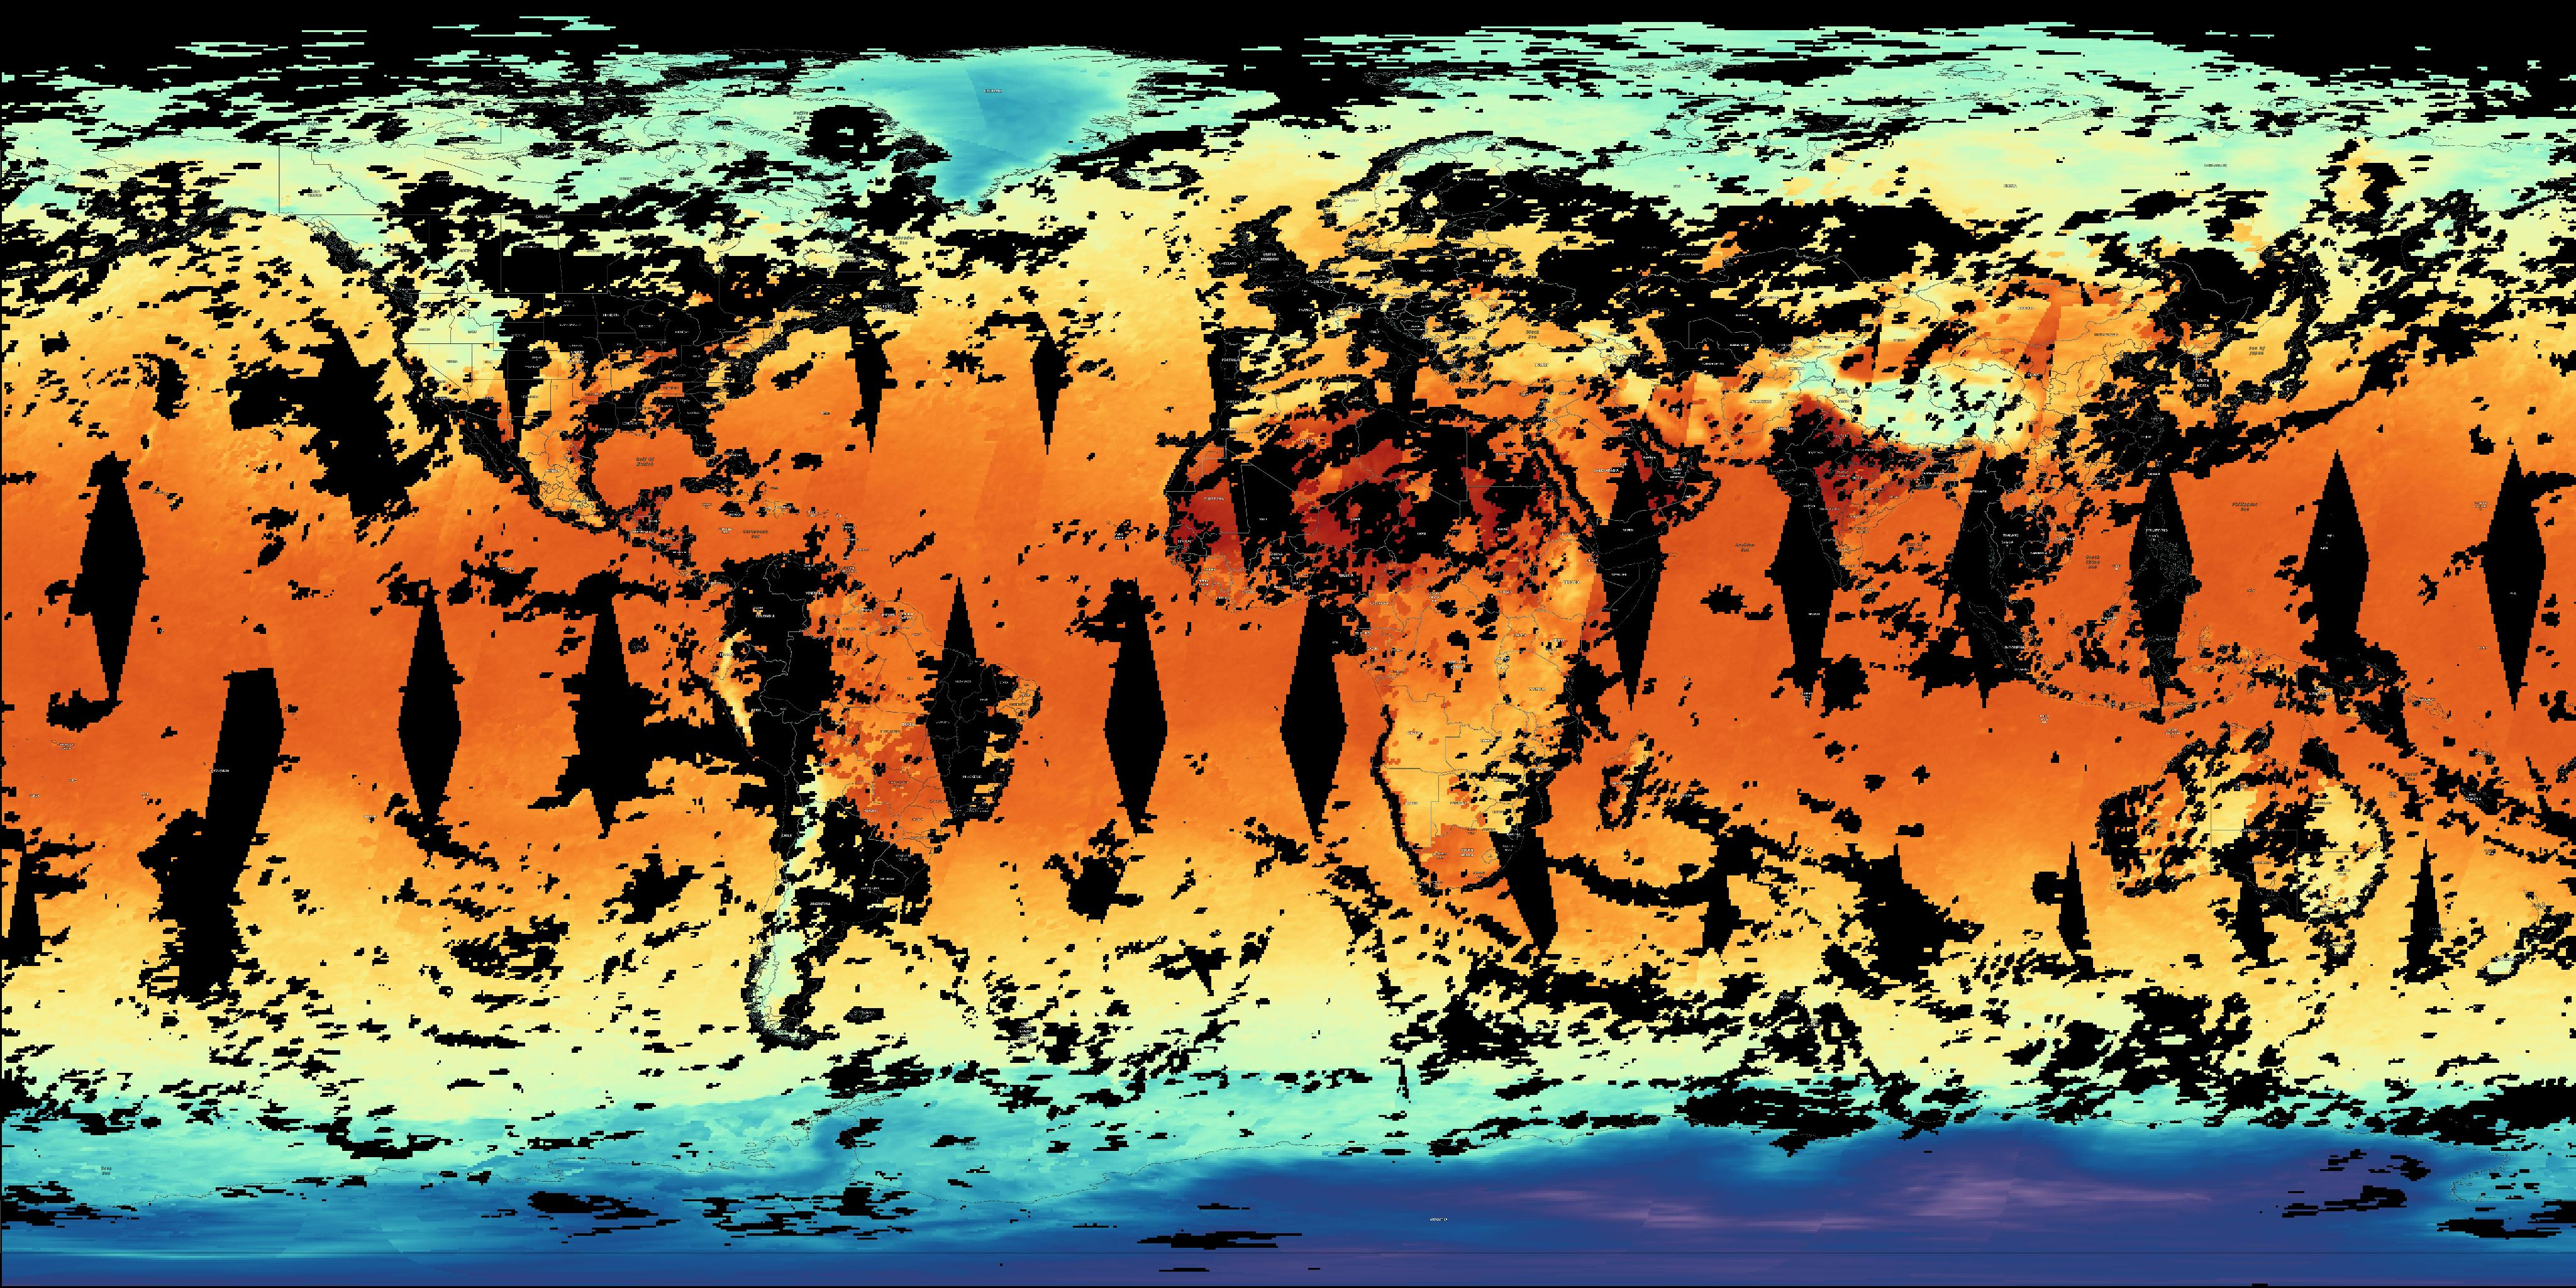
\includegraphics[width=1.0\linewidth]{figures/snapshot_nasa_airs_aqua_2024_05_21T00_00_00Z.jpg}
    \caption{Daytime and nighttime surface air temperature from observations by the AIRS instrument onboard the NASA AQUA satellite. This shows observations recorded through a whole day on the 21\textsuperscript{st} of May 2024. Notice that parts of the globe, especially near the equator have not been observed. This image was produced using NASA Worldview (\url{https://go.nasa.gov/46SaYyJ}).}\label{fig:satellite_image_coverage}
\end{figure}

Forecasting the weather or evolution of any other system is formulated as an initial value problem where past observations are used to predict an unknown future state of the system. A different formulation can be how heat spreads over time in different types of frying pans from known information of the pan's materials, their heat conduction properties, and that the stove gives off constant heat. In general the scenario is predicting the effect (future atmospheric temperature distribution, etc.) of some given causes (current and past weather, etc.). This scenario is termed the forward problem. The inverse problem on the other hand solves for an unknown parameter using other known parameters and observations of the partial solution such as temperature field at the object's surface. Traditional methods used to solve these problems utilized knowledge of the exact equations to numerically solve PDEs. As an example, the Finite Difference Method (FDM) approximates the solution by substituting the partial derivatives with finite differences and manipulating the equation such that the solution can be computed. The inverse problem on the other hand is determination of initial conditions or other parameters from observed state of the system. For example determining the heat source distribution given the temperature distribution at some point in time. One traditional approach to this would have meant solving the forward problem from an initial guess of the parameter and then evaluating some cost function such as how close the predicted solution is to the observed one. As expected, this would require many evaluations of the forward solver. This means that the cost of the solver would be greatly multiplied, emphasizing the importance of an efficient solver.
% TODO: reword this because the explanation of the problem setup for forward and inverse problems is not layed out optimally.
% TODO: perhaps the disadvantage of inverse problem in the paragraph above should be removed and only explanation of the inverse problem setup itself left by itself
% \begin{equation} \label{eq:forward_finite_difference_1}
%     \pdv{f\left(x\right)}{x} \approx \frac{f\left(x+h\right)-f\left(x\right)}{h}
% \end{equation}

Traditional numerical solvers have enjoyed many decades of development due to their long history. There are many general approaches to solve PDEs and many more very specific approaches. Other than FDM, some widely used approaches include Finite Element Methods (FEM), Finite Volume Methods (FVM), Collocation Methods, and Spectral Methods. FEM and FDM are both mesh based approaches, meaning they rely on discretization of the computational domain. There are several challenges associated with this. First, irregular domains such as bio-inspired materials like bone, spider silk, or aggregate materials like gravel pose a challenge due to the complexity of the domain geometry \autocite{gaulSimulationWavePropagation1991,buoniEfficientScalableNumerical2007,jiaModulateStressDistribution2024}. Also, irregular domains which create large deformations or mesh entanglement cause these methods to become ineffective \autocite{chenMeshfreeMethodsProgress2017}. While there are strategies to mitigate this, by definition they are an additional layer of difficulty to the process. Second, multiscale applications where the micro and macro scales are both important require fine meshes such that the small scale structures are adequately simulated. This creates meshes with very large number of points that are very resource intensive \autocite{buoniEfficientScalableNumerical2007}. Third, a single evaluation of traditional mesh-based solvers may not be very costly, however multiple evaluations can add up. This is very apparent in inverse problems where the solver is queried multiple times to solve the forward problem in order to obtain parameter functions. Therefore, in problems where these issues important or resources are limited, mesh-free methods may be preferred. As an example, the spectral method solves PDEs by formulating the solution as a linear combination of global basis functions like the Fourier series. This can be likened to how music combines different sound waves to produce the overall sound. For some function \(s\), the approximation \(s^*\) gets closer to the original with more linear combinations of basis functions. The complex formulation of the Fourier series is presented in \lccref{eq:fourier_series}. With this approach, the approximated function is characterized completely by its coefficients \(c_k\). This fact is exploited by the spectral method to solve differential equations. The solution function can be approximated by finding the mapping between input function coefficients and solution function coefficients. The mapping between a function \(s\) and its derivative \(s^{\prime}\) can be found using the derivative equation from their coefficients leading to \(\hat{s}_k = \hat{s}^{\prime}_k/\left(2\pi ik\right)\). Practically this would be done with a finite number of coefficients (\(k < \infty \)) and the coefficients \(\hat{s}^{\prime}_k\) are obtained using a Discrete Fourier Transform (DFT) algorithm like the Fast Fourier Transform (FFT).
% TODO: Add diagram example for discretization of the domain by FEM/FDM methods
\begin{align}
    s & \approx s^* = \sum_{k} \hat{s}_k e^{2\pi ikx}\label{eq:fourier_series}
\end{align}
This leads us to the fourth challenge with traditional methods which is that they require prior knowledge of analytic forms of PDEs. This is because traditional solvers use the equations to formulate solutions. This makes traditional numerical approaches unsuited to problems where the governing equations are unknown or partially known. These challenges altogether are some of what weather forecasting faces; NWP has the immense task of modeling multiple scales of the Earth's atmosphere while accounting for features of physical systems that are still not fully understood. Many other fields such as epidemiology \autocite{brauerMathematicalModelsEpidemiology2019} and ecology \autocite{holmesPartialDifferentialEquations1994,turchinDoesPopulationEcology2001} also face these challenges. As with many other fields, at some point in time the governing equations of many systems were not known. This has motivated research into alternative methods that do not completely rely on prior knowledge, are mesh free, and fast enough when solving forward problems.

\subsection*{Machine Learning for PDEs}
With the increasing prevalence of machine learning methods and their use in more and more fields, research into their use for scientific computing has taken off in recent years. While statistical modeling has already been widely used in areas such as physical constants, stellar population studies, risk assessments of events such as earthquakes and coronal mass ejections \autocite{berlinerPhysicalStatisticalModeling2003,anselmoComputationalMethodsReentry2005,reinhardtAsteroidRiskAssessment2016,uzanFundamentalConstantsTheir2003,spanosWhereStatisticalModels2006,bernardiStellarPopulationAnalysis2022}, the dominant approach for forward modeling or inverse modeling has remained physics based numerical models. Machine learning has provided an alternative approach to model the solutions of PDEs. In their work, \textcite{aartsNeuralNetworkMethod2001} utilized neural networks to approximate each term of PDEs describing damped and undamped free vibrations and substituting them into the PDEs and associated initial conditions. The network parameters were then optimized to reduce the PDE residual and boundary condition loss using evolutionary algorithms. This approach was taken in order to make machine learning models more transparent which at the time was being pursued because of the high cost of optimizing uncertainties in water management numerical simulators. However, since this method approximates the mapping between coordinates and the values of a function and their derivatives, retraining would be necessary for changes to the function itself. This could become very costly as retraining costs accumulate. A more recent approach that also utilizes soft constrains from PDE residuals is termed physics informed neural network (PINN) \autocite{raissiPhysicsinformedNeuralNetworks2019}. The authors propose a framework that leverages advancements in computing, namely automatic differentiation (AD) techniques made readily available by modern machine learning libraries. In general, PINNs use AD to compute each term of the PDE from the output of the model and this is then substituted into the PDE to in order to compute the residuals and loss from boundary conditions. The network residual and boundary loss are then weighted and summed with the data loss. For a neural network \(\hat{u}\left(\vb{x},t\right)\) approximating the real solution \(u\left(\vb{x},t\right)\), the residual loss for the heat equation in \lccref{eq:heat_equation} is \lccref{eq:heat_pinn_loss}. There are several advantages of incorporating physics knowledge into the model including regularization of the model outputs to be more consistent with physics, faster convergence, and less to no data required depending on whether the network is trained in a manner that is supervised, self-supervised, or a combination of both. One issue with using AD to compute the residual is that the network input needs to be the independent variable (i.e.\ coordinates, time, etc.). This once again means that if one wants to compute a different solution, the network needs to be retrained.
\begin{equation}\label{eq:heat_pinn_loss}
    \mathcal{L}_{PDE}={\left(\pdv{\hat{u}\left(\vb{x},t\right)}{t}-\divergence{\left(\alpha \gradient \hat{u}\left(\vb{x},t\right)\right)}\right)}^2
\end{equation}
\subsection*{Learning PDEs with CNNs}
Other works utilize convolutional neural networks (CNN) to compute the solution from input functions such as forcing terms or initial conditions. This approach generally means discretizing the functions on a grid and using these as training data. One study by \textcite{wangPhysicsinformedDeepLearning2020} predicts turbulent flow using spatial and temporal decomposition and a specialized U-Net, an architecture based on CNNs, to predict the velocity field from the decomposition of the previous velocity field. Part of the loss function is a regularization term for zero divergence in the velocity field to enforce incompressible fluid flow. This term was calculated using finite differences since auto differentiation is not applicable in this situation. Finite differences was also utilized in another CNN based fluid flow upscaling model by \textcite{gaoSuperresolutionDenoisingFluid2021} to compute the residual terms of the steady incompressible Navier-Stokes equation. This model also inferred unknown physical parameters such as boundary conditions. However, this approach would mean the model would need to scale as a quadratic in 2D, cubic in 3D, and much steeper in higher dimensions. Outside fluid dynamics, the combination of specialized CNNs and finite differences or another numerical differentiation method have been used for many other PDEs including Poisson's equation for temperature fields \autocite{zhaoPhysicsinformedConvolutionalNeural2023, gaoPhyGeoNetPhysicsinformedGeometryadaptive2021}, velocity models from seismic data \autocite{mullerDeepPretrainedFWI2023}, and seismic response of structures \autocite{zhangPhysicsguidedConvolutionalNeural2020,niMultiEndPhysicsInformedDeep2022}. While the use of CNNs mean that discretization is implied, solutions of different initial conditions or parameter functions can be computed by inference and no retraining is required. This property is especially useful for many-query problems such as computing gradients for inverse problems.

\subsection*{Operator Learning}
The mapping between discretized functions done by CNNs are related to an alternative approach that starts by viewing PDEs as operators, which are generalized mappings between spaces. One group of familiar operators are functions which maps between spaces of scalar values or vector values. PDEs on the other hand are operators that map between function spaces. A simple example is the derivative. The derivative takes in a function and returns the derivative of said function. In other words it is an operator that maps between the space of all functions to the space of derivatives of those functions. Another way to view operators starts by viewing functions as infinite dimensional vectors. Where elements in the vector are the function's value evaluated at every point in space. The operator can be seen as a vector function mapping between these infinite dimensional vector spaces. Operators are important because a field of research has sprung up around this mathematical concept. Operator learning is the use of machine learning to learn operators using data driven approaches. As an analogy, function regression traditionally has been used to approximate the mapping between input values such as coordinates and output values of functions evaluated at said coordinates. In the case of operator learning, the mapping between function spaces are approximated. The aforementioned approaches using CNNs does this directly using the values of functions at discrete points. There are other approaches like DeepONet that does not require the uniform grid like CNNs \autocite{luLearningNonlinearOperators2021}. This architecture instead uses both input functions and coordinates as inputs. The output is the output function evaluated at the coordinates provided. This architecture is based on an extension for deep learning of the universal operator approximation theory for neural networks first proposed almost three decades ago at the time of writing by \textcite{chenUniversalApproximationNonlinear1995}. The proposed architecture is composed of two subnetworks, where one termed the trunk \(\hat{\vb{T}}\left(\vb{x},t\right)\)learns the latent mapping for coordinates and the other network termed the branch \(\hat{\vb{B}}\left(\vb{f}\right)\) learns the latent mapping for the input function \(f \). The two latent mappings are combined through a dot product to obtain the approximated output function value \(u \left( \vb{x}, t \right)\). This is formulated in \lccref{eq:universal_op_approx_nn}.
\begin{equation}\label{eq:universal_op_approx_nn}
    u\left( \vb{x}, t \right) \approx \hat{G}\left( \vb{f} \right)\left( \vb{x}, t \right) = \hat{\vb{B}}\left( \vb{f} \right) \cdot \hat{\vb{T}}\left( \vb{x}, t \right)
\end{equation}
Fourier Neural Operators (FNO) is an alternative avenue for learning operators by utilizing the fact that functions can be decomposed into linear combinations of basis functions, namely trigonometric basis in this particular case \autocite{li2021fourier}. With this method the input function value is mapped to its corresponding output function value. This is done by first lifting the input function value to a higher dimension using a neural network and this is then passed through blocks composed of a Fourier transform, then a linear transform and filtering of higher modes, and finally the inverse Fourier transform. These blocks are stacked to a desired depth and finally another network projects the outputs to the target dimension. The reason a linear can be used is that differentiation is multiplication in the Fourier domain. One drawback with FNO is the requirement that output functions are not parameterized by coordinates and therefore is implicitly relative to the input function coordinates. To avoid this issue, \textcite{fanaskovSpectralNeuralOperators2023} reframes the problem by directly utilizing the coefficients of Fourier or Chebyshev basis. The model, termed Spectral Neural Operator (SNO) is trained on features of input function coefficients which are computed using Fourier or Chebyshev transforms and labels of output function coefficients using the same transforms. The authors point out one motivation for this approach which is that training neural networks on discretized data may not be ideal because unexpected outputs such as non-smooth interpolation may happen when the network is trained on one grid size and evaluated other grid sizes. With SNO, the interpolation of the function is smooth due to interpolation being done by Fourier basis functions which are sines and cosines for example. In a similar study, \textcite{du2024neural} extends the concept of mapping coefficients by proposing residuals in the spectral domain and leveraging Parseval's Identity to compute the spectral analog to the loss term in PINNs. This allows for self supervised learning in the spectral domain. The same benefits incorporating physics into PINNs also apply here without the pain points introduced by discretized model inputs and outputs. As a whole, operator learning creates an alternative approach that addresses the issue of retraining or recomputing the solution model. In addition, due to its data based approach, even systems with partially or fully unknown governing equations may be simulated.

A persistent challenge with all these approaches is the issue of optimization. While neural networks are modular and expressive which is proven by the universal approximation theorem \autocite{cybenkoApproximationSuperpositionsSigmoidal1989,hornikMultilayerFeedforwardNetworks1989}, their loss function present many local minima meaning it is non-convex. This can be mitigated by using advanced optimization techniques that can find a local minima close enough to the global minima such as Adam \autocite{shresthaReviewDeepLearning2019,soydanerComparisonOptimizationAlgorithms2020}. However, the addition of PDE residuals into the loss function have worsened the highly non-convex loss landscape issue \autocite{rathoreChallengesTrainingPINNs2024,NEURIPS2021_df438e52,basirCriticalInvestigationFailure2022}. These problems range from the disparity in size of boundary and residual loss gradients to the fact that incorporation of residuals and boundary conditions themselves create a much more complex loss landscape. As a result, it is desirable to utilize a different machine learning algorithm that possesses a convex loss landscape. One family of such algorithms are Support Vector Machines (SVM) \autocite{vapnikNatureStatisticalLearning2000}. The appeal of SVMs are the fact that the model is formulated as a quadratic programming problem. This means there are strong guarantees for convergence, generalization, and complexity. Another formulation called Least Squares Support Vector Machines (LSSVM) reformulates the problem as a linear system \autocite{suykensLeastSquaresSupport2005}. This leads to an easier problem that can be computed faster by well established algorithms like the many implementations of least squares solvers. Another advantage of the linear formulation is that this can be easily parallelized to exploit hardware like graphics processing units more widely known as GPUs in contrast to the commonly used Sequential Minimal Optimization (SMO) used for SVMs with quadratic objective functions.

The advantageous properties of SVM based methods have attracted research into their use for solving PDEs. An early work using SVMs to solve PDEs by \textcite{youxiwuSVMSolvingForward2005} introduced a method for solving the forward problem of Electro-Impedance Tomography. This work solved for the mathematical model of EIT which is given by Maxwell's equations by modeling the trial function as using an \(\epsilon \)-SVR model. Another approach much more similar to PINNs was presented by \textcite{mehrkanoonLearningSolutionsPartial2015}. The residual and initial/boundary conditions are imposed as equality constraints on an LS-SVM objective function. A different study by \textcite{leakeAnalyticallyEmbeddingDifferential2019}, the incorporation of physics into the model is done slightly differently by utilizing the theory of functional connections to directly embed constraints into the solution. This means that the proposed method would satisfy the boundary condition exactly. However, the authors point out that for PDEs in higher dimensions deriving and implementing this method can become cumbersome. These approaches, however, do not learn the PDE operator itself. Meaning they are also not practical for many-query problems.

\subsubsection*{Operator Learning for Weather Forecasting}
In terms of weather forecasting, operator learning has been applied in terms of initial value problems. This problem formulation is reminiscent of time series prediction problems widely found in machine learning research. Researchers \textcite{kurthFourCastNetAcceleratingGlobal2023} developed FourCastNet which utilized Adaptive Fourier Neural Operator (AFNO), a transformer based model containing the previously mentioned FNO computational blocks by \textcite{li2021fourier}. This model was then able to be trained in a massively parallel manner. In a comparison with a traditional model called the Integrated Forecasting System from the European Center for Medium Range Weather Forecasts (ECMWF), FourCastNet is faster and much more efficient in terms of inference time, resulting in about 80,000 times speed up for a 100-member ensemble forecast. This is while performing much better than a previous deep learning approach. In another study, \textcite{bonevSphericalFourierNeural2023} proposed a variation on neural operators called Spherical Fourier Neural Operator (SFNO) which exploited the spherical nature of global forecasting by using Spherical Harmonic Transform (SHT) in place of Fourier Transform. This model when compared to AFNO and FNO, produced no visible artifacts in autoregressive rollouts for long range forecasting. In terms of forecasting, the model shows outcomes that matches the IFS which is a big leap forward in parity for traditional and machine learning based methods.

% Bagian ini mendeskripsikan gambaran umum, konteks, dan posisi penelitian TA dalam konstelasi perkembangan pengetahuan yang telah dicapai. Penjelasan yang dituliskan menjadi penting karena dengan landasan yang kuat, maka pekerjaan penelitian dapat terarah dilakukan. Hal ini lebih spesifik dan tegas disampaikan pada sub-sub bab berikutnya.

% Beberapa pustaka utama yang berperan dominan dapat disampaikan di sini untuk memberi gambaran tentang letak penelitian TA dalam konstelasi keilmuan yang dicapai. Hasil-hasil dari pustaka terbaru dapat menopang Latar Belakang ini menjadi lebih kuat.

% Sangat wajar apabila isi sub bab setelah Latar Belakang ini mengalami penyesuaian saat sejumlah hasil penelitian sudah diperoleh dan dianalisis. Pada dasarnya, hal ini dimungkinkan apabila ada penyesuaian kecil, karena fokus penelitian sejatinya sudah jelas sedari awal, namun hasil-hasil yang diperoleh dapat memperbaharui beberapa butir isi sub bab. Oleh karena itu, finalisasi isi Pendahuluan ini biasanya dilakukan menjelang akhir pembuatan laporan penelitian yang dituangkan dalam buku TA.


\section{Problem Statement}\label{sec:problem_statement}
\noindent The problems this work sets out to solve based on \lccref{sec:background} are:
\begin{enumerate}
    \item What is the formulation a computational model for operator regression and therefore solving PDEs in the spectral domain using support vector machines?
    \item Can the model learn the relationships represented by PDEs? And how does it perform on different problems?
    \item How can one interpret the learned model?
\end{enumerate}

% Bagian ini menjadi salah satu bagian penting dalam Pendahuluan. Setelah paparan Latar Belakang, maka masalah yang diangkat pada pekerjaan penelitian perlu dirumuskan dengan baik. Perumusan ini sebaiknya dibahasakan tidak dalam bentuk kalimat pertanyaan, melainkan kalimat aktif, dan dapat memuat lebih dari satu rumusan.

% Sejalan dengan ini, setiap masalah yang diangkat selalu memiliki batas. Ada batasan, asumsi, atau kriteria yang menjadi pembatas atas masalah yang diangkat dalam penelitian TA, sehingga arah penelitian dapat fokus. Batasan ini perlu dituliskan secara tegas, dan dapat saja memuat lebih dari satu.


\section{Aims}\label{sec:aims}
\noindent Based on the stated problems in \lccref{sec:problem_statement}, this study aims to acomplish the following:
\begin{enumerate}
    \item The design and implementation of a computational model that maps coefficients in the spectral domain using Least Squares Support Vector Regression (LSSVR).
    \item Proof of the model's learning ability using three different problems.
    \item Interpretation the model results and why some predictions turn out the way they do.
\end{enumerate}
% Bagian ini secara tegas menuliskan tujuan pekerjaan penelitian TA, yang dapat memuat lebih dari satu. Pemilihan kata kerja pada Tujuan ini sangat penting karena menggambarkan arah fokus dari jalinan upaya yang dilakukan.

\section{Contribution}
\noindent In achieving the aims of this study the following contributions are made:
\begin{enumerate}
    \item A novel use LSSVR which has a convex objective to learn solution operators of partial differential equations and operators in general.
    \item Interpretation of machine learning model trained on operator data.
\end{enumerate}

\section{Limitations}
\noindent This work is limited to the following:
\begin{enumerate}
    \item Functions the model works with are only continuous functions.
    \item The basis functions are limited to Fourier basis.
    \item Modeled fields are compact or dense meaning not sparse. Sparse observations or other data are assimilated using other methods.
\end{enumerate}

\section{Sistematika Penulisan}
% \noindent Bagian ini adalah penutup Bab I yang menyampaikan  secara ringkas isi setiap  bab. Karena pembaca sudah sampai akhir Bab I, yang  berarti  sudah  mengetahui isinya, maka tidak perlu ditulis lagi rincian Bab I. Sebaiknya langsung dituliskan secara ringkas isi rincian bab-bab selanjutnya, misalnya, \textit{Setelah Pendahuluan pada Bab I ini, Bab II akan mengulas tentang ...}

% Apabila diperlukan, dapat dituliskan konvensi khusus yang digunakan pada penulisan naskah buku TA ini, misalnya tanda titik menggantikan tanda desimal karena alasan kemudahan dan kejelasan dalam formulasi matematika.
% !TEX root = ./skripsi.tex
\chapter{KAJIAN PUSTAKA}

\noindent Bab ini mengulas secara rinci konsep-konsep dasar yang berkaitan dengn pekerjaan penelitian TA dan deskripsi studi pustaka yang dilakukan. Judul bab tidak harus seperti yang dituliskan, melainkan dapat lebih fleksibel yang mencerminkan isi paparan pada bab ini. Demikian halnya dengan judul sub bab.

\section{Fourier Transform and Series}
\noindent

Complex numbers are numbers consisting of real and imaginary components. Complex numbers are written as in \lccref{eq:complex_number} with \(a \) and \(b \) being the real and imaginary components respectively. The imaginary component is multiplied by the imaginary unit \(i=\sqrt{-1}\).
\begin{align}
  c = a + bi \label{eq:complex_number} \\
\end{align}

\section{Least Squares Support Vector Machine}
\noindent An arguably fundamental model widely used whether in pedagogical settings or otherwise is the support vector machine. It dates back to works by Vapnik \& Lerner in 1963 (Recognition of Patterns with help of Generalized Portraits) and V. N. Vapnik \& A. Ya. Chervonenkis in 1964 (A note on one class of perceptrons/On a perceptron class). As the development on SVM continued, what originally was a model for classification of separable data generalized to regression tasks as well Vapnik (2000 The Nature of Statistical Learning Theory).
\subsection{Disadvantages}
However, the main disadvantage of LSSVMs are the fact that they do not have the sparse property of SVMs which can leave performance on the table. A simple mitigation can be done by filtering training samples with small absolute values of lagrangian multipliers \autocite{haifengwangComparisonSVMLSSVM2005}.

To derive the least squares support vector regression (J.A. Suykens LSSVM Book) model we start with the linear expression:

\begin{equation}
  y=W^{\intercal}\vb{x}+b
\end{equation}

\begin{equation}
  \min_{W,e} J(W,e) = \frac{1}{2}W^{\intercal}W + C\frac{1}{2}\sum_{k=1}^{n}e_{k}
\end{equation}

Such that
\begin{equation}
  y_{k}=W^{\intercal}\vb{x}_{k}+b+e_{k} \qquad k=1,\dots,n
\end{equation}

\begin{equation}
  L(W,b,e;\vb{\alpha}) = \frac{1}{2}W^{\intercal}W + C\frac{1}{2}\sum_{k=1}^{n}e_{k} + \sum_{k=1}^{n}\alpha_{k} \left(W^{\intercal}\vb{x}_{k}+b+e_{k} - y_{k} \right)
\end{equation}

Derive the KKT system
\begin{equation}
  \begin{split}
    \pdv{L}{W} = 0 \rightarrow & W = \sum_{k=1}^{n}\alpha_{k}x_{k} \\
    \pdv{L}{b} = 0 \rightarrow & \sum_{k=1}^{n}\alpha_{k} = 0 \\
    \pdv{L}{e_{k}} = 0 \rightarrow & \alpha_{k} = C e_{k} & \qquad k=1,\dots,n\\
    \pdv{L}{\alpha_{k}} = 0 \rightarrow & W^{\intercal}\vb{x}_{k}+b+e_{k} - y_{k} = 0 & \qquad k=1,\dots,n\\
  \end{split}
\end{equation}

After eliminating $W$ and $\vb*{e}$, with $\vb{1}_{n} = \langle 1,\dots,1\rangle$, $\vb{y} = \lbrack y_1, \dots, y_n \rbrack $, and ${\alpha} = \lbrack \alpha_1, \dots, \alpha_n \rbrack $ the solution is as follows in block matrix notation
\begin{equation} \label{eq:lssvr_solution}
  \begin{bmatrix}
    0          & \vb{1}_{n}^{\intercal} \\
    \vb{1}_{n} & \Omega + \frac{I}{C}
  \end{bmatrix}
  \begin{bmatrix}
    b           \\
    \vb{\alpha} \\
  \end{bmatrix}
  =
  \begin{bmatrix}
    0      \\
    \vb{y} \\
  \end{bmatrix}
\end{equation}

The solution in \cref{eq:lssvr_solution}

\begin{algorithm}[H]
  \caption{LSSVR Training}\label{alg:lssvr_training}
  \begin{algorithmic}[1]
    \Procedure{SolveLSSVR}{$\vb{X}, \vb{y}, \gamma $}
    \State{\(\Omega \gets [[]]\)}
    \Comment{Construct matrix of inner products in high dimensional space}

    \For{\(k=0 \to n\)}
    \For{\(l=0 \to n\)}
    \State{\(\Omega_{k,l}\gets K(\vb{X}_k,\vb{X}_l)\)}
    \EndFor{}
    \EndFor{}
    \State{\(\vb{H} \gets \Omega + \frac{\vb{I}}{\gamma}\)}
    % \State $\vb{1} \gets [1,1,...,1]$
    \State{\(\vb{A} \gets [[]]\)}
    \Comment{Construct left-hand side matrix}
    \State{\(\vb{A}_{0,0} \gets 0\)}
    \For{\(k=0 \to n\)}
    \State{\(\vb{A}_{k+1,0} \gets 1\)}
    \State{\(\vb{A}_{0,k+1} \gets 1\)}
    \EndFor{}
    \For{\(k=0 \to n\)}
    \For{\(l=0 \to n\)}
    \State{\(\vb{A}_{k+1,l+1} \gets \vb{H}_{k,l}\)}
    \EndFor{}
    \EndFor{}
    \State{\(\vb{B}\gets []\)}
    \Comment{Construct left-hand side of the equation}
    \State{\(\vb{B}_0 \gets 0\)}
    \For{\(k=0 \to n\)}
    \State{\(\vb{B}_{k+1} \gets \vb{y}_{k}\)}
    \EndFor{}
    \State{\(\vb{A}^{\dagger} \gets pseudoInverse(\vb{A})\)}
    \Comment{Compute solution using pseudo inverse}
    \State{\(\vb{S} \gets \vb{A}^{\dagger}\vb{B}\)}
    \State{\(b \gets \vb{S}_{0}\)}
    \For{\(k=0 \to n\)}
    \State{\(\vb{\alpha}_{k} \gets \vb{S}_{k+1}\)}
    \EndFor{}
    \State{\textbf{return}\(\vb{\alpha}, b\)}
    \EndProcedure{}
  \end{algorithmic}
\end{algorithm}

The basic pseudocode from the LSSVM Equation for function regression is defined in \lccref{alg:lssvr_training} for a training set of length $n$, features $\vb{X}$, and labels $\vb{y}$. Training the LSSVM means computing the values of langrange multipliers $\vb{\alpha}$ and bias $b$. $K$ is the kernel function used to compute the inner products in high dimensional space, here we assume the RBF kernel. $\vb{A}$ is a matrix of size $n+1$ by $n+1$. $\vb{H}$ is a matrix of size $n$ by $n$. $\vb{I}$ is the identity. $\vb{B}$ is a vector of size $n+1$. $\vb{S}$ is a vector of size $n+1$.

After training the model can be used for prediction of unseen features. The pseudocode for prediction is shown in \lccref{alg:lssvr_prediction} for prediction features $\vb{U}$ with \(p \) samples. The trained model uses the training features themselves $\vb{X}$ with \(n \) samples, the learned multipliers of training points $\vb{\alpha}$, and the bias $b$.

\begin{algorithm}[H]
  \caption{LSSVR Prediction}\label{alg:lssvr_prediction}
  \begin{algorithmic}[1]
    \Require $\vb{U}, \vb{\alpha}, \vb{X}, b$
    \Ensure $\vb{v}$
    \State $\Omega \gets [[]]$ \Comment{Construct matrix of inner products in high dimensional space}

    \For{$k=0 \to p$}
    \For{$l=0 \to n$}
    \State$\Omega_{k,l}\gets K(\vb{U}_{k},\vb{X}_l)$
    \EndFor
    \EndFor
    \State $\vb{v} \gets \Omega\vb{\alpha} + \vb{1}_{m}b$
  \end{algorithmic}
\end{algorithm}

In this exmple we will be using the function $2x^2+4$. The values of this function can be seen in Table \ref{table:1}.

\begin{table}[H]
  \centering
  \begin{tabular}{@{}lll@{}}
    \toprule
    No & x       & y       \\ \midrule
    1  & 0.0     & 4.0     \\
    2  & 0.33... & 4.22... \\
    3  & 0.66... & 4.88... \\
    4  & 1.0     & 6.0     \\
    \bottomrule
  \end{tabular}
  \caption{Example data of function $2x^2+4$} \label{table:1}
\end{table}
For $\Omega_{i,j}=K(x_i,x_j)=exp \left(-\frac{\norm*{x_i-x_j}^2}{2\sigma^2}\right)$

For example, with $\sigma=1$, $x_i=0.0$, \& $x_j = 0.33\dots$
\begin{equation}
  \begin{split}
    K(0.0,0.33) & = exp\left(-\frac{\norm*{0.0-0.33}^2}{2(1)^2}\right) \\
    & = exp\left(-\frac{0.33^2}{2}\right) \\
    & = 0.9460
  \end{split}
\end{equation}

\begin{equation}
  \Omega\gets
  \begin{bmatrix}
    1.0000 & 0.9460 & 0.8007 & 0.6065 \\
    0.9460 & 1.0000 & 0.9460 & 0.8007 \\
    0.8007 & 0.9460 & 1.0000 & 0.9460 \\
    0.6065 & 0.8007 & 0.9460 & 1.0000 \\
  \end{bmatrix}
\end{equation}

\begin{equation}
  \vb{I}\frac{1}{\gamma}\to\vb{I}\frac{1}{5}\to
  \begin{bmatrix}
    0.2000 & 0.0000 & 0.0000 & 0.0000 \\
    0.0000 & 0.2000 & 0.0000 & 0.0000 \\
    0.0000 & 0.0000 & 0.2000 & 0.0000 \\
    0.0000 & 0.0000 & 0.0000 & 0.2000
  \end{bmatrix}
\end{equation}

\begin{equation}
  \Omega+\vb{I}\frac{1}{5}\to H\to
  \begin{bmatrix}
    1.2000 & 0.9460 & 0.8007 & 0.6065 \\
    0.9460 & 1.2000 & 0.9460 & 0.8007 \\
    0.8007 & 0.9460 & 1.2000 & 0.9460 \\
    0.6065 & 0.8007 & 0.9460 & 1.2000 \\
  \end{bmatrix}
\end{equation}

\begin{equation}
  A\to
  \begin{bmatrix}
    0.0000 & 1.0000 & 1.0000 & 1.0000 & 1.0000 \\
    1.0000 & 1.2000 & 0.9460 & 0.8007 & 0.6065 \\
    1.0000 & 0.9460 & 1.2000 & 0.9460 & 0.8007 \\
    1.0000 & 0.8007 & 0.9460 & 1.2000 & 0.9460 \\
    1.0000 & 0.6065 & 0.8007 & 0.9460 & 1.2000 \\
  \end{bmatrix}
\end{equation}

\begin{equation}
  B\to
  \begin{bmatrix}
    0.0000 \\
    4.0000 \\
    4.2222 \\
    4.8889 \\
    6.0000 \\
  \end{bmatrix}
\end{equation}

\begin{equation}
  A^{\dag}\to
  \begin{bmatrix}
    -0.8994 & 0.4348  & 0.0652  & 0.0652  & 0.4348  \\
    0.4348  & 2.0686  & -1.6490 & -0.5292 & 0.1096  \\
    0.0652  & -1.6490 & 3.3774  & -1.1992 & -0.5292 \\
    0.0652  & -0.5292 & -1.1992 & 3.3774  & -1.6490 \\
    0.4348  & 0.1096  & -0.5292 & -1.6490 & 2.0686  \\
  \end{bmatrix}
\end{equation}

\begin{equation}
  A^{\dag}B\to S\to
  \begin{bmatrix}
    4.9421  \\
    -0.6177 \\
    -1.3737 \\
    -0.5625 \\
    2.5538  \\
  \end{bmatrix}
\end{equation}

\begin{equation}
  b\to 4.9421
\end{equation}

\begin{equation}
  \alpha \to
  \begin{bmatrix}
    -0.6177 \\
    -1.3737 \\
    -0.5625 \\
    2.5538  \\
  \end{bmatrix}
\end{equation}

Prediction
\begin{equation}
  U\to
  \begin{bmatrix}
    0.3 \\
    0.2 \\
    0.5
  \end{bmatrix}
\end{equation}

\begin{equation}
  \Omega\to
  \begin{bmatrix}
    0.9560 & 0.9994 & 0.9350 & 0.7827 \\
    0.9802 & 0.9912 & 0.8968 & 0.7261 \\
    0.8825 & 0.9862 & 0.9862 & 0.8825 \\
  \end{bmatrix}
\end{equation}

\begin{equation}
  \Omega\alpha\to
  \begin{bmatrix}
    -0.4904 \\
    -0.6170 \\
    -0.2008 \\
  \end{bmatrix}
\end{equation}

\begin{equation}
  \Omega\alpha+b\vb{1}_{m}\to v\to
  \begin{bmatrix}
    4.4516 \\
    4.3251 \\
    4.7413 \\
  \end{bmatrix}
\end{equation}
Where $\vb{1}_{m}$ is a vector of 1s with the length of $U$.

\section{Sub Bab B}
\noindent Suatu penelitian tidak dapat lepas dari capaian pengetahuan dan pemahaman yang sudah dipublikasikan. Deskripsi tentang capaian ini menjadi penting karena selain menunjukkan tingkat pemahaman mahasiswa, juga mengetahui tempat pekerjaan penelitian TA dalam konstelasi capaian tersebut. Studi pustaka dan paparan hasilnya dapat memperkaya wawasan tentang topik yang diangkat pada penelitian TA.

\section{Membuat Persamaan}
\noindent Secara prinsip, suatu persamaan menyatu dalam kalimat. Letak persamaan dapat berada di awal, tengah, atau akhir kalimat. Dengan demikian, pada akhir persamaan harus diberikan tanda baca, misalnya koma, titik koma, atau titik, yang menekankan kehadiran persamaan dalam kalimat. Tidak semua persamaan harus diberi nomor. Persamaan yang dirujuk pada naskah TA saja yang harus diberi nomor. Kode awal penomoran ini adalah nomor urut bab, termasuk untuk persamaan pada Lampiran, dengan urutan alfabet kapital.

Setiap notasi harus unik atau tunggal, sehingga arti setiap notasi adalah unik atau tunggal juga. Arti satu notasi harus dituliskan segera ketika notasi tersebut muncul, dan tidak diulang lagi setelahnya.

\subsection{Contoh Persamaan Sederhana}
Persamaan (\ref{II.1}) mendeskripsikan dinamika fungsi gelombang $\psi(\vec{r},t)$ di bawah pengaruh potensial $V(\vec{r})$ dan dituliskan sebagai berikut:
\begin{equation}\label{II.1}
  i\hslash\frac{\partial \psi}{\partial t} = -\frac{\hslash^2}{2 m}\Vec{\nabla}^2 \psi + V(\vec{r})\psi,
\end{equation}
dengan $m$ adalah massa partikel dan $\hslash$ merupakan konstanta Planck tereduksi.

Di akhir persamaan (\ref{II.1}) diberi koma karena berada ditengah kalimat. Untuk merujuk ke persamaan yang telah ditulis, gunakan perintah \verb|\ref{}|.

Untuk menuliskan beberapa set persamaan yang masih terhubung, gunakan \verb|\subequations{}|. Misal kita punya persamaan diferensial terkopel, kita bisa tuliskan
\begin{subequations}
  \begin{align}
    \frac{dy}{dt} & = -x , \\
    \frac{dx}{dt} & = -y .
  \end{align}
\end{subequations}
Kalau perlu matriks, kita bisa tulis seperti berikut.
\begin{equation}
  \sigma_x =
  \begin{pmatrix}
    0 & 1 \\
    1 & 0
  \end{pmatrix},\quad
  \sigma_y =
  \begin{pmatrix}
    0 & -i \\
    i & 0
  \end{pmatrix}, \quad
  \sigma_z =
  \begin{pmatrix}
    1 & 0  \\
    0 & -1
  \end{pmatrix}
\end{equation}


\section{Referensi dan Citation}
% \noindent Sitasi dapat dimasukkan ke dalam Tugas Akhir seperti ini \cite{Fujita1996}. Untuk sitasi dengan beberapa sumber, dapat dituliskan juga \cite{hohen1964,Kim2006}. Atau untuk tiga sumber berarti \cite{kongkanand2006,kresse1999,Leibb1993}.

% !TEX root = ./skripsi.tex
\chapter{RESEARCH METHODOLOGY}\label{sec:research_methodology}

% Secara umum, metode penelitian yang digunakan pada pekerjaan penelitian disampaikan pada bab ini. Judul bab tidak harus seperti yang dituliskan. Dalam kata lain bisa diubah sesuai kebutuhan.

\section{Research Design}
\noindent This study is carried out under the framework of a research design. In this section, this design will be laid out and explained. The design includes the process from the beginning to the end of the overall study. The research design is visually depicted in \lccref{fig:research_design_diagram}.

\begin{figure}[H]
      \centering
      \tikzfig{figures/research_design_diagram}
      \caption{Research design diagram}\label{fig:research_design_diagram}
\end{figure}

The study is carried out in 9 main phases. Each phase has a specific aim to accomplish such that the subsequent phases are able to proceed. Each phase is explained as follows:
\begin{numdesc}
      \item[Problem Specification]
      In this phase, relevant literature of related works and other supporting materials will be reviewed to lay the groundwork of this study. Specifically, the literature review will encompass partial differential equations and their real world associations, traditional methods employed to solve them, systems with partially known or unknown governing equations, machine learning approaches to the problem, least-squares support vector machines, performance metrics and tools that will be used such as the PyTorch library.

      \item[Design of Computational Model]
      This phase of the study is allocated to the design of the computational model based on the literature that has been reviewed. The design of the overall process includes data retrieval, preprocessing, and the core spectral regression model itself.

      \item[Implementation of Computational Model]
      After the computational model design is completed, the model is implemented in the Python Language using the PyTorch library as a core component. Implementation of the computational model is done using an iterative software development model. This development model was chosen due to its adaptability to unexpected challenges which is necessary because of the challenges and unknowns with developing a novel method.

      \item[Planning of Experimental Scenarios]
      To properly gauge the performance of the proposed method at approximating operators, specifically the solution operator of partial differential equations, experimental scenarios are developed in this phase. Specifically, the scenarios serves three goals which are proof of concept or validation that the method is able to learn operators, a case study of a more complex system with real world data, and a using the model as a surrogate. Together, these experimental scenarios determine the applicability of the model to the problem. In addition, the model will be compared to a baseline model in order to put into context the proposed model's performance. In addition, kernel-input correlation matrices and input-Lagrangian multiplier inner product matrix will also be computed.

      \item[Data Generation and Retrieval]
      This phase of the study is tied to the experimental scenarios that have been developed. After determination of the scenario specifics, the data that will be used for training, validation, and testing of the model in each scenario will be either generated or retrieved from an external source. In addition, in each scenario the hyperparameters of the model will be determined using Bayesian optimization as an alternative to the traditional grid search method.

      \item[Data Preprocessing]
      The next phase after data generation or retrieval is preprocessing. This is a crucial step in allowing the core LSSVR to learn the mappings in spectral space. In order to do this, the data will need to be reshaped, and important features selected for. Finally, inputs to the LSSVR will need to be normalized or scaled such that the LSSVR model can much more easily learn the data.

      \item[Experiments]
      This phase of the study executes the experimental scenarios that was determined previously. The preprocessed data will be used in accordance to the preplanned scenarios.

      \item[Analysis and Discussion]
      The final phase of the study is the analysis and discussion of the results. Analysis of each experimental scenario will assess the extent of the model's capabilities. Another component of the analysis is interpretation the trained model and how it comes to the predictions that it makes. The discussion will also touch on the hyperparameter optimization and comparisons with the baseline model. This will show how the model performs differently compared to the baseline.
\end{numdesc}

\section{Literature Study Method}
\noindent As a basis for this study, information surrounding the topic is collected from literature sources such as books, journal articles, and other academic works like dissertations. The tools that are used to find these sources include Google Scholar and Google Search. The search terms used start with two terms which are partial differential equations and machine learning. Based on reading the most relevant literature, further search terms are created from variants of previous search terms combined with terms from literature that has been found.

\section{Data Generation and Retrieval Method}
\noindent Data to be used in this study are acquired in two different ways. The first method is data generation. This is motivated by the fact that some partial differential equations do not have much open and accessible real world data available. As such the systems are simulated using the equations themselves. In simple scenarios like computing the antiderivative \(u\) of some function \(f \), this can be done by randomly generating \(u\) and then taking their derivatives to compute \(f\). The random function generation itself is done by generating random coefficients for basis functions like the Fourier series. Once all functions are generated, random noise is added to ensure that the model is also robust towards inexact measurements. A diagram illustrating the process is shown in \lccref{fig:data_generation_diagram}.

\begin{figure}[H]
      \centering
      \begin{adjustbox}{max width=\textwidth}
            \tikzfig{figures/data_generation_diagram}
      \end{adjustbox}
      \caption{Data generation diagram}\label{fig:data_generation_diagram}
\end{figure}

Data retrieval is the other option which in this case is used to retrieve data for weather prediction. Based on the scenario the data is to be used for, relevant subsets of the dataset is retrieved to a working machine. This study specifically uses a dataset provided by the European Center for Medium Range Weather Forecast (ECMWF) named ERA5 hourly data on single levels from 1940 to present \autocite{c3sERA5HourlyData2018}. The first step is selecting a geographical area to study, time period, NetCDF4 data format, and variables such as temperature at 2 meters above the surface. Then the second step is specifications are then used to request the data through the climate data store application programming interface. The downloaded data is then parsed using the Xarray library and preprocessed.

\section{Computational Model Implementation Method}\label{sec:development_method}
\noindent Implementation of the computational model follows an iterative development model. This model basically consists of repeated cycles or iterations of software development. Each cycle is loosely based on the waterfall development model, namely the processes of requirement gathering, analysis \& design, implementation, and testing. This iterative property is crucial for this study because all the requirements cannot be known beforehand. This model minimizes the risk in developing complex software with partially known initial requirements. A diagram of the model can be seen in \lccref{fig:iterative_development_diagram}.

\begin{figure}[H]
      \centering
      \begin{adjustbox}{max width=\textwidth}
            \tikzfig{figures/iterative_development_diagram}
      \end{adjustbox}
      \caption{Iterative development model}\label{fig:iterative_development_diagram}
\end{figure}

This development model was adapted from \textcite{bittnerManagingIterativeSoftware2006}. Each process in the model is explained as follows:
\begin{numdesc}
      \item[Initial Planning]
      The first process of the iterative development model sets up the parameters for the iterative development. These parameters are the broad scope of the project and initial requirements such as core components like LSSVR\@. The initial requirements are crucial in guiding the rest of the development as more requirements are gathered. The initial planning also determines technical choices like tooling and choice of language. The planning process also includes a rough architecture based in initial requirements.

      \item[Requirements]
      This process separates out the backlog of requirements into those that will be worked on in the current iteration. These requirements ideally share some functionality in order to allow the same context to be retained within the iteration which reduces the burden of context switching.

      \item[Analysis and Design]
      This process an analysis of the requirements of the current iteration is performed. This involves determining the constraints and goals for each requirement. Constraints also need to consider previous iterations such that the requirements can be fulfilled effectively and efficiently without regressing progress that has been made such as breaking existing functionality. From this analysis, the design is updated so that the requirement can be fulfilled. The design itself informs how the code should be structured. The interfaces used in the code are also specified.

      \item[Implementation]
      The implementation process applies the design that has been produced. In addition to implementing the program, this process also implements tests which validate and verify the produced code. In the case of complex pieces of the design, an approach of creating tests and assertions first is taken. This way, the code can be run quickly and fail immediately to allow a quicker convergence on the intended functionality.

      \item[Testing and Evaluation]
      Once the design is implemented, tests that have been created are run. Each feature is tested in an integrated manner to expedite the process while still providing enough confidence in the software. The results of the testing process are evaluated and any failed tests are resolved whether by reimplementation or reassessment of the correctness of the tests. Any missing functionality or feature discovered during evaluation are added to the backlog of requirements.

      \item[Release]
      After an iteration, the current version of the software is released. The iterative nature of this development model necessitates the use of a versioning system. As such each release can be identified by a version number loosely based on semantic versioning \autocite{preston-wernerSemanticVersioning2002023}. This version numbering system consists of major number that indicates breaking changes, minor numbers which indicate features and non-breaking changes, and lastly patch numbers are used for fixes. A version number is read as \verb|MAJOR.MINOR.PATCH|. During active development, only major version 0 will be used to prevent too many major versions. The released software is hosted in its own GitHub repository at \url{https://github.com/nidduzzi/SpectralSVR}.

\end{numdesc}

\section{Research Tools}
\noindent The tools that are used in this study can be categorized into hardware and software. The following are hardware that are used in this study:
\begin{itemize}
      \item Kaggle CPU Kernel~\autocite{GettingStartedKaggle}
            \begin{itemize}
                  \item 4 Cores Intel Xeon
                  \item 30 Gigabytes RAM
                  \item 20 Gigabytes Working storage
            \end{itemize}
      \item Kaggle GPU Kernel~\autocite{GettingStartedKaggle}
            \begin{itemize}
                  \item 4 Cores Intel Xeon
                  \item 29 Gigabytes RAM
                  \item 1 Nvidia P100 GPU
                  \item 20 Gigabytes Working storage
            \end{itemize}
      \item Personal Computer
            \begin{itemize}
                  \item Intel i5{-}8300H
                  \item 16 Gigabytes RAM
                  \item Nvidia GeForce GTX 1060 Mobile
                  \item 1.5 Terabytes Storage
            \end{itemize}
\end{itemize}
The software tools used in this study are the following:
\begin{itemize}
      \item Python
      \item Jupyter Notebook
      \item Git
      \item Poetry Python package manager
      \item Web Browser
      \item \LaTeX{}
\end{itemize}

% !TEX root = ./skripsi.tex
\chapter{RESULTS AND DISCUSSION}\label{sec:results_and_discussion}
\noindent This chapter is organized into five sections which are the results of data generation, data retrieval, design of computational model, implementation of computational model, experimental scenarios, and the experiments themselves.

\section{Data Generation}\label{sec:data_generation}
\noindent This study uses two data acquisition approaches. The first approach which is discussed in this section is data generation. This process involves manufacturing data randomly in such a way that they obey the PDEs to be modeled. The generated data consists of features and labels. These features and labels in the context of PDEs are parameters and the solution of the PDEs, respectively. The PDEs enforce a relationship between parameters and the solution. This relationship is implicitly encoded into the features and labels, which is what machine learning models can learn. Because the solution and parameters to PDEs are functions and there are many kinds with different properties, generating all the different kinds of functions is a difficult task. This is why this study focuses on Fourier functions. This means that out of the space of all functions \(F \) which include categories such as polynomials \(f\left(x\right)=a_{n}x^n+\cdots+a_1x+a_0\) where \(f\in F\), and \(a_n\) are constants; we only consider the subset of functions \(U \subset F\) which are of the form \(u\left(x\right)=\sum_{k}^{m}c_k e^{2\pi i k \frac{x}{P}}\).

Using the subset of Fourier functions has several benefits which has motivated the choice. First these functions are characterized purely by their coefficients \(c_k\), meaning there is no need to store discretized values which potentially saves space and computation. The second benefit is that other functions such as polynomials can be approximated by them using the Fourier transform. This means that despite limiting the set of functions to Fourier functions, the behavior of PDEs with other sets of functions can be approximated to a certain extent. The final benefit is the mature ecosystem around these functions which include fast algorithms for the Fourier transform and even numerical approaches for solving known PDEs like the previously mentioned spectral method which we discussed in \lccref{sec:fourier_discussion}. In summary, the generated data consists of features and labels which are Fourier coefficients implicitly defining the relationship enforced by a PDE and scenario. To proceed with the data generation, there are 4 steps involved:
\begin{enumerate}
  \item Scenario and PDE Determination:
        The first step of data generation is determining the scenario related to the PDE or governing equations. First, the PDE to be modeled is determined based on the goals of the dataset. Then, one or more of the parameters is chosen to predict the solution. The chosen parameters will be called the input functions and the solution will be called output functions from here on. The second part of the scenario is the domain or more simply the physical space occupied by the system to be modeled. The domain will be used to compute the function values in relation to the physical space from coefficients of Fourier functions.
  \item Parameter Determination:
        The second step is determining all parameters other than that input parameter based on the scenario and governing equation. These parameters may be coefficients such as material properties like density or viscosity, or forcing terms which model external influence on the system like a heat source in the case of the heat equation. Depending on the parameters, solutions of PDEs may behave very differently, such as the appearance of discontinuities in the solution to low viscosity Burgers' equation. Because of this, the choice of parameters is guided by what the dataset seeks to do.
  \item Random Coefficient Generation:
        The third step of data generation is randomly generating the solutions for the chosen equation. Generating random functions in the space of Fourier functions exploits the fact that the coefficients characterize the function completely. By randomly assigning coefficients \(c_k\), many functions can be generated randomly with very little cost. Since the coefficients need to be complex numbers as in \lccref{eq:complex_number}, both real and imaginary components are generated independently by assigning a random value to each component for each wave number \(k\). They are then put together again into complex numbers.

        Since only real functions are of interest in this study, the generation cost can be approximately halved. This is because for real functions the coefficients for negative wave numbers \(k\) are complex conjugate of the positive wave numbers. This means that once the positive coefficients are generated, one only needs to compute their complex conjugate and concatenate the result with the coefficients of positive wave numbers. For dimensions higher than one, a simpler approach is used. The coefficients are generated for all wave numbers including the negative ones. The inverse Fourier transform is computed and this results in complex functions. The real components of these functions are kept and the Fourier transform is applied to get the coefficients of the real functions. Finally, these generated coefficients then be used with the basis functions as input functions.
        % TODO: add diagram for generating real functions, the mirroring process too
  \item Forcing Term Computation:
        Finally, in order to ensure that the generated solution and chosen parameters satisfy the equation, the forcing term is computed as the residual of the equation of interest with the parameters that was previously determined. This computation is done using the spectral method.
  \item Function Value and Noise Computation:
        The generated solution and forcing functions are labeled as input and output functions. The values of both functions in the domain can then be computed using the scenario determined in the first step. Once all coefficients are generated, the function values are computed with an inverse Fourier transform. The real component of the function values are retained, and the imaginary component are zeroed out. Noise is added to the function values here as needed. The processed function values are then converted back into coefficients using a Fourier transform. This processing is necessary to ensure that the coefficients are only describing the real function.

\end{enumerate}

These four steps are the general processes involved in generating datasets for this study. Further specifics of the generation process of each dataset is explained in their respective subsections.

\subsection{Data Generation: Anti-derivative}
\noindent The first dataset is a simple one dimensional derivative. This was chosen as a simple proof of concept of the ability to solve a differential equation. The equation is related to many real-world problems such as acceleration and speed. One can imagine a train in an ideal world where acceleration is directly translated into speed. When the train accelerates at time \(t \) by some amount \(a \), we can expect the train to have some speed \(u \). In this ideal world, the relationship between speed and acceleration can be modeled with a simple differential \lccref{eq:derivative}. This scenario is found in many real systems albeit often with many more details such as different components of acceleration from friction, drag, gravity, and other factors.
As previously mentioned in \lccref{sec:data_generation}, both velocity \(u \) and acceleration \(a \) are modeled with Fourier series in \lccrefs{eq:fourier_speed,eq:fourier_acceleration} respectively, where \(T\) is the period representing the length of the domain.
\begin{align}
  u\left( t \right) & = \sum_{k} \hat{u}_k e^{2\pi ikt/T} \label{eq:fourier_speed}        \\
  a\left( t \right) & = \sum_{k} \hat{a}_k e^{2\pi ikt/T} \label{eq:fourier_acceleration}
\end{align}
The domain of the scenario is a two-hour time window. This number was chosen because it is around the ideal length of travel time on high speed rail in comparison to air travel and car travel \autocite{givoniDevelopmentImpactModern2006,wangEfficiencySpatialEquity2019,wrro2236}. This is the first step in generating this dataset.

In the second step, as the derivative \lccref{eq:derivative} does not contain any parameters other than the acceleration which is the input parameter, there are no other parameters to determine. Therefore, the data generation process proceeds to generating coefficients for the speed functions \(\hat{u} \). The coefficients are assigned randomly from a Gaussian distribution with a mean of zero and standard deviation of one. This choice was made such that most wave numbers will have a coefficient of close to zero leaving a sparse set of wave numbers to mostly affect the resulting function. In total, \num{5000} unique functions are generated with \num{50} complex coefficients each.

In the third step, the output function coefficients are computed. To find the relation between \(\hat{u}_k \) and \(\hat{a}_k \), we need to find substitutes for each term in \lccref{eq:derivative}. To do this, we take the derivative of \lccref{eq:fourier_speed} which result in \lccref{eq:fourier_series_derivative}. Using this we can substitute the terms in \lccref{eq:derivative} with \lccrefs{eq:fourier_series_derivative,eq:fourier_acceleration} giving \lccref{eq:example_spectral_method_fourier_substituted}. Finally, after some algebraic manipulation we obtain the relationship between the input \(a^*\) and output function \(u^*\) in terms of their coefficients in \lccref{eq:derivative_coeff}. One also needs to choose the integration constant \(\hat{u}_{0}\) because at \(k=0\) \lccref{eq:derivative_coeff} becomes a division by zero.
\begin{align}
  \dv{u\left( t \right)}{t}                                        & = a\left(t\right) \label{eq:fourier_series_derivative}                                                             \\
  \sum_{k} \hat{u}_k\times \left( 2\pi ik/T \right) e^{2\pi ikt/T} & = \sum_{k} \hat{a}_k e^{2\pi ikt/T} \label{eq:example_spectral_method_fourier_substituted}                         \\
  \hat{a}_k                                                        & = \hat{u}_k\left( 2\pi ik/T \right)                                                    \label{eq:derivative_coeff}
\end{align}

In the final step, using randomly generated values of \(\hat{a}_k\), the corresponding values of \(\hat{u}_k\) are computed with \lccref{eq:derivative_coeff}. These coefficients are then used to compute the function values inside the domain. The two-hour time window is represented by a grid of \num{500} discrete points. With the coefficients and evaluation points ready, the function values are computed using \lccrefs{eq:fourier_speed,eq:fourier_acceleration}. Next, noise is added to the function values in order to motivate models learning on the dataset to generalize on noise. To also allow evaluation of how well the model performs with different levels of noise, the samples are duplicated into three copies for each high, medium and low noise levels. The function values of each copy is perturbed with noise from a Gaussian distribution with zero mean and standard deviation of some percentage of the average function value standard deviation. The percentages of each high, medium, and low noise levels are 5, 10, and 50 percent. The perturbed function values are then transformed back into their coefficients. An example generated function and its different perturbed versions is shown in \lccref{fig:antiderivative_noise_levels}. The horizontal axis indicates time which is displayed in units of hours. The vertical axis indicates velocity in abstract units.

\begin{figure}[H]
  \centering
  \begin{subfigure}{\linewidth}
    \begin{adjustbox}{width=\linewidth}
      \begingroup%
\makeatletter%
\begin{pgfpicture}%
\pgfpathrectangle{\pgfpointorigin}{\pgfqpoint{8.000000in}{2.000000in}}%
\pgfusepath{use as bounding box, clip}%
\begin{pgfscope}%
\pgfsetbuttcap%
\pgfsetmiterjoin%
\pgfsetlinewidth{0.000000pt}%
\definecolor{currentstroke}{rgb}{0.000000,0.000000,0.000000}%
\pgfsetstrokecolor{currentstroke}%
\pgfsetstrokeopacity{0.000000}%
\pgfsetdash{}{0pt}%
\pgfpathmoveto{\pgfqpoint{0.000000in}{0.000000in}}%
\pgfpathlineto{\pgfqpoint{8.000000in}{0.000000in}}%
\pgfpathlineto{\pgfqpoint{8.000000in}{2.000000in}}%
\pgfpathlineto{\pgfqpoint{0.000000in}{2.000000in}}%
\pgfpathlineto{\pgfqpoint{0.000000in}{0.000000in}}%
\pgfpathclose%
\pgfusepath{}%
\end{pgfscope}%
\begin{pgfscope}%
\pgfsetbuttcap%
\pgfsetmiterjoin%
\pgfsetlinewidth{0.000000pt}%
\definecolor{currentstroke}{rgb}{0.000000,0.000000,0.000000}%
\pgfsetstrokecolor{currentstroke}%
\pgfsetstrokeopacity{0.000000}%
\pgfsetdash{}{0pt}%
\pgfpathmoveto{\pgfqpoint{0.593772in}{0.517039in}}%
\pgfpathlineto{\pgfqpoint{7.958330in}{0.517039in}}%
\pgfpathlineto{\pgfqpoint{7.958330in}{1.958330in}}%
\pgfpathlineto{\pgfqpoint{0.593772in}{1.958330in}}%
\pgfpathlineto{\pgfqpoint{0.593772in}{0.517039in}}%
\pgfpathclose%
\pgfusepath{}%
\end{pgfscope}%
\begin{pgfscope}%
\pgfsetbuttcap%
\pgfsetroundjoin%
\definecolor{currentfill}{rgb}{0.000000,0.000000,0.000000}%
\pgfsetfillcolor{currentfill}%
\pgfsetlinewidth{0.803000pt}%
\definecolor{currentstroke}{rgb}{0.000000,0.000000,0.000000}%
\pgfsetstrokecolor{currentstroke}%
\pgfsetdash{}{0pt}%
\pgfsys@defobject{currentmarker}{\pgfqpoint{0.000000in}{-0.048611in}}{\pgfqpoint{0.000000in}{0.000000in}}{%
\pgfpathmoveto{\pgfqpoint{0.000000in}{0.000000in}}%
\pgfpathlineto{\pgfqpoint{0.000000in}{-0.048611in}}%
\pgfusepath{stroke,fill}%
}%
\begin{pgfscope}%
\pgfsys@transformshift{0.928524in}{0.517039in}%
\pgfsys@useobject{currentmarker}{}%
\end{pgfscope}%
\end{pgfscope}%
\begin{pgfscope}%
\definecolor{textcolor}{rgb}{0.000000,0.000000,0.000000}%
\pgfsetstrokecolor{textcolor}%
\pgfsetfillcolor{textcolor}%
\pgftext[x=0.928524in,y=0.419816in,,top]{\color{textcolor}{\rmfamily\fontsize{12.000000}{14.400000}\selectfont\catcode`\^=\active\def^{\ifmmode\sp\else\^{}\fi}\catcode`\%=\active\def%{\%}0.00}}%
\end{pgfscope}%
\begin{pgfscope}%
\pgfsetbuttcap%
\pgfsetroundjoin%
\definecolor{currentfill}{rgb}{0.000000,0.000000,0.000000}%
\pgfsetfillcolor{currentfill}%
\pgfsetlinewidth{0.803000pt}%
\definecolor{currentstroke}{rgb}{0.000000,0.000000,0.000000}%
\pgfsetstrokecolor{currentstroke}%
\pgfsetdash{}{0pt}%
\pgfsys@defobject{currentmarker}{\pgfqpoint{0.000000in}{-0.048611in}}{\pgfqpoint{0.000000in}{0.000000in}}{%
\pgfpathmoveto{\pgfqpoint{0.000000in}{0.000000in}}%
\pgfpathlineto{\pgfqpoint{0.000000in}{-0.048611in}}%
\pgfusepath{stroke,fill}%
}%
\begin{pgfscope}%
\pgfsys@transformshift{1.765406in}{0.517039in}%
\pgfsys@useobject{currentmarker}{}%
\end{pgfscope}%
\end{pgfscope}%
\begin{pgfscope}%
\definecolor{textcolor}{rgb}{0.000000,0.000000,0.000000}%
\pgfsetstrokecolor{textcolor}%
\pgfsetfillcolor{textcolor}%
\pgftext[x=1.765406in,y=0.419816in,,top]{\color{textcolor}{\rmfamily\fontsize{12.000000}{14.400000}\selectfont\catcode`\^=\active\def^{\ifmmode\sp\else\^{}\fi}\catcode`\%=\active\def%{\%}0.25}}%
\end{pgfscope}%
\begin{pgfscope}%
\pgfsetbuttcap%
\pgfsetroundjoin%
\definecolor{currentfill}{rgb}{0.000000,0.000000,0.000000}%
\pgfsetfillcolor{currentfill}%
\pgfsetlinewidth{0.803000pt}%
\definecolor{currentstroke}{rgb}{0.000000,0.000000,0.000000}%
\pgfsetstrokecolor{currentstroke}%
\pgfsetdash{}{0pt}%
\pgfsys@defobject{currentmarker}{\pgfqpoint{0.000000in}{-0.048611in}}{\pgfqpoint{0.000000in}{0.000000in}}{%
\pgfpathmoveto{\pgfqpoint{0.000000in}{0.000000in}}%
\pgfpathlineto{\pgfqpoint{0.000000in}{-0.048611in}}%
\pgfusepath{stroke,fill}%
}%
\begin{pgfscope}%
\pgfsys@transformshift{2.602287in}{0.517039in}%
\pgfsys@useobject{currentmarker}{}%
\end{pgfscope}%
\end{pgfscope}%
\begin{pgfscope}%
\definecolor{textcolor}{rgb}{0.000000,0.000000,0.000000}%
\pgfsetstrokecolor{textcolor}%
\pgfsetfillcolor{textcolor}%
\pgftext[x=2.602287in,y=0.419816in,,top]{\color{textcolor}{\rmfamily\fontsize{12.000000}{14.400000}\selectfont\catcode`\^=\active\def^{\ifmmode\sp\else\^{}\fi}\catcode`\%=\active\def%{\%}0.50}}%
\end{pgfscope}%
\begin{pgfscope}%
\pgfsetbuttcap%
\pgfsetroundjoin%
\definecolor{currentfill}{rgb}{0.000000,0.000000,0.000000}%
\pgfsetfillcolor{currentfill}%
\pgfsetlinewidth{0.803000pt}%
\definecolor{currentstroke}{rgb}{0.000000,0.000000,0.000000}%
\pgfsetstrokecolor{currentstroke}%
\pgfsetdash{}{0pt}%
\pgfsys@defobject{currentmarker}{\pgfqpoint{0.000000in}{-0.048611in}}{\pgfqpoint{0.000000in}{0.000000in}}{%
\pgfpathmoveto{\pgfqpoint{0.000000in}{0.000000in}}%
\pgfpathlineto{\pgfqpoint{0.000000in}{-0.048611in}}%
\pgfusepath{stroke,fill}%
}%
\begin{pgfscope}%
\pgfsys@transformshift{3.439169in}{0.517039in}%
\pgfsys@useobject{currentmarker}{}%
\end{pgfscope}%
\end{pgfscope}%
\begin{pgfscope}%
\definecolor{textcolor}{rgb}{0.000000,0.000000,0.000000}%
\pgfsetstrokecolor{textcolor}%
\pgfsetfillcolor{textcolor}%
\pgftext[x=3.439169in,y=0.419816in,,top]{\color{textcolor}{\rmfamily\fontsize{12.000000}{14.400000}\selectfont\catcode`\^=\active\def^{\ifmmode\sp\else\^{}\fi}\catcode`\%=\active\def%{\%}0.75}}%
\end{pgfscope}%
\begin{pgfscope}%
\pgfsetbuttcap%
\pgfsetroundjoin%
\definecolor{currentfill}{rgb}{0.000000,0.000000,0.000000}%
\pgfsetfillcolor{currentfill}%
\pgfsetlinewidth{0.803000pt}%
\definecolor{currentstroke}{rgb}{0.000000,0.000000,0.000000}%
\pgfsetstrokecolor{currentstroke}%
\pgfsetdash{}{0pt}%
\pgfsys@defobject{currentmarker}{\pgfqpoint{0.000000in}{-0.048611in}}{\pgfqpoint{0.000000in}{0.000000in}}{%
\pgfpathmoveto{\pgfqpoint{0.000000in}{0.000000in}}%
\pgfpathlineto{\pgfqpoint{0.000000in}{-0.048611in}}%
\pgfusepath{stroke,fill}%
}%
\begin{pgfscope}%
\pgfsys@transformshift{4.276051in}{0.517039in}%
\pgfsys@useobject{currentmarker}{}%
\end{pgfscope}%
\end{pgfscope}%
\begin{pgfscope}%
\definecolor{textcolor}{rgb}{0.000000,0.000000,0.000000}%
\pgfsetstrokecolor{textcolor}%
\pgfsetfillcolor{textcolor}%
\pgftext[x=4.276051in,y=0.419816in,,top]{\color{textcolor}{\rmfamily\fontsize{12.000000}{14.400000}\selectfont\catcode`\^=\active\def^{\ifmmode\sp\else\^{}\fi}\catcode`\%=\active\def%{\%}1.00}}%
\end{pgfscope}%
\begin{pgfscope}%
\pgfsetbuttcap%
\pgfsetroundjoin%
\definecolor{currentfill}{rgb}{0.000000,0.000000,0.000000}%
\pgfsetfillcolor{currentfill}%
\pgfsetlinewidth{0.803000pt}%
\definecolor{currentstroke}{rgb}{0.000000,0.000000,0.000000}%
\pgfsetstrokecolor{currentstroke}%
\pgfsetdash{}{0pt}%
\pgfsys@defobject{currentmarker}{\pgfqpoint{0.000000in}{-0.048611in}}{\pgfqpoint{0.000000in}{0.000000in}}{%
\pgfpathmoveto{\pgfqpoint{0.000000in}{0.000000in}}%
\pgfpathlineto{\pgfqpoint{0.000000in}{-0.048611in}}%
\pgfusepath{stroke,fill}%
}%
\begin{pgfscope}%
\pgfsys@transformshift{5.112932in}{0.517039in}%
\pgfsys@useobject{currentmarker}{}%
\end{pgfscope}%
\end{pgfscope}%
\begin{pgfscope}%
\definecolor{textcolor}{rgb}{0.000000,0.000000,0.000000}%
\pgfsetstrokecolor{textcolor}%
\pgfsetfillcolor{textcolor}%
\pgftext[x=5.112932in,y=0.419816in,,top]{\color{textcolor}{\rmfamily\fontsize{12.000000}{14.400000}\selectfont\catcode`\^=\active\def^{\ifmmode\sp\else\^{}\fi}\catcode`\%=\active\def%{\%}1.25}}%
\end{pgfscope}%
\begin{pgfscope}%
\pgfsetbuttcap%
\pgfsetroundjoin%
\definecolor{currentfill}{rgb}{0.000000,0.000000,0.000000}%
\pgfsetfillcolor{currentfill}%
\pgfsetlinewidth{0.803000pt}%
\definecolor{currentstroke}{rgb}{0.000000,0.000000,0.000000}%
\pgfsetstrokecolor{currentstroke}%
\pgfsetdash{}{0pt}%
\pgfsys@defobject{currentmarker}{\pgfqpoint{0.000000in}{-0.048611in}}{\pgfqpoint{0.000000in}{0.000000in}}{%
\pgfpathmoveto{\pgfqpoint{0.000000in}{0.000000in}}%
\pgfpathlineto{\pgfqpoint{0.000000in}{-0.048611in}}%
\pgfusepath{stroke,fill}%
}%
\begin{pgfscope}%
\pgfsys@transformshift{5.949814in}{0.517039in}%
\pgfsys@useobject{currentmarker}{}%
\end{pgfscope}%
\end{pgfscope}%
\begin{pgfscope}%
\definecolor{textcolor}{rgb}{0.000000,0.000000,0.000000}%
\pgfsetstrokecolor{textcolor}%
\pgfsetfillcolor{textcolor}%
\pgftext[x=5.949814in,y=0.419816in,,top]{\color{textcolor}{\rmfamily\fontsize{12.000000}{14.400000}\selectfont\catcode`\^=\active\def^{\ifmmode\sp\else\^{}\fi}\catcode`\%=\active\def%{\%}1.50}}%
\end{pgfscope}%
\begin{pgfscope}%
\pgfsetbuttcap%
\pgfsetroundjoin%
\definecolor{currentfill}{rgb}{0.000000,0.000000,0.000000}%
\pgfsetfillcolor{currentfill}%
\pgfsetlinewidth{0.803000pt}%
\definecolor{currentstroke}{rgb}{0.000000,0.000000,0.000000}%
\pgfsetstrokecolor{currentstroke}%
\pgfsetdash{}{0pt}%
\pgfsys@defobject{currentmarker}{\pgfqpoint{0.000000in}{-0.048611in}}{\pgfqpoint{0.000000in}{0.000000in}}{%
\pgfpathmoveto{\pgfqpoint{0.000000in}{0.000000in}}%
\pgfpathlineto{\pgfqpoint{0.000000in}{-0.048611in}}%
\pgfusepath{stroke,fill}%
}%
\begin{pgfscope}%
\pgfsys@transformshift{6.786696in}{0.517039in}%
\pgfsys@useobject{currentmarker}{}%
\end{pgfscope}%
\end{pgfscope}%
\begin{pgfscope}%
\definecolor{textcolor}{rgb}{0.000000,0.000000,0.000000}%
\pgfsetstrokecolor{textcolor}%
\pgfsetfillcolor{textcolor}%
\pgftext[x=6.786696in,y=0.419816in,,top]{\color{textcolor}{\rmfamily\fontsize{12.000000}{14.400000}\selectfont\catcode`\^=\active\def^{\ifmmode\sp\else\^{}\fi}\catcode`\%=\active\def%{\%}1.75}}%
\end{pgfscope}%
\begin{pgfscope}%
\pgfsetbuttcap%
\pgfsetroundjoin%
\definecolor{currentfill}{rgb}{0.000000,0.000000,0.000000}%
\pgfsetfillcolor{currentfill}%
\pgfsetlinewidth{0.803000pt}%
\definecolor{currentstroke}{rgb}{0.000000,0.000000,0.000000}%
\pgfsetstrokecolor{currentstroke}%
\pgfsetdash{}{0pt}%
\pgfsys@defobject{currentmarker}{\pgfqpoint{0.000000in}{-0.048611in}}{\pgfqpoint{0.000000in}{0.000000in}}{%
\pgfpathmoveto{\pgfqpoint{0.000000in}{0.000000in}}%
\pgfpathlineto{\pgfqpoint{0.000000in}{-0.048611in}}%
\pgfusepath{stroke,fill}%
}%
\begin{pgfscope}%
\pgfsys@transformshift{7.623577in}{0.517039in}%
\pgfsys@useobject{currentmarker}{}%
\end{pgfscope}%
\end{pgfscope}%
\begin{pgfscope}%
\definecolor{textcolor}{rgb}{0.000000,0.000000,0.000000}%
\pgfsetstrokecolor{textcolor}%
\pgfsetfillcolor{textcolor}%
\pgftext[x=7.623577in,y=0.419816in,,top]{\color{textcolor}{\rmfamily\fontsize{12.000000}{14.400000}\selectfont\catcode`\^=\active\def^{\ifmmode\sp\else\^{}\fi}\catcode`\%=\active\def%{\%}2.00}}%
\end{pgfscope}%
\begin{pgfscope}%
\definecolor{textcolor}{rgb}{0.000000,0.000000,0.000000}%
\pgfsetstrokecolor{textcolor}%
\pgfsetfillcolor{textcolor}%
\pgftext[x=4.276051in,y=0.202965in,,top]{\color{textcolor}{\rmfamily\fontsize{12.000000}{14.400000}\selectfont\catcode`\^=\active\def^{\ifmmode\sp\else\^{}\fi}\catcode`\%=\active\def%{\%}Time (hours)}}%
\end{pgfscope}%
\begin{pgfscope}%
\pgfsetbuttcap%
\pgfsetroundjoin%
\definecolor{currentfill}{rgb}{0.000000,0.000000,0.000000}%
\pgfsetfillcolor{currentfill}%
\pgfsetlinewidth{0.803000pt}%
\definecolor{currentstroke}{rgb}{0.000000,0.000000,0.000000}%
\pgfsetstrokecolor{currentstroke}%
\pgfsetdash{}{0pt}%
\pgfsys@defobject{currentmarker}{\pgfqpoint{-0.048611in}{0.000000in}}{\pgfqpoint{-0.000000in}{0.000000in}}{%
\pgfpathmoveto{\pgfqpoint{-0.000000in}{0.000000in}}%
\pgfpathlineto{\pgfqpoint{-0.048611in}{0.000000in}}%
\pgfusepath{stroke,fill}%
}%
\begin{pgfscope}%
\pgfsys@transformshift{0.593772in}{0.714824in}%
\pgfsys@useobject{currentmarker}{}%
\end{pgfscope}%
\end{pgfscope}%
\begin{pgfscope}%
\definecolor{textcolor}{rgb}{0.000000,0.000000,0.000000}%
\pgfsetstrokecolor{textcolor}%
\pgfsetfillcolor{textcolor}%
\pgftext[x=0.260881in, y=0.651510in, left, base]{\color{textcolor}{\rmfamily\fontsize{12.000000}{14.400000}\selectfont\catcode`\^=\active\def^{\ifmmode\sp\else\^{}\fi}\catcode`\%=\active\def%{\%}\ensuremath{-}2}}%
\end{pgfscope}%
\begin{pgfscope}%
\pgfsetbuttcap%
\pgfsetroundjoin%
\definecolor{currentfill}{rgb}{0.000000,0.000000,0.000000}%
\pgfsetfillcolor{currentfill}%
\pgfsetlinewidth{0.803000pt}%
\definecolor{currentstroke}{rgb}{0.000000,0.000000,0.000000}%
\pgfsetstrokecolor{currentstroke}%
\pgfsetdash{}{0pt}%
\pgfsys@defobject{currentmarker}{\pgfqpoint{-0.048611in}{0.000000in}}{\pgfqpoint{-0.000000in}{0.000000in}}{%
\pgfpathmoveto{\pgfqpoint{-0.000000in}{0.000000in}}%
\pgfpathlineto{\pgfqpoint{-0.048611in}{0.000000in}}%
\pgfusepath{stroke,fill}%
}%
\begin{pgfscope}%
\pgfsys@transformshift{0.593772in}{1.174158in}%
\pgfsys@useobject{currentmarker}{}%
\end{pgfscope}%
\end{pgfscope}%
\begin{pgfscope}%
\definecolor{textcolor}{rgb}{0.000000,0.000000,0.000000}%
\pgfsetstrokecolor{textcolor}%
\pgfsetfillcolor{textcolor}%
\pgftext[x=0.390511in, y=1.110844in, left, base]{\color{textcolor}{\rmfamily\fontsize{12.000000}{14.400000}\selectfont\catcode`\^=\active\def^{\ifmmode\sp\else\^{}\fi}\catcode`\%=\active\def%{\%}0}}%
\end{pgfscope}%
\begin{pgfscope}%
\pgfsetbuttcap%
\pgfsetroundjoin%
\definecolor{currentfill}{rgb}{0.000000,0.000000,0.000000}%
\pgfsetfillcolor{currentfill}%
\pgfsetlinewidth{0.803000pt}%
\definecolor{currentstroke}{rgb}{0.000000,0.000000,0.000000}%
\pgfsetstrokecolor{currentstroke}%
\pgfsetdash{}{0pt}%
\pgfsys@defobject{currentmarker}{\pgfqpoint{-0.048611in}{0.000000in}}{\pgfqpoint{-0.000000in}{0.000000in}}{%
\pgfpathmoveto{\pgfqpoint{-0.000000in}{0.000000in}}%
\pgfpathlineto{\pgfqpoint{-0.048611in}{0.000000in}}%
\pgfusepath{stroke,fill}%
}%
\begin{pgfscope}%
\pgfsys@transformshift{0.593772in}{1.633492in}%
\pgfsys@useobject{currentmarker}{}%
\end{pgfscope}%
\end{pgfscope}%
\begin{pgfscope}%
\definecolor{textcolor}{rgb}{0.000000,0.000000,0.000000}%
\pgfsetstrokecolor{textcolor}%
\pgfsetfillcolor{textcolor}%
\pgftext[x=0.390511in, y=1.570178in, left, base]{\color{textcolor}{\rmfamily\fontsize{12.000000}{14.400000}\selectfont\catcode`\^=\active\def^{\ifmmode\sp\else\^{}\fi}\catcode`\%=\active\def%{\%}2}}%
\end{pgfscope}%
\begin{pgfscope}%
\definecolor{textcolor}{rgb}{0.000000,0.000000,0.000000}%
\pgfsetstrokecolor{textcolor}%
\pgfsetfillcolor{textcolor}%
\pgftext[x=0.205325in,y=1.237684in,,bottom,rotate=90.000000]{\color{textcolor}{\rmfamily\fontsize{12.000000}{14.400000}\selectfont\catcode`\^=\active\def^{\ifmmode\sp\else\^{}\fi}\catcode`\%=\active\def%{\%}Velocity}}%
\end{pgfscope}%
\begin{pgfscope}%
\pgfpathrectangle{\pgfqpoint{0.593772in}{0.517039in}}{\pgfqpoint{7.364558in}{1.441291in}}%
\pgfusepath{clip}%
\pgfsetrectcap%
\pgfsetroundjoin%
\pgfsetlinewidth{1.505625pt}%
\definecolor{currentstroke}{rgb}{0.121569,0.466667,0.705882}%
\pgfsetstrokecolor{currentstroke}%
\pgfsetdash{}{0pt}%
\pgfpathmoveto{\pgfqpoint{0.928524in}{0.843191in}}%
\pgfpathlineto{\pgfqpoint{0.941941in}{0.865997in}}%
\pgfpathlineto{\pgfqpoint{0.955358in}{0.906286in}}%
\pgfpathlineto{\pgfqpoint{0.968775in}{0.959976in}}%
\pgfpathlineto{\pgfqpoint{1.009026in}{1.147828in}}%
\pgfpathlineto{\pgfqpoint{1.022443in}{1.200354in}}%
\pgfpathlineto{\pgfqpoint{1.035860in}{1.239395in}}%
\pgfpathlineto{\pgfqpoint{1.049277in}{1.261427in}}%
\pgfpathlineto{\pgfqpoint{1.062694in}{1.264405in}}%
\pgfpathlineto{\pgfqpoint{1.076111in}{1.247946in}}%
\pgfpathlineto{\pgfqpoint{1.089527in}{1.213370in}}%
\pgfpathlineto{\pgfqpoint{1.102944in}{1.163613in}}%
\pgfpathlineto{\pgfqpoint{1.116361in}{1.103010in}}%
\pgfpathlineto{\pgfqpoint{1.143195in}{0.971508in}}%
\pgfpathlineto{\pgfqpoint{1.156612in}{0.912884in}}%
\pgfpathlineto{\pgfqpoint{1.170029in}{0.867009in}}%
\pgfpathlineto{\pgfqpoint{1.183446in}{0.839030in}}%
\pgfpathlineto{\pgfqpoint{1.196863in}{0.832911in}}%
\pgfpathlineto{\pgfqpoint{1.210280in}{0.851116in}}%
\pgfpathlineto{\pgfqpoint{1.223697in}{0.894394in}}%
\pgfpathlineto{\pgfqpoint{1.237114in}{0.961703in}}%
\pgfpathlineto{\pgfqpoint{1.250531in}{1.050260in}}%
\pgfpathlineto{\pgfqpoint{1.263948in}{1.155723in}}%
\pgfpathlineto{\pgfqpoint{1.317615in}{1.624147in}}%
\pgfpathlineto{\pgfqpoint{1.331032in}{1.719454in}}%
\pgfpathlineto{\pgfqpoint{1.344449in}{1.794130in}}%
\pgfpathlineto{\pgfqpoint{1.357866in}{1.844122in}}%
\pgfpathlineto{\pgfqpoint{1.371283in}{1.866952in}}%
\pgfpathlineto{\pgfqpoint{1.384700in}{1.861870in}}%
\pgfpathlineto{\pgfqpoint{1.398117in}{1.829878in}}%
\pgfpathlineto{\pgfqpoint{1.411534in}{1.773634in}}%
\pgfpathlineto{\pgfqpoint{1.424951in}{1.697244in}}%
\pgfpathlineto{\pgfqpoint{1.438368in}{1.605959in}}%
\pgfpathlineto{\pgfqpoint{1.478619in}{1.304250in}}%
\pgfpathlineto{\pgfqpoint{1.492036in}{1.214953in}}%
\pgfpathlineto{\pgfqpoint{1.505453in}{1.140181in}}%
\pgfpathlineto{\pgfqpoint{1.518870in}{1.083720in}}%
\pgfpathlineto{\pgfqpoint{1.532286in}{1.047995in}}%
\pgfpathlineto{\pgfqpoint{1.545703in}{1.033964in}}%
\pgfpathlineto{\pgfqpoint{1.559120in}{1.041113in}}%
\pgfpathlineto{\pgfqpoint{1.572537in}{1.067552in}}%
\pgfpathlineto{\pgfqpoint{1.585954in}{1.110205in}}%
\pgfpathlineto{\pgfqpoint{1.599371in}{1.165065in}}%
\pgfpathlineto{\pgfqpoint{1.653039in}{1.412093in}}%
\pgfpathlineto{\pgfqpoint{1.666456in}{1.458232in}}%
\pgfpathlineto{\pgfqpoint{1.679873in}{1.491241in}}%
\pgfpathlineto{\pgfqpoint{1.693290in}{1.509362in}}%
\pgfpathlineto{\pgfqpoint{1.706707in}{1.511991in}}%
\pgfpathlineto{\pgfqpoint{1.720124in}{1.499674in}}%
\pgfpathlineto{\pgfqpoint{1.733541in}{1.474038in}}%
\pgfpathlineto{\pgfqpoint{1.746958in}{1.437637in}}%
\pgfpathlineto{\pgfqpoint{1.773791in}{1.346204in}}%
\pgfpathlineto{\pgfqpoint{1.787208in}{1.298977in}}%
\pgfpathlineto{\pgfqpoint{1.800625in}{1.256066in}}%
\pgfpathlineto{\pgfqpoint{1.814042in}{1.221157in}}%
\pgfpathlineto{\pgfqpoint{1.827459in}{1.197414in}}%
\pgfpathlineto{\pgfqpoint{1.840876in}{1.187278in}}%
\pgfpathlineto{\pgfqpoint{1.854293in}{1.192327in}}%
\pgfpathlineto{\pgfqpoint{1.867710in}{1.213182in}}%
\pgfpathlineto{\pgfqpoint{1.881127in}{1.249477in}}%
\pgfpathlineto{\pgfqpoint{1.894544in}{1.299881in}}%
\pgfpathlineto{\pgfqpoint{1.907961in}{1.362174in}}%
\pgfpathlineto{\pgfqpoint{1.934795in}{1.509914in}}%
\pgfpathlineto{\pgfqpoint{1.961629in}{1.662843in}}%
\pgfpathlineto{\pgfqpoint{1.975046in}{1.730907in}}%
\pgfpathlineto{\pgfqpoint{1.988463in}{1.788072in}}%
\pgfpathlineto{\pgfqpoint{2.001879in}{1.830870in}}%
\pgfpathlineto{\pgfqpoint{2.015296in}{1.856453in}}%
\pgfpathlineto{\pgfqpoint{2.028713in}{1.862741in}}%
\pgfpathlineto{\pgfqpoint{2.042130in}{1.848531in}}%
\pgfpathlineto{\pgfqpoint{2.055547in}{1.813567in}}%
\pgfpathlineto{\pgfqpoint{2.068964in}{1.758556in}}%
\pgfpathlineto{\pgfqpoint{2.082381in}{1.685148in}}%
\pgfpathlineto{\pgfqpoint{2.095798in}{1.595861in}}%
\pgfpathlineto{\pgfqpoint{2.109215in}{1.493972in}}%
\pgfpathlineto{\pgfqpoint{2.176300in}{0.942036in}}%
\pgfpathlineto{\pgfqpoint{2.189717in}{0.853764in}}%
\pgfpathlineto{\pgfqpoint{2.203134in}{0.781748in}}%
\pgfpathlineto{\pgfqpoint{2.216551in}{0.728553in}}%
\pgfpathlineto{\pgfqpoint{2.229967in}{0.695862in}}%
\pgfpathlineto{\pgfqpoint{2.243384in}{0.684406in}}%
\pgfpathlineto{\pgfqpoint{2.256801in}{0.693935in}}%
\pgfpathlineto{\pgfqpoint{2.270218in}{0.723253in}}%
\pgfpathlineto{\pgfqpoint{2.283635in}{0.770285in}}%
\pgfpathlineto{\pgfqpoint{2.297052in}{0.832213in}}%
\pgfpathlineto{\pgfqpoint{2.310469in}{0.905624in}}%
\pgfpathlineto{\pgfqpoint{2.337303in}{1.071507in}}%
\pgfpathlineto{\pgfqpoint{2.364137in}{1.236600in}}%
\pgfpathlineto{\pgfqpoint{2.377554in}{1.309913in}}%
\pgfpathlineto{\pgfqpoint{2.390971in}{1.373286in}}%
\pgfpathlineto{\pgfqpoint{2.404388in}{1.424734in}}%
\pgfpathlineto{\pgfqpoint{2.417805in}{1.463047in}}%
\pgfpathlineto{\pgfqpoint{2.431222in}{1.487809in}}%
\pgfpathlineto{\pgfqpoint{2.444638in}{1.499369in}}%
\pgfpathlineto{\pgfqpoint{2.458055in}{1.498762in}}%
\pgfpathlineto{\pgfqpoint{2.471472in}{1.487592in}}%
\pgfpathlineto{\pgfqpoint{2.484889in}{1.467886in}}%
\pgfpathlineto{\pgfqpoint{2.498306in}{1.441932in}}%
\pgfpathlineto{\pgfqpoint{2.551974in}{1.321142in}}%
\pgfpathlineto{\pgfqpoint{2.565391in}{1.296047in}}%
\pgfpathlineto{\pgfqpoint{2.578808in}{1.275376in}}%
\pgfpathlineto{\pgfqpoint{2.592225in}{1.259520in}}%
\pgfpathlineto{\pgfqpoint{2.605642in}{1.248447in}}%
\pgfpathlineto{\pgfqpoint{2.619059in}{1.241760in}}%
\pgfpathlineto{\pgfqpoint{2.632476in}{1.238794in}}%
\pgfpathlineto{\pgfqpoint{2.645893in}{1.238715in}}%
\pgfpathlineto{\pgfqpoint{2.659309in}{1.240630in}}%
\pgfpathlineto{\pgfqpoint{2.726394in}{1.255633in}}%
\pgfpathlineto{\pgfqpoint{2.780062in}{1.261482in}}%
\pgfpathlineto{\pgfqpoint{2.847147in}{1.269132in}}%
\pgfpathlineto{\pgfqpoint{2.860564in}{1.267734in}}%
\pgfpathlineto{\pgfqpoint{2.873981in}{1.263549in}}%
\pgfpathlineto{\pgfqpoint{2.887397in}{1.255681in}}%
\pgfpathlineto{\pgfqpoint{2.900814in}{1.243340in}}%
\pgfpathlineto{\pgfqpoint{2.914231in}{1.225965in}}%
\pgfpathlineto{\pgfqpoint{2.927648in}{1.203323in}}%
\pgfpathlineto{\pgfqpoint{2.941065in}{1.175590in}}%
\pgfpathlineto{\pgfqpoint{2.954482in}{1.143404in}}%
\pgfpathlineto{\pgfqpoint{2.981316in}{1.070561in}}%
\pgfpathlineto{\pgfqpoint{3.008150in}{0.998532in}}%
\pgfpathlineto{\pgfqpoint{3.021567in}{0.968274in}}%
\pgfpathlineto{\pgfqpoint{3.034984in}{0.944823in}}%
\pgfpathlineto{\pgfqpoint{3.048401in}{0.930134in}}%
\pgfpathlineto{\pgfqpoint{3.061818in}{0.925729in}}%
\pgfpathlineto{\pgfqpoint{3.075235in}{0.932542in}}%
\pgfpathlineto{\pgfqpoint{3.088652in}{0.950800in}}%
\pgfpathlineto{\pgfqpoint{3.102069in}{0.979950in}}%
\pgfpathlineto{\pgfqpoint{3.115485in}{1.018650in}}%
\pgfpathlineto{\pgfqpoint{3.128902in}{1.064816in}}%
\pgfpathlineto{\pgfqpoint{3.182570in}{1.264181in}}%
\pgfpathlineto{\pgfqpoint{3.195987in}{1.301026in}}%
\pgfpathlineto{\pgfqpoint{3.209404in}{1.326689in}}%
\pgfpathlineto{\pgfqpoint{3.222821in}{1.339186in}}%
\pgfpathlineto{\pgfqpoint{3.236238in}{1.337428in}}%
\pgfpathlineto{\pgfqpoint{3.249655in}{1.321327in}}%
\pgfpathlineto{\pgfqpoint{3.263072in}{1.291841in}}%
\pgfpathlineto{\pgfqpoint{3.276489in}{1.250935in}}%
\pgfpathlineto{\pgfqpoint{3.289906in}{1.201472in}}%
\pgfpathlineto{\pgfqpoint{3.330157in}{1.039526in}}%
\pgfpathlineto{\pgfqpoint{3.343573in}{0.994822in}}%
\pgfpathlineto{\pgfqpoint{3.356990in}{0.961215in}}%
\pgfpathlineto{\pgfqpoint{3.370407in}{0.941714in}}%
\pgfpathlineto{\pgfqpoint{3.383824in}{0.938406in}}%
\pgfpathlineto{\pgfqpoint{3.397241in}{0.952303in}}%
\pgfpathlineto{\pgfqpoint{3.410658in}{0.983246in}}%
\pgfpathlineto{\pgfqpoint{3.424075in}{1.029914in}}%
\pgfpathlineto{\pgfqpoint{3.437492in}{1.089911in}}%
\pgfpathlineto{\pgfqpoint{3.450909in}{1.159919in}}%
\pgfpathlineto{\pgfqpoint{3.491160in}{1.388395in}}%
\pgfpathlineto{\pgfqpoint{3.504577in}{1.456077in}}%
\pgfpathlineto{\pgfqpoint{3.517994in}{1.512909in}}%
\pgfpathlineto{\pgfqpoint{3.531411in}{1.555934in}}%
\pgfpathlineto{\pgfqpoint{3.544828in}{1.583157in}}%
\pgfpathlineto{\pgfqpoint{3.558245in}{1.593676in}}%
\pgfpathlineto{\pgfqpoint{3.571661in}{1.587708in}}%
\pgfpathlineto{\pgfqpoint{3.585078in}{1.566546in}}%
\pgfpathlineto{\pgfqpoint{3.598495in}{1.532430in}}%
\pgfpathlineto{\pgfqpoint{3.611912in}{1.488351in}}%
\pgfpathlineto{\pgfqpoint{3.638746in}{1.384508in}}%
\pgfpathlineto{\pgfqpoint{3.665580in}{1.283983in}}%
\pgfpathlineto{\pgfqpoint{3.678997in}{1.242828in}}%
\pgfpathlineto{\pgfqpoint{3.692414in}{1.210653in}}%
\pgfpathlineto{\pgfqpoint{3.705831in}{1.188574in}}%
\pgfpathlineto{\pgfqpoint{3.719248in}{1.176780in}}%
\pgfpathlineto{\pgfqpoint{3.732665in}{1.174568in}}%
\pgfpathlineto{\pgfqpoint{3.746082in}{1.180442in}}%
\pgfpathlineto{\pgfqpoint{3.759499in}{1.192275in}}%
\pgfpathlineto{\pgfqpoint{3.799749in}{1.237300in}}%
\pgfpathlineto{\pgfqpoint{3.813166in}{1.246755in}}%
\pgfpathlineto{\pgfqpoint{3.826583in}{1.249858in}}%
\pgfpathlineto{\pgfqpoint{3.840000in}{1.245315in}}%
\pgfpathlineto{\pgfqpoint{3.853417in}{1.232556in}}%
\pgfpathlineto{\pgfqpoint{3.866834in}{1.211768in}}%
\pgfpathlineto{\pgfqpoint{3.880251in}{1.183856in}}%
\pgfpathlineto{\pgfqpoint{3.893668in}{1.150353in}}%
\pgfpathlineto{\pgfqpoint{3.947336in}{1.004047in}}%
\pgfpathlineto{\pgfqpoint{3.960753in}{0.975856in}}%
\pgfpathlineto{\pgfqpoint{3.974170in}{0.954768in}}%
\pgfpathlineto{\pgfqpoint{3.987587in}{0.941816in}}%
\pgfpathlineto{\pgfqpoint{4.001004in}{0.937409in}}%
\pgfpathlineto{\pgfqpoint{4.014420in}{0.941325in}}%
\pgfpathlineto{\pgfqpoint{4.027837in}{0.952751in}}%
\pgfpathlineto{\pgfqpoint{4.041254in}{0.970373in}}%
\pgfpathlineto{\pgfqpoint{4.054671in}{0.992506in}}%
\pgfpathlineto{\pgfqpoint{4.094922in}{1.066844in}}%
\pgfpathlineto{\pgfqpoint{4.108339in}{1.088258in}}%
\pgfpathlineto{\pgfqpoint{4.121756in}{1.105663in}}%
\pgfpathlineto{\pgfqpoint{4.135173in}{1.118285in}}%
\pgfpathlineto{\pgfqpoint{4.148590in}{1.125832in}}%
\pgfpathlineto{\pgfqpoint{4.162007in}{1.128489in}}%
\pgfpathlineto{\pgfqpoint{4.175424in}{1.126862in}}%
\pgfpathlineto{\pgfqpoint{4.188841in}{1.121898in}}%
\pgfpathlineto{\pgfqpoint{4.215675in}{1.106757in}}%
\pgfpathlineto{\pgfqpoint{4.229091in}{1.099095in}}%
\pgfpathlineto{\pgfqpoint{4.242508in}{1.092877in}}%
\pgfpathlineto{\pgfqpoint{4.255925in}{1.088939in}}%
\pgfpathlineto{\pgfqpoint{4.269342in}{1.087785in}}%
\pgfpathlineto{\pgfqpoint{4.282759in}{1.089548in}}%
\pgfpathlineto{\pgfqpoint{4.296176in}{1.093976in}}%
\pgfpathlineto{\pgfqpoint{4.323010in}{1.108114in}}%
\pgfpathlineto{\pgfqpoint{4.349844in}{1.122301in}}%
\pgfpathlineto{\pgfqpoint{4.363261in}{1.126355in}}%
\pgfpathlineto{\pgfqpoint{4.376678in}{1.126804in}}%
\pgfpathlineto{\pgfqpoint{4.390095in}{1.122670in}}%
\pgfpathlineto{\pgfqpoint{4.403512in}{1.113221in}}%
\pgfpathlineto{\pgfqpoint{4.416929in}{1.098036in}}%
\pgfpathlineto{\pgfqpoint{4.430345in}{1.077016in}}%
\pgfpathlineto{\pgfqpoint{4.443763in}{1.050393in}}%
\pgfpathlineto{\pgfqpoint{4.457179in}{1.018702in}}%
\pgfpathlineto{\pgfqpoint{4.470596in}{0.982738in}}%
\pgfpathlineto{\pgfqpoint{4.497430in}{0.902127in}}%
\pgfpathlineto{\pgfqpoint{4.537681in}{0.777301in}}%
\pgfpathlineto{\pgfqpoint{4.551098in}{0.739339in}}%
\pgfpathlineto{\pgfqpoint{4.564515in}{0.704925in}}%
\pgfpathlineto{\pgfqpoint{4.577932in}{0.674911in}}%
\pgfpathlineto{\pgfqpoint{4.591349in}{0.650010in}}%
\pgfpathlineto{\pgfqpoint{4.604766in}{0.630801in}}%
\pgfpathlineto{\pgfqpoint{4.618182in}{0.617736in}}%
\pgfpathlineto{\pgfqpoint{4.631600in}{0.611137in}}%
\pgfpathlineto{\pgfqpoint{4.645017in}{0.611205in}}%
\pgfpathlineto{\pgfqpoint{4.658434in}{0.618012in}}%
\pgfpathlineto{\pgfqpoint{4.671851in}{0.631495in}}%
\pgfpathlineto{\pgfqpoint{4.685267in}{0.651435in}}%
\pgfpathlineto{\pgfqpoint{4.698684in}{0.677447in}}%
\pgfpathlineto{\pgfqpoint{4.712101in}{0.708954in}}%
\pgfpathlineto{\pgfqpoint{4.725518in}{0.745181in}}%
\pgfpathlineto{\pgfqpoint{4.752352in}{0.827663in}}%
\pgfpathlineto{\pgfqpoint{4.792603in}{0.956509in}}%
\pgfpathlineto{\pgfqpoint{4.806020in}{0.994851in}}%
\pgfpathlineto{\pgfqpoint{4.819437in}{1.028464in}}%
\pgfpathlineto{\pgfqpoint{4.832854in}{1.056148in}}%
\pgfpathlineto{\pgfqpoint{4.846271in}{1.077000in}}%
\pgfpathlineto{\pgfqpoint{4.859688in}{1.090500in}}%
\pgfpathlineto{\pgfqpoint{4.873104in}{1.096576in}}%
\pgfpathlineto{\pgfqpoint{4.886521in}{1.095637in}}%
\pgfpathlineto{\pgfqpoint{4.899939in}{1.088575in}}%
\pgfpathlineto{\pgfqpoint{4.913356in}{1.076738in}}%
\pgfpathlineto{\pgfqpoint{4.953606in}{1.031015in}}%
\pgfpathlineto{\pgfqpoint{4.967023in}{1.019329in}}%
\pgfpathlineto{\pgfqpoint{4.980440in}{1.012779in}}%
\pgfpathlineto{\pgfqpoint{4.993857in}{1.012974in}}%
\pgfpathlineto{\pgfqpoint{5.007274in}{1.021057in}}%
\pgfpathlineto{\pgfqpoint{5.020691in}{1.037594in}}%
\pgfpathlineto{\pgfqpoint{5.034108in}{1.062514in}}%
\pgfpathlineto{\pgfqpoint{5.047525in}{1.095091in}}%
\pgfpathlineto{\pgfqpoint{5.060942in}{1.133980in}}%
\pgfpathlineto{\pgfqpoint{5.087776in}{1.222807in}}%
\pgfpathlineto{\pgfqpoint{5.114609in}{1.310313in}}%
\pgfpathlineto{\pgfqpoint{5.128026in}{1.347453in}}%
\pgfpathlineto{\pgfqpoint{5.141443in}{1.377418in}}%
\pgfpathlineto{\pgfqpoint{5.154860in}{1.398763in}}%
\pgfpathlineto{\pgfqpoint{5.168278in}{1.410701in}}%
\pgfpathlineto{\pgfqpoint{5.181694in}{1.413183in}}%
\pgfpathlineto{\pgfqpoint{5.195111in}{1.406908in}}%
\pgfpathlineto{\pgfqpoint{5.208528in}{1.393269in}}%
\pgfpathlineto{\pgfqpoint{5.221945in}{1.374250in}}%
\pgfpathlineto{\pgfqpoint{5.262196in}{1.309836in}}%
\pgfpathlineto{\pgfqpoint{5.275612in}{1.294407in}}%
\pgfpathlineto{\pgfqpoint{5.289030in}{1.285557in}}%
\pgfpathlineto{\pgfqpoint{5.302447in}{1.284581in}}%
\pgfpathlineto{\pgfqpoint{5.315864in}{1.292024in}}%
\pgfpathlineto{\pgfqpoint{5.329281in}{1.307612in}}%
\pgfpathlineto{\pgfqpoint{5.342697in}{1.330258in}}%
\pgfpathlineto{\pgfqpoint{5.356115in}{1.358150in}}%
\pgfpathlineto{\pgfqpoint{5.396365in}{1.447758in}}%
\pgfpathlineto{\pgfqpoint{5.409782in}{1.470189in}}%
\pgfpathlineto{\pgfqpoint{5.423199in}{1.484636in}}%
\pgfpathlineto{\pgfqpoint{5.436616in}{1.489312in}}%
\pgfpathlineto{\pgfqpoint{5.450033in}{1.483216in}}%
\pgfpathlineto{\pgfqpoint{5.463450in}{1.466252in}}%
\pgfpathlineto{\pgfqpoint{5.476867in}{1.439263in}}%
\pgfpathlineto{\pgfqpoint{5.490284in}{1.403982in}}%
\pgfpathlineto{\pgfqpoint{5.517118in}{1.319115in}}%
\pgfpathlineto{\pgfqpoint{5.530534in}{1.275983in}}%
\pgfpathlineto{\pgfqpoint{5.543951in}{1.236920in}}%
\pgfpathlineto{\pgfqpoint{5.557369in}{1.205063in}}%
\pgfpathlineto{\pgfqpoint{5.570786in}{1.182992in}}%
\pgfpathlineto{\pgfqpoint{5.584203in}{1.172488in}}%
\pgfpathlineto{\pgfqpoint{5.597619in}{1.174352in}}%
\pgfpathlineto{\pgfqpoint{5.611036in}{1.188307in}}%
\pgfpathlineto{\pgfqpoint{5.624453in}{1.212996in}}%
\pgfpathlineto{\pgfqpoint{5.637870in}{1.246064in}}%
\pgfpathlineto{\pgfqpoint{5.678121in}{1.361252in}}%
\pgfpathlineto{\pgfqpoint{5.691538in}{1.391982in}}%
\pgfpathlineto{\pgfqpoint{5.704955in}{1.412763in}}%
\pgfpathlineto{\pgfqpoint{5.718372in}{1.420840in}}%
\pgfpathlineto{\pgfqpoint{5.731789in}{1.414464in}}%
\pgfpathlineto{\pgfqpoint{5.745206in}{1.393066in}}%
\pgfpathlineto{\pgfqpoint{5.758623in}{1.357347in}}%
\pgfpathlineto{\pgfqpoint{5.772039in}{1.309259in}}%
\pgfpathlineto{\pgfqpoint{5.785456in}{1.251873in}}%
\pgfpathlineto{\pgfqpoint{5.825708in}{1.066217in}}%
\pgfpathlineto{\pgfqpoint{5.839124in}{1.015404in}}%
\pgfpathlineto{\pgfqpoint{5.852541in}{0.977306in}}%
\pgfpathlineto{\pgfqpoint{5.865958in}{0.955089in}}%
\pgfpathlineto{\pgfqpoint{5.879375in}{0.950729in}}%
\pgfpathlineto{\pgfqpoint{5.892792in}{0.964820in}}%
\pgfpathlineto{\pgfqpoint{5.906209in}{0.996491in}}%
\pgfpathlineto{\pgfqpoint{5.919626in}{1.043438in}}%
\pgfpathlineto{\pgfqpoint{5.933043in}{1.102079in}}%
\pgfpathlineto{\pgfqpoint{5.973294in}{1.299137in}}%
\pgfpathlineto{\pgfqpoint{5.986711in}{1.353781in}}%
\pgfpathlineto{\pgfqpoint{6.000127in}{1.394464in}}%
\pgfpathlineto{\pgfqpoint{6.013545in}{1.417340in}}%
\pgfpathlineto{\pgfqpoint{6.026961in}{1.419832in}}%
\pgfpathlineto{\pgfqpoint{6.040378in}{1.400847in}}%
\pgfpathlineto{\pgfqpoint{6.053795in}{1.360870in}}%
\pgfpathlineto{\pgfqpoint{6.067212in}{1.301927in}}%
\pgfpathlineto{\pgfqpoint{6.080629in}{1.227441in}}%
\pgfpathlineto{\pgfqpoint{6.107463in}{1.050794in}}%
\pgfpathlineto{\pgfqpoint{6.134297in}{0.874139in}}%
\pgfpathlineto{\pgfqpoint{6.147714in}{0.799385in}}%
\pgfpathlineto{\pgfqpoint{6.161131in}{0.739626in}}%
\pgfpathlineto{\pgfqpoint{6.174548in}{0.697917in}}%
\pgfpathlineto{\pgfqpoint{6.187965in}{0.675910in}}%
\pgfpathlineto{\pgfqpoint{6.201382in}{0.673775in}}%
\pgfpathlineto{\pgfqpoint{6.214799in}{0.690229in}}%
\pgfpathlineto{\pgfqpoint{6.228216in}{0.722676in}}%
\pgfpathlineto{\pgfqpoint{6.241633in}{0.767464in}}%
\pgfpathlineto{\pgfqpoint{6.268466in}{0.876232in}}%
\pgfpathlineto{\pgfqpoint{6.281883in}{0.930864in}}%
\pgfpathlineto{\pgfqpoint{6.295300in}{0.979933in}}%
\pgfpathlineto{\pgfqpoint{6.308717in}{1.020048in}}%
\pgfpathlineto{\pgfqpoint{6.322134in}{1.048877in}}%
\pgfpathlineto{\pgfqpoint{6.335551in}{1.065308in}}%
\pgfpathlineto{\pgfqpoint{6.348968in}{1.069498in}}%
\pgfpathlineto{\pgfqpoint{6.362385in}{1.062814in}}%
\pgfpathlineto{\pgfqpoint{6.375802in}{1.047660in}}%
\pgfpathlineto{\pgfqpoint{6.416053in}{0.985069in}}%
\pgfpathlineto{\pgfqpoint{6.429470in}{0.970524in}}%
\pgfpathlineto{\pgfqpoint{6.442886in}{0.964310in}}%
\pgfpathlineto{\pgfqpoint{6.456303in}{0.968366in}}%
\pgfpathlineto{\pgfqpoint{6.469721in}{0.983559in}}%
\pgfpathlineto{\pgfqpoint{6.483138in}{1.009592in}}%
\pgfpathlineto{\pgfqpoint{6.496554in}{1.045018in}}%
\pgfpathlineto{\pgfqpoint{6.509971in}{1.087395in}}%
\pgfpathlineto{\pgfqpoint{6.550222in}{1.221796in}}%
\pgfpathlineto{\pgfqpoint{6.563639in}{1.256557in}}%
\pgfpathlineto{\pgfqpoint{6.577056in}{1.280815in}}%
\pgfpathlineto{\pgfqpoint{6.590473in}{1.292431in}}%
\pgfpathlineto{\pgfqpoint{6.603890in}{1.290362in}}%
\pgfpathlineto{\pgfqpoint{6.617307in}{1.274810in}}%
\pgfpathlineto{\pgfqpoint{6.630724in}{1.247220in}}%
\pgfpathlineto{\pgfqpoint{6.644141in}{1.210199in}}%
\pgfpathlineto{\pgfqpoint{6.684392in}{1.080989in}}%
\pgfpathlineto{\pgfqpoint{6.697808in}{1.046502in}}%
\pgfpathlineto{\pgfqpoint{6.711225in}{1.023200in}}%
\pgfpathlineto{\pgfqpoint{6.724642in}{1.014168in}}%
\pgfpathlineto{\pgfqpoint{6.738060in}{1.021364in}}%
\pgfpathlineto{\pgfqpoint{6.751476in}{1.045408in}}%
\pgfpathlineto{\pgfqpoint{6.764893in}{1.085503in}}%
\pgfpathlineto{\pgfqpoint{6.778310in}{1.139458in}}%
\pgfpathlineto{\pgfqpoint{6.791727in}{1.203838in}}%
\pgfpathlineto{\pgfqpoint{6.831978in}{1.412515in}}%
\pgfpathlineto{\pgfqpoint{6.845395in}{1.469977in}}%
\pgfpathlineto{\pgfqpoint{6.858812in}{1.513397in}}%
\pgfpathlineto{\pgfqpoint{6.872229in}{1.539213in}}%
\pgfpathlineto{\pgfqpoint{6.885646in}{1.545091in}}%
\pgfpathlineto{\pgfqpoint{6.899063in}{1.530158in}}%
\pgfpathlineto{\pgfqpoint{6.912479in}{1.495051in}}%
\pgfpathlineto{\pgfqpoint{6.925896in}{1.441866in}}%
\pgfpathlineto{\pgfqpoint{6.939313in}{1.373996in}}%
\pgfpathlineto{\pgfqpoint{6.966147in}{1.212495in}}%
\pgfpathlineto{\pgfqpoint{6.992981in}{1.051264in}}%
\pgfpathlineto{\pgfqpoint{7.006398in}{0.983088in}}%
\pgfpathlineto{\pgfqpoint{7.019815in}{0.928356in}}%
\pgfpathlineto{\pgfqpoint{7.033232in}{0.889495in}}%
\pgfpathlineto{\pgfqpoint{7.046649in}{0.867556in}}%
\pgfpathlineto{\pgfqpoint{7.060066in}{0.862184in}}%
\pgfpathlineto{\pgfqpoint{7.073483in}{0.871685in}}%
\pgfpathlineto{\pgfqpoint{7.086900in}{0.893214in}}%
\pgfpathlineto{\pgfqpoint{7.100317in}{0.923068in}}%
\pgfpathlineto{\pgfqpoint{7.127151in}{0.990805in}}%
\pgfpathlineto{\pgfqpoint{7.140568in}{1.020355in}}%
\pgfpathlineto{\pgfqpoint{7.153984in}{1.042334in}}%
\pgfpathlineto{\pgfqpoint{7.167401in}{1.054363in}}%
\pgfpathlineto{\pgfqpoint{7.180818in}{1.055251in}}%
\pgfpathlineto{\pgfqpoint{7.194235in}{1.045108in}}%
\pgfpathlineto{\pgfqpoint{7.207652in}{1.025327in}}%
\pgfpathlineto{\pgfqpoint{7.221069in}{0.998454in}}%
\pgfpathlineto{\pgfqpoint{7.247903in}{0.937882in}}%
\pgfpathlineto{\pgfqpoint{7.261320in}{0.912507in}}%
\pgfpathlineto{\pgfqpoint{7.274737in}{0.895897in}}%
\pgfpathlineto{\pgfqpoint{7.288154in}{0.891530in}}%
\pgfpathlineto{\pgfqpoint{7.301571in}{0.901938in}}%
\pgfpathlineto{\pgfqpoint{7.314988in}{0.928446in}}%
\pgfpathlineto{\pgfqpoint{7.328405in}{0.970987in}}%
\pgfpathlineto{\pgfqpoint{7.341822in}{1.028070in}}%
\pgfpathlineto{\pgfqpoint{7.355238in}{1.096828in}}%
\pgfpathlineto{\pgfqpoint{7.408906in}{1.397413in}}%
\pgfpathlineto{\pgfqpoint{7.422323in}{1.452746in}}%
\pgfpathlineto{\pgfqpoint{7.435740in}{1.490685in}}%
\pgfpathlineto{\pgfqpoint{7.449157in}{1.508143in}}%
\pgfpathlineto{\pgfqpoint{7.462574in}{1.503471in}}%
\pgfpathlineto{\pgfqpoint{7.475991in}{1.476616in}}%
\pgfpathlineto{\pgfqpoint{7.489408in}{1.429160in}}%
\pgfpathlineto{\pgfqpoint{7.502825in}{1.364212in}}%
\pgfpathlineto{\pgfqpoint{7.516242in}{1.286192in}}%
\pgfpathlineto{\pgfqpoint{7.556493in}{1.030023in}}%
\pgfpathlineto{\pgfqpoint{7.569909in}{0.956990in}}%
\pgfpathlineto{\pgfqpoint{7.583327in}{0.898867in}}%
\pgfpathlineto{\pgfqpoint{7.596744in}{0.859333in}}%
\pgfpathlineto{\pgfqpoint{7.610160in}{0.840592in}}%
\pgfpathlineto{\pgfqpoint{7.623577in}{0.843190in}}%
\pgfpathlineto{\pgfqpoint{7.623577in}{0.843190in}}%
\pgfusepath{stroke}%
\end{pgfscope}%
\begin{pgfscope}%
\pgfpathrectangle{\pgfqpoint{0.593772in}{0.517039in}}{\pgfqpoint{7.364558in}{1.441291in}}%
\pgfusepath{clip}%
\pgfsetbuttcap%
\pgfsetroundjoin%
\pgfsetlinewidth{1.505625pt}%
\definecolor{currentstroke}{rgb}{1.000000,0.498039,0.054902}%
\pgfsetstrokecolor{currentstroke}%
\pgfsetdash{{5.550000pt}{2.400000pt}}{0.000000pt}%
\pgfpathmoveto{\pgfqpoint{0.928524in}{0.842399in}}%
\pgfpathlineto{\pgfqpoint{0.941941in}{0.867131in}}%
\pgfpathlineto{\pgfqpoint{0.955358in}{0.909063in}}%
\pgfpathlineto{\pgfqpoint{0.968775in}{0.963979in}}%
\pgfpathlineto{\pgfqpoint{1.009026in}{1.152368in}}%
\pgfpathlineto{\pgfqpoint{1.022443in}{1.204085in}}%
\pgfpathlineto{\pgfqpoint{1.035860in}{1.241978in}}%
\pgfpathlineto{\pgfqpoint{1.049277in}{1.262672in}}%
\pgfpathlineto{\pgfqpoint{1.062694in}{1.264294in}}%
\pgfpathlineto{\pgfqpoint{1.076111in}{1.246635in}}%
\pgfpathlineto{\pgfqpoint{1.089527in}{1.211180in}}%
\pgfpathlineto{\pgfqpoint{1.102944in}{1.161004in}}%
\pgfpathlineto{\pgfqpoint{1.129778in}{1.035227in}}%
\pgfpathlineto{\pgfqpoint{1.143195in}{0.971120in}}%
\pgfpathlineto{\pgfqpoint{1.156612in}{0.914383in}}%
\pgfpathlineto{\pgfqpoint{1.170029in}{0.870828in}}%
\pgfpathlineto{\pgfqpoint{1.183446in}{0.845451in}}%
\pgfpathlineto{\pgfqpoint{1.196863in}{0.842037in}}%
\pgfpathlineto{\pgfqpoint{1.210280in}{0.862850in}}%
\pgfpathlineto{\pgfqpoint{1.223697in}{0.908444in}}%
\pgfpathlineto{\pgfqpoint{1.237114in}{0.977595in}}%
\pgfpathlineto{\pgfqpoint{1.250531in}{1.067369in}}%
\pgfpathlineto{\pgfqpoint{1.263948in}{1.173315in}}%
\pgfpathlineto{\pgfqpoint{1.317615in}{1.636053in}}%
\pgfpathlineto{\pgfqpoint{1.331032in}{1.728436in}}%
\pgfpathlineto{\pgfqpoint{1.344449in}{1.799904in}}%
\pgfpathlineto{\pgfqpoint{1.357866in}{1.846610in}}%
\pgfpathlineto{\pgfqpoint{1.371283in}{1.866286in}}%
\pgfpathlineto{\pgfqpoint{1.384700in}{1.858379in}}%
\pgfpathlineto{\pgfqpoint{1.398117in}{1.824063in}}%
\pgfpathlineto{\pgfqpoint{1.411534in}{1.766130in}}%
\pgfpathlineto{\pgfqpoint{1.424951in}{1.688770in}}%
\pgfpathlineto{\pgfqpoint{1.438368in}{1.597266in}}%
\pgfpathlineto{\pgfqpoint{1.478619in}{1.298920in}}%
\pgfpathlineto{\pgfqpoint{1.492036in}{1.211691in}}%
\pgfpathlineto{\pgfqpoint{1.505453in}{1.139182in}}%
\pgfpathlineto{\pgfqpoint{1.518870in}{1.084990in}}%
\pgfpathlineto{\pgfqpoint{1.532286in}{1.051356in}}%
\pgfpathlineto{\pgfqpoint{1.545703in}{1.039071in}}%
\pgfpathlineto{\pgfqpoint{1.559120in}{1.047485in}}%
\pgfpathlineto{\pgfqpoint{1.572537in}{1.074614in}}%
\pgfpathlineto{\pgfqpoint{1.585954in}{1.117332in}}%
\pgfpathlineto{\pgfqpoint{1.599371in}{1.171633in}}%
\pgfpathlineto{\pgfqpoint{1.653039in}{1.411779in}}%
\pgfpathlineto{\pgfqpoint{1.666456in}{1.455726in}}%
\pgfpathlineto{\pgfqpoint{1.679873in}{1.486685in}}%
\pgfpathlineto{\pgfqpoint{1.693290in}{1.503060in}}%
\pgfpathlineto{\pgfqpoint{1.706707in}{1.504384in}}%
\pgfpathlineto{\pgfqpoint{1.720124in}{1.491307in}}%
\pgfpathlineto{\pgfqpoint{1.733541in}{1.465520in}}%
\pgfpathlineto{\pgfqpoint{1.746958in}{1.429600in}}%
\pgfpathlineto{\pgfqpoint{1.773791in}{1.340886in}}%
\pgfpathlineto{\pgfqpoint{1.787208in}{1.295729in}}%
\pgfpathlineto{\pgfqpoint{1.800625in}{1.255194in}}%
\pgfpathlineto{\pgfqpoint{1.814042in}{1.222817in}}%
\pgfpathlineto{\pgfqpoint{1.827459in}{1.201602in}}%
\pgfpathlineto{\pgfqpoint{1.840876in}{1.193835in}}%
\pgfpathlineto{\pgfqpoint{1.854293in}{1.200951in}}%
\pgfpathlineto{\pgfqpoint{1.867710in}{1.223455in}}%
\pgfpathlineto{\pgfqpoint{1.881127in}{1.260895in}}%
\pgfpathlineto{\pgfqpoint{1.894544in}{1.311893in}}%
\pgfpathlineto{\pgfqpoint{1.907961in}{1.374222in}}%
\pgfpathlineto{\pgfqpoint{1.934795in}{1.520524in}}%
\pgfpathlineto{\pgfqpoint{1.961629in}{1.670626in}}%
\pgfpathlineto{\pgfqpoint{1.975046in}{1.737073in}}%
\pgfpathlineto{\pgfqpoint{1.988463in}{1.792679in}}%
\pgfpathlineto{\pgfqpoint{2.001879in}{1.834112in}}%
\pgfpathlineto{\pgfqpoint{2.015296in}{1.858646in}}%
\pgfpathlineto{\pgfqpoint{2.028713in}{1.864301in}}%
\pgfpathlineto{\pgfqpoint{2.042130in}{1.849943in}}%
\pgfpathlineto{\pgfqpoint{2.055547in}{1.815343in}}%
\pgfpathlineto{\pgfqpoint{2.068964in}{1.761208in}}%
\pgfpathlineto{\pgfqpoint{2.082381in}{1.689146in}}%
\pgfpathlineto{\pgfqpoint{2.095798in}{1.601600in}}%
\pgfpathlineto{\pgfqpoint{2.109215in}{1.501747in}}%
\pgfpathlineto{\pgfqpoint{2.176300in}{0.959995in}}%
\pgfpathlineto{\pgfqpoint{2.189717in}{0.872925in}}%
\pgfpathlineto{\pgfqpoint{2.203134in}{0.801641in}}%
\pgfpathlineto{\pgfqpoint{2.216551in}{0.748680in}}%
\pgfpathlineto{\pgfqpoint{2.229967in}{0.715732in}}%
\pgfpathlineto{\pgfqpoint{2.243384in}{0.703567in}}%
\pgfpathlineto{\pgfqpoint{2.256801in}{0.712002in}}%
\pgfpathlineto{\pgfqpoint{2.270218in}{0.739930in}}%
\pgfpathlineto{\pgfqpoint{2.283635in}{0.785384in}}%
\pgfpathlineto{\pgfqpoint{2.297052in}{0.845655in}}%
\pgfpathlineto{\pgfqpoint{2.310469in}{0.917448in}}%
\pgfpathlineto{\pgfqpoint{2.337303in}{1.080618in}}%
\pgfpathlineto{\pgfqpoint{2.364137in}{1.244201in}}%
\pgfpathlineto{\pgfqpoint{2.377554in}{1.317311in}}%
\pgfpathlineto{\pgfqpoint{2.390971in}{1.380850in}}%
\pgfpathlineto{\pgfqpoint{2.404388in}{1.432802in}}%
\pgfpathlineto{\pgfqpoint{2.417805in}{1.471906in}}%
\pgfpathlineto{\pgfqpoint{2.431222in}{1.497676in}}%
\pgfpathlineto{\pgfqpoint{2.444638in}{1.510382in}}%
\pgfpathlineto{\pgfqpoint{2.458055in}{1.510974in}}%
\pgfpathlineto{\pgfqpoint{2.471472in}{1.500973in}}%
\pgfpathlineto{\pgfqpoint{2.484889in}{1.482329in}}%
\pgfpathlineto{\pgfqpoint{2.498306in}{1.457264in}}%
\pgfpathlineto{\pgfqpoint{2.525140in}{1.397107in}}%
\pgfpathlineto{\pgfqpoint{2.551974in}{1.337548in}}%
\pgfpathlineto{\pgfqpoint{2.565391in}{1.312059in}}%
\pgfpathlineto{\pgfqpoint{2.578808in}{1.290764in}}%
\pgfpathlineto{\pgfqpoint{2.592225in}{1.274092in}}%
\pgfpathlineto{\pgfqpoint{2.605642in}{1.262051in}}%
\pgfpathlineto{\pgfqpoint{2.619059in}{1.254287in}}%
\pgfpathlineto{\pgfqpoint{2.632476in}{1.250172in}}%
\pgfpathlineto{\pgfqpoint{2.645893in}{1.248909in}}%
\pgfpathlineto{\pgfqpoint{2.659309in}{1.249633in}}%
\pgfpathlineto{\pgfqpoint{2.726394in}{1.259011in}}%
\pgfpathlineto{\pgfqpoint{2.780062in}{1.260661in}}%
\pgfpathlineto{\pgfqpoint{2.847147in}{1.263050in}}%
\pgfpathlineto{\pgfqpoint{2.860564in}{1.260632in}}%
\pgfpathlineto{\pgfqpoint{2.873981in}{1.255454in}}%
\pgfpathlineto{\pgfqpoint{2.887397in}{1.246621in}}%
\pgfpathlineto{\pgfqpoint{2.900814in}{1.233351in}}%
\pgfpathlineto{\pgfqpoint{2.914231in}{1.215085in}}%
\pgfpathlineto{\pgfqpoint{2.927648in}{1.191593in}}%
\pgfpathlineto{\pgfqpoint{2.941065in}{1.163055in}}%
\pgfpathlineto{\pgfqpoint{2.954482in}{1.130115in}}%
\pgfpathlineto{\pgfqpoint{3.008150in}{0.983016in}}%
\pgfpathlineto{\pgfqpoint{3.021567in}{0.952507in}}%
\pgfpathlineto{\pgfqpoint{3.034984in}{0.928986in}}%
\pgfpathlineto{\pgfqpoint{3.048401in}{0.914436in}}%
\pgfpathlineto{\pgfqpoint{3.061818in}{0.910407in}}%
\pgfpathlineto{\pgfqpoint{3.075235in}{0.917855in}}%
\pgfpathlineto{\pgfqpoint{3.088652in}{0.937018in}}%
\pgfpathlineto{\pgfqpoint{3.102069in}{0.967344in}}%
\pgfpathlineto{\pgfqpoint{3.115485in}{1.007474in}}%
\pgfpathlineto{\pgfqpoint{3.128902in}{1.055296in}}%
\pgfpathlineto{\pgfqpoint{3.182570in}{1.262455in}}%
\pgfpathlineto{\pgfqpoint{3.195987in}{1.301189in}}%
\pgfpathlineto{\pgfqpoint{3.209404in}{1.328570in}}%
\pgfpathlineto{\pgfqpoint{3.222821in}{1.342552in}}%
\pgfpathlineto{\pgfqpoint{3.236238in}{1.342003in}}%
\pgfpathlineto{\pgfqpoint{3.249655in}{1.326807in}}%
\pgfpathlineto{\pgfqpoint{3.263072in}{1.297920in}}%
\pgfpathlineto{\pgfqpoint{3.276489in}{1.257331in}}%
\pgfpathlineto{\pgfqpoint{3.289906in}{1.207948in}}%
\pgfpathlineto{\pgfqpoint{3.330157in}{1.045549in}}%
\pgfpathlineto{\pgfqpoint{3.343573in}{1.000751in}}%
\pgfpathlineto{\pgfqpoint{3.356990in}{0.967220in}}%
\pgfpathlineto{\pgfqpoint{3.370407in}{0.948029in}}%
\pgfpathlineto{\pgfqpoint{3.383824in}{0.945307in}}%
\pgfpathlineto{\pgfqpoint{3.397241in}{0.960077in}}%
\pgfpathlineto{\pgfqpoint{3.410658in}{0.992161in}}%
\pgfpathlineto{\pgfqpoint{3.424075in}{1.040184in}}%
\pgfpathlineto{\pgfqpoint{3.437492in}{1.101668in}}%
\pgfpathlineto{\pgfqpoint{3.464326in}{1.250629in}}%
\pgfpathlineto{\pgfqpoint{3.491160in}{1.405090in}}%
\pgfpathlineto{\pgfqpoint{3.504577in}{1.473135in}}%
\pgfpathlineto{\pgfqpoint{3.517994in}{1.529783in}}%
\pgfpathlineto{\pgfqpoint{3.531411in}{1.572027in}}%
\pgfpathlineto{\pgfqpoint{3.544828in}{1.597871in}}%
\pgfpathlineto{\pgfqpoint{3.558245in}{1.606450in}}%
\pgfpathlineto{\pgfqpoint{3.571661in}{1.598069in}}%
\pgfpathlineto{\pgfqpoint{3.585078in}{1.574145in}}%
\pgfpathlineto{\pgfqpoint{3.598495in}{1.537079in}}%
\pgfpathlineto{\pgfqpoint{3.611912in}{1.490039in}}%
\pgfpathlineto{\pgfqpoint{3.665580in}{1.277296in}}%
\pgfpathlineto{\pgfqpoint{3.678997in}{1.235603in}}%
\pgfpathlineto{\pgfqpoint{3.692414in}{1.203641in}}%
\pgfpathlineto{\pgfqpoint{3.705831in}{1.182496in}}%
\pgfpathlineto{\pgfqpoint{3.719248in}{1.172272in}}%
\pgfpathlineto{\pgfqpoint{3.732665in}{1.172132in}}%
\pgfpathlineto{\pgfqpoint{3.746082in}{1.180406in}}%
\pgfpathlineto{\pgfqpoint{3.759499in}{1.194768in}}%
\pgfpathlineto{\pgfqpoint{3.799749in}{1.246108in}}%
\pgfpathlineto{\pgfqpoint{3.813166in}{1.256663in}}%
\pgfpathlineto{\pgfqpoint{3.826583in}{1.260173in}}%
\pgfpathlineto{\pgfqpoint{3.840000in}{1.255312in}}%
\pgfpathlineto{\pgfqpoint{3.853417in}{1.241539in}}%
\pgfpathlineto{\pgfqpoint{3.866834in}{1.219129in}}%
\pgfpathlineto{\pgfqpoint{3.880251in}{1.189123in}}%
\pgfpathlineto{\pgfqpoint{3.893668in}{1.153231in}}%
\pgfpathlineto{\pgfqpoint{3.947336in}{0.998384in}}%
\pgfpathlineto{\pgfqpoint{3.960753in}{0.969164in}}%
\pgfpathlineto{\pgfqpoint{3.974170in}{0.947686in}}%
\pgfpathlineto{\pgfqpoint{3.987587in}{0.934979in}}%
\pgfpathlineto{\pgfqpoint{4.001004in}{0.931385in}}%
\pgfpathlineto{\pgfqpoint{4.014420in}{0.936557in}}%
\pgfpathlineto{\pgfqpoint{4.027837in}{0.949505in}}%
\pgfpathlineto{\pgfqpoint{4.041254in}{0.968712in}}%
\pgfpathlineto{\pgfqpoint{4.068088in}{1.018059in}}%
\pgfpathlineto{\pgfqpoint{4.094922in}{1.067902in}}%
\pgfpathlineto{\pgfqpoint{4.108339in}{1.088281in}}%
\pgfpathlineto{\pgfqpoint{4.121756in}{1.103831in}}%
\pgfpathlineto{\pgfqpoint{4.135173in}{1.113833in}}%
\pgfpathlineto{\pgfqpoint{4.148590in}{1.118123in}}%
\pgfpathlineto{\pgfqpoint{4.162007in}{1.117074in}}%
\pgfpathlineto{\pgfqpoint{4.175424in}{1.111535in}}%
\pgfpathlineto{\pgfqpoint{4.188841in}{1.102722in}}%
\pgfpathlineto{\pgfqpoint{4.229091in}{1.071469in}}%
\pgfpathlineto{\pgfqpoint{4.242508in}{1.064218in}}%
\pgfpathlineto{\pgfqpoint{4.255925in}{1.060371in}}%
\pgfpathlineto{\pgfqpoint{4.269342in}{1.060455in}}%
\pgfpathlineto{\pgfqpoint{4.282759in}{1.064541in}}%
\pgfpathlineto{\pgfqpoint{4.296176in}{1.072239in}}%
\pgfpathlineto{\pgfqpoint{4.309593in}{1.082734in}}%
\pgfpathlineto{\pgfqpoint{4.349844in}{1.118216in}}%
\pgfpathlineto{\pgfqpoint{4.363261in}{1.126369in}}%
\pgfpathlineto{\pgfqpoint{4.376678in}{1.130248in}}%
\pgfpathlineto{\pgfqpoint{4.390095in}{1.128684in}}%
\pgfpathlineto{\pgfqpoint{4.403512in}{1.120832in}}%
\pgfpathlineto{\pgfqpoint{4.416929in}{1.106242in}}%
\pgfpathlineto{\pgfqpoint{4.430345in}{1.084874in}}%
\pgfpathlineto{\pgfqpoint{4.443763in}{1.057100in}}%
\pgfpathlineto{\pgfqpoint{4.457179in}{1.023665in}}%
\pgfpathlineto{\pgfqpoint{4.484013in}{0.944268in}}%
\pgfpathlineto{\pgfqpoint{4.537681in}{0.774573in}}%
\pgfpathlineto{\pgfqpoint{4.551098in}{0.737905in}}%
\pgfpathlineto{\pgfqpoint{4.564515in}{0.705757in}}%
\pgfpathlineto{\pgfqpoint{4.577932in}{0.678877in}}%
\pgfpathlineto{\pgfqpoint{4.591349in}{0.657793in}}%
\pgfpathlineto{\pgfqpoint{4.604766in}{0.642831in}}%
\pgfpathlineto{\pgfqpoint{4.618182in}{0.634137in}}%
\pgfpathlineto{\pgfqpoint{4.631600in}{0.631706in}}%
\pgfpathlineto{\pgfqpoint{4.645017in}{0.635410in}}%
\pgfpathlineto{\pgfqpoint{4.658434in}{0.645025in}}%
\pgfpathlineto{\pgfqpoint{4.671851in}{0.660240in}}%
\pgfpathlineto{\pgfqpoint{4.685267in}{0.680667in}}%
\pgfpathlineto{\pgfqpoint{4.698684in}{0.705837in}}%
\pgfpathlineto{\pgfqpoint{4.712101in}{0.735189in}}%
\pgfpathlineto{\pgfqpoint{4.738935in}{0.803661in}}%
\pgfpathlineto{\pgfqpoint{4.806020in}{0.987675in}}%
\pgfpathlineto{\pgfqpoint{4.819437in}{1.017791in}}%
\pgfpathlineto{\pgfqpoint{4.832854in}{1.043184in}}%
\pgfpathlineto{\pgfqpoint{4.846271in}{1.063090in}}%
\pgfpathlineto{\pgfqpoint{4.859688in}{1.077035in}}%
\pgfpathlineto{\pgfqpoint{4.873104in}{1.084897in}}%
\pgfpathlineto{\pgfqpoint{4.886521in}{1.086941in}}%
\pgfpathlineto{\pgfqpoint{4.899939in}{1.083838in}}%
\pgfpathlineto{\pgfqpoint{4.913356in}{1.076650in}}%
\pgfpathlineto{\pgfqpoint{4.967023in}{1.038195in}}%
\pgfpathlineto{\pgfqpoint{4.980440in}{1.034950in}}%
\pgfpathlineto{\pgfqpoint{4.993857in}{1.037432in}}%
\pgfpathlineto{\pgfqpoint{5.007274in}{1.046687in}}%
\pgfpathlineto{\pgfqpoint{5.020691in}{1.063269in}}%
\pgfpathlineto{\pgfqpoint{5.034108in}{1.087169in}}%
\pgfpathlineto{\pgfqpoint{5.047525in}{1.117798in}}%
\pgfpathlineto{\pgfqpoint{5.060942in}{1.154004in}}%
\pgfpathlineto{\pgfqpoint{5.087776in}{1.236214in}}%
\pgfpathlineto{\pgfqpoint{5.114609in}{1.317111in}}%
\pgfpathlineto{\pgfqpoint{5.128026in}{1.351509in}}%
\pgfpathlineto{\pgfqpoint{5.141443in}{1.379327in}}%
\pgfpathlineto{\pgfqpoint{5.154860in}{1.399211in}}%
\pgfpathlineto{\pgfqpoint{5.168278in}{1.410405in}}%
\pgfpathlineto{\pgfqpoint{5.181694in}{1.412831in}}%
\pgfpathlineto{\pgfqpoint{5.195111in}{1.407103in}}%
\pgfpathlineto{\pgfqpoint{5.208528in}{1.394483in}}%
\pgfpathlineto{\pgfqpoint{5.221945in}{1.376790in}}%
\pgfpathlineto{\pgfqpoint{5.262196in}{1.316366in}}%
\pgfpathlineto{\pgfqpoint{5.275612in}{1.301697in}}%
\pgfpathlineto{\pgfqpoint{5.289030in}{1.293097in}}%
\pgfpathlineto{\pgfqpoint{5.302447in}{1.291785in}}%
\pgfpathlineto{\pgfqpoint{5.315864in}{1.298275in}}%
\pgfpathlineto{\pgfqpoint{5.329281in}{1.312305in}}%
\pgfpathlineto{\pgfqpoint{5.342697in}{1.332846in}}%
\pgfpathlineto{\pgfqpoint{5.356115in}{1.358180in}}%
\pgfpathlineto{\pgfqpoint{5.382948in}{1.413792in}}%
\pgfpathlineto{\pgfqpoint{5.396365in}{1.438696in}}%
\pgfpathlineto{\pgfqpoint{5.409782in}{1.458119in}}%
\pgfpathlineto{\pgfqpoint{5.423199in}{1.469812in}}%
\pgfpathlineto{\pgfqpoint{5.436616in}{1.472110in}}%
\pgfpathlineto{\pgfqpoint{5.450033in}{1.464116in}}%
\pgfpathlineto{\pgfqpoint{5.463450in}{1.445808in}}%
\pgfpathlineto{\pgfqpoint{5.476867in}{1.418073in}}%
\pgfpathlineto{\pgfqpoint{5.490284in}{1.382664in}}%
\pgfpathlineto{\pgfqpoint{5.543951in}{1.220730in}}%
\pgfpathlineto{\pgfqpoint{5.557369in}{1.191266in}}%
\pgfpathlineto{\pgfqpoint{5.570786in}{1.171868in}}%
\pgfpathlineto{\pgfqpoint{5.584203in}{1.164224in}}%
\pgfpathlineto{\pgfqpoint{5.597619in}{1.169041in}}%
\pgfpathlineto{\pgfqpoint{5.611036in}{1.185951in}}%
\pgfpathlineto{\pgfqpoint{5.624453in}{1.213510in}}%
\pgfpathlineto{\pgfqpoint{5.637870in}{1.249279in}}%
\pgfpathlineto{\pgfqpoint{5.678121in}{1.370851in}}%
\pgfpathlineto{\pgfqpoint{5.691538in}{1.402942in}}%
\pgfpathlineto{\pgfqpoint{5.704955in}{1.424629in}}%
\pgfpathlineto{\pgfqpoint{5.718372in}{1.433134in}}%
\pgfpathlineto{\pgfqpoint{5.731789in}{1.426697in}}%
\pgfpathlineto{\pgfqpoint{5.745206in}{1.404752in}}%
\pgfpathlineto{\pgfqpoint{5.758623in}{1.368022in}}%
\pgfpathlineto{\pgfqpoint{5.772039in}{1.318493in}}%
\pgfpathlineto{\pgfqpoint{5.785456in}{1.259288in}}%
\pgfpathlineto{\pgfqpoint{5.825708in}{1.066630in}}%
\pgfpathlineto{\pgfqpoint{5.839124in}{1.013262in}}%
\pgfpathlineto{\pgfqpoint{5.852541in}{0.972661in}}%
\pgfpathlineto{\pgfqpoint{5.865958in}{0.948091in}}%
\pgfpathlineto{\pgfqpoint{5.879375in}{0.941620in}}%
\pgfpathlineto{\pgfqpoint{5.892792in}{0.953927in}}%
\pgfpathlineto{\pgfqpoint{5.906209in}{0.984209in}}%
\pgfpathlineto{\pgfqpoint{5.919626in}{1.030213in}}%
\pgfpathlineto{\pgfqpoint{5.933043in}{1.088392in}}%
\pgfpathlineto{\pgfqpoint{5.973294in}{1.286935in}}%
\pgfpathlineto{\pgfqpoint{5.986711in}{1.342925in}}%
\pgfpathlineto{\pgfqpoint{6.000127in}{1.385277in}}%
\pgfpathlineto{\pgfqpoint{6.013545in}{1.410065in}}%
\pgfpathlineto{\pgfqpoint{6.026961in}{1.414617in}}%
\pgfpathlineto{\pgfqpoint{6.040378in}{1.397741in}}%
\pgfpathlineto{\pgfqpoint{6.053795in}{1.359827in}}%
\pgfpathlineto{\pgfqpoint{6.067212in}{1.302804in}}%
\pgfpathlineto{\pgfqpoint{6.080629in}{1.230014in}}%
\pgfpathlineto{\pgfqpoint{6.107463in}{1.055815in}}%
\pgfpathlineto{\pgfqpoint{6.134297in}{0.880090in}}%
\pgfpathlineto{\pgfqpoint{6.147714in}{0.805211in}}%
\pgfpathlineto{\pgfqpoint{6.161131in}{0.744968in}}%
\pgfpathlineto{\pgfqpoint{6.174548in}{0.702467in}}%
\pgfpathlineto{\pgfqpoint{6.187965in}{0.679429in}}%
\pgfpathlineto{\pgfqpoint{6.201382in}{0.676109in}}%
\pgfpathlineto{\pgfqpoint{6.214799in}{0.691316in}}%
\pgfpathlineto{\pgfqpoint{6.228216in}{0.722555in}}%
\pgfpathlineto{\pgfqpoint{6.241633in}{0.766271in}}%
\pgfpathlineto{\pgfqpoint{6.268466in}{0.873663in}}%
\pgfpathlineto{\pgfqpoint{6.281883in}{0.928130in}}%
\pgfpathlineto{\pgfqpoint{6.295300in}{0.977436in}}%
\pgfpathlineto{\pgfqpoint{6.308717in}{1.018204in}}%
\pgfpathlineto{\pgfqpoint{6.322134in}{1.048081in}}%
\pgfpathlineto{\pgfqpoint{6.335551in}{1.065900in}}%
\pgfpathlineto{\pgfqpoint{6.348968in}{1.071741in}}%
\pgfpathlineto{\pgfqpoint{6.362385in}{1.066861in}}%
\pgfpathlineto{\pgfqpoint{6.375802in}{1.053537in}}%
\pgfpathlineto{\pgfqpoint{6.389219in}{1.034809in}}%
\pgfpathlineto{\pgfqpoint{6.416053in}{0.995166in}}%
\pgfpathlineto{\pgfqpoint{6.429470in}{0.981144in}}%
\pgfpathlineto{\pgfqpoint{6.442886in}{0.974824in}}%
\pgfpathlineto{\pgfqpoint{6.456303in}{0.978081in}}%
\pgfpathlineto{\pgfqpoint{6.469721in}{0.991760in}}%
\pgfpathlineto{\pgfqpoint{6.483138in}{1.015589in}}%
\pgfpathlineto{\pgfqpoint{6.496554in}{1.048199in}}%
\pgfpathlineto{\pgfqpoint{6.523388in}{1.129731in}}%
\pgfpathlineto{\pgfqpoint{6.536805in}{1.172072in}}%
\pgfpathlineto{\pgfqpoint{6.550222in}{1.210671in}}%
\pgfpathlineto{\pgfqpoint{6.563639in}{1.242151in}}%
\pgfpathlineto{\pgfqpoint{6.577056in}{1.263713in}}%
\pgfpathlineto{\pgfqpoint{6.590473in}{1.273428in}}%
\pgfpathlineto{\pgfqpoint{6.603890in}{1.270429in}}%
\pgfpathlineto{\pgfqpoint{6.617307in}{1.255042in}}%
\pgfpathlineto{\pgfqpoint{6.630724in}{1.228770in}}%
\pgfpathlineto{\pgfqpoint{6.644141in}{1.194211in}}%
\pgfpathlineto{\pgfqpoint{6.684392in}{1.078079in}}%
\pgfpathlineto{\pgfqpoint{6.697808in}{1.049137in}}%
\pgfpathlineto{\pgfqpoint{6.711225in}{1.031496in}}%
\pgfpathlineto{\pgfqpoint{6.724642in}{1.027921in}}%
\pgfpathlineto{\pgfqpoint{6.738060in}{1.040054in}}%
\pgfpathlineto{\pgfqpoint{6.751476in}{1.068224in}}%
\pgfpathlineto{\pgfqpoint{6.764893in}{1.111392in}}%
\pgfpathlineto{\pgfqpoint{6.778310in}{1.167185in}}%
\pgfpathlineto{\pgfqpoint{6.805144in}{1.301600in}}%
\pgfpathlineto{\pgfqpoint{6.831978in}{1.434472in}}%
\pgfpathlineto{\pgfqpoint{6.845395in}{1.487752in}}%
\pgfpathlineto{\pgfqpoint{6.858812in}{1.526365in}}%
\pgfpathlineto{\pgfqpoint{6.872229in}{1.547070in}}%
\pgfpathlineto{\pgfqpoint{6.885646in}{1.547870in}}%
\pgfpathlineto{\pgfqpoint{6.899063in}{1.528221in}}%
\pgfpathlineto{\pgfqpoint{6.912479in}{1.489053in}}%
\pgfpathlineto{\pgfqpoint{6.925896in}{1.432707in}}%
\pgfpathlineto{\pgfqpoint{6.939313in}{1.362747in}}%
\pgfpathlineto{\pgfqpoint{6.966147in}{1.200551in}}%
\pgfpathlineto{\pgfqpoint{6.992981in}{1.042859in}}%
\pgfpathlineto{\pgfqpoint{7.006398in}{0.977596in}}%
\pgfpathlineto{\pgfqpoint{7.019815in}{0.926185in}}%
\pgfpathlineto{\pgfqpoint{7.033232in}{0.890752in}}%
\pgfpathlineto{\pgfqpoint{7.046649in}{0.872045in}}%
\pgfpathlineto{\pgfqpoint{7.060066in}{0.869431in}}%
\pgfpathlineto{\pgfqpoint{7.073483in}{0.880977in}}%
\pgfpathlineto{\pgfqpoint{7.086900in}{0.903667in}}%
\pgfpathlineto{\pgfqpoint{7.100317in}{0.933699in}}%
\pgfpathlineto{\pgfqpoint{7.127151in}{0.998865in}}%
\pgfpathlineto{\pgfqpoint{7.140568in}{1.025878in}}%
\pgfpathlineto{\pgfqpoint{7.153984in}{1.044741in}}%
\pgfpathlineto{\pgfqpoint{7.167401in}{1.053332in}}%
\pgfpathlineto{\pgfqpoint{7.180818in}{1.050738in}}%
\pgfpathlineto{\pgfqpoint{7.194235in}{1.037354in}}%
\pgfpathlineto{\pgfqpoint{7.207652in}{1.014836in}}%
\pgfpathlineto{\pgfqpoint{7.221069in}{0.985953in}}%
\pgfpathlineto{\pgfqpoint{7.247903in}{0.924129in}}%
\pgfpathlineto{\pgfqpoint{7.261320in}{0.899619in}}%
\pgfpathlineto{\pgfqpoint{7.274737in}{0.884810in}}%
\pgfpathlineto{\pgfqpoint{7.288154in}{0.883041in}}%
\pgfpathlineto{\pgfqpoint{7.301571in}{0.896648in}}%
\pgfpathlineto{\pgfqpoint{7.314988in}{0.926713in}}%
\pgfpathlineto{\pgfqpoint{7.328405in}{0.972903in}}%
\pgfpathlineto{\pgfqpoint{7.341822in}{1.033453in}}%
\pgfpathlineto{\pgfqpoint{7.355238in}{1.105246in}}%
\pgfpathlineto{\pgfqpoint{7.395490in}{1.342010in}}%
\pgfpathlineto{\pgfqpoint{7.408906in}{1.410223in}}%
\pgfpathlineto{\pgfqpoint{7.422323in}{1.464427in}}%
\pgfpathlineto{\pgfqpoint{7.435740in}{1.500476in}}%
\pgfpathlineto{\pgfqpoint{7.449157in}{1.515454in}}%
\pgfpathlineto{\pgfqpoint{7.462574in}{1.507922in}}%
\pgfpathlineto{\pgfqpoint{7.475991in}{1.478062in}}%
\pgfpathlineto{\pgfqpoint{7.489408in}{1.427692in}}%
\pgfpathlineto{\pgfqpoint{7.502825in}{1.360142in}}%
\pgfpathlineto{\pgfqpoint{7.516242in}{1.280018in}}%
\pgfpathlineto{\pgfqpoint{7.556493in}{1.021605in}}%
\pgfpathlineto{\pgfqpoint{7.569909in}{0.949239in}}%
\pgfpathlineto{\pgfqpoint{7.583327in}{0.892372in}}%
\pgfpathlineto{\pgfqpoint{7.596744in}{0.854536in}}%
\pgfpathlineto{\pgfqpoint{7.610160in}{0.837761in}}%
\pgfpathlineto{\pgfqpoint{7.623577in}{0.842398in}}%
\pgfpathlineto{\pgfqpoint{7.623577in}{0.842398in}}%
\pgfusepath{stroke}%
\end{pgfscope}%
\begin{pgfscope}%
\pgfpathrectangle{\pgfqpoint{0.593772in}{0.517039in}}{\pgfqpoint{7.364558in}{1.441291in}}%
\pgfusepath{clip}%
\pgfsetbuttcap%
\pgfsetroundjoin%
\pgfsetlinewidth{1.505625pt}%
\definecolor{currentstroke}{rgb}{0.172549,0.627451,0.172549}%
\pgfsetstrokecolor{currentstroke}%
\pgfsetdash{{9.600000pt}{2.400000pt}{1.500000pt}{2.400000pt}}{0.000000pt}%
\pgfpathmoveto{\pgfqpoint{0.928524in}{0.872725in}}%
\pgfpathlineto{\pgfqpoint{0.941941in}{0.892273in}}%
\pgfpathlineto{\pgfqpoint{0.955358in}{0.928298in}}%
\pgfpathlineto{\pgfqpoint{0.968775in}{0.976831in}}%
\pgfpathlineto{\pgfqpoint{1.009026in}{1.145856in}}%
\pgfpathlineto{\pgfqpoint{1.022443in}{1.191842in}}%
\pgfpathlineto{\pgfqpoint{1.035860in}{1.224671in}}%
\pgfpathlineto{\pgfqpoint{1.049277in}{1.241073in}}%
\pgfpathlineto{\pgfqpoint{1.062694in}{1.239220in}}%
\pgfpathlineto{\pgfqpoint{1.076111in}{1.218893in}}%
\pgfpathlineto{\pgfqpoint{1.089527in}{1.181514in}}%
\pgfpathlineto{\pgfqpoint{1.102944in}{1.130057in}}%
\pgfpathlineto{\pgfqpoint{1.129778in}{1.003117in}}%
\pgfpathlineto{\pgfqpoint{1.143195in}{0.938845in}}%
\pgfpathlineto{\pgfqpoint{1.156612in}{0.882052in}}%
\pgfpathlineto{\pgfqpoint{1.170029in}{0.838455in}}%
\pgfpathlineto{\pgfqpoint{1.183446in}{0.812990in}}%
\pgfpathlineto{\pgfqpoint{1.196863in}{0.809423in}}%
\pgfpathlineto{\pgfqpoint{1.210280in}{0.830037in}}%
\pgfpathlineto{\pgfqpoint{1.223697in}{0.875443in}}%
\pgfpathlineto{\pgfqpoint{1.237114in}{0.944500in}}%
\pgfpathlineto{\pgfqpoint{1.250531in}{1.034374in}}%
\pgfpathlineto{\pgfqpoint{1.263948in}{1.140717in}}%
\pgfpathlineto{\pgfqpoint{1.317615in}{1.609520in}}%
\pgfpathlineto{\pgfqpoint{1.331032in}{1.704638in}}%
\pgfpathlineto{\pgfqpoint{1.344449in}{1.779231in}}%
\pgfpathlineto{\pgfqpoint{1.357866in}{1.829336in}}%
\pgfpathlineto{\pgfqpoint{1.371283in}{1.852547in}}%
\pgfpathlineto{\pgfqpoint{1.384700in}{1.848156in}}%
\pgfpathlineto{\pgfqpoint{1.398117in}{1.817183in}}%
\pgfpathlineto{\pgfqpoint{1.411534in}{1.762282in}}%
\pgfpathlineto{\pgfqpoint{1.424951in}{1.687534in}}%
\pgfpathlineto{\pgfqpoint{1.438368in}{1.598151in}}%
\pgfpathlineto{\pgfqpoint{1.478619in}{1.303289in}}%
\pgfpathlineto{\pgfqpoint{1.492036in}{1.216537in}}%
\pgfpathlineto{\pgfqpoint{1.505453in}{1.144408in}}%
\pgfpathlineto{\pgfqpoint{1.518870in}{1.090689in}}%
\pgfpathlineto{\pgfqpoint{1.532286in}{1.057814in}}%
\pgfpathlineto{\pgfqpoint{1.545703in}{1.046755in}}%
\pgfpathlineto{\pgfqpoint{1.559120in}{1.057015in}}%
\pgfpathlineto{\pgfqpoint{1.572537in}{1.086713in}}%
\pgfpathlineto{\pgfqpoint{1.585954in}{1.132768in}}%
\pgfpathlineto{\pgfqpoint{1.599371in}{1.191153in}}%
\pgfpathlineto{\pgfqpoint{1.653039in}{1.452232in}}%
\pgfpathlineto{\pgfqpoint{1.666456in}{1.501364in}}%
\pgfpathlineto{\pgfqpoint{1.679873in}{1.536901in}}%
\pgfpathlineto{\pgfqpoint{1.693290in}{1.556952in}}%
\pgfpathlineto{\pgfqpoint{1.706707in}{1.560791in}}%
\pgfpathlineto{\pgfqpoint{1.720124in}{1.548866in}}%
\pgfpathlineto{\pgfqpoint{1.733541in}{1.522734in}}%
\pgfpathlineto{\pgfqpoint{1.746958in}{1.484920in}}%
\pgfpathlineto{\pgfqpoint{1.760374in}{1.438729in}}%
\pgfpathlineto{\pgfqpoint{1.800625in}{1.289434in}}%
\pgfpathlineto{\pgfqpoint{1.814042in}{1.249568in}}%
\pgfpathlineto{\pgfqpoint{1.827459in}{1.220624in}}%
\pgfpathlineto{\pgfqpoint{1.840876in}{1.205251in}}%
\pgfpathlineto{\pgfqpoint{1.854293in}{1.205234in}}%
\pgfpathlineto{\pgfqpoint{1.867710in}{1.221390in}}%
\pgfpathlineto{\pgfqpoint{1.881127in}{1.253532in}}%
\pgfpathlineto{\pgfqpoint{1.894544in}{1.300477in}}%
\pgfpathlineto{\pgfqpoint{1.907961in}{1.360119in}}%
\pgfpathlineto{\pgfqpoint{1.921378in}{1.429557in}}%
\pgfpathlineto{\pgfqpoint{1.975046in}{1.728986in}}%
\pgfpathlineto{\pgfqpoint{1.988463in}{1.788594in}}%
\pgfpathlineto{\pgfqpoint{2.001879in}{1.834414in}}%
\pgfpathlineto{\pgfqpoint{2.015296in}{1.863459in}}%
\pgfpathlineto{\pgfqpoint{2.028713in}{1.873502in}}%
\pgfpathlineto{\pgfqpoint{2.042130in}{1.863186in}}%
\pgfpathlineto{\pgfqpoint{2.055547in}{1.832095in}}%
\pgfpathlineto{\pgfqpoint{2.068964in}{1.780784in}}%
\pgfpathlineto{\pgfqpoint{2.082381in}{1.710750in}}%
\pgfpathlineto{\pgfqpoint{2.095798in}{1.624364in}}%
\pgfpathlineto{\pgfqpoint{2.109215in}{1.524768in}}%
\pgfpathlineto{\pgfqpoint{2.136049in}{1.301429in}}%
\pgfpathlineto{\pgfqpoint{2.162883in}{1.074941in}}%
\pgfpathlineto{\pgfqpoint{2.176300in}{0.971551in}}%
\pgfpathlineto{\pgfqpoint{2.189717in}{0.880106in}}%
\pgfpathlineto{\pgfqpoint{2.203134in}{0.803992in}}%
\pgfpathlineto{\pgfqpoint{2.216551in}{0.745880in}}%
\pgfpathlineto{\pgfqpoint{2.229967in}{0.707613in}}%
\pgfpathlineto{\pgfqpoint{2.243384in}{0.690129in}}%
\pgfpathlineto{\pgfqpoint{2.256801in}{0.693431in}}%
\pgfpathlineto{\pgfqpoint{2.270218in}{0.716607in}}%
\pgfpathlineto{\pgfqpoint{2.283635in}{0.757892in}}%
\pgfpathlineto{\pgfqpoint{2.297052in}{0.814782in}}%
\pgfpathlineto{\pgfqpoint{2.310469in}{0.884170in}}%
\pgfpathlineto{\pgfqpoint{2.337303in}{1.046085in}}%
\pgfpathlineto{\pgfqpoint{2.364137in}{1.213754in}}%
\pgfpathlineto{\pgfqpoint{2.377554in}{1.290907in}}%
\pgfpathlineto{\pgfqpoint{2.390971in}{1.359673in}}%
\pgfpathlineto{\pgfqpoint{2.404388in}{1.417830in}}%
\pgfpathlineto{\pgfqpoint{2.417805in}{1.463841in}}%
\pgfpathlineto{\pgfqpoint{2.431222in}{1.496883in}}%
\pgfpathlineto{\pgfqpoint{2.444638in}{1.516843in}}%
\pgfpathlineto{\pgfqpoint{2.458055in}{1.524270in}}%
\pgfpathlineto{\pgfqpoint{2.471472in}{1.520287in}}%
\pgfpathlineto{\pgfqpoint{2.484889in}{1.506481in}}%
\pgfpathlineto{\pgfqpoint{2.498306in}{1.484766in}}%
\pgfpathlineto{\pgfqpoint{2.511723in}{1.457248in}}%
\pgfpathlineto{\pgfqpoint{2.538557in}{1.393327in}}%
\pgfpathlineto{\pgfqpoint{2.565391in}{1.330313in}}%
\pgfpathlineto{\pgfqpoint{2.578808in}{1.302911in}}%
\pgfpathlineto{\pgfqpoint{2.592225in}{1.279564in}}%
\pgfpathlineto{\pgfqpoint{2.605642in}{1.260812in}}%
\pgfpathlineto{\pgfqpoint{2.619059in}{1.246860in}}%
\pgfpathlineto{\pgfqpoint{2.632476in}{1.237625in}}%
\pgfpathlineto{\pgfqpoint{2.645893in}{1.232802in}}%
\pgfpathlineto{\pgfqpoint{2.659309in}{1.231926in}}%
\pgfpathlineto{\pgfqpoint{2.672726in}{1.234439in}}%
\pgfpathlineto{\pgfqpoint{2.686143in}{1.239747in}}%
\pgfpathlineto{\pgfqpoint{2.699560in}{1.247260in}}%
\pgfpathlineto{\pgfqpoint{2.726394in}{1.266741in}}%
\pgfpathlineto{\pgfqpoint{2.780062in}{1.310232in}}%
\pgfpathlineto{\pgfqpoint{2.793479in}{1.319256in}}%
\pgfpathlineto{\pgfqpoint{2.806896in}{1.326396in}}%
\pgfpathlineto{\pgfqpoint{2.820313in}{1.330955in}}%
\pgfpathlineto{\pgfqpoint{2.833730in}{1.332179in}}%
\pgfpathlineto{\pgfqpoint{2.847147in}{1.329295in}}%
\pgfpathlineto{\pgfqpoint{2.860564in}{1.321566in}}%
\pgfpathlineto{\pgfqpoint{2.873981in}{1.308363in}}%
\pgfpathlineto{\pgfqpoint{2.887397in}{1.289239in}}%
\pgfpathlineto{\pgfqpoint{2.900814in}{1.264008in}}%
\pgfpathlineto{\pgfqpoint{2.914231in}{1.232816in}}%
\pgfpathlineto{\pgfqpoint{2.927648in}{1.196199in}}%
\pgfpathlineto{\pgfqpoint{2.954482in}{1.110914in}}%
\pgfpathlineto{\pgfqpoint{2.981316in}{1.020488in}}%
\pgfpathlineto{\pgfqpoint{2.994733in}{0.978564in}}%
\pgfpathlineto{\pgfqpoint{3.008150in}{0.941899in}}%
\pgfpathlineto{\pgfqpoint{3.021567in}{0.912721in}}%
\pgfpathlineto{\pgfqpoint{3.034984in}{0.892997in}}%
\pgfpathlineto{\pgfqpoint{3.048401in}{0.884283in}}%
\pgfpathlineto{\pgfqpoint{3.061818in}{0.887569in}}%
\pgfpathlineto{\pgfqpoint{3.075235in}{0.903174in}}%
\pgfpathlineto{\pgfqpoint{3.088652in}{0.930665in}}%
\pgfpathlineto{\pgfqpoint{3.102069in}{0.968844in}}%
\pgfpathlineto{\pgfqpoint{3.115485in}{1.015774in}}%
\pgfpathlineto{\pgfqpoint{3.142319in}{1.125055in}}%
\pgfpathlineto{\pgfqpoint{3.169153in}{1.232982in}}%
\pgfpathlineto{\pgfqpoint{3.182570in}{1.277886in}}%
\pgfpathlineto{\pgfqpoint{3.195987in}{1.312670in}}%
\pgfpathlineto{\pgfqpoint{3.209404in}{1.334982in}}%
\pgfpathlineto{\pgfqpoint{3.222821in}{1.343260in}}%
\pgfpathlineto{\pgfqpoint{3.236238in}{1.336872in}}%
\pgfpathlineto{\pgfqpoint{3.249655in}{1.316191in}}%
\pgfpathlineto{\pgfqpoint{3.263072in}{1.282597in}}%
\pgfpathlineto{\pgfqpoint{3.276489in}{1.238405in}}%
\pgfpathlineto{\pgfqpoint{3.303323in}{1.131282in}}%
\pgfpathlineto{\pgfqpoint{3.330157in}{1.025376in}}%
\pgfpathlineto{\pgfqpoint{3.343573in}{0.982962in}}%
\pgfpathlineto{\pgfqpoint{3.356990in}{0.952293in}}%
\pgfpathlineto{\pgfqpoint{3.370407in}{0.936045in}}%
\pgfpathlineto{\pgfqpoint{3.383824in}{0.935955in}}%
\pgfpathlineto{\pgfqpoint{3.397241in}{0.952697in}}%
\pgfpathlineto{\pgfqpoint{3.410658in}{0.985819in}}%
\pgfpathlineto{\pgfqpoint{3.424075in}{1.033776in}}%
\pgfpathlineto{\pgfqpoint{3.437492in}{1.094035in}}%
\pgfpathlineto{\pgfqpoint{3.464326in}{1.237469in}}%
\pgfpathlineto{\pgfqpoint{3.491160in}{1.384008in}}%
\pgfpathlineto{\pgfqpoint{3.504577in}{1.448097in}}%
\pgfpathlineto{\pgfqpoint{3.517994in}{1.501320in}}%
\pgfpathlineto{\pgfqpoint{3.531411in}{1.541029in}}%
\pgfpathlineto{\pgfqpoint{3.544828in}{1.565516in}}%
\pgfpathlineto{\pgfqpoint{3.558245in}{1.574108in}}%
\pgfpathlineto{\pgfqpoint{3.571661in}{1.567182in}}%
\pgfpathlineto{\pgfqpoint{3.585078in}{1.546105in}}%
\pgfpathlineto{\pgfqpoint{3.598495in}{1.513103in}}%
\pgfpathlineto{\pgfqpoint{3.611912in}{1.471063in}}%
\pgfpathlineto{\pgfqpoint{3.665580in}{1.279821in}}%
\pgfpathlineto{\pgfqpoint{3.678997in}{1.241846in}}%
\pgfpathlineto{\pgfqpoint{3.692414in}{1.212300in}}%
\pgfpathlineto{\pgfqpoint{3.705831in}{1.192120in}}%
\pgfpathlineto{\pgfqpoint{3.719248in}{1.181386in}}%
\pgfpathlineto{\pgfqpoint{3.732665in}{1.179365in}}%
\pgfpathlineto{\pgfqpoint{3.746082in}{1.184605in}}%
\pgfpathlineto{\pgfqpoint{3.759499in}{1.195101in}}%
\pgfpathlineto{\pgfqpoint{3.799749in}{1.233850in}}%
\pgfpathlineto{\pgfqpoint{3.813166in}{1.241231in}}%
\pgfpathlineto{\pgfqpoint{3.826583in}{1.242639in}}%
\pgfpathlineto{\pgfqpoint{3.840000in}{1.236950in}}%
\pgfpathlineto{\pgfqpoint{3.853417in}{1.223707in}}%
\pgfpathlineto{\pgfqpoint{3.866834in}{1.203142in}}%
\pgfpathlineto{\pgfqpoint{3.880251in}{1.176136in}}%
\pgfpathlineto{\pgfqpoint{3.893668in}{1.144134in}}%
\pgfpathlineto{\pgfqpoint{3.947336in}{1.006322in}}%
\pgfpathlineto{\pgfqpoint{3.960753in}{0.979842in}}%
\pgfpathlineto{\pgfqpoint{3.974170in}{0.959922in}}%
\pgfpathlineto{\pgfqpoint{3.987587in}{0.947471in}}%
\pgfpathlineto{\pgfqpoint{4.001004in}{0.942836in}}%
\pgfpathlineto{\pgfqpoint{4.014420in}{0.945787in}}%
\pgfpathlineto{\pgfqpoint{4.027837in}{0.955568in}}%
\pgfpathlineto{\pgfqpoint{4.041254in}{0.970979in}}%
\pgfpathlineto{\pgfqpoint{4.054671in}{0.990484in}}%
\pgfpathlineto{\pgfqpoint{4.094922in}{1.056289in}}%
\pgfpathlineto{\pgfqpoint{4.108339in}{1.075242in}}%
\pgfpathlineto{\pgfqpoint{4.121756in}{1.090617in}}%
\pgfpathlineto{\pgfqpoint{4.135173in}{1.101716in}}%
\pgfpathlineto{\pgfqpoint{4.148590in}{1.108279in}}%
\pgfpathlineto{\pgfqpoint{4.162007in}{1.110465in}}%
\pgfpathlineto{\pgfqpoint{4.175424in}{1.108813in}}%
\pgfpathlineto{\pgfqpoint{4.188841in}{1.104164in}}%
\pgfpathlineto{\pgfqpoint{4.215675in}{1.090135in}}%
\pgfpathlineto{\pgfqpoint{4.229091in}{1.082994in}}%
\pgfpathlineto{\pgfqpoint{4.242508in}{1.077113in}}%
\pgfpathlineto{\pgfqpoint{4.255925in}{1.073242in}}%
\pgfpathlineto{\pgfqpoint{4.269342in}{1.071839in}}%
\pgfpathlineto{\pgfqpoint{4.282759in}{1.073036in}}%
\pgfpathlineto{\pgfqpoint{4.296176in}{1.076623in}}%
\pgfpathlineto{\pgfqpoint{4.323010in}{1.088612in}}%
\pgfpathlineto{\pgfqpoint{4.349844in}{1.100843in}}%
\pgfpathlineto{\pgfqpoint{4.363261in}{1.104314in}}%
\pgfpathlineto{\pgfqpoint{4.376678in}{1.104587in}}%
\pgfpathlineto{\pgfqpoint{4.390095in}{1.100747in}}%
\pgfpathlineto{\pgfqpoint{4.403512in}{1.092087in}}%
\pgfpathlineto{\pgfqpoint{4.416929in}{1.078163in}}%
\pgfpathlineto{\pgfqpoint{4.430345in}{1.058811in}}%
\pgfpathlineto{\pgfqpoint{4.443763in}{1.034157in}}%
\pgfpathlineto{\pgfqpoint{4.457179in}{1.004601in}}%
\pgfpathlineto{\pgfqpoint{4.470596in}{0.970786in}}%
\pgfpathlineto{\pgfqpoint{4.497430in}{0.893913in}}%
\pgfpathlineto{\pgfqpoint{4.551098in}{0.733591in}}%
\pgfpathlineto{\pgfqpoint{4.564515in}{0.698677in}}%
\pgfpathlineto{\pgfqpoint{4.577932in}{0.667887in}}%
\pgfpathlineto{\pgfqpoint{4.591349in}{0.642089in}}%
\pgfpathlineto{\pgfqpoint{4.604766in}{0.622041in}}%
\pgfpathlineto{\pgfqpoint{4.618182in}{0.608378in}}%
\pgfpathlineto{\pgfqpoint{4.631600in}{0.601597in}}%
\pgfpathlineto{\pgfqpoint{4.645017in}{0.602045in}}%
\pgfpathlineto{\pgfqpoint{4.658434in}{0.609905in}}%
\pgfpathlineto{\pgfqpoint{4.671851in}{0.625169in}}%
\pgfpathlineto{\pgfqpoint{4.685267in}{0.647619in}}%
\pgfpathlineto{\pgfqpoint{4.698684in}{0.676813in}}%
\pgfpathlineto{\pgfqpoint{4.712101in}{0.712063in}}%
\pgfpathlineto{\pgfqpoint{4.725518in}{0.752434in}}%
\pgfpathlineto{\pgfqpoint{4.752352in}{0.843629in}}%
\pgfpathlineto{\pgfqpoint{4.792603in}{0.983521in}}%
\pgfpathlineto{\pgfqpoint{4.806020in}{1.024324in}}%
\pgfpathlineto{\pgfqpoint{4.819437in}{1.059624in}}%
\pgfpathlineto{\pgfqpoint{4.832854in}{1.088199in}}%
\pgfpathlineto{\pgfqpoint{4.846271in}{1.109177in}}%
\pgfpathlineto{\pgfqpoint{4.859688in}{1.122118in}}%
\pgfpathlineto{\pgfqpoint{4.873104in}{1.127069in}}%
\pgfpathlineto{\pgfqpoint{4.886521in}{1.124578in}}%
\pgfpathlineto{\pgfqpoint{4.899939in}{1.115692in}}%
\pgfpathlineto{\pgfqpoint{4.913356in}{1.101905in}}%
\pgfpathlineto{\pgfqpoint{4.953606in}{1.050746in}}%
\pgfpathlineto{\pgfqpoint{4.967023in}{1.037604in}}%
\pgfpathlineto{\pgfqpoint{4.980440in}{1.029793in}}%
\pgfpathlineto{\pgfqpoint{4.993857in}{1.028878in}}%
\pgfpathlineto{\pgfqpoint{5.007274in}{1.035939in}}%
\pgfpathlineto{\pgfqpoint{5.020691in}{1.051468in}}%
\pgfpathlineto{\pgfqpoint{5.034108in}{1.075318in}}%
\pgfpathlineto{\pgfqpoint{5.047525in}{1.106708in}}%
\pgfpathlineto{\pgfqpoint{5.060942in}{1.144261in}}%
\pgfpathlineto{\pgfqpoint{5.087776in}{1.230013in}}%
\pgfpathlineto{\pgfqpoint{5.114609in}{1.314371in}}%
\pgfpathlineto{\pgfqpoint{5.128026in}{1.350200in}}%
\pgfpathlineto{\pgfqpoint{5.141443in}{1.379220in}}%
\pgfpathlineto{\pgfqpoint{5.154860in}{1.400124in}}%
\pgfpathlineto{\pgfqpoint{5.168278in}{1.412241in}}%
\pgfpathlineto{\pgfqpoint{5.181694in}{1.415598in}}%
\pgfpathlineto{\pgfqpoint{5.195111in}{1.410918in}}%
\pgfpathlineto{\pgfqpoint{5.208528in}{1.399557in}}%
\pgfpathlineto{\pgfqpoint{5.221945in}{1.383396in}}%
\pgfpathlineto{\pgfqpoint{5.262196in}{1.329110in}}%
\pgfpathlineto{\pgfqpoint{5.275612in}{1.316724in}}%
\pgfpathlineto{\pgfqpoint{5.289030in}{1.310284in}}%
\pgfpathlineto{\pgfqpoint{5.302447in}{1.310834in}}%
\pgfpathlineto{\pgfqpoint{5.315864in}{1.318714in}}%
\pgfpathlineto{\pgfqpoint{5.329281in}{1.333518in}}%
\pgfpathlineto{\pgfqpoint{5.342697in}{1.354116in}}%
\pgfpathlineto{\pgfqpoint{5.369531in}{1.405186in}}%
\pgfpathlineto{\pgfqpoint{5.382948in}{1.430900in}}%
\pgfpathlineto{\pgfqpoint{5.396365in}{1.453318in}}%
\pgfpathlineto{\pgfqpoint{5.409782in}{1.470041in}}%
\pgfpathlineto{\pgfqpoint{5.423199in}{1.479088in}}%
\pgfpathlineto{\pgfqpoint{5.436616in}{1.479076in}}%
\pgfpathlineto{\pgfqpoint{5.450033in}{1.469376in}}%
\pgfpathlineto{\pgfqpoint{5.463450in}{1.450191in}}%
\pgfpathlineto{\pgfqpoint{5.476867in}{1.422571in}}%
\pgfpathlineto{\pgfqpoint{5.490284in}{1.388341in}}%
\pgfpathlineto{\pgfqpoint{5.530534in}{1.272584in}}%
\pgfpathlineto{\pgfqpoint{5.543951in}{1.239705in}}%
\pgfpathlineto{\pgfqpoint{5.557369in}{1.214388in}}%
\pgfpathlineto{\pgfqpoint{5.570786in}{1.198717in}}%
\pgfpathlineto{\pgfqpoint{5.584203in}{1.193980in}}%
\pgfpathlineto{\pgfqpoint{5.597619in}{1.200524in}}%
\pgfpathlineto{\pgfqpoint{5.611036in}{1.217700in}}%
\pgfpathlineto{\pgfqpoint{5.624453in}{1.243887in}}%
\pgfpathlineto{\pgfqpoint{5.637870in}{1.276601in}}%
\pgfpathlineto{\pgfqpoint{5.664704in}{1.348571in}}%
\pgfpathlineto{\pgfqpoint{5.678121in}{1.380562in}}%
\pgfpathlineto{\pgfqpoint{5.691538in}{1.405172in}}%
\pgfpathlineto{\pgfqpoint{5.704955in}{1.419419in}}%
\pgfpathlineto{\pgfqpoint{5.718372in}{1.421108in}}%
\pgfpathlineto{\pgfqpoint{5.731789in}{1.409045in}}%
\pgfpathlineto{\pgfqpoint{5.745206in}{1.383173in}}%
\pgfpathlineto{\pgfqpoint{5.758623in}{1.344617in}}%
\pgfpathlineto{\pgfqpoint{5.772039in}{1.295626in}}%
\pgfpathlineto{\pgfqpoint{5.798873in}{1.179935in}}%
\pgfpathlineto{\pgfqpoint{5.812290in}{1.121551in}}%
\pgfpathlineto{\pgfqpoint{5.825708in}{1.068704in}}%
\pgfpathlineto{\pgfqpoint{5.839124in}{1.025532in}}%
\pgfpathlineto{\pgfqpoint{5.852541in}{0.995517in}}%
\pgfpathlineto{\pgfqpoint{5.865958in}{0.981189in}}%
\pgfpathlineto{\pgfqpoint{5.879375in}{0.983879in}}%
\pgfpathlineto{\pgfqpoint{5.892792in}{1.003584in}}%
\pgfpathlineto{\pgfqpoint{5.906209in}{1.038927in}}%
\pgfpathlineto{\pgfqpoint{5.919626in}{1.087233in}}%
\pgfpathlineto{\pgfqpoint{5.946460in}{1.206752in}}%
\pgfpathlineto{\pgfqpoint{5.959877in}{1.268223in}}%
\pgfpathlineto{\pgfqpoint{5.973294in}{1.323919in}}%
\pgfpathlineto{\pgfqpoint{5.986711in}{1.368945in}}%
\pgfpathlineto{\pgfqpoint{6.000127in}{1.399100in}}%
\pgfpathlineto{\pgfqpoint{6.013545in}{1.411230in}}%
\pgfpathlineto{\pgfqpoint{6.026961in}{1.403467in}}%
\pgfpathlineto{\pgfqpoint{6.040378in}{1.375396in}}%
\pgfpathlineto{\pgfqpoint{6.053795in}{1.328098in}}%
\pgfpathlineto{\pgfqpoint{6.067212in}{1.264066in}}%
\pgfpathlineto{\pgfqpoint{6.080629in}{1.187033in}}%
\pgfpathlineto{\pgfqpoint{6.134297in}{0.848642in}}%
\pgfpathlineto{\pgfqpoint{6.147714in}{0.782289in}}%
\pgfpathlineto{\pgfqpoint{6.161131in}{0.731698in}}%
\pgfpathlineto{\pgfqpoint{6.174548in}{0.699256in}}%
\pgfpathlineto{\pgfqpoint{6.187965in}{0.685962in}}%
\pgfpathlineto{\pgfqpoint{6.201382in}{0.691391in}}%
\pgfpathlineto{\pgfqpoint{6.214799in}{0.713769in}}%
\pgfpathlineto{\pgfqpoint{6.228216in}{0.750151in}}%
\pgfpathlineto{\pgfqpoint{6.241633in}{0.796690in}}%
\pgfpathlineto{\pgfqpoint{6.281883in}{0.952824in}}%
\pgfpathlineto{\pgfqpoint{6.295300in}{0.996227in}}%
\pgfpathlineto{\pgfqpoint{6.308717in}{1.029792in}}%
\pgfpathlineto{\pgfqpoint{6.322134in}{1.051711in}}%
\pgfpathlineto{\pgfqpoint{6.335551in}{1.061389in}}%
\pgfpathlineto{\pgfqpoint{6.348968in}{1.059451in}}%
\pgfpathlineto{\pgfqpoint{6.362385in}{1.047646in}}%
\pgfpathlineto{\pgfqpoint{6.375802in}{1.028647in}}%
\pgfpathlineto{\pgfqpoint{6.402636in}{0.982642in}}%
\pgfpathlineto{\pgfqpoint{6.416053in}{0.962849in}}%
\pgfpathlineto{\pgfqpoint{6.429470in}{0.949586in}}%
\pgfpathlineto{\pgfqpoint{6.442886in}{0.945349in}}%
\pgfpathlineto{\pgfqpoint{6.456303in}{0.951691in}}%
\pgfpathlineto{\pgfqpoint{6.469721in}{0.969080in}}%
\pgfpathlineto{\pgfqpoint{6.483138in}{0.996842in}}%
\pgfpathlineto{\pgfqpoint{6.496554in}{1.033215in}}%
\pgfpathlineto{\pgfqpoint{6.523388in}{1.120427in}}%
\pgfpathlineto{\pgfqpoint{6.536805in}{1.164203in}}%
\pgfpathlineto{\pgfqpoint{6.550222in}{1.203133in}}%
\pgfpathlineto{\pgfqpoint{6.563639in}{1.233841in}}%
\pgfpathlineto{\pgfqpoint{6.577056in}{1.253622in}}%
\pgfpathlineto{\pgfqpoint{6.590473in}{1.260725in}}%
\pgfpathlineto{\pgfqpoint{6.603890in}{1.254525in}}%
\pgfpathlineto{\pgfqpoint{6.617307in}{1.235633in}}%
\pgfpathlineto{\pgfqpoint{6.630724in}{1.205853in}}%
\pgfpathlineto{\pgfqpoint{6.644141in}{1.168076in}}%
\pgfpathlineto{\pgfqpoint{6.670975in}{1.084003in}}%
\pgfpathlineto{\pgfqpoint{6.684392in}{1.046420in}}%
\pgfpathlineto{\pgfqpoint{6.697808in}{1.017513in}}%
\pgfpathlineto{\pgfqpoint{6.711225in}{1.000921in}}%
\pgfpathlineto{\pgfqpoint{6.724642in}{0.999345in}}%
\pgfpathlineto{\pgfqpoint{6.738060in}{1.014306in}}%
\pgfpathlineto{\pgfqpoint{6.751476in}{1.045961in}}%
\pgfpathlineto{\pgfqpoint{6.764893in}{1.093064in}}%
\pgfpathlineto{\pgfqpoint{6.778310in}{1.153020in}}%
\pgfpathlineto{\pgfqpoint{6.805144in}{1.295570in}}%
\pgfpathlineto{\pgfqpoint{6.831978in}{1.435075in}}%
\pgfpathlineto{\pgfqpoint{6.845395in}{1.490777in}}%
\pgfpathlineto{\pgfqpoint{6.858812in}{1.531127in}}%
\pgfpathlineto{\pgfqpoint{6.872229in}{1.552871in}}%
\pgfpathlineto{\pgfqpoint{6.885646in}{1.554045in}}%
\pgfpathlineto{\pgfqpoint{6.899063in}{1.534167in}}%
\pgfpathlineto{\pgfqpoint{6.912479in}{1.494261in}}%
\pgfpathlineto{\pgfqpoint{6.925896in}{1.436778in}}%
\pgfpathlineto{\pgfqpoint{6.939313in}{1.365407in}}%
\pgfpathlineto{\pgfqpoint{6.966147in}{1.200065in}}%
\pgfpathlineto{\pgfqpoint{6.992981in}{1.039587in}}%
\pgfpathlineto{\pgfqpoint{7.006398in}{0.973319in}}%
\pgfpathlineto{\pgfqpoint{7.019815in}{0.921272in}}%
\pgfpathlineto{\pgfqpoint{7.033232in}{0.885630in}}%
\pgfpathlineto{\pgfqpoint{7.046649in}{0.867187in}}%
\pgfpathlineto{\pgfqpoint{7.060066in}{0.865334in}}%
\pgfpathlineto{\pgfqpoint{7.073483in}{0.878151in}}%
\pgfpathlineto{\pgfqpoint{7.086900in}{0.902610in}}%
\pgfpathlineto{\pgfqpoint{7.100317in}{0.934882in}}%
\pgfpathlineto{\pgfqpoint{7.127151in}{1.005732in}}%
\pgfpathlineto{\pgfqpoint{7.140568in}{1.036032in}}%
\pgfpathlineto{\pgfqpoint{7.153984in}{1.058343in}}%
\pgfpathlineto{\pgfqpoint{7.167401in}{1.070419in}}%
\pgfpathlineto{\pgfqpoint{7.180818in}{1.071215in}}%
\pgfpathlineto{\pgfqpoint{7.194235in}{1.060987in}}%
\pgfpathlineto{\pgfqpoint{7.207652in}{1.041252in}}%
\pgfpathlineto{\pgfqpoint{7.221069in}{1.014651in}}%
\pgfpathlineto{\pgfqpoint{7.247903in}{0.955475in}}%
\pgfpathlineto{\pgfqpoint{7.261320in}{0.931200in}}%
\pgfpathlineto{\pgfqpoint{7.274737in}{0.915877in}}%
\pgfpathlineto{\pgfqpoint{7.288154in}{0.912884in}}%
\pgfpathlineto{\pgfqpoint{7.301571in}{0.924639in}}%
\pgfpathlineto{\pgfqpoint{7.314988in}{0.952353in}}%
\pgfpathlineto{\pgfqpoint{7.328405in}{0.995856in}}%
\pgfpathlineto{\pgfqpoint{7.341822in}{1.053580in}}%
\pgfpathlineto{\pgfqpoint{7.355238in}{1.122615in}}%
\pgfpathlineto{\pgfqpoint{7.395490in}{1.353591in}}%
\pgfpathlineto{\pgfqpoint{7.408906in}{1.421273in}}%
\pgfpathlineto{\pgfqpoint{7.422323in}{1.475823in}}%
\pgfpathlineto{\pgfqpoint{7.435740in}{1.513115in}}%
\pgfpathlineto{\pgfqpoint{7.449157in}{1.530189in}}%
\pgfpathlineto{\pgfqpoint{7.462574in}{1.525498in}}%
\pgfpathlineto{\pgfqpoint{7.475991in}{1.499054in}}%
\pgfpathlineto{\pgfqpoint{7.489408in}{1.452459in}}%
\pgfpathlineto{\pgfqpoint{7.502825in}{1.388786in}}%
\pgfpathlineto{\pgfqpoint{7.516242in}{1.312367in}}%
\pgfpathlineto{\pgfqpoint{7.556493in}{1.061392in}}%
\pgfpathlineto{\pgfqpoint{7.569909in}{0.989553in}}%
\pgfpathlineto{\pgfqpoint{7.583327in}{0.932005in}}%
\pgfpathlineto{\pgfqpoint{7.596744in}{0.892243in}}%
\pgfpathlineto{\pgfqpoint{7.610160in}{0.872331in}}%
\pgfpathlineto{\pgfqpoint{7.623577in}{0.872725in}}%
\pgfpathlineto{\pgfqpoint{7.623577in}{0.872725in}}%
\pgfusepath{stroke}%
\end{pgfscope}%
\begin{pgfscope}%
\pgfpathrectangle{\pgfqpoint{0.593772in}{0.517039in}}{\pgfqpoint{7.364558in}{1.441291in}}%
\pgfusepath{clip}%
\pgfsetbuttcap%
\pgfsetroundjoin%
\pgfsetlinewidth{1.505625pt}%
\definecolor{currentstroke}{rgb}{0.839216,0.152941,0.156863}%
\pgfsetstrokecolor{currentstroke}%
\pgfsetdash{{1.500000pt}{2.475000pt}}{0.000000pt}%
\pgfpathmoveto{\pgfqpoint{0.928524in}{0.936047in}}%
\pgfpathlineto{\pgfqpoint{0.941941in}{0.941502in}}%
\pgfpathlineto{\pgfqpoint{0.955358in}{0.955942in}}%
\pgfpathlineto{\pgfqpoint{0.968775in}{0.977727in}}%
\pgfpathlineto{\pgfqpoint{0.995609in}{1.033631in}}%
\pgfpathlineto{\pgfqpoint{1.009026in}{1.061960in}}%
\pgfpathlineto{\pgfqpoint{1.022443in}{1.086552in}}%
\pgfpathlineto{\pgfqpoint{1.035860in}{1.104723in}}%
\pgfpathlineto{\pgfqpoint{1.049277in}{1.114337in}}%
\pgfpathlineto{\pgfqpoint{1.062694in}{1.114025in}}%
\pgfpathlineto{\pgfqpoint{1.076111in}{1.103336in}}%
\pgfpathlineto{\pgfqpoint{1.089527in}{1.082821in}}%
\pgfpathlineto{\pgfqpoint{1.102944in}{1.054039in}}%
\pgfpathlineto{\pgfqpoint{1.129778in}{0.982376in}}%
\pgfpathlineto{\pgfqpoint{1.143195in}{0.946525in}}%
\pgfpathlineto{\pgfqpoint{1.156612in}{0.915950in}}%
\pgfpathlineto{\pgfqpoint{1.170029in}{0.894613in}}%
\pgfpathlineto{\pgfqpoint{1.183446in}{0.886078in}}%
\pgfpathlineto{\pgfqpoint{1.196863in}{0.893206in}}%
\pgfpathlineto{\pgfqpoint{1.210280in}{0.917883in}}%
\pgfpathlineto{\pgfqpoint{1.223697in}{0.960817in}}%
\pgfpathlineto{\pgfqpoint{1.237114in}{1.021416in}}%
\pgfpathlineto{\pgfqpoint{1.250531in}{1.097756in}}%
\pgfpathlineto{\pgfqpoint{1.263948in}{1.186650in}}%
\pgfpathlineto{\pgfqpoint{1.317615in}{1.571603in}}%
\pgfpathlineto{\pgfqpoint{1.331032in}{1.647440in}}%
\pgfpathlineto{\pgfqpoint{1.344449in}{1.704649in}}%
\pgfpathlineto{\pgfqpoint{1.357866in}{1.739375in}}%
\pgfpathlineto{\pgfqpoint{1.371283in}{1.749068in}}%
\pgfpathlineto{\pgfqpoint{1.384700in}{1.732699in}}%
\pgfpathlineto{\pgfqpoint{1.398117in}{1.690869in}}%
\pgfpathlineto{\pgfqpoint{1.411534in}{1.625811in}}%
\pgfpathlineto{\pgfqpoint{1.424951in}{1.541279in}}%
\pgfpathlineto{\pgfqpoint{1.438368in}{1.442327in}}%
\pgfpathlineto{\pgfqpoint{1.478619in}{1.121927in}}%
\pgfpathlineto{\pgfqpoint{1.492036in}{1.029535in}}%
\pgfpathlineto{\pgfqpoint{1.505453in}{0.954564in}}%
\pgfpathlineto{\pgfqpoint{1.518870in}{0.901727in}}%
\pgfpathlineto{\pgfqpoint{1.532286in}{0.874317in}}%
\pgfpathlineto{\pgfqpoint{1.545703in}{0.873982in}}%
\pgfpathlineto{\pgfqpoint{1.559120in}{0.900620in}}%
\pgfpathlineto{\pgfqpoint{1.572537in}{0.952387in}}%
\pgfpathlineto{\pgfqpoint{1.585954in}{1.025822in}}%
\pgfpathlineto{\pgfqpoint{1.599371in}{1.116087in}}%
\pgfpathlineto{\pgfqpoint{1.653039in}{1.520881in}}%
\pgfpathlineto{\pgfqpoint{1.666456in}{1.600956in}}%
\pgfpathlineto{\pgfqpoint{1.679873in}{1.661832in}}%
\pgfpathlineto{\pgfqpoint{1.693290in}{1.700221in}}%
\pgfpathlineto{\pgfqpoint{1.706707in}{1.714433in}}%
\pgfpathlineto{\pgfqpoint{1.720124in}{1.704481in}}%
\pgfpathlineto{\pgfqpoint{1.733541in}{1.672057in}}%
\pgfpathlineto{\pgfqpoint{1.746958in}{1.620399in}}%
\pgfpathlineto{\pgfqpoint{1.760374in}{1.554049in}}%
\pgfpathlineto{\pgfqpoint{1.814042in}{1.258244in}}%
\pgfpathlineto{\pgfqpoint{1.827459in}{1.206411in}}%
\pgfpathlineto{\pgfqpoint{1.840876in}{1.173232in}}%
\pgfpathlineto{\pgfqpoint{1.854293in}{1.161593in}}%
\pgfpathlineto{\pgfqpoint{1.867710in}{1.172848in}}%
\pgfpathlineto{\pgfqpoint{1.881127in}{1.206735in}}%
\pgfpathlineto{\pgfqpoint{1.894544in}{1.261402in}}%
\pgfpathlineto{\pgfqpoint{1.907961in}{1.333537in}}%
\pgfpathlineto{\pgfqpoint{1.921378in}{1.418592in}}%
\pgfpathlineto{\pgfqpoint{1.961629in}{1.694047in}}%
\pgfpathlineto{\pgfqpoint{1.975046in}{1.772282in}}%
\pgfpathlineto{\pgfqpoint{1.988463in}{1.834279in}}%
\pgfpathlineto{\pgfqpoint{2.001879in}{1.875555in}}%
\pgfpathlineto{\pgfqpoint{2.015296in}{1.892817in}}%
\pgfpathlineto{\pgfqpoint{2.028713in}{1.884139in}}%
\pgfpathlineto{\pgfqpoint{2.042130in}{1.849063in}}%
\pgfpathlineto{\pgfqpoint{2.055547in}{1.788588in}}%
\pgfpathlineto{\pgfqpoint{2.068964in}{1.705086in}}%
\pgfpathlineto{\pgfqpoint{2.082381in}{1.602130in}}%
\pgfpathlineto{\pgfqpoint{2.109215in}{1.356658in}}%
\pgfpathlineto{\pgfqpoint{2.149466in}{0.971254in}}%
\pgfpathlineto{\pgfqpoint{2.162883in}{0.859477in}}%
\pgfpathlineto{\pgfqpoint{2.176300in}{0.763396in}}%
\pgfpathlineto{\pgfqpoint{2.189717in}{0.686123in}}%
\pgfpathlineto{\pgfqpoint{2.203134in}{0.629734in}}%
\pgfpathlineto{\pgfqpoint{2.216551in}{0.595228in}}%
\pgfpathlineto{\pgfqpoint{2.229967in}{0.582552in}}%
\pgfpathlineto{\pgfqpoint{2.243384in}{0.590688in}}%
\pgfpathlineto{\pgfqpoint{2.256801in}{0.617783in}}%
\pgfpathlineto{\pgfqpoint{2.270218in}{0.661312in}}%
\pgfpathlineto{\pgfqpoint{2.283635in}{0.718272in}}%
\pgfpathlineto{\pgfqpoint{2.297052in}{0.785373in}}%
\pgfpathlineto{\pgfqpoint{2.323886in}{0.936526in}}%
\pgfpathlineto{\pgfqpoint{2.350720in}{1.089484in}}%
\pgfpathlineto{\pgfqpoint{2.364137in}{1.160096in}}%
\pgfpathlineto{\pgfqpoint{2.377554in}{1.224190in}}%
\pgfpathlineto{\pgfqpoint{2.390971in}{1.280421in}}%
\pgfpathlineto{\pgfqpoint{2.404388in}{1.327913in}}%
\pgfpathlineto{\pgfqpoint{2.417805in}{1.366232in}}%
\pgfpathlineto{\pgfqpoint{2.431222in}{1.395327in}}%
\pgfpathlineto{\pgfqpoint{2.444638in}{1.415465in}}%
\pgfpathlineto{\pgfqpoint{2.458055in}{1.427173in}}%
\pgfpathlineto{\pgfqpoint{2.471472in}{1.431167in}}%
\pgfpathlineto{\pgfqpoint{2.484889in}{1.428300in}}%
\pgfpathlineto{\pgfqpoint{2.498306in}{1.419514in}}%
\pgfpathlineto{\pgfqpoint{2.511723in}{1.405799in}}%
\pgfpathlineto{\pgfqpoint{2.525140in}{1.388173in}}%
\pgfpathlineto{\pgfqpoint{2.551974in}{1.345260in}}%
\pgfpathlineto{\pgfqpoint{2.592225in}{1.276589in}}%
\pgfpathlineto{\pgfqpoint{2.605642in}{1.256274in}}%
\pgfpathlineto{\pgfqpoint{2.619059in}{1.238624in}}%
\pgfpathlineto{\pgfqpoint{2.632476in}{1.224322in}}%
\pgfpathlineto{\pgfqpoint{2.645893in}{1.213920in}}%
\pgfpathlineto{\pgfqpoint{2.659309in}{1.207800in}}%
\pgfpathlineto{\pgfqpoint{2.672726in}{1.206149in}}%
\pgfpathlineto{\pgfqpoint{2.686143in}{1.208936in}}%
\pgfpathlineto{\pgfqpoint{2.699560in}{1.215890in}}%
\pgfpathlineto{\pgfqpoint{2.712977in}{1.226504in}}%
\pgfpathlineto{\pgfqpoint{2.726394in}{1.240036in}}%
\pgfpathlineto{\pgfqpoint{2.780062in}{1.302230in}}%
\pgfpathlineto{\pgfqpoint{2.793479in}{1.313681in}}%
\pgfpathlineto{\pgfqpoint{2.806896in}{1.321097in}}%
\pgfpathlineto{\pgfqpoint{2.820313in}{1.323518in}}%
\pgfpathlineto{\pgfqpoint{2.833730in}{1.320235in}}%
\pgfpathlineto{\pgfqpoint{2.847147in}{1.310851in}}%
\pgfpathlineto{\pgfqpoint{2.860564in}{1.295317in}}%
\pgfpathlineto{\pgfqpoint{2.873981in}{1.273962in}}%
\pgfpathlineto{\pgfqpoint{2.887397in}{1.247481in}}%
\pgfpathlineto{\pgfqpoint{2.914231in}{1.183616in}}%
\pgfpathlineto{\pgfqpoint{2.941065in}{1.115221in}}%
\pgfpathlineto{\pgfqpoint{2.954482in}{1.083606in}}%
\pgfpathlineto{\pgfqpoint{2.967899in}{1.055998in}}%
\pgfpathlineto{\pgfqpoint{2.981316in}{1.033937in}}%
\pgfpathlineto{\pgfqpoint{2.994733in}{1.018700in}}%
\pgfpathlineto{\pgfqpoint{3.008150in}{1.011217in}}%
\pgfpathlineto{\pgfqpoint{3.021567in}{1.012009in}}%
\pgfpathlineto{\pgfqpoint{3.034984in}{1.021143in}}%
\pgfpathlineto{\pgfqpoint{3.048401in}{1.038218in}}%
\pgfpathlineto{\pgfqpoint{3.061818in}{1.062377in}}%
\pgfpathlineto{\pgfqpoint{3.075235in}{1.092346in}}%
\pgfpathlineto{\pgfqpoint{3.102069in}{1.162974in}}%
\pgfpathlineto{\pgfqpoint{3.128902in}{1.234680in}}%
\pgfpathlineto{\pgfqpoint{3.142319in}{1.265877in}}%
\pgfpathlineto{\pgfqpoint{3.155736in}{1.291546in}}%
\pgfpathlineto{\pgfqpoint{3.169153in}{1.310240in}}%
\pgfpathlineto{\pgfqpoint{3.182570in}{1.320927in}}%
\pgfpathlineto{\pgfqpoint{3.195987in}{1.323052in}}%
\pgfpathlineto{\pgfqpoint{3.209404in}{1.316587in}}%
\pgfpathlineto{\pgfqpoint{3.222821in}{1.302037in}}%
\pgfpathlineto{\pgfqpoint{3.236238in}{1.280419in}}%
\pgfpathlineto{\pgfqpoint{3.249655in}{1.253209in}}%
\pgfpathlineto{\pgfqpoint{3.303323in}{1.128869in}}%
\pgfpathlineto{\pgfqpoint{3.316740in}{1.105020in}}%
\pgfpathlineto{\pgfqpoint{3.330157in}{1.088158in}}%
\pgfpathlineto{\pgfqpoint{3.343573in}{1.079788in}}%
\pgfpathlineto{\pgfqpoint{3.356990in}{1.080927in}}%
\pgfpathlineto{\pgfqpoint{3.370407in}{1.092039in}}%
\pgfpathlineto{\pgfqpoint{3.383824in}{1.112993in}}%
\pgfpathlineto{\pgfqpoint{3.397241in}{1.143062in}}%
\pgfpathlineto{\pgfqpoint{3.410658in}{1.180955in}}%
\pgfpathlineto{\pgfqpoint{3.424075in}{1.224891in}}%
\pgfpathlineto{\pgfqpoint{3.477743in}{1.414643in}}%
\pgfpathlineto{\pgfqpoint{3.491160in}{1.453273in}}%
\pgfpathlineto{\pgfqpoint{3.504577in}{1.484034in}}%
\pgfpathlineto{\pgfqpoint{3.517994in}{1.505430in}}%
\pgfpathlineto{\pgfqpoint{3.531411in}{1.516536in}}%
\pgfpathlineto{\pgfqpoint{3.544828in}{1.517048in}}%
\pgfpathlineto{\pgfqpoint{3.558245in}{1.507313in}}%
\pgfpathlineto{\pgfqpoint{3.571661in}{1.488298in}}%
\pgfpathlineto{\pgfqpoint{3.585078in}{1.461531in}}%
\pgfpathlineto{\pgfqpoint{3.598495in}{1.429002in}}%
\pgfpathlineto{\pgfqpoint{3.638746in}{1.320642in}}%
\pgfpathlineto{\pgfqpoint{3.652163in}{1.289033in}}%
\pgfpathlineto{\pgfqpoint{3.665580in}{1.263220in}}%
\pgfpathlineto{\pgfqpoint{3.678997in}{1.244708in}}%
\pgfpathlineto{\pgfqpoint{3.692414in}{1.234417in}}%
\pgfpathlineto{\pgfqpoint{3.705831in}{1.232624in}}%
\pgfpathlineto{\pgfqpoint{3.719248in}{1.238927in}}%
\pgfpathlineto{\pgfqpoint{3.732665in}{1.252285in}}%
\pgfpathlineto{\pgfqpoint{3.746082in}{1.271076in}}%
\pgfpathlineto{\pgfqpoint{3.786333in}{1.337865in}}%
\pgfpathlineto{\pgfqpoint{3.799749in}{1.355355in}}%
\pgfpathlineto{\pgfqpoint{3.813166in}{1.366552in}}%
\pgfpathlineto{\pgfqpoint{3.826583in}{1.369624in}}%
\pgfpathlineto{\pgfqpoint{3.840000in}{1.363295in}}%
\pgfpathlineto{\pgfqpoint{3.853417in}{1.346955in}}%
\pgfpathlineto{\pgfqpoint{3.866834in}{1.320727in}}%
\pgfpathlineto{\pgfqpoint{3.880251in}{1.285475in}}%
\pgfpathlineto{\pgfqpoint{3.893668in}{1.242764in}}%
\pgfpathlineto{\pgfqpoint{3.920502in}{1.144126in}}%
\pgfpathlineto{\pgfqpoint{3.947336in}{1.046716in}}%
\pgfpathlineto{\pgfqpoint{3.960753in}{1.005867in}}%
\pgfpathlineto{\pgfqpoint{3.974170in}{0.973782in}}%
\pgfpathlineto{\pgfqpoint{3.987587in}{0.952501in}}%
\pgfpathlineto{\pgfqpoint{4.001004in}{0.943380in}}%
\pgfpathlineto{\pgfqpoint{4.014420in}{0.946983in}}%
\pgfpathlineto{\pgfqpoint{4.027837in}{0.963014in}}%
\pgfpathlineto{\pgfqpoint{4.041254in}{0.990324in}}%
\pgfpathlineto{\pgfqpoint{4.054671in}{1.026964in}}%
\pgfpathlineto{\pgfqpoint{4.081505in}{1.117209in}}%
\pgfpathlineto{\pgfqpoint{4.108339in}{1.207780in}}%
\pgfpathlineto{\pgfqpoint{4.121756in}{1.244538in}}%
\pgfpathlineto{\pgfqpoint{4.135173in}{1.271500in}}%
\pgfpathlineto{\pgfqpoint{4.148590in}{1.286289in}}%
\pgfpathlineto{\pgfqpoint{4.162007in}{1.287300in}}%
\pgfpathlineto{\pgfqpoint{4.175424in}{1.273828in}}%
\pgfpathlineto{\pgfqpoint{4.188841in}{1.246128in}}%
\pgfpathlineto{\pgfqpoint{4.202258in}{1.205415in}}%
\pgfpathlineto{\pgfqpoint{4.215675in}{1.153793in}}%
\pgfpathlineto{\pgfqpoint{4.242508in}{1.029863in}}%
\pgfpathlineto{\pgfqpoint{4.269342in}{0.902829in}}%
\pgfpathlineto{\pgfqpoint{4.282759in}{0.847706in}}%
\pgfpathlineto{\pgfqpoint{4.296176in}{0.802748in}}%
\pgfpathlineto{\pgfqpoint{4.309593in}{0.770650in}}%
\pgfpathlineto{\pgfqpoint{4.323010in}{0.753271in}}%
\pgfpathlineto{\pgfqpoint{4.336427in}{0.751509in}}%
\pgfpathlineto{\pgfqpoint{4.349844in}{0.765230in}}%
\pgfpathlineto{\pgfqpoint{4.363261in}{0.793268in}}%
\pgfpathlineto{\pgfqpoint{4.376678in}{0.833487in}}%
\pgfpathlineto{\pgfqpoint{4.390095in}{0.882930in}}%
\pgfpathlineto{\pgfqpoint{4.430345in}{1.048757in}}%
\pgfpathlineto{\pgfqpoint{4.443763in}{1.096310in}}%
\pgfpathlineto{\pgfqpoint{4.457179in}{1.133689in}}%
\pgfpathlineto{\pgfqpoint{4.470596in}{1.157939in}}%
\pgfpathlineto{\pgfqpoint{4.484013in}{1.166956in}}%
\pgfpathlineto{\pgfqpoint{4.497430in}{1.159638in}}%
\pgfpathlineto{\pgfqpoint{4.510847in}{1.135972in}}%
\pgfpathlineto{\pgfqpoint{4.524264in}{1.097043in}}%
\pgfpathlineto{\pgfqpoint{4.537681in}{1.044976in}}%
\pgfpathlineto{\pgfqpoint{4.551098in}{0.982798in}}%
\pgfpathlineto{\pgfqpoint{4.604766in}{0.713526in}}%
\pgfpathlineto{\pgfqpoint{4.618182in}{0.662472in}}%
\pgfpathlineto{\pgfqpoint{4.631600in}{0.625433in}}%
\pgfpathlineto{\pgfqpoint{4.645017in}{0.604926in}}%
\pgfpathlineto{\pgfqpoint{4.658434in}{0.602460in}}%
\pgfpathlineto{\pgfqpoint{4.671851in}{0.618424in}}%
\pgfpathlineto{\pgfqpoint{4.685267in}{0.652067in}}%
\pgfpathlineto{\pgfqpoint{4.698684in}{0.701544in}}%
\pgfpathlineto{\pgfqpoint{4.712101in}{0.764030in}}%
\pgfpathlineto{\pgfqpoint{4.738935in}{0.913000in}}%
\pgfpathlineto{\pgfqpoint{4.765769in}{1.064956in}}%
\pgfpathlineto{\pgfqpoint{4.779186in}{1.131188in}}%
\pgfpathlineto{\pgfqpoint{4.792603in}{1.185927in}}%
\pgfpathlineto{\pgfqpoint{4.806020in}{1.226358in}}%
\pgfpathlineto{\pgfqpoint{4.819437in}{1.250642in}}%
\pgfpathlineto{\pgfqpoint{4.832854in}{1.258033in}}%
\pgfpathlineto{\pgfqpoint{4.846271in}{1.248909in}}%
\pgfpathlineto{\pgfqpoint{4.859688in}{1.224743in}}%
\pgfpathlineto{\pgfqpoint{4.873104in}{1.188000in}}%
\pgfpathlineto{\pgfqpoint{4.886521in}{1.141949in}}%
\pgfpathlineto{\pgfqpoint{4.926772in}{0.987894in}}%
\pgfpathlineto{\pgfqpoint{4.940189in}{0.945014in}}%
\pgfpathlineto{\pgfqpoint{4.953606in}{0.912510in}}%
\pgfpathlineto{\pgfqpoint{4.967023in}{0.893087in}}%
\pgfpathlineto{\pgfqpoint{4.980440in}{0.888534in}}%
\pgfpathlineto{\pgfqpoint{4.993857in}{0.899606in}}%
\pgfpathlineto{\pgfqpoint{5.007274in}{0.925990in}}%
\pgfpathlineto{\pgfqpoint{5.020691in}{0.966340in}}%
\pgfpathlineto{\pgfqpoint{5.034108in}{1.018382in}}%
\pgfpathlineto{\pgfqpoint{5.060942in}{1.144911in}}%
\pgfpathlineto{\pgfqpoint{5.087776in}{1.276523in}}%
\pgfpathlineto{\pgfqpoint{5.101193in}{1.334900in}}%
\pgfpathlineto{\pgfqpoint{5.114609in}{1.384075in}}%
\pgfpathlineto{\pgfqpoint{5.128026in}{1.421699in}}%
\pgfpathlineto{\pgfqpoint{5.141443in}{1.446294in}}%
\pgfpathlineto{\pgfqpoint{5.154860in}{1.457333in}}%
\pgfpathlineto{\pgfqpoint{5.168278in}{1.455254in}}%
\pgfpathlineto{\pgfqpoint{5.181694in}{1.441408in}}%
\pgfpathlineto{\pgfqpoint{5.195111in}{1.417928in}}%
\pgfpathlineto{\pgfqpoint{5.208528in}{1.387549in}}%
\pgfpathlineto{\pgfqpoint{5.248779in}{1.286676in}}%
\pgfpathlineto{\pgfqpoint{5.262196in}{1.260037in}}%
\pgfpathlineto{\pgfqpoint{5.275612in}{1.241031in}}%
\pgfpathlineto{\pgfqpoint{5.289030in}{1.231154in}}%
\pgfpathlineto{\pgfqpoint{5.302447in}{1.231078in}}%
\pgfpathlineto{\pgfqpoint{5.315864in}{1.240620in}}%
\pgfpathlineto{\pgfqpoint{5.329281in}{1.258768in}}%
\pgfpathlineto{\pgfqpoint{5.342697in}{1.283782in}}%
\pgfpathlineto{\pgfqpoint{5.369531in}{1.344824in}}%
\pgfpathlineto{\pgfqpoint{5.382948in}{1.375355in}}%
\pgfpathlineto{\pgfqpoint{5.396365in}{1.402234in}}%
\pgfpathlineto{\pgfqpoint{5.409782in}{1.423054in}}%
\pgfpathlineto{\pgfqpoint{5.423199in}{1.435933in}}%
\pgfpathlineto{\pgfqpoint{5.436616in}{1.439662in}}%
\pgfpathlineto{\pgfqpoint{5.450033in}{1.433797in}}%
\pgfpathlineto{\pgfqpoint{5.463450in}{1.418702in}}%
\pgfpathlineto{\pgfqpoint{5.476867in}{1.395503in}}%
\pgfpathlineto{\pgfqpoint{5.490284in}{1.365998in}}%
\pgfpathlineto{\pgfqpoint{5.543951in}{1.234532in}}%
\pgfpathlineto{\pgfqpoint{5.557369in}{1.211108in}}%
\pgfpathlineto{\pgfqpoint{5.570786in}{1.195513in}}%
\pgfpathlineto{\pgfqpoint{5.584203in}{1.188722in}}%
\pgfpathlineto{\pgfqpoint{5.597619in}{1.190927in}}%
\pgfpathlineto{\pgfqpoint{5.611036in}{1.201520in}}%
\pgfpathlineto{\pgfqpoint{5.624453in}{1.219137in}}%
\pgfpathlineto{\pgfqpoint{5.637870in}{1.241773in}}%
\pgfpathlineto{\pgfqpoint{5.664704in}{1.291918in}}%
\pgfpathlineto{\pgfqpoint{5.678121in}{1.313917in}}%
\pgfpathlineto{\pgfqpoint{5.691538in}{1.330393in}}%
\pgfpathlineto{\pgfqpoint{5.704955in}{1.339239in}}%
\pgfpathlineto{\pgfqpoint{5.718372in}{1.338981in}}%
\pgfpathlineto{\pgfqpoint{5.731789in}{1.328930in}}%
\pgfpathlineto{\pgfqpoint{5.745206in}{1.309257in}}%
\pgfpathlineto{\pgfqpoint{5.758623in}{1.281004in}}%
\pgfpathlineto{\pgfqpoint{5.772039in}{1.246021in}}%
\pgfpathlineto{\pgfqpoint{5.812290in}{1.128135in}}%
\pgfpathlineto{\pgfqpoint{5.825708in}{1.095133in}}%
\pgfpathlineto{\pgfqpoint{5.839124in}{1.070414in}}%
\pgfpathlineto{\pgfqpoint{5.852541in}{1.056415in}}%
\pgfpathlineto{\pgfqpoint{5.865958in}{1.054827in}}%
\pgfpathlineto{\pgfqpoint{5.879375in}{1.066436in}}%
\pgfpathlineto{\pgfqpoint{5.892792in}{1.091030in}}%
\pgfpathlineto{\pgfqpoint{5.906209in}{1.127382in}}%
\pgfpathlineto{\pgfqpoint{5.919626in}{1.173309in}}%
\pgfpathlineto{\pgfqpoint{5.946460in}{1.281305in}}%
\pgfpathlineto{\pgfqpoint{5.959877in}{1.335791in}}%
\pgfpathlineto{\pgfqpoint{5.973294in}{1.385229in}}%
\pgfpathlineto{\pgfqpoint{5.986711in}{1.425777in}}%
\pgfpathlineto{\pgfqpoint{6.000127in}{1.454092in}}%
\pgfpathlineto{\pgfqpoint{6.013545in}{1.467569in}}%
\pgfpathlineto{\pgfqpoint{6.026961in}{1.464530in}}%
\pgfpathlineto{\pgfqpoint{6.040378in}{1.444351in}}%
\pgfpathlineto{\pgfqpoint{6.053795in}{1.407519in}}%
\pgfpathlineto{\pgfqpoint{6.067212in}{1.355580in}}%
\pgfpathlineto{\pgfqpoint{6.080629in}{1.291054in}}%
\pgfpathlineto{\pgfqpoint{6.107463in}{1.137940in}}%
\pgfpathlineto{\pgfqpoint{6.134297in}{0.979449in}}%
\pgfpathlineto{\pgfqpoint{6.147714in}{0.908168in}}%
\pgfpathlineto{\pgfqpoint{6.161131in}{0.846749in}}%
\pgfpathlineto{\pgfqpoint{6.174548in}{0.797717in}}%
\pgfpathlineto{\pgfqpoint{6.187965in}{0.762707in}}%
\pgfpathlineto{\pgfqpoint{6.201382in}{0.742379in}}%
\pgfpathlineto{\pgfqpoint{6.214799in}{0.736427in}}%
\pgfpathlineto{\pgfqpoint{6.228216in}{0.743641in}}%
\pgfpathlineto{\pgfqpoint{6.241633in}{0.762048in}}%
\pgfpathlineto{\pgfqpoint{6.255049in}{0.789093in}}%
\pgfpathlineto{\pgfqpoint{6.281883in}{0.857398in}}%
\pgfpathlineto{\pgfqpoint{6.308717in}{0.925458in}}%
\pgfpathlineto{\pgfqpoint{6.322134in}{0.953467in}}%
\pgfpathlineto{\pgfqpoint{6.335551in}{0.975446in}}%
\pgfpathlineto{\pgfqpoint{6.348968in}{0.990770in}}%
\pgfpathlineto{\pgfqpoint{6.362385in}{0.999541in}}%
\pgfpathlineto{\pgfqpoint{6.375802in}{1.002529in}}%
\pgfpathlineto{\pgfqpoint{6.389219in}{1.001066in}}%
\pgfpathlineto{\pgfqpoint{6.429470in}{0.988142in}}%
\pgfpathlineto{\pgfqpoint{6.442886in}{0.987380in}}%
\pgfpathlineto{\pgfqpoint{6.456303in}{0.991103in}}%
\pgfpathlineto{\pgfqpoint{6.469721in}{1.000334in}}%
\pgfpathlineto{\pgfqpoint{6.483138in}{1.015553in}}%
\pgfpathlineto{\pgfqpoint{6.496554in}{1.036665in}}%
\pgfpathlineto{\pgfqpoint{6.509971in}{1.063037in}}%
\pgfpathlineto{\pgfqpoint{6.536805in}{1.126763in}}%
\pgfpathlineto{\pgfqpoint{6.563639in}{1.194505in}}%
\pgfpathlineto{\pgfqpoint{6.577056in}{1.225738in}}%
\pgfpathlineto{\pgfqpoint{6.590473in}{1.253371in}}%
\pgfpathlineto{\pgfqpoint{6.603890in}{1.276476in}}%
\pgfpathlineto{\pgfqpoint{6.617307in}{1.294609in}}%
\pgfpathlineto{\pgfqpoint{6.630724in}{1.307831in}}%
\pgfpathlineto{\pgfqpoint{6.644141in}{1.316703in}}%
\pgfpathlineto{\pgfqpoint{6.657557in}{1.322207in}}%
\pgfpathlineto{\pgfqpoint{6.697808in}{1.332283in}}%
\pgfpathlineto{\pgfqpoint{6.711225in}{1.338326in}}%
\pgfpathlineto{\pgfqpoint{6.724642in}{1.347679in}}%
\pgfpathlineto{\pgfqpoint{6.738060in}{1.360950in}}%
\pgfpathlineto{\pgfqpoint{6.751476in}{1.378220in}}%
\pgfpathlineto{\pgfqpoint{6.764893in}{1.398996in}}%
\pgfpathlineto{\pgfqpoint{6.805144in}{1.469377in}}%
\pgfpathlineto{\pgfqpoint{6.818561in}{1.489155in}}%
\pgfpathlineto{\pgfqpoint{6.831978in}{1.503408in}}%
\pgfpathlineto{\pgfqpoint{6.845395in}{1.510003in}}%
\pgfpathlineto{\pgfqpoint{6.858812in}{1.507121in}}%
\pgfpathlineto{\pgfqpoint{6.872229in}{1.493453in}}%
\pgfpathlineto{\pgfqpoint{6.885646in}{1.468294in}}%
\pgfpathlineto{\pgfqpoint{6.899063in}{1.431678in}}%
\pgfpathlineto{\pgfqpoint{6.912479in}{1.384388in}}%
\pgfpathlineto{\pgfqpoint{6.925896in}{1.327931in}}%
\pgfpathlineto{\pgfqpoint{6.952730in}{1.196677in}}%
\pgfpathlineto{\pgfqpoint{6.979564in}{1.060266in}}%
\pgfpathlineto{\pgfqpoint{6.992981in}{0.997826in}}%
\pgfpathlineto{\pgfqpoint{7.006398in}{0.942972in}}%
\pgfpathlineto{\pgfqpoint{7.019815in}{0.897938in}}%
\pgfpathlineto{\pgfqpoint{7.033232in}{0.864292in}}%
\pgfpathlineto{\pgfqpoint{7.046649in}{0.842833in}}%
\pgfpathlineto{\pgfqpoint{7.060066in}{0.833550in}}%
\pgfpathlineto{\pgfqpoint{7.073483in}{0.835634in}}%
\pgfpathlineto{\pgfqpoint{7.086900in}{0.847550in}}%
\pgfpathlineto{\pgfqpoint{7.100317in}{0.867179in}}%
\pgfpathlineto{\pgfqpoint{7.113733in}{0.891984in}}%
\pgfpathlineto{\pgfqpoint{7.140568in}{0.946201in}}%
\pgfpathlineto{\pgfqpoint{7.153984in}{0.970413in}}%
\pgfpathlineto{\pgfqpoint{7.167401in}{0.989815in}}%
\pgfpathlineto{\pgfqpoint{7.180818in}{1.002937in}}%
\pgfpathlineto{\pgfqpoint{7.194235in}{1.009012in}}%
\pgfpathlineto{\pgfqpoint{7.207652in}{1.008005in}}%
\pgfpathlineto{\pgfqpoint{7.221069in}{1.000611in}}%
\pgfpathlineto{\pgfqpoint{7.234486in}{0.988173in}}%
\pgfpathlineto{\pgfqpoint{7.274737in}{0.940669in}}%
\pgfpathlineto{\pgfqpoint{7.288154in}{0.929015in}}%
\pgfpathlineto{\pgfqpoint{7.301571in}{0.922938in}}%
\pgfpathlineto{\pgfqpoint{7.314988in}{0.923946in}}%
\pgfpathlineto{\pgfqpoint{7.328405in}{0.932919in}}%
\pgfpathlineto{\pgfqpoint{7.341822in}{0.950041in}}%
\pgfpathlineto{\pgfqpoint{7.355238in}{0.974746in}}%
\pgfpathlineto{\pgfqpoint{7.368655in}{1.005771in}}%
\pgfpathlineto{\pgfqpoint{7.395490in}{1.078799in}}%
\pgfpathlineto{\pgfqpoint{7.422323in}{1.149673in}}%
\pgfpathlineto{\pgfqpoint{7.435740in}{1.177791in}}%
\pgfpathlineto{\pgfqpoint{7.449157in}{1.198053in}}%
\pgfpathlineto{\pgfqpoint{7.462574in}{1.208888in}}%
\pgfpathlineto{\pgfqpoint{7.475991in}{1.209421in}}%
\pgfpathlineto{\pgfqpoint{7.489408in}{1.199570in}}%
\pgfpathlineto{\pgfqpoint{7.502825in}{1.180053in}}%
\pgfpathlineto{\pgfqpoint{7.516242in}{1.152354in}}%
\pgfpathlineto{\pgfqpoint{7.529659in}{1.118599in}}%
\pgfpathlineto{\pgfqpoint{7.569909in}{1.008150in}}%
\pgfpathlineto{\pgfqpoint{7.583327in}{0.977727in}}%
\pgfpathlineto{\pgfqpoint{7.596744in}{0.954602in}}%
\pgfpathlineto{\pgfqpoint{7.610160in}{0.940420in}}%
\pgfpathlineto{\pgfqpoint{7.623577in}{0.936046in}}%
\pgfpathlineto{\pgfqpoint{7.623577in}{0.936046in}}%
\pgfusepath{stroke}%
\end{pgfscope}%
\begin{pgfscope}%
\pgfsetrectcap%
\pgfsetmiterjoin%
\pgfsetlinewidth{0.803000pt}%
\definecolor{currentstroke}{rgb}{0.000000,0.000000,0.000000}%
\pgfsetstrokecolor{currentstroke}%
\pgfsetdash{}{0pt}%
\pgfpathmoveto{\pgfqpoint{0.593772in}{0.517039in}}%
\pgfpathlineto{\pgfqpoint{0.593772in}{1.958330in}}%
\pgfusepath{stroke}%
\end{pgfscope}%
\begin{pgfscope}%
\pgfsetrectcap%
\pgfsetmiterjoin%
\pgfsetlinewidth{0.803000pt}%
\definecolor{currentstroke}{rgb}{0.000000,0.000000,0.000000}%
\pgfsetstrokecolor{currentstroke}%
\pgfsetdash{}{0pt}%
\pgfpathmoveto{\pgfqpoint{7.958330in}{0.517039in}}%
\pgfpathlineto{\pgfqpoint{7.958330in}{1.958330in}}%
\pgfusepath{stroke}%
\end{pgfscope}%
\begin{pgfscope}%
\pgfsetrectcap%
\pgfsetmiterjoin%
\pgfsetlinewidth{0.803000pt}%
\definecolor{currentstroke}{rgb}{0.000000,0.000000,0.000000}%
\pgfsetstrokecolor{currentstroke}%
\pgfsetdash{}{0pt}%
\pgfpathmoveto{\pgfqpoint{0.593772in}{0.517039in}}%
\pgfpathlineto{\pgfqpoint{7.958330in}{0.517039in}}%
\pgfusepath{stroke}%
\end{pgfscope}%
\begin{pgfscope}%
\pgfsetrectcap%
\pgfsetmiterjoin%
\pgfsetlinewidth{0.803000pt}%
\definecolor{currentstroke}{rgb}{0.000000,0.000000,0.000000}%
\pgfsetstrokecolor{currentstroke}%
\pgfsetdash{}{0pt}%
\pgfpathmoveto{\pgfqpoint{0.593772in}{1.958330in}}%
\pgfpathlineto{\pgfqpoint{7.958330in}{1.958330in}}%
\pgfusepath{stroke}%
\end{pgfscope}%
\begin{pgfscope}%
\pgfsetbuttcap%
\pgfsetmiterjoin%
\definecolor{currentfill}{rgb}{1.000000,1.000000,1.000000}%
\pgfsetfillcolor{currentfill}%
\pgfsetfillopacity{0.800000}%
\pgfsetlinewidth{1.003750pt}%
\definecolor{currentstroke}{rgb}{0.800000,0.800000,0.800000}%
\pgfsetstrokecolor{currentstroke}%
\pgfsetstrokeopacity{0.800000}%
\pgfsetdash{}{0pt}%
\pgfpathmoveto{\pgfqpoint{6.625713in}{0.846482in}}%
\pgfpathlineto{\pgfqpoint{7.841663in}{0.846482in}}%
\pgfpathquadraticcurveto{\pgfqpoint{7.874997in}{0.846482in}}{\pgfqpoint{7.874997in}{0.879815in}}%
\pgfpathlineto{\pgfqpoint{7.874997in}{1.841663in}}%
\pgfpathquadraticcurveto{\pgfqpoint{7.874997in}{1.874997in}}{\pgfqpoint{7.841663in}{1.874997in}}%
\pgfpathlineto{\pgfqpoint{6.625713in}{1.874997in}}%
\pgfpathquadraticcurveto{\pgfqpoint{6.592379in}{1.874997in}}{\pgfqpoint{6.592379in}{1.841663in}}%
\pgfpathlineto{\pgfqpoint{6.592379in}{0.879815in}}%
\pgfpathquadraticcurveto{\pgfqpoint{6.592379in}{0.846482in}}{\pgfqpoint{6.625713in}{0.846482in}}%
\pgfpathlineto{\pgfqpoint{6.625713in}{0.846482in}}%
\pgfpathclose%
\pgfusepath{stroke,fill}%
\end{pgfscope}%
\begin{pgfscope}%
\pgfsetrectcap%
\pgfsetroundjoin%
\pgfsetlinewidth{1.505625pt}%
\definecolor{currentstroke}{rgb}{0.121569,0.466667,0.705882}%
\pgfsetstrokecolor{currentstroke}%
\pgfsetdash{}{0pt}%
\pgfpathmoveto{\pgfqpoint{6.659046in}{1.740036in}}%
\pgfpathlineto{\pgfqpoint{6.825713in}{1.740036in}}%
\pgfpathlineto{\pgfqpoint{6.992379in}{1.740036in}}%
\pgfusepath{stroke}%
\end{pgfscope}%
\begin{pgfscope}%
\definecolor{textcolor}{rgb}{0.000000,0.000000,0.000000}%
\pgfsetstrokecolor{textcolor}%
\pgfsetfillcolor{textcolor}%
\pgftext[x=7.125713in,y=1.681702in,left,base]{\color{textcolor}{\rmfamily\fontsize{12.000000}{14.400000}\selectfont\catcode`\^=\active\def^{\ifmmode\sp\else\^{}\fi}\catcode`\%=\active\def%{\%}clean}}%
\end{pgfscope}%
\begin{pgfscope}%
\pgfsetbuttcap%
\pgfsetroundjoin%
\pgfsetlinewidth{1.505625pt}%
\definecolor{currentstroke}{rgb}{1.000000,0.498039,0.054902}%
\pgfsetstrokecolor{currentstroke}%
\pgfsetdash{{5.550000pt}{2.400000pt}}{0.000000pt}%
\pgfpathmoveto{\pgfqpoint{6.659046in}{1.495407in}}%
\pgfpathlineto{\pgfqpoint{6.825713in}{1.495407in}}%
\pgfpathlineto{\pgfqpoint{6.992379in}{1.495407in}}%
\pgfusepath{stroke}%
\end{pgfscope}%
\begin{pgfscope}%
\definecolor{textcolor}{rgb}{0.000000,0.000000,0.000000}%
\pgfsetstrokecolor{textcolor}%
\pgfsetfillcolor{textcolor}%
\pgftext[x=7.125713in,y=1.437074in,left,base]{\color{textcolor}{\rmfamily\fontsize{12.000000}{14.400000}\selectfont\catcode`\^=\active\def^{\ifmmode\sp\else\^{}\fi}\catcode`\%=\active\def%{\%}5% std}}%
\end{pgfscope}%
\begin{pgfscope}%
\pgfsetbuttcap%
\pgfsetroundjoin%
\pgfsetlinewidth{1.505625pt}%
\definecolor{currentstroke}{rgb}{0.172549,0.627451,0.172549}%
\pgfsetstrokecolor{currentstroke}%
\pgfsetdash{{9.600000pt}{2.400000pt}{1.500000pt}{2.400000pt}}{0.000000pt}%
\pgfpathmoveto{\pgfqpoint{6.659046in}{1.250778in}}%
\pgfpathlineto{\pgfqpoint{6.825713in}{1.250778in}}%
\pgfpathlineto{\pgfqpoint{6.992379in}{1.250778in}}%
\pgfusepath{stroke}%
\end{pgfscope}%
\begin{pgfscope}%
\definecolor{textcolor}{rgb}{0.000000,0.000000,0.000000}%
\pgfsetstrokecolor{textcolor}%
\pgfsetfillcolor{textcolor}%
\pgftext[x=7.125713in,y=1.192445in,left,base]{\color{textcolor}{\rmfamily\fontsize{12.000000}{14.400000}\selectfont\catcode`\^=\active\def^{\ifmmode\sp\else\^{}\fi}\catcode`\%=\active\def%{\%}10% std}}%
\end{pgfscope}%
\begin{pgfscope}%
\pgfsetbuttcap%
\pgfsetroundjoin%
\pgfsetlinewidth{1.505625pt}%
\definecolor{currentstroke}{rgb}{0.839216,0.152941,0.156863}%
\pgfsetstrokecolor{currentstroke}%
\pgfsetdash{{1.500000pt}{2.475000pt}}{0.000000pt}%
\pgfpathmoveto{\pgfqpoint{6.659046in}{1.006149in}}%
\pgfpathlineto{\pgfqpoint{6.825713in}{1.006149in}}%
\pgfpathlineto{\pgfqpoint{6.992379in}{1.006149in}}%
\pgfusepath{stroke}%
\end{pgfscope}%
\begin{pgfscope}%
\definecolor{textcolor}{rgb}{0.000000,0.000000,0.000000}%
\pgfsetstrokecolor{textcolor}%
\pgfsetfillcolor{textcolor}%
\pgftext[x=7.125713in,y=0.947816in,left,base]{\color{textcolor}{\rmfamily\fontsize{12.000000}{14.400000}\selectfont\catcode`\^=\active\def^{\ifmmode\sp\else\^{}\fi}\catcode`\%=\active\def%{\%}50% std}}%
\end{pgfscope}%
\end{pgfpicture}%
\makeatother%
\endgroup%

    \end{adjustbox}
    \caption{}\label{fig:antiderivative_noise_levels}
  \end{subfigure}
  \begin{subfigure}{\linewidth}
    \begin{adjustbox}{width=\linewidth}
      \begingroup%
\makeatletter%
\begin{pgfpicture}%
\pgfpathrectangle{\pgfpointorigin}{\pgfqpoint{8.000000in}{2.000000in}}%
\pgfusepath{use as bounding box, clip}%
\begin{pgfscope}%
\pgfsetbuttcap%
\pgfsetmiterjoin%
\pgfsetlinewidth{0.000000pt}%
\definecolor{currentstroke}{rgb}{0.000000,0.000000,0.000000}%
\pgfsetstrokecolor{currentstroke}%
\pgfsetstrokeopacity{0.000000}%
\pgfsetdash{}{0pt}%
\pgfpathmoveto{\pgfqpoint{0.000000in}{0.000000in}}%
\pgfpathlineto{\pgfqpoint{8.000000in}{0.000000in}}%
\pgfpathlineto{\pgfqpoint{8.000000in}{2.000000in}}%
\pgfpathlineto{\pgfqpoint{0.000000in}{2.000000in}}%
\pgfpathlineto{\pgfqpoint{0.000000in}{0.000000in}}%
\pgfpathclose%
\pgfusepath{}%
\end{pgfscope}%
\begin{pgfscope}%
\pgfsetbuttcap%
\pgfsetmiterjoin%
\pgfsetlinewidth{0.000000pt}%
\definecolor{currentstroke}{rgb}{0.000000,0.000000,0.000000}%
\pgfsetstrokecolor{currentstroke}%
\pgfsetstrokeopacity{0.000000}%
\pgfsetdash{}{0pt}%
\pgfpathmoveto{\pgfqpoint{0.593772in}{0.517039in}}%
\pgfpathlineto{\pgfqpoint{7.958330in}{0.517039in}}%
\pgfpathlineto{\pgfqpoint{7.958330in}{1.958330in}}%
\pgfpathlineto{\pgfqpoint{0.593772in}{1.958330in}}%
\pgfpathlineto{\pgfqpoint{0.593772in}{0.517039in}}%
\pgfpathclose%
\pgfusepath{}%
\end{pgfscope}%
\begin{pgfscope}%
\pgfsetbuttcap%
\pgfsetroundjoin%
\definecolor{currentfill}{rgb}{0.000000,0.000000,0.000000}%
\pgfsetfillcolor{currentfill}%
\pgfsetlinewidth{0.803000pt}%
\definecolor{currentstroke}{rgb}{0.000000,0.000000,0.000000}%
\pgfsetstrokecolor{currentstroke}%
\pgfsetdash{}{0pt}%
\pgfsys@defobject{currentmarker}{\pgfqpoint{0.000000in}{-0.048611in}}{\pgfqpoint{0.000000in}{0.000000in}}{%
\pgfpathmoveto{\pgfqpoint{0.000000in}{0.000000in}}%
\pgfpathlineto{\pgfqpoint{0.000000in}{-0.048611in}}%
\pgfusepath{stroke,fill}%
}%
\begin{pgfscope}%
\pgfsys@transformshift{0.928524in}{0.517039in}%
\pgfsys@useobject{currentmarker}{}%
\end{pgfscope}%
\end{pgfscope}%
\begin{pgfscope}%
\definecolor{textcolor}{rgb}{0.000000,0.000000,0.000000}%
\pgfsetstrokecolor{textcolor}%
\pgfsetfillcolor{textcolor}%
\pgftext[x=0.928524in,y=0.419816in,,top]{\color{textcolor}{\rmfamily\fontsize{12.000000}{14.400000}\selectfont\catcode`\^=\active\def^{\ifmmode\sp\else\^{}\fi}\catcode`\%=\active\def%{\%}0.00}}%
\end{pgfscope}%
\begin{pgfscope}%
\pgfsetbuttcap%
\pgfsetroundjoin%
\definecolor{currentfill}{rgb}{0.000000,0.000000,0.000000}%
\pgfsetfillcolor{currentfill}%
\pgfsetlinewidth{0.803000pt}%
\definecolor{currentstroke}{rgb}{0.000000,0.000000,0.000000}%
\pgfsetstrokecolor{currentstroke}%
\pgfsetdash{}{0pt}%
\pgfsys@defobject{currentmarker}{\pgfqpoint{0.000000in}{-0.048611in}}{\pgfqpoint{0.000000in}{0.000000in}}{%
\pgfpathmoveto{\pgfqpoint{0.000000in}{0.000000in}}%
\pgfpathlineto{\pgfqpoint{0.000000in}{-0.048611in}}%
\pgfusepath{stroke,fill}%
}%
\begin{pgfscope}%
\pgfsys@transformshift{1.765406in}{0.517039in}%
\pgfsys@useobject{currentmarker}{}%
\end{pgfscope}%
\end{pgfscope}%
\begin{pgfscope}%
\definecolor{textcolor}{rgb}{0.000000,0.000000,0.000000}%
\pgfsetstrokecolor{textcolor}%
\pgfsetfillcolor{textcolor}%
\pgftext[x=1.765406in,y=0.419816in,,top]{\color{textcolor}{\rmfamily\fontsize{12.000000}{14.400000}\selectfont\catcode`\^=\active\def^{\ifmmode\sp\else\^{}\fi}\catcode`\%=\active\def%{\%}0.25}}%
\end{pgfscope}%
\begin{pgfscope}%
\pgfsetbuttcap%
\pgfsetroundjoin%
\definecolor{currentfill}{rgb}{0.000000,0.000000,0.000000}%
\pgfsetfillcolor{currentfill}%
\pgfsetlinewidth{0.803000pt}%
\definecolor{currentstroke}{rgb}{0.000000,0.000000,0.000000}%
\pgfsetstrokecolor{currentstroke}%
\pgfsetdash{}{0pt}%
\pgfsys@defobject{currentmarker}{\pgfqpoint{0.000000in}{-0.048611in}}{\pgfqpoint{0.000000in}{0.000000in}}{%
\pgfpathmoveto{\pgfqpoint{0.000000in}{0.000000in}}%
\pgfpathlineto{\pgfqpoint{0.000000in}{-0.048611in}}%
\pgfusepath{stroke,fill}%
}%
\begin{pgfscope}%
\pgfsys@transformshift{2.602287in}{0.517039in}%
\pgfsys@useobject{currentmarker}{}%
\end{pgfscope}%
\end{pgfscope}%
\begin{pgfscope}%
\definecolor{textcolor}{rgb}{0.000000,0.000000,0.000000}%
\pgfsetstrokecolor{textcolor}%
\pgfsetfillcolor{textcolor}%
\pgftext[x=2.602287in,y=0.419816in,,top]{\color{textcolor}{\rmfamily\fontsize{12.000000}{14.400000}\selectfont\catcode`\^=\active\def^{\ifmmode\sp\else\^{}\fi}\catcode`\%=\active\def%{\%}0.50}}%
\end{pgfscope}%
\begin{pgfscope}%
\pgfsetbuttcap%
\pgfsetroundjoin%
\definecolor{currentfill}{rgb}{0.000000,0.000000,0.000000}%
\pgfsetfillcolor{currentfill}%
\pgfsetlinewidth{0.803000pt}%
\definecolor{currentstroke}{rgb}{0.000000,0.000000,0.000000}%
\pgfsetstrokecolor{currentstroke}%
\pgfsetdash{}{0pt}%
\pgfsys@defobject{currentmarker}{\pgfqpoint{0.000000in}{-0.048611in}}{\pgfqpoint{0.000000in}{0.000000in}}{%
\pgfpathmoveto{\pgfqpoint{0.000000in}{0.000000in}}%
\pgfpathlineto{\pgfqpoint{0.000000in}{-0.048611in}}%
\pgfusepath{stroke,fill}%
}%
\begin{pgfscope}%
\pgfsys@transformshift{3.439169in}{0.517039in}%
\pgfsys@useobject{currentmarker}{}%
\end{pgfscope}%
\end{pgfscope}%
\begin{pgfscope}%
\definecolor{textcolor}{rgb}{0.000000,0.000000,0.000000}%
\pgfsetstrokecolor{textcolor}%
\pgfsetfillcolor{textcolor}%
\pgftext[x=3.439169in,y=0.419816in,,top]{\color{textcolor}{\rmfamily\fontsize{12.000000}{14.400000}\selectfont\catcode`\^=\active\def^{\ifmmode\sp\else\^{}\fi}\catcode`\%=\active\def%{\%}0.75}}%
\end{pgfscope}%
\begin{pgfscope}%
\pgfsetbuttcap%
\pgfsetroundjoin%
\definecolor{currentfill}{rgb}{0.000000,0.000000,0.000000}%
\pgfsetfillcolor{currentfill}%
\pgfsetlinewidth{0.803000pt}%
\definecolor{currentstroke}{rgb}{0.000000,0.000000,0.000000}%
\pgfsetstrokecolor{currentstroke}%
\pgfsetdash{}{0pt}%
\pgfsys@defobject{currentmarker}{\pgfqpoint{0.000000in}{-0.048611in}}{\pgfqpoint{0.000000in}{0.000000in}}{%
\pgfpathmoveto{\pgfqpoint{0.000000in}{0.000000in}}%
\pgfpathlineto{\pgfqpoint{0.000000in}{-0.048611in}}%
\pgfusepath{stroke,fill}%
}%
\begin{pgfscope}%
\pgfsys@transformshift{4.276051in}{0.517039in}%
\pgfsys@useobject{currentmarker}{}%
\end{pgfscope}%
\end{pgfscope}%
\begin{pgfscope}%
\definecolor{textcolor}{rgb}{0.000000,0.000000,0.000000}%
\pgfsetstrokecolor{textcolor}%
\pgfsetfillcolor{textcolor}%
\pgftext[x=4.276051in,y=0.419816in,,top]{\color{textcolor}{\rmfamily\fontsize{12.000000}{14.400000}\selectfont\catcode`\^=\active\def^{\ifmmode\sp\else\^{}\fi}\catcode`\%=\active\def%{\%}1.00}}%
\end{pgfscope}%
\begin{pgfscope}%
\pgfsetbuttcap%
\pgfsetroundjoin%
\definecolor{currentfill}{rgb}{0.000000,0.000000,0.000000}%
\pgfsetfillcolor{currentfill}%
\pgfsetlinewidth{0.803000pt}%
\definecolor{currentstroke}{rgb}{0.000000,0.000000,0.000000}%
\pgfsetstrokecolor{currentstroke}%
\pgfsetdash{}{0pt}%
\pgfsys@defobject{currentmarker}{\pgfqpoint{0.000000in}{-0.048611in}}{\pgfqpoint{0.000000in}{0.000000in}}{%
\pgfpathmoveto{\pgfqpoint{0.000000in}{0.000000in}}%
\pgfpathlineto{\pgfqpoint{0.000000in}{-0.048611in}}%
\pgfusepath{stroke,fill}%
}%
\begin{pgfscope}%
\pgfsys@transformshift{5.112932in}{0.517039in}%
\pgfsys@useobject{currentmarker}{}%
\end{pgfscope}%
\end{pgfscope}%
\begin{pgfscope}%
\definecolor{textcolor}{rgb}{0.000000,0.000000,0.000000}%
\pgfsetstrokecolor{textcolor}%
\pgfsetfillcolor{textcolor}%
\pgftext[x=5.112932in,y=0.419816in,,top]{\color{textcolor}{\rmfamily\fontsize{12.000000}{14.400000}\selectfont\catcode`\^=\active\def^{\ifmmode\sp\else\^{}\fi}\catcode`\%=\active\def%{\%}1.25}}%
\end{pgfscope}%
\begin{pgfscope}%
\pgfsetbuttcap%
\pgfsetroundjoin%
\definecolor{currentfill}{rgb}{0.000000,0.000000,0.000000}%
\pgfsetfillcolor{currentfill}%
\pgfsetlinewidth{0.803000pt}%
\definecolor{currentstroke}{rgb}{0.000000,0.000000,0.000000}%
\pgfsetstrokecolor{currentstroke}%
\pgfsetdash{}{0pt}%
\pgfsys@defobject{currentmarker}{\pgfqpoint{0.000000in}{-0.048611in}}{\pgfqpoint{0.000000in}{0.000000in}}{%
\pgfpathmoveto{\pgfqpoint{0.000000in}{0.000000in}}%
\pgfpathlineto{\pgfqpoint{0.000000in}{-0.048611in}}%
\pgfusepath{stroke,fill}%
}%
\begin{pgfscope}%
\pgfsys@transformshift{5.949814in}{0.517039in}%
\pgfsys@useobject{currentmarker}{}%
\end{pgfscope}%
\end{pgfscope}%
\begin{pgfscope}%
\definecolor{textcolor}{rgb}{0.000000,0.000000,0.000000}%
\pgfsetstrokecolor{textcolor}%
\pgfsetfillcolor{textcolor}%
\pgftext[x=5.949814in,y=0.419816in,,top]{\color{textcolor}{\rmfamily\fontsize{12.000000}{14.400000}\selectfont\catcode`\^=\active\def^{\ifmmode\sp\else\^{}\fi}\catcode`\%=\active\def%{\%}1.50}}%
\end{pgfscope}%
\begin{pgfscope}%
\pgfsetbuttcap%
\pgfsetroundjoin%
\definecolor{currentfill}{rgb}{0.000000,0.000000,0.000000}%
\pgfsetfillcolor{currentfill}%
\pgfsetlinewidth{0.803000pt}%
\definecolor{currentstroke}{rgb}{0.000000,0.000000,0.000000}%
\pgfsetstrokecolor{currentstroke}%
\pgfsetdash{}{0pt}%
\pgfsys@defobject{currentmarker}{\pgfqpoint{0.000000in}{-0.048611in}}{\pgfqpoint{0.000000in}{0.000000in}}{%
\pgfpathmoveto{\pgfqpoint{0.000000in}{0.000000in}}%
\pgfpathlineto{\pgfqpoint{0.000000in}{-0.048611in}}%
\pgfusepath{stroke,fill}%
}%
\begin{pgfscope}%
\pgfsys@transformshift{6.786696in}{0.517039in}%
\pgfsys@useobject{currentmarker}{}%
\end{pgfscope}%
\end{pgfscope}%
\begin{pgfscope}%
\definecolor{textcolor}{rgb}{0.000000,0.000000,0.000000}%
\pgfsetstrokecolor{textcolor}%
\pgfsetfillcolor{textcolor}%
\pgftext[x=6.786696in,y=0.419816in,,top]{\color{textcolor}{\rmfamily\fontsize{12.000000}{14.400000}\selectfont\catcode`\^=\active\def^{\ifmmode\sp\else\^{}\fi}\catcode`\%=\active\def%{\%}1.75}}%
\end{pgfscope}%
\begin{pgfscope}%
\pgfsetbuttcap%
\pgfsetroundjoin%
\definecolor{currentfill}{rgb}{0.000000,0.000000,0.000000}%
\pgfsetfillcolor{currentfill}%
\pgfsetlinewidth{0.803000pt}%
\definecolor{currentstroke}{rgb}{0.000000,0.000000,0.000000}%
\pgfsetstrokecolor{currentstroke}%
\pgfsetdash{}{0pt}%
\pgfsys@defobject{currentmarker}{\pgfqpoint{0.000000in}{-0.048611in}}{\pgfqpoint{0.000000in}{0.000000in}}{%
\pgfpathmoveto{\pgfqpoint{0.000000in}{0.000000in}}%
\pgfpathlineto{\pgfqpoint{0.000000in}{-0.048611in}}%
\pgfusepath{stroke,fill}%
}%
\begin{pgfscope}%
\pgfsys@transformshift{7.623577in}{0.517039in}%
\pgfsys@useobject{currentmarker}{}%
\end{pgfscope}%
\end{pgfscope}%
\begin{pgfscope}%
\definecolor{textcolor}{rgb}{0.000000,0.000000,0.000000}%
\pgfsetstrokecolor{textcolor}%
\pgfsetfillcolor{textcolor}%
\pgftext[x=7.623577in,y=0.419816in,,top]{\color{textcolor}{\rmfamily\fontsize{12.000000}{14.400000}\selectfont\catcode`\^=\active\def^{\ifmmode\sp\else\^{}\fi}\catcode`\%=\active\def%{\%}2.00}}%
\end{pgfscope}%
\begin{pgfscope}%
\definecolor{textcolor}{rgb}{0.000000,0.000000,0.000000}%
\pgfsetstrokecolor{textcolor}%
\pgfsetfillcolor{textcolor}%
\pgftext[x=4.276051in,y=0.202965in,,top]{\color{textcolor}{\rmfamily\fontsize{12.000000}{14.400000}\selectfont\catcode`\^=\active\def^{\ifmmode\sp\else\^{}\fi}\catcode`\%=\active\def%{\%}Time (hours)}}%
\end{pgfscope}%
\begin{pgfscope}%
\pgfsetbuttcap%
\pgfsetroundjoin%
\definecolor{currentfill}{rgb}{0.000000,0.000000,0.000000}%
\pgfsetfillcolor{currentfill}%
\pgfsetlinewidth{0.803000pt}%
\definecolor{currentstroke}{rgb}{0.000000,0.000000,0.000000}%
\pgfsetstrokecolor{currentstroke}%
\pgfsetdash{}{0pt}%
\pgfsys@defobject{currentmarker}{\pgfqpoint{-0.048611in}{0.000000in}}{\pgfqpoint{-0.000000in}{0.000000in}}{%
\pgfpathmoveto{\pgfqpoint{-0.000000in}{0.000000in}}%
\pgfpathlineto{\pgfqpoint{-0.048611in}{0.000000in}}%
\pgfusepath{stroke,fill}%
}%
\begin{pgfscope}%
\pgfsys@transformshift{0.593772in}{0.690734in}%
\pgfsys@useobject{currentmarker}{}%
\end{pgfscope}%
\end{pgfscope}%
\begin{pgfscope}%
\definecolor{textcolor}{rgb}{0.000000,0.000000,0.000000}%
\pgfsetstrokecolor{textcolor}%
\pgfsetfillcolor{textcolor}%
\pgftext[x=0.260881in, y=0.627420in, left, base]{\color{textcolor}{\rmfamily\fontsize{12.000000}{14.400000}\selectfont\catcode`\^=\active\def^{\ifmmode\sp\else\^{}\fi}\catcode`\%=\active\def%{\%}\ensuremath{-}2}}%
\end{pgfscope}%
\begin{pgfscope}%
\pgfsetbuttcap%
\pgfsetroundjoin%
\definecolor{currentfill}{rgb}{0.000000,0.000000,0.000000}%
\pgfsetfillcolor{currentfill}%
\pgfsetlinewidth{0.803000pt}%
\definecolor{currentstroke}{rgb}{0.000000,0.000000,0.000000}%
\pgfsetstrokecolor{currentstroke}%
\pgfsetdash{}{0pt}%
\pgfsys@defobject{currentmarker}{\pgfqpoint{-0.048611in}{0.000000in}}{\pgfqpoint{-0.000000in}{0.000000in}}{%
\pgfpathmoveto{\pgfqpoint{-0.000000in}{0.000000in}}%
\pgfpathlineto{\pgfqpoint{-0.048611in}{0.000000in}}%
\pgfusepath{stroke,fill}%
}%
\begin{pgfscope}%
\pgfsys@transformshift{0.593772in}{1.169984in}%
\pgfsys@useobject{currentmarker}{}%
\end{pgfscope}%
\end{pgfscope}%
\begin{pgfscope}%
\definecolor{textcolor}{rgb}{0.000000,0.000000,0.000000}%
\pgfsetstrokecolor{textcolor}%
\pgfsetfillcolor{textcolor}%
\pgftext[x=0.390511in, y=1.106670in, left, base]{\color{textcolor}{\rmfamily\fontsize{12.000000}{14.400000}\selectfont\catcode`\^=\active\def^{\ifmmode\sp\else\^{}\fi}\catcode`\%=\active\def%{\%}0}}%
\end{pgfscope}%
\begin{pgfscope}%
\pgfsetbuttcap%
\pgfsetroundjoin%
\definecolor{currentfill}{rgb}{0.000000,0.000000,0.000000}%
\pgfsetfillcolor{currentfill}%
\pgfsetlinewidth{0.803000pt}%
\definecolor{currentstroke}{rgb}{0.000000,0.000000,0.000000}%
\pgfsetstrokecolor{currentstroke}%
\pgfsetdash{}{0pt}%
\pgfsys@defobject{currentmarker}{\pgfqpoint{-0.048611in}{0.000000in}}{\pgfqpoint{-0.000000in}{0.000000in}}{%
\pgfpathmoveto{\pgfqpoint{-0.000000in}{0.000000in}}%
\pgfpathlineto{\pgfqpoint{-0.048611in}{0.000000in}}%
\pgfusepath{stroke,fill}%
}%
\begin{pgfscope}%
\pgfsys@transformshift{0.593772in}{1.649234in}%
\pgfsys@useobject{currentmarker}{}%
\end{pgfscope}%
\end{pgfscope}%
\begin{pgfscope}%
\definecolor{textcolor}{rgb}{0.000000,0.000000,0.000000}%
\pgfsetstrokecolor{textcolor}%
\pgfsetfillcolor{textcolor}%
\pgftext[x=0.390511in, y=1.585920in, left, base]{\color{textcolor}{\rmfamily\fontsize{12.000000}{14.400000}\selectfont\catcode`\^=\active\def^{\ifmmode\sp\else\^{}\fi}\catcode`\%=\active\def%{\%}2}}%
\end{pgfscope}%
\begin{pgfscope}%
\definecolor{textcolor}{rgb}{0.000000,0.000000,0.000000}%
\pgfsetstrokecolor{textcolor}%
\pgfsetfillcolor{textcolor}%
\pgftext[x=0.205325in,y=1.237684in,,bottom,rotate=90.000000]{\color{textcolor}{\rmfamily\fontsize{12.000000}{14.400000}\selectfont\catcode`\^=\active\def^{\ifmmode\sp\else\^{}\fi}\catcode`\%=\active\def%{\%}Velocity}}%
\end{pgfscope}%
\begin{pgfscope}%
\pgfpathrectangle{\pgfqpoint{0.593772in}{0.517039in}}{\pgfqpoint{7.364558in}{1.441291in}}%
\pgfusepath{clip}%
\pgfsetrectcap%
\pgfsetroundjoin%
\pgfsetlinewidth{1.505625pt}%
\definecolor{currentstroke}{rgb}{0.121569,0.466667,0.705882}%
\pgfsetstrokecolor{currentstroke}%
\pgfsetdash{}{0pt}%
\pgfpathmoveto{\pgfqpoint{0.928524in}{0.824667in}}%
\pgfpathlineto{\pgfqpoint{0.941941in}{0.848461in}}%
\pgfpathlineto{\pgfqpoint{0.955358in}{0.890498in}}%
\pgfpathlineto{\pgfqpoint{0.968775in}{0.946516in}}%
\pgfpathlineto{\pgfqpoint{1.009026in}{1.142512in}}%
\pgfpathlineto{\pgfqpoint{1.022443in}{1.197316in}}%
\pgfpathlineto{\pgfqpoint{1.035860in}{1.238050in}}%
\pgfpathlineto{\pgfqpoint{1.049277in}{1.261037in}}%
\pgfpathlineto{\pgfqpoint{1.062694in}{1.264145in}}%
\pgfpathlineto{\pgfqpoint{1.076111in}{1.246971in}}%
\pgfpathlineto{\pgfqpoint{1.089527in}{1.210896in}}%
\pgfpathlineto{\pgfqpoint{1.102944in}{1.158982in}}%
\pgfpathlineto{\pgfqpoint{1.116361in}{1.095752in}}%
\pgfpathlineto{\pgfqpoint{1.143195in}{0.958547in}}%
\pgfpathlineto{\pgfqpoint{1.156612in}{0.897382in}}%
\pgfpathlineto{\pgfqpoint{1.170029in}{0.849518in}}%
\pgfpathlineto{\pgfqpoint{1.183446in}{0.820325in}}%
\pgfpathlineto{\pgfqpoint{1.196863in}{0.813941in}}%
\pgfpathlineto{\pgfqpoint{1.210280in}{0.832935in}}%
\pgfpathlineto{\pgfqpoint{1.223697in}{0.878090in}}%
\pgfpathlineto{\pgfqpoint{1.237114in}{0.948317in}}%
\pgfpathlineto{\pgfqpoint{1.250531in}{1.040714in}}%
\pgfpathlineto{\pgfqpoint{1.263948in}{1.150750in}}%
\pgfpathlineto{\pgfqpoint{1.317615in}{1.639484in}}%
\pgfpathlineto{\pgfqpoint{1.331032in}{1.738923in}}%
\pgfpathlineto{\pgfqpoint{1.344449in}{1.816838in}}%
\pgfpathlineto{\pgfqpoint{1.357866in}{1.868997in}}%
\pgfpathlineto{\pgfqpoint{1.371283in}{1.892817in}}%
\pgfpathlineto{\pgfqpoint{1.384700in}{1.887514in}}%
\pgfpathlineto{\pgfqpoint{1.398117in}{1.854135in}}%
\pgfpathlineto{\pgfqpoint{1.411534in}{1.795452in}}%
\pgfpathlineto{\pgfqpoint{1.424951in}{1.715750in}}%
\pgfpathlineto{\pgfqpoint{1.438368in}{1.620508in}}%
\pgfpathlineto{\pgfqpoint{1.478619in}{1.305717in}}%
\pgfpathlineto{\pgfqpoint{1.492036in}{1.212549in}}%
\pgfpathlineto{\pgfqpoint{1.505453in}{1.134534in}}%
\pgfpathlineto{\pgfqpoint{1.518870in}{1.075625in}}%
\pgfpathlineto{\pgfqpoint{1.532286in}{1.038351in}}%
\pgfpathlineto{\pgfqpoint{1.545703in}{1.023712in}}%
\pgfpathlineto{\pgfqpoint{1.559120in}{1.031171in}}%
\pgfpathlineto{\pgfqpoint{1.572537in}{1.058756in}}%
\pgfpathlineto{\pgfqpoint{1.585954in}{1.103258in}}%
\pgfpathlineto{\pgfqpoint{1.599371in}{1.160497in}}%
\pgfpathlineto{\pgfqpoint{1.653039in}{1.418236in}}%
\pgfpathlineto{\pgfqpoint{1.666456in}{1.466376in}}%
\pgfpathlineto{\pgfqpoint{1.679873in}{1.500815in}}%
\pgfpathlineto{\pgfqpoint{1.693290in}{1.519722in}}%
\pgfpathlineto{\pgfqpoint{1.706707in}{1.522465in}}%
\pgfpathlineto{\pgfqpoint{1.720124in}{1.509615in}}%
\pgfpathlineto{\pgfqpoint{1.733541in}{1.482866in}}%
\pgfpathlineto{\pgfqpoint{1.746958in}{1.444887in}}%
\pgfpathlineto{\pgfqpoint{1.773791in}{1.349490in}}%
\pgfpathlineto{\pgfqpoint{1.787208in}{1.300216in}}%
\pgfpathlineto{\pgfqpoint{1.800625in}{1.255443in}}%
\pgfpathlineto{\pgfqpoint{1.814042in}{1.219021in}}%
\pgfpathlineto{\pgfqpoint{1.827459in}{1.194249in}}%
\pgfpathlineto{\pgfqpoint{1.840876in}{1.183673in}}%
\pgfpathlineto{\pgfqpoint{1.854293in}{1.188940in}}%
\pgfpathlineto{\pgfqpoint{1.867710in}{1.210700in}}%
\pgfpathlineto{\pgfqpoint{1.881127in}{1.248569in}}%
\pgfpathlineto{\pgfqpoint{1.894544in}{1.301158in}}%
\pgfpathlineto{\pgfqpoint{1.907961in}{1.366153in}}%
\pgfpathlineto{\pgfqpoint{1.934795in}{1.520298in}}%
\pgfpathlineto{\pgfqpoint{1.961629in}{1.679858in}}%
\pgfpathlineto{\pgfqpoint{1.975046in}{1.750873in}}%
\pgfpathlineto{\pgfqpoint{1.988463in}{1.810517in}}%
\pgfpathlineto{\pgfqpoint{2.001879in}{1.855171in}}%
\pgfpathlineto{\pgfqpoint{2.015296in}{1.881863in}}%
\pgfpathlineto{\pgfqpoint{2.028713in}{1.888423in}}%
\pgfpathlineto{\pgfqpoint{2.042130in}{1.873597in}}%
\pgfpathlineto{\pgfqpoint{2.055547in}{1.837117in}}%
\pgfpathlineto{\pgfqpoint{2.068964in}{1.779721in}}%
\pgfpathlineto{\pgfqpoint{2.082381in}{1.703130in}}%
\pgfpathlineto{\pgfqpoint{2.095798in}{1.609972in}}%
\pgfpathlineto{\pgfqpoint{2.109215in}{1.503665in}}%
\pgfpathlineto{\pgfqpoint{2.176300in}{0.927798in}}%
\pgfpathlineto{\pgfqpoint{2.189717in}{0.835698in}}%
\pgfpathlineto{\pgfqpoint{2.203134in}{0.760560in}}%
\pgfpathlineto{\pgfqpoint{2.216551in}{0.705059in}}%
\pgfpathlineto{\pgfqpoint{2.229967in}{0.670950in}}%
\pgfpathlineto{\pgfqpoint{2.243384in}{0.658997in}}%
\pgfpathlineto{\pgfqpoint{2.256801in}{0.668940in}}%
\pgfpathlineto{\pgfqpoint{2.270218in}{0.699528in}}%
\pgfpathlineto{\pgfqpoint{2.283635in}{0.748600in}}%
\pgfpathlineto{\pgfqpoint{2.297052in}{0.813213in}}%
\pgfpathlineto{\pgfqpoint{2.310469in}{0.889807in}}%
\pgfpathlineto{\pgfqpoint{2.337303in}{1.062883in}}%
\pgfpathlineto{\pgfqpoint{2.364137in}{1.235133in}}%
\pgfpathlineto{\pgfqpoint{2.377554in}{1.311625in}}%
\pgfpathlineto{\pgfqpoint{2.390971in}{1.377746in}}%
\pgfpathlineto{\pgfqpoint{2.404388in}{1.431424in}}%
\pgfpathlineto{\pgfqpoint{2.417805in}{1.471399in}}%
\pgfpathlineto{\pgfqpoint{2.431222in}{1.497235in}}%
\pgfpathlineto{\pgfqpoint{2.444638in}{1.509296in}}%
\pgfpathlineto{\pgfqpoint{2.458055in}{1.508662in}}%
\pgfpathlineto{\pgfqpoint{2.471472in}{1.497008in}}%
\pgfpathlineto{\pgfqpoint{2.484889in}{1.476448in}}%
\pgfpathlineto{\pgfqpoint{2.498306in}{1.449369in}}%
\pgfpathlineto{\pgfqpoint{2.551974in}{1.323341in}}%
\pgfpathlineto{\pgfqpoint{2.565391in}{1.297158in}}%
\pgfpathlineto{\pgfqpoint{2.578808in}{1.275591in}}%
\pgfpathlineto{\pgfqpoint{2.592225in}{1.259047in}}%
\pgfpathlineto{\pgfqpoint{2.605642in}{1.247494in}}%
\pgfpathlineto{\pgfqpoint{2.619059in}{1.240518in}}%
\pgfpathlineto{\pgfqpoint{2.632476in}{1.237423in}}%
\pgfpathlineto{\pgfqpoint{2.645893in}{1.237340in}}%
\pgfpathlineto{\pgfqpoint{2.659309in}{1.239338in}}%
\pgfpathlineto{\pgfqpoint{2.726394in}{1.254992in}}%
\pgfpathlineto{\pgfqpoint{2.766645in}{1.259607in}}%
\pgfpathlineto{\pgfqpoint{2.806896in}{1.264895in}}%
\pgfpathlineto{\pgfqpoint{2.833730in}{1.268572in}}%
\pgfpathlineto{\pgfqpoint{2.847147in}{1.269076in}}%
\pgfpathlineto{\pgfqpoint{2.860564in}{1.267617in}}%
\pgfpathlineto{\pgfqpoint{2.873981in}{1.263251in}}%
\pgfpathlineto{\pgfqpoint{2.887397in}{1.255041in}}%
\pgfpathlineto{\pgfqpoint{2.900814in}{1.242165in}}%
\pgfpathlineto{\pgfqpoint{2.914231in}{1.224037in}}%
\pgfpathlineto{\pgfqpoint{2.927648in}{1.200413in}}%
\pgfpathlineto{\pgfqpoint{2.941065in}{1.171478in}}%
\pgfpathlineto{\pgfqpoint{2.954482in}{1.137897in}}%
\pgfpathlineto{\pgfqpoint{2.981316in}{1.061896in}}%
\pgfpathlineto{\pgfqpoint{3.008150in}{0.986743in}}%
\pgfpathlineto{\pgfqpoint{3.021567in}{0.955173in}}%
\pgfpathlineto{\pgfqpoint{3.034984in}{0.930706in}}%
\pgfpathlineto{\pgfqpoint{3.048401in}{0.915380in}}%
\pgfpathlineto{\pgfqpoint{3.061818in}{0.910784in}}%
\pgfpathlineto{\pgfqpoint{3.075235in}{0.917892in}}%
\pgfpathlineto{\pgfqpoint{3.088652in}{0.936941in}}%
\pgfpathlineto{\pgfqpoint{3.102069in}{0.967355in}}%
\pgfpathlineto{\pgfqpoint{3.115485in}{1.007733in}}%
\pgfpathlineto{\pgfqpoint{3.128902in}{1.055901in}}%
\pgfpathlineto{\pgfqpoint{3.182570in}{1.263910in}}%
\pgfpathlineto{\pgfqpoint{3.195987in}{1.302353in}}%
\pgfpathlineto{\pgfqpoint{3.209404in}{1.329128in}}%
\pgfpathlineto{\pgfqpoint{3.222821in}{1.342167in}}%
\pgfpathlineto{\pgfqpoint{3.236238in}{1.340334in}}%
\pgfpathlineto{\pgfqpoint{3.249655in}{1.323535in}}%
\pgfpathlineto{\pgfqpoint{3.263072in}{1.292770in}}%
\pgfpathlineto{\pgfqpoint{3.276489in}{1.250091in}}%
\pgfpathlineto{\pgfqpoint{3.289906in}{1.198482in}}%
\pgfpathlineto{\pgfqpoint{3.330157in}{1.029515in}}%
\pgfpathlineto{\pgfqpoint{3.343573in}{0.982873in}}%
\pgfpathlineto{\pgfqpoint{3.356990in}{0.947808in}}%
\pgfpathlineto{\pgfqpoint{3.370407in}{0.927462in}}%
\pgfpathlineto{\pgfqpoint{3.383824in}{0.924011in}}%
\pgfpathlineto{\pgfqpoint{3.397241in}{0.938510in}}%
\pgfpathlineto{\pgfqpoint{3.410658in}{0.970795in}}%
\pgfpathlineto{\pgfqpoint{3.424075in}{1.019486in}}%
\pgfpathlineto{\pgfqpoint{3.437492in}{1.082085in}}%
\pgfpathlineto{\pgfqpoint{3.450909in}{1.155128in}}%
\pgfpathlineto{\pgfqpoint{3.491160in}{1.393510in}}%
\pgfpathlineto{\pgfqpoint{3.504577in}{1.464127in}}%
\pgfpathlineto{\pgfqpoint{3.517994in}{1.523423in}}%
\pgfpathlineto{\pgfqpoint{3.531411in}{1.568313in}}%
\pgfpathlineto{\pgfqpoint{3.544828in}{1.596717in}}%
\pgfpathlineto{\pgfqpoint{3.558245in}{1.607692in}}%
\pgfpathlineto{\pgfqpoint{3.571661in}{1.601465in}}%
\pgfpathlineto{\pgfqpoint{3.585078in}{1.579385in}}%
\pgfpathlineto{\pgfqpoint{3.598495in}{1.543791in}}%
\pgfpathlineto{\pgfqpoint{3.611912in}{1.497800in}}%
\pgfpathlineto{\pgfqpoint{3.638746in}{1.389455in}}%
\pgfpathlineto{\pgfqpoint{3.665580in}{1.284571in}}%
\pgfpathlineto{\pgfqpoint{3.678997in}{1.241632in}}%
\pgfpathlineto{\pgfqpoint{3.692414in}{1.208062in}}%
\pgfpathlineto{\pgfqpoint{3.705831in}{1.185025in}}%
\pgfpathlineto{\pgfqpoint{3.719248in}{1.172720in}}%
\pgfpathlineto{\pgfqpoint{3.732665in}{1.170412in}}%
\pgfpathlineto{\pgfqpoint{3.746082in}{1.176541in}}%
\pgfpathlineto{\pgfqpoint{3.759499in}{1.188886in}}%
\pgfpathlineto{\pgfqpoint{3.799749in}{1.235864in}}%
\pgfpathlineto{\pgfqpoint{3.813166in}{1.245729in}}%
\pgfpathlineto{\pgfqpoint{3.826583in}{1.248967in}}%
\pgfpathlineto{\pgfqpoint{3.840000in}{1.244226in}}%
\pgfpathlineto{\pgfqpoint{3.853417in}{1.230914in}}%
\pgfpathlineto{\pgfqpoint{3.866834in}{1.209225in}}%
\pgfpathlineto{\pgfqpoint{3.880251in}{1.180103in}}%
\pgfpathlineto{\pgfqpoint{3.893668in}{1.145148in}}%
\pgfpathlineto{\pgfqpoint{3.947336in}{0.992497in}}%
\pgfpathlineto{\pgfqpoint{3.960753in}{0.963084in}}%
\pgfpathlineto{\pgfqpoint{3.974170in}{0.941081in}}%
\pgfpathlineto{\pgfqpoint{3.987587in}{0.927568in}}%
\pgfpathlineto{\pgfqpoint{4.001004in}{0.922970in}}%
\pgfpathlineto{\pgfqpoint{4.014420in}{0.927056in}}%
\pgfpathlineto{\pgfqpoint{4.027837in}{0.938977in}}%
\pgfpathlineto{\pgfqpoint{4.041254in}{0.957364in}}%
\pgfpathlineto{\pgfqpoint{4.054671in}{0.980456in}}%
\pgfpathlineto{\pgfqpoint{4.094922in}{1.058017in}}%
\pgfpathlineto{\pgfqpoint{4.108339in}{1.080359in}}%
\pgfpathlineto{\pgfqpoint{4.121756in}{1.098520in}}%
\pgfpathlineto{\pgfqpoint{4.135173in}{1.111688in}}%
\pgfpathlineto{\pgfqpoint{4.148590in}{1.119563in}}%
\pgfpathlineto{\pgfqpoint{4.162007in}{1.122335in}}%
\pgfpathlineto{\pgfqpoint{4.175424in}{1.120637in}}%
\pgfpathlineto{\pgfqpoint{4.188841in}{1.115459in}}%
\pgfpathlineto{\pgfqpoint{4.215675in}{1.099661in}}%
\pgfpathlineto{\pgfqpoint{4.229091in}{1.091666in}}%
\pgfpathlineto{\pgfqpoint{4.242508in}{1.085179in}}%
\pgfpathlineto{\pgfqpoint{4.255925in}{1.081070in}}%
\pgfpathlineto{\pgfqpoint{4.269342in}{1.079867in}}%
\pgfpathlineto{\pgfqpoint{4.282759in}{1.081706in}}%
\pgfpathlineto{\pgfqpoint{4.296176in}{1.086326in}}%
\pgfpathlineto{\pgfqpoint{4.323010in}{1.101077in}}%
\pgfpathlineto{\pgfqpoint{4.349844in}{1.115878in}}%
\pgfpathlineto{\pgfqpoint{4.363261in}{1.120108in}}%
\pgfpathlineto{\pgfqpoint{4.376678in}{1.120577in}}%
\pgfpathlineto{\pgfqpoint{4.390095in}{1.116264in}}%
\pgfpathlineto{\pgfqpoint{4.403512in}{1.106405in}}%
\pgfpathlineto{\pgfqpoint{4.416929in}{1.090562in}}%
\pgfpathlineto{\pgfqpoint{4.430345in}{1.068630in}}%
\pgfpathlineto{\pgfqpoint{4.443763in}{1.040853in}}%
\pgfpathlineto{\pgfqpoint{4.457179in}{1.007788in}}%
\pgfpathlineto{\pgfqpoint{4.470596in}{0.970264in}}%
\pgfpathlineto{\pgfqpoint{4.497430in}{0.886159in}}%
\pgfpathlineto{\pgfqpoint{4.537681in}{0.755920in}}%
\pgfpathlineto{\pgfqpoint{4.551098in}{0.716312in}}%
\pgfpathlineto{\pgfqpoint{4.564515in}{0.680406in}}%
\pgfpathlineto{\pgfqpoint{4.577932in}{0.649091in}}%
\pgfpathlineto{\pgfqpoint{4.591349in}{0.623110in}}%
\pgfpathlineto{\pgfqpoint{4.604766in}{0.603068in}}%
\pgfpathlineto{\pgfqpoint{4.618182in}{0.589436in}}%
\pgfpathlineto{\pgfqpoint{4.631600in}{0.582552in}}%
\pgfpathlineto{\pgfqpoint{4.645017in}{0.582622in}}%
\pgfpathlineto{\pgfqpoint{4.658434in}{0.589725in}}%
\pgfpathlineto{\pgfqpoint{4.671851in}{0.603792in}}%
\pgfpathlineto{\pgfqpoint{4.685267in}{0.624597in}}%
\pgfpathlineto{\pgfqpoint{4.698684in}{0.651736in}}%
\pgfpathlineto{\pgfqpoint{4.712101in}{0.684610in}}%
\pgfpathlineto{\pgfqpoint{4.725518in}{0.722407in}}%
\pgfpathlineto{\pgfqpoint{4.752352in}{0.808466in}}%
\pgfpathlineto{\pgfqpoint{4.792603in}{0.942899in}}%
\pgfpathlineto{\pgfqpoint{4.806020in}{0.982902in}}%
\pgfpathlineto{\pgfqpoint{4.819437in}{1.017973in}}%
\pgfpathlineto{\pgfqpoint{4.832854in}{1.046858in}}%
\pgfpathlineto{\pgfqpoint{4.846271in}{1.068614in}}%
\pgfpathlineto{\pgfqpoint{4.859688in}{1.082699in}}%
\pgfpathlineto{\pgfqpoint{4.873104in}{1.089038in}}%
\pgfpathlineto{\pgfqpoint{4.886521in}{1.088058in}}%
\pgfpathlineto{\pgfqpoint{4.899939in}{1.080691in}}%
\pgfpathlineto{\pgfqpoint{4.913356in}{1.068340in}}%
\pgfpathlineto{\pgfqpoint{4.953606in}{1.020635in}}%
\pgfpathlineto{\pgfqpoint{4.967023in}{1.008442in}}%
\pgfpathlineto{\pgfqpoint{4.980440in}{1.001608in}}%
\pgfpathlineto{\pgfqpoint{4.993857in}{1.001812in}}%
\pgfpathlineto{\pgfqpoint{5.007274in}{1.010245in}}%
\pgfpathlineto{\pgfqpoint{5.020691in}{1.027499in}}%
\pgfpathlineto{\pgfqpoint{5.034108in}{1.053499in}}%
\pgfpathlineto{\pgfqpoint{5.047525in}{1.087489in}}%
\pgfpathlineto{\pgfqpoint{5.060942in}{1.128064in}}%
\pgfpathlineto{\pgfqpoint{5.087776in}{1.220743in}}%
\pgfpathlineto{\pgfqpoint{5.114609in}{1.312043in}}%
\pgfpathlineto{\pgfqpoint{5.128026in}{1.350793in}}%
\pgfpathlineto{\pgfqpoint{5.141443in}{1.382058in}}%
\pgfpathlineto{\pgfqpoint{5.154860in}{1.404328in}}%
\pgfpathlineto{\pgfqpoint{5.168278in}{1.416784in}}%
\pgfpathlineto{\pgfqpoint{5.181694in}{1.419373in}}%
\pgfpathlineto{\pgfqpoint{5.195111in}{1.412826in}}%
\pgfpathlineto{\pgfqpoint{5.208528in}{1.398596in}}%
\pgfpathlineto{\pgfqpoint{5.221945in}{1.378752in}}%
\pgfpathlineto{\pgfqpoint{5.262196in}{1.311545in}}%
\pgfpathlineto{\pgfqpoint{5.275612in}{1.295448in}}%
\pgfpathlineto{\pgfqpoint{5.289030in}{1.286213in}}%
\pgfpathlineto{\pgfqpoint{5.302447in}{1.285195in}}%
\pgfpathlineto{\pgfqpoint{5.315864in}{1.292961in}}%
\pgfpathlineto{\pgfqpoint{5.329281in}{1.309225in}}%
\pgfpathlineto{\pgfqpoint{5.342697in}{1.332852in}}%
\pgfpathlineto{\pgfqpoint{5.356115in}{1.361954in}}%
\pgfpathlineto{\pgfqpoint{5.396365in}{1.455447in}}%
\pgfpathlineto{\pgfqpoint{5.409782in}{1.478851in}}%
\pgfpathlineto{\pgfqpoint{5.423199in}{1.493924in}}%
\pgfpathlineto{\pgfqpoint{5.436616in}{1.498802in}}%
\pgfpathlineto{\pgfqpoint{5.450033in}{1.492442in}}%
\pgfpathlineto{\pgfqpoint{5.463450in}{1.474743in}}%
\pgfpathlineto{\pgfqpoint{5.476867in}{1.446584in}}%
\pgfpathlineto{\pgfqpoint{5.490284in}{1.409774in}}%
\pgfpathlineto{\pgfqpoint{5.517118in}{1.321226in}}%
\pgfpathlineto{\pgfqpoint{5.530534in}{1.276224in}}%
\pgfpathlineto{\pgfqpoint{5.543951in}{1.235467in}}%
\pgfpathlineto{\pgfqpoint{5.557369in}{1.202229in}}%
\pgfpathlineto{\pgfqpoint{5.570786in}{1.179201in}}%
\pgfpathlineto{\pgfqpoint{5.584203in}{1.168242in}}%
\pgfpathlineto{\pgfqpoint{5.597619in}{1.170187in}}%
\pgfpathlineto{\pgfqpoint{5.611036in}{1.184746in}}%
\pgfpathlineto{\pgfqpoint{5.624453in}{1.210506in}}%
\pgfpathlineto{\pgfqpoint{5.637870in}{1.245008in}}%
\pgfpathlineto{\pgfqpoint{5.678121in}{1.365190in}}%
\pgfpathlineto{\pgfqpoint{5.691538in}{1.397253in}}%
\pgfpathlineto{\pgfqpoint{5.704955in}{1.418935in}}%
\pgfpathlineto{\pgfqpoint{5.718372in}{1.427362in}}%
\pgfpathlineto{\pgfqpoint{5.731789in}{1.420710in}}%
\pgfpathlineto{\pgfqpoint{5.745206in}{1.398383in}}%
\pgfpathlineto{\pgfqpoint{5.758623in}{1.361116in}}%
\pgfpathlineto{\pgfqpoint{5.772039in}{1.310943in}}%
\pgfpathlineto{\pgfqpoint{5.785456in}{1.251069in}}%
\pgfpathlineto{\pgfqpoint{5.825708in}{1.057363in}}%
\pgfpathlineto{\pgfqpoint{5.839124in}{1.004347in}}%
\pgfpathlineto{\pgfqpoint{5.852541in}{0.964597in}}%
\pgfpathlineto{\pgfqpoint{5.865958in}{0.941417in}}%
\pgfpathlineto{\pgfqpoint{5.879375in}{0.936868in}}%
\pgfpathlineto{\pgfqpoint{5.892792in}{0.951570in}}%
\pgfpathlineto{\pgfqpoint{5.906209in}{0.984614in}}%
\pgfpathlineto{\pgfqpoint{5.919626in}{1.033596in}}%
\pgfpathlineto{\pgfqpoint{5.933043in}{1.094780in}}%
\pgfpathlineto{\pgfqpoint{5.973294in}{1.300383in}}%
\pgfpathlineto{\pgfqpoint{5.986711in}{1.357395in}}%
\pgfpathlineto{\pgfqpoint{6.000127in}{1.399842in}}%
\pgfpathlineto{\pgfqpoint{6.013545in}{1.423710in}}%
\pgfpathlineto{\pgfqpoint{6.026961in}{1.426310in}}%
\pgfpathlineto{\pgfqpoint{6.040378in}{1.406502in}}%
\pgfpathlineto{\pgfqpoint{6.053795in}{1.364792in}}%
\pgfpathlineto{\pgfqpoint{6.067212in}{1.303293in}}%
\pgfpathlineto{\pgfqpoint{6.080629in}{1.225577in}}%
\pgfpathlineto{\pgfqpoint{6.107463in}{1.041271in}}%
\pgfpathlineto{\pgfqpoint{6.134297in}{0.856957in}}%
\pgfpathlineto{\pgfqpoint{6.147714in}{0.778962in}}%
\pgfpathlineto{\pgfqpoint{6.161131in}{0.716612in}}%
\pgfpathlineto{\pgfqpoint{6.174548in}{0.673094in}}%
\pgfpathlineto{\pgfqpoint{6.187965in}{0.650133in}}%
\pgfpathlineto{\pgfqpoint{6.201382in}{0.647905in}}%
\pgfpathlineto{\pgfqpoint{6.214799in}{0.665073in}}%
\pgfpathlineto{\pgfqpoint{6.228216in}{0.698926in}}%
\pgfpathlineto{\pgfqpoint{6.241633in}{0.745656in}}%
\pgfpathlineto{\pgfqpoint{6.268466in}{0.859140in}}%
\pgfpathlineto{\pgfqpoint{6.281883in}{0.916142in}}%
\pgfpathlineto{\pgfqpoint{6.295300in}{0.967338in}}%
\pgfpathlineto{\pgfqpoint{6.308717in}{1.009192in}}%
\pgfpathlineto{\pgfqpoint{6.322134in}{1.039272in}}%
\pgfpathlineto{\pgfqpoint{6.335551in}{1.056414in}}%
\pgfpathlineto{\pgfqpoint{6.348968in}{1.060787in}}%
\pgfpathlineto{\pgfqpoint{6.362385in}{1.053813in}}%
\pgfpathlineto{\pgfqpoint{6.375802in}{1.038001in}}%
\pgfpathlineto{\pgfqpoint{6.416053in}{0.972696in}}%
\pgfpathlineto{\pgfqpoint{6.429470in}{0.957521in}}%
\pgfpathlineto{\pgfqpoint{6.442886in}{0.951038in}}%
\pgfpathlineto{\pgfqpoint{6.456303in}{0.955270in}}%
\pgfpathlineto{\pgfqpoint{6.469721in}{0.971121in}}%
\pgfpathlineto{\pgfqpoint{6.483138in}{0.998282in}}%
\pgfpathlineto{\pgfqpoint{6.496554in}{1.035245in}}%
\pgfpathlineto{\pgfqpoint{6.509971in}{1.079459in}}%
\pgfpathlineto{\pgfqpoint{6.550222in}{1.219688in}}%
\pgfpathlineto{\pgfqpoint{6.563639in}{1.255956in}}%
\pgfpathlineto{\pgfqpoint{6.577056in}{1.281266in}}%
\pgfpathlineto{\pgfqpoint{6.590473in}{1.293385in}}%
\pgfpathlineto{\pgfqpoint{6.603890in}{1.291226in}}%
\pgfpathlineto{\pgfqpoint{6.617307in}{1.275001in}}%
\pgfpathlineto{\pgfqpoint{6.630724in}{1.246215in}}%
\pgfpathlineto{\pgfqpoint{6.644141in}{1.207588in}}%
\pgfpathlineto{\pgfqpoint{6.684392in}{1.072775in}}%
\pgfpathlineto{\pgfqpoint{6.697808in}{1.036794in}}%
\pgfpathlineto{\pgfqpoint{6.711225in}{1.012481in}}%
\pgfpathlineto{\pgfqpoint{6.724642in}{1.003057in}}%
\pgfpathlineto{\pgfqpoint{6.738060in}{1.010565in}}%
\pgfpathlineto{\pgfqpoint{6.751476in}{1.035652in}}%
\pgfpathlineto{\pgfqpoint{6.764893in}{1.077486in}}%
\pgfpathlineto{\pgfqpoint{6.778310in}{1.133779in}}%
\pgfpathlineto{\pgfqpoint{6.791727in}{1.200951in}}%
\pgfpathlineto{\pgfqpoint{6.831978in}{1.418676in}}%
\pgfpathlineto{\pgfqpoint{6.845395in}{1.478630in}}%
\pgfpathlineto{\pgfqpoint{6.858812in}{1.523933in}}%
\pgfpathlineto{\pgfqpoint{6.872229in}{1.550867in}}%
\pgfpathlineto{\pgfqpoint{6.885646in}{1.557000in}}%
\pgfpathlineto{\pgfqpoint{6.899063in}{1.541420in}}%
\pgfpathlineto{\pgfqpoint{6.912479in}{1.504791in}}%
\pgfpathlineto{\pgfqpoint{6.925896in}{1.449299in}}%
\pgfpathlineto{\pgfqpoint{6.939313in}{1.378487in}}%
\pgfpathlineto{\pgfqpoint{6.966147in}{1.209984in}}%
\pgfpathlineto{\pgfqpoint{6.992981in}{1.041761in}}%
\pgfpathlineto{\pgfqpoint{7.006398in}{0.970630in}}%
\pgfpathlineto{\pgfqpoint{7.019815in}{0.913525in}}%
\pgfpathlineto{\pgfqpoint{7.033232in}{0.872978in}}%
\pgfpathlineto{\pgfqpoint{7.046649in}{0.850088in}}%
\pgfpathlineto{\pgfqpoint{7.060066in}{0.844484in}}%
\pgfpathlineto{\pgfqpoint{7.073483in}{0.854397in}}%
\pgfpathlineto{\pgfqpoint{7.086900in}{0.876859in}}%
\pgfpathlineto{\pgfqpoint{7.100317in}{0.908007in}}%
\pgfpathlineto{\pgfqpoint{7.127151in}{0.978681in}}%
\pgfpathlineto{\pgfqpoint{7.140568in}{1.009512in}}%
\pgfpathlineto{\pgfqpoint{7.153984in}{1.032444in}}%
\pgfpathlineto{\pgfqpoint{7.167401in}{1.044995in}}%
\pgfpathlineto{\pgfqpoint{7.180818in}{1.045921in}}%
\pgfpathlineto{\pgfqpoint{7.194235in}{1.035339in}}%
\pgfpathlineto{\pgfqpoint{7.207652in}{1.014700in}}%
\pgfpathlineto{\pgfqpoint{7.221069in}{0.986662in}}%
\pgfpathlineto{\pgfqpoint{7.247903in}{0.923463in}}%
\pgfpathlineto{\pgfqpoint{7.261320in}{0.896988in}}%
\pgfpathlineto{\pgfqpoint{7.274737in}{0.879658in}}%
\pgfpathlineto{\pgfqpoint{7.288154in}{0.875102in}}%
\pgfpathlineto{\pgfqpoint{7.301571in}{0.885961in}}%
\pgfpathlineto{\pgfqpoint{7.314988in}{0.913619in}}%
\pgfpathlineto{\pgfqpoint{7.328405in}{0.958004in}}%
\pgfpathlineto{\pgfqpoint{7.341822in}{1.017562in}}%
\pgfpathlineto{\pgfqpoint{7.355238in}{1.089301in}}%
\pgfpathlineto{\pgfqpoint{7.408906in}{1.402920in}}%
\pgfpathlineto{\pgfqpoint{7.422323in}{1.460651in}}%
\pgfpathlineto{\pgfqpoint{7.435740in}{1.500235in}}%
\pgfpathlineto{\pgfqpoint{7.449157in}{1.518450in}}%
\pgfpathlineto{\pgfqpoint{7.462574in}{1.513576in}}%
\pgfpathlineto{\pgfqpoint{7.475991in}{1.485556in}}%
\pgfpathlineto{\pgfqpoint{7.489408in}{1.436042in}}%
\pgfpathlineto{\pgfqpoint{7.502825in}{1.368278in}}%
\pgfpathlineto{\pgfqpoint{7.516242in}{1.286876in}}%
\pgfpathlineto{\pgfqpoint{7.556493in}{1.019600in}}%
\pgfpathlineto{\pgfqpoint{7.569909in}{0.943400in}}%
\pgfpathlineto{\pgfqpoint{7.583327in}{0.882757in}}%
\pgfpathlineto{\pgfqpoint{7.596744in}{0.841508in}}%
\pgfpathlineto{\pgfqpoint{7.610160in}{0.821955in}}%
\pgfpathlineto{\pgfqpoint{7.623577in}{0.824666in}}%
\pgfpathlineto{\pgfqpoint{7.623577in}{0.824666in}}%
\pgfusepath{stroke}%
\end{pgfscope}%
\begin{pgfscope}%
\pgfsetrectcap%
\pgfsetmiterjoin%
\pgfsetlinewidth{0.803000pt}%
\definecolor{currentstroke}{rgb}{0.000000,0.000000,0.000000}%
\pgfsetstrokecolor{currentstroke}%
\pgfsetdash{}{0pt}%
\pgfpathmoveto{\pgfqpoint{0.593772in}{0.517039in}}%
\pgfpathlineto{\pgfqpoint{0.593772in}{1.958330in}}%
\pgfusepath{stroke}%
\end{pgfscope}%
\begin{pgfscope}%
\pgfsetrectcap%
\pgfsetmiterjoin%
\pgfsetlinewidth{0.803000pt}%
\definecolor{currentstroke}{rgb}{0.000000,0.000000,0.000000}%
\pgfsetstrokecolor{currentstroke}%
\pgfsetdash{}{0pt}%
\pgfpathmoveto{\pgfqpoint{7.958330in}{0.517039in}}%
\pgfpathlineto{\pgfqpoint{7.958330in}{1.958330in}}%
\pgfusepath{stroke}%
\end{pgfscope}%
\begin{pgfscope}%
\pgfsetrectcap%
\pgfsetmiterjoin%
\pgfsetlinewidth{0.803000pt}%
\definecolor{currentstroke}{rgb}{0.000000,0.000000,0.000000}%
\pgfsetstrokecolor{currentstroke}%
\pgfsetdash{}{0pt}%
\pgfpathmoveto{\pgfqpoint{0.593772in}{0.517039in}}%
\pgfpathlineto{\pgfqpoint{7.958330in}{0.517039in}}%
\pgfusepath{stroke}%
\end{pgfscope}%
\begin{pgfscope}%
\pgfsetrectcap%
\pgfsetmiterjoin%
\pgfsetlinewidth{0.803000pt}%
\definecolor{currentstroke}{rgb}{0.000000,0.000000,0.000000}%
\pgfsetstrokecolor{currentstroke}%
\pgfsetdash{}{0pt}%
\pgfpathmoveto{\pgfqpoint{0.593772in}{1.958330in}}%
\pgfpathlineto{\pgfqpoint{7.958330in}{1.958330in}}%
\pgfusepath{stroke}%
\end{pgfscope}%
\end{pgfpicture}%
\makeatother%
\endgroup%

    \end{adjustbox}
    \caption{}\label{fig:antiderivative}
  \end{subfigure}
  \begin{subfigure}{\linewidth}
    \begin{adjustbox}{width=\linewidth}
      \begingroup%
\makeatletter%
\begin{pgfpicture}%
\pgfpathrectangle{\pgfpointorigin}{\pgfqpoint{8.000000in}{2.000000in}}%
\pgfusepath{use as bounding box, clip}%
\begin{pgfscope}%
\pgfsetbuttcap%
\pgfsetmiterjoin%
\pgfsetlinewidth{0.000000pt}%
\definecolor{currentstroke}{rgb}{0.000000,0.000000,0.000000}%
\pgfsetstrokecolor{currentstroke}%
\pgfsetstrokeopacity{0.000000}%
\pgfsetdash{}{0pt}%
\pgfpathmoveto{\pgfqpoint{0.000000in}{0.000000in}}%
\pgfpathlineto{\pgfqpoint{8.000000in}{0.000000in}}%
\pgfpathlineto{\pgfqpoint{8.000000in}{2.000000in}}%
\pgfpathlineto{\pgfqpoint{0.000000in}{2.000000in}}%
\pgfpathlineto{\pgfqpoint{0.000000in}{0.000000in}}%
\pgfpathclose%
\pgfusepath{}%
\end{pgfscope}%
\begin{pgfscope}%
\pgfsetbuttcap%
\pgfsetmiterjoin%
\pgfsetlinewidth{0.000000pt}%
\definecolor{currentstroke}{rgb}{0.000000,0.000000,0.000000}%
\pgfsetstrokecolor{currentstroke}%
\pgfsetstrokeopacity{0.000000}%
\pgfsetdash{}{0pt}%
\pgfpathmoveto{\pgfqpoint{0.803488in}{0.517039in}}%
\pgfpathlineto{\pgfqpoint{7.958330in}{0.517039in}}%
\pgfpathlineto{\pgfqpoint{7.958330in}{1.958330in}}%
\pgfpathlineto{\pgfqpoint{0.803488in}{1.958330in}}%
\pgfpathlineto{\pgfqpoint{0.803488in}{0.517039in}}%
\pgfpathclose%
\pgfusepath{}%
\end{pgfscope}%
\begin{pgfscope}%
\pgfsetbuttcap%
\pgfsetroundjoin%
\definecolor{currentfill}{rgb}{0.000000,0.000000,0.000000}%
\pgfsetfillcolor{currentfill}%
\pgfsetlinewidth{0.803000pt}%
\definecolor{currentstroke}{rgb}{0.000000,0.000000,0.000000}%
\pgfsetstrokecolor{currentstroke}%
\pgfsetdash{}{0pt}%
\pgfsys@defobject{currentmarker}{\pgfqpoint{0.000000in}{-0.048611in}}{\pgfqpoint{0.000000in}{0.000000in}}{%
\pgfpathmoveto{\pgfqpoint{0.000000in}{0.000000in}}%
\pgfpathlineto{\pgfqpoint{0.000000in}{-0.048611in}}%
\pgfusepath{stroke,fill}%
}%
\begin{pgfscope}%
\pgfsys@transformshift{1.128709in}{0.517039in}%
\pgfsys@useobject{currentmarker}{}%
\end{pgfscope}%
\end{pgfscope}%
\begin{pgfscope}%
\definecolor{textcolor}{rgb}{0.000000,0.000000,0.000000}%
\pgfsetstrokecolor{textcolor}%
\pgfsetfillcolor{textcolor}%
\pgftext[x=1.128709in,y=0.419816in,,top]{\color{textcolor}{\rmfamily\fontsize{12.000000}{14.400000}\selectfont\catcode`\^=\active\def^{\ifmmode\sp\else\^{}\fi}\catcode`\%=\active\def%{\%}0.00}}%
\end{pgfscope}%
\begin{pgfscope}%
\pgfsetbuttcap%
\pgfsetroundjoin%
\definecolor{currentfill}{rgb}{0.000000,0.000000,0.000000}%
\pgfsetfillcolor{currentfill}%
\pgfsetlinewidth{0.803000pt}%
\definecolor{currentstroke}{rgb}{0.000000,0.000000,0.000000}%
\pgfsetstrokecolor{currentstroke}%
\pgfsetdash{}{0pt}%
\pgfsys@defobject{currentmarker}{\pgfqpoint{0.000000in}{-0.048611in}}{\pgfqpoint{0.000000in}{0.000000in}}{%
\pgfpathmoveto{\pgfqpoint{0.000000in}{0.000000in}}%
\pgfpathlineto{\pgfqpoint{0.000000in}{-0.048611in}}%
\pgfusepath{stroke,fill}%
}%
\begin{pgfscope}%
\pgfsys@transformshift{1.941759in}{0.517039in}%
\pgfsys@useobject{currentmarker}{}%
\end{pgfscope}%
\end{pgfscope}%
\begin{pgfscope}%
\definecolor{textcolor}{rgb}{0.000000,0.000000,0.000000}%
\pgfsetstrokecolor{textcolor}%
\pgfsetfillcolor{textcolor}%
\pgftext[x=1.941759in,y=0.419816in,,top]{\color{textcolor}{\rmfamily\fontsize{12.000000}{14.400000}\selectfont\catcode`\^=\active\def^{\ifmmode\sp\else\^{}\fi}\catcode`\%=\active\def%{\%}0.25}}%
\end{pgfscope}%
\begin{pgfscope}%
\pgfsetbuttcap%
\pgfsetroundjoin%
\definecolor{currentfill}{rgb}{0.000000,0.000000,0.000000}%
\pgfsetfillcolor{currentfill}%
\pgfsetlinewidth{0.803000pt}%
\definecolor{currentstroke}{rgb}{0.000000,0.000000,0.000000}%
\pgfsetstrokecolor{currentstroke}%
\pgfsetdash{}{0pt}%
\pgfsys@defobject{currentmarker}{\pgfqpoint{0.000000in}{-0.048611in}}{\pgfqpoint{0.000000in}{0.000000in}}{%
\pgfpathmoveto{\pgfqpoint{0.000000in}{0.000000in}}%
\pgfpathlineto{\pgfqpoint{0.000000in}{-0.048611in}}%
\pgfusepath{stroke,fill}%
}%
\begin{pgfscope}%
\pgfsys@transformshift{2.754809in}{0.517039in}%
\pgfsys@useobject{currentmarker}{}%
\end{pgfscope}%
\end{pgfscope}%
\begin{pgfscope}%
\definecolor{textcolor}{rgb}{0.000000,0.000000,0.000000}%
\pgfsetstrokecolor{textcolor}%
\pgfsetfillcolor{textcolor}%
\pgftext[x=2.754809in,y=0.419816in,,top]{\color{textcolor}{\rmfamily\fontsize{12.000000}{14.400000}\selectfont\catcode`\^=\active\def^{\ifmmode\sp\else\^{}\fi}\catcode`\%=\active\def%{\%}0.50}}%
\end{pgfscope}%
\begin{pgfscope}%
\pgfsetbuttcap%
\pgfsetroundjoin%
\definecolor{currentfill}{rgb}{0.000000,0.000000,0.000000}%
\pgfsetfillcolor{currentfill}%
\pgfsetlinewidth{0.803000pt}%
\definecolor{currentstroke}{rgb}{0.000000,0.000000,0.000000}%
\pgfsetstrokecolor{currentstroke}%
\pgfsetdash{}{0pt}%
\pgfsys@defobject{currentmarker}{\pgfqpoint{0.000000in}{-0.048611in}}{\pgfqpoint{0.000000in}{0.000000in}}{%
\pgfpathmoveto{\pgfqpoint{0.000000in}{0.000000in}}%
\pgfpathlineto{\pgfqpoint{0.000000in}{-0.048611in}}%
\pgfusepath{stroke,fill}%
}%
\begin{pgfscope}%
\pgfsys@transformshift{3.567859in}{0.517039in}%
\pgfsys@useobject{currentmarker}{}%
\end{pgfscope}%
\end{pgfscope}%
\begin{pgfscope}%
\definecolor{textcolor}{rgb}{0.000000,0.000000,0.000000}%
\pgfsetstrokecolor{textcolor}%
\pgfsetfillcolor{textcolor}%
\pgftext[x=3.567859in,y=0.419816in,,top]{\color{textcolor}{\rmfamily\fontsize{12.000000}{14.400000}\selectfont\catcode`\^=\active\def^{\ifmmode\sp\else\^{}\fi}\catcode`\%=\active\def%{\%}0.75}}%
\end{pgfscope}%
\begin{pgfscope}%
\pgfsetbuttcap%
\pgfsetroundjoin%
\definecolor{currentfill}{rgb}{0.000000,0.000000,0.000000}%
\pgfsetfillcolor{currentfill}%
\pgfsetlinewidth{0.803000pt}%
\definecolor{currentstroke}{rgb}{0.000000,0.000000,0.000000}%
\pgfsetstrokecolor{currentstroke}%
\pgfsetdash{}{0pt}%
\pgfsys@defobject{currentmarker}{\pgfqpoint{0.000000in}{-0.048611in}}{\pgfqpoint{0.000000in}{0.000000in}}{%
\pgfpathmoveto{\pgfqpoint{0.000000in}{0.000000in}}%
\pgfpathlineto{\pgfqpoint{0.000000in}{-0.048611in}}%
\pgfusepath{stroke,fill}%
}%
\begin{pgfscope}%
\pgfsys@transformshift{4.380909in}{0.517039in}%
\pgfsys@useobject{currentmarker}{}%
\end{pgfscope}%
\end{pgfscope}%
\begin{pgfscope}%
\definecolor{textcolor}{rgb}{0.000000,0.000000,0.000000}%
\pgfsetstrokecolor{textcolor}%
\pgfsetfillcolor{textcolor}%
\pgftext[x=4.380909in,y=0.419816in,,top]{\color{textcolor}{\rmfamily\fontsize{12.000000}{14.400000}\selectfont\catcode`\^=\active\def^{\ifmmode\sp\else\^{}\fi}\catcode`\%=\active\def%{\%}1.00}}%
\end{pgfscope}%
\begin{pgfscope}%
\pgfsetbuttcap%
\pgfsetroundjoin%
\definecolor{currentfill}{rgb}{0.000000,0.000000,0.000000}%
\pgfsetfillcolor{currentfill}%
\pgfsetlinewidth{0.803000pt}%
\definecolor{currentstroke}{rgb}{0.000000,0.000000,0.000000}%
\pgfsetstrokecolor{currentstroke}%
\pgfsetdash{}{0pt}%
\pgfsys@defobject{currentmarker}{\pgfqpoint{0.000000in}{-0.048611in}}{\pgfqpoint{0.000000in}{0.000000in}}{%
\pgfpathmoveto{\pgfqpoint{0.000000in}{0.000000in}}%
\pgfpathlineto{\pgfqpoint{0.000000in}{-0.048611in}}%
\pgfusepath{stroke,fill}%
}%
\begin{pgfscope}%
\pgfsys@transformshift{5.193959in}{0.517039in}%
\pgfsys@useobject{currentmarker}{}%
\end{pgfscope}%
\end{pgfscope}%
\begin{pgfscope}%
\definecolor{textcolor}{rgb}{0.000000,0.000000,0.000000}%
\pgfsetstrokecolor{textcolor}%
\pgfsetfillcolor{textcolor}%
\pgftext[x=5.193959in,y=0.419816in,,top]{\color{textcolor}{\rmfamily\fontsize{12.000000}{14.400000}\selectfont\catcode`\^=\active\def^{\ifmmode\sp\else\^{}\fi}\catcode`\%=\active\def%{\%}1.25}}%
\end{pgfscope}%
\begin{pgfscope}%
\pgfsetbuttcap%
\pgfsetroundjoin%
\definecolor{currentfill}{rgb}{0.000000,0.000000,0.000000}%
\pgfsetfillcolor{currentfill}%
\pgfsetlinewidth{0.803000pt}%
\definecolor{currentstroke}{rgb}{0.000000,0.000000,0.000000}%
\pgfsetstrokecolor{currentstroke}%
\pgfsetdash{}{0pt}%
\pgfsys@defobject{currentmarker}{\pgfqpoint{0.000000in}{-0.048611in}}{\pgfqpoint{0.000000in}{0.000000in}}{%
\pgfpathmoveto{\pgfqpoint{0.000000in}{0.000000in}}%
\pgfpathlineto{\pgfqpoint{0.000000in}{-0.048611in}}%
\pgfusepath{stroke,fill}%
}%
\begin{pgfscope}%
\pgfsys@transformshift{6.007010in}{0.517039in}%
\pgfsys@useobject{currentmarker}{}%
\end{pgfscope}%
\end{pgfscope}%
\begin{pgfscope}%
\definecolor{textcolor}{rgb}{0.000000,0.000000,0.000000}%
\pgfsetstrokecolor{textcolor}%
\pgfsetfillcolor{textcolor}%
\pgftext[x=6.007010in,y=0.419816in,,top]{\color{textcolor}{\rmfamily\fontsize{12.000000}{14.400000}\selectfont\catcode`\^=\active\def^{\ifmmode\sp\else\^{}\fi}\catcode`\%=\active\def%{\%}1.50}}%
\end{pgfscope}%
\begin{pgfscope}%
\pgfsetbuttcap%
\pgfsetroundjoin%
\definecolor{currentfill}{rgb}{0.000000,0.000000,0.000000}%
\pgfsetfillcolor{currentfill}%
\pgfsetlinewidth{0.803000pt}%
\definecolor{currentstroke}{rgb}{0.000000,0.000000,0.000000}%
\pgfsetstrokecolor{currentstroke}%
\pgfsetdash{}{0pt}%
\pgfsys@defobject{currentmarker}{\pgfqpoint{0.000000in}{-0.048611in}}{\pgfqpoint{0.000000in}{0.000000in}}{%
\pgfpathmoveto{\pgfqpoint{0.000000in}{0.000000in}}%
\pgfpathlineto{\pgfqpoint{0.000000in}{-0.048611in}}%
\pgfusepath{stroke,fill}%
}%
\begin{pgfscope}%
\pgfsys@transformshift{6.820060in}{0.517039in}%
\pgfsys@useobject{currentmarker}{}%
\end{pgfscope}%
\end{pgfscope}%
\begin{pgfscope}%
\definecolor{textcolor}{rgb}{0.000000,0.000000,0.000000}%
\pgfsetstrokecolor{textcolor}%
\pgfsetfillcolor{textcolor}%
\pgftext[x=6.820060in,y=0.419816in,,top]{\color{textcolor}{\rmfamily\fontsize{12.000000}{14.400000}\selectfont\catcode`\^=\active\def^{\ifmmode\sp\else\^{}\fi}\catcode`\%=\active\def%{\%}1.75}}%
\end{pgfscope}%
\begin{pgfscope}%
\pgfsetbuttcap%
\pgfsetroundjoin%
\definecolor{currentfill}{rgb}{0.000000,0.000000,0.000000}%
\pgfsetfillcolor{currentfill}%
\pgfsetlinewidth{0.803000pt}%
\definecolor{currentstroke}{rgb}{0.000000,0.000000,0.000000}%
\pgfsetstrokecolor{currentstroke}%
\pgfsetdash{}{0pt}%
\pgfsys@defobject{currentmarker}{\pgfqpoint{0.000000in}{-0.048611in}}{\pgfqpoint{0.000000in}{0.000000in}}{%
\pgfpathmoveto{\pgfqpoint{0.000000in}{0.000000in}}%
\pgfpathlineto{\pgfqpoint{0.000000in}{-0.048611in}}%
\pgfusepath{stroke,fill}%
}%
\begin{pgfscope}%
\pgfsys@transformshift{7.633110in}{0.517039in}%
\pgfsys@useobject{currentmarker}{}%
\end{pgfscope}%
\end{pgfscope}%
\begin{pgfscope}%
\definecolor{textcolor}{rgb}{0.000000,0.000000,0.000000}%
\pgfsetstrokecolor{textcolor}%
\pgfsetfillcolor{textcolor}%
\pgftext[x=7.633110in,y=0.419816in,,top]{\color{textcolor}{\rmfamily\fontsize{12.000000}{14.400000}\selectfont\catcode`\^=\active\def^{\ifmmode\sp\else\^{}\fi}\catcode`\%=\active\def%{\%}2.00}}%
\end{pgfscope}%
\begin{pgfscope}%
\definecolor{textcolor}{rgb}{0.000000,0.000000,0.000000}%
\pgfsetstrokecolor{textcolor}%
\pgfsetfillcolor{textcolor}%
\pgftext[x=4.380909in,y=0.202965in,,top]{\color{textcolor}{\rmfamily\fontsize{12.000000}{14.400000}\selectfont\catcode`\^=\active\def^{\ifmmode\sp\else\^{}\fi}\catcode`\%=\active\def%{\%}Time (hours)}}%
\end{pgfscope}%
\begin{pgfscope}%
\pgfsetbuttcap%
\pgfsetroundjoin%
\definecolor{currentfill}{rgb}{0.000000,0.000000,0.000000}%
\pgfsetfillcolor{currentfill}%
\pgfsetlinewidth{0.803000pt}%
\definecolor{currentstroke}{rgb}{0.000000,0.000000,0.000000}%
\pgfsetstrokecolor{currentstroke}%
\pgfsetdash{}{0pt}%
\pgfsys@defobject{currentmarker}{\pgfqpoint{-0.048611in}{0.000000in}}{\pgfqpoint{-0.000000in}{0.000000in}}{%
\pgfpathmoveto{\pgfqpoint{-0.000000in}{0.000000in}}%
\pgfpathlineto{\pgfqpoint{-0.048611in}{0.000000in}}%
\pgfusepath{stroke,fill}%
}%
\begin{pgfscope}%
\pgfsys@transformshift{0.803488in}{0.713154in}%
\pgfsys@useobject{currentmarker}{}%
\end{pgfscope}%
\end{pgfscope}%
\begin{pgfscope}%
\definecolor{textcolor}{rgb}{0.000000,0.000000,0.000000}%
\pgfsetstrokecolor{textcolor}%
\pgfsetfillcolor{textcolor}%
\pgftext[x=0.258521in, y=0.649840in, left, base]{\color{textcolor}{\rmfamily\fontsize{12.000000}{14.400000}\selectfont\catcode`\^=\active\def^{\ifmmode\sp\else\^{}\fi}\catcode`\%=\active\def%{\%}\ensuremath{-}100}}%
\end{pgfscope}%
\begin{pgfscope}%
\pgfsetbuttcap%
\pgfsetroundjoin%
\definecolor{currentfill}{rgb}{0.000000,0.000000,0.000000}%
\pgfsetfillcolor{currentfill}%
\pgfsetlinewidth{0.803000pt}%
\definecolor{currentstroke}{rgb}{0.000000,0.000000,0.000000}%
\pgfsetstrokecolor{currentstroke}%
\pgfsetdash{}{0pt}%
\pgfsys@defobject{currentmarker}{\pgfqpoint{-0.048611in}{0.000000in}}{\pgfqpoint{-0.000000in}{0.000000in}}{%
\pgfpathmoveto{\pgfqpoint{-0.000000in}{0.000000in}}%
\pgfpathlineto{\pgfqpoint{-0.048611in}{0.000000in}}%
\pgfusepath{stroke,fill}%
}%
\begin{pgfscope}%
\pgfsys@transformshift{0.803488in}{1.221153in}%
\pgfsys@useobject{currentmarker}{}%
\end{pgfscope}%
\end{pgfscope}%
\begin{pgfscope}%
\definecolor{textcolor}{rgb}{0.000000,0.000000,0.000000}%
\pgfsetstrokecolor{textcolor}%
\pgfsetfillcolor{textcolor}%
\pgftext[x=0.600228in, y=1.157839in, left, base]{\color{textcolor}{\rmfamily\fontsize{12.000000}{14.400000}\selectfont\catcode`\^=\active\def^{\ifmmode\sp\else\^{}\fi}\catcode`\%=\active\def%{\%}0}}%
\end{pgfscope}%
\begin{pgfscope}%
\pgfsetbuttcap%
\pgfsetroundjoin%
\definecolor{currentfill}{rgb}{0.000000,0.000000,0.000000}%
\pgfsetfillcolor{currentfill}%
\pgfsetlinewidth{0.803000pt}%
\definecolor{currentstroke}{rgb}{0.000000,0.000000,0.000000}%
\pgfsetstrokecolor{currentstroke}%
\pgfsetdash{}{0pt}%
\pgfsys@defobject{currentmarker}{\pgfqpoint{-0.048611in}{0.000000in}}{\pgfqpoint{-0.000000in}{0.000000in}}{%
\pgfpathmoveto{\pgfqpoint{-0.000000in}{0.000000in}}%
\pgfpathlineto{\pgfqpoint{-0.048611in}{0.000000in}}%
\pgfusepath{stroke,fill}%
}%
\begin{pgfscope}%
\pgfsys@transformshift{0.803488in}{1.729152in}%
\pgfsys@useobject{currentmarker}{}%
\end{pgfscope}%
\end{pgfscope}%
\begin{pgfscope}%
\definecolor{textcolor}{rgb}{0.000000,0.000000,0.000000}%
\pgfsetstrokecolor{textcolor}%
\pgfsetfillcolor{textcolor}%
\pgftext[x=0.388151in, y=1.665838in, left, base]{\color{textcolor}{\rmfamily\fontsize{12.000000}{14.400000}\selectfont\catcode`\^=\active\def^{\ifmmode\sp\else\^{}\fi}\catcode`\%=\active\def%{\%}100}}%
\end{pgfscope}%
\begin{pgfscope}%
\definecolor{textcolor}{rgb}{0.000000,0.000000,0.000000}%
\pgfsetstrokecolor{textcolor}%
\pgfsetfillcolor{textcolor}%
\pgftext[x=0.202965in,y=1.237684in,,bottom,rotate=90.000000]{\color{textcolor}{\rmfamily\fontsize{12.000000}{14.400000}\selectfont\catcode`\^=\active\def^{\ifmmode\sp\else\^{}\fi}\catcode`\%=\active\def%{\%}Acceleration}}%
\end{pgfscope}%
\begin{pgfscope}%
\pgfpathrectangle{\pgfqpoint{0.803488in}{0.517039in}}{\pgfqpoint{7.154842in}{1.441291in}}%
\pgfusepath{clip}%
\pgfsetrectcap%
\pgfsetroundjoin%
\pgfsetlinewidth{1.505625pt}%
\definecolor{currentstroke}{rgb}{0.121569,0.466667,0.705882}%
\pgfsetstrokecolor{currentstroke}%
\pgfsetdash{}{0pt}%
\pgfpathmoveto{\pgfqpoint{1.128709in}{1.293059in}}%
\pgfpathlineto{\pgfqpoint{1.141743in}{1.398436in}}%
\pgfpathlineto{\pgfqpoint{1.154778in}{1.484772in}}%
\pgfpathlineto{\pgfqpoint{1.167813in}{1.545398in}}%
\pgfpathlineto{\pgfqpoint{1.180848in}{1.575757in}}%
\pgfpathlineto{\pgfqpoint{1.193883in}{1.573771in}}%
\pgfpathlineto{\pgfqpoint{1.206918in}{1.540015in}}%
\pgfpathlineto{\pgfqpoint{1.219953in}{1.477671in}}%
\pgfpathlineto{\pgfqpoint{1.232988in}{1.392280in}}%
\pgfpathlineto{\pgfqpoint{1.259057in}{1.183518in}}%
\pgfpathlineto{\pgfqpoint{1.272092in}{1.078341in}}%
\pgfpathlineto{\pgfqpoint{1.285127in}{0.985056in}}%
\pgfpathlineto{\pgfqpoint{1.298162in}{0.912088in}}%
\pgfpathlineto{\pgfqpoint{1.311197in}{0.866323in}}%
\pgfpathlineto{\pgfqpoint{1.324232in}{0.852558in}}%
\pgfpathlineto{\pgfqpoint{1.337267in}{0.873113in}}%
\pgfpathlineto{\pgfqpoint{1.350301in}{0.927634in}}%
\pgfpathlineto{\pgfqpoint{1.363336in}{1.013103in}}%
\pgfpathlineto{\pgfqpoint{1.376371in}{1.124059in}}%
\pgfpathlineto{\pgfqpoint{1.402441in}{1.390936in}}%
\pgfpathlineto{\pgfqpoint{1.428511in}{1.654561in}}%
\pgfpathlineto{\pgfqpoint{1.441545in}{1.761159in}}%
\pgfpathlineto{\pgfqpoint{1.454580in}{1.839992in}}%
\pgfpathlineto{\pgfqpoint{1.467615in}{1.885088in}}%
\pgfpathlineto{\pgfqpoint{1.480650in}{1.892817in}}%
\pgfpathlineto{\pgfqpoint{1.493685in}{1.862143in}}%
\pgfpathlineto{\pgfqpoint{1.506720in}{1.794686in}}%
\pgfpathlineto{\pgfqpoint{1.519755in}{1.694589in}}%
\pgfpathlineto{\pgfqpoint{1.532790in}{1.568197in}}%
\pgfpathlineto{\pgfqpoint{1.558859in}{1.270003in}}%
\pgfpathlineto{\pgfqpoint{1.584929in}{0.974521in}}%
\pgfpathlineto{\pgfqpoint{1.597964in}{0.850805in}}%
\pgfpathlineto{\pgfqpoint{1.610999in}{0.753225in}}%
\pgfpathlineto{\pgfqpoint{1.624034in}{0.687111in}}%
\pgfpathlineto{\pgfqpoint{1.637069in}{0.655581in}}%
\pgfpathlineto{\pgfqpoint{1.650103in}{0.659382in}}%
\pgfpathlineto{\pgfqpoint{1.663138in}{0.696905in}}%
\pgfpathlineto{\pgfqpoint{1.676173in}{0.764369in}}%
\pgfpathlineto{\pgfqpoint{1.689208in}{0.856149in}}%
\pgfpathlineto{\pgfqpoint{1.702243in}{0.965215in}}%
\pgfpathlineto{\pgfqpoint{1.741348in}{1.316159in}}%
\pgfpathlineto{\pgfqpoint{1.754382in}{1.415111in}}%
\pgfpathlineto{\pgfqpoint{1.767417in}{1.494253in}}%
\pgfpathlineto{\pgfqpoint{1.780452in}{1.549284in}}%
\pgfpathlineto{\pgfqpoint{1.793487in}{1.577733in}}%
\pgfpathlineto{\pgfqpoint{1.806522in}{1.579045in}}%
\pgfpathlineto{\pgfqpoint{1.819557in}{1.554544in}}%
\pgfpathlineto{\pgfqpoint{1.832592in}{1.507265in}}%
\pgfpathlineto{\pgfqpoint{1.845627in}{1.441678in}}%
\pgfpathlineto{\pgfqpoint{1.871696in}{1.278428in}}%
\pgfpathlineto{\pgfqpoint{1.897766in}{1.114472in}}%
\pgfpathlineto{\pgfqpoint{1.910801in}{1.047239in}}%
\pgfpathlineto{\pgfqpoint{1.923836in}{0.996348in}}%
\pgfpathlineto{\pgfqpoint{1.936871in}{0.965221in}}%
\pgfpathlineto{\pgfqpoint{1.949905in}{0.955877in}}%
\pgfpathlineto{\pgfqpoint{1.962940in}{0.968857in}}%
\pgfpathlineto{\pgfqpoint{1.975975in}{1.003231in}}%
\pgfpathlineto{\pgfqpoint{1.989010in}{1.056704in}}%
\pgfpathlineto{\pgfqpoint{2.002045in}{1.125797in}}%
\pgfpathlineto{\pgfqpoint{2.028115in}{1.292512in}}%
\pgfpathlineto{\pgfqpoint{2.054185in}{1.462035in}}%
\pgfpathlineto{\pgfqpoint{2.067219in}{1.534543in}}%
\pgfpathlineto{\pgfqpoint{2.080254in}{1.592570in}}%
\pgfpathlineto{\pgfqpoint{2.093289in}{1.632331in}}%
\pgfpathlineto{\pgfqpoint{2.106324in}{1.651033in}}%
\pgfpathlineto{\pgfqpoint{2.119359in}{1.647010in}}%
\pgfpathlineto{\pgfqpoint{2.132394in}{1.619795in}}%
\pgfpathlineto{\pgfqpoint{2.145429in}{1.570131in}}%
\pgfpathlineto{\pgfqpoint{2.158464in}{1.499922in}}%
\pgfpathlineto{\pgfqpoint{2.171498in}{1.412130in}}%
\pgfpathlineto{\pgfqpoint{2.184533in}{1.310619in}}%
\pgfpathlineto{\pgfqpoint{2.236673in}{0.864867in}}%
\pgfpathlineto{\pgfqpoint{2.249708in}{0.769534in}}%
\pgfpathlineto{\pgfqpoint{2.262742in}{0.690312in}}%
\pgfpathlineto{\pgfqpoint{2.275777in}{0.631000in}}%
\pgfpathlineto{\pgfqpoint{2.288812in}{0.594475in}}%
\pgfpathlineto{\pgfqpoint{2.301847in}{0.582552in}}%
\pgfpathlineto{\pgfqpoint{2.314882in}{0.595883in}}%
\pgfpathlineto{\pgfqpoint{2.327917in}{0.633925in}}%
\pgfpathlineto{\pgfqpoint{2.340952in}{0.694949in}}%
\pgfpathlineto{\pgfqpoint{2.353987in}{0.776132in}}%
\pgfpathlineto{\pgfqpoint{2.367021in}{0.873685in}}%
\pgfpathlineto{\pgfqpoint{2.393091in}{1.099112in}}%
\pgfpathlineto{\pgfqpoint{2.419161in}{1.329868in}}%
\pgfpathlineto{\pgfqpoint{2.432196in}{1.434106in}}%
\pgfpathlineto{\pgfqpoint{2.445231in}{1.524709in}}%
\pgfpathlineto{\pgfqpoint{2.458266in}{1.597953in}}%
\pgfpathlineto{\pgfqpoint{2.471300in}{1.651109in}}%
\pgfpathlineto{\pgfqpoint{2.484335in}{1.682571in}}%
\pgfpathlineto{\pgfqpoint{2.497370in}{1.691926in}}%
\pgfpathlineto{\pgfqpoint{2.510405in}{1.679946in}}%
\pgfpathlineto{\pgfqpoint{2.523440in}{1.648517in}}%
\pgfpathlineto{\pgfqpoint{2.536475in}{1.600483in}}%
\pgfpathlineto{\pgfqpoint{2.549510in}{1.539460in}}%
\pgfpathlineto{\pgfqpoint{2.575579in}{1.395220in}}%
\pgfpathlineto{\pgfqpoint{2.601649in}{1.250137in}}%
\pgfpathlineto{\pgfqpoint{2.614684in}{1.186954in}}%
\pgfpathlineto{\pgfqpoint{2.627719in}{1.133940in}}%
\pgfpathlineto{\pgfqpoint{2.640754in}{1.092987in}}%
\pgfpathlineto{\pgfqpoint{2.653789in}{1.065051in}}%
\pgfpathlineto{\pgfqpoint{2.666824in}{1.050155in}}%
\pgfpathlineto{\pgfqpoint{2.679858in}{1.047460in}}%
\pgfpathlineto{\pgfqpoint{2.692893in}{1.055392in}}%
\pgfpathlineto{\pgfqpoint{2.705928in}{1.071828in}}%
\pgfpathlineto{\pgfqpoint{2.718963in}{1.094296in}}%
\pgfpathlineto{\pgfqpoint{2.758068in}{1.172655in}}%
\pgfpathlineto{\pgfqpoint{2.771102in}{1.195227in}}%
\pgfpathlineto{\pgfqpoint{2.784137in}{1.213562in}}%
\pgfpathlineto{\pgfqpoint{2.797172in}{1.227039in}}%
\pgfpathlineto{\pgfqpoint{2.810207in}{1.235614in}}%
\pgfpathlineto{\pgfqpoint{2.823242in}{1.239761in}}%
\pgfpathlineto{\pgfqpoint{2.836277in}{1.240343in}}%
\pgfpathlineto{\pgfqpoint{2.849312in}{1.238476in}}%
\pgfpathlineto{\pgfqpoint{2.888416in}{1.229572in}}%
\pgfpathlineto{\pgfqpoint{2.901451in}{1.228327in}}%
\pgfpathlineto{\pgfqpoint{2.927521in}{1.229708in}}%
\pgfpathlineto{\pgfqpoint{2.953591in}{1.232266in}}%
\pgfpathlineto{\pgfqpoint{2.966626in}{1.231384in}}%
\pgfpathlineto{\pgfqpoint{2.979660in}{1.227457in}}%
\pgfpathlineto{\pgfqpoint{2.992695in}{1.219436in}}%
\pgfpathlineto{\pgfqpoint{3.005730in}{1.206597in}}%
\pgfpathlineto{\pgfqpoint{3.018765in}{1.188688in}}%
\pgfpathlineto{\pgfqpoint{3.031800in}{1.166025in}}%
\pgfpathlineto{\pgfqpoint{3.057870in}{1.110775in}}%
\pgfpathlineto{\pgfqpoint{3.083939in}{1.055008in}}%
\pgfpathlineto{\pgfqpoint{3.096974in}{1.033066in}}%
\pgfpathlineto{\pgfqpoint{3.110009in}{1.018538in}}%
\pgfpathlineto{\pgfqpoint{3.123044in}{1.013704in}}%
\pgfpathlineto{\pgfqpoint{3.136079in}{1.020318in}}%
\pgfpathlineto{\pgfqpoint{3.149114in}{1.039385in}}%
\pgfpathlineto{\pgfqpoint{3.162149in}{1.071006in}}%
\pgfpathlineto{\pgfqpoint{3.175184in}{1.114283in}}%
\pgfpathlineto{\pgfqpoint{3.188219in}{1.167311in}}%
\pgfpathlineto{\pgfqpoint{3.214288in}{1.290470in}}%
\pgfpathlineto{\pgfqpoint{3.240358in}{1.409966in}}%
\pgfpathlineto{\pgfqpoint{3.253393in}{1.457560in}}%
\pgfpathlineto{\pgfqpoint{3.266428in}{1.491780in}}%
\pgfpathlineto{\pgfqpoint{3.279463in}{1.509560in}}%
\pgfpathlineto{\pgfqpoint{3.292497in}{1.508891in}}%
\pgfpathlineto{\pgfqpoint{3.305532in}{1.489040in}}%
\pgfpathlineto{\pgfqpoint{3.318567in}{1.450662in}}%
\pgfpathlineto{\pgfqpoint{3.331602in}{1.395820in}}%
\pgfpathlineto{\pgfqpoint{3.344637in}{1.327887in}}%
\pgfpathlineto{\pgfqpoint{3.396776in}{1.024670in}}%
\pgfpathlineto{\pgfqpoint{3.409811in}{0.968794in}}%
\pgfpathlineto{\pgfqpoint{3.422846in}{0.930871in}}%
\pgfpathlineto{\pgfqpoint{3.435881in}{0.914206in}}%
\pgfpathlineto{\pgfqpoint{3.448916in}{0.920641in}}%
\pgfpathlineto{\pgfqpoint{3.461951in}{0.950377in}}%
\pgfpathlineto{\pgfqpoint{3.474986in}{1.001935in}}%
\pgfpathlineto{\pgfqpoint{3.488021in}{1.072230in}}%
\pgfpathlineto{\pgfqpoint{3.501055in}{1.156767in}}%
\pgfpathlineto{\pgfqpoint{3.540160in}{1.437047in}}%
\pgfpathlineto{\pgfqpoint{3.553195in}{1.518142in}}%
\pgfpathlineto{\pgfqpoint{3.566230in}{1.583289in}}%
\pgfpathlineto{\pgfqpoint{3.579265in}{1.628029in}}%
\pgfpathlineto{\pgfqpoint{3.592299in}{1.649348in}}%
\pgfpathlineto{\pgfqpoint{3.605334in}{1.645885in}}%
\pgfpathlineto{\pgfqpoint{3.618369in}{1.618022in}}%
\pgfpathlineto{\pgfqpoint{3.631404in}{1.567850in}}%
\pgfpathlineto{\pgfqpoint{3.644439in}{1.498998in}}%
\pgfpathlineto{\pgfqpoint{3.657474in}{1.416336in}}%
\pgfpathlineto{\pgfqpoint{3.696578in}{1.144638in}}%
\pgfpathlineto{\pgfqpoint{3.709613in}{1.066175in}}%
\pgfpathlineto{\pgfqpoint{3.722648in}{1.002354in}}%
\pgfpathlineto{\pgfqpoint{3.735683in}{0.956675in}}%
\pgfpathlineto{\pgfqpoint{3.748718in}{0.931171in}}%
\pgfpathlineto{\pgfqpoint{3.761753in}{0.926297in}}%
\pgfpathlineto{\pgfqpoint{3.774788in}{0.940933in}}%
\pgfpathlineto{\pgfqpoint{3.787823in}{0.972534in}}%
\pgfpathlineto{\pgfqpoint{3.800857in}{1.017366in}}%
\pgfpathlineto{\pgfqpoint{3.826927in}{1.127934in}}%
\pgfpathlineto{\pgfqpoint{3.839962in}{1.183542in}}%
\pgfpathlineto{\pgfqpoint{3.852997in}{1.232959in}}%
\pgfpathlineto{\pgfqpoint{3.866032in}{1.272202in}}%
\pgfpathlineto{\pgfqpoint{3.879067in}{1.298328in}}%
\pgfpathlineto{\pgfqpoint{3.892102in}{1.309629in}}%
\pgfpathlineto{\pgfqpoint{3.905136in}{1.305729in}}%
\pgfpathlineto{\pgfqpoint{3.918171in}{1.287576in}}%
\pgfpathlineto{\pgfqpoint{3.931206in}{1.257309in}}%
\pgfpathlineto{\pgfqpoint{3.944241in}{1.218043in}}%
\pgfpathlineto{\pgfqpoint{3.983346in}{1.085633in}}%
\pgfpathlineto{\pgfqpoint{3.996380in}{1.050030in}}%
\pgfpathlineto{\pgfqpoint{4.009415in}{1.024364in}}%
\pgfpathlineto{\pgfqpoint{4.022450in}{1.010826in}}%
\pgfpathlineto{\pgfqpoint{4.035485in}{1.010542in}}%
\pgfpathlineto{\pgfqpoint{4.048520in}{1.023517in}}%
\pgfpathlineto{\pgfqpoint{4.061555in}{1.048670in}}%
\pgfpathlineto{\pgfqpoint{4.074590in}{1.083951in}}%
\pgfpathlineto{\pgfqpoint{4.087625in}{1.126556in}}%
\pgfpathlineto{\pgfqpoint{4.126729in}{1.264484in}}%
\pgfpathlineto{\pgfqpoint{4.139764in}{1.302711in}}%
\pgfpathlineto{\pgfqpoint{4.152799in}{1.332531in}}%
\pgfpathlineto{\pgfqpoint{4.165834in}{1.352302in}}%
\pgfpathlineto{\pgfqpoint{4.178869in}{1.361273in}}%
\pgfpathlineto{\pgfqpoint{4.191904in}{1.359610in}}%
\pgfpathlineto{\pgfqpoint{4.204939in}{1.348334in}}%
\pgfpathlineto{\pgfqpoint{4.217973in}{1.329198in}}%
\pgfpathlineto{\pgfqpoint{4.231008in}{1.304500in}}%
\pgfpathlineto{\pgfqpoint{4.270113in}{1.223260in}}%
\pgfpathlineto{\pgfqpoint{4.283148in}{1.201971in}}%
\pgfpathlineto{\pgfqpoint{4.296183in}{1.186645in}}%
\pgfpathlineto{\pgfqpoint{4.309218in}{1.178192in}}%
\pgfpathlineto{\pgfqpoint{4.322252in}{1.176799in}}%
\pgfpathlineto{\pgfqpoint{4.335287in}{1.181950in}}%
\pgfpathlineto{\pgfqpoint{4.348322in}{1.192502in}}%
\pgfpathlineto{\pgfqpoint{4.361357in}{1.206807in}}%
\pgfpathlineto{\pgfqpoint{4.387426in}{1.238635in}}%
\pgfpathlineto{\pgfqpoint{4.400461in}{1.251982in}}%
\pgfpathlineto{\pgfqpoint{4.413496in}{1.261108in}}%
\pgfpathlineto{\pgfqpoint{4.426531in}{1.264577in}}%
\pgfpathlineto{\pgfqpoint{4.439566in}{1.261461in}}%
\pgfpathlineto{\pgfqpoint{4.452601in}{1.251392in}}%
\pgfpathlineto{\pgfqpoint{4.465636in}{1.234579in}}%
\pgfpathlineto{\pgfqpoint{4.478671in}{1.211783in}}%
\pgfpathlineto{\pgfqpoint{4.491706in}{1.184210in}}%
\pgfpathlineto{\pgfqpoint{4.543845in}{1.059621in}}%
\pgfpathlineto{\pgfqpoint{4.556880in}{1.033632in}}%
\pgfpathlineto{\pgfqpoint{4.569915in}{1.012652in}}%
\pgfpathlineto{\pgfqpoint{4.582950in}{0.997631in}}%
\pgfpathlineto{\pgfqpoint{4.595985in}{0.989149in}}%
\pgfpathlineto{\pgfqpoint{4.609019in}{0.987428in}}%
\pgfpathlineto{\pgfqpoint{4.622054in}{0.992372in}}%
\pgfpathlineto{\pgfqpoint{4.635089in}{1.003616in}}%
\pgfpathlineto{\pgfqpoint{4.648124in}{1.020605in}}%
\pgfpathlineto{\pgfqpoint{4.661159in}{1.042657in}}%
\pgfpathlineto{\pgfqpoint{4.674194in}{1.069028in}}%
\pgfpathlineto{\pgfqpoint{4.687229in}{1.098969in}}%
\pgfpathlineto{\pgfqpoint{4.713298in}{1.166648in}}%
\pgfpathlineto{\pgfqpoint{4.778473in}{1.348392in}}%
\pgfpathlineto{\pgfqpoint{4.791507in}{1.380489in}}%
\pgfpathlineto{\pgfqpoint{4.804542in}{1.408863in}}%
\pgfpathlineto{\pgfqpoint{4.817577in}{1.432380in}}%
\pgfpathlineto{\pgfqpoint{4.830612in}{1.449915in}}%
\pgfpathlineto{\pgfqpoint{4.843647in}{1.460443in}}%
\pgfpathlineto{\pgfqpoint{4.856682in}{1.463130in}}%
\pgfpathlineto{\pgfqpoint{4.869717in}{1.457450in}}%
\pgfpathlineto{\pgfqpoint{4.882752in}{1.443265in}}%
\pgfpathlineto{\pgfqpoint{4.895787in}{1.420917in}}%
\pgfpathlineto{\pgfqpoint{4.908822in}{1.391278in}}%
\pgfpathlineto{\pgfqpoint{4.921857in}{1.355746in}}%
\pgfpathlineto{\pgfqpoint{4.973996in}{1.198037in}}%
\pgfpathlineto{\pgfqpoint{4.987031in}{1.167575in}}%
\pgfpathlineto{\pgfqpoint{5.000066in}{1.145661in}}%
\pgfpathlineto{\pgfqpoint{5.013100in}{1.134116in}}%
\pgfpathlineto{\pgfqpoint{5.026135in}{1.134098in}}%
\pgfpathlineto{\pgfqpoint{5.039170in}{1.145960in}}%
\pgfpathlineto{\pgfqpoint{5.052205in}{1.169173in}}%
\pgfpathlineto{\pgfqpoint{5.065240in}{1.202328in}}%
\pgfpathlineto{\pgfqpoint{5.078275in}{1.243192in}}%
\pgfpathlineto{\pgfqpoint{5.117379in}{1.380769in}}%
\pgfpathlineto{\pgfqpoint{5.130414in}{1.419852in}}%
\pgfpathlineto{\pgfqpoint{5.143449in}{1.449951in}}%
\pgfpathlineto{\pgfqpoint{5.156484in}{1.468478in}}%
\pgfpathlineto{\pgfqpoint{5.169519in}{1.473694in}}%
\pgfpathlineto{\pgfqpoint{5.182554in}{1.464891in}}%
\pgfpathlineto{\pgfqpoint{5.195588in}{1.442465in}}%
\pgfpathlineto{\pgfqpoint{5.208623in}{1.407921in}}%
\pgfpathlineto{\pgfqpoint{5.221658in}{1.363780in}}%
\pgfpathlineto{\pgfqpoint{5.273798in}{1.164622in}}%
\pgfpathlineto{\pgfqpoint{5.286833in}{1.128986in}}%
\pgfpathlineto{\pgfqpoint{5.299868in}{1.105631in}}%
\pgfpathlineto{\pgfqpoint{5.312903in}{1.096356in}}%
\pgfpathlineto{\pgfqpoint{5.325938in}{1.101762in}}%
\pgfpathlineto{\pgfqpoint{5.338972in}{1.121163in}}%
\pgfpathlineto{\pgfqpoint{5.352007in}{1.152641in}}%
\pgfpathlineto{\pgfqpoint{5.365042in}{1.193171in}}%
\pgfpathlineto{\pgfqpoint{5.404147in}{1.328006in}}%
\pgfpathlineto{\pgfqpoint{5.417182in}{1.362573in}}%
\pgfpathlineto{\pgfqpoint{5.430217in}{1.385379in}}%
\pgfpathlineto{\pgfqpoint{5.443251in}{1.393739in}}%
\pgfpathlineto{\pgfqpoint{5.456286in}{1.386223in}}%
\pgfpathlineto{\pgfqpoint{5.469321in}{1.362797in}}%
\pgfpathlineto{\pgfqpoint{5.482356in}{1.324875in}}%
\pgfpathlineto{\pgfqpoint{5.495391in}{1.275226in}}%
\pgfpathlineto{\pgfqpoint{5.547530in}{1.047351in}}%
\pgfpathlineto{\pgfqpoint{5.560565in}{1.007865in}}%
\pgfpathlineto{\pgfqpoint{5.573600in}{0.983960in}}%
\pgfpathlineto{\pgfqpoint{5.586635in}{0.978111in}}%
\pgfpathlineto{\pgfqpoint{5.599670in}{0.991280in}}%
\pgfpathlineto{\pgfqpoint{5.612705in}{1.022784in}}%
\pgfpathlineto{\pgfqpoint{5.625740in}{1.070306in}}%
\pgfpathlineto{\pgfqpoint{5.638775in}{1.130055in}}%
\pgfpathlineto{\pgfqpoint{5.677879in}{1.329522in}}%
\pgfpathlineto{\pgfqpoint{5.690914in}{1.383107in}}%
\pgfpathlineto{\pgfqpoint{5.703949in}{1.421230in}}%
\pgfpathlineto{\pgfqpoint{5.716984in}{1.439999in}}%
\pgfpathlineto{\pgfqpoint{5.730019in}{1.437100in}}%
\pgfpathlineto{\pgfqpoint{5.743053in}{1.412036in}}%
\pgfpathlineto{\pgfqpoint{5.756088in}{1.366216in}}%
\pgfpathlineto{\pgfqpoint{5.769123in}{1.302892in}}%
\pgfpathlineto{\pgfqpoint{5.795193in}{1.144457in}}%
\pgfpathlineto{\pgfqpoint{5.808228in}{1.062315in}}%
\pgfpathlineto{\pgfqpoint{5.821263in}{0.987558in}}%
\pgfpathlineto{\pgfqpoint{5.834297in}{0.926822in}}%
\pgfpathlineto{\pgfqpoint{5.847332in}{0.885769in}}%
\pgfpathlineto{\pgfqpoint{5.860367in}{0.868568in}}%
\pgfpathlineto{\pgfqpoint{5.873402in}{0.877518in}}%
\pgfpathlineto{\pgfqpoint{5.886437in}{0.912810in}}%
\pgfpathlineto{\pgfqpoint{5.899472in}{0.972427in}}%
\pgfpathlineto{\pgfqpoint{5.912507in}{1.052313in}}%
\pgfpathlineto{\pgfqpoint{5.938576in}{1.248126in}}%
\pgfpathlineto{\pgfqpoint{5.951611in}{1.348904in}}%
\pgfpathlineto{\pgfqpoint{5.964646in}{1.440836in}}%
\pgfpathlineto{\pgfqpoint{5.977681in}{1.516333in}}%
\pgfpathlineto{\pgfqpoint{5.990716in}{1.568958in}}%
\pgfpathlineto{\pgfqpoint{6.003751in}{1.593947in}}%
\pgfpathlineto{\pgfqpoint{6.016786in}{1.588642in}}%
\pgfpathlineto{\pgfqpoint{6.029821in}{1.552717in}}%
\pgfpathlineto{\pgfqpoint{6.042856in}{1.488239in}}%
\pgfpathlineto{\pgfqpoint{6.055890in}{1.399536in}}%
\pgfpathlineto{\pgfqpoint{6.068925in}{1.292864in}}%
\pgfpathlineto{\pgfqpoint{6.108030in}{0.945657in}}%
\pgfpathlineto{\pgfqpoint{6.121065in}{0.849254in}}%
\pgfpathlineto{\pgfqpoint{6.134099in}{0.775121in}}%
\pgfpathlineto{\pgfqpoint{6.147134in}{0.728582in}}%
\pgfpathlineto{\pgfqpoint{6.160169in}{0.712830in}}%
\pgfpathlineto{\pgfqpoint{6.173204in}{0.728689in}}%
\pgfpathlineto{\pgfqpoint{6.186239in}{0.774563in}}%
\pgfpathlineto{\pgfqpoint{6.199274in}{0.846585in}}%
\pgfpathlineto{\pgfqpoint{6.212309in}{0.938970in}}%
\pgfpathlineto{\pgfqpoint{6.264448in}{1.359008in}}%
\pgfpathlineto{\pgfqpoint{6.277483in}{1.438020in}}%
\pgfpathlineto{\pgfqpoint{6.290518in}{1.494552in}}%
\pgfpathlineto{\pgfqpoint{6.303553in}{1.525659in}}%
\pgfpathlineto{\pgfqpoint{6.316588in}{1.530595in}}%
\pgfpathlineto{\pgfqpoint{6.329622in}{1.510840in}}%
\pgfpathlineto{\pgfqpoint{6.342657in}{1.469910in}}%
\pgfpathlineto{\pgfqpoint{6.355692in}{1.412994in}}%
\pgfpathlineto{\pgfqpoint{6.394797in}{1.212501in}}%
\pgfpathlineto{\pgfqpoint{6.407832in}{1.158273in}}%
\pgfpathlineto{\pgfqpoint{6.420867in}{1.119728in}}%
\pgfpathlineto{\pgfqpoint{6.433902in}{1.100301in}}%
\pgfpathlineto{\pgfqpoint{6.446937in}{1.101494in}}%
\pgfpathlineto{\pgfqpoint{6.459971in}{1.122773in}}%
\pgfpathlineto{\pgfqpoint{6.473006in}{1.161638in}}%
\pgfpathlineto{\pgfqpoint{6.486041in}{1.213880in}}%
\pgfpathlineto{\pgfqpoint{6.525146in}{1.392563in}}%
\pgfpathlineto{\pgfqpoint{6.538181in}{1.438505in}}%
\pgfpathlineto{\pgfqpoint{6.551216in}{1.468514in}}%
\pgfpathlineto{\pgfqpoint{6.564250in}{1.479033in}}%
\pgfpathlineto{\pgfqpoint{6.577285in}{1.468338in}}%
\pgfpathlineto{\pgfqpoint{6.590320in}{1.436710in}}%
\pgfpathlineto{\pgfqpoint{6.603355in}{1.386439in}}%
\pgfpathlineto{\pgfqpoint{6.616390in}{1.321640in}}%
\pgfpathlineto{\pgfqpoint{6.655494in}{1.100222in}}%
\pgfpathlineto{\pgfqpoint{6.668529in}{1.039997in}}%
\pgfpathlineto{\pgfqpoint{6.681564in}{0.996989in}}%
\pgfpathlineto{\pgfqpoint{6.694599in}{0.975703in}}%
\pgfpathlineto{\pgfqpoint{6.707634in}{0.978818in}}%
\pgfpathlineto{\pgfqpoint{6.720669in}{1.006922in}}%
\pgfpathlineto{\pgfqpoint{6.733704in}{1.058407in}}%
\pgfpathlineto{\pgfqpoint{6.746739in}{1.129565in}}%
\pgfpathlineto{\pgfqpoint{6.772809in}{1.307432in}}%
\pgfpathlineto{\pgfqpoint{6.785843in}{1.399527in}}%
\pgfpathlineto{\pgfqpoint{6.798878in}{1.483292in}}%
\pgfpathlineto{\pgfqpoint{6.811913in}{1.551349in}}%
\pgfpathlineto{\pgfqpoint{6.824948in}{1.597456in}}%
\pgfpathlineto{\pgfqpoint{6.837983in}{1.617044in}}%
\pgfpathlineto{\pgfqpoint{6.851018in}{1.607616in}}%
\pgfpathlineto{\pgfqpoint{6.864052in}{1.568988in}}%
\pgfpathlineto{\pgfqpoint{6.877087in}{1.503318in}}%
\pgfpathlineto{\pgfqpoint{6.890122in}{1.414960in}}%
\pgfpathlineto{\pgfqpoint{6.916192in}{1.196289in}}%
\pgfpathlineto{\pgfqpoint{6.942262in}{0.974956in}}%
\pgfpathlineto{\pgfqpoint{6.955297in}{0.883474in}}%
\pgfpathlineto{\pgfqpoint{6.968331in}{0.813817in}}%
\pgfpathlineto{\pgfqpoint{6.981366in}{0.770667in}}%
\pgfpathlineto{\pgfqpoint{6.994401in}{0.756566in}}%
\pgfpathlineto{\pgfqpoint{7.007436in}{0.771721in}}%
\pgfpathlineto{\pgfqpoint{7.020471in}{0.814009in}}%
\pgfpathlineto{\pgfqpoint{7.033506in}{0.879191in}}%
\pgfpathlineto{\pgfqpoint{7.046541in}{0.961278in}}%
\pgfpathlineto{\pgfqpoint{7.085645in}{1.234678in}}%
\pgfpathlineto{\pgfqpoint{7.098680in}{1.309847in}}%
\pgfpathlineto{\pgfqpoint{7.111715in}{1.366643in}}%
\pgfpathlineto{\pgfqpoint{7.124750in}{1.401253in}}%
\pgfpathlineto{\pgfqpoint{7.137785in}{1.411968in}}%
\pgfpathlineto{\pgfqpoint{7.150820in}{1.399326in}}%
\pgfpathlineto{\pgfqpoint{7.163855in}{1.366025in}}%
\pgfpathlineto{\pgfqpoint{7.176889in}{1.316663in}}%
\pgfpathlineto{\pgfqpoint{7.215994in}{1.136733in}}%
\pgfpathlineto{\pgfqpoint{7.229029in}{1.089600in}}%
\pgfpathlineto{\pgfqpoint{7.242064in}{1.059315in}}%
\pgfpathlineto{\pgfqpoint{7.255098in}{1.050114in}}%
\pgfpathlineto{\pgfqpoint{7.268133in}{1.064248in}}%
\pgfpathlineto{\pgfqpoint{7.281168in}{1.101760in}}%
\pgfpathlineto{\pgfqpoint{7.294203in}{1.160444in}}%
\pgfpathlineto{\pgfqpoint{7.307238in}{1.236010in}}%
\pgfpathlineto{\pgfqpoint{7.346343in}{1.498074in}}%
\pgfpathlineto{\pgfqpoint{7.359378in}{1.571600in}}%
\pgfpathlineto{\pgfqpoint{7.372412in}{1.625895in}}%
\pgfpathlineto{\pgfqpoint{7.385447in}{1.655254in}}%
\pgfpathlineto{\pgfqpoint{7.398482in}{1.655869in}}%
\pgfpathlineto{\pgfqpoint{7.411517in}{1.626186in}}%
\pgfpathlineto{\pgfqpoint{7.424552in}{1.567114in}}%
\pgfpathlineto{\pgfqpoint{7.437587in}{1.481959in}}%
\pgfpathlineto{\pgfqpoint{7.450622in}{1.376237in}}%
\pgfpathlineto{\pgfqpoint{7.502761in}{0.907474in}}%
\pgfpathlineto{\pgfqpoint{7.515796in}{0.822079in}}%
\pgfpathlineto{\pgfqpoint{7.528831in}{0.764115in}}%
\pgfpathlineto{\pgfqpoint{7.541866in}{0.737887in}}%
\pgfpathlineto{\pgfqpoint{7.554901in}{0.745259in}}%
\pgfpathlineto{\pgfqpoint{7.567936in}{0.785480in}}%
\pgfpathlineto{\pgfqpoint{7.580970in}{0.855245in}}%
\pgfpathlineto{\pgfqpoint{7.594005in}{0.948936in}}%
\pgfpathlineto{\pgfqpoint{7.620075in}{1.176886in}}%
\pgfpathlineto{\pgfqpoint{7.633110in}{1.293061in}}%
\pgfpathlineto{\pgfqpoint{7.633110in}{1.293061in}}%
\pgfusepath{stroke}%
\end{pgfscope}%
\begin{pgfscope}%
\pgfsetrectcap%
\pgfsetmiterjoin%
\pgfsetlinewidth{0.803000pt}%
\definecolor{currentstroke}{rgb}{0.000000,0.000000,0.000000}%
\pgfsetstrokecolor{currentstroke}%
\pgfsetdash{}{0pt}%
\pgfpathmoveto{\pgfqpoint{0.803488in}{0.517039in}}%
\pgfpathlineto{\pgfqpoint{0.803488in}{1.958330in}}%
\pgfusepath{stroke}%
\end{pgfscope}%
\begin{pgfscope}%
\pgfsetrectcap%
\pgfsetmiterjoin%
\pgfsetlinewidth{0.803000pt}%
\definecolor{currentstroke}{rgb}{0.000000,0.000000,0.000000}%
\pgfsetstrokecolor{currentstroke}%
\pgfsetdash{}{0pt}%
\pgfpathmoveto{\pgfqpoint{7.958330in}{0.517039in}}%
\pgfpathlineto{\pgfqpoint{7.958330in}{1.958330in}}%
\pgfusepath{stroke}%
\end{pgfscope}%
\begin{pgfscope}%
\pgfsetrectcap%
\pgfsetmiterjoin%
\pgfsetlinewidth{0.803000pt}%
\definecolor{currentstroke}{rgb}{0.000000,0.000000,0.000000}%
\pgfsetstrokecolor{currentstroke}%
\pgfsetdash{}{0pt}%
\pgfpathmoveto{\pgfqpoint{0.803488in}{0.517039in}}%
\pgfpathlineto{\pgfqpoint{7.958330in}{0.517039in}}%
\pgfusepath{stroke}%
\end{pgfscope}%
\begin{pgfscope}%
\pgfsetrectcap%
\pgfsetmiterjoin%
\pgfsetlinewidth{0.803000pt}%
\definecolor{currentstroke}{rgb}{0.000000,0.000000,0.000000}%
\pgfsetstrokecolor{currentstroke}%
\pgfsetdash{}{0pt}%
\pgfpathmoveto{\pgfqpoint{0.803488in}{1.958330in}}%
\pgfpathlineto{\pgfqpoint{7.958330in}{1.958330in}}%
\pgfusepath{stroke}%
\end{pgfscope}%
\end{pgfpicture}%
\makeatother%
\endgroup%

    \end{adjustbox}
    \caption{}\label{fig:derivative}
  \end{subfigure}
  \caption{(\subref{fig:antiderivative_noise_levels}) A generated function with no noise (clean), low noise level (5\%), medium noise level (10\%), and high noise levels (50\%).\ (\subref{fig:antiderivative}) Antiderivative function with no noise.\ (\subref{fig:derivative}) Derivative function with no noise.}
\end{figure}
% TODO: interesting note that the model trains better on function to coefficient task when the antiderivative is computed from the randomly generated derivative than if the derivative is computed from the randomly generated antiderivative. THIS NEEDS A REASON AND ANALYSIS SO MIGHT NOT BE NEEDED IN THIS WRITING. MAYBE A GOOD IDEA FOR A SEPARATE PIECE

\subsection{Data Generation: Burgers' Equation}\label{sec:data_generation_burgers}
\noindent The second dataset generated in this study concerns the Burgers' equation. This equation has been used to model a variety of cases including fluid dynamics, traffic flow, and, shock waves \autocite{bonkileSystematicLiteratureReview2018,orlandiBurgersEquation2000,becBurgersTurbulence2007,jamesonEnergyEstimatesNonlinear2007}. This equation is also used as a base problem for testing the effectivity of numerical methods in solving non-linear PDEs \autocite{barterShockCapturingPDEbased2008,banksNumericalErrorEstimation2012, tabatabaeiImplicitMethodsNumerical2007,bonkileSystematicLiteratureReview2018}. The nonlinear term in the equation creates steep gradients and even shock waves which are discontinuous with low viscosity conditions. These challenges test the stability of numerical solvers. This is the scenario and reason for the choice of this PDE\@. To control the viscosity and therefore the steepness of gradients, the formulation of the Burgers' equation considered in this study is the forced viscous Burgers' equation in one dimension. For a velocity of \(u(x, t)\), viscosity of \(\nu \), and forcing term of \(f(x, t)\), the formulation of the forced Burgers' equation is shown in \lccref{eq:forced_viscous_burgers}.

The domain of we consider here is based on an exact solution of the equation. This is done so that the learned model can be tested on an exact solution and capture enough of the details within the solution within the domain. In this study, we use a specific solution by \textcite{woodExactSolutionBurgers2006} which can be seen in \lccref{eq:burgers_exact_solution}. This solution is periodic in space but not in time. Therefore, the domain in space will be based on the spatial periodicity of the exact solution which is two. As such, the space domain spans from 0 to 2. The time domain, on the other hand, is chosen to span from 0 to 10 such that enough details of the solution is included.

Continuing to the second step, the parameters involved in \lccref{eq:forced_viscous_burgers} are the viscosity \(\nu \) and the forcing term \(f \). Since the forcing term is dependent on the solution in this step, the only parameter to determine is the viscosity. We choose three constant viscosity values which are \num{0.1}, \num{0.01}, and \num{0.0}. These values are chosen so that a variety of behaviors are represented in the dataset from viscous to inviscid flow.

After this, in the third step, the solution functions \(u \) are generated with 8 modes in time and 8 in space and \num{500} unique function samples for each viscosity value. Since we don't factor the viscosity in at this point, for ease of comparison, we ensure the same solutions are generated every time by using a new instance of the generator with the same seed number each time. This results in the solutions being the same for all viscosity and other parameters of the equation are adapted to this.

Next we account for the different viscosity values in this stage. The forcing term is computed using \lccref{eq:forced_viscous_burgers}. The solution field \(u\) and forcing term \(f\) are modeled with Fourier series in \lccrefs{eq:fourier_field,eq:fourier_force} where \(k\) is a vector of spatial and temporal wave number such that \(k_t\) is the temporal wave number and \(k_x\) is the spatial wave number. The period in time is represented by \(T\) and in space it is \(L\).
\begin{align}
  u\left(x, t \right) & = \sum_{k_{x}} \sum_{k_{t}} \hat{u}_k e^{2\pi i(k_{x}x/L+k_{t}t/T)} \label{eq:fourier_field} \\
  f\left(x, t \right) & = \sum_{k_{x}}\sum_{k_{t}} \hat{f}_k e^{2\pi i(k_{x}x/L+k_{t}t/T)} \label{eq:fourier_force}
\end{align}
Substituting the terms in \lccref{eq:forced_viscous_burgers} with the respective Fourier series, we get the equation \lccref{eq:forced_viscous_burgers_fourier_substitution}. A problem one notices is the nonlinear term \(u\pdv{u}{x}\). A naive approach would multiply all wave numbers terms with each other as shown in \lccref{eq:burgers_convolution}.
\begin{align}
  u\pdv{u}{x} = \left(\sum_{k_{x}} \sum_{k_{t}} \hat{u}_k e^{2\pi i(k_{x}x/L+k_{t}t/T)}\right) \times \left(\sum_{k_{x}} \sum_{k_{t}} (2\pi i k_{x}/L)\hat{u}_k e^{2\pi i(k_{x}x/L+k_{t}t/T)}\right)\label{eq:burgers_convolution}
\end{align}
This is computationally expensive operation with \(N^2\) multiplications \autocite{lariosMATH934BURGERS2021,robertsDealiasedConvolutionsPseudospectral2011,shenSpectralMethodsAlgorithms2011,orszagComparisonPseudospectralSpectral1972}. To avoid this complexity, the term is first reformulated into \(\pdv{x}(u^2/2)\). Then to avoid aliasing, the coefficients are padded with 50\% zeros such that the padded coefficients are 3/2 times the size of the original \autocite{orszagEliminationAliasingFiniteDifference1971, lariosMATH934BURGERS2021}. Then we use the padded coefficients to compute the function values in the physical domain using the inverse transform. And then, the point wise squaring operation is performed and transform the results back to spectral domain. The resulting coefficients are then trimmed back to their original size before padding. Finally, we multiply the resulting coefficients \(\hat{uu}_k\) by the derivative constants. This operation is much more efficient with only \(1.5 N\) multiplications. This is still more efficient than the naive approach even after taking into account the transforms involved adds \(O(2\times 1.5Nln(1.5N))\) operations if using a Fast Fourier Transform algorithm. Putting all the above together, results in \lccref{eq:forced_viscous_burgers_fourier_substitution}.
\begin{equation}
  \begin{split}
    \sum_{k_{x}} \sum_{k_{t}} \hat{f}_k e^{2\pi i(k_{x}x/L+k_{t}t/T)} =
     & \sum_{k_{x}} \sum_{k_{t}} (2\pi i k_{t}/T) \hat{u}_k e^{2\pi i(k_{x}x/L+k_{t}t/T)}                                                                \\
     & + \sum_{k_{x}} \sum_{k_{t}} (2\pi i k_{x}/L)\hat{uu}_k e^{2\pi i(k_{x}x/L+k_{t}t/T)}                                                              \\
     & - \nu\sum_{k_{x}} \sum_{k_{t}} {(2\pi i k_{x}/L)}^2\hat{u}_k e^{2\pi i(k_{x}x/L+k_{t}t/T)} \label{eq:forced_viscous_burgers_fourier_substitution}
  \end{split}
\end{equation}
\begin{align}
  \sum_{k_{x}} \sum_{k_{t}} \hat{f}_k & = \sum_{k_{x}} \sum_{k_{t}} (2\pi i k_{t}/T) \hat{u}_k + (2\pi i k_{x}/L)\hat{uu}_k - \nu{(2\pi i k_{x}/L)}^2\hat{u}_k \label{eq:forced_viscous_burgers_fourier} \\
  \hat{f}_k                           & = (2\pi i k_{t}/T) \hat{u}_k + (2\pi i k_{x}/L)\hat{uu}_k - \nu{(2\pi i k_{x}/L)}^2\hat{u}_k \label{eq:forced_viscous_burgers_coeff}
\end{align}
After simplifying the equation, we get the coefficients as in \lccref{eq:forced_viscous_burgers_coeff}. Using this equation, the exact forcing term corresponding to the randomly generated solution can be computed with relatively low cost. Finally, the function values of both the solutions and forcing terms are perturbed by adding Gaussian noise with a mean of zero and standard deviation of 10\% of the function value standard deviation to the values of the inverse transform. The perturbed coefficients are then recomputed from the sum and the final perturbed functions are obtained.

An example of the solution and forcing term pairs that has been generated is shown in \lccref{fig:burgers_data}. Using the same seed we can see that the solution functions of the same sample are the same. However, with the forcing terms, we see much larger amplitudes for higher frequencies for larger viscosity values. This is inline with \lccref{eq:forced_viscous_burgers_coeff}. The squared multiplier gets large much more quickly for higher frequencies due to the squaring operation. The since this effect is controlled by the viscosity via multiplication, the higher the viscosity, the larger the high frequency amplitudes of the forcing term. This, in other words, means that more viscous fluids require a stronger forcing term to affect the solution in the same way with as fluids with a lower viscosity.

\begin{figure}[H]
  \centering
  \begin{subfigure}{0.49\linewidth}
    \begin{adjustbox}{width=\linewidth}
      \begingroup%
\makeatletter%
\begin{pgfpicture}%
\pgfpathrectangle{\pgfpointorigin}{\pgfqpoint{4.000000in}{3.000000in}}%
\pgfusepath{use as bounding box, clip}%
\begin{pgfscope}%
\pgfsetbuttcap%
\pgfsetmiterjoin%
\pgfsetlinewidth{0.000000pt}%
\definecolor{currentstroke}{rgb}{0.000000,0.000000,0.000000}%
\pgfsetstrokecolor{currentstroke}%
\pgfsetstrokeopacity{0.000000}%
\pgfsetdash{}{0pt}%
\pgfpathmoveto{\pgfqpoint{0.000000in}{0.000000in}}%
\pgfpathlineto{\pgfqpoint{4.000000in}{0.000000in}}%
\pgfpathlineto{\pgfqpoint{4.000000in}{3.000000in}}%
\pgfpathlineto{\pgfqpoint{0.000000in}{3.000000in}}%
\pgfpathlineto{\pgfqpoint{0.000000in}{0.000000in}}%
\pgfpathclose%
\pgfusepath{}%
\end{pgfscope}%
\begin{pgfscope}%
\pgfsetbuttcap%
\pgfsetmiterjoin%
\pgfsetlinewidth{0.000000pt}%
\definecolor{currentstroke}{rgb}{0.000000,0.000000,0.000000}%
\pgfsetstrokecolor{currentstroke}%
\pgfsetstrokeopacity{0.000000}%
\pgfsetdash{}{0pt}%
\pgfpathmoveto{\pgfqpoint{0.567820in}{0.517039in}}%
\pgfpathlineto{\pgfqpoint{3.082637in}{0.517039in}}%
\pgfpathlineto{\pgfqpoint{3.082637in}{2.895016in}}%
\pgfpathlineto{\pgfqpoint{0.567820in}{2.895016in}}%
\pgfpathlineto{\pgfqpoint{0.567820in}{0.517039in}}%
\pgfpathclose%
\pgfusepath{}%
\end{pgfscope}%
\begin{pgfscope}%
\pgfpathrectangle{\pgfqpoint{0.567820in}{0.517039in}}{\pgfqpoint{2.514817in}{2.377978in}}%
\pgfusepath{clip}%
\pgfsys@transformshift{0.567820in}{0.517039in}%
\pgftext[left,bottom]{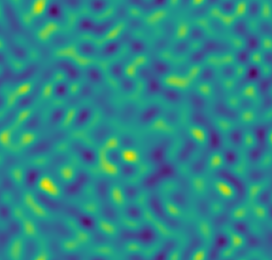
\includegraphics[interpolate=true,width=2.520000in,height=2.380000in]{burgers_solution_0.0-img0.png}}%
\end{pgfscope}%
\begin{pgfscope}%
\pgfsetbuttcap%
\pgfsetroundjoin%
\definecolor{currentfill}{rgb}{0.000000,0.000000,0.000000}%
\pgfsetfillcolor{currentfill}%
\pgfsetlinewidth{0.803000pt}%
\definecolor{currentstroke}{rgb}{0.000000,0.000000,0.000000}%
\pgfsetstrokecolor{currentstroke}%
\pgfsetdash{}{0pt}%
\pgfsys@defobject{currentmarker}{\pgfqpoint{0.000000in}{-0.048611in}}{\pgfqpoint{0.000000in}{0.000000in}}{%
\pgfpathmoveto{\pgfqpoint{0.000000in}{0.000000in}}%
\pgfpathlineto{\pgfqpoint{0.000000in}{-0.048611in}}%
\pgfusepath{stroke,fill}%
}%
\begin{pgfscope}%
\pgfsys@transformshift{0.567820in}{0.517039in}%
\pgfsys@useobject{currentmarker}{}%
\end{pgfscope}%
\end{pgfscope}%
\begin{pgfscope}%
\definecolor{textcolor}{rgb}{0.000000,0.000000,0.000000}%
\pgfsetstrokecolor{textcolor}%
\pgfsetfillcolor{textcolor}%
\pgftext[x=0.567820in,y=0.419816in,,top]{\color{textcolor}{\rmfamily\fontsize{12.000000}{14.400000}\selectfont\catcode`\^=\active\def^{\ifmmode\sp\else\^{}\fi}\catcode`\%=\active\def%{\%}0.0}}%
\end{pgfscope}%
\begin{pgfscope}%
\pgfsetbuttcap%
\pgfsetroundjoin%
\definecolor{currentfill}{rgb}{0.000000,0.000000,0.000000}%
\pgfsetfillcolor{currentfill}%
\pgfsetlinewidth{0.803000pt}%
\definecolor{currentstroke}{rgb}{0.000000,0.000000,0.000000}%
\pgfsetstrokecolor{currentstroke}%
\pgfsetdash{}{0pt}%
\pgfsys@defobject{currentmarker}{\pgfqpoint{0.000000in}{-0.048611in}}{\pgfqpoint{0.000000in}{0.000000in}}{%
\pgfpathmoveto{\pgfqpoint{0.000000in}{0.000000in}}%
\pgfpathlineto{\pgfqpoint{0.000000in}{-0.048611in}}%
\pgfusepath{stroke,fill}%
}%
\begin{pgfscope}%
\pgfsys@transformshift{1.196524in}{0.517039in}%
\pgfsys@useobject{currentmarker}{}%
\end{pgfscope}%
\end{pgfscope}%
\begin{pgfscope}%
\definecolor{textcolor}{rgb}{0.000000,0.000000,0.000000}%
\pgfsetstrokecolor{textcolor}%
\pgfsetfillcolor{textcolor}%
\pgftext[x=1.196524in,y=0.419816in,,top]{\color{textcolor}{\rmfamily\fontsize{12.000000}{14.400000}\selectfont\catcode`\^=\active\def^{\ifmmode\sp\else\^{}\fi}\catcode`\%=\active\def%{\%}0.5}}%
\end{pgfscope}%
\begin{pgfscope}%
\pgfsetbuttcap%
\pgfsetroundjoin%
\definecolor{currentfill}{rgb}{0.000000,0.000000,0.000000}%
\pgfsetfillcolor{currentfill}%
\pgfsetlinewidth{0.803000pt}%
\definecolor{currentstroke}{rgb}{0.000000,0.000000,0.000000}%
\pgfsetstrokecolor{currentstroke}%
\pgfsetdash{}{0pt}%
\pgfsys@defobject{currentmarker}{\pgfqpoint{0.000000in}{-0.048611in}}{\pgfqpoint{0.000000in}{0.000000in}}{%
\pgfpathmoveto{\pgfqpoint{0.000000in}{0.000000in}}%
\pgfpathlineto{\pgfqpoint{0.000000in}{-0.048611in}}%
\pgfusepath{stroke,fill}%
}%
\begin{pgfscope}%
\pgfsys@transformshift{1.825229in}{0.517039in}%
\pgfsys@useobject{currentmarker}{}%
\end{pgfscope}%
\end{pgfscope}%
\begin{pgfscope}%
\definecolor{textcolor}{rgb}{0.000000,0.000000,0.000000}%
\pgfsetstrokecolor{textcolor}%
\pgfsetfillcolor{textcolor}%
\pgftext[x=1.825229in,y=0.419816in,,top]{\color{textcolor}{\rmfamily\fontsize{12.000000}{14.400000}\selectfont\catcode`\^=\active\def^{\ifmmode\sp\else\^{}\fi}\catcode`\%=\active\def%{\%}1.0}}%
\end{pgfscope}%
\begin{pgfscope}%
\pgfsetbuttcap%
\pgfsetroundjoin%
\definecolor{currentfill}{rgb}{0.000000,0.000000,0.000000}%
\pgfsetfillcolor{currentfill}%
\pgfsetlinewidth{0.803000pt}%
\definecolor{currentstroke}{rgb}{0.000000,0.000000,0.000000}%
\pgfsetstrokecolor{currentstroke}%
\pgfsetdash{}{0pt}%
\pgfsys@defobject{currentmarker}{\pgfqpoint{0.000000in}{-0.048611in}}{\pgfqpoint{0.000000in}{0.000000in}}{%
\pgfpathmoveto{\pgfqpoint{0.000000in}{0.000000in}}%
\pgfpathlineto{\pgfqpoint{0.000000in}{-0.048611in}}%
\pgfusepath{stroke,fill}%
}%
\begin{pgfscope}%
\pgfsys@transformshift{2.453933in}{0.517039in}%
\pgfsys@useobject{currentmarker}{}%
\end{pgfscope}%
\end{pgfscope}%
\begin{pgfscope}%
\definecolor{textcolor}{rgb}{0.000000,0.000000,0.000000}%
\pgfsetstrokecolor{textcolor}%
\pgfsetfillcolor{textcolor}%
\pgftext[x=2.453933in,y=0.419816in,,top]{\color{textcolor}{\rmfamily\fontsize{12.000000}{14.400000}\selectfont\catcode`\^=\active\def^{\ifmmode\sp\else\^{}\fi}\catcode`\%=\active\def%{\%}1.5}}%
\end{pgfscope}%
\begin{pgfscope}%
\pgfsetbuttcap%
\pgfsetroundjoin%
\definecolor{currentfill}{rgb}{0.000000,0.000000,0.000000}%
\pgfsetfillcolor{currentfill}%
\pgfsetlinewidth{0.803000pt}%
\definecolor{currentstroke}{rgb}{0.000000,0.000000,0.000000}%
\pgfsetstrokecolor{currentstroke}%
\pgfsetdash{}{0pt}%
\pgfsys@defobject{currentmarker}{\pgfqpoint{0.000000in}{-0.048611in}}{\pgfqpoint{0.000000in}{0.000000in}}{%
\pgfpathmoveto{\pgfqpoint{0.000000in}{0.000000in}}%
\pgfpathlineto{\pgfqpoint{0.000000in}{-0.048611in}}%
\pgfusepath{stroke,fill}%
}%
\begin{pgfscope}%
\pgfsys@transformshift{3.082637in}{0.517039in}%
\pgfsys@useobject{currentmarker}{}%
\end{pgfscope}%
\end{pgfscope}%
\begin{pgfscope}%
\definecolor{textcolor}{rgb}{0.000000,0.000000,0.000000}%
\pgfsetstrokecolor{textcolor}%
\pgfsetfillcolor{textcolor}%
\pgftext[x=3.082637in,y=0.419816in,,top]{\color{textcolor}{\rmfamily\fontsize{12.000000}{14.400000}\selectfont\catcode`\^=\active\def^{\ifmmode\sp\else\^{}\fi}\catcode`\%=\active\def%{\%}2.0}}%
\end{pgfscope}%
\begin{pgfscope}%
\definecolor{textcolor}{rgb}{0.000000,0.000000,0.000000}%
\pgfsetstrokecolor{textcolor}%
\pgfsetfillcolor{textcolor}%
\pgftext[x=1.825229in,y=0.202965in,,top]{\color{textcolor}{\rmfamily\fontsize{12.000000}{14.400000}\selectfont\catcode`\^=\active\def^{\ifmmode\sp\else\^{}\fi}\catcode`\%=\active\def%{\%}Space}}%
\end{pgfscope}%
\begin{pgfscope}%
\pgfsetbuttcap%
\pgfsetroundjoin%
\definecolor{currentfill}{rgb}{0.000000,0.000000,0.000000}%
\pgfsetfillcolor{currentfill}%
\pgfsetlinewidth{0.803000pt}%
\definecolor{currentstroke}{rgb}{0.000000,0.000000,0.000000}%
\pgfsetstrokecolor{currentstroke}%
\pgfsetdash{}{0pt}%
\pgfsys@defobject{currentmarker}{\pgfqpoint{-0.048611in}{0.000000in}}{\pgfqpoint{-0.000000in}{0.000000in}}{%
\pgfpathmoveto{\pgfqpoint{-0.000000in}{0.000000in}}%
\pgfpathlineto{\pgfqpoint{-0.048611in}{0.000000in}}%
\pgfusepath{stroke,fill}%
}%
\begin{pgfscope}%
\pgfsys@transformshift{0.567820in}{0.517039in}%
\pgfsys@useobject{currentmarker}{}%
\end{pgfscope}%
\end{pgfscope}%
\begin{pgfscope}%
\definecolor{textcolor}{rgb}{0.000000,0.000000,0.000000}%
\pgfsetstrokecolor{textcolor}%
\pgfsetfillcolor{textcolor}%
\pgftext[x=0.364559in, y=0.453725in, left, base]{\color{textcolor}{\rmfamily\fontsize{12.000000}{14.400000}\selectfont\catcode`\^=\active\def^{\ifmmode\sp\else\^{}\fi}\catcode`\%=\active\def%{\%}0}}%
\end{pgfscope}%
\begin{pgfscope}%
\pgfsetbuttcap%
\pgfsetroundjoin%
\definecolor{currentfill}{rgb}{0.000000,0.000000,0.000000}%
\pgfsetfillcolor{currentfill}%
\pgfsetlinewidth{0.803000pt}%
\definecolor{currentstroke}{rgb}{0.000000,0.000000,0.000000}%
\pgfsetstrokecolor{currentstroke}%
\pgfsetdash{}{0pt}%
\pgfsys@defobject{currentmarker}{\pgfqpoint{-0.048611in}{0.000000in}}{\pgfqpoint{-0.000000in}{0.000000in}}{%
\pgfpathmoveto{\pgfqpoint{-0.000000in}{0.000000in}}%
\pgfpathlineto{\pgfqpoint{-0.048611in}{0.000000in}}%
\pgfusepath{stroke,fill}%
}%
\begin{pgfscope}%
\pgfsys@transformshift{0.567820in}{0.992634in}%
\pgfsys@useobject{currentmarker}{}%
\end{pgfscope}%
\end{pgfscope}%
\begin{pgfscope}%
\definecolor{textcolor}{rgb}{0.000000,0.000000,0.000000}%
\pgfsetstrokecolor{textcolor}%
\pgfsetfillcolor{textcolor}%
\pgftext[x=0.364559in, y=0.929320in, left, base]{\color{textcolor}{\rmfamily\fontsize{12.000000}{14.400000}\selectfont\catcode`\^=\active\def^{\ifmmode\sp\else\^{}\fi}\catcode`\%=\active\def%{\%}2}}%
\end{pgfscope}%
\begin{pgfscope}%
\pgfsetbuttcap%
\pgfsetroundjoin%
\definecolor{currentfill}{rgb}{0.000000,0.000000,0.000000}%
\pgfsetfillcolor{currentfill}%
\pgfsetlinewidth{0.803000pt}%
\definecolor{currentstroke}{rgb}{0.000000,0.000000,0.000000}%
\pgfsetstrokecolor{currentstroke}%
\pgfsetdash{}{0pt}%
\pgfsys@defobject{currentmarker}{\pgfqpoint{-0.048611in}{0.000000in}}{\pgfqpoint{-0.000000in}{0.000000in}}{%
\pgfpathmoveto{\pgfqpoint{-0.000000in}{0.000000in}}%
\pgfpathlineto{\pgfqpoint{-0.048611in}{0.000000in}}%
\pgfusepath{stroke,fill}%
}%
\begin{pgfscope}%
\pgfsys@transformshift{0.567820in}{1.468230in}%
\pgfsys@useobject{currentmarker}{}%
\end{pgfscope}%
\end{pgfscope}%
\begin{pgfscope}%
\definecolor{textcolor}{rgb}{0.000000,0.000000,0.000000}%
\pgfsetstrokecolor{textcolor}%
\pgfsetfillcolor{textcolor}%
\pgftext[x=0.364559in, y=1.404916in, left, base]{\color{textcolor}{\rmfamily\fontsize{12.000000}{14.400000}\selectfont\catcode`\^=\active\def^{\ifmmode\sp\else\^{}\fi}\catcode`\%=\active\def%{\%}4}}%
\end{pgfscope}%
\begin{pgfscope}%
\pgfsetbuttcap%
\pgfsetroundjoin%
\definecolor{currentfill}{rgb}{0.000000,0.000000,0.000000}%
\pgfsetfillcolor{currentfill}%
\pgfsetlinewidth{0.803000pt}%
\definecolor{currentstroke}{rgb}{0.000000,0.000000,0.000000}%
\pgfsetstrokecolor{currentstroke}%
\pgfsetdash{}{0pt}%
\pgfsys@defobject{currentmarker}{\pgfqpoint{-0.048611in}{0.000000in}}{\pgfqpoint{-0.000000in}{0.000000in}}{%
\pgfpathmoveto{\pgfqpoint{-0.000000in}{0.000000in}}%
\pgfpathlineto{\pgfqpoint{-0.048611in}{0.000000in}}%
\pgfusepath{stroke,fill}%
}%
\begin{pgfscope}%
\pgfsys@transformshift{0.567820in}{1.943825in}%
\pgfsys@useobject{currentmarker}{}%
\end{pgfscope}%
\end{pgfscope}%
\begin{pgfscope}%
\definecolor{textcolor}{rgb}{0.000000,0.000000,0.000000}%
\pgfsetstrokecolor{textcolor}%
\pgfsetfillcolor{textcolor}%
\pgftext[x=0.364559in, y=1.880511in, left, base]{\color{textcolor}{\rmfamily\fontsize{12.000000}{14.400000}\selectfont\catcode`\^=\active\def^{\ifmmode\sp\else\^{}\fi}\catcode`\%=\active\def%{\%}6}}%
\end{pgfscope}%
\begin{pgfscope}%
\pgfsetbuttcap%
\pgfsetroundjoin%
\definecolor{currentfill}{rgb}{0.000000,0.000000,0.000000}%
\pgfsetfillcolor{currentfill}%
\pgfsetlinewidth{0.803000pt}%
\definecolor{currentstroke}{rgb}{0.000000,0.000000,0.000000}%
\pgfsetstrokecolor{currentstroke}%
\pgfsetdash{}{0pt}%
\pgfsys@defobject{currentmarker}{\pgfqpoint{-0.048611in}{0.000000in}}{\pgfqpoint{-0.000000in}{0.000000in}}{%
\pgfpathmoveto{\pgfqpoint{-0.000000in}{0.000000in}}%
\pgfpathlineto{\pgfqpoint{-0.048611in}{0.000000in}}%
\pgfusepath{stroke,fill}%
}%
\begin{pgfscope}%
\pgfsys@transformshift{0.567820in}{2.419421in}%
\pgfsys@useobject{currentmarker}{}%
\end{pgfscope}%
\end{pgfscope}%
\begin{pgfscope}%
\definecolor{textcolor}{rgb}{0.000000,0.000000,0.000000}%
\pgfsetstrokecolor{textcolor}%
\pgfsetfillcolor{textcolor}%
\pgftext[x=0.364559in, y=2.356107in, left, base]{\color{textcolor}{\rmfamily\fontsize{12.000000}{14.400000}\selectfont\catcode`\^=\active\def^{\ifmmode\sp\else\^{}\fi}\catcode`\%=\active\def%{\%}8}}%
\end{pgfscope}%
\begin{pgfscope}%
\pgfsetbuttcap%
\pgfsetroundjoin%
\definecolor{currentfill}{rgb}{0.000000,0.000000,0.000000}%
\pgfsetfillcolor{currentfill}%
\pgfsetlinewidth{0.803000pt}%
\definecolor{currentstroke}{rgb}{0.000000,0.000000,0.000000}%
\pgfsetstrokecolor{currentstroke}%
\pgfsetdash{}{0pt}%
\pgfsys@defobject{currentmarker}{\pgfqpoint{-0.048611in}{0.000000in}}{\pgfqpoint{-0.000000in}{0.000000in}}{%
\pgfpathmoveto{\pgfqpoint{-0.000000in}{0.000000in}}%
\pgfpathlineto{\pgfqpoint{-0.048611in}{0.000000in}}%
\pgfusepath{stroke,fill}%
}%
\begin{pgfscope}%
\pgfsys@transformshift{0.567820in}{2.895016in}%
\pgfsys@useobject{currentmarker}{}%
\end{pgfscope}%
\end{pgfscope}%
\begin{pgfscope}%
\definecolor{textcolor}{rgb}{0.000000,0.000000,0.000000}%
\pgfsetstrokecolor{textcolor}%
\pgfsetfillcolor{textcolor}%
\pgftext[x=0.258521in, y=2.831702in, left, base]{\color{textcolor}{\rmfamily\fontsize{12.000000}{14.400000}\selectfont\catcode`\^=\active\def^{\ifmmode\sp\else\^{}\fi}\catcode`\%=\active\def%{\%}10}}%
\end{pgfscope}%
\begin{pgfscope}%
\definecolor{textcolor}{rgb}{0.000000,0.000000,0.000000}%
\pgfsetstrokecolor{textcolor}%
\pgfsetfillcolor{textcolor}%
\pgftext[x=0.202965in,y=1.706027in,,bottom,rotate=90.000000]{\color{textcolor}{\rmfamily\fontsize{12.000000}{14.400000}\selectfont\catcode`\^=\active\def^{\ifmmode\sp\else\^{}\fi}\catcode`\%=\active\def%{\%}Time}}%
\end{pgfscope}%
\begin{pgfscope}%
\pgfsetrectcap%
\pgfsetmiterjoin%
\pgfsetlinewidth{0.803000pt}%
\definecolor{currentstroke}{rgb}{0.000000,0.000000,0.000000}%
\pgfsetstrokecolor{currentstroke}%
\pgfsetdash{}{0pt}%
\pgfpathmoveto{\pgfqpoint{0.567820in}{0.517039in}}%
\pgfpathlineto{\pgfqpoint{0.567820in}{2.895016in}}%
\pgfusepath{stroke}%
\end{pgfscope}%
\begin{pgfscope}%
\pgfsetrectcap%
\pgfsetmiterjoin%
\pgfsetlinewidth{0.803000pt}%
\definecolor{currentstroke}{rgb}{0.000000,0.000000,0.000000}%
\pgfsetstrokecolor{currentstroke}%
\pgfsetdash{}{0pt}%
\pgfpathmoveto{\pgfqpoint{3.082637in}{0.517039in}}%
\pgfpathlineto{\pgfqpoint{3.082637in}{2.895016in}}%
\pgfusepath{stroke}%
\end{pgfscope}%
\begin{pgfscope}%
\pgfsetrectcap%
\pgfsetmiterjoin%
\pgfsetlinewidth{0.803000pt}%
\definecolor{currentstroke}{rgb}{0.000000,0.000000,0.000000}%
\pgfsetstrokecolor{currentstroke}%
\pgfsetdash{}{0pt}%
\pgfpathmoveto{\pgfqpoint{0.567820in}{0.517039in}}%
\pgfpathlineto{\pgfqpoint{3.082637in}{0.517039in}}%
\pgfusepath{stroke}%
\end{pgfscope}%
\begin{pgfscope}%
\pgfsetrectcap%
\pgfsetmiterjoin%
\pgfsetlinewidth{0.803000pt}%
\definecolor{currentstroke}{rgb}{0.000000,0.000000,0.000000}%
\pgfsetstrokecolor{currentstroke}%
\pgfsetdash{}{0pt}%
\pgfpathmoveto{\pgfqpoint{0.567820in}{2.895016in}}%
\pgfpathlineto{\pgfqpoint{3.082637in}{2.895016in}}%
\pgfusepath{stroke}%
\end{pgfscope}%
\begin{pgfscope}%
\pgfsetbuttcap%
\pgfsetmiterjoin%
\pgfsetlinewidth{0.000000pt}%
\definecolor{currentstroke}{rgb}{0.000000,0.000000,0.000000}%
\pgfsetstrokecolor{currentstroke}%
\pgfsetstrokeopacity{0.000000}%
\pgfsetdash{}{0pt}%
\pgfpathmoveto{\pgfqpoint{3.340906in}{0.517039in}}%
\pgfpathlineto{\pgfqpoint{3.459805in}{0.517039in}}%
\pgfpathlineto{\pgfqpoint{3.459805in}{2.895016in}}%
\pgfpathlineto{\pgfqpoint{3.340906in}{2.895016in}}%
\pgfpathlineto{\pgfqpoint{3.340906in}{0.517039in}}%
\pgfpathclose%
\pgfusepath{}%
\end{pgfscope}%
\begin{pgfscope}%
\pgfsys@transformshift{3.340000in}{0.520000in}%
\pgftext[left,bottom]{
\includegraphics[interpolate=true,width=0.120000in,height=2.380000in]{burgers_solution_0.0-img1.png}}%
\end{pgfscope}%
\begin{pgfscope}%
\pgfsetbuttcap%
\pgfsetroundjoin%
\definecolor{currentfill}{rgb}{0.000000,0.000000,0.000000}%
\pgfsetfillcolor{currentfill}%
\pgfsetlinewidth{0.803000pt}%
\definecolor{currentstroke}{rgb}{0.000000,0.000000,0.000000}%
\pgfsetstrokecolor{currentstroke}%
\pgfsetdash{}{0pt}%
\pgfsys@defobject{currentmarker}{\pgfqpoint{0.000000in}{0.000000in}}{\pgfqpoint{0.048611in}{0.000000in}}{%
\pgfpathmoveto{\pgfqpoint{0.000000in}{0.000000in}}%
\pgfpathlineto{\pgfqpoint{0.048611in}{0.000000in}}%
\pgfusepath{stroke,fill}%
}%
\begin{pgfscope}%
\pgfsys@transformshift{3.459805in}{0.555741in}%
\pgfsys@useobject{currentmarker}{}%
\end{pgfscope}%
\end{pgfscope}%
\begin{pgfscope}%
\definecolor{textcolor}{rgb}{0.000000,0.000000,0.000000}%
\pgfsetstrokecolor{textcolor}%
\pgfsetfillcolor{textcolor}%
\pgftext[x=3.557027in, y=0.492427in, left, base]{\color{textcolor}{\rmfamily\fontsize{12.000000}{14.400000}\selectfont\catcode`\^=\active\def^{\ifmmode\sp\else\^{}\fi}\catcode`\%=\active\def%{\%}\ensuremath{-}0.6}}%
\end{pgfscope}%
\begin{pgfscope}%
\pgfsetbuttcap%
\pgfsetroundjoin%
\definecolor{currentfill}{rgb}{0.000000,0.000000,0.000000}%
\pgfsetfillcolor{currentfill}%
\pgfsetlinewidth{0.803000pt}%
\definecolor{currentstroke}{rgb}{0.000000,0.000000,0.000000}%
\pgfsetstrokecolor{currentstroke}%
\pgfsetdash{}{0pt}%
\pgfsys@defobject{currentmarker}{\pgfqpoint{0.000000in}{0.000000in}}{\pgfqpoint{0.048611in}{0.000000in}}{%
\pgfpathmoveto{\pgfqpoint{0.000000in}{0.000000in}}%
\pgfpathlineto{\pgfqpoint{0.048611in}{0.000000in}}%
\pgfusepath{stroke,fill}%
}%
\begin{pgfscope}%
\pgfsys@transformshift{3.459805in}{0.932008in}%
\pgfsys@useobject{currentmarker}{}%
\end{pgfscope}%
\end{pgfscope}%
\begin{pgfscope}%
\definecolor{textcolor}{rgb}{0.000000,0.000000,0.000000}%
\pgfsetstrokecolor{textcolor}%
\pgfsetfillcolor{textcolor}%
\pgftext[x=3.557027in, y=0.868694in, left, base]{\color{textcolor}{\rmfamily\fontsize{12.000000}{14.400000}\selectfont\catcode`\^=\active\def^{\ifmmode\sp\else\^{}\fi}\catcode`\%=\active\def%{\%}\ensuremath{-}0.4}}%
\end{pgfscope}%
\begin{pgfscope}%
\pgfsetbuttcap%
\pgfsetroundjoin%
\definecolor{currentfill}{rgb}{0.000000,0.000000,0.000000}%
\pgfsetfillcolor{currentfill}%
\pgfsetlinewidth{0.803000pt}%
\definecolor{currentstroke}{rgb}{0.000000,0.000000,0.000000}%
\pgfsetstrokecolor{currentstroke}%
\pgfsetdash{}{0pt}%
\pgfsys@defobject{currentmarker}{\pgfqpoint{0.000000in}{0.000000in}}{\pgfqpoint{0.048611in}{0.000000in}}{%
\pgfpathmoveto{\pgfqpoint{0.000000in}{0.000000in}}%
\pgfpathlineto{\pgfqpoint{0.048611in}{0.000000in}}%
\pgfusepath{stroke,fill}%
}%
\begin{pgfscope}%
\pgfsys@transformshift{3.459805in}{1.308274in}%
\pgfsys@useobject{currentmarker}{}%
\end{pgfscope}%
\end{pgfscope}%
\begin{pgfscope}%
\definecolor{textcolor}{rgb}{0.000000,0.000000,0.000000}%
\pgfsetstrokecolor{textcolor}%
\pgfsetfillcolor{textcolor}%
\pgftext[x=3.557027in, y=1.244961in, left, base]{\color{textcolor}{\rmfamily\fontsize{12.000000}{14.400000}\selectfont\catcode`\^=\active\def^{\ifmmode\sp\else\^{}\fi}\catcode`\%=\active\def%{\%}\ensuremath{-}0.2}}%
\end{pgfscope}%
\begin{pgfscope}%
\pgfsetbuttcap%
\pgfsetroundjoin%
\definecolor{currentfill}{rgb}{0.000000,0.000000,0.000000}%
\pgfsetfillcolor{currentfill}%
\pgfsetlinewidth{0.803000pt}%
\definecolor{currentstroke}{rgb}{0.000000,0.000000,0.000000}%
\pgfsetstrokecolor{currentstroke}%
\pgfsetdash{}{0pt}%
\pgfsys@defobject{currentmarker}{\pgfqpoint{0.000000in}{0.000000in}}{\pgfqpoint{0.048611in}{0.000000in}}{%
\pgfpathmoveto{\pgfqpoint{0.000000in}{0.000000in}}%
\pgfpathlineto{\pgfqpoint{0.048611in}{0.000000in}}%
\pgfusepath{stroke,fill}%
}%
\begin{pgfscope}%
\pgfsys@transformshift{3.459805in}{1.684541in}%
\pgfsys@useobject{currentmarker}{}%
\end{pgfscope}%
\end{pgfscope}%
\begin{pgfscope}%
\definecolor{textcolor}{rgb}{0.000000,0.000000,0.000000}%
\pgfsetstrokecolor{textcolor}%
\pgfsetfillcolor{textcolor}%
\pgftext[x=3.557027in, y=1.621228in, left, base]{\color{textcolor}{\rmfamily\fontsize{12.000000}{14.400000}\selectfont\catcode`\^=\active\def^{\ifmmode\sp\else\^{}\fi}\catcode`\%=\active\def%{\%}0.0}}%
\end{pgfscope}%
\begin{pgfscope}%
\pgfsetbuttcap%
\pgfsetroundjoin%
\definecolor{currentfill}{rgb}{0.000000,0.000000,0.000000}%
\pgfsetfillcolor{currentfill}%
\pgfsetlinewidth{0.803000pt}%
\definecolor{currentstroke}{rgb}{0.000000,0.000000,0.000000}%
\pgfsetstrokecolor{currentstroke}%
\pgfsetdash{}{0pt}%
\pgfsys@defobject{currentmarker}{\pgfqpoint{0.000000in}{0.000000in}}{\pgfqpoint{0.048611in}{0.000000in}}{%
\pgfpathmoveto{\pgfqpoint{0.000000in}{0.000000in}}%
\pgfpathlineto{\pgfqpoint{0.048611in}{0.000000in}}%
\pgfusepath{stroke,fill}%
}%
\begin{pgfscope}%
\pgfsys@transformshift{3.459805in}{2.060808in}%
\pgfsys@useobject{currentmarker}{}%
\end{pgfscope}%
\end{pgfscope}%
\begin{pgfscope}%
\definecolor{textcolor}{rgb}{0.000000,0.000000,0.000000}%
\pgfsetstrokecolor{textcolor}%
\pgfsetfillcolor{textcolor}%
\pgftext[x=3.557027in, y=1.997494in, left, base]{\color{textcolor}{\rmfamily\fontsize{12.000000}{14.400000}\selectfont\catcode`\^=\active\def^{\ifmmode\sp\else\^{}\fi}\catcode`\%=\active\def%{\%}0.2}}%
\end{pgfscope}%
\begin{pgfscope}%
\pgfsetbuttcap%
\pgfsetroundjoin%
\definecolor{currentfill}{rgb}{0.000000,0.000000,0.000000}%
\pgfsetfillcolor{currentfill}%
\pgfsetlinewidth{0.803000pt}%
\definecolor{currentstroke}{rgb}{0.000000,0.000000,0.000000}%
\pgfsetstrokecolor{currentstroke}%
\pgfsetdash{}{0pt}%
\pgfsys@defobject{currentmarker}{\pgfqpoint{0.000000in}{0.000000in}}{\pgfqpoint{0.048611in}{0.000000in}}{%
\pgfpathmoveto{\pgfqpoint{0.000000in}{0.000000in}}%
\pgfpathlineto{\pgfqpoint{0.048611in}{0.000000in}}%
\pgfusepath{stroke,fill}%
}%
\begin{pgfscope}%
\pgfsys@transformshift{3.459805in}{2.437075in}%
\pgfsys@useobject{currentmarker}{}%
\end{pgfscope}%
\end{pgfscope}%
\begin{pgfscope}%
\definecolor{textcolor}{rgb}{0.000000,0.000000,0.000000}%
\pgfsetstrokecolor{textcolor}%
\pgfsetfillcolor{textcolor}%
\pgftext[x=3.557027in, y=2.373761in, left, base]{\color{textcolor}{\rmfamily\fontsize{12.000000}{14.400000}\selectfont\catcode`\^=\active\def^{\ifmmode\sp\else\^{}\fi}\catcode`\%=\active\def%{\%}0.4}}%
\end{pgfscope}%
\begin{pgfscope}%
\pgfsetbuttcap%
\pgfsetroundjoin%
\definecolor{currentfill}{rgb}{0.000000,0.000000,0.000000}%
\pgfsetfillcolor{currentfill}%
\pgfsetlinewidth{0.803000pt}%
\definecolor{currentstroke}{rgb}{0.000000,0.000000,0.000000}%
\pgfsetstrokecolor{currentstroke}%
\pgfsetdash{}{0pt}%
\pgfsys@defobject{currentmarker}{\pgfqpoint{0.000000in}{0.000000in}}{\pgfqpoint{0.048611in}{0.000000in}}{%
\pgfpathmoveto{\pgfqpoint{0.000000in}{0.000000in}}%
\pgfpathlineto{\pgfqpoint{0.048611in}{0.000000in}}%
\pgfusepath{stroke,fill}%
}%
\begin{pgfscope}%
\pgfsys@transformshift{3.459805in}{2.813342in}%
\pgfsys@useobject{currentmarker}{}%
\end{pgfscope}%
\end{pgfscope}%
\begin{pgfscope}%
\definecolor{textcolor}{rgb}{0.000000,0.000000,0.000000}%
\pgfsetstrokecolor{textcolor}%
\pgfsetfillcolor{textcolor}%
\pgftext[x=3.557027in, y=2.750028in, left, base]{\color{textcolor}{\rmfamily\fontsize{12.000000}{14.400000}\selectfont\catcode`\^=\active\def^{\ifmmode\sp\else\^{}\fi}\catcode`\%=\active\def%{\%}0.6}}%
\end{pgfscope}%
\begin{pgfscope}%
\pgfsetrectcap%
\pgfsetmiterjoin%
\pgfsetlinewidth{0.803000pt}%
\definecolor{currentstroke}{rgb}{0.000000,0.000000,0.000000}%
\pgfsetstrokecolor{currentstroke}%
\pgfsetdash{}{0pt}%
\pgfpathmoveto{\pgfqpoint{3.340906in}{0.517039in}}%
\pgfpathlineto{\pgfqpoint{3.400355in}{0.517039in}}%
\pgfpathlineto{\pgfqpoint{3.459805in}{0.517039in}}%
\pgfpathlineto{\pgfqpoint{3.459805in}{2.895016in}}%
\pgfpathlineto{\pgfqpoint{3.400355in}{2.895016in}}%
\pgfpathlineto{\pgfqpoint{3.340906in}{2.895016in}}%
\pgfpathlineto{\pgfqpoint{3.340906in}{0.517039in}}%
\pgfpathclose%
\pgfusepath{stroke}%
\end{pgfscope}%
\end{pgfpicture}%
\makeatother%
\endgroup%

    \end{adjustbox}
    \caption{Solution function for \(\nu=0\).}\label{fig:burgers_solution_0.0}
  \end{subfigure}
  \begin{subfigure}{0.49\linewidth}
    \begin{adjustbox}{width=\linewidth}
      \begingroup%
\makeatletter%
\begin{pgfpicture}%
\pgfpathrectangle{\pgfpointorigin}{\pgfqpoint{4.000000in}{3.000000in}}%
\pgfusepath{use as bounding box, clip}%
\begin{pgfscope}%
\pgfsetbuttcap%
\pgfsetmiterjoin%
\pgfsetlinewidth{0.000000pt}%
\definecolor{currentstroke}{rgb}{0.000000,0.000000,0.000000}%
\pgfsetstrokecolor{currentstroke}%
\pgfsetstrokeopacity{0.000000}%
\pgfsetdash{}{0pt}%
\pgfpathmoveto{\pgfqpoint{0.000000in}{0.000000in}}%
\pgfpathlineto{\pgfqpoint{4.000000in}{0.000000in}}%
\pgfpathlineto{\pgfqpoint{4.000000in}{3.000000in}}%
\pgfpathlineto{\pgfqpoint{0.000000in}{3.000000in}}%
\pgfpathlineto{\pgfqpoint{0.000000in}{0.000000in}}%
\pgfpathclose%
\pgfusepath{}%
\end{pgfscope}%
\begin{pgfscope}%
\pgfsetbuttcap%
\pgfsetmiterjoin%
\pgfsetlinewidth{0.000000pt}%
\definecolor{currentstroke}{rgb}{0.000000,0.000000,0.000000}%
\pgfsetstrokecolor{currentstroke}%
\pgfsetstrokeopacity{0.000000}%
\pgfsetdash{}{0pt}%
\pgfpathmoveto{\pgfqpoint{0.567820in}{0.517039in}}%
\pgfpathlineto{\pgfqpoint{3.082637in}{0.517039in}}%
\pgfpathlineto{\pgfqpoint{3.082637in}{2.895016in}}%
\pgfpathlineto{\pgfqpoint{0.567820in}{2.895016in}}%
\pgfpathlineto{\pgfqpoint{0.567820in}{0.517039in}}%
\pgfpathclose%
\pgfusepath{}%
\end{pgfscope}%
\begin{pgfscope}%
\pgfpathrectangle{\pgfqpoint{0.567820in}{0.517039in}}{\pgfqpoint{2.514817in}{2.377978in}}%
\pgfusepath{clip}%
\pgfsys@transformshift{0.567820in}{0.517039in}%
\pgftext[left,bottom]{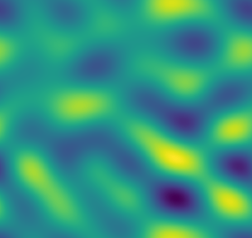
\includegraphics[interpolate=true,width=2.520000in,height=2.380000in]{burgers_forcing_0.0-img0.png}}%
\end{pgfscope}%
\begin{pgfscope}%
\pgfsetbuttcap%
\pgfsetroundjoin%
\definecolor{currentfill}{rgb}{0.000000,0.000000,0.000000}%
\pgfsetfillcolor{currentfill}%
\pgfsetlinewidth{0.803000pt}%
\definecolor{currentstroke}{rgb}{0.000000,0.000000,0.000000}%
\pgfsetstrokecolor{currentstroke}%
\pgfsetdash{}{0pt}%
\pgfsys@defobject{currentmarker}{\pgfqpoint{0.000000in}{-0.048611in}}{\pgfqpoint{0.000000in}{0.000000in}}{%
\pgfpathmoveto{\pgfqpoint{0.000000in}{0.000000in}}%
\pgfpathlineto{\pgfqpoint{0.000000in}{-0.048611in}}%
\pgfusepath{stroke,fill}%
}%
\begin{pgfscope}%
\pgfsys@transformshift{0.567820in}{0.517039in}%
\pgfsys@useobject{currentmarker}{}%
\end{pgfscope}%
\end{pgfscope}%
\begin{pgfscope}%
\definecolor{textcolor}{rgb}{0.000000,0.000000,0.000000}%
\pgfsetstrokecolor{textcolor}%
\pgfsetfillcolor{textcolor}%
\pgftext[x=0.567820in,y=0.419816in,,top]{\color{textcolor}{\rmfamily\fontsize{12.000000}{14.400000}\selectfont\catcode`\^=\active\def^{\ifmmode\sp\else\^{}\fi}\catcode`\%=\active\def%{\%}0.0}}%
\end{pgfscope}%
\begin{pgfscope}%
\pgfsetbuttcap%
\pgfsetroundjoin%
\definecolor{currentfill}{rgb}{0.000000,0.000000,0.000000}%
\pgfsetfillcolor{currentfill}%
\pgfsetlinewidth{0.803000pt}%
\definecolor{currentstroke}{rgb}{0.000000,0.000000,0.000000}%
\pgfsetstrokecolor{currentstroke}%
\pgfsetdash{}{0pt}%
\pgfsys@defobject{currentmarker}{\pgfqpoint{0.000000in}{-0.048611in}}{\pgfqpoint{0.000000in}{0.000000in}}{%
\pgfpathmoveto{\pgfqpoint{0.000000in}{0.000000in}}%
\pgfpathlineto{\pgfqpoint{0.000000in}{-0.048611in}}%
\pgfusepath{stroke,fill}%
}%
\begin{pgfscope}%
\pgfsys@transformshift{1.196524in}{0.517039in}%
\pgfsys@useobject{currentmarker}{}%
\end{pgfscope}%
\end{pgfscope}%
\begin{pgfscope}%
\definecolor{textcolor}{rgb}{0.000000,0.000000,0.000000}%
\pgfsetstrokecolor{textcolor}%
\pgfsetfillcolor{textcolor}%
\pgftext[x=1.196524in,y=0.419816in,,top]{\color{textcolor}{\rmfamily\fontsize{12.000000}{14.400000}\selectfont\catcode`\^=\active\def^{\ifmmode\sp\else\^{}\fi}\catcode`\%=\active\def%{\%}0.5}}%
\end{pgfscope}%
\begin{pgfscope}%
\pgfsetbuttcap%
\pgfsetroundjoin%
\definecolor{currentfill}{rgb}{0.000000,0.000000,0.000000}%
\pgfsetfillcolor{currentfill}%
\pgfsetlinewidth{0.803000pt}%
\definecolor{currentstroke}{rgb}{0.000000,0.000000,0.000000}%
\pgfsetstrokecolor{currentstroke}%
\pgfsetdash{}{0pt}%
\pgfsys@defobject{currentmarker}{\pgfqpoint{0.000000in}{-0.048611in}}{\pgfqpoint{0.000000in}{0.000000in}}{%
\pgfpathmoveto{\pgfqpoint{0.000000in}{0.000000in}}%
\pgfpathlineto{\pgfqpoint{0.000000in}{-0.048611in}}%
\pgfusepath{stroke,fill}%
}%
\begin{pgfscope}%
\pgfsys@transformshift{1.825229in}{0.517039in}%
\pgfsys@useobject{currentmarker}{}%
\end{pgfscope}%
\end{pgfscope}%
\begin{pgfscope}%
\definecolor{textcolor}{rgb}{0.000000,0.000000,0.000000}%
\pgfsetstrokecolor{textcolor}%
\pgfsetfillcolor{textcolor}%
\pgftext[x=1.825229in,y=0.419816in,,top]{\color{textcolor}{\rmfamily\fontsize{12.000000}{14.400000}\selectfont\catcode`\^=\active\def^{\ifmmode\sp\else\^{}\fi}\catcode`\%=\active\def%{\%}1.0}}%
\end{pgfscope}%
\begin{pgfscope}%
\pgfsetbuttcap%
\pgfsetroundjoin%
\definecolor{currentfill}{rgb}{0.000000,0.000000,0.000000}%
\pgfsetfillcolor{currentfill}%
\pgfsetlinewidth{0.803000pt}%
\definecolor{currentstroke}{rgb}{0.000000,0.000000,0.000000}%
\pgfsetstrokecolor{currentstroke}%
\pgfsetdash{}{0pt}%
\pgfsys@defobject{currentmarker}{\pgfqpoint{0.000000in}{-0.048611in}}{\pgfqpoint{0.000000in}{0.000000in}}{%
\pgfpathmoveto{\pgfqpoint{0.000000in}{0.000000in}}%
\pgfpathlineto{\pgfqpoint{0.000000in}{-0.048611in}}%
\pgfusepath{stroke,fill}%
}%
\begin{pgfscope}%
\pgfsys@transformshift{2.453933in}{0.517039in}%
\pgfsys@useobject{currentmarker}{}%
\end{pgfscope}%
\end{pgfscope}%
\begin{pgfscope}%
\definecolor{textcolor}{rgb}{0.000000,0.000000,0.000000}%
\pgfsetstrokecolor{textcolor}%
\pgfsetfillcolor{textcolor}%
\pgftext[x=2.453933in,y=0.419816in,,top]{\color{textcolor}{\rmfamily\fontsize{12.000000}{14.400000}\selectfont\catcode`\^=\active\def^{\ifmmode\sp\else\^{}\fi}\catcode`\%=\active\def%{\%}1.5}}%
\end{pgfscope}%
\begin{pgfscope}%
\pgfsetbuttcap%
\pgfsetroundjoin%
\definecolor{currentfill}{rgb}{0.000000,0.000000,0.000000}%
\pgfsetfillcolor{currentfill}%
\pgfsetlinewidth{0.803000pt}%
\definecolor{currentstroke}{rgb}{0.000000,0.000000,0.000000}%
\pgfsetstrokecolor{currentstroke}%
\pgfsetdash{}{0pt}%
\pgfsys@defobject{currentmarker}{\pgfqpoint{0.000000in}{-0.048611in}}{\pgfqpoint{0.000000in}{0.000000in}}{%
\pgfpathmoveto{\pgfqpoint{0.000000in}{0.000000in}}%
\pgfpathlineto{\pgfqpoint{0.000000in}{-0.048611in}}%
\pgfusepath{stroke,fill}%
}%
\begin{pgfscope}%
\pgfsys@transformshift{3.082637in}{0.517039in}%
\pgfsys@useobject{currentmarker}{}%
\end{pgfscope}%
\end{pgfscope}%
\begin{pgfscope}%
\definecolor{textcolor}{rgb}{0.000000,0.000000,0.000000}%
\pgfsetstrokecolor{textcolor}%
\pgfsetfillcolor{textcolor}%
\pgftext[x=3.082637in,y=0.419816in,,top]{\color{textcolor}{\rmfamily\fontsize{12.000000}{14.400000}\selectfont\catcode`\^=\active\def^{\ifmmode\sp\else\^{}\fi}\catcode`\%=\active\def%{\%}2.0}}%
\end{pgfscope}%
\begin{pgfscope}%
\definecolor{textcolor}{rgb}{0.000000,0.000000,0.000000}%
\pgfsetstrokecolor{textcolor}%
\pgfsetfillcolor{textcolor}%
\pgftext[x=1.825229in,y=0.202965in,,top]{\color{textcolor}{\rmfamily\fontsize{12.000000}{14.400000}\selectfont\catcode`\^=\active\def^{\ifmmode\sp\else\^{}\fi}\catcode`\%=\active\def%{\%}Space}}%
\end{pgfscope}%
\begin{pgfscope}%
\pgfsetbuttcap%
\pgfsetroundjoin%
\definecolor{currentfill}{rgb}{0.000000,0.000000,0.000000}%
\pgfsetfillcolor{currentfill}%
\pgfsetlinewidth{0.803000pt}%
\definecolor{currentstroke}{rgb}{0.000000,0.000000,0.000000}%
\pgfsetstrokecolor{currentstroke}%
\pgfsetdash{}{0pt}%
\pgfsys@defobject{currentmarker}{\pgfqpoint{-0.048611in}{0.000000in}}{\pgfqpoint{-0.000000in}{0.000000in}}{%
\pgfpathmoveto{\pgfqpoint{-0.000000in}{0.000000in}}%
\pgfpathlineto{\pgfqpoint{-0.048611in}{0.000000in}}%
\pgfusepath{stroke,fill}%
}%
\begin{pgfscope}%
\pgfsys@transformshift{0.567820in}{0.517039in}%
\pgfsys@useobject{currentmarker}{}%
\end{pgfscope}%
\end{pgfscope}%
\begin{pgfscope}%
\definecolor{textcolor}{rgb}{0.000000,0.000000,0.000000}%
\pgfsetstrokecolor{textcolor}%
\pgfsetfillcolor{textcolor}%
\pgftext[x=0.364559in, y=0.453725in, left, base]{\color{textcolor}{\rmfamily\fontsize{12.000000}{14.400000}\selectfont\catcode`\^=\active\def^{\ifmmode\sp\else\^{}\fi}\catcode`\%=\active\def%{\%}0}}%
\end{pgfscope}%
\begin{pgfscope}%
\pgfsetbuttcap%
\pgfsetroundjoin%
\definecolor{currentfill}{rgb}{0.000000,0.000000,0.000000}%
\pgfsetfillcolor{currentfill}%
\pgfsetlinewidth{0.803000pt}%
\definecolor{currentstroke}{rgb}{0.000000,0.000000,0.000000}%
\pgfsetstrokecolor{currentstroke}%
\pgfsetdash{}{0pt}%
\pgfsys@defobject{currentmarker}{\pgfqpoint{-0.048611in}{0.000000in}}{\pgfqpoint{-0.000000in}{0.000000in}}{%
\pgfpathmoveto{\pgfqpoint{-0.000000in}{0.000000in}}%
\pgfpathlineto{\pgfqpoint{-0.048611in}{0.000000in}}%
\pgfusepath{stroke,fill}%
}%
\begin{pgfscope}%
\pgfsys@transformshift{0.567820in}{0.992634in}%
\pgfsys@useobject{currentmarker}{}%
\end{pgfscope}%
\end{pgfscope}%
\begin{pgfscope}%
\definecolor{textcolor}{rgb}{0.000000,0.000000,0.000000}%
\pgfsetstrokecolor{textcolor}%
\pgfsetfillcolor{textcolor}%
\pgftext[x=0.364559in, y=0.929320in, left, base]{\color{textcolor}{\rmfamily\fontsize{12.000000}{14.400000}\selectfont\catcode`\^=\active\def^{\ifmmode\sp\else\^{}\fi}\catcode`\%=\active\def%{\%}2}}%
\end{pgfscope}%
\begin{pgfscope}%
\pgfsetbuttcap%
\pgfsetroundjoin%
\definecolor{currentfill}{rgb}{0.000000,0.000000,0.000000}%
\pgfsetfillcolor{currentfill}%
\pgfsetlinewidth{0.803000pt}%
\definecolor{currentstroke}{rgb}{0.000000,0.000000,0.000000}%
\pgfsetstrokecolor{currentstroke}%
\pgfsetdash{}{0pt}%
\pgfsys@defobject{currentmarker}{\pgfqpoint{-0.048611in}{0.000000in}}{\pgfqpoint{-0.000000in}{0.000000in}}{%
\pgfpathmoveto{\pgfqpoint{-0.000000in}{0.000000in}}%
\pgfpathlineto{\pgfqpoint{-0.048611in}{0.000000in}}%
\pgfusepath{stroke,fill}%
}%
\begin{pgfscope}%
\pgfsys@transformshift{0.567820in}{1.468230in}%
\pgfsys@useobject{currentmarker}{}%
\end{pgfscope}%
\end{pgfscope}%
\begin{pgfscope}%
\definecolor{textcolor}{rgb}{0.000000,0.000000,0.000000}%
\pgfsetstrokecolor{textcolor}%
\pgfsetfillcolor{textcolor}%
\pgftext[x=0.364559in, y=1.404916in, left, base]{\color{textcolor}{\rmfamily\fontsize{12.000000}{14.400000}\selectfont\catcode`\^=\active\def^{\ifmmode\sp\else\^{}\fi}\catcode`\%=\active\def%{\%}4}}%
\end{pgfscope}%
\begin{pgfscope}%
\pgfsetbuttcap%
\pgfsetroundjoin%
\definecolor{currentfill}{rgb}{0.000000,0.000000,0.000000}%
\pgfsetfillcolor{currentfill}%
\pgfsetlinewidth{0.803000pt}%
\definecolor{currentstroke}{rgb}{0.000000,0.000000,0.000000}%
\pgfsetstrokecolor{currentstroke}%
\pgfsetdash{}{0pt}%
\pgfsys@defobject{currentmarker}{\pgfqpoint{-0.048611in}{0.000000in}}{\pgfqpoint{-0.000000in}{0.000000in}}{%
\pgfpathmoveto{\pgfqpoint{-0.000000in}{0.000000in}}%
\pgfpathlineto{\pgfqpoint{-0.048611in}{0.000000in}}%
\pgfusepath{stroke,fill}%
}%
\begin{pgfscope}%
\pgfsys@transformshift{0.567820in}{1.943825in}%
\pgfsys@useobject{currentmarker}{}%
\end{pgfscope}%
\end{pgfscope}%
\begin{pgfscope}%
\definecolor{textcolor}{rgb}{0.000000,0.000000,0.000000}%
\pgfsetstrokecolor{textcolor}%
\pgfsetfillcolor{textcolor}%
\pgftext[x=0.364559in, y=1.880511in, left, base]{\color{textcolor}{\rmfamily\fontsize{12.000000}{14.400000}\selectfont\catcode`\^=\active\def^{\ifmmode\sp\else\^{}\fi}\catcode`\%=\active\def%{\%}6}}%
\end{pgfscope}%
\begin{pgfscope}%
\pgfsetbuttcap%
\pgfsetroundjoin%
\definecolor{currentfill}{rgb}{0.000000,0.000000,0.000000}%
\pgfsetfillcolor{currentfill}%
\pgfsetlinewidth{0.803000pt}%
\definecolor{currentstroke}{rgb}{0.000000,0.000000,0.000000}%
\pgfsetstrokecolor{currentstroke}%
\pgfsetdash{}{0pt}%
\pgfsys@defobject{currentmarker}{\pgfqpoint{-0.048611in}{0.000000in}}{\pgfqpoint{-0.000000in}{0.000000in}}{%
\pgfpathmoveto{\pgfqpoint{-0.000000in}{0.000000in}}%
\pgfpathlineto{\pgfqpoint{-0.048611in}{0.000000in}}%
\pgfusepath{stroke,fill}%
}%
\begin{pgfscope}%
\pgfsys@transformshift{0.567820in}{2.419421in}%
\pgfsys@useobject{currentmarker}{}%
\end{pgfscope}%
\end{pgfscope}%
\begin{pgfscope}%
\definecolor{textcolor}{rgb}{0.000000,0.000000,0.000000}%
\pgfsetstrokecolor{textcolor}%
\pgfsetfillcolor{textcolor}%
\pgftext[x=0.364559in, y=2.356107in, left, base]{\color{textcolor}{\rmfamily\fontsize{12.000000}{14.400000}\selectfont\catcode`\^=\active\def^{\ifmmode\sp\else\^{}\fi}\catcode`\%=\active\def%{\%}8}}%
\end{pgfscope}%
\begin{pgfscope}%
\pgfsetbuttcap%
\pgfsetroundjoin%
\definecolor{currentfill}{rgb}{0.000000,0.000000,0.000000}%
\pgfsetfillcolor{currentfill}%
\pgfsetlinewidth{0.803000pt}%
\definecolor{currentstroke}{rgb}{0.000000,0.000000,0.000000}%
\pgfsetstrokecolor{currentstroke}%
\pgfsetdash{}{0pt}%
\pgfsys@defobject{currentmarker}{\pgfqpoint{-0.048611in}{0.000000in}}{\pgfqpoint{-0.000000in}{0.000000in}}{%
\pgfpathmoveto{\pgfqpoint{-0.000000in}{0.000000in}}%
\pgfpathlineto{\pgfqpoint{-0.048611in}{0.000000in}}%
\pgfusepath{stroke,fill}%
}%
\begin{pgfscope}%
\pgfsys@transformshift{0.567820in}{2.895016in}%
\pgfsys@useobject{currentmarker}{}%
\end{pgfscope}%
\end{pgfscope}%
\begin{pgfscope}%
\definecolor{textcolor}{rgb}{0.000000,0.000000,0.000000}%
\pgfsetstrokecolor{textcolor}%
\pgfsetfillcolor{textcolor}%
\pgftext[x=0.258521in, y=2.831702in, left, base]{\color{textcolor}{\rmfamily\fontsize{12.000000}{14.400000}\selectfont\catcode`\^=\active\def^{\ifmmode\sp\else\^{}\fi}\catcode`\%=\active\def%{\%}10}}%
\end{pgfscope}%
\begin{pgfscope}%
\definecolor{textcolor}{rgb}{0.000000,0.000000,0.000000}%
\pgfsetstrokecolor{textcolor}%
\pgfsetfillcolor{textcolor}%
\pgftext[x=0.202965in,y=1.706027in,,bottom,rotate=90.000000]{\color{textcolor}{\rmfamily\fontsize{12.000000}{14.400000}\selectfont\catcode`\^=\active\def^{\ifmmode\sp\else\^{}\fi}\catcode`\%=\active\def%{\%}Time}}%
\end{pgfscope}%
\begin{pgfscope}%
\pgfsetrectcap%
\pgfsetmiterjoin%
\pgfsetlinewidth{0.803000pt}%
\definecolor{currentstroke}{rgb}{0.000000,0.000000,0.000000}%
\pgfsetstrokecolor{currentstroke}%
\pgfsetdash{}{0pt}%
\pgfpathmoveto{\pgfqpoint{0.567820in}{0.517039in}}%
\pgfpathlineto{\pgfqpoint{0.567820in}{2.895016in}}%
\pgfusepath{stroke}%
\end{pgfscope}%
\begin{pgfscope}%
\pgfsetrectcap%
\pgfsetmiterjoin%
\pgfsetlinewidth{0.803000pt}%
\definecolor{currentstroke}{rgb}{0.000000,0.000000,0.000000}%
\pgfsetstrokecolor{currentstroke}%
\pgfsetdash{}{0pt}%
\pgfpathmoveto{\pgfqpoint{3.082637in}{0.517039in}}%
\pgfpathlineto{\pgfqpoint{3.082637in}{2.895016in}}%
\pgfusepath{stroke}%
\end{pgfscope}%
\begin{pgfscope}%
\pgfsetrectcap%
\pgfsetmiterjoin%
\pgfsetlinewidth{0.803000pt}%
\definecolor{currentstroke}{rgb}{0.000000,0.000000,0.000000}%
\pgfsetstrokecolor{currentstroke}%
\pgfsetdash{}{0pt}%
\pgfpathmoveto{\pgfqpoint{0.567820in}{0.517039in}}%
\pgfpathlineto{\pgfqpoint{3.082637in}{0.517039in}}%
\pgfusepath{stroke}%
\end{pgfscope}%
\begin{pgfscope}%
\pgfsetrectcap%
\pgfsetmiterjoin%
\pgfsetlinewidth{0.803000pt}%
\definecolor{currentstroke}{rgb}{0.000000,0.000000,0.000000}%
\pgfsetstrokecolor{currentstroke}%
\pgfsetdash{}{0pt}%
\pgfpathmoveto{\pgfqpoint{0.567820in}{2.895016in}}%
\pgfpathlineto{\pgfqpoint{3.082637in}{2.895016in}}%
\pgfusepath{stroke}%
\end{pgfscope}%
\begin{pgfscope}%
\pgfsetbuttcap%
\pgfsetmiterjoin%
\pgfsetlinewidth{0.000000pt}%
\definecolor{currentstroke}{rgb}{0.000000,0.000000,0.000000}%
\pgfsetstrokecolor{currentstroke}%
\pgfsetstrokeopacity{0.000000}%
\pgfsetdash{}{0pt}%
\pgfpathmoveto{\pgfqpoint{3.340906in}{0.517039in}}%
\pgfpathlineto{\pgfqpoint{3.459805in}{0.517039in}}%
\pgfpathlineto{\pgfqpoint{3.459805in}{2.895016in}}%
\pgfpathlineto{\pgfqpoint{3.340906in}{2.895016in}}%
\pgfpathlineto{\pgfqpoint{3.340906in}{0.517039in}}%
\pgfpathclose%
\pgfusepath{}%
\end{pgfscope}%
\begin{pgfscope}%
\pgfsys@transformshift{3.340000in}{0.520000in}%
\pgftext[left,bottom]{
\includegraphics[interpolate=true,width=0.120000in,height=2.380000in]{burgers_forcing_0.0-img1.png}}%
\end{pgfscope}%
\begin{pgfscope}%
\pgfsetbuttcap%
\pgfsetroundjoin%
\definecolor{currentfill}{rgb}{0.000000,0.000000,0.000000}%
\pgfsetfillcolor{currentfill}%
\pgfsetlinewidth{0.803000pt}%
\definecolor{currentstroke}{rgb}{0.000000,0.000000,0.000000}%
\pgfsetstrokecolor{currentstroke}%
\pgfsetdash{}{0pt}%
\pgfsys@defobject{currentmarker}{\pgfqpoint{0.000000in}{0.000000in}}{\pgfqpoint{0.048611in}{0.000000in}}{%
\pgfpathmoveto{\pgfqpoint{0.000000in}{0.000000in}}%
\pgfpathlineto{\pgfqpoint{0.048611in}{0.000000in}}%
\pgfusepath{stroke,fill}%
}%
\begin{pgfscope}%
\pgfsys@transformshift{3.459805in}{0.595621in}%
\pgfsys@useobject{currentmarker}{}%
\end{pgfscope}%
\end{pgfscope}%
\begin{pgfscope}%
\definecolor{textcolor}{rgb}{0.000000,0.000000,0.000000}%
\pgfsetstrokecolor{textcolor}%
\pgfsetfillcolor{textcolor}%
\pgftext[x=3.557027in, y=0.532307in, left, base]{\color{textcolor}{\rmfamily\fontsize{12.000000}{14.400000}\selectfont\catcode`\^=\active\def^{\ifmmode\sp\else\^{}\fi}\catcode`\%=\active\def%{\%}\ensuremath{-}1.0}}%
\end{pgfscope}%
\begin{pgfscope}%
\pgfsetbuttcap%
\pgfsetroundjoin%
\definecolor{currentfill}{rgb}{0.000000,0.000000,0.000000}%
\pgfsetfillcolor{currentfill}%
\pgfsetlinewidth{0.803000pt}%
\definecolor{currentstroke}{rgb}{0.000000,0.000000,0.000000}%
\pgfsetstrokecolor{currentstroke}%
\pgfsetdash{}{0pt}%
\pgfsys@defobject{currentmarker}{\pgfqpoint{0.000000in}{0.000000in}}{\pgfqpoint{0.048611in}{0.000000in}}{%
\pgfpathmoveto{\pgfqpoint{0.000000in}{0.000000in}}%
\pgfpathlineto{\pgfqpoint{0.048611in}{0.000000in}}%
\pgfusepath{stroke,fill}%
}%
\begin{pgfscope}%
\pgfsys@transformshift{3.459805in}{1.192198in}%
\pgfsys@useobject{currentmarker}{}%
\end{pgfscope}%
\end{pgfscope}%
\begin{pgfscope}%
\definecolor{textcolor}{rgb}{0.000000,0.000000,0.000000}%
\pgfsetstrokecolor{textcolor}%
\pgfsetfillcolor{textcolor}%
\pgftext[x=3.557027in, y=1.128884in, left, base]{\color{textcolor}{\rmfamily\fontsize{12.000000}{14.400000}\selectfont\catcode`\^=\active\def^{\ifmmode\sp\else\^{}\fi}\catcode`\%=\active\def%{\%}\ensuremath{-}0.5}}%
\end{pgfscope}%
\begin{pgfscope}%
\pgfsetbuttcap%
\pgfsetroundjoin%
\definecolor{currentfill}{rgb}{0.000000,0.000000,0.000000}%
\pgfsetfillcolor{currentfill}%
\pgfsetlinewidth{0.803000pt}%
\definecolor{currentstroke}{rgb}{0.000000,0.000000,0.000000}%
\pgfsetstrokecolor{currentstroke}%
\pgfsetdash{}{0pt}%
\pgfsys@defobject{currentmarker}{\pgfqpoint{0.000000in}{0.000000in}}{\pgfqpoint{0.048611in}{0.000000in}}{%
\pgfpathmoveto{\pgfqpoint{0.000000in}{0.000000in}}%
\pgfpathlineto{\pgfqpoint{0.048611in}{0.000000in}}%
\pgfusepath{stroke,fill}%
}%
\begin{pgfscope}%
\pgfsys@transformshift{3.459805in}{1.788774in}%
\pgfsys@useobject{currentmarker}{}%
\end{pgfscope}%
\end{pgfscope}%
\begin{pgfscope}%
\definecolor{textcolor}{rgb}{0.000000,0.000000,0.000000}%
\pgfsetstrokecolor{textcolor}%
\pgfsetfillcolor{textcolor}%
\pgftext[x=3.557027in, y=1.725460in, left, base]{\color{textcolor}{\rmfamily\fontsize{12.000000}{14.400000}\selectfont\catcode`\^=\active\def^{\ifmmode\sp\else\^{}\fi}\catcode`\%=\active\def%{\%}0.0}}%
\end{pgfscope}%
\begin{pgfscope}%
\pgfsetbuttcap%
\pgfsetroundjoin%
\definecolor{currentfill}{rgb}{0.000000,0.000000,0.000000}%
\pgfsetfillcolor{currentfill}%
\pgfsetlinewidth{0.803000pt}%
\definecolor{currentstroke}{rgb}{0.000000,0.000000,0.000000}%
\pgfsetstrokecolor{currentstroke}%
\pgfsetdash{}{0pt}%
\pgfsys@defobject{currentmarker}{\pgfqpoint{0.000000in}{0.000000in}}{\pgfqpoint{0.048611in}{0.000000in}}{%
\pgfpathmoveto{\pgfqpoint{0.000000in}{0.000000in}}%
\pgfpathlineto{\pgfqpoint{0.048611in}{0.000000in}}%
\pgfusepath{stroke,fill}%
}%
\begin{pgfscope}%
\pgfsys@transformshift{3.459805in}{2.385351in}%
\pgfsys@useobject{currentmarker}{}%
\end{pgfscope}%
\end{pgfscope}%
\begin{pgfscope}%
\definecolor{textcolor}{rgb}{0.000000,0.000000,0.000000}%
\pgfsetstrokecolor{textcolor}%
\pgfsetfillcolor{textcolor}%
\pgftext[x=3.557027in, y=2.322037in, left, base]{\color{textcolor}{\rmfamily\fontsize{12.000000}{14.400000}\selectfont\catcode`\^=\active\def^{\ifmmode\sp\else\^{}\fi}\catcode`\%=\active\def%{\%}0.5}}%
\end{pgfscope}%
\begin{pgfscope}%
\pgfsetrectcap%
\pgfsetmiterjoin%
\pgfsetlinewidth{0.803000pt}%
\definecolor{currentstroke}{rgb}{0.000000,0.000000,0.000000}%
\pgfsetstrokecolor{currentstroke}%
\pgfsetdash{}{0pt}%
\pgfpathmoveto{\pgfqpoint{3.340906in}{0.517039in}}%
\pgfpathlineto{\pgfqpoint{3.400355in}{0.517039in}}%
\pgfpathlineto{\pgfqpoint{3.459805in}{0.517039in}}%
\pgfpathlineto{\pgfqpoint{3.459805in}{2.895016in}}%
\pgfpathlineto{\pgfqpoint{3.400355in}{2.895016in}}%
\pgfpathlineto{\pgfqpoint{3.340906in}{2.895016in}}%
\pgfpathlineto{\pgfqpoint{3.340906in}{0.517039in}}%
\pgfpathclose%
\pgfusepath{stroke}%
\end{pgfscope}%
\end{pgfpicture}%
\makeatother%
\endgroup%

    \end{adjustbox}
    \caption{Forcing function for \(\nu=0\).}\label{fig:burgers_forcing_0.0}
  \end{subfigure}
  % \\[-0.7\baselineskip]
  \begin{subfigure}{0.49\linewidth}
    \begin{adjustbox}{width=\linewidth}
      \begingroup%
\makeatletter%
\begin{pgfpicture}%
\pgfpathrectangle{\pgfpointorigin}{\pgfqpoint{4.000000in}{3.000000in}}%
\pgfusepath{use as bounding box, clip}%
\begin{pgfscope}%
\pgfsetbuttcap%
\pgfsetmiterjoin%
\pgfsetlinewidth{0.000000pt}%
\definecolor{currentstroke}{rgb}{0.000000,0.000000,0.000000}%
\pgfsetstrokecolor{currentstroke}%
\pgfsetstrokeopacity{0.000000}%
\pgfsetdash{}{0pt}%
\pgfpathmoveto{\pgfqpoint{0.000000in}{0.000000in}}%
\pgfpathlineto{\pgfqpoint{4.000000in}{0.000000in}}%
\pgfpathlineto{\pgfqpoint{4.000000in}{3.000000in}}%
\pgfpathlineto{\pgfqpoint{0.000000in}{3.000000in}}%
\pgfpathlineto{\pgfqpoint{0.000000in}{0.000000in}}%
\pgfpathclose%
\pgfusepath{}%
\end{pgfscope}%
\begin{pgfscope}%
\pgfsetbuttcap%
\pgfsetmiterjoin%
\pgfsetlinewidth{0.000000pt}%
\definecolor{currentstroke}{rgb}{0.000000,0.000000,0.000000}%
\pgfsetstrokecolor{currentstroke}%
\pgfsetstrokeopacity{0.000000}%
\pgfsetdash{}{0pt}%
\pgfpathmoveto{\pgfqpoint{0.567820in}{0.517039in}}%
\pgfpathlineto{\pgfqpoint{3.082637in}{0.517039in}}%
\pgfpathlineto{\pgfqpoint{3.082637in}{2.895016in}}%
\pgfpathlineto{\pgfqpoint{0.567820in}{2.895016in}}%
\pgfpathlineto{\pgfqpoint{0.567820in}{0.517039in}}%
\pgfpathclose%
\pgfusepath{}%
\end{pgfscope}%
\begin{pgfscope}%
\pgfpathrectangle{\pgfqpoint{0.567820in}{0.517039in}}{\pgfqpoint{2.514817in}{2.377978in}}%
\pgfusepath{clip}%
\pgfsys@transformshift{0.567820in}{0.517039in}%
\pgftext[left,bottom]{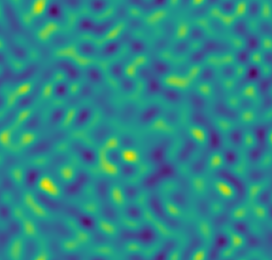
\includegraphics[interpolate=true,width=2.520000in,height=2.380000in]{burgers_solution_0.01-img0.png}}%
\end{pgfscope}%
\begin{pgfscope}%
\pgfsetbuttcap%
\pgfsetroundjoin%
\definecolor{currentfill}{rgb}{0.000000,0.000000,0.000000}%
\pgfsetfillcolor{currentfill}%
\pgfsetlinewidth{0.803000pt}%
\definecolor{currentstroke}{rgb}{0.000000,0.000000,0.000000}%
\pgfsetstrokecolor{currentstroke}%
\pgfsetdash{}{0pt}%
\pgfsys@defobject{currentmarker}{\pgfqpoint{0.000000in}{-0.048611in}}{\pgfqpoint{0.000000in}{0.000000in}}{%
\pgfpathmoveto{\pgfqpoint{0.000000in}{0.000000in}}%
\pgfpathlineto{\pgfqpoint{0.000000in}{-0.048611in}}%
\pgfusepath{stroke,fill}%
}%
\begin{pgfscope}%
\pgfsys@transformshift{0.567820in}{0.517039in}%
\pgfsys@useobject{currentmarker}{}%
\end{pgfscope}%
\end{pgfscope}%
\begin{pgfscope}%
\definecolor{textcolor}{rgb}{0.000000,0.000000,0.000000}%
\pgfsetstrokecolor{textcolor}%
\pgfsetfillcolor{textcolor}%
\pgftext[x=0.567820in,y=0.419816in,,top]{\color{textcolor}\rmfamily\fontsize{12.000000}{14.400000}\selectfont 0.0}%
\end{pgfscope}%
\begin{pgfscope}%
\pgfsetbuttcap%
\pgfsetroundjoin%
\definecolor{currentfill}{rgb}{0.000000,0.000000,0.000000}%
\pgfsetfillcolor{currentfill}%
\pgfsetlinewidth{0.803000pt}%
\definecolor{currentstroke}{rgb}{0.000000,0.000000,0.000000}%
\pgfsetstrokecolor{currentstroke}%
\pgfsetdash{}{0pt}%
\pgfsys@defobject{currentmarker}{\pgfqpoint{0.000000in}{-0.048611in}}{\pgfqpoint{0.000000in}{0.000000in}}{%
\pgfpathmoveto{\pgfqpoint{0.000000in}{0.000000in}}%
\pgfpathlineto{\pgfqpoint{0.000000in}{-0.048611in}}%
\pgfusepath{stroke,fill}%
}%
\begin{pgfscope}%
\pgfsys@transformshift{1.196524in}{0.517039in}%
\pgfsys@useobject{currentmarker}{}%
\end{pgfscope}%
\end{pgfscope}%
\begin{pgfscope}%
\definecolor{textcolor}{rgb}{0.000000,0.000000,0.000000}%
\pgfsetstrokecolor{textcolor}%
\pgfsetfillcolor{textcolor}%
\pgftext[x=1.196524in,y=0.419816in,,top]{\color{textcolor}\rmfamily\fontsize{12.000000}{14.400000}\selectfont 0.5}%
\end{pgfscope}%
\begin{pgfscope}%
\pgfsetbuttcap%
\pgfsetroundjoin%
\definecolor{currentfill}{rgb}{0.000000,0.000000,0.000000}%
\pgfsetfillcolor{currentfill}%
\pgfsetlinewidth{0.803000pt}%
\definecolor{currentstroke}{rgb}{0.000000,0.000000,0.000000}%
\pgfsetstrokecolor{currentstroke}%
\pgfsetdash{}{0pt}%
\pgfsys@defobject{currentmarker}{\pgfqpoint{0.000000in}{-0.048611in}}{\pgfqpoint{0.000000in}{0.000000in}}{%
\pgfpathmoveto{\pgfqpoint{0.000000in}{0.000000in}}%
\pgfpathlineto{\pgfqpoint{0.000000in}{-0.048611in}}%
\pgfusepath{stroke,fill}%
}%
\begin{pgfscope}%
\pgfsys@transformshift{1.825229in}{0.517039in}%
\pgfsys@useobject{currentmarker}{}%
\end{pgfscope}%
\end{pgfscope}%
\begin{pgfscope}%
\definecolor{textcolor}{rgb}{0.000000,0.000000,0.000000}%
\pgfsetstrokecolor{textcolor}%
\pgfsetfillcolor{textcolor}%
\pgftext[x=1.825229in,y=0.419816in,,top]{\color{textcolor}\rmfamily\fontsize{12.000000}{14.400000}\selectfont 1.0}%
\end{pgfscope}%
\begin{pgfscope}%
\pgfsetbuttcap%
\pgfsetroundjoin%
\definecolor{currentfill}{rgb}{0.000000,0.000000,0.000000}%
\pgfsetfillcolor{currentfill}%
\pgfsetlinewidth{0.803000pt}%
\definecolor{currentstroke}{rgb}{0.000000,0.000000,0.000000}%
\pgfsetstrokecolor{currentstroke}%
\pgfsetdash{}{0pt}%
\pgfsys@defobject{currentmarker}{\pgfqpoint{0.000000in}{-0.048611in}}{\pgfqpoint{0.000000in}{0.000000in}}{%
\pgfpathmoveto{\pgfqpoint{0.000000in}{0.000000in}}%
\pgfpathlineto{\pgfqpoint{0.000000in}{-0.048611in}}%
\pgfusepath{stroke,fill}%
}%
\begin{pgfscope}%
\pgfsys@transformshift{2.453933in}{0.517039in}%
\pgfsys@useobject{currentmarker}{}%
\end{pgfscope}%
\end{pgfscope}%
\begin{pgfscope}%
\definecolor{textcolor}{rgb}{0.000000,0.000000,0.000000}%
\pgfsetstrokecolor{textcolor}%
\pgfsetfillcolor{textcolor}%
\pgftext[x=2.453933in,y=0.419816in,,top]{\color{textcolor}\rmfamily\fontsize{12.000000}{14.400000}\selectfont 1.5}%
\end{pgfscope}%
\begin{pgfscope}%
\pgfsetbuttcap%
\pgfsetroundjoin%
\definecolor{currentfill}{rgb}{0.000000,0.000000,0.000000}%
\pgfsetfillcolor{currentfill}%
\pgfsetlinewidth{0.803000pt}%
\definecolor{currentstroke}{rgb}{0.000000,0.000000,0.000000}%
\pgfsetstrokecolor{currentstroke}%
\pgfsetdash{}{0pt}%
\pgfsys@defobject{currentmarker}{\pgfqpoint{0.000000in}{-0.048611in}}{\pgfqpoint{0.000000in}{0.000000in}}{%
\pgfpathmoveto{\pgfqpoint{0.000000in}{0.000000in}}%
\pgfpathlineto{\pgfqpoint{0.000000in}{-0.048611in}}%
\pgfusepath{stroke,fill}%
}%
\begin{pgfscope}%
\pgfsys@transformshift{3.082637in}{0.517039in}%
\pgfsys@useobject{currentmarker}{}%
\end{pgfscope}%
\end{pgfscope}%
\begin{pgfscope}%
\definecolor{textcolor}{rgb}{0.000000,0.000000,0.000000}%
\pgfsetstrokecolor{textcolor}%
\pgfsetfillcolor{textcolor}%
\pgftext[x=3.082637in,y=0.419816in,,top]{\color{textcolor}\rmfamily\fontsize{12.000000}{14.400000}\selectfont 2.0}%
\end{pgfscope}%
\begin{pgfscope}%
\definecolor{textcolor}{rgb}{0.000000,0.000000,0.000000}%
\pgfsetstrokecolor{textcolor}%
\pgfsetfillcolor{textcolor}%
\pgftext[x=1.825229in,y=0.202965in,,top]{\color{textcolor}\rmfamily\fontsize{12.000000}{14.400000}\selectfont Space}%
\end{pgfscope}%
\begin{pgfscope}%
\pgfsetbuttcap%
\pgfsetroundjoin%
\definecolor{currentfill}{rgb}{0.000000,0.000000,0.000000}%
\pgfsetfillcolor{currentfill}%
\pgfsetlinewidth{0.803000pt}%
\definecolor{currentstroke}{rgb}{0.000000,0.000000,0.000000}%
\pgfsetstrokecolor{currentstroke}%
\pgfsetdash{}{0pt}%
\pgfsys@defobject{currentmarker}{\pgfqpoint{-0.048611in}{0.000000in}}{\pgfqpoint{-0.000000in}{0.000000in}}{%
\pgfpathmoveto{\pgfqpoint{-0.000000in}{0.000000in}}%
\pgfpathlineto{\pgfqpoint{-0.048611in}{0.000000in}}%
\pgfusepath{stroke,fill}%
}%
\begin{pgfscope}%
\pgfsys@transformshift{0.567820in}{0.517039in}%
\pgfsys@useobject{currentmarker}{}%
\end{pgfscope}%
\end{pgfscope}%
\begin{pgfscope}%
\definecolor{textcolor}{rgb}{0.000000,0.000000,0.000000}%
\pgfsetstrokecolor{textcolor}%
\pgfsetfillcolor{textcolor}%
\pgftext[x=0.364559in, y=0.453725in, left, base]{\color{textcolor}\rmfamily\fontsize{12.000000}{14.400000}\selectfont 0}%
\end{pgfscope}%
\begin{pgfscope}%
\pgfsetbuttcap%
\pgfsetroundjoin%
\definecolor{currentfill}{rgb}{0.000000,0.000000,0.000000}%
\pgfsetfillcolor{currentfill}%
\pgfsetlinewidth{0.803000pt}%
\definecolor{currentstroke}{rgb}{0.000000,0.000000,0.000000}%
\pgfsetstrokecolor{currentstroke}%
\pgfsetdash{}{0pt}%
\pgfsys@defobject{currentmarker}{\pgfqpoint{-0.048611in}{0.000000in}}{\pgfqpoint{-0.000000in}{0.000000in}}{%
\pgfpathmoveto{\pgfqpoint{-0.000000in}{0.000000in}}%
\pgfpathlineto{\pgfqpoint{-0.048611in}{0.000000in}}%
\pgfusepath{stroke,fill}%
}%
\begin{pgfscope}%
\pgfsys@transformshift{0.567820in}{0.992634in}%
\pgfsys@useobject{currentmarker}{}%
\end{pgfscope}%
\end{pgfscope}%
\begin{pgfscope}%
\definecolor{textcolor}{rgb}{0.000000,0.000000,0.000000}%
\pgfsetstrokecolor{textcolor}%
\pgfsetfillcolor{textcolor}%
\pgftext[x=0.364559in, y=0.929320in, left, base]{\color{textcolor}\rmfamily\fontsize{12.000000}{14.400000}\selectfont 2}%
\end{pgfscope}%
\begin{pgfscope}%
\pgfsetbuttcap%
\pgfsetroundjoin%
\definecolor{currentfill}{rgb}{0.000000,0.000000,0.000000}%
\pgfsetfillcolor{currentfill}%
\pgfsetlinewidth{0.803000pt}%
\definecolor{currentstroke}{rgb}{0.000000,0.000000,0.000000}%
\pgfsetstrokecolor{currentstroke}%
\pgfsetdash{}{0pt}%
\pgfsys@defobject{currentmarker}{\pgfqpoint{-0.048611in}{0.000000in}}{\pgfqpoint{-0.000000in}{0.000000in}}{%
\pgfpathmoveto{\pgfqpoint{-0.000000in}{0.000000in}}%
\pgfpathlineto{\pgfqpoint{-0.048611in}{0.000000in}}%
\pgfusepath{stroke,fill}%
}%
\begin{pgfscope}%
\pgfsys@transformshift{0.567820in}{1.468230in}%
\pgfsys@useobject{currentmarker}{}%
\end{pgfscope}%
\end{pgfscope}%
\begin{pgfscope}%
\definecolor{textcolor}{rgb}{0.000000,0.000000,0.000000}%
\pgfsetstrokecolor{textcolor}%
\pgfsetfillcolor{textcolor}%
\pgftext[x=0.364559in, y=1.404916in, left, base]{\color{textcolor}\rmfamily\fontsize{12.000000}{14.400000}\selectfont 4}%
\end{pgfscope}%
\begin{pgfscope}%
\pgfsetbuttcap%
\pgfsetroundjoin%
\definecolor{currentfill}{rgb}{0.000000,0.000000,0.000000}%
\pgfsetfillcolor{currentfill}%
\pgfsetlinewidth{0.803000pt}%
\definecolor{currentstroke}{rgb}{0.000000,0.000000,0.000000}%
\pgfsetstrokecolor{currentstroke}%
\pgfsetdash{}{0pt}%
\pgfsys@defobject{currentmarker}{\pgfqpoint{-0.048611in}{0.000000in}}{\pgfqpoint{-0.000000in}{0.000000in}}{%
\pgfpathmoveto{\pgfqpoint{-0.000000in}{0.000000in}}%
\pgfpathlineto{\pgfqpoint{-0.048611in}{0.000000in}}%
\pgfusepath{stroke,fill}%
}%
\begin{pgfscope}%
\pgfsys@transformshift{0.567820in}{1.943825in}%
\pgfsys@useobject{currentmarker}{}%
\end{pgfscope}%
\end{pgfscope}%
\begin{pgfscope}%
\definecolor{textcolor}{rgb}{0.000000,0.000000,0.000000}%
\pgfsetstrokecolor{textcolor}%
\pgfsetfillcolor{textcolor}%
\pgftext[x=0.364559in, y=1.880511in, left, base]{\color{textcolor}\rmfamily\fontsize{12.000000}{14.400000}\selectfont 6}%
\end{pgfscope}%
\begin{pgfscope}%
\pgfsetbuttcap%
\pgfsetroundjoin%
\definecolor{currentfill}{rgb}{0.000000,0.000000,0.000000}%
\pgfsetfillcolor{currentfill}%
\pgfsetlinewidth{0.803000pt}%
\definecolor{currentstroke}{rgb}{0.000000,0.000000,0.000000}%
\pgfsetstrokecolor{currentstroke}%
\pgfsetdash{}{0pt}%
\pgfsys@defobject{currentmarker}{\pgfqpoint{-0.048611in}{0.000000in}}{\pgfqpoint{-0.000000in}{0.000000in}}{%
\pgfpathmoveto{\pgfqpoint{-0.000000in}{0.000000in}}%
\pgfpathlineto{\pgfqpoint{-0.048611in}{0.000000in}}%
\pgfusepath{stroke,fill}%
}%
\begin{pgfscope}%
\pgfsys@transformshift{0.567820in}{2.419421in}%
\pgfsys@useobject{currentmarker}{}%
\end{pgfscope}%
\end{pgfscope}%
\begin{pgfscope}%
\definecolor{textcolor}{rgb}{0.000000,0.000000,0.000000}%
\pgfsetstrokecolor{textcolor}%
\pgfsetfillcolor{textcolor}%
\pgftext[x=0.364559in, y=2.356107in, left, base]{\color{textcolor}\rmfamily\fontsize{12.000000}{14.400000}\selectfont 8}%
\end{pgfscope}%
\begin{pgfscope}%
\pgfsetbuttcap%
\pgfsetroundjoin%
\definecolor{currentfill}{rgb}{0.000000,0.000000,0.000000}%
\pgfsetfillcolor{currentfill}%
\pgfsetlinewidth{0.803000pt}%
\definecolor{currentstroke}{rgb}{0.000000,0.000000,0.000000}%
\pgfsetstrokecolor{currentstroke}%
\pgfsetdash{}{0pt}%
\pgfsys@defobject{currentmarker}{\pgfqpoint{-0.048611in}{0.000000in}}{\pgfqpoint{-0.000000in}{0.000000in}}{%
\pgfpathmoveto{\pgfqpoint{-0.000000in}{0.000000in}}%
\pgfpathlineto{\pgfqpoint{-0.048611in}{0.000000in}}%
\pgfusepath{stroke,fill}%
}%
\begin{pgfscope}%
\pgfsys@transformshift{0.567820in}{2.895016in}%
\pgfsys@useobject{currentmarker}{}%
\end{pgfscope}%
\end{pgfscope}%
\begin{pgfscope}%
\definecolor{textcolor}{rgb}{0.000000,0.000000,0.000000}%
\pgfsetstrokecolor{textcolor}%
\pgfsetfillcolor{textcolor}%
\pgftext[x=0.258521in, y=2.831702in, left, base]{\color{textcolor}\rmfamily\fontsize{12.000000}{14.400000}\selectfont 10}%
\end{pgfscope}%
\begin{pgfscope}%
\definecolor{textcolor}{rgb}{0.000000,0.000000,0.000000}%
\pgfsetstrokecolor{textcolor}%
\pgfsetfillcolor{textcolor}%
\pgftext[x=0.202965in,y=1.706027in,,bottom,rotate=90.000000]{\color{textcolor}\rmfamily\fontsize{12.000000}{14.400000}\selectfont Time}%
\end{pgfscope}%
\begin{pgfscope}%
\pgfsetrectcap%
\pgfsetmiterjoin%
\pgfsetlinewidth{0.803000pt}%
\definecolor{currentstroke}{rgb}{0.000000,0.000000,0.000000}%
\pgfsetstrokecolor{currentstroke}%
\pgfsetdash{}{0pt}%
\pgfpathmoveto{\pgfqpoint{0.567820in}{0.517039in}}%
\pgfpathlineto{\pgfqpoint{0.567820in}{2.895016in}}%
\pgfusepath{stroke}%
\end{pgfscope}%
\begin{pgfscope}%
\pgfsetrectcap%
\pgfsetmiterjoin%
\pgfsetlinewidth{0.803000pt}%
\definecolor{currentstroke}{rgb}{0.000000,0.000000,0.000000}%
\pgfsetstrokecolor{currentstroke}%
\pgfsetdash{}{0pt}%
\pgfpathmoveto{\pgfqpoint{3.082637in}{0.517039in}}%
\pgfpathlineto{\pgfqpoint{3.082637in}{2.895016in}}%
\pgfusepath{stroke}%
\end{pgfscope}%
\begin{pgfscope}%
\pgfsetrectcap%
\pgfsetmiterjoin%
\pgfsetlinewidth{0.803000pt}%
\definecolor{currentstroke}{rgb}{0.000000,0.000000,0.000000}%
\pgfsetstrokecolor{currentstroke}%
\pgfsetdash{}{0pt}%
\pgfpathmoveto{\pgfqpoint{0.567820in}{0.517039in}}%
\pgfpathlineto{\pgfqpoint{3.082637in}{0.517039in}}%
\pgfusepath{stroke}%
\end{pgfscope}%
\begin{pgfscope}%
\pgfsetrectcap%
\pgfsetmiterjoin%
\pgfsetlinewidth{0.803000pt}%
\definecolor{currentstroke}{rgb}{0.000000,0.000000,0.000000}%
\pgfsetstrokecolor{currentstroke}%
\pgfsetdash{}{0pt}%
\pgfpathmoveto{\pgfqpoint{0.567820in}{2.895016in}}%
\pgfpathlineto{\pgfqpoint{3.082637in}{2.895016in}}%
\pgfusepath{stroke}%
\end{pgfscope}%
\begin{pgfscope}%
\pgfsetbuttcap%
\pgfsetmiterjoin%
\pgfsetlinewidth{0.000000pt}%
\definecolor{currentstroke}{rgb}{0.000000,0.000000,0.000000}%
\pgfsetstrokecolor{currentstroke}%
\pgfsetstrokeopacity{0.000000}%
\pgfsetdash{}{0pt}%
\pgfpathmoveto{\pgfqpoint{3.340906in}{0.517039in}}%
\pgfpathlineto{\pgfqpoint{3.459805in}{0.517039in}}%
\pgfpathlineto{\pgfqpoint{3.459805in}{2.895016in}}%
\pgfpathlineto{\pgfqpoint{3.340906in}{2.895016in}}%
\pgfpathlineto{\pgfqpoint{3.340906in}{0.517039in}}%
\pgfpathclose%
\pgfusepath{}%
\end{pgfscope}%
\begin{pgfscope}%
\pgfsys@transformshift{3.340000in}{0.520000in}%
\pgftext[left,bottom]{
\includegraphics[interpolate=true,width=0.120000in,height=2.380000in]{burgers_solution_0.01-img1.png}}%
\end{pgfscope}%
\begin{pgfscope}%
\pgfsetbuttcap%
\pgfsetroundjoin%
\definecolor{currentfill}{rgb}{0.000000,0.000000,0.000000}%
\pgfsetfillcolor{currentfill}%
\pgfsetlinewidth{0.803000pt}%
\definecolor{currentstroke}{rgb}{0.000000,0.000000,0.000000}%
\pgfsetstrokecolor{currentstroke}%
\pgfsetdash{}{0pt}%
\pgfsys@defobject{currentmarker}{\pgfqpoint{0.000000in}{0.000000in}}{\pgfqpoint{0.048611in}{0.000000in}}{%
\pgfpathmoveto{\pgfqpoint{0.000000in}{0.000000in}}%
\pgfpathlineto{\pgfqpoint{0.048611in}{0.000000in}}%
\pgfusepath{stroke,fill}%
}%
\begin{pgfscope}%
\pgfsys@transformshift{3.459805in}{0.555741in}%
\pgfsys@useobject{currentmarker}{}%
\end{pgfscope}%
\end{pgfscope}%
\begin{pgfscope}%
\definecolor{textcolor}{rgb}{0.000000,0.000000,0.000000}%
\pgfsetstrokecolor{textcolor}%
\pgfsetfillcolor{textcolor}%
\pgftext[x=3.557027in, y=0.492427in, left, base]{\color{textcolor}\rmfamily\fontsize{12.000000}{14.400000}\selectfont \ensuremath{-}0.6}%
\end{pgfscope}%
\begin{pgfscope}%
\pgfsetbuttcap%
\pgfsetroundjoin%
\definecolor{currentfill}{rgb}{0.000000,0.000000,0.000000}%
\pgfsetfillcolor{currentfill}%
\pgfsetlinewidth{0.803000pt}%
\definecolor{currentstroke}{rgb}{0.000000,0.000000,0.000000}%
\pgfsetstrokecolor{currentstroke}%
\pgfsetdash{}{0pt}%
\pgfsys@defobject{currentmarker}{\pgfqpoint{0.000000in}{0.000000in}}{\pgfqpoint{0.048611in}{0.000000in}}{%
\pgfpathmoveto{\pgfqpoint{0.000000in}{0.000000in}}%
\pgfpathlineto{\pgfqpoint{0.048611in}{0.000000in}}%
\pgfusepath{stroke,fill}%
}%
\begin{pgfscope}%
\pgfsys@transformshift{3.459805in}{0.932008in}%
\pgfsys@useobject{currentmarker}{}%
\end{pgfscope}%
\end{pgfscope}%
\begin{pgfscope}%
\definecolor{textcolor}{rgb}{0.000000,0.000000,0.000000}%
\pgfsetstrokecolor{textcolor}%
\pgfsetfillcolor{textcolor}%
\pgftext[x=3.557027in, y=0.868694in, left, base]{\color{textcolor}\rmfamily\fontsize{12.000000}{14.400000}\selectfont \ensuremath{-}0.4}%
\end{pgfscope}%
\begin{pgfscope}%
\pgfsetbuttcap%
\pgfsetroundjoin%
\definecolor{currentfill}{rgb}{0.000000,0.000000,0.000000}%
\pgfsetfillcolor{currentfill}%
\pgfsetlinewidth{0.803000pt}%
\definecolor{currentstroke}{rgb}{0.000000,0.000000,0.000000}%
\pgfsetstrokecolor{currentstroke}%
\pgfsetdash{}{0pt}%
\pgfsys@defobject{currentmarker}{\pgfqpoint{0.000000in}{0.000000in}}{\pgfqpoint{0.048611in}{0.000000in}}{%
\pgfpathmoveto{\pgfqpoint{0.000000in}{0.000000in}}%
\pgfpathlineto{\pgfqpoint{0.048611in}{0.000000in}}%
\pgfusepath{stroke,fill}%
}%
\begin{pgfscope}%
\pgfsys@transformshift{3.459805in}{1.308274in}%
\pgfsys@useobject{currentmarker}{}%
\end{pgfscope}%
\end{pgfscope}%
\begin{pgfscope}%
\definecolor{textcolor}{rgb}{0.000000,0.000000,0.000000}%
\pgfsetstrokecolor{textcolor}%
\pgfsetfillcolor{textcolor}%
\pgftext[x=3.557027in, y=1.244961in, left, base]{\color{textcolor}\rmfamily\fontsize{12.000000}{14.400000}\selectfont \ensuremath{-}0.2}%
\end{pgfscope}%
\begin{pgfscope}%
\pgfsetbuttcap%
\pgfsetroundjoin%
\definecolor{currentfill}{rgb}{0.000000,0.000000,0.000000}%
\pgfsetfillcolor{currentfill}%
\pgfsetlinewidth{0.803000pt}%
\definecolor{currentstroke}{rgb}{0.000000,0.000000,0.000000}%
\pgfsetstrokecolor{currentstroke}%
\pgfsetdash{}{0pt}%
\pgfsys@defobject{currentmarker}{\pgfqpoint{0.000000in}{0.000000in}}{\pgfqpoint{0.048611in}{0.000000in}}{%
\pgfpathmoveto{\pgfqpoint{0.000000in}{0.000000in}}%
\pgfpathlineto{\pgfqpoint{0.048611in}{0.000000in}}%
\pgfusepath{stroke,fill}%
}%
\begin{pgfscope}%
\pgfsys@transformshift{3.459805in}{1.684541in}%
\pgfsys@useobject{currentmarker}{}%
\end{pgfscope}%
\end{pgfscope}%
\begin{pgfscope}%
\definecolor{textcolor}{rgb}{0.000000,0.000000,0.000000}%
\pgfsetstrokecolor{textcolor}%
\pgfsetfillcolor{textcolor}%
\pgftext[x=3.557027in, y=1.621228in, left, base]{\color{textcolor}\rmfamily\fontsize{12.000000}{14.400000}\selectfont 0.0}%
\end{pgfscope}%
\begin{pgfscope}%
\pgfsetbuttcap%
\pgfsetroundjoin%
\definecolor{currentfill}{rgb}{0.000000,0.000000,0.000000}%
\pgfsetfillcolor{currentfill}%
\pgfsetlinewidth{0.803000pt}%
\definecolor{currentstroke}{rgb}{0.000000,0.000000,0.000000}%
\pgfsetstrokecolor{currentstroke}%
\pgfsetdash{}{0pt}%
\pgfsys@defobject{currentmarker}{\pgfqpoint{0.000000in}{0.000000in}}{\pgfqpoint{0.048611in}{0.000000in}}{%
\pgfpathmoveto{\pgfqpoint{0.000000in}{0.000000in}}%
\pgfpathlineto{\pgfqpoint{0.048611in}{0.000000in}}%
\pgfusepath{stroke,fill}%
}%
\begin{pgfscope}%
\pgfsys@transformshift{3.459805in}{2.060808in}%
\pgfsys@useobject{currentmarker}{}%
\end{pgfscope}%
\end{pgfscope}%
\begin{pgfscope}%
\definecolor{textcolor}{rgb}{0.000000,0.000000,0.000000}%
\pgfsetstrokecolor{textcolor}%
\pgfsetfillcolor{textcolor}%
\pgftext[x=3.557027in, y=1.997494in, left, base]{\color{textcolor}\rmfamily\fontsize{12.000000}{14.400000}\selectfont 0.2}%
\end{pgfscope}%
\begin{pgfscope}%
\pgfsetbuttcap%
\pgfsetroundjoin%
\definecolor{currentfill}{rgb}{0.000000,0.000000,0.000000}%
\pgfsetfillcolor{currentfill}%
\pgfsetlinewidth{0.803000pt}%
\definecolor{currentstroke}{rgb}{0.000000,0.000000,0.000000}%
\pgfsetstrokecolor{currentstroke}%
\pgfsetdash{}{0pt}%
\pgfsys@defobject{currentmarker}{\pgfqpoint{0.000000in}{0.000000in}}{\pgfqpoint{0.048611in}{0.000000in}}{%
\pgfpathmoveto{\pgfqpoint{0.000000in}{0.000000in}}%
\pgfpathlineto{\pgfqpoint{0.048611in}{0.000000in}}%
\pgfusepath{stroke,fill}%
}%
\begin{pgfscope}%
\pgfsys@transformshift{3.459805in}{2.437075in}%
\pgfsys@useobject{currentmarker}{}%
\end{pgfscope}%
\end{pgfscope}%
\begin{pgfscope}%
\definecolor{textcolor}{rgb}{0.000000,0.000000,0.000000}%
\pgfsetstrokecolor{textcolor}%
\pgfsetfillcolor{textcolor}%
\pgftext[x=3.557027in, y=2.373761in, left, base]{\color{textcolor}\rmfamily\fontsize{12.000000}{14.400000}\selectfont 0.4}%
\end{pgfscope}%
\begin{pgfscope}%
\pgfsetbuttcap%
\pgfsetroundjoin%
\definecolor{currentfill}{rgb}{0.000000,0.000000,0.000000}%
\pgfsetfillcolor{currentfill}%
\pgfsetlinewidth{0.803000pt}%
\definecolor{currentstroke}{rgb}{0.000000,0.000000,0.000000}%
\pgfsetstrokecolor{currentstroke}%
\pgfsetdash{}{0pt}%
\pgfsys@defobject{currentmarker}{\pgfqpoint{0.000000in}{0.000000in}}{\pgfqpoint{0.048611in}{0.000000in}}{%
\pgfpathmoveto{\pgfqpoint{0.000000in}{0.000000in}}%
\pgfpathlineto{\pgfqpoint{0.048611in}{0.000000in}}%
\pgfusepath{stroke,fill}%
}%
\begin{pgfscope}%
\pgfsys@transformshift{3.459805in}{2.813342in}%
\pgfsys@useobject{currentmarker}{}%
\end{pgfscope}%
\end{pgfscope}%
\begin{pgfscope}%
\definecolor{textcolor}{rgb}{0.000000,0.000000,0.000000}%
\pgfsetstrokecolor{textcolor}%
\pgfsetfillcolor{textcolor}%
\pgftext[x=3.557027in, y=2.750028in, left, base]{\color{textcolor}\rmfamily\fontsize{12.000000}{14.400000}\selectfont 0.6}%
\end{pgfscope}%
\begin{pgfscope}%
\pgfsetrectcap%
\pgfsetmiterjoin%
\pgfsetlinewidth{0.803000pt}%
\definecolor{currentstroke}{rgb}{0.000000,0.000000,0.000000}%
\pgfsetstrokecolor{currentstroke}%
\pgfsetdash{}{0pt}%
\pgfpathmoveto{\pgfqpoint{3.340906in}{0.517039in}}%
\pgfpathlineto{\pgfqpoint{3.400355in}{0.517039in}}%
\pgfpathlineto{\pgfqpoint{3.459805in}{0.517039in}}%
\pgfpathlineto{\pgfqpoint{3.459805in}{2.895016in}}%
\pgfpathlineto{\pgfqpoint{3.400355in}{2.895016in}}%
\pgfpathlineto{\pgfqpoint{3.340906in}{2.895016in}}%
\pgfpathlineto{\pgfqpoint{3.340906in}{0.517039in}}%
\pgfpathclose%
\pgfusepath{stroke}%
\end{pgfscope}%
\end{pgfpicture}%
\makeatother%
\endgroup%

    \end{adjustbox}
    \caption{Solution function for \(\nu=0.01\).}\label{fig:burgers_solution_0.01}
  \end{subfigure}
  \begin{subfigure}{0.49\linewidth}
    \begin{adjustbox}{width=\linewidth}
      \begingroup%
\makeatletter%
\begin{pgfpicture}%
\pgfpathrectangle{\pgfpointorigin}{\pgfqpoint{4.000000in}{3.000000in}}%
\pgfusepath{use as bounding box, clip}%
\begin{pgfscope}%
\pgfsetbuttcap%
\pgfsetmiterjoin%
\pgfsetlinewidth{0.000000pt}%
\definecolor{currentstroke}{rgb}{0.000000,0.000000,0.000000}%
\pgfsetstrokecolor{currentstroke}%
\pgfsetstrokeopacity{0.000000}%
\pgfsetdash{}{0pt}%
\pgfpathmoveto{\pgfqpoint{0.000000in}{0.000000in}}%
\pgfpathlineto{\pgfqpoint{4.000000in}{0.000000in}}%
\pgfpathlineto{\pgfqpoint{4.000000in}{3.000000in}}%
\pgfpathlineto{\pgfqpoint{0.000000in}{3.000000in}}%
\pgfpathlineto{\pgfqpoint{0.000000in}{0.000000in}}%
\pgfpathclose%
\pgfusepath{}%
\end{pgfscope}%
\begin{pgfscope}%
\pgfsetbuttcap%
\pgfsetmiterjoin%
\pgfsetlinewidth{0.000000pt}%
\definecolor{currentstroke}{rgb}{0.000000,0.000000,0.000000}%
\pgfsetstrokecolor{currentstroke}%
\pgfsetstrokeopacity{0.000000}%
\pgfsetdash{}{0pt}%
\pgfpathmoveto{\pgfqpoint{0.567820in}{0.517039in}}%
\pgfpathlineto{\pgfqpoint{3.082637in}{0.517039in}}%
\pgfpathlineto{\pgfqpoint{3.082637in}{2.895016in}}%
\pgfpathlineto{\pgfqpoint{0.567820in}{2.895016in}}%
\pgfpathlineto{\pgfqpoint{0.567820in}{0.517039in}}%
\pgfpathclose%
\pgfusepath{}%
\end{pgfscope}%
\begin{pgfscope}%
\pgfpathrectangle{\pgfqpoint{0.567820in}{0.517039in}}{\pgfqpoint{2.514817in}{2.377978in}}%
\pgfusepath{clip}%
\pgfsys@transformshift{0.567820in}{0.517039in}%
\pgftext[left,bottom]{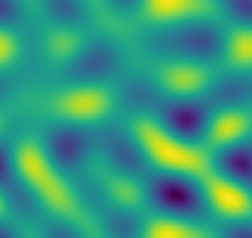
\includegraphics[interpolate=true,width=2.520000in,height=2.380000in]{burgers_forcing_0.01-img0.png}}%
\end{pgfscope}%
\begin{pgfscope}%
\pgfsetbuttcap%
\pgfsetroundjoin%
\definecolor{currentfill}{rgb}{0.000000,0.000000,0.000000}%
\pgfsetfillcolor{currentfill}%
\pgfsetlinewidth{0.803000pt}%
\definecolor{currentstroke}{rgb}{0.000000,0.000000,0.000000}%
\pgfsetstrokecolor{currentstroke}%
\pgfsetdash{}{0pt}%
\pgfsys@defobject{currentmarker}{\pgfqpoint{0.000000in}{-0.048611in}}{\pgfqpoint{0.000000in}{0.000000in}}{%
\pgfpathmoveto{\pgfqpoint{0.000000in}{0.000000in}}%
\pgfpathlineto{\pgfqpoint{0.000000in}{-0.048611in}}%
\pgfusepath{stroke,fill}%
}%
\begin{pgfscope}%
\pgfsys@transformshift{0.567820in}{0.517039in}%
\pgfsys@useobject{currentmarker}{}%
\end{pgfscope}%
\end{pgfscope}%
\begin{pgfscope}%
\definecolor{textcolor}{rgb}{0.000000,0.000000,0.000000}%
\pgfsetstrokecolor{textcolor}%
\pgfsetfillcolor{textcolor}%
\pgftext[x=0.567820in,y=0.419816in,,top]{\color{textcolor}\rmfamily\fontsize{12.000000}{14.400000}\selectfont 0.0}%
\end{pgfscope}%
\begin{pgfscope}%
\pgfsetbuttcap%
\pgfsetroundjoin%
\definecolor{currentfill}{rgb}{0.000000,0.000000,0.000000}%
\pgfsetfillcolor{currentfill}%
\pgfsetlinewidth{0.803000pt}%
\definecolor{currentstroke}{rgb}{0.000000,0.000000,0.000000}%
\pgfsetstrokecolor{currentstroke}%
\pgfsetdash{}{0pt}%
\pgfsys@defobject{currentmarker}{\pgfqpoint{0.000000in}{-0.048611in}}{\pgfqpoint{0.000000in}{0.000000in}}{%
\pgfpathmoveto{\pgfqpoint{0.000000in}{0.000000in}}%
\pgfpathlineto{\pgfqpoint{0.000000in}{-0.048611in}}%
\pgfusepath{stroke,fill}%
}%
\begin{pgfscope}%
\pgfsys@transformshift{1.196524in}{0.517039in}%
\pgfsys@useobject{currentmarker}{}%
\end{pgfscope}%
\end{pgfscope}%
\begin{pgfscope}%
\definecolor{textcolor}{rgb}{0.000000,0.000000,0.000000}%
\pgfsetstrokecolor{textcolor}%
\pgfsetfillcolor{textcolor}%
\pgftext[x=1.196524in,y=0.419816in,,top]{\color{textcolor}\rmfamily\fontsize{12.000000}{14.400000}\selectfont 0.5}%
\end{pgfscope}%
\begin{pgfscope}%
\pgfsetbuttcap%
\pgfsetroundjoin%
\definecolor{currentfill}{rgb}{0.000000,0.000000,0.000000}%
\pgfsetfillcolor{currentfill}%
\pgfsetlinewidth{0.803000pt}%
\definecolor{currentstroke}{rgb}{0.000000,0.000000,0.000000}%
\pgfsetstrokecolor{currentstroke}%
\pgfsetdash{}{0pt}%
\pgfsys@defobject{currentmarker}{\pgfqpoint{0.000000in}{-0.048611in}}{\pgfqpoint{0.000000in}{0.000000in}}{%
\pgfpathmoveto{\pgfqpoint{0.000000in}{0.000000in}}%
\pgfpathlineto{\pgfqpoint{0.000000in}{-0.048611in}}%
\pgfusepath{stroke,fill}%
}%
\begin{pgfscope}%
\pgfsys@transformshift{1.825229in}{0.517039in}%
\pgfsys@useobject{currentmarker}{}%
\end{pgfscope}%
\end{pgfscope}%
\begin{pgfscope}%
\definecolor{textcolor}{rgb}{0.000000,0.000000,0.000000}%
\pgfsetstrokecolor{textcolor}%
\pgfsetfillcolor{textcolor}%
\pgftext[x=1.825229in,y=0.419816in,,top]{\color{textcolor}\rmfamily\fontsize{12.000000}{14.400000}\selectfont 1.0}%
\end{pgfscope}%
\begin{pgfscope}%
\pgfsetbuttcap%
\pgfsetroundjoin%
\definecolor{currentfill}{rgb}{0.000000,0.000000,0.000000}%
\pgfsetfillcolor{currentfill}%
\pgfsetlinewidth{0.803000pt}%
\definecolor{currentstroke}{rgb}{0.000000,0.000000,0.000000}%
\pgfsetstrokecolor{currentstroke}%
\pgfsetdash{}{0pt}%
\pgfsys@defobject{currentmarker}{\pgfqpoint{0.000000in}{-0.048611in}}{\pgfqpoint{0.000000in}{0.000000in}}{%
\pgfpathmoveto{\pgfqpoint{0.000000in}{0.000000in}}%
\pgfpathlineto{\pgfqpoint{0.000000in}{-0.048611in}}%
\pgfusepath{stroke,fill}%
}%
\begin{pgfscope}%
\pgfsys@transformshift{2.453933in}{0.517039in}%
\pgfsys@useobject{currentmarker}{}%
\end{pgfscope}%
\end{pgfscope}%
\begin{pgfscope}%
\definecolor{textcolor}{rgb}{0.000000,0.000000,0.000000}%
\pgfsetstrokecolor{textcolor}%
\pgfsetfillcolor{textcolor}%
\pgftext[x=2.453933in,y=0.419816in,,top]{\color{textcolor}\rmfamily\fontsize{12.000000}{14.400000}\selectfont 1.5}%
\end{pgfscope}%
\begin{pgfscope}%
\pgfsetbuttcap%
\pgfsetroundjoin%
\definecolor{currentfill}{rgb}{0.000000,0.000000,0.000000}%
\pgfsetfillcolor{currentfill}%
\pgfsetlinewidth{0.803000pt}%
\definecolor{currentstroke}{rgb}{0.000000,0.000000,0.000000}%
\pgfsetstrokecolor{currentstroke}%
\pgfsetdash{}{0pt}%
\pgfsys@defobject{currentmarker}{\pgfqpoint{0.000000in}{-0.048611in}}{\pgfqpoint{0.000000in}{0.000000in}}{%
\pgfpathmoveto{\pgfqpoint{0.000000in}{0.000000in}}%
\pgfpathlineto{\pgfqpoint{0.000000in}{-0.048611in}}%
\pgfusepath{stroke,fill}%
}%
\begin{pgfscope}%
\pgfsys@transformshift{3.082637in}{0.517039in}%
\pgfsys@useobject{currentmarker}{}%
\end{pgfscope}%
\end{pgfscope}%
\begin{pgfscope}%
\definecolor{textcolor}{rgb}{0.000000,0.000000,0.000000}%
\pgfsetstrokecolor{textcolor}%
\pgfsetfillcolor{textcolor}%
\pgftext[x=3.082637in,y=0.419816in,,top]{\color{textcolor}\rmfamily\fontsize{12.000000}{14.400000}\selectfont 2.0}%
\end{pgfscope}%
\begin{pgfscope}%
\definecolor{textcolor}{rgb}{0.000000,0.000000,0.000000}%
\pgfsetstrokecolor{textcolor}%
\pgfsetfillcolor{textcolor}%
\pgftext[x=1.825229in,y=0.202965in,,top]{\color{textcolor}\rmfamily\fontsize{12.000000}{14.400000}\selectfont Space}%
\end{pgfscope}%
\begin{pgfscope}%
\pgfsetbuttcap%
\pgfsetroundjoin%
\definecolor{currentfill}{rgb}{0.000000,0.000000,0.000000}%
\pgfsetfillcolor{currentfill}%
\pgfsetlinewidth{0.803000pt}%
\definecolor{currentstroke}{rgb}{0.000000,0.000000,0.000000}%
\pgfsetstrokecolor{currentstroke}%
\pgfsetdash{}{0pt}%
\pgfsys@defobject{currentmarker}{\pgfqpoint{-0.048611in}{0.000000in}}{\pgfqpoint{-0.000000in}{0.000000in}}{%
\pgfpathmoveto{\pgfqpoint{-0.000000in}{0.000000in}}%
\pgfpathlineto{\pgfqpoint{-0.048611in}{0.000000in}}%
\pgfusepath{stroke,fill}%
}%
\begin{pgfscope}%
\pgfsys@transformshift{0.567820in}{0.517039in}%
\pgfsys@useobject{currentmarker}{}%
\end{pgfscope}%
\end{pgfscope}%
\begin{pgfscope}%
\definecolor{textcolor}{rgb}{0.000000,0.000000,0.000000}%
\pgfsetstrokecolor{textcolor}%
\pgfsetfillcolor{textcolor}%
\pgftext[x=0.364559in, y=0.453725in, left, base]{\color{textcolor}\rmfamily\fontsize{12.000000}{14.400000}\selectfont 0}%
\end{pgfscope}%
\begin{pgfscope}%
\pgfsetbuttcap%
\pgfsetroundjoin%
\definecolor{currentfill}{rgb}{0.000000,0.000000,0.000000}%
\pgfsetfillcolor{currentfill}%
\pgfsetlinewidth{0.803000pt}%
\definecolor{currentstroke}{rgb}{0.000000,0.000000,0.000000}%
\pgfsetstrokecolor{currentstroke}%
\pgfsetdash{}{0pt}%
\pgfsys@defobject{currentmarker}{\pgfqpoint{-0.048611in}{0.000000in}}{\pgfqpoint{-0.000000in}{0.000000in}}{%
\pgfpathmoveto{\pgfqpoint{-0.000000in}{0.000000in}}%
\pgfpathlineto{\pgfqpoint{-0.048611in}{0.000000in}}%
\pgfusepath{stroke,fill}%
}%
\begin{pgfscope}%
\pgfsys@transformshift{0.567820in}{0.992634in}%
\pgfsys@useobject{currentmarker}{}%
\end{pgfscope}%
\end{pgfscope}%
\begin{pgfscope}%
\definecolor{textcolor}{rgb}{0.000000,0.000000,0.000000}%
\pgfsetstrokecolor{textcolor}%
\pgfsetfillcolor{textcolor}%
\pgftext[x=0.364559in, y=0.929320in, left, base]{\color{textcolor}\rmfamily\fontsize{12.000000}{14.400000}\selectfont 2}%
\end{pgfscope}%
\begin{pgfscope}%
\pgfsetbuttcap%
\pgfsetroundjoin%
\definecolor{currentfill}{rgb}{0.000000,0.000000,0.000000}%
\pgfsetfillcolor{currentfill}%
\pgfsetlinewidth{0.803000pt}%
\definecolor{currentstroke}{rgb}{0.000000,0.000000,0.000000}%
\pgfsetstrokecolor{currentstroke}%
\pgfsetdash{}{0pt}%
\pgfsys@defobject{currentmarker}{\pgfqpoint{-0.048611in}{0.000000in}}{\pgfqpoint{-0.000000in}{0.000000in}}{%
\pgfpathmoveto{\pgfqpoint{-0.000000in}{0.000000in}}%
\pgfpathlineto{\pgfqpoint{-0.048611in}{0.000000in}}%
\pgfusepath{stroke,fill}%
}%
\begin{pgfscope}%
\pgfsys@transformshift{0.567820in}{1.468230in}%
\pgfsys@useobject{currentmarker}{}%
\end{pgfscope}%
\end{pgfscope}%
\begin{pgfscope}%
\definecolor{textcolor}{rgb}{0.000000,0.000000,0.000000}%
\pgfsetstrokecolor{textcolor}%
\pgfsetfillcolor{textcolor}%
\pgftext[x=0.364559in, y=1.404916in, left, base]{\color{textcolor}\rmfamily\fontsize{12.000000}{14.400000}\selectfont 4}%
\end{pgfscope}%
\begin{pgfscope}%
\pgfsetbuttcap%
\pgfsetroundjoin%
\definecolor{currentfill}{rgb}{0.000000,0.000000,0.000000}%
\pgfsetfillcolor{currentfill}%
\pgfsetlinewidth{0.803000pt}%
\definecolor{currentstroke}{rgb}{0.000000,0.000000,0.000000}%
\pgfsetstrokecolor{currentstroke}%
\pgfsetdash{}{0pt}%
\pgfsys@defobject{currentmarker}{\pgfqpoint{-0.048611in}{0.000000in}}{\pgfqpoint{-0.000000in}{0.000000in}}{%
\pgfpathmoveto{\pgfqpoint{-0.000000in}{0.000000in}}%
\pgfpathlineto{\pgfqpoint{-0.048611in}{0.000000in}}%
\pgfusepath{stroke,fill}%
}%
\begin{pgfscope}%
\pgfsys@transformshift{0.567820in}{1.943825in}%
\pgfsys@useobject{currentmarker}{}%
\end{pgfscope}%
\end{pgfscope}%
\begin{pgfscope}%
\definecolor{textcolor}{rgb}{0.000000,0.000000,0.000000}%
\pgfsetstrokecolor{textcolor}%
\pgfsetfillcolor{textcolor}%
\pgftext[x=0.364559in, y=1.880511in, left, base]{\color{textcolor}\rmfamily\fontsize{12.000000}{14.400000}\selectfont 6}%
\end{pgfscope}%
\begin{pgfscope}%
\pgfsetbuttcap%
\pgfsetroundjoin%
\definecolor{currentfill}{rgb}{0.000000,0.000000,0.000000}%
\pgfsetfillcolor{currentfill}%
\pgfsetlinewidth{0.803000pt}%
\definecolor{currentstroke}{rgb}{0.000000,0.000000,0.000000}%
\pgfsetstrokecolor{currentstroke}%
\pgfsetdash{}{0pt}%
\pgfsys@defobject{currentmarker}{\pgfqpoint{-0.048611in}{0.000000in}}{\pgfqpoint{-0.000000in}{0.000000in}}{%
\pgfpathmoveto{\pgfqpoint{-0.000000in}{0.000000in}}%
\pgfpathlineto{\pgfqpoint{-0.048611in}{0.000000in}}%
\pgfusepath{stroke,fill}%
}%
\begin{pgfscope}%
\pgfsys@transformshift{0.567820in}{2.419421in}%
\pgfsys@useobject{currentmarker}{}%
\end{pgfscope}%
\end{pgfscope}%
\begin{pgfscope}%
\definecolor{textcolor}{rgb}{0.000000,0.000000,0.000000}%
\pgfsetstrokecolor{textcolor}%
\pgfsetfillcolor{textcolor}%
\pgftext[x=0.364559in, y=2.356107in, left, base]{\color{textcolor}\rmfamily\fontsize{12.000000}{14.400000}\selectfont 8}%
\end{pgfscope}%
\begin{pgfscope}%
\pgfsetbuttcap%
\pgfsetroundjoin%
\definecolor{currentfill}{rgb}{0.000000,0.000000,0.000000}%
\pgfsetfillcolor{currentfill}%
\pgfsetlinewidth{0.803000pt}%
\definecolor{currentstroke}{rgb}{0.000000,0.000000,0.000000}%
\pgfsetstrokecolor{currentstroke}%
\pgfsetdash{}{0pt}%
\pgfsys@defobject{currentmarker}{\pgfqpoint{-0.048611in}{0.000000in}}{\pgfqpoint{-0.000000in}{0.000000in}}{%
\pgfpathmoveto{\pgfqpoint{-0.000000in}{0.000000in}}%
\pgfpathlineto{\pgfqpoint{-0.048611in}{0.000000in}}%
\pgfusepath{stroke,fill}%
}%
\begin{pgfscope}%
\pgfsys@transformshift{0.567820in}{2.895016in}%
\pgfsys@useobject{currentmarker}{}%
\end{pgfscope}%
\end{pgfscope}%
\begin{pgfscope}%
\definecolor{textcolor}{rgb}{0.000000,0.000000,0.000000}%
\pgfsetstrokecolor{textcolor}%
\pgfsetfillcolor{textcolor}%
\pgftext[x=0.258521in, y=2.831702in, left, base]{\color{textcolor}\rmfamily\fontsize{12.000000}{14.400000}\selectfont 10}%
\end{pgfscope}%
\begin{pgfscope}%
\definecolor{textcolor}{rgb}{0.000000,0.000000,0.000000}%
\pgfsetstrokecolor{textcolor}%
\pgfsetfillcolor{textcolor}%
\pgftext[x=0.202965in,y=1.706027in,,bottom,rotate=90.000000]{\color{textcolor}\rmfamily\fontsize{12.000000}{14.400000}\selectfont Time}%
\end{pgfscope}%
\begin{pgfscope}%
\pgfsetrectcap%
\pgfsetmiterjoin%
\pgfsetlinewidth{0.803000pt}%
\definecolor{currentstroke}{rgb}{0.000000,0.000000,0.000000}%
\pgfsetstrokecolor{currentstroke}%
\pgfsetdash{}{0pt}%
\pgfpathmoveto{\pgfqpoint{0.567820in}{0.517039in}}%
\pgfpathlineto{\pgfqpoint{0.567820in}{2.895016in}}%
\pgfusepath{stroke}%
\end{pgfscope}%
\begin{pgfscope}%
\pgfsetrectcap%
\pgfsetmiterjoin%
\pgfsetlinewidth{0.803000pt}%
\definecolor{currentstroke}{rgb}{0.000000,0.000000,0.000000}%
\pgfsetstrokecolor{currentstroke}%
\pgfsetdash{}{0pt}%
\pgfpathmoveto{\pgfqpoint{3.082637in}{0.517039in}}%
\pgfpathlineto{\pgfqpoint{3.082637in}{2.895016in}}%
\pgfusepath{stroke}%
\end{pgfscope}%
\begin{pgfscope}%
\pgfsetrectcap%
\pgfsetmiterjoin%
\pgfsetlinewidth{0.803000pt}%
\definecolor{currentstroke}{rgb}{0.000000,0.000000,0.000000}%
\pgfsetstrokecolor{currentstroke}%
\pgfsetdash{}{0pt}%
\pgfpathmoveto{\pgfqpoint{0.567820in}{0.517039in}}%
\pgfpathlineto{\pgfqpoint{3.082637in}{0.517039in}}%
\pgfusepath{stroke}%
\end{pgfscope}%
\begin{pgfscope}%
\pgfsetrectcap%
\pgfsetmiterjoin%
\pgfsetlinewidth{0.803000pt}%
\definecolor{currentstroke}{rgb}{0.000000,0.000000,0.000000}%
\pgfsetstrokecolor{currentstroke}%
\pgfsetdash{}{0pt}%
\pgfpathmoveto{\pgfqpoint{0.567820in}{2.895016in}}%
\pgfpathlineto{\pgfqpoint{3.082637in}{2.895016in}}%
\pgfusepath{stroke}%
\end{pgfscope}%
\begin{pgfscope}%
\pgfsetbuttcap%
\pgfsetmiterjoin%
\pgfsetlinewidth{0.000000pt}%
\definecolor{currentstroke}{rgb}{0.000000,0.000000,0.000000}%
\pgfsetstrokecolor{currentstroke}%
\pgfsetstrokeopacity{0.000000}%
\pgfsetdash{}{0pt}%
\pgfpathmoveto{\pgfqpoint{3.340906in}{0.517039in}}%
\pgfpathlineto{\pgfqpoint{3.459805in}{0.517039in}}%
\pgfpathlineto{\pgfqpoint{3.459805in}{2.895016in}}%
\pgfpathlineto{\pgfqpoint{3.340906in}{2.895016in}}%
\pgfpathlineto{\pgfqpoint{3.340906in}{0.517039in}}%
\pgfpathclose%
\pgfusepath{}%
\end{pgfscope}%
\begin{pgfscope}%
\pgfsys@transformshift{3.340000in}{0.520000in}%
\pgftext[left,bottom]{
\includegraphics[interpolate=true,width=0.120000in,height=2.380000in]{burgers_forcing_0.01-img1.png}}%
\end{pgfscope}%
\begin{pgfscope}%
\pgfsetbuttcap%
\pgfsetroundjoin%
\definecolor{currentfill}{rgb}{0.000000,0.000000,0.000000}%
\pgfsetfillcolor{currentfill}%
\pgfsetlinewidth{0.803000pt}%
\definecolor{currentstroke}{rgb}{0.000000,0.000000,0.000000}%
\pgfsetstrokecolor{currentstroke}%
\pgfsetdash{}{0pt}%
\pgfsys@defobject{currentmarker}{\pgfqpoint{0.000000in}{0.000000in}}{\pgfqpoint{0.048611in}{0.000000in}}{%
\pgfpathmoveto{\pgfqpoint{0.000000in}{0.000000in}}%
\pgfpathlineto{\pgfqpoint{0.048611in}{0.000000in}}%
\pgfusepath{stroke,fill}%
}%
\begin{pgfscope}%
\pgfsys@transformshift{3.459805in}{0.686748in}%
\pgfsys@useobject{currentmarker}{}%
\end{pgfscope}%
\end{pgfscope}%
\begin{pgfscope}%
\definecolor{textcolor}{rgb}{0.000000,0.000000,0.000000}%
\pgfsetstrokecolor{textcolor}%
\pgfsetfillcolor{textcolor}%
\pgftext[x=3.557027in, y=0.623435in, left, base]{\color{textcolor}\rmfamily\fontsize{12.000000}{14.400000}\selectfont \ensuremath{-}1.0}%
\end{pgfscope}%
\begin{pgfscope}%
\pgfsetbuttcap%
\pgfsetroundjoin%
\definecolor{currentfill}{rgb}{0.000000,0.000000,0.000000}%
\pgfsetfillcolor{currentfill}%
\pgfsetlinewidth{0.803000pt}%
\definecolor{currentstroke}{rgb}{0.000000,0.000000,0.000000}%
\pgfsetstrokecolor{currentstroke}%
\pgfsetdash{}{0pt}%
\pgfsys@defobject{currentmarker}{\pgfqpoint{0.000000in}{0.000000in}}{\pgfqpoint{0.048611in}{0.000000in}}{%
\pgfpathmoveto{\pgfqpoint{0.000000in}{0.000000in}}%
\pgfpathlineto{\pgfqpoint{0.048611in}{0.000000in}}%
\pgfusepath{stroke,fill}%
}%
\begin{pgfscope}%
\pgfsys@transformshift{3.459805in}{1.263230in}%
\pgfsys@useobject{currentmarker}{}%
\end{pgfscope}%
\end{pgfscope}%
\begin{pgfscope}%
\definecolor{textcolor}{rgb}{0.000000,0.000000,0.000000}%
\pgfsetstrokecolor{textcolor}%
\pgfsetfillcolor{textcolor}%
\pgftext[x=3.557027in, y=1.199916in, left, base]{\color{textcolor}\rmfamily\fontsize{12.000000}{14.400000}\selectfont \ensuremath{-}0.5}%
\end{pgfscope}%
\begin{pgfscope}%
\pgfsetbuttcap%
\pgfsetroundjoin%
\definecolor{currentfill}{rgb}{0.000000,0.000000,0.000000}%
\pgfsetfillcolor{currentfill}%
\pgfsetlinewidth{0.803000pt}%
\definecolor{currentstroke}{rgb}{0.000000,0.000000,0.000000}%
\pgfsetstrokecolor{currentstroke}%
\pgfsetdash{}{0pt}%
\pgfsys@defobject{currentmarker}{\pgfqpoint{0.000000in}{0.000000in}}{\pgfqpoint{0.048611in}{0.000000in}}{%
\pgfpathmoveto{\pgfqpoint{0.000000in}{0.000000in}}%
\pgfpathlineto{\pgfqpoint{0.048611in}{0.000000in}}%
\pgfusepath{stroke,fill}%
}%
\begin{pgfscope}%
\pgfsys@transformshift{3.459805in}{1.839712in}%
\pgfsys@useobject{currentmarker}{}%
\end{pgfscope}%
\end{pgfscope}%
\begin{pgfscope}%
\definecolor{textcolor}{rgb}{0.000000,0.000000,0.000000}%
\pgfsetstrokecolor{textcolor}%
\pgfsetfillcolor{textcolor}%
\pgftext[x=3.557027in, y=1.776398in, left, base]{\color{textcolor}\rmfamily\fontsize{12.000000}{14.400000}\selectfont 0.0}%
\end{pgfscope}%
\begin{pgfscope}%
\pgfsetbuttcap%
\pgfsetroundjoin%
\definecolor{currentfill}{rgb}{0.000000,0.000000,0.000000}%
\pgfsetfillcolor{currentfill}%
\pgfsetlinewidth{0.803000pt}%
\definecolor{currentstroke}{rgb}{0.000000,0.000000,0.000000}%
\pgfsetstrokecolor{currentstroke}%
\pgfsetdash{}{0pt}%
\pgfsys@defobject{currentmarker}{\pgfqpoint{0.000000in}{0.000000in}}{\pgfqpoint{0.048611in}{0.000000in}}{%
\pgfpathmoveto{\pgfqpoint{0.000000in}{0.000000in}}%
\pgfpathlineto{\pgfqpoint{0.048611in}{0.000000in}}%
\pgfusepath{stroke,fill}%
}%
\begin{pgfscope}%
\pgfsys@transformshift{3.459805in}{2.416193in}%
\pgfsys@useobject{currentmarker}{}%
\end{pgfscope}%
\end{pgfscope}%
\begin{pgfscope}%
\definecolor{textcolor}{rgb}{0.000000,0.000000,0.000000}%
\pgfsetstrokecolor{textcolor}%
\pgfsetfillcolor{textcolor}%
\pgftext[x=3.557027in, y=2.352879in, left, base]{\color{textcolor}\rmfamily\fontsize{12.000000}{14.400000}\selectfont 0.5}%
\end{pgfscope}%
\begin{pgfscope}%
\pgfsetrectcap%
\pgfsetmiterjoin%
\pgfsetlinewidth{0.803000pt}%
\definecolor{currentstroke}{rgb}{0.000000,0.000000,0.000000}%
\pgfsetstrokecolor{currentstroke}%
\pgfsetdash{}{0pt}%
\pgfpathmoveto{\pgfqpoint{3.340906in}{0.517039in}}%
\pgfpathlineto{\pgfqpoint{3.400355in}{0.517039in}}%
\pgfpathlineto{\pgfqpoint{3.459805in}{0.517039in}}%
\pgfpathlineto{\pgfqpoint{3.459805in}{2.895016in}}%
\pgfpathlineto{\pgfqpoint{3.400355in}{2.895016in}}%
\pgfpathlineto{\pgfqpoint{3.340906in}{2.895016in}}%
\pgfpathlineto{\pgfqpoint{3.340906in}{0.517039in}}%
\pgfpathclose%
\pgfusepath{stroke}%
\end{pgfscope}%
\end{pgfpicture}%
\makeatother%
\endgroup%

    \end{adjustbox}
    \caption{Forcing function for \(\nu=0.01\).}\label{fig:burgers_forcing_0.01}
  \end{subfigure}
  % \\[-0.7\baselineskip]
  \begin{subfigure}{0.49\linewidth}
    \begin{adjustbox}{width=\linewidth}
      \begingroup%
\makeatletter%
\begin{pgfpicture}%
\pgfpathrectangle{\pgfpointorigin}{\pgfqpoint{4.000000in}{3.000000in}}%
\pgfusepath{use as bounding box, clip}%
\begin{pgfscope}%
\pgfsetbuttcap%
\pgfsetmiterjoin%
\pgfsetlinewidth{0.000000pt}%
\definecolor{currentstroke}{rgb}{0.000000,0.000000,0.000000}%
\pgfsetstrokecolor{currentstroke}%
\pgfsetstrokeopacity{0.000000}%
\pgfsetdash{}{0pt}%
\pgfpathmoveto{\pgfqpoint{0.000000in}{0.000000in}}%
\pgfpathlineto{\pgfqpoint{4.000000in}{0.000000in}}%
\pgfpathlineto{\pgfqpoint{4.000000in}{3.000000in}}%
\pgfpathlineto{\pgfqpoint{0.000000in}{3.000000in}}%
\pgfpathlineto{\pgfqpoint{0.000000in}{0.000000in}}%
\pgfpathclose%
\pgfusepath{}%
\end{pgfscope}%
\begin{pgfscope}%
\pgfsetbuttcap%
\pgfsetmiterjoin%
\pgfsetlinewidth{0.000000pt}%
\definecolor{currentstroke}{rgb}{0.000000,0.000000,0.000000}%
\pgfsetstrokecolor{currentstroke}%
\pgfsetstrokeopacity{0.000000}%
\pgfsetdash{}{0pt}%
\pgfpathmoveto{\pgfqpoint{0.350969in}{0.300188in}}%
\pgfpathlineto{\pgfqpoint{3.061494in}{0.300188in}}%
\pgfpathlineto{\pgfqpoint{3.061494in}{2.895016in}}%
\pgfpathlineto{\pgfqpoint{0.350969in}{2.895016in}}%
\pgfpathlineto{\pgfqpoint{0.350969in}{0.300188in}}%
\pgfpathclose%
\pgfusepath{}%
\end{pgfscope}%
\begin{pgfscope}%
\pgfpathrectangle{\pgfqpoint{0.350969in}{0.300188in}}{\pgfqpoint{2.710525in}{2.594829in}}%
\pgfusepath{clip}%
\pgfsys@transformshift{0.350969in}{0.300188in}%
\pgftext[left,bottom]{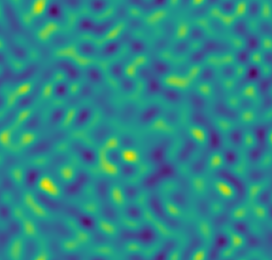
\includegraphics[interpolate=true,width=2.720000in,height=2.600000in]{burgers_solution_0.1-img0.png}}%
\end{pgfscope}%
\begin{pgfscope}%
\pgfsetbuttcap%
\pgfsetroundjoin%
\definecolor{currentfill}{rgb}{0.000000,0.000000,0.000000}%
\pgfsetfillcolor{currentfill}%
\pgfsetlinewidth{0.803000pt}%
\definecolor{currentstroke}{rgb}{0.000000,0.000000,0.000000}%
\pgfsetstrokecolor{currentstroke}%
\pgfsetdash{}{0pt}%
\pgfsys@defobject{currentmarker}{\pgfqpoint{0.000000in}{-0.048611in}}{\pgfqpoint{0.000000in}{0.000000in}}{%
\pgfpathmoveto{\pgfqpoint{0.000000in}{0.000000in}}%
\pgfpathlineto{\pgfqpoint{0.000000in}{-0.048611in}}%
\pgfusepath{stroke,fill}%
}%
\begin{pgfscope}%
\pgfsys@transformshift{0.350969in}{0.300188in}%
\pgfsys@useobject{currentmarker}{}%
\end{pgfscope}%
\end{pgfscope}%
\begin{pgfscope}%
\definecolor{textcolor}{rgb}{0.000000,0.000000,0.000000}%
\pgfsetstrokecolor{textcolor}%
\pgfsetfillcolor{textcolor}%
\pgftext[x=0.350969in,y=0.202965in,,top]{\color{textcolor}{\rmfamily\fontsize{12.000000}{14.400000}\selectfont\catcode`\^=\active\def^{\ifmmode\sp\else\^{}\fi}\catcode`\%=\active\def%{\%}0.0}}%
\end{pgfscope}%
\begin{pgfscope}%
\pgfsetbuttcap%
\pgfsetroundjoin%
\definecolor{currentfill}{rgb}{0.000000,0.000000,0.000000}%
\pgfsetfillcolor{currentfill}%
\pgfsetlinewidth{0.803000pt}%
\definecolor{currentstroke}{rgb}{0.000000,0.000000,0.000000}%
\pgfsetstrokecolor{currentstroke}%
\pgfsetdash{}{0pt}%
\pgfsys@defobject{currentmarker}{\pgfqpoint{0.000000in}{-0.048611in}}{\pgfqpoint{0.000000in}{0.000000in}}{%
\pgfpathmoveto{\pgfqpoint{0.000000in}{0.000000in}}%
\pgfpathlineto{\pgfqpoint{0.000000in}{-0.048611in}}%
\pgfusepath{stroke,fill}%
}%
\begin{pgfscope}%
\pgfsys@transformshift{1.028600in}{0.300188in}%
\pgfsys@useobject{currentmarker}{}%
\end{pgfscope}%
\end{pgfscope}%
\begin{pgfscope}%
\definecolor{textcolor}{rgb}{0.000000,0.000000,0.000000}%
\pgfsetstrokecolor{textcolor}%
\pgfsetfillcolor{textcolor}%
\pgftext[x=1.028600in,y=0.202965in,,top]{\color{textcolor}{\rmfamily\fontsize{12.000000}{14.400000}\selectfont\catcode`\^=\active\def^{\ifmmode\sp\else\^{}\fi}\catcode`\%=\active\def%{\%}0.5}}%
\end{pgfscope}%
\begin{pgfscope}%
\pgfsetbuttcap%
\pgfsetroundjoin%
\definecolor{currentfill}{rgb}{0.000000,0.000000,0.000000}%
\pgfsetfillcolor{currentfill}%
\pgfsetlinewidth{0.803000pt}%
\definecolor{currentstroke}{rgb}{0.000000,0.000000,0.000000}%
\pgfsetstrokecolor{currentstroke}%
\pgfsetdash{}{0pt}%
\pgfsys@defobject{currentmarker}{\pgfqpoint{0.000000in}{-0.048611in}}{\pgfqpoint{0.000000in}{0.000000in}}{%
\pgfpathmoveto{\pgfqpoint{0.000000in}{0.000000in}}%
\pgfpathlineto{\pgfqpoint{0.000000in}{-0.048611in}}%
\pgfusepath{stroke,fill}%
}%
\begin{pgfscope}%
\pgfsys@transformshift{1.706232in}{0.300188in}%
\pgfsys@useobject{currentmarker}{}%
\end{pgfscope}%
\end{pgfscope}%
\begin{pgfscope}%
\definecolor{textcolor}{rgb}{0.000000,0.000000,0.000000}%
\pgfsetstrokecolor{textcolor}%
\pgfsetfillcolor{textcolor}%
\pgftext[x=1.706232in,y=0.202965in,,top]{\color{textcolor}{\rmfamily\fontsize{12.000000}{14.400000}\selectfont\catcode`\^=\active\def^{\ifmmode\sp\else\^{}\fi}\catcode`\%=\active\def%{\%}1.0}}%
\end{pgfscope}%
\begin{pgfscope}%
\pgfsetbuttcap%
\pgfsetroundjoin%
\definecolor{currentfill}{rgb}{0.000000,0.000000,0.000000}%
\pgfsetfillcolor{currentfill}%
\pgfsetlinewidth{0.803000pt}%
\definecolor{currentstroke}{rgb}{0.000000,0.000000,0.000000}%
\pgfsetstrokecolor{currentstroke}%
\pgfsetdash{}{0pt}%
\pgfsys@defobject{currentmarker}{\pgfqpoint{0.000000in}{-0.048611in}}{\pgfqpoint{0.000000in}{0.000000in}}{%
\pgfpathmoveto{\pgfqpoint{0.000000in}{0.000000in}}%
\pgfpathlineto{\pgfqpoint{0.000000in}{-0.048611in}}%
\pgfusepath{stroke,fill}%
}%
\begin{pgfscope}%
\pgfsys@transformshift{2.383863in}{0.300188in}%
\pgfsys@useobject{currentmarker}{}%
\end{pgfscope}%
\end{pgfscope}%
\begin{pgfscope}%
\definecolor{textcolor}{rgb}{0.000000,0.000000,0.000000}%
\pgfsetstrokecolor{textcolor}%
\pgfsetfillcolor{textcolor}%
\pgftext[x=2.383863in,y=0.202965in,,top]{\color{textcolor}{\rmfamily\fontsize{12.000000}{14.400000}\selectfont\catcode`\^=\active\def^{\ifmmode\sp\else\^{}\fi}\catcode`\%=\active\def%{\%}1.5}}%
\end{pgfscope}%
\begin{pgfscope}%
\pgfsetbuttcap%
\pgfsetroundjoin%
\definecolor{currentfill}{rgb}{0.000000,0.000000,0.000000}%
\pgfsetfillcolor{currentfill}%
\pgfsetlinewidth{0.803000pt}%
\definecolor{currentstroke}{rgb}{0.000000,0.000000,0.000000}%
\pgfsetstrokecolor{currentstroke}%
\pgfsetdash{}{0pt}%
\pgfsys@defobject{currentmarker}{\pgfqpoint{0.000000in}{-0.048611in}}{\pgfqpoint{0.000000in}{0.000000in}}{%
\pgfpathmoveto{\pgfqpoint{0.000000in}{0.000000in}}%
\pgfpathlineto{\pgfqpoint{0.000000in}{-0.048611in}}%
\pgfusepath{stroke,fill}%
}%
\begin{pgfscope}%
\pgfsys@transformshift{3.061494in}{0.300188in}%
\pgfsys@useobject{currentmarker}{}%
\end{pgfscope}%
\end{pgfscope}%
\begin{pgfscope}%
\definecolor{textcolor}{rgb}{0.000000,0.000000,0.000000}%
\pgfsetstrokecolor{textcolor}%
\pgfsetfillcolor{textcolor}%
\pgftext[x=3.061494in,y=0.202965in,,top]{\color{textcolor}{\rmfamily\fontsize{12.000000}{14.400000}\selectfont\catcode`\^=\active\def^{\ifmmode\sp\else\^{}\fi}\catcode`\%=\active\def%{\%}2.0}}%
\end{pgfscope}%
\begin{pgfscope}%
\pgfsetbuttcap%
\pgfsetroundjoin%
\definecolor{currentfill}{rgb}{0.000000,0.000000,0.000000}%
\pgfsetfillcolor{currentfill}%
\pgfsetlinewidth{0.803000pt}%
\definecolor{currentstroke}{rgb}{0.000000,0.000000,0.000000}%
\pgfsetstrokecolor{currentstroke}%
\pgfsetdash{}{0pt}%
\pgfsys@defobject{currentmarker}{\pgfqpoint{-0.048611in}{0.000000in}}{\pgfqpoint{-0.000000in}{0.000000in}}{%
\pgfpathmoveto{\pgfqpoint{-0.000000in}{0.000000in}}%
\pgfpathlineto{\pgfqpoint{-0.048611in}{0.000000in}}%
\pgfusepath{stroke,fill}%
}%
\begin{pgfscope}%
\pgfsys@transformshift{0.350969in}{0.300188in}%
\pgfsys@useobject{currentmarker}{}%
\end{pgfscope}%
\end{pgfscope}%
\begin{pgfscope}%
\definecolor{textcolor}{rgb}{0.000000,0.000000,0.000000}%
\pgfsetstrokecolor{textcolor}%
\pgfsetfillcolor{textcolor}%
\pgftext[x=0.147708in, y=0.236874in, left, base]{\color{textcolor}{\rmfamily\fontsize{12.000000}{14.400000}\selectfont\catcode`\^=\active\def^{\ifmmode\sp\else\^{}\fi}\catcode`\%=\active\def%{\%}0}}%
\end{pgfscope}%
\begin{pgfscope}%
\pgfsetbuttcap%
\pgfsetroundjoin%
\definecolor{currentfill}{rgb}{0.000000,0.000000,0.000000}%
\pgfsetfillcolor{currentfill}%
\pgfsetlinewidth{0.803000pt}%
\definecolor{currentstroke}{rgb}{0.000000,0.000000,0.000000}%
\pgfsetstrokecolor{currentstroke}%
\pgfsetdash{}{0pt}%
\pgfsys@defobject{currentmarker}{\pgfqpoint{-0.048611in}{0.000000in}}{\pgfqpoint{-0.000000in}{0.000000in}}{%
\pgfpathmoveto{\pgfqpoint{-0.000000in}{0.000000in}}%
\pgfpathlineto{\pgfqpoint{-0.048611in}{0.000000in}}%
\pgfusepath{stroke,fill}%
}%
\begin{pgfscope}%
\pgfsys@transformshift{0.350969in}{0.819153in}%
\pgfsys@useobject{currentmarker}{}%
\end{pgfscope}%
\end{pgfscope}%
\begin{pgfscope}%
\definecolor{textcolor}{rgb}{0.000000,0.000000,0.000000}%
\pgfsetstrokecolor{textcolor}%
\pgfsetfillcolor{textcolor}%
\pgftext[x=0.147708in, y=0.755840in, left, base]{\color{textcolor}{\rmfamily\fontsize{12.000000}{14.400000}\selectfont\catcode`\^=\active\def^{\ifmmode\sp\else\^{}\fi}\catcode`\%=\active\def%{\%}2}}%
\end{pgfscope}%
\begin{pgfscope}%
\pgfsetbuttcap%
\pgfsetroundjoin%
\definecolor{currentfill}{rgb}{0.000000,0.000000,0.000000}%
\pgfsetfillcolor{currentfill}%
\pgfsetlinewidth{0.803000pt}%
\definecolor{currentstroke}{rgb}{0.000000,0.000000,0.000000}%
\pgfsetstrokecolor{currentstroke}%
\pgfsetdash{}{0pt}%
\pgfsys@defobject{currentmarker}{\pgfqpoint{-0.048611in}{0.000000in}}{\pgfqpoint{-0.000000in}{0.000000in}}{%
\pgfpathmoveto{\pgfqpoint{-0.000000in}{0.000000in}}%
\pgfpathlineto{\pgfqpoint{-0.048611in}{0.000000in}}%
\pgfusepath{stroke,fill}%
}%
\begin{pgfscope}%
\pgfsys@transformshift{0.350969in}{1.338119in}%
\pgfsys@useobject{currentmarker}{}%
\end{pgfscope}%
\end{pgfscope}%
\begin{pgfscope}%
\definecolor{textcolor}{rgb}{0.000000,0.000000,0.000000}%
\pgfsetstrokecolor{textcolor}%
\pgfsetfillcolor{textcolor}%
\pgftext[x=0.147708in, y=1.274805in, left, base]{\color{textcolor}{\rmfamily\fontsize{12.000000}{14.400000}\selectfont\catcode`\^=\active\def^{\ifmmode\sp\else\^{}\fi}\catcode`\%=\active\def%{\%}4}}%
\end{pgfscope}%
\begin{pgfscope}%
\pgfsetbuttcap%
\pgfsetroundjoin%
\definecolor{currentfill}{rgb}{0.000000,0.000000,0.000000}%
\pgfsetfillcolor{currentfill}%
\pgfsetlinewidth{0.803000pt}%
\definecolor{currentstroke}{rgb}{0.000000,0.000000,0.000000}%
\pgfsetstrokecolor{currentstroke}%
\pgfsetdash{}{0pt}%
\pgfsys@defobject{currentmarker}{\pgfqpoint{-0.048611in}{0.000000in}}{\pgfqpoint{-0.000000in}{0.000000in}}{%
\pgfpathmoveto{\pgfqpoint{-0.000000in}{0.000000in}}%
\pgfpathlineto{\pgfqpoint{-0.048611in}{0.000000in}}%
\pgfusepath{stroke,fill}%
}%
\begin{pgfscope}%
\pgfsys@transformshift{0.350969in}{1.857085in}%
\pgfsys@useobject{currentmarker}{}%
\end{pgfscope}%
\end{pgfscope}%
\begin{pgfscope}%
\definecolor{textcolor}{rgb}{0.000000,0.000000,0.000000}%
\pgfsetstrokecolor{textcolor}%
\pgfsetfillcolor{textcolor}%
\pgftext[x=0.147708in, y=1.793771in, left, base]{\color{textcolor}{\rmfamily\fontsize{12.000000}{14.400000}\selectfont\catcode`\^=\active\def^{\ifmmode\sp\else\^{}\fi}\catcode`\%=\active\def%{\%}6}}%
\end{pgfscope}%
\begin{pgfscope}%
\pgfsetbuttcap%
\pgfsetroundjoin%
\definecolor{currentfill}{rgb}{0.000000,0.000000,0.000000}%
\pgfsetfillcolor{currentfill}%
\pgfsetlinewidth{0.803000pt}%
\definecolor{currentstroke}{rgb}{0.000000,0.000000,0.000000}%
\pgfsetstrokecolor{currentstroke}%
\pgfsetdash{}{0pt}%
\pgfsys@defobject{currentmarker}{\pgfqpoint{-0.048611in}{0.000000in}}{\pgfqpoint{-0.000000in}{0.000000in}}{%
\pgfpathmoveto{\pgfqpoint{-0.000000in}{0.000000in}}%
\pgfpathlineto{\pgfqpoint{-0.048611in}{0.000000in}}%
\pgfusepath{stroke,fill}%
}%
\begin{pgfscope}%
\pgfsys@transformshift{0.350969in}{2.376050in}%
\pgfsys@useobject{currentmarker}{}%
\end{pgfscope}%
\end{pgfscope}%
\begin{pgfscope}%
\definecolor{textcolor}{rgb}{0.000000,0.000000,0.000000}%
\pgfsetstrokecolor{textcolor}%
\pgfsetfillcolor{textcolor}%
\pgftext[x=0.147708in, y=2.312737in, left, base]{\color{textcolor}{\rmfamily\fontsize{12.000000}{14.400000}\selectfont\catcode`\^=\active\def^{\ifmmode\sp\else\^{}\fi}\catcode`\%=\active\def%{\%}8}}%
\end{pgfscope}%
\begin{pgfscope}%
\pgfsetbuttcap%
\pgfsetroundjoin%
\definecolor{currentfill}{rgb}{0.000000,0.000000,0.000000}%
\pgfsetfillcolor{currentfill}%
\pgfsetlinewidth{0.803000pt}%
\definecolor{currentstroke}{rgb}{0.000000,0.000000,0.000000}%
\pgfsetstrokecolor{currentstroke}%
\pgfsetdash{}{0pt}%
\pgfsys@defobject{currentmarker}{\pgfqpoint{-0.048611in}{0.000000in}}{\pgfqpoint{-0.000000in}{0.000000in}}{%
\pgfpathmoveto{\pgfqpoint{-0.000000in}{0.000000in}}%
\pgfpathlineto{\pgfqpoint{-0.048611in}{0.000000in}}%
\pgfusepath{stroke,fill}%
}%
\begin{pgfscope}%
\pgfsys@transformshift{0.350969in}{2.895016in}%
\pgfsys@useobject{currentmarker}{}%
\end{pgfscope}%
\end{pgfscope}%
\begin{pgfscope}%
\definecolor{textcolor}{rgb}{0.000000,0.000000,0.000000}%
\pgfsetstrokecolor{textcolor}%
\pgfsetfillcolor{textcolor}%
\pgftext[x=0.041670in, y=2.831702in, left, base]{\color{textcolor}{\rmfamily\fontsize{12.000000}{14.400000}\selectfont\catcode`\^=\active\def^{\ifmmode\sp\else\^{}\fi}\catcode`\%=\active\def%{\%}10}}%
\end{pgfscope}%
\begin{pgfscope}%
\pgfsetrectcap%
\pgfsetmiterjoin%
\pgfsetlinewidth{0.803000pt}%
\definecolor{currentstroke}{rgb}{0.000000,0.000000,0.000000}%
\pgfsetstrokecolor{currentstroke}%
\pgfsetdash{}{0pt}%
\pgfpathmoveto{\pgfqpoint{0.350969in}{0.300188in}}%
\pgfpathlineto{\pgfqpoint{0.350969in}{2.895016in}}%
\pgfusepath{stroke}%
\end{pgfscope}%
\begin{pgfscope}%
\pgfsetrectcap%
\pgfsetmiterjoin%
\pgfsetlinewidth{0.803000pt}%
\definecolor{currentstroke}{rgb}{0.000000,0.000000,0.000000}%
\pgfsetstrokecolor{currentstroke}%
\pgfsetdash{}{0pt}%
\pgfpathmoveto{\pgfqpoint{3.061494in}{0.300188in}}%
\pgfpathlineto{\pgfqpoint{3.061494in}{2.895016in}}%
\pgfusepath{stroke}%
\end{pgfscope}%
\begin{pgfscope}%
\pgfsetrectcap%
\pgfsetmiterjoin%
\pgfsetlinewidth{0.803000pt}%
\definecolor{currentstroke}{rgb}{0.000000,0.000000,0.000000}%
\pgfsetstrokecolor{currentstroke}%
\pgfsetdash{}{0pt}%
\pgfpathmoveto{\pgfqpoint{0.350969in}{0.300188in}}%
\pgfpathlineto{\pgfqpoint{3.061494in}{0.300188in}}%
\pgfusepath{stroke}%
\end{pgfscope}%
\begin{pgfscope}%
\pgfsetrectcap%
\pgfsetmiterjoin%
\pgfsetlinewidth{0.803000pt}%
\definecolor{currentstroke}{rgb}{0.000000,0.000000,0.000000}%
\pgfsetstrokecolor{currentstroke}%
\pgfsetdash{}{0pt}%
\pgfpathmoveto{\pgfqpoint{0.350969in}{2.895016in}}%
\pgfpathlineto{\pgfqpoint{3.061494in}{2.895016in}}%
\pgfusepath{stroke}%
\end{pgfscope}%
\begin{pgfscope}%
\pgfsetbuttcap%
\pgfsetmiterjoin%
\pgfsetlinewidth{0.000000pt}%
\definecolor{currentstroke}{rgb}{0.000000,0.000000,0.000000}%
\pgfsetstrokecolor{currentstroke}%
\pgfsetstrokeopacity{0.000000}%
\pgfsetdash{}{0pt}%
\pgfpathmoveto{\pgfqpoint{3.329548in}{0.300188in}}%
\pgfpathlineto{\pgfqpoint{3.459290in}{0.300188in}}%
\pgfpathlineto{\pgfqpoint{3.459290in}{2.895016in}}%
\pgfpathlineto{\pgfqpoint{3.329548in}{2.895016in}}%
\pgfpathlineto{\pgfqpoint{3.329548in}{0.300188in}}%
\pgfpathclose%
\pgfusepath{}%
\end{pgfscope}%
\begin{pgfscope}%
\pgfsys@transformshift{3.330000in}{0.300000in}%
\pgftext[left,bottom]{
\includegraphics[interpolate=true,width=0.130000in,height=2.600000in]{burgers_solution_0.1-img1.png}}%
\end{pgfscope}%
\begin{pgfscope}%
\pgfsetbuttcap%
\pgfsetroundjoin%
\definecolor{currentfill}{rgb}{0.000000,0.000000,0.000000}%
\pgfsetfillcolor{currentfill}%
\pgfsetlinewidth{0.803000pt}%
\definecolor{currentstroke}{rgb}{0.000000,0.000000,0.000000}%
\pgfsetstrokecolor{currentstroke}%
\pgfsetdash{}{0pt}%
\pgfsys@defobject{currentmarker}{\pgfqpoint{0.000000in}{0.000000in}}{\pgfqpoint{0.048611in}{0.000000in}}{%
\pgfpathmoveto{\pgfqpoint{0.000000in}{0.000000in}}%
\pgfpathlineto{\pgfqpoint{0.048611in}{0.000000in}}%
\pgfusepath{stroke,fill}%
}%
\begin{pgfscope}%
\pgfsys@transformshift{3.459290in}{0.840201in}%
\pgfsys@useobject{currentmarker}{}%
\end{pgfscope}%
\end{pgfscope}%
\begin{pgfscope}%
\definecolor{textcolor}{rgb}{0.000000,0.000000,0.000000}%
\pgfsetstrokecolor{textcolor}%
\pgfsetfillcolor{textcolor}%
\pgftext[x=3.556512in, y=0.776887in, left, base]{\color{textcolor}{\rmfamily\fontsize{12.000000}{14.400000}\selectfont\catcode`\^=\active\def^{\ifmmode\sp\else\^{}\fi}\catcode`\%=\active\def%{\%}\ensuremath{-}0.5}}%
\end{pgfscope}%
\begin{pgfscope}%
\pgfsetbuttcap%
\pgfsetroundjoin%
\definecolor{currentfill}{rgb}{0.000000,0.000000,0.000000}%
\pgfsetfillcolor{currentfill}%
\pgfsetlinewidth{0.803000pt}%
\definecolor{currentstroke}{rgb}{0.000000,0.000000,0.000000}%
\pgfsetstrokecolor{currentstroke}%
\pgfsetdash{}{0pt}%
\pgfsys@defobject{currentmarker}{\pgfqpoint{0.000000in}{0.000000in}}{\pgfqpoint{0.048611in}{0.000000in}}{%
\pgfpathmoveto{\pgfqpoint{0.000000in}{0.000000in}}%
\pgfpathlineto{\pgfqpoint{0.048611in}{0.000000in}}%
\pgfusepath{stroke,fill}%
}%
\begin{pgfscope}%
\pgfsys@transformshift{3.459290in}{1.494629in}%
\pgfsys@useobject{currentmarker}{}%
\end{pgfscope}%
\end{pgfscope}%
\begin{pgfscope}%
\definecolor{textcolor}{rgb}{0.000000,0.000000,0.000000}%
\pgfsetstrokecolor{textcolor}%
\pgfsetfillcolor{textcolor}%
\pgftext[x=3.556512in, y=1.431315in, left, base]{\color{textcolor}{\rmfamily\fontsize{12.000000}{14.400000}\selectfont\catcode`\^=\active\def^{\ifmmode\sp\else\^{}\fi}\catcode`\%=\active\def%{\%}0.0}}%
\end{pgfscope}%
\begin{pgfscope}%
\pgfsetbuttcap%
\pgfsetroundjoin%
\definecolor{currentfill}{rgb}{0.000000,0.000000,0.000000}%
\pgfsetfillcolor{currentfill}%
\pgfsetlinewidth{0.803000pt}%
\definecolor{currentstroke}{rgb}{0.000000,0.000000,0.000000}%
\pgfsetstrokecolor{currentstroke}%
\pgfsetdash{}{0pt}%
\pgfsys@defobject{currentmarker}{\pgfqpoint{0.000000in}{0.000000in}}{\pgfqpoint{0.048611in}{0.000000in}}{%
\pgfpathmoveto{\pgfqpoint{0.000000in}{0.000000in}}%
\pgfpathlineto{\pgfqpoint{0.048611in}{0.000000in}}%
\pgfusepath{stroke,fill}%
}%
\begin{pgfscope}%
\pgfsys@transformshift{3.459290in}{2.149056in}%
\pgfsys@useobject{currentmarker}{}%
\end{pgfscope}%
\end{pgfscope}%
\begin{pgfscope}%
\definecolor{textcolor}{rgb}{0.000000,0.000000,0.000000}%
\pgfsetstrokecolor{textcolor}%
\pgfsetfillcolor{textcolor}%
\pgftext[x=3.556512in, y=2.085742in, left, base]{\color{textcolor}{\rmfamily\fontsize{12.000000}{14.400000}\selectfont\catcode`\^=\active\def^{\ifmmode\sp\else\^{}\fi}\catcode`\%=\active\def%{\%}0.5}}%
\end{pgfscope}%
\begin{pgfscope}%
\pgfsetbuttcap%
\pgfsetroundjoin%
\definecolor{currentfill}{rgb}{0.000000,0.000000,0.000000}%
\pgfsetfillcolor{currentfill}%
\pgfsetlinewidth{0.803000pt}%
\definecolor{currentstroke}{rgb}{0.000000,0.000000,0.000000}%
\pgfsetstrokecolor{currentstroke}%
\pgfsetdash{}{0pt}%
\pgfsys@defobject{currentmarker}{\pgfqpoint{0.000000in}{0.000000in}}{\pgfqpoint{0.048611in}{0.000000in}}{%
\pgfpathmoveto{\pgfqpoint{0.000000in}{0.000000in}}%
\pgfpathlineto{\pgfqpoint{0.048611in}{0.000000in}}%
\pgfusepath{stroke,fill}%
}%
\begin{pgfscope}%
\pgfsys@transformshift{3.459290in}{2.803483in}%
\pgfsys@useobject{currentmarker}{}%
\end{pgfscope}%
\end{pgfscope}%
\begin{pgfscope}%
\definecolor{textcolor}{rgb}{0.000000,0.000000,0.000000}%
\pgfsetstrokecolor{textcolor}%
\pgfsetfillcolor{textcolor}%
\pgftext[x=3.556512in, y=2.740170in, left, base]{\color{textcolor}{\rmfamily\fontsize{12.000000}{14.400000}\selectfont\catcode`\^=\active\def^{\ifmmode\sp\else\^{}\fi}\catcode`\%=\active\def%{\%}1.0}}%
\end{pgfscope}%
\begin{pgfscope}%
\pgfsetrectcap%
\pgfsetmiterjoin%
\pgfsetlinewidth{0.803000pt}%
\definecolor{currentstroke}{rgb}{0.000000,0.000000,0.000000}%
\pgfsetstrokecolor{currentstroke}%
\pgfsetdash{}{0pt}%
\pgfpathmoveto{\pgfqpoint{3.329548in}{0.300188in}}%
\pgfpathlineto{\pgfqpoint{3.394419in}{0.300188in}}%
\pgfpathlineto{\pgfqpoint{3.459290in}{0.300188in}}%
\pgfpathlineto{\pgfqpoint{3.459290in}{2.895016in}}%
\pgfpathlineto{\pgfqpoint{3.394419in}{2.895016in}}%
\pgfpathlineto{\pgfqpoint{3.329548in}{2.895016in}}%
\pgfpathlineto{\pgfqpoint{3.329548in}{0.300188in}}%
\pgfpathclose%
\pgfusepath{stroke}%
\end{pgfscope}%
\end{pgfpicture}%
\makeatother%
\endgroup%

    \end{adjustbox}
    \caption{Solution function for \(\nu=0.1\).}\label{fig:burgers_solution_0.1}
  \end{subfigure}
  \begin{subfigure}{0.49\linewidth}
    \begin{adjustbox}{width=\linewidth}
      \begingroup%
\makeatletter%
\begin{pgfpicture}%
\pgfpathrectangle{\pgfpointorigin}{\pgfqpoint{4.000000in}{3.000000in}}%
\pgfusepath{use as bounding box, clip}%
\begin{pgfscope}%
\pgfsetbuttcap%
\pgfsetmiterjoin%
\pgfsetlinewidth{0.000000pt}%
\definecolor{currentstroke}{rgb}{0.000000,0.000000,0.000000}%
\pgfsetstrokecolor{currentstroke}%
\pgfsetstrokeopacity{0.000000}%
\pgfsetdash{}{0pt}%
\pgfpathmoveto{\pgfqpoint{0.000000in}{0.000000in}}%
\pgfpathlineto{\pgfqpoint{4.000000in}{0.000000in}}%
\pgfpathlineto{\pgfqpoint{4.000000in}{3.000000in}}%
\pgfpathlineto{\pgfqpoint{0.000000in}{3.000000in}}%
\pgfpathlineto{\pgfqpoint{0.000000in}{0.000000in}}%
\pgfpathclose%
\pgfusepath{}%
\end{pgfscope}%
\begin{pgfscope}%
\pgfsetbuttcap%
\pgfsetmiterjoin%
\pgfsetlinewidth{0.000000pt}%
\definecolor{currentstroke}{rgb}{0.000000,0.000000,0.000000}%
\pgfsetstrokecolor{currentstroke}%
\pgfsetstrokeopacity{0.000000}%
\pgfsetdash{}{0pt}%
\pgfpathmoveto{\pgfqpoint{0.567820in}{0.517039in}}%
\pgfpathlineto{\pgfqpoint{3.233703in}{0.517039in}}%
\pgfpathlineto{\pgfqpoint{3.233703in}{2.895016in}}%
\pgfpathlineto{\pgfqpoint{0.567820in}{2.895016in}}%
\pgfpathlineto{\pgfqpoint{0.567820in}{0.517039in}}%
\pgfpathclose%
\pgfusepath{}%
\end{pgfscope}%
\begin{pgfscope}%
\pgfpathrectangle{\pgfqpoint{0.567820in}{0.517039in}}{\pgfqpoint{2.665883in}{2.377978in}}%
\pgfusepath{clip}%
\pgfsys@transformshift{0.567820in}{0.517039in}%
\pgftext[left,bottom]{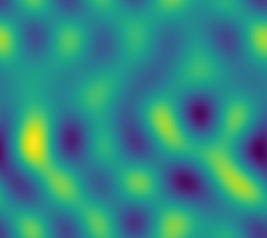
\includegraphics[interpolate=true,width=2.670000in,height=2.380000in]{burgers_forcing_0.1-img0.png}}%
\end{pgfscope}%
\begin{pgfscope}%
\pgfsetbuttcap%
\pgfsetroundjoin%
\definecolor{currentfill}{rgb}{0.000000,0.000000,0.000000}%
\pgfsetfillcolor{currentfill}%
\pgfsetlinewidth{0.803000pt}%
\definecolor{currentstroke}{rgb}{0.000000,0.000000,0.000000}%
\pgfsetstrokecolor{currentstroke}%
\pgfsetdash{}{0pt}%
\pgfsys@defobject{currentmarker}{\pgfqpoint{0.000000in}{-0.048611in}}{\pgfqpoint{0.000000in}{0.000000in}}{%
\pgfpathmoveto{\pgfqpoint{0.000000in}{0.000000in}}%
\pgfpathlineto{\pgfqpoint{0.000000in}{-0.048611in}}%
\pgfusepath{stroke,fill}%
}%
\begin{pgfscope}%
\pgfsys@transformshift{0.567820in}{0.517039in}%
\pgfsys@useobject{currentmarker}{}%
\end{pgfscope}%
\end{pgfscope}%
\begin{pgfscope}%
\definecolor{textcolor}{rgb}{0.000000,0.000000,0.000000}%
\pgfsetstrokecolor{textcolor}%
\pgfsetfillcolor{textcolor}%
\pgftext[x=0.567820in,y=0.419816in,,top]{\color{textcolor}\rmfamily\fontsize{12.000000}{14.400000}\selectfont 0.0}%
\end{pgfscope}%
\begin{pgfscope}%
\pgfsetbuttcap%
\pgfsetroundjoin%
\definecolor{currentfill}{rgb}{0.000000,0.000000,0.000000}%
\pgfsetfillcolor{currentfill}%
\pgfsetlinewidth{0.803000pt}%
\definecolor{currentstroke}{rgb}{0.000000,0.000000,0.000000}%
\pgfsetstrokecolor{currentstroke}%
\pgfsetdash{}{0pt}%
\pgfsys@defobject{currentmarker}{\pgfqpoint{0.000000in}{-0.048611in}}{\pgfqpoint{0.000000in}{0.000000in}}{%
\pgfpathmoveto{\pgfqpoint{0.000000in}{0.000000in}}%
\pgfpathlineto{\pgfqpoint{0.000000in}{-0.048611in}}%
\pgfusepath{stroke,fill}%
}%
\begin{pgfscope}%
\pgfsys@transformshift{1.234291in}{0.517039in}%
\pgfsys@useobject{currentmarker}{}%
\end{pgfscope}%
\end{pgfscope}%
\begin{pgfscope}%
\definecolor{textcolor}{rgb}{0.000000,0.000000,0.000000}%
\pgfsetstrokecolor{textcolor}%
\pgfsetfillcolor{textcolor}%
\pgftext[x=1.234291in,y=0.419816in,,top]{\color{textcolor}\rmfamily\fontsize{12.000000}{14.400000}\selectfont 0.5}%
\end{pgfscope}%
\begin{pgfscope}%
\pgfsetbuttcap%
\pgfsetroundjoin%
\definecolor{currentfill}{rgb}{0.000000,0.000000,0.000000}%
\pgfsetfillcolor{currentfill}%
\pgfsetlinewidth{0.803000pt}%
\definecolor{currentstroke}{rgb}{0.000000,0.000000,0.000000}%
\pgfsetstrokecolor{currentstroke}%
\pgfsetdash{}{0pt}%
\pgfsys@defobject{currentmarker}{\pgfqpoint{0.000000in}{-0.048611in}}{\pgfqpoint{0.000000in}{0.000000in}}{%
\pgfpathmoveto{\pgfqpoint{0.000000in}{0.000000in}}%
\pgfpathlineto{\pgfqpoint{0.000000in}{-0.048611in}}%
\pgfusepath{stroke,fill}%
}%
\begin{pgfscope}%
\pgfsys@transformshift{1.900762in}{0.517039in}%
\pgfsys@useobject{currentmarker}{}%
\end{pgfscope}%
\end{pgfscope}%
\begin{pgfscope}%
\definecolor{textcolor}{rgb}{0.000000,0.000000,0.000000}%
\pgfsetstrokecolor{textcolor}%
\pgfsetfillcolor{textcolor}%
\pgftext[x=1.900762in,y=0.419816in,,top]{\color{textcolor}\rmfamily\fontsize{12.000000}{14.400000}\selectfont 1.0}%
\end{pgfscope}%
\begin{pgfscope}%
\pgfsetbuttcap%
\pgfsetroundjoin%
\definecolor{currentfill}{rgb}{0.000000,0.000000,0.000000}%
\pgfsetfillcolor{currentfill}%
\pgfsetlinewidth{0.803000pt}%
\definecolor{currentstroke}{rgb}{0.000000,0.000000,0.000000}%
\pgfsetstrokecolor{currentstroke}%
\pgfsetdash{}{0pt}%
\pgfsys@defobject{currentmarker}{\pgfqpoint{0.000000in}{-0.048611in}}{\pgfqpoint{0.000000in}{0.000000in}}{%
\pgfpathmoveto{\pgfqpoint{0.000000in}{0.000000in}}%
\pgfpathlineto{\pgfqpoint{0.000000in}{-0.048611in}}%
\pgfusepath{stroke,fill}%
}%
\begin{pgfscope}%
\pgfsys@transformshift{2.567232in}{0.517039in}%
\pgfsys@useobject{currentmarker}{}%
\end{pgfscope}%
\end{pgfscope}%
\begin{pgfscope}%
\definecolor{textcolor}{rgb}{0.000000,0.000000,0.000000}%
\pgfsetstrokecolor{textcolor}%
\pgfsetfillcolor{textcolor}%
\pgftext[x=2.567232in,y=0.419816in,,top]{\color{textcolor}\rmfamily\fontsize{12.000000}{14.400000}\selectfont 1.5}%
\end{pgfscope}%
\begin{pgfscope}%
\pgfsetbuttcap%
\pgfsetroundjoin%
\definecolor{currentfill}{rgb}{0.000000,0.000000,0.000000}%
\pgfsetfillcolor{currentfill}%
\pgfsetlinewidth{0.803000pt}%
\definecolor{currentstroke}{rgb}{0.000000,0.000000,0.000000}%
\pgfsetstrokecolor{currentstroke}%
\pgfsetdash{}{0pt}%
\pgfsys@defobject{currentmarker}{\pgfqpoint{0.000000in}{-0.048611in}}{\pgfqpoint{0.000000in}{0.000000in}}{%
\pgfpathmoveto{\pgfqpoint{0.000000in}{0.000000in}}%
\pgfpathlineto{\pgfqpoint{0.000000in}{-0.048611in}}%
\pgfusepath{stroke,fill}%
}%
\begin{pgfscope}%
\pgfsys@transformshift{3.233703in}{0.517039in}%
\pgfsys@useobject{currentmarker}{}%
\end{pgfscope}%
\end{pgfscope}%
\begin{pgfscope}%
\definecolor{textcolor}{rgb}{0.000000,0.000000,0.000000}%
\pgfsetstrokecolor{textcolor}%
\pgfsetfillcolor{textcolor}%
\pgftext[x=3.233703in,y=0.419816in,,top]{\color{textcolor}\rmfamily\fontsize{12.000000}{14.400000}\selectfont 2.0}%
\end{pgfscope}%
\begin{pgfscope}%
\definecolor{textcolor}{rgb}{0.000000,0.000000,0.000000}%
\pgfsetstrokecolor{textcolor}%
\pgfsetfillcolor{textcolor}%
\pgftext[x=1.900762in,y=0.202965in,,top]{\color{textcolor}\rmfamily\fontsize{12.000000}{14.400000}\selectfont Space}%
\end{pgfscope}%
\begin{pgfscope}%
\pgfsetbuttcap%
\pgfsetroundjoin%
\definecolor{currentfill}{rgb}{0.000000,0.000000,0.000000}%
\pgfsetfillcolor{currentfill}%
\pgfsetlinewidth{0.803000pt}%
\definecolor{currentstroke}{rgb}{0.000000,0.000000,0.000000}%
\pgfsetstrokecolor{currentstroke}%
\pgfsetdash{}{0pt}%
\pgfsys@defobject{currentmarker}{\pgfqpoint{-0.048611in}{0.000000in}}{\pgfqpoint{-0.000000in}{0.000000in}}{%
\pgfpathmoveto{\pgfqpoint{-0.000000in}{0.000000in}}%
\pgfpathlineto{\pgfqpoint{-0.048611in}{0.000000in}}%
\pgfusepath{stroke,fill}%
}%
\begin{pgfscope}%
\pgfsys@transformshift{0.567820in}{0.517039in}%
\pgfsys@useobject{currentmarker}{}%
\end{pgfscope}%
\end{pgfscope}%
\begin{pgfscope}%
\definecolor{textcolor}{rgb}{0.000000,0.000000,0.000000}%
\pgfsetstrokecolor{textcolor}%
\pgfsetfillcolor{textcolor}%
\pgftext[x=0.364559in, y=0.453725in, left, base]{\color{textcolor}\rmfamily\fontsize{12.000000}{14.400000}\selectfont 0}%
\end{pgfscope}%
\begin{pgfscope}%
\pgfsetbuttcap%
\pgfsetroundjoin%
\definecolor{currentfill}{rgb}{0.000000,0.000000,0.000000}%
\pgfsetfillcolor{currentfill}%
\pgfsetlinewidth{0.803000pt}%
\definecolor{currentstroke}{rgb}{0.000000,0.000000,0.000000}%
\pgfsetstrokecolor{currentstroke}%
\pgfsetdash{}{0pt}%
\pgfsys@defobject{currentmarker}{\pgfqpoint{-0.048611in}{0.000000in}}{\pgfqpoint{-0.000000in}{0.000000in}}{%
\pgfpathmoveto{\pgfqpoint{-0.000000in}{0.000000in}}%
\pgfpathlineto{\pgfqpoint{-0.048611in}{0.000000in}}%
\pgfusepath{stroke,fill}%
}%
\begin{pgfscope}%
\pgfsys@transformshift{0.567820in}{0.992634in}%
\pgfsys@useobject{currentmarker}{}%
\end{pgfscope}%
\end{pgfscope}%
\begin{pgfscope}%
\definecolor{textcolor}{rgb}{0.000000,0.000000,0.000000}%
\pgfsetstrokecolor{textcolor}%
\pgfsetfillcolor{textcolor}%
\pgftext[x=0.364559in, y=0.929320in, left, base]{\color{textcolor}\rmfamily\fontsize{12.000000}{14.400000}\selectfont 2}%
\end{pgfscope}%
\begin{pgfscope}%
\pgfsetbuttcap%
\pgfsetroundjoin%
\definecolor{currentfill}{rgb}{0.000000,0.000000,0.000000}%
\pgfsetfillcolor{currentfill}%
\pgfsetlinewidth{0.803000pt}%
\definecolor{currentstroke}{rgb}{0.000000,0.000000,0.000000}%
\pgfsetstrokecolor{currentstroke}%
\pgfsetdash{}{0pt}%
\pgfsys@defobject{currentmarker}{\pgfqpoint{-0.048611in}{0.000000in}}{\pgfqpoint{-0.000000in}{0.000000in}}{%
\pgfpathmoveto{\pgfqpoint{-0.000000in}{0.000000in}}%
\pgfpathlineto{\pgfqpoint{-0.048611in}{0.000000in}}%
\pgfusepath{stroke,fill}%
}%
\begin{pgfscope}%
\pgfsys@transformshift{0.567820in}{1.468230in}%
\pgfsys@useobject{currentmarker}{}%
\end{pgfscope}%
\end{pgfscope}%
\begin{pgfscope}%
\definecolor{textcolor}{rgb}{0.000000,0.000000,0.000000}%
\pgfsetstrokecolor{textcolor}%
\pgfsetfillcolor{textcolor}%
\pgftext[x=0.364559in, y=1.404916in, left, base]{\color{textcolor}\rmfamily\fontsize{12.000000}{14.400000}\selectfont 4}%
\end{pgfscope}%
\begin{pgfscope}%
\pgfsetbuttcap%
\pgfsetroundjoin%
\definecolor{currentfill}{rgb}{0.000000,0.000000,0.000000}%
\pgfsetfillcolor{currentfill}%
\pgfsetlinewidth{0.803000pt}%
\definecolor{currentstroke}{rgb}{0.000000,0.000000,0.000000}%
\pgfsetstrokecolor{currentstroke}%
\pgfsetdash{}{0pt}%
\pgfsys@defobject{currentmarker}{\pgfqpoint{-0.048611in}{0.000000in}}{\pgfqpoint{-0.000000in}{0.000000in}}{%
\pgfpathmoveto{\pgfqpoint{-0.000000in}{0.000000in}}%
\pgfpathlineto{\pgfqpoint{-0.048611in}{0.000000in}}%
\pgfusepath{stroke,fill}%
}%
\begin{pgfscope}%
\pgfsys@transformshift{0.567820in}{1.943825in}%
\pgfsys@useobject{currentmarker}{}%
\end{pgfscope}%
\end{pgfscope}%
\begin{pgfscope}%
\definecolor{textcolor}{rgb}{0.000000,0.000000,0.000000}%
\pgfsetstrokecolor{textcolor}%
\pgfsetfillcolor{textcolor}%
\pgftext[x=0.364559in, y=1.880511in, left, base]{\color{textcolor}\rmfamily\fontsize{12.000000}{14.400000}\selectfont 6}%
\end{pgfscope}%
\begin{pgfscope}%
\pgfsetbuttcap%
\pgfsetroundjoin%
\definecolor{currentfill}{rgb}{0.000000,0.000000,0.000000}%
\pgfsetfillcolor{currentfill}%
\pgfsetlinewidth{0.803000pt}%
\definecolor{currentstroke}{rgb}{0.000000,0.000000,0.000000}%
\pgfsetstrokecolor{currentstroke}%
\pgfsetdash{}{0pt}%
\pgfsys@defobject{currentmarker}{\pgfqpoint{-0.048611in}{0.000000in}}{\pgfqpoint{-0.000000in}{0.000000in}}{%
\pgfpathmoveto{\pgfqpoint{-0.000000in}{0.000000in}}%
\pgfpathlineto{\pgfqpoint{-0.048611in}{0.000000in}}%
\pgfusepath{stroke,fill}%
}%
\begin{pgfscope}%
\pgfsys@transformshift{0.567820in}{2.419421in}%
\pgfsys@useobject{currentmarker}{}%
\end{pgfscope}%
\end{pgfscope}%
\begin{pgfscope}%
\definecolor{textcolor}{rgb}{0.000000,0.000000,0.000000}%
\pgfsetstrokecolor{textcolor}%
\pgfsetfillcolor{textcolor}%
\pgftext[x=0.364559in, y=2.356107in, left, base]{\color{textcolor}\rmfamily\fontsize{12.000000}{14.400000}\selectfont 8}%
\end{pgfscope}%
\begin{pgfscope}%
\pgfsetbuttcap%
\pgfsetroundjoin%
\definecolor{currentfill}{rgb}{0.000000,0.000000,0.000000}%
\pgfsetfillcolor{currentfill}%
\pgfsetlinewidth{0.803000pt}%
\definecolor{currentstroke}{rgb}{0.000000,0.000000,0.000000}%
\pgfsetstrokecolor{currentstroke}%
\pgfsetdash{}{0pt}%
\pgfsys@defobject{currentmarker}{\pgfqpoint{-0.048611in}{0.000000in}}{\pgfqpoint{-0.000000in}{0.000000in}}{%
\pgfpathmoveto{\pgfqpoint{-0.000000in}{0.000000in}}%
\pgfpathlineto{\pgfqpoint{-0.048611in}{0.000000in}}%
\pgfusepath{stroke,fill}%
}%
\begin{pgfscope}%
\pgfsys@transformshift{0.567820in}{2.895016in}%
\pgfsys@useobject{currentmarker}{}%
\end{pgfscope}%
\end{pgfscope}%
\begin{pgfscope}%
\definecolor{textcolor}{rgb}{0.000000,0.000000,0.000000}%
\pgfsetstrokecolor{textcolor}%
\pgfsetfillcolor{textcolor}%
\pgftext[x=0.258521in, y=2.831702in, left, base]{\color{textcolor}\rmfamily\fontsize{12.000000}{14.400000}\selectfont 10}%
\end{pgfscope}%
\begin{pgfscope}%
\definecolor{textcolor}{rgb}{0.000000,0.000000,0.000000}%
\pgfsetstrokecolor{textcolor}%
\pgfsetfillcolor{textcolor}%
\pgftext[x=0.202965in,y=1.706027in,,bottom,rotate=90.000000]{\color{textcolor}\rmfamily\fontsize{12.000000}{14.400000}\selectfont Time}%
\end{pgfscope}%
\begin{pgfscope}%
\pgfsetrectcap%
\pgfsetmiterjoin%
\pgfsetlinewidth{0.803000pt}%
\definecolor{currentstroke}{rgb}{0.000000,0.000000,0.000000}%
\pgfsetstrokecolor{currentstroke}%
\pgfsetdash{}{0pt}%
\pgfpathmoveto{\pgfqpoint{0.567820in}{0.517039in}}%
\pgfpathlineto{\pgfqpoint{0.567820in}{2.895016in}}%
\pgfusepath{stroke}%
\end{pgfscope}%
\begin{pgfscope}%
\pgfsetrectcap%
\pgfsetmiterjoin%
\pgfsetlinewidth{0.803000pt}%
\definecolor{currentstroke}{rgb}{0.000000,0.000000,0.000000}%
\pgfsetstrokecolor{currentstroke}%
\pgfsetdash{}{0pt}%
\pgfpathmoveto{\pgfqpoint{3.233703in}{0.517039in}}%
\pgfpathlineto{\pgfqpoint{3.233703in}{2.895016in}}%
\pgfusepath{stroke}%
\end{pgfscope}%
\begin{pgfscope}%
\pgfsetrectcap%
\pgfsetmiterjoin%
\pgfsetlinewidth{0.803000pt}%
\definecolor{currentstroke}{rgb}{0.000000,0.000000,0.000000}%
\pgfsetstrokecolor{currentstroke}%
\pgfsetdash{}{0pt}%
\pgfpathmoveto{\pgfqpoint{0.567820in}{0.517039in}}%
\pgfpathlineto{\pgfqpoint{3.233703in}{0.517039in}}%
\pgfusepath{stroke}%
\end{pgfscope}%
\begin{pgfscope}%
\pgfsetrectcap%
\pgfsetmiterjoin%
\pgfsetlinewidth{0.803000pt}%
\definecolor{currentstroke}{rgb}{0.000000,0.000000,0.000000}%
\pgfsetstrokecolor{currentstroke}%
\pgfsetdash{}{0pt}%
\pgfpathmoveto{\pgfqpoint{0.567820in}{2.895016in}}%
\pgfpathlineto{\pgfqpoint{3.233703in}{2.895016in}}%
\pgfusepath{stroke}%
\end{pgfscope}%
\begin{pgfscope}%
\pgfsetbuttcap%
\pgfsetmiterjoin%
\pgfsetlinewidth{0.000000pt}%
\definecolor{currentstroke}{rgb}{0.000000,0.000000,0.000000}%
\pgfsetstrokecolor{currentstroke}%
\pgfsetstrokeopacity{0.000000}%
\pgfsetdash{}{0pt}%
\pgfpathmoveto{\pgfqpoint{3.499525in}{0.517039in}}%
\pgfpathlineto{\pgfqpoint{3.618424in}{0.517039in}}%
\pgfpathlineto{\pgfqpoint{3.618424in}{2.895016in}}%
\pgfpathlineto{\pgfqpoint{3.499525in}{2.895016in}}%
\pgfpathlineto{\pgfqpoint{3.499525in}{0.517039in}}%
\pgfpathclose%
\pgfusepath{}%
\end{pgfscope}%
\begin{pgfscope}%
\pgfsys@transformshift{3.500000in}{0.520000in}%
\pgftext[left,bottom]{
\includegraphics[interpolate=true,width=0.120000in,height=2.380000in]{burgers_forcing_0.1-img1.png}}%
\end{pgfscope}%
\begin{pgfscope}%
\pgfsetbuttcap%
\pgfsetroundjoin%
\definecolor{currentfill}{rgb}{0.000000,0.000000,0.000000}%
\pgfsetfillcolor{currentfill}%
\pgfsetlinewidth{0.803000pt}%
\definecolor{currentstroke}{rgb}{0.000000,0.000000,0.000000}%
\pgfsetstrokecolor{currentstroke}%
\pgfsetdash{}{0pt}%
\pgfsys@defobject{currentmarker}{\pgfqpoint{0.000000in}{0.000000in}}{\pgfqpoint{0.048611in}{0.000000in}}{%
\pgfpathmoveto{\pgfqpoint{0.000000in}{0.000000in}}%
\pgfpathlineto{\pgfqpoint{0.048611in}{0.000000in}}%
\pgfusepath{stroke,fill}%
}%
\begin{pgfscope}%
\pgfsys@transformshift{3.618424in}{1.051832in}%
\pgfsys@useobject{currentmarker}{}%
\end{pgfscope}%
\end{pgfscope}%
\begin{pgfscope}%
\definecolor{textcolor}{rgb}{0.000000,0.000000,0.000000}%
\pgfsetstrokecolor{textcolor}%
\pgfsetfillcolor{textcolor}%
\pgftext[x=3.715646in, y=0.988519in, left, base]{\color{textcolor}\rmfamily\fontsize{12.000000}{14.400000}\selectfont \ensuremath{-}2}%
\end{pgfscope}%
\begin{pgfscope}%
\pgfsetbuttcap%
\pgfsetroundjoin%
\definecolor{currentfill}{rgb}{0.000000,0.000000,0.000000}%
\pgfsetfillcolor{currentfill}%
\pgfsetlinewidth{0.803000pt}%
\definecolor{currentstroke}{rgb}{0.000000,0.000000,0.000000}%
\pgfsetstrokecolor{currentstroke}%
\pgfsetdash{}{0pt}%
\pgfsys@defobject{currentmarker}{\pgfqpoint{0.000000in}{0.000000in}}{\pgfqpoint{0.048611in}{0.000000in}}{%
\pgfpathmoveto{\pgfqpoint{0.000000in}{0.000000in}}%
\pgfpathlineto{\pgfqpoint{0.048611in}{0.000000in}}%
\pgfusepath{stroke,fill}%
}%
\begin{pgfscope}%
\pgfsys@transformshift{3.618424in}{1.679688in}%
\pgfsys@useobject{currentmarker}{}%
\end{pgfscope}%
\end{pgfscope}%
\begin{pgfscope}%
\definecolor{textcolor}{rgb}{0.000000,0.000000,0.000000}%
\pgfsetstrokecolor{textcolor}%
\pgfsetfillcolor{textcolor}%
\pgftext[x=3.715646in, y=1.616374in, left, base]{\color{textcolor}\rmfamily\fontsize{12.000000}{14.400000}\selectfont 0}%
\end{pgfscope}%
\begin{pgfscope}%
\pgfsetbuttcap%
\pgfsetroundjoin%
\definecolor{currentfill}{rgb}{0.000000,0.000000,0.000000}%
\pgfsetfillcolor{currentfill}%
\pgfsetlinewidth{0.803000pt}%
\definecolor{currentstroke}{rgb}{0.000000,0.000000,0.000000}%
\pgfsetstrokecolor{currentstroke}%
\pgfsetdash{}{0pt}%
\pgfsys@defobject{currentmarker}{\pgfqpoint{0.000000in}{0.000000in}}{\pgfqpoint{0.048611in}{0.000000in}}{%
\pgfpathmoveto{\pgfqpoint{0.000000in}{0.000000in}}%
\pgfpathlineto{\pgfqpoint{0.048611in}{0.000000in}}%
\pgfusepath{stroke,fill}%
}%
\begin{pgfscope}%
\pgfsys@transformshift{3.618424in}{2.307543in}%
\pgfsys@useobject{currentmarker}{}%
\end{pgfscope}%
\end{pgfscope}%
\begin{pgfscope}%
\definecolor{textcolor}{rgb}{0.000000,0.000000,0.000000}%
\pgfsetstrokecolor{textcolor}%
\pgfsetfillcolor{textcolor}%
\pgftext[x=3.715646in, y=2.244229in, left, base]{\color{textcolor}\rmfamily\fontsize{12.000000}{14.400000}\selectfont 2}%
\end{pgfscope}%
\begin{pgfscope}%
\pgfsetrectcap%
\pgfsetmiterjoin%
\pgfsetlinewidth{0.803000pt}%
\definecolor{currentstroke}{rgb}{0.000000,0.000000,0.000000}%
\pgfsetstrokecolor{currentstroke}%
\pgfsetdash{}{0pt}%
\pgfpathmoveto{\pgfqpoint{3.499525in}{0.517039in}}%
\pgfpathlineto{\pgfqpoint{3.558975in}{0.517039in}}%
\pgfpathlineto{\pgfqpoint{3.618424in}{0.517039in}}%
\pgfpathlineto{\pgfqpoint{3.618424in}{2.895016in}}%
\pgfpathlineto{\pgfqpoint{3.558975in}{2.895016in}}%
\pgfpathlineto{\pgfqpoint{3.499525in}{2.895016in}}%
\pgfpathlineto{\pgfqpoint{3.499525in}{0.517039in}}%
\pgfpathclose%
\pgfusepath{stroke}%
\end{pgfscope}%
\end{pgfpicture}%
\makeatother%
\endgroup%

    \end{adjustbox}
    \caption{Forcing function for \(\nu=0.1\).}\label{fig:burgers_forcing_0.1}
  \end{subfigure}
  \caption{Example sample pairs of solution and forcing terms for the Burgers' equation dataset.}\label{fig:burgers_data}
\end{figure}

\section{Data Retrieval}\label{sec:data_retrieval}
\noindent The second data acquisition approach retrieves data of a from an external source. This approach downloads the external data to a local machine. In this study, the specific dataset that will be used is the ERA5 dataset from the European Center for Medium-range Weather Forecast (ECMWF). Specifically, the ERA5 dataset is a reanalysis which means it combines observational data from all over the world in order to present a more complete picture of the weather system. This combination process, named 4D variational data assimilation, takes into account the physics known to be involved in the system. As an example weather station data which take measurements such as wind speed, humidity, and temperature of the immediate surroundings of the weather station is very limited in giving a broader picture of weather over a larger area. Even technologies like earth observations satellites are limited to what they can observe at any single point in time as most cannot see the entirety of the earth's surface at once. The ERA5 dataset specifically, assimilates previous forecasts with observational data every 12 hours. The ERA5 reanalysis is available at the following URL (\url{https://cds.climate.copernicus.eu/datasets/reanalysis-era5-single-levels}).

The original dataset made available by ECMWF has a grid size of \ang{0.25} by \ang{0.25} in latitude and longitude for atmospheric data. Data of oceanic waves are also available at a coarser grid size of \ang{0.5} by \ang{0.5}. However, we will use a cloud optimized version called WeatherBench2 that is easier to retrieve \autocite{raspWeatherBench2Benchmark2023}. This is because the data is available in several more grid sizes such as \ang{1.5}. In addition, the data can be readily downloaded to a local machine without waiting for further processing on the server. The guide for working with the dataset is available at (\url{https://weatherbench2.readthedocs.io/en/latest/data-guide.html}). In our specific case, we use the version labeled \verb|1959-2023_01_10-6h-64x32_equiangular_conservative.zarr|. This dataset spans from year 1959 to 2023 with a grid size of \ang{5.625} or resolution of 64 by 32 which spans from \ang{-87.19} to \ang{87.19} in latitude and \ang{0.0} to \ang{354.4} in longitude. The dataset is also resampled down to 6-hour intervals that starts at midnight UTC January 1959 1\textsuperscript{st} and ends at 18:00 UTC January 10\textsuperscript{th} 2023.

While the original data provided by ECMWF is available in NetCDF or GRIB, the WeatherBench2 version is provided using the Zarr format in a Google Cloud Storage Bucket. This setup allows the use of libraries that support the Zarr format to access the dataset remotely. The particular library we use is called \emph{Xarray} version \verb|2024.9.0| \autocite{hoyer2017xarray,hoyerXarray2024}. Accessing the remote dataset is done as shown in \lccref{fig:access_remote_zarr}. In order to ensure access is granted, the storage option token is set to anon so that the method uses the anonymous only public access mode of authentication \autocite{GCSFSGCSFs2023122post1+1g8e500c6dirty}.

\begin{figure}[H]
  \centering
  \begin{lstlisting}[language=Python]
  import xarray as xr
  ds = xr.open_zarr(
      "DATASET_ADDRESS",
      storage_options = {"token": "anon"},
  )
  \end{lstlisting}
  \caption{Example of using Xarray to access a publicly accessible Zarr dataset hosted on Google Cloud Storage Bucket.}\label{fig:access_remote_zarr}
\end{figure}
% ignore chktex warnings about the URLs
The specific dataset resolution we use is 64 by 32 representing longitude and latitude respectively. The ERA5 reanalysis dataset is hosted at the following URL\@: \url{gs://weatherbench2/datasets/era5/1959-2023_01_10-6h-64x32_equiangular_conservative.zarr}. The corresponding climatology is hosted at \url{gs://weatherbench2/datasets/era5-hourly-climatology/1990-2019_6h_64x32_equiangular_conservative.zarr}. The climatology is the average for hours 0, 6, 12, and 18 for each day of the year from 1990 until 2019. This average helps in defining the expected state of the weather at specific points in time based on the historical averages for that time of day and year.

For the reanalysis dataset, we limit the time range to the years 1995{-}2013 for training and 2020{-}2022 for testing. The specific time ranges for training are chosen to balance the diversity within the data and capacity of the machine the processing will be done on. The testing set time range was chosen to be as close to those shown on the WeatherBench 2 website. The filter for time and variables is shown in \lccref{fig:wb2_retrieval}. The reason for the different time ranges between training and testing is to reduce the risk of information leakage across the training and testing sets. This ensures that the testing scores we measure will be for the most part from the generalization that model learned during training. The filter is an array the length of the number of samples. The array values are all the datetime values that the year ranges are true for. This results in an array of boolean values. Using this boolean filter we can index the data so that we get the filtered data. Then, the filtered data is saved locally so that we can access it in a more performant way. The encoding chunks may need to be removed in order to evade the Xarray library from mistakenly persisting the remote encoding after slicing data \autocite{ianZarrEncodingAttributes}.
\begin{figure}[H]
  \centering
  \begin{lstlisting}[language=Python]
  years_idx = ds['time.year']
  data_idx = (years_idx > START_YEAR) & (years_idx < END_YEAR)
  da_orig = ds['2m_temperature'][data_idx]
  # save locally
  da_orig.encoding.pop('chunks',None)
  da_orig.to_zarr(DATA_FILENAME, mode='w')
  # open local version
  da = xr.open_zarr(DATA_FILENAME)
  \end{lstlisting}
  \caption{Example of filtering of Xarray dataset by year and variable. The data is saved and then loaded locally.}\label{fig:wb2_retrieval}
\end{figure}

The dataset includes 62 variables with some variables also spanning 13 discrete vertical levels in the atmosphere. For our use, we will only be using the 2-meter temperature of the atmosphere. This is the air temperature 2 meters above the surface be it land, sea, or inland water. This variable is in units of kelvin (K). Vertically, the values of this variable is obtained by interpolating between the model values at the surface and the lowest model vertical level. An example of the data that was retrieved can be seen in \lccref{fig:wb2_data}. The data shown is in the equiangular projection. This means that towards the poles, the shapes become more distorted. While this is not the most ideal way to represent the data, using the data in this way adds to the challenge of how the model can adapt to the use of suboptimal configurations in the data. To compute the anomaly, we can simply subtract the current state in \lccref{fig:wb2_train_data} by the climatology in \lccref{fig:wb2_clim_data} resulting in \lccref{fig:wb2_train_anomaly}.
\begin{figure}[H]
  \centering
  \begin{subfigure}{\linewidth}
    \begin{adjustbox}{width=\linewidth}
      \begingroup%
\makeatletter%
\begin{pgfpicture}%
\pgfpathrectangle{\pgfpointorigin}{\pgfqpoint{8.000000in}{3.000000in}}%
\pgfusepath{use as bounding box, clip}%
\begin{pgfscope}%
\pgfsetbuttcap%
\pgfsetmiterjoin%
\pgfsetlinewidth{0.000000pt}%
\definecolor{currentstroke}{rgb}{0.000000,0.000000,0.000000}%
\pgfsetstrokecolor{currentstroke}%
\pgfsetstrokeopacity{0.000000}%
\pgfsetdash{}{0pt}%
\pgfpathmoveto{\pgfqpoint{0.000000in}{0.000000in}}%
\pgfpathlineto{\pgfqpoint{8.000000in}{0.000000in}}%
\pgfpathlineto{\pgfqpoint{8.000000in}{3.000000in}}%
\pgfpathlineto{\pgfqpoint{0.000000in}{3.000000in}}%
\pgfpathlineto{\pgfqpoint{0.000000in}{0.000000in}}%
\pgfpathclose%
\pgfusepath{}%
\end{pgfscope}%
\begin{pgfscope}%
\pgfsetbuttcap%
\pgfsetmiterjoin%
\pgfsetlinewidth{0.000000pt}%
\definecolor{currentstroke}{rgb}{0.000000,0.000000,0.000000}%
\pgfsetstrokecolor{currentstroke}%
\pgfsetstrokeopacity{0.000000}%
\pgfsetdash{}{0pt}%
\pgfpathmoveto{\pgfqpoint{1.449783in}{0.272410in}}%
\pgfpathlineto{\pgfqpoint{1.449783in}{0.272410in}}%
\pgfpathlineto{\pgfqpoint{1.449783in}{0.272410in}}%
\pgfpathlineto{\pgfqpoint{1.449783in}{2.727590in}}%
\pgfpathlineto{\pgfqpoint{6.360143in}{2.727590in}}%
\pgfpathlineto{\pgfqpoint{6.360143in}{0.272410in}}%
\pgfpathlineto{\pgfqpoint{1.449783in}{0.272410in}}%
\pgfpathclose%
\pgfusepath{}%
\end{pgfscope}%
\begin{pgfscope}%
\pgfpathmoveto{\pgfqpoint{1.449783in}{0.272410in}}%
\pgfpathlineto{\pgfqpoint{1.449783in}{0.272410in}}%
\pgfpathlineto{\pgfqpoint{1.449783in}{0.272410in}}%
\pgfpathlineto{\pgfqpoint{1.449783in}{2.727590in}}%
\pgfpathlineto{\pgfqpoint{6.360143in}{2.727590in}}%
\pgfpathlineto{\pgfqpoint{6.360143in}{0.272410in}}%
\pgfpathlineto{\pgfqpoint{1.449783in}{0.272410in}}%
\pgfpathclose%
\pgfusepath{clip}%
\pgfsetbuttcap%
\pgfsetroundjoin%
\definecolor{currentfill}{rgb}{0.883891,0.928489,0.953018}%
\pgfsetfillcolor{currentfill}%
\pgfsetlinewidth{0.000000pt}%
\definecolor{currentstroke}{rgb}{0.000000,0.000000,0.000000}%
\pgfsetstrokecolor{currentstroke}%
\pgfsetdash{}{0pt}%
\pgfpathmoveto{\pgfqpoint{1.449783in}{0.349134in}}%
\pgfpathlineto{\pgfqpoint{1.488145in}{0.349134in}}%
\pgfpathlineto{\pgfqpoint{1.488145in}{0.272410in}}%
\pgfpathlineto{\pgfqpoint{1.449783in}{0.272410in}}%
\pgfpathlineto{\pgfqpoint{1.449783in}{0.349134in}}%
\pgfpathclose%
\pgfpathmoveto{\pgfqpoint{6.321781in}{0.272410in}}%
\pgfpathlineto{\pgfqpoint{6.321781in}{0.349134in}}%
\pgfpathlineto{\pgfqpoint{6.360143in}{0.349134in}}%
\pgfpathlineto{\pgfqpoint{6.360143in}{0.272410in}}%
\pgfpathlineto{\pgfqpoint{6.321781in}{0.272410in}}%
\pgfpathclose%
\pgfusepath{fill}%
\end{pgfscope}%
\begin{pgfscope}%
\pgfpathmoveto{\pgfqpoint{1.449783in}{0.272410in}}%
\pgfpathlineto{\pgfqpoint{1.449783in}{0.272410in}}%
\pgfpathlineto{\pgfqpoint{1.449783in}{0.272410in}}%
\pgfpathlineto{\pgfqpoint{1.449783in}{2.727590in}}%
\pgfpathlineto{\pgfqpoint{6.360143in}{2.727590in}}%
\pgfpathlineto{\pgfqpoint{6.360143in}{0.272410in}}%
\pgfpathlineto{\pgfqpoint{1.449783in}{0.272410in}}%
\pgfpathclose%
\pgfusepath{clip}%
\pgfsetbuttcap%
\pgfsetroundjoin%
\definecolor{currentfill}{rgb}{0.985698,0.888966,0.832065}%
\pgfsetfillcolor{currentfill}%
\pgfsetlinewidth{0.000000pt}%
\definecolor{currentstroke}{rgb}{0.000000,0.000000,0.000000}%
\pgfsetstrokecolor{currentstroke}%
\pgfsetdash{}{0pt}%
\pgfpathmoveto{\pgfqpoint{6.360143in}{0.349134in}}%
\pgfpathlineto{\pgfqpoint{6.321781in}{0.349134in}}%
\pgfpathlineto{\pgfqpoint{6.321781in}{0.425859in}}%
\pgfpathlineto{\pgfqpoint{6.360143in}{0.425859in}}%
\pgfpathlineto{\pgfqpoint{6.360143in}{0.387496in}}%
\pgfpathlineto{\pgfqpoint{6.360143in}{0.349134in}}%
\pgfpathclose%
\pgfpathmoveto{\pgfqpoint{1.449783in}{0.425859in}}%
\pgfpathlineto{\pgfqpoint{1.488145in}{0.425859in}}%
\pgfpathlineto{\pgfqpoint{1.488145in}{0.349134in}}%
\pgfpathlineto{\pgfqpoint{1.449783in}{0.349134in}}%
\pgfpathlineto{\pgfqpoint{1.449783in}{0.387496in}}%
\pgfpathlineto{\pgfqpoint{1.449783in}{0.425859in}}%
\pgfpathclose%
\pgfusepath{fill}%
\end{pgfscope}%
\begin{pgfscope}%
\pgfpathmoveto{\pgfqpoint{1.449783in}{0.272410in}}%
\pgfpathlineto{\pgfqpoint{1.449783in}{0.272410in}}%
\pgfpathlineto{\pgfqpoint{1.449783in}{0.272410in}}%
\pgfpathlineto{\pgfqpoint{1.449783in}{2.727590in}}%
\pgfpathlineto{\pgfqpoint{6.360143in}{2.727590in}}%
\pgfpathlineto{\pgfqpoint{6.360143in}{0.272410in}}%
\pgfpathlineto{\pgfqpoint{1.449783in}{0.272410in}}%
\pgfpathclose%
\pgfusepath{clip}%
\pgfsetbuttcap%
\pgfsetroundjoin%
\definecolor{currentfill}{rgb}{0.991234,0.863130,0.787774}%
\pgfsetfillcolor{currentfill}%
\pgfsetlinewidth{0.000000pt}%
\definecolor{currentstroke}{rgb}{0.000000,0.000000,0.000000}%
\pgfsetstrokecolor{currentstroke}%
\pgfsetdash{}{0pt}%
\pgfpathmoveto{\pgfqpoint{6.360143in}{0.425859in}}%
\pgfpathlineto{\pgfqpoint{6.321781in}{0.425859in}}%
\pgfpathlineto{\pgfqpoint{6.321781in}{0.502583in}}%
\pgfpathlineto{\pgfqpoint{6.360143in}{0.502583in}}%
\pgfpathlineto{\pgfqpoint{6.360143in}{0.464221in}}%
\pgfpathlineto{\pgfqpoint{6.360143in}{0.425859in}}%
\pgfpathclose%
\pgfpathmoveto{\pgfqpoint{1.449783in}{0.502583in}}%
\pgfpathlineto{\pgfqpoint{1.488145in}{0.502583in}}%
\pgfpathlineto{\pgfqpoint{1.488145in}{0.425859in}}%
\pgfpathlineto{\pgfqpoint{1.449783in}{0.425859in}}%
\pgfpathlineto{\pgfqpoint{1.449783in}{0.464221in}}%
\pgfpathlineto{\pgfqpoint{1.449783in}{0.502583in}}%
\pgfpathclose%
\pgfusepath{fill}%
\end{pgfscope}%
\begin{pgfscope}%
\pgfpathmoveto{\pgfqpoint{1.449783in}{0.272410in}}%
\pgfpathlineto{\pgfqpoint{1.449783in}{0.272410in}}%
\pgfpathlineto{\pgfqpoint{1.449783in}{0.272410in}}%
\pgfpathlineto{\pgfqpoint{1.449783in}{2.727590in}}%
\pgfpathlineto{\pgfqpoint{6.360143in}{2.727590in}}%
\pgfpathlineto{\pgfqpoint{6.360143in}{0.272410in}}%
\pgfpathlineto{\pgfqpoint{1.449783in}{0.272410in}}%
\pgfpathclose%
\pgfusepath{clip}%
\pgfsetbuttcap%
\pgfsetroundjoin%
\definecolor{currentfill}{rgb}{0.988005,0.833910,0.748558}%
\pgfsetfillcolor{currentfill}%
\pgfsetlinewidth{0.000000pt}%
\definecolor{currentstroke}{rgb}{0.000000,0.000000,0.000000}%
\pgfsetstrokecolor{currentstroke}%
\pgfsetdash{}{0pt}%
\pgfpathmoveto{\pgfqpoint{6.360143in}{0.502583in}}%
\pgfpathlineto{\pgfqpoint{6.321781in}{0.502583in}}%
\pgfpathlineto{\pgfqpoint{6.321781in}{0.579307in}}%
\pgfpathlineto{\pgfqpoint{6.360143in}{0.579307in}}%
\pgfpathlineto{\pgfqpoint{6.360143in}{0.540945in}}%
\pgfpathlineto{\pgfqpoint{6.360143in}{0.502583in}}%
\pgfpathclose%
\pgfpathmoveto{\pgfqpoint{1.449783in}{0.579307in}}%
\pgfpathlineto{\pgfqpoint{1.488145in}{0.579307in}}%
\pgfpathlineto{\pgfqpoint{1.488145in}{0.502583in}}%
\pgfpathlineto{\pgfqpoint{1.449783in}{0.502583in}}%
\pgfpathlineto{\pgfqpoint{1.449783in}{0.540945in}}%
\pgfpathlineto{\pgfqpoint{1.449783in}{0.579307in}}%
\pgfpathclose%
\pgfusepath{fill}%
\end{pgfscope}%
\begin{pgfscope}%
\pgfpathmoveto{\pgfqpoint{1.449783in}{0.272410in}}%
\pgfpathlineto{\pgfqpoint{1.449783in}{0.272410in}}%
\pgfpathlineto{\pgfqpoint{1.449783in}{0.272410in}}%
\pgfpathlineto{\pgfqpoint{1.449783in}{2.727590in}}%
\pgfpathlineto{\pgfqpoint{6.360143in}{2.727590in}}%
\pgfpathlineto{\pgfqpoint{6.360143in}{0.272410in}}%
\pgfpathlineto{\pgfqpoint{1.449783in}{0.272410in}}%
\pgfpathclose%
\pgfusepath{clip}%
\pgfsetbuttcap%
\pgfsetroundjoin%
\definecolor{currentfill}{rgb}{0.986621,0.825606,0.737947}%
\pgfsetfillcolor{currentfill}%
\pgfsetlinewidth{0.000000pt}%
\definecolor{currentstroke}{rgb}{0.000000,0.000000,0.000000}%
\pgfsetstrokecolor{currentstroke}%
\pgfsetdash{}{0pt}%
\pgfpathmoveto{\pgfqpoint{6.360143in}{0.579307in}}%
\pgfpathlineto{\pgfqpoint{6.321781in}{0.579307in}}%
\pgfpathlineto{\pgfqpoint{6.321781in}{0.656032in}}%
\pgfpathlineto{\pgfqpoint{6.360143in}{0.656032in}}%
\pgfpathlineto{\pgfqpoint{6.360143in}{0.617670in}}%
\pgfpathlineto{\pgfqpoint{6.360143in}{0.579307in}}%
\pgfpathclose%
\pgfpathmoveto{\pgfqpoint{1.449783in}{0.656032in}}%
\pgfpathlineto{\pgfqpoint{1.488145in}{0.656032in}}%
\pgfpathlineto{\pgfqpoint{1.488145in}{0.579307in}}%
\pgfpathlineto{\pgfqpoint{1.449783in}{0.579307in}}%
\pgfpathlineto{\pgfqpoint{1.449783in}{0.617670in}}%
\pgfpathlineto{\pgfqpoint{1.449783in}{0.656032in}}%
\pgfpathclose%
\pgfusepath{fill}%
\end{pgfscope}%
\begin{pgfscope}%
\pgfpathmoveto{\pgfqpoint{1.449783in}{0.272410in}}%
\pgfpathlineto{\pgfqpoint{1.449783in}{0.272410in}}%
\pgfpathlineto{\pgfqpoint{1.449783in}{0.272410in}}%
\pgfpathlineto{\pgfqpoint{1.449783in}{2.727590in}}%
\pgfpathlineto{\pgfqpoint{6.360143in}{2.727590in}}%
\pgfpathlineto{\pgfqpoint{6.360143in}{0.272410in}}%
\pgfpathlineto{\pgfqpoint{1.449783in}{0.272410in}}%
\pgfpathclose%
\pgfusepath{clip}%
\pgfsetbuttcap%
\pgfsetroundjoin%
\definecolor{currentfill}{rgb}{0.975548,0.759170,0.653057}%
\pgfsetfillcolor{currentfill}%
\pgfsetlinewidth{0.000000pt}%
\definecolor{currentstroke}{rgb}{0.000000,0.000000,0.000000}%
\pgfsetstrokecolor{currentstroke}%
\pgfsetdash{}{0pt}%
\pgfpathmoveto{\pgfqpoint{6.360143in}{0.656032in}}%
\pgfpathlineto{\pgfqpoint{6.321781in}{0.656032in}}%
\pgfpathlineto{\pgfqpoint{6.321781in}{0.732756in}}%
\pgfpathlineto{\pgfqpoint{6.360143in}{0.732756in}}%
\pgfpathlineto{\pgfqpoint{6.360143in}{0.694394in}}%
\pgfpathlineto{\pgfqpoint{6.360143in}{0.656032in}}%
\pgfpathclose%
\pgfpathmoveto{\pgfqpoint{1.449783in}{0.732756in}}%
\pgfpathlineto{\pgfqpoint{1.488145in}{0.732756in}}%
\pgfpathlineto{\pgfqpoint{1.488145in}{0.656032in}}%
\pgfpathlineto{\pgfqpoint{1.449783in}{0.656032in}}%
\pgfpathlineto{\pgfqpoint{1.449783in}{0.694394in}}%
\pgfpathlineto{\pgfqpoint{1.449783in}{0.732756in}}%
\pgfpathclose%
\pgfusepath{fill}%
\end{pgfscope}%
\begin{pgfscope}%
\pgfpathmoveto{\pgfqpoint{1.449783in}{0.272410in}}%
\pgfpathlineto{\pgfqpoint{1.449783in}{0.272410in}}%
\pgfpathlineto{\pgfqpoint{1.449783in}{0.272410in}}%
\pgfpathlineto{\pgfqpoint{1.449783in}{2.727590in}}%
\pgfpathlineto{\pgfqpoint{6.360143in}{2.727590in}}%
\pgfpathlineto{\pgfqpoint{6.360143in}{0.272410in}}%
\pgfpathlineto{\pgfqpoint{1.449783in}{0.272410in}}%
\pgfpathclose%
\pgfusepath{clip}%
\pgfsetbuttcap%
\pgfsetroundjoin%
\definecolor{currentfill}{rgb}{0.964475,0.692734,0.568166}%
\pgfsetfillcolor{currentfill}%
\pgfsetlinewidth{0.000000pt}%
\definecolor{currentstroke}{rgb}{0.000000,0.000000,0.000000}%
\pgfsetstrokecolor{currentstroke}%
\pgfsetdash{}{0pt}%
\pgfpathmoveto{\pgfqpoint{6.360143in}{0.732756in}}%
\pgfpathlineto{\pgfqpoint{6.321781in}{0.732756in}}%
\pgfpathlineto{\pgfqpoint{6.321781in}{0.809481in}}%
\pgfpathlineto{\pgfqpoint{6.360143in}{0.809481in}}%
\pgfpathlineto{\pgfqpoint{6.360143in}{0.771118in}}%
\pgfpathlineto{\pgfqpoint{6.360143in}{0.732756in}}%
\pgfpathclose%
\pgfpathmoveto{\pgfqpoint{1.449783in}{0.809481in}}%
\pgfpathlineto{\pgfqpoint{1.488145in}{0.809481in}}%
\pgfpathlineto{\pgfqpoint{1.488145in}{0.732756in}}%
\pgfpathlineto{\pgfqpoint{1.449783in}{0.732756in}}%
\pgfpathlineto{\pgfqpoint{1.449783in}{0.771118in}}%
\pgfpathlineto{\pgfqpoint{1.449783in}{0.809481in}}%
\pgfpathclose%
\pgfusepath{fill}%
\end{pgfscope}%
\begin{pgfscope}%
\pgfpathmoveto{\pgfqpoint{1.449783in}{0.272410in}}%
\pgfpathlineto{\pgfqpoint{1.449783in}{0.272410in}}%
\pgfpathlineto{\pgfqpoint{1.449783in}{0.272410in}}%
\pgfpathlineto{\pgfqpoint{1.449783in}{2.727590in}}%
\pgfpathlineto{\pgfqpoint{6.360143in}{2.727590in}}%
\pgfpathlineto{\pgfqpoint{6.360143in}{0.272410in}}%
\pgfpathlineto{\pgfqpoint{1.449783in}{0.272410in}}%
\pgfpathclose%
\pgfusepath{clip}%
\pgfsetbuttcap%
\pgfsetroundjoin%
\definecolor{currentfill}{rgb}{0.957555,0.651211,0.515110}%
\pgfsetfillcolor{currentfill}%
\pgfsetlinewidth{0.000000pt}%
\definecolor{currentstroke}{rgb}{0.000000,0.000000,0.000000}%
\pgfsetstrokecolor{currentstroke}%
\pgfsetdash{}{0pt}%
\pgfpathmoveto{\pgfqpoint{6.360143in}{0.809481in}}%
\pgfpathlineto{\pgfqpoint{6.321781in}{0.809481in}}%
\pgfpathlineto{\pgfqpoint{6.321781in}{0.886205in}}%
\pgfpathlineto{\pgfqpoint{6.360143in}{0.886205in}}%
\pgfpathlineto{\pgfqpoint{6.360143in}{0.847843in}}%
\pgfpathlineto{\pgfqpoint{6.360143in}{0.809481in}}%
\pgfpathclose%
\pgfpathmoveto{\pgfqpoint{1.449783in}{0.886205in}}%
\pgfpathlineto{\pgfqpoint{1.488145in}{0.886205in}}%
\pgfpathlineto{\pgfqpoint{1.488145in}{0.809481in}}%
\pgfpathlineto{\pgfqpoint{1.449783in}{0.809481in}}%
\pgfpathlineto{\pgfqpoint{1.449783in}{0.847843in}}%
\pgfpathlineto{\pgfqpoint{1.449783in}{0.886205in}}%
\pgfpathclose%
\pgfusepath{fill}%
\end{pgfscope}%
\begin{pgfscope}%
\pgfpathmoveto{\pgfqpoint{1.449783in}{0.272410in}}%
\pgfpathlineto{\pgfqpoint{1.449783in}{0.272410in}}%
\pgfpathlineto{\pgfqpoint{1.449783in}{0.272410in}}%
\pgfpathlineto{\pgfqpoint{1.449783in}{2.727590in}}%
\pgfpathlineto{\pgfqpoint{6.360143in}{2.727590in}}%
\pgfpathlineto{\pgfqpoint{6.360143in}{0.272410in}}%
\pgfpathlineto{\pgfqpoint{1.449783in}{0.272410in}}%
\pgfpathclose%
\pgfusepath{clip}%
\pgfsetbuttcap%
\pgfsetroundjoin%
\definecolor{currentfill}{rgb}{0.917647,0.556863,0.440523}%
\pgfsetfillcolor{currentfill}%
\pgfsetlinewidth{0.000000pt}%
\definecolor{currentstroke}{rgb}{0.000000,0.000000,0.000000}%
\pgfsetstrokecolor{currentstroke}%
\pgfsetdash{}{0pt}%
\pgfpathmoveto{\pgfqpoint{6.360143in}{0.886205in}}%
\pgfpathlineto{\pgfqpoint{6.321781in}{0.886205in}}%
\pgfpathlineto{\pgfqpoint{6.321781in}{0.962929in}}%
\pgfpathlineto{\pgfqpoint{6.360143in}{0.962929in}}%
\pgfpathlineto{\pgfqpoint{6.360143in}{0.924567in}}%
\pgfpathlineto{\pgfqpoint{6.360143in}{0.886205in}}%
\pgfpathclose%
\pgfpathmoveto{\pgfqpoint{1.449783in}{0.962929in}}%
\pgfpathlineto{\pgfqpoint{1.488145in}{0.962929in}}%
\pgfpathlineto{\pgfqpoint{1.488145in}{0.886205in}}%
\pgfpathlineto{\pgfqpoint{1.449783in}{0.886205in}}%
\pgfpathlineto{\pgfqpoint{1.449783in}{0.924567in}}%
\pgfpathlineto{\pgfqpoint{1.449783in}{0.962929in}}%
\pgfpathclose%
\pgfusepath{fill}%
\end{pgfscope}%
\begin{pgfscope}%
\pgfpathmoveto{\pgfqpoint{1.449783in}{0.272410in}}%
\pgfpathlineto{\pgfqpoint{1.449783in}{0.272410in}}%
\pgfpathlineto{\pgfqpoint{1.449783in}{0.272410in}}%
\pgfpathlineto{\pgfqpoint{1.449783in}{2.727590in}}%
\pgfpathlineto{\pgfqpoint{6.360143in}{2.727590in}}%
\pgfpathlineto{\pgfqpoint{6.360143in}{0.272410in}}%
\pgfpathlineto{\pgfqpoint{1.449783in}{0.272410in}}%
\pgfpathclose%
\pgfusepath{clip}%
\pgfsetbuttcap%
\pgfsetroundjoin%
\definecolor{currentfill}{rgb}{0.880738,0.471972,0.375317}%
\pgfsetfillcolor{currentfill}%
\pgfsetlinewidth{0.000000pt}%
\definecolor{currentstroke}{rgb}{0.000000,0.000000,0.000000}%
\pgfsetstrokecolor{currentstroke}%
\pgfsetdash{}{0pt}%
\pgfpathmoveto{\pgfqpoint{6.360143in}{0.962929in}}%
\pgfpathlineto{\pgfqpoint{6.321781in}{0.962929in}}%
\pgfpathlineto{\pgfqpoint{6.321781in}{1.039654in}}%
\pgfpathlineto{\pgfqpoint{6.360143in}{1.039654in}}%
\pgfpathlineto{\pgfqpoint{6.360143in}{1.001292in}}%
\pgfpathlineto{\pgfqpoint{6.360143in}{0.962929in}}%
\pgfpathclose%
\pgfpathmoveto{\pgfqpoint{1.449783in}{1.039654in}}%
\pgfpathlineto{\pgfqpoint{1.488145in}{1.039654in}}%
\pgfpathlineto{\pgfqpoint{1.488145in}{0.962929in}}%
\pgfpathlineto{\pgfqpoint{1.449783in}{0.962929in}}%
\pgfpathlineto{\pgfqpoint{1.449783in}{1.001292in}}%
\pgfpathlineto{\pgfqpoint{1.449783in}{1.039654in}}%
\pgfpathclose%
\pgfusepath{fill}%
\end{pgfscope}%
\begin{pgfscope}%
\pgfpathmoveto{\pgfqpoint{1.449783in}{0.272410in}}%
\pgfpathlineto{\pgfqpoint{1.449783in}{0.272410in}}%
\pgfpathlineto{\pgfqpoint{1.449783in}{0.272410in}}%
\pgfpathlineto{\pgfqpoint{1.449783in}{2.727590in}}%
\pgfpathlineto{\pgfqpoint{6.360143in}{2.727590in}}%
\pgfpathlineto{\pgfqpoint{6.360143in}{0.272410in}}%
\pgfpathlineto{\pgfqpoint{1.449783in}{0.272410in}}%
\pgfpathclose%
\pgfusepath{clip}%
\pgfsetbuttcap%
\pgfsetroundjoin%
\definecolor{currentfill}{rgb}{0.866897,0.440138,0.350865}%
\pgfsetfillcolor{currentfill}%
\pgfsetlinewidth{0.000000pt}%
\definecolor{currentstroke}{rgb}{0.000000,0.000000,0.000000}%
\pgfsetstrokecolor{currentstroke}%
\pgfsetdash{}{0pt}%
\pgfpathmoveto{\pgfqpoint{6.360143in}{1.039654in}}%
\pgfpathlineto{\pgfqpoint{6.321781in}{1.039654in}}%
\pgfpathlineto{\pgfqpoint{6.321781in}{1.116378in}}%
\pgfpathlineto{\pgfqpoint{6.360143in}{1.116378in}}%
\pgfpathlineto{\pgfqpoint{6.360143in}{1.078016in}}%
\pgfpathlineto{\pgfqpoint{6.360143in}{1.039654in}}%
\pgfpathclose%
\pgfpathmoveto{\pgfqpoint{1.449783in}{1.116378in}}%
\pgfpathlineto{\pgfqpoint{1.488145in}{1.116378in}}%
\pgfpathlineto{\pgfqpoint{1.488145in}{1.039654in}}%
\pgfpathlineto{\pgfqpoint{1.449783in}{1.039654in}}%
\pgfpathlineto{\pgfqpoint{1.449783in}{1.078016in}}%
\pgfpathlineto{\pgfqpoint{1.449783in}{1.116378in}}%
\pgfpathclose%
\pgfusepath{fill}%
\end{pgfscope}%
\begin{pgfscope}%
\pgfpathmoveto{\pgfqpoint{1.449783in}{0.272410in}}%
\pgfpathlineto{\pgfqpoint{1.449783in}{0.272410in}}%
\pgfpathlineto{\pgfqpoint{1.449783in}{0.272410in}}%
\pgfpathlineto{\pgfqpoint{1.449783in}{2.727590in}}%
\pgfpathlineto{\pgfqpoint{6.360143in}{2.727590in}}%
\pgfpathlineto{\pgfqpoint{6.360143in}{0.272410in}}%
\pgfpathlineto{\pgfqpoint{1.449783in}{0.272410in}}%
\pgfpathclose%
\pgfusepath{clip}%
\pgfsetbuttcap%
\pgfsetroundjoin%
\definecolor{currentfill}{rgb}{0.843829,0.387082,0.310111}%
\pgfsetfillcolor{currentfill}%
\pgfsetlinewidth{0.000000pt}%
\definecolor{currentstroke}{rgb}{0.000000,0.000000,0.000000}%
\pgfsetstrokecolor{currentstroke}%
\pgfsetdash{}{0pt}%
\pgfpathmoveto{\pgfqpoint{6.360143in}{1.116378in}}%
\pgfpathlineto{\pgfqpoint{6.321781in}{1.116378in}}%
\pgfpathlineto{\pgfqpoint{6.321781in}{1.193102in}}%
\pgfpathlineto{\pgfqpoint{6.360143in}{1.193102in}}%
\pgfpathlineto{\pgfqpoint{6.360143in}{1.154740in}}%
\pgfpathlineto{\pgfqpoint{6.360143in}{1.116378in}}%
\pgfpathclose%
\pgfpathmoveto{\pgfqpoint{1.449783in}{1.193102in}}%
\pgfpathlineto{\pgfqpoint{1.488145in}{1.193102in}}%
\pgfpathlineto{\pgfqpoint{1.488145in}{1.116378in}}%
\pgfpathlineto{\pgfqpoint{1.449783in}{1.116378in}}%
\pgfpathlineto{\pgfqpoint{1.449783in}{1.154740in}}%
\pgfpathlineto{\pgfqpoint{1.449783in}{1.193102in}}%
\pgfpathclose%
\pgfusepath{fill}%
\end{pgfscope}%
\begin{pgfscope}%
\pgfpathmoveto{\pgfqpoint{1.449783in}{0.272410in}}%
\pgfpathlineto{\pgfqpoint{1.449783in}{0.272410in}}%
\pgfpathlineto{\pgfqpoint{1.449783in}{0.272410in}}%
\pgfpathlineto{\pgfqpoint{1.449783in}{2.727590in}}%
\pgfpathlineto{\pgfqpoint{6.360143in}{2.727590in}}%
\pgfpathlineto{\pgfqpoint{6.360143in}{0.272410in}}%
\pgfpathlineto{\pgfqpoint{1.449783in}{0.272410in}}%
\pgfpathclose%
\pgfusepath{clip}%
\pgfsetbuttcap%
\pgfsetroundjoin%
\definecolor{currentfill}{rgb}{0.817070,0.332180,0.281046}%
\pgfsetfillcolor{currentfill}%
\pgfsetlinewidth{0.000000pt}%
\definecolor{currentstroke}{rgb}{0.000000,0.000000,0.000000}%
\pgfsetstrokecolor{currentstroke}%
\pgfsetdash{}{0pt}%
\pgfpathmoveto{\pgfqpoint{6.360143in}{1.193102in}}%
\pgfpathlineto{\pgfqpoint{6.321781in}{1.193102in}}%
\pgfpathlineto{\pgfqpoint{6.321781in}{1.269827in}}%
\pgfpathlineto{\pgfqpoint{6.360143in}{1.269827in}}%
\pgfpathlineto{\pgfqpoint{6.360143in}{1.231465in}}%
\pgfpathlineto{\pgfqpoint{6.360143in}{1.193102in}}%
\pgfpathclose%
\pgfpathmoveto{\pgfqpoint{1.449783in}{1.269827in}}%
\pgfpathlineto{\pgfqpoint{1.488145in}{1.269827in}}%
\pgfpathlineto{\pgfqpoint{1.488145in}{1.193102in}}%
\pgfpathlineto{\pgfqpoint{1.449783in}{1.193102in}}%
\pgfpathlineto{\pgfqpoint{1.449783in}{1.231465in}}%
\pgfpathlineto{\pgfqpoint{1.449783in}{1.269827in}}%
\pgfpathclose%
\pgfusepath{fill}%
\end{pgfscope}%
\begin{pgfscope}%
\pgfpathmoveto{\pgfqpoint{1.449783in}{0.272410in}}%
\pgfpathlineto{\pgfqpoint{1.449783in}{0.272410in}}%
\pgfpathlineto{\pgfqpoint{1.449783in}{0.272410in}}%
\pgfpathlineto{\pgfqpoint{1.449783in}{2.727590in}}%
\pgfpathlineto{\pgfqpoint{6.360143in}{2.727590in}}%
\pgfpathlineto{\pgfqpoint{6.360143in}{0.272410in}}%
\pgfpathlineto{\pgfqpoint{1.449783in}{0.272410in}}%
\pgfpathclose%
\pgfusepath{clip}%
\pgfsetbuttcap%
\pgfsetroundjoin%
\definecolor{currentfill}{rgb}{0.805998,0.310035,0.270588}%
\pgfsetfillcolor{currentfill}%
\pgfsetlinewidth{0.000000pt}%
\definecolor{currentstroke}{rgb}{0.000000,0.000000,0.000000}%
\pgfsetstrokecolor{currentstroke}%
\pgfsetdash{}{0pt}%
\pgfpathmoveto{\pgfqpoint{6.360143in}{1.269827in}}%
\pgfpathlineto{\pgfqpoint{6.321781in}{1.269827in}}%
\pgfpathlineto{\pgfqpoint{6.321781in}{1.346551in}}%
\pgfpathlineto{\pgfqpoint{6.360143in}{1.346551in}}%
\pgfpathlineto{\pgfqpoint{6.360143in}{1.308189in}}%
\pgfpathlineto{\pgfqpoint{6.360143in}{1.269827in}}%
\pgfpathclose%
\pgfpathmoveto{\pgfqpoint{1.449783in}{1.346551in}}%
\pgfpathlineto{\pgfqpoint{1.488145in}{1.346551in}}%
\pgfpathlineto{\pgfqpoint{1.488145in}{1.269827in}}%
\pgfpathlineto{\pgfqpoint{1.449783in}{1.269827in}}%
\pgfpathlineto{\pgfqpoint{1.449783in}{1.308189in}}%
\pgfpathlineto{\pgfqpoint{1.449783in}{1.346551in}}%
\pgfpathclose%
\pgfusepath{fill}%
\end{pgfscope}%
\begin{pgfscope}%
\pgfpathmoveto{\pgfqpoint{1.449783in}{0.272410in}}%
\pgfpathlineto{\pgfqpoint{1.449783in}{0.272410in}}%
\pgfpathlineto{\pgfqpoint{1.449783in}{0.272410in}}%
\pgfpathlineto{\pgfqpoint{1.449783in}{2.727590in}}%
\pgfpathlineto{\pgfqpoint{6.360143in}{2.727590in}}%
\pgfpathlineto{\pgfqpoint{6.360143in}{0.272410in}}%
\pgfpathlineto{\pgfqpoint{1.449783in}{0.272410in}}%
\pgfpathclose%
\pgfusepath{clip}%
\pgfsetbuttcap%
\pgfsetroundjoin%
\definecolor{currentfill}{rgb}{0.794925,0.287889,0.260131}%
\pgfsetfillcolor{currentfill}%
\pgfsetlinewidth{0.000000pt}%
\definecolor{currentstroke}{rgb}{0.000000,0.000000,0.000000}%
\pgfsetstrokecolor{currentstroke}%
\pgfsetdash{}{0pt}%
\pgfpathmoveto{\pgfqpoint{6.360143in}{1.346551in}}%
\pgfpathlineto{\pgfqpoint{6.321781in}{1.346551in}}%
\pgfpathlineto{\pgfqpoint{6.321781in}{1.423276in}}%
\pgfpathlineto{\pgfqpoint{6.360143in}{1.423276in}}%
\pgfpathlineto{\pgfqpoint{6.360143in}{1.384913in}}%
\pgfpathlineto{\pgfqpoint{6.360143in}{1.346551in}}%
\pgfpathclose%
\pgfpathmoveto{\pgfqpoint{1.449783in}{1.423276in}}%
\pgfpathlineto{\pgfqpoint{1.488145in}{1.423276in}}%
\pgfpathlineto{\pgfqpoint{1.488145in}{1.346551in}}%
\pgfpathlineto{\pgfqpoint{1.449783in}{1.346551in}}%
\pgfpathlineto{\pgfqpoint{1.449783in}{1.384913in}}%
\pgfpathlineto{\pgfqpoint{1.449783in}{1.423276in}}%
\pgfpathclose%
\pgfusepath{fill}%
\end{pgfscope}%
\begin{pgfscope}%
\pgfpathmoveto{\pgfqpoint{1.449783in}{0.272410in}}%
\pgfpathlineto{\pgfqpoint{1.449783in}{0.272410in}}%
\pgfpathlineto{\pgfqpoint{1.449783in}{0.272410in}}%
\pgfpathlineto{\pgfqpoint{1.449783in}{2.727590in}}%
\pgfpathlineto{\pgfqpoint{6.360143in}{2.727590in}}%
\pgfpathlineto{\pgfqpoint{6.360143in}{0.272410in}}%
\pgfpathlineto{\pgfqpoint{1.449783in}{0.272410in}}%
\pgfpathclose%
\pgfusepath{clip}%
\pgfsetbuttcap%
\pgfsetroundjoin%
\definecolor{currentfill}{rgb}{0.783852,0.265744,0.249673}%
\pgfsetfillcolor{currentfill}%
\pgfsetlinewidth{0.000000pt}%
\definecolor{currentstroke}{rgb}{0.000000,0.000000,0.000000}%
\pgfsetstrokecolor{currentstroke}%
\pgfsetdash{}{0pt}%
\pgfpathmoveto{\pgfqpoint{6.360143in}{1.423276in}}%
\pgfpathlineto{\pgfqpoint{6.321781in}{1.423276in}}%
\pgfpathlineto{\pgfqpoint{6.321781in}{1.500000in}}%
\pgfpathlineto{\pgfqpoint{6.360143in}{1.500000in}}%
\pgfpathlineto{\pgfqpoint{6.360143in}{1.461638in}}%
\pgfpathlineto{\pgfqpoint{6.360143in}{1.423276in}}%
\pgfpathclose%
\pgfpathmoveto{\pgfqpoint{1.449783in}{1.500000in}}%
\pgfpathlineto{\pgfqpoint{1.488145in}{1.500000in}}%
\pgfpathlineto{\pgfqpoint{1.488145in}{1.423276in}}%
\pgfpathlineto{\pgfqpoint{1.449783in}{1.423276in}}%
\pgfpathlineto{\pgfqpoint{1.449783in}{1.461638in}}%
\pgfpathlineto{\pgfqpoint{1.449783in}{1.500000in}}%
\pgfpathclose%
\pgfusepath{fill}%
\end{pgfscope}%
\begin{pgfscope}%
\pgfpathmoveto{\pgfqpoint{1.449783in}{0.272410in}}%
\pgfpathlineto{\pgfqpoint{1.449783in}{0.272410in}}%
\pgfpathlineto{\pgfqpoint{1.449783in}{0.272410in}}%
\pgfpathlineto{\pgfqpoint{1.449783in}{2.727590in}}%
\pgfpathlineto{\pgfqpoint{6.360143in}{2.727590in}}%
\pgfpathlineto{\pgfqpoint{6.360143in}{0.272410in}}%
\pgfpathlineto{\pgfqpoint{1.449783in}{0.272410in}}%
\pgfpathclose%
\pgfusepath{clip}%
\pgfsetbuttcap%
\pgfsetroundjoin%
\definecolor{currentfill}{rgb}{0.794925,0.287889,0.260131}%
\pgfsetfillcolor{currentfill}%
\pgfsetlinewidth{0.000000pt}%
\definecolor{currentstroke}{rgb}{0.000000,0.000000,0.000000}%
\pgfsetstrokecolor{currentstroke}%
\pgfsetdash{}{0pt}%
\pgfpathmoveto{\pgfqpoint{6.360143in}{1.500000in}}%
\pgfpathlineto{\pgfqpoint{6.321781in}{1.500000in}}%
\pgfpathlineto{\pgfqpoint{6.321781in}{1.576724in}}%
\pgfpathlineto{\pgfqpoint{6.360143in}{1.576724in}}%
\pgfpathlineto{\pgfqpoint{6.360143in}{1.538362in}}%
\pgfpathlineto{\pgfqpoint{6.360143in}{1.500000in}}%
\pgfpathclose%
\pgfpathmoveto{\pgfqpoint{1.449783in}{1.576724in}}%
\pgfpathlineto{\pgfqpoint{1.488145in}{1.576724in}}%
\pgfpathlineto{\pgfqpoint{1.488145in}{1.500000in}}%
\pgfpathlineto{\pgfqpoint{1.449783in}{1.500000in}}%
\pgfpathlineto{\pgfqpoint{1.449783in}{1.538362in}}%
\pgfpathlineto{\pgfqpoint{1.449783in}{1.576724in}}%
\pgfpathclose%
\pgfusepath{fill}%
\end{pgfscope}%
\begin{pgfscope}%
\pgfpathmoveto{\pgfqpoint{1.449783in}{0.272410in}}%
\pgfpathlineto{\pgfqpoint{1.449783in}{0.272410in}}%
\pgfpathlineto{\pgfqpoint{1.449783in}{0.272410in}}%
\pgfpathlineto{\pgfqpoint{1.449783in}{2.727590in}}%
\pgfpathlineto{\pgfqpoint{6.360143in}{2.727590in}}%
\pgfpathlineto{\pgfqpoint{6.360143in}{0.272410in}}%
\pgfpathlineto{\pgfqpoint{1.449783in}{0.272410in}}%
\pgfpathclose%
\pgfusepath{clip}%
\pgfsetbuttcap%
\pgfsetroundjoin%
\definecolor{currentfill}{rgb}{0.794925,0.287889,0.260131}%
\pgfsetfillcolor{currentfill}%
\pgfsetlinewidth{0.000000pt}%
\definecolor{currentstroke}{rgb}{0.000000,0.000000,0.000000}%
\pgfsetstrokecolor{currentstroke}%
\pgfsetdash{}{0pt}%
\pgfpathmoveto{\pgfqpoint{6.360143in}{1.576724in}}%
\pgfpathlineto{\pgfqpoint{6.321781in}{1.576724in}}%
\pgfpathlineto{\pgfqpoint{6.321781in}{1.653449in}}%
\pgfpathlineto{\pgfqpoint{6.360143in}{1.653449in}}%
\pgfpathlineto{\pgfqpoint{6.360143in}{1.615087in}}%
\pgfpathlineto{\pgfqpoint{6.360143in}{1.576724in}}%
\pgfpathclose%
\pgfpathmoveto{\pgfqpoint{1.449783in}{1.653449in}}%
\pgfpathlineto{\pgfqpoint{1.488145in}{1.653449in}}%
\pgfpathlineto{\pgfqpoint{1.488145in}{1.576724in}}%
\pgfpathlineto{\pgfqpoint{1.449783in}{1.576724in}}%
\pgfpathlineto{\pgfqpoint{1.449783in}{1.615087in}}%
\pgfpathlineto{\pgfqpoint{1.449783in}{1.653449in}}%
\pgfpathclose%
\pgfusepath{fill}%
\end{pgfscope}%
\begin{pgfscope}%
\pgfpathmoveto{\pgfqpoint{1.449783in}{0.272410in}}%
\pgfpathlineto{\pgfqpoint{1.449783in}{0.272410in}}%
\pgfpathlineto{\pgfqpoint{1.449783in}{0.272410in}}%
\pgfpathlineto{\pgfqpoint{1.449783in}{2.727590in}}%
\pgfpathlineto{\pgfqpoint{6.360143in}{2.727590in}}%
\pgfpathlineto{\pgfqpoint{6.360143in}{0.272410in}}%
\pgfpathlineto{\pgfqpoint{1.449783in}{0.272410in}}%
\pgfpathclose%
\pgfusepath{clip}%
\pgfsetbuttcap%
\pgfsetroundjoin%
\definecolor{currentfill}{rgb}{0.811534,0.321107,0.275817}%
\pgfsetfillcolor{currentfill}%
\pgfsetlinewidth{0.000000pt}%
\definecolor{currentstroke}{rgb}{0.000000,0.000000,0.000000}%
\pgfsetstrokecolor{currentstroke}%
\pgfsetdash{}{0pt}%
\pgfpathmoveto{\pgfqpoint{6.360143in}{1.653449in}}%
\pgfpathlineto{\pgfqpoint{6.321781in}{1.653449in}}%
\pgfpathlineto{\pgfqpoint{6.321781in}{1.730173in}}%
\pgfpathlineto{\pgfqpoint{6.360143in}{1.730173in}}%
\pgfpathlineto{\pgfqpoint{6.360143in}{1.691811in}}%
\pgfpathlineto{\pgfqpoint{6.360143in}{1.653449in}}%
\pgfpathclose%
\pgfpathmoveto{\pgfqpoint{1.449783in}{1.730173in}}%
\pgfpathlineto{\pgfqpoint{1.488145in}{1.730173in}}%
\pgfpathlineto{\pgfqpoint{1.488145in}{1.653449in}}%
\pgfpathlineto{\pgfqpoint{1.449783in}{1.653449in}}%
\pgfpathlineto{\pgfqpoint{1.449783in}{1.691811in}}%
\pgfpathlineto{\pgfqpoint{1.449783in}{1.730173in}}%
\pgfpathclose%
\pgfusepath{fill}%
\end{pgfscope}%
\begin{pgfscope}%
\pgfpathmoveto{\pgfqpoint{1.449783in}{0.272410in}}%
\pgfpathlineto{\pgfqpoint{1.449783in}{0.272410in}}%
\pgfpathlineto{\pgfqpoint{1.449783in}{0.272410in}}%
\pgfpathlineto{\pgfqpoint{1.449783in}{2.727590in}}%
\pgfpathlineto{\pgfqpoint{6.360143in}{2.727590in}}%
\pgfpathlineto{\pgfqpoint{6.360143in}{0.272410in}}%
\pgfpathlineto{\pgfqpoint{1.449783in}{0.272410in}}%
\pgfpathclose%
\pgfusepath{clip}%
\pgfsetbuttcap%
\pgfsetroundjoin%
\definecolor{currentfill}{rgb}{0.817070,0.332180,0.281046}%
\pgfsetfillcolor{currentfill}%
\pgfsetlinewidth{0.000000pt}%
\definecolor{currentstroke}{rgb}{0.000000,0.000000,0.000000}%
\pgfsetstrokecolor{currentstroke}%
\pgfsetdash{}{0pt}%
\pgfpathmoveto{\pgfqpoint{6.360143in}{1.730173in}}%
\pgfpathlineto{\pgfqpoint{6.321781in}{1.730173in}}%
\pgfpathlineto{\pgfqpoint{6.321781in}{1.806898in}}%
\pgfpathlineto{\pgfqpoint{6.360143in}{1.806898in}}%
\pgfpathlineto{\pgfqpoint{6.360143in}{1.768535in}}%
\pgfpathlineto{\pgfqpoint{6.360143in}{1.730173in}}%
\pgfpathclose%
\pgfpathmoveto{\pgfqpoint{1.449783in}{1.806898in}}%
\pgfpathlineto{\pgfqpoint{1.488145in}{1.806898in}}%
\pgfpathlineto{\pgfqpoint{1.488145in}{1.730173in}}%
\pgfpathlineto{\pgfqpoint{1.449783in}{1.730173in}}%
\pgfpathlineto{\pgfqpoint{1.449783in}{1.768535in}}%
\pgfpathlineto{\pgfqpoint{1.449783in}{1.806898in}}%
\pgfpathclose%
\pgfusepath{fill}%
\end{pgfscope}%
\begin{pgfscope}%
\pgfpathmoveto{\pgfqpoint{1.449783in}{0.272410in}}%
\pgfpathlineto{\pgfqpoint{1.449783in}{0.272410in}}%
\pgfpathlineto{\pgfqpoint{1.449783in}{0.272410in}}%
\pgfpathlineto{\pgfqpoint{1.449783in}{2.727590in}}%
\pgfpathlineto{\pgfqpoint{6.360143in}{2.727590in}}%
\pgfpathlineto{\pgfqpoint{6.360143in}{0.272410in}}%
\pgfpathlineto{\pgfqpoint{1.449783in}{0.272410in}}%
\pgfpathclose%
\pgfusepath{clip}%
\pgfsetbuttcap%
\pgfsetroundjoin%
\definecolor{currentfill}{rgb}{0.839216,0.376471,0.301961}%
\pgfsetfillcolor{currentfill}%
\pgfsetlinewidth{0.000000pt}%
\definecolor{currentstroke}{rgb}{0.000000,0.000000,0.000000}%
\pgfsetstrokecolor{currentstroke}%
\pgfsetdash{}{0pt}%
\pgfpathmoveto{\pgfqpoint{6.360143in}{1.806898in}}%
\pgfpathlineto{\pgfqpoint{6.321781in}{1.806898in}}%
\pgfpathlineto{\pgfqpoint{6.321781in}{1.883622in}}%
\pgfpathlineto{\pgfqpoint{6.360143in}{1.883622in}}%
\pgfpathlineto{\pgfqpoint{6.360143in}{1.845260in}}%
\pgfpathlineto{\pgfqpoint{6.360143in}{1.806898in}}%
\pgfpathclose%
\pgfpathmoveto{\pgfqpoint{1.449783in}{1.883622in}}%
\pgfpathlineto{\pgfqpoint{1.488145in}{1.883622in}}%
\pgfpathlineto{\pgfqpoint{1.488145in}{1.806898in}}%
\pgfpathlineto{\pgfqpoint{1.449783in}{1.806898in}}%
\pgfpathlineto{\pgfqpoint{1.449783in}{1.845260in}}%
\pgfpathlineto{\pgfqpoint{1.449783in}{1.883622in}}%
\pgfpathclose%
\pgfusepath{fill}%
\end{pgfscope}%
\begin{pgfscope}%
\pgfpathmoveto{\pgfqpoint{1.449783in}{0.272410in}}%
\pgfpathlineto{\pgfqpoint{1.449783in}{0.272410in}}%
\pgfpathlineto{\pgfqpoint{1.449783in}{0.272410in}}%
\pgfpathlineto{\pgfqpoint{1.449783in}{2.727590in}}%
\pgfpathlineto{\pgfqpoint{6.360143in}{2.727590in}}%
\pgfpathlineto{\pgfqpoint{6.360143in}{0.272410in}}%
\pgfpathlineto{\pgfqpoint{1.449783in}{0.272410in}}%
\pgfpathclose%
\pgfusepath{clip}%
\pgfsetbuttcap%
\pgfsetroundjoin%
\definecolor{currentfill}{rgb}{0.880738,0.471972,0.375317}%
\pgfsetfillcolor{currentfill}%
\pgfsetlinewidth{0.000000pt}%
\definecolor{currentstroke}{rgb}{0.000000,0.000000,0.000000}%
\pgfsetstrokecolor{currentstroke}%
\pgfsetdash{}{0pt}%
\pgfpathmoveto{\pgfqpoint{6.360143in}{1.883622in}}%
\pgfpathlineto{\pgfqpoint{6.321781in}{1.883622in}}%
\pgfpathlineto{\pgfqpoint{6.321781in}{1.960346in}}%
\pgfpathlineto{\pgfqpoint{6.360143in}{1.960346in}}%
\pgfpathlineto{\pgfqpoint{6.360143in}{1.921984in}}%
\pgfpathlineto{\pgfqpoint{6.360143in}{1.883622in}}%
\pgfpathclose%
\pgfpathmoveto{\pgfqpoint{1.449783in}{1.960346in}}%
\pgfpathlineto{\pgfqpoint{1.488145in}{1.960346in}}%
\pgfpathlineto{\pgfqpoint{1.488145in}{1.883622in}}%
\pgfpathlineto{\pgfqpoint{1.449783in}{1.883622in}}%
\pgfpathlineto{\pgfqpoint{1.449783in}{1.921984in}}%
\pgfpathlineto{\pgfqpoint{1.449783in}{1.960346in}}%
\pgfpathclose%
\pgfusepath{fill}%
\end{pgfscope}%
\begin{pgfscope}%
\pgfpathmoveto{\pgfqpoint{1.449783in}{0.272410in}}%
\pgfpathlineto{\pgfqpoint{1.449783in}{0.272410in}}%
\pgfpathlineto{\pgfqpoint{1.449783in}{0.272410in}}%
\pgfpathlineto{\pgfqpoint{1.449783in}{2.727590in}}%
\pgfpathlineto{\pgfqpoint{6.360143in}{2.727590in}}%
\pgfpathlineto{\pgfqpoint{6.360143in}{0.272410in}}%
\pgfpathlineto{\pgfqpoint{1.449783in}{0.272410in}}%
\pgfpathclose%
\pgfusepath{clip}%
\pgfsetbuttcap%
\pgfsetroundjoin%
\definecolor{currentfill}{rgb}{0.936101,0.599308,0.473126}%
\pgfsetfillcolor{currentfill}%
\pgfsetlinewidth{0.000000pt}%
\definecolor{currentstroke}{rgb}{0.000000,0.000000,0.000000}%
\pgfsetstrokecolor{currentstroke}%
\pgfsetdash{}{0pt}%
\pgfpathmoveto{\pgfqpoint{6.360143in}{1.960346in}}%
\pgfpathlineto{\pgfqpoint{6.321781in}{1.960346in}}%
\pgfpathlineto{\pgfqpoint{6.321781in}{2.037071in}}%
\pgfpathlineto{\pgfqpoint{6.360143in}{2.037071in}}%
\pgfpathlineto{\pgfqpoint{6.360143in}{1.998708in}}%
\pgfpathlineto{\pgfqpoint{6.360143in}{1.960346in}}%
\pgfpathclose%
\pgfpathmoveto{\pgfqpoint{1.449783in}{2.037071in}}%
\pgfpathlineto{\pgfqpoint{1.488145in}{2.037071in}}%
\pgfpathlineto{\pgfqpoint{1.488145in}{1.960346in}}%
\pgfpathlineto{\pgfqpoint{1.449783in}{1.960346in}}%
\pgfpathlineto{\pgfqpoint{1.449783in}{1.998708in}}%
\pgfpathlineto{\pgfqpoint{1.449783in}{2.037071in}}%
\pgfpathclose%
\pgfusepath{fill}%
\end{pgfscope}%
\begin{pgfscope}%
\pgfpathmoveto{\pgfqpoint{1.449783in}{0.272410in}}%
\pgfpathlineto{\pgfqpoint{1.449783in}{0.272410in}}%
\pgfpathlineto{\pgfqpoint{1.449783in}{0.272410in}}%
\pgfpathlineto{\pgfqpoint{1.449783in}{2.727590in}}%
\pgfpathlineto{\pgfqpoint{6.360143in}{2.727590in}}%
\pgfpathlineto{\pgfqpoint{6.360143in}{0.272410in}}%
\pgfpathlineto{\pgfqpoint{1.449783in}{0.272410in}}%
\pgfpathclose%
\pgfusepath{clip}%
\pgfsetbuttcap%
\pgfsetroundjoin%
\definecolor{currentfill}{rgb}{0.970012,0.725952,0.610611}%
\pgfsetfillcolor{currentfill}%
\pgfsetlinewidth{0.000000pt}%
\definecolor{currentstroke}{rgb}{0.000000,0.000000,0.000000}%
\pgfsetstrokecolor{currentstroke}%
\pgfsetdash{}{0pt}%
\pgfpathmoveto{\pgfqpoint{6.360143in}{2.037071in}}%
\pgfpathlineto{\pgfqpoint{6.321781in}{2.037071in}}%
\pgfpathlineto{\pgfqpoint{6.321781in}{2.113795in}}%
\pgfpathlineto{\pgfqpoint{6.360143in}{2.113795in}}%
\pgfpathlineto{\pgfqpoint{6.360143in}{2.075433in}}%
\pgfpathlineto{\pgfqpoint{6.360143in}{2.037071in}}%
\pgfpathclose%
\pgfpathmoveto{\pgfqpoint{1.449783in}{2.113795in}}%
\pgfpathlineto{\pgfqpoint{1.488145in}{2.113795in}}%
\pgfpathlineto{\pgfqpoint{1.488145in}{2.037071in}}%
\pgfpathlineto{\pgfqpoint{1.449783in}{2.037071in}}%
\pgfpathlineto{\pgfqpoint{1.449783in}{2.075433in}}%
\pgfpathlineto{\pgfqpoint{1.449783in}{2.113795in}}%
\pgfpathclose%
\pgfusepath{fill}%
\end{pgfscope}%
\begin{pgfscope}%
\pgfpathmoveto{\pgfqpoint{1.449783in}{0.272410in}}%
\pgfpathlineto{\pgfqpoint{1.449783in}{0.272410in}}%
\pgfpathlineto{\pgfqpoint{1.449783in}{0.272410in}}%
\pgfpathlineto{\pgfqpoint{1.449783in}{2.727590in}}%
\pgfpathlineto{\pgfqpoint{6.360143in}{2.727590in}}%
\pgfpathlineto{\pgfqpoint{6.360143in}{0.272410in}}%
\pgfpathlineto{\pgfqpoint{1.449783in}{0.272410in}}%
\pgfpathclose%
\pgfusepath{clip}%
\pgfsetbuttcap%
\pgfsetroundjoin%
\definecolor{currentfill}{rgb}{0.983852,0.808997,0.716724}%
\pgfsetfillcolor{currentfill}%
\pgfsetlinewidth{0.000000pt}%
\definecolor{currentstroke}{rgb}{0.000000,0.000000,0.000000}%
\pgfsetstrokecolor{currentstroke}%
\pgfsetdash{}{0pt}%
\pgfpathmoveto{\pgfqpoint{6.360143in}{2.113795in}}%
\pgfpathlineto{\pgfqpoint{6.321781in}{2.113795in}}%
\pgfpathlineto{\pgfqpoint{6.321781in}{2.190519in}}%
\pgfpathlineto{\pgfqpoint{6.360143in}{2.190519in}}%
\pgfpathlineto{\pgfqpoint{6.360143in}{2.152157in}}%
\pgfpathlineto{\pgfqpoint{6.360143in}{2.113795in}}%
\pgfpathclose%
\pgfpathmoveto{\pgfqpoint{1.449783in}{2.190519in}}%
\pgfpathlineto{\pgfqpoint{1.488145in}{2.190519in}}%
\pgfpathlineto{\pgfqpoint{1.488145in}{2.113795in}}%
\pgfpathlineto{\pgfqpoint{1.449783in}{2.113795in}}%
\pgfpathlineto{\pgfqpoint{1.449783in}{2.152157in}}%
\pgfpathlineto{\pgfqpoint{1.449783in}{2.190519in}}%
\pgfpathclose%
\pgfusepath{fill}%
\end{pgfscope}%
\begin{pgfscope}%
\pgfpathmoveto{\pgfqpoint{1.449783in}{0.272410in}}%
\pgfpathlineto{\pgfqpoint{1.449783in}{0.272410in}}%
\pgfpathlineto{\pgfqpoint{1.449783in}{0.272410in}}%
\pgfpathlineto{\pgfqpoint{1.449783in}{2.727590in}}%
\pgfpathlineto{\pgfqpoint{6.360143in}{2.727590in}}%
\pgfpathlineto{\pgfqpoint{6.360143in}{0.272410in}}%
\pgfpathlineto{\pgfqpoint{1.449783in}{0.272410in}}%
\pgfpathclose%
\pgfusepath{clip}%
\pgfsetbuttcap%
\pgfsetroundjoin%
\definecolor{currentfill}{rgb}{0.990773,0.850519,0.769781}%
\pgfsetfillcolor{currentfill}%
\pgfsetlinewidth{0.000000pt}%
\definecolor{currentstroke}{rgb}{0.000000,0.000000,0.000000}%
\pgfsetstrokecolor{currentstroke}%
\pgfsetdash{}{0pt}%
\pgfpathmoveto{\pgfqpoint{6.360143in}{2.190519in}}%
\pgfpathlineto{\pgfqpoint{6.321781in}{2.190519in}}%
\pgfpathlineto{\pgfqpoint{6.321781in}{2.267244in}}%
\pgfpathlineto{\pgfqpoint{6.360143in}{2.267244in}}%
\pgfpathlineto{\pgfqpoint{6.360143in}{2.228882in}}%
\pgfpathlineto{\pgfqpoint{6.360143in}{2.190519in}}%
\pgfpathclose%
\pgfpathmoveto{\pgfqpoint{1.449783in}{2.267244in}}%
\pgfpathlineto{\pgfqpoint{1.488145in}{2.267244in}}%
\pgfpathlineto{\pgfqpoint{1.488145in}{2.190519in}}%
\pgfpathlineto{\pgfqpoint{1.449783in}{2.190519in}}%
\pgfpathlineto{\pgfqpoint{1.449783in}{2.228882in}}%
\pgfpathlineto{\pgfqpoint{1.449783in}{2.267244in}}%
\pgfpathclose%
\pgfusepath{fill}%
\end{pgfscope}%
\begin{pgfscope}%
\pgfpathmoveto{\pgfqpoint{1.449783in}{0.272410in}}%
\pgfpathlineto{\pgfqpoint{1.449783in}{0.272410in}}%
\pgfpathlineto{\pgfqpoint{1.449783in}{0.272410in}}%
\pgfpathlineto{\pgfqpoint{1.449783in}{2.727590in}}%
\pgfpathlineto{\pgfqpoint{6.360143in}{2.727590in}}%
\pgfpathlineto{\pgfqpoint{6.360143in}{0.272410in}}%
\pgfpathlineto{\pgfqpoint{1.449783in}{0.272410in}}%
\pgfpathclose%
\pgfusepath{clip}%
\pgfsetbuttcap%
\pgfsetroundjoin%
\definecolor{currentfill}{rgb}{0.988005,0.833910,0.748558}%
\pgfsetfillcolor{currentfill}%
\pgfsetlinewidth{0.000000pt}%
\definecolor{currentstroke}{rgb}{0.000000,0.000000,0.000000}%
\pgfsetstrokecolor{currentstroke}%
\pgfsetdash{}{0pt}%
\pgfpathmoveto{\pgfqpoint{6.360143in}{2.267244in}}%
\pgfpathlineto{\pgfqpoint{6.321781in}{2.267244in}}%
\pgfpathlineto{\pgfqpoint{6.321781in}{2.343968in}}%
\pgfpathlineto{\pgfqpoint{6.360143in}{2.343968in}}%
\pgfpathlineto{\pgfqpoint{6.360143in}{2.305606in}}%
\pgfpathlineto{\pgfqpoint{6.360143in}{2.267244in}}%
\pgfpathclose%
\pgfpathmoveto{\pgfqpoint{1.449783in}{2.343968in}}%
\pgfpathlineto{\pgfqpoint{1.488145in}{2.343968in}}%
\pgfpathlineto{\pgfqpoint{1.488145in}{2.267244in}}%
\pgfpathlineto{\pgfqpoint{1.449783in}{2.267244in}}%
\pgfpathlineto{\pgfqpoint{1.449783in}{2.305606in}}%
\pgfpathlineto{\pgfqpoint{1.449783in}{2.343968in}}%
\pgfpathclose%
\pgfusepath{fill}%
\end{pgfscope}%
\begin{pgfscope}%
\pgfpathmoveto{\pgfqpoint{1.449783in}{0.272410in}}%
\pgfpathlineto{\pgfqpoint{1.449783in}{0.272410in}}%
\pgfpathlineto{\pgfqpoint{1.449783in}{0.272410in}}%
\pgfpathlineto{\pgfqpoint{1.449783in}{2.727590in}}%
\pgfpathlineto{\pgfqpoint{6.360143in}{2.727590in}}%
\pgfpathlineto{\pgfqpoint{6.360143in}{0.272410in}}%
\pgfpathlineto{\pgfqpoint{1.449783in}{0.272410in}}%
\pgfpathclose%
\pgfusepath{clip}%
\pgfsetbuttcap%
\pgfsetroundjoin%
\definecolor{currentfill}{rgb}{0.975548,0.936332,0.913264}%
\pgfsetfillcolor{currentfill}%
\pgfsetlinewidth{0.000000pt}%
\definecolor{currentstroke}{rgb}{0.000000,0.000000,0.000000}%
\pgfsetstrokecolor{currentstroke}%
\pgfsetdash{}{0pt}%
\pgfpathmoveto{\pgfqpoint{6.360143in}{2.343968in}}%
\pgfpathlineto{\pgfqpoint{6.321781in}{2.343968in}}%
\pgfpathlineto{\pgfqpoint{6.321781in}{2.420693in}}%
\pgfpathlineto{\pgfqpoint{6.360143in}{2.420693in}}%
\pgfpathlineto{\pgfqpoint{6.360143in}{2.382330in}}%
\pgfpathlineto{\pgfqpoint{6.360143in}{2.343968in}}%
\pgfpathclose%
\pgfpathmoveto{\pgfqpoint{1.449783in}{2.420693in}}%
\pgfpathlineto{\pgfqpoint{1.488145in}{2.420693in}}%
\pgfpathlineto{\pgfqpoint{1.488145in}{2.343968in}}%
\pgfpathlineto{\pgfqpoint{1.449783in}{2.343968in}}%
\pgfpathlineto{\pgfqpoint{1.449783in}{2.382330in}}%
\pgfpathlineto{\pgfqpoint{1.449783in}{2.420693in}}%
\pgfpathclose%
\pgfusepath{fill}%
\end{pgfscope}%
\begin{pgfscope}%
\pgfpathmoveto{\pgfqpoint{1.449783in}{0.272410in}}%
\pgfpathlineto{\pgfqpoint{1.449783in}{0.272410in}}%
\pgfpathlineto{\pgfqpoint{1.449783in}{0.272410in}}%
\pgfpathlineto{\pgfqpoint{1.449783in}{2.727590in}}%
\pgfpathlineto{\pgfqpoint{6.360143in}{2.727590in}}%
\pgfpathlineto{\pgfqpoint{6.360143in}{0.272410in}}%
\pgfpathlineto{\pgfqpoint{1.449783in}{0.272410in}}%
\pgfpathclose%
\pgfusepath{clip}%
\pgfsetbuttcap%
\pgfsetroundjoin%
\definecolor{currentfill}{rgb}{0.883891,0.928489,0.953018}%
\pgfsetfillcolor{currentfill}%
\pgfsetlinewidth{0.000000pt}%
\definecolor{currentstroke}{rgb}{0.000000,0.000000,0.000000}%
\pgfsetstrokecolor{currentstroke}%
\pgfsetdash{}{0pt}%
\pgfpathmoveto{\pgfqpoint{6.360143in}{2.420693in}}%
\pgfpathlineto{\pgfqpoint{6.321781in}{2.420693in}}%
\pgfpathlineto{\pgfqpoint{6.321781in}{2.497417in}}%
\pgfpathlineto{\pgfqpoint{6.360143in}{2.497417in}}%
\pgfpathlineto{\pgfqpoint{6.360143in}{2.459055in}}%
\pgfpathlineto{\pgfqpoint{6.360143in}{2.420693in}}%
\pgfpathclose%
\pgfpathmoveto{\pgfqpoint{1.449783in}{2.497417in}}%
\pgfpathlineto{\pgfqpoint{1.488145in}{2.497417in}}%
\pgfpathlineto{\pgfqpoint{1.488145in}{2.420693in}}%
\pgfpathlineto{\pgfqpoint{1.449783in}{2.420693in}}%
\pgfpathlineto{\pgfqpoint{1.449783in}{2.459055in}}%
\pgfpathlineto{\pgfqpoint{1.449783in}{2.497417in}}%
\pgfpathclose%
\pgfusepath{fill}%
\end{pgfscope}%
\begin{pgfscope}%
\pgfpathmoveto{\pgfqpoint{1.449783in}{0.272410in}}%
\pgfpathlineto{\pgfqpoint{1.449783in}{0.272410in}}%
\pgfpathlineto{\pgfqpoint{1.449783in}{0.272410in}}%
\pgfpathlineto{\pgfqpoint{1.449783in}{2.727590in}}%
\pgfpathlineto{\pgfqpoint{6.360143in}{2.727590in}}%
\pgfpathlineto{\pgfqpoint{6.360143in}{0.272410in}}%
\pgfpathlineto{\pgfqpoint{1.449783in}{0.272410in}}%
\pgfpathclose%
\pgfusepath{clip}%
\pgfsetbuttcap%
\pgfsetroundjoin%
\definecolor{currentfill}{rgb}{0.819608,0.898039,0.941176}%
\pgfsetfillcolor{currentfill}%
\pgfsetlinewidth{0.000000pt}%
\definecolor{currentstroke}{rgb}{0.000000,0.000000,0.000000}%
\pgfsetstrokecolor{currentstroke}%
\pgfsetdash{}{0pt}%
\pgfpathmoveto{\pgfqpoint{6.360143in}{2.497417in}}%
\pgfpathlineto{\pgfqpoint{6.321781in}{2.497417in}}%
\pgfpathlineto{\pgfqpoint{6.321781in}{2.574141in}}%
\pgfpathlineto{\pgfqpoint{6.360143in}{2.574141in}}%
\pgfpathlineto{\pgfqpoint{6.360143in}{2.535779in}}%
\pgfpathlineto{\pgfqpoint{6.360143in}{2.497417in}}%
\pgfpathclose%
\pgfpathmoveto{\pgfqpoint{1.449783in}{2.574141in}}%
\pgfpathlineto{\pgfqpoint{1.488145in}{2.574141in}}%
\pgfpathlineto{\pgfqpoint{1.488145in}{2.497417in}}%
\pgfpathlineto{\pgfqpoint{1.449783in}{2.497417in}}%
\pgfpathlineto{\pgfqpoint{1.449783in}{2.535779in}}%
\pgfpathlineto{\pgfqpoint{1.449783in}{2.574141in}}%
\pgfpathclose%
\pgfusepath{fill}%
\end{pgfscope}%
\begin{pgfscope}%
\pgfpathmoveto{\pgfqpoint{1.449783in}{0.272410in}}%
\pgfpathlineto{\pgfqpoint{1.449783in}{0.272410in}}%
\pgfpathlineto{\pgfqpoint{1.449783in}{0.272410in}}%
\pgfpathlineto{\pgfqpoint{1.449783in}{2.727590in}}%
\pgfpathlineto{\pgfqpoint{6.360143in}{2.727590in}}%
\pgfpathlineto{\pgfqpoint{6.360143in}{0.272410in}}%
\pgfpathlineto{\pgfqpoint{1.449783in}{0.272410in}}%
\pgfpathclose%
\pgfusepath{clip}%
\pgfsetbuttcap%
\pgfsetroundjoin%
\definecolor{currentfill}{rgb}{0.732411,0.853749,0.916263}%
\pgfsetfillcolor{currentfill}%
\pgfsetlinewidth{0.000000pt}%
\definecolor{currentstroke}{rgb}{0.000000,0.000000,0.000000}%
\pgfsetstrokecolor{currentstroke}%
\pgfsetdash{}{0pt}%
\pgfpathmoveto{\pgfqpoint{6.360143in}{2.574141in}}%
\pgfpathlineto{\pgfqpoint{6.321781in}{2.574141in}}%
\pgfpathlineto{\pgfqpoint{6.321781in}{2.650866in}}%
\pgfpathlineto{\pgfqpoint{6.360143in}{2.650866in}}%
\pgfpathlineto{\pgfqpoint{6.360143in}{2.612504in}}%
\pgfpathlineto{\pgfqpoint{6.360143in}{2.574141in}}%
\pgfpathclose%
\pgfpathmoveto{\pgfqpoint{1.449783in}{2.650866in}}%
\pgfpathlineto{\pgfqpoint{1.488145in}{2.650866in}}%
\pgfpathlineto{\pgfqpoint{1.488145in}{2.574141in}}%
\pgfpathlineto{\pgfqpoint{1.449783in}{2.574141in}}%
\pgfpathlineto{\pgfqpoint{1.449783in}{2.612504in}}%
\pgfpathlineto{\pgfqpoint{1.449783in}{2.650866in}}%
\pgfpathclose%
\pgfusepath{fill}%
\end{pgfscope}%
\begin{pgfscope}%
\pgfpathmoveto{\pgfqpoint{1.449783in}{0.272410in}}%
\pgfpathlineto{\pgfqpoint{1.449783in}{0.272410in}}%
\pgfpathlineto{\pgfqpoint{1.449783in}{0.272410in}}%
\pgfpathlineto{\pgfqpoint{1.449783in}{2.727590in}}%
\pgfpathlineto{\pgfqpoint{6.360143in}{2.727590in}}%
\pgfpathlineto{\pgfqpoint{6.360143in}{0.272410in}}%
\pgfpathlineto{\pgfqpoint{1.449783in}{0.272410in}}%
\pgfpathclose%
\pgfusepath{clip}%
\pgfsetbuttcap%
\pgfsetroundjoin%
\definecolor{currentfill}{rgb}{0.703345,0.838985,0.907958}%
\pgfsetfillcolor{currentfill}%
\pgfsetlinewidth{0.000000pt}%
\definecolor{currentstroke}{rgb}{0.000000,0.000000,0.000000}%
\pgfsetstrokecolor{currentstroke}%
\pgfsetdash{}{0pt}%
\pgfpathmoveto{\pgfqpoint{6.360143in}{2.650866in}}%
\pgfpathlineto{\pgfqpoint{6.321781in}{2.650866in}}%
\pgfpathlineto{\pgfqpoint{6.321781in}{2.727590in}}%
\pgfpathlineto{\pgfqpoint{6.360143in}{2.727590in}}%
\pgfpathlineto{\pgfqpoint{6.360143in}{2.650866in}}%
\pgfpathclose%
\pgfpathmoveto{\pgfqpoint{1.488145in}{2.727590in}}%
\pgfpathlineto{\pgfqpoint{1.488145in}{2.650866in}}%
\pgfpathlineto{\pgfqpoint{1.449783in}{2.650866in}}%
\pgfpathlineto{\pgfqpoint{1.449783in}{2.727590in}}%
\pgfpathlineto{\pgfqpoint{1.488145in}{2.727590in}}%
\pgfpathclose%
\pgfusepath{fill}%
\end{pgfscope}%
\begin{pgfscope}%
\pgfpathmoveto{\pgfqpoint{1.449783in}{0.272410in}}%
\pgfpathlineto{\pgfqpoint{1.449783in}{0.272410in}}%
\pgfpathlineto{\pgfqpoint{1.449783in}{0.272410in}}%
\pgfpathlineto{\pgfqpoint{1.449783in}{2.727590in}}%
\pgfpathlineto{\pgfqpoint{6.360143in}{2.727590in}}%
\pgfpathlineto{\pgfqpoint{6.360143in}{0.272410in}}%
\pgfpathlineto{\pgfqpoint{1.449783in}{0.272410in}}%
\pgfpathclose%
\pgfusepath{clip}%
\pgfsetbuttcap%
\pgfsetroundjoin%
\definecolor{currentfill}{rgb}{0.825452,0.900807,0.942253}%
\pgfsetfillcolor{currentfill}%
\pgfsetlinewidth{0.000000pt}%
\definecolor{currentstroke}{rgb}{0.000000,0.000000,0.000000}%
\pgfsetstrokecolor{currentstroke}%
\pgfsetdash{}{0pt}%
\pgfpathmoveto{\pgfqpoint{3.866601in}{0.272410in}}%
\pgfpathlineto{\pgfqpoint{3.943325in}{0.272410in}}%
\pgfpathlineto{\pgfqpoint{3.943325in}{0.349134in}}%
\pgfpathlineto{\pgfqpoint{3.866601in}{0.349134in}}%
\pgfpathlineto{\pgfqpoint{3.866601in}{0.272410in}}%
\pgfusepath{fill}%
\end{pgfscope}%
\begin{pgfscope}%
\pgfpathmoveto{\pgfqpoint{1.449783in}{0.272410in}}%
\pgfpathlineto{\pgfqpoint{1.449783in}{0.272410in}}%
\pgfpathlineto{\pgfqpoint{1.449783in}{0.272410in}}%
\pgfpathlineto{\pgfqpoint{1.449783in}{2.727590in}}%
\pgfpathlineto{\pgfqpoint{6.360143in}{2.727590in}}%
\pgfpathlineto{\pgfqpoint{6.360143in}{0.272410in}}%
\pgfpathlineto{\pgfqpoint{1.449783in}{0.272410in}}%
\pgfpathclose%
\pgfusepath{clip}%
\pgfsetbuttcap%
\pgfsetroundjoin%
\definecolor{currentfill}{rgb}{0.819608,0.898039,0.941176}%
\pgfsetfillcolor{currentfill}%
\pgfsetlinewidth{0.000000pt}%
\definecolor{currentstroke}{rgb}{0.000000,0.000000,0.000000}%
\pgfsetstrokecolor{currentstroke}%
\pgfsetdash{}{0pt}%
\pgfpathmoveto{\pgfqpoint{3.943325in}{0.272410in}}%
\pgfpathlineto{\pgfqpoint{4.020050in}{0.272410in}}%
\pgfpathlineto{\pgfqpoint{4.020050in}{0.349134in}}%
\pgfpathlineto{\pgfqpoint{3.943325in}{0.349134in}}%
\pgfpathlineto{\pgfqpoint{3.943325in}{0.272410in}}%
\pgfusepath{fill}%
\end{pgfscope}%
\begin{pgfscope}%
\pgfpathmoveto{\pgfqpoint{1.449783in}{0.272410in}}%
\pgfpathlineto{\pgfqpoint{1.449783in}{0.272410in}}%
\pgfpathlineto{\pgfqpoint{1.449783in}{0.272410in}}%
\pgfpathlineto{\pgfqpoint{1.449783in}{2.727590in}}%
\pgfpathlineto{\pgfqpoint{6.360143in}{2.727590in}}%
\pgfpathlineto{\pgfqpoint{6.360143in}{0.272410in}}%
\pgfpathlineto{\pgfqpoint{1.449783in}{0.272410in}}%
\pgfpathclose%
\pgfusepath{clip}%
\pgfsetbuttcap%
\pgfsetroundjoin%
\definecolor{currentfill}{rgb}{0.819608,0.898039,0.941176}%
\pgfsetfillcolor{currentfill}%
\pgfsetlinewidth{0.000000pt}%
\definecolor{currentstroke}{rgb}{0.000000,0.000000,0.000000}%
\pgfsetstrokecolor{currentstroke}%
\pgfsetdash{}{0pt}%
\pgfpathmoveto{\pgfqpoint{4.020050in}{0.272410in}}%
\pgfpathlineto{\pgfqpoint{4.096774in}{0.272410in}}%
\pgfpathlineto{\pgfqpoint{4.096774in}{0.349134in}}%
\pgfpathlineto{\pgfqpoint{4.020050in}{0.349134in}}%
\pgfpathlineto{\pgfqpoint{4.020050in}{0.272410in}}%
\pgfusepath{fill}%
\end{pgfscope}%
\begin{pgfscope}%
\pgfpathmoveto{\pgfqpoint{1.449783in}{0.272410in}}%
\pgfpathlineto{\pgfqpoint{1.449783in}{0.272410in}}%
\pgfpathlineto{\pgfqpoint{1.449783in}{0.272410in}}%
\pgfpathlineto{\pgfqpoint{1.449783in}{2.727590in}}%
\pgfpathlineto{\pgfqpoint{6.360143in}{2.727590in}}%
\pgfpathlineto{\pgfqpoint{6.360143in}{0.272410in}}%
\pgfpathlineto{\pgfqpoint{1.449783in}{0.272410in}}%
\pgfpathclose%
\pgfusepath{clip}%
\pgfsetbuttcap%
\pgfsetroundjoin%
\definecolor{currentfill}{rgb}{0.819608,0.898039,0.941176}%
\pgfsetfillcolor{currentfill}%
\pgfsetlinewidth{0.000000pt}%
\definecolor{currentstroke}{rgb}{0.000000,0.000000,0.000000}%
\pgfsetstrokecolor{currentstroke}%
\pgfsetdash{}{0pt}%
\pgfpathmoveto{\pgfqpoint{4.096774in}{0.272410in}}%
\pgfpathlineto{\pgfqpoint{4.173498in}{0.272410in}}%
\pgfpathlineto{\pgfqpoint{4.173498in}{0.349134in}}%
\pgfpathlineto{\pgfqpoint{4.096774in}{0.349134in}}%
\pgfpathlineto{\pgfqpoint{4.096774in}{0.272410in}}%
\pgfusepath{fill}%
\end{pgfscope}%
\begin{pgfscope}%
\pgfpathmoveto{\pgfqpoint{1.449783in}{0.272410in}}%
\pgfpathlineto{\pgfqpoint{1.449783in}{0.272410in}}%
\pgfpathlineto{\pgfqpoint{1.449783in}{0.272410in}}%
\pgfpathlineto{\pgfqpoint{1.449783in}{2.727590in}}%
\pgfpathlineto{\pgfqpoint{6.360143in}{2.727590in}}%
\pgfpathlineto{\pgfqpoint{6.360143in}{0.272410in}}%
\pgfpathlineto{\pgfqpoint{1.449783in}{0.272410in}}%
\pgfpathclose%
\pgfusepath{clip}%
\pgfsetbuttcap%
\pgfsetroundjoin%
\definecolor{currentfill}{rgb}{0.825452,0.900807,0.942253}%
\pgfsetfillcolor{currentfill}%
\pgfsetlinewidth{0.000000pt}%
\definecolor{currentstroke}{rgb}{0.000000,0.000000,0.000000}%
\pgfsetstrokecolor{currentstroke}%
\pgfsetdash{}{0pt}%
\pgfpathmoveto{\pgfqpoint{4.173498in}{0.272410in}}%
\pgfpathlineto{\pgfqpoint{4.250223in}{0.272410in}}%
\pgfpathlineto{\pgfqpoint{4.250223in}{0.349134in}}%
\pgfpathlineto{\pgfqpoint{4.173498in}{0.349134in}}%
\pgfpathlineto{\pgfqpoint{4.173498in}{0.272410in}}%
\pgfusepath{fill}%
\end{pgfscope}%
\begin{pgfscope}%
\pgfpathmoveto{\pgfqpoint{1.449783in}{0.272410in}}%
\pgfpathlineto{\pgfqpoint{1.449783in}{0.272410in}}%
\pgfpathlineto{\pgfqpoint{1.449783in}{0.272410in}}%
\pgfpathlineto{\pgfqpoint{1.449783in}{2.727590in}}%
\pgfpathlineto{\pgfqpoint{6.360143in}{2.727590in}}%
\pgfpathlineto{\pgfqpoint{6.360143in}{0.272410in}}%
\pgfpathlineto{\pgfqpoint{1.449783in}{0.272410in}}%
\pgfpathclose%
\pgfusepath{clip}%
\pgfsetbuttcap%
\pgfsetroundjoin%
\definecolor{currentfill}{rgb}{0.825452,0.900807,0.942253}%
\pgfsetfillcolor{currentfill}%
\pgfsetlinewidth{0.000000pt}%
\definecolor{currentstroke}{rgb}{0.000000,0.000000,0.000000}%
\pgfsetstrokecolor{currentstroke}%
\pgfsetdash{}{0pt}%
\pgfpathmoveto{\pgfqpoint{4.250223in}{0.272410in}}%
\pgfpathlineto{\pgfqpoint{4.326947in}{0.272410in}}%
\pgfpathlineto{\pgfqpoint{4.326947in}{0.349134in}}%
\pgfpathlineto{\pgfqpoint{4.250223in}{0.349134in}}%
\pgfpathlineto{\pgfqpoint{4.250223in}{0.272410in}}%
\pgfusepath{fill}%
\end{pgfscope}%
\begin{pgfscope}%
\pgfpathmoveto{\pgfqpoint{1.449783in}{0.272410in}}%
\pgfpathlineto{\pgfqpoint{1.449783in}{0.272410in}}%
\pgfpathlineto{\pgfqpoint{1.449783in}{0.272410in}}%
\pgfpathlineto{\pgfqpoint{1.449783in}{2.727590in}}%
\pgfpathlineto{\pgfqpoint{6.360143in}{2.727590in}}%
\pgfpathlineto{\pgfqpoint{6.360143in}{0.272410in}}%
\pgfpathlineto{\pgfqpoint{1.449783in}{0.272410in}}%
\pgfpathclose%
\pgfusepath{clip}%
\pgfsetbuttcap%
\pgfsetroundjoin%
\definecolor{currentfill}{rgb}{0.819608,0.898039,0.941176}%
\pgfsetfillcolor{currentfill}%
\pgfsetlinewidth{0.000000pt}%
\definecolor{currentstroke}{rgb}{0.000000,0.000000,0.000000}%
\pgfsetstrokecolor{currentstroke}%
\pgfsetdash{}{0pt}%
\pgfpathmoveto{\pgfqpoint{4.326947in}{0.272410in}}%
\pgfpathlineto{\pgfqpoint{4.403672in}{0.272410in}}%
\pgfpathlineto{\pgfqpoint{4.403672in}{0.349134in}}%
\pgfpathlineto{\pgfqpoint{4.326947in}{0.349134in}}%
\pgfpathlineto{\pgfqpoint{4.326947in}{0.272410in}}%
\pgfusepath{fill}%
\end{pgfscope}%
\begin{pgfscope}%
\pgfpathmoveto{\pgfqpoint{1.449783in}{0.272410in}}%
\pgfpathlineto{\pgfqpoint{1.449783in}{0.272410in}}%
\pgfpathlineto{\pgfqpoint{1.449783in}{0.272410in}}%
\pgfpathlineto{\pgfqpoint{1.449783in}{2.727590in}}%
\pgfpathlineto{\pgfqpoint{6.360143in}{2.727590in}}%
\pgfpathlineto{\pgfqpoint{6.360143in}{0.272410in}}%
\pgfpathlineto{\pgfqpoint{1.449783in}{0.272410in}}%
\pgfpathclose%
\pgfusepath{clip}%
\pgfsetbuttcap%
\pgfsetroundjoin%
\definecolor{currentfill}{rgb}{0.809919,0.893118,0.938408}%
\pgfsetfillcolor{currentfill}%
\pgfsetlinewidth{0.000000pt}%
\definecolor{currentstroke}{rgb}{0.000000,0.000000,0.000000}%
\pgfsetstrokecolor{currentstroke}%
\pgfsetdash{}{0pt}%
\pgfpathmoveto{\pgfqpoint{4.403672in}{0.272410in}}%
\pgfpathlineto{\pgfqpoint{4.480396in}{0.272410in}}%
\pgfpathlineto{\pgfqpoint{4.480396in}{0.349134in}}%
\pgfpathlineto{\pgfqpoint{4.403672in}{0.349134in}}%
\pgfpathlineto{\pgfqpoint{4.403672in}{0.272410in}}%
\pgfusepath{fill}%
\end{pgfscope}%
\begin{pgfscope}%
\pgfpathmoveto{\pgfqpoint{1.449783in}{0.272410in}}%
\pgfpathlineto{\pgfqpoint{1.449783in}{0.272410in}}%
\pgfpathlineto{\pgfqpoint{1.449783in}{0.272410in}}%
\pgfpathlineto{\pgfqpoint{1.449783in}{2.727590in}}%
\pgfpathlineto{\pgfqpoint{6.360143in}{2.727590in}}%
\pgfpathlineto{\pgfqpoint{6.360143in}{0.272410in}}%
\pgfpathlineto{\pgfqpoint{1.449783in}{0.272410in}}%
\pgfpathclose%
\pgfusepath{clip}%
\pgfsetbuttcap%
\pgfsetroundjoin%
\definecolor{currentfill}{rgb}{0.800231,0.888197,0.935640}%
\pgfsetfillcolor{currentfill}%
\pgfsetlinewidth{0.000000pt}%
\definecolor{currentstroke}{rgb}{0.000000,0.000000,0.000000}%
\pgfsetstrokecolor{currentstroke}%
\pgfsetdash{}{0pt}%
\pgfpathmoveto{\pgfqpoint{4.480396in}{0.272410in}}%
\pgfpathlineto{\pgfqpoint{4.557120in}{0.272410in}}%
\pgfpathlineto{\pgfqpoint{4.557120in}{0.349134in}}%
\pgfpathlineto{\pgfqpoint{4.480396in}{0.349134in}}%
\pgfpathlineto{\pgfqpoint{4.480396in}{0.272410in}}%
\pgfusepath{fill}%
\end{pgfscope}%
\begin{pgfscope}%
\pgfpathmoveto{\pgfqpoint{1.449783in}{0.272410in}}%
\pgfpathlineto{\pgfqpoint{1.449783in}{0.272410in}}%
\pgfpathlineto{\pgfqpoint{1.449783in}{0.272410in}}%
\pgfpathlineto{\pgfqpoint{1.449783in}{2.727590in}}%
\pgfpathlineto{\pgfqpoint{6.360143in}{2.727590in}}%
\pgfpathlineto{\pgfqpoint{6.360143in}{0.272410in}}%
\pgfpathlineto{\pgfqpoint{1.449783in}{0.272410in}}%
\pgfpathclose%
\pgfusepath{clip}%
\pgfsetbuttcap%
\pgfsetroundjoin%
\definecolor{currentfill}{rgb}{0.790542,0.883276,0.932872}%
\pgfsetfillcolor{currentfill}%
\pgfsetlinewidth{0.000000pt}%
\definecolor{currentstroke}{rgb}{0.000000,0.000000,0.000000}%
\pgfsetstrokecolor{currentstroke}%
\pgfsetdash{}{0pt}%
\pgfpathmoveto{\pgfqpoint{4.557120in}{0.272410in}}%
\pgfpathlineto{\pgfqpoint{4.633845in}{0.272410in}}%
\pgfpathlineto{\pgfqpoint{4.633845in}{0.349134in}}%
\pgfpathlineto{\pgfqpoint{4.557120in}{0.349134in}}%
\pgfpathlineto{\pgfqpoint{4.557120in}{0.272410in}}%
\pgfusepath{fill}%
\end{pgfscope}%
\begin{pgfscope}%
\pgfpathmoveto{\pgfqpoint{1.449783in}{0.272410in}}%
\pgfpathlineto{\pgfqpoint{1.449783in}{0.272410in}}%
\pgfpathlineto{\pgfqpoint{1.449783in}{0.272410in}}%
\pgfpathlineto{\pgfqpoint{1.449783in}{2.727590in}}%
\pgfpathlineto{\pgfqpoint{6.360143in}{2.727590in}}%
\pgfpathlineto{\pgfqpoint{6.360143in}{0.272410in}}%
\pgfpathlineto{\pgfqpoint{1.449783in}{0.272410in}}%
\pgfpathclose%
\pgfusepath{clip}%
\pgfsetbuttcap%
\pgfsetroundjoin%
\definecolor{currentfill}{rgb}{0.780854,0.878354,0.930104}%
\pgfsetfillcolor{currentfill}%
\pgfsetlinewidth{0.000000pt}%
\definecolor{currentstroke}{rgb}{0.000000,0.000000,0.000000}%
\pgfsetstrokecolor{currentstroke}%
\pgfsetdash{}{0pt}%
\pgfpathmoveto{\pgfqpoint{4.633845in}{0.272410in}}%
\pgfpathlineto{\pgfqpoint{4.710569in}{0.272410in}}%
\pgfpathlineto{\pgfqpoint{4.710569in}{0.349134in}}%
\pgfpathlineto{\pgfqpoint{4.633845in}{0.349134in}}%
\pgfpathlineto{\pgfqpoint{4.633845in}{0.272410in}}%
\pgfusepath{fill}%
\end{pgfscope}%
\begin{pgfscope}%
\pgfpathmoveto{\pgfqpoint{1.449783in}{0.272410in}}%
\pgfpathlineto{\pgfqpoint{1.449783in}{0.272410in}}%
\pgfpathlineto{\pgfqpoint{1.449783in}{0.272410in}}%
\pgfpathlineto{\pgfqpoint{1.449783in}{2.727590in}}%
\pgfpathlineto{\pgfqpoint{6.360143in}{2.727590in}}%
\pgfpathlineto{\pgfqpoint{6.360143in}{0.272410in}}%
\pgfpathlineto{\pgfqpoint{1.449783in}{0.272410in}}%
\pgfpathclose%
\pgfusepath{clip}%
\pgfsetbuttcap%
\pgfsetroundjoin%
\definecolor{currentfill}{rgb}{0.780854,0.878354,0.930104}%
\pgfsetfillcolor{currentfill}%
\pgfsetlinewidth{0.000000pt}%
\definecolor{currentstroke}{rgb}{0.000000,0.000000,0.000000}%
\pgfsetstrokecolor{currentstroke}%
\pgfsetdash{}{0pt}%
\pgfpathmoveto{\pgfqpoint{4.710569in}{0.272410in}}%
\pgfpathlineto{\pgfqpoint{4.787293in}{0.272410in}}%
\pgfpathlineto{\pgfqpoint{4.787293in}{0.349134in}}%
\pgfpathlineto{\pgfqpoint{4.710569in}{0.349134in}}%
\pgfpathlineto{\pgfqpoint{4.710569in}{0.272410in}}%
\pgfusepath{fill}%
\end{pgfscope}%
\begin{pgfscope}%
\pgfpathmoveto{\pgfqpoint{1.449783in}{0.272410in}}%
\pgfpathlineto{\pgfqpoint{1.449783in}{0.272410in}}%
\pgfpathlineto{\pgfqpoint{1.449783in}{0.272410in}}%
\pgfpathlineto{\pgfqpoint{1.449783in}{2.727590in}}%
\pgfpathlineto{\pgfqpoint{6.360143in}{2.727590in}}%
\pgfpathlineto{\pgfqpoint{6.360143in}{0.272410in}}%
\pgfpathlineto{\pgfqpoint{1.449783in}{0.272410in}}%
\pgfpathclose%
\pgfusepath{clip}%
\pgfsetbuttcap%
\pgfsetroundjoin%
\definecolor{currentfill}{rgb}{0.780854,0.878354,0.930104}%
\pgfsetfillcolor{currentfill}%
\pgfsetlinewidth{0.000000pt}%
\definecolor{currentstroke}{rgb}{0.000000,0.000000,0.000000}%
\pgfsetstrokecolor{currentstroke}%
\pgfsetdash{}{0pt}%
\pgfpathmoveto{\pgfqpoint{4.787293in}{0.272410in}}%
\pgfpathlineto{\pgfqpoint{4.864018in}{0.272410in}}%
\pgfpathlineto{\pgfqpoint{4.864018in}{0.349134in}}%
\pgfpathlineto{\pgfqpoint{4.787293in}{0.349134in}}%
\pgfpathlineto{\pgfqpoint{4.787293in}{0.272410in}}%
\pgfusepath{fill}%
\end{pgfscope}%
\begin{pgfscope}%
\pgfpathmoveto{\pgfqpoint{1.449783in}{0.272410in}}%
\pgfpathlineto{\pgfqpoint{1.449783in}{0.272410in}}%
\pgfpathlineto{\pgfqpoint{1.449783in}{0.272410in}}%
\pgfpathlineto{\pgfqpoint{1.449783in}{2.727590in}}%
\pgfpathlineto{\pgfqpoint{6.360143in}{2.727590in}}%
\pgfpathlineto{\pgfqpoint{6.360143in}{0.272410in}}%
\pgfpathlineto{\pgfqpoint{1.449783in}{0.272410in}}%
\pgfpathclose%
\pgfusepath{clip}%
\pgfsetbuttcap%
\pgfsetroundjoin%
\definecolor{currentfill}{rgb}{0.780854,0.878354,0.930104}%
\pgfsetfillcolor{currentfill}%
\pgfsetlinewidth{0.000000pt}%
\definecolor{currentstroke}{rgb}{0.000000,0.000000,0.000000}%
\pgfsetstrokecolor{currentstroke}%
\pgfsetdash{}{0pt}%
\pgfpathmoveto{\pgfqpoint{4.864018in}{0.272410in}}%
\pgfpathlineto{\pgfqpoint{4.940742in}{0.272410in}}%
\pgfpathlineto{\pgfqpoint{4.940742in}{0.349134in}}%
\pgfpathlineto{\pgfqpoint{4.864018in}{0.349134in}}%
\pgfpathlineto{\pgfqpoint{4.864018in}{0.272410in}}%
\pgfusepath{fill}%
\end{pgfscope}%
\begin{pgfscope}%
\pgfpathmoveto{\pgfqpoint{1.449783in}{0.272410in}}%
\pgfpathlineto{\pgfqpoint{1.449783in}{0.272410in}}%
\pgfpathlineto{\pgfqpoint{1.449783in}{0.272410in}}%
\pgfpathlineto{\pgfqpoint{1.449783in}{2.727590in}}%
\pgfpathlineto{\pgfqpoint{6.360143in}{2.727590in}}%
\pgfpathlineto{\pgfqpoint{6.360143in}{0.272410in}}%
\pgfpathlineto{\pgfqpoint{1.449783in}{0.272410in}}%
\pgfpathclose%
\pgfusepath{clip}%
\pgfsetbuttcap%
\pgfsetroundjoin%
\definecolor{currentfill}{rgb}{0.780854,0.878354,0.930104}%
\pgfsetfillcolor{currentfill}%
\pgfsetlinewidth{0.000000pt}%
\definecolor{currentstroke}{rgb}{0.000000,0.000000,0.000000}%
\pgfsetstrokecolor{currentstroke}%
\pgfsetdash{}{0pt}%
\pgfpathmoveto{\pgfqpoint{4.940742in}{0.272410in}}%
\pgfpathlineto{\pgfqpoint{5.017467in}{0.272410in}}%
\pgfpathlineto{\pgfqpoint{5.017467in}{0.349134in}}%
\pgfpathlineto{\pgfqpoint{4.940742in}{0.349134in}}%
\pgfpathlineto{\pgfqpoint{4.940742in}{0.272410in}}%
\pgfusepath{fill}%
\end{pgfscope}%
\begin{pgfscope}%
\pgfpathmoveto{\pgfqpoint{1.449783in}{0.272410in}}%
\pgfpathlineto{\pgfqpoint{1.449783in}{0.272410in}}%
\pgfpathlineto{\pgfqpoint{1.449783in}{0.272410in}}%
\pgfpathlineto{\pgfqpoint{1.449783in}{2.727590in}}%
\pgfpathlineto{\pgfqpoint{6.360143in}{2.727590in}}%
\pgfpathlineto{\pgfqpoint{6.360143in}{0.272410in}}%
\pgfpathlineto{\pgfqpoint{1.449783in}{0.272410in}}%
\pgfpathclose%
\pgfusepath{clip}%
\pgfsetbuttcap%
\pgfsetroundjoin%
\definecolor{currentfill}{rgb}{0.780854,0.878354,0.930104}%
\pgfsetfillcolor{currentfill}%
\pgfsetlinewidth{0.000000pt}%
\definecolor{currentstroke}{rgb}{0.000000,0.000000,0.000000}%
\pgfsetstrokecolor{currentstroke}%
\pgfsetdash{}{0pt}%
\pgfpathmoveto{\pgfqpoint{5.017467in}{0.272410in}}%
\pgfpathlineto{\pgfqpoint{5.094191in}{0.272410in}}%
\pgfpathlineto{\pgfqpoint{5.094191in}{0.349134in}}%
\pgfpathlineto{\pgfqpoint{5.017467in}{0.349134in}}%
\pgfpathlineto{\pgfqpoint{5.017467in}{0.272410in}}%
\pgfusepath{fill}%
\end{pgfscope}%
\begin{pgfscope}%
\pgfpathmoveto{\pgfqpoint{1.449783in}{0.272410in}}%
\pgfpathlineto{\pgfqpoint{1.449783in}{0.272410in}}%
\pgfpathlineto{\pgfqpoint{1.449783in}{0.272410in}}%
\pgfpathlineto{\pgfqpoint{1.449783in}{2.727590in}}%
\pgfpathlineto{\pgfqpoint{6.360143in}{2.727590in}}%
\pgfpathlineto{\pgfqpoint{6.360143in}{0.272410in}}%
\pgfpathlineto{\pgfqpoint{1.449783in}{0.272410in}}%
\pgfpathclose%
\pgfusepath{clip}%
\pgfsetbuttcap%
\pgfsetroundjoin%
\definecolor{currentfill}{rgb}{0.780854,0.878354,0.930104}%
\pgfsetfillcolor{currentfill}%
\pgfsetlinewidth{0.000000pt}%
\definecolor{currentstroke}{rgb}{0.000000,0.000000,0.000000}%
\pgfsetstrokecolor{currentstroke}%
\pgfsetdash{}{0pt}%
\pgfpathmoveto{\pgfqpoint{5.094191in}{0.272410in}}%
\pgfpathlineto{\pgfqpoint{5.170915in}{0.272410in}}%
\pgfpathlineto{\pgfqpoint{5.170915in}{0.349134in}}%
\pgfpathlineto{\pgfqpoint{5.094191in}{0.349134in}}%
\pgfpathlineto{\pgfqpoint{5.094191in}{0.272410in}}%
\pgfusepath{fill}%
\end{pgfscope}%
\begin{pgfscope}%
\pgfpathmoveto{\pgfqpoint{1.449783in}{0.272410in}}%
\pgfpathlineto{\pgfqpoint{1.449783in}{0.272410in}}%
\pgfpathlineto{\pgfqpoint{1.449783in}{0.272410in}}%
\pgfpathlineto{\pgfqpoint{1.449783in}{2.727590in}}%
\pgfpathlineto{\pgfqpoint{6.360143in}{2.727590in}}%
\pgfpathlineto{\pgfqpoint{6.360143in}{0.272410in}}%
\pgfpathlineto{\pgfqpoint{1.449783in}{0.272410in}}%
\pgfpathclose%
\pgfusepath{clip}%
\pgfsetbuttcap%
\pgfsetroundjoin%
\definecolor{currentfill}{rgb}{0.780854,0.878354,0.930104}%
\pgfsetfillcolor{currentfill}%
\pgfsetlinewidth{0.000000pt}%
\definecolor{currentstroke}{rgb}{0.000000,0.000000,0.000000}%
\pgfsetstrokecolor{currentstroke}%
\pgfsetdash{}{0pt}%
\pgfpathmoveto{\pgfqpoint{5.170915in}{0.272410in}}%
\pgfpathlineto{\pgfqpoint{5.247640in}{0.272410in}}%
\pgfpathlineto{\pgfqpoint{5.247640in}{0.349134in}}%
\pgfpathlineto{\pgfqpoint{5.170915in}{0.349134in}}%
\pgfpathlineto{\pgfqpoint{5.170915in}{0.272410in}}%
\pgfusepath{fill}%
\end{pgfscope}%
\begin{pgfscope}%
\pgfpathmoveto{\pgfqpoint{1.449783in}{0.272410in}}%
\pgfpathlineto{\pgfqpoint{1.449783in}{0.272410in}}%
\pgfpathlineto{\pgfqpoint{1.449783in}{0.272410in}}%
\pgfpathlineto{\pgfqpoint{1.449783in}{2.727590in}}%
\pgfpathlineto{\pgfqpoint{6.360143in}{2.727590in}}%
\pgfpathlineto{\pgfqpoint{6.360143in}{0.272410in}}%
\pgfpathlineto{\pgfqpoint{1.449783in}{0.272410in}}%
\pgfpathclose%
\pgfusepath{clip}%
\pgfsetbuttcap%
\pgfsetroundjoin%
\definecolor{currentfill}{rgb}{0.771165,0.873433,0.927336}%
\pgfsetfillcolor{currentfill}%
\pgfsetlinewidth{0.000000pt}%
\definecolor{currentstroke}{rgb}{0.000000,0.000000,0.000000}%
\pgfsetstrokecolor{currentstroke}%
\pgfsetdash{}{0pt}%
\pgfpathmoveto{\pgfqpoint{5.247640in}{0.272410in}}%
\pgfpathlineto{\pgfqpoint{5.324364in}{0.272410in}}%
\pgfpathlineto{\pgfqpoint{5.324364in}{0.349134in}}%
\pgfpathlineto{\pgfqpoint{5.247640in}{0.349134in}}%
\pgfpathlineto{\pgfqpoint{5.247640in}{0.272410in}}%
\pgfusepath{fill}%
\end{pgfscope}%
\begin{pgfscope}%
\pgfpathmoveto{\pgfqpoint{1.449783in}{0.272410in}}%
\pgfpathlineto{\pgfqpoint{1.449783in}{0.272410in}}%
\pgfpathlineto{\pgfqpoint{1.449783in}{0.272410in}}%
\pgfpathlineto{\pgfqpoint{1.449783in}{2.727590in}}%
\pgfpathlineto{\pgfqpoint{6.360143in}{2.727590in}}%
\pgfpathlineto{\pgfqpoint{6.360143in}{0.272410in}}%
\pgfpathlineto{\pgfqpoint{1.449783in}{0.272410in}}%
\pgfpathclose%
\pgfusepath{clip}%
\pgfsetbuttcap%
\pgfsetroundjoin%
\definecolor{currentfill}{rgb}{0.771165,0.873433,0.927336}%
\pgfsetfillcolor{currentfill}%
\pgfsetlinewidth{0.000000pt}%
\definecolor{currentstroke}{rgb}{0.000000,0.000000,0.000000}%
\pgfsetstrokecolor{currentstroke}%
\pgfsetdash{}{0pt}%
\pgfpathmoveto{\pgfqpoint{5.324364in}{0.272410in}}%
\pgfpathlineto{\pgfqpoint{5.401089in}{0.272410in}}%
\pgfpathlineto{\pgfqpoint{5.401089in}{0.349134in}}%
\pgfpathlineto{\pgfqpoint{5.324364in}{0.349134in}}%
\pgfpathlineto{\pgfqpoint{5.324364in}{0.272410in}}%
\pgfusepath{fill}%
\end{pgfscope}%
\begin{pgfscope}%
\pgfpathmoveto{\pgfqpoint{1.449783in}{0.272410in}}%
\pgfpathlineto{\pgfqpoint{1.449783in}{0.272410in}}%
\pgfpathlineto{\pgfqpoint{1.449783in}{0.272410in}}%
\pgfpathlineto{\pgfqpoint{1.449783in}{2.727590in}}%
\pgfpathlineto{\pgfqpoint{6.360143in}{2.727590in}}%
\pgfpathlineto{\pgfqpoint{6.360143in}{0.272410in}}%
\pgfpathlineto{\pgfqpoint{1.449783in}{0.272410in}}%
\pgfpathclose%
\pgfusepath{clip}%
\pgfsetbuttcap%
\pgfsetroundjoin%
\definecolor{currentfill}{rgb}{0.780854,0.878354,0.930104}%
\pgfsetfillcolor{currentfill}%
\pgfsetlinewidth{0.000000pt}%
\definecolor{currentstroke}{rgb}{0.000000,0.000000,0.000000}%
\pgfsetstrokecolor{currentstroke}%
\pgfsetdash{}{0pt}%
\pgfpathmoveto{\pgfqpoint{5.401089in}{0.272410in}}%
\pgfpathlineto{\pgfqpoint{5.477813in}{0.272410in}}%
\pgfpathlineto{\pgfqpoint{5.477813in}{0.349134in}}%
\pgfpathlineto{\pgfqpoint{5.401089in}{0.349134in}}%
\pgfpathlineto{\pgfqpoint{5.401089in}{0.272410in}}%
\pgfusepath{fill}%
\end{pgfscope}%
\begin{pgfscope}%
\pgfpathmoveto{\pgfqpoint{1.449783in}{0.272410in}}%
\pgfpathlineto{\pgfqpoint{1.449783in}{0.272410in}}%
\pgfpathlineto{\pgfqpoint{1.449783in}{0.272410in}}%
\pgfpathlineto{\pgfqpoint{1.449783in}{2.727590in}}%
\pgfpathlineto{\pgfqpoint{6.360143in}{2.727590in}}%
\pgfpathlineto{\pgfqpoint{6.360143in}{0.272410in}}%
\pgfpathlineto{\pgfqpoint{1.449783in}{0.272410in}}%
\pgfpathclose%
\pgfusepath{clip}%
\pgfsetbuttcap%
\pgfsetroundjoin%
\definecolor{currentfill}{rgb}{0.800231,0.888197,0.935640}%
\pgfsetfillcolor{currentfill}%
\pgfsetlinewidth{0.000000pt}%
\definecolor{currentstroke}{rgb}{0.000000,0.000000,0.000000}%
\pgfsetstrokecolor{currentstroke}%
\pgfsetdash{}{0pt}%
\pgfpathmoveto{\pgfqpoint{5.477813in}{0.272410in}}%
\pgfpathlineto{\pgfqpoint{5.554537in}{0.272410in}}%
\pgfpathlineto{\pgfqpoint{5.554537in}{0.349134in}}%
\pgfpathlineto{\pgfqpoint{5.477813in}{0.349134in}}%
\pgfpathlineto{\pgfqpoint{5.477813in}{0.272410in}}%
\pgfusepath{fill}%
\end{pgfscope}%
\begin{pgfscope}%
\pgfpathmoveto{\pgfqpoint{1.449783in}{0.272410in}}%
\pgfpathlineto{\pgfqpoint{1.449783in}{0.272410in}}%
\pgfpathlineto{\pgfqpoint{1.449783in}{0.272410in}}%
\pgfpathlineto{\pgfqpoint{1.449783in}{2.727590in}}%
\pgfpathlineto{\pgfqpoint{6.360143in}{2.727590in}}%
\pgfpathlineto{\pgfqpoint{6.360143in}{0.272410in}}%
\pgfpathlineto{\pgfqpoint{1.449783in}{0.272410in}}%
\pgfpathclose%
\pgfusepath{clip}%
\pgfsetbuttcap%
\pgfsetroundjoin%
\definecolor{currentfill}{rgb}{0.825452,0.900807,0.942253}%
\pgfsetfillcolor{currentfill}%
\pgfsetlinewidth{0.000000pt}%
\definecolor{currentstroke}{rgb}{0.000000,0.000000,0.000000}%
\pgfsetstrokecolor{currentstroke}%
\pgfsetdash{}{0pt}%
\pgfpathmoveto{\pgfqpoint{5.554537in}{0.272410in}}%
\pgfpathlineto{\pgfqpoint{5.631262in}{0.272410in}}%
\pgfpathlineto{\pgfqpoint{5.631262in}{0.349134in}}%
\pgfpathlineto{\pgfqpoint{5.554537in}{0.349134in}}%
\pgfpathlineto{\pgfqpoint{5.554537in}{0.272410in}}%
\pgfusepath{fill}%
\end{pgfscope}%
\begin{pgfscope}%
\pgfpathmoveto{\pgfqpoint{1.449783in}{0.272410in}}%
\pgfpathlineto{\pgfqpoint{1.449783in}{0.272410in}}%
\pgfpathlineto{\pgfqpoint{1.449783in}{0.272410in}}%
\pgfpathlineto{\pgfqpoint{1.449783in}{2.727590in}}%
\pgfpathlineto{\pgfqpoint{6.360143in}{2.727590in}}%
\pgfpathlineto{\pgfqpoint{6.360143in}{0.272410in}}%
\pgfpathlineto{\pgfqpoint{1.449783in}{0.272410in}}%
\pgfpathclose%
\pgfusepath{clip}%
\pgfsetbuttcap%
\pgfsetroundjoin%
\definecolor{currentfill}{rgb}{0.837140,0.906344,0.944406}%
\pgfsetfillcolor{currentfill}%
\pgfsetlinewidth{0.000000pt}%
\definecolor{currentstroke}{rgb}{0.000000,0.000000,0.000000}%
\pgfsetstrokecolor{currentstroke}%
\pgfsetdash{}{0pt}%
\pgfpathmoveto{\pgfqpoint{5.631262in}{0.272410in}}%
\pgfpathlineto{\pgfqpoint{5.707986in}{0.272410in}}%
\pgfpathlineto{\pgfqpoint{5.707986in}{0.349134in}}%
\pgfpathlineto{\pgfqpoint{5.631262in}{0.349134in}}%
\pgfpathlineto{\pgfqpoint{5.631262in}{0.272410in}}%
\pgfusepath{fill}%
\end{pgfscope}%
\begin{pgfscope}%
\pgfpathmoveto{\pgfqpoint{1.449783in}{0.272410in}}%
\pgfpathlineto{\pgfqpoint{1.449783in}{0.272410in}}%
\pgfpathlineto{\pgfqpoint{1.449783in}{0.272410in}}%
\pgfpathlineto{\pgfqpoint{1.449783in}{2.727590in}}%
\pgfpathlineto{\pgfqpoint{6.360143in}{2.727590in}}%
\pgfpathlineto{\pgfqpoint{6.360143in}{0.272410in}}%
\pgfpathlineto{\pgfqpoint{1.449783in}{0.272410in}}%
\pgfpathclose%
\pgfusepath{clip}%
\pgfsetbuttcap%
\pgfsetroundjoin%
\definecolor{currentfill}{rgb}{0.837140,0.906344,0.944406}%
\pgfsetfillcolor{currentfill}%
\pgfsetlinewidth{0.000000pt}%
\definecolor{currentstroke}{rgb}{0.000000,0.000000,0.000000}%
\pgfsetstrokecolor{currentstroke}%
\pgfsetdash{}{0pt}%
\pgfpathmoveto{\pgfqpoint{5.707986in}{0.272410in}}%
\pgfpathlineto{\pgfqpoint{5.784710in}{0.272410in}}%
\pgfpathlineto{\pgfqpoint{5.784710in}{0.349134in}}%
\pgfpathlineto{\pgfqpoint{5.707986in}{0.349134in}}%
\pgfpathlineto{\pgfqpoint{5.707986in}{0.272410in}}%
\pgfusepath{fill}%
\end{pgfscope}%
\begin{pgfscope}%
\pgfpathmoveto{\pgfqpoint{1.449783in}{0.272410in}}%
\pgfpathlineto{\pgfqpoint{1.449783in}{0.272410in}}%
\pgfpathlineto{\pgfqpoint{1.449783in}{0.272410in}}%
\pgfpathlineto{\pgfqpoint{1.449783in}{2.727590in}}%
\pgfpathlineto{\pgfqpoint{6.360143in}{2.727590in}}%
\pgfpathlineto{\pgfqpoint{6.360143in}{0.272410in}}%
\pgfpathlineto{\pgfqpoint{1.449783in}{0.272410in}}%
\pgfpathclose%
\pgfusepath{clip}%
\pgfsetbuttcap%
\pgfsetroundjoin%
\definecolor{currentfill}{rgb}{0.837140,0.906344,0.944406}%
\pgfsetfillcolor{currentfill}%
\pgfsetlinewidth{0.000000pt}%
\definecolor{currentstroke}{rgb}{0.000000,0.000000,0.000000}%
\pgfsetstrokecolor{currentstroke}%
\pgfsetdash{}{0pt}%
\pgfpathmoveto{\pgfqpoint{5.784710in}{0.272410in}}%
\pgfpathlineto{\pgfqpoint{5.861435in}{0.272410in}}%
\pgfpathlineto{\pgfqpoint{5.861435in}{0.349134in}}%
\pgfpathlineto{\pgfqpoint{5.784710in}{0.349134in}}%
\pgfpathlineto{\pgfqpoint{5.784710in}{0.272410in}}%
\pgfusepath{fill}%
\end{pgfscope}%
\begin{pgfscope}%
\pgfpathmoveto{\pgfqpoint{1.449783in}{0.272410in}}%
\pgfpathlineto{\pgfqpoint{1.449783in}{0.272410in}}%
\pgfpathlineto{\pgfqpoint{1.449783in}{0.272410in}}%
\pgfpathlineto{\pgfqpoint{1.449783in}{2.727590in}}%
\pgfpathlineto{\pgfqpoint{6.360143in}{2.727590in}}%
\pgfpathlineto{\pgfqpoint{6.360143in}{0.272410in}}%
\pgfpathlineto{\pgfqpoint{1.449783in}{0.272410in}}%
\pgfpathclose%
\pgfusepath{clip}%
\pgfsetbuttcap%
\pgfsetroundjoin%
\definecolor{currentfill}{rgb}{0.842983,0.909112,0.945483}%
\pgfsetfillcolor{currentfill}%
\pgfsetlinewidth{0.000000pt}%
\definecolor{currentstroke}{rgb}{0.000000,0.000000,0.000000}%
\pgfsetstrokecolor{currentstroke}%
\pgfsetdash{}{0pt}%
\pgfpathmoveto{\pgfqpoint{5.861435in}{0.272410in}}%
\pgfpathlineto{\pgfqpoint{5.938159in}{0.272410in}}%
\pgfpathlineto{\pgfqpoint{5.938159in}{0.349134in}}%
\pgfpathlineto{\pgfqpoint{5.861435in}{0.349134in}}%
\pgfpathlineto{\pgfqpoint{5.861435in}{0.272410in}}%
\pgfusepath{fill}%
\end{pgfscope}%
\begin{pgfscope}%
\pgfpathmoveto{\pgfqpoint{1.449783in}{0.272410in}}%
\pgfpathlineto{\pgfqpoint{1.449783in}{0.272410in}}%
\pgfpathlineto{\pgfqpoint{1.449783in}{0.272410in}}%
\pgfpathlineto{\pgfqpoint{1.449783in}{2.727590in}}%
\pgfpathlineto{\pgfqpoint{6.360143in}{2.727590in}}%
\pgfpathlineto{\pgfqpoint{6.360143in}{0.272410in}}%
\pgfpathlineto{\pgfqpoint{1.449783in}{0.272410in}}%
\pgfpathclose%
\pgfusepath{clip}%
\pgfsetbuttcap%
\pgfsetroundjoin%
\definecolor{currentfill}{rgb}{0.842983,0.909112,0.945483}%
\pgfsetfillcolor{currentfill}%
\pgfsetlinewidth{0.000000pt}%
\definecolor{currentstroke}{rgb}{0.000000,0.000000,0.000000}%
\pgfsetstrokecolor{currentstroke}%
\pgfsetdash{}{0pt}%
\pgfpathmoveto{\pgfqpoint{5.938159in}{0.272410in}}%
\pgfpathlineto{\pgfqpoint{6.014884in}{0.272410in}}%
\pgfpathlineto{\pgfqpoint{6.014884in}{0.349134in}}%
\pgfpathlineto{\pgfqpoint{5.938159in}{0.349134in}}%
\pgfpathlineto{\pgfqpoint{5.938159in}{0.272410in}}%
\pgfusepath{fill}%
\end{pgfscope}%
\begin{pgfscope}%
\pgfpathmoveto{\pgfqpoint{1.449783in}{0.272410in}}%
\pgfpathlineto{\pgfqpoint{1.449783in}{0.272410in}}%
\pgfpathlineto{\pgfqpoint{1.449783in}{0.272410in}}%
\pgfpathlineto{\pgfqpoint{1.449783in}{2.727590in}}%
\pgfpathlineto{\pgfqpoint{6.360143in}{2.727590in}}%
\pgfpathlineto{\pgfqpoint{6.360143in}{0.272410in}}%
\pgfpathlineto{\pgfqpoint{1.449783in}{0.272410in}}%
\pgfpathclose%
\pgfusepath{clip}%
\pgfsetbuttcap%
\pgfsetroundjoin%
\definecolor{currentfill}{rgb}{0.848827,0.911880,0.946559}%
\pgfsetfillcolor{currentfill}%
\pgfsetlinewidth{0.000000pt}%
\definecolor{currentstroke}{rgb}{0.000000,0.000000,0.000000}%
\pgfsetstrokecolor{currentstroke}%
\pgfsetdash{}{0pt}%
\pgfpathmoveto{\pgfqpoint{6.014884in}{0.272410in}}%
\pgfpathlineto{\pgfqpoint{6.091608in}{0.272410in}}%
\pgfpathlineto{\pgfqpoint{6.091608in}{0.349134in}}%
\pgfpathlineto{\pgfqpoint{6.014884in}{0.349134in}}%
\pgfpathlineto{\pgfqpoint{6.014884in}{0.272410in}}%
\pgfusepath{fill}%
\end{pgfscope}%
\begin{pgfscope}%
\pgfpathmoveto{\pgfqpoint{1.449783in}{0.272410in}}%
\pgfpathlineto{\pgfqpoint{1.449783in}{0.272410in}}%
\pgfpathlineto{\pgfqpoint{1.449783in}{0.272410in}}%
\pgfpathlineto{\pgfqpoint{1.449783in}{2.727590in}}%
\pgfpathlineto{\pgfqpoint{6.360143in}{2.727590in}}%
\pgfpathlineto{\pgfqpoint{6.360143in}{0.272410in}}%
\pgfpathlineto{\pgfqpoint{1.449783in}{0.272410in}}%
\pgfpathclose%
\pgfusepath{clip}%
\pgfsetbuttcap%
\pgfsetroundjoin%
\definecolor{currentfill}{rgb}{0.860515,0.917416,0.948712}%
\pgfsetfillcolor{currentfill}%
\pgfsetlinewidth{0.000000pt}%
\definecolor{currentstroke}{rgb}{0.000000,0.000000,0.000000}%
\pgfsetstrokecolor{currentstroke}%
\pgfsetdash{}{0pt}%
\pgfpathmoveto{\pgfqpoint{6.091608in}{0.272410in}}%
\pgfpathlineto{\pgfqpoint{6.168332in}{0.272410in}}%
\pgfpathlineto{\pgfqpoint{6.168332in}{0.349134in}}%
\pgfpathlineto{\pgfqpoint{6.091608in}{0.349134in}}%
\pgfpathlineto{\pgfqpoint{6.091608in}{0.272410in}}%
\pgfusepath{fill}%
\end{pgfscope}%
\begin{pgfscope}%
\pgfpathmoveto{\pgfqpoint{1.449783in}{0.272410in}}%
\pgfpathlineto{\pgfqpoint{1.449783in}{0.272410in}}%
\pgfpathlineto{\pgfqpoint{1.449783in}{0.272410in}}%
\pgfpathlineto{\pgfqpoint{1.449783in}{2.727590in}}%
\pgfpathlineto{\pgfqpoint{6.360143in}{2.727590in}}%
\pgfpathlineto{\pgfqpoint{6.360143in}{0.272410in}}%
\pgfpathlineto{\pgfqpoint{1.449783in}{0.272410in}}%
\pgfpathclose%
\pgfusepath{clip}%
\pgfsetbuttcap%
\pgfsetroundjoin%
\definecolor{currentfill}{rgb}{0.883891,0.928489,0.953018}%
\pgfsetfillcolor{currentfill}%
\pgfsetlinewidth{0.000000pt}%
\definecolor{currentstroke}{rgb}{0.000000,0.000000,0.000000}%
\pgfsetstrokecolor{currentstroke}%
\pgfsetdash{}{0pt}%
\pgfpathmoveto{\pgfqpoint{6.168332in}{0.272410in}}%
\pgfpathlineto{\pgfqpoint{6.245057in}{0.272410in}}%
\pgfpathlineto{\pgfqpoint{6.245057in}{0.349134in}}%
\pgfpathlineto{\pgfqpoint{6.168332in}{0.349134in}}%
\pgfpathlineto{\pgfqpoint{6.168332in}{0.272410in}}%
\pgfusepath{fill}%
\end{pgfscope}%
\begin{pgfscope}%
\pgfpathmoveto{\pgfqpoint{1.449783in}{0.272410in}}%
\pgfpathlineto{\pgfqpoint{1.449783in}{0.272410in}}%
\pgfpathlineto{\pgfqpoint{1.449783in}{0.272410in}}%
\pgfpathlineto{\pgfqpoint{1.449783in}{2.727590in}}%
\pgfpathlineto{\pgfqpoint{6.360143in}{2.727590in}}%
\pgfpathlineto{\pgfqpoint{6.360143in}{0.272410in}}%
\pgfpathlineto{\pgfqpoint{1.449783in}{0.272410in}}%
\pgfpathclose%
\pgfusepath{clip}%
\pgfsetbuttcap%
\pgfsetroundjoin%
\definecolor{currentfill}{rgb}{0.866359,0.920185,0.949789}%
\pgfsetfillcolor{currentfill}%
\pgfsetlinewidth{0.000000pt}%
\definecolor{currentstroke}{rgb}{0.000000,0.000000,0.000000}%
\pgfsetstrokecolor{currentstroke}%
\pgfsetdash{}{0pt}%
\pgfpathmoveto{\pgfqpoint{6.245057in}{0.272410in}}%
\pgfpathlineto{\pgfqpoint{6.321781in}{0.272410in}}%
\pgfpathlineto{\pgfqpoint{6.321781in}{0.349134in}}%
\pgfpathlineto{\pgfqpoint{6.245057in}{0.349134in}}%
\pgfpathlineto{\pgfqpoint{6.245057in}{0.272410in}}%
\pgfusepath{fill}%
\end{pgfscope}%
\begin{pgfscope}%
\pgfpathmoveto{\pgfqpoint{1.449783in}{0.272410in}}%
\pgfpathlineto{\pgfqpoint{1.449783in}{0.272410in}}%
\pgfpathlineto{\pgfqpoint{1.449783in}{0.272410in}}%
\pgfpathlineto{\pgfqpoint{1.449783in}{2.727590in}}%
\pgfpathlineto{\pgfqpoint{6.360143in}{2.727590in}}%
\pgfpathlineto{\pgfqpoint{6.360143in}{0.272410in}}%
\pgfpathlineto{\pgfqpoint{1.449783in}{0.272410in}}%
\pgfpathclose%
\pgfusepath{clip}%
\pgfsetbuttcap%
\pgfsetroundjoin%
\pgfsetlinewidth{0.000000pt}%
\definecolor{currentstroke}{rgb}{0.000000,0.000000,0.000000}%
\pgfsetstrokecolor{currentstroke}%
\pgfsetdash{}{0pt}%
\pgfpathmoveto{\pgfqpoint{6.321781in}{0.272410in}}%
\pgfpathlineto{\pgfqpoint{1.488145in}{0.272410in}}%
\pgfpathlineto{\pgfqpoint{1.488145in}{0.349134in}}%
\pgfpathlineto{\pgfqpoint{6.321781in}{0.349134in}}%
\pgfpathlineto{\pgfqpoint{6.321781in}{0.272410in}}%
\pgfusepath{}%
\end{pgfscope}%
\begin{pgfscope}%
\pgfpathmoveto{\pgfqpoint{1.449783in}{0.272410in}}%
\pgfpathlineto{\pgfqpoint{1.449783in}{0.272410in}}%
\pgfpathlineto{\pgfqpoint{1.449783in}{0.272410in}}%
\pgfpathlineto{\pgfqpoint{1.449783in}{2.727590in}}%
\pgfpathlineto{\pgfqpoint{6.360143in}{2.727590in}}%
\pgfpathlineto{\pgfqpoint{6.360143in}{0.272410in}}%
\pgfpathlineto{\pgfqpoint{1.449783in}{0.272410in}}%
\pgfpathclose%
\pgfusepath{clip}%
\pgfsetbuttcap%
\pgfsetroundjoin%
\definecolor{currentfill}{rgb}{0.889735,0.931257,0.954095}%
\pgfsetfillcolor{currentfill}%
\pgfsetlinewidth{0.000000pt}%
\definecolor{currentstroke}{rgb}{0.000000,0.000000,0.000000}%
\pgfsetstrokecolor{currentstroke}%
\pgfsetdash{}{0pt}%
\pgfpathmoveto{\pgfqpoint{1.488145in}{0.272410in}}%
\pgfpathlineto{\pgfqpoint{1.564869in}{0.272410in}}%
\pgfpathlineto{\pgfqpoint{1.564869in}{0.349134in}}%
\pgfpathlineto{\pgfqpoint{1.488145in}{0.349134in}}%
\pgfpathlineto{\pgfqpoint{1.488145in}{0.272410in}}%
\pgfusepath{fill}%
\end{pgfscope}%
\begin{pgfscope}%
\pgfpathmoveto{\pgfqpoint{1.449783in}{0.272410in}}%
\pgfpathlineto{\pgfqpoint{1.449783in}{0.272410in}}%
\pgfpathlineto{\pgfqpoint{1.449783in}{0.272410in}}%
\pgfpathlineto{\pgfqpoint{1.449783in}{2.727590in}}%
\pgfpathlineto{\pgfqpoint{6.360143in}{2.727590in}}%
\pgfpathlineto{\pgfqpoint{6.360143in}{0.272410in}}%
\pgfpathlineto{\pgfqpoint{1.449783in}{0.272410in}}%
\pgfpathclose%
\pgfusepath{clip}%
\pgfsetbuttcap%
\pgfsetroundjoin%
\definecolor{currentfill}{rgb}{0.907266,0.939562,0.957324}%
\pgfsetfillcolor{currentfill}%
\pgfsetlinewidth{0.000000pt}%
\definecolor{currentstroke}{rgb}{0.000000,0.000000,0.000000}%
\pgfsetstrokecolor{currentstroke}%
\pgfsetdash{}{0pt}%
\pgfpathmoveto{\pgfqpoint{1.564869in}{0.272410in}}%
\pgfpathlineto{\pgfqpoint{1.641594in}{0.272410in}}%
\pgfpathlineto{\pgfqpoint{1.641594in}{0.349134in}}%
\pgfpathlineto{\pgfqpoint{1.564869in}{0.349134in}}%
\pgfpathlineto{\pgfqpoint{1.564869in}{0.272410in}}%
\pgfusepath{fill}%
\end{pgfscope}%
\begin{pgfscope}%
\pgfpathmoveto{\pgfqpoint{1.449783in}{0.272410in}}%
\pgfpathlineto{\pgfqpoint{1.449783in}{0.272410in}}%
\pgfpathlineto{\pgfqpoint{1.449783in}{0.272410in}}%
\pgfpathlineto{\pgfqpoint{1.449783in}{2.727590in}}%
\pgfpathlineto{\pgfqpoint{6.360143in}{2.727590in}}%
\pgfpathlineto{\pgfqpoint{6.360143in}{0.272410in}}%
\pgfpathlineto{\pgfqpoint{1.449783in}{0.272410in}}%
\pgfpathclose%
\pgfusepath{clip}%
\pgfsetbuttcap%
\pgfsetroundjoin%
\definecolor{currentfill}{rgb}{0.954018,0.961707,0.965936}%
\pgfsetfillcolor{currentfill}%
\pgfsetlinewidth{0.000000pt}%
\definecolor{currentstroke}{rgb}{0.000000,0.000000,0.000000}%
\pgfsetstrokecolor{currentstroke}%
\pgfsetdash{}{0pt}%
\pgfpathmoveto{\pgfqpoint{1.641594in}{0.272410in}}%
\pgfpathlineto{\pgfqpoint{1.718318in}{0.272410in}}%
\pgfpathlineto{\pgfqpoint{1.718318in}{0.349134in}}%
\pgfpathlineto{\pgfqpoint{1.641594in}{0.349134in}}%
\pgfpathlineto{\pgfqpoint{1.641594in}{0.272410in}}%
\pgfusepath{fill}%
\end{pgfscope}%
\begin{pgfscope}%
\pgfpathmoveto{\pgfqpoint{1.449783in}{0.272410in}}%
\pgfpathlineto{\pgfqpoint{1.449783in}{0.272410in}}%
\pgfpathlineto{\pgfqpoint{1.449783in}{0.272410in}}%
\pgfpathlineto{\pgfqpoint{1.449783in}{2.727590in}}%
\pgfpathlineto{\pgfqpoint{6.360143in}{2.727590in}}%
\pgfpathlineto{\pgfqpoint{6.360143in}{0.272410in}}%
\pgfpathlineto{\pgfqpoint{1.449783in}{0.272410in}}%
\pgfpathclose%
\pgfusepath{clip}%
\pgfsetbuttcap%
\pgfsetroundjoin%
\definecolor{currentfill}{rgb}{0.965705,0.967243,0.968089}%
\pgfsetfillcolor{currentfill}%
\pgfsetlinewidth{0.000000pt}%
\definecolor{currentstroke}{rgb}{0.000000,0.000000,0.000000}%
\pgfsetstrokecolor{currentstroke}%
\pgfsetdash{}{0pt}%
\pgfpathmoveto{\pgfqpoint{1.718318in}{0.272410in}}%
\pgfpathlineto{\pgfqpoint{1.795043in}{0.272410in}}%
\pgfpathlineto{\pgfqpoint{1.795043in}{0.349134in}}%
\pgfpathlineto{\pgfqpoint{1.718318in}{0.349134in}}%
\pgfpathlineto{\pgfqpoint{1.718318in}{0.272410in}}%
\pgfusepath{fill}%
\end{pgfscope}%
\begin{pgfscope}%
\pgfpathmoveto{\pgfqpoint{1.449783in}{0.272410in}}%
\pgfpathlineto{\pgfqpoint{1.449783in}{0.272410in}}%
\pgfpathlineto{\pgfqpoint{1.449783in}{0.272410in}}%
\pgfpathlineto{\pgfqpoint{1.449783in}{2.727590in}}%
\pgfpathlineto{\pgfqpoint{6.360143in}{2.727590in}}%
\pgfpathlineto{\pgfqpoint{6.360143in}{0.272410in}}%
\pgfpathlineto{\pgfqpoint{1.449783in}{0.272410in}}%
\pgfpathclose%
\pgfusepath{clip}%
\pgfsetbuttcap%
\pgfsetroundjoin%
\definecolor{currentfill}{rgb}{0.970012,0.962168,0.957555}%
\pgfsetfillcolor{currentfill}%
\pgfsetlinewidth{0.000000pt}%
\definecolor{currentstroke}{rgb}{0.000000,0.000000,0.000000}%
\pgfsetstrokecolor{currentstroke}%
\pgfsetdash{}{0pt}%
\pgfpathmoveto{\pgfqpoint{1.795043in}{0.272410in}}%
\pgfpathlineto{\pgfqpoint{1.871767in}{0.272410in}}%
\pgfpathlineto{\pgfqpoint{1.871767in}{0.349134in}}%
\pgfpathlineto{\pgfqpoint{1.795043in}{0.349134in}}%
\pgfpathlineto{\pgfqpoint{1.795043in}{0.272410in}}%
\pgfusepath{fill}%
\end{pgfscope}%
\begin{pgfscope}%
\pgfpathmoveto{\pgfqpoint{1.449783in}{0.272410in}}%
\pgfpathlineto{\pgfqpoint{1.449783in}{0.272410in}}%
\pgfpathlineto{\pgfqpoint{1.449783in}{0.272410in}}%
\pgfpathlineto{\pgfqpoint{1.449783in}{2.727590in}}%
\pgfpathlineto{\pgfqpoint{6.360143in}{2.727590in}}%
\pgfpathlineto{\pgfqpoint{6.360143in}{0.272410in}}%
\pgfpathlineto{\pgfqpoint{1.449783in}{0.272410in}}%
\pgfpathclose%
\pgfusepath{clip}%
\pgfsetbuttcap%
\pgfsetroundjoin%
\definecolor{currentfill}{rgb}{0.959862,0.964475,0.967013}%
\pgfsetfillcolor{currentfill}%
\pgfsetlinewidth{0.000000pt}%
\definecolor{currentstroke}{rgb}{0.000000,0.000000,0.000000}%
\pgfsetstrokecolor{currentstroke}%
\pgfsetdash{}{0pt}%
\pgfpathmoveto{\pgfqpoint{1.871767in}{0.272410in}}%
\pgfpathlineto{\pgfqpoint{1.948491in}{0.272410in}}%
\pgfpathlineto{\pgfqpoint{1.948491in}{0.349134in}}%
\pgfpathlineto{\pgfqpoint{1.871767in}{0.349134in}}%
\pgfpathlineto{\pgfqpoint{1.871767in}{0.272410in}}%
\pgfusepath{fill}%
\end{pgfscope}%
\begin{pgfscope}%
\pgfpathmoveto{\pgfqpoint{1.449783in}{0.272410in}}%
\pgfpathlineto{\pgfqpoint{1.449783in}{0.272410in}}%
\pgfpathlineto{\pgfqpoint{1.449783in}{0.272410in}}%
\pgfpathlineto{\pgfqpoint{1.449783in}{2.727590in}}%
\pgfpathlineto{\pgfqpoint{6.360143in}{2.727590in}}%
\pgfpathlineto{\pgfqpoint{6.360143in}{0.272410in}}%
\pgfpathlineto{\pgfqpoint{1.449783in}{0.272410in}}%
\pgfpathclose%
\pgfusepath{clip}%
\pgfsetbuttcap%
\pgfsetroundjoin%
\definecolor{currentfill}{rgb}{0.936486,0.953403,0.962707}%
\pgfsetfillcolor{currentfill}%
\pgfsetlinewidth{0.000000pt}%
\definecolor{currentstroke}{rgb}{0.000000,0.000000,0.000000}%
\pgfsetstrokecolor{currentstroke}%
\pgfsetdash{}{0pt}%
\pgfpathmoveto{\pgfqpoint{1.948491in}{0.272410in}}%
\pgfpathlineto{\pgfqpoint{2.025216in}{0.272410in}}%
\pgfpathlineto{\pgfqpoint{2.025216in}{0.349134in}}%
\pgfpathlineto{\pgfqpoint{1.948491in}{0.349134in}}%
\pgfpathlineto{\pgfqpoint{1.948491in}{0.272410in}}%
\pgfusepath{fill}%
\end{pgfscope}%
\begin{pgfscope}%
\pgfpathmoveto{\pgfqpoint{1.449783in}{0.272410in}}%
\pgfpathlineto{\pgfqpoint{1.449783in}{0.272410in}}%
\pgfpathlineto{\pgfqpoint{1.449783in}{0.272410in}}%
\pgfpathlineto{\pgfqpoint{1.449783in}{2.727590in}}%
\pgfpathlineto{\pgfqpoint{6.360143in}{2.727590in}}%
\pgfpathlineto{\pgfqpoint{6.360143in}{0.272410in}}%
\pgfpathlineto{\pgfqpoint{1.449783in}{0.272410in}}%
\pgfpathclose%
\pgfusepath{clip}%
\pgfsetbuttcap%
\pgfsetroundjoin%
\definecolor{currentfill}{rgb}{0.924798,0.947866,0.960554}%
\pgfsetfillcolor{currentfill}%
\pgfsetlinewidth{0.000000pt}%
\definecolor{currentstroke}{rgb}{0.000000,0.000000,0.000000}%
\pgfsetstrokecolor{currentstroke}%
\pgfsetdash{}{0pt}%
\pgfpathmoveto{\pgfqpoint{2.025216in}{0.272410in}}%
\pgfpathlineto{\pgfqpoint{2.101940in}{0.272410in}}%
\pgfpathlineto{\pgfqpoint{2.101940in}{0.349134in}}%
\pgfpathlineto{\pgfqpoint{2.025216in}{0.349134in}}%
\pgfpathlineto{\pgfqpoint{2.025216in}{0.272410in}}%
\pgfusepath{fill}%
\end{pgfscope}%
\begin{pgfscope}%
\pgfpathmoveto{\pgfqpoint{1.449783in}{0.272410in}}%
\pgfpathlineto{\pgfqpoint{1.449783in}{0.272410in}}%
\pgfpathlineto{\pgfqpoint{1.449783in}{0.272410in}}%
\pgfpathlineto{\pgfqpoint{1.449783in}{2.727590in}}%
\pgfpathlineto{\pgfqpoint{6.360143in}{2.727590in}}%
\pgfpathlineto{\pgfqpoint{6.360143in}{0.272410in}}%
\pgfpathlineto{\pgfqpoint{1.449783in}{0.272410in}}%
\pgfpathclose%
\pgfusepath{clip}%
\pgfsetbuttcap%
\pgfsetroundjoin%
\definecolor{currentfill}{rgb}{0.918954,0.945098,0.959477}%
\pgfsetfillcolor{currentfill}%
\pgfsetlinewidth{0.000000pt}%
\definecolor{currentstroke}{rgb}{0.000000,0.000000,0.000000}%
\pgfsetstrokecolor{currentstroke}%
\pgfsetdash{}{0pt}%
\pgfpathmoveto{\pgfqpoint{2.101940in}{0.272410in}}%
\pgfpathlineto{\pgfqpoint{2.178664in}{0.272410in}}%
\pgfpathlineto{\pgfqpoint{2.178664in}{0.349134in}}%
\pgfpathlineto{\pgfqpoint{2.101940in}{0.349134in}}%
\pgfpathlineto{\pgfqpoint{2.101940in}{0.272410in}}%
\pgfusepath{fill}%
\end{pgfscope}%
\begin{pgfscope}%
\pgfpathmoveto{\pgfqpoint{1.449783in}{0.272410in}}%
\pgfpathlineto{\pgfqpoint{1.449783in}{0.272410in}}%
\pgfpathlineto{\pgfqpoint{1.449783in}{0.272410in}}%
\pgfpathlineto{\pgfqpoint{1.449783in}{2.727590in}}%
\pgfpathlineto{\pgfqpoint{6.360143in}{2.727590in}}%
\pgfpathlineto{\pgfqpoint{6.360143in}{0.272410in}}%
\pgfpathlineto{\pgfqpoint{1.449783in}{0.272410in}}%
\pgfpathclose%
\pgfusepath{clip}%
\pgfsetbuttcap%
\pgfsetroundjoin%
\definecolor{currentfill}{rgb}{0.895579,0.934025,0.955171}%
\pgfsetfillcolor{currentfill}%
\pgfsetlinewidth{0.000000pt}%
\definecolor{currentstroke}{rgb}{0.000000,0.000000,0.000000}%
\pgfsetstrokecolor{currentstroke}%
\pgfsetdash{}{0pt}%
\pgfpathmoveto{\pgfqpoint{2.178664in}{0.272410in}}%
\pgfpathlineto{\pgfqpoint{2.255389in}{0.272410in}}%
\pgfpathlineto{\pgfqpoint{2.255389in}{0.349134in}}%
\pgfpathlineto{\pgfqpoint{2.178664in}{0.349134in}}%
\pgfpathlineto{\pgfqpoint{2.178664in}{0.272410in}}%
\pgfusepath{fill}%
\end{pgfscope}%
\begin{pgfscope}%
\pgfpathmoveto{\pgfqpoint{1.449783in}{0.272410in}}%
\pgfpathlineto{\pgfqpoint{1.449783in}{0.272410in}}%
\pgfpathlineto{\pgfqpoint{1.449783in}{0.272410in}}%
\pgfpathlineto{\pgfqpoint{1.449783in}{2.727590in}}%
\pgfpathlineto{\pgfqpoint{6.360143in}{2.727590in}}%
\pgfpathlineto{\pgfqpoint{6.360143in}{0.272410in}}%
\pgfpathlineto{\pgfqpoint{1.449783in}{0.272410in}}%
\pgfpathclose%
\pgfusepath{clip}%
\pgfsetbuttcap%
\pgfsetroundjoin%
\definecolor{currentfill}{rgb}{0.872203,0.922953,0.950865}%
\pgfsetfillcolor{currentfill}%
\pgfsetlinewidth{0.000000pt}%
\definecolor{currentstroke}{rgb}{0.000000,0.000000,0.000000}%
\pgfsetstrokecolor{currentstroke}%
\pgfsetdash{}{0pt}%
\pgfpathmoveto{\pgfqpoint{2.255389in}{0.272410in}}%
\pgfpathlineto{\pgfqpoint{2.332113in}{0.272410in}}%
\pgfpathlineto{\pgfqpoint{2.332113in}{0.349134in}}%
\pgfpathlineto{\pgfqpoint{2.255389in}{0.349134in}}%
\pgfpathlineto{\pgfqpoint{2.255389in}{0.272410in}}%
\pgfusepath{fill}%
\end{pgfscope}%
\begin{pgfscope}%
\pgfpathmoveto{\pgfqpoint{1.449783in}{0.272410in}}%
\pgfpathlineto{\pgfqpoint{1.449783in}{0.272410in}}%
\pgfpathlineto{\pgfqpoint{1.449783in}{0.272410in}}%
\pgfpathlineto{\pgfqpoint{1.449783in}{2.727590in}}%
\pgfpathlineto{\pgfqpoint{6.360143in}{2.727590in}}%
\pgfpathlineto{\pgfqpoint{6.360143in}{0.272410in}}%
\pgfpathlineto{\pgfqpoint{1.449783in}{0.272410in}}%
\pgfpathclose%
\pgfusepath{clip}%
\pgfsetbuttcap%
\pgfsetroundjoin%
\definecolor{currentfill}{rgb}{0.854671,0.914648,0.947636}%
\pgfsetfillcolor{currentfill}%
\pgfsetlinewidth{0.000000pt}%
\definecolor{currentstroke}{rgb}{0.000000,0.000000,0.000000}%
\pgfsetstrokecolor{currentstroke}%
\pgfsetdash{}{0pt}%
\pgfpathmoveto{\pgfqpoint{2.332113in}{0.272410in}}%
\pgfpathlineto{\pgfqpoint{2.408838in}{0.272410in}}%
\pgfpathlineto{\pgfqpoint{2.408838in}{0.349134in}}%
\pgfpathlineto{\pgfqpoint{2.332113in}{0.349134in}}%
\pgfpathlineto{\pgfqpoint{2.332113in}{0.272410in}}%
\pgfusepath{fill}%
\end{pgfscope}%
\begin{pgfscope}%
\pgfpathmoveto{\pgfqpoint{1.449783in}{0.272410in}}%
\pgfpathlineto{\pgfqpoint{1.449783in}{0.272410in}}%
\pgfpathlineto{\pgfqpoint{1.449783in}{0.272410in}}%
\pgfpathlineto{\pgfqpoint{1.449783in}{2.727590in}}%
\pgfpathlineto{\pgfqpoint{6.360143in}{2.727590in}}%
\pgfpathlineto{\pgfqpoint{6.360143in}{0.272410in}}%
\pgfpathlineto{\pgfqpoint{1.449783in}{0.272410in}}%
\pgfpathclose%
\pgfusepath{clip}%
\pgfsetbuttcap%
\pgfsetroundjoin%
\definecolor{currentfill}{rgb}{0.848827,0.911880,0.946559}%
\pgfsetfillcolor{currentfill}%
\pgfsetlinewidth{0.000000pt}%
\definecolor{currentstroke}{rgb}{0.000000,0.000000,0.000000}%
\pgfsetstrokecolor{currentstroke}%
\pgfsetdash{}{0pt}%
\pgfpathmoveto{\pgfqpoint{2.408838in}{0.272410in}}%
\pgfpathlineto{\pgfqpoint{2.485562in}{0.272410in}}%
\pgfpathlineto{\pgfqpoint{2.485562in}{0.349134in}}%
\pgfpathlineto{\pgfqpoint{2.408838in}{0.349134in}}%
\pgfpathlineto{\pgfqpoint{2.408838in}{0.272410in}}%
\pgfusepath{fill}%
\end{pgfscope}%
\begin{pgfscope}%
\pgfpathmoveto{\pgfqpoint{1.449783in}{0.272410in}}%
\pgfpathlineto{\pgfqpoint{1.449783in}{0.272410in}}%
\pgfpathlineto{\pgfqpoint{1.449783in}{0.272410in}}%
\pgfpathlineto{\pgfqpoint{1.449783in}{2.727590in}}%
\pgfpathlineto{\pgfqpoint{6.360143in}{2.727590in}}%
\pgfpathlineto{\pgfqpoint{6.360143in}{0.272410in}}%
\pgfpathlineto{\pgfqpoint{1.449783in}{0.272410in}}%
\pgfpathclose%
\pgfusepath{clip}%
\pgfsetbuttcap%
\pgfsetroundjoin%
\definecolor{currentfill}{rgb}{0.854671,0.914648,0.947636}%
\pgfsetfillcolor{currentfill}%
\pgfsetlinewidth{0.000000pt}%
\definecolor{currentstroke}{rgb}{0.000000,0.000000,0.000000}%
\pgfsetstrokecolor{currentstroke}%
\pgfsetdash{}{0pt}%
\pgfpathmoveto{\pgfqpoint{2.485562in}{0.272410in}}%
\pgfpathlineto{\pgfqpoint{2.562286in}{0.272410in}}%
\pgfpathlineto{\pgfqpoint{2.562286in}{0.349134in}}%
\pgfpathlineto{\pgfqpoint{2.485562in}{0.349134in}}%
\pgfpathlineto{\pgfqpoint{2.485562in}{0.272410in}}%
\pgfusepath{fill}%
\end{pgfscope}%
\begin{pgfscope}%
\pgfpathmoveto{\pgfqpoint{1.449783in}{0.272410in}}%
\pgfpathlineto{\pgfqpoint{1.449783in}{0.272410in}}%
\pgfpathlineto{\pgfqpoint{1.449783in}{0.272410in}}%
\pgfpathlineto{\pgfqpoint{1.449783in}{2.727590in}}%
\pgfpathlineto{\pgfqpoint{6.360143in}{2.727590in}}%
\pgfpathlineto{\pgfqpoint{6.360143in}{0.272410in}}%
\pgfpathlineto{\pgfqpoint{1.449783in}{0.272410in}}%
\pgfpathclose%
\pgfusepath{clip}%
\pgfsetbuttcap%
\pgfsetroundjoin%
\definecolor{currentfill}{rgb}{0.860515,0.917416,0.948712}%
\pgfsetfillcolor{currentfill}%
\pgfsetlinewidth{0.000000pt}%
\definecolor{currentstroke}{rgb}{0.000000,0.000000,0.000000}%
\pgfsetstrokecolor{currentstroke}%
\pgfsetdash{}{0pt}%
\pgfpathmoveto{\pgfqpoint{2.562286in}{0.272410in}}%
\pgfpathlineto{\pgfqpoint{2.639011in}{0.272410in}}%
\pgfpathlineto{\pgfqpoint{2.639011in}{0.349134in}}%
\pgfpathlineto{\pgfqpoint{2.562286in}{0.349134in}}%
\pgfpathlineto{\pgfqpoint{2.562286in}{0.272410in}}%
\pgfusepath{fill}%
\end{pgfscope}%
\begin{pgfscope}%
\pgfpathmoveto{\pgfqpoint{1.449783in}{0.272410in}}%
\pgfpathlineto{\pgfqpoint{1.449783in}{0.272410in}}%
\pgfpathlineto{\pgfqpoint{1.449783in}{0.272410in}}%
\pgfpathlineto{\pgfqpoint{1.449783in}{2.727590in}}%
\pgfpathlineto{\pgfqpoint{6.360143in}{2.727590in}}%
\pgfpathlineto{\pgfqpoint{6.360143in}{0.272410in}}%
\pgfpathlineto{\pgfqpoint{1.449783in}{0.272410in}}%
\pgfpathclose%
\pgfusepath{clip}%
\pgfsetbuttcap%
\pgfsetroundjoin%
\definecolor{currentfill}{rgb}{0.872203,0.922953,0.950865}%
\pgfsetfillcolor{currentfill}%
\pgfsetlinewidth{0.000000pt}%
\definecolor{currentstroke}{rgb}{0.000000,0.000000,0.000000}%
\pgfsetstrokecolor{currentstroke}%
\pgfsetdash{}{0pt}%
\pgfpathmoveto{\pgfqpoint{2.639011in}{0.272410in}}%
\pgfpathlineto{\pgfqpoint{2.715735in}{0.272410in}}%
\pgfpathlineto{\pgfqpoint{2.715735in}{0.349134in}}%
\pgfpathlineto{\pgfqpoint{2.639011in}{0.349134in}}%
\pgfpathlineto{\pgfqpoint{2.639011in}{0.272410in}}%
\pgfusepath{fill}%
\end{pgfscope}%
\begin{pgfscope}%
\pgfpathmoveto{\pgfqpoint{1.449783in}{0.272410in}}%
\pgfpathlineto{\pgfqpoint{1.449783in}{0.272410in}}%
\pgfpathlineto{\pgfqpoint{1.449783in}{0.272410in}}%
\pgfpathlineto{\pgfqpoint{1.449783in}{2.727590in}}%
\pgfpathlineto{\pgfqpoint{6.360143in}{2.727590in}}%
\pgfpathlineto{\pgfqpoint{6.360143in}{0.272410in}}%
\pgfpathlineto{\pgfqpoint{1.449783in}{0.272410in}}%
\pgfpathclose%
\pgfusepath{clip}%
\pgfsetbuttcap%
\pgfsetroundjoin%
\definecolor{currentfill}{rgb}{0.895579,0.934025,0.955171}%
\pgfsetfillcolor{currentfill}%
\pgfsetlinewidth{0.000000pt}%
\definecolor{currentstroke}{rgb}{0.000000,0.000000,0.000000}%
\pgfsetstrokecolor{currentstroke}%
\pgfsetdash{}{0pt}%
\pgfpathmoveto{\pgfqpoint{2.715735in}{0.272410in}}%
\pgfpathlineto{\pgfqpoint{2.792460in}{0.272410in}}%
\pgfpathlineto{\pgfqpoint{2.792460in}{0.349134in}}%
\pgfpathlineto{\pgfqpoint{2.715735in}{0.349134in}}%
\pgfpathlineto{\pgfqpoint{2.715735in}{0.272410in}}%
\pgfusepath{fill}%
\end{pgfscope}%
\begin{pgfscope}%
\pgfpathmoveto{\pgfqpoint{1.449783in}{0.272410in}}%
\pgfpathlineto{\pgfqpoint{1.449783in}{0.272410in}}%
\pgfpathlineto{\pgfqpoint{1.449783in}{0.272410in}}%
\pgfpathlineto{\pgfqpoint{1.449783in}{2.727590in}}%
\pgfpathlineto{\pgfqpoint{6.360143in}{2.727590in}}%
\pgfpathlineto{\pgfqpoint{6.360143in}{0.272410in}}%
\pgfpathlineto{\pgfqpoint{1.449783in}{0.272410in}}%
\pgfpathclose%
\pgfusepath{clip}%
\pgfsetbuttcap%
\pgfsetroundjoin%
\definecolor{currentfill}{rgb}{0.901423,0.936794,0.956248}%
\pgfsetfillcolor{currentfill}%
\pgfsetlinewidth{0.000000pt}%
\definecolor{currentstroke}{rgb}{0.000000,0.000000,0.000000}%
\pgfsetstrokecolor{currentstroke}%
\pgfsetdash{}{0pt}%
\pgfpathmoveto{\pgfqpoint{2.792460in}{0.272410in}}%
\pgfpathlineto{\pgfqpoint{2.869184in}{0.272410in}}%
\pgfpathlineto{\pgfqpoint{2.869184in}{0.349134in}}%
\pgfpathlineto{\pgfqpoint{2.792460in}{0.349134in}}%
\pgfpathlineto{\pgfqpoint{2.792460in}{0.272410in}}%
\pgfusepath{fill}%
\end{pgfscope}%
\begin{pgfscope}%
\pgfpathmoveto{\pgfqpoint{1.449783in}{0.272410in}}%
\pgfpathlineto{\pgfqpoint{1.449783in}{0.272410in}}%
\pgfpathlineto{\pgfqpoint{1.449783in}{0.272410in}}%
\pgfpathlineto{\pgfqpoint{1.449783in}{2.727590in}}%
\pgfpathlineto{\pgfqpoint{6.360143in}{2.727590in}}%
\pgfpathlineto{\pgfqpoint{6.360143in}{0.272410in}}%
\pgfpathlineto{\pgfqpoint{1.449783in}{0.272410in}}%
\pgfpathclose%
\pgfusepath{clip}%
\pgfsetbuttcap%
\pgfsetroundjoin%
\definecolor{currentfill}{rgb}{0.907266,0.939562,0.957324}%
\pgfsetfillcolor{currentfill}%
\pgfsetlinewidth{0.000000pt}%
\definecolor{currentstroke}{rgb}{0.000000,0.000000,0.000000}%
\pgfsetstrokecolor{currentstroke}%
\pgfsetdash{}{0pt}%
\pgfpathmoveto{\pgfqpoint{2.869184in}{0.272410in}}%
\pgfpathlineto{\pgfqpoint{2.945908in}{0.272410in}}%
\pgfpathlineto{\pgfqpoint{2.945908in}{0.349134in}}%
\pgfpathlineto{\pgfqpoint{2.869184in}{0.349134in}}%
\pgfpathlineto{\pgfqpoint{2.869184in}{0.272410in}}%
\pgfusepath{fill}%
\end{pgfscope}%
\begin{pgfscope}%
\pgfpathmoveto{\pgfqpoint{1.449783in}{0.272410in}}%
\pgfpathlineto{\pgfqpoint{1.449783in}{0.272410in}}%
\pgfpathlineto{\pgfqpoint{1.449783in}{0.272410in}}%
\pgfpathlineto{\pgfqpoint{1.449783in}{2.727590in}}%
\pgfpathlineto{\pgfqpoint{6.360143in}{2.727590in}}%
\pgfpathlineto{\pgfqpoint{6.360143in}{0.272410in}}%
\pgfpathlineto{\pgfqpoint{1.449783in}{0.272410in}}%
\pgfpathclose%
\pgfusepath{clip}%
\pgfsetbuttcap%
\pgfsetroundjoin%
\definecolor{currentfill}{rgb}{0.901423,0.936794,0.956248}%
\pgfsetfillcolor{currentfill}%
\pgfsetlinewidth{0.000000pt}%
\definecolor{currentstroke}{rgb}{0.000000,0.000000,0.000000}%
\pgfsetstrokecolor{currentstroke}%
\pgfsetdash{}{0pt}%
\pgfpathmoveto{\pgfqpoint{2.945908in}{0.272410in}}%
\pgfpathlineto{\pgfqpoint{3.022633in}{0.272410in}}%
\pgfpathlineto{\pgfqpoint{3.022633in}{0.349134in}}%
\pgfpathlineto{\pgfqpoint{2.945908in}{0.349134in}}%
\pgfpathlineto{\pgfqpoint{2.945908in}{0.272410in}}%
\pgfusepath{fill}%
\end{pgfscope}%
\begin{pgfscope}%
\pgfpathmoveto{\pgfqpoint{1.449783in}{0.272410in}}%
\pgfpathlineto{\pgfqpoint{1.449783in}{0.272410in}}%
\pgfpathlineto{\pgfqpoint{1.449783in}{0.272410in}}%
\pgfpathlineto{\pgfqpoint{1.449783in}{2.727590in}}%
\pgfpathlineto{\pgfqpoint{6.360143in}{2.727590in}}%
\pgfpathlineto{\pgfqpoint{6.360143in}{0.272410in}}%
\pgfpathlineto{\pgfqpoint{1.449783in}{0.272410in}}%
\pgfpathclose%
\pgfusepath{clip}%
\pgfsetbuttcap%
\pgfsetroundjoin%
\definecolor{currentfill}{rgb}{0.895579,0.934025,0.955171}%
\pgfsetfillcolor{currentfill}%
\pgfsetlinewidth{0.000000pt}%
\definecolor{currentstroke}{rgb}{0.000000,0.000000,0.000000}%
\pgfsetstrokecolor{currentstroke}%
\pgfsetdash{}{0pt}%
\pgfpathmoveto{\pgfqpoint{3.022633in}{0.272410in}}%
\pgfpathlineto{\pgfqpoint{3.099357in}{0.272410in}}%
\pgfpathlineto{\pgfqpoint{3.099357in}{0.349134in}}%
\pgfpathlineto{\pgfqpoint{3.022633in}{0.349134in}}%
\pgfpathlineto{\pgfqpoint{3.022633in}{0.272410in}}%
\pgfusepath{fill}%
\end{pgfscope}%
\begin{pgfscope}%
\pgfpathmoveto{\pgfqpoint{1.449783in}{0.272410in}}%
\pgfpathlineto{\pgfqpoint{1.449783in}{0.272410in}}%
\pgfpathlineto{\pgfqpoint{1.449783in}{0.272410in}}%
\pgfpathlineto{\pgfqpoint{1.449783in}{2.727590in}}%
\pgfpathlineto{\pgfqpoint{6.360143in}{2.727590in}}%
\pgfpathlineto{\pgfqpoint{6.360143in}{0.272410in}}%
\pgfpathlineto{\pgfqpoint{1.449783in}{0.272410in}}%
\pgfpathclose%
\pgfusepath{clip}%
\pgfsetbuttcap%
\pgfsetroundjoin%
\definecolor{currentfill}{rgb}{0.883891,0.928489,0.953018}%
\pgfsetfillcolor{currentfill}%
\pgfsetlinewidth{0.000000pt}%
\definecolor{currentstroke}{rgb}{0.000000,0.000000,0.000000}%
\pgfsetstrokecolor{currentstroke}%
\pgfsetdash{}{0pt}%
\pgfpathmoveto{\pgfqpoint{3.099357in}{0.272410in}}%
\pgfpathlineto{\pgfqpoint{3.176081in}{0.272410in}}%
\pgfpathlineto{\pgfqpoint{3.176081in}{0.349134in}}%
\pgfpathlineto{\pgfqpoint{3.099357in}{0.349134in}}%
\pgfpathlineto{\pgfqpoint{3.099357in}{0.272410in}}%
\pgfusepath{fill}%
\end{pgfscope}%
\begin{pgfscope}%
\pgfpathmoveto{\pgfqpoint{1.449783in}{0.272410in}}%
\pgfpathlineto{\pgfqpoint{1.449783in}{0.272410in}}%
\pgfpathlineto{\pgfqpoint{1.449783in}{0.272410in}}%
\pgfpathlineto{\pgfqpoint{1.449783in}{2.727590in}}%
\pgfpathlineto{\pgfqpoint{6.360143in}{2.727590in}}%
\pgfpathlineto{\pgfqpoint{6.360143in}{0.272410in}}%
\pgfpathlineto{\pgfqpoint{1.449783in}{0.272410in}}%
\pgfpathclose%
\pgfusepath{clip}%
\pgfsetbuttcap%
\pgfsetroundjoin%
\definecolor{currentfill}{rgb}{0.878047,0.925721,0.951942}%
\pgfsetfillcolor{currentfill}%
\pgfsetlinewidth{0.000000pt}%
\definecolor{currentstroke}{rgb}{0.000000,0.000000,0.000000}%
\pgfsetstrokecolor{currentstroke}%
\pgfsetdash{}{0pt}%
\pgfpathmoveto{\pgfqpoint{3.176081in}{0.272410in}}%
\pgfpathlineto{\pgfqpoint{3.252806in}{0.272410in}}%
\pgfpathlineto{\pgfqpoint{3.252806in}{0.349134in}}%
\pgfpathlineto{\pgfqpoint{3.176081in}{0.349134in}}%
\pgfpathlineto{\pgfqpoint{3.176081in}{0.272410in}}%
\pgfusepath{fill}%
\end{pgfscope}%
\begin{pgfscope}%
\pgfpathmoveto{\pgfqpoint{1.449783in}{0.272410in}}%
\pgfpathlineto{\pgfqpoint{1.449783in}{0.272410in}}%
\pgfpathlineto{\pgfqpoint{1.449783in}{0.272410in}}%
\pgfpathlineto{\pgfqpoint{1.449783in}{2.727590in}}%
\pgfpathlineto{\pgfqpoint{6.360143in}{2.727590in}}%
\pgfpathlineto{\pgfqpoint{6.360143in}{0.272410in}}%
\pgfpathlineto{\pgfqpoint{1.449783in}{0.272410in}}%
\pgfpathclose%
\pgfusepath{clip}%
\pgfsetbuttcap%
\pgfsetroundjoin%
\definecolor{currentfill}{rgb}{0.878047,0.925721,0.951942}%
\pgfsetfillcolor{currentfill}%
\pgfsetlinewidth{0.000000pt}%
\definecolor{currentstroke}{rgb}{0.000000,0.000000,0.000000}%
\pgfsetstrokecolor{currentstroke}%
\pgfsetdash{}{0pt}%
\pgfpathmoveto{\pgfqpoint{3.252806in}{0.272410in}}%
\pgfpathlineto{\pgfqpoint{3.329530in}{0.272410in}}%
\pgfpathlineto{\pgfqpoint{3.329530in}{0.349134in}}%
\pgfpathlineto{\pgfqpoint{3.252806in}{0.349134in}}%
\pgfpathlineto{\pgfqpoint{3.252806in}{0.272410in}}%
\pgfusepath{fill}%
\end{pgfscope}%
\begin{pgfscope}%
\pgfpathmoveto{\pgfqpoint{1.449783in}{0.272410in}}%
\pgfpathlineto{\pgfqpoint{1.449783in}{0.272410in}}%
\pgfpathlineto{\pgfqpoint{1.449783in}{0.272410in}}%
\pgfpathlineto{\pgfqpoint{1.449783in}{2.727590in}}%
\pgfpathlineto{\pgfqpoint{6.360143in}{2.727590in}}%
\pgfpathlineto{\pgfqpoint{6.360143in}{0.272410in}}%
\pgfpathlineto{\pgfqpoint{1.449783in}{0.272410in}}%
\pgfpathclose%
\pgfusepath{clip}%
\pgfsetbuttcap%
\pgfsetroundjoin%
\definecolor{currentfill}{rgb}{0.866359,0.920185,0.949789}%
\pgfsetfillcolor{currentfill}%
\pgfsetlinewidth{0.000000pt}%
\definecolor{currentstroke}{rgb}{0.000000,0.000000,0.000000}%
\pgfsetstrokecolor{currentstroke}%
\pgfsetdash{}{0pt}%
\pgfpathmoveto{\pgfqpoint{3.329530in}{0.272410in}}%
\pgfpathlineto{\pgfqpoint{3.406255in}{0.272410in}}%
\pgfpathlineto{\pgfqpoint{3.406255in}{0.349134in}}%
\pgfpathlineto{\pgfqpoint{3.329530in}{0.349134in}}%
\pgfpathlineto{\pgfqpoint{3.329530in}{0.272410in}}%
\pgfusepath{fill}%
\end{pgfscope}%
\begin{pgfscope}%
\pgfpathmoveto{\pgfqpoint{1.449783in}{0.272410in}}%
\pgfpathlineto{\pgfqpoint{1.449783in}{0.272410in}}%
\pgfpathlineto{\pgfqpoint{1.449783in}{0.272410in}}%
\pgfpathlineto{\pgfqpoint{1.449783in}{2.727590in}}%
\pgfpathlineto{\pgfqpoint{6.360143in}{2.727590in}}%
\pgfpathlineto{\pgfqpoint{6.360143in}{0.272410in}}%
\pgfpathlineto{\pgfqpoint{1.449783in}{0.272410in}}%
\pgfpathclose%
\pgfusepath{clip}%
\pgfsetbuttcap%
\pgfsetroundjoin%
\definecolor{currentfill}{rgb}{0.860515,0.917416,0.948712}%
\pgfsetfillcolor{currentfill}%
\pgfsetlinewidth{0.000000pt}%
\definecolor{currentstroke}{rgb}{0.000000,0.000000,0.000000}%
\pgfsetstrokecolor{currentstroke}%
\pgfsetdash{}{0pt}%
\pgfpathmoveto{\pgfqpoint{3.406255in}{0.272410in}}%
\pgfpathlineto{\pgfqpoint{3.482979in}{0.272410in}}%
\pgfpathlineto{\pgfqpoint{3.482979in}{0.349134in}}%
\pgfpathlineto{\pgfqpoint{3.406255in}{0.349134in}}%
\pgfpathlineto{\pgfqpoint{3.406255in}{0.272410in}}%
\pgfusepath{fill}%
\end{pgfscope}%
\begin{pgfscope}%
\pgfpathmoveto{\pgfqpoint{1.449783in}{0.272410in}}%
\pgfpathlineto{\pgfqpoint{1.449783in}{0.272410in}}%
\pgfpathlineto{\pgfqpoint{1.449783in}{0.272410in}}%
\pgfpathlineto{\pgfqpoint{1.449783in}{2.727590in}}%
\pgfpathlineto{\pgfqpoint{6.360143in}{2.727590in}}%
\pgfpathlineto{\pgfqpoint{6.360143in}{0.272410in}}%
\pgfpathlineto{\pgfqpoint{1.449783in}{0.272410in}}%
\pgfpathclose%
\pgfusepath{clip}%
\pgfsetbuttcap%
\pgfsetroundjoin%
\definecolor{currentfill}{rgb}{0.854671,0.914648,0.947636}%
\pgfsetfillcolor{currentfill}%
\pgfsetlinewidth{0.000000pt}%
\definecolor{currentstroke}{rgb}{0.000000,0.000000,0.000000}%
\pgfsetstrokecolor{currentstroke}%
\pgfsetdash{}{0pt}%
\pgfpathmoveto{\pgfqpoint{3.482979in}{0.272410in}}%
\pgfpathlineto{\pgfqpoint{3.559703in}{0.272410in}}%
\pgfpathlineto{\pgfqpoint{3.559703in}{0.349134in}}%
\pgfpathlineto{\pgfqpoint{3.482979in}{0.349134in}}%
\pgfpathlineto{\pgfqpoint{3.482979in}{0.272410in}}%
\pgfusepath{fill}%
\end{pgfscope}%
\begin{pgfscope}%
\pgfpathmoveto{\pgfqpoint{1.449783in}{0.272410in}}%
\pgfpathlineto{\pgfqpoint{1.449783in}{0.272410in}}%
\pgfpathlineto{\pgfqpoint{1.449783in}{0.272410in}}%
\pgfpathlineto{\pgfqpoint{1.449783in}{2.727590in}}%
\pgfpathlineto{\pgfqpoint{6.360143in}{2.727590in}}%
\pgfpathlineto{\pgfqpoint{6.360143in}{0.272410in}}%
\pgfpathlineto{\pgfqpoint{1.449783in}{0.272410in}}%
\pgfpathclose%
\pgfusepath{clip}%
\pgfsetbuttcap%
\pgfsetroundjoin%
\definecolor{currentfill}{rgb}{0.848827,0.911880,0.946559}%
\pgfsetfillcolor{currentfill}%
\pgfsetlinewidth{0.000000pt}%
\definecolor{currentstroke}{rgb}{0.000000,0.000000,0.000000}%
\pgfsetstrokecolor{currentstroke}%
\pgfsetdash{}{0pt}%
\pgfpathmoveto{\pgfqpoint{3.559703in}{0.272410in}}%
\pgfpathlineto{\pgfqpoint{3.636428in}{0.272410in}}%
\pgfpathlineto{\pgfqpoint{3.636428in}{0.349134in}}%
\pgfpathlineto{\pgfqpoint{3.559703in}{0.349134in}}%
\pgfpathlineto{\pgfqpoint{3.559703in}{0.272410in}}%
\pgfusepath{fill}%
\end{pgfscope}%
\begin{pgfscope}%
\pgfpathmoveto{\pgfqpoint{1.449783in}{0.272410in}}%
\pgfpathlineto{\pgfqpoint{1.449783in}{0.272410in}}%
\pgfpathlineto{\pgfqpoint{1.449783in}{0.272410in}}%
\pgfpathlineto{\pgfqpoint{1.449783in}{2.727590in}}%
\pgfpathlineto{\pgfqpoint{6.360143in}{2.727590in}}%
\pgfpathlineto{\pgfqpoint{6.360143in}{0.272410in}}%
\pgfpathlineto{\pgfqpoint{1.449783in}{0.272410in}}%
\pgfpathclose%
\pgfusepath{clip}%
\pgfsetbuttcap%
\pgfsetroundjoin%
\definecolor{currentfill}{rgb}{0.842983,0.909112,0.945483}%
\pgfsetfillcolor{currentfill}%
\pgfsetlinewidth{0.000000pt}%
\definecolor{currentstroke}{rgb}{0.000000,0.000000,0.000000}%
\pgfsetstrokecolor{currentstroke}%
\pgfsetdash{}{0pt}%
\pgfpathmoveto{\pgfqpoint{3.636428in}{0.272410in}}%
\pgfpathlineto{\pgfqpoint{3.713152in}{0.272410in}}%
\pgfpathlineto{\pgfqpoint{3.713152in}{0.349134in}}%
\pgfpathlineto{\pgfqpoint{3.636428in}{0.349134in}}%
\pgfpathlineto{\pgfqpoint{3.636428in}{0.272410in}}%
\pgfusepath{fill}%
\end{pgfscope}%
\begin{pgfscope}%
\pgfpathmoveto{\pgfqpoint{1.449783in}{0.272410in}}%
\pgfpathlineto{\pgfqpoint{1.449783in}{0.272410in}}%
\pgfpathlineto{\pgfqpoint{1.449783in}{0.272410in}}%
\pgfpathlineto{\pgfqpoint{1.449783in}{2.727590in}}%
\pgfpathlineto{\pgfqpoint{6.360143in}{2.727590in}}%
\pgfpathlineto{\pgfqpoint{6.360143in}{0.272410in}}%
\pgfpathlineto{\pgfqpoint{1.449783in}{0.272410in}}%
\pgfpathclose%
\pgfusepath{clip}%
\pgfsetbuttcap%
\pgfsetroundjoin%
\definecolor{currentfill}{rgb}{0.831296,0.903576,0.943329}%
\pgfsetfillcolor{currentfill}%
\pgfsetlinewidth{0.000000pt}%
\definecolor{currentstroke}{rgb}{0.000000,0.000000,0.000000}%
\pgfsetstrokecolor{currentstroke}%
\pgfsetdash{}{0pt}%
\pgfpathmoveto{\pgfqpoint{3.713152in}{0.272410in}}%
\pgfpathlineto{\pgfqpoint{3.789877in}{0.272410in}}%
\pgfpathlineto{\pgfqpoint{3.789877in}{0.349134in}}%
\pgfpathlineto{\pgfqpoint{3.713152in}{0.349134in}}%
\pgfpathlineto{\pgfqpoint{3.713152in}{0.272410in}}%
\pgfusepath{fill}%
\end{pgfscope}%
\begin{pgfscope}%
\pgfpathmoveto{\pgfqpoint{1.449783in}{0.272410in}}%
\pgfpathlineto{\pgfqpoint{1.449783in}{0.272410in}}%
\pgfpathlineto{\pgfqpoint{1.449783in}{0.272410in}}%
\pgfpathlineto{\pgfqpoint{1.449783in}{2.727590in}}%
\pgfpathlineto{\pgfqpoint{6.360143in}{2.727590in}}%
\pgfpathlineto{\pgfqpoint{6.360143in}{0.272410in}}%
\pgfpathlineto{\pgfqpoint{1.449783in}{0.272410in}}%
\pgfpathclose%
\pgfusepath{clip}%
\pgfsetbuttcap%
\pgfsetroundjoin%
\definecolor{currentfill}{rgb}{0.825452,0.900807,0.942253}%
\pgfsetfillcolor{currentfill}%
\pgfsetlinewidth{0.000000pt}%
\definecolor{currentstroke}{rgb}{0.000000,0.000000,0.000000}%
\pgfsetstrokecolor{currentstroke}%
\pgfsetdash{}{0pt}%
\pgfpathmoveto{\pgfqpoint{3.789877in}{0.272410in}}%
\pgfpathlineto{\pgfqpoint{3.866601in}{0.272410in}}%
\pgfpathlineto{\pgfqpoint{3.866601in}{0.349134in}}%
\pgfpathlineto{\pgfqpoint{3.789877in}{0.349134in}}%
\pgfpathlineto{\pgfqpoint{3.789877in}{0.272410in}}%
\pgfusepath{fill}%
\end{pgfscope}%
\begin{pgfscope}%
\pgfpathmoveto{\pgfqpoint{1.449783in}{0.272410in}}%
\pgfpathlineto{\pgfqpoint{1.449783in}{0.272410in}}%
\pgfpathlineto{\pgfqpoint{1.449783in}{0.272410in}}%
\pgfpathlineto{\pgfqpoint{1.449783in}{2.727590in}}%
\pgfpathlineto{\pgfqpoint{6.360143in}{2.727590in}}%
\pgfpathlineto{\pgfqpoint{6.360143in}{0.272410in}}%
\pgfpathlineto{\pgfqpoint{1.449783in}{0.272410in}}%
\pgfpathclose%
\pgfusepath{clip}%
\pgfsetbuttcap%
\pgfsetroundjoin%
\definecolor{currentfill}{rgb}{0.825452,0.900807,0.942253}%
\pgfsetfillcolor{currentfill}%
\pgfsetlinewidth{0.000000pt}%
\definecolor{currentstroke}{rgb}{0.000000,0.000000,0.000000}%
\pgfsetstrokecolor{currentstroke}%
\pgfsetdash{}{0pt}%
\pgfpathmoveto{\pgfqpoint{3.866601in}{0.349134in}}%
\pgfpathlineto{\pgfqpoint{3.943325in}{0.349134in}}%
\pgfpathlineto{\pgfqpoint{3.943325in}{0.425859in}}%
\pgfpathlineto{\pgfqpoint{3.866601in}{0.425859in}}%
\pgfpathlineto{\pgfqpoint{3.866601in}{0.349134in}}%
\pgfusepath{fill}%
\end{pgfscope}%
\begin{pgfscope}%
\pgfpathmoveto{\pgfqpoint{1.449783in}{0.272410in}}%
\pgfpathlineto{\pgfqpoint{1.449783in}{0.272410in}}%
\pgfpathlineto{\pgfqpoint{1.449783in}{0.272410in}}%
\pgfpathlineto{\pgfqpoint{1.449783in}{2.727590in}}%
\pgfpathlineto{\pgfqpoint{6.360143in}{2.727590in}}%
\pgfpathlineto{\pgfqpoint{6.360143in}{0.272410in}}%
\pgfpathlineto{\pgfqpoint{1.449783in}{0.272410in}}%
\pgfpathclose%
\pgfusepath{clip}%
\pgfsetbuttcap%
\pgfsetroundjoin%
\definecolor{currentfill}{rgb}{0.819608,0.898039,0.941176}%
\pgfsetfillcolor{currentfill}%
\pgfsetlinewidth{0.000000pt}%
\definecolor{currentstroke}{rgb}{0.000000,0.000000,0.000000}%
\pgfsetstrokecolor{currentstroke}%
\pgfsetdash{}{0pt}%
\pgfpathmoveto{\pgfqpoint{3.943325in}{0.349134in}}%
\pgfpathlineto{\pgfqpoint{4.020050in}{0.349134in}}%
\pgfpathlineto{\pgfqpoint{4.020050in}{0.425859in}}%
\pgfpathlineto{\pgfqpoint{3.943325in}{0.425859in}}%
\pgfpathlineto{\pgfqpoint{3.943325in}{0.349134in}}%
\pgfusepath{fill}%
\end{pgfscope}%
\begin{pgfscope}%
\pgfpathmoveto{\pgfqpoint{1.449783in}{0.272410in}}%
\pgfpathlineto{\pgfqpoint{1.449783in}{0.272410in}}%
\pgfpathlineto{\pgfqpoint{1.449783in}{0.272410in}}%
\pgfpathlineto{\pgfqpoint{1.449783in}{2.727590in}}%
\pgfpathlineto{\pgfqpoint{6.360143in}{2.727590in}}%
\pgfpathlineto{\pgfqpoint{6.360143in}{0.272410in}}%
\pgfpathlineto{\pgfqpoint{1.449783in}{0.272410in}}%
\pgfpathclose%
\pgfusepath{clip}%
\pgfsetbuttcap%
\pgfsetroundjoin%
\definecolor{currentfill}{rgb}{0.800231,0.888197,0.935640}%
\pgfsetfillcolor{currentfill}%
\pgfsetlinewidth{0.000000pt}%
\definecolor{currentstroke}{rgb}{0.000000,0.000000,0.000000}%
\pgfsetstrokecolor{currentstroke}%
\pgfsetdash{}{0pt}%
\pgfpathmoveto{\pgfqpoint{4.020050in}{0.349134in}}%
\pgfpathlineto{\pgfqpoint{4.096774in}{0.349134in}}%
\pgfpathlineto{\pgfqpoint{4.096774in}{0.425859in}}%
\pgfpathlineto{\pgfqpoint{4.020050in}{0.425859in}}%
\pgfpathlineto{\pgfqpoint{4.020050in}{0.349134in}}%
\pgfusepath{fill}%
\end{pgfscope}%
\begin{pgfscope}%
\pgfpathmoveto{\pgfqpoint{1.449783in}{0.272410in}}%
\pgfpathlineto{\pgfqpoint{1.449783in}{0.272410in}}%
\pgfpathlineto{\pgfqpoint{1.449783in}{0.272410in}}%
\pgfpathlineto{\pgfqpoint{1.449783in}{2.727590in}}%
\pgfpathlineto{\pgfqpoint{6.360143in}{2.727590in}}%
\pgfpathlineto{\pgfqpoint{6.360143in}{0.272410in}}%
\pgfpathlineto{\pgfqpoint{1.449783in}{0.272410in}}%
\pgfpathclose%
\pgfusepath{clip}%
\pgfsetbuttcap%
\pgfsetroundjoin%
\definecolor{currentfill}{rgb}{0.780854,0.878354,0.930104}%
\pgfsetfillcolor{currentfill}%
\pgfsetlinewidth{0.000000pt}%
\definecolor{currentstroke}{rgb}{0.000000,0.000000,0.000000}%
\pgfsetstrokecolor{currentstroke}%
\pgfsetdash{}{0pt}%
\pgfpathmoveto{\pgfqpoint{4.096774in}{0.349134in}}%
\pgfpathlineto{\pgfqpoint{4.173498in}{0.349134in}}%
\pgfpathlineto{\pgfqpoint{4.173498in}{0.425859in}}%
\pgfpathlineto{\pgfqpoint{4.096774in}{0.425859in}}%
\pgfpathlineto{\pgfqpoint{4.096774in}{0.349134in}}%
\pgfusepath{fill}%
\end{pgfscope}%
\begin{pgfscope}%
\pgfpathmoveto{\pgfqpoint{1.449783in}{0.272410in}}%
\pgfpathlineto{\pgfqpoint{1.449783in}{0.272410in}}%
\pgfpathlineto{\pgfqpoint{1.449783in}{0.272410in}}%
\pgfpathlineto{\pgfqpoint{1.449783in}{2.727590in}}%
\pgfpathlineto{\pgfqpoint{6.360143in}{2.727590in}}%
\pgfpathlineto{\pgfqpoint{6.360143in}{0.272410in}}%
\pgfpathlineto{\pgfqpoint{1.449783in}{0.272410in}}%
\pgfpathclose%
\pgfusepath{clip}%
\pgfsetbuttcap%
\pgfsetroundjoin%
\definecolor{currentfill}{rgb}{0.771165,0.873433,0.927336}%
\pgfsetfillcolor{currentfill}%
\pgfsetlinewidth{0.000000pt}%
\definecolor{currentstroke}{rgb}{0.000000,0.000000,0.000000}%
\pgfsetstrokecolor{currentstroke}%
\pgfsetdash{}{0pt}%
\pgfpathmoveto{\pgfqpoint{4.173498in}{0.349134in}}%
\pgfpathlineto{\pgfqpoint{4.250223in}{0.349134in}}%
\pgfpathlineto{\pgfqpoint{4.250223in}{0.425859in}}%
\pgfpathlineto{\pgfqpoint{4.173498in}{0.425859in}}%
\pgfpathlineto{\pgfqpoint{4.173498in}{0.349134in}}%
\pgfusepath{fill}%
\end{pgfscope}%
\begin{pgfscope}%
\pgfpathmoveto{\pgfqpoint{1.449783in}{0.272410in}}%
\pgfpathlineto{\pgfqpoint{1.449783in}{0.272410in}}%
\pgfpathlineto{\pgfqpoint{1.449783in}{0.272410in}}%
\pgfpathlineto{\pgfqpoint{1.449783in}{2.727590in}}%
\pgfpathlineto{\pgfqpoint{6.360143in}{2.727590in}}%
\pgfpathlineto{\pgfqpoint{6.360143in}{0.272410in}}%
\pgfpathlineto{\pgfqpoint{1.449783in}{0.272410in}}%
\pgfpathclose%
\pgfusepath{clip}%
\pgfsetbuttcap%
\pgfsetroundjoin%
\definecolor{currentfill}{rgb}{0.761476,0.868512,0.924567}%
\pgfsetfillcolor{currentfill}%
\pgfsetlinewidth{0.000000pt}%
\definecolor{currentstroke}{rgb}{0.000000,0.000000,0.000000}%
\pgfsetstrokecolor{currentstroke}%
\pgfsetdash{}{0pt}%
\pgfpathmoveto{\pgfqpoint{4.250223in}{0.349134in}}%
\pgfpathlineto{\pgfqpoint{4.326947in}{0.349134in}}%
\pgfpathlineto{\pgfqpoint{4.326947in}{0.425859in}}%
\pgfpathlineto{\pgfqpoint{4.250223in}{0.425859in}}%
\pgfpathlineto{\pgfqpoint{4.250223in}{0.349134in}}%
\pgfusepath{fill}%
\end{pgfscope}%
\begin{pgfscope}%
\pgfpathmoveto{\pgfqpoint{1.449783in}{0.272410in}}%
\pgfpathlineto{\pgfqpoint{1.449783in}{0.272410in}}%
\pgfpathlineto{\pgfqpoint{1.449783in}{0.272410in}}%
\pgfpathlineto{\pgfqpoint{1.449783in}{2.727590in}}%
\pgfpathlineto{\pgfqpoint{6.360143in}{2.727590in}}%
\pgfpathlineto{\pgfqpoint{6.360143in}{0.272410in}}%
\pgfpathlineto{\pgfqpoint{1.449783in}{0.272410in}}%
\pgfpathclose%
\pgfusepath{clip}%
\pgfsetbuttcap%
\pgfsetroundjoin%
\definecolor{currentfill}{rgb}{0.732411,0.853749,0.916263}%
\pgfsetfillcolor{currentfill}%
\pgfsetlinewidth{0.000000pt}%
\definecolor{currentstroke}{rgb}{0.000000,0.000000,0.000000}%
\pgfsetstrokecolor{currentstroke}%
\pgfsetdash{}{0pt}%
\pgfpathmoveto{\pgfqpoint{4.326947in}{0.349134in}}%
\pgfpathlineto{\pgfqpoint{4.403672in}{0.349134in}}%
\pgfpathlineto{\pgfqpoint{4.403672in}{0.425859in}}%
\pgfpathlineto{\pgfqpoint{4.326947in}{0.425859in}}%
\pgfpathlineto{\pgfqpoint{4.326947in}{0.349134in}}%
\pgfusepath{fill}%
\end{pgfscope}%
\begin{pgfscope}%
\pgfpathmoveto{\pgfqpoint{1.449783in}{0.272410in}}%
\pgfpathlineto{\pgfqpoint{1.449783in}{0.272410in}}%
\pgfpathlineto{\pgfqpoint{1.449783in}{0.272410in}}%
\pgfpathlineto{\pgfqpoint{1.449783in}{2.727590in}}%
\pgfpathlineto{\pgfqpoint{6.360143in}{2.727590in}}%
\pgfpathlineto{\pgfqpoint{6.360143in}{0.272410in}}%
\pgfpathlineto{\pgfqpoint{1.449783in}{0.272410in}}%
\pgfpathclose%
\pgfusepath{clip}%
\pgfsetbuttcap%
\pgfsetroundjoin%
\definecolor{currentfill}{rgb}{0.703345,0.838985,0.907958}%
\pgfsetfillcolor{currentfill}%
\pgfsetlinewidth{0.000000pt}%
\definecolor{currentstroke}{rgb}{0.000000,0.000000,0.000000}%
\pgfsetstrokecolor{currentstroke}%
\pgfsetdash{}{0pt}%
\pgfpathmoveto{\pgfqpoint{4.403672in}{0.349134in}}%
\pgfpathlineto{\pgfqpoint{4.480396in}{0.349134in}}%
\pgfpathlineto{\pgfqpoint{4.480396in}{0.425859in}}%
\pgfpathlineto{\pgfqpoint{4.403672in}{0.425859in}}%
\pgfpathlineto{\pgfqpoint{4.403672in}{0.349134in}}%
\pgfusepath{fill}%
\end{pgfscope}%
\begin{pgfscope}%
\pgfpathmoveto{\pgfqpoint{1.449783in}{0.272410in}}%
\pgfpathlineto{\pgfqpoint{1.449783in}{0.272410in}}%
\pgfpathlineto{\pgfqpoint{1.449783in}{0.272410in}}%
\pgfpathlineto{\pgfqpoint{1.449783in}{2.727590in}}%
\pgfpathlineto{\pgfqpoint{6.360143in}{2.727590in}}%
\pgfpathlineto{\pgfqpoint{6.360143in}{0.272410in}}%
\pgfpathlineto{\pgfqpoint{1.449783in}{0.272410in}}%
\pgfpathclose%
\pgfusepath{clip}%
\pgfsetbuttcap%
\pgfsetroundjoin%
\definecolor{currentfill}{rgb}{0.693656,0.834064,0.905190}%
\pgfsetfillcolor{currentfill}%
\pgfsetlinewidth{0.000000pt}%
\definecolor{currentstroke}{rgb}{0.000000,0.000000,0.000000}%
\pgfsetstrokecolor{currentstroke}%
\pgfsetdash{}{0pt}%
\pgfpathmoveto{\pgfqpoint{4.480396in}{0.349134in}}%
\pgfpathlineto{\pgfqpoint{4.557120in}{0.349134in}}%
\pgfpathlineto{\pgfqpoint{4.557120in}{0.425859in}}%
\pgfpathlineto{\pgfqpoint{4.480396in}{0.425859in}}%
\pgfpathlineto{\pgfqpoint{4.480396in}{0.349134in}}%
\pgfusepath{fill}%
\end{pgfscope}%
\begin{pgfscope}%
\pgfpathmoveto{\pgfqpoint{1.449783in}{0.272410in}}%
\pgfpathlineto{\pgfqpoint{1.449783in}{0.272410in}}%
\pgfpathlineto{\pgfqpoint{1.449783in}{0.272410in}}%
\pgfpathlineto{\pgfqpoint{1.449783in}{2.727590in}}%
\pgfpathlineto{\pgfqpoint{6.360143in}{2.727590in}}%
\pgfpathlineto{\pgfqpoint{6.360143in}{0.272410in}}%
\pgfpathlineto{\pgfqpoint{1.449783in}{0.272410in}}%
\pgfpathclose%
\pgfusepath{clip}%
\pgfsetbuttcap%
\pgfsetroundjoin%
\definecolor{currentfill}{rgb}{0.693656,0.834064,0.905190}%
\pgfsetfillcolor{currentfill}%
\pgfsetlinewidth{0.000000pt}%
\definecolor{currentstroke}{rgb}{0.000000,0.000000,0.000000}%
\pgfsetstrokecolor{currentstroke}%
\pgfsetdash{}{0pt}%
\pgfpathmoveto{\pgfqpoint{4.557120in}{0.349134in}}%
\pgfpathlineto{\pgfqpoint{4.633845in}{0.349134in}}%
\pgfpathlineto{\pgfqpoint{4.633845in}{0.425859in}}%
\pgfpathlineto{\pgfqpoint{4.557120in}{0.425859in}}%
\pgfpathlineto{\pgfqpoint{4.557120in}{0.349134in}}%
\pgfusepath{fill}%
\end{pgfscope}%
\begin{pgfscope}%
\pgfpathmoveto{\pgfqpoint{1.449783in}{0.272410in}}%
\pgfpathlineto{\pgfqpoint{1.449783in}{0.272410in}}%
\pgfpathlineto{\pgfqpoint{1.449783in}{0.272410in}}%
\pgfpathlineto{\pgfqpoint{1.449783in}{2.727590in}}%
\pgfpathlineto{\pgfqpoint{6.360143in}{2.727590in}}%
\pgfpathlineto{\pgfqpoint{6.360143in}{0.272410in}}%
\pgfpathlineto{\pgfqpoint{1.449783in}{0.272410in}}%
\pgfpathclose%
\pgfusepath{clip}%
\pgfsetbuttcap%
\pgfsetroundjoin%
\definecolor{currentfill}{rgb}{0.703345,0.838985,0.907958}%
\pgfsetfillcolor{currentfill}%
\pgfsetlinewidth{0.000000pt}%
\definecolor{currentstroke}{rgb}{0.000000,0.000000,0.000000}%
\pgfsetstrokecolor{currentstroke}%
\pgfsetdash{}{0pt}%
\pgfpathmoveto{\pgfqpoint{4.633845in}{0.349134in}}%
\pgfpathlineto{\pgfqpoint{4.710569in}{0.349134in}}%
\pgfpathlineto{\pgfqpoint{4.710569in}{0.425859in}}%
\pgfpathlineto{\pgfqpoint{4.633845in}{0.425859in}}%
\pgfpathlineto{\pgfqpoint{4.633845in}{0.349134in}}%
\pgfusepath{fill}%
\end{pgfscope}%
\begin{pgfscope}%
\pgfpathmoveto{\pgfqpoint{1.449783in}{0.272410in}}%
\pgfpathlineto{\pgfqpoint{1.449783in}{0.272410in}}%
\pgfpathlineto{\pgfqpoint{1.449783in}{0.272410in}}%
\pgfpathlineto{\pgfqpoint{1.449783in}{2.727590in}}%
\pgfpathlineto{\pgfqpoint{6.360143in}{2.727590in}}%
\pgfpathlineto{\pgfqpoint{6.360143in}{0.272410in}}%
\pgfpathlineto{\pgfqpoint{1.449783in}{0.272410in}}%
\pgfpathclose%
\pgfusepath{clip}%
\pgfsetbuttcap%
\pgfsetroundjoin%
\definecolor{currentfill}{rgb}{0.713033,0.843906,0.910727}%
\pgfsetfillcolor{currentfill}%
\pgfsetlinewidth{0.000000pt}%
\definecolor{currentstroke}{rgb}{0.000000,0.000000,0.000000}%
\pgfsetstrokecolor{currentstroke}%
\pgfsetdash{}{0pt}%
\pgfpathmoveto{\pgfqpoint{4.710569in}{0.349134in}}%
\pgfpathlineto{\pgfqpoint{4.787293in}{0.349134in}}%
\pgfpathlineto{\pgfqpoint{4.787293in}{0.425859in}}%
\pgfpathlineto{\pgfqpoint{4.710569in}{0.425859in}}%
\pgfpathlineto{\pgfqpoint{4.710569in}{0.349134in}}%
\pgfusepath{fill}%
\end{pgfscope}%
\begin{pgfscope}%
\pgfpathmoveto{\pgfqpoint{1.449783in}{0.272410in}}%
\pgfpathlineto{\pgfqpoint{1.449783in}{0.272410in}}%
\pgfpathlineto{\pgfqpoint{1.449783in}{0.272410in}}%
\pgfpathlineto{\pgfqpoint{1.449783in}{2.727590in}}%
\pgfpathlineto{\pgfqpoint{6.360143in}{2.727590in}}%
\pgfpathlineto{\pgfqpoint{6.360143in}{0.272410in}}%
\pgfpathlineto{\pgfqpoint{1.449783in}{0.272410in}}%
\pgfpathclose%
\pgfusepath{clip}%
\pgfsetbuttcap%
\pgfsetroundjoin%
\definecolor{currentfill}{rgb}{0.732411,0.853749,0.916263}%
\pgfsetfillcolor{currentfill}%
\pgfsetlinewidth{0.000000pt}%
\definecolor{currentstroke}{rgb}{0.000000,0.000000,0.000000}%
\pgfsetstrokecolor{currentstroke}%
\pgfsetdash{}{0pt}%
\pgfpathmoveto{\pgfqpoint{4.787293in}{0.349134in}}%
\pgfpathlineto{\pgfqpoint{4.864018in}{0.349134in}}%
\pgfpathlineto{\pgfqpoint{4.864018in}{0.425859in}}%
\pgfpathlineto{\pgfqpoint{4.787293in}{0.425859in}}%
\pgfpathlineto{\pgfqpoint{4.787293in}{0.349134in}}%
\pgfusepath{fill}%
\end{pgfscope}%
\begin{pgfscope}%
\pgfpathmoveto{\pgfqpoint{1.449783in}{0.272410in}}%
\pgfpathlineto{\pgfqpoint{1.449783in}{0.272410in}}%
\pgfpathlineto{\pgfqpoint{1.449783in}{0.272410in}}%
\pgfpathlineto{\pgfqpoint{1.449783in}{2.727590in}}%
\pgfpathlineto{\pgfqpoint{6.360143in}{2.727590in}}%
\pgfpathlineto{\pgfqpoint{6.360143in}{0.272410in}}%
\pgfpathlineto{\pgfqpoint{1.449783in}{0.272410in}}%
\pgfpathclose%
\pgfusepath{clip}%
\pgfsetbuttcap%
\pgfsetroundjoin%
\definecolor{currentfill}{rgb}{0.742099,0.858670,0.919031}%
\pgfsetfillcolor{currentfill}%
\pgfsetlinewidth{0.000000pt}%
\definecolor{currentstroke}{rgb}{0.000000,0.000000,0.000000}%
\pgfsetstrokecolor{currentstroke}%
\pgfsetdash{}{0pt}%
\pgfpathmoveto{\pgfqpoint{4.864018in}{0.349134in}}%
\pgfpathlineto{\pgfqpoint{4.940742in}{0.349134in}}%
\pgfpathlineto{\pgfqpoint{4.940742in}{0.425859in}}%
\pgfpathlineto{\pgfqpoint{4.864018in}{0.425859in}}%
\pgfpathlineto{\pgfqpoint{4.864018in}{0.349134in}}%
\pgfusepath{fill}%
\end{pgfscope}%
\begin{pgfscope}%
\pgfpathmoveto{\pgfqpoint{1.449783in}{0.272410in}}%
\pgfpathlineto{\pgfqpoint{1.449783in}{0.272410in}}%
\pgfpathlineto{\pgfqpoint{1.449783in}{0.272410in}}%
\pgfpathlineto{\pgfqpoint{1.449783in}{2.727590in}}%
\pgfpathlineto{\pgfqpoint{6.360143in}{2.727590in}}%
\pgfpathlineto{\pgfqpoint{6.360143in}{0.272410in}}%
\pgfpathlineto{\pgfqpoint{1.449783in}{0.272410in}}%
\pgfpathclose%
\pgfusepath{clip}%
\pgfsetbuttcap%
\pgfsetroundjoin%
\definecolor{currentfill}{rgb}{0.751788,0.863591,0.921799}%
\pgfsetfillcolor{currentfill}%
\pgfsetlinewidth{0.000000pt}%
\definecolor{currentstroke}{rgb}{0.000000,0.000000,0.000000}%
\pgfsetstrokecolor{currentstroke}%
\pgfsetdash{}{0pt}%
\pgfpathmoveto{\pgfqpoint{4.940742in}{0.349134in}}%
\pgfpathlineto{\pgfqpoint{5.017467in}{0.349134in}}%
\pgfpathlineto{\pgfqpoint{5.017467in}{0.425859in}}%
\pgfpathlineto{\pgfqpoint{4.940742in}{0.425859in}}%
\pgfpathlineto{\pgfqpoint{4.940742in}{0.349134in}}%
\pgfusepath{fill}%
\end{pgfscope}%
\begin{pgfscope}%
\pgfpathmoveto{\pgfqpoint{1.449783in}{0.272410in}}%
\pgfpathlineto{\pgfqpoint{1.449783in}{0.272410in}}%
\pgfpathlineto{\pgfqpoint{1.449783in}{0.272410in}}%
\pgfpathlineto{\pgfqpoint{1.449783in}{2.727590in}}%
\pgfpathlineto{\pgfqpoint{6.360143in}{2.727590in}}%
\pgfpathlineto{\pgfqpoint{6.360143in}{0.272410in}}%
\pgfpathlineto{\pgfqpoint{1.449783in}{0.272410in}}%
\pgfpathclose%
\pgfusepath{clip}%
\pgfsetbuttcap%
\pgfsetroundjoin%
\definecolor{currentfill}{rgb}{0.751788,0.863591,0.921799}%
\pgfsetfillcolor{currentfill}%
\pgfsetlinewidth{0.000000pt}%
\definecolor{currentstroke}{rgb}{0.000000,0.000000,0.000000}%
\pgfsetstrokecolor{currentstroke}%
\pgfsetdash{}{0pt}%
\pgfpathmoveto{\pgfqpoint{5.017467in}{0.349134in}}%
\pgfpathlineto{\pgfqpoint{5.094191in}{0.349134in}}%
\pgfpathlineto{\pgfqpoint{5.094191in}{0.425859in}}%
\pgfpathlineto{\pgfqpoint{5.017467in}{0.425859in}}%
\pgfpathlineto{\pgfqpoint{5.017467in}{0.349134in}}%
\pgfusepath{fill}%
\end{pgfscope}%
\begin{pgfscope}%
\pgfpathmoveto{\pgfqpoint{1.449783in}{0.272410in}}%
\pgfpathlineto{\pgfqpoint{1.449783in}{0.272410in}}%
\pgfpathlineto{\pgfqpoint{1.449783in}{0.272410in}}%
\pgfpathlineto{\pgfqpoint{1.449783in}{2.727590in}}%
\pgfpathlineto{\pgfqpoint{6.360143in}{2.727590in}}%
\pgfpathlineto{\pgfqpoint{6.360143in}{0.272410in}}%
\pgfpathlineto{\pgfqpoint{1.449783in}{0.272410in}}%
\pgfpathclose%
\pgfusepath{clip}%
\pgfsetbuttcap%
\pgfsetroundjoin%
\definecolor{currentfill}{rgb}{0.751788,0.863591,0.921799}%
\pgfsetfillcolor{currentfill}%
\pgfsetlinewidth{0.000000pt}%
\definecolor{currentstroke}{rgb}{0.000000,0.000000,0.000000}%
\pgfsetstrokecolor{currentstroke}%
\pgfsetdash{}{0pt}%
\pgfpathmoveto{\pgfqpoint{5.094191in}{0.349134in}}%
\pgfpathlineto{\pgfqpoint{5.170915in}{0.349134in}}%
\pgfpathlineto{\pgfqpoint{5.170915in}{0.425859in}}%
\pgfpathlineto{\pgfqpoint{5.094191in}{0.425859in}}%
\pgfpathlineto{\pgfqpoint{5.094191in}{0.349134in}}%
\pgfusepath{fill}%
\end{pgfscope}%
\begin{pgfscope}%
\pgfpathmoveto{\pgfqpoint{1.449783in}{0.272410in}}%
\pgfpathlineto{\pgfqpoint{1.449783in}{0.272410in}}%
\pgfpathlineto{\pgfqpoint{1.449783in}{0.272410in}}%
\pgfpathlineto{\pgfqpoint{1.449783in}{2.727590in}}%
\pgfpathlineto{\pgfqpoint{6.360143in}{2.727590in}}%
\pgfpathlineto{\pgfqpoint{6.360143in}{0.272410in}}%
\pgfpathlineto{\pgfqpoint{1.449783in}{0.272410in}}%
\pgfpathclose%
\pgfusepath{clip}%
\pgfsetbuttcap%
\pgfsetroundjoin%
\definecolor{currentfill}{rgb}{0.751788,0.863591,0.921799}%
\pgfsetfillcolor{currentfill}%
\pgfsetlinewidth{0.000000pt}%
\definecolor{currentstroke}{rgb}{0.000000,0.000000,0.000000}%
\pgfsetstrokecolor{currentstroke}%
\pgfsetdash{}{0pt}%
\pgfpathmoveto{\pgfqpoint{5.170915in}{0.349134in}}%
\pgfpathlineto{\pgfqpoint{5.247640in}{0.349134in}}%
\pgfpathlineto{\pgfqpoint{5.247640in}{0.425859in}}%
\pgfpathlineto{\pgfqpoint{5.170915in}{0.425859in}}%
\pgfpathlineto{\pgfqpoint{5.170915in}{0.349134in}}%
\pgfusepath{fill}%
\end{pgfscope}%
\begin{pgfscope}%
\pgfpathmoveto{\pgfqpoint{1.449783in}{0.272410in}}%
\pgfpathlineto{\pgfqpoint{1.449783in}{0.272410in}}%
\pgfpathlineto{\pgfqpoint{1.449783in}{0.272410in}}%
\pgfpathlineto{\pgfqpoint{1.449783in}{2.727590in}}%
\pgfpathlineto{\pgfqpoint{6.360143in}{2.727590in}}%
\pgfpathlineto{\pgfqpoint{6.360143in}{0.272410in}}%
\pgfpathlineto{\pgfqpoint{1.449783in}{0.272410in}}%
\pgfpathclose%
\pgfusepath{clip}%
\pgfsetbuttcap%
\pgfsetroundjoin%
\definecolor{currentfill}{rgb}{0.771165,0.873433,0.927336}%
\pgfsetfillcolor{currentfill}%
\pgfsetlinewidth{0.000000pt}%
\definecolor{currentstroke}{rgb}{0.000000,0.000000,0.000000}%
\pgfsetstrokecolor{currentstroke}%
\pgfsetdash{}{0pt}%
\pgfpathmoveto{\pgfqpoint{5.247640in}{0.349134in}}%
\pgfpathlineto{\pgfqpoint{5.324364in}{0.349134in}}%
\pgfpathlineto{\pgfqpoint{5.324364in}{0.425859in}}%
\pgfpathlineto{\pgfqpoint{5.247640in}{0.425859in}}%
\pgfpathlineto{\pgfqpoint{5.247640in}{0.349134in}}%
\pgfusepath{fill}%
\end{pgfscope}%
\begin{pgfscope}%
\pgfpathmoveto{\pgfqpoint{1.449783in}{0.272410in}}%
\pgfpathlineto{\pgfqpoint{1.449783in}{0.272410in}}%
\pgfpathlineto{\pgfqpoint{1.449783in}{0.272410in}}%
\pgfpathlineto{\pgfqpoint{1.449783in}{2.727590in}}%
\pgfpathlineto{\pgfqpoint{6.360143in}{2.727590in}}%
\pgfpathlineto{\pgfqpoint{6.360143in}{0.272410in}}%
\pgfpathlineto{\pgfqpoint{1.449783in}{0.272410in}}%
\pgfpathclose%
\pgfusepath{clip}%
\pgfsetbuttcap%
\pgfsetroundjoin%
\definecolor{currentfill}{rgb}{0.780854,0.878354,0.930104}%
\pgfsetfillcolor{currentfill}%
\pgfsetlinewidth{0.000000pt}%
\definecolor{currentstroke}{rgb}{0.000000,0.000000,0.000000}%
\pgfsetstrokecolor{currentstroke}%
\pgfsetdash{}{0pt}%
\pgfpathmoveto{\pgfqpoint{5.324364in}{0.349134in}}%
\pgfpathlineto{\pgfqpoint{5.401089in}{0.349134in}}%
\pgfpathlineto{\pgfqpoint{5.401089in}{0.425859in}}%
\pgfpathlineto{\pgfqpoint{5.324364in}{0.425859in}}%
\pgfpathlineto{\pgfqpoint{5.324364in}{0.349134in}}%
\pgfusepath{fill}%
\end{pgfscope}%
\begin{pgfscope}%
\pgfpathmoveto{\pgfqpoint{1.449783in}{0.272410in}}%
\pgfpathlineto{\pgfqpoint{1.449783in}{0.272410in}}%
\pgfpathlineto{\pgfqpoint{1.449783in}{0.272410in}}%
\pgfpathlineto{\pgfqpoint{1.449783in}{2.727590in}}%
\pgfpathlineto{\pgfqpoint{6.360143in}{2.727590in}}%
\pgfpathlineto{\pgfqpoint{6.360143in}{0.272410in}}%
\pgfpathlineto{\pgfqpoint{1.449783in}{0.272410in}}%
\pgfpathclose%
\pgfusepath{clip}%
\pgfsetbuttcap%
\pgfsetroundjoin%
\definecolor{currentfill}{rgb}{0.800231,0.888197,0.935640}%
\pgfsetfillcolor{currentfill}%
\pgfsetlinewidth{0.000000pt}%
\definecolor{currentstroke}{rgb}{0.000000,0.000000,0.000000}%
\pgfsetstrokecolor{currentstroke}%
\pgfsetdash{}{0pt}%
\pgfpathmoveto{\pgfqpoint{5.401089in}{0.349134in}}%
\pgfpathlineto{\pgfqpoint{5.477813in}{0.349134in}}%
\pgfpathlineto{\pgfqpoint{5.477813in}{0.425859in}}%
\pgfpathlineto{\pgfqpoint{5.401089in}{0.425859in}}%
\pgfpathlineto{\pgfqpoint{5.401089in}{0.349134in}}%
\pgfusepath{fill}%
\end{pgfscope}%
\begin{pgfscope}%
\pgfpathmoveto{\pgfqpoint{1.449783in}{0.272410in}}%
\pgfpathlineto{\pgfqpoint{1.449783in}{0.272410in}}%
\pgfpathlineto{\pgfqpoint{1.449783in}{0.272410in}}%
\pgfpathlineto{\pgfqpoint{1.449783in}{2.727590in}}%
\pgfpathlineto{\pgfqpoint{6.360143in}{2.727590in}}%
\pgfpathlineto{\pgfqpoint{6.360143in}{0.272410in}}%
\pgfpathlineto{\pgfqpoint{1.449783in}{0.272410in}}%
\pgfpathclose%
\pgfusepath{clip}%
\pgfsetbuttcap%
\pgfsetroundjoin%
\definecolor{currentfill}{rgb}{0.819608,0.898039,0.941176}%
\pgfsetfillcolor{currentfill}%
\pgfsetlinewidth{0.000000pt}%
\definecolor{currentstroke}{rgb}{0.000000,0.000000,0.000000}%
\pgfsetstrokecolor{currentstroke}%
\pgfsetdash{}{0pt}%
\pgfpathmoveto{\pgfqpoint{5.477813in}{0.349134in}}%
\pgfpathlineto{\pgfqpoint{5.554537in}{0.349134in}}%
\pgfpathlineto{\pgfqpoint{5.554537in}{0.425859in}}%
\pgfpathlineto{\pgfqpoint{5.477813in}{0.425859in}}%
\pgfpathlineto{\pgfqpoint{5.477813in}{0.349134in}}%
\pgfusepath{fill}%
\end{pgfscope}%
\begin{pgfscope}%
\pgfpathmoveto{\pgfqpoint{1.449783in}{0.272410in}}%
\pgfpathlineto{\pgfqpoint{1.449783in}{0.272410in}}%
\pgfpathlineto{\pgfqpoint{1.449783in}{0.272410in}}%
\pgfpathlineto{\pgfqpoint{1.449783in}{2.727590in}}%
\pgfpathlineto{\pgfqpoint{6.360143in}{2.727590in}}%
\pgfpathlineto{\pgfqpoint{6.360143in}{0.272410in}}%
\pgfpathlineto{\pgfqpoint{1.449783in}{0.272410in}}%
\pgfpathclose%
\pgfusepath{clip}%
\pgfsetbuttcap%
\pgfsetroundjoin%
\definecolor{currentfill}{rgb}{0.831296,0.903576,0.943329}%
\pgfsetfillcolor{currentfill}%
\pgfsetlinewidth{0.000000pt}%
\definecolor{currentstroke}{rgb}{0.000000,0.000000,0.000000}%
\pgfsetstrokecolor{currentstroke}%
\pgfsetdash{}{0pt}%
\pgfpathmoveto{\pgfqpoint{5.554537in}{0.349134in}}%
\pgfpathlineto{\pgfqpoint{5.631262in}{0.349134in}}%
\pgfpathlineto{\pgfqpoint{5.631262in}{0.425859in}}%
\pgfpathlineto{\pgfqpoint{5.554537in}{0.425859in}}%
\pgfpathlineto{\pgfqpoint{5.554537in}{0.349134in}}%
\pgfusepath{fill}%
\end{pgfscope}%
\begin{pgfscope}%
\pgfpathmoveto{\pgfqpoint{1.449783in}{0.272410in}}%
\pgfpathlineto{\pgfqpoint{1.449783in}{0.272410in}}%
\pgfpathlineto{\pgfqpoint{1.449783in}{0.272410in}}%
\pgfpathlineto{\pgfqpoint{1.449783in}{2.727590in}}%
\pgfpathlineto{\pgfqpoint{6.360143in}{2.727590in}}%
\pgfpathlineto{\pgfqpoint{6.360143in}{0.272410in}}%
\pgfpathlineto{\pgfqpoint{1.449783in}{0.272410in}}%
\pgfpathclose%
\pgfusepath{clip}%
\pgfsetbuttcap%
\pgfsetroundjoin%
\definecolor{currentfill}{rgb}{0.837140,0.906344,0.944406}%
\pgfsetfillcolor{currentfill}%
\pgfsetlinewidth{0.000000pt}%
\definecolor{currentstroke}{rgb}{0.000000,0.000000,0.000000}%
\pgfsetstrokecolor{currentstroke}%
\pgfsetdash{}{0pt}%
\pgfpathmoveto{\pgfqpoint{5.631262in}{0.349134in}}%
\pgfpathlineto{\pgfqpoint{5.707986in}{0.349134in}}%
\pgfpathlineto{\pgfqpoint{5.707986in}{0.425859in}}%
\pgfpathlineto{\pgfqpoint{5.631262in}{0.425859in}}%
\pgfpathlineto{\pgfqpoint{5.631262in}{0.349134in}}%
\pgfusepath{fill}%
\end{pgfscope}%
\begin{pgfscope}%
\pgfpathmoveto{\pgfqpoint{1.449783in}{0.272410in}}%
\pgfpathlineto{\pgfqpoint{1.449783in}{0.272410in}}%
\pgfpathlineto{\pgfqpoint{1.449783in}{0.272410in}}%
\pgfpathlineto{\pgfqpoint{1.449783in}{2.727590in}}%
\pgfpathlineto{\pgfqpoint{6.360143in}{2.727590in}}%
\pgfpathlineto{\pgfqpoint{6.360143in}{0.272410in}}%
\pgfpathlineto{\pgfqpoint{1.449783in}{0.272410in}}%
\pgfpathclose%
\pgfusepath{clip}%
\pgfsetbuttcap%
\pgfsetroundjoin%
\definecolor{currentfill}{rgb}{0.848827,0.911880,0.946559}%
\pgfsetfillcolor{currentfill}%
\pgfsetlinewidth{0.000000pt}%
\definecolor{currentstroke}{rgb}{0.000000,0.000000,0.000000}%
\pgfsetstrokecolor{currentstroke}%
\pgfsetdash{}{0pt}%
\pgfpathmoveto{\pgfqpoint{5.707986in}{0.349134in}}%
\pgfpathlineto{\pgfqpoint{5.784710in}{0.349134in}}%
\pgfpathlineto{\pgfqpoint{5.784710in}{0.425859in}}%
\pgfpathlineto{\pgfqpoint{5.707986in}{0.425859in}}%
\pgfpathlineto{\pgfqpoint{5.707986in}{0.349134in}}%
\pgfusepath{fill}%
\end{pgfscope}%
\begin{pgfscope}%
\pgfpathmoveto{\pgfqpoint{1.449783in}{0.272410in}}%
\pgfpathlineto{\pgfqpoint{1.449783in}{0.272410in}}%
\pgfpathlineto{\pgfqpoint{1.449783in}{0.272410in}}%
\pgfpathlineto{\pgfqpoint{1.449783in}{2.727590in}}%
\pgfpathlineto{\pgfqpoint{6.360143in}{2.727590in}}%
\pgfpathlineto{\pgfqpoint{6.360143in}{0.272410in}}%
\pgfpathlineto{\pgfqpoint{1.449783in}{0.272410in}}%
\pgfpathclose%
\pgfusepath{clip}%
\pgfsetbuttcap%
\pgfsetroundjoin%
\definecolor{currentfill}{rgb}{0.854671,0.914648,0.947636}%
\pgfsetfillcolor{currentfill}%
\pgfsetlinewidth{0.000000pt}%
\definecolor{currentstroke}{rgb}{0.000000,0.000000,0.000000}%
\pgfsetstrokecolor{currentstroke}%
\pgfsetdash{}{0pt}%
\pgfpathmoveto{\pgfqpoint{5.784710in}{0.349134in}}%
\pgfpathlineto{\pgfqpoint{5.861435in}{0.349134in}}%
\pgfpathlineto{\pgfqpoint{5.861435in}{0.425859in}}%
\pgfpathlineto{\pgfqpoint{5.784710in}{0.425859in}}%
\pgfpathlineto{\pgfqpoint{5.784710in}{0.349134in}}%
\pgfusepath{fill}%
\end{pgfscope}%
\begin{pgfscope}%
\pgfpathmoveto{\pgfqpoint{1.449783in}{0.272410in}}%
\pgfpathlineto{\pgfqpoint{1.449783in}{0.272410in}}%
\pgfpathlineto{\pgfqpoint{1.449783in}{0.272410in}}%
\pgfpathlineto{\pgfqpoint{1.449783in}{2.727590in}}%
\pgfpathlineto{\pgfqpoint{6.360143in}{2.727590in}}%
\pgfpathlineto{\pgfqpoint{6.360143in}{0.272410in}}%
\pgfpathlineto{\pgfqpoint{1.449783in}{0.272410in}}%
\pgfpathclose%
\pgfusepath{clip}%
\pgfsetbuttcap%
\pgfsetroundjoin%
\definecolor{currentfill}{rgb}{0.866359,0.920185,0.949789}%
\pgfsetfillcolor{currentfill}%
\pgfsetlinewidth{0.000000pt}%
\definecolor{currentstroke}{rgb}{0.000000,0.000000,0.000000}%
\pgfsetstrokecolor{currentstroke}%
\pgfsetdash{}{0pt}%
\pgfpathmoveto{\pgfqpoint{5.861435in}{0.349134in}}%
\pgfpathlineto{\pgfqpoint{5.938159in}{0.349134in}}%
\pgfpathlineto{\pgfqpoint{5.938159in}{0.425859in}}%
\pgfpathlineto{\pgfqpoint{5.861435in}{0.425859in}}%
\pgfpathlineto{\pgfqpoint{5.861435in}{0.349134in}}%
\pgfusepath{fill}%
\end{pgfscope}%
\begin{pgfscope}%
\pgfpathmoveto{\pgfqpoint{1.449783in}{0.272410in}}%
\pgfpathlineto{\pgfqpoint{1.449783in}{0.272410in}}%
\pgfpathlineto{\pgfqpoint{1.449783in}{0.272410in}}%
\pgfpathlineto{\pgfqpoint{1.449783in}{2.727590in}}%
\pgfpathlineto{\pgfqpoint{6.360143in}{2.727590in}}%
\pgfpathlineto{\pgfqpoint{6.360143in}{0.272410in}}%
\pgfpathlineto{\pgfqpoint{1.449783in}{0.272410in}}%
\pgfpathclose%
\pgfusepath{clip}%
\pgfsetbuttcap%
\pgfsetroundjoin%
\definecolor{currentfill}{rgb}{0.895579,0.934025,0.955171}%
\pgfsetfillcolor{currentfill}%
\pgfsetlinewidth{0.000000pt}%
\definecolor{currentstroke}{rgb}{0.000000,0.000000,0.000000}%
\pgfsetstrokecolor{currentstroke}%
\pgfsetdash{}{0pt}%
\pgfpathmoveto{\pgfqpoint{5.938159in}{0.349134in}}%
\pgfpathlineto{\pgfqpoint{6.014884in}{0.349134in}}%
\pgfpathlineto{\pgfqpoint{6.014884in}{0.425859in}}%
\pgfpathlineto{\pgfqpoint{5.938159in}{0.425859in}}%
\pgfpathlineto{\pgfqpoint{5.938159in}{0.349134in}}%
\pgfusepath{fill}%
\end{pgfscope}%
\begin{pgfscope}%
\pgfpathmoveto{\pgfqpoint{1.449783in}{0.272410in}}%
\pgfpathlineto{\pgfqpoint{1.449783in}{0.272410in}}%
\pgfpathlineto{\pgfqpoint{1.449783in}{0.272410in}}%
\pgfpathlineto{\pgfqpoint{1.449783in}{2.727590in}}%
\pgfpathlineto{\pgfqpoint{6.360143in}{2.727590in}}%
\pgfpathlineto{\pgfqpoint{6.360143in}{0.272410in}}%
\pgfpathlineto{\pgfqpoint{1.449783in}{0.272410in}}%
\pgfpathclose%
\pgfusepath{clip}%
\pgfsetbuttcap%
\pgfsetroundjoin%
\definecolor{currentfill}{rgb}{0.948174,0.958939,0.964860}%
\pgfsetfillcolor{currentfill}%
\pgfsetlinewidth{0.000000pt}%
\definecolor{currentstroke}{rgb}{0.000000,0.000000,0.000000}%
\pgfsetstrokecolor{currentstroke}%
\pgfsetdash{}{0pt}%
\pgfpathmoveto{\pgfqpoint{6.014884in}{0.349134in}}%
\pgfpathlineto{\pgfqpoint{6.091608in}{0.349134in}}%
\pgfpathlineto{\pgfqpoint{6.091608in}{0.425859in}}%
\pgfpathlineto{\pgfqpoint{6.014884in}{0.425859in}}%
\pgfpathlineto{\pgfqpoint{6.014884in}{0.349134in}}%
\pgfusepath{fill}%
\end{pgfscope}%
\begin{pgfscope}%
\pgfpathmoveto{\pgfqpoint{1.449783in}{0.272410in}}%
\pgfpathlineto{\pgfqpoint{1.449783in}{0.272410in}}%
\pgfpathlineto{\pgfqpoint{1.449783in}{0.272410in}}%
\pgfpathlineto{\pgfqpoint{1.449783in}{2.727590in}}%
\pgfpathlineto{\pgfqpoint{6.360143in}{2.727590in}}%
\pgfpathlineto{\pgfqpoint{6.360143in}{0.272410in}}%
\pgfpathlineto{\pgfqpoint{1.449783in}{0.272410in}}%
\pgfpathclose%
\pgfusepath{clip}%
\pgfsetbuttcap%
\pgfsetroundjoin%
\definecolor{currentfill}{rgb}{0.978316,0.923414,0.891119}%
\pgfsetfillcolor{currentfill}%
\pgfsetlinewidth{0.000000pt}%
\definecolor{currentstroke}{rgb}{0.000000,0.000000,0.000000}%
\pgfsetstrokecolor{currentstroke}%
\pgfsetdash{}{0pt}%
\pgfpathmoveto{\pgfqpoint{6.091608in}{0.349134in}}%
\pgfpathlineto{\pgfqpoint{6.168332in}{0.349134in}}%
\pgfpathlineto{\pgfqpoint{6.168332in}{0.425859in}}%
\pgfpathlineto{\pgfqpoint{6.091608in}{0.425859in}}%
\pgfpathlineto{\pgfqpoint{6.091608in}{0.349134in}}%
\pgfusepath{fill}%
\end{pgfscope}%
\begin{pgfscope}%
\pgfpathmoveto{\pgfqpoint{1.449783in}{0.272410in}}%
\pgfpathlineto{\pgfqpoint{1.449783in}{0.272410in}}%
\pgfpathlineto{\pgfqpoint{1.449783in}{0.272410in}}%
\pgfpathlineto{\pgfqpoint{1.449783in}{2.727590in}}%
\pgfpathlineto{\pgfqpoint{6.360143in}{2.727590in}}%
\pgfpathlineto{\pgfqpoint{6.360143in}{0.272410in}}%
\pgfpathlineto{\pgfqpoint{1.449783in}{0.272410in}}%
\pgfpathclose%
\pgfusepath{clip}%
\pgfsetbuttcap%
\pgfsetroundjoin%
\definecolor{currentfill}{rgb}{0.983852,0.897578,0.846828}%
\pgfsetfillcolor{currentfill}%
\pgfsetlinewidth{0.000000pt}%
\definecolor{currentstroke}{rgb}{0.000000,0.000000,0.000000}%
\pgfsetstrokecolor{currentstroke}%
\pgfsetdash{}{0pt}%
\pgfpathmoveto{\pgfqpoint{6.168332in}{0.349134in}}%
\pgfpathlineto{\pgfqpoint{6.245057in}{0.349134in}}%
\pgfpathlineto{\pgfqpoint{6.245057in}{0.425859in}}%
\pgfpathlineto{\pgfqpoint{6.168332in}{0.425859in}}%
\pgfpathlineto{\pgfqpoint{6.168332in}{0.349134in}}%
\pgfusepath{fill}%
\end{pgfscope}%
\begin{pgfscope}%
\pgfpathmoveto{\pgfqpoint{1.449783in}{0.272410in}}%
\pgfpathlineto{\pgfqpoint{1.449783in}{0.272410in}}%
\pgfpathlineto{\pgfqpoint{1.449783in}{0.272410in}}%
\pgfpathlineto{\pgfqpoint{1.449783in}{2.727590in}}%
\pgfpathlineto{\pgfqpoint{6.360143in}{2.727590in}}%
\pgfpathlineto{\pgfqpoint{6.360143in}{0.272410in}}%
\pgfpathlineto{\pgfqpoint{1.449783in}{0.272410in}}%
\pgfpathclose%
\pgfusepath{clip}%
\pgfsetbuttcap%
\pgfsetroundjoin%
\definecolor{currentfill}{rgb}{0.987543,0.880354,0.817301}%
\pgfsetfillcolor{currentfill}%
\pgfsetlinewidth{0.000000pt}%
\definecolor{currentstroke}{rgb}{0.000000,0.000000,0.000000}%
\pgfsetstrokecolor{currentstroke}%
\pgfsetdash{}{0pt}%
\pgfpathmoveto{\pgfqpoint{6.245057in}{0.349134in}}%
\pgfpathlineto{\pgfqpoint{6.321781in}{0.349134in}}%
\pgfpathlineto{\pgfqpoint{6.321781in}{0.425859in}}%
\pgfpathlineto{\pgfqpoint{6.245057in}{0.425859in}}%
\pgfpathlineto{\pgfqpoint{6.245057in}{0.349134in}}%
\pgfusepath{fill}%
\end{pgfscope}%
\begin{pgfscope}%
\pgfpathmoveto{\pgfqpoint{1.449783in}{0.272410in}}%
\pgfpathlineto{\pgfqpoint{1.449783in}{0.272410in}}%
\pgfpathlineto{\pgfqpoint{1.449783in}{0.272410in}}%
\pgfpathlineto{\pgfqpoint{1.449783in}{2.727590in}}%
\pgfpathlineto{\pgfqpoint{6.360143in}{2.727590in}}%
\pgfpathlineto{\pgfqpoint{6.360143in}{0.272410in}}%
\pgfpathlineto{\pgfqpoint{1.449783in}{0.272410in}}%
\pgfpathclose%
\pgfusepath{clip}%
\pgfsetbuttcap%
\pgfsetroundjoin%
\pgfsetlinewidth{0.000000pt}%
\definecolor{currentstroke}{rgb}{0.000000,0.000000,0.000000}%
\pgfsetstrokecolor{currentstroke}%
\pgfsetdash{}{0pt}%
\pgfpathmoveto{\pgfqpoint{6.321781in}{0.349134in}}%
\pgfpathlineto{\pgfqpoint{1.488145in}{0.349134in}}%
\pgfpathlineto{\pgfqpoint{1.488145in}{0.425859in}}%
\pgfpathlineto{\pgfqpoint{6.321781in}{0.425859in}}%
\pgfpathlineto{\pgfqpoint{6.321781in}{0.349134in}}%
\pgfusepath{}%
\end{pgfscope}%
\begin{pgfscope}%
\pgfpathmoveto{\pgfqpoint{1.449783in}{0.272410in}}%
\pgfpathlineto{\pgfqpoint{1.449783in}{0.272410in}}%
\pgfpathlineto{\pgfqpoint{1.449783in}{0.272410in}}%
\pgfpathlineto{\pgfqpoint{1.449783in}{2.727590in}}%
\pgfpathlineto{\pgfqpoint{6.360143in}{2.727590in}}%
\pgfpathlineto{\pgfqpoint{6.360143in}{0.272410in}}%
\pgfpathlineto{\pgfqpoint{1.449783in}{0.272410in}}%
\pgfpathclose%
\pgfusepath{clip}%
\pgfsetbuttcap%
\pgfsetroundjoin%
\definecolor{currentfill}{rgb}{0.984775,0.893272,0.839446}%
\pgfsetfillcolor{currentfill}%
\pgfsetlinewidth{0.000000pt}%
\definecolor{currentstroke}{rgb}{0.000000,0.000000,0.000000}%
\pgfsetstrokecolor{currentstroke}%
\pgfsetdash{}{0pt}%
\pgfpathmoveto{\pgfqpoint{1.488145in}{0.349134in}}%
\pgfpathlineto{\pgfqpoint{1.564869in}{0.349134in}}%
\pgfpathlineto{\pgfqpoint{1.564869in}{0.425859in}}%
\pgfpathlineto{\pgfqpoint{1.488145in}{0.425859in}}%
\pgfpathlineto{\pgfqpoint{1.488145in}{0.349134in}}%
\pgfusepath{fill}%
\end{pgfscope}%
\begin{pgfscope}%
\pgfpathmoveto{\pgfqpoint{1.449783in}{0.272410in}}%
\pgfpathlineto{\pgfqpoint{1.449783in}{0.272410in}}%
\pgfpathlineto{\pgfqpoint{1.449783in}{0.272410in}}%
\pgfpathlineto{\pgfqpoint{1.449783in}{2.727590in}}%
\pgfpathlineto{\pgfqpoint{6.360143in}{2.727590in}}%
\pgfpathlineto{\pgfqpoint{6.360143in}{0.272410in}}%
\pgfpathlineto{\pgfqpoint{1.449783in}{0.272410in}}%
\pgfpathclose%
\pgfusepath{clip}%
\pgfsetbuttcap%
\pgfsetroundjoin%
\definecolor{currentfill}{rgb}{0.985698,0.888966,0.832065}%
\pgfsetfillcolor{currentfill}%
\pgfsetlinewidth{0.000000pt}%
\definecolor{currentstroke}{rgb}{0.000000,0.000000,0.000000}%
\pgfsetstrokecolor{currentstroke}%
\pgfsetdash{}{0pt}%
\pgfpathmoveto{\pgfqpoint{1.564869in}{0.349134in}}%
\pgfpathlineto{\pgfqpoint{1.641594in}{0.349134in}}%
\pgfpathlineto{\pgfqpoint{1.641594in}{0.425859in}}%
\pgfpathlineto{\pgfqpoint{1.564869in}{0.425859in}}%
\pgfpathlineto{\pgfqpoint{1.564869in}{0.349134in}}%
\pgfusepath{fill}%
\end{pgfscope}%
\begin{pgfscope}%
\pgfpathmoveto{\pgfqpoint{1.449783in}{0.272410in}}%
\pgfpathlineto{\pgfqpoint{1.449783in}{0.272410in}}%
\pgfpathlineto{\pgfqpoint{1.449783in}{0.272410in}}%
\pgfpathlineto{\pgfqpoint{1.449783in}{2.727590in}}%
\pgfpathlineto{\pgfqpoint{6.360143in}{2.727590in}}%
\pgfpathlineto{\pgfqpoint{6.360143in}{0.272410in}}%
\pgfpathlineto{\pgfqpoint{1.449783in}{0.272410in}}%
\pgfpathclose%
\pgfusepath{clip}%
\pgfsetbuttcap%
\pgfsetroundjoin%
\definecolor{currentfill}{rgb}{0.986621,0.884660,0.824683}%
\pgfsetfillcolor{currentfill}%
\pgfsetlinewidth{0.000000pt}%
\definecolor{currentstroke}{rgb}{0.000000,0.000000,0.000000}%
\pgfsetstrokecolor{currentstroke}%
\pgfsetdash{}{0pt}%
\pgfpathmoveto{\pgfqpoint{1.641594in}{0.349134in}}%
\pgfpathlineto{\pgfqpoint{1.718318in}{0.349134in}}%
\pgfpathlineto{\pgfqpoint{1.718318in}{0.425859in}}%
\pgfpathlineto{\pgfqpoint{1.641594in}{0.425859in}}%
\pgfpathlineto{\pgfqpoint{1.641594in}{0.349134in}}%
\pgfusepath{fill}%
\end{pgfscope}%
\begin{pgfscope}%
\pgfpathmoveto{\pgfqpoint{1.449783in}{0.272410in}}%
\pgfpathlineto{\pgfqpoint{1.449783in}{0.272410in}}%
\pgfpathlineto{\pgfqpoint{1.449783in}{0.272410in}}%
\pgfpathlineto{\pgfqpoint{1.449783in}{2.727590in}}%
\pgfpathlineto{\pgfqpoint{6.360143in}{2.727590in}}%
\pgfpathlineto{\pgfqpoint{6.360143in}{0.272410in}}%
\pgfpathlineto{\pgfqpoint{1.449783in}{0.272410in}}%
\pgfpathclose%
\pgfusepath{clip}%
\pgfsetbuttcap%
\pgfsetroundjoin%
\definecolor{currentfill}{rgb}{0.987543,0.880354,0.817301}%
\pgfsetfillcolor{currentfill}%
\pgfsetlinewidth{0.000000pt}%
\definecolor{currentstroke}{rgb}{0.000000,0.000000,0.000000}%
\pgfsetstrokecolor{currentstroke}%
\pgfsetdash{}{0pt}%
\pgfpathmoveto{\pgfqpoint{1.718318in}{0.349134in}}%
\pgfpathlineto{\pgfqpoint{1.795043in}{0.349134in}}%
\pgfpathlineto{\pgfqpoint{1.795043in}{0.425859in}}%
\pgfpathlineto{\pgfqpoint{1.718318in}{0.425859in}}%
\pgfpathlineto{\pgfqpoint{1.718318in}{0.349134in}}%
\pgfusepath{fill}%
\end{pgfscope}%
\begin{pgfscope}%
\pgfpathmoveto{\pgfqpoint{1.449783in}{0.272410in}}%
\pgfpathlineto{\pgfqpoint{1.449783in}{0.272410in}}%
\pgfpathlineto{\pgfqpoint{1.449783in}{0.272410in}}%
\pgfpathlineto{\pgfqpoint{1.449783in}{2.727590in}}%
\pgfpathlineto{\pgfqpoint{6.360143in}{2.727590in}}%
\pgfpathlineto{\pgfqpoint{6.360143in}{0.272410in}}%
\pgfpathlineto{\pgfqpoint{1.449783in}{0.272410in}}%
\pgfpathclose%
\pgfusepath{clip}%
\pgfsetbuttcap%
\pgfsetroundjoin%
\definecolor{currentfill}{rgb}{0.986621,0.884660,0.824683}%
\pgfsetfillcolor{currentfill}%
\pgfsetlinewidth{0.000000pt}%
\definecolor{currentstroke}{rgb}{0.000000,0.000000,0.000000}%
\pgfsetstrokecolor{currentstroke}%
\pgfsetdash{}{0pt}%
\pgfpathmoveto{\pgfqpoint{1.795043in}{0.349134in}}%
\pgfpathlineto{\pgfqpoint{1.871767in}{0.349134in}}%
\pgfpathlineto{\pgfqpoint{1.871767in}{0.425859in}}%
\pgfpathlineto{\pgfqpoint{1.795043in}{0.425859in}}%
\pgfpathlineto{\pgfqpoint{1.795043in}{0.349134in}}%
\pgfusepath{fill}%
\end{pgfscope}%
\begin{pgfscope}%
\pgfpathmoveto{\pgfqpoint{1.449783in}{0.272410in}}%
\pgfpathlineto{\pgfqpoint{1.449783in}{0.272410in}}%
\pgfpathlineto{\pgfqpoint{1.449783in}{0.272410in}}%
\pgfpathlineto{\pgfqpoint{1.449783in}{2.727590in}}%
\pgfpathlineto{\pgfqpoint{6.360143in}{2.727590in}}%
\pgfpathlineto{\pgfqpoint{6.360143in}{0.272410in}}%
\pgfpathlineto{\pgfqpoint{1.449783in}{0.272410in}}%
\pgfpathclose%
\pgfusepath{clip}%
\pgfsetbuttcap%
\pgfsetroundjoin%
\definecolor{currentfill}{rgb}{0.983852,0.897578,0.846828}%
\pgfsetfillcolor{currentfill}%
\pgfsetlinewidth{0.000000pt}%
\definecolor{currentstroke}{rgb}{0.000000,0.000000,0.000000}%
\pgfsetstrokecolor{currentstroke}%
\pgfsetdash{}{0pt}%
\pgfpathmoveto{\pgfqpoint{1.871767in}{0.349134in}}%
\pgfpathlineto{\pgfqpoint{1.948491in}{0.349134in}}%
\pgfpathlineto{\pgfqpoint{1.948491in}{0.425859in}}%
\pgfpathlineto{\pgfqpoint{1.871767in}{0.425859in}}%
\pgfpathlineto{\pgfqpoint{1.871767in}{0.349134in}}%
\pgfusepath{fill}%
\end{pgfscope}%
\begin{pgfscope}%
\pgfpathmoveto{\pgfqpoint{1.449783in}{0.272410in}}%
\pgfpathlineto{\pgfqpoint{1.449783in}{0.272410in}}%
\pgfpathlineto{\pgfqpoint{1.449783in}{0.272410in}}%
\pgfpathlineto{\pgfqpoint{1.449783in}{2.727590in}}%
\pgfpathlineto{\pgfqpoint{6.360143in}{2.727590in}}%
\pgfpathlineto{\pgfqpoint{6.360143in}{0.272410in}}%
\pgfpathlineto{\pgfqpoint{1.449783in}{0.272410in}}%
\pgfpathclose%
\pgfusepath{clip}%
\pgfsetbuttcap%
\pgfsetroundjoin%
\definecolor{currentfill}{rgb}{0.982007,0.906190,0.861592}%
\pgfsetfillcolor{currentfill}%
\pgfsetlinewidth{0.000000pt}%
\definecolor{currentstroke}{rgb}{0.000000,0.000000,0.000000}%
\pgfsetstrokecolor{currentstroke}%
\pgfsetdash{}{0pt}%
\pgfpathmoveto{\pgfqpoint{1.948491in}{0.349134in}}%
\pgfpathlineto{\pgfqpoint{2.025216in}{0.349134in}}%
\pgfpathlineto{\pgfqpoint{2.025216in}{0.425859in}}%
\pgfpathlineto{\pgfqpoint{1.948491in}{0.425859in}}%
\pgfpathlineto{\pgfqpoint{1.948491in}{0.349134in}}%
\pgfusepath{fill}%
\end{pgfscope}%
\begin{pgfscope}%
\pgfpathmoveto{\pgfqpoint{1.449783in}{0.272410in}}%
\pgfpathlineto{\pgfqpoint{1.449783in}{0.272410in}}%
\pgfpathlineto{\pgfqpoint{1.449783in}{0.272410in}}%
\pgfpathlineto{\pgfqpoint{1.449783in}{2.727590in}}%
\pgfpathlineto{\pgfqpoint{6.360143in}{2.727590in}}%
\pgfpathlineto{\pgfqpoint{6.360143in}{0.272410in}}%
\pgfpathlineto{\pgfqpoint{1.449783in}{0.272410in}}%
\pgfpathclose%
\pgfusepath{clip}%
\pgfsetbuttcap%
\pgfsetroundjoin%
\definecolor{currentfill}{rgb}{0.979239,0.919108,0.883737}%
\pgfsetfillcolor{currentfill}%
\pgfsetlinewidth{0.000000pt}%
\definecolor{currentstroke}{rgb}{0.000000,0.000000,0.000000}%
\pgfsetstrokecolor{currentstroke}%
\pgfsetdash{}{0pt}%
\pgfpathmoveto{\pgfqpoint{2.025216in}{0.349134in}}%
\pgfpathlineto{\pgfqpoint{2.101940in}{0.349134in}}%
\pgfpathlineto{\pgfqpoint{2.101940in}{0.425859in}}%
\pgfpathlineto{\pgfqpoint{2.025216in}{0.425859in}}%
\pgfpathlineto{\pgfqpoint{2.025216in}{0.349134in}}%
\pgfusepath{fill}%
\end{pgfscope}%
\begin{pgfscope}%
\pgfpathmoveto{\pgfqpoint{1.449783in}{0.272410in}}%
\pgfpathlineto{\pgfqpoint{1.449783in}{0.272410in}}%
\pgfpathlineto{\pgfqpoint{1.449783in}{0.272410in}}%
\pgfpathlineto{\pgfqpoint{1.449783in}{2.727590in}}%
\pgfpathlineto{\pgfqpoint{6.360143in}{2.727590in}}%
\pgfpathlineto{\pgfqpoint{6.360143in}{0.272410in}}%
\pgfpathlineto{\pgfqpoint{1.449783in}{0.272410in}}%
\pgfpathclose%
\pgfusepath{clip}%
\pgfsetbuttcap%
\pgfsetroundjoin%
\definecolor{currentfill}{rgb}{0.974625,0.940638,0.920646}%
\pgfsetfillcolor{currentfill}%
\pgfsetlinewidth{0.000000pt}%
\definecolor{currentstroke}{rgb}{0.000000,0.000000,0.000000}%
\pgfsetstrokecolor{currentstroke}%
\pgfsetdash{}{0pt}%
\pgfpathmoveto{\pgfqpoint{2.101940in}{0.349134in}}%
\pgfpathlineto{\pgfqpoint{2.178664in}{0.349134in}}%
\pgfpathlineto{\pgfqpoint{2.178664in}{0.425859in}}%
\pgfpathlineto{\pgfqpoint{2.101940in}{0.425859in}}%
\pgfpathlineto{\pgfqpoint{2.101940in}{0.349134in}}%
\pgfusepath{fill}%
\end{pgfscope}%
\begin{pgfscope}%
\pgfpathmoveto{\pgfqpoint{1.449783in}{0.272410in}}%
\pgfpathlineto{\pgfqpoint{1.449783in}{0.272410in}}%
\pgfpathlineto{\pgfqpoint{1.449783in}{0.272410in}}%
\pgfpathlineto{\pgfqpoint{1.449783in}{2.727590in}}%
\pgfpathlineto{\pgfqpoint{6.360143in}{2.727590in}}%
\pgfpathlineto{\pgfqpoint{6.360143in}{0.272410in}}%
\pgfpathlineto{\pgfqpoint{1.449783in}{0.272410in}}%
\pgfpathclose%
\pgfusepath{clip}%
\pgfsetbuttcap%
\pgfsetroundjoin%
\definecolor{currentfill}{rgb}{0.971857,0.953556,0.942791}%
\pgfsetfillcolor{currentfill}%
\pgfsetlinewidth{0.000000pt}%
\definecolor{currentstroke}{rgb}{0.000000,0.000000,0.000000}%
\pgfsetstrokecolor{currentstroke}%
\pgfsetdash{}{0pt}%
\pgfpathmoveto{\pgfqpoint{2.178664in}{0.349134in}}%
\pgfpathlineto{\pgfqpoint{2.255389in}{0.349134in}}%
\pgfpathlineto{\pgfqpoint{2.255389in}{0.425859in}}%
\pgfpathlineto{\pgfqpoint{2.178664in}{0.425859in}}%
\pgfpathlineto{\pgfqpoint{2.178664in}{0.349134in}}%
\pgfusepath{fill}%
\end{pgfscope}%
\begin{pgfscope}%
\pgfpathmoveto{\pgfqpoint{1.449783in}{0.272410in}}%
\pgfpathlineto{\pgfqpoint{1.449783in}{0.272410in}}%
\pgfpathlineto{\pgfqpoint{1.449783in}{0.272410in}}%
\pgfpathlineto{\pgfqpoint{1.449783in}{2.727590in}}%
\pgfpathlineto{\pgfqpoint{6.360143in}{2.727590in}}%
\pgfpathlineto{\pgfqpoint{6.360143in}{0.272410in}}%
\pgfpathlineto{\pgfqpoint{1.449783in}{0.272410in}}%
\pgfpathclose%
\pgfusepath{clip}%
\pgfsetbuttcap%
\pgfsetroundjoin%
\definecolor{currentfill}{rgb}{0.969089,0.966474,0.964937}%
\pgfsetfillcolor{currentfill}%
\pgfsetlinewidth{0.000000pt}%
\definecolor{currentstroke}{rgb}{0.000000,0.000000,0.000000}%
\pgfsetstrokecolor{currentstroke}%
\pgfsetdash{}{0pt}%
\pgfpathmoveto{\pgfqpoint{2.255389in}{0.349134in}}%
\pgfpathlineto{\pgfqpoint{2.332113in}{0.349134in}}%
\pgfpathlineto{\pgfqpoint{2.332113in}{0.425859in}}%
\pgfpathlineto{\pgfqpoint{2.255389in}{0.425859in}}%
\pgfpathlineto{\pgfqpoint{2.255389in}{0.349134in}}%
\pgfusepath{fill}%
\end{pgfscope}%
\begin{pgfscope}%
\pgfpathmoveto{\pgfqpoint{1.449783in}{0.272410in}}%
\pgfpathlineto{\pgfqpoint{1.449783in}{0.272410in}}%
\pgfpathlineto{\pgfqpoint{1.449783in}{0.272410in}}%
\pgfpathlineto{\pgfqpoint{1.449783in}{2.727590in}}%
\pgfpathlineto{\pgfqpoint{6.360143in}{2.727590in}}%
\pgfpathlineto{\pgfqpoint{6.360143in}{0.272410in}}%
\pgfpathlineto{\pgfqpoint{1.449783in}{0.272410in}}%
\pgfpathclose%
\pgfusepath{clip}%
\pgfsetbuttcap%
\pgfsetroundjoin%
\definecolor{currentfill}{rgb}{0.948174,0.958939,0.964860}%
\pgfsetfillcolor{currentfill}%
\pgfsetlinewidth{0.000000pt}%
\definecolor{currentstroke}{rgb}{0.000000,0.000000,0.000000}%
\pgfsetstrokecolor{currentstroke}%
\pgfsetdash{}{0pt}%
\pgfpathmoveto{\pgfqpoint{2.332113in}{0.349134in}}%
\pgfpathlineto{\pgfqpoint{2.408838in}{0.349134in}}%
\pgfpathlineto{\pgfqpoint{2.408838in}{0.425859in}}%
\pgfpathlineto{\pgfqpoint{2.332113in}{0.425859in}}%
\pgfpathlineto{\pgfqpoint{2.332113in}{0.349134in}}%
\pgfusepath{fill}%
\end{pgfscope}%
\begin{pgfscope}%
\pgfpathmoveto{\pgfqpoint{1.449783in}{0.272410in}}%
\pgfpathlineto{\pgfqpoint{1.449783in}{0.272410in}}%
\pgfpathlineto{\pgfqpoint{1.449783in}{0.272410in}}%
\pgfpathlineto{\pgfqpoint{1.449783in}{2.727590in}}%
\pgfpathlineto{\pgfqpoint{6.360143in}{2.727590in}}%
\pgfpathlineto{\pgfqpoint{6.360143in}{0.272410in}}%
\pgfpathlineto{\pgfqpoint{1.449783in}{0.272410in}}%
\pgfpathclose%
\pgfusepath{clip}%
\pgfsetbuttcap%
\pgfsetroundjoin%
\definecolor{currentfill}{rgb}{0.918954,0.945098,0.959477}%
\pgfsetfillcolor{currentfill}%
\pgfsetlinewidth{0.000000pt}%
\definecolor{currentstroke}{rgb}{0.000000,0.000000,0.000000}%
\pgfsetstrokecolor{currentstroke}%
\pgfsetdash{}{0pt}%
\pgfpathmoveto{\pgfqpoint{2.408838in}{0.349134in}}%
\pgfpathlineto{\pgfqpoint{2.485562in}{0.349134in}}%
\pgfpathlineto{\pgfqpoint{2.485562in}{0.425859in}}%
\pgfpathlineto{\pgfqpoint{2.408838in}{0.425859in}}%
\pgfpathlineto{\pgfqpoint{2.408838in}{0.349134in}}%
\pgfusepath{fill}%
\end{pgfscope}%
\begin{pgfscope}%
\pgfpathmoveto{\pgfqpoint{1.449783in}{0.272410in}}%
\pgfpathlineto{\pgfqpoint{1.449783in}{0.272410in}}%
\pgfpathlineto{\pgfqpoint{1.449783in}{0.272410in}}%
\pgfpathlineto{\pgfqpoint{1.449783in}{2.727590in}}%
\pgfpathlineto{\pgfqpoint{6.360143in}{2.727590in}}%
\pgfpathlineto{\pgfqpoint{6.360143in}{0.272410in}}%
\pgfpathlineto{\pgfqpoint{1.449783in}{0.272410in}}%
\pgfpathclose%
\pgfusepath{clip}%
\pgfsetbuttcap%
\pgfsetroundjoin%
\definecolor{currentfill}{rgb}{0.889735,0.931257,0.954095}%
\pgfsetfillcolor{currentfill}%
\pgfsetlinewidth{0.000000pt}%
\definecolor{currentstroke}{rgb}{0.000000,0.000000,0.000000}%
\pgfsetstrokecolor{currentstroke}%
\pgfsetdash{}{0pt}%
\pgfpathmoveto{\pgfqpoint{2.485562in}{0.349134in}}%
\pgfpathlineto{\pgfqpoint{2.562286in}{0.349134in}}%
\pgfpathlineto{\pgfqpoint{2.562286in}{0.425859in}}%
\pgfpathlineto{\pgfqpoint{2.485562in}{0.425859in}}%
\pgfpathlineto{\pgfqpoint{2.485562in}{0.349134in}}%
\pgfusepath{fill}%
\end{pgfscope}%
\begin{pgfscope}%
\pgfpathmoveto{\pgfqpoint{1.449783in}{0.272410in}}%
\pgfpathlineto{\pgfqpoint{1.449783in}{0.272410in}}%
\pgfpathlineto{\pgfqpoint{1.449783in}{0.272410in}}%
\pgfpathlineto{\pgfqpoint{1.449783in}{2.727590in}}%
\pgfpathlineto{\pgfqpoint{6.360143in}{2.727590in}}%
\pgfpathlineto{\pgfqpoint{6.360143in}{0.272410in}}%
\pgfpathlineto{\pgfqpoint{1.449783in}{0.272410in}}%
\pgfpathclose%
\pgfusepath{clip}%
\pgfsetbuttcap%
\pgfsetroundjoin%
\definecolor{currentfill}{rgb}{0.883891,0.928489,0.953018}%
\pgfsetfillcolor{currentfill}%
\pgfsetlinewidth{0.000000pt}%
\definecolor{currentstroke}{rgb}{0.000000,0.000000,0.000000}%
\pgfsetstrokecolor{currentstroke}%
\pgfsetdash{}{0pt}%
\pgfpathmoveto{\pgfqpoint{2.562286in}{0.349134in}}%
\pgfpathlineto{\pgfqpoint{2.639011in}{0.349134in}}%
\pgfpathlineto{\pgfqpoint{2.639011in}{0.425859in}}%
\pgfpathlineto{\pgfqpoint{2.562286in}{0.425859in}}%
\pgfpathlineto{\pgfqpoint{2.562286in}{0.349134in}}%
\pgfusepath{fill}%
\end{pgfscope}%
\begin{pgfscope}%
\pgfpathmoveto{\pgfqpoint{1.449783in}{0.272410in}}%
\pgfpathlineto{\pgfqpoint{1.449783in}{0.272410in}}%
\pgfpathlineto{\pgfqpoint{1.449783in}{0.272410in}}%
\pgfpathlineto{\pgfqpoint{1.449783in}{2.727590in}}%
\pgfpathlineto{\pgfqpoint{6.360143in}{2.727590in}}%
\pgfpathlineto{\pgfqpoint{6.360143in}{0.272410in}}%
\pgfpathlineto{\pgfqpoint{1.449783in}{0.272410in}}%
\pgfpathclose%
\pgfusepath{clip}%
\pgfsetbuttcap%
\pgfsetroundjoin%
\definecolor{currentfill}{rgb}{0.895579,0.934025,0.955171}%
\pgfsetfillcolor{currentfill}%
\pgfsetlinewidth{0.000000pt}%
\definecolor{currentstroke}{rgb}{0.000000,0.000000,0.000000}%
\pgfsetstrokecolor{currentstroke}%
\pgfsetdash{}{0pt}%
\pgfpathmoveto{\pgfqpoint{2.639011in}{0.349134in}}%
\pgfpathlineto{\pgfqpoint{2.715735in}{0.349134in}}%
\pgfpathlineto{\pgfqpoint{2.715735in}{0.425859in}}%
\pgfpathlineto{\pgfqpoint{2.639011in}{0.425859in}}%
\pgfpathlineto{\pgfqpoint{2.639011in}{0.349134in}}%
\pgfusepath{fill}%
\end{pgfscope}%
\begin{pgfscope}%
\pgfpathmoveto{\pgfqpoint{1.449783in}{0.272410in}}%
\pgfpathlineto{\pgfqpoint{1.449783in}{0.272410in}}%
\pgfpathlineto{\pgfqpoint{1.449783in}{0.272410in}}%
\pgfpathlineto{\pgfqpoint{1.449783in}{2.727590in}}%
\pgfpathlineto{\pgfqpoint{6.360143in}{2.727590in}}%
\pgfpathlineto{\pgfqpoint{6.360143in}{0.272410in}}%
\pgfpathlineto{\pgfqpoint{1.449783in}{0.272410in}}%
\pgfpathclose%
\pgfusepath{clip}%
\pgfsetbuttcap%
\pgfsetroundjoin%
\definecolor{currentfill}{rgb}{0.942330,0.956171,0.963783}%
\pgfsetfillcolor{currentfill}%
\pgfsetlinewidth{0.000000pt}%
\definecolor{currentstroke}{rgb}{0.000000,0.000000,0.000000}%
\pgfsetstrokecolor{currentstroke}%
\pgfsetdash{}{0pt}%
\pgfpathmoveto{\pgfqpoint{2.715735in}{0.349134in}}%
\pgfpathlineto{\pgfqpoint{2.792460in}{0.349134in}}%
\pgfpathlineto{\pgfqpoint{2.792460in}{0.425859in}}%
\pgfpathlineto{\pgfqpoint{2.715735in}{0.425859in}}%
\pgfpathlineto{\pgfqpoint{2.715735in}{0.349134in}}%
\pgfusepath{fill}%
\end{pgfscope}%
\begin{pgfscope}%
\pgfpathmoveto{\pgfqpoint{1.449783in}{0.272410in}}%
\pgfpathlineto{\pgfqpoint{1.449783in}{0.272410in}}%
\pgfpathlineto{\pgfqpoint{1.449783in}{0.272410in}}%
\pgfpathlineto{\pgfqpoint{1.449783in}{2.727590in}}%
\pgfpathlineto{\pgfqpoint{6.360143in}{2.727590in}}%
\pgfpathlineto{\pgfqpoint{6.360143in}{0.272410in}}%
\pgfpathlineto{\pgfqpoint{1.449783in}{0.272410in}}%
\pgfpathclose%
\pgfusepath{clip}%
\pgfsetbuttcap%
\pgfsetroundjoin%
\definecolor{currentfill}{rgb}{0.970012,0.962168,0.957555}%
\pgfsetfillcolor{currentfill}%
\pgfsetlinewidth{0.000000pt}%
\definecolor{currentstroke}{rgb}{0.000000,0.000000,0.000000}%
\pgfsetstrokecolor{currentstroke}%
\pgfsetdash{}{0pt}%
\pgfpathmoveto{\pgfqpoint{2.792460in}{0.349134in}}%
\pgfpathlineto{\pgfqpoint{2.869184in}{0.349134in}}%
\pgfpathlineto{\pgfqpoint{2.869184in}{0.425859in}}%
\pgfpathlineto{\pgfqpoint{2.792460in}{0.425859in}}%
\pgfpathlineto{\pgfqpoint{2.792460in}{0.349134in}}%
\pgfusepath{fill}%
\end{pgfscope}%
\begin{pgfscope}%
\pgfpathmoveto{\pgfqpoint{1.449783in}{0.272410in}}%
\pgfpathlineto{\pgfqpoint{1.449783in}{0.272410in}}%
\pgfpathlineto{\pgfqpoint{1.449783in}{0.272410in}}%
\pgfpathlineto{\pgfqpoint{1.449783in}{2.727590in}}%
\pgfpathlineto{\pgfqpoint{6.360143in}{2.727590in}}%
\pgfpathlineto{\pgfqpoint{6.360143in}{0.272410in}}%
\pgfpathlineto{\pgfqpoint{1.449783in}{0.272410in}}%
\pgfpathclose%
\pgfusepath{clip}%
\pgfsetbuttcap%
\pgfsetroundjoin%
\definecolor{currentfill}{rgb}{0.969089,0.966474,0.964937}%
\pgfsetfillcolor{currentfill}%
\pgfsetlinewidth{0.000000pt}%
\definecolor{currentstroke}{rgb}{0.000000,0.000000,0.000000}%
\pgfsetstrokecolor{currentstroke}%
\pgfsetdash{}{0pt}%
\pgfpathmoveto{\pgfqpoint{2.869184in}{0.349134in}}%
\pgfpathlineto{\pgfqpoint{2.945908in}{0.349134in}}%
\pgfpathlineto{\pgfqpoint{2.945908in}{0.425859in}}%
\pgfpathlineto{\pgfqpoint{2.869184in}{0.425859in}}%
\pgfpathlineto{\pgfqpoint{2.869184in}{0.349134in}}%
\pgfusepath{fill}%
\end{pgfscope}%
\begin{pgfscope}%
\pgfpathmoveto{\pgfqpoint{1.449783in}{0.272410in}}%
\pgfpathlineto{\pgfqpoint{1.449783in}{0.272410in}}%
\pgfpathlineto{\pgfqpoint{1.449783in}{0.272410in}}%
\pgfpathlineto{\pgfqpoint{1.449783in}{2.727590in}}%
\pgfpathlineto{\pgfqpoint{6.360143in}{2.727590in}}%
\pgfpathlineto{\pgfqpoint{6.360143in}{0.272410in}}%
\pgfpathlineto{\pgfqpoint{1.449783in}{0.272410in}}%
\pgfpathclose%
\pgfusepath{clip}%
\pgfsetbuttcap%
\pgfsetroundjoin%
\definecolor{currentfill}{rgb}{0.969089,0.966474,0.964937}%
\pgfsetfillcolor{currentfill}%
\pgfsetlinewidth{0.000000pt}%
\definecolor{currentstroke}{rgb}{0.000000,0.000000,0.000000}%
\pgfsetstrokecolor{currentstroke}%
\pgfsetdash{}{0pt}%
\pgfpathmoveto{\pgfqpoint{2.945908in}{0.349134in}}%
\pgfpathlineto{\pgfqpoint{3.022633in}{0.349134in}}%
\pgfpathlineto{\pgfqpoint{3.022633in}{0.425859in}}%
\pgfpathlineto{\pgfqpoint{2.945908in}{0.425859in}}%
\pgfpathlineto{\pgfqpoint{2.945908in}{0.349134in}}%
\pgfusepath{fill}%
\end{pgfscope}%
\begin{pgfscope}%
\pgfpathmoveto{\pgfqpoint{1.449783in}{0.272410in}}%
\pgfpathlineto{\pgfqpoint{1.449783in}{0.272410in}}%
\pgfpathlineto{\pgfqpoint{1.449783in}{0.272410in}}%
\pgfpathlineto{\pgfqpoint{1.449783in}{2.727590in}}%
\pgfpathlineto{\pgfqpoint{6.360143in}{2.727590in}}%
\pgfpathlineto{\pgfqpoint{6.360143in}{0.272410in}}%
\pgfpathlineto{\pgfqpoint{1.449783in}{0.272410in}}%
\pgfpathclose%
\pgfusepath{clip}%
\pgfsetbuttcap%
\pgfsetroundjoin%
\definecolor{currentfill}{rgb}{0.965705,0.967243,0.968089}%
\pgfsetfillcolor{currentfill}%
\pgfsetlinewidth{0.000000pt}%
\definecolor{currentstroke}{rgb}{0.000000,0.000000,0.000000}%
\pgfsetstrokecolor{currentstroke}%
\pgfsetdash{}{0pt}%
\pgfpathmoveto{\pgfqpoint{3.022633in}{0.349134in}}%
\pgfpathlineto{\pgfqpoint{3.099357in}{0.349134in}}%
\pgfpathlineto{\pgfqpoint{3.099357in}{0.425859in}}%
\pgfpathlineto{\pgfqpoint{3.022633in}{0.425859in}}%
\pgfpathlineto{\pgfqpoint{3.022633in}{0.349134in}}%
\pgfusepath{fill}%
\end{pgfscope}%
\begin{pgfscope}%
\pgfpathmoveto{\pgfqpoint{1.449783in}{0.272410in}}%
\pgfpathlineto{\pgfqpoint{1.449783in}{0.272410in}}%
\pgfpathlineto{\pgfqpoint{1.449783in}{0.272410in}}%
\pgfpathlineto{\pgfqpoint{1.449783in}{2.727590in}}%
\pgfpathlineto{\pgfqpoint{6.360143in}{2.727590in}}%
\pgfpathlineto{\pgfqpoint{6.360143in}{0.272410in}}%
\pgfpathlineto{\pgfqpoint{1.449783in}{0.272410in}}%
\pgfpathclose%
\pgfusepath{clip}%
\pgfsetbuttcap%
\pgfsetroundjoin%
\definecolor{currentfill}{rgb}{0.959862,0.964475,0.967013}%
\pgfsetfillcolor{currentfill}%
\pgfsetlinewidth{0.000000pt}%
\definecolor{currentstroke}{rgb}{0.000000,0.000000,0.000000}%
\pgfsetstrokecolor{currentstroke}%
\pgfsetdash{}{0pt}%
\pgfpathmoveto{\pgfqpoint{3.099357in}{0.349134in}}%
\pgfpathlineto{\pgfqpoint{3.176081in}{0.349134in}}%
\pgfpathlineto{\pgfqpoint{3.176081in}{0.425859in}}%
\pgfpathlineto{\pgfqpoint{3.099357in}{0.425859in}}%
\pgfpathlineto{\pgfqpoint{3.099357in}{0.349134in}}%
\pgfusepath{fill}%
\end{pgfscope}%
\begin{pgfscope}%
\pgfpathmoveto{\pgfqpoint{1.449783in}{0.272410in}}%
\pgfpathlineto{\pgfqpoint{1.449783in}{0.272410in}}%
\pgfpathlineto{\pgfqpoint{1.449783in}{0.272410in}}%
\pgfpathlineto{\pgfqpoint{1.449783in}{2.727590in}}%
\pgfpathlineto{\pgfqpoint{6.360143in}{2.727590in}}%
\pgfpathlineto{\pgfqpoint{6.360143in}{0.272410in}}%
\pgfpathlineto{\pgfqpoint{1.449783in}{0.272410in}}%
\pgfpathclose%
\pgfusepath{clip}%
\pgfsetbuttcap%
\pgfsetroundjoin%
\definecolor{currentfill}{rgb}{0.965705,0.967243,0.968089}%
\pgfsetfillcolor{currentfill}%
\pgfsetlinewidth{0.000000pt}%
\definecolor{currentstroke}{rgb}{0.000000,0.000000,0.000000}%
\pgfsetstrokecolor{currentstroke}%
\pgfsetdash{}{0pt}%
\pgfpathmoveto{\pgfqpoint{3.176081in}{0.349134in}}%
\pgfpathlineto{\pgfqpoint{3.252806in}{0.349134in}}%
\pgfpathlineto{\pgfqpoint{3.252806in}{0.425859in}}%
\pgfpathlineto{\pgfqpoint{3.176081in}{0.425859in}}%
\pgfpathlineto{\pgfqpoint{3.176081in}{0.349134in}}%
\pgfusepath{fill}%
\end{pgfscope}%
\begin{pgfscope}%
\pgfpathmoveto{\pgfqpoint{1.449783in}{0.272410in}}%
\pgfpathlineto{\pgfqpoint{1.449783in}{0.272410in}}%
\pgfpathlineto{\pgfqpoint{1.449783in}{0.272410in}}%
\pgfpathlineto{\pgfqpoint{1.449783in}{2.727590in}}%
\pgfpathlineto{\pgfqpoint{6.360143in}{2.727590in}}%
\pgfpathlineto{\pgfqpoint{6.360143in}{0.272410in}}%
\pgfpathlineto{\pgfqpoint{1.449783in}{0.272410in}}%
\pgfpathclose%
\pgfusepath{clip}%
\pgfsetbuttcap%
\pgfsetroundjoin%
\definecolor{currentfill}{rgb}{0.970012,0.962168,0.957555}%
\pgfsetfillcolor{currentfill}%
\pgfsetlinewidth{0.000000pt}%
\definecolor{currentstroke}{rgb}{0.000000,0.000000,0.000000}%
\pgfsetstrokecolor{currentstroke}%
\pgfsetdash{}{0pt}%
\pgfpathmoveto{\pgfqpoint{3.252806in}{0.349134in}}%
\pgfpathlineto{\pgfqpoint{3.329530in}{0.349134in}}%
\pgfpathlineto{\pgfqpoint{3.329530in}{0.425859in}}%
\pgfpathlineto{\pgfqpoint{3.252806in}{0.425859in}}%
\pgfpathlineto{\pgfqpoint{3.252806in}{0.349134in}}%
\pgfusepath{fill}%
\end{pgfscope}%
\begin{pgfscope}%
\pgfpathmoveto{\pgfqpoint{1.449783in}{0.272410in}}%
\pgfpathlineto{\pgfqpoint{1.449783in}{0.272410in}}%
\pgfpathlineto{\pgfqpoint{1.449783in}{0.272410in}}%
\pgfpathlineto{\pgfqpoint{1.449783in}{2.727590in}}%
\pgfpathlineto{\pgfqpoint{6.360143in}{2.727590in}}%
\pgfpathlineto{\pgfqpoint{6.360143in}{0.272410in}}%
\pgfpathlineto{\pgfqpoint{1.449783in}{0.272410in}}%
\pgfpathclose%
\pgfusepath{clip}%
\pgfsetbuttcap%
\pgfsetroundjoin%
\definecolor{currentfill}{rgb}{0.959862,0.964475,0.967013}%
\pgfsetfillcolor{currentfill}%
\pgfsetlinewidth{0.000000pt}%
\definecolor{currentstroke}{rgb}{0.000000,0.000000,0.000000}%
\pgfsetstrokecolor{currentstroke}%
\pgfsetdash{}{0pt}%
\pgfpathmoveto{\pgfqpoint{3.329530in}{0.349134in}}%
\pgfpathlineto{\pgfqpoint{3.406255in}{0.349134in}}%
\pgfpathlineto{\pgfqpoint{3.406255in}{0.425859in}}%
\pgfpathlineto{\pgfqpoint{3.329530in}{0.425859in}}%
\pgfpathlineto{\pgfqpoint{3.329530in}{0.349134in}}%
\pgfusepath{fill}%
\end{pgfscope}%
\begin{pgfscope}%
\pgfpathmoveto{\pgfqpoint{1.449783in}{0.272410in}}%
\pgfpathlineto{\pgfqpoint{1.449783in}{0.272410in}}%
\pgfpathlineto{\pgfqpoint{1.449783in}{0.272410in}}%
\pgfpathlineto{\pgfqpoint{1.449783in}{2.727590in}}%
\pgfpathlineto{\pgfqpoint{6.360143in}{2.727590in}}%
\pgfpathlineto{\pgfqpoint{6.360143in}{0.272410in}}%
\pgfpathlineto{\pgfqpoint{1.449783in}{0.272410in}}%
\pgfpathclose%
\pgfusepath{clip}%
\pgfsetbuttcap%
\pgfsetroundjoin%
\definecolor{currentfill}{rgb}{0.954018,0.961707,0.965936}%
\pgfsetfillcolor{currentfill}%
\pgfsetlinewidth{0.000000pt}%
\definecolor{currentstroke}{rgb}{0.000000,0.000000,0.000000}%
\pgfsetstrokecolor{currentstroke}%
\pgfsetdash{}{0pt}%
\pgfpathmoveto{\pgfqpoint{3.406255in}{0.349134in}}%
\pgfpathlineto{\pgfqpoint{3.482979in}{0.349134in}}%
\pgfpathlineto{\pgfqpoint{3.482979in}{0.425859in}}%
\pgfpathlineto{\pgfqpoint{3.406255in}{0.425859in}}%
\pgfpathlineto{\pgfqpoint{3.406255in}{0.349134in}}%
\pgfusepath{fill}%
\end{pgfscope}%
\begin{pgfscope}%
\pgfpathmoveto{\pgfqpoint{1.449783in}{0.272410in}}%
\pgfpathlineto{\pgfqpoint{1.449783in}{0.272410in}}%
\pgfpathlineto{\pgfqpoint{1.449783in}{0.272410in}}%
\pgfpathlineto{\pgfqpoint{1.449783in}{2.727590in}}%
\pgfpathlineto{\pgfqpoint{6.360143in}{2.727590in}}%
\pgfpathlineto{\pgfqpoint{6.360143in}{0.272410in}}%
\pgfpathlineto{\pgfqpoint{1.449783in}{0.272410in}}%
\pgfpathclose%
\pgfusepath{clip}%
\pgfsetbuttcap%
\pgfsetroundjoin%
\definecolor{currentfill}{rgb}{0.936486,0.953403,0.962707}%
\pgfsetfillcolor{currentfill}%
\pgfsetlinewidth{0.000000pt}%
\definecolor{currentstroke}{rgb}{0.000000,0.000000,0.000000}%
\pgfsetstrokecolor{currentstroke}%
\pgfsetdash{}{0pt}%
\pgfpathmoveto{\pgfqpoint{3.482979in}{0.349134in}}%
\pgfpathlineto{\pgfqpoint{3.559703in}{0.349134in}}%
\pgfpathlineto{\pgfqpoint{3.559703in}{0.425859in}}%
\pgfpathlineto{\pgfqpoint{3.482979in}{0.425859in}}%
\pgfpathlineto{\pgfqpoint{3.482979in}{0.349134in}}%
\pgfusepath{fill}%
\end{pgfscope}%
\begin{pgfscope}%
\pgfpathmoveto{\pgfqpoint{1.449783in}{0.272410in}}%
\pgfpathlineto{\pgfqpoint{1.449783in}{0.272410in}}%
\pgfpathlineto{\pgfqpoint{1.449783in}{0.272410in}}%
\pgfpathlineto{\pgfqpoint{1.449783in}{2.727590in}}%
\pgfpathlineto{\pgfqpoint{6.360143in}{2.727590in}}%
\pgfpathlineto{\pgfqpoint{6.360143in}{0.272410in}}%
\pgfpathlineto{\pgfqpoint{1.449783in}{0.272410in}}%
\pgfpathclose%
\pgfusepath{clip}%
\pgfsetbuttcap%
\pgfsetroundjoin%
\definecolor{currentfill}{rgb}{0.918954,0.945098,0.959477}%
\pgfsetfillcolor{currentfill}%
\pgfsetlinewidth{0.000000pt}%
\definecolor{currentstroke}{rgb}{0.000000,0.000000,0.000000}%
\pgfsetstrokecolor{currentstroke}%
\pgfsetdash{}{0pt}%
\pgfpathmoveto{\pgfqpoint{3.559703in}{0.349134in}}%
\pgfpathlineto{\pgfqpoint{3.636428in}{0.349134in}}%
\pgfpathlineto{\pgfqpoint{3.636428in}{0.425859in}}%
\pgfpathlineto{\pgfqpoint{3.559703in}{0.425859in}}%
\pgfpathlineto{\pgfqpoint{3.559703in}{0.349134in}}%
\pgfusepath{fill}%
\end{pgfscope}%
\begin{pgfscope}%
\pgfpathmoveto{\pgfqpoint{1.449783in}{0.272410in}}%
\pgfpathlineto{\pgfqpoint{1.449783in}{0.272410in}}%
\pgfpathlineto{\pgfqpoint{1.449783in}{0.272410in}}%
\pgfpathlineto{\pgfqpoint{1.449783in}{2.727590in}}%
\pgfpathlineto{\pgfqpoint{6.360143in}{2.727590in}}%
\pgfpathlineto{\pgfqpoint{6.360143in}{0.272410in}}%
\pgfpathlineto{\pgfqpoint{1.449783in}{0.272410in}}%
\pgfpathclose%
\pgfusepath{clip}%
\pgfsetbuttcap%
\pgfsetroundjoin%
\definecolor{currentfill}{rgb}{0.895579,0.934025,0.955171}%
\pgfsetfillcolor{currentfill}%
\pgfsetlinewidth{0.000000pt}%
\definecolor{currentstroke}{rgb}{0.000000,0.000000,0.000000}%
\pgfsetstrokecolor{currentstroke}%
\pgfsetdash{}{0pt}%
\pgfpathmoveto{\pgfqpoint{3.636428in}{0.349134in}}%
\pgfpathlineto{\pgfqpoint{3.713152in}{0.349134in}}%
\pgfpathlineto{\pgfqpoint{3.713152in}{0.425859in}}%
\pgfpathlineto{\pgfqpoint{3.636428in}{0.425859in}}%
\pgfpathlineto{\pgfqpoint{3.636428in}{0.349134in}}%
\pgfusepath{fill}%
\end{pgfscope}%
\begin{pgfscope}%
\pgfpathmoveto{\pgfqpoint{1.449783in}{0.272410in}}%
\pgfpathlineto{\pgfqpoint{1.449783in}{0.272410in}}%
\pgfpathlineto{\pgfqpoint{1.449783in}{0.272410in}}%
\pgfpathlineto{\pgfqpoint{1.449783in}{2.727590in}}%
\pgfpathlineto{\pgfqpoint{6.360143in}{2.727590in}}%
\pgfpathlineto{\pgfqpoint{6.360143in}{0.272410in}}%
\pgfpathlineto{\pgfqpoint{1.449783in}{0.272410in}}%
\pgfpathclose%
\pgfusepath{clip}%
\pgfsetbuttcap%
\pgfsetroundjoin%
\definecolor{currentfill}{rgb}{0.860515,0.917416,0.948712}%
\pgfsetfillcolor{currentfill}%
\pgfsetlinewidth{0.000000pt}%
\definecolor{currentstroke}{rgb}{0.000000,0.000000,0.000000}%
\pgfsetstrokecolor{currentstroke}%
\pgfsetdash{}{0pt}%
\pgfpathmoveto{\pgfqpoint{3.713152in}{0.349134in}}%
\pgfpathlineto{\pgfqpoint{3.789877in}{0.349134in}}%
\pgfpathlineto{\pgfqpoint{3.789877in}{0.425859in}}%
\pgfpathlineto{\pgfqpoint{3.713152in}{0.425859in}}%
\pgfpathlineto{\pgfqpoint{3.713152in}{0.349134in}}%
\pgfusepath{fill}%
\end{pgfscope}%
\begin{pgfscope}%
\pgfpathmoveto{\pgfqpoint{1.449783in}{0.272410in}}%
\pgfpathlineto{\pgfqpoint{1.449783in}{0.272410in}}%
\pgfpathlineto{\pgfqpoint{1.449783in}{0.272410in}}%
\pgfpathlineto{\pgfqpoint{1.449783in}{2.727590in}}%
\pgfpathlineto{\pgfqpoint{6.360143in}{2.727590in}}%
\pgfpathlineto{\pgfqpoint{6.360143in}{0.272410in}}%
\pgfpathlineto{\pgfqpoint{1.449783in}{0.272410in}}%
\pgfpathclose%
\pgfusepath{clip}%
\pgfsetbuttcap%
\pgfsetroundjoin%
\definecolor{currentfill}{rgb}{0.842983,0.909112,0.945483}%
\pgfsetfillcolor{currentfill}%
\pgfsetlinewidth{0.000000pt}%
\definecolor{currentstroke}{rgb}{0.000000,0.000000,0.000000}%
\pgfsetstrokecolor{currentstroke}%
\pgfsetdash{}{0pt}%
\pgfpathmoveto{\pgfqpoint{3.789877in}{0.349134in}}%
\pgfpathlineto{\pgfqpoint{3.866601in}{0.349134in}}%
\pgfpathlineto{\pgfqpoint{3.866601in}{0.425859in}}%
\pgfpathlineto{\pgfqpoint{3.789877in}{0.425859in}}%
\pgfpathlineto{\pgfqpoint{3.789877in}{0.349134in}}%
\pgfusepath{fill}%
\end{pgfscope}%
\begin{pgfscope}%
\pgfpathmoveto{\pgfqpoint{1.449783in}{0.272410in}}%
\pgfpathlineto{\pgfqpoint{1.449783in}{0.272410in}}%
\pgfpathlineto{\pgfqpoint{1.449783in}{0.272410in}}%
\pgfpathlineto{\pgfqpoint{1.449783in}{2.727590in}}%
\pgfpathlineto{\pgfqpoint{6.360143in}{2.727590in}}%
\pgfpathlineto{\pgfqpoint{6.360143in}{0.272410in}}%
\pgfpathlineto{\pgfqpoint{1.449783in}{0.272410in}}%
\pgfpathclose%
\pgfusepath{clip}%
\pgfsetbuttcap%
\pgfsetroundjoin%
\definecolor{currentfill}{rgb}{0.800231,0.888197,0.935640}%
\pgfsetfillcolor{currentfill}%
\pgfsetlinewidth{0.000000pt}%
\definecolor{currentstroke}{rgb}{0.000000,0.000000,0.000000}%
\pgfsetstrokecolor{currentstroke}%
\pgfsetdash{}{0pt}%
\pgfpathmoveto{\pgfqpoint{3.866601in}{0.425859in}}%
\pgfpathlineto{\pgfqpoint{3.943325in}{0.425859in}}%
\pgfpathlineto{\pgfqpoint{3.943325in}{0.502583in}}%
\pgfpathlineto{\pgfqpoint{3.866601in}{0.502583in}}%
\pgfpathlineto{\pgfqpoint{3.866601in}{0.425859in}}%
\pgfusepath{fill}%
\end{pgfscope}%
\begin{pgfscope}%
\pgfpathmoveto{\pgfqpoint{1.449783in}{0.272410in}}%
\pgfpathlineto{\pgfqpoint{1.449783in}{0.272410in}}%
\pgfpathlineto{\pgfqpoint{1.449783in}{0.272410in}}%
\pgfpathlineto{\pgfqpoint{1.449783in}{2.727590in}}%
\pgfpathlineto{\pgfqpoint{6.360143in}{2.727590in}}%
\pgfpathlineto{\pgfqpoint{6.360143in}{0.272410in}}%
\pgfpathlineto{\pgfqpoint{1.449783in}{0.272410in}}%
\pgfpathclose%
\pgfusepath{clip}%
\pgfsetbuttcap%
\pgfsetroundjoin%
\definecolor{currentfill}{rgb}{0.771165,0.873433,0.927336}%
\pgfsetfillcolor{currentfill}%
\pgfsetlinewidth{0.000000pt}%
\definecolor{currentstroke}{rgb}{0.000000,0.000000,0.000000}%
\pgfsetstrokecolor{currentstroke}%
\pgfsetdash{}{0pt}%
\pgfpathmoveto{\pgfqpoint{3.943325in}{0.425859in}}%
\pgfpathlineto{\pgfqpoint{4.020050in}{0.425859in}}%
\pgfpathlineto{\pgfqpoint{4.020050in}{0.502583in}}%
\pgfpathlineto{\pgfqpoint{3.943325in}{0.502583in}}%
\pgfpathlineto{\pgfqpoint{3.943325in}{0.425859in}}%
\pgfusepath{fill}%
\end{pgfscope}%
\begin{pgfscope}%
\pgfpathmoveto{\pgfqpoint{1.449783in}{0.272410in}}%
\pgfpathlineto{\pgfqpoint{1.449783in}{0.272410in}}%
\pgfpathlineto{\pgfqpoint{1.449783in}{0.272410in}}%
\pgfpathlineto{\pgfqpoint{1.449783in}{2.727590in}}%
\pgfpathlineto{\pgfqpoint{6.360143in}{2.727590in}}%
\pgfpathlineto{\pgfqpoint{6.360143in}{0.272410in}}%
\pgfpathlineto{\pgfqpoint{1.449783in}{0.272410in}}%
\pgfpathclose%
\pgfusepath{clip}%
\pgfsetbuttcap%
\pgfsetroundjoin%
\definecolor{currentfill}{rgb}{0.732411,0.853749,0.916263}%
\pgfsetfillcolor{currentfill}%
\pgfsetlinewidth{0.000000pt}%
\definecolor{currentstroke}{rgb}{0.000000,0.000000,0.000000}%
\pgfsetstrokecolor{currentstroke}%
\pgfsetdash{}{0pt}%
\pgfpathmoveto{\pgfqpoint{4.020050in}{0.425859in}}%
\pgfpathlineto{\pgfqpoint{4.096774in}{0.425859in}}%
\pgfpathlineto{\pgfqpoint{4.096774in}{0.502583in}}%
\pgfpathlineto{\pgfqpoint{4.020050in}{0.502583in}}%
\pgfpathlineto{\pgfqpoint{4.020050in}{0.425859in}}%
\pgfusepath{fill}%
\end{pgfscope}%
\begin{pgfscope}%
\pgfpathmoveto{\pgfqpoint{1.449783in}{0.272410in}}%
\pgfpathlineto{\pgfqpoint{1.449783in}{0.272410in}}%
\pgfpathlineto{\pgfqpoint{1.449783in}{0.272410in}}%
\pgfpathlineto{\pgfqpoint{1.449783in}{2.727590in}}%
\pgfpathlineto{\pgfqpoint{6.360143in}{2.727590in}}%
\pgfpathlineto{\pgfqpoint{6.360143in}{0.272410in}}%
\pgfpathlineto{\pgfqpoint{1.449783in}{0.272410in}}%
\pgfpathclose%
\pgfusepath{clip}%
\pgfsetbuttcap%
\pgfsetroundjoin%
\definecolor{currentfill}{rgb}{0.713033,0.843906,0.910727}%
\pgfsetfillcolor{currentfill}%
\pgfsetlinewidth{0.000000pt}%
\definecolor{currentstroke}{rgb}{0.000000,0.000000,0.000000}%
\pgfsetstrokecolor{currentstroke}%
\pgfsetdash{}{0pt}%
\pgfpathmoveto{\pgfqpoint{4.096774in}{0.425859in}}%
\pgfpathlineto{\pgfqpoint{4.173498in}{0.425859in}}%
\pgfpathlineto{\pgfqpoint{4.173498in}{0.502583in}}%
\pgfpathlineto{\pgfqpoint{4.096774in}{0.502583in}}%
\pgfpathlineto{\pgfqpoint{4.096774in}{0.425859in}}%
\pgfusepath{fill}%
\end{pgfscope}%
\begin{pgfscope}%
\pgfpathmoveto{\pgfqpoint{1.449783in}{0.272410in}}%
\pgfpathlineto{\pgfqpoint{1.449783in}{0.272410in}}%
\pgfpathlineto{\pgfqpoint{1.449783in}{0.272410in}}%
\pgfpathlineto{\pgfqpoint{1.449783in}{2.727590in}}%
\pgfpathlineto{\pgfqpoint{6.360143in}{2.727590in}}%
\pgfpathlineto{\pgfqpoint{6.360143in}{0.272410in}}%
\pgfpathlineto{\pgfqpoint{1.449783in}{0.272410in}}%
\pgfpathclose%
\pgfusepath{clip}%
\pgfsetbuttcap%
\pgfsetroundjoin%
\definecolor{currentfill}{rgb}{0.703345,0.838985,0.907958}%
\pgfsetfillcolor{currentfill}%
\pgfsetlinewidth{0.000000pt}%
\definecolor{currentstroke}{rgb}{0.000000,0.000000,0.000000}%
\pgfsetstrokecolor{currentstroke}%
\pgfsetdash{}{0pt}%
\pgfpathmoveto{\pgfqpoint{4.173498in}{0.425859in}}%
\pgfpathlineto{\pgfqpoint{4.250223in}{0.425859in}}%
\pgfpathlineto{\pgfqpoint{4.250223in}{0.502583in}}%
\pgfpathlineto{\pgfqpoint{4.173498in}{0.502583in}}%
\pgfpathlineto{\pgfqpoint{4.173498in}{0.425859in}}%
\pgfusepath{fill}%
\end{pgfscope}%
\begin{pgfscope}%
\pgfpathmoveto{\pgfqpoint{1.449783in}{0.272410in}}%
\pgfpathlineto{\pgfqpoint{1.449783in}{0.272410in}}%
\pgfpathlineto{\pgfqpoint{1.449783in}{0.272410in}}%
\pgfpathlineto{\pgfqpoint{1.449783in}{2.727590in}}%
\pgfpathlineto{\pgfqpoint{6.360143in}{2.727590in}}%
\pgfpathlineto{\pgfqpoint{6.360143in}{0.272410in}}%
\pgfpathlineto{\pgfqpoint{1.449783in}{0.272410in}}%
\pgfpathclose%
\pgfusepath{clip}%
\pgfsetbuttcap%
\pgfsetroundjoin%
\definecolor{currentfill}{rgb}{0.703345,0.838985,0.907958}%
\pgfsetfillcolor{currentfill}%
\pgfsetlinewidth{0.000000pt}%
\definecolor{currentstroke}{rgb}{0.000000,0.000000,0.000000}%
\pgfsetstrokecolor{currentstroke}%
\pgfsetdash{}{0pt}%
\pgfpathmoveto{\pgfqpoint{4.250223in}{0.425859in}}%
\pgfpathlineto{\pgfqpoint{4.326947in}{0.425859in}}%
\pgfpathlineto{\pgfqpoint{4.326947in}{0.502583in}}%
\pgfpathlineto{\pgfqpoint{4.250223in}{0.502583in}}%
\pgfpathlineto{\pgfqpoint{4.250223in}{0.425859in}}%
\pgfusepath{fill}%
\end{pgfscope}%
\begin{pgfscope}%
\pgfpathmoveto{\pgfqpoint{1.449783in}{0.272410in}}%
\pgfpathlineto{\pgfqpoint{1.449783in}{0.272410in}}%
\pgfpathlineto{\pgfqpoint{1.449783in}{0.272410in}}%
\pgfpathlineto{\pgfqpoint{1.449783in}{2.727590in}}%
\pgfpathlineto{\pgfqpoint{6.360143in}{2.727590in}}%
\pgfpathlineto{\pgfqpoint{6.360143in}{0.272410in}}%
\pgfpathlineto{\pgfqpoint{1.449783in}{0.272410in}}%
\pgfpathclose%
\pgfusepath{clip}%
\pgfsetbuttcap%
\pgfsetroundjoin%
\definecolor{currentfill}{rgb}{0.703345,0.838985,0.907958}%
\pgfsetfillcolor{currentfill}%
\pgfsetlinewidth{0.000000pt}%
\definecolor{currentstroke}{rgb}{0.000000,0.000000,0.000000}%
\pgfsetstrokecolor{currentstroke}%
\pgfsetdash{}{0pt}%
\pgfpathmoveto{\pgfqpoint{4.326947in}{0.425859in}}%
\pgfpathlineto{\pgfqpoint{4.403672in}{0.425859in}}%
\pgfpathlineto{\pgfqpoint{4.403672in}{0.502583in}}%
\pgfpathlineto{\pgfqpoint{4.326947in}{0.502583in}}%
\pgfpathlineto{\pgfqpoint{4.326947in}{0.425859in}}%
\pgfusepath{fill}%
\end{pgfscope}%
\begin{pgfscope}%
\pgfpathmoveto{\pgfqpoint{1.449783in}{0.272410in}}%
\pgfpathlineto{\pgfqpoint{1.449783in}{0.272410in}}%
\pgfpathlineto{\pgfqpoint{1.449783in}{0.272410in}}%
\pgfpathlineto{\pgfqpoint{1.449783in}{2.727590in}}%
\pgfpathlineto{\pgfqpoint{6.360143in}{2.727590in}}%
\pgfpathlineto{\pgfqpoint{6.360143in}{0.272410in}}%
\pgfpathlineto{\pgfqpoint{1.449783in}{0.272410in}}%
\pgfpathclose%
\pgfusepath{clip}%
\pgfsetbuttcap%
\pgfsetroundjoin%
\definecolor{currentfill}{rgb}{0.693656,0.834064,0.905190}%
\pgfsetfillcolor{currentfill}%
\pgfsetlinewidth{0.000000pt}%
\definecolor{currentstroke}{rgb}{0.000000,0.000000,0.000000}%
\pgfsetstrokecolor{currentstroke}%
\pgfsetdash{}{0pt}%
\pgfpathmoveto{\pgfqpoint{4.403672in}{0.425859in}}%
\pgfpathlineto{\pgfqpoint{4.480396in}{0.425859in}}%
\pgfpathlineto{\pgfqpoint{4.480396in}{0.502583in}}%
\pgfpathlineto{\pgfqpoint{4.403672in}{0.502583in}}%
\pgfpathlineto{\pgfqpoint{4.403672in}{0.425859in}}%
\pgfusepath{fill}%
\end{pgfscope}%
\begin{pgfscope}%
\pgfpathmoveto{\pgfqpoint{1.449783in}{0.272410in}}%
\pgfpathlineto{\pgfqpoint{1.449783in}{0.272410in}}%
\pgfpathlineto{\pgfqpoint{1.449783in}{0.272410in}}%
\pgfpathlineto{\pgfqpoint{1.449783in}{2.727590in}}%
\pgfpathlineto{\pgfqpoint{6.360143in}{2.727590in}}%
\pgfpathlineto{\pgfqpoint{6.360143in}{0.272410in}}%
\pgfpathlineto{\pgfqpoint{1.449783in}{0.272410in}}%
\pgfpathclose%
\pgfusepath{clip}%
\pgfsetbuttcap%
\pgfsetroundjoin%
\definecolor{currentfill}{rgb}{0.693656,0.834064,0.905190}%
\pgfsetfillcolor{currentfill}%
\pgfsetlinewidth{0.000000pt}%
\definecolor{currentstroke}{rgb}{0.000000,0.000000,0.000000}%
\pgfsetstrokecolor{currentstroke}%
\pgfsetdash{}{0pt}%
\pgfpathmoveto{\pgfqpoint{4.480396in}{0.425859in}}%
\pgfpathlineto{\pgfqpoint{4.557120in}{0.425859in}}%
\pgfpathlineto{\pgfqpoint{4.557120in}{0.502583in}}%
\pgfpathlineto{\pgfqpoint{4.480396in}{0.502583in}}%
\pgfpathlineto{\pgfqpoint{4.480396in}{0.425859in}}%
\pgfusepath{fill}%
\end{pgfscope}%
\begin{pgfscope}%
\pgfpathmoveto{\pgfqpoint{1.449783in}{0.272410in}}%
\pgfpathlineto{\pgfqpoint{1.449783in}{0.272410in}}%
\pgfpathlineto{\pgfqpoint{1.449783in}{0.272410in}}%
\pgfpathlineto{\pgfqpoint{1.449783in}{2.727590in}}%
\pgfpathlineto{\pgfqpoint{6.360143in}{2.727590in}}%
\pgfpathlineto{\pgfqpoint{6.360143in}{0.272410in}}%
\pgfpathlineto{\pgfqpoint{1.449783in}{0.272410in}}%
\pgfpathclose%
\pgfusepath{clip}%
\pgfsetbuttcap%
\pgfsetroundjoin%
\definecolor{currentfill}{rgb}{0.732411,0.853749,0.916263}%
\pgfsetfillcolor{currentfill}%
\pgfsetlinewidth{0.000000pt}%
\definecolor{currentstroke}{rgb}{0.000000,0.000000,0.000000}%
\pgfsetstrokecolor{currentstroke}%
\pgfsetdash{}{0pt}%
\pgfpathmoveto{\pgfqpoint{4.557120in}{0.425859in}}%
\pgfpathlineto{\pgfqpoint{4.633845in}{0.425859in}}%
\pgfpathlineto{\pgfqpoint{4.633845in}{0.502583in}}%
\pgfpathlineto{\pgfqpoint{4.557120in}{0.502583in}}%
\pgfpathlineto{\pgfqpoint{4.557120in}{0.425859in}}%
\pgfusepath{fill}%
\end{pgfscope}%
\begin{pgfscope}%
\pgfpathmoveto{\pgfqpoint{1.449783in}{0.272410in}}%
\pgfpathlineto{\pgfqpoint{1.449783in}{0.272410in}}%
\pgfpathlineto{\pgfqpoint{1.449783in}{0.272410in}}%
\pgfpathlineto{\pgfqpoint{1.449783in}{2.727590in}}%
\pgfpathlineto{\pgfqpoint{6.360143in}{2.727590in}}%
\pgfpathlineto{\pgfqpoint{6.360143in}{0.272410in}}%
\pgfpathlineto{\pgfqpoint{1.449783in}{0.272410in}}%
\pgfpathclose%
\pgfusepath{clip}%
\pgfsetbuttcap%
\pgfsetroundjoin%
\definecolor{currentfill}{rgb}{0.790542,0.883276,0.932872}%
\pgfsetfillcolor{currentfill}%
\pgfsetlinewidth{0.000000pt}%
\definecolor{currentstroke}{rgb}{0.000000,0.000000,0.000000}%
\pgfsetstrokecolor{currentstroke}%
\pgfsetdash{}{0pt}%
\pgfpathmoveto{\pgfqpoint{4.633845in}{0.425859in}}%
\pgfpathlineto{\pgfqpoint{4.710569in}{0.425859in}}%
\pgfpathlineto{\pgfqpoint{4.710569in}{0.502583in}}%
\pgfpathlineto{\pgfqpoint{4.633845in}{0.502583in}}%
\pgfpathlineto{\pgfqpoint{4.633845in}{0.425859in}}%
\pgfusepath{fill}%
\end{pgfscope}%
\begin{pgfscope}%
\pgfpathmoveto{\pgfqpoint{1.449783in}{0.272410in}}%
\pgfpathlineto{\pgfqpoint{1.449783in}{0.272410in}}%
\pgfpathlineto{\pgfqpoint{1.449783in}{0.272410in}}%
\pgfpathlineto{\pgfqpoint{1.449783in}{2.727590in}}%
\pgfpathlineto{\pgfqpoint{6.360143in}{2.727590in}}%
\pgfpathlineto{\pgfqpoint{6.360143in}{0.272410in}}%
\pgfpathlineto{\pgfqpoint{1.449783in}{0.272410in}}%
\pgfpathclose%
\pgfusepath{clip}%
\pgfsetbuttcap%
\pgfsetroundjoin%
\definecolor{currentfill}{rgb}{0.842983,0.909112,0.945483}%
\pgfsetfillcolor{currentfill}%
\pgfsetlinewidth{0.000000pt}%
\definecolor{currentstroke}{rgb}{0.000000,0.000000,0.000000}%
\pgfsetstrokecolor{currentstroke}%
\pgfsetdash{}{0pt}%
\pgfpathmoveto{\pgfqpoint{4.710569in}{0.425859in}}%
\pgfpathlineto{\pgfqpoint{4.787293in}{0.425859in}}%
\pgfpathlineto{\pgfqpoint{4.787293in}{0.502583in}}%
\pgfpathlineto{\pgfqpoint{4.710569in}{0.502583in}}%
\pgfpathlineto{\pgfqpoint{4.710569in}{0.425859in}}%
\pgfusepath{fill}%
\end{pgfscope}%
\begin{pgfscope}%
\pgfpathmoveto{\pgfqpoint{1.449783in}{0.272410in}}%
\pgfpathlineto{\pgfqpoint{1.449783in}{0.272410in}}%
\pgfpathlineto{\pgfqpoint{1.449783in}{0.272410in}}%
\pgfpathlineto{\pgfqpoint{1.449783in}{2.727590in}}%
\pgfpathlineto{\pgfqpoint{6.360143in}{2.727590in}}%
\pgfpathlineto{\pgfqpoint{6.360143in}{0.272410in}}%
\pgfpathlineto{\pgfqpoint{1.449783in}{0.272410in}}%
\pgfpathclose%
\pgfusepath{clip}%
\pgfsetbuttcap%
\pgfsetroundjoin%
\definecolor{currentfill}{rgb}{0.866359,0.920185,0.949789}%
\pgfsetfillcolor{currentfill}%
\pgfsetlinewidth{0.000000pt}%
\definecolor{currentstroke}{rgb}{0.000000,0.000000,0.000000}%
\pgfsetstrokecolor{currentstroke}%
\pgfsetdash{}{0pt}%
\pgfpathmoveto{\pgfqpoint{4.787293in}{0.425859in}}%
\pgfpathlineto{\pgfqpoint{4.864018in}{0.425859in}}%
\pgfpathlineto{\pgfqpoint{4.864018in}{0.502583in}}%
\pgfpathlineto{\pgfqpoint{4.787293in}{0.502583in}}%
\pgfpathlineto{\pgfqpoint{4.787293in}{0.425859in}}%
\pgfusepath{fill}%
\end{pgfscope}%
\begin{pgfscope}%
\pgfpathmoveto{\pgfqpoint{1.449783in}{0.272410in}}%
\pgfpathlineto{\pgfqpoint{1.449783in}{0.272410in}}%
\pgfpathlineto{\pgfqpoint{1.449783in}{0.272410in}}%
\pgfpathlineto{\pgfqpoint{1.449783in}{2.727590in}}%
\pgfpathlineto{\pgfqpoint{6.360143in}{2.727590in}}%
\pgfpathlineto{\pgfqpoint{6.360143in}{0.272410in}}%
\pgfpathlineto{\pgfqpoint{1.449783in}{0.272410in}}%
\pgfpathclose%
\pgfusepath{clip}%
\pgfsetbuttcap%
\pgfsetroundjoin%
\definecolor{currentfill}{rgb}{0.831296,0.903576,0.943329}%
\pgfsetfillcolor{currentfill}%
\pgfsetlinewidth{0.000000pt}%
\definecolor{currentstroke}{rgb}{0.000000,0.000000,0.000000}%
\pgfsetstrokecolor{currentstroke}%
\pgfsetdash{}{0pt}%
\pgfpathmoveto{\pgfqpoint{4.864018in}{0.425859in}}%
\pgfpathlineto{\pgfqpoint{4.940742in}{0.425859in}}%
\pgfpathlineto{\pgfqpoint{4.940742in}{0.502583in}}%
\pgfpathlineto{\pgfqpoint{4.864018in}{0.502583in}}%
\pgfpathlineto{\pgfqpoint{4.864018in}{0.425859in}}%
\pgfusepath{fill}%
\end{pgfscope}%
\begin{pgfscope}%
\pgfpathmoveto{\pgfqpoint{1.449783in}{0.272410in}}%
\pgfpathlineto{\pgfqpoint{1.449783in}{0.272410in}}%
\pgfpathlineto{\pgfqpoint{1.449783in}{0.272410in}}%
\pgfpathlineto{\pgfqpoint{1.449783in}{2.727590in}}%
\pgfpathlineto{\pgfqpoint{6.360143in}{2.727590in}}%
\pgfpathlineto{\pgfqpoint{6.360143in}{0.272410in}}%
\pgfpathlineto{\pgfqpoint{1.449783in}{0.272410in}}%
\pgfpathclose%
\pgfusepath{clip}%
\pgfsetbuttcap%
\pgfsetroundjoin%
\definecolor{currentfill}{rgb}{0.751788,0.863591,0.921799}%
\pgfsetfillcolor{currentfill}%
\pgfsetlinewidth{0.000000pt}%
\definecolor{currentstroke}{rgb}{0.000000,0.000000,0.000000}%
\pgfsetstrokecolor{currentstroke}%
\pgfsetdash{}{0pt}%
\pgfpathmoveto{\pgfqpoint{4.940742in}{0.425859in}}%
\pgfpathlineto{\pgfqpoint{5.017467in}{0.425859in}}%
\pgfpathlineto{\pgfqpoint{5.017467in}{0.502583in}}%
\pgfpathlineto{\pgfqpoint{4.940742in}{0.502583in}}%
\pgfpathlineto{\pgfqpoint{4.940742in}{0.425859in}}%
\pgfusepath{fill}%
\end{pgfscope}%
\begin{pgfscope}%
\pgfpathmoveto{\pgfqpoint{1.449783in}{0.272410in}}%
\pgfpathlineto{\pgfqpoint{1.449783in}{0.272410in}}%
\pgfpathlineto{\pgfqpoint{1.449783in}{0.272410in}}%
\pgfpathlineto{\pgfqpoint{1.449783in}{2.727590in}}%
\pgfpathlineto{\pgfqpoint{6.360143in}{2.727590in}}%
\pgfpathlineto{\pgfqpoint{6.360143in}{0.272410in}}%
\pgfpathlineto{\pgfqpoint{1.449783in}{0.272410in}}%
\pgfpathclose%
\pgfusepath{clip}%
\pgfsetbuttcap%
\pgfsetroundjoin%
\definecolor{currentfill}{rgb}{0.703345,0.838985,0.907958}%
\pgfsetfillcolor{currentfill}%
\pgfsetlinewidth{0.000000pt}%
\definecolor{currentstroke}{rgb}{0.000000,0.000000,0.000000}%
\pgfsetstrokecolor{currentstroke}%
\pgfsetdash{}{0pt}%
\pgfpathmoveto{\pgfqpoint{5.017467in}{0.425859in}}%
\pgfpathlineto{\pgfqpoint{5.094191in}{0.425859in}}%
\pgfpathlineto{\pgfqpoint{5.094191in}{0.502583in}}%
\pgfpathlineto{\pgfqpoint{5.017467in}{0.502583in}}%
\pgfpathlineto{\pgfqpoint{5.017467in}{0.425859in}}%
\pgfusepath{fill}%
\end{pgfscope}%
\begin{pgfscope}%
\pgfpathmoveto{\pgfqpoint{1.449783in}{0.272410in}}%
\pgfpathlineto{\pgfqpoint{1.449783in}{0.272410in}}%
\pgfpathlineto{\pgfqpoint{1.449783in}{0.272410in}}%
\pgfpathlineto{\pgfqpoint{1.449783in}{2.727590in}}%
\pgfpathlineto{\pgfqpoint{6.360143in}{2.727590in}}%
\pgfpathlineto{\pgfqpoint{6.360143in}{0.272410in}}%
\pgfpathlineto{\pgfqpoint{1.449783in}{0.272410in}}%
\pgfpathclose%
\pgfusepath{clip}%
\pgfsetbuttcap%
\pgfsetroundjoin%
\definecolor{currentfill}{rgb}{0.674279,0.824221,0.899654}%
\pgfsetfillcolor{currentfill}%
\pgfsetlinewidth{0.000000pt}%
\definecolor{currentstroke}{rgb}{0.000000,0.000000,0.000000}%
\pgfsetstrokecolor{currentstroke}%
\pgfsetdash{}{0pt}%
\pgfpathmoveto{\pgfqpoint{5.094191in}{0.425859in}}%
\pgfpathlineto{\pgfqpoint{5.170915in}{0.425859in}}%
\pgfpathlineto{\pgfqpoint{5.170915in}{0.502583in}}%
\pgfpathlineto{\pgfqpoint{5.094191in}{0.502583in}}%
\pgfpathlineto{\pgfqpoint{5.094191in}{0.425859in}}%
\pgfusepath{fill}%
\end{pgfscope}%
\begin{pgfscope}%
\pgfpathmoveto{\pgfqpoint{1.449783in}{0.272410in}}%
\pgfpathlineto{\pgfqpoint{1.449783in}{0.272410in}}%
\pgfpathlineto{\pgfqpoint{1.449783in}{0.272410in}}%
\pgfpathlineto{\pgfqpoint{1.449783in}{2.727590in}}%
\pgfpathlineto{\pgfqpoint{6.360143in}{2.727590in}}%
\pgfpathlineto{\pgfqpoint{6.360143in}{0.272410in}}%
\pgfpathlineto{\pgfqpoint{1.449783in}{0.272410in}}%
\pgfpathclose%
\pgfusepath{clip}%
\pgfsetbuttcap%
\pgfsetroundjoin%
\definecolor{currentfill}{rgb}{0.654902,0.814379,0.894118}%
\pgfsetfillcolor{currentfill}%
\pgfsetlinewidth{0.000000pt}%
\definecolor{currentstroke}{rgb}{0.000000,0.000000,0.000000}%
\pgfsetstrokecolor{currentstroke}%
\pgfsetdash{}{0pt}%
\pgfpathmoveto{\pgfqpoint{5.170915in}{0.425859in}}%
\pgfpathlineto{\pgfqpoint{5.247640in}{0.425859in}}%
\pgfpathlineto{\pgfqpoint{5.247640in}{0.502583in}}%
\pgfpathlineto{\pgfqpoint{5.170915in}{0.502583in}}%
\pgfpathlineto{\pgfqpoint{5.170915in}{0.425859in}}%
\pgfusepath{fill}%
\end{pgfscope}%
\begin{pgfscope}%
\pgfpathmoveto{\pgfqpoint{1.449783in}{0.272410in}}%
\pgfpathlineto{\pgfqpoint{1.449783in}{0.272410in}}%
\pgfpathlineto{\pgfqpoint{1.449783in}{0.272410in}}%
\pgfpathlineto{\pgfqpoint{1.449783in}{2.727590in}}%
\pgfpathlineto{\pgfqpoint{6.360143in}{2.727590in}}%
\pgfpathlineto{\pgfqpoint{6.360143in}{0.272410in}}%
\pgfpathlineto{\pgfqpoint{1.449783in}{0.272410in}}%
\pgfpathclose%
\pgfusepath{clip}%
\pgfsetbuttcap%
\pgfsetroundjoin%
\definecolor{currentfill}{rgb}{0.674279,0.824221,0.899654}%
\pgfsetfillcolor{currentfill}%
\pgfsetlinewidth{0.000000pt}%
\definecolor{currentstroke}{rgb}{0.000000,0.000000,0.000000}%
\pgfsetstrokecolor{currentstroke}%
\pgfsetdash{}{0pt}%
\pgfpathmoveto{\pgfqpoint{5.247640in}{0.425859in}}%
\pgfpathlineto{\pgfqpoint{5.324364in}{0.425859in}}%
\pgfpathlineto{\pgfqpoint{5.324364in}{0.502583in}}%
\pgfpathlineto{\pgfqpoint{5.247640in}{0.502583in}}%
\pgfpathlineto{\pgfqpoint{5.247640in}{0.425859in}}%
\pgfusepath{fill}%
\end{pgfscope}%
\begin{pgfscope}%
\pgfpathmoveto{\pgfqpoint{1.449783in}{0.272410in}}%
\pgfpathlineto{\pgfqpoint{1.449783in}{0.272410in}}%
\pgfpathlineto{\pgfqpoint{1.449783in}{0.272410in}}%
\pgfpathlineto{\pgfqpoint{1.449783in}{2.727590in}}%
\pgfpathlineto{\pgfqpoint{6.360143in}{2.727590in}}%
\pgfpathlineto{\pgfqpoint{6.360143in}{0.272410in}}%
\pgfpathlineto{\pgfqpoint{1.449783in}{0.272410in}}%
\pgfpathclose%
\pgfusepath{clip}%
\pgfsetbuttcap%
\pgfsetroundjoin%
\definecolor{currentfill}{rgb}{0.693656,0.834064,0.905190}%
\pgfsetfillcolor{currentfill}%
\pgfsetlinewidth{0.000000pt}%
\definecolor{currentstroke}{rgb}{0.000000,0.000000,0.000000}%
\pgfsetstrokecolor{currentstroke}%
\pgfsetdash{}{0pt}%
\pgfpathmoveto{\pgfqpoint{5.324364in}{0.425859in}}%
\pgfpathlineto{\pgfqpoint{5.401089in}{0.425859in}}%
\pgfpathlineto{\pgfqpoint{5.401089in}{0.502583in}}%
\pgfpathlineto{\pgfqpoint{5.324364in}{0.502583in}}%
\pgfpathlineto{\pgfqpoint{5.324364in}{0.425859in}}%
\pgfusepath{fill}%
\end{pgfscope}%
\begin{pgfscope}%
\pgfpathmoveto{\pgfqpoint{1.449783in}{0.272410in}}%
\pgfpathlineto{\pgfqpoint{1.449783in}{0.272410in}}%
\pgfpathlineto{\pgfqpoint{1.449783in}{0.272410in}}%
\pgfpathlineto{\pgfqpoint{1.449783in}{2.727590in}}%
\pgfpathlineto{\pgfqpoint{6.360143in}{2.727590in}}%
\pgfpathlineto{\pgfqpoint{6.360143in}{0.272410in}}%
\pgfpathlineto{\pgfqpoint{1.449783in}{0.272410in}}%
\pgfpathclose%
\pgfusepath{clip}%
\pgfsetbuttcap%
\pgfsetroundjoin%
\definecolor{currentfill}{rgb}{0.713033,0.843906,0.910727}%
\pgfsetfillcolor{currentfill}%
\pgfsetlinewidth{0.000000pt}%
\definecolor{currentstroke}{rgb}{0.000000,0.000000,0.000000}%
\pgfsetstrokecolor{currentstroke}%
\pgfsetdash{}{0pt}%
\pgfpathmoveto{\pgfqpoint{5.401089in}{0.425859in}}%
\pgfpathlineto{\pgfqpoint{5.477813in}{0.425859in}}%
\pgfpathlineto{\pgfqpoint{5.477813in}{0.502583in}}%
\pgfpathlineto{\pgfqpoint{5.401089in}{0.502583in}}%
\pgfpathlineto{\pgfqpoint{5.401089in}{0.425859in}}%
\pgfusepath{fill}%
\end{pgfscope}%
\begin{pgfscope}%
\pgfpathmoveto{\pgfqpoint{1.449783in}{0.272410in}}%
\pgfpathlineto{\pgfqpoint{1.449783in}{0.272410in}}%
\pgfpathlineto{\pgfqpoint{1.449783in}{0.272410in}}%
\pgfpathlineto{\pgfqpoint{1.449783in}{2.727590in}}%
\pgfpathlineto{\pgfqpoint{6.360143in}{2.727590in}}%
\pgfpathlineto{\pgfqpoint{6.360143in}{0.272410in}}%
\pgfpathlineto{\pgfqpoint{1.449783in}{0.272410in}}%
\pgfpathclose%
\pgfusepath{clip}%
\pgfsetbuttcap%
\pgfsetroundjoin%
\definecolor{currentfill}{rgb}{0.761476,0.868512,0.924567}%
\pgfsetfillcolor{currentfill}%
\pgfsetlinewidth{0.000000pt}%
\definecolor{currentstroke}{rgb}{0.000000,0.000000,0.000000}%
\pgfsetstrokecolor{currentstroke}%
\pgfsetdash{}{0pt}%
\pgfpathmoveto{\pgfqpoint{5.477813in}{0.425859in}}%
\pgfpathlineto{\pgfqpoint{5.554537in}{0.425859in}}%
\pgfpathlineto{\pgfqpoint{5.554537in}{0.502583in}}%
\pgfpathlineto{\pgfqpoint{5.477813in}{0.502583in}}%
\pgfpathlineto{\pgfqpoint{5.477813in}{0.425859in}}%
\pgfusepath{fill}%
\end{pgfscope}%
\begin{pgfscope}%
\pgfpathmoveto{\pgfqpoint{1.449783in}{0.272410in}}%
\pgfpathlineto{\pgfqpoint{1.449783in}{0.272410in}}%
\pgfpathlineto{\pgfqpoint{1.449783in}{0.272410in}}%
\pgfpathlineto{\pgfqpoint{1.449783in}{2.727590in}}%
\pgfpathlineto{\pgfqpoint{6.360143in}{2.727590in}}%
\pgfpathlineto{\pgfqpoint{6.360143in}{0.272410in}}%
\pgfpathlineto{\pgfqpoint{1.449783in}{0.272410in}}%
\pgfpathclose%
\pgfusepath{clip}%
\pgfsetbuttcap%
\pgfsetroundjoin%
\definecolor{currentfill}{rgb}{0.809919,0.893118,0.938408}%
\pgfsetfillcolor{currentfill}%
\pgfsetlinewidth{0.000000pt}%
\definecolor{currentstroke}{rgb}{0.000000,0.000000,0.000000}%
\pgfsetstrokecolor{currentstroke}%
\pgfsetdash{}{0pt}%
\pgfpathmoveto{\pgfqpoint{5.554537in}{0.425859in}}%
\pgfpathlineto{\pgfqpoint{5.631262in}{0.425859in}}%
\pgfpathlineto{\pgfqpoint{5.631262in}{0.502583in}}%
\pgfpathlineto{\pgfqpoint{5.554537in}{0.502583in}}%
\pgfpathlineto{\pgfqpoint{5.554537in}{0.425859in}}%
\pgfusepath{fill}%
\end{pgfscope}%
\begin{pgfscope}%
\pgfpathmoveto{\pgfqpoint{1.449783in}{0.272410in}}%
\pgfpathlineto{\pgfqpoint{1.449783in}{0.272410in}}%
\pgfpathlineto{\pgfqpoint{1.449783in}{0.272410in}}%
\pgfpathlineto{\pgfqpoint{1.449783in}{2.727590in}}%
\pgfpathlineto{\pgfqpoint{6.360143in}{2.727590in}}%
\pgfpathlineto{\pgfqpoint{6.360143in}{0.272410in}}%
\pgfpathlineto{\pgfqpoint{1.449783in}{0.272410in}}%
\pgfpathclose%
\pgfusepath{clip}%
\pgfsetbuttcap%
\pgfsetroundjoin%
\definecolor{currentfill}{rgb}{0.842983,0.909112,0.945483}%
\pgfsetfillcolor{currentfill}%
\pgfsetlinewidth{0.000000pt}%
\definecolor{currentstroke}{rgb}{0.000000,0.000000,0.000000}%
\pgfsetstrokecolor{currentstroke}%
\pgfsetdash{}{0pt}%
\pgfpathmoveto{\pgfqpoint{5.631262in}{0.425859in}}%
\pgfpathlineto{\pgfqpoint{5.707986in}{0.425859in}}%
\pgfpathlineto{\pgfqpoint{5.707986in}{0.502583in}}%
\pgfpathlineto{\pgfqpoint{5.631262in}{0.502583in}}%
\pgfpathlineto{\pgfqpoint{5.631262in}{0.425859in}}%
\pgfusepath{fill}%
\end{pgfscope}%
\begin{pgfscope}%
\pgfpathmoveto{\pgfqpoint{1.449783in}{0.272410in}}%
\pgfpathlineto{\pgfqpoint{1.449783in}{0.272410in}}%
\pgfpathlineto{\pgfqpoint{1.449783in}{0.272410in}}%
\pgfpathlineto{\pgfqpoint{1.449783in}{2.727590in}}%
\pgfpathlineto{\pgfqpoint{6.360143in}{2.727590in}}%
\pgfpathlineto{\pgfqpoint{6.360143in}{0.272410in}}%
\pgfpathlineto{\pgfqpoint{1.449783in}{0.272410in}}%
\pgfpathclose%
\pgfusepath{clip}%
\pgfsetbuttcap%
\pgfsetroundjoin%
\definecolor{currentfill}{rgb}{0.872203,0.922953,0.950865}%
\pgfsetfillcolor{currentfill}%
\pgfsetlinewidth{0.000000pt}%
\definecolor{currentstroke}{rgb}{0.000000,0.000000,0.000000}%
\pgfsetstrokecolor{currentstroke}%
\pgfsetdash{}{0pt}%
\pgfpathmoveto{\pgfqpoint{5.707986in}{0.425859in}}%
\pgfpathlineto{\pgfqpoint{5.784710in}{0.425859in}}%
\pgfpathlineto{\pgfqpoint{5.784710in}{0.502583in}}%
\pgfpathlineto{\pgfqpoint{5.707986in}{0.502583in}}%
\pgfpathlineto{\pgfqpoint{5.707986in}{0.425859in}}%
\pgfusepath{fill}%
\end{pgfscope}%
\begin{pgfscope}%
\pgfpathmoveto{\pgfqpoint{1.449783in}{0.272410in}}%
\pgfpathlineto{\pgfqpoint{1.449783in}{0.272410in}}%
\pgfpathlineto{\pgfqpoint{1.449783in}{0.272410in}}%
\pgfpathlineto{\pgfqpoint{1.449783in}{2.727590in}}%
\pgfpathlineto{\pgfqpoint{6.360143in}{2.727590in}}%
\pgfpathlineto{\pgfqpoint{6.360143in}{0.272410in}}%
\pgfpathlineto{\pgfqpoint{1.449783in}{0.272410in}}%
\pgfpathclose%
\pgfusepath{clip}%
\pgfsetbuttcap%
\pgfsetroundjoin%
\definecolor{currentfill}{rgb}{0.895579,0.934025,0.955171}%
\pgfsetfillcolor{currentfill}%
\pgfsetlinewidth{0.000000pt}%
\definecolor{currentstroke}{rgb}{0.000000,0.000000,0.000000}%
\pgfsetstrokecolor{currentstroke}%
\pgfsetdash{}{0pt}%
\pgfpathmoveto{\pgfqpoint{5.784710in}{0.425859in}}%
\pgfpathlineto{\pgfqpoint{5.861435in}{0.425859in}}%
\pgfpathlineto{\pgfqpoint{5.861435in}{0.502583in}}%
\pgfpathlineto{\pgfqpoint{5.784710in}{0.502583in}}%
\pgfpathlineto{\pgfqpoint{5.784710in}{0.425859in}}%
\pgfusepath{fill}%
\end{pgfscope}%
\begin{pgfscope}%
\pgfpathmoveto{\pgfqpoint{1.449783in}{0.272410in}}%
\pgfpathlineto{\pgfqpoint{1.449783in}{0.272410in}}%
\pgfpathlineto{\pgfqpoint{1.449783in}{0.272410in}}%
\pgfpathlineto{\pgfqpoint{1.449783in}{2.727590in}}%
\pgfpathlineto{\pgfqpoint{6.360143in}{2.727590in}}%
\pgfpathlineto{\pgfqpoint{6.360143in}{0.272410in}}%
\pgfpathlineto{\pgfqpoint{1.449783in}{0.272410in}}%
\pgfpathclose%
\pgfusepath{clip}%
\pgfsetbuttcap%
\pgfsetroundjoin%
\definecolor{currentfill}{rgb}{0.913110,0.942330,0.958401}%
\pgfsetfillcolor{currentfill}%
\pgfsetlinewidth{0.000000pt}%
\definecolor{currentstroke}{rgb}{0.000000,0.000000,0.000000}%
\pgfsetstrokecolor{currentstroke}%
\pgfsetdash{}{0pt}%
\pgfpathmoveto{\pgfqpoint{5.861435in}{0.425859in}}%
\pgfpathlineto{\pgfqpoint{5.938159in}{0.425859in}}%
\pgfpathlineto{\pgfqpoint{5.938159in}{0.502583in}}%
\pgfpathlineto{\pgfqpoint{5.861435in}{0.502583in}}%
\pgfpathlineto{\pgfqpoint{5.861435in}{0.425859in}}%
\pgfusepath{fill}%
\end{pgfscope}%
\begin{pgfscope}%
\pgfpathmoveto{\pgfqpoint{1.449783in}{0.272410in}}%
\pgfpathlineto{\pgfqpoint{1.449783in}{0.272410in}}%
\pgfpathlineto{\pgfqpoint{1.449783in}{0.272410in}}%
\pgfpathlineto{\pgfqpoint{1.449783in}{2.727590in}}%
\pgfpathlineto{\pgfqpoint{6.360143in}{2.727590in}}%
\pgfpathlineto{\pgfqpoint{6.360143in}{0.272410in}}%
\pgfpathlineto{\pgfqpoint{1.449783in}{0.272410in}}%
\pgfpathclose%
\pgfusepath{clip}%
\pgfsetbuttcap%
\pgfsetroundjoin%
\definecolor{currentfill}{rgb}{0.913110,0.942330,0.958401}%
\pgfsetfillcolor{currentfill}%
\pgfsetlinewidth{0.000000pt}%
\definecolor{currentstroke}{rgb}{0.000000,0.000000,0.000000}%
\pgfsetstrokecolor{currentstroke}%
\pgfsetdash{}{0pt}%
\pgfpathmoveto{\pgfqpoint{5.938159in}{0.425859in}}%
\pgfpathlineto{\pgfqpoint{6.014884in}{0.425859in}}%
\pgfpathlineto{\pgfqpoint{6.014884in}{0.502583in}}%
\pgfpathlineto{\pgfqpoint{5.938159in}{0.502583in}}%
\pgfpathlineto{\pgfqpoint{5.938159in}{0.425859in}}%
\pgfusepath{fill}%
\end{pgfscope}%
\begin{pgfscope}%
\pgfpathmoveto{\pgfqpoint{1.449783in}{0.272410in}}%
\pgfpathlineto{\pgfqpoint{1.449783in}{0.272410in}}%
\pgfpathlineto{\pgfqpoint{1.449783in}{0.272410in}}%
\pgfpathlineto{\pgfqpoint{1.449783in}{2.727590in}}%
\pgfpathlineto{\pgfqpoint{6.360143in}{2.727590in}}%
\pgfpathlineto{\pgfqpoint{6.360143in}{0.272410in}}%
\pgfpathlineto{\pgfqpoint{1.449783in}{0.272410in}}%
\pgfpathclose%
\pgfusepath{clip}%
\pgfsetbuttcap%
\pgfsetroundjoin%
\definecolor{currentfill}{rgb}{0.942330,0.956171,0.963783}%
\pgfsetfillcolor{currentfill}%
\pgfsetlinewidth{0.000000pt}%
\definecolor{currentstroke}{rgb}{0.000000,0.000000,0.000000}%
\pgfsetstrokecolor{currentstroke}%
\pgfsetdash{}{0pt}%
\pgfpathmoveto{\pgfqpoint{6.014884in}{0.425859in}}%
\pgfpathlineto{\pgfqpoint{6.091608in}{0.425859in}}%
\pgfpathlineto{\pgfqpoint{6.091608in}{0.502583in}}%
\pgfpathlineto{\pgfqpoint{6.014884in}{0.502583in}}%
\pgfpathlineto{\pgfqpoint{6.014884in}{0.425859in}}%
\pgfusepath{fill}%
\end{pgfscope}%
\begin{pgfscope}%
\pgfpathmoveto{\pgfqpoint{1.449783in}{0.272410in}}%
\pgfpathlineto{\pgfqpoint{1.449783in}{0.272410in}}%
\pgfpathlineto{\pgfqpoint{1.449783in}{0.272410in}}%
\pgfpathlineto{\pgfqpoint{1.449783in}{2.727590in}}%
\pgfpathlineto{\pgfqpoint{6.360143in}{2.727590in}}%
\pgfpathlineto{\pgfqpoint{6.360143in}{0.272410in}}%
\pgfpathlineto{\pgfqpoint{1.449783in}{0.272410in}}%
\pgfpathclose%
\pgfusepath{clip}%
\pgfsetbuttcap%
\pgfsetroundjoin%
\definecolor{currentfill}{rgb}{0.982930,0.901884,0.854210}%
\pgfsetfillcolor{currentfill}%
\pgfsetlinewidth{0.000000pt}%
\definecolor{currentstroke}{rgb}{0.000000,0.000000,0.000000}%
\pgfsetstrokecolor{currentstroke}%
\pgfsetdash{}{0pt}%
\pgfpathmoveto{\pgfqpoint{6.091608in}{0.425859in}}%
\pgfpathlineto{\pgfqpoint{6.168332in}{0.425859in}}%
\pgfpathlineto{\pgfqpoint{6.168332in}{0.502583in}}%
\pgfpathlineto{\pgfqpoint{6.091608in}{0.502583in}}%
\pgfpathlineto{\pgfqpoint{6.091608in}{0.425859in}}%
\pgfusepath{fill}%
\end{pgfscope}%
\begin{pgfscope}%
\pgfpathmoveto{\pgfqpoint{1.449783in}{0.272410in}}%
\pgfpathlineto{\pgfqpoint{1.449783in}{0.272410in}}%
\pgfpathlineto{\pgfqpoint{1.449783in}{0.272410in}}%
\pgfpathlineto{\pgfqpoint{1.449783in}{2.727590in}}%
\pgfpathlineto{\pgfqpoint{6.360143in}{2.727590in}}%
\pgfpathlineto{\pgfqpoint{6.360143in}{0.272410in}}%
\pgfpathlineto{\pgfqpoint{1.449783in}{0.272410in}}%
\pgfpathclose%
\pgfusepath{clip}%
\pgfsetbuttcap%
\pgfsetroundjoin%
\definecolor{currentfill}{rgb}{0.992157,0.858824,0.780392}%
\pgfsetfillcolor{currentfill}%
\pgfsetlinewidth{0.000000pt}%
\definecolor{currentstroke}{rgb}{0.000000,0.000000,0.000000}%
\pgfsetstrokecolor{currentstroke}%
\pgfsetdash{}{0pt}%
\pgfpathmoveto{\pgfqpoint{6.168332in}{0.425859in}}%
\pgfpathlineto{\pgfqpoint{6.245057in}{0.425859in}}%
\pgfpathlineto{\pgfqpoint{6.245057in}{0.502583in}}%
\pgfpathlineto{\pgfqpoint{6.168332in}{0.502583in}}%
\pgfpathlineto{\pgfqpoint{6.168332in}{0.425859in}}%
\pgfusepath{fill}%
\end{pgfscope}%
\begin{pgfscope}%
\pgfpathmoveto{\pgfqpoint{1.449783in}{0.272410in}}%
\pgfpathlineto{\pgfqpoint{1.449783in}{0.272410in}}%
\pgfpathlineto{\pgfqpoint{1.449783in}{0.272410in}}%
\pgfpathlineto{\pgfqpoint{1.449783in}{2.727590in}}%
\pgfpathlineto{\pgfqpoint{6.360143in}{2.727590in}}%
\pgfpathlineto{\pgfqpoint{6.360143in}{0.272410in}}%
\pgfpathlineto{\pgfqpoint{1.449783in}{0.272410in}}%
\pgfpathclose%
\pgfusepath{clip}%
\pgfsetbuttcap%
\pgfsetroundjoin%
\definecolor{currentfill}{rgb}{0.991234,0.863130,0.787774}%
\pgfsetfillcolor{currentfill}%
\pgfsetlinewidth{0.000000pt}%
\definecolor{currentstroke}{rgb}{0.000000,0.000000,0.000000}%
\pgfsetstrokecolor{currentstroke}%
\pgfsetdash{}{0pt}%
\pgfpathmoveto{\pgfqpoint{6.245057in}{0.425859in}}%
\pgfpathlineto{\pgfqpoint{6.321781in}{0.425859in}}%
\pgfpathlineto{\pgfqpoint{6.321781in}{0.502583in}}%
\pgfpathlineto{\pgfqpoint{6.245057in}{0.502583in}}%
\pgfpathlineto{\pgfqpoint{6.245057in}{0.425859in}}%
\pgfusepath{fill}%
\end{pgfscope}%
\begin{pgfscope}%
\pgfpathmoveto{\pgfqpoint{1.449783in}{0.272410in}}%
\pgfpathlineto{\pgfqpoint{1.449783in}{0.272410in}}%
\pgfpathlineto{\pgfqpoint{1.449783in}{0.272410in}}%
\pgfpathlineto{\pgfqpoint{1.449783in}{2.727590in}}%
\pgfpathlineto{\pgfqpoint{6.360143in}{2.727590in}}%
\pgfpathlineto{\pgfqpoint{6.360143in}{0.272410in}}%
\pgfpathlineto{\pgfqpoint{1.449783in}{0.272410in}}%
\pgfpathclose%
\pgfusepath{clip}%
\pgfsetbuttcap%
\pgfsetroundjoin%
\pgfsetlinewidth{0.000000pt}%
\definecolor{currentstroke}{rgb}{0.000000,0.000000,0.000000}%
\pgfsetstrokecolor{currentstroke}%
\pgfsetdash{}{0pt}%
\pgfpathmoveto{\pgfqpoint{6.321781in}{0.425859in}}%
\pgfpathlineto{\pgfqpoint{1.488145in}{0.425859in}}%
\pgfpathlineto{\pgfqpoint{1.488145in}{0.502583in}}%
\pgfpathlineto{\pgfqpoint{6.321781in}{0.502583in}}%
\pgfpathlineto{\pgfqpoint{6.321781in}{0.425859in}}%
\pgfusepath{}%
\end{pgfscope}%
\begin{pgfscope}%
\pgfpathmoveto{\pgfqpoint{1.449783in}{0.272410in}}%
\pgfpathlineto{\pgfqpoint{1.449783in}{0.272410in}}%
\pgfpathlineto{\pgfqpoint{1.449783in}{0.272410in}}%
\pgfpathlineto{\pgfqpoint{1.449783in}{2.727590in}}%
\pgfpathlineto{\pgfqpoint{6.360143in}{2.727590in}}%
\pgfpathlineto{\pgfqpoint{6.360143in}{0.272410in}}%
\pgfpathlineto{\pgfqpoint{1.449783in}{0.272410in}}%
\pgfpathclose%
\pgfusepath{clip}%
\pgfsetbuttcap%
\pgfsetroundjoin%
\definecolor{currentfill}{rgb}{0.990773,0.850519,0.769781}%
\pgfsetfillcolor{currentfill}%
\pgfsetlinewidth{0.000000pt}%
\definecolor{currentstroke}{rgb}{0.000000,0.000000,0.000000}%
\pgfsetstrokecolor{currentstroke}%
\pgfsetdash{}{0pt}%
\pgfpathmoveto{\pgfqpoint{1.488145in}{0.425859in}}%
\pgfpathlineto{\pgfqpoint{1.564869in}{0.425859in}}%
\pgfpathlineto{\pgfqpoint{1.564869in}{0.502583in}}%
\pgfpathlineto{\pgfqpoint{1.488145in}{0.502583in}}%
\pgfpathlineto{\pgfqpoint{1.488145in}{0.425859in}}%
\pgfusepath{fill}%
\end{pgfscope}%
\begin{pgfscope}%
\pgfpathmoveto{\pgfqpoint{1.449783in}{0.272410in}}%
\pgfpathlineto{\pgfqpoint{1.449783in}{0.272410in}}%
\pgfpathlineto{\pgfqpoint{1.449783in}{0.272410in}}%
\pgfpathlineto{\pgfqpoint{1.449783in}{2.727590in}}%
\pgfpathlineto{\pgfqpoint{6.360143in}{2.727590in}}%
\pgfpathlineto{\pgfqpoint{6.360143in}{0.272410in}}%
\pgfpathlineto{\pgfqpoint{1.449783in}{0.272410in}}%
\pgfpathclose%
\pgfusepath{clip}%
\pgfsetbuttcap%
\pgfsetroundjoin%
\definecolor{currentfill}{rgb}{0.989389,0.842215,0.759170}%
\pgfsetfillcolor{currentfill}%
\pgfsetlinewidth{0.000000pt}%
\definecolor{currentstroke}{rgb}{0.000000,0.000000,0.000000}%
\pgfsetstrokecolor{currentstroke}%
\pgfsetdash{}{0pt}%
\pgfpathmoveto{\pgfqpoint{1.564869in}{0.425859in}}%
\pgfpathlineto{\pgfqpoint{1.641594in}{0.425859in}}%
\pgfpathlineto{\pgfqpoint{1.641594in}{0.502583in}}%
\pgfpathlineto{\pgfqpoint{1.564869in}{0.502583in}}%
\pgfpathlineto{\pgfqpoint{1.564869in}{0.425859in}}%
\pgfusepath{fill}%
\end{pgfscope}%
\begin{pgfscope}%
\pgfpathmoveto{\pgfqpoint{1.449783in}{0.272410in}}%
\pgfpathlineto{\pgfqpoint{1.449783in}{0.272410in}}%
\pgfpathlineto{\pgfqpoint{1.449783in}{0.272410in}}%
\pgfpathlineto{\pgfqpoint{1.449783in}{2.727590in}}%
\pgfpathlineto{\pgfqpoint{6.360143in}{2.727590in}}%
\pgfpathlineto{\pgfqpoint{6.360143in}{0.272410in}}%
\pgfpathlineto{\pgfqpoint{1.449783in}{0.272410in}}%
\pgfpathclose%
\pgfusepath{clip}%
\pgfsetbuttcap%
\pgfsetroundjoin%
\definecolor{currentfill}{rgb}{0.988005,0.833910,0.748558}%
\pgfsetfillcolor{currentfill}%
\pgfsetlinewidth{0.000000pt}%
\definecolor{currentstroke}{rgb}{0.000000,0.000000,0.000000}%
\pgfsetstrokecolor{currentstroke}%
\pgfsetdash{}{0pt}%
\pgfpathmoveto{\pgfqpoint{1.641594in}{0.425859in}}%
\pgfpathlineto{\pgfqpoint{1.718318in}{0.425859in}}%
\pgfpathlineto{\pgfqpoint{1.718318in}{0.502583in}}%
\pgfpathlineto{\pgfqpoint{1.641594in}{0.502583in}}%
\pgfpathlineto{\pgfqpoint{1.641594in}{0.425859in}}%
\pgfusepath{fill}%
\end{pgfscope}%
\begin{pgfscope}%
\pgfpathmoveto{\pgfqpoint{1.449783in}{0.272410in}}%
\pgfpathlineto{\pgfqpoint{1.449783in}{0.272410in}}%
\pgfpathlineto{\pgfqpoint{1.449783in}{0.272410in}}%
\pgfpathlineto{\pgfqpoint{1.449783in}{2.727590in}}%
\pgfpathlineto{\pgfqpoint{6.360143in}{2.727590in}}%
\pgfpathlineto{\pgfqpoint{6.360143in}{0.272410in}}%
\pgfpathlineto{\pgfqpoint{1.449783in}{0.272410in}}%
\pgfpathclose%
\pgfusepath{clip}%
\pgfsetbuttcap%
\pgfsetroundjoin%
\definecolor{currentfill}{rgb}{0.989389,0.842215,0.759170}%
\pgfsetfillcolor{currentfill}%
\pgfsetlinewidth{0.000000pt}%
\definecolor{currentstroke}{rgb}{0.000000,0.000000,0.000000}%
\pgfsetstrokecolor{currentstroke}%
\pgfsetdash{}{0pt}%
\pgfpathmoveto{\pgfqpoint{1.718318in}{0.425859in}}%
\pgfpathlineto{\pgfqpoint{1.795043in}{0.425859in}}%
\pgfpathlineto{\pgfqpoint{1.795043in}{0.502583in}}%
\pgfpathlineto{\pgfqpoint{1.718318in}{0.502583in}}%
\pgfpathlineto{\pgfqpoint{1.718318in}{0.425859in}}%
\pgfusepath{fill}%
\end{pgfscope}%
\begin{pgfscope}%
\pgfpathmoveto{\pgfqpoint{1.449783in}{0.272410in}}%
\pgfpathlineto{\pgfqpoint{1.449783in}{0.272410in}}%
\pgfpathlineto{\pgfqpoint{1.449783in}{0.272410in}}%
\pgfpathlineto{\pgfqpoint{1.449783in}{2.727590in}}%
\pgfpathlineto{\pgfqpoint{6.360143in}{2.727590in}}%
\pgfpathlineto{\pgfqpoint{6.360143in}{0.272410in}}%
\pgfpathlineto{\pgfqpoint{1.449783in}{0.272410in}}%
\pgfpathclose%
\pgfusepath{clip}%
\pgfsetbuttcap%
\pgfsetroundjoin%
\definecolor{currentfill}{rgb}{0.990773,0.850519,0.769781}%
\pgfsetfillcolor{currentfill}%
\pgfsetlinewidth{0.000000pt}%
\definecolor{currentstroke}{rgb}{0.000000,0.000000,0.000000}%
\pgfsetstrokecolor{currentstroke}%
\pgfsetdash{}{0pt}%
\pgfpathmoveto{\pgfqpoint{1.795043in}{0.425859in}}%
\pgfpathlineto{\pgfqpoint{1.871767in}{0.425859in}}%
\pgfpathlineto{\pgfqpoint{1.871767in}{0.502583in}}%
\pgfpathlineto{\pgfqpoint{1.795043in}{0.502583in}}%
\pgfpathlineto{\pgfqpoint{1.795043in}{0.425859in}}%
\pgfusepath{fill}%
\end{pgfscope}%
\begin{pgfscope}%
\pgfpathmoveto{\pgfqpoint{1.449783in}{0.272410in}}%
\pgfpathlineto{\pgfqpoint{1.449783in}{0.272410in}}%
\pgfpathlineto{\pgfqpoint{1.449783in}{0.272410in}}%
\pgfpathlineto{\pgfqpoint{1.449783in}{2.727590in}}%
\pgfpathlineto{\pgfqpoint{6.360143in}{2.727590in}}%
\pgfpathlineto{\pgfqpoint{6.360143in}{0.272410in}}%
\pgfpathlineto{\pgfqpoint{1.449783in}{0.272410in}}%
\pgfpathclose%
\pgfusepath{clip}%
\pgfsetbuttcap%
\pgfsetroundjoin%
\definecolor{currentfill}{rgb}{0.990311,0.867436,0.795156}%
\pgfsetfillcolor{currentfill}%
\pgfsetlinewidth{0.000000pt}%
\definecolor{currentstroke}{rgb}{0.000000,0.000000,0.000000}%
\pgfsetstrokecolor{currentstroke}%
\pgfsetdash{}{0pt}%
\pgfpathmoveto{\pgfqpoint{1.871767in}{0.425859in}}%
\pgfpathlineto{\pgfqpoint{1.948491in}{0.425859in}}%
\pgfpathlineto{\pgfqpoint{1.948491in}{0.502583in}}%
\pgfpathlineto{\pgfqpoint{1.871767in}{0.502583in}}%
\pgfpathlineto{\pgfqpoint{1.871767in}{0.425859in}}%
\pgfusepath{fill}%
\end{pgfscope}%
\begin{pgfscope}%
\pgfpathmoveto{\pgfqpoint{1.449783in}{0.272410in}}%
\pgfpathlineto{\pgfqpoint{1.449783in}{0.272410in}}%
\pgfpathlineto{\pgfqpoint{1.449783in}{0.272410in}}%
\pgfpathlineto{\pgfqpoint{1.449783in}{2.727590in}}%
\pgfpathlineto{\pgfqpoint{6.360143in}{2.727590in}}%
\pgfpathlineto{\pgfqpoint{6.360143in}{0.272410in}}%
\pgfpathlineto{\pgfqpoint{1.449783in}{0.272410in}}%
\pgfpathclose%
\pgfusepath{clip}%
\pgfsetbuttcap%
\pgfsetroundjoin%
\definecolor{currentfill}{rgb}{0.984775,0.893272,0.839446}%
\pgfsetfillcolor{currentfill}%
\pgfsetlinewidth{0.000000pt}%
\definecolor{currentstroke}{rgb}{0.000000,0.000000,0.000000}%
\pgfsetstrokecolor{currentstroke}%
\pgfsetdash{}{0pt}%
\pgfpathmoveto{\pgfqpoint{1.948491in}{0.425859in}}%
\pgfpathlineto{\pgfqpoint{2.025216in}{0.425859in}}%
\pgfpathlineto{\pgfqpoint{2.025216in}{0.502583in}}%
\pgfpathlineto{\pgfqpoint{1.948491in}{0.502583in}}%
\pgfpathlineto{\pgfqpoint{1.948491in}{0.425859in}}%
\pgfusepath{fill}%
\end{pgfscope}%
\begin{pgfscope}%
\pgfpathmoveto{\pgfqpoint{1.449783in}{0.272410in}}%
\pgfpathlineto{\pgfqpoint{1.449783in}{0.272410in}}%
\pgfpathlineto{\pgfqpoint{1.449783in}{0.272410in}}%
\pgfpathlineto{\pgfqpoint{1.449783in}{2.727590in}}%
\pgfpathlineto{\pgfqpoint{6.360143in}{2.727590in}}%
\pgfpathlineto{\pgfqpoint{6.360143in}{0.272410in}}%
\pgfpathlineto{\pgfqpoint{1.449783in}{0.272410in}}%
\pgfpathclose%
\pgfusepath{clip}%
\pgfsetbuttcap%
\pgfsetroundjoin%
\definecolor{currentfill}{rgb}{0.977393,0.927720,0.898501}%
\pgfsetfillcolor{currentfill}%
\pgfsetlinewidth{0.000000pt}%
\definecolor{currentstroke}{rgb}{0.000000,0.000000,0.000000}%
\pgfsetstrokecolor{currentstroke}%
\pgfsetdash{}{0pt}%
\pgfpathmoveto{\pgfqpoint{2.025216in}{0.425859in}}%
\pgfpathlineto{\pgfqpoint{2.101940in}{0.425859in}}%
\pgfpathlineto{\pgfqpoint{2.101940in}{0.502583in}}%
\pgfpathlineto{\pgfqpoint{2.025216in}{0.502583in}}%
\pgfpathlineto{\pgfqpoint{2.025216in}{0.425859in}}%
\pgfusepath{fill}%
\end{pgfscope}%
\begin{pgfscope}%
\pgfpathmoveto{\pgfqpoint{1.449783in}{0.272410in}}%
\pgfpathlineto{\pgfqpoint{1.449783in}{0.272410in}}%
\pgfpathlineto{\pgfqpoint{1.449783in}{0.272410in}}%
\pgfpathlineto{\pgfqpoint{1.449783in}{2.727590in}}%
\pgfpathlineto{\pgfqpoint{6.360143in}{2.727590in}}%
\pgfpathlineto{\pgfqpoint{6.360143in}{0.272410in}}%
\pgfpathlineto{\pgfqpoint{1.449783in}{0.272410in}}%
\pgfpathclose%
\pgfusepath{clip}%
\pgfsetbuttcap%
\pgfsetroundjoin%
\definecolor{currentfill}{rgb}{0.973702,0.944944,0.928028}%
\pgfsetfillcolor{currentfill}%
\pgfsetlinewidth{0.000000pt}%
\definecolor{currentstroke}{rgb}{0.000000,0.000000,0.000000}%
\pgfsetstrokecolor{currentstroke}%
\pgfsetdash{}{0pt}%
\pgfpathmoveto{\pgfqpoint{2.101940in}{0.425859in}}%
\pgfpathlineto{\pgfqpoint{2.178664in}{0.425859in}}%
\pgfpathlineto{\pgfqpoint{2.178664in}{0.502583in}}%
\pgfpathlineto{\pgfqpoint{2.101940in}{0.502583in}}%
\pgfpathlineto{\pgfqpoint{2.101940in}{0.425859in}}%
\pgfusepath{fill}%
\end{pgfscope}%
\begin{pgfscope}%
\pgfpathmoveto{\pgfqpoint{1.449783in}{0.272410in}}%
\pgfpathlineto{\pgfqpoint{1.449783in}{0.272410in}}%
\pgfpathlineto{\pgfqpoint{1.449783in}{0.272410in}}%
\pgfpathlineto{\pgfqpoint{1.449783in}{2.727590in}}%
\pgfpathlineto{\pgfqpoint{6.360143in}{2.727590in}}%
\pgfpathlineto{\pgfqpoint{6.360143in}{0.272410in}}%
\pgfpathlineto{\pgfqpoint{1.449783in}{0.272410in}}%
\pgfpathclose%
\pgfusepath{clip}%
\pgfsetbuttcap%
\pgfsetroundjoin%
\definecolor{currentfill}{rgb}{0.971857,0.953556,0.942791}%
\pgfsetfillcolor{currentfill}%
\pgfsetlinewidth{0.000000pt}%
\definecolor{currentstroke}{rgb}{0.000000,0.000000,0.000000}%
\pgfsetstrokecolor{currentstroke}%
\pgfsetdash{}{0pt}%
\pgfpathmoveto{\pgfqpoint{2.178664in}{0.425859in}}%
\pgfpathlineto{\pgfqpoint{2.255389in}{0.425859in}}%
\pgfpathlineto{\pgfqpoint{2.255389in}{0.502583in}}%
\pgfpathlineto{\pgfqpoint{2.178664in}{0.502583in}}%
\pgfpathlineto{\pgfqpoint{2.178664in}{0.425859in}}%
\pgfusepath{fill}%
\end{pgfscope}%
\begin{pgfscope}%
\pgfpathmoveto{\pgfqpoint{1.449783in}{0.272410in}}%
\pgfpathlineto{\pgfqpoint{1.449783in}{0.272410in}}%
\pgfpathlineto{\pgfqpoint{1.449783in}{0.272410in}}%
\pgfpathlineto{\pgfqpoint{1.449783in}{2.727590in}}%
\pgfpathlineto{\pgfqpoint{6.360143in}{2.727590in}}%
\pgfpathlineto{\pgfqpoint{6.360143in}{0.272410in}}%
\pgfpathlineto{\pgfqpoint{1.449783in}{0.272410in}}%
\pgfpathclose%
\pgfusepath{clip}%
\pgfsetbuttcap%
\pgfsetroundjoin%
\definecolor{currentfill}{rgb}{0.973702,0.944944,0.928028}%
\pgfsetfillcolor{currentfill}%
\pgfsetlinewidth{0.000000pt}%
\definecolor{currentstroke}{rgb}{0.000000,0.000000,0.000000}%
\pgfsetstrokecolor{currentstroke}%
\pgfsetdash{}{0pt}%
\pgfpathmoveto{\pgfqpoint{2.255389in}{0.425859in}}%
\pgfpathlineto{\pgfqpoint{2.332113in}{0.425859in}}%
\pgfpathlineto{\pgfqpoint{2.332113in}{0.502583in}}%
\pgfpathlineto{\pgfqpoint{2.255389in}{0.502583in}}%
\pgfpathlineto{\pgfqpoint{2.255389in}{0.425859in}}%
\pgfusepath{fill}%
\end{pgfscope}%
\begin{pgfscope}%
\pgfpathmoveto{\pgfqpoint{1.449783in}{0.272410in}}%
\pgfpathlineto{\pgfqpoint{1.449783in}{0.272410in}}%
\pgfpathlineto{\pgfqpoint{1.449783in}{0.272410in}}%
\pgfpathlineto{\pgfqpoint{1.449783in}{2.727590in}}%
\pgfpathlineto{\pgfqpoint{6.360143in}{2.727590in}}%
\pgfpathlineto{\pgfqpoint{6.360143in}{0.272410in}}%
\pgfpathlineto{\pgfqpoint{1.449783in}{0.272410in}}%
\pgfpathclose%
\pgfusepath{clip}%
\pgfsetbuttcap%
\pgfsetroundjoin%
\definecolor{currentfill}{rgb}{0.976471,0.932026,0.905882}%
\pgfsetfillcolor{currentfill}%
\pgfsetlinewidth{0.000000pt}%
\definecolor{currentstroke}{rgb}{0.000000,0.000000,0.000000}%
\pgfsetstrokecolor{currentstroke}%
\pgfsetdash{}{0pt}%
\pgfpathmoveto{\pgfqpoint{2.332113in}{0.425859in}}%
\pgfpathlineto{\pgfqpoint{2.408838in}{0.425859in}}%
\pgfpathlineto{\pgfqpoint{2.408838in}{0.502583in}}%
\pgfpathlineto{\pgfqpoint{2.332113in}{0.502583in}}%
\pgfpathlineto{\pgfqpoint{2.332113in}{0.425859in}}%
\pgfusepath{fill}%
\end{pgfscope}%
\begin{pgfscope}%
\pgfpathmoveto{\pgfqpoint{1.449783in}{0.272410in}}%
\pgfpathlineto{\pgfqpoint{1.449783in}{0.272410in}}%
\pgfpathlineto{\pgfqpoint{1.449783in}{0.272410in}}%
\pgfpathlineto{\pgfqpoint{1.449783in}{2.727590in}}%
\pgfpathlineto{\pgfqpoint{6.360143in}{2.727590in}}%
\pgfpathlineto{\pgfqpoint{6.360143in}{0.272410in}}%
\pgfpathlineto{\pgfqpoint{1.449783in}{0.272410in}}%
\pgfpathclose%
\pgfusepath{clip}%
\pgfsetbuttcap%
\pgfsetroundjoin%
\definecolor{currentfill}{rgb}{0.977393,0.927720,0.898501}%
\pgfsetfillcolor{currentfill}%
\pgfsetlinewidth{0.000000pt}%
\definecolor{currentstroke}{rgb}{0.000000,0.000000,0.000000}%
\pgfsetstrokecolor{currentstroke}%
\pgfsetdash{}{0pt}%
\pgfpathmoveto{\pgfqpoint{2.408838in}{0.425859in}}%
\pgfpathlineto{\pgfqpoint{2.485562in}{0.425859in}}%
\pgfpathlineto{\pgfqpoint{2.485562in}{0.502583in}}%
\pgfpathlineto{\pgfqpoint{2.408838in}{0.502583in}}%
\pgfpathlineto{\pgfqpoint{2.408838in}{0.425859in}}%
\pgfusepath{fill}%
\end{pgfscope}%
\begin{pgfscope}%
\pgfpathmoveto{\pgfqpoint{1.449783in}{0.272410in}}%
\pgfpathlineto{\pgfqpoint{1.449783in}{0.272410in}}%
\pgfpathlineto{\pgfqpoint{1.449783in}{0.272410in}}%
\pgfpathlineto{\pgfqpoint{1.449783in}{2.727590in}}%
\pgfpathlineto{\pgfqpoint{6.360143in}{2.727590in}}%
\pgfpathlineto{\pgfqpoint{6.360143in}{0.272410in}}%
\pgfpathlineto{\pgfqpoint{1.449783in}{0.272410in}}%
\pgfpathclose%
\pgfusepath{clip}%
\pgfsetbuttcap%
\pgfsetroundjoin%
\definecolor{currentfill}{rgb}{0.972780,0.949250,0.935409}%
\pgfsetfillcolor{currentfill}%
\pgfsetlinewidth{0.000000pt}%
\definecolor{currentstroke}{rgb}{0.000000,0.000000,0.000000}%
\pgfsetstrokecolor{currentstroke}%
\pgfsetdash{}{0pt}%
\pgfpathmoveto{\pgfqpoint{2.485562in}{0.425859in}}%
\pgfpathlineto{\pgfqpoint{2.562286in}{0.425859in}}%
\pgfpathlineto{\pgfqpoint{2.562286in}{0.502583in}}%
\pgfpathlineto{\pgfqpoint{2.485562in}{0.502583in}}%
\pgfpathlineto{\pgfqpoint{2.485562in}{0.425859in}}%
\pgfusepath{fill}%
\end{pgfscope}%
\begin{pgfscope}%
\pgfpathmoveto{\pgfqpoint{1.449783in}{0.272410in}}%
\pgfpathlineto{\pgfqpoint{1.449783in}{0.272410in}}%
\pgfpathlineto{\pgfqpoint{1.449783in}{0.272410in}}%
\pgfpathlineto{\pgfqpoint{1.449783in}{2.727590in}}%
\pgfpathlineto{\pgfqpoint{6.360143in}{2.727590in}}%
\pgfpathlineto{\pgfqpoint{6.360143in}{0.272410in}}%
\pgfpathlineto{\pgfqpoint{1.449783in}{0.272410in}}%
\pgfpathclose%
\pgfusepath{clip}%
\pgfsetbuttcap%
\pgfsetroundjoin%
\definecolor{currentfill}{rgb}{0.948174,0.958939,0.964860}%
\pgfsetfillcolor{currentfill}%
\pgfsetlinewidth{0.000000pt}%
\definecolor{currentstroke}{rgb}{0.000000,0.000000,0.000000}%
\pgfsetstrokecolor{currentstroke}%
\pgfsetdash{}{0pt}%
\pgfpathmoveto{\pgfqpoint{2.562286in}{0.425859in}}%
\pgfpathlineto{\pgfqpoint{2.639011in}{0.425859in}}%
\pgfpathlineto{\pgfqpoint{2.639011in}{0.502583in}}%
\pgfpathlineto{\pgfqpoint{2.562286in}{0.502583in}}%
\pgfpathlineto{\pgfqpoint{2.562286in}{0.425859in}}%
\pgfusepath{fill}%
\end{pgfscope}%
\begin{pgfscope}%
\pgfpathmoveto{\pgfqpoint{1.449783in}{0.272410in}}%
\pgfpathlineto{\pgfqpoint{1.449783in}{0.272410in}}%
\pgfpathlineto{\pgfqpoint{1.449783in}{0.272410in}}%
\pgfpathlineto{\pgfqpoint{1.449783in}{2.727590in}}%
\pgfpathlineto{\pgfqpoint{6.360143in}{2.727590in}}%
\pgfpathlineto{\pgfqpoint{6.360143in}{0.272410in}}%
\pgfpathlineto{\pgfqpoint{1.449783in}{0.272410in}}%
\pgfpathclose%
\pgfusepath{clip}%
\pgfsetbuttcap%
\pgfsetroundjoin%
\definecolor{currentfill}{rgb}{0.930642,0.950634,0.961630}%
\pgfsetfillcolor{currentfill}%
\pgfsetlinewidth{0.000000pt}%
\definecolor{currentstroke}{rgb}{0.000000,0.000000,0.000000}%
\pgfsetstrokecolor{currentstroke}%
\pgfsetdash{}{0pt}%
\pgfpathmoveto{\pgfqpoint{2.639011in}{0.425859in}}%
\pgfpathlineto{\pgfqpoint{2.715735in}{0.425859in}}%
\pgfpathlineto{\pgfqpoint{2.715735in}{0.502583in}}%
\pgfpathlineto{\pgfqpoint{2.639011in}{0.502583in}}%
\pgfpathlineto{\pgfqpoint{2.639011in}{0.425859in}}%
\pgfusepath{fill}%
\end{pgfscope}%
\begin{pgfscope}%
\pgfpathmoveto{\pgfqpoint{1.449783in}{0.272410in}}%
\pgfpathlineto{\pgfqpoint{1.449783in}{0.272410in}}%
\pgfpathlineto{\pgfqpoint{1.449783in}{0.272410in}}%
\pgfpathlineto{\pgfqpoint{1.449783in}{2.727590in}}%
\pgfpathlineto{\pgfqpoint{6.360143in}{2.727590in}}%
\pgfpathlineto{\pgfqpoint{6.360143in}{0.272410in}}%
\pgfpathlineto{\pgfqpoint{1.449783in}{0.272410in}}%
\pgfpathclose%
\pgfusepath{clip}%
\pgfsetbuttcap%
\pgfsetroundjoin%
\definecolor{currentfill}{rgb}{0.959862,0.964475,0.967013}%
\pgfsetfillcolor{currentfill}%
\pgfsetlinewidth{0.000000pt}%
\definecolor{currentstroke}{rgb}{0.000000,0.000000,0.000000}%
\pgfsetstrokecolor{currentstroke}%
\pgfsetdash{}{0pt}%
\pgfpathmoveto{\pgfqpoint{2.715735in}{0.425859in}}%
\pgfpathlineto{\pgfqpoint{2.792460in}{0.425859in}}%
\pgfpathlineto{\pgfqpoint{2.792460in}{0.502583in}}%
\pgfpathlineto{\pgfqpoint{2.715735in}{0.502583in}}%
\pgfpathlineto{\pgfqpoint{2.715735in}{0.425859in}}%
\pgfusepath{fill}%
\end{pgfscope}%
\begin{pgfscope}%
\pgfpathmoveto{\pgfqpoint{1.449783in}{0.272410in}}%
\pgfpathlineto{\pgfqpoint{1.449783in}{0.272410in}}%
\pgfpathlineto{\pgfqpoint{1.449783in}{0.272410in}}%
\pgfpathlineto{\pgfqpoint{1.449783in}{2.727590in}}%
\pgfpathlineto{\pgfqpoint{6.360143in}{2.727590in}}%
\pgfpathlineto{\pgfqpoint{6.360143in}{0.272410in}}%
\pgfpathlineto{\pgfqpoint{1.449783in}{0.272410in}}%
\pgfpathclose%
\pgfusepath{clip}%
\pgfsetbuttcap%
\pgfsetroundjoin%
\definecolor{currentfill}{rgb}{0.970012,0.962168,0.957555}%
\pgfsetfillcolor{currentfill}%
\pgfsetlinewidth{0.000000pt}%
\definecolor{currentstroke}{rgb}{0.000000,0.000000,0.000000}%
\pgfsetstrokecolor{currentstroke}%
\pgfsetdash{}{0pt}%
\pgfpathmoveto{\pgfqpoint{2.792460in}{0.425859in}}%
\pgfpathlineto{\pgfqpoint{2.869184in}{0.425859in}}%
\pgfpathlineto{\pgfqpoint{2.869184in}{0.502583in}}%
\pgfpathlineto{\pgfqpoint{2.792460in}{0.502583in}}%
\pgfpathlineto{\pgfqpoint{2.792460in}{0.425859in}}%
\pgfusepath{fill}%
\end{pgfscope}%
\begin{pgfscope}%
\pgfpathmoveto{\pgfqpoint{1.449783in}{0.272410in}}%
\pgfpathlineto{\pgfqpoint{1.449783in}{0.272410in}}%
\pgfpathlineto{\pgfqpoint{1.449783in}{0.272410in}}%
\pgfpathlineto{\pgfqpoint{1.449783in}{2.727590in}}%
\pgfpathlineto{\pgfqpoint{6.360143in}{2.727590in}}%
\pgfpathlineto{\pgfqpoint{6.360143in}{0.272410in}}%
\pgfpathlineto{\pgfqpoint{1.449783in}{0.272410in}}%
\pgfpathclose%
\pgfusepath{clip}%
\pgfsetbuttcap%
\pgfsetroundjoin%
\definecolor{currentfill}{rgb}{0.959862,0.964475,0.967013}%
\pgfsetfillcolor{currentfill}%
\pgfsetlinewidth{0.000000pt}%
\definecolor{currentstroke}{rgb}{0.000000,0.000000,0.000000}%
\pgfsetstrokecolor{currentstroke}%
\pgfsetdash{}{0pt}%
\pgfpathmoveto{\pgfqpoint{2.869184in}{0.425859in}}%
\pgfpathlineto{\pgfqpoint{2.945908in}{0.425859in}}%
\pgfpathlineto{\pgfqpoint{2.945908in}{0.502583in}}%
\pgfpathlineto{\pgfqpoint{2.869184in}{0.502583in}}%
\pgfpathlineto{\pgfqpoint{2.869184in}{0.425859in}}%
\pgfusepath{fill}%
\end{pgfscope}%
\begin{pgfscope}%
\pgfpathmoveto{\pgfqpoint{1.449783in}{0.272410in}}%
\pgfpathlineto{\pgfqpoint{1.449783in}{0.272410in}}%
\pgfpathlineto{\pgfqpoint{1.449783in}{0.272410in}}%
\pgfpathlineto{\pgfqpoint{1.449783in}{2.727590in}}%
\pgfpathlineto{\pgfqpoint{6.360143in}{2.727590in}}%
\pgfpathlineto{\pgfqpoint{6.360143in}{0.272410in}}%
\pgfpathlineto{\pgfqpoint{1.449783in}{0.272410in}}%
\pgfpathclose%
\pgfusepath{clip}%
\pgfsetbuttcap%
\pgfsetroundjoin%
\definecolor{currentfill}{rgb}{0.936486,0.953403,0.962707}%
\pgfsetfillcolor{currentfill}%
\pgfsetlinewidth{0.000000pt}%
\definecolor{currentstroke}{rgb}{0.000000,0.000000,0.000000}%
\pgfsetstrokecolor{currentstroke}%
\pgfsetdash{}{0pt}%
\pgfpathmoveto{\pgfqpoint{2.945908in}{0.425859in}}%
\pgfpathlineto{\pgfqpoint{3.022633in}{0.425859in}}%
\pgfpathlineto{\pgfqpoint{3.022633in}{0.502583in}}%
\pgfpathlineto{\pgfqpoint{2.945908in}{0.502583in}}%
\pgfpathlineto{\pgfqpoint{2.945908in}{0.425859in}}%
\pgfusepath{fill}%
\end{pgfscope}%
\begin{pgfscope}%
\pgfpathmoveto{\pgfqpoint{1.449783in}{0.272410in}}%
\pgfpathlineto{\pgfqpoint{1.449783in}{0.272410in}}%
\pgfpathlineto{\pgfqpoint{1.449783in}{0.272410in}}%
\pgfpathlineto{\pgfqpoint{1.449783in}{2.727590in}}%
\pgfpathlineto{\pgfqpoint{6.360143in}{2.727590in}}%
\pgfpathlineto{\pgfqpoint{6.360143in}{0.272410in}}%
\pgfpathlineto{\pgfqpoint{1.449783in}{0.272410in}}%
\pgfpathclose%
\pgfusepath{clip}%
\pgfsetbuttcap%
\pgfsetroundjoin%
\definecolor{currentfill}{rgb}{0.970934,0.957862,0.950173}%
\pgfsetfillcolor{currentfill}%
\pgfsetlinewidth{0.000000pt}%
\definecolor{currentstroke}{rgb}{0.000000,0.000000,0.000000}%
\pgfsetstrokecolor{currentstroke}%
\pgfsetdash{}{0pt}%
\pgfpathmoveto{\pgfqpoint{3.022633in}{0.425859in}}%
\pgfpathlineto{\pgfqpoint{3.099357in}{0.425859in}}%
\pgfpathlineto{\pgfqpoint{3.099357in}{0.502583in}}%
\pgfpathlineto{\pgfqpoint{3.022633in}{0.502583in}}%
\pgfpathlineto{\pgfqpoint{3.022633in}{0.425859in}}%
\pgfusepath{fill}%
\end{pgfscope}%
\begin{pgfscope}%
\pgfpathmoveto{\pgfqpoint{1.449783in}{0.272410in}}%
\pgfpathlineto{\pgfqpoint{1.449783in}{0.272410in}}%
\pgfpathlineto{\pgfqpoint{1.449783in}{0.272410in}}%
\pgfpathlineto{\pgfqpoint{1.449783in}{2.727590in}}%
\pgfpathlineto{\pgfqpoint{6.360143in}{2.727590in}}%
\pgfpathlineto{\pgfqpoint{6.360143in}{0.272410in}}%
\pgfpathlineto{\pgfqpoint{1.449783in}{0.272410in}}%
\pgfpathclose%
\pgfusepath{clip}%
\pgfsetbuttcap%
\pgfsetroundjoin%
\definecolor{currentfill}{rgb}{0.980161,0.914802,0.876355}%
\pgfsetfillcolor{currentfill}%
\pgfsetlinewidth{0.000000pt}%
\definecolor{currentstroke}{rgb}{0.000000,0.000000,0.000000}%
\pgfsetstrokecolor{currentstroke}%
\pgfsetdash{}{0pt}%
\pgfpathmoveto{\pgfqpoint{3.099357in}{0.425859in}}%
\pgfpathlineto{\pgfqpoint{3.176081in}{0.425859in}}%
\pgfpathlineto{\pgfqpoint{3.176081in}{0.502583in}}%
\pgfpathlineto{\pgfqpoint{3.099357in}{0.502583in}}%
\pgfpathlineto{\pgfqpoint{3.099357in}{0.425859in}}%
\pgfusepath{fill}%
\end{pgfscope}%
\begin{pgfscope}%
\pgfpathmoveto{\pgfqpoint{1.449783in}{0.272410in}}%
\pgfpathlineto{\pgfqpoint{1.449783in}{0.272410in}}%
\pgfpathlineto{\pgfqpoint{1.449783in}{0.272410in}}%
\pgfpathlineto{\pgfqpoint{1.449783in}{2.727590in}}%
\pgfpathlineto{\pgfqpoint{6.360143in}{2.727590in}}%
\pgfpathlineto{\pgfqpoint{6.360143in}{0.272410in}}%
\pgfpathlineto{\pgfqpoint{1.449783in}{0.272410in}}%
\pgfpathclose%
\pgfusepath{clip}%
\pgfsetbuttcap%
\pgfsetroundjoin%
\definecolor{currentfill}{rgb}{0.982930,0.901884,0.854210}%
\pgfsetfillcolor{currentfill}%
\pgfsetlinewidth{0.000000pt}%
\definecolor{currentstroke}{rgb}{0.000000,0.000000,0.000000}%
\pgfsetstrokecolor{currentstroke}%
\pgfsetdash{}{0pt}%
\pgfpathmoveto{\pgfqpoint{3.176081in}{0.425859in}}%
\pgfpathlineto{\pgfqpoint{3.252806in}{0.425859in}}%
\pgfpathlineto{\pgfqpoint{3.252806in}{0.502583in}}%
\pgfpathlineto{\pgfqpoint{3.176081in}{0.502583in}}%
\pgfpathlineto{\pgfqpoint{3.176081in}{0.425859in}}%
\pgfusepath{fill}%
\end{pgfscope}%
\begin{pgfscope}%
\pgfpathmoveto{\pgfqpoint{1.449783in}{0.272410in}}%
\pgfpathlineto{\pgfqpoint{1.449783in}{0.272410in}}%
\pgfpathlineto{\pgfqpoint{1.449783in}{0.272410in}}%
\pgfpathlineto{\pgfqpoint{1.449783in}{2.727590in}}%
\pgfpathlineto{\pgfqpoint{6.360143in}{2.727590in}}%
\pgfpathlineto{\pgfqpoint{6.360143in}{0.272410in}}%
\pgfpathlineto{\pgfqpoint{1.449783in}{0.272410in}}%
\pgfpathclose%
\pgfusepath{clip}%
\pgfsetbuttcap%
\pgfsetroundjoin%
\definecolor{currentfill}{rgb}{0.987543,0.880354,0.817301}%
\pgfsetfillcolor{currentfill}%
\pgfsetlinewidth{0.000000pt}%
\definecolor{currentstroke}{rgb}{0.000000,0.000000,0.000000}%
\pgfsetstrokecolor{currentstroke}%
\pgfsetdash{}{0pt}%
\pgfpathmoveto{\pgfqpoint{3.252806in}{0.425859in}}%
\pgfpathlineto{\pgfqpoint{3.329530in}{0.425859in}}%
\pgfpathlineto{\pgfqpoint{3.329530in}{0.502583in}}%
\pgfpathlineto{\pgfqpoint{3.252806in}{0.502583in}}%
\pgfpathlineto{\pgfqpoint{3.252806in}{0.425859in}}%
\pgfusepath{fill}%
\end{pgfscope}%
\begin{pgfscope}%
\pgfpathmoveto{\pgfqpoint{1.449783in}{0.272410in}}%
\pgfpathlineto{\pgfqpoint{1.449783in}{0.272410in}}%
\pgfpathlineto{\pgfqpoint{1.449783in}{0.272410in}}%
\pgfpathlineto{\pgfqpoint{1.449783in}{2.727590in}}%
\pgfpathlineto{\pgfqpoint{6.360143in}{2.727590in}}%
\pgfpathlineto{\pgfqpoint{6.360143in}{0.272410in}}%
\pgfpathlineto{\pgfqpoint{1.449783in}{0.272410in}}%
\pgfpathclose%
\pgfusepath{clip}%
\pgfsetbuttcap%
\pgfsetroundjoin%
\definecolor{currentfill}{rgb}{0.990311,0.867436,0.795156}%
\pgfsetfillcolor{currentfill}%
\pgfsetlinewidth{0.000000pt}%
\definecolor{currentstroke}{rgb}{0.000000,0.000000,0.000000}%
\pgfsetstrokecolor{currentstroke}%
\pgfsetdash{}{0pt}%
\pgfpathmoveto{\pgfqpoint{3.329530in}{0.425859in}}%
\pgfpathlineto{\pgfqpoint{3.406255in}{0.425859in}}%
\pgfpathlineto{\pgfqpoint{3.406255in}{0.502583in}}%
\pgfpathlineto{\pgfqpoint{3.329530in}{0.502583in}}%
\pgfpathlineto{\pgfqpoint{3.329530in}{0.425859in}}%
\pgfusepath{fill}%
\end{pgfscope}%
\begin{pgfscope}%
\pgfpathmoveto{\pgfqpoint{1.449783in}{0.272410in}}%
\pgfpathlineto{\pgfqpoint{1.449783in}{0.272410in}}%
\pgfpathlineto{\pgfqpoint{1.449783in}{0.272410in}}%
\pgfpathlineto{\pgfqpoint{1.449783in}{2.727590in}}%
\pgfpathlineto{\pgfqpoint{6.360143in}{2.727590in}}%
\pgfpathlineto{\pgfqpoint{6.360143in}{0.272410in}}%
\pgfpathlineto{\pgfqpoint{1.449783in}{0.272410in}}%
\pgfpathclose%
\pgfusepath{clip}%
\pgfsetbuttcap%
\pgfsetroundjoin%
\definecolor{currentfill}{rgb}{0.988466,0.876048,0.809919}%
\pgfsetfillcolor{currentfill}%
\pgfsetlinewidth{0.000000pt}%
\definecolor{currentstroke}{rgb}{0.000000,0.000000,0.000000}%
\pgfsetstrokecolor{currentstroke}%
\pgfsetdash{}{0pt}%
\pgfpathmoveto{\pgfqpoint{3.406255in}{0.425859in}}%
\pgfpathlineto{\pgfqpoint{3.482979in}{0.425859in}}%
\pgfpathlineto{\pgfqpoint{3.482979in}{0.502583in}}%
\pgfpathlineto{\pgfqpoint{3.406255in}{0.502583in}}%
\pgfpathlineto{\pgfqpoint{3.406255in}{0.425859in}}%
\pgfusepath{fill}%
\end{pgfscope}%
\begin{pgfscope}%
\pgfpathmoveto{\pgfqpoint{1.449783in}{0.272410in}}%
\pgfpathlineto{\pgfqpoint{1.449783in}{0.272410in}}%
\pgfpathlineto{\pgfqpoint{1.449783in}{0.272410in}}%
\pgfpathlineto{\pgfqpoint{1.449783in}{2.727590in}}%
\pgfpathlineto{\pgfqpoint{6.360143in}{2.727590in}}%
\pgfpathlineto{\pgfqpoint{6.360143in}{0.272410in}}%
\pgfpathlineto{\pgfqpoint{1.449783in}{0.272410in}}%
\pgfpathclose%
\pgfusepath{clip}%
\pgfsetbuttcap%
\pgfsetroundjoin%
\definecolor{currentfill}{rgb}{0.982930,0.901884,0.854210}%
\pgfsetfillcolor{currentfill}%
\pgfsetlinewidth{0.000000pt}%
\definecolor{currentstroke}{rgb}{0.000000,0.000000,0.000000}%
\pgfsetstrokecolor{currentstroke}%
\pgfsetdash{}{0pt}%
\pgfpathmoveto{\pgfqpoint{3.482979in}{0.425859in}}%
\pgfpathlineto{\pgfqpoint{3.559703in}{0.425859in}}%
\pgfpathlineto{\pgfqpoint{3.559703in}{0.502583in}}%
\pgfpathlineto{\pgfqpoint{3.482979in}{0.502583in}}%
\pgfpathlineto{\pgfqpoint{3.482979in}{0.425859in}}%
\pgfusepath{fill}%
\end{pgfscope}%
\begin{pgfscope}%
\pgfpathmoveto{\pgfqpoint{1.449783in}{0.272410in}}%
\pgfpathlineto{\pgfqpoint{1.449783in}{0.272410in}}%
\pgfpathlineto{\pgfqpoint{1.449783in}{0.272410in}}%
\pgfpathlineto{\pgfqpoint{1.449783in}{2.727590in}}%
\pgfpathlineto{\pgfqpoint{6.360143in}{2.727590in}}%
\pgfpathlineto{\pgfqpoint{6.360143in}{0.272410in}}%
\pgfpathlineto{\pgfqpoint{1.449783in}{0.272410in}}%
\pgfpathclose%
\pgfusepath{clip}%
\pgfsetbuttcap%
\pgfsetroundjoin%
\definecolor{currentfill}{rgb}{0.976471,0.932026,0.905882}%
\pgfsetfillcolor{currentfill}%
\pgfsetlinewidth{0.000000pt}%
\definecolor{currentstroke}{rgb}{0.000000,0.000000,0.000000}%
\pgfsetstrokecolor{currentstroke}%
\pgfsetdash{}{0pt}%
\pgfpathmoveto{\pgfqpoint{3.559703in}{0.425859in}}%
\pgfpathlineto{\pgfqpoint{3.636428in}{0.425859in}}%
\pgfpathlineto{\pgfqpoint{3.636428in}{0.502583in}}%
\pgfpathlineto{\pgfqpoint{3.559703in}{0.502583in}}%
\pgfpathlineto{\pgfqpoint{3.559703in}{0.425859in}}%
\pgfusepath{fill}%
\end{pgfscope}%
\begin{pgfscope}%
\pgfpathmoveto{\pgfqpoint{1.449783in}{0.272410in}}%
\pgfpathlineto{\pgfqpoint{1.449783in}{0.272410in}}%
\pgfpathlineto{\pgfqpoint{1.449783in}{0.272410in}}%
\pgfpathlineto{\pgfqpoint{1.449783in}{2.727590in}}%
\pgfpathlineto{\pgfqpoint{6.360143in}{2.727590in}}%
\pgfpathlineto{\pgfqpoint{6.360143in}{0.272410in}}%
\pgfpathlineto{\pgfqpoint{1.449783in}{0.272410in}}%
\pgfpathclose%
\pgfusepath{clip}%
\pgfsetbuttcap%
\pgfsetroundjoin%
\definecolor{currentfill}{rgb}{0.970012,0.962168,0.957555}%
\pgfsetfillcolor{currentfill}%
\pgfsetlinewidth{0.000000pt}%
\definecolor{currentstroke}{rgb}{0.000000,0.000000,0.000000}%
\pgfsetstrokecolor{currentstroke}%
\pgfsetdash{}{0pt}%
\pgfpathmoveto{\pgfqpoint{3.636428in}{0.425859in}}%
\pgfpathlineto{\pgfqpoint{3.713152in}{0.425859in}}%
\pgfpathlineto{\pgfqpoint{3.713152in}{0.502583in}}%
\pgfpathlineto{\pgfqpoint{3.636428in}{0.502583in}}%
\pgfpathlineto{\pgfqpoint{3.636428in}{0.425859in}}%
\pgfusepath{fill}%
\end{pgfscope}%
\begin{pgfscope}%
\pgfpathmoveto{\pgfqpoint{1.449783in}{0.272410in}}%
\pgfpathlineto{\pgfqpoint{1.449783in}{0.272410in}}%
\pgfpathlineto{\pgfqpoint{1.449783in}{0.272410in}}%
\pgfpathlineto{\pgfqpoint{1.449783in}{2.727590in}}%
\pgfpathlineto{\pgfqpoint{6.360143in}{2.727590in}}%
\pgfpathlineto{\pgfqpoint{6.360143in}{0.272410in}}%
\pgfpathlineto{\pgfqpoint{1.449783in}{0.272410in}}%
\pgfpathclose%
\pgfusepath{clip}%
\pgfsetbuttcap%
\pgfsetroundjoin%
\definecolor{currentfill}{rgb}{0.889735,0.931257,0.954095}%
\pgfsetfillcolor{currentfill}%
\pgfsetlinewidth{0.000000pt}%
\definecolor{currentstroke}{rgb}{0.000000,0.000000,0.000000}%
\pgfsetstrokecolor{currentstroke}%
\pgfsetdash{}{0pt}%
\pgfpathmoveto{\pgfqpoint{3.713152in}{0.425859in}}%
\pgfpathlineto{\pgfqpoint{3.789877in}{0.425859in}}%
\pgfpathlineto{\pgfqpoint{3.789877in}{0.502583in}}%
\pgfpathlineto{\pgfqpoint{3.713152in}{0.502583in}}%
\pgfpathlineto{\pgfqpoint{3.713152in}{0.425859in}}%
\pgfusepath{fill}%
\end{pgfscope}%
\begin{pgfscope}%
\pgfpathmoveto{\pgfqpoint{1.449783in}{0.272410in}}%
\pgfpathlineto{\pgfqpoint{1.449783in}{0.272410in}}%
\pgfpathlineto{\pgfqpoint{1.449783in}{0.272410in}}%
\pgfpathlineto{\pgfqpoint{1.449783in}{2.727590in}}%
\pgfpathlineto{\pgfqpoint{6.360143in}{2.727590in}}%
\pgfpathlineto{\pgfqpoint{6.360143in}{0.272410in}}%
\pgfpathlineto{\pgfqpoint{1.449783in}{0.272410in}}%
\pgfpathclose%
\pgfusepath{clip}%
\pgfsetbuttcap%
\pgfsetroundjoin%
\definecolor{currentfill}{rgb}{0.825452,0.900807,0.942253}%
\pgfsetfillcolor{currentfill}%
\pgfsetlinewidth{0.000000pt}%
\definecolor{currentstroke}{rgb}{0.000000,0.000000,0.000000}%
\pgfsetstrokecolor{currentstroke}%
\pgfsetdash{}{0pt}%
\pgfpathmoveto{\pgfqpoint{3.789877in}{0.425859in}}%
\pgfpathlineto{\pgfqpoint{3.866601in}{0.425859in}}%
\pgfpathlineto{\pgfqpoint{3.866601in}{0.502583in}}%
\pgfpathlineto{\pgfqpoint{3.789877in}{0.502583in}}%
\pgfpathlineto{\pgfqpoint{3.789877in}{0.425859in}}%
\pgfusepath{fill}%
\end{pgfscope}%
\begin{pgfscope}%
\pgfpathmoveto{\pgfqpoint{1.449783in}{0.272410in}}%
\pgfpathlineto{\pgfqpoint{1.449783in}{0.272410in}}%
\pgfpathlineto{\pgfqpoint{1.449783in}{0.272410in}}%
\pgfpathlineto{\pgfqpoint{1.449783in}{2.727590in}}%
\pgfpathlineto{\pgfqpoint{6.360143in}{2.727590in}}%
\pgfpathlineto{\pgfqpoint{6.360143in}{0.272410in}}%
\pgfpathlineto{\pgfqpoint{1.449783in}{0.272410in}}%
\pgfpathclose%
\pgfusepath{clip}%
\pgfsetbuttcap%
\pgfsetroundjoin%
\definecolor{currentfill}{rgb}{0.980161,0.914802,0.876355}%
\pgfsetfillcolor{currentfill}%
\pgfsetlinewidth{0.000000pt}%
\definecolor{currentstroke}{rgb}{0.000000,0.000000,0.000000}%
\pgfsetstrokecolor{currentstroke}%
\pgfsetdash{}{0pt}%
\pgfpathmoveto{\pgfqpoint{3.866601in}{0.502583in}}%
\pgfpathlineto{\pgfqpoint{3.943325in}{0.502583in}}%
\pgfpathlineto{\pgfqpoint{3.943325in}{0.579307in}}%
\pgfpathlineto{\pgfqpoint{3.866601in}{0.579307in}}%
\pgfpathlineto{\pgfqpoint{3.866601in}{0.502583in}}%
\pgfusepath{fill}%
\end{pgfscope}%
\begin{pgfscope}%
\pgfpathmoveto{\pgfqpoint{1.449783in}{0.272410in}}%
\pgfpathlineto{\pgfqpoint{1.449783in}{0.272410in}}%
\pgfpathlineto{\pgfqpoint{1.449783in}{0.272410in}}%
\pgfpathlineto{\pgfqpoint{1.449783in}{2.727590in}}%
\pgfpathlineto{\pgfqpoint{6.360143in}{2.727590in}}%
\pgfpathlineto{\pgfqpoint{6.360143in}{0.272410in}}%
\pgfpathlineto{\pgfqpoint{1.449783in}{0.272410in}}%
\pgfpathclose%
\pgfusepath{clip}%
\pgfsetbuttcap%
\pgfsetroundjoin%
\definecolor{currentfill}{rgb}{0.978316,0.923414,0.891119}%
\pgfsetfillcolor{currentfill}%
\pgfsetlinewidth{0.000000pt}%
\definecolor{currentstroke}{rgb}{0.000000,0.000000,0.000000}%
\pgfsetstrokecolor{currentstroke}%
\pgfsetdash{}{0pt}%
\pgfpathmoveto{\pgfqpoint{3.943325in}{0.502583in}}%
\pgfpathlineto{\pgfqpoint{4.020050in}{0.502583in}}%
\pgfpathlineto{\pgfqpoint{4.020050in}{0.579307in}}%
\pgfpathlineto{\pgfqpoint{3.943325in}{0.579307in}}%
\pgfpathlineto{\pgfqpoint{3.943325in}{0.502583in}}%
\pgfusepath{fill}%
\end{pgfscope}%
\begin{pgfscope}%
\pgfpathmoveto{\pgfqpoint{1.449783in}{0.272410in}}%
\pgfpathlineto{\pgfqpoint{1.449783in}{0.272410in}}%
\pgfpathlineto{\pgfqpoint{1.449783in}{0.272410in}}%
\pgfpathlineto{\pgfqpoint{1.449783in}{2.727590in}}%
\pgfpathlineto{\pgfqpoint{6.360143in}{2.727590in}}%
\pgfpathlineto{\pgfqpoint{6.360143in}{0.272410in}}%
\pgfpathlineto{\pgfqpoint{1.449783in}{0.272410in}}%
\pgfpathclose%
\pgfusepath{clip}%
\pgfsetbuttcap%
\pgfsetroundjoin%
\definecolor{currentfill}{rgb}{0.979239,0.919108,0.883737}%
\pgfsetfillcolor{currentfill}%
\pgfsetlinewidth{0.000000pt}%
\definecolor{currentstroke}{rgb}{0.000000,0.000000,0.000000}%
\pgfsetstrokecolor{currentstroke}%
\pgfsetdash{}{0pt}%
\pgfpathmoveto{\pgfqpoint{4.020050in}{0.502583in}}%
\pgfpathlineto{\pgfqpoint{4.096774in}{0.502583in}}%
\pgfpathlineto{\pgfqpoint{4.096774in}{0.579307in}}%
\pgfpathlineto{\pgfqpoint{4.020050in}{0.579307in}}%
\pgfpathlineto{\pgfqpoint{4.020050in}{0.502583in}}%
\pgfusepath{fill}%
\end{pgfscope}%
\begin{pgfscope}%
\pgfpathmoveto{\pgfqpoint{1.449783in}{0.272410in}}%
\pgfpathlineto{\pgfqpoint{1.449783in}{0.272410in}}%
\pgfpathlineto{\pgfqpoint{1.449783in}{0.272410in}}%
\pgfpathlineto{\pgfqpoint{1.449783in}{2.727590in}}%
\pgfpathlineto{\pgfqpoint{6.360143in}{2.727590in}}%
\pgfpathlineto{\pgfqpoint{6.360143in}{0.272410in}}%
\pgfpathlineto{\pgfqpoint{1.449783in}{0.272410in}}%
\pgfpathclose%
\pgfusepath{clip}%
\pgfsetbuttcap%
\pgfsetroundjoin%
\definecolor{currentfill}{rgb}{0.980161,0.914802,0.876355}%
\pgfsetfillcolor{currentfill}%
\pgfsetlinewidth{0.000000pt}%
\definecolor{currentstroke}{rgb}{0.000000,0.000000,0.000000}%
\pgfsetstrokecolor{currentstroke}%
\pgfsetdash{}{0pt}%
\pgfpathmoveto{\pgfqpoint{4.096774in}{0.502583in}}%
\pgfpathlineto{\pgfqpoint{4.173498in}{0.502583in}}%
\pgfpathlineto{\pgfqpoint{4.173498in}{0.579307in}}%
\pgfpathlineto{\pgfqpoint{4.096774in}{0.579307in}}%
\pgfpathlineto{\pgfqpoint{4.096774in}{0.502583in}}%
\pgfusepath{fill}%
\end{pgfscope}%
\begin{pgfscope}%
\pgfpathmoveto{\pgfqpoint{1.449783in}{0.272410in}}%
\pgfpathlineto{\pgfqpoint{1.449783in}{0.272410in}}%
\pgfpathlineto{\pgfqpoint{1.449783in}{0.272410in}}%
\pgfpathlineto{\pgfqpoint{1.449783in}{2.727590in}}%
\pgfpathlineto{\pgfqpoint{6.360143in}{2.727590in}}%
\pgfpathlineto{\pgfqpoint{6.360143in}{0.272410in}}%
\pgfpathlineto{\pgfqpoint{1.449783in}{0.272410in}}%
\pgfpathclose%
\pgfusepath{clip}%
\pgfsetbuttcap%
\pgfsetroundjoin%
\definecolor{currentfill}{rgb}{0.982930,0.901884,0.854210}%
\pgfsetfillcolor{currentfill}%
\pgfsetlinewidth{0.000000pt}%
\definecolor{currentstroke}{rgb}{0.000000,0.000000,0.000000}%
\pgfsetstrokecolor{currentstroke}%
\pgfsetdash{}{0pt}%
\pgfpathmoveto{\pgfqpoint{4.173498in}{0.502583in}}%
\pgfpathlineto{\pgfqpoint{4.250223in}{0.502583in}}%
\pgfpathlineto{\pgfqpoint{4.250223in}{0.579307in}}%
\pgfpathlineto{\pgfqpoint{4.173498in}{0.579307in}}%
\pgfpathlineto{\pgfqpoint{4.173498in}{0.502583in}}%
\pgfusepath{fill}%
\end{pgfscope}%
\begin{pgfscope}%
\pgfpathmoveto{\pgfqpoint{1.449783in}{0.272410in}}%
\pgfpathlineto{\pgfqpoint{1.449783in}{0.272410in}}%
\pgfpathlineto{\pgfqpoint{1.449783in}{0.272410in}}%
\pgfpathlineto{\pgfqpoint{1.449783in}{2.727590in}}%
\pgfpathlineto{\pgfqpoint{6.360143in}{2.727590in}}%
\pgfpathlineto{\pgfqpoint{6.360143in}{0.272410in}}%
\pgfpathlineto{\pgfqpoint{1.449783in}{0.272410in}}%
\pgfpathclose%
\pgfusepath{clip}%
\pgfsetbuttcap%
\pgfsetroundjoin%
\definecolor{currentfill}{rgb}{0.982930,0.901884,0.854210}%
\pgfsetfillcolor{currentfill}%
\pgfsetlinewidth{0.000000pt}%
\definecolor{currentstroke}{rgb}{0.000000,0.000000,0.000000}%
\pgfsetstrokecolor{currentstroke}%
\pgfsetdash{}{0pt}%
\pgfpathmoveto{\pgfqpoint{4.250223in}{0.502583in}}%
\pgfpathlineto{\pgfqpoint{4.326947in}{0.502583in}}%
\pgfpathlineto{\pgfqpoint{4.326947in}{0.579307in}}%
\pgfpathlineto{\pgfqpoint{4.250223in}{0.579307in}}%
\pgfpathlineto{\pgfqpoint{4.250223in}{0.502583in}}%
\pgfusepath{fill}%
\end{pgfscope}%
\begin{pgfscope}%
\pgfpathmoveto{\pgfqpoint{1.449783in}{0.272410in}}%
\pgfpathlineto{\pgfqpoint{1.449783in}{0.272410in}}%
\pgfpathlineto{\pgfqpoint{1.449783in}{0.272410in}}%
\pgfpathlineto{\pgfqpoint{1.449783in}{2.727590in}}%
\pgfpathlineto{\pgfqpoint{6.360143in}{2.727590in}}%
\pgfpathlineto{\pgfqpoint{6.360143in}{0.272410in}}%
\pgfpathlineto{\pgfqpoint{1.449783in}{0.272410in}}%
\pgfpathclose%
\pgfusepath{clip}%
\pgfsetbuttcap%
\pgfsetroundjoin%
\definecolor{currentfill}{rgb}{0.979239,0.919108,0.883737}%
\pgfsetfillcolor{currentfill}%
\pgfsetlinewidth{0.000000pt}%
\definecolor{currentstroke}{rgb}{0.000000,0.000000,0.000000}%
\pgfsetstrokecolor{currentstroke}%
\pgfsetdash{}{0pt}%
\pgfpathmoveto{\pgfqpoint{4.326947in}{0.502583in}}%
\pgfpathlineto{\pgfqpoint{4.403672in}{0.502583in}}%
\pgfpathlineto{\pgfqpoint{4.403672in}{0.579307in}}%
\pgfpathlineto{\pgfqpoint{4.326947in}{0.579307in}}%
\pgfpathlineto{\pgfqpoint{4.326947in}{0.502583in}}%
\pgfusepath{fill}%
\end{pgfscope}%
\begin{pgfscope}%
\pgfpathmoveto{\pgfqpoint{1.449783in}{0.272410in}}%
\pgfpathlineto{\pgfqpoint{1.449783in}{0.272410in}}%
\pgfpathlineto{\pgfqpoint{1.449783in}{0.272410in}}%
\pgfpathlineto{\pgfqpoint{1.449783in}{2.727590in}}%
\pgfpathlineto{\pgfqpoint{6.360143in}{2.727590in}}%
\pgfpathlineto{\pgfqpoint{6.360143in}{0.272410in}}%
\pgfpathlineto{\pgfqpoint{1.449783in}{0.272410in}}%
\pgfpathclose%
\pgfusepath{clip}%
\pgfsetbuttcap%
\pgfsetroundjoin%
\definecolor{currentfill}{rgb}{0.974625,0.940638,0.920646}%
\pgfsetfillcolor{currentfill}%
\pgfsetlinewidth{0.000000pt}%
\definecolor{currentstroke}{rgb}{0.000000,0.000000,0.000000}%
\pgfsetstrokecolor{currentstroke}%
\pgfsetdash{}{0pt}%
\pgfpathmoveto{\pgfqpoint{4.403672in}{0.502583in}}%
\pgfpathlineto{\pgfqpoint{4.480396in}{0.502583in}}%
\pgfpathlineto{\pgfqpoint{4.480396in}{0.579307in}}%
\pgfpathlineto{\pgfqpoint{4.403672in}{0.579307in}}%
\pgfpathlineto{\pgfqpoint{4.403672in}{0.502583in}}%
\pgfusepath{fill}%
\end{pgfscope}%
\begin{pgfscope}%
\pgfpathmoveto{\pgfqpoint{1.449783in}{0.272410in}}%
\pgfpathlineto{\pgfqpoint{1.449783in}{0.272410in}}%
\pgfpathlineto{\pgfqpoint{1.449783in}{0.272410in}}%
\pgfpathlineto{\pgfqpoint{1.449783in}{2.727590in}}%
\pgfpathlineto{\pgfqpoint{6.360143in}{2.727590in}}%
\pgfpathlineto{\pgfqpoint{6.360143in}{0.272410in}}%
\pgfpathlineto{\pgfqpoint{1.449783in}{0.272410in}}%
\pgfpathclose%
\pgfusepath{clip}%
\pgfsetbuttcap%
\pgfsetroundjoin%
\definecolor{currentfill}{rgb}{0.930642,0.950634,0.961630}%
\pgfsetfillcolor{currentfill}%
\pgfsetlinewidth{0.000000pt}%
\definecolor{currentstroke}{rgb}{0.000000,0.000000,0.000000}%
\pgfsetstrokecolor{currentstroke}%
\pgfsetdash{}{0pt}%
\pgfpathmoveto{\pgfqpoint{4.480396in}{0.502583in}}%
\pgfpathlineto{\pgfqpoint{4.557120in}{0.502583in}}%
\pgfpathlineto{\pgfqpoint{4.557120in}{0.579307in}}%
\pgfpathlineto{\pgfqpoint{4.480396in}{0.579307in}}%
\pgfpathlineto{\pgfqpoint{4.480396in}{0.502583in}}%
\pgfusepath{fill}%
\end{pgfscope}%
\begin{pgfscope}%
\pgfpathmoveto{\pgfqpoint{1.449783in}{0.272410in}}%
\pgfpathlineto{\pgfqpoint{1.449783in}{0.272410in}}%
\pgfpathlineto{\pgfqpoint{1.449783in}{0.272410in}}%
\pgfpathlineto{\pgfqpoint{1.449783in}{2.727590in}}%
\pgfpathlineto{\pgfqpoint{6.360143in}{2.727590in}}%
\pgfpathlineto{\pgfqpoint{6.360143in}{0.272410in}}%
\pgfpathlineto{\pgfqpoint{1.449783in}{0.272410in}}%
\pgfpathclose%
\pgfusepath{clip}%
\pgfsetbuttcap%
\pgfsetroundjoin%
\definecolor{currentfill}{rgb}{0.883891,0.928489,0.953018}%
\pgfsetfillcolor{currentfill}%
\pgfsetlinewidth{0.000000pt}%
\definecolor{currentstroke}{rgb}{0.000000,0.000000,0.000000}%
\pgfsetstrokecolor{currentstroke}%
\pgfsetdash{}{0pt}%
\pgfpathmoveto{\pgfqpoint{4.557120in}{0.502583in}}%
\pgfpathlineto{\pgfqpoint{4.633845in}{0.502583in}}%
\pgfpathlineto{\pgfqpoint{4.633845in}{0.579307in}}%
\pgfpathlineto{\pgfqpoint{4.557120in}{0.579307in}}%
\pgfpathlineto{\pgfqpoint{4.557120in}{0.502583in}}%
\pgfusepath{fill}%
\end{pgfscope}%
\begin{pgfscope}%
\pgfpathmoveto{\pgfqpoint{1.449783in}{0.272410in}}%
\pgfpathlineto{\pgfqpoint{1.449783in}{0.272410in}}%
\pgfpathlineto{\pgfqpoint{1.449783in}{0.272410in}}%
\pgfpathlineto{\pgfqpoint{1.449783in}{2.727590in}}%
\pgfpathlineto{\pgfqpoint{6.360143in}{2.727590in}}%
\pgfpathlineto{\pgfqpoint{6.360143in}{0.272410in}}%
\pgfpathlineto{\pgfqpoint{1.449783in}{0.272410in}}%
\pgfpathclose%
\pgfusepath{clip}%
\pgfsetbuttcap%
\pgfsetroundjoin%
\definecolor{currentfill}{rgb}{0.854671,0.914648,0.947636}%
\pgfsetfillcolor{currentfill}%
\pgfsetlinewidth{0.000000pt}%
\definecolor{currentstroke}{rgb}{0.000000,0.000000,0.000000}%
\pgfsetstrokecolor{currentstroke}%
\pgfsetdash{}{0pt}%
\pgfpathmoveto{\pgfqpoint{4.633845in}{0.502583in}}%
\pgfpathlineto{\pgfqpoint{4.710569in}{0.502583in}}%
\pgfpathlineto{\pgfqpoint{4.710569in}{0.579307in}}%
\pgfpathlineto{\pgfqpoint{4.633845in}{0.579307in}}%
\pgfpathlineto{\pgfqpoint{4.633845in}{0.502583in}}%
\pgfusepath{fill}%
\end{pgfscope}%
\begin{pgfscope}%
\pgfpathmoveto{\pgfqpoint{1.449783in}{0.272410in}}%
\pgfpathlineto{\pgfqpoint{1.449783in}{0.272410in}}%
\pgfpathlineto{\pgfqpoint{1.449783in}{0.272410in}}%
\pgfpathlineto{\pgfqpoint{1.449783in}{2.727590in}}%
\pgfpathlineto{\pgfqpoint{6.360143in}{2.727590in}}%
\pgfpathlineto{\pgfqpoint{6.360143in}{0.272410in}}%
\pgfpathlineto{\pgfqpoint{1.449783in}{0.272410in}}%
\pgfpathclose%
\pgfusepath{clip}%
\pgfsetbuttcap%
\pgfsetroundjoin%
\definecolor{currentfill}{rgb}{0.901423,0.936794,0.956248}%
\pgfsetfillcolor{currentfill}%
\pgfsetlinewidth{0.000000pt}%
\definecolor{currentstroke}{rgb}{0.000000,0.000000,0.000000}%
\pgfsetstrokecolor{currentstroke}%
\pgfsetdash{}{0pt}%
\pgfpathmoveto{\pgfqpoint{4.710569in}{0.502583in}}%
\pgfpathlineto{\pgfqpoint{4.787293in}{0.502583in}}%
\pgfpathlineto{\pgfqpoint{4.787293in}{0.579307in}}%
\pgfpathlineto{\pgfqpoint{4.710569in}{0.579307in}}%
\pgfpathlineto{\pgfqpoint{4.710569in}{0.502583in}}%
\pgfusepath{fill}%
\end{pgfscope}%
\begin{pgfscope}%
\pgfpathmoveto{\pgfqpoint{1.449783in}{0.272410in}}%
\pgfpathlineto{\pgfqpoint{1.449783in}{0.272410in}}%
\pgfpathlineto{\pgfqpoint{1.449783in}{0.272410in}}%
\pgfpathlineto{\pgfqpoint{1.449783in}{2.727590in}}%
\pgfpathlineto{\pgfqpoint{6.360143in}{2.727590in}}%
\pgfpathlineto{\pgfqpoint{6.360143in}{0.272410in}}%
\pgfpathlineto{\pgfqpoint{1.449783in}{0.272410in}}%
\pgfpathclose%
\pgfusepath{clip}%
\pgfsetbuttcap%
\pgfsetroundjoin%
\definecolor{currentfill}{rgb}{0.975548,0.936332,0.913264}%
\pgfsetfillcolor{currentfill}%
\pgfsetlinewidth{0.000000pt}%
\definecolor{currentstroke}{rgb}{0.000000,0.000000,0.000000}%
\pgfsetstrokecolor{currentstroke}%
\pgfsetdash{}{0pt}%
\pgfpathmoveto{\pgfqpoint{4.787293in}{0.502583in}}%
\pgfpathlineto{\pgfqpoint{4.864018in}{0.502583in}}%
\pgfpathlineto{\pgfqpoint{4.864018in}{0.579307in}}%
\pgfpathlineto{\pgfqpoint{4.787293in}{0.579307in}}%
\pgfpathlineto{\pgfqpoint{4.787293in}{0.502583in}}%
\pgfusepath{fill}%
\end{pgfscope}%
\begin{pgfscope}%
\pgfpathmoveto{\pgfqpoint{1.449783in}{0.272410in}}%
\pgfpathlineto{\pgfqpoint{1.449783in}{0.272410in}}%
\pgfpathlineto{\pgfqpoint{1.449783in}{0.272410in}}%
\pgfpathlineto{\pgfqpoint{1.449783in}{2.727590in}}%
\pgfpathlineto{\pgfqpoint{6.360143in}{2.727590in}}%
\pgfpathlineto{\pgfqpoint{6.360143in}{0.272410in}}%
\pgfpathlineto{\pgfqpoint{1.449783in}{0.272410in}}%
\pgfpathclose%
\pgfusepath{clip}%
\pgfsetbuttcap%
\pgfsetroundjoin%
\definecolor{currentfill}{rgb}{0.979239,0.919108,0.883737}%
\pgfsetfillcolor{currentfill}%
\pgfsetlinewidth{0.000000pt}%
\definecolor{currentstroke}{rgb}{0.000000,0.000000,0.000000}%
\pgfsetstrokecolor{currentstroke}%
\pgfsetdash{}{0pt}%
\pgfpathmoveto{\pgfqpoint{4.864018in}{0.502583in}}%
\pgfpathlineto{\pgfqpoint{4.940742in}{0.502583in}}%
\pgfpathlineto{\pgfqpoint{4.940742in}{0.579307in}}%
\pgfpathlineto{\pgfqpoint{4.864018in}{0.579307in}}%
\pgfpathlineto{\pgfqpoint{4.864018in}{0.502583in}}%
\pgfusepath{fill}%
\end{pgfscope}%
\begin{pgfscope}%
\pgfpathmoveto{\pgfqpoint{1.449783in}{0.272410in}}%
\pgfpathlineto{\pgfqpoint{1.449783in}{0.272410in}}%
\pgfpathlineto{\pgfqpoint{1.449783in}{0.272410in}}%
\pgfpathlineto{\pgfqpoint{1.449783in}{2.727590in}}%
\pgfpathlineto{\pgfqpoint{6.360143in}{2.727590in}}%
\pgfpathlineto{\pgfqpoint{6.360143in}{0.272410in}}%
\pgfpathlineto{\pgfqpoint{1.449783in}{0.272410in}}%
\pgfpathclose%
\pgfusepath{clip}%
\pgfsetbuttcap%
\pgfsetroundjoin%
\definecolor{currentfill}{rgb}{0.954018,0.961707,0.965936}%
\pgfsetfillcolor{currentfill}%
\pgfsetlinewidth{0.000000pt}%
\definecolor{currentstroke}{rgb}{0.000000,0.000000,0.000000}%
\pgfsetstrokecolor{currentstroke}%
\pgfsetdash{}{0pt}%
\pgfpathmoveto{\pgfqpoint{4.940742in}{0.502583in}}%
\pgfpathlineto{\pgfqpoint{5.017467in}{0.502583in}}%
\pgfpathlineto{\pgfqpoint{5.017467in}{0.579307in}}%
\pgfpathlineto{\pgfqpoint{4.940742in}{0.579307in}}%
\pgfpathlineto{\pgfqpoint{4.940742in}{0.502583in}}%
\pgfusepath{fill}%
\end{pgfscope}%
\begin{pgfscope}%
\pgfpathmoveto{\pgfqpoint{1.449783in}{0.272410in}}%
\pgfpathlineto{\pgfqpoint{1.449783in}{0.272410in}}%
\pgfpathlineto{\pgfqpoint{1.449783in}{0.272410in}}%
\pgfpathlineto{\pgfqpoint{1.449783in}{2.727590in}}%
\pgfpathlineto{\pgfqpoint{6.360143in}{2.727590in}}%
\pgfpathlineto{\pgfqpoint{6.360143in}{0.272410in}}%
\pgfpathlineto{\pgfqpoint{1.449783in}{0.272410in}}%
\pgfpathclose%
\pgfusepath{clip}%
\pgfsetbuttcap%
\pgfsetroundjoin%
\definecolor{currentfill}{rgb}{0.854671,0.914648,0.947636}%
\pgfsetfillcolor{currentfill}%
\pgfsetlinewidth{0.000000pt}%
\definecolor{currentstroke}{rgb}{0.000000,0.000000,0.000000}%
\pgfsetstrokecolor{currentstroke}%
\pgfsetdash{}{0pt}%
\pgfpathmoveto{\pgfqpoint{5.017467in}{0.502583in}}%
\pgfpathlineto{\pgfqpoint{5.094191in}{0.502583in}}%
\pgfpathlineto{\pgfqpoint{5.094191in}{0.579307in}}%
\pgfpathlineto{\pgfqpoint{5.017467in}{0.579307in}}%
\pgfpathlineto{\pgfqpoint{5.017467in}{0.502583in}}%
\pgfusepath{fill}%
\end{pgfscope}%
\begin{pgfscope}%
\pgfpathmoveto{\pgfqpoint{1.449783in}{0.272410in}}%
\pgfpathlineto{\pgfqpoint{1.449783in}{0.272410in}}%
\pgfpathlineto{\pgfqpoint{1.449783in}{0.272410in}}%
\pgfpathlineto{\pgfqpoint{1.449783in}{2.727590in}}%
\pgfpathlineto{\pgfqpoint{6.360143in}{2.727590in}}%
\pgfpathlineto{\pgfqpoint{6.360143in}{0.272410in}}%
\pgfpathlineto{\pgfqpoint{1.449783in}{0.272410in}}%
\pgfpathclose%
\pgfusepath{clip}%
\pgfsetbuttcap%
\pgfsetroundjoin%
\definecolor{currentfill}{rgb}{0.825452,0.900807,0.942253}%
\pgfsetfillcolor{currentfill}%
\pgfsetlinewidth{0.000000pt}%
\definecolor{currentstroke}{rgb}{0.000000,0.000000,0.000000}%
\pgfsetstrokecolor{currentstroke}%
\pgfsetdash{}{0pt}%
\pgfpathmoveto{\pgfqpoint{5.094191in}{0.502583in}}%
\pgfpathlineto{\pgfqpoint{5.170915in}{0.502583in}}%
\pgfpathlineto{\pgfqpoint{5.170915in}{0.579307in}}%
\pgfpathlineto{\pgfqpoint{5.094191in}{0.579307in}}%
\pgfpathlineto{\pgfqpoint{5.094191in}{0.502583in}}%
\pgfusepath{fill}%
\end{pgfscope}%
\begin{pgfscope}%
\pgfpathmoveto{\pgfqpoint{1.449783in}{0.272410in}}%
\pgfpathlineto{\pgfqpoint{1.449783in}{0.272410in}}%
\pgfpathlineto{\pgfqpoint{1.449783in}{0.272410in}}%
\pgfpathlineto{\pgfqpoint{1.449783in}{2.727590in}}%
\pgfpathlineto{\pgfqpoint{6.360143in}{2.727590in}}%
\pgfpathlineto{\pgfqpoint{6.360143in}{0.272410in}}%
\pgfpathlineto{\pgfqpoint{1.449783in}{0.272410in}}%
\pgfpathclose%
\pgfusepath{clip}%
\pgfsetbuttcap%
\pgfsetroundjoin%
\definecolor{currentfill}{rgb}{0.790542,0.883276,0.932872}%
\pgfsetfillcolor{currentfill}%
\pgfsetlinewidth{0.000000pt}%
\definecolor{currentstroke}{rgb}{0.000000,0.000000,0.000000}%
\pgfsetstrokecolor{currentstroke}%
\pgfsetdash{}{0pt}%
\pgfpathmoveto{\pgfqpoint{5.170915in}{0.502583in}}%
\pgfpathlineto{\pgfqpoint{5.247640in}{0.502583in}}%
\pgfpathlineto{\pgfqpoint{5.247640in}{0.579307in}}%
\pgfpathlineto{\pgfqpoint{5.170915in}{0.579307in}}%
\pgfpathlineto{\pgfqpoint{5.170915in}{0.502583in}}%
\pgfusepath{fill}%
\end{pgfscope}%
\begin{pgfscope}%
\pgfpathmoveto{\pgfqpoint{1.449783in}{0.272410in}}%
\pgfpathlineto{\pgfqpoint{1.449783in}{0.272410in}}%
\pgfpathlineto{\pgfqpoint{1.449783in}{0.272410in}}%
\pgfpathlineto{\pgfqpoint{1.449783in}{2.727590in}}%
\pgfpathlineto{\pgfqpoint{6.360143in}{2.727590in}}%
\pgfpathlineto{\pgfqpoint{6.360143in}{0.272410in}}%
\pgfpathlineto{\pgfqpoint{1.449783in}{0.272410in}}%
\pgfpathclose%
\pgfusepath{clip}%
\pgfsetbuttcap%
\pgfsetroundjoin%
\definecolor{currentfill}{rgb}{0.819608,0.898039,0.941176}%
\pgfsetfillcolor{currentfill}%
\pgfsetlinewidth{0.000000pt}%
\definecolor{currentstroke}{rgb}{0.000000,0.000000,0.000000}%
\pgfsetstrokecolor{currentstroke}%
\pgfsetdash{}{0pt}%
\pgfpathmoveto{\pgfqpoint{5.247640in}{0.502583in}}%
\pgfpathlineto{\pgfqpoint{5.324364in}{0.502583in}}%
\pgfpathlineto{\pgfqpoint{5.324364in}{0.579307in}}%
\pgfpathlineto{\pgfqpoint{5.247640in}{0.579307in}}%
\pgfpathlineto{\pgfqpoint{5.247640in}{0.502583in}}%
\pgfusepath{fill}%
\end{pgfscope}%
\begin{pgfscope}%
\pgfpathmoveto{\pgfqpoint{1.449783in}{0.272410in}}%
\pgfpathlineto{\pgfqpoint{1.449783in}{0.272410in}}%
\pgfpathlineto{\pgfqpoint{1.449783in}{0.272410in}}%
\pgfpathlineto{\pgfqpoint{1.449783in}{2.727590in}}%
\pgfpathlineto{\pgfqpoint{6.360143in}{2.727590in}}%
\pgfpathlineto{\pgfqpoint{6.360143in}{0.272410in}}%
\pgfpathlineto{\pgfqpoint{1.449783in}{0.272410in}}%
\pgfpathclose%
\pgfusepath{clip}%
\pgfsetbuttcap%
\pgfsetroundjoin%
\definecolor{currentfill}{rgb}{0.809919,0.893118,0.938408}%
\pgfsetfillcolor{currentfill}%
\pgfsetlinewidth{0.000000pt}%
\definecolor{currentstroke}{rgb}{0.000000,0.000000,0.000000}%
\pgfsetstrokecolor{currentstroke}%
\pgfsetdash{}{0pt}%
\pgfpathmoveto{\pgfqpoint{5.324364in}{0.502583in}}%
\pgfpathlineto{\pgfqpoint{5.401089in}{0.502583in}}%
\pgfpathlineto{\pgfqpoint{5.401089in}{0.579307in}}%
\pgfpathlineto{\pgfqpoint{5.324364in}{0.579307in}}%
\pgfpathlineto{\pgfqpoint{5.324364in}{0.502583in}}%
\pgfusepath{fill}%
\end{pgfscope}%
\begin{pgfscope}%
\pgfpathmoveto{\pgfqpoint{1.449783in}{0.272410in}}%
\pgfpathlineto{\pgfqpoint{1.449783in}{0.272410in}}%
\pgfpathlineto{\pgfqpoint{1.449783in}{0.272410in}}%
\pgfpathlineto{\pgfqpoint{1.449783in}{2.727590in}}%
\pgfpathlineto{\pgfqpoint{6.360143in}{2.727590in}}%
\pgfpathlineto{\pgfqpoint{6.360143in}{0.272410in}}%
\pgfpathlineto{\pgfqpoint{1.449783in}{0.272410in}}%
\pgfpathclose%
\pgfusepath{clip}%
\pgfsetbuttcap%
\pgfsetroundjoin%
\definecolor{currentfill}{rgb}{0.854671,0.914648,0.947636}%
\pgfsetfillcolor{currentfill}%
\pgfsetlinewidth{0.000000pt}%
\definecolor{currentstroke}{rgb}{0.000000,0.000000,0.000000}%
\pgfsetstrokecolor{currentstroke}%
\pgfsetdash{}{0pt}%
\pgfpathmoveto{\pgfqpoint{5.401089in}{0.502583in}}%
\pgfpathlineto{\pgfqpoint{5.477813in}{0.502583in}}%
\pgfpathlineto{\pgfqpoint{5.477813in}{0.579307in}}%
\pgfpathlineto{\pgfqpoint{5.401089in}{0.579307in}}%
\pgfpathlineto{\pgfqpoint{5.401089in}{0.502583in}}%
\pgfusepath{fill}%
\end{pgfscope}%
\begin{pgfscope}%
\pgfpathmoveto{\pgfqpoint{1.449783in}{0.272410in}}%
\pgfpathlineto{\pgfqpoint{1.449783in}{0.272410in}}%
\pgfpathlineto{\pgfqpoint{1.449783in}{0.272410in}}%
\pgfpathlineto{\pgfqpoint{1.449783in}{2.727590in}}%
\pgfpathlineto{\pgfqpoint{6.360143in}{2.727590in}}%
\pgfpathlineto{\pgfqpoint{6.360143in}{0.272410in}}%
\pgfpathlineto{\pgfqpoint{1.449783in}{0.272410in}}%
\pgfpathclose%
\pgfusepath{clip}%
\pgfsetbuttcap%
\pgfsetroundjoin%
\definecolor{currentfill}{rgb}{0.889735,0.931257,0.954095}%
\pgfsetfillcolor{currentfill}%
\pgfsetlinewidth{0.000000pt}%
\definecolor{currentstroke}{rgb}{0.000000,0.000000,0.000000}%
\pgfsetstrokecolor{currentstroke}%
\pgfsetdash{}{0pt}%
\pgfpathmoveto{\pgfqpoint{5.477813in}{0.502583in}}%
\pgfpathlineto{\pgfqpoint{5.554537in}{0.502583in}}%
\pgfpathlineto{\pgfqpoint{5.554537in}{0.579307in}}%
\pgfpathlineto{\pgfqpoint{5.477813in}{0.579307in}}%
\pgfpathlineto{\pgfqpoint{5.477813in}{0.502583in}}%
\pgfusepath{fill}%
\end{pgfscope}%
\begin{pgfscope}%
\pgfpathmoveto{\pgfqpoint{1.449783in}{0.272410in}}%
\pgfpathlineto{\pgfqpoint{1.449783in}{0.272410in}}%
\pgfpathlineto{\pgfqpoint{1.449783in}{0.272410in}}%
\pgfpathlineto{\pgfqpoint{1.449783in}{2.727590in}}%
\pgfpathlineto{\pgfqpoint{6.360143in}{2.727590in}}%
\pgfpathlineto{\pgfqpoint{6.360143in}{0.272410in}}%
\pgfpathlineto{\pgfqpoint{1.449783in}{0.272410in}}%
\pgfpathclose%
\pgfusepath{clip}%
\pgfsetbuttcap%
\pgfsetroundjoin%
\definecolor{currentfill}{rgb}{0.901423,0.936794,0.956248}%
\pgfsetfillcolor{currentfill}%
\pgfsetlinewidth{0.000000pt}%
\definecolor{currentstroke}{rgb}{0.000000,0.000000,0.000000}%
\pgfsetstrokecolor{currentstroke}%
\pgfsetdash{}{0pt}%
\pgfpathmoveto{\pgfqpoint{5.554537in}{0.502583in}}%
\pgfpathlineto{\pgfqpoint{5.631262in}{0.502583in}}%
\pgfpathlineto{\pgfqpoint{5.631262in}{0.579307in}}%
\pgfpathlineto{\pgfqpoint{5.554537in}{0.579307in}}%
\pgfpathlineto{\pgfqpoint{5.554537in}{0.502583in}}%
\pgfusepath{fill}%
\end{pgfscope}%
\begin{pgfscope}%
\pgfpathmoveto{\pgfqpoint{1.449783in}{0.272410in}}%
\pgfpathlineto{\pgfqpoint{1.449783in}{0.272410in}}%
\pgfpathlineto{\pgfqpoint{1.449783in}{0.272410in}}%
\pgfpathlineto{\pgfqpoint{1.449783in}{2.727590in}}%
\pgfpathlineto{\pgfqpoint{6.360143in}{2.727590in}}%
\pgfpathlineto{\pgfqpoint{6.360143in}{0.272410in}}%
\pgfpathlineto{\pgfqpoint{1.449783in}{0.272410in}}%
\pgfpathclose%
\pgfusepath{clip}%
\pgfsetbuttcap%
\pgfsetroundjoin%
\definecolor{currentfill}{rgb}{0.918954,0.945098,0.959477}%
\pgfsetfillcolor{currentfill}%
\pgfsetlinewidth{0.000000pt}%
\definecolor{currentstroke}{rgb}{0.000000,0.000000,0.000000}%
\pgfsetstrokecolor{currentstroke}%
\pgfsetdash{}{0pt}%
\pgfpathmoveto{\pgfqpoint{5.631262in}{0.502583in}}%
\pgfpathlineto{\pgfqpoint{5.707986in}{0.502583in}}%
\pgfpathlineto{\pgfqpoint{5.707986in}{0.579307in}}%
\pgfpathlineto{\pgfqpoint{5.631262in}{0.579307in}}%
\pgfpathlineto{\pgfqpoint{5.631262in}{0.502583in}}%
\pgfusepath{fill}%
\end{pgfscope}%
\begin{pgfscope}%
\pgfpathmoveto{\pgfqpoint{1.449783in}{0.272410in}}%
\pgfpathlineto{\pgfqpoint{1.449783in}{0.272410in}}%
\pgfpathlineto{\pgfqpoint{1.449783in}{0.272410in}}%
\pgfpathlineto{\pgfqpoint{1.449783in}{2.727590in}}%
\pgfpathlineto{\pgfqpoint{6.360143in}{2.727590in}}%
\pgfpathlineto{\pgfqpoint{6.360143in}{0.272410in}}%
\pgfpathlineto{\pgfqpoint{1.449783in}{0.272410in}}%
\pgfpathclose%
\pgfusepath{clip}%
\pgfsetbuttcap%
\pgfsetroundjoin%
\definecolor{currentfill}{rgb}{0.930642,0.950634,0.961630}%
\pgfsetfillcolor{currentfill}%
\pgfsetlinewidth{0.000000pt}%
\definecolor{currentstroke}{rgb}{0.000000,0.000000,0.000000}%
\pgfsetstrokecolor{currentstroke}%
\pgfsetdash{}{0pt}%
\pgfpathmoveto{\pgfqpoint{5.707986in}{0.502583in}}%
\pgfpathlineto{\pgfqpoint{5.784710in}{0.502583in}}%
\pgfpathlineto{\pgfqpoint{5.784710in}{0.579307in}}%
\pgfpathlineto{\pgfqpoint{5.707986in}{0.579307in}}%
\pgfpathlineto{\pgfqpoint{5.707986in}{0.502583in}}%
\pgfusepath{fill}%
\end{pgfscope}%
\begin{pgfscope}%
\pgfpathmoveto{\pgfqpoint{1.449783in}{0.272410in}}%
\pgfpathlineto{\pgfqpoint{1.449783in}{0.272410in}}%
\pgfpathlineto{\pgfqpoint{1.449783in}{0.272410in}}%
\pgfpathlineto{\pgfqpoint{1.449783in}{2.727590in}}%
\pgfpathlineto{\pgfqpoint{6.360143in}{2.727590in}}%
\pgfpathlineto{\pgfqpoint{6.360143in}{0.272410in}}%
\pgfpathlineto{\pgfqpoint{1.449783in}{0.272410in}}%
\pgfpathclose%
\pgfusepath{clip}%
\pgfsetbuttcap%
\pgfsetroundjoin%
\definecolor{currentfill}{rgb}{0.954018,0.961707,0.965936}%
\pgfsetfillcolor{currentfill}%
\pgfsetlinewidth{0.000000pt}%
\definecolor{currentstroke}{rgb}{0.000000,0.000000,0.000000}%
\pgfsetstrokecolor{currentstroke}%
\pgfsetdash{}{0pt}%
\pgfpathmoveto{\pgfqpoint{5.784710in}{0.502583in}}%
\pgfpathlineto{\pgfqpoint{5.861435in}{0.502583in}}%
\pgfpathlineto{\pgfqpoint{5.861435in}{0.579307in}}%
\pgfpathlineto{\pgfqpoint{5.784710in}{0.579307in}}%
\pgfpathlineto{\pgfqpoint{5.784710in}{0.502583in}}%
\pgfusepath{fill}%
\end{pgfscope}%
\begin{pgfscope}%
\pgfpathmoveto{\pgfqpoint{1.449783in}{0.272410in}}%
\pgfpathlineto{\pgfqpoint{1.449783in}{0.272410in}}%
\pgfpathlineto{\pgfqpoint{1.449783in}{0.272410in}}%
\pgfpathlineto{\pgfqpoint{1.449783in}{2.727590in}}%
\pgfpathlineto{\pgfqpoint{6.360143in}{2.727590in}}%
\pgfpathlineto{\pgfqpoint{6.360143in}{0.272410in}}%
\pgfpathlineto{\pgfqpoint{1.449783in}{0.272410in}}%
\pgfpathclose%
\pgfusepath{clip}%
\pgfsetbuttcap%
\pgfsetroundjoin%
\definecolor{currentfill}{rgb}{0.974625,0.940638,0.920646}%
\pgfsetfillcolor{currentfill}%
\pgfsetlinewidth{0.000000pt}%
\definecolor{currentstroke}{rgb}{0.000000,0.000000,0.000000}%
\pgfsetstrokecolor{currentstroke}%
\pgfsetdash{}{0pt}%
\pgfpathmoveto{\pgfqpoint{5.861435in}{0.502583in}}%
\pgfpathlineto{\pgfqpoint{5.938159in}{0.502583in}}%
\pgfpathlineto{\pgfqpoint{5.938159in}{0.579307in}}%
\pgfpathlineto{\pgfqpoint{5.861435in}{0.579307in}}%
\pgfpathlineto{\pgfqpoint{5.861435in}{0.502583in}}%
\pgfusepath{fill}%
\end{pgfscope}%
\begin{pgfscope}%
\pgfpathmoveto{\pgfqpoint{1.449783in}{0.272410in}}%
\pgfpathlineto{\pgfqpoint{1.449783in}{0.272410in}}%
\pgfpathlineto{\pgfqpoint{1.449783in}{0.272410in}}%
\pgfpathlineto{\pgfqpoint{1.449783in}{2.727590in}}%
\pgfpathlineto{\pgfqpoint{6.360143in}{2.727590in}}%
\pgfpathlineto{\pgfqpoint{6.360143in}{0.272410in}}%
\pgfpathlineto{\pgfqpoint{1.449783in}{0.272410in}}%
\pgfpathclose%
\pgfusepath{clip}%
\pgfsetbuttcap%
\pgfsetroundjoin%
\definecolor{currentfill}{rgb}{0.979239,0.919108,0.883737}%
\pgfsetfillcolor{currentfill}%
\pgfsetlinewidth{0.000000pt}%
\definecolor{currentstroke}{rgb}{0.000000,0.000000,0.000000}%
\pgfsetstrokecolor{currentstroke}%
\pgfsetdash{}{0pt}%
\pgfpathmoveto{\pgfqpoint{5.938159in}{0.502583in}}%
\pgfpathlineto{\pgfqpoint{6.014884in}{0.502583in}}%
\pgfpathlineto{\pgfqpoint{6.014884in}{0.579307in}}%
\pgfpathlineto{\pgfqpoint{5.938159in}{0.579307in}}%
\pgfpathlineto{\pgfqpoint{5.938159in}{0.502583in}}%
\pgfusepath{fill}%
\end{pgfscope}%
\begin{pgfscope}%
\pgfpathmoveto{\pgfqpoint{1.449783in}{0.272410in}}%
\pgfpathlineto{\pgfqpoint{1.449783in}{0.272410in}}%
\pgfpathlineto{\pgfqpoint{1.449783in}{0.272410in}}%
\pgfpathlineto{\pgfqpoint{1.449783in}{2.727590in}}%
\pgfpathlineto{\pgfqpoint{6.360143in}{2.727590in}}%
\pgfpathlineto{\pgfqpoint{6.360143in}{0.272410in}}%
\pgfpathlineto{\pgfqpoint{1.449783in}{0.272410in}}%
\pgfpathclose%
\pgfusepath{clip}%
\pgfsetbuttcap%
\pgfsetroundjoin%
\definecolor{currentfill}{rgb}{0.982007,0.906190,0.861592}%
\pgfsetfillcolor{currentfill}%
\pgfsetlinewidth{0.000000pt}%
\definecolor{currentstroke}{rgb}{0.000000,0.000000,0.000000}%
\pgfsetstrokecolor{currentstroke}%
\pgfsetdash{}{0pt}%
\pgfpathmoveto{\pgfqpoint{6.014884in}{0.502583in}}%
\pgfpathlineto{\pgfqpoint{6.091608in}{0.502583in}}%
\pgfpathlineto{\pgfqpoint{6.091608in}{0.579307in}}%
\pgfpathlineto{\pgfqpoint{6.014884in}{0.579307in}}%
\pgfpathlineto{\pgfqpoint{6.014884in}{0.502583in}}%
\pgfusepath{fill}%
\end{pgfscope}%
\begin{pgfscope}%
\pgfpathmoveto{\pgfqpoint{1.449783in}{0.272410in}}%
\pgfpathlineto{\pgfqpoint{1.449783in}{0.272410in}}%
\pgfpathlineto{\pgfqpoint{1.449783in}{0.272410in}}%
\pgfpathlineto{\pgfqpoint{1.449783in}{2.727590in}}%
\pgfpathlineto{\pgfqpoint{6.360143in}{2.727590in}}%
\pgfpathlineto{\pgfqpoint{6.360143in}{0.272410in}}%
\pgfpathlineto{\pgfqpoint{1.449783in}{0.272410in}}%
\pgfpathclose%
\pgfusepath{clip}%
\pgfsetbuttcap%
\pgfsetroundjoin%
\definecolor{currentfill}{rgb}{0.990311,0.867436,0.795156}%
\pgfsetfillcolor{currentfill}%
\pgfsetlinewidth{0.000000pt}%
\definecolor{currentstroke}{rgb}{0.000000,0.000000,0.000000}%
\pgfsetstrokecolor{currentstroke}%
\pgfsetdash{}{0pt}%
\pgfpathmoveto{\pgfqpoint{6.091608in}{0.502583in}}%
\pgfpathlineto{\pgfqpoint{6.168332in}{0.502583in}}%
\pgfpathlineto{\pgfqpoint{6.168332in}{0.579307in}}%
\pgfpathlineto{\pgfqpoint{6.091608in}{0.579307in}}%
\pgfpathlineto{\pgfqpoint{6.091608in}{0.502583in}}%
\pgfusepath{fill}%
\end{pgfscope}%
\begin{pgfscope}%
\pgfpathmoveto{\pgfqpoint{1.449783in}{0.272410in}}%
\pgfpathlineto{\pgfqpoint{1.449783in}{0.272410in}}%
\pgfpathlineto{\pgfqpoint{1.449783in}{0.272410in}}%
\pgfpathlineto{\pgfqpoint{1.449783in}{2.727590in}}%
\pgfpathlineto{\pgfqpoint{6.360143in}{2.727590in}}%
\pgfpathlineto{\pgfqpoint{6.360143in}{0.272410in}}%
\pgfpathlineto{\pgfqpoint{1.449783in}{0.272410in}}%
\pgfpathclose%
\pgfusepath{clip}%
\pgfsetbuttcap%
\pgfsetroundjoin%
\definecolor{currentfill}{rgb}{0.991234,0.863130,0.787774}%
\pgfsetfillcolor{currentfill}%
\pgfsetlinewidth{0.000000pt}%
\definecolor{currentstroke}{rgb}{0.000000,0.000000,0.000000}%
\pgfsetstrokecolor{currentstroke}%
\pgfsetdash{}{0pt}%
\pgfpathmoveto{\pgfqpoint{6.168332in}{0.502583in}}%
\pgfpathlineto{\pgfqpoint{6.245057in}{0.502583in}}%
\pgfpathlineto{\pgfqpoint{6.245057in}{0.579307in}}%
\pgfpathlineto{\pgfqpoint{6.168332in}{0.579307in}}%
\pgfpathlineto{\pgfqpoint{6.168332in}{0.502583in}}%
\pgfusepath{fill}%
\end{pgfscope}%
\begin{pgfscope}%
\pgfpathmoveto{\pgfqpoint{1.449783in}{0.272410in}}%
\pgfpathlineto{\pgfqpoint{1.449783in}{0.272410in}}%
\pgfpathlineto{\pgfqpoint{1.449783in}{0.272410in}}%
\pgfpathlineto{\pgfqpoint{1.449783in}{2.727590in}}%
\pgfpathlineto{\pgfqpoint{6.360143in}{2.727590in}}%
\pgfpathlineto{\pgfqpoint{6.360143in}{0.272410in}}%
\pgfpathlineto{\pgfqpoint{1.449783in}{0.272410in}}%
\pgfpathclose%
\pgfusepath{clip}%
\pgfsetbuttcap%
\pgfsetroundjoin%
\definecolor{currentfill}{rgb}{0.988005,0.833910,0.748558}%
\pgfsetfillcolor{currentfill}%
\pgfsetlinewidth{0.000000pt}%
\definecolor{currentstroke}{rgb}{0.000000,0.000000,0.000000}%
\pgfsetstrokecolor{currentstroke}%
\pgfsetdash{}{0pt}%
\pgfpathmoveto{\pgfqpoint{6.245057in}{0.502583in}}%
\pgfpathlineto{\pgfqpoint{6.321781in}{0.502583in}}%
\pgfpathlineto{\pgfqpoint{6.321781in}{0.579307in}}%
\pgfpathlineto{\pgfqpoint{6.245057in}{0.579307in}}%
\pgfpathlineto{\pgfqpoint{6.245057in}{0.502583in}}%
\pgfusepath{fill}%
\end{pgfscope}%
\begin{pgfscope}%
\pgfpathmoveto{\pgfqpoint{1.449783in}{0.272410in}}%
\pgfpathlineto{\pgfqpoint{1.449783in}{0.272410in}}%
\pgfpathlineto{\pgfqpoint{1.449783in}{0.272410in}}%
\pgfpathlineto{\pgfqpoint{1.449783in}{2.727590in}}%
\pgfpathlineto{\pgfqpoint{6.360143in}{2.727590in}}%
\pgfpathlineto{\pgfqpoint{6.360143in}{0.272410in}}%
\pgfpathlineto{\pgfqpoint{1.449783in}{0.272410in}}%
\pgfpathclose%
\pgfusepath{clip}%
\pgfsetbuttcap%
\pgfsetroundjoin%
\pgfsetlinewidth{0.000000pt}%
\definecolor{currentstroke}{rgb}{0.000000,0.000000,0.000000}%
\pgfsetstrokecolor{currentstroke}%
\pgfsetdash{}{0pt}%
\pgfpathmoveto{\pgfqpoint{6.321781in}{0.502583in}}%
\pgfpathlineto{\pgfqpoint{1.488145in}{0.502583in}}%
\pgfpathlineto{\pgfqpoint{1.488145in}{0.579307in}}%
\pgfpathlineto{\pgfqpoint{6.321781in}{0.579307in}}%
\pgfpathlineto{\pgfqpoint{6.321781in}{0.502583in}}%
\pgfusepath{}%
\end{pgfscope}%
\begin{pgfscope}%
\pgfpathmoveto{\pgfqpoint{1.449783in}{0.272410in}}%
\pgfpathlineto{\pgfqpoint{1.449783in}{0.272410in}}%
\pgfpathlineto{\pgfqpoint{1.449783in}{0.272410in}}%
\pgfpathlineto{\pgfqpoint{1.449783in}{2.727590in}}%
\pgfpathlineto{\pgfqpoint{6.360143in}{2.727590in}}%
\pgfpathlineto{\pgfqpoint{6.360143in}{0.272410in}}%
\pgfpathlineto{\pgfqpoint{1.449783in}{0.272410in}}%
\pgfpathclose%
\pgfusepath{clip}%
\pgfsetbuttcap%
\pgfsetroundjoin%
\definecolor{currentfill}{rgb}{0.989389,0.842215,0.759170}%
\pgfsetfillcolor{currentfill}%
\pgfsetlinewidth{0.000000pt}%
\definecolor{currentstroke}{rgb}{0.000000,0.000000,0.000000}%
\pgfsetstrokecolor{currentstroke}%
\pgfsetdash{}{0pt}%
\pgfpathmoveto{\pgfqpoint{1.488145in}{0.502583in}}%
\pgfpathlineto{\pgfqpoint{1.564869in}{0.502583in}}%
\pgfpathlineto{\pgfqpoint{1.564869in}{0.579307in}}%
\pgfpathlineto{\pgfqpoint{1.488145in}{0.579307in}}%
\pgfpathlineto{\pgfqpoint{1.488145in}{0.502583in}}%
\pgfusepath{fill}%
\end{pgfscope}%
\begin{pgfscope}%
\pgfpathmoveto{\pgfqpoint{1.449783in}{0.272410in}}%
\pgfpathlineto{\pgfqpoint{1.449783in}{0.272410in}}%
\pgfpathlineto{\pgfqpoint{1.449783in}{0.272410in}}%
\pgfpathlineto{\pgfqpoint{1.449783in}{2.727590in}}%
\pgfpathlineto{\pgfqpoint{6.360143in}{2.727590in}}%
\pgfpathlineto{\pgfqpoint{6.360143in}{0.272410in}}%
\pgfpathlineto{\pgfqpoint{1.449783in}{0.272410in}}%
\pgfpathclose%
\pgfusepath{clip}%
\pgfsetbuttcap%
\pgfsetroundjoin%
\definecolor{currentfill}{rgb}{0.989389,0.842215,0.759170}%
\pgfsetfillcolor{currentfill}%
\pgfsetlinewidth{0.000000pt}%
\definecolor{currentstroke}{rgb}{0.000000,0.000000,0.000000}%
\pgfsetstrokecolor{currentstroke}%
\pgfsetdash{}{0pt}%
\pgfpathmoveto{\pgfqpoint{1.564869in}{0.502583in}}%
\pgfpathlineto{\pgfqpoint{1.641594in}{0.502583in}}%
\pgfpathlineto{\pgfqpoint{1.641594in}{0.579307in}}%
\pgfpathlineto{\pgfqpoint{1.564869in}{0.579307in}}%
\pgfpathlineto{\pgfqpoint{1.564869in}{0.502583in}}%
\pgfusepath{fill}%
\end{pgfscope}%
\begin{pgfscope}%
\pgfpathmoveto{\pgfqpoint{1.449783in}{0.272410in}}%
\pgfpathlineto{\pgfqpoint{1.449783in}{0.272410in}}%
\pgfpathlineto{\pgfqpoint{1.449783in}{0.272410in}}%
\pgfpathlineto{\pgfqpoint{1.449783in}{2.727590in}}%
\pgfpathlineto{\pgfqpoint{6.360143in}{2.727590in}}%
\pgfpathlineto{\pgfqpoint{6.360143in}{0.272410in}}%
\pgfpathlineto{\pgfqpoint{1.449783in}{0.272410in}}%
\pgfpathclose%
\pgfusepath{clip}%
\pgfsetbuttcap%
\pgfsetroundjoin%
\definecolor{currentfill}{rgb}{0.989389,0.842215,0.759170}%
\pgfsetfillcolor{currentfill}%
\pgfsetlinewidth{0.000000pt}%
\definecolor{currentstroke}{rgb}{0.000000,0.000000,0.000000}%
\pgfsetstrokecolor{currentstroke}%
\pgfsetdash{}{0pt}%
\pgfpathmoveto{\pgfqpoint{1.641594in}{0.502583in}}%
\pgfpathlineto{\pgfqpoint{1.718318in}{0.502583in}}%
\pgfpathlineto{\pgfqpoint{1.718318in}{0.579307in}}%
\pgfpathlineto{\pgfqpoint{1.641594in}{0.579307in}}%
\pgfpathlineto{\pgfqpoint{1.641594in}{0.502583in}}%
\pgfusepath{fill}%
\end{pgfscope}%
\begin{pgfscope}%
\pgfpathmoveto{\pgfqpoint{1.449783in}{0.272410in}}%
\pgfpathlineto{\pgfqpoint{1.449783in}{0.272410in}}%
\pgfpathlineto{\pgfqpoint{1.449783in}{0.272410in}}%
\pgfpathlineto{\pgfqpoint{1.449783in}{2.727590in}}%
\pgfpathlineto{\pgfqpoint{6.360143in}{2.727590in}}%
\pgfpathlineto{\pgfqpoint{6.360143in}{0.272410in}}%
\pgfpathlineto{\pgfqpoint{1.449783in}{0.272410in}}%
\pgfpathclose%
\pgfusepath{clip}%
\pgfsetbuttcap%
\pgfsetroundjoin%
\definecolor{currentfill}{rgb}{0.989389,0.842215,0.759170}%
\pgfsetfillcolor{currentfill}%
\pgfsetlinewidth{0.000000pt}%
\definecolor{currentstroke}{rgb}{0.000000,0.000000,0.000000}%
\pgfsetstrokecolor{currentstroke}%
\pgfsetdash{}{0pt}%
\pgfpathmoveto{\pgfqpoint{1.718318in}{0.502583in}}%
\pgfpathlineto{\pgfqpoint{1.795043in}{0.502583in}}%
\pgfpathlineto{\pgfqpoint{1.795043in}{0.579307in}}%
\pgfpathlineto{\pgfqpoint{1.718318in}{0.579307in}}%
\pgfpathlineto{\pgfqpoint{1.718318in}{0.502583in}}%
\pgfusepath{fill}%
\end{pgfscope}%
\begin{pgfscope}%
\pgfpathmoveto{\pgfqpoint{1.449783in}{0.272410in}}%
\pgfpathlineto{\pgfqpoint{1.449783in}{0.272410in}}%
\pgfpathlineto{\pgfqpoint{1.449783in}{0.272410in}}%
\pgfpathlineto{\pgfqpoint{1.449783in}{2.727590in}}%
\pgfpathlineto{\pgfqpoint{6.360143in}{2.727590in}}%
\pgfpathlineto{\pgfqpoint{6.360143in}{0.272410in}}%
\pgfpathlineto{\pgfqpoint{1.449783in}{0.272410in}}%
\pgfpathclose%
\pgfusepath{clip}%
\pgfsetbuttcap%
\pgfsetroundjoin%
\definecolor{currentfill}{rgb}{0.989389,0.842215,0.759170}%
\pgfsetfillcolor{currentfill}%
\pgfsetlinewidth{0.000000pt}%
\definecolor{currentstroke}{rgb}{0.000000,0.000000,0.000000}%
\pgfsetstrokecolor{currentstroke}%
\pgfsetdash{}{0pt}%
\pgfpathmoveto{\pgfqpoint{1.795043in}{0.502583in}}%
\pgfpathlineto{\pgfqpoint{1.871767in}{0.502583in}}%
\pgfpathlineto{\pgfqpoint{1.871767in}{0.579307in}}%
\pgfpathlineto{\pgfqpoint{1.795043in}{0.579307in}}%
\pgfpathlineto{\pgfqpoint{1.795043in}{0.502583in}}%
\pgfusepath{fill}%
\end{pgfscope}%
\begin{pgfscope}%
\pgfpathmoveto{\pgfqpoint{1.449783in}{0.272410in}}%
\pgfpathlineto{\pgfqpoint{1.449783in}{0.272410in}}%
\pgfpathlineto{\pgfqpoint{1.449783in}{0.272410in}}%
\pgfpathlineto{\pgfqpoint{1.449783in}{2.727590in}}%
\pgfpathlineto{\pgfqpoint{6.360143in}{2.727590in}}%
\pgfpathlineto{\pgfqpoint{6.360143in}{0.272410in}}%
\pgfpathlineto{\pgfqpoint{1.449783in}{0.272410in}}%
\pgfpathclose%
\pgfusepath{clip}%
\pgfsetbuttcap%
\pgfsetroundjoin%
\definecolor{currentfill}{rgb}{0.989389,0.842215,0.759170}%
\pgfsetfillcolor{currentfill}%
\pgfsetlinewidth{0.000000pt}%
\definecolor{currentstroke}{rgb}{0.000000,0.000000,0.000000}%
\pgfsetstrokecolor{currentstroke}%
\pgfsetdash{}{0pt}%
\pgfpathmoveto{\pgfqpoint{1.871767in}{0.502583in}}%
\pgfpathlineto{\pgfqpoint{1.948491in}{0.502583in}}%
\pgfpathlineto{\pgfqpoint{1.948491in}{0.579307in}}%
\pgfpathlineto{\pgfqpoint{1.871767in}{0.579307in}}%
\pgfpathlineto{\pgfqpoint{1.871767in}{0.502583in}}%
\pgfusepath{fill}%
\end{pgfscope}%
\begin{pgfscope}%
\pgfpathmoveto{\pgfqpoint{1.449783in}{0.272410in}}%
\pgfpathlineto{\pgfqpoint{1.449783in}{0.272410in}}%
\pgfpathlineto{\pgfqpoint{1.449783in}{0.272410in}}%
\pgfpathlineto{\pgfqpoint{1.449783in}{2.727590in}}%
\pgfpathlineto{\pgfqpoint{6.360143in}{2.727590in}}%
\pgfpathlineto{\pgfqpoint{6.360143in}{0.272410in}}%
\pgfpathlineto{\pgfqpoint{1.449783in}{0.272410in}}%
\pgfpathclose%
\pgfusepath{clip}%
\pgfsetbuttcap%
\pgfsetroundjoin%
\definecolor{currentfill}{rgb}{0.989389,0.842215,0.759170}%
\pgfsetfillcolor{currentfill}%
\pgfsetlinewidth{0.000000pt}%
\definecolor{currentstroke}{rgb}{0.000000,0.000000,0.000000}%
\pgfsetstrokecolor{currentstroke}%
\pgfsetdash{}{0pt}%
\pgfpathmoveto{\pgfqpoint{1.948491in}{0.502583in}}%
\pgfpathlineto{\pgfqpoint{2.025216in}{0.502583in}}%
\pgfpathlineto{\pgfqpoint{2.025216in}{0.579307in}}%
\pgfpathlineto{\pgfqpoint{1.948491in}{0.579307in}}%
\pgfpathlineto{\pgfqpoint{1.948491in}{0.502583in}}%
\pgfusepath{fill}%
\end{pgfscope}%
\begin{pgfscope}%
\pgfpathmoveto{\pgfqpoint{1.449783in}{0.272410in}}%
\pgfpathlineto{\pgfqpoint{1.449783in}{0.272410in}}%
\pgfpathlineto{\pgfqpoint{1.449783in}{0.272410in}}%
\pgfpathlineto{\pgfqpoint{1.449783in}{2.727590in}}%
\pgfpathlineto{\pgfqpoint{6.360143in}{2.727590in}}%
\pgfpathlineto{\pgfqpoint{6.360143in}{0.272410in}}%
\pgfpathlineto{\pgfqpoint{1.449783in}{0.272410in}}%
\pgfpathclose%
\pgfusepath{clip}%
\pgfsetbuttcap%
\pgfsetroundjoin%
\definecolor{currentfill}{rgb}{0.988005,0.833910,0.748558}%
\pgfsetfillcolor{currentfill}%
\pgfsetlinewidth{0.000000pt}%
\definecolor{currentstroke}{rgb}{0.000000,0.000000,0.000000}%
\pgfsetstrokecolor{currentstroke}%
\pgfsetdash{}{0pt}%
\pgfpathmoveto{\pgfqpoint{2.025216in}{0.502583in}}%
\pgfpathlineto{\pgfqpoint{2.101940in}{0.502583in}}%
\pgfpathlineto{\pgfqpoint{2.101940in}{0.579307in}}%
\pgfpathlineto{\pgfqpoint{2.025216in}{0.579307in}}%
\pgfpathlineto{\pgfqpoint{2.025216in}{0.502583in}}%
\pgfusepath{fill}%
\end{pgfscope}%
\begin{pgfscope}%
\pgfpathmoveto{\pgfqpoint{1.449783in}{0.272410in}}%
\pgfpathlineto{\pgfqpoint{1.449783in}{0.272410in}}%
\pgfpathlineto{\pgfqpoint{1.449783in}{0.272410in}}%
\pgfpathlineto{\pgfqpoint{1.449783in}{2.727590in}}%
\pgfpathlineto{\pgfqpoint{6.360143in}{2.727590in}}%
\pgfpathlineto{\pgfqpoint{6.360143in}{0.272410in}}%
\pgfpathlineto{\pgfqpoint{1.449783in}{0.272410in}}%
\pgfpathclose%
\pgfusepath{clip}%
\pgfsetbuttcap%
\pgfsetroundjoin%
\definecolor{currentfill}{rgb}{0.988005,0.833910,0.748558}%
\pgfsetfillcolor{currentfill}%
\pgfsetlinewidth{0.000000pt}%
\definecolor{currentstroke}{rgb}{0.000000,0.000000,0.000000}%
\pgfsetstrokecolor{currentstroke}%
\pgfsetdash{}{0pt}%
\pgfpathmoveto{\pgfqpoint{2.101940in}{0.502583in}}%
\pgfpathlineto{\pgfqpoint{2.178664in}{0.502583in}}%
\pgfpathlineto{\pgfqpoint{2.178664in}{0.579307in}}%
\pgfpathlineto{\pgfqpoint{2.101940in}{0.579307in}}%
\pgfpathlineto{\pgfqpoint{2.101940in}{0.502583in}}%
\pgfusepath{fill}%
\end{pgfscope}%
\begin{pgfscope}%
\pgfpathmoveto{\pgfqpoint{1.449783in}{0.272410in}}%
\pgfpathlineto{\pgfqpoint{1.449783in}{0.272410in}}%
\pgfpathlineto{\pgfqpoint{1.449783in}{0.272410in}}%
\pgfpathlineto{\pgfqpoint{1.449783in}{2.727590in}}%
\pgfpathlineto{\pgfqpoint{6.360143in}{2.727590in}}%
\pgfpathlineto{\pgfqpoint{6.360143in}{0.272410in}}%
\pgfpathlineto{\pgfqpoint{1.449783in}{0.272410in}}%
\pgfpathclose%
\pgfusepath{clip}%
\pgfsetbuttcap%
\pgfsetroundjoin%
\definecolor{currentfill}{rgb}{0.988005,0.833910,0.748558}%
\pgfsetfillcolor{currentfill}%
\pgfsetlinewidth{0.000000pt}%
\definecolor{currentstroke}{rgb}{0.000000,0.000000,0.000000}%
\pgfsetstrokecolor{currentstroke}%
\pgfsetdash{}{0pt}%
\pgfpathmoveto{\pgfqpoint{2.178664in}{0.502583in}}%
\pgfpathlineto{\pgfqpoint{2.255389in}{0.502583in}}%
\pgfpathlineto{\pgfqpoint{2.255389in}{0.579307in}}%
\pgfpathlineto{\pgfqpoint{2.178664in}{0.579307in}}%
\pgfpathlineto{\pgfqpoint{2.178664in}{0.502583in}}%
\pgfusepath{fill}%
\end{pgfscope}%
\begin{pgfscope}%
\pgfpathmoveto{\pgfqpoint{1.449783in}{0.272410in}}%
\pgfpathlineto{\pgfqpoint{1.449783in}{0.272410in}}%
\pgfpathlineto{\pgfqpoint{1.449783in}{0.272410in}}%
\pgfpathlineto{\pgfqpoint{1.449783in}{2.727590in}}%
\pgfpathlineto{\pgfqpoint{6.360143in}{2.727590in}}%
\pgfpathlineto{\pgfqpoint{6.360143in}{0.272410in}}%
\pgfpathlineto{\pgfqpoint{1.449783in}{0.272410in}}%
\pgfpathclose%
\pgfusepath{clip}%
\pgfsetbuttcap%
\pgfsetroundjoin%
\definecolor{currentfill}{rgb}{0.989389,0.842215,0.759170}%
\pgfsetfillcolor{currentfill}%
\pgfsetlinewidth{0.000000pt}%
\definecolor{currentstroke}{rgb}{0.000000,0.000000,0.000000}%
\pgfsetstrokecolor{currentstroke}%
\pgfsetdash{}{0pt}%
\pgfpathmoveto{\pgfqpoint{2.255389in}{0.502583in}}%
\pgfpathlineto{\pgfqpoint{2.332113in}{0.502583in}}%
\pgfpathlineto{\pgfqpoint{2.332113in}{0.579307in}}%
\pgfpathlineto{\pgfqpoint{2.255389in}{0.579307in}}%
\pgfpathlineto{\pgfqpoint{2.255389in}{0.502583in}}%
\pgfusepath{fill}%
\end{pgfscope}%
\begin{pgfscope}%
\pgfpathmoveto{\pgfqpoint{1.449783in}{0.272410in}}%
\pgfpathlineto{\pgfqpoint{1.449783in}{0.272410in}}%
\pgfpathlineto{\pgfqpoint{1.449783in}{0.272410in}}%
\pgfpathlineto{\pgfqpoint{1.449783in}{2.727590in}}%
\pgfpathlineto{\pgfqpoint{6.360143in}{2.727590in}}%
\pgfpathlineto{\pgfqpoint{6.360143in}{0.272410in}}%
\pgfpathlineto{\pgfqpoint{1.449783in}{0.272410in}}%
\pgfpathclose%
\pgfusepath{clip}%
\pgfsetbuttcap%
\pgfsetroundjoin%
\definecolor{currentfill}{rgb}{0.990773,0.850519,0.769781}%
\pgfsetfillcolor{currentfill}%
\pgfsetlinewidth{0.000000pt}%
\definecolor{currentstroke}{rgb}{0.000000,0.000000,0.000000}%
\pgfsetstrokecolor{currentstroke}%
\pgfsetdash{}{0pt}%
\pgfpathmoveto{\pgfqpoint{2.332113in}{0.502583in}}%
\pgfpathlineto{\pgfqpoint{2.408838in}{0.502583in}}%
\pgfpathlineto{\pgfqpoint{2.408838in}{0.579307in}}%
\pgfpathlineto{\pgfqpoint{2.332113in}{0.579307in}}%
\pgfpathlineto{\pgfqpoint{2.332113in}{0.502583in}}%
\pgfusepath{fill}%
\end{pgfscope}%
\begin{pgfscope}%
\pgfpathmoveto{\pgfqpoint{1.449783in}{0.272410in}}%
\pgfpathlineto{\pgfqpoint{1.449783in}{0.272410in}}%
\pgfpathlineto{\pgfqpoint{1.449783in}{0.272410in}}%
\pgfpathlineto{\pgfqpoint{1.449783in}{2.727590in}}%
\pgfpathlineto{\pgfqpoint{6.360143in}{2.727590in}}%
\pgfpathlineto{\pgfqpoint{6.360143in}{0.272410in}}%
\pgfpathlineto{\pgfqpoint{1.449783in}{0.272410in}}%
\pgfpathclose%
\pgfusepath{clip}%
\pgfsetbuttcap%
\pgfsetroundjoin%
\definecolor{currentfill}{rgb}{0.990773,0.850519,0.769781}%
\pgfsetfillcolor{currentfill}%
\pgfsetlinewidth{0.000000pt}%
\definecolor{currentstroke}{rgb}{0.000000,0.000000,0.000000}%
\pgfsetstrokecolor{currentstroke}%
\pgfsetdash{}{0pt}%
\pgfpathmoveto{\pgfqpoint{2.408838in}{0.502583in}}%
\pgfpathlineto{\pgfqpoint{2.485562in}{0.502583in}}%
\pgfpathlineto{\pgfqpoint{2.485562in}{0.579307in}}%
\pgfpathlineto{\pgfqpoint{2.408838in}{0.579307in}}%
\pgfpathlineto{\pgfqpoint{2.408838in}{0.502583in}}%
\pgfusepath{fill}%
\end{pgfscope}%
\begin{pgfscope}%
\pgfpathmoveto{\pgfqpoint{1.449783in}{0.272410in}}%
\pgfpathlineto{\pgfqpoint{1.449783in}{0.272410in}}%
\pgfpathlineto{\pgfqpoint{1.449783in}{0.272410in}}%
\pgfpathlineto{\pgfqpoint{1.449783in}{2.727590in}}%
\pgfpathlineto{\pgfqpoint{6.360143in}{2.727590in}}%
\pgfpathlineto{\pgfqpoint{6.360143in}{0.272410in}}%
\pgfpathlineto{\pgfqpoint{1.449783in}{0.272410in}}%
\pgfpathclose%
\pgfusepath{clip}%
\pgfsetbuttcap%
\pgfsetroundjoin%
\definecolor{currentfill}{rgb}{0.991234,0.863130,0.787774}%
\pgfsetfillcolor{currentfill}%
\pgfsetlinewidth{0.000000pt}%
\definecolor{currentstroke}{rgb}{0.000000,0.000000,0.000000}%
\pgfsetstrokecolor{currentstroke}%
\pgfsetdash{}{0pt}%
\pgfpathmoveto{\pgfqpoint{2.485562in}{0.502583in}}%
\pgfpathlineto{\pgfqpoint{2.562286in}{0.502583in}}%
\pgfpathlineto{\pgfqpoint{2.562286in}{0.579307in}}%
\pgfpathlineto{\pgfqpoint{2.485562in}{0.579307in}}%
\pgfpathlineto{\pgfqpoint{2.485562in}{0.502583in}}%
\pgfusepath{fill}%
\end{pgfscope}%
\begin{pgfscope}%
\pgfpathmoveto{\pgfqpoint{1.449783in}{0.272410in}}%
\pgfpathlineto{\pgfqpoint{1.449783in}{0.272410in}}%
\pgfpathlineto{\pgfqpoint{1.449783in}{0.272410in}}%
\pgfpathlineto{\pgfqpoint{1.449783in}{2.727590in}}%
\pgfpathlineto{\pgfqpoint{6.360143in}{2.727590in}}%
\pgfpathlineto{\pgfqpoint{6.360143in}{0.272410in}}%
\pgfpathlineto{\pgfqpoint{1.449783in}{0.272410in}}%
\pgfpathclose%
\pgfusepath{clip}%
\pgfsetbuttcap%
\pgfsetroundjoin%
\definecolor{currentfill}{rgb}{0.992157,0.858824,0.780392}%
\pgfsetfillcolor{currentfill}%
\pgfsetlinewidth{0.000000pt}%
\definecolor{currentstroke}{rgb}{0.000000,0.000000,0.000000}%
\pgfsetstrokecolor{currentstroke}%
\pgfsetdash{}{0pt}%
\pgfpathmoveto{\pgfqpoint{2.562286in}{0.502583in}}%
\pgfpathlineto{\pgfqpoint{2.639011in}{0.502583in}}%
\pgfpathlineto{\pgfqpoint{2.639011in}{0.579307in}}%
\pgfpathlineto{\pgfqpoint{2.562286in}{0.579307in}}%
\pgfpathlineto{\pgfqpoint{2.562286in}{0.502583in}}%
\pgfusepath{fill}%
\end{pgfscope}%
\begin{pgfscope}%
\pgfpathmoveto{\pgfqpoint{1.449783in}{0.272410in}}%
\pgfpathlineto{\pgfqpoint{1.449783in}{0.272410in}}%
\pgfpathlineto{\pgfqpoint{1.449783in}{0.272410in}}%
\pgfpathlineto{\pgfqpoint{1.449783in}{2.727590in}}%
\pgfpathlineto{\pgfqpoint{6.360143in}{2.727590in}}%
\pgfpathlineto{\pgfqpoint{6.360143in}{0.272410in}}%
\pgfpathlineto{\pgfqpoint{1.449783in}{0.272410in}}%
\pgfpathclose%
\pgfusepath{clip}%
\pgfsetbuttcap%
\pgfsetroundjoin%
\definecolor{currentfill}{rgb}{0.992157,0.858824,0.780392}%
\pgfsetfillcolor{currentfill}%
\pgfsetlinewidth{0.000000pt}%
\definecolor{currentstroke}{rgb}{0.000000,0.000000,0.000000}%
\pgfsetstrokecolor{currentstroke}%
\pgfsetdash{}{0pt}%
\pgfpathmoveto{\pgfqpoint{2.639011in}{0.502583in}}%
\pgfpathlineto{\pgfqpoint{2.715735in}{0.502583in}}%
\pgfpathlineto{\pgfqpoint{2.715735in}{0.579307in}}%
\pgfpathlineto{\pgfqpoint{2.639011in}{0.579307in}}%
\pgfpathlineto{\pgfqpoint{2.639011in}{0.502583in}}%
\pgfusepath{fill}%
\end{pgfscope}%
\begin{pgfscope}%
\pgfpathmoveto{\pgfqpoint{1.449783in}{0.272410in}}%
\pgfpathlineto{\pgfqpoint{1.449783in}{0.272410in}}%
\pgfpathlineto{\pgfqpoint{1.449783in}{0.272410in}}%
\pgfpathlineto{\pgfqpoint{1.449783in}{2.727590in}}%
\pgfpathlineto{\pgfqpoint{6.360143in}{2.727590in}}%
\pgfpathlineto{\pgfqpoint{6.360143in}{0.272410in}}%
\pgfpathlineto{\pgfqpoint{1.449783in}{0.272410in}}%
\pgfpathclose%
\pgfusepath{clip}%
\pgfsetbuttcap%
\pgfsetroundjoin%
\definecolor{currentfill}{rgb}{0.992157,0.858824,0.780392}%
\pgfsetfillcolor{currentfill}%
\pgfsetlinewidth{0.000000pt}%
\definecolor{currentstroke}{rgb}{0.000000,0.000000,0.000000}%
\pgfsetstrokecolor{currentstroke}%
\pgfsetdash{}{0pt}%
\pgfpathmoveto{\pgfqpoint{2.715735in}{0.502583in}}%
\pgfpathlineto{\pgfqpoint{2.792460in}{0.502583in}}%
\pgfpathlineto{\pgfqpoint{2.792460in}{0.579307in}}%
\pgfpathlineto{\pgfqpoint{2.715735in}{0.579307in}}%
\pgfpathlineto{\pgfqpoint{2.715735in}{0.502583in}}%
\pgfusepath{fill}%
\end{pgfscope}%
\begin{pgfscope}%
\pgfpathmoveto{\pgfqpoint{1.449783in}{0.272410in}}%
\pgfpathlineto{\pgfqpoint{1.449783in}{0.272410in}}%
\pgfpathlineto{\pgfqpoint{1.449783in}{0.272410in}}%
\pgfpathlineto{\pgfqpoint{1.449783in}{2.727590in}}%
\pgfpathlineto{\pgfqpoint{6.360143in}{2.727590in}}%
\pgfpathlineto{\pgfqpoint{6.360143in}{0.272410in}}%
\pgfpathlineto{\pgfqpoint{1.449783in}{0.272410in}}%
\pgfpathclose%
\pgfusepath{clip}%
\pgfsetbuttcap%
\pgfsetroundjoin%
\definecolor{currentfill}{rgb}{0.992157,0.858824,0.780392}%
\pgfsetfillcolor{currentfill}%
\pgfsetlinewidth{0.000000pt}%
\definecolor{currentstroke}{rgb}{0.000000,0.000000,0.000000}%
\pgfsetstrokecolor{currentstroke}%
\pgfsetdash{}{0pt}%
\pgfpathmoveto{\pgfqpoint{2.792460in}{0.502583in}}%
\pgfpathlineto{\pgfqpoint{2.869184in}{0.502583in}}%
\pgfpathlineto{\pgfqpoint{2.869184in}{0.579307in}}%
\pgfpathlineto{\pgfqpoint{2.792460in}{0.579307in}}%
\pgfpathlineto{\pgfqpoint{2.792460in}{0.502583in}}%
\pgfusepath{fill}%
\end{pgfscope}%
\begin{pgfscope}%
\pgfpathmoveto{\pgfqpoint{1.449783in}{0.272410in}}%
\pgfpathlineto{\pgfqpoint{1.449783in}{0.272410in}}%
\pgfpathlineto{\pgfqpoint{1.449783in}{0.272410in}}%
\pgfpathlineto{\pgfqpoint{1.449783in}{2.727590in}}%
\pgfpathlineto{\pgfqpoint{6.360143in}{2.727590in}}%
\pgfpathlineto{\pgfqpoint{6.360143in}{0.272410in}}%
\pgfpathlineto{\pgfqpoint{1.449783in}{0.272410in}}%
\pgfpathclose%
\pgfusepath{clip}%
\pgfsetbuttcap%
\pgfsetroundjoin%
\definecolor{currentfill}{rgb}{0.987543,0.880354,0.817301}%
\pgfsetfillcolor{currentfill}%
\pgfsetlinewidth{0.000000pt}%
\definecolor{currentstroke}{rgb}{0.000000,0.000000,0.000000}%
\pgfsetstrokecolor{currentstroke}%
\pgfsetdash{}{0pt}%
\pgfpathmoveto{\pgfqpoint{2.869184in}{0.502583in}}%
\pgfpathlineto{\pgfqpoint{2.945908in}{0.502583in}}%
\pgfpathlineto{\pgfqpoint{2.945908in}{0.579307in}}%
\pgfpathlineto{\pgfqpoint{2.869184in}{0.579307in}}%
\pgfpathlineto{\pgfqpoint{2.869184in}{0.502583in}}%
\pgfusepath{fill}%
\end{pgfscope}%
\begin{pgfscope}%
\pgfpathmoveto{\pgfqpoint{1.449783in}{0.272410in}}%
\pgfpathlineto{\pgfqpoint{1.449783in}{0.272410in}}%
\pgfpathlineto{\pgfqpoint{1.449783in}{0.272410in}}%
\pgfpathlineto{\pgfqpoint{1.449783in}{2.727590in}}%
\pgfpathlineto{\pgfqpoint{6.360143in}{2.727590in}}%
\pgfpathlineto{\pgfqpoint{6.360143in}{0.272410in}}%
\pgfpathlineto{\pgfqpoint{1.449783in}{0.272410in}}%
\pgfpathclose%
\pgfusepath{clip}%
\pgfsetbuttcap%
\pgfsetroundjoin%
\definecolor{currentfill}{rgb}{0.978316,0.923414,0.891119}%
\pgfsetfillcolor{currentfill}%
\pgfsetlinewidth{0.000000pt}%
\definecolor{currentstroke}{rgb}{0.000000,0.000000,0.000000}%
\pgfsetstrokecolor{currentstroke}%
\pgfsetdash{}{0pt}%
\pgfpathmoveto{\pgfqpoint{2.945908in}{0.502583in}}%
\pgfpathlineto{\pgfqpoint{3.022633in}{0.502583in}}%
\pgfpathlineto{\pgfqpoint{3.022633in}{0.579307in}}%
\pgfpathlineto{\pgfqpoint{2.945908in}{0.579307in}}%
\pgfpathlineto{\pgfqpoint{2.945908in}{0.502583in}}%
\pgfusepath{fill}%
\end{pgfscope}%
\begin{pgfscope}%
\pgfpathmoveto{\pgfqpoint{1.449783in}{0.272410in}}%
\pgfpathlineto{\pgfqpoint{1.449783in}{0.272410in}}%
\pgfpathlineto{\pgfqpoint{1.449783in}{0.272410in}}%
\pgfpathlineto{\pgfqpoint{1.449783in}{2.727590in}}%
\pgfpathlineto{\pgfqpoint{6.360143in}{2.727590in}}%
\pgfpathlineto{\pgfqpoint{6.360143in}{0.272410in}}%
\pgfpathlineto{\pgfqpoint{1.449783in}{0.272410in}}%
\pgfpathclose%
\pgfusepath{clip}%
\pgfsetbuttcap%
\pgfsetroundjoin%
\definecolor{currentfill}{rgb}{0.976471,0.932026,0.905882}%
\pgfsetfillcolor{currentfill}%
\pgfsetlinewidth{0.000000pt}%
\definecolor{currentstroke}{rgb}{0.000000,0.000000,0.000000}%
\pgfsetstrokecolor{currentstroke}%
\pgfsetdash{}{0pt}%
\pgfpathmoveto{\pgfqpoint{3.022633in}{0.502583in}}%
\pgfpathlineto{\pgfqpoint{3.099357in}{0.502583in}}%
\pgfpathlineto{\pgfqpoint{3.099357in}{0.579307in}}%
\pgfpathlineto{\pgfqpoint{3.022633in}{0.579307in}}%
\pgfpathlineto{\pgfqpoint{3.022633in}{0.502583in}}%
\pgfusepath{fill}%
\end{pgfscope}%
\begin{pgfscope}%
\pgfpathmoveto{\pgfqpoint{1.449783in}{0.272410in}}%
\pgfpathlineto{\pgfqpoint{1.449783in}{0.272410in}}%
\pgfpathlineto{\pgfqpoint{1.449783in}{0.272410in}}%
\pgfpathlineto{\pgfqpoint{1.449783in}{2.727590in}}%
\pgfpathlineto{\pgfqpoint{6.360143in}{2.727590in}}%
\pgfpathlineto{\pgfqpoint{6.360143in}{0.272410in}}%
\pgfpathlineto{\pgfqpoint{1.449783in}{0.272410in}}%
\pgfpathclose%
\pgfusepath{clip}%
\pgfsetbuttcap%
\pgfsetroundjoin%
\definecolor{currentfill}{rgb}{0.986621,0.884660,0.824683}%
\pgfsetfillcolor{currentfill}%
\pgfsetlinewidth{0.000000pt}%
\definecolor{currentstroke}{rgb}{0.000000,0.000000,0.000000}%
\pgfsetstrokecolor{currentstroke}%
\pgfsetdash{}{0pt}%
\pgfpathmoveto{\pgfqpoint{3.099357in}{0.502583in}}%
\pgfpathlineto{\pgfqpoint{3.176081in}{0.502583in}}%
\pgfpathlineto{\pgfqpoint{3.176081in}{0.579307in}}%
\pgfpathlineto{\pgfqpoint{3.099357in}{0.579307in}}%
\pgfpathlineto{\pgfqpoint{3.099357in}{0.502583in}}%
\pgfusepath{fill}%
\end{pgfscope}%
\begin{pgfscope}%
\pgfpathmoveto{\pgfqpoint{1.449783in}{0.272410in}}%
\pgfpathlineto{\pgfqpoint{1.449783in}{0.272410in}}%
\pgfpathlineto{\pgfqpoint{1.449783in}{0.272410in}}%
\pgfpathlineto{\pgfqpoint{1.449783in}{2.727590in}}%
\pgfpathlineto{\pgfqpoint{6.360143in}{2.727590in}}%
\pgfpathlineto{\pgfqpoint{6.360143in}{0.272410in}}%
\pgfpathlineto{\pgfqpoint{1.449783in}{0.272410in}}%
\pgfpathclose%
\pgfusepath{clip}%
\pgfsetbuttcap%
\pgfsetroundjoin%
\definecolor{currentfill}{rgb}{0.988466,0.876048,0.809919}%
\pgfsetfillcolor{currentfill}%
\pgfsetlinewidth{0.000000pt}%
\definecolor{currentstroke}{rgb}{0.000000,0.000000,0.000000}%
\pgfsetstrokecolor{currentstroke}%
\pgfsetdash{}{0pt}%
\pgfpathmoveto{\pgfqpoint{3.176081in}{0.502583in}}%
\pgfpathlineto{\pgfqpoint{3.252806in}{0.502583in}}%
\pgfpathlineto{\pgfqpoint{3.252806in}{0.579307in}}%
\pgfpathlineto{\pgfqpoint{3.176081in}{0.579307in}}%
\pgfpathlineto{\pgfqpoint{3.176081in}{0.502583in}}%
\pgfusepath{fill}%
\end{pgfscope}%
\begin{pgfscope}%
\pgfpathmoveto{\pgfqpoint{1.449783in}{0.272410in}}%
\pgfpathlineto{\pgfqpoint{1.449783in}{0.272410in}}%
\pgfpathlineto{\pgfqpoint{1.449783in}{0.272410in}}%
\pgfpathlineto{\pgfqpoint{1.449783in}{2.727590in}}%
\pgfpathlineto{\pgfqpoint{6.360143in}{2.727590in}}%
\pgfpathlineto{\pgfqpoint{6.360143in}{0.272410in}}%
\pgfpathlineto{\pgfqpoint{1.449783in}{0.272410in}}%
\pgfpathclose%
\pgfusepath{clip}%
\pgfsetbuttcap%
\pgfsetroundjoin%
\definecolor{currentfill}{rgb}{0.989389,0.871742,0.802537}%
\pgfsetfillcolor{currentfill}%
\pgfsetlinewidth{0.000000pt}%
\definecolor{currentstroke}{rgb}{0.000000,0.000000,0.000000}%
\pgfsetstrokecolor{currentstroke}%
\pgfsetdash{}{0pt}%
\pgfpathmoveto{\pgfqpoint{3.252806in}{0.502583in}}%
\pgfpathlineto{\pgfqpoint{3.329530in}{0.502583in}}%
\pgfpathlineto{\pgfqpoint{3.329530in}{0.579307in}}%
\pgfpathlineto{\pgfqpoint{3.252806in}{0.579307in}}%
\pgfpathlineto{\pgfqpoint{3.252806in}{0.502583in}}%
\pgfusepath{fill}%
\end{pgfscope}%
\begin{pgfscope}%
\pgfpathmoveto{\pgfqpoint{1.449783in}{0.272410in}}%
\pgfpathlineto{\pgfqpoint{1.449783in}{0.272410in}}%
\pgfpathlineto{\pgfqpoint{1.449783in}{0.272410in}}%
\pgfpathlineto{\pgfqpoint{1.449783in}{2.727590in}}%
\pgfpathlineto{\pgfqpoint{6.360143in}{2.727590in}}%
\pgfpathlineto{\pgfqpoint{6.360143in}{0.272410in}}%
\pgfpathlineto{\pgfqpoint{1.449783in}{0.272410in}}%
\pgfpathclose%
\pgfusepath{clip}%
\pgfsetbuttcap%
\pgfsetroundjoin%
\definecolor{currentfill}{rgb}{0.989389,0.871742,0.802537}%
\pgfsetfillcolor{currentfill}%
\pgfsetlinewidth{0.000000pt}%
\definecolor{currentstroke}{rgb}{0.000000,0.000000,0.000000}%
\pgfsetstrokecolor{currentstroke}%
\pgfsetdash{}{0pt}%
\pgfpathmoveto{\pgfqpoint{3.329530in}{0.502583in}}%
\pgfpathlineto{\pgfqpoint{3.406255in}{0.502583in}}%
\pgfpathlineto{\pgfqpoint{3.406255in}{0.579307in}}%
\pgfpathlineto{\pgfqpoint{3.329530in}{0.579307in}}%
\pgfpathlineto{\pgfqpoint{3.329530in}{0.502583in}}%
\pgfusepath{fill}%
\end{pgfscope}%
\begin{pgfscope}%
\pgfpathmoveto{\pgfqpoint{1.449783in}{0.272410in}}%
\pgfpathlineto{\pgfqpoint{1.449783in}{0.272410in}}%
\pgfpathlineto{\pgfqpoint{1.449783in}{0.272410in}}%
\pgfpathlineto{\pgfqpoint{1.449783in}{2.727590in}}%
\pgfpathlineto{\pgfqpoint{6.360143in}{2.727590in}}%
\pgfpathlineto{\pgfqpoint{6.360143in}{0.272410in}}%
\pgfpathlineto{\pgfqpoint{1.449783in}{0.272410in}}%
\pgfpathclose%
\pgfusepath{clip}%
\pgfsetbuttcap%
\pgfsetroundjoin%
\definecolor{currentfill}{rgb}{0.989389,0.871742,0.802537}%
\pgfsetfillcolor{currentfill}%
\pgfsetlinewidth{0.000000pt}%
\definecolor{currentstroke}{rgb}{0.000000,0.000000,0.000000}%
\pgfsetstrokecolor{currentstroke}%
\pgfsetdash{}{0pt}%
\pgfpathmoveto{\pgfqpoint{3.406255in}{0.502583in}}%
\pgfpathlineto{\pgfqpoint{3.482979in}{0.502583in}}%
\pgfpathlineto{\pgfqpoint{3.482979in}{0.579307in}}%
\pgfpathlineto{\pgfqpoint{3.406255in}{0.579307in}}%
\pgfpathlineto{\pgfqpoint{3.406255in}{0.502583in}}%
\pgfusepath{fill}%
\end{pgfscope}%
\begin{pgfscope}%
\pgfpathmoveto{\pgfqpoint{1.449783in}{0.272410in}}%
\pgfpathlineto{\pgfqpoint{1.449783in}{0.272410in}}%
\pgfpathlineto{\pgfqpoint{1.449783in}{0.272410in}}%
\pgfpathlineto{\pgfqpoint{1.449783in}{2.727590in}}%
\pgfpathlineto{\pgfqpoint{6.360143in}{2.727590in}}%
\pgfpathlineto{\pgfqpoint{6.360143in}{0.272410in}}%
\pgfpathlineto{\pgfqpoint{1.449783in}{0.272410in}}%
\pgfpathclose%
\pgfusepath{clip}%
\pgfsetbuttcap%
\pgfsetroundjoin%
\definecolor{currentfill}{rgb}{0.991234,0.863130,0.787774}%
\pgfsetfillcolor{currentfill}%
\pgfsetlinewidth{0.000000pt}%
\definecolor{currentstroke}{rgb}{0.000000,0.000000,0.000000}%
\pgfsetstrokecolor{currentstroke}%
\pgfsetdash{}{0pt}%
\pgfpathmoveto{\pgfqpoint{3.482979in}{0.502583in}}%
\pgfpathlineto{\pgfqpoint{3.559703in}{0.502583in}}%
\pgfpathlineto{\pgfqpoint{3.559703in}{0.579307in}}%
\pgfpathlineto{\pgfqpoint{3.482979in}{0.579307in}}%
\pgfpathlineto{\pgfqpoint{3.482979in}{0.502583in}}%
\pgfusepath{fill}%
\end{pgfscope}%
\begin{pgfscope}%
\pgfpathmoveto{\pgfqpoint{1.449783in}{0.272410in}}%
\pgfpathlineto{\pgfqpoint{1.449783in}{0.272410in}}%
\pgfpathlineto{\pgfqpoint{1.449783in}{0.272410in}}%
\pgfpathlineto{\pgfqpoint{1.449783in}{2.727590in}}%
\pgfpathlineto{\pgfqpoint{6.360143in}{2.727590in}}%
\pgfpathlineto{\pgfqpoint{6.360143in}{0.272410in}}%
\pgfpathlineto{\pgfqpoint{1.449783in}{0.272410in}}%
\pgfpathclose%
\pgfusepath{clip}%
\pgfsetbuttcap%
\pgfsetroundjoin%
\definecolor{currentfill}{rgb}{0.992157,0.858824,0.780392}%
\pgfsetfillcolor{currentfill}%
\pgfsetlinewidth{0.000000pt}%
\definecolor{currentstroke}{rgb}{0.000000,0.000000,0.000000}%
\pgfsetstrokecolor{currentstroke}%
\pgfsetdash{}{0pt}%
\pgfpathmoveto{\pgfqpoint{3.559703in}{0.502583in}}%
\pgfpathlineto{\pgfqpoint{3.636428in}{0.502583in}}%
\pgfpathlineto{\pgfqpoint{3.636428in}{0.579307in}}%
\pgfpathlineto{\pgfqpoint{3.559703in}{0.579307in}}%
\pgfpathlineto{\pgfqpoint{3.559703in}{0.502583in}}%
\pgfusepath{fill}%
\end{pgfscope}%
\begin{pgfscope}%
\pgfpathmoveto{\pgfqpoint{1.449783in}{0.272410in}}%
\pgfpathlineto{\pgfqpoint{1.449783in}{0.272410in}}%
\pgfpathlineto{\pgfqpoint{1.449783in}{0.272410in}}%
\pgfpathlineto{\pgfqpoint{1.449783in}{2.727590in}}%
\pgfpathlineto{\pgfqpoint{6.360143in}{2.727590in}}%
\pgfpathlineto{\pgfqpoint{6.360143in}{0.272410in}}%
\pgfpathlineto{\pgfqpoint{1.449783in}{0.272410in}}%
\pgfpathclose%
\pgfusepath{clip}%
\pgfsetbuttcap%
\pgfsetroundjoin%
\definecolor{currentfill}{rgb}{0.990311,0.867436,0.795156}%
\pgfsetfillcolor{currentfill}%
\pgfsetlinewidth{0.000000pt}%
\definecolor{currentstroke}{rgb}{0.000000,0.000000,0.000000}%
\pgfsetstrokecolor{currentstroke}%
\pgfsetdash{}{0pt}%
\pgfpathmoveto{\pgfqpoint{3.636428in}{0.502583in}}%
\pgfpathlineto{\pgfqpoint{3.713152in}{0.502583in}}%
\pgfpathlineto{\pgfqpoint{3.713152in}{0.579307in}}%
\pgfpathlineto{\pgfqpoint{3.636428in}{0.579307in}}%
\pgfpathlineto{\pgfqpoint{3.636428in}{0.502583in}}%
\pgfusepath{fill}%
\end{pgfscope}%
\begin{pgfscope}%
\pgfpathmoveto{\pgfqpoint{1.449783in}{0.272410in}}%
\pgfpathlineto{\pgfqpoint{1.449783in}{0.272410in}}%
\pgfpathlineto{\pgfqpoint{1.449783in}{0.272410in}}%
\pgfpathlineto{\pgfqpoint{1.449783in}{2.727590in}}%
\pgfpathlineto{\pgfqpoint{6.360143in}{2.727590in}}%
\pgfpathlineto{\pgfqpoint{6.360143in}{0.272410in}}%
\pgfpathlineto{\pgfqpoint{1.449783in}{0.272410in}}%
\pgfpathclose%
\pgfusepath{clip}%
\pgfsetbuttcap%
\pgfsetroundjoin%
\definecolor{currentfill}{rgb}{0.986621,0.884660,0.824683}%
\pgfsetfillcolor{currentfill}%
\pgfsetlinewidth{0.000000pt}%
\definecolor{currentstroke}{rgb}{0.000000,0.000000,0.000000}%
\pgfsetstrokecolor{currentstroke}%
\pgfsetdash{}{0pt}%
\pgfpathmoveto{\pgfqpoint{3.713152in}{0.502583in}}%
\pgfpathlineto{\pgfqpoint{3.789877in}{0.502583in}}%
\pgfpathlineto{\pgfqpoint{3.789877in}{0.579307in}}%
\pgfpathlineto{\pgfqpoint{3.713152in}{0.579307in}}%
\pgfpathlineto{\pgfqpoint{3.713152in}{0.502583in}}%
\pgfusepath{fill}%
\end{pgfscope}%
\begin{pgfscope}%
\pgfpathmoveto{\pgfqpoint{1.449783in}{0.272410in}}%
\pgfpathlineto{\pgfqpoint{1.449783in}{0.272410in}}%
\pgfpathlineto{\pgfqpoint{1.449783in}{0.272410in}}%
\pgfpathlineto{\pgfqpoint{1.449783in}{2.727590in}}%
\pgfpathlineto{\pgfqpoint{6.360143in}{2.727590in}}%
\pgfpathlineto{\pgfqpoint{6.360143in}{0.272410in}}%
\pgfpathlineto{\pgfqpoint{1.449783in}{0.272410in}}%
\pgfpathclose%
\pgfusepath{clip}%
\pgfsetbuttcap%
\pgfsetroundjoin%
\definecolor{currentfill}{rgb}{0.981084,0.910496,0.868973}%
\pgfsetfillcolor{currentfill}%
\pgfsetlinewidth{0.000000pt}%
\definecolor{currentstroke}{rgb}{0.000000,0.000000,0.000000}%
\pgfsetstrokecolor{currentstroke}%
\pgfsetdash{}{0pt}%
\pgfpathmoveto{\pgfqpoint{3.789877in}{0.502583in}}%
\pgfpathlineto{\pgfqpoint{3.866601in}{0.502583in}}%
\pgfpathlineto{\pgfqpoint{3.866601in}{0.579307in}}%
\pgfpathlineto{\pgfqpoint{3.789877in}{0.579307in}}%
\pgfpathlineto{\pgfqpoint{3.789877in}{0.502583in}}%
\pgfusepath{fill}%
\end{pgfscope}%
\begin{pgfscope}%
\pgfpathmoveto{\pgfqpoint{1.449783in}{0.272410in}}%
\pgfpathlineto{\pgfqpoint{1.449783in}{0.272410in}}%
\pgfpathlineto{\pgfqpoint{1.449783in}{0.272410in}}%
\pgfpathlineto{\pgfqpoint{1.449783in}{2.727590in}}%
\pgfpathlineto{\pgfqpoint{6.360143in}{2.727590in}}%
\pgfpathlineto{\pgfqpoint{6.360143in}{0.272410in}}%
\pgfpathlineto{\pgfqpoint{1.449783in}{0.272410in}}%
\pgfpathclose%
\pgfusepath{clip}%
\pgfsetbuttcap%
\pgfsetroundjoin%
\definecolor{currentfill}{rgb}{0.992157,0.858824,0.780392}%
\pgfsetfillcolor{currentfill}%
\pgfsetlinewidth{0.000000pt}%
\definecolor{currentstroke}{rgb}{0.000000,0.000000,0.000000}%
\pgfsetstrokecolor{currentstroke}%
\pgfsetdash{}{0pt}%
\pgfpathmoveto{\pgfqpoint{3.866601in}{0.579307in}}%
\pgfpathlineto{\pgfqpoint{3.943325in}{0.579307in}}%
\pgfpathlineto{\pgfqpoint{3.943325in}{0.656032in}}%
\pgfpathlineto{\pgfqpoint{3.866601in}{0.656032in}}%
\pgfpathlineto{\pgfqpoint{3.866601in}{0.579307in}}%
\pgfusepath{fill}%
\end{pgfscope}%
\begin{pgfscope}%
\pgfpathmoveto{\pgfqpoint{1.449783in}{0.272410in}}%
\pgfpathlineto{\pgfqpoint{1.449783in}{0.272410in}}%
\pgfpathlineto{\pgfqpoint{1.449783in}{0.272410in}}%
\pgfpathlineto{\pgfqpoint{1.449783in}{2.727590in}}%
\pgfpathlineto{\pgfqpoint{6.360143in}{2.727590in}}%
\pgfpathlineto{\pgfqpoint{6.360143in}{0.272410in}}%
\pgfpathlineto{\pgfqpoint{1.449783in}{0.272410in}}%
\pgfpathclose%
\pgfusepath{clip}%
\pgfsetbuttcap%
\pgfsetroundjoin%
\definecolor{currentfill}{rgb}{0.992157,0.858824,0.780392}%
\pgfsetfillcolor{currentfill}%
\pgfsetlinewidth{0.000000pt}%
\definecolor{currentstroke}{rgb}{0.000000,0.000000,0.000000}%
\pgfsetstrokecolor{currentstroke}%
\pgfsetdash{}{0pt}%
\pgfpathmoveto{\pgfqpoint{3.943325in}{0.579307in}}%
\pgfpathlineto{\pgfqpoint{4.020050in}{0.579307in}}%
\pgfpathlineto{\pgfqpoint{4.020050in}{0.656032in}}%
\pgfpathlineto{\pgfqpoint{3.943325in}{0.656032in}}%
\pgfpathlineto{\pgfqpoint{3.943325in}{0.579307in}}%
\pgfusepath{fill}%
\end{pgfscope}%
\begin{pgfscope}%
\pgfpathmoveto{\pgfqpoint{1.449783in}{0.272410in}}%
\pgfpathlineto{\pgfqpoint{1.449783in}{0.272410in}}%
\pgfpathlineto{\pgfqpoint{1.449783in}{0.272410in}}%
\pgfpathlineto{\pgfqpoint{1.449783in}{2.727590in}}%
\pgfpathlineto{\pgfqpoint{6.360143in}{2.727590in}}%
\pgfpathlineto{\pgfqpoint{6.360143in}{0.272410in}}%
\pgfpathlineto{\pgfqpoint{1.449783in}{0.272410in}}%
\pgfpathclose%
\pgfusepath{clip}%
\pgfsetbuttcap%
\pgfsetroundjoin%
\definecolor{currentfill}{rgb}{0.992157,0.858824,0.780392}%
\pgfsetfillcolor{currentfill}%
\pgfsetlinewidth{0.000000pt}%
\definecolor{currentstroke}{rgb}{0.000000,0.000000,0.000000}%
\pgfsetstrokecolor{currentstroke}%
\pgfsetdash{}{0pt}%
\pgfpathmoveto{\pgfqpoint{4.020050in}{0.579307in}}%
\pgfpathlineto{\pgfqpoint{4.096774in}{0.579307in}}%
\pgfpathlineto{\pgfqpoint{4.096774in}{0.656032in}}%
\pgfpathlineto{\pgfqpoint{4.020050in}{0.656032in}}%
\pgfpathlineto{\pgfqpoint{4.020050in}{0.579307in}}%
\pgfusepath{fill}%
\end{pgfscope}%
\begin{pgfscope}%
\pgfpathmoveto{\pgfqpoint{1.449783in}{0.272410in}}%
\pgfpathlineto{\pgfqpoint{1.449783in}{0.272410in}}%
\pgfpathlineto{\pgfqpoint{1.449783in}{0.272410in}}%
\pgfpathlineto{\pgfqpoint{1.449783in}{2.727590in}}%
\pgfpathlineto{\pgfqpoint{6.360143in}{2.727590in}}%
\pgfpathlineto{\pgfqpoint{6.360143in}{0.272410in}}%
\pgfpathlineto{\pgfqpoint{1.449783in}{0.272410in}}%
\pgfpathclose%
\pgfusepath{clip}%
\pgfsetbuttcap%
\pgfsetroundjoin%
\definecolor{currentfill}{rgb}{0.992157,0.858824,0.780392}%
\pgfsetfillcolor{currentfill}%
\pgfsetlinewidth{0.000000pt}%
\definecolor{currentstroke}{rgb}{0.000000,0.000000,0.000000}%
\pgfsetstrokecolor{currentstroke}%
\pgfsetdash{}{0pt}%
\pgfpathmoveto{\pgfqpoint{4.096774in}{0.579307in}}%
\pgfpathlineto{\pgfqpoint{4.173498in}{0.579307in}}%
\pgfpathlineto{\pgfqpoint{4.173498in}{0.656032in}}%
\pgfpathlineto{\pgfqpoint{4.096774in}{0.656032in}}%
\pgfpathlineto{\pgfqpoint{4.096774in}{0.579307in}}%
\pgfusepath{fill}%
\end{pgfscope}%
\begin{pgfscope}%
\pgfpathmoveto{\pgfqpoint{1.449783in}{0.272410in}}%
\pgfpathlineto{\pgfqpoint{1.449783in}{0.272410in}}%
\pgfpathlineto{\pgfqpoint{1.449783in}{0.272410in}}%
\pgfpathlineto{\pgfqpoint{1.449783in}{2.727590in}}%
\pgfpathlineto{\pgfqpoint{6.360143in}{2.727590in}}%
\pgfpathlineto{\pgfqpoint{6.360143in}{0.272410in}}%
\pgfpathlineto{\pgfqpoint{1.449783in}{0.272410in}}%
\pgfpathclose%
\pgfusepath{clip}%
\pgfsetbuttcap%
\pgfsetroundjoin%
\definecolor{currentfill}{rgb}{0.992157,0.858824,0.780392}%
\pgfsetfillcolor{currentfill}%
\pgfsetlinewidth{0.000000pt}%
\definecolor{currentstroke}{rgb}{0.000000,0.000000,0.000000}%
\pgfsetstrokecolor{currentstroke}%
\pgfsetdash{}{0pt}%
\pgfpathmoveto{\pgfqpoint{4.173498in}{0.579307in}}%
\pgfpathlineto{\pgfqpoint{4.250223in}{0.579307in}}%
\pgfpathlineto{\pgfqpoint{4.250223in}{0.656032in}}%
\pgfpathlineto{\pgfqpoint{4.173498in}{0.656032in}}%
\pgfpathlineto{\pgfqpoint{4.173498in}{0.579307in}}%
\pgfusepath{fill}%
\end{pgfscope}%
\begin{pgfscope}%
\pgfpathmoveto{\pgfqpoint{1.449783in}{0.272410in}}%
\pgfpathlineto{\pgfqpoint{1.449783in}{0.272410in}}%
\pgfpathlineto{\pgfqpoint{1.449783in}{0.272410in}}%
\pgfpathlineto{\pgfqpoint{1.449783in}{2.727590in}}%
\pgfpathlineto{\pgfqpoint{6.360143in}{2.727590in}}%
\pgfpathlineto{\pgfqpoint{6.360143in}{0.272410in}}%
\pgfpathlineto{\pgfqpoint{1.449783in}{0.272410in}}%
\pgfpathclose%
\pgfusepath{clip}%
\pgfsetbuttcap%
\pgfsetroundjoin%
\definecolor{currentfill}{rgb}{0.990773,0.850519,0.769781}%
\pgfsetfillcolor{currentfill}%
\pgfsetlinewidth{0.000000pt}%
\definecolor{currentstroke}{rgb}{0.000000,0.000000,0.000000}%
\pgfsetstrokecolor{currentstroke}%
\pgfsetdash{}{0pt}%
\pgfpathmoveto{\pgfqpoint{4.250223in}{0.579307in}}%
\pgfpathlineto{\pgfqpoint{4.326947in}{0.579307in}}%
\pgfpathlineto{\pgfqpoint{4.326947in}{0.656032in}}%
\pgfpathlineto{\pgfqpoint{4.250223in}{0.656032in}}%
\pgfpathlineto{\pgfqpoint{4.250223in}{0.579307in}}%
\pgfusepath{fill}%
\end{pgfscope}%
\begin{pgfscope}%
\pgfpathmoveto{\pgfqpoint{1.449783in}{0.272410in}}%
\pgfpathlineto{\pgfqpoint{1.449783in}{0.272410in}}%
\pgfpathlineto{\pgfqpoint{1.449783in}{0.272410in}}%
\pgfpathlineto{\pgfqpoint{1.449783in}{2.727590in}}%
\pgfpathlineto{\pgfqpoint{6.360143in}{2.727590in}}%
\pgfpathlineto{\pgfqpoint{6.360143in}{0.272410in}}%
\pgfpathlineto{\pgfqpoint{1.449783in}{0.272410in}}%
\pgfpathclose%
\pgfusepath{clip}%
\pgfsetbuttcap%
\pgfsetroundjoin%
\definecolor{currentfill}{rgb}{0.990773,0.850519,0.769781}%
\pgfsetfillcolor{currentfill}%
\pgfsetlinewidth{0.000000pt}%
\definecolor{currentstroke}{rgb}{0.000000,0.000000,0.000000}%
\pgfsetstrokecolor{currentstroke}%
\pgfsetdash{}{0pt}%
\pgfpathmoveto{\pgfqpoint{4.326947in}{0.579307in}}%
\pgfpathlineto{\pgfqpoint{4.403672in}{0.579307in}}%
\pgfpathlineto{\pgfqpoint{4.403672in}{0.656032in}}%
\pgfpathlineto{\pgfqpoint{4.326947in}{0.656032in}}%
\pgfpathlineto{\pgfqpoint{4.326947in}{0.579307in}}%
\pgfusepath{fill}%
\end{pgfscope}%
\begin{pgfscope}%
\pgfpathmoveto{\pgfqpoint{1.449783in}{0.272410in}}%
\pgfpathlineto{\pgfqpoint{1.449783in}{0.272410in}}%
\pgfpathlineto{\pgfqpoint{1.449783in}{0.272410in}}%
\pgfpathlineto{\pgfqpoint{1.449783in}{2.727590in}}%
\pgfpathlineto{\pgfqpoint{6.360143in}{2.727590in}}%
\pgfpathlineto{\pgfqpoint{6.360143in}{0.272410in}}%
\pgfpathlineto{\pgfqpoint{1.449783in}{0.272410in}}%
\pgfpathclose%
\pgfusepath{clip}%
\pgfsetbuttcap%
\pgfsetroundjoin%
\definecolor{currentfill}{rgb}{0.990773,0.850519,0.769781}%
\pgfsetfillcolor{currentfill}%
\pgfsetlinewidth{0.000000pt}%
\definecolor{currentstroke}{rgb}{0.000000,0.000000,0.000000}%
\pgfsetstrokecolor{currentstroke}%
\pgfsetdash{}{0pt}%
\pgfpathmoveto{\pgfqpoint{4.403672in}{0.579307in}}%
\pgfpathlineto{\pgfqpoint{4.480396in}{0.579307in}}%
\pgfpathlineto{\pgfqpoint{4.480396in}{0.656032in}}%
\pgfpathlineto{\pgfqpoint{4.403672in}{0.656032in}}%
\pgfpathlineto{\pgfqpoint{4.403672in}{0.579307in}}%
\pgfusepath{fill}%
\end{pgfscope}%
\begin{pgfscope}%
\pgfpathmoveto{\pgfqpoint{1.449783in}{0.272410in}}%
\pgfpathlineto{\pgfqpoint{1.449783in}{0.272410in}}%
\pgfpathlineto{\pgfqpoint{1.449783in}{0.272410in}}%
\pgfpathlineto{\pgfqpoint{1.449783in}{2.727590in}}%
\pgfpathlineto{\pgfqpoint{6.360143in}{2.727590in}}%
\pgfpathlineto{\pgfqpoint{6.360143in}{0.272410in}}%
\pgfpathlineto{\pgfqpoint{1.449783in}{0.272410in}}%
\pgfpathclose%
\pgfusepath{clip}%
\pgfsetbuttcap%
\pgfsetroundjoin%
\definecolor{currentfill}{rgb}{0.990773,0.850519,0.769781}%
\pgfsetfillcolor{currentfill}%
\pgfsetlinewidth{0.000000pt}%
\definecolor{currentstroke}{rgb}{0.000000,0.000000,0.000000}%
\pgfsetstrokecolor{currentstroke}%
\pgfsetdash{}{0pt}%
\pgfpathmoveto{\pgfqpoint{4.480396in}{0.579307in}}%
\pgfpathlineto{\pgfqpoint{4.557120in}{0.579307in}}%
\pgfpathlineto{\pgfqpoint{4.557120in}{0.656032in}}%
\pgfpathlineto{\pgfqpoint{4.480396in}{0.656032in}}%
\pgfpathlineto{\pgfqpoint{4.480396in}{0.579307in}}%
\pgfusepath{fill}%
\end{pgfscope}%
\begin{pgfscope}%
\pgfpathmoveto{\pgfqpoint{1.449783in}{0.272410in}}%
\pgfpathlineto{\pgfqpoint{1.449783in}{0.272410in}}%
\pgfpathlineto{\pgfqpoint{1.449783in}{0.272410in}}%
\pgfpathlineto{\pgfqpoint{1.449783in}{2.727590in}}%
\pgfpathlineto{\pgfqpoint{6.360143in}{2.727590in}}%
\pgfpathlineto{\pgfqpoint{6.360143in}{0.272410in}}%
\pgfpathlineto{\pgfqpoint{1.449783in}{0.272410in}}%
\pgfpathclose%
\pgfusepath{clip}%
\pgfsetbuttcap%
\pgfsetroundjoin%
\definecolor{currentfill}{rgb}{0.992157,0.858824,0.780392}%
\pgfsetfillcolor{currentfill}%
\pgfsetlinewidth{0.000000pt}%
\definecolor{currentstroke}{rgb}{0.000000,0.000000,0.000000}%
\pgfsetstrokecolor{currentstroke}%
\pgfsetdash{}{0pt}%
\pgfpathmoveto{\pgfqpoint{4.557120in}{0.579307in}}%
\pgfpathlineto{\pgfqpoint{4.633845in}{0.579307in}}%
\pgfpathlineto{\pgfqpoint{4.633845in}{0.656032in}}%
\pgfpathlineto{\pgfqpoint{4.557120in}{0.656032in}}%
\pgfpathlineto{\pgfqpoint{4.557120in}{0.579307in}}%
\pgfusepath{fill}%
\end{pgfscope}%
\begin{pgfscope}%
\pgfpathmoveto{\pgfqpoint{1.449783in}{0.272410in}}%
\pgfpathlineto{\pgfqpoint{1.449783in}{0.272410in}}%
\pgfpathlineto{\pgfqpoint{1.449783in}{0.272410in}}%
\pgfpathlineto{\pgfqpoint{1.449783in}{2.727590in}}%
\pgfpathlineto{\pgfqpoint{6.360143in}{2.727590in}}%
\pgfpathlineto{\pgfqpoint{6.360143in}{0.272410in}}%
\pgfpathlineto{\pgfqpoint{1.449783in}{0.272410in}}%
\pgfpathclose%
\pgfusepath{clip}%
\pgfsetbuttcap%
\pgfsetroundjoin%
\definecolor{currentfill}{rgb}{0.991234,0.863130,0.787774}%
\pgfsetfillcolor{currentfill}%
\pgfsetlinewidth{0.000000pt}%
\definecolor{currentstroke}{rgb}{0.000000,0.000000,0.000000}%
\pgfsetstrokecolor{currentstroke}%
\pgfsetdash{}{0pt}%
\pgfpathmoveto{\pgfqpoint{4.633845in}{0.579307in}}%
\pgfpathlineto{\pgfqpoint{4.710569in}{0.579307in}}%
\pgfpathlineto{\pgfqpoint{4.710569in}{0.656032in}}%
\pgfpathlineto{\pgfqpoint{4.633845in}{0.656032in}}%
\pgfpathlineto{\pgfqpoint{4.633845in}{0.579307in}}%
\pgfusepath{fill}%
\end{pgfscope}%
\begin{pgfscope}%
\pgfpathmoveto{\pgfqpoint{1.449783in}{0.272410in}}%
\pgfpathlineto{\pgfqpoint{1.449783in}{0.272410in}}%
\pgfpathlineto{\pgfqpoint{1.449783in}{0.272410in}}%
\pgfpathlineto{\pgfqpoint{1.449783in}{2.727590in}}%
\pgfpathlineto{\pgfqpoint{6.360143in}{2.727590in}}%
\pgfpathlineto{\pgfqpoint{6.360143in}{0.272410in}}%
\pgfpathlineto{\pgfqpoint{1.449783in}{0.272410in}}%
\pgfpathclose%
\pgfusepath{clip}%
\pgfsetbuttcap%
\pgfsetroundjoin%
\definecolor{currentfill}{rgb}{0.990773,0.850519,0.769781}%
\pgfsetfillcolor{currentfill}%
\pgfsetlinewidth{0.000000pt}%
\definecolor{currentstroke}{rgb}{0.000000,0.000000,0.000000}%
\pgfsetstrokecolor{currentstroke}%
\pgfsetdash{}{0pt}%
\pgfpathmoveto{\pgfqpoint{4.710569in}{0.579307in}}%
\pgfpathlineto{\pgfqpoint{4.787293in}{0.579307in}}%
\pgfpathlineto{\pgfqpoint{4.787293in}{0.656032in}}%
\pgfpathlineto{\pgfqpoint{4.710569in}{0.656032in}}%
\pgfpathlineto{\pgfqpoint{4.710569in}{0.579307in}}%
\pgfusepath{fill}%
\end{pgfscope}%
\begin{pgfscope}%
\pgfpathmoveto{\pgfqpoint{1.449783in}{0.272410in}}%
\pgfpathlineto{\pgfqpoint{1.449783in}{0.272410in}}%
\pgfpathlineto{\pgfqpoint{1.449783in}{0.272410in}}%
\pgfpathlineto{\pgfqpoint{1.449783in}{2.727590in}}%
\pgfpathlineto{\pgfqpoint{6.360143in}{2.727590in}}%
\pgfpathlineto{\pgfqpoint{6.360143in}{0.272410in}}%
\pgfpathlineto{\pgfqpoint{1.449783in}{0.272410in}}%
\pgfpathclose%
\pgfusepath{clip}%
\pgfsetbuttcap%
\pgfsetroundjoin%
\definecolor{currentfill}{rgb}{0.989389,0.842215,0.759170}%
\pgfsetfillcolor{currentfill}%
\pgfsetlinewidth{0.000000pt}%
\definecolor{currentstroke}{rgb}{0.000000,0.000000,0.000000}%
\pgfsetstrokecolor{currentstroke}%
\pgfsetdash{}{0pt}%
\pgfpathmoveto{\pgfqpoint{4.787293in}{0.579307in}}%
\pgfpathlineto{\pgfqpoint{4.864018in}{0.579307in}}%
\pgfpathlineto{\pgfqpoint{4.864018in}{0.656032in}}%
\pgfpathlineto{\pgfqpoint{4.787293in}{0.656032in}}%
\pgfpathlineto{\pgfqpoint{4.787293in}{0.579307in}}%
\pgfusepath{fill}%
\end{pgfscope}%
\begin{pgfscope}%
\pgfpathmoveto{\pgfqpoint{1.449783in}{0.272410in}}%
\pgfpathlineto{\pgfqpoint{1.449783in}{0.272410in}}%
\pgfpathlineto{\pgfqpoint{1.449783in}{0.272410in}}%
\pgfpathlineto{\pgfqpoint{1.449783in}{2.727590in}}%
\pgfpathlineto{\pgfqpoint{6.360143in}{2.727590in}}%
\pgfpathlineto{\pgfqpoint{6.360143in}{0.272410in}}%
\pgfpathlineto{\pgfqpoint{1.449783in}{0.272410in}}%
\pgfpathclose%
\pgfusepath{clip}%
\pgfsetbuttcap%
\pgfsetroundjoin%
\definecolor{currentfill}{rgb}{0.990773,0.850519,0.769781}%
\pgfsetfillcolor{currentfill}%
\pgfsetlinewidth{0.000000pt}%
\definecolor{currentstroke}{rgb}{0.000000,0.000000,0.000000}%
\pgfsetstrokecolor{currentstroke}%
\pgfsetdash{}{0pt}%
\pgfpathmoveto{\pgfqpoint{4.864018in}{0.579307in}}%
\pgfpathlineto{\pgfqpoint{4.940742in}{0.579307in}}%
\pgfpathlineto{\pgfqpoint{4.940742in}{0.656032in}}%
\pgfpathlineto{\pgfqpoint{4.864018in}{0.656032in}}%
\pgfpathlineto{\pgfqpoint{4.864018in}{0.579307in}}%
\pgfusepath{fill}%
\end{pgfscope}%
\begin{pgfscope}%
\pgfpathmoveto{\pgfqpoint{1.449783in}{0.272410in}}%
\pgfpathlineto{\pgfqpoint{1.449783in}{0.272410in}}%
\pgfpathlineto{\pgfqpoint{1.449783in}{0.272410in}}%
\pgfpathlineto{\pgfqpoint{1.449783in}{2.727590in}}%
\pgfpathlineto{\pgfqpoint{6.360143in}{2.727590in}}%
\pgfpathlineto{\pgfqpoint{6.360143in}{0.272410in}}%
\pgfpathlineto{\pgfqpoint{1.449783in}{0.272410in}}%
\pgfpathclose%
\pgfusepath{clip}%
\pgfsetbuttcap%
\pgfsetroundjoin%
\definecolor{currentfill}{rgb}{0.990773,0.850519,0.769781}%
\pgfsetfillcolor{currentfill}%
\pgfsetlinewidth{0.000000pt}%
\definecolor{currentstroke}{rgb}{0.000000,0.000000,0.000000}%
\pgfsetstrokecolor{currentstroke}%
\pgfsetdash{}{0pt}%
\pgfpathmoveto{\pgfqpoint{4.940742in}{0.579307in}}%
\pgfpathlineto{\pgfqpoint{5.017467in}{0.579307in}}%
\pgfpathlineto{\pgfqpoint{5.017467in}{0.656032in}}%
\pgfpathlineto{\pgfqpoint{4.940742in}{0.656032in}}%
\pgfpathlineto{\pgfqpoint{4.940742in}{0.579307in}}%
\pgfusepath{fill}%
\end{pgfscope}%
\begin{pgfscope}%
\pgfpathmoveto{\pgfqpoint{1.449783in}{0.272410in}}%
\pgfpathlineto{\pgfqpoint{1.449783in}{0.272410in}}%
\pgfpathlineto{\pgfqpoint{1.449783in}{0.272410in}}%
\pgfpathlineto{\pgfqpoint{1.449783in}{2.727590in}}%
\pgfpathlineto{\pgfqpoint{6.360143in}{2.727590in}}%
\pgfpathlineto{\pgfqpoint{6.360143in}{0.272410in}}%
\pgfpathlineto{\pgfqpoint{1.449783in}{0.272410in}}%
\pgfpathclose%
\pgfusepath{clip}%
\pgfsetbuttcap%
\pgfsetroundjoin%
\definecolor{currentfill}{rgb}{0.992157,0.858824,0.780392}%
\pgfsetfillcolor{currentfill}%
\pgfsetlinewidth{0.000000pt}%
\definecolor{currentstroke}{rgb}{0.000000,0.000000,0.000000}%
\pgfsetstrokecolor{currentstroke}%
\pgfsetdash{}{0pt}%
\pgfpathmoveto{\pgfqpoint{5.017467in}{0.579307in}}%
\pgfpathlineto{\pgfqpoint{5.094191in}{0.579307in}}%
\pgfpathlineto{\pgfqpoint{5.094191in}{0.656032in}}%
\pgfpathlineto{\pgfqpoint{5.017467in}{0.656032in}}%
\pgfpathlineto{\pgfqpoint{5.017467in}{0.579307in}}%
\pgfusepath{fill}%
\end{pgfscope}%
\begin{pgfscope}%
\pgfpathmoveto{\pgfqpoint{1.449783in}{0.272410in}}%
\pgfpathlineto{\pgfqpoint{1.449783in}{0.272410in}}%
\pgfpathlineto{\pgfqpoint{1.449783in}{0.272410in}}%
\pgfpathlineto{\pgfqpoint{1.449783in}{2.727590in}}%
\pgfpathlineto{\pgfqpoint{6.360143in}{2.727590in}}%
\pgfpathlineto{\pgfqpoint{6.360143in}{0.272410in}}%
\pgfpathlineto{\pgfqpoint{1.449783in}{0.272410in}}%
\pgfpathclose%
\pgfusepath{clip}%
\pgfsetbuttcap%
\pgfsetroundjoin%
\definecolor{currentfill}{rgb}{0.991234,0.863130,0.787774}%
\pgfsetfillcolor{currentfill}%
\pgfsetlinewidth{0.000000pt}%
\definecolor{currentstroke}{rgb}{0.000000,0.000000,0.000000}%
\pgfsetstrokecolor{currentstroke}%
\pgfsetdash{}{0pt}%
\pgfpathmoveto{\pgfqpoint{5.094191in}{0.579307in}}%
\pgfpathlineto{\pgfqpoint{5.170915in}{0.579307in}}%
\pgfpathlineto{\pgfqpoint{5.170915in}{0.656032in}}%
\pgfpathlineto{\pgfqpoint{5.094191in}{0.656032in}}%
\pgfpathlineto{\pgfqpoint{5.094191in}{0.579307in}}%
\pgfusepath{fill}%
\end{pgfscope}%
\begin{pgfscope}%
\pgfpathmoveto{\pgfqpoint{1.449783in}{0.272410in}}%
\pgfpathlineto{\pgfqpoint{1.449783in}{0.272410in}}%
\pgfpathlineto{\pgfqpoint{1.449783in}{0.272410in}}%
\pgfpathlineto{\pgfqpoint{1.449783in}{2.727590in}}%
\pgfpathlineto{\pgfqpoint{6.360143in}{2.727590in}}%
\pgfpathlineto{\pgfqpoint{6.360143in}{0.272410in}}%
\pgfpathlineto{\pgfqpoint{1.449783in}{0.272410in}}%
\pgfpathclose%
\pgfusepath{clip}%
\pgfsetbuttcap%
\pgfsetroundjoin%
\definecolor{currentfill}{rgb}{0.990311,0.867436,0.795156}%
\pgfsetfillcolor{currentfill}%
\pgfsetlinewidth{0.000000pt}%
\definecolor{currentstroke}{rgb}{0.000000,0.000000,0.000000}%
\pgfsetstrokecolor{currentstroke}%
\pgfsetdash{}{0pt}%
\pgfpathmoveto{\pgfqpoint{5.170915in}{0.579307in}}%
\pgfpathlineto{\pgfqpoint{5.247640in}{0.579307in}}%
\pgfpathlineto{\pgfqpoint{5.247640in}{0.656032in}}%
\pgfpathlineto{\pgfqpoint{5.170915in}{0.656032in}}%
\pgfpathlineto{\pgfqpoint{5.170915in}{0.579307in}}%
\pgfusepath{fill}%
\end{pgfscope}%
\begin{pgfscope}%
\pgfpathmoveto{\pgfqpoint{1.449783in}{0.272410in}}%
\pgfpathlineto{\pgfqpoint{1.449783in}{0.272410in}}%
\pgfpathlineto{\pgfqpoint{1.449783in}{0.272410in}}%
\pgfpathlineto{\pgfqpoint{1.449783in}{2.727590in}}%
\pgfpathlineto{\pgfqpoint{6.360143in}{2.727590in}}%
\pgfpathlineto{\pgfqpoint{6.360143in}{0.272410in}}%
\pgfpathlineto{\pgfqpoint{1.449783in}{0.272410in}}%
\pgfpathclose%
\pgfusepath{clip}%
\pgfsetbuttcap%
\pgfsetroundjoin%
\definecolor{currentfill}{rgb}{0.989389,0.871742,0.802537}%
\pgfsetfillcolor{currentfill}%
\pgfsetlinewidth{0.000000pt}%
\definecolor{currentstroke}{rgb}{0.000000,0.000000,0.000000}%
\pgfsetstrokecolor{currentstroke}%
\pgfsetdash{}{0pt}%
\pgfpathmoveto{\pgfqpoint{5.247640in}{0.579307in}}%
\pgfpathlineto{\pgfqpoint{5.324364in}{0.579307in}}%
\pgfpathlineto{\pgfqpoint{5.324364in}{0.656032in}}%
\pgfpathlineto{\pgfqpoint{5.247640in}{0.656032in}}%
\pgfpathlineto{\pgfqpoint{5.247640in}{0.579307in}}%
\pgfusepath{fill}%
\end{pgfscope}%
\begin{pgfscope}%
\pgfpathmoveto{\pgfqpoint{1.449783in}{0.272410in}}%
\pgfpathlineto{\pgfqpoint{1.449783in}{0.272410in}}%
\pgfpathlineto{\pgfqpoint{1.449783in}{0.272410in}}%
\pgfpathlineto{\pgfqpoint{1.449783in}{2.727590in}}%
\pgfpathlineto{\pgfqpoint{6.360143in}{2.727590in}}%
\pgfpathlineto{\pgfqpoint{6.360143in}{0.272410in}}%
\pgfpathlineto{\pgfqpoint{1.449783in}{0.272410in}}%
\pgfpathclose%
\pgfusepath{clip}%
\pgfsetbuttcap%
\pgfsetroundjoin%
\definecolor{currentfill}{rgb}{0.989389,0.871742,0.802537}%
\pgfsetfillcolor{currentfill}%
\pgfsetlinewidth{0.000000pt}%
\definecolor{currentstroke}{rgb}{0.000000,0.000000,0.000000}%
\pgfsetstrokecolor{currentstroke}%
\pgfsetdash{}{0pt}%
\pgfpathmoveto{\pgfqpoint{5.324364in}{0.579307in}}%
\pgfpathlineto{\pgfqpoint{5.401089in}{0.579307in}}%
\pgfpathlineto{\pgfqpoint{5.401089in}{0.656032in}}%
\pgfpathlineto{\pgfqpoint{5.324364in}{0.656032in}}%
\pgfpathlineto{\pgfqpoint{5.324364in}{0.579307in}}%
\pgfusepath{fill}%
\end{pgfscope}%
\begin{pgfscope}%
\pgfpathmoveto{\pgfqpoint{1.449783in}{0.272410in}}%
\pgfpathlineto{\pgfqpoint{1.449783in}{0.272410in}}%
\pgfpathlineto{\pgfqpoint{1.449783in}{0.272410in}}%
\pgfpathlineto{\pgfqpoint{1.449783in}{2.727590in}}%
\pgfpathlineto{\pgfqpoint{6.360143in}{2.727590in}}%
\pgfpathlineto{\pgfqpoint{6.360143in}{0.272410in}}%
\pgfpathlineto{\pgfqpoint{1.449783in}{0.272410in}}%
\pgfpathclose%
\pgfusepath{clip}%
\pgfsetbuttcap%
\pgfsetroundjoin%
\definecolor{currentfill}{rgb}{0.990311,0.867436,0.795156}%
\pgfsetfillcolor{currentfill}%
\pgfsetlinewidth{0.000000pt}%
\definecolor{currentstroke}{rgb}{0.000000,0.000000,0.000000}%
\pgfsetstrokecolor{currentstroke}%
\pgfsetdash{}{0pt}%
\pgfpathmoveto{\pgfqpoint{5.401089in}{0.579307in}}%
\pgfpathlineto{\pgfqpoint{5.477813in}{0.579307in}}%
\pgfpathlineto{\pgfqpoint{5.477813in}{0.656032in}}%
\pgfpathlineto{\pgfqpoint{5.401089in}{0.656032in}}%
\pgfpathlineto{\pgfqpoint{5.401089in}{0.579307in}}%
\pgfusepath{fill}%
\end{pgfscope}%
\begin{pgfscope}%
\pgfpathmoveto{\pgfqpoint{1.449783in}{0.272410in}}%
\pgfpathlineto{\pgfqpoint{1.449783in}{0.272410in}}%
\pgfpathlineto{\pgfqpoint{1.449783in}{0.272410in}}%
\pgfpathlineto{\pgfqpoint{1.449783in}{2.727590in}}%
\pgfpathlineto{\pgfqpoint{6.360143in}{2.727590in}}%
\pgfpathlineto{\pgfqpoint{6.360143in}{0.272410in}}%
\pgfpathlineto{\pgfqpoint{1.449783in}{0.272410in}}%
\pgfpathclose%
\pgfusepath{clip}%
\pgfsetbuttcap%
\pgfsetroundjoin%
\definecolor{currentfill}{rgb}{0.990773,0.850519,0.769781}%
\pgfsetfillcolor{currentfill}%
\pgfsetlinewidth{0.000000pt}%
\definecolor{currentstroke}{rgb}{0.000000,0.000000,0.000000}%
\pgfsetstrokecolor{currentstroke}%
\pgfsetdash{}{0pt}%
\pgfpathmoveto{\pgfqpoint{5.477813in}{0.579307in}}%
\pgfpathlineto{\pgfqpoint{5.554537in}{0.579307in}}%
\pgfpathlineto{\pgfqpoint{5.554537in}{0.656032in}}%
\pgfpathlineto{\pgfqpoint{5.477813in}{0.656032in}}%
\pgfpathlineto{\pgfqpoint{5.477813in}{0.579307in}}%
\pgfusepath{fill}%
\end{pgfscope}%
\begin{pgfscope}%
\pgfpathmoveto{\pgfqpoint{1.449783in}{0.272410in}}%
\pgfpathlineto{\pgfqpoint{1.449783in}{0.272410in}}%
\pgfpathlineto{\pgfqpoint{1.449783in}{0.272410in}}%
\pgfpathlineto{\pgfqpoint{1.449783in}{2.727590in}}%
\pgfpathlineto{\pgfqpoint{6.360143in}{2.727590in}}%
\pgfpathlineto{\pgfqpoint{6.360143in}{0.272410in}}%
\pgfpathlineto{\pgfqpoint{1.449783in}{0.272410in}}%
\pgfpathclose%
\pgfusepath{clip}%
\pgfsetbuttcap%
\pgfsetroundjoin%
\definecolor{currentfill}{rgb}{0.990773,0.850519,0.769781}%
\pgfsetfillcolor{currentfill}%
\pgfsetlinewidth{0.000000pt}%
\definecolor{currentstroke}{rgb}{0.000000,0.000000,0.000000}%
\pgfsetstrokecolor{currentstroke}%
\pgfsetdash{}{0pt}%
\pgfpathmoveto{\pgfqpoint{5.554537in}{0.579307in}}%
\pgfpathlineto{\pgfqpoint{5.631262in}{0.579307in}}%
\pgfpathlineto{\pgfqpoint{5.631262in}{0.656032in}}%
\pgfpathlineto{\pgfqpoint{5.554537in}{0.656032in}}%
\pgfpathlineto{\pgfqpoint{5.554537in}{0.579307in}}%
\pgfusepath{fill}%
\end{pgfscope}%
\begin{pgfscope}%
\pgfpathmoveto{\pgfqpoint{1.449783in}{0.272410in}}%
\pgfpathlineto{\pgfqpoint{1.449783in}{0.272410in}}%
\pgfpathlineto{\pgfqpoint{1.449783in}{0.272410in}}%
\pgfpathlineto{\pgfqpoint{1.449783in}{2.727590in}}%
\pgfpathlineto{\pgfqpoint{6.360143in}{2.727590in}}%
\pgfpathlineto{\pgfqpoint{6.360143in}{0.272410in}}%
\pgfpathlineto{\pgfqpoint{1.449783in}{0.272410in}}%
\pgfpathclose%
\pgfusepath{clip}%
\pgfsetbuttcap%
\pgfsetroundjoin%
\definecolor{currentfill}{rgb}{0.990773,0.850519,0.769781}%
\pgfsetfillcolor{currentfill}%
\pgfsetlinewidth{0.000000pt}%
\definecolor{currentstroke}{rgb}{0.000000,0.000000,0.000000}%
\pgfsetstrokecolor{currentstroke}%
\pgfsetdash{}{0pt}%
\pgfpathmoveto{\pgfqpoint{5.631262in}{0.579307in}}%
\pgfpathlineto{\pgfqpoint{5.707986in}{0.579307in}}%
\pgfpathlineto{\pgfqpoint{5.707986in}{0.656032in}}%
\pgfpathlineto{\pgfqpoint{5.631262in}{0.656032in}}%
\pgfpathlineto{\pgfqpoint{5.631262in}{0.579307in}}%
\pgfusepath{fill}%
\end{pgfscope}%
\begin{pgfscope}%
\pgfpathmoveto{\pgfqpoint{1.449783in}{0.272410in}}%
\pgfpathlineto{\pgfqpoint{1.449783in}{0.272410in}}%
\pgfpathlineto{\pgfqpoint{1.449783in}{0.272410in}}%
\pgfpathlineto{\pgfqpoint{1.449783in}{2.727590in}}%
\pgfpathlineto{\pgfqpoint{6.360143in}{2.727590in}}%
\pgfpathlineto{\pgfqpoint{6.360143in}{0.272410in}}%
\pgfpathlineto{\pgfqpoint{1.449783in}{0.272410in}}%
\pgfpathclose%
\pgfusepath{clip}%
\pgfsetbuttcap%
\pgfsetroundjoin%
\definecolor{currentfill}{rgb}{0.991234,0.863130,0.787774}%
\pgfsetfillcolor{currentfill}%
\pgfsetlinewidth{0.000000pt}%
\definecolor{currentstroke}{rgb}{0.000000,0.000000,0.000000}%
\pgfsetstrokecolor{currentstroke}%
\pgfsetdash{}{0pt}%
\pgfpathmoveto{\pgfqpoint{5.707986in}{0.579307in}}%
\pgfpathlineto{\pgfqpoint{5.784710in}{0.579307in}}%
\pgfpathlineto{\pgfqpoint{5.784710in}{0.656032in}}%
\pgfpathlineto{\pgfqpoint{5.707986in}{0.656032in}}%
\pgfpathlineto{\pgfqpoint{5.707986in}{0.579307in}}%
\pgfusepath{fill}%
\end{pgfscope}%
\begin{pgfscope}%
\pgfpathmoveto{\pgfqpoint{1.449783in}{0.272410in}}%
\pgfpathlineto{\pgfqpoint{1.449783in}{0.272410in}}%
\pgfpathlineto{\pgfqpoint{1.449783in}{0.272410in}}%
\pgfpathlineto{\pgfqpoint{1.449783in}{2.727590in}}%
\pgfpathlineto{\pgfqpoint{6.360143in}{2.727590in}}%
\pgfpathlineto{\pgfqpoint{6.360143in}{0.272410in}}%
\pgfpathlineto{\pgfqpoint{1.449783in}{0.272410in}}%
\pgfpathclose%
\pgfusepath{clip}%
\pgfsetbuttcap%
\pgfsetroundjoin%
\definecolor{currentfill}{rgb}{0.992157,0.858824,0.780392}%
\pgfsetfillcolor{currentfill}%
\pgfsetlinewidth{0.000000pt}%
\definecolor{currentstroke}{rgb}{0.000000,0.000000,0.000000}%
\pgfsetstrokecolor{currentstroke}%
\pgfsetdash{}{0pt}%
\pgfpathmoveto{\pgfqpoint{5.784710in}{0.579307in}}%
\pgfpathlineto{\pgfqpoint{5.861435in}{0.579307in}}%
\pgfpathlineto{\pgfqpoint{5.861435in}{0.656032in}}%
\pgfpathlineto{\pgfqpoint{5.784710in}{0.656032in}}%
\pgfpathlineto{\pgfqpoint{5.784710in}{0.579307in}}%
\pgfusepath{fill}%
\end{pgfscope}%
\begin{pgfscope}%
\pgfpathmoveto{\pgfqpoint{1.449783in}{0.272410in}}%
\pgfpathlineto{\pgfqpoint{1.449783in}{0.272410in}}%
\pgfpathlineto{\pgfqpoint{1.449783in}{0.272410in}}%
\pgfpathlineto{\pgfqpoint{1.449783in}{2.727590in}}%
\pgfpathlineto{\pgfqpoint{6.360143in}{2.727590in}}%
\pgfpathlineto{\pgfqpoint{6.360143in}{0.272410in}}%
\pgfpathlineto{\pgfqpoint{1.449783in}{0.272410in}}%
\pgfpathclose%
\pgfusepath{clip}%
\pgfsetbuttcap%
\pgfsetroundjoin%
\definecolor{currentfill}{rgb}{0.989389,0.842215,0.759170}%
\pgfsetfillcolor{currentfill}%
\pgfsetlinewidth{0.000000pt}%
\definecolor{currentstroke}{rgb}{0.000000,0.000000,0.000000}%
\pgfsetstrokecolor{currentstroke}%
\pgfsetdash{}{0pt}%
\pgfpathmoveto{\pgfqpoint{5.861435in}{0.579307in}}%
\pgfpathlineto{\pgfqpoint{5.938159in}{0.579307in}}%
\pgfpathlineto{\pgfqpoint{5.938159in}{0.656032in}}%
\pgfpathlineto{\pgfqpoint{5.861435in}{0.656032in}}%
\pgfpathlineto{\pgfqpoint{5.861435in}{0.579307in}}%
\pgfusepath{fill}%
\end{pgfscope}%
\begin{pgfscope}%
\pgfpathmoveto{\pgfqpoint{1.449783in}{0.272410in}}%
\pgfpathlineto{\pgfqpoint{1.449783in}{0.272410in}}%
\pgfpathlineto{\pgfqpoint{1.449783in}{0.272410in}}%
\pgfpathlineto{\pgfqpoint{1.449783in}{2.727590in}}%
\pgfpathlineto{\pgfqpoint{6.360143in}{2.727590in}}%
\pgfpathlineto{\pgfqpoint{6.360143in}{0.272410in}}%
\pgfpathlineto{\pgfqpoint{1.449783in}{0.272410in}}%
\pgfpathclose%
\pgfusepath{clip}%
\pgfsetbuttcap%
\pgfsetroundjoin%
\definecolor{currentfill}{rgb}{0.988005,0.833910,0.748558}%
\pgfsetfillcolor{currentfill}%
\pgfsetlinewidth{0.000000pt}%
\definecolor{currentstroke}{rgb}{0.000000,0.000000,0.000000}%
\pgfsetstrokecolor{currentstroke}%
\pgfsetdash{}{0pt}%
\pgfpathmoveto{\pgfqpoint{5.938159in}{0.579307in}}%
\pgfpathlineto{\pgfqpoint{6.014884in}{0.579307in}}%
\pgfpathlineto{\pgfqpoint{6.014884in}{0.656032in}}%
\pgfpathlineto{\pgfqpoint{5.938159in}{0.656032in}}%
\pgfpathlineto{\pgfqpoint{5.938159in}{0.579307in}}%
\pgfusepath{fill}%
\end{pgfscope}%
\begin{pgfscope}%
\pgfpathmoveto{\pgfqpoint{1.449783in}{0.272410in}}%
\pgfpathlineto{\pgfqpoint{1.449783in}{0.272410in}}%
\pgfpathlineto{\pgfqpoint{1.449783in}{0.272410in}}%
\pgfpathlineto{\pgfqpoint{1.449783in}{2.727590in}}%
\pgfpathlineto{\pgfqpoint{6.360143in}{2.727590in}}%
\pgfpathlineto{\pgfqpoint{6.360143in}{0.272410in}}%
\pgfpathlineto{\pgfqpoint{1.449783in}{0.272410in}}%
\pgfpathclose%
\pgfusepath{clip}%
\pgfsetbuttcap%
\pgfsetroundjoin%
\definecolor{currentfill}{rgb}{0.985236,0.817301,0.727336}%
\pgfsetfillcolor{currentfill}%
\pgfsetlinewidth{0.000000pt}%
\definecolor{currentstroke}{rgb}{0.000000,0.000000,0.000000}%
\pgfsetstrokecolor{currentstroke}%
\pgfsetdash{}{0pt}%
\pgfpathmoveto{\pgfqpoint{6.014884in}{0.579307in}}%
\pgfpathlineto{\pgfqpoint{6.091608in}{0.579307in}}%
\pgfpathlineto{\pgfqpoint{6.091608in}{0.656032in}}%
\pgfpathlineto{\pgfqpoint{6.014884in}{0.656032in}}%
\pgfpathlineto{\pgfqpoint{6.014884in}{0.579307in}}%
\pgfusepath{fill}%
\end{pgfscope}%
\begin{pgfscope}%
\pgfpathmoveto{\pgfqpoint{1.449783in}{0.272410in}}%
\pgfpathlineto{\pgfqpoint{1.449783in}{0.272410in}}%
\pgfpathlineto{\pgfqpoint{1.449783in}{0.272410in}}%
\pgfpathlineto{\pgfqpoint{1.449783in}{2.727590in}}%
\pgfpathlineto{\pgfqpoint{6.360143in}{2.727590in}}%
\pgfpathlineto{\pgfqpoint{6.360143in}{0.272410in}}%
\pgfpathlineto{\pgfqpoint{1.449783in}{0.272410in}}%
\pgfpathclose%
\pgfusepath{clip}%
\pgfsetbuttcap%
\pgfsetroundjoin%
\definecolor{currentfill}{rgb}{0.986621,0.825606,0.737947}%
\pgfsetfillcolor{currentfill}%
\pgfsetlinewidth{0.000000pt}%
\definecolor{currentstroke}{rgb}{0.000000,0.000000,0.000000}%
\pgfsetstrokecolor{currentstroke}%
\pgfsetdash{}{0pt}%
\pgfpathmoveto{\pgfqpoint{6.091608in}{0.579307in}}%
\pgfpathlineto{\pgfqpoint{6.168332in}{0.579307in}}%
\pgfpathlineto{\pgfqpoint{6.168332in}{0.656032in}}%
\pgfpathlineto{\pgfqpoint{6.091608in}{0.656032in}}%
\pgfpathlineto{\pgfqpoint{6.091608in}{0.579307in}}%
\pgfusepath{fill}%
\end{pgfscope}%
\begin{pgfscope}%
\pgfpathmoveto{\pgfqpoint{1.449783in}{0.272410in}}%
\pgfpathlineto{\pgfqpoint{1.449783in}{0.272410in}}%
\pgfpathlineto{\pgfqpoint{1.449783in}{0.272410in}}%
\pgfpathlineto{\pgfqpoint{1.449783in}{2.727590in}}%
\pgfpathlineto{\pgfqpoint{6.360143in}{2.727590in}}%
\pgfpathlineto{\pgfqpoint{6.360143in}{0.272410in}}%
\pgfpathlineto{\pgfqpoint{1.449783in}{0.272410in}}%
\pgfpathclose%
\pgfusepath{clip}%
\pgfsetbuttcap%
\pgfsetroundjoin%
\definecolor{currentfill}{rgb}{0.988005,0.833910,0.748558}%
\pgfsetfillcolor{currentfill}%
\pgfsetlinewidth{0.000000pt}%
\definecolor{currentstroke}{rgb}{0.000000,0.000000,0.000000}%
\pgfsetstrokecolor{currentstroke}%
\pgfsetdash{}{0pt}%
\pgfpathmoveto{\pgfqpoint{6.168332in}{0.579307in}}%
\pgfpathlineto{\pgfqpoint{6.245057in}{0.579307in}}%
\pgfpathlineto{\pgfqpoint{6.245057in}{0.656032in}}%
\pgfpathlineto{\pgfqpoint{6.168332in}{0.656032in}}%
\pgfpathlineto{\pgfqpoint{6.168332in}{0.579307in}}%
\pgfusepath{fill}%
\end{pgfscope}%
\begin{pgfscope}%
\pgfpathmoveto{\pgfqpoint{1.449783in}{0.272410in}}%
\pgfpathlineto{\pgfqpoint{1.449783in}{0.272410in}}%
\pgfpathlineto{\pgfqpoint{1.449783in}{0.272410in}}%
\pgfpathlineto{\pgfqpoint{1.449783in}{2.727590in}}%
\pgfpathlineto{\pgfqpoint{6.360143in}{2.727590in}}%
\pgfpathlineto{\pgfqpoint{6.360143in}{0.272410in}}%
\pgfpathlineto{\pgfqpoint{1.449783in}{0.272410in}}%
\pgfpathclose%
\pgfusepath{clip}%
\pgfsetbuttcap%
\pgfsetroundjoin%
\definecolor{currentfill}{rgb}{0.986621,0.825606,0.737947}%
\pgfsetfillcolor{currentfill}%
\pgfsetlinewidth{0.000000pt}%
\definecolor{currentstroke}{rgb}{0.000000,0.000000,0.000000}%
\pgfsetstrokecolor{currentstroke}%
\pgfsetdash{}{0pt}%
\pgfpathmoveto{\pgfqpoint{6.245057in}{0.579307in}}%
\pgfpathlineto{\pgfqpoint{6.321781in}{0.579307in}}%
\pgfpathlineto{\pgfqpoint{6.321781in}{0.656032in}}%
\pgfpathlineto{\pgfqpoint{6.245057in}{0.656032in}}%
\pgfpathlineto{\pgfqpoint{6.245057in}{0.579307in}}%
\pgfusepath{fill}%
\end{pgfscope}%
\begin{pgfscope}%
\pgfpathmoveto{\pgfqpoint{1.449783in}{0.272410in}}%
\pgfpathlineto{\pgfqpoint{1.449783in}{0.272410in}}%
\pgfpathlineto{\pgfqpoint{1.449783in}{0.272410in}}%
\pgfpathlineto{\pgfqpoint{1.449783in}{2.727590in}}%
\pgfpathlineto{\pgfqpoint{6.360143in}{2.727590in}}%
\pgfpathlineto{\pgfqpoint{6.360143in}{0.272410in}}%
\pgfpathlineto{\pgfqpoint{1.449783in}{0.272410in}}%
\pgfpathclose%
\pgfusepath{clip}%
\pgfsetbuttcap%
\pgfsetroundjoin%
\pgfsetlinewidth{0.000000pt}%
\definecolor{currentstroke}{rgb}{0.000000,0.000000,0.000000}%
\pgfsetstrokecolor{currentstroke}%
\pgfsetdash{}{0pt}%
\pgfpathmoveto{\pgfqpoint{6.321781in}{0.579307in}}%
\pgfpathlineto{\pgfqpoint{1.488145in}{0.579307in}}%
\pgfpathlineto{\pgfqpoint{1.488145in}{0.656032in}}%
\pgfpathlineto{\pgfqpoint{6.321781in}{0.656032in}}%
\pgfpathlineto{\pgfqpoint{6.321781in}{0.579307in}}%
\pgfusepath{}%
\end{pgfscope}%
\begin{pgfscope}%
\pgfpathmoveto{\pgfqpoint{1.449783in}{0.272410in}}%
\pgfpathlineto{\pgfqpoint{1.449783in}{0.272410in}}%
\pgfpathlineto{\pgfqpoint{1.449783in}{0.272410in}}%
\pgfpathlineto{\pgfqpoint{1.449783in}{2.727590in}}%
\pgfpathlineto{\pgfqpoint{6.360143in}{2.727590in}}%
\pgfpathlineto{\pgfqpoint{6.360143in}{0.272410in}}%
\pgfpathlineto{\pgfqpoint{1.449783in}{0.272410in}}%
\pgfpathclose%
\pgfusepath{clip}%
\pgfsetbuttcap%
\pgfsetroundjoin%
\definecolor{currentfill}{rgb}{0.988005,0.833910,0.748558}%
\pgfsetfillcolor{currentfill}%
\pgfsetlinewidth{0.000000pt}%
\definecolor{currentstroke}{rgb}{0.000000,0.000000,0.000000}%
\pgfsetstrokecolor{currentstroke}%
\pgfsetdash{}{0pt}%
\pgfpathmoveto{\pgfqpoint{1.488145in}{0.579307in}}%
\pgfpathlineto{\pgfqpoint{1.564869in}{0.579307in}}%
\pgfpathlineto{\pgfqpoint{1.564869in}{0.656032in}}%
\pgfpathlineto{\pgfqpoint{1.488145in}{0.656032in}}%
\pgfpathlineto{\pgfqpoint{1.488145in}{0.579307in}}%
\pgfusepath{fill}%
\end{pgfscope}%
\begin{pgfscope}%
\pgfpathmoveto{\pgfqpoint{1.449783in}{0.272410in}}%
\pgfpathlineto{\pgfqpoint{1.449783in}{0.272410in}}%
\pgfpathlineto{\pgfqpoint{1.449783in}{0.272410in}}%
\pgfpathlineto{\pgfqpoint{1.449783in}{2.727590in}}%
\pgfpathlineto{\pgfqpoint{6.360143in}{2.727590in}}%
\pgfpathlineto{\pgfqpoint{6.360143in}{0.272410in}}%
\pgfpathlineto{\pgfqpoint{1.449783in}{0.272410in}}%
\pgfpathclose%
\pgfusepath{clip}%
\pgfsetbuttcap%
\pgfsetroundjoin%
\definecolor{currentfill}{rgb}{0.986621,0.825606,0.737947}%
\pgfsetfillcolor{currentfill}%
\pgfsetlinewidth{0.000000pt}%
\definecolor{currentstroke}{rgb}{0.000000,0.000000,0.000000}%
\pgfsetstrokecolor{currentstroke}%
\pgfsetdash{}{0pt}%
\pgfpathmoveto{\pgfqpoint{1.564869in}{0.579307in}}%
\pgfpathlineto{\pgfqpoint{1.641594in}{0.579307in}}%
\pgfpathlineto{\pgfqpoint{1.641594in}{0.656032in}}%
\pgfpathlineto{\pgfqpoint{1.564869in}{0.656032in}}%
\pgfpathlineto{\pgfqpoint{1.564869in}{0.579307in}}%
\pgfusepath{fill}%
\end{pgfscope}%
\begin{pgfscope}%
\pgfpathmoveto{\pgfqpoint{1.449783in}{0.272410in}}%
\pgfpathlineto{\pgfqpoint{1.449783in}{0.272410in}}%
\pgfpathlineto{\pgfqpoint{1.449783in}{0.272410in}}%
\pgfpathlineto{\pgfqpoint{1.449783in}{2.727590in}}%
\pgfpathlineto{\pgfqpoint{6.360143in}{2.727590in}}%
\pgfpathlineto{\pgfqpoint{6.360143in}{0.272410in}}%
\pgfpathlineto{\pgfqpoint{1.449783in}{0.272410in}}%
\pgfpathclose%
\pgfusepath{clip}%
\pgfsetbuttcap%
\pgfsetroundjoin%
\definecolor{currentfill}{rgb}{0.986621,0.825606,0.737947}%
\pgfsetfillcolor{currentfill}%
\pgfsetlinewidth{0.000000pt}%
\definecolor{currentstroke}{rgb}{0.000000,0.000000,0.000000}%
\pgfsetstrokecolor{currentstroke}%
\pgfsetdash{}{0pt}%
\pgfpathmoveto{\pgfqpoint{1.641594in}{0.579307in}}%
\pgfpathlineto{\pgfqpoint{1.718318in}{0.579307in}}%
\pgfpathlineto{\pgfqpoint{1.718318in}{0.656032in}}%
\pgfpathlineto{\pgfqpoint{1.641594in}{0.656032in}}%
\pgfpathlineto{\pgfqpoint{1.641594in}{0.579307in}}%
\pgfusepath{fill}%
\end{pgfscope}%
\begin{pgfscope}%
\pgfpathmoveto{\pgfqpoint{1.449783in}{0.272410in}}%
\pgfpathlineto{\pgfqpoint{1.449783in}{0.272410in}}%
\pgfpathlineto{\pgfqpoint{1.449783in}{0.272410in}}%
\pgfpathlineto{\pgfqpoint{1.449783in}{2.727590in}}%
\pgfpathlineto{\pgfqpoint{6.360143in}{2.727590in}}%
\pgfpathlineto{\pgfqpoint{6.360143in}{0.272410in}}%
\pgfpathlineto{\pgfqpoint{1.449783in}{0.272410in}}%
\pgfpathclose%
\pgfusepath{clip}%
\pgfsetbuttcap%
\pgfsetroundjoin%
\definecolor{currentfill}{rgb}{0.986621,0.825606,0.737947}%
\pgfsetfillcolor{currentfill}%
\pgfsetlinewidth{0.000000pt}%
\definecolor{currentstroke}{rgb}{0.000000,0.000000,0.000000}%
\pgfsetstrokecolor{currentstroke}%
\pgfsetdash{}{0pt}%
\pgfpathmoveto{\pgfqpoint{1.718318in}{0.579307in}}%
\pgfpathlineto{\pgfqpoint{1.795043in}{0.579307in}}%
\pgfpathlineto{\pgfqpoint{1.795043in}{0.656032in}}%
\pgfpathlineto{\pgfqpoint{1.718318in}{0.656032in}}%
\pgfpathlineto{\pgfqpoint{1.718318in}{0.579307in}}%
\pgfusepath{fill}%
\end{pgfscope}%
\begin{pgfscope}%
\pgfpathmoveto{\pgfqpoint{1.449783in}{0.272410in}}%
\pgfpathlineto{\pgfqpoint{1.449783in}{0.272410in}}%
\pgfpathlineto{\pgfqpoint{1.449783in}{0.272410in}}%
\pgfpathlineto{\pgfqpoint{1.449783in}{2.727590in}}%
\pgfpathlineto{\pgfqpoint{6.360143in}{2.727590in}}%
\pgfpathlineto{\pgfqpoint{6.360143in}{0.272410in}}%
\pgfpathlineto{\pgfqpoint{1.449783in}{0.272410in}}%
\pgfpathclose%
\pgfusepath{clip}%
\pgfsetbuttcap%
\pgfsetroundjoin%
\definecolor{currentfill}{rgb}{0.988005,0.833910,0.748558}%
\pgfsetfillcolor{currentfill}%
\pgfsetlinewidth{0.000000pt}%
\definecolor{currentstroke}{rgb}{0.000000,0.000000,0.000000}%
\pgfsetstrokecolor{currentstroke}%
\pgfsetdash{}{0pt}%
\pgfpathmoveto{\pgfqpoint{1.795043in}{0.579307in}}%
\pgfpathlineto{\pgfqpoint{1.871767in}{0.579307in}}%
\pgfpathlineto{\pgfqpoint{1.871767in}{0.656032in}}%
\pgfpathlineto{\pgfqpoint{1.795043in}{0.656032in}}%
\pgfpathlineto{\pgfqpoint{1.795043in}{0.579307in}}%
\pgfusepath{fill}%
\end{pgfscope}%
\begin{pgfscope}%
\pgfpathmoveto{\pgfqpoint{1.449783in}{0.272410in}}%
\pgfpathlineto{\pgfqpoint{1.449783in}{0.272410in}}%
\pgfpathlineto{\pgfqpoint{1.449783in}{0.272410in}}%
\pgfpathlineto{\pgfqpoint{1.449783in}{2.727590in}}%
\pgfpathlineto{\pgfqpoint{6.360143in}{2.727590in}}%
\pgfpathlineto{\pgfqpoint{6.360143in}{0.272410in}}%
\pgfpathlineto{\pgfqpoint{1.449783in}{0.272410in}}%
\pgfpathclose%
\pgfusepath{clip}%
\pgfsetbuttcap%
\pgfsetroundjoin%
\definecolor{currentfill}{rgb}{0.986621,0.825606,0.737947}%
\pgfsetfillcolor{currentfill}%
\pgfsetlinewidth{0.000000pt}%
\definecolor{currentstroke}{rgb}{0.000000,0.000000,0.000000}%
\pgfsetstrokecolor{currentstroke}%
\pgfsetdash{}{0pt}%
\pgfpathmoveto{\pgfqpoint{1.871767in}{0.579307in}}%
\pgfpathlineto{\pgfqpoint{1.948491in}{0.579307in}}%
\pgfpathlineto{\pgfqpoint{1.948491in}{0.656032in}}%
\pgfpathlineto{\pgfqpoint{1.871767in}{0.656032in}}%
\pgfpathlineto{\pgfqpoint{1.871767in}{0.579307in}}%
\pgfusepath{fill}%
\end{pgfscope}%
\begin{pgfscope}%
\pgfpathmoveto{\pgfqpoint{1.449783in}{0.272410in}}%
\pgfpathlineto{\pgfqpoint{1.449783in}{0.272410in}}%
\pgfpathlineto{\pgfqpoint{1.449783in}{0.272410in}}%
\pgfpathlineto{\pgfqpoint{1.449783in}{2.727590in}}%
\pgfpathlineto{\pgfqpoint{6.360143in}{2.727590in}}%
\pgfpathlineto{\pgfqpoint{6.360143in}{0.272410in}}%
\pgfpathlineto{\pgfqpoint{1.449783in}{0.272410in}}%
\pgfpathclose%
\pgfusepath{clip}%
\pgfsetbuttcap%
\pgfsetroundjoin%
\definecolor{currentfill}{rgb}{0.986621,0.825606,0.737947}%
\pgfsetfillcolor{currentfill}%
\pgfsetlinewidth{0.000000pt}%
\definecolor{currentstroke}{rgb}{0.000000,0.000000,0.000000}%
\pgfsetstrokecolor{currentstroke}%
\pgfsetdash{}{0pt}%
\pgfpathmoveto{\pgfqpoint{1.948491in}{0.579307in}}%
\pgfpathlineto{\pgfqpoint{2.025216in}{0.579307in}}%
\pgfpathlineto{\pgfqpoint{2.025216in}{0.656032in}}%
\pgfpathlineto{\pgfqpoint{1.948491in}{0.656032in}}%
\pgfpathlineto{\pgfqpoint{1.948491in}{0.579307in}}%
\pgfusepath{fill}%
\end{pgfscope}%
\begin{pgfscope}%
\pgfpathmoveto{\pgfqpoint{1.449783in}{0.272410in}}%
\pgfpathlineto{\pgfqpoint{1.449783in}{0.272410in}}%
\pgfpathlineto{\pgfqpoint{1.449783in}{0.272410in}}%
\pgfpathlineto{\pgfqpoint{1.449783in}{2.727590in}}%
\pgfpathlineto{\pgfqpoint{6.360143in}{2.727590in}}%
\pgfpathlineto{\pgfqpoint{6.360143in}{0.272410in}}%
\pgfpathlineto{\pgfqpoint{1.449783in}{0.272410in}}%
\pgfpathclose%
\pgfusepath{clip}%
\pgfsetbuttcap%
\pgfsetroundjoin%
\definecolor{currentfill}{rgb}{0.988005,0.833910,0.748558}%
\pgfsetfillcolor{currentfill}%
\pgfsetlinewidth{0.000000pt}%
\definecolor{currentstroke}{rgb}{0.000000,0.000000,0.000000}%
\pgfsetstrokecolor{currentstroke}%
\pgfsetdash{}{0pt}%
\pgfpathmoveto{\pgfqpoint{2.025216in}{0.579307in}}%
\pgfpathlineto{\pgfqpoint{2.101940in}{0.579307in}}%
\pgfpathlineto{\pgfqpoint{2.101940in}{0.656032in}}%
\pgfpathlineto{\pgfqpoint{2.025216in}{0.656032in}}%
\pgfpathlineto{\pgfqpoint{2.025216in}{0.579307in}}%
\pgfusepath{fill}%
\end{pgfscope}%
\begin{pgfscope}%
\pgfpathmoveto{\pgfqpoint{1.449783in}{0.272410in}}%
\pgfpathlineto{\pgfqpoint{1.449783in}{0.272410in}}%
\pgfpathlineto{\pgfqpoint{1.449783in}{0.272410in}}%
\pgfpathlineto{\pgfqpoint{1.449783in}{2.727590in}}%
\pgfpathlineto{\pgfqpoint{6.360143in}{2.727590in}}%
\pgfpathlineto{\pgfqpoint{6.360143in}{0.272410in}}%
\pgfpathlineto{\pgfqpoint{1.449783in}{0.272410in}}%
\pgfpathclose%
\pgfusepath{clip}%
\pgfsetbuttcap%
\pgfsetroundjoin%
\definecolor{currentfill}{rgb}{0.986621,0.825606,0.737947}%
\pgfsetfillcolor{currentfill}%
\pgfsetlinewidth{0.000000pt}%
\definecolor{currentstroke}{rgb}{0.000000,0.000000,0.000000}%
\pgfsetstrokecolor{currentstroke}%
\pgfsetdash{}{0pt}%
\pgfpathmoveto{\pgfqpoint{2.101940in}{0.579307in}}%
\pgfpathlineto{\pgfqpoint{2.178664in}{0.579307in}}%
\pgfpathlineto{\pgfqpoint{2.178664in}{0.656032in}}%
\pgfpathlineto{\pgfqpoint{2.101940in}{0.656032in}}%
\pgfpathlineto{\pgfqpoint{2.101940in}{0.579307in}}%
\pgfusepath{fill}%
\end{pgfscope}%
\begin{pgfscope}%
\pgfpathmoveto{\pgfqpoint{1.449783in}{0.272410in}}%
\pgfpathlineto{\pgfqpoint{1.449783in}{0.272410in}}%
\pgfpathlineto{\pgfqpoint{1.449783in}{0.272410in}}%
\pgfpathlineto{\pgfqpoint{1.449783in}{2.727590in}}%
\pgfpathlineto{\pgfqpoint{6.360143in}{2.727590in}}%
\pgfpathlineto{\pgfqpoint{6.360143in}{0.272410in}}%
\pgfpathlineto{\pgfqpoint{1.449783in}{0.272410in}}%
\pgfpathclose%
\pgfusepath{clip}%
\pgfsetbuttcap%
\pgfsetroundjoin%
\definecolor{currentfill}{rgb}{0.986621,0.825606,0.737947}%
\pgfsetfillcolor{currentfill}%
\pgfsetlinewidth{0.000000pt}%
\definecolor{currentstroke}{rgb}{0.000000,0.000000,0.000000}%
\pgfsetstrokecolor{currentstroke}%
\pgfsetdash{}{0pt}%
\pgfpathmoveto{\pgfqpoint{2.178664in}{0.579307in}}%
\pgfpathlineto{\pgfqpoint{2.255389in}{0.579307in}}%
\pgfpathlineto{\pgfqpoint{2.255389in}{0.656032in}}%
\pgfpathlineto{\pgfqpoint{2.178664in}{0.656032in}}%
\pgfpathlineto{\pgfqpoint{2.178664in}{0.579307in}}%
\pgfusepath{fill}%
\end{pgfscope}%
\begin{pgfscope}%
\pgfpathmoveto{\pgfqpoint{1.449783in}{0.272410in}}%
\pgfpathlineto{\pgfqpoint{1.449783in}{0.272410in}}%
\pgfpathlineto{\pgfqpoint{1.449783in}{0.272410in}}%
\pgfpathlineto{\pgfqpoint{1.449783in}{2.727590in}}%
\pgfpathlineto{\pgfqpoint{6.360143in}{2.727590in}}%
\pgfpathlineto{\pgfqpoint{6.360143in}{0.272410in}}%
\pgfpathlineto{\pgfqpoint{1.449783in}{0.272410in}}%
\pgfpathclose%
\pgfusepath{clip}%
\pgfsetbuttcap%
\pgfsetroundjoin%
\definecolor{currentfill}{rgb}{0.986621,0.825606,0.737947}%
\pgfsetfillcolor{currentfill}%
\pgfsetlinewidth{0.000000pt}%
\definecolor{currentstroke}{rgb}{0.000000,0.000000,0.000000}%
\pgfsetstrokecolor{currentstroke}%
\pgfsetdash{}{0pt}%
\pgfpathmoveto{\pgfqpoint{2.255389in}{0.579307in}}%
\pgfpathlineto{\pgfqpoint{2.332113in}{0.579307in}}%
\pgfpathlineto{\pgfqpoint{2.332113in}{0.656032in}}%
\pgfpathlineto{\pgfqpoint{2.255389in}{0.656032in}}%
\pgfpathlineto{\pgfqpoint{2.255389in}{0.579307in}}%
\pgfusepath{fill}%
\end{pgfscope}%
\begin{pgfscope}%
\pgfpathmoveto{\pgfqpoint{1.449783in}{0.272410in}}%
\pgfpathlineto{\pgfqpoint{1.449783in}{0.272410in}}%
\pgfpathlineto{\pgfqpoint{1.449783in}{0.272410in}}%
\pgfpathlineto{\pgfqpoint{1.449783in}{2.727590in}}%
\pgfpathlineto{\pgfqpoint{6.360143in}{2.727590in}}%
\pgfpathlineto{\pgfqpoint{6.360143in}{0.272410in}}%
\pgfpathlineto{\pgfqpoint{1.449783in}{0.272410in}}%
\pgfpathclose%
\pgfusepath{clip}%
\pgfsetbuttcap%
\pgfsetroundjoin%
\definecolor{currentfill}{rgb}{0.986621,0.825606,0.737947}%
\pgfsetfillcolor{currentfill}%
\pgfsetlinewidth{0.000000pt}%
\definecolor{currentstroke}{rgb}{0.000000,0.000000,0.000000}%
\pgfsetstrokecolor{currentstroke}%
\pgfsetdash{}{0pt}%
\pgfpathmoveto{\pgfqpoint{2.332113in}{0.579307in}}%
\pgfpathlineto{\pgfqpoint{2.408838in}{0.579307in}}%
\pgfpathlineto{\pgfqpoint{2.408838in}{0.656032in}}%
\pgfpathlineto{\pgfqpoint{2.332113in}{0.656032in}}%
\pgfpathlineto{\pgfqpoint{2.332113in}{0.579307in}}%
\pgfusepath{fill}%
\end{pgfscope}%
\begin{pgfscope}%
\pgfpathmoveto{\pgfqpoint{1.449783in}{0.272410in}}%
\pgfpathlineto{\pgfqpoint{1.449783in}{0.272410in}}%
\pgfpathlineto{\pgfqpoint{1.449783in}{0.272410in}}%
\pgfpathlineto{\pgfqpoint{1.449783in}{2.727590in}}%
\pgfpathlineto{\pgfqpoint{6.360143in}{2.727590in}}%
\pgfpathlineto{\pgfqpoint{6.360143in}{0.272410in}}%
\pgfpathlineto{\pgfqpoint{1.449783in}{0.272410in}}%
\pgfpathclose%
\pgfusepath{clip}%
\pgfsetbuttcap%
\pgfsetroundjoin%
\definecolor{currentfill}{rgb}{0.986621,0.825606,0.737947}%
\pgfsetfillcolor{currentfill}%
\pgfsetlinewidth{0.000000pt}%
\definecolor{currentstroke}{rgb}{0.000000,0.000000,0.000000}%
\pgfsetstrokecolor{currentstroke}%
\pgfsetdash{}{0pt}%
\pgfpathmoveto{\pgfqpoint{2.408838in}{0.579307in}}%
\pgfpathlineto{\pgfqpoint{2.485562in}{0.579307in}}%
\pgfpathlineto{\pgfqpoint{2.485562in}{0.656032in}}%
\pgfpathlineto{\pgfqpoint{2.408838in}{0.656032in}}%
\pgfpathlineto{\pgfqpoint{2.408838in}{0.579307in}}%
\pgfusepath{fill}%
\end{pgfscope}%
\begin{pgfscope}%
\pgfpathmoveto{\pgfqpoint{1.449783in}{0.272410in}}%
\pgfpathlineto{\pgfqpoint{1.449783in}{0.272410in}}%
\pgfpathlineto{\pgfqpoint{1.449783in}{0.272410in}}%
\pgfpathlineto{\pgfqpoint{1.449783in}{2.727590in}}%
\pgfpathlineto{\pgfqpoint{6.360143in}{2.727590in}}%
\pgfpathlineto{\pgfqpoint{6.360143in}{0.272410in}}%
\pgfpathlineto{\pgfqpoint{1.449783in}{0.272410in}}%
\pgfpathclose%
\pgfusepath{clip}%
\pgfsetbuttcap%
\pgfsetroundjoin%
\definecolor{currentfill}{rgb}{0.986621,0.825606,0.737947}%
\pgfsetfillcolor{currentfill}%
\pgfsetlinewidth{0.000000pt}%
\definecolor{currentstroke}{rgb}{0.000000,0.000000,0.000000}%
\pgfsetstrokecolor{currentstroke}%
\pgfsetdash{}{0pt}%
\pgfpathmoveto{\pgfqpoint{2.485562in}{0.579307in}}%
\pgfpathlineto{\pgfqpoint{2.562286in}{0.579307in}}%
\pgfpathlineto{\pgfqpoint{2.562286in}{0.656032in}}%
\pgfpathlineto{\pgfqpoint{2.485562in}{0.656032in}}%
\pgfpathlineto{\pgfqpoint{2.485562in}{0.579307in}}%
\pgfusepath{fill}%
\end{pgfscope}%
\begin{pgfscope}%
\pgfpathmoveto{\pgfqpoint{1.449783in}{0.272410in}}%
\pgfpathlineto{\pgfqpoint{1.449783in}{0.272410in}}%
\pgfpathlineto{\pgfqpoint{1.449783in}{0.272410in}}%
\pgfpathlineto{\pgfqpoint{1.449783in}{2.727590in}}%
\pgfpathlineto{\pgfqpoint{6.360143in}{2.727590in}}%
\pgfpathlineto{\pgfqpoint{6.360143in}{0.272410in}}%
\pgfpathlineto{\pgfqpoint{1.449783in}{0.272410in}}%
\pgfpathclose%
\pgfusepath{clip}%
\pgfsetbuttcap%
\pgfsetroundjoin%
\definecolor{currentfill}{rgb}{0.986621,0.825606,0.737947}%
\pgfsetfillcolor{currentfill}%
\pgfsetlinewidth{0.000000pt}%
\definecolor{currentstroke}{rgb}{0.000000,0.000000,0.000000}%
\pgfsetstrokecolor{currentstroke}%
\pgfsetdash{}{0pt}%
\pgfpathmoveto{\pgfqpoint{2.562286in}{0.579307in}}%
\pgfpathlineto{\pgfqpoint{2.639011in}{0.579307in}}%
\pgfpathlineto{\pgfqpoint{2.639011in}{0.656032in}}%
\pgfpathlineto{\pgfqpoint{2.562286in}{0.656032in}}%
\pgfpathlineto{\pgfqpoint{2.562286in}{0.579307in}}%
\pgfusepath{fill}%
\end{pgfscope}%
\begin{pgfscope}%
\pgfpathmoveto{\pgfqpoint{1.449783in}{0.272410in}}%
\pgfpathlineto{\pgfqpoint{1.449783in}{0.272410in}}%
\pgfpathlineto{\pgfqpoint{1.449783in}{0.272410in}}%
\pgfpathlineto{\pgfqpoint{1.449783in}{2.727590in}}%
\pgfpathlineto{\pgfqpoint{6.360143in}{2.727590in}}%
\pgfpathlineto{\pgfqpoint{6.360143in}{0.272410in}}%
\pgfpathlineto{\pgfqpoint{1.449783in}{0.272410in}}%
\pgfpathclose%
\pgfusepath{clip}%
\pgfsetbuttcap%
\pgfsetroundjoin%
\definecolor{currentfill}{rgb}{0.985236,0.817301,0.727336}%
\pgfsetfillcolor{currentfill}%
\pgfsetlinewidth{0.000000pt}%
\definecolor{currentstroke}{rgb}{0.000000,0.000000,0.000000}%
\pgfsetstrokecolor{currentstroke}%
\pgfsetdash{}{0pt}%
\pgfpathmoveto{\pgfqpoint{2.639011in}{0.579307in}}%
\pgfpathlineto{\pgfqpoint{2.715735in}{0.579307in}}%
\pgfpathlineto{\pgfqpoint{2.715735in}{0.656032in}}%
\pgfpathlineto{\pgfqpoint{2.639011in}{0.656032in}}%
\pgfpathlineto{\pgfqpoint{2.639011in}{0.579307in}}%
\pgfusepath{fill}%
\end{pgfscope}%
\begin{pgfscope}%
\pgfpathmoveto{\pgfqpoint{1.449783in}{0.272410in}}%
\pgfpathlineto{\pgfqpoint{1.449783in}{0.272410in}}%
\pgfpathlineto{\pgfqpoint{1.449783in}{0.272410in}}%
\pgfpathlineto{\pgfqpoint{1.449783in}{2.727590in}}%
\pgfpathlineto{\pgfqpoint{6.360143in}{2.727590in}}%
\pgfpathlineto{\pgfqpoint{6.360143in}{0.272410in}}%
\pgfpathlineto{\pgfqpoint{1.449783in}{0.272410in}}%
\pgfpathclose%
\pgfusepath{clip}%
\pgfsetbuttcap%
\pgfsetroundjoin%
\definecolor{currentfill}{rgb}{0.983852,0.808997,0.716724}%
\pgfsetfillcolor{currentfill}%
\pgfsetlinewidth{0.000000pt}%
\definecolor{currentstroke}{rgb}{0.000000,0.000000,0.000000}%
\pgfsetstrokecolor{currentstroke}%
\pgfsetdash{}{0pt}%
\pgfpathmoveto{\pgfqpoint{2.715735in}{0.579307in}}%
\pgfpathlineto{\pgfqpoint{2.792460in}{0.579307in}}%
\pgfpathlineto{\pgfqpoint{2.792460in}{0.656032in}}%
\pgfpathlineto{\pgfqpoint{2.715735in}{0.656032in}}%
\pgfpathlineto{\pgfqpoint{2.715735in}{0.579307in}}%
\pgfusepath{fill}%
\end{pgfscope}%
\begin{pgfscope}%
\pgfpathmoveto{\pgfqpoint{1.449783in}{0.272410in}}%
\pgfpathlineto{\pgfqpoint{1.449783in}{0.272410in}}%
\pgfpathlineto{\pgfqpoint{1.449783in}{0.272410in}}%
\pgfpathlineto{\pgfqpoint{1.449783in}{2.727590in}}%
\pgfpathlineto{\pgfqpoint{6.360143in}{2.727590in}}%
\pgfpathlineto{\pgfqpoint{6.360143in}{0.272410in}}%
\pgfpathlineto{\pgfqpoint{1.449783in}{0.272410in}}%
\pgfpathclose%
\pgfusepath{clip}%
\pgfsetbuttcap%
\pgfsetroundjoin%
\definecolor{currentfill}{rgb}{0.981084,0.792388,0.695502}%
\pgfsetfillcolor{currentfill}%
\pgfsetlinewidth{0.000000pt}%
\definecolor{currentstroke}{rgb}{0.000000,0.000000,0.000000}%
\pgfsetstrokecolor{currentstroke}%
\pgfsetdash{}{0pt}%
\pgfpathmoveto{\pgfqpoint{2.792460in}{0.579307in}}%
\pgfpathlineto{\pgfqpoint{2.869184in}{0.579307in}}%
\pgfpathlineto{\pgfqpoint{2.869184in}{0.656032in}}%
\pgfpathlineto{\pgfqpoint{2.792460in}{0.656032in}}%
\pgfpathlineto{\pgfqpoint{2.792460in}{0.579307in}}%
\pgfusepath{fill}%
\end{pgfscope}%
\begin{pgfscope}%
\pgfpathmoveto{\pgfqpoint{1.449783in}{0.272410in}}%
\pgfpathlineto{\pgfqpoint{1.449783in}{0.272410in}}%
\pgfpathlineto{\pgfqpoint{1.449783in}{0.272410in}}%
\pgfpathlineto{\pgfqpoint{1.449783in}{2.727590in}}%
\pgfpathlineto{\pgfqpoint{6.360143in}{2.727590in}}%
\pgfpathlineto{\pgfqpoint{6.360143in}{0.272410in}}%
\pgfpathlineto{\pgfqpoint{1.449783in}{0.272410in}}%
\pgfpathclose%
\pgfusepath{clip}%
\pgfsetbuttcap%
\pgfsetroundjoin%
\definecolor{currentfill}{rgb}{0.981084,0.792388,0.695502}%
\pgfsetfillcolor{currentfill}%
\pgfsetlinewidth{0.000000pt}%
\definecolor{currentstroke}{rgb}{0.000000,0.000000,0.000000}%
\pgfsetstrokecolor{currentstroke}%
\pgfsetdash{}{0pt}%
\pgfpathmoveto{\pgfqpoint{2.869184in}{0.579307in}}%
\pgfpathlineto{\pgfqpoint{2.945908in}{0.579307in}}%
\pgfpathlineto{\pgfqpoint{2.945908in}{0.656032in}}%
\pgfpathlineto{\pgfqpoint{2.869184in}{0.656032in}}%
\pgfpathlineto{\pgfqpoint{2.869184in}{0.579307in}}%
\pgfusepath{fill}%
\end{pgfscope}%
\begin{pgfscope}%
\pgfpathmoveto{\pgfqpoint{1.449783in}{0.272410in}}%
\pgfpathlineto{\pgfqpoint{1.449783in}{0.272410in}}%
\pgfpathlineto{\pgfqpoint{1.449783in}{0.272410in}}%
\pgfpathlineto{\pgfqpoint{1.449783in}{2.727590in}}%
\pgfpathlineto{\pgfqpoint{6.360143in}{2.727590in}}%
\pgfpathlineto{\pgfqpoint{6.360143in}{0.272410in}}%
\pgfpathlineto{\pgfqpoint{1.449783in}{0.272410in}}%
\pgfpathclose%
\pgfusepath{clip}%
\pgfsetbuttcap%
\pgfsetroundjoin%
\definecolor{currentfill}{rgb}{0.986621,0.825606,0.737947}%
\pgfsetfillcolor{currentfill}%
\pgfsetlinewidth{0.000000pt}%
\definecolor{currentstroke}{rgb}{0.000000,0.000000,0.000000}%
\pgfsetstrokecolor{currentstroke}%
\pgfsetdash{}{0pt}%
\pgfpathmoveto{\pgfqpoint{2.945908in}{0.579307in}}%
\pgfpathlineto{\pgfqpoint{3.022633in}{0.579307in}}%
\pgfpathlineto{\pgfqpoint{3.022633in}{0.656032in}}%
\pgfpathlineto{\pgfqpoint{2.945908in}{0.656032in}}%
\pgfpathlineto{\pgfqpoint{2.945908in}{0.579307in}}%
\pgfusepath{fill}%
\end{pgfscope}%
\begin{pgfscope}%
\pgfpathmoveto{\pgfqpoint{1.449783in}{0.272410in}}%
\pgfpathlineto{\pgfqpoint{1.449783in}{0.272410in}}%
\pgfpathlineto{\pgfqpoint{1.449783in}{0.272410in}}%
\pgfpathlineto{\pgfqpoint{1.449783in}{2.727590in}}%
\pgfpathlineto{\pgfqpoint{6.360143in}{2.727590in}}%
\pgfpathlineto{\pgfqpoint{6.360143in}{0.272410in}}%
\pgfpathlineto{\pgfqpoint{1.449783in}{0.272410in}}%
\pgfpathclose%
\pgfusepath{clip}%
\pgfsetbuttcap%
\pgfsetroundjoin%
\definecolor{currentfill}{rgb}{0.991234,0.863130,0.787774}%
\pgfsetfillcolor{currentfill}%
\pgfsetlinewidth{0.000000pt}%
\definecolor{currentstroke}{rgb}{0.000000,0.000000,0.000000}%
\pgfsetstrokecolor{currentstroke}%
\pgfsetdash{}{0pt}%
\pgfpathmoveto{\pgfqpoint{3.022633in}{0.579307in}}%
\pgfpathlineto{\pgfqpoint{3.099357in}{0.579307in}}%
\pgfpathlineto{\pgfqpoint{3.099357in}{0.656032in}}%
\pgfpathlineto{\pgfqpoint{3.022633in}{0.656032in}}%
\pgfpathlineto{\pgfqpoint{3.022633in}{0.579307in}}%
\pgfusepath{fill}%
\end{pgfscope}%
\begin{pgfscope}%
\pgfpathmoveto{\pgfqpoint{1.449783in}{0.272410in}}%
\pgfpathlineto{\pgfqpoint{1.449783in}{0.272410in}}%
\pgfpathlineto{\pgfqpoint{1.449783in}{0.272410in}}%
\pgfpathlineto{\pgfqpoint{1.449783in}{2.727590in}}%
\pgfpathlineto{\pgfqpoint{6.360143in}{2.727590in}}%
\pgfpathlineto{\pgfqpoint{6.360143in}{0.272410in}}%
\pgfpathlineto{\pgfqpoint{1.449783in}{0.272410in}}%
\pgfpathclose%
\pgfusepath{clip}%
\pgfsetbuttcap%
\pgfsetroundjoin%
\definecolor{currentfill}{rgb}{0.989389,0.871742,0.802537}%
\pgfsetfillcolor{currentfill}%
\pgfsetlinewidth{0.000000pt}%
\definecolor{currentstroke}{rgb}{0.000000,0.000000,0.000000}%
\pgfsetstrokecolor{currentstroke}%
\pgfsetdash{}{0pt}%
\pgfpathmoveto{\pgfqpoint{3.099357in}{0.579307in}}%
\pgfpathlineto{\pgfqpoint{3.176081in}{0.579307in}}%
\pgfpathlineto{\pgfqpoint{3.176081in}{0.656032in}}%
\pgfpathlineto{\pgfqpoint{3.099357in}{0.656032in}}%
\pgfpathlineto{\pgfqpoint{3.099357in}{0.579307in}}%
\pgfusepath{fill}%
\end{pgfscope}%
\begin{pgfscope}%
\pgfpathmoveto{\pgfqpoint{1.449783in}{0.272410in}}%
\pgfpathlineto{\pgfqpoint{1.449783in}{0.272410in}}%
\pgfpathlineto{\pgfqpoint{1.449783in}{0.272410in}}%
\pgfpathlineto{\pgfqpoint{1.449783in}{2.727590in}}%
\pgfpathlineto{\pgfqpoint{6.360143in}{2.727590in}}%
\pgfpathlineto{\pgfqpoint{6.360143in}{0.272410in}}%
\pgfpathlineto{\pgfqpoint{1.449783in}{0.272410in}}%
\pgfpathclose%
\pgfusepath{clip}%
\pgfsetbuttcap%
\pgfsetroundjoin%
\definecolor{currentfill}{rgb}{0.990311,0.867436,0.795156}%
\pgfsetfillcolor{currentfill}%
\pgfsetlinewidth{0.000000pt}%
\definecolor{currentstroke}{rgb}{0.000000,0.000000,0.000000}%
\pgfsetstrokecolor{currentstroke}%
\pgfsetdash{}{0pt}%
\pgfpathmoveto{\pgfqpoint{3.176081in}{0.579307in}}%
\pgfpathlineto{\pgfqpoint{3.252806in}{0.579307in}}%
\pgfpathlineto{\pgfqpoint{3.252806in}{0.656032in}}%
\pgfpathlineto{\pgfqpoint{3.176081in}{0.656032in}}%
\pgfpathlineto{\pgfqpoint{3.176081in}{0.579307in}}%
\pgfusepath{fill}%
\end{pgfscope}%
\begin{pgfscope}%
\pgfpathmoveto{\pgfqpoint{1.449783in}{0.272410in}}%
\pgfpathlineto{\pgfqpoint{1.449783in}{0.272410in}}%
\pgfpathlineto{\pgfqpoint{1.449783in}{0.272410in}}%
\pgfpathlineto{\pgfqpoint{1.449783in}{2.727590in}}%
\pgfpathlineto{\pgfqpoint{6.360143in}{2.727590in}}%
\pgfpathlineto{\pgfqpoint{6.360143in}{0.272410in}}%
\pgfpathlineto{\pgfqpoint{1.449783in}{0.272410in}}%
\pgfpathclose%
\pgfusepath{clip}%
\pgfsetbuttcap%
\pgfsetroundjoin%
\definecolor{currentfill}{rgb}{0.990311,0.867436,0.795156}%
\pgfsetfillcolor{currentfill}%
\pgfsetlinewidth{0.000000pt}%
\definecolor{currentstroke}{rgb}{0.000000,0.000000,0.000000}%
\pgfsetstrokecolor{currentstroke}%
\pgfsetdash{}{0pt}%
\pgfpathmoveto{\pgfqpoint{3.252806in}{0.579307in}}%
\pgfpathlineto{\pgfqpoint{3.329530in}{0.579307in}}%
\pgfpathlineto{\pgfqpoint{3.329530in}{0.656032in}}%
\pgfpathlineto{\pgfqpoint{3.252806in}{0.656032in}}%
\pgfpathlineto{\pgfqpoint{3.252806in}{0.579307in}}%
\pgfusepath{fill}%
\end{pgfscope}%
\begin{pgfscope}%
\pgfpathmoveto{\pgfqpoint{1.449783in}{0.272410in}}%
\pgfpathlineto{\pgfqpoint{1.449783in}{0.272410in}}%
\pgfpathlineto{\pgfqpoint{1.449783in}{0.272410in}}%
\pgfpathlineto{\pgfqpoint{1.449783in}{2.727590in}}%
\pgfpathlineto{\pgfqpoint{6.360143in}{2.727590in}}%
\pgfpathlineto{\pgfqpoint{6.360143in}{0.272410in}}%
\pgfpathlineto{\pgfqpoint{1.449783in}{0.272410in}}%
\pgfpathclose%
\pgfusepath{clip}%
\pgfsetbuttcap%
\pgfsetroundjoin%
\definecolor{currentfill}{rgb}{0.989389,0.871742,0.802537}%
\pgfsetfillcolor{currentfill}%
\pgfsetlinewidth{0.000000pt}%
\definecolor{currentstroke}{rgb}{0.000000,0.000000,0.000000}%
\pgfsetstrokecolor{currentstroke}%
\pgfsetdash{}{0pt}%
\pgfpathmoveto{\pgfqpoint{3.329530in}{0.579307in}}%
\pgfpathlineto{\pgfqpoint{3.406255in}{0.579307in}}%
\pgfpathlineto{\pgfqpoint{3.406255in}{0.656032in}}%
\pgfpathlineto{\pgfqpoint{3.329530in}{0.656032in}}%
\pgfpathlineto{\pgfqpoint{3.329530in}{0.579307in}}%
\pgfusepath{fill}%
\end{pgfscope}%
\begin{pgfscope}%
\pgfpathmoveto{\pgfqpoint{1.449783in}{0.272410in}}%
\pgfpathlineto{\pgfqpoint{1.449783in}{0.272410in}}%
\pgfpathlineto{\pgfqpoint{1.449783in}{0.272410in}}%
\pgfpathlineto{\pgfqpoint{1.449783in}{2.727590in}}%
\pgfpathlineto{\pgfqpoint{6.360143in}{2.727590in}}%
\pgfpathlineto{\pgfqpoint{6.360143in}{0.272410in}}%
\pgfpathlineto{\pgfqpoint{1.449783in}{0.272410in}}%
\pgfpathclose%
\pgfusepath{clip}%
\pgfsetbuttcap%
\pgfsetroundjoin%
\definecolor{currentfill}{rgb}{0.985698,0.888966,0.832065}%
\pgfsetfillcolor{currentfill}%
\pgfsetlinewidth{0.000000pt}%
\definecolor{currentstroke}{rgb}{0.000000,0.000000,0.000000}%
\pgfsetstrokecolor{currentstroke}%
\pgfsetdash{}{0pt}%
\pgfpathmoveto{\pgfqpoint{3.406255in}{0.579307in}}%
\pgfpathlineto{\pgfqpoint{3.482979in}{0.579307in}}%
\pgfpathlineto{\pgfqpoint{3.482979in}{0.656032in}}%
\pgfpathlineto{\pgfqpoint{3.406255in}{0.656032in}}%
\pgfpathlineto{\pgfqpoint{3.406255in}{0.579307in}}%
\pgfusepath{fill}%
\end{pgfscope}%
\begin{pgfscope}%
\pgfpathmoveto{\pgfqpoint{1.449783in}{0.272410in}}%
\pgfpathlineto{\pgfqpoint{1.449783in}{0.272410in}}%
\pgfpathlineto{\pgfqpoint{1.449783in}{0.272410in}}%
\pgfpathlineto{\pgfqpoint{1.449783in}{2.727590in}}%
\pgfpathlineto{\pgfqpoint{6.360143in}{2.727590in}}%
\pgfpathlineto{\pgfqpoint{6.360143in}{0.272410in}}%
\pgfpathlineto{\pgfqpoint{1.449783in}{0.272410in}}%
\pgfpathclose%
\pgfusepath{clip}%
\pgfsetbuttcap%
\pgfsetroundjoin%
\definecolor{currentfill}{rgb}{0.990311,0.867436,0.795156}%
\pgfsetfillcolor{currentfill}%
\pgfsetlinewidth{0.000000pt}%
\definecolor{currentstroke}{rgb}{0.000000,0.000000,0.000000}%
\pgfsetstrokecolor{currentstroke}%
\pgfsetdash{}{0pt}%
\pgfpathmoveto{\pgfqpoint{3.482979in}{0.579307in}}%
\pgfpathlineto{\pgfqpoint{3.559703in}{0.579307in}}%
\pgfpathlineto{\pgfqpoint{3.559703in}{0.656032in}}%
\pgfpathlineto{\pgfqpoint{3.482979in}{0.656032in}}%
\pgfpathlineto{\pgfqpoint{3.482979in}{0.579307in}}%
\pgfusepath{fill}%
\end{pgfscope}%
\begin{pgfscope}%
\pgfpathmoveto{\pgfqpoint{1.449783in}{0.272410in}}%
\pgfpathlineto{\pgfqpoint{1.449783in}{0.272410in}}%
\pgfpathlineto{\pgfqpoint{1.449783in}{0.272410in}}%
\pgfpathlineto{\pgfqpoint{1.449783in}{2.727590in}}%
\pgfpathlineto{\pgfqpoint{6.360143in}{2.727590in}}%
\pgfpathlineto{\pgfqpoint{6.360143in}{0.272410in}}%
\pgfpathlineto{\pgfqpoint{1.449783in}{0.272410in}}%
\pgfpathclose%
\pgfusepath{clip}%
\pgfsetbuttcap%
\pgfsetroundjoin%
\definecolor{currentfill}{rgb}{0.990773,0.850519,0.769781}%
\pgfsetfillcolor{currentfill}%
\pgfsetlinewidth{0.000000pt}%
\definecolor{currentstroke}{rgb}{0.000000,0.000000,0.000000}%
\pgfsetstrokecolor{currentstroke}%
\pgfsetdash{}{0pt}%
\pgfpathmoveto{\pgfqpoint{3.559703in}{0.579307in}}%
\pgfpathlineto{\pgfqpoint{3.636428in}{0.579307in}}%
\pgfpathlineto{\pgfqpoint{3.636428in}{0.656032in}}%
\pgfpathlineto{\pgfqpoint{3.559703in}{0.656032in}}%
\pgfpathlineto{\pgfqpoint{3.559703in}{0.579307in}}%
\pgfusepath{fill}%
\end{pgfscope}%
\begin{pgfscope}%
\pgfpathmoveto{\pgfqpoint{1.449783in}{0.272410in}}%
\pgfpathlineto{\pgfqpoint{1.449783in}{0.272410in}}%
\pgfpathlineto{\pgfqpoint{1.449783in}{0.272410in}}%
\pgfpathlineto{\pgfqpoint{1.449783in}{2.727590in}}%
\pgfpathlineto{\pgfqpoint{6.360143in}{2.727590in}}%
\pgfpathlineto{\pgfqpoint{6.360143in}{0.272410in}}%
\pgfpathlineto{\pgfqpoint{1.449783in}{0.272410in}}%
\pgfpathclose%
\pgfusepath{clip}%
\pgfsetbuttcap%
\pgfsetroundjoin%
\definecolor{currentfill}{rgb}{0.992157,0.858824,0.780392}%
\pgfsetfillcolor{currentfill}%
\pgfsetlinewidth{0.000000pt}%
\definecolor{currentstroke}{rgb}{0.000000,0.000000,0.000000}%
\pgfsetstrokecolor{currentstroke}%
\pgfsetdash{}{0pt}%
\pgfpathmoveto{\pgfqpoint{3.636428in}{0.579307in}}%
\pgfpathlineto{\pgfqpoint{3.713152in}{0.579307in}}%
\pgfpathlineto{\pgfqpoint{3.713152in}{0.656032in}}%
\pgfpathlineto{\pgfqpoint{3.636428in}{0.656032in}}%
\pgfpathlineto{\pgfqpoint{3.636428in}{0.579307in}}%
\pgfusepath{fill}%
\end{pgfscope}%
\begin{pgfscope}%
\pgfpathmoveto{\pgfqpoint{1.449783in}{0.272410in}}%
\pgfpathlineto{\pgfqpoint{1.449783in}{0.272410in}}%
\pgfpathlineto{\pgfqpoint{1.449783in}{0.272410in}}%
\pgfpathlineto{\pgfqpoint{1.449783in}{2.727590in}}%
\pgfpathlineto{\pgfqpoint{6.360143in}{2.727590in}}%
\pgfpathlineto{\pgfqpoint{6.360143in}{0.272410in}}%
\pgfpathlineto{\pgfqpoint{1.449783in}{0.272410in}}%
\pgfpathclose%
\pgfusepath{clip}%
\pgfsetbuttcap%
\pgfsetroundjoin%
\definecolor{currentfill}{rgb}{0.991234,0.863130,0.787774}%
\pgfsetfillcolor{currentfill}%
\pgfsetlinewidth{0.000000pt}%
\definecolor{currentstroke}{rgb}{0.000000,0.000000,0.000000}%
\pgfsetstrokecolor{currentstroke}%
\pgfsetdash{}{0pt}%
\pgfpathmoveto{\pgfqpoint{3.713152in}{0.579307in}}%
\pgfpathlineto{\pgfqpoint{3.789877in}{0.579307in}}%
\pgfpathlineto{\pgfqpoint{3.789877in}{0.656032in}}%
\pgfpathlineto{\pgfqpoint{3.713152in}{0.656032in}}%
\pgfpathlineto{\pgfqpoint{3.713152in}{0.579307in}}%
\pgfusepath{fill}%
\end{pgfscope}%
\begin{pgfscope}%
\pgfpathmoveto{\pgfqpoint{1.449783in}{0.272410in}}%
\pgfpathlineto{\pgfqpoint{1.449783in}{0.272410in}}%
\pgfpathlineto{\pgfqpoint{1.449783in}{0.272410in}}%
\pgfpathlineto{\pgfqpoint{1.449783in}{2.727590in}}%
\pgfpathlineto{\pgfqpoint{6.360143in}{2.727590in}}%
\pgfpathlineto{\pgfqpoint{6.360143in}{0.272410in}}%
\pgfpathlineto{\pgfqpoint{1.449783in}{0.272410in}}%
\pgfpathclose%
\pgfusepath{clip}%
\pgfsetbuttcap%
\pgfsetroundjoin%
\definecolor{currentfill}{rgb}{0.991234,0.863130,0.787774}%
\pgfsetfillcolor{currentfill}%
\pgfsetlinewidth{0.000000pt}%
\definecolor{currentstroke}{rgb}{0.000000,0.000000,0.000000}%
\pgfsetstrokecolor{currentstroke}%
\pgfsetdash{}{0pt}%
\pgfpathmoveto{\pgfqpoint{3.789877in}{0.579307in}}%
\pgfpathlineto{\pgfqpoint{3.866601in}{0.579307in}}%
\pgfpathlineto{\pgfqpoint{3.866601in}{0.656032in}}%
\pgfpathlineto{\pgfqpoint{3.789877in}{0.656032in}}%
\pgfpathlineto{\pgfqpoint{3.789877in}{0.579307in}}%
\pgfusepath{fill}%
\end{pgfscope}%
\begin{pgfscope}%
\pgfpathmoveto{\pgfqpoint{1.449783in}{0.272410in}}%
\pgfpathlineto{\pgfqpoint{1.449783in}{0.272410in}}%
\pgfpathlineto{\pgfqpoint{1.449783in}{0.272410in}}%
\pgfpathlineto{\pgfqpoint{1.449783in}{2.727590in}}%
\pgfpathlineto{\pgfqpoint{6.360143in}{2.727590in}}%
\pgfpathlineto{\pgfqpoint{6.360143in}{0.272410in}}%
\pgfpathlineto{\pgfqpoint{1.449783in}{0.272410in}}%
\pgfpathclose%
\pgfusepath{clip}%
\pgfsetbuttcap%
\pgfsetroundjoin%
\definecolor{currentfill}{rgb}{0.992157,0.858824,0.780392}%
\pgfsetfillcolor{currentfill}%
\pgfsetlinewidth{0.000000pt}%
\definecolor{currentstroke}{rgb}{0.000000,0.000000,0.000000}%
\pgfsetstrokecolor{currentstroke}%
\pgfsetdash{}{0pt}%
\pgfpathmoveto{\pgfqpoint{3.866601in}{0.656032in}}%
\pgfpathlineto{\pgfqpoint{3.943325in}{0.656032in}}%
\pgfpathlineto{\pgfqpoint{3.943325in}{0.732756in}}%
\pgfpathlineto{\pgfqpoint{3.866601in}{0.732756in}}%
\pgfpathlineto{\pgfqpoint{3.866601in}{0.656032in}}%
\pgfusepath{fill}%
\end{pgfscope}%
\begin{pgfscope}%
\pgfpathmoveto{\pgfqpoint{1.449783in}{0.272410in}}%
\pgfpathlineto{\pgfqpoint{1.449783in}{0.272410in}}%
\pgfpathlineto{\pgfqpoint{1.449783in}{0.272410in}}%
\pgfpathlineto{\pgfqpoint{1.449783in}{2.727590in}}%
\pgfpathlineto{\pgfqpoint{6.360143in}{2.727590in}}%
\pgfpathlineto{\pgfqpoint{6.360143in}{0.272410in}}%
\pgfpathlineto{\pgfqpoint{1.449783in}{0.272410in}}%
\pgfpathclose%
\pgfusepath{clip}%
\pgfsetbuttcap%
\pgfsetroundjoin%
\definecolor{currentfill}{rgb}{0.992157,0.858824,0.780392}%
\pgfsetfillcolor{currentfill}%
\pgfsetlinewidth{0.000000pt}%
\definecolor{currentstroke}{rgb}{0.000000,0.000000,0.000000}%
\pgfsetstrokecolor{currentstroke}%
\pgfsetdash{}{0pt}%
\pgfpathmoveto{\pgfqpoint{3.943325in}{0.656032in}}%
\pgfpathlineto{\pgfqpoint{4.020050in}{0.656032in}}%
\pgfpathlineto{\pgfqpoint{4.020050in}{0.732756in}}%
\pgfpathlineto{\pgfqpoint{3.943325in}{0.732756in}}%
\pgfpathlineto{\pgfqpoint{3.943325in}{0.656032in}}%
\pgfusepath{fill}%
\end{pgfscope}%
\begin{pgfscope}%
\pgfpathmoveto{\pgfqpoint{1.449783in}{0.272410in}}%
\pgfpathlineto{\pgfqpoint{1.449783in}{0.272410in}}%
\pgfpathlineto{\pgfqpoint{1.449783in}{0.272410in}}%
\pgfpathlineto{\pgfqpoint{1.449783in}{2.727590in}}%
\pgfpathlineto{\pgfqpoint{6.360143in}{2.727590in}}%
\pgfpathlineto{\pgfqpoint{6.360143in}{0.272410in}}%
\pgfpathlineto{\pgfqpoint{1.449783in}{0.272410in}}%
\pgfpathclose%
\pgfusepath{clip}%
\pgfsetbuttcap%
\pgfsetroundjoin%
\definecolor{currentfill}{rgb}{0.992157,0.858824,0.780392}%
\pgfsetfillcolor{currentfill}%
\pgfsetlinewidth{0.000000pt}%
\definecolor{currentstroke}{rgb}{0.000000,0.000000,0.000000}%
\pgfsetstrokecolor{currentstroke}%
\pgfsetdash{}{0pt}%
\pgfpathmoveto{\pgfqpoint{4.020050in}{0.656032in}}%
\pgfpathlineto{\pgfqpoint{4.096774in}{0.656032in}}%
\pgfpathlineto{\pgfqpoint{4.096774in}{0.732756in}}%
\pgfpathlineto{\pgfqpoint{4.020050in}{0.732756in}}%
\pgfpathlineto{\pgfqpoint{4.020050in}{0.656032in}}%
\pgfusepath{fill}%
\end{pgfscope}%
\begin{pgfscope}%
\pgfpathmoveto{\pgfqpoint{1.449783in}{0.272410in}}%
\pgfpathlineto{\pgfqpoint{1.449783in}{0.272410in}}%
\pgfpathlineto{\pgfqpoint{1.449783in}{0.272410in}}%
\pgfpathlineto{\pgfqpoint{1.449783in}{2.727590in}}%
\pgfpathlineto{\pgfqpoint{6.360143in}{2.727590in}}%
\pgfpathlineto{\pgfqpoint{6.360143in}{0.272410in}}%
\pgfpathlineto{\pgfqpoint{1.449783in}{0.272410in}}%
\pgfpathclose%
\pgfusepath{clip}%
\pgfsetbuttcap%
\pgfsetroundjoin%
\definecolor{currentfill}{rgb}{0.990773,0.850519,0.769781}%
\pgfsetfillcolor{currentfill}%
\pgfsetlinewidth{0.000000pt}%
\definecolor{currentstroke}{rgb}{0.000000,0.000000,0.000000}%
\pgfsetstrokecolor{currentstroke}%
\pgfsetdash{}{0pt}%
\pgfpathmoveto{\pgfqpoint{4.096774in}{0.656032in}}%
\pgfpathlineto{\pgfqpoint{4.173498in}{0.656032in}}%
\pgfpathlineto{\pgfqpoint{4.173498in}{0.732756in}}%
\pgfpathlineto{\pgfqpoint{4.096774in}{0.732756in}}%
\pgfpathlineto{\pgfqpoint{4.096774in}{0.656032in}}%
\pgfusepath{fill}%
\end{pgfscope}%
\begin{pgfscope}%
\pgfpathmoveto{\pgfqpoint{1.449783in}{0.272410in}}%
\pgfpathlineto{\pgfqpoint{1.449783in}{0.272410in}}%
\pgfpathlineto{\pgfqpoint{1.449783in}{0.272410in}}%
\pgfpathlineto{\pgfqpoint{1.449783in}{2.727590in}}%
\pgfpathlineto{\pgfqpoint{6.360143in}{2.727590in}}%
\pgfpathlineto{\pgfqpoint{6.360143in}{0.272410in}}%
\pgfpathlineto{\pgfqpoint{1.449783in}{0.272410in}}%
\pgfpathclose%
\pgfusepath{clip}%
\pgfsetbuttcap%
\pgfsetroundjoin%
\definecolor{currentfill}{rgb}{0.990773,0.850519,0.769781}%
\pgfsetfillcolor{currentfill}%
\pgfsetlinewidth{0.000000pt}%
\definecolor{currentstroke}{rgb}{0.000000,0.000000,0.000000}%
\pgfsetstrokecolor{currentstroke}%
\pgfsetdash{}{0pt}%
\pgfpathmoveto{\pgfqpoint{4.173498in}{0.656032in}}%
\pgfpathlineto{\pgfqpoint{4.250223in}{0.656032in}}%
\pgfpathlineto{\pgfqpoint{4.250223in}{0.732756in}}%
\pgfpathlineto{\pgfqpoint{4.173498in}{0.732756in}}%
\pgfpathlineto{\pgfqpoint{4.173498in}{0.656032in}}%
\pgfusepath{fill}%
\end{pgfscope}%
\begin{pgfscope}%
\pgfpathmoveto{\pgfqpoint{1.449783in}{0.272410in}}%
\pgfpathlineto{\pgfqpoint{1.449783in}{0.272410in}}%
\pgfpathlineto{\pgfqpoint{1.449783in}{0.272410in}}%
\pgfpathlineto{\pgfqpoint{1.449783in}{2.727590in}}%
\pgfpathlineto{\pgfqpoint{6.360143in}{2.727590in}}%
\pgfpathlineto{\pgfqpoint{6.360143in}{0.272410in}}%
\pgfpathlineto{\pgfqpoint{1.449783in}{0.272410in}}%
\pgfpathclose%
\pgfusepath{clip}%
\pgfsetbuttcap%
\pgfsetroundjoin%
\definecolor{currentfill}{rgb}{0.989389,0.842215,0.759170}%
\pgfsetfillcolor{currentfill}%
\pgfsetlinewidth{0.000000pt}%
\definecolor{currentstroke}{rgb}{0.000000,0.000000,0.000000}%
\pgfsetstrokecolor{currentstroke}%
\pgfsetdash{}{0pt}%
\pgfpathmoveto{\pgfqpoint{4.250223in}{0.656032in}}%
\pgfpathlineto{\pgfqpoint{4.326947in}{0.656032in}}%
\pgfpathlineto{\pgfqpoint{4.326947in}{0.732756in}}%
\pgfpathlineto{\pgfqpoint{4.250223in}{0.732756in}}%
\pgfpathlineto{\pgfqpoint{4.250223in}{0.656032in}}%
\pgfusepath{fill}%
\end{pgfscope}%
\begin{pgfscope}%
\pgfpathmoveto{\pgfqpoint{1.449783in}{0.272410in}}%
\pgfpathlineto{\pgfqpoint{1.449783in}{0.272410in}}%
\pgfpathlineto{\pgfqpoint{1.449783in}{0.272410in}}%
\pgfpathlineto{\pgfqpoint{1.449783in}{2.727590in}}%
\pgfpathlineto{\pgfqpoint{6.360143in}{2.727590in}}%
\pgfpathlineto{\pgfqpoint{6.360143in}{0.272410in}}%
\pgfpathlineto{\pgfqpoint{1.449783in}{0.272410in}}%
\pgfpathclose%
\pgfusepath{clip}%
\pgfsetbuttcap%
\pgfsetroundjoin%
\definecolor{currentfill}{rgb}{0.989389,0.842215,0.759170}%
\pgfsetfillcolor{currentfill}%
\pgfsetlinewidth{0.000000pt}%
\definecolor{currentstroke}{rgb}{0.000000,0.000000,0.000000}%
\pgfsetstrokecolor{currentstroke}%
\pgfsetdash{}{0pt}%
\pgfpathmoveto{\pgfqpoint{4.326947in}{0.656032in}}%
\pgfpathlineto{\pgfqpoint{4.403672in}{0.656032in}}%
\pgfpathlineto{\pgfqpoint{4.403672in}{0.732756in}}%
\pgfpathlineto{\pgfqpoint{4.326947in}{0.732756in}}%
\pgfpathlineto{\pgfqpoint{4.326947in}{0.656032in}}%
\pgfusepath{fill}%
\end{pgfscope}%
\begin{pgfscope}%
\pgfpathmoveto{\pgfqpoint{1.449783in}{0.272410in}}%
\pgfpathlineto{\pgfqpoint{1.449783in}{0.272410in}}%
\pgfpathlineto{\pgfqpoint{1.449783in}{0.272410in}}%
\pgfpathlineto{\pgfqpoint{1.449783in}{2.727590in}}%
\pgfpathlineto{\pgfqpoint{6.360143in}{2.727590in}}%
\pgfpathlineto{\pgfqpoint{6.360143in}{0.272410in}}%
\pgfpathlineto{\pgfqpoint{1.449783in}{0.272410in}}%
\pgfpathclose%
\pgfusepath{clip}%
\pgfsetbuttcap%
\pgfsetroundjoin%
\definecolor{currentfill}{rgb}{0.988005,0.833910,0.748558}%
\pgfsetfillcolor{currentfill}%
\pgfsetlinewidth{0.000000pt}%
\definecolor{currentstroke}{rgb}{0.000000,0.000000,0.000000}%
\pgfsetstrokecolor{currentstroke}%
\pgfsetdash{}{0pt}%
\pgfpathmoveto{\pgfqpoint{4.403672in}{0.656032in}}%
\pgfpathlineto{\pgfqpoint{4.480396in}{0.656032in}}%
\pgfpathlineto{\pgfqpoint{4.480396in}{0.732756in}}%
\pgfpathlineto{\pgfqpoint{4.403672in}{0.732756in}}%
\pgfpathlineto{\pgfqpoint{4.403672in}{0.656032in}}%
\pgfusepath{fill}%
\end{pgfscope}%
\begin{pgfscope}%
\pgfpathmoveto{\pgfqpoint{1.449783in}{0.272410in}}%
\pgfpathlineto{\pgfqpoint{1.449783in}{0.272410in}}%
\pgfpathlineto{\pgfqpoint{1.449783in}{0.272410in}}%
\pgfpathlineto{\pgfqpoint{1.449783in}{2.727590in}}%
\pgfpathlineto{\pgfqpoint{6.360143in}{2.727590in}}%
\pgfpathlineto{\pgfqpoint{6.360143in}{0.272410in}}%
\pgfpathlineto{\pgfqpoint{1.449783in}{0.272410in}}%
\pgfpathclose%
\pgfusepath{clip}%
\pgfsetbuttcap%
\pgfsetroundjoin%
\definecolor{currentfill}{rgb}{0.986621,0.825606,0.737947}%
\pgfsetfillcolor{currentfill}%
\pgfsetlinewidth{0.000000pt}%
\definecolor{currentstroke}{rgb}{0.000000,0.000000,0.000000}%
\pgfsetstrokecolor{currentstroke}%
\pgfsetdash{}{0pt}%
\pgfpathmoveto{\pgfqpoint{4.480396in}{0.656032in}}%
\pgfpathlineto{\pgfqpoint{4.557120in}{0.656032in}}%
\pgfpathlineto{\pgfqpoint{4.557120in}{0.732756in}}%
\pgfpathlineto{\pgfqpoint{4.480396in}{0.732756in}}%
\pgfpathlineto{\pgfqpoint{4.480396in}{0.656032in}}%
\pgfusepath{fill}%
\end{pgfscope}%
\begin{pgfscope}%
\pgfpathmoveto{\pgfqpoint{1.449783in}{0.272410in}}%
\pgfpathlineto{\pgfqpoint{1.449783in}{0.272410in}}%
\pgfpathlineto{\pgfqpoint{1.449783in}{0.272410in}}%
\pgfpathlineto{\pgfqpoint{1.449783in}{2.727590in}}%
\pgfpathlineto{\pgfqpoint{6.360143in}{2.727590in}}%
\pgfpathlineto{\pgfqpoint{6.360143in}{0.272410in}}%
\pgfpathlineto{\pgfqpoint{1.449783in}{0.272410in}}%
\pgfpathclose%
\pgfusepath{clip}%
\pgfsetbuttcap%
\pgfsetroundjoin%
\definecolor{currentfill}{rgb}{0.985236,0.817301,0.727336}%
\pgfsetfillcolor{currentfill}%
\pgfsetlinewidth{0.000000pt}%
\definecolor{currentstroke}{rgb}{0.000000,0.000000,0.000000}%
\pgfsetstrokecolor{currentstroke}%
\pgfsetdash{}{0pt}%
\pgfpathmoveto{\pgfqpoint{4.557120in}{0.656032in}}%
\pgfpathlineto{\pgfqpoint{4.633845in}{0.656032in}}%
\pgfpathlineto{\pgfqpoint{4.633845in}{0.732756in}}%
\pgfpathlineto{\pgfqpoint{4.557120in}{0.732756in}}%
\pgfpathlineto{\pgfqpoint{4.557120in}{0.656032in}}%
\pgfusepath{fill}%
\end{pgfscope}%
\begin{pgfscope}%
\pgfpathmoveto{\pgfqpoint{1.449783in}{0.272410in}}%
\pgfpathlineto{\pgfqpoint{1.449783in}{0.272410in}}%
\pgfpathlineto{\pgfqpoint{1.449783in}{0.272410in}}%
\pgfpathlineto{\pgfqpoint{1.449783in}{2.727590in}}%
\pgfpathlineto{\pgfqpoint{6.360143in}{2.727590in}}%
\pgfpathlineto{\pgfqpoint{6.360143in}{0.272410in}}%
\pgfpathlineto{\pgfqpoint{1.449783in}{0.272410in}}%
\pgfpathclose%
\pgfusepath{clip}%
\pgfsetbuttcap%
\pgfsetroundjoin%
\definecolor{currentfill}{rgb}{0.986621,0.825606,0.737947}%
\pgfsetfillcolor{currentfill}%
\pgfsetlinewidth{0.000000pt}%
\definecolor{currentstroke}{rgb}{0.000000,0.000000,0.000000}%
\pgfsetstrokecolor{currentstroke}%
\pgfsetdash{}{0pt}%
\pgfpathmoveto{\pgfqpoint{4.633845in}{0.656032in}}%
\pgfpathlineto{\pgfqpoint{4.710569in}{0.656032in}}%
\pgfpathlineto{\pgfqpoint{4.710569in}{0.732756in}}%
\pgfpathlineto{\pgfqpoint{4.633845in}{0.732756in}}%
\pgfpathlineto{\pgfqpoint{4.633845in}{0.656032in}}%
\pgfusepath{fill}%
\end{pgfscope}%
\begin{pgfscope}%
\pgfpathmoveto{\pgfqpoint{1.449783in}{0.272410in}}%
\pgfpathlineto{\pgfqpoint{1.449783in}{0.272410in}}%
\pgfpathlineto{\pgfqpoint{1.449783in}{0.272410in}}%
\pgfpathlineto{\pgfqpoint{1.449783in}{2.727590in}}%
\pgfpathlineto{\pgfqpoint{6.360143in}{2.727590in}}%
\pgfpathlineto{\pgfqpoint{6.360143in}{0.272410in}}%
\pgfpathlineto{\pgfqpoint{1.449783in}{0.272410in}}%
\pgfpathclose%
\pgfusepath{clip}%
\pgfsetbuttcap%
\pgfsetroundjoin%
\definecolor{currentfill}{rgb}{0.986621,0.825606,0.737947}%
\pgfsetfillcolor{currentfill}%
\pgfsetlinewidth{0.000000pt}%
\definecolor{currentstroke}{rgb}{0.000000,0.000000,0.000000}%
\pgfsetstrokecolor{currentstroke}%
\pgfsetdash{}{0pt}%
\pgfpathmoveto{\pgfqpoint{4.710569in}{0.656032in}}%
\pgfpathlineto{\pgfqpoint{4.787293in}{0.656032in}}%
\pgfpathlineto{\pgfqpoint{4.787293in}{0.732756in}}%
\pgfpathlineto{\pgfqpoint{4.710569in}{0.732756in}}%
\pgfpathlineto{\pgfqpoint{4.710569in}{0.656032in}}%
\pgfusepath{fill}%
\end{pgfscope}%
\begin{pgfscope}%
\pgfpathmoveto{\pgfqpoint{1.449783in}{0.272410in}}%
\pgfpathlineto{\pgfqpoint{1.449783in}{0.272410in}}%
\pgfpathlineto{\pgfqpoint{1.449783in}{0.272410in}}%
\pgfpathlineto{\pgfqpoint{1.449783in}{2.727590in}}%
\pgfpathlineto{\pgfqpoint{6.360143in}{2.727590in}}%
\pgfpathlineto{\pgfqpoint{6.360143in}{0.272410in}}%
\pgfpathlineto{\pgfqpoint{1.449783in}{0.272410in}}%
\pgfpathclose%
\pgfusepath{clip}%
\pgfsetbuttcap%
\pgfsetroundjoin%
\definecolor{currentfill}{rgb}{0.985236,0.817301,0.727336}%
\pgfsetfillcolor{currentfill}%
\pgfsetlinewidth{0.000000pt}%
\definecolor{currentstroke}{rgb}{0.000000,0.000000,0.000000}%
\pgfsetstrokecolor{currentstroke}%
\pgfsetdash{}{0pt}%
\pgfpathmoveto{\pgfqpoint{4.787293in}{0.656032in}}%
\pgfpathlineto{\pgfqpoint{4.864018in}{0.656032in}}%
\pgfpathlineto{\pgfqpoint{4.864018in}{0.732756in}}%
\pgfpathlineto{\pgfqpoint{4.787293in}{0.732756in}}%
\pgfpathlineto{\pgfqpoint{4.787293in}{0.656032in}}%
\pgfusepath{fill}%
\end{pgfscope}%
\begin{pgfscope}%
\pgfpathmoveto{\pgfqpoint{1.449783in}{0.272410in}}%
\pgfpathlineto{\pgfqpoint{1.449783in}{0.272410in}}%
\pgfpathlineto{\pgfqpoint{1.449783in}{0.272410in}}%
\pgfpathlineto{\pgfqpoint{1.449783in}{2.727590in}}%
\pgfpathlineto{\pgfqpoint{6.360143in}{2.727590in}}%
\pgfpathlineto{\pgfqpoint{6.360143in}{0.272410in}}%
\pgfpathlineto{\pgfqpoint{1.449783in}{0.272410in}}%
\pgfpathclose%
\pgfusepath{clip}%
\pgfsetbuttcap%
\pgfsetroundjoin%
\definecolor{currentfill}{rgb}{0.985236,0.817301,0.727336}%
\pgfsetfillcolor{currentfill}%
\pgfsetlinewidth{0.000000pt}%
\definecolor{currentstroke}{rgb}{0.000000,0.000000,0.000000}%
\pgfsetstrokecolor{currentstroke}%
\pgfsetdash{}{0pt}%
\pgfpathmoveto{\pgfqpoint{4.864018in}{0.656032in}}%
\pgfpathlineto{\pgfqpoint{4.940742in}{0.656032in}}%
\pgfpathlineto{\pgfqpoint{4.940742in}{0.732756in}}%
\pgfpathlineto{\pgfqpoint{4.864018in}{0.732756in}}%
\pgfpathlineto{\pgfqpoint{4.864018in}{0.656032in}}%
\pgfusepath{fill}%
\end{pgfscope}%
\begin{pgfscope}%
\pgfpathmoveto{\pgfqpoint{1.449783in}{0.272410in}}%
\pgfpathlineto{\pgfqpoint{1.449783in}{0.272410in}}%
\pgfpathlineto{\pgfqpoint{1.449783in}{0.272410in}}%
\pgfpathlineto{\pgfqpoint{1.449783in}{2.727590in}}%
\pgfpathlineto{\pgfqpoint{6.360143in}{2.727590in}}%
\pgfpathlineto{\pgfqpoint{6.360143in}{0.272410in}}%
\pgfpathlineto{\pgfqpoint{1.449783in}{0.272410in}}%
\pgfpathclose%
\pgfusepath{clip}%
\pgfsetbuttcap%
\pgfsetroundjoin%
\definecolor{currentfill}{rgb}{0.986621,0.825606,0.737947}%
\pgfsetfillcolor{currentfill}%
\pgfsetlinewidth{0.000000pt}%
\definecolor{currentstroke}{rgb}{0.000000,0.000000,0.000000}%
\pgfsetstrokecolor{currentstroke}%
\pgfsetdash{}{0pt}%
\pgfpathmoveto{\pgfqpoint{4.940742in}{0.656032in}}%
\pgfpathlineto{\pgfqpoint{5.017467in}{0.656032in}}%
\pgfpathlineto{\pgfqpoint{5.017467in}{0.732756in}}%
\pgfpathlineto{\pgfqpoint{4.940742in}{0.732756in}}%
\pgfpathlineto{\pgfqpoint{4.940742in}{0.656032in}}%
\pgfusepath{fill}%
\end{pgfscope}%
\begin{pgfscope}%
\pgfpathmoveto{\pgfqpoint{1.449783in}{0.272410in}}%
\pgfpathlineto{\pgfqpoint{1.449783in}{0.272410in}}%
\pgfpathlineto{\pgfqpoint{1.449783in}{0.272410in}}%
\pgfpathlineto{\pgfqpoint{1.449783in}{2.727590in}}%
\pgfpathlineto{\pgfqpoint{6.360143in}{2.727590in}}%
\pgfpathlineto{\pgfqpoint{6.360143in}{0.272410in}}%
\pgfpathlineto{\pgfqpoint{1.449783in}{0.272410in}}%
\pgfpathclose%
\pgfusepath{clip}%
\pgfsetbuttcap%
\pgfsetroundjoin%
\definecolor{currentfill}{rgb}{0.988005,0.833910,0.748558}%
\pgfsetfillcolor{currentfill}%
\pgfsetlinewidth{0.000000pt}%
\definecolor{currentstroke}{rgb}{0.000000,0.000000,0.000000}%
\pgfsetstrokecolor{currentstroke}%
\pgfsetdash{}{0pt}%
\pgfpathmoveto{\pgfqpoint{5.017467in}{0.656032in}}%
\pgfpathlineto{\pgfqpoint{5.094191in}{0.656032in}}%
\pgfpathlineto{\pgfqpoint{5.094191in}{0.732756in}}%
\pgfpathlineto{\pgfqpoint{5.017467in}{0.732756in}}%
\pgfpathlineto{\pgfqpoint{5.017467in}{0.656032in}}%
\pgfusepath{fill}%
\end{pgfscope}%
\begin{pgfscope}%
\pgfpathmoveto{\pgfqpoint{1.449783in}{0.272410in}}%
\pgfpathlineto{\pgfqpoint{1.449783in}{0.272410in}}%
\pgfpathlineto{\pgfqpoint{1.449783in}{0.272410in}}%
\pgfpathlineto{\pgfqpoint{1.449783in}{2.727590in}}%
\pgfpathlineto{\pgfqpoint{6.360143in}{2.727590in}}%
\pgfpathlineto{\pgfqpoint{6.360143in}{0.272410in}}%
\pgfpathlineto{\pgfqpoint{1.449783in}{0.272410in}}%
\pgfpathclose%
\pgfusepath{clip}%
\pgfsetbuttcap%
\pgfsetroundjoin%
\definecolor{currentfill}{rgb}{0.986621,0.825606,0.737947}%
\pgfsetfillcolor{currentfill}%
\pgfsetlinewidth{0.000000pt}%
\definecolor{currentstroke}{rgb}{0.000000,0.000000,0.000000}%
\pgfsetstrokecolor{currentstroke}%
\pgfsetdash{}{0pt}%
\pgfpathmoveto{\pgfqpoint{5.094191in}{0.656032in}}%
\pgfpathlineto{\pgfqpoint{5.170915in}{0.656032in}}%
\pgfpathlineto{\pgfqpoint{5.170915in}{0.732756in}}%
\pgfpathlineto{\pgfqpoint{5.094191in}{0.732756in}}%
\pgfpathlineto{\pgfqpoint{5.094191in}{0.656032in}}%
\pgfusepath{fill}%
\end{pgfscope}%
\begin{pgfscope}%
\pgfpathmoveto{\pgfqpoint{1.449783in}{0.272410in}}%
\pgfpathlineto{\pgfqpoint{1.449783in}{0.272410in}}%
\pgfpathlineto{\pgfqpoint{1.449783in}{0.272410in}}%
\pgfpathlineto{\pgfqpoint{1.449783in}{2.727590in}}%
\pgfpathlineto{\pgfqpoint{6.360143in}{2.727590in}}%
\pgfpathlineto{\pgfqpoint{6.360143in}{0.272410in}}%
\pgfpathlineto{\pgfqpoint{1.449783in}{0.272410in}}%
\pgfpathclose%
\pgfusepath{clip}%
\pgfsetbuttcap%
\pgfsetroundjoin%
\definecolor{currentfill}{rgb}{0.986621,0.825606,0.737947}%
\pgfsetfillcolor{currentfill}%
\pgfsetlinewidth{0.000000pt}%
\definecolor{currentstroke}{rgb}{0.000000,0.000000,0.000000}%
\pgfsetstrokecolor{currentstroke}%
\pgfsetdash{}{0pt}%
\pgfpathmoveto{\pgfqpoint{5.170915in}{0.656032in}}%
\pgfpathlineto{\pgfqpoint{5.247640in}{0.656032in}}%
\pgfpathlineto{\pgfqpoint{5.247640in}{0.732756in}}%
\pgfpathlineto{\pgfqpoint{5.170915in}{0.732756in}}%
\pgfpathlineto{\pgfqpoint{5.170915in}{0.656032in}}%
\pgfusepath{fill}%
\end{pgfscope}%
\begin{pgfscope}%
\pgfpathmoveto{\pgfqpoint{1.449783in}{0.272410in}}%
\pgfpathlineto{\pgfqpoint{1.449783in}{0.272410in}}%
\pgfpathlineto{\pgfqpoint{1.449783in}{0.272410in}}%
\pgfpathlineto{\pgfqpoint{1.449783in}{2.727590in}}%
\pgfpathlineto{\pgfqpoint{6.360143in}{2.727590in}}%
\pgfpathlineto{\pgfqpoint{6.360143in}{0.272410in}}%
\pgfpathlineto{\pgfqpoint{1.449783in}{0.272410in}}%
\pgfpathclose%
\pgfusepath{clip}%
\pgfsetbuttcap%
\pgfsetroundjoin%
\definecolor{currentfill}{rgb}{0.986621,0.825606,0.737947}%
\pgfsetfillcolor{currentfill}%
\pgfsetlinewidth{0.000000pt}%
\definecolor{currentstroke}{rgb}{0.000000,0.000000,0.000000}%
\pgfsetstrokecolor{currentstroke}%
\pgfsetdash{}{0pt}%
\pgfpathmoveto{\pgfqpoint{5.247640in}{0.656032in}}%
\pgfpathlineto{\pgfqpoint{5.324364in}{0.656032in}}%
\pgfpathlineto{\pgfqpoint{5.324364in}{0.732756in}}%
\pgfpathlineto{\pgfqpoint{5.247640in}{0.732756in}}%
\pgfpathlineto{\pgfqpoint{5.247640in}{0.656032in}}%
\pgfusepath{fill}%
\end{pgfscope}%
\begin{pgfscope}%
\pgfpathmoveto{\pgfqpoint{1.449783in}{0.272410in}}%
\pgfpathlineto{\pgfqpoint{1.449783in}{0.272410in}}%
\pgfpathlineto{\pgfqpoint{1.449783in}{0.272410in}}%
\pgfpathlineto{\pgfqpoint{1.449783in}{2.727590in}}%
\pgfpathlineto{\pgfqpoint{6.360143in}{2.727590in}}%
\pgfpathlineto{\pgfqpoint{6.360143in}{0.272410in}}%
\pgfpathlineto{\pgfqpoint{1.449783in}{0.272410in}}%
\pgfpathclose%
\pgfusepath{clip}%
\pgfsetbuttcap%
\pgfsetroundjoin%
\definecolor{currentfill}{rgb}{0.983852,0.808997,0.716724}%
\pgfsetfillcolor{currentfill}%
\pgfsetlinewidth{0.000000pt}%
\definecolor{currentstroke}{rgb}{0.000000,0.000000,0.000000}%
\pgfsetstrokecolor{currentstroke}%
\pgfsetdash{}{0pt}%
\pgfpathmoveto{\pgfqpoint{5.324364in}{0.656032in}}%
\pgfpathlineto{\pgfqpoint{5.401089in}{0.656032in}}%
\pgfpathlineto{\pgfqpoint{5.401089in}{0.732756in}}%
\pgfpathlineto{\pgfqpoint{5.324364in}{0.732756in}}%
\pgfpathlineto{\pgfqpoint{5.324364in}{0.656032in}}%
\pgfusepath{fill}%
\end{pgfscope}%
\begin{pgfscope}%
\pgfpathmoveto{\pgfqpoint{1.449783in}{0.272410in}}%
\pgfpathlineto{\pgfqpoint{1.449783in}{0.272410in}}%
\pgfpathlineto{\pgfqpoint{1.449783in}{0.272410in}}%
\pgfpathlineto{\pgfqpoint{1.449783in}{2.727590in}}%
\pgfpathlineto{\pgfqpoint{6.360143in}{2.727590in}}%
\pgfpathlineto{\pgfqpoint{6.360143in}{0.272410in}}%
\pgfpathlineto{\pgfqpoint{1.449783in}{0.272410in}}%
\pgfpathclose%
\pgfusepath{clip}%
\pgfsetbuttcap%
\pgfsetroundjoin%
\definecolor{currentfill}{rgb}{0.982468,0.800692,0.706113}%
\pgfsetfillcolor{currentfill}%
\pgfsetlinewidth{0.000000pt}%
\definecolor{currentstroke}{rgb}{0.000000,0.000000,0.000000}%
\pgfsetstrokecolor{currentstroke}%
\pgfsetdash{}{0pt}%
\pgfpathmoveto{\pgfqpoint{5.401089in}{0.656032in}}%
\pgfpathlineto{\pgfqpoint{5.477813in}{0.656032in}}%
\pgfpathlineto{\pgfqpoint{5.477813in}{0.732756in}}%
\pgfpathlineto{\pgfqpoint{5.401089in}{0.732756in}}%
\pgfpathlineto{\pgfqpoint{5.401089in}{0.656032in}}%
\pgfusepath{fill}%
\end{pgfscope}%
\begin{pgfscope}%
\pgfpathmoveto{\pgfqpoint{1.449783in}{0.272410in}}%
\pgfpathlineto{\pgfqpoint{1.449783in}{0.272410in}}%
\pgfpathlineto{\pgfqpoint{1.449783in}{0.272410in}}%
\pgfpathlineto{\pgfqpoint{1.449783in}{2.727590in}}%
\pgfpathlineto{\pgfqpoint{6.360143in}{2.727590in}}%
\pgfpathlineto{\pgfqpoint{6.360143in}{0.272410in}}%
\pgfpathlineto{\pgfqpoint{1.449783in}{0.272410in}}%
\pgfpathclose%
\pgfusepath{clip}%
\pgfsetbuttcap%
\pgfsetroundjoin%
\definecolor{currentfill}{rgb}{0.979700,0.784083,0.684890}%
\pgfsetfillcolor{currentfill}%
\pgfsetlinewidth{0.000000pt}%
\definecolor{currentstroke}{rgb}{0.000000,0.000000,0.000000}%
\pgfsetstrokecolor{currentstroke}%
\pgfsetdash{}{0pt}%
\pgfpathmoveto{\pgfqpoint{5.477813in}{0.656032in}}%
\pgfpathlineto{\pgfqpoint{5.554537in}{0.656032in}}%
\pgfpathlineto{\pgfqpoint{5.554537in}{0.732756in}}%
\pgfpathlineto{\pgfqpoint{5.477813in}{0.732756in}}%
\pgfpathlineto{\pgfqpoint{5.477813in}{0.656032in}}%
\pgfusepath{fill}%
\end{pgfscope}%
\begin{pgfscope}%
\pgfpathmoveto{\pgfqpoint{1.449783in}{0.272410in}}%
\pgfpathlineto{\pgfqpoint{1.449783in}{0.272410in}}%
\pgfpathlineto{\pgfqpoint{1.449783in}{0.272410in}}%
\pgfpathlineto{\pgfqpoint{1.449783in}{2.727590in}}%
\pgfpathlineto{\pgfqpoint{6.360143in}{2.727590in}}%
\pgfpathlineto{\pgfqpoint{6.360143in}{0.272410in}}%
\pgfpathlineto{\pgfqpoint{1.449783in}{0.272410in}}%
\pgfpathclose%
\pgfusepath{clip}%
\pgfsetbuttcap%
\pgfsetroundjoin%
\definecolor{currentfill}{rgb}{0.979700,0.784083,0.684890}%
\pgfsetfillcolor{currentfill}%
\pgfsetlinewidth{0.000000pt}%
\definecolor{currentstroke}{rgb}{0.000000,0.000000,0.000000}%
\pgfsetstrokecolor{currentstroke}%
\pgfsetdash{}{0pt}%
\pgfpathmoveto{\pgfqpoint{5.554537in}{0.656032in}}%
\pgfpathlineto{\pgfqpoint{5.631262in}{0.656032in}}%
\pgfpathlineto{\pgfqpoint{5.631262in}{0.732756in}}%
\pgfpathlineto{\pgfqpoint{5.554537in}{0.732756in}}%
\pgfpathlineto{\pgfqpoint{5.554537in}{0.656032in}}%
\pgfusepath{fill}%
\end{pgfscope}%
\begin{pgfscope}%
\pgfpathmoveto{\pgfqpoint{1.449783in}{0.272410in}}%
\pgfpathlineto{\pgfqpoint{1.449783in}{0.272410in}}%
\pgfpathlineto{\pgfqpoint{1.449783in}{0.272410in}}%
\pgfpathlineto{\pgfqpoint{1.449783in}{2.727590in}}%
\pgfpathlineto{\pgfqpoint{6.360143in}{2.727590in}}%
\pgfpathlineto{\pgfqpoint{6.360143in}{0.272410in}}%
\pgfpathlineto{\pgfqpoint{1.449783in}{0.272410in}}%
\pgfpathclose%
\pgfusepath{clip}%
\pgfsetbuttcap%
\pgfsetroundjoin%
\definecolor{currentfill}{rgb}{0.979700,0.784083,0.684890}%
\pgfsetfillcolor{currentfill}%
\pgfsetlinewidth{0.000000pt}%
\definecolor{currentstroke}{rgb}{0.000000,0.000000,0.000000}%
\pgfsetstrokecolor{currentstroke}%
\pgfsetdash{}{0pt}%
\pgfpathmoveto{\pgfqpoint{5.631262in}{0.656032in}}%
\pgfpathlineto{\pgfqpoint{5.707986in}{0.656032in}}%
\pgfpathlineto{\pgfqpoint{5.707986in}{0.732756in}}%
\pgfpathlineto{\pgfqpoint{5.631262in}{0.732756in}}%
\pgfpathlineto{\pgfqpoint{5.631262in}{0.656032in}}%
\pgfusepath{fill}%
\end{pgfscope}%
\begin{pgfscope}%
\pgfpathmoveto{\pgfqpoint{1.449783in}{0.272410in}}%
\pgfpathlineto{\pgfqpoint{1.449783in}{0.272410in}}%
\pgfpathlineto{\pgfqpoint{1.449783in}{0.272410in}}%
\pgfpathlineto{\pgfqpoint{1.449783in}{2.727590in}}%
\pgfpathlineto{\pgfqpoint{6.360143in}{2.727590in}}%
\pgfpathlineto{\pgfqpoint{6.360143in}{0.272410in}}%
\pgfpathlineto{\pgfqpoint{1.449783in}{0.272410in}}%
\pgfpathclose%
\pgfusepath{clip}%
\pgfsetbuttcap%
\pgfsetroundjoin%
\definecolor{currentfill}{rgb}{0.979700,0.784083,0.684890}%
\pgfsetfillcolor{currentfill}%
\pgfsetlinewidth{0.000000pt}%
\definecolor{currentstroke}{rgb}{0.000000,0.000000,0.000000}%
\pgfsetstrokecolor{currentstroke}%
\pgfsetdash{}{0pt}%
\pgfpathmoveto{\pgfqpoint{5.707986in}{0.656032in}}%
\pgfpathlineto{\pgfqpoint{5.784710in}{0.656032in}}%
\pgfpathlineto{\pgfqpoint{5.784710in}{0.732756in}}%
\pgfpathlineto{\pgfqpoint{5.707986in}{0.732756in}}%
\pgfpathlineto{\pgfqpoint{5.707986in}{0.656032in}}%
\pgfusepath{fill}%
\end{pgfscope}%
\begin{pgfscope}%
\pgfpathmoveto{\pgfqpoint{1.449783in}{0.272410in}}%
\pgfpathlineto{\pgfqpoint{1.449783in}{0.272410in}}%
\pgfpathlineto{\pgfqpoint{1.449783in}{0.272410in}}%
\pgfpathlineto{\pgfqpoint{1.449783in}{2.727590in}}%
\pgfpathlineto{\pgfqpoint{6.360143in}{2.727590in}}%
\pgfpathlineto{\pgfqpoint{6.360143in}{0.272410in}}%
\pgfpathlineto{\pgfqpoint{1.449783in}{0.272410in}}%
\pgfpathclose%
\pgfusepath{clip}%
\pgfsetbuttcap%
\pgfsetroundjoin%
\definecolor{currentfill}{rgb}{0.981084,0.792388,0.695502}%
\pgfsetfillcolor{currentfill}%
\pgfsetlinewidth{0.000000pt}%
\definecolor{currentstroke}{rgb}{0.000000,0.000000,0.000000}%
\pgfsetstrokecolor{currentstroke}%
\pgfsetdash{}{0pt}%
\pgfpathmoveto{\pgfqpoint{5.784710in}{0.656032in}}%
\pgfpathlineto{\pgfqpoint{5.861435in}{0.656032in}}%
\pgfpathlineto{\pgfqpoint{5.861435in}{0.732756in}}%
\pgfpathlineto{\pgfqpoint{5.784710in}{0.732756in}}%
\pgfpathlineto{\pgfqpoint{5.784710in}{0.656032in}}%
\pgfusepath{fill}%
\end{pgfscope}%
\begin{pgfscope}%
\pgfpathmoveto{\pgfqpoint{1.449783in}{0.272410in}}%
\pgfpathlineto{\pgfqpoint{1.449783in}{0.272410in}}%
\pgfpathlineto{\pgfqpoint{1.449783in}{0.272410in}}%
\pgfpathlineto{\pgfqpoint{1.449783in}{2.727590in}}%
\pgfpathlineto{\pgfqpoint{6.360143in}{2.727590in}}%
\pgfpathlineto{\pgfqpoint{6.360143in}{0.272410in}}%
\pgfpathlineto{\pgfqpoint{1.449783in}{0.272410in}}%
\pgfpathclose%
\pgfusepath{clip}%
\pgfsetbuttcap%
\pgfsetroundjoin%
\definecolor{currentfill}{rgb}{0.983852,0.808997,0.716724}%
\pgfsetfillcolor{currentfill}%
\pgfsetlinewidth{0.000000pt}%
\definecolor{currentstroke}{rgb}{0.000000,0.000000,0.000000}%
\pgfsetstrokecolor{currentstroke}%
\pgfsetdash{}{0pt}%
\pgfpathmoveto{\pgfqpoint{5.861435in}{0.656032in}}%
\pgfpathlineto{\pgfqpoint{5.938159in}{0.656032in}}%
\pgfpathlineto{\pgfqpoint{5.938159in}{0.732756in}}%
\pgfpathlineto{\pgfqpoint{5.861435in}{0.732756in}}%
\pgfpathlineto{\pgfqpoint{5.861435in}{0.656032in}}%
\pgfusepath{fill}%
\end{pgfscope}%
\begin{pgfscope}%
\pgfpathmoveto{\pgfqpoint{1.449783in}{0.272410in}}%
\pgfpathlineto{\pgfqpoint{1.449783in}{0.272410in}}%
\pgfpathlineto{\pgfqpoint{1.449783in}{0.272410in}}%
\pgfpathlineto{\pgfqpoint{1.449783in}{2.727590in}}%
\pgfpathlineto{\pgfqpoint{6.360143in}{2.727590in}}%
\pgfpathlineto{\pgfqpoint{6.360143in}{0.272410in}}%
\pgfpathlineto{\pgfqpoint{1.449783in}{0.272410in}}%
\pgfpathclose%
\pgfusepath{clip}%
\pgfsetbuttcap%
\pgfsetroundjoin%
\definecolor{currentfill}{rgb}{0.983852,0.808997,0.716724}%
\pgfsetfillcolor{currentfill}%
\pgfsetlinewidth{0.000000pt}%
\definecolor{currentstroke}{rgb}{0.000000,0.000000,0.000000}%
\pgfsetstrokecolor{currentstroke}%
\pgfsetdash{}{0pt}%
\pgfpathmoveto{\pgfqpoint{5.938159in}{0.656032in}}%
\pgfpathlineto{\pgfqpoint{6.014884in}{0.656032in}}%
\pgfpathlineto{\pgfqpoint{6.014884in}{0.732756in}}%
\pgfpathlineto{\pgfqpoint{5.938159in}{0.732756in}}%
\pgfpathlineto{\pgfqpoint{5.938159in}{0.656032in}}%
\pgfusepath{fill}%
\end{pgfscope}%
\begin{pgfscope}%
\pgfpathmoveto{\pgfqpoint{1.449783in}{0.272410in}}%
\pgfpathlineto{\pgfqpoint{1.449783in}{0.272410in}}%
\pgfpathlineto{\pgfqpoint{1.449783in}{0.272410in}}%
\pgfpathlineto{\pgfqpoint{1.449783in}{2.727590in}}%
\pgfpathlineto{\pgfqpoint{6.360143in}{2.727590in}}%
\pgfpathlineto{\pgfqpoint{6.360143in}{0.272410in}}%
\pgfpathlineto{\pgfqpoint{1.449783in}{0.272410in}}%
\pgfpathclose%
\pgfusepath{clip}%
\pgfsetbuttcap%
\pgfsetroundjoin%
\definecolor{currentfill}{rgb}{0.983852,0.808997,0.716724}%
\pgfsetfillcolor{currentfill}%
\pgfsetlinewidth{0.000000pt}%
\definecolor{currentstroke}{rgb}{0.000000,0.000000,0.000000}%
\pgfsetstrokecolor{currentstroke}%
\pgfsetdash{}{0pt}%
\pgfpathmoveto{\pgfqpoint{6.014884in}{0.656032in}}%
\pgfpathlineto{\pgfqpoint{6.091608in}{0.656032in}}%
\pgfpathlineto{\pgfqpoint{6.091608in}{0.732756in}}%
\pgfpathlineto{\pgfqpoint{6.014884in}{0.732756in}}%
\pgfpathlineto{\pgfqpoint{6.014884in}{0.656032in}}%
\pgfusepath{fill}%
\end{pgfscope}%
\begin{pgfscope}%
\pgfpathmoveto{\pgfqpoint{1.449783in}{0.272410in}}%
\pgfpathlineto{\pgfqpoint{1.449783in}{0.272410in}}%
\pgfpathlineto{\pgfqpoint{1.449783in}{0.272410in}}%
\pgfpathlineto{\pgfqpoint{1.449783in}{2.727590in}}%
\pgfpathlineto{\pgfqpoint{6.360143in}{2.727590in}}%
\pgfpathlineto{\pgfqpoint{6.360143in}{0.272410in}}%
\pgfpathlineto{\pgfqpoint{1.449783in}{0.272410in}}%
\pgfpathclose%
\pgfusepath{clip}%
\pgfsetbuttcap%
\pgfsetroundjoin%
\definecolor{currentfill}{rgb}{0.983852,0.808997,0.716724}%
\pgfsetfillcolor{currentfill}%
\pgfsetlinewidth{0.000000pt}%
\definecolor{currentstroke}{rgb}{0.000000,0.000000,0.000000}%
\pgfsetstrokecolor{currentstroke}%
\pgfsetdash{}{0pt}%
\pgfpathmoveto{\pgfqpoint{6.091608in}{0.656032in}}%
\pgfpathlineto{\pgfqpoint{6.168332in}{0.656032in}}%
\pgfpathlineto{\pgfqpoint{6.168332in}{0.732756in}}%
\pgfpathlineto{\pgfqpoint{6.091608in}{0.732756in}}%
\pgfpathlineto{\pgfqpoint{6.091608in}{0.656032in}}%
\pgfusepath{fill}%
\end{pgfscope}%
\begin{pgfscope}%
\pgfpathmoveto{\pgfqpoint{1.449783in}{0.272410in}}%
\pgfpathlineto{\pgfqpoint{1.449783in}{0.272410in}}%
\pgfpathlineto{\pgfqpoint{1.449783in}{0.272410in}}%
\pgfpathlineto{\pgfqpoint{1.449783in}{2.727590in}}%
\pgfpathlineto{\pgfqpoint{6.360143in}{2.727590in}}%
\pgfpathlineto{\pgfqpoint{6.360143in}{0.272410in}}%
\pgfpathlineto{\pgfqpoint{1.449783in}{0.272410in}}%
\pgfpathclose%
\pgfusepath{clip}%
\pgfsetbuttcap%
\pgfsetroundjoin%
\definecolor{currentfill}{rgb}{0.982468,0.800692,0.706113}%
\pgfsetfillcolor{currentfill}%
\pgfsetlinewidth{0.000000pt}%
\definecolor{currentstroke}{rgb}{0.000000,0.000000,0.000000}%
\pgfsetstrokecolor{currentstroke}%
\pgfsetdash{}{0pt}%
\pgfpathmoveto{\pgfqpoint{6.168332in}{0.656032in}}%
\pgfpathlineto{\pgfqpoint{6.245057in}{0.656032in}}%
\pgfpathlineto{\pgfqpoint{6.245057in}{0.732756in}}%
\pgfpathlineto{\pgfqpoint{6.168332in}{0.732756in}}%
\pgfpathlineto{\pgfqpoint{6.168332in}{0.656032in}}%
\pgfusepath{fill}%
\end{pgfscope}%
\begin{pgfscope}%
\pgfpathmoveto{\pgfqpoint{1.449783in}{0.272410in}}%
\pgfpathlineto{\pgfqpoint{1.449783in}{0.272410in}}%
\pgfpathlineto{\pgfqpoint{1.449783in}{0.272410in}}%
\pgfpathlineto{\pgfqpoint{1.449783in}{2.727590in}}%
\pgfpathlineto{\pgfqpoint{6.360143in}{2.727590in}}%
\pgfpathlineto{\pgfqpoint{6.360143in}{0.272410in}}%
\pgfpathlineto{\pgfqpoint{1.449783in}{0.272410in}}%
\pgfpathclose%
\pgfusepath{clip}%
\pgfsetbuttcap%
\pgfsetroundjoin%
\definecolor{currentfill}{rgb}{0.976932,0.767474,0.663668}%
\pgfsetfillcolor{currentfill}%
\pgfsetlinewidth{0.000000pt}%
\definecolor{currentstroke}{rgb}{0.000000,0.000000,0.000000}%
\pgfsetstrokecolor{currentstroke}%
\pgfsetdash{}{0pt}%
\pgfpathmoveto{\pgfqpoint{6.245057in}{0.656032in}}%
\pgfpathlineto{\pgfqpoint{6.321781in}{0.656032in}}%
\pgfpathlineto{\pgfqpoint{6.321781in}{0.732756in}}%
\pgfpathlineto{\pgfqpoint{6.245057in}{0.732756in}}%
\pgfpathlineto{\pgfqpoint{6.245057in}{0.656032in}}%
\pgfusepath{fill}%
\end{pgfscope}%
\begin{pgfscope}%
\pgfpathmoveto{\pgfqpoint{1.449783in}{0.272410in}}%
\pgfpathlineto{\pgfqpoint{1.449783in}{0.272410in}}%
\pgfpathlineto{\pgfqpoint{1.449783in}{0.272410in}}%
\pgfpathlineto{\pgfqpoint{1.449783in}{2.727590in}}%
\pgfpathlineto{\pgfqpoint{6.360143in}{2.727590in}}%
\pgfpathlineto{\pgfqpoint{6.360143in}{0.272410in}}%
\pgfpathlineto{\pgfqpoint{1.449783in}{0.272410in}}%
\pgfpathclose%
\pgfusepath{clip}%
\pgfsetbuttcap%
\pgfsetroundjoin%
\pgfsetlinewidth{0.000000pt}%
\definecolor{currentstroke}{rgb}{0.000000,0.000000,0.000000}%
\pgfsetstrokecolor{currentstroke}%
\pgfsetdash{}{0pt}%
\pgfpathmoveto{\pgfqpoint{6.321781in}{0.656032in}}%
\pgfpathlineto{\pgfqpoint{1.488145in}{0.656032in}}%
\pgfpathlineto{\pgfqpoint{1.488145in}{0.732756in}}%
\pgfpathlineto{\pgfqpoint{6.321781in}{0.732756in}}%
\pgfpathlineto{\pgfqpoint{6.321781in}{0.656032in}}%
\pgfusepath{}%
\end{pgfscope}%
\begin{pgfscope}%
\pgfpathmoveto{\pgfqpoint{1.449783in}{0.272410in}}%
\pgfpathlineto{\pgfqpoint{1.449783in}{0.272410in}}%
\pgfpathlineto{\pgfqpoint{1.449783in}{0.272410in}}%
\pgfpathlineto{\pgfqpoint{1.449783in}{2.727590in}}%
\pgfpathlineto{\pgfqpoint{6.360143in}{2.727590in}}%
\pgfpathlineto{\pgfqpoint{6.360143in}{0.272410in}}%
\pgfpathlineto{\pgfqpoint{1.449783in}{0.272410in}}%
\pgfpathclose%
\pgfusepath{clip}%
\pgfsetbuttcap%
\pgfsetroundjoin%
\definecolor{currentfill}{rgb}{0.975548,0.759170,0.653057}%
\pgfsetfillcolor{currentfill}%
\pgfsetlinewidth{0.000000pt}%
\definecolor{currentstroke}{rgb}{0.000000,0.000000,0.000000}%
\pgfsetstrokecolor{currentstroke}%
\pgfsetdash{}{0pt}%
\pgfpathmoveto{\pgfqpoint{1.488145in}{0.656032in}}%
\pgfpathlineto{\pgfqpoint{1.564869in}{0.656032in}}%
\pgfpathlineto{\pgfqpoint{1.564869in}{0.732756in}}%
\pgfpathlineto{\pgfqpoint{1.488145in}{0.732756in}}%
\pgfpathlineto{\pgfqpoint{1.488145in}{0.656032in}}%
\pgfusepath{fill}%
\end{pgfscope}%
\begin{pgfscope}%
\pgfpathmoveto{\pgfqpoint{1.449783in}{0.272410in}}%
\pgfpathlineto{\pgfqpoint{1.449783in}{0.272410in}}%
\pgfpathlineto{\pgfqpoint{1.449783in}{0.272410in}}%
\pgfpathlineto{\pgfqpoint{1.449783in}{2.727590in}}%
\pgfpathlineto{\pgfqpoint{6.360143in}{2.727590in}}%
\pgfpathlineto{\pgfqpoint{6.360143in}{0.272410in}}%
\pgfpathlineto{\pgfqpoint{1.449783in}{0.272410in}}%
\pgfpathclose%
\pgfusepath{clip}%
\pgfsetbuttcap%
\pgfsetroundjoin%
\definecolor{currentfill}{rgb}{0.974164,0.750865,0.642445}%
\pgfsetfillcolor{currentfill}%
\pgfsetlinewidth{0.000000pt}%
\definecolor{currentstroke}{rgb}{0.000000,0.000000,0.000000}%
\pgfsetstrokecolor{currentstroke}%
\pgfsetdash{}{0pt}%
\pgfpathmoveto{\pgfqpoint{1.564869in}{0.656032in}}%
\pgfpathlineto{\pgfqpoint{1.641594in}{0.656032in}}%
\pgfpathlineto{\pgfqpoint{1.641594in}{0.732756in}}%
\pgfpathlineto{\pgfqpoint{1.564869in}{0.732756in}}%
\pgfpathlineto{\pgfqpoint{1.564869in}{0.656032in}}%
\pgfusepath{fill}%
\end{pgfscope}%
\begin{pgfscope}%
\pgfpathmoveto{\pgfqpoint{1.449783in}{0.272410in}}%
\pgfpathlineto{\pgfqpoint{1.449783in}{0.272410in}}%
\pgfpathlineto{\pgfqpoint{1.449783in}{0.272410in}}%
\pgfpathlineto{\pgfqpoint{1.449783in}{2.727590in}}%
\pgfpathlineto{\pgfqpoint{6.360143in}{2.727590in}}%
\pgfpathlineto{\pgfqpoint{6.360143in}{0.272410in}}%
\pgfpathlineto{\pgfqpoint{1.449783in}{0.272410in}}%
\pgfpathclose%
\pgfusepath{clip}%
\pgfsetbuttcap%
\pgfsetroundjoin%
\definecolor{currentfill}{rgb}{0.972780,0.742561,0.631834}%
\pgfsetfillcolor{currentfill}%
\pgfsetlinewidth{0.000000pt}%
\definecolor{currentstroke}{rgb}{0.000000,0.000000,0.000000}%
\pgfsetstrokecolor{currentstroke}%
\pgfsetdash{}{0pt}%
\pgfpathmoveto{\pgfqpoint{1.641594in}{0.656032in}}%
\pgfpathlineto{\pgfqpoint{1.718318in}{0.656032in}}%
\pgfpathlineto{\pgfqpoint{1.718318in}{0.732756in}}%
\pgfpathlineto{\pgfqpoint{1.641594in}{0.732756in}}%
\pgfpathlineto{\pgfqpoint{1.641594in}{0.656032in}}%
\pgfusepath{fill}%
\end{pgfscope}%
\begin{pgfscope}%
\pgfpathmoveto{\pgfqpoint{1.449783in}{0.272410in}}%
\pgfpathlineto{\pgfqpoint{1.449783in}{0.272410in}}%
\pgfpathlineto{\pgfqpoint{1.449783in}{0.272410in}}%
\pgfpathlineto{\pgfqpoint{1.449783in}{2.727590in}}%
\pgfpathlineto{\pgfqpoint{6.360143in}{2.727590in}}%
\pgfpathlineto{\pgfqpoint{6.360143in}{0.272410in}}%
\pgfpathlineto{\pgfqpoint{1.449783in}{0.272410in}}%
\pgfpathclose%
\pgfusepath{clip}%
\pgfsetbuttcap%
\pgfsetroundjoin%
\definecolor{currentfill}{rgb}{0.975548,0.759170,0.653057}%
\pgfsetfillcolor{currentfill}%
\pgfsetlinewidth{0.000000pt}%
\definecolor{currentstroke}{rgb}{0.000000,0.000000,0.000000}%
\pgfsetstrokecolor{currentstroke}%
\pgfsetdash{}{0pt}%
\pgfpathmoveto{\pgfqpoint{1.718318in}{0.656032in}}%
\pgfpathlineto{\pgfqpoint{1.795043in}{0.656032in}}%
\pgfpathlineto{\pgfqpoint{1.795043in}{0.732756in}}%
\pgfpathlineto{\pgfqpoint{1.718318in}{0.732756in}}%
\pgfpathlineto{\pgfqpoint{1.718318in}{0.656032in}}%
\pgfusepath{fill}%
\end{pgfscope}%
\begin{pgfscope}%
\pgfpathmoveto{\pgfqpoint{1.449783in}{0.272410in}}%
\pgfpathlineto{\pgfqpoint{1.449783in}{0.272410in}}%
\pgfpathlineto{\pgfqpoint{1.449783in}{0.272410in}}%
\pgfpathlineto{\pgfqpoint{1.449783in}{2.727590in}}%
\pgfpathlineto{\pgfqpoint{6.360143in}{2.727590in}}%
\pgfpathlineto{\pgfqpoint{6.360143in}{0.272410in}}%
\pgfpathlineto{\pgfqpoint{1.449783in}{0.272410in}}%
\pgfpathclose%
\pgfusepath{clip}%
\pgfsetbuttcap%
\pgfsetroundjoin%
\definecolor{currentfill}{rgb}{0.979700,0.784083,0.684890}%
\pgfsetfillcolor{currentfill}%
\pgfsetlinewidth{0.000000pt}%
\definecolor{currentstroke}{rgb}{0.000000,0.000000,0.000000}%
\pgfsetstrokecolor{currentstroke}%
\pgfsetdash{}{0pt}%
\pgfpathmoveto{\pgfqpoint{1.795043in}{0.656032in}}%
\pgfpathlineto{\pgfqpoint{1.871767in}{0.656032in}}%
\pgfpathlineto{\pgfqpoint{1.871767in}{0.732756in}}%
\pgfpathlineto{\pgfqpoint{1.795043in}{0.732756in}}%
\pgfpathlineto{\pgfqpoint{1.795043in}{0.656032in}}%
\pgfusepath{fill}%
\end{pgfscope}%
\begin{pgfscope}%
\pgfpathmoveto{\pgfqpoint{1.449783in}{0.272410in}}%
\pgfpathlineto{\pgfqpoint{1.449783in}{0.272410in}}%
\pgfpathlineto{\pgfqpoint{1.449783in}{0.272410in}}%
\pgfpathlineto{\pgfqpoint{1.449783in}{2.727590in}}%
\pgfpathlineto{\pgfqpoint{6.360143in}{2.727590in}}%
\pgfpathlineto{\pgfqpoint{6.360143in}{0.272410in}}%
\pgfpathlineto{\pgfqpoint{1.449783in}{0.272410in}}%
\pgfpathclose%
\pgfusepath{clip}%
\pgfsetbuttcap%
\pgfsetroundjoin%
\definecolor{currentfill}{rgb}{0.981084,0.792388,0.695502}%
\pgfsetfillcolor{currentfill}%
\pgfsetlinewidth{0.000000pt}%
\definecolor{currentstroke}{rgb}{0.000000,0.000000,0.000000}%
\pgfsetstrokecolor{currentstroke}%
\pgfsetdash{}{0pt}%
\pgfpathmoveto{\pgfqpoint{1.871767in}{0.656032in}}%
\pgfpathlineto{\pgfqpoint{1.948491in}{0.656032in}}%
\pgfpathlineto{\pgfqpoint{1.948491in}{0.732756in}}%
\pgfpathlineto{\pgfqpoint{1.871767in}{0.732756in}}%
\pgfpathlineto{\pgfqpoint{1.871767in}{0.656032in}}%
\pgfusepath{fill}%
\end{pgfscope}%
\begin{pgfscope}%
\pgfpathmoveto{\pgfqpoint{1.449783in}{0.272410in}}%
\pgfpathlineto{\pgfqpoint{1.449783in}{0.272410in}}%
\pgfpathlineto{\pgfqpoint{1.449783in}{0.272410in}}%
\pgfpathlineto{\pgfqpoint{1.449783in}{2.727590in}}%
\pgfpathlineto{\pgfqpoint{6.360143in}{2.727590in}}%
\pgfpathlineto{\pgfqpoint{6.360143in}{0.272410in}}%
\pgfpathlineto{\pgfqpoint{1.449783in}{0.272410in}}%
\pgfpathclose%
\pgfusepath{clip}%
\pgfsetbuttcap%
\pgfsetroundjoin%
\definecolor{currentfill}{rgb}{0.981084,0.792388,0.695502}%
\pgfsetfillcolor{currentfill}%
\pgfsetlinewidth{0.000000pt}%
\definecolor{currentstroke}{rgb}{0.000000,0.000000,0.000000}%
\pgfsetstrokecolor{currentstroke}%
\pgfsetdash{}{0pt}%
\pgfpathmoveto{\pgfqpoint{1.948491in}{0.656032in}}%
\pgfpathlineto{\pgfqpoint{2.025216in}{0.656032in}}%
\pgfpathlineto{\pgfqpoint{2.025216in}{0.732756in}}%
\pgfpathlineto{\pgfqpoint{1.948491in}{0.732756in}}%
\pgfpathlineto{\pgfqpoint{1.948491in}{0.656032in}}%
\pgfusepath{fill}%
\end{pgfscope}%
\begin{pgfscope}%
\pgfpathmoveto{\pgfqpoint{1.449783in}{0.272410in}}%
\pgfpathlineto{\pgfqpoint{1.449783in}{0.272410in}}%
\pgfpathlineto{\pgfqpoint{1.449783in}{0.272410in}}%
\pgfpathlineto{\pgfqpoint{1.449783in}{2.727590in}}%
\pgfpathlineto{\pgfqpoint{6.360143in}{2.727590in}}%
\pgfpathlineto{\pgfqpoint{6.360143in}{0.272410in}}%
\pgfpathlineto{\pgfqpoint{1.449783in}{0.272410in}}%
\pgfpathclose%
\pgfusepath{clip}%
\pgfsetbuttcap%
\pgfsetroundjoin%
\definecolor{currentfill}{rgb}{0.981084,0.792388,0.695502}%
\pgfsetfillcolor{currentfill}%
\pgfsetlinewidth{0.000000pt}%
\definecolor{currentstroke}{rgb}{0.000000,0.000000,0.000000}%
\pgfsetstrokecolor{currentstroke}%
\pgfsetdash{}{0pt}%
\pgfpathmoveto{\pgfqpoint{2.025216in}{0.656032in}}%
\pgfpathlineto{\pgfqpoint{2.101940in}{0.656032in}}%
\pgfpathlineto{\pgfqpoint{2.101940in}{0.732756in}}%
\pgfpathlineto{\pgfqpoint{2.025216in}{0.732756in}}%
\pgfpathlineto{\pgfqpoint{2.025216in}{0.656032in}}%
\pgfusepath{fill}%
\end{pgfscope}%
\begin{pgfscope}%
\pgfpathmoveto{\pgfqpoint{1.449783in}{0.272410in}}%
\pgfpathlineto{\pgfqpoint{1.449783in}{0.272410in}}%
\pgfpathlineto{\pgfqpoint{1.449783in}{0.272410in}}%
\pgfpathlineto{\pgfqpoint{1.449783in}{2.727590in}}%
\pgfpathlineto{\pgfqpoint{6.360143in}{2.727590in}}%
\pgfpathlineto{\pgfqpoint{6.360143in}{0.272410in}}%
\pgfpathlineto{\pgfqpoint{1.449783in}{0.272410in}}%
\pgfpathclose%
\pgfusepath{clip}%
\pgfsetbuttcap%
\pgfsetroundjoin%
\definecolor{currentfill}{rgb}{0.979700,0.784083,0.684890}%
\pgfsetfillcolor{currentfill}%
\pgfsetlinewidth{0.000000pt}%
\definecolor{currentstroke}{rgb}{0.000000,0.000000,0.000000}%
\pgfsetstrokecolor{currentstroke}%
\pgfsetdash{}{0pt}%
\pgfpathmoveto{\pgfqpoint{2.101940in}{0.656032in}}%
\pgfpathlineto{\pgfqpoint{2.178664in}{0.656032in}}%
\pgfpathlineto{\pgfqpoint{2.178664in}{0.732756in}}%
\pgfpathlineto{\pgfqpoint{2.101940in}{0.732756in}}%
\pgfpathlineto{\pgfqpoint{2.101940in}{0.656032in}}%
\pgfusepath{fill}%
\end{pgfscope}%
\begin{pgfscope}%
\pgfpathmoveto{\pgfqpoint{1.449783in}{0.272410in}}%
\pgfpathlineto{\pgfqpoint{1.449783in}{0.272410in}}%
\pgfpathlineto{\pgfqpoint{1.449783in}{0.272410in}}%
\pgfpathlineto{\pgfqpoint{1.449783in}{2.727590in}}%
\pgfpathlineto{\pgfqpoint{6.360143in}{2.727590in}}%
\pgfpathlineto{\pgfqpoint{6.360143in}{0.272410in}}%
\pgfpathlineto{\pgfqpoint{1.449783in}{0.272410in}}%
\pgfpathclose%
\pgfusepath{clip}%
\pgfsetbuttcap%
\pgfsetroundjoin%
\definecolor{currentfill}{rgb}{0.976932,0.767474,0.663668}%
\pgfsetfillcolor{currentfill}%
\pgfsetlinewidth{0.000000pt}%
\definecolor{currentstroke}{rgb}{0.000000,0.000000,0.000000}%
\pgfsetstrokecolor{currentstroke}%
\pgfsetdash{}{0pt}%
\pgfpathmoveto{\pgfqpoint{2.178664in}{0.656032in}}%
\pgfpathlineto{\pgfqpoint{2.255389in}{0.656032in}}%
\pgfpathlineto{\pgfqpoint{2.255389in}{0.732756in}}%
\pgfpathlineto{\pgfqpoint{2.178664in}{0.732756in}}%
\pgfpathlineto{\pgfqpoint{2.178664in}{0.656032in}}%
\pgfusepath{fill}%
\end{pgfscope}%
\begin{pgfscope}%
\pgfpathmoveto{\pgfqpoint{1.449783in}{0.272410in}}%
\pgfpathlineto{\pgfqpoint{1.449783in}{0.272410in}}%
\pgfpathlineto{\pgfqpoint{1.449783in}{0.272410in}}%
\pgfpathlineto{\pgfqpoint{1.449783in}{2.727590in}}%
\pgfpathlineto{\pgfqpoint{6.360143in}{2.727590in}}%
\pgfpathlineto{\pgfqpoint{6.360143in}{0.272410in}}%
\pgfpathlineto{\pgfqpoint{1.449783in}{0.272410in}}%
\pgfpathclose%
\pgfusepath{clip}%
\pgfsetbuttcap%
\pgfsetroundjoin%
\definecolor{currentfill}{rgb}{0.978316,0.775779,0.674279}%
\pgfsetfillcolor{currentfill}%
\pgfsetlinewidth{0.000000pt}%
\definecolor{currentstroke}{rgb}{0.000000,0.000000,0.000000}%
\pgfsetstrokecolor{currentstroke}%
\pgfsetdash{}{0pt}%
\pgfpathmoveto{\pgfqpoint{2.255389in}{0.656032in}}%
\pgfpathlineto{\pgfqpoint{2.332113in}{0.656032in}}%
\pgfpathlineto{\pgfqpoint{2.332113in}{0.732756in}}%
\pgfpathlineto{\pgfqpoint{2.255389in}{0.732756in}}%
\pgfpathlineto{\pgfqpoint{2.255389in}{0.656032in}}%
\pgfusepath{fill}%
\end{pgfscope}%
\begin{pgfscope}%
\pgfpathmoveto{\pgfqpoint{1.449783in}{0.272410in}}%
\pgfpathlineto{\pgfqpoint{1.449783in}{0.272410in}}%
\pgfpathlineto{\pgfqpoint{1.449783in}{0.272410in}}%
\pgfpathlineto{\pgfqpoint{1.449783in}{2.727590in}}%
\pgfpathlineto{\pgfqpoint{6.360143in}{2.727590in}}%
\pgfpathlineto{\pgfqpoint{6.360143in}{0.272410in}}%
\pgfpathlineto{\pgfqpoint{1.449783in}{0.272410in}}%
\pgfpathclose%
\pgfusepath{clip}%
\pgfsetbuttcap%
\pgfsetroundjoin%
\definecolor{currentfill}{rgb}{0.979700,0.784083,0.684890}%
\pgfsetfillcolor{currentfill}%
\pgfsetlinewidth{0.000000pt}%
\definecolor{currentstroke}{rgb}{0.000000,0.000000,0.000000}%
\pgfsetstrokecolor{currentstroke}%
\pgfsetdash{}{0pt}%
\pgfpathmoveto{\pgfqpoint{2.332113in}{0.656032in}}%
\pgfpathlineto{\pgfqpoint{2.408838in}{0.656032in}}%
\pgfpathlineto{\pgfqpoint{2.408838in}{0.732756in}}%
\pgfpathlineto{\pgfqpoint{2.332113in}{0.732756in}}%
\pgfpathlineto{\pgfqpoint{2.332113in}{0.656032in}}%
\pgfusepath{fill}%
\end{pgfscope}%
\begin{pgfscope}%
\pgfpathmoveto{\pgfqpoint{1.449783in}{0.272410in}}%
\pgfpathlineto{\pgfqpoint{1.449783in}{0.272410in}}%
\pgfpathlineto{\pgfqpoint{1.449783in}{0.272410in}}%
\pgfpathlineto{\pgfqpoint{1.449783in}{2.727590in}}%
\pgfpathlineto{\pgfqpoint{6.360143in}{2.727590in}}%
\pgfpathlineto{\pgfqpoint{6.360143in}{0.272410in}}%
\pgfpathlineto{\pgfqpoint{1.449783in}{0.272410in}}%
\pgfpathclose%
\pgfusepath{clip}%
\pgfsetbuttcap%
\pgfsetroundjoin%
\definecolor{currentfill}{rgb}{0.979700,0.784083,0.684890}%
\pgfsetfillcolor{currentfill}%
\pgfsetlinewidth{0.000000pt}%
\definecolor{currentstroke}{rgb}{0.000000,0.000000,0.000000}%
\pgfsetstrokecolor{currentstroke}%
\pgfsetdash{}{0pt}%
\pgfpathmoveto{\pgfqpoint{2.408838in}{0.656032in}}%
\pgfpathlineto{\pgfqpoint{2.485562in}{0.656032in}}%
\pgfpathlineto{\pgfqpoint{2.485562in}{0.732756in}}%
\pgfpathlineto{\pgfqpoint{2.408838in}{0.732756in}}%
\pgfpathlineto{\pgfqpoint{2.408838in}{0.656032in}}%
\pgfusepath{fill}%
\end{pgfscope}%
\begin{pgfscope}%
\pgfpathmoveto{\pgfqpoint{1.449783in}{0.272410in}}%
\pgfpathlineto{\pgfqpoint{1.449783in}{0.272410in}}%
\pgfpathlineto{\pgfqpoint{1.449783in}{0.272410in}}%
\pgfpathlineto{\pgfqpoint{1.449783in}{2.727590in}}%
\pgfpathlineto{\pgfqpoint{6.360143in}{2.727590in}}%
\pgfpathlineto{\pgfqpoint{6.360143in}{0.272410in}}%
\pgfpathlineto{\pgfqpoint{1.449783in}{0.272410in}}%
\pgfpathclose%
\pgfusepath{clip}%
\pgfsetbuttcap%
\pgfsetroundjoin%
\definecolor{currentfill}{rgb}{0.979700,0.784083,0.684890}%
\pgfsetfillcolor{currentfill}%
\pgfsetlinewidth{0.000000pt}%
\definecolor{currentstroke}{rgb}{0.000000,0.000000,0.000000}%
\pgfsetstrokecolor{currentstroke}%
\pgfsetdash{}{0pt}%
\pgfpathmoveto{\pgfqpoint{2.485562in}{0.656032in}}%
\pgfpathlineto{\pgfqpoint{2.562286in}{0.656032in}}%
\pgfpathlineto{\pgfqpoint{2.562286in}{0.732756in}}%
\pgfpathlineto{\pgfqpoint{2.485562in}{0.732756in}}%
\pgfpathlineto{\pgfqpoint{2.485562in}{0.656032in}}%
\pgfusepath{fill}%
\end{pgfscope}%
\begin{pgfscope}%
\pgfpathmoveto{\pgfqpoint{1.449783in}{0.272410in}}%
\pgfpathlineto{\pgfqpoint{1.449783in}{0.272410in}}%
\pgfpathlineto{\pgfqpoint{1.449783in}{0.272410in}}%
\pgfpathlineto{\pgfqpoint{1.449783in}{2.727590in}}%
\pgfpathlineto{\pgfqpoint{6.360143in}{2.727590in}}%
\pgfpathlineto{\pgfqpoint{6.360143in}{0.272410in}}%
\pgfpathlineto{\pgfqpoint{1.449783in}{0.272410in}}%
\pgfpathclose%
\pgfusepath{clip}%
\pgfsetbuttcap%
\pgfsetroundjoin%
\definecolor{currentfill}{rgb}{0.976932,0.767474,0.663668}%
\pgfsetfillcolor{currentfill}%
\pgfsetlinewidth{0.000000pt}%
\definecolor{currentstroke}{rgb}{0.000000,0.000000,0.000000}%
\pgfsetstrokecolor{currentstroke}%
\pgfsetdash{}{0pt}%
\pgfpathmoveto{\pgfqpoint{2.562286in}{0.656032in}}%
\pgfpathlineto{\pgfqpoint{2.639011in}{0.656032in}}%
\pgfpathlineto{\pgfqpoint{2.639011in}{0.732756in}}%
\pgfpathlineto{\pgfqpoint{2.562286in}{0.732756in}}%
\pgfpathlineto{\pgfqpoint{2.562286in}{0.656032in}}%
\pgfusepath{fill}%
\end{pgfscope}%
\begin{pgfscope}%
\pgfpathmoveto{\pgfqpoint{1.449783in}{0.272410in}}%
\pgfpathlineto{\pgfqpoint{1.449783in}{0.272410in}}%
\pgfpathlineto{\pgfqpoint{1.449783in}{0.272410in}}%
\pgfpathlineto{\pgfqpoint{1.449783in}{2.727590in}}%
\pgfpathlineto{\pgfqpoint{6.360143in}{2.727590in}}%
\pgfpathlineto{\pgfqpoint{6.360143in}{0.272410in}}%
\pgfpathlineto{\pgfqpoint{1.449783in}{0.272410in}}%
\pgfpathclose%
\pgfusepath{clip}%
\pgfsetbuttcap%
\pgfsetroundjoin%
\definecolor{currentfill}{rgb}{0.974164,0.750865,0.642445}%
\pgfsetfillcolor{currentfill}%
\pgfsetlinewidth{0.000000pt}%
\definecolor{currentstroke}{rgb}{0.000000,0.000000,0.000000}%
\pgfsetstrokecolor{currentstroke}%
\pgfsetdash{}{0pt}%
\pgfpathmoveto{\pgfqpoint{2.639011in}{0.656032in}}%
\pgfpathlineto{\pgfqpoint{2.715735in}{0.656032in}}%
\pgfpathlineto{\pgfqpoint{2.715735in}{0.732756in}}%
\pgfpathlineto{\pgfqpoint{2.639011in}{0.732756in}}%
\pgfpathlineto{\pgfqpoint{2.639011in}{0.656032in}}%
\pgfusepath{fill}%
\end{pgfscope}%
\begin{pgfscope}%
\pgfpathmoveto{\pgfqpoint{1.449783in}{0.272410in}}%
\pgfpathlineto{\pgfqpoint{1.449783in}{0.272410in}}%
\pgfpathlineto{\pgfqpoint{1.449783in}{0.272410in}}%
\pgfpathlineto{\pgfqpoint{1.449783in}{2.727590in}}%
\pgfpathlineto{\pgfqpoint{6.360143in}{2.727590in}}%
\pgfpathlineto{\pgfqpoint{6.360143in}{0.272410in}}%
\pgfpathlineto{\pgfqpoint{1.449783in}{0.272410in}}%
\pgfpathclose%
\pgfusepath{clip}%
\pgfsetbuttcap%
\pgfsetroundjoin%
\definecolor{currentfill}{rgb}{0.971396,0.734256,0.621223}%
\pgfsetfillcolor{currentfill}%
\pgfsetlinewidth{0.000000pt}%
\definecolor{currentstroke}{rgb}{0.000000,0.000000,0.000000}%
\pgfsetstrokecolor{currentstroke}%
\pgfsetdash{}{0pt}%
\pgfpathmoveto{\pgfqpoint{2.715735in}{0.656032in}}%
\pgfpathlineto{\pgfqpoint{2.792460in}{0.656032in}}%
\pgfpathlineto{\pgfqpoint{2.792460in}{0.732756in}}%
\pgfpathlineto{\pgfqpoint{2.715735in}{0.732756in}}%
\pgfpathlineto{\pgfqpoint{2.715735in}{0.656032in}}%
\pgfusepath{fill}%
\end{pgfscope}%
\begin{pgfscope}%
\pgfpathmoveto{\pgfqpoint{1.449783in}{0.272410in}}%
\pgfpathlineto{\pgfqpoint{1.449783in}{0.272410in}}%
\pgfpathlineto{\pgfqpoint{1.449783in}{0.272410in}}%
\pgfpathlineto{\pgfqpoint{1.449783in}{2.727590in}}%
\pgfpathlineto{\pgfqpoint{6.360143in}{2.727590in}}%
\pgfpathlineto{\pgfqpoint{6.360143in}{0.272410in}}%
\pgfpathlineto{\pgfqpoint{1.449783in}{0.272410in}}%
\pgfpathclose%
\pgfusepath{clip}%
\pgfsetbuttcap%
\pgfsetroundjoin%
\definecolor{currentfill}{rgb}{0.970012,0.725952,0.610611}%
\pgfsetfillcolor{currentfill}%
\pgfsetlinewidth{0.000000pt}%
\definecolor{currentstroke}{rgb}{0.000000,0.000000,0.000000}%
\pgfsetstrokecolor{currentstroke}%
\pgfsetdash{}{0pt}%
\pgfpathmoveto{\pgfqpoint{2.792460in}{0.656032in}}%
\pgfpathlineto{\pgfqpoint{2.869184in}{0.656032in}}%
\pgfpathlineto{\pgfqpoint{2.869184in}{0.732756in}}%
\pgfpathlineto{\pgfqpoint{2.792460in}{0.732756in}}%
\pgfpathlineto{\pgfqpoint{2.792460in}{0.656032in}}%
\pgfusepath{fill}%
\end{pgfscope}%
\begin{pgfscope}%
\pgfpathmoveto{\pgfqpoint{1.449783in}{0.272410in}}%
\pgfpathlineto{\pgfqpoint{1.449783in}{0.272410in}}%
\pgfpathlineto{\pgfqpoint{1.449783in}{0.272410in}}%
\pgfpathlineto{\pgfqpoint{1.449783in}{2.727590in}}%
\pgfpathlineto{\pgfqpoint{6.360143in}{2.727590in}}%
\pgfpathlineto{\pgfqpoint{6.360143in}{0.272410in}}%
\pgfpathlineto{\pgfqpoint{1.449783in}{0.272410in}}%
\pgfpathclose%
\pgfusepath{clip}%
\pgfsetbuttcap%
\pgfsetroundjoin%
\definecolor{currentfill}{rgb}{0.971396,0.734256,0.621223}%
\pgfsetfillcolor{currentfill}%
\pgfsetlinewidth{0.000000pt}%
\definecolor{currentstroke}{rgb}{0.000000,0.000000,0.000000}%
\pgfsetstrokecolor{currentstroke}%
\pgfsetdash{}{0pt}%
\pgfpathmoveto{\pgfqpoint{2.869184in}{0.656032in}}%
\pgfpathlineto{\pgfqpoint{2.945908in}{0.656032in}}%
\pgfpathlineto{\pgfqpoint{2.945908in}{0.732756in}}%
\pgfpathlineto{\pgfqpoint{2.869184in}{0.732756in}}%
\pgfpathlineto{\pgfqpoint{2.869184in}{0.656032in}}%
\pgfusepath{fill}%
\end{pgfscope}%
\begin{pgfscope}%
\pgfpathmoveto{\pgfqpoint{1.449783in}{0.272410in}}%
\pgfpathlineto{\pgfqpoint{1.449783in}{0.272410in}}%
\pgfpathlineto{\pgfqpoint{1.449783in}{0.272410in}}%
\pgfpathlineto{\pgfqpoint{1.449783in}{2.727590in}}%
\pgfpathlineto{\pgfqpoint{6.360143in}{2.727590in}}%
\pgfpathlineto{\pgfqpoint{6.360143in}{0.272410in}}%
\pgfpathlineto{\pgfqpoint{1.449783in}{0.272410in}}%
\pgfpathclose%
\pgfusepath{clip}%
\pgfsetbuttcap%
\pgfsetroundjoin%
\definecolor{currentfill}{rgb}{0.974164,0.750865,0.642445}%
\pgfsetfillcolor{currentfill}%
\pgfsetlinewidth{0.000000pt}%
\definecolor{currentstroke}{rgb}{0.000000,0.000000,0.000000}%
\pgfsetstrokecolor{currentstroke}%
\pgfsetdash{}{0pt}%
\pgfpathmoveto{\pgfqpoint{2.945908in}{0.656032in}}%
\pgfpathlineto{\pgfqpoint{3.022633in}{0.656032in}}%
\pgfpathlineto{\pgfqpoint{3.022633in}{0.732756in}}%
\pgfpathlineto{\pgfqpoint{2.945908in}{0.732756in}}%
\pgfpathlineto{\pgfqpoint{2.945908in}{0.656032in}}%
\pgfusepath{fill}%
\end{pgfscope}%
\begin{pgfscope}%
\pgfpathmoveto{\pgfqpoint{1.449783in}{0.272410in}}%
\pgfpathlineto{\pgfqpoint{1.449783in}{0.272410in}}%
\pgfpathlineto{\pgfqpoint{1.449783in}{0.272410in}}%
\pgfpathlineto{\pgfqpoint{1.449783in}{2.727590in}}%
\pgfpathlineto{\pgfqpoint{6.360143in}{2.727590in}}%
\pgfpathlineto{\pgfqpoint{6.360143in}{0.272410in}}%
\pgfpathlineto{\pgfqpoint{1.449783in}{0.272410in}}%
\pgfpathclose%
\pgfusepath{clip}%
\pgfsetbuttcap%
\pgfsetroundjoin%
\definecolor{currentfill}{rgb}{0.978316,0.775779,0.674279}%
\pgfsetfillcolor{currentfill}%
\pgfsetlinewidth{0.000000pt}%
\definecolor{currentstroke}{rgb}{0.000000,0.000000,0.000000}%
\pgfsetstrokecolor{currentstroke}%
\pgfsetdash{}{0pt}%
\pgfpathmoveto{\pgfqpoint{3.022633in}{0.656032in}}%
\pgfpathlineto{\pgfqpoint{3.099357in}{0.656032in}}%
\pgfpathlineto{\pgfqpoint{3.099357in}{0.732756in}}%
\pgfpathlineto{\pgfqpoint{3.022633in}{0.732756in}}%
\pgfpathlineto{\pgfqpoint{3.022633in}{0.656032in}}%
\pgfusepath{fill}%
\end{pgfscope}%
\begin{pgfscope}%
\pgfpathmoveto{\pgfqpoint{1.449783in}{0.272410in}}%
\pgfpathlineto{\pgfqpoint{1.449783in}{0.272410in}}%
\pgfpathlineto{\pgfqpoint{1.449783in}{0.272410in}}%
\pgfpathlineto{\pgfqpoint{1.449783in}{2.727590in}}%
\pgfpathlineto{\pgfqpoint{6.360143in}{2.727590in}}%
\pgfpathlineto{\pgfqpoint{6.360143in}{0.272410in}}%
\pgfpathlineto{\pgfqpoint{1.449783in}{0.272410in}}%
\pgfpathclose%
\pgfusepath{clip}%
\pgfsetbuttcap%
\pgfsetroundjoin%
\definecolor{currentfill}{rgb}{0.983852,0.808997,0.716724}%
\pgfsetfillcolor{currentfill}%
\pgfsetlinewidth{0.000000pt}%
\definecolor{currentstroke}{rgb}{0.000000,0.000000,0.000000}%
\pgfsetstrokecolor{currentstroke}%
\pgfsetdash{}{0pt}%
\pgfpathmoveto{\pgfqpoint{3.099357in}{0.656032in}}%
\pgfpathlineto{\pgfqpoint{3.176081in}{0.656032in}}%
\pgfpathlineto{\pgfqpoint{3.176081in}{0.732756in}}%
\pgfpathlineto{\pgfqpoint{3.099357in}{0.732756in}}%
\pgfpathlineto{\pgfqpoint{3.099357in}{0.656032in}}%
\pgfusepath{fill}%
\end{pgfscope}%
\begin{pgfscope}%
\pgfpathmoveto{\pgfqpoint{1.449783in}{0.272410in}}%
\pgfpathlineto{\pgfqpoint{1.449783in}{0.272410in}}%
\pgfpathlineto{\pgfqpoint{1.449783in}{0.272410in}}%
\pgfpathlineto{\pgfqpoint{1.449783in}{2.727590in}}%
\pgfpathlineto{\pgfqpoint{6.360143in}{2.727590in}}%
\pgfpathlineto{\pgfqpoint{6.360143in}{0.272410in}}%
\pgfpathlineto{\pgfqpoint{1.449783in}{0.272410in}}%
\pgfpathclose%
\pgfusepath{clip}%
\pgfsetbuttcap%
\pgfsetroundjoin%
\definecolor{currentfill}{rgb}{0.986621,0.825606,0.737947}%
\pgfsetfillcolor{currentfill}%
\pgfsetlinewidth{0.000000pt}%
\definecolor{currentstroke}{rgb}{0.000000,0.000000,0.000000}%
\pgfsetstrokecolor{currentstroke}%
\pgfsetdash{}{0pt}%
\pgfpathmoveto{\pgfqpoint{3.176081in}{0.656032in}}%
\pgfpathlineto{\pgfqpoint{3.252806in}{0.656032in}}%
\pgfpathlineto{\pgfqpoint{3.252806in}{0.732756in}}%
\pgfpathlineto{\pgfqpoint{3.176081in}{0.732756in}}%
\pgfpathlineto{\pgfqpoint{3.176081in}{0.656032in}}%
\pgfusepath{fill}%
\end{pgfscope}%
\begin{pgfscope}%
\pgfpathmoveto{\pgfqpoint{1.449783in}{0.272410in}}%
\pgfpathlineto{\pgfqpoint{1.449783in}{0.272410in}}%
\pgfpathlineto{\pgfqpoint{1.449783in}{0.272410in}}%
\pgfpathlineto{\pgfqpoint{1.449783in}{2.727590in}}%
\pgfpathlineto{\pgfqpoint{6.360143in}{2.727590in}}%
\pgfpathlineto{\pgfqpoint{6.360143in}{0.272410in}}%
\pgfpathlineto{\pgfqpoint{1.449783in}{0.272410in}}%
\pgfpathclose%
\pgfusepath{clip}%
\pgfsetbuttcap%
\pgfsetroundjoin%
\definecolor{currentfill}{rgb}{0.988005,0.833910,0.748558}%
\pgfsetfillcolor{currentfill}%
\pgfsetlinewidth{0.000000pt}%
\definecolor{currentstroke}{rgb}{0.000000,0.000000,0.000000}%
\pgfsetstrokecolor{currentstroke}%
\pgfsetdash{}{0pt}%
\pgfpathmoveto{\pgfqpoint{3.252806in}{0.656032in}}%
\pgfpathlineto{\pgfqpoint{3.329530in}{0.656032in}}%
\pgfpathlineto{\pgfqpoint{3.329530in}{0.732756in}}%
\pgfpathlineto{\pgfqpoint{3.252806in}{0.732756in}}%
\pgfpathlineto{\pgfqpoint{3.252806in}{0.656032in}}%
\pgfusepath{fill}%
\end{pgfscope}%
\begin{pgfscope}%
\pgfpathmoveto{\pgfqpoint{1.449783in}{0.272410in}}%
\pgfpathlineto{\pgfqpoint{1.449783in}{0.272410in}}%
\pgfpathlineto{\pgfqpoint{1.449783in}{0.272410in}}%
\pgfpathlineto{\pgfqpoint{1.449783in}{2.727590in}}%
\pgfpathlineto{\pgfqpoint{6.360143in}{2.727590in}}%
\pgfpathlineto{\pgfqpoint{6.360143in}{0.272410in}}%
\pgfpathlineto{\pgfqpoint{1.449783in}{0.272410in}}%
\pgfpathclose%
\pgfusepath{clip}%
\pgfsetbuttcap%
\pgfsetroundjoin%
\definecolor{currentfill}{rgb}{0.989389,0.842215,0.759170}%
\pgfsetfillcolor{currentfill}%
\pgfsetlinewidth{0.000000pt}%
\definecolor{currentstroke}{rgb}{0.000000,0.000000,0.000000}%
\pgfsetstrokecolor{currentstroke}%
\pgfsetdash{}{0pt}%
\pgfpathmoveto{\pgfqpoint{3.329530in}{0.656032in}}%
\pgfpathlineto{\pgfqpoint{3.406255in}{0.656032in}}%
\pgfpathlineto{\pgfqpoint{3.406255in}{0.732756in}}%
\pgfpathlineto{\pgfqpoint{3.329530in}{0.732756in}}%
\pgfpathlineto{\pgfqpoint{3.329530in}{0.656032in}}%
\pgfusepath{fill}%
\end{pgfscope}%
\begin{pgfscope}%
\pgfpathmoveto{\pgfqpoint{1.449783in}{0.272410in}}%
\pgfpathlineto{\pgfqpoint{1.449783in}{0.272410in}}%
\pgfpathlineto{\pgfqpoint{1.449783in}{0.272410in}}%
\pgfpathlineto{\pgfqpoint{1.449783in}{2.727590in}}%
\pgfpathlineto{\pgfqpoint{6.360143in}{2.727590in}}%
\pgfpathlineto{\pgfqpoint{6.360143in}{0.272410in}}%
\pgfpathlineto{\pgfqpoint{1.449783in}{0.272410in}}%
\pgfpathclose%
\pgfusepath{clip}%
\pgfsetbuttcap%
\pgfsetroundjoin%
\definecolor{currentfill}{rgb}{0.992157,0.858824,0.780392}%
\pgfsetfillcolor{currentfill}%
\pgfsetlinewidth{0.000000pt}%
\definecolor{currentstroke}{rgb}{0.000000,0.000000,0.000000}%
\pgfsetstrokecolor{currentstroke}%
\pgfsetdash{}{0pt}%
\pgfpathmoveto{\pgfqpoint{3.406255in}{0.656032in}}%
\pgfpathlineto{\pgfqpoint{3.482979in}{0.656032in}}%
\pgfpathlineto{\pgfqpoint{3.482979in}{0.732756in}}%
\pgfpathlineto{\pgfqpoint{3.406255in}{0.732756in}}%
\pgfpathlineto{\pgfqpoint{3.406255in}{0.656032in}}%
\pgfusepath{fill}%
\end{pgfscope}%
\begin{pgfscope}%
\pgfpathmoveto{\pgfqpoint{1.449783in}{0.272410in}}%
\pgfpathlineto{\pgfqpoint{1.449783in}{0.272410in}}%
\pgfpathlineto{\pgfqpoint{1.449783in}{0.272410in}}%
\pgfpathlineto{\pgfqpoint{1.449783in}{2.727590in}}%
\pgfpathlineto{\pgfqpoint{6.360143in}{2.727590in}}%
\pgfpathlineto{\pgfqpoint{6.360143in}{0.272410in}}%
\pgfpathlineto{\pgfqpoint{1.449783in}{0.272410in}}%
\pgfpathclose%
\pgfusepath{clip}%
\pgfsetbuttcap%
\pgfsetroundjoin%
\definecolor{currentfill}{rgb}{0.992157,0.858824,0.780392}%
\pgfsetfillcolor{currentfill}%
\pgfsetlinewidth{0.000000pt}%
\definecolor{currentstroke}{rgb}{0.000000,0.000000,0.000000}%
\pgfsetstrokecolor{currentstroke}%
\pgfsetdash{}{0pt}%
\pgfpathmoveto{\pgfqpoint{3.482979in}{0.656032in}}%
\pgfpathlineto{\pgfqpoint{3.559703in}{0.656032in}}%
\pgfpathlineto{\pgfqpoint{3.559703in}{0.732756in}}%
\pgfpathlineto{\pgfqpoint{3.482979in}{0.732756in}}%
\pgfpathlineto{\pgfqpoint{3.482979in}{0.656032in}}%
\pgfusepath{fill}%
\end{pgfscope}%
\begin{pgfscope}%
\pgfpathmoveto{\pgfqpoint{1.449783in}{0.272410in}}%
\pgfpathlineto{\pgfqpoint{1.449783in}{0.272410in}}%
\pgfpathlineto{\pgfqpoint{1.449783in}{0.272410in}}%
\pgfpathlineto{\pgfqpoint{1.449783in}{2.727590in}}%
\pgfpathlineto{\pgfqpoint{6.360143in}{2.727590in}}%
\pgfpathlineto{\pgfqpoint{6.360143in}{0.272410in}}%
\pgfpathlineto{\pgfqpoint{1.449783in}{0.272410in}}%
\pgfpathclose%
\pgfusepath{clip}%
\pgfsetbuttcap%
\pgfsetroundjoin%
\definecolor{currentfill}{rgb}{0.990773,0.850519,0.769781}%
\pgfsetfillcolor{currentfill}%
\pgfsetlinewidth{0.000000pt}%
\definecolor{currentstroke}{rgb}{0.000000,0.000000,0.000000}%
\pgfsetstrokecolor{currentstroke}%
\pgfsetdash{}{0pt}%
\pgfpathmoveto{\pgfqpoint{3.559703in}{0.656032in}}%
\pgfpathlineto{\pgfqpoint{3.636428in}{0.656032in}}%
\pgfpathlineto{\pgfqpoint{3.636428in}{0.732756in}}%
\pgfpathlineto{\pgfqpoint{3.559703in}{0.732756in}}%
\pgfpathlineto{\pgfqpoint{3.559703in}{0.656032in}}%
\pgfusepath{fill}%
\end{pgfscope}%
\begin{pgfscope}%
\pgfpathmoveto{\pgfqpoint{1.449783in}{0.272410in}}%
\pgfpathlineto{\pgfqpoint{1.449783in}{0.272410in}}%
\pgfpathlineto{\pgfqpoint{1.449783in}{0.272410in}}%
\pgfpathlineto{\pgfqpoint{1.449783in}{2.727590in}}%
\pgfpathlineto{\pgfqpoint{6.360143in}{2.727590in}}%
\pgfpathlineto{\pgfqpoint{6.360143in}{0.272410in}}%
\pgfpathlineto{\pgfqpoint{1.449783in}{0.272410in}}%
\pgfpathclose%
\pgfusepath{clip}%
\pgfsetbuttcap%
\pgfsetroundjoin%
\definecolor{currentfill}{rgb}{0.989389,0.842215,0.759170}%
\pgfsetfillcolor{currentfill}%
\pgfsetlinewidth{0.000000pt}%
\definecolor{currentstroke}{rgb}{0.000000,0.000000,0.000000}%
\pgfsetstrokecolor{currentstroke}%
\pgfsetdash{}{0pt}%
\pgfpathmoveto{\pgfqpoint{3.636428in}{0.656032in}}%
\pgfpathlineto{\pgfqpoint{3.713152in}{0.656032in}}%
\pgfpathlineto{\pgfqpoint{3.713152in}{0.732756in}}%
\pgfpathlineto{\pgfqpoint{3.636428in}{0.732756in}}%
\pgfpathlineto{\pgfqpoint{3.636428in}{0.656032in}}%
\pgfusepath{fill}%
\end{pgfscope}%
\begin{pgfscope}%
\pgfpathmoveto{\pgfqpoint{1.449783in}{0.272410in}}%
\pgfpathlineto{\pgfqpoint{1.449783in}{0.272410in}}%
\pgfpathlineto{\pgfqpoint{1.449783in}{0.272410in}}%
\pgfpathlineto{\pgfqpoint{1.449783in}{2.727590in}}%
\pgfpathlineto{\pgfqpoint{6.360143in}{2.727590in}}%
\pgfpathlineto{\pgfqpoint{6.360143in}{0.272410in}}%
\pgfpathlineto{\pgfqpoint{1.449783in}{0.272410in}}%
\pgfpathclose%
\pgfusepath{clip}%
\pgfsetbuttcap%
\pgfsetroundjoin%
\definecolor{currentfill}{rgb}{0.989389,0.842215,0.759170}%
\pgfsetfillcolor{currentfill}%
\pgfsetlinewidth{0.000000pt}%
\definecolor{currentstroke}{rgb}{0.000000,0.000000,0.000000}%
\pgfsetstrokecolor{currentstroke}%
\pgfsetdash{}{0pt}%
\pgfpathmoveto{\pgfqpoint{3.713152in}{0.656032in}}%
\pgfpathlineto{\pgfqpoint{3.789877in}{0.656032in}}%
\pgfpathlineto{\pgfqpoint{3.789877in}{0.732756in}}%
\pgfpathlineto{\pgfqpoint{3.713152in}{0.732756in}}%
\pgfpathlineto{\pgfqpoint{3.713152in}{0.656032in}}%
\pgfusepath{fill}%
\end{pgfscope}%
\begin{pgfscope}%
\pgfpathmoveto{\pgfqpoint{1.449783in}{0.272410in}}%
\pgfpathlineto{\pgfqpoint{1.449783in}{0.272410in}}%
\pgfpathlineto{\pgfqpoint{1.449783in}{0.272410in}}%
\pgfpathlineto{\pgfqpoint{1.449783in}{2.727590in}}%
\pgfpathlineto{\pgfqpoint{6.360143in}{2.727590in}}%
\pgfpathlineto{\pgfqpoint{6.360143in}{0.272410in}}%
\pgfpathlineto{\pgfqpoint{1.449783in}{0.272410in}}%
\pgfpathclose%
\pgfusepath{clip}%
\pgfsetbuttcap%
\pgfsetroundjoin%
\definecolor{currentfill}{rgb}{0.990773,0.850519,0.769781}%
\pgfsetfillcolor{currentfill}%
\pgfsetlinewidth{0.000000pt}%
\definecolor{currentstroke}{rgb}{0.000000,0.000000,0.000000}%
\pgfsetstrokecolor{currentstroke}%
\pgfsetdash{}{0pt}%
\pgfpathmoveto{\pgfqpoint{3.789877in}{0.656032in}}%
\pgfpathlineto{\pgfqpoint{3.866601in}{0.656032in}}%
\pgfpathlineto{\pgfqpoint{3.866601in}{0.732756in}}%
\pgfpathlineto{\pgfqpoint{3.789877in}{0.732756in}}%
\pgfpathlineto{\pgfqpoint{3.789877in}{0.656032in}}%
\pgfusepath{fill}%
\end{pgfscope}%
\begin{pgfscope}%
\pgfpathmoveto{\pgfqpoint{1.449783in}{0.272410in}}%
\pgfpathlineto{\pgfqpoint{1.449783in}{0.272410in}}%
\pgfpathlineto{\pgfqpoint{1.449783in}{0.272410in}}%
\pgfpathlineto{\pgfqpoint{1.449783in}{2.727590in}}%
\pgfpathlineto{\pgfqpoint{6.360143in}{2.727590in}}%
\pgfpathlineto{\pgfqpoint{6.360143in}{0.272410in}}%
\pgfpathlineto{\pgfqpoint{1.449783in}{0.272410in}}%
\pgfpathclose%
\pgfusepath{clip}%
\pgfsetbuttcap%
\pgfsetroundjoin%
\definecolor{currentfill}{rgb}{0.985236,0.817301,0.727336}%
\pgfsetfillcolor{currentfill}%
\pgfsetlinewidth{0.000000pt}%
\definecolor{currentstroke}{rgb}{0.000000,0.000000,0.000000}%
\pgfsetstrokecolor{currentstroke}%
\pgfsetdash{}{0pt}%
\pgfpathmoveto{\pgfqpoint{3.866601in}{0.732756in}}%
\pgfpathlineto{\pgfqpoint{3.943325in}{0.732756in}}%
\pgfpathlineto{\pgfqpoint{3.943325in}{0.809481in}}%
\pgfpathlineto{\pgfqpoint{3.866601in}{0.809481in}}%
\pgfpathlineto{\pgfqpoint{3.866601in}{0.732756in}}%
\pgfusepath{fill}%
\end{pgfscope}%
\begin{pgfscope}%
\pgfpathmoveto{\pgfqpoint{1.449783in}{0.272410in}}%
\pgfpathlineto{\pgfqpoint{1.449783in}{0.272410in}}%
\pgfpathlineto{\pgfqpoint{1.449783in}{0.272410in}}%
\pgfpathlineto{\pgfqpoint{1.449783in}{2.727590in}}%
\pgfpathlineto{\pgfqpoint{6.360143in}{2.727590in}}%
\pgfpathlineto{\pgfqpoint{6.360143in}{0.272410in}}%
\pgfpathlineto{\pgfqpoint{1.449783in}{0.272410in}}%
\pgfpathclose%
\pgfusepath{clip}%
\pgfsetbuttcap%
\pgfsetroundjoin%
\definecolor{currentfill}{rgb}{0.985236,0.817301,0.727336}%
\pgfsetfillcolor{currentfill}%
\pgfsetlinewidth{0.000000pt}%
\definecolor{currentstroke}{rgb}{0.000000,0.000000,0.000000}%
\pgfsetstrokecolor{currentstroke}%
\pgfsetdash{}{0pt}%
\pgfpathmoveto{\pgfqpoint{3.943325in}{0.732756in}}%
\pgfpathlineto{\pgfqpoint{4.020050in}{0.732756in}}%
\pgfpathlineto{\pgfqpoint{4.020050in}{0.809481in}}%
\pgfpathlineto{\pgfqpoint{3.943325in}{0.809481in}}%
\pgfpathlineto{\pgfqpoint{3.943325in}{0.732756in}}%
\pgfusepath{fill}%
\end{pgfscope}%
\begin{pgfscope}%
\pgfpathmoveto{\pgfqpoint{1.449783in}{0.272410in}}%
\pgfpathlineto{\pgfqpoint{1.449783in}{0.272410in}}%
\pgfpathlineto{\pgfqpoint{1.449783in}{0.272410in}}%
\pgfpathlineto{\pgfqpoint{1.449783in}{2.727590in}}%
\pgfpathlineto{\pgfqpoint{6.360143in}{2.727590in}}%
\pgfpathlineto{\pgfqpoint{6.360143in}{0.272410in}}%
\pgfpathlineto{\pgfqpoint{1.449783in}{0.272410in}}%
\pgfpathclose%
\pgfusepath{clip}%
\pgfsetbuttcap%
\pgfsetroundjoin%
\definecolor{currentfill}{rgb}{0.986621,0.825606,0.737947}%
\pgfsetfillcolor{currentfill}%
\pgfsetlinewidth{0.000000pt}%
\definecolor{currentstroke}{rgb}{0.000000,0.000000,0.000000}%
\pgfsetstrokecolor{currentstroke}%
\pgfsetdash{}{0pt}%
\pgfpathmoveto{\pgfqpoint{4.020050in}{0.732756in}}%
\pgfpathlineto{\pgfqpoint{4.096774in}{0.732756in}}%
\pgfpathlineto{\pgfqpoint{4.096774in}{0.809481in}}%
\pgfpathlineto{\pgfqpoint{4.020050in}{0.809481in}}%
\pgfpathlineto{\pgfqpoint{4.020050in}{0.732756in}}%
\pgfusepath{fill}%
\end{pgfscope}%
\begin{pgfscope}%
\pgfpathmoveto{\pgfqpoint{1.449783in}{0.272410in}}%
\pgfpathlineto{\pgfqpoint{1.449783in}{0.272410in}}%
\pgfpathlineto{\pgfqpoint{1.449783in}{0.272410in}}%
\pgfpathlineto{\pgfqpoint{1.449783in}{2.727590in}}%
\pgfpathlineto{\pgfqpoint{6.360143in}{2.727590in}}%
\pgfpathlineto{\pgfqpoint{6.360143in}{0.272410in}}%
\pgfpathlineto{\pgfqpoint{1.449783in}{0.272410in}}%
\pgfpathclose%
\pgfusepath{clip}%
\pgfsetbuttcap%
\pgfsetroundjoin%
\definecolor{currentfill}{rgb}{0.988005,0.833910,0.748558}%
\pgfsetfillcolor{currentfill}%
\pgfsetlinewidth{0.000000pt}%
\definecolor{currentstroke}{rgb}{0.000000,0.000000,0.000000}%
\pgfsetstrokecolor{currentstroke}%
\pgfsetdash{}{0pt}%
\pgfpathmoveto{\pgfqpoint{4.096774in}{0.732756in}}%
\pgfpathlineto{\pgfqpoint{4.173498in}{0.732756in}}%
\pgfpathlineto{\pgfqpoint{4.173498in}{0.809481in}}%
\pgfpathlineto{\pgfqpoint{4.096774in}{0.809481in}}%
\pgfpathlineto{\pgfqpoint{4.096774in}{0.732756in}}%
\pgfusepath{fill}%
\end{pgfscope}%
\begin{pgfscope}%
\pgfpathmoveto{\pgfqpoint{1.449783in}{0.272410in}}%
\pgfpathlineto{\pgfqpoint{1.449783in}{0.272410in}}%
\pgfpathlineto{\pgfqpoint{1.449783in}{0.272410in}}%
\pgfpathlineto{\pgfqpoint{1.449783in}{2.727590in}}%
\pgfpathlineto{\pgfqpoint{6.360143in}{2.727590in}}%
\pgfpathlineto{\pgfqpoint{6.360143in}{0.272410in}}%
\pgfpathlineto{\pgfqpoint{1.449783in}{0.272410in}}%
\pgfpathclose%
\pgfusepath{clip}%
\pgfsetbuttcap%
\pgfsetroundjoin%
\definecolor{currentfill}{rgb}{0.988005,0.833910,0.748558}%
\pgfsetfillcolor{currentfill}%
\pgfsetlinewidth{0.000000pt}%
\definecolor{currentstroke}{rgb}{0.000000,0.000000,0.000000}%
\pgfsetstrokecolor{currentstroke}%
\pgfsetdash{}{0pt}%
\pgfpathmoveto{\pgfqpoint{4.173498in}{0.732756in}}%
\pgfpathlineto{\pgfqpoint{4.250223in}{0.732756in}}%
\pgfpathlineto{\pgfqpoint{4.250223in}{0.809481in}}%
\pgfpathlineto{\pgfqpoint{4.173498in}{0.809481in}}%
\pgfpathlineto{\pgfqpoint{4.173498in}{0.732756in}}%
\pgfusepath{fill}%
\end{pgfscope}%
\begin{pgfscope}%
\pgfpathmoveto{\pgfqpoint{1.449783in}{0.272410in}}%
\pgfpathlineto{\pgfqpoint{1.449783in}{0.272410in}}%
\pgfpathlineto{\pgfqpoint{1.449783in}{0.272410in}}%
\pgfpathlineto{\pgfqpoint{1.449783in}{2.727590in}}%
\pgfpathlineto{\pgfqpoint{6.360143in}{2.727590in}}%
\pgfpathlineto{\pgfqpoint{6.360143in}{0.272410in}}%
\pgfpathlineto{\pgfqpoint{1.449783in}{0.272410in}}%
\pgfpathclose%
\pgfusepath{clip}%
\pgfsetbuttcap%
\pgfsetroundjoin%
\definecolor{currentfill}{rgb}{0.986621,0.825606,0.737947}%
\pgfsetfillcolor{currentfill}%
\pgfsetlinewidth{0.000000pt}%
\definecolor{currentstroke}{rgb}{0.000000,0.000000,0.000000}%
\pgfsetstrokecolor{currentstroke}%
\pgfsetdash{}{0pt}%
\pgfpathmoveto{\pgfqpoint{4.250223in}{0.732756in}}%
\pgfpathlineto{\pgfqpoint{4.326947in}{0.732756in}}%
\pgfpathlineto{\pgfqpoint{4.326947in}{0.809481in}}%
\pgfpathlineto{\pgfqpoint{4.250223in}{0.809481in}}%
\pgfpathlineto{\pgfqpoint{4.250223in}{0.732756in}}%
\pgfusepath{fill}%
\end{pgfscope}%
\begin{pgfscope}%
\pgfpathmoveto{\pgfqpoint{1.449783in}{0.272410in}}%
\pgfpathlineto{\pgfqpoint{1.449783in}{0.272410in}}%
\pgfpathlineto{\pgfqpoint{1.449783in}{0.272410in}}%
\pgfpathlineto{\pgfqpoint{1.449783in}{2.727590in}}%
\pgfpathlineto{\pgfqpoint{6.360143in}{2.727590in}}%
\pgfpathlineto{\pgfqpoint{6.360143in}{0.272410in}}%
\pgfpathlineto{\pgfqpoint{1.449783in}{0.272410in}}%
\pgfpathclose%
\pgfusepath{clip}%
\pgfsetbuttcap%
\pgfsetroundjoin%
\definecolor{currentfill}{rgb}{0.985236,0.817301,0.727336}%
\pgfsetfillcolor{currentfill}%
\pgfsetlinewidth{0.000000pt}%
\definecolor{currentstroke}{rgb}{0.000000,0.000000,0.000000}%
\pgfsetstrokecolor{currentstroke}%
\pgfsetdash{}{0pt}%
\pgfpathmoveto{\pgfqpoint{4.326947in}{0.732756in}}%
\pgfpathlineto{\pgfqpoint{4.403672in}{0.732756in}}%
\pgfpathlineto{\pgfqpoint{4.403672in}{0.809481in}}%
\pgfpathlineto{\pgfqpoint{4.326947in}{0.809481in}}%
\pgfpathlineto{\pgfqpoint{4.326947in}{0.732756in}}%
\pgfusepath{fill}%
\end{pgfscope}%
\begin{pgfscope}%
\pgfpathmoveto{\pgfqpoint{1.449783in}{0.272410in}}%
\pgfpathlineto{\pgfqpoint{1.449783in}{0.272410in}}%
\pgfpathlineto{\pgfqpoint{1.449783in}{0.272410in}}%
\pgfpathlineto{\pgfqpoint{1.449783in}{2.727590in}}%
\pgfpathlineto{\pgfqpoint{6.360143in}{2.727590in}}%
\pgfpathlineto{\pgfqpoint{6.360143in}{0.272410in}}%
\pgfpathlineto{\pgfqpoint{1.449783in}{0.272410in}}%
\pgfpathclose%
\pgfusepath{clip}%
\pgfsetbuttcap%
\pgfsetroundjoin%
\definecolor{currentfill}{rgb}{0.981084,0.792388,0.695502}%
\pgfsetfillcolor{currentfill}%
\pgfsetlinewidth{0.000000pt}%
\definecolor{currentstroke}{rgb}{0.000000,0.000000,0.000000}%
\pgfsetstrokecolor{currentstroke}%
\pgfsetdash{}{0pt}%
\pgfpathmoveto{\pgfqpoint{4.403672in}{0.732756in}}%
\pgfpathlineto{\pgfqpoint{4.480396in}{0.732756in}}%
\pgfpathlineto{\pgfqpoint{4.480396in}{0.809481in}}%
\pgfpathlineto{\pgfqpoint{4.403672in}{0.809481in}}%
\pgfpathlineto{\pgfqpoint{4.403672in}{0.732756in}}%
\pgfusepath{fill}%
\end{pgfscope}%
\begin{pgfscope}%
\pgfpathmoveto{\pgfqpoint{1.449783in}{0.272410in}}%
\pgfpathlineto{\pgfqpoint{1.449783in}{0.272410in}}%
\pgfpathlineto{\pgfqpoint{1.449783in}{0.272410in}}%
\pgfpathlineto{\pgfqpoint{1.449783in}{2.727590in}}%
\pgfpathlineto{\pgfqpoint{6.360143in}{2.727590in}}%
\pgfpathlineto{\pgfqpoint{6.360143in}{0.272410in}}%
\pgfpathlineto{\pgfqpoint{1.449783in}{0.272410in}}%
\pgfpathclose%
\pgfusepath{clip}%
\pgfsetbuttcap%
\pgfsetroundjoin%
\definecolor{currentfill}{rgb}{0.976932,0.767474,0.663668}%
\pgfsetfillcolor{currentfill}%
\pgfsetlinewidth{0.000000pt}%
\definecolor{currentstroke}{rgb}{0.000000,0.000000,0.000000}%
\pgfsetstrokecolor{currentstroke}%
\pgfsetdash{}{0pt}%
\pgfpathmoveto{\pgfqpoint{4.480396in}{0.732756in}}%
\pgfpathlineto{\pgfqpoint{4.557120in}{0.732756in}}%
\pgfpathlineto{\pgfqpoint{4.557120in}{0.809481in}}%
\pgfpathlineto{\pgfqpoint{4.480396in}{0.809481in}}%
\pgfpathlineto{\pgfqpoint{4.480396in}{0.732756in}}%
\pgfusepath{fill}%
\end{pgfscope}%
\begin{pgfscope}%
\pgfpathmoveto{\pgfqpoint{1.449783in}{0.272410in}}%
\pgfpathlineto{\pgfqpoint{1.449783in}{0.272410in}}%
\pgfpathlineto{\pgfqpoint{1.449783in}{0.272410in}}%
\pgfpathlineto{\pgfqpoint{1.449783in}{2.727590in}}%
\pgfpathlineto{\pgfqpoint{6.360143in}{2.727590in}}%
\pgfpathlineto{\pgfqpoint{6.360143in}{0.272410in}}%
\pgfpathlineto{\pgfqpoint{1.449783in}{0.272410in}}%
\pgfpathclose%
\pgfusepath{clip}%
\pgfsetbuttcap%
\pgfsetroundjoin%
\definecolor{currentfill}{rgb}{0.976932,0.767474,0.663668}%
\pgfsetfillcolor{currentfill}%
\pgfsetlinewidth{0.000000pt}%
\definecolor{currentstroke}{rgb}{0.000000,0.000000,0.000000}%
\pgfsetstrokecolor{currentstroke}%
\pgfsetdash{}{0pt}%
\pgfpathmoveto{\pgfqpoint{4.557120in}{0.732756in}}%
\pgfpathlineto{\pgfqpoint{4.633845in}{0.732756in}}%
\pgfpathlineto{\pgfqpoint{4.633845in}{0.809481in}}%
\pgfpathlineto{\pgfqpoint{4.557120in}{0.809481in}}%
\pgfpathlineto{\pgfqpoint{4.557120in}{0.732756in}}%
\pgfusepath{fill}%
\end{pgfscope}%
\begin{pgfscope}%
\pgfpathmoveto{\pgfqpoint{1.449783in}{0.272410in}}%
\pgfpathlineto{\pgfqpoint{1.449783in}{0.272410in}}%
\pgfpathlineto{\pgfqpoint{1.449783in}{0.272410in}}%
\pgfpathlineto{\pgfqpoint{1.449783in}{2.727590in}}%
\pgfpathlineto{\pgfqpoint{6.360143in}{2.727590in}}%
\pgfpathlineto{\pgfqpoint{6.360143in}{0.272410in}}%
\pgfpathlineto{\pgfqpoint{1.449783in}{0.272410in}}%
\pgfpathclose%
\pgfusepath{clip}%
\pgfsetbuttcap%
\pgfsetroundjoin%
\definecolor{currentfill}{rgb}{0.978316,0.775779,0.674279}%
\pgfsetfillcolor{currentfill}%
\pgfsetlinewidth{0.000000pt}%
\definecolor{currentstroke}{rgb}{0.000000,0.000000,0.000000}%
\pgfsetstrokecolor{currentstroke}%
\pgfsetdash{}{0pt}%
\pgfpathmoveto{\pgfqpoint{4.633845in}{0.732756in}}%
\pgfpathlineto{\pgfqpoint{4.710569in}{0.732756in}}%
\pgfpathlineto{\pgfqpoint{4.710569in}{0.809481in}}%
\pgfpathlineto{\pgfqpoint{4.633845in}{0.809481in}}%
\pgfpathlineto{\pgfqpoint{4.633845in}{0.732756in}}%
\pgfusepath{fill}%
\end{pgfscope}%
\begin{pgfscope}%
\pgfpathmoveto{\pgfqpoint{1.449783in}{0.272410in}}%
\pgfpathlineto{\pgfqpoint{1.449783in}{0.272410in}}%
\pgfpathlineto{\pgfqpoint{1.449783in}{0.272410in}}%
\pgfpathlineto{\pgfqpoint{1.449783in}{2.727590in}}%
\pgfpathlineto{\pgfqpoint{6.360143in}{2.727590in}}%
\pgfpathlineto{\pgfqpoint{6.360143in}{0.272410in}}%
\pgfpathlineto{\pgfqpoint{1.449783in}{0.272410in}}%
\pgfpathclose%
\pgfusepath{clip}%
\pgfsetbuttcap%
\pgfsetroundjoin%
\definecolor{currentfill}{rgb}{0.981084,0.792388,0.695502}%
\pgfsetfillcolor{currentfill}%
\pgfsetlinewidth{0.000000pt}%
\definecolor{currentstroke}{rgb}{0.000000,0.000000,0.000000}%
\pgfsetstrokecolor{currentstroke}%
\pgfsetdash{}{0pt}%
\pgfpathmoveto{\pgfqpoint{4.710569in}{0.732756in}}%
\pgfpathlineto{\pgfqpoint{4.787293in}{0.732756in}}%
\pgfpathlineto{\pgfqpoint{4.787293in}{0.809481in}}%
\pgfpathlineto{\pgfqpoint{4.710569in}{0.809481in}}%
\pgfpathlineto{\pgfqpoint{4.710569in}{0.732756in}}%
\pgfusepath{fill}%
\end{pgfscope}%
\begin{pgfscope}%
\pgfpathmoveto{\pgfqpoint{1.449783in}{0.272410in}}%
\pgfpathlineto{\pgfqpoint{1.449783in}{0.272410in}}%
\pgfpathlineto{\pgfqpoint{1.449783in}{0.272410in}}%
\pgfpathlineto{\pgfqpoint{1.449783in}{2.727590in}}%
\pgfpathlineto{\pgfqpoint{6.360143in}{2.727590in}}%
\pgfpathlineto{\pgfqpoint{6.360143in}{0.272410in}}%
\pgfpathlineto{\pgfqpoint{1.449783in}{0.272410in}}%
\pgfpathclose%
\pgfusepath{clip}%
\pgfsetbuttcap%
\pgfsetroundjoin%
\definecolor{currentfill}{rgb}{0.981084,0.792388,0.695502}%
\pgfsetfillcolor{currentfill}%
\pgfsetlinewidth{0.000000pt}%
\definecolor{currentstroke}{rgb}{0.000000,0.000000,0.000000}%
\pgfsetstrokecolor{currentstroke}%
\pgfsetdash{}{0pt}%
\pgfpathmoveto{\pgfqpoint{4.787293in}{0.732756in}}%
\pgfpathlineto{\pgfqpoint{4.864018in}{0.732756in}}%
\pgfpathlineto{\pgfqpoint{4.864018in}{0.809481in}}%
\pgfpathlineto{\pgfqpoint{4.787293in}{0.809481in}}%
\pgfpathlineto{\pgfqpoint{4.787293in}{0.732756in}}%
\pgfusepath{fill}%
\end{pgfscope}%
\begin{pgfscope}%
\pgfpathmoveto{\pgfqpoint{1.449783in}{0.272410in}}%
\pgfpathlineto{\pgfqpoint{1.449783in}{0.272410in}}%
\pgfpathlineto{\pgfqpoint{1.449783in}{0.272410in}}%
\pgfpathlineto{\pgfqpoint{1.449783in}{2.727590in}}%
\pgfpathlineto{\pgfqpoint{6.360143in}{2.727590in}}%
\pgfpathlineto{\pgfqpoint{6.360143in}{0.272410in}}%
\pgfpathlineto{\pgfqpoint{1.449783in}{0.272410in}}%
\pgfpathclose%
\pgfusepath{clip}%
\pgfsetbuttcap%
\pgfsetroundjoin%
\definecolor{currentfill}{rgb}{0.981084,0.792388,0.695502}%
\pgfsetfillcolor{currentfill}%
\pgfsetlinewidth{0.000000pt}%
\definecolor{currentstroke}{rgb}{0.000000,0.000000,0.000000}%
\pgfsetstrokecolor{currentstroke}%
\pgfsetdash{}{0pt}%
\pgfpathmoveto{\pgfqpoint{4.864018in}{0.732756in}}%
\pgfpathlineto{\pgfqpoint{4.940742in}{0.732756in}}%
\pgfpathlineto{\pgfqpoint{4.940742in}{0.809481in}}%
\pgfpathlineto{\pgfqpoint{4.864018in}{0.809481in}}%
\pgfpathlineto{\pgfqpoint{4.864018in}{0.732756in}}%
\pgfusepath{fill}%
\end{pgfscope}%
\begin{pgfscope}%
\pgfpathmoveto{\pgfqpoint{1.449783in}{0.272410in}}%
\pgfpathlineto{\pgfqpoint{1.449783in}{0.272410in}}%
\pgfpathlineto{\pgfqpoint{1.449783in}{0.272410in}}%
\pgfpathlineto{\pgfqpoint{1.449783in}{2.727590in}}%
\pgfpathlineto{\pgfqpoint{6.360143in}{2.727590in}}%
\pgfpathlineto{\pgfqpoint{6.360143in}{0.272410in}}%
\pgfpathlineto{\pgfqpoint{1.449783in}{0.272410in}}%
\pgfpathclose%
\pgfusepath{clip}%
\pgfsetbuttcap%
\pgfsetroundjoin%
\definecolor{currentfill}{rgb}{0.981084,0.792388,0.695502}%
\pgfsetfillcolor{currentfill}%
\pgfsetlinewidth{0.000000pt}%
\definecolor{currentstroke}{rgb}{0.000000,0.000000,0.000000}%
\pgfsetstrokecolor{currentstroke}%
\pgfsetdash{}{0pt}%
\pgfpathmoveto{\pgfqpoint{4.940742in}{0.732756in}}%
\pgfpathlineto{\pgfqpoint{5.017467in}{0.732756in}}%
\pgfpathlineto{\pgfqpoint{5.017467in}{0.809481in}}%
\pgfpathlineto{\pgfqpoint{4.940742in}{0.809481in}}%
\pgfpathlineto{\pgfqpoint{4.940742in}{0.732756in}}%
\pgfusepath{fill}%
\end{pgfscope}%
\begin{pgfscope}%
\pgfpathmoveto{\pgfqpoint{1.449783in}{0.272410in}}%
\pgfpathlineto{\pgfqpoint{1.449783in}{0.272410in}}%
\pgfpathlineto{\pgfqpoint{1.449783in}{0.272410in}}%
\pgfpathlineto{\pgfqpoint{1.449783in}{2.727590in}}%
\pgfpathlineto{\pgfqpoint{6.360143in}{2.727590in}}%
\pgfpathlineto{\pgfqpoint{6.360143in}{0.272410in}}%
\pgfpathlineto{\pgfqpoint{1.449783in}{0.272410in}}%
\pgfpathclose%
\pgfusepath{clip}%
\pgfsetbuttcap%
\pgfsetroundjoin%
\definecolor{currentfill}{rgb}{0.982468,0.800692,0.706113}%
\pgfsetfillcolor{currentfill}%
\pgfsetlinewidth{0.000000pt}%
\definecolor{currentstroke}{rgb}{0.000000,0.000000,0.000000}%
\pgfsetstrokecolor{currentstroke}%
\pgfsetdash{}{0pt}%
\pgfpathmoveto{\pgfqpoint{5.017467in}{0.732756in}}%
\pgfpathlineto{\pgfqpoint{5.094191in}{0.732756in}}%
\pgfpathlineto{\pgfqpoint{5.094191in}{0.809481in}}%
\pgfpathlineto{\pgfqpoint{5.017467in}{0.809481in}}%
\pgfpathlineto{\pgfqpoint{5.017467in}{0.732756in}}%
\pgfusepath{fill}%
\end{pgfscope}%
\begin{pgfscope}%
\pgfpathmoveto{\pgfqpoint{1.449783in}{0.272410in}}%
\pgfpathlineto{\pgfqpoint{1.449783in}{0.272410in}}%
\pgfpathlineto{\pgfqpoint{1.449783in}{0.272410in}}%
\pgfpathlineto{\pgfqpoint{1.449783in}{2.727590in}}%
\pgfpathlineto{\pgfqpoint{6.360143in}{2.727590in}}%
\pgfpathlineto{\pgfqpoint{6.360143in}{0.272410in}}%
\pgfpathlineto{\pgfqpoint{1.449783in}{0.272410in}}%
\pgfpathclose%
\pgfusepath{clip}%
\pgfsetbuttcap%
\pgfsetroundjoin%
\definecolor{currentfill}{rgb}{0.981084,0.792388,0.695502}%
\pgfsetfillcolor{currentfill}%
\pgfsetlinewidth{0.000000pt}%
\definecolor{currentstroke}{rgb}{0.000000,0.000000,0.000000}%
\pgfsetstrokecolor{currentstroke}%
\pgfsetdash{}{0pt}%
\pgfpathmoveto{\pgfqpoint{5.094191in}{0.732756in}}%
\pgfpathlineto{\pgfqpoint{5.170915in}{0.732756in}}%
\pgfpathlineto{\pgfqpoint{5.170915in}{0.809481in}}%
\pgfpathlineto{\pgfqpoint{5.094191in}{0.809481in}}%
\pgfpathlineto{\pgfqpoint{5.094191in}{0.732756in}}%
\pgfusepath{fill}%
\end{pgfscope}%
\begin{pgfscope}%
\pgfpathmoveto{\pgfqpoint{1.449783in}{0.272410in}}%
\pgfpathlineto{\pgfqpoint{1.449783in}{0.272410in}}%
\pgfpathlineto{\pgfqpoint{1.449783in}{0.272410in}}%
\pgfpathlineto{\pgfqpoint{1.449783in}{2.727590in}}%
\pgfpathlineto{\pgfqpoint{6.360143in}{2.727590in}}%
\pgfpathlineto{\pgfqpoint{6.360143in}{0.272410in}}%
\pgfpathlineto{\pgfqpoint{1.449783in}{0.272410in}}%
\pgfpathclose%
\pgfusepath{clip}%
\pgfsetbuttcap%
\pgfsetroundjoin%
\definecolor{currentfill}{rgb}{0.981084,0.792388,0.695502}%
\pgfsetfillcolor{currentfill}%
\pgfsetlinewidth{0.000000pt}%
\definecolor{currentstroke}{rgb}{0.000000,0.000000,0.000000}%
\pgfsetstrokecolor{currentstroke}%
\pgfsetdash{}{0pt}%
\pgfpathmoveto{\pgfqpoint{5.170915in}{0.732756in}}%
\pgfpathlineto{\pgfqpoint{5.247640in}{0.732756in}}%
\pgfpathlineto{\pgfqpoint{5.247640in}{0.809481in}}%
\pgfpathlineto{\pgfqpoint{5.170915in}{0.809481in}}%
\pgfpathlineto{\pgfqpoint{5.170915in}{0.732756in}}%
\pgfusepath{fill}%
\end{pgfscope}%
\begin{pgfscope}%
\pgfpathmoveto{\pgfqpoint{1.449783in}{0.272410in}}%
\pgfpathlineto{\pgfqpoint{1.449783in}{0.272410in}}%
\pgfpathlineto{\pgfqpoint{1.449783in}{0.272410in}}%
\pgfpathlineto{\pgfqpoint{1.449783in}{2.727590in}}%
\pgfpathlineto{\pgfqpoint{6.360143in}{2.727590in}}%
\pgfpathlineto{\pgfqpoint{6.360143in}{0.272410in}}%
\pgfpathlineto{\pgfqpoint{1.449783in}{0.272410in}}%
\pgfpathclose%
\pgfusepath{clip}%
\pgfsetbuttcap%
\pgfsetroundjoin%
\definecolor{currentfill}{rgb}{0.981084,0.792388,0.695502}%
\pgfsetfillcolor{currentfill}%
\pgfsetlinewidth{0.000000pt}%
\definecolor{currentstroke}{rgb}{0.000000,0.000000,0.000000}%
\pgfsetstrokecolor{currentstroke}%
\pgfsetdash{}{0pt}%
\pgfpathmoveto{\pgfqpoint{5.247640in}{0.732756in}}%
\pgfpathlineto{\pgfqpoint{5.324364in}{0.732756in}}%
\pgfpathlineto{\pgfqpoint{5.324364in}{0.809481in}}%
\pgfpathlineto{\pgfqpoint{5.247640in}{0.809481in}}%
\pgfpathlineto{\pgfqpoint{5.247640in}{0.732756in}}%
\pgfusepath{fill}%
\end{pgfscope}%
\begin{pgfscope}%
\pgfpathmoveto{\pgfqpoint{1.449783in}{0.272410in}}%
\pgfpathlineto{\pgfqpoint{1.449783in}{0.272410in}}%
\pgfpathlineto{\pgfqpoint{1.449783in}{0.272410in}}%
\pgfpathlineto{\pgfqpoint{1.449783in}{2.727590in}}%
\pgfpathlineto{\pgfqpoint{6.360143in}{2.727590in}}%
\pgfpathlineto{\pgfqpoint{6.360143in}{0.272410in}}%
\pgfpathlineto{\pgfqpoint{1.449783in}{0.272410in}}%
\pgfpathclose%
\pgfusepath{clip}%
\pgfsetbuttcap%
\pgfsetroundjoin%
\definecolor{currentfill}{rgb}{0.978316,0.775779,0.674279}%
\pgfsetfillcolor{currentfill}%
\pgfsetlinewidth{0.000000pt}%
\definecolor{currentstroke}{rgb}{0.000000,0.000000,0.000000}%
\pgfsetstrokecolor{currentstroke}%
\pgfsetdash{}{0pt}%
\pgfpathmoveto{\pgfqpoint{5.324364in}{0.732756in}}%
\pgfpathlineto{\pgfqpoint{5.401089in}{0.732756in}}%
\pgfpathlineto{\pgfqpoint{5.401089in}{0.809481in}}%
\pgfpathlineto{\pgfqpoint{5.324364in}{0.809481in}}%
\pgfpathlineto{\pgfqpoint{5.324364in}{0.732756in}}%
\pgfusepath{fill}%
\end{pgfscope}%
\begin{pgfscope}%
\pgfpathmoveto{\pgfqpoint{1.449783in}{0.272410in}}%
\pgfpathlineto{\pgfqpoint{1.449783in}{0.272410in}}%
\pgfpathlineto{\pgfqpoint{1.449783in}{0.272410in}}%
\pgfpathlineto{\pgfqpoint{1.449783in}{2.727590in}}%
\pgfpathlineto{\pgfqpoint{6.360143in}{2.727590in}}%
\pgfpathlineto{\pgfqpoint{6.360143in}{0.272410in}}%
\pgfpathlineto{\pgfqpoint{1.449783in}{0.272410in}}%
\pgfpathclose%
\pgfusepath{clip}%
\pgfsetbuttcap%
\pgfsetroundjoin%
\definecolor{currentfill}{rgb}{0.974164,0.750865,0.642445}%
\pgfsetfillcolor{currentfill}%
\pgfsetlinewidth{0.000000pt}%
\definecolor{currentstroke}{rgb}{0.000000,0.000000,0.000000}%
\pgfsetstrokecolor{currentstroke}%
\pgfsetdash{}{0pt}%
\pgfpathmoveto{\pgfqpoint{5.401089in}{0.732756in}}%
\pgfpathlineto{\pgfqpoint{5.477813in}{0.732756in}}%
\pgfpathlineto{\pgfqpoint{5.477813in}{0.809481in}}%
\pgfpathlineto{\pgfqpoint{5.401089in}{0.809481in}}%
\pgfpathlineto{\pgfqpoint{5.401089in}{0.732756in}}%
\pgfusepath{fill}%
\end{pgfscope}%
\begin{pgfscope}%
\pgfpathmoveto{\pgfqpoint{1.449783in}{0.272410in}}%
\pgfpathlineto{\pgfqpoint{1.449783in}{0.272410in}}%
\pgfpathlineto{\pgfqpoint{1.449783in}{0.272410in}}%
\pgfpathlineto{\pgfqpoint{1.449783in}{2.727590in}}%
\pgfpathlineto{\pgfqpoint{6.360143in}{2.727590in}}%
\pgfpathlineto{\pgfqpoint{6.360143in}{0.272410in}}%
\pgfpathlineto{\pgfqpoint{1.449783in}{0.272410in}}%
\pgfpathclose%
\pgfusepath{clip}%
\pgfsetbuttcap%
\pgfsetroundjoin%
\definecolor{currentfill}{rgb}{0.974164,0.750865,0.642445}%
\pgfsetfillcolor{currentfill}%
\pgfsetlinewidth{0.000000pt}%
\definecolor{currentstroke}{rgb}{0.000000,0.000000,0.000000}%
\pgfsetstrokecolor{currentstroke}%
\pgfsetdash{}{0pt}%
\pgfpathmoveto{\pgfqpoint{5.477813in}{0.732756in}}%
\pgfpathlineto{\pgfqpoint{5.554537in}{0.732756in}}%
\pgfpathlineto{\pgfqpoint{5.554537in}{0.809481in}}%
\pgfpathlineto{\pgfqpoint{5.477813in}{0.809481in}}%
\pgfpathlineto{\pgfqpoint{5.477813in}{0.732756in}}%
\pgfusepath{fill}%
\end{pgfscope}%
\begin{pgfscope}%
\pgfpathmoveto{\pgfqpoint{1.449783in}{0.272410in}}%
\pgfpathlineto{\pgfqpoint{1.449783in}{0.272410in}}%
\pgfpathlineto{\pgfqpoint{1.449783in}{0.272410in}}%
\pgfpathlineto{\pgfqpoint{1.449783in}{2.727590in}}%
\pgfpathlineto{\pgfqpoint{6.360143in}{2.727590in}}%
\pgfpathlineto{\pgfqpoint{6.360143in}{0.272410in}}%
\pgfpathlineto{\pgfqpoint{1.449783in}{0.272410in}}%
\pgfpathclose%
\pgfusepath{clip}%
\pgfsetbuttcap%
\pgfsetroundjoin%
\definecolor{currentfill}{rgb}{0.972780,0.742561,0.631834}%
\pgfsetfillcolor{currentfill}%
\pgfsetlinewidth{0.000000pt}%
\definecolor{currentstroke}{rgb}{0.000000,0.000000,0.000000}%
\pgfsetstrokecolor{currentstroke}%
\pgfsetdash{}{0pt}%
\pgfpathmoveto{\pgfqpoint{5.554537in}{0.732756in}}%
\pgfpathlineto{\pgfqpoint{5.631262in}{0.732756in}}%
\pgfpathlineto{\pgfqpoint{5.631262in}{0.809481in}}%
\pgfpathlineto{\pgfqpoint{5.554537in}{0.809481in}}%
\pgfpathlineto{\pgfqpoint{5.554537in}{0.732756in}}%
\pgfusepath{fill}%
\end{pgfscope}%
\begin{pgfscope}%
\pgfpathmoveto{\pgfqpoint{1.449783in}{0.272410in}}%
\pgfpathlineto{\pgfqpoint{1.449783in}{0.272410in}}%
\pgfpathlineto{\pgfqpoint{1.449783in}{0.272410in}}%
\pgfpathlineto{\pgfqpoint{1.449783in}{2.727590in}}%
\pgfpathlineto{\pgfqpoint{6.360143in}{2.727590in}}%
\pgfpathlineto{\pgfqpoint{6.360143in}{0.272410in}}%
\pgfpathlineto{\pgfqpoint{1.449783in}{0.272410in}}%
\pgfpathclose%
\pgfusepath{clip}%
\pgfsetbuttcap%
\pgfsetroundjoin%
\definecolor{currentfill}{rgb}{0.974164,0.750865,0.642445}%
\pgfsetfillcolor{currentfill}%
\pgfsetlinewidth{0.000000pt}%
\definecolor{currentstroke}{rgb}{0.000000,0.000000,0.000000}%
\pgfsetstrokecolor{currentstroke}%
\pgfsetdash{}{0pt}%
\pgfpathmoveto{\pgfqpoint{5.631262in}{0.732756in}}%
\pgfpathlineto{\pgfqpoint{5.707986in}{0.732756in}}%
\pgfpathlineto{\pgfqpoint{5.707986in}{0.809481in}}%
\pgfpathlineto{\pgfqpoint{5.631262in}{0.809481in}}%
\pgfpathlineto{\pgfqpoint{5.631262in}{0.732756in}}%
\pgfusepath{fill}%
\end{pgfscope}%
\begin{pgfscope}%
\pgfpathmoveto{\pgfqpoint{1.449783in}{0.272410in}}%
\pgfpathlineto{\pgfqpoint{1.449783in}{0.272410in}}%
\pgfpathlineto{\pgfqpoint{1.449783in}{0.272410in}}%
\pgfpathlineto{\pgfqpoint{1.449783in}{2.727590in}}%
\pgfpathlineto{\pgfqpoint{6.360143in}{2.727590in}}%
\pgfpathlineto{\pgfqpoint{6.360143in}{0.272410in}}%
\pgfpathlineto{\pgfqpoint{1.449783in}{0.272410in}}%
\pgfpathclose%
\pgfusepath{clip}%
\pgfsetbuttcap%
\pgfsetroundjoin%
\definecolor{currentfill}{rgb}{0.974164,0.750865,0.642445}%
\pgfsetfillcolor{currentfill}%
\pgfsetlinewidth{0.000000pt}%
\definecolor{currentstroke}{rgb}{0.000000,0.000000,0.000000}%
\pgfsetstrokecolor{currentstroke}%
\pgfsetdash{}{0pt}%
\pgfpathmoveto{\pgfqpoint{5.707986in}{0.732756in}}%
\pgfpathlineto{\pgfqpoint{5.784710in}{0.732756in}}%
\pgfpathlineto{\pgfqpoint{5.784710in}{0.809481in}}%
\pgfpathlineto{\pgfqpoint{5.707986in}{0.809481in}}%
\pgfpathlineto{\pgfqpoint{5.707986in}{0.732756in}}%
\pgfusepath{fill}%
\end{pgfscope}%
\begin{pgfscope}%
\pgfpathmoveto{\pgfqpoint{1.449783in}{0.272410in}}%
\pgfpathlineto{\pgfqpoint{1.449783in}{0.272410in}}%
\pgfpathlineto{\pgfqpoint{1.449783in}{0.272410in}}%
\pgfpathlineto{\pgfqpoint{1.449783in}{2.727590in}}%
\pgfpathlineto{\pgfqpoint{6.360143in}{2.727590in}}%
\pgfpathlineto{\pgfqpoint{6.360143in}{0.272410in}}%
\pgfpathlineto{\pgfqpoint{1.449783in}{0.272410in}}%
\pgfpathclose%
\pgfusepath{clip}%
\pgfsetbuttcap%
\pgfsetroundjoin%
\definecolor{currentfill}{rgb}{0.975548,0.759170,0.653057}%
\pgfsetfillcolor{currentfill}%
\pgfsetlinewidth{0.000000pt}%
\definecolor{currentstroke}{rgb}{0.000000,0.000000,0.000000}%
\pgfsetstrokecolor{currentstroke}%
\pgfsetdash{}{0pt}%
\pgfpathmoveto{\pgfqpoint{5.784710in}{0.732756in}}%
\pgfpathlineto{\pgfqpoint{5.861435in}{0.732756in}}%
\pgfpathlineto{\pgfqpoint{5.861435in}{0.809481in}}%
\pgfpathlineto{\pgfqpoint{5.784710in}{0.809481in}}%
\pgfpathlineto{\pgfqpoint{5.784710in}{0.732756in}}%
\pgfusepath{fill}%
\end{pgfscope}%
\begin{pgfscope}%
\pgfpathmoveto{\pgfqpoint{1.449783in}{0.272410in}}%
\pgfpathlineto{\pgfqpoint{1.449783in}{0.272410in}}%
\pgfpathlineto{\pgfqpoint{1.449783in}{0.272410in}}%
\pgfpathlineto{\pgfqpoint{1.449783in}{2.727590in}}%
\pgfpathlineto{\pgfqpoint{6.360143in}{2.727590in}}%
\pgfpathlineto{\pgfqpoint{6.360143in}{0.272410in}}%
\pgfpathlineto{\pgfqpoint{1.449783in}{0.272410in}}%
\pgfpathclose%
\pgfusepath{clip}%
\pgfsetbuttcap%
\pgfsetroundjoin%
\definecolor{currentfill}{rgb}{0.976932,0.767474,0.663668}%
\pgfsetfillcolor{currentfill}%
\pgfsetlinewidth{0.000000pt}%
\definecolor{currentstroke}{rgb}{0.000000,0.000000,0.000000}%
\pgfsetstrokecolor{currentstroke}%
\pgfsetdash{}{0pt}%
\pgfpathmoveto{\pgfqpoint{5.861435in}{0.732756in}}%
\pgfpathlineto{\pgfqpoint{5.938159in}{0.732756in}}%
\pgfpathlineto{\pgfqpoint{5.938159in}{0.809481in}}%
\pgfpathlineto{\pgfqpoint{5.861435in}{0.809481in}}%
\pgfpathlineto{\pgfqpoint{5.861435in}{0.732756in}}%
\pgfusepath{fill}%
\end{pgfscope}%
\begin{pgfscope}%
\pgfpathmoveto{\pgfqpoint{1.449783in}{0.272410in}}%
\pgfpathlineto{\pgfqpoint{1.449783in}{0.272410in}}%
\pgfpathlineto{\pgfqpoint{1.449783in}{0.272410in}}%
\pgfpathlineto{\pgfqpoint{1.449783in}{2.727590in}}%
\pgfpathlineto{\pgfqpoint{6.360143in}{2.727590in}}%
\pgfpathlineto{\pgfqpoint{6.360143in}{0.272410in}}%
\pgfpathlineto{\pgfqpoint{1.449783in}{0.272410in}}%
\pgfpathclose%
\pgfusepath{clip}%
\pgfsetbuttcap%
\pgfsetroundjoin%
\definecolor{currentfill}{rgb}{0.974164,0.750865,0.642445}%
\pgfsetfillcolor{currentfill}%
\pgfsetlinewidth{0.000000pt}%
\definecolor{currentstroke}{rgb}{0.000000,0.000000,0.000000}%
\pgfsetstrokecolor{currentstroke}%
\pgfsetdash{}{0pt}%
\pgfpathmoveto{\pgfqpoint{5.938159in}{0.732756in}}%
\pgfpathlineto{\pgfqpoint{6.014884in}{0.732756in}}%
\pgfpathlineto{\pgfqpoint{6.014884in}{0.809481in}}%
\pgfpathlineto{\pgfqpoint{5.938159in}{0.809481in}}%
\pgfpathlineto{\pgfqpoint{5.938159in}{0.732756in}}%
\pgfusepath{fill}%
\end{pgfscope}%
\begin{pgfscope}%
\pgfpathmoveto{\pgfqpoint{1.449783in}{0.272410in}}%
\pgfpathlineto{\pgfqpoint{1.449783in}{0.272410in}}%
\pgfpathlineto{\pgfqpoint{1.449783in}{0.272410in}}%
\pgfpathlineto{\pgfqpoint{1.449783in}{2.727590in}}%
\pgfpathlineto{\pgfqpoint{6.360143in}{2.727590in}}%
\pgfpathlineto{\pgfqpoint{6.360143in}{0.272410in}}%
\pgfpathlineto{\pgfqpoint{1.449783in}{0.272410in}}%
\pgfpathclose%
\pgfusepath{clip}%
\pgfsetbuttcap%
\pgfsetroundjoin%
\definecolor{currentfill}{rgb}{0.971396,0.734256,0.621223}%
\pgfsetfillcolor{currentfill}%
\pgfsetlinewidth{0.000000pt}%
\definecolor{currentstroke}{rgb}{0.000000,0.000000,0.000000}%
\pgfsetstrokecolor{currentstroke}%
\pgfsetdash{}{0pt}%
\pgfpathmoveto{\pgfqpoint{6.014884in}{0.732756in}}%
\pgfpathlineto{\pgfqpoint{6.091608in}{0.732756in}}%
\pgfpathlineto{\pgfqpoint{6.091608in}{0.809481in}}%
\pgfpathlineto{\pgfqpoint{6.014884in}{0.809481in}}%
\pgfpathlineto{\pgfqpoint{6.014884in}{0.732756in}}%
\pgfusepath{fill}%
\end{pgfscope}%
\begin{pgfscope}%
\pgfpathmoveto{\pgfqpoint{1.449783in}{0.272410in}}%
\pgfpathlineto{\pgfqpoint{1.449783in}{0.272410in}}%
\pgfpathlineto{\pgfqpoint{1.449783in}{0.272410in}}%
\pgfpathlineto{\pgfqpoint{1.449783in}{2.727590in}}%
\pgfpathlineto{\pgfqpoint{6.360143in}{2.727590in}}%
\pgfpathlineto{\pgfqpoint{6.360143in}{0.272410in}}%
\pgfpathlineto{\pgfqpoint{1.449783in}{0.272410in}}%
\pgfpathclose%
\pgfusepath{clip}%
\pgfsetbuttcap%
\pgfsetroundjoin%
\definecolor{currentfill}{rgb}{0.970012,0.725952,0.610611}%
\pgfsetfillcolor{currentfill}%
\pgfsetlinewidth{0.000000pt}%
\definecolor{currentstroke}{rgb}{0.000000,0.000000,0.000000}%
\pgfsetstrokecolor{currentstroke}%
\pgfsetdash{}{0pt}%
\pgfpathmoveto{\pgfqpoint{6.091608in}{0.732756in}}%
\pgfpathlineto{\pgfqpoint{6.168332in}{0.732756in}}%
\pgfpathlineto{\pgfqpoint{6.168332in}{0.809481in}}%
\pgfpathlineto{\pgfqpoint{6.091608in}{0.809481in}}%
\pgfpathlineto{\pgfqpoint{6.091608in}{0.732756in}}%
\pgfusepath{fill}%
\end{pgfscope}%
\begin{pgfscope}%
\pgfpathmoveto{\pgfqpoint{1.449783in}{0.272410in}}%
\pgfpathlineto{\pgfqpoint{1.449783in}{0.272410in}}%
\pgfpathlineto{\pgfqpoint{1.449783in}{0.272410in}}%
\pgfpathlineto{\pgfqpoint{1.449783in}{2.727590in}}%
\pgfpathlineto{\pgfqpoint{6.360143in}{2.727590in}}%
\pgfpathlineto{\pgfqpoint{6.360143in}{0.272410in}}%
\pgfpathlineto{\pgfqpoint{1.449783in}{0.272410in}}%
\pgfpathclose%
\pgfusepath{clip}%
\pgfsetbuttcap%
\pgfsetroundjoin%
\definecolor{currentfill}{rgb}{0.967243,0.709343,0.589389}%
\pgfsetfillcolor{currentfill}%
\pgfsetlinewidth{0.000000pt}%
\definecolor{currentstroke}{rgb}{0.000000,0.000000,0.000000}%
\pgfsetstrokecolor{currentstroke}%
\pgfsetdash{}{0pt}%
\pgfpathmoveto{\pgfqpoint{6.168332in}{0.732756in}}%
\pgfpathlineto{\pgfqpoint{6.245057in}{0.732756in}}%
\pgfpathlineto{\pgfqpoint{6.245057in}{0.809481in}}%
\pgfpathlineto{\pgfqpoint{6.168332in}{0.809481in}}%
\pgfpathlineto{\pgfqpoint{6.168332in}{0.732756in}}%
\pgfusepath{fill}%
\end{pgfscope}%
\begin{pgfscope}%
\pgfpathmoveto{\pgfqpoint{1.449783in}{0.272410in}}%
\pgfpathlineto{\pgfqpoint{1.449783in}{0.272410in}}%
\pgfpathlineto{\pgfqpoint{1.449783in}{0.272410in}}%
\pgfpathlineto{\pgfqpoint{1.449783in}{2.727590in}}%
\pgfpathlineto{\pgfqpoint{6.360143in}{2.727590in}}%
\pgfpathlineto{\pgfqpoint{6.360143in}{0.272410in}}%
\pgfpathlineto{\pgfqpoint{1.449783in}{0.272410in}}%
\pgfpathclose%
\pgfusepath{clip}%
\pgfsetbuttcap%
\pgfsetroundjoin%
\definecolor{currentfill}{rgb}{0.965859,0.701038,0.578777}%
\pgfsetfillcolor{currentfill}%
\pgfsetlinewidth{0.000000pt}%
\definecolor{currentstroke}{rgb}{0.000000,0.000000,0.000000}%
\pgfsetstrokecolor{currentstroke}%
\pgfsetdash{}{0pt}%
\pgfpathmoveto{\pgfqpoint{6.245057in}{0.732756in}}%
\pgfpathlineto{\pgfqpoint{6.321781in}{0.732756in}}%
\pgfpathlineto{\pgfqpoint{6.321781in}{0.809481in}}%
\pgfpathlineto{\pgfqpoint{6.245057in}{0.809481in}}%
\pgfpathlineto{\pgfqpoint{6.245057in}{0.732756in}}%
\pgfusepath{fill}%
\end{pgfscope}%
\begin{pgfscope}%
\pgfpathmoveto{\pgfqpoint{1.449783in}{0.272410in}}%
\pgfpathlineto{\pgfqpoint{1.449783in}{0.272410in}}%
\pgfpathlineto{\pgfqpoint{1.449783in}{0.272410in}}%
\pgfpathlineto{\pgfqpoint{1.449783in}{2.727590in}}%
\pgfpathlineto{\pgfqpoint{6.360143in}{2.727590in}}%
\pgfpathlineto{\pgfqpoint{6.360143in}{0.272410in}}%
\pgfpathlineto{\pgfqpoint{1.449783in}{0.272410in}}%
\pgfpathclose%
\pgfusepath{clip}%
\pgfsetbuttcap%
\pgfsetroundjoin%
\pgfsetlinewidth{0.000000pt}%
\definecolor{currentstroke}{rgb}{0.000000,0.000000,0.000000}%
\pgfsetstrokecolor{currentstroke}%
\pgfsetdash{}{0pt}%
\pgfpathmoveto{\pgfqpoint{6.321781in}{0.732756in}}%
\pgfpathlineto{\pgfqpoint{1.488145in}{0.732756in}}%
\pgfpathlineto{\pgfqpoint{1.488145in}{0.809481in}}%
\pgfpathlineto{\pgfqpoint{6.321781in}{0.809481in}}%
\pgfpathlineto{\pgfqpoint{6.321781in}{0.732756in}}%
\pgfusepath{}%
\end{pgfscope}%
\begin{pgfscope}%
\pgfpathmoveto{\pgfqpoint{1.449783in}{0.272410in}}%
\pgfpathlineto{\pgfqpoint{1.449783in}{0.272410in}}%
\pgfpathlineto{\pgfqpoint{1.449783in}{0.272410in}}%
\pgfpathlineto{\pgfqpoint{1.449783in}{2.727590in}}%
\pgfpathlineto{\pgfqpoint{6.360143in}{2.727590in}}%
\pgfpathlineto{\pgfqpoint{6.360143in}{0.272410in}}%
\pgfpathlineto{\pgfqpoint{1.449783in}{0.272410in}}%
\pgfpathclose%
\pgfusepath{clip}%
\pgfsetbuttcap%
\pgfsetroundjoin%
\definecolor{currentfill}{rgb}{0.964475,0.692734,0.568166}%
\pgfsetfillcolor{currentfill}%
\pgfsetlinewidth{0.000000pt}%
\definecolor{currentstroke}{rgb}{0.000000,0.000000,0.000000}%
\pgfsetstrokecolor{currentstroke}%
\pgfsetdash{}{0pt}%
\pgfpathmoveto{\pgfqpoint{1.488145in}{0.732756in}}%
\pgfpathlineto{\pgfqpoint{1.564869in}{0.732756in}}%
\pgfpathlineto{\pgfqpoint{1.564869in}{0.809481in}}%
\pgfpathlineto{\pgfqpoint{1.488145in}{0.809481in}}%
\pgfpathlineto{\pgfqpoint{1.488145in}{0.732756in}}%
\pgfusepath{fill}%
\end{pgfscope}%
\begin{pgfscope}%
\pgfpathmoveto{\pgfqpoint{1.449783in}{0.272410in}}%
\pgfpathlineto{\pgfqpoint{1.449783in}{0.272410in}}%
\pgfpathlineto{\pgfqpoint{1.449783in}{0.272410in}}%
\pgfpathlineto{\pgfqpoint{1.449783in}{2.727590in}}%
\pgfpathlineto{\pgfqpoint{6.360143in}{2.727590in}}%
\pgfpathlineto{\pgfqpoint{6.360143in}{0.272410in}}%
\pgfpathlineto{\pgfqpoint{1.449783in}{0.272410in}}%
\pgfpathclose%
\pgfusepath{clip}%
\pgfsetbuttcap%
\pgfsetroundjoin%
\definecolor{currentfill}{rgb}{0.964475,0.692734,0.568166}%
\pgfsetfillcolor{currentfill}%
\pgfsetlinewidth{0.000000pt}%
\definecolor{currentstroke}{rgb}{0.000000,0.000000,0.000000}%
\pgfsetstrokecolor{currentstroke}%
\pgfsetdash{}{0pt}%
\pgfpathmoveto{\pgfqpoint{1.564869in}{0.732756in}}%
\pgfpathlineto{\pgfqpoint{1.641594in}{0.732756in}}%
\pgfpathlineto{\pgfqpoint{1.641594in}{0.809481in}}%
\pgfpathlineto{\pgfqpoint{1.564869in}{0.809481in}}%
\pgfpathlineto{\pgfqpoint{1.564869in}{0.732756in}}%
\pgfusepath{fill}%
\end{pgfscope}%
\begin{pgfscope}%
\pgfpathmoveto{\pgfqpoint{1.449783in}{0.272410in}}%
\pgfpathlineto{\pgfqpoint{1.449783in}{0.272410in}}%
\pgfpathlineto{\pgfqpoint{1.449783in}{0.272410in}}%
\pgfpathlineto{\pgfqpoint{1.449783in}{2.727590in}}%
\pgfpathlineto{\pgfqpoint{6.360143in}{2.727590in}}%
\pgfpathlineto{\pgfqpoint{6.360143in}{0.272410in}}%
\pgfpathlineto{\pgfqpoint{1.449783in}{0.272410in}}%
\pgfpathclose%
\pgfusepath{clip}%
\pgfsetbuttcap%
\pgfsetroundjoin%
\definecolor{currentfill}{rgb}{0.963091,0.684429,0.557555}%
\pgfsetfillcolor{currentfill}%
\pgfsetlinewidth{0.000000pt}%
\definecolor{currentstroke}{rgb}{0.000000,0.000000,0.000000}%
\pgfsetstrokecolor{currentstroke}%
\pgfsetdash{}{0pt}%
\pgfpathmoveto{\pgfqpoint{1.641594in}{0.732756in}}%
\pgfpathlineto{\pgfqpoint{1.718318in}{0.732756in}}%
\pgfpathlineto{\pgfqpoint{1.718318in}{0.809481in}}%
\pgfpathlineto{\pgfqpoint{1.641594in}{0.809481in}}%
\pgfpathlineto{\pgfqpoint{1.641594in}{0.732756in}}%
\pgfusepath{fill}%
\end{pgfscope}%
\begin{pgfscope}%
\pgfpathmoveto{\pgfqpoint{1.449783in}{0.272410in}}%
\pgfpathlineto{\pgfqpoint{1.449783in}{0.272410in}}%
\pgfpathlineto{\pgfqpoint{1.449783in}{0.272410in}}%
\pgfpathlineto{\pgfqpoint{1.449783in}{2.727590in}}%
\pgfpathlineto{\pgfqpoint{6.360143in}{2.727590in}}%
\pgfpathlineto{\pgfqpoint{6.360143in}{0.272410in}}%
\pgfpathlineto{\pgfqpoint{1.449783in}{0.272410in}}%
\pgfpathclose%
\pgfusepath{clip}%
\pgfsetbuttcap%
\pgfsetroundjoin%
\definecolor{currentfill}{rgb}{0.964475,0.692734,0.568166}%
\pgfsetfillcolor{currentfill}%
\pgfsetlinewidth{0.000000pt}%
\definecolor{currentstroke}{rgb}{0.000000,0.000000,0.000000}%
\pgfsetstrokecolor{currentstroke}%
\pgfsetdash{}{0pt}%
\pgfpathmoveto{\pgfqpoint{1.718318in}{0.732756in}}%
\pgfpathlineto{\pgfqpoint{1.795043in}{0.732756in}}%
\pgfpathlineto{\pgfqpoint{1.795043in}{0.809481in}}%
\pgfpathlineto{\pgfqpoint{1.718318in}{0.809481in}}%
\pgfpathlineto{\pgfqpoint{1.718318in}{0.732756in}}%
\pgfusepath{fill}%
\end{pgfscope}%
\begin{pgfscope}%
\pgfpathmoveto{\pgfqpoint{1.449783in}{0.272410in}}%
\pgfpathlineto{\pgfqpoint{1.449783in}{0.272410in}}%
\pgfpathlineto{\pgfqpoint{1.449783in}{0.272410in}}%
\pgfpathlineto{\pgfqpoint{1.449783in}{2.727590in}}%
\pgfpathlineto{\pgfqpoint{6.360143in}{2.727590in}}%
\pgfpathlineto{\pgfqpoint{6.360143in}{0.272410in}}%
\pgfpathlineto{\pgfqpoint{1.449783in}{0.272410in}}%
\pgfpathclose%
\pgfusepath{clip}%
\pgfsetbuttcap%
\pgfsetroundjoin%
\definecolor{currentfill}{rgb}{0.965859,0.701038,0.578777}%
\pgfsetfillcolor{currentfill}%
\pgfsetlinewidth{0.000000pt}%
\definecolor{currentstroke}{rgb}{0.000000,0.000000,0.000000}%
\pgfsetstrokecolor{currentstroke}%
\pgfsetdash{}{0pt}%
\pgfpathmoveto{\pgfqpoint{1.795043in}{0.732756in}}%
\pgfpathlineto{\pgfqpoint{1.871767in}{0.732756in}}%
\pgfpathlineto{\pgfqpoint{1.871767in}{0.809481in}}%
\pgfpathlineto{\pgfqpoint{1.795043in}{0.809481in}}%
\pgfpathlineto{\pgfqpoint{1.795043in}{0.732756in}}%
\pgfusepath{fill}%
\end{pgfscope}%
\begin{pgfscope}%
\pgfpathmoveto{\pgfqpoint{1.449783in}{0.272410in}}%
\pgfpathlineto{\pgfqpoint{1.449783in}{0.272410in}}%
\pgfpathlineto{\pgfqpoint{1.449783in}{0.272410in}}%
\pgfpathlineto{\pgfqpoint{1.449783in}{2.727590in}}%
\pgfpathlineto{\pgfqpoint{6.360143in}{2.727590in}}%
\pgfpathlineto{\pgfqpoint{6.360143in}{0.272410in}}%
\pgfpathlineto{\pgfqpoint{1.449783in}{0.272410in}}%
\pgfpathclose%
\pgfusepath{clip}%
\pgfsetbuttcap%
\pgfsetroundjoin%
\definecolor{currentfill}{rgb}{0.970012,0.725952,0.610611}%
\pgfsetfillcolor{currentfill}%
\pgfsetlinewidth{0.000000pt}%
\definecolor{currentstroke}{rgb}{0.000000,0.000000,0.000000}%
\pgfsetstrokecolor{currentstroke}%
\pgfsetdash{}{0pt}%
\pgfpathmoveto{\pgfqpoint{1.871767in}{0.732756in}}%
\pgfpathlineto{\pgfqpoint{1.948491in}{0.732756in}}%
\pgfpathlineto{\pgfqpoint{1.948491in}{0.809481in}}%
\pgfpathlineto{\pgfqpoint{1.871767in}{0.809481in}}%
\pgfpathlineto{\pgfqpoint{1.871767in}{0.732756in}}%
\pgfusepath{fill}%
\end{pgfscope}%
\begin{pgfscope}%
\pgfpathmoveto{\pgfqpoint{1.449783in}{0.272410in}}%
\pgfpathlineto{\pgfqpoint{1.449783in}{0.272410in}}%
\pgfpathlineto{\pgfqpoint{1.449783in}{0.272410in}}%
\pgfpathlineto{\pgfqpoint{1.449783in}{2.727590in}}%
\pgfpathlineto{\pgfqpoint{6.360143in}{2.727590in}}%
\pgfpathlineto{\pgfqpoint{6.360143in}{0.272410in}}%
\pgfpathlineto{\pgfqpoint{1.449783in}{0.272410in}}%
\pgfpathclose%
\pgfusepath{clip}%
\pgfsetbuttcap%
\pgfsetroundjoin%
\definecolor{currentfill}{rgb}{0.967243,0.709343,0.589389}%
\pgfsetfillcolor{currentfill}%
\pgfsetlinewidth{0.000000pt}%
\definecolor{currentstroke}{rgb}{0.000000,0.000000,0.000000}%
\pgfsetstrokecolor{currentstroke}%
\pgfsetdash{}{0pt}%
\pgfpathmoveto{\pgfqpoint{1.948491in}{0.732756in}}%
\pgfpathlineto{\pgfqpoint{2.025216in}{0.732756in}}%
\pgfpathlineto{\pgfqpoint{2.025216in}{0.809481in}}%
\pgfpathlineto{\pgfqpoint{1.948491in}{0.809481in}}%
\pgfpathlineto{\pgfqpoint{1.948491in}{0.732756in}}%
\pgfusepath{fill}%
\end{pgfscope}%
\begin{pgfscope}%
\pgfpathmoveto{\pgfqpoint{1.449783in}{0.272410in}}%
\pgfpathlineto{\pgfqpoint{1.449783in}{0.272410in}}%
\pgfpathlineto{\pgfqpoint{1.449783in}{0.272410in}}%
\pgfpathlineto{\pgfqpoint{1.449783in}{2.727590in}}%
\pgfpathlineto{\pgfqpoint{6.360143in}{2.727590in}}%
\pgfpathlineto{\pgfqpoint{6.360143in}{0.272410in}}%
\pgfpathlineto{\pgfqpoint{1.449783in}{0.272410in}}%
\pgfpathclose%
\pgfusepath{clip}%
\pgfsetbuttcap%
\pgfsetroundjoin%
\definecolor{currentfill}{rgb}{0.968627,0.717647,0.600000}%
\pgfsetfillcolor{currentfill}%
\pgfsetlinewidth{0.000000pt}%
\definecolor{currentstroke}{rgb}{0.000000,0.000000,0.000000}%
\pgfsetstrokecolor{currentstroke}%
\pgfsetdash{}{0pt}%
\pgfpathmoveto{\pgfqpoint{2.025216in}{0.732756in}}%
\pgfpathlineto{\pgfqpoint{2.101940in}{0.732756in}}%
\pgfpathlineto{\pgfqpoint{2.101940in}{0.809481in}}%
\pgfpathlineto{\pgfqpoint{2.025216in}{0.809481in}}%
\pgfpathlineto{\pgfqpoint{2.025216in}{0.732756in}}%
\pgfusepath{fill}%
\end{pgfscope}%
\begin{pgfscope}%
\pgfpathmoveto{\pgfqpoint{1.449783in}{0.272410in}}%
\pgfpathlineto{\pgfqpoint{1.449783in}{0.272410in}}%
\pgfpathlineto{\pgfqpoint{1.449783in}{0.272410in}}%
\pgfpathlineto{\pgfqpoint{1.449783in}{2.727590in}}%
\pgfpathlineto{\pgfqpoint{6.360143in}{2.727590in}}%
\pgfpathlineto{\pgfqpoint{6.360143in}{0.272410in}}%
\pgfpathlineto{\pgfqpoint{1.449783in}{0.272410in}}%
\pgfpathclose%
\pgfusepath{clip}%
\pgfsetbuttcap%
\pgfsetroundjoin%
\definecolor{currentfill}{rgb}{0.970012,0.725952,0.610611}%
\pgfsetfillcolor{currentfill}%
\pgfsetlinewidth{0.000000pt}%
\definecolor{currentstroke}{rgb}{0.000000,0.000000,0.000000}%
\pgfsetstrokecolor{currentstroke}%
\pgfsetdash{}{0pt}%
\pgfpathmoveto{\pgfqpoint{2.101940in}{0.732756in}}%
\pgfpathlineto{\pgfqpoint{2.178664in}{0.732756in}}%
\pgfpathlineto{\pgfqpoint{2.178664in}{0.809481in}}%
\pgfpathlineto{\pgfqpoint{2.101940in}{0.809481in}}%
\pgfpathlineto{\pgfqpoint{2.101940in}{0.732756in}}%
\pgfusepath{fill}%
\end{pgfscope}%
\begin{pgfscope}%
\pgfpathmoveto{\pgfqpoint{1.449783in}{0.272410in}}%
\pgfpathlineto{\pgfqpoint{1.449783in}{0.272410in}}%
\pgfpathlineto{\pgfqpoint{1.449783in}{0.272410in}}%
\pgfpathlineto{\pgfqpoint{1.449783in}{2.727590in}}%
\pgfpathlineto{\pgfqpoint{6.360143in}{2.727590in}}%
\pgfpathlineto{\pgfqpoint{6.360143in}{0.272410in}}%
\pgfpathlineto{\pgfqpoint{1.449783in}{0.272410in}}%
\pgfpathclose%
\pgfusepath{clip}%
\pgfsetbuttcap%
\pgfsetroundjoin%
\definecolor{currentfill}{rgb}{0.970012,0.725952,0.610611}%
\pgfsetfillcolor{currentfill}%
\pgfsetlinewidth{0.000000pt}%
\definecolor{currentstroke}{rgb}{0.000000,0.000000,0.000000}%
\pgfsetstrokecolor{currentstroke}%
\pgfsetdash{}{0pt}%
\pgfpathmoveto{\pgfqpoint{2.178664in}{0.732756in}}%
\pgfpathlineto{\pgfqpoint{2.255389in}{0.732756in}}%
\pgfpathlineto{\pgfqpoint{2.255389in}{0.809481in}}%
\pgfpathlineto{\pgfqpoint{2.178664in}{0.809481in}}%
\pgfpathlineto{\pgfqpoint{2.178664in}{0.732756in}}%
\pgfusepath{fill}%
\end{pgfscope}%
\begin{pgfscope}%
\pgfpathmoveto{\pgfqpoint{1.449783in}{0.272410in}}%
\pgfpathlineto{\pgfqpoint{1.449783in}{0.272410in}}%
\pgfpathlineto{\pgfqpoint{1.449783in}{0.272410in}}%
\pgfpathlineto{\pgfqpoint{1.449783in}{2.727590in}}%
\pgfpathlineto{\pgfqpoint{6.360143in}{2.727590in}}%
\pgfpathlineto{\pgfqpoint{6.360143in}{0.272410in}}%
\pgfpathlineto{\pgfqpoint{1.449783in}{0.272410in}}%
\pgfpathclose%
\pgfusepath{clip}%
\pgfsetbuttcap%
\pgfsetroundjoin%
\definecolor{currentfill}{rgb}{0.970012,0.725952,0.610611}%
\pgfsetfillcolor{currentfill}%
\pgfsetlinewidth{0.000000pt}%
\definecolor{currentstroke}{rgb}{0.000000,0.000000,0.000000}%
\pgfsetstrokecolor{currentstroke}%
\pgfsetdash{}{0pt}%
\pgfpathmoveto{\pgfqpoint{2.255389in}{0.732756in}}%
\pgfpathlineto{\pgfqpoint{2.332113in}{0.732756in}}%
\pgfpathlineto{\pgfqpoint{2.332113in}{0.809481in}}%
\pgfpathlineto{\pgfqpoint{2.255389in}{0.809481in}}%
\pgfpathlineto{\pgfqpoint{2.255389in}{0.732756in}}%
\pgfusepath{fill}%
\end{pgfscope}%
\begin{pgfscope}%
\pgfpathmoveto{\pgfqpoint{1.449783in}{0.272410in}}%
\pgfpathlineto{\pgfqpoint{1.449783in}{0.272410in}}%
\pgfpathlineto{\pgfqpoint{1.449783in}{0.272410in}}%
\pgfpathlineto{\pgfqpoint{1.449783in}{2.727590in}}%
\pgfpathlineto{\pgfqpoint{6.360143in}{2.727590in}}%
\pgfpathlineto{\pgfqpoint{6.360143in}{0.272410in}}%
\pgfpathlineto{\pgfqpoint{1.449783in}{0.272410in}}%
\pgfpathclose%
\pgfusepath{clip}%
\pgfsetbuttcap%
\pgfsetroundjoin%
\definecolor{currentfill}{rgb}{0.970012,0.725952,0.610611}%
\pgfsetfillcolor{currentfill}%
\pgfsetlinewidth{0.000000pt}%
\definecolor{currentstroke}{rgb}{0.000000,0.000000,0.000000}%
\pgfsetstrokecolor{currentstroke}%
\pgfsetdash{}{0pt}%
\pgfpathmoveto{\pgfqpoint{2.332113in}{0.732756in}}%
\pgfpathlineto{\pgfqpoint{2.408838in}{0.732756in}}%
\pgfpathlineto{\pgfqpoint{2.408838in}{0.809481in}}%
\pgfpathlineto{\pgfqpoint{2.332113in}{0.809481in}}%
\pgfpathlineto{\pgfqpoint{2.332113in}{0.732756in}}%
\pgfusepath{fill}%
\end{pgfscope}%
\begin{pgfscope}%
\pgfpathmoveto{\pgfqpoint{1.449783in}{0.272410in}}%
\pgfpathlineto{\pgfqpoint{1.449783in}{0.272410in}}%
\pgfpathlineto{\pgfqpoint{1.449783in}{0.272410in}}%
\pgfpathlineto{\pgfqpoint{1.449783in}{2.727590in}}%
\pgfpathlineto{\pgfqpoint{6.360143in}{2.727590in}}%
\pgfpathlineto{\pgfqpoint{6.360143in}{0.272410in}}%
\pgfpathlineto{\pgfqpoint{1.449783in}{0.272410in}}%
\pgfpathclose%
\pgfusepath{clip}%
\pgfsetbuttcap%
\pgfsetroundjoin%
\definecolor{currentfill}{rgb}{0.972780,0.742561,0.631834}%
\pgfsetfillcolor{currentfill}%
\pgfsetlinewidth{0.000000pt}%
\definecolor{currentstroke}{rgb}{0.000000,0.000000,0.000000}%
\pgfsetstrokecolor{currentstroke}%
\pgfsetdash{}{0pt}%
\pgfpathmoveto{\pgfqpoint{2.408838in}{0.732756in}}%
\pgfpathlineto{\pgfqpoint{2.485562in}{0.732756in}}%
\pgfpathlineto{\pgfqpoint{2.485562in}{0.809481in}}%
\pgfpathlineto{\pgfqpoint{2.408838in}{0.809481in}}%
\pgfpathlineto{\pgfqpoint{2.408838in}{0.732756in}}%
\pgfusepath{fill}%
\end{pgfscope}%
\begin{pgfscope}%
\pgfpathmoveto{\pgfqpoint{1.449783in}{0.272410in}}%
\pgfpathlineto{\pgfqpoint{1.449783in}{0.272410in}}%
\pgfpathlineto{\pgfqpoint{1.449783in}{0.272410in}}%
\pgfpathlineto{\pgfqpoint{1.449783in}{2.727590in}}%
\pgfpathlineto{\pgfqpoint{6.360143in}{2.727590in}}%
\pgfpathlineto{\pgfqpoint{6.360143in}{0.272410in}}%
\pgfpathlineto{\pgfqpoint{1.449783in}{0.272410in}}%
\pgfpathclose%
\pgfusepath{clip}%
\pgfsetbuttcap%
\pgfsetroundjoin%
\definecolor{currentfill}{rgb}{0.971396,0.734256,0.621223}%
\pgfsetfillcolor{currentfill}%
\pgfsetlinewidth{0.000000pt}%
\definecolor{currentstroke}{rgb}{0.000000,0.000000,0.000000}%
\pgfsetstrokecolor{currentstroke}%
\pgfsetdash{}{0pt}%
\pgfpathmoveto{\pgfqpoint{2.485562in}{0.732756in}}%
\pgfpathlineto{\pgfqpoint{2.562286in}{0.732756in}}%
\pgfpathlineto{\pgfqpoint{2.562286in}{0.809481in}}%
\pgfpathlineto{\pgfqpoint{2.485562in}{0.809481in}}%
\pgfpathlineto{\pgfqpoint{2.485562in}{0.732756in}}%
\pgfusepath{fill}%
\end{pgfscope}%
\begin{pgfscope}%
\pgfpathmoveto{\pgfqpoint{1.449783in}{0.272410in}}%
\pgfpathlineto{\pgfqpoint{1.449783in}{0.272410in}}%
\pgfpathlineto{\pgfqpoint{1.449783in}{0.272410in}}%
\pgfpathlineto{\pgfqpoint{1.449783in}{2.727590in}}%
\pgfpathlineto{\pgfqpoint{6.360143in}{2.727590in}}%
\pgfpathlineto{\pgfqpoint{6.360143in}{0.272410in}}%
\pgfpathlineto{\pgfqpoint{1.449783in}{0.272410in}}%
\pgfpathclose%
\pgfusepath{clip}%
\pgfsetbuttcap%
\pgfsetroundjoin%
\definecolor{currentfill}{rgb}{0.968627,0.717647,0.600000}%
\pgfsetfillcolor{currentfill}%
\pgfsetlinewidth{0.000000pt}%
\definecolor{currentstroke}{rgb}{0.000000,0.000000,0.000000}%
\pgfsetstrokecolor{currentstroke}%
\pgfsetdash{}{0pt}%
\pgfpathmoveto{\pgfqpoint{2.562286in}{0.732756in}}%
\pgfpathlineto{\pgfqpoint{2.639011in}{0.732756in}}%
\pgfpathlineto{\pgfqpoint{2.639011in}{0.809481in}}%
\pgfpathlineto{\pgfqpoint{2.562286in}{0.809481in}}%
\pgfpathlineto{\pgfqpoint{2.562286in}{0.732756in}}%
\pgfusepath{fill}%
\end{pgfscope}%
\begin{pgfscope}%
\pgfpathmoveto{\pgfqpoint{1.449783in}{0.272410in}}%
\pgfpathlineto{\pgfqpoint{1.449783in}{0.272410in}}%
\pgfpathlineto{\pgfqpoint{1.449783in}{0.272410in}}%
\pgfpathlineto{\pgfqpoint{1.449783in}{2.727590in}}%
\pgfpathlineto{\pgfqpoint{6.360143in}{2.727590in}}%
\pgfpathlineto{\pgfqpoint{6.360143in}{0.272410in}}%
\pgfpathlineto{\pgfqpoint{1.449783in}{0.272410in}}%
\pgfpathclose%
\pgfusepath{clip}%
\pgfsetbuttcap%
\pgfsetroundjoin%
\definecolor{currentfill}{rgb}{0.967243,0.709343,0.589389}%
\pgfsetfillcolor{currentfill}%
\pgfsetlinewidth{0.000000pt}%
\definecolor{currentstroke}{rgb}{0.000000,0.000000,0.000000}%
\pgfsetstrokecolor{currentstroke}%
\pgfsetdash{}{0pt}%
\pgfpathmoveto{\pgfqpoint{2.639011in}{0.732756in}}%
\pgfpathlineto{\pgfqpoint{2.715735in}{0.732756in}}%
\pgfpathlineto{\pgfqpoint{2.715735in}{0.809481in}}%
\pgfpathlineto{\pgfqpoint{2.639011in}{0.809481in}}%
\pgfpathlineto{\pgfqpoint{2.639011in}{0.732756in}}%
\pgfusepath{fill}%
\end{pgfscope}%
\begin{pgfscope}%
\pgfpathmoveto{\pgfqpoint{1.449783in}{0.272410in}}%
\pgfpathlineto{\pgfqpoint{1.449783in}{0.272410in}}%
\pgfpathlineto{\pgfqpoint{1.449783in}{0.272410in}}%
\pgfpathlineto{\pgfqpoint{1.449783in}{2.727590in}}%
\pgfpathlineto{\pgfqpoint{6.360143in}{2.727590in}}%
\pgfpathlineto{\pgfqpoint{6.360143in}{0.272410in}}%
\pgfpathlineto{\pgfqpoint{1.449783in}{0.272410in}}%
\pgfpathclose%
\pgfusepath{clip}%
\pgfsetbuttcap%
\pgfsetroundjoin%
\definecolor{currentfill}{rgb}{0.968627,0.717647,0.600000}%
\pgfsetfillcolor{currentfill}%
\pgfsetlinewidth{0.000000pt}%
\definecolor{currentstroke}{rgb}{0.000000,0.000000,0.000000}%
\pgfsetstrokecolor{currentstroke}%
\pgfsetdash{}{0pt}%
\pgfpathmoveto{\pgfqpoint{2.715735in}{0.732756in}}%
\pgfpathlineto{\pgfqpoint{2.792460in}{0.732756in}}%
\pgfpathlineto{\pgfqpoint{2.792460in}{0.809481in}}%
\pgfpathlineto{\pgfqpoint{2.715735in}{0.809481in}}%
\pgfpathlineto{\pgfqpoint{2.715735in}{0.732756in}}%
\pgfusepath{fill}%
\end{pgfscope}%
\begin{pgfscope}%
\pgfpathmoveto{\pgfqpoint{1.449783in}{0.272410in}}%
\pgfpathlineto{\pgfqpoint{1.449783in}{0.272410in}}%
\pgfpathlineto{\pgfqpoint{1.449783in}{0.272410in}}%
\pgfpathlineto{\pgfqpoint{1.449783in}{2.727590in}}%
\pgfpathlineto{\pgfqpoint{6.360143in}{2.727590in}}%
\pgfpathlineto{\pgfqpoint{6.360143in}{0.272410in}}%
\pgfpathlineto{\pgfqpoint{1.449783in}{0.272410in}}%
\pgfpathclose%
\pgfusepath{clip}%
\pgfsetbuttcap%
\pgfsetroundjoin%
\definecolor{currentfill}{rgb}{0.967243,0.709343,0.589389}%
\pgfsetfillcolor{currentfill}%
\pgfsetlinewidth{0.000000pt}%
\definecolor{currentstroke}{rgb}{0.000000,0.000000,0.000000}%
\pgfsetstrokecolor{currentstroke}%
\pgfsetdash{}{0pt}%
\pgfpathmoveto{\pgfqpoint{2.792460in}{0.732756in}}%
\pgfpathlineto{\pgfqpoint{2.869184in}{0.732756in}}%
\pgfpathlineto{\pgfqpoint{2.869184in}{0.809481in}}%
\pgfpathlineto{\pgfqpoint{2.792460in}{0.809481in}}%
\pgfpathlineto{\pgfqpoint{2.792460in}{0.732756in}}%
\pgfusepath{fill}%
\end{pgfscope}%
\begin{pgfscope}%
\pgfpathmoveto{\pgfqpoint{1.449783in}{0.272410in}}%
\pgfpathlineto{\pgfqpoint{1.449783in}{0.272410in}}%
\pgfpathlineto{\pgfqpoint{1.449783in}{0.272410in}}%
\pgfpathlineto{\pgfqpoint{1.449783in}{2.727590in}}%
\pgfpathlineto{\pgfqpoint{6.360143in}{2.727590in}}%
\pgfpathlineto{\pgfqpoint{6.360143in}{0.272410in}}%
\pgfpathlineto{\pgfqpoint{1.449783in}{0.272410in}}%
\pgfpathclose%
\pgfusepath{clip}%
\pgfsetbuttcap%
\pgfsetroundjoin%
\definecolor{currentfill}{rgb}{0.967243,0.709343,0.589389}%
\pgfsetfillcolor{currentfill}%
\pgfsetlinewidth{0.000000pt}%
\definecolor{currentstroke}{rgb}{0.000000,0.000000,0.000000}%
\pgfsetstrokecolor{currentstroke}%
\pgfsetdash{}{0pt}%
\pgfpathmoveto{\pgfqpoint{2.869184in}{0.732756in}}%
\pgfpathlineto{\pgfqpoint{2.945908in}{0.732756in}}%
\pgfpathlineto{\pgfqpoint{2.945908in}{0.809481in}}%
\pgfpathlineto{\pgfqpoint{2.869184in}{0.809481in}}%
\pgfpathlineto{\pgfqpoint{2.869184in}{0.732756in}}%
\pgfusepath{fill}%
\end{pgfscope}%
\begin{pgfscope}%
\pgfpathmoveto{\pgfqpoint{1.449783in}{0.272410in}}%
\pgfpathlineto{\pgfqpoint{1.449783in}{0.272410in}}%
\pgfpathlineto{\pgfqpoint{1.449783in}{0.272410in}}%
\pgfpathlineto{\pgfqpoint{1.449783in}{2.727590in}}%
\pgfpathlineto{\pgfqpoint{6.360143in}{2.727590in}}%
\pgfpathlineto{\pgfqpoint{6.360143in}{0.272410in}}%
\pgfpathlineto{\pgfqpoint{1.449783in}{0.272410in}}%
\pgfpathclose%
\pgfusepath{clip}%
\pgfsetbuttcap%
\pgfsetroundjoin%
\definecolor{currentfill}{rgb}{0.964475,0.692734,0.568166}%
\pgfsetfillcolor{currentfill}%
\pgfsetlinewidth{0.000000pt}%
\definecolor{currentstroke}{rgb}{0.000000,0.000000,0.000000}%
\pgfsetstrokecolor{currentstroke}%
\pgfsetdash{}{0pt}%
\pgfpathmoveto{\pgfqpoint{2.945908in}{0.732756in}}%
\pgfpathlineto{\pgfqpoint{3.022633in}{0.732756in}}%
\pgfpathlineto{\pgfqpoint{3.022633in}{0.809481in}}%
\pgfpathlineto{\pgfqpoint{2.945908in}{0.809481in}}%
\pgfpathlineto{\pgfqpoint{2.945908in}{0.732756in}}%
\pgfusepath{fill}%
\end{pgfscope}%
\begin{pgfscope}%
\pgfpathmoveto{\pgfqpoint{1.449783in}{0.272410in}}%
\pgfpathlineto{\pgfqpoint{1.449783in}{0.272410in}}%
\pgfpathlineto{\pgfqpoint{1.449783in}{0.272410in}}%
\pgfpathlineto{\pgfqpoint{1.449783in}{2.727590in}}%
\pgfpathlineto{\pgfqpoint{6.360143in}{2.727590in}}%
\pgfpathlineto{\pgfqpoint{6.360143in}{0.272410in}}%
\pgfpathlineto{\pgfqpoint{1.449783in}{0.272410in}}%
\pgfpathclose%
\pgfusepath{clip}%
\pgfsetbuttcap%
\pgfsetroundjoin%
\definecolor{currentfill}{rgb}{0.965859,0.701038,0.578777}%
\pgfsetfillcolor{currentfill}%
\pgfsetlinewidth{0.000000pt}%
\definecolor{currentstroke}{rgb}{0.000000,0.000000,0.000000}%
\pgfsetstrokecolor{currentstroke}%
\pgfsetdash{}{0pt}%
\pgfpathmoveto{\pgfqpoint{3.022633in}{0.732756in}}%
\pgfpathlineto{\pgfqpoint{3.099357in}{0.732756in}}%
\pgfpathlineto{\pgfqpoint{3.099357in}{0.809481in}}%
\pgfpathlineto{\pgfqpoint{3.022633in}{0.809481in}}%
\pgfpathlineto{\pgfqpoint{3.022633in}{0.732756in}}%
\pgfusepath{fill}%
\end{pgfscope}%
\begin{pgfscope}%
\pgfpathmoveto{\pgfqpoint{1.449783in}{0.272410in}}%
\pgfpathlineto{\pgfqpoint{1.449783in}{0.272410in}}%
\pgfpathlineto{\pgfqpoint{1.449783in}{0.272410in}}%
\pgfpathlineto{\pgfqpoint{1.449783in}{2.727590in}}%
\pgfpathlineto{\pgfqpoint{6.360143in}{2.727590in}}%
\pgfpathlineto{\pgfqpoint{6.360143in}{0.272410in}}%
\pgfpathlineto{\pgfqpoint{1.449783in}{0.272410in}}%
\pgfpathclose%
\pgfusepath{clip}%
\pgfsetbuttcap%
\pgfsetroundjoin%
\definecolor{currentfill}{rgb}{0.968627,0.717647,0.600000}%
\pgfsetfillcolor{currentfill}%
\pgfsetlinewidth{0.000000pt}%
\definecolor{currentstroke}{rgb}{0.000000,0.000000,0.000000}%
\pgfsetstrokecolor{currentstroke}%
\pgfsetdash{}{0pt}%
\pgfpathmoveto{\pgfqpoint{3.099357in}{0.732756in}}%
\pgfpathlineto{\pgfqpoint{3.176081in}{0.732756in}}%
\pgfpathlineto{\pgfqpoint{3.176081in}{0.809481in}}%
\pgfpathlineto{\pgfqpoint{3.099357in}{0.809481in}}%
\pgfpathlineto{\pgfqpoint{3.099357in}{0.732756in}}%
\pgfusepath{fill}%
\end{pgfscope}%
\begin{pgfscope}%
\pgfpathmoveto{\pgfqpoint{1.449783in}{0.272410in}}%
\pgfpathlineto{\pgfqpoint{1.449783in}{0.272410in}}%
\pgfpathlineto{\pgfqpoint{1.449783in}{0.272410in}}%
\pgfpathlineto{\pgfqpoint{1.449783in}{2.727590in}}%
\pgfpathlineto{\pgfqpoint{6.360143in}{2.727590in}}%
\pgfpathlineto{\pgfqpoint{6.360143in}{0.272410in}}%
\pgfpathlineto{\pgfqpoint{1.449783in}{0.272410in}}%
\pgfpathclose%
\pgfusepath{clip}%
\pgfsetbuttcap%
\pgfsetroundjoin%
\definecolor{currentfill}{rgb}{0.974164,0.750865,0.642445}%
\pgfsetfillcolor{currentfill}%
\pgfsetlinewidth{0.000000pt}%
\definecolor{currentstroke}{rgb}{0.000000,0.000000,0.000000}%
\pgfsetstrokecolor{currentstroke}%
\pgfsetdash{}{0pt}%
\pgfpathmoveto{\pgfqpoint{3.176081in}{0.732756in}}%
\pgfpathlineto{\pgfqpoint{3.252806in}{0.732756in}}%
\pgfpathlineto{\pgfqpoint{3.252806in}{0.809481in}}%
\pgfpathlineto{\pgfqpoint{3.176081in}{0.809481in}}%
\pgfpathlineto{\pgfqpoint{3.176081in}{0.732756in}}%
\pgfusepath{fill}%
\end{pgfscope}%
\begin{pgfscope}%
\pgfpathmoveto{\pgfqpoint{1.449783in}{0.272410in}}%
\pgfpathlineto{\pgfqpoint{1.449783in}{0.272410in}}%
\pgfpathlineto{\pgfqpoint{1.449783in}{0.272410in}}%
\pgfpathlineto{\pgfqpoint{1.449783in}{2.727590in}}%
\pgfpathlineto{\pgfqpoint{6.360143in}{2.727590in}}%
\pgfpathlineto{\pgfqpoint{6.360143in}{0.272410in}}%
\pgfpathlineto{\pgfqpoint{1.449783in}{0.272410in}}%
\pgfpathclose%
\pgfusepath{clip}%
\pgfsetbuttcap%
\pgfsetroundjoin%
\definecolor{currentfill}{rgb}{0.978316,0.775779,0.674279}%
\pgfsetfillcolor{currentfill}%
\pgfsetlinewidth{0.000000pt}%
\definecolor{currentstroke}{rgb}{0.000000,0.000000,0.000000}%
\pgfsetstrokecolor{currentstroke}%
\pgfsetdash{}{0pt}%
\pgfpathmoveto{\pgfqpoint{3.252806in}{0.732756in}}%
\pgfpathlineto{\pgfqpoint{3.329530in}{0.732756in}}%
\pgfpathlineto{\pgfqpoint{3.329530in}{0.809481in}}%
\pgfpathlineto{\pgfqpoint{3.252806in}{0.809481in}}%
\pgfpathlineto{\pgfqpoint{3.252806in}{0.732756in}}%
\pgfusepath{fill}%
\end{pgfscope}%
\begin{pgfscope}%
\pgfpathmoveto{\pgfqpoint{1.449783in}{0.272410in}}%
\pgfpathlineto{\pgfqpoint{1.449783in}{0.272410in}}%
\pgfpathlineto{\pgfqpoint{1.449783in}{0.272410in}}%
\pgfpathlineto{\pgfqpoint{1.449783in}{2.727590in}}%
\pgfpathlineto{\pgfqpoint{6.360143in}{2.727590in}}%
\pgfpathlineto{\pgfqpoint{6.360143in}{0.272410in}}%
\pgfpathlineto{\pgfqpoint{1.449783in}{0.272410in}}%
\pgfpathclose%
\pgfusepath{clip}%
\pgfsetbuttcap%
\pgfsetroundjoin%
\definecolor{currentfill}{rgb}{0.982468,0.800692,0.706113}%
\pgfsetfillcolor{currentfill}%
\pgfsetlinewidth{0.000000pt}%
\definecolor{currentstroke}{rgb}{0.000000,0.000000,0.000000}%
\pgfsetstrokecolor{currentstroke}%
\pgfsetdash{}{0pt}%
\pgfpathmoveto{\pgfqpoint{3.329530in}{0.732756in}}%
\pgfpathlineto{\pgfqpoint{3.406255in}{0.732756in}}%
\pgfpathlineto{\pgfqpoint{3.406255in}{0.809481in}}%
\pgfpathlineto{\pgfqpoint{3.329530in}{0.809481in}}%
\pgfpathlineto{\pgfqpoint{3.329530in}{0.732756in}}%
\pgfusepath{fill}%
\end{pgfscope}%
\begin{pgfscope}%
\pgfpathmoveto{\pgfqpoint{1.449783in}{0.272410in}}%
\pgfpathlineto{\pgfqpoint{1.449783in}{0.272410in}}%
\pgfpathlineto{\pgfqpoint{1.449783in}{0.272410in}}%
\pgfpathlineto{\pgfqpoint{1.449783in}{2.727590in}}%
\pgfpathlineto{\pgfqpoint{6.360143in}{2.727590in}}%
\pgfpathlineto{\pgfqpoint{6.360143in}{0.272410in}}%
\pgfpathlineto{\pgfqpoint{1.449783in}{0.272410in}}%
\pgfpathclose%
\pgfusepath{clip}%
\pgfsetbuttcap%
\pgfsetroundjoin%
\definecolor{currentfill}{rgb}{0.983852,0.808997,0.716724}%
\pgfsetfillcolor{currentfill}%
\pgfsetlinewidth{0.000000pt}%
\definecolor{currentstroke}{rgb}{0.000000,0.000000,0.000000}%
\pgfsetstrokecolor{currentstroke}%
\pgfsetdash{}{0pt}%
\pgfpathmoveto{\pgfqpoint{3.406255in}{0.732756in}}%
\pgfpathlineto{\pgfqpoint{3.482979in}{0.732756in}}%
\pgfpathlineto{\pgfqpoint{3.482979in}{0.809481in}}%
\pgfpathlineto{\pgfqpoint{3.406255in}{0.809481in}}%
\pgfpathlineto{\pgfqpoint{3.406255in}{0.732756in}}%
\pgfusepath{fill}%
\end{pgfscope}%
\begin{pgfscope}%
\pgfpathmoveto{\pgfqpoint{1.449783in}{0.272410in}}%
\pgfpathlineto{\pgfqpoint{1.449783in}{0.272410in}}%
\pgfpathlineto{\pgfqpoint{1.449783in}{0.272410in}}%
\pgfpathlineto{\pgfqpoint{1.449783in}{2.727590in}}%
\pgfpathlineto{\pgfqpoint{6.360143in}{2.727590in}}%
\pgfpathlineto{\pgfqpoint{6.360143in}{0.272410in}}%
\pgfpathlineto{\pgfqpoint{1.449783in}{0.272410in}}%
\pgfpathclose%
\pgfusepath{clip}%
\pgfsetbuttcap%
\pgfsetroundjoin%
\definecolor{currentfill}{rgb}{0.985236,0.817301,0.727336}%
\pgfsetfillcolor{currentfill}%
\pgfsetlinewidth{0.000000pt}%
\definecolor{currentstroke}{rgb}{0.000000,0.000000,0.000000}%
\pgfsetstrokecolor{currentstroke}%
\pgfsetdash{}{0pt}%
\pgfpathmoveto{\pgfqpoint{3.482979in}{0.732756in}}%
\pgfpathlineto{\pgfqpoint{3.559703in}{0.732756in}}%
\pgfpathlineto{\pgfqpoint{3.559703in}{0.809481in}}%
\pgfpathlineto{\pgfqpoint{3.482979in}{0.809481in}}%
\pgfpathlineto{\pgfqpoint{3.482979in}{0.732756in}}%
\pgfusepath{fill}%
\end{pgfscope}%
\begin{pgfscope}%
\pgfpathmoveto{\pgfqpoint{1.449783in}{0.272410in}}%
\pgfpathlineto{\pgfqpoint{1.449783in}{0.272410in}}%
\pgfpathlineto{\pgfqpoint{1.449783in}{0.272410in}}%
\pgfpathlineto{\pgfqpoint{1.449783in}{2.727590in}}%
\pgfpathlineto{\pgfqpoint{6.360143in}{2.727590in}}%
\pgfpathlineto{\pgfqpoint{6.360143in}{0.272410in}}%
\pgfpathlineto{\pgfqpoint{1.449783in}{0.272410in}}%
\pgfpathclose%
\pgfusepath{clip}%
\pgfsetbuttcap%
\pgfsetroundjoin%
\definecolor{currentfill}{rgb}{0.985236,0.817301,0.727336}%
\pgfsetfillcolor{currentfill}%
\pgfsetlinewidth{0.000000pt}%
\definecolor{currentstroke}{rgb}{0.000000,0.000000,0.000000}%
\pgfsetstrokecolor{currentstroke}%
\pgfsetdash{}{0pt}%
\pgfpathmoveto{\pgfqpoint{3.559703in}{0.732756in}}%
\pgfpathlineto{\pgfqpoint{3.636428in}{0.732756in}}%
\pgfpathlineto{\pgfqpoint{3.636428in}{0.809481in}}%
\pgfpathlineto{\pgfqpoint{3.559703in}{0.809481in}}%
\pgfpathlineto{\pgfqpoint{3.559703in}{0.732756in}}%
\pgfusepath{fill}%
\end{pgfscope}%
\begin{pgfscope}%
\pgfpathmoveto{\pgfqpoint{1.449783in}{0.272410in}}%
\pgfpathlineto{\pgfqpoint{1.449783in}{0.272410in}}%
\pgfpathlineto{\pgfqpoint{1.449783in}{0.272410in}}%
\pgfpathlineto{\pgfqpoint{1.449783in}{2.727590in}}%
\pgfpathlineto{\pgfqpoint{6.360143in}{2.727590in}}%
\pgfpathlineto{\pgfqpoint{6.360143in}{0.272410in}}%
\pgfpathlineto{\pgfqpoint{1.449783in}{0.272410in}}%
\pgfpathclose%
\pgfusepath{clip}%
\pgfsetbuttcap%
\pgfsetroundjoin%
\definecolor{currentfill}{rgb}{0.985236,0.817301,0.727336}%
\pgfsetfillcolor{currentfill}%
\pgfsetlinewidth{0.000000pt}%
\definecolor{currentstroke}{rgb}{0.000000,0.000000,0.000000}%
\pgfsetstrokecolor{currentstroke}%
\pgfsetdash{}{0pt}%
\pgfpathmoveto{\pgfqpoint{3.636428in}{0.732756in}}%
\pgfpathlineto{\pgfqpoint{3.713152in}{0.732756in}}%
\pgfpathlineto{\pgfqpoint{3.713152in}{0.809481in}}%
\pgfpathlineto{\pgfqpoint{3.636428in}{0.809481in}}%
\pgfpathlineto{\pgfqpoint{3.636428in}{0.732756in}}%
\pgfusepath{fill}%
\end{pgfscope}%
\begin{pgfscope}%
\pgfpathmoveto{\pgfqpoint{1.449783in}{0.272410in}}%
\pgfpathlineto{\pgfqpoint{1.449783in}{0.272410in}}%
\pgfpathlineto{\pgfqpoint{1.449783in}{0.272410in}}%
\pgfpathlineto{\pgfqpoint{1.449783in}{2.727590in}}%
\pgfpathlineto{\pgfqpoint{6.360143in}{2.727590in}}%
\pgfpathlineto{\pgfqpoint{6.360143in}{0.272410in}}%
\pgfpathlineto{\pgfqpoint{1.449783in}{0.272410in}}%
\pgfpathclose%
\pgfusepath{clip}%
\pgfsetbuttcap%
\pgfsetroundjoin%
\definecolor{currentfill}{rgb}{0.982468,0.800692,0.706113}%
\pgfsetfillcolor{currentfill}%
\pgfsetlinewidth{0.000000pt}%
\definecolor{currentstroke}{rgb}{0.000000,0.000000,0.000000}%
\pgfsetstrokecolor{currentstroke}%
\pgfsetdash{}{0pt}%
\pgfpathmoveto{\pgfqpoint{3.713152in}{0.732756in}}%
\pgfpathlineto{\pgfqpoint{3.789877in}{0.732756in}}%
\pgfpathlineto{\pgfqpoint{3.789877in}{0.809481in}}%
\pgfpathlineto{\pgfqpoint{3.713152in}{0.809481in}}%
\pgfpathlineto{\pgfqpoint{3.713152in}{0.732756in}}%
\pgfusepath{fill}%
\end{pgfscope}%
\begin{pgfscope}%
\pgfpathmoveto{\pgfqpoint{1.449783in}{0.272410in}}%
\pgfpathlineto{\pgfqpoint{1.449783in}{0.272410in}}%
\pgfpathlineto{\pgfqpoint{1.449783in}{0.272410in}}%
\pgfpathlineto{\pgfqpoint{1.449783in}{2.727590in}}%
\pgfpathlineto{\pgfqpoint{6.360143in}{2.727590in}}%
\pgfpathlineto{\pgfqpoint{6.360143in}{0.272410in}}%
\pgfpathlineto{\pgfqpoint{1.449783in}{0.272410in}}%
\pgfpathclose%
\pgfusepath{clip}%
\pgfsetbuttcap%
\pgfsetroundjoin%
\definecolor{currentfill}{rgb}{0.983852,0.808997,0.716724}%
\pgfsetfillcolor{currentfill}%
\pgfsetlinewidth{0.000000pt}%
\definecolor{currentstroke}{rgb}{0.000000,0.000000,0.000000}%
\pgfsetstrokecolor{currentstroke}%
\pgfsetdash{}{0pt}%
\pgfpathmoveto{\pgfqpoint{3.789877in}{0.732756in}}%
\pgfpathlineto{\pgfqpoint{3.866601in}{0.732756in}}%
\pgfpathlineto{\pgfqpoint{3.866601in}{0.809481in}}%
\pgfpathlineto{\pgfqpoint{3.789877in}{0.809481in}}%
\pgfpathlineto{\pgfqpoint{3.789877in}{0.732756in}}%
\pgfusepath{fill}%
\end{pgfscope}%
\begin{pgfscope}%
\pgfpathmoveto{\pgfqpoint{1.449783in}{0.272410in}}%
\pgfpathlineto{\pgfqpoint{1.449783in}{0.272410in}}%
\pgfpathlineto{\pgfqpoint{1.449783in}{0.272410in}}%
\pgfpathlineto{\pgfqpoint{1.449783in}{2.727590in}}%
\pgfpathlineto{\pgfqpoint{6.360143in}{2.727590in}}%
\pgfpathlineto{\pgfqpoint{6.360143in}{0.272410in}}%
\pgfpathlineto{\pgfqpoint{1.449783in}{0.272410in}}%
\pgfpathclose%
\pgfusepath{clip}%
\pgfsetbuttcap%
\pgfsetroundjoin%
\definecolor{currentfill}{rgb}{0.972780,0.742561,0.631834}%
\pgfsetfillcolor{currentfill}%
\pgfsetlinewidth{0.000000pt}%
\definecolor{currentstroke}{rgb}{0.000000,0.000000,0.000000}%
\pgfsetstrokecolor{currentstroke}%
\pgfsetdash{}{0pt}%
\pgfpathmoveto{\pgfqpoint{3.866601in}{0.809481in}}%
\pgfpathlineto{\pgfqpoint{3.943325in}{0.809481in}}%
\pgfpathlineto{\pgfqpoint{3.943325in}{0.886205in}}%
\pgfpathlineto{\pgfqpoint{3.866601in}{0.886205in}}%
\pgfpathlineto{\pgfqpoint{3.866601in}{0.809481in}}%
\pgfusepath{fill}%
\end{pgfscope}%
\begin{pgfscope}%
\pgfpathmoveto{\pgfqpoint{1.449783in}{0.272410in}}%
\pgfpathlineto{\pgfqpoint{1.449783in}{0.272410in}}%
\pgfpathlineto{\pgfqpoint{1.449783in}{0.272410in}}%
\pgfpathlineto{\pgfqpoint{1.449783in}{2.727590in}}%
\pgfpathlineto{\pgfqpoint{6.360143in}{2.727590in}}%
\pgfpathlineto{\pgfqpoint{6.360143in}{0.272410in}}%
\pgfpathlineto{\pgfqpoint{1.449783in}{0.272410in}}%
\pgfpathclose%
\pgfusepath{clip}%
\pgfsetbuttcap%
\pgfsetroundjoin%
\definecolor{currentfill}{rgb}{0.972780,0.742561,0.631834}%
\pgfsetfillcolor{currentfill}%
\pgfsetlinewidth{0.000000pt}%
\definecolor{currentstroke}{rgb}{0.000000,0.000000,0.000000}%
\pgfsetstrokecolor{currentstroke}%
\pgfsetdash{}{0pt}%
\pgfpathmoveto{\pgfqpoint{3.943325in}{0.809481in}}%
\pgfpathlineto{\pgfqpoint{4.020050in}{0.809481in}}%
\pgfpathlineto{\pgfqpoint{4.020050in}{0.886205in}}%
\pgfpathlineto{\pgfqpoint{3.943325in}{0.886205in}}%
\pgfpathlineto{\pgfqpoint{3.943325in}{0.809481in}}%
\pgfusepath{fill}%
\end{pgfscope}%
\begin{pgfscope}%
\pgfpathmoveto{\pgfqpoint{1.449783in}{0.272410in}}%
\pgfpathlineto{\pgfqpoint{1.449783in}{0.272410in}}%
\pgfpathlineto{\pgfqpoint{1.449783in}{0.272410in}}%
\pgfpathlineto{\pgfqpoint{1.449783in}{2.727590in}}%
\pgfpathlineto{\pgfqpoint{6.360143in}{2.727590in}}%
\pgfpathlineto{\pgfqpoint{6.360143in}{0.272410in}}%
\pgfpathlineto{\pgfqpoint{1.449783in}{0.272410in}}%
\pgfpathclose%
\pgfusepath{clip}%
\pgfsetbuttcap%
\pgfsetroundjoin%
\definecolor{currentfill}{rgb}{0.972780,0.742561,0.631834}%
\pgfsetfillcolor{currentfill}%
\pgfsetlinewidth{0.000000pt}%
\definecolor{currentstroke}{rgb}{0.000000,0.000000,0.000000}%
\pgfsetstrokecolor{currentstroke}%
\pgfsetdash{}{0pt}%
\pgfpathmoveto{\pgfqpoint{4.020050in}{0.809481in}}%
\pgfpathlineto{\pgfqpoint{4.096774in}{0.809481in}}%
\pgfpathlineto{\pgfqpoint{4.096774in}{0.886205in}}%
\pgfpathlineto{\pgfqpoint{4.020050in}{0.886205in}}%
\pgfpathlineto{\pgfqpoint{4.020050in}{0.809481in}}%
\pgfusepath{fill}%
\end{pgfscope}%
\begin{pgfscope}%
\pgfpathmoveto{\pgfqpoint{1.449783in}{0.272410in}}%
\pgfpathlineto{\pgfqpoint{1.449783in}{0.272410in}}%
\pgfpathlineto{\pgfqpoint{1.449783in}{0.272410in}}%
\pgfpathlineto{\pgfqpoint{1.449783in}{2.727590in}}%
\pgfpathlineto{\pgfqpoint{6.360143in}{2.727590in}}%
\pgfpathlineto{\pgfqpoint{6.360143in}{0.272410in}}%
\pgfpathlineto{\pgfqpoint{1.449783in}{0.272410in}}%
\pgfpathclose%
\pgfusepath{clip}%
\pgfsetbuttcap%
\pgfsetroundjoin%
\definecolor{currentfill}{rgb}{0.972780,0.742561,0.631834}%
\pgfsetfillcolor{currentfill}%
\pgfsetlinewidth{0.000000pt}%
\definecolor{currentstroke}{rgb}{0.000000,0.000000,0.000000}%
\pgfsetstrokecolor{currentstroke}%
\pgfsetdash{}{0pt}%
\pgfpathmoveto{\pgfqpoint{4.096774in}{0.809481in}}%
\pgfpathlineto{\pgfqpoint{4.173498in}{0.809481in}}%
\pgfpathlineto{\pgfqpoint{4.173498in}{0.886205in}}%
\pgfpathlineto{\pgfqpoint{4.096774in}{0.886205in}}%
\pgfpathlineto{\pgfqpoint{4.096774in}{0.809481in}}%
\pgfusepath{fill}%
\end{pgfscope}%
\begin{pgfscope}%
\pgfpathmoveto{\pgfqpoint{1.449783in}{0.272410in}}%
\pgfpathlineto{\pgfqpoint{1.449783in}{0.272410in}}%
\pgfpathlineto{\pgfqpoint{1.449783in}{0.272410in}}%
\pgfpathlineto{\pgfqpoint{1.449783in}{2.727590in}}%
\pgfpathlineto{\pgfqpoint{6.360143in}{2.727590in}}%
\pgfpathlineto{\pgfqpoint{6.360143in}{0.272410in}}%
\pgfpathlineto{\pgfqpoint{1.449783in}{0.272410in}}%
\pgfpathclose%
\pgfusepath{clip}%
\pgfsetbuttcap%
\pgfsetroundjoin%
\definecolor{currentfill}{rgb}{0.975548,0.759170,0.653057}%
\pgfsetfillcolor{currentfill}%
\pgfsetlinewidth{0.000000pt}%
\definecolor{currentstroke}{rgb}{0.000000,0.000000,0.000000}%
\pgfsetstrokecolor{currentstroke}%
\pgfsetdash{}{0pt}%
\pgfpathmoveto{\pgfqpoint{4.173498in}{0.809481in}}%
\pgfpathlineto{\pgfqpoint{4.250223in}{0.809481in}}%
\pgfpathlineto{\pgfqpoint{4.250223in}{0.886205in}}%
\pgfpathlineto{\pgfqpoint{4.173498in}{0.886205in}}%
\pgfpathlineto{\pgfqpoint{4.173498in}{0.809481in}}%
\pgfusepath{fill}%
\end{pgfscope}%
\begin{pgfscope}%
\pgfpathmoveto{\pgfqpoint{1.449783in}{0.272410in}}%
\pgfpathlineto{\pgfqpoint{1.449783in}{0.272410in}}%
\pgfpathlineto{\pgfqpoint{1.449783in}{0.272410in}}%
\pgfpathlineto{\pgfqpoint{1.449783in}{2.727590in}}%
\pgfpathlineto{\pgfqpoint{6.360143in}{2.727590in}}%
\pgfpathlineto{\pgfqpoint{6.360143in}{0.272410in}}%
\pgfpathlineto{\pgfqpoint{1.449783in}{0.272410in}}%
\pgfpathclose%
\pgfusepath{clip}%
\pgfsetbuttcap%
\pgfsetroundjoin%
\definecolor{currentfill}{rgb}{0.976932,0.767474,0.663668}%
\pgfsetfillcolor{currentfill}%
\pgfsetlinewidth{0.000000pt}%
\definecolor{currentstroke}{rgb}{0.000000,0.000000,0.000000}%
\pgfsetstrokecolor{currentstroke}%
\pgfsetdash{}{0pt}%
\pgfpathmoveto{\pgfqpoint{4.250223in}{0.809481in}}%
\pgfpathlineto{\pgfqpoint{4.326947in}{0.809481in}}%
\pgfpathlineto{\pgfqpoint{4.326947in}{0.886205in}}%
\pgfpathlineto{\pgfqpoint{4.250223in}{0.886205in}}%
\pgfpathlineto{\pgfqpoint{4.250223in}{0.809481in}}%
\pgfusepath{fill}%
\end{pgfscope}%
\begin{pgfscope}%
\pgfpathmoveto{\pgfqpoint{1.449783in}{0.272410in}}%
\pgfpathlineto{\pgfqpoint{1.449783in}{0.272410in}}%
\pgfpathlineto{\pgfqpoint{1.449783in}{0.272410in}}%
\pgfpathlineto{\pgfqpoint{1.449783in}{2.727590in}}%
\pgfpathlineto{\pgfqpoint{6.360143in}{2.727590in}}%
\pgfpathlineto{\pgfqpoint{6.360143in}{0.272410in}}%
\pgfpathlineto{\pgfqpoint{1.449783in}{0.272410in}}%
\pgfpathclose%
\pgfusepath{clip}%
\pgfsetbuttcap%
\pgfsetroundjoin%
\definecolor{currentfill}{rgb}{0.972780,0.742561,0.631834}%
\pgfsetfillcolor{currentfill}%
\pgfsetlinewidth{0.000000pt}%
\definecolor{currentstroke}{rgb}{0.000000,0.000000,0.000000}%
\pgfsetstrokecolor{currentstroke}%
\pgfsetdash{}{0pt}%
\pgfpathmoveto{\pgfqpoint{4.326947in}{0.809481in}}%
\pgfpathlineto{\pgfqpoint{4.403672in}{0.809481in}}%
\pgfpathlineto{\pgfqpoint{4.403672in}{0.886205in}}%
\pgfpathlineto{\pgfqpoint{4.326947in}{0.886205in}}%
\pgfpathlineto{\pgfqpoint{4.326947in}{0.809481in}}%
\pgfusepath{fill}%
\end{pgfscope}%
\begin{pgfscope}%
\pgfpathmoveto{\pgfqpoint{1.449783in}{0.272410in}}%
\pgfpathlineto{\pgfqpoint{1.449783in}{0.272410in}}%
\pgfpathlineto{\pgfqpoint{1.449783in}{0.272410in}}%
\pgfpathlineto{\pgfqpoint{1.449783in}{2.727590in}}%
\pgfpathlineto{\pgfqpoint{6.360143in}{2.727590in}}%
\pgfpathlineto{\pgfqpoint{6.360143in}{0.272410in}}%
\pgfpathlineto{\pgfqpoint{1.449783in}{0.272410in}}%
\pgfpathclose%
\pgfusepath{clip}%
\pgfsetbuttcap%
\pgfsetroundjoin%
\definecolor{currentfill}{rgb}{0.964475,0.692734,0.568166}%
\pgfsetfillcolor{currentfill}%
\pgfsetlinewidth{0.000000pt}%
\definecolor{currentstroke}{rgb}{0.000000,0.000000,0.000000}%
\pgfsetstrokecolor{currentstroke}%
\pgfsetdash{}{0pt}%
\pgfpathmoveto{\pgfqpoint{4.403672in}{0.809481in}}%
\pgfpathlineto{\pgfqpoint{4.480396in}{0.809481in}}%
\pgfpathlineto{\pgfqpoint{4.480396in}{0.886205in}}%
\pgfpathlineto{\pgfqpoint{4.403672in}{0.886205in}}%
\pgfpathlineto{\pgfqpoint{4.403672in}{0.809481in}}%
\pgfusepath{fill}%
\end{pgfscope}%
\begin{pgfscope}%
\pgfpathmoveto{\pgfqpoint{1.449783in}{0.272410in}}%
\pgfpathlineto{\pgfqpoint{1.449783in}{0.272410in}}%
\pgfpathlineto{\pgfqpoint{1.449783in}{0.272410in}}%
\pgfpathlineto{\pgfqpoint{1.449783in}{2.727590in}}%
\pgfpathlineto{\pgfqpoint{6.360143in}{2.727590in}}%
\pgfpathlineto{\pgfqpoint{6.360143in}{0.272410in}}%
\pgfpathlineto{\pgfqpoint{1.449783in}{0.272410in}}%
\pgfpathclose%
\pgfusepath{clip}%
\pgfsetbuttcap%
\pgfsetroundjoin%
\definecolor{currentfill}{rgb}{0.965859,0.701038,0.578777}%
\pgfsetfillcolor{currentfill}%
\pgfsetlinewidth{0.000000pt}%
\definecolor{currentstroke}{rgb}{0.000000,0.000000,0.000000}%
\pgfsetstrokecolor{currentstroke}%
\pgfsetdash{}{0pt}%
\pgfpathmoveto{\pgfqpoint{4.480396in}{0.809481in}}%
\pgfpathlineto{\pgfqpoint{4.557120in}{0.809481in}}%
\pgfpathlineto{\pgfqpoint{4.557120in}{0.886205in}}%
\pgfpathlineto{\pgfqpoint{4.480396in}{0.886205in}}%
\pgfpathlineto{\pgfqpoint{4.480396in}{0.809481in}}%
\pgfusepath{fill}%
\end{pgfscope}%
\begin{pgfscope}%
\pgfpathmoveto{\pgfqpoint{1.449783in}{0.272410in}}%
\pgfpathlineto{\pgfqpoint{1.449783in}{0.272410in}}%
\pgfpathlineto{\pgfqpoint{1.449783in}{0.272410in}}%
\pgfpathlineto{\pgfqpoint{1.449783in}{2.727590in}}%
\pgfpathlineto{\pgfqpoint{6.360143in}{2.727590in}}%
\pgfpathlineto{\pgfqpoint{6.360143in}{0.272410in}}%
\pgfpathlineto{\pgfqpoint{1.449783in}{0.272410in}}%
\pgfpathclose%
\pgfusepath{clip}%
\pgfsetbuttcap%
\pgfsetroundjoin%
\definecolor{currentfill}{rgb}{0.971396,0.734256,0.621223}%
\pgfsetfillcolor{currentfill}%
\pgfsetlinewidth{0.000000pt}%
\definecolor{currentstroke}{rgb}{0.000000,0.000000,0.000000}%
\pgfsetstrokecolor{currentstroke}%
\pgfsetdash{}{0pt}%
\pgfpathmoveto{\pgfqpoint{4.557120in}{0.809481in}}%
\pgfpathlineto{\pgfqpoint{4.633845in}{0.809481in}}%
\pgfpathlineto{\pgfqpoint{4.633845in}{0.886205in}}%
\pgfpathlineto{\pgfqpoint{4.557120in}{0.886205in}}%
\pgfpathlineto{\pgfqpoint{4.557120in}{0.809481in}}%
\pgfusepath{fill}%
\end{pgfscope}%
\begin{pgfscope}%
\pgfpathmoveto{\pgfqpoint{1.449783in}{0.272410in}}%
\pgfpathlineto{\pgfqpoint{1.449783in}{0.272410in}}%
\pgfpathlineto{\pgfqpoint{1.449783in}{0.272410in}}%
\pgfpathlineto{\pgfqpoint{1.449783in}{2.727590in}}%
\pgfpathlineto{\pgfqpoint{6.360143in}{2.727590in}}%
\pgfpathlineto{\pgfqpoint{6.360143in}{0.272410in}}%
\pgfpathlineto{\pgfqpoint{1.449783in}{0.272410in}}%
\pgfpathclose%
\pgfusepath{clip}%
\pgfsetbuttcap%
\pgfsetroundjoin%
\definecolor{currentfill}{rgb}{0.971396,0.734256,0.621223}%
\pgfsetfillcolor{currentfill}%
\pgfsetlinewidth{0.000000pt}%
\definecolor{currentstroke}{rgb}{0.000000,0.000000,0.000000}%
\pgfsetstrokecolor{currentstroke}%
\pgfsetdash{}{0pt}%
\pgfpathmoveto{\pgfqpoint{4.633845in}{0.809481in}}%
\pgfpathlineto{\pgfqpoint{4.710569in}{0.809481in}}%
\pgfpathlineto{\pgfqpoint{4.710569in}{0.886205in}}%
\pgfpathlineto{\pgfqpoint{4.633845in}{0.886205in}}%
\pgfpathlineto{\pgfqpoint{4.633845in}{0.809481in}}%
\pgfusepath{fill}%
\end{pgfscope}%
\begin{pgfscope}%
\pgfpathmoveto{\pgfqpoint{1.449783in}{0.272410in}}%
\pgfpathlineto{\pgfqpoint{1.449783in}{0.272410in}}%
\pgfpathlineto{\pgfqpoint{1.449783in}{0.272410in}}%
\pgfpathlineto{\pgfqpoint{1.449783in}{2.727590in}}%
\pgfpathlineto{\pgfqpoint{6.360143in}{2.727590in}}%
\pgfpathlineto{\pgfqpoint{6.360143in}{0.272410in}}%
\pgfpathlineto{\pgfqpoint{1.449783in}{0.272410in}}%
\pgfpathclose%
\pgfusepath{clip}%
\pgfsetbuttcap%
\pgfsetroundjoin%
\definecolor{currentfill}{rgb}{0.972780,0.742561,0.631834}%
\pgfsetfillcolor{currentfill}%
\pgfsetlinewidth{0.000000pt}%
\definecolor{currentstroke}{rgb}{0.000000,0.000000,0.000000}%
\pgfsetstrokecolor{currentstroke}%
\pgfsetdash{}{0pt}%
\pgfpathmoveto{\pgfqpoint{4.710569in}{0.809481in}}%
\pgfpathlineto{\pgfqpoint{4.787293in}{0.809481in}}%
\pgfpathlineto{\pgfqpoint{4.787293in}{0.886205in}}%
\pgfpathlineto{\pgfqpoint{4.710569in}{0.886205in}}%
\pgfpathlineto{\pgfqpoint{4.710569in}{0.809481in}}%
\pgfusepath{fill}%
\end{pgfscope}%
\begin{pgfscope}%
\pgfpathmoveto{\pgfqpoint{1.449783in}{0.272410in}}%
\pgfpathlineto{\pgfqpoint{1.449783in}{0.272410in}}%
\pgfpathlineto{\pgfqpoint{1.449783in}{0.272410in}}%
\pgfpathlineto{\pgfqpoint{1.449783in}{2.727590in}}%
\pgfpathlineto{\pgfqpoint{6.360143in}{2.727590in}}%
\pgfpathlineto{\pgfqpoint{6.360143in}{0.272410in}}%
\pgfpathlineto{\pgfqpoint{1.449783in}{0.272410in}}%
\pgfpathclose%
\pgfusepath{clip}%
\pgfsetbuttcap%
\pgfsetroundjoin%
\definecolor{currentfill}{rgb}{0.975548,0.759170,0.653057}%
\pgfsetfillcolor{currentfill}%
\pgfsetlinewidth{0.000000pt}%
\definecolor{currentstroke}{rgb}{0.000000,0.000000,0.000000}%
\pgfsetstrokecolor{currentstroke}%
\pgfsetdash{}{0pt}%
\pgfpathmoveto{\pgfqpoint{4.787293in}{0.809481in}}%
\pgfpathlineto{\pgfqpoint{4.864018in}{0.809481in}}%
\pgfpathlineto{\pgfqpoint{4.864018in}{0.886205in}}%
\pgfpathlineto{\pgfqpoint{4.787293in}{0.886205in}}%
\pgfpathlineto{\pgfqpoint{4.787293in}{0.809481in}}%
\pgfusepath{fill}%
\end{pgfscope}%
\begin{pgfscope}%
\pgfpathmoveto{\pgfqpoint{1.449783in}{0.272410in}}%
\pgfpathlineto{\pgfqpoint{1.449783in}{0.272410in}}%
\pgfpathlineto{\pgfqpoint{1.449783in}{0.272410in}}%
\pgfpathlineto{\pgfqpoint{1.449783in}{2.727590in}}%
\pgfpathlineto{\pgfqpoint{6.360143in}{2.727590in}}%
\pgfpathlineto{\pgfqpoint{6.360143in}{0.272410in}}%
\pgfpathlineto{\pgfqpoint{1.449783in}{0.272410in}}%
\pgfpathclose%
\pgfusepath{clip}%
\pgfsetbuttcap%
\pgfsetroundjoin%
\definecolor{currentfill}{rgb}{0.975548,0.759170,0.653057}%
\pgfsetfillcolor{currentfill}%
\pgfsetlinewidth{0.000000pt}%
\definecolor{currentstroke}{rgb}{0.000000,0.000000,0.000000}%
\pgfsetstrokecolor{currentstroke}%
\pgfsetdash{}{0pt}%
\pgfpathmoveto{\pgfqpoint{4.864018in}{0.809481in}}%
\pgfpathlineto{\pgfqpoint{4.940742in}{0.809481in}}%
\pgfpathlineto{\pgfqpoint{4.940742in}{0.886205in}}%
\pgfpathlineto{\pgfqpoint{4.864018in}{0.886205in}}%
\pgfpathlineto{\pgfqpoint{4.864018in}{0.809481in}}%
\pgfusepath{fill}%
\end{pgfscope}%
\begin{pgfscope}%
\pgfpathmoveto{\pgfqpoint{1.449783in}{0.272410in}}%
\pgfpathlineto{\pgfqpoint{1.449783in}{0.272410in}}%
\pgfpathlineto{\pgfqpoint{1.449783in}{0.272410in}}%
\pgfpathlineto{\pgfqpoint{1.449783in}{2.727590in}}%
\pgfpathlineto{\pgfqpoint{6.360143in}{2.727590in}}%
\pgfpathlineto{\pgfqpoint{6.360143in}{0.272410in}}%
\pgfpathlineto{\pgfqpoint{1.449783in}{0.272410in}}%
\pgfpathclose%
\pgfusepath{clip}%
\pgfsetbuttcap%
\pgfsetroundjoin%
\definecolor{currentfill}{rgb}{0.972780,0.742561,0.631834}%
\pgfsetfillcolor{currentfill}%
\pgfsetlinewidth{0.000000pt}%
\definecolor{currentstroke}{rgb}{0.000000,0.000000,0.000000}%
\pgfsetstrokecolor{currentstroke}%
\pgfsetdash{}{0pt}%
\pgfpathmoveto{\pgfqpoint{4.940742in}{0.809481in}}%
\pgfpathlineto{\pgfqpoint{5.017467in}{0.809481in}}%
\pgfpathlineto{\pgfqpoint{5.017467in}{0.886205in}}%
\pgfpathlineto{\pgfqpoint{4.940742in}{0.886205in}}%
\pgfpathlineto{\pgfqpoint{4.940742in}{0.809481in}}%
\pgfusepath{fill}%
\end{pgfscope}%
\begin{pgfscope}%
\pgfpathmoveto{\pgfqpoint{1.449783in}{0.272410in}}%
\pgfpathlineto{\pgfqpoint{1.449783in}{0.272410in}}%
\pgfpathlineto{\pgfqpoint{1.449783in}{0.272410in}}%
\pgfpathlineto{\pgfqpoint{1.449783in}{2.727590in}}%
\pgfpathlineto{\pgfqpoint{6.360143in}{2.727590in}}%
\pgfpathlineto{\pgfqpoint{6.360143in}{0.272410in}}%
\pgfpathlineto{\pgfqpoint{1.449783in}{0.272410in}}%
\pgfpathclose%
\pgfusepath{clip}%
\pgfsetbuttcap%
\pgfsetroundjoin%
\definecolor{currentfill}{rgb}{0.972780,0.742561,0.631834}%
\pgfsetfillcolor{currentfill}%
\pgfsetlinewidth{0.000000pt}%
\definecolor{currentstroke}{rgb}{0.000000,0.000000,0.000000}%
\pgfsetstrokecolor{currentstroke}%
\pgfsetdash{}{0pt}%
\pgfpathmoveto{\pgfqpoint{5.017467in}{0.809481in}}%
\pgfpathlineto{\pgfqpoint{5.094191in}{0.809481in}}%
\pgfpathlineto{\pgfqpoint{5.094191in}{0.886205in}}%
\pgfpathlineto{\pgfqpoint{5.017467in}{0.886205in}}%
\pgfpathlineto{\pgfqpoint{5.017467in}{0.809481in}}%
\pgfusepath{fill}%
\end{pgfscope}%
\begin{pgfscope}%
\pgfpathmoveto{\pgfqpoint{1.449783in}{0.272410in}}%
\pgfpathlineto{\pgfqpoint{1.449783in}{0.272410in}}%
\pgfpathlineto{\pgfqpoint{1.449783in}{0.272410in}}%
\pgfpathlineto{\pgfqpoint{1.449783in}{2.727590in}}%
\pgfpathlineto{\pgfqpoint{6.360143in}{2.727590in}}%
\pgfpathlineto{\pgfqpoint{6.360143in}{0.272410in}}%
\pgfpathlineto{\pgfqpoint{1.449783in}{0.272410in}}%
\pgfpathclose%
\pgfusepath{clip}%
\pgfsetbuttcap%
\pgfsetroundjoin%
\definecolor{currentfill}{rgb}{0.971396,0.734256,0.621223}%
\pgfsetfillcolor{currentfill}%
\pgfsetlinewidth{0.000000pt}%
\definecolor{currentstroke}{rgb}{0.000000,0.000000,0.000000}%
\pgfsetstrokecolor{currentstroke}%
\pgfsetdash{}{0pt}%
\pgfpathmoveto{\pgfqpoint{5.094191in}{0.809481in}}%
\pgfpathlineto{\pgfqpoint{5.170915in}{0.809481in}}%
\pgfpathlineto{\pgfqpoint{5.170915in}{0.886205in}}%
\pgfpathlineto{\pgfqpoint{5.094191in}{0.886205in}}%
\pgfpathlineto{\pgfqpoint{5.094191in}{0.809481in}}%
\pgfusepath{fill}%
\end{pgfscope}%
\begin{pgfscope}%
\pgfpathmoveto{\pgfqpoint{1.449783in}{0.272410in}}%
\pgfpathlineto{\pgfqpoint{1.449783in}{0.272410in}}%
\pgfpathlineto{\pgfqpoint{1.449783in}{0.272410in}}%
\pgfpathlineto{\pgfqpoint{1.449783in}{2.727590in}}%
\pgfpathlineto{\pgfqpoint{6.360143in}{2.727590in}}%
\pgfpathlineto{\pgfqpoint{6.360143in}{0.272410in}}%
\pgfpathlineto{\pgfqpoint{1.449783in}{0.272410in}}%
\pgfpathclose%
\pgfusepath{clip}%
\pgfsetbuttcap%
\pgfsetroundjoin%
\definecolor{currentfill}{rgb}{0.971396,0.734256,0.621223}%
\pgfsetfillcolor{currentfill}%
\pgfsetlinewidth{0.000000pt}%
\definecolor{currentstroke}{rgb}{0.000000,0.000000,0.000000}%
\pgfsetstrokecolor{currentstroke}%
\pgfsetdash{}{0pt}%
\pgfpathmoveto{\pgfqpoint{5.170915in}{0.809481in}}%
\pgfpathlineto{\pgfqpoint{5.247640in}{0.809481in}}%
\pgfpathlineto{\pgfqpoint{5.247640in}{0.886205in}}%
\pgfpathlineto{\pgfqpoint{5.170915in}{0.886205in}}%
\pgfpathlineto{\pgfqpoint{5.170915in}{0.809481in}}%
\pgfusepath{fill}%
\end{pgfscope}%
\begin{pgfscope}%
\pgfpathmoveto{\pgfqpoint{1.449783in}{0.272410in}}%
\pgfpathlineto{\pgfqpoint{1.449783in}{0.272410in}}%
\pgfpathlineto{\pgfqpoint{1.449783in}{0.272410in}}%
\pgfpathlineto{\pgfqpoint{1.449783in}{2.727590in}}%
\pgfpathlineto{\pgfqpoint{6.360143in}{2.727590in}}%
\pgfpathlineto{\pgfqpoint{6.360143in}{0.272410in}}%
\pgfpathlineto{\pgfqpoint{1.449783in}{0.272410in}}%
\pgfpathclose%
\pgfusepath{clip}%
\pgfsetbuttcap%
\pgfsetroundjoin%
\definecolor{currentfill}{rgb}{0.968627,0.717647,0.600000}%
\pgfsetfillcolor{currentfill}%
\pgfsetlinewidth{0.000000pt}%
\definecolor{currentstroke}{rgb}{0.000000,0.000000,0.000000}%
\pgfsetstrokecolor{currentstroke}%
\pgfsetdash{}{0pt}%
\pgfpathmoveto{\pgfqpoint{5.247640in}{0.809481in}}%
\pgfpathlineto{\pgfqpoint{5.324364in}{0.809481in}}%
\pgfpathlineto{\pgfqpoint{5.324364in}{0.886205in}}%
\pgfpathlineto{\pgfqpoint{5.247640in}{0.886205in}}%
\pgfpathlineto{\pgfqpoint{5.247640in}{0.809481in}}%
\pgfusepath{fill}%
\end{pgfscope}%
\begin{pgfscope}%
\pgfpathmoveto{\pgfqpoint{1.449783in}{0.272410in}}%
\pgfpathlineto{\pgfqpoint{1.449783in}{0.272410in}}%
\pgfpathlineto{\pgfqpoint{1.449783in}{0.272410in}}%
\pgfpathlineto{\pgfqpoint{1.449783in}{2.727590in}}%
\pgfpathlineto{\pgfqpoint{6.360143in}{2.727590in}}%
\pgfpathlineto{\pgfqpoint{6.360143in}{0.272410in}}%
\pgfpathlineto{\pgfqpoint{1.449783in}{0.272410in}}%
\pgfpathclose%
\pgfusepath{clip}%
\pgfsetbuttcap%
\pgfsetroundjoin%
\definecolor{currentfill}{rgb}{0.964475,0.692734,0.568166}%
\pgfsetfillcolor{currentfill}%
\pgfsetlinewidth{0.000000pt}%
\definecolor{currentstroke}{rgb}{0.000000,0.000000,0.000000}%
\pgfsetstrokecolor{currentstroke}%
\pgfsetdash{}{0pt}%
\pgfpathmoveto{\pgfqpoint{5.324364in}{0.809481in}}%
\pgfpathlineto{\pgfqpoint{5.401089in}{0.809481in}}%
\pgfpathlineto{\pgfqpoint{5.401089in}{0.886205in}}%
\pgfpathlineto{\pgfqpoint{5.324364in}{0.886205in}}%
\pgfpathlineto{\pgfqpoint{5.324364in}{0.809481in}}%
\pgfusepath{fill}%
\end{pgfscope}%
\begin{pgfscope}%
\pgfpathmoveto{\pgfqpoint{1.449783in}{0.272410in}}%
\pgfpathlineto{\pgfqpoint{1.449783in}{0.272410in}}%
\pgfpathlineto{\pgfqpoint{1.449783in}{0.272410in}}%
\pgfpathlineto{\pgfqpoint{1.449783in}{2.727590in}}%
\pgfpathlineto{\pgfqpoint{6.360143in}{2.727590in}}%
\pgfpathlineto{\pgfqpoint{6.360143in}{0.272410in}}%
\pgfpathlineto{\pgfqpoint{1.449783in}{0.272410in}}%
\pgfpathclose%
\pgfusepath{clip}%
\pgfsetbuttcap%
\pgfsetroundjoin%
\definecolor{currentfill}{rgb}{0.963091,0.684429,0.557555}%
\pgfsetfillcolor{currentfill}%
\pgfsetlinewidth{0.000000pt}%
\definecolor{currentstroke}{rgb}{0.000000,0.000000,0.000000}%
\pgfsetstrokecolor{currentstroke}%
\pgfsetdash{}{0pt}%
\pgfpathmoveto{\pgfqpoint{5.401089in}{0.809481in}}%
\pgfpathlineto{\pgfqpoint{5.477813in}{0.809481in}}%
\pgfpathlineto{\pgfqpoint{5.477813in}{0.886205in}}%
\pgfpathlineto{\pgfqpoint{5.401089in}{0.886205in}}%
\pgfpathlineto{\pgfqpoint{5.401089in}{0.809481in}}%
\pgfusepath{fill}%
\end{pgfscope}%
\begin{pgfscope}%
\pgfpathmoveto{\pgfqpoint{1.449783in}{0.272410in}}%
\pgfpathlineto{\pgfqpoint{1.449783in}{0.272410in}}%
\pgfpathlineto{\pgfqpoint{1.449783in}{0.272410in}}%
\pgfpathlineto{\pgfqpoint{1.449783in}{2.727590in}}%
\pgfpathlineto{\pgfqpoint{6.360143in}{2.727590in}}%
\pgfpathlineto{\pgfqpoint{6.360143in}{0.272410in}}%
\pgfpathlineto{\pgfqpoint{1.449783in}{0.272410in}}%
\pgfpathclose%
\pgfusepath{clip}%
\pgfsetbuttcap%
\pgfsetroundjoin%
\definecolor{currentfill}{rgb}{0.963091,0.684429,0.557555}%
\pgfsetfillcolor{currentfill}%
\pgfsetlinewidth{0.000000pt}%
\definecolor{currentstroke}{rgb}{0.000000,0.000000,0.000000}%
\pgfsetstrokecolor{currentstroke}%
\pgfsetdash{}{0pt}%
\pgfpathmoveto{\pgfqpoint{5.477813in}{0.809481in}}%
\pgfpathlineto{\pgfqpoint{5.554537in}{0.809481in}}%
\pgfpathlineto{\pgfqpoint{5.554537in}{0.886205in}}%
\pgfpathlineto{\pgfqpoint{5.477813in}{0.886205in}}%
\pgfpathlineto{\pgfqpoint{5.477813in}{0.809481in}}%
\pgfusepath{fill}%
\end{pgfscope}%
\begin{pgfscope}%
\pgfpathmoveto{\pgfqpoint{1.449783in}{0.272410in}}%
\pgfpathlineto{\pgfqpoint{1.449783in}{0.272410in}}%
\pgfpathlineto{\pgfqpoint{1.449783in}{0.272410in}}%
\pgfpathlineto{\pgfqpoint{1.449783in}{2.727590in}}%
\pgfpathlineto{\pgfqpoint{6.360143in}{2.727590in}}%
\pgfpathlineto{\pgfqpoint{6.360143in}{0.272410in}}%
\pgfpathlineto{\pgfqpoint{1.449783in}{0.272410in}}%
\pgfpathclose%
\pgfusepath{clip}%
\pgfsetbuttcap%
\pgfsetroundjoin%
\definecolor{currentfill}{rgb}{0.964475,0.692734,0.568166}%
\pgfsetfillcolor{currentfill}%
\pgfsetlinewidth{0.000000pt}%
\definecolor{currentstroke}{rgb}{0.000000,0.000000,0.000000}%
\pgfsetstrokecolor{currentstroke}%
\pgfsetdash{}{0pt}%
\pgfpathmoveto{\pgfqpoint{5.554537in}{0.809481in}}%
\pgfpathlineto{\pgfqpoint{5.631262in}{0.809481in}}%
\pgfpathlineto{\pgfqpoint{5.631262in}{0.886205in}}%
\pgfpathlineto{\pgfqpoint{5.554537in}{0.886205in}}%
\pgfpathlineto{\pgfqpoint{5.554537in}{0.809481in}}%
\pgfusepath{fill}%
\end{pgfscope}%
\begin{pgfscope}%
\pgfpathmoveto{\pgfqpoint{1.449783in}{0.272410in}}%
\pgfpathlineto{\pgfqpoint{1.449783in}{0.272410in}}%
\pgfpathlineto{\pgfqpoint{1.449783in}{0.272410in}}%
\pgfpathlineto{\pgfqpoint{1.449783in}{2.727590in}}%
\pgfpathlineto{\pgfqpoint{6.360143in}{2.727590in}}%
\pgfpathlineto{\pgfqpoint{6.360143in}{0.272410in}}%
\pgfpathlineto{\pgfqpoint{1.449783in}{0.272410in}}%
\pgfpathclose%
\pgfusepath{clip}%
\pgfsetbuttcap%
\pgfsetroundjoin%
\definecolor{currentfill}{rgb}{0.965859,0.701038,0.578777}%
\pgfsetfillcolor{currentfill}%
\pgfsetlinewidth{0.000000pt}%
\definecolor{currentstroke}{rgb}{0.000000,0.000000,0.000000}%
\pgfsetstrokecolor{currentstroke}%
\pgfsetdash{}{0pt}%
\pgfpathmoveto{\pgfqpoint{5.631262in}{0.809481in}}%
\pgfpathlineto{\pgfqpoint{5.707986in}{0.809481in}}%
\pgfpathlineto{\pgfqpoint{5.707986in}{0.886205in}}%
\pgfpathlineto{\pgfqpoint{5.631262in}{0.886205in}}%
\pgfpathlineto{\pgfqpoint{5.631262in}{0.809481in}}%
\pgfusepath{fill}%
\end{pgfscope}%
\begin{pgfscope}%
\pgfpathmoveto{\pgfqpoint{1.449783in}{0.272410in}}%
\pgfpathlineto{\pgfqpoint{1.449783in}{0.272410in}}%
\pgfpathlineto{\pgfqpoint{1.449783in}{0.272410in}}%
\pgfpathlineto{\pgfqpoint{1.449783in}{2.727590in}}%
\pgfpathlineto{\pgfqpoint{6.360143in}{2.727590in}}%
\pgfpathlineto{\pgfqpoint{6.360143in}{0.272410in}}%
\pgfpathlineto{\pgfqpoint{1.449783in}{0.272410in}}%
\pgfpathclose%
\pgfusepath{clip}%
\pgfsetbuttcap%
\pgfsetroundjoin%
\definecolor{currentfill}{rgb}{0.965859,0.701038,0.578777}%
\pgfsetfillcolor{currentfill}%
\pgfsetlinewidth{0.000000pt}%
\definecolor{currentstroke}{rgb}{0.000000,0.000000,0.000000}%
\pgfsetstrokecolor{currentstroke}%
\pgfsetdash{}{0pt}%
\pgfpathmoveto{\pgfqpoint{5.707986in}{0.809481in}}%
\pgfpathlineto{\pgfqpoint{5.784710in}{0.809481in}}%
\pgfpathlineto{\pgfqpoint{5.784710in}{0.886205in}}%
\pgfpathlineto{\pgfqpoint{5.707986in}{0.886205in}}%
\pgfpathlineto{\pgfqpoint{5.707986in}{0.809481in}}%
\pgfusepath{fill}%
\end{pgfscope}%
\begin{pgfscope}%
\pgfpathmoveto{\pgfqpoint{1.449783in}{0.272410in}}%
\pgfpathlineto{\pgfqpoint{1.449783in}{0.272410in}}%
\pgfpathlineto{\pgfqpoint{1.449783in}{0.272410in}}%
\pgfpathlineto{\pgfqpoint{1.449783in}{2.727590in}}%
\pgfpathlineto{\pgfqpoint{6.360143in}{2.727590in}}%
\pgfpathlineto{\pgfqpoint{6.360143in}{0.272410in}}%
\pgfpathlineto{\pgfqpoint{1.449783in}{0.272410in}}%
\pgfpathclose%
\pgfusepath{clip}%
\pgfsetbuttcap%
\pgfsetroundjoin%
\definecolor{currentfill}{rgb}{0.965859,0.701038,0.578777}%
\pgfsetfillcolor{currentfill}%
\pgfsetlinewidth{0.000000pt}%
\definecolor{currentstroke}{rgb}{0.000000,0.000000,0.000000}%
\pgfsetstrokecolor{currentstroke}%
\pgfsetdash{}{0pt}%
\pgfpathmoveto{\pgfqpoint{5.784710in}{0.809481in}}%
\pgfpathlineto{\pgfqpoint{5.861435in}{0.809481in}}%
\pgfpathlineto{\pgfqpoint{5.861435in}{0.886205in}}%
\pgfpathlineto{\pgfqpoint{5.784710in}{0.886205in}}%
\pgfpathlineto{\pgfqpoint{5.784710in}{0.809481in}}%
\pgfusepath{fill}%
\end{pgfscope}%
\begin{pgfscope}%
\pgfpathmoveto{\pgfqpoint{1.449783in}{0.272410in}}%
\pgfpathlineto{\pgfqpoint{1.449783in}{0.272410in}}%
\pgfpathlineto{\pgfqpoint{1.449783in}{0.272410in}}%
\pgfpathlineto{\pgfqpoint{1.449783in}{2.727590in}}%
\pgfpathlineto{\pgfqpoint{6.360143in}{2.727590in}}%
\pgfpathlineto{\pgfqpoint{6.360143in}{0.272410in}}%
\pgfpathlineto{\pgfqpoint{1.449783in}{0.272410in}}%
\pgfpathclose%
\pgfusepath{clip}%
\pgfsetbuttcap%
\pgfsetroundjoin%
\definecolor{currentfill}{rgb}{0.967243,0.709343,0.589389}%
\pgfsetfillcolor{currentfill}%
\pgfsetlinewidth{0.000000pt}%
\definecolor{currentstroke}{rgb}{0.000000,0.000000,0.000000}%
\pgfsetstrokecolor{currentstroke}%
\pgfsetdash{}{0pt}%
\pgfpathmoveto{\pgfqpoint{5.861435in}{0.809481in}}%
\pgfpathlineto{\pgfqpoint{5.938159in}{0.809481in}}%
\pgfpathlineto{\pgfqpoint{5.938159in}{0.886205in}}%
\pgfpathlineto{\pgfqpoint{5.861435in}{0.886205in}}%
\pgfpathlineto{\pgfqpoint{5.861435in}{0.809481in}}%
\pgfusepath{fill}%
\end{pgfscope}%
\begin{pgfscope}%
\pgfpathmoveto{\pgfqpoint{1.449783in}{0.272410in}}%
\pgfpathlineto{\pgfqpoint{1.449783in}{0.272410in}}%
\pgfpathlineto{\pgfqpoint{1.449783in}{0.272410in}}%
\pgfpathlineto{\pgfqpoint{1.449783in}{2.727590in}}%
\pgfpathlineto{\pgfqpoint{6.360143in}{2.727590in}}%
\pgfpathlineto{\pgfqpoint{6.360143in}{0.272410in}}%
\pgfpathlineto{\pgfqpoint{1.449783in}{0.272410in}}%
\pgfpathclose%
\pgfusepath{clip}%
\pgfsetbuttcap%
\pgfsetroundjoin%
\definecolor{currentfill}{rgb}{0.964475,0.692734,0.568166}%
\pgfsetfillcolor{currentfill}%
\pgfsetlinewidth{0.000000pt}%
\definecolor{currentstroke}{rgb}{0.000000,0.000000,0.000000}%
\pgfsetstrokecolor{currentstroke}%
\pgfsetdash{}{0pt}%
\pgfpathmoveto{\pgfqpoint{5.938159in}{0.809481in}}%
\pgfpathlineto{\pgfqpoint{6.014884in}{0.809481in}}%
\pgfpathlineto{\pgfqpoint{6.014884in}{0.886205in}}%
\pgfpathlineto{\pgfqpoint{5.938159in}{0.886205in}}%
\pgfpathlineto{\pgfqpoint{5.938159in}{0.809481in}}%
\pgfusepath{fill}%
\end{pgfscope}%
\begin{pgfscope}%
\pgfpathmoveto{\pgfqpoint{1.449783in}{0.272410in}}%
\pgfpathlineto{\pgfqpoint{1.449783in}{0.272410in}}%
\pgfpathlineto{\pgfqpoint{1.449783in}{0.272410in}}%
\pgfpathlineto{\pgfqpoint{1.449783in}{2.727590in}}%
\pgfpathlineto{\pgfqpoint{6.360143in}{2.727590in}}%
\pgfpathlineto{\pgfqpoint{6.360143in}{0.272410in}}%
\pgfpathlineto{\pgfqpoint{1.449783in}{0.272410in}}%
\pgfpathclose%
\pgfusepath{clip}%
\pgfsetbuttcap%
\pgfsetroundjoin%
\definecolor{currentfill}{rgb}{0.958939,0.659516,0.525721}%
\pgfsetfillcolor{currentfill}%
\pgfsetlinewidth{0.000000pt}%
\definecolor{currentstroke}{rgb}{0.000000,0.000000,0.000000}%
\pgfsetstrokecolor{currentstroke}%
\pgfsetdash{}{0pt}%
\pgfpathmoveto{\pgfqpoint{6.014884in}{0.809481in}}%
\pgfpathlineto{\pgfqpoint{6.091608in}{0.809481in}}%
\pgfpathlineto{\pgfqpoint{6.091608in}{0.886205in}}%
\pgfpathlineto{\pgfqpoint{6.014884in}{0.886205in}}%
\pgfpathlineto{\pgfqpoint{6.014884in}{0.809481in}}%
\pgfusepath{fill}%
\end{pgfscope}%
\begin{pgfscope}%
\pgfpathmoveto{\pgfqpoint{1.449783in}{0.272410in}}%
\pgfpathlineto{\pgfqpoint{1.449783in}{0.272410in}}%
\pgfpathlineto{\pgfqpoint{1.449783in}{0.272410in}}%
\pgfpathlineto{\pgfqpoint{1.449783in}{2.727590in}}%
\pgfpathlineto{\pgfqpoint{6.360143in}{2.727590in}}%
\pgfpathlineto{\pgfqpoint{6.360143in}{0.272410in}}%
\pgfpathlineto{\pgfqpoint{1.449783in}{0.272410in}}%
\pgfpathclose%
\pgfusepath{clip}%
\pgfsetbuttcap%
\pgfsetroundjoin%
\definecolor{currentfill}{rgb}{0.945329,0.620531,0.489427}%
\pgfsetfillcolor{currentfill}%
\pgfsetlinewidth{0.000000pt}%
\definecolor{currentstroke}{rgb}{0.000000,0.000000,0.000000}%
\pgfsetstrokecolor{currentstroke}%
\pgfsetdash{}{0pt}%
\pgfpathmoveto{\pgfqpoint{6.091608in}{0.809481in}}%
\pgfpathlineto{\pgfqpoint{6.168332in}{0.809481in}}%
\pgfpathlineto{\pgfqpoint{6.168332in}{0.886205in}}%
\pgfpathlineto{\pgfqpoint{6.091608in}{0.886205in}}%
\pgfpathlineto{\pgfqpoint{6.091608in}{0.809481in}}%
\pgfusepath{fill}%
\end{pgfscope}%
\begin{pgfscope}%
\pgfpathmoveto{\pgfqpoint{1.449783in}{0.272410in}}%
\pgfpathlineto{\pgfqpoint{1.449783in}{0.272410in}}%
\pgfpathlineto{\pgfqpoint{1.449783in}{0.272410in}}%
\pgfpathlineto{\pgfqpoint{1.449783in}{2.727590in}}%
\pgfpathlineto{\pgfqpoint{6.360143in}{2.727590in}}%
\pgfpathlineto{\pgfqpoint{6.360143in}{0.272410in}}%
\pgfpathlineto{\pgfqpoint{1.449783in}{0.272410in}}%
\pgfpathclose%
\pgfusepath{clip}%
\pgfsetbuttcap%
\pgfsetroundjoin%
\definecolor{currentfill}{rgb}{0.936101,0.599308,0.473126}%
\pgfsetfillcolor{currentfill}%
\pgfsetlinewidth{0.000000pt}%
\definecolor{currentstroke}{rgb}{0.000000,0.000000,0.000000}%
\pgfsetstrokecolor{currentstroke}%
\pgfsetdash{}{0pt}%
\pgfpathmoveto{\pgfqpoint{6.168332in}{0.809481in}}%
\pgfpathlineto{\pgfqpoint{6.245057in}{0.809481in}}%
\pgfpathlineto{\pgfqpoint{6.245057in}{0.886205in}}%
\pgfpathlineto{\pgfqpoint{6.168332in}{0.886205in}}%
\pgfpathlineto{\pgfqpoint{6.168332in}{0.809481in}}%
\pgfusepath{fill}%
\end{pgfscope}%
\begin{pgfscope}%
\pgfpathmoveto{\pgfqpoint{1.449783in}{0.272410in}}%
\pgfpathlineto{\pgfqpoint{1.449783in}{0.272410in}}%
\pgfpathlineto{\pgfqpoint{1.449783in}{0.272410in}}%
\pgfpathlineto{\pgfqpoint{1.449783in}{2.727590in}}%
\pgfpathlineto{\pgfqpoint{6.360143in}{2.727590in}}%
\pgfpathlineto{\pgfqpoint{6.360143in}{0.272410in}}%
\pgfpathlineto{\pgfqpoint{1.449783in}{0.272410in}}%
\pgfpathclose%
\pgfusepath{clip}%
\pgfsetbuttcap%
\pgfsetroundjoin%
\definecolor{currentfill}{rgb}{0.949942,0.631142,0.497578}%
\pgfsetfillcolor{currentfill}%
\pgfsetlinewidth{0.000000pt}%
\definecolor{currentstroke}{rgb}{0.000000,0.000000,0.000000}%
\pgfsetstrokecolor{currentstroke}%
\pgfsetdash{}{0pt}%
\pgfpathmoveto{\pgfqpoint{6.245057in}{0.809481in}}%
\pgfpathlineto{\pgfqpoint{6.321781in}{0.809481in}}%
\pgfpathlineto{\pgfqpoint{6.321781in}{0.886205in}}%
\pgfpathlineto{\pgfqpoint{6.245057in}{0.886205in}}%
\pgfpathlineto{\pgfqpoint{6.245057in}{0.809481in}}%
\pgfusepath{fill}%
\end{pgfscope}%
\begin{pgfscope}%
\pgfpathmoveto{\pgfqpoint{1.449783in}{0.272410in}}%
\pgfpathlineto{\pgfqpoint{1.449783in}{0.272410in}}%
\pgfpathlineto{\pgfqpoint{1.449783in}{0.272410in}}%
\pgfpathlineto{\pgfqpoint{1.449783in}{2.727590in}}%
\pgfpathlineto{\pgfqpoint{6.360143in}{2.727590in}}%
\pgfpathlineto{\pgfqpoint{6.360143in}{0.272410in}}%
\pgfpathlineto{\pgfqpoint{1.449783in}{0.272410in}}%
\pgfpathclose%
\pgfusepath{clip}%
\pgfsetbuttcap%
\pgfsetroundjoin%
\pgfsetlinewidth{0.000000pt}%
\definecolor{currentstroke}{rgb}{0.000000,0.000000,0.000000}%
\pgfsetstrokecolor{currentstroke}%
\pgfsetdash{}{0pt}%
\pgfpathmoveto{\pgfqpoint{6.321781in}{0.809481in}}%
\pgfpathlineto{\pgfqpoint{1.488145in}{0.809481in}}%
\pgfpathlineto{\pgfqpoint{1.488145in}{0.886205in}}%
\pgfpathlineto{\pgfqpoint{6.321781in}{0.886205in}}%
\pgfpathlineto{\pgfqpoint{6.321781in}{0.809481in}}%
\pgfusepath{}%
\end{pgfscope}%
\begin{pgfscope}%
\pgfpathmoveto{\pgfqpoint{1.449783in}{0.272410in}}%
\pgfpathlineto{\pgfqpoint{1.449783in}{0.272410in}}%
\pgfpathlineto{\pgfqpoint{1.449783in}{0.272410in}}%
\pgfpathlineto{\pgfqpoint{1.449783in}{2.727590in}}%
\pgfpathlineto{\pgfqpoint{6.360143in}{2.727590in}}%
\pgfpathlineto{\pgfqpoint{6.360143in}{0.272410in}}%
\pgfpathlineto{\pgfqpoint{1.449783in}{0.272410in}}%
\pgfpathclose%
\pgfusepath{clip}%
\pgfsetbuttcap%
\pgfsetroundjoin%
\definecolor{currentfill}{rgb}{0.958939,0.659516,0.525721}%
\pgfsetfillcolor{currentfill}%
\pgfsetlinewidth{0.000000pt}%
\definecolor{currentstroke}{rgb}{0.000000,0.000000,0.000000}%
\pgfsetstrokecolor{currentstroke}%
\pgfsetdash{}{0pt}%
\pgfpathmoveto{\pgfqpoint{1.488145in}{0.809481in}}%
\pgfpathlineto{\pgfqpoint{1.564869in}{0.809481in}}%
\pgfpathlineto{\pgfqpoint{1.564869in}{0.886205in}}%
\pgfpathlineto{\pgfqpoint{1.488145in}{0.886205in}}%
\pgfpathlineto{\pgfqpoint{1.488145in}{0.809481in}}%
\pgfusepath{fill}%
\end{pgfscope}%
\begin{pgfscope}%
\pgfpathmoveto{\pgfqpoint{1.449783in}{0.272410in}}%
\pgfpathlineto{\pgfqpoint{1.449783in}{0.272410in}}%
\pgfpathlineto{\pgfqpoint{1.449783in}{0.272410in}}%
\pgfpathlineto{\pgfqpoint{1.449783in}{2.727590in}}%
\pgfpathlineto{\pgfqpoint{6.360143in}{2.727590in}}%
\pgfpathlineto{\pgfqpoint{6.360143in}{0.272410in}}%
\pgfpathlineto{\pgfqpoint{1.449783in}{0.272410in}}%
\pgfpathclose%
\pgfusepath{clip}%
\pgfsetbuttcap%
\pgfsetroundjoin%
\definecolor{currentfill}{rgb}{0.954556,0.641753,0.505729}%
\pgfsetfillcolor{currentfill}%
\pgfsetlinewidth{0.000000pt}%
\definecolor{currentstroke}{rgb}{0.000000,0.000000,0.000000}%
\pgfsetstrokecolor{currentstroke}%
\pgfsetdash{}{0pt}%
\pgfpathmoveto{\pgfqpoint{1.564869in}{0.809481in}}%
\pgfpathlineto{\pgfqpoint{1.641594in}{0.809481in}}%
\pgfpathlineto{\pgfqpoint{1.641594in}{0.886205in}}%
\pgfpathlineto{\pgfqpoint{1.564869in}{0.886205in}}%
\pgfpathlineto{\pgfqpoint{1.564869in}{0.809481in}}%
\pgfusepath{fill}%
\end{pgfscope}%
\begin{pgfscope}%
\pgfpathmoveto{\pgfqpoint{1.449783in}{0.272410in}}%
\pgfpathlineto{\pgfqpoint{1.449783in}{0.272410in}}%
\pgfpathlineto{\pgfqpoint{1.449783in}{0.272410in}}%
\pgfpathlineto{\pgfqpoint{1.449783in}{2.727590in}}%
\pgfpathlineto{\pgfqpoint{6.360143in}{2.727590in}}%
\pgfpathlineto{\pgfqpoint{6.360143in}{0.272410in}}%
\pgfpathlineto{\pgfqpoint{1.449783in}{0.272410in}}%
\pgfpathclose%
\pgfusepath{clip}%
\pgfsetbuttcap%
\pgfsetroundjoin%
\definecolor{currentfill}{rgb}{0.949942,0.631142,0.497578}%
\pgfsetfillcolor{currentfill}%
\pgfsetlinewidth{0.000000pt}%
\definecolor{currentstroke}{rgb}{0.000000,0.000000,0.000000}%
\pgfsetstrokecolor{currentstroke}%
\pgfsetdash{}{0pt}%
\pgfpathmoveto{\pgfqpoint{1.641594in}{0.809481in}}%
\pgfpathlineto{\pgfqpoint{1.718318in}{0.809481in}}%
\pgfpathlineto{\pgfqpoint{1.718318in}{0.886205in}}%
\pgfpathlineto{\pgfqpoint{1.641594in}{0.886205in}}%
\pgfpathlineto{\pgfqpoint{1.641594in}{0.809481in}}%
\pgfusepath{fill}%
\end{pgfscope}%
\begin{pgfscope}%
\pgfpathmoveto{\pgfqpoint{1.449783in}{0.272410in}}%
\pgfpathlineto{\pgfqpoint{1.449783in}{0.272410in}}%
\pgfpathlineto{\pgfqpoint{1.449783in}{0.272410in}}%
\pgfpathlineto{\pgfqpoint{1.449783in}{2.727590in}}%
\pgfpathlineto{\pgfqpoint{6.360143in}{2.727590in}}%
\pgfpathlineto{\pgfqpoint{6.360143in}{0.272410in}}%
\pgfpathlineto{\pgfqpoint{1.449783in}{0.272410in}}%
\pgfpathclose%
\pgfusepath{clip}%
\pgfsetbuttcap%
\pgfsetroundjoin%
\definecolor{currentfill}{rgb}{0.957555,0.651211,0.515110}%
\pgfsetfillcolor{currentfill}%
\pgfsetlinewidth{0.000000pt}%
\definecolor{currentstroke}{rgb}{0.000000,0.000000,0.000000}%
\pgfsetstrokecolor{currentstroke}%
\pgfsetdash{}{0pt}%
\pgfpathmoveto{\pgfqpoint{1.718318in}{0.809481in}}%
\pgfpathlineto{\pgfqpoint{1.795043in}{0.809481in}}%
\pgfpathlineto{\pgfqpoint{1.795043in}{0.886205in}}%
\pgfpathlineto{\pgfqpoint{1.718318in}{0.886205in}}%
\pgfpathlineto{\pgfqpoint{1.718318in}{0.809481in}}%
\pgfusepath{fill}%
\end{pgfscope}%
\begin{pgfscope}%
\pgfpathmoveto{\pgfqpoint{1.449783in}{0.272410in}}%
\pgfpathlineto{\pgfqpoint{1.449783in}{0.272410in}}%
\pgfpathlineto{\pgfqpoint{1.449783in}{0.272410in}}%
\pgfpathlineto{\pgfqpoint{1.449783in}{2.727590in}}%
\pgfpathlineto{\pgfqpoint{6.360143in}{2.727590in}}%
\pgfpathlineto{\pgfqpoint{6.360143in}{0.272410in}}%
\pgfpathlineto{\pgfqpoint{1.449783in}{0.272410in}}%
\pgfpathclose%
\pgfusepath{clip}%
\pgfsetbuttcap%
\pgfsetroundjoin%
\definecolor{currentfill}{rgb}{0.958939,0.659516,0.525721}%
\pgfsetfillcolor{currentfill}%
\pgfsetlinewidth{0.000000pt}%
\definecolor{currentstroke}{rgb}{0.000000,0.000000,0.000000}%
\pgfsetstrokecolor{currentstroke}%
\pgfsetdash{}{0pt}%
\pgfpathmoveto{\pgfqpoint{1.795043in}{0.809481in}}%
\pgfpathlineto{\pgfqpoint{1.871767in}{0.809481in}}%
\pgfpathlineto{\pgfqpoint{1.871767in}{0.886205in}}%
\pgfpathlineto{\pgfqpoint{1.795043in}{0.886205in}}%
\pgfpathlineto{\pgfqpoint{1.795043in}{0.809481in}}%
\pgfusepath{fill}%
\end{pgfscope}%
\begin{pgfscope}%
\pgfpathmoveto{\pgfqpoint{1.449783in}{0.272410in}}%
\pgfpathlineto{\pgfqpoint{1.449783in}{0.272410in}}%
\pgfpathlineto{\pgfqpoint{1.449783in}{0.272410in}}%
\pgfpathlineto{\pgfqpoint{1.449783in}{2.727590in}}%
\pgfpathlineto{\pgfqpoint{6.360143in}{2.727590in}}%
\pgfpathlineto{\pgfqpoint{6.360143in}{0.272410in}}%
\pgfpathlineto{\pgfqpoint{1.449783in}{0.272410in}}%
\pgfpathclose%
\pgfusepath{clip}%
\pgfsetbuttcap%
\pgfsetroundjoin%
\definecolor{currentfill}{rgb}{0.958939,0.659516,0.525721}%
\pgfsetfillcolor{currentfill}%
\pgfsetlinewidth{0.000000pt}%
\definecolor{currentstroke}{rgb}{0.000000,0.000000,0.000000}%
\pgfsetstrokecolor{currentstroke}%
\pgfsetdash{}{0pt}%
\pgfpathmoveto{\pgfqpoint{1.871767in}{0.809481in}}%
\pgfpathlineto{\pgfqpoint{1.948491in}{0.809481in}}%
\pgfpathlineto{\pgfqpoint{1.948491in}{0.886205in}}%
\pgfpathlineto{\pgfqpoint{1.871767in}{0.886205in}}%
\pgfpathlineto{\pgfqpoint{1.871767in}{0.809481in}}%
\pgfusepath{fill}%
\end{pgfscope}%
\begin{pgfscope}%
\pgfpathmoveto{\pgfqpoint{1.449783in}{0.272410in}}%
\pgfpathlineto{\pgfqpoint{1.449783in}{0.272410in}}%
\pgfpathlineto{\pgfqpoint{1.449783in}{0.272410in}}%
\pgfpathlineto{\pgfqpoint{1.449783in}{2.727590in}}%
\pgfpathlineto{\pgfqpoint{6.360143in}{2.727590in}}%
\pgfpathlineto{\pgfqpoint{6.360143in}{0.272410in}}%
\pgfpathlineto{\pgfqpoint{1.449783in}{0.272410in}}%
\pgfpathclose%
\pgfusepath{clip}%
\pgfsetbuttcap%
\pgfsetroundjoin%
\definecolor{currentfill}{rgb}{0.954556,0.641753,0.505729}%
\pgfsetfillcolor{currentfill}%
\pgfsetlinewidth{0.000000pt}%
\definecolor{currentstroke}{rgb}{0.000000,0.000000,0.000000}%
\pgfsetstrokecolor{currentstroke}%
\pgfsetdash{}{0pt}%
\pgfpathmoveto{\pgfqpoint{1.948491in}{0.809481in}}%
\pgfpathlineto{\pgfqpoint{2.025216in}{0.809481in}}%
\pgfpathlineto{\pgfqpoint{2.025216in}{0.886205in}}%
\pgfpathlineto{\pgfqpoint{1.948491in}{0.886205in}}%
\pgfpathlineto{\pgfqpoint{1.948491in}{0.809481in}}%
\pgfusepath{fill}%
\end{pgfscope}%
\begin{pgfscope}%
\pgfpathmoveto{\pgfqpoint{1.449783in}{0.272410in}}%
\pgfpathlineto{\pgfqpoint{1.449783in}{0.272410in}}%
\pgfpathlineto{\pgfqpoint{1.449783in}{0.272410in}}%
\pgfpathlineto{\pgfqpoint{1.449783in}{2.727590in}}%
\pgfpathlineto{\pgfqpoint{6.360143in}{2.727590in}}%
\pgfpathlineto{\pgfqpoint{6.360143in}{0.272410in}}%
\pgfpathlineto{\pgfqpoint{1.449783in}{0.272410in}}%
\pgfpathclose%
\pgfusepath{clip}%
\pgfsetbuttcap%
\pgfsetroundjoin%
\definecolor{currentfill}{rgb}{0.954556,0.641753,0.505729}%
\pgfsetfillcolor{currentfill}%
\pgfsetlinewidth{0.000000pt}%
\definecolor{currentstroke}{rgb}{0.000000,0.000000,0.000000}%
\pgfsetstrokecolor{currentstroke}%
\pgfsetdash{}{0pt}%
\pgfpathmoveto{\pgfqpoint{2.025216in}{0.809481in}}%
\pgfpathlineto{\pgfqpoint{2.101940in}{0.809481in}}%
\pgfpathlineto{\pgfqpoint{2.101940in}{0.886205in}}%
\pgfpathlineto{\pgfqpoint{2.025216in}{0.886205in}}%
\pgfpathlineto{\pgfqpoint{2.025216in}{0.809481in}}%
\pgfusepath{fill}%
\end{pgfscope}%
\begin{pgfscope}%
\pgfpathmoveto{\pgfqpoint{1.449783in}{0.272410in}}%
\pgfpathlineto{\pgfqpoint{1.449783in}{0.272410in}}%
\pgfpathlineto{\pgfqpoint{1.449783in}{0.272410in}}%
\pgfpathlineto{\pgfqpoint{1.449783in}{2.727590in}}%
\pgfpathlineto{\pgfqpoint{6.360143in}{2.727590in}}%
\pgfpathlineto{\pgfqpoint{6.360143in}{0.272410in}}%
\pgfpathlineto{\pgfqpoint{1.449783in}{0.272410in}}%
\pgfpathclose%
\pgfusepath{clip}%
\pgfsetbuttcap%
\pgfsetroundjoin%
\definecolor{currentfill}{rgb}{0.958939,0.659516,0.525721}%
\pgfsetfillcolor{currentfill}%
\pgfsetlinewidth{0.000000pt}%
\definecolor{currentstroke}{rgb}{0.000000,0.000000,0.000000}%
\pgfsetstrokecolor{currentstroke}%
\pgfsetdash{}{0pt}%
\pgfpathmoveto{\pgfqpoint{2.101940in}{0.809481in}}%
\pgfpathlineto{\pgfqpoint{2.178664in}{0.809481in}}%
\pgfpathlineto{\pgfqpoint{2.178664in}{0.886205in}}%
\pgfpathlineto{\pgfqpoint{2.101940in}{0.886205in}}%
\pgfpathlineto{\pgfqpoint{2.101940in}{0.809481in}}%
\pgfusepath{fill}%
\end{pgfscope}%
\begin{pgfscope}%
\pgfpathmoveto{\pgfqpoint{1.449783in}{0.272410in}}%
\pgfpathlineto{\pgfqpoint{1.449783in}{0.272410in}}%
\pgfpathlineto{\pgfqpoint{1.449783in}{0.272410in}}%
\pgfpathlineto{\pgfqpoint{1.449783in}{2.727590in}}%
\pgfpathlineto{\pgfqpoint{6.360143in}{2.727590in}}%
\pgfpathlineto{\pgfqpoint{6.360143in}{0.272410in}}%
\pgfpathlineto{\pgfqpoint{1.449783in}{0.272410in}}%
\pgfpathclose%
\pgfusepath{clip}%
\pgfsetbuttcap%
\pgfsetroundjoin%
\definecolor{currentfill}{rgb}{0.961707,0.676125,0.546943}%
\pgfsetfillcolor{currentfill}%
\pgfsetlinewidth{0.000000pt}%
\definecolor{currentstroke}{rgb}{0.000000,0.000000,0.000000}%
\pgfsetstrokecolor{currentstroke}%
\pgfsetdash{}{0pt}%
\pgfpathmoveto{\pgfqpoint{2.178664in}{0.809481in}}%
\pgfpathlineto{\pgfqpoint{2.255389in}{0.809481in}}%
\pgfpathlineto{\pgfqpoint{2.255389in}{0.886205in}}%
\pgfpathlineto{\pgfqpoint{2.178664in}{0.886205in}}%
\pgfpathlineto{\pgfqpoint{2.178664in}{0.809481in}}%
\pgfusepath{fill}%
\end{pgfscope}%
\begin{pgfscope}%
\pgfpathmoveto{\pgfqpoint{1.449783in}{0.272410in}}%
\pgfpathlineto{\pgfqpoint{1.449783in}{0.272410in}}%
\pgfpathlineto{\pgfqpoint{1.449783in}{0.272410in}}%
\pgfpathlineto{\pgfqpoint{1.449783in}{2.727590in}}%
\pgfpathlineto{\pgfqpoint{6.360143in}{2.727590in}}%
\pgfpathlineto{\pgfqpoint{6.360143in}{0.272410in}}%
\pgfpathlineto{\pgfqpoint{1.449783in}{0.272410in}}%
\pgfpathclose%
\pgfusepath{clip}%
\pgfsetbuttcap%
\pgfsetroundjoin%
\definecolor{currentfill}{rgb}{0.963091,0.684429,0.557555}%
\pgfsetfillcolor{currentfill}%
\pgfsetlinewidth{0.000000pt}%
\definecolor{currentstroke}{rgb}{0.000000,0.000000,0.000000}%
\pgfsetstrokecolor{currentstroke}%
\pgfsetdash{}{0pt}%
\pgfpathmoveto{\pgfqpoint{2.255389in}{0.809481in}}%
\pgfpathlineto{\pgfqpoint{2.332113in}{0.809481in}}%
\pgfpathlineto{\pgfqpoint{2.332113in}{0.886205in}}%
\pgfpathlineto{\pgfqpoint{2.255389in}{0.886205in}}%
\pgfpathlineto{\pgfqpoint{2.255389in}{0.809481in}}%
\pgfusepath{fill}%
\end{pgfscope}%
\begin{pgfscope}%
\pgfpathmoveto{\pgfqpoint{1.449783in}{0.272410in}}%
\pgfpathlineto{\pgfqpoint{1.449783in}{0.272410in}}%
\pgfpathlineto{\pgfqpoint{1.449783in}{0.272410in}}%
\pgfpathlineto{\pgfqpoint{1.449783in}{2.727590in}}%
\pgfpathlineto{\pgfqpoint{6.360143in}{2.727590in}}%
\pgfpathlineto{\pgfqpoint{6.360143in}{0.272410in}}%
\pgfpathlineto{\pgfqpoint{1.449783in}{0.272410in}}%
\pgfpathclose%
\pgfusepath{clip}%
\pgfsetbuttcap%
\pgfsetroundjoin%
\definecolor{currentfill}{rgb}{0.963091,0.684429,0.557555}%
\pgfsetfillcolor{currentfill}%
\pgfsetlinewidth{0.000000pt}%
\definecolor{currentstroke}{rgb}{0.000000,0.000000,0.000000}%
\pgfsetstrokecolor{currentstroke}%
\pgfsetdash{}{0pt}%
\pgfpathmoveto{\pgfqpoint{2.332113in}{0.809481in}}%
\pgfpathlineto{\pgfqpoint{2.408838in}{0.809481in}}%
\pgfpathlineto{\pgfqpoint{2.408838in}{0.886205in}}%
\pgfpathlineto{\pgfqpoint{2.332113in}{0.886205in}}%
\pgfpathlineto{\pgfqpoint{2.332113in}{0.809481in}}%
\pgfusepath{fill}%
\end{pgfscope}%
\begin{pgfscope}%
\pgfpathmoveto{\pgfqpoint{1.449783in}{0.272410in}}%
\pgfpathlineto{\pgfqpoint{1.449783in}{0.272410in}}%
\pgfpathlineto{\pgfqpoint{1.449783in}{0.272410in}}%
\pgfpathlineto{\pgfqpoint{1.449783in}{2.727590in}}%
\pgfpathlineto{\pgfqpoint{6.360143in}{2.727590in}}%
\pgfpathlineto{\pgfqpoint{6.360143in}{0.272410in}}%
\pgfpathlineto{\pgfqpoint{1.449783in}{0.272410in}}%
\pgfpathclose%
\pgfusepath{clip}%
\pgfsetbuttcap%
\pgfsetroundjoin%
\definecolor{currentfill}{rgb}{0.963091,0.684429,0.557555}%
\pgfsetfillcolor{currentfill}%
\pgfsetlinewidth{0.000000pt}%
\definecolor{currentstroke}{rgb}{0.000000,0.000000,0.000000}%
\pgfsetstrokecolor{currentstroke}%
\pgfsetdash{}{0pt}%
\pgfpathmoveto{\pgfqpoint{2.408838in}{0.809481in}}%
\pgfpathlineto{\pgfqpoint{2.485562in}{0.809481in}}%
\pgfpathlineto{\pgfqpoint{2.485562in}{0.886205in}}%
\pgfpathlineto{\pgfqpoint{2.408838in}{0.886205in}}%
\pgfpathlineto{\pgfqpoint{2.408838in}{0.809481in}}%
\pgfusepath{fill}%
\end{pgfscope}%
\begin{pgfscope}%
\pgfpathmoveto{\pgfqpoint{1.449783in}{0.272410in}}%
\pgfpathlineto{\pgfqpoint{1.449783in}{0.272410in}}%
\pgfpathlineto{\pgfqpoint{1.449783in}{0.272410in}}%
\pgfpathlineto{\pgfqpoint{1.449783in}{2.727590in}}%
\pgfpathlineto{\pgfqpoint{6.360143in}{2.727590in}}%
\pgfpathlineto{\pgfqpoint{6.360143in}{0.272410in}}%
\pgfpathlineto{\pgfqpoint{1.449783in}{0.272410in}}%
\pgfpathclose%
\pgfusepath{clip}%
\pgfsetbuttcap%
\pgfsetroundjoin%
\definecolor{currentfill}{rgb}{0.963091,0.684429,0.557555}%
\pgfsetfillcolor{currentfill}%
\pgfsetlinewidth{0.000000pt}%
\definecolor{currentstroke}{rgb}{0.000000,0.000000,0.000000}%
\pgfsetstrokecolor{currentstroke}%
\pgfsetdash{}{0pt}%
\pgfpathmoveto{\pgfqpoint{2.485562in}{0.809481in}}%
\pgfpathlineto{\pgfqpoint{2.562286in}{0.809481in}}%
\pgfpathlineto{\pgfqpoint{2.562286in}{0.886205in}}%
\pgfpathlineto{\pgfqpoint{2.485562in}{0.886205in}}%
\pgfpathlineto{\pgfqpoint{2.485562in}{0.809481in}}%
\pgfusepath{fill}%
\end{pgfscope}%
\begin{pgfscope}%
\pgfpathmoveto{\pgfqpoint{1.449783in}{0.272410in}}%
\pgfpathlineto{\pgfqpoint{1.449783in}{0.272410in}}%
\pgfpathlineto{\pgfqpoint{1.449783in}{0.272410in}}%
\pgfpathlineto{\pgfqpoint{1.449783in}{2.727590in}}%
\pgfpathlineto{\pgfqpoint{6.360143in}{2.727590in}}%
\pgfpathlineto{\pgfqpoint{6.360143in}{0.272410in}}%
\pgfpathlineto{\pgfqpoint{1.449783in}{0.272410in}}%
\pgfpathclose%
\pgfusepath{clip}%
\pgfsetbuttcap%
\pgfsetroundjoin%
\definecolor{currentfill}{rgb}{0.963091,0.684429,0.557555}%
\pgfsetfillcolor{currentfill}%
\pgfsetlinewidth{0.000000pt}%
\definecolor{currentstroke}{rgb}{0.000000,0.000000,0.000000}%
\pgfsetstrokecolor{currentstroke}%
\pgfsetdash{}{0pt}%
\pgfpathmoveto{\pgfqpoint{2.562286in}{0.809481in}}%
\pgfpathlineto{\pgfqpoint{2.639011in}{0.809481in}}%
\pgfpathlineto{\pgfqpoint{2.639011in}{0.886205in}}%
\pgfpathlineto{\pgfqpoint{2.562286in}{0.886205in}}%
\pgfpathlineto{\pgfqpoint{2.562286in}{0.809481in}}%
\pgfusepath{fill}%
\end{pgfscope}%
\begin{pgfscope}%
\pgfpathmoveto{\pgfqpoint{1.449783in}{0.272410in}}%
\pgfpathlineto{\pgfqpoint{1.449783in}{0.272410in}}%
\pgfpathlineto{\pgfqpoint{1.449783in}{0.272410in}}%
\pgfpathlineto{\pgfqpoint{1.449783in}{2.727590in}}%
\pgfpathlineto{\pgfqpoint{6.360143in}{2.727590in}}%
\pgfpathlineto{\pgfqpoint{6.360143in}{0.272410in}}%
\pgfpathlineto{\pgfqpoint{1.449783in}{0.272410in}}%
\pgfpathclose%
\pgfusepath{clip}%
\pgfsetbuttcap%
\pgfsetroundjoin%
\definecolor{currentfill}{rgb}{0.961707,0.676125,0.546943}%
\pgfsetfillcolor{currentfill}%
\pgfsetlinewidth{0.000000pt}%
\definecolor{currentstroke}{rgb}{0.000000,0.000000,0.000000}%
\pgfsetstrokecolor{currentstroke}%
\pgfsetdash{}{0pt}%
\pgfpathmoveto{\pgfqpoint{2.639011in}{0.809481in}}%
\pgfpathlineto{\pgfqpoint{2.715735in}{0.809481in}}%
\pgfpathlineto{\pgfqpoint{2.715735in}{0.886205in}}%
\pgfpathlineto{\pgfqpoint{2.639011in}{0.886205in}}%
\pgfpathlineto{\pgfqpoint{2.639011in}{0.809481in}}%
\pgfusepath{fill}%
\end{pgfscope}%
\begin{pgfscope}%
\pgfpathmoveto{\pgfqpoint{1.449783in}{0.272410in}}%
\pgfpathlineto{\pgfqpoint{1.449783in}{0.272410in}}%
\pgfpathlineto{\pgfqpoint{1.449783in}{0.272410in}}%
\pgfpathlineto{\pgfqpoint{1.449783in}{2.727590in}}%
\pgfpathlineto{\pgfqpoint{6.360143in}{2.727590in}}%
\pgfpathlineto{\pgfqpoint{6.360143in}{0.272410in}}%
\pgfpathlineto{\pgfqpoint{1.449783in}{0.272410in}}%
\pgfpathclose%
\pgfusepath{clip}%
\pgfsetbuttcap%
\pgfsetroundjoin%
\definecolor{currentfill}{rgb}{0.963091,0.684429,0.557555}%
\pgfsetfillcolor{currentfill}%
\pgfsetlinewidth{0.000000pt}%
\definecolor{currentstroke}{rgb}{0.000000,0.000000,0.000000}%
\pgfsetstrokecolor{currentstroke}%
\pgfsetdash{}{0pt}%
\pgfpathmoveto{\pgfqpoint{2.715735in}{0.809481in}}%
\pgfpathlineto{\pgfqpoint{2.792460in}{0.809481in}}%
\pgfpathlineto{\pgfqpoint{2.792460in}{0.886205in}}%
\pgfpathlineto{\pgfqpoint{2.715735in}{0.886205in}}%
\pgfpathlineto{\pgfqpoint{2.715735in}{0.809481in}}%
\pgfusepath{fill}%
\end{pgfscope}%
\begin{pgfscope}%
\pgfpathmoveto{\pgfqpoint{1.449783in}{0.272410in}}%
\pgfpathlineto{\pgfqpoint{1.449783in}{0.272410in}}%
\pgfpathlineto{\pgfqpoint{1.449783in}{0.272410in}}%
\pgfpathlineto{\pgfqpoint{1.449783in}{2.727590in}}%
\pgfpathlineto{\pgfqpoint{6.360143in}{2.727590in}}%
\pgfpathlineto{\pgfqpoint{6.360143in}{0.272410in}}%
\pgfpathlineto{\pgfqpoint{1.449783in}{0.272410in}}%
\pgfpathclose%
\pgfusepath{clip}%
\pgfsetbuttcap%
\pgfsetroundjoin%
\definecolor{currentfill}{rgb}{0.957555,0.651211,0.515110}%
\pgfsetfillcolor{currentfill}%
\pgfsetlinewidth{0.000000pt}%
\definecolor{currentstroke}{rgb}{0.000000,0.000000,0.000000}%
\pgfsetstrokecolor{currentstroke}%
\pgfsetdash{}{0pt}%
\pgfpathmoveto{\pgfqpoint{2.792460in}{0.809481in}}%
\pgfpathlineto{\pgfqpoint{2.869184in}{0.809481in}}%
\pgfpathlineto{\pgfqpoint{2.869184in}{0.886205in}}%
\pgfpathlineto{\pgfqpoint{2.792460in}{0.886205in}}%
\pgfpathlineto{\pgfqpoint{2.792460in}{0.809481in}}%
\pgfusepath{fill}%
\end{pgfscope}%
\begin{pgfscope}%
\pgfpathmoveto{\pgfqpoint{1.449783in}{0.272410in}}%
\pgfpathlineto{\pgfqpoint{1.449783in}{0.272410in}}%
\pgfpathlineto{\pgfqpoint{1.449783in}{0.272410in}}%
\pgfpathlineto{\pgfqpoint{1.449783in}{2.727590in}}%
\pgfpathlineto{\pgfqpoint{6.360143in}{2.727590in}}%
\pgfpathlineto{\pgfqpoint{6.360143in}{0.272410in}}%
\pgfpathlineto{\pgfqpoint{1.449783in}{0.272410in}}%
\pgfpathclose%
\pgfusepath{clip}%
\pgfsetbuttcap%
\pgfsetroundjoin%
\definecolor{currentfill}{rgb}{0.968627,0.717647,0.600000}%
\pgfsetfillcolor{currentfill}%
\pgfsetlinewidth{0.000000pt}%
\definecolor{currentstroke}{rgb}{0.000000,0.000000,0.000000}%
\pgfsetstrokecolor{currentstroke}%
\pgfsetdash{}{0pt}%
\pgfpathmoveto{\pgfqpoint{2.869184in}{0.809481in}}%
\pgfpathlineto{\pgfqpoint{2.945908in}{0.809481in}}%
\pgfpathlineto{\pgfqpoint{2.945908in}{0.886205in}}%
\pgfpathlineto{\pgfqpoint{2.869184in}{0.886205in}}%
\pgfpathlineto{\pgfqpoint{2.869184in}{0.809481in}}%
\pgfusepath{fill}%
\end{pgfscope}%
\begin{pgfscope}%
\pgfpathmoveto{\pgfqpoint{1.449783in}{0.272410in}}%
\pgfpathlineto{\pgfqpoint{1.449783in}{0.272410in}}%
\pgfpathlineto{\pgfqpoint{1.449783in}{0.272410in}}%
\pgfpathlineto{\pgfqpoint{1.449783in}{2.727590in}}%
\pgfpathlineto{\pgfqpoint{6.360143in}{2.727590in}}%
\pgfpathlineto{\pgfqpoint{6.360143in}{0.272410in}}%
\pgfpathlineto{\pgfqpoint{1.449783in}{0.272410in}}%
\pgfpathclose%
\pgfusepath{clip}%
\pgfsetbuttcap%
\pgfsetroundjoin%
\definecolor{currentfill}{rgb}{0.954556,0.641753,0.505729}%
\pgfsetfillcolor{currentfill}%
\pgfsetlinewidth{0.000000pt}%
\definecolor{currentstroke}{rgb}{0.000000,0.000000,0.000000}%
\pgfsetstrokecolor{currentstroke}%
\pgfsetdash{}{0pt}%
\pgfpathmoveto{\pgfqpoint{2.945908in}{0.809481in}}%
\pgfpathlineto{\pgfqpoint{3.022633in}{0.809481in}}%
\pgfpathlineto{\pgfqpoint{3.022633in}{0.886205in}}%
\pgfpathlineto{\pgfqpoint{2.945908in}{0.886205in}}%
\pgfpathlineto{\pgfqpoint{2.945908in}{0.809481in}}%
\pgfusepath{fill}%
\end{pgfscope}%
\begin{pgfscope}%
\pgfpathmoveto{\pgfqpoint{1.449783in}{0.272410in}}%
\pgfpathlineto{\pgfqpoint{1.449783in}{0.272410in}}%
\pgfpathlineto{\pgfqpoint{1.449783in}{0.272410in}}%
\pgfpathlineto{\pgfqpoint{1.449783in}{2.727590in}}%
\pgfpathlineto{\pgfqpoint{6.360143in}{2.727590in}}%
\pgfpathlineto{\pgfqpoint{6.360143in}{0.272410in}}%
\pgfpathlineto{\pgfqpoint{1.449783in}{0.272410in}}%
\pgfpathclose%
\pgfusepath{clip}%
\pgfsetbuttcap%
\pgfsetroundjoin%
\definecolor{currentfill}{rgb}{0.945329,0.620531,0.489427}%
\pgfsetfillcolor{currentfill}%
\pgfsetlinewidth{0.000000pt}%
\definecolor{currentstroke}{rgb}{0.000000,0.000000,0.000000}%
\pgfsetstrokecolor{currentstroke}%
\pgfsetdash{}{0pt}%
\pgfpathmoveto{\pgfqpoint{3.022633in}{0.809481in}}%
\pgfpathlineto{\pgfqpoint{3.099357in}{0.809481in}}%
\pgfpathlineto{\pgfqpoint{3.099357in}{0.886205in}}%
\pgfpathlineto{\pgfqpoint{3.022633in}{0.886205in}}%
\pgfpathlineto{\pgfqpoint{3.022633in}{0.809481in}}%
\pgfusepath{fill}%
\end{pgfscope}%
\begin{pgfscope}%
\pgfpathmoveto{\pgfqpoint{1.449783in}{0.272410in}}%
\pgfpathlineto{\pgfqpoint{1.449783in}{0.272410in}}%
\pgfpathlineto{\pgfqpoint{1.449783in}{0.272410in}}%
\pgfpathlineto{\pgfqpoint{1.449783in}{2.727590in}}%
\pgfpathlineto{\pgfqpoint{6.360143in}{2.727590in}}%
\pgfpathlineto{\pgfqpoint{6.360143in}{0.272410in}}%
\pgfpathlineto{\pgfqpoint{1.449783in}{0.272410in}}%
\pgfpathclose%
\pgfusepath{clip}%
\pgfsetbuttcap%
\pgfsetroundjoin%
\definecolor{currentfill}{rgb}{0.961707,0.676125,0.546943}%
\pgfsetfillcolor{currentfill}%
\pgfsetlinewidth{0.000000pt}%
\definecolor{currentstroke}{rgb}{0.000000,0.000000,0.000000}%
\pgfsetstrokecolor{currentstroke}%
\pgfsetdash{}{0pt}%
\pgfpathmoveto{\pgfqpoint{3.099357in}{0.809481in}}%
\pgfpathlineto{\pgfqpoint{3.176081in}{0.809481in}}%
\pgfpathlineto{\pgfqpoint{3.176081in}{0.886205in}}%
\pgfpathlineto{\pgfqpoint{3.099357in}{0.886205in}}%
\pgfpathlineto{\pgfqpoint{3.099357in}{0.809481in}}%
\pgfusepath{fill}%
\end{pgfscope}%
\begin{pgfscope}%
\pgfpathmoveto{\pgfqpoint{1.449783in}{0.272410in}}%
\pgfpathlineto{\pgfqpoint{1.449783in}{0.272410in}}%
\pgfpathlineto{\pgfqpoint{1.449783in}{0.272410in}}%
\pgfpathlineto{\pgfqpoint{1.449783in}{2.727590in}}%
\pgfpathlineto{\pgfqpoint{6.360143in}{2.727590in}}%
\pgfpathlineto{\pgfqpoint{6.360143in}{0.272410in}}%
\pgfpathlineto{\pgfqpoint{1.449783in}{0.272410in}}%
\pgfpathclose%
\pgfusepath{clip}%
\pgfsetbuttcap%
\pgfsetroundjoin%
\definecolor{currentfill}{rgb}{0.961707,0.676125,0.546943}%
\pgfsetfillcolor{currentfill}%
\pgfsetlinewidth{0.000000pt}%
\definecolor{currentstroke}{rgb}{0.000000,0.000000,0.000000}%
\pgfsetstrokecolor{currentstroke}%
\pgfsetdash{}{0pt}%
\pgfpathmoveto{\pgfqpoint{3.176081in}{0.809481in}}%
\pgfpathlineto{\pgfqpoint{3.252806in}{0.809481in}}%
\pgfpathlineto{\pgfqpoint{3.252806in}{0.886205in}}%
\pgfpathlineto{\pgfqpoint{3.176081in}{0.886205in}}%
\pgfpathlineto{\pgfqpoint{3.176081in}{0.809481in}}%
\pgfusepath{fill}%
\end{pgfscope}%
\begin{pgfscope}%
\pgfpathmoveto{\pgfqpoint{1.449783in}{0.272410in}}%
\pgfpathlineto{\pgfqpoint{1.449783in}{0.272410in}}%
\pgfpathlineto{\pgfqpoint{1.449783in}{0.272410in}}%
\pgfpathlineto{\pgfqpoint{1.449783in}{2.727590in}}%
\pgfpathlineto{\pgfqpoint{6.360143in}{2.727590in}}%
\pgfpathlineto{\pgfqpoint{6.360143in}{0.272410in}}%
\pgfpathlineto{\pgfqpoint{1.449783in}{0.272410in}}%
\pgfpathclose%
\pgfusepath{clip}%
\pgfsetbuttcap%
\pgfsetroundjoin%
\definecolor{currentfill}{rgb}{0.964475,0.692734,0.568166}%
\pgfsetfillcolor{currentfill}%
\pgfsetlinewidth{0.000000pt}%
\definecolor{currentstroke}{rgb}{0.000000,0.000000,0.000000}%
\pgfsetstrokecolor{currentstroke}%
\pgfsetdash{}{0pt}%
\pgfpathmoveto{\pgfqpoint{3.252806in}{0.809481in}}%
\pgfpathlineto{\pgfqpoint{3.329530in}{0.809481in}}%
\pgfpathlineto{\pgfqpoint{3.329530in}{0.886205in}}%
\pgfpathlineto{\pgfqpoint{3.252806in}{0.886205in}}%
\pgfpathlineto{\pgfqpoint{3.252806in}{0.809481in}}%
\pgfusepath{fill}%
\end{pgfscope}%
\begin{pgfscope}%
\pgfpathmoveto{\pgfqpoint{1.449783in}{0.272410in}}%
\pgfpathlineto{\pgfqpoint{1.449783in}{0.272410in}}%
\pgfpathlineto{\pgfqpoint{1.449783in}{0.272410in}}%
\pgfpathlineto{\pgfqpoint{1.449783in}{2.727590in}}%
\pgfpathlineto{\pgfqpoint{6.360143in}{2.727590in}}%
\pgfpathlineto{\pgfqpoint{6.360143in}{0.272410in}}%
\pgfpathlineto{\pgfqpoint{1.449783in}{0.272410in}}%
\pgfpathclose%
\pgfusepath{clip}%
\pgfsetbuttcap%
\pgfsetroundjoin%
\definecolor{currentfill}{rgb}{0.967243,0.709343,0.589389}%
\pgfsetfillcolor{currentfill}%
\pgfsetlinewidth{0.000000pt}%
\definecolor{currentstroke}{rgb}{0.000000,0.000000,0.000000}%
\pgfsetstrokecolor{currentstroke}%
\pgfsetdash{}{0pt}%
\pgfpathmoveto{\pgfqpoint{3.329530in}{0.809481in}}%
\pgfpathlineto{\pgfqpoint{3.406255in}{0.809481in}}%
\pgfpathlineto{\pgfqpoint{3.406255in}{0.886205in}}%
\pgfpathlineto{\pgfqpoint{3.329530in}{0.886205in}}%
\pgfpathlineto{\pgfqpoint{3.329530in}{0.809481in}}%
\pgfusepath{fill}%
\end{pgfscope}%
\begin{pgfscope}%
\pgfpathmoveto{\pgfqpoint{1.449783in}{0.272410in}}%
\pgfpathlineto{\pgfqpoint{1.449783in}{0.272410in}}%
\pgfpathlineto{\pgfqpoint{1.449783in}{0.272410in}}%
\pgfpathlineto{\pgfqpoint{1.449783in}{2.727590in}}%
\pgfpathlineto{\pgfqpoint{6.360143in}{2.727590in}}%
\pgfpathlineto{\pgfqpoint{6.360143in}{0.272410in}}%
\pgfpathlineto{\pgfqpoint{1.449783in}{0.272410in}}%
\pgfpathclose%
\pgfusepath{clip}%
\pgfsetbuttcap%
\pgfsetroundjoin%
\definecolor{currentfill}{rgb}{0.971396,0.734256,0.621223}%
\pgfsetfillcolor{currentfill}%
\pgfsetlinewidth{0.000000pt}%
\definecolor{currentstroke}{rgb}{0.000000,0.000000,0.000000}%
\pgfsetstrokecolor{currentstroke}%
\pgfsetdash{}{0pt}%
\pgfpathmoveto{\pgfqpoint{3.406255in}{0.809481in}}%
\pgfpathlineto{\pgfqpoint{3.482979in}{0.809481in}}%
\pgfpathlineto{\pgfqpoint{3.482979in}{0.886205in}}%
\pgfpathlineto{\pgfqpoint{3.406255in}{0.886205in}}%
\pgfpathlineto{\pgfqpoint{3.406255in}{0.809481in}}%
\pgfusepath{fill}%
\end{pgfscope}%
\begin{pgfscope}%
\pgfpathmoveto{\pgfqpoint{1.449783in}{0.272410in}}%
\pgfpathlineto{\pgfqpoint{1.449783in}{0.272410in}}%
\pgfpathlineto{\pgfqpoint{1.449783in}{0.272410in}}%
\pgfpathlineto{\pgfqpoint{1.449783in}{2.727590in}}%
\pgfpathlineto{\pgfqpoint{6.360143in}{2.727590in}}%
\pgfpathlineto{\pgfqpoint{6.360143in}{0.272410in}}%
\pgfpathlineto{\pgfqpoint{1.449783in}{0.272410in}}%
\pgfpathclose%
\pgfusepath{clip}%
\pgfsetbuttcap%
\pgfsetroundjoin%
\definecolor{currentfill}{rgb}{0.972780,0.742561,0.631834}%
\pgfsetfillcolor{currentfill}%
\pgfsetlinewidth{0.000000pt}%
\definecolor{currentstroke}{rgb}{0.000000,0.000000,0.000000}%
\pgfsetstrokecolor{currentstroke}%
\pgfsetdash{}{0pt}%
\pgfpathmoveto{\pgfqpoint{3.482979in}{0.809481in}}%
\pgfpathlineto{\pgfqpoint{3.559703in}{0.809481in}}%
\pgfpathlineto{\pgfqpoint{3.559703in}{0.886205in}}%
\pgfpathlineto{\pgfqpoint{3.482979in}{0.886205in}}%
\pgfpathlineto{\pgfqpoint{3.482979in}{0.809481in}}%
\pgfusepath{fill}%
\end{pgfscope}%
\begin{pgfscope}%
\pgfpathmoveto{\pgfqpoint{1.449783in}{0.272410in}}%
\pgfpathlineto{\pgfqpoint{1.449783in}{0.272410in}}%
\pgfpathlineto{\pgfqpoint{1.449783in}{0.272410in}}%
\pgfpathlineto{\pgfqpoint{1.449783in}{2.727590in}}%
\pgfpathlineto{\pgfqpoint{6.360143in}{2.727590in}}%
\pgfpathlineto{\pgfqpoint{6.360143in}{0.272410in}}%
\pgfpathlineto{\pgfqpoint{1.449783in}{0.272410in}}%
\pgfpathclose%
\pgfusepath{clip}%
\pgfsetbuttcap%
\pgfsetroundjoin%
\definecolor{currentfill}{rgb}{0.974164,0.750865,0.642445}%
\pgfsetfillcolor{currentfill}%
\pgfsetlinewidth{0.000000pt}%
\definecolor{currentstroke}{rgb}{0.000000,0.000000,0.000000}%
\pgfsetstrokecolor{currentstroke}%
\pgfsetdash{}{0pt}%
\pgfpathmoveto{\pgfqpoint{3.559703in}{0.809481in}}%
\pgfpathlineto{\pgfqpoint{3.636428in}{0.809481in}}%
\pgfpathlineto{\pgfqpoint{3.636428in}{0.886205in}}%
\pgfpathlineto{\pgfqpoint{3.559703in}{0.886205in}}%
\pgfpathlineto{\pgfqpoint{3.559703in}{0.809481in}}%
\pgfusepath{fill}%
\end{pgfscope}%
\begin{pgfscope}%
\pgfpathmoveto{\pgfqpoint{1.449783in}{0.272410in}}%
\pgfpathlineto{\pgfqpoint{1.449783in}{0.272410in}}%
\pgfpathlineto{\pgfqpoint{1.449783in}{0.272410in}}%
\pgfpathlineto{\pgfqpoint{1.449783in}{2.727590in}}%
\pgfpathlineto{\pgfqpoint{6.360143in}{2.727590in}}%
\pgfpathlineto{\pgfqpoint{6.360143in}{0.272410in}}%
\pgfpathlineto{\pgfqpoint{1.449783in}{0.272410in}}%
\pgfpathclose%
\pgfusepath{clip}%
\pgfsetbuttcap%
\pgfsetroundjoin%
\definecolor{currentfill}{rgb}{0.974164,0.750865,0.642445}%
\pgfsetfillcolor{currentfill}%
\pgfsetlinewidth{0.000000pt}%
\definecolor{currentstroke}{rgb}{0.000000,0.000000,0.000000}%
\pgfsetstrokecolor{currentstroke}%
\pgfsetdash{}{0pt}%
\pgfpathmoveto{\pgfqpoint{3.636428in}{0.809481in}}%
\pgfpathlineto{\pgfqpoint{3.713152in}{0.809481in}}%
\pgfpathlineto{\pgfqpoint{3.713152in}{0.886205in}}%
\pgfpathlineto{\pgfqpoint{3.636428in}{0.886205in}}%
\pgfpathlineto{\pgfqpoint{3.636428in}{0.809481in}}%
\pgfusepath{fill}%
\end{pgfscope}%
\begin{pgfscope}%
\pgfpathmoveto{\pgfqpoint{1.449783in}{0.272410in}}%
\pgfpathlineto{\pgfqpoint{1.449783in}{0.272410in}}%
\pgfpathlineto{\pgfqpoint{1.449783in}{0.272410in}}%
\pgfpathlineto{\pgfqpoint{1.449783in}{2.727590in}}%
\pgfpathlineto{\pgfqpoint{6.360143in}{2.727590in}}%
\pgfpathlineto{\pgfqpoint{6.360143in}{0.272410in}}%
\pgfpathlineto{\pgfqpoint{1.449783in}{0.272410in}}%
\pgfpathclose%
\pgfusepath{clip}%
\pgfsetbuttcap%
\pgfsetroundjoin%
\definecolor{currentfill}{rgb}{0.972780,0.742561,0.631834}%
\pgfsetfillcolor{currentfill}%
\pgfsetlinewidth{0.000000pt}%
\definecolor{currentstroke}{rgb}{0.000000,0.000000,0.000000}%
\pgfsetstrokecolor{currentstroke}%
\pgfsetdash{}{0pt}%
\pgfpathmoveto{\pgfqpoint{3.713152in}{0.809481in}}%
\pgfpathlineto{\pgfqpoint{3.789877in}{0.809481in}}%
\pgfpathlineto{\pgfqpoint{3.789877in}{0.886205in}}%
\pgfpathlineto{\pgfqpoint{3.713152in}{0.886205in}}%
\pgfpathlineto{\pgfqpoint{3.713152in}{0.809481in}}%
\pgfusepath{fill}%
\end{pgfscope}%
\begin{pgfscope}%
\pgfpathmoveto{\pgfqpoint{1.449783in}{0.272410in}}%
\pgfpathlineto{\pgfqpoint{1.449783in}{0.272410in}}%
\pgfpathlineto{\pgfqpoint{1.449783in}{0.272410in}}%
\pgfpathlineto{\pgfqpoint{1.449783in}{2.727590in}}%
\pgfpathlineto{\pgfqpoint{6.360143in}{2.727590in}}%
\pgfpathlineto{\pgfqpoint{6.360143in}{0.272410in}}%
\pgfpathlineto{\pgfqpoint{1.449783in}{0.272410in}}%
\pgfpathclose%
\pgfusepath{clip}%
\pgfsetbuttcap%
\pgfsetroundjoin%
\definecolor{currentfill}{rgb}{0.971396,0.734256,0.621223}%
\pgfsetfillcolor{currentfill}%
\pgfsetlinewidth{0.000000pt}%
\definecolor{currentstroke}{rgb}{0.000000,0.000000,0.000000}%
\pgfsetstrokecolor{currentstroke}%
\pgfsetdash{}{0pt}%
\pgfpathmoveto{\pgfqpoint{3.789877in}{0.809481in}}%
\pgfpathlineto{\pgfqpoint{3.866601in}{0.809481in}}%
\pgfpathlineto{\pgfqpoint{3.866601in}{0.886205in}}%
\pgfpathlineto{\pgfqpoint{3.789877in}{0.886205in}}%
\pgfpathlineto{\pgfqpoint{3.789877in}{0.809481in}}%
\pgfusepath{fill}%
\end{pgfscope}%
\begin{pgfscope}%
\pgfpathmoveto{\pgfqpoint{1.449783in}{0.272410in}}%
\pgfpathlineto{\pgfqpoint{1.449783in}{0.272410in}}%
\pgfpathlineto{\pgfqpoint{1.449783in}{0.272410in}}%
\pgfpathlineto{\pgfqpoint{1.449783in}{2.727590in}}%
\pgfpathlineto{\pgfqpoint{6.360143in}{2.727590in}}%
\pgfpathlineto{\pgfqpoint{6.360143in}{0.272410in}}%
\pgfpathlineto{\pgfqpoint{1.449783in}{0.272410in}}%
\pgfpathclose%
\pgfusepath{clip}%
\pgfsetbuttcap%
\pgfsetroundjoin%
\definecolor{currentfill}{rgb}{0.957555,0.651211,0.515110}%
\pgfsetfillcolor{currentfill}%
\pgfsetlinewidth{0.000000pt}%
\definecolor{currentstroke}{rgb}{0.000000,0.000000,0.000000}%
\pgfsetstrokecolor{currentstroke}%
\pgfsetdash{}{0pt}%
\pgfpathmoveto{\pgfqpoint{3.866601in}{0.886205in}}%
\pgfpathlineto{\pgfqpoint{3.943325in}{0.886205in}}%
\pgfpathlineto{\pgfqpoint{3.943325in}{0.962929in}}%
\pgfpathlineto{\pgfqpoint{3.866601in}{0.962929in}}%
\pgfpathlineto{\pgfqpoint{3.866601in}{0.886205in}}%
\pgfusepath{fill}%
\end{pgfscope}%
\begin{pgfscope}%
\pgfpathmoveto{\pgfqpoint{1.449783in}{0.272410in}}%
\pgfpathlineto{\pgfqpoint{1.449783in}{0.272410in}}%
\pgfpathlineto{\pgfqpoint{1.449783in}{0.272410in}}%
\pgfpathlineto{\pgfqpoint{1.449783in}{2.727590in}}%
\pgfpathlineto{\pgfqpoint{6.360143in}{2.727590in}}%
\pgfpathlineto{\pgfqpoint{6.360143in}{0.272410in}}%
\pgfpathlineto{\pgfqpoint{1.449783in}{0.272410in}}%
\pgfpathclose%
\pgfusepath{clip}%
\pgfsetbuttcap%
\pgfsetroundjoin%
\definecolor{currentfill}{rgb}{0.949942,0.631142,0.497578}%
\pgfsetfillcolor{currentfill}%
\pgfsetlinewidth{0.000000pt}%
\definecolor{currentstroke}{rgb}{0.000000,0.000000,0.000000}%
\pgfsetstrokecolor{currentstroke}%
\pgfsetdash{}{0pt}%
\pgfpathmoveto{\pgfqpoint{3.943325in}{0.886205in}}%
\pgfpathlineto{\pgfqpoint{4.020050in}{0.886205in}}%
\pgfpathlineto{\pgfqpoint{4.020050in}{0.962929in}}%
\pgfpathlineto{\pgfqpoint{3.943325in}{0.962929in}}%
\pgfpathlineto{\pgfqpoint{3.943325in}{0.886205in}}%
\pgfusepath{fill}%
\end{pgfscope}%
\begin{pgfscope}%
\pgfpathmoveto{\pgfqpoint{1.449783in}{0.272410in}}%
\pgfpathlineto{\pgfqpoint{1.449783in}{0.272410in}}%
\pgfpathlineto{\pgfqpoint{1.449783in}{0.272410in}}%
\pgfpathlineto{\pgfqpoint{1.449783in}{2.727590in}}%
\pgfpathlineto{\pgfqpoint{6.360143in}{2.727590in}}%
\pgfpathlineto{\pgfqpoint{6.360143in}{0.272410in}}%
\pgfpathlineto{\pgfqpoint{1.449783in}{0.272410in}}%
\pgfpathclose%
\pgfusepath{clip}%
\pgfsetbuttcap%
\pgfsetroundjoin%
\definecolor{currentfill}{rgb}{0.949942,0.631142,0.497578}%
\pgfsetfillcolor{currentfill}%
\pgfsetlinewidth{0.000000pt}%
\definecolor{currentstroke}{rgb}{0.000000,0.000000,0.000000}%
\pgfsetstrokecolor{currentstroke}%
\pgfsetdash{}{0pt}%
\pgfpathmoveto{\pgfqpoint{4.020050in}{0.886205in}}%
\pgfpathlineto{\pgfqpoint{4.096774in}{0.886205in}}%
\pgfpathlineto{\pgfqpoint{4.096774in}{0.962929in}}%
\pgfpathlineto{\pgfqpoint{4.020050in}{0.962929in}}%
\pgfpathlineto{\pgfqpoint{4.020050in}{0.886205in}}%
\pgfusepath{fill}%
\end{pgfscope}%
\begin{pgfscope}%
\pgfpathmoveto{\pgfqpoint{1.449783in}{0.272410in}}%
\pgfpathlineto{\pgfqpoint{1.449783in}{0.272410in}}%
\pgfpathlineto{\pgfqpoint{1.449783in}{0.272410in}}%
\pgfpathlineto{\pgfqpoint{1.449783in}{2.727590in}}%
\pgfpathlineto{\pgfqpoint{6.360143in}{2.727590in}}%
\pgfpathlineto{\pgfqpoint{6.360143in}{0.272410in}}%
\pgfpathlineto{\pgfqpoint{1.449783in}{0.272410in}}%
\pgfpathclose%
\pgfusepath{clip}%
\pgfsetbuttcap%
\pgfsetroundjoin%
\definecolor{currentfill}{rgb}{0.949942,0.631142,0.497578}%
\pgfsetfillcolor{currentfill}%
\pgfsetlinewidth{0.000000pt}%
\definecolor{currentstroke}{rgb}{0.000000,0.000000,0.000000}%
\pgfsetstrokecolor{currentstroke}%
\pgfsetdash{}{0pt}%
\pgfpathmoveto{\pgfqpoint{4.096774in}{0.886205in}}%
\pgfpathlineto{\pgfqpoint{4.173498in}{0.886205in}}%
\pgfpathlineto{\pgfqpoint{4.173498in}{0.962929in}}%
\pgfpathlineto{\pgfqpoint{4.096774in}{0.962929in}}%
\pgfpathlineto{\pgfqpoint{4.096774in}{0.886205in}}%
\pgfusepath{fill}%
\end{pgfscope}%
\begin{pgfscope}%
\pgfpathmoveto{\pgfqpoint{1.449783in}{0.272410in}}%
\pgfpathlineto{\pgfqpoint{1.449783in}{0.272410in}}%
\pgfpathlineto{\pgfqpoint{1.449783in}{0.272410in}}%
\pgfpathlineto{\pgfqpoint{1.449783in}{2.727590in}}%
\pgfpathlineto{\pgfqpoint{6.360143in}{2.727590in}}%
\pgfpathlineto{\pgfqpoint{6.360143in}{0.272410in}}%
\pgfpathlineto{\pgfqpoint{1.449783in}{0.272410in}}%
\pgfpathclose%
\pgfusepath{clip}%
\pgfsetbuttcap%
\pgfsetroundjoin%
\definecolor{currentfill}{rgb}{0.949942,0.631142,0.497578}%
\pgfsetfillcolor{currentfill}%
\pgfsetlinewidth{0.000000pt}%
\definecolor{currentstroke}{rgb}{0.000000,0.000000,0.000000}%
\pgfsetstrokecolor{currentstroke}%
\pgfsetdash{}{0pt}%
\pgfpathmoveto{\pgfqpoint{4.173498in}{0.886205in}}%
\pgfpathlineto{\pgfqpoint{4.250223in}{0.886205in}}%
\pgfpathlineto{\pgfqpoint{4.250223in}{0.962929in}}%
\pgfpathlineto{\pgfqpoint{4.173498in}{0.962929in}}%
\pgfpathlineto{\pgfqpoint{4.173498in}{0.886205in}}%
\pgfusepath{fill}%
\end{pgfscope}%
\begin{pgfscope}%
\pgfpathmoveto{\pgfqpoint{1.449783in}{0.272410in}}%
\pgfpathlineto{\pgfqpoint{1.449783in}{0.272410in}}%
\pgfpathlineto{\pgfqpoint{1.449783in}{0.272410in}}%
\pgfpathlineto{\pgfqpoint{1.449783in}{2.727590in}}%
\pgfpathlineto{\pgfqpoint{6.360143in}{2.727590in}}%
\pgfpathlineto{\pgfqpoint{6.360143in}{0.272410in}}%
\pgfpathlineto{\pgfqpoint{1.449783in}{0.272410in}}%
\pgfpathclose%
\pgfusepath{clip}%
\pgfsetbuttcap%
\pgfsetroundjoin%
\definecolor{currentfill}{rgb}{0.954556,0.641753,0.505729}%
\pgfsetfillcolor{currentfill}%
\pgfsetlinewidth{0.000000pt}%
\definecolor{currentstroke}{rgb}{0.000000,0.000000,0.000000}%
\pgfsetstrokecolor{currentstroke}%
\pgfsetdash{}{0pt}%
\pgfpathmoveto{\pgfqpoint{4.250223in}{0.886205in}}%
\pgfpathlineto{\pgfqpoint{4.326947in}{0.886205in}}%
\pgfpathlineto{\pgfqpoint{4.326947in}{0.962929in}}%
\pgfpathlineto{\pgfqpoint{4.250223in}{0.962929in}}%
\pgfpathlineto{\pgfqpoint{4.250223in}{0.886205in}}%
\pgfusepath{fill}%
\end{pgfscope}%
\begin{pgfscope}%
\pgfpathmoveto{\pgfqpoint{1.449783in}{0.272410in}}%
\pgfpathlineto{\pgfqpoint{1.449783in}{0.272410in}}%
\pgfpathlineto{\pgfqpoint{1.449783in}{0.272410in}}%
\pgfpathlineto{\pgfqpoint{1.449783in}{2.727590in}}%
\pgfpathlineto{\pgfqpoint{6.360143in}{2.727590in}}%
\pgfpathlineto{\pgfqpoint{6.360143in}{0.272410in}}%
\pgfpathlineto{\pgfqpoint{1.449783in}{0.272410in}}%
\pgfpathclose%
\pgfusepath{clip}%
\pgfsetbuttcap%
\pgfsetroundjoin%
\definecolor{currentfill}{rgb}{0.945329,0.620531,0.489427}%
\pgfsetfillcolor{currentfill}%
\pgfsetlinewidth{0.000000pt}%
\definecolor{currentstroke}{rgb}{0.000000,0.000000,0.000000}%
\pgfsetstrokecolor{currentstroke}%
\pgfsetdash{}{0pt}%
\pgfpathmoveto{\pgfqpoint{4.326947in}{0.886205in}}%
\pgfpathlineto{\pgfqpoint{4.403672in}{0.886205in}}%
\pgfpathlineto{\pgfqpoint{4.403672in}{0.962929in}}%
\pgfpathlineto{\pgfqpoint{4.326947in}{0.962929in}}%
\pgfpathlineto{\pgfqpoint{4.326947in}{0.886205in}}%
\pgfusepath{fill}%
\end{pgfscope}%
\begin{pgfscope}%
\pgfpathmoveto{\pgfqpoint{1.449783in}{0.272410in}}%
\pgfpathlineto{\pgfqpoint{1.449783in}{0.272410in}}%
\pgfpathlineto{\pgfqpoint{1.449783in}{0.272410in}}%
\pgfpathlineto{\pgfqpoint{1.449783in}{2.727590in}}%
\pgfpathlineto{\pgfqpoint{6.360143in}{2.727590in}}%
\pgfpathlineto{\pgfqpoint{6.360143in}{0.272410in}}%
\pgfpathlineto{\pgfqpoint{1.449783in}{0.272410in}}%
\pgfpathclose%
\pgfusepath{clip}%
\pgfsetbuttcap%
\pgfsetroundjoin%
\definecolor{currentfill}{rgb}{0.917647,0.556863,0.440523}%
\pgfsetfillcolor{currentfill}%
\pgfsetlinewidth{0.000000pt}%
\definecolor{currentstroke}{rgb}{0.000000,0.000000,0.000000}%
\pgfsetstrokecolor{currentstroke}%
\pgfsetdash{}{0pt}%
\pgfpathmoveto{\pgfqpoint{4.403672in}{0.886205in}}%
\pgfpathlineto{\pgfqpoint{4.480396in}{0.886205in}}%
\pgfpathlineto{\pgfqpoint{4.480396in}{0.962929in}}%
\pgfpathlineto{\pgfqpoint{4.403672in}{0.962929in}}%
\pgfpathlineto{\pgfqpoint{4.403672in}{0.886205in}}%
\pgfusepath{fill}%
\end{pgfscope}%
\begin{pgfscope}%
\pgfpathmoveto{\pgfqpoint{1.449783in}{0.272410in}}%
\pgfpathlineto{\pgfqpoint{1.449783in}{0.272410in}}%
\pgfpathlineto{\pgfqpoint{1.449783in}{0.272410in}}%
\pgfpathlineto{\pgfqpoint{1.449783in}{2.727590in}}%
\pgfpathlineto{\pgfqpoint{6.360143in}{2.727590in}}%
\pgfpathlineto{\pgfqpoint{6.360143in}{0.272410in}}%
\pgfpathlineto{\pgfqpoint{1.449783in}{0.272410in}}%
\pgfpathclose%
\pgfusepath{clip}%
\pgfsetbuttcap%
\pgfsetroundjoin%
\definecolor{currentfill}{rgb}{0.931488,0.588697,0.464975}%
\pgfsetfillcolor{currentfill}%
\pgfsetlinewidth{0.000000pt}%
\definecolor{currentstroke}{rgb}{0.000000,0.000000,0.000000}%
\pgfsetstrokecolor{currentstroke}%
\pgfsetdash{}{0pt}%
\pgfpathmoveto{\pgfqpoint{4.480396in}{0.886205in}}%
\pgfpathlineto{\pgfqpoint{4.557120in}{0.886205in}}%
\pgfpathlineto{\pgfqpoint{4.557120in}{0.962929in}}%
\pgfpathlineto{\pgfqpoint{4.480396in}{0.962929in}}%
\pgfpathlineto{\pgfqpoint{4.480396in}{0.886205in}}%
\pgfusepath{fill}%
\end{pgfscope}%
\begin{pgfscope}%
\pgfpathmoveto{\pgfqpoint{1.449783in}{0.272410in}}%
\pgfpathlineto{\pgfqpoint{1.449783in}{0.272410in}}%
\pgfpathlineto{\pgfqpoint{1.449783in}{0.272410in}}%
\pgfpathlineto{\pgfqpoint{1.449783in}{2.727590in}}%
\pgfpathlineto{\pgfqpoint{6.360143in}{2.727590in}}%
\pgfpathlineto{\pgfqpoint{6.360143in}{0.272410in}}%
\pgfpathlineto{\pgfqpoint{1.449783in}{0.272410in}}%
\pgfpathclose%
\pgfusepath{clip}%
\pgfsetbuttcap%
\pgfsetroundjoin%
\definecolor{currentfill}{rgb}{0.949942,0.631142,0.497578}%
\pgfsetfillcolor{currentfill}%
\pgfsetlinewidth{0.000000pt}%
\definecolor{currentstroke}{rgb}{0.000000,0.000000,0.000000}%
\pgfsetstrokecolor{currentstroke}%
\pgfsetdash{}{0pt}%
\pgfpathmoveto{\pgfqpoint{4.557120in}{0.886205in}}%
\pgfpathlineto{\pgfqpoint{4.633845in}{0.886205in}}%
\pgfpathlineto{\pgfqpoint{4.633845in}{0.962929in}}%
\pgfpathlineto{\pgfqpoint{4.557120in}{0.962929in}}%
\pgfpathlineto{\pgfqpoint{4.557120in}{0.886205in}}%
\pgfusepath{fill}%
\end{pgfscope}%
\begin{pgfscope}%
\pgfpathmoveto{\pgfqpoint{1.449783in}{0.272410in}}%
\pgfpathlineto{\pgfqpoint{1.449783in}{0.272410in}}%
\pgfpathlineto{\pgfqpoint{1.449783in}{0.272410in}}%
\pgfpathlineto{\pgfqpoint{1.449783in}{2.727590in}}%
\pgfpathlineto{\pgfqpoint{6.360143in}{2.727590in}}%
\pgfpathlineto{\pgfqpoint{6.360143in}{0.272410in}}%
\pgfpathlineto{\pgfqpoint{1.449783in}{0.272410in}}%
\pgfpathclose%
\pgfusepath{clip}%
\pgfsetbuttcap%
\pgfsetroundjoin%
\definecolor{currentfill}{rgb}{0.949942,0.631142,0.497578}%
\pgfsetfillcolor{currentfill}%
\pgfsetlinewidth{0.000000pt}%
\definecolor{currentstroke}{rgb}{0.000000,0.000000,0.000000}%
\pgfsetstrokecolor{currentstroke}%
\pgfsetdash{}{0pt}%
\pgfpathmoveto{\pgfqpoint{4.633845in}{0.886205in}}%
\pgfpathlineto{\pgfqpoint{4.710569in}{0.886205in}}%
\pgfpathlineto{\pgfqpoint{4.710569in}{0.962929in}}%
\pgfpathlineto{\pgfqpoint{4.633845in}{0.962929in}}%
\pgfpathlineto{\pgfqpoint{4.633845in}{0.886205in}}%
\pgfusepath{fill}%
\end{pgfscope}%
\begin{pgfscope}%
\pgfpathmoveto{\pgfqpoint{1.449783in}{0.272410in}}%
\pgfpathlineto{\pgfqpoint{1.449783in}{0.272410in}}%
\pgfpathlineto{\pgfqpoint{1.449783in}{0.272410in}}%
\pgfpathlineto{\pgfqpoint{1.449783in}{2.727590in}}%
\pgfpathlineto{\pgfqpoint{6.360143in}{2.727590in}}%
\pgfpathlineto{\pgfqpoint{6.360143in}{0.272410in}}%
\pgfpathlineto{\pgfqpoint{1.449783in}{0.272410in}}%
\pgfpathclose%
\pgfusepath{clip}%
\pgfsetbuttcap%
\pgfsetroundjoin%
\definecolor{currentfill}{rgb}{0.957555,0.651211,0.515110}%
\pgfsetfillcolor{currentfill}%
\pgfsetlinewidth{0.000000pt}%
\definecolor{currentstroke}{rgb}{0.000000,0.000000,0.000000}%
\pgfsetstrokecolor{currentstroke}%
\pgfsetdash{}{0pt}%
\pgfpathmoveto{\pgfqpoint{4.710569in}{0.886205in}}%
\pgfpathlineto{\pgfqpoint{4.787293in}{0.886205in}}%
\pgfpathlineto{\pgfqpoint{4.787293in}{0.962929in}}%
\pgfpathlineto{\pgfqpoint{4.710569in}{0.962929in}}%
\pgfpathlineto{\pgfqpoint{4.710569in}{0.886205in}}%
\pgfusepath{fill}%
\end{pgfscope}%
\begin{pgfscope}%
\pgfpathmoveto{\pgfqpoint{1.449783in}{0.272410in}}%
\pgfpathlineto{\pgfqpoint{1.449783in}{0.272410in}}%
\pgfpathlineto{\pgfqpoint{1.449783in}{0.272410in}}%
\pgfpathlineto{\pgfqpoint{1.449783in}{2.727590in}}%
\pgfpathlineto{\pgfqpoint{6.360143in}{2.727590in}}%
\pgfpathlineto{\pgfqpoint{6.360143in}{0.272410in}}%
\pgfpathlineto{\pgfqpoint{1.449783in}{0.272410in}}%
\pgfpathclose%
\pgfusepath{clip}%
\pgfsetbuttcap%
\pgfsetroundjoin%
\definecolor{currentfill}{rgb}{0.958939,0.659516,0.525721}%
\pgfsetfillcolor{currentfill}%
\pgfsetlinewidth{0.000000pt}%
\definecolor{currentstroke}{rgb}{0.000000,0.000000,0.000000}%
\pgfsetstrokecolor{currentstroke}%
\pgfsetdash{}{0pt}%
\pgfpathmoveto{\pgfqpoint{4.787293in}{0.886205in}}%
\pgfpathlineto{\pgfqpoint{4.864018in}{0.886205in}}%
\pgfpathlineto{\pgfqpoint{4.864018in}{0.962929in}}%
\pgfpathlineto{\pgfqpoint{4.787293in}{0.962929in}}%
\pgfpathlineto{\pgfqpoint{4.787293in}{0.886205in}}%
\pgfusepath{fill}%
\end{pgfscope}%
\begin{pgfscope}%
\pgfpathmoveto{\pgfqpoint{1.449783in}{0.272410in}}%
\pgfpathlineto{\pgfqpoint{1.449783in}{0.272410in}}%
\pgfpathlineto{\pgfqpoint{1.449783in}{0.272410in}}%
\pgfpathlineto{\pgfqpoint{1.449783in}{2.727590in}}%
\pgfpathlineto{\pgfqpoint{6.360143in}{2.727590in}}%
\pgfpathlineto{\pgfqpoint{6.360143in}{0.272410in}}%
\pgfpathlineto{\pgfqpoint{1.449783in}{0.272410in}}%
\pgfpathclose%
\pgfusepath{clip}%
\pgfsetbuttcap%
\pgfsetroundjoin%
\definecolor{currentfill}{rgb}{0.958939,0.659516,0.525721}%
\pgfsetfillcolor{currentfill}%
\pgfsetlinewidth{0.000000pt}%
\definecolor{currentstroke}{rgb}{0.000000,0.000000,0.000000}%
\pgfsetstrokecolor{currentstroke}%
\pgfsetdash{}{0pt}%
\pgfpathmoveto{\pgfqpoint{4.864018in}{0.886205in}}%
\pgfpathlineto{\pgfqpoint{4.940742in}{0.886205in}}%
\pgfpathlineto{\pgfqpoint{4.940742in}{0.962929in}}%
\pgfpathlineto{\pgfqpoint{4.864018in}{0.962929in}}%
\pgfpathlineto{\pgfqpoint{4.864018in}{0.886205in}}%
\pgfusepath{fill}%
\end{pgfscope}%
\begin{pgfscope}%
\pgfpathmoveto{\pgfqpoint{1.449783in}{0.272410in}}%
\pgfpathlineto{\pgfqpoint{1.449783in}{0.272410in}}%
\pgfpathlineto{\pgfqpoint{1.449783in}{0.272410in}}%
\pgfpathlineto{\pgfqpoint{1.449783in}{2.727590in}}%
\pgfpathlineto{\pgfqpoint{6.360143in}{2.727590in}}%
\pgfpathlineto{\pgfqpoint{6.360143in}{0.272410in}}%
\pgfpathlineto{\pgfqpoint{1.449783in}{0.272410in}}%
\pgfpathclose%
\pgfusepath{clip}%
\pgfsetbuttcap%
\pgfsetroundjoin%
\definecolor{currentfill}{rgb}{0.960323,0.667820,0.536332}%
\pgfsetfillcolor{currentfill}%
\pgfsetlinewidth{0.000000pt}%
\definecolor{currentstroke}{rgb}{0.000000,0.000000,0.000000}%
\pgfsetstrokecolor{currentstroke}%
\pgfsetdash{}{0pt}%
\pgfpathmoveto{\pgfqpoint{4.940742in}{0.886205in}}%
\pgfpathlineto{\pgfqpoint{5.017467in}{0.886205in}}%
\pgfpathlineto{\pgfqpoint{5.017467in}{0.962929in}}%
\pgfpathlineto{\pgfqpoint{4.940742in}{0.962929in}}%
\pgfpathlineto{\pgfqpoint{4.940742in}{0.886205in}}%
\pgfusepath{fill}%
\end{pgfscope}%
\begin{pgfscope}%
\pgfpathmoveto{\pgfqpoint{1.449783in}{0.272410in}}%
\pgfpathlineto{\pgfqpoint{1.449783in}{0.272410in}}%
\pgfpathlineto{\pgfqpoint{1.449783in}{0.272410in}}%
\pgfpathlineto{\pgfqpoint{1.449783in}{2.727590in}}%
\pgfpathlineto{\pgfqpoint{6.360143in}{2.727590in}}%
\pgfpathlineto{\pgfqpoint{6.360143in}{0.272410in}}%
\pgfpathlineto{\pgfqpoint{1.449783in}{0.272410in}}%
\pgfpathclose%
\pgfusepath{clip}%
\pgfsetbuttcap%
\pgfsetroundjoin%
\definecolor{currentfill}{rgb}{0.961707,0.676125,0.546943}%
\pgfsetfillcolor{currentfill}%
\pgfsetlinewidth{0.000000pt}%
\definecolor{currentstroke}{rgb}{0.000000,0.000000,0.000000}%
\pgfsetstrokecolor{currentstroke}%
\pgfsetdash{}{0pt}%
\pgfpathmoveto{\pgfqpoint{5.017467in}{0.886205in}}%
\pgfpathlineto{\pgfqpoint{5.094191in}{0.886205in}}%
\pgfpathlineto{\pgfqpoint{5.094191in}{0.962929in}}%
\pgfpathlineto{\pgfqpoint{5.017467in}{0.962929in}}%
\pgfpathlineto{\pgfqpoint{5.017467in}{0.886205in}}%
\pgfusepath{fill}%
\end{pgfscope}%
\begin{pgfscope}%
\pgfpathmoveto{\pgfqpoint{1.449783in}{0.272410in}}%
\pgfpathlineto{\pgfqpoint{1.449783in}{0.272410in}}%
\pgfpathlineto{\pgfqpoint{1.449783in}{0.272410in}}%
\pgfpathlineto{\pgfqpoint{1.449783in}{2.727590in}}%
\pgfpathlineto{\pgfqpoint{6.360143in}{2.727590in}}%
\pgfpathlineto{\pgfqpoint{6.360143in}{0.272410in}}%
\pgfpathlineto{\pgfqpoint{1.449783in}{0.272410in}}%
\pgfpathclose%
\pgfusepath{clip}%
\pgfsetbuttcap%
\pgfsetroundjoin%
\definecolor{currentfill}{rgb}{0.960323,0.667820,0.536332}%
\pgfsetfillcolor{currentfill}%
\pgfsetlinewidth{0.000000pt}%
\definecolor{currentstroke}{rgb}{0.000000,0.000000,0.000000}%
\pgfsetstrokecolor{currentstroke}%
\pgfsetdash{}{0pt}%
\pgfpathmoveto{\pgfqpoint{5.094191in}{0.886205in}}%
\pgfpathlineto{\pgfqpoint{5.170915in}{0.886205in}}%
\pgfpathlineto{\pgfqpoint{5.170915in}{0.962929in}}%
\pgfpathlineto{\pgfqpoint{5.094191in}{0.962929in}}%
\pgfpathlineto{\pgfqpoint{5.094191in}{0.886205in}}%
\pgfusepath{fill}%
\end{pgfscope}%
\begin{pgfscope}%
\pgfpathmoveto{\pgfqpoint{1.449783in}{0.272410in}}%
\pgfpathlineto{\pgfqpoint{1.449783in}{0.272410in}}%
\pgfpathlineto{\pgfqpoint{1.449783in}{0.272410in}}%
\pgfpathlineto{\pgfqpoint{1.449783in}{2.727590in}}%
\pgfpathlineto{\pgfqpoint{6.360143in}{2.727590in}}%
\pgfpathlineto{\pgfqpoint{6.360143in}{0.272410in}}%
\pgfpathlineto{\pgfqpoint{1.449783in}{0.272410in}}%
\pgfpathclose%
\pgfusepath{clip}%
\pgfsetbuttcap%
\pgfsetroundjoin%
\definecolor{currentfill}{rgb}{0.949942,0.631142,0.497578}%
\pgfsetfillcolor{currentfill}%
\pgfsetlinewidth{0.000000pt}%
\definecolor{currentstroke}{rgb}{0.000000,0.000000,0.000000}%
\pgfsetstrokecolor{currentstroke}%
\pgfsetdash{}{0pt}%
\pgfpathmoveto{\pgfqpoint{5.170915in}{0.886205in}}%
\pgfpathlineto{\pgfqpoint{5.247640in}{0.886205in}}%
\pgfpathlineto{\pgfqpoint{5.247640in}{0.962929in}}%
\pgfpathlineto{\pgfqpoint{5.170915in}{0.962929in}}%
\pgfpathlineto{\pgfqpoint{5.170915in}{0.886205in}}%
\pgfusepath{fill}%
\end{pgfscope}%
\begin{pgfscope}%
\pgfpathmoveto{\pgfqpoint{1.449783in}{0.272410in}}%
\pgfpathlineto{\pgfqpoint{1.449783in}{0.272410in}}%
\pgfpathlineto{\pgfqpoint{1.449783in}{0.272410in}}%
\pgfpathlineto{\pgfqpoint{1.449783in}{2.727590in}}%
\pgfpathlineto{\pgfqpoint{6.360143in}{2.727590in}}%
\pgfpathlineto{\pgfqpoint{6.360143in}{0.272410in}}%
\pgfpathlineto{\pgfqpoint{1.449783in}{0.272410in}}%
\pgfpathclose%
\pgfusepath{clip}%
\pgfsetbuttcap%
\pgfsetroundjoin%
\definecolor{currentfill}{rgb}{0.940715,0.609919,0.481276}%
\pgfsetfillcolor{currentfill}%
\pgfsetlinewidth{0.000000pt}%
\definecolor{currentstroke}{rgb}{0.000000,0.000000,0.000000}%
\pgfsetstrokecolor{currentstroke}%
\pgfsetdash{}{0pt}%
\pgfpathmoveto{\pgfqpoint{5.247640in}{0.886205in}}%
\pgfpathlineto{\pgfqpoint{5.324364in}{0.886205in}}%
\pgfpathlineto{\pgfqpoint{5.324364in}{0.962929in}}%
\pgfpathlineto{\pgfqpoint{5.247640in}{0.962929in}}%
\pgfpathlineto{\pgfqpoint{5.247640in}{0.886205in}}%
\pgfusepath{fill}%
\end{pgfscope}%
\begin{pgfscope}%
\pgfpathmoveto{\pgfqpoint{1.449783in}{0.272410in}}%
\pgfpathlineto{\pgfqpoint{1.449783in}{0.272410in}}%
\pgfpathlineto{\pgfqpoint{1.449783in}{0.272410in}}%
\pgfpathlineto{\pgfqpoint{1.449783in}{2.727590in}}%
\pgfpathlineto{\pgfqpoint{6.360143in}{2.727590in}}%
\pgfpathlineto{\pgfqpoint{6.360143in}{0.272410in}}%
\pgfpathlineto{\pgfqpoint{1.449783in}{0.272410in}}%
\pgfpathclose%
\pgfusepath{clip}%
\pgfsetbuttcap%
\pgfsetroundjoin%
\definecolor{currentfill}{rgb}{0.940715,0.609919,0.481276}%
\pgfsetfillcolor{currentfill}%
\pgfsetlinewidth{0.000000pt}%
\definecolor{currentstroke}{rgb}{0.000000,0.000000,0.000000}%
\pgfsetstrokecolor{currentstroke}%
\pgfsetdash{}{0pt}%
\pgfpathmoveto{\pgfqpoint{5.324364in}{0.886205in}}%
\pgfpathlineto{\pgfqpoint{5.401089in}{0.886205in}}%
\pgfpathlineto{\pgfqpoint{5.401089in}{0.962929in}}%
\pgfpathlineto{\pgfqpoint{5.324364in}{0.962929in}}%
\pgfpathlineto{\pgfqpoint{5.324364in}{0.886205in}}%
\pgfusepath{fill}%
\end{pgfscope}%
\begin{pgfscope}%
\pgfpathmoveto{\pgfqpoint{1.449783in}{0.272410in}}%
\pgfpathlineto{\pgfqpoint{1.449783in}{0.272410in}}%
\pgfpathlineto{\pgfqpoint{1.449783in}{0.272410in}}%
\pgfpathlineto{\pgfqpoint{1.449783in}{2.727590in}}%
\pgfpathlineto{\pgfqpoint{6.360143in}{2.727590in}}%
\pgfpathlineto{\pgfqpoint{6.360143in}{0.272410in}}%
\pgfpathlineto{\pgfqpoint{1.449783in}{0.272410in}}%
\pgfpathclose%
\pgfusepath{clip}%
\pgfsetbuttcap%
\pgfsetroundjoin%
\definecolor{currentfill}{rgb}{0.936101,0.599308,0.473126}%
\pgfsetfillcolor{currentfill}%
\pgfsetlinewidth{0.000000pt}%
\definecolor{currentstroke}{rgb}{0.000000,0.000000,0.000000}%
\pgfsetstrokecolor{currentstroke}%
\pgfsetdash{}{0pt}%
\pgfpathmoveto{\pgfqpoint{5.401089in}{0.886205in}}%
\pgfpathlineto{\pgfqpoint{5.477813in}{0.886205in}}%
\pgfpathlineto{\pgfqpoint{5.477813in}{0.962929in}}%
\pgfpathlineto{\pgfqpoint{5.401089in}{0.962929in}}%
\pgfpathlineto{\pgfqpoint{5.401089in}{0.886205in}}%
\pgfusepath{fill}%
\end{pgfscope}%
\begin{pgfscope}%
\pgfpathmoveto{\pgfqpoint{1.449783in}{0.272410in}}%
\pgfpathlineto{\pgfqpoint{1.449783in}{0.272410in}}%
\pgfpathlineto{\pgfqpoint{1.449783in}{0.272410in}}%
\pgfpathlineto{\pgfqpoint{1.449783in}{2.727590in}}%
\pgfpathlineto{\pgfqpoint{6.360143in}{2.727590in}}%
\pgfpathlineto{\pgfqpoint{6.360143in}{0.272410in}}%
\pgfpathlineto{\pgfqpoint{1.449783in}{0.272410in}}%
\pgfpathclose%
\pgfusepath{clip}%
\pgfsetbuttcap%
\pgfsetroundjoin%
\definecolor{currentfill}{rgb}{0.945329,0.620531,0.489427}%
\pgfsetfillcolor{currentfill}%
\pgfsetlinewidth{0.000000pt}%
\definecolor{currentstroke}{rgb}{0.000000,0.000000,0.000000}%
\pgfsetstrokecolor{currentstroke}%
\pgfsetdash{}{0pt}%
\pgfpathmoveto{\pgfqpoint{5.477813in}{0.886205in}}%
\pgfpathlineto{\pgfqpoint{5.554537in}{0.886205in}}%
\pgfpathlineto{\pgfqpoint{5.554537in}{0.962929in}}%
\pgfpathlineto{\pgfqpoint{5.477813in}{0.962929in}}%
\pgfpathlineto{\pgfqpoint{5.477813in}{0.886205in}}%
\pgfusepath{fill}%
\end{pgfscope}%
\begin{pgfscope}%
\pgfpathmoveto{\pgfqpoint{1.449783in}{0.272410in}}%
\pgfpathlineto{\pgfqpoint{1.449783in}{0.272410in}}%
\pgfpathlineto{\pgfqpoint{1.449783in}{0.272410in}}%
\pgfpathlineto{\pgfqpoint{1.449783in}{2.727590in}}%
\pgfpathlineto{\pgfqpoint{6.360143in}{2.727590in}}%
\pgfpathlineto{\pgfqpoint{6.360143in}{0.272410in}}%
\pgfpathlineto{\pgfqpoint{1.449783in}{0.272410in}}%
\pgfpathclose%
\pgfusepath{clip}%
\pgfsetbuttcap%
\pgfsetroundjoin%
\definecolor{currentfill}{rgb}{0.954556,0.641753,0.505729}%
\pgfsetfillcolor{currentfill}%
\pgfsetlinewidth{0.000000pt}%
\definecolor{currentstroke}{rgb}{0.000000,0.000000,0.000000}%
\pgfsetstrokecolor{currentstroke}%
\pgfsetdash{}{0pt}%
\pgfpathmoveto{\pgfqpoint{5.554537in}{0.886205in}}%
\pgfpathlineto{\pgfqpoint{5.631262in}{0.886205in}}%
\pgfpathlineto{\pgfqpoint{5.631262in}{0.962929in}}%
\pgfpathlineto{\pgfqpoint{5.554537in}{0.962929in}}%
\pgfpathlineto{\pgfqpoint{5.554537in}{0.886205in}}%
\pgfusepath{fill}%
\end{pgfscope}%
\begin{pgfscope}%
\pgfpathmoveto{\pgfqpoint{1.449783in}{0.272410in}}%
\pgfpathlineto{\pgfqpoint{1.449783in}{0.272410in}}%
\pgfpathlineto{\pgfqpoint{1.449783in}{0.272410in}}%
\pgfpathlineto{\pgfqpoint{1.449783in}{2.727590in}}%
\pgfpathlineto{\pgfqpoint{6.360143in}{2.727590in}}%
\pgfpathlineto{\pgfqpoint{6.360143in}{0.272410in}}%
\pgfpathlineto{\pgfqpoint{1.449783in}{0.272410in}}%
\pgfpathclose%
\pgfusepath{clip}%
\pgfsetbuttcap%
\pgfsetroundjoin%
\definecolor{currentfill}{rgb}{0.958939,0.659516,0.525721}%
\pgfsetfillcolor{currentfill}%
\pgfsetlinewidth{0.000000pt}%
\definecolor{currentstroke}{rgb}{0.000000,0.000000,0.000000}%
\pgfsetstrokecolor{currentstroke}%
\pgfsetdash{}{0pt}%
\pgfpathmoveto{\pgfqpoint{5.631262in}{0.886205in}}%
\pgfpathlineto{\pgfqpoint{5.707986in}{0.886205in}}%
\pgfpathlineto{\pgfqpoint{5.707986in}{0.962929in}}%
\pgfpathlineto{\pgfqpoint{5.631262in}{0.962929in}}%
\pgfpathlineto{\pgfqpoint{5.631262in}{0.886205in}}%
\pgfusepath{fill}%
\end{pgfscope}%
\begin{pgfscope}%
\pgfpathmoveto{\pgfqpoint{1.449783in}{0.272410in}}%
\pgfpathlineto{\pgfqpoint{1.449783in}{0.272410in}}%
\pgfpathlineto{\pgfqpoint{1.449783in}{0.272410in}}%
\pgfpathlineto{\pgfqpoint{1.449783in}{2.727590in}}%
\pgfpathlineto{\pgfqpoint{6.360143in}{2.727590in}}%
\pgfpathlineto{\pgfqpoint{6.360143in}{0.272410in}}%
\pgfpathlineto{\pgfqpoint{1.449783in}{0.272410in}}%
\pgfpathclose%
\pgfusepath{clip}%
\pgfsetbuttcap%
\pgfsetroundjoin%
\definecolor{currentfill}{rgb}{0.957555,0.651211,0.515110}%
\pgfsetfillcolor{currentfill}%
\pgfsetlinewidth{0.000000pt}%
\definecolor{currentstroke}{rgb}{0.000000,0.000000,0.000000}%
\pgfsetstrokecolor{currentstroke}%
\pgfsetdash{}{0pt}%
\pgfpathmoveto{\pgfqpoint{5.707986in}{0.886205in}}%
\pgfpathlineto{\pgfqpoint{5.784710in}{0.886205in}}%
\pgfpathlineto{\pgfqpoint{5.784710in}{0.962929in}}%
\pgfpathlineto{\pgfqpoint{5.707986in}{0.962929in}}%
\pgfpathlineto{\pgfqpoint{5.707986in}{0.886205in}}%
\pgfusepath{fill}%
\end{pgfscope}%
\begin{pgfscope}%
\pgfpathmoveto{\pgfqpoint{1.449783in}{0.272410in}}%
\pgfpathlineto{\pgfqpoint{1.449783in}{0.272410in}}%
\pgfpathlineto{\pgfqpoint{1.449783in}{0.272410in}}%
\pgfpathlineto{\pgfqpoint{1.449783in}{2.727590in}}%
\pgfpathlineto{\pgfqpoint{6.360143in}{2.727590in}}%
\pgfpathlineto{\pgfqpoint{6.360143in}{0.272410in}}%
\pgfpathlineto{\pgfqpoint{1.449783in}{0.272410in}}%
\pgfpathclose%
\pgfusepath{clip}%
\pgfsetbuttcap%
\pgfsetroundjoin%
\definecolor{currentfill}{rgb}{0.954556,0.641753,0.505729}%
\pgfsetfillcolor{currentfill}%
\pgfsetlinewidth{0.000000pt}%
\definecolor{currentstroke}{rgb}{0.000000,0.000000,0.000000}%
\pgfsetstrokecolor{currentstroke}%
\pgfsetdash{}{0pt}%
\pgfpathmoveto{\pgfqpoint{5.784710in}{0.886205in}}%
\pgfpathlineto{\pgfqpoint{5.861435in}{0.886205in}}%
\pgfpathlineto{\pgfqpoint{5.861435in}{0.962929in}}%
\pgfpathlineto{\pgfqpoint{5.784710in}{0.962929in}}%
\pgfpathlineto{\pgfqpoint{5.784710in}{0.886205in}}%
\pgfusepath{fill}%
\end{pgfscope}%
\begin{pgfscope}%
\pgfpathmoveto{\pgfqpoint{1.449783in}{0.272410in}}%
\pgfpathlineto{\pgfqpoint{1.449783in}{0.272410in}}%
\pgfpathlineto{\pgfqpoint{1.449783in}{0.272410in}}%
\pgfpathlineto{\pgfqpoint{1.449783in}{2.727590in}}%
\pgfpathlineto{\pgfqpoint{6.360143in}{2.727590in}}%
\pgfpathlineto{\pgfqpoint{6.360143in}{0.272410in}}%
\pgfpathlineto{\pgfqpoint{1.449783in}{0.272410in}}%
\pgfpathclose%
\pgfusepath{clip}%
\pgfsetbuttcap%
\pgfsetroundjoin%
\definecolor{currentfill}{rgb}{0.940715,0.609919,0.481276}%
\pgfsetfillcolor{currentfill}%
\pgfsetlinewidth{0.000000pt}%
\definecolor{currentstroke}{rgb}{0.000000,0.000000,0.000000}%
\pgfsetstrokecolor{currentstroke}%
\pgfsetdash{}{0pt}%
\pgfpathmoveto{\pgfqpoint{5.861435in}{0.886205in}}%
\pgfpathlineto{\pgfqpoint{5.938159in}{0.886205in}}%
\pgfpathlineto{\pgfqpoint{5.938159in}{0.962929in}}%
\pgfpathlineto{\pgfqpoint{5.861435in}{0.962929in}}%
\pgfpathlineto{\pgfqpoint{5.861435in}{0.886205in}}%
\pgfusepath{fill}%
\end{pgfscope}%
\begin{pgfscope}%
\pgfpathmoveto{\pgfqpoint{1.449783in}{0.272410in}}%
\pgfpathlineto{\pgfqpoint{1.449783in}{0.272410in}}%
\pgfpathlineto{\pgfqpoint{1.449783in}{0.272410in}}%
\pgfpathlineto{\pgfqpoint{1.449783in}{2.727590in}}%
\pgfpathlineto{\pgfqpoint{6.360143in}{2.727590in}}%
\pgfpathlineto{\pgfqpoint{6.360143in}{0.272410in}}%
\pgfpathlineto{\pgfqpoint{1.449783in}{0.272410in}}%
\pgfpathclose%
\pgfusepath{clip}%
\pgfsetbuttcap%
\pgfsetroundjoin%
\definecolor{currentfill}{rgb}{0.926874,0.578085,0.456824}%
\pgfsetfillcolor{currentfill}%
\pgfsetlinewidth{0.000000pt}%
\definecolor{currentstroke}{rgb}{0.000000,0.000000,0.000000}%
\pgfsetstrokecolor{currentstroke}%
\pgfsetdash{}{0pt}%
\pgfpathmoveto{\pgfqpoint{5.938159in}{0.886205in}}%
\pgfpathlineto{\pgfqpoint{6.014884in}{0.886205in}}%
\pgfpathlineto{\pgfqpoint{6.014884in}{0.962929in}}%
\pgfpathlineto{\pgfqpoint{5.938159in}{0.962929in}}%
\pgfpathlineto{\pgfqpoint{5.938159in}{0.886205in}}%
\pgfusepath{fill}%
\end{pgfscope}%
\begin{pgfscope}%
\pgfpathmoveto{\pgfqpoint{1.449783in}{0.272410in}}%
\pgfpathlineto{\pgfqpoint{1.449783in}{0.272410in}}%
\pgfpathlineto{\pgfqpoint{1.449783in}{0.272410in}}%
\pgfpathlineto{\pgfqpoint{1.449783in}{2.727590in}}%
\pgfpathlineto{\pgfqpoint{6.360143in}{2.727590in}}%
\pgfpathlineto{\pgfqpoint{6.360143in}{0.272410in}}%
\pgfpathlineto{\pgfqpoint{1.449783in}{0.272410in}}%
\pgfpathclose%
\pgfusepath{clip}%
\pgfsetbuttcap%
\pgfsetroundjoin%
\definecolor{currentfill}{rgb}{0.908420,0.535640,0.424221}%
\pgfsetfillcolor{currentfill}%
\pgfsetlinewidth{0.000000pt}%
\definecolor{currentstroke}{rgb}{0.000000,0.000000,0.000000}%
\pgfsetstrokecolor{currentstroke}%
\pgfsetdash{}{0pt}%
\pgfpathmoveto{\pgfqpoint{6.014884in}{0.886205in}}%
\pgfpathlineto{\pgfqpoint{6.091608in}{0.886205in}}%
\pgfpathlineto{\pgfqpoint{6.091608in}{0.962929in}}%
\pgfpathlineto{\pgfqpoint{6.014884in}{0.962929in}}%
\pgfpathlineto{\pgfqpoint{6.014884in}{0.886205in}}%
\pgfusepath{fill}%
\end{pgfscope}%
\begin{pgfscope}%
\pgfpathmoveto{\pgfqpoint{1.449783in}{0.272410in}}%
\pgfpathlineto{\pgfqpoint{1.449783in}{0.272410in}}%
\pgfpathlineto{\pgfqpoint{1.449783in}{0.272410in}}%
\pgfpathlineto{\pgfqpoint{1.449783in}{2.727590in}}%
\pgfpathlineto{\pgfqpoint{6.360143in}{2.727590in}}%
\pgfpathlineto{\pgfqpoint{6.360143in}{0.272410in}}%
\pgfpathlineto{\pgfqpoint{1.449783in}{0.272410in}}%
\pgfpathclose%
\pgfusepath{clip}%
\pgfsetbuttcap%
\pgfsetroundjoin%
\definecolor{currentfill}{rgb}{0.908420,0.535640,0.424221}%
\pgfsetfillcolor{currentfill}%
\pgfsetlinewidth{0.000000pt}%
\definecolor{currentstroke}{rgb}{0.000000,0.000000,0.000000}%
\pgfsetstrokecolor{currentstroke}%
\pgfsetdash{}{0pt}%
\pgfpathmoveto{\pgfqpoint{6.091608in}{0.886205in}}%
\pgfpathlineto{\pgfqpoint{6.168332in}{0.886205in}}%
\pgfpathlineto{\pgfqpoint{6.168332in}{0.962929in}}%
\pgfpathlineto{\pgfqpoint{6.091608in}{0.962929in}}%
\pgfpathlineto{\pgfqpoint{6.091608in}{0.886205in}}%
\pgfusepath{fill}%
\end{pgfscope}%
\begin{pgfscope}%
\pgfpathmoveto{\pgfqpoint{1.449783in}{0.272410in}}%
\pgfpathlineto{\pgfqpoint{1.449783in}{0.272410in}}%
\pgfpathlineto{\pgfqpoint{1.449783in}{0.272410in}}%
\pgfpathlineto{\pgfqpoint{1.449783in}{2.727590in}}%
\pgfpathlineto{\pgfqpoint{6.360143in}{2.727590in}}%
\pgfpathlineto{\pgfqpoint{6.360143in}{0.272410in}}%
\pgfpathlineto{\pgfqpoint{1.449783in}{0.272410in}}%
\pgfpathclose%
\pgfusepath{clip}%
\pgfsetbuttcap%
\pgfsetroundjoin%
\definecolor{currentfill}{rgb}{0.917647,0.556863,0.440523}%
\pgfsetfillcolor{currentfill}%
\pgfsetlinewidth{0.000000pt}%
\definecolor{currentstroke}{rgb}{0.000000,0.000000,0.000000}%
\pgfsetstrokecolor{currentstroke}%
\pgfsetdash{}{0pt}%
\pgfpathmoveto{\pgfqpoint{6.168332in}{0.886205in}}%
\pgfpathlineto{\pgfqpoint{6.245057in}{0.886205in}}%
\pgfpathlineto{\pgfqpoint{6.245057in}{0.962929in}}%
\pgfpathlineto{\pgfqpoint{6.168332in}{0.962929in}}%
\pgfpathlineto{\pgfqpoint{6.168332in}{0.886205in}}%
\pgfusepath{fill}%
\end{pgfscope}%
\begin{pgfscope}%
\pgfpathmoveto{\pgfqpoint{1.449783in}{0.272410in}}%
\pgfpathlineto{\pgfqpoint{1.449783in}{0.272410in}}%
\pgfpathlineto{\pgfqpoint{1.449783in}{0.272410in}}%
\pgfpathlineto{\pgfqpoint{1.449783in}{2.727590in}}%
\pgfpathlineto{\pgfqpoint{6.360143in}{2.727590in}}%
\pgfpathlineto{\pgfqpoint{6.360143in}{0.272410in}}%
\pgfpathlineto{\pgfqpoint{1.449783in}{0.272410in}}%
\pgfpathclose%
\pgfusepath{clip}%
\pgfsetbuttcap%
\pgfsetroundjoin%
\definecolor{currentfill}{rgb}{0.913033,0.546251,0.432372}%
\pgfsetfillcolor{currentfill}%
\pgfsetlinewidth{0.000000pt}%
\definecolor{currentstroke}{rgb}{0.000000,0.000000,0.000000}%
\pgfsetstrokecolor{currentstroke}%
\pgfsetdash{}{0pt}%
\pgfpathmoveto{\pgfqpoint{6.245057in}{0.886205in}}%
\pgfpathlineto{\pgfqpoint{6.321781in}{0.886205in}}%
\pgfpathlineto{\pgfqpoint{6.321781in}{0.962929in}}%
\pgfpathlineto{\pgfqpoint{6.245057in}{0.962929in}}%
\pgfpathlineto{\pgfqpoint{6.245057in}{0.886205in}}%
\pgfusepath{fill}%
\end{pgfscope}%
\begin{pgfscope}%
\pgfpathmoveto{\pgfqpoint{1.449783in}{0.272410in}}%
\pgfpathlineto{\pgfqpoint{1.449783in}{0.272410in}}%
\pgfpathlineto{\pgfqpoint{1.449783in}{0.272410in}}%
\pgfpathlineto{\pgfqpoint{1.449783in}{2.727590in}}%
\pgfpathlineto{\pgfqpoint{6.360143in}{2.727590in}}%
\pgfpathlineto{\pgfqpoint{6.360143in}{0.272410in}}%
\pgfpathlineto{\pgfqpoint{1.449783in}{0.272410in}}%
\pgfpathclose%
\pgfusepath{clip}%
\pgfsetbuttcap%
\pgfsetroundjoin%
\pgfsetlinewidth{0.000000pt}%
\definecolor{currentstroke}{rgb}{0.000000,0.000000,0.000000}%
\pgfsetstrokecolor{currentstroke}%
\pgfsetdash{}{0pt}%
\pgfpathmoveto{\pgfqpoint{6.321781in}{0.886205in}}%
\pgfpathlineto{\pgfqpoint{1.488145in}{0.886205in}}%
\pgfpathlineto{\pgfqpoint{1.488145in}{0.962929in}}%
\pgfpathlineto{\pgfqpoint{6.321781in}{0.962929in}}%
\pgfpathlineto{\pgfqpoint{6.321781in}{0.886205in}}%
\pgfusepath{}%
\end{pgfscope}%
\begin{pgfscope}%
\pgfpathmoveto{\pgfqpoint{1.449783in}{0.272410in}}%
\pgfpathlineto{\pgfqpoint{1.449783in}{0.272410in}}%
\pgfpathlineto{\pgfqpoint{1.449783in}{0.272410in}}%
\pgfpathlineto{\pgfqpoint{1.449783in}{2.727590in}}%
\pgfpathlineto{\pgfqpoint{6.360143in}{2.727590in}}%
\pgfpathlineto{\pgfqpoint{6.360143in}{0.272410in}}%
\pgfpathlineto{\pgfqpoint{1.449783in}{0.272410in}}%
\pgfpathclose%
\pgfusepath{clip}%
\pgfsetbuttcap%
\pgfsetroundjoin%
\definecolor{currentfill}{rgb}{0.931488,0.588697,0.464975}%
\pgfsetfillcolor{currentfill}%
\pgfsetlinewidth{0.000000pt}%
\definecolor{currentstroke}{rgb}{0.000000,0.000000,0.000000}%
\pgfsetstrokecolor{currentstroke}%
\pgfsetdash{}{0pt}%
\pgfpathmoveto{\pgfqpoint{1.488145in}{0.886205in}}%
\pgfpathlineto{\pgfqpoint{1.564869in}{0.886205in}}%
\pgfpathlineto{\pgfqpoint{1.564869in}{0.962929in}}%
\pgfpathlineto{\pgfqpoint{1.488145in}{0.962929in}}%
\pgfpathlineto{\pgfqpoint{1.488145in}{0.886205in}}%
\pgfusepath{fill}%
\end{pgfscope}%
\begin{pgfscope}%
\pgfpathmoveto{\pgfqpoint{1.449783in}{0.272410in}}%
\pgfpathlineto{\pgfqpoint{1.449783in}{0.272410in}}%
\pgfpathlineto{\pgfqpoint{1.449783in}{0.272410in}}%
\pgfpathlineto{\pgfqpoint{1.449783in}{2.727590in}}%
\pgfpathlineto{\pgfqpoint{6.360143in}{2.727590in}}%
\pgfpathlineto{\pgfqpoint{6.360143in}{0.272410in}}%
\pgfpathlineto{\pgfqpoint{1.449783in}{0.272410in}}%
\pgfpathclose%
\pgfusepath{clip}%
\pgfsetbuttcap%
\pgfsetroundjoin%
\definecolor{currentfill}{rgb}{0.936101,0.599308,0.473126}%
\pgfsetfillcolor{currentfill}%
\pgfsetlinewidth{0.000000pt}%
\definecolor{currentstroke}{rgb}{0.000000,0.000000,0.000000}%
\pgfsetstrokecolor{currentstroke}%
\pgfsetdash{}{0pt}%
\pgfpathmoveto{\pgfqpoint{1.564869in}{0.886205in}}%
\pgfpathlineto{\pgfqpoint{1.641594in}{0.886205in}}%
\pgfpathlineto{\pgfqpoint{1.641594in}{0.962929in}}%
\pgfpathlineto{\pgfqpoint{1.564869in}{0.962929in}}%
\pgfpathlineto{\pgfqpoint{1.564869in}{0.886205in}}%
\pgfusepath{fill}%
\end{pgfscope}%
\begin{pgfscope}%
\pgfpathmoveto{\pgfqpoint{1.449783in}{0.272410in}}%
\pgfpathlineto{\pgfqpoint{1.449783in}{0.272410in}}%
\pgfpathlineto{\pgfqpoint{1.449783in}{0.272410in}}%
\pgfpathlineto{\pgfqpoint{1.449783in}{2.727590in}}%
\pgfpathlineto{\pgfqpoint{6.360143in}{2.727590in}}%
\pgfpathlineto{\pgfqpoint{6.360143in}{0.272410in}}%
\pgfpathlineto{\pgfqpoint{1.449783in}{0.272410in}}%
\pgfpathclose%
\pgfusepath{clip}%
\pgfsetbuttcap%
\pgfsetroundjoin%
\definecolor{currentfill}{rgb}{0.931488,0.588697,0.464975}%
\pgfsetfillcolor{currentfill}%
\pgfsetlinewidth{0.000000pt}%
\definecolor{currentstroke}{rgb}{0.000000,0.000000,0.000000}%
\pgfsetstrokecolor{currentstroke}%
\pgfsetdash{}{0pt}%
\pgfpathmoveto{\pgfqpoint{1.641594in}{0.886205in}}%
\pgfpathlineto{\pgfqpoint{1.718318in}{0.886205in}}%
\pgfpathlineto{\pgfqpoint{1.718318in}{0.962929in}}%
\pgfpathlineto{\pgfqpoint{1.641594in}{0.962929in}}%
\pgfpathlineto{\pgfqpoint{1.641594in}{0.886205in}}%
\pgfusepath{fill}%
\end{pgfscope}%
\begin{pgfscope}%
\pgfpathmoveto{\pgfqpoint{1.449783in}{0.272410in}}%
\pgfpathlineto{\pgfqpoint{1.449783in}{0.272410in}}%
\pgfpathlineto{\pgfqpoint{1.449783in}{0.272410in}}%
\pgfpathlineto{\pgfqpoint{1.449783in}{2.727590in}}%
\pgfpathlineto{\pgfqpoint{6.360143in}{2.727590in}}%
\pgfpathlineto{\pgfqpoint{6.360143in}{0.272410in}}%
\pgfpathlineto{\pgfqpoint{1.449783in}{0.272410in}}%
\pgfpathclose%
\pgfusepath{clip}%
\pgfsetbuttcap%
\pgfsetroundjoin%
\definecolor{currentfill}{rgb}{0.936101,0.599308,0.473126}%
\pgfsetfillcolor{currentfill}%
\pgfsetlinewidth{0.000000pt}%
\definecolor{currentstroke}{rgb}{0.000000,0.000000,0.000000}%
\pgfsetstrokecolor{currentstroke}%
\pgfsetdash{}{0pt}%
\pgfpathmoveto{\pgfqpoint{1.718318in}{0.886205in}}%
\pgfpathlineto{\pgfqpoint{1.795043in}{0.886205in}}%
\pgfpathlineto{\pgfqpoint{1.795043in}{0.962929in}}%
\pgfpathlineto{\pgfqpoint{1.718318in}{0.962929in}}%
\pgfpathlineto{\pgfqpoint{1.718318in}{0.886205in}}%
\pgfusepath{fill}%
\end{pgfscope}%
\begin{pgfscope}%
\pgfpathmoveto{\pgfqpoint{1.449783in}{0.272410in}}%
\pgfpathlineto{\pgfqpoint{1.449783in}{0.272410in}}%
\pgfpathlineto{\pgfqpoint{1.449783in}{0.272410in}}%
\pgfpathlineto{\pgfqpoint{1.449783in}{2.727590in}}%
\pgfpathlineto{\pgfqpoint{6.360143in}{2.727590in}}%
\pgfpathlineto{\pgfqpoint{6.360143in}{0.272410in}}%
\pgfpathlineto{\pgfqpoint{1.449783in}{0.272410in}}%
\pgfpathclose%
\pgfusepath{clip}%
\pgfsetbuttcap%
\pgfsetroundjoin%
\definecolor{currentfill}{rgb}{0.945329,0.620531,0.489427}%
\pgfsetfillcolor{currentfill}%
\pgfsetlinewidth{0.000000pt}%
\definecolor{currentstroke}{rgb}{0.000000,0.000000,0.000000}%
\pgfsetstrokecolor{currentstroke}%
\pgfsetdash{}{0pt}%
\pgfpathmoveto{\pgfqpoint{1.795043in}{0.886205in}}%
\pgfpathlineto{\pgfqpoint{1.871767in}{0.886205in}}%
\pgfpathlineto{\pgfqpoint{1.871767in}{0.962929in}}%
\pgfpathlineto{\pgfqpoint{1.795043in}{0.962929in}}%
\pgfpathlineto{\pgfqpoint{1.795043in}{0.886205in}}%
\pgfusepath{fill}%
\end{pgfscope}%
\begin{pgfscope}%
\pgfpathmoveto{\pgfqpoint{1.449783in}{0.272410in}}%
\pgfpathlineto{\pgfqpoint{1.449783in}{0.272410in}}%
\pgfpathlineto{\pgfqpoint{1.449783in}{0.272410in}}%
\pgfpathlineto{\pgfqpoint{1.449783in}{2.727590in}}%
\pgfpathlineto{\pgfqpoint{6.360143in}{2.727590in}}%
\pgfpathlineto{\pgfqpoint{6.360143in}{0.272410in}}%
\pgfpathlineto{\pgfqpoint{1.449783in}{0.272410in}}%
\pgfpathclose%
\pgfusepath{clip}%
\pgfsetbuttcap%
\pgfsetroundjoin%
\definecolor{currentfill}{rgb}{0.945329,0.620531,0.489427}%
\pgfsetfillcolor{currentfill}%
\pgfsetlinewidth{0.000000pt}%
\definecolor{currentstroke}{rgb}{0.000000,0.000000,0.000000}%
\pgfsetstrokecolor{currentstroke}%
\pgfsetdash{}{0pt}%
\pgfpathmoveto{\pgfqpoint{1.871767in}{0.886205in}}%
\pgfpathlineto{\pgfqpoint{1.948491in}{0.886205in}}%
\pgfpathlineto{\pgfqpoint{1.948491in}{0.962929in}}%
\pgfpathlineto{\pgfqpoint{1.871767in}{0.962929in}}%
\pgfpathlineto{\pgfqpoint{1.871767in}{0.886205in}}%
\pgfusepath{fill}%
\end{pgfscope}%
\begin{pgfscope}%
\pgfpathmoveto{\pgfqpoint{1.449783in}{0.272410in}}%
\pgfpathlineto{\pgfqpoint{1.449783in}{0.272410in}}%
\pgfpathlineto{\pgfqpoint{1.449783in}{0.272410in}}%
\pgfpathlineto{\pgfqpoint{1.449783in}{2.727590in}}%
\pgfpathlineto{\pgfqpoint{6.360143in}{2.727590in}}%
\pgfpathlineto{\pgfqpoint{6.360143in}{0.272410in}}%
\pgfpathlineto{\pgfqpoint{1.449783in}{0.272410in}}%
\pgfpathclose%
\pgfusepath{clip}%
\pgfsetbuttcap%
\pgfsetroundjoin%
\definecolor{currentfill}{rgb}{0.936101,0.599308,0.473126}%
\pgfsetfillcolor{currentfill}%
\pgfsetlinewidth{0.000000pt}%
\definecolor{currentstroke}{rgb}{0.000000,0.000000,0.000000}%
\pgfsetstrokecolor{currentstroke}%
\pgfsetdash{}{0pt}%
\pgfpathmoveto{\pgfqpoint{1.948491in}{0.886205in}}%
\pgfpathlineto{\pgfqpoint{2.025216in}{0.886205in}}%
\pgfpathlineto{\pgfqpoint{2.025216in}{0.962929in}}%
\pgfpathlineto{\pgfqpoint{1.948491in}{0.962929in}}%
\pgfpathlineto{\pgfqpoint{1.948491in}{0.886205in}}%
\pgfusepath{fill}%
\end{pgfscope}%
\begin{pgfscope}%
\pgfpathmoveto{\pgfqpoint{1.449783in}{0.272410in}}%
\pgfpathlineto{\pgfqpoint{1.449783in}{0.272410in}}%
\pgfpathlineto{\pgfqpoint{1.449783in}{0.272410in}}%
\pgfpathlineto{\pgfqpoint{1.449783in}{2.727590in}}%
\pgfpathlineto{\pgfqpoint{6.360143in}{2.727590in}}%
\pgfpathlineto{\pgfqpoint{6.360143in}{0.272410in}}%
\pgfpathlineto{\pgfqpoint{1.449783in}{0.272410in}}%
\pgfpathclose%
\pgfusepath{clip}%
\pgfsetbuttcap%
\pgfsetroundjoin%
\definecolor{currentfill}{rgb}{0.922261,0.567474,0.448674}%
\pgfsetfillcolor{currentfill}%
\pgfsetlinewidth{0.000000pt}%
\definecolor{currentstroke}{rgb}{0.000000,0.000000,0.000000}%
\pgfsetstrokecolor{currentstroke}%
\pgfsetdash{}{0pt}%
\pgfpathmoveto{\pgfqpoint{2.025216in}{0.886205in}}%
\pgfpathlineto{\pgfqpoint{2.101940in}{0.886205in}}%
\pgfpathlineto{\pgfqpoint{2.101940in}{0.962929in}}%
\pgfpathlineto{\pgfqpoint{2.025216in}{0.962929in}}%
\pgfpathlineto{\pgfqpoint{2.025216in}{0.886205in}}%
\pgfusepath{fill}%
\end{pgfscope}%
\begin{pgfscope}%
\pgfpathmoveto{\pgfqpoint{1.449783in}{0.272410in}}%
\pgfpathlineto{\pgfqpoint{1.449783in}{0.272410in}}%
\pgfpathlineto{\pgfqpoint{1.449783in}{0.272410in}}%
\pgfpathlineto{\pgfqpoint{1.449783in}{2.727590in}}%
\pgfpathlineto{\pgfqpoint{6.360143in}{2.727590in}}%
\pgfpathlineto{\pgfqpoint{6.360143in}{0.272410in}}%
\pgfpathlineto{\pgfqpoint{1.449783in}{0.272410in}}%
\pgfpathclose%
\pgfusepath{clip}%
\pgfsetbuttcap%
\pgfsetroundjoin%
\definecolor{currentfill}{rgb}{0.926874,0.578085,0.456824}%
\pgfsetfillcolor{currentfill}%
\pgfsetlinewidth{0.000000pt}%
\definecolor{currentstroke}{rgb}{0.000000,0.000000,0.000000}%
\pgfsetstrokecolor{currentstroke}%
\pgfsetdash{}{0pt}%
\pgfpathmoveto{\pgfqpoint{2.101940in}{0.886205in}}%
\pgfpathlineto{\pgfqpoint{2.178664in}{0.886205in}}%
\pgfpathlineto{\pgfqpoint{2.178664in}{0.962929in}}%
\pgfpathlineto{\pgfqpoint{2.101940in}{0.962929in}}%
\pgfpathlineto{\pgfqpoint{2.101940in}{0.886205in}}%
\pgfusepath{fill}%
\end{pgfscope}%
\begin{pgfscope}%
\pgfpathmoveto{\pgfqpoint{1.449783in}{0.272410in}}%
\pgfpathlineto{\pgfqpoint{1.449783in}{0.272410in}}%
\pgfpathlineto{\pgfqpoint{1.449783in}{0.272410in}}%
\pgfpathlineto{\pgfqpoint{1.449783in}{2.727590in}}%
\pgfpathlineto{\pgfqpoint{6.360143in}{2.727590in}}%
\pgfpathlineto{\pgfqpoint{6.360143in}{0.272410in}}%
\pgfpathlineto{\pgfqpoint{1.449783in}{0.272410in}}%
\pgfpathclose%
\pgfusepath{clip}%
\pgfsetbuttcap%
\pgfsetroundjoin%
\definecolor{currentfill}{rgb}{0.940715,0.609919,0.481276}%
\pgfsetfillcolor{currentfill}%
\pgfsetlinewidth{0.000000pt}%
\definecolor{currentstroke}{rgb}{0.000000,0.000000,0.000000}%
\pgfsetstrokecolor{currentstroke}%
\pgfsetdash{}{0pt}%
\pgfpathmoveto{\pgfqpoint{2.178664in}{0.886205in}}%
\pgfpathlineto{\pgfqpoint{2.255389in}{0.886205in}}%
\pgfpathlineto{\pgfqpoint{2.255389in}{0.962929in}}%
\pgfpathlineto{\pgfqpoint{2.178664in}{0.962929in}}%
\pgfpathlineto{\pgfqpoint{2.178664in}{0.886205in}}%
\pgfusepath{fill}%
\end{pgfscope}%
\begin{pgfscope}%
\pgfpathmoveto{\pgfqpoint{1.449783in}{0.272410in}}%
\pgfpathlineto{\pgfqpoint{1.449783in}{0.272410in}}%
\pgfpathlineto{\pgfqpoint{1.449783in}{0.272410in}}%
\pgfpathlineto{\pgfqpoint{1.449783in}{2.727590in}}%
\pgfpathlineto{\pgfqpoint{6.360143in}{2.727590in}}%
\pgfpathlineto{\pgfqpoint{6.360143in}{0.272410in}}%
\pgfpathlineto{\pgfqpoint{1.449783in}{0.272410in}}%
\pgfpathclose%
\pgfusepath{clip}%
\pgfsetbuttcap%
\pgfsetroundjoin%
\definecolor{currentfill}{rgb}{0.940715,0.609919,0.481276}%
\pgfsetfillcolor{currentfill}%
\pgfsetlinewidth{0.000000pt}%
\definecolor{currentstroke}{rgb}{0.000000,0.000000,0.000000}%
\pgfsetstrokecolor{currentstroke}%
\pgfsetdash{}{0pt}%
\pgfpathmoveto{\pgfqpoint{2.255389in}{0.886205in}}%
\pgfpathlineto{\pgfqpoint{2.332113in}{0.886205in}}%
\pgfpathlineto{\pgfqpoint{2.332113in}{0.962929in}}%
\pgfpathlineto{\pgfqpoint{2.255389in}{0.962929in}}%
\pgfpathlineto{\pgfqpoint{2.255389in}{0.886205in}}%
\pgfusepath{fill}%
\end{pgfscope}%
\begin{pgfscope}%
\pgfpathmoveto{\pgfqpoint{1.449783in}{0.272410in}}%
\pgfpathlineto{\pgfqpoint{1.449783in}{0.272410in}}%
\pgfpathlineto{\pgfqpoint{1.449783in}{0.272410in}}%
\pgfpathlineto{\pgfqpoint{1.449783in}{2.727590in}}%
\pgfpathlineto{\pgfqpoint{6.360143in}{2.727590in}}%
\pgfpathlineto{\pgfqpoint{6.360143in}{0.272410in}}%
\pgfpathlineto{\pgfqpoint{1.449783in}{0.272410in}}%
\pgfpathclose%
\pgfusepath{clip}%
\pgfsetbuttcap%
\pgfsetroundjoin%
\definecolor{currentfill}{rgb}{0.940715,0.609919,0.481276}%
\pgfsetfillcolor{currentfill}%
\pgfsetlinewidth{0.000000pt}%
\definecolor{currentstroke}{rgb}{0.000000,0.000000,0.000000}%
\pgfsetstrokecolor{currentstroke}%
\pgfsetdash{}{0pt}%
\pgfpathmoveto{\pgfqpoint{2.332113in}{0.886205in}}%
\pgfpathlineto{\pgfqpoint{2.408838in}{0.886205in}}%
\pgfpathlineto{\pgfqpoint{2.408838in}{0.962929in}}%
\pgfpathlineto{\pgfqpoint{2.332113in}{0.962929in}}%
\pgfpathlineto{\pgfqpoint{2.332113in}{0.886205in}}%
\pgfusepath{fill}%
\end{pgfscope}%
\begin{pgfscope}%
\pgfpathmoveto{\pgfqpoint{1.449783in}{0.272410in}}%
\pgfpathlineto{\pgfqpoint{1.449783in}{0.272410in}}%
\pgfpathlineto{\pgfqpoint{1.449783in}{0.272410in}}%
\pgfpathlineto{\pgfqpoint{1.449783in}{2.727590in}}%
\pgfpathlineto{\pgfqpoint{6.360143in}{2.727590in}}%
\pgfpathlineto{\pgfqpoint{6.360143in}{0.272410in}}%
\pgfpathlineto{\pgfqpoint{1.449783in}{0.272410in}}%
\pgfpathclose%
\pgfusepath{clip}%
\pgfsetbuttcap%
\pgfsetroundjoin%
\definecolor{currentfill}{rgb}{0.940715,0.609919,0.481276}%
\pgfsetfillcolor{currentfill}%
\pgfsetlinewidth{0.000000pt}%
\definecolor{currentstroke}{rgb}{0.000000,0.000000,0.000000}%
\pgfsetstrokecolor{currentstroke}%
\pgfsetdash{}{0pt}%
\pgfpathmoveto{\pgfqpoint{2.408838in}{0.886205in}}%
\pgfpathlineto{\pgfqpoint{2.485562in}{0.886205in}}%
\pgfpathlineto{\pgfqpoint{2.485562in}{0.962929in}}%
\pgfpathlineto{\pgfqpoint{2.408838in}{0.962929in}}%
\pgfpathlineto{\pgfqpoint{2.408838in}{0.886205in}}%
\pgfusepath{fill}%
\end{pgfscope}%
\begin{pgfscope}%
\pgfpathmoveto{\pgfqpoint{1.449783in}{0.272410in}}%
\pgfpathlineto{\pgfqpoint{1.449783in}{0.272410in}}%
\pgfpathlineto{\pgfqpoint{1.449783in}{0.272410in}}%
\pgfpathlineto{\pgfqpoint{1.449783in}{2.727590in}}%
\pgfpathlineto{\pgfqpoint{6.360143in}{2.727590in}}%
\pgfpathlineto{\pgfqpoint{6.360143in}{0.272410in}}%
\pgfpathlineto{\pgfqpoint{1.449783in}{0.272410in}}%
\pgfpathclose%
\pgfusepath{clip}%
\pgfsetbuttcap%
\pgfsetroundjoin%
\definecolor{currentfill}{rgb}{0.945329,0.620531,0.489427}%
\pgfsetfillcolor{currentfill}%
\pgfsetlinewidth{0.000000pt}%
\definecolor{currentstroke}{rgb}{0.000000,0.000000,0.000000}%
\pgfsetstrokecolor{currentstroke}%
\pgfsetdash{}{0pt}%
\pgfpathmoveto{\pgfqpoint{2.485562in}{0.886205in}}%
\pgfpathlineto{\pgfqpoint{2.562286in}{0.886205in}}%
\pgfpathlineto{\pgfqpoint{2.562286in}{0.962929in}}%
\pgfpathlineto{\pgfqpoint{2.485562in}{0.962929in}}%
\pgfpathlineto{\pgfqpoint{2.485562in}{0.886205in}}%
\pgfusepath{fill}%
\end{pgfscope}%
\begin{pgfscope}%
\pgfpathmoveto{\pgfqpoint{1.449783in}{0.272410in}}%
\pgfpathlineto{\pgfqpoint{1.449783in}{0.272410in}}%
\pgfpathlineto{\pgfqpoint{1.449783in}{0.272410in}}%
\pgfpathlineto{\pgfqpoint{1.449783in}{2.727590in}}%
\pgfpathlineto{\pgfqpoint{6.360143in}{2.727590in}}%
\pgfpathlineto{\pgfqpoint{6.360143in}{0.272410in}}%
\pgfpathlineto{\pgfqpoint{1.449783in}{0.272410in}}%
\pgfpathclose%
\pgfusepath{clip}%
\pgfsetbuttcap%
\pgfsetroundjoin%
\definecolor{currentfill}{rgb}{0.949942,0.631142,0.497578}%
\pgfsetfillcolor{currentfill}%
\pgfsetlinewidth{0.000000pt}%
\definecolor{currentstroke}{rgb}{0.000000,0.000000,0.000000}%
\pgfsetstrokecolor{currentstroke}%
\pgfsetdash{}{0pt}%
\pgfpathmoveto{\pgfqpoint{2.562286in}{0.886205in}}%
\pgfpathlineto{\pgfqpoint{2.639011in}{0.886205in}}%
\pgfpathlineto{\pgfqpoint{2.639011in}{0.962929in}}%
\pgfpathlineto{\pgfqpoint{2.562286in}{0.962929in}}%
\pgfpathlineto{\pgfqpoint{2.562286in}{0.886205in}}%
\pgfusepath{fill}%
\end{pgfscope}%
\begin{pgfscope}%
\pgfpathmoveto{\pgfqpoint{1.449783in}{0.272410in}}%
\pgfpathlineto{\pgfqpoint{1.449783in}{0.272410in}}%
\pgfpathlineto{\pgfqpoint{1.449783in}{0.272410in}}%
\pgfpathlineto{\pgfqpoint{1.449783in}{2.727590in}}%
\pgfpathlineto{\pgfqpoint{6.360143in}{2.727590in}}%
\pgfpathlineto{\pgfqpoint{6.360143in}{0.272410in}}%
\pgfpathlineto{\pgfqpoint{1.449783in}{0.272410in}}%
\pgfpathclose%
\pgfusepath{clip}%
\pgfsetbuttcap%
\pgfsetroundjoin%
\definecolor{currentfill}{rgb}{0.949942,0.631142,0.497578}%
\pgfsetfillcolor{currentfill}%
\pgfsetlinewidth{0.000000pt}%
\definecolor{currentstroke}{rgb}{0.000000,0.000000,0.000000}%
\pgfsetstrokecolor{currentstroke}%
\pgfsetdash{}{0pt}%
\pgfpathmoveto{\pgfqpoint{2.639011in}{0.886205in}}%
\pgfpathlineto{\pgfqpoint{2.715735in}{0.886205in}}%
\pgfpathlineto{\pgfqpoint{2.715735in}{0.962929in}}%
\pgfpathlineto{\pgfqpoint{2.639011in}{0.962929in}}%
\pgfpathlineto{\pgfqpoint{2.639011in}{0.886205in}}%
\pgfusepath{fill}%
\end{pgfscope}%
\begin{pgfscope}%
\pgfpathmoveto{\pgfqpoint{1.449783in}{0.272410in}}%
\pgfpathlineto{\pgfqpoint{1.449783in}{0.272410in}}%
\pgfpathlineto{\pgfqpoint{1.449783in}{0.272410in}}%
\pgfpathlineto{\pgfqpoint{1.449783in}{2.727590in}}%
\pgfpathlineto{\pgfqpoint{6.360143in}{2.727590in}}%
\pgfpathlineto{\pgfqpoint{6.360143in}{0.272410in}}%
\pgfpathlineto{\pgfqpoint{1.449783in}{0.272410in}}%
\pgfpathclose%
\pgfusepath{clip}%
\pgfsetbuttcap%
\pgfsetroundjoin%
\definecolor{currentfill}{rgb}{0.945329,0.620531,0.489427}%
\pgfsetfillcolor{currentfill}%
\pgfsetlinewidth{0.000000pt}%
\definecolor{currentstroke}{rgb}{0.000000,0.000000,0.000000}%
\pgfsetstrokecolor{currentstroke}%
\pgfsetdash{}{0pt}%
\pgfpathmoveto{\pgfqpoint{2.715735in}{0.886205in}}%
\pgfpathlineto{\pgfqpoint{2.792460in}{0.886205in}}%
\pgfpathlineto{\pgfqpoint{2.792460in}{0.962929in}}%
\pgfpathlineto{\pgfqpoint{2.715735in}{0.962929in}}%
\pgfpathlineto{\pgfqpoint{2.715735in}{0.886205in}}%
\pgfusepath{fill}%
\end{pgfscope}%
\begin{pgfscope}%
\pgfpathmoveto{\pgfqpoint{1.449783in}{0.272410in}}%
\pgfpathlineto{\pgfqpoint{1.449783in}{0.272410in}}%
\pgfpathlineto{\pgfqpoint{1.449783in}{0.272410in}}%
\pgfpathlineto{\pgfqpoint{1.449783in}{2.727590in}}%
\pgfpathlineto{\pgfqpoint{6.360143in}{2.727590in}}%
\pgfpathlineto{\pgfqpoint{6.360143in}{0.272410in}}%
\pgfpathlineto{\pgfqpoint{1.449783in}{0.272410in}}%
\pgfpathclose%
\pgfusepath{clip}%
\pgfsetbuttcap%
\pgfsetroundjoin%
\definecolor{currentfill}{rgb}{0.940715,0.609919,0.481276}%
\pgfsetfillcolor{currentfill}%
\pgfsetlinewidth{0.000000pt}%
\definecolor{currentstroke}{rgb}{0.000000,0.000000,0.000000}%
\pgfsetstrokecolor{currentstroke}%
\pgfsetdash{}{0pt}%
\pgfpathmoveto{\pgfqpoint{2.792460in}{0.886205in}}%
\pgfpathlineto{\pgfqpoint{2.869184in}{0.886205in}}%
\pgfpathlineto{\pgfqpoint{2.869184in}{0.962929in}}%
\pgfpathlineto{\pgfqpoint{2.792460in}{0.962929in}}%
\pgfpathlineto{\pgfqpoint{2.792460in}{0.886205in}}%
\pgfusepath{fill}%
\end{pgfscope}%
\begin{pgfscope}%
\pgfpathmoveto{\pgfqpoint{1.449783in}{0.272410in}}%
\pgfpathlineto{\pgfqpoint{1.449783in}{0.272410in}}%
\pgfpathlineto{\pgfqpoint{1.449783in}{0.272410in}}%
\pgfpathlineto{\pgfqpoint{1.449783in}{2.727590in}}%
\pgfpathlineto{\pgfqpoint{6.360143in}{2.727590in}}%
\pgfpathlineto{\pgfqpoint{6.360143in}{0.272410in}}%
\pgfpathlineto{\pgfqpoint{1.449783in}{0.272410in}}%
\pgfpathclose%
\pgfusepath{clip}%
\pgfsetbuttcap%
\pgfsetroundjoin%
\definecolor{currentfill}{rgb}{0.960323,0.667820,0.536332}%
\pgfsetfillcolor{currentfill}%
\pgfsetlinewidth{0.000000pt}%
\definecolor{currentstroke}{rgb}{0.000000,0.000000,0.000000}%
\pgfsetstrokecolor{currentstroke}%
\pgfsetdash{}{0pt}%
\pgfpathmoveto{\pgfqpoint{2.869184in}{0.886205in}}%
\pgfpathlineto{\pgfqpoint{2.945908in}{0.886205in}}%
\pgfpathlineto{\pgfqpoint{2.945908in}{0.962929in}}%
\pgfpathlineto{\pgfqpoint{2.869184in}{0.962929in}}%
\pgfpathlineto{\pgfqpoint{2.869184in}{0.886205in}}%
\pgfusepath{fill}%
\end{pgfscope}%
\begin{pgfscope}%
\pgfpathmoveto{\pgfqpoint{1.449783in}{0.272410in}}%
\pgfpathlineto{\pgfqpoint{1.449783in}{0.272410in}}%
\pgfpathlineto{\pgfqpoint{1.449783in}{0.272410in}}%
\pgfpathlineto{\pgfqpoint{1.449783in}{2.727590in}}%
\pgfpathlineto{\pgfqpoint{6.360143in}{2.727590in}}%
\pgfpathlineto{\pgfqpoint{6.360143in}{0.272410in}}%
\pgfpathlineto{\pgfqpoint{1.449783in}{0.272410in}}%
\pgfpathclose%
\pgfusepath{clip}%
\pgfsetbuttcap%
\pgfsetroundjoin%
\definecolor{currentfill}{rgb}{0.940715,0.609919,0.481276}%
\pgfsetfillcolor{currentfill}%
\pgfsetlinewidth{0.000000pt}%
\definecolor{currentstroke}{rgb}{0.000000,0.000000,0.000000}%
\pgfsetstrokecolor{currentstroke}%
\pgfsetdash{}{0pt}%
\pgfpathmoveto{\pgfqpoint{2.945908in}{0.886205in}}%
\pgfpathlineto{\pgfqpoint{3.022633in}{0.886205in}}%
\pgfpathlineto{\pgfqpoint{3.022633in}{0.962929in}}%
\pgfpathlineto{\pgfqpoint{2.945908in}{0.962929in}}%
\pgfpathlineto{\pgfqpoint{2.945908in}{0.886205in}}%
\pgfusepath{fill}%
\end{pgfscope}%
\begin{pgfscope}%
\pgfpathmoveto{\pgfqpoint{1.449783in}{0.272410in}}%
\pgfpathlineto{\pgfqpoint{1.449783in}{0.272410in}}%
\pgfpathlineto{\pgfqpoint{1.449783in}{0.272410in}}%
\pgfpathlineto{\pgfqpoint{1.449783in}{2.727590in}}%
\pgfpathlineto{\pgfqpoint{6.360143in}{2.727590in}}%
\pgfpathlineto{\pgfqpoint{6.360143in}{0.272410in}}%
\pgfpathlineto{\pgfqpoint{1.449783in}{0.272410in}}%
\pgfpathclose%
\pgfusepath{clip}%
\pgfsetbuttcap%
\pgfsetroundjoin%
\definecolor{currentfill}{rgb}{0.894579,0.503806,0.399769}%
\pgfsetfillcolor{currentfill}%
\pgfsetlinewidth{0.000000pt}%
\definecolor{currentstroke}{rgb}{0.000000,0.000000,0.000000}%
\pgfsetstrokecolor{currentstroke}%
\pgfsetdash{}{0pt}%
\pgfpathmoveto{\pgfqpoint{3.022633in}{0.886205in}}%
\pgfpathlineto{\pgfqpoint{3.099357in}{0.886205in}}%
\pgfpathlineto{\pgfqpoint{3.099357in}{0.962929in}}%
\pgfpathlineto{\pgfqpoint{3.022633in}{0.962929in}}%
\pgfpathlineto{\pgfqpoint{3.022633in}{0.886205in}}%
\pgfusepath{fill}%
\end{pgfscope}%
\begin{pgfscope}%
\pgfpathmoveto{\pgfqpoint{1.449783in}{0.272410in}}%
\pgfpathlineto{\pgfqpoint{1.449783in}{0.272410in}}%
\pgfpathlineto{\pgfqpoint{1.449783in}{0.272410in}}%
\pgfpathlineto{\pgfqpoint{1.449783in}{2.727590in}}%
\pgfpathlineto{\pgfqpoint{6.360143in}{2.727590in}}%
\pgfpathlineto{\pgfqpoint{6.360143in}{0.272410in}}%
\pgfpathlineto{\pgfqpoint{1.449783in}{0.272410in}}%
\pgfpathclose%
\pgfusepath{clip}%
\pgfsetbuttcap%
\pgfsetroundjoin%
\definecolor{currentfill}{rgb}{0.917647,0.556863,0.440523}%
\pgfsetfillcolor{currentfill}%
\pgfsetlinewidth{0.000000pt}%
\definecolor{currentstroke}{rgb}{0.000000,0.000000,0.000000}%
\pgfsetstrokecolor{currentstroke}%
\pgfsetdash{}{0pt}%
\pgfpathmoveto{\pgfqpoint{3.099357in}{0.886205in}}%
\pgfpathlineto{\pgfqpoint{3.176081in}{0.886205in}}%
\pgfpathlineto{\pgfqpoint{3.176081in}{0.962929in}}%
\pgfpathlineto{\pgfqpoint{3.099357in}{0.962929in}}%
\pgfpathlineto{\pgfqpoint{3.099357in}{0.886205in}}%
\pgfusepath{fill}%
\end{pgfscope}%
\begin{pgfscope}%
\pgfpathmoveto{\pgfqpoint{1.449783in}{0.272410in}}%
\pgfpathlineto{\pgfqpoint{1.449783in}{0.272410in}}%
\pgfpathlineto{\pgfqpoint{1.449783in}{0.272410in}}%
\pgfpathlineto{\pgfqpoint{1.449783in}{2.727590in}}%
\pgfpathlineto{\pgfqpoint{6.360143in}{2.727590in}}%
\pgfpathlineto{\pgfqpoint{6.360143in}{0.272410in}}%
\pgfpathlineto{\pgfqpoint{1.449783in}{0.272410in}}%
\pgfpathclose%
\pgfusepath{clip}%
\pgfsetbuttcap%
\pgfsetroundjoin%
\definecolor{currentfill}{rgb}{0.894579,0.503806,0.399769}%
\pgfsetfillcolor{currentfill}%
\pgfsetlinewidth{0.000000pt}%
\definecolor{currentstroke}{rgb}{0.000000,0.000000,0.000000}%
\pgfsetstrokecolor{currentstroke}%
\pgfsetdash{}{0pt}%
\pgfpathmoveto{\pgfqpoint{3.176081in}{0.886205in}}%
\pgfpathlineto{\pgfqpoint{3.252806in}{0.886205in}}%
\pgfpathlineto{\pgfqpoint{3.252806in}{0.962929in}}%
\pgfpathlineto{\pgfqpoint{3.176081in}{0.962929in}}%
\pgfpathlineto{\pgfqpoint{3.176081in}{0.886205in}}%
\pgfusepath{fill}%
\end{pgfscope}%
\begin{pgfscope}%
\pgfpathmoveto{\pgfqpoint{1.449783in}{0.272410in}}%
\pgfpathlineto{\pgfqpoint{1.449783in}{0.272410in}}%
\pgfpathlineto{\pgfqpoint{1.449783in}{0.272410in}}%
\pgfpathlineto{\pgfqpoint{1.449783in}{2.727590in}}%
\pgfpathlineto{\pgfqpoint{6.360143in}{2.727590in}}%
\pgfpathlineto{\pgfqpoint{6.360143in}{0.272410in}}%
\pgfpathlineto{\pgfqpoint{1.449783in}{0.272410in}}%
\pgfpathclose%
\pgfusepath{clip}%
\pgfsetbuttcap%
\pgfsetroundjoin%
\definecolor{currentfill}{rgb}{0.908420,0.535640,0.424221}%
\pgfsetfillcolor{currentfill}%
\pgfsetlinewidth{0.000000pt}%
\definecolor{currentstroke}{rgb}{0.000000,0.000000,0.000000}%
\pgfsetstrokecolor{currentstroke}%
\pgfsetdash{}{0pt}%
\pgfpathmoveto{\pgfqpoint{3.252806in}{0.886205in}}%
\pgfpathlineto{\pgfqpoint{3.329530in}{0.886205in}}%
\pgfpathlineto{\pgfqpoint{3.329530in}{0.962929in}}%
\pgfpathlineto{\pgfqpoint{3.252806in}{0.962929in}}%
\pgfpathlineto{\pgfqpoint{3.252806in}{0.886205in}}%
\pgfusepath{fill}%
\end{pgfscope}%
\begin{pgfscope}%
\pgfpathmoveto{\pgfqpoint{1.449783in}{0.272410in}}%
\pgfpathlineto{\pgfqpoint{1.449783in}{0.272410in}}%
\pgfpathlineto{\pgfqpoint{1.449783in}{0.272410in}}%
\pgfpathlineto{\pgfqpoint{1.449783in}{2.727590in}}%
\pgfpathlineto{\pgfqpoint{6.360143in}{2.727590in}}%
\pgfpathlineto{\pgfqpoint{6.360143in}{0.272410in}}%
\pgfpathlineto{\pgfqpoint{1.449783in}{0.272410in}}%
\pgfpathclose%
\pgfusepath{clip}%
\pgfsetbuttcap%
\pgfsetroundjoin%
\definecolor{currentfill}{rgb}{0.922261,0.567474,0.448674}%
\pgfsetfillcolor{currentfill}%
\pgfsetlinewidth{0.000000pt}%
\definecolor{currentstroke}{rgb}{0.000000,0.000000,0.000000}%
\pgfsetstrokecolor{currentstroke}%
\pgfsetdash{}{0pt}%
\pgfpathmoveto{\pgfqpoint{3.329530in}{0.886205in}}%
\pgfpathlineto{\pgfqpoint{3.406255in}{0.886205in}}%
\pgfpathlineto{\pgfqpoint{3.406255in}{0.962929in}}%
\pgfpathlineto{\pgfqpoint{3.329530in}{0.962929in}}%
\pgfpathlineto{\pgfqpoint{3.329530in}{0.886205in}}%
\pgfusepath{fill}%
\end{pgfscope}%
\begin{pgfscope}%
\pgfpathmoveto{\pgfqpoint{1.449783in}{0.272410in}}%
\pgfpathlineto{\pgfqpoint{1.449783in}{0.272410in}}%
\pgfpathlineto{\pgfqpoint{1.449783in}{0.272410in}}%
\pgfpathlineto{\pgfqpoint{1.449783in}{2.727590in}}%
\pgfpathlineto{\pgfqpoint{6.360143in}{2.727590in}}%
\pgfpathlineto{\pgfqpoint{6.360143in}{0.272410in}}%
\pgfpathlineto{\pgfqpoint{1.449783in}{0.272410in}}%
\pgfpathclose%
\pgfusepath{clip}%
\pgfsetbuttcap%
\pgfsetroundjoin%
\definecolor{currentfill}{rgb}{0.936101,0.599308,0.473126}%
\pgfsetfillcolor{currentfill}%
\pgfsetlinewidth{0.000000pt}%
\definecolor{currentstroke}{rgb}{0.000000,0.000000,0.000000}%
\pgfsetstrokecolor{currentstroke}%
\pgfsetdash{}{0pt}%
\pgfpathmoveto{\pgfqpoint{3.406255in}{0.886205in}}%
\pgfpathlineto{\pgfqpoint{3.482979in}{0.886205in}}%
\pgfpathlineto{\pgfqpoint{3.482979in}{0.962929in}}%
\pgfpathlineto{\pgfqpoint{3.406255in}{0.962929in}}%
\pgfpathlineto{\pgfqpoint{3.406255in}{0.886205in}}%
\pgfusepath{fill}%
\end{pgfscope}%
\begin{pgfscope}%
\pgfpathmoveto{\pgfqpoint{1.449783in}{0.272410in}}%
\pgfpathlineto{\pgfqpoint{1.449783in}{0.272410in}}%
\pgfpathlineto{\pgfqpoint{1.449783in}{0.272410in}}%
\pgfpathlineto{\pgfqpoint{1.449783in}{2.727590in}}%
\pgfpathlineto{\pgfqpoint{6.360143in}{2.727590in}}%
\pgfpathlineto{\pgfqpoint{6.360143in}{0.272410in}}%
\pgfpathlineto{\pgfqpoint{1.449783in}{0.272410in}}%
\pgfpathclose%
\pgfusepath{clip}%
\pgfsetbuttcap%
\pgfsetroundjoin%
\definecolor{currentfill}{rgb}{0.945329,0.620531,0.489427}%
\pgfsetfillcolor{currentfill}%
\pgfsetlinewidth{0.000000pt}%
\definecolor{currentstroke}{rgb}{0.000000,0.000000,0.000000}%
\pgfsetstrokecolor{currentstroke}%
\pgfsetdash{}{0pt}%
\pgfpathmoveto{\pgfqpoint{3.482979in}{0.886205in}}%
\pgfpathlineto{\pgfqpoint{3.559703in}{0.886205in}}%
\pgfpathlineto{\pgfqpoint{3.559703in}{0.962929in}}%
\pgfpathlineto{\pgfqpoint{3.482979in}{0.962929in}}%
\pgfpathlineto{\pgfqpoint{3.482979in}{0.886205in}}%
\pgfusepath{fill}%
\end{pgfscope}%
\begin{pgfscope}%
\pgfpathmoveto{\pgfqpoint{1.449783in}{0.272410in}}%
\pgfpathlineto{\pgfqpoint{1.449783in}{0.272410in}}%
\pgfpathlineto{\pgfqpoint{1.449783in}{0.272410in}}%
\pgfpathlineto{\pgfqpoint{1.449783in}{2.727590in}}%
\pgfpathlineto{\pgfqpoint{6.360143in}{2.727590in}}%
\pgfpathlineto{\pgfqpoint{6.360143in}{0.272410in}}%
\pgfpathlineto{\pgfqpoint{1.449783in}{0.272410in}}%
\pgfpathclose%
\pgfusepath{clip}%
\pgfsetbuttcap%
\pgfsetroundjoin%
\definecolor{currentfill}{rgb}{0.945329,0.620531,0.489427}%
\pgfsetfillcolor{currentfill}%
\pgfsetlinewidth{0.000000pt}%
\definecolor{currentstroke}{rgb}{0.000000,0.000000,0.000000}%
\pgfsetstrokecolor{currentstroke}%
\pgfsetdash{}{0pt}%
\pgfpathmoveto{\pgfqpoint{3.559703in}{0.886205in}}%
\pgfpathlineto{\pgfqpoint{3.636428in}{0.886205in}}%
\pgfpathlineto{\pgfqpoint{3.636428in}{0.962929in}}%
\pgfpathlineto{\pgfqpoint{3.559703in}{0.962929in}}%
\pgfpathlineto{\pgfqpoint{3.559703in}{0.886205in}}%
\pgfusepath{fill}%
\end{pgfscope}%
\begin{pgfscope}%
\pgfpathmoveto{\pgfqpoint{1.449783in}{0.272410in}}%
\pgfpathlineto{\pgfqpoint{1.449783in}{0.272410in}}%
\pgfpathlineto{\pgfqpoint{1.449783in}{0.272410in}}%
\pgfpathlineto{\pgfqpoint{1.449783in}{2.727590in}}%
\pgfpathlineto{\pgfqpoint{6.360143in}{2.727590in}}%
\pgfpathlineto{\pgfqpoint{6.360143in}{0.272410in}}%
\pgfpathlineto{\pgfqpoint{1.449783in}{0.272410in}}%
\pgfpathclose%
\pgfusepath{clip}%
\pgfsetbuttcap%
\pgfsetroundjoin%
\definecolor{currentfill}{rgb}{0.945329,0.620531,0.489427}%
\pgfsetfillcolor{currentfill}%
\pgfsetlinewidth{0.000000pt}%
\definecolor{currentstroke}{rgb}{0.000000,0.000000,0.000000}%
\pgfsetstrokecolor{currentstroke}%
\pgfsetdash{}{0pt}%
\pgfpathmoveto{\pgfqpoint{3.636428in}{0.886205in}}%
\pgfpathlineto{\pgfqpoint{3.713152in}{0.886205in}}%
\pgfpathlineto{\pgfqpoint{3.713152in}{0.962929in}}%
\pgfpathlineto{\pgfqpoint{3.636428in}{0.962929in}}%
\pgfpathlineto{\pgfqpoint{3.636428in}{0.886205in}}%
\pgfusepath{fill}%
\end{pgfscope}%
\begin{pgfscope}%
\pgfpathmoveto{\pgfqpoint{1.449783in}{0.272410in}}%
\pgfpathlineto{\pgfqpoint{1.449783in}{0.272410in}}%
\pgfpathlineto{\pgfqpoint{1.449783in}{0.272410in}}%
\pgfpathlineto{\pgfqpoint{1.449783in}{2.727590in}}%
\pgfpathlineto{\pgfqpoint{6.360143in}{2.727590in}}%
\pgfpathlineto{\pgfqpoint{6.360143in}{0.272410in}}%
\pgfpathlineto{\pgfqpoint{1.449783in}{0.272410in}}%
\pgfpathclose%
\pgfusepath{clip}%
\pgfsetbuttcap%
\pgfsetroundjoin%
\definecolor{currentfill}{rgb}{0.945329,0.620531,0.489427}%
\pgfsetfillcolor{currentfill}%
\pgfsetlinewidth{0.000000pt}%
\definecolor{currentstroke}{rgb}{0.000000,0.000000,0.000000}%
\pgfsetstrokecolor{currentstroke}%
\pgfsetdash{}{0pt}%
\pgfpathmoveto{\pgfqpoint{3.713152in}{0.886205in}}%
\pgfpathlineto{\pgfqpoint{3.789877in}{0.886205in}}%
\pgfpathlineto{\pgfqpoint{3.789877in}{0.962929in}}%
\pgfpathlineto{\pgfqpoint{3.713152in}{0.962929in}}%
\pgfpathlineto{\pgfqpoint{3.713152in}{0.886205in}}%
\pgfusepath{fill}%
\end{pgfscope}%
\begin{pgfscope}%
\pgfpathmoveto{\pgfqpoint{1.449783in}{0.272410in}}%
\pgfpathlineto{\pgfqpoint{1.449783in}{0.272410in}}%
\pgfpathlineto{\pgfqpoint{1.449783in}{0.272410in}}%
\pgfpathlineto{\pgfqpoint{1.449783in}{2.727590in}}%
\pgfpathlineto{\pgfqpoint{6.360143in}{2.727590in}}%
\pgfpathlineto{\pgfqpoint{6.360143in}{0.272410in}}%
\pgfpathlineto{\pgfqpoint{1.449783in}{0.272410in}}%
\pgfpathclose%
\pgfusepath{clip}%
\pgfsetbuttcap%
\pgfsetroundjoin%
\definecolor{currentfill}{rgb}{0.954556,0.641753,0.505729}%
\pgfsetfillcolor{currentfill}%
\pgfsetlinewidth{0.000000pt}%
\definecolor{currentstroke}{rgb}{0.000000,0.000000,0.000000}%
\pgfsetstrokecolor{currentstroke}%
\pgfsetdash{}{0pt}%
\pgfpathmoveto{\pgfqpoint{3.789877in}{0.886205in}}%
\pgfpathlineto{\pgfqpoint{3.866601in}{0.886205in}}%
\pgfpathlineto{\pgfqpoint{3.866601in}{0.962929in}}%
\pgfpathlineto{\pgfqpoint{3.789877in}{0.962929in}}%
\pgfpathlineto{\pgfqpoint{3.789877in}{0.886205in}}%
\pgfusepath{fill}%
\end{pgfscope}%
\begin{pgfscope}%
\pgfpathmoveto{\pgfqpoint{1.449783in}{0.272410in}}%
\pgfpathlineto{\pgfqpoint{1.449783in}{0.272410in}}%
\pgfpathlineto{\pgfqpoint{1.449783in}{0.272410in}}%
\pgfpathlineto{\pgfqpoint{1.449783in}{2.727590in}}%
\pgfpathlineto{\pgfqpoint{6.360143in}{2.727590in}}%
\pgfpathlineto{\pgfqpoint{6.360143in}{0.272410in}}%
\pgfpathlineto{\pgfqpoint{1.449783in}{0.272410in}}%
\pgfpathclose%
\pgfusepath{clip}%
\pgfsetbuttcap%
\pgfsetroundjoin%
\definecolor{currentfill}{rgb}{0.908420,0.535640,0.424221}%
\pgfsetfillcolor{currentfill}%
\pgfsetlinewidth{0.000000pt}%
\definecolor{currentstroke}{rgb}{0.000000,0.000000,0.000000}%
\pgfsetstrokecolor{currentstroke}%
\pgfsetdash{}{0pt}%
\pgfpathmoveto{\pgfqpoint{3.866601in}{0.962929in}}%
\pgfpathlineto{\pgfqpoint{3.943325in}{0.962929in}}%
\pgfpathlineto{\pgfqpoint{3.943325in}{1.039654in}}%
\pgfpathlineto{\pgfqpoint{3.866601in}{1.039654in}}%
\pgfpathlineto{\pgfqpoint{3.866601in}{0.962929in}}%
\pgfusepath{fill}%
\end{pgfscope}%
\begin{pgfscope}%
\pgfpathmoveto{\pgfqpoint{1.449783in}{0.272410in}}%
\pgfpathlineto{\pgfqpoint{1.449783in}{0.272410in}}%
\pgfpathlineto{\pgfqpoint{1.449783in}{0.272410in}}%
\pgfpathlineto{\pgfqpoint{1.449783in}{2.727590in}}%
\pgfpathlineto{\pgfqpoint{6.360143in}{2.727590in}}%
\pgfpathlineto{\pgfqpoint{6.360143in}{0.272410in}}%
\pgfpathlineto{\pgfqpoint{1.449783in}{0.272410in}}%
\pgfpathclose%
\pgfusepath{clip}%
\pgfsetbuttcap%
\pgfsetroundjoin%
\definecolor{currentfill}{rgb}{0.889965,0.493195,0.391619}%
\pgfsetfillcolor{currentfill}%
\pgfsetlinewidth{0.000000pt}%
\definecolor{currentstroke}{rgb}{0.000000,0.000000,0.000000}%
\pgfsetstrokecolor{currentstroke}%
\pgfsetdash{}{0pt}%
\pgfpathmoveto{\pgfqpoint{3.943325in}{0.962929in}}%
\pgfpathlineto{\pgfqpoint{4.020050in}{0.962929in}}%
\pgfpathlineto{\pgfqpoint{4.020050in}{1.039654in}}%
\pgfpathlineto{\pgfqpoint{3.943325in}{1.039654in}}%
\pgfpathlineto{\pgfqpoint{3.943325in}{0.962929in}}%
\pgfusepath{fill}%
\end{pgfscope}%
\begin{pgfscope}%
\pgfpathmoveto{\pgfqpoint{1.449783in}{0.272410in}}%
\pgfpathlineto{\pgfqpoint{1.449783in}{0.272410in}}%
\pgfpathlineto{\pgfqpoint{1.449783in}{0.272410in}}%
\pgfpathlineto{\pgfqpoint{1.449783in}{2.727590in}}%
\pgfpathlineto{\pgfqpoint{6.360143in}{2.727590in}}%
\pgfpathlineto{\pgfqpoint{6.360143in}{0.272410in}}%
\pgfpathlineto{\pgfqpoint{1.449783in}{0.272410in}}%
\pgfpathclose%
\pgfusepath{clip}%
\pgfsetbuttcap%
\pgfsetroundjoin%
\definecolor{currentfill}{rgb}{0.889965,0.493195,0.391619}%
\pgfsetfillcolor{currentfill}%
\pgfsetlinewidth{0.000000pt}%
\definecolor{currentstroke}{rgb}{0.000000,0.000000,0.000000}%
\pgfsetstrokecolor{currentstroke}%
\pgfsetdash{}{0pt}%
\pgfpathmoveto{\pgfqpoint{4.020050in}{0.962929in}}%
\pgfpathlineto{\pgfqpoint{4.096774in}{0.962929in}}%
\pgfpathlineto{\pgfqpoint{4.096774in}{1.039654in}}%
\pgfpathlineto{\pgfqpoint{4.020050in}{1.039654in}}%
\pgfpathlineto{\pgfqpoint{4.020050in}{0.962929in}}%
\pgfusepath{fill}%
\end{pgfscope}%
\begin{pgfscope}%
\pgfpathmoveto{\pgfqpoint{1.449783in}{0.272410in}}%
\pgfpathlineto{\pgfqpoint{1.449783in}{0.272410in}}%
\pgfpathlineto{\pgfqpoint{1.449783in}{0.272410in}}%
\pgfpathlineto{\pgfqpoint{1.449783in}{2.727590in}}%
\pgfpathlineto{\pgfqpoint{6.360143in}{2.727590in}}%
\pgfpathlineto{\pgfqpoint{6.360143in}{0.272410in}}%
\pgfpathlineto{\pgfqpoint{1.449783in}{0.272410in}}%
\pgfpathclose%
\pgfusepath{clip}%
\pgfsetbuttcap%
\pgfsetroundjoin%
\definecolor{currentfill}{rgb}{0.899193,0.514418,0.407920}%
\pgfsetfillcolor{currentfill}%
\pgfsetlinewidth{0.000000pt}%
\definecolor{currentstroke}{rgb}{0.000000,0.000000,0.000000}%
\pgfsetstrokecolor{currentstroke}%
\pgfsetdash{}{0pt}%
\pgfpathmoveto{\pgfqpoint{4.096774in}{0.962929in}}%
\pgfpathlineto{\pgfqpoint{4.173498in}{0.962929in}}%
\pgfpathlineto{\pgfqpoint{4.173498in}{1.039654in}}%
\pgfpathlineto{\pgfqpoint{4.096774in}{1.039654in}}%
\pgfpathlineto{\pgfqpoint{4.096774in}{0.962929in}}%
\pgfusepath{fill}%
\end{pgfscope}%
\begin{pgfscope}%
\pgfpathmoveto{\pgfqpoint{1.449783in}{0.272410in}}%
\pgfpathlineto{\pgfqpoint{1.449783in}{0.272410in}}%
\pgfpathlineto{\pgfqpoint{1.449783in}{0.272410in}}%
\pgfpathlineto{\pgfqpoint{1.449783in}{2.727590in}}%
\pgfpathlineto{\pgfqpoint{6.360143in}{2.727590in}}%
\pgfpathlineto{\pgfqpoint{6.360143in}{0.272410in}}%
\pgfpathlineto{\pgfqpoint{1.449783in}{0.272410in}}%
\pgfpathclose%
\pgfusepath{clip}%
\pgfsetbuttcap%
\pgfsetroundjoin%
\definecolor{currentfill}{rgb}{0.899193,0.514418,0.407920}%
\pgfsetfillcolor{currentfill}%
\pgfsetlinewidth{0.000000pt}%
\definecolor{currentstroke}{rgb}{0.000000,0.000000,0.000000}%
\pgfsetstrokecolor{currentstroke}%
\pgfsetdash{}{0pt}%
\pgfpathmoveto{\pgfqpoint{4.173498in}{0.962929in}}%
\pgfpathlineto{\pgfqpoint{4.250223in}{0.962929in}}%
\pgfpathlineto{\pgfqpoint{4.250223in}{1.039654in}}%
\pgfpathlineto{\pgfqpoint{4.173498in}{1.039654in}}%
\pgfpathlineto{\pgfqpoint{4.173498in}{0.962929in}}%
\pgfusepath{fill}%
\end{pgfscope}%
\begin{pgfscope}%
\pgfpathmoveto{\pgfqpoint{1.449783in}{0.272410in}}%
\pgfpathlineto{\pgfqpoint{1.449783in}{0.272410in}}%
\pgfpathlineto{\pgfqpoint{1.449783in}{0.272410in}}%
\pgfpathlineto{\pgfqpoint{1.449783in}{2.727590in}}%
\pgfpathlineto{\pgfqpoint{6.360143in}{2.727590in}}%
\pgfpathlineto{\pgfqpoint{6.360143in}{0.272410in}}%
\pgfpathlineto{\pgfqpoint{1.449783in}{0.272410in}}%
\pgfpathclose%
\pgfusepath{clip}%
\pgfsetbuttcap%
\pgfsetroundjoin%
\definecolor{currentfill}{rgb}{0.889965,0.493195,0.391619}%
\pgfsetfillcolor{currentfill}%
\pgfsetlinewidth{0.000000pt}%
\definecolor{currentstroke}{rgb}{0.000000,0.000000,0.000000}%
\pgfsetstrokecolor{currentstroke}%
\pgfsetdash{}{0pt}%
\pgfpathmoveto{\pgfqpoint{4.250223in}{0.962929in}}%
\pgfpathlineto{\pgfqpoint{4.326947in}{0.962929in}}%
\pgfpathlineto{\pgfqpoint{4.326947in}{1.039654in}}%
\pgfpathlineto{\pgfqpoint{4.250223in}{1.039654in}}%
\pgfpathlineto{\pgfqpoint{4.250223in}{0.962929in}}%
\pgfusepath{fill}%
\end{pgfscope}%
\begin{pgfscope}%
\pgfpathmoveto{\pgfqpoint{1.449783in}{0.272410in}}%
\pgfpathlineto{\pgfqpoint{1.449783in}{0.272410in}}%
\pgfpathlineto{\pgfqpoint{1.449783in}{0.272410in}}%
\pgfpathlineto{\pgfqpoint{1.449783in}{2.727590in}}%
\pgfpathlineto{\pgfqpoint{6.360143in}{2.727590in}}%
\pgfpathlineto{\pgfqpoint{6.360143in}{0.272410in}}%
\pgfpathlineto{\pgfqpoint{1.449783in}{0.272410in}}%
\pgfpathclose%
\pgfusepath{clip}%
\pgfsetbuttcap%
\pgfsetroundjoin%
\definecolor{currentfill}{rgb}{0.880738,0.471972,0.375317}%
\pgfsetfillcolor{currentfill}%
\pgfsetlinewidth{0.000000pt}%
\definecolor{currentstroke}{rgb}{0.000000,0.000000,0.000000}%
\pgfsetstrokecolor{currentstroke}%
\pgfsetdash{}{0pt}%
\pgfpathmoveto{\pgfqpoint{4.326947in}{0.962929in}}%
\pgfpathlineto{\pgfqpoint{4.403672in}{0.962929in}}%
\pgfpathlineto{\pgfqpoint{4.403672in}{1.039654in}}%
\pgfpathlineto{\pgfqpoint{4.326947in}{1.039654in}}%
\pgfpathlineto{\pgfqpoint{4.326947in}{0.962929in}}%
\pgfusepath{fill}%
\end{pgfscope}%
\begin{pgfscope}%
\pgfpathmoveto{\pgfqpoint{1.449783in}{0.272410in}}%
\pgfpathlineto{\pgfqpoint{1.449783in}{0.272410in}}%
\pgfpathlineto{\pgfqpoint{1.449783in}{0.272410in}}%
\pgfpathlineto{\pgfqpoint{1.449783in}{2.727590in}}%
\pgfpathlineto{\pgfqpoint{6.360143in}{2.727590in}}%
\pgfpathlineto{\pgfqpoint{6.360143in}{0.272410in}}%
\pgfpathlineto{\pgfqpoint{1.449783in}{0.272410in}}%
\pgfpathclose%
\pgfusepath{clip}%
\pgfsetbuttcap%
\pgfsetroundjoin%
\definecolor{currentfill}{rgb}{0.876125,0.461361,0.367166}%
\pgfsetfillcolor{currentfill}%
\pgfsetlinewidth{0.000000pt}%
\definecolor{currentstroke}{rgb}{0.000000,0.000000,0.000000}%
\pgfsetstrokecolor{currentstroke}%
\pgfsetdash{}{0pt}%
\pgfpathmoveto{\pgfqpoint{4.403672in}{0.962929in}}%
\pgfpathlineto{\pgfqpoint{4.480396in}{0.962929in}}%
\pgfpathlineto{\pgfqpoint{4.480396in}{1.039654in}}%
\pgfpathlineto{\pgfqpoint{4.403672in}{1.039654in}}%
\pgfpathlineto{\pgfqpoint{4.403672in}{0.962929in}}%
\pgfusepath{fill}%
\end{pgfscope}%
\begin{pgfscope}%
\pgfpathmoveto{\pgfqpoint{1.449783in}{0.272410in}}%
\pgfpathlineto{\pgfqpoint{1.449783in}{0.272410in}}%
\pgfpathlineto{\pgfqpoint{1.449783in}{0.272410in}}%
\pgfpathlineto{\pgfqpoint{1.449783in}{2.727590in}}%
\pgfpathlineto{\pgfqpoint{6.360143in}{2.727590in}}%
\pgfpathlineto{\pgfqpoint{6.360143in}{0.272410in}}%
\pgfpathlineto{\pgfqpoint{1.449783in}{0.272410in}}%
\pgfpathclose%
\pgfusepath{clip}%
\pgfsetbuttcap%
\pgfsetroundjoin%
\definecolor{currentfill}{rgb}{0.885352,0.482584,0.383468}%
\pgfsetfillcolor{currentfill}%
\pgfsetlinewidth{0.000000pt}%
\definecolor{currentstroke}{rgb}{0.000000,0.000000,0.000000}%
\pgfsetstrokecolor{currentstroke}%
\pgfsetdash{}{0pt}%
\pgfpathmoveto{\pgfqpoint{4.480396in}{0.962929in}}%
\pgfpathlineto{\pgfqpoint{4.557120in}{0.962929in}}%
\pgfpathlineto{\pgfqpoint{4.557120in}{1.039654in}}%
\pgfpathlineto{\pgfqpoint{4.480396in}{1.039654in}}%
\pgfpathlineto{\pgfqpoint{4.480396in}{0.962929in}}%
\pgfusepath{fill}%
\end{pgfscope}%
\begin{pgfscope}%
\pgfpathmoveto{\pgfqpoint{1.449783in}{0.272410in}}%
\pgfpathlineto{\pgfqpoint{1.449783in}{0.272410in}}%
\pgfpathlineto{\pgfqpoint{1.449783in}{0.272410in}}%
\pgfpathlineto{\pgfqpoint{1.449783in}{2.727590in}}%
\pgfpathlineto{\pgfqpoint{6.360143in}{2.727590in}}%
\pgfpathlineto{\pgfqpoint{6.360143in}{0.272410in}}%
\pgfpathlineto{\pgfqpoint{1.449783in}{0.272410in}}%
\pgfpathclose%
\pgfusepath{clip}%
\pgfsetbuttcap%
\pgfsetroundjoin%
\definecolor{currentfill}{rgb}{0.894579,0.503806,0.399769}%
\pgfsetfillcolor{currentfill}%
\pgfsetlinewidth{0.000000pt}%
\definecolor{currentstroke}{rgb}{0.000000,0.000000,0.000000}%
\pgfsetstrokecolor{currentstroke}%
\pgfsetdash{}{0pt}%
\pgfpathmoveto{\pgfqpoint{4.557120in}{0.962929in}}%
\pgfpathlineto{\pgfqpoint{4.633845in}{0.962929in}}%
\pgfpathlineto{\pgfqpoint{4.633845in}{1.039654in}}%
\pgfpathlineto{\pgfqpoint{4.557120in}{1.039654in}}%
\pgfpathlineto{\pgfqpoint{4.557120in}{0.962929in}}%
\pgfusepath{fill}%
\end{pgfscope}%
\begin{pgfscope}%
\pgfpathmoveto{\pgfqpoint{1.449783in}{0.272410in}}%
\pgfpathlineto{\pgfqpoint{1.449783in}{0.272410in}}%
\pgfpathlineto{\pgfqpoint{1.449783in}{0.272410in}}%
\pgfpathlineto{\pgfqpoint{1.449783in}{2.727590in}}%
\pgfpathlineto{\pgfqpoint{6.360143in}{2.727590in}}%
\pgfpathlineto{\pgfqpoint{6.360143in}{0.272410in}}%
\pgfpathlineto{\pgfqpoint{1.449783in}{0.272410in}}%
\pgfpathclose%
\pgfusepath{clip}%
\pgfsetbuttcap%
\pgfsetroundjoin%
\definecolor{currentfill}{rgb}{0.908420,0.535640,0.424221}%
\pgfsetfillcolor{currentfill}%
\pgfsetlinewidth{0.000000pt}%
\definecolor{currentstroke}{rgb}{0.000000,0.000000,0.000000}%
\pgfsetstrokecolor{currentstroke}%
\pgfsetdash{}{0pt}%
\pgfpathmoveto{\pgfqpoint{4.633845in}{0.962929in}}%
\pgfpathlineto{\pgfqpoint{4.710569in}{0.962929in}}%
\pgfpathlineto{\pgfqpoint{4.710569in}{1.039654in}}%
\pgfpathlineto{\pgfqpoint{4.633845in}{1.039654in}}%
\pgfpathlineto{\pgfqpoint{4.633845in}{0.962929in}}%
\pgfusepath{fill}%
\end{pgfscope}%
\begin{pgfscope}%
\pgfpathmoveto{\pgfqpoint{1.449783in}{0.272410in}}%
\pgfpathlineto{\pgfqpoint{1.449783in}{0.272410in}}%
\pgfpathlineto{\pgfqpoint{1.449783in}{0.272410in}}%
\pgfpathlineto{\pgfqpoint{1.449783in}{2.727590in}}%
\pgfpathlineto{\pgfqpoint{6.360143in}{2.727590in}}%
\pgfpathlineto{\pgfqpoint{6.360143in}{0.272410in}}%
\pgfpathlineto{\pgfqpoint{1.449783in}{0.272410in}}%
\pgfpathclose%
\pgfusepath{clip}%
\pgfsetbuttcap%
\pgfsetroundjoin%
\definecolor{currentfill}{rgb}{0.917647,0.556863,0.440523}%
\pgfsetfillcolor{currentfill}%
\pgfsetlinewidth{0.000000pt}%
\definecolor{currentstroke}{rgb}{0.000000,0.000000,0.000000}%
\pgfsetstrokecolor{currentstroke}%
\pgfsetdash{}{0pt}%
\pgfpathmoveto{\pgfqpoint{4.710569in}{0.962929in}}%
\pgfpathlineto{\pgfqpoint{4.787293in}{0.962929in}}%
\pgfpathlineto{\pgfqpoint{4.787293in}{1.039654in}}%
\pgfpathlineto{\pgfqpoint{4.710569in}{1.039654in}}%
\pgfpathlineto{\pgfqpoint{4.710569in}{0.962929in}}%
\pgfusepath{fill}%
\end{pgfscope}%
\begin{pgfscope}%
\pgfpathmoveto{\pgfqpoint{1.449783in}{0.272410in}}%
\pgfpathlineto{\pgfqpoint{1.449783in}{0.272410in}}%
\pgfpathlineto{\pgfqpoint{1.449783in}{0.272410in}}%
\pgfpathlineto{\pgfqpoint{1.449783in}{2.727590in}}%
\pgfpathlineto{\pgfqpoint{6.360143in}{2.727590in}}%
\pgfpathlineto{\pgfqpoint{6.360143in}{0.272410in}}%
\pgfpathlineto{\pgfqpoint{1.449783in}{0.272410in}}%
\pgfpathclose%
\pgfusepath{clip}%
\pgfsetbuttcap%
\pgfsetroundjoin%
\definecolor{currentfill}{rgb}{0.926874,0.578085,0.456824}%
\pgfsetfillcolor{currentfill}%
\pgfsetlinewidth{0.000000pt}%
\definecolor{currentstroke}{rgb}{0.000000,0.000000,0.000000}%
\pgfsetstrokecolor{currentstroke}%
\pgfsetdash{}{0pt}%
\pgfpathmoveto{\pgfqpoint{4.787293in}{0.962929in}}%
\pgfpathlineto{\pgfqpoint{4.864018in}{0.962929in}}%
\pgfpathlineto{\pgfqpoint{4.864018in}{1.039654in}}%
\pgfpathlineto{\pgfqpoint{4.787293in}{1.039654in}}%
\pgfpathlineto{\pgfqpoint{4.787293in}{0.962929in}}%
\pgfusepath{fill}%
\end{pgfscope}%
\begin{pgfscope}%
\pgfpathmoveto{\pgfqpoint{1.449783in}{0.272410in}}%
\pgfpathlineto{\pgfqpoint{1.449783in}{0.272410in}}%
\pgfpathlineto{\pgfqpoint{1.449783in}{0.272410in}}%
\pgfpathlineto{\pgfqpoint{1.449783in}{2.727590in}}%
\pgfpathlineto{\pgfqpoint{6.360143in}{2.727590in}}%
\pgfpathlineto{\pgfqpoint{6.360143in}{0.272410in}}%
\pgfpathlineto{\pgfqpoint{1.449783in}{0.272410in}}%
\pgfpathclose%
\pgfusepath{clip}%
\pgfsetbuttcap%
\pgfsetroundjoin%
\definecolor{currentfill}{rgb}{0.926874,0.578085,0.456824}%
\pgfsetfillcolor{currentfill}%
\pgfsetlinewidth{0.000000pt}%
\definecolor{currentstroke}{rgb}{0.000000,0.000000,0.000000}%
\pgfsetstrokecolor{currentstroke}%
\pgfsetdash{}{0pt}%
\pgfpathmoveto{\pgfqpoint{4.864018in}{0.962929in}}%
\pgfpathlineto{\pgfqpoint{4.940742in}{0.962929in}}%
\pgfpathlineto{\pgfqpoint{4.940742in}{1.039654in}}%
\pgfpathlineto{\pgfqpoint{4.864018in}{1.039654in}}%
\pgfpathlineto{\pgfqpoint{4.864018in}{0.962929in}}%
\pgfusepath{fill}%
\end{pgfscope}%
\begin{pgfscope}%
\pgfpathmoveto{\pgfqpoint{1.449783in}{0.272410in}}%
\pgfpathlineto{\pgfqpoint{1.449783in}{0.272410in}}%
\pgfpathlineto{\pgfqpoint{1.449783in}{0.272410in}}%
\pgfpathlineto{\pgfqpoint{1.449783in}{2.727590in}}%
\pgfpathlineto{\pgfqpoint{6.360143in}{2.727590in}}%
\pgfpathlineto{\pgfqpoint{6.360143in}{0.272410in}}%
\pgfpathlineto{\pgfqpoint{1.449783in}{0.272410in}}%
\pgfpathclose%
\pgfusepath{clip}%
\pgfsetbuttcap%
\pgfsetroundjoin%
\definecolor{currentfill}{rgb}{0.922261,0.567474,0.448674}%
\pgfsetfillcolor{currentfill}%
\pgfsetlinewidth{0.000000pt}%
\definecolor{currentstroke}{rgb}{0.000000,0.000000,0.000000}%
\pgfsetstrokecolor{currentstroke}%
\pgfsetdash{}{0pt}%
\pgfpathmoveto{\pgfqpoint{4.940742in}{0.962929in}}%
\pgfpathlineto{\pgfqpoint{5.017467in}{0.962929in}}%
\pgfpathlineto{\pgfqpoint{5.017467in}{1.039654in}}%
\pgfpathlineto{\pgfqpoint{4.940742in}{1.039654in}}%
\pgfpathlineto{\pgfqpoint{4.940742in}{0.962929in}}%
\pgfusepath{fill}%
\end{pgfscope}%
\begin{pgfscope}%
\pgfpathmoveto{\pgfqpoint{1.449783in}{0.272410in}}%
\pgfpathlineto{\pgfqpoint{1.449783in}{0.272410in}}%
\pgfpathlineto{\pgfqpoint{1.449783in}{0.272410in}}%
\pgfpathlineto{\pgfqpoint{1.449783in}{2.727590in}}%
\pgfpathlineto{\pgfqpoint{6.360143in}{2.727590in}}%
\pgfpathlineto{\pgfqpoint{6.360143in}{0.272410in}}%
\pgfpathlineto{\pgfqpoint{1.449783in}{0.272410in}}%
\pgfpathclose%
\pgfusepath{clip}%
\pgfsetbuttcap%
\pgfsetroundjoin%
\definecolor{currentfill}{rgb}{0.917647,0.556863,0.440523}%
\pgfsetfillcolor{currentfill}%
\pgfsetlinewidth{0.000000pt}%
\definecolor{currentstroke}{rgb}{0.000000,0.000000,0.000000}%
\pgfsetstrokecolor{currentstroke}%
\pgfsetdash{}{0pt}%
\pgfpathmoveto{\pgfqpoint{5.017467in}{0.962929in}}%
\pgfpathlineto{\pgfqpoint{5.094191in}{0.962929in}}%
\pgfpathlineto{\pgfqpoint{5.094191in}{1.039654in}}%
\pgfpathlineto{\pgfqpoint{5.017467in}{1.039654in}}%
\pgfpathlineto{\pgfqpoint{5.017467in}{0.962929in}}%
\pgfusepath{fill}%
\end{pgfscope}%
\begin{pgfscope}%
\pgfpathmoveto{\pgfqpoint{1.449783in}{0.272410in}}%
\pgfpathlineto{\pgfqpoint{1.449783in}{0.272410in}}%
\pgfpathlineto{\pgfqpoint{1.449783in}{0.272410in}}%
\pgfpathlineto{\pgfqpoint{1.449783in}{2.727590in}}%
\pgfpathlineto{\pgfqpoint{6.360143in}{2.727590in}}%
\pgfpathlineto{\pgfqpoint{6.360143in}{0.272410in}}%
\pgfpathlineto{\pgfqpoint{1.449783in}{0.272410in}}%
\pgfpathclose%
\pgfusepath{clip}%
\pgfsetbuttcap%
\pgfsetroundjoin%
\definecolor{currentfill}{rgb}{0.908420,0.535640,0.424221}%
\pgfsetfillcolor{currentfill}%
\pgfsetlinewidth{0.000000pt}%
\definecolor{currentstroke}{rgb}{0.000000,0.000000,0.000000}%
\pgfsetstrokecolor{currentstroke}%
\pgfsetdash{}{0pt}%
\pgfpathmoveto{\pgfqpoint{5.094191in}{0.962929in}}%
\pgfpathlineto{\pgfqpoint{5.170915in}{0.962929in}}%
\pgfpathlineto{\pgfqpoint{5.170915in}{1.039654in}}%
\pgfpathlineto{\pgfqpoint{5.094191in}{1.039654in}}%
\pgfpathlineto{\pgfqpoint{5.094191in}{0.962929in}}%
\pgfusepath{fill}%
\end{pgfscope}%
\begin{pgfscope}%
\pgfpathmoveto{\pgfqpoint{1.449783in}{0.272410in}}%
\pgfpathlineto{\pgfqpoint{1.449783in}{0.272410in}}%
\pgfpathlineto{\pgfqpoint{1.449783in}{0.272410in}}%
\pgfpathlineto{\pgfqpoint{1.449783in}{2.727590in}}%
\pgfpathlineto{\pgfqpoint{6.360143in}{2.727590in}}%
\pgfpathlineto{\pgfqpoint{6.360143in}{0.272410in}}%
\pgfpathlineto{\pgfqpoint{1.449783in}{0.272410in}}%
\pgfpathclose%
\pgfusepath{clip}%
\pgfsetbuttcap%
\pgfsetroundjoin%
\definecolor{currentfill}{rgb}{0.903806,0.525029,0.416071}%
\pgfsetfillcolor{currentfill}%
\pgfsetlinewidth{0.000000pt}%
\definecolor{currentstroke}{rgb}{0.000000,0.000000,0.000000}%
\pgfsetstrokecolor{currentstroke}%
\pgfsetdash{}{0pt}%
\pgfpathmoveto{\pgfqpoint{5.170915in}{0.962929in}}%
\pgfpathlineto{\pgfqpoint{5.247640in}{0.962929in}}%
\pgfpathlineto{\pgfqpoint{5.247640in}{1.039654in}}%
\pgfpathlineto{\pgfqpoint{5.170915in}{1.039654in}}%
\pgfpathlineto{\pgfqpoint{5.170915in}{0.962929in}}%
\pgfusepath{fill}%
\end{pgfscope}%
\begin{pgfscope}%
\pgfpathmoveto{\pgfqpoint{1.449783in}{0.272410in}}%
\pgfpathlineto{\pgfqpoint{1.449783in}{0.272410in}}%
\pgfpathlineto{\pgfqpoint{1.449783in}{0.272410in}}%
\pgfpathlineto{\pgfqpoint{1.449783in}{2.727590in}}%
\pgfpathlineto{\pgfqpoint{6.360143in}{2.727590in}}%
\pgfpathlineto{\pgfqpoint{6.360143in}{0.272410in}}%
\pgfpathlineto{\pgfqpoint{1.449783in}{0.272410in}}%
\pgfpathclose%
\pgfusepath{clip}%
\pgfsetbuttcap%
\pgfsetroundjoin%
\definecolor{currentfill}{rgb}{0.894579,0.503806,0.399769}%
\pgfsetfillcolor{currentfill}%
\pgfsetlinewidth{0.000000pt}%
\definecolor{currentstroke}{rgb}{0.000000,0.000000,0.000000}%
\pgfsetstrokecolor{currentstroke}%
\pgfsetdash{}{0pt}%
\pgfpathmoveto{\pgfqpoint{5.247640in}{0.962929in}}%
\pgfpathlineto{\pgfqpoint{5.324364in}{0.962929in}}%
\pgfpathlineto{\pgfqpoint{5.324364in}{1.039654in}}%
\pgfpathlineto{\pgfqpoint{5.247640in}{1.039654in}}%
\pgfpathlineto{\pgfqpoint{5.247640in}{0.962929in}}%
\pgfusepath{fill}%
\end{pgfscope}%
\begin{pgfscope}%
\pgfpathmoveto{\pgfqpoint{1.449783in}{0.272410in}}%
\pgfpathlineto{\pgfqpoint{1.449783in}{0.272410in}}%
\pgfpathlineto{\pgfqpoint{1.449783in}{0.272410in}}%
\pgfpathlineto{\pgfqpoint{1.449783in}{2.727590in}}%
\pgfpathlineto{\pgfqpoint{6.360143in}{2.727590in}}%
\pgfpathlineto{\pgfqpoint{6.360143in}{0.272410in}}%
\pgfpathlineto{\pgfqpoint{1.449783in}{0.272410in}}%
\pgfpathclose%
\pgfusepath{clip}%
\pgfsetbuttcap%
\pgfsetroundjoin%
\definecolor{currentfill}{rgb}{0.894579,0.503806,0.399769}%
\pgfsetfillcolor{currentfill}%
\pgfsetlinewidth{0.000000pt}%
\definecolor{currentstroke}{rgb}{0.000000,0.000000,0.000000}%
\pgfsetstrokecolor{currentstroke}%
\pgfsetdash{}{0pt}%
\pgfpathmoveto{\pgfqpoint{5.324364in}{0.962929in}}%
\pgfpathlineto{\pgfqpoint{5.401089in}{0.962929in}}%
\pgfpathlineto{\pgfqpoint{5.401089in}{1.039654in}}%
\pgfpathlineto{\pgfqpoint{5.324364in}{1.039654in}}%
\pgfpathlineto{\pgfqpoint{5.324364in}{0.962929in}}%
\pgfusepath{fill}%
\end{pgfscope}%
\begin{pgfscope}%
\pgfpathmoveto{\pgfqpoint{1.449783in}{0.272410in}}%
\pgfpathlineto{\pgfqpoint{1.449783in}{0.272410in}}%
\pgfpathlineto{\pgfqpoint{1.449783in}{0.272410in}}%
\pgfpathlineto{\pgfqpoint{1.449783in}{2.727590in}}%
\pgfpathlineto{\pgfqpoint{6.360143in}{2.727590in}}%
\pgfpathlineto{\pgfqpoint{6.360143in}{0.272410in}}%
\pgfpathlineto{\pgfqpoint{1.449783in}{0.272410in}}%
\pgfpathclose%
\pgfusepath{clip}%
\pgfsetbuttcap%
\pgfsetroundjoin%
\definecolor{currentfill}{rgb}{0.894579,0.503806,0.399769}%
\pgfsetfillcolor{currentfill}%
\pgfsetlinewidth{0.000000pt}%
\definecolor{currentstroke}{rgb}{0.000000,0.000000,0.000000}%
\pgfsetstrokecolor{currentstroke}%
\pgfsetdash{}{0pt}%
\pgfpathmoveto{\pgfqpoint{5.401089in}{0.962929in}}%
\pgfpathlineto{\pgfqpoint{5.477813in}{0.962929in}}%
\pgfpathlineto{\pgfqpoint{5.477813in}{1.039654in}}%
\pgfpathlineto{\pgfqpoint{5.401089in}{1.039654in}}%
\pgfpathlineto{\pgfqpoint{5.401089in}{0.962929in}}%
\pgfusepath{fill}%
\end{pgfscope}%
\begin{pgfscope}%
\pgfpathmoveto{\pgfqpoint{1.449783in}{0.272410in}}%
\pgfpathlineto{\pgfqpoint{1.449783in}{0.272410in}}%
\pgfpathlineto{\pgfqpoint{1.449783in}{0.272410in}}%
\pgfpathlineto{\pgfqpoint{1.449783in}{2.727590in}}%
\pgfpathlineto{\pgfqpoint{6.360143in}{2.727590in}}%
\pgfpathlineto{\pgfqpoint{6.360143in}{0.272410in}}%
\pgfpathlineto{\pgfqpoint{1.449783in}{0.272410in}}%
\pgfpathclose%
\pgfusepath{clip}%
\pgfsetbuttcap%
\pgfsetroundjoin%
\definecolor{currentfill}{rgb}{0.880738,0.471972,0.375317}%
\pgfsetfillcolor{currentfill}%
\pgfsetlinewidth{0.000000pt}%
\definecolor{currentstroke}{rgb}{0.000000,0.000000,0.000000}%
\pgfsetstrokecolor{currentstroke}%
\pgfsetdash{}{0pt}%
\pgfpathmoveto{\pgfqpoint{5.477813in}{0.962929in}}%
\pgfpathlineto{\pgfqpoint{5.554537in}{0.962929in}}%
\pgfpathlineto{\pgfqpoint{5.554537in}{1.039654in}}%
\pgfpathlineto{\pgfqpoint{5.477813in}{1.039654in}}%
\pgfpathlineto{\pgfqpoint{5.477813in}{0.962929in}}%
\pgfusepath{fill}%
\end{pgfscope}%
\begin{pgfscope}%
\pgfpathmoveto{\pgfqpoint{1.449783in}{0.272410in}}%
\pgfpathlineto{\pgfqpoint{1.449783in}{0.272410in}}%
\pgfpathlineto{\pgfqpoint{1.449783in}{0.272410in}}%
\pgfpathlineto{\pgfqpoint{1.449783in}{2.727590in}}%
\pgfpathlineto{\pgfqpoint{6.360143in}{2.727590in}}%
\pgfpathlineto{\pgfqpoint{6.360143in}{0.272410in}}%
\pgfpathlineto{\pgfqpoint{1.449783in}{0.272410in}}%
\pgfpathclose%
\pgfusepath{clip}%
\pgfsetbuttcap%
\pgfsetroundjoin%
\definecolor{currentfill}{rgb}{0.903806,0.525029,0.416071}%
\pgfsetfillcolor{currentfill}%
\pgfsetlinewidth{0.000000pt}%
\definecolor{currentstroke}{rgb}{0.000000,0.000000,0.000000}%
\pgfsetstrokecolor{currentstroke}%
\pgfsetdash{}{0pt}%
\pgfpathmoveto{\pgfqpoint{5.554537in}{0.962929in}}%
\pgfpathlineto{\pgfqpoint{5.631262in}{0.962929in}}%
\pgfpathlineto{\pgfqpoint{5.631262in}{1.039654in}}%
\pgfpathlineto{\pgfqpoint{5.554537in}{1.039654in}}%
\pgfpathlineto{\pgfqpoint{5.554537in}{0.962929in}}%
\pgfusepath{fill}%
\end{pgfscope}%
\begin{pgfscope}%
\pgfpathmoveto{\pgfqpoint{1.449783in}{0.272410in}}%
\pgfpathlineto{\pgfqpoint{1.449783in}{0.272410in}}%
\pgfpathlineto{\pgfqpoint{1.449783in}{0.272410in}}%
\pgfpathlineto{\pgfqpoint{1.449783in}{2.727590in}}%
\pgfpathlineto{\pgfqpoint{6.360143in}{2.727590in}}%
\pgfpathlineto{\pgfqpoint{6.360143in}{0.272410in}}%
\pgfpathlineto{\pgfqpoint{1.449783in}{0.272410in}}%
\pgfpathclose%
\pgfusepath{clip}%
\pgfsetbuttcap%
\pgfsetroundjoin%
\definecolor{currentfill}{rgb}{0.913033,0.546251,0.432372}%
\pgfsetfillcolor{currentfill}%
\pgfsetlinewidth{0.000000pt}%
\definecolor{currentstroke}{rgb}{0.000000,0.000000,0.000000}%
\pgfsetstrokecolor{currentstroke}%
\pgfsetdash{}{0pt}%
\pgfpathmoveto{\pgfqpoint{5.631262in}{0.962929in}}%
\pgfpathlineto{\pgfqpoint{5.707986in}{0.962929in}}%
\pgfpathlineto{\pgfqpoint{5.707986in}{1.039654in}}%
\pgfpathlineto{\pgfqpoint{5.631262in}{1.039654in}}%
\pgfpathlineto{\pgfqpoint{5.631262in}{0.962929in}}%
\pgfusepath{fill}%
\end{pgfscope}%
\begin{pgfscope}%
\pgfpathmoveto{\pgfqpoint{1.449783in}{0.272410in}}%
\pgfpathlineto{\pgfqpoint{1.449783in}{0.272410in}}%
\pgfpathlineto{\pgfqpoint{1.449783in}{0.272410in}}%
\pgfpathlineto{\pgfqpoint{1.449783in}{2.727590in}}%
\pgfpathlineto{\pgfqpoint{6.360143in}{2.727590in}}%
\pgfpathlineto{\pgfqpoint{6.360143in}{0.272410in}}%
\pgfpathlineto{\pgfqpoint{1.449783in}{0.272410in}}%
\pgfpathclose%
\pgfusepath{clip}%
\pgfsetbuttcap%
\pgfsetroundjoin%
\definecolor{currentfill}{rgb}{0.913033,0.546251,0.432372}%
\pgfsetfillcolor{currentfill}%
\pgfsetlinewidth{0.000000pt}%
\definecolor{currentstroke}{rgb}{0.000000,0.000000,0.000000}%
\pgfsetstrokecolor{currentstroke}%
\pgfsetdash{}{0pt}%
\pgfpathmoveto{\pgfqpoint{5.707986in}{0.962929in}}%
\pgfpathlineto{\pgfqpoint{5.784710in}{0.962929in}}%
\pgfpathlineto{\pgfqpoint{5.784710in}{1.039654in}}%
\pgfpathlineto{\pgfqpoint{5.707986in}{1.039654in}}%
\pgfpathlineto{\pgfqpoint{5.707986in}{0.962929in}}%
\pgfusepath{fill}%
\end{pgfscope}%
\begin{pgfscope}%
\pgfpathmoveto{\pgfqpoint{1.449783in}{0.272410in}}%
\pgfpathlineto{\pgfqpoint{1.449783in}{0.272410in}}%
\pgfpathlineto{\pgfqpoint{1.449783in}{0.272410in}}%
\pgfpathlineto{\pgfqpoint{1.449783in}{2.727590in}}%
\pgfpathlineto{\pgfqpoint{6.360143in}{2.727590in}}%
\pgfpathlineto{\pgfqpoint{6.360143in}{0.272410in}}%
\pgfpathlineto{\pgfqpoint{1.449783in}{0.272410in}}%
\pgfpathclose%
\pgfusepath{clip}%
\pgfsetbuttcap%
\pgfsetroundjoin%
\definecolor{currentfill}{rgb}{0.862284,0.429527,0.342714}%
\pgfsetfillcolor{currentfill}%
\pgfsetlinewidth{0.000000pt}%
\definecolor{currentstroke}{rgb}{0.000000,0.000000,0.000000}%
\pgfsetstrokecolor{currentstroke}%
\pgfsetdash{}{0pt}%
\pgfpathmoveto{\pgfqpoint{5.784710in}{0.962929in}}%
\pgfpathlineto{\pgfqpoint{5.861435in}{0.962929in}}%
\pgfpathlineto{\pgfqpoint{5.861435in}{1.039654in}}%
\pgfpathlineto{\pgfqpoint{5.784710in}{1.039654in}}%
\pgfpathlineto{\pgfqpoint{5.784710in}{0.962929in}}%
\pgfusepath{fill}%
\end{pgfscope}%
\begin{pgfscope}%
\pgfpathmoveto{\pgfqpoint{1.449783in}{0.272410in}}%
\pgfpathlineto{\pgfqpoint{1.449783in}{0.272410in}}%
\pgfpathlineto{\pgfqpoint{1.449783in}{0.272410in}}%
\pgfpathlineto{\pgfqpoint{1.449783in}{2.727590in}}%
\pgfpathlineto{\pgfqpoint{6.360143in}{2.727590in}}%
\pgfpathlineto{\pgfqpoint{6.360143in}{0.272410in}}%
\pgfpathlineto{\pgfqpoint{1.449783in}{0.272410in}}%
\pgfpathclose%
\pgfusepath{clip}%
\pgfsetbuttcap%
\pgfsetroundjoin%
\definecolor{currentfill}{rgb}{0.805998,0.310035,0.270588}%
\pgfsetfillcolor{currentfill}%
\pgfsetlinewidth{0.000000pt}%
\definecolor{currentstroke}{rgb}{0.000000,0.000000,0.000000}%
\pgfsetstrokecolor{currentstroke}%
\pgfsetdash{}{0pt}%
\pgfpathmoveto{\pgfqpoint{5.861435in}{0.962929in}}%
\pgfpathlineto{\pgfqpoint{5.938159in}{0.962929in}}%
\pgfpathlineto{\pgfqpoint{5.938159in}{1.039654in}}%
\pgfpathlineto{\pgfqpoint{5.861435in}{1.039654in}}%
\pgfpathlineto{\pgfqpoint{5.861435in}{0.962929in}}%
\pgfusepath{fill}%
\end{pgfscope}%
\begin{pgfscope}%
\pgfpathmoveto{\pgfqpoint{1.449783in}{0.272410in}}%
\pgfpathlineto{\pgfqpoint{1.449783in}{0.272410in}}%
\pgfpathlineto{\pgfqpoint{1.449783in}{0.272410in}}%
\pgfpathlineto{\pgfqpoint{1.449783in}{2.727590in}}%
\pgfpathlineto{\pgfqpoint{6.360143in}{2.727590in}}%
\pgfpathlineto{\pgfqpoint{6.360143in}{0.272410in}}%
\pgfpathlineto{\pgfqpoint{1.449783in}{0.272410in}}%
\pgfpathclose%
\pgfusepath{clip}%
\pgfsetbuttcap%
\pgfsetroundjoin%
\definecolor{currentfill}{rgb}{0.853057,0.408304,0.326413}%
\pgfsetfillcolor{currentfill}%
\pgfsetlinewidth{0.000000pt}%
\definecolor{currentstroke}{rgb}{0.000000,0.000000,0.000000}%
\pgfsetstrokecolor{currentstroke}%
\pgfsetdash{}{0pt}%
\pgfpathmoveto{\pgfqpoint{5.938159in}{0.962929in}}%
\pgfpathlineto{\pgfqpoint{6.014884in}{0.962929in}}%
\pgfpathlineto{\pgfqpoint{6.014884in}{1.039654in}}%
\pgfpathlineto{\pgfqpoint{5.938159in}{1.039654in}}%
\pgfpathlineto{\pgfqpoint{5.938159in}{0.962929in}}%
\pgfusepath{fill}%
\end{pgfscope}%
\begin{pgfscope}%
\pgfpathmoveto{\pgfqpoint{1.449783in}{0.272410in}}%
\pgfpathlineto{\pgfqpoint{1.449783in}{0.272410in}}%
\pgfpathlineto{\pgfqpoint{1.449783in}{0.272410in}}%
\pgfpathlineto{\pgfqpoint{1.449783in}{2.727590in}}%
\pgfpathlineto{\pgfqpoint{6.360143in}{2.727590in}}%
\pgfpathlineto{\pgfqpoint{6.360143in}{0.272410in}}%
\pgfpathlineto{\pgfqpoint{1.449783in}{0.272410in}}%
\pgfpathclose%
\pgfusepath{clip}%
\pgfsetbuttcap%
\pgfsetroundjoin%
\definecolor{currentfill}{rgb}{0.866897,0.440138,0.350865}%
\pgfsetfillcolor{currentfill}%
\pgfsetlinewidth{0.000000pt}%
\definecolor{currentstroke}{rgb}{0.000000,0.000000,0.000000}%
\pgfsetstrokecolor{currentstroke}%
\pgfsetdash{}{0pt}%
\pgfpathmoveto{\pgfqpoint{6.014884in}{0.962929in}}%
\pgfpathlineto{\pgfqpoint{6.091608in}{0.962929in}}%
\pgfpathlineto{\pgfqpoint{6.091608in}{1.039654in}}%
\pgfpathlineto{\pgfqpoint{6.014884in}{1.039654in}}%
\pgfpathlineto{\pgfqpoint{6.014884in}{0.962929in}}%
\pgfusepath{fill}%
\end{pgfscope}%
\begin{pgfscope}%
\pgfpathmoveto{\pgfqpoint{1.449783in}{0.272410in}}%
\pgfpathlineto{\pgfqpoint{1.449783in}{0.272410in}}%
\pgfpathlineto{\pgfqpoint{1.449783in}{0.272410in}}%
\pgfpathlineto{\pgfqpoint{1.449783in}{2.727590in}}%
\pgfpathlineto{\pgfqpoint{6.360143in}{2.727590in}}%
\pgfpathlineto{\pgfqpoint{6.360143in}{0.272410in}}%
\pgfpathlineto{\pgfqpoint{1.449783in}{0.272410in}}%
\pgfpathclose%
\pgfusepath{clip}%
\pgfsetbuttcap%
\pgfsetroundjoin%
\definecolor{currentfill}{rgb}{0.880738,0.471972,0.375317}%
\pgfsetfillcolor{currentfill}%
\pgfsetlinewidth{0.000000pt}%
\definecolor{currentstroke}{rgb}{0.000000,0.000000,0.000000}%
\pgfsetstrokecolor{currentstroke}%
\pgfsetdash{}{0pt}%
\pgfpathmoveto{\pgfqpoint{6.091608in}{0.962929in}}%
\pgfpathlineto{\pgfqpoint{6.168332in}{0.962929in}}%
\pgfpathlineto{\pgfqpoint{6.168332in}{1.039654in}}%
\pgfpathlineto{\pgfqpoint{6.091608in}{1.039654in}}%
\pgfpathlineto{\pgfqpoint{6.091608in}{0.962929in}}%
\pgfusepath{fill}%
\end{pgfscope}%
\begin{pgfscope}%
\pgfpathmoveto{\pgfqpoint{1.449783in}{0.272410in}}%
\pgfpathlineto{\pgfqpoint{1.449783in}{0.272410in}}%
\pgfpathlineto{\pgfqpoint{1.449783in}{0.272410in}}%
\pgfpathlineto{\pgfqpoint{1.449783in}{2.727590in}}%
\pgfpathlineto{\pgfqpoint{6.360143in}{2.727590in}}%
\pgfpathlineto{\pgfqpoint{6.360143in}{0.272410in}}%
\pgfpathlineto{\pgfqpoint{1.449783in}{0.272410in}}%
\pgfpathclose%
\pgfusepath{clip}%
\pgfsetbuttcap%
\pgfsetroundjoin%
\definecolor{currentfill}{rgb}{0.894579,0.503806,0.399769}%
\pgfsetfillcolor{currentfill}%
\pgfsetlinewidth{0.000000pt}%
\definecolor{currentstroke}{rgb}{0.000000,0.000000,0.000000}%
\pgfsetstrokecolor{currentstroke}%
\pgfsetdash{}{0pt}%
\pgfpathmoveto{\pgfqpoint{6.168332in}{0.962929in}}%
\pgfpathlineto{\pgfqpoint{6.245057in}{0.962929in}}%
\pgfpathlineto{\pgfqpoint{6.245057in}{1.039654in}}%
\pgfpathlineto{\pgfqpoint{6.168332in}{1.039654in}}%
\pgfpathlineto{\pgfqpoint{6.168332in}{0.962929in}}%
\pgfusepath{fill}%
\end{pgfscope}%
\begin{pgfscope}%
\pgfpathmoveto{\pgfqpoint{1.449783in}{0.272410in}}%
\pgfpathlineto{\pgfqpoint{1.449783in}{0.272410in}}%
\pgfpathlineto{\pgfqpoint{1.449783in}{0.272410in}}%
\pgfpathlineto{\pgfqpoint{1.449783in}{2.727590in}}%
\pgfpathlineto{\pgfqpoint{6.360143in}{2.727590in}}%
\pgfpathlineto{\pgfqpoint{6.360143in}{0.272410in}}%
\pgfpathlineto{\pgfqpoint{1.449783in}{0.272410in}}%
\pgfpathclose%
\pgfusepath{clip}%
\pgfsetbuttcap%
\pgfsetroundjoin%
\definecolor{currentfill}{rgb}{0.885352,0.482584,0.383468}%
\pgfsetfillcolor{currentfill}%
\pgfsetlinewidth{0.000000pt}%
\definecolor{currentstroke}{rgb}{0.000000,0.000000,0.000000}%
\pgfsetstrokecolor{currentstroke}%
\pgfsetdash{}{0pt}%
\pgfpathmoveto{\pgfqpoint{6.245057in}{0.962929in}}%
\pgfpathlineto{\pgfqpoint{6.321781in}{0.962929in}}%
\pgfpathlineto{\pgfqpoint{6.321781in}{1.039654in}}%
\pgfpathlineto{\pgfqpoint{6.245057in}{1.039654in}}%
\pgfpathlineto{\pgfqpoint{6.245057in}{0.962929in}}%
\pgfusepath{fill}%
\end{pgfscope}%
\begin{pgfscope}%
\pgfpathmoveto{\pgfqpoint{1.449783in}{0.272410in}}%
\pgfpathlineto{\pgfqpoint{1.449783in}{0.272410in}}%
\pgfpathlineto{\pgfqpoint{1.449783in}{0.272410in}}%
\pgfpathlineto{\pgfqpoint{1.449783in}{2.727590in}}%
\pgfpathlineto{\pgfqpoint{6.360143in}{2.727590in}}%
\pgfpathlineto{\pgfqpoint{6.360143in}{0.272410in}}%
\pgfpathlineto{\pgfqpoint{1.449783in}{0.272410in}}%
\pgfpathclose%
\pgfusepath{clip}%
\pgfsetbuttcap%
\pgfsetroundjoin%
\pgfsetlinewidth{0.000000pt}%
\definecolor{currentstroke}{rgb}{0.000000,0.000000,0.000000}%
\pgfsetstrokecolor{currentstroke}%
\pgfsetdash{}{0pt}%
\pgfpathmoveto{\pgfqpoint{6.321781in}{0.962929in}}%
\pgfpathlineto{\pgfqpoint{1.488145in}{0.962929in}}%
\pgfpathlineto{\pgfqpoint{1.488145in}{1.039654in}}%
\pgfpathlineto{\pgfqpoint{6.321781in}{1.039654in}}%
\pgfpathlineto{\pgfqpoint{6.321781in}{0.962929in}}%
\pgfusepath{}%
\end{pgfscope}%
\begin{pgfscope}%
\pgfpathmoveto{\pgfqpoint{1.449783in}{0.272410in}}%
\pgfpathlineto{\pgfqpoint{1.449783in}{0.272410in}}%
\pgfpathlineto{\pgfqpoint{1.449783in}{0.272410in}}%
\pgfpathlineto{\pgfqpoint{1.449783in}{2.727590in}}%
\pgfpathlineto{\pgfqpoint{6.360143in}{2.727590in}}%
\pgfpathlineto{\pgfqpoint{6.360143in}{0.272410in}}%
\pgfpathlineto{\pgfqpoint{1.449783in}{0.272410in}}%
\pgfpathclose%
\pgfusepath{clip}%
\pgfsetbuttcap%
\pgfsetroundjoin%
\definecolor{currentfill}{rgb}{0.889965,0.493195,0.391619}%
\pgfsetfillcolor{currentfill}%
\pgfsetlinewidth{0.000000pt}%
\definecolor{currentstroke}{rgb}{0.000000,0.000000,0.000000}%
\pgfsetstrokecolor{currentstroke}%
\pgfsetdash{}{0pt}%
\pgfpathmoveto{\pgfqpoint{1.488145in}{0.962929in}}%
\pgfpathlineto{\pgfqpoint{1.564869in}{0.962929in}}%
\pgfpathlineto{\pgfqpoint{1.564869in}{1.039654in}}%
\pgfpathlineto{\pgfqpoint{1.488145in}{1.039654in}}%
\pgfpathlineto{\pgfqpoint{1.488145in}{0.962929in}}%
\pgfusepath{fill}%
\end{pgfscope}%
\begin{pgfscope}%
\pgfpathmoveto{\pgfqpoint{1.449783in}{0.272410in}}%
\pgfpathlineto{\pgfqpoint{1.449783in}{0.272410in}}%
\pgfpathlineto{\pgfqpoint{1.449783in}{0.272410in}}%
\pgfpathlineto{\pgfqpoint{1.449783in}{2.727590in}}%
\pgfpathlineto{\pgfqpoint{6.360143in}{2.727590in}}%
\pgfpathlineto{\pgfqpoint{6.360143in}{0.272410in}}%
\pgfpathlineto{\pgfqpoint{1.449783in}{0.272410in}}%
\pgfpathclose%
\pgfusepath{clip}%
\pgfsetbuttcap%
\pgfsetroundjoin%
\definecolor{currentfill}{rgb}{0.899193,0.514418,0.407920}%
\pgfsetfillcolor{currentfill}%
\pgfsetlinewidth{0.000000pt}%
\definecolor{currentstroke}{rgb}{0.000000,0.000000,0.000000}%
\pgfsetstrokecolor{currentstroke}%
\pgfsetdash{}{0pt}%
\pgfpathmoveto{\pgfqpoint{1.564869in}{0.962929in}}%
\pgfpathlineto{\pgfqpoint{1.641594in}{0.962929in}}%
\pgfpathlineto{\pgfqpoint{1.641594in}{1.039654in}}%
\pgfpathlineto{\pgfqpoint{1.564869in}{1.039654in}}%
\pgfpathlineto{\pgfqpoint{1.564869in}{0.962929in}}%
\pgfusepath{fill}%
\end{pgfscope}%
\begin{pgfscope}%
\pgfpathmoveto{\pgfqpoint{1.449783in}{0.272410in}}%
\pgfpathlineto{\pgfqpoint{1.449783in}{0.272410in}}%
\pgfpathlineto{\pgfqpoint{1.449783in}{0.272410in}}%
\pgfpathlineto{\pgfqpoint{1.449783in}{2.727590in}}%
\pgfpathlineto{\pgfqpoint{6.360143in}{2.727590in}}%
\pgfpathlineto{\pgfqpoint{6.360143in}{0.272410in}}%
\pgfpathlineto{\pgfqpoint{1.449783in}{0.272410in}}%
\pgfpathclose%
\pgfusepath{clip}%
\pgfsetbuttcap%
\pgfsetroundjoin%
\definecolor{currentfill}{rgb}{0.903806,0.525029,0.416071}%
\pgfsetfillcolor{currentfill}%
\pgfsetlinewidth{0.000000pt}%
\definecolor{currentstroke}{rgb}{0.000000,0.000000,0.000000}%
\pgfsetstrokecolor{currentstroke}%
\pgfsetdash{}{0pt}%
\pgfpathmoveto{\pgfqpoint{1.641594in}{0.962929in}}%
\pgfpathlineto{\pgfqpoint{1.718318in}{0.962929in}}%
\pgfpathlineto{\pgfqpoint{1.718318in}{1.039654in}}%
\pgfpathlineto{\pgfqpoint{1.641594in}{1.039654in}}%
\pgfpathlineto{\pgfqpoint{1.641594in}{0.962929in}}%
\pgfusepath{fill}%
\end{pgfscope}%
\begin{pgfscope}%
\pgfpathmoveto{\pgfqpoint{1.449783in}{0.272410in}}%
\pgfpathlineto{\pgfqpoint{1.449783in}{0.272410in}}%
\pgfpathlineto{\pgfqpoint{1.449783in}{0.272410in}}%
\pgfpathlineto{\pgfqpoint{1.449783in}{2.727590in}}%
\pgfpathlineto{\pgfqpoint{6.360143in}{2.727590in}}%
\pgfpathlineto{\pgfqpoint{6.360143in}{0.272410in}}%
\pgfpathlineto{\pgfqpoint{1.449783in}{0.272410in}}%
\pgfpathclose%
\pgfusepath{clip}%
\pgfsetbuttcap%
\pgfsetroundjoin%
\definecolor{currentfill}{rgb}{0.917647,0.556863,0.440523}%
\pgfsetfillcolor{currentfill}%
\pgfsetlinewidth{0.000000pt}%
\definecolor{currentstroke}{rgb}{0.000000,0.000000,0.000000}%
\pgfsetstrokecolor{currentstroke}%
\pgfsetdash{}{0pt}%
\pgfpathmoveto{\pgfqpoint{1.718318in}{0.962929in}}%
\pgfpathlineto{\pgfqpoint{1.795043in}{0.962929in}}%
\pgfpathlineto{\pgfqpoint{1.795043in}{1.039654in}}%
\pgfpathlineto{\pgfqpoint{1.718318in}{1.039654in}}%
\pgfpathlineto{\pgfqpoint{1.718318in}{0.962929in}}%
\pgfusepath{fill}%
\end{pgfscope}%
\begin{pgfscope}%
\pgfpathmoveto{\pgfqpoint{1.449783in}{0.272410in}}%
\pgfpathlineto{\pgfqpoint{1.449783in}{0.272410in}}%
\pgfpathlineto{\pgfqpoint{1.449783in}{0.272410in}}%
\pgfpathlineto{\pgfqpoint{1.449783in}{2.727590in}}%
\pgfpathlineto{\pgfqpoint{6.360143in}{2.727590in}}%
\pgfpathlineto{\pgfqpoint{6.360143in}{0.272410in}}%
\pgfpathlineto{\pgfqpoint{1.449783in}{0.272410in}}%
\pgfpathclose%
\pgfusepath{clip}%
\pgfsetbuttcap%
\pgfsetroundjoin%
\definecolor{currentfill}{rgb}{0.922261,0.567474,0.448674}%
\pgfsetfillcolor{currentfill}%
\pgfsetlinewidth{0.000000pt}%
\definecolor{currentstroke}{rgb}{0.000000,0.000000,0.000000}%
\pgfsetstrokecolor{currentstroke}%
\pgfsetdash{}{0pt}%
\pgfpathmoveto{\pgfqpoint{1.795043in}{0.962929in}}%
\pgfpathlineto{\pgfqpoint{1.871767in}{0.962929in}}%
\pgfpathlineto{\pgfqpoint{1.871767in}{1.039654in}}%
\pgfpathlineto{\pgfqpoint{1.795043in}{1.039654in}}%
\pgfpathlineto{\pgfqpoint{1.795043in}{0.962929in}}%
\pgfusepath{fill}%
\end{pgfscope}%
\begin{pgfscope}%
\pgfpathmoveto{\pgfqpoint{1.449783in}{0.272410in}}%
\pgfpathlineto{\pgfqpoint{1.449783in}{0.272410in}}%
\pgfpathlineto{\pgfqpoint{1.449783in}{0.272410in}}%
\pgfpathlineto{\pgfqpoint{1.449783in}{2.727590in}}%
\pgfpathlineto{\pgfqpoint{6.360143in}{2.727590in}}%
\pgfpathlineto{\pgfqpoint{6.360143in}{0.272410in}}%
\pgfpathlineto{\pgfqpoint{1.449783in}{0.272410in}}%
\pgfpathclose%
\pgfusepath{clip}%
\pgfsetbuttcap%
\pgfsetroundjoin%
\definecolor{currentfill}{rgb}{0.913033,0.546251,0.432372}%
\pgfsetfillcolor{currentfill}%
\pgfsetlinewidth{0.000000pt}%
\definecolor{currentstroke}{rgb}{0.000000,0.000000,0.000000}%
\pgfsetstrokecolor{currentstroke}%
\pgfsetdash{}{0pt}%
\pgfpathmoveto{\pgfqpoint{1.871767in}{0.962929in}}%
\pgfpathlineto{\pgfqpoint{1.948491in}{0.962929in}}%
\pgfpathlineto{\pgfqpoint{1.948491in}{1.039654in}}%
\pgfpathlineto{\pgfqpoint{1.871767in}{1.039654in}}%
\pgfpathlineto{\pgfqpoint{1.871767in}{0.962929in}}%
\pgfusepath{fill}%
\end{pgfscope}%
\begin{pgfscope}%
\pgfpathmoveto{\pgfqpoint{1.449783in}{0.272410in}}%
\pgfpathlineto{\pgfqpoint{1.449783in}{0.272410in}}%
\pgfpathlineto{\pgfqpoint{1.449783in}{0.272410in}}%
\pgfpathlineto{\pgfqpoint{1.449783in}{2.727590in}}%
\pgfpathlineto{\pgfqpoint{6.360143in}{2.727590in}}%
\pgfpathlineto{\pgfqpoint{6.360143in}{0.272410in}}%
\pgfpathlineto{\pgfqpoint{1.449783in}{0.272410in}}%
\pgfpathclose%
\pgfusepath{clip}%
\pgfsetbuttcap%
\pgfsetroundjoin%
\definecolor{currentfill}{rgb}{0.899193,0.514418,0.407920}%
\pgfsetfillcolor{currentfill}%
\pgfsetlinewidth{0.000000pt}%
\definecolor{currentstroke}{rgb}{0.000000,0.000000,0.000000}%
\pgfsetstrokecolor{currentstroke}%
\pgfsetdash{}{0pt}%
\pgfpathmoveto{\pgfqpoint{1.948491in}{0.962929in}}%
\pgfpathlineto{\pgfqpoint{2.025216in}{0.962929in}}%
\pgfpathlineto{\pgfqpoint{2.025216in}{1.039654in}}%
\pgfpathlineto{\pgfqpoint{1.948491in}{1.039654in}}%
\pgfpathlineto{\pgfqpoint{1.948491in}{0.962929in}}%
\pgfusepath{fill}%
\end{pgfscope}%
\begin{pgfscope}%
\pgfpathmoveto{\pgfqpoint{1.449783in}{0.272410in}}%
\pgfpathlineto{\pgfqpoint{1.449783in}{0.272410in}}%
\pgfpathlineto{\pgfqpoint{1.449783in}{0.272410in}}%
\pgfpathlineto{\pgfqpoint{1.449783in}{2.727590in}}%
\pgfpathlineto{\pgfqpoint{6.360143in}{2.727590in}}%
\pgfpathlineto{\pgfqpoint{6.360143in}{0.272410in}}%
\pgfpathlineto{\pgfqpoint{1.449783in}{0.272410in}}%
\pgfpathclose%
\pgfusepath{clip}%
\pgfsetbuttcap%
\pgfsetroundjoin%
\definecolor{currentfill}{rgb}{0.885352,0.482584,0.383468}%
\pgfsetfillcolor{currentfill}%
\pgfsetlinewidth{0.000000pt}%
\definecolor{currentstroke}{rgb}{0.000000,0.000000,0.000000}%
\pgfsetstrokecolor{currentstroke}%
\pgfsetdash{}{0pt}%
\pgfpathmoveto{\pgfqpoint{2.025216in}{0.962929in}}%
\pgfpathlineto{\pgfqpoint{2.101940in}{0.962929in}}%
\pgfpathlineto{\pgfqpoint{2.101940in}{1.039654in}}%
\pgfpathlineto{\pgfqpoint{2.025216in}{1.039654in}}%
\pgfpathlineto{\pgfqpoint{2.025216in}{0.962929in}}%
\pgfusepath{fill}%
\end{pgfscope}%
\begin{pgfscope}%
\pgfpathmoveto{\pgfqpoint{1.449783in}{0.272410in}}%
\pgfpathlineto{\pgfqpoint{1.449783in}{0.272410in}}%
\pgfpathlineto{\pgfqpoint{1.449783in}{0.272410in}}%
\pgfpathlineto{\pgfqpoint{1.449783in}{2.727590in}}%
\pgfpathlineto{\pgfqpoint{6.360143in}{2.727590in}}%
\pgfpathlineto{\pgfqpoint{6.360143in}{0.272410in}}%
\pgfpathlineto{\pgfqpoint{1.449783in}{0.272410in}}%
\pgfpathclose%
\pgfusepath{clip}%
\pgfsetbuttcap%
\pgfsetroundjoin%
\definecolor{currentfill}{rgb}{0.885352,0.482584,0.383468}%
\pgfsetfillcolor{currentfill}%
\pgfsetlinewidth{0.000000pt}%
\definecolor{currentstroke}{rgb}{0.000000,0.000000,0.000000}%
\pgfsetstrokecolor{currentstroke}%
\pgfsetdash{}{0pt}%
\pgfpathmoveto{\pgfqpoint{2.101940in}{0.962929in}}%
\pgfpathlineto{\pgfqpoint{2.178664in}{0.962929in}}%
\pgfpathlineto{\pgfqpoint{2.178664in}{1.039654in}}%
\pgfpathlineto{\pgfqpoint{2.101940in}{1.039654in}}%
\pgfpathlineto{\pgfqpoint{2.101940in}{0.962929in}}%
\pgfusepath{fill}%
\end{pgfscope}%
\begin{pgfscope}%
\pgfpathmoveto{\pgfqpoint{1.449783in}{0.272410in}}%
\pgfpathlineto{\pgfqpoint{1.449783in}{0.272410in}}%
\pgfpathlineto{\pgfqpoint{1.449783in}{0.272410in}}%
\pgfpathlineto{\pgfqpoint{1.449783in}{2.727590in}}%
\pgfpathlineto{\pgfqpoint{6.360143in}{2.727590in}}%
\pgfpathlineto{\pgfqpoint{6.360143in}{0.272410in}}%
\pgfpathlineto{\pgfqpoint{1.449783in}{0.272410in}}%
\pgfpathclose%
\pgfusepath{clip}%
\pgfsetbuttcap%
\pgfsetroundjoin%
\definecolor{currentfill}{rgb}{0.889965,0.493195,0.391619}%
\pgfsetfillcolor{currentfill}%
\pgfsetlinewidth{0.000000pt}%
\definecolor{currentstroke}{rgb}{0.000000,0.000000,0.000000}%
\pgfsetstrokecolor{currentstroke}%
\pgfsetdash{}{0pt}%
\pgfpathmoveto{\pgfqpoint{2.178664in}{0.962929in}}%
\pgfpathlineto{\pgfqpoint{2.255389in}{0.962929in}}%
\pgfpathlineto{\pgfqpoint{2.255389in}{1.039654in}}%
\pgfpathlineto{\pgfqpoint{2.178664in}{1.039654in}}%
\pgfpathlineto{\pgfqpoint{2.178664in}{0.962929in}}%
\pgfusepath{fill}%
\end{pgfscope}%
\begin{pgfscope}%
\pgfpathmoveto{\pgfqpoint{1.449783in}{0.272410in}}%
\pgfpathlineto{\pgfqpoint{1.449783in}{0.272410in}}%
\pgfpathlineto{\pgfqpoint{1.449783in}{0.272410in}}%
\pgfpathlineto{\pgfqpoint{1.449783in}{2.727590in}}%
\pgfpathlineto{\pgfqpoint{6.360143in}{2.727590in}}%
\pgfpathlineto{\pgfqpoint{6.360143in}{0.272410in}}%
\pgfpathlineto{\pgfqpoint{1.449783in}{0.272410in}}%
\pgfpathclose%
\pgfusepath{clip}%
\pgfsetbuttcap%
\pgfsetroundjoin%
\definecolor{currentfill}{rgb}{0.889965,0.493195,0.391619}%
\pgfsetfillcolor{currentfill}%
\pgfsetlinewidth{0.000000pt}%
\definecolor{currentstroke}{rgb}{0.000000,0.000000,0.000000}%
\pgfsetstrokecolor{currentstroke}%
\pgfsetdash{}{0pt}%
\pgfpathmoveto{\pgfqpoint{2.255389in}{0.962929in}}%
\pgfpathlineto{\pgfqpoint{2.332113in}{0.962929in}}%
\pgfpathlineto{\pgfqpoint{2.332113in}{1.039654in}}%
\pgfpathlineto{\pgfqpoint{2.255389in}{1.039654in}}%
\pgfpathlineto{\pgfqpoint{2.255389in}{0.962929in}}%
\pgfusepath{fill}%
\end{pgfscope}%
\begin{pgfscope}%
\pgfpathmoveto{\pgfqpoint{1.449783in}{0.272410in}}%
\pgfpathlineto{\pgfqpoint{1.449783in}{0.272410in}}%
\pgfpathlineto{\pgfqpoint{1.449783in}{0.272410in}}%
\pgfpathlineto{\pgfqpoint{1.449783in}{2.727590in}}%
\pgfpathlineto{\pgfqpoint{6.360143in}{2.727590in}}%
\pgfpathlineto{\pgfqpoint{6.360143in}{0.272410in}}%
\pgfpathlineto{\pgfqpoint{1.449783in}{0.272410in}}%
\pgfpathclose%
\pgfusepath{clip}%
\pgfsetbuttcap%
\pgfsetroundjoin%
\definecolor{currentfill}{rgb}{0.899193,0.514418,0.407920}%
\pgfsetfillcolor{currentfill}%
\pgfsetlinewidth{0.000000pt}%
\definecolor{currentstroke}{rgb}{0.000000,0.000000,0.000000}%
\pgfsetstrokecolor{currentstroke}%
\pgfsetdash{}{0pt}%
\pgfpathmoveto{\pgfqpoint{2.332113in}{0.962929in}}%
\pgfpathlineto{\pgfqpoint{2.408838in}{0.962929in}}%
\pgfpathlineto{\pgfqpoint{2.408838in}{1.039654in}}%
\pgfpathlineto{\pgfqpoint{2.332113in}{1.039654in}}%
\pgfpathlineto{\pgfqpoint{2.332113in}{0.962929in}}%
\pgfusepath{fill}%
\end{pgfscope}%
\begin{pgfscope}%
\pgfpathmoveto{\pgfqpoint{1.449783in}{0.272410in}}%
\pgfpathlineto{\pgfqpoint{1.449783in}{0.272410in}}%
\pgfpathlineto{\pgfqpoint{1.449783in}{0.272410in}}%
\pgfpathlineto{\pgfqpoint{1.449783in}{2.727590in}}%
\pgfpathlineto{\pgfqpoint{6.360143in}{2.727590in}}%
\pgfpathlineto{\pgfqpoint{6.360143in}{0.272410in}}%
\pgfpathlineto{\pgfqpoint{1.449783in}{0.272410in}}%
\pgfpathclose%
\pgfusepath{clip}%
\pgfsetbuttcap%
\pgfsetroundjoin%
\definecolor{currentfill}{rgb}{0.903806,0.525029,0.416071}%
\pgfsetfillcolor{currentfill}%
\pgfsetlinewidth{0.000000pt}%
\definecolor{currentstroke}{rgb}{0.000000,0.000000,0.000000}%
\pgfsetstrokecolor{currentstroke}%
\pgfsetdash{}{0pt}%
\pgfpathmoveto{\pgfqpoint{2.408838in}{0.962929in}}%
\pgfpathlineto{\pgfqpoint{2.485562in}{0.962929in}}%
\pgfpathlineto{\pgfqpoint{2.485562in}{1.039654in}}%
\pgfpathlineto{\pgfqpoint{2.408838in}{1.039654in}}%
\pgfpathlineto{\pgfqpoint{2.408838in}{0.962929in}}%
\pgfusepath{fill}%
\end{pgfscope}%
\begin{pgfscope}%
\pgfpathmoveto{\pgfqpoint{1.449783in}{0.272410in}}%
\pgfpathlineto{\pgfqpoint{1.449783in}{0.272410in}}%
\pgfpathlineto{\pgfqpoint{1.449783in}{0.272410in}}%
\pgfpathlineto{\pgfqpoint{1.449783in}{2.727590in}}%
\pgfpathlineto{\pgfqpoint{6.360143in}{2.727590in}}%
\pgfpathlineto{\pgfqpoint{6.360143in}{0.272410in}}%
\pgfpathlineto{\pgfqpoint{1.449783in}{0.272410in}}%
\pgfpathclose%
\pgfusepath{clip}%
\pgfsetbuttcap%
\pgfsetroundjoin%
\definecolor{currentfill}{rgb}{0.908420,0.535640,0.424221}%
\pgfsetfillcolor{currentfill}%
\pgfsetlinewidth{0.000000pt}%
\definecolor{currentstroke}{rgb}{0.000000,0.000000,0.000000}%
\pgfsetstrokecolor{currentstroke}%
\pgfsetdash{}{0pt}%
\pgfpathmoveto{\pgfqpoint{2.485562in}{0.962929in}}%
\pgfpathlineto{\pgfqpoint{2.562286in}{0.962929in}}%
\pgfpathlineto{\pgfqpoint{2.562286in}{1.039654in}}%
\pgfpathlineto{\pgfqpoint{2.485562in}{1.039654in}}%
\pgfpathlineto{\pgfqpoint{2.485562in}{0.962929in}}%
\pgfusepath{fill}%
\end{pgfscope}%
\begin{pgfscope}%
\pgfpathmoveto{\pgfqpoint{1.449783in}{0.272410in}}%
\pgfpathlineto{\pgfqpoint{1.449783in}{0.272410in}}%
\pgfpathlineto{\pgfqpoint{1.449783in}{0.272410in}}%
\pgfpathlineto{\pgfqpoint{1.449783in}{2.727590in}}%
\pgfpathlineto{\pgfqpoint{6.360143in}{2.727590in}}%
\pgfpathlineto{\pgfqpoint{6.360143in}{0.272410in}}%
\pgfpathlineto{\pgfqpoint{1.449783in}{0.272410in}}%
\pgfpathclose%
\pgfusepath{clip}%
\pgfsetbuttcap%
\pgfsetroundjoin%
\definecolor{currentfill}{rgb}{0.913033,0.546251,0.432372}%
\pgfsetfillcolor{currentfill}%
\pgfsetlinewidth{0.000000pt}%
\definecolor{currentstroke}{rgb}{0.000000,0.000000,0.000000}%
\pgfsetstrokecolor{currentstroke}%
\pgfsetdash{}{0pt}%
\pgfpathmoveto{\pgfqpoint{2.562286in}{0.962929in}}%
\pgfpathlineto{\pgfqpoint{2.639011in}{0.962929in}}%
\pgfpathlineto{\pgfqpoint{2.639011in}{1.039654in}}%
\pgfpathlineto{\pgfqpoint{2.562286in}{1.039654in}}%
\pgfpathlineto{\pgfqpoint{2.562286in}{0.962929in}}%
\pgfusepath{fill}%
\end{pgfscope}%
\begin{pgfscope}%
\pgfpathmoveto{\pgfqpoint{1.449783in}{0.272410in}}%
\pgfpathlineto{\pgfqpoint{1.449783in}{0.272410in}}%
\pgfpathlineto{\pgfqpoint{1.449783in}{0.272410in}}%
\pgfpathlineto{\pgfqpoint{1.449783in}{2.727590in}}%
\pgfpathlineto{\pgfqpoint{6.360143in}{2.727590in}}%
\pgfpathlineto{\pgfqpoint{6.360143in}{0.272410in}}%
\pgfpathlineto{\pgfqpoint{1.449783in}{0.272410in}}%
\pgfpathclose%
\pgfusepath{clip}%
\pgfsetbuttcap%
\pgfsetroundjoin%
\definecolor{currentfill}{rgb}{0.917647,0.556863,0.440523}%
\pgfsetfillcolor{currentfill}%
\pgfsetlinewidth{0.000000pt}%
\definecolor{currentstroke}{rgb}{0.000000,0.000000,0.000000}%
\pgfsetstrokecolor{currentstroke}%
\pgfsetdash{}{0pt}%
\pgfpathmoveto{\pgfqpoint{2.639011in}{0.962929in}}%
\pgfpathlineto{\pgfqpoint{2.715735in}{0.962929in}}%
\pgfpathlineto{\pgfqpoint{2.715735in}{1.039654in}}%
\pgfpathlineto{\pgfqpoint{2.639011in}{1.039654in}}%
\pgfpathlineto{\pgfqpoint{2.639011in}{0.962929in}}%
\pgfusepath{fill}%
\end{pgfscope}%
\begin{pgfscope}%
\pgfpathmoveto{\pgfqpoint{1.449783in}{0.272410in}}%
\pgfpathlineto{\pgfqpoint{1.449783in}{0.272410in}}%
\pgfpathlineto{\pgfqpoint{1.449783in}{0.272410in}}%
\pgfpathlineto{\pgfqpoint{1.449783in}{2.727590in}}%
\pgfpathlineto{\pgfqpoint{6.360143in}{2.727590in}}%
\pgfpathlineto{\pgfqpoint{6.360143in}{0.272410in}}%
\pgfpathlineto{\pgfqpoint{1.449783in}{0.272410in}}%
\pgfpathclose%
\pgfusepath{clip}%
\pgfsetbuttcap%
\pgfsetroundjoin%
\definecolor{currentfill}{rgb}{0.917647,0.556863,0.440523}%
\pgfsetfillcolor{currentfill}%
\pgfsetlinewidth{0.000000pt}%
\definecolor{currentstroke}{rgb}{0.000000,0.000000,0.000000}%
\pgfsetstrokecolor{currentstroke}%
\pgfsetdash{}{0pt}%
\pgfpathmoveto{\pgfqpoint{2.715735in}{0.962929in}}%
\pgfpathlineto{\pgfqpoint{2.792460in}{0.962929in}}%
\pgfpathlineto{\pgfqpoint{2.792460in}{1.039654in}}%
\pgfpathlineto{\pgfqpoint{2.715735in}{1.039654in}}%
\pgfpathlineto{\pgfqpoint{2.715735in}{0.962929in}}%
\pgfusepath{fill}%
\end{pgfscope}%
\begin{pgfscope}%
\pgfpathmoveto{\pgfqpoint{1.449783in}{0.272410in}}%
\pgfpathlineto{\pgfqpoint{1.449783in}{0.272410in}}%
\pgfpathlineto{\pgfqpoint{1.449783in}{0.272410in}}%
\pgfpathlineto{\pgfqpoint{1.449783in}{2.727590in}}%
\pgfpathlineto{\pgfqpoint{6.360143in}{2.727590in}}%
\pgfpathlineto{\pgfqpoint{6.360143in}{0.272410in}}%
\pgfpathlineto{\pgfqpoint{1.449783in}{0.272410in}}%
\pgfpathclose%
\pgfusepath{clip}%
\pgfsetbuttcap%
\pgfsetroundjoin%
\definecolor{currentfill}{rgb}{0.913033,0.546251,0.432372}%
\pgfsetfillcolor{currentfill}%
\pgfsetlinewidth{0.000000pt}%
\definecolor{currentstroke}{rgb}{0.000000,0.000000,0.000000}%
\pgfsetstrokecolor{currentstroke}%
\pgfsetdash{}{0pt}%
\pgfpathmoveto{\pgfqpoint{2.792460in}{0.962929in}}%
\pgfpathlineto{\pgfqpoint{2.869184in}{0.962929in}}%
\pgfpathlineto{\pgfqpoint{2.869184in}{1.039654in}}%
\pgfpathlineto{\pgfqpoint{2.792460in}{1.039654in}}%
\pgfpathlineto{\pgfqpoint{2.792460in}{0.962929in}}%
\pgfusepath{fill}%
\end{pgfscope}%
\begin{pgfscope}%
\pgfpathmoveto{\pgfqpoint{1.449783in}{0.272410in}}%
\pgfpathlineto{\pgfqpoint{1.449783in}{0.272410in}}%
\pgfpathlineto{\pgfqpoint{1.449783in}{0.272410in}}%
\pgfpathlineto{\pgfqpoint{1.449783in}{2.727590in}}%
\pgfpathlineto{\pgfqpoint{6.360143in}{2.727590in}}%
\pgfpathlineto{\pgfqpoint{6.360143in}{0.272410in}}%
\pgfpathlineto{\pgfqpoint{1.449783in}{0.272410in}}%
\pgfpathclose%
\pgfusepath{clip}%
\pgfsetbuttcap%
\pgfsetroundjoin%
\definecolor{currentfill}{rgb}{0.940715,0.609919,0.481276}%
\pgfsetfillcolor{currentfill}%
\pgfsetlinewidth{0.000000pt}%
\definecolor{currentstroke}{rgb}{0.000000,0.000000,0.000000}%
\pgfsetstrokecolor{currentstroke}%
\pgfsetdash{}{0pt}%
\pgfpathmoveto{\pgfqpoint{2.869184in}{0.962929in}}%
\pgfpathlineto{\pgfqpoint{2.945908in}{0.962929in}}%
\pgfpathlineto{\pgfqpoint{2.945908in}{1.039654in}}%
\pgfpathlineto{\pgfqpoint{2.869184in}{1.039654in}}%
\pgfpathlineto{\pgfqpoint{2.869184in}{0.962929in}}%
\pgfusepath{fill}%
\end{pgfscope}%
\begin{pgfscope}%
\pgfpathmoveto{\pgfqpoint{1.449783in}{0.272410in}}%
\pgfpathlineto{\pgfqpoint{1.449783in}{0.272410in}}%
\pgfpathlineto{\pgfqpoint{1.449783in}{0.272410in}}%
\pgfpathlineto{\pgfqpoint{1.449783in}{2.727590in}}%
\pgfpathlineto{\pgfqpoint{6.360143in}{2.727590in}}%
\pgfpathlineto{\pgfqpoint{6.360143in}{0.272410in}}%
\pgfpathlineto{\pgfqpoint{1.449783in}{0.272410in}}%
\pgfpathclose%
\pgfusepath{clip}%
\pgfsetbuttcap%
\pgfsetroundjoin%
\definecolor{currentfill}{rgb}{0.903806,0.525029,0.416071}%
\pgfsetfillcolor{currentfill}%
\pgfsetlinewidth{0.000000pt}%
\definecolor{currentstroke}{rgb}{0.000000,0.000000,0.000000}%
\pgfsetstrokecolor{currentstroke}%
\pgfsetdash{}{0pt}%
\pgfpathmoveto{\pgfqpoint{2.945908in}{0.962929in}}%
\pgfpathlineto{\pgfqpoint{3.022633in}{0.962929in}}%
\pgfpathlineto{\pgfqpoint{3.022633in}{1.039654in}}%
\pgfpathlineto{\pgfqpoint{2.945908in}{1.039654in}}%
\pgfpathlineto{\pgfqpoint{2.945908in}{0.962929in}}%
\pgfusepath{fill}%
\end{pgfscope}%
\begin{pgfscope}%
\pgfpathmoveto{\pgfqpoint{1.449783in}{0.272410in}}%
\pgfpathlineto{\pgfqpoint{1.449783in}{0.272410in}}%
\pgfpathlineto{\pgfqpoint{1.449783in}{0.272410in}}%
\pgfpathlineto{\pgfqpoint{1.449783in}{2.727590in}}%
\pgfpathlineto{\pgfqpoint{6.360143in}{2.727590in}}%
\pgfpathlineto{\pgfqpoint{6.360143in}{0.272410in}}%
\pgfpathlineto{\pgfqpoint{1.449783in}{0.272410in}}%
\pgfpathclose%
\pgfusepath{clip}%
\pgfsetbuttcap%
\pgfsetroundjoin%
\definecolor{currentfill}{rgb}{0.866897,0.440138,0.350865}%
\pgfsetfillcolor{currentfill}%
\pgfsetlinewidth{0.000000pt}%
\definecolor{currentstroke}{rgb}{0.000000,0.000000,0.000000}%
\pgfsetstrokecolor{currentstroke}%
\pgfsetdash{}{0pt}%
\pgfpathmoveto{\pgfqpoint{3.022633in}{0.962929in}}%
\pgfpathlineto{\pgfqpoint{3.099357in}{0.962929in}}%
\pgfpathlineto{\pgfqpoint{3.099357in}{1.039654in}}%
\pgfpathlineto{\pgfqpoint{3.022633in}{1.039654in}}%
\pgfpathlineto{\pgfqpoint{3.022633in}{0.962929in}}%
\pgfusepath{fill}%
\end{pgfscope}%
\begin{pgfscope}%
\pgfpathmoveto{\pgfqpoint{1.449783in}{0.272410in}}%
\pgfpathlineto{\pgfqpoint{1.449783in}{0.272410in}}%
\pgfpathlineto{\pgfqpoint{1.449783in}{0.272410in}}%
\pgfpathlineto{\pgfqpoint{1.449783in}{2.727590in}}%
\pgfpathlineto{\pgfqpoint{6.360143in}{2.727590in}}%
\pgfpathlineto{\pgfqpoint{6.360143in}{0.272410in}}%
\pgfpathlineto{\pgfqpoint{1.449783in}{0.272410in}}%
\pgfpathclose%
\pgfusepath{clip}%
\pgfsetbuttcap%
\pgfsetroundjoin%
\definecolor{currentfill}{rgb}{0.862284,0.429527,0.342714}%
\pgfsetfillcolor{currentfill}%
\pgfsetlinewidth{0.000000pt}%
\definecolor{currentstroke}{rgb}{0.000000,0.000000,0.000000}%
\pgfsetstrokecolor{currentstroke}%
\pgfsetdash{}{0pt}%
\pgfpathmoveto{\pgfqpoint{3.099357in}{0.962929in}}%
\pgfpathlineto{\pgfqpoint{3.176081in}{0.962929in}}%
\pgfpathlineto{\pgfqpoint{3.176081in}{1.039654in}}%
\pgfpathlineto{\pgfqpoint{3.099357in}{1.039654in}}%
\pgfpathlineto{\pgfqpoint{3.099357in}{0.962929in}}%
\pgfusepath{fill}%
\end{pgfscope}%
\begin{pgfscope}%
\pgfpathmoveto{\pgfqpoint{1.449783in}{0.272410in}}%
\pgfpathlineto{\pgfqpoint{1.449783in}{0.272410in}}%
\pgfpathlineto{\pgfqpoint{1.449783in}{0.272410in}}%
\pgfpathlineto{\pgfqpoint{1.449783in}{2.727590in}}%
\pgfpathlineto{\pgfqpoint{6.360143in}{2.727590in}}%
\pgfpathlineto{\pgfqpoint{6.360143in}{0.272410in}}%
\pgfpathlineto{\pgfqpoint{1.449783in}{0.272410in}}%
\pgfpathclose%
\pgfusepath{clip}%
\pgfsetbuttcap%
\pgfsetroundjoin%
\definecolor{currentfill}{rgb}{0.853057,0.408304,0.326413}%
\pgfsetfillcolor{currentfill}%
\pgfsetlinewidth{0.000000pt}%
\definecolor{currentstroke}{rgb}{0.000000,0.000000,0.000000}%
\pgfsetstrokecolor{currentstroke}%
\pgfsetdash{}{0pt}%
\pgfpathmoveto{\pgfqpoint{3.176081in}{0.962929in}}%
\pgfpathlineto{\pgfqpoint{3.252806in}{0.962929in}}%
\pgfpathlineto{\pgfqpoint{3.252806in}{1.039654in}}%
\pgfpathlineto{\pgfqpoint{3.176081in}{1.039654in}}%
\pgfpathlineto{\pgfqpoint{3.176081in}{0.962929in}}%
\pgfusepath{fill}%
\end{pgfscope}%
\begin{pgfscope}%
\pgfpathmoveto{\pgfqpoint{1.449783in}{0.272410in}}%
\pgfpathlineto{\pgfqpoint{1.449783in}{0.272410in}}%
\pgfpathlineto{\pgfqpoint{1.449783in}{0.272410in}}%
\pgfpathlineto{\pgfqpoint{1.449783in}{2.727590in}}%
\pgfpathlineto{\pgfqpoint{6.360143in}{2.727590in}}%
\pgfpathlineto{\pgfqpoint{6.360143in}{0.272410in}}%
\pgfpathlineto{\pgfqpoint{1.449783in}{0.272410in}}%
\pgfpathclose%
\pgfusepath{clip}%
\pgfsetbuttcap%
\pgfsetroundjoin%
\definecolor{currentfill}{rgb}{0.857670,0.418916,0.334564}%
\pgfsetfillcolor{currentfill}%
\pgfsetlinewidth{0.000000pt}%
\definecolor{currentstroke}{rgb}{0.000000,0.000000,0.000000}%
\pgfsetstrokecolor{currentstroke}%
\pgfsetdash{}{0pt}%
\pgfpathmoveto{\pgfqpoint{3.252806in}{0.962929in}}%
\pgfpathlineto{\pgfqpoint{3.329530in}{0.962929in}}%
\pgfpathlineto{\pgfqpoint{3.329530in}{1.039654in}}%
\pgfpathlineto{\pgfqpoint{3.252806in}{1.039654in}}%
\pgfpathlineto{\pgfqpoint{3.252806in}{0.962929in}}%
\pgfusepath{fill}%
\end{pgfscope}%
\begin{pgfscope}%
\pgfpathmoveto{\pgfqpoint{1.449783in}{0.272410in}}%
\pgfpathlineto{\pgfqpoint{1.449783in}{0.272410in}}%
\pgfpathlineto{\pgfqpoint{1.449783in}{0.272410in}}%
\pgfpathlineto{\pgfqpoint{1.449783in}{2.727590in}}%
\pgfpathlineto{\pgfqpoint{6.360143in}{2.727590in}}%
\pgfpathlineto{\pgfqpoint{6.360143in}{0.272410in}}%
\pgfpathlineto{\pgfqpoint{1.449783in}{0.272410in}}%
\pgfpathclose%
\pgfusepath{clip}%
\pgfsetbuttcap%
\pgfsetroundjoin%
\definecolor{currentfill}{rgb}{0.866897,0.440138,0.350865}%
\pgfsetfillcolor{currentfill}%
\pgfsetlinewidth{0.000000pt}%
\definecolor{currentstroke}{rgb}{0.000000,0.000000,0.000000}%
\pgfsetstrokecolor{currentstroke}%
\pgfsetdash{}{0pt}%
\pgfpathmoveto{\pgfqpoint{3.329530in}{0.962929in}}%
\pgfpathlineto{\pgfqpoint{3.406255in}{0.962929in}}%
\pgfpathlineto{\pgfqpoint{3.406255in}{1.039654in}}%
\pgfpathlineto{\pgfqpoint{3.329530in}{1.039654in}}%
\pgfpathlineto{\pgfqpoint{3.329530in}{0.962929in}}%
\pgfusepath{fill}%
\end{pgfscope}%
\begin{pgfscope}%
\pgfpathmoveto{\pgfqpoint{1.449783in}{0.272410in}}%
\pgfpathlineto{\pgfqpoint{1.449783in}{0.272410in}}%
\pgfpathlineto{\pgfqpoint{1.449783in}{0.272410in}}%
\pgfpathlineto{\pgfqpoint{1.449783in}{2.727590in}}%
\pgfpathlineto{\pgfqpoint{6.360143in}{2.727590in}}%
\pgfpathlineto{\pgfqpoint{6.360143in}{0.272410in}}%
\pgfpathlineto{\pgfqpoint{1.449783in}{0.272410in}}%
\pgfpathclose%
\pgfusepath{clip}%
\pgfsetbuttcap%
\pgfsetroundjoin%
\definecolor{currentfill}{rgb}{0.880738,0.471972,0.375317}%
\pgfsetfillcolor{currentfill}%
\pgfsetlinewidth{0.000000pt}%
\definecolor{currentstroke}{rgb}{0.000000,0.000000,0.000000}%
\pgfsetstrokecolor{currentstroke}%
\pgfsetdash{}{0pt}%
\pgfpathmoveto{\pgfqpoint{3.406255in}{0.962929in}}%
\pgfpathlineto{\pgfqpoint{3.482979in}{0.962929in}}%
\pgfpathlineto{\pgfqpoint{3.482979in}{1.039654in}}%
\pgfpathlineto{\pgfqpoint{3.406255in}{1.039654in}}%
\pgfpathlineto{\pgfqpoint{3.406255in}{0.962929in}}%
\pgfusepath{fill}%
\end{pgfscope}%
\begin{pgfscope}%
\pgfpathmoveto{\pgfqpoint{1.449783in}{0.272410in}}%
\pgfpathlineto{\pgfqpoint{1.449783in}{0.272410in}}%
\pgfpathlineto{\pgfqpoint{1.449783in}{0.272410in}}%
\pgfpathlineto{\pgfqpoint{1.449783in}{2.727590in}}%
\pgfpathlineto{\pgfqpoint{6.360143in}{2.727590in}}%
\pgfpathlineto{\pgfqpoint{6.360143in}{0.272410in}}%
\pgfpathlineto{\pgfqpoint{1.449783in}{0.272410in}}%
\pgfpathclose%
\pgfusepath{clip}%
\pgfsetbuttcap%
\pgfsetroundjoin%
\definecolor{currentfill}{rgb}{0.894579,0.503806,0.399769}%
\pgfsetfillcolor{currentfill}%
\pgfsetlinewidth{0.000000pt}%
\definecolor{currentstroke}{rgb}{0.000000,0.000000,0.000000}%
\pgfsetstrokecolor{currentstroke}%
\pgfsetdash{}{0pt}%
\pgfpathmoveto{\pgfqpoint{3.482979in}{0.962929in}}%
\pgfpathlineto{\pgfqpoint{3.559703in}{0.962929in}}%
\pgfpathlineto{\pgfqpoint{3.559703in}{1.039654in}}%
\pgfpathlineto{\pgfqpoint{3.482979in}{1.039654in}}%
\pgfpathlineto{\pgfqpoint{3.482979in}{0.962929in}}%
\pgfusepath{fill}%
\end{pgfscope}%
\begin{pgfscope}%
\pgfpathmoveto{\pgfqpoint{1.449783in}{0.272410in}}%
\pgfpathlineto{\pgfqpoint{1.449783in}{0.272410in}}%
\pgfpathlineto{\pgfqpoint{1.449783in}{0.272410in}}%
\pgfpathlineto{\pgfqpoint{1.449783in}{2.727590in}}%
\pgfpathlineto{\pgfqpoint{6.360143in}{2.727590in}}%
\pgfpathlineto{\pgfqpoint{6.360143in}{0.272410in}}%
\pgfpathlineto{\pgfqpoint{1.449783in}{0.272410in}}%
\pgfpathclose%
\pgfusepath{clip}%
\pgfsetbuttcap%
\pgfsetroundjoin%
\definecolor{currentfill}{rgb}{0.903806,0.525029,0.416071}%
\pgfsetfillcolor{currentfill}%
\pgfsetlinewidth{0.000000pt}%
\definecolor{currentstroke}{rgb}{0.000000,0.000000,0.000000}%
\pgfsetstrokecolor{currentstroke}%
\pgfsetdash{}{0pt}%
\pgfpathmoveto{\pgfqpoint{3.559703in}{0.962929in}}%
\pgfpathlineto{\pgfqpoint{3.636428in}{0.962929in}}%
\pgfpathlineto{\pgfqpoint{3.636428in}{1.039654in}}%
\pgfpathlineto{\pgfqpoint{3.559703in}{1.039654in}}%
\pgfpathlineto{\pgfqpoint{3.559703in}{0.962929in}}%
\pgfusepath{fill}%
\end{pgfscope}%
\begin{pgfscope}%
\pgfpathmoveto{\pgfqpoint{1.449783in}{0.272410in}}%
\pgfpathlineto{\pgfqpoint{1.449783in}{0.272410in}}%
\pgfpathlineto{\pgfqpoint{1.449783in}{0.272410in}}%
\pgfpathlineto{\pgfqpoint{1.449783in}{2.727590in}}%
\pgfpathlineto{\pgfqpoint{6.360143in}{2.727590in}}%
\pgfpathlineto{\pgfqpoint{6.360143in}{0.272410in}}%
\pgfpathlineto{\pgfqpoint{1.449783in}{0.272410in}}%
\pgfpathclose%
\pgfusepath{clip}%
\pgfsetbuttcap%
\pgfsetroundjoin%
\definecolor{currentfill}{rgb}{0.908420,0.535640,0.424221}%
\pgfsetfillcolor{currentfill}%
\pgfsetlinewidth{0.000000pt}%
\definecolor{currentstroke}{rgb}{0.000000,0.000000,0.000000}%
\pgfsetstrokecolor{currentstroke}%
\pgfsetdash{}{0pt}%
\pgfpathmoveto{\pgfqpoint{3.636428in}{0.962929in}}%
\pgfpathlineto{\pgfqpoint{3.713152in}{0.962929in}}%
\pgfpathlineto{\pgfqpoint{3.713152in}{1.039654in}}%
\pgfpathlineto{\pgfqpoint{3.636428in}{1.039654in}}%
\pgfpathlineto{\pgfqpoint{3.636428in}{0.962929in}}%
\pgfusepath{fill}%
\end{pgfscope}%
\begin{pgfscope}%
\pgfpathmoveto{\pgfqpoint{1.449783in}{0.272410in}}%
\pgfpathlineto{\pgfqpoint{1.449783in}{0.272410in}}%
\pgfpathlineto{\pgfqpoint{1.449783in}{0.272410in}}%
\pgfpathlineto{\pgfqpoint{1.449783in}{2.727590in}}%
\pgfpathlineto{\pgfqpoint{6.360143in}{2.727590in}}%
\pgfpathlineto{\pgfqpoint{6.360143in}{0.272410in}}%
\pgfpathlineto{\pgfqpoint{1.449783in}{0.272410in}}%
\pgfpathclose%
\pgfusepath{clip}%
\pgfsetbuttcap%
\pgfsetroundjoin%
\definecolor{currentfill}{rgb}{0.908420,0.535640,0.424221}%
\pgfsetfillcolor{currentfill}%
\pgfsetlinewidth{0.000000pt}%
\definecolor{currentstroke}{rgb}{0.000000,0.000000,0.000000}%
\pgfsetstrokecolor{currentstroke}%
\pgfsetdash{}{0pt}%
\pgfpathmoveto{\pgfqpoint{3.713152in}{0.962929in}}%
\pgfpathlineto{\pgfqpoint{3.789877in}{0.962929in}}%
\pgfpathlineto{\pgfqpoint{3.789877in}{1.039654in}}%
\pgfpathlineto{\pgfqpoint{3.713152in}{1.039654in}}%
\pgfpathlineto{\pgfqpoint{3.713152in}{0.962929in}}%
\pgfusepath{fill}%
\end{pgfscope}%
\begin{pgfscope}%
\pgfpathmoveto{\pgfqpoint{1.449783in}{0.272410in}}%
\pgfpathlineto{\pgfqpoint{1.449783in}{0.272410in}}%
\pgfpathlineto{\pgfqpoint{1.449783in}{0.272410in}}%
\pgfpathlineto{\pgfqpoint{1.449783in}{2.727590in}}%
\pgfpathlineto{\pgfqpoint{6.360143in}{2.727590in}}%
\pgfpathlineto{\pgfqpoint{6.360143in}{0.272410in}}%
\pgfpathlineto{\pgfqpoint{1.449783in}{0.272410in}}%
\pgfpathclose%
\pgfusepath{clip}%
\pgfsetbuttcap%
\pgfsetroundjoin%
\definecolor{currentfill}{rgb}{0.913033,0.546251,0.432372}%
\pgfsetfillcolor{currentfill}%
\pgfsetlinewidth{0.000000pt}%
\definecolor{currentstroke}{rgb}{0.000000,0.000000,0.000000}%
\pgfsetstrokecolor{currentstroke}%
\pgfsetdash{}{0pt}%
\pgfpathmoveto{\pgfqpoint{3.789877in}{0.962929in}}%
\pgfpathlineto{\pgfqpoint{3.866601in}{0.962929in}}%
\pgfpathlineto{\pgfqpoint{3.866601in}{1.039654in}}%
\pgfpathlineto{\pgfqpoint{3.789877in}{1.039654in}}%
\pgfpathlineto{\pgfqpoint{3.789877in}{0.962929in}}%
\pgfusepath{fill}%
\end{pgfscope}%
\begin{pgfscope}%
\pgfpathmoveto{\pgfqpoint{1.449783in}{0.272410in}}%
\pgfpathlineto{\pgfqpoint{1.449783in}{0.272410in}}%
\pgfpathlineto{\pgfqpoint{1.449783in}{0.272410in}}%
\pgfpathlineto{\pgfqpoint{1.449783in}{2.727590in}}%
\pgfpathlineto{\pgfqpoint{6.360143in}{2.727590in}}%
\pgfpathlineto{\pgfqpoint{6.360143in}{0.272410in}}%
\pgfpathlineto{\pgfqpoint{1.449783in}{0.272410in}}%
\pgfpathclose%
\pgfusepath{clip}%
\pgfsetbuttcap%
\pgfsetroundjoin%
\definecolor{currentfill}{rgb}{0.862284,0.429527,0.342714}%
\pgfsetfillcolor{currentfill}%
\pgfsetlinewidth{0.000000pt}%
\definecolor{currentstroke}{rgb}{0.000000,0.000000,0.000000}%
\pgfsetstrokecolor{currentstroke}%
\pgfsetdash{}{0pt}%
\pgfpathmoveto{\pgfqpoint{3.866601in}{1.039654in}}%
\pgfpathlineto{\pgfqpoint{3.943325in}{1.039654in}}%
\pgfpathlineto{\pgfqpoint{3.943325in}{1.116378in}}%
\pgfpathlineto{\pgfqpoint{3.866601in}{1.116378in}}%
\pgfpathlineto{\pgfqpoint{3.866601in}{1.039654in}}%
\pgfusepath{fill}%
\end{pgfscope}%
\begin{pgfscope}%
\pgfpathmoveto{\pgfqpoint{1.449783in}{0.272410in}}%
\pgfpathlineto{\pgfqpoint{1.449783in}{0.272410in}}%
\pgfpathlineto{\pgfqpoint{1.449783in}{0.272410in}}%
\pgfpathlineto{\pgfqpoint{1.449783in}{2.727590in}}%
\pgfpathlineto{\pgfqpoint{6.360143in}{2.727590in}}%
\pgfpathlineto{\pgfqpoint{6.360143in}{0.272410in}}%
\pgfpathlineto{\pgfqpoint{1.449783in}{0.272410in}}%
\pgfpathclose%
\pgfusepath{clip}%
\pgfsetbuttcap%
\pgfsetroundjoin%
\definecolor{currentfill}{rgb}{0.871511,0.450750,0.359016}%
\pgfsetfillcolor{currentfill}%
\pgfsetlinewidth{0.000000pt}%
\definecolor{currentstroke}{rgb}{0.000000,0.000000,0.000000}%
\pgfsetstrokecolor{currentstroke}%
\pgfsetdash{}{0pt}%
\pgfpathmoveto{\pgfqpoint{3.943325in}{1.039654in}}%
\pgfpathlineto{\pgfqpoint{4.020050in}{1.039654in}}%
\pgfpathlineto{\pgfqpoint{4.020050in}{1.116378in}}%
\pgfpathlineto{\pgfqpoint{3.943325in}{1.116378in}}%
\pgfpathlineto{\pgfqpoint{3.943325in}{1.039654in}}%
\pgfusepath{fill}%
\end{pgfscope}%
\begin{pgfscope}%
\pgfpathmoveto{\pgfqpoint{1.449783in}{0.272410in}}%
\pgfpathlineto{\pgfqpoint{1.449783in}{0.272410in}}%
\pgfpathlineto{\pgfqpoint{1.449783in}{0.272410in}}%
\pgfpathlineto{\pgfqpoint{1.449783in}{2.727590in}}%
\pgfpathlineto{\pgfqpoint{6.360143in}{2.727590in}}%
\pgfpathlineto{\pgfqpoint{6.360143in}{0.272410in}}%
\pgfpathlineto{\pgfqpoint{1.449783in}{0.272410in}}%
\pgfpathclose%
\pgfusepath{clip}%
\pgfsetbuttcap%
\pgfsetroundjoin%
\definecolor{currentfill}{rgb}{0.880738,0.471972,0.375317}%
\pgfsetfillcolor{currentfill}%
\pgfsetlinewidth{0.000000pt}%
\definecolor{currentstroke}{rgb}{0.000000,0.000000,0.000000}%
\pgfsetstrokecolor{currentstroke}%
\pgfsetdash{}{0pt}%
\pgfpathmoveto{\pgfqpoint{4.020050in}{1.039654in}}%
\pgfpathlineto{\pgfqpoint{4.096774in}{1.039654in}}%
\pgfpathlineto{\pgfqpoint{4.096774in}{1.116378in}}%
\pgfpathlineto{\pgfqpoint{4.020050in}{1.116378in}}%
\pgfpathlineto{\pgfqpoint{4.020050in}{1.039654in}}%
\pgfusepath{fill}%
\end{pgfscope}%
\begin{pgfscope}%
\pgfpathmoveto{\pgfqpoint{1.449783in}{0.272410in}}%
\pgfpathlineto{\pgfqpoint{1.449783in}{0.272410in}}%
\pgfpathlineto{\pgfqpoint{1.449783in}{0.272410in}}%
\pgfpathlineto{\pgfqpoint{1.449783in}{2.727590in}}%
\pgfpathlineto{\pgfqpoint{6.360143in}{2.727590in}}%
\pgfpathlineto{\pgfqpoint{6.360143in}{0.272410in}}%
\pgfpathlineto{\pgfqpoint{1.449783in}{0.272410in}}%
\pgfpathclose%
\pgfusepath{clip}%
\pgfsetbuttcap%
\pgfsetroundjoin%
\definecolor{currentfill}{rgb}{0.899193,0.514418,0.407920}%
\pgfsetfillcolor{currentfill}%
\pgfsetlinewidth{0.000000pt}%
\definecolor{currentstroke}{rgb}{0.000000,0.000000,0.000000}%
\pgfsetstrokecolor{currentstroke}%
\pgfsetdash{}{0pt}%
\pgfpathmoveto{\pgfqpoint{4.096774in}{1.039654in}}%
\pgfpathlineto{\pgfqpoint{4.173498in}{1.039654in}}%
\pgfpathlineto{\pgfqpoint{4.173498in}{1.116378in}}%
\pgfpathlineto{\pgfqpoint{4.096774in}{1.116378in}}%
\pgfpathlineto{\pgfqpoint{4.096774in}{1.039654in}}%
\pgfusepath{fill}%
\end{pgfscope}%
\begin{pgfscope}%
\pgfpathmoveto{\pgfqpoint{1.449783in}{0.272410in}}%
\pgfpathlineto{\pgfqpoint{1.449783in}{0.272410in}}%
\pgfpathlineto{\pgfqpoint{1.449783in}{0.272410in}}%
\pgfpathlineto{\pgfqpoint{1.449783in}{2.727590in}}%
\pgfpathlineto{\pgfqpoint{6.360143in}{2.727590in}}%
\pgfpathlineto{\pgfqpoint{6.360143in}{0.272410in}}%
\pgfpathlineto{\pgfqpoint{1.449783in}{0.272410in}}%
\pgfpathclose%
\pgfusepath{clip}%
\pgfsetbuttcap%
\pgfsetroundjoin%
\definecolor{currentfill}{rgb}{0.894579,0.503806,0.399769}%
\pgfsetfillcolor{currentfill}%
\pgfsetlinewidth{0.000000pt}%
\definecolor{currentstroke}{rgb}{0.000000,0.000000,0.000000}%
\pgfsetstrokecolor{currentstroke}%
\pgfsetdash{}{0pt}%
\pgfpathmoveto{\pgfqpoint{4.173498in}{1.039654in}}%
\pgfpathlineto{\pgfqpoint{4.250223in}{1.039654in}}%
\pgfpathlineto{\pgfqpoint{4.250223in}{1.116378in}}%
\pgfpathlineto{\pgfqpoint{4.173498in}{1.116378in}}%
\pgfpathlineto{\pgfqpoint{4.173498in}{1.039654in}}%
\pgfusepath{fill}%
\end{pgfscope}%
\begin{pgfscope}%
\pgfpathmoveto{\pgfqpoint{1.449783in}{0.272410in}}%
\pgfpathlineto{\pgfqpoint{1.449783in}{0.272410in}}%
\pgfpathlineto{\pgfqpoint{1.449783in}{0.272410in}}%
\pgfpathlineto{\pgfqpoint{1.449783in}{2.727590in}}%
\pgfpathlineto{\pgfqpoint{6.360143in}{2.727590in}}%
\pgfpathlineto{\pgfqpoint{6.360143in}{0.272410in}}%
\pgfpathlineto{\pgfqpoint{1.449783in}{0.272410in}}%
\pgfpathclose%
\pgfusepath{clip}%
\pgfsetbuttcap%
\pgfsetroundjoin%
\definecolor{currentfill}{rgb}{0.885352,0.482584,0.383468}%
\pgfsetfillcolor{currentfill}%
\pgfsetlinewidth{0.000000pt}%
\definecolor{currentstroke}{rgb}{0.000000,0.000000,0.000000}%
\pgfsetstrokecolor{currentstroke}%
\pgfsetdash{}{0pt}%
\pgfpathmoveto{\pgfqpoint{4.250223in}{1.039654in}}%
\pgfpathlineto{\pgfqpoint{4.326947in}{1.039654in}}%
\pgfpathlineto{\pgfqpoint{4.326947in}{1.116378in}}%
\pgfpathlineto{\pgfqpoint{4.250223in}{1.116378in}}%
\pgfpathlineto{\pgfqpoint{4.250223in}{1.039654in}}%
\pgfusepath{fill}%
\end{pgfscope}%
\begin{pgfscope}%
\pgfpathmoveto{\pgfqpoint{1.449783in}{0.272410in}}%
\pgfpathlineto{\pgfqpoint{1.449783in}{0.272410in}}%
\pgfpathlineto{\pgfqpoint{1.449783in}{0.272410in}}%
\pgfpathlineto{\pgfqpoint{1.449783in}{2.727590in}}%
\pgfpathlineto{\pgfqpoint{6.360143in}{2.727590in}}%
\pgfpathlineto{\pgfqpoint{6.360143in}{0.272410in}}%
\pgfpathlineto{\pgfqpoint{1.449783in}{0.272410in}}%
\pgfpathclose%
\pgfusepath{clip}%
\pgfsetbuttcap%
\pgfsetroundjoin%
\definecolor{currentfill}{rgb}{0.843829,0.387082,0.310111}%
\pgfsetfillcolor{currentfill}%
\pgfsetlinewidth{0.000000pt}%
\definecolor{currentstroke}{rgb}{0.000000,0.000000,0.000000}%
\pgfsetstrokecolor{currentstroke}%
\pgfsetdash{}{0pt}%
\pgfpathmoveto{\pgfqpoint{4.326947in}{1.039654in}}%
\pgfpathlineto{\pgfqpoint{4.403672in}{1.039654in}}%
\pgfpathlineto{\pgfqpoint{4.403672in}{1.116378in}}%
\pgfpathlineto{\pgfqpoint{4.326947in}{1.116378in}}%
\pgfpathlineto{\pgfqpoint{4.326947in}{1.039654in}}%
\pgfusepath{fill}%
\end{pgfscope}%
\begin{pgfscope}%
\pgfpathmoveto{\pgfqpoint{1.449783in}{0.272410in}}%
\pgfpathlineto{\pgfqpoint{1.449783in}{0.272410in}}%
\pgfpathlineto{\pgfqpoint{1.449783in}{0.272410in}}%
\pgfpathlineto{\pgfqpoint{1.449783in}{2.727590in}}%
\pgfpathlineto{\pgfqpoint{6.360143in}{2.727590in}}%
\pgfpathlineto{\pgfqpoint{6.360143in}{0.272410in}}%
\pgfpathlineto{\pgfqpoint{1.449783in}{0.272410in}}%
\pgfpathclose%
\pgfusepath{clip}%
\pgfsetbuttcap%
\pgfsetroundjoin%
\definecolor{currentfill}{rgb}{0.843829,0.387082,0.310111}%
\pgfsetfillcolor{currentfill}%
\pgfsetlinewidth{0.000000pt}%
\definecolor{currentstroke}{rgb}{0.000000,0.000000,0.000000}%
\pgfsetstrokecolor{currentstroke}%
\pgfsetdash{}{0pt}%
\pgfpathmoveto{\pgfqpoint{4.403672in}{1.039654in}}%
\pgfpathlineto{\pgfqpoint{4.480396in}{1.039654in}}%
\pgfpathlineto{\pgfqpoint{4.480396in}{1.116378in}}%
\pgfpathlineto{\pgfqpoint{4.403672in}{1.116378in}}%
\pgfpathlineto{\pgfqpoint{4.403672in}{1.039654in}}%
\pgfusepath{fill}%
\end{pgfscope}%
\begin{pgfscope}%
\pgfpathmoveto{\pgfqpoint{1.449783in}{0.272410in}}%
\pgfpathlineto{\pgfqpoint{1.449783in}{0.272410in}}%
\pgfpathlineto{\pgfqpoint{1.449783in}{0.272410in}}%
\pgfpathlineto{\pgfqpoint{1.449783in}{2.727590in}}%
\pgfpathlineto{\pgfqpoint{6.360143in}{2.727590in}}%
\pgfpathlineto{\pgfqpoint{6.360143in}{0.272410in}}%
\pgfpathlineto{\pgfqpoint{1.449783in}{0.272410in}}%
\pgfpathclose%
\pgfusepath{clip}%
\pgfsetbuttcap%
\pgfsetroundjoin%
\definecolor{currentfill}{rgb}{0.843829,0.387082,0.310111}%
\pgfsetfillcolor{currentfill}%
\pgfsetlinewidth{0.000000pt}%
\definecolor{currentstroke}{rgb}{0.000000,0.000000,0.000000}%
\pgfsetstrokecolor{currentstroke}%
\pgfsetdash{}{0pt}%
\pgfpathmoveto{\pgfqpoint{4.480396in}{1.039654in}}%
\pgfpathlineto{\pgfqpoint{4.557120in}{1.039654in}}%
\pgfpathlineto{\pgfqpoint{4.557120in}{1.116378in}}%
\pgfpathlineto{\pgfqpoint{4.480396in}{1.116378in}}%
\pgfpathlineto{\pgfqpoint{4.480396in}{1.039654in}}%
\pgfusepath{fill}%
\end{pgfscope}%
\begin{pgfscope}%
\pgfpathmoveto{\pgfqpoint{1.449783in}{0.272410in}}%
\pgfpathlineto{\pgfqpoint{1.449783in}{0.272410in}}%
\pgfpathlineto{\pgfqpoint{1.449783in}{0.272410in}}%
\pgfpathlineto{\pgfqpoint{1.449783in}{2.727590in}}%
\pgfpathlineto{\pgfqpoint{6.360143in}{2.727590in}}%
\pgfpathlineto{\pgfqpoint{6.360143in}{0.272410in}}%
\pgfpathlineto{\pgfqpoint{1.449783in}{0.272410in}}%
\pgfpathclose%
\pgfusepath{clip}%
\pgfsetbuttcap%
\pgfsetroundjoin%
\definecolor{currentfill}{rgb}{0.843829,0.387082,0.310111}%
\pgfsetfillcolor{currentfill}%
\pgfsetlinewidth{0.000000pt}%
\definecolor{currentstroke}{rgb}{0.000000,0.000000,0.000000}%
\pgfsetstrokecolor{currentstroke}%
\pgfsetdash{}{0pt}%
\pgfpathmoveto{\pgfqpoint{4.557120in}{1.039654in}}%
\pgfpathlineto{\pgfqpoint{4.633845in}{1.039654in}}%
\pgfpathlineto{\pgfqpoint{4.633845in}{1.116378in}}%
\pgfpathlineto{\pgfqpoint{4.557120in}{1.116378in}}%
\pgfpathlineto{\pgfqpoint{4.557120in}{1.039654in}}%
\pgfusepath{fill}%
\end{pgfscope}%
\begin{pgfscope}%
\pgfpathmoveto{\pgfqpoint{1.449783in}{0.272410in}}%
\pgfpathlineto{\pgfqpoint{1.449783in}{0.272410in}}%
\pgfpathlineto{\pgfqpoint{1.449783in}{0.272410in}}%
\pgfpathlineto{\pgfqpoint{1.449783in}{2.727590in}}%
\pgfpathlineto{\pgfqpoint{6.360143in}{2.727590in}}%
\pgfpathlineto{\pgfqpoint{6.360143in}{0.272410in}}%
\pgfpathlineto{\pgfqpoint{1.449783in}{0.272410in}}%
\pgfpathclose%
\pgfusepath{clip}%
\pgfsetbuttcap%
\pgfsetroundjoin%
\definecolor{currentfill}{rgb}{0.857670,0.418916,0.334564}%
\pgfsetfillcolor{currentfill}%
\pgfsetlinewidth{0.000000pt}%
\definecolor{currentstroke}{rgb}{0.000000,0.000000,0.000000}%
\pgfsetstrokecolor{currentstroke}%
\pgfsetdash{}{0pt}%
\pgfpathmoveto{\pgfqpoint{4.633845in}{1.039654in}}%
\pgfpathlineto{\pgfqpoint{4.710569in}{1.039654in}}%
\pgfpathlineto{\pgfqpoint{4.710569in}{1.116378in}}%
\pgfpathlineto{\pgfqpoint{4.633845in}{1.116378in}}%
\pgfpathlineto{\pgfqpoint{4.633845in}{1.039654in}}%
\pgfusepath{fill}%
\end{pgfscope}%
\begin{pgfscope}%
\pgfpathmoveto{\pgfqpoint{1.449783in}{0.272410in}}%
\pgfpathlineto{\pgfqpoint{1.449783in}{0.272410in}}%
\pgfpathlineto{\pgfqpoint{1.449783in}{0.272410in}}%
\pgfpathlineto{\pgfqpoint{1.449783in}{2.727590in}}%
\pgfpathlineto{\pgfqpoint{6.360143in}{2.727590in}}%
\pgfpathlineto{\pgfqpoint{6.360143in}{0.272410in}}%
\pgfpathlineto{\pgfqpoint{1.449783in}{0.272410in}}%
\pgfpathclose%
\pgfusepath{clip}%
\pgfsetbuttcap%
\pgfsetroundjoin%
\definecolor{currentfill}{rgb}{0.866897,0.440138,0.350865}%
\pgfsetfillcolor{currentfill}%
\pgfsetlinewidth{0.000000pt}%
\definecolor{currentstroke}{rgb}{0.000000,0.000000,0.000000}%
\pgfsetstrokecolor{currentstroke}%
\pgfsetdash{}{0pt}%
\pgfpathmoveto{\pgfqpoint{4.710569in}{1.039654in}}%
\pgfpathlineto{\pgfqpoint{4.787293in}{1.039654in}}%
\pgfpathlineto{\pgfqpoint{4.787293in}{1.116378in}}%
\pgfpathlineto{\pgfqpoint{4.710569in}{1.116378in}}%
\pgfpathlineto{\pgfqpoint{4.710569in}{1.039654in}}%
\pgfusepath{fill}%
\end{pgfscope}%
\begin{pgfscope}%
\pgfpathmoveto{\pgfqpoint{1.449783in}{0.272410in}}%
\pgfpathlineto{\pgfqpoint{1.449783in}{0.272410in}}%
\pgfpathlineto{\pgfqpoint{1.449783in}{0.272410in}}%
\pgfpathlineto{\pgfqpoint{1.449783in}{2.727590in}}%
\pgfpathlineto{\pgfqpoint{6.360143in}{2.727590in}}%
\pgfpathlineto{\pgfqpoint{6.360143in}{0.272410in}}%
\pgfpathlineto{\pgfqpoint{1.449783in}{0.272410in}}%
\pgfpathclose%
\pgfusepath{clip}%
\pgfsetbuttcap%
\pgfsetroundjoin%
\definecolor{currentfill}{rgb}{0.866897,0.440138,0.350865}%
\pgfsetfillcolor{currentfill}%
\pgfsetlinewidth{0.000000pt}%
\definecolor{currentstroke}{rgb}{0.000000,0.000000,0.000000}%
\pgfsetstrokecolor{currentstroke}%
\pgfsetdash{}{0pt}%
\pgfpathmoveto{\pgfqpoint{4.787293in}{1.039654in}}%
\pgfpathlineto{\pgfqpoint{4.864018in}{1.039654in}}%
\pgfpathlineto{\pgfqpoint{4.864018in}{1.116378in}}%
\pgfpathlineto{\pgfqpoint{4.787293in}{1.116378in}}%
\pgfpathlineto{\pgfqpoint{4.787293in}{1.039654in}}%
\pgfusepath{fill}%
\end{pgfscope}%
\begin{pgfscope}%
\pgfpathmoveto{\pgfqpoint{1.449783in}{0.272410in}}%
\pgfpathlineto{\pgfqpoint{1.449783in}{0.272410in}}%
\pgfpathlineto{\pgfqpoint{1.449783in}{0.272410in}}%
\pgfpathlineto{\pgfqpoint{1.449783in}{2.727590in}}%
\pgfpathlineto{\pgfqpoint{6.360143in}{2.727590in}}%
\pgfpathlineto{\pgfqpoint{6.360143in}{0.272410in}}%
\pgfpathlineto{\pgfqpoint{1.449783in}{0.272410in}}%
\pgfpathclose%
\pgfusepath{clip}%
\pgfsetbuttcap%
\pgfsetroundjoin%
\definecolor{currentfill}{rgb}{0.871511,0.450750,0.359016}%
\pgfsetfillcolor{currentfill}%
\pgfsetlinewidth{0.000000pt}%
\definecolor{currentstroke}{rgb}{0.000000,0.000000,0.000000}%
\pgfsetstrokecolor{currentstroke}%
\pgfsetdash{}{0pt}%
\pgfpathmoveto{\pgfqpoint{4.864018in}{1.039654in}}%
\pgfpathlineto{\pgfqpoint{4.940742in}{1.039654in}}%
\pgfpathlineto{\pgfqpoint{4.940742in}{1.116378in}}%
\pgfpathlineto{\pgfqpoint{4.864018in}{1.116378in}}%
\pgfpathlineto{\pgfqpoint{4.864018in}{1.039654in}}%
\pgfusepath{fill}%
\end{pgfscope}%
\begin{pgfscope}%
\pgfpathmoveto{\pgfqpoint{1.449783in}{0.272410in}}%
\pgfpathlineto{\pgfqpoint{1.449783in}{0.272410in}}%
\pgfpathlineto{\pgfqpoint{1.449783in}{0.272410in}}%
\pgfpathlineto{\pgfqpoint{1.449783in}{2.727590in}}%
\pgfpathlineto{\pgfqpoint{6.360143in}{2.727590in}}%
\pgfpathlineto{\pgfqpoint{6.360143in}{0.272410in}}%
\pgfpathlineto{\pgfqpoint{1.449783in}{0.272410in}}%
\pgfpathclose%
\pgfusepath{clip}%
\pgfsetbuttcap%
\pgfsetroundjoin%
\definecolor{currentfill}{rgb}{0.871511,0.450750,0.359016}%
\pgfsetfillcolor{currentfill}%
\pgfsetlinewidth{0.000000pt}%
\definecolor{currentstroke}{rgb}{0.000000,0.000000,0.000000}%
\pgfsetstrokecolor{currentstroke}%
\pgfsetdash{}{0pt}%
\pgfpathmoveto{\pgfqpoint{4.940742in}{1.039654in}}%
\pgfpathlineto{\pgfqpoint{5.017467in}{1.039654in}}%
\pgfpathlineto{\pgfqpoint{5.017467in}{1.116378in}}%
\pgfpathlineto{\pgfqpoint{4.940742in}{1.116378in}}%
\pgfpathlineto{\pgfqpoint{4.940742in}{1.039654in}}%
\pgfusepath{fill}%
\end{pgfscope}%
\begin{pgfscope}%
\pgfpathmoveto{\pgfqpoint{1.449783in}{0.272410in}}%
\pgfpathlineto{\pgfqpoint{1.449783in}{0.272410in}}%
\pgfpathlineto{\pgfqpoint{1.449783in}{0.272410in}}%
\pgfpathlineto{\pgfqpoint{1.449783in}{2.727590in}}%
\pgfpathlineto{\pgfqpoint{6.360143in}{2.727590in}}%
\pgfpathlineto{\pgfqpoint{6.360143in}{0.272410in}}%
\pgfpathlineto{\pgfqpoint{1.449783in}{0.272410in}}%
\pgfpathclose%
\pgfusepath{clip}%
\pgfsetbuttcap%
\pgfsetroundjoin%
\definecolor{currentfill}{rgb}{0.866897,0.440138,0.350865}%
\pgfsetfillcolor{currentfill}%
\pgfsetlinewidth{0.000000pt}%
\definecolor{currentstroke}{rgb}{0.000000,0.000000,0.000000}%
\pgfsetstrokecolor{currentstroke}%
\pgfsetdash{}{0pt}%
\pgfpathmoveto{\pgfqpoint{5.017467in}{1.039654in}}%
\pgfpathlineto{\pgfqpoint{5.094191in}{1.039654in}}%
\pgfpathlineto{\pgfqpoint{5.094191in}{1.116378in}}%
\pgfpathlineto{\pgfqpoint{5.017467in}{1.116378in}}%
\pgfpathlineto{\pgfqpoint{5.017467in}{1.039654in}}%
\pgfusepath{fill}%
\end{pgfscope}%
\begin{pgfscope}%
\pgfpathmoveto{\pgfqpoint{1.449783in}{0.272410in}}%
\pgfpathlineto{\pgfqpoint{1.449783in}{0.272410in}}%
\pgfpathlineto{\pgfqpoint{1.449783in}{0.272410in}}%
\pgfpathlineto{\pgfqpoint{1.449783in}{2.727590in}}%
\pgfpathlineto{\pgfqpoint{6.360143in}{2.727590in}}%
\pgfpathlineto{\pgfqpoint{6.360143in}{0.272410in}}%
\pgfpathlineto{\pgfqpoint{1.449783in}{0.272410in}}%
\pgfpathclose%
\pgfusepath{clip}%
\pgfsetbuttcap%
\pgfsetroundjoin%
\definecolor{currentfill}{rgb}{0.862284,0.429527,0.342714}%
\pgfsetfillcolor{currentfill}%
\pgfsetlinewidth{0.000000pt}%
\definecolor{currentstroke}{rgb}{0.000000,0.000000,0.000000}%
\pgfsetstrokecolor{currentstroke}%
\pgfsetdash{}{0pt}%
\pgfpathmoveto{\pgfqpoint{5.094191in}{1.039654in}}%
\pgfpathlineto{\pgfqpoint{5.170915in}{1.039654in}}%
\pgfpathlineto{\pgfqpoint{5.170915in}{1.116378in}}%
\pgfpathlineto{\pgfqpoint{5.094191in}{1.116378in}}%
\pgfpathlineto{\pgfqpoint{5.094191in}{1.039654in}}%
\pgfusepath{fill}%
\end{pgfscope}%
\begin{pgfscope}%
\pgfpathmoveto{\pgfqpoint{1.449783in}{0.272410in}}%
\pgfpathlineto{\pgfqpoint{1.449783in}{0.272410in}}%
\pgfpathlineto{\pgfqpoint{1.449783in}{0.272410in}}%
\pgfpathlineto{\pgfqpoint{1.449783in}{2.727590in}}%
\pgfpathlineto{\pgfqpoint{6.360143in}{2.727590in}}%
\pgfpathlineto{\pgfqpoint{6.360143in}{0.272410in}}%
\pgfpathlineto{\pgfqpoint{1.449783in}{0.272410in}}%
\pgfpathclose%
\pgfusepath{clip}%
\pgfsetbuttcap%
\pgfsetroundjoin%
\definecolor{currentfill}{rgb}{0.857670,0.418916,0.334564}%
\pgfsetfillcolor{currentfill}%
\pgfsetlinewidth{0.000000pt}%
\definecolor{currentstroke}{rgb}{0.000000,0.000000,0.000000}%
\pgfsetstrokecolor{currentstroke}%
\pgfsetdash{}{0pt}%
\pgfpathmoveto{\pgfqpoint{5.170915in}{1.039654in}}%
\pgfpathlineto{\pgfqpoint{5.247640in}{1.039654in}}%
\pgfpathlineto{\pgfqpoint{5.247640in}{1.116378in}}%
\pgfpathlineto{\pgfqpoint{5.170915in}{1.116378in}}%
\pgfpathlineto{\pgfqpoint{5.170915in}{1.039654in}}%
\pgfusepath{fill}%
\end{pgfscope}%
\begin{pgfscope}%
\pgfpathmoveto{\pgfqpoint{1.449783in}{0.272410in}}%
\pgfpathlineto{\pgfqpoint{1.449783in}{0.272410in}}%
\pgfpathlineto{\pgfqpoint{1.449783in}{0.272410in}}%
\pgfpathlineto{\pgfqpoint{1.449783in}{2.727590in}}%
\pgfpathlineto{\pgfqpoint{6.360143in}{2.727590in}}%
\pgfpathlineto{\pgfqpoint{6.360143in}{0.272410in}}%
\pgfpathlineto{\pgfqpoint{1.449783in}{0.272410in}}%
\pgfpathclose%
\pgfusepath{clip}%
\pgfsetbuttcap%
\pgfsetroundjoin%
\definecolor{currentfill}{rgb}{0.866897,0.440138,0.350865}%
\pgfsetfillcolor{currentfill}%
\pgfsetlinewidth{0.000000pt}%
\definecolor{currentstroke}{rgb}{0.000000,0.000000,0.000000}%
\pgfsetstrokecolor{currentstroke}%
\pgfsetdash{}{0pt}%
\pgfpathmoveto{\pgfqpoint{5.247640in}{1.039654in}}%
\pgfpathlineto{\pgfqpoint{5.324364in}{1.039654in}}%
\pgfpathlineto{\pgfqpoint{5.324364in}{1.116378in}}%
\pgfpathlineto{\pgfqpoint{5.247640in}{1.116378in}}%
\pgfpathlineto{\pgfqpoint{5.247640in}{1.039654in}}%
\pgfusepath{fill}%
\end{pgfscope}%
\begin{pgfscope}%
\pgfpathmoveto{\pgfqpoint{1.449783in}{0.272410in}}%
\pgfpathlineto{\pgfqpoint{1.449783in}{0.272410in}}%
\pgfpathlineto{\pgfqpoint{1.449783in}{0.272410in}}%
\pgfpathlineto{\pgfqpoint{1.449783in}{2.727590in}}%
\pgfpathlineto{\pgfqpoint{6.360143in}{2.727590in}}%
\pgfpathlineto{\pgfqpoint{6.360143in}{0.272410in}}%
\pgfpathlineto{\pgfqpoint{1.449783in}{0.272410in}}%
\pgfpathclose%
\pgfusepath{clip}%
\pgfsetbuttcap%
\pgfsetroundjoin%
\definecolor{currentfill}{rgb}{0.871511,0.450750,0.359016}%
\pgfsetfillcolor{currentfill}%
\pgfsetlinewidth{0.000000pt}%
\definecolor{currentstroke}{rgb}{0.000000,0.000000,0.000000}%
\pgfsetstrokecolor{currentstroke}%
\pgfsetdash{}{0pt}%
\pgfpathmoveto{\pgfqpoint{5.324364in}{1.039654in}}%
\pgfpathlineto{\pgfqpoint{5.401089in}{1.039654in}}%
\pgfpathlineto{\pgfqpoint{5.401089in}{1.116378in}}%
\pgfpathlineto{\pgfqpoint{5.324364in}{1.116378in}}%
\pgfpathlineto{\pgfqpoint{5.324364in}{1.039654in}}%
\pgfusepath{fill}%
\end{pgfscope}%
\begin{pgfscope}%
\pgfpathmoveto{\pgfqpoint{1.449783in}{0.272410in}}%
\pgfpathlineto{\pgfqpoint{1.449783in}{0.272410in}}%
\pgfpathlineto{\pgfqpoint{1.449783in}{0.272410in}}%
\pgfpathlineto{\pgfqpoint{1.449783in}{2.727590in}}%
\pgfpathlineto{\pgfqpoint{6.360143in}{2.727590in}}%
\pgfpathlineto{\pgfqpoint{6.360143in}{0.272410in}}%
\pgfpathlineto{\pgfqpoint{1.449783in}{0.272410in}}%
\pgfpathclose%
\pgfusepath{clip}%
\pgfsetbuttcap%
\pgfsetroundjoin%
\definecolor{currentfill}{rgb}{0.857670,0.418916,0.334564}%
\pgfsetfillcolor{currentfill}%
\pgfsetlinewidth{0.000000pt}%
\definecolor{currentstroke}{rgb}{0.000000,0.000000,0.000000}%
\pgfsetstrokecolor{currentstroke}%
\pgfsetdash{}{0pt}%
\pgfpathmoveto{\pgfqpoint{5.401089in}{1.039654in}}%
\pgfpathlineto{\pgfqpoint{5.477813in}{1.039654in}}%
\pgfpathlineto{\pgfqpoint{5.477813in}{1.116378in}}%
\pgfpathlineto{\pgfqpoint{5.401089in}{1.116378in}}%
\pgfpathlineto{\pgfqpoint{5.401089in}{1.039654in}}%
\pgfusepath{fill}%
\end{pgfscope}%
\begin{pgfscope}%
\pgfpathmoveto{\pgfqpoint{1.449783in}{0.272410in}}%
\pgfpathlineto{\pgfqpoint{1.449783in}{0.272410in}}%
\pgfpathlineto{\pgfqpoint{1.449783in}{0.272410in}}%
\pgfpathlineto{\pgfqpoint{1.449783in}{2.727590in}}%
\pgfpathlineto{\pgfqpoint{6.360143in}{2.727590in}}%
\pgfpathlineto{\pgfqpoint{6.360143in}{0.272410in}}%
\pgfpathlineto{\pgfqpoint{1.449783in}{0.272410in}}%
\pgfpathclose%
\pgfusepath{clip}%
\pgfsetbuttcap%
\pgfsetroundjoin%
\definecolor{currentfill}{rgb}{0.669204,0.084890,0.164014}%
\pgfsetfillcolor{currentfill}%
\pgfsetlinewidth{0.000000pt}%
\definecolor{currentstroke}{rgb}{0.000000,0.000000,0.000000}%
\pgfsetstrokecolor{currentstroke}%
\pgfsetdash{}{0pt}%
\pgfpathmoveto{\pgfqpoint{5.477813in}{1.039654in}}%
\pgfpathlineto{\pgfqpoint{5.554537in}{1.039654in}}%
\pgfpathlineto{\pgfqpoint{5.554537in}{1.116378in}}%
\pgfpathlineto{\pgfqpoint{5.477813in}{1.116378in}}%
\pgfpathlineto{\pgfqpoint{5.477813in}{1.039654in}}%
\pgfusepath{fill}%
\end{pgfscope}%
\begin{pgfscope}%
\pgfpathmoveto{\pgfqpoint{1.449783in}{0.272410in}}%
\pgfpathlineto{\pgfqpoint{1.449783in}{0.272410in}}%
\pgfpathlineto{\pgfqpoint{1.449783in}{0.272410in}}%
\pgfpathlineto{\pgfqpoint{1.449783in}{2.727590in}}%
\pgfpathlineto{\pgfqpoint{6.360143in}{2.727590in}}%
\pgfpathlineto{\pgfqpoint{6.360143in}{0.272410in}}%
\pgfpathlineto{\pgfqpoint{1.449783in}{0.272410in}}%
\pgfpathclose%
\pgfusepath{clip}%
\pgfsetbuttcap%
\pgfsetroundjoin%
\definecolor{currentfill}{rgb}{0.728489,0.155017,0.197386}%
\pgfsetfillcolor{currentfill}%
\pgfsetlinewidth{0.000000pt}%
\definecolor{currentstroke}{rgb}{0.000000,0.000000,0.000000}%
\pgfsetstrokecolor{currentstroke}%
\pgfsetdash{}{0pt}%
\pgfpathmoveto{\pgfqpoint{5.554537in}{1.039654in}}%
\pgfpathlineto{\pgfqpoint{5.631262in}{1.039654in}}%
\pgfpathlineto{\pgfqpoint{5.631262in}{1.116378in}}%
\pgfpathlineto{\pgfqpoint{5.554537in}{1.116378in}}%
\pgfpathlineto{\pgfqpoint{5.554537in}{1.039654in}}%
\pgfusepath{fill}%
\end{pgfscope}%
\begin{pgfscope}%
\pgfpathmoveto{\pgfqpoint{1.449783in}{0.272410in}}%
\pgfpathlineto{\pgfqpoint{1.449783in}{0.272410in}}%
\pgfpathlineto{\pgfqpoint{1.449783in}{0.272410in}}%
\pgfpathlineto{\pgfqpoint{1.449783in}{2.727590in}}%
\pgfpathlineto{\pgfqpoint{6.360143in}{2.727590in}}%
\pgfpathlineto{\pgfqpoint{6.360143in}{0.272410in}}%
\pgfpathlineto{\pgfqpoint{1.449783in}{0.272410in}}%
\pgfpathclose%
\pgfusepath{clip}%
\pgfsetbuttcap%
\pgfsetroundjoin%
\definecolor{currentfill}{rgb}{0.800461,0.298962,0.265359}%
\pgfsetfillcolor{currentfill}%
\pgfsetlinewidth{0.000000pt}%
\definecolor{currentstroke}{rgb}{0.000000,0.000000,0.000000}%
\pgfsetstrokecolor{currentstroke}%
\pgfsetdash{}{0pt}%
\pgfpathmoveto{\pgfqpoint{5.631262in}{1.039654in}}%
\pgfpathlineto{\pgfqpoint{5.707986in}{1.039654in}}%
\pgfpathlineto{\pgfqpoint{5.707986in}{1.116378in}}%
\pgfpathlineto{\pgfqpoint{5.631262in}{1.116378in}}%
\pgfpathlineto{\pgfqpoint{5.631262in}{1.039654in}}%
\pgfusepath{fill}%
\end{pgfscope}%
\begin{pgfscope}%
\pgfpathmoveto{\pgfqpoint{1.449783in}{0.272410in}}%
\pgfpathlineto{\pgfqpoint{1.449783in}{0.272410in}}%
\pgfpathlineto{\pgfqpoint{1.449783in}{0.272410in}}%
\pgfpathlineto{\pgfqpoint{1.449783in}{2.727590in}}%
\pgfpathlineto{\pgfqpoint{6.360143in}{2.727590in}}%
\pgfpathlineto{\pgfqpoint{6.360143in}{0.272410in}}%
\pgfpathlineto{\pgfqpoint{1.449783in}{0.272410in}}%
\pgfpathclose%
\pgfusepath{clip}%
\pgfsetbuttcap%
\pgfsetroundjoin%
\definecolor{currentfill}{rgb}{0.750634,0.199308,0.218301}%
\pgfsetfillcolor{currentfill}%
\pgfsetlinewidth{0.000000pt}%
\definecolor{currentstroke}{rgb}{0.000000,0.000000,0.000000}%
\pgfsetstrokecolor{currentstroke}%
\pgfsetdash{}{0pt}%
\pgfpathmoveto{\pgfqpoint{5.707986in}{1.039654in}}%
\pgfpathlineto{\pgfqpoint{5.784710in}{1.039654in}}%
\pgfpathlineto{\pgfqpoint{5.784710in}{1.116378in}}%
\pgfpathlineto{\pgfqpoint{5.707986in}{1.116378in}}%
\pgfpathlineto{\pgfqpoint{5.707986in}{1.039654in}}%
\pgfusepath{fill}%
\end{pgfscope}%
\begin{pgfscope}%
\pgfpathmoveto{\pgfqpoint{1.449783in}{0.272410in}}%
\pgfpathlineto{\pgfqpoint{1.449783in}{0.272410in}}%
\pgfpathlineto{\pgfqpoint{1.449783in}{0.272410in}}%
\pgfpathlineto{\pgfqpoint{1.449783in}{2.727590in}}%
\pgfpathlineto{\pgfqpoint{6.360143in}{2.727590in}}%
\pgfpathlineto{\pgfqpoint{6.360143in}{0.272410in}}%
\pgfpathlineto{\pgfqpoint{1.449783in}{0.272410in}}%
\pgfpathclose%
\pgfusepath{clip}%
\pgfsetbuttcap%
\pgfsetroundjoin%
\definecolor{currentfill}{rgb}{0.680738,0.088581,0.165859}%
\pgfsetfillcolor{currentfill}%
\pgfsetlinewidth{0.000000pt}%
\definecolor{currentstroke}{rgb}{0.000000,0.000000,0.000000}%
\pgfsetstrokecolor{currentstroke}%
\pgfsetdash{}{0pt}%
\pgfpathmoveto{\pgfqpoint{5.784710in}{1.039654in}}%
\pgfpathlineto{\pgfqpoint{5.861435in}{1.039654in}}%
\pgfpathlineto{\pgfqpoint{5.861435in}{1.116378in}}%
\pgfpathlineto{\pgfqpoint{5.784710in}{1.116378in}}%
\pgfpathlineto{\pgfqpoint{5.784710in}{1.039654in}}%
\pgfusepath{fill}%
\end{pgfscope}%
\begin{pgfscope}%
\pgfpathmoveto{\pgfqpoint{1.449783in}{0.272410in}}%
\pgfpathlineto{\pgfqpoint{1.449783in}{0.272410in}}%
\pgfpathlineto{\pgfqpoint{1.449783in}{0.272410in}}%
\pgfpathlineto{\pgfqpoint{1.449783in}{2.727590in}}%
\pgfpathlineto{\pgfqpoint{6.360143in}{2.727590in}}%
\pgfpathlineto{\pgfqpoint{6.360143in}{0.272410in}}%
\pgfpathlineto{\pgfqpoint{1.449783in}{0.272410in}}%
\pgfpathclose%
\pgfusepath{clip}%
\pgfsetbuttcap%
\pgfsetroundjoin%
\definecolor{currentfill}{rgb}{0.680738,0.088581,0.165859}%
\pgfsetfillcolor{currentfill}%
\pgfsetlinewidth{0.000000pt}%
\definecolor{currentstroke}{rgb}{0.000000,0.000000,0.000000}%
\pgfsetstrokecolor{currentstroke}%
\pgfsetdash{}{0pt}%
\pgfpathmoveto{\pgfqpoint{5.861435in}{1.039654in}}%
\pgfpathlineto{\pgfqpoint{5.938159in}{1.039654in}}%
\pgfpathlineto{\pgfqpoint{5.938159in}{1.116378in}}%
\pgfpathlineto{\pgfqpoint{5.861435in}{1.116378in}}%
\pgfpathlineto{\pgfqpoint{5.861435in}{1.039654in}}%
\pgfusepath{fill}%
\end{pgfscope}%
\begin{pgfscope}%
\pgfpathmoveto{\pgfqpoint{1.449783in}{0.272410in}}%
\pgfpathlineto{\pgfqpoint{1.449783in}{0.272410in}}%
\pgfpathlineto{\pgfqpoint{1.449783in}{0.272410in}}%
\pgfpathlineto{\pgfqpoint{1.449783in}{2.727590in}}%
\pgfpathlineto{\pgfqpoint{6.360143in}{2.727590in}}%
\pgfpathlineto{\pgfqpoint{6.360143in}{0.272410in}}%
\pgfpathlineto{\pgfqpoint{1.449783in}{0.272410in}}%
\pgfpathclose%
\pgfusepath{clip}%
\pgfsetbuttcap%
\pgfsetroundjoin%
\definecolor{currentfill}{rgb}{0.778316,0.254671,0.244444}%
\pgfsetfillcolor{currentfill}%
\pgfsetlinewidth{0.000000pt}%
\definecolor{currentstroke}{rgb}{0.000000,0.000000,0.000000}%
\pgfsetstrokecolor{currentstroke}%
\pgfsetdash{}{0pt}%
\pgfpathmoveto{\pgfqpoint{5.938159in}{1.039654in}}%
\pgfpathlineto{\pgfqpoint{6.014884in}{1.039654in}}%
\pgfpathlineto{\pgfqpoint{6.014884in}{1.116378in}}%
\pgfpathlineto{\pgfqpoint{5.938159in}{1.116378in}}%
\pgfpathlineto{\pgfqpoint{5.938159in}{1.039654in}}%
\pgfusepath{fill}%
\end{pgfscope}%
\begin{pgfscope}%
\pgfpathmoveto{\pgfqpoint{1.449783in}{0.272410in}}%
\pgfpathlineto{\pgfqpoint{1.449783in}{0.272410in}}%
\pgfpathlineto{\pgfqpoint{1.449783in}{0.272410in}}%
\pgfpathlineto{\pgfqpoint{1.449783in}{2.727590in}}%
\pgfpathlineto{\pgfqpoint{6.360143in}{2.727590in}}%
\pgfpathlineto{\pgfqpoint{6.360143in}{0.272410in}}%
\pgfpathlineto{\pgfqpoint{1.449783in}{0.272410in}}%
\pgfpathclose%
\pgfusepath{clip}%
\pgfsetbuttcap%
\pgfsetroundjoin%
\definecolor{currentfill}{rgb}{0.843829,0.387082,0.310111}%
\pgfsetfillcolor{currentfill}%
\pgfsetlinewidth{0.000000pt}%
\definecolor{currentstroke}{rgb}{0.000000,0.000000,0.000000}%
\pgfsetstrokecolor{currentstroke}%
\pgfsetdash{}{0pt}%
\pgfpathmoveto{\pgfqpoint{6.014884in}{1.039654in}}%
\pgfpathlineto{\pgfqpoint{6.091608in}{1.039654in}}%
\pgfpathlineto{\pgfqpoint{6.091608in}{1.116378in}}%
\pgfpathlineto{\pgfqpoint{6.014884in}{1.116378in}}%
\pgfpathlineto{\pgfqpoint{6.014884in}{1.039654in}}%
\pgfusepath{fill}%
\end{pgfscope}%
\begin{pgfscope}%
\pgfpathmoveto{\pgfqpoint{1.449783in}{0.272410in}}%
\pgfpathlineto{\pgfqpoint{1.449783in}{0.272410in}}%
\pgfpathlineto{\pgfqpoint{1.449783in}{0.272410in}}%
\pgfpathlineto{\pgfqpoint{1.449783in}{2.727590in}}%
\pgfpathlineto{\pgfqpoint{6.360143in}{2.727590in}}%
\pgfpathlineto{\pgfqpoint{6.360143in}{0.272410in}}%
\pgfpathlineto{\pgfqpoint{1.449783in}{0.272410in}}%
\pgfpathclose%
\pgfusepath{clip}%
\pgfsetbuttcap%
\pgfsetroundjoin%
\definecolor{currentfill}{rgb}{0.848443,0.397693,0.318262}%
\pgfsetfillcolor{currentfill}%
\pgfsetlinewidth{0.000000pt}%
\definecolor{currentstroke}{rgb}{0.000000,0.000000,0.000000}%
\pgfsetstrokecolor{currentstroke}%
\pgfsetdash{}{0pt}%
\pgfpathmoveto{\pgfqpoint{6.091608in}{1.039654in}}%
\pgfpathlineto{\pgfqpoint{6.168332in}{1.039654in}}%
\pgfpathlineto{\pgfqpoint{6.168332in}{1.116378in}}%
\pgfpathlineto{\pgfqpoint{6.091608in}{1.116378in}}%
\pgfpathlineto{\pgfqpoint{6.091608in}{1.039654in}}%
\pgfusepath{fill}%
\end{pgfscope}%
\begin{pgfscope}%
\pgfpathmoveto{\pgfqpoint{1.449783in}{0.272410in}}%
\pgfpathlineto{\pgfqpoint{1.449783in}{0.272410in}}%
\pgfpathlineto{\pgfqpoint{1.449783in}{0.272410in}}%
\pgfpathlineto{\pgfqpoint{1.449783in}{2.727590in}}%
\pgfpathlineto{\pgfqpoint{6.360143in}{2.727590in}}%
\pgfpathlineto{\pgfqpoint{6.360143in}{0.272410in}}%
\pgfpathlineto{\pgfqpoint{1.449783in}{0.272410in}}%
\pgfpathclose%
\pgfusepath{clip}%
\pgfsetbuttcap%
\pgfsetroundjoin%
\definecolor{currentfill}{rgb}{0.857670,0.418916,0.334564}%
\pgfsetfillcolor{currentfill}%
\pgfsetlinewidth{0.000000pt}%
\definecolor{currentstroke}{rgb}{0.000000,0.000000,0.000000}%
\pgfsetstrokecolor{currentstroke}%
\pgfsetdash{}{0pt}%
\pgfpathmoveto{\pgfqpoint{6.168332in}{1.039654in}}%
\pgfpathlineto{\pgfqpoint{6.245057in}{1.039654in}}%
\pgfpathlineto{\pgfqpoint{6.245057in}{1.116378in}}%
\pgfpathlineto{\pgfqpoint{6.168332in}{1.116378in}}%
\pgfpathlineto{\pgfqpoint{6.168332in}{1.039654in}}%
\pgfusepath{fill}%
\end{pgfscope}%
\begin{pgfscope}%
\pgfpathmoveto{\pgfqpoint{1.449783in}{0.272410in}}%
\pgfpathlineto{\pgfqpoint{1.449783in}{0.272410in}}%
\pgfpathlineto{\pgfqpoint{1.449783in}{0.272410in}}%
\pgfpathlineto{\pgfqpoint{1.449783in}{2.727590in}}%
\pgfpathlineto{\pgfqpoint{6.360143in}{2.727590in}}%
\pgfpathlineto{\pgfqpoint{6.360143in}{0.272410in}}%
\pgfpathlineto{\pgfqpoint{1.449783in}{0.272410in}}%
\pgfpathclose%
\pgfusepath{clip}%
\pgfsetbuttcap%
\pgfsetroundjoin%
\definecolor{currentfill}{rgb}{0.862284,0.429527,0.342714}%
\pgfsetfillcolor{currentfill}%
\pgfsetlinewidth{0.000000pt}%
\definecolor{currentstroke}{rgb}{0.000000,0.000000,0.000000}%
\pgfsetstrokecolor{currentstroke}%
\pgfsetdash{}{0pt}%
\pgfpathmoveto{\pgfqpoint{6.245057in}{1.039654in}}%
\pgfpathlineto{\pgfqpoint{6.321781in}{1.039654in}}%
\pgfpathlineto{\pgfqpoint{6.321781in}{1.116378in}}%
\pgfpathlineto{\pgfqpoint{6.245057in}{1.116378in}}%
\pgfpathlineto{\pgfqpoint{6.245057in}{1.039654in}}%
\pgfusepath{fill}%
\end{pgfscope}%
\begin{pgfscope}%
\pgfpathmoveto{\pgfqpoint{1.449783in}{0.272410in}}%
\pgfpathlineto{\pgfqpoint{1.449783in}{0.272410in}}%
\pgfpathlineto{\pgfqpoint{1.449783in}{0.272410in}}%
\pgfpathlineto{\pgfqpoint{1.449783in}{2.727590in}}%
\pgfpathlineto{\pgfqpoint{6.360143in}{2.727590in}}%
\pgfpathlineto{\pgfqpoint{6.360143in}{0.272410in}}%
\pgfpathlineto{\pgfqpoint{1.449783in}{0.272410in}}%
\pgfpathclose%
\pgfusepath{clip}%
\pgfsetbuttcap%
\pgfsetroundjoin%
\pgfsetlinewidth{0.000000pt}%
\definecolor{currentstroke}{rgb}{0.000000,0.000000,0.000000}%
\pgfsetstrokecolor{currentstroke}%
\pgfsetdash{}{0pt}%
\pgfpathmoveto{\pgfqpoint{6.321781in}{1.039654in}}%
\pgfpathlineto{\pgfqpoint{1.488145in}{1.039654in}}%
\pgfpathlineto{\pgfqpoint{1.488145in}{1.116378in}}%
\pgfpathlineto{\pgfqpoint{6.321781in}{1.116378in}}%
\pgfpathlineto{\pgfqpoint{6.321781in}{1.039654in}}%
\pgfusepath{}%
\end{pgfscope}%
\begin{pgfscope}%
\pgfpathmoveto{\pgfqpoint{1.449783in}{0.272410in}}%
\pgfpathlineto{\pgfqpoint{1.449783in}{0.272410in}}%
\pgfpathlineto{\pgfqpoint{1.449783in}{0.272410in}}%
\pgfpathlineto{\pgfqpoint{1.449783in}{2.727590in}}%
\pgfpathlineto{\pgfqpoint{6.360143in}{2.727590in}}%
\pgfpathlineto{\pgfqpoint{6.360143in}{0.272410in}}%
\pgfpathlineto{\pgfqpoint{1.449783in}{0.272410in}}%
\pgfpathclose%
\pgfusepath{clip}%
\pgfsetbuttcap%
\pgfsetroundjoin%
\definecolor{currentfill}{rgb}{0.871511,0.450750,0.359016}%
\pgfsetfillcolor{currentfill}%
\pgfsetlinewidth{0.000000pt}%
\definecolor{currentstroke}{rgb}{0.000000,0.000000,0.000000}%
\pgfsetstrokecolor{currentstroke}%
\pgfsetdash{}{0pt}%
\pgfpathmoveto{\pgfqpoint{1.488145in}{1.039654in}}%
\pgfpathlineto{\pgfqpoint{1.564869in}{1.039654in}}%
\pgfpathlineto{\pgfqpoint{1.564869in}{1.116378in}}%
\pgfpathlineto{\pgfqpoint{1.488145in}{1.116378in}}%
\pgfpathlineto{\pgfqpoint{1.488145in}{1.039654in}}%
\pgfusepath{fill}%
\end{pgfscope}%
\begin{pgfscope}%
\pgfpathmoveto{\pgfqpoint{1.449783in}{0.272410in}}%
\pgfpathlineto{\pgfqpoint{1.449783in}{0.272410in}}%
\pgfpathlineto{\pgfqpoint{1.449783in}{0.272410in}}%
\pgfpathlineto{\pgfqpoint{1.449783in}{2.727590in}}%
\pgfpathlineto{\pgfqpoint{6.360143in}{2.727590in}}%
\pgfpathlineto{\pgfqpoint{6.360143in}{0.272410in}}%
\pgfpathlineto{\pgfqpoint{1.449783in}{0.272410in}}%
\pgfpathclose%
\pgfusepath{clip}%
\pgfsetbuttcap%
\pgfsetroundjoin%
\definecolor{currentfill}{rgb}{0.876125,0.461361,0.367166}%
\pgfsetfillcolor{currentfill}%
\pgfsetlinewidth{0.000000pt}%
\definecolor{currentstroke}{rgb}{0.000000,0.000000,0.000000}%
\pgfsetstrokecolor{currentstroke}%
\pgfsetdash{}{0pt}%
\pgfpathmoveto{\pgfqpoint{1.564869in}{1.039654in}}%
\pgfpathlineto{\pgfqpoint{1.641594in}{1.039654in}}%
\pgfpathlineto{\pgfqpoint{1.641594in}{1.116378in}}%
\pgfpathlineto{\pgfqpoint{1.564869in}{1.116378in}}%
\pgfpathlineto{\pgfqpoint{1.564869in}{1.039654in}}%
\pgfusepath{fill}%
\end{pgfscope}%
\begin{pgfscope}%
\pgfpathmoveto{\pgfqpoint{1.449783in}{0.272410in}}%
\pgfpathlineto{\pgfqpoint{1.449783in}{0.272410in}}%
\pgfpathlineto{\pgfqpoint{1.449783in}{0.272410in}}%
\pgfpathlineto{\pgfqpoint{1.449783in}{2.727590in}}%
\pgfpathlineto{\pgfqpoint{6.360143in}{2.727590in}}%
\pgfpathlineto{\pgfqpoint{6.360143in}{0.272410in}}%
\pgfpathlineto{\pgfqpoint{1.449783in}{0.272410in}}%
\pgfpathclose%
\pgfusepath{clip}%
\pgfsetbuttcap%
\pgfsetroundjoin%
\definecolor{currentfill}{rgb}{0.880738,0.471972,0.375317}%
\pgfsetfillcolor{currentfill}%
\pgfsetlinewidth{0.000000pt}%
\definecolor{currentstroke}{rgb}{0.000000,0.000000,0.000000}%
\pgfsetstrokecolor{currentstroke}%
\pgfsetdash{}{0pt}%
\pgfpathmoveto{\pgfqpoint{1.641594in}{1.039654in}}%
\pgfpathlineto{\pgfqpoint{1.718318in}{1.039654in}}%
\pgfpathlineto{\pgfqpoint{1.718318in}{1.116378in}}%
\pgfpathlineto{\pgfqpoint{1.641594in}{1.116378in}}%
\pgfpathlineto{\pgfqpoint{1.641594in}{1.039654in}}%
\pgfusepath{fill}%
\end{pgfscope}%
\begin{pgfscope}%
\pgfpathmoveto{\pgfqpoint{1.449783in}{0.272410in}}%
\pgfpathlineto{\pgfqpoint{1.449783in}{0.272410in}}%
\pgfpathlineto{\pgfqpoint{1.449783in}{0.272410in}}%
\pgfpathlineto{\pgfqpoint{1.449783in}{2.727590in}}%
\pgfpathlineto{\pgfqpoint{6.360143in}{2.727590in}}%
\pgfpathlineto{\pgfqpoint{6.360143in}{0.272410in}}%
\pgfpathlineto{\pgfqpoint{1.449783in}{0.272410in}}%
\pgfpathclose%
\pgfusepath{clip}%
\pgfsetbuttcap%
\pgfsetroundjoin%
\definecolor{currentfill}{rgb}{0.885352,0.482584,0.383468}%
\pgfsetfillcolor{currentfill}%
\pgfsetlinewidth{0.000000pt}%
\definecolor{currentstroke}{rgb}{0.000000,0.000000,0.000000}%
\pgfsetstrokecolor{currentstroke}%
\pgfsetdash{}{0pt}%
\pgfpathmoveto{\pgfqpoint{1.718318in}{1.039654in}}%
\pgfpathlineto{\pgfqpoint{1.795043in}{1.039654in}}%
\pgfpathlineto{\pgfqpoint{1.795043in}{1.116378in}}%
\pgfpathlineto{\pgfqpoint{1.718318in}{1.116378in}}%
\pgfpathlineto{\pgfqpoint{1.718318in}{1.039654in}}%
\pgfusepath{fill}%
\end{pgfscope}%
\begin{pgfscope}%
\pgfpathmoveto{\pgfqpoint{1.449783in}{0.272410in}}%
\pgfpathlineto{\pgfqpoint{1.449783in}{0.272410in}}%
\pgfpathlineto{\pgfqpoint{1.449783in}{0.272410in}}%
\pgfpathlineto{\pgfqpoint{1.449783in}{2.727590in}}%
\pgfpathlineto{\pgfqpoint{6.360143in}{2.727590in}}%
\pgfpathlineto{\pgfqpoint{6.360143in}{0.272410in}}%
\pgfpathlineto{\pgfqpoint{1.449783in}{0.272410in}}%
\pgfpathclose%
\pgfusepath{clip}%
\pgfsetbuttcap%
\pgfsetroundjoin%
\definecolor{currentfill}{rgb}{0.880738,0.471972,0.375317}%
\pgfsetfillcolor{currentfill}%
\pgfsetlinewidth{0.000000pt}%
\definecolor{currentstroke}{rgb}{0.000000,0.000000,0.000000}%
\pgfsetstrokecolor{currentstroke}%
\pgfsetdash{}{0pt}%
\pgfpathmoveto{\pgfqpoint{1.795043in}{1.039654in}}%
\pgfpathlineto{\pgfqpoint{1.871767in}{1.039654in}}%
\pgfpathlineto{\pgfqpoint{1.871767in}{1.116378in}}%
\pgfpathlineto{\pgfqpoint{1.795043in}{1.116378in}}%
\pgfpathlineto{\pgfqpoint{1.795043in}{1.039654in}}%
\pgfusepath{fill}%
\end{pgfscope}%
\begin{pgfscope}%
\pgfpathmoveto{\pgfqpoint{1.449783in}{0.272410in}}%
\pgfpathlineto{\pgfqpoint{1.449783in}{0.272410in}}%
\pgfpathlineto{\pgfqpoint{1.449783in}{0.272410in}}%
\pgfpathlineto{\pgfqpoint{1.449783in}{2.727590in}}%
\pgfpathlineto{\pgfqpoint{6.360143in}{2.727590in}}%
\pgfpathlineto{\pgfqpoint{6.360143in}{0.272410in}}%
\pgfpathlineto{\pgfqpoint{1.449783in}{0.272410in}}%
\pgfpathclose%
\pgfusepath{clip}%
\pgfsetbuttcap%
\pgfsetroundjoin%
\definecolor{currentfill}{rgb}{0.871511,0.450750,0.359016}%
\pgfsetfillcolor{currentfill}%
\pgfsetlinewidth{0.000000pt}%
\definecolor{currentstroke}{rgb}{0.000000,0.000000,0.000000}%
\pgfsetstrokecolor{currentstroke}%
\pgfsetdash{}{0pt}%
\pgfpathmoveto{\pgfqpoint{1.871767in}{1.039654in}}%
\pgfpathlineto{\pgfqpoint{1.948491in}{1.039654in}}%
\pgfpathlineto{\pgfqpoint{1.948491in}{1.116378in}}%
\pgfpathlineto{\pgfqpoint{1.871767in}{1.116378in}}%
\pgfpathlineto{\pgfqpoint{1.871767in}{1.039654in}}%
\pgfusepath{fill}%
\end{pgfscope}%
\begin{pgfscope}%
\pgfpathmoveto{\pgfqpoint{1.449783in}{0.272410in}}%
\pgfpathlineto{\pgfqpoint{1.449783in}{0.272410in}}%
\pgfpathlineto{\pgfqpoint{1.449783in}{0.272410in}}%
\pgfpathlineto{\pgfqpoint{1.449783in}{2.727590in}}%
\pgfpathlineto{\pgfqpoint{6.360143in}{2.727590in}}%
\pgfpathlineto{\pgfqpoint{6.360143in}{0.272410in}}%
\pgfpathlineto{\pgfqpoint{1.449783in}{0.272410in}}%
\pgfpathclose%
\pgfusepath{clip}%
\pgfsetbuttcap%
\pgfsetroundjoin%
\definecolor{currentfill}{rgb}{0.857670,0.418916,0.334564}%
\pgfsetfillcolor{currentfill}%
\pgfsetlinewidth{0.000000pt}%
\definecolor{currentstroke}{rgb}{0.000000,0.000000,0.000000}%
\pgfsetstrokecolor{currentstroke}%
\pgfsetdash{}{0pt}%
\pgfpathmoveto{\pgfqpoint{1.948491in}{1.039654in}}%
\pgfpathlineto{\pgfqpoint{2.025216in}{1.039654in}}%
\pgfpathlineto{\pgfqpoint{2.025216in}{1.116378in}}%
\pgfpathlineto{\pgfqpoint{1.948491in}{1.116378in}}%
\pgfpathlineto{\pgfqpoint{1.948491in}{1.039654in}}%
\pgfusepath{fill}%
\end{pgfscope}%
\begin{pgfscope}%
\pgfpathmoveto{\pgfqpoint{1.449783in}{0.272410in}}%
\pgfpathlineto{\pgfqpoint{1.449783in}{0.272410in}}%
\pgfpathlineto{\pgfqpoint{1.449783in}{0.272410in}}%
\pgfpathlineto{\pgfqpoint{1.449783in}{2.727590in}}%
\pgfpathlineto{\pgfqpoint{6.360143in}{2.727590in}}%
\pgfpathlineto{\pgfqpoint{6.360143in}{0.272410in}}%
\pgfpathlineto{\pgfqpoint{1.449783in}{0.272410in}}%
\pgfpathclose%
\pgfusepath{clip}%
\pgfsetbuttcap%
\pgfsetroundjoin%
\definecolor{currentfill}{rgb}{0.848443,0.397693,0.318262}%
\pgfsetfillcolor{currentfill}%
\pgfsetlinewidth{0.000000pt}%
\definecolor{currentstroke}{rgb}{0.000000,0.000000,0.000000}%
\pgfsetstrokecolor{currentstroke}%
\pgfsetdash{}{0pt}%
\pgfpathmoveto{\pgfqpoint{2.025216in}{1.039654in}}%
\pgfpathlineto{\pgfqpoint{2.101940in}{1.039654in}}%
\pgfpathlineto{\pgfqpoint{2.101940in}{1.116378in}}%
\pgfpathlineto{\pgfqpoint{2.025216in}{1.116378in}}%
\pgfpathlineto{\pgfqpoint{2.025216in}{1.039654in}}%
\pgfusepath{fill}%
\end{pgfscope}%
\begin{pgfscope}%
\pgfpathmoveto{\pgfqpoint{1.449783in}{0.272410in}}%
\pgfpathlineto{\pgfqpoint{1.449783in}{0.272410in}}%
\pgfpathlineto{\pgfqpoint{1.449783in}{0.272410in}}%
\pgfpathlineto{\pgfqpoint{1.449783in}{2.727590in}}%
\pgfpathlineto{\pgfqpoint{6.360143in}{2.727590in}}%
\pgfpathlineto{\pgfqpoint{6.360143in}{0.272410in}}%
\pgfpathlineto{\pgfqpoint{1.449783in}{0.272410in}}%
\pgfpathclose%
\pgfusepath{clip}%
\pgfsetbuttcap%
\pgfsetroundjoin%
\definecolor{currentfill}{rgb}{0.853057,0.408304,0.326413}%
\pgfsetfillcolor{currentfill}%
\pgfsetlinewidth{0.000000pt}%
\definecolor{currentstroke}{rgb}{0.000000,0.000000,0.000000}%
\pgfsetstrokecolor{currentstroke}%
\pgfsetdash{}{0pt}%
\pgfpathmoveto{\pgfqpoint{2.101940in}{1.039654in}}%
\pgfpathlineto{\pgfqpoint{2.178664in}{1.039654in}}%
\pgfpathlineto{\pgfqpoint{2.178664in}{1.116378in}}%
\pgfpathlineto{\pgfqpoint{2.101940in}{1.116378in}}%
\pgfpathlineto{\pgfqpoint{2.101940in}{1.039654in}}%
\pgfusepath{fill}%
\end{pgfscope}%
\begin{pgfscope}%
\pgfpathmoveto{\pgfqpoint{1.449783in}{0.272410in}}%
\pgfpathlineto{\pgfqpoint{1.449783in}{0.272410in}}%
\pgfpathlineto{\pgfqpoint{1.449783in}{0.272410in}}%
\pgfpathlineto{\pgfqpoint{1.449783in}{2.727590in}}%
\pgfpathlineto{\pgfqpoint{6.360143in}{2.727590in}}%
\pgfpathlineto{\pgfqpoint{6.360143in}{0.272410in}}%
\pgfpathlineto{\pgfqpoint{1.449783in}{0.272410in}}%
\pgfpathclose%
\pgfusepath{clip}%
\pgfsetbuttcap%
\pgfsetroundjoin%
\definecolor{currentfill}{rgb}{0.857670,0.418916,0.334564}%
\pgfsetfillcolor{currentfill}%
\pgfsetlinewidth{0.000000pt}%
\definecolor{currentstroke}{rgb}{0.000000,0.000000,0.000000}%
\pgfsetstrokecolor{currentstroke}%
\pgfsetdash{}{0pt}%
\pgfpathmoveto{\pgfqpoint{2.178664in}{1.039654in}}%
\pgfpathlineto{\pgfqpoint{2.255389in}{1.039654in}}%
\pgfpathlineto{\pgfqpoint{2.255389in}{1.116378in}}%
\pgfpathlineto{\pgfqpoint{2.178664in}{1.116378in}}%
\pgfpathlineto{\pgfqpoint{2.178664in}{1.039654in}}%
\pgfusepath{fill}%
\end{pgfscope}%
\begin{pgfscope}%
\pgfpathmoveto{\pgfqpoint{1.449783in}{0.272410in}}%
\pgfpathlineto{\pgfqpoint{1.449783in}{0.272410in}}%
\pgfpathlineto{\pgfqpoint{1.449783in}{0.272410in}}%
\pgfpathlineto{\pgfqpoint{1.449783in}{2.727590in}}%
\pgfpathlineto{\pgfqpoint{6.360143in}{2.727590in}}%
\pgfpathlineto{\pgfqpoint{6.360143in}{0.272410in}}%
\pgfpathlineto{\pgfqpoint{1.449783in}{0.272410in}}%
\pgfpathclose%
\pgfusepath{clip}%
\pgfsetbuttcap%
\pgfsetroundjoin%
\definecolor{currentfill}{rgb}{0.862284,0.429527,0.342714}%
\pgfsetfillcolor{currentfill}%
\pgfsetlinewidth{0.000000pt}%
\definecolor{currentstroke}{rgb}{0.000000,0.000000,0.000000}%
\pgfsetstrokecolor{currentstroke}%
\pgfsetdash{}{0pt}%
\pgfpathmoveto{\pgfqpoint{2.255389in}{1.039654in}}%
\pgfpathlineto{\pgfqpoint{2.332113in}{1.039654in}}%
\pgfpathlineto{\pgfqpoint{2.332113in}{1.116378in}}%
\pgfpathlineto{\pgfqpoint{2.255389in}{1.116378in}}%
\pgfpathlineto{\pgfqpoint{2.255389in}{1.039654in}}%
\pgfusepath{fill}%
\end{pgfscope}%
\begin{pgfscope}%
\pgfpathmoveto{\pgfqpoint{1.449783in}{0.272410in}}%
\pgfpathlineto{\pgfqpoint{1.449783in}{0.272410in}}%
\pgfpathlineto{\pgfqpoint{1.449783in}{0.272410in}}%
\pgfpathlineto{\pgfqpoint{1.449783in}{2.727590in}}%
\pgfpathlineto{\pgfqpoint{6.360143in}{2.727590in}}%
\pgfpathlineto{\pgfqpoint{6.360143in}{0.272410in}}%
\pgfpathlineto{\pgfqpoint{1.449783in}{0.272410in}}%
\pgfpathclose%
\pgfusepath{clip}%
\pgfsetbuttcap%
\pgfsetroundjoin%
\definecolor{currentfill}{rgb}{0.876125,0.461361,0.367166}%
\pgfsetfillcolor{currentfill}%
\pgfsetlinewidth{0.000000pt}%
\definecolor{currentstroke}{rgb}{0.000000,0.000000,0.000000}%
\pgfsetstrokecolor{currentstroke}%
\pgfsetdash{}{0pt}%
\pgfpathmoveto{\pgfqpoint{2.332113in}{1.039654in}}%
\pgfpathlineto{\pgfqpoint{2.408838in}{1.039654in}}%
\pgfpathlineto{\pgfqpoint{2.408838in}{1.116378in}}%
\pgfpathlineto{\pgfqpoint{2.332113in}{1.116378in}}%
\pgfpathlineto{\pgfqpoint{2.332113in}{1.039654in}}%
\pgfusepath{fill}%
\end{pgfscope}%
\begin{pgfscope}%
\pgfpathmoveto{\pgfqpoint{1.449783in}{0.272410in}}%
\pgfpathlineto{\pgfqpoint{1.449783in}{0.272410in}}%
\pgfpathlineto{\pgfqpoint{1.449783in}{0.272410in}}%
\pgfpathlineto{\pgfqpoint{1.449783in}{2.727590in}}%
\pgfpathlineto{\pgfqpoint{6.360143in}{2.727590in}}%
\pgfpathlineto{\pgfqpoint{6.360143in}{0.272410in}}%
\pgfpathlineto{\pgfqpoint{1.449783in}{0.272410in}}%
\pgfpathclose%
\pgfusepath{clip}%
\pgfsetbuttcap%
\pgfsetroundjoin%
\definecolor{currentfill}{rgb}{0.880738,0.471972,0.375317}%
\pgfsetfillcolor{currentfill}%
\pgfsetlinewidth{0.000000pt}%
\definecolor{currentstroke}{rgb}{0.000000,0.000000,0.000000}%
\pgfsetstrokecolor{currentstroke}%
\pgfsetdash{}{0pt}%
\pgfpathmoveto{\pgfqpoint{2.408838in}{1.039654in}}%
\pgfpathlineto{\pgfqpoint{2.485562in}{1.039654in}}%
\pgfpathlineto{\pgfqpoint{2.485562in}{1.116378in}}%
\pgfpathlineto{\pgfqpoint{2.408838in}{1.116378in}}%
\pgfpathlineto{\pgfqpoint{2.408838in}{1.039654in}}%
\pgfusepath{fill}%
\end{pgfscope}%
\begin{pgfscope}%
\pgfpathmoveto{\pgfqpoint{1.449783in}{0.272410in}}%
\pgfpathlineto{\pgfqpoint{1.449783in}{0.272410in}}%
\pgfpathlineto{\pgfqpoint{1.449783in}{0.272410in}}%
\pgfpathlineto{\pgfqpoint{1.449783in}{2.727590in}}%
\pgfpathlineto{\pgfqpoint{6.360143in}{2.727590in}}%
\pgfpathlineto{\pgfqpoint{6.360143in}{0.272410in}}%
\pgfpathlineto{\pgfqpoint{1.449783in}{0.272410in}}%
\pgfpathclose%
\pgfusepath{clip}%
\pgfsetbuttcap%
\pgfsetroundjoin%
\definecolor{currentfill}{rgb}{0.880738,0.471972,0.375317}%
\pgfsetfillcolor{currentfill}%
\pgfsetlinewidth{0.000000pt}%
\definecolor{currentstroke}{rgb}{0.000000,0.000000,0.000000}%
\pgfsetstrokecolor{currentstroke}%
\pgfsetdash{}{0pt}%
\pgfpathmoveto{\pgfqpoint{2.485562in}{1.039654in}}%
\pgfpathlineto{\pgfqpoint{2.562286in}{1.039654in}}%
\pgfpathlineto{\pgfqpoint{2.562286in}{1.116378in}}%
\pgfpathlineto{\pgfqpoint{2.485562in}{1.116378in}}%
\pgfpathlineto{\pgfqpoint{2.485562in}{1.039654in}}%
\pgfusepath{fill}%
\end{pgfscope}%
\begin{pgfscope}%
\pgfpathmoveto{\pgfqpoint{1.449783in}{0.272410in}}%
\pgfpathlineto{\pgfqpoint{1.449783in}{0.272410in}}%
\pgfpathlineto{\pgfqpoint{1.449783in}{0.272410in}}%
\pgfpathlineto{\pgfqpoint{1.449783in}{2.727590in}}%
\pgfpathlineto{\pgfqpoint{6.360143in}{2.727590in}}%
\pgfpathlineto{\pgfqpoint{6.360143in}{0.272410in}}%
\pgfpathlineto{\pgfqpoint{1.449783in}{0.272410in}}%
\pgfpathclose%
\pgfusepath{clip}%
\pgfsetbuttcap%
\pgfsetroundjoin%
\definecolor{currentfill}{rgb}{0.889965,0.493195,0.391619}%
\pgfsetfillcolor{currentfill}%
\pgfsetlinewidth{0.000000pt}%
\definecolor{currentstroke}{rgb}{0.000000,0.000000,0.000000}%
\pgfsetstrokecolor{currentstroke}%
\pgfsetdash{}{0pt}%
\pgfpathmoveto{\pgfqpoint{2.562286in}{1.039654in}}%
\pgfpathlineto{\pgfqpoint{2.639011in}{1.039654in}}%
\pgfpathlineto{\pgfqpoint{2.639011in}{1.116378in}}%
\pgfpathlineto{\pgfqpoint{2.562286in}{1.116378in}}%
\pgfpathlineto{\pgfqpoint{2.562286in}{1.039654in}}%
\pgfusepath{fill}%
\end{pgfscope}%
\begin{pgfscope}%
\pgfpathmoveto{\pgfqpoint{1.449783in}{0.272410in}}%
\pgfpathlineto{\pgfqpoint{1.449783in}{0.272410in}}%
\pgfpathlineto{\pgfqpoint{1.449783in}{0.272410in}}%
\pgfpathlineto{\pgfqpoint{1.449783in}{2.727590in}}%
\pgfpathlineto{\pgfqpoint{6.360143in}{2.727590in}}%
\pgfpathlineto{\pgfqpoint{6.360143in}{0.272410in}}%
\pgfpathlineto{\pgfqpoint{1.449783in}{0.272410in}}%
\pgfpathclose%
\pgfusepath{clip}%
\pgfsetbuttcap%
\pgfsetroundjoin%
\definecolor{currentfill}{rgb}{0.889965,0.493195,0.391619}%
\pgfsetfillcolor{currentfill}%
\pgfsetlinewidth{0.000000pt}%
\definecolor{currentstroke}{rgb}{0.000000,0.000000,0.000000}%
\pgfsetstrokecolor{currentstroke}%
\pgfsetdash{}{0pt}%
\pgfpathmoveto{\pgfqpoint{2.639011in}{1.039654in}}%
\pgfpathlineto{\pgfqpoint{2.715735in}{1.039654in}}%
\pgfpathlineto{\pgfqpoint{2.715735in}{1.116378in}}%
\pgfpathlineto{\pgfqpoint{2.639011in}{1.116378in}}%
\pgfpathlineto{\pgfqpoint{2.639011in}{1.039654in}}%
\pgfusepath{fill}%
\end{pgfscope}%
\begin{pgfscope}%
\pgfpathmoveto{\pgfqpoint{1.449783in}{0.272410in}}%
\pgfpathlineto{\pgfqpoint{1.449783in}{0.272410in}}%
\pgfpathlineto{\pgfqpoint{1.449783in}{0.272410in}}%
\pgfpathlineto{\pgfqpoint{1.449783in}{2.727590in}}%
\pgfpathlineto{\pgfqpoint{6.360143in}{2.727590in}}%
\pgfpathlineto{\pgfqpoint{6.360143in}{0.272410in}}%
\pgfpathlineto{\pgfqpoint{1.449783in}{0.272410in}}%
\pgfpathclose%
\pgfusepath{clip}%
\pgfsetbuttcap%
\pgfsetroundjoin%
\definecolor{currentfill}{rgb}{0.889965,0.493195,0.391619}%
\pgfsetfillcolor{currentfill}%
\pgfsetlinewidth{0.000000pt}%
\definecolor{currentstroke}{rgb}{0.000000,0.000000,0.000000}%
\pgfsetstrokecolor{currentstroke}%
\pgfsetdash{}{0pt}%
\pgfpathmoveto{\pgfqpoint{2.715735in}{1.039654in}}%
\pgfpathlineto{\pgfqpoint{2.792460in}{1.039654in}}%
\pgfpathlineto{\pgfqpoint{2.792460in}{1.116378in}}%
\pgfpathlineto{\pgfqpoint{2.715735in}{1.116378in}}%
\pgfpathlineto{\pgfqpoint{2.715735in}{1.039654in}}%
\pgfusepath{fill}%
\end{pgfscope}%
\begin{pgfscope}%
\pgfpathmoveto{\pgfqpoint{1.449783in}{0.272410in}}%
\pgfpathlineto{\pgfqpoint{1.449783in}{0.272410in}}%
\pgfpathlineto{\pgfqpoint{1.449783in}{0.272410in}}%
\pgfpathlineto{\pgfqpoint{1.449783in}{2.727590in}}%
\pgfpathlineto{\pgfqpoint{6.360143in}{2.727590in}}%
\pgfpathlineto{\pgfqpoint{6.360143in}{0.272410in}}%
\pgfpathlineto{\pgfqpoint{1.449783in}{0.272410in}}%
\pgfpathclose%
\pgfusepath{clip}%
\pgfsetbuttcap%
\pgfsetroundjoin%
\definecolor{currentfill}{rgb}{0.889965,0.493195,0.391619}%
\pgfsetfillcolor{currentfill}%
\pgfsetlinewidth{0.000000pt}%
\definecolor{currentstroke}{rgb}{0.000000,0.000000,0.000000}%
\pgfsetstrokecolor{currentstroke}%
\pgfsetdash{}{0pt}%
\pgfpathmoveto{\pgfqpoint{2.792460in}{1.039654in}}%
\pgfpathlineto{\pgfqpoint{2.869184in}{1.039654in}}%
\pgfpathlineto{\pgfqpoint{2.869184in}{1.116378in}}%
\pgfpathlineto{\pgfqpoint{2.792460in}{1.116378in}}%
\pgfpathlineto{\pgfqpoint{2.792460in}{1.039654in}}%
\pgfusepath{fill}%
\end{pgfscope}%
\begin{pgfscope}%
\pgfpathmoveto{\pgfqpoint{1.449783in}{0.272410in}}%
\pgfpathlineto{\pgfqpoint{1.449783in}{0.272410in}}%
\pgfpathlineto{\pgfqpoint{1.449783in}{0.272410in}}%
\pgfpathlineto{\pgfqpoint{1.449783in}{2.727590in}}%
\pgfpathlineto{\pgfqpoint{6.360143in}{2.727590in}}%
\pgfpathlineto{\pgfqpoint{6.360143in}{0.272410in}}%
\pgfpathlineto{\pgfqpoint{1.449783in}{0.272410in}}%
\pgfpathclose%
\pgfusepath{clip}%
\pgfsetbuttcap%
\pgfsetroundjoin%
\definecolor{currentfill}{rgb}{0.903806,0.525029,0.416071}%
\pgfsetfillcolor{currentfill}%
\pgfsetlinewidth{0.000000pt}%
\definecolor{currentstroke}{rgb}{0.000000,0.000000,0.000000}%
\pgfsetstrokecolor{currentstroke}%
\pgfsetdash{}{0pt}%
\pgfpathmoveto{\pgfqpoint{2.869184in}{1.039654in}}%
\pgfpathlineto{\pgfqpoint{2.945908in}{1.039654in}}%
\pgfpathlineto{\pgfqpoint{2.945908in}{1.116378in}}%
\pgfpathlineto{\pgfqpoint{2.869184in}{1.116378in}}%
\pgfpathlineto{\pgfqpoint{2.869184in}{1.039654in}}%
\pgfusepath{fill}%
\end{pgfscope}%
\begin{pgfscope}%
\pgfpathmoveto{\pgfqpoint{1.449783in}{0.272410in}}%
\pgfpathlineto{\pgfqpoint{1.449783in}{0.272410in}}%
\pgfpathlineto{\pgfqpoint{1.449783in}{0.272410in}}%
\pgfpathlineto{\pgfqpoint{1.449783in}{2.727590in}}%
\pgfpathlineto{\pgfqpoint{6.360143in}{2.727590in}}%
\pgfpathlineto{\pgfqpoint{6.360143in}{0.272410in}}%
\pgfpathlineto{\pgfqpoint{1.449783in}{0.272410in}}%
\pgfpathclose%
\pgfusepath{clip}%
\pgfsetbuttcap%
\pgfsetroundjoin%
\definecolor{currentfill}{rgb}{0.866897,0.440138,0.350865}%
\pgfsetfillcolor{currentfill}%
\pgfsetlinewidth{0.000000pt}%
\definecolor{currentstroke}{rgb}{0.000000,0.000000,0.000000}%
\pgfsetstrokecolor{currentstroke}%
\pgfsetdash{}{0pt}%
\pgfpathmoveto{\pgfqpoint{2.945908in}{1.039654in}}%
\pgfpathlineto{\pgfqpoint{3.022633in}{1.039654in}}%
\pgfpathlineto{\pgfqpoint{3.022633in}{1.116378in}}%
\pgfpathlineto{\pgfqpoint{2.945908in}{1.116378in}}%
\pgfpathlineto{\pgfqpoint{2.945908in}{1.039654in}}%
\pgfusepath{fill}%
\end{pgfscope}%
\begin{pgfscope}%
\pgfpathmoveto{\pgfqpoint{1.449783in}{0.272410in}}%
\pgfpathlineto{\pgfqpoint{1.449783in}{0.272410in}}%
\pgfpathlineto{\pgfqpoint{1.449783in}{0.272410in}}%
\pgfpathlineto{\pgfqpoint{1.449783in}{2.727590in}}%
\pgfpathlineto{\pgfqpoint{6.360143in}{2.727590in}}%
\pgfpathlineto{\pgfqpoint{6.360143in}{0.272410in}}%
\pgfpathlineto{\pgfqpoint{1.449783in}{0.272410in}}%
\pgfpathclose%
\pgfusepath{clip}%
\pgfsetbuttcap%
\pgfsetroundjoin%
\definecolor{currentfill}{rgb}{0.811534,0.321107,0.275817}%
\pgfsetfillcolor{currentfill}%
\pgfsetlinewidth{0.000000pt}%
\definecolor{currentstroke}{rgb}{0.000000,0.000000,0.000000}%
\pgfsetstrokecolor{currentstroke}%
\pgfsetdash{}{0pt}%
\pgfpathmoveto{\pgfqpoint{3.022633in}{1.039654in}}%
\pgfpathlineto{\pgfqpoint{3.099357in}{1.039654in}}%
\pgfpathlineto{\pgfqpoint{3.099357in}{1.116378in}}%
\pgfpathlineto{\pgfqpoint{3.022633in}{1.116378in}}%
\pgfpathlineto{\pgfqpoint{3.022633in}{1.039654in}}%
\pgfusepath{fill}%
\end{pgfscope}%
\begin{pgfscope}%
\pgfpathmoveto{\pgfqpoint{1.449783in}{0.272410in}}%
\pgfpathlineto{\pgfqpoint{1.449783in}{0.272410in}}%
\pgfpathlineto{\pgfqpoint{1.449783in}{0.272410in}}%
\pgfpathlineto{\pgfqpoint{1.449783in}{2.727590in}}%
\pgfpathlineto{\pgfqpoint{6.360143in}{2.727590in}}%
\pgfpathlineto{\pgfqpoint{6.360143in}{0.272410in}}%
\pgfpathlineto{\pgfqpoint{1.449783in}{0.272410in}}%
\pgfpathclose%
\pgfusepath{clip}%
\pgfsetbuttcap%
\pgfsetroundjoin%
\definecolor{currentfill}{rgb}{0.839216,0.376471,0.301961}%
\pgfsetfillcolor{currentfill}%
\pgfsetlinewidth{0.000000pt}%
\definecolor{currentstroke}{rgb}{0.000000,0.000000,0.000000}%
\pgfsetstrokecolor{currentstroke}%
\pgfsetdash{}{0pt}%
\pgfpathmoveto{\pgfqpoint{3.099357in}{1.039654in}}%
\pgfpathlineto{\pgfqpoint{3.176081in}{1.039654in}}%
\pgfpathlineto{\pgfqpoint{3.176081in}{1.116378in}}%
\pgfpathlineto{\pgfqpoint{3.099357in}{1.116378in}}%
\pgfpathlineto{\pgfqpoint{3.099357in}{1.039654in}}%
\pgfusepath{fill}%
\end{pgfscope}%
\begin{pgfscope}%
\pgfpathmoveto{\pgfqpoint{1.449783in}{0.272410in}}%
\pgfpathlineto{\pgfqpoint{1.449783in}{0.272410in}}%
\pgfpathlineto{\pgfqpoint{1.449783in}{0.272410in}}%
\pgfpathlineto{\pgfqpoint{1.449783in}{2.727590in}}%
\pgfpathlineto{\pgfqpoint{6.360143in}{2.727590in}}%
\pgfpathlineto{\pgfqpoint{6.360143in}{0.272410in}}%
\pgfpathlineto{\pgfqpoint{1.449783in}{0.272410in}}%
\pgfpathclose%
\pgfusepath{clip}%
\pgfsetbuttcap%
\pgfsetroundjoin%
\definecolor{currentfill}{rgb}{0.843829,0.387082,0.310111}%
\pgfsetfillcolor{currentfill}%
\pgfsetlinewidth{0.000000pt}%
\definecolor{currentstroke}{rgb}{0.000000,0.000000,0.000000}%
\pgfsetstrokecolor{currentstroke}%
\pgfsetdash{}{0pt}%
\pgfpathmoveto{\pgfqpoint{3.176081in}{1.039654in}}%
\pgfpathlineto{\pgfqpoint{3.252806in}{1.039654in}}%
\pgfpathlineto{\pgfqpoint{3.252806in}{1.116378in}}%
\pgfpathlineto{\pgfqpoint{3.176081in}{1.116378in}}%
\pgfpathlineto{\pgfqpoint{3.176081in}{1.039654in}}%
\pgfusepath{fill}%
\end{pgfscope}%
\begin{pgfscope}%
\pgfpathmoveto{\pgfqpoint{1.449783in}{0.272410in}}%
\pgfpathlineto{\pgfqpoint{1.449783in}{0.272410in}}%
\pgfpathlineto{\pgfqpoint{1.449783in}{0.272410in}}%
\pgfpathlineto{\pgfqpoint{1.449783in}{2.727590in}}%
\pgfpathlineto{\pgfqpoint{6.360143in}{2.727590in}}%
\pgfpathlineto{\pgfqpoint{6.360143in}{0.272410in}}%
\pgfpathlineto{\pgfqpoint{1.449783in}{0.272410in}}%
\pgfpathclose%
\pgfusepath{clip}%
\pgfsetbuttcap%
\pgfsetroundjoin%
\definecolor{currentfill}{rgb}{0.833679,0.365398,0.296732}%
\pgfsetfillcolor{currentfill}%
\pgfsetlinewidth{0.000000pt}%
\definecolor{currentstroke}{rgb}{0.000000,0.000000,0.000000}%
\pgfsetstrokecolor{currentstroke}%
\pgfsetdash{}{0pt}%
\pgfpathmoveto{\pgfqpoint{3.252806in}{1.039654in}}%
\pgfpathlineto{\pgfqpoint{3.329530in}{1.039654in}}%
\pgfpathlineto{\pgfqpoint{3.329530in}{1.116378in}}%
\pgfpathlineto{\pgfqpoint{3.252806in}{1.116378in}}%
\pgfpathlineto{\pgfqpoint{3.252806in}{1.039654in}}%
\pgfusepath{fill}%
\end{pgfscope}%
\begin{pgfscope}%
\pgfpathmoveto{\pgfqpoint{1.449783in}{0.272410in}}%
\pgfpathlineto{\pgfqpoint{1.449783in}{0.272410in}}%
\pgfpathlineto{\pgfqpoint{1.449783in}{0.272410in}}%
\pgfpathlineto{\pgfqpoint{1.449783in}{2.727590in}}%
\pgfpathlineto{\pgfqpoint{6.360143in}{2.727590in}}%
\pgfpathlineto{\pgfqpoint{6.360143in}{0.272410in}}%
\pgfpathlineto{\pgfqpoint{1.449783in}{0.272410in}}%
\pgfpathclose%
\pgfusepath{clip}%
\pgfsetbuttcap%
\pgfsetroundjoin%
\definecolor{currentfill}{rgb}{0.839216,0.376471,0.301961}%
\pgfsetfillcolor{currentfill}%
\pgfsetlinewidth{0.000000pt}%
\definecolor{currentstroke}{rgb}{0.000000,0.000000,0.000000}%
\pgfsetstrokecolor{currentstroke}%
\pgfsetdash{}{0pt}%
\pgfpathmoveto{\pgfqpoint{3.329530in}{1.039654in}}%
\pgfpathlineto{\pgfqpoint{3.406255in}{1.039654in}}%
\pgfpathlineto{\pgfqpoint{3.406255in}{1.116378in}}%
\pgfpathlineto{\pgfqpoint{3.329530in}{1.116378in}}%
\pgfpathlineto{\pgfqpoint{3.329530in}{1.039654in}}%
\pgfusepath{fill}%
\end{pgfscope}%
\begin{pgfscope}%
\pgfpathmoveto{\pgfqpoint{1.449783in}{0.272410in}}%
\pgfpathlineto{\pgfqpoint{1.449783in}{0.272410in}}%
\pgfpathlineto{\pgfqpoint{1.449783in}{0.272410in}}%
\pgfpathlineto{\pgfqpoint{1.449783in}{2.727590in}}%
\pgfpathlineto{\pgfqpoint{6.360143in}{2.727590in}}%
\pgfpathlineto{\pgfqpoint{6.360143in}{0.272410in}}%
\pgfpathlineto{\pgfqpoint{1.449783in}{0.272410in}}%
\pgfpathclose%
\pgfusepath{clip}%
\pgfsetbuttcap%
\pgfsetroundjoin%
\definecolor{currentfill}{rgb}{0.843829,0.387082,0.310111}%
\pgfsetfillcolor{currentfill}%
\pgfsetlinewidth{0.000000pt}%
\definecolor{currentstroke}{rgb}{0.000000,0.000000,0.000000}%
\pgfsetstrokecolor{currentstroke}%
\pgfsetdash{}{0pt}%
\pgfpathmoveto{\pgfqpoint{3.406255in}{1.039654in}}%
\pgfpathlineto{\pgfqpoint{3.482979in}{1.039654in}}%
\pgfpathlineto{\pgfqpoint{3.482979in}{1.116378in}}%
\pgfpathlineto{\pgfqpoint{3.406255in}{1.116378in}}%
\pgfpathlineto{\pgfqpoint{3.406255in}{1.039654in}}%
\pgfusepath{fill}%
\end{pgfscope}%
\begin{pgfscope}%
\pgfpathmoveto{\pgfqpoint{1.449783in}{0.272410in}}%
\pgfpathlineto{\pgfqpoint{1.449783in}{0.272410in}}%
\pgfpathlineto{\pgfqpoint{1.449783in}{0.272410in}}%
\pgfpathlineto{\pgfqpoint{1.449783in}{2.727590in}}%
\pgfpathlineto{\pgfqpoint{6.360143in}{2.727590in}}%
\pgfpathlineto{\pgfqpoint{6.360143in}{0.272410in}}%
\pgfpathlineto{\pgfqpoint{1.449783in}{0.272410in}}%
\pgfpathclose%
\pgfusepath{clip}%
\pgfsetbuttcap%
\pgfsetroundjoin%
\definecolor{currentfill}{rgb}{0.853057,0.408304,0.326413}%
\pgfsetfillcolor{currentfill}%
\pgfsetlinewidth{0.000000pt}%
\definecolor{currentstroke}{rgb}{0.000000,0.000000,0.000000}%
\pgfsetstrokecolor{currentstroke}%
\pgfsetdash{}{0pt}%
\pgfpathmoveto{\pgfqpoint{3.482979in}{1.039654in}}%
\pgfpathlineto{\pgfqpoint{3.559703in}{1.039654in}}%
\pgfpathlineto{\pgfqpoint{3.559703in}{1.116378in}}%
\pgfpathlineto{\pgfqpoint{3.482979in}{1.116378in}}%
\pgfpathlineto{\pgfqpoint{3.482979in}{1.039654in}}%
\pgfusepath{fill}%
\end{pgfscope}%
\begin{pgfscope}%
\pgfpathmoveto{\pgfqpoint{1.449783in}{0.272410in}}%
\pgfpathlineto{\pgfqpoint{1.449783in}{0.272410in}}%
\pgfpathlineto{\pgfqpoint{1.449783in}{0.272410in}}%
\pgfpathlineto{\pgfqpoint{1.449783in}{2.727590in}}%
\pgfpathlineto{\pgfqpoint{6.360143in}{2.727590in}}%
\pgfpathlineto{\pgfqpoint{6.360143in}{0.272410in}}%
\pgfpathlineto{\pgfqpoint{1.449783in}{0.272410in}}%
\pgfpathclose%
\pgfusepath{clip}%
\pgfsetbuttcap%
\pgfsetroundjoin%
\definecolor{currentfill}{rgb}{0.857670,0.418916,0.334564}%
\pgfsetfillcolor{currentfill}%
\pgfsetlinewidth{0.000000pt}%
\definecolor{currentstroke}{rgb}{0.000000,0.000000,0.000000}%
\pgfsetstrokecolor{currentstroke}%
\pgfsetdash{}{0pt}%
\pgfpathmoveto{\pgfqpoint{3.559703in}{1.039654in}}%
\pgfpathlineto{\pgfqpoint{3.636428in}{1.039654in}}%
\pgfpathlineto{\pgfqpoint{3.636428in}{1.116378in}}%
\pgfpathlineto{\pgfqpoint{3.559703in}{1.116378in}}%
\pgfpathlineto{\pgfqpoint{3.559703in}{1.039654in}}%
\pgfusepath{fill}%
\end{pgfscope}%
\begin{pgfscope}%
\pgfpathmoveto{\pgfqpoint{1.449783in}{0.272410in}}%
\pgfpathlineto{\pgfqpoint{1.449783in}{0.272410in}}%
\pgfpathlineto{\pgfqpoint{1.449783in}{0.272410in}}%
\pgfpathlineto{\pgfqpoint{1.449783in}{2.727590in}}%
\pgfpathlineto{\pgfqpoint{6.360143in}{2.727590in}}%
\pgfpathlineto{\pgfqpoint{6.360143in}{0.272410in}}%
\pgfpathlineto{\pgfqpoint{1.449783in}{0.272410in}}%
\pgfpathclose%
\pgfusepath{clip}%
\pgfsetbuttcap%
\pgfsetroundjoin%
\definecolor{currentfill}{rgb}{0.857670,0.418916,0.334564}%
\pgfsetfillcolor{currentfill}%
\pgfsetlinewidth{0.000000pt}%
\definecolor{currentstroke}{rgb}{0.000000,0.000000,0.000000}%
\pgfsetstrokecolor{currentstroke}%
\pgfsetdash{}{0pt}%
\pgfpathmoveto{\pgfqpoint{3.636428in}{1.039654in}}%
\pgfpathlineto{\pgfqpoint{3.713152in}{1.039654in}}%
\pgfpathlineto{\pgfqpoint{3.713152in}{1.116378in}}%
\pgfpathlineto{\pgfqpoint{3.636428in}{1.116378in}}%
\pgfpathlineto{\pgfqpoint{3.636428in}{1.039654in}}%
\pgfusepath{fill}%
\end{pgfscope}%
\begin{pgfscope}%
\pgfpathmoveto{\pgfqpoint{1.449783in}{0.272410in}}%
\pgfpathlineto{\pgfqpoint{1.449783in}{0.272410in}}%
\pgfpathlineto{\pgfqpoint{1.449783in}{0.272410in}}%
\pgfpathlineto{\pgfqpoint{1.449783in}{2.727590in}}%
\pgfpathlineto{\pgfqpoint{6.360143in}{2.727590in}}%
\pgfpathlineto{\pgfqpoint{6.360143in}{0.272410in}}%
\pgfpathlineto{\pgfqpoint{1.449783in}{0.272410in}}%
\pgfpathclose%
\pgfusepath{clip}%
\pgfsetbuttcap%
\pgfsetroundjoin%
\definecolor{currentfill}{rgb}{0.857670,0.418916,0.334564}%
\pgfsetfillcolor{currentfill}%
\pgfsetlinewidth{0.000000pt}%
\definecolor{currentstroke}{rgb}{0.000000,0.000000,0.000000}%
\pgfsetstrokecolor{currentstroke}%
\pgfsetdash{}{0pt}%
\pgfpathmoveto{\pgfqpoint{3.713152in}{1.039654in}}%
\pgfpathlineto{\pgfqpoint{3.789877in}{1.039654in}}%
\pgfpathlineto{\pgfqpoint{3.789877in}{1.116378in}}%
\pgfpathlineto{\pgfqpoint{3.713152in}{1.116378in}}%
\pgfpathlineto{\pgfqpoint{3.713152in}{1.039654in}}%
\pgfusepath{fill}%
\end{pgfscope}%
\begin{pgfscope}%
\pgfpathmoveto{\pgfqpoint{1.449783in}{0.272410in}}%
\pgfpathlineto{\pgfqpoint{1.449783in}{0.272410in}}%
\pgfpathlineto{\pgfqpoint{1.449783in}{0.272410in}}%
\pgfpathlineto{\pgfqpoint{1.449783in}{2.727590in}}%
\pgfpathlineto{\pgfqpoint{6.360143in}{2.727590in}}%
\pgfpathlineto{\pgfqpoint{6.360143in}{0.272410in}}%
\pgfpathlineto{\pgfqpoint{1.449783in}{0.272410in}}%
\pgfpathclose%
\pgfusepath{clip}%
\pgfsetbuttcap%
\pgfsetroundjoin%
\definecolor{currentfill}{rgb}{0.862284,0.429527,0.342714}%
\pgfsetfillcolor{currentfill}%
\pgfsetlinewidth{0.000000pt}%
\definecolor{currentstroke}{rgb}{0.000000,0.000000,0.000000}%
\pgfsetstrokecolor{currentstroke}%
\pgfsetdash{}{0pt}%
\pgfpathmoveto{\pgfqpoint{3.789877in}{1.039654in}}%
\pgfpathlineto{\pgfqpoint{3.866601in}{1.039654in}}%
\pgfpathlineto{\pgfqpoint{3.866601in}{1.116378in}}%
\pgfpathlineto{\pgfqpoint{3.789877in}{1.116378in}}%
\pgfpathlineto{\pgfqpoint{3.789877in}{1.039654in}}%
\pgfusepath{fill}%
\end{pgfscope}%
\begin{pgfscope}%
\pgfpathmoveto{\pgfqpoint{1.449783in}{0.272410in}}%
\pgfpathlineto{\pgfqpoint{1.449783in}{0.272410in}}%
\pgfpathlineto{\pgfqpoint{1.449783in}{0.272410in}}%
\pgfpathlineto{\pgfqpoint{1.449783in}{2.727590in}}%
\pgfpathlineto{\pgfqpoint{6.360143in}{2.727590in}}%
\pgfpathlineto{\pgfqpoint{6.360143in}{0.272410in}}%
\pgfpathlineto{\pgfqpoint{1.449783in}{0.272410in}}%
\pgfpathclose%
\pgfusepath{clip}%
\pgfsetbuttcap%
\pgfsetroundjoin%
\definecolor{currentfill}{rgb}{0.862284,0.429527,0.342714}%
\pgfsetfillcolor{currentfill}%
\pgfsetlinewidth{0.000000pt}%
\definecolor{currentstroke}{rgb}{0.000000,0.000000,0.000000}%
\pgfsetstrokecolor{currentstroke}%
\pgfsetdash{}{0pt}%
\pgfpathmoveto{\pgfqpoint{3.866601in}{1.116378in}}%
\pgfpathlineto{\pgfqpoint{3.943325in}{1.116378in}}%
\pgfpathlineto{\pgfqpoint{3.943325in}{1.193102in}}%
\pgfpathlineto{\pgfqpoint{3.866601in}{1.193102in}}%
\pgfpathlineto{\pgfqpoint{3.866601in}{1.116378in}}%
\pgfusepath{fill}%
\end{pgfscope}%
\begin{pgfscope}%
\pgfpathmoveto{\pgfqpoint{1.449783in}{0.272410in}}%
\pgfpathlineto{\pgfqpoint{1.449783in}{0.272410in}}%
\pgfpathlineto{\pgfqpoint{1.449783in}{0.272410in}}%
\pgfpathlineto{\pgfqpoint{1.449783in}{2.727590in}}%
\pgfpathlineto{\pgfqpoint{6.360143in}{2.727590in}}%
\pgfpathlineto{\pgfqpoint{6.360143in}{0.272410in}}%
\pgfpathlineto{\pgfqpoint{1.449783in}{0.272410in}}%
\pgfpathclose%
\pgfusepath{clip}%
\pgfsetbuttcap%
\pgfsetroundjoin%
\definecolor{currentfill}{rgb}{0.871511,0.450750,0.359016}%
\pgfsetfillcolor{currentfill}%
\pgfsetlinewidth{0.000000pt}%
\definecolor{currentstroke}{rgb}{0.000000,0.000000,0.000000}%
\pgfsetstrokecolor{currentstroke}%
\pgfsetdash{}{0pt}%
\pgfpathmoveto{\pgfqpoint{3.943325in}{1.116378in}}%
\pgfpathlineto{\pgfqpoint{4.020050in}{1.116378in}}%
\pgfpathlineto{\pgfqpoint{4.020050in}{1.193102in}}%
\pgfpathlineto{\pgfqpoint{3.943325in}{1.193102in}}%
\pgfpathlineto{\pgfqpoint{3.943325in}{1.116378in}}%
\pgfusepath{fill}%
\end{pgfscope}%
\begin{pgfscope}%
\pgfpathmoveto{\pgfqpoint{1.449783in}{0.272410in}}%
\pgfpathlineto{\pgfqpoint{1.449783in}{0.272410in}}%
\pgfpathlineto{\pgfqpoint{1.449783in}{0.272410in}}%
\pgfpathlineto{\pgfqpoint{1.449783in}{2.727590in}}%
\pgfpathlineto{\pgfqpoint{6.360143in}{2.727590in}}%
\pgfpathlineto{\pgfqpoint{6.360143in}{0.272410in}}%
\pgfpathlineto{\pgfqpoint{1.449783in}{0.272410in}}%
\pgfpathclose%
\pgfusepath{clip}%
\pgfsetbuttcap%
\pgfsetroundjoin%
\definecolor{currentfill}{rgb}{0.880738,0.471972,0.375317}%
\pgfsetfillcolor{currentfill}%
\pgfsetlinewidth{0.000000pt}%
\definecolor{currentstroke}{rgb}{0.000000,0.000000,0.000000}%
\pgfsetstrokecolor{currentstroke}%
\pgfsetdash{}{0pt}%
\pgfpathmoveto{\pgfqpoint{4.020050in}{1.116378in}}%
\pgfpathlineto{\pgfqpoint{4.096774in}{1.116378in}}%
\pgfpathlineto{\pgfqpoint{4.096774in}{1.193102in}}%
\pgfpathlineto{\pgfqpoint{4.020050in}{1.193102in}}%
\pgfpathlineto{\pgfqpoint{4.020050in}{1.116378in}}%
\pgfusepath{fill}%
\end{pgfscope}%
\begin{pgfscope}%
\pgfpathmoveto{\pgfqpoint{1.449783in}{0.272410in}}%
\pgfpathlineto{\pgfqpoint{1.449783in}{0.272410in}}%
\pgfpathlineto{\pgfqpoint{1.449783in}{0.272410in}}%
\pgfpathlineto{\pgfqpoint{1.449783in}{2.727590in}}%
\pgfpathlineto{\pgfqpoint{6.360143in}{2.727590in}}%
\pgfpathlineto{\pgfqpoint{6.360143in}{0.272410in}}%
\pgfpathlineto{\pgfqpoint{1.449783in}{0.272410in}}%
\pgfpathclose%
\pgfusepath{clip}%
\pgfsetbuttcap%
\pgfsetroundjoin%
\definecolor{currentfill}{rgb}{0.894579,0.503806,0.399769}%
\pgfsetfillcolor{currentfill}%
\pgfsetlinewidth{0.000000pt}%
\definecolor{currentstroke}{rgb}{0.000000,0.000000,0.000000}%
\pgfsetstrokecolor{currentstroke}%
\pgfsetdash{}{0pt}%
\pgfpathmoveto{\pgfqpoint{4.096774in}{1.116378in}}%
\pgfpathlineto{\pgfqpoint{4.173498in}{1.116378in}}%
\pgfpathlineto{\pgfqpoint{4.173498in}{1.193102in}}%
\pgfpathlineto{\pgfqpoint{4.096774in}{1.193102in}}%
\pgfpathlineto{\pgfqpoint{4.096774in}{1.116378in}}%
\pgfusepath{fill}%
\end{pgfscope}%
\begin{pgfscope}%
\pgfpathmoveto{\pgfqpoint{1.449783in}{0.272410in}}%
\pgfpathlineto{\pgfqpoint{1.449783in}{0.272410in}}%
\pgfpathlineto{\pgfqpoint{1.449783in}{0.272410in}}%
\pgfpathlineto{\pgfqpoint{1.449783in}{2.727590in}}%
\pgfpathlineto{\pgfqpoint{6.360143in}{2.727590in}}%
\pgfpathlineto{\pgfqpoint{6.360143in}{0.272410in}}%
\pgfpathlineto{\pgfqpoint{1.449783in}{0.272410in}}%
\pgfpathclose%
\pgfusepath{clip}%
\pgfsetbuttcap%
\pgfsetroundjoin%
\definecolor{currentfill}{rgb}{0.828143,0.354325,0.291503}%
\pgfsetfillcolor{currentfill}%
\pgfsetlinewidth{0.000000pt}%
\definecolor{currentstroke}{rgb}{0.000000,0.000000,0.000000}%
\pgfsetstrokecolor{currentstroke}%
\pgfsetdash{}{0pt}%
\pgfpathmoveto{\pgfqpoint{4.173498in}{1.116378in}}%
\pgfpathlineto{\pgfqpoint{4.250223in}{1.116378in}}%
\pgfpathlineto{\pgfqpoint{4.250223in}{1.193102in}}%
\pgfpathlineto{\pgfqpoint{4.173498in}{1.193102in}}%
\pgfpathlineto{\pgfqpoint{4.173498in}{1.116378in}}%
\pgfusepath{fill}%
\end{pgfscope}%
\begin{pgfscope}%
\pgfpathmoveto{\pgfqpoint{1.449783in}{0.272410in}}%
\pgfpathlineto{\pgfqpoint{1.449783in}{0.272410in}}%
\pgfpathlineto{\pgfqpoint{1.449783in}{0.272410in}}%
\pgfpathlineto{\pgfqpoint{1.449783in}{2.727590in}}%
\pgfpathlineto{\pgfqpoint{6.360143in}{2.727590in}}%
\pgfpathlineto{\pgfqpoint{6.360143in}{0.272410in}}%
\pgfpathlineto{\pgfqpoint{1.449783in}{0.272410in}}%
\pgfpathclose%
\pgfusepath{clip}%
\pgfsetbuttcap%
\pgfsetroundjoin%
\definecolor{currentfill}{rgb}{0.833679,0.365398,0.296732}%
\pgfsetfillcolor{currentfill}%
\pgfsetlinewidth{0.000000pt}%
\definecolor{currentstroke}{rgb}{0.000000,0.000000,0.000000}%
\pgfsetstrokecolor{currentstroke}%
\pgfsetdash{}{0pt}%
\pgfpathmoveto{\pgfqpoint{4.250223in}{1.116378in}}%
\pgfpathlineto{\pgfqpoint{4.326947in}{1.116378in}}%
\pgfpathlineto{\pgfqpoint{4.326947in}{1.193102in}}%
\pgfpathlineto{\pgfqpoint{4.250223in}{1.193102in}}%
\pgfpathlineto{\pgfqpoint{4.250223in}{1.116378in}}%
\pgfusepath{fill}%
\end{pgfscope}%
\begin{pgfscope}%
\pgfpathmoveto{\pgfqpoint{1.449783in}{0.272410in}}%
\pgfpathlineto{\pgfqpoint{1.449783in}{0.272410in}}%
\pgfpathlineto{\pgfqpoint{1.449783in}{0.272410in}}%
\pgfpathlineto{\pgfqpoint{1.449783in}{2.727590in}}%
\pgfpathlineto{\pgfqpoint{6.360143in}{2.727590in}}%
\pgfpathlineto{\pgfqpoint{6.360143in}{0.272410in}}%
\pgfpathlineto{\pgfqpoint{1.449783in}{0.272410in}}%
\pgfpathclose%
\pgfusepath{clip}%
\pgfsetbuttcap%
\pgfsetroundjoin%
\definecolor{currentfill}{rgb}{0.811534,0.321107,0.275817}%
\pgfsetfillcolor{currentfill}%
\pgfsetlinewidth{0.000000pt}%
\definecolor{currentstroke}{rgb}{0.000000,0.000000,0.000000}%
\pgfsetstrokecolor{currentstroke}%
\pgfsetdash{}{0pt}%
\pgfpathmoveto{\pgfqpoint{4.326947in}{1.116378in}}%
\pgfpathlineto{\pgfqpoint{4.403672in}{1.116378in}}%
\pgfpathlineto{\pgfqpoint{4.403672in}{1.193102in}}%
\pgfpathlineto{\pgfqpoint{4.326947in}{1.193102in}}%
\pgfpathlineto{\pgfqpoint{4.326947in}{1.116378in}}%
\pgfusepath{fill}%
\end{pgfscope}%
\begin{pgfscope}%
\pgfpathmoveto{\pgfqpoint{1.449783in}{0.272410in}}%
\pgfpathlineto{\pgfqpoint{1.449783in}{0.272410in}}%
\pgfpathlineto{\pgfqpoint{1.449783in}{0.272410in}}%
\pgfpathlineto{\pgfqpoint{1.449783in}{2.727590in}}%
\pgfpathlineto{\pgfqpoint{6.360143in}{2.727590in}}%
\pgfpathlineto{\pgfqpoint{6.360143in}{0.272410in}}%
\pgfpathlineto{\pgfqpoint{1.449783in}{0.272410in}}%
\pgfpathclose%
\pgfusepath{clip}%
\pgfsetbuttcap%
\pgfsetroundjoin%
\definecolor{currentfill}{rgb}{0.811534,0.321107,0.275817}%
\pgfsetfillcolor{currentfill}%
\pgfsetlinewidth{0.000000pt}%
\definecolor{currentstroke}{rgb}{0.000000,0.000000,0.000000}%
\pgfsetstrokecolor{currentstroke}%
\pgfsetdash{}{0pt}%
\pgfpathmoveto{\pgfqpoint{4.403672in}{1.116378in}}%
\pgfpathlineto{\pgfqpoint{4.480396in}{1.116378in}}%
\pgfpathlineto{\pgfqpoint{4.480396in}{1.193102in}}%
\pgfpathlineto{\pgfqpoint{4.403672in}{1.193102in}}%
\pgfpathlineto{\pgfqpoint{4.403672in}{1.116378in}}%
\pgfusepath{fill}%
\end{pgfscope}%
\begin{pgfscope}%
\pgfpathmoveto{\pgfqpoint{1.449783in}{0.272410in}}%
\pgfpathlineto{\pgfqpoint{1.449783in}{0.272410in}}%
\pgfpathlineto{\pgfqpoint{1.449783in}{0.272410in}}%
\pgfpathlineto{\pgfqpoint{1.449783in}{2.727590in}}%
\pgfpathlineto{\pgfqpoint{6.360143in}{2.727590in}}%
\pgfpathlineto{\pgfqpoint{6.360143in}{0.272410in}}%
\pgfpathlineto{\pgfqpoint{1.449783in}{0.272410in}}%
\pgfpathclose%
\pgfusepath{clip}%
\pgfsetbuttcap%
\pgfsetroundjoin%
\definecolor{currentfill}{rgb}{0.800461,0.298962,0.265359}%
\pgfsetfillcolor{currentfill}%
\pgfsetlinewidth{0.000000pt}%
\definecolor{currentstroke}{rgb}{0.000000,0.000000,0.000000}%
\pgfsetstrokecolor{currentstroke}%
\pgfsetdash{}{0pt}%
\pgfpathmoveto{\pgfqpoint{4.480396in}{1.116378in}}%
\pgfpathlineto{\pgfqpoint{4.557120in}{1.116378in}}%
\pgfpathlineto{\pgfqpoint{4.557120in}{1.193102in}}%
\pgfpathlineto{\pgfqpoint{4.480396in}{1.193102in}}%
\pgfpathlineto{\pgfqpoint{4.480396in}{1.116378in}}%
\pgfusepath{fill}%
\end{pgfscope}%
\begin{pgfscope}%
\pgfpathmoveto{\pgfqpoint{1.449783in}{0.272410in}}%
\pgfpathlineto{\pgfqpoint{1.449783in}{0.272410in}}%
\pgfpathlineto{\pgfqpoint{1.449783in}{0.272410in}}%
\pgfpathlineto{\pgfqpoint{1.449783in}{2.727590in}}%
\pgfpathlineto{\pgfqpoint{6.360143in}{2.727590in}}%
\pgfpathlineto{\pgfqpoint{6.360143in}{0.272410in}}%
\pgfpathlineto{\pgfqpoint{1.449783in}{0.272410in}}%
\pgfpathclose%
\pgfusepath{clip}%
\pgfsetbuttcap%
\pgfsetroundjoin%
\definecolor{currentfill}{rgb}{0.817070,0.332180,0.281046}%
\pgfsetfillcolor{currentfill}%
\pgfsetlinewidth{0.000000pt}%
\definecolor{currentstroke}{rgb}{0.000000,0.000000,0.000000}%
\pgfsetstrokecolor{currentstroke}%
\pgfsetdash{}{0pt}%
\pgfpathmoveto{\pgfqpoint{4.557120in}{1.116378in}}%
\pgfpathlineto{\pgfqpoint{4.633845in}{1.116378in}}%
\pgfpathlineto{\pgfqpoint{4.633845in}{1.193102in}}%
\pgfpathlineto{\pgfqpoint{4.557120in}{1.193102in}}%
\pgfpathlineto{\pgfqpoint{4.557120in}{1.116378in}}%
\pgfusepath{fill}%
\end{pgfscope}%
\begin{pgfscope}%
\pgfpathmoveto{\pgfqpoint{1.449783in}{0.272410in}}%
\pgfpathlineto{\pgfqpoint{1.449783in}{0.272410in}}%
\pgfpathlineto{\pgfqpoint{1.449783in}{0.272410in}}%
\pgfpathlineto{\pgfqpoint{1.449783in}{2.727590in}}%
\pgfpathlineto{\pgfqpoint{6.360143in}{2.727590in}}%
\pgfpathlineto{\pgfqpoint{6.360143in}{0.272410in}}%
\pgfpathlineto{\pgfqpoint{1.449783in}{0.272410in}}%
\pgfpathclose%
\pgfusepath{clip}%
\pgfsetbuttcap%
\pgfsetroundjoin%
\definecolor{currentfill}{rgb}{0.828143,0.354325,0.291503}%
\pgfsetfillcolor{currentfill}%
\pgfsetlinewidth{0.000000pt}%
\definecolor{currentstroke}{rgb}{0.000000,0.000000,0.000000}%
\pgfsetstrokecolor{currentstroke}%
\pgfsetdash{}{0pt}%
\pgfpathmoveto{\pgfqpoint{4.633845in}{1.116378in}}%
\pgfpathlineto{\pgfqpoint{4.710569in}{1.116378in}}%
\pgfpathlineto{\pgfqpoint{4.710569in}{1.193102in}}%
\pgfpathlineto{\pgfqpoint{4.633845in}{1.193102in}}%
\pgfpathlineto{\pgfqpoint{4.633845in}{1.116378in}}%
\pgfusepath{fill}%
\end{pgfscope}%
\begin{pgfscope}%
\pgfpathmoveto{\pgfqpoint{1.449783in}{0.272410in}}%
\pgfpathlineto{\pgfqpoint{1.449783in}{0.272410in}}%
\pgfpathlineto{\pgfqpoint{1.449783in}{0.272410in}}%
\pgfpathlineto{\pgfqpoint{1.449783in}{2.727590in}}%
\pgfpathlineto{\pgfqpoint{6.360143in}{2.727590in}}%
\pgfpathlineto{\pgfqpoint{6.360143in}{0.272410in}}%
\pgfpathlineto{\pgfqpoint{1.449783in}{0.272410in}}%
\pgfpathclose%
\pgfusepath{clip}%
\pgfsetbuttcap%
\pgfsetroundjoin%
\definecolor{currentfill}{rgb}{0.833679,0.365398,0.296732}%
\pgfsetfillcolor{currentfill}%
\pgfsetlinewidth{0.000000pt}%
\definecolor{currentstroke}{rgb}{0.000000,0.000000,0.000000}%
\pgfsetstrokecolor{currentstroke}%
\pgfsetdash{}{0pt}%
\pgfpathmoveto{\pgfqpoint{4.710569in}{1.116378in}}%
\pgfpathlineto{\pgfqpoint{4.787293in}{1.116378in}}%
\pgfpathlineto{\pgfqpoint{4.787293in}{1.193102in}}%
\pgfpathlineto{\pgfqpoint{4.710569in}{1.193102in}}%
\pgfpathlineto{\pgfqpoint{4.710569in}{1.116378in}}%
\pgfusepath{fill}%
\end{pgfscope}%
\begin{pgfscope}%
\pgfpathmoveto{\pgfqpoint{1.449783in}{0.272410in}}%
\pgfpathlineto{\pgfqpoint{1.449783in}{0.272410in}}%
\pgfpathlineto{\pgfqpoint{1.449783in}{0.272410in}}%
\pgfpathlineto{\pgfqpoint{1.449783in}{2.727590in}}%
\pgfpathlineto{\pgfqpoint{6.360143in}{2.727590in}}%
\pgfpathlineto{\pgfqpoint{6.360143in}{0.272410in}}%
\pgfpathlineto{\pgfqpoint{1.449783in}{0.272410in}}%
\pgfpathclose%
\pgfusepath{clip}%
\pgfsetbuttcap%
\pgfsetroundjoin%
\definecolor{currentfill}{rgb}{0.839216,0.376471,0.301961}%
\pgfsetfillcolor{currentfill}%
\pgfsetlinewidth{0.000000pt}%
\definecolor{currentstroke}{rgb}{0.000000,0.000000,0.000000}%
\pgfsetstrokecolor{currentstroke}%
\pgfsetdash{}{0pt}%
\pgfpathmoveto{\pgfqpoint{4.787293in}{1.116378in}}%
\pgfpathlineto{\pgfqpoint{4.864018in}{1.116378in}}%
\pgfpathlineto{\pgfqpoint{4.864018in}{1.193102in}}%
\pgfpathlineto{\pgfqpoint{4.787293in}{1.193102in}}%
\pgfpathlineto{\pgfqpoint{4.787293in}{1.116378in}}%
\pgfusepath{fill}%
\end{pgfscope}%
\begin{pgfscope}%
\pgfpathmoveto{\pgfqpoint{1.449783in}{0.272410in}}%
\pgfpathlineto{\pgfqpoint{1.449783in}{0.272410in}}%
\pgfpathlineto{\pgfqpoint{1.449783in}{0.272410in}}%
\pgfpathlineto{\pgfqpoint{1.449783in}{2.727590in}}%
\pgfpathlineto{\pgfqpoint{6.360143in}{2.727590in}}%
\pgfpathlineto{\pgfqpoint{6.360143in}{0.272410in}}%
\pgfpathlineto{\pgfqpoint{1.449783in}{0.272410in}}%
\pgfpathclose%
\pgfusepath{clip}%
\pgfsetbuttcap%
\pgfsetroundjoin%
\definecolor{currentfill}{rgb}{0.843829,0.387082,0.310111}%
\pgfsetfillcolor{currentfill}%
\pgfsetlinewidth{0.000000pt}%
\definecolor{currentstroke}{rgb}{0.000000,0.000000,0.000000}%
\pgfsetstrokecolor{currentstroke}%
\pgfsetdash{}{0pt}%
\pgfpathmoveto{\pgfqpoint{4.864018in}{1.116378in}}%
\pgfpathlineto{\pgfqpoint{4.940742in}{1.116378in}}%
\pgfpathlineto{\pgfqpoint{4.940742in}{1.193102in}}%
\pgfpathlineto{\pgfqpoint{4.864018in}{1.193102in}}%
\pgfpathlineto{\pgfqpoint{4.864018in}{1.116378in}}%
\pgfusepath{fill}%
\end{pgfscope}%
\begin{pgfscope}%
\pgfpathmoveto{\pgfqpoint{1.449783in}{0.272410in}}%
\pgfpathlineto{\pgfqpoint{1.449783in}{0.272410in}}%
\pgfpathlineto{\pgfqpoint{1.449783in}{0.272410in}}%
\pgfpathlineto{\pgfqpoint{1.449783in}{2.727590in}}%
\pgfpathlineto{\pgfqpoint{6.360143in}{2.727590in}}%
\pgfpathlineto{\pgfqpoint{6.360143in}{0.272410in}}%
\pgfpathlineto{\pgfqpoint{1.449783in}{0.272410in}}%
\pgfpathclose%
\pgfusepath{clip}%
\pgfsetbuttcap%
\pgfsetroundjoin%
\definecolor{currentfill}{rgb}{0.839216,0.376471,0.301961}%
\pgfsetfillcolor{currentfill}%
\pgfsetlinewidth{0.000000pt}%
\definecolor{currentstroke}{rgb}{0.000000,0.000000,0.000000}%
\pgfsetstrokecolor{currentstroke}%
\pgfsetdash{}{0pt}%
\pgfpathmoveto{\pgfqpoint{4.940742in}{1.116378in}}%
\pgfpathlineto{\pgfqpoint{5.017467in}{1.116378in}}%
\pgfpathlineto{\pgfqpoint{5.017467in}{1.193102in}}%
\pgfpathlineto{\pgfqpoint{4.940742in}{1.193102in}}%
\pgfpathlineto{\pgfqpoint{4.940742in}{1.116378in}}%
\pgfusepath{fill}%
\end{pgfscope}%
\begin{pgfscope}%
\pgfpathmoveto{\pgfqpoint{1.449783in}{0.272410in}}%
\pgfpathlineto{\pgfqpoint{1.449783in}{0.272410in}}%
\pgfpathlineto{\pgfqpoint{1.449783in}{0.272410in}}%
\pgfpathlineto{\pgfqpoint{1.449783in}{2.727590in}}%
\pgfpathlineto{\pgfqpoint{6.360143in}{2.727590in}}%
\pgfpathlineto{\pgfqpoint{6.360143in}{0.272410in}}%
\pgfpathlineto{\pgfqpoint{1.449783in}{0.272410in}}%
\pgfpathclose%
\pgfusepath{clip}%
\pgfsetbuttcap%
\pgfsetroundjoin%
\definecolor{currentfill}{rgb}{0.843829,0.387082,0.310111}%
\pgfsetfillcolor{currentfill}%
\pgfsetlinewidth{0.000000pt}%
\definecolor{currentstroke}{rgb}{0.000000,0.000000,0.000000}%
\pgfsetstrokecolor{currentstroke}%
\pgfsetdash{}{0pt}%
\pgfpathmoveto{\pgfqpoint{5.017467in}{1.116378in}}%
\pgfpathlineto{\pgfqpoint{5.094191in}{1.116378in}}%
\pgfpathlineto{\pgfqpoint{5.094191in}{1.193102in}}%
\pgfpathlineto{\pgfqpoint{5.017467in}{1.193102in}}%
\pgfpathlineto{\pgfqpoint{5.017467in}{1.116378in}}%
\pgfusepath{fill}%
\end{pgfscope}%
\begin{pgfscope}%
\pgfpathmoveto{\pgfqpoint{1.449783in}{0.272410in}}%
\pgfpathlineto{\pgfqpoint{1.449783in}{0.272410in}}%
\pgfpathlineto{\pgfqpoint{1.449783in}{0.272410in}}%
\pgfpathlineto{\pgfqpoint{1.449783in}{2.727590in}}%
\pgfpathlineto{\pgfqpoint{6.360143in}{2.727590in}}%
\pgfpathlineto{\pgfqpoint{6.360143in}{0.272410in}}%
\pgfpathlineto{\pgfqpoint{1.449783in}{0.272410in}}%
\pgfpathclose%
\pgfusepath{clip}%
\pgfsetbuttcap%
\pgfsetroundjoin%
\definecolor{currentfill}{rgb}{0.843829,0.387082,0.310111}%
\pgfsetfillcolor{currentfill}%
\pgfsetlinewidth{0.000000pt}%
\definecolor{currentstroke}{rgb}{0.000000,0.000000,0.000000}%
\pgfsetstrokecolor{currentstroke}%
\pgfsetdash{}{0pt}%
\pgfpathmoveto{\pgfqpoint{5.094191in}{1.116378in}}%
\pgfpathlineto{\pgfqpoint{5.170915in}{1.116378in}}%
\pgfpathlineto{\pgfqpoint{5.170915in}{1.193102in}}%
\pgfpathlineto{\pgfqpoint{5.094191in}{1.193102in}}%
\pgfpathlineto{\pgfqpoint{5.094191in}{1.116378in}}%
\pgfusepath{fill}%
\end{pgfscope}%
\begin{pgfscope}%
\pgfpathmoveto{\pgfqpoint{1.449783in}{0.272410in}}%
\pgfpathlineto{\pgfqpoint{1.449783in}{0.272410in}}%
\pgfpathlineto{\pgfqpoint{1.449783in}{0.272410in}}%
\pgfpathlineto{\pgfqpoint{1.449783in}{2.727590in}}%
\pgfpathlineto{\pgfqpoint{6.360143in}{2.727590in}}%
\pgfpathlineto{\pgfqpoint{6.360143in}{0.272410in}}%
\pgfpathlineto{\pgfqpoint{1.449783in}{0.272410in}}%
\pgfpathclose%
\pgfusepath{clip}%
\pgfsetbuttcap%
\pgfsetroundjoin%
\definecolor{currentfill}{rgb}{0.843829,0.387082,0.310111}%
\pgfsetfillcolor{currentfill}%
\pgfsetlinewidth{0.000000pt}%
\definecolor{currentstroke}{rgb}{0.000000,0.000000,0.000000}%
\pgfsetstrokecolor{currentstroke}%
\pgfsetdash{}{0pt}%
\pgfpathmoveto{\pgfqpoint{5.170915in}{1.116378in}}%
\pgfpathlineto{\pgfqpoint{5.247640in}{1.116378in}}%
\pgfpathlineto{\pgfqpoint{5.247640in}{1.193102in}}%
\pgfpathlineto{\pgfqpoint{5.170915in}{1.193102in}}%
\pgfpathlineto{\pgfqpoint{5.170915in}{1.116378in}}%
\pgfusepath{fill}%
\end{pgfscope}%
\begin{pgfscope}%
\pgfpathmoveto{\pgfqpoint{1.449783in}{0.272410in}}%
\pgfpathlineto{\pgfqpoint{1.449783in}{0.272410in}}%
\pgfpathlineto{\pgfqpoint{1.449783in}{0.272410in}}%
\pgfpathlineto{\pgfqpoint{1.449783in}{2.727590in}}%
\pgfpathlineto{\pgfqpoint{6.360143in}{2.727590in}}%
\pgfpathlineto{\pgfqpoint{6.360143in}{0.272410in}}%
\pgfpathlineto{\pgfqpoint{1.449783in}{0.272410in}}%
\pgfpathclose%
\pgfusepath{clip}%
\pgfsetbuttcap%
\pgfsetroundjoin%
\definecolor{currentfill}{rgb}{0.843829,0.387082,0.310111}%
\pgfsetfillcolor{currentfill}%
\pgfsetlinewidth{0.000000pt}%
\definecolor{currentstroke}{rgb}{0.000000,0.000000,0.000000}%
\pgfsetstrokecolor{currentstroke}%
\pgfsetdash{}{0pt}%
\pgfpathmoveto{\pgfqpoint{5.247640in}{1.116378in}}%
\pgfpathlineto{\pgfqpoint{5.324364in}{1.116378in}}%
\pgfpathlineto{\pgfqpoint{5.324364in}{1.193102in}}%
\pgfpathlineto{\pgfqpoint{5.247640in}{1.193102in}}%
\pgfpathlineto{\pgfqpoint{5.247640in}{1.116378in}}%
\pgfusepath{fill}%
\end{pgfscope}%
\begin{pgfscope}%
\pgfpathmoveto{\pgfqpoint{1.449783in}{0.272410in}}%
\pgfpathlineto{\pgfqpoint{1.449783in}{0.272410in}}%
\pgfpathlineto{\pgfqpoint{1.449783in}{0.272410in}}%
\pgfpathlineto{\pgfqpoint{1.449783in}{2.727590in}}%
\pgfpathlineto{\pgfqpoint{6.360143in}{2.727590in}}%
\pgfpathlineto{\pgfqpoint{6.360143in}{0.272410in}}%
\pgfpathlineto{\pgfqpoint{1.449783in}{0.272410in}}%
\pgfpathclose%
\pgfusepath{clip}%
\pgfsetbuttcap%
\pgfsetroundjoin%
\definecolor{currentfill}{rgb}{0.843829,0.387082,0.310111}%
\pgfsetfillcolor{currentfill}%
\pgfsetlinewidth{0.000000pt}%
\definecolor{currentstroke}{rgb}{0.000000,0.000000,0.000000}%
\pgfsetstrokecolor{currentstroke}%
\pgfsetdash{}{0pt}%
\pgfpathmoveto{\pgfqpoint{5.324364in}{1.116378in}}%
\pgfpathlineto{\pgfqpoint{5.401089in}{1.116378in}}%
\pgfpathlineto{\pgfqpoint{5.401089in}{1.193102in}}%
\pgfpathlineto{\pgfqpoint{5.324364in}{1.193102in}}%
\pgfpathlineto{\pgfqpoint{5.324364in}{1.116378in}}%
\pgfusepath{fill}%
\end{pgfscope}%
\begin{pgfscope}%
\pgfpathmoveto{\pgfqpoint{1.449783in}{0.272410in}}%
\pgfpathlineto{\pgfqpoint{1.449783in}{0.272410in}}%
\pgfpathlineto{\pgfqpoint{1.449783in}{0.272410in}}%
\pgfpathlineto{\pgfqpoint{1.449783in}{2.727590in}}%
\pgfpathlineto{\pgfqpoint{6.360143in}{2.727590in}}%
\pgfpathlineto{\pgfqpoint{6.360143in}{0.272410in}}%
\pgfpathlineto{\pgfqpoint{1.449783in}{0.272410in}}%
\pgfpathclose%
\pgfusepath{clip}%
\pgfsetbuttcap%
\pgfsetroundjoin%
\definecolor{currentfill}{rgb}{0.772780,0.243599,0.239216}%
\pgfsetfillcolor{currentfill}%
\pgfsetlinewidth{0.000000pt}%
\definecolor{currentstroke}{rgb}{0.000000,0.000000,0.000000}%
\pgfsetstrokecolor{currentstroke}%
\pgfsetdash{}{0pt}%
\pgfpathmoveto{\pgfqpoint{5.401089in}{1.116378in}}%
\pgfpathlineto{\pgfqpoint{5.477813in}{1.116378in}}%
\pgfpathlineto{\pgfqpoint{5.477813in}{1.193102in}}%
\pgfpathlineto{\pgfqpoint{5.401089in}{1.193102in}}%
\pgfpathlineto{\pgfqpoint{5.401089in}{1.116378in}}%
\pgfusepath{fill}%
\end{pgfscope}%
\begin{pgfscope}%
\pgfpathmoveto{\pgfqpoint{1.449783in}{0.272410in}}%
\pgfpathlineto{\pgfqpoint{1.449783in}{0.272410in}}%
\pgfpathlineto{\pgfqpoint{1.449783in}{0.272410in}}%
\pgfpathlineto{\pgfqpoint{1.449783in}{2.727590in}}%
\pgfpathlineto{\pgfqpoint{6.360143in}{2.727590in}}%
\pgfpathlineto{\pgfqpoint{6.360143in}{0.272410in}}%
\pgfpathlineto{\pgfqpoint{1.449783in}{0.272410in}}%
\pgfpathclose%
\pgfusepath{clip}%
\pgfsetbuttcap%
\pgfsetroundjoin%
\definecolor{currentfill}{rgb}{0.530796,0.040600,0.141869}%
\pgfsetfillcolor{currentfill}%
\pgfsetlinewidth{0.000000pt}%
\definecolor{currentstroke}{rgb}{0.000000,0.000000,0.000000}%
\pgfsetstrokecolor{currentstroke}%
\pgfsetdash{}{0pt}%
\pgfpathmoveto{\pgfqpoint{5.477813in}{1.116378in}}%
\pgfpathlineto{\pgfqpoint{5.554537in}{1.116378in}}%
\pgfpathlineto{\pgfqpoint{5.554537in}{1.193102in}}%
\pgfpathlineto{\pgfqpoint{5.477813in}{1.193102in}}%
\pgfpathlineto{\pgfqpoint{5.477813in}{1.116378in}}%
\pgfusepath{fill}%
\end{pgfscope}%
\begin{pgfscope}%
\pgfpathmoveto{\pgfqpoint{1.449783in}{0.272410in}}%
\pgfpathlineto{\pgfqpoint{1.449783in}{0.272410in}}%
\pgfpathlineto{\pgfqpoint{1.449783in}{0.272410in}}%
\pgfpathlineto{\pgfqpoint{1.449783in}{2.727590in}}%
\pgfpathlineto{\pgfqpoint{6.360143in}{2.727590in}}%
\pgfpathlineto{\pgfqpoint{6.360143in}{0.272410in}}%
\pgfpathlineto{\pgfqpoint{1.449783in}{0.272410in}}%
\pgfpathclose%
\pgfusepath{clip}%
\pgfsetbuttcap%
\pgfsetroundjoin%
\definecolor{currentfill}{rgb}{0.565398,0.051672,0.147405}%
\pgfsetfillcolor{currentfill}%
\pgfsetlinewidth{0.000000pt}%
\definecolor{currentstroke}{rgb}{0.000000,0.000000,0.000000}%
\pgfsetstrokecolor{currentstroke}%
\pgfsetdash{}{0pt}%
\pgfpathmoveto{\pgfqpoint{5.554537in}{1.116378in}}%
\pgfpathlineto{\pgfqpoint{5.631262in}{1.116378in}}%
\pgfpathlineto{\pgfqpoint{5.631262in}{1.193102in}}%
\pgfpathlineto{\pgfqpoint{5.554537in}{1.193102in}}%
\pgfpathlineto{\pgfqpoint{5.554537in}{1.116378in}}%
\pgfusepath{fill}%
\end{pgfscope}%
\begin{pgfscope}%
\pgfpathmoveto{\pgfqpoint{1.449783in}{0.272410in}}%
\pgfpathlineto{\pgfqpoint{1.449783in}{0.272410in}}%
\pgfpathlineto{\pgfqpoint{1.449783in}{0.272410in}}%
\pgfpathlineto{\pgfqpoint{1.449783in}{2.727590in}}%
\pgfpathlineto{\pgfqpoint{6.360143in}{2.727590in}}%
\pgfpathlineto{\pgfqpoint{6.360143in}{0.272410in}}%
\pgfpathlineto{\pgfqpoint{1.449783in}{0.272410in}}%
\pgfpathclose%
\pgfusepath{clip}%
\pgfsetbuttcap%
\pgfsetroundjoin%
\definecolor{currentfill}{rgb}{0.623068,0.070127,0.156632}%
\pgfsetfillcolor{currentfill}%
\pgfsetlinewidth{0.000000pt}%
\definecolor{currentstroke}{rgb}{0.000000,0.000000,0.000000}%
\pgfsetstrokecolor{currentstroke}%
\pgfsetdash{}{0pt}%
\pgfpathmoveto{\pgfqpoint{5.631262in}{1.116378in}}%
\pgfpathlineto{\pgfqpoint{5.707986in}{1.116378in}}%
\pgfpathlineto{\pgfqpoint{5.707986in}{1.193102in}}%
\pgfpathlineto{\pgfqpoint{5.631262in}{1.193102in}}%
\pgfpathlineto{\pgfqpoint{5.631262in}{1.116378in}}%
\pgfusepath{fill}%
\end{pgfscope}%
\begin{pgfscope}%
\pgfpathmoveto{\pgfqpoint{1.449783in}{0.272410in}}%
\pgfpathlineto{\pgfqpoint{1.449783in}{0.272410in}}%
\pgfpathlineto{\pgfqpoint{1.449783in}{0.272410in}}%
\pgfpathlineto{\pgfqpoint{1.449783in}{2.727590in}}%
\pgfpathlineto{\pgfqpoint{6.360143in}{2.727590in}}%
\pgfpathlineto{\pgfqpoint{6.360143in}{0.272410in}}%
\pgfpathlineto{\pgfqpoint{1.449783in}{0.272410in}}%
\pgfpathclose%
\pgfusepath{clip}%
\pgfsetbuttcap%
\pgfsetroundjoin%
\definecolor{currentfill}{rgb}{0.611534,0.066436,0.154787}%
\pgfsetfillcolor{currentfill}%
\pgfsetlinewidth{0.000000pt}%
\definecolor{currentstroke}{rgb}{0.000000,0.000000,0.000000}%
\pgfsetstrokecolor{currentstroke}%
\pgfsetdash{}{0pt}%
\pgfpathmoveto{\pgfqpoint{5.707986in}{1.116378in}}%
\pgfpathlineto{\pgfqpoint{5.784710in}{1.116378in}}%
\pgfpathlineto{\pgfqpoint{5.784710in}{1.193102in}}%
\pgfpathlineto{\pgfqpoint{5.707986in}{1.193102in}}%
\pgfpathlineto{\pgfqpoint{5.707986in}{1.116378in}}%
\pgfusepath{fill}%
\end{pgfscope}%
\begin{pgfscope}%
\pgfpathmoveto{\pgfqpoint{1.449783in}{0.272410in}}%
\pgfpathlineto{\pgfqpoint{1.449783in}{0.272410in}}%
\pgfpathlineto{\pgfqpoint{1.449783in}{0.272410in}}%
\pgfpathlineto{\pgfqpoint{1.449783in}{2.727590in}}%
\pgfpathlineto{\pgfqpoint{6.360143in}{2.727590in}}%
\pgfpathlineto{\pgfqpoint{6.360143in}{0.272410in}}%
\pgfpathlineto{\pgfqpoint{1.449783in}{0.272410in}}%
\pgfpathclose%
\pgfusepath{clip}%
\pgfsetbuttcap%
\pgfsetroundjoin%
\definecolor{currentfill}{rgb}{0.565398,0.051672,0.147405}%
\pgfsetfillcolor{currentfill}%
\pgfsetlinewidth{0.000000pt}%
\definecolor{currentstroke}{rgb}{0.000000,0.000000,0.000000}%
\pgfsetstrokecolor{currentstroke}%
\pgfsetdash{}{0pt}%
\pgfpathmoveto{\pgfqpoint{5.784710in}{1.116378in}}%
\pgfpathlineto{\pgfqpoint{5.861435in}{1.116378in}}%
\pgfpathlineto{\pgfqpoint{5.861435in}{1.193102in}}%
\pgfpathlineto{\pgfqpoint{5.784710in}{1.193102in}}%
\pgfpathlineto{\pgfqpoint{5.784710in}{1.116378in}}%
\pgfusepath{fill}%
\end{pgfscope}%
\begin{pgfscope}%
\pgfpathmoveto{\pgfqpoint{1.449783in}{0.272410in}}%
\pgfpathlineto{\pgfqpoint{1.449783in}{0.272410in}}%
\pgfpathlineto{\pgfqpoint{1.449783in}{0.272410in}}%
\pgfpathlineto{\pgfqpoint{1.449783in}{2.727590in}}%
\pgfpathlineto{\pgfqpoint{6.360143in}{2.727590in}}%
\pgfpathlineto{\pgfqpoint{6.360143in}{0.272410in}}%
\pgfpathlineto{\pgfqpoint{1.449783in}{0.272410in}}%
\pgfpathclose%
\pgfusepath{clip}%
\pgfsetbuttcap%
\pgfsetroundjoin%
\definecolor{currentfill}{rgb}{0.657670,0.081200,0.162168}%
\pgfsetfillcolor{currentfill}%
\pgfsetlinewidth{0.000000pt}%
\definecolor{currentstroke}{rgb}{0.000000,0.000000,0.000000}%
\pgfsetstrokecolor{currentstroke}%
\pgfsetdash{}{0pt}%
\pgfpathmoveto{\pgfqpoint{5.861435in}{1.116378in}}%
\pgfpathlineto{\pgfqpoint{5.938159in}{1.116378in}}%
\pgfpathlineto{\pgfqpoint{5.938159in}{1.193102in}}%
\pgfpathlineto{\pgfqpoint{5.861435in}{1.193102in}}%
\pgfpathlineto{\pgfqpoint{5.861435in}{1.116378in}}%
\pgfusepath{fill}%
\end{pgfscope}%
\begin{pgfscope}%
\pgfpathmoveto{\pgfqpoint{1.449783in}{0.272410in}}%
\pgfpathlineto{\pgfqpoint{1.449783in}{0.272410in}}%
\pgfpathlineto{\pgfqpoint{1.449783in}{0.272410in}}%
\pgfpathlineto{\pgfqpoint{1.449783in}{2.727590in}}%
\pgfpathlineto{\pgfqpoint{6.360143in}{2.727590in}}%
\pgfpathlineto{\pgfqpoint{6.360143in}{0.272410in}}%
\pgfpathlineto{\pgfqpoint{1.449783in}{0.272410in}}%
\pgfpathclose%
\pgfusepath{clip}%
\pgfsetbuttcap%
\pgfsetroundjoin%
\definecolor{currentfill}{rgb}{0.772780,0.243599,0.239216}%
\pgfsetfillcolor{currentfill}%
\pgfsetlinewidth{0.000000pt}%
\definecolor{currentstroke}{rgb}{0.000000,0.000000,0.000000}%
\pgfsetstrokecolor{currentstroke}%
\pgfsetdash{}{0pt}%
\pgfpathmoveto{\pgfqpoint{5.938159in}{1.116378in}}%
\pgfpathlineto{\pgfqpoint{6.014884in}{1.116378in}}%
\pgfpathlineto{\pgfqpoint{6.014884in}{1.193102in}}%
\pgfpathlineto{\pgfqpoint{5.938159in}{1.193102in}}%
\pgfpathlineto{\pgfqpoint{5.938159in}{1.116378in}}%
\pgfusepath{fill}%
\end{pgfscope}%
\begin{pgfscope}%
\pgfpathmoveto{\pgfqpoint{1.449783in}{0.272410in}}%
\pgfpathlineto{\pgfqpoint{1.449783in}{0.272410in}}%
\pgfpathlineto{\pgfqpoint{1.449783in}{0.272410in}}%
\pgfpathlineto{\pgfqpoint{1.449783in}{2.727590in}}%
\pgfpathlineto{\pgfqpoint{6.360143in}{2.727590in}}%
\pgfpathlineto{\pgfqpoint{6.360143in}{0.272410in}}%
\pgfpathlineto{\pgfqpoint{1.449783in}{0.272410in}}%
\pgfpathclose%
\pgfusepath{clip}%
\pgfsetbuttcap%
\pgfsetroundjoin%
\definecolor{currentfill}{rgb}{0.828143,0.354325,0.291503}%
\pgfsetfillcolor{currentfill}%
\pgfsetlinewidth{0.000000pt}%
\definecolor{currentstroke}{rgb}{0.000000,0.000000,0.000000}%
\pgfsetstrokecolor{currentstroke}%
\pgfsetdash{}{0pt}%
\pgfpathmoveto{\pgfqpoint{6.014884in}{1.116378in}}%
\pgfpathlineto{\pgfqpoint{6.091608in}{1.116378in}}%
\pgfpathlineto{\pgfqpoint{6.091608in}{1.193102in}}%
\pgfpathlineto{\pgfqpoint{6.014884in}{1.193102in}}%
\pgfpathlineto{\pgfqpoint{6.014884in}{1.116378in}}%
\pgfusepath{fill}%
\end{pgfscope}%
\begin{pgfscope}%
\pgfpathmoveto{\pgfqpoint{1.449783in}{0.272410in}}%
\pgfpathlineto{\pgfqpoint{1.449783in}{0.272410in}}%
\pgfpathlineto{\pgfqpoint{1.449783in}{0.272410in}}%
\pgfpathlineto{\pgfqpoint{1.449783in}{2.727590in}}%
\pgfpathlineto{\pgfqpoint{6.360143in}{2.727590in}}%
\pgfpathlineto{\pgfqpoint{6.360143in}{0.272410in}}%
\pgfpathlineto{\pgfqpoint{1.449783in}{0.272410in}}%
\pgfpathclose%
\pgfusepath{clip}%
\pgfsetbuttcap%
\pgfsetroundjoin%
\definecolor{currentfill}{rgb}{0.828143,0.354325,0.291503}%
\pgfsetfillcolor{currentfill}%
\pgfsetlinewidth{0.000000pt}%
\definecolor{currentstroke}{rgb}{0.000000,0.000000,0.000000}%
\pgfsetstrokecolor{currentstroke}%
\pgfsetdash{}{0pt}%
\pgfpathmoveto{\pgfqpoint{6.091608in}{1.116378in}}%
\pgfpathlineto{\pgfqpoint{6.168332in}{1.116378in}}%
\pgfpathlineto{\pgfqpoint{6.168332in}{1.193102in}}%
\pgfpathlineto{\pgfqpoint{6.091608in}{1.193102in}}%
\pgfpathlineto{\pgfqpoint{6.091608in}{1.116378in}}%
\pgfusepath{fill}%
\end{pgfscope}%
\begin{pgfscope}%
\pgfpathmoveto{\pgfqpoint{1.449783in}{0.272410in}}%
\pgfpathlineto{\pgfqpoint{1.449783in}{0.272410in}}%
\pgfpathlineto{\pgfqpoint{1.449783in}{0.272410in}}%
\pgfpathlineto{\pgfqpoint{1.449783in}{2.727590in}}%
\pgfpathlineto{\pgfqpoint{6.360143in}{2.727590in}}%
\pgfpathlineto{\pgfqpoint{6.360143in}{0.272410in}}%
\pgfpathlineto{\pgfqpoint{1.449783in}{0.272410in}}%
\pgfpathclose%
\pgfusepath{clip}%
\pgfsetbuttcap%
\pgfsetroundjoin%
\definecolor{currentfill}{rgb}{0.839216,0.376471,0.301961}%
\pgfsetfillcolor{currentfill}%
\pgfsetlinewidth{0.000000pt}%
\definecolor{currentstroke}{rgb}{0.000000,0.000000,0.000000}%
\pgfsetstrokecolor{currentstroke}%
\pgfsetdash{}{0pt}%
\pgfpathmoveto{\pgfqpoint{6.168332in}{1.116378in}}%
\pgfpathlineto{\pgfqpoint{6.245057in}{1.116378in}}%
\pgfpathlineto{\pgfqpoint{6.245057in}{1.193102in}}%
\pgfpathlineto{\pgfqpoint{6.168332in}{1.193102in}}%
\pgfpathlineto{\pgfqpoint{6.168332in}{1.116378in}}%
\pgfusepath{fill}%
\end{pgfscope}%
\begin{pgfscope}%
\pgfpathmoveto{\pgfqpoint{1.449783in}{0.272410in}}%
\pgfpathlineto{\pgfqpoint{1.449783in}{0.272410in}}%
\pgfpathlineto{\pgfqpoint{1.449783in}{0.272410in}}%
\pgfpathlineto{\pgfqpoint{1.449783in}{2.727590in}}%
\pgfpathlineto{\pgfqpoint{6.360143in}{2.727590in}}%
\pgfpathlineto{\pgfqpoint{6.360143in}{0.272410in}}%
\pgfpathlineto{\pgfqpoint{1.449783in}{0.272410in}}%
\pgfpathclose%
\pgfusepath{clip}%
\pgfsetbuttcap%
\pgfsetroundjoin%
\definecolor{currentfill}{rgb}{0.843829,0.387082,0.310111}%
\pgfsetfillcolor{currentfill}%
\pgfsetlinewidth{0.000000pt}%
\definecolor{currentstroke}{rgb}{0.000000,0.000000,0.000000}%
\pgfsetstrokecolor{currentstroke}%
\pgfsetdash{}{0pt}%
\pgfpathmoveto{\pgfqpoint{6.245057in}{1.116378in}}%
\pgfpathlineto{\pgfqpoint{6.321781in}{1.116378in}}%
\pgfpathlineto{\pgfqpoint{6.321781in}{1.193102in}}%
\pgfpathlineto{\pgfqpoint{6.245057in}{1.193102in}}%
\pgfpathlineto{\pgfqpoint{6.245057in}{1.116378in}}%
\pgfusepath{fill}%
\end{pgfscope}%
\begin{pgfscope}%
\pgfpathmoveto{\pgfqpoint{1.449783in}{0.272410in}}%
\pgfpathlineto{\pgfqpoint{1.449783in}{0.272410in}}%
\pgfpathlineto{\pgfqpoint{1.449783in}{0.272410in}}%
\pgfpathlineto{\pgfqpoint{1.449783in}{2.727590in}}%
\pgfpathlineto{\pgfqpoint{6.360143in}{2.727590in}}%
\pgfpathlineto{\pgfqpoint{6.360143in}{0.272410in}}%
\pgfpathlineto{\pgfqpoint{1.449783in}{0.272410in}}%
\pgfpathclose%
\pgfusepath{clip}%
\pgfsetbuttcap%
\pgfsetroundjoin%
\pgfsetlinewidth{0.000000pt}%
\definecolor{currentstroke}{rgb}{0.000000,0.000000,0.000000}%
\pgfsetstrokecolor{currentstroke}%
\pgfsetdash{}{0pt}%
\pgfpathmoveto{\pgfqpoint{6.321781in}{1.116378in}}%
\pgfpathlineto{\pgfqpoint{1.488145in}{1.116378in}}%
\pgfpathlineto{\pgfqpoint{1.488145in}{1.193102in}}%
\pgfpathlineto{\pgfqpoint{6.321781in}{1.193102in}}%
\pgfpathlineto{\pgfqpoint{6.321781in}{1.116378in}}%
\pgfusepath{}%
\end{pgfscope}%
\begin{pgfscope}%
\pgfpathmoveto{\pgfqpoint{1.449783in}{0.272410in}}%
\pgfpathlineto{\pgfqpoint{1.449783in}{0.272410in}}%
\pgfpathlineto{\pgfqpoint{1.449783in}{0.272410in}}%
\pgfpathlineto{\pgfqpoint{1.449783in}{2.727590in}}%
\pgfpathlineto{\pgfqpoint{6.360143in}{2.727590in}}%
\pgfpathlineto{\pgfqpoint{6.360143in}{0.272410in}}%
\pgfpathlineto{\pgfqpoint{1.449783in}{0.272410in}}%
\pgfpathclose%
\pgfusepath{clip}%
\pgfsetbuttcap%
\pgfsetroundjoin%
\definecolor{currentfill}{rgb}{0.848443,0.397693,0.318262}%
\pgfsetfillcolor{currentfill}%
\pgfsetlinewidth{0.000000pt}%
\definecolor{currentstroke}{rgb}{0.000000,0.000000,0.000000}%
\pgfsetstrokecolor{currentstroke}%
\pgfsetdash{}{0pt}%
\pgfpathmoveto{\pgfqpoint{1.488145in}{1.116378in}}%
\pgfpathlineto{\pgfqpoint{1.564869in}{1.116378in}}%
\pgfpathlineto{\pgfqpoint{1.564869in}{1.193102in}}%
\pgfpathlineto{\pgfqpoint{1.488145in}{1.193102in}}%
\pgfpathlineto{\pgfqpoint{1.488145in}{1.116378in}}%
\pgfusepath{fill}%
\end{pgfscope}%
\begin{pgfscope}%
\pgfpathmoveto{\pgfqpoint{1.449783in}{0.272410in}}%
\pgfpathlineto{\pgfqpoint{1.449783in}{0.272410in}}%
\pgfpathlineto{\pgfqpoint{1.449783in}{0.272410in}}%
\pgfpathlineto{\pgfqpoint{1.449783in}{2.727590in}}%
\pgfpathlineto{\pgfqpoint{6.360143in}{2.727590in}}%
\pgfpathlineto{\pgfqpoint{6.360143in}{0.272410in}}%
\pgfpathlineto{\pgfqpoint{1.449783in}{0.272410in}}%
\pgfpathclose%
\pgfusepath{clip}%
\pgfsetbuttcap%
\pgfsetroundjoin%
\definecolor{currentfill}{rgb}{0.848443,0.397693,0.318262}%
\pgfsetfillcolor{currentfill}%
\pgfsetlinewidth{0.000000pt}%
\definecolor{currentstroke}{rgb}{0.000000,0.000000,0.000000}%
\pgfsetstrokecolor{currentstroke}%
\pgfsetdash{}{0pt}%
\pgfpathmoveto{\pgfqpoint{1.564869in}{1.116378in}}%
\pgfpathlineto{\pgfqpoint{1.641594in}{1.116378in}}%
\pgfpathlineto{\pgfqpoint{1.641594in}{1.193102in}}%
\pgfpathlineto{\pgfqpoint{1.564869in}{1.193102in}}%
\pgfpathlineto{\pgfqpoint{1.564869in}{1.116378in}}%
\pgfusepath{fill}%
\end{pgfscope}%
\begin{pgfscope}%
\pgfpathmoveto{\pgfqpoint{1.449783in}{0.272410in}}%
\pgfpathlineto{\pgfqpoint{1.449783in}{0.272410in}}%
\pgfpathlineto{\pgfqpoint{1.449783in}{0.272410in}}%
\pgfpathlineto{\pgfqpoint{1.449783in}{2.727590in}}%
\pgfpathlineto{\pgfqpoint{6.360143in}{2.727590in}}%
\pgfpathlineto{\pgfqpoint{6.360143in}{0.272410in}}%
\pgfpathlineto{\pgfqpoint{1.449783in}{0.272410in}}%
\pgfpathclose%
\pgfusepath{clip}%
\pgfsetbuttcap%
\pgfsetroundjoin%
\definecolor{currentfill}{rgb}{0.843829,0.387082,0.310111}%
\pgfsetfillcolor{currentfill}%
\pgfsetlinewidth{0.000000pt}%
\definecolor{currentstroke}{rgb}{0.000000,0.000000,0.000000}%
\pgfsetstrokecolor{currentstroke}%
\pgfsetdash{}{0pt}%
\pgfpathmoveto{\pgfqpoint{1.641594in}{1.116378in}}%
\pgfpathlineto{\pgfqpoint{1.718318in}{1.116378in}}%
\pgfpathlineto{\pgfqpoint{1.718318in}{1.193102in}}%
\pgfpathlineto{\pgfqpoint{1.641594in}{1.193102in}}%
\pgfpathlineto{\pgfqpoint{1.641594in}{1.116378in}}%
\pgfusepath{fill}%
\end{pgfscope}%
\begin{pgfscope}%
\pgfpathmoveto{\pgfqpoint{1.449783in}{0.272410in}}%
\pgfpathlineto{\pgfqpoint{1.449783in}{0.272410in}}%
\pgfpathlineto{\pgfqpoint{1.449783in}{0.272410in}}%
\pgfpathlineto{\pgfqpoint{1.449783in}{2.727590in}}%
\pgfpathlineto{\pgfqpoint{6.360143in}{2.727590in}}%
\pgfpathlineto{\pgfqpoint{6.360143in}{0.272410in}}%
\pgfpathlineto{\pgfqpoint{1.449783in}{0.272410in}}%
\pgfpathclose%
\pgfusepath{clip}%
\pgfsetbuttcap%
\pgfsetroundjoin%
\definecolor{currentfill}{rgb}{0.843829,0.387082,0.310111}%
\pgfsetfillcolor{currentfill}%
\pgfsetlinewidth{0.000000pt}%
\definecolor{currentstroke}{rgb}{0.000000,0.000000,0.000000}%
\pgfsetstrokecolor{currentstroke}%
\pgfsetdash{}{0pt}%
\pgfpathmoveto{\pgfqpoint{1.718318in}{1.116378in}}%
\pgfpathlineto{\pgfqpoint{1.795043in}{1.116378in}}%
\pgfpathlineto{\pgfqpoint{1.795043in}{1.193102in}}%
\pgfpathlineto{\pgfqpoint{1.718318in}{1.193102in}}%
\pgfpathlineto{\pgfqpoint{1.718318in}{1.116378in}}%
\pgfusepath{fill}%
\end{pgfscope}%
\begin{pgfscope}%
\pgfpathmoveto{\pgfqpoint{1.449783in}{0.272410in}}%
\pgfpathlineto{\pgfqpoint{1.449783in}{0.272410in}}%
\pgfpathlineto{\pgfqpoint{1.449783in}{0.272410in}}%
\pgfpathlineto{\pgfqpoint{1.449783in}{2.727590in}}%
\pgfpathlineto{\pgfqpoint{6.360143in}{2.727590in}}%
\pgfpathlineto{\pgfqpoint{6.360143in}{0.272410in}}%
\pgfpathlineto{\pgfqpoint{1.449783in}{0.272410in}}%
\pgfpathclose%
\pgfusepath{clip}%
\pgfsetbuttcap%
\pgfsetroundjoin%
\definecolor{currentfill}{rgb}{0.843829,0.387082,0.310111}%
\pgfsetfillcolor{currentfill}%
\pgfsetlinewidth{0.000000pt}%
\definecolor{currentstroke}{rgb}{0.000000,0.000000,0.000000}%
\pgfsetstrokecolor{currentstroke}%
\pgfsetdash{}{0pt}%
\pgfpathmoveto{\pgfqpoint{1.795043in}{1.116378in}}%
\pgfpathlineto{\pgfqpoint{1.871767in}{1.116378in}}%
\pgfpathlineto{\pgfqpoint{1.871767in}{1.193102in}}%
\pgfpathlineto{\pgfqpoint{1.795043in}{1.193102in}}%
\pgfpathlineto{\pgfqpoint{1.795043in}{1.116378in}}%
\pgfusepath{fill}%
\end{pgfscope}%
\begin{pgfscope}%
\pgfpathmoveto{\pgfqpoint{1.449783in}{0.272410in}}%
\pgfpathlineto{\pgfqpoint{1.449783in}{0.272410in}}%
\pgfpathlineto{\pgfqpoint{1.449783in}{0.272410in}}%
\pgfpathlineto{\pgfqpoint{1.449783in}{2.727590in}}%
\pgfpathlineto{\pgfqpoint{6.360143in}{2.727590in}}%
\pgfpathlineto{\pgfqpoint{6.360143in}{0.272410in}}%
\pgfpathlineto{\pgfqpoint{1.449783in}{0.272410in}}%
\pgfpathclose%
\pgfusepath{clip}%
\pgfsetbuttcap%
\pgfsetroundjoin%
\definecolor{currentfill}{rgb}{0.839216,0.376471,0.301961}%
\pgfsetfillcolor{currentfill}%
\pgfsetlinewidth{0.000000pt}%
\definecolor{currentstroke}{rgb}{0.000000,0.000000,0.000000}%
\pgfsetstrokecolor{currentstroke}%
\pgfsetdash{}{0pt}%
\pgfpathmoveto{\pgfqpoint{1.871767in}{1.116378in}}%
\pgfpathlineto{\pgfqpoint{1.948491in}{1.116378in}}%
\pgfpathlineto{\pgfqpoint{1.948491in}{1.193102in}}%
\pgfpathlineto{\pgfqpoint{1.871767in}{1.193102in}}%
\pgfpathlineto{\pgfqpoint{1.871767in}{1.116378in}}%
\pgfusepath{fill}%
\end{pgfscope}%
\begin{pgfscope}%
\pgfpathmoveto{\pgfqpoint{1.449783in}{0.272410in}}%
\pgfpathlineto{\pgfqpoint{1.449783in}{0.272410in}}%
\pgfpathlineto{\pgfqpoint{1.449783in}{0.272410in}}%
\pgfpathlineto{\pgfqpoint{1.449783in}{2.727590in}}%
\pgfpathlineto{\pgfqpoint{6.360143in}{2.727590in}}%
\pgfpathlineto{\pgfqpoint{6.360143in}{0.272410in}}%
\pgfpathlineto{\pgfqpoint{1.449783in}{0.272410in}}%
\pgfpathclose%
\pgfusepath{clip}%
\pgfsetbuttcap%
\pgfsetroundjoin%
\definecolor{currentfill}{rgb}{0.833679,0.365398,0.296732}%
\pgfsetfillcolor{currentfill}%
\pgfsetlinewidth{0.000000pt}%
\definecolor{currentstroke}{rgb}{0.000000,0.000000,0.000000}%
\pgfsetstrokecolor{currentstroke}%
\pgfsetdash{}{0pt}%
\pgfpathmoveto{\pgfqpoint{1.948491in}{1.116378in}}%
\pgfpathlineto{\pgfqpoint{2.025216in}{1.116378in}}%
\pgfpathlineto{\pgfqpoint{2.025216in}{1.193102in}}%
\pgfpathlineto{\pgfqpoint{1.948491in}{1.193102in}}%
\pgfpathlineto{\pgfqpoint{1.948491in}{1.116378in}}%
\pgfusepath{fill}%
\end{pgfscope}%
\begin{pgfscope}%
\pgfpathmoveto{\pgfqpoint{1.449783in}{0.272410in}}%
\pgfpathlineto{\pgfqpoint{1.449783in}{0.272410in}}%
\pgfpathlineto{\pgfqpoint{1.449783in}{0.272410in}}%
\pgfpathlineto{\pgfqpoint{1.449783in}{2.727590in}}%
\pgfpathlineto{\pgfqpoint{6.360143in}{2.727590in}}%
\pgfpathlineto{\pgfqpoint{6.360143in}{0.272410in}}%
\pgfpathlineto{\pgfqpoint{1.449783in}{0.272410in}}%
\pgfpathclose%
\pgfusepath{clip}%
\pgfsetbuttcap%
\pgfsetroundjoin%
\definecolor{currentfill}{rgb}{0.822607,0.343253,0.286275}%
\pgfsetfillcolor{currentfill}%
\pgfsetlinewidth{0.000000pt}%
\definecolor{currentstroke}{rgb}{0.000000,0.000000,0.000000}%
\pgfsetstrokecolor{currentstroke}%
\pgfsetdash{}{0pt}%
\pgfpathmoveto{\pgfqpoint{2.025216in}{1.116378in}}%
\pgfpathlineto{\pgfqpoint{2.101940in}{1.116378in}}%
\pgfpathlineto{\pgfqpoint{2.101940in}{1.193102in}}%
\pgfpathlineto{\pgfqpoint{2.025216in}{1.193102in}}%
\pgfpathlineto{\pgfqpoint{2.025216in}{1.116378in}}%
\pgfusepath{fill}%
\end{pgfscope}%
\begin{pgfscope}%
\pgfpathmoveto{\pgfqpoint{1.449783in}{0.272410in}}%
\pgfpathlineto{\pgfqpoint{1.449783in}{0.272410in}}%
\pgfpathlineto{\pgfqpoint{1.449783in}{0.272410in}}%
\pgfpathlineto{\pgfqpoint{1.449783in}{2.727590in}}%
\pgfpathlineto{\pgfqpoint{6.360143in}{2.727590in}}%
\pgfpathlineto{\pgfqpoint{6.360143in}{0.272410in}}%
\pgfpathlineto{\pgfqpoint{1.449783in}{0.272410in}}%
\pgfpathclose%
\pgfusepath{clip}%
\pgfsetbuttcap%
\pgfsetroundjoin%
\definecolor{currentfill}{rgb}{0.833679,0.365398,0.296732}%
\pgfsetfillcolor{currentfill}%
\pgfsetlinewidth{0.000000pt}%
\definecolor{currentstroke}{rgb}{0.000000,0.000000,0.000000}%
\pgfsetstrokecolor{currentstroke}%
\pgfsetdash{}{0pt}%
\pgfpathmoveto{\pgfqpoint{2.101940in}{1.116378in}}%
\pgfpathlineto{\pgfqpoint{2.178664in}{1.116378in}}%
\pgfpathlineto{\pgfqpoint{2.178664in}{1.193102in}}%
\pgfpathlineto{\pgfqpoint{2.101940in}{1.193102in}}%
\pgfpathlineto{\pgfqpoint{2.101940in}{1.116378in}}%
\pgfusepath{fill}%
\end{pgfscope}%
\begin{pgfscope}%
\pgfpathmoveto{\pgfqpoint{1.449783in}{0.272410in}}%
\pgfpathlineto{\pgfqpoint{1.449783in}{0.272410in}}%
\pgfpathlineto{\pgfqpoint{1.449783in}{0.272410in}}%
\pgfpathlineto{\pgfqpoint{1.449783in}{2.727590in}}%
\pgfpathlineto{\pgfqpoint{6.360143in}{2.727590in}}%
\pgfpathlineto{\pgfqpoint{6.360143in}{0.272410in}}%
\pgfpathlineto{\pgfqpoint{1.449783in}{0.272410in}}%
\pgfpathclose%
\pgfusepath{clip}%
\pgfsetbuttcap%
\pgfsetroundjoin%
\definecolor{currentfill}{rgb}{0.839216,0.376471,0.301961}%
\pgfsetfillcolor{currentfill}%
\pgfsetlinewidth{0.000000pt}%
\definecolor{currentstroke}{rgb}{0.000000,0.000000,0.000000}%
\pgfsetstrokecolor{currentstroke}%
\pgfsetdash{}{0pt}%
\pgfpathmoveto{\pgfqpoint{2.178664in}{1.116378in}}%
\pgfpathlineto{\pgfqpoint{2.255389in}{1.116378in}}%
\pgfpathlineto{\pgfqpoint{2.255389in}{1.193102in}}%
\pgfpathlineto{\pgfqpoint{2.178664in}{1.193102in}}%
\pgfpathlineto{\pgfqpoint{2.178664in}{1.116378in}}%
\pgfusepath{fill}%
\end{pgfscope}%
\begin{pgfscope}%
\pgfpathmoveto{\pgfqpoint{1.449783in}{0.272410in}}%
\pgfpathlineto{\pgfqpoint{1.449783in}{0.272410in}}%
\pgfpathlineto{\pgfqpoint{1.449783in}{0.272410in}}%
\pgfpathlineto{\pgfqpoint{1.449783in}{2.727590in}}%
\pgfpathlineto{\pgfqpoint{6.360143in}{2.727590in}}%
\pgfpathlineto{\pgfqpoint{6.360143in}{0.272410in}}%
\pgfpathlineto{\pgfqpoint{1.449783in}{0.272410in}}%
\pgfpathclose%
\pgfusepath{clip}%
\pgfsetbuttcap%
\pgfsetroundjoin%
\definecolor{currentfill}{rgb}{0.843829,0.387082,0.310111}%
\pgfsetfillcolor{currentfill}%
\pgfsetlinewidth{0.000000pt}%
\definecolor{currentstroke}{rgb}{0.000000,0.000000,0.000000}%
\pgfsetstrokecolor{currentstroke}%
\pgfsetdash{}{0pt}%
\pgfpathmoveto{\pgfqpoint{2.255389in}{1.116378in}}%
\pgfpathlineto{\pgfqpoint{2.332113in}{1.116378in}}%
\pgfpathlineto{\pgfqpoint{2.332113in}{1.193102in}}%
\pgfpathlineto{\pgfqpoint{2.255389in}{1.193102in}}%
\pgfpathlineto{\pgfqpoint{2.255389in}{1.116378in}}%
\pgfusepath{fill}%
\end{pgfscope}%
\begin{pgfscope}%
\pgfpathmoveto{\pgfqpoint{1.449783in}{0.272410in}}%
\pgfpathlineto{\pgfqpoint{1.449783in}{0.272410in}}%
\pgfpathlineto{\pgfqpoint{1.449783in}{0.272410in}}%
\pgfpathlineto{\pgfqpoint{1.449783in}{2.727590in}}%
\pgfpathlineto{\pgfqpoint{6.360143in}{2.727590in}}%
\pgfpathlineto{\pgfqpoint{6.360143in}{0.272410in}}%
\pgfpathlineto{\pgfqpoint{1.449783in}{0.272410in}}%
\pgfpathclose%
\pgfusepath{clip}%
\pgfsetbuttcap%
\pgfsetroundjoin%
\definecolor{currentfill}{rgb}{0.848443,0.397693,0.318262}%
\pgfsetfillcolor{currentfill}%
\pgfsetlinewidth{0.000000pt}%
\definecolor{currentstroke}{rgb}{0.000000,0.000000,0.000000}%
\pgfsetstrokecolor{currentstroke}%
\pgfsetdash{}{0pt}%
\pgfpathmoveto{\pgfqpoint{2.332113in}{1.116378in}}%
\pgfpathlineto{\pgfqpoint{2.408838in}{1.116378in}}%
\pgfpathlineto{\pgfqpoint{2.408838in}{1.193102in}}%
\pgfpathlineto{\pgfqpoint{2.332113in}{1.193102in}}%
\pgfpathlineto{\pgfqpoint{2.332113in}{1.116378in}}%
\pgfusepath{fill}%
\end{pgfscope}%
\begin{pgfscope}%
\pgfpathmoveto{\pgfqpoint{1.449783in}{0.272410in}}%
\pgfpathlineto{\pgfqpoint{1.449783in}{0.272410in}}%
\pgfpathlineto{\pgfqpoint{1.449783in}{0.272410in}}%
\pgfpathlineto{\pgfqpoint{1.449783in}{2.727590in}}%
\pgfpathlineto{\pgfqpoint{6.360143in}{2.727590in}}%
\pgfpathlineto{\pgfqpoint{6.360143in}{0.272410in}}%
\pgfpathlineto{\pgfqpoint{1.449783in}{0.272410in}}%
\pgfpathclose%
\pgfusepath{clip}%
\pgfsetbuttcap%
\pgfsetroundjoin%
\definecolor{currentfill}{rgb}{0.853057,0.408304,0.326413}%
\pgfsetfillcolor{currentfill}%
\pgfsetlinewidth{0.000000pt}%
\definecolor{currentstroke}{rgb}{0.000000,0.000000,0.000000}%
\pgfsetstrokecolor{currentstroke}%
\pgfsetdash{}{0pt}%
\pgfpathmoveto{\pgfqpoint{2.408838in}{1.116378in}}%
\pgfpathlineto{\pgfqpoint{2.485562in}{1.116378in}}%
\pgfpathlineto{\pgfqpoint{2.485562in}{1.193102in}}%
\pgfpathlineto{\pgfqpoint{2.408838in}{1.193102in}}%
\pgfpathlineto{\pgfqpoint{2.408838in}{1.116378in}}%
\pgfusepath{fill}%
\end{pgfscope}%
\begin{pgfscope}%
\pgfpathmoveto{\pgfqpoint{1.449783in}{0.272410in}}%
\pgfpathlineto{\pgfqpoint{1.449783in}{0.272410in}}%
\pgfpathlineto{\pgfqpoint{1.449783in}{0.272410in}}%
\pgfpathlineto{\pgfqpoint{1.449783in}{2.727590in}}%
\pgfpathlineto{\pgfqpoint{6.360143in}{2.727590in}}%
\pgfpathlineto{\pgfqpoint{6.360143in}{0.272410in}}%
\pgfpathlineto{\pgfqpoint{1.449783in}{0.272410in}}%
\pgfpathclose%
\pgfusepath{clip}%
\pgfsetbuttcap%
\pgfsetroundjoin%
\definecolor{currentfill}{rgb}{0.857670,0.418916,0.334564}%
\pgfsetfillcolor{currentfill}%
\pgfsetlinewidth{0.000000pt}%
\definecolor{currentstroke}{rgb}{0.000000,0.000000,0.000000}%
\pgfsetstrokecolor{currentstroke}%
\pgfsetdash{}{0pt}%
\pgfpathmoveto{\pgfqpoint{2.485562in}{1.116378in}}%
\pgfpathlineto{\pgfqpoint{2.562286in}{1.116378in}}%
\pgfpathlineto{\pgfqpoint{2.562286in}{1.193102in}}%
\pgfpathlineto{\pgfqpoint{2.485562in}{1.193102in}}%
\pgfpathlineto{\pgfqpoint{2.485562in}{1.116378in}}%
\pgfusepath{fill}%
\end{pgfscope}%
\begin{pgfscope}%
\pgfpathmoveto{\pgfqpoint{1.449783in}{0.272410in}}%
\pgfpathlineto{\pgfqpoint{1.449783in}{0.272410in}}%
\pgfpathlineto{\pgfqpoint{1.449783in}{0.272410in}}%
\pgfpathlineto{\pgfqpoint{1.449783in}{2.727590in}}%
\pgfpathlineto{\pgfqpoint{6.360143in}{2.727590in}}%
\pgfpathlineto{\pgfqpoint{6.360143in}{0.272410in}}%
\pgfpathlineto{\pgfqpoint{1.449783in}{0.272410in}}%
\pgfpathclose%
\pgfusepath{clip}%
\pgfsetbuttcap%
\pgfsetroundjoin%
\definecolor{currentfill}{rgb}{0.866897,0.440138,0.350865}%
\pgfsetfillcolor{currentfill}%
\pgfsetlinewidth{0.000000pt}%
\definecolor{currentstroke}{rgb}{0.000000,0.000000,0.000000}%
\pgfsetstrokecolor{currentstroke}%
\pgfsetdash{}{0pt}%
\pgfpathmoveto{\pgfqpoint{2.562286in}{1.116378in}}%
\pgfpathlineto{\pgfqpoint{2.639011in}{1.116378in}}%
\pgfpathlineto{\pgfqpoint{2.639011in}{1.193102in}}%
\pgfpathlineto{\pgfqpoint{2.562286in}{1.193102in}}%
\pgfpathlineto{\pgfqpoint{2.562286in}{1.116378in}}%
\pgfusepath{fill}%
\end{pgfscope}%
\begin{pgfscope}%
\pgfpathmoveto{\pgfqpoint{1.449783in}{0.272410in}}%
\pgfpathlineto{\pgfqpoint{1.449783in}{0.272410in}}%
\pgfpathlineto{\pgfqpoint{1.449783in}{0.272410in}}%
\pgfpathlineto{\pgfqpoint{1.449783in}{2.727590in}}%
\pgfpathlineto{\pgfqpoint{6.360143in}{2.727590in}}%
\pgfpathlineto{\pgfqpoint{6.360143in}{0.272410in}}%
\pgfpathlineto{\pgfqpoint{1.449783in}{0.272410in}}%
\pgfpathclose%
\pgfusepath{clip}%
\pgfsetbuttcap%
\pgfsetroundjoin%
\definecolor{currentfill}{rgb}{0.871511,0.450750,0.359016}%
\pgfsetfillcolor{currentfill}%
\pgfsetlinewidth{0.000000pt}%
\definecolor{currentstroke}{rgb}{0.000000,0.000000,0.000000}%
\pgfsetstrokecolor{currentstroke}%
\pgfsetdash{}{0pt}%
\pgfpathmoveto{\pgfqpoint{2.639011in}{1.116378in}}%
\pgfpathlineto{\pgfqpoint{2.715735in}{1.116378in}}%
\pgfpathlineto{\pgfqpoint{2.715735in}{1.193102in}}%
\pgfpathlineto{\pgfqpoint{2.639011in}{1.193102in}}%
\pgfpathlineto{\pgfqpoint{2.639011in}{1.116378in}}%
\pgfusepath{fill}%
\end{pgfscope}%
\begin{pgfscope}%
\pgfpathmoveto{\pgfqpoint{1.449783in}{0.272410in}}%
\pgfpathlineto{\pgfqpoint{1.449783in}{0.272410in}}%
\pgfpathlineto{\pgfqpoint{1.449783in}{0.272410in}}%
\pgfpathlineto{\pgfqpoint{1.449783in}{2.727590in}}%
\pgfpathlineto{\pgfqpoint{6.360143in}{2.727590in}}%
\pgfpathlineto{\pgfqpoint{6.360143in}{0.272410in}}%
\pgfpathlineto{\pgfqpoint{1.449783in}{0.272410in}}%
\pgfpathclose%
\pgfusepath{clip}%
\pgfsetbuttcap%
\pgfsetroundjoin%
\definecolor{currentfill}{rgb}{0.871511,0.450750,0.359016}%
\pgfsetfillcolor{currentfill}%
\pgfsetlinewidth{0.000000pt}%
\definecolor{currentstroke}{rgb}{0.000000,0.000000,0.000000}%
\pgfsetstrokecolor{currentstroke}%
\pgfsetdash{}{0pt}%
\pgfpathmoveto{\pgfqpoint{2.715735in}{1.116378in}}%
\pgfpathlineto{\pgfqpoint{2.792460in}{1.116378in}}%
\pgfpathlineto{\pgfqpoint{2.792460in}{1.193102in}}%
\pgfpathlineto{\pgfqpoint{2.715735in}{1.193102in}}%
\pgfpathlineto{\pgfqpoint{2.715735in}{1.116378in}}%
\pgfusepath{fill}%
\end{pgfscope}%
\begin{pgfscope}%
\pgfpathmoveto{\pgfqpoint{1.449783in}{0.272410in}}%
\pgfpathlineto{\pgfqpoint{1.449783in}{0.272410in}}%
\pgfpathlineto{\pgfqpoint{1.449783in}{0.272410in}}%
\pgfpathlineto{\pgfqpoint{1.449783in}{2.727590in}}%
\pgfpathlineto{\pgfqpoint{6.360143in}{2.727590in}}%
\pgfpathlineto{\pgfqpoint{6.360143in}{0.272410in}}%
\pgfpathlineto{\pgfqpoint{1.449783in}{0.272410in}}%
\pgfpathclose%
\pgfusepath{clip}%
\pgfsetbuttcap%
\pgfsetroundjoin%
\definecolor{currentfill}{rgb}{0.880738,0.471972,0.375317}%
\pgfsetfillcolor{currentfill}%
\pgfsetlinewidth{0.000000pt}%
\definecolor{currentstroke}{rgb}{0.000000,0.000000,0.000000}%
\pgfsetstrokecolor{currentstroke}%
\pgfsetdash{}{0pt}%
\pgfpathmoveto{\pgfqpoint{2.792460in}{1.116378in}}%
\pgfpathlineto{\pgfqpoint{2.869184in}{1.116378in}}%
\pgfpathlineto{\pgfqpoint{2.869184in}{1.193102in}}%
\pgfpathlineto{\pgfqpoint{2.792460in}{1.193102in}}%
\pgfpathlineto{\pgfqpoint{2.792460in}{1.116378in}}%
\pgfusepath{fill}%
\end{pgfscope}%
\begin{pgfscope}%
\pgfpathmoveto{\pgfqpoint{1.449783in}{0.272410in}}%
\pgfpathlineto{\pgfqpoint{1.449783in}{0.272410in}}%
\pgfpathlineto{\pgfqpoint{1.449783in}{0.272410in}}%
\pgfpathlineto{\pgfqpoint{1.449783in}{2.727590in}}%
\pgfpathlineto{\pgfqpoint{6.360143in}{2.727590in}}%
\pgfpathlineto{\pgfqpoint{6.360143in}{0.272410in}}%
\pgfpathlineto{\pgfqpoint{1.449783in}{0.272410in}}%
\pgfpathclose%
\pgfusepath{clip}%
\pgfsetbuttcap%
\pgfsetroundjoin%
\definecolor{currentfill}{rgb}{0.889965,0.493195,0.391619}%
\pgfsetfillcolor{currentfill}%
\pgfsetlinewidth{0.000000pt}%
\definecolor{currentstroke}{rgb}{0.000000,0.000000,0.000000}%
\pgfsetstrokecolor{currentstroke}%
\pgfsetdash{}{0pt}%
\pgfpathmoveto{\pgfqpoint{2.869184in}{1.116378in}}%
\pgfpathlineto{\pgfqpoint{2.945908in}{1.116378in}}%
\pgfpathlineto{\pgfqpoint{2.945908in}{1.193102in}}%
\pgfpathlineto{\pgfqpoint{2.869184in}{1.193102in}}%
\pgfpathlineto{\pgfqpoint{2.869184in}{1.116378in}}%
\pgfusepath{fill}%
\end{pgfscope}%
\begin{pgfscope}%
\pgfpathmoveto{\pgfqpoint{1.449783in}{0.272410in}}%
\pgfpathlineto{\pgfqpoint{1.449783in}{0.272410in}}%
\pgfpathlineto{\pgfqpoint{1.449783in}{0.272410in}}%
\pgfpathlineto{\pgfqpoint{1.449783in}{2.727590in}}%
\pgfpathlineto{\pgfqpoint{6.360143in}{2.727590in}}%
\pgfpathlineto{\pgfqpoint{6.360143in}{0.272410in}}%
\pgfpathlineto{\pgfqpoint{1.449783in}{0.272410in}}%
\pgfpathclose%
\pgfusepath{clip}%
\pgfsetbuttcap%
\pgfsetroundjoin%
\definecolor{currentfill}{rgb}{0.954556,0.641753,0.505729}%
\pgfsetfillcolor{currentfill}%
\pgfsetlinewidth{0.000000pt}%
\definecolor{currentstroke}{rgb}{0.000000,0.000000,0.000000}%
\pgfsetstrokecolor{currentstroke}%
\pgfsetdash{}{0pt}%
\pgfpathmoveto{\pgfqpoint{2.945908in}{1.116378in}}%
\pgfpathlineto{\pgfqpoint{3.022633in}{1.116378in}}%
\pgfpathlineto{\pgfqpoint{3.022633in}{1.193102in}}%
\pgfpathlineto{\pgfqpoint{2.945908in}{1.193102in}}%
\pgfpathlineto{\pgfqpoint{2.945908in}{1.116378in}}%
\pgfusepath{fill}%
\end{pgfscope}%
\begin{pgfscope}%
\pgfpathmoveto{\pgfqpoint{1.449783in}{0.272410in}}%
\pgfpathlineto{\pgfqpoint{1.449783in}{0.272410in}}%
\pgfpathlineto{\pgfqpoint{1.449783in}{0.272410in}}%
\pgfpathlineto{\pgfqpoint{1.449783in}{2.727590in}}%
\pgfpathlineto{\pgfqpoint{6.360143in}{2.727590in}}%
\pgfpathlineto{\pgfqpoint{6.360143in}{0.272410in}}%
\pgfpathlineto{\pgfqpoint{1.449783in}{0.272410in}}%
\pgfpathclose%
\pgfusepath{clip}%
\pgfsetbuttcap%
\pgfsetroundjoin%
\definecolor{currentfill}{rgb}{0.794925,0.287889,0.260131}%
\pgfsetfillcolor{currentfill}%
\pgfsetlinewidth{0.000000pt}%
\definecolor{currentstroke}{rgb}{0.000000,0.000000,0.000000}%
\pgfsetstrokecolor{currentstroke}%
\pgfsetdash{}{0pt}%
\pgfpathmoveto{\pgfqpoint{3.022633in}{1.116378in}}%
\pgfpathlineto{\pgfqpoint{3.099357in}{1.116378in}}%
\pgfpathlineto{\pgfqpoint{3.099357in}{1.193102in}}%
\pgfpathlineto{\pgfqpoint{3.022633in}{1.193102in}}%
\pgfpathlineto{\pgfqpoint{3.022633in}{1.116378in}}%
\pgfusepath{fill}%
\end{pgfscope}%
\begin{pgfscope}%
\pgfpathmoveto{\pgfqpoint{1.449783in}{0.272410in}}%
\pgfpathlineto{\pgfqpoint{1.449783in}{0.272410in}}%
\pgfpathlineto{\pgfqpoint{1.449783in}{0.272410in}}%
\pgfpathlineto{\pgfqpoint{1.449783in}{2.727590in}}%
\pgfpathlineto{\pgfqpoint{6.360143in}{2.727590in}}%
\pgfpathlineto{\pgfqpoint{6.360143in}{0.272410in}}%
\pgfpathlineto{\pgfqpoint{1.449783in}{0.272410in}}%
\pgfpathclose%
\pgfusepath{clip}%
\pgfsetbuttcap%
\pgfsetroundjoin%
\definecolor{currentfill}{rgb}{0.828143,0.354325,0.291503}%
\pgfsetfillcolor{currentfill}%
\pgfsetlinewidth{0.000000pt}%
\definecolor{currentstroke}{rgb}{0.000000,0.000000,0.000000}%
\pgfsetstrokecolor{currentstroke}%
\pgfsetdash{}{0pt}%
\pgfpathmoveto{\pgfqpoint{3.099357in}{1.116378in}}%
\pgfpathlineto{\pgfqpoint{3.176081in}{1.116378in}}%
\pgfpathlineto{\pgfqpoint{3.176081in}{1.193102in}}%
\pgfpathlineto{\pgfqpoint{3.099357in}{1.193102in}}%
\pgfpathlineto{\pgfqpoint{3.099357in}{1.116378in}}%
\pgfusepath{fill}%
\end{pgfscope}%
\begin{pgfscope}%
\pgfpathmoveto{\pgfqpoint{1.449783in}{0.272410in}}%
\pgfpathlineto{\pgfqpoint{1.449783in}{0.272410in}}%
\pgfpathlineto{\pgfqpoint{1.449783in}{0.272410in}}%
\pgfpathlineto{\pgfqpoint{1.449783in}{2.727590in}}%
\pgfpathlineto{\pgfqpoint{6.360143in}{2.727590in}}%
\pgfpathlineto{\pgfqpoint{6.360143in}{0.272410in}}%
\pgfpathlineto{\pgfqpoint{1.449783in}{0.272410in}}%
\pgfpathclose%
\pgfusepath{clip}%
\pgfsetbuttcap%
\pgfsetroundjoin%
\definecolor{currentfill}{rgb}{0.862284,0.429527,0.342714}%
\pgfsetfillcolor{currentfill}%
\pgfsetlinewidth{0.000000pt}%
\definecolor{currentstroke}{rgb}{0.000000,0.000000,0.000000}%
\pgfsetstrokecolor{currentstroke}%
\pgfsetdash{}{0pt}%
\pgfpathmoveto{\pgfqpoint{3.176081in}{1.116378in}}%
\pgfpathlineto{\pgfqpoint{3.252806in}{1.116378in}}%
\pgfpathlineto{\pgfqpoint{3.252806in}{1.193102in}}%
\pgfpathlineto{\pgfqpoint{3.176081in}{1.193102in}}%
\pgfpathlineto{\pgfqpoint{3.176081in}{1.116378in}}%
\pgfusepath{fill}%
\end{pgfscope}%
\begin{pgfscope}%
\pgfpathmoveto{\pgfqpoint{1.449783in}{0.272410in}}%
\pgfpathlineto{\pgfqpoint{1.449783in}{0.272410in}}%
\pgfpathlineto{\pgfqpoint{1.449783in}{0.272410in}}%
\pgfpathlineto{\pgfqpoint{1.449783in}{2.727590in}}%
\pgfpathlineto{\pgfqpoint{6.360143in}{2.727590in}}%
\pgfpathlineto{\pgfqpoint{6.360143in}{0.272410in}}%
\pgfpathlineto{\pgfqpoint{1.449783in}{0.272410in}}%
\pgfpathclose%
\pgfusepath{clip}%
\pgfsetbuttcap%
\pgfsetroundjoin%
\definecolor{currentfill}{rgb}{0.828143,0.354325,0.291503}%
\pgfsetfillcolor{currentfill}%
\pgfsetlinewidth{0.000000pt}%
\definecolor{currentstroke}{rgb}{0.000000,0.000000,0.000000}%
\pgfsetstrokecolor{currentstroke}%
\pgfsetdash{}{0pt}%
\pgfpathmoveto{\pgfqpoint{3.252806in}{1.116378in}}%
\pgfpathlineto{\pgfqpoint{3.329530in}{1.116378in}}%
\pgfpathlineto{\pgfqpoint{3.329530in}{1.193102in}}%
\pgfpathlineto{\pgfqpoint{3.252806in}{1.193102in}}%
\pgfpathlineto{\pgfqpoint{3.252806in}{1.116378in}}%
\pgfusepath{fill}%
\end{pgfscope}%
\begin{pgfscope}%
\pgfpathmoveto{\pgfqpoint{1.449783in}{0.272410in}}%
\pgfpathlineto{\pgfqpoint{1.449783in}{0.272410in}}%
\pgfpathlineto{\pgfqpoint{1.449783in}{0.272410in}}%
\pgfpathlineto{\pgfqpoint{1.449783in}{2.727590in}}%
\pgfpathlineto{\pgfqpoint{6.360143in}{2.727590in}}%
\pgfpathlineto{\pgfqpoint{6.360143in}{0.272410in}}%
\pgfpathlineto{\pgfqpoint{1.449783in}{0.272410in}}%
\pgfpathclose%
\pgfusepath{clip}%
\pgfsetbuttcap%
\pgfsetroundjoin%
\definecolor{currentfill}{rgb}{0.822607,0.343253,0.286275}%
\pgfsetfillcolor{currentfill}%
\pgfsetlinewidth{0.000000pt}%
\definecolor{currentstroke}{rgb}{0.000000,0.000000,0.000000}%
\pgfsetstrokecolor{currentstroke}%
\pgfsetdash{}{0pt}%
\pgfpathmoveto{\pgfqpoint{3.329530in}{1.116378in}}%
\pgfpathlineto{\pgfqpoint{3.406255in}{1.116378in}}%
\pgfpathlineto{\pgfqpoint{3.406255in}{1.193102in}}%
\pgfpathlineto{\pgfqpoint{3.329530in}{1.193102in}}%
\pgfpathlineto{\pgfqpoint{3.329530in}{1.116378in}}%
\pgfusepath{fill}%
\end{pgfscope}%
\begin{pgfscope}%
\pgfpathmoveto{\pgfqpoint{1.449783in}{0.272410in}}%
\pgfpathlineto{\pgfqpoint{1.449783in}{0.272410in}}%
\pgfpathlineto{\pgfqpoint{1.449783in}{0.272410in}}%
\pgfpathlineto{\pgfqpoint{1.449783in}{2.727590in}}%
\pgfpathlineto{\pgfqpoint{6.360143in}{2.727590in}}%
\pgfpathlineto{\pgfqpoint{6.360143in}{0.272410in}}%
\pgfpathlineto{\pgfqpoint{1.449783in}{0.272410in}}%
\pgfpathclose%
\pgfusepath{clip}%
\pgfsetbuttcap%
\pgfsetroundjoin%
\definecolor{currentfill}{rgb}{0.828143,0.354325,0.291503}%
\pgfsetfillcolor{currentfill}%
\pgfsetlinewidth{0.000000pt}%
\definecolor{currentstroke}{rgb}{0.000000,0.000000,0.000000}%
\pgfsetstrokecolor{currentstroke}%
\pgfsetdash{}{0pt}%
\pgfpathmoveto{\pgfqpoint{3.406255in}{1.116378in}}%
\pgfpathlineto{\pgfqpoint{3.482979in}{1.116378in}}%
\pgfpathlineto{\pgfqpoint{3.482979in}{1.193102in}}%
\pgfpathlineto{\pgfqpoint{3.406255in}{1.193102in}}%
\pgfpathlineto{\pgfqpoint{3.406255in}{1.116378in}}%
\pgfusepath{fill}%
\end{pgfscope}%
\begin{pgfscope}%
\pgfpathmoveto{\pgfqpoint{1.449783in}{0.272410in}}%
\pgfpathlineto{\pgfqpoint{1.449783in}{0.272410in}}%
\pgfpathlineto{\pgfqpoint{1.449783in}{0.272410in}}%
\pgfpathlineto{\pgfqpoint{1.449783in}{2.727590in}}%
\pgfpathlineto{\pgfqpoint{6.360143in}{2.727590in}}%
\pgfpathlineto{\pgfqpoint{6.360143in}{0.272410in}}%
\pgfpathlineto{\pgfqpoint{1.449783in}{0.272410in}}%
\pgfpathclose%
\pgfusepath{clip}%
\pgfsetbuttcap%
\pgfsetroundjoin%
\definecolor{currentfill}{rgb}{0.833679,0.365398,0.296732}%
\pgfsetfillcolor{currentfill}%
\pgfsetlinewidth{0.000000pt}%
\definecolor{currentstroke}{rgb}{0.000000,0.000000,0.000000}%
\pgfsetstrokecolor{currentstroke}%
\pgfsetdash{}{0pt}%
\pgfpathmoveto{\pgfqpoint{3.482979in}{1.116378in}}%
\pgfpathlineto{\pgfqpoint{3.559703in}{1.116378in}}%
\pgfpathlineto{\pgfqpoint{3.559703in}{1.193102in}}%
\pgfpathlineto{\pgfqpoint{3.482979in}{1.193102in}}%
\pgfpathlineto{\pgfqpoint{3.482979in}{1.116378in}}%
\pgfusepath{fill}%
\end{pgfscope}%
\begin{pgfscope}%
\pgfpathmoveto{\pgfqpoint{1.449783in}{0.272410in}}%
\pgfpathlineto{\pgfqpoint{1.449783in}{0.272410in}}%
\pgfpathlineto{\pgfqpoint{1.449783in}{0.272410in}}%
\pgfpathlineto{\pgfqpoint{1.449783in}{2.727590in}}%
\pgfpathlineto{\pgfqpoint{6.360143in}{2.727590in}}%
\pgfpathlineto{\pgfqpoint{6.360143in}{0.272410in}}%
\pgfpathlineto{\pgfqpoint{1.449783in}{0.272410in}}%
\pgfpathclose%
\pgfusepath{clip}%
\pgfsetbuttcap%
\pgfsetroundjoin%
\definecolor{currentfill}{rgb}{0.833679,0.365398,0.296732}%
\pgfsetfillcolor{currentfill}%
\pgfsetlinewidth{0.000000pt}%
\definecolor{currentstroke}{rgb}{0.000000,0.000000,0.000000}%
\pgfsetstrokecolor{currentstroke}%
\pgfsetdash{}{0pt}%
\pgfpathmoveto{\pgfqpoint{3.559703in}{1.116378in}}%
\pgfpathlineto{\pgfqpoint{3.636428in}{1.116378in}}%
\pgfpathlineto{\pgfqpoint{3.636428in}{1.193102in}}%
\pgfpathlineto{\pgfqpoint{3.559703in}{1.193102in}}%
\pgfpathlineto{\pgfqpoint{3.559703in}{1.116378in}}%
\pgfusepath{fill}%
\end{pgfscope}%
\begin{pgfscope}%
\pgfpathmoveto{\pgfqpoint{1.449783in}{0.272410in}}%
\pgfpathlineto{\pgfqpoint{1.449783in}{0.272410in}}%
\pgfpathlineto{\pgfqpoint{1.449783in}{0.272410in}}%
\pgfpathlineto{\pgfqpoint{1.449783in}{2.727590in}}%
\pgfpathlineto{\pgfqpoint{6.360143in}{2.727590in}}%
\pgfpathlineto{\pgfqpoint{6.360143in}{0.272410in}}%
\pgfpathlineto{\pgfqpoint{1.449783in}{0.272410in}}%
\pgfpathclose%
\pgfusepath{clip}%
\pgfsetbuttcap%
\pgfsetroundjoin%
\definecolor{currentfill}{rgb}{0.839216,0.376471,0.301961}%
\pgfsetfillcolor{currentfill}%
\pgfsetlinewidth{0.000000pt}%
\definecolor{currentstroke}{rgb}{0.000000,0.000000,0.000000}%
\pgfsetstrokecolor{currentstroke}%
\pgfsetdash{}{0pt}%
\pgfpathmoveto{\pgfqpoint{3.636428in}{1.116378in}}%
\pgfpathlineto{\pgfqpoint{3.713152in}{1.116378in}}%
\pgfpathlineto{\pgfqpoint{3.713152in}{1.193102in}}%
\pgfpathlineto{\pgfqpoint{3.636428in}{1.193102in}}%
\pgfpathlineto{\pgfqpoint{3.636428in}{1.116378in}}%
\pgfusepath{fill}%
\end{pgfscope}%
\begin{pgfscope}%
\pgfpathmoveto{\pgfqpoint{1.449783in}{0.272410in}}%
\pgfpathlineto{\pgfqpoint{1.449783in}{0.272410in}}%
\pgfpathlineto{\pgfqpoint{1.449783in}{0.272410in}}%
\pgfpathlineto{\pgfqpoint{1.449783in}{2.727590in}}%
\pgfpathlineto{\pgfqpoint{6.360143in}{2.727590in}}%
\pgfpathlineto{\pgfqpoint{6.360143in}{0.272410in}}%
\pgfpathlineto{\pgfqpoint{1.449783in}{0.272410in}}%
\pgfpathclose%
\pgfusepath{clip}%
\pgfsetbuttcap%
\pgfsetroundjoin%
\definecolor{currentfill}{rgb}{0.843829,0.387082,0.310111}%
\pgfsetfillcolor{currentfill}%
\pgfsetlinewidth{0.000000pt}%
\definecolor{currentstroke}{rgb}{0.000000,0.000000,0.000000}%
\pgfsetstrokecolor{currentstroke}%
\pgfsetdash{}{0pt}%
\pgfpathmoveto{\pgfqpoint{3.713152in}{1.116378in}}%
\pgfpathlineto{\pgfqpoint{3.789877in}{1.116378in}}%
\pgfpathlineto{\pgfqpoint{3.789877in}{1.193102in}}%
\pgfpathlineto{\pgfqpoint{3.713152in}{1.193102in}}%
\pgfpathlineto{\pgfqpoint{3.713152in}{1.116378in}}%
\pgfusepath{fill}%
\end{pgfscope}%
\begin{pgfscope}%
\pgfpathmoveto{\pgfqpoint{1.449783in}{0.272410in}}%
\pgfpathlineto{\pgfqpoint{1.449783in}{0.272410in}}%
\pgfpathlineto{\pgfqpoint{1.449783in}{0.272410in}}%
\pgfpathlineto{\pgfqpoint{1.449783in}{2.727590in}}%
\pgfpathlineto{\pgfqpoint{6.360143in}{2.727590in}}%
\pgfpathlineto{\pgfqpoint{6.360143in}{0.272410in}}%
\pgfpathlineto{\pgfqpoint{1.449783in}{0.272410in}}%
\pgfpathclose%
\pgfusepath{clip}%
\pgfsetbuttcap%
\pgfsetroundjoin%
\definecolor{currentfill}{rgb}{0.853057,0.408304,0.326413}%
\pgfsetfillcolor{currentfill}%
\pgfsetlinewidth{0.000000pt}%
\definecolor{currentstroke}{rgb}{0.000000,0.000000,0.000000}%
\pgfsetstrokecolor{currentstroke}%
\pgfsetdash{}{0pt}%
\pgfpathmoveto{\pgfqpoint{3.789877in}{1.116378in}}%
\pgfpathlineto{\pgfqpoint{3.866601in}{1.116378in}}%
\pgfpathlineto{\pgfqpoint{3.866601in}{1.193102in}}%
\pgfpathlineto{\pgfqpoint{3.789877in}{1.193102in}}%
\pgfpathlineto{\pgfqpoint{3.789877in}{1.116378in}}%
\pgfusepath{fill}%
\end{pgfscope}%
\begin{pgfscope}%
\pgfpathmoveto{\pgfqpoint{1.449783in}{0.272410in}}%
\pgfpathlineto{\pgfqpoint{1.449783in}{0.272410in}}%
\pgfpathlineto{\pgfqpoint{1.449783in}{0.272410in}}%
\pgfpathlineto{\pgfqpoint{1.449783in}{2.727590in}}%
\pgfpathlineto{\pgfqpoint{6.360143in}{2.727590in}}%
\pgfpathlineto{\pgfqpoint{6.360143in}{0.272410in}}%
\pgfpathlineto{\pgfqpoint{1.449783in}{0.272410in}}%
\pgfpathclose%
\pgfusepath{clip}%
\pgfsetbuttcap%
\pgfsetroundjoin%
\definecolor{currentfill}{rgb}{0.866897,0.440138,0.350865}%
\pgfsetfillcolor{currentfill}%
\pgfsetlinewidth{0.000000pt}%
\definecolor{currentstroke}{rgb}{0.000000,0.000000,0.000000}%
\pgfsetstrokecolor{currentstroke}%
\pgfsetdash{}{0pt}%
\pgfpathmoveto{\pgfqpoint{3.866601in}{1.193102in}}%
\pgfpathlineto{\pgfqpoint{3.943325in}{1.193102in}}%
\pgfpathlineto{\pgfqpoint{3.943325in}{1.269827in}}%
\pgfpathlineto{\pgfqpoint{3.866601in}{1.269827in}}%
\pgfpathlineto{\pgfqpoint{3.866601in}{1.193102in}}%
\pgfusepath{fill}%
\end{pgfscope}%
\begin{pgfscope}%
\pgfpathmoveto{\pgfqpoint{1.449783in}{0.272410in}}%
\pgfpathlineto{\pgfqpoint{1.449783in}{0.272410in}}%
\pgfpathlineto{\pgfqpoint{1.449783in}{0.272410in}}%
\pgfpathlineto{\pgfqpoint{1.449783in}{2.727590in}}%
\pgfpathlineto{\pgfqpoint{6.360143in}{2.727590in}}%
\pgfpathlineto{\pgfqpoint{6.360143in}{0.272410in}}%
\pgfpathlineto{\pgfqpoint{1.449783in}{0.272410in}}%
\pgfpathclose%
\pgfusepath{clip}%
\pgfsetbuttcap%
\pgfsetroundjoin%
\definecolor{currentfill}{rgb}{0.871511,0.450750,0.359016}%
\pgfsetfillcolor{currentfill}%
\pgfsetlinewidth{0.000000pt}%
\definecolor{currentstroke}{rgb}{0.000000,0.000000,0.000000}%
\pgfsetstrokecolor{currentstroke}%
\pgfsetdash{}{0pt}%
\pgfpathmoveto{\pgfqpoint{3.943325in}{1.193102in}}%
\pgfpathlineto{\pgfqpoint{4.020050in}{1.193102in}}%
\pgfpathlineto{\pgfqpoint{4.020050in}{1.269827in}}%
\pgfpathlineto{\pgfqpoint{3.943325in}{1.269827in}}%
\pgfpathlineto{\pgfqpoint{3.943325in}{1.193102in}}%
\pgfusepath{fill}%
\end{pgfscope}%
\begin{pgfscope}%
\pgfpathmoveto{\pgfqpoint{1.449783in}{0.272410in}}%
\pgfpathlineto{\pgfqpoint{1.449783in}{0.272410in}}%
\pgfpathlineto{\pgfqpoint{1.449783in}{0.272410in}}%
\pgfpathlineto{\pgfqpoint{1.449783in}{2.727590in}}%
\pgfpathlineto{\pgfqpoint{6.360143in}{2.727590in}}%
\pgfpathlineto{\pgfqpoint{6.360143in}{0.272410in}}%
\pgfpathlineto{\pgfqpoint{1.449783in}{0.272410in}}%
\pgfpathclose%
\pgfusepath{clip}%
\pgfsetbuttcap%
\pgfsetroundjoin%
\definecolor{currentfill}{rgb}{0.885352,0.482584,0.383468}%
\pgfsetfillcolor{currentfill}%
\pgfsetlinewidth{0.000000pt}%
\definecolor{currentstroke}{rgb}{0.000000,0.000000,0.000000}%
\pgfsetstrokecolor{currentstroke}%
\pgfsetdash{}{0pt}%
\pgfpathmoveto{\pgfqpoint{4.020050in}{1.193102in}}%
\pgfpathlineto{\pgfqpoint{4.096774in}{1.193102in}}%
\pgfpathlineto{\pgfqpoint{4.096774in}{1.269827in}}%
\pgfpathlineto{\pgfqpoint{4.020050in}{1.269827in}}%
\pgfpathlineto{\pgfqpoint{4.020050in}{1.193102in}}%
\pgfusepath{fill}%
\end{pgfscope}%
\begin{pgfscope}%
\pgfpathmoveto{\pgfqpoint{1.449783in}{0.272410in}}%
\pgfpathlineto{\pgfqpoint{1.449783in}{0.272410in}}%
\pgfpathlineto{\pgfqpoint{1.449783in}{0.272410in}}%
\pgfpathlineto{\pgfqpoint{1.449783in}{2.727590in}}%
\pgfpathlineto{\pgfqpoint{6.360143in}{2.727590in}}%
\pgfpathlineto{\pgfqpoint{6.360143in}{0.272410in}}%
\pgfpathlineto{\pgfqpoint{1.449783in}{0.272410in}}%
\pgfpathclose%
\pgfusepath{clip}%
\pgfsetbuttcap%
\pgfsetroundjoin%
\definecolor{currentfill}{rgb}{0.862284,0.429527,0.342714}%
\pgfsetfillcolor{currentfill}%
\pgfsetlinewidth{0.000000pt}%
\definecolor{currentstroke}{rgb}{0.000000,0.000000,0.000000}%
\pgfsetstrokecolor{currentstroke}%
\pgfsetdash{}{0pt}%
\pgfpathmoveto{\pgfqpoint{4.096774in}{1.193102in}}%
\pgfpathlineto{\pgfqpoint{4.173498in}{1.193102in}}%
\pgfpathlineto{\pgfqpoint{4.173498in}{1.269827in}}%
\pgfpathlineto{\pgfqpoint{4.096774in}{1.269827in}}%
\pgfpathlineto{\pgfqpoint{4.096774in}{1.193102in}}%
\pgfusepath{fill}%
\end{pgfscope}%
\begin{pgfscope}%
\pgfpathmoveto{\pgfqpoint{1.449783in}{0.272410in}}%
\pgfpathlineto{\pgfqpoint{1.449783in}{0.272410in}}%
\pgfpathlineto{\pgfqpoint{1.449783in}{0.272410in}}%
\pgfpathlineto{\pgfqpoint{1.449783in}{2.727590in}}%
\pgfpathlineto{\pgfqpoint{6.360143in}{2.727590in}}%
\pgfpathlineto{\pgfqpoint{6.360143in}{0.272410in}}%
\pgfpathlineto{\pgfqpoint{1.449783in}{0.272410in}}%
\pgfpathclose%
\pgfusepath{clip}%
\pgfsetbuttcap%
\pgfsetroundjoin%
\definecolor{currentfill}{rgb}{0.789389,0.276817,0.254902}%
\pgfsetfillcolor{currentfill}%
\pgfsetlinewidth{0.000000pt}%
\definecolor{currentstroke}{rgb}{0.000000,0.000000,0.000000}%
\pgfsetstrokecolor{currentstroke}%
\pgfsetdash{}{0pt}%
\pgfpathmoveto{\pgfqpoint{4.173498in}{1.193102in}}%
\pgfpathlineto{\pgfqpoint{4.250223in}{1.193102in}}%
\pgfpathlineto{\pgfqpoint{4.250223in}{1.269827in}}%
\pgfpathlineto{\pgfqpoint{4.173498in}{1.269827in}}%
\pgfpathlineto{\pgfqpoint{4.173498in}{1.193102in}}%
\pgfusepath{fill}%
\end{pgfscope}%
\begin{pgfscope}%
\pgfpathmoveto{\pgfqpoint{1.449783in}{0.272410in}}%
\pgfpathlineto{\pgfqpoint{1.449783in}{0.272410in}}%
\pgfpathlineto{\pgfqpoint{1.449783in}{0.272410in}}%
\pgfpathlineto{\pgfqpoint{1.449783in}{2.727590in}}%
\pgfpathlineto{\pgfqpoint{6.360143in}{2.727590in}}%
\pgfpathlineto{\pgfqpoint{6.360143in}{0.272410in}}%
\pgfpathlineto{\pgfqpoint{1.449783in}{0.272410in}}%
\pgfpathclose%
\pgfusepath{clip}%
\pgfsetbuttcap%
\pgfsetroundjoin%
\definecolor{currentfill}{rgb}{0.817070,0.332180,0.281046}%
\pgfsetfillcolor{currentfill}%
\pgfsetlinewidth{0.000000pt}%
\definecolor{currentstroke}{rgb}{0.000000,0.000000,0.000000}%
\pgfsetstrokecolor{currentstroke}%
\pgfsetdash{}{0pt}%
\pgfpathmoveto{\pgfqpoint{4.250223in}{1.193102in}}%
\pgfpathlineto{\pgfqpoint{4.326947in}{1.193102in}}%
\pgfpathlineto{\pgfqpoint{4.326947in}{1.269827in}}%
\pgfpathlineto{\pgfqpoint{4.250223in}{1.269827in}}%
\pgfpathlineto{\pgfqpoint{4.250223in}{1.193102in}}%
\pgfusepath{fill}%
\end{pgfscope}%
\begin{pgfscope}%
\pgfpathmoveto{\pgfqpoint{1.449783in}{0.272410in}}%
\pgfpathlineto{\pgfqpoint{1.449783in}{0.272410in}}%
\pgfpathlineto{\pgfqpoint{1.449783in}{0.272410in}}%
\pgfpathlineto{\pgfqpoint{1.449783in}{2.727590in}}%
\pgfpathlineto{\pgfqpoint{6.360143in}{2.727590in}}%
\pgfpathlineto{\pgfqpoint{6.360143in}{0.272410in}}%
\pgfpathlineto{\pgfqpoint{1.449783in}{0.272410in}}%
\pgfpathclose%
\pgfusepath{clip}%
\pgfsetbuttcap%
\pgfsetroundjoin%
\definecolor{currentfill}{rgb}{0.817070,0.332180,0.281046}%
\pgfsetfillcolor{currentfill}%
\pgfsetlinewidth{0.000000pt}%
\definecolor{currentstroke}{rgb}{0.000000,0.000000,0.000000}%
\pgfsetstrokecolor{currentstroke}%
\pgfsetdash{}{0pt}%
\pgfpathmoveto{\pgfqpoint{4.326947in}{1.193102in}}%
\pgfpathlineto{\pgfqpoint{4.403672in}{1.193102in}}%
\pgfpathlineto{\pgfqpoint{4.403672in}{1.269827in}}%
\pgfpathlineto{\pgfqpoint{4.326947in}{1.269827in}}%
\pgfpathlineto{\pgfqpoint{4.326947in}{1.193102in}}%
\pgfusepath{fill}%
\end{pgfscope}%
\begin{pgfscope}%
\pgfpathmoveto{\pgfqpoint{1.449783in}{0.272410in}}%
\pgfpathlineto{\pgfqpoint{1.449783in}{0.272410in}}%
\pgfpathlineto{\pgfqpoint{1.449783in}{0.272410in}}%
\pgfpathlineto{\pgfqpoint{1.449783in}{2.727590in}}%
\pgfpathlineto{\pgfqpoint{6.360143in}{2.727590in}}%
\pgfpathlineto{\pgfqpoint{6.360143in}{0.272410in}}%
\pgfpathlineto{\pgfqpoint{1.449783in}{0.272410in}}%
\pgfpathclose%
\pgfusepath{clip}%
\pgfsetbuttcap%
\pgfsetroundjoin%
\definecolor{currentfill}{rgb}{0.800461,0.298962,0.265359}%
\pgfsetfillcolor{currentfill}%
\pgfsetlinewidth{0.000000pt}%
\definecolor{currentstroke}{rgb}{0.000000,0.000000,0.000000}%
\pgfsetstrokecolor{currentstroke}%
\pgfsetdash{}{0pt}%
\pgfpathmoveto{\pgfqpoint{4.403672in}{1.193102in}}%
\pgfpathlineto{\pgfqpoint{4.480396in}{1.193102in}}%
\pgfpathlineto{\pgfqpoint{4.480396in}{1.269827in}}%
\pgfpathlineto{\pgfqpoint{4.403672in}{1.269827in}}%
\pgfpathlineto{\pgfqpoint{4.403672in}{1.193102in}}%
\pgfusepath{fill}%
\end{pgfscope}%
\begin{pgfscope}%
\pgfpathmoveto{\pgfqpoint{1.449783in}{0.272410in}}%
\pgfpathlineto{\pgfqpoint{1.449783in}{0.272410in}}%
\pgfpathlineto{\pgfqpoint{1.449783in}{0.272410in}}%
\pgfpathlineto{\pgfqpoint{1.449783in}{2.727590in}}%
\pgfpathlineto{\pgfqpoint{6.360143in}{2.727590in}}%
\pgfpathlineto{\pgfqpoint{6.360143in}{0.272410in}}%
\pgfpathlineto{\pgfqpoint{1.449783in}{0.272410in}}%
\pgfpathclose%
\pgfusepath{clip}%
\pgfsetbuttcap%
\pgfsetroundjoin%
\definecolor{currentfill}{rgb}{0.805998,0.310035,0.270588}%
\pgfsetfillcolor{currentfill}%
\pgfsetlinewidth{0.000000pt}%
\definecolor{currentstroke}{rgb}{0.000000,0.000000,0.000000}%
\pgfsetstrokecolor{currentstroke}%
\pgfsetdash{}{0pt}%
\pgfpathmoveto{\pgfqpoint{4.480396in}{1.193102in}}%
\pgfpathlineto{\pgfqpoint{4.557120in}{1.193102in}}%
\pgfpathlineto{\pgfqpoint{4.557120in}{1.269827in}}%
\pgfpathlineto{\pgfqpoint{4.480396in}{1.269827in}}%
\pgfpathlineto{\pgfqpoint{4.480396in}{1.193102in}}%
\pgfusepath{fill}%
\end{pgfscope}%
\begin{pgfscope}%
\pgfpathmoveto{\pgfqpoint{1.449783in}{0.272410in}}%
\pgfpathlineto{\pgfqpoint{1.449783in}{0.272410in}}%
\pgfpathlineto{\pgfqpoint{1.449783in}{0.272410in}}%
\pgfpathlineto{\pgfqpoint{1.449783in}{2.727590in}}%
\pgfpathlineto{\pgfqpoint{6.360143in}{2.727590in}}%
\pgfpathlineto{\pgfqpoint{6.360143in}{0.272410in}}%
\pgfpathlineto{\pgfqpoint{1.449783in}{0.272410in}}%
\pgfpathclose%
\pgfusepath{clip}%
\pgfsetbuttcap%
\pgfsetroundjoin%
\definecolor{currentfill}{rgb}{0.817070,0.332180,0.281046}%
\pgfsetfillcolor{currentfill}%
\pgfsetlinewidth{0.000000pt}%
\definecolor{currentstroke}{rgb}{0.000000,0.000000,0.000000}%
\pgfsetstrokecolor{currentstroke}%
\pgfsetdash{}{0pt}%
\pgfpathmoveto{\pgfqpoint{4.557120in}{1.193102in}}%
\pgfpathlineto{\pgfqpoint{4.633845in}{1.193102in}}%
\pgfpathlineto{\pgfqpoint{4.633845in}{1.269827in}}%
\pgfpathlineto{\pgfqpoint{4.557120in}{1.269827in}}%
\pgfpathlineto{\pgfqpoint{4.557120in}{1.193102in}}%
\pgfusepath{fill}%
\end{pgfscope}%
\begin{pgfscope}%
\pgfpathmoveto{\pgfqpoint{1.449783in}{0.272410in}}%
\pgfpathlineto{\pgfqpoint{1.449783in}{0.272410in}}%
\pgfpathlineto{\pgfqpoint{1.449783in}{0.272410in}}%
\pgfpathlineto{\pgfqpoint{1.449783in}{2.727590in}}%
\pgfpathlineto{\pgfqpoint{6.360143in}{2.727590in}}%
\pgfpathlineto{\pgfqpoint{6.360143in}{0.272410in}}%
\pgfpathlineto{\pgfqpoint{1.449783in}{0.272410in}}%
\pgfpathclose%
\pgfusepath{clip}%
\pgfsetbuttcap%
\pgfsetroundjoin%
\definecolor{currentfill}{rgb}{0.817070,0.332180,0.281046}%
\pgfsetfillcolor{currentfill}%
\pgfsetlinewidth{0.000000pt}%
\definecolor{currentstroke}{rgb}{0.000000,0.000000,0.000000}%
\pgfsetstrokecolor{currentstroke}%
\pgfsetdash{}{0pt}%
\pgfpathmoveto{\pgfqpoint{4.633845in}{1.193102in}}%
\pgfpathlineto{\pgfqpoint{4.710569in}{1.193102in}}%
\pgfpathlineto{\pgfqpoint{4.710569in}{1.269827in}}%
\pgfpathlineto{\pgfqpoint{4.633845in}{1.269827in}}%
\pgfpathlineto{\pgfqpoint{4.633845in}{1.193102in}}%
\pgfusepath{fill}%
\end{pgfscope}%
\begin{pgfscope}%
\pgfpathmoveto{\pgfqpoint{1.449783in}{0.272410in}}%
\pgfpathlineto{\pgfqpoint{1.449783in}{0.272410in}}%
\pgfpathlineto{\pgfqpoint{1.449783in}{0.272410in}}%
\pgfpathlineto{\pgfqpoint{1.449783in}{2.727590in}}%
\pgfpathlineto{\pgfqpoint{6.360143in}{2.727590in}}%
\pgfpathlineto{\pgfqpoint{6.360143in}{0.272410in}}%
\pgfpathlineto{\pgfqpoint{1.449783in}{0.272410in}}%
\pgfpathclose%
\pgfusepath{clip}%
\pgfsetbuttcap%
\pgfsetroundjoin%
\definecolor{currentfill}{rgb}{0.817070,0.332180,0.281046}%
\pgfsetfillcolor{currentfill}%
\pgfsetlinewidth{0.000000pt}%
\definecolor{currentstroke}{rgb}{0.000000,0.000000,0.000000}%
\pgfsetstrokecolor{currentstroke}%
\pgfsetdash{}{0pt}%
\pgfpathmoveto{\pgfqpoint{4.710569in}{1.193102in}}%
\pgfpathlineto{\pgfqpoint{4.787293in}{1.193102in}}%
\pgfpathlineto{\pgfqpoint{4.787293in}{1.269827in}}%
\pgfpathlineto{\pgfqpoint{4.710569in}{1.269827in}}%
\pgfpathlineto{\pgfqpoint{4.710569in}{1.193102in}}%
\pgfusepath{fill}%
\end{pgfscope}%
\begin{pgfscope}%
\pgfpathmoveto{\pgfqpoint{1.449783in}{0.272410in}}%
\pgfpathlineto{\pgfqpoint{1.449783in}{0.272410in}}%
\pgfpathlineto{\pgfqpoint{1.449783in}{0.272410in}}%
\pgfpathlineto{\pgfqpoint{1.449783in}{2.727590in}}%
\pgfpathlineto{\pgfqpoint{6.360143in}{2.727590in}}%
\pgfpathlineto{\pgfqpoint{6.360143in}{0.272410in}}%
\pgfpathlineto{\pgfqpoint{1.449783in}{0.272410in}}%
\pgfpathclose%
\pgfusepath{clip}%
\pgfsetbuttcap%
\pgfsetroundjoin%
\definecolor{currentfill}{rgb}{0.817070,0.332180,0.281046}%
\pgfsetfillcolor{currentfill}%
\pgfsetlinewidth{0.000000pt}%
\definecolor{currentstroke}{rgb}{0.000000,0.000000,0.000000}%
\pgfsetstrokecolor{currentstroke}%
\pgfsetdash{}{0pt}%
\pgfpathmoveto{\pgfqpoint{4.787293in}{1.193102in}}%
\pgfpathlineto{\pgfqpoint{4.864018in}{1.193102in}}%
\pgfpathlineto{\pgfqpoint{4.864018in}{1.269827in}}%
\pgfpathlineto{\pgfqpoint{4.787293in}{1.269827in}}%
\pgfpathlineto{\pgfqpoint{4.787293in}{1.193102in}}%
\pgfusepath{fill}%
\end{pgfscope}%
\begin{pgfscope}%
\pgfpathmoveto{\pgfqpoint{1.449783in}{0.272410in}}%
\pgfpathlineto{\pgfqpoint{1.449783in}{0.272410in}}%
\pgfpathlineto{\pgfqpoint{1.449783in}{0.272410in}}%
\pgfpathlineto{\pgfqpoint{1.449783in}{2.727590in}}%
\pgfpathlineto{\pgfqpoint{6.360143in}{2.727590in}}%
\pgfpathlineto{\pgfqpoint{6.360143in}{0.272410in}}%
\pgfpathlineto{\pgfqpoint{1.449783in}{0.272410in}}%
\pgfpathclose%
\pgfusepath{clip}%
\pgfsetbuttcap%
\pgfsetroundjoin%
\definecolor{currentfill}{rgb}{0.817070,0.332180,0.281046}%
\pgfsetfillcolor{currentfill}%
\pgfsetlinewidth{0.000000pt}%
\definecolor{currentstroke}{rgb}{0.000000,0.000000,0.000000}%
\pgfsetstrokecolor{currentstroke}%
\pgfsetdash{}{0pt}%
\pgfpathmoveto{\pgfqpoint{4.864018in}{1.193102in}}%
\pgfpathlineto{\pgfqpoint{4.940742in}{1.193102in}}%
\pgfpathlineto{\pgfqpoint{4.940742in}{1.269827in}}%
\pgfpathlineto{\pgfqpoint{4.864018in}{1.269827in}}%
\pgfpathlineto{\pgfqpoint{4.864018in}{1.193102in}}%
\pgfusepath{fill}%
\end{pgfscope}%
\begin{pgfscope}%
\pgfpathmoveto{\pgfqpoint{1.449783in}{0.272410in}}%
\pgfpathlineto{\pgfqpoint{1.449783in}{0.272410in}}%
\pgfpathlineto{\pgfqpoint{1.449783in}{0.272410in}}%
\pgfpathlineto{\pgfqpoint{1.449783in}{2.727590in}}%
\pgfpathlineto{\pgfqpoint{6.360143in}{2.727590in}}%
\pgfpathlineto{\pgfqpoint{6.360143in}{0.272410in}}%
\pgfpathlineto{\pgfqpoint{1.449783in}{0.272410in}}%
\pgfpathclose%
\pgfusepath{clip}%
\pgfsetbuttcap%
\pgfsetroundjoin%
\definecolor{currentfill}{rgb}{0.822607,0.343253,0.286275}%
\pgfsetfillcolor{currentfill}%
\pgfsetlinewidth{0.000000pt}%
\definecolor{currentstroke}{rgb}{0.000000,0.000000,0.000000}%
\pgfsetstrokecolor{currentstroke}%
\pgfsetdash{}{0pt}%
\pgfpathmoveto{\pgfqpoint{4.940742in}{1.193102in}}%
\pgfpathlineto{\pgfqpoint{5.017467in}{1.193102in}}%
\pgfpathlineto{\pgfqpoint{5.017467in}{1.269827in}}%
\pgfpathlineto{\pgfqpoint{4.940742in}{1.269827in}}%
\pgfpathlineto{\pgfqpoint{4.940742in}{1.193102in}}%
\pgfusepath{fill}%
\end{pgfscope}%
\begin{pgfscope}%
\pgfpathmoveto{\pgfqpoint{1.449783in}{0.272410in}}%
\pgfpathlineto{\pgfqpoint{1.449783in}{0.272410in}}%
\pgfpathlineto{\pgfqpoint{1.449783in}{0.272410in}}%
\pgfpathlineto{\pgfqpoint{1.449783in}{2.727590in}}%
\pgfpathlineto{\pgfqpoint{6.360143in}{2.727590in}}%
\pgfpathlineto{\pgfqpoint{6.360143in}{0.272410in}}%
\pgfpathlineto{\pgfqpoint{1.449783in}{0.272410in}}%
\pgfpathclose%
\pgfusepath{clip}%
\pgfsetbuttcap%
\pgfsetroundjoin%
\definecolor{currentfill}{rgb}{0.822607,0.343253,0.286275}%
\pgfsetfillcolor{currentfill}%
\pgfsetlinewidth{0.000000pt}%
\definecolor{currentstroke}{rgb}{0.000000,0.000000,0.000000}%
\pgfsetstrokecolor{currentstroke}%
\pgfsetdash{}{0pt}%
\pgfpathmoveto{\pgfqpoint{5.017467in}{1.193102in}}%
\pgfpathlineto{\pgfqpoint{5.094191in}{1.193102in}}%
\pgfpathlineto{\pgfqpoint{5.094191in}{1.269827in}}%
\pgfpathlineto{\pgfqpoint{5.017467in}{1.269827in}}%
\pgfpathlineto{\pgfqpoint{5.017467in}{1.193102in}}%
\pgfusepath{fill}%
\end{pgfscope}%
\begin{pgfscope}%
\pgfpathmoveto{\pgfqpoint{1.449783in}{0.272410in}}%
\pgfpathlineto{\pgfqpoint{1.449783in}{0.272410in}}%
\pgfpathlineto{\pgfqpoint{1.449783in}{0.272410in}}%
\pgfpathlineto{\pgfqpoint{1.449783in}{2.727590in}}%
\pgfpathlineto{\pgfqpoint{6.360143in}{2.727590in}}%
\pgfpathlineto{\pgfqpoint{6.360143in}{0.272410in}}%
\pgfpathlineto{\pgfqpoint{1.449783in}{0.272410in}}%
\pgfpathclose%
\pgfusepath{clip}%
\pgfsetbuttcap%
\pgfsetroundjoin%
\definecolor{currentfill}{rgb}{0.822607,0.343253,0.286275}%
\pgfsetfillcolor{currentfill}%
\pgfsetlinewidth{0.000000pt}%
\definecolor{currentstroke}{rgb}{0.000000,0.000000,0.000000}%
\pgfsetstrokecolor{currentstroke}%
\pgfsetdash{}{0pt}%
\pgfpathmoveto{\pgfqpoint{5.094191in}{1.193102in}}%
\pgfpathlineto{\pgfqpoint{5.170915in}{1.193102in}}%
\pgfpathlineto{\pgfqpoint{5.170915in}{1.269827in}}%
\pgfpathlineto{\pgfqpoint{5.094191in}{1.269827in}}%
\pgfpathlineto{\pgfqpoint{5.094191in}{1.193102in}}%
\pgfusepath{fill}%
\end{pgfscope}%
\begin{pgfscope}%
\pgfpathmoveto{\pgfqpoint{1.449783in}{0.272410in}}%
\pgfpathlineto{\pgfqpoint{1.449783in}{0.272410in}}%
\pgfpathlineto{\pgfqpoint{1.449783in}{0.272410in}}%
\pgfpathlineto{\pgfqpoint{1.449783in}{2.727590in}}%
\pgfpathlineto{\pgfqpoint{6.360143in}{2.727590in}}%
\pgfpathlineto{\pgfqpoint{6.360143in}{0.272410in}}%
\pgfpathlineto{\pgfqpoint{1.449783in}{0.272410in}}%
\pgfpathclose%
\pgfusepath{clip}%
\pgfsetbuttcap%
\pgfsetroundjoin%
\definecolor{currentfill}{rgb}{0.828143,0.354325,0.291503}%
\pgfsetfillcolor{currentfill}%
\pgfsetlinewidth{0.000000pt}%
\definecolor{currentstroke}{rgb}{0.000000,0.000000,0.000000}%
\pgfsetstrokecolor{currentstroke}%
\pgfsetdash{}{0pt}%
\pgfpathmoveto{\pgfqpoint{5.170915in}{1.193102in}}%
\pgfpathlineto{\pgfqpoint{5.247640in}{1.193102in}}%
\pgfpathlineto{\pgfqpoint{5.247640in}{1.269827in}}%
\pgfpathlineto{\pgfqpoint{5.170915in}{1.269827in}}%
\pgfpathlineto{\pgfqpoint{5.170915in}{1.193102in}}%
\pgfusepath{fill}%
\end{pgfscope}%
\begin{pgfscope}%
\pgfpathmoveto{\pgfqpoint{1.449783in}{0.272410in}}%
\pgfpathlineto{\pgfqpoint{1.449783in}{0.272410in}}%
\pgfpathlineto{\pgfqpoint{1.449783in}{0.272410in}}%
\pgfpathlineto{\pgfqpoint{1.449783in}{2.727590in}}%
\pgfpathlineto{\pgfqpoint{6.360143in}{2.727590in}}%
\pgfpathlineto{\pgfqpoint{6.360143in}{0.272410in}}%
\pgfpathlineto{\pgfqpoint{1.449783in}{0.272410in}}%
\pgfpathclose%
\pgfusepath{clip}%
\pgfsetbuttcap%
\pgfsetroundjoin%
\definecolor{currentfill}{rgb}{0.828143,0.354325,0.291503}%
\pgfsetfillcolor{currentfill}%
\pgfsetlinewidth{0.000000pt}%
\definecolor{currentstroke}{rgb}{0.000000,0.000000,0.000000}%
\pgfsetstrokecolor{currentstroke}%
\pgfsetdash{}{0pt}%
\pgfpathmoveto{\pgfqpoint{5.247640in}{1.193102in}}%
\pgfpathlineto{\pgfqpoint{5.324364in}{1.193102in}}%
\pgfpathlineto{\pgfqpoint{5.324364in}{1.269827in}}%
\pgfpathlineto{\pgfqpoint{5.247640in}{1.269827in}}%
\pgfpathlineto{\pgfqpoint{5.247640in}{1.193102in}}%
\pgfusepath{fill}%
\end{pgfscope}%
\begin{pgfscope}%
\pgfpathmoveto{\pgfqpoint{1.449783in}{0.272410in}}%
\pgfpathlineto{\pgfqpoint{1.449783in}{0.272410in}}%
\pgfpathlineto{\pgfqpoint{1.449783in}{0.272410in}}%
\pgfpathlineto{\pgfqpoint{1.449783in}{2.727590in}}%
\pgfpathlineto{\pgfqpoint{6.360143in}{2.727590in}}%
\pgfpathlineto{\pgfqpoint{6.360143in}{0.272410in}}%
\pgfpathlineto{\pgfqpoint{1.449783in}{0.272410in}}%
\pgfpathclose%
\pgfusepath{clip}%
\pgfsetbuttcap%
\pgfsetroundjoin%
\definecolor{currentfill}{rgb}{0.817070,0.332180,0.281046}%
\pgfsetfillcolor{currentfill}%
\pgfsetlinewidth{0.000000pt}%
\definecolor{currentstroke}{rgb}{0.000000,0.000000,0.000000}%
\pgfsetstrokecolor{currentstroke}%
\pgfsetdash{}{0pt}%
\pgfpathmoveto{\pgfqpoint{5.324364in}{1.193102in}}%
\pgfpathlineto{\pgfqpoint{5.401089in}{1.193102in}}%
\pgfpathlineto{\pgfqpoint{5.401089in}{1.269827in}}%
\pgfpathlineto{\pgfqpoint{5.324364in}{1.269827in}}%
\pgfpathlineto{\pgfqpoint{5.324364in}{1.193102in}}%
\pgfusepath{fill}%
\end{pgfscope}%
\begin{pgfscope}%
\pgfpathmoveto{\pgfqpoint{1.449783in}{0.272410in}}%
\pgfpathlineto{\pgfqpoint{1.449783in}{0.272410in}}%
\pgfpathlineto{\pgfqpoint{1.449783in}{0.272410in}}%
\pgfpathlineto{\pgfqpoint{1.449783in}{2.727590in}}%
\pgfpathlineto{\pgfqpoint{6.360143in}{2.727590in}}%
\pgfpathlineto{\pgfqpoint{6.360143in}{0.272410in}}%
\pgfpathlineto{\pgfqpoint{1.449783in}{0.272410in}}%
\pgfpathclose%
\pgfusepath{clip}%
\pgfsetbuttcap%
\pgfsetroundjoin%
\definecolor{currentfill}{rgb}{0.789389,0.276817,0.254902}%
\pgfsetfillcolor{currentfill}%
\pgfsetlinewidth{0.000000pt}%
\definecolor{currentstroke}{rgb}{0.000000,0.000000,0.000000}%
\pgfsetstrokecolor{currentstroke}%
\pgfsetdash{}{0pt}%
\pgfpathmoveto{\pgfqpoint{5.401089in}{1.193102in}}%
\pgfpathlineto{\pgfqpoint{5.477813in}{1.193102in}}%
\pgfpathlineto{\pgfqpoint{5.477813in}{1.269827in}}%
\pgfpathlineto{\pgfqpoint{5.401089in}{1.269827in}}%
\pgfpathlineto{\pgfqpoint{5.401089in}{1.193102in}}%
\pgfusepath{fill}%
\end{pgfscope}%
\begin{pgfscope}%
\pgfpathmoveto{\pgfqpoint{1.449783in}{0.272410in}}%
\pgfpathlineto{\pgfqpoint{1.449783in}{0.272410in}}%
\pgfpathlineto{\pgfqpoint{1.449783in}{0.272410in}}%
\pgfpathlineto{\pgfqpoint{1.449783in}{2.727590in}}%
\pgfpathlineto{\pgfqpoint{6.360143in}{2.727590in}}%
\pgfpathlineto{\pgfqpoint{6.360143in}{0.272410in}}%
\pgfpathlineto{\pgfqpoint{1.449783in}{0.272410in}}%
\pgfpathclose%
\pgfusepath{clip}%
\pgfsetbuttcap%
\pgfsetroundjoin%
\definecolor{currentfill}{rgb}{0.728489,0.155017,0.197386}%
\pgfsetfillcolor{currentfill}%
\pgfsetlinewidth{0.000000pt}%
\definecolor{currentstroke}{rgb}{0.000000,0.000000,0.000000}%
\pgfsetstrokecolor{currentstroke}%
\pgfsetdash{}{0pt}%
\pgfpathmoveto{\pgfqpoint{5.477813in}{1.193102in}}%
\pgfpathlineto{\pgfqpoint{5.554537in}{1.193102in}}%
\pgfpathlineto{\pgfqpoint{5.554537in}{1.269827in}}%
\pgfpathlineto{\pgfqpoint{5.477813in}{1.269827in}}%
\pgfpathlineto{\pgfqpoint{5.477813in}{1.193102in}}%
\pgfusepath{fill}%
\end{pgfscope}%
\begin{pgfscope}%
\pgfpathmoveto{\pgfqpoint{1.449783in}{0.272410in}}%
\pgfpathlineto{\pgfqpoint{1.449783in}{0.272410in}}%
\pgfpathlineto{\pgfqpoint{1.449783in}{0.272410in}}%
\pgfpathlineto{\pgfqpoint{1.449783in}{2.727590in}}%
\pgfpathlineto{\pgfqpoint{6.360143in}{2.727590in}}%
\pgfpathlineto{\pgfqpoint{6.360143in}{0.272410in}}%
\pgfpathlineto{\pgfqpoint{1.449783in}{0.272410in}}%
\pgfpathclose%
\pgfusepath{clip}%
\pgfsetbuttcap%
\pgfsetroundjoin%
\definecolor{currentfill}{rgb}{0.588466,0.059054,0.151096}%
\pgfsetfillcolor{currentfill}%
\pgfsetlinewidth{0.000000pt}%
\definecolor{currentstroke}{rgb}{0.000000,0.000000,0.000000}%
\pgfsetstrokecolor{currentstroke}%
\pgfsetdash{}{0pt}%
\pgfpathmoveto{\pgfqpoint{5.554537in}{1.193102in}}%
\pgfpathlineto{\pgfqpoint{5.631262in}{1.193102in}}%
\pgfpathlineto{\pgfqpoint{5.631262in}{1.269827in}}%
\pgfpathlineto{\pgfqpoint{5.554537in}{1.269827in}}%
\pgfpathlineto{\pgfqpoint{5.554537in}{1.193102in}}%
\pgfusepath{fill}%
\end{pgfscope}%
\begin{pgfscope}%
\pgfpathmoveto{\pgfqpoint{1.449783in}{0.272410in}}%
\pgfpathlineto{\pgfqpoint{1.449783in}{0.272410in}}%
\pgfpathlineto{\pgfqpoint{1.449783in}{0.272410in}}%
\pgfpathlineto{\pgfqpoint{1.449783in}{2.727590in}}%
\pgfpathlineto{\pgfqpoint{6.360143in}{2.727590in}}%
\pgfpathlineto{\pgfqpoint{6.360143in}{0.272410in}}%
\pgfpathlineto{\pgfqpoint{1.449783in}{0.272410in}}%
\pgfpathclose%
\pgfusepath{clip}%
\pgfsetbuttcap%
\pgfsetroundjoin%
\definecolor{currentfill}{rgb}{0.576932,0.055363,0.149250}%
\pgfsetfillcolor{currentfill}%
\pgfsetlinewidth{0.000000pt}%
\definecolor{currentstroke}{rgb}{0.000000,0.000000,0.000000}%
\pgfsetstrokecolor{currentstroke}%
\pgfsetdash{}{0pt}%
\pgfpathmoveto{\pgfqpoint{5.631262in}{1.193102in}}%
\pgfpathlineto{\pgfqpoint{5.707986in}{1.193102in}}%
\pgfpathlineto{\pgfqpoint{5.707986in}{1.269827in}}%
\pgfpathlineto{\pgfqpoint{5.631262in}{1.269827in}}%
\pgfpathlineto{\pgfqpoint{5.631262in}{1.193102in}}%
\pgfusepath{fill}%
\end{pgfscope}%
\begin{pgfscope}%
\pgfpathmoveto{\pgfqpoint{1.449783in}{0.272410in}}%
\pgfpathlineto{\pgfqpoint{1.449783in}{0.272410in}}%
\pgfpathlineto{\pgfqpoint{1.449783in}{0.272410in}}%
\pgfpathlineto{\pgfqpoint{1.449783in}{2.727590in}}%
\pgfpathlineto{\pgfqpoint{6.360143in}{2.727590in}}%
\pgfpathlineto{\pgfqpoint{6.360143in}{0.272410in}}%
\pgfpathlineto{\pgfqpoint{1.449783in}{0.272410in}}%
\pgfpathclose%
\pgfusepath{clip}%
\pgfsetbuttcap%
\pgfsetroundjoin%
\definecolor{currentfill}{rgb}{0.611534,0.066436,0.154787}%
\pgfsetfillcolor{currentfill}%
\pgfsetlinewidth{0.000000pt}%
\definecolor{currentstroke}{rgb}{0.000000,0.000000,0.000000}%
\pgfsetstrokecolor{currentstroke}%
\pgfsetdash{}{0pt}%
\pgfpathmoveto{\pgfqpoint{5.707986in}{1.193102in}}%
\pgfpathlineto{\pgfqpoint{5.784710in}{1.193102in}}%
\pgfpathlineto{\pgfqpoint{5.784710in}{1.269827in}}%
\pgfpathlineto{\pgfqpoint{5.707986in}{1.269827in}}%
\pgfpathlineto{\pgfqpoint{5.707986in}{1.193102in}}%
\pgfusepath{fill}%
\end{pgfscope}%
\begin{pgfscope}%
\pgfpathmoveto{\pgfqpoint{1.449783in}{0.272410in}}%
\pgfpathlineto{\pgfqpoint{1.449783in}{0.272410in}}%
\pgfpathlineto{\pgfqpoint{1.449783in}{0.272410in}}%
\pgfpathlineto{\pgfqpoint{1.449783in}{2.727590in}}%
\pgfpathlineto{\pgfqpoint{6.360143in}{2.727590in}}%
\pgfpathlineto{\pgfqpoint{6.360143in}{0.272410in}}%
\pgfpathlineto{\pgfqpoint{1.449783in}{0.272410in}}%
\pgfpathclose%
\pgfusepath{clip}%
\pgfsetbuttcap%
\pgfsetroundjoin%
\definecolor{currentfill}{rgb}{0.634602,0.073818,0.158478}%
\pgfsetfillcolor{currentfill}%
\pgfsetlinewidth{0.000000pt}%
\definecolor{currentstroke}{rgb}{0.000000,0.000000,0.000000}%
\pgfsetstrokecolor{currentstroke}%
\pgfsetdash{}{0pt}%
\pgfpathmoveto{\pgfqpoint{5.784710in}{1.193102in}}%
\pgfpathlineto{\pgfqpoint{5.861435in}{1.193102in}}%
\pgfpathlineto{\pgfqpoint{5.861435in}{1.269827in}}%
\pgfpathlineto{\pgfqpoint{5.784710in}{1.269827in}}%
\pgfpathlineto{\pgfqpoint{5.784710in}{1.193102in}}%
\pgfusepath{fill}%
\end{pgfscope}%
\begin{pgfscope}%
\pgfpathmoveto{\pgfqpoint{1.449783in}{0.272410in}}%
\pgfpathlineto{\pgfqpoint{1.449783in}{0.272410in}}%
\pgfpathlineto{\pgfqpoint{1.449783in}{0.272410in}}%
\pgfpathlineto{\pgfqpoint{1.449783in}{2.727590in}}%
\pgfpathlineto{\pgfqpoint{6.360143in}{2.727590in}}%
\pgfpathlineto{\pgfqpoint{6.360143in}{0.272410in}}%
\pgfpathlineto{\pgfqpoint{1.449783in}{0.272410in}}%
\pgfpathclose%
\pgfusepath{clip}%
\pgfsetbuttcap%
\pgfsetroundjoin%
\definecolor{currentfill}{rgb}{0.739562,0.177163,0.207843}%
\pgfsetfillcolor{currentfill}%
\pgfsetlinewidth{0.000000pt}%
\definecolor{currentstroke}{rgb}{0.000000,0.000000,0.000000}%
\pgfsetstrokecolor{currentstroke}%
\pgfsetdash{}{0pt}%
\pgfpathmoveto{\pgfqpoint{5.861435in}{1.193102in}}%
\pgfpathlineto{\pgfqpoint{5.938159in}{1.193102in}}%
\pgfpathlineto{\pgfqpoint{5.938159in}{1.269827in}}%
\pgfpathlineto{\pgfqpoint{5.861435in}{1.269827in}}%
\pgfpathlineto{\pgfqpoint{5.861435in}{1.193102in}}%
\pgfusepath{fill}%
\end{pgfscope}%
\begin{pgfscope}%
\pgfpathmoveto{\pgfqpoint{1.449783in}{0.272410in}}%
\pgfpathlineto{\pgfqpoint{1.449783in}{0.272410in}}%
\pgfpathlineto{\pgfqpoint{1.449783in}{0.272410in}}%
\pgfpathlineto{\pgfqpoint{1.449783in}{2.727590in}}%
\pgfpathlineto{\pgfqpoint{6.360143in}{2.727590in}}%
\pgfpathlineto{\pgfqpoint{6.360143in}{0.272410in}}%
\pgfpathlineto{\pgfqpoint{1.449783in}{0.272410in}}%
\pgfpathclose%
\pgfusepath{clip}%
\pgfsetbuttcap%
\pgfsetroundjoin%
\definecolor{currentfill}{rgb}{0.811534,0.321107,0.275817}%
\pgfsetfillcolor{currentfill}%
\pgfsetlinewidth{0.000000pt}%
\definecolor{currentstroke}{rgb}{0.000000,0.000000,0.000000}%
\pgfsetstrokecolor{currentstroke}%
\pgfsetdash{}{0pt}%
\pgfpathmoveto{\pgfqpoint{5.938159in}{1.193102in}}%
\pgfpathlineto{\pgfqpoint{6.014884in}{1.193102in}}%
\pgfpathlineto{\pgfqpoint{6.014884in}{1.269827in}}%
\pgfpathlineto{\pgfqpoint{5.938159in}{1.269827in}}%
\pgfpathlineto{\pgfqpoint{5.938159in}{1.193102in}}%
\pgfusepath{fill}%
\end{pgfscope}%
\begin{pgfscope}%
\pgfpathmoveto{\pgfqpoint{1.449783in}{0.272410in}}%
\pgfpathlineto{\pgfqpoint{1.449783in}{0.272410in}}%
\pgfpathlineto{\pgfqpoint{1.449783in}{0.272410in}}%
\pgfpathlineto{\pgfqpoint{1.449783in}{2.727590in}}%
\pgfpathlineto{\pgfqpoint{6.360143in}{2.727590in}}%
\pgfpathlineto{\pgfqpoint{6.360143in}{0.272410in}}%
\pgfpathlineto{\pgfqpoint{1.449783in}{0.272410in}}%
\pgfpathclose%
\pgfusepath{clip}%
\pgfsetbuttcap%
\pgfsetroundjoin%
\definecolor{currentfill}{rgb}{0.811534,0.321107,0.275817}%
\pgfsetfillcolor{currentfill}%
\pgfsetlinewidth{0.000000pt}%
\definecolor{currentstroke}{rgb}{0.000000,0.000000,0.000000}%
\pgfsetstrokecolor{currentstroke}%
\pgfsetdash{}{0pt}%
\pgfpathmoveto{\pgfqpoint{6.014884in}{1.193102in}}%
\pgfpathlineto{\pgfqpoint{6.091608in}{1.193102in}}%
\pgfpathlineto{\pgfqpoint{6.091608in}{1.269827in}}%
\pgfpathlineto{\pgfqpoint{6.014884in}{1.269827in}}%
\pgfpathlineto{\pgfqpoint{6.014884in}{1.193102in}}%
\pgfusepath{fill}%
\end{pgfscope}%
\begin{pgfscope}%
\pgfpathmoveto{\pgfqpoint{1.449783in}{0.272410in}}%
\pgfpathlineto{\pgfqpoint{1.449783in}{0.272410in}}%
\pgfpathlineto{\pgfqpoint{1.449783in}{0.272410in}}%
\pgfpathlineto{\pgfqpoint{1.449783in}{2.727590in}}%
\pgfpathlineto{\pgfqpoint{6.360143in}{2.727590in}}%
\pgfpathlineto{\pgfqpoint{6.360143in}{0.272410in}}%
\pgfpathlineto{\pgfqpoint{1.449783in}{0.272410in}}%
\pgfpathclose%
\pgfusepath{clip}%
\pgfsetbuttcap%
\pgfsetroundjoin%
\definecolor{currentfill}{rgb}{0.811534,0.321107,0.275817}%
\pgfsetfillcolor{currentfill}%
\pgfsetlinewidth{0.000000pt}%
\definecolor{currentstroke}{rgb}{0.000000,0.000000,0.000000}%
\pgfsetstrokecolor{currentstroke}%
\pgfsetdash{}{0pt}%
\pgfpathmoveto{\pgfqpoint{6.091608in}{1.193102in}}%
\pgfpathlineto{\pgfqpoint{6.168332in}{1.193102in}}%
\pgfpathlineto{\pgfqpoint{6.168332in}{1.269827in}}%
\pgfpathlineto{\pgfqpoint{6.091608in}{1.269827in}}%
\pgfpathlineto{\pgfqpoint{6.091608in}{1.193102in}}%
\pgfusepath{fill}%
\end{pgfscope}%
\begin{pgfscope}%
\pgfpathmoveto{\pgfqpoint{1.449783in}{0.272410in}}%
\pgfpathlineto{\pgfqpoint{1.449783in}{0.272410in}}%
\pgfpathlineto{\pgfqpoint{1.449783in}{0.272410in}}%
\pgfpathlineto{\pgfqpoint{1.449783in}{2.727590in}}%
\pgfpathlineto{\pgfqpoint{6.360143in}{2.727590in}}%
\pgfpathlineto{\pgfqpoint{6.360143in}{0.272410in}}%
\pgfpathlineto{\pgfqpoint{1.449783in}{0.272410in}}%
\pgfpathclose%
\pgfusepath{clip}%
\pgfsetbuttcap%
\pgfsetroundjoin%
\definecolor{currentfill}{rgb}{0.817070,0.332180,0.281046}%
\pgfsetfillcolor{currentfill}%
\pgfsetlinewidth{0.000000pt}%
\definecolor{currentstroke}{rgb}{0.000000,0.000000,0.000000}%
\pgfsetstrokecolor{currentstroke}%
\pgfsetdash{}{0pt}%
\pgfpathmoveto{\pgfqpoint{6.168332in}{1.193102in}}%
\pgfpathlineto{\pgfqpoint{6.245057in}{1.193102in}}%
\pgfpathlineto{\pgfqpoint{6.245057in}{1.269827in}}%
\pgfpathlineto{\pgfqpoint{6.168332in}{1.269827in}}%
\pgfpathlineto{\pgfqpoint{6.168332in}{1.193102in}}%
\pgfusepath{fill}%
\end{pgfscope}%
\begin{pgfscope}%
\pgfpathmoveto{\pgfqpoint{1.449783in}{0.272410in}}%
\pgfpathlineto{\pgfqpoint{1.449783in}{0.272410in}}%
\pgfpathlineto{\pgfqpoint{1.449783in}{0.272410in}}%
\pgfpathlineto{\pgfqpoint{1.449783in}{2.727590in}}%
\pgfpathlineto{\pgfqpoint{6.360143in}{2.727590in}}%
\pgfpathlineto{\pgfqpoint{6.360143in}{0.272410in}}%
\pgfpathlineto{\pgfqpoint{1.449783in}{0.272410in}}%
\pgfpathclose%
\pgfusepath{clip}%
\pgfsetbuttcap%
\pgfsetroundjoin%
\definecolor{currentfill}{rgb}{0.817070,0.332180,0.281046}%
\pgfsetfillcolor{currentfill}%
\pgfsetlinewidth{0.000000pt}%
\definecolor{currentstroke}{rgb}{0.000000,0.000000,0.000000}%
\pgfsetstrokecolor{currentstroke}%
\pgfsetdash{}{0pt}%
\pgfpathmoveto{\pgfqpoint{6.245057in}{1.193102in}}%
\pgfpathlineto{\pgfqpoint{6.321781in}{1.193102in}}%
\pgfpathlineto{\pgfqpoint{6.321781in}{1.269827in}}%
\pgfpathlineto{\pgfqpoint{6.245057in}{1.269827in}}%
\pgfpathlineto{\pgfqpoint{6.245057in}{1.193102in}}%
\pgfusepath{fill}%
\end{pgfscope}%
\begin{pgfscope}%
\pgfpathmoveto{\pgfqpoint{1.449783in}{0.272410in}}%
\pgfpathlineto{\pgfqpoint{1.449783in}{0.272410in}}%
\pgfpathlineto{\pgfqpoint{1.449783in}{0.272410in}}%
\pgfpathlineto{\pgfqpoint{1.449783in}{2.727590in}}%
\pgfpathlineto{\pgfqpoint{6.360143in}{2.727590in}}%
\pgfpathlineto{\pgfqpoint{6.360143in}{0.272410in}}%
\pgfpathlineto{\pgfqpoint{1.449783in}{0.272410in}}%
\pgfpathclose%
\pgfusepath{clip}%
\pgfsetbuttcap%
\pgfsetroundjoin%
\pgfsetlinewidth{0.000000pt}%
\definecolor{currentstroke}{rgb}{0.000000,0.000000,0.000000}%
\pgfsetstrokecolor{currentstroke}%
\pgfsetdash{}{0pt}%
\pgfpathmoveto{\pgfqpoint{6.321781in}{1.193102in}}%
\pgfpathlineto{\pgfqpoint{1.488145in}{1.193102in}}%
\pgfpathlineto{\pgfqpoint{1.488145in}{1.269827in}}%
\pgfpathlineto{\pgfqpoint{6.321781in}{1.269827in}}%
\pgfpathlineto{\pgfqpoint{6.321781in}{1.193102in}}%
\pgfusepath{}%
\end{pgfscope}%
\begin{pgfscope}%
\pgfpathmoveto{\pgfqpoint{1.449783in}{0.272410in}}%
\pgfpathlineto{\pgfqpoint{1.449783in}{0.272410in}}%
\pgfpathlineto{\pgfqpoint{1.449783in}{0.272410in}}%
\pgfpathlineto{\pgfqpoint{1.449783in}{2.727590in}}%
\pgfpathlineto{\pgfqpoint{6.360143in}{2.727590in}}%
\pgfpathlineto{\pgfqpoint{6.360143in}{0.272410in}}%
\pgfpathlineto{\pgfqpoint{1.449783in}{0.272410in}}%
\pgfpathclose%
\pgfusepath{clip}%
\pgfsetbuttcap%
\pgfsetroundjoin%
\definecolor{currentfill}{rgb}{0.817070,0.332180,0.281046}%
\pgfsetfillcolor{currentfill}%
\pgfsetlinewidth{0.000000pt}%
\definecolor{currentstroke}{rgb}{0.000000,0.000000,0.000000}%
\pgfsetstrokecolor{currentstroke}%
\pgfsetdash{}{0pt}%
\pgfpathmoveto{\pgfqpoint{1.488145in}{1.193102in}}%
\pgfpathlineto{\pgfqpoint{1.564869in}{1.193102in}}%
\pgfpathlineto{\pgfqpoint{1.564869in}{1.269827in}}%
\pgfpathlineto{\pgfqpoint{1.488145in}{1.269827in}}%
\pgfpathlineto{\pgfqpoint{1.488145in}{1.193102in}}%
\pgfusepath{fill}%
\end{pgfscope}%
\begin{pgfscope}%
\pgfpathmoveto{\pgfqpoint{1.449783in}{0.272410in}}%
\pgfpathlineto{\pgfqpoint{1.449783in}{0.272410in}}%
\pgfpathlineto{\pgfqpoint{1.449783in}{0.272410in}}%
\pgfpathlineto{\pgfqpoint{1.449783in}{2.727590in}}%
\pgfpathlineto{\pgfqpoint{6.360143in}{2.727590in}}%
\pgfpathlineto{\pgfqpoint{6.360143in}{0.272410in}}%
\pgfpathlineto{\pgfqpoint{1.449783in}{0.272410in}}%
\pgfpathclose%
\pgfusepath{clip}%
\pgfsetbuttcap%
\pgfsetroundjoin%
\definecolor{currentfill}{rgb}{0.817070,0.332180,0.281046}%
\pgfsetfillcolor{currentfill}%
\pgfsetlinewidth{0.000000pt}%
\definecolor{currentstroke}{rgb}{0.000000,0.000000,0.000000}%
\pgfsetstrokecolor{currentstroke}%
\pgfsetdash{}{0pt}%
\pgfpathmoveto{\pgfqpoint{1.564869in}{1.193102in}}%
\pgfpathlineto{\pgfqpoint{1.641594in}{1.193102in}}%
\pgfpathlineto{\pgfqpoint{1.641594in}{1.269827in}}%
\pgfpathlineto{\pgfqpoint{1.564869in}{1.269827in}}%
\pgfpathlineto{\pgfqpoint{1.564869in}{1.193102in}}%
\pgfusepath{fill}%
\end{pgfscope}%
\begin{pgfscope}%
\pgfpathmoveto{\pgfqpoint{1.449783in}{0.272410in}}%
\pgfpathlineto{\pgfqpoint{1.449783in}{0.272410in}}%
\pgfpathlineto{\pgfqpoint{1.449783in}{0.272410in}}%
\pgfpathlineto{\pgfqpoint{1.449783in}{2.727590in}}%
\pgfpathlineto{\pgfqpoint{6.360143in}{2.727590in}}%
\pgfpathlineto{\pgfqpoint{6.360143in}{0.272410in}}%
\pgfpathlineto{\pgfqpoint{1.449783in}{0.272410in}}%
\pgfpathclose%
\pgfusepath{clip}%
\pgfsetbuttcap%
\pgfsetroundjoin%
\definecolor{currentfill}{rgb}{0.817070,0.332180,0.281046}%
\pgfsetfillcolor{currentfill}%
\pgfsetlinewidth{0.000000pt}%
\definecolor{currentstroke}{rgb}{0.000000,0.000000,0.000000}%
\pgfsetstrokecolor{currentstroke}%
\pgfsetdash{}{0pt}%
\pgfpathmoveto{\pgfqpoint{1.641594in}{1.193102in}}%
\pgfpathlineto{\pgfqpoint{1.718318in}{1.193102in}}%
\pgfpathlineto{\pgfqpoint{1.718318in}{1.269827in}}%
\pgfpathlineto{\pgfqpoint{1.641594in}{1.269827in}}%
\pgfpathlineto{\pgfqpoint{1.641594in}{1.193102in}}%
\pgfusepath{fill}%
\end{pgfscope}%
\begin{pgfscope}%
\pgfpathmoveto{\pgfqpoint{1.449783in}{0.272410in}}%
\pgfpathlineto{\pgfqpoint{1.449783in}{0.272410in}}%
\pgfpathlineto{\pgfqpoint{1.449783in}{0.272410in}}%
\pgfpathlineto{\pgfqpoint{1.449783in}{2.727590in}}%
\pgfpathlineto{\pgfqpoint{6.360143in}{2.727590in}}%
\pgfpathlineto{\pgfqpoint{6.360143in}{0.272410in}}%
\pgfpathlineto{\pgfqpoint{1.449783in}{0.272410in}}%
\pgfpathclose%
\pgfusepath{clip}%
\pgfsetbuttcap%
\pgfsetroundjoin%
\definecolor{currentfill}{rgb}{0.811534,0.321107,0.275817}%
\pgfsetfillcolor{currentfill}%
\pgfsetlinewidth{0.000000pt}%
\definecolor{currentstroke}{rgb}{0.000000,0.000000,0.000000}%
\pgfsetstrokecolor{currentstroke}%
\pgfsetdash{}{0pt}%
\pgfpathmoveto{\pgfqpoint{1.718318in}{1.193102in}}%
\pgfpathlineto{\pgfqpoint{1.795043in}{1.193102in}}%
\pgfpathlineto{\pgfqpoint{1.795043in}{1.269827in}}%
\pgfpathlineto{\pgfqpoint{1.718318in}{1.269827in}}%
\pgfpathlineto{\pgfqpoint{1.718318in}{1.193102in}}%
\pgfusepath{fill}%
\end{pgfscope}%
\begin{pgfscope}%
\pgfpathmoveto{\pgfqpoint{1.449783in}{0.272410in}}%
\pgfpathlineto{\pgfqpoint{1.449783in}{0.272410in}}%
\pgfpathlineto{\pgfqpoint{1.449783in}{0.272410in}}%
\pgfpathlineto{\pgfqpoint{1.449783in}{2.727590in}}%
\pgfpathlineto{\pgfqpoint{6.360143in}{2.727590in}}%
\pgfpathlineto{\pgfqpoint{6.360143in}{0.272410in}}%
\pgfpathlineto{\pgfqpoint{1.449783in}{0.272410in}}%
\pgfpathclose%
\pgfusepath{clip}%
\pgfsetbuttcap%
\pgfsetroundjoin%
\definecolor{currentfill}{rgb}{0.811534,0.321107,0.275817}%
\pgfsetfillcolor{currentfill}%
\pgfsetlinewidth{0.000000pt}%
\definecolor{currentstroke}{rgb}{0.000000,0.000000,0.000000}%
\pgfsetstrokecolor{currentstroke}%
\pgfsetdash{}{0pt}%
\pgfpathmoveto{\pgfqpoint{1.795043in}{1.193102in}}%
\pgfpathlineto{\pgfqpoint{1.871767in}{1.193102in}}%
\pgfpathlineto{\pgfqpoint{1.871767in}{1.269827in}}%
\pgfpathlineto{\pgfqpoint{1.795043in}{1.269827in}}%
\pgfpathlineto{\pgfqpoint{1.795043in}{1.193102in}}%
\pgfusepath{fill}%
\end{pgfscope}%
\begin{pgfscope}%
\pgfpathmoveto{\pgfqpoint{1.449783in}{0.272410in}}%
\pgfpathlineto{\pgfqpoint{1.449783in}{0.272410in}}%
\pgfpathlineto{\pgfqpoint{1.449783in}{0.272410in}}%
\pgfpathlineto{\pgfqpoint{1.449783in}{2.727590in}}%
\pgfpathlineto{\pgfqpoint{6.360143in}{2.727590in}}%
\pgfpathlineto{\pgfqpoint{6.360143in}{0.272410in}}%
\pgfpathlineto{\pgfqpoint{1.449783in}{0.272410in}}%
\pgfpathclose%
\pgfusepath{clip}%
\pgfsetbuttcap%
\pgfsetroundjoin%
\definecolor{currentfill}{rgb}{0.805998,0.310035,0.270588}%
\pgfsetfillcolor{currentfill}%
\pgfsetlinewidth{0.000000pt}%
\definecolor{currentstroke}{rgb}{0.000000,0.000000,0.000000}%
\pgfsetstrokecolor{currentstroke}%
\pgfsetdash{}{0pt}%
\pgfpathmoveto{\pgfqpoint{1.871767in}{1.193102in}}%
\pgfpathlineto{\pgfqpoint{1.948491in}{1.193102in}}%
\pgfpathlineto{\pgfqpoint{1.948491in}{1.269827in}}%
\pgfpathlineto{\pgfqpoint{1.871767in}{1.269827in}}%
\pgfpathlineto{\pgfqpoint{1.871767in}{1.193102in}}%
\pgfusepath{fill}%
\end{pgfscope}%
\begin{pgfscope}%
\pgfpathmoveto{\pgfqpoint{1.449783in}{0.272410in}}%
\pgfpathlineto{\pgfqpoint{1.449783in}{0.272410in}}%
\pgfpathlineto{\pgfqpoint{1.449783in}{0.272410in}}%
\pgfpathlineto{\pgfqpoint{1.449783in}{2.727590in}}%
\pgfpathlineto{\pgfqpoint{6.360143in}{2.727590in}}%
\pgfpathlineto{\pgfqpoint{6.360143in}{0.272410in}}%
\pgfpathlineto{\pgfqpoint{1.449783in}{0.272410in}}%
\pgfpathclose%
\pgfusepath{clip}%
\pgfsetbuttcap%
\pgfsetroundjoin%
\definecolor{currentfill}{rgb}{0.811534,0.321107,0.275817}%
\pgfsetfillcolor{currentfill}%
\pgfsetlinewidth{0.000000pt}%
\definecolor{currentstroke}{rgb}{0.000000,0.000000,0.000000}%
\pgfsetstrokecolor{currentstroke}%
\pgfsetdash{}{0pt}%
\pgfpathmoveto{\pgfqpoint{1.948491in}{1.193102in}}%
\pgfpathlineto{\pgfqpoint{2.025216in}{1.193102in}}%
\pgfpathlineto{\pgfqpoint{2.025216in}{1.269827in}}%
\pgfpathlineto{\pgfqpoint{1.948491in}{1.269827in}}%
\pgfpathlineto{\pgfqpoint{1.948491in}{1.193102in}}%
\pgfusepath{fill}%
\end{pgfscope}%
\begin{pgfscope}%
\pgfpathmoveto{\pgfqpoint{1.449783in}{0.272410in}}%
\pgfpathlineto{\pgfqpoint{1.449783in}{0.272410in}}%
\pgfpathlineto{\pgfqpoint{1.449783in}{0.272410in}}%
\pgfpathlineto{\pgfqpoint{1.449783in}{2.727590in}}%
\pgfpathlineto{\pgfqpoint{6.360143in}{2.727590in}}%
\pgfpathlineto{\pgfqpoint{6.360143in}{0.272410in}}%
\pgfpathlineto{\pgfqpoint{1.449783in}{0.272410in}}%
\pgfpathclose%
\pgfusepath{clip}%
\pgfsetbuttcap%
\pgfsetroundjoin%
\definecolor{currentfill}{rgb}{0.811534,0.321107,0.275817}%
\pgfsetfillcolor{currentfill}%
\pgfsetlinewidth{0.000000pt}%
\definecolor{currentstroke}{rgb}{0.000000,0.000000,0.000000}%
\pgfsetstrokecolor{currentstroke}%
\pgfsetdash{}{0pt}%
\pgfpathmoveto{\pgfqpoint{2.025216in}{1.193102in}}%
\pgfpathlineto{\pgfqpoint{2.101940in}{1.193102in}}%
\pgfpathlineto{\pgfqpoint{2.101940in}{1.269827in}}%
\pgfpathlineto{\pgfqpoint{2.025216in}{1.269827in}}%
\pgfpathlineto{\pgfqpoint{2.025216in}{1.193102in}}%
\pgfusepath{fill}%
\end{pgfscope}%
\begin{pgfscope}%
\pgfpathmoveto{\pgfqpoint{1.449783in}{0.272410in}}%
\pgfpathlineto{\pgfqpoint{1.449783in}{0.272410in}}%
\pgfpathlineto{\pgfqpoint{1.449783in}{0.272410in}}%
\pgfpathlineto{\pgfqpoint{1.449783in}{2.727590in}}%
\pgfpathlineto{\pgfqpoint{6.360143in}{2.727590in}}%
\pgfpathlineto{\pgfqpoint{6.360143in}{0.272410in}}%
\pgfpathlineto{\pgfqpoint{1.449783in}{0.272410in}}%
\pgfpathclose%
\pgfusepath{clip}%
\pgfsetbuttcap%
\pgfsetroundjoin%
\definecolor{currentfill}{rgb}{0.811534,0.321107,0.275817}%
\pgfsetfillcolor{currentfill}%
\pgfsetlinewidth{0.000000pt}%
\definecolor{currentstroke}{rgb}{0.000000,0.000000,0.000000}%
\pgfsetstrokecolor{currentstroke}%
\pgfsetdash{}{0pt}%
\pgfpathmoveto{\pgfqpoint{2.101940in}{1.193102in}}%
\pgfpathlineto{\pgfqpoint{2.178664in}{1.193102in}}%
\pgfpathlineto{\pgfqpoint{2.178664in}{1.269827in}}%
\pgfpathlineto{\pgfqpoint{2.101940in}{1.269827in}}%
\pgfpathlineto{\pgfqpoint{2.101940in}{1.193102in}}%
\pgfusepath{fill}%
\end{pgfscope}%
\begin{pgfscope}%
\pgfpathmoveto{\pgfqpoint{1.449783in}{0.272410in}}%
\pgfpathlineto{\pgfqpoint{1.449783in}{0.272410in}}%
\pgfpathlineto{\pgfqpoint{1.449783in}{0.272410in}}%
\pgfpathlineto{\pgfqpoint{1.449783in}{2.727590in}}%
\pgfpathlineto{\pgfqpoint{6.360143in}{2.727590in}}%
\pgfpathlineto{\pgfqpoint{6.360143in}{0.272410in}}%
\pgfpathlineto{\pgfqpoint{1.449783in}{0.272410in}}%
\pgfpathclose%
\pgfusepath{clip}%
\pgfsetbuttcap%
\pgfsetroundjoin%
\definecolor{currentfill}{rgb}{0.822607,0.343253,0.286275}%
\pgfsetfillcolor{currentfill}%
\pgfsetlinewidth{0.000000pt}%
\definecolor{currentstroke}{rgb}{0.000000,0.000000,0.000000}%
\pgfsetstrokecolor{currentstroke}%
\pgfsetdash{}{0pt}%
\pgfpathmoveto{\pgfqpoint{2.178664in}{1.193102in}}%
\pgfpathlineto{\pgfqpoint{2.255389in}{1.193102in}}%
\pgfpathlineto{\pgfqpoint{2.255389in}{1.269827in}}%
\pgfpathlineto{\pgfqpoint{2.178664in}{1.269827in}}%
\pgfpathlineto{\pgfqpoint{2.178664in}{1.193102in}}%
\pgfusepath{fill}%
\end{pgfscope}%
\begin{pgfscope}%
\pgfpathmoveto{\pgfqpoint{1.449783in}{0.272410in}}%
\pgfpathlineto{\pgfqpoint{1.449783in}{0.272410in}}%
\pgfpathlineto{\pgfqpoint{1.449783in}{0.272410in}}%
\pgfpathlineto{\pgfqpoint{1.449783in}{2.727590in}}%
\pgfpathlineto{\pgfqpoint{6.360143in}{2.727590in}}%
\pgfpathlineto{\pgfqpoint{6.360143in}{0.272410in}}%
\pgfpathlineto{\pgfqpoint{1.449783in}{0.272410in}}%
\pgfpathclose%
\pgfusepath{clip}%
\pgfsetbuttcap%
\pgfsetroundjoin%
\definecolor{currentfill}{rgb}{0.828143,0.354325,0.291503}%
\pgfsetfillcolor{currentfill}%
\pgfsetlinewidth{0.000000pt}%
\definecolor{currentstroke}{rgb}{0.000000,0.000000,0.000000}%
\pgfsetstrokecolor{currentstroke}%
\pgfsetdash{}{0pt}%
\pgfpathmoveto{\pgfqpoint{2.255389in}{1.193102in}}%
\pgfpathlineto{\pgfqpoint{2.332113in}{1.193102in}}%
\pgfpathlineto{\pgfqpoint{2.332113in}{1.269827in}}%
\pgfpathlineto{\pgfqpoint{2.255389in}{1.269827in}}%
\pgfpathlineto{\pgfqpoint{2.255389in}{1.193102in}}%
\pgfusepath{fill}%
\end{pgfscope}%
\begin{pgfscope}%
\pgfpathmoveto{\pgfqpoint{1.449783in}{0.272410in}}%
\pgfpathlineto{\pgfqpoint{1.449783in}{0.272410in}}%
\pgfpathlineto{\pgfqpoint{1.449783in}{0.272410in}}%
\pgfpathlineto{\pgfqpoint{1.449783in}{2.727590in}}%
\pgfpathlineto{\pgfqpoint{6.360143in}{2.727590in}}%
\pgfpathlineto{\pgfqpoint{6.360143in}{0.272410in}}%
\pgfpathlineto{\pgfqpoint{1.449783in}{0.272410in}}%
\pgfpathclose%
\pgfusepath{clip}%
\pgfsetbuttcap%
\pgfsetroundjoin%
\definecolor{currentfill}{rgb}{0.839216,0.376471,0.301961}%
\pgfsetfillcolor{currentfill}%
\pgfsetlinewidth{0.000000pt}%
\definecolor{currentstroke}{rgb}{0.000000,0.000000,0.000000}%
\pgfsetstrokecolor{currentstroke}%
\pgfsetdash{}{0pt}%
\pgfpathmoveto{\pgfqpoint{2.332113in}{1.193102in}}%
\pgfpathlineto{\pgfqpoint{2.408838in}{1.193102in}}%
\pgfpathlineto{\pgfqpoint{2.408838in}{1.269827in}}%
\pgfpathlineto{\pgfqpoint{2.332113in}{1.269827in}}%
\pgfpathlineto{\pgfqpoint{2.332113in}{1.193102in}}%
\pgfusepath{fill}%
\end{pgfscope}%
\begin{pgfscope}%
\pgfpathmoveto{\pgfqpoint{1.449783in}{0.272410in}}%
\pgfpathlineto{\pgfqpoint{1.449783in}{0.272410in}}%
\pgfpathlineto{\pgfqpoint{1.449783in}{0.272410in}}%
\pgfpathlineto{\pgfqpoint{1.449783in}{2.727590in}}%
\pgfpathlineto{\pgfqpoint{6.360143in}{2.727590in}}%
\pgfpathlineto{\pgfqpoint{6.360143in}{0.272410in}}%
\pgfpathlineto{\pgfqpoint{1.449783in}{0.272410in}}%
\pgfpathclose%
\pgfusepath{clip}%
\pgfsetbuttcap%
\pgfsetroundjoin%
\definecolor{currentfill}{rgb}{0.843829,0.387082,0.310111}%
\pgfsetfillcolor{currentfill}%
\pgfsetlinewidth{0.000000pt}%
\definecolor{currentstroke}{rgb}{0.000000,0.000000,0.000000}%
\pgfsetstrokecolor{currentstroke}%
\pgfsetdash{}{0pt}%
\pgfpathmoveto{\pgfqpoint{2.408838in}{1.193102in}}%
\pgfpathlineto{\pgfqpoint{2.485562in}{1.193102in}}%
\pgfpathlineto{\pgfqpoint{2.485562in}{1.269827in}}%
\pgfpathlineto{\pgfqpoint{2.408838in}{1.269827in}}%
\pgfpathlineto{\pgfqpoint{2.408838in}{1.193102in}}%
\pgfusepath{fill}%
\end{pgfscope}%
\begin{pgfscope}%
\pgfpathmoveto{\pgfqpoint{1.449783in}{0.272410in}}%
\pgfpathlineto{\pgfqpoint{1.449783in}{0.272410in}}%
\pgfpathlineto{\pgfqpoint{1.449783in}{0.272410in}}%
\pgfpathlineto{\pgfqpoint{1.449783in}{2.727590in}}%
\pgfpathlineto{\pgfqpoint{6.360143in}{2.727590in}}%
\pgfpathlineto{\pgfqpoint{6.360143in}{0.272410in}}%
\pgfpathlineto{\pgfqpoint{1.449783in}{0.272410in}}%
\pgfpathclose%
\pgfusepath{clip}%
\pgfsetbuttcap%
\pgfsetroundjoin%
\definecolor{currentfill}{rgb}{0.848443,0.397693,0.318262}%
\pgfsetfillcolor{currentfill}%
\pgfsetlinewidth{0.000000pt}%
\definecolor{currentstroke}{rgb}{0.000000,0.000000,0.000000}%
\pgfsetstrokecolor{currentstroke}%
\pgfsetdash{}{0pt}%
\pgfpathmoveto{\pgfqpoint{2.485562in}{1.193102in}}%
\pgfpathlineto{\pgfqpoint{2.562286in}{1.193102in}}%
\pgfpathlineto{\pgfqpoint{2.562286in}{1.269827in}}%
\pgfpathlineto{\pgfqpoint{2.485562in}{1.269827in}}%
\pgfpathlineto{\pgfqpoint{2.485562in}{1.193102in}}%
\pgfusepath{fill}%
\end{pgfscope}%
\begin{pgfscope}%
\pgfpathmoveto{\pgfqpoint{1.449783in}{0.272410in}}%
\pgfpathlineto{\pgfqpoint{1.449783in}{0.272410in}}%
\pgfpathlineto{\pgfqpoint{1.449783in}{0.272410in}}%
\pgfpathlineto{\pgfqpoint{1.449783in}{2.727590in}}%
\pgfpathlineto{\pgfqpoint{6.360143in}{2.727590in}}%
\pgfpathlineto{\pgfqpoint{6.360143in}{0.272410in}}%
\pgfpathlineto{\pgfqpoint{1.449783in}{0.272410in}}%
\pgfpathclose%
\pgfusepath{clip}%
\pgfsetbuttcap%
\pgfsetroundjoin%
\definecolor{currentfill}{rgb}{0.857670,0.418916,0.334564}%
\pgfsetfillcolor{currentfill}%
\pgfsetlinewidth{0.000000pt}%
\definecolor{currentstroke}{rgb}{0.000000,0.000000,0.000000}%
\pgfsetstrokecolor{currentstroke}%
\pgfsetdash{}{0pt}%
\pgfpathmoveto{\pgfqpoint{2.562286in}{1.193102in}}%
\pgfpathlineto{\pgfqpoint{2.639011in}{1.193102in}}%
\pgfpathlineto{\pgfqpoint{2.639011in}{1.269827in}}%
\pgfpathlineto{\pgfqpoint{2.562286in}{1.269827in}}%
\pgfpathlineto{\pgfqpoint{2.562286in}{1.193102in}}%
\pgfusepath{fill}%
\end{pgfscope}%
\begin{pgfscope}%
\pgfpathmoveto{\pgfqpoint{1.449783in}{0.272410in}}%
\pgfpathlineto{\pgfqpoint{1.449783in}{0.272410in}}%
\pgfpathlineto{\pgfqpoint{1.449783in}{0.272410in}}%
\pgfpathlineto{\pgfqpoint{1.449783in}{2.727590in}}%
\pgfpathlineto{\pgfqpoint{6.360143in}{2.727590in}}%
\pgfpathlineto{\pgfqpoint{6.360143in}{0.272410in}}%
\pgfpathlineto{\pgfqpoint{1.449783in}{0.272410in}}%
\pgfpathclose%
\pgfusepath{clip}%
\pgfsetbuttcap%
\pgfsetroundjoin%
\definecolor{currentfill}{rgb}{0.862284,0.429527,0.342714}%
\pgfsetfillcolor{currentfill}%
\pgfsetlinewidth{0.000000pt}%
\definecolor{currentstroke}{rgb}{0.000000,0.000000,0.000000}%
\pgfsetstrokecolor{currentstroke}%
\pgfsetdash{}{0pt}%
\pgfpathmoveto{\pgfqpoint{2.639011in}{1.193102in}}%
\pgfpathlineto{\pgfqpoint{2.715735in}{1.193102in}}%
\pgfpathlineto{\pgfqpoint{2.715735in}{1.269827in}}%
\pgfpathlineto{\pgfqpoint{2.639011in}{1.269827in}}%
\pgfpathlineto{\pgfqpoint{2.639011in}{1.193102in}}%
\pgfusepath{fill}%
\end{pgfscope}%
\begin{pgfscope}%
\pgfpathmoveto{\pgfqpoint{1.449783in}{0.272410in}}%
\pgfpathlineto{\pgfqpoint{1.449783in}{0.272410in}}%
\pgfpathlineto{\pgfqpoint{1.449783in}{0.272410in}}%
\pgfpathlineto{\pgfqpoint{1.449783in}{2.727590in}}%
\pgfpathlineto{\pgfqpoint{6.360143in}{2.727590in}}%
\pgfpathlineto{\pgfqpoint{6.360143in}{0.272410in}}%
\pgfpathlineto{\pgfqpoint{1.449783in}{0.272410in}}%
\pgfpathclose%
\pgfusepath{clip}%
\pgfsetbuttcap%
\pgfsetroundjoin%
\definecolor{currentfill}{rgb}{0.876125,0.461361,0.367166}%
\pgfsetfillcolor{currentfill}%
\pgfsetlinewidth{0.000000pt}%
\definecolor{currentstroke}{rgb}{0.000000,0.000000,0.000000}%
\pgfsetstrokecolor{currentstroke}%
\pgfsetdash{}{0pt}%
\pgfpathmoveto{\pgfqpoint{2.715735in}{1.193102in}}%
\pgfpathlineto{\pgfqpoint{2.792460in}{1.193102in}}%
\pgfpathlineto{\pgfqpoint{2.792460in}{1.269827in}}%
\pgfpathlineto{\pgfqpoint{2.715735in}{1.269827in}}%
\pgfpathlineto{\pgfqpoint{2.715735in}{1.193102in}}%
\pgfusepath{fill}%
\end{pgfscope}%
\begin{pgfscope}%
\pgfpathmoveto{\pgfqpoint{1.449783in}{0.272410in}}%
\pgfpathlineto{\pgfqpoint{1.449783in}{0.272410in}}%
\pgfpathlineto{\pgfqpoint{1.449783in}{0.272410in}}%
\pgfpathlineto{\pgfqpoint{1.449783in}{2.727590in}}%
\pgfpathlineto{\pgfqpoint{6.360143in}{2.727590in}}%
\pgfpathlineto{\pgfqpoint{6.360143in}{0.272410in}}%
\pgfpathlineto{\pgfqpoint{1.449783in}{0.272410in}}%
\pgfpathclose%
\pgfusepath{clip}%
\pgfsetbuttcap%
\pgfsetroundjoin%
\definecolor{currentfill}{rgb}{0.880738,0.471972,0.375317}%
\pgfsetfillcolor{currentfill}%
\pgfsetlinewidth{0.000000pt}%
\definecolor{currentstroke}{rgb}{0.000000,0.000000,0.000000}%
\pgfsetstrokecolor{currentstroke}%
\pgfsetdash{}{0pt}%
\pgfpathmoveto{\pgfqpoint{2.792460in}{1.193102in}}%
\pgfpathlineto{\pgfqpoint{2.869184in}{1.193102in}}%
\pgfpathlineto{\pgfqpoint{2.869184in}{1.269827in}}%
\pgfpathlineto{\pgfqpoint{2.792460in}{1.269827in}}%
\pgfpathlineto{\pgfqpoint{2.792460in}{1.193102in}}%
\pgfusepath{fill}%
\end{pgfscope}%
\begin{pgfscope}%
\pgfpathmoveto{\pgfqpoint{1.449783in}{0.272410in}}%
\pgfpathlineto{\pgfqpoint{1.449783in}{0.272410in}}%
\pgfpathlineto{\pgfqpoint{1.449783in}{0.272410in}}%
\pgfpathlineto{\pgfqpoint{1.449783in}{2.727590in}}%
\pgfpathlineto{\pgfqpoint{6.360143in}{2.727590in}}%
\pgfpathlineto{\pgfqpoint{6.360143in}{0.272410in}}%
\pgfpathlineto{\pgfqpoint{1.449783in}{0.272410in}}%
\pgfpathclose%
\pgfusepath{clip}%
\pgfsetbuttcap%
\pgfsetroundjoin%
\definecolor{currentfill}{rgb}{0.871511,0.450750,0.359016}%
\pgfsetfillcolor{currentfill}%
\pgfsetlinewidth{0.000000pt}%
\definecolor{currentstroke}{rgb}{0.000000,0.000000,0.000000}%
\pgfsetstrokecolor{currentstroke}%
\pgfsetdash{}{0pt}%
\pgfpathmoveto{\pgfqpoint{2.869184in}{1.193102in}}%
\pgfpathlineto{\pgfqpoint{2.945908in}{1.193102in}}%
\pgfpathlineto{\pgfqpoint{2.945908in}{1.269827in}}%
\pgfpathlineto{\pgfqpoint{2.869184in}{1.269827in}}%
\pgfpathlineto{\pgfqpoint{2.869184in}{1.193102in}}%
\pgfusepath{fill}%
\end{pgfscope}%
\begin{pgfscope}%
\pgfpathmoveto{\pgfqpoint{1.449783in}{0.272410in}}%
\pgfpathlineto{\pgfqpoint{1.449783in}{0.272410in}}%
\pgfpathlineto{\pgfqpoint{1.449783in}{0.272410in}}%
\pgfpathlineto{\pgfqpoint{1.449783in}{2.727590in}}%
\pgfpathlineto{\pgfqpoint{6.360143in}{2.727590in}}%
\pgfpathlineto{\pgfqpoint{6.360143in}{0.272410in}}%
\pgfpathlineto{\pgfqpoint{1.449783in}{0.272410in}}%
\pgfpathclose%
\pgfusepath{clip}%
\pgfsetbuttcap%
\pgfsetroundjoin%
\definecolor{currentfill}{rgb}{0.965859,0.701038,0.578777}%
\pgfsetfillcolor{currentfill}%
\pgfsetlinewidth{0.000000pt}%
\definecolor{currentstroke}{rgb}{0.000000,0.000000,0.000000}%
\pgfsetstrokecolor{currentstroke}%
\pgfsetdash{}{0pt}%
\pgfpathmoveto{\pgfqpoint{2.945908in}{1.193102in}}%
\pgfpathlineto{\pgfqpoint{3.022633in}{1.193102in}}%
\pgfpathlineto{\pgfqpoint{3.022633in}{1.269827in}}%
\pgfpathlineto{\pgfqpoint{2.945908in}{1.269827in}}%
\pgfpathlineto{\pgfqpoint{2.945908in}{1.193102in}}%
\pgfusepath{fill}%
\end{pgfscope}%
\begin{pgfscope}%
\pgfpathmoveto{\pgfqpoint{1.449783in}{0.272410in}}%
\pgfpathlineto{\pgfqpoint{1.449783in}{0.272410in}}%
\pgfpathlineto{\pgfqpoint{1.449783in}{0.272410in}}%
\pgfpathlineto{\pgfqpoint{1.449783in}{2.727590in}}%
\pgfpathlineto{\pgfqpoint{6.360143in}{2.727590in}}%
\pgfpathlineto{\pgfqpoint{6.360143in}{0.272410in}}%
\pgfpathlineto{\pgfqpoint{1.449783in}{0.272410in}}%
\pgfpathclose%
\pgfusepath{clip}%
\pgfsetbuttcap%
\pgfsetroundjoin%
\definecolor{currentfill}{rgb}{0.839216,0.376471,0.301961}%
\pgfsetfillcolor{currentfill}%
\pgfsetlinewidth{0.000000pt}%
\definecolor{currentstroke}{rgb}{0.000000,0.000000,0.000000}%
\pgfsetstrokecolor{currentstroke}%
\pgfsetdash{}{0pt}%
\pgfpathmoveto{\pgfqpoint{3.022633in}{1.193102in}}%
\pgfpathlineto{\pgfqpoint{3.099357in}{1.193102in}}%
\pgfpathlineto{\pgfqpoint{3.099357in}{1.269827in}}%
\pgfpathlineto{\pgfqpoint{3.022633in}{1.269827in}}%
\pgfpathlineto{\pgfqpoint{3.022633in}{1.193102in}}%
\pgfusepath{fill}%
\end{pgfscope}%
\begin{pgfscope}%
\pgfpathmoveto{\pgfqpoint{1.449783in}{0.272410in}}%
\pgfpathlineto{\pgfqpoint{1.449783in}{0.272410in}}%
\pgfpathlineto{\pgfqpoint{1.449783in}{0.272410in}}%
\pgfpathlineto{\pgfqpoint{1.449783in}{2.727590in}}%
\pgfpathlineto{\pgfqpoint{6.360143in}{2.727590in}}%
\pgfpathlineto{\pgfqpoint{6.360143in}{0.272410in}}%
\pgfpathlineto{\pgfqpoint{1.449783in}{0.272410in}}%
\pgfpathclose%
\pgfusepath{clip}%
\pgfsetbuttcap%
\pgfsetroundjoin%
\definecolor{currentfill}{rgb}{0.839216,0.376471,0.301961}%
\pgfsetfillcolor{currentfill}%
\pgfsetlinewidth{0.000000pt}%
\definecolor{currentstroke}{rgb}{0.000000,0.000000,0.000000}%
\pgfsetstrokecolor{currentstroke}%
\pgfsetdash{}{0pt}%
\pgfpathmoveto{\pgfqpoint{3.099357in}{1.193102in}}%
\pgfpathlineto{\pgfqpoint{3.176081in}{1.193102in}}%
\pgfpathlineto{\pgfqpoint{3.176081in}{1.269827in}}%
\pgfpathlineto{\pgfqpoint{3.099357in}{1.269827in}}%
\pgfpathlineto{\pgfqpoint{3.099357in}{1.193102in}}%
\pgfusepath{fill}%
\end{pgfscope}%
\begin{pgfscope}%
\pgfpathmoveto{\pgfqpoint{1.449783in}{0.272410in}}%
\pgfpathlineto{\pgfqpoint{1.449783in}{0.272410in}}%
\pgfpathlineto{\pgfqpoint{1.449783in}{0.272410in}}%
\pgfpathlineto{\pgfqpoint{1.449783in}{2.727590in}}%
\pgfpathlineto{\pgfqpoint{6.360143in}{2.727590in}}%
\pgfpathlineto{\pgfqpoint{6.360143in}{0.272410in}}%
\pgfpathlineto{\pgfqpoint{1.449783in}{0.272410in}}%
\pgfpathclose%
\pgfusepath{clip}%
\pgfsetbuttcap%
\pgfsetroundjoin%
\definecolor{currentfill}{rgb}{0.853057,0.408304,0.326413}%
\pgfsetfillcolor{currentfill}%
\pgfsetlinewidth{0.000000pt}%
\definecolor{currentstroke}{rgb}{0.000000,0.000000,0.000000}%
\pgfsetstrokecolor{currentstroke}%
\pgfsetdash{}{0pt}%
\pgfpathmoveto{\pgfqpoint{3.176081in}{1.193102in}}%
\pgfpathlineto{\pgfqpoint{3.252806in}{1.193102in}}%
\pgfpathlineto{\pgfqpoint{3.252806in}{1.269827in}}%
\pgfpathlineto{\pgfqpoint{3.176081in}{1.269827in}}%
\pgfpathlineto{\pgfqpoint{3.176081in}{1.193102in}}%
\pgfusepath{fill}%
\end{pgfscope}%
\begin{pgfscope}%
\pgfpathmoveto{\pgfqpoint{1.449783in}{0.272410in}}%
\pgfpathlineto{\pgfqpoint{1.449783in}{0.272410in}}%
\pgfpathlineto{\pgfqpoint{1.449783in}{0.272410in}}%
\pgfpathlineto{\pgfqpoint{1.449783in}{2.727590in}}%
\pgfpathlineto{\pgfqpoint{6.360143in}{2.727590in}}%
\pgfpathlineto{\pgfqpoint{6.360143in}{0.272410in}}%
\pgfpathlineto{\pgfqpoint{1.449783in}{0.272410in}}%
\pgfpathclose%
\pgfusepath{clip}%
\pgfsetbuttcap%
\pgfsetroundjoin%
\definecolor{currentfill}{rgb}{0.866897,0.440138,0.350865}%
\pgfsetfillcolor{currentfill}%
\pgfsetlinewidth{0.000000pt}%
\definecolor{currentstroke}{rgb}{0.000000,0.000000,0.000000}%
\pgfsetstrokecolor{currentstroke}%
\pgfsetdash{}{0pt}%
\pgfpathmoveto{\pgfqpoint{3.252806in}{1.193102in}}%
\pgfpathlineto{\pgfqpoint{3.329530in}{1.193102in}}%
\pgfpathlineto{\pgfqpoint{3.329530in}{1.269827in}}%
\pgfpathlineto{\pgfqpoint{3.252806in}{1.269827in}}%
\pgfpathlineto{\pgfqpoint{3.252806in}{1.193102in}}%
\pgfusepath{fill}%
\end{pgfscope}%
\begin{pgfscope}%
\pgfpathmoveto{\pgfqpoint{1.449783in}{0.272410in}}%
\pgfpathlineto{\pgfqpoint{1.449783in}{0.272410in}}%
\pgfpathlineto{\pgfqpoint{1.449783in}{0.272410in}}%
\pgfpathlineto{\pgfqpoint{1.449783in}{2.727590in}}%
\pgfpathlineto{\pgfqpoint{6.360143in}{2.727590in}}%
\pgfpathlineto{\pgfqpoint{6.360143in}{0.272410in}}%
\pgfpathlineto{\pgfqpoint{1.449783in}{0.272410in}}%
\pgfpathclose%
\pgfusepath{clip}%
\pgfsetbuttcap%
\pgfsetroundjoin%
\definecolor{currentfill}{rgb}{0.833679,0.365398,0.296732}%
\pgfsetfillcolor{currentfill}%
\pgfsetlinewidth{0.000000pt}%
\definecolor{currentstroke}{rgb}{0.000000,0.000000,0.000000}%
\pgfsetstrokecolor{currentstroke}%
\pgfsetdash{}{0pt}%
\pgfpathmoveto{\pgfqpoint{3.329530in}{1.193102in}}%
\pgfpathlineto{\pgfqpoint{3.406255in}{1.193102in}}%
\pgfpathlineto{\pgfqpoint{3.406255in}{1.269827in}}%
\pgfpathlineto{\pgfqpoint{3.329530in}{1.269827in}}%
\pgfpathlineto{\pgfqpoint{3.329530in}{1.193102in}}%
\pgfusepath{fill}%
\end{pgfscope}%
\begin{pgfscope}%
\pgfpathmoveto{\pgfqpoint{1.449783in}{0.272410in}}%
\pgfpathlineto{\pgfqpoint{1.449783in}{0.272410in}}%
\pgfpathlineto{\pgfqpoint{1.449783in}{0.272410in}}%
\pgfpathlineto{\pgfqpoint{1.449783in}{2.727590in}}%
\pgfpathlineto{\pgfqpoint{6.360143in}{2.727590in}}%
\pgfpathlineto{\pgfqpoint{6.360143in}{0.272410in}}%
\pgfpathlineto{\pgfqpoint{1.449783in}{0.272410in}}%
\pgfpathclose%
\pgfusepath{clip}%
\pgfsetbuttcap%
\pgfsetroundjoin%
\definecolor{currentfill}{rgb}{0.822607,0.343253,0.286275}%
\pgfsetfillcolor{currentfill}%
\pgfsetlinewidth{0.000000pt}%
\definecolor{currentstroke}{rgb}{0.000000,0.000000,0.000000}%
\pgfsetstrokecolor{currentstroke}%
\pgfsetdash{}{0pt}%
\pgfpathmoveto{\pgfqpoint{3.406255in}{1.193102in}}%
\pgfpathlineto{\pgfqpoint{3.482979in}{1.193102in}}%
\pgfpathlineto{\pgfqpoint{3.482979in}{1.269827in}}%
\pgfpathlineto{\pgfqpoint{3.406255in}{1.269827in}}%
\pgfpathlineto{\pgfqpoint{3.406255in}{1.193102in}}%
\pgfusepath{fill}%
\end{pgfscope}%
\begin{pgfscope}%
\pgfpathmoveto{\pgfqpoint{1.449783in}{0.272410in}}%
\pgfpathlineto{\pgfqpoint{1.449783in}{0.272410in}}%
\pgfpathlineto{\pgfqpoint{1.449783in}{0.272410in}}%
\pgfpathlineto{\pgfqpoint{1.449783in}{2.727590in}}%
\pgfpathlineto{\pgfqpoint{6.360143in}{2.727590in}}%
\pgfpathlineto{\pgfqpoint{6.360143in}{0.272410in}}%
\pgfpathlineto{\pgfqpoint{1.449783in}{0.272410in}}%
\pgfpathclose%
\pgfusepath{clip}%
\pgfsetbuttcap%
\pgfsetroundjoin%
\definecolor{currentfill}{rgb}{0.828143,0.354325,0.291503}%
\pgfsetfillcolor{currentfill}%
\pgfsetlinewidth{0.000000pt}%
\definecolor{currentstroke}{rgb}{0.000000,0.000000,0.000000}%
\pgfsetstrokecolor{currentstroke}%
\pgfsetdash{}{0pt}%
\pgfpathmoveto{\pgfqpoint{3.482979in}{1.193102in}}%
\pgfpathlineto{\pgfqpoint{3.559703in}{1.193102in}}%
\pgfpathlineto{\pgfqpoint{3.559703in}{1.269827in}}%
\pgfpathlineto{\pgfqpoint{3.482979in}{1.269827in}}%
\pgfpathlineto{\pgfqpoint{3.482979in}{1.193102in}}%
\pgfusepath{fill}%
\end{pgfscope}%
\begin{pgfscope}%
\pgfpathmoveto{\pgfqpoint{1.449783in}{0.272410in}}%
\pgfpathlineto{\pgfqpoint{1.449783in}{0.272410in}}%
\pgfpathlineto{\pgfqpoint{1.449783in}{0.272410in}}%
\pgfpathlineto{\pgfqpoint{1.449783in}{2.727590in}}%
\pgfpathlineto{\pgfqpoint{6.360143in}{2.727590in}}%
\pgfpathlineto{\pgfqpoint{6.360143in}{0.272410in}}%
\pgfpathlineto{\pgfqpoint{1.449783in}{0.272410in}}%
\pgfpathclose%
\pgfusepath{clip}%
\pgfsetbuttcap%
\pgfsetroundjoin%
\definecolor{currentfill}{rgb}{0.839216,0.376471,0.301961}%
\pgfsetfillcolor{currentfill}%
\pgfsetlinewidth{0.000000pt}%
\definecolor{currentstroke}{rgb}{0.000000,0.000000,0.000000}%
\pgfsetstrokecolor{currentstroke}%
\pgfsetdash{}{0pt}%
\pgfpathmoveto{\pgfqpoint{3.559703in}{1.193102in}}%
\pgfpathlineto{\pgfqpoint{3.636428in}{1.193102in}}%
\pgfpathlineto{\pgfqpoint{3.636428in}{1.269827in}}%
\pgfpathlineto{\pgfqpoint{3.559703in}{1.269827in}}%
\pgfpathlineto{\pgfqpoint{3.559703in}{1.193102in}}%
\pgfusepath{fill}%
\end{pgfscope}%
\begin{pgfscope}%
\pgfpathmoveto{\pgfqpoint{1.449783in}{0.272410in}}%
\pgfpathlineto{\pgfqpoint{1.449783in}{0.272410in}}%
\pgfpathlineto{\pgfqpoint{1.449783in}{0.272410in}}%
\pgfpathlineto{\pgfqpoint{1.449783in}{2.727590in}}%
\pgfpathlineto{\pgfqpoint{6.360143in}{2.727590in}}%
\pgfpathlineto{\pgfqpoint{6.360143in}{0.272410in}}%
\pgfpathlineto{\pgfqpoint{1.449783in}{0.272410in}}%
\pgfpathclose%
\pgfusepath{clip}%
\pgfsetbuttcap%
\pgfsetroundjoin%
\definecolor{currentfill}{rgb}{0.848443,0.397693,0.318262}%
\pgfsetfillcolor{currentfill}%
\pgfsetlinewidth{0.000000pt}%
\definecolor{currentstroke}{rgb}{0.000000,0.000000,0.000000}%
\pgfsetstrokecolor{currentstroke}%
\pgfsetdash{}{0pt}%
\pgfpathmoveto{\pgfqpoint{3.636428in}{1.193102in}}%
\pgfpathlineto{\pgfqpoint{3.713152in}{1.193102in}}%
\pgfpathlineto{\pgfqpoint{3.713152in}{1.269827in}}%
\pgfpathlineto{\pgfqpoint{3.636428in}{1.269827in}}%
\pgfpathlineto{\pgfqpoint{3.636428in}{1.193102in}}%
\pgfusepath{fill}%
\end{pgfscope}%
\begin{pgfscope}%
\pgfpathmoveto{\pgfqpoint{1.449783in}{0.272410in}}%
\pgfpathlineto{\pgfqpoint{1.449783in}{0.272410in}}%
\pgfpathlineto{\pgfqpoint{1.449783in}{0.272410in}}%
\pgfpathlineto{\pgfqpoint{1.449783in}{2.727590in}}%
\pgfpathlineto{\pgfqpoint{6.360143in}{2.727590in}}%
\pgfpathlineto{\pgfqpoint{6.360143in}{0.272410in}}%
\pgfpathlineto{\pgfqpoint{1.449783in}{0.272410in}}%
\pgfpathclose%
\pgfusepath{clip}%
\pgfsetbuttcap%
\pgfsetroundjoin%
\definecolor{currentfill}{rgb}{0.853057,0.408304,0.326413}%
\pgfsetfillcolor{currentfill}%
\pgfsetlinewidth{0.000000pt}%
\definecolor{currentstroke}{rgb}{0.000000,0.000000,0.000000}%
\pgfsetstrokecolor{currentstroke}%
\pgfsetdash{}{0pt}%
\pgfpathmoveto{\pgfqpoint{3.713152in}{1.193102in}}%
\pgfpathlineto{\pgfqpoint{3.789877in}{1.193102in}}%
\pgfpathlineto{\pgfqpoint{3.789877in}{1.269827in}}%
\pgfpathlineto{\pgfqpoint{3.713152in}{1.269827in}}%
\pgfpathlineto{\pgfqpoint{3.713152in}{1.193102in}}%
\pgfusepath{fill}%
\end{pgfscope}%
\begin{pgfscope}%
\pgfpathmoveto{\pgfqpoint{1.449783in}{0.272410in}}%
\pgfpathlineto{\pgfqpoint{1.449783in}{0.272410in}}%
\pgfpathlineto{\pgfqpoint{1.449783in}{0.272410in}}%
\pgfpathlineto{\pgfqpoint{1.449783in}{2.727590in}}%
\pgfpathlineto{\pgfqpoint{6.360143in}{2.727590in}}%
\pgfpathlineto{\pgfqpoint{6.360143in}{0.272410in}}%
\pgfpathlineto{\pgfqpoint{1.449783in}{0.272410in}}%
\pgfpathclose%
\pgfusepath{clip}%
\pgfsetbuttcap%
\pgfsetroundjoin%
\definecolor{currentfill}{rgb}{0.857670,0.418916,0.334564}%
\pgfsetfillcolor{currentfill}%
\pgfsetlinewidth{0.000000pt}%
\definecolor{currentstroke}{rgb}{0.000000,0.000000,0.000000}%
\pgfsetstrokecolor{currentstroke}%
\pgfsetdash{}{0pt}%
\pgfpathmoveto{\pgfqpoint{3.789877in}{1.193102in}}%
\pgfpathlineto{\pgfqpoint{3.866601in}{1.193102in}}%
\pgfpathlineto{\pgfqpoint{3.866601in}{1.269827in}}%
\pgfpathlineto{\pgfqpoint{3.789877in}{1.269827in}}%
\pgfpathlineto{\pgfqpoint{3.789877in}{1.193102in}}%
\pgfusepath{fill}%
\end{pgfscope}%
\begin{pgfscope}%
\pgfpathmoveto{\pgfqpoint{1.449783in}{0.272410in}}%
\pgfpathlineto{\pgfqpoint{1.449783in}{0.272410in}}%
\pgfpathlineto{\pgfqpoint{1.449783in}{0.272410in}}%
\pgfpathlineto{\pgfqpoint{1.449783in}{2.727590in}}%
\pgfpathlineto{\pgfqpoint{6.360143in}{2.727590in}}%
\pgfpathlineto{\pgfqpoint{6.360143in}{0.272410in}}%
\pgfpathlineto{\pgfqpoint{1.449783in}{0.272410in}}%
\pgfpathclose%
\pgfusepath{clip}%
\pgfsetbuttcap%
\pgfsetroundjoin%
\definecolor{currentfill}{rgb}{0.857670,0.418916,0.334564}%
\pgfsetfillcolor{currentfill}%
\pgfsetlinewidth{0.000000pt}%
\definecolor{currentstroke}{rgb}{0.000000,0.000000,0.000000}%
\pgfsetstrokecolor{currentstroke}%
\pgfsetdash{}{0pt}%
\pgfpathmoveto{\pgfqpoint{3.866601in}{1.269827in}}%
\pgfpathlineto{\pgfqpoint{3.943325in}{1.269827in}}%
\pgfpathlineto{\pgfqpoint{3.943325in}{1.346551in}}%
\pgfpathlineto{\pgfqpoint{3.866601in}{1.346551in}}%
\pgfpathlineto{\pgfqpoint{3.866601in}{1.269827in}}%
\pgfusepath{fill}%
\end{pgfscope}%
\begin{pgfscope}%
\pgfpathmoveto{\pgfqpoint{1.449783in}{0.272410in}}%
\pgfpathlineto{\pgfqpoint{1.449783in}{0.272410in}}%
\pgfpathlineto{\pgfqpoint{1.449783in}{0.272410in}}%
\pgfpathlineto{\pgfqpoint{1.449783in}{2.727590in}}%
\pgfpathlineto{\pgfqpoint{6.360143in}{2.727590in}}%
\pgfpathlineto{\pgfqpoint{6.360143in}{0.272410in}}%
\pgfpathlineto{\pgfqpoint{1.449783in}{0.272410in}}%
\pgfpathclose%
\pgfusepath{clip}%
\pgfsetbuttcap%
\pgfsetroundjoin%
\definecolor{currentfill}{rgb}{0.853057,0.408304,0.326413}%
\pgfsetfillcolor{currentfill}%
\pgfsetlinewidth{0.000000pt}%
\definecolor{currentstroke}{rgb}{0.000000,0.000000,0.000000}%
\pgfsetstrokecolor{currentstroke}%
\pgfsetdash{}{0pt}%
\pgfpathmoveto{\pgfqpoint{3.943325in}{1.269827in}}%
\pgfpathlineto{\pgfqpoint{4.020050in}{1.269827in}}%
\pgfpathlineto{\pgfqpoint{4.020050in}{1.346551in}}%
\pgfpathlineto{\pgfqpoint{3.943325in}{1.346551in}}%
\pgfpathlineto{\pgfqpoint{3.943325in}{1.269827in}}%
\pgfusepath{fill}%
\end{pgfscope}%
\begin{pgfscope}%
\pgfpathmoveto{\pgfqpoint{1.449783in}{0.272410in}}%
\pgfpathlineto{\pgfqpoint{1.449783in}{0.272410in}}%
\pgfpathlineto{\pgfqpoint{1.449783in}{0.272410in}}%
\pgfpathlineto{\pgfqpoint{1.449783in}{2.727590in}}%
\pgfpathlineto{\pgfqpoint{6.360143in}{2.727590in}}%
\pgfpathlineto{\pgfqpoint{6.360143in}{0.272410in}}%
\pgfpathlineto{\pgfqpoint{1.449783in}{0.272410in}}%
\pgfpathclose%
\pgfusepath{clip}%
\pgfsetbuttcap%
\pgfsetroundjoin%
\definecolor{currentfill}{rgb}{0.857670,0.418916,0.334564}%
\pgfsetfillcolor{currentfill}%
\pgfsetlinewidth{0.000000pt}%
\definecolor{currentstroke}{rgb}{0.000000,0.000000,0.000000}%
\pgfsetstrokecolor{currentstroke}%
\pgfsetdash{}{0pt}%
\pgfpathmoveto{\pgfqpoint{4.020050in}{1.269827in}}%
\pgfpathlineto{\pgfqpoint{4.096774in}{1.269827in}}%
\pgfpathlineto{\pgfqpoint{4.096774in}{1.346551in}}%
\pgfpathlineto{\pgfqpoint{4.020050in}{1.346551in}}%
\pgfpathlineto{\pgfqpoint{4.020050in}{1.269827in}}%
\pgfusepath{fill}%
\end{pgfscope}%
\begin{pgfscope}%
\pgfpathmoveto{\pgfqpoint{1.449783in}{0.272410in}}%
\pgfpathlineto{\pgfqpoint{1.449783in}{0.272410in}}%
\pgfpathlineto{\pgfqpoint{1.449783in}{0.272410in}}%
\pgfpathlineto{\pgfqpoint{1.449783in}{2.727590in}}%
\pgfpathlineto{\pgfqpoint{6.360143in}{2.727590in}}%
\pgfpathlineto{\pgfqpoint{6.360143in}{0.272410in}}%
\pgfpathlineto{\pgfqpoint{1.449783in}{0.272410in}}%
\pgfpathclose%
\pgfusepath{clip}%
\pgfsetbuttcap%
\pgfsetroundjoin%
\definecolor{currentfill}{rgb}{0.876125,0.461361,0.367166}%
\pgfsetfillcolor{currentfill}%
\pgfsetlinewidth{0.000000pt}%
\definecolor{currentstroke}{rgb}{0.000000,0.000000,0.000000}%
\pgfsetstrokecolor{currentstroke}%
\pgfsetdash{}{0pt}%
\pgfpathmoveto{\pgfqpoint{4.096774in}{1.269827in}}%
\pgfpathlineto{\pgfqpoint{4.173498in}{1.269827in}}%
\pgfpathlineto{\pgfqpoint{4.173498in}{1.346551in}}%
\pgfpathlineto{\pgfqpoint{4.096774in}{1.346551in}}%
\pgfpathlineto{\pgfqpoint{4.096774in}{1.269827in}}%
\pgfusepath{fill}%
\end{pgfscope}%
\begin{pgfscope}%
\pgfpathmoveto{\pgfqpoint{1.449783in}{0.272410in}}%
\pgfpathlineto{\pgfqpoint{1.449783in}{0.272410in}}%
\pgfpathlineto{\pgfqpoint{1.449783in}{0.272410in}}%
\pgfpathlineto{\pgfqpoint{1.449783in}{2.727590in}}%
\pgfpathlineto{\pgfqpoint{6.360143in}{2.727590in}}%
\pgfpathlineto{\pgfqpoint{6.360143in}{0.272410in}}%
\pgfpathlineto{\pgfqpoint{1.449783in}{0.272410in}}%
\pgfpathclose%
\pgfusepath{clip}%
\pgfsetbuttcap%
\pgfsetroundjoin%
\definecolor{currentfill}{rgb}{0.857670,0.418916,0.334564}%
\pgfsetfillcolor{currentfill}%
\pgfsetlinewidth{0.000000pt}%
\definecolor{currentstroke}{rgb}{0.000000,0.000000,0.000000}%
\pgfsetstrokecolor{currentstroke}%
\pgfsetdash{}{0pt}%
\pgfpathmoveto{\pgfqpoint{4.173498in}{1.269827in}}%
\pgfpathlineto{\pgfqpoint{4.250223in}{1.269827in}}%
\pgfpathlineto{\pgfqpoint{4.250223in}{1.346551in}}%
\pgfpathlineto{\pgfqpoint{4.173498in}{1.346551in}}%
\pgfpathlineto{\pgfqpoint{4.173498in}{1.269827in}}%
\pgfusepath{fill}%
\end{pgfscope}%
\begin{pgfscope}%
\pgfpathmoveto{\pgfqpoint{1.449783in}{0.272410in}}%
\pgfpathlineto{\pgfqpoint{1.449783in}{0.272410in}}%
\pgfpathlineto{\pgfqpoint{1.449783in}{0.272410in}}%
\pgfpathlineto{\pgfqpoint{1.449783in}{2.727590in}}%
\pgfpathlineto{\pgfqpoint{6.360143in}{2.727590in}}%
\pgfpathlineto{\pgfqpoint{6.360143in}{0.272410in}}%
\pgfpathlineto{\pgfqpoint{1.449783in}{0.272410in}}%
\pgfpathclose%
\pgfusepath{clip}%
\pgfsetbuttcap%
\pgfsetroundjoin%
\definecolor{currentfill}{rgb}{0.857670,0.418916,0.334564}%
\pgfsetfillcolor{currentfill}%
\pgfsetlinewidth{0.000000pt}%
\definecolor{currentstroke}{rgb}{0.000000,0.000000,0.000000}%
\pgfsetstrokecolor{currentstroke}%
\pgfsetdash{}{0pt}%
\pgfpathmoveto{\pgfqpoint{4.250223in}{1.269827in}}%
\pgfpathlineto{\pgfqpoint{4.326947in}{1.269827in}}%
\pgfpathlineto{\pgfqpoint{4.326947in}{1.346551in}}%
\pgfpathlineto{\pgfqpoint{4.250223in}{1.346551in}}%
\pgfpathlineto{\pgfqpoint{4.250223in}{1.269827in}}%
\pgfusepath{fill}%
\end{pgfscope}%
\begin{pgfscope}%
\pgfpathmoveto{\pgfqpoint{1.449783in}{0.272410in}}%
\pgfpathlineto{\pgfqpoint{1.449783in}{0.272410in}}%
\pgfpathlineto{\pgfqpoint{1.449783in}{0.272410in}}%
\pgfpathlineto{\pgfqpoint{1.449783in}{2.727590in}}%
\pgfpathlineto{\pgfqpoint{6.360143in}{2.727590in}}%
\pgfpathlineto{\pgfqpoint{6.360143in}{0.272410in}}%
\pgfpathlineto{\pgfqpoint{1.449783in}{0.272410in}}%
\pgfpathclose%
\pgfusepath{clip}%
\pgfsetbuttcap%
\pgfsetroundjoin%
\definecolor{currentfill}{rgb}{0.833679,0.365398,0.296732}%
\pgfsetfillcolor{currentfill}%
\pgfsetlinewidth{0.000000pt}%
\definecolor{currentstroke}{rgb}{0.000000,0.000000,0.000000}%
\pgfsetstrokecolor{currentstroke}%
\pgfsetdash{}{0pt}%
\pgfpathmoveto{\pgfqpoint{4.326947in}{1.269827in}}%
\pgfpathlineto{\pgfqpoint{4.403672in}{1.269827in}}%
\pgfpathlineto{\pgfqpoint{4.403672in}{1.346551in}}%
\pgfpathlineto{\pgfqpoint{4.326947in}{1.346551in}}%
\pgfpathlineto{\pgfqpoint{4.326947in}{1.269827in}}%
\pgfusepath{fill}%
\end{pgfscope}%
\begin{pgfscope}%
\pgfpathmoveto{\pgfqpoint{1.449783in}{0.272410in}}%
\pgfpathlineto{\pgfqpoint{1.449783in}{0.272410in}}%
\pgfpathlineto{\pgfqpoint{1.449783in}{0.272410in}}%
\pgfpathlineto{\pgfqpoint{1.449783in}{2.727590in}}%
\pgfpathlineto{\pgfqpoint{6.360143in}{2.727590in}}%
\pgfpathlineto{\pgfqpoint{6.360143in}{0.272410in}}%
\pgfpathlineto{\pgfqpoint{1.449783in}{0.272410in}}%
\pgfpathclose%
\pgfusepath{clip}%
\pgfsetbuttcap%
\pgfsetroundjoin%
\definecolor{currentfill}{rgb}{0.811534,0.321107,0.275817}%
\pgfsetfillcolor{currentfill}%
\pgfsetlinewidth{0.000000pt}%
\definecolor{currentstroke}{rgb}{0.000000,0.000000,0.000000}%
\pgfsetstrokecolor{currentstroke}%
\pgfsetdash{}{0pt}%
\pgfpathmoveto{\pgfqpoint{4.403672in}{1.269827in}}%
\pgfpathlineto{\pgfqpoint{4.480396in}{1.269827in}}%
\pgfpathlineto{\pgfqpoint{4.480396in}{1.346551in}}%
\pgfpathlineto{\pgfqpoint{4.403672in}{1.346551in}}%
\pgfpathlineto{\pgfqpoint{4.403672in}{1.269827in}}%
\pgfusepath{fill}%
\end{pgfscope}%
\begin{pgfscope}%
\pgfpathmoveto{\pgfqpoint{1.449783in}{0.272410in}}%
\pgfpathlineto{\pgfqpoint{1.449783in}{0.272410in}}%
\pgfpathlineto{\pgfqpoint{1.449783in}{0.272410in}}%
\pgfpathlineto{\pgfqpoint{1.449783in}{2.727590in}}%
\pgfpathlineto{\pgfqpoint{6.360143in}{2.727590in}}%
\pgfpathlineto{\pgfqpoint{6.360143in}{0.272410in}}%
\pgfpathlineto{\pgfqpoint{1.449783in}{0.272410in}}%
\pgfpathclose%
\pgfusepath{clip}%
\pgfsetbuttcap%
\pgfsetroundjoin%
\definecolor{currentfill}{rgb}{0.800461,0.298962,0.265359}%
\pgfsetfillcolor{currentfill}%
\pgfsetlinewidth{0.000000pt}%
\definecolor{currentstroke}{rgb}{0.000000,0.000000,0.000000}%
\pgfsetstrokecolor{currentstroke}%
\pgfsetdash{}{0pt}%
\pgfpathmoveto{\pgfqpoint{4.480396in}{1.269827in}}%
\pgfpathlineto{\pgfqpoint{4.557120in}{1.269827in}}%
\pgfpathlineto{\pgfqpoint{4.557120in}{1.346551in}}%
\pgfpathlineto{\pgfqpoint{4.480396in}{1.346551in}}%
\pgfpathlineto{\pgfqpoint{4.480396in}{1.269827in}}%
\pgfusepath{fill}%
\end{pgfscope}%
\begin{pgfscope}%
\pgfpathmoveto{\pgfqpoint{1.449783in}{0.272410in}}%
\pgfpathlineto{\pgfqpoint{1.449783in}{0.272410in}}%
\pgfpathlineto{\pgfqpoint{1.449783in}{0.272410in}}%
\pgfpathlineto{\pgfqpoint{1.449783in}{2.727590in}}%
\pgfpathlineto{\pgfqpoint{6.360143in}{2.727590in}}%
\pgfpathlineto{\pgfqpoint{6.360143in}{0.272410in}}%
\pgfpathlineto{\pgfqpoint{1.449783in}{0.272410in}}%
\pgfpathclose%
\pgfusepath{clip}%
\pgfsetbuttcap%
\pgfsetroundjoin%
\definecolor{currentfill}{rgb}{0.822607,0.343253,0.286275}%
\pgfsetfillcolor{currentfill}%
\pgfsetlinewidth{0.000000pt}%
\definecolor{currentstroke}{rgb}{0.000000,0.000000,0.000000}%
\pgfsetstrokecolor{currentstroke}%
\pgfsetdash{}{0pt}%
\pgfpathmoveto{\pgfqpoint{4.557120in}{1.269827in}}%
\pgfpathlineto{\pgfqpoint{4.633845in}{1.269827in}}%
\pgfpathlineto{\pgfqpoint{4.633845in}{1.346551in}}%
\pgfpathlineto{\pgfqpoint{4.557120in}{1.346551in}}%
\pgfpathlineto{\pgfqpoint{4.557120in}{1.269827in}}%
\pgfusepath{fill}%
\end{pgfscope}%
\begin{pgfscope}%
\pgfpathmoveto{\pgfqpoint{1.449783in}{0.272410in}}%
\pgfpathlineto{\pgfqpoint{1.449783in}{0.272410in}}%
\pgfpathlineto{\pgfqpoint{1.449783in}{0.272410in}}%
\pgfpathlineto{\pgfqpoint{1.449783in}{2.727590in}}%
\pgfpathlineto{\pgfqpoint{6.360143in}{2.727590in}}%
\pgfpathlineto{\pgfqpoint{6.360143in}{0.272410in}}%
\pgfpathlineto{\pgfqpoint{1.449783in}{0.272410in}}%
\pgfpathclose%
\pgfusepath{clip}%
\pgfsetbuttcap%
\pgfsetroundjoin%
\definecolor{currentfill}{rgb}{0.811534,0.321107,0.275817}%
\pgfsetfillcolor{currentfill}%
\pgfsetlinewidth{0.000000pt}%
\definecolor{currentstroke}{rgb}{0.000000,0.000000,0.000000}%
\pgfsetstrokecolor{currentstroke}%
\pgfsetdash{}{0pt}%
\pgfpathmoveto{\pgfqpoint{4.633845in}{1.269827in}}%
\pgfpathlineto{\pgfqpoint{4.710569in}{1.269827in}}%
\pgfpathlineto{\pgfqpoint{4.710569in}{1.346551in}}%
\pgfpathlineto{\pgfqpoint{4.633845in}{1.346551in}}%
\pgfpathlineto{\pgfqpoint{4.633845in}{1.269827in}}%
\pgfusepath{fill}%
\end{pgfscope}%
\begin{pgfscope}%
\pgfpathmoveto{\pgfqpoint{1.449783in}{0.272410in}}%
\pgfpathlineto{\pgfqpoint{1.449783in}{0.272410in}}%
\pgfpathlineto{\pgfqpoint{1.449783in}{0.272410in}}%
\pgfpathlineto{\pgfqpoint{1.449783in}{2.727590in}}%
\pgfpathlineto{\pgfqpoint{6.360143in}{2.727590in}}%
\pgfpathlineto{\pgfqpoint{6.360143in}{0.272410in}}%
\pgfpathlineto{\pgfqpoint{1.449783in}{0.272410in}}%
\pgfpathclose%
\pgfusepath{clip}%
\pgfsetbuttcap%
\pgfsetroundjoin%
\definecolor{currentfill}{rgb}{0.811534,0.321107,0.275817}%
\pgfsetfillcolor{currentfill}%
\pgfsetlinewidth{0.000000pt}%
\definecolor{currentstroke}{rgb}{0.000000,0.000000,0.000000}%
\pgfsetstrokecolor{currentstroke}%
\pgfsetdash{}{0pt}%
\pgfpathmoveto{\pgfqpoint{4.710569in}{1.269827in}}%
\pgfpathlineto{\pgfqpoint{4.787293in}{1.269827in}}%
\pgfpathlineto{\pgfqpoint{4.787293in}{1.346551in}}%
\pgfpathlineto{\pgfqpoint{4.710569in}{1.346551in}}%
\pgfpathlineto{\pgfqpoint{4.710569in}{1.269827in}}%
\pgfusepath{fill}%
\end{pgfscope}%
\begin{pgfscope}%
\pgfpathmoveto{\pgfqpoint{1.449783in}{0.272410in}}%
\pgfpathlineto{\pgfqpoint{1.449783in}{0.272410in}}%
\pgfpathlineto{\pgfqpoint{1.449783in}{0.272410in}}%
\pgfpathlineto{\pgfqpoint{1.449783in}{2.727590in}}%
\pgfpathlineto{\pgfqpoint{6.360143in}{2.727590in}}%
\pgfpathlineto{\pgfqpoint{6.360143in}{0.272410in}}%
\pgfpathlineto{\pgfqpoint{1.449783in}{0.272410in}}%
\pgfpathclose%
\pgfusepath{clip}%
\pgfsetbuttcap%
\pgfsetroundjoin%
\definecolor{currentfill}{rgb}{0.805998,0.310035,0.270588}%
\pgfsetfillcolor{currentfill}%
\pgfsetlinewidth{0.000000pt}%
\definecolor{currentstroke}{rgb}{0.000000,0.000000,0.000000}%
\pgfsetstrokecolor{currentstroke}%
\pgfsetdash{}{0pt}%
\pgfpathmoveto{\pgfqpoint{4.787293in}{1.269827in}}%
\pgfpathlineto{\pgfqpoint{4.864018in}{1.269827in}}%
\pgfpathlineto{\pgfqpoint{4.864018in}{1.346551in}}%
\pgfpathlineto{\pgfqpoint{4.787293in}{1.346551in}}%
\pgfpathlineto{\pgfqpoint{4.787293in}{1.269827in}}%
\pgfusepath{fill}%
\end{pgfscope}%
\begin{pgfscope}%
\pgfpathmoveto{\pgfqpoint{1.449783in}{0.272410in}}%
\pgfpathlineto{\pgfqpoint{1.449783in}{0.272410in}}%
\pgfpathlineto{\pgfqpoint{1.449783in}{0.272410in}}%
\pgfpathlineto{\pgfqpoint{1.449783in}{2.727590in}}%
\pgfpathlineto{\pgfqpoint{6.360143in}{2.727590in}}%
\pgfpathlineto{\pgfqpoint{6.360143in}{0.272410in}}%
\pgfpathlineto{\pgfqpoint{1.449783in}{0.272410in}}%
\pgfpathclose%
\pgfusepath{clip}%
\pgfsetbuttcap%
\pgfsetroundjoin%
\definecolor{currentfill}{rgb}{0.811534,0.321107,0.275817}%
\pgfsetfillcolor{currentfill}%
\pgfsetlinewidth{0.000000pt}%
\definecolor{currentstroke}{rgb}{0.000000,0.000000,0.000000}%
\pgfsetstrokecolor{currentstroke}%
\pgfsetdash{}{0pt}%
\pgfpathmoveto{\pgfqpoint{4.864018in}{1.269827in}}%
\pgfpathlineto{\pgfqpoint{4.940742in}{1.269827in}}%
\pgfpathlineto{\pgfqpoint{4.940742in}{1.346551in}}%
\pgfpathlineto{\pgfqpoint{4.864018in}{1.346551in}}%
\pgfpathlineto{\pgfqpoint{4.864018in}{1.269827in}}%
\pgfusepath{fill}%
\end{pgfscope}%
\begin{pgfscope}%
\pgfpathmoveto{\pgfqpoint{1.449783in}{0.272410in}}%
\pgfpathlineto{\pgfqpoint{1.449783in}{0.272410in}}%
\pgfpathlineto{\pgfqpoint{1.449783in}{0.272410in}}%
\pgfpathlineto{\pgfqpoint{1.449783in}{2.727590in}}%
\pgfpathlineto{\pgfqpoint{6.360143in}{2.727590in}}%
\pgfpathlineto{\pgfqpoint{6.360143in}{0.272410in}}%
\pgfpathlineto{\pgfqpoint{1.449783in}{0.272410in}}%
\pgfpathclose%
\pgfusepath{clip}%
\pgfsetbuttcap%
\pgfsetroundjoin%
\definecolor{currentfill}{rgb}{0.805998,0.310035,0.270588}%
\pgfsetfillcolor{currentfill}%
\pgfsetlinewidth{0.000000pt}%
\definecolor{currentstroke}{rgb}{0.000000,0.000000,0.000000}%
\pgfsetstrokecolor{currentstroke}%
\pgfsetdash{}{0pt}%
\pgfpathmoveto{\pgfqpoint{4.940742in}{1.269827in}}%
\pgfpathlineto{\pgfqpoint{5.017467in}{1.269827in}}%
\pgfpathlineto{\pgfqpoint{5.017467in}{1.346551in}}%
\pgfpathlineto{\pgfqpoint{4.940742in}{1.346551in}}%
\pgfpathlineto{\pgfqpoint{4.940742in}{1.269827in}}%
\pgfusepath{fill}%
\end{pgfscope}%
\begin{pgfscope}%
\pgfpathmoveto{\pgfqpoint{1.449783in}{0.272410in}}%
\pgfpathlineto{\pgfqpoint{1.449783in}{0.272410in}}%
\pgfpathlineto{\pgfqpoint{1.449783in}{0.272410in}}%
\pgfpathlineto{\pgfqpoint{1.449783in}{2.727590in}}%
\pgfpathlineto{\pgfqpoint{6.360143in}{2.727590in}}%
\pgfpathlineto{\pgfqpoint{6.360143in}{0.272410in}}%
\pgfpathlineto{\pgfqpoint{1.449783in}{0.272410in}}%
\pgfpathclose%
\pgfusepath{clip}%
\pgfsetbuttcap%
\pgfsetroundjoin%
\definecolor{currentfill}{rgb}{0.805998,0.310035,0.270588}%
\pgfsetfillcolor{currentfill}%
\pgfsetlinewidth{0.000000pt}%
\definecolor{currentstroke}{rgb}{0.000000,0.000000,0.000000}%
\pgfsetstrokecolor{currentstroke}%
\pgfsetdash{}{0pt}%
\pgfpathmoveto{\pgfqpoint{5.017467in}{1.269827in}}%
\pgfpathlineto{\pgfqpoint{5.094191in}{1.269827in}}%
\pgfpathlineto{\pgfqpoint{5.094191in}{1.346551in}}%
\pgfpathlineto{\pgfqpoint{5.017467in}{1.346551in}}%
\pgfpathlineto{\pgfqpoint{5.017467in}{1.269827in}}%
\pgfusepath{fill}%
\end{pgfscope}%
\begin{pgfscope}%
\pgfpathmoveto{\pgfqpoint{1.449783in}{0.272410in}}%
\pgfpathlineto{\pgfqpoint{1.449783in}{0.272410in}}%
\pgfpathlineto{\pgfqpoint{1.449783in}{0.272410in}}%
\pgfpathlineto{\pgfqpoint{1.449783in}{2.727590in}}%
\pgfpathlineto{\pgfqpoint{6.360143in}{2.727590in}}%
\pgfpathlineto{\pgfqpoint{6.360143in}{0.272410in}}%
\pgfpathlineto{\pgfqpoint{1.449783in}{0.272410in}}%
\pgfpathclose%
\pgfusepath{clip}%
\pgfsetbuttcap%
\pgfsetroundjoin%
\definecolor{currentfill}{rgb}{0.800461,0.298962,0.265359}%
\pgfsetfillcolor{currentfill}%
\pgfsetlinewidth{0.000000pt}%
\definecolor{currentstroke}{rgb}{0.000000,0.000000,0.000000}%
\pgfsetstrokecolor{currentstroke}%
\pgfsetdash{}{0pt}%
\pgfpathmoveto{\pgfqpoint{5.094191in}{1.269827in}}%
\pgfpathlineto{\pgfqpoint{5.170915in}{1.269827in}}%
\pgfpathlineto{\pgfqpoint{5.170915in}{1.346551in}}%
\pgfpathlineto{\pgfqpoint{5.094191in}{1.346551in}}%
\pgfpathlineto{\pgfqpoint{5.094191in}{1.269827in}}%
\pgfusepath{fill}%
\end{pgfscope}%
\begin{pgfscope}%
\pgfpathmoveto{\pgfqpoint{1.449783in}{0.272410in}}%
\pgfpathlineto{\pgfqpoint{1.449783in}{0.272410in}}%
\pgfpathlineto{\pgfqpoint{1.449783in}{0.272410in}}%
\pgfpathlineto{\pgfqpoint{1.449783in}{2.727590in}}%
\pgfpathlineto{\pgfqpoint{6.360143in}{2.727590in}}%
\pgfpathlineto{\pgfqpoint{6.360143in}{0.272410in}}%
\pgfpathlineto{\pgfqpoint{1.449783in}{0.272410in}}%
\pgfpathclose%
\pgfusepath{clip}%
\pgfsetbuttcap%
\pgfsetroundjoin%
\definecolor{currentfill}{rgb}{0.811534,0.321107,0.275817}%
\pgfsetfillcolor{currentfill}%
\pgfsetlinewidth{0.000000pt}%
\definecolor{currentstroke}{rgb}{0.000000,0.000000,0.000000}%
\pgfsetstrokecolor{currentstroke}%
\pgfsetdash{}{0pt}%
\pgfpathmoveto{\pgfqpoint{5.170915in}{1.269827in}}%
\pgfpathlineto{\pgfqpoint{5.247640in}{1.269827in}}%
\pgfpathlineto{\pgfqpoint{5.247640in}{1.346551in}}%
\pgfpathlineto{\pgfqpoint{5.170915in}{1.346551in}}%
\pgfpathlineto{\pgfqpoint{5.170915in}{1.269827in}}%
\pgfusepath{fill}%
\end{pgfscope}%
\begin{pgfscope}%
\pgfpathmoveto{\pgfqpoint{1.449783in}{0.272410in}}%
\pgfpathlineto{\pgfqpoint{1.449783in}{0.272410in}}%
\pgfpathlineto{\pgfqpoint{1.449783in}{0.272410in}}%
\pgfpathlineto{\pgfqpoint{1.449783in}{2.727590in}}%
\pgfpathlineto{\pgfqpoint{6.360143in}{2.727590in}}%
\pgfpathlineto{\pgfqpoint{6.360143in}{0.272410in}}%
\pgfpathlineto{\pgfqpoint{1.449783in}{0.272410in}}%
\pgfpathclose%
\pgfusepath{clip}%
\pgfsetbuttcap%
\pgfsetroundjoin%
\definecolor{currentfill}{rgb}{0.805998,0.310035,0.270588}%
\pgfsetfillcolor{currentfill}%
\pgfsetlinewidth{0.000000pt}%
\definecolor{currentstroke}{rgb}{0.000000,0.000000,0.000000}%
\pgfsetstrokecolor{currentstroke}%
\pgfsetdash{}{0pt}%
\pgfpathmoveto{\pgfqpoint{5.247640in}{1.269827in}}%
\pgfpathlineto{\pgfqpoint{5.324364in}{1.269827in}}%
\pgfpathlineto{\pgfqpoint{5.324364in}{1.346551in}}%
\pgfpathlineto{\pgfqpoint{5.247640in}{1.346551in}}%
\pgfpathlineto{\pgfqpoint{5.247640in}{1.269827in}}%
\pgfusepath{fill}%
\end{pgfscope}%
\begin{pgfscope}%
\pgfpathmoveto{\pgfqpoint{1.449783in}{0.272410in}}%
\pgfpathlineto{\pgfqpoint{1.449783in}{0.272410in}}%
\pgfpathlineto{\pgfqpoint{1.449783in}{0.272410in}}%
\pgfpathlineto{\pgfqpoint{1.449783in}{2.727590in}}%
\pgfpathlineto{\pgfqpoint{6.360143in}{2.727590in}}%
\pgfpathlineto{\pgfqpoint{6.360143in}{0.272410in}}%
\pgfpathlineto{\pgfqpoint{1.449783in}{0.272410in}}%
\pgfpathclose%
\pgfusepath{clip}%
\pgfsetbuttcap%
\pgfsetroundjoin%
\definecolor{currentfill}{rgb}{0.789389,0.276817,0.254902}%
\pgfsetfillcolor{currentfill}%
\pgfsetlinewidth{0.000000pt}%
\definecolor{currentstroke}{rgb}{0.000000,0.000000,0.000000}%
\pgfsetstrokecolor{currentstroke}%
\pgfsetdash{}{0pt}%
\pgfpathmoveto{\pgfqpoint{5.324364in}{1.269827in}}%
\pgfpathlineto{\pgfqpoint{5.401089in}{1.269827in}}%
\pgfpathlineto{\pgfqpoint{5.401089in}{1.346551in}}%
\pgfpathlineto{\pgfqpoint{5.324364in}{1.346551in}}%
\pgfpathlineto{\pgfqpoint{5.324364in}{1.269827in}}%
\pgfusepath{fill}%
\end{pgfscope}%
\begin{pgfscope}%
\pgfpathmoveto{\pgfqpoint{1.449783in}{0.272410in}}%
\pgfpathlineto{\pgfqpoint{1.449783in}{0.272410in}}%
\pgfpathlineto{\pgfqpoint{1.449783in}{0.272410in}}%
\pgfpathlineto{\pgfqpoint{1.449783in}{2.727590in}}%
\pgfpathlineto{\pgfqpoint{6.360143in}{2.727590in}}%
\pgfpathlineto{\pgfqpoint{6.360143in}{0.272410in}}%
\pgfpathlineto{\pgfqpoint{1.449783in}{0.272410in}}%
\pgfpathclose%
\pgfusepath{clip}%
\pgfsetbuttcap%
\pgfsetroundjoin%
\definecolor{currentfill}{rgb}{0.783852,0.265744,0.249673}%
\pgfsetfillcolor{currentfill}%
\pgfsetlinewidth{0.000000pt}%
\definecolor{currentstroke}{rgb}{0.000000,0.000000,0.000000}%
\pgfsetstrokecolor{currentstroke}%
\pgfsetdash{}{0pt}%
\pgfpathmoveto{\pgfqpoint{5.401089in}{1.269827in}}%
\pgfpathlineto{\pgfqpoint{5.477813in}{1.269827in}}%
\pgfpathlineto{\pgfqpoint{5.477813in}{1.346551in}}%
\pgfpathlineto{\pgfqpoint{5.401089in}{1.346551in}}%
\pgfpathlineto{\pgfqpoint{5.401089in}{1.269827in}}%
\pgfusepath{fill}%
\end{pgfscope}%
\begin{pgfscope}%
\pgfpathmoveto{\pgfqpoint{1.449783in}{0.272410in}}%
\pgfpathlineto{\pgfqpoint{1.449783in}{0.272410in}}%
\pgfpathlineto{\pgfqpoint{1.449783in}{0.272410in}}%
\pgfpathlineto{\pgfqpoint{1.449783in}{2.727590in}}%
\pgfpathlineto{\pgfqpoint{6.360143in}{2.727590in}}%
\pgfpathlineto{\pgfqpoint{6.360143in}{0.272410in}}%
\pgfpathlineto{\pgfqpoint{1.449783in}{0.272410in}}%
\pgfpathclose%
\pgfusepath{clip}%
\pgfsetbuttcap%
\pgfsetroundjoin%
\definecolor{currentfill}{rgb}{0.778316,0.254671,0.244444}%
\pgfsetfillcolor{currentfill}%
\pgfsetlinewidth{0.000000pt}%
\definecolor{currentstroke}{rgb}{0.000000,0.000000,0.000000}%
\pgfsetstrokecolor{currentstroke}%
\pgfsetdash{}{0pt}%
\pgfpathmoveto{\pgfqpoint{5.477813in}{1.269827in}}%
\pgfpathlineto{\pgfqpoint{5.554537in}{1.269827in}}%
\pgfpathlineto{\pgfqpoint{5.554537in}{1.346551in}}%
\pgfpathlineto{\pgfqpoint{5.477813in}{1.346551in}}%
\pgfpathlineto{\pgfqpoint{5.477813in}{1.269827in}}%
\pgfusepath{fill}%
\end{pgfscope}%
\begin{pgfscope}%
\pgfpathmoveto{\pgfqpoint{1.449783in}{0.272410in}}%
\pgfpathlineto{\pgfqpoint{1.449783in}{0.272410in}}%
\pgfpathlineto{\pgfqpoint{1.449783in}{0.272410in}}%
\pgfpathlineto{\pgfqpoint{1.449783in}{2.727590in}}%
\pgfpathlineto{\pgfqpoint{6.360143in}{2.727590in}}%
\pgfpathlineto{\pgfqpoint{6.360143in}{0.272410in}}%
\pgfpathlineto{\pgfqpoint{1.449783in}{0.272410in}}%
\pgfpathclose%
\pgfusepath{clip}%
\pgfsetbuttcap%
\pgfsetroundjoin%
\definecolor{currentfill}{rgb}{0.761707,0.221453,0.228758}%
\pgfsetfillcolor{currentfill}%
\pgfsetlinewidth{0.000000pt}%
\definecolor{currentstroke}{rgb}{0.000000,0.000000,0.000000}%
\pgfsetstrokecolor{currentstroke}%
\pgfsetdash{}{0pt}%
\pgfpathmoveto{\pgfqpoint{5.554537in}{1.269827in}}%
\pgfpathlineto{\pgfqpoint{5.631262in}{1.269827in}}%
\pgfpathlineto{\pgfqpoint{5.631262in}{1.346551in}}%
\pgfpathlineto{\pgfqpoint{5.554537in}{1.346551in}}%
\pgfpathlineto{\pgfqpoint{5.554537in}{1.269827in}}%
\pgfusepath{fill}%
\end{pgfscope}%
\begin{pgfscope}%
\pgfpathmoveto{\pgfqpoint{1.449783in}{0.272410in}}%
\pgfpathlineto{\pgfqpoint{1.449783in}{0.272410in}}%
\pgfpathlineto{\pgfqpoint{1.449783in}{0.272410in}}%
\pgfpathlineto{\pgfqpoint{1.449783in}{2.727590in}}%
\pgfpathlineto{\pgfqpoint{6.360143in}{2.727590in}}%
\pgfpathlineto{\pgfqpoint{6.360143in}{0.272410in}}%
\pgfpathlineto{\pgfqpoint{1.449783in}{0.272410in}}%
\pgfpathclose%
\pgfusepath{clip}%
\pgfsetbuttcap%
\pgfsetroundjoin%
\definecolor{currentfill}{rgb}{0.728489,0.155017,0.197386}%
\pgfsetfillcolor{currentfill}%
\pgfsetlinewidth{0.000000pt}%
\definecolor{currentstroke}{rgb}{0.000000,0.000000,0.000000}%
\pgfsetstrokecolor{currentstroke}%
\pgfsetdash{}{0pt}%
\pgfpathmoveto{\pgfqpoint{5.631262in}{1.269827in}}%
\pgfpathlineto{\pgfqpoint{5.707986in}{1.269827in}}%
\pgfpathlineto{\pgfqpoint{5.707986in}{1.346551in}}%
\pgfpathlineto{\pgfqpoint{5.631262in}{1.346551in}}%
\pgfpathlineto{\pgfqpoint{5.631262in}{1.269827in}}%
\pgfusepath{fill}%
\end{pgfscope}%
\begin{pgfscope}%
\pgfpathmoveto{\pgfqpoint{1.449783in}{0.272410in}}%
\pgfpathlineto{\pgfqpoint{1.449783in}{0.272410in}}%
\pgfpathlineto{\pgfqpoint{1.449783in}{0.272410in}}%
\pgfpathlineto{\pgfqpoint{1.449783in}{2.727590in}}%
\pgfpathlineto{\pgfqpoint{6.360143in}{2.727590in}}%
\pgfpathlineto{\pgfqpoint{6.360143in}{0.272410in}}%
\pgfpathlineto{\pgfqpoint{1.449783in}{0.272410in}}%
\pgfpathclose%
\pgfusepath{clip}%
\pgfsetbuttcap%
\pgfsetroundjoin%
\definecolor{currentfill}{rgb}{0.739562,0.177163,0.207843}%
\pgfsetfillcolor{currentfill}%
\pgfsetlinewidth{0.000000pt}%
\definecolor{currentstroke}{rgb}{0.000000,0.000000,0.000000}%
\pgfsetstrokecolor{currentstroke}%
\pgfsetdash{}{0pt}%
\pgfpathmoveto{\pgfqpoint{5.707986in}{1.269827in}}%
\pgfpathlineto{\pgfqpoint{5.784710in}{1.269827in}}%
\pgfpathlineto{\pgfqpoint{5.784710in}{1.346551in}}%
\pgfpathlineto{\pgfqpoint{5.707986in}{1.346551in}}%
\pgfpathlineto{\pgfqpoint{5.707986in}{1.269827in}}%
\pgfusepath{fill}%
\end{pgfscope}%
\begin{pgfscope}%
\pgfpathmoveto{\pgfqpoint{1.449783in}{0.272410in}}%
\pgfpathlineto{\pgfqpoint{1.449783in}{0.272410in}}%
\pgfpathlineto{\pgfqpoint{1.449783in}{0.272410in}}%
\pgfpathlineto{\pgfqpoint{1.449783in}{2.727590in}}%
\pgfpathlineto{\pgfqpoint{6.360143in}{2.727590in}}%
\pgfpathlineto{\pgfqpoint{6.360143in}{0.272410in}}%
\pgfpathlineto{\pgfqpoint{1.449783in}{0.272410in}}%
\pgfpathclose%
\pgfusepath{clip}%
\pgfsetbuttcap%
\pgfsetroundjoin%
\definecolor{currentfill}{rgb}{0.761707,0.221453,0.228758}%
\pgfsetfillcolor{currentfill}%
\pgfsetlinewidth{0.000000pt}%
\definecolor{currentstroke}{rgb}{0.000000,0.000000,0.000000}%
\pgfsetstrokecolor{currentstroke}%
\pgfsetdash{}{0pt}%
\pgfpathmoveto{\pgfqpoint{5.784710in}{1.269827in}}%
\pgfpathlineto{\pgfqpoint{5.861435in}{1.269827in}}%
\pgfpathlineto{\pgfqpoint{5.861435in}{1.346551in}}%
\pgfpathlineto{\pgfqpoint{5.784710in}{1.346551in}}%
\pgfpathlineto{\pgfqpoint{5.784710in}{1.269827in}}%
\pgfusepath{fill}%
\end{pgfscope}%
\begin{pgfscope}%
\pgfpathmoveto{\pgfqpoint{1.449783in}{0.272410in}}%
\pgfpathlineto{\pgfqpoint{1.449783in}{0.272410in}}%
\pgfpathlineto{\pgfqpoint{1.449783in}{0.272410in}}%
\pgfpathlineto{\pgfqpoint{1.449783in}{2.727590in}}%
\pgfpathlineto{\pgfqpoint{6.360143in}{2.727590in}}%
\pgfpathlineto{\pgfqpoint{6.360143in}{0.272410in}}%
\pgfpathlineto{\pgfqpoint{1.449783in}{0.272410in}}%
\pgfpathclose%
\pgfusepath{clip}%
\pgfsetbuttcap%
\pgfsetroundjoin%
\definecolor{currentfill}{rgb}{0.783852,0.265744,0.249673}%
\pgfsetfillcolor{currentfill}%
\pgfsetlinewidth{0.000000pt}%
\definecolor{currentstroke}{rgb}{0.000000,0.000000,0.000000}%
\pgfsetstrokecolor{currentstroke}%
\pgfsetdash{}{0pt}%
\pgfpathmoveto{\pgfqpoint{5.861435in}{1.269827in}}%
\pgfpathlineto{\pgfqpoint{5.938159in}{1.269827in}}%
\pgfpathlineto{\pgfqpoint{5.938159in}{1.346551in}}%
\pgfpathlineto{\pgfqpoint{5.861435in}{1.346551in}}%
\pgfpathlineto{\pgfqpoint{5.861435in}{1.269827in}}%
\pgfusepath{fill}%
\end{pgfscope}%
\begin{pgfscope}%
\pgfpathmoveto{\pgfqpoint{1.449783in}{0.272410in}}%
\pgfpathlineto{\pgfqpoint{1.449783in}{0.272410in}}%
\pgfpathlineto{\pgfqpoint{1.449783in}{0.272410in}}%
\pgfpathlineto{\pgfqpoint{1.449783in}{2.727590in}}%
\pgfpathlineto{\pgfqpoint{6.360143in}{2.727590in}}%
\pgfpathlineto{\pgfqpoint{6.360143in}{0.272410in}}%
\pgfpathlineto{\pgfqpoint{1.449783in}{0.272410in}}%
\pgfpathclose%
\pgfusepath{clip}%
\pgfsetbuttcap%
\pgfsetroundjoin%
\definecolor{currentfill}{rgb}{0.800461,0.298962,0.265359}%
\pgfsetfillcolor{currentfill}%
\pgfsetlinewidth{0.000000pt}%
\definecolor{currentstroke}{rgb}{0.000000,0.000000,0.000000}%
\pgfsetstrokecolor{currentstroke}%
\pgfsetdash{}{0pt}%
\pgfpathmoveto{\pgfqpoint{5.938159in}{1.269827in}}%
\pgfpathlineto{\pgfqpoint{6.014884in}{1.269827in}}%
\pgfpathlineto{\pgfqpoint{6.014884in}{1.346551in}}%
\pgfpathlineto{\pgfqpoint{5.938159in}{1.346551in}}%
\pgfpathlineto{\pgfqpoint{5.938159in}{1.269827in}}%
\pgfusepath{fill}%
\end{pgfscope}%
\begin{pgfscope}%
\pgfpathmoveto{\pgfqpoint{1.449783in}{0.272410in}}%
\pgfpathlineto{\pgfqpoint{1.449783in}{0.272410in}}%
\pgfpathlineto{\pgfqpoint{1.449783in}{0.272410in}}%
\pgfpathlineto{\pgfqpoint{1.449783in}{2.727590in}}%
\pgfpathlineto{\pgfqpoint{6.360143in}{2.727590in}}%
\pgfpathlineto{\pgfqpoint{6.360143in}{0.272410in}}%
\pgfpathlineto{\pgfqpoint{1.449783in}{0.272410in}}%
\pgfpathclose%
\pgfusepath{clip}%
\pgfsetbuttcap%
\pgfsetroundjoin%
\definecolor{currentfill}{rgb}{0.811534,0.321107,0.275817}%
\pgfsetfillcolor{currentfill}%
\pgfsetlinewidth{0.000000pt}%
\definecolor{currentstroke}{rgb}{0.000000,0.000000,0.000000}%
\pgfsetstrokecolor{currentstroke}%
\pgfsetdash{}{0pt}%
\pgfpathmoveto{\pgfqpoint{6.014884in}{1.269827in}}%
\pgfpathlineto{\pgfqpoint{6.091608in}{1.269827in}}%
\pgfpathlineto{\pgfqpoint{6.091608in}{1.346551in}}%
\pgfpathlineto{\pgfqpoint{6.014884in}{1.346551in}}%
\pgfpathlineto{\pgfqpoint{6.014884in}{1.269827in}}%
\pgfusepath{fill}%
\end{pgfscope}%
\begin{pgfscope}%
\pgfpathmoveto{\pgfqpoint{1.449783in}{0.272410in}}%
\pgfpathlineto{\pgfqpoint{1.449783in}{0.272410in}}%
\pgfpathlineto{\pgfqpoint{1.449783in}{0.272410in}}%
\pgfpathlineto{\pgfqpoint{1.449783in}{2.727590in}}%
\pgfpathlineto{\pgfqpoint{6.360143in}{2.727590in}}%
\pgfpathlineto{\pgfqpoint{6.360143in}{0.272410in}}%
\pgfpathlineto{\pgfqpoint{1.449783in}{0.272410in}}%
\pgfpathclose%
\pgfusepath{clip}%
\pgfsetbuttcap%
\pgfsetroundjoin%
\definecolor{currentfill}{rgb}{0.805998,0.310035,0.270588}%
\pgfsetfillcolor{currentfill}%
\pgfsetlinewidth{0.000000pt}%
\definecolor{currentstroke}{rgb}{0.000000,0.000000,0.000000}%
\pgfsetstrokecolor{currentstroke}%
\pgfsetdash{}{0pt}%
\pgfpathmoveto{\pgfqpoint{6.091608in}{1.269827in}}%
\pgfpathlineto{\pgfqpoint{6.168332in}{1.269827in}}%
\pgfpathlineto{\pgfqpoint{6.168332in}{1.346551in}}%
\pgfpathlineto{\pgfqpoint{6.091608in}{1.346551in}}%
\pgfpathlineto{\pgfqpoint{6.091608in}{1.269827in}}%
\pgfusepath{fill}%
\end{pgfscope}%
\begin{pgfscope}%
\pgfpathmoveto{\pgfqpoint{1.449783in}{0.272410in}}%
\pgfpathlineto{\pgfqpoint{1.449783in}{0.272410in}}%
\pgfpathlineto{\pgfqpoint{1.449783in}{0.272410in}}%
\pgfpathlineto{\pgfqpoint{1.449783in}{2.727590in}}%
\pgfpathlineto{\pgfqpoint{6.360143in}{2.727590in}}%
\pgfpathlineto{\pgfqpoint{6.360143in}{0.272410in}}%
\pgfpathlineto{\pgfqpoint{1.449783in}{0.272410in}}%
\pgfpathclose%
\pgfusepath{clip}%
\pgfsetbuttcap%
\pgfsetroundjoin%
\definecolor{currentfill}{rgb}{0.800461,0.298962,0.265359}%
\pgfsetfillcolor{currentfill}%
\pgfsetlinewidth{0.000000pt}%
\definecolor{currentstroke}{rgb}{0.000000,0.000000,0.000000}%
\pgfsetstrokecolor{currentstroke}%
\pgfsetdash{}{0pt}%
\pgfpathmoveto{\pgfqpoint{6.168332in}{1.269827in}}%
\pgfpathlineto{\pgfqpoint{6.245057in}{1.269827in}}%
\pgfpathlineto{\pgfqpoint{6.245057in}{1.346551in}}%
\pgfpathlineto{\pgfqpoint{6.168332in}{1.346551in}}%
\pgfpathlineto{\pgfqpoint{6.168332in}{1.269827in}}%
\pgfusepath{fill}%
\end{pgfscope}%
\begin{pgfscope}%
\pgfpathmoveto{\pgfqpoint{1.449783in}{0.272410in}}%
\pgfpathlineto{\pgfqpoint{1.449783in}{0.272410in}}%
\pgfpathlineto{\pgfqpoint{1.449783in}{0.272410in}}%
\pgfpathlineto{\pgfqpoint{1.449783in}{2.727590in}}%
\pgfpathlineto{\pgfqpoint{6.360143in}{2.727590in}}%
\pgfpathlineto{\pgfqpoint{6.360143in}{0.272410in}}%
\pgfpathlineto{\pgfqpoint{1.449783in}{0.272410in}}%
\pgfpathclose%
\pgfusepath{clip}%
\pgfsetbuttcap%
\pgfsetroundjoin%
\definecolor{currentfill}{rgb}{0.800461,0.298962,0.265359}%
\pgfsetfillcolor{currentfill}%
\pgfsetlinewidth{0.000000pt}%
\definecolor{currentstroke}{rgb}{0.000000,0.000000,0.000000}%
\pgfsetstrokecolor{currentstroke}%
\pgfsetdash{}{0pt}%
\pgfpathmoveto{\pgfqpoint{6.245057in}{1.269827in}}%
\pgfpathlineto{\pgfqpoint{6.321781in}{1.269827in}}%
\pgfpathlineto{\pgfqpoint{6.321781in}{1.346551in}}%
\pgfpathlineto{\pgfqpoint{6.245057in}{1.346551in}}%
\pgfpathlineto{\pgfqpoint{6.245057in}{1.269827in}}%
\pgfusepath{fill}%
\end{pgfscope}%
\begin{pgfscope}%
\pgfpathmoveto{\pgfqpoint{1.449783in}{0.272410in}}%
\pgfpathlineto{\pgfqpoint{1.449783in}{0.272410in}}%
\pgfpathlineto{\pgfqpoint{1.449783in}{0.272410in}}%
\pgfpathlineto{\pgfqpoint{1.449783in}{2.727590in}}%
\pgfpathlineto{\pgfqpoint{6.360143in}{2.727590in}}%
\pgfpathlineto{\pgfqpoint{6.360143in}{0.272410in}}%
\pgfpathlineto{\pgfqpoint{1.449783in}{0.272410in}}%
\pgfpathclose%
\pgfusepath{clip}%
\pgfsetbuttcap%
\pgfsetroundjoin%
\pgfsetlinewidth{0.000000pt}%
\definecolor{currentstroke}{rgb}{0.000000,0.000000,0.000000}%
\pgfsetstrokecolor{currentstroke}%
\pgfsetdash{}{0pt}%
\pgfpathmoveto{\pgfqpoint{6.321781in}{1.269827in}}%
\pgfpathlineto{\pgfqpoint{1.488145in}{1.269827in}}%
\pgfpathlineto{\pgfqpoint{1.488145in}{1.346551in}}%
\pgfpathlineto{\pgfqpoint{6.321781in}{1.346551in}}%
\pgfpathlineto{\pgfqpoint{6.321781in}{1.269827in}}%
\pgfusepath{}%
\end{pgfscope}%
\begin{pgfscope}%
\pgfpathmoveto{\pgfqpoint{1.449783in}{0.272410in}}%
\pgfpathlineto{\pgfqpoint{1.449783in}{0.272410in}}%
\pgfpathlineto{\pgfqpoint{1.449783in}{0.272410in}}%
\pgfpathlineto{\pgfqpoint{1.449783in}{2.727590in}}%
\pgfpathlineto{\pgfqpoint{6.360143in}{2.727590in}}%
\pgfpathlineto{\pgfqpoint{6.360143in}{0.272410in}}%
\pgfpathlineto{\pgfqpoint{1.449783in}{0.272410in}}%
\pgfpathclose%
\pgfusepath{clip}%
\pgfsetbuttcap%
\pgfsetroundjoin%
\definecolor{currentfill}{rgb}{0.800461,0.298962,0.265359}%
\pgfsetfillcolor{currentfill}%
\pgfsetlinewidth{0.000000pt}%
\definecolor{currentstroke}{rgb}{0.000000,0.000000,0.000000}%
\pgfsetstrokecolor{currentstroke}%
\pgfsetdash{}{0pt}%
\pgfpathmoveto{\pgfqpoint{1.488145in}{1.269827in}}%
\pgfpathlineto{\pgfqpoint{1.564869in}{1.269827in}}%
\pgfpathlineto{\pgfqpoint{1.564869in}{1.346551in}}%
\pgfpathlineto{\pgfqpoint{1.488145in}{1.346551in}}%
\pgfpathlineto{\pgfqpoint{1.488145in}{1.269827in}}%
\pgfusepath{fill}%
\end{pgfscope}%
\begin{pgfscope}%
\pgfpathmoveto{\pgfqpoint{1.449783in}{0.272410in}}%
\pgfpathlineto{\pgfqpoint{1.449783in}{0.272410in}}%
\pgfpathlineto{\pgfqpoint{1.449783in}{0.272410in}}%
\pgfpathlineto{\pgfqpoint{1.449783in}{2.727590in}}%
\pgfpathlineto{\pgfqpoint{6.360143in}{2.727590in}}%
\pgfpathlineto{\pgfqpoint{6.360143in}{0.272410in}}%
\pgfpathlineto{\pgfqpoint{1.449783in}{0.272410in}}%
\pgfpathclose%
\pgfusepath{clip}%
\pgfsetbuttcap%
\pgfsetroundjoin%
\definecolor{currentfill}{rgb}{0.794925,0.287889,0.260131}%
\pgfsetfillcolor{currentfill}%
\pgfsetlinewidth{0.000000pt}%
\definecolor{currentstroke}{rgb}{0.000000,0.000000,0.000000}%
\pgfsetstrokecolor{currentstroke}%
\pgfsetdash{}{0pt}%
\pgfpathmoveto{\pgfqpoint{1.564869in}{1.269827in}}%
\pgfpathlineto{\pgfqpoint{1.641594in}{1.269827in}}%
\pgfpathlineto{\pgfqpoint{1.641594in}{1.346551in}}%
\pgfpathlineto{\pgfqpoint{1.564869in}{1.346551in}}%
\pgfpathlineto{\pgfqpoint{1.564869in}{1.269827in}}%
\pgfusepath{fill}%
\end{pgfscope}%
\begin{pgfscope}%
\pgfpathmoveto{\pgfqpoint{1.449783in}{0.272410in}}%
\pgfpathlineto{\pgfqpoint{1.449783in}{0.272410in}}%
\pgfpathlineto{\pgfqpoint{1.449783in}{0.272410in}}%
\pgfpathlineto{\pgfqpoint{1.449783in}{2.727590in}}%
\pgfpathlineto{\pgfqpoint{6.360143in}{2.727590in}}%
\pgfpathlineto{\pgfqpoint{6.360143in}{0.272410in}}%
\pgfpathlineto{\pgfqpoint{1.449783in}{0.272410in}}%
\pgfpathclose%
\pgfusepath{clip}%
\pgfsetbuttcap%
\pgfsetroundjoin%
\definecolor{currentfill}{rgb}{0.800461,0.298962,0.265359}%
\pgfsetfillcolor{currentfill}%
\pgfsetlinewidth{0.000000pt}%
\definecolor{currentstroke}{rgb}{0.000000,0.000000,0.000000}%
\pgfsetstrokecolor{currentstroke}%
\pgfsetdash{}{0pt}%
\pgfpathmoveto{\pgfqpoint{1.641594in}{1.269827in}}%
\pgfpathlineto{\pgfqpoint{1.718318in}{1.269827in}}%
\pgfpathlineto{\pgfqpoint{1.718318in}{1.346551in}}%
\pgfpathlineto{\pgfqpoint{1.641594in}{1.346551in}}%
\pgfpathlineto{\pgfqpoint{1.641594in}{1.269827in}}%
\pgfusepath{fill}%
\end{pgfscope}%
\begin{pgfscope}%
\pgfpathmoveto{\pgfqpoint{1.449783in}{0.272410in}}%
\pgfpathlineto{\pgfqpoint{1.449783in}{0.272410in}}%
\pgfpathlineto{\pgfqpoint{1.449783in}{0.272410in}}%
\pgfpathlineto{\pgfqpoint{1.449783in}{2.727590in}}%
\pgfpathlineto{\pgfqpoint{6.360143in}{2.727590in}}%
\pgfpathlineto{\pgfqpoint{6.360143in}{0.272410in}}%
\pgfpathlineto{\pgfqpoint{1.449783in}{0.272410in}}%
\pgfpathclose%
\pgfusepath{clip}%
\pgfsetbuttcap%
\pgfsetroundjoin%
\definecolor{currentfill}{rgb}{0.794925,0.287889,0.260131}%
\pgfsetfillcolor{currentfill}%
\pgfsetlinewidth{0.000000pt}%
\definecolor{currentstroke}{rgb}{0.000000,0.000000,0.000000}%
\pgfsetstrokecolor{currentstroke}%
\pgfsetdash{}{0pt}%
\pgfpathmoveto{\pgfqpoint{1.718318in}{1.269827in}}%
\pgfpathlineto{\pgfqpoint{1.795043in}{1.269827in}}%
\pgfpathlineto{\pgfqpoint{1.795043in}{1.346551in}}%
\pgfpathlineto{\pgfqpoint{1.718318in}{1.346551in}}%
\pgfpathlineto{\pgfqpoint{1.718318in}{1.269827in}}%
\pgfusepath{fill}%
\end{pgfscope}%
\begin{pgfscope}%
\pgfpathmoveto{\pgfqpoint{1.449783in}{0.272410in}}%
\pgfpathlineto{\pgfqpoint{1.449783in}{0.272410in}}%
\pgfpathlineto{\pgfqpoint{1.449783in}{0.272410in}}%
\pgfpathlineto{\pgfqpoint{1.449783in}{2.727590in}}%
\pgfpathlineto{\pgfqpoint{6.360143in}{2.727590in}}%
\pgfpathlineto{\pgfqpoint{6.360143in}{0.272410in}}%
\pgfpathlineto{\pgfqpoint{1.449783in}{0.272410in}}%
\pgfpathclose%
\pgfusepath{clip}%
\pgfsetbuttcap%
\pgfsetroundjoin%
\definecolor{currentfill}{rgb}{0.794925,0.287889,0.260131}%
\pgfsetfillcolor{currentfill}%
\pgfsetlinewidth{0.000000pt}%
\definecolor{currentstroke}{rgb}{0.000000,0.000000,0.000000}%
\pgfsetstrokecolor{currentstroke}%
\pgfsetdash{}{0pt}%
\pgfpathmoveto{\pgfqpoint{1.795043in}{1.269827in}}%
\pgfpathlineto{\pgfqpoint{1.871767in}{1.269827in}}%
\pgfpathlineto{\pgfqpoint{1.871767in}{1.346551in}}%
\pgfpathlineto{\pgfqpoint{1.795043in}{1.346551in}}%
\pgfpathlineto{\pgfqpoint{1.795043in}{1.269827in}}%
\pgfusepath{fill}%
\end{pgfscope}%
\begin{pgfscope}%
\pgfpathmoveto{\pgfqpoint{1.449783in}{0.272410in}}%
\pgfpathlineto{\pgfqpoint{1.449783in}{0.272410in}}%
\pgfpathlineto{\pgfqpoint{1.449783in}{0.272410in}}%
\pgfpathlineto{\pgfqpoint{1.449783in}{2.727590in}}%
\pgfpathlineto{\pgfqpoint{6.360143in}{2.727590in}}%
\pgfpathlineto{\pgfqpoint{6.360143in}{0.272410in}}%
\pgfpathlineto{\pgfqpoint{1.449783in}{0.272410in}}%
\pgfpathclose%
\pgfusepath{clip}%
\pgfsetbuttcap%
\pgfsetroundjoin%
\definecolor{currentfill}{rgb}{0.800461,0.298962,0.265359}%
\pgfsetfillcolor{currentfill}%
\pgfsetlinewidth{0.000000pt}%
\definecolor{currentstroke}{rgb}{0.000000,0.000000,0.000000}%
\pgfsetstrokecolor{currentstroke}%
\pgfsetdash{}{0pt}%
\pgfpathmoveto{\pgfqpoint{1.871767in}{1.269827in}}%
\pgfpathlineto{\pgfqpoint{1.948491in}{1.269827in}}%
\pgfpathlineto{\pgfqpoint{1.948491in}{1.346551in}}%
\pgfpathlineto{\pgfqpoint{1.871767in}{1.346551in}}%
\pgfpathlineto{\pgfqpoint{1.871767in}{1.269827in}}%
\pgfusepath{fill}%
\end{pgfscope}%
\begin{pgfscope}%
\pgfpathmoveto{\pgfqpoint{1.449783in}{0.272410in}}%
\pgfpathlineto{\pgfqpoint{1.449783in}{0.272410in}}%
\pgfpathlineto{\pgfqpoint{1.449783in}{0.272410in}}%
\pgfpathlineto{\pgfqpoint{1.449783in}{2.727590in}}%
\pgfpathlineto{\pgfqpoint{6.360143in}{2.727590in}}%
\pgfpathlineto{\pgfqpoint{6.360143in}{0.272410in}}%
\pgfpathlineto{\pgfqpoint{1.449783in}{0.272410in}}%
\pgfpathclose%
\pgfusepath{clip}%
\pgfsetbuttcap%
\pgfsetroundjoin%
\definecolor{currentfill}{rgb}{0.800461,0.298962,0.265359}%
\pgfsetfillcolor{currentfill}%
\pgfsetlinewidth{0.000000pt}%
\definecolor{currentstroke}{rgb}{0.000000,0.000000,0.000000}%
\pgfsetstrokecolor{currentstroke}%
\pgfsetdash{}{0pt}%
\pgfpathmoveto{\pgfqpoint{1.948491in}{1.269827in}}%
\pgfpathlineto{\pgfqpoint{2.025216in}{1.269827in}}%
\pgfpathlineto{\pgfqpoint{2.025216in}{1.346551in}}%
\pgfpathlineto{\pgfqpoint{1.948491in}{1.346551in}}%
\pgfpathlineto{\pgfqpoint{1.948491in}{1.269827in}}%
\pgfusepath{fill}%
\end{pgfscope}%
\begin{pgfscope}%
\pgfpathmoveto{\pgfqpoint{1.449783in}{0.272410in}}%
\pgfpathlineto{\pgfqpoint{1.449783in}{0.272410in}}%
\pgfpathlineto{\pgfqpoint{1.449783in}{0.272410in}}%
\pgfpathlineto{\pgfqpoint{1.449783in}{2.727590in}}%
\pgfpathlineto{\pgfqpoint{6.360143in}{2.727590in}}%
\pgfpathlineto{\pgfqpoint{6.360143in}{0.272410in}}%
\pgfpathlineto{\pgfqpoint{1.449783in}{0.272410in}}%
\pgfpathclose%
\pgfusepath{clip}%
\pgfsetbuttcap%
\pgfsetroundjoin%
\definecolor{currentfill}{rgb}{0.800461,0.298962,0.265359}%
\pgfsetfillcolor{currentfill}%
\pgfsetlinewidth{0.000000pt}%
\definecolor{currentstroke}{rgb}{0.000000,0.000000,0.000000}%
\pgfsetstrokecolor{currentstroke}%
\pgfsetdash{}{0pt}%
\pgfpathmoveto{\pgfqpoint{2.025216in}{1.269827in}}%
\pgfpathlineto{\pgfqpoint{2.101940in}{1.269827in}}%
\pgfpathlineto{\pgfqpoint{2.101940in}{1.346551in}}%
\pgfpathlineto{\pgfqpoint{2.025216in}{1.346551in}}%
\pgfpathlineto{\pgfqpoint{2.025216in}{1.269827in}}%
\pgfusepath{fill}%
\end{pgfscope}%
\begin{pgfscope}%
\pgfpathmoveto{\pgfqpoint{1.449783in}{0.272410in}}%
\pgfpathlineto{\pgfqpoint{1.449783in}{0.272410in}}%
\pgfpathlineto{\pgfqpoint{1.449783in}{0.272410in}}%
\pgfpathlineto{\pgfqpoint{1.449783in}{2.727590in}}%
\pgfpathlineto{\pgfqpoint{6.360143in}{2.727590in}}%
\pgfpathlineto{\pgfqpoint{6.360143in}{0.272410in}}%
\pgfpathlineto{\pgfqpoint{1.449783in}{0.272410in}}%
\pgfpathclose%
\pgfusepath{clip}%
\pgfsetbuttcap%
\pgfsetroundjoin%
\definecolor{currentfill}{rgb}{0.811534,0.321107,0.275817}%
\pgfsetfillcolor{currentfill}%
\pgfsetlinewidth{0.000000pt}%
\definecolor{currentstroke}{rgb}{0.000000,0.000000,0.000000}%
\pgfsetstrokecolor{currentstroke}%
\pgfsetdash{}{0pt}%
\pgfpathmoveto{\pgfqpoint{2.101940in}{1.269827in}}%
\pgfpathlineto{\pgfqpoint{2.178664in}{1.269827in}}%
\pgfpathlineto{\pgfqpoint{2.178664in}{1.346551in}}%
\pgfpathlineto{\pgfqpoint{2.101940in}{1.346551in}}%
\pgfpathlineto{\pgfqpoint{2.101940in}{1.269827in}}%
\pgfusepath{fill}%
\end{pgfscope}%
\begin{pgfscope}%
\pgfpathmoveto{\pgfqpoint{1.449783in}{0.272410in}}%
\pgfpathlineto{\pgfqpoint{1.449783in}{0.272410in}}%
\pgfpathlineto{\pgfqpoint{1.449783in}{0.272410in}}%
\pgfpathlineto{\pgfqpoint{1.449783in}{2.727590in}}%
\pgfpathlineto{\pgfqpoint{6.360143in}{2.727590in}}%
\pgfpathlineto{\pgfqpoint{6.360143in}{0.272410in}}%
\pgfpathlineto{\pgfqpoint{1.449783in}{0.272410in}}%
\pgfpathclose%
\pgfusepath{clip}%
\pgfsetbuttcap%
\pgfsetroundjoin%
\definecolor{currentfill}{rgb}{0.811534,0.321107,0.275817}%
\pgfsetfillcolor{currentfill}%
\pgfsetlinewidth{0.000000pt}%
\definecolor{currentstroke}{rgb}{0.000000,0.000000,0.000000}%
\pgfsetstrokecolor{currentstroke}%
\pgfsetdash{}{0pt}%
\pgfpathmoveto{\pgfqpoint{2.178664in}{1.269827in}}%
\pgfpathlineto{\pgfqpoint{2.255389in}{1.269827in}}%
\pgfpathlineto{\pgfqpoint{2.255389in}{1.346551in}}%
\pgfpathlineto{\pgfqpoint{2.178664in}{1.346551in}}%
\pgfpathlineto{\pgfqpoint{2.178664in}{1.269827in}}%
\pgfusepath{fill}%
\end{pgfscope}%
\begin{pgfscope}%
\pgfpathmoveto{\pgfqpoint{1.449783in}{0.272410in}}%
\pgfpathlineto{\pgfqpoint{1.449783in}{0.272410in}}%
\pgfpathlineto{\pgfqpoint{1.449783in}{0.272410in}}%
\pgfpathlineto{\pgfqpoint{1.449783in}{2.727590in}}%
\pgfpathlineto{\pgfqpoint{6.360143in}{2.727590in}}%
\pgfpathlineto{\pgfqpoint{6.360143in}{0.272410in}}%
\pgfpathlineto{\pgfqpoint{1.449783in}{0.272410in}}%
\pgfpathclose%
\pgfusepath{clip}%
\pgfsetbuttcap%
\pgfsetroundjoin%
\definecolor{currentfill}{rgb}{0.822607,0.343253,0.286275}%
\pgfsetfillcolor{currentfill}%
\pgfsetlinewidth{0.000000pt}%
\definecolor{currentstroke}{rgb}{0.000000,0.000000,0.000000}%
\pgfsetstrokecolor{currentstroke}%
\pgfsetdash{}{0pt}%
\pgfpathmoveto{\pgfqpoint{2.255389in}{1.269827in}}%
\pgfpathlineto{\pgfqpoint{2.332113in}{1.269827in}}%
\pgfpathlineto{\pgfqpoint{2.332113in}{1.346551in}}%
\pgfpathlineto{\pgfqpoint{2.255389in}{1.346551in}}%
\pgfpathlineto{\pgfqpoint{2.255389in}{1.269827in}}%
\pgfusepath{fill}%
\end{pgfscope}%
\begin{pgfscope}%
\pgfpathmoveto{\pgfqpoint{1.449783in}{0.272410in}}%
\pgfpathlineto{\pgfqpoint{1.449783in}{0.272410in}}%
\pgfpathlineto{\pgfqpoint{1.449783in}{0.272410in}}%
\pgfpathlineto{\pgfqpoint{1.449783in}{2.727590in}}%
\pgfpathlineto{\pgfqpoint{6.360143in}{2.727590in}}%
\pgfpathlineto{\pgfqpoint{6.360143in}{0.272410in}}%
\pgfpathlineto{\pgfqpoint{1.449783in}{0.272410in}}%
\pgfpathclose%
\pgfusepath{clip}%
\pgfsetbuttcap%
\pgfsetroundjoin%
\definecolor{currentfill}{rgb}{0.833679,0.365398,0.296732}%
\pgfsetfillcolor{currentfill}%
\pgfsetlinewidth{0.000000pt}%
\definecolor{currentstroke}{rgb}{0.000000,0.000000,0.000000}%
\pgfsetstrokecolor{currentstroke}%
\pgfsetdash{}{0pt}%
\pgfpathmoveto{\pgfqpoint{2.332113in}{1.269827in}}%
\pgfpathlineto{\pgfqpoint{2.408838in}{1.269827in}}%
\pgfpathlineto{\pgfqpoint{2.408838in}{1.346551in}}%
\pgfpathlineto{\pgfqpoint{2.332113in}{1.346551in}}%
\pgfpathlineto{\pgfqpoint{2.332113in}{1.269827in}}%
\pgfusepath{fill}%
\end{pgfscope}%
\begin{pgfscope}%
\pgfpathmoveto{\pgfqpoint{1.449783in}{0.272410in}}%
\pgfpathlineto{\pgfqpoint{1.449783in}{0.272410in}}%
\pgfpathlineto{\pgfqpoint{1.449783in}{0.272410in}}%
\pgfpathlineto{\pgfqpoint{1.449783in}{2.727590in}}%
\pgfpathlineto{\pgfqpoint{6.360143in}{2.727590in}}%
\pgfpathlineto{\pgfqpoint{6.360143in}{0.272410in}}%
\pgfpathlineto{\pgfqpoint{1.449783in}{0.272410in}}%
\pgfpathclose%
\pgfusepath{clip}%
\pgfsetbuttcap%
\pgfsetroundjoin%
\definecolor{currentfill}{rgb}{0.839216,0.376471,0.301961}%
\pgfsetfillcolor{currentfill}%
\pgfsetlinewidth{0.000000pt}%
\definecolor{currentstroke}{rgb}{0.000000,0.000000,0.000000}%
\pgfsetstrokecolor{currentstroke}%
\pgfsetdash{}{0pt}%
\pgfpathmoveto{\pgfqpoint{2.408838in}{1.269827in}}%
\pgfpathlineto{\pgfqpoint{2.485562in}{1.269827in}}%
\pgfpathlineto{\pgfqpoint{2.485562in}{1.346551in}}%
\pgfpathlineto{\pgfqpoint{2.408838in}{1.346551in}}%
\pgfpathlineto{\pgfqpoint{2.408838in}{1.269827in}}%
\pgfusepath{fill}%
\end{pgfscope}%
\begin{pgfscope}%
\pgfpathmoveto{\pgfqpoint{1.449783in}{0.272410in}}%
\pgfpathlineto{\pgfqpoint{1.449783in}{0.272410in}}%
\pgfpathlineto{\pgfqpoint{1.449783in}{0.272410in}}%
\pgfpathlineto{\pgfqpoint{1.449783in}{2.727590in}}%
\pgfpathlineto{\pgfqpoint{6.360143in}{2.727590in}}%
\pgfpathlineto{\pgfqpoint{6.360143in}{0.272410in}}%
\pgfpathlineto{\pgfqpoint{1.449783in}{0.272410in}}%
\pgfpathclose%
\pgfusepath{clip}%
\pgfsetbuttcap%
\pgfsetroundjoin%
\definecolor{currentfill}{rgb}{0.848443,0.397693,0.318262}%
\pgfsetfillcolor{currentfill}%
\pgfsetlinewidth{0.000000pt}%
\definecolor{currentstroke}{rgb}{0.000000,0.000000,0.000000}%
\pgfsetstrokecolor{currentstroke}%
\pgfsetdash{}{0pt}%
\pgfpathmoveto{\pgfqpoint{2.485562in}{1.269827in}}%
\pgfpathlineto{\pgfqpoint{2.562286in}{1.269827in}}%
\pgfpathlineto{\pgfqpoint{2.562286in}{1.346551in}}%
\pgfpathlineto{\pgfqpoint{2.485562in}{1.346551in}}%
\pgfpathlineto{\pgfqpoint{2.485562in}{1.269827in}}%
\pgfusepath{fill}%
\end{pgfscope}%
\begin{pgfscope}%
\pgfpathmoveto{\pgfqpoint{1.449783in}{0.272410in}}%
\pgfpathlineto{\pgfqpoint{1.449783in}{0.272410in}}%
\pgfpathlineto{\pgfqpoint{1.449783in}{0.272410in}}%
\pgfpathlineto{\pgfqpoint{1.449783in}{2.727590in}}%
\pgfpathlineto{\pgfqpoint{6.360143in}{2.727590in}}%
\pgfpathlineto{\pgfqpoint{6.360143in}{0.272410in}}%
\pgfpathlineto{\pgfqpoint{1.449783in}{0.272410in}}%
\pgfpathclose%
\pgfusepath{clip}%
\pgfsetbuttcap%
\pgfsetroundjoin%
\definecolor{currentfill}{rgb}{0.853057,0.408304,0.326413}%
\pgfsetfillcolor{currentfill}%
\pgfsetlinewidth{0.000000pt}%
\definecolor{currentstroke}{rgb}{0.000000,0.000000,0.000000}%
\pgfsetstrokecolor{currentstroke}%
\pgfsetdash{}{0pt}%
\pgfpathmoveto{\pgfqpoint{2.562286in}{1.269827in}}%
\pgfpathlineto{\pgfqpoint{2.639011in}{1.269827in}}%
\pgfpathlineto{\pgfqpoint{2.639011in}{1.346551in}}%
\pgfpathlineto{\pgfqpoint{2.562286in}{1.346551in}}%
\pgfpathlineto{\pgfqpoint{2.562286in}{1.269827in}}%
\pgfusepath{fill}%
\end{pgfscope}%
\begin{pgfscope}%
\pgfpathmoveto{\pgfqpoint{1.449783in}{0.272410in}}%
\pgfpathlineto{\pgfqpoint{1.449783in}{0.272410in}}%
\pgfpathlineto{\pgfqpoint{1.449783in}{0.272410in}}%
\pgfpathlineto{\pgfqpoint{1.449783in}{2.727590in}}%
\pgfpathlineto{\pgfqpoint{6.360143in}{2.727590in}}%
\pgfpathlineto{\pgfqpoint{6.360143in}{0.272410in}}%
\pgfpathlineto{\pgfqpoint{1.449783in}{0.272410in}}%
\pgfpathclose%
\pgfusepath{clip}%
\pgfsetbuttcap%
\pgfsetroundjoin%
\definecolor{currentfill}{rgb}{0.862284,0.429527,0.342714}%
\pgfsetfillcolor{currentfill}%
\pgfsetlinewidth{0.000000pt}%
\definecolor{currentstroke}{rgb}{0.000000,0.000000,0.000000}%
\pgfsetstrokecolor{currentstroke}%
\pgfsetdash{}{0pt}%
\pgfpathmoveto{\pgfqpoint{2.639011in}{1.269827in}}%
\pgfpathlineto{\pgfqpoint{2.715735in}{1.269827in}}%
\pgfpathlineto{\pgfqpoint{2.715735in}{1.346551in}}%
\pgfpathlineto{\pgfqpoint{2.639011in}{1.346551in}}%
\pgfpathlineto{\pgfqpoint{2.639011in}{1.269827in}}%
\pgfusepath{fill}%
\end{pgfscope}%
\begin{pgfscope}%
\pgfpathmoveto{\pgfqpoint{1.449783in}{0.272410in}}%
\pgfpathlineto{\pgfqpoint{1.449783in}{0.272410in}}%
\pgfpathlineto{\pgfqpoint{1.449783in}{0.272410in}}%
\pgfpathlineto{\pgfqpoint{1.449783in}{2.727590in}}%
\pgfpathlineto{\pgfqpoint{6.360143in}{2.727590in}}%
\pgfpathlineto{\pgfqpoint{6.360143in}{0.272410in}}%
\pgfpathlineto{\pgfqpoint{1.449783in}{0.272410in}}%
\pgfpathclose%
\pgfusepath{clip}%
\pgfsetbuttcap%
\pgfsetroundjoin%
\definecolor{currentfill}{rgb}{0.862284,0.429527,0.342714}%
\pgfsetfillcolor{currentfill}%
\pgfsetlinewidth{0.000000pt}%
\definecolor{currentstroke}{rgb}{0.000000,0.000000,0.000000}%
\pgfsetstrokecolor{currentstroke}%
\pgfsetdash{}{0pt}%
\pgfpathmoveto{\pgfqpoint{2.715735in}{1.269827in}}%
\pgfpathlineto{\pgfqpoint{2.792460in}{1.269827in}}%
\pgfpathlineto{\pgfqpoint{2.792460in}{1.346551in}}%
\pgfpathlineto{\pgfqpoint{2.715735in}{1.346551in}}%
\pgfpathlineto{\pgfqpoint{2.715735in}{1.269827in}}%
\pgfusepath{fill}%
\end{pgfscope}%
\begin{pgfscope}%
\pgfpathmoveto{\pgfqpoint{1.449783in}{0.272410in}}%
\pgfpathlineto{\pgfqpoint{1.449783in}{0.272410in}}%
\pgfpathlineto{\pgfqpoint{1.449783in}{0.272410in}}%
\pgfpathlineto{\pgfqpoint{1.449783in}{2.727590in}}%
\pgfpathlineto{\pgfqpoint{6.360143in}{2.727590in}}%
\pgfpathlineto{\pgfqpoint{6.360143in}{0.272410in}}%
\pgfpathlineto{\pgfqpoint{1.449783in}{0.272410in}}%
\pgfpathclose%
\pgfusepath{clip}%
\pgfsetbuttcap%
\pgfsetroundjoin%
\definecolor{currentfill}{rgb}{0.866897,0.440138,0.350865}%
\pgfsetfillcolor{currentfill}%
\pgfsetlinewidth{0.000000pt}%
\definecolor{currentstroke}{rgb}{0.000000,0.000000,0.000000}%
\pgfsetstrokecolor{currentstroke}%
\pgfsetdash{}{0pt}%
\pgfpathmoveto{\pgfqpoint{2.792460in}{1.269827in}}%
\pgfpathlineto{\pgfqpoint{2.869184in}{1.269827in}}%
\pgfpathlineto{\pgfqpoint{2.869184in}{1.346551in}}%
\pgfpathlineto{\pgfqpoint{2.792460in}{1.346551in}}%
\pgfpathlineto{\pgfqpoint{2.792460in}{1.269827in}}%
\pgfusepath{fill}%
\end{pgfscope}%
\begin{pgfscope}%
\pgfpathmoveto{\pgfqpoint{1.449783in}{0.272410in}}%
\pgfpathlineto{\pgfqpoint{1.449783in}{0.272410in}}%
\pgfpathlineto{\pgfqpoint{1.449783in}{0.272410in}}%
\pgfpathlineto{\pgfqpoint{1.449783in}{2.727590in}}%
\pgfpathlineto{\pgfqpoint{6.360143in}{2.727590in}}%
\pgfpathlineto{\pgfqpoint{6.360143in}{0.272410in}}%
\pgfpathlineto{\pgfqpoint{1.449783in}{0.272410in}}%
\pgfpathclose%
\pgfusepath{clip}%
\pgfsetbuttcap%
\pgfsetroundjoin%
\definecolor{currentfill}{rgb}{0.949942,0.631142,0.497578}%
\pgfsetfillcolor{currentfill}%
\pgfsetlinewidth{0.000000pt}%
\definecolor{currentstroke}{rgb}{0.000000,0.000000,0.000000}%
\pgfsetstrokecolor{currentstroke}%
\pgfsetdash{}{0pt}%
\pgfpathmoveto{\pgfqpoint{2.869184in}{1.269827in}}%
\pgfpathlineto{\pgfqpoint{2.945908in}{1.269827in}}%
\pgfpathlineto{\pgfqpoint{2.945908in}{1.346551in}}%
\pgfpathlineto{\pgfqpoint{2.869184in}{1.346551in}}%
\pgfpathlineto{\pgfqpoint{2.869184in}{1.269827in}}%
\pgfusepath{fill}%
\end{pgfscope}%
\begin{pgfscope}%
\pgfpathmoveto{\pgfqpoint{1.449783in}{0.272410in}}%
\pgfpathlineto{\pgfqpoint{1.449783in}{0.272410in}}%
\pgfpathlineto{\pgfqpoint{1.449783in}{0.272410in}}%
\pgfpathlineto{\pgfqpoint{1.449783in}{2.727590in}}%
\pgfpathlineto{\pgfqpoint{6.360143in}{2.727590in}}%
\pgfpathlineto{\pgfqpoint{6.360143in}{0.272410in}}%
\pgfpathlineto{\pgfqpoint{1.449783in}{0.272410in}}%
\pgfpathclose%
\pgfusepath{clip}%
\pgfsetbuttcap%
\pgfsetroundjoin%
\definecolor{currentfill}{rgb}{0.871511,0.450750,0.359016}%
\pgfsetfillcolor{currentfill}%
\pgfsetlinewidth{0.000000pt}%
\definecolor{currentstroke}{rgb}{0.000000,0.000000,0.000000}%
\pgfsetstrokecolor{currentstroke}%
\pgfsetdash{}{0pt}%
\pgfpathmoveto{\pgfqpoint{2.945908in}{1.269827in}}%
\pgfpathlineto{\pgfqpoint{3.022633in}{1.269827in}}%
\pgfpathlineto{\pgfqpoint{3.022633in}{1.346551in}}%
\pgfpathlineto{\pgfqpoint{2.945908in}{1.346551in}}%
\pgfpathlineto{\pgfqpoint{2.945908in}{1.269827in}}%
\pgfusepath{fill}%
\end{pgfscope}%
\begin{pgfscope}%
\pgfpathmoveto{\pgfqpoint{1.449783in}{0.272410in}}%
\pgfpathlineto{\pgfqpoint{1.449783in}{0.272410in}}%
\pgfpathlineto{\pgfqpoint{1.449783in}{0.272410in}}%
\pgfpathlineto{\pgfqpoint{1.449783in}{2.727590in}}%
\pgfpathlineto{\pgfqpoint{6.360143in}{2.727590in}}%
\pgfpathlineto{\pgfqpoint{6.360143in}{0.272410in}}%
\pgfpathlineto{\pgfqpoint{1.449783in}{0.272410in}}%
\pgfpathclose%
\pgfusepath{clip}%
\pgfsetbuttcap%
\pgfsetroundjoin%
\definecolor{currentfill}{rgb}{0.843829,0.387082,0.310111}%
\pgfsetfillcolor{currentfill}%
\pgfsetlinewidth{0.000000pt}%
\definecolor{currentstroke}{rgb}{0.000000,0.000000,0.000000}%
\pgfsetstrokecolor{currentstroke}%
\pgfsetdash{}{0pt}%
\pgfpathmoveto{\pgfqpoint{3.022633in}{1.269827in}}%
\pgfpathlineto{\pgfqpoint{3.099357in}{1.269827in}}%
\pgfpathlineto{\pgfqpoint{3.099357in}{1.346551in}}%
\pgfpathlineto{\pgfqpoint{3.022633in}{1.346551in}}%
\pgfpathlineto{\pgfqpoint{3.022633in}{1.269827in}}%
\pgfusepath{fill}%
\end{pgfscope}%
\begin{pgfscope}%
\pgfpathmoveto{\pgfqpoint{1.449783in}{0.272410in}}%
\pgfpathlineto{\pgfqpoint{1.449783in}{0.272410in}}%
\pgfpathlineto{\pgfqpoint{1.449783in}{0.272410in}}%
\pgfpathlineto{\pgfqpoint{1.449783in}{2.727590in}}%
\pgfpathlineto{\pgfqpoint{6.360143in}{2.727590in}}%
\pgfpathlineto{\pgfqpoint{6.360143in}{0.272410in}}%
\pgfpathlineto{\pgfqpoint{1.449783in}{0.272410in}}%
\pgfpathclose%
\pgfusepath{clip}%
\pgfsetbuttcap%
\pgfsetroundjoin%
\definecolor{currentfill}{rgb}{0.853057,0.408304,0.326413}%
\pgfsetfillcolor{currentfill}%
\pgfsetlinewidth{0.000000pt}%
\definecolor{currentstroke}{rgb}{0.000000,0.000000,0.000000}%
\pgfsetstrokecolor{currentstroke}%
\pgfsetdash{}{0pt}%
\pgfpathmoveto{\pgfqpoint{3.099357in}{1.269827in}}%
\pgfpathlineto{\pgfqpoint{3.176081in}{1.269827in}}%
\pgfpathlineto{\pgfqpoint{3.176081in}{1.346551in}}%
\pgfpathlineto{\pgfqpoint{3.099357in}{1.346551in}}%
\pgfpathlineto{\pgfqpoint{3.099357in}{1.269827in}}%
\pgfusepath{fill}%
\end{pgfscope}%
\begin{pgfscope}%
\pgfpathmoveto{\pgfqpoint{1.449783in}{0.272410in}}%
\pgfpathlineto{\pgfqpoint{1.449783in}{0.272410in}}%
\pgfpathlineto{\pgfqpoint{1.449783in}{0.272410in}}%
\pgfpathlineto{\pgfqpoint{1.449783in}{2.727590in}}%
\pgfpathlineto{\pgfqpoint{6.360143in}{2.727590in}}%
\pgfpathlineto{\pgfqpoint{6.360143in}{0.272410in}}%
\pgfpathlineto{\pgfqpoint{1.449783in}{0.272410in}}%
\pgfpathclose%
\pgfusepath{clip}%
\pgfsetbuttcap%
\pgfsetroundjoin%
\definecolor{currentfill}{rgb}{0.853057,0.408304,0.326413}%
\pgfsetfillcolor{currentfill}%
\pgfsetlinewidth{0.000000pt}%
\definecolor{currentstroke}{rgb}{0.000000,0.000000,0.000000}%
\pgfsetstrokecolor{currentstroke}%
\pgfsetdash{}{0pt}%
\pgfpathmoveto{\pgfqpoint{3.176081in}{1.269827in}}%
\pgfpathlineto{\pgfqpoint{3.252806in}{1.269827in}}%
\pgfpathlineto{\pgfqpoint{3.252806in}{1.346551in}}%
\pgfpathlineto{\pgfqpoint{3.176081in}{1.346551in}}%
\pgfpathlineto{\pgfqpoint{3.176081in}{1.269827in}}%
\pgfusepath{fill}%
\end{pgfscope}%
\begin{pgfscope}%
\pgfpathmoveto{\pgfqpoint{1.449783in}{0.272410in}}%
\pgfpathlineto{\pgfqpoint{1.449783in}{0.272410in}}%
\pgfpathlineto{\pgfqpoint{1.449783in}{0.272410in}}%
\pgfpathlineto{\pgfqpoint{1.449783in}{2.727590in}}%
\pgfpathlineto{\pgfqpoint{6.360143in}{2.727590in}}%
\pgfpathlineto{\pgfqpoint{6.360143in}{0.272410in}}%
\pgfpathlineto{\pgfqpoint{1.449783in}{0.272410in}}%
\pgfpathclose%
\pgfusepath{clip}%
\pgfsetbuttcap%
\pgfsetroundjoin%
\definecolor{currentfill}{rgb}{0.853057,0.408304,0.326413}%
\pgfsetfillcolor{currentfill}%
\pgfsetlinewidth{0.000000pt}%
\definecolor{currentstroke}{rgb}{0.000000,0.000000,0.000000}%
\pgfsetstrokecolor{currentstroke}%
\pgfsetdash{}{0pt}%
\pgfpathmoveto{\pgfqpoint{3.252806in}{1.269827in}}%
\pgfpathlineto{\pgfqpoint{3.329530in}{1.269827in}}%
\pgfpathlineto{\pgfqpoint{3.329530in}{1.346551in}}%
\pgfpathlineto{\pgfqpoint{3.252806in}{1.346551in}}%
\pgfpathlineto{\pgfqpoint{3.252806in}{1.269827in}}%
\pgfusepath{fill}%
\end{pgfscope}%
\begin{pgfscope}%
\pgfpathmoveto{\pgfqpoint{1.449783in}{0.272410in}}%
\pgfpathlineto{\pgfqpoint{1.449783in}{0.272410in}}%
\pgfpathlineto{\pgfqpoint{1.449783in}{0.272410in}}%
\pgfpathlineto{\pgfqpoint{1.449783in}{2.727590in}}%
\pgfpathlineto{\pgfqpoint{6.360143in}{2.727590in}}%
\pgfpathlineto{\pgfqpoint{6.360143in}{0.272410in}}%
\pgfpathlineto{\pgfqpoint{1.449783in}{0.272410in}}%
\pgfpathclose%
\pgfusepath{clip}%
\pgfsetbuttcap%
\pgfsetroundjoin%
\definecolor{currentfill}{rgb}{0.848443,0.397693,0.318262}%
\pgfsetfillcolor{currentfill}%
\pgfsetlinewidth{0.000000pt}%
\definecolor{currentstroke}{rgb}{0.000000,0.000000,0.000000}%
\pgfsetstrokecolor{currentstroke}%
\pgfsetdash{}{0pt}%
\pgfpathmoveto{\pgfqpoint{3.329530in}{1.269827in}}%
\pgfpathlineto{\pgfqpoint{3.406255in}{1.269827in}}%
\pgfpathlineto{\pgfqpoint{3.406255in}{1.346551in}}%
\pgfpathlineto{\pgfqpoint{3.329530in}{1.346551in}}%
\pgfpathlineto{\pgfqpoint{3.329530in}{1.269827in}}%
\pgfusepath{fill}%
\end{pgfscope}%
\begin{pgfscope}%
\pgfpathmoveto{\pgfqpoint{1.449783in}{0.272410in}}%
\pgfpathlineto{\pgfqpoint{1.449783in}{0.272410in}}%
\pgfpathlineto{\pgfqpoint{1.449783in}{0.272410in}}%
\pgfpathlineto{\pgfqpoint{1.449783in}{2.727590in}}%
\pgfpathlineto{\pgfqpoint{6.360143in}{2.727590in}}%
\pgfpathlineto{\pgfqpoint{6.360143in}{0.272410in}}%
\pgfpathlineto{\pgfqpoint{1.449783in}{0.272410in}}%
\pgfpathclose%
\pgfusepath{clip}%
\pgfsetbuttcap%
\pgfsetroundjoin%
\definecolor{currentfill}{rgb}{0.817070,0.332180,0.281046}%
\pgfsetfillcolor{currentfill}%
\pgfsetlinewidth{0.000000pt}%
\definecolor{currentstroke}{rgb}{0.000000,0.000000,0.000000}%
\pgfsetstrokecolor{currentstroke}%
\pgfsetdash{}{0pt}%
\pgfpathmoveto{\pgfqpoint{3.406255in}{1.269827in}}%
\pgfpathlineto{\pgfqpoint{3.482979in}{1.269827in}}%
\pgfpathlineto{\pgfqpoint{3.482979in}{1.346551in}}%
\pgfpathlineto{\pgfqpoint{3.406255in}{1.346551in}}%
\pgfpathlineto{\pgfqpoint{3.406255in}{1.269827in}}%
\pgfusepath{fill}%
\end{pgfscope}%
\begin{pgfscope}%
\pgfpathmoveto{\pgfqpoint{1.449783in}{0.272410in}}%
\pgfpathlineto{\pgfqpoint{1.449783in}{0.272410in}}%
\pgfpathlineto{\pgfqpoint{1.449783in}{0.272410in}}%
\pgfpathlineto{\pgfqpoint{1.449783in}{2.727590in}}%
\pgfpathlineto{\pgfqpoint{6.360143in}{2.727590in}}%
\pgfpathlineto{\pgfqpoint{6.360143in}{0.272410in}}%
\pgfpathlineto{\pgfqpoint{1.449783in}{0.272410in}}%
\pgfpathclose%
\pgfusepath{clip}%
\pgfsetbuttcap%
\pgfsetroundjoin%
\definecolor{currentfill}{rgb}{0.828143,0.354325,0.291503}%
\pgfsetfillcolor{currentfill}%
\pgfsetlinewidth{0.000000pt}%
\definecolor{currentstroke}{rgb}{0.000000,0.000000,0.000000}%
\pgfsetstrokecolor{currentstroke}%
\pgfsetdash{}{0pt}%
\pgfpathmoveto{\pgfqpoint{3.482979in}{1.269827in}}%
\pgfpathlineto{\pgfqpoint{3.559703in}{1.269827in}}%
\pgfpathlineto{\pgfqpoint{3.559703in}{1.346551in}}%
\pgfpathlineto{\pgfqpoint{3.482979in}{1.346551in}}%
\pgfpathlineto{\pgfqpoint{3.482979in}{1.269827in}}%
\pgfusepath{fill}%
\end{pgfscope}%
\begin{pgfscope}%
\pgfpathmoveto{\pgfqpoint{1.449783in}{0.272410in}}%
\pgfpathlineto{\pgfqpoint{1.449783in}{0.272410in}}%
\pgfpathlineto{\pgfqpoint{1.449783in}{0.272410in}}%
\pgfpathlineto{\pgfqpoint{1.449783in}{2.727590in}}%
\pgfpathlineto{\pgfqpoint{6.360143in}{2.727590in}}%
\pgfpathlineto{\pgfqpoint{6.360143in}{0.272410in}}%
\pgfpathlineto{\pgfqpoint{1.449783in}{0.272410in}}%
\pgfpathclose%
\pgfusepath{clip}%
\pgfsetbuttcap%
\pgfsetroundjoin%
\definecolor{currentfill}{rgb}{0.839216,0.376471,0.301961}%
\pgfsetfillcolor{currentfill}%
\pgfsetlinewidth{0.000000pt}%
\definecolor{currentstroke}{rgb}{0.000000,0.000000,0.000000}%
\pgfsetstrokecolor{currentstroke}%
\pgfsetdash{}{0pt}%
\pgfpathmoveto{\pgfqpoint{3.559703in}{1.269827in}}%
\pgfpathlineto{\pgfqpoint{3.636428in}{1.269827in}}%
\pgfpathlineto{\pgfqpoint{3.636428in}{1.346551in}}%
\pgfpathlineto{\pgfqpoint{3.559703in}{1.346551in}}%
\pgfpathlineto{\pgfqpoint{3.559703in}{1.269827in}}%
\pgfusepath{fill}%
\end{pgfscope}%
\begin{pgfscope}%
\pgfpathmoveto{\pgfqpoint{1.449783in}{0.272410in}}%
\pgfpathlineto{\pgfqpoint{1.449783in}{0.272410in}}%
\pgfpathlineto{\pgfqpoint{1.449783in}{0.272410in}}%
\pgfpathlineto{\pgfqpoint{1.449783in}{2.727590in}}%
\pgfpathlineto{\pgfqpoint{6.360143in}{2.727590in}}%
\pgfpathlineto{\pgfqpoint{6.360143in}{0.272410in}}%
\pgfpathlineto{\pgfqpoint{1.449783in}{0.272410in}}%
\pgfpathclose%
\pgfusepath{clip}%
\pgfsetbuttcap%
\pgfsetroundjoin%
\definecolor{currentfill}{rgb}{0.848443,0.397693,0.318262}%
\pgfsetfillcolor{currentfill}%
\pgfsetlinewidth{0.000000pt}%
\definecolor{currentstroke}{rgb}{0.000000,0.000000,0.000000}%
\pgfsetstrokecolor{currentstroke}%
\pgfsetdash{}{0pt}%
\pgfpathmoveto{\pgfqpoint{3.636428in}{1.269827in}}%
\pgfpathlineto{\pgfqpoint{3.713152in}{1.269827in}}%
\pgfpathlineto{\pgfqpoint{3.713152in}{1.346551in}}%
\pgfpathlineto{\pgfqpoint{3.636428in}{1.346551in}}%
\pgfpathlineto{\pgfqpoint{3.636428in}{1.269827in}}%
\pgfusepath{fill}%
\end{pgfscope}%
\begin{pgfscope}%
\pgfpathmoveto{\pgfqpoint{1.449783in}{0.272410in}}%
\pgfpathlineto{\pgfqpoint{1.449783in}{0.272410in}}%
\pgfpathlineto{\pgfqpoint{1.449783in}{0.272410in}}%
\pgfpathlineto{\pgfqpoint{1.449783in}{2.727590in}}%
\pgfpathlineto{\pgfqpoint{6.360143in}{2.727590in}}%
\pgfpathlineto{\pgfqpoint{6.360143in}{0.272410in}}%
\pgfpathlineto{\pgfqpoint{1.449783in}{0.272410in}}%
\pgfpathclose%
\pgfusepath{clip}%
\pgfsetbuttcap%
\pgfsetroundjoin%
\definecolor{currentfill}{rgb}{0.853057,0.408304,0.326413}%
\pgfsetfillcolor{currentfill}%
\pgfsetlinewidth{0.000000pt}%
\definecolor{currentstroke}{rgb}{0.000000,0.000000,0.000000}%
\pgfsetstrokecolor{currentstroke}%
\pgfsetdash{}{0pt}%
\pgfpathmoveto{\pgfqpoint{3.713152in}{1.269827in}}%
\pgfpathlineto{\pgfqpoint{3.789877in}{1.269827in}}%
\pgfpathlineto{\pgfqpoint{3.789877in}{1.346551in}}%
\pgfpathlineto{\pgfqpoint{3.713152in}{1.346551in}}%
\pgfpathlineto{\pgfqpoint{3.713152in}{1.269827in}}%
\pgfusepath{fill}%
\end{pgfscope}%
\begin{pgfscope}%
\pgfpathmoveto{\pgfqpoint{1.449783in}{0.272410in}}%
\pgfpathlineto{\pgfqpoint{1.449783in}{0.272410in}}%
\pgfpathlineto{\pgfqpoint{1.449783in}{0.272410in}}%
\pgfpathlineto{\pgfqpoint{1.449783in}{2.727590in}}%
\pgfpathlineto{\pgfqpoint{6.360143in}{2.727590in}}%
\pgfpathlineto{\pgfqpoint{6.360143in}{0.272410in}}%
\pgfpathlineto{\pgfqpoint{1.449783in}{0.272410in}}%
\pgfpathclose%
\pgfusepath{clip}%
\pgfsetbuttcap%
\pgfsetroundjoin%
\definecolor{currentfill}{rgb}{0.857670,0.418916,0.334564}%
\pgfsetfillcolor{currentfill}%
\pgfsetlinewidth{0.000000pt}%
\definecolor{currentstroke}{rgb}{0.000000,0.000000,0.000000}%
\pgfsetstrokecolor{currentstroke}%
\pgfsetdash{}{0pt}%
\pgfpathmoveto{\pgfqpoint{3.789877in}{1.269827in}}%
\pgfpathlineto{\pgfqpoint{3.866601in}{1.269827in}}%
\pgfpathlineto{\pgfqpoint{3.866601in}{1.346551in}}%
\pgfpathlineto{\pgfqpoint{3.789877in}{1.346551in}}%
\pgfpathlineto{\pgfqpoint{3.789877in}{1.269827in}}%
\pgfusepath{fill}%
\end{pgfscope}%
\begin{pgfscope}%
\pgfpathmoveto{\pgfqpoint{1.449783in}{0.272410in}}%
\pgfpathlineto{\pgfqpoint{1.449783in}{0.272410in}}%
\pgfpathlineto{\pgfqpoint{1.449783in}{0.272410in}}%
\pgfpathlineto{\pgfqpoint{1.449783in}{2.727590in}}%
\pgfpathlineto{\pgfqpoint{6.360143in}{2.727590in}}%
\pgfpathlineto{\pgfqpoint{6.360143in}{0.272410in}}%
\pgfpathlineto{\pgfqpoint{1.449783in}{0.272410in}}%
\pgfpathclose%
\pgfusepath{clip}%
\pgfsetbuttcap%
\pgfsetroundjoin%
\definecolor{currentfill}{rgb}{0.839216,0.376471,0.301961}%
\pgfsetfillcolor{currentfill}%
\pgfsetlinewidth{0.000000pt}%
\definecolor{currentstroke}{rgb}{0.000000,0.000000,0.000000}%
\pgfsetstrokecolor{currentstroke}%
\pgfsetdash{}{0pt}%
\pgfpathmoveto{\pgfqpoint{3.866601in}{1.346551in}}%
\pgfpathlineto{\pgfqpoint{3.943325in}{1.346551in}}%
\pgfpathlineto{\pgfqpoint{3.943325in}{1.423276in}}%
\pgfpathlineto{\pgfqpoint{3.866601in}{1.423276in}}%
\pgfpathlineto{\pgfqpoint{3.866601in}{1.346551in}}%
\pgfusepath{fill}%
\end{pgfscope}%
\begin{pgfscope}%
\pgfpathmoveto{\pgfqpoint{1.449783in}{0.272410in}}%
\pgfpathlineto{\pgfqpoint{1.449783in}{0.272410in}}%
\pgfpathlineto{\pgfqpoint{1.449783in}{0.272410in}}%
\pgfpathlineto{\pgfqpoint{1.449783in}{2.727590in}}%
\pgfpathlineto{\pgfqpoint{6.360143in}{2.727590in}}%
\pgfpathlineto{\pgfqpoint{6.360143in}{0.272410in}}%
\pgfpathlineto{\pgfqpoint{1.449783in}{0.272410in}}%
\pgfpathclose%
\pgfusepath{clip}%
\pgfsetbuttcap%
\pgfsetroundjoin%
\definecolor{currentfill}{rgb}{0.828143,0.354325,0.291503}%
\pgfsetfillcolor{currentfill}%
\pgfsetlinewidth{0.000000pt}%
\definecolor{currentstroke}{rgb}{0.000000,0.000000,0.000000}%
\pgfsetstrokecolor{currentstroke}%
\pgfsetdash{}{0pt}%
\pgfpathmoveto{\pgfqpoint{3.943325in}{1.346551in}}%
\pgfpathlineto{\pgfqpoint{4.020050in}{1.346551in}}%
\pgfpathlineto{\pgfqpoint{4.020050in}{1.423276in}}%
\pgfpathlineto{\pgfqpoint{3.943325in}{1.423276in}}%
\pgfpathlineto{\pgfqpoint{3.943325in}{1.346551in}}%
\pgfusepath{fill}%
\end{pgfscope}%
\begin{pgfscope}%
\pgfpathmoveto{\pgfqpoint{1.449783in}{0.272410in}}%
\pgfpathlineto{\pgfqpoint{1.449783in}{0.272410in}}%
\pgfpathlineto{\pgfqpoint{1.449783in}{0.272410in}}%
\pgfpathlineto{\pgfqpoint{1.449783in}{2.727590in}}%
\pgfpathlineto{\pgfqpoint{6.360143in}{2.727590in}}%
\pgfpathlineto{\pgfqpoint{6.360143in}{0.272410in}}%
\pgfpathlineto{\pgfqpoint{1.449783in}{0.272410in}}%
\pgfpathclose%
\pgfusepath{clip}%
\pgfsetbuttcap%
\pgfsetroundjoin%
\definecolor{currentfill}{rgb}{0.822607,0.343253,0.286275}%
\pgfsetfillcolor{currentfill}%
\pgfsetlinewidth{0.000000pt}%
\definecolor{currentstroke}{rgb}{0.000000,0.000000,0.000000}%
\pgfsetstrokecolor{currentstroke}%
\pgfsetdash{}{0pt}%
\pgfpathmoveto{\pgfqpoint{4.020050in}{1.346551in}}%
\pgfpathlineto{\pgfqpoint{4.096774in}{1.346551in}}%
\pgfpathlineto{\pgfqpoint{4.096774in}{1.423276in}}%
\pgfpathlineto{\pgfqpoint{4.020050in}{1.423276in}}%
\pgfpathlineto{\pgfqpoint{4.020050in}{1.346551in}}%
\pgfusepath{fill}%
\end{pgfscope}%
\begin{pgfscope}%
\pgfpathmoveto{\pgfqpoint{1.449783in}{0.272410in}}%
\pgfpathlineto{\pgfqpoint{1.449783in}{0.272410in}}%
\pgfpathlineto{\pgfqpoint{1.449783in}{0.272410in}}%
\pgfpathlineto{\pgfqpoint{1.449783in}{2.727590in}}%
\pgfpathlineto{\pgfqpoint{6.360143in}{2.727590in}}%
\pgfpathlineto{\pgfqpoint{6.360143in}{0.272410in}}%
\pgfpathlineto{\pgfqpoint{1.449783in}{0.272410in}}%
\pgfpathclose%
\pgfusepath{clip}%
\pgfsetbuttcap%
\pgfsetroundjoin%
\definecolor{currentfill}{rgb}{0.871511,0.450750,0.359016}%
\pgfsetfillcolor{currentfill}%
\pgfsetlinewidth{0.000000pt}%
\definecolor{currentstroke}{rgb}{0.000000,0.000000,0.000000}%
\pgfsetstrokecolor{currentstroke}%
\pgfsetdash{}{0pt}%
\pgfpathmoveto{\pgfqpoint{4.096774in}{1.346551in}}%
\pgfpathlineto{\pgfqpoint{4.173498in}{1.346551in}}%
\pgfpathlineto{\pgfqpoint{4.173498in}{1.423276in}}%
\pgfpathlineto{\pgfqpoint{4.096774in}{1.423276in}}%
\pgfpathlineto{\pgfqpoint{4.096774in}{1.346551in}}%
\pgfusepath{fill}%
\end{pgfscope}%
\begin{pgfscope}%
\pgfpathmoveto{\pgfqpoint{1.449783in}{0.272410in}}%
\pgfpathlineto{\pgfqpoint{1.449783in}{0.272410in}}%
\pgfpathlineto{\pgfqpoint{1.449783in}{0.272410in}}%
\pgfpathlineto{\pgfqpoint{1.449783in}{2.727590in}}%
\pgfpathlineto{\pgfqpoint{6.360143in}{2.727590in}}%
\pgfpathlineto{\pgfqpoint{6.360143in}{0.272410in}}%
\pgfpathlineto{\pgfqpoint{1.449783in}{0.272410in}}%
\pgfpathclose%
\pgfusepath{clip}%
\pgfsetbuttcap%
\pgfsetroundjoin%
\definecolor{currentfill}{rgb}{0.871511,0.450750,0.359016}%
\pgfsetfillcolor{currentfill}%
\pgfsetlinewidth{0.000000pt}%
\definecolor{currentstroke}{rgb}{0.000000,0.000000,0.000000}%
\pgfsetstrokecolor{currentstroke}%
\pgfsetdash{}{0pt}%
\pgfpathmoveto{\pgfqpoint{4.173498in}{1.346551in}}%
\pgfpathlineto{\pgfqpoint{4.250223in}{1.346551in}}%
\pgfpathlineto{\pgfqpoint{4.250223in}{1.423276in}}%
\pgfpathlineto{\pgfqpoint{4.173498in}{1.423276in}}%
\pgfpathlineto{\pgfqpoint{4.173498in}{1.346551in}}%
\pgfusepath{fill}%
\end{pgfscope}%
\begin{pgfscope}%
\pgfpathmoveto{\pgfqpoint{1.449783in}{0.272410in}}%
\pgfpathlineto{\pgfqpoint{1.449783in}{0.272410in}}%
\pgfpathlineto{\pgfqpoint{1.449783in}{0.272410in}}%
\pgfpathlineto{\pgfqpoint{1.449783in}{2.727590in}}%
\pgfpathlineto{\pgfqpoint{6.360143in}{2.727590in}}%
\pgfpathlineto{\pgfqpoint{6.360143in}{0.272410in}}%
\pgfpathlineto{\pgfqpoint{1.449783in}{0.272410in}}%
\pgfpathclose%
\pgfusepath{clip}%
\pgfsetbuttcap%
\pgfsetroundjoin%
\definecolor{currentfill}{rgb}{0.866897,0.440138,0.350865}%
\pgfsetfillcolor{currentfill}%
\pgfsetlinewidth{0.000000pt}%
\definecolor{currentstroke}{rgb}{0.000000,0.000000,0.000000}%
\pgfsetstrokecolor{currentstroke}%
\pgfsetdash{}{0pt}%
\pgfpathmoveto{\pgfqpoint{4.250223in}{1.346551in}}%
\pgfpathlineto{\pgfqpoint{4.326947in}{1.346551in}}%
\pgfpathlineto{\pgfqpoint{4.326947in}{1.423276in}}%
\pgfpathlineto{\pgfqpoint{4.250223in}{1.423276in}}%
\pgfpathlineto{\pgfqpoint{4.250223in}{1.346551in}}%
\pgfusepath{fill}%
\end{pgfscope}%
\begin{pgfscope}%
\pgfpathmoveto{\pgfqpoint{1.449783in}{0.272410in}}%
\pgfpathlineto{\pgfqpoint{1.449783in}{0.272410in}}%
\pgfpathlineto{\pgfqpoint{1.449783in}{0.272410in}}%
\pgfpathlineto{\pgfqpoint{1.449783in}{2.727590in}}%
\pgfpathlineto{\pgfqpoint{6.360143in}{2.727590in}}%
\pgfpathlineto{\pgfqpoint{6.360143in}{0.272410in}}%
\pgfpathlineto{\pgfqpoint{1.449783in}{0.272410in}}%
\pgfpathclose%
\pgfusepath{clip}%
\pgfsetbuttcap%
\pgfsetroundjoin%
\definecolor{currentfill}{rgb}{0.862284,0.429527,0.342714}%
\pgfsetfillcolor{currentfill}%
\pgfsetlinewidth{0.000000pt}%
\definecolor{currentstroke}{rgb}{0.000000,0.000000,0.000000}%
\pgfsetstrokecolor{currentstroke}%
\pgfsetdash{}{0pt}%
\pgfpathmoveto{\pgfqpoint{4.326947in}{1.346551in}}%
\pgfpathlineto{\pgfqpoint{4.403672in}{1.346551in}}%
\pgfpathlineto{\pgfqpoint{4.403672in}{1.423276in}}%
\pgfpathlineto{\pgfqpoint{4.326947in}{1.423276in}}%
\pgfpathlineto{\pgfqpoint{4.326947in}{1.346551in}}%
\pgfusepath{fill}%
\end{pgfscope}%
\begin{pgfscope}%
\pgfpathmoveto{\pgfqpoint{1.449783in}{0.272410in}}%
\pgfpathlineto{\pgfqpoint{1.449783in}{0.272410in}}%
\pgfpathlineto{\pgfqpoint{1.449783in}{0.272410in}}%
\pgfpathlineto{\pgfqpoint{1.449783in}{2.727590in}}%
\pgfpathlineto{\pgfqpoint{6.360143in}{2.727590in}}%
\pgfpathlineto{\pgfqpoint{6.360143in}{0.272410in}}%
\pgfpathlineto{\pgfqpoint{1.449783in}{0.272410in}}%
\pgfpathclose%
\pgfusepath{clip}%
\pgfsetbuttcap%
\pgfsetroundjoin%
\definecolor{currentfill}{rgb}{0.800461,0.298962,0.265359}%
\pgfsetfillcolor{currentfill}%
\pgfsetlinewidth{0.000000pt}%
\definecolor{currentstroke}{rgb}{0.000000,0.000000,0.000000}%
\pgfsetstrokecolor{currentstroke}%
\pgfsetdash{}{0pt}%
\pgfpathmoveto{\pgfqpoint{4.403672in}{1.346551in}}%
\pgfpathlineto{\pgfqpoint{4.480396in}{1.346551in}}%
\pgfpathlineto{\pgfqpoint{4.480396in}{1.423276in}}%
\pgfpathlineto{\pgfqpoint{4.403672in}{1.423276in}}%
\pgfpathlineto{\pgfqpoint{4.403672in}{1.346551in}}%
\pgfusepath{fill}%
\end{pgfscope}%
\begin{pgfscope}%
\pgfpathmoveto{\pgfqpoint{1.449783in}{0.272410in}}%
\pgfpathlineto{\pgfqpoint{1.449783in}{0.272410in}}%
\pgfpathlineto{\pgfqpoint{1.449783in}{0.272410in}}%
\pgfpathlineto{\pgfqpoint{1.449783in}{2.727590in}}%
\pgfpathlineto{\pgfqpoint{6.360143in}{2.727590in}}%
\pgfpathlineto{\pgfqpoint{6.360143in}{0.272410in}}%
\pgfpathlineto{\pgfqpoint{1.449783in}{0.272410in}}%
\pgfpathclose%
\pgfusepath{clip}%
\pgfsetbuttcap%
\pgfsetroundjoin%
\definecolor{currentfill}{rgb}{0.794925,0.287889,0.260131}%
\pgfsetfillcolor{currentfill}%
\pgfsetlinewidth{0.000000pt}%
\definecolor{currentstroke}{rgb}{0.000000,0.000000,0.000000}%
\pgfsetstrokecolor{currentstroke}%
\pgfsetdash{}{0pt}%
\pgfpathmoveto{\pgfqpoint{4.480396in}{1.346551in}}%
\pgfpathlineto{\pgfqpoint{4.557120in}{1.346551in}}%
\pgfpathlineto{\pgfqpoint{4.557120in}{1.423276in}}%
\pgfpathlineto{\pgfqpoint{4.480396in}{1.423276in}}%
\pgfpathlineto{\pgfqpoint{4.480396in}{1.346551in}}%
\pgfusepath{fill}%
\end{pgfscope}%
\begin{pgfscope}%
\pgfpathmoveto{\pgfqpoint{1.449783in}{0.272410in}}%
\pgfpathlineto{\pgfqpoint{1.449783in}{0.272410in}}%
\pgfpathlineto{\pgfqpoint{1.449783in}{0.272410in}}%
\pgfpathlineto{\pgfqpoint{1.449783in}{2.727590in}}%
\pgfpathlineto{\pgfqpoint{6.360143in}{2.727590in}}%
\pgfpathlineto{\pgfqpoint{6.360143in}{0.272410in}}%
\pgfpathlineto{\pgfqpoint{1.449783in}{0.272410in}}%
\pgfpathclose%
\pgfusepath{clip}%
\pgfsetbuttcap%
\pgfsetroundjoin%
\definecolor{currentfill}{rgb}{0.800461,0.298962,0.265359}%
\pgfsetfillcolor{currentfill}%
\pgfsetlinewidth{0.000000pt}%
\definecolor{currentstroke}{rgb}{0.000000,0.000000,0.000000}%
\pgfsetstrokecolor{currentstroke}%
\pgfsetdash{}{0pt}%
\pgfpathmoveto{\pgfqpoint{4.557120in}{1.346551in}}%
\pgfpathlineto{\pgfqpoint{4.633845in}{1.346551in}}%
\pgfpathlineto{\pgfqpoint{4.633845in}{1.423276in}}%
\pgfpathlineto{\pgfqpoint{4.557120in}{1.423276in}}%
\pgfpathlineto{\pgfqpoint{4.557120in}{1.346551in}}%
\pgfusepath{fill}%
\end{pgfscope}%
\begin{pgfscope}%
\pgfpathmoveto{\pgfqpoint{1.449783in}{0.272410in}}%
\pgfpathlineto{\pgfqpoint{1.449783in}{0.272410in}}%
\pgfpathlineto{\pgfqpoint{1.449783in}{0.272410in}}%
\pgfpathlineto{\pgfqpoint{1.449783in}{2.727590in}}%
\pgfpathlineto{\pgfqpoint{6.360143in}{2.727590in}}%
\pgfpathlineto{\pgfqpoint{6.360143in}{0.272410in}}%
\pgfpathlineto{\pgfqpoint{1.449783in}{0.272410in}}%
\pgfpathclose%
\pgfusepath{clip}%
\pgfsetbuttcap%
\pgfsetroundjoin%
\definecolor{currentfill}{rgb}{0.805998,0.310035,0.270588}%
\pgfsetfillcolor{currentfill}%
\pgfsetlinewidth{0.000000pt}%
\definecolor{currentstroke}{rgb}{0.000000,0.000000,0.000000}%
\pgfsetstrokecolor{currentstroke}%
\pgfsetdash{}{0pt}%
\pgfpathmoveto{\pgfqpoint{4.633845in}{1.346551in}}%
\pgfpathlineto{\pgfqpoint{4.710569in}{1.346551in}}%
\pgfpathlineto{\pgfqpoint{4.710569in}{1.423276in}}%
\pgfpathlineto{\pgfqpoint{4.633845in}{1.423276in}}%
\pgfpathlineto{\pgfqpoint{4.633845in}{1.346551in}}%
\pgfusepath{fill}%
\end{pgfscope}%
\begin{pgfscope}%
\pgfpathmoveto{\pgfqpoint{1.449783in}{0.272410in}}%
\pgfpathlineto{\pgfqpoint{1.449783in}{0.272410in}}%
\pgfpathlineto{\pgfqpoint{1.449783in}{0.272410in}}%
\pgfpathlineto{\pgfqpoint{1.449783in}{2.727590in}}%
\pgfpathlineto{\pgfqpoint{6.360143in}{2.727590in}}%
\pgfpathlineto{\pgfqpoint{6.360143in}{0.272410in}}%
\pgfpathlineto{\pgfqpoint{1.449783in}{0.272410in}}%
\pgfpathclose%
\pgfusepath{clip}%
\pgfsetbuttcap%
\pgfsetroundjoin%
\definecolor{currentfill}{rgb}{0.805998,0.310035,0.270588}%
\pgfsetfillcolor{currentfill}%
\pgfsetlinewidth{0.000000pt}%
\definecolor{currentstroke}{rgb}{0.000000,0.000000,0.000000}%
\pgfsetstrokecolor{currentstroke}%
\pgfsetdash{}{0pt}%
\pgfpathmoveto{\pgfqpoint{4.710569in}{1.346551in}}%
\pgfpathlineto{\pgfqpoint{4.787293in}{1.346551in}}%
\pgfpathlineto{\pgfqpoint{4.787293in}{1.423276in}}%
\pgfpathlineto{\pgfqpoint{4.710569in}{1.423276in}}%
\pgfpathlineto{\pgfqpoint{4.710569in}{1.346551in}}%
\pgfusepath{fill}%
\end{pgfscope}%
\begin{pgfscope}%
\pgfpathmoveto{\pgfqpoint{1.449783in}{0.272410in}}%
\pgfpathlineto{\pgfqpoint{1.449783in}{0.272410in}}%
\pgfpathlineto{\pgfqpoint{1.449783in}{0.272410in}}%
\pgfpathlineto{\pgfqpoint{1.449783in}{2.727590in}}%
\pgfpathlineto{\pgfqpoint{6.360143in}{2.727590in}}%
\pgfpathlineto{\pgfqpoint{6.360143in}{0.272410in}}%
\pgfpathlineto{\pgfqpoint{1.449783in}{0.272410in}}%
\pgfpathclose%
\pgfusepath{clip}%
\pgfsetbuttcap%
\pgfsetroundjoin%
\definecolor{currentfill}{rgb}{0.805998,0.310035,0.270588}%
\pgfsetfillcolor{currentfill}%
\pgfsetlinewidth{0.000000pt}%
\definecolor{currentstroke}{rgb}{0.000000,0.000000,0.000000}%
\pgfsetstrokecolor{currentstroke}%
\pgfsetdash{}{0pt}%
\pgfpathmoveto{\pgfqpoint{4.787293in}{1.346551in}}%
\pgfpathlineto{\pgfqpoint{4.864018in}{1.346551in}}%
\pgfpathlineto{\pgfqpoint{4.864018in}{1.423276in}}%
\pgfpathlineto{\pgfqpoint{4.787293in}{1.423276in}}%
\pgfpathlineto{\pgfqpoint{4.787293in}{1.346551in}}%
\pgfusepath{fill}%
\end{pgfscope}%
\begin{pgfscope}%
\pgfpathmoveto{\pgfqpoint{1.449783in}{0.272410in}}%
\pgfpathlineto{\pgfqpoint{1.449783in}{0.272410in}}%
\pgfpathlineto{\pgfqpoint{1.449783in}{0.272410in}}%
\pgfpathlineto{\pgfqpoint{1.449783in}{2.727590in}}%
\pgfpathlineto{\pgfqpoint{6.360143in}{2.727590in}}%
\pgfpathlineto{\pgfqpoint{6.360143in}{0.272410in}}%
\pgfpathlineto{\pgfqpoint{1.449783in}{0.272410in}}%
\pgfpathclose%
\pgfusepath{clip}%
\pgfsetbuttcap%
\pgfsetroundjoin%
\definecolor{currentfill}{rgb}{0.800461,0.298962,0.265359}%
\pgfsetfillcolor{currentfill}%
\pgfsetlinewidth{0.000000pt}%
\definecolor{currentstroke}{rgb}{0.000000,0.000000,0.000000}%
\pgfsetstrokecolor{currentstroke}%
\pgfsetdash{}{0pt}%
\pgfpathmoveto{\pgfqpoint{4.864018in}{1.346551in}}%
\pgfpathlineto{\pgfqpoint{4.940742in}{1.346551in}}%
\pgfpathlineto{\pgfqpoint{4.940742in}{1.423276in}}%
\pgfpathlineto{\pgfqpoint{4.864018in}{1.423276in}}%
\pgfpathlineto{\pgfqpoint{4.864018in}{1.346551in}}%
\pgfusepath{fill}%
\end{pgfscope}%
\begin{pgfscope}%
\pgfpathmoveto{\pgfqpoint{1.449783in}{0.272410in}}%
\pgfpathlineto{\pgfqpoint{1.449783in}{0.272410in}}%
\pgfpathlineto{\pgfqpoint{1.449783in}{0.272410in}}%
\pgfpathlineto{\pgfqpoint{1.449783in}{2.727590in}}%
\pgfpathlineto{\pgfqpoint{6.360143in}{2.727590in}}%
\pgfpathlineto{\pgfqpoint{6.360143in}{0.272410in}}%
\pgfpathlineto{\pgfqpoint{1.449783in}{0.272410in}}%
\pgfpathclose%
\pgfusepath{clip}%
\pgfsetbuttcap%
\pgfsetroundjoin%
\definecolor{currentfill}{rgb}{0.800461,0.298962,0.265359}%
\pgfsetfillcolor{currentfill}%
\pgfsetlinewidth{0.000000pt}%
\definecolor{currentstroke}{rgb}{0.000000,0.000000,0.000000}%
\pgfsetstrokecolor{currentstroke}%
\pgfsetdash{}{0pt}%
\pgfpathmoveto{\pgfqpoint{4.940742in}{1.346551in}}%
\pgfpathlineto{\pgfqpoint{5.017467in}{1.346551in}}%
\pgfpathlineto{\pgfqpoint{5.017467in}{1.423276in}}%
\pgfpathlineto{\pgfqpoint{4.940742in}{1.423276in}}%
\pgfpathlineto{\pgfqpoint{4.940742in}{1.346551in}}%
\pgfusepath{fill}%
\end{pgfscope}%
\begin{pgfscope}%
\pgfpathmoveto{\pgfqpoint{1.449783in}{0.272410in}}%
\pgfpathlineto{\pgfqpoint{1.449783in}{0.272410in}}%
\pgfpathlineto{\pgfqpoint{1.449783in}{0.272410in}}%
\pgfpathlineto{\pgfqpoint{1.449783in}{2.727590in}}%
\pgfpathlineto{\pgfqpoint{6.360143in}{2.727590in}}%
\pgfpathlineto{\pgfqpoint{6.360143in}{0.272410in}}%
\pgfpathlineto{\pgfqpoint{1.449783in}{0.272410in}}%
\pgfpathclose%
\pgfusepath{clip}%
\pgfsetbuttcap%
\pgfsetroundjoin%
\definecolor{currentfill}{rgb}{0.800461,0.298962,0.265359}%
\pgfsetfillcolor{currentfill}%
\pgfsetlinewidth{0.000000pt}%
\definecolor{currentstroke}{rgb}{0.000000,0.000000,0.000000}%
\pgfsetstrokecolor{currentstroke}%
\pgfsetdash{}{0pt}%
\pgfpathmoveto{\pgfqpoint{5.017467in}{1.346551in}}%
\pgfpathlineto{\pgfqpoint{5.094191in}{1.346551in}}%
\pgfpathlineto{\pgfqpoint{5.094191in}{1.423276in}}%
\pgfpathlineto{\pgfqpoint{5.017467in}{1.423276in}}%
\pgfpathlineto{\pgfqpoint{5.017467in}{1.346551in}}%
\pgfusepath{fill}%
\end{pgfscope}%
\begin{pgfscope}%
\pgfpathmoveto{\pgfqpoint{1.449783in}{0.272410in}}%
\pgfpathlineto{\pgfqpoint{1.449783in}{0.272410in}}%
\pgfpathlineto{\pgfqpoint{1.449783in}{0.272410in}}%
\pgfpathlineto{\pgfqpoint{1.449783in}{2.727590in}}%
\pgfpathlineto{\pgfqpoint{6.360143in}{2.727590in}}%
\pgfpathlineto{\pgfqpoint{6.360143in}{0.272410in}}%
\pgfpathlineto{\pgfqpoint{1.449783in}{0.272410in}}%
\pgfpathclose%
\pgfusepath{clip}%
\pgfsetbuttcap%
\pgfsetroundjoin%
\definecolor{currentfill}{rgb}{0.794925,0.287889,0.260131}%
\pgfsetfillcolor{currentfill}%
\pgfsetlinewidth{0.000000pt}%
\definecolor{currentstroke}{rgb}{0.000000,0.000000,0.000000}%
\pgfsetstrokecolor{currentstroke}%
\pgfsetdash{}{0pt}%
\pgfpathmoveto{\pgfqpoint{5.094191in}{1.346551in}}%
\pgfpathlineto{\pgfqpoint{5.170915in}{1.346551in}}%
\pgfpathlineto{\pgfqpoint{5.170915in}{1.423276in}}%
\pgfpathlineto{\pgfqpoint{5.094191in}{1.423276in}}%
\pgfpathlineto{\pgfqpoint{5.094191in}{1.346551in}}%
\pgfusepath{fill}%
\end{pgfscope}%
\begin{pgfscope}%
\pgfpathmoveto{\pgfqpoint{1.449783in}{0.272410in}}%
\pgfpathlineto{\pgfqpoint{1.449783in}{0.272410in}}%
\pgfpathlineto{\pgfqpoint{1.449783in}{0.272410in}}%
\pgfpathlineto{\pgfqpoint{1.449783in}{2.727590in}}%
\pgfpathlineto{\pgfqpoint{6.360143in}{2.727590in}}%
\pgfpathlineto{\pgfqpoint{6.360143in}{0.272410in}}%
\pgfpathlineto{\pgfqpoint{1.449783in}{0.272410in}}%
\pgfpathclose%
\pgfusepath{clip}%
\pgfsetbuttcap%
\pgfsetroundjoin%
\definecolor{currentfill}{rgb}{0.794925,0.287889,0.260131}%
\pgfsetfillcolor{currentfill}%
\pgfsetlinewidth{0.000000pt}%
\definecolor{currentstroke}{rgb}{0.000000,0.000000,0.000000}%
\pgfsetstrokecolor{currentstroke}%
\pgfsetdash{}{0pt}%
\pgfpathmoveto{\pgfqpoint{5.170915in}{1.346551in}}%
\pgfpathlineto{\pgfqpoint{5.247640in}{1.346551in}}%
\pgfpathlineto{\pgfqpoint{5.247640in}{1.423276in}}%
\pgfpathlineto{\pgfqpoint{5.170915in}{1.423276in}}%
\pgfpathlineto{\pgfqpoint{5.170915in}{1.346551in}}%
\pgfusepath{fill}%
\end{pgfscope}%
\begin{pgfscope}%
\pgfpathmoveto{\pgfqpoint{1.449783in}{0.272410in}}%
\pgfpathlineto{\pgfqpoint{1.449783in}{0.272410in}}%
\pgfpathlineto{\pgfqpoint{1.449783in}{0.272410in}}%
\pgfpathlineto{\pgfqpoint{1.449783in}{2.727590in}}%
\pgfpathlineto{\pgfqpoint{6.360143in}{2.727590in}}%
\pgfpathlineto{\pgfqpoint{6.360143in}{0.272410in}}%
\pgfpathlineto{\pgfqpoint{1.449783in}{0.272410in}}%
\pgfpathclose%
\pgfusepath{clip}%
\pgfsetbuttcap%
\pgfsetroundjoin%
\definecolor{currentfill}{rgb}{0.794925,0.287889,0.260131}%
\pgfsetfillcolor{currentfill}%
\pgfsetlinewidth{0.000000pt}%
\definecolor{currentstroke}{rgb}{0.000000,0.000000,0.000000}%
\pgfsetstrokecolor{currentstroke}%
\pgfsetdash{}{0pt}%
\pgfpathmoveto{\pgfqpoint{5.247640in}{1.346551in}}%
\pgfpathlineto{\pgfqpoint{5.324364in}{1.346551in}}%
\pgfpathlineto{\pgfqpoint{5.324364in}{1.423276in}}%
\pgfpathlineto{\pgfqpoint{5.247640in}{1.423276in}}%
\pgfpathlineto{\pgfqpoint{5.247640in}{1.346551in}}%
\pgfusepath{fill}%
\end{pgfscope}%
\begin{pgfscope}%
\pgfpathmoveto{\pgfqpoint{1.449783in}{0.272410in}}%
\pgfpathlineto{\pgfqpoint{1.449783in}{0.272410in}}%
\pgfpathlineto{\pgfqpoint{1.449783in}{0.272410in}}%
\pgfpathlineto{\pgfqpoint{1.449783in}{2.727590in}}%
\pgfpathlineto{\pgfqpoint{6.360143in}{2.727590in}}%
\pgfpathlineto{\pgfqpoint{6.360143in}{0.272410in}}%
\pgfpathlineto{\pgfqpoint{1.449783in}{0.272410in}}%
\pgfpathclose%
\pgfusepath{clip}%
\pgfsetbuttcap%
\pgfsetroundjoin%
\definecolor{currentfill}{rgb}{0.794925,0.287889,0.260131}%
\pgfsetfillcolor{currentfill}%
\pgfsetlinewidth{0.000000pt}%
\definecolor{currentstroke}{rgb}{0.000000,0.000000,0.000000}%
\pgfsetstrokecolor{currentstroke}%
\pgfsetdash{}{0pt}%
\pgfpathmoveto{\pgfqpoint{5.324364in}{1.346551in}}%
\pgfpathlineto{\pgfqpoint{5.401089in}{1.346551in}}%
\pgfpathlineto{\pgfqpoint{5.401089in}{1.423276in}}%
\pgfpathlineto{\pgfqpoint{5.324364in}{1.423276in}}%
\pgfpathlineto{\pgfqpoint{5.324364in}{1.346551in}}%
\pgfusepath{fill}%
\end{pgfscope}%
\begin{pgfscope}%
\pgfpathmoveto{\pgfqpoint{1.449783in}{0.272410in}}%
\pgfpathlineto{\pgfqpoint{1.449783in}{0.272410in}}%
\pgfpathlineto{\pgfqpoint{1.449783in}{0.272410in}}%
\pgfpathlineto{\pgfqpoint{1.449783in}{2.727590in}}%
\pgfpathlineto{\pgfqpoint{6.360143in}{2.727590in}}%
\pgfpathlineto{\pgfqpoint{6.360143in}{0.272410in}}%
\pgfpathlineto{\pgfqpoint{1.449783in}{0.272410in}}%
\pgfpathclose%
\pgfusepath{clip}%
\pgfsetbuttcap%
\pgfsetroundjoin%
\definecolor{currentfill}{rgb}{0.789389,0.276817,0.254902}%
\pgfsetfillcolor{currentfill}%
\pgfsetlinewidth{0.000000pt}%
\definecolor{currentstroke}{rgb}{0.000000,0.000000,0.000000}%
\pgfsetstrokecolor{currentstroke}%
\pgfsetdash{}{0pt}%
\pgfpathmoveto{\pgfqpoint{5.401089in}{1.346551in}}%
\pgfpathlineto{\pgfqpoint{5.477813in}{1.346551in}}%
\pgfpathlineto{\pgfqpoint{5.477813in}{1.423276in}}%
\pgfpathlineto{\pgfqpoint{5.401089in}{1.423276in}}%
\pgfpathlineto{\pgfqpoint{5.401089in}{1.346551in}}%
\pgfusepath{fill}%
\end{pgfscope}%
\begin{pgfscope}%
\pgfpathmoveto{\pgfqpoint{1.449783in}{0.272410in}}%
\pgfpathlineto{\pgfqpoint{1.449783in}{0.272410in}}%
\pgfpathlineto{\pgfqpoint{1.449783in}{0.272410in}}%
\pgfpathlineto{\pgfqpoint{1.449783in}{2.727590in}}%
\pgfpathlineto{\pgfqpoint{6.360143in}{2.727590in}}%
\pgfpathlineto{\pgfqpoint{6.360143in}{0.272410in}}%
\pgfpathlineto{\pgfqpoint{1.449783in}{0.272410in}}%
\pgfpathclose%
\pgfusepath{clip}%
\pgfsetbuttcap%
\pgfsetroundjoin%
\definecolor{currentfill}{rgb}{0.794925,0.287889,0.260131}%
\pgfsetfillcolor{currentfill}%
\pgfsetlinewidth{0.000000pt}%
\definecolor{currentstroke}{rgb}{0.000000,0.000000,0.000000}%
\pgfsetstrokecolor{currentstroke}%
\pgfsetdash{}{0pt}%
\pgfpathmoveto{\pgfqpoint{5.477813in}{1.346551in}}%
\pgfpathlineto{\pgfqpoint{5.554537in}{1.346551in}}%
\pgfpathlineto{\pgfqpoint{5.554537in}{1.423276in}}%
\pgfpathlineto{\pgfqpoint{5.477813in}{1.423276in}}%
\pgfpathlineto{\pgfqpoint{5.477813in}{1.346551in}}%
\pgfusepath{fill}%
\end{pgfscope}%
\begin{pgfscope}%
\pgfpathmoveto{\pgfqpoint{1.449783in}{0.272410in}}%
\pgfpathlineto{\pgfqpoint{1.449783in}{0.272410in}}%
\pgfpathlineto{\pgfqpoint{1.449783in}{0.272410in}}%
\pgfpathlineto{\pgfqpoint{1.449783in}{2.727590in}}%
\pgfpathlineto{\pgfqpoint{6.360143in}{2.727590in}}%
\pgfpathlineto{\pgfqpoint{6.360143in}{0.272410in}}%
\pgfpathlineto{\pgfqpoint{1.449783in}{0.272410in}}%
\pgfpathclose%
\pgfusepath{clip}%
\pgfsetbuttcap%
\pgfsetroundjoin%
\definecolor{currentfill}{rgb}{0.789389,0.276817,0.254902}%
\pgfsetfillcolor{currentfill}%
\pgfsetlinewidth{0.000000pt}%
\definecolor{currentstroke}{rgb}{0.000000,0.000000,0.000000}%
\pgfsetstrokecolor{currentstroke}%
\pgfsetdash{}{0pt}%
\pgfpathmoveto{\pgfqpoint{5.554537in}{1.346551in}}%
\pgfpathlineto{\pgfqpoint{5.631262in}{1.346551in}}%
\pgfpathlineto{\pgfqpoint{5.631262in}{1.423276in}}%
\pgfpathlineto{\pgfqpoint{5.554537in}{1.423276in}}%
\pgfpathlineto{\pgfqpoint{5.554537in}{1.346551in}}%
\pgfusepath{fill}%
\end{pgfscope}%
\begin{pgfscope}%
\pgfpathmoveto{\pgfqpoint{1.449783in}{0.272410in}}%
\pgfpathlineto{\pgfqpoint{1.449783in}{0.272410in}}%
\pgfpathlineto{\pgfqpoint{1.449783in}{0.272410in}}%
\pgfpathlineto{\pgfqpoint{1.449783in}{2.727590in}}%
\pgfpathlineto{\pgfqpoint{6.360143in}{2.727590in}}%
\pgfpathlineto{\pgfqpoint{6.360143in}{0.272410in}}%
\pgfpathlineto{\pgfqpoint{1.449783in}{0.272410in}}%
\pgfpathclose%
\pgfusepath{clip}%
\pgfsetbuttcap%
\pgfsetroundjoin%
\definecolor{currentfill}{rgb}{0.783852,0.265744,0.249673}%
\pgfsetfillcolor{currentfill}%
\pgfsetlinewidth{0.000000pt}%
\definecolor{currentstroke}{rgb}{0.000000,0.000000,0.000000}%
\pgfsetstrokecolor{currentstroke}%
\pgfsetdash{}{0pt}%
\pgfpathmoveto{\pgfqpoint{5.631262in}{1.346551in}}%
\pgfpathlineto{\pgfqpoint{5.707986in}{1.346551in}}%
\pgfpathlineto{\pgfqpoint{5.707986in}{1.423276in}}%
\pgfpathlineto{\pgfqpoint{5.631262in}{1.423276in}}%
\pgfpathlineto{\pgfqpoint{5.631262in}{1.346551in}}%
\pgfusepath{fill}%
\end{pgfscope}%
\begin{pgfscope}%
\pgfpathmoveto{\pgfqpoint{1.449783in}{0.272410in}}%
\pgfpathlineto{\pgfqpoint{1.449783in}{0.272410in}}%
\pgfpathlineto{\pgfqpoint{1.449783in}{0.272410in}}%
\pgfpathlineto{\pgfqpoint{1.449783in}{2.727590in}}%
\pgfpathlineto{\pgfqpoint{6.360143in}{2.727590in}}%
\pgfpathlineto{\pgfqpoint{6.360143in}{0.272410in}}%
\pgfpathlineto{\pgfqpoint{1.449783in}{0.272410in}}%
\pgfpathclose%
\pgfusepath{clip}%
\pgfsetbuttcap%
\pgfsetroundjoin%
\definecolor{currentfill}{rgb}{0.783852,0.265744,0.249673}%
\pgfsetfillcolor{currentfill}%
\pgfsetlinewidth{0.000000pt}%
\definecolor{currentstroke}{rgb}{0.000000,0.000000,0.000000}%
\pgfsetstrokecolor{currentstroke}%
\pgfsetdash{}{0pt}%
\pgfpathmoveto{\pgfqpoint{5.707986in}{1.346551in}}%
\pgfpathlineto{\pgfqpoint{5.784710in}{1.346551in}}%
\pgfpathlineto{\pgfqpoint{5.784710in}{1.423276in}}%
\pgfpathlineto{\pgfqpoint{5.707986in}{1.423276in}}%
\pgfpathlineto{\pgfqpoint{5.707986in}{1.346551in}}%
\pgfusepath{fill}%
\end{pgfscope}%
\begin{pgfscope}%
\pgfpathmoveto{\pgfqpoint{1.449783in}{0.272410in}}%
\pgfpathlineto{\pgfqpoint{1.449783in}{0.272410in}}%
\pgfpathlineto{\pgfqpoint{1.449783in}{0.272410in}}%
\pgfpathlineto{\pgfqpoint{1.449783in}{2.727590in}}%
\pgfpathlineto{\pgfqpoint{6.360143in}{2.727590in}}%
\pgfpathlineto{\pgfqpoint{6.360143in}{0.272410in}}%
\pgfpathlineto{\pgfqpoint{1.449783in}{0.272410in}}%
\pgfpathclose%
\pgfusepath{clip}%
\pgfsetbuttcap%
\pgfsetroundjoin%
\definecolor{currentfill}{rgb}{0.789389,0.276817,0.254902}%
\pgfsetfillcolor{currentfill}%
\pgfsetlinewidth{0.000000pt}%
\definecolor{currentstroke}{rgb}{0.000000,0.000000,0.000000}%
\pgfsetstrokecolor{currentstroke}%
\pgfsetdash{}{0pt}%
\pgfpathmoveto{\pgfqpoint{5.784710in}{1.346551in}}%
\pgfpathlineto{\pgfqpoint{5.861435in}{1.346551in}}%
\pgfpathlineto{\pgfqpoint{5.861435in}{1.423276in}}%
\pgfpathlineto{\pgfqpoint{5.784710in}{1.423276in}}%
\pgfpathlineto{\pgfqpoint{5.784710in}{1.346551in}}%
\pgfusepath{fill}%
\end{pgfscope}%
\begin{pgfscope}%
\pgfpathmoveto{\pgfqpoint{1.449783in}{0.272410in}}%
\pgfpathlineto{\pgfqpoint{1.449783in}{0.272410in}}%
\pgfpathlineto{\pgfqpoint{1.449783in}{0.272410in}}%
\pgfpathlineto{\pgfqpoint{1.449783in}{2.727590in}}%
\pgfpathlineto{\pgfqpoint{6.360143in}{2.727590in}}%
\pgfpathlineto{\pgfqpoint{6.360143in}{0.272410in}}%
\pgfpathlineto{\pgfqpoint{1.449783in}{0.272410in}}%
\pgfpathclose%
\pgfusepath{clip}%
\pgfsetbuttcap%
\pgfsetroundjoin%
\definecolor{currentfill}{rgb}{0.817070,0.332180,0.281046}%
\pgfsetfillcolor{currentfill}%
\pgfsetlinewidth{0.000000pt}%
\definecolor{currentstroke}{rgb}{0.000000,0.000000,0.000000}%
\pgfsetstrokecolor{currentstroke}%
\pgfsetdash{}{0pt}%
\pgfpathmoveto{\pgfqpoint{5.861435in}{1.346551in}}%
\pgfpathlineto{\pgfqpoint{5.938159in}{1.346551in}}%
\pgfpathlineto{\pgfqpoint{5.938159in}{1.423276in}}%
\pgfpathlineto{\pgfqpoint{5.861435in}{1.423276in}}%
\pgfpathlineto{\pgfqpoint{5.861435in}{1.346551in}}%
\pgfusepath{fill}%
\end{pgfscope}%
\begin{pgfscope}%
\pgfpathmoveto{\pgfqpoint{1.449783in}{0.272410in}}%
\pgfpathlineto{\pgfqpoint{1.449783in}{0.272410in}}%
\pgfpathlineto{\pgfqpoint{1.449783in}{0.272410in}}%
\pgfpathlineto{\pgfqpoint{1.449783in}{2.727590in}}%
\pgfpathlineto{\pgfqpoint{6.360143in}{2.727590in}}%
\pgfpathlineto{\pgfqpoint{6.360143in}{0.272410in}}%
\pgfpathlineto{\pgfqpoint{1.449783in}{0.272410in}}%
\pgfpathclose%
\pgfusepath{clip}%
\pgfsetbuttcap%
\pgfsetroundjoin%
\definecolor{currentfill}{rgb}{0.794925,0.287889,0.260131}%
\pgfsetfillcolor{currentfill}%
\pgfsetlinewidth{0.000000pt}%
\definecolor{currentstroke}{rgb}{0.000000,0.000000,0.000000}%
\pgfsetstrokecolor{currentstroke}%
\pgfsetdash{}{0pt}%
\pgfpathmoveto{\pgfqpoint{5.938159in}{1.346551in}}%
\pgfpathlineto{\pgfqpoint{6.014884in}{1.346551in}}%
\pgfpathlineto{\pgfqpoint{6.014884in}{1.423276in}}%
\pgfpathlineto{\pgfqpoint{5.938159in}{1.423276in}}%
\pgfpathlineto{\pgfqpoint{5.938159in}{1.346551in}}%
\pgfusepath{fill}%
\end{pgfscope}%
\begin{pgfscope}%
\pgfpathmoveto{\pgfqpoint{1.449783in}{0.272410in}}%
\pgfpathlineto{\pgfqpoint{1.449783in}{0.272410in}}%
\pgfpathlineto{\pgfqpoint{1.449783in}{0.272410in}}%
\pgfpathlineto{\pgfqpoint{1.449783in}{2.727590in}}%
\pgfpathlineto{\pgfqpoint{6.360143in}{2.727590in}}%
\pgfpathlineto{\pgfqpoint{6.360143in}{0.272410in}}%
\pgfpathlineto{\pgfqpoint{1.449783in}{0.272410in}}%
\pgfpathclose%
\pgfusepath{clip}%
\pgfsetbuttcap%
\pgfsetroundjoin%
\definecolor{currentfill}{rgb}{0.789389,0.276817,0.254902}%
\pgfsetfillcolor{currentfill}%
\pgfsetlinewidth{0.000000pt}%
\definecolor{currentstroke}{rgb}{0.000000,0.000000,0.000000}%
\pgfsetstrokecolor{currentstroke}%
\pgfsetdash{}{0pt}%
\pgfpathmoveto{\pgfqpoint{6.014884in}{1.346551in}}%
\pgfpathlineto{\pgfqpoint{6.091608in}{1.346551in}}%
\pgfpathlineto{\pgfqpoint{6.091608in}{1.423276in}}%
\pgfpathlineto{\pgfqpoint{6.014884in}{1.423276in}}%
\pgfpathlineto{\pgfqpoint{6.014884in}{1.346551in}}%
\pgfusepath{fill}%
\end{pgfscope}%
\begin{pgfscope}%
\pgfpathmoveto{\pgfqpoint{1.449783in}{0.272410in}}%
\pgfpathlineto{\pgfqpoint{1.449783in}{0.272410in}}%
\pgfpathlineto{\pgfqpoint{1.449783in}{0.272410in}}%
\pgfpathlineto{\pgfqpoint{1.449783in}{2.727590in}}%
\pgfpathlineto{\pgfqpoint{6.360143in}{2.727590in}}%
\pgfpathlineto{\pgfqpoint{6.360143in}{0.272410in}}%
\pgfpathlineto{\pgfqpoint{1.449783in}{0.272410in}}%
\pgfpathclose%
\pgfusepath{clip}%
\pgfsetbuttcap%
\pgfsetroundjoin%
\definecolor{currentfill}{rgb}{0.789389,0.276817,0.254902}%
\pgfsetfillcolor{currentfill}%
\pgfsetlinewidth{0.000000pt}%
\definecolor{currentstroke}{rgb}{0.000000,0.000000,0.000000}%
\pgfsetstrokecolor{currentstroke}%
\pgfsetdash{}{0pt}%
\pgfpathmoveto{\pgfqpoint{6.091608in}{1.346551in}}%
\pgfpathlineto{\pgfqpoint{6.168332in}{1.346551in}}%
\pgfpathlineto{\pgfqpoint{6.168332in}{1.423276in}}%
\pgfpathlineto{\pgfqpoint{6.091608in}{1.423276in}}%
\pgfpathlineto{\pgfqpoint{6.091608in}{1.346551in}}%
\pgfusepath{fill}%
\end{pgfscope}%
\begin{pgfscope}%
\pgfpathmoveto{\pgfqpoint{1.449783in}{0.272410in}}%
\pgfpathlineto{\pgfqpoint{1.449783in}{0.272410in}}%
\pgfpathlineto{\pgfqpoint{1.449783in}{0.272410in}}%
\pgfpathlineto{\pgfqpoint{1.449783in}{2.727590in}}%
\pgfpathlineto{\pgfqpoint{6.360143in}{2.727590in}}%
\pgfpathlineto{\pgfqpoint{6.360143in}{0.272410in}}%
\pgfpathlineto{\pgfqpoint{1.449783in}{0.272410in}}%
\pgfpathclose%
\pgfusepath{clip}%
\pgfsetbuttcap%
\pgfsetroundjoin%
\definecolor{currentfill}{rgb}{0.789389,0.276817,0.254902}%
\pgfsetfillcolor{currentfill}%
\pgfsetlinewidth{0.000000pt}%
\definecolor{currentstroke}{rgb}{0.000000,0.000000,0.000000}%
\pgfsetstrokecolor{currentstroke}%
\pgfsetdash{}{0pt}%
\pgfpathmoveto{\pgfqpoint{6.168332in}{1.346551in}}%
\pgfpathlineto{\pgfqpoint{6.245057in}{1.346551in}}%
\pgfpathlineto{\pgfqpoint{6.245057in}{1.423276in}}%
\pgfpathlineto{\pgfqpoint{6.168332in}{1.423276in}}%
\pgfpathlineto{\pgfqpoint{6.168332in}{1.346551in}}%
\pgfusepath{fill}%
\end{pgfscope}%
\begin{pgfscope}%
\pgfpathmoveto{\pgfqpoint{1.449783in}{0.272410in}}%
\pgfpathlineto{\pgfqpoint{1.449783in}{0.272410in}}%
\pgfpathlineto{\pgfqpoint{1.449783in}{0.272410in}}%
\pgfpathlineto{\pgfqpoint{1.449783in}{2.727590in}}%
\pgfpathlineto{\pgfqpoint{6.360143in}{2.727590in}}%
\pgfpathlineto{\pgfqpoint{6.360143in}{0.272410in}}%
\pgfpathlineto{\pgfqpoint{1.449783in}{0.272410in}}%
\pgfpathclose%
\pgfusepath{clip}%
\pgfsetbuttcap%
\pgfsetroundjoin%
\definecolor{currentfill}{rgb}{0.789389,0.276817,0.254902}%
\pgfsetfillcolor{currentfill}%
\pgfsetlinewidth{0.000000pt}%
\definecolor{currentstroke}{rgb}{0.000000,0.000000,0.000000}%
\pgfsetstrokecolor{currentstroke}%
\pgfsetdash{}{0pt}%
\pgfpathmoveto{\pgfqpoint{6.245057in}{1.346551in}}%
\pgfpathlineto{\pgfqpoint{6.321781in}{1.346551in}}%
\pgfpathlineto{\pgfqpoint{6.321781in}{1.423276in}}%
\pgfpathlineto{\pgfqpoint{6.245057in}{1.423276in}}%
\pgfpathlineto{\pgfqpoint{6.245057in}{1.346551in}}%
\pgfusepath{fill}%
\end{pgfscope}%
\begin{pgfscope}%
\pgfpathmoveto{\pgfqpoint{1.449783in}{0.272410in}}%
\pgfpathlineto{\pgfqpoint{1.449783in}{0.272410in}}%
\pgfpathlineto{\pgfqpoint{1.449783in}{0.272410in}}%
\pgfpathlineto{\pgfqpoint{1.449783in}{2.727590in}}%
\pgfpathlineto{\pgfqpoint{6.360143in}{2.727590in}}%
\pgfpathlineto{\pgfqpoint{6.360143in}{0.272410in}}%
\pgfpathlineto{\pgfqpoint{1.449783in}{0.272410in}}%
\pgfpathclose%
\pgfusepath{clip}%
\pgfsetbuttcap%
\pgfsetroundjoin%
\pgfsetlinewidth{0.000000pt}%
\definecolor{currentstroke}{rgb}{0.000000,0.000000,0.000000}%
\pgfsetstrokecolor{currentstroke}%
\pgfsetdash{}{0pt}%
\pgfpathmoveto{\pgfqpoint{6.321781in}{1.346551in}}%
\pgfpathlineto{\pgfqpoint{1.488145in}{1.346551in}}%
\pgfpathlineto{\pgfqpoint{1.488145in}{1.423276in}}%
\pgfpathlineto{\pgfqpoint{6.321781in}{1.423276in}}%
\pgfpathlineto{\pgfqpoint{6.321781in}{1.346551in}}%
\pgfusepath{}%
\end{pgfscope}%
\begin{pgfscope}%
\pgfpathmoveto{\pgfqpoint{1.449783in}{0.272410in}}%
\pgfpathlineto{\pgfqpoint{1.449783in}{0.272410in}}%
\pgfpathlineto{\pgfqpoint{1.449783in}{0.272410in}}%
\pgfpathlineto{\pgfqpoint{1.449783in}{2.727590in}}%
\pgfpathlineto{\pgfqpoint{6.360143in}{2.727590in}}%
\pgfpathlineto{\pgfqpoint{6.360143in}{0.272410in}}%
\pgfpathlineto{\pgfqpoint{1.449783in}{0.272410in}}%
\pgfpathclose%
\pgfusepath{clip}%
\pgfsetbuttcap%
\pgfsetroundjoin%
\definecolor{currentfill}{rgb}{0.789389,0.276817,0.254902}%
\pgfsetfillcolor{currentfill}%
\pgfsetlinewidth{0.000000pt}%
\definecolor{currentstroke}{rgb}{0.000000,0.000000,0.000000}%
\pgfsetstrokecolor{currentstroke}%
\pgfsetdash{}{0pt}%
\pgfpathmoveto{\pgfqpoint{1.488145in}{1.346551in}}%
\pgfpathlineto{\pgfqpoint{1.564869in}{1.346551in}}%
\pgfpathlineto{\pgfqpoint{1.564869in}{1.423276in}}%
\pgfpathlineto{\pgfqpoint{1.488145in}{1.423276in}}%
\pgfpathlineto{\pgfqpoint{1.488145in}{1.346551in}}%
\pgfusepath{fill}%
\end{pgfscope}%
\begin{pgfscope}%
\pgfpathmoveto{\pgfqpoint{1.449783in}{0.272410in}}%
\pgfpathlineto{\pgfqpoint{1.449783in}{0.272410in}}%
\pgfpathlineto{\pgfqpoint{1.449783in}{0.272410in}}%
\pgfpathlineto{\pgfqpoint{1.449783in}{2.727590in}}%
\pgfpathlineto{\pgfqpoint{6.360143in}{2.727590in}}%
\pgfpathlineto{\pgfqpoint{6.360143in}{0.272410in}}%
\pgfpathlineto{\pgfqpoint{1.449783in}{0.272410in}}%
\pgfpathclose%
\pgfusepath{clip}%
\pgfsetbuttcap%
\pgfsetroundjoin%
\definecolor{currentfill}{rgb}{0.794925,0.287889,0.260131}%
\pgfsetfillcolor{currentfill}%
\pgfsetlinewidth{0.000000pt}%
\definecolor{currentstroke}{rgb}{0.000000,0.000000,0.000000}%
\pgfsetstrokecolor{currentstroke}%
\pgfsetdash{}{0pt}%
\pgfpathmoveto{\pgfqpoint{1.564869in}{1.346551in}}%
\pgfpathlineto{\pgfqpoint{1.641594in}{1.346551in}}%
\pgfpathlineto{\pgfqpoint{1.641594in}{1.423276in}}%
\pgfpathlineto{\pgfqpoint{1.564869in}{1.423276in}}%
\pgfpathlineto{\pgfqpoint{1.564869in}{1.346551in}}%
\pgfusepath{fill}%
\end{pgfscope}%
\begin{pgfscope}%
\pgfpathmoveto{\pgfqpoint{1.449783in}{0.272410in}}%
\pgfpathlineto{\pgfqpoint{1.449783in}{0.272410in}}%
\pgfpathlineto{\pgfqpoint{1.449783in}{0.272410in}}%
\pgfpathlineto{\pgfqpoint{1.449783in}{2.727590in}}%
\pgfpathlineto{\pgfqpoint{6.360143in}{2.727590in}}%
\pgfpathlineto{\pgfqpoint{6.360143in}{0.272410in}}%
\pgfpathlineto{\pgfqpoint{1.449783in}{0.272410in}}%
\pgfpathclose%
\pgfusepath{clip}%
\pgfsetbuttcap%
\pgfsetroundjoin%
\definecolor{currentfill}{rgb}{0.800461,0.298962,0.265359}%
\pgfsetfillcolor{currentfill}%
\pgfsetlinewidth{0.000000pt}%
\definecolor{currentstroke}{rgb}{0.000000,0.000000,0.000000}%
\pgfsetstrokecolor{currentstroke}%
\pgfsetdash{}{0pt}%
\pgfpathmoveto{\pgfqpoint{1.641594in}{1.346551in}}%
\pgfpathlineto{\pgfqpoint{1.718318in}{1.346551in}}%
\pgfpathlineto{\pgfqpoint{1.718318in}{1.423276in}}%
\pgfpathlineto{\pgfqpoint{1.641594in}{1.423276in}}%
\pgfpathlineto{\pgfqpoint{1.641594in}{1.346551in}}%
\pgfusepath{fill}%
\end{pgfscope}%
\begin{pgfscope}%
\pgfpathmoveto{\pgfqpoint{1.449783in}{0.272410in}}%
\pgfpathlineto{\pgfqpoint{1.449783in}{0.272410in}}%
\pgfpathlineto{\pgfqpoint{1.449783in}{0.272410in}}%
\pgfpathlineto{\pgfqpoint{1.449783in}{2.727590in}}%
\pgfpathlineto{\pgfqpoint{6.360143in}{2.727590in}}%
\pgfpathlineto{\pgfqpoint{6.360143in}{0.272410in}}%
\pgfpathlineto{\pgfqpoint{1.449783in}{0.272410in}}%
\pgfpathclose%
\pgfusepath{clip}%
\pgfsetbuttcap%
\pgfsetroundjoin%
\definecolor{currentfill}{rgb}{0.789389,0.276817,0.254902}%
\pgfsetfillcolor{currentfill}%
\pgfsetlinewidth{0.000000pt}%
\definecolor{currentstroke}{rgb}{0.000000,0.000000,0.000000}%
\pgfsetstrokecolor{currentstroke}%
\pgfsetdash{}{0pt}%
\pgfpathmoveto{\pgfqpoint{1.718318in}{1.346551in}}%
\pgfpathlineto{\pgfqpoint{1.795043in}{1.346551in}}%
\pgfpathlineto{\pgfqpoint{1.795043in}{1.423276in}}%
\pgfpathlineto{\pgfqpoint{1.718318in}{1.423276in}}%
\pgfpathlineto{\pgfqpoint{1.718318in}{1.346551in}}%
\pgfusepath{fill}%
\end{pgfscope}%
\begin{pgfscope}%
\pgfpathmoveto{\pgfqpoint{1.449783in}{0.272410in}}%
\pgfpathlineto{\pgfqpoint{1.449783in}{0.272410in}}%
\pgfpathlineto{\pgfqpoint{1.449783in}{0.272410in}}%
\pgfpathlineto{\pgfqpoint{1.449783in}{2.727590in}}%
\pgfpathlineto{\pgfqpoint{6.360143in}{2.727590in}}%
\pgfpathlineto{\pgfqpoint{6.360143in}{0.272410in}}%
\pgfpathlineto{\pgfqpoint{1.449783in}{0.272410in}}%
\pgfpathclose%
\pgfusepath{clip}%
\pgfsetbuttcap%
\pgfsetroundjoin%
\definecolor{currentfill}{rgb}{0.789389,0.276817,0.254902}%
\pgfsetfillcolor{currentfill}%
\pgfsetlinewidth{0.000000pt}%
\definecolor{currentstroke}{rgb}{0.000000,0.000000,0.000000}%
\pgfsetstrokecolor{currentstroke}%
\pgfsetdash{}{0pt}%
\pgfpathmoveto{\pgfqpoint{1.795043in}{1.346551in}}%
\pgfpathlineto{\pgfqpoint{1.871767in}{1.346551in}}%
\pgfpathlineto{\pgfqpoint{1.871767in}{1.423276in}}%
\pgfpathlineto{\pgfqpoint{1.795043in}{1.423276in}}%
\pgfpathlineto{\pgfqpoint{1.795043in}{1.346551in}}%
\pgfusepath{fill}%
\end{pgfscope}%
\begin{pgfscope}%
\pgfpathmoveto{\pgfqpoint{1.449783in}{0.272410in}}%
\pgfpathlineto{\pgfqpoint{1.449783in}{0.272410in}}%
\pgfpathlineto{\pgfqpoint{1.449783in}{0.272410in}}%
\pgfpathlineto{\pgfqpoint{1.449783in}{2.727590in}}%
\pgfpathlineto{\pgfqpoint{6.360143in}{2.727590in}}%
\pgfpathlineto{\pgfqpoint{6.360143in}{0.272410in}}%
\pgfpathlineto{\pgfqpoint{1.449783in}{0.272410in}}%
\pgfpathclose%
\pgfusepath{clip}%
\pgfsetbuttcap%
\pgfsetroundjoin%
\definecolor{currentfill}{rgb}{0.794925,0.287889,0.260131}%
\pgfsetfillcolor{currentfill}%
\pgfsetlinewidth{0.000000pt}%
\definecolor{currentstroke}{rgb}{0.000000,0.000000,0.000000}%
\pgfsetstrokecolor{currentstroke}%
\pgfsetdash{}{0pt}%
\pgfpathmoveto{\pgfqpoint{1.871767in}{1.346551in}}%
\pgfpathlineto{\pgfqpoint{1.948491in}{1.346551in}}%
\pgfpathlineto{\pgfqpoint{1.948491in}{1.423276in}}%
\pgfpathlineto{\pgfqpoint{1.871767in}{1.423276in}}%
\pgfpathlineto{\pgfqpoint{1.871767in}{1.346551in}}%
\pgfusepath{fill}%
\end{pgfscope}%
\begin{pgfscope}%
\pgfpathmoveto{\pgfqpoint{1.449783in}{0.272410in}}%
\pgfpathlineto{\pgfqpoint{1.449783in}{0.272410in}}%
\pgfpathlineto{\pgfqpoint{1.449783in}{0.272410in}}%
\pgfpathlineto{\pgfqpoint{1.449783in}{2.727590in}}%
\pgfpathlineto{\pgfqpoint{6.360143in}{2.727590in}}%
\pgfpathlineto{\pgfqpoint{6.360143in}{0.272410in}}%
\pgfpathlineto{\pgfqpoint{1.449783in}{0.272410in}}%
\pgfpathclose%
\pgfusepath{clip}%
\pgfsetbuttcap%
\pgfsetroundjoin%
\definecolor{currentfill}{rgb}{0.800461,0.298962,0.265359}%
\pgfsetfillcolor{currentfill}%
\pgfsetlinewidth{0.000000pt}%
\definecolor{currentstroke}{rgb}{0.000000,0.000000,0.000000}%
\pgfsetstrokecolor{currentstroke}%
\pgfsetdash{}{0pt}%
\pgfpathmoveto{\pgfqpoint{1.948491in}{1.346551in}}%
\pgfpathlineto{\pgfqpoint{2.025216in}{1.346551in}}%
\pgfpathlineto{\pgfqpoint{2.025216in}{1.423276in}}%
\pgfpathlineto{\pgfqpoint{1.948491in}{1.423276in}}%
\pgfpathlineto{\pgfqpoint{1.948491in}{1.346551in}}%
\pgfusepath{fill}%
\end{pgfscope}%
\begin{pgfscope}%
\pgfpathmoveto{\pgfqpoint{1.449783in}{0.272410in}}%
\pgfpathlineto{\pgfqpoint{1.449783in}{0.272410in}}%
\pgfpathlineto{\pgfqpoint{1.449783in}{0.272410in}}%
\pgfpathlineto{\pgfqpoint{1.449783in}{2.727590in}}%
\pgfpathlineto{\pgfqpoint{6.360143in}{2.727590in}}%
\pgfpathlineto{\pgfqpoint{6.360143in}{0.272410in}}%
\pgfpathlineto{\pgfqpoint{1.449783in}{0.272410in}}%
\pgfpathclose%
\pgfusepath{clip}%
\pgfsetbuttcap%
\pgfsetroundjoin%
\definecolor{currentfill}{rgb}{0.805998,0.310035,0.270588}%
\pgfsetfillcolor{currentfill}%
\pgfsetlinewidth{0.000000pt}%
\definecolor{currentstroke}{rgb}{0.000000,0.000000,0.000000}%
\pgfsetstrokecolor{currentstroke}%
\pgfsetdash{}{0pt}%
\pgfpathmoveto{\pgfqpoint{2.025216in}{1.346551in}}%
\pgfpathlineto{\pgfqpoint{2.101940in}{1.346551in}}%
\pgfpathlineto{\pgfqpoint{2.101940in}{1.423276in}}%
\pgfpathlineto{\pgfqpoint{2.025216in}{1.423276in}}%
\pgfpathlineto{\pgfqpoint{2.025216in}{1.346551in}}%
\pgfusepath{fill}%
\end{pgfscope}%
\begin{pgfscope}%
\pgfpathmoveto{\pgfqpoint{1.449783in}{0.272410in}}%
\pgfpathlineto{\pgfqpoint{1.449783in}{0.272410in}}%
\pgfpathlineto{\pgfqpoint{1.449783in}{0.272410in}}%
\pgfpathlineto{\pgfqpoint{1.449783in}{2.727590in}}%
\pgfpathlineto{\pgfqpoint{6.360143in}{2.727590in}}%
\pgfpathlineto{\pgfqpoint{6.360143in}{0.272410in}}%
\pgfpathlineto{\pgfqpoint{1.449783in}{0.272410in}}%
\pgfpathclose%
\pgfusepath{clip}%
\pgfsetbuttcap%
\pgfsetroundjoin%
\definecolor{currentfill}{rgb}{0.811534,0.321107,0.275817}%
\pgfsetfillcolor{currentfill}%
\pgfsetlinewidth{0.000000pt}%
\definecolor{currentstroke}{rgb}{0.000000,0.000000,0.000000}%
\pgfsetstrokecolor{currentstroke}%
\pgfsetdash{}{0pt}%
\pgfpathmoveto{\pgfqpoint{2.101940in}{1.346551in}}%
\pgfpathlineto{\pgfqpoint{2.178664in}{1.346551in}}%
\pgfpathlineto{\pgfqpoint{2.178664in}{1.423276in}}%
\pgfpathlineto{\pgfqpoint{2.101940in}{1.423276in}}%
\pgfpathlineto{\pgfqpoint{2.101940in}{1.346551in}}%
\pgfusepath{fill}%
\end{pgfscope}%
\begin{pgfscope}%
\pgfpathmoveto{\pgfqpoint{1.449783in}{0.272410in}}%
\pgfpathlineto{\pgfqpoint{1.449783in}{0.272410in}}%
\pgfpathlineto{\pgfqpoint{1.449783in}{0.272410in}}%
\pgfpathlineto{\pgfqpoint{1.449783in}{2.727590in}}%
\pgfpathlineto{\pgfqpoint{6.360143in}{2.727590in}}%
\pgfpathlineto{\pgfqpoint{6.360143in}{0.272410in}}%
\pgfpathlineto{\pgfqpoint{1.449783in}{0.272410in}}%
\pgfpathclose%
\pgfusepath{clip}%
\pgfsetbuttcap%
\pgfsetroundjoin%
\definecolor{currentfill}{rgb}{0.817070,0.332180,0.281046}%
\pgfsetfillcolor{currentfill}%
\pgfsetlinewidth{0.000000pt}%
\definecolor{currentstroke}{rgb}{0.000000,0.000000,0.000000}%
\pgfsetstrokecolor{currentstroke}%
\pgfsetdash{}{0pt}%
\pgfpathmoveto{\pgfqpoint{2.178664in}{1.346551in}}%
\pgfpathlineto{\pgfqpoint{2.255389in}{1.346551in}}%
\pgfpathlineto{\pgfqpoint{2.255389in}{1.423276in}}%
\pgfpathlineto{\pgfqpoint{2.178664in}{1.423276in}}%
\pgfpathlineto{\pgfqpoint{2.178664in}{1.346551in}}%
\pgfusepath{fill}%
\end{pgfscope}%
\begin{pgfscope}%
\pgfpathmoveto{\pgfqpoint{1.449783in}{0.272410in}}%
\pgfpathlineto{\pgfqpoint{1.449783in}{0.272410in}}%
\pgfpathlineto{\pgfqpoint{1.449783in}{0.272410in}}%
\pgfpathlineto{\pgfqpoint{1.449783in}{2.727590in}}%
\pgfpathlineto{\pgfqpoint{6.360143in}{2.727590in}}%
\pgfpathlineto{\pgfqpoint{6.360143in}{0.272410in}}%
\pgfpathlineto{\pgfqpoint{1.449783in}{0.272410in}}%
\pgfpathclose%
\pgfusepath{clip}%
\pgfsetbuttcap%
\pgfsetroundjoin%
\definecolor{currentfill}{rgb}{0.822607,0.343253,0.286275}%
\pgfsetfillcolor{currentfill}%
\pgfsetlinewidth{0.000000pt}%
\definecolor{currentstroke}{rgb}{0.000000,0.000000,0.000000}%
\pgfsetstrokecolor{currentstroke}%
\pgfsetdash{}{0pt}%
\pgfpathmoveto{\pgfqpoint{2.255389in}{1.346551in}}%
\pgfpathlineto{\pgfqpoint{2.332113in}{1.346551in}}%
\pgfpathlineto{\pgfqpoint{2.332113in}{1.423276in}}%
\pgfpathlineto{\pgfqpoint{2.255389in}{1.423276in}}%
\pgfpathlineto{\pgfqpoint{2.255389in}{1.346551in}}%
\pgfusepath{fill}%
\end{pgfscope}%
\begin{pgfscope}%
\pgfpathmoveto{\pgfqpoint{1.449783in}{0.272410in}}%
\pgfpathlineto{\pgfqpoint{1.449783in}{0.272410in}}%
\pgfpathlineto{\pgfqpoint{1.449783in}{0.272410in}}%
\pgfpathlineto{\pgfqpoint{1.449783in}{2.727590in}}%
\pgfpathlineto{\pgfqpoint{6.360143in}{2.727590in}}%
\pgfpathlineto{\pgfqpoint{6.360143in}{0.272410in}}%
\pgfpathlineto{\pgfqpoint{1.449783in}{0.272410in}}%
\pgfpathclose%
\pgfusepath{clip}%
\pgfsetbuttcap%
\pgfsetroundjoin%
\definecolor{currentfill}{rgb}{0.828143,0.354325,0.291503}%
\pgfsetfillcolor{currentfill}%
\pgfsetlinewidth{0.000000pt}%
\definecolor{currentstroke}{rgb}{0.000000,0.000000,0.000000}%
\pgfsetstrokecolor{currentstroke}%
\pgfsetdash{}{0pt}%
\pgfpathmoveto{\pgfqpoint{2.332113in}{1.346551in}}%
\pgfpathlineto{\pgfqpoint{2.408838in}{1.346551in}}%
\pgfpathlineto{\pgfqpoint{2.408838in}{1.423276in}}%
\pgfpathlineto{\pgfqpoint{2.332113in}{1.423276in}}%
\pgfpathlineto{\pgfqpoint{2.332113in}{1.346551in}}%
\pgfusepath{fill}%
\end{pgfscope}%
\begin{pgfscope}%
\pgfpathmoveto{\pgfqpoint{1.449783in}{0.272410in}}%
\pgfpathlineto{\pgfqpoint{1.449783in}{0.272410in}}%
\pgfpathlineto{\pgfqpoint{1.449783in}{0.272410in}}%
\pgfpathlineto{\pgfqpoint{1.449783in}{2.727590in}}%
\pgfpathlineto{\pgfqpoint{6.360143in}{2.727590in}}%
\pgfpathlineto{\pgfqpoint{6.360143in}{0.272410in}}%
\pgfpathlineto{\pgfqpoint{1.449783in}{0.272410in}}%
\pgfpathclose%
\pgfusepath{clip}%
\pgfsetbuttcap%
\pgfsetroundjoin%
\definecolor{currentfill}{rgb}{0.839216,0.376471,0.301961}%
\pgfsetfillcolor{currentfill}%
\pgfsetlinewidth{0.000000pt}%
\definecolor{currentstroke}{rgb}{0.000000,0.000000,0.000000}%
\pgfsetstrokecolor{currentstroke}%
\pgfsetdash{}{0pt}%
\pgfpathmoveto{\pgfqpoint{2.408838in}{1.346551in}}%
\pgfpathlineto{\pgfqpoint{2.485562in}{1.346551in}}%
\pgfpathlineto{\pgfqpoint{2.485562in}{1.423276in}}%
\pgfpathlineto{\pgfqpoint{2.408838in}{1.423276in}}%
\pgfpathlineto{\pgfqpoint{2.408838in}{1.346551in}}%
\pgfusepath{fill}%
\end{pgfscope}%
\begin{pgfscope}%
\pgfpathmoveto{\pgfqpoint{1.449783in}{0.272410in}}%
\pgfpathlineto{\pgfqpoint{1.449783in}{0.272410in}}%
\pgfpathlineto{\pgfqpoint{1.449783in}{0.272410in}}%
\pgfpathlineto{\pgfqpoint{1.449783in}{2.727590in}}%
\pgfpathlineto{\pgfqpoint{6.360143in}{2.727590in}}%
\pgfpathlineto{\pgfqpoint{6.360143in}{0.272410in}}%
\pgfpathlineto{\pgfqpoint{1.449783in}{0.272410in}}%
\pgfpathclose%
\pgfusepath{clip}%
\pgfsetbuttcap%
\pgfsetroundjoin%
\definecolor{currentfill}{rgb}{0.843829,0.387082,0.310111}%
\pgfsetfillcolor{currentfill}%
\pgfsetlinewidth{0.000000pt}%
\definecolor{currentstroke}{rgb}{0.000000,0.000000,0.000000}%
\pgfsetstrokecolor{currentstroke}%
\pgfsetdash{}{0pt}%
\pgfpathmoveto{\pgfqpoint{2.485562in}{1.346551in}}%
\pgfpathlineto{\pgfqpoint{2.562286in}{1.346551in}}%
\pgfpathlineto{\pgfqpoint{2.562286in}{1.423276in}}%
\pgfpathlineto{\pgfqpoint{2.485562in}{1.423276in}}%
\pgfpathlineto{\pgfqpoint{2.485562in}{1.346551in}}%
\pgfusepath{fill}%
\end{pgfscope}%
\begin{pgfscope}%
\pgfpathmoveto{\pgfqpoint{1.449783in}{0.272410in}}%
\pgfpathlineto{\pgfqpoint{1.449783in}{0.272410in}}%
\pgfpathlineto{\pgfqpoint{1.449783in}{0.272410in}}%
\pgfpathlineto{\pgfqpoint{1.449783in}{2.727590in}}%
\pgfpathlineto{\pgfqpoint{6.360143in}{2.727590in}}%
\pgfpathlineto{\pgfqpoint{6.360143in}{0.272410in}}%
\pgfpathlineto{\pgfqpoint{1.449783in}{0.272410in}}%
\pgfpathclose%
\pgfusepath{clip}%
\pgfsetbuttcap%
\pgfsetroundjoin%
\definecolor{currentfill}{rgb}{0.843829,0.387082,0.310111}%
\pgfsetfillcolor{currentfill}%
\pgfsetlinewidth{0.000000pt}%
\definecolor{currentstroke}{rgb}{0.000000,0.000000,0.000000}%
\pgfsetstrokecolor{currentstroke}%
\pgfsetdash{}{0pt}%
\pgfpathmoveto{\pgfqpoint{2.562286in}{1.346551in}}%
\pgfpathlineto{\pgfqpoint{2.639011in}{1.346551in}}%
\pgfpathlineto{\pgfqpoint{2.639011in}{1.423276in}}%
\pgfpathlineto{\pgfqpoint{2.562286in}{1.423276in}}%
\pgfpathlineto{\pgfqpoint{2.562286in}{1.346551in}}%
\pgfusepath{fill}%
\end{pgfscope}%
\begin{pgfscope}%
\pgfpathmoveto{\pgfqpoint{1.449783in}{0.272410in}}%
\pgfpathlineto{\pgfqpoint{1.449783in}{0.272410in}}%
\pgfpathlineto{\pgfqpoint{1.449783in}{0.272410in}}%
\pgfpathlineto{\pgfqpoint{1.449783in}{2.727590in}}%
\pgfpathlineto{\pgfqpoint{6.360143in}{2.727590in}}%
\pgfpathlineto{\pgfqpoint{6.360143in}{0.272410in}}%
\pgfpathlineto{\pgfqpoint{1.449783in}{0.272410in}}%
\pgfpathclose%
\pgfusepath{clip}%
\pgfsetbuttcap%
\pgfsetroundjoin%
\definecolor{currentfill}{rgb}{0.843829,0.387082,0.310111}%
\pgfsetfillcolor{currentfill}%
\pgfsetlinewidth{0.000000pt}%
\definecolor{currentstroke}{rgb}{0.000000,0.000000,0.000000}%
\pgfsetstrokecolor{currentstroke}%
\pgfsetdash{}{0pt}%
\pgfpathmoveto{\pgfqpoint{2.639011in}{1.346551in}}%
\pgfpathlineto{\pgfqpoint{2.715735in}{1.346551in}}%
\pgfpathlineto{\pgfqpoint{2.715735in}{1.423276in}}%
\pgfpathlineto{\pgfqpoint{2.639011in}{1.423276in}}%
\pgfpathlineto{\pgfqpoint{2.639011in}{1.346551in}}%
\pgfusepath{fill}%
\end{pgfscope}%
\begin{pgfscope}%
\pgfpathmoveto{\pgfqpoint{1.449783in}{0.272410in}}%
\pgfpathlineto{\pgfqpoint{1.449783in}{0.272410in}}%
\pgfpathlineto{\pgfqpoint{1.449783in}{0.272410in}}%
\pgfpathlineto{\pgfqpoint{1.449783in}{2.727590in}}%
\pgfpathlineto{\pgfqpoint{6.360143in}{2.727590in}}%
\pgfpathlineto{\pgfqpoint{6.360143in}{0.272410in}}%
\pgfpathlineto{\pgfqpoint{1.449783in}{0.272410in}}%
\pgfpathclose%
\pgfusepath{clip}%
\pgfsetbuttcap%
\pgfsetroundjoin%
\definecolor{currentfill}{rgb}{0.843829,0.387082,0.310111}%
\pgfsetfillcolor{currentfill}%
\pgfsetlinewidth{0.000000pt}%
\definecolor{currentstroke}{rgb}{0.000000,0.000000,0.000000}%
\pgfsetstrokecolor{currentstroke}%
\pgfsetdash{}{0pt}%
\pgfpathmoveto{\pgfqpoint{2.715735in}{1.346551in}}%
\pgfpathlineto{\pgfqpoint{2.792460in}{1.346551in}}%
\pgfpathlineto{\pgfqpoint{2.792460in}{1.423276in}}%
\pgfpathlineto{\pgfqpoint{2.715735in}{1.423276in}}%
\pgfpathlineto{\pgfqpoint{2.715735in}{1.346551in}}%
\pgfusepath{fill}%
\end{pgfscope}%
\begin{pgfscope}%
\pgfpathmoveto{\pgfqpoint{1.449783in}{0.272410in}}%
\pgfpathlineto{\pgfqpoint{1.449783in}{0.272410in}}%
\pgfpathlineto{\pgfqpoint{1.449783in}{0.272410in}}%
\pgfpathlineto{\pgfqpoint{1.449783in}{2.727590in}}%
\pgfpathlineto{\pgfqpoint{6.360143in}{2.727590in}}%
\pgfpathlineto{\pgfqpoint{6.360143in}{0.272410in}}%
\pgfpathlineto{\pgfqpoint{1.449783in}{0.272410in}}%
\pgfpathclose%
\pgfusepath{clip}%
\pgfsetbuttcap%
\pgfsetroundjoin%
\definecolor{currentfill}{rgb}{0.894579,0.503806,0.399769}%
\pgfsetfillcolor{currentfill}%
\pgfsetlinewidth{0.000000pt}%
\definecolor{currentstroke}{rgb}{0.000000,0.000000,0.000000}%
\pgfsetstrokecolor{currentstroke}%
\pgfsetdash{}{0pt}%
\pgfpathmoveto{\pgfqpoint{2.792460in}{1.346551in}}%
\pgfpathlineto{\pgfqpoint{2.869184in}{1.346551in}}%
\pgfpathlineto{\pgfqpoint{2.869184in}{1.423276in}}%
\pgfpathlineto{\pgfqpoint{2.792460in}{1.423276in}}%
\pgfpathlineto{\pgfqpoint{2.792460in}{1.346551in}}%
\pgfusepath{fill}%
\end{pgfscope}%
\begin{pgfscope}%
\pgfpathmoveto{\pgfqpoint{1.449783in}{0.272410in}}%
\pgfpathlineto{\pgfqpoint{1.449783in}{0.272410in}}%
\pgfpathlineto{\pgfqpoint{1.449783in}{0.272410in}}%
\pgfpathlineto{\pgfqpoint{1.449783in}{2.727590in}}%
\pgfpathlineto{\pgfqpoint{6.360143in}{2.727590in}}%
\pgfpathlineto{\pgfqpoint{6.360143in}{0.272410in}}%
\pgfpathlineto{\pgfqpoint{1.449783in}{0.272410in}}%
\pgfpathclose%
\pgfusepath{clip}%
\pgfsetbuttcap%
\pgfsetroundjoin%
\definecolor{currentfill}{rgb}{0.853057,0.408304,0.326413}%
\pgfsetfillcolor{currentfill}%
\pgfsetlinewidth{0.000000pt}%
\definecolor{currentstroke}{rgb}{0.000000,0.000000,0.000000}%
\pgfsetstrokecolor{currentstroke}%
\pgfsetdash{}{0pt}%
\pgfpathmoveto{\pgfqpoint{2.869184in}{1.346551in}}%
\pgfpathlineto{\pgfqpoint{2.945908in}{1.346551in}}%
\pgfpathlineto{\pgfqpoint{2.945908in}{1.423276in}}%
\pgfpathlineto{\pgfqpoint{2.869184in}{1.423276in}}%
\pgfpathlineto{\pgfqpoint{2.869184in}{1.346551in}}%
\pgfusepath{fill}%
\end{pgfscope}%
\begin{pgfscope}%
\pgfpathmoveto{\pgfqpoint{1.449783in}{0.272410in}}%
\pgfpathlineto{\pgfqpoint{1.449783in}{0.272410in}}%
\pgfpathlineto{\pgfqpoint{1.449783in}{0.272410in}}%
\pgfpathlineto{\pgfqpoint{1.449783in}{2.727590in}}%
\pgfpathlineto{\pgfqpoint{6.360143in}{2.727590in}}%
\pgfpathlineto{\pgfqpoint{6.360143in}{0.272410in}}%
\pgfpathlineto{\pgfqpoint{1.449783in}{0.272410in}}%
\pgfpathclose%
\pgfusepath{clip}%
\pgfsetbuttcap%
\pgfsetroundjoin%
\definecolor{currentfill}{rgb}{0.839216,0.376471,0.301961}%
\pgfsetfillcolor{currentfill}%
\pgfsetlinewidth{0.000000pt}%
\definecolor{currentstroke}{rgb}{0.000000,0.000000,0.000000}%
\pgfsetstrokecolor{currentstroke}%
\pgfsetdash{}{0pt}%
\pgfpathmoveto{\pgfqpoint{2.945908in}{1.346551in}}%
\pgfpathlineto{\pgfqpoint{3.022633in}{1.346551in}}%
\pgfpathlineto{\pgfqpoint{3.022633in}{1.423276in}}%
\pgfpathlineto{\pgfqpoint{2.945908in}{1.423276in}}%
\pgfpathlineto{\pgfqpoint{2.945908in}{1.346551in}}%
\pgfusepath{fill}%
\end{pgfscope}%
\begin{pgfscope}%
\pgfpathmoveto{\pgfqpoint{1.449783in}{0.272410in}}%
\pgfpathlineto{\pgfqpoint{1.449783in}{0.272410in}}%
\pgfpathlineto{\pgfqpoint{1.449783in}{0.272410in}}%
\pgfpathlineto{\pgfqpoint{1.449783in}{2.727590in}}%
\pgfpathlineto{\pgfqpoint{6.360143in}{2.727590in}}%
\pgfpathlineto{\pgfqpoint{6.360143in}{0.272410in}}%
\pgfpathlineto{\pgfqpoint{1.449783in}{0.272410in}}%
\pgfpathclose%
\pgfusepath{clip}%
\pgfsetbuttcap%
\pgfsetroundjoin%
\definecolor{currentfill}{rgb}{0.843829,0.387082,0.310111}%
\pgfsetfillcolor{currentfill}%
\pgfsetlinewidth{0.000000pt}%
\definecolor{currentstroke}{rgb}{0.000000,0.000000,0.000000}%
\pgfsetstrokecolor{currentstroke}%
\pgfsetdash{}{0pt}%
\pgfpathmoveto{\pgfqpoint{3.022633in}{1.346551in}}%
\pgfpathlineto{\pgfqpoint{3.099357in}{1.346551in}}%
\pgfpathlineto{\pgfqpoint{3.099357in}{1.423276in}}%
\pgfpathlineto{\pgfqpoint{3.022633in}{1.423276in}}%
\pgfpathlineto{\pgfqpoint{3.022633in}{1.346551in}}%
\pgfusepath{fill}%
\end{pgfscope}%
\begin{pgfscope}%
\pgfpathmoveto{\pgfqpoint{1.449783in}{0.272410in}}%
\pgfpathlineto{\pgfqpoint{1.449783in}{0.272410in}}%
\pgfpathlineto{\pgfqpoint{1.449783in}{0.272410in}}%
\pgfpathlineto{\pgfqpoint{1.449783in}{2.727590in}}%
\pgfpathlineto{\pgfqpoint{6.360143in}{2.727590in}}%
\pgfpathlineto{\pgfqpoint{6.360143in}{0.272410in}}%
\pgfpathlineto{\pgfqpoint{1.449783in}{0.272410in}}%
\pgfpathclose%
\pgfusepath{clip}%
\pgfsetbuttcap%
\pgfsetroundjoin%
\definecolor{currentfill}{rgb}{0.853057,0.408304,0.326413}%
\pgfsetfillcolor{currentfill}%
\pgfsetlinewidth{0.000000pt}%
\definecolor{currentstroke}{rgb}{0.000000,0.000000,0.000000}%
\pgfsetstrokecolor{currentstroke}%
\pgfsetdash{}{0pt}%
\pgfpathmoveto{\pgfqpoint{3.099357in}{1.346551in}}%
\pgfpathlineto{\pgfqpoint{3.176081in}{1.346551in}}%
\pgfpathlineto{\pgfqpoint{3.176081in}{1.423276in}}%
\pgfpathlineto{\pgfqpoint{3.099357in}{1.423276in}}%
\pgfpathlineto{\pgfqpoint{3.099357in}{1.346551in}}%
\pgfusepath{fill}%
\end{pgfscope}%
\begin{pgfscope}%
\pgfpathmoveto{\pgfqpoint{1.449783in}{0.272410in}}%
\pgfpathlineto{\pgfqpoint{1.449783in}{0.272410in}}%
\pgfpathlineto{\pgfqpoint{1.449783in}{0.272410in}}%
\pgfpathlineto{\pgfqpoint{1.449783in}{2.727590in}}%
\pgfpathlineto{\pgfqpoint{6.360143in}{2.727590in}}%
\pgfpathlineto{\pgfqpoint{6.360143in}{0.272410in}}%
\pgfpathlineto{\pgfqpoint{1.449783in}{0.272410in}}%
\pgfpathclose%
\pgfusepath{clip}%
\pgfsetbuttcap%
\pgfsetroundjoin%
\definecolor{currentfill}{rgb}{0.848443,0.397693,0.318262}%
\pgfsetfillcolor{currentfill}%
\pgfsetlinewidth{0.000000pt}%
\definecolor{currentstroke}{rgb}{0.000000,0.000000,0.000000}%
\pgfsetstrokecolor{currentstroke}%
\pgfsetdash{}{0pt}%
\pgfpathmoveto{\pgfqpoint{3.176081in}{1.346551in}}%
\pgfpathlineto{\pgfqpoint{3.252806in}{1.346551in}}%
\pgfpathlineto{\pgfqpoint{3.252806in}{1.423276in}}%
\pgfpathlineto{\pgfqpoint{3.176081in}{1.423276in}}%
\pgfpathlineto{\pgfqpoint{3.176081in}{1.346551in}}%
\pgfusepath{fill}%
\end{pgfscope}%
\begin{pgfscope}%
\pgfpathmoveto{\pgfqpoint{1.449783in}{0.272410in}}%
\pgfpathlineto{\pgfqpoint{1.449783in}{0.272410in}}%
\pgfpathlineto{\pgfqpoint{1.449783in}{0.272410in}}%
\pgfpathlineto{\pgfqpoint{1.449783in}{2.727590in}}%
\pgfpathlineto{\pgfqpoint{6.360143in}{2.727590in}}%
\pgfpathlineto{\pgfqpoint{6.360143in}{0.272410in}}%
\pgfpathlineto{\pgfqpoint{1.449783in}{0.272410in}}%
\pgfpathclose%
\pgfusepath{clip}%
\pgfsetbuttcap%
\pgfsetroundjoin%
\definecolor{currentfill}{rgb}{0.839216,0.376471,0.301961}%
\pgfsetfillcolor{currentfill}%
\pgfsetlinewidth{0.000000pt}%
\definecolor{currentstroke}{rgb}{0.000000,0.000000,0.000000}%
\pgfsetstrokecolor{currentstroke}%
\pgfsetdash{}{0pt}%
\pgfpathmoveto{\pgfqpoint{3.252806in}{1.346551in}}%
\pgfpathlineto{\pgfqpoint{3.329530in}{1.346551in}}%
\pgfpathlineto{\pgfqpoint{3.329530in}{1.423276in}}%
\pgfpathlineto{\pgfqpoint{3.252806in}{1.423276in}}%
\pgfpathlineto{\pgfqpoint{3.252806in}{1.346551in}}%
\pgfusepath{fill}%
\end{pgfscope}%
\begin{pgfscope}%
\pgfpathmoveto{\pgfqpoint{1.449783in}{0.272410in}}%
\pgfpathlineto{\pgfqpoint{1.449783in}{0.272410in}}%
\pgfpathlineto{\pgfqpoint{1.449783in}{0.272410in}}%
\pgfpathlineto{\pgfqpoint{1.449783in}{2.727590in}}%
\pgfpathlineto{\pgfqpoint{6.360143in}{2.727590in}}%
\pgfpathlineto{\pgfqpoint{6.360143in}{0.272410in}}%
\pgfpathlineto{\pgfqpoint{1.449783in}{0.272410in}}%
\pgfpathclose%
\pgfusepath{clip}%
\pgfsetbuttcap%
\pgfsetroundjoin%
\definecolor{currentfill}{rgb}{0.839216,0.376471,0.301961}%
\pgfsetfillcolor{currentfill}%
\pgfsetlinewidth{0.000000pt}%
\definecolor{currentstroke}{rgb}{0.000000,0.000000,0.000000}%
\pgfsetstrokecolor{currentstroke}%
\pgfsetdash{}{0pt}%
\pgfpathmoveto{\pgfqpoint{3.329530in}{1.346551in}}%
\pgfpathlineto{\pgfqpoint{3.406255in}{1.346551in}}%
\pgfpathlineto{\pgfqpoint{3.406255in}{1.423276in}}%
\pgfpathlineto{\pgfqpoint{3.329530in}{1.423276in}}%
\pgfpathlineto{\pgfqpoint{3.329530in}{1.346551in}}%
\pgfusepath{fill}%
\end{pgfscope}%
\begin{pgfscope}%
\pgfpathmoveto{\pgfqpoint{1.449783in}{0.272410in}}%
\pgfpathlineto{\pgfqpoint{1.449783in}{0.272410in}}%
\pgfpathlineto{\pgfqpoint{1.449783in}{0.272410in}}%
\pgfpathlineto{\pgfqpoint{1.449783in}{2.727590in}}%
\pgfpathlineto{\pgfqpoint{6.360143in}{2.727590in}}%
\pgfpathlineto{\pgfqpoint{6.360143in}{0.272410in}}%
\pgfpathlineto{\pgfqpoint{1.449783in}{0.272410in}}%
\pgfpathclose%
\pgfusepath{clip}%
\pgfsetbuttcap%
\pgfsetroundjoin%
\definecolor{currentfill}{rgb}{0.822607,0.343253,0.286275}%
\pgfsetfillcolor{currentfill}%
\pgfsetlinewidth{0.000000pt}%
\definecolor{currentstroke}{rgb}{0.000000,0.000000,0.000000}%
\pgfsetstrokecolor{currentstroke}%
\pgfsetdash{}{0pt}%
\pgfpathmoveto{\pgfqpoint{3.406255in}{1.346551in}}%
\pgfpathlineto{\pgfqpoint{3.482979in}{1.346551in}}%
\pgfpathlineto{\pgfqpoint{3.482979in}{1.423276in}}%
\pgfpathlineto{\pgfqpoint{3.406255in}{1.423276in}}%
\pgfpathlineto{\pgfqpoint{3.406255in}{1.346551in}}%
\pgfusepath{fill}%
\end{pgfscope}%
\begin{pgfscope}%
\pgfpathmoveto{\pgfqpoint{1.449783in}{0.272410in}}%
\pgfpathlineto{\pgfqpoint{1.449783in}{0.272410in}}%
\pgfpathlineto{\pgfqpoint{1.449783in}{0.272410in}}%
\pgfpathlineto{\pgfqpoint{1.449783in}{2.727590in}}%
\pgfpathlineto{\pgfqpoint{6.360143in}{2.727590in}}%
\pgfpathlineto{\pgfqpoint{6.360143in}{0.272410in}}%
\pgfpathlineto{\pgfqpoint{1.449783in}{0.272410in}}%
\pgfpathclose%
\pgfusepath{clip}%
\pgfsetbuttcap%
\pgfsetroundjoin%
\definecolor{currentfill}{rgb}{0.822607,0.343253,0.286275}%
\pgfsetfillcolor{currentfill}%
\pgfsetlinewidth{0.000000pt}%
\definecolor{currentstroke}{rgb}{0.000000,0.000000,0.000000}%
\pgfsetstrokecolor{currentstroke}%
\pgfsetdash{}{0pt}%
\pgfpathmoveto{\pgfqpoint{3.482979in}{1.346551in}}%
\pgfpathlineto{\pgfqpoint{3.559703in}{1.346551in}}%
\pgfpathlineto{\pgfqpoint{3.559703in}{1.423276in}}%
\pgfpathlineto{\pgfqpoint{3.482979in}{1.423276in}}%
\pgfpathlineto{\pgfqpoint{3.482979in}{1.346551in}}%
\pgfusepath{fill}%
\end{pgfscope}%
\begin{pgfscope}%
\pgfpathmoveto{\pgfqpoint{1.449783in}{0.272410in}}%
\pgfpathlineto{\pgfqpoint{1.449783in}{0.272410in}}%
\pgfpathlineto{\pgfqpoint{1.449783in}{0.272410in}}%
\pgfpathlineto{\pgfqpoint{1.449783in}{2.727590in}}%
\pgfpathlineto{\pgfqpoint{6.360143in}{2.727590in}}%
\pgfpathlineto{\pgfqpoint{6.360143in}{0.272410in}}%
\pgfpathlineto{\pgfqpoint{1.449783in}{0.272410in}}%
\pgfpathclose%
\pgfusepath{clip}%
\pgfsetbuttcap%
\pgfsetroundjoin%
\definecolor{currentfill}{rgb}{0.828143,0.354325,0.291503}%
\pgfsetfillcolor{currentfill}%
\pgfsetlinewidth{0.000000pt}%
\definecolor{currentstroke}{rgb}{0.000000,0.000000,0.000000}%
\pgfsetstrokecolor{currentstroke}%
\pgfsetdash{}{0pt}%
\pgfpathmoveto{\pgfqpoint{3.559703in}{1.346551in}}%
\pgfpathlineto{\pgfqpoint{3.636428in}{1.346551in}}%
\pgfpathlineto{\pgfqpoint{3.636428in}{1.423276in}}%
\pgfpathlineto{\pgfqpoint{3.559703in}{1.423276in}}%
\pgfpathlineto{\pgfqpoint{3.559703in}{1.346551in}}%
\pgfusepath{fill}%
\end{pgfscope}%
\begin{pgfscope}%
\pgfpathmoveto{\pgfqpoint{1.449783in}{0.272410in}}%
\pgfpathlineto{\pgfqpoint{1.449783in}{0.272410in}}%
\pgfpathlineto{\pgfqpoint{1.449783in}{0.272410in}}%
\pgfpathlineto{\pgfqpoint{1.449783in}{2.727590in}}%
\pgfpathlineto{\pgfqpoint{6.360143in}{2.727590in}}%
\pgfpathlineto{\pgfqpoint{6.360143in}{0.272410in}}%
\pgfpathlineto{\pgfqpoint{1.449783in}{0.272410in}}%
\pgfpathclose%
\pgfusepath{clip}%
\pgfsetbuttcap%
\pgfsetroundjoin%
\definecolor{currentfill}{rgb}{0.833679,0.365398,0.296732}%
\pgfsetfillcolor{currentfill}%
\pgfsetlinewidth{0.000000pt}%
\definecolor{currentstroke}{rgb}{0.000000,0.000000,0.000000}%
\pgfsetstrokecolor{currentstroke}%
\pgfsetdash{}{0pt}%
\pgfpathmoveto{\pgfqpoint{3.636428in}{1.346551in}}%
\pgfpathlineto{\pgfqpoint{3.713152in}{1.346551in}}%
\pgfpathlineto{\pgfqpoint{3.713152in}{1.423276in}}%
\pgfpathlineto{\pgfqpoint{3.636428in}{1.423276in}}%
\pgfpathlineto{\pgfqpoint{3.636428in}{1.346551in}}%
\pgfusepath{fill}%
\end{pgfscope}%
\begin{pgfscope}%
\pgfpathmoveto{\pgfqpoint{1.449783in}{0.272410in}}%
\pgfpathlineto{\pgfqpoint{1.449783in}{0.272410in}}%
\pgfpathlineto{\pgfqpoint{1.449783in}{0.272410in}}%
\pgfpathlineto{\pgfqpoint{1.449783in}{2.727590in}}%
\pgfpathlineto{\pgfqpoint{6.360143in}{2.727590in}}%
\pgfpathlineto{\pgfqpoint{6.360143in}{0.272410in}}%
\pgfpathlineto{\pgfqpoint{1.449783in}{0.272410in}}%
\pgfpathclose%
\pgfusepath{clip}%
\pgfsetbuttcap%
\pgfsetroundjoin%
\definecolor{currentfill}{rgb}{0.839216,0.376471,0.301961}%
\pgfsetfillcolor{currentfill}%
\pgfsetlinewidth{0.000000pt}%
\definecolor{currentstroke}{rgb}{0.000000,0.000000,0.000000}%
\pgfsetstrokecolor{currentstroke}%
\pgfsetdash{}{0pt}%
\pgfpathmoveto{\pgfqpoint{3.713152in}{1.346551in}}%
\pgfpathlineto{\pgfqpoint{3.789877in}{1.346551in}}%
\pgfpathlineto{\pgfqpoint{3.789877in}{1.423276in}}%
\pgfpathlineto{\pgfqpoint{3.713152in}{1.423276in}}%
\pgfpathlineto{\pgfqpoint{3.713152in}{1.346551in}}%
\pgfusepath{fill}%
\end{pgfscope}%
\begin{pgfscope}%
\pgfpathmoveto{\pgfqpoint{1.449783in}{0.272410in}}%
\pgfpathlineto{\pgfqpoint{1.449783in}{0.272410in}}%
\pgfpathlineto{\pgfqpoint{1.449783in}{0.272410in}}%
\pgfpathlineto{\pgfqpoint{1.449783in}{2.727590in}}%
\pgfpathlineto{\pgfqpoint{6.360143in}{2.727590in}}%
\pgfpathlineto{\pgfqpoint{6.360143in}{0.272410in}}%
\pgfpathlineto{\pgfqpoint{1.449783in}{0.272410in}}%
\pgfpathclose%
\pgfusepath{clip}%
\pgfsetbuttcap%
\pgfsetroundjoin%
\definecolor{currentfill}{rgb}{0.843829,0.387082,0.310111}%
\pgfsetfillcolor{currentfill}%
\pgfsetlinewidth{0.000000pt}%
\definecolor{currentstroke}{rgb}{0.000000,0.000000,0.000000}%
\pgfsetstrokecolor{currentstroke}%
\pgfsetdash{}{0pt}%
\pgfpathmoveto{\pgfqpoint{3.789877in}{1.346551in}}%
\pgfpathlineto{\pgfqpoint{3.866601in}{1.346551in}}%
\pgfpathlineto{\pgfqpoint{3.866601in}{1.423276in}}%
\pgfpathlineto{\pgfqpoint{3.789877in}{1.423276in}}%
\pgfpathlineto{\pgfqpoint{3.789877in}{1.346551in}}%
\pgfusepath{fill}%
\end{pgfscope}%
\begin{pgfscope}%
\pgfpathmoveto{\pgfqpoint{1.449783in}{0.272410in}}%
\pgfpathlineto{\pgfqpoint{1.449783in}{0.272410in}}%
\pgfpathlineto{\pgfqpoint{1.449783in}{0.272410in}}%
\pgfpathlineto{\pgfqpoint{1.449783in}{2.727590in}}%
\pgfpathlineto{\pgfqpoint{6.360143in}{2.727590in}}%
\pgfpathlineto{\pgfqpoint{6.360143in}{0.272410in}}%
\pgfpathlineto{\pgfqpoint{1.449783in}{0.272410in}}%
\pgfpathclose%
\pgfusepath{clip}%
\pgfsetbuttcap%
\pgfsetroundjoin%
\definecolor{currentfill}{rgb}{0.817070,0.332180,0.281046}%
\pgfsetfillcolor{currentfill}%
\pgfsetlinewidth{0.000000pt}%
\definecolor{currentstroke}{rgb}{0.000000,0.000000,0.000000}%
\pgfsetstrokecolor{currentstroke}%
\pgfsetdash{}{0pt}%
\pgfpathmoveto{\pgfqpoint{3.866601in}{1.423276in}}%
\pgfpathlineto{\pgfqpoint{3.943325in}{1.423276in}}%
\pgfpathlineto{\pgfqpoint{3.943325in}{1.500000in}}%
\pgfpathlineto{\pgfqpoint{3.866601in}{1.500000in}}%
\pgfpathlineto{\pgfqpoint{3.866601in}{1.423276in}}%
\pgfusepath{fill}%
\end{pgfscope}%
\begin{pgfscope}%
\pgfpathmoveto{\pgfqpoint{1.449783in}{0.272410in}}%
\pgfpathlineto{\pgfqpoint{1.449783in}{0.272410in}}%
\pgfpathlineto{\pgfqpoint{1.449783in}{0.272410in}}%
\pgfpathlineto{\pgfqpoint{1.449783in}{2.727590in}}%
\pgfpathlineto{\pgfqpoint{6.360143in}{2.727590in}}%
\pgfpathlineto{\pgfqpoint{6.360143in}{0.272410in}}%
\pgfpathlineto{\pgfqpoint{1.449783in}{0.272410in}}%
\pgfpathclose%
\pgfusepath{clip}%
\pgfsetbuttcap%
\pgfsetroundjoin%
\definecolor{currentfill}{rgb}{0.811534,0.321107,0.275817}%
\pgfsetfillcolor{currentfill}%
\pgfsetlinewidth{0.000000pt}%
\definecolor{currentstroke}{rgb}{0.000000,0.000000,0.000000}%
\pgfsetstrokecolor{currentstroke}%
\pgfsetdash{}{0pt}%
\pgfpathmoveto{\pgfqpoint{3.943325in}{1.423276in}}%
\pgfpathlineto{\pgfqpoint{4.020050in}{1.423276in}}%
\pgfpathlineto{\pgfqpoint{4.020050in}{1.500000in}}%
\pgfpathlineto{\pgfqpoint{3.943325in}{1.500000in}}%
\pgfpathlineto{\pgfqpoint{3.943325in}{1.423276in}}%
\pgfusepath{fill}%
\end{pgfscope}%
\begin{pgfscope}%
\pgfpathmoveto{\pgfqpoint{1.449783in}{0.272410in}}%
\pgfpathlineto{\pgfqpoint{1.449783in}{0.272410in}}%
\pgfpathlineto{\pgfqpoint{1.449783in}{0.272410in}}%
\pgfpathlineto{\pgfqpoint{1.449783in}{2.727590in}}%
\pgfpathlineto{\pgfqpoint{6.360143in}{2.727590in}}%
\pgfpathlineto{\pgfqpoint{6.360143in}{0.272410in}}%
\pgfpathlineto{\pgfqpoint{1.449783in}{0.272410in}}%
\pgfpathclose%
\pgfusepath{clip}%
\pgfsetbuttcap%
\pgfsetroundjoin%
\definecolor{currentfill}{rgb}{0.833679,0.365398,0.296732}%
\pgfsetfillcolor{currentfill}%
\pgfsetlinewidth{0.000000pt}%
\definecolor{currentstroke}{rgb}{0.000000,0.000000,0.000000}%
\pgfsetstrokecolor{currentstroke}%
\pgfsetdash{}{0pt}%
\pgfpathmoveto{\pgfqpoint{4.020050in}{1.423276in}}%
\pgfpathlineto{\pgfqpoint{4.096774in}{1.423276in}}%
\pgfpathlineto{\pgfqpoint{4.096774in}{1.500000in}}%
\pgfpathlineto{\pgfqpoint{4.020050in}{1.500000in}}%
\pgfpathlineto{\pgfqpoint{4.020050in}{1.423276in}}%
\pgfusepath{fill}%
\end{pgfscope}%
\begin{pgfscope}%
\pgfpathmoveto{\pgfqpoint{1.449783in}{0.272410in}}%
\pgfpathlineto{\pgfqpoint{1.449783in}{0.272410in}}%
\pgfpathlineto{\pgfqpoint{1.449783in}{0.272410in}}%
\pgfpathlineto{\pgfqpoint{1.449783in}{2.727590in}}%
\pgfpathlineto{\pgfqpoint{6.360143in}{2.727590in}}%
\pgfpathlineto{\pgfqpoint{6.360143in}{0.272410in}}%
\pgfpathlineto{\pgfqpoint{1.449783in}{0.272410in}}%
\pgfpathclose%
\pgfusepath{clip}%
\pgfsetbuttcap%
\pgfsetroundjoin%
\definecolor{currentfill}{rgb}{0.848443,0.397693,0.318262}%
\pgfsetfillcolor{currentfill}%
\pgfsetlinewidth{0.000000pt}%
\definecolor{currentstroke}{rgb}{0.000000,0.000000,0.000000}%
\pgfsetstrokecolor{currentstroke}%
\pgfsetdash{}{0pt}%
\pgfpathmoveto{\pgfqpoint{4.096774in}{1.423276in}}%
\pgfpathlineto{\pgfqpoint{4.173498in}{1.423276in}}%
\pgfpathlineto{\pgfqpoint{4.173498in}{1.500000in}}%
\pgfpathlineto{\pgfqpoint{4.096774in}{1.500000in}}%
\pgfpathlineto{\pgfqpoint{4.096774in}{1.423276in}}%
\pgfusepath{fill}%
\end{pgfscope}%
\begin{pgfscope}%
\pgfpathmoveto{\pgfqpoint{1.449783in}{0.272410in}}%
\pgfpathlineto{\pgfqpoint{1.449783in}{0.272410in}}%
\pgfpathlineto{\pgfqpoint{1.449783in}{0.272410in}}%
\pgfpathlineto{\pgfqpoint{1.449783in}{2.727590in}}%
\pgfpathlineto{\pgfqpoint{6.360143in}{2.727590in}}%
\pgfpathlineto{\pgfqpoint{6.360143in}{0.272410in}}%
\pgfpathlineto{\pgfqpoint{1.449783in}{0.272410in}}%
\pgfpathclose%
\pgfusepath{clip}%
\pgfsetbuttcap%
\pgfsetroundjoin%
\definecolor{currentfill}{rgb}{0.853057,0.408304,0.326413}%
\pgfsetfillcolor{currentfill}%
\pgfsetlinewidth{0.000000pt}%
\definecolor{currentstroke}{rgb}{0.000000,0.000000,0.000000}%
\pgfsetstrokecolor{currentstroke}%
\pgfsetdash{}{0pt}%
\pgfpathmoveto{\pgfqpoint{4.173498in}{1.423276in}}%
\pgfpathlineto{\pgfqpoint{4.250223in}{1.423276in}}%
\pgfpathlineto{\pgfqpoint{4.250223in}{1.500000in}}%
\pgfpathlineto{\pgfqpoint{4.173498in}{1.500000in}}%
\pgfpathlineto{\pgfqpoint{4.173498in}{1.423276in}}%
\pgfusepath{fill}%
\end{pgfscope}%
\begin{pgfscope}%
\pgfpathmoveto{\pgfqpoint{1.449783in}{0.272410in}}%
\pgfpathlineto{\pgfqpoint{1.449783in}{0.272410in}}%
\pgfpathlineto{\pgfqpoint{1.449783in}{0.272410in}}%
\pgfpathlineto{\pgfqpoint{1.449783in}{2.727590in}}%
\pgfpathlineto{\pgfqpoint{6.360143in}{2.727590in}}%
\pgfpathlineto{\pgfqpoint{6.360143in}{0.272410in}}%
\pgfpathlineto{\pgfqpoint{1.449783in}{0.272410in}}%
\pgfpathclose%
\pgfusepath{clip}%
\pgfsetbuttcap%
\pgfsetroundjoin%
\definecolor{currentfill}{rgb}{0.857670,0.418916,0.334564}%
\pgfsetfillcolor{currentfill}%
\pgfsetlinewidth{0.000000pt}%
\definecolor{currentstroke}{rgb}{0.000000,0.000000,0.000000}%
\pgfsetstrokecolor{currentstroke}%
\pgfsetdash{}{0pt}%
\pgfpathmoveto{\pgfqpoint{4.250223in}{1.423276in}}%
\pgfpathlineto{\pgfqpoint{4.326947in}{1.423276in}}%
\pgfpathlineto{\pgfqpoint{4.326947in}{1.500000in}}%
\pgfpathlineto{\pgfqpoint{4.250223in}{1.500000in}}%
\pgfpathlineto{\pgfqpoint{4.250223in}{1.423276in}}%
\pgfusepath{fill}%
\end{pgfscope}%
\begin{pgfscope}%
\pgfpathmoveto{\pgfqpoint{1.449783in}{0.272410in}}%
\pgfpathlineto{\pgfqpoint{1.449783in}{0.272410in}}%
\pgfpathlineto{\pgfqpoint{1.449783in}{0.272410in}}%
\pgfpathlineto{\pgfqpoint{1.449783in}{2.727590in}}%
\pgfpathlineto{\pgfqpoint{6.360143in}{2.727590in}}%
\pgfpathlineto{\pgfqpoint{6.360143in}{0.272410in}}%
\pgfpathlineto{\pgfqpoint{1.449783in}{0.272410in}}%
\pgfpathclose%
\pgfusepath{clip}%
\pgfsetbuttcap%
\pgfsetroundjoin%
\definecolor{currentfill}{rgb}{0.866897,0.440138,0.350865}%
\pgfsetfillcolor{currentfill}%
\pgfsetlinewidth{0.000000pt}%
\definecolor{currentstroke}{rgb}{0.000000,0.000000,0.000000}%
\pgfsetstrokecolor{currentstroke}%
\pgfsetdash{}{0pt}%
\pgfpathmoveto{\pgfqpoint{4.326947in}{1.423276in}}%
\pgfpathlineto{\pgfqpoint{4.403672in}{1.423276in}}%
\pgfpathlineto{\pgfqpoint{4.403672in}{1.500000in}}%
\pgfpathlineto{\pgfqpoint{4.326947in}{1.500000in}}%
\pgfpathlineto{\pgfqpoint{4.326947in}{1.423276in}}%
\pgfusepath{fill}%
\end{pgfscope}%
\begin{pgfscope}%
\pgfpathmoveto{\pgfqpoint{1.449783in}{0.272410in}}%
\pgfpathlineto{\pgfqpoint{1.449783in}{0.272410in}}%
\pgfpathlineto{\pgfqpoint{1.449783in}{0.272410in}}%
\pgfpathlineto{\pgfqpoint{1.449783in}{2.727590in}}%
\pgfpathlineto{\pgfqpoint{6.360143in}{2.727590in}}%
\pgfpathlineto{\pgfqpoint{6.360143in}{0.272410in}}%
\pgfpathlineto{\pgfqpoint{1.449783in}{0.272410in}}%
\pgfpathclose%
\pgfusepath{clip}%
\pgfsetbuttcap%
\pgfsetroundjoin%
\definecolor{currentfill}{rgb}{0.817070,0.332180,0.281046}%
\pgfsetfillcolor{currentfill}%
\pgfsetlinewidth{0.000000pt}%
\definecolor{currentstroke}{rgb}{0.000000,0.000000,0.000000}%
\pgfsetstrokecolor{currentstroke}%
\pgfsetdash{}{0pt}%
\pgfpathmoveto{\pgfqpoint{4.403672in}{1.423276in}}%
\pgfpathlineto{\pgfqpoint{4.480396in}{1.423276in}}%
\pgfpathlineto{\pgfqpoint{4.480396in}{1.500000in}}%
\pgfpathlineto{\pgfqpoint{4.403672in}{1.500000in}}%
\pgfpathlineto{\pgfqpoint{4.403672in}{1.423276in}}%
\pgfusepath{fill}%
\end{pgfscope}%
\begin{pgfscope}%
\pgfpathmoveto{\pgfqpoint{1.449783in}{0.272410in}}%
\pgfpathlineto{\pgfqpoint{1.449783in}{0.272410in}}%
\pgfpathlineto{\pgfqpoint{1.449783in}{0.272410in}}%
\pgfpathlineto{\pgfqpoint{1.449783in}{2.727590in}}%
\pgfpathlineto{\pgfqpoint{6.360143in}{2.727590in}}%
\pgfpathlineto{\pgfqpoint{6.360143in}{0.272410in}}%
\pgfpathlineto{\pgfqpoint{1.449783in}{0.272410in}}%
\pgfpathclose%
\pgfusepath{clip}%
\pgfsetbuttcap%
\pgfsetroundjoin%
\definecolor{currentfill}{rgb}{0.805998,0.310035,0.270588}%
\pgfsetfillcolor{currentfill}%
\pgfsetlinewidth{0.000000pt}%
\definecolor{currentstroke}{rgb}{0.000000,0.000000,0.000000}%
\pgfsetstrokecolor{currentstroke}%
\pgfsetdash{}{0pt}%
\pgfpathmoveto{\pgfqpoint{4.480396in}{1.423276in}}%
\pgfpathlineto{\pgfqpoint{4.557120in}{1.423276in}}%
\pgfpathlineto{\pgfqpoint{4.557120in}{1.500000in}}%
\pgfpathlineto{\pgfqpoint{4.480396in}{1.500000in}}%
\pgfpathlineto{\pgfqpoint{4.480396in}{1.423276in}}%
\pgfusepath{fill}%
\end{pgfscope}%
\begin{pgfscope}%
\pgfpathmoveto{\pgfqpoint{1.449783in}{0.272410in}}%
\pgfpathlineto{\pgfqpoint{1.449783in}{0.272410in}}%
\pgfpathlineto{\pgfqpoint{1.449783in}{0.272410in}}%
\pgfpathlineto{\pgfqpoint{1.449783in}{2.727590in}}%
\pgfpathlineto{\pgfqpoint{6.360143in}{2.727590in}}%
\pgfpathlineto{\pgfqpoint{6.360143in}{0.272410in}}%
\pgfpathlineto{\pgfqpoint{1.449783in}{0.272410in}}%
\pgfpathclose%
\pgfusepath{clip}%
\pgfsetbuttcap%
\pgfsetroundjoin%
\definecolor{currentfill}{rgb}{0.805998,0.310035,0.270588}%
\pgfsetfillcolor{currentfill}%
\pgfsetlinewidth{0.000000pt}%
\definecolor{currentstroke}{rgb}{0.000000,0.000000,0.000000}%
\pgfsetstrokecolor{currentstroke}%
\pgfsetdash{}{0pt}%
\pgfpathmoveto{\pgfqpoint{4.557120in}{1.423276in}}%
\pgfpathlineto{\pgfqpoint{4.633845in}{1.423276in}}%
\pgfpathlineto{\pgfqpoint{4.633845in}{1.500000in}}%
\pgfpathlineto{\pgfqpoint{4.557120in}{1.500000in}}%
\pgfpathlineto{\pgfqpoint{4.557120in}{1.423276in}}%
\pgfusepath{fill}%
\end{pgfscope}%
\begin{pgfscope}%
\pgfpathmoveto{\pgfqpoint{1.449783in}{0.272410in}}%
\pgfpathlineto{\pgfqpoint{1.449783in}{0.272410in}}%
\pgfpathlineto{\pgfqpoint{1.449783in}{0.272410in}}%
\pgfpathlineto{\pgfqpoint{1.449783in}{2.727590in}}%
\pgfpathlineto{\pgfqpoint{6.360143in}{2.727590in}}%
\pgfpathlineto{\pgfqpoint{6.360143in}{0.272410in}}%
\pgfpathlineto{\pgfqpoint{1.449783in}{0.272410in}}%
\pgfpathclose%
\pgfusepath{clip}%
\pgfsetbuttcap%
\pgfsetroundjoin%
\definecolor{currentfill}{rgb}{0.811534,0.321107,0.275817}%
\pgfsetfillcolor{currentfill}%
\pgfsetlinewidth{0.000000pt}%
\definecolor{currentstroke}{rgb}{0.000000,0.000000,0.000000}%
\pgfsetstrokecolor{currentstroke}%
\pgfsetdash{}{0pt}%
\pgfpathmoveto{\pgfqpoint{4.633845in}{1.423276in}}%
\pgfpathlineto{\pgfqpoint{4.710569in}{1.423276in}}%
\pgfpathlineto{\pgfqpoint{4.710569in}{1.500000in}}%
\pgfpathlineto{\pgfqpoint{4.633845in}{1.500000in}}%
\pgfpathlineto{\pgfqpoint{4.633845in}{1.423276in}}%
\pgfusepath{fill}%
\end{pgfscope}%
\begin{pgfscope}%
\pgfpathmoveto{\pgfqpoint{1.449783in}{0.272410in}}%
\pgfpathlineto{\pgfqpoint{1.449783in}{0.272410in}}%
\pgfpathlineto{\pgfqpoint{1.449783in}{0.272410in}}%
\pgfpathlineto{\pgfqpoint{1.449783in}{2.727590in}}%
\pgfpathlineto{\pgfqpoint{6.360143in}{2.727590in}}%
\pgfpathlineto{\pgfqpoint{6.360143in}{0.272410in}}%
\pgfpathlineto{\pgfqpoint{1.449783in}{0.272410in}}%
\pgfpathclose%
\pgfusepath{clip}%
\pgfsetbuttcap%
\pgfsetroundjoin%
\definecolor{currentfill}{rgb}{0.805998,0.310035,0.270588}%
\pgfsetfillcolor{currentfill}%
\pgfsetlinewidth{0.000000pt}%
\definecolor{currentstroke}{rgb}{0.000000,0.000000,0.000000}%
\pgfsetstrokecolor{currentstroke}%
\pgfsetdash{}{0pt}%
\pgfpathmoveto{\pgfqpoint{4.710569in}{1.423276in}}%
\pgfpathlineto{\pgfqpoint{4.787293in}{1.423276in}}%
\pgfpathlineto{\pgfqpoint{4.787293in}{1.500000in}}%
\pgfpathlineto{\pgfqpoint{4.710569in}{1.500000in}}%
\pgfpathlineto{\pgfqpoint{4.710569in}{1.423276in}}%
\pgfusepath{fill}%
\end{pgfscope}%
\begin{pgfscope}%
\pgfpathmoveto{\pgfqpoint{1.449783in}{0.272410in}}%
\pgfpathlineto{\pgfqpoint{1.449783in}{0.272410in}}%
\pgfpathlineto{\pgfqpoint{1.449783in}{0.272410in}}%
\pgfpathlineto{\pgfqpoint{1.449783in}{2.727590in}}%
\pgfpathlineto{\pgfqpoint{6.360143in}{2.727590in}}%
\pgfpathlineto{\pgfqpoint{6.360143in}{0.272410in}}%
\pgfpathlineto{\pgfqpoint{1.449783in}{0.272410in}}%
\pgfpathclose%
\pgfusepath{clip}%
\pgfsetbuttcap%
\pgfsetroundjoin%
\definecolor{currentfill}{rgb}{0.800461,0.298962,0.265359}%
\pgfsetfillcolor{currentfill}%
\pgfsetlinewidth{0.000000pt}%
\definecolor{currentstroke}{rgb}{0.000000,0.000000,0.000000}%
\pgfsetstrokecolor{currentstroke}%
\pgfsetdash{}{0pt}%
\pgfpathmoveto{\pgfqpoint{4.787293in}{1.423276in}}%
\pgfpathlineto{\pgfqpoint{4.864018in}{1.423276in}}%
\pgfpathlineto{\pgfqpoint{4.864018in}{1.500000in}}%
\pgfpathlineto{\pgfqpoint{4.787293in}{1.500000in}}%
\pgfpathlineto{\pgfqpoint{4.787293in}{1.423276in}}%
\pgfusepath{fill}%
\end{pgfscope}%
\begin{pgfscope}%
\pgfpathmoveto{\pgfqpoint{1.449783in}{0.272410in}}%
\pgfpathlineto{\pgfqpoint{1.449783in}{0.272410in}}%
\pgfpathlineto{\pgfqpoint{1.449783in}{0.272410in}}%
\pgfpathlineto{\pgfqpoint{1.449783in}{2.727590in}}%
\pgfpathlineto{\pgfqpoint{6.360143in}{2.727590in}}%
\pgfpathlineto{\pgfqpoint{6.360143in}{0.272410in}}%
\pgfpathlineto{\pgfqpoint{1.449783in}{0.272410in}}%
\pgfpathclose%
\pgfusepath{clip}%
\pgfsetbuttcap%
\pgfsetroundjoin%
\definecolor{currentfill}{rgb}{0.805998,0.310035,0.270588}%
\pgfsetfillcolor{currentfill}%
\pgfsetlinewidth{0.000000pt}%
\definecolor{currentstroke}{rgb}{0.000000,0.000000,0.000000}%
\pgfsetstrokecolor{currentstroke}%
\pgfsetdash{}{0pt}%
\pgfpathmoveto{\pgfqpoint{4.864018in}{1.423276in}}%
\pgfpathlineto{\pgfqpoint{4.940742in}{1.423276in}}%
\pgfpathlineto{\pgfqpoint{4.940742in}{1.500000in}}%
\pgfpathlineto{\pgfqpoint{4.864018in}{1.500000in}}%
\pgfpathlineto{\pgfqpoint{4.864018in}{1.423276in}}%
\pgfusepath{fill}%
\end{pgfscope}%
\begin{pgfscope}%
\pgfpathmoveto{\pgfqpoint{1.449783in}{0.272410in}}%
\pgfpathlineto{\pgfqpoint{1.449783in}{0.272410in}}%
\pgfpathlineto{\pgfqpoint{1.449783in}{0.272410in}}%
\pgfpathlineto{\pgfqpoint{1.449783in}{2.727590in}}%
\pgfpathlineto{\pgfqpoint{6.360143in}{2.727590in}}%
\pgfpathlineto{\pgfqpoint{6.360143in}{0.272410in}}%
\pgfpathlineto{\pgfqpoint{1.449783in}{0.272410in}}%
\pgfpathclose%
\pgfusepath{clip}%
\pgfsetbuttcap%
\pgfsetroundjoin%
\definecolor{currentfill}{rgb}{0.805998,0.310035,0.270588}%
\pgfsetfillcolor{currentfill}%
\pgfsetlinewidth{0.000000pt}%
\definecolor{currentstroke}{rgb}{0.000000,0.000000,0.000000}%
\pgfsetstrokecolor{currentstroke}%
\pgfsetdash{}{0pt}%
\pgfpathmoveto{\pgfqpoint{4.940742in}{1.423276in}}%
\pgfpathlineto{\pgfqpoint{5.017467in}{1.423276in}}%
\pgfpathlineto{\pgfqpoint{5.017467in}{1.500000in}}%
\pgfpathlineto{\pgfqpoint{4.940742in}{1.500000in}}%
\pgfpathlineto{\pgfqpoint{4.940742in}{1.423276in}}%
\pgfusepath{fill}%
\end{pgfscope}%
\begin{pgfscope}%
\pgfpathmoveto{\pgfqpoint{1.449783in}{0.272410in}}%
\pgfpathlineto{\pgfqpoint{1.449783in}{0.272410in}}%
\pgfpathlineto{\pgfqpoint{1.449783in}{0.272410in}}%
\pgfpathlineto{\pgfqpoint{1.449783in}{2.727590in}}%
\pgfpathlineto{\pgfqpoint{6.360143in}{2.727590in}}%
\pgfpathlineto{\pgfqpoint{6.360143in}{0.272410in}}%
\pgfpathlineto{\pgfqpoint{1.449783in}{0.272410in}}%
\pgfpathclose%
\pgfusepath{clip}%
\pgfsetbuttcap%
\pgfsetroundjoin%
\definecolor{currentfill}{rgb}{0.811534,0.321107,0.275817}%
\pgfsetfillcolor{currentfill}%
\pgfsetlinewidth{0.000000pt}%
\definecolor{currentstroke}{rgb}{0.000000,0.000000,0.000000}%
\pgfsetstrokecolor{currentstroke}%
\pgfsetdash{}{0pt}%
\pgfpathmoveto{\pgfqpoint{5.017467in}{1.423276in}}%
\pgfpathlineto{\pgfqpoint{5.094191in}{1.423276in}}%
\pgfpathlineto{\pgfqpoint{5.094191in}{1.500000in}}%
\pgfpathlineto{\pgfqpoint{5.017467in}{1.500000in}}%
\pgfpathlineto{\pgfqpoint{5.017467in}{1.423276in}}%
\pgfusepath{fill}%
\end{pgfscope}%
\begin{pgfscope}%
\pgfpathmoveto{\pgfqpoint{1.449783in}{0.272410in}}%
\pgfpathlineto{\pgfqpoint{1.449783in}{0.272410in}}%
\pgfpathlineto{\pgfqpoint{1.449783in}{0.272410in}}%
\pgfpathlineto{\pgfqpoint{1.449783in}{2.727590in}}%
\pgfpathlineto{\pgfqpoint{6.360143in}{2.727590in}}%
\pgfpathlineto{\pgfqpoint{6.360143in}{0.272410in}}%
\pgfpathlineto{\pgfqpoint{1.449783in}{0.272410in}}%
\pgfpathclose%
\pgfusepath{clip}%
\pgfsetbuttcap%
\pgfsetroundjoin%
\definecolor{currentfill}{rgb}{0.805998,0.310035,0.270588}%
\pgfsetfillcolor{currentfill}%
\pgfsetlinewidth{0.000000pt}%
\definecolor{currentstroke}{rgb}{0.000000,0.000000,0.000000}%
\pgfsetstrokecolor{currentstroke}%
\pgfsetdash{}{0pt}%
\pgfpathmoveto{\pgfqpoint{5.094191in}{1.423276in}}%
\pgfpathlineto{\pgfqpoint{5.170915in}{1.423276in}}%
\pgfpathlineto{\pgfqpoint{5.170915in}{1.500000in}}%
\pgfpathlineto{\pgfqpoint{5.094191in}{1.500000in}}%
\pgfpathlineto{\pgfqpoint{5.094191in}{1.423276in}}%
\pgfusepath{fill}%
\end{pgfscope}%
\begin{pgfscope}%
\pgfpathmoveto{\pgfqpoint{1.449783in}{0.272410in}}%
\pgfpathlineto{\pgfqpoint{1.449783in}{0.272410in}}%
\pgfpathlineto{\pgfqpoint{1.449783in}{0.272410in}}%
\pgfpathlineto{\pgfqpoint{1.449783in}{2.727590in}}%
\pgfpathlineto{\pgfqpoint{6.360143in}{2.727590in}}%
\pgfpathlineto{\pgfqpoint{6.360143in}{0.272410in}}%
\pgfpathlineto{\pgfqpoint{1.449783in}{0.272410in}}%
\pgfpathclose%
\pgfusepath{clip}%
\pgfsetbuttcap%
\pgfsetroundjoin%
\definecolor{currentfill}{rgb}{0.805998,0.310035,0.270588}%
\pgfsetfillcolor{currentfill}%
\pgfsetlinewidth{0.000000pt}%
\definecolor{currentstroke}{rgb}{0.000000,0.000000,0.000000}%
\pgfsetstrokecolor{currentstroke}%
\pgfsetdash{}{0pt}%
\pgfpathmoveto{\pgfqpoint{5.170915in}{1.423276in}}%
\pgfpathlineto{\pgfqpoint{5.247640in}{1.423276in}}%
\pgfpathlineto{\pgfqpoint{5.247640in}{1.500000in}}%
\pgfpathlineto{\pgfqpoint{5.170915in}{1.500000in}}%
\pgfpathlineto{\pgfqpoint{5.170915in}{1.423276in}}%
\pgfusepath{fill}%
\end{pgfscope}%
\begin{pgfscope}%
\pgfpathmoveto{\pgfqpoint{1.449783in}{0.272410in}}%
\pgfpathlineto{\pgfqpoint{1.449783in}{0.272410in}}%
\pgfpathlineto{\pgfqpoint{1.449783in}{0.272410in}}%
\pgfpathlineto{\pgfqpoint{1.449783in}{2.727590in}}%
\pgfpathlineto{\pgfqpoint{6.360143in}{2.727590in}}%
\pgfpathlineto{\pgfqpoint{6.360143in}{0.272410in}}%
\pgfpathlineto{\pgfqpoint{1.449783in}{0.272410in}}%
\pgfpathclose%
\pgfusepath{clip}%
\pgfsetbuttcap%
\pgfsetroundjoin%
\definecolor{currentfill}{rgb}{0.794925,0.287889,0.260131}%
\pgfsetfillcolor{currentfill}%
\pgfsetlinewidth{0.000000pt}%
\definecolor{currentstroke}{rgb}{0.000000,0.000000,0.000000}%
\pgfsetstrokecolor{currentstroke}%
\pgfsetdash{}{0pt}%
\pgfpathmoveto{\pgfqpoint{5.247640in}{1.423276in}}%
\pgfpathlineto{\pgfqpoint{5.324364in}{1.423276in}}%
\pgfpathlineto{\pgfqpoint{5.324364in}{1.500000in}}%
\pgfpathlineto{\pgfqpoint{5.247640in}{1.500000in}}%
\pgfpathlineto{\pgfqpoint{5.247640in}{1.423276in}}%
\pgfusepath{fill}%
\end{pgfscope}%
\begin{pgfscope}%
\pgfpathmoveto{\pgfqpoint{1.449783in}{0.272410in}}%
\pgfpathlineto{\pgfqpoint{1.449783in}{0.272410in}}%
\pgfpathlineto{\pgfqpoint{1.449783in}{0.272410in}}%
\pgfpathlineto{\pgfqpoint{1.449783in}{2.727590in}}%
\pgfpathlineto{\pgfqpoint{6.360143in}{2.727590in}}%
\pgfpathlineto{\pgfqpoint{6.360143in}{0.272410in}}%
\pgfpathlineto{\pgfqpoint{1.449783in}{0.272410in}}%
\pgfpathclose%
\pgfusepath{clip}%
\pgfsetbuttcap%
\pgfsetroundjoin%
\definecolor{currentfill}{rgb}{0.794925,0.287889,0.260131}%
\pgfsetfillcolor{currentfill}%
\pgfsetlinewidth{0.000000pt}%
\definecolor{currentstroke}{rgb}{0.000000,0.000000,0.000000}%
\pgfsetstrokecolor{currentstroke}%
\pgfsetdash{}{0pt}%
\pgfpathmoveto{\pgfqpoint{5.324364in}{1.423276in}}%
\pgfpathlineto{\pgfqpoint{5.401089in}{1.423276in}}%
\pgfpathlineto{\pgfqpoint{5.401089in}{1.500000in}}%
\pgfpathlineto{\pgfqpoint{5.324364in}{1.500000in}}%
\pgfpathlineto{\pgfqpoint{5.324364in}{1.423276in}}%
\pgfusepath{fill}%
\end{pgfscope}%
\begin{pgfscope}%
\pgfpathmoveto{\pgfqpoint{1.449783in}{0.272410in}}%
\pgfpathlineto{\pgfqpoint{1.449783in}{0.272410in}}%
\pgfpathlineto{\pgfqpoint{1.449783in}{0.272410in}}%
\pgfpathlineto{\pgfqpoint{1.449783in}{2.727590in}}%
\pgfpathlineto{\pgfqpoint{6.360143in}{2.727590in}}%
\pgfpathlineto{\pgfqpoint{6.360143in}{0.272410in}}%
\pgfpathlineto{\pgfqpoint{1.449783in}{0.272410in}}%
\pgfpathclose%
\pgfusepath{clip}%
\pgfsetbuttcap%
\pgfsetroundjoin%
\definecolor{currentfill}{rgb}{0.783852,0.265744,0.249673}%
\pgfsetfillcolor{currentfill}%
\pgfsetlinewidth{0.000000pt}%
\definecolor{currentstroke}{rgb}{0.000000,0.000000,0.000000}%
\pgfsetstrokecolor{currentstroke}%
\pgfsetdash{}{0pt}%
\pgfpathmoveto{\pgfqpoint{5.401089in}{1.423276in}}%
\pgfpathlineto{\pgfqpoint{5.477813in}{1.423276in}}%
\pgfpathlineto{\pgfqpoint{5.477813in}{1.500000in}}%
\pgfpathlineto{\pgfqpoint{5.401089in}{1.500000in}}%
\pgfpathlineto{\pgfqpoint{5.401089in}{1.423276in}}%
\pgfusepath{fill}%
\end{pgfscope}%
\begin{pgfscope}%
\pgfpathmoveto{\pgfqpoint{1.449783in}{0.272410in}}%
\pgfpathlineto{\pgfqpoint{1.449783in}{0.272410in}}%
\pgfpathlineto{\pgfqpoint{1.449783in}{0.272410in}}%
\pgfpathlineto{\pgfqpoint{1.449783in}{2.727590in}}%
\pgfpathlineto{\pgfqpoint{6.360143in}{2.727590in}}%
\pgfpathlineto{\pgfqpoint{6.360143in}{0.272410in}}%
\pgfpathlineto{\pgfqpoint{1.449783in}{0.272410in}}%
\pgfpathclose%
\pgfusepath{clip}%
\pgfsetbuttcap%
\pgfsetroundjoin%
\definecolor{currentfill}{rgb}{0.794925,0.287889,0.260131}%
\pgfsetfillcolor{currentfill}%
\pgfsetlinewidth{0.000000pt}%
\definecolor{currentstroke}{rgb}{0.000000,0.000000,0.000000}%
\pgfsetstrokecolor{currentstroke}%
\pgfsetdash{}{0pt}%
\pgfpathmoveto{\pgfqpoint{5.477813in}{1.423276in}}%
\pgfpathlineto{\pgfqpoint{5.554537in}{1.423276in}}%
\pgfpathlineto{\pgfqpoint{5.554537in}{1.500000in}}%
\pgfpathlineto{\pgfqpoint{5.477813in}{1.500000in}}%
\pgfpathlineto{\pgfqpoint{5.477813in}{1.423276in}}%
\pgfusepath{fill}%
\end{pgfscope}%
\begin{pgfscope}%
\pgfpathmoveto{\pgfqpoint{1.449783in}{0.272410in}}%
\pgfpathlineto{\pgfqpoint{1.449783in}{0.272410in}}%
\pgfpathlineto{\pgfqpoint{1.449783in}{0.272410in}}%
\pgfpathlineto{\pgfqpoint{1.449783in}{2.727590in}}%
\pgfpathlineto{\pgfqpoint{6.360143in}{2.727590in}}%
\pgfpathlineto{\pgfqpoint{6.360143in}{0.272410in}}%
\pgfpathlineto{\pgfqpoint{1.449783in}{0.272410in}}%
\pgfpathclose%
\pgfusepath{clip}%
\pgfsetbuttcap%
\pgfsetroundjoin%
\definecolor{currentfill}{rgb}{0.794925,0.287889,0.260131}%
\pgfsetfillcolor{currentfill}%
\pgfsetlinewidth{0.000000pt}%
\definecolor{currentstroke}{rgb}{0.000000,0.000000,0.000000}%
\pgfsetstrokecolor{currentstroke}%
\pgfsetdash{}{0pt}%
\pgfpathmoveto{\pgfqpoint{5.554537in}{1.423276in}}%
\pgfpathlineto{\pgfqpoint{5.631262in}{1.423276in}}%
\pgfpathlineto{\pgfqpoint{5.631262in}{1.500000in}}%
\pgfpathlineto{\pgfqpoint{5.554537in}{1.500000in}}%
\pgfpathlineto{\pgfqpoint{5.554537in}{1.423276in}}%
\pgfusepath{fill}%
\end{pgfscope}%
\begin{pgfscope}%
\pgfpathmoveto{\pgfqpoint{1.449783in}{0.272410in}}%
\pgfpathlineto{\pgfqpoint{1.449783in}{0.272410in}}%
\pgfpathlineto{\pgfqpoint{1.449783in}{0.272410in}}%
\pgfpathlineto{\pgfqpoint{1.449783in}{2.727590in}}%
\pgfpathlineto{\pgfqpoint{6.360143in}{2.727590in}}%
\pgfpathlineto{\pgfqpoint{6.360143in}{0.272410in}}%
\pgfpathlineto{\pgfqpoint{1.449783in}{0.272410in}}%
\pgfpathclose%
\pgfusepath{clip}%
\pgfsetbuttcap%
\pgfsetroundjoin%
\definecolor{currentfill}{rgb}{0.794925,0.287889,0.260131}%
\pgfsetfillcolor{currentfill}%
\pgfsetlinewidth{0.000000pt}%
\definecolor{currentstroke}{rgb}{0.000000,0.000000,0.000000}%
\pgfsetstrokecolor{currentstroke}%
\pgfsetdash{}{0pt}%
\pgfpathmoveto{\pgfqpoint{5.631262in}{1.423276in}}%
\pgfpathlineto{\pgfqpoint{5.707986in}{1.423276in}}%
\pgfpathlineto{\pgfqpoint{5.707986in}{1.500000in}}%
\pgfpathlineto{\pgfqpoint{5.631262in}{1.500000in}}%
\pgfpathlineto{\pgfqpoint{5.631262in}{1.423276in}}%
\pgfusepath{fill}%
\end{pgfscope}%
\begin{pgfscope}%
\pgfpathmoveto{\pgfqpoint{1.449783in}{0.272410in}}%
\pgfpathlineto{\pgfqpoint{1.449783in}{0.272410in}}%
\pgfpathlineto{\pgfqpoint{1.449783in}{0.272410in}}%
\pgfpathlineto{\pgfqpoint{1.449783in}{2.727590in}}%
\pgfpathlineto{\pgfqpoint{6.360143in}{2.727590in}}%
\pgfpathlineto{\pgfqpoint{6.360143in}{0.272410in}}%
\pgfpathlineto{\pgfqpoint{1.449783in}{0.272410in}}%
\pgfpathclose%
\pgfusepath{clip}%
\pgfsetbuttcap%
\pgfsetroundjoin%
\definecolor{currentfill}{rgb}{0.805998,0.310035,0.270588}%
\pgfsetfillcolor{currentfill}%
\pgfsetlinewidth{0.000000pt}%
\definecolor{currentstroke}{rgb}{0.000000,0.000000,0.000000}%
\pgfsetstrokecolor{currentstroke}%
\pgfsetdash{}{0pt}%
\pgfpathmoveto{\pgfqpoint{5.707986in}{1.423276in}}%
\pgfpathlineto{\pgfqpoint{5.784710in}{1.423276in}}%
\pgfpathlineto{\pgfqpoint{5.784710in}{1.500000in}}%
\pgfpathlineto{\pgfqpoint{5.707986in}{1.500000in}}%
\pgfpathlineto{\pgfqpoint{5.707986in}{1.423276in}}%
\pgfusepath{fill}%
\end{pgfscope}%
\begin{pgfscope}%
\pgfpathmoveto{\pgfqpoint{1.449783in}{0.272410in}}%
\pgfpathlineto{\pgfqpoint{1.449783in}{0.272410in}}%
\pgfpathlineto{\pgfqpoint{1.449783in}{0.272410in}}%
\pgfpathlineto{\pgfqpoint{1.449783in}{2.727590in}}%
\pgfpathlineto{\pgfqpoint{6.360143in}{2.727590in}}%
\pgfpathlineto{\pgfqpoint{6.360143in}{0.272410in}}%
\pgfpathlineto{\pgfqpoint{1.449783in}{0.272410in}}%
\pgfpathclose%
\pgfusepath{clip}%
\pgfsetbuttcap%
\pgfsetroundjoin%
\definecolor{currentfill}{rgb}{0.811534,0.321107,0.275817}%
\pgfsetfillcolor{currentfill}%
\pgfsetlinewidth{0.000000pt}%
\definecolor{currentstroke}{rgb}{0.000000,0.000000,0.000000}%
\pgfsetstrokecolor{currentstroke}%
\pgfsetdash{}{0pt}%
\pgfpathmoveto{\pgfqpoint{5.784710in}{1.423276in}}%
\pgfpathlineto{\pgfqpoint{5.861435in}{1.423276in}}%
\pgfpathlineto{\pgfqpoint{5.861435in}{1.500000in}}%
\pgfpathlineto{\pgfqpoint{5.784710in}{1.500000in}}%
\pgfpathlineto{\pgfqpoint{5.784710in}{1.423276in}}%
\pgfusepath{fill}%
\end{pgfscope}%
\begin{pgfscope}%
\pgfpathmoveto{\pgfqpoint{1.449783in}{0.272410in}}%
\pgfpathlineto{\pgfqpoint{1.449783in}{0.272410in}}%
\pgfpathlineto{\pgfqpoint{1.449783in}{0.272410in}}%
\pgfpathlineto{\pgfqpoint{1.449783in}{2.727590in}}%
\pgfpathlineto{\pgfqpoint{6.360143in}{2.727590in}}%
\pgfpathlineto{\pgfqpoint{6.360143in}{0.272410in}}%
\pgfpathlineto{\pgfqpoint{1.449783in}{0.272410in}}%
\pgfpathclose%
\pgfusepath{clip}%
\pgfsetbuttcap%
\pgfsetroundjoin%
\definecolor{currentfill}{rgb}{0.800461,0.298962,0.265359}%
\pgfsetfillcolor{currentfill}%
\pgfsetlinewidth{0.000000pt}%
\definecolor{currentstroke}{rgb}{0.000000,0.000000,0.000000}%
\pgfsetstrokecolor{currentstroke}%
\pgfsetdash{}{0pt}%
\pgfpathmoveto{\pgfqpoint{5.861435in}{1.423276in}}%
\pgfpathlineto{\pgfqpoint{5.938159in}{1.423276in}}%
\pgfpathlineto{\pgfqpoint{5.938159in}{1.500000in}}%
\pgfpathlineto{\pgfqpoint{5.861435in}{1.500000in}}%
\pgfpathlineto{\pgfqpoint{5.861435in}{1.423276in}}%
\pgfusepath{fill}%
\end{pgfscope}%
\begin{pgfscope}%
\pgfpathmoveto{\pgfqpoint{1.449783in}{0.272410in}}%
\pgfpathlineto{\pgfqpoint{1.449783in}{0.272410in}}%
\pgfpathlineto{\pgfqpoint{1.449783in}{0.272410in}}%
\pgfpathlineto{\pgfqpoint{1.449783in}{2.727590in}}%
\pgfpathlineto{\pgfqpoint{6.360143in}{2.727590in}}%
\pgfpathlineto{\pgfqpoint{6.360143in}{0.272410in}}%
\pgfpathlineto{\pgfqpoint{1.449783in}{0.272410in}}%
\pgfpathclose%
\pgfusepath{clip}%
\pgfsetbuttcap%
\pgfsetroundjoin%
\definecolor{currentfill}{rgb}{0.794925,0.287889,0.260131}%
\pgfsetfillcolor{currentfill}%
\pgfsetlinewidth{0.000000pt}%
\definecolor{currentstroke}{rgb}{0.000000,0.000000,0.000000}%
\pgfsetstrokecolor{currentstroke}%
\pgfsetdash{}{0pt}%
\pgfpathmoveto{\pgfqpoint{5.938159in}{1.423276in}}%
\pgfpathlineto{\pgfqpoint{6.014884in}{1.423276in}}%
\pgfpathlineto{\pgfqpoint{6.014884in}{1.500000in}}%
\pgfpathlineto{\pgfqpoint{5.938159in}{1.500000in}}%
\pgfpathlineto{\pgfqpoint{5.938159in}{1.423276in}}%
\pgfusepath{fill}%
\end{pgfscope}%
\begin{pgfscope}%
\pgfpathmoveto{\pgfqpoint{1.449783in}{0.272410in}}%
\pgfpathlineto{\pgfqpoint{1.449783in}{0.272410in}}%
\pgfpathlineto{\pgfqpoint{1.449783in}{0.272410in}}%
\pgfpathlineto{\pgfqpoint{1.449783in}{2.727590in}}%
\pgfpathlineto{\pgfqpoint{6.360143in}{2.727590in}}%
\pgfpathlineto{\pgfqpoint{6.360143in}{0.272410in}}%
\pgfpathlineto{\pgfqpoint{1.449783in}{0.272410in}}%
\pgfpathclose%
\pgfusepath{clip}%
\pgfsetbuttcap%
\pgfsetroundjoin%
\definecolor{currentfill}{rgb}{0.794925,0.287889,0.260131}%
\pgfsetfillcolor{currentfill}%
\pgfsetlinewidth{0.000000pt}%
\definecolor{currentstroke}{rgb}{0.000000,0.000000,0.000000}%
\pgfsetstrokecolor{currentstroke}%
\pgfsetdash{}{0pt}%
\pgfpathmoveto{\pgfqpoint{6.014884in}{1.423276in}}%
\pgfpathlineto{\pgfqpoint{6.091608in}{1.423276in}}%
\pgfpathlineto{\pgfqpoint{6.091608in}{1.500000in}}%
\pgfpathlineto{\pgfqpoint{6.014884in}{1.500000in}}%
\pgfpathlineto{\pgfqpoint{6.014884in}{1.423276in}}%
\pgfusepath{fill}%
\end{pgfscope}%
\begin{pgfscope}%
\pgfpathmoveto{\pgfqpoint{1.449783in}{0.272410in}}%
\pgfpathlineto{\pgfqpoint{1.449783in}{0.272410in}}%
\pgfpathlineto{\pgfqpoint{1.449783in}{0.272410in}}%
\pgfpathlineto{\pgfqpoint{1.449783in}{2.727590in}}%
\pgfpathlineto{\pgfqpoint{6.360143in}{2.727590in}}%
\pgfpathlineto{\pgfqpoint{6.360143in}{0.272410in}}%
\pgfpathlineto{\pgfqpoint{1.449783in}{0.272410in}}%
\pgfpathclose%
\pgfusepath{clip}%
\pgfsetbuttcap%
\pgfsetroundjoin%
\definecolor{currentfill}{rgb}{0.794925,0.287889,0.260131}%
\pgfsetfillcolor{currentfill}%
\pgfsetlinewidth{0.000000pt}%
\definecolor{currentstroke}{rgb}{0.000000,0.000000,0.000000}%
\pgfsetstrokecolor{currentstroke}%
\pgfsetdash{}{0pt}%
\pgfpathmoveto{\pgfqpoint{6.091608in}{1.423276in}}%
\pgfpathlineto{\pgfqpoint{6.168332in}{1.423276in}}%
\pgfpathlineto{\pgfqpoint{6.168332in}{1.500000in}}%
\pgfpathlineto{\pgfqpoint{6.091608in}{1.500000in}}%
\pgfpathlineto{\pgfqpoint{6.091608in}{1.423276in}}%
\pgfusepath{fill}%
\end{pgfscope}%
\begin{pgfscope}%
\pgfpathmoveto{\pgfqpoint{1.449783in}{0.272410in}}%
\pgfpathlineto{\pgfqpoint{1.449783in}{0.272410in}}%
\pgfpathlineto{\pgfqpoint{1.449783in}{0.272410in}}%
\pgfpathlineto{\pgfqpoint{1.449783in}{2.727590in}}%
\pgfpathlineto{\pgfqpoint{6.360143in}{2.727590in}}%
\pgfpathlineto{\pgfqpoint{6.360143in}{0.272410in}}%
\pgfpathlineto{\pgfqpoint{1.449783in}{0.272410in}}%
\pgfpathclose%
\pgfusepath{clip}%
\pgfsetbuttcap%
\pgfsetroundjoin%
\definecolor{currentfill}{rgb}{0.789389,0.276817,0.254902}%
\pgfsetfillcolor{currentfill}%
\pgfsetlinewidth{0.000000pt}%
\definecolor{currentstroke}{rgb}{0.000000,0.000000,0.000000}%
\pgfsetstrokecolor{currentstroke}%
\pgfsetdash{}{0pt}%
\pgfpathmoveto{\pgfqpoint{6.168332in}{1.423276in}}%
\pgfpathlineto{\pgfqpoint{6.245057in}{1.423276in}}%
\pgfpathlineto{\pgfqpoint{6.245057in}{1.500000in}}%
\pgfpathlineto{\pgfqpoint{6.168332in}{1.500000in}}%
\pgfpathlineto{\pgfqpoint{6.168332in}{1.423276in}}%
\pgfusepath{fill}%
\end{pgfscope}%
\begin{pgfscope}%
\pgfpathmoveto{\pgfqpoint{1.449783in}{0.272410in}}%
\pgfpathlineto{\pgfqpoint{1.449783in}{0.272410in}}%
\pgfpathlineto{\pgfqpoint{1.449783in}{0.272410in}}%
\pgfpathlineto{\pgfqpoint{1.449783in}{2.727590in}}%
\pgfpathlineto{\pgfqpoint{6.360143in}{2.727590in}}%
\pgfpathlineto{\pgfqpoint{6.360143in}{0.272410in}}%
\pgfpathlineto{\pgfqpoint{1.449783in}{0.272410in}}%
\pgfpathclose%
\pgfusepath{clip}%
\pgfsetbuttcap%
\pgfsetroundjoin%
\definecolor{currentfill}{rgb}{0.789389,0.276817,0.254902}%
\pgfsetfillcolor{currentfill}%
\pgfsetlinewidth{0.000000pt}%
\definecolor{currentstroke}{rgb}{0.000000,0.000000,0.000000}%
\pgfsetstrokecolor{currentstroke}%
\pgfsetdash{}{0pt}%
\pgfpathmoveto{\pgfqpoint{6.245057in}{1.423276in}}%
\pgfpathlineto{\pgfqpoint{6.321781in}{1.423276in}}%
\pgfpathlineto{\pgfqpoint{6.321781in}{1.500000in}}%
\pgfpathlineto{\pgfqpoint{6.245057in}{1.500000in}}%
\pgfpathlineto{\pgfqpoint{6.245057in}{1.423276in}}%
\pgfusepath{fill}%
\end{pgfscope}%
\begin{pgfscope}%
\pgfpathmoveto{\pgfqpoint{1.449783in}{0.272410in}}%
\pgfpathlineto{\pgfqpoint{1.449783in}{0.272410in}}%
\pgfpathlineto{\pgfqpoint{1.449783in}{0.272410in}}%
\pgfpathlineto{\pgfqpoint{1.449783in}{2.727590in}}%
\pgfpathlineto{\pgfqpoint{6.360143in}{2.727590in}}%
\pgfpathlineto{\pgfqpoint{6.360143in}{0.272410in}}%
\pgfpathlineto{\pgfqpoint{1.449783in}{0.272410in}}%
\pgfpathclose%
\pgfusepath{clip}%
\pgfsetbuttcap%
\pgfsetroundjoin%
\pgfsetlinewidth{0.000000pt}%
\definecolor{currentstroke}{rgb}{0.000000,0.000000,0.000000}%
\pgfsetstrokecolor{currentstroke}%
\pgfsetdash{}{0pt}%
\pgfpathmoveto{\pgfqpoint{6.321781in}{1.423276in}}%
\pgfpathlineto{\pgfqpoint{1.488145in}{1.423276in}}%
\pgfpathlineto{\pgfqpoint{1.488145in}{1.500000in}}%
\pgfpathlineto{\pgfqpoint{6.321781in}{1.500000in}}%
\pgfpathlineto{\pgfqpoint{6.321781in}{1.423276in}}%
\pgfusepath{}%
\end{pgfscope}%
\begin{pgfscope}%
\pgfpathmoveto{\pgfqpoint{1.449783in}{0.272410in}}%
\pgfpathlineto{\pgfqpoint{1.449783in}{0.272410in}}%
\pgfpathlineto{\pgfqpoint{1.449783in}{0.272410in}}%
\pgfpathlineto{\pgfqpoint{1.449783in}{2.727590in}}%
\pgfpathlineto{\pgfqpoint{6.360143in}{2.727590in}}%
\pgfpathlineto{\pgfqpoint{6.360143in}{0.272410in}}%
\pgfpathlineto{\pgfqpoint{1.449783in}{0.272410in}}%
\pgfpathclose%
\pgfusepath{clip}%
\pgfsetbuttcap%
\pgfsetroundjoin%
\definecolor{currentfill}{rgb}{0.794925,0.287889,0.260131}%
\pgfsetfillcolor{currentfill}%
\pgfsetlinewidth{0.000000pt}%
\definecolor{currentstroke}{rgb}{0.000000,0.000000,0.000000}%
\pgfsetstrokecolor{currentstroke}%
\pgfsetdash{}{0pt}%
\pgfpathmoveto{\pgfqpoint{1.488145in}{1.423276in}}%
\pgfpathlineto{\pgfqpoint{1.564869in}{1.423276in}}%
\pgfpathlineto{\pgfqpoint{1.564869in}{1.500000in}}%
\pgfpathlineto{\pgfqpoint{1.488145in}{1.500000in}}%
\pgfpathlineto{\pgfqpoint{1.488145in}{1.423276in}}%
\pgfusepath{fill}%
\end{pgfscope}%
\begin{pgfscope}%
\pgfpathmoveto{\pgfqpoint{1.449783in}{0.272410in}}%
\pgfpathlineto{\pgfqpoint{1.449783in}{0.272410in}}%
\pgfpathlineto{\pgfqpoint{1.449783in}{0.272410in}}%
\pgfpathlineto{\pgfqpoint{1.449783in}{2.727590in}}%
\pgfpathlineto{\pgfqpoint{6.360143in}{2.727590in}}%
\pgfpathlineto{\pgfqpoint{6.360143in}{0.272410in}}%
\pgfpathlineto{\pgfqpoint{1.449783in}{0.272410in}}%
\pgfpathclose%
\pgfusepath{clip}%
\pgfsetbuttcap%
\pgfsetroundjoin%
\definecolor{currentfill}{rgb}{0.800461,0.298962,0.265359}%
\pgfsetfillcolor{currentfill}%
\pgfsetlinewidth{0.000000pt}%
\definecolor{currentstroke}{rgb}{0.000000,0.000000,0.000000}%
\pgfsetstrokecolor{currentstroke}%
\pgfsetdash{}{0pt}%
\pgfpathmoveto{\pgfqpoint{1.564869in}{1.423276in}}%
\pgfpathlineto{\pgfqpoint{1.641594in}{1.423276in}}%
\pgfpathlineto{\pgfqpoint{1.641594in}{1.500000in}}%
\pgfpathlineto{\pgfqpoint{1.564869in}{1.500000in}}%
\pgfpathlineto{\pgfqpoint{1.564869in}{1.423276in}}%
\pgfusepath{fill}%
\end{pgfscope}%
\begin{pgfscope}%
\pgfpathmoveto{\pgfqpoint{1.449783in}{0.272410in}}%
\pgfpathlineto{\pgfqpoint{1.449783in}{0.272410in}}%
\pgfpathlineto{\pgfqpoint{1.449783in}{0.272410in}}%
\pgfpathlineto{\pgfqpoint{1.449783in}{2.727590in}}%
\pgfpathlineto{\pgfqpoint{6.360143in}{2.727590in}}%
\pgfpathlineto{\pgfqpoint{6.360143in}{0.272410in}}%
\pgfpathlineto{\pgfqpoint{1.449783in}{0.272410in}}%
\pgfpathclose%
\pgfusepath{clip}%
\pgfsetbuttcap%
\pgfsetroundjoin%
\definecolor{currentfill}{rgb}{0.794925,0.287889,0.260131}%
\pgfsetfillcolor{currentfill}%
\pgfsetlinewidth{0.000000pt}%
\definecolor{currentstroke}{rgb}{0.000000,0.000000,0.000000}%
\pgfsetstrokecolor{currentstroke}%
\pgfsetdash{}{0pt}%
\pgfpathmoveto{\pgfqpoint{1.641594in}{1.423276in}}%
\pgfpathlineto{\pgfqpoint{1.718318in}{1.423276in}}%
\pgfpathlineto{\pgfqpoint{1.718318in}{1.500000in}}%
\pgfpathlineto{\pgfqpoint{1.641594in}{1.500000in}}%
\pgfpathlineto{\pgfqpoint{1.641594in}{1.423276in}}%
\pgfusepath{fill}%
\end{pgfscope}%
\begin{pgfscope}%
\pgfpathmoveto{\pgfqpoint{1.449783in}{0.272410in}}%
\pgfpathlineto{\pgfqpoint{1.449783in}{0.272410in}}%
\pgfpathlineto{\pgfqpoint{1.449783in}{0.272410in}}%
\pgfpathlineto{\pgfqpoint{1.449783in}{2.727590in}}%
\pgfpathlineto{\pgfqpoint{6.360143in}{2.727590in}}%
\pgfpathlineto{\pgfqpoint{6.360143in}{0.272410in}}%
\pgfpathlineto{\pgfqpoint{1.449783in}{0.272410in}}%
\pgfpathclose%
\pgfusepath{clip}%
\pgfsetbuttcap%
\pgfsetroundjoin%
\definecolor{currentfill}{rgb}{0.789389,0.276817,0.254902}%
\pgfsetfillcolor{currentfill}%
\pgfsetlinewidth{0.000000pt}%
\definecolor{currentstroke}{rgb}{0.000000,0.000000,0.000000}%
\pgfsetstrokecolor{currentstroke}%
\pgfsetdash{}{0pt}%
\pgfpathmoveto{\pgfqpoint{1.718318in}{1.423276in}}%
\pgfpathlineto{\pgfqpoint{1.795043in}{1.423276in}}%
\pgfpathlineto{\pgfqpoint{1.795043in}{1.500000in}}%
\pgfpathlineto{\pgfqpoint{1.718318in}{1.500000in}}%
\pgfpathlineto{\pgfqpoint{1.718318in}{1.423276in}}%
\pgfusepath{fill}%
\end{pgfscope}%
\begin{pgfscope}%
\pgfpathmoveto{\pgfqpoint{1.449783in}{0.272410in}}%
\pgfpathlineto{\pgfqpoint{1.449783in}{0.272410in}}%
\pgfpathlineto{\pgfqpoint{1.449783in}{0.272410in}}%
\pgfpathlineto{\pgfqpoint{1.449783in}{2.727590in}}%
\pgfpathlineto{\pgfqpoint{6.360143in}{2.727590in}}%
\pgfpathlineto{\pgfqpoint{6.360143in}{0.272410in}}%
\pgfpathlineto{\pgfqpoint{1.449783in}{0.272410in}}%
\pgfpathclose%
\pgfusepath{clip}%
\pgfsetbuttcap%
\pgfsetroundjoin%
\definecolor{currentfill}{rgb}{0.794925,0.287889,0.260131}%
\pgfsetfillcolor{currentfill}%
\pgfsetlinewidth{0.000000pt}%
\definecolor{currentstroke}{rgb}{0.000000,0.000000,0.000000}%
\pgfsetstrokecolor{currentstroke}%
\pgfsetdash{}{0pt}%
\pgfpathmoveto{\pgfqpoint{1.795043in}{1.423276in}}%
\pgfpathlineto{\pgfqpoint{1.871767in}{1.423276in}}%
\pgfpathlineto{\pgfqpoint{1.871767in}{1.500000in}}%
\pgfpathlineto{\pgfqpoint{1.795043in}{1.500000in}}%
\pgfpathlineto{\pgfqpoint{1.795043in}{1.423276in}}%
\pgfusepath{fill}%
\end{pgfscope}%
\begin{pgfscope}%
\pgfpathmoveto{\pgfqpoint{1.449783in}{0.272410in}}%
\pgfpathlineto{\pgfqpoint{1.449783in}{0.272410in}}%
\pgfpathlineto{\pgfqpoint{1.449783in}{0.272410in}}%
\pgfpathlineto{\pgfqpoint{1.449783in}{2.727590in}}%
\pgfpathlineto{\pgfqpoint{6.360143in}{2.727590in}}%
\pgfpathlineto{\pgfqpoint{6.360143in}{0.272410in}}%
\pgfpathlineto{\pgfqpoint{1.449783in}{0.272410in}}%
\pgfpathclose%
\pgfusepath{clip}%
\pgfsetbuttcap%
\pgfsetroundjoin%
\definecolor{currentfill}{rgb}{0.800461,0.298962,0.265359}%
\pgfsetfillcolor{currentfill}%
\pgfsetlinewidth{0.000000pt}%
\definecolor{currentstroke}{rgb}{0.000000,0.000000,0.000000}%
\pgfsetstrokecolor{currentstroke}%
\pgfsetdash{}{0pt}%
\pgfpathmoveto{\pgfqpoint{1.871767in}{1.423276in}}%
\pgfpathlineto{\pgfqpoint{1.948491in}{1.423276in}}%
\pgfpathlineto{\pgfqpoint{1.948491in}{1.500000in}}%
\pgfpathlineto{\pgfqpoint{1.871767in}{1.500000in}}%
\pgfpathlineto{\pgfqpoint{1.871767in}{1.423276in}}%
\pgfusepath{fill}%
\end{pgfscope}%
\begin{pgfscope}%
\pgfpathmoveto{\pgfqpoint{1.449783in}{0.272410in}}%
\pgfpathlineto{\pgfqpoint{1.449783in}{0.272410in}}%
\pgfpathlineto{\pgfqpoint{1.449783in}{0.272410in}}%
\pgfpathlineto{\pgfqpoint{1.449783in}{2.727590in}}%
\pgfpathlineto{\pgfqpoint{6.360143in}{2.727590in}}%
\pgfpathlineto{\pgfqpoint{6.360143in}{0.272410in}}%
\pgfpathlineto{\pgfqpoint{1.449783in}{0.272410in}}%
\pgfpathclose%
\pgfusepath{clip}%
\pgfsetbuttcap%
\pgfsetroundjoin%
\definecolor{currentfill}{rgb}{0.805998,0.310035,0.270588}%
\pgfsetfillcolor{currentfill}%
\pgfsetlinewidth{0.000000pt}%
\definecolor{currentstroke}{rgb}{0.000000,0.000000,0.000000}%
\pgfsetstrokecolor{currentstroke}%
\pgfsetdash{}{0pt}%
\pgfpathmoveto{\pgfqpoint{1.948491in}{1.423276in}}%
\pgfpathlineto{\pgfqpoint{2.025216in}{1.423276in}}%
\pgfpathlineto{\pgfqpoint{2.025216in}{1.500000in}}%
\pgfpathlineto{\pgfqpoint{1.948491in}{1.500000in}}%
\pgfpathlineto{\pgfqpoint{1.948491in}{1.423276in}}%
\pgfusepath{fill}%
\end{pgfscope}%
\begin{pgfscope}%
\pgfpathmoveto{\pgfqpoint{1.449783in}{0.272410in}}%
\pgfpathlineto{\pgfqpoint{1.449783in}{0.272410in}}%
\pgfpathlineto{\pgfqpoint{1.449783in}{0.272410in}}%
\pgfpathlineto{\pgfqpoint{1.449783in}{2.727590in}}%
\pgfpathlineto{\pgfqpoint{6.360143in}{2.727590in}}%
\pgfpathlineto{\pgfqpoint{6.360143in}{0.272410in}}%
\pgfpathlineto{\pgfqpoint{1.449783in}{0.272410in}}%
\pgfpathclose%
\pgfusepath{clip}%
\pgfsetbuttcap%
\pgfsetroundjoin%
\definecolor{currentfill}{rgb}{0.811534,0.321107,0.275817}%
\pgfsetfillcolor{currentfill}%
\pgfsetlinewidth{0.000000pt}%
\definecolor{currentstroke}{rgb}{0.000000,0.000000,0.000000}%
\pgfsetstrokecolor{currentstroke}%
\pgfsetdash{}{0pt}%
\pgfpathmoveto{\pgfqpoint{2.025216in}{1.423276in}}%
\pgfpathlineto{\pgfqpoint{2.101940in}{1.423276in}}%
\pgfpathlineto{\pgfqpoint{2.101940in}{1.500000in}}%
\pgfpathlineto{\pgfqpoint{2.025216in}{1.500000in}}%
\pgfpathlineto{\pgfqpoint{2.025216in}{1.423276in}}%
\pgfusepath{fill}%
\end{pgfscope}%
\begin{pgfscope}%
\pgfpathmoveto{\pgfqpoint{1.449783in}{0.272410in}}%
\pgfpathlineto{\pgfqpoint{1.449783in}{0.272410in}}%
\pgfpathlineto{\pgfqpoint{1.449783in}{0.272410in}}%
\pgfpathlineto{\pgfqpoint{1.449783in}{2.727590in}}%
\pgfpathlineto{\pgfqpoint{6.360143in}{2.727590in}}%
\pgfpathlineto{\pgfqpoint{6.360143in}{0.272410in}}%
\pgfpathlineto{\pgfqpoint{1.449783in}{0.272410in}}%
\pgfpathclose%
\pgfusepath{clip}%
\pgfsetbuttcap%
\pgfsetroundjoin%
\definecolor{currentfill}{rgb}{0.811534,0.321107,0.275817}%
\pgfsetfillcolor{currentfill}%
\pgfsetlinewidth{0.000000pt}%
\definecolor{currentstroke}{rgb}{0.000000,0.000000,0.000000}%
\pgfsetstrokecolor{currentstroke}%
\pgfsetdash{}{0pt}%
\pgfpathmoveto{\pgfqpoint{2.101940in}{1.423276in}}%
\pgfpathlineto{\pgfqpoint{2.178664in}{1.423276in}}%
\pgfpathlineto{\pgfqpoint{2.178664in}{1.500000in}}%
\pgfpathlineto{\pgfqpoint{2.101940in}{1.500000in}}%
\pgfpathlineto{\pgfqpoint{2.101940in}{1.423276in}}%
\pgfusepath{fill}%
\end{pgfscope}%
\begin{pgfscope}%
\pgfpathmoveto{\pgfqpoint{1.449783in}{0.272410in}}%
\pgfpathlineto{\pgfqpoint{1.449783in}{0.272410in}}%
\pgfpathlineto{\pgfqpoint{1.449783in}{0.272410in}}%
\pgfpathlineto{\pgfqpoint{1.449783in}{2.727590in}}%
\pgfpathlineto{\pgfqpoint{6.360143in}{2.727590in}}%
\pgfpathlineto{\pgfqpoint{6.360143in}{0.272410in}}%
\pgfpathlineto{\pgfqpoint{1.449783in}{0.272410in}}%
\pgfpathclose%
\pgfusepath{clip}%
\pgfsetbuttcap%
\pgfsetroundjoin%
\definecolor{currentfill}{rgb}{0.817070,0.332180,0.281046}%
\pgfsetfillcolor{currentfill}%
\pgfsetlinewidth{0.000000pt}%
\definecolor{currentstroke}{rgb}{0.000000,0.000000,0.000000}%
\pgfsetstrokecolor{currentstroke}%
\pgfsetdash{}{0pt}%
\pgfpathmoveto{\pgfqpoint{2.178664in}{1.423276in}}%
\pgfpathlineto{\pgfqpoint{2.255389in}{1.423276in}}%
\pgfpathlineto{\pgfqpoint{2.255389in}{1.500000in}}%
\pgfpathlineto{\pgfqpoint{2.178664in}{1.500000in}}%
\pgfpathlineto{\pgfqpoint{2.178664in}{1.423276in}}%
\pgfusepath{fill}%
\end{pgfscope}%
\begin{pgfscope}%
\pgfpathmoveto{\pgfqpoint{1.449783in}{0.272410in}}%
\pgfpathlineto{\pgfqpoint{1.449783in}{0.272410in}}%
\pgfpathlineto{\pgfqpoint{1.449783in}{0.272410in}}%
\pgfpathlineto{\pgfqpoint{1.449783in}{2.727590in}}%
\pgfpathlineto{\pgfqpoint{6.360143in}{2.727590in}}%
\pgfpathlineto{\pgfqpoint{6.360143in}{0.272410in}}%
\pgfpathlineto{\pgfqpoint{1.449783in}{0.272410in}}%
\pgfpathclose%
\pgfusepath{clip}%
\pgfsetbuttcap%
\pgfsetroundjoin%
\definecolor{currentfill}{rgb}{0.822607,0.343253,0.286275}%
\pgfsetfillcolor{currentfill}%
\pgfsetlinewidth{0.000000pt}%
\definecolor{currentstroke}{rgb}{0.000000,0.000000,0.000000}%
\pgfsetstrokecolor{currentstroke}%
\pgfsetdash{}{0pt}%
\pgfpathmoveto{\pgfqpoint{2.255389in}{1.423276in}}%
\pgfpathlineto{\pgfqpoint{2.332113in}{1.423276in}}%
\pgfpathlineto{\pgfqpoint{2.332113in}{1.500000in}}%
\pgfpathlineto{\pgfqpoint{2.255389in}{1.500000in}}%
\pgfpathlineto{\pgfqpoint{2.255389in}{1.423276in}}%
\pgfusepath{fill}%
\end{pgfscope}%
\begin{pgfscope}%
\pgfpathmoveto{\pgfqpoint{1.449783in}{0.272410in}}%
\pgfpathlineto{\pgfqpoint{1.449783in}{0.272410in}}%
\pgfpathlineto{\pgfqpoint{1.449783in}{0.272410in}}%
\pgfpathlineto{\pgfqpoint{1.449783in}{2.727590in}}%
\pgfpathlineto{\pgfqpoint{6.360143in}{2.727590in}}%
\pgfpathlineto{\pgfqpoint{6.360143in}{0.272410in}}%
\pgfpathlineto{\pgfqpoint{1.449783in}{0.272410in}}%
\pgfpathclose%
\pgfusepath{clip}%
\pgfsetbuttcap%
\pgfsetroundjoin%
\definecolor{currentfill}{rgb}{0.828143,0.354325,0.291503}%
\pgfsetfillcolor{currentfill}%
\pgfsetlinewidth{0.000000pt}%
\definecolor{currentstroke}{rgb}{0.000000,0.000000,0.000000}%
\pgfsetstrokecolor{currentstroke}%
\pgfsetdash{}{0pt}%
\pgfpathmoveto{\pgfqpoint{2.332113in}{1.423276in}}%
\pgfpathlineto{\pgfqpoint{2.408838in}{1.423276in}}%
\pgfpathlineto{\pgfqpoint{2.408838in}{1.500000in}}%
\pgfpathlineto{\pgfqpoint{2.332113in}{1.500000in}}%
\pgfpathlineto{\pgfqpoint{2.332113in}{1.423276in}}%
\pgfusepath{fill}%
\end{pgfscope}%
\begin{pgfscope}%
\pgfpathmoveto{\pgfqpoint{1.449783in}{0.272410in}}%
\pgfpathlineto{\pgfqpoint{1.449783in}{0.272410in}}%
\pgfpathlineto{\pgfqpoint{1.449783in}{0.272410in}}%
\pgfpathlineto{\pgfqpoint{1.449783in}{2.727590in}}%
\pgfpathlineto{\pgfqpoint{6.360143in}{2.727590in}}%
\pgfpathlineto{\pgfqpoint{6.360143in}{0.272410in}}%
\pgfpathlineto{\pgfqpoint{1.449783in}{0.272410in}}%
\pgfpathclose%
\pgfusepath{clip}%
\pgfsetbuttcap%
\pgfsetroundjoin%
\definecolor{currentfill}{rgb}{0.833679,0.365398,0.296732}%
\pgfsetfillcolor{currentfill}%
\pgfsetlinewidth{0.000000pt}%
\definecolor{currentstroke}{rgb}{0.000000,0.000000,0.000000}%
\pgfsetstrokecolor{currentstroke}%
\pgfsetdash{}{0pt}%
\pgfpathmoveto{\pgfqpoint{2.408838in}{1.423276in}}%
\pgfpathlineto{\pgfqpoint{2.485562in}{1.423276in}}%
\pgfpathlineto{\pgfqpoint{2.485562in}{1.500000in}}%
\pgfpathlineto{\pgfqpoint{2.408838in}{1.500000in}}%
\pgfpathlineto{\pgfqpoint{2.408838in}{1.423276in}}%
\pgfusepath{fill}%
\end{pgfscope}%
\begin{pgfscope}%
\pgfpathmoveto{\pgfqpoint{1.449783in}{0.272410in}}%
\pgfpathlineto{\pgfqpoint{1.449783in}{0.272410in}}%
\pgfpathlineto{\pgfqpoint{1.449783in}{0.272410in}}%
\pgfpathlineto{\pgfqpoint{1.449783in}{2.727590in}}%
\pgfpathlineto{\pgfqpoint{6.360143in}{2.727590in}}%
\pgfpathlineto{\pgfqpoint{6.360143in}{0.272410in}}%
\pgfpathlineto{\pgfqpoint{1.449783in}{0.272410in}}%
\pgfpathclose%
\pgfusepath{clip}%
\pgfsetbuttcap%
\pgfsetroundjoin%
\definecolor{currentfill}{rgb}{0.833679,0.365398,0.296732}%
\pgfsetfillcolor{currentfill}%
\pgfsetlinewidth{0.000000pt}%
\definecolor{currentstroke}{rgb}{0.000000,0.000000,0.000000}%
\pgfsetstrokecolor{currentstroke}%
\pgfsetdash{}{0pt}%
\pgfpathmoveto{\pgfqpoint{2.485562in}{1.423276in}}%
\pgfpathlineto{\pgfqpoint{2.562286in}{1.423276in}}%
\pgfpathlineto{\pgfqpoint{2.562286in}{1.500000in}}%
\pgfpathlineto{\pgfqpoint{2.485562in}{1.500000in}}%
\pgfpathlineto{\pgfqpoint{2.485562in}{1.423276in}}%
\pgfusepath{fill}%
\end{pgfscope}%
\begin{pgfscope}%
\pgfpathmoveto{\pgfqpoint{1.449783in}{0.272410in}}%
\pgfpathlineto{\pgfqpoint{1.449783in}{0.272410in}}%
\pgfpathlineto{\pgfqpoint{1.449783in}{0.272410in}}%
\pgfpathlineto{\pgfqpoint{1.449783in}{2.727590in}}%
\pgfpathlineto{\pgfqpoint{6.360143in}{2.727590in}}%
\pgfpathlineto{\pgfqpoint{6.360143in}{0.272410in}}%
\pgfpathlineto{\pgfqpoint{1.449783in}{0.272410in}}%
\pgfpathclose%
\pgfusepath{clip}%
\pgfsetbuttcap%
\pgfsetroundjoin%
\definecolor{currentfill}{rgb}{0.833679,0.365398,0.296732}%
\pgfsetfillcolor{currentfill}%
\pgfsetlinewidth{0.000000pt}%
\definecolor{currentstroke}{rgb}{0.000000,0.000000,0.000000}%
\pgfsetstrokecolor{currentstroke}%
\pgfsetdash{}{0pt}%
\pgfpathmoveto{\pgfqpoint{2.562286in}{1.423276in}}%
\pgfpathlineto{\pgfqpoint{2.639011in}{1.423276in}}%
\pgfpathlineto{\pgfqpoint{2.639011in}{1.500000in}}%
\pgfpathlineto{\pgfqpoint{2.562286in}{1.500000in}}%
\pgfpathlineto{\pgfqpoint{2.562286in}{1.423276in}}%
\pgfusepath{fill}%
\end{pgfscope}%
\begin{pgfscope}%
\pgfpathmoveto{\pgfqpoint{1.449783in}{0.272410in}}%
\pgfpathlineto{\pgfqpoint{1.449783in}{0.272410in}}%
\pgfpathlineto{\pgfqpoint{1.449783in}{0.272410in}}%
\pgfpathlineto{\pgfqpoint{1.449783in}{2.727590in}}%
\pgfpathlineto{\pgfqpoint{6.360143in}{2.727590in}}%
\pgfpathlineto{\pgfqpoint{6.360143in}{0.272410in}}%
\pgfpathlineto{\pgfqpoint{1.449783in}{0.272410in}}%
\pgfpathclose%
\pgfusepath{clip}%
\pgfsetbuttcap%
\pgfsetroundjoin%
\definecolor{currentfill}{rgb}{0.828143,0.354325,0.291503}%
\pgfsetfillcolor{currentfill}%
\pgfsetlinewidth{0.000000pt}%
\definecolor{currentstroke}{rgb}{0.000000,0.000000,0.000000}%
\pgfsetstrokecolor{currentstroke}%
\pgfsetdash{}{0pt}%
\pgfpathmoveto{\pgfqpoint{2.639011in}{1.423276in}}%
\pgfpathlineto{\pgfqpoint{2.715735in}{1.423276in}}%
\pgfpathlineto{\pgfqpoint{2.715735in}{1.500000in}}%
\pgfpathlineto{\pgfqpoint{2.639011in}{1.500000in}}%
\pgfpathlineto{\pgfqpoint{2.639011in}{1.423276in}}%
\pgfusepath{fill}%
\end{pgfscope}%
\begin{pgfscope}%
\pgfpathmoveto{\pgfqpoint{1.449783in}{0.272410in}}%
\pgfpathlineto{\pgfqpoint{1.449783in}{0.272410in}}%
\pgfpathlineto{\pgfqpoint{1.449783in}{0.272410in}}%
\pgfpathlineto{\pgfqpoint{1.449783in}{2.727590in}}%
\pgfpathlineto{\pgfqpoint{6.360143in}{2.727590in}}%
\pgfpathlineto{\pgfqpoint{6.360143in}{0.272410in}}%
\pgfpathlineto{\pgfqpoint{1.449783in}{0.272410in}}%
\pgfpathclose%
\pgfusepath{clip}%
\pgfsetbuttcap%
\pgfsetroundjoin%
\definecolor{currentfill}{rgb}{0.839216,0.376471,0.301961}%
\pgfsetfillcolor{currentfill}%
\pgfsetlinewidth{0.000000pt}%
\definecolor{currentstroke}{rgb}{0.000000,0.000000,0.000000}%
\pgfsetstrokecolor{currentstroke}%
\pgfsetdash{}{0pt}%
\pgfpathmoveto{\pgfqpoint{2.715735in}{1.423276in}}%
\pgfpathlineto{\pgfqpoint{2.792460in}{1.423276in}}%
\pgfpathlineto{\pgfqpoint{2.792460in}{1.500000in}}%
\pgfpathlineto{\pgfqpoint{2.715735in}{1.500000in}}%
\pgfpathlineto{\pgfqpoint{2.715735in}{1.423276in}}%
\pgfusepath{fill}%
\end{pgfscope}%
\begin{pgfscope}%
\pgfpathmoveto{\pgfqpoint{1.449783in}{0.272410in}}%
\pgfpathlineto{\pgfqpoint{1.449783in}{0.272410in}}%
\pgfpathlineto{\pgfqpoint{1.449783in}{0.272410in}}%
\pgfpathlineto{\pgfqpoint{1.449783in}{2.727590in}}%
\pgfpathlineto{\pgfqpoint{6.360143in}{2.727590in}}%
\pgfpathlineto{\pgfqpoint{6.360143in}{0.272410in}}%
\pgfpathlineto{\pgfqpoint{1.449783in}{0.272410in}}%
\pgfpathclose%
\pgfusepath{clip}%
\pgfsetbuttcap%
\pgfsetroundjoin%
\definecolor{currentfill}{rgb}{0.871511,0.450750,0.359016}%
\pgfsetfillcolor{currentfill}%
\pgfsetlinewidth{0.000000pt}%
\definecolor{currentstroke}{rgb}{0.000000,0.000000,0.000000}%
\pgfsetstrokecolor{currentstroke}%
\pgfsetdash{}{0pt}%
\pgfpathmoveto{\pgfqpoint{2.792460in}{1.423276in}}%
\pgfpathlineto{\pgfqpoint{2.869184in}{1.423276in}}%
\pgfpathlineto{\pgfqpoint{2.869184in}{1.500000in}}%
\pgfpathlineto{\pgfqpoint{2.792460in}{1.500000in}}%
\pgfpathlineto{\pgfqpoint{2.792460in}{1.423276in}}%
\pgfusepath{fill}%
\end{pgfscope}%
\begin{pgfscope}%
\pgfpathmoveto{\pgfqpoint{1.449783in}{0.272410in}}%
\pgfpathlineto{\pgfqpoint{1.449783in}{0.272410in}}%
\pgfpathlineto{\pgfqpoint{1.449783in}{0.272410in}}%
\pgfpathlineto{\pgfqpoint{1.449783in}{2.727590in}}%
\pgfpathlineto{\pgfqpoint{6.360143in}{2.727590in}}%
\pgfpathlineto{\pgfqpoint{6.360143in}{0.272410in}}%
\pgfpathlineto{\pgfqpoint{1.449783in}{0.272410in}}%
\pgfpathclose%
\pgfusepath{clip}%
\pgfsetbuttcap%
\pgfsetroundjoin%
\definecolor{currentfill}{rgb}{0.839216,0.376471,0.301961}%
\pgfsetfillcolor{currentfill}%
\pgfsetlinewidth{0.000000pt}%
\definecolor{currentstroke}{rgb}{0.000000,0.000000,0.000000}%
\pgfsetstrokecolor{currentstroke}%
\pgfsetdash{}{0pt}%
\pgfpathmoveto{\pgfqpoint{2.869184in}{1.423276in}}%
\pgfpathlineto{\pgfqpoint{2.945908in}{1.423276in}}%
\pgfpathlineto{\pgfqpoint{2.945908in}{1.500000in}}%
\pgfpathlineto{\pgfqpoint{2.869184in}{1.500000in}}%
\pgfpathlineto{\pgfqpoint{2.869184in}{1.423276in}}%
\pgfusepath{fill}%
\end{pgfscope}%
\begin{pgfscope}%
\pgfpathmoveto{\pgfqpoint{1.449783in}{0.272410in}}%
\pgfpathlineto{\pgfqpoint{1.449783in}{0.272410in}}%
\pgfpathlineto{\pgfqpoint{1.449783in}{0.272410in}}%
\pgfpathlineto{\pgfqpoint{1.449783in}{2.727590in}}%
\pgfpathlineto{\pgfqpoint{6.360143in}{2.727590in}}%
\pgfpathlineto{\pgfqpoint{6.360143in}{0.272410in}}%
\pgfpathlineto{\pgfqpoint{1.449783in}{0.272410in}}%
\pgfpathclose%
\pgfusepath{clip}%
\pgfsetbuttcap%
\pgfsetroundjoin%
\definecolor{currentfill}{rgb}{0.843829,0.387082,0.310111}%
\pgfsetfillcolor{currentfill}%
\pgfsetlinewidth{0.000000pt}%
\definecolor{currentstroke}{rgb}{0.000000,0.000000,0.000000}%
\pgfsetstrokecolor{currentstroke}%
\pgfsetdash{}{0pt}%
\pgfpathmoveto{\pgfqpoint{2.945908in}{1.423276in}}%
\pgfpathlineto{\pgfqpoint{3.022633in}{1.423276in}}%
\pgfpathlineto{\pgfqpoint{3.022633in}{1.500000in}}%
\pgfpathlineto{\pgfqpoint{2.945908in}{1.500000in}}%
\pgfpathlineto{\pgfqpoint{2.945908in}{1.423276in}}%
\pgfusepath{fill}%
\end{pgfscope}%
\begin{pgfscope}%
\pgfpathmoveto{\pgfqpoint{1.449783in}{0.272410in}}%
\pgfpathlineto{\pgfqpoint{1.449783in}{0.272410in}}%
\pgfpathlineto{\pgfqpoint{1.449783in}{0.272410in}}%
\pgfpathlineto{\pgfqpoint{1.449783in}{2.727590in}}%
\pgfpathlineto{\pgfqpoint{6.360143in}{2.727590in}}%
\pgfpathlineto{\pgfqpoint{6.360143in}{0.272410in}}%
\pgfpathlineto{\pgfqpoint{1.449783in}{0.272410in}}%
\pgfpathclose%
\pgfusepath{clip}%
\pgfsetbuttcap%
\pgfsetroundjoin%
\definecolor{currentfill}{rgb}{0.839216,0.376471,0.301961}%
\pgfsetfillcolor{currentfill}%
\pgfsetlinewidth{0.000000pt}%
\definecolor{currentstroke}{rgb}{0.000000,0.000000,0.000000}%
\pgfsetstrokecolor{currentstroke}%
\pgfsetdash{}{0pt}%
\pgfpathmoveto{\pgfqpoint{3.022633in}{1.423276in}}%
\pgfpathlineto{\pgfqpoint{3.099357in}{1.423276in}}%
\pgfpathlineto{\pgfqpoint{3.099357in}{1.500000in}}%
\pgfpathlineto{\pgfqpoint{3.022633in}{1.500000in}}%
\pgfpathlineto{\pgfqpoint{3.022633in}{1.423276in}}%
\pgfusepath{fill}%
\end{pgfscope}%
\begin{pgfscope}%
\pgfpathmoveto{\pgfqpoint{1.449783in}{0.272410in}}%
\pgfpathlineto{\pgfqpoint{1.449783in}{0.272410in}}%
\pgfpathlineto{\pgfqpoint{1.449783in}{0.272410in}}%
\pgfpathlineto{\pgfqpoint{1.449783in}{2.727590in}}%
\pgfpathlineto{\pgfqpoint{6.360143in}{2.727590in}}%
\pgfpathlineto{\pgfqpoint{6.360143in}{0.272410in}}%
\pgfpathlineto{\pgfqpoint{1.449783in}{0.272410in}}%
\pgfpathclose%
\pgfusepath{clip}%
\pgfsetbuttcap%
\pgfsetroundjoin%
\definecolor{currentfill}{rgb}{0.839216,0.376471,0.301961}%
\pgfsetfillcolor{currentfill}%
\pgfsetlinewidth{0.000000pt}%
\definecolor{currentstroke}{rgb}{0.000000,0.000000,0.000000}%
\pgfsetstrokecolor{currentstroke}%
\pgfsetdash{}{0pt}%
\pgfpathmoveto{\pgfqpoint{3.099357in}{1.423276in}}%
\pgfpathlineto{\pgfqpoint{3.176081in}{1.423276in}}%
\pgfpathlineto{\pgfqpoint{3.176081in}{1.500000in}}%
\pgfpathlineto{\pgfqpoint{3.099357in}{1.500000in}}%
\pgfpathlineto{\pgfqpoint{3.099357in}{1.423276in}}%
\pgfusepath{fill}%
\end{pgfscope}%
\begin{pgfscope}%
\pgfpathmoveto{\pgfqpoint{1.449783in}{0.272410in}}%
\pgfpathlineto{\pgfqpoint{1.449783in}{0.272410in}}%
\pgfpathlineto{\pgfqpoint{1.449783in}{0.272410in}}%
\pgfpathlineto{\pgfqpoint{1.449783in}{2.727590in}}%
\pgfpathlineto{\pgfqpoint{6.360143in}{2.727590in}}%
\pgfpathlineto{\pgfqpoint{6.360143in}{0.272410in}}%
\pgfpathlineto{\pgfqpoint{1.449783in}{0.272410in}}%
\pgfpathclose%
\pgfusepath{clip}%
\pgfsetbuttcap%
\pgfsetroundjoin%
\definecolor{currentfill}{rgb}{0.839216,0.376471,0.301961}%
\pgfsetfillcolor{currentfill}%
\pgfsetlinewidth{0.000000pt}%
\definecolor{currentstroke}{rgb}{0.000000,0.000000,0.000000}%
\pgfsetstrokecolor{currentstroke}%
\pgfsetdash{}{0pt}%
\pgfpathmoveto{\pgfqpoint{3.176081in}{1.423276in}}%
\pgfpathlineto{\pgfqpoint{3.252806in}{1.423276in}}%
\pgfpathlineto{\pgfqpoint{3.252806in}{1.500000in}}%
\pgfpathlineto{\pgfqpoint{3.176081in}{1.500000in}}%
\pgfpathlineto{\pgfqpoint{3.176081in}{1.423276in}}%
\pgfusepath{fill}%
\end{pgfscope}%
\begin{pgfscope}%
\pgfpathmoveto{\pgfqpoint{1.449783in}{0.272410in}}%
\pgfpathlineto{\pgfqpoint{1.449783in}{0.272410in}}%
\pgfpathlineto{\pgfqpoint{1.449783in}{0.272410in}}%
\pgfpathlineto{\pgfqpoint{1.449783in}{2.727590in}}%
\pgfpathlineto{\pgfqpoint{6.360143in}{2.727590in}}%
\pgfpathlineto{\pgfqpoint{6.360143in}{0.272410in}}%
\pgfpathlineto{\pgfqpoint{1.449783in}{0.272410in}}%
\pgfpathclose%
\pgfusepath{clip}%
\pgfsetbuttcap%
\pgfsetroundjoin%
\definecolor{currentfill}{rgb}{0.828143,0.354325,0.291503}%
\pgfsetfillcolor{currentfill}%
\pgfsetlinewidth{0.000000pt}%
\definecolor{currentstroke}{rgb}{0.000000,0.000000,0.000000}%
\pgfsetstrokecolor{currentstroke}%
\pgfsetdash{}{0pt}%
\pgfpathmoveto{\pgfqpoint{3.252806in}{1.423276in}}%
\pgfpathlineto{\pgfqpoint{3.329530in}{1.423276in}}%
\pgfpathlineto{\pgfqpoint{3.329530in}{1.500000in}}%
\pgfpathlineto{\pgfqpoint{3.252806in}{1.500000in}}%
\pgfpathlineto{\pgfqpoint{3.252806in}{1.423276in}}%
\pgfusepath{fill}%
\end{pgfscope}%
\begin{pgfscope}%
\pgfpathmoveto{\pgfqpoint{1.449783in}{0.272410in}}%
\pgfpathlineto{\pgfqpoint{1.449783in}{0.272410in}}%
\pgfpathlineto{\pgfqpoint{1.449783in}{0.272410in}}%
\pgfpathlineto{\pgfqpoint{1.449783in}{2.727590in}}%
\pgfpathlineto{\pgfqpoint{6.360143in}{2.727590in}}%
\pgfpathlineto{\pgfqpoint{6.360143in}{0.272410in}}%
\pgfpathlineto{\pgfqpoint{1.449783in}{0.272410in}}%
\pgfpathclose%
\pgfusepath{clip}%
\pgfsetbuttcap%
\pgfsetroundjoin%
\definecolor{currentfill}{rgb}{0.822607,0.343253,0.286275}%
\pgfsetfillcolor{currentfill}%
\pgfsetlinewidth{0.000000pt}%
\definecolor{currentstroke}{rgb}{0.000000,0.000000,0.000000}%
\pgfsetstrokecolor{currentstroke}%
\pgfsetdash{}{0pt}%
\pgfpathmoveto{\pgfqpoint{3.329530in}{1.423276in}}%
\pgfpathlineto{\pgfqpoint{3.406255in}{1.423276in}}%
\pgfpathlineto{\pgfqpoint{3.406255in}{1.500000in}}%
\pgfpathlineto{\pgfqpoint{3.329530in}{1.500000in}}%
\pgfpathlineto{\pgfqpoint{3.329530in}{1.423276in}}%
\pgfusepath{fill}%
\end{pgfscope}%
\begin{pgfscope}%
\pgfpathmoveto{\pgfqpoint{1.449783in}{0.272410in}}%
\pgfpathlineto{\pgfqpoint{1.449783in}{0.272410in}}%
\pgfpathlineto{\pgfqpoint{1.449783in}{0.272410in}}%
\pgfpathlineto{\pgfqpoint{1.449783in}{2.727590in}}%
\pgfpathlineto{\pgfqpoint{6.360143in}{2.727590in}}%
\pgfpathlineto{\pgfqpoint{6.360143in}{0.272410in}}%
\pgfpathlineto{\pgfqpoint{1.449783in}{0.272410in}}%
\pgfpathclose%
\pgfusepath{clip}%
\pgfsetbuttcap%
\pgfsetroundjoin%
\definecolor{currentfill}{rgb}{0.822607,0.343253,0.286275}%
\pgfsetfillcolor{currentfill}%
\pgfsetlinewidth{0.000000pt}%
\definecolor{currentstroke}{rgb}{0.000000,0.000000,0.000000}%
\pgfsetstrokecolor{currentstroke}%
\pgfsetdash{}{0pt}%
\pgfpathmoveto{\pgfqpoint{3.406255in}{1.423276in}}%
\pgfpathlineto{\pgfqpoint{3.482979in}{1.423276in}}%
\pgfpathlineto{\pgfqpoint{3.482979in}{1.500000in}}%
\pgfpathlineto{\pgfqpoint{3.406255in}{1.500000in}}%
\pgfpathlineto{\pgfqpoint{3.406255in}{1.423276in}}%
\pgfusepath{fill}%
\end{pgfscope}%
\begin{pgfscope}%
\pgfpathmoveto{\pgfqpoint{1.449783in}{0.272410in}}%
\pgfpathlineto{\pgfqpoint{1.449783in}{0.272410in}}%
\pgfpathlineto{\pgfqpoint{1.449783in}{0.272410in}}%
\pgfpathlineto{\pgfqpoint{1.449783in}{2.727590in}}%
\pgfpathlineto{\pgfqpoint{6.360143in}{2.727590in}}%
\pgfpathlineto{\pgfqpoint{6.360143in}{0.272410in}}%
\pgfpathlineto{\pgfqpoint{1.449783in}{0.272410in}}%
\pgfpathclose%
\pgfusepath{clip}%
\pgfsetbuttcap%
\pgfsetroundjoin%
\definecolor{currentfill}{rgb}{0.817070,0.332180,0.281046}%
\pgfsetfillcolor{currentfill}%
\pgfsetlinewidth{0.000000pt}%
\definecolor{currentstroke}{rgb}{0.000000,0.000000,0.000000}%
\pgfsetstrokecolor{currentstroke}%
\pgfsetdash{}{0pt}%
\pgfpathmoveto{\pgfqpoint{3.482979in}{1.423276in}}%
\pgfpathlineto{\pgfqpoint{3.559703in}{1.423276in}}%
\pgfpathlineto{\pgfqpoint{3.559703in}{1.500000in}}%
\pgfpathlineto{\pgfqpoint{3.482979in}{1.500000in}}%
\pgfpathlineto{\pgfqpoint{3.482979in}{1.423276in}}%
\pgfusepath{fill}%
\end{pgfscope}%
\begin{pgfscope}%
\pgfpathmoveto{\pgfqpoint{1.449783in}{0.272410in}}%
\pgfpathlineto{\pgfqpoint{1.449783in}{0.272410in}}%
\pgfpathlineto{\pgfqpoint{1.449783in}{0.272410in}}%
\pgfpathlineto{\pgfqpoint{1.449783in}{2.727590in}}%
\pgfpathlineto{\pgfqpoint{6.360143in}{2.727590in}}%
\pgfpathlineto{\pgfqpoint{6.360143in}{0.272410in}}%
\pgfpathlineto{\pgfqpoint{1.449783in}{0.272410in}}%
\pgfpathclose%
\pgfusepath{clip}%
\pgfsetbuttcap%
\pgfsetroundjoin%
\definecolor{currentfill}{rgb}{0.817070,0.332180,0.281046}%
\pgfsetfillcolor{currentfill}%
\pgfsetlinewidth{0.000000pt}%
\definecolor{currentstroke}{rgb}{0.000000,0.000000,0.000000}%
\pgfsetstrokecolor{currentstroke}%
\pgfsetdash{}{0pt}%
\pgfpathmoveto{\pgfqpoint{3.559703in}{1.423276in}}%
\pgfpathlineto{\pgfqpoint{3.636428in}{1.423276in}}%
\pgfpathlineto{\pgfqpoint{3.636428in}{1.500000in}}%
\pgfpathlineto{\pgfqpoint{3.559703in}{1.500000in}}%
\pgfpathlineto{\pgfqpoint{3.559703in}{1.423276in}}%
\pgfusepath{fill}%
\end{pgfscope}%
\begin{pgfscope}%
\pgfpathmoveto{\pgfqpoint{1.449783in}{0.272410in}}%
\pgfpathlineto{\pgfqpoint{1.449783in}{0.272410in}}%
\pgfpathlineto{\pgfqpoint{1.449783in}{0.272410in}}%
\pgfpathlineto{\pgfqpoint{1.449783in}{2.727590in}}%
\pgfpathlineto{\pgfqpoint{6.360143in}{2.727590in}}%
\pgfpathlineto{\pgfqpoint{6.360143in}{0.272410in}}%
\pgfpathlineto{\pgfqpoint{1.449783in}{0.272410in}}%
\pgfpathclose%
\pgfusepath{clip}%
\pgfsetbuttcap%
\pgfsetroundjoin%
\definecolor{currentfill}{rgb}{0.822607,0.343253,0.286275}%
\pgfsetfillcolor{currentfill}%
\pgfsetlinewidth{0.000000pt}%
\definecolor{currentstroke}{rgb}{0.000000,0.000000,0.000000}%
\pgfsetstrokecolor{currentstroke}%
\pgfsetdash{}{0pt}%
\pgfpathmoveto{\pgfqpoint{3.636428in}{1.423276in}}%
\pgfpathlineto{\pgfqpoint{3.713152in}{1.423276in}}%
\pgfpathlineto{\pgfqpoint{3.713152in}{1.500000in}}%
\pgfpathlineto{\pgfqpoint{3.636428in}{1.500000in}}%
\pgfpathlineto{\pgfqpoint{3.636428in}{1.423276in}}%
\pgfusepath{fill}%
\end{pgfscope}%
\begin{pgfscope}%
\pgfpathmoveto{\pgfqpoint{1.449783in}{0.272410in}}%
\pgfpathlineto{\pgfqpoint{1.449783in}{0.272410in}}%
\pgfpathlineto{\pgfqpoint{1.449783in}{0.272410in}}%
\pgfpathlineto{\pgfqpoint{1.449783in}{2.727590in}}%
\pgfpathlineto{\pgfqpoint{6.360143in}{2.727590in}}%
\pgfpathlineto{\pgfqpoint{6.360143in}{0.272410in}}%
\pgfpathlineto{\pgfqpoint{1.449783in}{0.272410in}}%
\pgfpathclose%
\pgfusepath{clip}%
\pgfsetbuttcap%
\pgfsetroundjoin%
\definecolor{currentfill}{rgb}{0.828143,0.354325,0.291503}%
\pgfsetfillcolor{currentfill}%
\pgfsetlinewidth{0.000000pt}%
\definecolor{currentstroke}{rgb}{0.000000,0.000000,0.000000}%
\pgfsetstrokecolor{currentstroke}%
\pgfsetdash{}{0pt}%
\pgfpathmoveto{\pgfqpoint{3.713152in}{1.423276in}}%
\pgfpathlineto{\pgfqpoint{3.789877in}{1.423276in}}%
\pgfpathlineto{\pgfqpoint{3.789877in}{1.500000in}}%
\pgfpathlineto{\pgfqpoint{3.713152in}{1.500000in}}%
\pgfpathlineto{\pgfqpoint{3.713152in}{1.423276in}}%
\pgfusepath{fill}%
\end{pgfscope}%
\begin{pgfscope}%
\pgfpathmoveto{\pgfqpoint{1.449783in}{0.272410in}}%
\pgfpathlineto{\pgfqpoint{1.449783in}{0.272410in}}%
\pgfpathlineto{\pgfqpoint{1.449783in}{0.272410in}}%
\pgfpathlineto{\pgfqpoint{1.449783in}{2.727590in}}%
\pgfpathlineto{\pgfqpoint{6.360143in}{2.727590in}}%
\pgfpathlineto{\pgfqpoint{6.360143in}{0.272410in}}%
\pgfpathlineto{\pgfqpoint{1.449783in}{0.272410in}}%
\pgfpathclose%
\pgfusepath{clip}%
\pgfsetbuttcap%
\pgfsetroundjoin%
\definecolor{currentfill}{rgb}{0.822607,0.343253,0.286275}%
\pgfsetfillcolor{currentfill}%
\pgfsetlinewidth{0.000000pt}%
\definecolor{currentstroke}{rgb}{0.000000,0.000000,0.000000}%
\pgfsetstrokecolor{currentstroke}%
\pgfsetdash{}{0pt}%
\pgfpathmoveto{\pgfqpoint{3.789877in}{1.423276in}}%
\pgfpathlineto{\pgfqpoint{3.866601in}{1.423276in}}%
\pgfpathlineto{\pgfqpoint{3.866601in}{1.500000in}}%
\pgfpathlineto{\pgfqpoint{3.789877in}{1.500000in}}%
\pgfpathlineto{\pgfqpoint{3.789877in}{1.423276in}}%
\pgfusepath{fill}%
\end{pgfscope}%
\begin{pgfscope}%
\pgfpathmoveto{\pgfqpoint{1.449783in}{0.272410in}}%
\pgfpathlineto{\pgfqpoint{1.449783in}{0.272410in}}%
\pgfpathlineto{\pgfqpoint{1.449783in}{0.272410in}}%
\pgfpathlineto{\pgfqpoint{1.449783in}{2.727590in}}%
\pgfpathlineto{\pgfqpoint{6.360143in}{2.727590in}}%
\pgfpathlineto{\pgfqpoint{6.360143in}{0.272410in}}%
\pgfpathlineto{\pgfqpoint{1.449783in}{0.272410in}}%
\pgfpathclose%
\pgfusepath{clip}%
\pgfsetbuttcap%
\pgfsetroundjoin%
\definecolor{currentfill}{rgb}{0.805998,0.310035,0.270588}%
\pgfsetfillcolor{currentfill}%
\pgfsetlinewidth{0.000000pt}%
\definecolor{currentstroke}{rgb}{0.000000,0.000000,0.000000}%
\pgfsetstrokecolor{currentstroke}%
\pgfsetdash{}{0pt}%
\pgfpathmoveto{\pgfqpoint{3.866601in}{1.500000in}}%
\pgfpathlineto{\pgfqpoint{3.943325in}{1.500000in}}%
\pgfpathlineto{\pgfqpoint{3.943325in}{1.576724in}}%
\pgfpathlineto{\pgfqpoint{3.866601in}{1.576724in}}%
\pgfpathlineto{\pgfqpoint{3.866601in}{1.500000in}}%
\pgfusepath{fill}%
\end{pgfscope}%
\begin{pgfscope}%
\pgfpathmoveto{\pgfqpoint{1.449783in}{0.272410in}}%
\pgfpathlineto{\pgfqpoint{1.449783in}{0.272410in}}%
\pgfpathlineto{\pgfqpoint{1.449783in}{0.272410in}}%
\pgfpathlineto{\pgfqpoint{1.449783in}{2.727590in}}%
\pgfpathlineto{\pgfqpoint{6.360143in}{2.727590in}}%
\pgfpathlineto{\pgfqpoint{6.360143in}{0.272410in}}%
\pgfpathlineto{\pgfqpoint{1.449783in}{0.272410in}}%
\pgfpathclose%
\pgfusepath{clip}%
\pgfsetbuttcap%
\pgfsetroundjoin%
\definecolor{currentfill}{rgb}{0.811534,0.321107,0.275817}%
\pgfsetfillcolor{currentfill}%
\pgfsetlinewidth{0.000000pt}%
\definecolor{currentstroke}{rgb}{0.000000,0.000000,0.000000}%
\pgfsetstrokecolor{currentstroke}%
\pgfsetdash{}{0pt}%
\pgfpathmoveto{\pgfqpoint{3.943325in}{1.500000in}}%
\pgfpathlineto{\pgfqpoint{4.020050in}{1.500000in}}%
\pgfpathlineto{\pgfqpoint{4.020050in}{1.576724in}}%
\pgfpathlineto{\pgfqpoint{3.943325in}{1.576724in}}%
\pgfpathlineto{\pgfqpoint{3.943325in}{1.500000in}}%
\pgfusepath{fill}%
\end{pgfscope}%
\begin{pgfscope}%
\pgfpathmoveto{\pgfqpoint{1.449783in}{0.272410in}}%
\pgfpathlineto{\pgfqpoint{1.449783in}{0.272410in}}%
\pgfpathlineto{\pgfqpoint{1.449783in}{0.272410in}}%
\pgfpathlineto{\pgfqpoint{1.449783in}{2.727590in}}%
\pgfpathlineto{\pgfqpoint{6.360143in}{2.727590in}}%
\pgfpathlineto{\pgfqpoint{6.360143in}{0.272410in}}%
\pgfpathlineto{\pgfqpoint{1.449783in}{0.272410in}}%
\pgfpathclose%
\pgfusepath{clip}%
\pgfsetbuttcap%
\pgfsetroundjoin%
\definecolor{currentfill}{rgb}{0.843829,0.387082,0.310111}%
\pgfsetfillcolor{currentfill}%
\pgfsetlinewidth{0.000000pt}%
\definecolor{currentstroke}{rgb}{0.000000,0.000000,0.000000}%
\pgfsetstrokecolor{currentstroke}%
\pgfsetdash{}{0pt}%
\pgfpathmoveto{\pgfqpoint{4.020050in}{1.500000in}}%
\pgfpathlineto{\pgfqpoint{4.096774in}{1.500000in}}%
\pgfpathlineto{\pgfqpoint{4.096774in}{1.576724in}}%
\pgfpathlineto{\pgfqpoint{4.020050in}{1.576724in}}%
\pgfpathlineto{\pgfqpoint{4.020050in}{1.500000in}}%
\pgfusepath{fill}%
\end{pgfscope}%
\begin{pgfscope}%
\pgfpathmoveto{\pgfqpoint{1.449783in}{0.272410in}}%
\pgfpathlineto{\pgfqpoint{1.449783in}{0.272410in}}%
\pgfpathlineto{\pgfqpoint{1.449783in}{0.272410in}}%
\pgfpathlineto{\pgfqpoint{1.449783in}{2.727590in}}%
\pgfpathlineto{\pgfqpoint{6.360143in}{2.727590in}}%
\pgfpathlineto{\pgfqpoint{6.360143in}{0.272410in}}%
\pgfpathlineto{\pgfqpoint{1.449783in}{0.272410in}}%
\pgfpathclose%
\pgfusepath{clip}%
\pgfsetbuttcap%
\pgfsetroundjoin%
\definecolor{currentfill}{rgb}{0.866897,0.440138,0.350865}%
\pgfsetfillcolor{currentfill}%
\pgfsetlinewidth{0.000000pt}%
\definecolor{currentstroke}{rgb}{0.000000,0.000000,0.000000}%
\pgfsetstrokecolor{currentstroke}%
\pgfsetdash{}{0pt}%
\pgfpathmoveto{\pgfqpoint{4.096774in}{1.500000in}}%
\pgfpathlineto{\pgfqpoint{4.173498in}{1.500000in}}%
\pgfpathlineto{\pgfqpoint{4.173498in}{1.576724in}}%
\pgfpathlineto{\pgfqpoint{4.096774in}{1.576724in}}%
\pgfpathlineto{\pgfqpoint{4.096774in}{1.500000in}}%
\pgfusepath{fill}%
\end{pgfscope}%
\begin{pgfscope}%
\pgfpathmoveto{\pgfqpoint{1.449783in}{0.272410in}}%
\pgfpathlineto{\pgfqpoint{1.449783in}{0.272410in}}%
\pgfpathlineto{\pgfqpoint{1.449783in}{0.272410in}}%
\pgfpathlineto{\pgfqpoint{1.449783in}{2.727590in}}%
\pgfpathlineto{\pgfqpoint{6.360143in}{2.727590in}}%
\pgfpathlineto{\pgfqpoint{6.360143in}{0.272410in}}%
\pgfpathlineto{\pgfqpoint{1.449783in}{0.272410in}}%
\pgfpathclose%
\pgfusepath{clip}%
\pgfsetbuttcap%
\pgfsetroundjoin%
\definecolor{currentfill}{rgb}{0.871511,0.450750,0.359016}%
\pgfsetfillcolor{currentfill}%
\pgfsetlinewidth{0.000000pt}%
\definecolor{currentstroke}{rgb}{0.000000,0.000000,0.000000}%
\pgfsetstrokecolor{currentstroke}%
\pgfsetdash{}{0pt}%
\pgfpathmoveto{\pgfqpoint{4.173498in}{1.500000in}}%
\pgfpathlineto{\pgfqpoint{4.250223in}{1.500000in}}%
\pgfpathlineto{\pgfqpoint{4.250223in}{1.576724in}}%
\pgfpathlineto{\pgfqpoint{4.173498in}{1.576724in}}%
\pgfpathlineto{\pgfqpoint{4.173498in}{1.500000in}}%
\pgfusepath{fill}%
\end{pgfscope}%
\begin{pgfscope}%
\pgfpathmoveto{\pgfqpoint{1.449783in}{0.272410in}}%
\pgfpathlineto{\pgfqpoint{1.449783in}{0.272410in}}%
\pgfpathlineto{\pgfqpoint{1.449783in}{0.272410in}}%
\pgfpathlineto{\pgfqpoint{1.449783in}{2.727590in}}%
\pgfpathlineto{\pgfqpoint{6.360143in}{2.727590in}}%
\pgfpathlineto{\pgfqpoint{6.360143in}{0.272410in}}%
\pgfpathlineto{\pgfqpoint{1.449783in}{0.272410in}}%
\pgfpathclose%
\pgfusepath{clip}%
\pgfsetbuttcap%
\pgfsetroundjoin%
\definecolor{currentfill}{rgb}{0.862284,0.429527,0.342714}%
\pgfsetfillcolor{currentfill}%
\pgfsetlinewidth{0.000000pt}%
\definecolor{currentstroke}{rgb}{0.000000,0.000000,0.000000}%
\pgfsetstrokecolor{currentstroke}%
\pgfsetdash{}{0pt}%
\pgfpathmoveto{\pgfqpoint{4.250223in}{1.500000in}}%
\pgfpathlineto{\pgfqpoint{4.326947in}{1.500000in}}%
\pgfpathlineto{\pgfqpoint{4.326947in}{1.576724in}}%
\pgfpathlineto{\pgfqpoint{4.250223in}{1.576724in}}%
\pgfpathlineto{\pgfqpoint{4.250223in}{1.500000in}}%
\pgfusepath{fill}%
\end{pgfscope}%
\begin{pgfscope}%
\pgfpathmoveto{\pgfqpoint{1.449783in}{0.272410in}}%
\pgfpathlineto{\pgfqpoint{1.449783in}{0.272410in}}%
\pgfpathlineto{\pgfqpoint{1.449783in}{0.272410in}}%
\pgfpathlineto{\pgfqpoint{1.449783in}{2.727590in}}%
\pgfpathlineto{\pgfqpoint{6.360143in}{2.727590in}}%
\pgfpathlineto{\pgfqpoint{6.360143in}{0.272410in}}%
\pgfpathlineto{\pgfqpoint{1.449783in}{0.272410in}}%
\pgfpathclose%
\pgfusepath{clip}%
\pgfsetbuttcap%
\pgfsetroundjoin%
\definecolor{currentfill}{rgb}{0.822607,0.343253,0.286275}%
\pgfsetfillcolor{currentfill}%
\pgfsetlinewidth{0.000000pt}%
\definecolor{currentstroke}{rgb}{0.000000,0.000000,0.000000}%
\pgfsetstrokecolor{currentstroke}%
\pgfsetdash{}{0pt}%
\pgfpathmoveto{\pgfqpoint{4.326947in}{1.500000in}}%
\pgfpathlineto{\pgfqpoint{4.403672in}{1.500000in}}%
\pgfpathlineto{\pgfqpoint{4.403672in}{1.576724in}}%
\pgfpathlineto{\pgfqpoint{4.326947in}{1.576724in}}%
\pgfpathlineto{\pgfqpoint{4.326947in}{1.500000in}}%
\pgfusepath{fill}%
\end{pgfscope}%
\begin{pgfscope}%
\pgfpathmoveto{\pgfqpoint{1.449783in}{0.272410in}}%
\pgfpathlineto{\pgfqpoint{1.449783in}{0.272410in}}%
\pgfpathlineto{\pgfqpoint{1.449783in}{0.272410in}}%
\pgfpathlineto{\pgfqpoint{1.449783in}{2.727590in}}%
\pgfpathlineto{\pgfqpoint{6.360143in}{2.727590in}}%
\pgfpathlineto{\pgfqpoint{6.360143in}{0.272410in}}%
\pgfpathlineto{\pgfqpoint{1.449783in}{0.272410in}}%
\pgfpathclose%
\pgfusepath{clip}%
\pgfsetbuttcap%
\pgfsetroundjoin%
\definecolor{currentfill}{rgb}{0.800461,0.298962,0.265359}%
\pgfsetfillcolor{currentfill}%
\pgfsetlinewidth{0.000000pt}%
\definecolor{currentstroke}{rgb}{0.000000,0.000000,0.000000}%
\pgfsetstrokecolor{currentstroke}%
\pgfsetdash{}{0pt}%
\pgfpathmoveto{\pgfqpoint{4.403672in}{1.500000in}}%
\pgfpathlineto{\pgfqpoint{4.480396in}{1.500000in}}%
\pgfpathlineto{\pgfqpoint{4.480396in}{1.576724in}}%
\pgfpathlineto{\pgfqpoint{4.403672in}{1.576724in}}%
\pgfpathlineto{\pgfqpoint{4.403672in}{1.500000in}}%
\pgfusepath{fill}%
\end{pgfscope}%
\begin{pgfscope}%
\pgfpathmoveto{\pgfqpoint{1.449783in}{0.272410in}}%
\pgfpathlineto{\pgfqpoint{1.449783in}{0.272410in}}%
\pgfpathlineto{\pgfqpoint{1.449783in}{0.272410in}}%
\pgfpathlineto{\pgfqpoint{1.449783in}{2.727590in}}%
\pgfpathlineto{\pgfqpoint{6.360143in}{2.727590in}}%
\pgfpathlineto{\pgfqpoint{6.360143in}{0.272410in}}%
\pgfpathlineto{\pgfqpoint{1.449783in}{0.272410in}}%
\pgfpathclose%
\pgfusepath{clip}%
\pgfsetbuttcap%
\pgfsetroundjoin%
\definecolor{currentfill}{rgb}{0.805998,0.310035,0.270588}%
\pgfsetfillcolor{currentfill}%
\pgfsetlinewidth{0.000000pt}%
\definecolor{currentstroke}{rgb}{0.000000,0.000000,0.000000}%
\pgfsetstrokecolor{currentstroke}%
\pgfsetdash{}{0pt}%
\pgfpathmoveto{\pgfqpoint{4.480396in}{1.500000in}}%
\pgfpathlineto{\pgfqpoint{4.557120in}{1.500000in}}%
\pgfpathlineto{\pgfqpoint{4.557120in}{1.576724in}}%
\pgfpathlineto{\pgfqpoint{4.480396in}{1.576724in}}%
\pgfpathlineto{\pgfqpoint{4.480396in}{1.500000in}}%
\pgfusepath{fill}%
\end{pgfscope}%
\begin{pgfscope}%
\pgfpathmoveto{\pgfqpoint{1.449783in}{0.272410in}}%
\pgfpathlineto{\pgfqpoint{1.449783in}{0.272410in}}%
\pgfpathlineto{\pgfqpoint{1.449783in}{0.272410in}}%
\pgfpathlineto{\pgfqpoint{1.449783in}{2.727590in}}%
\pgfpathlineto{\pgfqpoint{6.360143in}{2.727590in}}%
\pgfpathlineto{\pgfqpoint{6.360143in}{0.272410in}}%
\pgfpathlineto{\pgfqpoint{1.449783in}{0.272410in}}%
\pgfpathclose%
\pgfusepath{clip}%
\pgfsetbuttcap%
\pgfsetroundjoin%
\definecolor{currentfill}{rgb}{0.817070,0.332180,0.281046}%
\pgfsetfillcolor{currentfill}%
\pgfsetlinewidth{0.000000pt}%
\definecolor{currentstroke}{rgb}{0.000000,0.000000,0.000000}%
\pgfsetstrokecolor{currentstroke}%
\pgfsetdash{}{0pt}%
\pgfpathmoveto{\pgfqpoint{4.557120in}{1.500000in}}%
\pgfpathlineto{\pgfqpoint{4.633845in}{1.500000in}}%
\pgfpathlineto{\pgfqpoint{4.633845in}{1.576724in}}%
\pgfpathlineto{\pgfqpoint{4.557120in}{1.576724in}}%
\pgfpathlineto{\pgfqpoint{4.557120in}{1.500000in}}%
\pgfusepath{fill}%
\end{pgfscope}%
\begin{pgfscope}%
\pgfpathmoveto{\pgfqpoint{1.449783in}{0.272410in}}%
\pgfpathlineto{\pgfqpoint{1.449783in}{0.272410in}}%
\pgfpathlineto{\pgfqpoint{1.449783in}{0.272410in}}%
\pgfpathlineto{\pgfqpoint{1.449783in}{2.727590in}}%
\pgfpathlineto{\pgfqpoint{6.360143in}{2.727590in}}%
\pgfpathlineto{\pgfqpoint{6.360143in}{0.272410in}}%
\pgfpathlineto{\pgfqpoint{1.449783in}{0.272410in}}%
\pgfpathclose%
\pgfusepath{clip}%
\pgfsetbuttcap%
\pgfsetroundjoin%
\definecolor{currentfill}{rgb}{0.805998,0.310035,0.270588}%
\pgfsetfillcolor{currentfill}%
\pgfsetlinewidth{0.000000pt}%
\definecolor{currentstroke}{rgb}{0.000000,0.000000,0.000000}%
\pgfsetstrokecolor{currentstroke}%
\pgfsetdash{}{0pt}%
\pgfpathmoveto{\pgfqpoint{4.633845in}{1.500000in}}%
\pgfpathlineto{\pgfqpoint{4.710569in}{1.500000in}}%
\pgfpathlineto{\pgfqpoint{4.710569in}{1.576724in}}%
\pgfpathlineto{\pgfqpoint{4.633845in}{1.576724in}}%
\pgfpathlineto{\pgfqpoint{4.633845in}{1.500000in}}%
\pgfusepath{fill}%
\end{pgfscope}%
\begin{pgfscope}%
\pgfpathmoveto{\pgfqpoint{1.449783in}{0.272410in}}%
\pgfpathlineto{\pgfqpoint{1.449783in}{0.272410in}}%
\pgfpathlineto{\pgfqpoint{1.449783in}{0.272410in}}%
\pgfpathlineto{\pgfqpoint{1.449783in}{2.727590in}}%
\pgfpathlineto{\pgfqpoint{6.360143in}{2.727590in}}%
\pgfpathlineto{\pgfqpoint{6.360143in}{0.272410in}}%
\pgfpathlineto{\pgfqpoint{1.449783in}{0.272410in}}%
\pgfpathclose%
\pgfusepath{clip}%
\pgfsetbuttcap%
\pgfsetroundjoin%
\definecolor{currentfill}{rgb}{0.805998,0.310035,0.270588}%
\pgfsetfillcolor{currentfill}%
\pgfsetlinewidth{0.000000pt}%
\definecolor{currentstroke}{rgb}{0.000000,0.000000,0.000000}%
\pgfsetstrokecolor{currentstroke}%
\pgfsetdash{}{0pt}%
\pgfpathmoveto{\pgfqpoint{4.710569in}{1.500000in}}%
\pgfpathlineto{\pgfqpoint{4.787293in}{1.500000in}}%
\pgfpathlineto{\pgfqpoint{4.787293in}{1.576724in}}%
\pgfpathlineto{\pgfqpoint{4.710569in}{1.576724in}}%
\pgfpathlineto{\pgfqpoint{4.710569in}{1.500000in}}%
\pgfusepath{fill}%
\end{pgfscope}%
\begin{pgfscope}%
\pgfpathmoveto{\pgfqpoint{1.449783in}{0.272410in}}%
\pgfpathlineto{\pgfqpoint{1.449783in}{0.272410in}}%
\pgfpathlineto{\pgfqpoint{1.449783in}{0.272410in}}%
\pgfpathlineto{\pgfqpoint{1.449783in}{2.727590in}}%
\pgfpathlineto{\pgfqpoint{6.360143in}{2.727590in}}%
\pgfpathlineto{\pgfqpoint{6.360143in}{0.272410in}}%
\pgfpathlineto{\pgfqpoint{1.449783in}{0.272410in}}%
\pgfpathclose%
\pgfusepath{clip}%
\pgfsetbuttcap%
\pgfsetroundjoin%
\definecolor{currentfill}{rgb}{0.805998,0.310035,0.270588}%
\pgfsetfillcolor{currentfill}%
\pgfsetlinewidth{0.000000pt}%
\definecolor{currentstroke}{rgb}{0.000000,0.000000,0.000000}%
\pgfsetstrokecolor{currentstroke}%
\pgfsetdash{}{0pt}%
\pgfpathmoveto{\pgfqpoint{4.787293in}{1.500000in}}%
\pgfpathlineto{\pgfqpoint{4.864018in}{1.500000in}}%
\pgfpathlineto{\pgfqpoint{4.864018in}{1.576724in}}%
\pgfpathlineto{\pgfqpoint{4.787293in}{1.576724in}}%
\pgfpathlineto{\pgfqpoint{4.787293in}{1.500000in}}%
\pgfusepath{fill}%
\end{pgfscope}%
\begin{pgfscope}%
\pgfpathmoveto{\pgfqpoint{1.449783in}{0.272410in}}%
\pgfpathlineto{\pgfqpoint{1.449783in}{0.272410in}}%
\pgfpathlineto{\pgfqpoint{1.449783in}{0.272410in}}%
\pgfpathlineto{\pgfqpoint{1.449783in}{2.727590in}}%
\pgfpathlineto{\pgfqpoint{6.360143in}{2.727590in}}%
\pgfpathlineto{\pgfqpoint{6.360143in}{0.272410in}}%
\pgfpathlineto{\pgfqpoint{1.449783in}{0.272410in}}%
\pgfpathclose%
\pgfusepath{clip}%
\pgfsetbuttcap%
\pgfsetroundjoin%
\definecolor{currentfill}{rgb}{0.817070,0.332180,0.281046}%
\pgfsetfillcolor{currentfill}%
\pgfsetlinewidth{0.000000pt}%
\definecolor{currentstroke}{rgb}{0.000000,0.000000,0.000000}%
\pgfsetstrokecolor{currentstroke}%
\pgfsetdash{}{0pt}%
\pgfpathmoveto{\pgfqpoint{4.864018in}{1.500000in}}%
\pgfpathlineto{\pgfqpoint{4.940742in}{1.500000in}}%
\pgfpathlineto{\pgfqpoint{4.940742in}{1.576724in}}%
\pgfpathlineto{\pgfqpoint{4.864018in}{1.576724in}}%
\pgfpathlineto{\pgfqpoint{4.864018in}{1.500000in}}%
\pgfusepath{fill}%
\end{pgfscope}%
\begin{pgfscope}%
\pgfpathmoveto{\pgfqpoint{1.449783in}{0.272410in}}%
\pgfpathlineto{\pgfqpoint{1.449783in}{0.272410in}}%
\pgfpathlineto{\pgfqpoint{1.449783in}{0.272410in}}%
\pgfpathlineto{\pgfqpoint{1.449783in}{2.727590in}}%
\pgfpathlineto{\pgfqpoint{6.360143in}{2.727590in}}%
\pgfpathlineto{\pgfqpoint{6.360143in}{0.272410in}}%
\pgfpathlineto{\pgfqpoint{1.449783in}{0.272410in}}%
\pgfpathclose%
\pgfusepath{clip}%
\pgfsetbuttcap%
\pgfsetroundjoin%
\definecolor{currentfill}{rgb}{0.811534,0.321107,0.275817}%
\pgfsetfillcolor{currentfill}%
\pgfsetlinewidth{0.000000pt}%
\definecolor{currentstroke}{rgb}{0.000000,0.000000,0.000000}%
\pgfsetstrokecolor{currentstroke}%
\pgfsetdash{}{0pt}%
\pgfpathmoveto{\pgfqpoint{4.940742in}{1.500000in}}%
\pgfpathlineto{\pgfqpoint{5.017467in}{1.500000in}}%
\pgfpathlineto{\pgfqpoint{5.017467in}{1.576724in}}%
\pgfpathlineto{\pgfqpoint{4.940742in}{1.576724in}}%
\pgfpathlineto{\pgfqpoint{4.940742in}{1.500000in}}%
\pgfusepath{fill}%
\end{pgfscope}%
\begin{pgfscope}%
\pgfpathmoveto{\pgfqpoint{1.449783in}{0.272410in}}%
\pgfpathlineto{\pgfqpoint{1.449783in}{0.272410in}}%
\pgfpathlineto{\pgfqpoint{1.449783in}{0.272410in}}%
\pgfpathlineto{\pgfqpoint{1.449783in}{2.727590in}}%
\pgfpathlineto{\pgfqpoint{6.360143in}{2.727590in}}%
\pgfpathlineto{\pgfqpoint{6.360143in}{0.272410in}}%
\pgfpathlineto{\pgfqpoint{1.449783in}{0.272410in}}%
\pgfpathclose%
\pgfusepath{clip}%
\pgfsetbuttcap%
\pgfsetroundjoin%
\definecolor{currentfill}{rgb}{0.817070,0.332180,0.281046}%
\pgfsetfillcolor{currentfill}%
\pgfsetlinewidth{0.000000pt}%
\definecolor{currentstroke}{rgb}{0.000000,0.000000,0.000000}%
\pgfsetstrokecolor{currentstroke}%
\pgfsetdash{}{0pt}%
\pgfpathmoveto{\pgfqpoint{5.017467in}{1.500000in}}%
\pgfpathlineto{\pgfqpoint{5.094191in}{1.500000in}}%
\pgfpathlineto{\pgfqpoint{5.094191in}{1.576724in}}%
\pgfpathlineto{\pgfqpoint{5.017467in}{1.576724in}}%
\pgfpathlineto{\pgfqpoint{5.017467in}{1.500000in}}%
\pgfusepath{fill}%
\end{pgfscope}%
\begin{pgfscope}%
\pgfpathmoveto{\pgfqpoint{1.449783in}{0.272410in}}%
\pgfpathlineto{\pgfqpoint{1.449783in}{0.272410in}}%
\pgfpathlineto{\pgfqpoint{1.449783in}{0.272410in}}%
\pgfpathlineto{\pgfqpoint{1.449783in}{2.727590in}}%
\pgfpathlineto{\pgfqpoint{6.360143in}{2.727590in}}%
\pgfpathlineto{\pgfqpoint{6.360143in}{0.272410in}}%
\pgfpathlineto{\pgfqpoint{1.449783in}{0.272410in}}%
\pgfpathclose%
\pgfusepath{clip}%
\pgfsetbuttcap%
\pgfsetroundjoin%
\definecolor{currentfill}{rgb}{0.811534,0.321107,0.275817}%
\pgfsetfillcolor{currentfill}%
\pgfsetlinewidth{0.000000pt}%
\definecolor{currentstroke}{rgb}{0.000000,0.000000,0.000000}%
\pgfsetstrokecolor{currentstroke}%
\pgfsetdash{}{0pt}%
\pgfpathmoveto{\pgfqpoint{5.094191in}{1.500000in}}%
\pgfpathlineto{\pgfqpoint{5.170915in}{1.500000in}}%
\pgfpathlineto{\pgfqpoint{5.170915in}{1.576724in}}%
\pgfpathlineto{\pgfqpoint{5.094191in}{1.576724in}}%
\pgfpathlineto{\pgfqpoint{5.094191in}{1.500000in}}%
\pgfusepath{fill}%
\end{pgfscope}%
\begin{pgfscope}%
\pgfpathmoveto{\pgfqpoint{1.449783in}{0.272410in}}%
\pgfpathlineto{\pgfqpoint{1.449783in}{0.272410in}}%
\pgfpathlineto{\pgfqpoint{1.449783in}{0.272410in}}%
\pgfpathlineto{\pgfqpoint{1.449783in}{2.727590in}}%
\pgfpathlineto{\pgfqpoint{6.360143in}{2.727590in}}%
\pgfpathlineto{\pgfqpoint{6.360143in}{0.272410in}}%
\pgfpathlineto{\pgfqpoint{1.449783in}{0.272410in}}%
\pgfpathclose%
\pgfusepath{clip}%
\pgfsetbuttcap%
\pgfsetroundjoin%
\definecolor{currentfill}{rgb}{0.805998,0.310035,0.270588}%
\pgfsetfillcolor{currentfill}%
\pgfsetlinewidth{0.000000pt}%
\definecolor{currentstroke}{rgb}{0.000000,0.000000,0.000000}%
\pgfsetstrokecolor{currentstroke}%
\pgfsetdash{}{0pt}%
\pgfpathmoveto{\pgfqpoint{5.170915in}{1.500000in}}%
\pgfpathlineto{\pgfqpoint{5.247640in}{1.500000in}}%
\pgfpathlineto{\pgfqpoint{5.247640in}{1.576724in}}%
\pgfpathlineto{\pgfqpoint{5.170915in}{1.576724in}}%
\pgfpathlineto{\pgfqpoint{5.170915in}{1.500000in}}%
\pgfusepath{fill}%
\end{pgfscope}%
\begin{pgfscope}%
\pgfpathmoveto{\pgfqpoint{1.449783in}{0.272410in}}%
\pgfpathlineto{\pgfqpoint{1.449783in}{0.272410in}}%
\pgfpathlineto{\pgfqpoint{1.449783in}{0.272410in}}%
\pgfpathlineto{\pgfqpoint{1.449783in}{2.727590in}}%
\pgfpathlineto{\pgfqpoint{6.360143in}{2.727590in}}%
\pgfpathlineto{\pgfqpoint{6.360143in}{0.272410in}}%
\pgfpathlineto{\pgfqpoint{1.449783in}{0.272410in}}%
\pgfpathclose%
\pgfusepath{clip}%
\pgfsetbuttcap%
\pgfsetroundjoin%
\definecolor{currentfill}{rgb}{0.789389,0.276817,0.254902}%
\pgfsetfillcolor{currentfill}%
\pgfsetlinewidth{0.000000pt}%
\definecolor{currentstroke}{rgb}{0.000000,0.000000,0.000000}%
\pgfsetstrokecolor{currentstroke}%
\pgfsetdash{}{0pt}%
\pgfpathmoveto{\pgfqpoint{5.247640in}{1.500000in}}%
\pgfpathlineto{\pgfqpoint{5.324364in}{1.500000in}}%
\pgfpathlineto{\pgfqpoint{5.324364in}{1.576724in}}%
\pgfpathlineto{\pgfqpoint{5.247640in}{1.576724in}}%
\pgfpathlineto{\pgfqpoint{5.247640in}{1.500000in}}%
\pgfusepath{fill}%
\end{pgfscope}%
\begin{pgfscope}%
\pgfpathmoveto{\pgfqpoint{1.449783in}{0.272410in}}%
\pgfpathlineto{\pgfqpoint{1.449783in}{0.272410in}}%
\pgfpathlineto{\pgfqpoint{1.449783in}{0.272410in}}%
\pgfpathlineto{\pgfqpoint{1.449783in}{2.727590in}}%
\pgfpathlineto{\pgfqpoint{6.360143in}{2.727590in}}%
\pgfpathlineto{\pgfqpoint{6.360143in}{0.272410in}}%
\pgfpathlineto{\pgfqpoint{1.449783in}{0.272410in}}%
\pgfpathclose%
\pgfusepath{clip}%
\pgfsetbuttcap%
\pgfsetroundjoin%
\definecolor{currentfill}{rgb}{0.805998,0.310035,0.270588}%
\pgfsetfillcolor{currentfill}%
\pgfsetlinewidth{0.000000pt}%
\definecolor{currentstroke}{rgb}{0.000000,0.000000,0.000000}%
\pgfsetstrokecolor{currentstroke}%
\pgfsetdash{}{0pt}%
\pgfpathmoveto{\pgfqpoint{5.324364in}{1.500000in}}%
\pgfpathlineto{\pgfqpoint{5.401089in}{1.500000in}}%
\pgfpathlineto{\pgfqpoint{5.401089in}{1.576724in}}%
\pgfpathlineto{\pgfqpoint{5.324364in}{1.576724in}}%
\pgfpathlineto{\pgfqpoint{5.324364in}{1.500000in}}%
\pgfusepath{fill}%
\end{pgfscope}%
\begin{pgfscope}%
\pgfpathmoveto{\pgfqpoint{1.449783in}{0.272410in}}%
\pgfpathlineto{\pgfqpoint{1.449783in}{0.272410in}}%
\pgfpathlineto{\pgfqpoint{1.449783in}{0.272410in}}%
\pgfpathlineto{\pgfqpoint{1.449783in}{2.727590in}}%
\pgfpathlineto{\pgfqpoint{6.360143in}{2.727590in}}%
\pgfpathlineto{\pgfqpoint{6.360143in}{0.272410in}}%
\pgfpathlineto{\pgfqpoint{1.449783in}{0.272410in}}%
\pgfpathclose%
\pgfusepath{clip}%
\pgfsetbuttcap%
\pgfsetroundjoin%
\definecolor{currentfill}{rgb}{0.783852,0.265744,0.249673}%
\pgfsetfillcolor{currentfill}%
\pgfsetlinewidth{0.000000pt}%
\definecolor{currentstroke}{rgb}{0.000000,0.000000,0.000000}%
\pgfsetstrokecolor{currentstroke}%
\pgfsetdash{}{0pt}%
\pgfpathmoveto{\pgfqpoint{5.401089in}{1.500000in}}%
\pgfpathlineto{\pgfqpoint{5.477813in}{1.500000in}}%
\pgfpathlineto{\pgfqpoint{5.477813in}{1.576724in}}%
\pgfpathlineto{\pgfqpoint{5.401089in}{1.576724in}}%
\pgfpathlineto{\pgfqpoint{5.401089in}{1.500000in}}%
\pgfusepath{fill}%
\end{pgfscope}%
\begin{pgfscope}%
\pgfpathmoveto{\pgfqpoint{1.449783in}{0.272410in}}%
\pgfpathlineto{\pgfqpoint{1.449783in}{0.272410in}}%
\pgfpathlineto{\pgfqpoint{1.449783in}{0.272410in}}%
\pgfpathlineto{\pgfqpoint{1.449783in}{2.727590in}}%
\pgfpathlineto{\pgfqpoint{6.360143in}{2.727590in}}%
\pgfpathlineto{\pgfqpoint{6.360143in}{0.272410in}}%
\pgfpathlineto{\pgfqpoint{1.449783in}{0.272410in}}%
\pgfpathclose%
\pgfusepath{clip}%
\pgfsetbuttcap%
\pgfsetroundjoin%
\definecolor{currentfill}{rgb}{0.783852,0.265744,0.249673}%
\pgfsetfillcolor{currentfill}%
\pgfsetlinewidth{0.000000pt}%
\definecolor{currentstroke}{rgb}{0.000000,0.000000,0.000000}%
\pgfsetstrokecolor{currentstroke}%
\pgfsetdash{}{0pt}%
\pgfpathmoveto{\pgfqpoint{5.477813in}{1.500000in}}%
\pgfpathlineto{\pgfqpoint{5.554537in}{1.500000in}}%
\pgfpathlineto{\pgfqpoint{5.554537in}{1.576724in}}%
\pgfpathlineto{\pgfqpoint{5.477813in}{1.576724in}}%
\pgfpathlineto{\pgfqpoint{5.477813in}{1.500000in}}%
\pgfusepath{fill}%
\end{pgfscope}%
\begin{pgfscope}%
\pgfpathmoveto{\pgfqpoint{1.449783in}{0.272410in}}%
\pgfpathlineto{\pgfqpoint{1.449783in}{0.272410in}}%
\pgfpathlineto{\pgfqpoint{1.449783in}{0.272410in}}%
\pgfpathlineto{\pgfqpoint{1.449783in}{2.727590in}}%
\pgfpathlineto{\pgfqpoint{6.360143in}{2.727590in}}%
\pgfpathlineto{\pgfqpoint{6.360143in}{0.272410in}}%
\pgfpathlineto{\pgfqpoint{1.449783in}{0.272410in}}%
\pgfpathclose%
\pgfusepath{clip}%
\pgfsetbuttcap%
\pgfsetroundjoin%
\definecolor{currentfill}{rgb}{0.800461,0.298962,0.265359}%
\pgfsetfillcolor{currentfill}%
\pgfsetlinewidth{0.000000pt}%
\definecolor{currentstroke}{rgb}{0.000000,0.000000,0.000000}%
\pgfsetstrokecolor{currentstroke}%
\pgfsetdash{}{0pt}%
\pgfpathmoveto{\pgfqpoint{5.554537in}{1.500000in}}%
\pgfpathlineto{\pgfqpoint{5.631262in}{1.500000in}}%
\pgfpathlineto{\pgfqpoint{5.631262in}{1.576724in}}%
\pgfpathlineto{\pgfqpoint{5.554537in}{1.576724in}}%
\pgfpathlineto{\pgfqpoint{5.554537in}{1.500000in}}%
\pgfusepath{fill}%
\end{pgfscope}%
\begin{pgfscope}%
\pgfpathmoveto{\pgfqpoint{1.449783in}{0.272410in}}%
\pgfpathlineto{\pgfqpoint{1.449783in}{0.272410in}}%
\pgfpathlineto{\pgfqpoint{1.449783in}{0.272410in}}%
\pgfpathlineto{\pgfqpoint{1.449783in}{2.727590in}}%
\pgfpathlineto{\pgfqpoint{6.360143in}{2.727590in}}%
\pgfpathlineto{\pgfqpoint{6.360143in}{0.272410in}}%
\pgfpathlineto{\pgfqpoint{1.449783in}{0.272410in}}%
\pgfpathclose%
\pgfusepath{clip}%
\pgfsetbuttcap%
\pgfsetroundjoin%
\definecolor{currentfill}{rgb}{0.805998,0.310035,0.270588}%
\pgfsetfillcolor{currentfill}%
\pgfsetlinewidth{0.000000pt}%
\definecolor{currentstroke}{rgb}{0.000000,0.000000,0.000000}%
\pgfsetstrokecolor{currentstroke}%
\pgfsetdash{}{0pt}%
\pgfpathmoveto{\pgfqpoint{5.631262in}{1.500000in}}%
\pgfpathlineto{\pgfqpoint{5.707986in}{1.500000in}}%
\pgfpathlineto{\pgfqpoint{5.707986in}{1.576724in}}%
\pgfpathlineto{\pgfqpoint{5.631262in}{1.576724in}}%
\pgfpathlineto{\pgfqpoint{5.631262in}{1.500000in}}%
\pgfusepath{fill}%
\end{pgfscope}%
\begin{pgfscope}%
\pgfpathmoveto{\pgfqpoint{1.449783in}{0.272410in}}%
\pgfpathlineto{\pgfqpoint{1.449783in}{0.272410in}}%
\pgfpathlineto{\pgfqpoint{1.449783in}{0.272410in}}%
\pgfpathlineto{\pgfqpoint{1.449783in}{2.727590in}}%
\pgfpathlineto{\pgfqpoint{6.360143in}{2.727590in}}%
\pgfpathlineto{\pgfqpoint{6.360143in}{0.272410in}}%
\pgfpathlineto{\pgfqpoint{1.449783in}{0.272410in}}%
\pgfpathclose%
\pgfusepath{clip}%
\pgfsetbuttcap%
\pgfsetroundjoin%
\definecolor{currentfill}{rgb}{0.805998,0.310035,0.270588}%
\pgfsetfillcolor{currentfill}%
\pgfsetlinewidth{0.000000pt}%
\definecolor{currentstroke}{rgb}{0.000000,0.000000,0.000000}%
\pgfsetstrokecolor{currentstroke}%
\pgfsetdash{}{0pt}%
\pgfpathmoveto{\pgfqpoint{5.707986in}{1.500000in}}%
\pgfpathlineto{\pgfqpoint{5.784710in}{1.500000in}}%
\pgfpathlineto{\pgfqpoint{5.784710in}{1.576724in}}%
\pgfpathlineto{\pgfqpoint{5.707986in}{1.576724in}}%
\pgfpathlineto{\pgfqpoint{5.707986in}{1.500000in}}%
\pgfusepath{fill}%
\end{pgfscope}%
\begin{pgfscope}%
\pgfpathmoveto{\pgfqpoint{1.449783in}{0.272410in}}%
\pgfpathlineto{\pgfqpoint{1.449783in}{0.272410in}}%
\pgfpathlineto{\pgfqpoint{1.449783in}{0.272410in}}%
\pgfpathlineto{\pgfqpoint{1.449783in}{2.727590in}}%
\pgfpathlineto{\pgfqpoint{6.360143in}{2.727590in}}%
\pgfpathlineto{\pgfqpoint{6.360143in}{0.272410in}}%
\pgfpathlineto{\pgfqpoint{1.449783in}{0.272410in}}%
\pgfpathclose%
\pgfusepath{clip}%
\pgfsetbuttcap%
\pgfsetroundjoin%
\definecolor{currentfill}{rgb}{0.811534,0.321107,0.275817}%
\pgfsetfillcolor{currentfill}%
\pgfsetlinewidth{0.000000pt}%
\definecolor{currentstroke}{rgb}{0.000000,0.000000,0.000000}%
\pgfsetstrokecolor{currentstroke}%
\pgfsetdash{}{0pt}%
\pgfpathmoveto{\pgfqpoint{5.784710in}{1.500000in}}%
\pgfpathlineto{\pgfqpoint{5.861435in}{1.500000in}}%
\pgfpathlineto{\pgfqpoint{5.861435in}{1.576724in}}%
\pgfpathlineto{\pgfqpoint{5.784710in}{1.576724in}}%
\pgfpathlineto{\pgfqpoint{5.784710in}{1.500000in}}%
\pgfusepath{fill}%
\end{pgfscope}%
\begin{pgfscope}%
\pgfpathmoveto{\pgfqpoint{1.449783in}{0.272410in}}%
\pgfpathlineto{\pgfqpoint{1.449783in}{0.272410in}}%
\pgfpathlineto{\pgfqpoint{1.449783in}{0.272410in}}%
\pgfpathlineto{\pgfqpoint{1.449783in}{2.727590in}}%
\pgfpathlineto{\pgfqpoint{6.360143in}{2.727590in}}%
\pgfpathlineto{\pgfqpoint{6.360143in}{0.272410in}}%
\pgfpathlineto{\pgfqpoint{1.449783in}{0.272410in}}%
\pgfpathclose%
\pgfusepath{clip}%
\pgfsetbuttcap%
\pgfsetroundjoin%
\definecolor{currentfill}{rgb}{0.800461,0.298962,0.265359}%
\pgfsetfillcolor{currentfill}%
\pgfsetlinewidth{0.000000pt}%
\definecolor{currentstroke}{rgb}{0.000000,0.000000,0.000000}%
\pgfsetstrokecolor{currentstroke}%
\pgfsetdash{}{0pt}%
\pgfpathmoveto{\pgfqpoint{5.861435in}{1.500000in}}%
\pgfpathlineto{\pgfqpoint{5.938159in}{1.500000in}}%
\pgfpathlineto{\pgfqpoint{5.938159in}{1.576724in}}%
\pgfpathlineto{\pgfqpoint{5.861435in}{1.576724in}}%
\pgfpathlineto{\pgfqpoint{5.861435in}{1.500000in}}%
\pgfusepath{fill}%
\end{pgfscope}%
\begin{pgfscope}%
\pgfpathmoveto{\pgfqpoint{1.449783in}{0.272410in}}%
\pgfpathlineto{\pgfqpoint{1.449783in}{0.272410in}}%
\pgfpathlineto{\pgfqpoint{1.449783in}{0.272410in}}%
\pgfpathlineto{\pgfqpoint{1.449783in}{2.727590in}}%
\pgfpathlineto{\pgfqpoint{6.360143in}{2.727590in}}%
\pgfpathlineto{\pgfqpoint{6.360143in}{0.272410in}}%
\pgfpathlineto{\pgfqpoint{1.449783in}{0.272410in}}%
\pgfpathclose%
\pgfusepath{clip}%
\pgfsetbuttcap%
\pgfsetroundjoin%
\definecolor{currentfill}{rgb}{0.800461,0.298962,0.265359}%
\pgfsetfillcolor{currentfill}%
\pgfsetlinewidth{0.000000pt}%
\definecolor{currentstroke}{rgb}{0.000000,0.000000,0.000000}%
\pgfsetstrokecolor{currentstroke}%
\pgfsetdash{}{0pt}%
\pgfpathmoveto{\pgfqpoint{5.938159in}{1.500000in}}%
\pgfpathlineto{\pgfqpoint{6.014884in}{1.500000in}}%
\pgfpathlineto{\pgfqpoint{6.014884in}{1.576724in}}%
\pgfpathlineto{\pgfqpoint{5.938159in}{1.576724in}}%
\pgfpathlineto{\pgfqpoint{5.938159in}{1.500000in}}%
\pgfusepath{fill}%
\end{pgfscope}%
\begin{pgfscope}%
\pgfpathmoveto{\pgfqpoint{1.449783in}{0.272410in}}%
\pgfpathlineto{\pgfqpoint{1.449783in}{0.272410in}}%
\pgfpathlineto{\pgfqpoint{1.449783in}{0.272410in}}%
\pgfpathlineto{\pgfqpoint{1.449783in}{2.727590in}}%
\pgfpathlineto{\pgfqpoint{6.360143in}{2.727590in}}%
\pgfpathlineto{\pgfqpoint{6.360143in}{0.272410in}}%
\pgfpathlineto{\pgfqpoint{1.449783in}{0.272410in}}%
\pgfpathclose%
\pgfusepath{clip}%
\pgfsetbuttcap%
\pgfsetroundjoin%
\definecolor{currentfill}{rgb}{0.800461,0.298962,0.265359}%
\pgfsetfillcolor{currentfill}%
\pgfsetlinewidth{0.000000pt}%
\definecolor{currentstroke}{rgb}{0.000000,0.000000,0.000000}%
\pgfsetstrokecolor{currentstroke}%
\pgfsetdash{}{0pt}%
\pgfpathmoveto{\pgfqpoint{6.014884in}{1.500000in}}%
\pgfpathlineto{\pgfqpoint{6.091608in}{1.500000in}}%
\pgfpathlineto{\pgfqpoint{6.091608in}{1.576724in}}%
\pgfpathlineto{\pgfqpoint{6.014884in}{1.576724in}}%
\pgfpathlineto{\pgfqpoint{6.014884in}{1.500000in}}%
\pgfusepath{fill}%
\end{pgfscope}%
\begin{pgfscope}%
\pgfpathmoveto{\pgfqpoint{1.449783in}{0.272410in}}%
\pgfpathlineto{\pgfqpoint{1.449783in}{0.272410in}}%
\pgfpathlineto{\pgfqpoint{1.449783in}{0.272410in}}%
\pgfpathlineto{\pgfqpoint{1.449783in}{2.727590in}}%
\pgfpathlineto{\pgfqpoint{6.360143in}{2.727590in}}%
\pgfpathlineto{\pgfqpoint{6.360143in}{0.272410in}}%
\pgfpathlineto{\pgfqpoint{1.449783in}{0.272410in}}%
\pgfpathclose%
\pgfusepath{clip}%
\pgfsetbuttcap%
\pgfsetroundjoin%
\definecolor{currentfill}{rgb}{0.794925,0.287889,0.260131}%
\pgfsetfillcolor{currentfill}%
\pgfsetlinewidth{0.000000pt}%
\definecolor{currentstroke}{rgb}{0.000000,0.000000,0.000000}%
\pgfsetstrokecolor{currentstroke}%
\pgfsetdash{}{0pt}%
\pgfpathmoveto{\pgfqpoint{6.091608in}{1.500000in}}%
\pgfpathlineto{\pgfqpoint{6.168332in}{1.500000in}}%
\pgfpathlineto{\pgfqpoint{6.168332in}{1.576724in}}%
\pgfpathlineto{\pgfqpoint{6.091608in}{1.576724in}}%
\pgfpathlineto{\pgfqpoint{6.091608in}{1.500000in}}%
\pgfusepath{fill}%
\end{pgfscope}%
\begin{pgfscope}%
\pgfpathmoveto{\pgfqpoint{1.449783in}{0.272410in}}%
\pgfpathlineto{\pgfqpoint{1.449783in}{0.272410in}}%
\pgfpathlineto{\pgfqpoint{1.449783in}{0.272410in}}%
\pgfpathlineto{\pgfqpoint{1.449783in}{2.727590in}}%
\pgfpathlineto{\pgfqpoint{6.360143in}{2.727590in}}%
\pgfpathlineto{\pgfqpoint{6.360143in}{0.272410in}}%
\pgfpathlineto{\pgfqpoint{1.449783in}{0.272410in}}%
\pgfpathclose%
\pgfusepath{clip}%
\pgfsetbuttcap%
\pgfsetroundjoin%
\definecolor{currentfill}{rgb}{0.794925,0.287889,0.260131}%
\pgfsetfillcolor{currentfill}%
\pgfsetlinewidth{0.000000pt}%
\definecolor{currentstroke}{rgb}{0.000000,0.000000,0.000000}%
\pgfsetstrokecolor{currentstroke}%
\pgfsetdash{}{0pt}%
\pgfpathmoveto{\pgfqpoint{6.168332in}{1.500000in}}%
\pgfpathlineto{\pgfqpoint{6.245057in}{1.500000in}}%
\pgfpathlineto{\pgfqpoint{6.245057in}{1.576724in}}%
\pgfpathlineto{\pgfqpoint{6.168332in}{1.576724in}}%
\pgfpathlineto{\pgfqpoint{6.168332in}{1.500000in}}%
\pgfusepath{fill}%
\end{pgfscope}%
\begin{pgfscope}%
\pgfpathmoveto{\pgfqpoint{1.449783in}{0.272410in}}%
\pgfpathlineto{\pgfqpoint{1.449783in}{0.272410in}}%
\pgfpathlineto{\pgfqpoint{1.449783in}{0.272410in}}%
\pgfpathlineto{\pgfqpoint{1.449783in}{2.727590in}}%
\pgfpathlineto{\pgfqpoint{6.360143in}{2.727590in}}%
\pgfpathlineto{\pgfqpoint{6.360143in}{0.272410in}}%
\pgfpathlineto{\pgfqpoint{1.449783in}{0.272410in}}%
\pgfpathclose%
\pgfusepath{clip}%
\pgfsetbuttcap%
\pgfsetroundjoin%
\definecolor{currentfill}{rgb}{0.789389,0.276817,0.254902}%
\pgfsetfillcolor{currentfill}%
\pgfsetlinewidth{0.000000pt}%
\definecolor{currentstroke}{rgb}{0.000000,0.000000,0.000000}%
\pgfsetstrokecolor{currentstroke}%
\pgfsetdash{}{0pt}%
\pgfpathmoveto{\pgfqpoint{6.245057in}{1.500000in}}%
\pgfpathlineto{\pgfqpoint{6.321781in}{1.500000in}}%
\pgfpathlineto{\pgfqpoint{6.321781in}{1.576724in}}%
\pgfpathlineto{\pgfqpoint{6.245057in}{1.576724in}}%
\pgfpathlineto{\pgfqpoint{6.245057in}{1.500000in}}%
\pgfusepath{fill}%
\end{pgfscope}%
\begin{pgfscope}%
\pgfpathmoveto{\pgfqpoint{1.449783in}{0.272410in}}%
\pgfpathlineto{\pgfqpoint{1.449783in}{0.272410in}}%
\pgfpathlineto{\pgfqpoint{1.449783in}{0.272410in}}%
\pgfpathlineto{\pgfqpoint{1.449783in}{2.727590in}}%
\pgfpathlineto{\pgfqpoint{6.360143in}{2.727590in}}%
\pgfpathlineto{\pgfqpoint{6.360143in}{0.272410in}}%
\pgfpathlineto{\pgfqpoint{1.449783in}{0.272410in}}%
\pgfpathclose%
\pgfusepath{clip}%
\pgfsetbuttcap%
\pgfsetroundjoin%
\pgfsetlinewidth{0.000000pt}%
\definecolor{currentstroke}{rgb}{0.000000,0.000000,0.000000}%
\pgfsetstrokecolor{currentstroke}%
\pgfsetdash{}{0pt}%
\pgfpathmoveto{\pgfqpoint{6.321781in}{1.500000in}}%
\pgfpathlineto{\pgfqpoint{1.488145in}{1.500000in}}%
\pgfpathlineto{\pgfqpoint{1.488145in}{1.576724in}}%
\pgfpathlineto{\pgfqpoint{6.321781in}{1.576724in}}%
\pgfpathlineto{\pgfqpoint{6.321781in}{1.500000in}}%
\pgfusepath{}%
\end{pgfscope}%
\begin{pgfscope}%
\pgfpathmoveto{\pgfqpoint{1.449783in}{0.272410in}}%
\pgfpathlineto{\pgfqpoint{1.449783in}{0.272410in}}%
\pgfpathlineto{\pgfqpoint{1.449783in}{0.272410in}}%
\pgfpathlineto{\pgfqpoint{1.449783in}{2.727590in}}%
\pgfpathlineto{\pgfqpoint{6.360143in}{2.727590in}}%
\pgfpathlineto{\pgfqpoint{6.360143in}{0.272410in}}%
\pgfpathlineto{\pgfqpoint{1.449783in}{0.272410in}}%
\pgfpathclose%
\pgfusepath{clip}%
\pgfsetbuttcap%
\pgfsetroundjoin%
\definecolor{currentfill}{rgb}{0.800461,0.298962,0.265359}%
\pgfsetfillcolor{currentfill}%
\pgfsetlinewidth{0.000000pt}%
\definecolor{currentstroke}{rgb}{0.000000,0.000000,0.000000}%
\pgfsetstrokecolor{currentstroke}%
\pgfsetdash{}{0pt}%
\pgfpathmoveto{\pgfqpoint{1.488145in}{1.500000in}}%
\pgfpathlineto{\pgfqpoint{1.564869in}{1.500000in}}%
\pgfpathlineto{\pgfqpoint{1.564869in}{1.576724in}}%
\pgfpathlineto{\pgfqpoint{1.488145in}{1.576724in}}%
\pgfpathlineto{\pgfqpoint{1.488145in}{1.500000in}}%
\pgfusepath{fill}%
\end{pgfscope}%
\begin{pgfscope}%
\pgfpathmoveto{\pgfqpoint{1.449783in}{0.272410in}}%
\pgfpathlineto{\pgfqpoint{1.449783in}{0.272410in}}%
\pgfpathlineto{\pgfqpoint{1.449783in}{0.272410in}}%
\pgfpathlineto{\pgfqpoint{1.449783in}{2.727590in}}%
\pgfpathlineto{\pgfqpoint{6.360143in}{2.727590in}}%
\pgfpathlineto{\pgfqpoint{6.360143in}{0.272410in}}%
\pgfpathlineto{\pgfqpoint{1.449783in}{0.272410in}}%
\pgfpathclose%
\pgfusepath{clip}%
\pgfsetbuttcap%
\pgfsetroundjoin%
\definecolor{currentfill}{rgb}{0.805998,0.310035,0.270588}%
\pgfsetfillcolor{currentfill}%
\pgfsetlinewidth{0.000000pt}%
\definecolor{currentstroke}{rgb}{0.000000,0.000000,0.000000}%
\pgfsetstrokecolor{currentstroke}%
\pgfsetdash{}{0pt}%
\pgfpathmoveto{\pgfqpoint{1.564869in}{1.500000in}}%
\pgfpathlineto{\pgfqpoint{1.641594in}{1.500000in}}%
\pgfpathlineto{\pgfqpoint{1.641594in}{1.576724in}}%
\pgfpathlineto{\pgfqpoint{1.564869in}{1.576724in}}%
\pgfpathlineto{\pgfqpoint{1.564869in}{1.500000in}}%
\pgfusepath{fill}%
\end{pgfscope}%
\begin{pgfscope}%
\pgfpathmoveto{\pgfqpoint{1.449783in}{0.272410in}}%
\pgfpathlineto{\pgfqpoint{1.449783in}{0.272410in}}%
\pgfpathlineto{\pgfqpoint{1.449783in}{0.272410in}}%
\pgfpathlineto{\pgfqpoint{1.449783in}{2.727590in}}%
\pgfpathlineto{\pgfqpoint{6.360143in}{2.727590in}}%
\pgfpathlineto{\pgfqpoint{6.360143in}{0.272410in}}%
\pgfpathlineto{\pgfqpoint{1.449783in}{0.272410in}}%
\pgfpathclose%
\pgfusepath{clip}%
\pgfsetbuttcap%
\pgfsetroundjoin%
\definecolor{currentfill}{rgb}{0.794925,0.287889,0.260131}%
\pgfsetfillcolor{currentfill}%
\pgfsetlinewidth{0.000000pt}%
\definecolor{currentstroke}{rgb}{0.000000,0.000000,0.000000}%
\pgfsetstrokecolor{currentstroke}%
\pgfsetdash{}{0pt}%
\pgfpathmoveto{\pgfqpoint{1.641594in}{1.500000in}}%
\pgfpathlineto{\pgfqpoint{1.718318in}{1.500000in}}%
\pgfpathlineto{\pgfqpoint{1.718318in}{1.576724in}}%
\pgfpathlineto{\pgfqpoint{1.641594in}{1.576724in}}%
\pgfpathlineto{\pgfqpoint{1.641594in}{1.500000in}}%
\pgfusepath{fill}%
\end{pgfscope}%
\begin{pgfscope}%
\pgfpathmoveto{\pgfqpoint{1.449783in}{0.272410in}}%
\pgfpathlineto{\pgfqpoint{1.449783in}{0.272410in}}%
\pgfpathlineto{\pgfqpoint{1.449783in}{0.272410in}}%
\pgfpathlineto{\pgfqpoint{1.449783in}{2.727590in}}%
\pgfpathlineto{\pgfqpoint{6.360143in}{2.727590in}}%
\pgfpathlineto{\pgfqpoint{6.360143in}{0.272410in}}%
\pgfpathlineto{\pgfqpoint{1.449783in}{0.272410in}}%
\pgfpathclose%
\pgfusepath{clip}%
\pgfsetbuttcap%
\pgfsetroundjoin%
\definecolor{currentfill}{rgb}{0.800461,0.298962,0.265359}%
\pgfsetfillcolor{currentfill}%
\pgfsetlinewidth{0.000000pt}%
\definecolor{currentstroke}{rgb}{0.000000,0.000000,0.000000}%
\pgfsetstrokecolor{currentstroke}%
\pgfsetdash{}{0pt}%
\pgfpathmoveto{\pgfqpoint{1.718318in}{1.500000in}}%
\pgfpathlineto{\pgfqpoint{1.795043in}{1.500000in}}%
\pgfpathlineto{\pgfqpoint{1.795043in}{1.576724in}}%
\pgfpathlineto{\pgfqpoint{1.718318in}{1.576724in}}%
\pgfpathlineto{\pgfqpoint{1.718318in}{1.500000in}}%
\pgfusepath{fill}%
\end{pgfscope}%
\begin{pgfscope}%
\pgfpathmoveto{\pgfqpoint{1.449783in}{0.272410in}}%
\pgfpathlineto{\pgfqpoint{1.449783in}{0.272410in}}%
\pgfpathlineto{\pgfqpoint{1.449783in}{0.272410in}}%
\pgfpathlineto{\pgfqpoint{1.449783in}{2.727590in}}%
\pgfpathlineto{\pgfqpoint{6.360143in}{2.727590in}}%
\pgfpathlineto{\pgfqpoint{6.360143in}{0.272410in}}%
\pgfpathlineto{\pgfqpoint{1.449783in}{0.272410in}}%
\pgfpathclose%
\pgfusepath{clip}%
\pgfsetbuttcap%
\pgfsetroundjoin%
\definecolor{currentfill}{rgb}{0.805998,0.310035,0.270588}%
\pgfsetfillcolor{currentfill}%
\pgfsetlinewidth{0.000000pt}%
\definecolor{currentstroke}{rgb}{0.000000,0.000000,0.000000}%
\pgfsetstrokecolor{currentstroke}%
\pgfsetdash{}{0pt}%
\pgfpathmoveto{\pgfqpoint{1.795043in}{1.500000in}}%
\pgfpathlineto{\pgfqpoint{1.871767in}{1.500000in}}%
\pgfpathlineto{\pgfqpoint{1.871767in}{1.576724in}}%
\pgfpathlineto{\pgfqpoint{1.795043in}{1.576724in}}%
\pgfpathlineto{\pgfqpoint{1.795043in}{1.500000in}}%
\pgfusepath{fill}%
\end{pgfscope}%
\begin{pgfscope}%
\pgfpathmoveto{\pgfqpoint{1.449783in}{0.272410in}}%
\pgfpathlineto{\pgfqpoint{1.449783in}{0.272410in}}%
\pgfpathlineto{\pgfqpoint{1.449783in}{0.272410in}}%
\pgfpathlineto{\pgfqpoint{1.449783in}{2.727590in}}%
\pgfpathlineto{\pgfqpoint{6.360143in}{2.727590in}}%
\pgfpathlineto{\pgfqpoint{6.360143in}{0.272410in}}%
\pgfpathlineto{\pgfqpoint{1.449783in}{0.272410in}}%
\pgfpathclose%
\pgfusepath{clip}%
\pgfsetbuttcap%
\pgfsetroundjoin%
\definecolor{currentfill}{rgb}{0.805998,0.310035,0.270588}%
\pgfsetfillcolor{currentfill}%
\pgfsetlinewidth{0.000000pt}%
\definecolor{currentstroke}{rgb}{0.000000,0.000000,0.000000}%
\pgfsetstrokecolor{currentstroke}%
\pgfsetdash{}{0pt}%
\pgfpathmoveto{\pgfqpoint{1.871767in}{1.500000in}}%
\pgfpathlineto{\pgfqpoint{1.948491in}{1.500000in}}%
\pgfpathlineto{\pgfqpoint{1.948491in}{1.576724in}}%
\pgfpathlineto{\pgfqpoint{1.871767in}{1.576724in}}%
\pgfpathlineto{\pgfqpoint{1.871767in}{1.500000in}}%
\pgfusepath{fill}%
\end{pgfscope}%
\begin{pgfscope}%
\pgfpathmoveto{\pgfqpoint{1.449783in}{0.272410in}}%
\pgfpathlineto{\pgfqpoint{1.449783in}{0.272410in}}%
\pgfpathlineto{\pgfqpoint{1.449783in}{0.272410in}}%
\pgfpathlineto{\pgfqpoint{1.449783in}{2.727590in}}%
\pgfpathlineto{\pgfqpoint{6.360143in}{2.727590in}}%
\pgfpathlineto{\pgfqpoint{6.360143in}{0.272410in}}%
\pgfpathlineto{\pgfqpoint{1.449783in}{0.272410in}}%
\pgfpathclose%
\pgfusepath{clip}%
\pgfsetbuttcap%
\pgfsetroundjoin%
\definecolor{currentfill}{rgb}{0.811534,0.321107,0.275817}%
\pgfsetfillcolor{currentfill}%
\pgfsetlinewidth{0.000000pt}%
\definecolor{currentstroke}{rgb}{0.000000,0.000000,0.000000}%
\pgfsetstrokecolor{currentstroke}%
\pgfsetdash{}{0pt}%
\pgfpathmoveto{\pgfqpoint{1.948491in}{1.500000in}}%
\pgfpathlineto{\pgfqpoint{2.025216in}{1.500000in}}%
\pgfpathlineto{\pgfqpoint{2.025216in}{1.576724in}}%
\pgfpathlineto{\pgfqpoint{1.948491in}{1.576724in}}%
\pgfpathlineto{\pgfqpoint{1.948491in}{1.500000in}}%
\pgfusepath{fill}%
\end{pgfscope}%
\begin{pgfscope}%
\pgfpathmoveto{\pgfqpoint{1.449783in}{0.272410in}}%
\pgfpathlineto{\pgfqpoint{1.449783in}{0.272410in}}%
\pgfpathlineto{\pgfqpoint{1.449783in}{0.272410in}}%
\pgfpathlineto{\pgfqpoint{1.449783in}{2.727590in}}%
\pgfpathlineto{\pgfqpoint{6.360143in}{2.727590in}}%
\pgfpathlineto{\pgfqpoint{6.360143in}{0.272410in}}%
\pgfpathlineto{\pgfqpoint{1.449783in}{0.272410in}}%
\pgfpathclose%
\pgfusepath{clip}%
\pgfsetbuttcap%
\pgfsetroundjoin%
\definecolor{currentfill}{rgb}{0.817070,0.332180,0.281046}%
\pgfsetfillcolor{currentfill}%
\pgfsetlinewidth{0.000000pt}%
\definecolor{currentstroke}{rgb}{0.000000,0.000000,0.000000}%
\pgfsetstrokecolor{currentstroke}%
\pgfsetdash{}{0pt}%
\pgfpathmoveto{\pgfqpoint{2.025216in}{1.500000in}}%
\pgfpathlineto{\pgfqpoint{2.101940in}{1.500000in}}%
\pgfpathlineto{\pgfqpoint{2.101940in}{1.576724in}}%
\pgfpathlineto{\pgfqpoint{2.025216in}{1.576724in}}%
\pgfpathlineto{\pgfqpoint{2.025216in}{1.500000in}}%
\pgfusepath{fill}%
\end{pgfscope}%
\begin{pgfscope}%
\pgfpathmoveto{\pgfqpoint{1.449783in}{0.272410in}}%
\pgfpathlineto{\pgfqpoint{1.449783in}{0.272410in}}%
\pgfpathlineto{\pgfqpoint{1.449783in}{0.272410in}}%
\pgfpathlineto{\pgfqpoint{1.449783in}{2.727590in}}%
\pgfpathlineto{\pgfqpoint{6.360143in}{2.727590in}}%
\pgfpathlineto{\pgfqpoint{6.360143in}{0.272410in}}%
\pgfpathlineto{\pgfqpoint{1.449783in}{0.272410in}}%
\pgfpathclose%
\pgfusepath{clip}%
\pgfsetbuttcap%
\pgfsetroundjoin%
\definecolor{currentfill}{rgb}{0.817070,0.332180,0.281046}%
\pgfsetfillcolor{currentfill}%
\pgfsetlinewidth{0.000000pt}%
\definecolor{currentstroke}{rgb}{0.000000,0.000000,0.000000}%
\pgfsetstrokecolor{currentstroke}%
\pgfsetdash{}{0pt}%
\pgfpathmoveto{\pgfqpoint{2.101940in}{1.500000in}}%
\pgfpathlineto{\pgfqpoint{2.178664in}{1.500000in}}%
\pgfpathlineto{\pgfqpoint{2.178664in}{1.576724in}}%
\pgfpathlineto{\pgfqpoint{2.101940in}{1.576724in}}%
\pgfpathlineto{\pgfqpoint{2.101940in}{1.500000in}}%
\pgfusepath{fill}%
\end{pgfscope}%
\begin{pgfscope}%
\pgfpathmoveto{\pgfqpoint{1.449783in}{0.272410in}}%
\pgfpathlineto{\pgfqpoint{1.449783in}{0.272410in}}%
\pgfpathlineto{\pgfqpoint{1.449783in}{0.272410in}}%
\pgfpathlineto{\pgfqpoint{1.449783in}{2.727590in}}%
\pgfpathlineto{\pgfqpoint{6.360143in}{2.727590in}}%
\pgfpathlineto{\pgfqpoint{6.360143in}{0.272410in}}%
\pgfpathlineto{\pgfqpoint{1.449783in}{0.272410in}}%
\pgfpathclose%
\pgfusepath{clip}%
\pgfsetbuttcap%
\pgfsetroundjoin%
\definecolor{currentfill}{rgb}{0.817070,0.332180,0.281046}%
\pgfsetfillcolor{currentfill}%
\pgfsetlinewidth{0.000000pt}%
\definecolor{currentstroke}{rgb}{0.000000,0.000000,0.000000}%
\pgfsetstrokecolor{currentstroke}%
\pgfsetdash{}{0pt}%
\pgfpathmoveto{\pgfqpoint{2.178664in}{1.500000in}}%
\pgfpathlineto{\pgfqpoint{2.255389in}{1.500000in}}%
\pgfpathlineto{\pgfqpoint{2.255389in}{1.576724in}}%
\pgfpathlineto{\pgfqpoint{2.178664in}{1.576724in}}%
\pgfpathlineto{\pgfqpoint{2.178664in}{1.500000in}}%
\pgfusepath{fill}%
\end{pgfscope}%
\begin{pgfscope}%
\pgfpathmoveto{\pgfqpoint{1.449783in}{0.272410in}}%
\pgfpathlineto{\pgfqpoint{1.449783in}{0.272410in}}%
\pgfpathlineto{\pgfqpoint{1.449783in}{0.272410in}}%
\pgfpathlineto{\pgfqpoint{1.449783in}{2.727590in}}%
\pgfpathlineto{\pgfqpoint{6.360143in}{2.727590in}}%
\pgfpathlineto{\pgfqpoint{6.360143in}{0.272410in}}%
\pgfpathlineto{\pgfqpoint{1.449783in}{0.272410in}}%
\pgfpathclose%
\pgfusepath{clip}%
\pgfsetbuttcap%
\pgfsetroundjoin%
\definecolor{currentfill}{rgb}{0.822607,0.343253,0.286275}%
\pgfsetfillcolor{currentfill}%
\pgfsetlinewidth{0.000000pt}%
\definecolor{currentstroke}{rgb}{0.000000,0.000000,0.000000}%
\pgfsetstrokecolor{currentstroke}%
\pgfsetdash{}{0pt}%
\pgfpathmoveto{\pgfqpoint{2.255389in}{1.500000in}}%
\pgfpathlineto{\pgfqpoint{2.332113in}{1.500000in}}%
\pgfpathlineto{\pgfqpoint{2.332113in}{1.576724in}}%
\pgfpathlineto{\pgfqpoint{2.255389in}{1.576724in}}%
\pgfpathlineto{\pgfqpoint{2.255389in}{1.500000in}}%
\pgfusepath{fill}%
\end{pgfscope}%
\begin{pgfscope}%
\pgfpathmoveto{\pgfqpoint{1.449783in}{0.272410in}}%
\pgfpathlineto{\pgfqpoint{1.449783in}{0.272410in}}%
\pgfpathlineto{\pgfqpoint{1.449783in}{0.272410in}}%
\pgfpathlineto{\pgfqpoint{1.449783in}{2.727590in}}%
\pgfpathlineto{\pgfqpoint{6.360143in}{2.727590in}}%
\pgfpathlineto{\pgfqpoint{6.360143in}{0.272410in}}%
\pgfpathlineto{\pgfqpoint{1.449783in}{0.272410in}}%
\pgfpathclose%
\pgfusepath{clip}%
\pgfsetbuttcap%
\pgfsetroundjoin%
\definecolor{currentfill}{rgb}{0.822607,0.343253,0.286275}%
\pgfsetfillcolor{currentfill}%
\pgfsetlinewidth{0.000000pt}%
\definecolor{currentstroke}{rgb}{0.000000,0.000000,0.000000}%
\pgfsetstrokecolor{currentstroke}%
\pgfsetdash{}{0pt}%
\pgfpathmoveto{\pgfqpoint{2.332113in}{1.500000in}}%
\pgfpathlineto{\pgfqpoint{2.408838in}{1.500000in}}%
\pgfpathlineto{\pgfqpoint{2.408838in}{1.576724in}}%
\pgfpathlineto{\pgfqpoint{2.332113in}{1.576724in}}%
\pgfpathlineto{\pgfqpoint{2.332113in}{1.500000in}}%
\pgfusepath{fill}%
\end{pgfscope}%
\begin{pgfscope}%
\pgfpathmoveto{\pgfqpoint{1.449783in}{0.272410in}}%
\pgfpathlineto{\pgfqpoint{1.449783in}{0.272410in}}%
\pgfpathlineto{\pgfqpoint{1.449783in}{0.272410in}}%
\pgfpathlineto{\pgfqpoint{1.449783in}{2.727590in}}%
\pgfpathlineto{\pgfqpoint{6.360143in}{2.727590in}}%
\pgfpathlineto{\pgfqpoint{6.360143in}{0.272410in}}%
\pgfpathlineto{\pgfqpoint{1.449783in}{0.272410in}}%
\pgfpathclose%
\pgfusepath{clip}%
\pgfsetbuttcap%
\pgfsetroundjoin%
\definecolor{currentfill}{rgb}{0.828143,0.354325,0.291503}%
\pgfsetfillcolor{currentfill}%
\pgfsetlinewidth{0.000000pt}%
\definecolor{currentstroke}{rgb}{0.000000,0.000000,0.000000}%
\pgfsetstrokecolor{currentstroke}%
\pgfsetdash{}{0pt}%
\pgfpathmoveto{\pgfqpoint{2.408838in}{1.500000in}}%
\pgfpathlineto{\pgfqpoint{2.485562in}{1.500000in}}%
\pgfpathlineto{\pgfqpoint{2.485562in}{1.576724in}}%
\pgfpathlineto{\pgfqpoint{2.408838in}{1.576724in}}%
\pgfpathlineto{\pgfqpoint{2.408838in}{1.500000in}}%
\pgfusepath{fill}%
\end{pgfscope}%
\begin{pgfscope}%
\pgfpathmoveto{\pgfqpoint{1.449783in}{0.272410in}}%
\pgfpathlineto{\pgfqpoint{1.449783in}{0.272410in}}%
\pgfpathlineto{\pgfqpoint{1.449783in}{0.272410in}}%
\pgfpathlineto{\pgfqpoint{1.449783in}{2.727590in}}%
\pgfpathlineto{\pgfqpoint{6.360143in}{2.727590in}}%
\pgfpathlineto{\pgfqpoint{6.360143in}{0.272410in}}%
\pgfpathlineto{\pgfqpoint{1.449783in}{0.272410in}}%
\pgfpathclose%
\pgfusepath{clip}%
\pgfsetbuttcap%
\pgfsetroundjoin%
\definecolor{currentfill}{rgb}{0.828143,0.354325,0.291503}%
\pgfsetfillcolor{currentfill}%
\pgfsetlinewidth{0.000000pt}%
\definecolor{currentstroke}{rgb}{0.000000,0.000000,0.000000}%
\pgfsetstrokecolor{currentstroke}%
\pgfsetdash{}{0pt}%
\pgfpathmoveto{\pgfqpoint{2.485562in}{1.500000in}}%
\pgfpathlineto{\pgfqpoint{2.562286in}{1.500000in}}%
\pgfpathlineto{\pgfqpoint{2.562286in}{1.576724in}}%
\pgfpathlineto{\pgfqpoint{2.485562in}{1.576724in}}%
\pgfpathlineto{\pgfqpoint{2.485562in}{1.500000in}}%
\pgfusepath{fill}%
\end{pgfscope}%
\begin{pgfscope}%
\pgfpathmoveto{\pgfqpoint{1.449783in}{0.272410in}}%
\pgfpathlineto{\pgfqpoint{1.449783in}{0.272410in}}%
\pgfpathlineto{\pgfqpoint{1.449783in}{0.272410in}}%
\pgfpathlineto{\pgfqpoint{1.449783in}{2.727590in}}%
\pgfpathlineto{\pgfqpoint{6.360143in}{2.727590in}}%
\pgfpathlineto{\pgfqpoint{6.360143in}{0.272410in}}%
\pgfpathlineto{\pgfqpoint{1.449783in}{0.272410in}}%
\pgfpathclose%
\pgfusepath{clip}%
\pgfsetbuttcap%
\pgfsetroundjoin%
\definecolor{currentfill}{rgb}{0.822607,0.343253,0.286275}%
\pgfsetfillcolor{currentfill}%
\pgfsetlinewidth{0.000000pt}%
\definecolor{currentstroke}{rgb}{0.000000,0.000000,0.000000}%
\pgfsetstrokecolor{currentstroke}%
\pgfsetdash{}{0pt}%
\pgfpathmoveto{\pgfqpoint{2.562286in}{1.500000in}}%
\pgfpathlineto{\pgfqpoint{2.639011in}{1.500000in}}%
\pgfpathlineto{\pgfqpoint{2.639011in}{1.576724in}}%
\pgfpathlineto{\pgfqpoint{2.562286in}{1.576724in}}%
\pgfpathlineto{\pgfqpoint{2.562286in}{1.500000in}}%
\pgfusepath{fill}%
\end{pgfscope}%
\begin{pgfscope}%
\pgfpathmoveto{\pgfqpoint{1.449783in}{0.272410in}}%
\pgfpathlineto{\pgfqpoint{1.449783in}{0.272410in}}%
\pgfpathlineto{\pgfqpoint{1.449783in}{0.272410in}}%
\pgfpathlineto{\pgfqpoint{1.449783in}{2.727590in}}%
\pgfpathlineto{\pgfqpoint{6.360143in}{2.727590in}}%
\pgfpathlineto{\pgfqpoint{6.360143in}{0.272410in}}%
\pgfpathlineto{\pgfqpoint{1.449783in}{0.272410in}}%
\pgfpathclose%
\pgfusepath{clip}%
\pgfsetbuttcap%
\pgfsetroundjoin%
\definecolor{currentfill}{rgb}{0.817070,0.332180,0.281046}%
\pgfsetfillcolor{currentfill}%
\pgfsetlinewidth{0.000000pt}%
\definecolor{currentstroke}{rgb}{0.000000,0.000000,0.000000}%
\pgfsetstrokecolor{currentstroke}%
\pgfsetdash{}{0pt}%
\pgfpathmoveto{\pgfqpoint{2.639011in}{1.500000in}}%
\pgfpathlineto{\pgfqpoint{2.715735in}{1.500000in}}%
\pgfpathlineto{\pgfqpoint{2.715735in}{1.576724in}}%
\pgfpathlineto{\pgfqpoint{2.639011in}{1.576724in}}%
\pgfpathlineto{\pgfqpoint{2.639011in}{1.500000in}}%
\pgfusepath{fill}%
\end{pgfscope}%
\begin{pgfscope}%
\pgfpathmoveto{\pgfqpoint{1.449783in}{0.272410in}}%
\pgfpathlineto{\pgfqpoint{1.449783in}{0.272410in}}%
\pgfpathlineto{\pgfqpoint{1.449783in}{0.272410in}}%
\pgfpathlineto{\pgfqpoint{1.449783in}{2.727590in}}%
\pgfpathlineto{\pgfqpoint{6.360143in}{2.727590in}}%
\pgfpathlineto{\pgfqpoint{6.360143in}{0.272410in}}%
\pgfpathlineto{\pgfqpoint{1.449783in}{0.272410in}}%
\pgfpathclose%
\pgfusepath{clip}%
\pgfsetbuttcap%
\pgfsetroundjoin%
\definecolor{currentfill}{rgb}{0.805998,0.310035,0.270588}%
\pgfsetfillcolor{currentfill}%
\pgfsetlinewidth{0.000000pt}%
\definecolor{currentstroke}{rgb}{0.000000,0.000000,0.000000}%
\pgfsetstrokecolor{currentstroke}%
\pgfsetdash{}{0pt}%
\pgfpathmoveto{\pgfqpoint{2.715735in}{1.500000in}}%
\pgfpathlineto{\pgfqpoint{2.792460in}{1.500000in}}%
\pgfpathlineto{\pgfqpoint{2.792460in}{1.576724in}}%
\pgfpathlineto{\pgfqpoint{2.715735in}{1.576724in}}%
\pgfpathlineto{\pgfqpoint{2.715735in}{1.500000in}}%
\pgfusepath{fill}%
\end{pgfscope}%
\begin{pgfscope}%
\pgfpathmoveto{\pgfqpoint{1.449783in}{0.272410in}}%
\pgfpathlineto{\pgfqpoint{1.449783in}{0.272410in}}%
\pgfpathlineto{\pgfqpoint{1.449783in}{0.272410in}}%
\pgfpathlineto{\pgfqpoint{1.449783in}{2.727590in}}%
\pgfpathlineto{\pgfqpoint{6.360143in}{2.727590in}}%
\pgfpathlineto{\pgfqpoint{6.360143in}{0.272410in}}%
\pgfpathlineto{\pgfqpoint{1.449783in}{0.272410in}}%
\pgfpathclose%
\pgfusepath{clip}%
\pgfsetbuttcap%
\pgfsetroundjoin%
\definecolor{currentfill}{rgb}{0.843829,0.387082,0.310111}%
\pgfsetfillcolor{currentfill}%
\pgfsetlinewidth{0.000000pt}%
\definecolor{currentstroke}{rgb}{0.000000,0.000000,0.000000}%
\pgfsetstrokecolor{currentstroke}%
\pgfsetdash{}{0pt}%
\pgfpathmoveto{\pgfqpoint{2.792460in}{1.500000in}}%
\pgfpathlineto{\pgfqpoint{2.869184in}{1.500000in}}%
\pgfpathlineto{\pgfqpoint{2.869184in}{1.576724in}}%
\pgfpathlineto{\pgfqpoint{2.792460in}{1.576724in}}%
\pgfpathlineto{\pgfqpoint{2.792460in}{1.500000in}}%
\pgfusepath{fill}%
\end{pgfscope}%
\begin{pgfscope}%
\pgfpathmoveto{\pgfqpoint{1.449783in}{0.272410in}}%
\pgfpathlineto{\pgfqpoint{1.449783in}{0.272410in}}%
\pgfpathlineto{\pgfqpoint{1.449783in}{0.272410in}}%
\pgfpathlineto{\pgfqpoint{1.449783in}{2.727590in}}%
\pgfpathlineto{\pgfqpoint{6.360143in}{2.727590in}}%
\pgfpathlineto{\pgfqpoint{6.360143in}{0.272410in}}%
\pgfpathlineto{\pgfqpoint{1.449783in}{0.272410in}}%
\pgfpathclose%
\pgfusepath{clip}%
\pgfsetbuttcap%
\pgfsetroundjoin%
\definecolor{currentfill}{rgb}{0.857670,0.418916,0.334564}%
\pgfsetfillcolor{currentfill}%
\pgfsetlinewidth{0.000000pt}%
\definecolor{currentstroke}{rgb}{0.000000,0.000000,0.000000}%
\pgfsetstrokecolor{currentstroke}%
\pgfsetdash{}{0pt}%
\pgfpathmoveto{\pgfqpoint{2.869184in}{1.500000in}}%
\pgfpathlineto{\pgfqpoint{2.945908in}{1.500000in}}%
\pgfpathlineto{\pgfqpoint{2.945908in}{1.576724in}}%
\pgfpathlineto{\pgfqpoint{2.869184in}{1.576724in}}%
\pgfpathlineto{\pgfqpoint{2.869184in}{1.500000in}}%
\pgfusepath{fill}%
\end{pgfscope}%
\begin{pgfscope}%
\pgfpathmoveto{\pgfqpoint{1.449783in}{0.272410in}}%
\pgfpathlineto{\pgfqpoint{1.449783in}{0.272410in}}%
\pgfpathlineto{\pgfqpoint{1.449783in}{0.272410in}}%
\pgfpathlineto{\pgfqpoint{1.449783in}{2.727590in}}%
\pgfpathlineto{\pgfqpoint{6.360143in}{2.727590in}}%
\pgfpathlineto{\pgfqpoint{6.360143in}{0.272410in}}%
\pgfpathlineto{\pgfqpoint{1.449783in}{0.272410in}}%
\pgfpathclose%
\pgfusepath{clip}%
\pgfsetbuttcap%
\pgfsetroundjoin%
\definecolor{currentfill}{rgb}{0.843829,0.387082,0.310111}%
\pgfsetfillcolor{currentfill}%
\pgfsetlinewidth{0.000000pt}%
\definecolor{currentstroke}{rgb}{0.000000,0.000000,0.000000}%
\pgfsetstrokecolor{currentstroke}%
\pgfsetdash{}{0pt}%
\pgfpathmoveto{\pgfqpoint{2.945908in}{1.500000in}}%
\pgfpathlineto{\pgfqpoint{3.022633in}{1.500000in}}%
\pgfpathlineto{\pgfqpoint{3.022633in}{1.576724in}}%
\pgfpathlineto{\pgfqpoint{2.945908in}{1.576724in}}%
\pgfpathlineto{\pgfqpoint{2.945908in}{1.500000in}}%
\pgfusepath{fill}%
\end{pgfscope}%
\begin{pgfscope}%
\pgfpathmoveto{\pgfqpoint{1.449783in}{0.272410in}}%
\pgfpathlineto{\pgfqpoint{1.449783in}{0.272410in}}%
\pgfpathlineto{\pgfqpoint{1.449783in}{0.272410in}}%
\pgfpathlineto{\pgfqpoint{1.449783in}{2.727590in}}%
\pgfpathlineto{\pgfqpoint{6.360143in}{2.727590in}}%
\pgfpathlineto{\pgfqpoint{6.360143in}{0.272410in}}%
\pgfpathlineto{\pgfqpoint{1.449783in}{0.272410in}}%
\pgfpathclose%
\pgfusepath{clip}%
\pgfsetbuttcap%
\pgfsetroundjoin%
\definecolor{currentfill}{rgb}{0.848443,0.397693,0.318262}%
\pgfsetfillcolor{currentfill}%
\pgfsetlinewidth{0.000000pt}%
\definecolor{currentstroke}{rgb}{0.000000,0.000000,0.000000}%
\pgfsetstrokecolor{currentstroke}%
\pgfsetdash{}{0pt}%
\pgfpathmoveto{\pgfqpoint{3.022633in}{1.500000in}}%
\pgfpathlineto{\pgfqpoint{3.099357in}{1.500000in}}%
\pgfpathlineto{\pgfqpoint{3.099357in}{1.576724in}}%
\pgfpathlineto{\pgfqpoint{3.022633in}{1.576724in}}%
\pgfpathlineto{\pgfqpoint{3.022633in}{1.500000in}}%
\pgfusepath{fill}%
\end{pgfscope}%
\begin{pgfscope}%
\pgfpathmoveto{\pgfqpoint{1.449783in}{0.272410in}}%
\pgfpathlineto{\pgfqpoint{1.449783in}{0.272410in}}%
\pgfpathlineto{\pgfqpoint{1.449783in}{0.272410in}}%
\pgfpathlineto{\pgfqpoint{1.449783in}{2.727590in}}%
\pgfpathlineto{\pgfqpoint{6.360143in}{2.727590in}}%
\pgfpathlineto{\pgfqpoint{6.360143in}{0.272410in}}%
\pgfpathlineto{\pgfqpoint{1.449783in}{0.272410in}}%
\pgfpathclose%
\pgfusepath{clip}%
\pgfsetbuttcap%
\pgfsetroundjoin%
\definecolor{currentfill}{rgb}{0.843829,0.387082,0.310111}%
\pgfsetfillcolor{currentfill}%
\pgfsetlinewidth{0.000000pt}%
\definecolor{currentstroke}{rgb}{0.000000,0.000000,0.000000}%
\pgfsetstrokecolor{currentstroke}%
\pgfsetdash{}{0pt}%
\pgfpathmoveto{\pgfqpoint{3.099357in}{1.500000in}}%
\pgfpathlineto{\pgfqpoint{3.176081in}{1.500000in}}%
\pgfpathlineto{\pgfqpoint{3.176081in}{1.576724in}}%
\pgfpathlineto{\pgfqpoint{3.099357in}{1.576724in}}%
\pgfpathlineto{\pgfqpoint{3.099357in}{1.500000in}}%
\pgfusepath{fill}%
\end{pgfscope}%
\begin{pgfscope}%
\pgfpathmoveto{\pgfqpoint{1.449783in}{0.272410in}}%
\pgfpathlineto{\pgfqpoint{1.449783in}{0.272410in}}%
\pgfpathlineto{\pgfqpoint{1.449783in}{0.272410in}}%
\pgfpathlineto{\pgfqpoint{1.449783in}{2.727590in}}%
\pgfpathlineto{\pgfqpoint{6.360143in}{2.727590in}}%
\pgfpathlineto{\pgfqpoint{6.360143in}{0.272410in}}%
\pgfpathlineto{\pgfqpoint{1.449783in}{0.272410in}}%
\pgfpathclose%
\pgfusepath{clip}%
\pgfsetbuttcap%
\pgfsetroundjoin%
\definecolor{currentfill}{rgb}{0.828143,0.354325,0.291503}%
\pgfsetfillcolor{currentfill}%
\pgfsetlinewidth{0.000000pt}%
\definecolor{currentstroke}{rgb}{0.000000,0.000000,0.000000}%
\pgfsetstrokecolor{currentstroke}%
\pgfsetdash{}{0pt}%
\pgfpathmoveto{\pgfqpoint{3.176081in}{1.500000in}}%
\pgfpathlineto{\pgfqpoint{3.252806in}{1.500000in}}%
\pgfpathlineto{\pgfqpoint{3.252806in}{1.576724in}}%
\pgfpathlineto{\pgfqpoint{3.176081in}{1.576724in}}%
\pgfpathlineto{\pgfqpoint{3.176081in}{1.500000in}}%
\pgfusepath{fill}%
\end{pgfscope}%
\begin{pgfscope}%
\pgfpathmoveto{\pgfqpoint{1.449783in}{0.272410in}}%
\pgfpathlineto{\pgfqpoint{1.449783in}{0.272410in}}%
\pgfpathlineto{\pgfqpoint{1.449783in}{0.272410in}}%
\pgfpathlineto{\pgfqpoint{1.449783in}{2.727590in}}%
\pgfpathlineto{\pgfqpoint{6.360143in}{2.727590in}}%
\pgfpathlineto{\pgfqpoint{6.360143in}{0.272410in}}%
\pgfpathlineto{\pgfqpoint{1.449783in}{0.272410in}}%
\pgfpathclose%
\pgfusepath{clip}%
\pgfsetbuttcap%
\pgfsetroundjoin%
\definecolor{currentfill}{rgb}{0.817070,0.332180,0.281046}%
\pgfsetfillcolor{currentfill}%
\pgfsetlinewidth{0.000000pt}%
\definecolor{currentstroke}{rgb}{0.000000,0.000000,0.000000}%
\pgfsetstrokecolor{currentstroke}%
\pgfsetdash{}{0pt}%
\pgfpathmoveto{\pgfqpoint{3.252806in}{1.500000in}}%
\pgfpathlineto{\pgfqpoint{3.329530in}{1.500000in}}%
\pgfpathlineto{\pgfqpoint{3.329530in}{1.576724in}}%
\pgfpathlineto{\pgfqpoint{3.252806in}{1.576724in}}%
\pgfpathlineto{\pgfqpoint{3.252806in}{1.500000in}}%
\pgfusepath{fill}%
\end{pgfscope}%
\begin{pgfscope}%
\pgfpathmoveto{\pgfqpoint{1.449783in}{0.272410in}}%
\pgfpathlineto{\pgfqpoint{1.449783in}{0.272410in}}%
\pgfpathlineto{\pgfqpoint{1.449783in}{0.272410in}}%
\pgfpathlineto{\pgfqpoint{1.449783in}{2.727590in}}%
\pgfpathlineto{\pgfqpoint{6.360143in}{2.727590in}}%
\pgfpathlineto{\pgfqpoint{6.360143in}{0.272410in}}%
\pgfpathlineto{\pgfqpoint{1.449783in}{0.272410in}}%
\pgfpathclose%
\pgfusepath{clip}%
\pgfsetbuttcap%
\pgfsetroundjoin%
\definecolor{currentfill}{rgb}{0.817070,0.332180,0.281046}%
\pgfsetfillcolor{currentfill}%
\pgfsetlinewidth{0.000000pt}%
\definecolor{currentstroke}{rgb}{0.000000,0.000000,0.000000}%
\pgfsetstrokecolor{currentstroke}%
\pgfsetdash{}{0pt}%
\pgfpathmoveto{\pgfqpoint{3.329530in}{1.500000in}}%
\pgfpathlineto{\pgfqpoint{3.406255in}{1.500000in}}%
\pgfpathlineto{\pgfqpoint{3.406255in}{1.576724in}}%
\pgfpathlineto{\pgfqpoint{3.329530in}{1.576724in}}%
\pgfpathlineto{\pgfqpoint{3.329530in}{1.500000in}}%
\pgfusepath{fill}%
\end{pgfscope}%
\begin{pgfscope}%
\pgfpathmoveto{\pgfqpoint{1.449783in}{0.272410in}}%
\pgfpathlineto{\pgfqpoint{1.449783in}{0.272410in}}%
\pgfpathlineto{\pgfqpoint{1.449783in}{0.272410in}}%
\pgfpathlineto{\pgfqpoint{1.449783in}{2.727590in}}%
\pgfpathlineto{\pgfqpoint{6.360143in}{2.727590in}}%
\pgfpathlineto{\pgfqpoint{6.360143in}{0.272410in}}%
\pgfpathlineto{\pgfqpoint{1.449783in}{0.272410in}}%
\pgfpathclose%
\pgfusepath{clip}%
\pgfsetbuttcap%
\pgfsetroundjoin%
\definecolor{currentfill}{rgb}{0.817070,0.332180,0.281046}%
\pgfsetfillcolor{currentfill}%
\pgfsetlinewidth{0.000000pt}%
\definecolor{currentstroke}{rgb}{0.000000,0.000000,0.000000}%
\pgfsetstrokecolor{currentstroke}%
\pgfsetdash{}{0pt}%
\pgfpathmoveto{\pgfqpoint{3.406255in}{1.500000in}}%
\pgfpathlineto{\pgfqpoint{3.482979in}{1.500000in}}%
\pgfpathlineto{\pgfqpoint{3.482979in}{1.576724in}}%
\pgfpathlineto{\pgfqpoint{3.406255in}{1.576724in}}%
\pgfpathlineto{\pgfqpoint{3.406255in}{1.500000in}}%
\pgfusepath{fill}%
\end{pgfscope}%
\begin{pgfscope}%
\pgfpathmoveto{\pgfqpoint{1.449783in}{0.272410in}}%
\pgfpathlineto{\pgfqpoint{1.449783in}{0.272410in}}%
\pgfpathlineto{\pgfqpoint{1.449783in}{0.272410in}}%
\pgfpathlineto{\pgfqpoint{1.449783in}{2.727590in}}%
\pgfpathlineto{\pgfqpoint{6.360143in}{2.727590in}}%
\pgfpathlineto{\pgfqpoint{6.360143in}{0.272410in}}%
\pgfpathlineto{\pgfqpoint{1.449783in}{0.272410in}}%
\pgfpathclose%
\pgfusepath{clip}%
\pgfsetbuttcap%
\pgfsetroundjoin%
\definecolor{currentfill}{rgb}{0.817070,0.332180,0.281046}%
\pgfsetfillcolor{currentfill}%
\pgfsetlinewidth{0.000000pt}%
\definecolor{currentstroke}{rgb}{0.000000,0.000000,0.000000}%
\pgfsetstrokecolor{currentstroke}%
\pgfsetdash{}{0pt}%
\pgfpathmoveto{\pgfqpoint{3.482979in}{1.500000in}}%
\pgfpathlineto{\pgfqpoint{3.559703in}{1.500000in}}%
\pgfpathlineto{\pgfqpoint{3.559703in}{1.576724in}}%
\pgfpathlineto{\pgfqpoint{3.482979in}{1.576724in}}%
\pgfpathlineto{\pgfqpoint{3.482979in}{1.500000in}}%
\pgfusepath{fill}%
\end{pgfscope}%
\begin{pgfscope}%
\pgfpathmoveto{\pgfqpoint{1.449783in}{0.272410in}}%
\pgfpathlineto{\pgfqpoint{1.449783in}{0.272410in}}%
\pgfpathlineto{\pgfqpoint{1.449783in}{0.272410in}}%
\pgfpathlineto{\pgfqpoint{1.449783in}{2.727590in}}%
\pgfpathlineto{\pgfqpoint{6.360143in}{2.727590in}}%
\pgfpathlineto{\pgfqpoint{6.360143in}{0.272410in}}%
\pgfpathlineto{\pgfqpoint{1.449783in}{0.272410in}}%
\pgfpathclose%
\pgfusepath{clip}%
\pgfsetbuttcap%
\pgfsetroundjoin%
\definecolor{currentfill}{rgb}{0.817070,0.332180,0.281046}%
\pgfsetfillcolor{currentfill}%
\pgfsetlinewidth{0.000000pt}%
\definecolor{currentstroke}{rgb}{0.000000,0.000000,0.000000}%
\pgfsetstrokecolor{currentstroke}%
\pgfsetdash{}{0pt}%
\pgfpathmoveto{\pgfqpoint{3.559703in}{1.500000in}}%
\pgfpathlineto{\pgfqpoint{3.636428in}{1.500000in}}%
\pgfpathlineto{\pgfqpoint{3.636428in}{1.576724in}}%
\pgfpathlineto{\pgfqpoint{3.559703in}{1.576724in}}%
\pgfpathlineto{\pgfqpoint{3.559703in}{1.500000in}}%
\pgfusepath{fill}%
\end{pgfscope}%
\begin{pgfscope}%
\pgfpathmoveto{\pgfqpoint{1.449783in}{0.272410in}}%
\pgfpathlineto{\pgfqpoint{1.449783in}{0.272410in}}%
\pgfpathlineto{\pgfqpoint{1.449783in}{0.272410in}}%
\pgfpathlineto{\pgfqpoint{1.449783in}{2.727590in}}%
\pgfpathlineto{\pgfqpoint{6.360143in}{2.727590in}}%
\pgfpathlineto{\pgfqpoint{6.360143in}{0.272410in}}%
\pgfpathlineto{\pgfqpoint{1.449783in}{0.272410in}}%
\pgfpathclose%
\pgfusepath{clip}%
\pgfsetbuttcap%
\pgfsetroundjoin%
\definecolor{currentfill}{rgb}{0.817070,0.332180,0.281046}%
\pgfsetfillcolor{currentfill}%
\pgfsetlinewidth{0.000000pt}%
\definecolor{currentstroke}{rgb}{0.000000,0.000000,0.000000}%
\pgfsetstrokecolor{currentstroke}%
\pgfsetdash{}{0pt}%
\pgfpathmoveto{\pgfqpoint{3.636428in}{1.500000in}}%
\pgfpathlineto{\pgfqpoint{3.713152in}{1.500000in}}%
\pgfpathlineto{\pgfqpoint{3.713152in}{1.576724in}}%
\pgfpathlineto{\pgfqpoint{3.636428in}{1.576724in}}%
\pgfpathlineto{\pgfqpoint{3.636428in}{1.500000in}}%
\pgfusepath{fill}%
\end{pgfscope}%
\begin{pgfscope}%
\pgfpathmoveto{\pgfqpoint{1.449783in}{0.272410in}}%
\pgfpathlineto{\pgfqpoint{1.449783in}{0.272410in}}%
\pgfpathlineto{\pgfqpoint{1.449783in}{0.272410in}}%
\pgfpathlineto{\pgfqpoint{1.449783in}{2.727590in}}%
\pgfpathlineto{\pgfqpoint{6.360143in}{2.727590in}}%
\pgfpathlineto{\pgfqpoint{6.360143in}{0.272410in}}%
\pgfpathlineto{\pgfqpoint{1.449783in}{0.272410in}}%
\pgfpathclose%
\pgfusepath{clip}%
\pgfsetbuttcap%
\pgfsetroundjoin%
\definecolor{currentfill}{rgb}{0.811534,0.321107,0.275817}%
\pgfsetfillcolor{currentfill}%
\pgfsetlinewidth{0.000000pt}%
\definecolor{currentstroke}{rgb}{0.000000,0.000000,0.000000}%
\pgfsetstrokecolor{currentstroke}%
\pgfsetdash{}{0pt}%
\pgfpathmoveto{\pgfqpoint{3.713152in}{1.500000in}}%
\pgfpathlineto{\pgfqpoint{3.789877in}{1.500000in}}%
\pgfpathlineto{\pgfqpoint{3.789877in}{1.576724in}}%
\pgfpathlineto{\pgfqpoint{3.713152in}{1.576724in}}%
\pgfpathlineto{\pgfqpoint{3.713152in}{1.500000in}}%
\pgfusepath{fill}%
\end{pgfscope}%
\begin{pgfscope}%
\pgfpathmoveto{\pgfqpoint{1.449783in}{0.272410in}}%
\pgfpathlineto{\pgfqpoint{1.449783in}{0.272410in}}%
\pgfpathlineto{\pgfqpoint{1.449783in}{0.272410in}}%
\pgfpathlineto{\pgfqpoint{1.449783in}{2.727590in}}%
\pgfpathlineto{\pgfqpoint{6.360143in}{2.727590in}}%
\pgfpathlineto{\pgfqpoint{6.360143in}{0.272410in}}%
\pgfpathlineto{\pgfqpoint{1.449783in}{0.272410in}}%
\pgfpathclose%
\pgfusepath{clip}%
\pgfsetbuttcap%
\pgfsetroundjoin%
\definecolor{currentfill}{rgb}{0.811534,0.321107,0.275817}%
\pgfsetfillcolor{currentfill}%
\pgfsetlinewidth{0.000000pt}%
\definecolor{currentstroke}{rgb}{0.000000,0.000000,0.000000}%
\pgfsetstrokecolor{currentstroke}%
\pgfsetdash{}{0pt}%
\pgfpathmoveto{\pgfqpoint{3.789877in}{1.500000in}}%
\pgfpathlineto{\pgfqpoint{3.866601in}{1.500000in}}%
\pgfpathlineto{\pgfqpoint{3.866601in}{1.576724in}}%
\pgfpathlineto{\pgfqpoint{3.789877in}{1.576724in}}%
\pgfpathlineto{\pgfqpoint{3.789877in}{1.500000in}}%
\pgfusepath{fill}%
\end{pgfscope}%
\begin{pgfscope}%
\pgfpathmoveto{\pgfqpoint{1.449783in}{0.272410in}}%
\pgfpathlineto{\pgfqpoint{1.449783in}{0.272410in}}%
\pgfpathlineto{\pgfqpoint{1.449783in}{0.272410in}}%
\pgfpathlineto{\pgfqpoint{1.449783in}{2.727590in}}%
\pgfpathlineto{\pgfqpoint{6.360143in}{2.727590in}}%
\pgfpathlineto{\pgfqpoint{6.360143in}{0.272410in}}%
\pgfpathlineto{\pgfqpoint{1.449783in}{0.272410in}}%
\pgfpathclose%
\pgfusepath{clip}%
\pgfsetbuttcap%
\pgfsetroundjoin%
\definecolor{currentfill}{rgb}{0.862284,0.429527,0.342714}%
\pgfsetfillcolor{currentfill}%
\pgfsetlinewidth{0.000000pt}%
\definecolor{currentstroke}{rgb}{0.000000,0.000000,0.000000}%
\pgfsetstrokecolor{currentstroke}%
\pgfsetdash{}{0pt}%
\pgfpathmoveto{\pgfqpoint{3.866601in}{1.576724in}}%
\pgfpathlineto{\pgfqpoint{3.943325in}{1.576724in}}%
\pgfpathlineto{\pgfqpoint{3.943325in}{1.653449in}}%
\pgfpathlineto{\pgfqpoint{3.866601in}{1.653449in}}%
\pgfpathlineto{\pgfqpoint{3.866601in}{1.576724in}}%
\pgfusepath{fill}%
\end{pgfscope}%
\begin{pgfscope}%
\pgfpathmoveto{\pgfqpoint{1.449783in}{0.272410in}}%
\pgfpathlineto{\pgfqpoint{1.449783in}{0.272410in}}%
\pgfpathlineto{\pgfqpoint{1.449783in}{0.272410in}}%
\pgfpathlineto{\pgfqpoint{1.449783in}{2.727590in}}%
\pgfpathlineto{\pgfqpoint{6.360143in}{2.727590in}}%
\pgfpathlineto{\pgfqpoint{6.360143in}{0.272410in}}%
\pgfpathlineto{\pgfqpoint{1.449783in}{0.272410in}}%
\pgfpathclose%
\pgfusepath{clip}%
\pgfsetbuttcap%
\pgfsetroundjoin%
\definecolor{currentfill}{rgb}{0.871511,0.450750,0.359016}%
\pgfsetfillcolor{currentfill}%
\pgfsetlinewidth{0.000000pt}%
\definecolor{currentstroke}{rgb}{0.000000,0.000000,0.000000}%
\pgfsetstrokecolor{currentstroke}%
\pgfsetdash{}{0pt}%
\pgfpathmoveto{\pgfqpoint{3.943325in}{1.576724in}}%
\pgfpathlineto{\pgfqpoint{4.020050in}{1.576724in}}%
\pgfpathlineto{\pgfqpoint{4.020050in}{1.653449in}}%
\pgfpathlineto{\pgfqpoint{3.943325in}{1.653449in}}%
\pgfpathlineto{\pgfqpoint{3.943325in}{1.576724in}}%
\pgfusepath{fill}%
\end{pgfscope}%
\begin{pgfscope}%
\pgfpathmoveto{\pgfqpoint{1.449783in}{0.272410in}}%
\pgfpathlineto{\pgfqpoint{1.449783in}{0.272410in}}%
\pgfpathlineto{\pgfqpoint{1.449783in}{0.272410in}}%
\pgfpathlineto{\pgfqpoint{1.449783in}{2.727590in}}%
\pgfpathlineto{\pgfqpoint{6.360143in}{2.727590in}}%
\pgfpathlineto{\pgfqpoint{6.360143in}{0.272410in}}%
\pgfpathlineto{\pgfqpoint{1.449783in}{0.272410in}}%
\pgfpathclose%
\pgfusepath{clip}%
\pgfsetbuttcap%
\pgfsetroundjoin%
\definecolor{currentfill}{rgb}{0.894579,0.503806,0.399769}%
\pgfsetfillcolor{currentfill}%
\pgfsetlinewidth{0.000000pt}%
\definecolor{currentstroke}{rgb}{0.000000,0.000000,0.000000}%
\pgfsetstrokecolor{currentstroke}%
\pgfsetdash{}{0pt}%
\pgfpathmoveto{\pgfqpoint{4.020050in}{1.576724in}}%
\pgfpathlineto{\pgfqpoint{4.096774in}{1.576724in}}%
\pgfpathlineto{\pgfqpoint{4.096774in}{1.653449in}}%
\pgfpathlineto{\pgfqpoint{4.020050in}{1.653449in}}%
\pgfpathlineto{\pgfqpoint{4.020050in}{1.576724in}}%
\pgfusepath{fill}%
\end{pgfscope}%
\begin{pgfscope}%
\pgfpathmoveto{\pgfqpoint{1.449783in}{0.272410in}}%
\pgfpathlineto{\pgfqpoint{1.449783in}{0.272410in}}%
\pgfpathlineto{\pgfqpoint{1.449783in}{0.272410in}}%
\pgfpathlineto{\pgfqpoint{1.449783in}{2.727590in}}%
\pgfpathlineto{\pgfqpoint{6.360143in}{2.727590in}}%
\pgfpathlineto{\pgfqpoint{6.360143in}{0.272410in}}%
\pgfpathlineto{\pgfqpoint{1.449783in}{0.272410in}}%
\pgfpathclose%
\pgfusepath{clip}%
\pgfsetbuttcap%
\pgfsetroundjoin%
\definecolor{currentfill}{rgb}{0.866897,0.440138,0.350865}%
\pgfsetfillcolor{currentfill}%
\pgfsetlinewidth{0.000000pt}%
\definecolor{currentstroke}{rgb}{0.000000,0.000000,0.000000}%
\pgfsetstrokecolor{currentstroke}%
\pgfsetdash{}{0pt}%
\pgfpathmoveto{\pgfqpoint{4.096774in}{1.576724in}}%
\pgfpathlineto{\pgfqpoint{4.173498in}{1.576724in}}%
\pgfpathlineto{\pgfqpoint{4.173498in}{1.653449in}}%
\pgfpathlineto{\pgfqpoint{4.096774in}{1.653449in}}%
\pgfpathlineto{\pgfqpoint{4.096774in}{1.576724in}}%
\pgfusepath{fill}%
\end{pgfscope}%
\begin{pgfscope}%
\pgfpathmoveto{\pgfqpoint{1.449783in}{0.272410in}}%
\pgfpathlineto{\pgfqpoint{1.449783in}{0.272410in}}%
\pgfpathlineto{\pgfqpoint{1.449783in}{0.272410in}}%
\pgfpathlineto{\pgfqpoint{1.449783in}{2.727590in}}%
\pgfpathlineto{\pgfqpoint{6.360143in}{2.727590in}}%
\pgfpathlineto{\pgfqpoint{6.360143in}{0.272410in}}%
\pgfpathlineto{\pgfqpoint{1.449783in}{0.272410in}}%
\pgfpathclose%
\pgfusepath{clip}%
\pgfsetbuttcap%
\pgfsetroundjoin%
\definecolor{currentfill}{rgb}{0.880738,0.471972,0.375317}%
\pgfsetfillcolor{currentfill}%
\pgfsetlinewidth{0.000000pt}%
\definecolor{currentstroke}{rgb}{0.000000,0.000000,0.000000}%
\pgfsetstrokecolor{currentstroke}%
\pgfsetdash{}{0pt}%
\pgfpathmoveto{\pgfqpoint{4.173498in}{1.576724in}}%
\pgfpathlineto{\pgfqpoint{4.250223in}{1.576724in}}%
\pgfpathlineto{\pgfqpoint{4.250223in}{1.653449in}}%
\pgfpathlineto{\pgfqpoint{4.173498in}{1.653449in}}%
\pgfpathlineto{\pgfqpoint{4.173498in}{1.576724in}}%
\pgfusepath{fill}%
\end{pgfscope}%
\begin{pgfscope}%
\pgfpathmoveto{\pgfqpoint{1.449783in}{0.272410in}}%
\pgfpathlineto{\pgfqpoint{1.449783in}{0.272410in}}%
\pgfpathlineto{\pgfqpoint{1.449783in}{0.272410in}}%
\pgfpathlineto{\pgfqpoint{1.449783in}{2.727590in}}%
\pgfpathlineto{\pgfqpoint{6.360143in}{2.727590in}}%
\pgfpathlineto{\pgfqpoint{6.360143in}{0.272410in}}%
\pgfpathlineto{\pgfqpoint{1.449783in}{0.272410in}}%
\pgfpathclose%
\pgfusepath{clip}%
\pgfsetbuttcap%
\pgfsetroundjoin%
\definecolor{currentfill}{rgb}{0.857670,0.418916,0.334564}%
\pgfsetfillcolor{currentfill}%
\pgfsetlinewidth{0.000000pt}%
\definecolor{currentstroke}{rgb}{0.000000,0.000000,0.000000}%
\pgfsetstrokecolor{currentstroke}%
\pgfsetdash{}{0pt}%
\pgfpathmoveto{\pgfqpoint{4.250223in}{1.576724in}}%
\pgfpathlineto{\pgfqpoint{4.326947in}{1.576724in}}%
\pgfpathlineto{\pgfqpoint{4.326947in}{1.653449in}}%
\pgfpathlineto{\pgfqpoint{4.250223in}{1.653449in}}%
\pgfpathlineto{\pgfqpoint{4.250223in}{1.576724in}}%
\pgfusepath{fill}%
\end{pgfscope}%
\begin{pgfscope}%
\pgfpathmoveto{\pgfqpoint{1.449783in}{0.272410in}}%
\pgfpathlineto{\pgfqpoint{1.449783in}{0.272410in}}%
\pgfpathlineto{\pgfqpoint{1.449783in}{0.272410in}}%
\pgfpathlineto{\pgfqpoint{1.449783in}{2.727590in}}%
\pgfpathlineto{\pgfqpoint{6.360143in}{2.727590in}}%
\pgfpathlineto{\pgfqpoint{6.360143in}{0.272410in}}%
\pgfpathlineto{\pgfqpoint{1.449783in}{0.272410in}}%
\pgfpathclose%
\pgfusepath{clip}%
\pgfsetbuttcap%
\pgfsetroundjoin%
\definecolor{currentfill}{rgb}{0.822607,0.343253,0.286275}%
\pgfsetfillcolor{currentfill}%
\pgfsetlinewidth{0.000000pt}%
\definecolor{currentstroke}{rgb}{0.000000,0.000000,0.000000}%
\pgfsetstrokecolor{currentstroke}%
\pgfsetdash{}{0pt}%
\pgfpathmoveto{\pgfqpoint{4.326947in}{1.576724in}}%
\pgfpathlineto{\pgfqpoint{4.403672in}{1.576724in}}%
\pgfpathlineto{\pgfqpoint{4.403672in}{1.653449in}}%
\pgfpathlineto{\pgfqpoint{4.326947in}{1.653449in}}%
\pgfpathlineto{\pgfqpoint{4.326947in}{1.576724in}}%
\pgfusepath{fill}%
\end{pgfscope}%
\begin{pgfscope}%
\pgfpathmoveto{\pgfqpoint{1.449783in}{0.272410in}}%
\pgfpathlineto{\pgfqpoint{1.449783in}{0.272410in}}%
\pgfpathlineto{\pgfqpoint{1.449783in}{0.272410in}}%
\pgfpathlineto{\pgfqpoint{1.449783in}{2.727590in}}%
\pgfpathlineto{\pgfqpoint{6.360143in}{2.727590in}}%
\pgfpathlineto{\pgfqpoint{6.360143in}{0.272410in}}%
\pgfpathlineto{\pgfqpoint{1.449783in}{0.272410in}}%
\pgfpathclose%
\pgfusepath{clip}%
\pgfsetbuttcap%
\pgfsetroundjoin%
\definecolor{currentfill}{rgb}{0.848443,0.397693,0.318262}%
\pgfsetfillcolor{currentfill}%
\pgfsetlinewidth{0.000000pt}%
\definecolor{currentstroke}{rgb}{0.000000,0.000000,0.000000}%
\pgfsetstrokecolor{currentstroke}%
\pgfsetdash{}{0pt}%
\pgfpathmoveto{\pgfqpoint{4.403672in}{1.576724in}}%
\pgfpathlineto{\pgfqpoint{4.480396in}{1.576724in}}%
\pgfpathlineto{\pgfqpoint{4.480396in}{1.653449in}}%
\pgfpathlineto{\pgfqpoint{4.403672in}{1.653449in}}%
\pgfpathlineto{\pgfqpoint{4.403672in}{1.576724in}}%
\pgfusepath{fill}%
\end{pgfscope}%
\begin{pgfscope}%
\pgfpathmoveto{\pgfqpoint{1.449783in}{0.272410in}}%
\pgfpathlineto{\pgfqpoint{1.449783in}{0.272410in}}%
\pgfpathlineto{\pgfqpoint{1.449783in}{0.272410in}}%
\pgfpathlineto{\pgfqpoint{1.449783in}{2.727590in}}%
\pgfpathlineto{\pgfqpoint{6.360143in}{2.727590in}}%
\pgfpathlineto{\pgfqpoint{6.360143in}{0.272410in}}%
\pgfpathlineto{\pgfqpoint{1.449783in}{0.272410in}}%
\pgfpathclose%
\pgfusepath{clip}%
\pgfsetbuttcap%
\pgfsetroundjoin%
\definecolor{currentfill}{rgb}{0.848443,0.397693,0.318262}%
\pgfsetfillcolor{currentfill}%
\pgfsetlinewidth{0.000000pt}%
\definecolor{currentstroke}{rgb}{0.000000,0.000000,0.000000}%
\pgfsetstrokecolor{currentstroke}%
\pgfsetdash{}{0pt}%
\pgfpathmoveto{\pgfqpoint{4.480396in}{1.576724in}}%
\pgfpathlineto{\pgfqpoint{4.557120in}{1.576724in}}%
\pgfpathlineto{\pgfqpoint{4.557120in}{1.653449in}}%
\pgfpathlineto{\pgfqpoint{4.480396in}{1.653449in}}%
\pgfpathlineto{\pgfqpoint{4.480396in}{1.576724in}}%
\pgfusepath{fill}%
\end{pgfscope}%
\begin{pgfscope}%
\pgfpathmoveto{\pgfqpoint{1.449783in}{0.272410in}}%
\pgfpathlineto{\pgfqpoint{1.449783in}{0.272410in}}%
\pgfpathlineto{\pgfqpoint{1.449783in}{0.272410in}}%
\pgfpathlineto{\pgfqpoint{1.449783in}{2.727590in}}%
\pgfpathlineto{\pgfqpoint{6.360143in}{2.727590in}}%
\pgfpathlineto{\pgfqpoint{6.360143in}{0.272410in}}%
\pgfpathlineto{\pgfqpoint{1.449783in}{0.272410in}}%
\pgfpathclose%
\pgfusepath{clip}%
\pgfsetbuttcap%
\pgfsetroundjoin%
\definecolor{currentfill}{rgb}{0.839216,0.376471,0.301961}%
\pgfsetfillcolor{currentfill}%
\pgfsetlinewidth{0.000000pt}%
\definecolor{currentstroke}{rgb}{0.000000,0.000000,0.000000}%
\pgfsetstrokecolor{currentstroke}%
\pgfsetdash{}{0pt}%
\pgfpathmoveto{\pgfqpoint{4.557120in}{1.576724in}}%
\pgfpathlineto{\pgfqpoint{4.633845in}{1.576724in}}%
\pgfpathlineto{\pgfqpoint{4.633845in}{1.653449in}}%
\pgfpathlineto{\pgfqpoint{4.557120in}{1.653449in}}%
\pgfpathlineto{\pgfqpoint{4.557120in}{1.576724in}}%
\pgfusepath{fill}%
\end{pgfscope}%
\begin{pgfscope}%
\pgfpathmoveto{\pgfqpoint{1.449783in}{0.272410in}}%
\pgfpathlineto{\pgfqpoint{1.449783in}{0.272410in}}%
\pgfpathlineto{\pgfqpoint{1.449783in}{0.272410in}}%
\pgfpathlineto{\pgfqpoint{1.449783in}{2.727590in}}%
\pgfpathlineto{\pgfqpoint{6.360143in}{2.727590in}}%
\pgfpathlineto{\pgfqpoint{6.360143in}{0.272410in}}%
\pgfpathlineto{\pgfqpoint{1.449783in}{0.272410in}}%
\pgfpathclose%
\pgfusepath{clip}%
\pgfsetbuttcap%
\pgfsetroundjoin%
\definecolor{currentfill}{rgb}{0.811534,0.321107,0.275817}%
\pgfsetfillcolor{currentfill}%
\pgfsetlinewidth{0.000000pt}%
\definecolor{currentstroke}{rgb}{0.000000,0.000000,0.000000}%
\pgfsetstrokecolor{currentstroke}%
\pgfsetdash{}{0pt}%
\pgfpathmoveto{\pgfqpoint{4.633845in}{1.576724in}}%
\pgfpathlineto{\pgfqpoint{4.710569in}{1.576724in}}%
\pgfpathlineto{\pgfqpoint{4.710569in}{1.653449in}}%
\pgfpathlineto{\pgfqpoint{4.633845in}{1.653449in}}%
\pgfpathlineto{\pgfqpoint{4.633845in}{1.576724in}}%
\pgfusepath{fill}%
\end{pgfscope}%
\begin{pgfscope}%
\pgfpathmoveto{\pgfqpoint{1.449783in}{0.272410in}}%
\pgfpathlineto{\pgfqpoint{1.449783in}{0.272410in}}%
\pgfpathlineto{\pgfqpoint{1.449783in}{0.272410in}}%
\pgfpathlineto{\pgfqpoint{1.449783in}{2.727590in}}%
\pgfpathlineto{\pgfqpoint{6.360143in}{2.727590in}}%
\pgfpathlineto{\pgfqpoint{6.360143in}{0.272410in}}%
\pgfpathlineto{\pgfqpoint{1.449783in}{0.272410in}}%
\pgfpathclose%
\pgfusepath{clip}%
\pgfsetbuttcap%
\pgfsetroundjoin%
\definecolor{currentfill}{rgb}{0.811534,0.321107,0.275817}%
\pgfsetfillcolor{currentfill}%
\pgfsetlinewidth{0.000000pt}%
\definecolor{currentstroke}{rgb}{0.000000,0.000000,0.000000}%
\pgfsetstrokecolor{currentstroke}%
\pgfsetdash{}{0pt}%
\pgfpathmoveto{\pgfqpoint{4.710569in}{1.576724in}}%
\pgfpathlineto{\pgfqpoint{4.787293in}{1.576724in}}%
\pgfpathlineto{\pgfqpoint{4.787293in}{1.653449in}}%
\pgfpathlineto{\pgfqpoint{4.710569in}{1.653449in}}%
\pgfpathlineto{\pgfqpoint{4.710569in}{1.576724in}}%
\pgfusepath{fill}%
\end{pgfscope}%
\begin{pgfscope}%
\pgfpathmoveto{\pgfqpoint{1.449783in}{0.272410in}}%
\pgfpathlineto{\pgfqpoint{1.449783in}{0.272410in}}%
\pgfpathlineto{\pgfqpoint{1.449783in}{0.272410in}}%
\pgfpathlineto{\pgfqpoint{1.449783in}{2.727590in}}%
\pgfpathlineto{\pgfqpoint{6.360143in}{2.727590in}}%
\pgfpathlineto{\pgfqpoint{6.360143in}{0.272410in}}%
\pgfpathlineto{\pgfqpoint{1.449783in}{0.272410in}}%
\pgfpathclose%
\pgfusepath{clip}%
\pgfsetbuttcap%
\pgfsetroundjoin%
\definecolor{currentfill}{rgb}{0.805998,0.310035,0.270588}%
\pgfsetfillcolor{currentfill}%
\pgfsetlinewidth{0.000000pt}%
\definecolor{currentstroke}{rgb}{0.000000,0.000000,0.000000}%
\pgfsetstrokecolor{currentstroke}%
\pgfsetdash{}{0pt}%
\pgfpathmoveto{\pgfqpoint{4.787293in}{1.576724in}}%
\pgfpathlineto{\pgfqpoint{4.864018in}{1.576724in}}%
\pgfpathlineto{\pgfqpoint{4.864018in}{1.653449in}}%
\pgfpathlineto{\pgfqpoint{4.787293in}{1.653449in}}%
\pgfpathlineto{\pgfqpoint{4.787293in}{1.576724in}}%
\pgfusepath{fill}%
\end{pgfscope}%
\begin{pgfscope}%
\pgfpathmoveto{\pgfqpoint{1.449783in}{0.272410in}}%
\pgfpathlineto{\pgfqpoint{1.449783in}{0.272410in}}%
\pgfpathlineto{\pgfqpoint{1.449783in}{0.272410in}}%
\pgfpathlineto{\pgfqpoint{1.449783in}{2.727590in}}%
\pgfpathlineto{\pgfqpoint{6.360143in}{2.727590in}}%
\pgfpathlineto{\pgfqpoint{6.360143in}{0.272410in}}%
\pgfpathlineto{\pgfqpoint{1.449783in}{0.272410in}}%
\pgfpathclose%
\pgfusepath{clip}%
\pgfsetbuttcap%
\pgfsetroundjoin%
\definecolor{currentfill}{rgb}{0.805998,0.310035,0.270588}%
\pgfsetfillcolor{currentfill}%
\pgfsetlinewidth{0.000000pt}%
\definecolor{currentstroke}{rgb}{0.000000,0.000000,0.000000}%
\pgfsetstrokecolor{currentstroke}%
\pgfsetdash{}{0pt}%
\pgfpathmoveto{\pgfqpoint{4.864018in}{1.576724in}}%
\pgfpathlineto{\pgfqpoint{4.940742in}{1.576724in}}%
\pgfpathlineto{\pgfqpoint{4.940742in}{1.653449in}}%
\pgfpathlineto{\pgfqpoint{4.864018in}{1.653449in}}%
\pgfpathlineto{\pgfqpoint{4.864018in}{1.576724in}}%
\pgfusepath{fill}%
\end{pgfscope}%
\begin{pgfscope}%
\pgfpathmoveto{\pgfqpoint{1.449783in}{0.272410in}}%
\pgfpathlineto{\pgfqpoint{1.449783in}{0.272410in}}%
\pgfpathlineto{\pgfqpoint{1.449783in}{0.272410in}}%
\pgfpathlineto{\pgfqpoint{1.449783in}{2.727590in}}%
\pgfpathlineto{\pgfqpoint{6.360143in}{2.727590in}}%
\pgfpathlineto{\pgfqpoint{6.360143in}{0.272410in}}%
\pgfpathlineto{\pgfqpoint{1.449783in}{0.272410in}}%
\pgfpathclose%
\pgfusepath{clip}%
\pgfsetbuttcap%
\pgfsetroundjoin%
\definecolor{currentfill}{rgb}{0.800461,0.298962,0.265359}%
\pgfsetfillcolor{currentfill}%
\pgfsetlinewidth{0.000000pt}%
\definecolor{currentstroke}{rgb}{0.000000,0.000000,0.000000}%
\pgfsetstrokecolor{currentstroke}%
\pgfsetdash{}{0pt}%
\pgfpathmoveto{\pgfqpoint{4.940742in}{1.576724in}}%
\pgfpathlineto{\pgfqpoint{5.017467in}{1.576724in}}%
\pgfpathlineto{\pgfqpoint{5.017467in}{1.653449in}}%
\pgfpathlineto{\pgfqpoint{4.940742in}{1.653449in}}%
\pgfpathlineto{\pgfqpoint{4.940742in}{1.576724in}}%
\pgfusepath{fill}%
\end{pgfscope}%
\begin{pgfscope}%
\pgfpathmoveto{\pgfqpoint{1.449783in}{0.272410in}}%
\pgfpathlineto{\pgfqpoint{1.449783in}{0.272410in}}%
\pgfpathlineto{\pgfqpoint{1.449783in}{0.272410in}}%
\pgfpathlineto{\pgfqpoint{1.449783in}{2.727590in}}%
\pgfpathlineto{\pgfqpoint{6.360143in}{2.727590in}}%
\pgfpathlineto{\pgfqpoint{6.360143in}{0.272410in}}%
\pgfpathlineto{\pgfqpoint{1.449783in}{0.272410in}}%
\pgfpathclose%
\pgfusepath{clip}%
\pgfsetbuttcap%
\pgfsetroundjoin%
\definecolor{currentfill}{rgb}{0.811534,0.321107,0.275817}%
\pgfsetfillcolor{currentfill}%
\pgfsetlinewidth{0.000000pt}%
\definecolor{currentstroke}{rgb}{0.000000,0.000000,0.000000}%
\pgfsetstrokecolor{currentstroke}%
\pgfsetdash{}{0pt}%
\pgfpathmoveto{\pgfqpoint{5.017467in}{1.576724in}}%
\pgfpathlineto{\pgfqpoint{5.094191in}{1.576724in}}%
\pgfpathlineto{\pgfqpoint{5.094191in}{1.653449in}}%
\pgfpathlineto{\pgfqpoint{5.017467in}{1.653449in}}%
\pgfpathlineto{\pgfqpoint{5.017467in}{1.576724in}}%
\pgfusepath{fill}%
\end{pgfscope}%
\begin{pgfscope}%
\pgfpathmoveto{\pgfqpoint{1.449783in}{0.272410in}}%
\pgfpathlineto{\pgfqpoint{1.449783in}{0.272410in}}%
\pgfpathlineto{\pgfqpoint{1.449783in}{0.272410in}}%
\pgfpathlineto{\pgfqpoint{1.449783in}{2.727590in}}%
\pgfpathlineto{\pgfqpoint{6.360143in}{2.727590in}}%
\pgfpathlineto{\pgfqpoint{6.360143in}{0.272410in}}%
\pgfpathlineto{\pgfqpoint{1.449783in}{0.272410in}}%
\pgfpathclose%
\pgfusepath{clip}%
\pgfsetbuttcap%
\pgfsetroundjoin%
\definecolor{currentfill}{rgb}{0.805998,0.310035,0.270588}%
\pgfsetfillcolor{currentfill}%
\pgfsetlinewidth{0.000000pt}%
\definecolor{currentstroke}{rgb}{0.000000,0.000000,0.000000}%
\pgfsetstrokecolor{currentstroke}%
\pgfsetdash{}{0pt}%
\pgfpathmoveto{\pgfqpoint{5.094191in}{1.576724in}}%
\pgfpathlineto{\pgfqpoint{5.170915in}{1.576724in}}%
\pgfpathlineto{\pgfqpoint{5.170915in}{1.653449in}}%
\pgfpathlineto{\pgfqpoint{5.094191in}{1.653449in}}%
\pgfpathlineto{\pgfqpoint{5.094191in}{1.576724in}}%
\pgfusepath{fill}%
\end{pgfscope}%
\begin{pgfscope}%
\pgfpathmoveto{\pgfqpoint{1.449783in}{0.272410in}}%
\pgfpathlineto{\pgfqpoint{1.449783in}{0.272410in}}%
\pgfpathlineto{\pgfqpoint{1.449783in}{0.272410in}}%
\pgfpathlineto{\pgfqpoint{1.449783in}{2.727590in}}%
\pgfpathlineto{\pgfqpoint{6.360143in}{2.727590in}}%
\pgfpathlineto{\pgfqpoint{6.360143in}{0.272410in}}%
\pgfpathlineto{\pgfqpoint{1.449783in}{0.272410in}}%
\pgfpathclose%
\pgfusepath{clip}%
\pgfsetbuttcap%
\pgfsetroundjoin%
\definecolor{currentfill}{rgb}{0.800461,0.298962,0.265359}%
\pgfsetfillcolor{currentfill}%
\pgfsetlinewidth{0.000000pt}%
\definecolor{currentstroke}{rgb}{0.000000,0.000000,0.000000}%
\pgfsetstrokecolor{currentstroke}%
\pgfsetdash{}{0pt}%
\pgfpathmoveto{\pgfqpoint{5.170915in}{1.576724in}}%
\pgfpathlineto{\pgfqpoint{5.247640in}{1.576724in}}%
\pgfpathlineto{\pgfqpoint{5.247640in}{1.653449in}}%
\pgfpathlineto{\pgfqpoint{5.170915in}{1.653449in}}%
\pgfpathlineto{\pgfqpoint{5.170915in}{1.576724in}}%
\pgfusepath{fill}%
\end{pgfscope}%
\begin{pgfscope}%
\pgfpathmoveto{\pgfqpoint{1.449783in}{0.272410in}}%
\pgfpathlineto{\pgfqpoint{1.449783in}{0.272410in}}%
\pgfpathlineto{\pgfqpoint{1.449783in}{0.272410in}}%
\pgfpathlineto{\pgfqpoint{1.449783in}{2.727590in}}%
\pgfpathlineto{\pgfqpoint{6.360143in}{2.727590in}}%
\pgfpathlineto{\pgfqpoint{6.360143in}{0.272410in}}%
\pgfpathlineto{\pgfqpoint{1.449783in}{0.272410in}}%
\pgfpathclose%
\pgfusepath{clip}%
\pgfsetbuttcap%
\pgfsetroundjoin%
\definecolor{currentfill}{rgb}{0.794925,0.287889,0.260131}%
\pgfsetfillcolor{currentfill}%
\pgfsetlinewidth{0.000000pt}%
\definecolor{currentstroke}{rgb}{0.000000,0.000000,0.000000}%
\pgfsetstrokecolor{currentstroke}%
\pgfsetdash{}{0pt}%
\pgfpathmoveto{\pgfqpoint{5.247640in}{1.576724in}}%
\pgfpathlineto{\pgfqpoint{5.324364in}{1.576724in}}%
\pgfpathlineto{\pgfqpoint{5.324364in}{1.653449in}}%
\pgfpathlineto{\pgfqpoint{5.247640in}{1.653449in}}%
\pgfpathlineto{\pgfqpoint{5.247640in}{1.576724in}}%
\pgfusepath{fill}%
\end{pgfscope}%
\begin{pgfscope}%
\pgfpathmoveto{\pgfqpoint{1.449783in}{0.272410in}}%
\pgfpathlineto{\pgfqpoint{1.449783in}{0.272410in}}%
\pgfpathlineto{\pgfqpoint{1.449783in}{0.272410in}}%
\pgfpathlineto{\pgfqpoint{1.449783in}{2.727590in}}%
\pgfpathlineto{\pgfqpoint{6.360143in}{2.727590in}}%
\pgfpathlineto{\pgfqpoint{6.360143in}{0.272410in}}%
\pgfpathlineto{\pgfqpoint{1.449783in}{0.272410in}}%
\pgfpathclose%
\pgfusepath{clip}%
\pgfsetbuttcap%
\pgfsetroundjoin%
\definecolor{currentfill}{rgb}{0.800461,0.298962,0.265359}%
\pgfsetfillcolor{currentfill}%
\pgfsetlinewidth{0.000000pt}%
\definecolor{currentstroke}{rgb}{0.000000,0.000000,0.000000}%
\pgfsetstrokecolor{currentstroke}%
\pgfsetdash{}{0pt}%
\pgfpathmoveto{\pgfqpoint{5.324364in}{1.576724in}}%
\pgfpathlineto{\pgfqpoint{5.401089in}{1.576724in}}%
\pgfpathlineto{\pgfqpoint{5.401089in}{1.653449in}}%
\pgfpathlineto{\pgfqpoint{5.324364in}{1.653449in}}%
\pgfpathlineto{\pgfqpoint{5.324364in}{1.576724in}}%
\pgfusepath{fill}%
\end{pgfscope}%
\begin{pgfscope}%
\pgfpathmoveto{\pgfqpoint{1.449783in}{0.272410in}}%
\pgfpathlineto{\pgfqpoint{1.449783in}{0.272410in}}%
\pgfpathlineto{\pgfqpoint{1.449783in}{0.272410in}}%
\pgfpathlineto{\pgfqpoint{1.449783in}{2.727590in}}%
\pgfpathlineto{\pgfqpoint{6.360143in}{2.727590in}}%
\pgfpathlineto{\pgfqpoint{6.360143in}{0.272410in}}%
\pgfpathlineto{\pgfqpoint{1.449783in}{0.272410in}}%
\pgfpathclose%
\pgfusepath{clip}%
\pgfsetbuttcap%
\pgfsetroundjoin%
\definecolor{currentfill}{rgb}{0.811534,0.321107,0.275817}%
\pgfsetfillcolor{currentfill}%
\pgfsetlinewidth{0.000000pt}%
\definecolor{currentstroke}{rgb}{0.000000,0.000000,0.000000}%
\pgfsetstrokecolor{currentstroke}%
\pgfsetdash{}{0pt}%
\pgfpathmoveto{\pgfqpoint{5.401089in}{1.576724in}}%
\pgfpathlineto{\pgfqpoint{5.477813in}{1.576724in}}%
\pgfpathlineto{\pgfqpoint{5.477813in}{1.653449in}}%
\pgfpathlineto{\pgfqpoint{5.401089in}{1.653449in}}%
\pgfpathlineto{\pgfqpoint{5.401089in}{1.576724in}}%
\pgfusepath{fill}%
\end{pgfscope}%
\begin{pgfscope}%
\pgfpathmoveto{\pgfqpoint{1.449783in}{0.272410in}}%
\pgfpathlineto{\pgfqpoint{1.449783in}{0.272410in}}%
\pgfpathlineto{\pgfqpoint{1.449783in}{0.272410in}}%
\pgfpathlineto{\pgfqpoint{1.449783in}{2.727590in}}%
\pgfpathlineto{\pgfqpoint{6.360143in}{2.727590in}}%
\pgfpathlineto{\pgfqpoint{6.360143in}{0.272410in}}%
\pgfpathlineto{\pgfqpoint{1.449783in}{0.272410in}}%
\pgfpathclose%
\pgfusepath{clip}%
\pgfsetbuttcap%
\pgfsetroundjoin%
\definecolor{currentfill}{rgb}{0.800461,0.298962,0.265359}%
\pgfsetfillcolor{currentfill}%
\pgfsetlinewidth{0.000000pt}%
\definecolor{currentstroke}{rgb}{0.000000,0.000000,0.000000}%
\pgfsetstrokecolor{currentstroke}%
\pgfsetdash{}{0pt}%
\pgfpathmoveto{\pgfqpoint{5.477813in}{1.576724in}}%
\pgfpathlineto{\pgfqpoint{5.554537in}{1.576724in}}%
\pgfpathlineto{\pgfqpoint{5.554537in}{1.653449in}}%
\pgfpathlineto{\pgfqpoint{5.477813in}{1.653449in}}%
\pgfpathlineto{\pgfqpoint{5.477813in}{1.576724in}}%
\pgfusepath{fill}%
\end{pgfscope}%
\begin{pgfscope}%
\pgfpathmoveto{\pgfqpoint{1.449783in}{0.272410in}}%
\pgfpathlineto{\pgfqpoint{1.449783in}{0.272410in}}%
\pgfpathlineto{\pgfqpoint{1.449783in}{0.272410in}}%
\pgfpathlineto{\pgfqpoint{1.449783in}{2.727590in}}%
\pgfpathlineto{\pgfqpoint{6.360143in}{2.727590in}}%
\pgfpathlineto{\pgfqpoint{6.360143in}{0.272410in}}%
\pgfpathlineto{\pgfqpoint{1.449783in}{0.272410in}}%
\pgfpathclose%
\pgfusepath{clip}%
\pgfsetbuttcap%
\pgfsetroundjoin%
\definecolor{currentfill}{rgb}{0.794925,0.287889,0.260131}%
\pgfsetfillcolor{currentfill}%
\pgfsetlinewidth{0.000000pt}%
\definecolor{currentstroke}{rgb}{0.000000,0.000000,0.000000}%
\pgfsetstrokecolor{currentstroke}%
\pgfsetdash{}{0pt}%
\pgfpathmoveto{\pgfqpoint{5.554537in}{1.576724in}}%
\pgfpathlineto{\pgfqpoint{5.631262in}{1.576724in}}%
\pgfpathlineto{\pgfqpoint{5.631262in}{1.653449in}}%
\pgfpathlineto{\pgfqpoint{5.554537in}{1.653449in}}%
\pgfpathlineto{\pgfqpoint{5.554537in}{1.576724in}}%
\pgfusepath{fill}%
\end{pgfscope}%
\begin{pgfscope}%
\pgfpathmoveto{\pgfqpoint{1.449783in}{0.272410in}}%
\pgfpathlineto{\pgfqpoint{1.449783in}{0.272410in}}%
\pgfpathlineto{\pgfqpoint{1.449783in}{0.272410in}}%
\pgfpathlineto{\pgfqpoint{1.449783in}{2.727590in}}%
\pgfpathlineto{\pgfqpoint{6.360143in}{2.727590in}}%
\pgfpathlineto{\pgfqpoint{6.360143in}{0.272410in}}%
\pgfpathlineto{\pgfqpoint{1.449783in}{0.272410in}}%
\pgfpathclose%
\pgfusepath{clip}%
\pgfsetbuttcap%
\pgfsetroundjoin%
\definecolor{currentfill}{rgb}{0.811534,0.321107,0.275817}%
\pgfsetfillcolor{currentfill}%
\pgfsetlinewidth{0.000000pt}%
\definecolor{currentstroke}{rgb}{0.000000,0.000000,0.000000}%
\pgfsetstrokecolor{currentstroke}%
\pgfsetdash{}{0pt}%
\pgfpathmoveto{\pgfqpoint{5.631262in}{1.576724in}}%
\pgfpathlineto{\pgfqpoint{5.707986in}{1.576724in}}%
\pgfpathlineto{\pgfqpoint{5.707986in}{1.653449in}}%
\pgfpathlineto{\pgfqpoint{5.631262in}{1.653449in}}%
\pgfpathlineto{\pgfqpoint{5.631262in}{1.576724in}}%
\pgfusepath{fill}%
\end{pgfscope}%
\begin{pgfscope}%
\pgfpathmoveto{\pgfqpoint{1.449783in}{0.272410in}}%
\pgfpathlineto{\pgfqpoint{1.449783in}{0.272410in}}%
\pgfpathlineto{\pgfqpoint{1.449783in}{0.272410in}}%
\pgfpathlineto{\pgfqpoint{1.449783in}{2.727590in}}%
\pgfpathlineto{\pgfqpoint{6.360143in}{2.727590in}}%
\pgfpathlineto{\pgfqpoint{6.360143in}{0.272410in}}%
\pgfpathlineto{\pgfqpoint{1.449783in}{0.272410in}}%
\pgfpathclose%
\pgfusepath{clip}%
\pgfsetbuttcap%
\pgfsetroundjoin%
\definecolor{currentfill}{rgb}{0.805998,0.310035,0.270588}%
\pgfsetfillcolor{currentfill}%
\pgfsetlinewidth{0.000000pt}%
\definecolor{currentstroke}{rgb}{0.000000,0.000000,0.000000}%
\pgfsetstrokecolor{currentstroke}%
\pgfsetdash{}{0pt}%
\pgfpathmoveto{\pgfqpoint{5.707986in}{1.576724in}}%
\pgfpathlineto{\pgfqpoint{5.784710in}{1.576724in}}%
\pgfpathlineto{\pgfqpoint{5.784710in}{1.653449in}}%
\pgfpathlineto{\pgfqpoint{5.707986in}{1.653449in}}%
\pgfpathlineto{\pgfqpoint{5.707986in}{1.576724in}}%
\pgfusepath{fill}%
\end{pgfscope}%
\begin{pgfscope}%
\pgfpathmoveto{\pgfqpoint{1.449783in}{0.272410in}}%
\pgfpathlineto{\pgfqpoint{1.449783in}{0.272410in}}%
\pgfpathlineto{\pgfqpoint{1.449783in}{0.272410in}}%
\pgfpathlineto{\pgfqpoint{1.449783in}{2.727590in}}%
\pgfpathlineto{\pgfqpoint{6.360143in}{2.727590in}}%
\pgfpathlineto{\pgfqpoint{6.360143in}{0.272410in}}%
\pgfpathlineto{\pgfqpoint{1.449783in}{0.272410in}}%
\pgfpathclose%
\pgfusepath{clip}%
\pgfsetbuttcap%
\pgfsetroundjoin%
\definecolor{currentfill}{rgb}{0.800461,0.298962,0.265359}%
\pgfsetfillcolor{currentfill}%
\pgfsetlinewidth{0.000000pt}%
\definecolor{currentstroke}{rgb}{0.000000,0.000000,0.000000}%
\pgfsetstrokecolor{currentstroke}%
\pgfsetdash{}{0pt}%
\pgfpathmoveto{\pgfqpoint{5.784710in}{1.576724in}}%
\pgfpathlineto{\pgfqpoint{5.861435in}{1.576724in}}%
\pgfpathlineto{\pgfqpoint{5.861435in}{1.653449in}}%
\pgfpathlineto{\pgfqpoint{5.784710in}{1.653449in}}%
\pgfpathlineto{\pgfqpoint{5.784710in}{1.576724in}}%
\pgfusepath{fill}%
\end{pgfscope}%
\begin{pgfscope}%
\pgfpathmoveto{\pgfqpoint{1.449783in}{0.272410in}}%
\pgfpathlineto{\pgfqpoint{1.449783in}{0.272410in}}%
\pgfpathlineto{\pgfqpoint{1.449783in}{0.272410in}}%
\pgfpathlineto{\pgfqpoint{1.449783in}{2.727590in}}%
\pgfpathlineto{\pgfqpoint{6.360143in}{2.727590in}}%
\pgfpathlineto{\pgfqpoint{6.360143in}{0.272410in}}%
\pgfpathlineto{\pgfqpoint{1.449783in}{0.272410in}}%
\pgfpathclose%
\pgfusepath{clip}%
\pgfsetbuttcap%
\pgfsetroundjoin%
\definecolor{currentfill}{rgb}{0.794925,0.287889,0.260131}%
\pgfsetfillcolor{currentfill}%
\pgfsetlinewidth{0.000000pt}%
\definecolor{currentstroke}{rgb}{0.000000,0.000000,0.000000}%
\pgfsetstrokecolor{currentstroke}%
\pgfsetdash{}{0pt}%
\pgfpathmoveto{\pgfqpoint{5.861435in}{1.576724in}}%
\pgfpathlineto{\pgfqpoint{5.938159in}{1.576724in}}%
\pgfpathlineto{\pgfqpoint{5.938159in}{1.653449in}}%
\pgfpathlineto{\pgfqpoint{5.861435in}{1.653449in}}%
\pgfpathlineto{\pgfqpoint{5.861435in}{1.576724in}}%
\pgfusepath{fill}%
\end{pgfscope}%
\begin{pgfscope}%
\pgfpathmoveto{\pgfqpoint{1.449783in}{0.272410in}}%
\pgfpathlineto{\pgfqpoint{1.449783in}{0.272410in}}%
\pgfpathlineto{\pgfqpoint{1.449783in}{0.272410in}}%
\pgfpathlineto{\pgfqpoint{1.449783in}{2.727590in}}%
\pgfpathlineto{\pgfqpoint{6.360143in}{2.727590in}}%
\pgfpathlineto{\pgfqpoint{6.360143in}{0.272410in}}%
\pgfpathlineto{\pgfqpoint{1.449783in}{0.272410in}}%
\pgfpathclose%
\pgfusepath{clip}%
\pgfsetbuttcap%
\pgfsetroundjoin%
\definecolor{currentfill}{rgb}{0.794925,0.287889,0.260131}%
\pgfsetfillcolor{currentfill}%
\pgfsetlinewidth{0.000000pt}%
\definecolor{currentstroke}{rgb}{0.000000,0.000000,0.000000}%
\pgfsetstrokecolor{currentstroke}%
\pgfsetdash{}{0pt}%
\pgfpathmoveto{\pgfqpoint{5.938159in}{1.576724in}}%
\pgfpathlineto{\pgfqpoint{6.014884in}{1.576724in}}%
\pgfpathlineto{\pgfqpoint{6.014884in}{1.653449in}}%
\pgfpathlineto{\pgfqpoint{5.938159in}{1.653449in}}%
\pgfpathlineto{\pgfqpoint{5.938159in}{1.576724in}}%
\pgfusepath{fill}%
\end{pgfscope}%
\begin{pgfscope}%
\pgfpathmoveto{\pgfqpoint{1.449783in}{0.272410in}}%
\pgfpathlineto{\pgfqpoint{1.449783in}{0.272410in}}%
\pgfpathlineto{\pgfqpoint{1.449783in}{0.272410in}}%
\pgfpathlineto{\pgfqpoint{1.449783in}{2.727590in}}%
\pgfpathlineto{\pgfqpoint{6.360143in}{2.727590in}}%
\pgfpathlineto{\pgfqpoint{6.360143in}{0.272410in}}%
\pgfpathlineto{\pgfqpoint{1.449783in}{0.272410in}}%
\pgfpathclose%
\pgfusepath{clip}%
\pgfsetbuttcap%
\pgfsetroundjoin%
\definecolor{currentfill}{rgb}{0.800461,0.298962,0.265359}%
\pgfsetfillcolor{currentfill}%
\pgfsetlinewidth{0.000000pt}%
\definecolor{currentstroke}{rgb}{0.000000,0.000000,0.000000}%
\pgfsetstrokecolor{currentstroke}%
\pgfsetdash{}{0pt}%
\pgfpathmoveto{\pgfqpoint{6.014884in}{1.576724in}}%
\pgfpathlineto{\pgfqpoint{6.091608in}{1.576724in}}%
\pgfpathlineto{\pgfqpoint{6.091608in}{1.653449in}}%
\pgfpathlineto{\pgfqpoint{6.014884in}{1.653449in}}%
\pgfpathlineto{\pgfqpoint{6.014884in}{1.576724in}}%
\pgfusepath{fill}%
\end{pgfscope}%
\begin{pgfscope}%
\pgfpathmoveto{\pgfqpoint{1.449783in}{0.272410in}}%
\pgfpathlineto{\pgfqpoint{1.449783in}{0.272410in}}%
\pgfpathlineto{\pgfqpoint{1.449783in}{0.272410in}}%
\pgfpathlineto{\pgfqpoint{1.449783in}{2.727590in}}%
\pgfpathlineto{\pgfqpoint{6.360143in}{2.727590in}}%
\pgfpathlineto{\pgfqpoint{6.360143in}{0.272410in}}%
\pgfpathlineto{\pgfqpoint{1.449783in}{0.272410in}}%
\pgfpathclose%
\pgfusepath{clip}%
\pgfsetbuttcap%
\pgfsetroundjoin%
\definecolor{currentfill}{rgb}{0.800461,0.298962,0.265359}%
\pgfsetfillcolor{currentfill}%
\pgfsetlinewidth{0.000000pt}%
\definecolor{currentstroke}{rgb}{0.000000,0.000000,0.000000}%
\pgfsetstrokecolor{currentstroke}%
\pgfsetdash{}{0pt}%
\pgfpathmoveto{\pgfqpoint{6.091608in}{1.576724in}}%
\pgfpathlineto{\pgfqpoint{6.168332in}{1.576724in}}%
\pgfpathlineto{\pgfqpoint{6.168332in}{1.653449in}}%
\pgfpathlineto{\pgfqpoint{6.091608in}{1.653449in}}%
\pgfpathlineto{\pgfqpoint{6.091608in}{1.576724in}}%
\pgfusepath{fill}%
\end{pgfscope}%
\begin{pgfscope}%
\pgfpathmoveto{\pgfqpoint{1.449783in}{0.272410in}}%
\pgfpathlineto{\pgfqpoint{1.449783in}{0.272410in}}%
\pgfpathlineto{\pgfqpoint{1.449783in}{0.272410in}}%
\pgfpathlineto{\pgfqpoint{1.449783in}{2.727590in}}%
\pgfpathlineto{\pgfqpoint{6.360143in}{2.727590in}}%
\pgfpathlineto{\pgfqpoint{6.360143in}{0.272410in}}%
\pgfpathlineto{\pgfqpoint{1.449783in}{0.272410in}}%
\pgfpathclose%
\pgfusepath{clip}%
\pgfsetbuttcap%
\pgfsetroundjoin%
\definecolor{currentfill}{rgb}{0.800461,0.298962,0.265359}%
\pgfsetfillcolor{currentfill}%
\pgfsetlinewidth{0.000000pt}%
\definecolor{currentstroke}{rgb}{0.000000,0.000000,0.000000}%
\pgfsetstrokecolor{currentstroke}%
\pgfsetdash{}{0pt}%
\pgfpathmoveto{\pgfqpoint{6.168332in}{1.576724in}}%
\pgfpathlineto{\pgfqpoint{6.245057in}{1.576724in}}%
\pgfpathlineto{\pgfqpoint{6.245057in}{1.653449in}}%
\pgfpathlineto{\pgfqpoint{6.168332in}{1.653449in}}%
\pgfpathlineto{\pgfqpoint{6.168332in}{1.576724in}}%
\pgfusepath{fill}%
\end{pgfscope}%
\begin{pgfscope}%
\pgfpathmoveto{\pgfqpoint{1.449783in}{0.272410in}}%
\pgfpathlineto{\pgfqpoint{1.449783in}{0.272410in}}%
\pgfpathlineto{\pgfqpoint{1.449783in}{0.272410in}}%
\pgfpathlineto{\pgfqpoint{1.449783in}{2.727590in}}%
\pgfpathlineto{\pgfqpoint{6.360143in}{2.727590in}}%
\pgfpathlineto{\pgfqpoint{6.360143in}{0.272410in}}%
\pgfpathlineto{\pgfqpoint{1.449783in}{0.272410in}}%
\pgfpathclose%
\pgfusepath{clip}%
\pgfsetbuttcap%
\pgfsetroundjoin%
\definecolor{currentfill}{rgb}{0.794925,0.287889,0.260131}%
\pgfsetfillcolor{currentfill}%
\pgfsetlinewidth{0.000000pt}%
\definecolor{currentstroke}{rgb}{0.000000,0.000000,0.000000}%
\pgfsetstrokecolor{currentstroke}%
\pgfsetdash{}{0pt}%
\pgfpathmoveto{\pgfqpoint{6.245057in}{1.576724in}}%
\pgfpathlineto{\pgfqpoint{6.321781in}{1.576724in}}%
\pgfpathlineto{\pgfqpoint{6.321781in}{1.653449in}}%
\pgfpathlineto{\pgfqpoint{6.245057in}{1.653449in}}%
\pgfpathlineto{\pgfqpoint{6.245057in}{1.576724in}}%
\pgfusepath{fill}%
\end{pgfscope}%
\begin{pgfscope}%
\pgfpathmoveto{\pgfqpoint{1.449783in}{0.272410in}}%
\pgfpathlineto{\pgfqpoint{1.449783in}{0.272410in}}%
\pgfpathlineto{\pgfqpoint{1.449783in}{0.272410in}}%
\pgfpathlineto{\pgfqpoint{1.449783in}{2.727590in}}%
\pgfpathlineto{\pgfqpoint{6.360143in}{2.727590in}}%
\pgfpathlineto{\pgfqpoint{6.360143in}{0.272410in}}%
\pgfpathlineto{\pgfqpoint{1.449783in}{0.272410in}}%
\pgfpathclose%
\pgfusepath{clip}%
\pgfsetbuttcap%
\pgfsetroundjoin%
\pgfsetlinewidth{0.000000pt}%
\definecolor{currentstroke}{rgb}{0.000000,0.000000,0.000000}%
\pgfsetstrokecolor{currentstroke}%
\pgfsetdash{}{0pt}%
\pgfpathmoveto{\pgfqpoint{6.321781in}{1.576724in}}%
\pgfpathlineto{\pgfqpoint{1.488145in}{1.576724in}}%
\pgfpathlineto{\pgfqpoint{1.488145in}{1.653449in}}%
\pgfpathlineto{\pgfqpoint{6.321781in}{1.653449in}}%
\pgfpathlineto{\pgfqpoint{6.321781in}{1.576724in}}%
\pgfusepath{}%
\end{pgfscope}%
\begin{pgfscope}%
\pgfpathmoveto{\pgfqpoint{1.449783in}{0.272410in}}%
\pgfpathlineto{\pgfqpoint{1.449783in}{0.272410in}}%
\pgfpathlineto{\pgfqpoint{1.449783in}{0.272410in}}%
\pgfpathlineto{\pgfqpoint{1.449783in}{2.727590in}}%
\pgfpathlineto{\pgfqpoint{6.360143in}{2.727590in}}%
\pgfpathlineto{\pgfqpoint{6.360143in}{0.272410in}}%
\pgfpathlineto{\pgfqpoint{1.449783in}{0.272410in}}%
\pgfpathclose%
\pgfusepath{clip}%
\pgfsetbuttcap%
\pgfsetroundjoin%
\definecolor{currentfill}{rgb}{0.800461,0.298962,0.265359}%
\pgfsetfillcolor{currentfill}%
\pgfsetlinewidth{0.000000pt}%
\definecolor{currentstroke}{rgb}{0.000000,0.000000,0.000000}%
\pgfsetstrokecolor{currentstroke}%
\pgfsetdash{}{0pt}%
\pgfpathmoveto{\pgfqpoint{1.488145in}{1.576724in}}%
\pgfpathlineto{\pgfqpoint{1.564869in}{1.576724in}}%
\pgfpathlineto{\pgfqpoint{1.564869in}{1.653449in}}%
\pgfpathlineto{\pgfqpoint{1.488145in}{1.653449in}}%
\pgfpathlineto{\pgfqpoint{1.488145in}{1.576724in}}%
\pgfusepath{fill}%
\end{pgfscope}%
\begin{pgfscope}%
\pgfpathmoveto{\pgfqpoint{1.449783in}{0.272410in}}%
\pgfpathlineto{\pgfqpoint{1.449783in}{0.272410in}}%
\pgfpathlineto{\pgfqpoint{1.449783in}{0.272410in}}%
\pgfpathlineto{\pgfqpoint{1.449783in}{2.727590in}}%
\pgfpathlineto{\pgfqpoint{6.360143in}{2.727590in}}%
\pgfpathlineto{\pgfqpoint{6.360143in}{0.272410in}}%
\pgfpathlineto{\pgfqpoint{1.449783in}{0.272410in}}%
\pgfpathclose%
\pgfusepath{clip}%
\pgfsetbuttcap%
\pgfsetroundjoin%
\definecolor{currentfill}{rgb}{0.805998,0.310035,0.270588}%
\pgfsetfillcolor{currentfill}%
\pgfsetlinewidth{0.000000pt}%
\definecolor{currentstroke}{rgb}{0.000000,0.000000,0.000000}%
\pgfsetstrokecolor{currentstroke}%
\pgfsetdash{}{0pt}%
\pgfpathmoveto{\pgfqpoint{1.564869in}{1.576724in}}%
\pgfpathlineto{\pgfqpoint{1.641594in}{1.576724in}}%
\pgfpathlineto{\pgfqpoint{1.641594in}{1.653449in}}%
\pgfpathlineto{\pgfqpoint{1.564869in}{1.653449in}}%
\pgfpathlineto{\pgfqpoint{1.564869in}{1.576724in}}%
\pgfusepath{fill}%
\end{pgfscope}%
\begin{pgfscope}%
\pgfpathmoveto{\pgfqpoint{1.449783in}{0.272410in}}%
\pgfpathlineto{\pgfqpoint{1.449783in}{0.272410in}}%
\pgfpathlineto{\pgfqpoint{1.449783in}{0.272410in}}%
\pgfpathlineto{\pgfqpoint{1.449783in}{2.727590in}}%
\pgfpathlineto{\pgfqpoint{6.360143in}{2.727590in}}%
\pgfpathlineto{\pgfqpoint{6.360143in}{0.272410in}}%
\pgfpathlineto{\pgfqpoint{1.449783in}{0.272410in}}%
\pgfpathclose%
\pgfusepath{clip}%
\pgfsetbuttcap%
\pgfsetroundjoin%
\definecolor{currentfill}{rgb}{0.811534,0.321107,0.275817}%
\pgfsetfillcolor{currentfill}%
\pgfsetlinewidth{0.000000pt}%
\definecolor{currentstroke}{rgb}{0.000000,0.000000,0.000000}%
\pgfsetstrokecolor{currentstroke}%
\pgfsetdash{}{0pt}%
\pgfpathmoveto{\pgfqpoint{1.641594in}{1.576724in}}%
\pgfpathlineto{\pgfqpoint{1.718318in}{1.576724in}}%
\pgfpathlineto{\pgfqpoint{1.718318in}{1.653449in}}%
\pgfpathlineto{\pgfqpoint{1.641594in}{1.653449in}}%
\pgfpathlineto{\pgfqpoint{1.641594in}{1.576724in}}%
\pgfusepath{fill}%
\end{pgfscope}%
\begin{pgfscope}%
\pgfpathmoveto{\pgfqpoint{1.449783in}{0.272410in}}%
\pgfpathlineto{\pgfqpoint{1.449783in}{0.272410in}}%
\pgfpathlineto{\pgfqpoint{1.449783in}{0.272410in}}%
\pgfpathlineto{\pgfqpoint{1.449783in}{2.727590in}}%
\pgfpathlineto{\pgfqpoint{6.360143in}{2.727590in}}%
\pgfpathlineto{\pgfqpoint{6.360143in}{0.272410in}}%
\pgfpathlineto{\pgfqpoint{1.449783in}{0.272410in}}%
\pgfpathclose%
\pgfusepath{clip}%
\pgfsetbuttcap%
\pgfsetroundjoin%
\definecolor{currentfill}{rgb}{0.811534,0.321107,0.275817}%
\pgfsetfillcolor{currentfill}%
\pgfsetlinewidth{0.000000pt}%
\definecolor{currentstroke}{rgb}{0.000000,0.000000,0.000000}%
\pgfsetstrokecolor{currentstroke}%
\pgfsetdash{}{0pt}%
\pgfpathmoveto{\pgfqpoint{1.718318in}{1.576724in}}%
\pgfpathlineto{\pgfqpoint{1.795043in}{1.576724in}}%
\pgfpathlineto{\pgfqpoint{1.795043in}{1.653449in}}%
\pgfpathlineto{\pgfqpoint{1.718318in}{1.653449in}}%
\pgfpathlineto{\pgfqpoint{1.718318in}{1.576724in}}%
\pgfusepath{fill}%
\end{pgfscope}%
\begin{pgfscope}%
\pgfpathmoveto{\pgfqpoint{1.449783in}{0.272410in}}%
\pgfpathlineto{\pgfqpoint{1.449783in}{0.272410in}}%
\pgfpathlineto{\pgfqpoint{1.449783in}{0.272410in}}%
\pgfpathlineto{\pgfqpoint{1.449783in}{2.727590in}}%
\pgfpathlineto{\pgfqpoint{6.360143in}{2.727590in}}%
\pgfpathlineto{\pgfqpoint{6.360143in}{0.272410in}}%
\pgfpathlineto{\pgfqpoint{1.449783in}{0.272410in}}%
\pgfpathclose%
\pgfusepath{clip}%
\pgfsetbuttcap%
\pgfsetroundjoin%
\definecolor{currentfill}{rgb}{0.817070,0.332180,0.281046}%
\pgfsetfillcolor{currentfill}%
\pgfsetlinewidth{0.000000pt}%
\definecolor{currentstroke}{rgb}{0.000000,0.000000,0.000000}%
\pgfsetstrokecolor{currentstroke}%
\pgfsetdash{}{0pt}%
\pgfpathmoveto{\pgfqpoint{1.795043in}{1.576724in}}%
\pgfpathlineto{\pgfqpoint{1.871767in}{1.576724in}}%
\pgfpathlineto{\pgfqpoint{1.871767in}{1.653449in}}%
\pgfpathlineto{\pgfqpoint{1.795043in}{1.653449in}}%
\pgfpathlineto{\pgfqpoint{1.795043in}{1.576724in}}%
\pgfusepath{fill}%
\end{pgfscope}%
\begin{pgfscope}%
\pgfpathmoveto{\pgfqpoint{1.449783in}{0.272410in}}%
\pgfpathlineto{\pgfqpoint{1.449783in}{0.272410in}}%
\pgfpathlineto{\pgfqpoint{1.449783in}{0.272410in}}%
\pgfpathlineto{\pgfqpoint{1.449783in}{2.727590in}}%
\pgfpathlineto{\pgfqpoint{6.360143in}{2.727590in}}%
\pgfpathlineto{\pgfqpoint{6.360143in}{0.272410in}}%
\pgfpathlineto{\pgfqpoint{1.449783in}{0.272410in}}%
\pgfpathclose%
\pgfusepath{clip}%
\pgfsetbuttcap%
\pgfsetroundjoin%
\definecolor{currentfill}{rgb}{0.822607,0.343253,0.286275}%
\pgfsetfillcolor{currentfill}%
\pgfsetlinewidth{0.000000pt}%
\definecolor{currentstroke}{rgb}{0.000000,0.000000,0.000000}%
\pgfsetstrokecolor{currentstroke}%
\pgfsetdash{}{0pt}%
\pgfpathmoveto{\pgfqpoint{1.871767in}{1.576724in}}%
\pgfpathlineto{\pgfqpoint{1.948491in}{1.576724in}}%
\pgfpathlineto{\pgfqpoint{1.948491in}{1.653449in}}%
\pgfpathlineto{\pgfqpoint{1.871767in}{1.653449in}}%
\pgfpathlineto{\pgfqpoint{1.871767in}{1.576724in}}%
\pgfusepath{fill}%
\end{pgfscope}%
\begin{pgfscope}%
\pgfpathmoveto{\pgfqpoint{1.449783in}{0.272410in}}%
\pgfpathlineto{\pgfqpoint{1.449783in}{0.272410in}}%
\pgfpathlineto{\pgfqpoint{1.449783in}{0.272410in}}%
\pgfpathlineto{\pgfqpoint{1.449783in}{2.727590in}}%
\pgfpathlineto{\pgfqpoint{6.360143in}{2.727590in}}%
\pgfpathlineto{\pgfqpoint{6.360143in}{0.272410in}}%
\pgfpathlineto{\pgfqpoint{1.449783in}{0.272410in}}%
\pgfpathclose%
\pgfusepath{clip}%
\pgfsetbuttcap%
\pgfsetroundjoin%
\definecolor{currentfill}{rgb}{0.822607,0.343253,0.286275}%
\pgfsetfillcolor{currentfill}%
\pgfsetlinewidth{0.000000pt}%
\definecolor{currentstroke}{rgb}{0.000000,0.000000,0.000000}%
\pgfsetstrokecolor{currentstroke}%
\pgfsetdash{}{0pt}%
\pgfpathmoveto{\pgfqpoint{1.948491in}{1.576724in}}%
\pgfpathlineto{\pgfqpoint{2.025216in}{1.576724in}}%
\pgfpathlineto{\pgfqpoint{2.025216in}{1.653449in}}%
\pgfpathlineto{\pgfqpoint{1.948491in}{1.653449in}}%
\pgfpathlineto{\pgfqpoint{1.948491in}{1.576724in}}%
\pgfusepath{fill}%
\end{pgfscope}%
\begin{pgfscope}%
\pgfpathmoveto{\pgfqpoint{1.449783in}{0.272410in}}%
\pgfpathlineto{\pgfqpoint{1.449783in}{0.272410in}}%
\pgfpathlineto{\pgfqpoint{1.449783in}{0.272410in}}%
\pgfpathlineto{\pgfqpoint{1.449783in}{2.727590in}}%
\pgfpathlineto{\pgfqpoint{6.360143in}{2.727590in}}%
\pgfpathlineto{\pgfqpoint{6.360143in}{0.272410in}}%
\pgfpathlineto{\pgfqpoint{1.449783in}{0.272410in}}%
\pgfpathclose%
\pgfusepath{clip}%
\pgfsetbuttcap%
\pgfsetroundjoin%
\definecolor{currentfill}{rgb}{0.817070,0.332180,0.281046}%
\pgfsetfillcolor{currentfill}%
\pgfsetlinewidth{0.000000pt}%
\definecolor{currentstroke}{rgb}{0.000000,0.000000,0.000000}%
\pgfsetstrokecolor{currentstroke}%
\pgfsetdash{}{0pt}%
\pgfpathmoveto{\pgfqpoint{2.025216in}{1.576724in}}%
\pgfpathlineto{\pgfqpoint{2.101940in}{1.576724in}}%
\pgfpathlineto{\pgfqpoint{2.101940in}{1.653449in}}%
\pgfpathlineto{\pgfqpoint{2.025216in}{1.653449in}}%
\pgfpathlineto{\pgfqpoint{2.025216in}{1.576724in}}%
\pgfusepath{fill}%
\end{pgfscope}%
\begin{pgfscope}%
\pgfpathmoveto{\pgfqpoint{1.449783in}{0.272410in}}%
\pgfpathlineto{\pgfqpoint{1.449783in}{0.272410in}}%
\pgfpathlineto{\pgfqpoint{1.449783in}{0.272410in}}%
\pgfpathlineto{\pgfqpoint{1.449783in}{2.727590in}}%
\pgfpathlineto{\pgfqpoint{6.360143in}{2.727590in}}%
\pgfpathlineto{\pgfqpoint{6.360143in}{0.272410in}}%
\pgfpathlineto{\pgfqpoint{1.449783in}{0.272410in}}%
\pgfpathclose%
\pgfusepath{clip}%
\pgfsetbuttcap%
\pgfsetroundjoin%
\definecolor{currentfill}{rgb}{0.817070,0.332180,0.281046}%
\pgfsetfillcolor{currentfill}%
\pgfsetlinewidth{0.000000pt}%
\definecolor{currentstroke}{rgb}{0.000000,0.000000,0.000000}%
\pgfsetstrokecolor{currentstroke}%
\pgfsetdash{}{0pt}%
\pgfpathmoveto{\pgfqpoint{2.101940in}{1.576724in}}%
\pgfpathlineto{\pgfqpoint{2.178664in}{1.576724in}}%
\pgfpathlineto{\pgfqpoint{2.178664in}{1.653449in}}%
\pgfpathlineto{\pgfqpoint{2.101940in}{1.653449in}}%
\pgfpathlineto{\pgfqpoint{2.101940in}{1.576724in}}%
\pgfusepath{fill}%
\end{pgfscope}%
\begin{pgfscope}%
\pgfpathmoveto{\pgfqpoint{1.449783in}{0.272410in}}%
\pgfpathlineto{\pgfqpoint{1.449783in}{0.272410in}}%
\pgfpathlineto{\pgfqpoint{1.449783in}{0.272410in}}%
\pgfpathlineto{\pgfqpoint{1.449783in}{2.727590in}}%
\pgfpathlineto{\pgfqpoint{6.360143in}{2.727590in}}%
\pgfpathlineto{\pgfqpoint{6.360143in}{0.272410in}}%
\pgfpathlineto{\pgfqpoint{1.449783in}{0.272410in}}%
\pgfpathclose%
\pgfusepath{clip}%
\pgfsetbuttcap%
\pgfsetroundjoin%
\definecolor{currentfill}{rgb}{0.817070,0.332180,0.281046}%
\pgfsetfillcolor{currentfill}%
\pgfsetlinewidth{0.000000pt}%
\definecolor{currentstroke}{rgb}{0.000000,0.000000,0.000000}%
\pgfsetstrokecolor{currentstroke}%
\pgfsetdash{}{0pt}%
\pgfpathmoveto{\pgfqpoint{2.178664in}{1.576724in}}%
\pgfpathlineto{\pgfqpoint{2.255389in}{1.576724in}}%
\pgfpathlineto{\pgfqpoint{2.255389in}{1.653449in}}%
\pgfpathlineto{\pgfqpoint{2.178664in}{1.653449in}}%
\pgfpathlineto{\pgfqpoint{2.178664in}{1.576724in}}%
\pgfusepath{fill}%
\end{pgfscope}%
\begin{pgfscope}%
\pgfpathmoveto{\pgfqpoint{1.449783in}{0.272410in}}%
\pgfpathlineto{\pgfqpoint{1.449783in}{0.272410in}}%
\pgfpathlineto{\pgfqpoint{1.449783in}{0.272410in}}%
\pgfpathlineto{\pgfqpoint{1.449783in}{2.727590in}}%
\pgfpathlineto{\pgfqpoint{6.360143in}{2.727590in}}%
\pgfpathlineto{\pgfqpoint{6.360143in}{0.272410in}}%
\pgfpathlineto{\pgfqpoint{1.449783in}{0.272410in}}%
\pgfpathclose%
\pgfusepath{clip}%
\pgfsetbuttcap%
\pgfsetroundjoin%
\definecolor{currentfill}{rgb}{0.817070,0.332180,0.281046}%
\pgfsetfillcolor{currentfill}%
\pgfsetlinewidth{0.000000pt}%
\definecolor{currentstroke}{rgb}{0.000000,0.000000,0.000000}%
\pgfsetstrokecolor{currentstroke}%
\pgfsetdash{}{0pt}%
\pgfpathmoveto{\pgfqpoint{2.255389in}{1.576724in}}%
\pgfpathlineto{\pgfqpoint{2.332113in}{1.576724in}}%
\pgfpathlineto{\pgfqpoint{2.332113in}{1.653449in}}%
\pgfpathlineto{\pgfqpoint{2.255389in}{1.653449in}}%
\pgfpathlineto{\pgfqpoint{2.255389in}{1.576724in}}%
\pgfusepath{fill}%
\end{pgfscope}%
\begin{pgfscope}%
\pgfpathmoveto{\pgfqpoint{1.449783in}{0.272410in}}%
\pgfpathlineto{\pgfqpoint{1.449783in}{0.272410in}}%
\pgfpathlineto{\pgfqpoint{1.449783in}{0.272410in}}%
\pgfpathlineto{\pgfqpoint{1.449783in}{2.727590in}}%
\pgfpathlineto{\pgfqpoint{6.360143in}{2.727590in}}%
\pgfpathlineto{\pgfqpoint{6.360143in}{0.272410in}}%
\pgfpathlineto{\pgfqpoint{1.449783in}{0.272410in}}%
\pgfpathclose%
\pgfusepath{clip}%
\pgfsetbuttcap%
\pgfsetroundjoin%
\definecolor{currentfill}{rgb}{0.811534,0.321107,0.275817}%
\pgfsetfillcolor{currentfill}%
\pgfsetlinewidth{0.000000pt}%
\definecolor{currentstroke}{rgb}{0.000000,0.000000,0.000000}%
\pgfsetstrokecolor{currentstroke}%
\pgfsetdash{}{0pt}%
\pgfpathmoveto{\pgfqpoint{2.332113in}{1.576724in}}%
\pgfpathlineto{\pgfqpoint{2.408838in}{1.576724in}}%
\pgfpathlineto{\pgfqpoint{2.408838in}{1.653449in}}%
\pgfpathlineto{\pgfqpoint{2.332113in}{1.653449in}}%
\pgfpathlineto{\pgfqpoint{2.332113in}{1.576724in}}%
\pgfusepath{fill}%
\end{pgfscope}%
\begin{pgfscope}%
\pgfpathmoveto{\pgfqpoint{1.449783in}{0.272410in}}%
\pgfpathlineto{\pgfqpoint{1.449783in}{0.272410in}}%
\pgfpathlineto{\pgfqpoint{1.449783in}{0.272410in}}%
\pgfpathlineto{\pgfqpoint{1.449783in}{2.727590in}}%
\pgfpathlineto{\pgfqpoint{6.360143in}{2.727590in}}%
\pgfpathlineto{\pgfqpoint{6.360143in}{0.272410in}}%
\pgfpathlineto{\pgfqpoint{1.449783in}{0.272410in}}%
\pgfpathclose%
\pgfusepath{clip}%
\pgfsetbuttcap%
\pgfsetroundjoin%
\definecolor{currentfill}{rgb}{0.805998,0.310035,0.270588}%
\pgfsetfillcolor{currentfill}%
\pgfsetlinewidth{0.000000pt}%
\definecolor{currentstroke}{rgb}{0.000000,0.000000,0.000000}%
\pgfsetstrokecolor{currentstroke}%
\pgfsetdash{}{0pt}%
\pgfpathmoveto{\pgfqpoint{2.408838in}{1.576724in}}%
\pgfpathlineto{\pgfqpoint{2.485562in}{1.576724in}}%
\pgfpathlineto{\pgfqpoint{2.485562in}{1.653449in}}%
\pgfpathlineto{\pgfqpoint{2.408838in}{1.653449in}}%
\pgfpathlineto{\pgfqpoint{2.408838in}{1.576724in}}%
\pgfusepath{fill}%
\end{pgfscope}%
\begin{pgfscope}%
\pgfpathmoveto{\pgfqpoint{1.449783in}{0.272410in}}%
\pgfpathlineto{\pgfqpoint{1.449783in}{0.272410in}}%
\pgfpathlineto{\pgfqpoint{1.449783in}{0.272410in}}%
\pgfpathlineto{\pgfqpoint{1.449783in}{2.727590in}}%
\pgfpathlineto{\pgfqpoint{6.360143in}{2.727590in}}%
\pgfpathlineto{\pgfqpoint{6.360143in}{0.272410in}}%
\pgfpathlineto{\pgfqpoint{1.449783in}{0.272410in}}%
\pgfpathclose%
\pgfusepath{clip}%
\pgfsetbuttcap%
\pgfsetroundjoin%
\definecolor{currentfill}{rgb}{0.811534,0.321107,0.275817}%
\pgfsetfillcolor{currentfill}%
\pgfsetlinewidth{0.000000pt}%
\definecolor{currentstroke}{rgb}{0.000000,0.000000,0.000000}%
\pgfsetstrokecolor{currentstroke}%
\pgfsetdash{}{0pt}%
\pgfpathmoveto{\pgfqpoint{2.485562in}{1.576724in}}%
\pgfpathlineto{\pgfqpoint{2.562286in}{1.576724in}}%
\pgfpathlineto{\pgfqpoint{2.562286in}{1.653449in}}%
\pgfpathlineto{\pgfqpoint{2.485562in}{1.653449in}}%
\pgfpathlineto{\pgfqpoint{2.485562in}{1.576724in}}%
\pgfusepath{fill}%
\end{pgfscope}%
\begin{pgfscope}%
\pgfpathmoveto{\pgfqpoint{1.449783in}{0.272410in}}%
\pgfpathlineto{\pgfqpoint{1.449783in}{0.272410in}}%
\pgfpathlineto{\pgfqpoint{1.449783in}{0.272410in}}%
\pgfpathlineto{\pgfqpoint{1.449783in}{2.727590in}}%
\pgfpathlineto{\pgfqpoint{6.360143in}{2.727590in}}%
\pgfpathlineto{\pgfqpoint{6.360143in}{0.272410in}}%
\pgfpathlineto{\pgfqpoint{1.449783in}{0.272410in}}%
\pgfpathclose%
\pgfusepath{clip}%
\pgfsetbuttcap%
\pgfsetroundjoin%
\definecolor{currentfill}{rgb}{0.811534,0.321107,0.275817}%
\pgfsetfillcolor{currentfill}%
\pgfsetlinewidth{0.000000pt}%
\definecolor{currentstroke}{rgb}{0.000000,0.000000,0.000000}%
\pgfsetstrokecolor{currentstroke}%
\pgfsetdash{}{0pt}%
\pgfpathmoveto{\pgfqpoint{2.562286in}{1.576724in}}%
\pgfpathlineto{\pgfqpoint{2.639011in}{1.576724in}}%
\pgfpathlineto{\pgfqpoint{2.639011in}{1.653449in}}%
\pgfpathlineto{\pgfqpoint{2.562286in}{1.653449in}}%
\pgfpathlineto{\pgfqpoint{2.562286in}{1.576724in}}%
\pgfusepath{fill}%
\end{pgfscope}%
\begin{pgfscope}%
\pgfpathmoveto{\pgfqpoint{1.449783in}{0.272410in}}%
\pgfpathlineto{\pgfqpoint{1.449783in}{0.272410in}}%
\pgfpathlineto{\pgfqpoint{1.449783in}{0.272410in}}%
\pgfpathlineto{\pgfqpoint{1.449783in}{2.727590in}}%
\pgfpathlineto{\pgfqpoint{6.360143in}{2.727590in}}%
\pgfpathlineto{\pgfqpoint{6.360143in}{0.272410in}}%
\pgfpathlineto{\pgfqpoint{1.449783in}{0.272410in}}%
\pgfpathclose%
\pgfusepath{clip}%
\pgfsetbuttcap%
\pgfsetroundjoin%
\definecolor{currentfill}{rgb}{0.811534,0.321107,0.275817}%
\pgfsetfillcolor{currentfill}%
\pgfsetlinewidth{0.000000pt}%
\definecolor{currentstroke}{rgb}{0.000000,0.000000,0.000000}%
\pgfsetstrokecolor{currentstroke}%
\pgfsetdash{}{0pt}%
\pgfpathmoveto{\pgfqpoint{2.639011in}{1.576724in}}%
\pgfpathlineto{\pgfqpoint{2.715735in}{1.576724in}}%
\pgfpathlineto{\pgfqpoint{2.715735in}{1.653449in}}%
\pgfpathlineto{\pgfqpoint{2.639011in}{1.653449in}}%
\pgfpathlineto{\pgfqpoint{2.639011in}{1.576724in}}%
\pgfusepath{fill}%
\end{pgfscope}%
\begin{pgfscope}%
\pgfpathmoveto{\pgfqpoint{1.449783in}{0.272410in}}%
\pgfpathlineto{\pgfqpoint{1.449783in}{0.272410in}}%
\pgfpathlineto{\pgfqpoint{1.449783in}{0.272410in}}%
\pgfpathlineto{\pgfqpoint{1.449783in}{2.727590in}}%
\pgfpathlineto{\pgfqpoint{6.360143in}{2.727590in}}%
\pgfpathlineto{\pgfqpoint{6.360143in}{0.272410in}}%
\pgfpathlineto{\pgfqpoint{1.449783in}{0.272410in}}%
\pgfpathclose%
\pgfusepath{clip}%
\pgfsetbuttcap%
\pgfsetroundjoin%
\definecolor{currentfill}{rgb}{0.817070,0.332180,0.281046}%
\pgfsetfillcolor{currentfill}%
\pgfsetlinewidth{0.000000pt}%
\definecolor{currentstroke}{rgb}{0.000000,0.000000,0.000000}%
\pgfsetstrokecolor{currentstroke}%
\pgfsetdash{}{0pt}%
\pgfpathmoveto{\pgfqpoint{2.715735in}{1.576724in}}%
\pgfpathlineto{\pgfqpoint{2.792460in}{1.576724in}}%
\pgfpathlineto{\pgfqpoint{2.792460in}{1.653449in}}%
\pgfpathlineto{\pgfqpoint{2.715735in}{1.653449in}}%
\pgfpathlineto{\pgfqpoint{2.715735in}{1.576724in}}%
\pgfusepath{fill}%
\end{pgfscope}%
\begin{pgfscope}%
\pgfpathmoveto{\pgfqpoint{1.449783in}{0.272410in}}%
\pgfpathlineto{\pgfqpoint{1.449783in}{0.272410in}}%
\pgfpathlineto{\pgfqpoint{1.449783in}{0.272410in}}%
\pgfpathlineto{\pgfqpoint{1.449783in}{2.727590in}}%
\pgfpathlineto{\pgfqpoint{6.360143in}{2.727590in}}%
\pgfpathlineto{\pgfqpoint{6.360143in}{0.272410in}}%
\pgfpathlineto{\pgfqpoint{1.449783in}{0.272410in}}%
\pgfpathclose%
\pgfusepath{clip}%
\pgfsetbuttcap%
\pgfsetroundjoin%
\definecolor{currentfill}{rgb}{0.817070,0.332180,0.281046}%
\pgfsetfillcolor{currentfill}%
\pgfsetlinewidth{0.000000pt}%
\definecolor{currentstroke}{rgb}{0.000000,0.000000,0.000000}%
\pgfsetstrokecolor{currentstroke}%
\pgfsetdash{}{0pt}%
\pgfpathmoveto{\pgfqpoint{2.792460in}{1.576724in}}%
\pgfpathlineto{\pgfqpoint{2.869184in}{1.576724in}}%
\pgfpathlineto{\pgfqpoint{2.869184in}{1.653449in}}%
\pgfpathlineto{\pgfqpoint{2.792460in}{1.653449in}}%
\pgfpathlineto{\pgfqpoint{2.792460in}{1.576724in}}%
\pgfusepath{fill}%
\end{pgfscope}%
\begin{pgfscope}%
\pgfpathmoveto{\pgfqpoint{1.449783in}{0.272410in}}%
\pgfpathlineto{\pgfqpoint{1.449783in}{0.272410in}}%
\pgfpathlineto{\pgfqpoint{1.449783in}{0.272410in}}%
\pgfpathlineto{\pgfqpoint{1.449783in}{2.727590in}}%
\pgfpathlineto{\pgfqpoint{6.360143in}{2.727590in}}%
\pgfpathlineto{\pgfqpoint{6.360143in}{0.272410in}}%
\pgfpathlineto{\pgfqpoint{1.449783in}{0.272410in}}%
\pgfpathclose%
\pgfusepath{clip}%
\pgfsetbuttcap%
\pgfsetroundjoin%
\definecolor{currentfill}{rgb}{0.857670,0.418916,0.334564}%
\pgfsetfillcolor{currentfill}%
\pgfsetlinewidth{0.000000pt}%
\definecolor{currentstroke}{rgb}{0.000000,0.000000,0.000000}%
\pgfsetstrokecolor{currentstroke}%
\pgfsetdash{}{0pt}%
\pgfpathmoveto{\pgfqpoint{2.869184in}{1.576724in}}%
\pgfpathlineto{\pgfqpoint{2.945908in}{1.576724in}}%
\pgfpathlineto{\pgfqpoint{2.945908in}{1.653449in}}%
\pgfpathlineto{\pgfqpoint{2.869184in}{1.653449in}}%
\pgfpathlineto{\pgfqpoint{2.869184in}{1.576724in}}%
\pgfusepath{fill}%
\end{pgfscope}%
\begin{pgfscope}%
\pgfpathmoveto{\pgfqpoint{1.449783in}{0.272410in}}%
\pgfpathlineto{\pgfqpoint{1.449783in}{0.272410in}}%
\pgfpathlineto{\pgfqpoint{1.449783in}{0.272410in}}%
\pgfpathlineto{\pgfqpoint{1.449783in}{2.727590in}}%
\pgfpathlineto{\pgfqpoint{6.360143in}{2.727590in}}%
\pgfpathlineto{\pgfqpoint{6.360143in}{0.272410in}}%
\pgfpathlineto{\pgfqpoint{1.449783in}{0.272410in}}%
\pgfpathclose%
\pgfusepath{clip}%
\pgfsetbuttcap%
\pgfsetroundjoin%
\definecolor{currentfill}{rgb}{0.828143,0.354325,0.291503}%
\pgfsetfillcolor{currentfill}%
\pgfsetlinewidth{0.000000pt}%
\definecolor{currentstroke}{rgb}{0.000000,0.000000,0.000000}%
\pgfsetstrokecolor{currentstroke}%
\pgfsetdash{}{0pt}%
\pgfpathmoveto{\pgfqpoint{2.945908in}{1.576724in}}%
\pgfpathlineto{\pgfqpoint{3.022633in}{1.576724in}}%
\pgfpathlineto{\pgfqpoint{3.022633in}{1.653449in}}%
\pgfpathlineto{\pgfqpoint{2.945908in}{1.653449in}}%
\pgfpathlineto{\pgfqpoint{2.945908in}{1.576724in}}%
\pgfusepath{fill}%
\end{pgfscope}%
\begin{pgfscope}%
\pgfpathmoveto{\pgfqpoint{1.449783in}{0.272410in}}%
\pgfpathlineto{\pgfqpoint{1.449783in}{0.272410in}}%
\pgfpathlineto{\pgfqpoint{1.449783in}{0.272410in}}%
\pgfpathlineto{\pgfqpoint{1.449783in}{2.727590in}}%
\pgfpathlineto{\pgfqpoint{6.360143in}{2.727590in}}%
\pgfpathlineto{\pgfqpoint{6.360143in}{0.272410in}}%
\pgfpathlineto{\pgfqpoint{1.449783in}{0.272410in}}%
\pgfpathclose%
\pgfusepath{clip}%
\pgfsetbuttcap%
\pgfsetroundjoin%
\definecolor{currentfill}{rgb}{0.843829,0.387082,0.310111}%
\pgfsetfillcolor{currentfill}%
\pgfsetlinewidth{0.000000pt}%
\definecolor{currentstroke}{rgb}{0.000000,0.000000,0.000000}%
\pgfsetstrokecolor{currentstroke}%
\pgfsetdash{}{0pt}%
\pgfpathmoveto{\pgfqpoint{3.022633in}{1.576724in}}%
\pgfpathlineto{\pgfqpoint{3.099357in}{1.576724in}}%
\pgfpathlineto{\pgfqpoint{3.099357in}{1.653449in}}%
\pgfpathlineto{\pgfqpoint{3.022633in}{1.653449in}}%
\pgfpathlineto{\pgfqpoint{3.022633in}{1.576724in}}%
\pgfusepath{fill}%
\end{pgfscope}%
\begin{pgfscope}%
\pgfpathmoveto{\pgfqpoint{1.449783in}{0.272410in}}%
\pgfpathlineto{\pgfqpoint{1.449783in}{0.272410in}}%
\pgfpathlineto{\pgfqpoint{1.449783in}{0.272410in}}%
\pgfpathlineto{\pgfqpoint{1.449783in}{2.727590in}}%
\pgfpathlineto{\pgfqpoint{6.360143in}{2.727590in}}%
\pgfpathlineto{\pgfqpoint{6.360143in}{0.272410in}}%
\pgfpathlineto{\pgfqpoint{1.449783in}{0.272410in}}%
\pgfpathclose%
\pgfusepath{clip}%
\pgfsetbuttcap%
\pgfsetroundjoin%
\definecolor{currentfill}{rgb}{0.822607,0.343253,0.286275}%
\pgfsetfillcolor{currentfill}%
\pgfsetlinewidth{0.000000pt}%
\definecolor{currentstroke}{rgb}{0.000000,0.000000,0.000000}%
\pgfsetstrokecolor{currentstroke}%
\pgfsetdash{}{0pt}%
\pgfpathmoveto{\pgfqpoint{3.099357in}{1.576724in}}%
\pgfpathlineto{\pgfqpoint{3.176081in}{1.576724in}}%
\pgfpathlineto{\pgfqpoint{3.176081in}{1.653449in}}%
\pgfpathlineto{\pgfqpoint{3.099357in}{1.653449in}}%
\pgfpathlineto{\pgfqpoint{3.099357in}{1.576724in}}%
\pgfusepath{fill}%
\end{pgfscope}%
\begin{pgfscope}%
\pgfpathmoveto{\pgfqpoint{1.449783in}{0.272410in}}%
\pgfpathlineto{\pgfqpoint{1.449783in}{0.272410in}}%
\pgfpathlineto{\pgfqpoint{1.449783in}{0.272410in}}%
\pgfpathlineto{\pgfqpoint{1.449783in}{2.727590in}}%
\pgfpathlineto{\pgfqpoint{6.360143in}{2.727590in}}%
\pgfpathlineto{\pgfqpoint{6.360143in}{0.272410in}}%
\pgfpathlineto{\pgfqpoint{1.449783in}{0.272410in}}%
\pgfpathclose%
\pgfusepath{clip}%
\pgfsetbuttcap%
\pgfsetroundjoin%
\definecolor{currentfill}{rgb}{0.822607,0.343253,0.286275}%
\pgfsetfillcolor{currentfill}%
\pgfsetlinewidth{0.000000pt}%
\definecolor{currentstroke}{rgb}{0.000000,0.000000,0.000000}%
\pgfsetstrokecolor{currentstroke}%
\pgfsetdash{}{0pt}%
\pgfpathmoveto{\pgfqpoint{3.176081in}{1.576724in}}%
\pgfpathlineto{\pgfqpoint{3.252806in}{1.576724in}}%
\pgfpathlineto{\pgfqpoint{3.252806in}{1.653449in}}%
\pgfpathlineto{\pgfqpoint{3.176081in}{1.653449in}}%
\pgfpathlineto{\pgfqpoint{3.176081in}{1.576724in}}%
\pgfusepath{fill}%
\end{pgfscope}%
\begin{pgfscope}%
\pgfpathmoveto{\pgfqpoint{1.449783in}{0.272410in}}%
\pgfpathlineto{\pgfqpoint{1.449783in}{0.272410in}}%
\pgfpathlineto{\pgfqpoint{1.449783in}{0.272410in}}%
\pgfpathlineto{\pgfqpoint{1.449783in}{2.727590in}}%
\pgfpathlineto{\pgfqpoint{6.360143in}{2.727590in}}%
\pgfpathlineto{\pgfqpoint{6.360143in}{0.272410in}}%
\pgfpathlineto{\pgfqpoint{1.449783in}{0.272410in}}%
\pgfpathclose%
\pgfusepath{clip}%
\pgfsetbuttcap%
\pgfsetroundjoin%
\definecolor{currentfill}{rgb}{0.817070,0.332180,0.281046}%
\pgfsetfillcolor{currentfill}%
\pgfsetlinewidth{0.000000pt}%
\definecolor{currentstroke}{rgb}{0.000000,0.000000,0.000000}%
\pgfsetstrokecolor{currentstroke}%
\pgfsetdash{}{0pt}%
\pgfpathmoveto{\pgfqpoint{3.252806in}{1.576724in}}%
\pgfpathlineto{\pgfqpoint{3.329530in}{1.576724in}}%
\pgfpathlineto{\pgfqpoint{3.329530in}{1.653449in}}%
\pgfpathlineto{\pgfqpoint{3.252806in}{1.653449in}}%
\pgfpathlineto{\pgfqpoint{3.252806in}{1.576724in}}%
\pgfusepath{fill}%
\end{pgfscope}%
\begin{pgfscope}%
\pgfpathmoveto{\pgfqpoint{1.449783in}{0.272410in}}%
\pgfpathlineto{\pgfqpoint{1.449783in}{0.272410in}}%
\pgfpathlineto{\pgfqpoint{1.449783in}{0.272410in}}%
\pgfpathlineto{\pgfqpoint{1.449783in}{2.727590in}}%
\pgfpathlineto{\pgfqpoint{6.360143in}{2.727590in}}%
\pgfpathlineto{\pgfqpoint{6.360143in}{0.272410in}}%
\pgfpathlineto{\pgfqpoint{1.449783in}{0.272410in}}%
\pgfpathclose%
\pgfusepath{clip}%
\pgfsetbuttcap%
\pgfsetroundjoin%
\definecolor{currentfill}{rgb}{0.828143,0.354325,0.291503}%
\pgfsetfillcolor{currentfill}%
\pgfsetlinewidth{0.000000pt}%
\definecolor{currentstroke}{rgb}{0.000000,0.000000,0.000000}%
\pgfsetstrokecolor{currentstroke}%
\pgfsetdash{}{0pt}%
\pgfpathmoveto{\pgfqpoint{3.329530in}{1.576724in}}%
\pgfpathlineto{\pgfqpoint{3.406255in}{1.576724in}}%
\pgfpathlineto{\pgfqpoint{3.406255in}{1.653449in}}%
\pgfpathlineto{\pgfqpoint{3.329530in}{1.653449in}}%
\pgfpathlineto{\pgfqpoint{3.329530in}{1.576724in}}%
\pgfusepath{fill}%
\end{pgfscope}%
\begin{pgfscope}%
\pgfpathmoveto{\pgfqpoint{1.449783in}{0.272410in}}%
\pgfpathlineto{\pgfqpoint{1.449783in}{0.272410in}}%
\pgfpathlineto{\pgfqpoint{1.449783in}{0.272410in}}%
\pgfpathlineto{\pgfqpoint{1.449783in}{2.727590in}}%
\pgfpathlineto{\pgfqpoint{6.360143in}{2.727590in}}%
\pgfpathlineto{\pgfqpoint{6.360143in}{0.272410in}}%
\pgfpathlineto{\pgfqpoint{1.449783in}{0.272410in}}%
\pgfpathclose%
\pgfusepath{clip}%
\pgfsetbuttcap%
\pgfsetroundjoin%
\definecolor{currentfill}{rgb}{0.828143,0.354325,0.291503}%
\pgfsetfillcolor{currentfill}%
\pgfsetlinewidth{0.000000pt}%
\definecolor{currentstroke}{rgb}{0.000000,0.000000,0.000000}%
\pgfsetstrokecolor{currentstroke}%
\pgfsetdash{}{0pt}%
\pgfpathmoveto{\pgfqpoint{3.406255in}{1.576724in}}%
\pgfpathlineto{\pgfqpoint{3.482979in}{1.576724in}}%
\pgfpathlineto{\pgfqpoint{3.482979in}{1.653449in}}%
\pgfpathlineto{\pgfqpoint{3.406255in}{1.653449in}}%
\pgfpathlineto{\pgfqpoint{3.406255in}{1.576724in}}%
\pgfusepath{fill}%
\end{pgfscope}%
\begin{pgfscope}%
\pgfpathmoveto{\pgfqpoint{1.449783in}{0.272410in}}%
\pgfpathlineto{\pgfqpoint{1.449783in}{0.272410in}}%
\pgfpathlineto{\pgfqpoint{1.449783in}{0.272410in}}%
\pgfpathlineto{\pgfqpoint{1.449783in}{2.727590in}}%
\pgfpathlineto{\pgfqpoint{6.360143in}{2.727590in}}%
\pgfpathlineto{\pgfqpoint{6.360143in}{0.272410in}}%
\pgfpathlineto{\pgfqpoint{1.449783in}{0.272410in}}%
\pgfpathclose%
\pgfusepath{clip}%
\pgfsetbuttcap%
\pgfsetroundjoin%
\definecolor{currentfill}{rgb}{0.822607,0.343253,0.286275}%
\pgfsetfillcolor{currentfill}%
\pgfsetlinewidth{0.000000pt}%
\definecolor{currentstroke}{rgb}{0.000000,0.000000,0.000000}%
\pgfsetstrokecolor{currentstroke}%
\pgfsetdash{}{0pt}%
\pgfpathmoveto{\pgfqpoint{3.482979in}{1.576724in}}%
\pgfpathlineto{\pgfqpoint{3.559703in}{1.576724in}}%
\pgfpathlineto{\pgfqpoint{3.559703in}{1.653449in}}%
\pgfpathlineto{\pgfqpoint{3.482979in}{1.653449in}}%
\pgfpathlineto{\pgfqpoint{3.482979in}{1.576724in}}%
\pgfusepath{fill}%
\end{pgfscope}%
\begin{pgfscope}%
\pgfpathmoveto{\pgfqpoint{1.449783in}{0.272410in}}%
\pgfpathlineto{\pgfqpoint{1.449783in}{0.272410in}}%
\pgfpathlineto{\pgfqpoint{1.449783in}{0.272410in}}%
\pgfpathlineto{\pgfqpoint{1.449783in}{2.727590in}}%
\pgfpathlineto{\pgfqpoint{6.360143in}{2.727590in}}%
\pgfpathlineto{\pgfqpoint{6.360143in}{0.272410in}}%
\pgfpathlineto{\pgfqpoint{1.449783in}{0.272410in}}%
\pgfpathclose%
\pgfusepath{clip}%
\pgfsetbuttcap%
\pgfsetroundjoin%
\definecolor{currentfill}{rgb}{0.817070,0.332180,0.281046}%
\pgfsetfillcolor{currentfill}%
\pgfsetlinewidth{0.000000pt}%
\definecolor{currentstroke}{rgb}{0.000000,0.000000,0.000000}%
\pgfsetstrokecolor{currentstroke}%
\pgfsetdash{}{0pt}%
\pgfpathmoveto{\pgfqpoint{3.559703in}{1.576724in}}%
\pgfpathlineto{\pgfqpoint{3.636428in}{1.576724in}}%
\pgfpathlineto{\pgfqpoint{3.636428in}{1.653449in}}%
\pgfpathlineto{\pgfqpoint{3.559703in}{1.653449in}}%
\pgfpathlineto{\pgfqpoint{3.559703in}{1.576724in}}%
\pgfusepath{fill}%
\end{pgfscope}%
\begin{pgfscope}%
\pgfpathmoveto{\pgfqpoint{1.449783in}{0.272410in}}%
\pgfpathlineto{\pgfqpoint{1.449783in}{0.272410in}}%
\pgfpathlineto{\pgfqpoint{1.449783in}{0.272410in}}%
\pgfpathlineto{\pgfqpoint{1.449783in}{2.727590in}}%
\pgfpathlineto{\pgfqpoint{6.360143in}{2.727590in}}%
\pgfpathlineto{\pgfqpoint{6.360143in}{0.272410in}}%
\pgfpathlineto{\pgfqpoint{1.449783in}{0.272410in}}%
\pgfpathclose%
\pgfusepath{clip}%
\pgfsetbuttcap%
\pgfsetroundjoin%
\definecolor{currentfill}{rgb}{0.811534,0.321107,0.275817}%
\pgfsetfillcolor{currentfill}%
\pgfsetlinewidth{0.000000pt}%
\definecolor{currentstroke}{rgb}{0.000000,0.000000,0.000000}%
\pgfsetstrokecolor{currentstroke}%
\pgfsetdash{}{0pt}%
\pgfpathmoveto{\pgfqpoint{3.636428in}{1.576724in}}%
\pgfpathlineto{\pgfqpoint{3.713152in}{1.576724in}}%
\pgfpathlineto{\pgfqpoint{3.713152in}{1.653449in}}%
\pgfpathlineto{\pgfqpoint{3.636428in}{1.653449in}}%
\pgfpathlineto{\pgfqpoint{3.636428in}{1.576724in}}%
\pgfusepath{fill}%
\end{pgfscope}%
\begin{pgfscope}%
\pgfpathmoveto{\pgfqpoint{1.449783in}{0.272410in}}%
\pgfpathlineto{\pgfqpoint{1.449783in}{0.272410in}}%
\pgfpathlineto{\pgfqpoint{1.449783in}{0.272410in}}%
\pgfpathlineto{\pgfqpoint{1.449783in}{2.727590in}}%
\pgfpathlineto{\pgfqpoint{6.360143in}{2.727590in}}%
\pgfpathlineto{\pgfqpoint{6.360143in}{0.272410in}}%
\pgfpathlineto{\pgfqpoint{1.449783in}{0.272410in}}%
\pgfpathclose%
\pgfusepath{clip}%
\pgfsetbuttcap%
\pgfsetroundjoin%
\definecolor{currentfill}{rgb}{0.857670,0.418916,0.334564}%
\pgfsetfillcolor{currentfill}%
\pgfsetlinewidth{0.000000pt}%
\definecolor{currentstroke}{rgb}{0.000000,0.000000,0.000000}%
\pgfsetstrokecolor{currentstroke}%
\pgfsetdash{}{0pt}%
\pgfpathmoveto{\pgfqpoint{3.713152in}{1.576724in}}%
\pgfpathlineto{\pgfqpoint{3.789877in}{1.576724in}}%
\pgfpathlineto{\pgfqpoint{3.789877in}{1.653449in}}%
\pgfpathlineto{\pgfqpoint{3.713152in}{1.653449in}}%
\pgfpathlineto{\pgfqpoint{3.713152in}{1.576724in}}%
\pgfusepath{fill}%
\end{pgfscope}%
\begin{pgfscope}%
\pgfpathmoveto{\pgfqpoint{1.449783in}{0.272410in}}%
\pgfpathlineto{\pgfqpoint{1.449783in}{0.272410in}}%
\pgfpathlineto{\pgfqpoint{1.449783in}{0.272410in}}%
\pgfpathlineto{\pgfqpoint{1.449783in}{2.727590in}}%
\pgfpathlineto{\pgfqpoint{6.360143in}{2.727590in}}%
\pgfpathlineto{\pgfqpoint{6.360143in}{0.272410in}}%
\pgfpathlineto{\pgfqpoint{1.449783in}{0.272410in}}%
\pgfpathclose%
\pgfusepath{clip}%
\pgfsetbuttcap%
\pgfsetroundjoin%
\definecolor{currentfill}{rgb}{0.876125,0.461361,0.367166}%
\pgfsetfillcolor{currentfill}%
\pgfsetlinewidth{0.000000pt}%
\definecolor{currentstroke}{rgb}{0.000000,0.000000,0.000000}%
\pgfsetstrokecolor{currentstroke}%
\pgfsetdash{}{0pt}%
\pgfpathmoveto{\pgfqpoint{3.789877in}{1.576724in}}%
\pgfpathlineto{\pgfqpoint{3.866601in}{1.576724in}}%
\pgfpathlineto{\pgfqpoint{3.866601in}{1.653449in}}%
\pgfpathlineto{\pgfqpoint{3.789877in}{1.653449in}}%
\pgfpathlineto{\pgfqpoint{3.789877in}{1.576724in}}%
\pgfusepath{fill}%
\end{pgfscope}%
\begin{pgfscope}%
\pgfpathmoveto{\pgfqpoint{1.449783in}{0.272410in}}%
\pgfpathlineto{\pgfqpoint{1.449783in}{0.272410in}}%
\pgfpathlineto{\pgfqpoint{1.449783in}{0.272410in}}%
\pgfpathlineto{\pgfqpoint{1.449783in}{2.727590in}}%
\pgfpathlineto{\pgfqpoint{6.360143in}{2.727590in}}%
\pgfpathlineto{\pgfqpoint{6.360143in}{0.272410in}}%
\pgfpathlineto{\pgfqpoint{1.449783in}{0.272410in}}%
\pgfpathclose%
\pgfusepath{clip}%
\pgfsetbuttcap%
\pgfsetroundjoin%
\definecolor{currentfill}{rgb}{0.922261,0.567474,0.448674}%
\pgfsetfillcolor{currentfill}%
\pgfsetlinewidth{0.000000pt}%
\definecolor{currentstroke}{rgb}{0.000000,0.000000,0.000000}%
\pgfsetstrokecolor{currentstroke}%
\pgfsetdash{}{0pt}%
\pgfpathmoveto{\pgfqpoint{3.866601in}{1.653449in}}%
\pgfpathlineto{\pgfqpoint{3.943325in}{1.653449in}}%
\pgfpathlineto{\pgfqpoint{3.943325in}{1.730173in}}%
\pgfpathlineto{\pgfqpoint{3.866601in}{1.730173in}}%
\pgfpathlineto{\pgfqpoint{3.866601in}{1.653449in}}%
\pgfusepath{fill}%
\end{pgfscope}%
\begin{pgfscope}%
\pgfpathmoveto{\pgfqpoint{1.449783in}{0.272410in}}%
\pgfpathlineto{\pgfqpoint{1.449783in}{0.272410in}}%
\pgfpathlineto{\pgfqpoint{1.449783in}{0.272410in}}%
\pgfpathlineto{\pgfqpoint{1.449783in}{2.727590in}}%
\pgfpathlineto{\pgfqpoint{6.360143in}{2.727590in}}%
\pgfpathlineto{\pgfqpoint{6.360143in}{0.272410in}}%
\pgfpathlineto{\pgfqpoint{1.449783in}{0.272410in}}%
\pgfpathclose%
\pgfusepath{clip}%
\pgfsetbuttcap%
\pgfsetroundjoin%
\definecolor{currentfill}{rgb}{0.945329,0.620531,0.489427}%
\pgfsetfillcolor{currentfill}%
\pgfsetlinewidth{0.000000pt}%
\definecolor{currentstroke}{rgb}{0.000000,0.000000,0.000000}%
\pgfsetstrokecolor{currentstroke}%
\pgfsetdash{}{0pt}%
\pgfpathmoveto{\pgfqpoint{3.943325in}{1.653449in}}%
\pgfpathlineto{\pgfqpoint{4.020050in}{1.653449in}}%
\pgfpathlineto{\pgfqpoint{4.020050in}{1.730173in}}%
\pgfpathlineto{\pgfqpoint{3.943325in}{1.730173in}}%
\pgfpathlineto{\pgfqpoint{3.943325in}{1.653449in}}%
\pgfusepath{fill}%
\end{pgfscope}%
\begin{pgfscope}%
\pgfpathmoveto{\pgfqpoint{1.449783in}{0.272410in}}%
\pgfpathlineto{\pgfqpoint{1.449783in}{0.272410in}}%
\pgfpathlineto{\pgfqpoint{1.449783in}{0.272410in}}%
\pgfpathlineto{\pgfqpoint{1.449783in}{2.727590in}}%
\pgfpathlineto{\pgfqpoint{6.360143in}{2.727590in}}%
\pgfpathlineto{\pgfqpoint{6.360143in}{0.272410in}}%
\pgfpathlineto{\pgfqpoint{1.449783in}{0.272410in}}%
\pgfpathclose%
\pgfusepath{clip}%
\pgfsetbuttcap%
\pgfsetroundjoin%
\definecolor{currentfill}{rgb}{0.961707,0.676125,0.546943}%
\pgfsetfillcolor{currentfill}%
\pgfsetlinewidth{0.000000pt}%
\definecolor{currentstroke}{rgb}{0.000000,0.000000,0.000000}%
\pgfsetstrokecolor{currentstroke}%
\pgfsetdash{}{0pt}%
\pgfpathmoveto{\pgfqpoint{4.020050in}{1.653449in}}%
\pgfpathlineto{\pgfqpoint{4.096774in}{1.653449in}}%
\pgfpathlineto{\pgfqpoint{4.096774in}{1.730173in}}%
\pgfpathlineto{\pgfqpoint{4.020050in}{1.730173in}}%
\pgfpathlineto{\pgfqpoint{4.020050in}{1.653449in}}%
\pgfusepath{fill}%
\end{pgfscope}%
\begin{pgfscope}%
\pgfpathmoveto{\pgfqpoint{1.449783in}{0.272410in}}%
\pgfpathlineto{\pgfqpoint{1.449783in}{0.272410in}}%
\pgfpathlineto{\pgfqpoint{1.449783in}{0.272410in}}%
\pgfpathlineto{\pgfqpoint{1.449783in}{2.727590in}}%
\pgfpathlineto{\pgfqpoint{6.360143in}{2.727590in}}%
\pgfpathlineto{\pgfqpoint{6.360143in}{0.272410in}}%
\pgfpathlineto{\pgfqpoint{1.449783in}{0.272410in}}%
\pgfpathclose%
\pgfusepath{clip}%
\pgfsetbuttcap%
\pgfsetroundjoin%
\definecolor{currentfill}{rgb}{0.926874,0.578085,0.456824}%
\pgfsetfillcolor{currentfill}%
\pgfsetlinewidth{0.000000pt}%
\definecolor{currentstroke}{rgb}{0.000000,0.000000,0.000000}%
\pgfsetstrokecolor{currentstroke}%
\pgfsetdash{}{0pt}%
\pgfpathmoveto{\pgfqpoint{4.096774in}{1.653449in}}%
\pgfpathlineto{\pgfqpoint{4.173498in}{1.653449in}}%
\pgfpathlineto{\pgfqpoint{4.173498in}{1.730173in}}%
\pgfpathlineto{\pgfqpoint{4.096774in}{1.730173in}}%
\pgfpathlineto{\pgfqpoint{4.096774in}{1.653449in}}%
\pgfusepath{fill}%
\end{pgfscope}%
\begin{pgfscope}%
\pgfpathmoveto{\pgfqpoint{1.449783in}{0.272410in}}%
\pgfpathlineto{\pgfqpoint{1.449783in}{0.272410in}}%
\pgfpathlineto{\pgfqpoint{1.449783in}{0.272410in}}%
\pgfpathlineto{\pgfqpoint{1.449783in}{2.727590in}}%
\pgfpathlineto{\pgfqpoint{6.360143in}{2.727590in}}%
\pgfpathlineto{\pgfqpoint{6.360143in}{0.272410in}}%
\pgfpathlineto{\pgfqpoint{1.449783in}{0.272410in}}%
\pgfpathclose%
\pgfusepath{clip}%
\pgfsetbuttcap%
\pgfsetroundjoin%
\definecolor{currentfill}{rgb}{0.936101,0.599308,0.473126}%
\pgfsetfillcolor{currentfill}%
\pgfsetlinewidth{0.000000pt}%
\definecolor{currentstroke}{rgb}{0.000000,0.000000,0.000000}%
\pgfsetstrokecolor{currentstroke}%
\pgfsetdash{}{0pt}%
\pgfpathmoveto{\pgfqpoint{4.173498in}{1.653449in}}%
\pgfpathlineto{\pgfqpoint{4.250223in}{1.653449in}}%
\pgfpathlineto{\pgfqpoint{4.250223in}{1.730173in}}%
\pgfpathlineto{\pgfqpoint{4.173498in}{1.730173in}}%
\pgfpathlineto{\pgfqpoint{4.173498in}{1.653449in}}%
\pgfusepath{fill}%
\end{pgfscope}%
\begin{pgfscope}%
\pgfpathmoveto{\pgfqpoint{1.449783in}{0.272410in}}%
\pgfpathlineto{\pgfqpoint{1.449783in}{0.272410in}}%
\pgfpathlineto{\pgfqpoint{1.449783in}{0.272410in}}%
\pgfpathlineto{\pgfqpoint{1.449783in}{2.727590in}}%
\pgfpathlineto{\pgfqpoint{6.360143in}{2.727590in}}%
\pgfpathlineto{\pgfqpoint{6.360143in}{0.272410in}}%
\pgfpathlineto{\pgfqpoint{1.449783in}{0.272410in}}%
\pgfpathclose%
\pgfusepath{clip}%
\pgfsetbuttcap%
\pgfsetroundjoin%
\definecolor{currentfill}{rgb}{0.940715,0.609919,0.481276}%
\pgfsetfillcolor{currentfill}%
\pgfsetlinewidth{0.000000pt}%
\definecolor{currentstroke}{rgb}{0.000000,0.000000,0.000000}%
\pgfsetstrokecolor{currentstroke}%
\pgfsetdash{}{0pt}%
\pgfpathmoveto{\pgfqpoint{4.250223in}{1.653449in}}%
\pgfpathlineto{\pgfqpoint{4.326947in}{1.653449in}}%
\pgfpathlineto{\pgfqpoint{4.326947in}{1.730173in}}%
\pgfpathlineto{\pgfqpoint{4.250223in}{1.730173in}}%
\pgfpathlineto{\pgfqpoint{4.250223in}{1.653449in}}%
\pgfusepath{fill}%
\end{pgfscope}%
\begin{pgfscope}%
\pgfpathmoveto{\pgfqpoint{1.449783in}{0.272410in}}%
\pgfpathlineto{\pgfqpoint{1.449783in}{0.272410in}}%
\pgfpathlineto{\pgfqpoint{1.449783in}{0.272410in}}%
\pgfpathlineto{\pgfqpoint{1.449783in}{2.727590in}}%
\pgfpathlineto{\pgfqpoint{6.360143in}{2.727590in}}%
\pgfpathlineto{\pgfqpoint{6.360143in}{0.272410in}}%
\pgfpathlineto{\pgfqpoint{1.449783in}{0.272410in}}%
\pgfpathclose%
\pgfusepath{clip}%
\pgfsetbuttcap%
\pgfsetroundjoin%
\definecolor{currentfill}{rgb}{0.871511,0.450750,0.359016}%
\pgfsetfillcolor{currentfill}%
\pgfsetlinewidth{0.000000pt}%
\definecolor{currentstroke}{rgb}{0.000000,0.000000,0.000000}%
\pgfsetstrokecolor{currentstroke}%
\pgfsetdash{}{0pt}%
\pgfpathmoveto{\pgfqpoint{4.326947in}{1.653449in}}%
\pgfpathlineto{\pgfqpoint{4.403672in}{1.653449in}}%
\pgfpathlineto{\pgfqpoint{4.403672in}{1.730173in}}%
\pgfpathlineto{\pgfqpoint{4.326947in}{1.730173in}}%
\pgfpathlineto{\pgfqpoint{4.326947in}{1.653449in}}%
\pgfusepath{fill}%
\end{pgfscope}%
\begin{pgfscope}%
\pgfpathmoveto{\pgfqpoint{1.449783in}{0.272410in}}%
\pgfpathlineto{\pgfqpoint{1.449783in}{0.272410in}}%
\pgfpathlineto{\pgfqpoint{1.449783in}{0.272410in}}%
\pgfpathlineto{\pgfqpoint{1.449783in}{2.727590in}}%
\pgfpathlineto{\pgfqpoint{6.360143in}{2.727590in}}%
\pgfpathlineto{\pgfqpoint{6.360143in}{0.272410in}}%
\pgfpathlineto{\pgfqpoint{1.449783in}{0.272410in}}%
\pgfpathclose%
\pgfusepath{clip}%
\pgfsetbuttcap%
\pgfsetroundjoin%
\definecolor{currentfill}{rgb}{0.853057,0.408304,0.326413}%
\pgfsetfillcolor{currentfill}%
\pgfsetlinewidth{0.000000pt}%
\definecolor{currentstroke}{rgb}{0.000000,0.000000,0.000000}%
\pgfsetstrokecolor{currentstroke}%
\pgfsetdash{}{0pt}%
\pgfpathmoveto{\pgfqpoint{4.403672in}{1.653449in}}%
\pgfpathlineto{\pgfqpoint{4.480396in}{1.653449in}}%
\pgfpathlineto{\pgfqpoint{4.480396in}{1.730173in}}%
\pgfpathlineto{\pgfqpoint{4.403672in}{1.730173in}}%
\pgfpathlineto{\pgfqpoint{4.403672in}{1.653449in}}%
\pgfusepath{fill}%
\end{pgfscope}%
\begin{pgfscope}%
\pgfpathmoveto{\pgfqpoint{1.449783in}{0.272410in}}%
\pgfpathlineto{\pgfqpoint{1.449783in}{0.272410in}}%
\pgfpathlineto{\pgfqpoint{1.449783in}{0.272410in}}%
\pgfpathlineto{\pgfqpoint{1.449783in}{2.727590in}}%
\pgfpathlineto{\pgfqpoint{6.360143in}{2.727590in}}%
\pgfpathlineto{\pgfqpoint{6.360143in}{0.272410in}}%
\pgfpathlineto{\pgfqpoint{1.449783in}{0.272410in}}%
\pgfpathclose%
\pgfusepath{clip}%
\pgfsetbuttcap%
\pgfsetroundjoin%
\definecolor{currentfill}{rgb}{0.862284,0.429527,0.342714}%
\pgfsetfillcolor{currentfill}%
\pgfsetlinewidth{0.000000pt}%
\definecolor{currentstroke}{rgb}{0.000000,0.000000,0.000000}%
\pgfsetstrokecolor{currentstroke}%
\pgfsetdash{}{0pt}%
\pgfpathmoveto{\pgfqpoint{4.480396in}{1.653449in}}%
\pgfpathlineto{\pgfqpoint{4.557120in}{1.653449in}}%
\pgfpathlineto{\pgfqpoint{4.557120in}{1.730173in}}%
\pgfpathlineto{\pgfqpoint{4.480396in}{1.730173in}}%
\pgfpathlineto{\pgfqpoint{4.480396in}{1.653449in}}%
\pgfusepath{fill}%
\end{pgfscope}%
\begin{pgfscope}%
\pgfpathmoveto{\pgfqpoint{1.449783in}{0.272410in}}%
\pgfpathlineto{\pgfqpoint{1.449783in}{0.272410in}}%
\pgfpathlineto{\pgfqpoint{1.449783in}{0.272410in}}%
\pgfpathlineto{\pgfqpoint{1.449783in}{2.727590in}}%
\pgfpathlineto{\pgfqpoint{6.360143in}{2.727590in}}%
\pgfpathlineto{\pgfqpoint{6.360143in}{0.272410in}}%
\pgfpathlineto{\pgfqpoint{1.449783in}{0.272410in}}%
\pgfpathclose%
\pgfusepath{clip}%
\pgfsetbuttcap%
\pgfsetroundjoin%
\definecolor{currentfill}{rgb}{0.848443,0.397693,0.318262}%
\pgfsetfillcolor{currentfill}%
\pgfsetlinewidth{0.000000pt}%
\definecolor{currentstroke}{rgb}{0.000000,0.000000,0.000000}%
\pgfsetstrokecolor{currentstroke}%
\pgfsetdash{}{0pt}%
\pgfpathmoveto{\pgfqpoint{4.557120in}{1.653449in}}%
\pgfpathlineto{\pgfqpoint{4.633845in}{1.653449in}}%
\pgfpathlineto{\pgfqpoint{4.633845in}{1.730173in}}%
\pgfpathlineto{\pgfqpoint{4.557120in}{1.730173in}}%
\pgfpathlineto{\pgfqpoint{4.557120in}{1.653449in}}%
\pgfusepath{fill}%
\end{pgfscope}%
\begin{pgfscope}%
\pgfpathmoveto{\pgfqpoint{1.449783in}{0.272410in}}%
\pgfpathlineto{\pgfqpoint{1.449783in}{0.272410in}}%
\pgfpathlineto{\pgfqpoint{1.449783in}{0.272410in}}%
\pgfpathlineto{\pgfqpoint{1.449783in}{2.727590in}}%
\pgfpathlineto{\pgfqpoint{6.360143in}{2.727590in}}%
\pgfpathlineto{\pgfqpoint{6.360143in}{0.272410in}}%
\pgfpathlineto{\pgfqpoint{1.449783in}{0.272410in}}%
\pgfpathclose%
\pgfusepath{clip}%
\pgfsetbuttcap%
\pgfsetroundjoin%
\definecolor{currentfill}{rgb}{0.828143,0.354325,0.291503}%
\pgfsetfillcolor{currentfill}%
\pgfsetlinewidth{0.000000pt}%
\definecolor{currentstroke}{rgb}{0.000000,0.000000,0.000000}%
\pgfsetstrokecolor{currentstroke}%
\pgfsetdash{}{0pt}%
\pgfpathmoveto{\pgfqpoint{4.633845in}{1.653449in}}%
\pgfpathlineto{\pgfqpoint{4.710569in}{1.653449in}}%
\pgfpathlineto{\pgfqpoint{4.710569in}{1.730173in}}%
\pgfpathlineto{\pgfqpoint{4.633845in}{1.730173in}}%
\pgfpathlineto{\pgfqpoint{4.633845in}{1.653449in}}%
\pgfusepath{fill}%
\end{pgfscope}%
\begin{pgfscope}%
\pgfpathmoveto{\pgfqpoint{1.449783in}{0.272410in}}%
\pgfpathlineto{\pgfqpoint{1.449783in}{0.272410in}}%
\pgfpathlineto{\pgfqpoint{1.449783in}{0.272410in}}%
\pgfpathlineto{\pgfqpoint{1.449783in}{2.727590in}}%
\pgfpathlineto{\pgfqpoint{6.360143in}{2.727590in}}%
\pgfpathlineto{\pgfqpoint{6.360143in}{0.272410in}}%
\pgfpathlineto{\pgfqpoint{1.449783in}{0.272410in}}%
\pgfpathclose%
\pgfusepath{clip}%
\pgfsetbuttcap%
\pgfsetroundjoin%
\definecolor{currentfill}{rgb}{0.828143,0.354325,0.291503}%
\pgfsetfillcolor{currentfill}%
\pgfsetlinewidth{0.000000pt}%
\definecolor{currentstroke}{rgb}{0.000000,0.000000,0.000000}%
\pgfsetstrokecolor{currentstroke}%
\pgfsetdash{}{0pt}%
\pgfpathmoveto{\pgfqpoint{4.710569in}{1.653449in}}%
\pgfpathlineto{\pgfqpoint{4.787293in}{1.653449in}}%
\pgfpathlineto{\pgfqpoint{4.787293in}{1.730173in}}%
\pgfpathlineto{\pgfqpoint{4.710569in}{1.730173in}}%
\pgfpathlineto{\pgfqpoint{4.710569in}{1.653449in}}%
\pgfusepath{fill}%
\end{pgfscope}%
\begin{pgfscope}%
\pgfpathmoveto{\pgfqpoint{1.449783in}{0.272410in}}%
\pgfpathlineto{\pgfqpoint{1.449783in}{0.272410in}}%
\pgfpathlineto{\pgfqpoint{1.449783in}{0.272410in}}%
\pgfpathlineto{\pgfqpoint{1.449783in}{2.727590in}}%
\pgfpathlineto{\pgfqpoint{6.360143in}{2.727590in}}%
\pgfpathlineto{\pgfqpoint{6.360143in}{0.272410in}}%
\pgfpathlineto{\pgfqpoint{1.449783in}{0.272410in}}%
\pgfpathclose%
\pgfusepath{clip}%
\pgfsetbuttcap%
\pgfsetroundjoin%
\definecolor{currentfill}{rgb}{0.822607,0.343253,0.286275}%
\pgfsetfillcolor{currentfill}%
\pgfsetlinewidth{0.000000pt}%
\definecolor{currentstroke}{rgb}{0.000000,0.000000,0.000000}%
\pgfsetstrokecolor{currentstroke}%
\pgfsetdash{}{0pt}%
\pgfpathmoveto{\pgfqpoint{4.787293in}{1.653449in}}%
\pgfpathlineto{\pgfqpoint{4.864018in}{1.653449in}}%
\pgfpathlineto{\pgfqpoint{4.864018in}{1.730173in}}%
\pgfpathlineto{\pgfqpoint{4.787293in}{1.730173in}}%
\pgfpathlineto{\pgfqpoint{4.787293in}{1.653449in}}%
\pgfusepath{fill}%
\end{pgfscope}%
\begin{pgfscope}%
\pgfpathmoveto{\pgfqpoint{1.449783in}{0.272410in}}%
\pgfpathlineto{\pgfqpoint{1.449783in}{0.272410in}}%
\pgfpathlineto{\pgfqpoint{1.449783in}{0.272410in}}%
\pgfpathlineto{\pgfqpoint{1.449783in}{2.727590in}}%
\pgfpathlineto{\pgfqpoint{6.360143in}{2.727590in}}%
\pgfpathlineto{\pgfqpoint{6.360143in}{0.272410in}}%
\pgfpathlineto{\pgfqpoint{1.449783in}{0.272410in}}%
\pgfpathclose%
\pgfusepath{clip}%
\pgfsetbuttcap%
\pgfsetroundjoin%
\definecolor{currentfill}{rgb}{0.805998,0.310035,0.270588}%
\pgfsetfillcolor{currentfill}%
\pgfsetlinewidth{0.000000pt}%
\definecolor{currentstroke}{rgb}{0.000000,0.000000,0.000000}%
\pgfsetstrokecolor{currentstroke}%
\pgfsetdash{}{0pt}%
\pgfpathmoveto{\pgfqpoint{4.864018in}{1.653449in}}%
\pgfpathlineto{\pgfqpoint{4.940742in}{1.653449in}}%
\pgfpathlineto{\pgfqpoint{4.940742in}{1.730173in}}%
\pgfpathlineto{\pgfqpoint{4.864018in}{1.730173in}}%
\pgfpathlineto{\pgfqpoint{4.864018in}{1.653449in}}%
\pgfusepath{fill}%
\end{pgfscope}%
\begin{pgfscope}%
\pgfpathmoveto{\pgfqpoint{1.449783in}{0.272410in}}%
\pgfpathlineto{\pgfqpoint{1.449783in}{0.272410in}}%
\pgfpathlineto{\pgfqpoint{1.449783in}{0.272410in}}%
\pgfpathlineto{\pgfqpoint{1.449783in}{2.727590in}}%
\pgfpathlineto{\pgfqpoint{6.360143in}{2.727590in}}%
\pgfpathlineto{\pgfqpoint{6.360143in}{0.272410in}}%
\pgfpathlineto{\pgfqpoint{1.449783in}{0.272410in}}%
\pgfpathclose%
\pgfusepath{clip}%
\pgfsetbuttcap%
\pgfsetroundjoin%
\definecolor{currentfill}{rgb}{0.822607,0.343253,0.286275}%
\pgfsetfillcolor{currentfill}%
\pgfsetlinewidth{0.000000pt}%
\definecolor{currentstroke}{rgb}{0.000000,0.000000,0.000000}%
\pgfsetstrokecolor{currentstroke}%
\pgfsetdash{}{0pt}%
\pgfpathmoveto{\pgfqpoint{4.940742in}{1.653449in}}%
\pgfpathlineto{\pgfqpoint{5.017467in}{1.653449in}}%
\pgfpathlineto{\pgfqpoint{5.017467in}{1.730173in}}%
\pgfpathlineto{\pgfqpoint{4.940742in}{1.730173in}}%
\pgfpathlineto{\pgfqpoint{4.940742in}{1.653449in}}%
\pgfusepath{fill}%
\end{pgfscope}%
\begin{pgfscope}%
\pgfpathmoveto{\pgfqpoint{1.449783in}{0.272410in}}%
\pgfpathlineto{\pgfqpoint{1.449783in}{0.272410in}}%
\pgfpathlineto{\pgfqpoint{1.449783in}{0.272410in}}%
\pgfpathlineto{\pgfqpoint{1.449783in}{2.727590in}}%
\pgfpathlineto{\pgfqpoint{6.360143in}{2.727590in}}%
\pgfpathlineto{\pgfqpoint{6.360143in}{0.272410in}}%
\pgfpathlineto{\pgfqpoint{1.449783in}{0.272410in}}%
\pgfpathclose%
\pgfusepath{clip}%
\pgfsetbuttcap%
\pgfsetroundjoin%
\definecolor{currentfill}{rgb}{0.828143,0.354325,0.291503}%
\pgfsetfillcolor{currentfill}%
\pgfsetlinewidth{0.000000pt}%
\definecolor{currentstroke}{rgb}{0.000000,0.000000,0.000000}%
\pgfsetstrokecolor{currentstroke}%
\pgfsetdash{}{0pt}%
\pgfpathmoveto{\pgfqpoint{5.017467in}{1.653449in}}%
\pgfpathlineto{\pgfqpoint{5.094191in}{1.653449in}}%
\pgfpathlineto{\pgfqpoint{5.094191in}{1.730173in}}%
\pgfpathlineto{\pgfqpoint{5.017467in}{1.730173in}}%
\pgfpathlineto{\pgfqpoint{5.017467in}{1.653449in}}%
\pgfusepath{fill}%
\end{pgfscope}%
\begin{pgfscope}%
\pgfpathmoveto{\pgfqpoint{1.449783in}{0.272410in}}%
\pgfpathlineto{\pgfqpoint{1.449783in}{0.272410in}}%
\pgfpathlineto{\pgfqpoint{1.449783in}{0.272410in}}%
\pgfpathlineto{\pgfqpoint{1.449783in}{2.727590in}}%
\pgfpathlineto{\pgfqpoint{6.360143in}{2.727590in}}%
\pgfpathlineto{\pgfqpoint{6.360143in}{0.272410in}}%
\pgfpathlineto{\pgfqpoint{1.449783in}{0.272410in}}%
\pgfpathclose%
\pgfusepath{clip}%
\pgfsetbuttcap%
\pgfsetroundjoin%
\definecolor{currentfill}{rgb}{0.822607,0.343253,0.286275}%
\pgfsetfillcolor{currentfill}%
\pgfsetlinewidth{0.000000pt}%
\definecolor{currentstroke}{rgb}{0.000000,0.000000,0.000000}%
\pgfsetstrokecolor{currentstroke}%
\pgfsetdash{}{0pt}%
\pgfpathmoveto{\pgfqpoint{5.094191in}{1.653449in}}%
\pgfpathlineto{\pgfqpoint{5.170915in}{1.653449in}}%
\pgfpathlineto{\pgfqpoint{5.170915in}{1.730173in}}%
\pgfpathlineto{\pgfqpoint{5.094191in}{1.730173in}}%
\pgfpathlineto{\pgfqpoint{5.094191in}{1.653449in}}%
\pgfusepath{fill}%
\end{pgfscope}%
\begin{pgfscope}%
\pgfpathmoveto{\pgfqpoint{1.449783in}{0.272410in}}%
\pgfpathlineto{\pgfqpoint{1.449783in}{0.272410in}}%
\pgfpathlineto{\pgfqpoint{1.449783in}{0.272410in}}%
\pgfpathlineto{\pgfqpoint{1.449783in}{2.727590in}}%
\pgfpathlineto{\pgfqpoint{6.360143in}{2.727590in}}%
\pgfpathlineto{\pgfqpoint{6.360143in}{0.272410in}}%
\pgfpathlineto{\pgfqpoint{1.449783in}{0.272410in}}%
\pgfpathclose%
\pgfusepath{clip}%
\pgfsetbuttcap%
\pgfsetroundjoin%
\definecolor{currentfill}{rgb}{0.805998,0.310035,0.270588}%
\pgfsetfillcolor{currentfill}%
\pgfsetlinewidth{0.000000pt}%
\definecolor{currentstroke}{rgb}{0.000000,0.000000,0.000000}%
\pgfsetstrokecolor{currentstroke}%
\pgfsetdash{}{0pt}%
\pgfpathmoveto{\pgfqpoint{5.170915in}{1.653449in}}%
\pgfpathlineto{\pgfqpoint{5.247640in}{1.653449in}}%
\pgfpathlineto{\pgfqpoint{5.247640in}{1.730173in}}%
\pgfpathlineto{\pgfqpoint{5.170915in}{1.730173in}}%
\pgfpathlineto{\pgfqpoint{5.170915in}{1.653449in}}%
\pgfusepath{fill}%
\end{pgfscope}%
\begin{pgfscope}%
\pgfpathmoveto{\pgfqpoint{1.449783in}{0.272410in}}%
\pgfpathlineto{\pgfqpoint{1.449783in}{0.272410in}}%
\pgfpathlineto{\pgfqpoint{1.449783in}{0.272410in}}%
\pgfpathlineto{\pgfqpoint{1.449783in}{2.727590in}}%
\pgfpathlineto{\pgfqpoint{6.360143in}{2.727590in}}%
\pgfpathlineto{\pgfqpoint{6.360143in}{0.272410in}}%
\pgfpathlineto{\pgfqpoint{1.449783in}{0.272410in}}%
\pgfpathclose%
\pgfusepath{clip}%
\pgfsetbuttcap%
\pgfsetroundjoin%
\definecolor{currentfill}{rgb}{0.767243,0.232526,0.233987}%
\pgfsetfillcolor{currentfill}%
\pgfsetlinewidth{0.000000pt}%
\definecolor{currentstroke}{rgb}{0.000000,0.000000,0.000000}%
\pgfsetstrokecolor{currentstroke}%
\pgfsetdash{}{0pt}%
\pgfpathmoveto{\pgfqpoint{5.247640in}{1.653449in}}%
\pgfpathlineto{\pgfqpoint{5.324364in}{1.653449in}}%
\pgfpathlineto{\pgfqpoint{5.324364in}{1.730173in}}%
\pgfpathlineto{\pgfqpoint{5.247640in}{1.730173in}}%
\pgfpathlineto{\pgfqpoint{5.247640in}{1.653449in}}%
\pgfusepath{fill}%
\end{pgfscope}%
\begin{pgfscope}%
\pgfpathmoveto{\pgfqpoint{1.449783in}{0.272410in}}%
\pgfpathlineto{\pgfqpoint{1.449783in}{0.272410in}}%
\pgfpathlineto{\pgfqpoint{1.449783in}{0.272410in}}%
\pgfpathlineto{\pgfqpoint{1.449783in}{2.727590in}}%
\pgfpathlineto{\pgfqpoint{6.360143in}{2.727590in}}%
\pgfpathlineto{\pgfqpoint{6.360143in}{0.272410in}}%
\pgfpathlineto{\pgfqpoint{1.449783in}{0.272410in}}%
\pgfpathclose%
\pgfusepath{clip}%
\pgfsetbuttcap%
\pgfsetroundjoin%
\definecolor{currentfill}{rgb}{0.778316,0.254671,0.244444}%
\pgfsetfillcolor{currentfill}%
\pgfsetlinewidth{0.000000pt}%
\definecolor{currentstroke}{rgb}{0.000000,0.000000,0.000000}%
\pgfsetstrokecolor{currentstroke}%
\pgfsetdash{}{0pt}%
\pgfpathmoveto{\pgfqpoint{5.324364in}{1.653449in}}%
\pgfpathlineto{\pgfqpoint{5.401089in}{1.653449in}}%
\pgfpathlineto{\pgfqpoint{5.401089in}{1.730173in}}%
\pgfpathlineto{\pgfqpoint{5.324364in}{1.730173in}}%
\pgfpathlineto{\pgfqpoint{5.324364in}{1.653449in}}%
\pgfusepath{fill}%
\end{pgfscope}%
\begin{pgfscope}%
\pgfpathmoveto{\pgfqpoint{1.449783in}{0.272410in}}%
\pgfpathlineto{\pgfqpoint{1.449783in}{0.272410in}}%
\pgfpathlineto{\pgfqpoint{1.449783in}{0.272410in}}%
\pgfpathlineto{\pgfqpoint{1.449783in}{2.727590in}}%
\pgfpathlineto{\pgfqpoint{6.360143in}{2.727590in}}%
\pgfpathlineto{\pgfqpoint{6.360143in}{0.272410in}}%
\pgfpathlineto{\pgfqpoint{1.449783in}{0.272410in}}%
\pgfpathclose%
\pgfusepath{clip}%
\pgfsetbuttcap%
\pgfsetroundjoin%
\definecolor{currentfill}{rgb}{0.822607,0.343253,0.286275}%
\pgfsetfillcolor{currentfill}%
\pgfsetlinewidth{0.000000pt}%
\definecolor{currentstroke}{rgb}{0.000000,0.000000,0.000000}%
\pgfsetstrokecolor{currentstroke}%
\pgfsetdash{}{0pt}%
\pgfpathmoveto{\pgfqpoint{5.401089in}{1.653449in}}%
\pgfpathlineto{\pgfqpoint{5.477813in}{1.653449in}}%
\pgfpathlineto{\pgfqpoint{5.477813in}{1.730173in}}%
\pgfpathlineto{\pgfqpoint{5.401089in}{1.730173in}}%
\pgfpathlineto{\pgfqpoint{5.401089in}{1.653449in}}%
\pgfusepath{fill}%
\end{pgfscope}%
\begin{pgfscope}%
\pgfpathmoveto{\pgfqpoint{1.449783in}{0.272410in}}%
\pgfpathlineto{\pgfqpoint{1.449783in}{0.272410in}}%
\pgfpathlineto{\pgfqpoint{1.449783in}{0.272410in}}%
\pgfpathlineto{\pgfqpoint{1.449783in}{2.727590in}}%
\pgfpathlineto{\pgfqpoint{6.360143in}{2.727590in}}%
\pgfpathlineto{\pgfqpoint{6.360143in}{0.272410in}}%
\pgfpathlineto{\pgfqpoint{1.449783in}{0.272410in}}%
\pgfpathclose%
\pgfusepath{clip}%
\pgfsetbuttcap%
\pgfsetroundjoin%
\definecolor{currentfill}{rgb}{0.805998,0.310035,0.270588}%
\pgfsetfillcolor{currentfill}%
\pgfsetlinewidth{0.000000pt}%
\definecolor{currentstroke}{rgb}{0.000000,0.000000,0.000000}%
\pgfsetstrokecolor{currentstroke}%
\pgfsetdash{}{0pt}%
\pgfpathmoveto{\pgfqpoint{5.477813in}{1.653449in}}%
\pgfpathlineto{\pgfqpoint{5.554537in}{1.653449in}}%
\pgfpathlineto{\pgfqpoint{5.554537in}{1.730173in}}%
\pgfpathlineto{\pgfqpoint{5.477813in}{1.730173in}}%
\pgfpathlineto{\pgfqpoint{5.477813in}{1.653449in}}%
\pgfusepath{fill}%
\end{pgfscope}%
\begin{pgfscope}%
\pgfpathmoveto{\pgfqpoint{1.449783in}{0.272410in}}%
\pgfpathlineto{\pgfqpoint{1.449783in}{0.272410in}}%
\pgfpathlineto{\pgfqpoint{1.449783in}{0.272410in}}%
\pgfpathlineto{\pgfqpoint{1.449783in}{2.727590in}}%
\pgfpathlineto{\pgfqpoint{6.360143in}{2.727590in}}%
\pgfpathlineto{\pgfqpoint{6.360143in}{0.272410in}}%
\pgfpathlineto{\pgfqpoint{1.449783in}{0.272410in}}%
\pgfpathclose%
\pgfusepath{clip}%
\pgfsetbuttcap%
\pgfsetroundjoin%
\definecolor{currentfill}{rgb}{0.817070,0.332180,0.281046}%
\pgfsetfillcolor{currentfill}%
\pgfsetlinewidth{0.000000pt}%
\definecolor{currentstroke}{rgb}{0.000000,0.000000,0.000000}%
\pgfsetstrokecolor{currentstroke}%
\pgfsetdash{}{0pt}%
\pgfpathmoveto{\pgfqpoint{5.554537in}{1.653449in}}%
\pgfpathlineto{\pgfqpoint{5.631262in}{1.653449in}}%
\pgfpathlineto{\pgfqpoint{5.631262in}{1.730173in}}%
\pgfpathlineto{\pgfqpoint{5.554537in}{1.730173in}}%
\pgfpathlineto{\pgfqpoint{5.554537in}{1.653449in}}%
\pgfusepath{fill}%
\end{pgfscope}%
\begin{pgfscope}%
\pgfpathmoveto{\pgfqpoint{1.449783in}{0.272410in}}%
\pgfpathlineto{\pgfqpoint{1.449783in}{0.272410in}}%
\pgfpathlineto{\pgfqpoint{1.449783in}{0.272410in}}%
\pgfpathlineto{\pgfqpoint{1.449783in}{2.727590in}}%
\pgfpathlineto{\pgfqpoint{6.360143in}{2.727590in}}%
\pgfpathlineto{\pgfqpoint{6.360143in}{0.272410in}}%
\pgfpathlineto{\pgfqpoint{1.449783in}{0.272410in}}%
\pgfpathclose%
\pgfusepath{clip}%
\pgfsetbuttcap%
\pgfsetroundjoin%
\definecolor{currentfill}{rgb}{0.805998,0.310035,0.270588}%
\pgfsetfillcolor{currentfill}%
\pgfsetlinewidth{0.000000pt}%
\definecolor{currentstroke}{rgb}{0.000000,0.000000,0.000000}%
\pgfsetstrokecolor{currentstroke}%
\pgfsetdash{}{0pt}%
\pgfpathmoveto{\pgfqpoint{5.631262in}{1.653449in}}%
\pgfpathlineto{\pgfqpoint{5.707986in}{1.653449in}}%
\pgfpathlineto{\pgfqpoint{5.707986in}{1.730173in}}%
\pgfpathlineto{\pgfqpoint{5.631262in}{1.730173in}}%
\pgfpathlineto{\pgfqpoint{5.631262in}{1.653449in}}%
\pgfusepath{fill}%
\end{pgfscope}%
\begin{pgfscope}%
\pgfpathmoveto{\pgfqpoint{1.449783in}{0.272410in}}%
\pgfpathlineto{\pgfqpoint{1.449783in}{0.272410in}}%
\pgfpathlineto{\pgfqpoint{1.449783in}{0.272410in}}%
\pgfpathlineto{\pgfqpoint{1.449783in}{2.727590in}}%
\pgfpathlineto{\pgfqpoint{6.360143in}{2.727590in}}%
\pgfpathlineto{\pgfqpoint{6.360143in}{0.272410in}}%
\pgfpathlineto{\pgfqpoint{1.449783in}{0.272410in}}%
\pgfpathclose%
\pgfusepath{clip}%
\pgfsetbuttcap%
\pgfsetroundjoin%
\definecolor{currentfill}{rgb}{0.811534,0.321107,0.275817}%
\pgfsetfillcolor{currentfill}%
\pgfsetlinewidth{0.000000pt}%
\definecolor{currentstroke}{rgb}{0.000000,0.000000,0.000000}%
\pgfsetstrokecolor{currentstroke}%
\pgfsetdash{}{0pt}%
\pgfpathmoveto{\pgfqpoint{5.707986in}{1.653449in}}%
\pgfpathlineto{\pgfqpoint{5.784710in}{1.653449in}}%
\pgfpathlineto{\pgfqpoint{5.784710in}{1.730173in}}%
\pgfpathlineto{\pgfqpoint{5.707986in}{1.730173in}}%
\pgfpathlineto{\pgfqpoint{5.707986in}{1.653449in}}%
\pgfusepath{fill}%
\end{pgfscope}%
\begin{pgfscope}%
\pgfpathmoveto{\pgfqpoint{1.449783in}{0.272410in}}%
\pgfpathlineto{\pgfqpoint{1.449783in}{0.272410in}}%
\pgfpathlineto{\pgfqpoint{1.449783in}{0.272410in}}%
\pgfpathlineto{\pgfqpoint{1.449783in}{2.727590in}}%
\pgfpathlineto{\pgfqpoint{6.360143in}{2.727590in}}%
\pgfpathlineto{\pgfqpoint{6.360143in}{0.272410in}}%
\pgfpathlineto{\pgfqpoint{1.449783in}{0.272410in}}%
\pgfpathclose%
\pgfusepath{clip}%
\pgfsetbuttcap%
\pgfsetroundjoin%
\definecolor{currentfill}{rgb}{0.805998,0.310035,0.270588}%
\pgfsetfillcolor{currentfill}%
\pgfsetlinewidth{0.000000pt}%
\definecolor{currentstroke}{rgb}{0.000000,0.000000,0.000000}%
\pgfsetstrokecolor{currentstroke}%
\pgfsetdash{}{0pt}%
\pgfpathmoveto{\pgfqpoint{5.784710in}{1.653449in}}%
\pgfpathlineto{\pgfqpoint{5.861435in}{1.653449in}}%
\pgfpathlineto{\pgfqpoint{5.861435in}{1.730173in}}%
\pgfpathlineto{\pgfqpoint{5.784710in}{1.730173in}}%
\pgfpathlineto{\pgfqpoint{5.784710in}{1.653449in}}%
\pgfusepath{fill}%
\end{pgfscope}%
\begin{pgfscope}%
\pgfpathmoveto{\pgfqpoint{1.449783in}{0.272410in}}%
\pgfpathlineto{\pgfqpoint{1.449783in}{0.272410in}}%
\pgfpathlineto{\pgfqpoint{1.449783in}{0.272410in}}%
\pgfpathlineto{\pgfqpoint{1.449783in}{2.727590in}}%
\pgfpathlineto{\pgfqpoint{6.360143in}{2.727590in}}%
\pgfpathlineto{\pgfqpoint{6.360143in}{0.272410in}}%
\pgfpathlineto{\pgfqpoint{1.449783in}{0.272410in}}%
\pgfpathclose%
\pgfusepath{clip}%
\pgfsetbuttcap%
\pgfsetroundjoin%
\definecolor{currentfill}{rgb}{0.805998,0.310035,0.270588}%
\pgfsetfillcolor{currentfill}%
\pgfsetlinewidth{0.000000pt}%
\definecolor{currentstroke}{rgb}{0.000000,0.000000,0.000000}%
\pgfsetstrokecolor{currentstroke}%
\pgfsetdash{}{0pt}%
\pgfpathmoveto{\pgfqpoint{5.861435in}{1.653449in}}%
\pgfpathlineto{\pgfqpoint{5.938159in}{1.653449in}}%
\pgfpathlineto{\pgfqpoint{5.938159in}{1.730173in}}%
\pgfpathlineto{\pgfqpoint{5.861435in}{1.730173in}}%
\pgfpathlineto{\pgfqpoint{5.861435in}{1.653449in}}%
\pgfusepath{fill}%
\end{pgfscope}%
\begin{pgfscope}%
\pgfpathmoveto{\pgfqpoint{1.449783in}{0.272410in}}%
\pgfpathlineto{\pgfqpoint{1.449783in}{0.272410in}}%
\pgfpathlineto{\pgfqpoint{1.449783in}{0.272410in}}%
\pgfpathlineto{\pgfqpoint{1.449783in}{2.727590in}}%
\pgfpathlineto{\pgfqpoint{6.360143in}{2.727590in}}%
\pgfpathlineto{\pgfqpoint{6.360143in}{0.272410in}}%
\pgfpathlineto{\pgfqpoint{1.449783in}{0.272410in}}%
\pgfpathclose%
\pgfusepath{clip}%
\pgfsetbuttcap%
\pgfsetroundjoin%
\definecolor{currentfill}{rgb}{0.805998,0.310035,0.270588}%
\pgfsetfillcolor{currentfill}%
\pgfsetlinewidth{0.000000pt}%
\definecolor{currentstroke}{rgb}{0.000000,0.000000,0.000000}%
\pgfsetstrokecolor{currentstroke}%
\pgfsetdash{}{0pt}%
\pgfpathmoveto{\pgfqpoint{5.938159in}{1.653449in}}%
\pgfpathlineto{\pgfqpoint{6.014884in}{1.653449in}}%
\pgfpathlineto{\pgfqpoint{6.014884in}{1.730173in}}%
\pgfpathlineto{\pgfqpoint{5.938159in}{1.730173in}}%
\pgfpathlineto{\pgfqpoint{5.938159in}{1.653449in}}%
\pgfusepath{fill}%
\end{pgfscope}%
\begin{pgfscope}%
\pgfpathmoveto{\pgfqpoint{1.449783in}{0.272410in}}%
\pgfpathlineto{\pgfqpoint{1.449783in}{0.272410in}}%
\pgfpathlineto{\pgfqpoint{1.449783in}{0.272410in}}%
\pgfpathlineto{\pgfqpoint{1.449783in}{2.727590in}}%
\pgfpathlineto{\pgfqpoint{6.360143in}{2.727590in}}%
\pgfpathlineto{\pgfqpoint{6.360143in}{0.272410in}}%
\pgfpathlineto{\pgfqpoint{1.449783in}{0.272410in}}%
\pgfpathclose%
\pgfusepath{clip}%
\pgfsetbuttcap%
\pgfsetroundjoin%
\definecolor{currentfill}{rgb}{0.805998,0.310035,0.270588}%
\pgfsetfillcolor{currentfill}%
\pgfsetlinewidth{0.000000pt}%
\definecolor{currentstroke}{rgb}{0.000000,0.000000,0.000000}%
\pgfsetstrokecolor{currentstroke}%
\pgfsetdash{}{0pt}%
\pgfpathmoveto{\pgfqpoint{6.014884in}{1.653449in}}%
\pgfpathlineto{\pgfqpoint{6.091608in}{1.653449in}}%
\pgfpathlineto{\pgfqpoint{6.091608in}{1.730173in}}%
\pgfpathlineto{\pgfqpoint{6.014884in}{1.730173in}}%
\pgfpathlineto{\pgfqpoint{6.014884in}{1.653449in}}%
\pgfusepath{fill}%
\end{pgfscope}%
\begin{pgfscope}%
\pgfpathmoveto{\pgfqpoint{1.449783in}{0.272410in}}%
\pgfpathlineto{\pgfqpoint{1.449783in}{0.272410in}}%
\pgfpathlineto{\pgfqpoint{1.449783in}{0.272410in}}%
\pgfpathlineto{\pgfqpoint{1.449783in}{2.727590in}}%
\pgfpathlineto{\pgfqpoint{6.360143in}{2.727590in}}%
\pgfpathlineto{\pgfqpoint{6.360143in}{0.272410in}}%
\pgfpathlineto{\pgfqpoint{1.449783in}{0.272410in}}%
\pgfpathclose%
\pgfusepath{clip}%
\pgfsetbuttcap%
\pgfsetroundjoin%
\definecolor{currentfill}{rgb}{0.805998,0.310035,0.270588}%
\pgfsetfillcolor{currentfill}%
\pgfsetlinewidth{0.000000pt}%
\definecolor{currentstroke}{rgb}{0.000000,0.000000,0.000000}%
\pgfsetstrokecolor{currentstroke}%
\pgfsetdash{}{0pt}%
\pgfpathmoveto{\pgfqpoint{6.091608in}{1.653449in}}%
\pgfpathlineto{\pgfqpoint{6.168332in}{1.653449in}}%
\pgfpathlineto{\pgfqpoint{6.168332in}{1.730173in}}%
\pgfpathlineto{\pgfqpoint{6.091608in}{1.730173in}}%
\pgfpathlineto{\pgfqpoint{6.091608in}{1.653449in}}%
\pgfusepath{fill}%
\end{pgfscope}%
\begin{pgfscope}%
\pgfpathmoveto{\pgfqpoint{1.449783in}{0.272410in}}%
\pgfpathlineto{\pgfqpoint{1.449783in}{0.272410in}}%
\pgfpathlineto{\pgfqpoint{1.449783in}{0.272410in}}%
\pgfpathlineto{\pgfqpoint{1.449783in}{2.727590in}}%
\pgfpathlineto{\pgfqpoint{6.360143in}{2.727590in}}%
\pgfpathlineto{\pgfqpoint{6.360143in}{0.272410in}}%
\pgfpathlineto{\pgfqpoint{1.449783in}{0.272410in}}%
\pgfpathclose%
\pgfusepath{clip}%
\pgfsetbuttcap%
\pgfsetroundjoin%
\definecolor{currentfill}{rgb}{0.805998,0.310035,0.270588}%
\pgfsetfillcolor{currentfill}%
\pgfsetlinewidth{0.000000pt}%
\definecolor{currentstroke}{rgb}{0.000000,0.000000,0.000000}%
\pgfsetstrokecolor{currentstroke}%
\pgfsetdash{}{0pt}%
\pgfpathmoveto{\pgfqpoint{6.168332in}{1.653449in}}%
\pgfpathlineto{\pgfqpoint{6.245057in}{1.653449in}}%
\pgfpathlineto{\pgfqpoint{6.245057in}{1.730173in}}%
\pgfpathlineto{\pgfqpoint{6.168332in}{1.730173in}}%
\pgfpathlineto{\pgfqpoint{6.168332in}{1.653449in}}%
\pgfusepath{fill}%
\end{pgfscope}%
\begin{pgfscope}%
\pgfpathmoveto{\pgfqpoint{1.449783in}{0.272410in}}%
\pgfpathlineto{\pgfqpoint{1.449783in}{0.272410in}}%
\pgfpathlineto{\pgfqpoint{1.449783in}{0.272410in}}%
\pgfpathlineto{\pgfqpoint{1.449783in}{2.727590in}}%
\pgfpathlineto{\pgfqpoint{6.360143in}{2.727590in}}%
\pgfpathlineto{\pgfqpoint{6.360143in}{0.272410in}}%
\pgfpathlineto{\pgfqpoint{1.449783in}{0.272410in}}%
\pgfpathclose%
\pgfusepath{clip}%
\pgfsetbuttcap%
\pgfsetroundjoin%
\definecolor{currentfill}{rgb}{0.805998,0.310035,0.270588}%
\pgfsetfillcolor{currentfill}%
\pgfsetlinewidth{0.000000pt}%
\definecolor{currentstroke}{rgb}{0.000000,0.000000,0.000000}%
\pgfsetstrokecolor{currentstroke}%
\pgfsetdash{}{0pt}%
\pgfpathmoveto{\pgfqpoint{6.245057in}{1.653449in}}%
\pgfpathlineto{\pgfqpoint{6.321781in}{1.653449in}}%
\pgfpathlineto{\pgfqpoint{6.321781in}{1.730173in}}%
\pgfpathlineto{\pgfqpoint{6.245057in}{1.730173in}}%
\pgfpathlineto{\pgfqpoint{6.245057in}{1.653449in}}%
\pgfusepath{fill}%
\end{pgfscope}%
\begin{pgfscope}%
\pgfpathmoveto{\pgfqpoint{1.449783in}{0.272410in}}%
\pgfpathlineto{\pgfqpoint{1.449783in}{0.272410in}}%
\pgfpathlineto{\pgfqpoint{1.449783in}{0.272410in}}%
\pgfpathlineto{\pgfqpoint{1.449783in}{2.727590in}}%
\pgfpathlineto{\pgfqpoint{6.360143in}{2.727590in}}%
\pgfpathlineto{\pgfqpoint{6.360143in}{0.272410in}}%
\pgfpathlineto{\pgfqpoint{1.449783in}{0.272410in}}%
\pgfpathclose%
\pgfusepath{clip}%
\pgfsetbuttcap%
\pgfsetroundjoin%
\pgfsetlinewidth{0.000000pt}%
\definecolor{currentstroke}{rgb}{0.000000,0.000000,0.000000}%
\pgfsetstrokecolor{currentstroke}%
\pgfsetdash{}{0pt}%
\pgfpathmoveto{\pgfqpoint{6.321781in}{1.653449in}}%
\pgfpathlineto{\pgfqpoint{1.488145in}{1.653449in}}%
\pgfpathlineto{\pgfqpoint{1.488145in}{1.730173in}}%
\pgfpathlineto{\pgfqpoint{6.321781in}{1.730173in}}%
\pgfpathlineto{\pgfqpoint{6.321781in}{1.653449in}}%
\pgfusepath{}%
\end{pgfscope}%
\begin{pgfscope}%
\pgfpathmoveto{\pgfqpoint{1.449783in}{0.272410in}}%
\pgfpathlineto{\pgfqpoint{1.449783in}{0.272410in}}%
\pgfpathlineto{\pgfqpoint{1.449783in}{0.272410in}}%
\pgfpathlineto{\pgfqpoint{1.449783in}{2.727590in}}%
\pgfpathlineto{\pgfqpoint{6.360143in}{2.727590in}}%
\pgfpathlineto{\pgfqpoint{6.360143in}{0.272410in}}%
\pgfpathlineto{\pgfqpoint{1.449783in}{0.272410in}}%
\pgfpathclose%
\pgfusepath{clip}%
\pgfsetbuttcap%
\pgfsetroundjoin%
\definecolor{currentfill}{rgb}{0.817070,0.332180,0.281046}%
\pgfsetfillcolor{currentfill}%
\pgfsetlinewidth{0.000000pt}%
\definecolor{currentstroke}{rgb}{0.000000,0.000000,0.000000}%
\pgfsetstrokecolor{currentstroke}%
\pgfsetdash{}{0pt}%
\pgfpathmoveto{\pgfqpoint{1.488145in}{1.653449in}}%
\pgfpathlineto{\pgfqpoint{1.564869in}{1.653449in}}%
\pgfpathlineto{\pgfqpoint{1.564869in}{1.730173in}}%
\pgfpathlineto{\pgfqpoint{1.488145in}{1.730173in}}%
\pgfpathlineto{\pgfqpoint{1.488145in}{1.653449in}}%
\pgfusepath{fill}%
\end{pgfscope}%
\begin{pgfscope}%
\pgfpathmoveto{\pgfqpoint{1.449783in}{0.272410in}}%
\pgfpathlineto{\pgfqpoint{1.449783in}{0.272410in}}%
\pgfpathlineto{\pgfqpoint{1.449783in}{0.272410in}}%
\pgfpathlineto{\pgfqpoint{1.449783in}{2.727590in}}%
\pgfpathlineto{\pgfqpoint{6.360143in}{2.727590in}}%
\pgfpathlineto{\pgfqpoint{6.360143in}{0.272410in}}%
\pgfpathlineto{\pgfqpoint{1.449783in}{0.272410in}}%
\pgfpathclose%
\pgfusepath{clip}%
\pgfsetbuttcap%
\pgfsetroundjoin%
\definecolor{currentfill}{rgb}{0.822607,0.343253,0.286275}%
\pgfsetfillcolor{currentfill}%
\pgfsetlinewidth{0.000000pt}%
\definecolor{currentstroke}{rgb}{0.000000,0.000000,0.000000}%
\pgfsetstrokecolor{currentstroke}%
\pgfsetdash{}{0pt}%
\pgfpathmoveto{\pgfqpoint{1.564869in}{1.653449in}}%
\pgfpathlineto{\pgfqpoint{1.641594in}{1.653449in}}%
\pgfpathlineto{\pgfqpoint{1.641594in}{1.730173in}}%
\pgfpathlineto{\pgfqpoint{1.564869in}{1.730173in}}%
\pgfpathlineto{\pgfqpoint{1.564869in}{1.653449in}}%
\pgfusepath{fill}%
\end{pgfscope}%
\begin{pgfscope}%
\pgfpathmoveto{\pgfqpoint{1.449783in}{0.272410in}}%
\pgfpathlineto{\pgfqpoint{1.449783in}{0.272410in}}%
\pgfpathlineto{\pgfqpoint{1.449783in}{0.272410in}}%
\pgfpathlineto{\pgfqpoint{1.449783in}{2.727590in}}%
\pgfpathlineto{\pgfqpoint{6.360143in}{2.727590in}}%
\pgfpathlineto{\pgfqpoint{6.360143in}{0.272410in}}%
\pgfpathlineto{\pgfqpoint{1.449783in}{0.272410in}}%
\pgfpathclose%
\pgfusepath{clip}%
\pgfsetbuttcap%
\pgfsetroundjoin%
\definecolor{currentfill}{rgb}{0.828143,0.354325,0.291503}%
\pgfsetfillcolor{currentfill}%
\pgfsetlinewidth{0.000000pt}%
\definecolor{currentstroke}{rgb}{0.000000,0.000000,0.000000}%
\pgfsetstrokecolor{currentstroke}%
\pgfsetdash{}{0pt}%
\pgfpathmoveto{\pgfqpoint{1.641594in}{1.653449in}}%
\pgfpathlineto{\pgfqpoint{1.718318in}{1.653449in}}%
\pgfpathlineto{\pgfqpoint{1.718318in}{1.730173in}}%
\pgfpathlineto{\pgfqpoint{1.641594in}{1.730173in}}%
\pgfpathlineto{\pgfqpoint{1.641594in}{1.653449in}}%
\pgfusepath{fill}%
\end{pgfscope}%
\begin{pgfscope}%
\pgfpathmoveto{\pgfqpoint{1.449783in}{0.272410in}}%
\pgfpathlineto{\pgfqpoint{1.449783in}{0.272410in}}%
\pgfpathlineto{\pgfqpoint{1.449783in}{0.272410in}}%
\pgfpathlineto{\pgfqpoint{1.449783in}{2.727590in}}%
\pgfpathlineto{\pgfqpoint{6.360143in}{2.727590in}}%
\pgfpathlineto{\pgfqpoint{6.360143in}{0.272410in}}%
\pgfpathlineto{\pgfqpoint{1.449783in}{0.272410in}}%
\pgfpathclose%
\pgfusepath{clip}%
\pgfsetbuttcap%
\pgfsetroundjoin%
\definecolor{currentfill}{rgb}{0.839216,0.376471,0.301961}%
\pgfsetfillcolor{currentfill}%
\pgfsetlinewidth{0.000000pt}%
\definecolor{currentstroke}{rgb}{0.000000,0.000000,0.000000}%
\pgfsetstrokecolor{currentstroke}%
\pgfsetdash{}{0pt}%
\pgfpathmoveto{\pgfqpoint{1.718318in}{1.653449in}}%
\pgfpathlineto{\pgfqpoint{1.795043in}{1.653449in}}%
\pgfpathlineto{\pgfqpoint{1.795043in}{1.730173in}}%
\pgfpathlineto{\pgfqpoint{1.718318in}{1.730173in}}%
\pgfpathlineto{\pgfqpoint{1.718318in}{1.653449in}}%
\pgfusepath{fill}%
\end{pgfscope}%
\begin{pgfscope}%
\pgfpathmoveto{\pgfqpoint{1.449783in}{0.272410in}}%
\pgfpathlineto{\pgfqpoint{1.449783in}{0.272410in}}%
\pgfpathlineto{\pgfqpoint{1.449783in}{0.272410in}}%
\pgfpathlineto{\pgfqpoint{1.449783in}{2.727590in}}%
\pgfpathlineto{\pgfqpoint{6.360143in}{2.727590in}}%
\pgfpathlineto{\pgfqpoint{6.360143in}{0.272410in}}%
\pgfpathlineto{\pgfqpoint{1.449783in}{0.272410in}}%
\pgfpathclose%
\pgfusepath{clip}%
\pgfsetbuttcap%
\pgfsetroundjoin%
\definecolor{currentfill}{rgb}{0.839216,0.376471,0.301961}%
\pgfsetfillcolor{currentfill}%
\pgfsetlinewidth{0.000000pt}%
\definecolor{currentstroke}{rgb}{0.000000,0.000000,0.000000}%
\pgfsetstrokecolor{currentstroke}%
\pgfsetdash{}{0pt}%
\pgfpathmoveto{\pgfqpoint{1.795043in}{1.653449in}}%
\pgfpathlineto{\pgfqpoint{1.871767in}{1.653449in}}%
\pgfpathlineto{\pgfqpoint{1.871767in}{1.730173in}}%
\pgfpathlineto{\pgfqpoint{1.795043in}{1.730173in}}%
\pgfpathlineto{\pgfqpoint{1.795043in}{1.653449in}}%
\pgfusepath{fill}%
\end{pgfscope}%
\begin{pgfscope}%
\pgfpathmoveto{\pgfqpoint{1.449783in}{0.272410in}}%
\pgfpathlineto{\pgfqpoint{1.449783in}{0.272410in}}%
\pgfpathlineto{\pgfqpoint{1.449783in}{0.272410in}}%
\pgfpathlineto{\pgfqpoint{1.449783in}{2.727590in}}%
\pgfpathlineto{\pgfqpoint{6.360143in}{2.727590in}}%
\pgfpathlineto{\pgfqpoint{6.360143in}{0.272410in}}%
\pgfpathlineto{\pgfqpoint{1.449783in}{0.272410in}}%
\pgfpathclose%
\pgfusepath{clip}%
\pgfsetbuttcap%
\pgfsetroundjoin%
\definecolor{currentfill}{rgb}{0.839216,0.376471,0.301961}%
\pgfsetfillcolor{currentfill}%
\pgfsetlinewidth{0.000000pt}%
\definecolor{currentstroke}{rgb}{0.000000,0.000000,0.000000}%
\pgfsetstrokecolor{currentstroke}%
\pgfsetdash{}{0pt}%
\pgfpathmoveto{\pgfqpoint{1.871767in}{1.653449in}}%
\pgfpathlineto{\pgfqpoint{1.948491in}{1.653449in}}%
\pgfpathlineto{\pgfqpoint{1.948491in}{1.730173in}}%
\pgfpathlineto{\pgfqpoint{1.871767in}{1.730173in}}%
\pgfpathlineto{\pgfqpoint{1.871767in}{1.653449in}}%
\pgfusepath{fill}%
\end{pgfscope}%
\begin{pgfscope}%
\pgfpathmoveto{\pgfqpoint{1.449783in}{0.272410in}}%
\pgfpathlineto{\pgfqpoint{1.449783in}{0.272410in}}%
\pgfpathlineto{\pgfqpoint{1.449783in}{0.272410in}}%
\pgfpathlineto{\pgfqpoint{1.449783in}{2.727590in}}%
\pgfpathlineto{\pgfqpoint{6.360143in}{2.727590in}}%
\pgfpathlineto{\pgfqpoint{6.360143in}{0.272410in}}%
\pgfpathlineto{\pgfqpoint{1.449783in}{0.272410in}}%
\pgfpathclose%
\pgfusepath{clip}%
\pgfsetbuttcap%
\pgfsetroundjoin%
\definecolor{currentfill}{rgb}{0.843829,0.387082,0.310111}%
\pgfsetfillcolor{currentfill}%
\pgfsetlinewidth{0.000000pt}%
\definecolor{currentstroke}{rgb}{0.000000,0.000000,0.000000}%
\pgfsetstrokecolor{currentstroke}%
\pgfsetdash{}{0pt}%
\pgfpathmoveto{\pgfqpoint{1.948491in}{1.653449in}}%
\pgfpathlineto{\pgfqpoint{2.025216in}{1.653449in}}%
\pgfpathlineto{\pgfqpoint{2.025216in}{1.730173in}}%
\pgfpathlineto{\pgfqpoint{1.948491in}{1.730173in}}%
\pgfpathlineto{\pgfqpoint{1.948491in}{1.653449in}}%
\pgfusepath{fill}%
\end{pgfscope}%
\begin{pgfscope}%
\pgfpathmoveto{\pgfqpoint{1.449783in}{0.272410in}}%
\pgfpathlineto{\pgfqpoint{1.449783in}{0.272410in}}%
\pgfpathlineto{\pgfqpoint{1.449783in}{0.272410in}}%
\pgfpathlineto{\pgfqpoint{1.449783in}{2.727590in}}%
\pgfpathlineto{\pgfqpoint{6.360143in}{2.727590in}}%
\pgfpathlineto{\pgfqpoint{6.360143in}{0.272410in}}%
\pgfpathlineto{\pgfqpoint{1.449783in}{0.272410in}}%
\pgfpathclose%
\pgfusepath{clip}%
\pgfsetbuttcap%
\pgfsetroundjoin%
\definecolor{currentfill}{rgb}{0.839216,0.376471,0.301961}%
\pgfsetfillcolor{currentfill}%
\pgfsetlinewidth{0.000000pt}%
\definecolor{currentstroke}{rgb}{0.000000,0.000000,0.000000}%
\pgfsetstrokecolor{currentstroke}%
\pgfsetdash{}{0pt}%
\pgfpathmoveto{\pgfqpoint{2.025216in}{1.653449in}}%
\pgfpathlineto{\pgfqpoint{2.101940in}{1.653449in}}%
\pgfpathlineto{\pgfqpoint{2.101940in}{1.730173in}}%
\pgfpathlineto{\pgfqpoint{2.025216in}{1.730173in}}%
\pgfpathlineto{\pgfqpoint{2.025216in}{1.653449in}}%
\pgfusepath{fill}%
\end{pgfscope}%
\begin{pgfscope}%
\pgfpathmoveto{\pgfqpoint{1.449783in}{0.272410in}}%
\pgfpathlineto{\pgfqpoint{1.449783in}{0.272410in}}%
\pgfpathlineto{\pgfqpoint{1.449783in}{0.272410in}}%
\pgfpathlineto{\pgfqpoint{1.449783in}{2.727590in}}%
\pgfpathlineto{\pgfqpoint{6.360143in}{2.727590in}}%
\pgfpathlineto{\pgfqpoint{6.360143in}{0.272410in}}%
\pgfpathlineto{\pgfqpoint{1.449783in}{0.272410in}}%
\pgfpathclose%
\pgfusepath{clip}%
\pgfsetbuttcap%
\pgfsetroundjoin%
\definecolor{currentfill}{rgb}{0.833679,0.365398,0.296732}%
\pgfsetfillcolor{currentfill}%
\pgfsetlinewidth{0.000000pt}%
\definecolor{currentstroke}{rgb}{0.000000,0.000000,0.000000}%
\pgfsetstrokecolor{currentstroke}%
\pgfsetdash{}{0pt}%
\pgfpathmoveto{\pgfqpoint{2.101940in}{1.653449in}}%
\pgfpathlineto{\pgfqpoint{2.178664in}{1.653449in}}%
\pgfpathlineto{\pgfqpoint{2.178664in}{1.730173in}}%
\pgfpathlineto{\pgfqpoint{2.101940in}{1.730173in}}%
\pgfpathlineto{\pgfqpoint{2.101940in}{1.653449in}}%
\pgfusepath{fill}%
\end{pgfscope}%
\begin{pgfscope}%
\pgfpathmoveto{\pgfqpoint{1.449783in}{0.272410in}}%
\pgfpathlineto{\pgfqpoint{1.449783in}{0.272410in}}%
\pgfpathlineto{\pgfqpoint{1.449783in}{0.272410in}}%
\pgfpathlineto{\pgfqpoint{1.449783in}{2.727590in}}%
\pgfpathlineto{\pgfqpoint{6.360143in}{2.727590in}}%
\pgfpathlineto{\pgfqpoint{6.360143in}{0.272410in}}%
\pgfpathlineto{\pgfqpoint{1.449783in}{0.272410in}}%
\pgfpathclose%
\pgfusepath{clip}%
\pgfsetbuttcap%
\pgfsetroundjoin%
\definecolor{currentfill}{rgb}{0.828143,0.354325,0.291503}%
\pgfsetfillcolor{currentfill}%
\pgfsetlinewidth{0.000000pt}%
\definecolor{currentstroke}{rgb}{0.000000,0.000000,0.000000}%
\pgfsetstrokecolor{currentstroke}%
\pgfsetdash{}{0pt}%
\pgfpathmoveto{\pgfqpoint{2.178664in}{1.653449in}}%
\pgfpathlineto{\pgfqpoint{2.255389in}{1.653449in}}%
\pgfpathlineto{\pgfqpoint{2.255389in}{1.730173in}}%
\pgfpathlineto{\pgfqpoint{2.178664in}{1.730173in}}%
\pgfpathlineto{\pgfqpoint{2.178664in}{1.653449in}}%
\pgfusepath{fill}%
\end{pgfscope}%
\begin{pgfscope}%
\pgfpathmoveto{\pgfqpoint{1.449783in}{0.272410in}}%
\pgfpathlineto{\pgfqpoint{1.449783in}{0.272410in}}%
\pgfpathlineto{\pgfqpoint{1.449783in}{0.272410in}}%
\pgfpathlineto{\pgfqpoint{1.449783in}{2.727590in}}%
\pgfpathlineto{\pgfqpoint{6.360143in}{2.727590in}}%
\pgfpathlineto{\pgfqpoint{6.360143in}{0.272410in}}%
\pgfpathlineto{\pgfqpoint{1.449783in}{0.272410in}}%
\pgfpathclose%
\pgfusepath{clip}%
\pgfsetbuttcap%
\pgfsetroundjoin%
\definecolor{currentfill}{rgb}{0.822607,0.343253,0.286275}%
\pgfsetfillcolor{currentfill}%
\pgfsetlinewidth{0.000000pt}%
\definecolor{currentstroke}{rgb}{0.000000,0.000000,0.000000}%
\pgfsetstrokecolor{currentstroke}%
\pgfsetdash{}{0pt}%
\pgfpathmoveto{\pgfqpoint{2.255389in}{1.653449in}}%
\pgfpathlineto{\pgfqpoint{2.332113in}{1.653449in}}%
\pgfpathlineto{\pgfqpoint{2.332113in}{1.730173in}}%
\pgfpathlineto{\pgfqpoint{2.255389in}{1.730173in}}%
\pgfpathlineto{\pgfqpoint{2.255389in}{1.653449in}}%
\pgfusepath{fill}%
\end{pgfscope}%
\begin{pgfscope}%
\pgfpathmoveto{\pgfqpoint{1.449783in}{0.272410in}}%
\pgfpathlineto{\pgfqpoint{1.449783in}{0.272410in}}%
\pgfpathlineto{\pgfqpoint{1.449783in}{0.272410in}}%
\pgfpathlineto{\pgfqpoint{1.449783in}{2.727590in}}%
\pgfpathlineto{\pgfqpoint{6.360143in}{2.727590in}}%
\pgfpathlineto{\pgfqpoint{6.360143in}{0.272410in}}%
\pgfpathlineto{\pgfqpoint{1.449783in}{0.272410in}}%
\pgfpathclose%
\pgfusepath{clip}%
\pgfsetbuttcap%
\pgfsetroundjoin%
\definecolor{currentfill}{rgb}{0.817070,0.332180,0.281046}%
\pgfsetfillcolor{currentfill}%
\pgfsetlinewidth{0.000000pt}%
\definecolor{currentstroke}{rgb}{0.000000,0.000000,0.000000}%
\pgfsetstrokecolor{currentstroke}%
\pgfsetdash{}{0pt}%
\pgfpathmoveto{\pgfqpoint{2.332113in}{1.653449in}}%
\pgfpathlineto{\pgfqpoint{2.408838in}{1.653449in}}%
\pgfpathlineto{\pgfqpoint{2.408838in}{1.730173in}}%
\pgfpathlineto{\pgfqpoint{2.332113in}{1.730173in}}%
\pgfpathlineto{\pgfqpoint{2.332113in}{1.653449in}}%
\pgfusepath{fill}%
\end{pgfscope}%
\begin{pgfscope}%
\pgfpathmoveto{\pgfqpoint{1.449783in}{0.272410in}}%
\pgfpathlineto{\pgfqpoint{1.449783in}{0.272410in}}%
\pgfpathlineto{\pgfqpoint{1.449783in}{0.272410in}}%
\pgfpathlineto{\pgfqpoint{1.449783in}{2.727590in}}%
\pgfpathlineto{\pgfqpoint{6.360143in}{2.727590in}}%
\pgfpathlineto{\pgfqpoint{6.360143in}{0.272410in}}%
\pgfpathlineto{\pgfqpoint{1.449783in}{0.272410in}}%
\pgfpathclose%
\pgfusepath{clip}%
\pgfsetbuttcap%
\pgfsetroundjoin%
\definecolor{currentfill}{rgb}{0.805998,0.310035,0.270588}%
\pgfsetfillcolor{currentfill}%
\pgfsetlinewidth{0.000000pt}%
\definecolor{currentstroke}{rgb}{0.000000,0.000000,0.000000}%
\pgfsetstrokecolor{currentstroke}%
\pgfsetdash{}{0pt}%
\pgfpathmoveto{\pgfqpoint{2.408838in}{1.653449in}}%
\pgfpathlineto{\pgfqpoint{2.485562in}{1.653449in}}%
\pgfpathlineto{\pgfqpoint{2.485562in}{1.730173in}}%
\pgfpathlineto{\pgfqpoint{2.408838in}{1.730173in}}%
\pgfpathlineto{\pgfqpoint{2.408838in}{1.653449in}}%
\pgfusepath{fill}%
\end{pgfscope}%
\begin{pgfscope}%
\pgfpathmoveto{\pgfqpoint{1.449783in}{0.272410in}}%
\pgfpathlineto{\pgfqpoint{1.449783in}{0.272410in}}%
\pgfpathlineto{\pgfqpoint{1.449783in}{0.272410in}}%
\pgfpathlineto{\pgfqpoint{1.449783in}{2.727590in}}%
\pgfpathlineto{\pgfqpoint{6.360143in}{2.727590in}}%
\pgfpathlineto{\pgfqpoint{6.360143in}{0.272410in}}%
\pgfpathlineto{\pgfqpoint{1.449783in}{0.272410in}}%
\pgfpathclose%
\pgfusepath{clip}%
\pgfsetbuttcap%
\pgfsetroundjoin%
\definecolor{currentfill}{rgb}{0.800461,0.298962,0.265359}%
\pgfsetfillcolor{currentfill}%
\pgfsetlinewidth{0.000000pt}%
\definecolor{currentstroke}{rgb}{0.000000,0.000000,0.000000}%
\pgfsetstrokecolor{currentstroke}%
\pgfsetdash{}{0pt}%
\pgfpathmoveto{\pgfqpoint{2.485562in}{1.653449in}}%
\pgfpathlineto{\pgfqpoint{2.562286in}{1.653449in}}%
\pgfpathlineto{\pgfqpoint{2.562286in}{1.730173in}}%
\pgfpathlineto{\pgfqpoint{2.485562in}{1.730173in}}%
\pgfpathlineto{\pgfqpoint{2.485562in}{1.653449in}}%
\pgfusepath{fill}%
\end{pgfscope}%
\begin{pgfscope}%
\pgfpathmoveto{\pgfqpoint{1.449783in}{0.272410in}}%
\pgfpathlineto{\pgfqpoint{1.449783in}{0.272410in}}%
\pgfpathlineto{\pgfqpoint{1.449783in}{0.272410in}}%
\pgfpathlineto{\pgfqpoint{1.449783in}{2.727590in}}%
\pgfpathlineto{\pgfqpoint{6.360143in}{2.727590in}}%
\pgfpathlineto{\pgfqpoint{6.360143in}{0.272410in}}%
\pgfpathlineto{\pgfqpoint{1.449783in}{0.272410in}}%
\pgfpathclose%
\pgfusepath{clip}%
\pgfsetbuttcap%
\pgfsetroundjoin%
\definecolor{currentfill}{rgb}{0.822607,0.343253,0.286275}%
\pgfsetfillcolor{currentfill}%
\pgfsetlinewidth{0.000000pt}%
\definecolor{currentstroke}{rgb}{0.000000,0.000000,0.000000}%
\pgfsetstrokecolor{currentstroke}%
\pgfsetdash{}{0pt}%
\pgfpathmoveto{\pgfqpoint{2.562286in}{1.653449in}}%
\pgfpathlineto{\pgfqpoint{2.639011in}{1.653449in}}%
\pgfpathlineto{\pgfqpoint{2.639011in}{1.730173in}}%
\pgfpathlineto{\pgfqpoint{2.562286in}{1.730173in}}%
\pgfpathlineto{\pgfqpoint{2.562286in}{1.653449in}}%
\pgfusepath{fill}%
\end{pgfscope}%
\begin{pgfscope}%
\pgfpathmoveto{\pgfqpoint{1.449783in}{0.272410in}}%
\pgfpathlineto{\pgfqpoint{1.449783in}{0.272410in}}%
\pgfpathlineto{\pgfqpoint{1.449783in}{0.272410in}}%
\pgfpathlineto{\pgfqpoint{1.449783in}{2.727590in}}%
\pgfpathlineto{\pgfqpoint{6.360143in}{2.727590in}}%
\pgfpathlineto{\pgfqpoint{6.360143in}{0.272410in}}%
\pgfpathlineto{\pgfqpoint{1.449783in}{0.272410in}}%
\pgfpathclose%
\pgfusepath{clip}%
\pgfsetbuttcap%
\pgfsetroundjoin%
\definecolor{currentfill}{rgb}{0.862284,0.429527,0.342714}%
\pgfsetfillcolor{currentfill}%
\pgfsetlinewidth{0.000000pt}%
\definecolor{currentstroke}{rgb}{0.000000,0.000000,0.000000}%
\pgfsetstrokecolor{currentstroke}%
\pgfsetdash{}{0pt}%
\pgfpathmoveto{\pgfqpoint{2.639011in}{1.653449in}}%
\pgfpathlineto{\pgfqpoint{2.715735in}{1.653449in}}%
\pgfpathlineto{\pgfqpoint{2.715735in}{1.730173in}}%
\pgfpathlineto{\pgfqpoint{2.639011in}{1.730173in}}%
\pgfpathlineto{\pgfqpoint{2.639011in}{1.653449in}}%
\pgfusepath{fill}%
\end{pgfscope}%
\begin{pgfscope}%
\pgfpathmoveto{\pgfqpoint{1.449783in}{0.272410in}}%
\pgfpathlineto{\pgfqpoint{1.449783in}{0.272410in}}%
\pgfpathlineto{\pgfqpoint{1.449783in}{0.272410in}}%
\pgfpathlineto{\pgfqpoint{1.449783in}{2.727590in}}%
\pgfpathlineto{\pgfqpoint{6.360143in}{2.727590in}}%
\pgfpathlineto{\pgfqpoint{6.360143in}{0.272410in}}%
\pgfpathlineto{\pgfqpoint{1.449783in}{0.272410in}}%
\pgfpathclose%
\pgfusepath{clip}%
\pgfsetbuttcap%
\pgfsetroundjoin%
\definecolor{currentfill}{rgb}{0.853057,0.408304,0.326413}%
\pgfsetfillcolor{currentfill}%
\pgfsetlinewidth{0.000000pt}%
\definecolor{currentstroke}{rgb}{0.000000,0.000000,0.000000}%
\pgfsetstrokecolor{currentstroke}%
\pgfsetdash{}{0pt}%
\pgfpathmoveto{\pgfqpoint{2.715735in}{1.653449in}}%
\pgfpathlineto{\pgfqpoint{2.792460in}{1.653449in}}%
\pgfpathlineto{\pgfqpoint{2.792460in}{1.730173in}}%
\pgfpathlineto{\pgfqpoint{2.715735in}{1.730173in}}%
\pgfpathlineto{\pgfqpoint{2.715735in}{1.653449in}}%
\pgfusepath{fill}%
\end{pgfscope}%
\begin{pgfscope}%
\pgfpathmoveto{\pgfqpoint{1.449783in}{0.272410in}}%
\pgfpathlineto{\pgfqpoint{1.449783in}{0.272410in}}%
\pgfpathlineto{\pgfqpoint{1.449783in}{0.272410in}}%
\pgfpathlineto{\pgfqpoint{1.449783in}{2.727590in}}%
\pgfpathlineto{\pgfqpoint{6.360143in}{2.727590in}}%
\pgfpathlineto{\pgfqpoint{6.360143in}{0.272410in}}%
\pgfpathlineto{\pgfqpoint{1.449783in}{0.272410in}}%
\pgfpathclose%
\pgfusepath{clip}%
\pgfsetbuttcap%
\pgfsetroundjoin%
\definecolor{currentfill}{rgb}{0.805998,0.310035,0.270588}%
\pgfsetfillcolor{currentfill}%
\pgfsetlinewidth{0.000000pt}%
\definecolor{currentstroke}{rgb}{0.000000,0.000000,0.000000}%
\pgfsetstrokecolor{currentstroke}%
\pgfsetdash{}{0pt}%
\pgfpathmoveto{\pgfqpoint{2.792460in}{1.653449in}}%
\pgfpathlineto{\pgfqpoint{2.869184in}{1.653449in}}%
\pgfpathlineto{\pgfqpoint{2.869184in}{1.730173in}}%
\pgfpathlineto{\pgfqpoint{2.792460in}{1.730173in}}%
\pgfpathlineto{\pgfqpoint{2.792460in}{1.653449in}}%
\pgfusepath{fill}%
\end{pgfscope}%
\begin{pgfscope}%
\pgfpathmoveto{\pgfqpoint{1.449783in}{0.272410in}}%
\pgfpathlineto{\pgfqpoint{1.449783in}{0.272410in}}%
\pgfpathlineto{\pgfqpoint{1.449783in}{0.272410in}}%
\pgfpathlineto{\pgfqpoint{1.449783in}{2.727590in}}%
\pgfpathlineto{\pgfqpoint{6.360143in}{2.727590in}}%
\pgfpathlineto{\pgfqpoint{6.360143in}{0.272410in}}%
\pgfpathlineto{\pgfqpoint{1.449783in}{0.272410in}}%
\pgfpathclose%
\pgfusepath{clip}%
\pgfsetbuttcap%
\pgfsetroundjoin%
\definecolor{currentfill}{rgb}{0.811534,0.321107,0.275817}%
\pgfsetfillcolor{currentfill}%
\pgfsetlinewidth{0.000000pt}%
\definecolor{currentstroke}{rgb}{0.000000,0.000000,0.000000}%
\pgfsetstrokecolor{currentstroke}%
\pgfsetdash{}{0pt}%
\pgfpathmoveto{\pgfqpoint{2.869184in}{1.653449in}}%
\pgfpathlineto{\pgfqpoint{2.945908in}{1.653449in}}%
\pgfpathlineto{\pgfqpoint{2.945908in}{1.730173in}}%
\pgfpathlineto{\pgfqpoint{2.869184in}{1.730173in}}%
\pgfpathlineto{\pgfqpoint{2.869184in}{1.653449in}}%
\pgfusepath{fill}%
\end{pgfscope}%
\begin{pgfscope}%
\pgfpathmoveto{\pgfqpoint{1.449783in}{0.272410in}}%
\pgfpathlineto{\pgfqpoint{1.449783in}{0.272410in}}%
\pgfpathlineto{\pgfqpoint{1.449783in}{0.272410in}}%
\pgfpathlineto{\pgfqpoint{1.449783in}{2.727590in}}%
\pgfpathlineto{\pgfqpoint{6.360143in}{2.727590in}}%
\pgfpathlineto{\pgfqpoint{6.360143in}{0.272410in}}%
\pgfpathlineto{\pgfqpoint{1.449783in}{0.272410in}}%
\pgfpathclose%
\pgfusepath{clip}%
\pgfsetbuttcap%
\pgfsetroundjoin%
\definecolor{currentfill}{rgb}{0.811534,0.321107,0.275817}%
\pgfsetfillcolor{currentfill}%
\pgfsetlinewidth{0.000000pt}%
\definecolor{currentstroke}{rgb}{0.000000,0.000000,0.000000}%
\pgfsetstrokecolor{currentstroke}%
\pgfsetdash{}{0pt}%
\pgfpathmoveto{\pgfqpoint{2.945908in}{1.653449in}}%
\pgfpathlineto{\pgfqpoint{3.022633in}{1.653449in}}%
\pgfpathlineto{\pgfqpoint{3.022633in}{1.730173in}}%
\pgfpathlineto{\pgfqpoint{2.945908in}{1.730173in}}%
\pgfpathlineto{\pgfqpoint{2.945908in}{1.653449in}}%
\pgfusepath{fill}%
\end{pgfscope}%
\begin{pgfscope}%
\pgfpathmoveto{\pgfqpoint{1.449783in}{0.272410in}}%
\pgfpathlineto{\pgfqpoint{1.449783in}{0.272410in}}%
\pgfpathlineto{\pgfqpoint{1.449783in}{0.272410in}}%
\pgfpathlineto{\pgfqpoint{1.449783in}{2.727590in}}%
\pgfpathlineto{\pgfqpoint{6.360143in}{2.727590in}}%
\pgfpathlineto{\pgfqpoint{6.360143in}{0.272410in}}%
\pgfpathlineto{\pgfqpoint{1.449783in}{0.272410in}}%
\pgfpathclose%
\pgfusepath{clip}%
\pgfsetbuttcap%
\pgfsetroundjoin%
\definecolor{currentfill}{rgb}{0.822607,0.343253,0.286275}%
\pgfsetfillcolor{currentfill}%
\pgfsetlinewidth{0.000000pt}%
\definecolor{currentstroke}{rgb}{0.000000,0.000000,0.000000}%
\pgfsetstrokecolor{currentstroke}%
\pgfsetdash{}{0pt}%
\pgfpathmoveto{\pgfqpoint{3.022633in}{1.653449in}}%
\pgfpathlineto{\pgfqpoint{3.099357in}{1.653449in}}%
\pgfpathlineto{\pgfqpoint{3.099357in}{1.730173in}}%
\pgfpathlineto{\pgfqpoint{3.022633in}{1.730173in}}%
\pgfpathlineto{\pgfqpoint{3.022633in}{1.653449in}}%
\pgfusepath{fill}%
\end{pgfscope}%
\begin{pgfscope}%
\pgfpathmoveto{\pgfqpoint{1.449783in}{0.272410in}}%
\pgfpathlineto{\pgfqpoint{1.449783in}{0.272410in}}%
\pgfpathlineto{\pgfqpoint{1.449783in}{0.272410in}}%
\pgfpathlineto{\pgfqpoint{1.449783in}{2.727590in}}%
\pgfpathlineto{\pgfqpoint{6.360143in}{2.727590in}}%
\pgfpathlineto{\pgfqpoint{6.360143in}{0.272410in}}%
\pgfpathlineto{\pgfqpoint{1.449783in}{0.272410in}}%
\pgfpathclose%
\pgfusepath{clip}%
\pgfsetbuttcap%
\pgfsetroundjoin%
\definecolor{currentfill}{rgb}{0.828143,0.354325,0.291503}%
\pgfsetfillcolor{currentfill}%
\pgfsetlinewidth{0.000000pt}%
\definecolor{currentstroke}{rgb}{0.000000,0.000000,0.000000}%
\pgfsetstrokecolor{currentstroke}%
\pgfsetdash{}{0pt}%
\pgfpathmoveto{\pgfqpoint{3.099357in}{1.653449in}}%
\pgfpathlineto{\pgfqpoint{3.176081in}{1.653449in}}%
\pgfpathlineto{\pgfqpoint{3.176081in}{1.730173in}}%
\pgfpathlineto{\pgfqpoint{3.099357in}{1.730173in}}%
\pgfpathlineto{\pgfqpoint{3.099357in}{1.653449in}}%
\pgfusepath{fill}%
\end{pgfscope}%
\begin{pgfscope}%
\pgfpathmoveto{\pgfqpoint{1.449783in}{0.272410in}}%
\pgfpathlineto{\pgfqpoint{1.449783in}{0.272410in}}%
\pgfpathlineto{\pgfqpoint{1.449783in}{0.272410in}}%
\pgfpathlineto{\pgfqpoint{1.449783in}{2.727590in}}%
\pgfpathlineto{\pgfqpoint{6.360143in}{2.727590in}}%
\pgfpathlineto{\pgfqpoint{6.360143in}{0.272410in}}%
\pgfpathlineto{\pgfqpoint{1.449783in}{0.272410in}}%
\pgfpathclose%
\pgfusepath{clip}%
\pgfsetbuttcap%
\pgfsetroundjoin%
\definecolor{currentfill}{rgb}{0.828143,0.354325,0.291503}%
\pgfsetfillcolor{currentfill}%
\pgfsetlinewidth{0.000000pt}%
\definecolor{currentstroke}{rgb}{0.000000,0.000000,0.000000}%
\pgfsetstrokecolor{currentstroke}%
\pgfsetdash{}{0pt}%
\pgfpathmoveto{\pgfqpoint{3.176081in}{1.653449in}}%
\pgfpathlineto{\pgfqpoint{3.252806in}{1.653449in}}%
\pgfpathlineto{\pgfqpoint{3.252806in}{1.730173in}}%
\pgfpathlineto{\pgfqpoint{3.176081in}{1.730173in}}%
\pgfpathlineto{\pgfqpoint{3.176081in}{1.653449in}}%
\pgfusepath{fill}%
\end{pgfscope}%
\begin{pgfscope}%
\pgfpathmoveto{\pgfqpoint{1.449783in}{0.272410in}}%
\pgfpathlineto{\pgfqpoint{1.449783in}{0.272410in}}%
\pgfpathlineto{\pgfqpoint{1.449783in}{0.272410in}}%
\pgfpathlineto{\pgfqpoint{1.449783in}{2.727590in}}%
\pgfpathlineto{\pgfqpoint{6.360143in}{2.727590in}}%
\pgfpathlineto{\pgfqpoint{6.360143in}{0.272410in}}%
\pgfpathlineto{\pgfqpoint{1.449783in}{0.272410in}}%
\pgfpathclose%
\pgfusepath{clip}%
\pgfsetbuttcap%
\pgfsetroundjoin%
\definecolor{currentfill}{rgb}{0.828143,0.354325,0.291503}%
\pgfsetfillcolor{currentfill}%
\pgfsetlinewidth{0.000000pt}%
\definecolor{currentstroke}{rgb}{0.000000,0.000000,0.000000}%
\pgfsetstrokecolor{currentstroke}%
\pgfsetdash{}{0pt}%
\pgfpathmoveto{\pgfqpoint{3.252806in}{1.653449in}}%
\pgfpathlineto{\pgfqpoint{3.329530in}{1.653449in}}%
\pgfpathlineto{\pgfqpoint{3.329530in}{1.730173in}}%
\pgfpathlineto{\pgfqpoint{3.252806in}{1.730173in}}%
\pgfpathlineto{\pgfqpoint{3.252806in}{1.653449in}}%
\pgfusepath{fill}%
\end{pgfscope}%
\begin{pgfscope}%
\pgfpathmoveto{\pgfqpoint{1.449783in}{0.272410in}}%
\pgfpathlineto{\pgfqpoint{1.449783in}{0.272410in}}%
\pgfpathlineto{\pgfqpoint{1.449783in}{0.272410in}}%
\pgfpathlineto{\pgfqpoint{1.449783in}{2.727590in}}%
\pgfpathlineto{\pgfqpoint{6.360143in}{2.727590in}}%
\pgfpathlineto{\pgfqpoint{6.360143in}{0.272410in}}%
\pgfpathlineto{\pgfqpoint{1.449783in}{0.272410in}}%
\pgfpathclose%
\pgfusepath{clip}%
\pgfsetbuttcap%
\pgfsetroundjoin%
\definecolor{currentfill}{rgb}{0.833679,0.365398,0.296732}%
\pgfsetfillcolor{currentfill}%
\pgfsetlinewidth{0.000000pt}%
\definecolor{currentstroke}{rgb}{0.000000,0.000000,0.000000}%
\pgfsetstrokecolor{currentstroke}%
\pgfsetdash{}{0pt}%
\pgfpathmoveto{\pgfqpoint{3.329530in}{1.653449in}}%
\pgfpathlineto{\pgfqpoint{3.406255in}{1.653449in}}%
\pgfpathlineto{\pgfqpoint{3.406255in}{1.730173in}}%
\pgfpathlineto{\pgfqpoint{3.329530in}{1.730173in}}%
\pgfpathlineto{\pgfqpoint{3.329530in}{1.653449in}}%
\pgfusepath{fill}%
\end{pgfscope}%
\begin{pgfscope}%
\pgfpathmoveto{\pgfqpoint{1.449783in}{0.272410in}}%
\pgfpathlineto{\pgfqpoint{1.449783in}{0.272410in}}%
\pgfpathlineto{\pgfqpoint{1.449783in}{0.272410in}}%
\pgfpathlineto{\pgfqpoint{1.449783in}{2.727590in}}%
\pgfpathlineto{\pgfqpoint{6.360143in}{2.727590in}}%
\pgfpathlineto{\pgfqpoint{6.360143in}{0.272410in}}%
\pgfpathlineto{\pgfqpoint{1.449783in}{0.272410in}}%
\pgfpathclose%
\pgfusepath{clip}%
\pgfsetbuttcap%
\pgfsetroundjoin%
\definecolor{currentfill}{rgb}{0.833679,0.365398,0.296732}%
\pgfsetfillcolor{currentfill}%
\pgfsetlinewidth{0.000000pt}%
\definecolor{currentstroke}{rgb}{0.000000,0.000000,0.000000}%
\pgfsetstrokecolor{currentstroke}%
\pgfsetdash{}{0pt}%
\pgfpathmoveto{\pgfqpoint{3.406255in}{1.653449in}}%
\pgfpathlineto{\pgfqpoint{3.482979in}{1.653449in}}%
\pgfpathlineto{\pgfqpoint{3.482979in}{1.730173in}}%
\pgfpathlineto{\pgfqpoint{3.406255in}{1.730173in}}%
\pgfpathlineto{\pgfqpoint{3.406255in}{1.653449in}}%
\pgfusepath{fill}%
\end{pgfscope}%
\begin{pgfscope}%
\pgfpathmoveto{\pgfqpoint{1.449783in}{0.272410in}}%
\pgfpathlineto{\pgfqpoint{1.449783in}{0.272410in}}%
\pgfpathlineto{\pgfqpoint{1.449783in}{0.272410in}}%
\pgfpathlineto{\pgfqpoint{1.449783in}{2.727590in}}%
\pgfpathlineto{\pgfqpoint{6.360143in}{2.727590in}}%
\pgfpathlineto{\pgfqpoint{6.360143in}{0.272410in}}%
\pgfpathlineto{\pgfqpoint{1.449783in}{0.272410in}}%
\pgfpathclose%
\pgfusepath{clip}%
\pgfsetbuttcap%
\pgfsetroundjoin%
\definecolor{currentfill}{rgb}{0.839216,0.376471,0.301961}%
\pgfsetfillcolor{currentfill}%
\pgfsetlinewidth{0.000000pt}%
\definecolor{currentstroke}{rgb}{0.000000,0.000000,0.000000}%
\pgfsetstrokecolor{currentstroke}%
\pgfsetdash{}{0pt}%
\pgfpathmoveto{\pgfqpoint{3.482979in}{1.653449in}}%
\pgfpathlineto{\pgfqpoint{3.559703in}{1.653449in}}%
\pgfpathlineto{\pgfqpoint{3.559703in}{1.730173in}}%
\pgfpathlineto{\pgfqpoint{3.482979in}{1.730173in}}%
\pgfpathlineto{\pgfqpoint{3.482979in}{1.653449in}}%
\pgfusepath{fill}%
\end{pgfscope}%
\begin{pgfscope}%
\pgfpathmoveto{\pgfqpoint{1.449783in}{0.272410in}}%
\pgfpathlineto{\pgfqpoint{1.449783in}{0.272410in}}%
\pgfpathlineto{\pgfqpoint{1.449783in}{0.272410in}}%
\pgfpathlineto{\pgfqpoint{1.449783in}{2.727590in}}%
\pgfpathlineto{\pgfqpoint{6.360143in}{2.727590in}}%
\pgfpathlineto{\pgfqpoint{6.360143in}{0.272410in}}%
\pgfpathlineto{\pgfqpoint{1.449783in}{0.272410in}}%
\pgfpathclose%
\pgfusepath{clip}%
\pgfsetbuttcap%
\pgfsetroundjoin%
\definecolor{currentfill}{rgb}{0.843829,0.387082,0.310111}%
\pgfsetfillcolor{currentfill}%
\pgfsetlinewidth{0.000000pt}%
\definecolor{currentstroke}{rgb}{0.000000,0.000000,0.000000}%
\pgfsetstrokecolor{currentstroke}%
\pgfsetdash{}{0pt}%
\pgfpathmoveto{\pgfqpoint{3.559703in}{1.653449in}}%
\pgfpathlineto{\pgfqpoint{3.636428in}{1.653449in}}%
\pgfpathlineto{\pgfqpoint{3.636428in}{1.730173in}}%
\pgfpathlineto{\pgfqpoint{3.559703in}{1.730173in}}%
\pgfpathlineto{\pgfqpoint{3.559703in}{1.653449in}}%
\pgfusepath{fill}%
\end{pgfscope}%
\begin{pgfscope}%
\pgfpathmoveto{\pgfqpoint{1.449783in}{0.272410in}}%
\pgfpathlineto{\pgfqpoint{1.449783in}{0.272410in}}%
\pgfpathlineto{\pgfqpoint{1.449783in}{0.272410in}}%
\pgfpathlineto{\pgfqpoint{1.449783in}{2.727590in}}%
\pgfpathlineto{\pgfqpoint{6.360143in}{2.727590in}}%
\pgfpathlineto{\pgfqpoint{6.360143in}{0.272410in}}%
\pgfpathlineto{\pgfqpoint{1.449783in}{0.272410in}}%
\pgfpathclose%
\pgfusepath{clip}%
\pgfsetbuttcap%
\pgfsetroundjoin%
\definecolor{currentfill}{rgb}{0.866897,0.440138,0.350865}%
\pgfsetfillcolor{currentfill}%
\pgfsetlinewidth{0.000000pt}%
\definecolor{currentstroke}{rgb}{0.000000,0.000000,0.000000}%
\pgfsetstrokecolor{currentstroke}%
\pgfsetdash{}{0pt}%
\pgfpathmoveto{\pgfqpoint{3.636428in}{1.653449in}}%
\pgfpathlineto{\pgfqpoint{3.713152in}{1.653449in}}%
\pgfpathlineto{\pgfqpoint{3.713152in}{1.730173in}}%
\pgfpathlineto{\pgfqpoint{3.636428in}{1.730173in}}%
\pgfpathlineto{\pgfqpoint{3.636428in}{1.653449in}}%
\pgfusepath{fill}%
\end{pgfscope}%
\begin{pgfscope}%
\pgfpathmoveto{\pgfqpoint{1.449783in}{0.272410in}}%
\pgfpathlineto{\pgfqpoint{1.449783in}{0.272410in}}%
\pgfpathlineto{\pgfqpoint{1.449783in}{0.272410in}}%
\pgfpathlineto{\pgfqpoint{1.449783in}{2.727590in}}%
\pgfpathlineto{\pgfqpoint{6.360143in}{2.727590in}}%
\pgfpathlineto{\pgfqpoint{6.360143in}{0.272410in}}%
\pgfpathlineto{\pgfqpoint{1.449783in}{0.272410in}}%
\pgfpathclose%
\pgfusepath{clip}%
\pgfsetbuttcap%
\pgfsetroundjoin%
\definecolor{currentfill}{rgb}{0.894579,0.503806,0.399769}%
\pgfsetfillcolor{currentfill}%
\pgfsetlinewidth{0.000000pt}%
\definecolor{currentstroke}{rgb}{0.000000,0.000000,0.000000}%
\pgfsetstrokecolor{currentstroke}%
\pgfsetdash{}{0pt}%
\pgfpathmoveto{\pgfqpoint{3.713152in}{1.653449in}}%
\pgfpathlineto{\pgfqpoint{3.789877in}{1.653449in}}%
\pgfpathlineto{\pgfqpoint{3.789877in}{1.730173in}}%
\pgfpathlineto{\pgfqpoint{3.713152in}{1.730173in}}%
\pgfpathlineto{\pgfqpoint{3.713152in}{1.653449in}}%
\pgfusepath{fill}%
\end{pgfscope}%
\begin{pgfscope}%
\pgfpathmoveto{\pgfqpoint{1.449783in}{0.272410in}}%
\pgfpathlineto{\pgfqpoint{1.449783in}{0.272410in}}%
\pgfpathlineto{\pgfqpoint{1.449783in}{0.272410in}}%
\pgfpathlineto{\pgfqpoint{1.449783in}{2.727590in}}%
\pgfpathlineto{\pgfqpoint{6.360143in}{2.727590in}}%
\pgfpathlineto{\pgfqpoint{6.360143in}{0.272410in}}%
\pgfpathlineto{\pgfqpoint{1.449783in}{0.272410in}}%
\pgfpathclose%
\pgfusepath{clip}%
\pgfsetbuttcap%
\pgfsetroundjoin%
\definecolor{currentfill}{rgb}{0.917647,0.556863,0.440523}%
\pgfsetfillcolor{currentfill}%
\pgfsetlinewidth{0.000000pt}%
\definecolor{currentstroke}{rgb}{0.000000,0.000000,0.000000}%
\pgfsetstrokecolor{currentstroke}%
\pgfsetdash{}{0pt}%
\pgfpathmoveto{\pgfqpoint{3.789877in}{1.653449in}}%
\pgfpathlineto{\pgfqpoint{3.866601in}{1.653449in}}%
\pgfpathlineto{\pgfqpoint{3.866601in}{1.730173in}}%
\pgfpathlineto{\pgfqpoint{3.789877in}{1.730173in}}%
\pgfpathlineto{\pgfqpoint{3.789877in}{1.653449in}}%
\pgfusepath{fill}%
\end{pgfscope}%
\begin{pgfscope}%
\pgfpathmoveto{\pgfqpoint{1.449783in}{0.272410in}}%
\pgfpathlineto{\pgfqpoint{1.449783in}{0.272410in}}%
\pgfpathlineto{\pgfqpoint{1.449783in}{0.272410in}}%
\pgfpathlineto{\pgfqpoint{1.449783in}{2.727590in}}%
\pgfpathlineto{\pgfqpoint{6.360143in}{2.727590in}}%
\pgfpathlineto{\pgfqpoint{6.360143in}{0.272410in}}%
\pgfpathlineto{\pgfqpoint{1.449783in}{0.272410in}}%
\pgfpathclose%
\pgfusepath{clip}%
\pgfsetbuttcap%
\pgfsetroundjoin%
\definecolor{currentfill}{rgb}{0.961707,0.676125,0.546943}%
\pgfsetfillcolor{currentfill}%
\pgfsetlinewidth{0.000000pt}%
\definecolor{currentstroke}{rgb}{0.000000,0.000000,0.000000}%
\pgfsetstrokecolor{currentstroke}%
\pgfsetdash{}{0pt}%
\pgfpathmoveto{\pgfqpoint{3.866601in}{1.730173in}}%
\pgfpathlineto{\pgfqpoint{3.943325in}{1.730173in}}%
\pgfpathlineto{\pgfqpoint{3.943325in}{1.806898in}}%
\pgfpathlineto{\pgfqpoint{3.866601in}{1.806898in}}%
\pgfpathlineto{\pgfqpoint{3.866601in}{1.730173in}}%
\pgfusepath{fill}%
\end{pgfscope}%
\begin{pgfscope}%
\pgfpathmoveto{\pgfqpoint{1.449783in}{0.272410in}}%
\pgfpathlineto{\pgfqpoint{1.449783in}{0.272410in}}%
\pgfpathlineto{\pgfqpoint{1.449783in}{0.272410in}}%
\pgfpathlineto{\pgfqpoint{1.449783in}{2.727590in}}%
\pgfpathlineto{\pgfqpoint{6.360143in}{2.727590in}}%
\pgfpathlineto{\pgfqpoint{6.360143in}{0.272410in}}%
\pgfpathlineto{\pgfqpoint{1.449783in}{0.272410in}}%
\pgfpathclose%
\pgfusepath{clip}%
\pgfsetbuttcap%
\pgfsetroundjoin%
\definecolor{currentfill}{rgb}{0.968627,0.717647,0.600000}%
\pgfsetfillcolor{currentfill}%
\pgfsetlinewidth{0.000000pt}%
\definecolor{currentstroke}{rgb}{0.000000,0.000000,0.000000}%
\pgfsetstrokecolor{currentstroke}%
\pgfsetdash{}{0pt}%
\pgfpathmoveto{\pgfqpoint{3.943325in}{1.730173in}}%
\pgfpathlineto{\pgfqpoint{4.020050in}{1.730173in}}%
\pgfpathlineto{\pgfqpoint{4.020050in}{1.806898in}}%
\pgfpathlineto{\pgfqpoint{3.943325in}{1.806898in}}%
\pgfpathlineto{\pgfqpoint{3.943325in}{1.730173in}}%
\pgfusepath{fill}%
\end{pgfscope}%
\begin{pgfscope}%
\pgfpathmoveto{\pgfqpoint{1.449783in}{0.272410in}}%
\pgfpathlineto{\pgfqpoint{1.449783in}{0.272410in}}%
\pgfpathlineto{\pgfqpoint{1.449783in}{0.272410in}}%
\pgfpathlineto{\pgfqpoint{1.449783in}{2.727590in}}%
\pgfpathlineto{\pgfqpoint{6.360143in}{2.727590in}}%
\pgfpathlineto{\pgfqpoint{6.360143in}{0.272410in}}%
\pgfpathlineto{\pgfqpoint{1.449783in}{0.272410in}}%
\pgfpathclose%
\pgfusepath{clip}%
\pgfsetbuttcap%
\pgfsetroundjoin%
\definecolor{currentfill}{rgb}{0.978316,0.775779,0.674279}%
\pgfsetfillcolor{currentfill}%
\pgfsetlinewidth{0.000000pt}%
\definecolor{currentstroke}{rgb}{0.000000,0.000000,0.000000}%
\pgfsetstrokecolor{currentstroke}%
\pgfsetdash{}{0pt}%
\pgfpathmoveto{\pgfqpoint{4.020050in}{1.730173in}}%
\pgfpathlineto{\pgfqpoint{4.096774in}{1.730173in}}%
\pgfpathlineto{\pgfqpoint{4.096774in}{1.806898in}}%
\pgfpathlineto{\pgfqpoint{4.020050in}{1.806898in}}%
\pgfpathlineto{\pgfqpoint{4.020050in}{1.730173in}}%
\pgfusepath{fill}%
\end{pgfscope}%
\begin{pgfscope}%
\pgfpathmoveto{\pgfqpoint{1.449783in}{0.272410in}}%
\pgfpathlineto{\pgfqpoint{1.449783in}{0.272410in}}%
\pgfpathlineto{\pgfqpoint{1.449783in}{0.272410in}}%
\pgfpathlineto{\pgfqpoint{1.449783in}{2.727590in}}%
\pgfpathlineto{\pgfqpoint{6.360143in}{2.727590in}}%
\pgfpathlineto{\pgfqpoint{6.360143in}{0.272410in}}%
\pgfpathlineto{\pgfqpoint{1.449783in}{0.272410in}}%
\pgfpathclose%
\pgfusepath{clip}%
\pgfsetbuttcap%
\pgfsetroundjoin%
\definecolor{currentfill}{rgb}{0.970012,0.725952,0.610611}%
\pgfsetfillcolor{currentfill}%
\pgfsetlinewidth{0.000000pt}%
\definecolor{currentstroke}{rgb}{0.000000,0.000000,0.000000}%
\pgfsetstrokecolor{currentstroke}%
\pgfsetdash{}{0pt}%
\pgfpathmoveto{\pgfqpoint{4.096774in}{1.730173in}}%
\pgfpathlineto{\pgfqpoint{4.173498in}{1.730173in}}%
\pgfpathlineto{\pgfqpoint{4.173498in}{1.806898in}}%
\pgfpathlineto{\pgfqpoint{4.096774in}{1.806898in}}%
\pgfpathlineto{\pgfqpoint{4.096774in}{1.730173in}}%
\pgfusepath{fill}%
\end{pgfscope}%
\begin{pgfscope}%
\pgfpathmoveto{\pgfqpoint{1.449783in}{0.272410in}}%
\pgfpathlineto{\pgfqpoint{1.449783in}{0.272410in}}%
\pgfpathlineto{\pgfqpoint{1.449783in}{0.272410in}}%
\pgfpathlineto{\pgfqpoint{1.449783in}{2.727590in}}%
\pgfpathlineto{\pgfqpoint{6.360143in}{2.727590in}}%
\pgfpathlineto{\pgfqpoint{6.360143in}{0.272410in}}%
\pgfpathlineto{\pgfqpoint{1.449783in}{0.272410in}}%
\pgfpathclose%
\pgfusepath{clip}%
\pgfsetbuttcap%
\pgfsetroundjoin%
\definecolor{currentfill}{rgb}{0.975548,0.759170,0.653057}%
\pgfsetfillcolor{currentfill}%
\pgfsetlinewidth{0.000000pt}%
\definecolor{currentstroke}{rgb}{0.000000,0.000000,0.000000}%
\pgfsetstrokecolor{currentstroke}%
\pgfsetdash{}{0pt}%
\pgfpathmoveto{\pgfqpoint{4.173498in}{1.730173in}}%
\pgfpathlineto{\pgfqpoint{4.250223in}{1.730173in}}%
\pgfpathlineto{\pgfqpoint{4.250223in}{1.806898in}}%
\pgfpathlineto{\pgfqpoint{4.173498in}{1.806898in}}%
\pgfpathlineto{\pgfqpoint{4.173498in}{1.730173in}}%
\pgfusepath{fill}%
\end{pgfscope}%
\begin{pgfscope}%
\pgfpathmoveto{\pgfqpoint{1.449783in}{0.272410in}}%
\pgfpathlineto{\pgfqpoint{1.449783in}{0.272410in}}%
\pgfpathlineto{\pgfqpoint{1.449783in}{0.272410in}}%
\pgfpathlineto{\pgfqpoint{1.449783in}{2.727590in}}%
\pgfpathlineto{\pgfqpoint{6.360143in}{2.727590in}}%
\pgfpathlineto{\pgfqpoint{6.360143in}{0.272410in}}%
\pgfpathlineto{\pgfqpoint{1.449783in}{0.272410in}}%
\pgfpathclose%
\pgfusepath{clip}%
\pgfsetbuttcap%
\pgfsetroundjoin%
\definecolor{currentfill}{rgb}{0.970012,0.725952,0.610611}%
\pgfsetfillcolor{currentfill}%
\pgfsetlinewidth{0.000000pt}%
\definecolor{currentstroke}{rgb}{0.000000,0.000000,0.000000}%
\pgfsetstrokecolor{currentstroke}%
\pgfsetdash{}{0pt}%
\pgfpathmoveto{\pgfqpoint{4.250223in}{1.730173in}}%
\pgfpathlineto{\pgfqpoint{4.326947in}{1.730173in}}%
\pgfpathlineto{\pgfqpoint{4.326947in}{1.806898in}}%
\pgfpathlineto{\pgfqpoint{4.250223in}{1.806898in}}%
\pgfpathlineto{\pgfqpoint{4.250223in}{1.730173in}}%
\pgfusepath{fill}%
\end{pgfscope}%
\begin{pgfscope}%
\pgfpathmoveto{\pgfqpoint{1.449783in}{0.272410in}}%
\pgfpathlineto{\pgfqpoint{1.449783in}{0.272410in}}%
\pgfpathlineto{\pgfqpoint{1.449783in}{0.272410in}}%
\pgfpathlineto{\pgfqpoint{1.449783in}{2.727590in}}%
\pgfpathlineto{\pgfqpoint{6.360143in}{2.727590in}}%
\pgfpathlineto{\pgfqpoint{6.360143in}{0.272410in}}%
\pgfpathlineto{\pgfqpoint{1.449783in}{0.272410in}}%
\pgfpathclose%
\pgfusepath{clip}%
\pgfsetbuttcap%
\pgfsetroundjoin%
\definecolor{currentfill}{rgb}{0.945329,0.620531,0.489427}%
\pgfsetfillcolor{currentfill}%
\pgfsetlinewidth{0.000000pt}%
\definecolor{currentstroke}{rgb}{0.000000,0.000000,0.000000}%
\pgfsetstrokecolor{currentstroke}%
\pgfsetdash{}{0pt}%
\pgfpathmoveto{\pgfqpoint{4.326947in}{1.730173in}}%
\pgfpathlineto{\pgfqpoint{4.403672in}{1.730173in}}%
\pgfpathlineto{\pgfqpoint{4.403672in}{1.806898in}}%
\pgfpathlineto{\pgfqpoint{4.326947in}{1.806898in}}%
\pgfpathlineto{\pgfqpoint{4.326947in}{1.730173in}}%
\pgfusepath{fill}%
\end{pgfscope}%
\begin{pgfscope}%
\pgfpathmoveto{\pgfqpoint{1.449783in}{0.272410in}}%
\pgfpathlineto{\pgfqpoint{1.449783in}{0.272410in}}%
\pgfpathlineto{\pgfqpoint{1.449783in}{0.272410in}}%
\pgfpathlineto{\pgfqpoint{1.449783in}{2.727590in}}%
\pgfpathlineto{\pgfqpoint{6.360143in}{2.727590in}}%
\pgfpathlineto{\pgfqpoint{6.360143in}{0.272410in}}%
\pgfpathlineto{\pgfqpoint{1.449783in}{0.272410in}}%
\pgfpathclose%
\pgfusepath{clip}%
\pgfsetbuttcap%
\pgfsetroundjoin%
\definecolor{currentfill}{rgb}{0.866897,0.440138,0.350865}%
\pgfsetfillcolor{currentfill}%
\pgfsetlinewidth{0.000000pt}%
\definecolor{currentstroke}{rgb}{0.000000,0.000000,0.000000}%
\pgfsetstrokecolor{currentstroke}%
\pgfsetdash{}{0pt}%
\pgfpathmoveto{\pgfqpoint{4.403672in}{1.730173in}}%
\pgfpathlineto{\pgfqpoint{4.480396in}{1.730173in}}%
\pgfpathlineto{\pgfqpoint{4.480396in}{1.806898in}}%
\pgfpathlineto{\pgfqpoint{4.403672in}{1.806898in}}%
\pgfpathlineto{\pgfqpoint{4.403672in}{1.730173in}}%
\pgfusepath{fill}%
\end{pgfscope}%
\begin{pgfscope}%
\pgfpathmoveto{\pgfqpoint{1.449783in}{0.272410in}}%
\pgfpathlineto{\pgfqpoint{1.449783in}{0.272410in}}%
\pgfpathlineto{\pgfqpoint{1.449783in}{0.272410in}}%
\pgfpathlineto{\pgfqpoint{1.449783in}{2.727590in}}%
\pgfpathlineto{\pgfqpoint{6.360143in}{2.727590in}}%
\pgfpathlineto{\pgfqpoint{6.360143in}{0.272410in}}%
\pgfpathlineto{\pgfqpoint{1.449783in}{0.272410in}}%
\pgfpathclose%
\pgfusepath{clip}%
\pgfsetbuttcap%
\pgfsetroundjoin%
\definecolor{currentfill}{rgb}{0.903806,0.525029,0.416071}%
\pgfsetfillcolor{currentfill}%
\pgfsetlinewidth{0.000000pt}%
\definecolor{currentstroke}{rgb}{0.000000,0.000000,0.000000}%
\pgfsetstrokecolor{currentstroke}%
\pgfsetdash{}{0pt}%
\pgfpathmoveto{\pgfqpoint{4.480396in}{1.730173in}}%
\pgfpathlineto{\pgfqpoint{4.557120in}{1.730173in}}%
\pgfpathlineto{\pgfqpoint{4.557120in}{1.806898in}}%
\pgfpathlineto{\pgfqpoint{4.480396in}{1.806898in}}%
\pgfpathlineto{\pgfqpoint{4.480396in}{1.730173in}}%
\pgfusepath{fill}%
\end{pgfscope}%
\begin{pgfscope}%
\pgfpathmoveto{\pgfqpoint{1.449783in}{0.272410in}}%
\pgfpathlineto{\pgfqpoint{1.449783in}{0.272410in}}%
\pgfpathlineto{\pgfqpoint{1.449783in}{0.272410in}}%
\pgfpathlineto{\pgfqpoint{1.449783in}{2.727590in}}%
\pgfpathlineto{\pgfqpoint{6.360143in}{2.727590in}}%
\pgfpathlineto{\pgfqpoint{6.360143in}{0.272410in}}%
\pgfpathlineto{\pgfqpoint{1.449783in}{0.272410in}}%
\pgfpathclose%
\pgfusepath{clip}%
\pgfsetbuttcap%
\pgfsetroundjoin%
\definecolor{currentfill}{rgb}{0.880738,0.471972,0.375317}%
\pgfsetfillcolor{currentfill}%
\pgfsetlinewidth{0.000000pt}%
\definecolor{currentstroke}{rgb}{0.000000,0.000000,0.000000}%
\pgfsetstrokecolor{currentstroke}%
\pgfsetdash{}{0pt}%
\pgfpathmoveto{\pgfqpoint{4.557120in}{1.730173in}}%
\pgfpathlineto{\pgfqpoint{4.633845in}{1.730173in}}%
\pgfpathlineto{\pgfqpoint{4.633845in}{1.806898in}}%
\pgfpathlineto{\pgfqpoint{4.557120in}{1.806898in}}%
\pgfpathlineto{\pgfqpoint{4.557120in}{1.730173in}}%
\pgfusepath{fill}%
\end{pgfscope}%
\begin{pgfscope}%
\pgfpathmoveto{\pgfqpoint{1.449783in}{0.272410in}}%
\pgfpathlineto{\pgfqpoint{1.449783in}{0.272410in}}%
\pgfpathlineto{\pgfqpoint{1.449783in}{0.272410in}}%
\pgfpathlineto{\pgfqpoint{1.449783in}{2.727590in}}%
\pgfpathlineto{\pgfqpoint{6.360143in}{2.727590in}}%
\pgfpathlineto{\pgfqpoint{6.360143in}{0.272410in}}%
\pgfpathlineto{\pgfqpoint{1.449783in}{0.272410in}}%
\pgfpathclose%
\pgfusepath{clip}%
\pgfsetbuttcap%
\pgfsetroundjoin%
\definecolor{currentfill}{rgb}{0.866897,0.440138,0.350865}%
\pgfsetfillcolor{currentfill}%
\pgfsetlinewidth{0.000000pt}%
\definecolor{currentstroke}{rgb}{0.000000,0.000000,0.000000}%
\pgfsetstrokecolor{currentstroke}%
\pgfsetdash{}{0pt}%
\pgfpathmoveto{\pgfqpoint{4.633845in}{1.730173in}}%
\pgfpathlineto{\pgfqpoint{4.710569in}{1.730173in}}%
\pgfpathlineto{\pgfqpoint{4.710569in}{1.806898in}}%
\pgfpathlineto{\pgfqpoint{4.633845in}{1.806898in}}%
\pgfpathlineto{\pgfqpoint{4.633845in}{1.730173in}}%
\pgfusepath{fill}%
\end{pgfscope}%
\begin{pgfscope}%
\pgfpathmoveto{\pgfqpoint{1.449783in}{0.272410in}}%
\pgfpathlineto{\pgfqpoint{1.449783in}{0.272410in}}%
\pgfpathlineto{\pgfqpoint{1.449783in}{0.272410in}}%
\pgfpathlineto{\pgfqpoint{1.449783in}{2.727590in}}%
\pgfpathlineto{\pgfqpoint{6.360143in}{2.727590in}}%
\pgfpathlineto{\pgfqpoint{6.360143in}{0.272410in}}%
\pgfpathlineto{\pgfqpoint{1.449783in}{0.272410in}}%
\pgfpathclose%
\pgfusepath{clip}%
\pgfsetbuttcap%
\pgfsetroundjoin%
\definecolor{currentfill}{rgb}{0.848443,0.397693,0.318262}%
\pgfsetfillcolor{currentfill}%
\pgfsetlinewidth{0.000000pt}%
\definecolor{currentstroke}{rgb}{0.000000,0.000000,0.000000}%
\pgfsetstrokecolor{currentstroke}%
\pgfsetdash{}{0pt}%
\pgfpathmoveto{\pgfqpoint{4.710569in}{1.730173in}}%
\pgfpathlineto{\pgfqpoint{4.787293in}{1.730173in}}%
\pgfpathlineto{\pgfqpoint{4.787293in}{1.806898in}}%
\pgfpathlineto{\pgfqpoint{4.710569in}{1.806898in}}%
\pgfpathlineto{\pgfqpoint{4.710569in}{1.730173in}}%
\pgfusepath{fill}%
\end{pgfscope}%
\begin{pgfscope}%
\pgfpathmoveto{\pgfqpoint{1.449783in}{0.272410in}}%
\pgfpathlineto{\pgfqpoint{1.449783in}{0.272410in}}%
\pgfpathlineto{\pgfqpoint{1.449783in}{0.272410in}}%
\pgfpathlineto{\pgfqpoint{1.449783in}{2.727590in}}%
\pgfpathlineto{\pgfqpoint{6.360143in}{2.727590in}}%
\pgfpathlineto{\pgfqpoint{6.360143in}{0.272410in}}%
\pgfpathlineto{\pgfqpoint{1.449783in}{0.272410in}}%
\pgfpathclose%
\pgfusepath{clip}%
\pgfsetbuttcap%
\pgfsetroundjoin%
\definecolor{currentfill}{rgb}{0.843829,0.387082,0.310111}%
\pgfsetfillcolor{currentfill}%
\pgfsetlinewidth{0.000000pt}%
\definecolor{currentstroke}{rgb}{0.000000,0.000000,0.000000}%
\pgfsetstrokecolor{currentstroke}%
\pgfsetdash{}{0pt}%
\pgfpathmoveto{\pgfqpoint{4.787293in}{1.730173in}}%
\pgfpathlineto{\pgfqpoint{4.864018in}{1.730173in}}%
\pgfpathlineto{\pgfqpoint{4.864018in}{1.806898in}}%
\pgfpathlineto{\pgfqpoint{4.787293in}{1.806898in}}%
\pgfpathlineto{\pgfqpoint{4.787293in}{1.730173in}}%
\pgfusepath{fill}%
\end{pgfscope}%
\begin{pgfscope}%
\pgfpathmoveto{\pgfqpoint{1.449783in}{0.272410in}}%
\pgfpathlineto{\pgfqpoint{1.449783in}{0.272410in}}%
\pgfpathlineto{\pgfqpoint{1.449783in}{0.272410in}}%
\pgfpathlineto{\pgfqpoint{1.449783in}{2.727590in}}%
\pgfpathlineto{\pgfqpoint{6.360143in}{2.727590in}}%
\pgfpathlineto{\pgfqpoint{6.360143in}{0.272410in}}%
\pgfpathlineto{\pgfqpoint{1.449783in}{0.272410in}}%
\pgfpathclose%
\pgfusepath{clip}%
\pgfsetbuttcap%
\pgfsetroundjoin%
\definecolor{currentfill}{rgb}{0.828143,0.354325,0.291503}%
\pgfsetfillcolor{currentfill}%
\pgfsetlinewidth{0.000000pt}%
\definecolor{currentstroke}{rgb}{0.000000,0.000000,0.000000}%
\pgfsetstrokecolor{currentstroke}%
\pgfsetdash{}{0pt}%
\pgfpathmoveto{\pgfqpoint{4.864018in}{1.730173in}}%
\pgfpathlineto{\pgfqpoint{4.940742in}{1.730173in}}%
\pgfpathlineto{\pgfqpoint{4.940742in}{1.806898in}}%
\pgfpathlineto{\pgfqpoint{4.864018in}{1.806898in}}%
\pgfpathlineto{\pgfqpoint{4.864018in}{1.730173in}}%
\pgfusepath{fill}%
\end{pgfscope}%
\begin{pgfscope}%
\pgfpathmoveto{\pgfqpoint{1.449783in}{0.272410in}}%
\pgfpathlineto{\pgfqpoint{1.449783in}{0.272410in}}%
\pgfpathlineto{\pgfqpoint{1.449783in}{0.272410in}}%
\pgfpathlineto{\pgfqpoint{1.449783in}{2.727590in}}%
\pgfpathlineto{\pgfqpoint{6.360143in}{2.727590in}}%
\pgfpathlineto{\pgfqpoint{6.360143in}{0.272410in}}%
\pgfpathlineto{\pgfqpoint{1.449783in}{0.272410in}}%
\pgfpathclose%
\pgfusepath{clip}%
\pgfsetbuttcap%
\pgfsetroundjoin%
\definecolor{currentfill}{rgb}{0.833679,0.365398,0.296732}%
\pgfsetfillcolor{currentfill}%
\pgfsetlinewidth{0.000000pt}%
\definecolor{currentstroke}{rgb}{0.000000,0.000000,0.000000}%
\pgfsetstrokecolor{currentstroke}%
\pgfsetdash{}{0pt}%
\pgfpathmoveto{\pgfqpoint{4.940742in}{1.730173in}}%
\pgfpathlineto{\pgfqpoint{5.017467in}{1.730173in}}%
\pgfpathlineto{\pgfqpoint{5.017467in}{1.806898in}}%
\pgfpathlineto{\pgfqpoint{4.940742in}{1.806898in}}%
\pgfpathlineto{\pgfqpoint{4.940742in}{1.730173in}}%
\pgfusepath{fill}%
\end{pgfscope}%
\begin{pgfscope}%
\pgfpathmoveto{\pgfqpoint{1.449783in}{0.272410in}}%
\pgfpathlineto{\pgfqpoint{1.449783in}{0.272410in}}%
\pgfpathlineto{\pgfqpoint{1.449783in}{0.272410in}}%
\pgfpathlineto{\pgfqpoint{1.449783in}{2.727590in}}%
\pgfpathlineto{\pgfqpoint{6.360143in}{2.727590in}}%
\pgfpathlineto{\pgfqpoint{6.360143in}{0.272410in}}%
\pgfpathlineto{\pgfqpoint{1.449783in}{0.272410in}}%
\pgfpathclose%
\pgfusepath{clip}%
\pgfsetbuttcap%
\pgfsetroundjoin%
\definecolor{currentfill}{rgb}{0.843829,0.387082,0.310111}%
\pgfsetfillcolor{currentfill}%
\pgfsetlinewidth{0.000000pt}%
\definecolor{currentstroke}{rgb}{0.000000,0.000000,0.000000}%
\pgfsetstrokecolor{currentstroke}%
\pgfsetdash{}{0pt}%
\pgfpathmoveto{\pgfqpoint{5.017467in}{1.730173in}}%
\pgfpathlineto{\pgfqpoint{5.094191in}{1.730173in}}%
\pgfpathlineto{\pgfqpoint{5.094191in}{1.806898in}}%
\pgfpathlineto{\pgfqpoint{5.017467in}{1.806898in}}%
\pgfpathlineto{\pgfqpoint{5.017467in}{1.730173in}}%
\pgfusepath{fill}%
\end{pgfscope}%
\begin{pgfscope}%
\pgfpathmoveto{\pgfqpoint{1.449783in}{0.272410in}}%
\pgfpathlineto{\pgfqpoint{1.449783in}{0.272410in}}%
\pgfpathlineto{\pgfqpoint{1.449783in}{0.272410in}}%
\pgfpathlineto{\pgfqpoint{1.449783in}{2.727590in}}%
\pgfpathlineto{\pgfqpoint{6.360143in}{2.727590in}}%
\pgfpathlineto{\pgfqpoint{6.360143in}{0.272410in}}%
\pgfpathlineto{\pgfqpoint{1.449783in}{0.272410in}}%
\pgfpathclose%
\pgfusepath{clip}%
\pgfsetbuttcap%
\pgfsetroundjoin%
\definecolor{currentfill}{rgb}{0.843829,0.387082,0.310111}%
\pgfsetfillcolor{currentfill}%
\pgfsetlinewidth{0.000000pt}%
\definecolor{currentstroke}{rgb}{0.000000,0.000000,0.000000}%
\pgfsetstrokecolor{currentstroke}%
\pgfsetdash{}{0pt}%
\pgfpathmoveto{\pgfqpoint{5.094191in}{1.730173in}}%
\pgfpathlineto{\pgfqpoint{5.170915in}{1.730173in}}%
\pgfpathlineto{\pgfqpoint{5.170915in}{1.806898in}}%
\pgfpathlineto{\pgfqpoint{5.094191in}{1.806898in}}%
\pgfpathlineto{\pgfqpoint{5.094191in}{1.730173in}}%
\pgfusepath{fill}%
\end{pgfscope}%
\begin{pgfscope}%
\pgfpathmoveto{\pgfqpoint{1.449783in}{0.272410in}}%
\pgfpathlineto{\pgfqpoint{1.449783in}{0.272410in}}%
\pgfpathlineto{\pgfqpoint{1.449783in}{0.272410in}}%
\pgfpathlineto{\pgfqpoint{1.449783in}{2.727590in}}%
\pgfpathlineto{\pgfqpoint{6.360143in}{2.727590in}}%
\pgfpathlineto{\pgfqpoint{6.360143in}{0.272410in}}%
\pgfpathlineto{\pgfqpoint{1.449783in}{0.272410in}}%
\pgfpathclose%
\pgfusepath{clip}%
\pgfsetbuttcap%
\pgfsetroundjoin%
\definecolor{currentfill}{rgb}{0.822607,0.343253,0.286275}%
\pgfsetfillcolor{currentfill}%
\pgfsetlinewidth{0.000000pt}%
\definecolor{currentstroke}{rgb}{0.000000,0.000000,0.000000}%
\pgfsetstrokecolor{currentstroke}%
\pgfsetdash{}{0pt}%
\pgfpathmoveto{\pgfqpoint{5.170915in}{1.730173in}}%
\pgfpathlineto{\pgfqpoint{5.247640in}{1.730173in}}%
\pgfpathlineto{\pgfqpoint{5.247640in}{1.806898in}}%
\pgfpathlineto{\pgfqpoint{5.170915in}{1.806898in}}%
\pgfpathlineto{\pgfqpoint{5.170915in}{1.730173in}}%
\pgfusepath{fill}%
\end{pgfscope}%
\begin{pgfscope}%
\pgfpathmoveto{\pgfqpoint{1.449783in}{0.272410in}}%
\pgfpathlineto{\pgfqpoint{1.449783in}{0.272410in}}%
\pgfpathlineto{\pgfqpoint{1.449783in}{0.272410in}}%
\pgfpathlineto{\pgfqpoint{1.449783in}{2.727590in}}%
\pgfpathlineto{\pgfqpoint{6.360143in}{2.727590in}}%
\pgfpathlineto{\pgfqpoint{6.360143in}{0.272410in}}%
\pgfpathlineto{\pgfqpoint{1.449783in}{0.272410in}}%
\pgfpathclose%
\pgfusepath{clip}%
\pgfsetbuttcap%
\pgfsetroundjoin%
\definecolor{currentfill}{rgb}{0.828143,0.354325,0.291503}%
\pgfsetfillcolor{currentfill}%
\pgfsetlinewidth{0.000000pt}%
\definecolor{currentstroke}{rgb}{0.000000,0.000000,0.000000}%
\pgfsetstrokecolor{currentstroke}%
\pgfsetdash{}{0pt}%
\pgfpathmoveto{\pgfqpoint{5.247640in}{1.730173in}}%
\pgfpathlineto{\pgfqpoint{5.324364in}{1.730173in}}%
\pgfpathlineto{\pgfqpoint{5.324364in}{1.806898in}}%
\pgfpathlineto{\pgfqpoint{5.247640in}{1.806898in}}%
\pgfpathlineto{\pgfqpoint{5.247640in}{1.730173in}}%
\pgfusepath{fill}%
\end{pgfscope}%
\begin{pgfscope}%
\pgfpathmoveto{\pgfqpoint{1.449783in}{0.272410in}}%
\pgfpathlineto{\pgfqpoint{1.449783in}{0.272410in}}%
\pgfpathlineto{\pgfqpoint{1.449783in}{0.272410in}}%
\pgfpathlineto{\pgfqpoint{1.449783in}{2.727590in}}%
\pgfpathlineto{\pgfqpoint{6.360143in}{2.727590in}}%
\pgfpathlineto{\pgfqpoint{6.360143in}{0.272410in}}%
\pgfpathlineto{\pgfqpoint{1.449783in}{0.272410in}}%
\pgfpathclose%
\pgfusepath{clip}%
\pgfsetbuttcap%
\pgfsetroundjoin%
\definecolor{currentfill}{rgb}{0.876125,0.461361,0.367166}%
\pgfsetfillcolor{currentfill}%
\pgfsetlinewidth{0.000000pt}%
\definecolor{currentstroke}{rgb}{0.000000,0.000000,0.000000}%
\pgfsetstrokecolor{currentstroke}%
\pgfsetdash{}{0pt}%
\pgfpathmoveto{\pgfqpoint{5.324364in}{1.730173in}}%
\pgfpathlineto{\pgfqpoint{5.401089in}{1.730173in}}%
\pgfpathlineto{\pgfqpoint{5.401089in}{1.806898in}}%
\pgfpathlineto{\pgfqpoint{5.324364in}{1.806898in}}%
\pgfpathlineto{\pgfqpoint{5.324364in}{1.730173in}}%
\pgfusepath{fill}%
\end{pgfscope}%
\begin{pgfscope}%
\pgfpathmoveto{\pgfqpoint{1.449783in}{0.272410in}}%
\pgfpathlineto{\pgfqpoint{1.449783in}{0.272410in}}%
\pgfpathlineto{\pgfqpoint{1.449783in}{0.272410in}}%
\pgfpathlineto{\pgfqpoint{1.449783in}{2.727590in}}%
\pgfpathlineto{\pgfqpoint{6.360143in}{2.727590in}}%
\pgfpathlineto{\pgfqpoint{6.360143in}{0.272410in}}%
\pgfpathlineto{\pgfqpoint{1.449783in}{0.272410in}}%
\pgfpathclose%
\pgfusepath{clip}%
\pgfsetbuttcap%
\pgfsetroundjoin%
\definecolor{currentfill}{rgb}{0.857670,0.418916,0.334564}%
\pgfsetfillcolor{currentfill}%
\pgfsetlinewidth{0.000000pt}%
\definecolor{currentstroke}{rgb}{0.000000,0.000000,0.000000}%
\pgfsetstrokecolor{currentstroke}%
\pgfsetdash{}{0pt}%
\pgfpathmoveto{\pgfqpoint{5.401089in}{1.730173in}}%
\pgfpathlineto{\pgfqpoint{5.477813in}{1.730173in}}%
\pgfpathlineto{\pgfqpoint{5.477813in}{1.806898in}}%
\pgfpathlineto{\pgfqpoint{5.401089in}{1.806898in}}%
\pgfpathlineto{\pgfqpoint{5.401089in}{1.730173in}}%
\pgfusepath{fill}%
\end{pgfscope}%
\begin{pgfscope}%
\pgfpathmoveto{\pgfqpoint{1.449783in}{0.272410in}}%
\pgfpathlineto{\pgfqpoint{1.449783in}{0.272410in}}%
\pgfpathlineto{\pgfqpoint{1.449783in}{0.272410in}}%
\pgfpathlineto{\pgfqpoint{1.449783in}{2.727590in}}%
\pgfpathlineto{\pgfqpoint{6.360143in}{2.727590in}}%
\pgfpathlineto{\pgfqpoint{6.360143in}{0.272410in}}%
\pgfpathlineto{\pgfqpoint{1.449783in}{0.272410in}}%
\pgfpathclose%
\pgfusepath{clip}%
\pgfsetbuttcap%
\pgfsetroundjoin%
\definecolor{currentfill}{rgb}{0.848443,0.397693,0.318262}%
\pgfsetfillcolor{currentfill}%
\pgfsetlinewidth{0.000000pt}%
\definecolor{currentstroke}{rgb}{0.000000,0.000000,0.000000}%
\pgfsetstrokecolor{currentstroke}%
\pgfsetdash{}{0pt}%
\pgfpathmoveto{\pgfqpoint{5.477813in}{1.730173in}}%
\pgfpathlineto{\pgfqpoint{5.554537in}{1.730173in}}%
\pgfpathlineto{\pgfqpoint{5.554537in}{1.806898in}}%
\pgfpathlineto{\pgfqpoint{5.477813in}{1.806898in}}%
\pgfpathlineto{\pgfqpoint{5.477813in}{1.730173in}}%
\pgfusepath{fill}%
\end{pgfscope}%
\begin{pgfscope}%
\pgfpathmoveto{\pgfqpoint{1.449783in}{0.272410in}}%
\pgfpathlineto{\pgfqpoint{1.449783in}{0.272410in}}%
\pgfpathlineto{\pgfqpoint{1.449783in}{0.272410in}}%
\pgfpathlineto{\pgfqpoint{1.449783in}{2.727590in}}%
\pgfpathlineto{\pgfqpoint{6.360143in}{2.727590in}}%
\pgfpathlineto{\pgfqpoint{6.360143in}{0.272410in}}%
\pgfpathlineto{\pgfqpoint{1.449783in}{0.272410in}}%
\pgfpathclose%
\pgfusepath{clip}%
\pgfsetbuttcap%
\pgfsetroundjoin%
\definecolor{currentfill}{rgb}{0.848443,0.397693,0.318262}%
\pgfsetfillcolor{currentfill}%
\pgfsetlinewidth{0.000000pt}%
\definecolor{currentstroke}{rgb}{0.000000,0.000000,0.000000}%
\pgfsetstrokecolor{currentstroke}%
\pgfsetdash{}{0pt}%
\pgfpathmoveto{\pgfqpoint{5.554537in}{1.730173in}}%
\pgfpathlineto{\pgfqpoint{5.631262in}{1.730173in}}%
\pgfpathlineto{\pgfqpoint{5.631262in}{1.806898in}}%
\pgfpathlineto{\pgfqpoint{5.554537in}{1.806898in}}%
\pgfpathlineto{\pgfqpoint{5.554537in}{1.730173in}}%
\pgfusepath{fill}%
\end{pgfscope}%
\begin{pgfscope}%
\pgfpathmoveto{\pgfqpoint{1.449783in}{0.272410in}}%
\pgfpathlineto{\pgfqpoint{1.449783in}{0.272410in}}%
\pgfpathlineto{\pgfqpoint{1.449783in}{0.272410in}}%
\pgfpathlineto{\pgfqpoint{1.449783in}{2.727590in}}%
\pgfpathlineto{\pgfqpoint{6.360143in}{2.727590in}}%
\pgfpathlineto{\pgfqpoint{6.360143in}{0.272410in}}%
\pgfpathlineto{\pgfqpoint{1.449783in}{0.272410in}}%
\pgfpathclose%
\pgfusepath{clip}%
\pgfsetbuttcap%
\pgfsetroundjoin%
\definecolor{currentfill}{rgb}{0.839216,0.376471,0.301961}%
\pgfsetfillcolor{currentfill}%
\pgfsetlinewidth{0.000000pt}%
\definecolor{currentstroke}{rgb}{0.000000,0.000000,0.000000}%
\pgfsetstrokecolor{currentstroke}%
\pgfsetdash{}{0pt}%
\pgfpathmoveto{\pgfqpoint{5.631262in}{1.730173in}}%
\pgfpathlineto{\pgfqpoint{5.707986in}{1.730173in}}%
\pgfpathlineto{\pgfqpoint{5.707986in}{1.806898in}}%
\pgfpathlineto{\pgfqpoint{5.631262in}{1.806898in}}%
\pgfpathlineto{\pgfqpoint{5.631262in}{1.730173in}}%
\pgfusepath{fill}%
\end{pgfscope}%
\begin{pgfscope}%
\pgfpathmoveto{\pgfqpoint{1.449783in}{0.272410in}}%
\pgfpathlineto{\pgfqpoint{1.449783in}{0.272410in}}%
\pgfpathlineto{\pgfqpoint{1.449783in}{0.272410in}}%
\pgfpathlineto{\pgfqpoint{1.449783in}{2.727590in}}%
\pgfpathlineto{\pgfqpoint{6.360143in}{2.727590in}}%
\pgfpathlineto{\pgfqpoint{6.360143in}{0.272410in}}%
\pgfpathlineto{\pgfqpoint{1.449783in}{0.272410in}}%
\pgfpathclose%
\pgfusepath{clip}%
\pgfsetbuttcap%
\pgfsetroundjoin%
\definecolor{currentfill}{rgb}{0.833679,0.365398,0.296732}%
\pgfsetfillcolor{currentfill}%
\pgfsetlinewidth{0.000000pt}%
\definecolor{currentstroke}{rgb}{0.000000,0.000000,0.000000}%
\pgfsetstrokecolor{currentstroke}%
\pgfsetdash{}{0pt}%
\pgfpathmoveto{\pgfqpoint{5.707986in}{1.730173in}}%
\pgfpathlineto{\pgfqpoint{5.784710in}{1.730173in}}%
\pgfpathlineto{\pgfqpoint{5.784710in}{1.806898in}}%
\pgfpathlineto{\pgfqpoint{5.707986in}{1.806898in}}%
\pgfpathlineto{\pgfqpoint{5.707986in}{1.730173in}}%
\pgfusepath{fill}%
\end{pgfscope}%
\begin{pgfscope}%
\pgfpathmoveto{\pgfqpoint{1.449783in}{0.272410in}}%
\pgfpathlineto{\pgfqpoint{1.449783in}{0.272410in}}%
\pgfpathlineto{\pgfqpoint{1.449783in}{0.272410in}}%
\pgfpathlineto{\pgfqpoint{1.449783in}{2.727590in}}%
\pgfpathlineto{\pgfqpoint{6.360143in}{2.727590in}}%
\pgfpathlineto{\pgfqpoint{6.360143in}{0.272410in}}%
\pgfpathlineto{\pgfqpoint{1.449783in}{0.272410in}}%
\pgfpathclose%
\pgfusepath{clip}%
\pgfsetbuttcap%
\pgfsetroundjoin%
\definecolor{currentfill}{rgb}{0.828143,0.354325,0.291503}%
\pgfsetfillcolor{currentfill}%
\pgfsetlinewidth{0.000000pt}%
\definecolor{currentstroke}{rgb}{0.000000,0.000000,0.000000}%
\pgfsetstrokecolor{currentstroke}%
\pgfsetdash{}{0pt}%
\pgfpathmoveto{\pgfqpoint{5.784710in}{1.730173in}}%
\pgfpathlineto{\pgfqpoint{5.861435in}{1.730173in}}%
\pgfpathlineto{\pgfqpoint{5.861435in}{1.806898in}}%
\pgfpathlineto{\pgfqpoint{5.784710in}{1.806898in}}%
\pgfpathlineto{\pgfqpoint{5.784710in}{1.730173in}}%
\pgfusepath{fill}%
\end{pgfscope}%
\begin{pgfscope}%
\pgfpathmoveto{\pgfqpoint{1.449783in}{0.272410in}}%
\pgfpathlineto{\pgfqpoint{1.449783in}{0.272410in}}%
\pgfpathlineto{\pgfqpoint{1.449783in}{0.272410in}}%
\pgfpathlineto{\pgfqpoint{1.449783in}{2.727590in}}%
\pgfpathlineto{\pgfqpoint{6.360143in}{2.727590in}}%
\pgfpathlineto{\pgfqpoint{6.360143in}{0.272410in}}%
\pgfpathlineto{\pgfqpoint{1.449783in}{0.272410in}}%
\pgfpathclose%
\pgfusepath{clip}%
\pgfsetbuttcap%
\pgfsetroundjoin%
\definecolor{currentfill}{rgb}{0.817070,0.332180,0.281046}%
\pgfsetfillcolor{currentfill}%
\pgfsetlinewidth{0.000000pt}%
\definecolor{currentstroke}{rgb}{0.000000,0.000000,0.000000}%
\pgfsetstrokecolor{currentstroke}%
\pgfsetdash{}{0pt}%
\pgfpathmoveto{\pgfqpoint{5.861435in}{1.730173in}}%
\pgfpathlineto{\pgfqpoint{5.938159in}{1.730173in}}%
\pgfpathlineto{\pgfqpoint{5.938159in}{1.806898in}}%
\pgfpathlineto{\pgfqpoint{5.861435in}{1.806898in}}%
\pgfpathlineto{\pgfqpoint{5.861435in}{1.730173in}}%
\pgfusepath{fill}%
\end{pgfscope}%
\begin{pgfscope}%
\pgfpathmoveto{\pgfqpoint{1.449783in}{0.272410in}}%
\pgfpathlineto{\pgfqpoint{1.449783in}{0.272410in}}%
\pgfpathlineto{\pgfqpoint{1.449783in}{0.272410in}}%
\pgfpathlineto{\pgfqpoint{1.449783in}{2.727590in}}%
\pgfpathlineto{\pgfqpoint{6.360143in}{2.727590in}}%
\pgfpathlineto{\pgfqpoint{6.360143in}{0.272410in}}%
\pgfpathlineto{\pgfqpoint{1.449783in}{0.272410in}}%
\pgfpathclose%
\pgfusepath{clip}%
\pgfsetbuttcap%
\pgfsetroundjoin%
\definecolor{currentfill}{rgb}{0.817070,0.332180,0.281046}%
\pgfsetfillcolor{currentfill}%
\pgfsetlinewidth{0.000000pt}%
\definecolor{currentstroke}{rgb}{0.000000,0.000000,0.000000}%
\pgfsetstrokecolor{currentstroke}%
\pgfsetdash{}{0pt}%
\pgfpathmoveto{\pgfqpoint{5.938159in}{1.730173in}}%
\pgfpathlineto{\pgfqpoint{6.014884in}{1.730173in}}%
\pgfpathlineto{\pgfqpoint{6.014884in}{1.806898in}}%
\pgfpathlineto{\pgfqpoint{5.938159in}{1.806898in}}%
\pgfpathlineto{\pgfqpoint{5.938159in}{1.730173in}}%
\pgfusepath{fill}%
\end{pgfscope}%
\begin{pgfscope}%
\pgfpathmoveto{\pgfqpoint{1.449783in}{0.272410in}}%
\pgfpathlineto{\pgfqpoint{1.449783in}{0.272410in}}%
\pgfpathlineto{\pgfqpoint{1.449783in}{0.272410in}}%
\pgfpathlineto{\pgfqpoint{1.449783in}{2.727590in}}%
\pgfpathlineto{\pgfqpoint{6.360143in}{2.727590in}}%
\pgfpathlineto{\pgfqpoint{6.360143in}{0.272410in}}%
\pgfpathlineto{\pgfqpoint{1.449783in}{0.272410in}}%
\pgfpathclose%
\pgfusepath{clip}%
\pgfsetbuttcap%
\pgfsetroundjoin%
\definecolor{currentfill}{rgb}{0.811534,0.321107,0.275817}%
\pgfsetfillcolor{currentfill}%
\pgfsetlinewidth{0.000000pt}%
\definecolor{currentstroke}{rgb}{0.000000,0.000000,0.000000}%
\pgfsetstrokecolor{currentstroke}%
\pgfsetdash{}{0pt}%
\pgfpathmoveto{\pgfqpoint{6.014884in}{1.730173in}}%
\pgfpathlineto{\pgfqpoint{6.091608in}{1.730173in}}%
\pgfpathlineto{\pgfqpoint{6.091608in}{1.806898in}}%
\pgfpathlineto{\pgfqpoint{6.014884in}{1.806898in}}%
\pgfpathlineto{\pgfqpoint{6.014884in}{1.730173in}}%
\pgfusepath{fill}%
\end{pgfscope}%
\begin{pgfscope}%
\pgfpathmoveto{\pgfqpoint{1.449783in}{0.272410in}}%
\pgfpathlineto{\pgfqpoint{1.449783in}{0.272410in}}%
\pgfpathlineto{\pgfqpoint{1.449783in}{0.272410in}}%
\pgfpathlineto{\pgfqpoint{1.449783in}{2.727590in}}%
\pgfpathlineto{\pgfqpoint{6.360143in}{2.727590in}}%
\pgfpathlineto{\pgfqpoint{6.360143in}{0.272410in}}%
\pgfpathlineto{\pgfqpoint{1.449783in}{0.272410in}}%
\pgfpathclose%
\pgfusepath{clip}%
\pgfsetbuttcap%
\pgfsetroundjoin%
\definecolor{currentfill}{rgb}{0.817070,0.332180,0.281046}%
\pgfsetfillcolor{currentfill}%
\pgfsetlinewidth{0.000000pt}%
\definecolor{currentstroke}{rgb}{0.000000,0.000000,0.000000}%
\pgfsetstrokecolor{currentstroke}%
\pgfsetdash{}{0pt}%
\pgfpathmoveto{\pgfqpoint{6.091608in}{1.730173in}}%
\pgfpathlineto{\pgfqpoint{6.168332in}{1.730173in}}%
\pgfpathlineto{\pgfqpoint{6.168332in}{1.806898in}}%
\pgfpathlineto{\pgfqpoint{6.091608in}{1.806898in}}%
\pgfpathlineto{\pgfqpoint{6.091608in}{1.730173in}}%
\pgfusepath{fill}%
\end{pgfscope}%
\begin{pgfscope}%
\pgfpathmoveto{\pgfqpoint{1.449783in}{0.272410in}}%
\pgfpathlineto{\pgfqpoint{1.449783in}{0.272410in}}%
\pgfpathlineto{\pgfqpoint{1.449783in}{0.272410in}}%
\pgfpathlineto{\pgfqpoint{1.449783in}{2.727590in}}%
\pgfpathlineto{\pgfqpoint{6.360143in}{2.727590in}}%
\pgfpathlineto{\pgfqpoint{6.360143in}{0.272410in}}%
\pgfpathlineto{\pgfqpoint{1.449783in}{0.272410in}}%
\pgfpathclose%
\pgfusepath{clip}%
\pgfsetbuttcap%
\pgfsetroundjoin%
\definecolor{currentfill}{rgb}{0.817070,0.332180,0.281046}%
\pgfsetfillcolor{currentfill}%
\pgfsetlinewidth{0.000000pt}%
\definecolor{currentstroke}{rgb}{0.000000,0.000000,0.000000}%
\pgfsetstrokecolor{currentstroke}%
\pgfsetdash{}{0pt}%
\pgfpathmoveto{\pgfqpoint{6.168332in}{1.730173in}}%
\pgfpathlineto{\pgfqpoint{6.245057in}{1.730173in}}%
\pgfpathlineto{\pgfqpoint{6.245057in}{1.806898in}}%
\pgfpathlineto{\pgfqpoint{6.168332in}{1.806898in}}%
\pgfpathlineto{\pgfqpoint{6.168332in}{1.730173in}}%
\pgfusepath{fill}%
\end{pgfscope}%
\begin{pgfscope}%
\pgfpathmoveto{\pgfqpoint{1.449783in}{0.272410in}}%
\pgfpathlineto{\pgfqpoint{1.449783in}{0.272410in}}%
\pgfpathlineto{\pgfqpoint{1.449783in}{0.272410in}}%
\pgfpathlineto{\pgfqpoint{1.449783in}{2.727590in}}%
\pgfpathlineto{\pgfqpoint{6.360143in}{2.727590in}}%
\pgfpathlineto{\pgfqpoint{6.360143in}{0.272410in}}%
\pgfpathlineto{\pgfqpoint{1.449783in}{0.272410in}}%
\pgfpathclose%
\pgfusepath{clip}%
\pgfsetbuttcap%
\pgfsetroundjoin%
\definecolor{currentfill}{rgb}{0.811534,0.321107,0.275817}%
\pgfsetfillcolor{currentfill}%
\pgfsetlinewidth{0.000000pt}%
\definecolor{currentstroke}{rgb}{0.000000,0.000000,0.000000}%
\pgfsetstrokecolor{currentstroke}%
\pgfsetdash{}{0pt}%
\pgfpathmoveto{\pgfqpoint{6.245057in}{1.730173in}}%
\pgfpathlineto{\pgfqpoint{6.321781in}{1.730173in}}%
\pgfpathlineto{\pgfqpoint{6.321781in}{1.806898in}}%
\pgfpathlineto{\pgfqpoint{6.245057in}{1.806898in}}%
\pgfpathlineto{\pgfqpoint{6.245057in}{1.730173in}}%
\pgfusepath{fill}%
\end{pgfscope}%
\begin{pgfscope}%
\pgfpathmoveto{\pgfqpoint{1.449783in}{0.272410in}}%
\pgfpathlineto{\pgfqpoint{1.449783in}{0.272410in}}%
\pgfpathlineto{\pgfqpoint{1.449783in}{0.272410in}}%
\pgfpathlineto{\pgfqpoint{1.449783in}{2.727590in}}%
\pgfpathlineto{\pgfqpoint{6.360143in}{2.727590in}}%
\pgfpathlineto{\pgfqpoint{6.360143in}{0.272410in}}%
\pgfpathlineto{\pgfqpoint{1.449783in}{0.272410in}}%
\pgfpathclose%
\pgfusepath{clip}%
\pgfsetbuttcap%
\pgfsetroundjoin%
\pgfsetlinewidth{0.000000pt}%
\definecolor{currentstroke}{rgb}{0.000000,0.000000,0.000000}%
\pgfsetstrokecolor{currentstroke}%
\pgfsetdash{}{0pt}%
\pgfpathmoveto{\pgfqpoint{6.321781in}{1.730173in}}%
\pgfpathlineto{\pgfqpoint{1.488145in}{1.730173in}}%
\pgfpathlineto{\pgfqpoint{1.488145in}{1.806898in}}%
\pgfpathlineto{\pgfqpoint{6.321781in}{1.806898in}}%
\pgfpathlineto{\pgfqpoint{6.321781in}{1.730173in}}%
\pgfusepath{}%
\end{pgfscope}%
\begin{pgfscope}%
\pgfpathmoveto{\pgfqpoint{1.449783in}{0.272410in}}%
\pgfpathlineto{\pgfqpoint{1.449783in}{0.272410in}}%
\pgfpathlineto{\pgfqpoint{1.449783in}{0.272410in}}%
\pgfpathlineto{\pgfqpoint{1.449783in}{2.727590in}}%
\pgfpathlineto{\pgfqpoint{6.360143in}{2.727590in}}%
\pgfpathlineto{\pgfqpoint{6.360143in}{0.272410in}}%
\pgfpathlineto{\pgfqpoint{1.449783in}{0.272410in}}%
\pgfpathclose%
\pgfusepath{clip}%
\pgfsetbuttcap%
\pgfsetroundjoin%
\definecolor{currentfill}{rgb}{0.828143,0.354325,0.291503}%
\pgfsetfillcolor{currentfill}%
\pgfsetlinewidth{0.000000pt}%
\definecolor{currentstroke}{rgb}{0.000000,0.000000,0.000000}%
\pgfsetstrokecolor{currentstroke}%
\pgfsetdash{}{0pt}%
\pgfpathmoveto{\pgfqpoint{1.488145in}{1.730173in}}%
\pgfpathlineto{\pgfqpoint{1.564869in}{1.730173in}}%
\pgfpathlineto{\pgfqpoint{1.564869in}{1.806898in}}%
\pgfpathlineto{\pgfqpoint{1.488145in}{1.806898in}}%
\pgfpathlineto{\pgfqpoint{1.488145in}{1.730173in}}%
\pgfusepath{fill}%
\end{pgfscope}%
\begin{pgfscope}%
\pgfpathmoveto{\pgfqpoint{1.449783in}{0.272410in}}%
\pgfpathlineto{\pgfqpoint{1.449783in}{0.272410in}}%
\pgfpathlineto{\pgfqpoint{1.449783in}{0.272410in}}%
\pgfpathlineto{\pgfqpoint{1.449783in}{2.727590in}}%
\pgfpathlineto{\pgfqpoint{6.360143in}{2.727590in}}%
\pgfpathlineto{\pgfqpoint{6.360143in}{0.272410in}}%
\pgfpathlineto{\pgfqpoint{1.449783in}{0.272410in}}%
\pgfpathclose%
\pgfusepath{clip}%
\pgfsetbuttcap%
\pgfsetroundjoin%
\definecolor{currentfill}{rgb}{0.833679,0.365398,0.296732}%
\pgfsetfillcolor{currentfill}%
\pgfsetlinewidth{0.000000pt}%
\definecolor{currentstroke}{rgb}{0.000000,0.000000,0.000000}%
\pgfsetstrokecolor{currentstroke}%
\pgfsetdash{}{0pt}%
\pgfpathmoveto{\pgfqpoint{1.564869in}{1.730173in}}%
\pgfpathlineto{\pgfqpoint{1.641594in}{1.730173in}}%
\pgfpathlineto{\pgfqpoint{1.641594in}{1.806898in}}%
\pgfpathlineto{\pgfqpoint{1.564869in}{1.806898in}}%
\pgfpathlineto{\pgfqpoint{1.564869in}{1.730173in}}%
\pgfusepath{fill}%
\end{pgfscope}%
\begin{pgfscope}%
\pgfpathmoveto{\pgfqpoint{1.449783in}{0.272410in}}%
\pgfpathlineto{\pgfqpoint{1.449783in}{0.272410in}}%
\pgfpathlineto{\pgfqpoint{1.449783in}{0.272410in}}%
\pgfpathlineto{\pgfqpoint{1.449783in}{2.727590in}}%
\pgfpathlineto{\pgfqpoint{6.360143in}{2.727590in}}%
\pgfpathlineto{\pgfqpoint{6.360143in}{0.272410in}}%
\pgfpathlineto{\pgfqpoint{1.449783in}{0.272410in}}%
\pgfpathclose%
\pgfusepath{clip}%
\pgfsetbuttcap%
\pgfsetroundjoin%
\definecolor{currentfill}{rgb}{0.839216,0.376471,0.301961}%
\pgfsetfillcolor{currentfill}%
\pgfsetlinewidth{0.000000pt}%
\definecolor{currentstroke}{rgb}{0.000000,0.000000,0.000000}%
\pgfsetstrokecolor{currentstroke}%
\pgfsetdash{}{0pt}%
\pgfpathmoveto{\pgfqpoint{1.641594in}{1.730173in}}%
\pgfpathlineto{\pgfqpoint{1.718318in}{1.730173in}}%
\pgfpathlineto{\pgfqpoint{1.718318in}{1.806898in}}%
\pgfpathlineto{\pgfqpoint{1.641594in}{1.806898in}}%
\pgfpathlineto{\pgfqpoint{1.641594in}{1.730173in}}%
\pgfusepath{fill}%
\end{pgfscope}%
\begin{pgfscope}%
\pgfpathmoveto{\pgfqpoint{1.449783in}{0.272410in}}%
\pgfpathlineto{\pgfqpoint{1.449783in}{0.272410in}}%
\pgfpathlineto{\pgfqpoint{1.449783in}{0.272410in}}%
\pgfpathlineto{\pgfqpoint{1.449783in}{2.727590in}}%
\pgfpathlineto{\pgfqpoint{6.360143in}{2.727590in}}%
\pgfpathlineto{\pgfqpoint{6.360143in}{0.272410in}}%
\pgfpathlineto{\pgfqpoint{1.449783in}{0.272410in}}%
\pgfpathclose%
\pgfusepath{clip}%
\pgfsetbuttcap%
\pgfsetroundjoin%
\definecolor{currentfill}{rgb}{0.853057,0.408304,0.326413}%
\pgfsetfillcolor{currentfill}%
\pgfsetlinewidth{0.000000pt}%
\definecolor{currentstroke}{rgb}{0.000000,0.000000,0.000000}%
\pgfsetstrokecolor{currentstroke}%
\pgfsetdash{}{0pt}%
\pgfpathmoveto{\pgfqpoint{1.718318in}{1.730173in}}%
\pgfpathlineto{\pgfqpoint{1.795043in}{1.730173in}}%
\pgfpathlineto{\pgfqpoint{1.795043in}{1.806898in}}%
\pgfpathlineto{\pgfqpoint{1.718318in}{1.806898in}}%
\pgfpathlineto{\pgfqpoint{1.718318in}{1.730173in}}%
\pgfusepath{fill}%
\end{pgfscope}%
\begin{pgfscope}%
\pgfpathmoveto{\pgfqpoint{1.449783in}{0.272410in}}%
\pgfpathlineto{\pgfqpoint{1.449783in}{0.272410in}}%
\pgfpathlineto{\pgfqpoint{1.449783in}{0.272410in}}%
\pgfpathlineto{\pgfqpoint{1.449783in}{2.727590in}}%
\pgfpathlineto{\pgfqpoint{6.360143in}{2.727590in}}%
\pgfpathlineto{\pgfqpoint{6.360143in}{0.272410in}}%
\pgfpathlineto{\pgfqpoint{1.449783in}{0.272410in}}%
\pgfpathclose%
\pgfusepath{clip}%
\pgfsetbuttcap%
\pgfsetroundjoin%
\definecolor{currentfill}{rgb}{0.857670,0.418916,0.334564}%
\pgfsetfillcolor{currentfill}%
\pgfsetlinewidth{0.000000pt}%
\definecolor{currentstroke}{rgb}{0.000000,0.000000,0.000000}%
\pgfsetstrokecolor{currentstroke}%
\pgfsetdash{}{0pt}%
\pgfpathmoveto{\pgfqpoint{1.795043in}{1.730173in}}%
\pgfpathlineto{\pgfqpoint{1.871767in}{1.730173in}}%
\pgfpathlineto{\pgfqpoint{1.871767in}{1.806898in}}%
\pgfpathlineto{\pgfqpoint{1.795043in}{1.806898in}}%
\pgfpathlineto{\pgfqpoint{1.795043in}{1.730173in}}%
\pgfusepath{fill}%
\end{pgfscope}%
\begin{pgfscope}%
\pgfpathmoveto{\pgfqpoint{1.449783in}{0.272410in}}%
\pgfpathlineto{\pgfqpoint{1.449783in}{0.272410in}}%
\pgfpathlineto{\pgfqpoint{1.449783in}{0.272410in}}%
\pgfpathlineto{\pgfqpoint{1.449783in}{2.727590in}}%
\pgfpathlineto{\pgfqpoint{6.360143in}{2.727590in}}%
\pgfpathlineto{\pgfqpoint{6.360143in}{0.272410in}}%
\pgfpathlineto{\pgfqpoint{1.449783in}{0.272410in}}%
\pgfpathclose%
\pgfusepath{clip}%
\pgfsetbuttcap%
\pgfsetroundjoin%
\definecolor{currentfill}{rgb}{0.862284,0.429527,0.342714}%
\pgfsetfillcolor{currentfill}%
\pgfsetlinewidth{0.000000pt}%
\definecolor{currentstroke}{rgb}{0.000000,0.000000,0.000000}%
\pgfsetstrokecolor{currentstroke}%
\pgfsetdash{}{0pt}%
\pgfpathmoveto{\pgfqpoint{1.871767in}{1.730173in}}%
\pgfpathlineto{\pgfqpoint{1.948491in}{1.730173in}}%
\pgfpathlineto{\pgfqpoint{1.948491in}{1.806898in}}%
\pgfpathlineto{\pgfqpoint{1.871767in}{1.806898in}}%
\pgfpathlineto{\pgfqpoint{1.871767in}{1.730173in}}%
\pgfusepath{fill}%
\end{pgfscope}%
\begin{pgfscope}%
\pgfpathmoveto{\pgfqpoint{1.449783in}{0.272410in}}%
\pgfpathlineto{\pgfqpoint{1.449783in}{0.272410in}}%
\pgfpathlineto{\pgfqpoint{1.449783in}{0.272410in}}%
\pgfpathlineto{\pgfqpoint{1.449783in}{2.727590in}}%
\pgfpathlineto{\pgfqpoint{6.360143in}{2.727590in}}%
\pgfpathlineto{\pgfqpoint{6.360143in}{0.272410in}}%
\pgfpathlineto{\pgfqpoint{1.449783in}{0.272410in}}%
\pgfpathclose%
\pgfusepath{clip}%
\pgfsetbuttcap%
\pgfsetroundjoin%
\definecolor{currentfill}{rgb}{0.866897,0.440138,0.350865}%
\pgfsetfillcolor{currentfill}%
\pgfsetlinewidth{0.000000pt}%
\definecolor{currentstroke}{rgb}{0.000000,0.000000,0.000000}%
\pgfsetstrokecolor{currentstroke}%
\pgfsetdash{}{0pt}%
\pgfpathmoveto{\pgfqpoint{1.948491in}{1.730173in}}%
\pgfpathlineto{\pgfqpoint{2.025216in}{1.730173in}}%
\pgfpathlineto{\pgfqpoint{2.025216in}{1.806898in}}%
\pgfpathlineto{\pgfqpoint{1.948491in}{1.806898in}}%
\pgfpathlineto{\pgfqpoint{1.948491in}{1.730173in}}%
\pgfusepath{fill}%
\end{pgfscope}%
\begin{pgfscope}%
\pgfpathmoveto{\pgfqpoint{1.449783in}{0.272410in}}%
\pgfpathlineto{\pgfqpoint{1.449783in}{0.272410in}}%
\pgfpathlineto{\pgfqpoint{1.449783in}{0.272410in}}%
\pgfpathlineto{\pgfqpoint{1.449783in}{2.727590in}}%
\pgfpathlineto{\pgfqpoint{6.360143in}{2.727590in}}%
\pgfpathlineto{\pgfqpoint{6.360143in}{0.272410in}}%
\pgfpathlineto{\pgfqpoint{1.449783in}{0.272410in}}%
\pgfpathclose%
\pgfusepath{clip}%
\pgfsetbuttcap%
\pgfsetroundjoin%
\definecolor{currentfill}{rgb}{0.866897,0.440138,0.350865}%
\pgfsetfillcolor{currentfill}%
\pgfsetlinewidth{0.000000pt}%
\definecolor{currentstroke}{rgb}{0.000000,0.000000,0.000000}%
\pgfsetstrokecolor{currentstroke}%
\pgfsetdash{}{0pt}%
\pgfpathmoveto{\pgfqpoint{2.025216in}{1.730173in}}%
\pgfpathlineto{\pgfqpoint{2.101940in}{1.730173in}}%
\pgfpathlineto{\pgfqpoint{2.101940in}{1.806898in}}%
\pgfpathlineto{\pgfqpoint{2.025216in}{1.806898in}}%
\pgfpathlineto{\pgfqpoint{2.025216in}{1.730173in}}%
\pgfusepath{fill}%
\end{pgfscope}%
\begin{pgfscope}%
\pgfpathmoveto{\pgfqpoint{1.449783in}{0.272410in}}%
\pgfpathlineto{\pgfqpoint{1.449783in}{0.272410in}}%
\pgfpathlineto{\pgfqpoint{1.449783in}{0.272410in}}%
\pgfpathlineto{\pgfqpoint{1.449783in}{2.727590in}}%
\pgfpathlineto{\pgfqpoint{6.360143in}{2.727590in}}%
\pgfpathlineto{\pgfqpoint{6.360143in}{0.272410in}}%
\pgfpathlineto{\pgfqpoint{1.449783in}{0.272410in}}%
\pgfpathclose%
\pgfusepath{clip}%
\pgfsetbuttcap%
\pgfsetroundjoin%
\definecolor{currentfill}{rgb}{0.866897,0.440138,0.350865}%
\pgfsetfillcolor{currentfill}%
\pgfsetlinewidth{0.000000pt}%
\definecolor{currentstroke}{rgb}{0.000000,0.000000,0.000000}%
\pgfsetstrokecolor{currentstroke}%
\pgfsetdash{}{0pt}%
\pgfpathmoveto{\pgfqpoint{2.101940in}{1.730173in}}%
\pgfpathlineto{\pgfqpoint{2.178664in}{1.730173in}}%
\pgfpathlineto{\pgfqpoint{2.178664in}{1.806898in}}%
\pgfpathlineto{\pgfqpoint{2.101940in}{1.806898in}}%
\pgfpathlineto{\pgfqpoint{2.101940in}{1.730173in}}%
\pgfusepath{fill}%
\end{pgfscope}%
\begin{pgfscope}%
\pgfpathmoveto{\pgfqpoint{1.449783in}{0.272410in}}%
\pgfpathlineto{\pgfqpoint{1.449783in}{0.272410in}}%
\pgfpathlineto{\pgfqpoint{1.449783in}{0.272410in}}%
\pgfpathlineto{\pgfqpoint{1.449783in}{2.727590in}}%
\pgfpathlineto{\pgfqpoint{6.360143in}{2.727590in}}%
\pgfpathlineto{\pgfqpoint{6.360143in}{0.272410in}}%
\pgfpathlineto{\pgfqpoint{1.449783in}{0.272410in}}%
\pgfpathclose%
\pgfusepath{clip}%
\pgfsetbuttcap%
\pgfsetroundjoin%
\definecolor{currentfill}{rgb}{0.857670,0.418916,0.334564}%
\pgfsetfillcolor{currentfill}%
\pgfsetlinewidth{0.000000pt}%
\definecolor{currentstroke}{rgb}{0.000000,0.000000,0.000000}%
\pgfsetstrokecolor{currentstroke}%
\pgfsetdash{}{0pt}%
\pgfpathmoveto{\pgfqpoint{2.178664in}{1.730173in}}%
\pgfpathlineto{\pgfqpoint{2.255389in}{1.730173in}}%
\pgfpathlineto{\pgfqpoint{2.255389in}{1.806898in}}%
\pgfpathlineto{\pgfqpoint{2.178664in}{1.806898in}}%
\pgfpathlineto{\pgfqpoint{2.178664in}{1.730173in}}%
\pgfusepath{fill}%
\end{pgfscope}%
\begin{pgfscope}%
\pgfpathmoveto{\pgfqpoint{1.449783in}{0.272410in}}%
\pgfpathlineto{\pgfqpoint{1.449783in}{0.272410in}}%
\pgfpathlineto{\pgfqpoint{1.449783in}{0.272410in}}%
\pgfpathlineto{\pgfqpoint{1.449783in}{2.727590in}}%
\pgfpathlineto{\pgfqpoint{6.360143in}{2.727590in}}%
\pgfpathlineto{\pgfqpoint{6.360143in}{0.272410in}}%
\pgfpathlineto{\pgfqpoint{1.449783in}{0.272410in}}%
\pgfpathclose%
\pgfusepath{clip}%
\pgfsetbuttcap%
\pgfsetroundjoin%
\definecolor{currentfill}{rgb}{0.862284,0.429527,0.342714}%
\pgfsetfillcolor{currentfill}%
\pgfsetlinewidth{0.000000pt}%
\definecolor{currentstroke}{rgb}{0.000000,0.000000,0.000000}%
\pgfsetstrokecolor{currentstroke}%
\pgfsetdash{}{0pt}%
\pgfpathmoveto{\pgfqpoint{2.255389in}{1.730173in}}%
\pgfpathlineto{\pgfqpoint{2.332113in}{1.730173in}}%
\pgfpathlineto{\pgfqpoint{2.332113in}{1.806898in}}%
\pgfpathlineto{\pgfqpoint{2.255389in}{1.806898in}}%
\pgfpathlineto{\pgfqpoint{2.255389in}{1.730173in}}%
\pgfusepath{fill}%
\end{pgfscope}%
\begin{pgfscope}%
\pgfpathmoveto{\pgfqpoint{1.449783in}{0.272410in}}%
\pgfpathlineto{\pgfqpoint{1.449783in}{0.272410in}}%
\pgfpathlineto{\pgfqpoint{1.449783in}{0.272410in}}%
\pgfpathlineto{\pgfqpoint{1.449783in}{2.727590in}}%
\pgfpathlineto{\pgfqpoint{6.360143in}{2.727590in}}%
\pgfpathlineto{\pgfqpoint{6.360143in}{0.272410in}}%
\pgfpathlineto{\pgfqpoint{1.449783in}{0.272410in}}%
\pgfpathclose%
\pgfusepath{clip}%
\pgfsetbuttcap%
\pgfsetroundjoin%
\definecolor{currentfill}{rgb}{0.857670,0.418916,0.334564}%
\pgfsetfillcolor{currentfill}%
\pgfsetlinewidth{0.000000pt}%
\definecolor{currentstroke}{rgb}{0.000000,0.000000,0.000000}%
\pgfsetstrokecolor{currentstroke}%
\pgfsetdash{}{0pt}%
\pgfpathmoveto{\pgfqpoint{2.332113in}{1.730173in}}%
\pgfpathlineto{\pgfqpoint{2.408838in}{1.730173in}}%
\pgfpathlineto{\pgfqpoint{2.408838in}{1.806898in}}%
\pgfpathlineto{\pgfqpoint{2.332113in}{1.806898in}}%
\pgfpathlineto{\pgfqpoint{2.332113in}{1.730173in}}%
\pgfusepath{fill}%
\end{pgfscope}%
\begin{pgfscope}%
\pgfpathmoveto{\pgfqpoint{1.449783in}{0.272410in}}%
\pgfpathlineto{\pgfqpoint{1.449783in}{0.272410in}}%
\pgfpathlineto{\pgfqpoint{1.449783in}{0.272410in}}%
\pgfpathlineto{\pgfqpoint{1.449783in}{2.727590in}}%
\pgfpathlineto{\pgfqpoint{6.360143in}{2.727590in}}%
\pgfpathlineto{\pgfqpoint{6.360143in}{0.272410in}}%
\pgfpathlineto{\pgfqpoint{1.449783in}{0.272410in}}%
\pgfpathclose%
\pgfusepath{clip}%
\pgfsetbuttcap%
\pgfsetroundjoin%
\definecolor{currentfill}{rgb}{0.853057,0.408304,0.326413}%
\pgfsetfillcolor{currentfill}%
\pgfsetlinewidth{0.000000pt}%
\definecolor{currentstroke}{rgb}{0.000000,0.000000,0.000000}%
\pgfsetstrokecolor{currentstroke}%
\pgfsetdash{}{0pt}%
\pgfpathmoveto{\pgfqpoint{2.408838in}{1.730173in}}%
\pgfpathlineto{\pgfqpoint{2.485562in}{1.730173in}}%
\pgfpathlineto{\pgfqpoint{2.485562in}{1.806898in}}%
\pgfpathlineto{\pgfqpoint{2.408838in}{1.806898in}}%
\pgfpathlineto{\pgfqpoint{2.408838in}{1.730173in}}%
\pgfusepath{fill}%
\end{pgfscope}%
\begin{pgfscope}%
\pgfpathmoveto{\pgfqpoint{1.449783in}{0.272410in}}%
\pgfpathlineto{\pgfqpoint{1.449783in}{0.272410in}}%
\pgfpathlineto{\pgfqpoint{1.449783in}{0.272410in}}%
\pgfpathlineto{\pgfqpoint{1.449783in}{2.727590in}}%
\pgfpathlineto{\pgfqpoint{6.360143in}{2.727590in}}%
\pgfpathlineto{\pgfqpoint{6.360143in}{0.272410in}}%
\pgfpathlineto{\pgfqpoint{1.449783in}{0.272410in}}%
\pgfpathclose%
\pgfusepath{clip}%
\pgfsetbuttcap%
\pgfsetroundjoin%
\definecolor{currentfill}{rgb}{0.908420,0.535640,0.424221}%
\pgfsetfillcolor{currentfill}%
\pgfsetlinewidth{0.000000pt}%
\definecolor{currentstroke}{rgb}{0.000000,0.000000,0.000000}%
\pgfsetstrokecolor{currentstroke}%
\pgfsetdash{}{0pt}%
\pgfpathmoveto{\pgfqpoint{2.485562in}{1.730173in}}%
\pgfpathlineto{\pgfqpoint{2.562286in}{1.730173in}}%
\pgfpathlineto{\pgfqpoint{2.562286in}{1.806898in}}%
\pgfpathlineto{\pgfqpoint{2.485562in}{1.806898in}}%
\pgfpathlineto{\pgfqpoint{2.485562in}{1.730173in}}%
\pgfusepath{fill}%
\end{pgfscope}%
\begin{pgfscope}%
\pgfpathmoveto{\pgfqpoint{1.449783in}{0.272410in}}%
\pgfpathlineto{\pgfqpoint{1.449783in}{0.272410in}}%
\pgfpathlineto{\pgfqpoint{1.449783in}{0.272410in}}%
\pgfpathlineto{\pgfqpoint{1.449783in}{2.727590in}}%
\pgfpathlineto{\pgfqpoint{6.360143in}{2.727590in}}%
\pgfpathlineto{\pgfqpoint{6.360143in}{0.272410in}}%
\pgfpathlineto{\pgfqpoint{1.449783in}{0.272410in}}%
\pgfpathclose%
\pgfusepath{clip}%
\pgfsetbuttcap%
\pgfsetroundjoin%
\definecolor{currentfill}{rgb}{0.862284,0.429527,0.342714}%
\pgfsetfillcolor{currentfill}%
\pgfsetlinewidth{0.000000pt}%
\definecolor{currentstroke}{rgb}{0.000000,0.000000,0.000000}%
\pgfsetstrokecolor{currentstroke}%
\pgfsetdash{}{0pt}%
\pgfpathmoveto{\pgfqpoint{2.562286in}{1.730173in}}%
\pgfpathlineto{\pgfqpoint{2.639011in}{1.730173in}}%
\pgfpathlineto{\pgfqpoint{2.639011in}{1.806898in}}%
\pgfpathlineto{\pgfqpoint{2.562286in}{1.806898in}}%
\pgfpathlineto{\pgfqpoint{2.562286in}{1.730173in}}%
\pgfusepath{fill}%
\end{pgfscope}%
\begin{pgfscope}%
\pgfpathmoveto{\pgfqpoint{1.449783in}{0.272410in}}%
\pgfpathlineto{\pgfqpoint{1.449783in}{0.272410in}}%
\pgfpathlineto{\pgfqpoint{1.449783in}{0.272410in}}%
\pgfpathlineto{\pgfqpoint{1.449783in}{2.727590in}}%
\pgfpathlineto{\pgfqpoint{6.360143in}{2.727590in}}%
\pgfpathlineto{\pgfqpoint{6.360143in}{0.272410in}}%
\pgfpathlineto{\pgfqpoint{1.449783in}{0.272410in}}%
\pgfpathclose%
\pgfusepath{clip}%
\pgfsetbuttcap%
\pgfsetroundjoin%
\definecolor{currentfill}{rgb}{0.848443,0.397693,0.318262}%
\pgfsetfillcolor{currentfill}%
\pgfsetlinewidth{0.000000pt}%
\definecolor{currentstroke}{rgb}{0.000000,0.000000,0.000000}%
\pgfsetstrokecolor{currentstroke}%
\pgfsetdash{}{0pt}%
\pgfpathmoveto{\pgfqpoint{2.639011in}{1.730173in}}%
\pgfpathlineto{\pgfqpoint{2.715735in}{1.730173in}}%
\pgfpathlineto{\pgfqpoint{2.715735in}{1.806898in}}%
\pgfpathlineto{\pgfqpoint{2.639011in}{1.806898in}}%
\pgfpathlineto{\pgfqpoint{2.639011in}{1.730173in}}%
\pgfusepath{fill}%
\end{pgfscope}%
\begin{pgfscope}%
\pgfpathmoveto{\pgfqpoint{1.449783in}{0.272410in}}%
\pgfpathlineto{\pgfqpoint{1.449783in}{0.272410in}}%
\pgfpathlineto{\pgfqpoint{1.449783in}{0.272410in}}%
\pgfpathlineto{\pgfqpoint{1.449783in}{2.727590in}}%
\pgfpathlineto{\pgfqpoint{6.360143in}{2.727590in}}%
\pgfpathlineto{\pgfqpoint{6.360143in}{0.272410in}}%
\pgfpathlineto{\pgfqpoint{1.449783in}{0.272410in}}%
\pgfpathclose%
\pgfusepath{clip}%
\pgfsetbuttcap%
\pgfsetroundjoin%
\definecolor{currentfill}{rgb}{0.828143,0.354325,0.291503}%
\pgfsetfillcolor{currentfill}%
\pgfsetlinewidth{0.000000pt}%
\definecolor{currentstroke}{rgb}{0.000000,0.000000,0.000000}%
\pgfsetstrokecolor{currentstroke}%
\pgfsetdash{}{0pt}%
\pgfpathmoveto{\pgfqpoint{2.715735in}{1.730173in}}%
\pgfpathlineto{\pgfqpoint{2.792460in}{1.730173in}}%
\pgfpathlineto{\pgfqpoint{2.792460in}{1.806898in}}%
\pgfpathlineto{\pgfqpoint{2.715735in}{1.806898in}}%
\pgfpathlineto{\pgfqpoint{2.715735in}{1.730173in}}%
\pgfusepath{fill}%
\end{pgfscope}%
\begin{pgfscope}%
\pgfpathmoveto{\pgfqpoint{1.449783in}{0.272410in}}%
\pgfpathlineto{\pgfqpoint{1.449783in}{0.272410in}}%
\pgfpathlineto{\pgfqpoint{1.449783in}{0.272410in}}%
\pgfpathlineto{\pgfqpoint{1.449783in}{2.727590in}}%
\pgfpathlineto{\pgfqpoint{6.360143in}{2.727590in}}%
\pgfpathlineto{\pgfqpoint{6.360143in}{0.272410in}}%
\pgfpathlineto{\pgfqpoint{1.449783in}{0.272410in}}%
\pgfpathclose%
\pgfusepath{clip}%
\pgfsetbuttcap%
\pgfsetroundjoin%
\definecolor{currentfill}{rgb}{0.822607,0.343253,0.286275}%
\pgfsetfillcolor{currentfill}%
\pgfsetlinewidth{0.000000pt}%
\definecolor{currentstroke}{rgb}{0.000000,0.000000,0.000000}%
\pgfsetstrokecolor{currentstroke}%
\pgfsetdash{}{0pt}%
\pgfpathmoveto{\pgfqpoint{2.792460in}{1.730173in}}%
\pgfpathlineto{\pgfqpoint{2.869184in}{1.730173in}}%
\pgfpathlineto{\pgfqpoint{2.869184in}{1.806898in}}%
\pgfpathlineto{\pgfqpoint{2.792460in}{1.806898in}}%
\pgfpathlineto{\pgfqpoint{2.792460in}{1.730173in}}%
\pgfusepath{fill}%
\end{pgfscope}%
\begin{pgfscope}%
\pgfpathmoveto{\pgfqpoint{1.449783in}{0.272410in}}%
\pgfpathlineto{\pgfqpoint{1.449783in}{0.272410in}}%
\pgfpathlineto{\pgfqpoint{1.449783in}{0.272410in}}%
\pgfpathlineto{\pgfqpoint{1.449783in}{2.727590in}}%
\pgfpathlineto{\pgfqpoint{6.360143in}{2.727590in}}%
\pgfpathlineto{\pgfqpoint{6.360143in}{0.272410in}}%
\pgfpathlineto{\pgfqpoint{1.449783in}{0.272410in}}%
\pgfpathclose%
\pgfusepath{clip}%
\pgfsetbuttcap%
\pgfsetroundjoin%
\definecolor{currentfill}{rgb}{0.833679,0.365398,0.296732}%
\pgfsetfillcolor{currentfill}%
\pgfsetlinewidth{0.000000pt}%
\definecolor{currentstroke}{rgb}{0.000000,0.000000,0.000000}%
\pgfsetstrokecolor{currentstroke}%
\pgfsetdash{}{0pt}%
\pgfpathmoveto{\pgfqpoint{2.869184in}{1.730173in}}%
\pgfpathlineto{\pgfqpoint{2.945908in}{1.730173in}}%
\pgfpathlineto{\pgfqpoint{2.945908in}{1.806898in}}%
\pgfpathlineto{\pgfqpoint{2.869184in}{1.806898in}}%
\pgfpathlineto{\pgfqpoint{2.869184in}{1.730173in}}%
\pgfusepath{fill}%
\end{pgfscope}%
\begin{pgfscope}%
\pgfpathmoveto{\pgfqpoint{1.449783in}{0.272410in}}%
\pgfpathlineto{\pgfqpoint{1.449783in}{0.272410in}}%
\pgfpathlineto{\pgfqpoint{1.449783in}{0.272410in}}%
\pgfpathlineto{\pgfqpoint{1.449783in}{2.727590in}}%
\pgfpathlineto{\pgfqpoint{6.360143in}{2.727590in}}%
\pgfpathlineto{\pgfqpoint{6.360143in}{0.272410in}}%
\pgfpathlineto{\pgfqpoint{1.449783in}{0.272410in}}%
\pgfpathclose%
\pgfusepath{clip}%
\pgfsetbuttcap%
\pgfsetroundjoin%
\definecolor{currentfill}{rgb}{0.833679,0.365398,0.296732}%
\pgfsetfillcolor{currentfill}%
\pgfsetlinewidth{0.000000pt}%
\definecolor{currentstroke}{rgb}{0.000000,0.000000,0.000000}%
\pgfsetstrokecolor{currentstroke}%
\pgfsetdash{}{0pt}%
\pgfpathmoveto{\pgfqpoint{2.945908in}{1.730173in}}%
\pgfpathlineto{\pgfqpoint{3.022633in}{1.730173in}}%
\pgfpathlineto{\pgfqpoint{3.022633in}{1.806898in}}%
\pgfpathlineto{\pgfqpoint{2.945908in}{1.806898in}}%
\pgfpathlineto{\pgfqpoint{2.945908in}{1.730173in}}%
\pgfusepath{fill}%
\end{pgfscope}%
\begin{pgfscope}%
\pgfpathmoveto{\pgfqpoint{1.449783in}{0.272410in}}%
\pgfpathlineto{\pgfqpoint{1.449783in}{0.272410in}}%
\pgfpathlineto{\pgfqpoint{1.449783in}{0.272410in}}%
\pgfpathlineto{\pgfqpoint{1.449783in}{2.727590in}}%
\pgfpathlineto{\pgfqpoint{6.360143in}{2.727590in}}%
\pgfpathlineto{\pgfqpoint{6.360143in}{0.272410in}}%
\pgfpathlineto{\pgfqpoint{1.449783in}{0.272410in}}%
\pgfpathclose%
\pgfusepath{clip}%
\pgfsetbuttcap%
\pgfsetroundjoin%
\definecolor{currentfill}{rgb}{0.833679,0.365398,0.296732}%
\pgfsetfillcolor{currentfill}%
\pgfsetlinewidth{0.000000pt}%
\definecolor{currentstroke}{rgb}{0.000000,0.000000,0.000000}%
\pgfsetstrokecolor{currentstroke}%
\pgfsetdash{}{0pt}%
\pgfpathmoveto{\pgfqpoint{3.022633in}{1.730173in}}%
\pgfpathlineto{\pgfqpoint{3.099357in}{1.730173in}}%
\pgfpathlineto{\pgfqpoint{3.099357in}{1.806898in}}%
\pgfpathlineto{\pgfqpoint{3.022633in}{1.806898in}}%
\pgfpathlineto{\pgfqpoint{3.022633in}{1.730173in}}%
\pgfusepath{fill}%
\end{pgfscope}%
\begin{pgfscope}%
\pgfpathmoveto{\pgfqpoint{1.449783in}{0.272410in}}%
\pgfpathlineto{\pgfqpoint{1.449783in}{0.272410in}}%
\pgfpathlineto{\pgfqpoint{1.449783in}{0.272410in}}%
\pgfpathlineto{\pgfqpoint{1.449783in}{2.727590in}}%
\pgfpathlineto{\pgfqpoint{6.360143in}{2.727590in}}%
\pgfpathlineto{\pgfqpoint{6.360143in}{0.272410in}}%
\pgfpathlineto{\pgfqpoint{1.449783in}{0.272410in}}%
\pgfpathclose%
\pgfusepath{clip}%
\pgfsetbuttcap%
\pgfsetroundjoin%
\definecolor{currentfill}{rgb}{0.839216,0.376471,0.301961}%
\pgfsetfillcolor{currentfill}%
\pgfsetlinewidth{0.000000pt}%
\definecolor{currentstroke}{rgb}{0.000000,0.000000,0.000000}%
\pgfsetstrokecolor{currentstroke}%
\pgfsetdash{}{0pt}%
\pgfpathmoveto{\pgfqpoint{3.099357in}{1.730173in}}%
\pgfpathlineto{\pgfqpoint{3.176081in}{1.730173in}}%
\pgfpathlineto{\pgfqpoint{3.176081in}{1.806898in}}%
\pgfpathlineto{\pgfqpoint{3.099357in}{1.806898in}}%
\pgfpathlineto{\pgfqpoint{3.099357in}{1.730173in}}%
\pgfusepath{fill}%
\end{pgfscope}%
\begin{pgfscope}%
\pgfpathmoveto{\pgfqpoint{1.449783in}{0.272410in}}%
\pgfpathlineto{\pgfqpoint{1.449783in}{0.272410in}}%
\pgfpathlineto{\pgfqpoint{1.449783in}{0.272410in}}%
\pgfpathlineto{\pgfqpoint{1.449783in}{2.727590in}}%
\pgfpathlineto{\pgfqpoint{6.360143in}{2.727590in}}%
\pgfpathlineto{\pgfqpoint{6.360143in}{0.272410in}}%
\pgfpathlineto{\pgfqpoint{1.449783in}{0.272410in}}%
\pgfpathclose%
\pgfusepath{clip}%
\pgfsetbuttcap%
\pgfsetroundjoin%
\definecolor{currentfill}{rgb}{0.843829,0.387082,0.310111}%
\pgfsetfillcolor{currentfill}%
\pgfsetlinewidth{0.000000pt}%
\definecolor{currentstroke}{rgb}{0.000000,0.000000,0.000000}%
\pgfsetstrokecolor{currentstroke}%
\pgfsetdash{}{0pt}%
\pgfpathmoveto{\pgfqpoint{3.176081in}{1.730173in}}%
\pgfpathlineto{\pgfqpoint{3.252806in}{1.730173in}}%
\pgfpathlineto{\pgfqpoint{3.252806in}{1.806898in}}%
\pgfpathlineto{\pgfqpoint{3.176081in}{1.806898in}}%
\pgfpathlineto{\pgfqpoint{3.176081in}{1.730173in}}%
\pgfusepath{fill}%
\end{pgfscope}%
\begin{pgfscope}%
\pgfpathmoveto{\pgfqpoint{1.449783in}{0.272410in}}%
\pgfpathlineto{\pgfqpoint{1.449783in}{0.272410in}}%
\pgfpathlineto{\pgfqpoint{1.449783in}{0.272410in}}%
\pgfpathlineto{\pgfqpoint{1.449783in}{2.727590in}}%
\pgfpathlineto{\pgfqpoint{6.360143in}{2.727590in}}%
\pgfpathlineto{\pgfqpoint{6.360143in}{0.272410in}}%
\pgfpathlineto{\pgfqpoint{1.449783in}{0.272410in}}%
\pgfpathclose%
\pgfusepath{clip}%
\pgfsetbuttcap%
\pgfsetroundjoin%
\definecolor{currentfill}{rgb}{0.839216,0.376471,0.301961}%
\pgfsetfillcolor{currentfill}%
\pgfsetlinewidth{0.000000pt}%
\definecolor{currentstroke}{rgb}{0.000000,0.000000,0.000000}%
\pgfsetstrokecolor{currentstroke}%
\pgfsetdash{}{0pt}%
\pgfpathmoveto{\pgfqpoint{3.252806in}{1.730173in}}%
\pgfpathlineto{\pgfqpoint{3.329530in}{1.730173in}}%
\pgfpathlineto{\pgfqpoint{3.329530in}{1.806898in}}%
\pgfpathlineto{\pgfqpoint{3.252806in}{1.806898in}}%
\pgfpathlineto{\pgfqpoint{3.252806in}{1.730173in}}%
\pgfusepath{fill}%
\end{pgfscope}%
\begin{pgfscope}%
\pgfpathmoveto{\pgfqpoint{1.449783in}{0.272410in}}%
\pgfpathlineto{\pgfqpoint{1.449783in}{0.272410in}}%
\pgfpathlineto{\pgfqpoint{1.449783in}{0.272410in}}%
\pgfpathlineto{\pgfqpoint{1.449783in}{2.727590in}}%
\pgfpathlineto{\pgfqpoint{6.360143in}{2.727590in}}%
\pgfpathlineto{\pgfqpoint{6.360143in}{0.272410in}}%
\pgfpathlineto{\pgfqpoint{1.449783in}{0.272410in}}%
\pgfpathclose%
\pgfusepath{clip}%
\pgfsetbuttcap%
\pgfsetroundjoin%
\definecolor{currentfill}{rgb}{0.839216,0.376471,0.301961}%
\pgfsetfillcolor{currentfill}%
\pgfsetlinewidth{0.000000pt}%
\definecolor{currentstroke}{rgb}{0.000000,0.000000,0.000000}%
\pgfsetstrokecolor{currentstroke}%
\pgfsetdash{}{0pt}%
\pgfpathmoveto{\pgfqpoint{3.329530in}{1.730173in}}%
\pgfpathlineto{\pgfqpoint{3.406255in}{1.730173in}}%
\pgfpathlineto{\pgfqpoint{3.406255in}{1.806898in}}%
\pgfpathlineto{\pgfqpoint{3.329530in}{1.806898in}}%
\pgfpathlineto{\pgfqpoint{3.329530in}{1.730173in}}%
\pgfusepath{fill}%
\end{pgfscope}%
\begin{pgfscope}%
\pgfpathmoveto{\pgfqpoint{1.449783in}{0.272410in}}%
\pgfpathlineto{\pgfqpoint{1.449783in}{0.272410in}}%
\pgfpathlineto{\pgfqpoint{1.449783in}{0.272410in}}%
\pgfpathlineto{\pgfqpoint{1.449783in}{2.727590in}}%
\pgfpathlineto{\pgfqpoint{6.360143in}{2.727590in}}%
\pgfpathlineto{\pgfqpoint{6.360143in}{0.272410in}}%
\pgfpathlineto{\pgfqpoint{1.449783in}{0.272410in}}%
\pgfpathclose%
\pgfusepath{clip}%
\pgfsetbuttcap%
\pgfsetroundjoin%
\definecolor{currentfill}{rgb}{0.843829,0.387082,0.310111}%
\pgfsetfillcolor{currentfill}%
\pgfsetlinewidth{0.000000pt}%
\definecolor{currentstroke}{rgb}{0.000000,0.000000,0.000000}%
\pgfsetstrokecolor{currentstroke}%
\pgfsetdash{}{0pt}%
\pgfpathmoveto{\pgfqpoint{3.406255in}{1.730173in}}%
\pgfpathlineto{\pgfqpoint{3.482979in}{1.730173in}}%
\pgfpathlineto{\pgfqpoint{3.482979in}{1.806898in}}%
\pgfpathlineto{\pgfqpoint{3.406255in}{1.806898in}}%
\pgfpathlineto{\pgfqpoint{3.406255in}{1.730173in}}%
\pgfusepath{fill}%
\end{pgfscope}%
\begin{pgfscope}%
\pgfpathmoveto{\pgfqpoint{1.449783in}{0.272410in}}%
\pgfpathlineto{\pgfqpoint{1.449783in}{0.272410in}}%
\pgfpathlineto{\pgfqpoint{1.449783in}{0.272410in}}%
\pgfpathlineto{\pgfqpoint{1.449783in}{2.727590in}}%
\pgfpathlineto{\pgfqpoint{6.360143in}{2.727590in}}%
\pgfpathlineto{\pgfqpoint{6.360143in}{0.272410in}}%
\pgfpathlineto{\pgfqpoint{1.449783in}{0.272410in}}%
\pgfpathclose%
\pgfusepath{clip}%
\pgfsetbuttcap%
\pgfsetroundjoin%
\definecolor{currentfill}{rgb}{0.853057,0.408304,0.326413}%
\pgfsetfillcolor{currentfill}%
\pgfsetlinewidth{0.000000pt}%
\definecolor{currentstroke}{rgb}{0.000000,0.000000,0.000000}%
\pgfsetstrokecolor{currentstroke}%
\pgfsetdash{}{0pt}%
\pgfpathmoveto{\pgfqpoint{3.482979in}{1.730173in}}%
\pgfpathlineto{\pgfqpoint{3.559703in}{1.730173in}}%
\pgfpathlineto{\pgfqpoint{3.559703in}{1.806898in}}%
\pgfpathlineto{\pgfqpoint{3.482979in}{1.806898in}}%
\pgfpathlineto{\pgfqpoint{3.482979in}{1.730173in}}%
\pgfusepath{fill}%
\end{pgfscope}%
\begin{pgfscope}%
\pgfpathmoveto{\pgfqpoint{1.449783in}{0.272410in}}%
\pgfpathlineto{\pgfqpoint{1.449783in}{0.272410in}}%
\pgfpathlineto{\pgfqpoint{1.449783in}{0.272410in}}%
\pgfpathlineto{\pgfqpoint{1.449783in}{2.727590in}}%
\pgfpathlineto{\pgfqpoint{6.360143in}{2.727590in}}%
\pgfpathlineto{\pgfqpoint{6.360143in}{0.272410in}}%
\pgfpathlineto{\pgfqpoint{1.449783in}{0.272410in}}%
\pgfpathclose%
\pgfusepath{clip}%
\pgfsetbuttcap%
\pgfsetroundjoin%
\definecolor{currentfill}{rgb}{0.857670,0.418916,0.334564}%
\pgfsetfillcolor{currentfill}%
\pgfsetlinewidth{0.000000pt}%
\definecolor{currentstroke}{rgb}{0.000000,0.000000,0.000000}%
\pgfsetstrokecolor{currentstroke}%
\pgfsetdash{}{0pt}%
\pgfpathmoveto{\pgfqpoint{3.559703in}{1.730173in}}%
\pgfpathlineto{\pgfqpoint{3.636428in}{1.730173in}}%
\pgfpathlineto{\pgfqpoint{3.636428in}{1.806898in}}%
\pgfpathlineto{\pgfqpoint{3.559703in}{1.806898in}}%
\pgfpathlineto{\pgfqpoint{3.559703in}{1.730173in}}%
\pgfusepath{fill}%
\end{pgfscope}%
\begin{pgfscope}%
\pgfpathmoveto{\pgfqpoint{1.449783in}{0.272410in}}%
\pgfpathlineto{\pgfqpoint{1.449783in}{0.272410in}}%
\pgfpathlineto{\pgfqpoint{1.449783in}{0.272410in}}%
\pgfpathlineto{\pgfqpoint{1.449783in}{2.727590in}}%
\pgfpathlineto{\pgfqpoint{6.360143in}{2.727590in}}%
\pgfpathlineto{\pgfqpoint{6.360143in}{0.272410in}}%
\pgfpathlineto{\pgfqpoint{1.449783in}{0.272410in}}%
\pgfpathclose%
\pgfusepath{clip}%
\pgfsetbuttcap%
\pgfsetroundjoin%
\definecolor{currentfill}{rgb}{0.894579,0.503806,0.399769}%
\pgfsetfillcolor{currentfill}%
\pgfsetlinewidth{0.000000pt}%
\definecolor{currentstroke}{rgb}{0.000000,0.000000,0.000000}%
\pgfsetstrokecolor{currentstroke}%
\pgfsetdash{}{0pt}%
\pgfpathmoveto{\pgfqpoint{3.636428in}{1.730173in}}%
\pgfpathlineto{\pgfqpoint{3.713152in}{1.730173in}}%
\pgfpathlineto{\pgfqpoint{3.713152in}{1.806898in}}%
\pgfpathlineto{\pgfqpoint{3.636428in}{1.806898in}}%
\pgfpathlineto{\pgfqpoint{3.636428in}{1.730173in}}%
\pgfusepath{fill}%
\end{pgfscope}%
\begin{pgfscope}%
\pgfpathmoveto{\pgfqpoint{1.449783in}{0.272410in}}%
\pgfpathlineto{\pgfqpoint{1.449783in}{0.272410in}}%
\pgfpathlineto{\pgfqpoint{1.449783in}{0.272410in}}%
\pgfpathlineto{\pgfqpoint{1.449783in}{2.727590in}}%
\pgfpathlineto{\pgfqpoint{6.360143in}{2.727590in}}%
\pgfpathlineto{\pgfqpoint{6.360143in}{0.272410in}}%
\pgfpathlineto{\pgfqpoint{1.449783in}{0.272410in}}%
\pgfpathclose%
\pgfusepath{clip}%
\pgfsetbuttcap%
\pgfsetroundjoin%
\definecolor{currentfill}{rgb}{0.945329,0.620531,0.489427}%
\pgfsetfillcolor{currentfill}%
\pgfsetlinewidth{0.000000pt}%
\definecolor{currentstroke}{rgb}{0.000000,0.000000,0.000000}%
\pgfsetstrokecolor{currentstroke}%
\pgfsetdash{}{0pt}%
\pgfpathmoveto{\pgfqpoint{3.713152in}{1.730173in}}%
\pgfpathlineto{\pgfqpoint{3.789877in}{1.730173in}}%
\pgfpathlineto{\pgfqpoint{3.789877in}{1.806898in}}%
\pgfpathlineto{\pgfqpoint{3.713152in}{1.806898in}}%
\pgfpathlineto{\pgfqpoint{3.713152in}{1.730173in}}%
\pgfusepath{fill}%
\end{pgfscope}%
\begin{pgfscope}%
\pgfpathmoveto{\pgfqpoint{1.449783in}{0.272410in}}%
\pgfpathlineto{\pgfqpoint{1.449783in}{0.272410in}}%
\pgfpathlineto{\pgfqpoint{1.449783in}{0.272410in}}%
\pgfpathlineto{\pgfqpoint{1.449783in}{2.727590in}}%
\pgfpathlineto{\pgfqpoint{6.360143in}{2.727590in}}%
\pgfpathlineto{\pgfqpoint{6.360143in}{0.272410in}}%
\pgfpathlineto{\pgfqpoint{1.449783in}{0.272410in}}%
\pgfpathclose%
\pgfusepath{clip}%
\pgfsetbuttcap%
\pgfsetroundjoin%
\definecolor{currentfill}{rgb}{0.960323,0.667820,0.536332}%
\pgfsetfillcolor{currentfill}%
\pgfsetlinewidth{0.000000pt}%
\definecolor{currentstroke}{rgb}{0.000000,0.000000,0.000000}%
\pgfsetstrokecolor{currentstroke}%
\pgfsetdash{}{0pt}%
\pgfpathmoveto{\pgfqpoint{3.789877in}{1.730173in}}%
\pgfpathlineto{\pgfqpoint{3.866601in}{1.730173in}}%
\pgfpathlineto{\pgfqpoint{3.866601in}{1.806898in}}%
\pgfpathlineto{\pgfqpoint{3.789877in}{1.806898in}}%
\pgfpathlineto{\pgfqpoint{3.789877in}{1.730173in}}%
\pgfusepath{fill}%
\end{pgfscope}%
\begin{pgfscope}%
\pgfpathmoveto{\pgfqpoint{1.449783in}{0.272410in}}%
\pgfpathlineto{\pgfqpoint{1.449783in}{0.272410in}}%
\pgfpathlineto{\pgfqpoint{1.449783in}{0.272410in}}%
\pgfpathlineto{\pgfqpoint{1.449783in}{2.727590in}}%
\pgfpathlineto{\pgfqpoint{6.360143in}{2.727590in}}%
\pgfpathlineto{\pgfqpoint{6.360143in}{0.272410in}}%
\pgfpathlineto{\pgfqpoint{1.449783in}{0.272410in}}%
\pgfpathclose%
\pgfusepath{clip}%
\pgfsetbuttcap%
\pgfsetroundjoin%
\definecolor{currentfill}{rgb}{0.975548,0.759170,0.653057}%
\pgfsetfillcolor{currentfill}%
\pgfsetlinewidth{0.000000pt}%
\definecolor{currentstroke}{rgb}{0.000000,0.000000,0.000000}%
\pgfsetstrokecolor{currentstroke}%
\pgfsetdash{}{0pt}%
\pgfpathmoveto{\pgfqpoint{3.866601in}{1.806898in}}%
\pgfpathlineto{\pgfqpoint{3.943325in}{1.806898in}}%
\pgfpathlineto{\pgfqpoint{3.943325in}{1.883622in}}%
\pgfpathlineto{\pgfqpoint{3.866601in}{1.883622in}}%
\pgfpathlineto{\pgfqpoint{3.866601in}{1.806898in}}%
\pgfusepath{fill}%
\end{pgfscope}%
\begin{pgfscope}%
\pgfpathmoveto{\pgfqpoint{1.449783in}{0.272410in}}%
\pgfpathlineto{\pgfqpoint{1.449783in}{0.272410in}}%
\pgfpathlineto{\pgfqpoint{1.449783in}{0.272410in}}%
\pgfpathlineto{\pgfqpoint{1.449783in}{2.727590in}}%
\pgfpathlineto{\pgfqpoint{6.360143in}{2.727590in}}%
\pgfpathlineto{\pgfqpoint{6.360143in}{0.272410in}}%
\pgfpathlineto{\pgfqpoint{1.449783in}{0.272410in}}%
\pgfpathclose%
\pgfusepath{clip}%
\pgfsetbuttcap%
\pgfsetroundjoin%
\definecolor{currentfill}{rgb}{0.981084,0.792388,0.695502}%
\pgfsetfillcolor{currentfill}%
\pgfsetlinewidth{0.000000pt}%
\definecolor{currentstroke}{rgb}{0.000000,0.000000,0.000000}%
\pgfsetstrokecolor{currentstroke}%
\pgfsetdash{}{0pt}%
\pgfpathmoveto{\pgfqpoint{3.943325in}{1.806898in}}%
\pgfpathlineto{\pgfqpoint{4.020050in}{1.806898in}}%
\pgfpathlineto{\pgfqpoint{4.020050in}{1.883622in}}%
\pgfpathlineto{\pgfqpoint{3.943325in}{1.883622in}}%
\pgfpathlineto{\pgfqpoint{3.943325in}{1.806898in}}%
\pgfusepath{fill}%
\end{pgfscope}%
\begin{pgfscope}%
\pgfpathmoveto{\pgfqpoint{1.449783in}{0.272410in}}%
\pgfpathlineto{\pgfqpoint{1.449783in}{0.272410in}}%
\pgfpathlineto{\pgfqpoint{1.449783in}{0.272410in}}%
\pgfpathlineto{\pgfqpoint{1.449783in}{2.727590in}}%
\pgfpathlineto{\pgfqpoint{6.360143in}{2.727590in}}%
\pgfpathlineto{\pgfqpoint{6.360143in}{0.272410in}}%
\pgfpathlineto{\pgfqpoint{1.449783in}{0.272410in}}%
\pgfpathclose%
\pgfusepath{clip}%
\pgfsetbuttcap%
\pgfsetroundjoin%
\definecolor{currentfill}{rgb}{0.985236,0.817301,0.727336}%
\pgfsetfillcolor{currentfill}%
\pgfsetlinewidth{0.000000pt}%
\definecolor{currentstroke}{rgb}{0.000000,0.000000,0.000000}%
\pgfsetstrokecolor{currentstroke}%
\pgfsetdash{}{0pt}%
\pgfpathmoveto{\pgfqpoint{4.020050in}{1.806898in}}%
\pgfpathlineto{\pgfqpoint{4.096774in}{1.806898in}}%
\pgfpathlineto{\pgfqpoint{4.096774in}{1.883622in}}%
\pgfpathlineto{\pgfqpoint{4.020050in}{1.883622in}}%
\pgfpathlineto{\pgfqpoint{4.020050in}{1.806898in}}%
\pgfusepath{fill}%
\end{pgfscope}%
\begin{pgfscope}%
\pgfpathmoveto{\pgfqpoint{1.449783in}{0.272410in}}%
\pgfpathlineto{\pgfqpoint{1.449783in}{0.272410in}}%
\pgfpathlineto{\pgfqpoint{1.449783in}{0.272410in}}%
\pgfpathlineto{\pgfqpoint{1.449783in}{2.727590in}}%
\pgfpathlineto{\pgfqpoint{6.360143in}{2.727590in}}%
\pgfpathlineto{\pgfqpoint{6.360143in}{0.272410in}}%
\pgfpathlineto{\pgfqpoint{1.449783in}{0.272410in}}%
\pgfpathclose%
\pgfusepath{clip}%
\pgfsetbuttcap%
\pgfsetroundjoin%
\definecolor{currentfill}{rgb}{0.976932,0.767474,0.663668}%
\pgfsetfillcolor{currentfill}%
\pgfsetlinewidth{0.000000pt}%
\definecolor{currentstroke}{rgb}{0.000000,0.000000,0.000000}%
\pgfsetstrokecolor{currentstroke}%
\pgfsetdash{}{0pt}%
\pgfpathmoveto{\pgfqpoint{4.096774in}{1.806898in}}%
\pgfpathlineto{\pgfqpoint{4.173498in}{1.806898in}}%
\pgfpathlineto{\pgfqpoint{4.173498in}{1.883622in}}%
\pgfpathlineto{\pgfqpoint{4.096774in}{1.883622in}}%
\pgfpathlineto{\pgfqpoint{4.096774in}{1.806898in}}%
\pgfusepath{fill}%
\end{pgfscope}%
\begin{pgfscope}%
\pgfpathmoveto{\pgfqpoint{1.449783in}{0.272410in}}%
\pgfpathlineto{\pgfqpoint{1.449783in}{0.272410in}}%
\pgfpathlineto{\pgfqpoint{1.449783in}{0.272410in}}%
\pgfpathlineto{\pgfqpoint{1.449783in}{2.727590in}}%
\pgfpathlineto{\pgfqpoint{6.360143in}{2.727590in}}%
\pgfpathlineto{\pgfqpoint{6.360143in}{0.272410in}}%
\pgfpathlineto{\pgfqpoint{1.449783in}{0.272410in}}%
\pgfpathclose%
\pgfusepath{clip}%
\pgfsetbuttcap%
\pgfsetroundjoin%
\definecolor{currentfill}{rgb}{0.976932,0.767474,0.663668}%
\pgfsetfillcolor{currentfill}%
\pgfsetlinewidth{0.000000pt}%
\definecolor{currentstroke}{rgb}{0.000000,0.000000,0.000000}%
\pgfsetstrokecolor{currentstroke}%
\pgfsetdash{}{0pt}%
\pgfpathmoveto{\pgfqpoint{4.173498in}{1.806898in}}%
\pgfpathlineto{\pgfqpoint{4.250223in}{1.806898in}}%
\pgfpathlineto{\pgfqpoint{4.250223in}{1.883622in}}%
\pgfpathlineto{\pgfqpoint{4.173498in}{1.883622in}}%
\pgfpathlineto{\pgfqpoint{4.173498in}{1.806898in}}%
\pgfusepath{fill}%
\end{pgfscope}%
\begin{pgfscope}%
\pgfpathmoveto{\pgfqpoint{1.449783in}{0.272410in}}%
\pgfpathlineto{\pgfqpoint{1.449783in}{0.272410in}}%
\pgfpathlineto{\pgfqpoint{1.449783in}{0.272410in}}%
\pgfpathlineto{\pgfqpoint{1.449783in}{2.727590in}}%
\pgfpathlineto{\pgfqpoint{6.360143in}{2.727590in}}%
\pgfpathlineto{\pgfqpoint{6.360143in}{0.272410in}}%
\pgfpathlineto{\pgfqpoint{1.449783in}{0.272410in}}%
\pgfpathclose%
\pgfusepath{clip}%
\pgfsetbuttcap%
\pgfsetroundjoin%
\definecolor{currentfill}{rgb}{0.975548,0.759170,0.653057}%
\pgfsetfillcolor{currentfill}%
\pgfsetlinewidth{0.000000pt}%
\definecolor{currentstroke}{rgb}{0.000000,0.000000,0.000000}%
\pgfsetstrokecolor{currentstroke}%
\pgfsetdash{}{0pt}%
\pgfpathmoveto{\pgfqpoint{4.250223in}{1.806898in}}%
\pgfpathlineto{\pgfqpoint{4.326947in}{1.806898in}}%
\pgfpathlineto{\pgfqpoint{4.326947in}{1.883622in}}%
\pgfpathlineto{\pgfqpoint{4.250223in}{1.883622in}}%
\pgfpathlineto{\pgfqpoint{4.250223in}{1.806898in}}%
\pgfusepath{fill}%
\end{pgfscope}%
\begin{pgfscope}%
\pgfpathmoveto{\pgfqpoint{1.449783in}{0.272410in}}%
\pgfpathlineto{\pgfqpoint{1.449783in}{0.272410in}}%
\pgfpathlineto{\pgfqpoint{1.449783in}{0.272410in}}%
\pgfpathlineto{\pgfqpoint{1.449783in}{2.727590in}}%
\pgfpathlineto{\pgfqpoint{6.360143in}{2.727590in}}%
\pgfpathlineto{\pgfqpoint{6.360143in}{0.272410in}}%
\pgfpathlineto{\pgfqpoint{1.449783in}{0.272410in}}%
\pgfpathclose%
\pgfusepath{clip}%
\pgfsetbuttcap%
\pgfsetroundjoin%
\definecolor{currentfill}{rgb}{0.949942,0.631142,0.497578}%
\pgfsetfillcolor{currentfill}%
\pgfsetlinewidth{0.000000pt}%
\definecolor{currentstroke}{rgb}{0.000000,0.000000,0.000000}%
\pgfsetstrokecolor{currentstroke}%
\pgfsetdash{}{0pt}%
\pgfpathmoveto{\pgfqpoint{4.326947in}{1.806898in}}%
\pgfpathlineto{\pgfqpoint{4.403672in}{1.806898in}}%
\pgfpathlineto{\pgfqpoint{4.403672in}{1.883622in}}%
\pgfpathlineto{\pgfqpoint{4.326947in}{1.883622in}}%
\pgfpathlineto{\pgfqpoint{4.326947in}{1.806898in}}%
\pgfusepath{fill}%
\end{pgfscope}%
\begin{pgfscope}%
\pgfpathmoveto{\pgfqpoint{1.449783in}{0.272410in}}%
\pgfpathlineto{\pgfqpoint{1.449783in}{0.272410in}}%
\pgfpathlineto{\pgfqpoint{1.449783in}{0.272410in}}%
\pgfpathlineto{\pgfqpoint{1.449783in}{2.727590in}}%
\pgfpathlineto{\pgfqpoint{6.360143in}{2.727590in}}%
\pgfpathlineto{\pgfqpoint{6.360143in}{0.272410in}}%
\pgfpathlineto{\pgfqpoint{1.449783in}{0.272410in}}%
\pgfpathclose%
\pgfusepath{clip}%
\pgfsetbuttcap%
\pgfsetroundjoin%
\definecolor{currentfill}{rgb}{0.958939,0.659516,0.525721}%
\pgfsetfillcolor{currentfill}%
\pgfsetlinewidth{0.000000pt}%
\definecolor{currentstroke}{rgb}{0.000000,0.000000,0.000000}%
\pgfsetstrokecolor{currentstroke}%
\pgfsetdash{}{0pt}%
\pgfpathmoveto{\pgfqpoint{4.403672in}{1.806898in}}%
\pgfpathlineto{\pgfqpoint{4.480396in}{1.806898in}}%
\pgfpathlineto{\pgfqpoint{4.480396in}{1.883622in}}%
\pgfpathlineto{\pgfqpoint{4.403672in}{1.883622in}}%
\pgfpathlineto{\pgfqpoint{4.403672in}{1.806898in}}%
\pgfusepath{fill}%
\end{pgfscope}%
\begin{pgfscope}%
\pgfpathmoveto{\pgfqpoint{1.449783in}{0.272410in}}%
\pgfpathlineto{\pgfqpoint{1.449783in}{0.272410in}}%
\pgfpathlineto{\pgfqpoint{1.449783in}{0.272410in}}%
\pgfpathlineto{\pgfqpoint{1.449783in}{2.727590in}}%
\pgfpathlineto{\pgfqpoint{6.360143in}{2.727590in}}%
\pgfpathlineto{\pgfqpoint{6.360143in}{0.272410in}}%
\pgfpathlineto{\pgfqpoint{1.449783in}{0.272410in}}%
\pgfpathclose%
\pgfusepath{clip}%
\pgfsetbuttcap%
\pgfsetroundjoin%
\definecolor{currentfill}{rgb}{0.958939,0.659516,0.525721}%
\pgfsetfillcolor{currentfill}%
\pgfsetlinewidth{0.000000pt}%
\definecolor{currentstroke}{rgb}{0.000000,0.000000,0.000000}%
\pgfsetstrokecolor{currentstroke}%
\pgfsetdash{}{0pt}%
\pgfpathmoveto{\pgfqpoint{4.480396in}{1.806898in}}%
\pgfpathlineto{\pgfqpoint{4.557120in}{1.806898in}}%
\pgfpathlineto{\pgfqpoint{4.557120in}{1.883622in}}%
\pgfpathlineto{\pgfqpoint{4.480396in}{1.883622in}}%
\pgfpathlineto{\pgfqpoint{4.480396in}{1.806898in}}%
\pgfusepath{fill}%
\end{pgfscope}%
\begin{pgfscope}%
\pgfpathmoveto{\pgfqpoint{1.449783in}{0.272410in}}%
\pgfpathlineto{\pgfqpoint{1.449783in}{0.272410in}}%
\pgfpathlineto{\pgfqpoint{1.449783in}{0.272410in}}%
\pgfpathlineto{\pgfqpoint{1.449783in}{2.727590in}}%
\pgfpathlineto{\pgfqpoint{6.360143in}{2.727590in}}%
\pgfpathlineto{\pgfqpoint{6.360143in}{0.272410in}}%
\pgfpathlineto{\pgfqpoint{1.449783in}{0.272410in}}%
\pgfpathclose%
\pgfusepath{clip}%
\pgfsetbuttcap%
\pgfsetroundjoin%
\definecolor{currentfill}{rgb}{0.908420,0.535640,0.424221}%
\pgfsetfillcolor{currentfill}%
\pgfsetlinewidth{0.000000pt}%
\definecolor{currentstroke}{rgb}{0.000000,0.000000,0.000000}%
\pgfsetstrokecolor{currentstroke}%
\pgfsetdash{}{0pt}%
\pgfpathmoveto{\pgfqpoint{4.557120in}{1.806898in}}%
\pgfpathlineto{\pgfqpoint{4.633845in}{1.806898in}}%
\pgfpathlineto{\pgfqpoint{4.633845in}{1.883622in}}%
\pgfpathlineto{\pgfqpoint{4.557120in}{1.883622in}}%
\pgfpathlineto{\pgfqpoint{4.557120in}{1.806898in}}%
\pgfusepath{fill}%
\end{pgfscope}%
\begin{pgfscope}%
\pgfpathmoveto{\pgfqpoint{1.449783in}{0.272410in}}%
\pgfpathlineto{\pgfqpoint{1.449783in}{0.272410in}}%
\pgfpathlineto{\pgfqpoint{1.449783in}{0.272410in}}%
\pgfpathlineto{\pgfqpoint{1.449783in}{2.727590in}}%
\pgfpathlineto{\pgfqpoint{6.360143in}{2.727590in}}%
\pgfpathlineto{\pgfqpoint{6.360143in}{0.272410in}}%
\pgfpathlineto{\pgfqpoint{1.449783in}{0.272410in}}%
\pgfpathclose%
\pgfusepath{clip}%
\pgfsetbuttcap%
\pgfsetroundjoin%
\definecolor{currentfill}{rgb}{0.880738,0.471972,0.375317}%
\pgfsetfillcolor{currentfill}%
\pgfsetlinewidth{0.000000pt}%
\definecolor{currentstroke}{rgb}{0.000000,0.000000,0.000000}%
\pgfsetstrokecolor{currentstroke}%
\pgfsetdash{}{0pt}%
\pgfpathmoveto{\pgfqpoint{4.633845in}{1.806898in}}%
\pgfpathlineto{\pgfqpoint{4.710569in}{1.806898in}}%
\pgfpathlineto{\pgfqpoint{4.710569in}{1.883622in}}%
\pgfpathlineto{\pgfqpoint{4.633845in}{1.883622in}}%
\pgfpathlineto{\pgfqpoint{4.633845in}{1.806898in}}%
\pgfusepath{fill}%
\end{pgfscope}%
\begin{pgfscope}%
\pgfpathmoveto{\pgfqpoint{1.449783in}{0.272410in}}%
\pgfpathlineto{\pgfqpoint{1.449783in}{0.272410in}}%
\pgfpathlineto{\pgfqpoint{1.449783in}{0.272410in}}%
\pgfpathlineto{\pgfqpoint{1.449783in}{2.727590in}}%
\pgfpathlineto{\pgfqpoint{6.360143in}{2.727590in}}%
\pgfpathlineto{\pgfqpoint{6.360143in}{0.272410in}}%
\pgfpathlineto{\pgfqpoint{1.449783in}{0.272410in}}%
\pgfpathclose%
\pgfusepath{clip}%
\pgfsetbuttcap%
\pgfsetroundjoin%
\definecolor{currentfill}{rgb}{0.880738,0.471972,0.375317}%
\pgfsetfillcolor{currentfill}%
\pgfsetlinewidth{0.000000pt}%
\definecolor{currentstroke}{rgb}{0.000000,0.000000,0.000000}%
\pgfsetstrokecolor{currentstroke}%
\pgfsetdash{}{0pt}%
\pgfpathmoveto{\pgfqpoint{4.710569in}{1.806898in}}%
\pgfpathlineto{\pgfqpoint{4.787293in}{1.806898in}}%
\pgfpathlineto{\pgfqpoint{4.787293in}{1.883622in}}%
\pgfpathlineto{\pgfqpoint{4.710569in}{1.883622in}}%
\pgfpathlineto{\pgfqpoint{4.710569in}{1.806898in}}%
\pgfusepath{fill}%
\end{pgfscope}%
\begin{pgfscope}%
\pgfpathmoveto{\pgfqpoint{1.449783in}{0.272410in}}%
\pgfpathlineto{\pgfqpoint{1.449783in}{0.272410in}}%
\pgfpathlineto{\pgfqpoint{1.449783in}{0.272410in}}%
\pgfpathlineto{\pgfqpoint{1.449783in}{2.727590in}}%
\pgfpathlineto{\pgfqpoint{6.360143in}{2.727590in}}%
\pgfpathlineto{\pgfqpoint{6.360143in}{0.272410in}}%
\pgfpathlineto{\pgfqpoint{1.449783in}{0.272410in}}%
\pgfpathclose%
\pgfusepath{clip}%
\pgfsetbuttcap%
\pgfsetroundjoin%
\definecolor{currentfill}{rgb}{0.880738,0.471972,0.375317}%
\pgfsetfillcolor{currentfill}%
\pgfsetlinewidth{0.000000pt}%
\definecolor{currentstroke}{rgb}{0.000000,0.000000,0.000000}%
\pgfsetstrokecolor{currentstroke}%
\pgfsetdash{}{0pt}%
\pgfpathmoveto{\pgfqpoint{4.787293in}{1.806898in}}%
\pgfpathlineto{\pgfqpoint{4.864018in}{1.806898in}}%
\pgfpathlineto{\pgfqpoint{4.864018in}{1.883622in}}%
\pgfpathlineto{\pgfqpoint{4.787293in}{1.883622in}}%
\pgfpathlineto{\pgfqpoint{4.787293in}{1.806898in}}%
\pgfusepath{fill}%
\end{pgfscope}%
\begin{pgfscope}%
\pgfpathmoveto{\pgfqpoint{1.449783in}{0.272410in}}%
\pgfpathlineto{\pgfqpoint{1.449783in}{0.272410in}}%
\pgfpathlineto{\pgfqpoint{1.449783in}{0.272410in}}%
\pgfpathlineto{\pgfqpoint{1.449783in}{2.727590in}}%
\pgfpathlineto{\pgfqpoint{6.360143in}{2.727590in}}%
\pgfpathlineto{\pgfqpoint{6.360143in}{0.272410in}}%
\pgfpathlineto{\pgfqpoint{1.449783in}{0.272410in}}%
\pgfpathclose%
\pgfusepath{clip}%
\pgfsetbuttcap%
\pgfsetroundjoin%
\definecolor{currentfill}{rgb}{0.862284,0.429527,0.342714}%
\pgfsetfillcolor{currentfill}%
\pgfsetlinewidth{0.000000pt}%
\definecolor{currentstroke}{rgb}{0.000000,0.000000,0.000000}%
\pgfsetstrokecolor{currentstroke}%
\pgfsetdash{}{0pt}%
\pgfpathmoveto{\pgfqpoint{4.864018in}{1.806898in}}%
\pgfpathlineto{\pgfqpoint{4.940742in}{1.806898in}}%
\pgfpathlineto{\pgfqpoint{4.940742in}{1.883622in}}%
\pgfpathlineto{\pgfqpoint{4.864018in}{1.883622in}}%
\pgfpathlineto{\pgfqpoint{4.864018in}{1.806898in}}%
\pgfusepath{fill}%
\end{pgfscope}%
\begin{pgfscope}%
\pgfpathmoveto{\pgfqpoint{1.449783in}{0.272410in}}%
\pgfpathlineto{\pgfqpoint{1.449783in}{0.272410in}}%
\pgfpathlineto{\pgfqpoint{1.449783in}{0.272410in}}%
\pgfpathlineto{\pgfqpoint{1.449783in}{2.727590in}}%
\pgfpathlineto{\pgfqpoint{6.360143in}{2.727590in}}%
\pgfpathlineto{\pgfqpoint{6.360143in}{0.272410in}}%
\pgfpathlineto{\pgfqpoint{1.449783in}{0.272410in}}%
\pgfpathclose%
\pgfusepath{clip}%
\pgfsetbuttcap%
\pgfsetroundjoin%
\definecolor{currentfill}{rgb}{0.885352,0.482584,0.383468}%
\pgfsetfillcolor{currentfill}%
\pgfsetlinewidth{0.000000pt}%
\definecolor{currentstroke}{rgb}{0.000000,0.000000,0.000000}%
\pgfsetstrokecolor{currentstroke}%
\pgfsetdash{}{0pt}%
\pgfpathmoveto{\pgfqpoint{4.940742in}{1.806898in}}%
\pgfpathlineto{\pgfqpoint{5.017467in}{1.806898in}}%
\pgfpathlineto{\pgfqpoint{5.017467in}{1.883622in}}%
\pgfpathlineto{\pgfqpoint{4.940742in}{1.883622in}}%
\pgfpathlineto{\pgfqpoint{4.940742in}{1.806898in}}%
\pgfusepath{fill}%
\end{pgfscope}%
\begin{pgfscope}%
\pgfpathmoveto{\pgfqpoint{1.449783in}{0.272410in}}%
\pgfpathlineto{\pgfqpoint{1.449783in}{0.272410in}}%
\pgfpathlineto{\pgfqpoint{1.449783in}{0.272410in}}%
\pgfpathlineto{\pgfqpoint{1.449783in}{2.727590in}}%
\pgfpathlineto{\pgfqpoint{6.360143in}{2.727590in}}%
\pgfpathlineto{\pgfqpoint{6.360143in}{0.272410in}}%
\pgfpathlineto{\pgfqpoint{1.449783in}{0.272410in}}%
\pgfpathclose%
\pgfusepath{clip}%
\pgfsetbuttcap%
\pgfsetroundjoin%
\definecolor{currentfill}{rgb}{0.903806,0.525029,0.416071}%
\pgfsetfillcolor{currentfill}%
\pgfsetlinewidth{0.000000pt}%
\definecolor{currentstroke}{rgb}{0.000000,0.000000,0.000000}%
\pgfsetstrokecolor{currentstroke}%
\pgfsetdash{}{0pt}%
\pgfpathmoveto{\pgfqpoint{5.017467in}{1.806898in}}%
\pgfpathlineto{\pgfqpoint{5.094191in}{1.806898in}}%
\pgfpathlineto{\pgfqpoint{5.094191in}{1.883622in}}%
\pgfpathlineto{\pgfqpoint{5.017467in}{1.883622in}}%
\pgfpathlineto{\pgfqpoint{5.017467in}{1.806898in}}%
\pgfusepath{fill}%
\end{pgfscope}%
\begin{pgfscope}%
\pgfpathmoveto{\pgfqpoint{1.449783in}{0.272410in}}%
\pgfpathlineto{\pgfqpoint{1.449783in}{0.272410in}}%
\pgfpathlineto{\pgfqpoint{1.449783in}{0.272410in}}%
\pgfpathlineto{\pgfqpoint{1.449783in}{2.727590in}}%
\pgfpathlineto{\pgfqpoint{6.360143in}{2.727590in}}%
\pgfpathlineto{\pgfqpoint{6.360143in}{0.272410in}}%
\pgfpathlineto{\pgfqpoint{1.449783in}{0.272410in}}%
\pgfpathclose%
\pgfusepath{clip}%
\pgfsetbuttcap%
\pgfsetroundjoin%
\definecolor{currentfill}{rgb}{0.913033,0.546251,0.432372}%
\pgfsetfillcolor{currentfill}%
\pgfsetlinewidth{0.000000pt}%
\definecolor{currentstroke}{rgb}{0.000000,0.000000,0.000000}%
\pgfsetstrokecolor{currentstroke}%
\pgfsetdash{}{0pt}%
\pgfpathmoveto{\pgfqpoint{5.094191in}{1.806898in}}%
\pgfpathlineto{\pgfqpoint{5.170915in}{1.806898in}}%
\pgfpathlineto{\pgfqpoint{5.170915in}{1.883622in}}%
\pgfpathlineto{\pgfqpoint{5.094191in}{1.883622in}}%
\pgfpathlineto{\pgfqpoint{5.094191in}{1.806898in}}%
\pgfusepath{fill}%
\end{pgfscope}%
\begin{pgfscope}%
\pgfpathmoveto{\pgfqpoint{1.449783in}{0.272410in}}%
\pgfpathlineto{\pgfqpoint{1.449783in}{0.272410in}}%
\pgfpathlineto{\pgfqpoint{1.449783in}{0.272410in}}%
\pgfpathlineto{\pgfqpoint{1.449783in}{2.727590in}}%
\pgfpathlineto{\pgfqpoint{6.360143in}{2.727590in}}%
\pgfpathlineto{\pgfqpoint{6.360143in}{0.272410in}}%
\pgfpathlineto{\pgfqpoint{1.449783in}{0.272410in}}%
\pgfpathclose%
\pgfusepath{clip}%
\pgfsetbuttcap%
\pgfsetroundjoin%
\definecolor{currentfill}{rgb}{0.894579,0.503806,0.399769}%
\pgfsetfillcolor{currentfill}%
\pgfsetlinewidth{0.000000pt}%
\definecolor{currentstroke}{rgb}{0.000000,0.000000,0.000000}%
\pgfsetstrokecolor{currentstroke}%
\pgfsetdash{}{0pt}%
\pgfpathmoveto{\pgfqpoint{5.170915in}{1.806898in}}%
\pgfpathlineto{\pgfqpoint{5.247640in}{1.806898in}}%
\pgfpathlineto{\pgfqpoint{5.247640in}{1.883622in}}%
\pgfpathlineto{\pgfqpoint{5.170915in}{1.883622in}}%
\pgfpathlineto{\pgfqpoint{5.170915in}{1.806898in}}%
\pgfusepath{fill}%
\end{pgfscope}%
\begin{pgfscope}%
\pgfpathmoveto{\pgfqpoint{1.449783in}{0.272410in}}%
\pgfpathlineto{\pgfqpoint{1.449783in}{0.272410in}}%
\pgfpathlineto{\pgfqpoint{1.449783in}{0.272410in}}%
\pgfpathlineto{\pgfqpoint{1.449783in}{2.727590in}}%
\pgfpathlineto{\pgfqpoint{6.360143in}{2.727590in}}%
\pgfpathlineto{\pgfqpoint{6.360143in}{0.272410in}}%
\pgfpathlineto{\pgfqpoint{1.449783in}{0.272410in}}%
\pgfpathclose%
\pgfusepath{clip}%
\pgfsetbuttcap%
\pgfsetroundjoin%
\definecolor{currentfill}{rgb}{0.949942,0.631142,0.497578}%
\pgfsetfillcolor{currentfill}%
\pgfsetlinewidth{0.000000pt}%
\definecolor{currentstroke}{rgb}{0.000000,0.000000,0.000000}%
\pgfsetstrokecolor{currentstroke}%
\pgfsetdash{}{0pt}%
\pgfpathmoveto{\pgfqpoint{5.247640in}{1.806898in}}%
\pgfpathlineto{\pgfqpoint{5.324364in}{1.806898in}}%
\pgfpathlineto{\pgfqpoint{5.324364in}{1.883622in}}%
\pgfpathlineto{\pgfqpoint{5.247640in}{1.883622in}}%
\pgfpathlineto{\pgfqpoint{5.247640in}{1.806898in}}%
\pgfusepath{fill}%
\end{pgfscope}%
\begin{pgfscope}%
\pgfpathmoveto{\pgfqpoint{1.449783in}{0.272410in}}%
\pgfpathlineto{\pgfqpoint{1.449783in}{0.272410in}}%
\pgfpathlineto{\pgfqpoint{1.449783in}{0.272410in}}%
\pgfpathlineto{\pgfqpoint{1.449783in}{2.727590in}}%
\pgfpathlineto{\pgfqpoint{6.360143in}{2.727590in}}%
\pgfpathlineto{\pgfqpoint{6.360143in}{0.272410in}}%
\pgfpathlineto{\pgfqpoint{1.449783in}{0.272410in}}%
\pgfpathclose%
\pgfusepath{clip}%
\pgfsetbuttcap%
\pgfsetroundjoin%
\definecolor{currentfill}{rgb}{0.972780,0.742561,0.631834}%
\pgfsetfillcolor{currentfill}%
\pgfsetlinewidth{0.000000pt}%
\definecolor{currentstroke}{rgb}{0.000000,0.000000,0.000000}%
\pgfsetstrokecolor{currentstroke}%
\pgfsetdash{}{0pt}%
\pgfpathmoveto{\pgfqpoint{5.324364in}{1.806898in}}%
\pgfpathlineto{\pgfqpoint{5.401089in}{1.806898in}}%
\pgfpathlineto{\pgfqpoint{5.401089in}{1.883622in}}%
\pgfpathlineto{\pgfqpoint{5.324364in}{1.883622in}}%
\pgfpathlineto{\pgfqpoint{5.324364in}{1.806898in}}%
\pgfusepath{fill}%
\end{pgfscope}%
\begin{pgfscope}%
\pgfpathmoveto{\pgfqpoint{1.449783in}{0.272410in}}%
\pgfpathlineto{\pgfqpoint{1.449783in}{0.272410in}}%
\pgfpathlineto{\pgfqpoint{1.449783in}{0.272410in}}%
\pgfpathlineto{\pgfqpoint{1.449783in}{2.727590in}}%
\pgfpathlineto{\pgfqpoint{6.360143in}{2.727590in}}%
\pgfpathlineto{\pgfqpoint{6.360143in}{0.272410in}}%
\pgfpathlineto{\pgfqpoint{1.449783in}{0.272410in}}%
\pgfpathclose%
\pgfusepath{clip}%
\pgfsetbuttcap%
\pgfsetroundjoin%
\definecolor{currentfill}{rgb}{0.968627,0.717647,0.600000}%
\pgfsetfillcolor{currentfill}%
\pgfsetlinewidth{0.000000pt}%
\definecolor{currentstroke}{rgb}{0.000000,0.000000,0.000000}%
\pgfsetstrokecolor{currentstroke}%
\pgfsetdash{}{0pt}%
\pgfpathmoveto{\pgfqpoint{5.401089in}{1.806898in}}%
\pgfpathlineto{\pgfqpoint{5.477813in}{1.806898in}}%
\pgfpathlineto{\pgfqpoint{5.477813in}{1.883622in}}%
\pgfpathlineto{\pgfqpoint{5.401089in}{1.883622in}}%
\pgfpathlineto{\pgfqpoint{5.401089in}{1.806898in}}%
\pgfusepath{fill}%
\end{pgfscope}%
\begin{pgfscope}%
\pgfpathmoveto{\pgfqpoint{1.449783in}{0.272410in}}%
\pgfpathlineto{\pgfqpoint{1.449783in}{0.272410in}}%
\pgfpathlineto{\pgfqpoint{1.449783in}{0.272410in}}%
\pgfpathlineto{\pgfqpoint{1.449783in}{2.727590in}}%
\pgfpathlineto{\pgfqpoint{6.360143in}{2.727590in}}%
\pgfpathlineto{\pgfqpoint{6.360143in}{0.272410in}}%
\pgfpathlineto{\pgfqpoint{1.449783in}{0.272410in}}%
\pgfpathclose%
\pgfusepath{clip}%
\pgfsetbuttcap%
\pgfsetroundjoin%
\definecolor{currentfill}{rgb}{0.936101,0.599308,0.473126}%
\pgfsetfillcolor{currentfill}%
\pgfsetlinewidth{0.000000pt}%
\definecolor{currentstroke}{rgb}{0.000000,0.000000,0.000000}%
\pgfsetstrokecolor{currentstroke}%
\pgfsetdash{}{0pt}%
\pgfpathmoveto{\pgfqpoint{5.477813in}{1.806898in}}%
\pgfpathlineto{\pgfqpoint{5.554537in}{1.806898in}}%
\pgfpathlineto{\pgfqpoint{5.554537in}{1.883622in}}%
\pgfpathlineto{\pgfqpoint{5.477813in}{1.883622in}}%
\pgfpathlineto{\pgfqpoint{5.477813in}{1.806898in}}%
\pgfusepath{fill}%
\end{pgfscope}%
\begin{pgfscope}%
\pgfpathmoveto{\pgfqpoint{1.449783in}{0.272410in}}%
\pgfpathlineto{\pgfqpoint{1.449783in}{0.272410in}}%
\pgfpathlineto{\pgfqpoint{1.449783in}{0.272410in}}%
\pgfpathlineto{\pgfqpoint{1.449783in}{2.727590in}}%
\pgfpathlineto{\pgfqpoint{6.360143in}{2.727590in}}%
\pgfpathlineto{\pgfqpoint{6.360143in}{0.272410in}}%
\pgfpathlineto{\pgfqpoint{1.449783in}{0.272410in}}%
\pgfpathclose%
\pgfusepath{clip}%
\pgfsetbuttcap%
\pgfsetroundjoin%
\definecolor{currentfill}{rgb}{0.913033,0.546251,0.432372}%
\pgfsetfillcolor{currentfill}%
\pgfsetlinewidth{0.000000pt}%
\definecolor{currentstroke}{rgb}{0.000000,0.000000,0.000000}%
\pgfsetstrokecolor{currentstroke}%
\pgfsetdash{}{0pt}%
\pgfpathmoveto{\pgfqpoint{5.554537in}{1.806898in}}%
\pgfpathlineto{\pgfqpoint{5.631262in}{1.806898in}}%
\pgfpathlineto{\pgfqpoint{5.631262in}{1.883622in}}%
\pgfpathlineto{\pgfqpoint{5.554537in}{1.883622in}}%
\pgfpathlineto{\pgfqpoint{5.554537in}{1.806898in}}%
\pgfusepath{fill}%
\end{pgfscope}%
\begin{pgfscope}%
\pgfpathmoveto{\pgfqpoint{1.449783in}{0.272410in}}%
\pgfpathlineto{\pgfqpoint{1.449783in}{0.272410in}}%
\pgfpathlineto{\pgfqpoint{1.449783in}{0.272410in}}%
\pgfpathlineto{\pgfqpoint{1.449783in}{2.727590in}}%
\pgfpathlineto{\pgfqpoint{6.360143in}{2.727590in}}%
\pgfpathlineto{\pgfqpoint{6.360143in}{0.272410in}}%
\pgfpathlineto{\pgfqpoint{1.449783in}{0.272410in}}%
\pgfpathclose%
\pgfusepath{clip}%
\pgfsetbuttcap%
\pgfsetroundjoin%
\definecolor{currentfill}{rgb}{0.889965,0.493195,0.391619}%
\pgfsetfillcolor{currentfill}%
\pgfsetlinewidth{0.000000pt}%
\definecolor{currentstroke}{rgb}{0.000000,0.000000,0.000000}%
\pgfsetstrokecolor{currentstroke}%
\pgfsetdash{}{0pt}%
\pgfpathmoveto{\pgfqpoint{5.631262in}{1.806898in}}%
\pgfpathlineto{\pgfqpoint{5.707986in}{1.806898in}}%
\pgfpathlineto{\pgfqpoint{5.707986in}{1.883622in}}%
\pgfpathlineto{\pgfqpoint{5.631262in}{1.883622in}}%
\pgfpathlineto{\pgfqpoint{5.631262in}{1.806898in}}%
\pgfusepath{fill}%
\end{pgfscope}%
\begin{pgfscope}%
\pgfpathmoveto{\pgfqpoint{1.449783in}{0.272410in}}%
\pgfpathlineto{\pgfqpoint{1.449783in}{0.272410in}}%
\pgfpathlineto{\pgfqpoint{1.449783in}{0.272410in}}%
\pgfpathlineto{\pgfqpoint{1.449783in}{2.727590in}}%
\pgfpathlineto{\pgfqpoint{6.360143in}{2.727590in}}%
\pgfpathlineto{\pgfqpoint{6.360143in}{0.272410in}}%
\pgfpathlineto{\pgfqpoint{1.449783in}{0.272410in}}%
\pgfpathclose%
\pgfusepath{clip}%
\pgfsetbuttcap%
\pgfsetroundjoin%
\definecolor{currentfill}{rgb}{0.885352,0.482584,0.383468}%
\pgfsetfillcolor{currentfill}%
\pgfsetlinewidth{0.000000pt}%
\definecolor{currentstroke}{rgb}{0.000000,0.000000,0.000000}%
\pgfsetstrokecolor{currentstroke}%
\pgfsetdash{}{0pt}%
\pgfpathmoveto{\pgfqpoint{5.707986in}{1.806898in}}%
\pgfpathlineto{\pgfqpoint{5.784710in}{1.806898in}}%
\pgfpathlineto{\pgfqpoint{5.784710in}{1.883622in}}%
\pgfpathlineto{\pgfqpoint{5.707986in}{1.883622in}}%
\pgfpathlineto{\pgfqpoint{5.707986in}{1.806898in}}%
\pgfusepath{fill}%
\end{pgfscope}%
\begin{pgfscope}%
\pgfpathmoveto{\pgfqpoint{1.449783in}{0.272410in}}%
\pgfpathlineto{\pgfqpoint{1.449783in}{0.272410in}}%
\pgfpathlineto{\pgfqpoint{1.449783in}{0.272410in}}%
\pgfpathlineto{\pgfqpoint{1.449783in}{2.727590in}}%
\pgfpathlineto{\pgfqpoint{6.360143in}{2.727590in}}%
\pgfpathlineto{\pgfqpoint{6.360143in}{0.272410in}}%
\pgfpathlineto{\pgfqpoint{1.449783in}{0.272410in}}%
\pgfpathclose%
\pgfusepath{clip}%
\pgfsetbuttcap%
\pgfsetroundjoin%
\definecolor{currentfill}{rgb}{0.871511,0.450750,0.359016}%
\pgfsetfillcolor{currentfill}%
\pgfsetlinewidth{0.000000pt}%
\definecolor{currentstroke}{rgb}{0.000000,0.000000,0.000000}%
\pgfsetstrokecolor{currentstroke}%
\pgfsetdash{}{0pt}%
\pgfpathmoveto{\pgfqpoint{5.784710in}{1.806898in}}%
\pgfpathlineto{\pgfqpoint{5.861435in}{1.806898in}}%
\pgfpathlineto{\pgfqpoint{5.861435in}{1.883622in}}%
\pgfpathlineto{\pgfqpoint{5.784710in}{1.883622in}}%
\pgfpathlineto{\pgfqpoint{5.784710in}{1.806898in}}%
\pgfusepath{fill}%
\end{pgfscope}%
\begin{pgfscope}%
\pgfpathmoveto{\pgfqpoint{1.449783in}{0.272410in}}%
\pgfpathlineto{\pgfqpoint{1.449783in}{0.272410in}}%
\pgfpathlineto{\pgfqpoint{1.449783in}{0.272410in}}%
\pgfpathlineto{\pgfqpoint{1.449783in}{2.727590in}}%
\pgfpathlineto{\pgfqpoint{6.360143in}{2.727590in}}%
\pgfpathlineto{\pgfqpoint{6.360143in}{0.272410in}}%
\pgfpathlineto{\pgfqpoint{1.449783in}{0.272410in}}%
\pgfpathclose%
\pgfusepath{clip}%
\pgfsetbuttcap%
\pgfsetroundjoin%
\definecolor{currentfill}{rgb}{0.857670,0.418916,0.334564}%
\pgfsetfillcolor{currentfill}%
\pgfsetlinewidth{0.000000pt}%
\definecolor{currentstroke}{rgb}{0.000000,0.000000,0.000000}%
\pgfsetstrokecolor{currentstroke}%
\pgfsetdash{}{0pt}%
\pgfpathmoveto{\pgfqpoint{5.861435in}{1.806898in}}%
\pgfpathlineto{\pgfqpoint{5.938159in}{1.806898in}}%
\pgfpathlineto{\pgfqpoint{5.938159in}{1.883622in}}%
\pgfpathlineto{\pgfqpoint{5.861435in}{1.883622in}}%
\pgfpathlineto{\pgfqpoint{5.861435in}{1.806898in}}%
\pgfusepath{fill}%
\end{pgfscope}%
\begin{pgfscope}%
\pgfpathmoveto{\pgfqpoint{1.449783in}{0.272410in}}%
\pgfpathlineto{\pgfqpoint{1.449783in}{0.272410in}}%
\pgfpathlineto{\pgfqpoint{1.449783in}{0.272410in}}%
\pgfpathlineto{\pgfqpoint{1.449783in}{2.727590in}}%
\pgfpathlineto{\pgfqpoint{6.360143in}{2.727590in}}%
\pgfpathlineto{\pgfqpoint{6.360143in}{0.272410in}}%
\pgfpathlineto{\pgfqpoint{1.449783in}{0.272410in}}%
\pgfpathclose%
\pgfusepath{clip}%
\pgfsetbuttcap%
\pgfsetroundjoin%
\definecolor{currentfill}{rgb}{0.843829,0.387082,0.310111}%
\pgfsetfillcolor{currentfill}%
\pgfsetlinewidth{0.000000pt}%
\definecolor{currentstroke}{rgb}{0.000000,0.000000,0.000000}%
\pgfsetstrokecolor{currentstroke}%
\pgfsetdash{}{0pt}%
\pgfpathmoveto{\pgfqpoint{5.938159in}{1.806898in}}%
\pgfpathlineto{\pgfqpoint{6.014884in}{1.806898in}}%
\pgfpathlineto{\pgfqpoint{6.014884in}{1.883622in}}%
\pgfpathlineto{\pgfqpoint{5.938159in}{1.883622in}}%
\pgfpathlineto{\pgfqpoint{5.938159in}{1.806898in}}%
\pgfusepath{fill}%
\end{pgfscope}%
\begin{pgfscope}%
\pgfpathmoveto{\pgfqpoint{1.449783in}{0.272410in}}%
\pgfpathlineto{\pgfqpoint{1.449783in}{0.272410in}}%
\pgfpathlineto{\pgfqpoint{1.449783in}{0.272410in}}%
\pgfpathlineto{\pgfqpoint{1.449783in}{2.727590in}}%
\pgfpathlineto{\pgfqpoint{6.360143in}{2.727590in}}%
\pgfpathlineto{\pgfqpoint{6.360143in}{0.272410in}}%
\pgfpathlineto{\pgfqpoint{1.449783in}{0.272410in}}%
\pgfpathclose%
\pgfusepath{clip}%
\pgfsetbuttcap%
\pgfsetroundjoin%
\definecolor{currentfill}{rgb}{0.833679,0.365398,0.296732}%
\pgfsetfillcolor{currentfill}%
\pgfsetlinewidth{0.000000pt}%
\definecolor{currentstroke}{rgb}{0.000000,0.000000,0.000000}%
\pgfsetstrokecolor{currentstroke}%
\pgfsetdash{}{0pt}%
\pgfpathmoveto{\pgfqpoint{6.014884in}{1.806898in}}%
\pgfpathlineto{\pgfqpoint{6.091608in}{1.806898in}}%
\pgfpathlineto{\pgfqpoint{6.091608in}{1.883622in}}%
\pgfpathlineto{\pgfqpoint{6.014884in}{1.883622in}}%
\pgfpathlineto{\pgfqpoint{6.014884in}{1.806898in}}%
\pgfusepath{fill}%
\end{pgfscope}%
\begin{pgfscope}%
\pgfpathmoveto{\pgfqpoint{1.449783in}{0.272410in}}%
\pgfpathlineto{\pgfqpoint{1.449783in}{0.272410in}}%
\pgfpathlineto{\pgfqpoint{1.449783in}{0.272410in}}%
\pgfpathlineto{\pgfqpoint{1.449783in}{2.727590in}}%
\pgfpathlineto{\pgfqpoint{6.360143in}{2.727590in}}%
\pgfpathlineto{\pgfqpoint{6.360143in}{0.272410in}}%
\pgfpathlineto{\pgfqpoint{1.449783in}{0.272410in}}%
\pgfpathclose%
\pgfusepath{clip}%
\pgfsetbuttcap%
\pgfsetroundjoin%
\definecolor{currentfill}{rgb}{0.833679,0.365398,0.296732}%
\pgfsetfillcolor{currentfill}%
\pgfsetlinewidth{0.000000pt}%
\definecolor{currentstroke}{rgb}{0.000000,0.000000,0.000000}%
\pgfsetstrokecolor{currentstroke}%
\pgfsetdash{}{0pt}%
\pgfpathmoveto{\pgfqpoint{6.091608in}{1.806898in}}%
\pgfpathlineto{\pgfqpoint{6.168332in}{1.806898in}}%
\pgfpathlineto{\pgfqpoint{6.168332in}{1.883622in}}%
\pgfpathlineto{\pgfqpoint{6.091608in}{1.883622in}}%
\pgfpathlineto{\pgfqpoint{6.091608in}{1.806898in}}%
\pgfusepath{fill}%
\end{pgfscope}%
\begin{pgfscope}%
\pgfpathmoveto{\pgfqpoint{1.449783in}{0.272410in}}%
\pgfpathlineto{\pgfqpoint{1.449783in}{0.272410in}}%
\pgfpathlineto{\pgfqpoint{1.449783in}{0.272410in}}%
\pgfpathlineto{\pgfqpoint{1.449783in}{2.727590in}}%
\pgfpathlineto{\pgfqpoint{6.360143in}{2.727590in}}%
\pgfpathlineto{\pgfqpoint{6.360143in}{0.272410in}}%
\pgfpathlineto{\pgfqpoint{1.449783in}{0.272410in}}%
\pgfpathclose%
\pgfusepath{clip}%
\pgfsetbuttcap%
\pgfsetroundjoin%
\definecolor{currentfill}{rgb}{0.833679,0.365398,0.296732}%
\pgfsetfillcolor{currentfill}%
\pgfsetlinewidth{0.000000pt}%
\definecolor{currentstroke}{rgb}{0.000000,0.000000,0.000000}%
\pgfsetstrokecolor{currentstroke}%
\pgfsetdash{}{0pt}%
\pgfpathmoveto{\pgfqpoint{6.168332in}{1.806898in}}%
\pgfpathlineto{\pgfqpoint{6.245057in}{1.806898in}}%
\pgfpathlineto{\pgfqpoint{6.245057in}{1.883622in}}%
\pgfpathlineto{\pgfqpoint{6.168332in}{1.883622in}}%
\pgfpathlineto{\pgfqpoint{6.168332in}{1.806898in}}%
\pgfusepath{fill}%
\end{pgfscope}%
\begin{pgfscope}%
\pgfpathmoveto{\pgfqpoint{1.449783in}{0.272410in}}%
\pgfpathlineto{\pgfqpoint{1.449783in}{0.272410in}}%
\pgfpathlineto{\pgfqpoint{1.449783in}{0.272410in}}%
\pgfpathlineto{\pgfqpoint{1.449783in}{2.727590in}}%
\pgfpathlineto{\pgfqpoint{6.360143in}{2.727590in}}%
\pgfpathlineto{\pgfqpoint{6.360143in}{0.272410in}}%
\pgfpathlineto{\pgfqpoint{1.449783in}{0.272410in}}%
\pgfpathclose%
\pgfusepath{clip}%
\pgfsetbuttcap%
\pgfsetroundjoin%
\definecolor{currentfill}{rgb}{0.833679,0.365398,0.296732}%
\pgfsetfillcolor{currentfill}%
\pgfsetlinewidth{0.000000pt}%
\definecolor{currentstroke}{rgb}{0.000000,0.000000,0.000000}%
\pgfsetstrokecolor{currentstroke}%
\pgfsetdash{}{0pt}%
\pgfpathmoveto{\pgfqpoint{6.245057in}{1.806898in}}%
\pgfpathlineto{\pgfqpoint{6.321781in}{1.806898in}}%
\pgfpathlineto{\pgfqpoint{6.321781in}{1.883622in}}%
\pgfpathlineto{\pgfqpoint{6.245057in}{1.883622in}}%
\pgfpathlineto{\pgfqpoint{6.245057in}{1.806898in}}%
\pgfusepath{fill}%
\end{pgfscope}%
\begin{pgfscope}%
\pgfpathmoveto{\pgfqpoint{1.449783in}{0.272410in}}%
\pgfpathlineto{\pgfqpoint{1.449783in}{0.272410in}}%
\pgfpathlineto{\pgfqpoint{1.449783in}{0.272410in}}%
\pgfpathlineto{\pgfqpoint{1.449783in}{2.727590in}}%
\pgfpathlineto{\pgfqpoint{6.360143in}{2.727590in}}%
\pgfpathlineto{\pgfqpoint{6.360143in}{0.272410in}}%
\pgfpathlineto{\pgfqpoint{1.449783in}{0.272410in}}%
\pgfpathclose%
\pgfusepath{clip}%
\pgfsetbuttcap%
\pgfsetroundjoin%
\pgfsetlinewidth{0.000000pt}%
\definecolor{currentstroke}{rgb}{0.000000,0.000000,0.000000}%
\pgfsetstrokecolor{currentstroke}%
\pgfsetdash{}{0pt}%
\pgfpathmoveto{\pgfqpoint{6.321781in}{1.806898in}}%
\pgfpathlineto{\pgfqpoint{1.488145in}{1.806898in}}%
\pgfpathlineto{\pgfqpoint{1.488145in}{1.883622in}}%
\pgfpathlineto{\pgfqpoint{6.321781in}{1.883622in}}%
\pgfpathlineto{\pgfqpoint{6.321781in}{1.806898in}}%
\pgfusepath{}%
\end{pgfscope}%
\begin{pgfscope}%
\pgfpathmoveto{\pgfqpoint{1.449783in}{0.272410in}}%
\pgfpathlineto{\pgfqpoint{1.449783in}{0.272410in}}%
\pgfpathlineto{\pgfqpoint{1.449783in}{0.272410in}}%
\pgfpathlineto{\pgfqpoint{1.449783in}{2.727590in}}%
\pgfpathlineto{\pgfqpoint{6.360143in}{2.727590in}}%
\pgfpathlineto{\pgfqpoint{6.360143in}{0.272410in}}%
\pgfpathlineto{\pgfqpoint{1.449783in}{0.272410in}}%
\pgfpathclose%
\pgfusepath{clip}%
\pgfsetbuttcap%
\pgfsetroundjoin%
\definecolor{currentfill}{rgb}{0.843829,0.387082,0.310111}%
\pgfsetfillcolor{currentfill}%
\pgfsetlinewidth{0.000000pt}%
\definecolor{currentstroke}{rgb}{0.000000,0.000000,0.000000}%
\pgfsetstrokecolor{currentstroke}%
\pgfsetdash{}{0pt}%
\pgfpathmoveto{\pgfqpoint{1.488145in}{1.806898in}}%
\pgfpathlineto{\pgfqpoint{1.564869in}{1.806898in}}%
\pgfpathlineto{\pgfqpoint{1.564869in}{1.883622in}}%
\pgfpathlineto{\pgfqpoint{1.488145in}{1.883622in}}%
\pgfpathlineto{\pgfqpoint{1.488145in}{1.806898in}}%
\pgfusepath{fill}%
\end{pgfscope}%
\begin{pgfscope}%
\pgfpathmoveto{\pgfqpoint{1.449783in}{0.272410in}}%
\pgfpathlineto{\pgfqpoint{1.449783in}{0.272410in}}%
\pgfpathlineto{\pgfqpoint{1.449783in}{0.272410in}}%
\pgfpathlineto{\pgfqpoint{1.449783in}{2.727590in}}%
\pgfpathlineto{\pgfqpoint{6.360143in}{2.727590in}}%
\pgfpathlineto{\pgfqpoint{6.360143in}{0.272410in}}%
\pgfpathlineto{\pgfqpoint{1.449783in}{0.272410in}}%
\pgfpathclose%
\pgfusepath{clip}%
\pgfsetbuttcap%
\pgfsetroundjoin%
\definecolor{currentfill}{rgb}{0.853057,0.408304,0.326413}%
\pgfsetfillcolor{currentfill}%
\pgfsetlinewidth{0.000000pt}%
\definecolor{currentstroke}{rgb}{0.000000,0.000000,0.000000}%
\pgfsetstrokecolor{currentstroke}%
\pgfsetdash{}{0pt}%
\pgfpathmoveto{\pgfqpoint{1.564869in}{1.806898in}}%
\pgfpathlineto{\pgfqpoint{1.641594in}{1.806898in}}%
\pgfpathlineto{\pgfqpoint{1.641594in}{1.883622in}}%
\pgfpathlineto{\pgfqpoint{1.564869in}{1.883622in}}%
\pgfpathlineto{\pgfqpoint{1.564869in}{1.806898in}}%
\pgfusepath{fill}%
\end{pgfscope}%
\begin{pgfscope}%
\pgfpathmoveto{\pgfqpoint{1.449783in}{0.272410in}}%
\pgfpathlineto{\pgfqpoint{1.449783in}{0.272410in}}%
\pgfpathlineto{\pgfqpoint{1.449783in}{0.272410in}}%
\pgfpathlineto{\pgfqpoint{1.449783in}{2.727590in}}%
\pgfpathlineto{\pgfqpoint{6.360143in}{2.727590in}}%
\pgfpathlineto{\pgfqpoint{6.360143in}{0.272410in}}%
\pgfpathlineto{\pgfqpoint{1.449783in}{0.272410in}}%
\pgfpathclose%
\pgfusepath{clip}%
\pgfsetbuttcap%
\pgfsetroundjoin%
\definecolor{currentfill}{rgb}{0.853057,0.408304,0.326413}%
\pgfsetfillcolor{currentfill}%
\pgfsetlinewidth{0.000000pt}%
\definecolor{currentstroke}{rgb}{0.000000,0.000000,0.000000}%
\pgfsetstrokecolor{currentstroke}%
\pgfsetdash{}{0pt}%
\pgfpathmoveto{\pgfqpoint{1.641594in}{1.806898in}}%
\pgfpathlineto{\pgfqpoint{1.718318in}{1.806898in}}%
\pgfpathlineto{\pgfqpoint{1.718318in}{1.883622in}}%
\pgfpathlineto{\pgfqpoint{1.641594in}{1.883622in}}%
\pgfpathlineto{\pgfqpoint{1.641594in}{1.806898in}}%
\pgfusepath{fill}%
\end{pgfscope}%
\begin{pgfscope}%
\pgfpathmoveto{\pgfqpoint{1.449783in}{0.272410in}}%
\pgfpathlineto{\pgfqpoint{1.449783in}{0.272410in}}%
\pgfpathlineto{\pgfqpoint{1.449783in}{0.272410in}}%
\pgfpathlineto{\pgfqpoint{1.449783in}{2.727590in}}%
\pgfpathlineto{\pgfqpoint{6.360143in}{2.727590in}}%
\pgfpathlineto{\pgfqpoint{6.360143in}{0.272410in}}%
\pgfpathlineto{\pgfqpoint{1.449783in}{0.272410in}}%
\pgfpathclose%
\pgfusepath{clip}%
\pgfsetbuttcap%
\pgfsetroundjoin%
\definecolor{currentfill}{rgb}{0.857670,0.418916,0.334564}%
\pgfsetfillcolor{currentfill}%
\pgfsetlinewidth{0.000000pt}%
\definecolor{currentstroke}{rgb}{0.000000,0.000000,0.000000}%
\pgfsetstrokecolor{currentstroke}%
\pgfsetdash{}{0pt}%
\pgfpathmoveto{\pgfqpoint{1.718318in}{1.806898in}}%
\pgfpathlineto{\pgfqpoint{1.795043in}{1.806898in}}%
\pgfpathlineto{\pgfqpoint{1.795043in}{1.883622in}}%
\pgfpathlineto{\pgfqpoint{1.718318in}{1.883622in}}%
\pgfpathlineto{\pgfqpoint{1.718318in}{1.806898in}}%
\pgfusepath{fill}%
\end{pgfscope}%
\begin{pgfscope}%
\pgfpathmoveto{\pgfqpoint{1.449783in}{0.272410in}}%
\pgfpathlineto{\pgfqpoint{1.449783in}{0.272410in}}%
\pgfpathlineto{\pgfqpoint{1.449783in}{0.272410in}}%
\pgfpathlineto{\pgfqpoint{1.449783in}{2.727590in}}%
\pgfpathlineto{\pgfqpoint{6.360143in}{2.727590in}}%
\pgfpathlineto{\pgfqpoint{6.360143in}{0.272410in}}%
\pgfpathlineto{\pgfqpoint{1.449783in}{0.272410in}}%
\pgfpathclose%
\pgfusepath{clip}%
\pgfsetbuttcap%
\pgfsetroundjoin%
\definecolor{currentfill}{rgb}{0.862284,0.429527,0.342714}%
\pgfsetfillcolor{currentfill}%
\pgfsetlinewidth{0.000000pt}%
\definecolor{currentstroke}{rgb}{0.000000,0.000000,0.000000}%
\pgfsetstrokecolor{currentstroke}%
\pgfsetdash{}{0pt}%
\pgfpathmoveto{\pgfqpoint{1.795043in}{1.806898in}}%
\pgfpathlineto{\pgfqpoint{1.871767in}{1.806898in}}%
\pgfpathlineto{\pgfqpoint{1.871767in}{1.883622in}}%
\pgfpathlineto{\pgfqpoint{1.795043in}{1.883622in}}%
\pgfpathlineto{\pgfqpoint{1.795043in}{1.806898in}}%
\pgfusepath{fill}%
\end{pgfscope}%
\begin{pgfscope}%
\pgfpathmoveto{\pgfqpoint{1.449783in}{0.272410in}}%
\pgfpathlineto{\pgfqpoint{1.449783in}{0.272410in}}%
\pgfpathlineto{\pgfqpoint{1.449783in}{0.272410in}}%
\pgfpathlineto{\pgfqpoint{1.449783in}{2.727590in}}%
\pgfpathlineto{\pgfqpoint{6.360143in}{2.727590in}}%
\pgfpathlineto{\pgfqpoint{6.360143in}{0.272410in}}%
\pgfpathlineto{\pgfqpoint{1.449783in}{0.272410in}}%
\pgfpathclose%
\pgfusepath{clip}%
\pgfsetbuttcap%
\pgfsetroundjoin%
\definecolor{currentfill}{rgb}{0.862284,0.429527,0.342714}%
\pgfsetfillcolor{currentfill}%
\pgfsetlinewidth{0.000000pt}%
\definecolor{currentstroke}{rgb}{0.000000,0.000000,0.000000}%
\pgfsetstrokecolor{currentstroke}%
\pgfsetdash{}{0pt}%
\pgfpathmoveto{\pgfqpoint{1.871767in}{1.806898in}}%
\pgfpathlineto{\pgfqpoint{1.948491in}{1.806898in}}%
\pgfpathlineto{\pgfqpoint{1.948491in}{1.883622in}}%
\pgfpathlineto{\pgfqpoint{1.871767in}{1.883622in}}%
\pgfpathlineto{\pgfqpoint{1.871767in}{1.806898in}}%
\pgfusepath{fill}%
\end{pgfscope}%
\begin{pgfscope}%
\pgfpathmoveto{\pgfqpoint{1.449783in}{0.272410in}}%
\pgfpathlineto{\pgfqpoint{1.449783in}{0.272410in}}%
\pgfpathlineto{\pgfqpoint{1.449783in}{0.272410in}}%
\pgfpathlineto{\pgfqpoint{1.449783in}{2.727590in}}%
\pgfpathlineto{\pgfqpoint{6.360143in}{2.727590in}}%
\pgfpathlineto{\pgfqpoint{6.360143in}{0.272410in}}%
\pgfpathlineto{\pgfqpoint{1.449783in}{0.272410in}}%
\pgfpathclose%
\pgfusepath{clip}%
\pgfsetbuttcap%
\pgfsetroundjoin%
\definecolor{currentfill}{rgb}{0.871511,0.450750,0.359016}%
\pgfsetfillcolor{currentfill}%
\pgfsetlinewidth{0.000000pt}%
\definecolor{currentstroke}{rgb}{0.000000,0.000000,0.000000}%
\pgfsetstrokecolor{currentstroke}%
\pgfsetdash{}{0pt}%
\pgfpathmoveto{\pgfqpoint{1.948491in}{1.806898in}}%
\pgfpathlineto{\pgfqpoint{2.025216in}{1.806898in}}%
\pgfpathlineto{\pgfqpoint{2.025216in}{1.883622in}}%
\pgfpathlineto{\pgfqpoint{1.948491in}{1.883622in}}%
\pgfpathlineto{\pgfqpoint{1.948491in}{1.806898in}}%
\pgfusepath{fill}%
\end{pgfscope}%
\begin{pgfscope}%
\pgfpathmoveto{\pgfqpoint{1.449783in}{0.272410in}}%
\pgfpathlineto{\pgfqpoint{1.449783in}{0.272410in}}%
\pgfpathlineto{\pgfqpoint{1.449783in}{0.272410in}}%
\pgfpathlineto{\pgfqpoint{1.449783in}{2.727590in}}%
\pgfpathlineto{\pgfqpoint{6.360143in}{2.727590in}}%
\pgfpathlineto{\pgfqpoint{6.360143in}{0.272410in}}%
\pgfpathlineto{\pgfqpoint{1.449783in}{0.272410in}}%
\pgfpathclose%
\pgfusepath{clip}%
\pgfsetbuttcap%
\pgfsetroundjoin%
\definecolor{currentfill}{rgb}{0.885352,0.482584,0.383468}%
\pgfsetfillcolor{currentfill}%
\pgfsetlinewidth{0.000000pt}%
\definecolor{currentstroke}{rgb}{0.000000,0.000000,0.000000}%
\pgfsetstrokecolor{currentstroke}%
\pgfsetdash{}{0pt}%
\pgfpathmoveto{\pgfqpoint{2.025216in}{1.806898in}}%
\pgfpathlineto{\pgfqpoint{2.101940in}{1.806898in}}%
\pgfpathlineto{\pgfqpoint{2.101940in}{1.883622in}}%
\pgfpathlineto{\pgfqpoint{2.025216in}{1.883622in}}%
\pgfpathlineto{\pgfqpoint{2.025216in}{1.806898in}}%
\pgfusepath{fill}%
\end{pgfscope}%
\begin{pgfscope}%
\pgfpathmoveto{\pgfqpoint{1.449783in}{0.272410in}}%
\pgfpathlineto{\pgfqpoint{1.449783in}{0.272410in}}%
\pgfpathlineto{\pgfqpoint{1.449783in}{0.272410in}}%
\pgfpathlineto{\pgfqpoint{1.449783in}{2.727590in}}%
\pgfpathlineto{\pgfqpoint{6.360143in}{2.727590in}}%
\pgfpathlineto{\pgfqpoint{6.360143in}{0.272410in}}%
\pgfpathlineto{\pgfqpoint{1.449783in}{0.272410in}}%
\pgfpathclose%
\pgfusepath{clip}%
\pgfsetbuttcap%
\pgfsetroundjoin%
\definecolor{currentfill}{rgb}{0.889965,0.493195,0.391619}%
\pgfsetfillcolor{currentfill}%
\pgfsetlinewidth{0.000000pt}%
\definecolor{currentstroke}{rgb}{0.000000,0.000000,0.000000}%
\pgfsetstrokecolor{currentstroke}%
\pgfsetdash{}{0pt}%
\pgfpathmoveto{\pgfqpoint{2.101940in}{1.806898in}}%
\pgfpathlineto{\pgfqpoint{2.178664in}{1.806898in}}%
\pgfpathlineto{\pgfqpoint{2.178664in}{1.883622in}}%
\pgfpathlineto{\pgfqpoint{2.101940in}{1.883622in}}%
\pgfpathlineto{\pgfqpoint{2.101940in}{1.806898in}}%
\pgfusepath{fill}%
\end{pgfscope}%
\begin{pgfscope}%
\pgfpathmoveto{\pgfqpoint{1.449783in}{0.272410in}}%
\pgfpathlineto{\pgfqpoint{1.449783in}{0.272410in}}%
\pgfpathlineto{\pgfqpoint{1.449783in}{0.272410in}}%
\pgfpathlineto{\pgfqpoint{1.449783in}{2.727590in}}%
\pgfpathlineto{\pgfqpoint{6.360143in}{2.727590in}}%
\pgfpathlineto{\pgfqpoint{6.360143in}{0.272410in}}%
\pgfpathlineto{\pgfqpoint{1.449783in}{0.272410in}}%
\pgfpathclose%
\pgfusepath{clip}%
\pgfsetbuttcap%
\pgfsetroundjoin%
\definecolor{currentfill}{rgb}{0.894579,0.503806,0.399769}%
\pgfsetfillcolor{currentfill}%
\pgfsetlinewidth{0.000000pt}%
\definecolor{currentstroke}{rgb}{0.000000,0.000000,0.000000}%
\pgfsetstrokecolor{currentstroke}%
\pgfsetdash{}{0pt}%
\pgfpathmoveto{\pgfqpoint{2.178664in}{1.806898in}}%
\pgfpathlineto{\pgfqpoint{2.255389in}{1.806898in}}%
\pgfpathlineto{\pgfqpoint{2.255389in}{1.883622in}}%
\pgfpathlineto{\pgfqpoint{2.178664in}{1.883622in}}%
\pgfpathlineto{\pgfqpoint{2.178664in}{1.806898in}}%
\pgfusepath{fill}%
\end{pgfscope}%
\begin{pgfscope}%
\pgfpathmoveto{\pgfqpoint{1.449783in}{0.272410in}}%
\pgfpathlineto{\pgfqpoint{1.449783in}{0.272410in}}%
\pgfpathlineto{\pgfqpoint{1.449783in}{0.272410in}}%
\pgfpathlineto{\pgfqpoint{1.449783in}{2.727590in}}%
\pgfpathlineto{\pgfqpoint{6.360143in}{2.727590in}}%
\pgfpathlineto{\pgfqpoint{6.360143in}{0.272410in}}%
\pgfpathlineto{\pgfqpoint{1.449783in}{0.272410in}}%
\pgfpathclose%
\pgfusepath{clip}%
\pgfsetbuttcap%
\pgfsetroundjoin%
\definecolor{currentfill}{rgb}{0.908420,0.535640,0.424221}%
\pgfsetfillcolor{currentfill}%
\pgfsetlinewidth{0.000000pt}%
\definecolor{currentstroke}{rgb}{0.000000,0.000000,0.000000}%
\pgfsetstrokecolor{currentstroke}%
\pgfsetdash{}{0pt}%
\pgfpathmoveto{\pgfqpoint{2.255389in}{1.806898in}}%
\pgfpathlineto{\pgfqpoint{2.332113in}{1.806898in}}%
\pgfpathlineto{\pgfqpoint{2.332113in}{1.883622in}}%
\pgfpathlineto{\pgfqpoint{2.255389in}{1.883622in}}%
\pgfpathlineto{\pgfqpoint{2.255389in}{1.806898in}}%
\pgfusepath{fill}%
\end{pgfscope}%
\begin{pgfscope}%
\pgfpathmoveto{\pgfqpoint{1.449783in}{0.272410in}}%
\pgfpathlineto{\pgfqpoint{1.449783in}{0.272410in}}%
\pgfpathlineto{\pgfqpoint{1.449783in}{0.272410in}}%
\pgfpathlineto{\pgfqpoint{1.449783in}{2.727590in}}%
\pgfpathlineto{\pgfqpoint{6.360143in}{2.727590in}}%
\pgfpathlineto{\pgfqpoint{6.360143in}{0.272410in}}%
\pgfpathlineto{\pgfqpoint{1.449783in}{0.272410in}}%
\pgfpathclose%
\pgfusepath{clip}%
\pgfsetbuttcap%
\pgfsetroundjoin%
\definecolor{currentfill}{rgb}{0.913033,0.546251,0.432372}%
\pgfsetfillcolor{currentfill}%
\pgfsetlinewidth{0.000000pt}%
\definecolor{currentstroke}{rgb}{0.000000,0.000000,0.000000}%
\pgfsetstrokecolor{currentstroke}%
\pgfsetdash{}{0pt}%
\pgfpathmoveto{\pgfqpoint{2.332113in}{1.806898in}}%
\pgfpathlineto{\pgfqpoint{2.408838in}{1.806898in}}%
\pgfpathlineto{\pgfqpoint{2.408838in}{1.883622in}}%
\pgfpathlineto{\pgfqpoint{2.332113in}{1.883622in}}%
\pgfpathlineto{\pgfqpoint{2.332113in}{1.806898in}}%
\pgfusepath{fill}%
\end{pgfscope}%
\begin{pgfscope}%
\pgfpathmoveto{\pgfqpoint{1.449783in}{0.272410in}}%
\pgfpathlineto{\pgfqpoint{1.449783in}{0.272410in}}%
\pgfpathlineto{\pgfqpoint{1.449783in}{0.272410in}}%
\pgfpathlineto{\pgfqpoint{1.449783in}{2.727590in}}%
\pgfpathlineto{\pgfqpoint{6.360143in}{2.727590in}}%
\pgfpathlineto{\pgfqpoint{6.360143in}{0.272410in}}%
\pgfpathlineto{\pgfqpoint{1.449783in}{0.272410in}}%
\pgfpathclose%
\pgfusepath{clip}%
\pgfsetbuttcap%
\pgfsetroundjoin%
\definecolor{currentfill}{rgb}{0.960323,0.667820,0.536332}%
\pgfsetfillcolor{currentfill}%
\pgfsetlinewidth{0.000000pt}%
\definecolor{currentstroke}{rgb}{0.000000,0.000000,0.000000}%
\pgfsetstrokecolor{currentstroke}%
\pgfsetdash{}{0pt}%
\pgfpathmoveto{\pgfqpoint{2.408838in}{1.806898in}}%
\pgfpathlineto{\pgfqpoint{2.485562in}{1.806898in}}%
\pgfpathlineto{\pgfqpoint{2.485562in}{1.883622in}}%
\pgfpathlineto{\pgfqpoint{2.408838in}{1.883622in}}%
\pgfpathlineto{\pgfqpoint{2.408838in}{1.806898in}}%
\pgfusepath{fill}%
\end{pgfscope}%
\begin{pgfscope}%
\pgfpathmoveto{\pgfqpoint{1.449783in}{0.272410in}}%
\pgfpathlineto{\pgfqpoint{1.449783in}{0.272410in}}%
\pgfpathlineto{\pgfqpoint{1.449783in}{0.272410in}}%
\pgfpathlineto{\pgfqpoint{1.449783in}{2.727590in}}%
\pgfpathlineto{\pgfqpoint{6.360143in}{2.727590in}}%
\pgfpathlineto{\pgfqpoint{6.360143in}{0.272410in}}%
\pgfpathlineto{\pgfqpoint{1.449783in}{0.272410in}}%
\pgfpathclose%
\pgfusepath{clip}%
\pgfsetbuttcap%
\pgfsetroundjoin%
\definecolor{currentfill}{rgb}{0.958939,0.659516,0.525721}%
\pgfsetfillcolor{currentfill}%
\pgfsetlinewidth{0.000000pt}%
\definecolor{currentstroke}{rgb}{0.000000,0.000000,0.000000}%
\pgfsetstrokecolor{currentstroke}%
\pgfsetdash{}{0pt}%
\pgfpathmoveto{\pgfqpoint{2.485562in}{1.806898in}}%
\pgfpathlineto{\pgfqpoint{2.562286in}{1.806898in}}%
\pgfpathlineto{\pgfqpoint{2.562286in}{1.883622in}}%
\pgfpathlineto{\pgfqpoint{2.485562in}{1.883622in}}%
\pgfpathlineto{\pgfqpoint{2.485562in}{1.806898in}}%
\pgfusepath{fill}%
\end{pgfscope}%
\begin{pgfscope}%
\pgfpathmoveto{\pgfqpoint{1.449783in}{0.272410in}}%
\pgfpathlineto{\pgfqpoint{1.449783in}{0.272410in}}%
\pgfpathlineto{\pgfqpoint{1.449783in}{0.272410in}}%
\pgfpathlineto{\pgfqpoint{1.449783in}{2.727590in}}%
\pgfpathlineto{\pgfqpoint{6.360143in}{2.727590in}}%
\pgfpathlineto{\pgfqpoint{6.360143in}{0.272410in}}%
\pgfpathlineto{\pgfqpoint{1.449783in}{0.272410in}}%
\pgfpathclose%
\pgfusepath{clip}%
\pgfsetbuttcap%
\pgfsetroundjoin%
\definecolor{currentfill}{rgb}{0.871511,0.450750,0.359016}%
\pgfsetfillcolor{currentfill}%
\pgfsetlinewidth{0.000000pt}%
\definecolor{currentstroke}{rgb}{0.000000,0.000000,0.000000}%
\pgfsetstrokecolor{currentstroke}%
\pgfsetdash{}{0pt}%
\pgfpathmoveto{\pgfqpoint{2.562286in}{1.806898in}}%
\pgfpathlineto{\pgfqpoint{2.639011in}{1.806898in}}%
\pgfpathlineto{\pgfqpoint{2.639011in}{1.883622in}}%
\pgfpathlineto{\pgfqpoint{2.562286in}{1.883622in}}%
\pgfpathlineto{\pgfqpoint{2.562286in}{1.806898in}}%
\pgfusepath{fill}%
\end{pgfscope}%
\begin{pgfscope}%
\pgfpathmoveto{\pgfqpoint{1.449783in}{0.272410in}}%
\pgfpathlineto{\pgfqpoint{1.449783in}{0.272410in}}%
\pgfpathlineto{\pgfqpoint{1.449783in}{0.272410in}}%
\pgfpathlineto{\pgfqpoint{1.449783in}{2.727590in}}%
\pgfpathlineto{\pgfqpoint{6.360143in}{2.727590in}}%
\pgfpathlineto{\pgfqpoint{6.360143in}{0.272410in}}%
\pgfpathlineto{\pgfqpoint{1.449783in}{0.272410in}}%
\pgfpathclose%
\pgfusepath{clip}%
\pgfsetbuttcap%
\pgfsetroundjoin%
\definecolor{currentfill}{rgb}{0.839216,0.376471,0.301961}%
\pgfsetfillcolor{currentfill}%
\pgfsetlinewidth{0.000000pt}%
\definecolor{currentstroke}{rgb}{0.000000,0.000000,0.000000}%
\pgfsetstrokecolor{currentstroke}%
\pgfsetdash{}{0pt}%
\pgfpathmoveto{\pgfqpoint{2.639011in}{1.806898in}}%
\pgfpathlineto{\pgfqpoint{2.715735in}{1.806898in}}%
\pgfpathlineto{\pgfqpoint{2.715735in}{1.883622in}}%
\pgfpathlineto{\pgfqpoint{2.639011in}{1.883622in}}%
\pgfpathlineto{\pgfqpoint{2.639011in}{1.806898in}}%
\pgfusepath{fill}%
\end{pgfscope}%
\begin{pgfscope}%
\pgfpathmoveto{\pgfqpoint{1.449783in}{0.272410in}}%
\pgfpathlineto{\pgfqpoint{1.449783in}{0.272410in}}%
\pgfpathlineto{\pgfqpoint{1.449783in}{0.272410in}}%
\pgfpathlineto{\pgfqpoint{1.449783in}{2.727590in}}%
\pgfpathlineto{\pgfqpoint{6.360143in}{2.727590in}}%
\pgfpathlineto{\pgfqpoint{6.360143in}{0.272410in}}%
\pgfpathlineto{\pgfqpoint{1.449783in}{0.272410in}}%
\pgfpathclose%
\pgfusepath{clip}%
\pgfsetbuttcap%
\pgfsetroundjoin%
\definecolor{currentfill}{rgb}{0.843829,0.387082,0.310111}%
\pgfsetfillcolor{currentfill}%
\pgfsetlinewidth{0.000000pt}%
\definecolor{currentstroke}{rgb}{0.000000,0.000000,0.000000}%
\pgfsetstrokecolor{currentstroke}%
\pgfsetdash{}{0pt}%
\pgfpathmoveto{\pgfqpoint{2.715735in}{1.806898in}}%
\pgfpathlineto{\pgfqpoint{2.792460in}{1.806898in}}%
\pgfpathlineto{\pgfqpoint{2.792460in}{1.883622in}}%
\pgfpathlineto{\pgfqpoint{2.715735in}{1.883622in}}%
\pgfpathlineto{\pgfqpoint{2.715735in}{1.806898in}}%
\pgfusepath{fill}%
\end{pgfscope}%
\begin{pgfscope}%
\pgfpathmoveto{\pgfqpoint{1.449783in}{0.272410in}}%
\pgfpathlineto{\pgfqpoint{1.449783in}{0.272410in}}%
\pgfpathlineto{\pgfqpoint{1.449783in}{0.272410in}}%
\pgfpathlineto{\pgfqpoint{1.449783in}{2.727590in}}%
\pgfpathlineto{\pgfqpoint{6.360143in}{2.727590in}}%
\pgfpathlineto{\pgfqpoint{6.360143in}{0.272410in}}%
\pgfpathlineto{\pgfqpoint{1.449783in}{0.272410in}}%
\pgfpathclose%
\pgfusepath{clip}%
\pgfsetbuttcap%
\pgfsetroundjoin%
\definecolor{currentfill}{rgb}{0.848443,0.397693,0.318262}%
\pgfsetfillcolor{currentfill}%
\pgfsetlinewidth{0.000000pt}%
\definecolor{currentstroke}{rgb}{0.000000,0.000000,0.000000}%
\pgfsetstrokecolor{currentstroke}%
\pgfsetdash{}{0pt}%
\pgfpathmoveto{\pgfqpoint{2.792460in}{1.806898in}}%
\pgfpathlineto{\pgfqpoint{2.869184in}{1.806898in}}%
\pgfpathlineto{\pgfqpoint{2.869184in}{1.883622in}}%
\pgfpathlineto{\pgfqpoint{2.792460in}{1.883622in}}%
\pgfpathlineto{\pgfqpoint{2.792460in}{1.806898in}}%
\pgfusepath{fill}%
\end{pgfscope}%
\begin{pgfscope}%
\pgfpathmoveto{\pgfqpoint{1.449783in}{0.272410in}}%
\pgfpathlineto{\pgfqpoint{1.449783in}{0.272410in}}%
\pgfpathlineto{\pgfqpoint{1.449783in}{0.272410in}}%
\pgfpathlineto{\pgfqpoint{1.449783in}{2.727590in}}%
\pgfpathlineto{\pgfqpoint{6.360143in}{2.727590in}}%
\pgfpathlineto{\pgfqpoint{6.360143in}{0.272410in}}%
\pgfpathlineto{\pgfqpoint{1.449783in}{0.272410in}}%
\pgfpathclose%
\pgfusepath{clip}%
\pgfsetbuttcap%
\pgfsetroundjoin%
\definecolor{currentfill}{rgb}{0.843829,0.387082,0.310111}%
\pgfsetfillcolor{currentfill}%
\pgfsetlinewidth{0.000000pt}%
\definecolor{currentstroke}{rgb}{0.000000,0.000000,0.000000}%
\pgfsetstrokecolor{currentstroke}%
\pgfsetdash{}{0pt}%
\pgfpathmoveto{\pgfqpoint{2.869184in}{1.806898in}}%
\pgfpathlineto{\pgfqpoint{2.945908in}{1.806898in}}%
\pgfpathlineto{\pgfqpoint{2.945908in}{1.883622in}}%
\pgfpathlineto{\pgfqpoint{2.869184in}{1.883622in}}%
\pgfpathlineto{\pgfqpoint{2.869184in}{1.806898in}}%
\pgfusepath{fill}%
\end{pgfscope}%
\begin{pgfscope}%
\pgfpathmoveto{\pgfqpoint{1.449783in}{0.272410in}}%
\pgfpathlineto{\pgfqpoint{1.449783in}{0.272410in}}%
\pgfpathlineto{\pgfqpoint{1.449783in}{0.272410in}}%
\pgfpathlineto{\pgfqpoint{1.449783in}{2.727590in}}%
\pgfpathlineto{\pgfqpoint{6.360143in}{2.727590in}}%
\pgfpathlineto{\pgfqpoint{6.360143in}{0.272410in}}%
\pgfpathlineto{\pgfqpoint{1.449783in}{0.272410in}}%
\pgfpathclose%
\pgfusepath{clip}%
\pgfsetbuttcap%
\pgfsetroundjoin%
\definecolor{currentfill}{rgb}{0.853057,0.408304,0.326413}%
\pgfsetfillcolor{currentfill}%
\pgfsetlinewidth{0.000000pt}%
\definecolor{currentstroke}{rgb}{0.000000,0.000000,0.000000}%
\pgfsetstrokecolor{currentstroke}%
\pgfsetdash{}{0pt}%
\pgfpathmoveto{\pgfqpoint{2.945908in}{1.806898in}}%
\pgfpathlineto{\pgfqpoint{3.022633in}{1.806898in}}%
\pgfpathlineto{\pgfqpoint{3.022633in}{1.883622in}}%
\pgfpathlineto{\pgfqpoint{2.945908in}{1.883622in}}%
\pgfpathlineto{\pgfqpoint{2.945908in}{1.806898in}}%
\pgfusepath{fill}%
\end{pgfscope}%
\begin{pgfscope}%
\pgfpathmoveto{\pgfqpoint{1.449783in}{0.272410in}}%
\pgfpathlineto{\pgfqpoint{1.449783in}{0.272410in}}%
\pgfpathlineto{\pgfqpoint{1.449783in}{0.272410in}}%
\pgfpathlineto{\pgfqpoint{1.449783in}{2.727590in}}%
\pgfpathlineto{\pgfqpoint{6.360143in}{2.727590in}}%
\pgfpathlineto{\pgfqpoint{6.360143in}{0.272410in}}%
\pgfpathlineto{\pgfqpoint{1.449783in}{0.272410in}}%
\pgfpathclose%
\pgfusepath{clip}%
\pgfsetbuttcap%
\pgfsetroundjoin%
\definecolor{currentfill}{rgb}{0.857670,0.418916,0.334564}%
\pgfsetfillcolor{currentfill}%
\pgfsetlinewidth{0.000000pt}%
\definecolor{currentstroke}{rgb}{0.000000,0.000000,0.000000}%
\pgfsetstrokecolor{currentstroke}%
\pgfsetdash{}{0pt}%
\pgfpathmoveto{\pgfqpoint{3.022633in}{1.806898in}}%
\pgfpathlineto{\pgfqpoint{3.099357in}{1.806898in}}%
\pgfpathlineto{\pgfqpoint{3.099357in}{1.883622in}}%
\pgfpathlineto{\pgfqpoint{3.022633in}{1.883622in}}%
\pgfpathlineto{\pgfqpoint{3.022633in}{1.806898in}}%
\pgfusepath{fill}%
\end{pgfscope}%
\begin{pgfscope}%
\pgfpathmoveto{\pgfqpoint{1.449783in}{0.272410in}}%
\pgfpathlineto{\pgfqpoint{1.449783in}{0.272410in}}%
\pgfpathlineto{\pgfqpoint{1.449783in}{0.272410in}}%
\pgfpathlineto{\pgfqpoint{1.449783in}{2.727590in}}%
\pgfpathlineto{\pgfqpoint{6.360143in}{2.727590in}}%
\pgfpathlineto{\pgfqpoint{6.360143in}{0.272410in}}%
\pgfpathlineto{\pgfqpoint{1.449783in}{0.272410in}}%
\pgfpathclose%
\pgfusepath{clip}%
\pgfsetbuttcap%
\pgfsetroundjoin%
\definecolor{currentfill}{rgb}{0.862284,0.429527,0.342714}%
\pgfsetfillcolor{currentfill}%
\pgfsetlinewidth{0.000000pt}%
\definecolor{currentstroke}{rgb}{0.000000,0.000000,0.000000}%
\pgfsetstrokecolor{currentstroke}%
\pgfsetdash{}{0pt}%
\pgfpathmoveto{\pgfqpoint{3.099357in}{1.806898in}}%
\pgfpathlineto{\pgfqpoint{3.176081in}{1.806898in}}%
\pgfpathlineto{\pgfqpoint{3.176081in}{1.883622in}}%
\pgfpathlineto{\pgfqpoint{3.099357in}{1.883622in}}%
\pgfpathlineto{\pgfqpoint{3.099357in}{1.806898in}}%
\pgfusepath{fill}%
\end{pgfscope}%
\begin{pgfscope}%
\pgfpathmoveto{\pgfqpoint{1.449783in}{0.272410in}}%
\pgfpathlineto{\pgfqpoint{1.449783in}{0.272410in}}%
\pgfpathlineto{\pgfqpoint{1.449783in}{0.272410in}}%
\pgfpathlineto{\pgfqpoint{1.449783in}{2.727590in}}%
\pgfpathlineto{\pgfqpoint{6.360143in}{2.727590in}}%
\pgfpathlineto{\pgfqpoint{6.360143in}{0.272410in}}%
\pgfpathlineto{\pgfqpoint{1.449783in}{0.272410in}}%
\pgfpathclose%
\pgfusepath{clip}%
\pgfsetbuttcap%
\pgfsetroundjoin%
\definecolor{currentfill}{rgb}{0.862284,0.429527,0.342714}%
\pgfsetfillcolor{currentfill}%
\pgfsetlinewidth{0.000000pt}%
\definecolor{currentstroke}{rgb}{0.000000,0.000000,0.000000}%
\pgfsetstrokecolor{currentstroke}%
\pgfsetdash{}{0pt}%
\pgfpathmoveto{\pgfqpoint{3.176081in}{1.806898in}}%
\pgfpathlineto{\pgfqpoint{3.252806in}{1.806898in}}%
\pgfpathlineto{\pgfqpoint{3.252806in}{1.883622in}}%
\pgfpathlineto{\pgfqpoint{3.176081in}{1.883622in}}%
\pgfpathlineto{\pgfqpoint{3.176081in}{1.806898in}}%
\pgfusepath{fill}%
\end{pgfscope}%
\begin{pgfscope}%
\pgfpathmoveto{\pgfqpoint{1.449783in}{0.272410in}}%
\pgfpathlineto{\pgfqpoint{1.449783in}{0.272410in}}%
\pgfpathlineto{\pgfqpoint{1.449783in}{0.272410in}}%
\pgfpathlineto{\pgfqpoint{1.449783in}{2.727590in}}%
\pgfpathlineto{\pgfqpoint{6.360143in}{2.727590in}}%
\pgfpathlineto{\pgfqpoint{6.360143in}{0.272410in}}%
\pgfpathlineto{\pgfqpoint{1.449783in}{0.272410in}}%
\pgfpathclose%
\pgfusepath{clip}%
\pgfsetbuttcap%
\pgfsetroundjoin%
\definecolor{currentfill}{rgb}{0.862284,0.429527,0.342714}%
\pgfsetfillcolor{currentfill}%
\pgfsetlinewidth{0.000000pt}%
\definecolor{currentstroke}{rgb}{0.000000,0.000000,0.000000}%
\pgfsetstrokecolor{currentstroke}%
\pgfsetdash{}{0pt}%
\pgfpathmoveto{\pgfqpoint{3.252806in}{1.806898in}}%
\pgfpathlineto{\pgfqpoint{3.329530in}{1.806898in}}%
\pgfpathlineto{\pgfqpoint{3.329530in}{1.883622in}}%
\pgfpathlineto{\pgfqpoint{3.252806in}{1.883622in}}%
\pgfpathlineto{\pgfqpoint{3.252806in}{1.806898in}}%
\pgfusepath{fill}%
\end{pgfscope}%
\begin{pgfscope}%
\pgfpathmoveto{\pgfqpoint{1.449783in}{0.272410in}}%
\pgfpathlineto{\pgfqpoint{1.449783in}{0.272410in}}%
\pgfpathlineto{\pgfqpoint{1.449783in}{0.272410in}}%
\pgfpathlineto{\pgfqpoint{1.449783in}{2.727590in}}%
\pgfpathlineto{\pgfqpoint{6.360143in}{2.727590in}}%
\pgfpathlineto{\pgfqpoint{6.360143in}{0.272410in}}%
\pgfpathlineto{\pgfqpoint{1.449783in}{0.272410in}}%
\pgfpathclose%
\pgfusepath{clip}%
\pgfsetbuttcap%
\pgfsetroundjoin%
\definecolor{currentfill}{rgb}{0.853057,0.408304,0.326413}%
\pgfsetfillcolor{currentfill}%
\pgfsetlinewidth{0.000000pt}%
\definecolor{currentstroke}{rgb}{0.000000,0.000000,0.000000}%
\pgfsetstrokecolor{currentstroke}%
\pgfsetdash{}{0pt}%
\pgfpathmoveto{\pgfqpoint{3.329530in}{1.806898in}}%
\pgfpathlineto{\pgfqpoint{3.406255in}{1.806898in}}%
\pgfpathlineto{\pgfqpoint{3.406255in}{1.883622in}}%
\pgfpathlineto{\pgfqpoint{3.329530in}{1.883622in}}%
\pgfpathlineto{\pgfqpoint{3.329530in}{1.806898in}}%
\pgfusepath{fill}%
\end{pgfscope}%
\begin{pgfscope}%
\pgfpathmoveto{\pgfqpoint{1.449783in}{0.272410in}}%
\pgfpathlineto{\pgfqpoint{1.449783in}{0.272410in}}%
\pgfpathlineto{\pgfqpoint{1.449783in}{0.272410in}}%
\pgfpathlineto{\pgfqpoint{1.449783in}{2.727590in}}%
\pgfpathlineto{\pgfqpoint{6.360143in}{2.727590in}}%
\pgfpathlineto{\pgfqpoint{6.360143in}{0.272410in}}%
\pgfpathlineto{\pgfqpoint{1.449783in}{0.272410in}}%
\pgfpathclose%
\pgfusepath{clip}%
\pgfsetbuttcap%
\pgfsetroundjoin%
\definecolor{currentfill}{rgb}{0.857670,0.418916,0.334564}%
\pgfsetfillcolor{currentfill}%
\pgfsetlinewidth{0.000000pt}%
\definecolor{currentstroke}{rgb}{0.000000,0.000000,0.000000}%
\pgfsetstrokecolor{currentstroke}%
\pgfsetdash{}{0pt}%
\pgfpathmoveto{\pgfqpoint{3.406255in}{1.806898in}}%
\pgfpathlineto{\pgfqpoint{3.482979in}{1.806898in}}%
\pgfpathlineto{\pgfqpoint{3.482979in}{1.883622in}}%
\pgfpathlineto{\pgfqpoint{3.406255in}{1.883622in}}%
\pgfpathlineto{\pgfqpoint{3.406255in}{1.806898in}}%
\pgfusepath{fill}%
\end{pgfscope}%
\begin{pgfscope}%
\pgfpathmoveto{\pgfqpoint{1.449783in}{0.272410in}}%
\pgfpathlineto{\pgfqpoint{1.449783in}{0.272410in}}%
\pgfpathlineto{\pgfqpoint{1.449783in}{0.272410in}}%
\pgfpathlineto{\pgfqpoint{1.449783in}{2.727590in}}%
\pgfpathlineto{\pgfqpoint{6.360143in}{2.727590in}}%
\pgfpathlineto{\pgfqpoint{6.360143in}{0.272410in}}%
\pgfpathlineto{\pgfqpoint{1.449783in}{0.272410in}}%
\pgfpathclose%
\pgfusepath{clip}%
\pgfsetbuttcap%
\pgfsetroundjoin%
\definecolor{currentfill}{rgb}{0.862284,0.429527,0.342714}%
\pgfsetfillcolor{currentfill}%
\pgfsetlinewidth{0.000000pt}%
\definecolor{currentstroke}{rgb}{0.000000,0.000000,0.000000}%
\pgfsetstrokecolor{currentstroke}%
\pgfsetdash{}{0pt}%
\pgfpathmoveto{\pgfqpoint{3.482979in}{1.806898in}}%
\pgfpathlineto{\pgfqpoint{3.559703in}{1.806898in}}%
\pgfpathlineto{\pgfqpoint{3.559703in}{1.883622in}}%
\pgfpathlineto{\pgfqpoint{3.482979in}{1.883622in}}%
\pgfpathlineto{\pgfqpoint{3.482979in}{1.806898in}}%
\pgfusepath{fill}%
\end{pgfscope}%
\begin{pgfscope}%
\pgfpathmoveto{\pgfqpoint{1.449783in}{0.272410in}}%
\pgfpathlineto{\pgfqpoint{1.449783in}{0.272410in}}%
\pgfpathlineto{\pgfqpoint{1.449783in}{0.272410in}}%
\pgfpathlineto{\pgfqpoint{1.449783in}{2.727590in}}%
\pgfpathlineto{\pgfqpoint{6.360143in}{2.727590in}}%
\pgfpathlineto{\pgfqpoint{6.360143in}{0.272410in}}%
\pgfpathlineto{\pgfqpoint{1.449783in}{0.272410in}}%
\pgfpathclose%
\pgfusepath{clip}%
\pgfsetbuttcap%
\pgfsetroundjoin%
\definecolor{currentfill}{rgb}{0.866897,0.440138,0.350865}%
\pgfsetfillcolor{currentfill}%
\pgfsetlinewidth{0.000000pt}%
\definecolor{currentstroke}{rgb}{0.000000,0.000000,0.000000}%
\pgfsetstrokecolor{currentstroke}%
\pgfsetdash{}{0pt}%
\pgfpathmoveto{\pgfqpoint{3.559703in}{1.806898in}}%
\pgfpathlineto{\pgfqpoint{3.636428in}{1.806898in}}%
\pgfpathlineto{\pgfqpoint{3.636428in}{1.883622in}}%
\pgfpathlineto{\pgfqpoint{3.559703in}{1.883622in}}%
\pgfpathlineto{\pgfqpoint{3.559703in}{1.806898in}}%
\pgfusepath{fill}%
\end{pgfscope}%
\begin{pgfscope}%
\pgfpathmoveto{\pgfqpoint{1.449783in}{0.272410in}}%
\pgfpathlineto{\pgfqpoint{1.449783in}{0.272410in}}%
\pgfpathlineto{\pgfqpoint{1.449783in}{0.272410in}}%
\pgfpathlineto{\pgfqpoint{1.449783in}{2.727590in}}%
\pgfpathlineto{\pgfqpoint{6.360143in}{2.727590in}}%
\pgfpathlineto{\pgfqpoint{6.360143in}{0.272410in}}%
\pgfpathlineto{\pgfqpoint{1.449783in}{0.272410in}}%
\pgfpathclose%
\pgfusepath{clip}%
\pgfsetbuttcap%
\pgfsetroundjoin%
\definecolor{currentfill}{rgb}{0.889965,0.493195,0.391619}%
\pgfsetfillcolor{currentfill}%
\pgfsetlinewidth{0.000000pt}%
\definecolor{currentstroke}{rgb}{0.000000,0.000000,0.000000}%
\pgfsetstrokecolor{currentstroke}%
\pgfsetdash{}{0pt}%
\pgfpathmoveto{\pgfqpoint{3.636428in}{1.806898in}}%
\pgfpathlineto{\pgfqpoint{3.713152in}{1.806898in}}%
\pgfpathlineto{\pgfqpoint{3.713152in}{1.883622in}}%
\pgfpathlineto{\pgfqpoint{3.636428in}{1.883622in}}%
\pgfpathlineto{\pgfqpoint{3.636428in}{1.806898in}}%
\pgfusepath{fill}%
\end{pgfscope}%
\begin{pgfscope}%
\pgfpathmoveto{\pgfqpoint{1.449783in}{0.272410in}}%
\pgfpathlineto{\pgfqpoint{1.449783in}{0.272410in}}%
\pgfpathlineto{\pgfqpoint{1.449783in}{0.272410in}}%
\pgfpathlineto{\pgfqpoint{1.449783in}{2.727590in}}%
\pgfpathlineto{\pgfqpoint{6.360143in}{2.727590in}}%
\pgfpathlineto{\pgfqpoint{6.360143in}{0.272410in}}%
\pgfpathlineto{\pgfqpoint{1.449783in}{0.272410in}}%
\pgfpathclose%
\pgfusepath{clip}%
\pgfsetbuttcap%
\pgfsetroundjoin%
\definecolor{currentfill}{rgb}{0.958939,0.659516,0.525721}%
\pgfsetfillcolor{currentfill}%
\pgfsetlinewidth{0.000000pt}%
\definecolor{currentstroke}{rgb}{0.000000,0.000000,0.000000}%
\pgfsetstrokecolor{currentstroke}%
\pgfsetdash{}{0pt}%
\pgfpathmoveto{\pgfqpoint{3.713152in}{1.806898in}}%
\pgfpathlineto{\pgfqpoint{3.789877in}{1.806898in}}%
\pgfpathlineto{\pgfqpoint{3.789877in}{1.883622in}}%
\pgfpathlineto{\pgfqpoint{3.713152in}{1.883622in}}%
\pgfpathlineto{\pgfqpoint{3.713152in}{1.806898in}}%
\pgfusepath{fill}%
\end{pgfscope}%
\begin{pgfscope}%
\pgfpathmoveto{\pgfqpoint{1.449783in}{0.272410in}}%
\pgfpathlineto{\pgfqpoint{1.449783in}{0.272410in}}%
\pgfpathlineto{\pgfqpoint{1.449783in}{0.272410in}}%
\pgfpathlineto{\pgfqpoint{1.449783in}{2.727590in}}%
\pgfpathlineto{\pgfqpoint{6.360143in}{2.727590in}}%
\pgfpathlineto{\pgfqpoint{6.360143in}{0.272410in}}%
\pgfpathlineto{\pgfqpoint{1.449783in}{0.272410in}}%
\pgfpathclose%
\pgfusepath{clip}%
\pgfsetbuttcap%
\pgfsetroundjoin%
\definecolor{currentfill}{rgb}{0.968627,0.717647,0.600000}%
\pgfsetfillcolor{currentfill}%
\pgfsetlinewidth{0.000000pt}%
\definecolor{currentstroke}{rgb}{0.000000,0.000000,0.000000}%
\pgfsetstrokecolor{currentstroke}%
\pgfsetdash{}{0pt}%
\pgfpathmoveto{\pgfqpoint{3.789877in}{1.806898in}}%
\pgfpathlineto{\pgfqpoint{3.866601in}{1.806898in}}%
\pgfpathlineto{\pgfqpoint{3.866601in}{1.883622in}}%
\pgfpathlineto{\pgfqpoint{3.789877in}{1.883622in}}%
\pgfpathlineto{\pgfqpoint{3.789877in}{1.806898in}}%
\pgfusepath{fill}%
\end{pgfscope}%
\begin{pgfscope}%
\pgfpathmoveto{\pgfqpoint{1.449783in}{0.272410in}}%
\pgfpathlineto{\pgfqpoint{1.449783in}{0.272410in}}%
\pgfpathlineto{\pgfqpoint{1.449783in}{0.272410in}}%
\pgfpathlineto{\pgfqpoint{1.449783in}{2.727590in}}%
\pgfpathlineto{\pgfqpoint{6.360143in}{2.727590in}}%
\pgfpathlineto{\pgfqpoint{6.360143in}{0.272410in}}%
\pgfpathlineto{\pgfqpoint{1.449783in}{0.272410in}}%
\pgfpathclose%
\pgfusepath{clip}%
\pgfsetbuttcap%
\pgfsetroundjoin%
\definecolor{currentfill}{rgb}{0.971396,0.734256,0.621223}%
\pgfsetfillcolor{currentfill}%
\pgfsetlinewidth{0.000000pt}%
\definecolor{currentstroke}{rgb}{0.000000,0.000000,0.000000}%
\pgfsetstrokecolor{currentstroke}%
\pgfsetdash{}{0pt}%
\pgfpathmoveto{\pgfqpoint{3.866601in}{1.883622in}}%
\pgfpathlineto{\pgfqpoint{3.943325in}{1.883622in}}%
\pgfpathlineto{\pgfqpoint{3.943325in}{1.960346in}}%
\pgfpathlineto{\pgfqpoint{3.866601in}{1.960346in}}%
\pgfpathlineto{\pgfqpoint{3.866601in}{1.883622in}}%
\pgfusepath{fill}%
\end{pgfscope}%
\begin{pgfscope}%
\pgfpathmoveto{\pgfqpoint{1.449783in}{0.272410in}}%
\pgfpathlineto{\pgfqpoint{1.449783in}{0.272410in}}%
\pgfpathlineto{\pgfqpoint{1.449783in}{0.272410in}}%
\pgfpathlineto{\pgfqpoint{1.449783in}{2.727590in}}%
\pgfpathlineto{\pgfqpoint{6.360143in}{2.727590in}}%
\pgfpathlineto{\pgfqpoint{6.360143in}{0.272410in}}%
\pgfpathlineto{\pgfqpoint{1.449783in}{0.272410in}}%
\pgfpathclose%
\pgfusepath{clip}%
\pgfsetbuttcap%
\pgfsetroundjoin%
\definecolor{currentfill}{rgb}{0.971396,0.734256,0.621223}%
\pgfsetfillcolor{currentfill}%
\pgfsetlinewidth{0.000000pt}%
\definecolor{currentstroke}{rgb}{0.000000,0.000000,0.000000}%
\pgfsetstrokecolor{currentstroke}%
\pgfsetdash{}{0pt}%
\pgfpathmoveto{\pgfqpoint{3.943325in}{1.883622in}}%
\pgfpathlineto{\pgfqpoint{4.020050in}{1.883622in}}%
\pgfpathlineto{\pgfqpoint{4.020050in}{1.960346in}}%
\pgfpathlineto{\pgfqpoint{3.943325in}{1.960346in}}%
\pgfpathlineto{\pgfqpoint{3.943325in}{1.883622in}}%
\pgfusepath{fill}%
\end{pgfscope}%
\begin{pgfscope}%
\pgfpathmoveto{\pgfqpoint{1.449783in}{0.272410in}}%
\pgfpathlineto{\pgfqpoint{1.449783in}{0.272410in}}%
\pgfpathlineto{\pgfqpoint{1.449783in}{0.272410in}}%
\pgfpathlineto{\pgfqpoint{1.449783in}{2.727590in}}%
\pgfpathlineto{\pgfqpoint{6.360143in}{2.727590in}}%
\pgfpathlineto{\pgfqpoint{6.360143in}{0.272410in}}%
\pgfpathlineto{\pgfqpoint{1.449783in}{0.272410in}}%
\pgfpathclose%
\pgfusepath{clip}%
\pgfsetbuttcap%
\pgfsetroundjoin%
\definecolor{currentfill}{rgb}{0.968627,0.717647,0.600000}%
\pgfsetfillcolor{currentfill}%
\pgfsetlinewidth{0.000000pt}%
\definecolor{currentstroke}{rgb}{0.000000,0.000000,0.000000}%
\pgfsetstrokecolor{currentstroke}%
\pgfsetdash{}{0pt}%
\pgfpathmoveto{\pgfqpoint{4.020050in}{1.883622in}}%
\pgfpathlineto{\pgfqpoint{4.096774in}{1.883622in}}%
\pgfpathlineto{\pgfqpoint{4.096774in}{1.960346in}}%
\pgfpathlineto{\pgfqpoint{4.020050in}{1.960346in}}%
\pgfpathlineto{\pgfqpoint{4.020050in}{1.883622in}}%
\pgfusepath{fill}%
\end{pgfscope}%
\begin{pgfscope}%
\pgfpathmoveto{\pgfqpoint{1.449783in}{0.272410in}}%
\pgfpathlineto{\pgfqpoint{1.449783in}{0.272410in}}%
\pgfpathlineto{\pgfqpoint{1.449783in}{0.272410in}}%
\pgfpathlineto{\pgfqpoint{1.449783in}{2.727590in}}%
\pgfpathlineto{\pgfqpoint{6.360143in}{2.727590in}}%
\pgfpathlineto{\pgfqpoint{6.360143in}{0.272410in}}%
\pgfpathlineto{\pgfqpoint{1.449783in}{0.272410in}}%
\pgfpathclose%
\pgfusepath{clip}%
\pgfsetbuttcap%
\pgfsetroundjoin%
\definecolor{currentfill}{rgb}{0.957555,0.651211,0.515110}%
\pgfsetfillcolor{currentfill}%
\pgfsetlinewidth{0.000000pt}%
\definecolor{currentstroke}{rgb}{0.000000,0.000000,0.000000}%
\pgfsetstrokecolor{currentstroke}%
\pgfsetdash{}{0pt}%
\pgfpathmoveto{\pgfqpoint{4.096774in}{1.883622in}}%
\pgfpathlineto{\pgfqpoint{4.173498in}{1.883622in}}%
\pgfpathlineto{\pgfqpoint{4.173498in}{1.960346in}}%
\pgfpathlineto{\pgfqpoint{4.096774in}{1.960346in}}%
\pgfpathlineto{\pgfqpoint{4.096774in}{1.883622in}}%
\pgfusepath{fill}%
\end{pgfscope}%
\begin{pgfscope}%
\pgfpathmoveto{\pgfqpoint{1.449783in}{0.272410in}}%
\pgfpathlineto{\pgfqpoint{1.449783in}{0.272410in}}%
\pgfpathlineto{\pgfqpoint{1.449783in}{0.272410in}}%
\pgfpathlineto{\pgfqpoint{1.449783in}{2.727590in}}%
\pgfpathlineto{\pgfqpoint{6.360143in}{2.727590in}}%
\pgfpathlineto{\pgfqpoint{6.360143in}{0.272410in}}%
\pgfpathlineto{\pgfqpoint{1.449783in}{0.272410in}}%
\pgfpathclose%
\pgfusepath{clip}%
\pgfsetbuttcap%
\pgfsetroundjoin%
\definecolor{currentfill}{rgb}{0.961707,0.676125,0.546943}%
\pgfsetfillcolor{currentfill}%
\pgfsetlinewidth{0.000000pt}%
\definecolor{currentstroke}{rgb}{0.000000,0.000000,0.000000}%
\pgfsetstrokecolor{currentstroke}%
\pgfsetdash{}{0pt}%
\pgfpathmoveto{\pgfqpoint{4.173498in}{1.883622in}}%
\pgfpathlineto{\pgfqpoint{4.250223in}{1.883622in}}%
\pgfpathlineto{\pgfqpoint{4.250223in}{1.960346in}}%
\pgfpathlineto{\pgfqpoint{4.173498in}{1.960346in}}%
\pgfpathlineto{\pgfqpoint{4.173498in}{1.883622in}}%
\pgfusepath{fill}%
\end{pgfscope}%
\begin{pgfscope}%
\pgfpathmoveto{\pgfqpoint{1.449783in}{0.272410in}}%
\pgfpathlineto{\pgfqpoint{1.449783in}{0.272410in}}%
\pgfpathlineto{\pgfqpoint{1.449783in}{0.272410in}}%
\pgfpathlineto{\pgfqpoint{1.449783in}{2.727590in}}%
\pgfpathlineto{\pgfqpoint{6.360143in}{2.727590in}}%
\pgfpathlineto{\pgfqpoint{6.360143in}{0.272410in}}%
\pgfpathlineto{\pgfqpoint{1.449783in}{0.272410in}}%
\pgfpathclose%
\pgfusepath{clip}%
\pgfsetbuttcap%
\pgfsetroundjoin%
\definecolor{currentfill}{rgb}{0.945329,0.620531,0.489427}%
\pgfsetfillcolor{currentfill}%
\pgfsetlinewidth{0.000000pt}%
\definecolor{currentstroke}{rgb}{0.000000,0.000000,0.000000}%
\pgfsetstrokecolor{currentstroke}%
\pgfsetdash{}{0pt}%
\pgfpathmoveto{\pgfqpoint{4.250223in}{1.883622in}}%
\pgfpathlineto{\pgfqpoint{4.326947in}{1.883622in}}%
\pgfpathlineto{\pgfqpoint{4.326947in}{1.960346in}}%
\pgfpathlineto{\pgfqpoint{4.250223in}{1.960346in}}%
\pgfpathlineto{\pgfqpoint{4.250223in}{1.883622in}}%
\pgfusepath{fill}%
\end{pgfscope}%
\begin{pgfscope}%
\pgfpathmoveto{\pgfqpoint{1.449783in}{0.272410in}}%
\pgfpathlineto{\pgfqpoint{1.449783in}{0.272410in}}%
\pgfpathlineto{\pgfqpoint{1.449783in}{0.272410in}}%
\pgfpathlineto{\pgfqpoint{1.449783in}{2.727590in}}%
\pgfpathlineto{\pgfqpoint{6.360143in}{2.727590in}}%
\pgfpathlineto{\pgfqpoint{6.360143in}{0.272410in}}%
\pgfpathlineto{\pgfqpoint{1.449783in}{0.272410in}}%
\pgfpathclose%
\pgfusepath{clip}%
\pgfsetbuttcap%
\pgfsetroundjoin%
\definecolor{currentfill}{rgb}{0.958939,0.659516,0.525721}%
\pgfsetfillcolor{currentfill}%
\pgfsetlinewidth{0.000000pt}%
\definecolor{currentstroke}{rgb}{0.000000,0.000000,0.000000}%
\pgfsetstrokecolor{currentstroke}%
\pgfsetdash{}{0pt}%
\pgfpathmoveto{\pgfqpoint{4.326947in}{1.883622in}}%
\pgfpathlineto{\pgfqpoint{4.403672in}{1.883622in}}%
\pgfpathlineto{\pgfqpoint{4.403672in}{1.960346in}}%
\pgfpathlineto{\pgfqpoint{4.326947in}{1.960346in}}%
\pgfpathlineto{\pgfqpoint{4.326947in}{1.883622in}}%
\pgfusepath{fill}%
\end{pgfscope}%
\begin{pgfscope}%
\pgfpathmoveto{\pgfqpoint{1.449783in}{0.272410in}}%
\pgfpathlineto{\pgfqpoint{1.449783in}{0.272410in}}%
\pgfpathlineto{\pgfqpoint{1.449783in}{0.272410in}}%
\pgfpathlineto{\pgfqpoint{1.449783in}{2.727590in}}%
\pgfpathlineto{\pgfqpoint{6.360143in}{2.727590in}}%
\pgfpathlineto{\pgfqpoint{6.360143in}{0.272410in}}%
\pgfpathlineto{\pgfqpoint{1.449783in}{0.272410in}}%
\pgfpathclose%
\pgfusepath{clip}%
\pgfsetbuttcap%
\pgfsetroundjoin%
\definecolor{currentfill}{rgb}{0.975548,0.759170,0.653057}%
\pgfsetfillcolor{currentfill}%
\pgfsetlinewidth{0.000000pt}%
\definecolor{currentstroke}{rgb}{0.000000,0.000000,0.000000}%
\pgfsetstrokecolor{currentstroke}%
\pgfsetdash{}{0pt}%
\pgfpathmoveto{\pgfqpoint{4.403672in}{1.883622in}}%
\pgfpathlineto{\pgfqpoint{4.480396in}{1.883622in}}%
\pgfpathlineto{\pgfqpoint{4.480396in}{1.960346in}}%
\pgfpathlineto{\pgfqpoint{4.403672in}{1.960346in}}%
\pgfpathlineto{\pgfqpoint{4.403672in}{1.883622in}}%
\pgfusepath{fill}%
\end{pgfscope}%
\begin{pgfscope}%
\pgfpathmoveto{\pgfqpoint{1.449783in}{0.272410in}}%
\pgfpathlineto{\pgfqpoint{1.449783in}{0.272410in}}%
\pgfpathlineto{\pgfqpoint{1.449783in}{0.272410in}}%
\pgfpathlineto{\pgfqpoint{1.449783in}{2.727590in}}%
\pgfpathlineto{\pgfqpoint{6.360143in}{2.727590in}}%
\pgfpathlineto{\pgfqpoint{6.360143in}{0.272410in}}%
\pgfpathlineto{\pgfqpoint{1.449783in}{0.272410in}}%
\pgfpathclose%
\pgfusepath{clip}%
\pgfsetbuttcap%
\pgfsetroundjoin%
\definecolor{currentfill}{rgb}{0.963091,0.684429,0.557555}%
\pgfsetfillcolor{currentfill}%
\pgfsetlinewidth{0.000000pt}%
\definecolor{currentstroke}{rgb}{0.000000,0.000000,0.000000}%
\pgfsetstrokecolor{currentstroke}%
\pgfsetdash{}{0pt}%
\pgfpathmoveto{\pgfqpoint{4.480396in}{1.883622in}}%
\pgfpathlineto{\pgfqpoint{4.557120in}{1.883622in}}%
\pgfpathlineto{\pgfqpoint{4.557120in}{1.960346in}}%
\pgfpathlineto{\pgfqpoint{4.480396in}{1.960346in}}%
\pgfpathlineto{\pgfqpoint{4.480396in}{1.883622in}}%
\pgfusepath{fill}%
\end{pgfscope}%
\begin{pgfscope}%
\pgfpathmoveto{\pgfqpoint{1.449783in}{0.272410in}}%
\pgfpathlineto{\pgfqpoint{1.449783in}{0.272410in}}%
\pgfpathlineto{\pgfqpoint{1.449783in}{0.272410in}}%
\pgfpathlineto{\pgfqpoint{1.449783in}{2.727590in}}%
\pgfpathlineto{\pgfqpoint{6.360143in}{2.727590in}}%
\pgfpathlineto{\pgfqpoint{6.360143in}{0.272410in}}%
\pgfpathlineto{\pgfqpoint{1.449783in}{0.272410in}}%
\pgfpathclose%
\pgfusepath{clip}%
\pgfsetbuttcap%
\pgfsetroundjoin%
\definecolor{currentfill}{rgb}{0.967243,0.709343,0.589389}%
\pgfsetfillcolor{currentfill}%
\pgfsetlinewidth{0.000000pt}%
\definecolor{currentstroke}{rgb}{0.000000,0.000000,0.000000}%
\pgfsetstrokecolor{currentstroke}%
\pgfsetdash{}{0pt}%
\pgfpathmoveto{\pgfqpoint{4.557120in}{1.883622in}}%
\pgfpathlineto{\pgfqpoint{4.633845in}{1.883622in}}%
\pgfpathlineto{\pgfqpoint{4.633845in}{1.960346in}}%
\pgfpathlineto{\pgfqpoint{4.557120in}{1.960346in}}%
\pgfpathlineto{\pgfqpoint{4.557120in}{1.883622in}}%
\pgfusepath{fill}%
\end{pgfscope}%
\begin{pgfscope}%
\pgfpathmoveto{\pgfqpoint{1.449783in}{0.272410in}}%
\pgfpathlineto{\pgfqpoint{1.449783in}{0.272410in}}%
\pgfpathlineto{\pgfqpoint{1.449783in}{0.272410in}}%
\pgfpathlineto{\pgfqpoint{1.449783in}{2.727590in}}%
\pgfpathlineto{\pgfqpoint{6.360143in}{2.727590in}}%
\pgfpathlineto{\pgfqpoint{6.360143in}{0.272410in}}%
\pgfpathlineto{\pgfqpoint{1.449783in}{0.272410in}}%
\pgfpathclose%
\pgfusepath{clip}%
\pgfsetbuttcap%
\pgfsetroundjoin%
\definecolor{currentfill}{rgb}{0.963091,0.684429,0.557555}%
\pgfsetfillcolor{currentfill}%
\pgfsetlinewidth{0.000000pt}%
\definecolor{currentstroke}{rgb}{0.000000,0.000000,0.000000}%
\pgfsetstrokecolor{currentstroke}%
\pgfsetdash{}{0pt}%
\pgfpathmoveto{\pgfqpoint{4.633845in}{1.883622in}}%
\pgfpathlineto{\pgfqpoint{4.710569in}{1.883622in}}%
\pgfpathlineto{\pgfqpoint{4.710569in}{1.960346in}}%
\pgfpathlineto{\pgfqpoint{4.633845in}{1.960346in}}%
\pgfpathlineto{\pgfqpoint{4.633845in}{1.883622in}}%
\pgfusepath{fill}%
\end{pgfscope}%
\begin{pgfscope}%
\pgfpathmoveto{\pgfqpoint{1.449783in}{0.272410in}}%
\pgfpathlineto{\pgfqpoint{1.449783in}{0.272410in}}%
\pgfpathlineto{\pgfqpoint{1.449783in}{0.272410in}}%
\pgfpathlineto{\pgfqpoint{1.449783in}{2.727590in}}%
\pgfpathlineto{\pgfqpoint{6.360143in}{2.727590in}}%
\pgfpathlineto{\pgfqpoint{6.360143in}{0.272410in}}%
\pgfpathlineto{\pgfqpoint{1.449783in}{0.272410in}}%
\pgfpathclose%
\pgfusepath{clip}%
\pgfsetbuttcap%
\pgfsetroundjoin%
\definecolor{currentfill}{rgb}{0.958939,0.659516,0.525721}%
\pgfsetfillcolor{currentfill}%
\pgfsetlinewidth{0.000000pt}%
\definecolor{currentstroke}{rgb}{0.000000,0.000000,0.000000}%
\pgfsetstrokecolor{currentstroke}%
\pgfsetdash{}{0pt}%
\pgfpathmoveto{\pgfqpoint{4.710569in}{1.883622in}}%
\pgfpathlineto{\pgfqpoint{4.787293in}{1.883622in}}%
\pgfpathlineto{\pgfqpoint{4.787293in}{1.960346in}}%
\pgfpathlineto{\pgfqpoint{4.710569in}{1.960346in}}%
\pgfpathlineto{\pgfqpoint{4.710569in}{1.883622in}}%
\pgfusepath{fill}%
\end{pgfscope}%
\begin{pgfscope}%
\pgfpathmoveto{\pgfqpoint{1.449783in}{0.272410in}}%
\pgfpathlineto{\pgfqpoint{1.449783in}{0.272410in}}%
\pgfpathlineto{\pgfqpoint{1.449783in}{0.272410in}}%
\pgfpathlineto{\pgfqpoint{1.449783in}{2.727590in}}%
\pgfpathlineto{\pgfqpoint{6.360143in}{2.727590in}}%
\pgfpathlineto{\pgfqpoint{6.360143in}{0.272410in}}%
\pgfpathlineto{\pgfqpoint{1.449783in}{0.272410in}}%
\pgfpathclose%
\pgfusepath{clip}%
\pgfsetbuttcap%
\pgfsetroundjoin%
\definecolor{currentfill}{rgb}{0.970012,0.725952,0.610611}%
\pgfsetfillcolor{currentfill}%
\pgfsetlinewidth{0.000000pt}%
\definecolor{currentstroke}{rgb}{0.000000,0.000000,0.000000}%
\pgfsetstrokecolor{currentstroke}%
\pgfsetdash{}{0pt}%
\pgfpathmoveto{\pgfqpoint{4.787293in}{1.883622in}}%
\pgfpathlineto{\pgfqpoint{4.864018in}{1.883622in}}%
\pgfpathlineto{\pgfqpoint{4.864018in}{1.960346in}}%
\pgfpathlineto{\pgfqpoint{4.787293in}{1.960346in}}%
\pgfpathlineto{\pgfqpoint{4.787293in}{1.883622in}}%
\pgfusepath{fill}%
\end{pgfscope}%
\begin{pgfscope}%
\pgfpathmoveto{\pgfqpoint{1.449783in}{0.272410in}}%
\pgfpathlineto{\pgfqpoint{1.449783in}{0.272410in}}%
\pgfpathlineto{\pgfqpoint{1.449783in}{0.272410in}}%
\pgfpathlineto{\pgfqpoint{1.449783in}{2.727590in}}%
\pgfpathlineto{\pgfqpoint{6.360143in}{2.727590in}}%
\pgfpathlineto{\pgfqpoint{6.360143in}{0.272410in}}%
\pgfpathlineto{\pgfqpoint{1.449783in}{0.272410in}}%
\pgfpathclose%
\pgfusepath{clip}%
\pgfsetbuttcap%
\pgfsetroundjoin%
\definecolor{currentfill}{rgb}{0.926874,0.578085,0.456824}%
\pgfsetfillcolor{currentfill}%
\pgfsetlinewidth{0.000000pt}%
\definecolor{currentstroke}{rgb}{0.000000,0.000000,0.000000}%
\pgfsetstrokecolor{currentstroke}%
\pgfsetdash{}{0pt}%
\pgfpathmoveto{\pgfqpoint{4.864018in}{1.883622in}}%
\pgfpathlineto{\pgfqpoint{4.940742in}{1.883622in}}%
\pgfpathlineto{\pgfqpoint{4.940742in}{1.960346in}}%
\pgfpathlineto{\pgfqpoint{4.864018in}{1.960346in}}%
\pgfpathlineto{\pgfqpoint{4.864018in}{1.883622in}}%
\pgfusepath{fill}%
\end{pgfscope}%
\begin{pgfscope}%
\pgfpathmoveto{\pgfqpoint{1.449783in}{0.272410in}}%
\pgfpathlineto{\pgfqpoint{1.449783in}{0.272410in}}%
\pgfpathlineto{\pgfqpoint{1.449783in}{0.272410in}}%
\pgfpathlineto{\pgfqpoint{1.449783in}{2.727590in}}%
\pgfpathlineto{\pgfqpoint{6.360143in}{2.727590in}}%
\pgfpathlineto{\pgfqpoint{6.360143in}{0.272410in}}%
\pgfpathlineto{\pgfqpoint{1.449783in}{0.272410in}}%
\pgfpathclose%
\pgfusepath{clip}%
\pgfsetbuttcap%
\pgfsetroundjoin%
\definecolor{currentfill}{rgb}{0.986621,0.884660,0.824683}%
\pgfsetfillcolor{currentfill}%
\pgfsetlinewidth{0.000000pt}%
\definecolor{currentstroke}{rgb}{0.000000,0.000000,0.000000}%
\pgfsetstrokecolor{currentstroke}%
\pgfsetdash{}{0pt}%
\pgfpathmoveto{\pgfqpoint{4.940742in}{1.883622in}}%
\pgfpathlineto{\pgfqpoint{5.017467in}{1.883622in}}%
\pgfpathlineto{\pgfqpoint{5.017467in}{1.960346in}}%
\pgfpathlineto{\pgfqpoint{4.940742in}{1.960346in}}%
\pgfpathlineto{\pgfqpoint{4.940742in}{1.883622in}}%
\pgfusepath{fill}%
\end{pgfscope}%
\begin{pgfscope}%
\pgfpathmoveto{\pgfqpoint{1.449783in}{0.272410in}}%
\pgfpathlineto{\pgfqpoint{1.449783in}{0.272410in}}%
\pgfpathlineto{\pgfqpoint{1.449783in}{0.272410in}}%
\pgfpathlineto{\pgfqpoint{1.449783in}{2.727590in}}%
\pgfpathlineto{\pgfqpoint{6.360143in}{2.727590in}}%
\pgfpathlineto{\pgfqpoint{6.360143in}{0.272410in}}%
\pgfpathlineto{\pgfqpoint{1.449783in}{0.272410in}}%
\pgfpathclose%
\pgfusepath{clip}%
\pgfsetbuttcap%
\pgfsetroundjoin%
\definecolor{currentfill}{rgb}{0.969089,0.966474,0.964937}%
\pgfsetfillcolor{currentfill}%
\pgfsetlinewidth{0.000000pt}%
\definecolor{currentstroke}{rgb}{0.000000,0.000000,0.000000}%
\pgfsetstrokecolor{currentstroke}%
\pgfsetdash{}{0pt}%
\pgfpathmoveto{\pgfqpoint{5.017467in}{1.883622in}}%
\pgfpathlineto{\pgfqpoint{5.094191in}{1.883622in}}%
\pgfpathlineto{\pgfqpoint{5.094191in}{1.960346in}}%
\pgfpathlineto{\pgfqpoint{5.017467in}{1.960346in}}%
\pgfpathlineto{\pgfqpoint{5.017467in}{1.883622in}}%
\pgfusepath{fill}%
\end{pgfscope}%
\begin{pgfscope}%
\pgfpathmoveto{\pgfqpoint{1.449783in}{0.272410in}}%
\pgfpathlineto{\pgfqpoint{1.449783in}{0.272410in}}%
\pgfpathlineto{\pgfqpoint{1.449783in}{0.272410in}}%
\pgfpathlineto{\pgfqpoint{1.449783in}{2.727590in}}%
\pgfpathlineto{\pgfqpoint{6.360143in}{2.727590in}}%
\pgfpathlineto{\pgfqpoint{6.360143in}{0.272410in}}%
\pgfpathlineto{\pgfqpoint{1.449783in}{0.272410in}}%
\pgfpathclose%
\pgfusepath{clip}%
\pgfsetbuttcap%
\pgfsetroundjoin%
\definecolor{currentfill}{rgb}{0.954018,0.961707,0.965936}%
\pgfsetfillcolor{currentfill}%
\pgfsetlinewidth{0.000000pt}%
\definecolor{currentstroke}{rgb}{0.000000,0.000000,0.000000}%
\pgfsetstrokecolor{currentstroke}%
\pgfsetdash{}{0pt}%
\pgfpathmoveto{\pgfqpoint{5.094191in}{1.883622in}}%
\pgfpathlineto{\pgfqpoint{5.170915in}{1.883622in}}%
\pgfpathlineto{\pgfqpoint{5.170915in}{1.960346in}}%
\pgfpathlineto{\pgfqpoint{5.094191in}{1.960346in}}%
\pgfpathlineto{\pgfqpoint{5.094191in}{1.883622in}}%
\pgfusepath{fill}%
\end{pgfscope}%
\begin{pgfscope}%
\pgfpathmoveto{\pgfqpoint{1.449783in}{0.272410in}}%
\pgfpathlineto{\pgfqpoint{1.449783in}{0.272410in}}%
\pgfpathlineto{\pgfqpoint{1.449783in}{0.272410in}}%
\pgfpathlineto{\pgfqpoint{1.449783in}{2.727590in}}%
\pgfpathlineto{\pgfqpoint{6.360143in}{2.727590in}}%
\pgfpathlineto{\pgfqpoint{6.360143in}{0.272410in}}%
\pgfpathlineto{\pgfqpoint{1.449783in}{0.272410in}}%
\pgfpathclose%
\pgfusepath{clip}%
\pgfsetbuttcap%
\pgfsetroundjoin%
\definecolor{currentfill}{rgb}{0.975548,0.936332,0.913264}%
\pgfsetfillcolor{currentfill}%
\pgfsetlinewidth{0.000000pt}%
\definecolor{currentstroke}{rgb}{0.000000,0.000000,0.000000}%
\pgfsetstrokecolor{currentstroke}%
\pgfsetdash{}{0pt}%
\pgfpathmoveto{\pgfqpoint{5.170915in}{1.883622in}}%
\pgfpathlineto{\pgfqpoint{5.247640in}{1.883622in}}%
\pgfpathlineto{\pgfqpoint{5.247640in}{1.960346in}}%
\pgfpathlineto{\pgfqpoint{5.170915in}{1.960346in}}%
\pgfpathlineto{\pgfqpoint{5.170915in}{1.883622in}}%
\pgfusepath{fill}%
\end{pgfscope}%
\begin{pgfscope}%
\pgfpathmoveto{\pgfqpoint{1.449783in}{0.272410in}}%
\pgfpathlineto{\pgfqpoint{1.449783in}{0.272410in}}%
\pgfpathlineto{\pgfqpoint{1.449783in}{0.272410in}}%
\pgfpathlineto{\pgfqpoint{1.449783in}{2.727590in}}%
\pgfpathlineto{\pgfqpoint{6.360143in}{2.727590in}}%
\pgfpathlineto{\pgfqpoint{6.360143in}{0.272410in}}%
\pgfpathlineto{\pgfqpoint{1.449783in}{0.272410in}}%
\pgfpathclose%
\pgfusepath{clip}%
\pgfsetbuttcap%
\pgfsetroundjoin%
\definecolor{currentfill}{rgb}{0.984775,0.893272,0.839446}%
\pgfsetfillcolor{currentfill}%
\pgfsetlinewidth{0.000000pt}%
\definecolor{currentstroke}{rgb}{0.000000,0.000000,0.000000}%
\pgfsetstrokecolor{currentstroke}%
\pgfsetdash{}{0pt}%
\pgfpathmoveto{\pgfqpoint{5.247640in}{1.883622in}}%
\pgfpathlineto{\pgfqpoint{5.324364in}{1.883622in}}%
\pgfpathlineto{\pgfqpoint{5.324364in}{1.960346in}}%
\pgfpathlineto{\pgfqpoint{5.247640in}{1.960346in}}%
\pgfpathlineto{\pgfqpoint{5.247640in}{1.883622in}}%
\pgfusepath{fill}%
\end{pgfscope}%
\begin{pgfscope}%
\pgfpathmoveto{\pgfqpoint{1.449783in}{0.272410in}}%
\pgfpathlineto{\pgfqpoint{1.449783in}{0.272410in}}%
\pgfpathlineto{\pgfqpoint{1.449783in}{0.272410in}}%
\pgfpathlineto{\pgfqpoint{1.449783in}{2.727590in}}%
\pgfpathlineto{\pgfqpoint{6.360143in}{2.727590in}}%
\pgfpathlineto{\pgfqpoint{6.360143in}{0.272410in}}%
\pgfpathlineto{\pgfqpoint{1.449783in}{0.272410in}}%
\pgfpathclose%
\pgfusepath{clip}%
\pgfsetbuttcap%
\pgfsetroundjoin%
\definecolor{currentfill}{rgb}{0.985236,0.817301,0.727336}%
\pgfsetfillcolor{currentfill}%
\pgfsetlinewidth{0.000000pt}%
\definecolor{currentstroke}{rgb}{0.000000,0.000000,0.000000}%
\pgfsetstrokecolor{currentstroke}%
\pgfsetdash{}{0pt}%
\pgfpathmoveto{\pgfqpoint{5.324364in}{1.883622in}}%
\pgfpathlineto{\pgfqpoint{5.401089in}{1.883622in}}%
\pgfpathlineto{\pgfqpoint{5.401089in}{1.960346in}}%
\pgfpathlineto{\pgfqpoint{5.324364in}{1.960346in}}%
\pgfpathlineto{\pgfqpoint{5.324364in}{1.883622in}}%
\pgfusepath{fill}%
\end{pgfscope}%
\begin{pgfscope}%
\pgfpathmoveto{\pgfqpoint{1.449783in}{0.272410in}}%
\pgfpathlineto{\pgfqpoint{1.449783in}{0.272410in}}%
\pgfpathlineto{\pgfqpoint{1.449783in}{0.272410in}}%
\pgfpathlineto{\pgfqpoint{1.449783in}{2.727590in}}%
\pgfpathlineto{\pgfqpoint{6.360143in}{2.727590in}}%
\pgfpathlineto{\pgfqpoint{6.360143in}{0.272410in}}%
\pgfpathlineto{\pgfqpoint{1.449783in}{0.272410in}}%
\pgfpathclose%
\pgfusepath{clip}%
\pgfsetbuttcap%
\pgfsetroundjoin%
\definecolor{currentfill}{rgb}{0.988005,0.833910,0.748558}%
\pgfsetfillcolor{currentfill}%
\pgfsetlinewidth{0.000000pt}%
\definecolor{currentstroke}{rgb}{0.000000,0.000000,0.000000}%
\pgfsetstrokecolor{currentstroke}%
\pgfsetdash{}{0pt}%
\pgfpathmoveto{\pgfqpoint{5.401089in}{1.883622in}}%
\pgfpathlineto{\pgfqpoint{5.477813in}{1.883622in}}%
\pgfpathlineto{\pgfqpoint{5.477813in}{1.960346in}}%
\pgfpathlineto{\pgfqpoint{5.401089in}{1.960346in}}%
\pgfpathlineto{\pgfqpoint{5.401089in}{1.883622in}}%
\pgfusepath{fill}%
\end{pgfscope}%
\begin{pgfscope}%
\pgfpathmoveto{\pgfqpoint{1.449783in}{0.272410in}}%
\pgfpathlineto{\pgfqpoint{1.449783in}{0.272410in}}%
\pgfpathlineto{\pgfqpoint{1.449783in}{0.272410in}}%
\pgfpathlineto{\pgfqpoint{1.449783in}{2.727590in}}%
\pgfpathlineto{\pgfqpoint{6.360143in}{2.727590in}}%
\pgfpathlineto{\pgfqpoint{6.360143in}{0.272410in}}%
\pgfpathlineto{\pgfqpoint{1.449783in}{0.272410in}}%
\pgfpathclose%
\pgfusepath{clip}%
\pgfsetbuttcap%
\pgfsetroundjoin%
\definecolor{currentfill}{rgb}{0.975548,0.759170,0.653057}%
\pgfsetfillcolor{currentfill}%
\pgfsetlinewidth{0.000000pt}%
\definecolor{currentstroke}{rgb}{0.000000,0.000000,0.000000}%
\pgfsetstrokecolor{currentstroke}%
\pgfsetdash{}{0pt}%
\pgfpathmoveto{\pgfqpoint{5.477813in}{1.883622in}}%
\pgfpathlineto{\pgfqpoint{5.554537in}{1.883622in}}%
\pgfpathlineto{\pgfqpoint{5.554537in}{1.960346in}}%
\pgfpathlineto{\pgfqpoint{5.477813in}{1.960346in}}%
\pgfpathlineto{\pgfqpoint{5.477813in}{1.883622in}}%
\pgfusepath{fill}%
\end{pgfscope}%
\begin{pgfscope}%
\pgfpathmoveto{\pgfqpoint{1.449783in}{0.272410in}}%
\pgfpathlineto{\pgfqpoint{1.449783in}{0.272410in}}%
\pgfpathlineto{\pgfqpoint{1.449783in}{0.272410in}}%
\pgfpathlineto{\pgfqpoint{1.449783in}{2.727590in}}%
\pgfpathlineto{\pgfqpoint{6.360143in}{2.727590in}}%
\pgfpathlineto{\pgfqpoint{6.360143in}{0.272410in}}%
\pgfpathlineto{\pgfqpoint{1.449783in}{0.272410in}}%
\pgfpathclose%
\pgfusepath{clip}%
\pgfsetbuttcap%
\pgfsetroundjoin%
\definecolor{currentfill}{rgb}{0.963091,0.684429,0.557555}%
\pgfsetfillcolor{currentfill}%
\pgfsetlinewidth{0.000000pt}%
\definecolor{currentstroke}{rgb}{0.000000,0.000000,0.000000}%
\pgfsetstrokecolor{currentstroke}%
\pgfsetdash{}{0pt}%
\pgfpathmoveto{\pgfqpoint{5.554537in}{1.883622in}}%
\pgfpathlineto{\pgfqpoint{5.631262in}{1.883622in}}%
\pgfpathlineto{\pgfqpoint{5.631262in}{1.960346in}}%
\pgfpathlineto{\pgfqpoint{5.554537in}{1.960346in}}%
\pgfpathlineto{\pgfqpoint{5.554537in}{1.883622in}}%
\pgfusepath{fill}%
\end{pgfscope}%
\begin{pgfscope}%
\pgfpathmoveto{\pgfqpoint{1.449783in}{0.272410in}}%
\pgfpathlineto{\pgfqpoint{1.449783in}{0.272410in}}%
\pgfpathlineto{\pgfqpoint{1.449783in}{0.272410in}}%
\pgfpathlineto{\pgfqpoint{1.449783in}{2.727590in}}%
\pgfpathlineto{\pgfqpoint{6.360143in}{2.727590in}}%
\pgfpathlineto{\pgfqpoint{6.360143in}{0.272410in}}%
\pgfpathlineto{\pgfqpoint{1.449783in}{0.272410in}}%
\pgfpathclose%
\pgfusepath{clip}%
\pgfsetbuttcap%
\pgfsetroundjoin%
\definecolor{currentfill}{rgb}{0.954556,0.641753,0.505729}%
\pgfsetfillcolor{currentfill}%
\pgfsetlinewidth{0.000000pt}%
\definecolor{currentstroke}{rgb}{0.000000,0.000000,0.000000}%
\pgfsetstrokecolor{currentstroke}%
\pgfsetdash{}{0pt}%
\pgfpathmoveto{\pgfqpoint{5.631262in}{1.883622in}}%
\pgfpathlineto{\pgfqpoint{5.707986in}{1.883622in}}%
\pgfpathlineto{\pgfqpoint{5.707986in}{1.960346in}}%
\pgfpathlineto{\pgfqpoint{5.631262in}{1.960346in}}%
\pgfpathlineto{\pgfqpoint{5.631262in}{1.883622in}}%
\pgfusepath{fill}%
\end{pgfscope}%
\begin{pgfscope}%
\pgfpathmoveto{\pgfqpoint{1.449783in}{0.272410in}}%
\pgfpathlineto{\pgfqpoint{1.449783in}{0.272410in}}%
\pgfpathlineto{\pgfqpoint{1.449783in}{0.272410in}}%
\pgfpathlineto{\pgfqpoint{1.449783in}{2.727590in}}%
\pgfpathlineto{\pgfqpoint{6.360143in}{2.727590in}}%
\pgfpathlineto{\pgfqpoint{6.360143in}{0.272410in}}%
\pgfpathlineto{\pgfqpoint{1.449783in}{0.272410in}}%
\pgfpathclose%
\pgfusepath{clip}%
\pgfsetbuttcap%
\pgfsetroundjoin%
\definecolor{currentfill}{rgb}{0.940715,0.609919,0.481276}%
\pgfsetfillcolor{currentfill}%
\pgfsetlinewidth{0.000000pt}%
\definecolor{currentstroke}{rgb}{0.000000,0.000000,0.000000}%
\pgfsetstrokecolor{currentstroke}%
\pgfsetdash{}{0pt}%
\pgfpathmoveto{\pgfqpoint{5.707986in}{1.883622in}}%
\pgfpathlineto{\pgfqpoint{5.784710in}{1.883622in}}%
\pgfpathlineto{\pgfqpoint{5.784710in}{1.960346in}}%
\pgfpathlineto{\pgfqpoint{5.707986in}{1.960346in}}%
\pgfpathlineto{\pgfqpoint{5.707986in}{1.883622in}}%
\pgfusepath{fill}%
\end{pgfscope}%
\begin{pgfscope}%
\pgfpathmoveto{\pgfqpoint{1.449783in}{0.272410in}}%
\pgfpathlineto{\pgfqpoint{1.449783in}{0.272410in}}%
\pgfpathlineto{\pgfqpoint{1.449783in}{0.272410in}}%
\pgfpathlineto{\pgfqpoint{1.449783in}{2.727590in}}%
\pgfpathlineto{\pgfqpoint{6.360143in}{2.727590in}}%
\pgfpathlineto{\pgfqpoint{6.360143in}{0.272410in}}%
\pgfpathlineto{\pgfqpoint{1.449783in}{0.272410in}}%
\pgfpathclose%
\pgfusepath{clip}%
\pgfsetbuttcap%
\pgfsetroundjoin%
\definecolor{currentfill}{rgb}{0.936101,0.599308,0.473126}%
\pgfsetfillcolor{currentfill}%
\pgfsetlinewidth{0.000000pt}%
\definecolor{currentstroke}{rgb}{0.000000,0.000000,0.000000}%
\pgfsetstrokecolor{currentstroke}%
\pgfsetdash{}{0pt}%
\pgfpathmoveto{\pgfqpoint{5.784710in}{1.883622in}}%
\pgfpathlineto{\pgfqpoint{5.861435in}{1.883622in}}%
\pgfpathlineto{\pgfqpoint{5.861435in}{1.960346in}}%
\pgfpathlineto{\pgfqpoint{5.784710in}{1.960346in}}%
\pgfpathlineto{\pgfqpoint{5.784710in}{1.883622in}}%
\pgfusepath{fill}%
\end{pgfscope}%
\begin{pgfscope}%
\pgfpathmoveto{\pgfqpoint{1.449783in}{0.272410in}}%
\pgfpathlineto{\pgfqpoint{1.449783in}{0.272410in}}%
\pgfpathlineto{\pgfqpoint{1.449783in}{0.272410in}}%
\pgfpathlineto{\pgfqpoint{1.449783in}{2.727590in}}%
\pgfpathlineto{\pgfqpoint{6.360143in}{2.727590in}}%
\pgfpathlineto{\pgfqpoint{6.360143in}{0.272410in}}%
\pgfpathlineto{\pgfqpoint{1.449783in}{0.272410in}}%
\pgfpathclose%
\pgfusepath{clip}%
\pgfsetbuttcap%
\pgfsetroundjoin%
\definecolor{currentfill}{rgb}{0.926874,0.578085,0.456824}%
\pgfsetfillcolor{currentfill}%
\pgfsetlinewidth{0.000000pt}%
\definecolor{currentstroke}{rgb}{0.000000,0.000000,0.000000}%
\pgfsetstrokecolor{currentstroke}%
\pgfsetdash{}{0pt}%
\pgfpathmoveto{\pgfqpoint{5.861435in}{1.883622in}}%
\pgfpathlineto{\pgfqpoint{5.938159in}{1.883622in}}%
\pgfpathlineto{\pgfqpoint{5.938159in}{1.960346in}}%
\pgfpathlineto{\pgfqpoint{5.861435in}{1.960346in}}%
\pgfpathlineto{\pgfqpoint{5.861435in}{1.883622in}}%
\pgfusepath{fill}%
\end{pgfscope}%
\begin{pgfscope}%
\pgfpathmoveto{\pgfqpoint{1.449783in}{0.272410in}}%
\pgfpathlineto{\pgfqpoint{1.449783in}{0.272410in}}%
\pgfpathlineto{\pgfqpoint{1.449783in}{0.272410in}}%
\pgfpathlineto{\pgfqpoint{1.449783in}{2.727590in}}%
\pgfpathlineto{\pgfqpoint{6.360143in}{2.727590in}}%
\pgfpathlineto{\pgfqpoint{6.360143in}{0.272410in}}%
\pgfpathlineto{\pgfqpoint{1.449783in}{0.272410in}}%
\pgfpathclose%
\pgfusepath{clip}%
\pgfsetbuttcap%
\pgfsetroundjoin%
\definecolor{currentfill}{rgb}{0.913033,0.546251,0.432372}%
\pgfsetfillcolor{currentfill}%
\pgfsetlinewidth{0.000000pt}%
\definecolor{currentstroke}{rgb}{0.000000,0.000000,0.000000}%
\pgfsetstrokecolor{currentstroke}%
\pgfsetdash{}{0pt}%
\pgfpathmoveto{\pgfqpoint{5.938159in}{1.883622in}}%
\pgfpathlineto{\pgfqpoint{6.014884in}{1.883622in}}%
\pgfpathlineto{\pgfqpoint{6.014884in}{1.960346in}}%
\pgfpathlineto{\pgfqpoint{5.938159in}{1.960346in}}%
\pgfpathlineto{\pgfqpoint{5.938159in}{1.883622in}}%
\pgfusepath{fill}%
\end{pgfscope}%
\begin{pgfscope}%
\pgfpathmoveto{\pgfqpoint{1.449783in}{0.272410in}}%
\pgfpathlineto{\pgfqpoint{1.449783in}{0.272410in}}%
\pgfpathlineto{\pgfqpoint{1.449783in}{0.272410in}}%
\pgfpathlineto{\pgfqpoint{1.449783in}{2.727590in}}%
\pgfpathlineto{\pgfqpoint{6.360143in}{2.727590in}}%
\pgfpathlineto{\pgfqpoint{6.360143in}{0.272410in}}%
\pgfpathlineto{\pgfqpoint{1.449783in}{0.272410in}}%
\pgfpathclose%
\pgfusepath{clip}%
\pgfsetbuttcap%
\pgfsetroundjoin%
\definecolor{currentfill}{rgb}{0.894579,0.503806,0.399769}%
\pgfsetfillcolor{currentfill}%
\pgfsetlinewidth{0.000000pt}%
\definecolor{currentstroke}{rgb}{0.000000,0.000000,0.000000}%
\pgfsetstrokecolor{currentstroke}%
\pgfsetdash{}{0pt}%
\pgfpathmoveto{\pgfqpoint{6.014884in}{1.883622in}}%
\pgfpathlineto{\pgfqpoint{6.091608in}{1.883622in}}%
\pgfpathlineto{\pgfqpoint{6.091608in}{1.960346in}}%
\pgfpathlineto{\pgfqpoint{6.014884in}{1.960346in}}%
\pgfpathlineto{\pgfqpoint{6.014884in}{1.883622in}}%
\pgfusepath{fill}%
\end{pgfscope}%
\begin{pgfscope}%
\pgfpathmoveto{\pgfqpoint{1.449783in}{0.272410in}}%
\pgfpathlineto{\pgfqpoint{1.449783in}{0.272410in}}%
\pgfpathlineto{\pgfqpoint{1.449783in}{0.272410in}}%
\pgfpathlineto{\pgfqpoint{1.449783in}{2.727590in}}%
\pgfpathlineto{\pgfqpoint{6.360143in}{2.727590in}}%
\pgfpathlineto{\pgfqpoint{6.360143in}{0.272410in}}%
\pgfpathlineto{\pgfqpoint{1.449783in}{0.272410in}}%
\pgfpathclose%
\pgfusepath{clip}%
\pgfsetbuttcap%
\pgfsetroundjoin%
\definecolor{currentfill}{rgb}{0.871511,0.450750,0.359016}%
\pgfsetfillcolor{currentfill}%
\pgfsetlinewidth{0.000000pt}%
\definecolor{currentstroke}{rgb}{0.000000,0.000000,0.000000}%
\pgfsetstrokecolor{currentstroke}%
\pgfsetdash{}{0pt}%
\pgfpathmoveto{\pgfqpoint{6.091608in}{1.883622in}}%
\pgfpathlineto{\pgfqpoint{6.168332in}{1.883622in}}%
\pgfpathlineto{\pgfqpoint{6.168332in}{1.960346in}}%
\pgfpathlineto{\pgfqpoint{6.091608in}{1.960346in}}%
\pgfpathlineto{\pgfqpoint{6.091608in}{1.883622in}}%
\pgfusepath{fill}%
\end{pgfscope}%
\begin{pgfscope}%
\pgfpathmoveto{\pgfqpoint{1.449783in}{0.272410in}}%
\pgfpathlineto{\pgfqpoint{1.449783in}{0.272410in}}%
\pgfpathlineto{\pgfqpoint{1.449783in}{0.272410in}}%
\pgfpathlineto{\pgfqpoint{1.449783in}{2.727590in}}%
\pgfpathlineto{\pgfqpoint{6.360143in}{2.727590in}}%
\pgfpathlineto{\pgfqpoint{6.360143in}{0.272410in}}%
\pgfpathlineto{\pgfqpoint{1.449783in}{0.272410in}}%
\pgfpathclose%
\pgfusepath{clip}%
\pgfsetbuttcap%
\pgfsetroundjoin%
\definecolor{currentfill}{rgb}{0.862284,0.429527,0.342714}%
\pgfsetfillcolor{currentfill}%
\pgfsetlinewidth{0.000000pt}%
\definecolor{currentstroke}{rgb}{0.000000,0.000000,0.000000}%
\pgfsetstrokecolor{currentstroke}%
\pgfsetdash{}{0pt}%
\pgfpathmoveto{\pgfqpoint{6.168332in}{1.883622in}}%
\pgfpathlineto{\pgfqpoint{6.245057in}{1.883622in}}%
\pgfpathlineto{\pgfqpoint{6.245057in}{1.960346in}}%
\pgfpathlineto{\pgfqpoint{6.168332in}{1.960346in}}%
\pgfpathlineto{\pgfqpoint{6.168332in}{1.883622in}}%
\pgfusepath{fill}%
\end{pgfscope}%
\begin{pgfscope}%
\pgfpathmoveto{\pgfqpoint{1.449783in}{0.272410in}}%
\pgfpathlineto{\pgfqpoint{1.449783in}{0.272410in}}%
\pgfpathlineto{\pgfqpoint{1.449783in}{0.272410in}}%
\pgfpathlineto{\pgfqpoint{1.449783in}{2.727590in}}%
\pgfpathlineto{\pgfqpoint{6.360143in}{2.727590in}}%
\pgfpathlineto{\pgfqpoint{6.360143in}{0.272410in}}%
\pgfpathlineto{\pgfqpoint{1.449783in}{0.272410in}}%
\pgfpathclose%
\pgfusepath{clip}%
\pgfsetbuttcap%
\pgfsetroundjoin%
\definecolor{currentfill}{rgb}{0.862284,0.429527,0.342714}%
\pgfsetfillcolor{currentfill}%
\pgfsetlinewidth{0.000000pt}%
\definecolor{currentstroke}{rgb}{0.000000,0.000000,0.000000}%
\pgfsetstrokecolor{currentstroke}%
\pgfsetdash{}{0pt}%
\pgfpathmoveto{\pgfqpoint{6.245057in}{1.883622in}}%
\pgfpathlineto{\pgfqpoint{6.321781in}{1.883622in}}%
\pgfpathlineto{\pgfqpoint{6.321781in}{1.960346in}}%
\pgfpathlineto{\pgfqpoint{6.245057in}{1.960346in}}%
\pgfpathlineto{\pgfqpoint{6.245057in}{1.883622in}}%
\pgfusepath{fill}%
\end{pgfscope}%
\begin{pgfscope}%
\pgfpathmoveto{\pgfqpoint{1.449783in}{0.272410in}}%
\pgfpathlineto{\pgfqpoint{1.449783in}{0.272410in}}%
\pgfpathlineto{\pgfqpoint{1.449783in}{0.272410in}}%
\pgfpathlineto{\pgfqpoint{1.449783in}{2.727590in}}%
\pgfpathlineto{\pgfqpoint{6.360143in}{2.727590in}}%
\pgfpathlineto{\pgfqpoint{6.360143in}{0.272410in}}%
\pgfpathlineto{\pgfqpoint{1.449783in}{0.272410in}}%
\pgfpathclose%
\pgfusepath{clip}%
\pgfsetbuttcap%
\pgfsetroundjoin%
\pgfsetlinewidth{0.000000pt}%
\definecolor{currentstroke}{rgb}{0.000000,0.000000,0.000000}%
\pgfsetstrokecolor{currentstroke}%
\pgfsetdash{}{0pt}%
\pgfpathmoveto{\pgfqpoint{6.321781in}{1.883622in}}%
\pgfpathlineto{\pgfqpoint{1.488145in}{1.883622in}}%
\pgfpathlineto{\pgfqpoint{1.488145in}{1.960346in}}%
\pgfpathlineto{\pgfqpoint{6.321781in}{1.960346in}}%
\pgfpathlineto{\pgfqpoint{6.321781in}{1.883622in}}%
\pgfusepath{}%
\end{pgfscope}%
\begin{pgfscope}%
\pgfpathmoveto{\pgfqpoint{1.449783in}{0.272410in}}%
\pgfpathlineto{\pgfqpoint{1.449783in}{0.272410in}}%
\pgfpathlineto{\pgfqpoint{1.449783in}{0.272410in}}%
\pgfpathlineto{\pgfqpoint{1.449783in}{2.727590in}}%
\pgfpathlineto{\pgfqpoint{6.360143in}{2.727590in}}%
\pgfpathlineto{\pgfqpoint{6.360143in}{0.272410in}}%
\pgfpathlineto{\pgfqpoint{1.449783in}{0.272410in}}%
\pgfpathclose%
\pgfusepath{clip}%
\pgfsetbuttcap%
\pgfsetroundjoin%
\definecolor{currentfill}{rgb}{0.894579,0.503806,0.399769}%
\pgfsetfillcolor{currentfill}%
\pgfsetlinewidth{0.000000pt}%
\definecolor{currentstroke}{rgb}{0.000000,0.000000,0.000000}%
\pgfsetstrokecolor{currentstroke}%
\pgfsetdash{}{0pt}%
\pgfpathmoveto{\pgfqpoint{1.488145in}{1.883622in}}%
\pgfpathlineto{\pgfqpoint{1.564869in}{1.883622in}}%
\pgfpathlineto{\pgfqpoint{1.564869in}{1.960346in}}%
\pgfpathlineto{\pgfqpoint{1.488145in}{1.960346in}}%
\pgfpathlineto{\pgfqpoint{1.488145in}{1.883622in}}%
\pgfusepath{fill}%
\end{pgfscope}%
\begin{pgfscope}%
\pgfpathmoveto{\pgfqpoint{1.449783in}{0.272410in}}%
\pgfpathlineto{\pgfqpoint{1.449783in}{0.272410in}}%
\pgfpathlineto{\pgfqpoint{1.449783in}{0.272410in}}%
\pgfpathlineto{\pgfqpoint{1.449783in}{2.727590in}}%
\pgfpathlineto{\pgfqpoint{6.360143in}{2.727590in}}%
\pgfpathlineto{\pgfqpoint{6.360143in}{0.272410in}}%
\pgfpathlineto{\pgfqpoint{1.449783in}{0.272410in}}%
\pgfpathclose%
\pgfusepath{clip}%
\pgfsetbuttcap%
\pgfsetroundjoin%
\definecolor{currentfill}{rgb}{0.903806,0.525029,0.416071}%
\pgfsetfillcolor{currentfill}%
\pgfsetlinewidth{0.000000pt}%
\definecolor{currentstroke}{rgb}{0.000000,0.000000,0.000000}%
\pgfsetstrokecolor{currentstroke}%
\pgfsetdash{}{0pt}%
\pgfpathmoveto{\pgfqpoint{1.564869in}{1.883622in}}%
\pgfpathlineto{\pgfqpoint{1.641594in}{1.883622in}}%
\pgfpathlineto{\pgfqpoint{1.641594in}{1.960346in}}%
\pgfpathlineto{\pgfqpoint{1.564869in}{1.960346in}}%
\pgfpathlineto{\pgfqpoint{1.564869in}{1.883622in}}%
\pgfusepath{fill}%
\end{pgfscope}%
\begin{pgfscope}%
\pgfpathmoveto{\pgfqpoint{1.449783in}{0.272410in}}%
\pgfpathlineto{\pgfqpoint{1.449783in}{0.272410in}}%
\pgfpathlineto{\pgfqpoint{1.449783in}{0.272410in}}%
\pgfpathlineto{\pgfqpoint{1.449783in}{2.727590in}}%
\pgfpathlineto{\pgfqpoint{6.360143in}{2.727590in}}%
\pgfpathlineto{\pgfqpoint{6.360143in}{0.272410in}}%
\pgfpathlineto{\pgfqpoint{1.449783in}{0.272410in}}%
\pgfpathclose%
\pgfusepath{clip}%
\pgfsetbuttcap%
\pgfsetroundjoin%
\definecolor{currentfill}{rgb}{0.899193,0.514418,0.407920}%
\pgfsetfillcolor{currentfill}%
\pgfsetlinewidth{0.000000pt}%
\definecolor{currentstroke}{rgb}{0.000000,0.000000,0.000000}%
\pgfsetstrokecolor{currentstroke}%
\pgfsetdash{}{0pt}%
\pgfpathmoveto{\pgfqpoint{1.641594in}{1.883622in}}%
\pgfpathlineto{\pgfqpoint{1.718318in}{1.883622in}}%
\pgfpathlineto{\pgfqpoint{1.718318in}{1.960346in}}%
\pgfpathlineto{\pgfqpoint{1.641594in}{1.960346in}}%
\pgfpathlineto{\pgfqpoint{1.641594in}{1.883622in}}%
\pgfusepath{fill}%
\end{pgfscope}%
\begin{pgfscope}%
\pgfpathmoveto{\pgfqpoint{1.449783in}{0.272410in}}%
\pgfpathlineto{\pgfqpoint{1.449783in}{0.272410in}}%
\pgfpathlineto{\pgfqpoint{1.449783in}{0.272410in}}%
\pgfpathlineto{\pgfqpoint{1.449783in}{2.727590in}}%
\pgfpathlineto{\pgfqpoint{6.360143in}{2.727590in}}%
\pgfpathlineto{\pgfqpoint{6.360143in}{0.272410in}}%
\pgfpathlineto{\pgfqpoint{1.449783in}{0.272410in}}%
\pgfpathclose%
\pgfusepath{clip}%
\pgfsetbuttcap%
\pgfsetroundjoin%
\definecolor{currentfill}{rgb}{0.894579,0.503806,0.399769}%
\pgfsetfillcolor{currentfill}%
\pgfsetlinewidth{0.000000pt}%
\definecolor{currentstroke}{rgb}{0.000000,0.000000,0.000000}%
\pgfsetstrokecolor{currentstroke}%
\pgfsetdash{}{0pt}%
\pgfpathmoveto{\pgfqpoint{1.718318in}{1.883622in}}%
\pgfpathlineto{\pgfqpoint{1.795043in}{1.883622in}}%
\pgfpathlineto{\pgfqpoint{1.795043in}{1.960346in}}%
\pgfpathlineto{\pgfqpoint{1.718318in}{1.960346in}}%
\pgfpathlineto{\pgfqpoint{1.718318in}{1.883622in}}%
\pgfusepath{fill}%
\end{pgfscope}%
\begin{pgfscope}%
\pgfpathmoveto{\pgfqpoint{1.449783in}{0.272410in}}%
\pgfpathlineto{\pgfqpoint{1.449783in}{0.272410in}}%
\pgfpathlineto{\pgfqpoint{1.449783in}{0.272410in}}%
\pgfpathlineto{\pgfqpoint{1.449783in}{2.727590in}}%
\pgfpathlineto{\pgfqpoint{6.360143in}{2.727590in}}%
\pgfpathlineto{\pgfqpoint{6.360143in}{0.272410in}}%
\pgfpathlineto{\pgfqpoint{1.449783in}{0.272410in}}%
\pgfpathclose%
\pgfusepath{clip}%
\pgfsetbuttcap%
\pgfsetroundjoin%
\definecolor{currentfill}{rgb}{0.894579,0.503806,0.399769}%
\pgfsetfillcolor{currentfill}%
\pgfsetlinewidth{0.000000pt}%
\definecolor{currentstroke}{rgb}{0.000000,0.000000,0.000000}%
\pgfsetstrokecolor{currentstroke}%
\pgfsetdash{}{0pt}%
\pgfpathmoveto{\pgfqpoint{1.795043in}{1.883622in}}%
\pgfpathlineto{\pgfqpoint{1.871767in}{1.883622in}}%
\pgfpathlineto{\pgfqpoint{1.871767in}{1.960346in}}%
\pgfpathlineto{\pgfqpoint{1.795043in}{1.960346in}}%
\pgfpathlineto{\pgfqpoint{1.795043in}{1.883622in}}%
\pgfusepath{fill}%
\end{pgfscope}%
\begin{pgfscope}%
\pgfpathmoveto{\pgfqpoint{1.449783in}{0.272410in}}%
\pgfpathlineto{\pgfqpoint{1.449783in}{0.272410in}}%
\pgfpathlineto{\pgfqpoint{1.449783in}{0.272410in}}%
\pgfpathlineto{\pgfqpoint{1.449783in}{2.727590in}}%
\pgfpathlineto{\pgfqpoint{6.360143in}{2.727590in}}%
\pgfpathlineto{\pgfqpoint{6.360143in}{0.272410in}}%
\pgfpathlineto{\pgfqpoint{1.449783in}{0.272410in}}%
\pgfpathclose%
\pgfusepath{clip}%
\pgfsetbuttcap%
\pgfsetroundjoin%
\definecolor{currentfill}{rgb}{0.889965,0.493195,0.391619}%
\pgfsetfillcolor{currentfill}%
\pgfsetlinewidth{0.000000pt}%
\definecolor{currentstroke}{rgb}{0.000000,0.000000,0.000000}%
\pgfsetstrokecolor{currentstroke}%
\pgfsetdash{}{0pt}%
\pgfpathmoveto{\pgfqpoint{1.871767in}{1.883622in}}%
\pgfpathlineto{\pgfqpoint{1.948491in}{1.883622in}}%
\pgfpathlineto{\pgfqpoint{1.948491in}{1.960346in}}%
\pgfpathlineto{\pgfqpoint{1.871767in}{1.960346in}}%
\pgfpathlineto{\pgfqpoint{1.871767in}{1.883622in}}%
\pgfusepath{fill}%
\end{pgfscope}%
\begin{pgfscope}%
\pgfpathmoveto{\pgfqpoint{1.449783in}{0.272410in}}%
\pgfpathlineto{\pgfqpoint{1.449783in}{0.272410in}}%
\pgfpathlineto{\pgfqpoint{1.449783in}{0.272410in}}%
\pgfpathlineto{\pgfqpoint{1.449783in}{2.727590in}}%
\pgfpathlineto{\pgfqpoint{6.360143in}{2.727590in}}%
\pgfpathlineto{\pgfqpoint{6.360143in}{0.272410in}}%
\pgfpathlineto{\pgfqpoint{1.449783in}{0.272410in}}%
\pgfpathclose%
\pgfusepath{clip}%
\pgfsetbuttcap%
\pgfsetroundjoin%
\definecolor{currentfill}{rgb}{0.894579,0.503806,0.399769}%
\pgfsetfillcolor{currentfill}%
\pgfsetlinewidth{0.000000pt}%
\definecolor{currentstroke}{rgb}{0.000000,0.000000,0.000000}%
\pgfsetstrokecolor{currentstroke}%
\pgfsetdash{}{0pt}%
\pgfpathmoveto{\pgfqpoint{1.948491in}{1.883622in}}%
\pgfpathlineto{\pgfqpoint{2.025216in}{1.883622in}}%
\pgfpathlineto{\pgfqpoint{2.025216in}{1.960346in}}%
\pgfpathlineto{\pgfqpoint{1.948491in}{1.960346in}}%
\pgfpathlineto{\pgfqpoint{1.948491in}{1.883622in}}%
\pgfusepath{fill}%
\end{pgfscope}%
\begin{pgfscope}%
\pgfpathmoveto{\pgfqpoint{1.449783in}{0.272410in}}%
\pgfpathlineto{\pgfqpoint{1.449783in}{0.272410in}}%
\pgfpathlineto{\pgfqpoint{1.449783in}{0.272410in}}%
\pgfpathlineto{\pgfqpoint{1.449783in}{2.727590in}}%
\pgfpathlineto{\pgfqpoint{6.360143in}{2.727590in}}%
\pgfpathlineto{\pgfqpoint{6.360143in}{0.272410in}}%
\pgfpathlineto{\pgfqpoint{1.449783in}{0.272410in}}%
\pgfpathclose%
\pgfusepath{clip}%
\pgfsetbuttcap%
\pgfsetroundjoin%
\definecolor{currentfill}{rgb}{0.903806,0.525029,0.416071}%
\pgfsetfillcolor{currentfill}%
\pgfsetlinewidth{0.000000pt}%
\definecolor{currentstroke}{rgb}{0.000000,0.000000,0.000000}%
\pgfsetstrokecolor{currentstroke}%
\pgfsetdash{}{0pt}%
\pgfpathmoveto{\pgfqpoint{2.025216in}{1.883622in}}%
\pgfpathlineto{\pgfqpoint{2.101940in}{1.883622in}}%
\pgfpathlineto{\pgfqpoint{2.101940in}{1.960346in}}%
\pgfpathlineto{\pgfqpoint{2.025216in}{1.960346in}}%
\pgfpathlineto{\pgfqpoint{2.025216in}{1.883622in}}%
\pgfusepath{fill}%
\end{pgfscope}%
\begin{pgfscope}%
\pgfpathmoveto{\pgfqpoint{1.449783in}{0.272410in}}%
\pgfpathlineto{\pgfqpoint{1.449783in}{0.272410in}}%
\pgfpathlineto{\pgfqpoint{1.449783in}{0.272410in}}%
\pgfpathlineto{\pgfqpoint{1.449783in}{2.727590in}}%
\pgfpathlineto{\pgfqpoint{6.360143in}{2.727590in}}%
\pgfpathlineto{\pgfqpoint{6.360143in}{0.272410in}}%
\pgfpathlineto{\pgfqpoint{1.449783in}{0.272410in}}%
\pgfpathclose%
\pgfusepath{clip}%
\pgfsetbuttcap%
\pgfsetroundjoin%
\definecolor{currentfill}{rgb}{0.903806,0.525029,0.416071}%
\pgfsetfillcolor{currentfill}%
\pgfsetlinewidth{0.000000pt}%
\definecolor{currentstroke}{rgb}{0.000000,0.000000,0.000000}%
\pgfsetstrokecolor{currentstroke}%
\pgfsetdash{}{0pt}%
\pgfpathmoveto{\pgfqpoint{2.101940in}{1.883622in}}%
\pgfpathlineto{\pgfqpoint{2.178664in}{1.883622in}}%
\pgfpathlineto{\pgfqpoint{2.178664in}{1.960346in}}%
\pgfpathlineto{\pgfqpoint{2.101940in}{1.960346in}}%
\pgfpathlineto{\pgfqpoint{2.101940in}{1.883622in}}%
\pgfusepath{fill}%
\end{pgfscope}%
\begin{pgfscope}%
\pgfpathmoveto{\pgfqpoint{1.449783in}{0.272410in}}%
\pgfpathlineto{\pgfqpoint{1.449783in}{0.272410in}}%
\pgfpathlineto{\pgfqpoint{1.449783in}{0.272410in}}%
\pgfpathlineto{\pgfqpoint{1.449783in}{2.727590in}}%
\pgfpathlineto{\pgfqpoint{6.360143in}{2.727590in}}%
\pgfpathlineto{\pgfqpoint{6.360143in}{0.272410in}}%
\pgfpathlineto{\pgfqpoint{1.449783in}{0.272410in}}%
\pgfpathclose%
\pgfusepath{clip}%
\pgfsetbuttcap%
\pgfsetroundjoin%
\definecolor{currentfill}{rgb}{0.913033,0.546251,0.432372}%
\pgfsetfillcolor{currentfill}%
\pgfsetlinewidth{0.000000pt}%
\definecolor{currentstroke}{rgb}{0.000000,0.000000,0.000000}%
\pgfsetstrokecolor{currentstroke}%
\pgfsetdash{}{0pt}%
\pgfpathmoveto{\pgfqpoint{2.178664in}{1.883622in}}%
\pgfpathlineto{\pgfqpoint{2.255389in}{1.883622in}}%
\pgfpathlineto{\pgfqpoint{2.255389in}{1.960346in}}%
\pgfpathlineto{\pgfqpoint{2.178664in}{1.960346in}}%
\pgfpathlineto{\pgfqpoint{2.178664in}{1.883622in}}%
\pgfusepath{fill}%
\end{pgfscope}%
\begin{pgfscope}%
\pgfpathmoveto{\pgfqpoint{1.449783in}{0.272410in}}%
\pgfpathlineto{\pgfqpoint{1.449783in}{0.272410in}}%
\pgfpathlineto{\pgfqpoint{1.449783in}{0.272410in}}%
\pgfpathlineto{\pgfqpoint{1.449783in}{2.727590in}}%
\pgfpathlineto{\pgfqpoint{6.360143in}{2.727590in}}%
\pgfpathlineto{\pgfqpoint{6.360143in}{0.272410in}}%
\pgfpathlineto{\pgfqpoint{1.449783in}{0.272410in}}%
\pgfpathclose%
\pgfusepath{clip}%
\pgfsetbuttcap%
\pgfsetroundjoin%
\definecolor{currentfill}{rgb}{0.931488,0.588697,0.464975}%
\pgfsetfillcolor{currentfill}%
\pgfsetlinewidth{0.000000pt}%
\definecolor{currentstroke}{rgb}{0.000000,0.000000,0.000000}%
\pgfsetstrokecolor{currentstroke}%
\pgfsetdash{}{0pt}%
\pgfpathmoveto{\pgfqpoint{2.255389in}{1.883622in}}%
\pgfpathlineto{\pgfqpoint{2.332113in}{1.883622in}}%
\pgfpathlineto{\pgfqpoint{2.332113in}{1.960346in}}%
\pgfpathlineto{\pgfqpoint{2.255389in}{1.960346in}}%
\pgfpathlineto{\pgfqpoint{2.255389in}{1.883622in}}%
\pgfusepath{fill}%
\end{pgfscope}%
\begin{pgfscope}%
\pgfpathmoveto{\pgfqpoint{1.449783in}{0.272410in}}%
\pgfpathlineto{\pgfqpoint{1.449783in}{0.272410in}}%
\pgfpathlineto{\pgfqpoint{1.449783in}{0.272410in}}%
\pgfpathlineto{\pgfqpoint{1.449783in}{2.727590in}}%
\pgfpathlineto{\pgfqpoint{6.360143in}{2.727590in}}%
\pgfpathlineto{\pgfqpoint{6.360143in}{0.272410in}}%
\pgfpathlineto{\pgfqpoint{1.449783in}{0.272410in}}%
\pgfpathclose%
\pgfusepath{clip}%
\pgfsetbuttcap%
\pgfsetroundjoin%
\definecolor{currentfill}{rgb}{0.963091,0.684429,0.557555}%
\pgfsetfillcolor{currentfill}%
\pgfsetlinewidth{0.000000pt}%
\definecolor{currentstroke}{rgb}{0.000000,0.000000,0.000000}%
\pgfsetstrokecolor{currentstroke}%
\pgfsetdash{}{0pt}%
\pgfpathmoveto{\pgfqpoint{2.332113in}{1.883622in}}%
\pgfpathlineto{\pgfqpoint{2.408838in}{1.883622in}}%
\pgfpathlineto{\pgfqpoint{2.408838in}{1.960346in}}%
\pgfpathlineto{\pgfqpoint{2.332113in}{1.960346in}}%
\pgfpathlineto{\pgfqpoint{2.332113in}{1.883622in}}%
\pgfusepath{fill}%
\end{pgfscope}%
\begin{pgfscope}%
\pgfpathmoveto{\pgfqpoint{1.449783in}{0.272410in}}%
\pgfpathlineto{\pgfqpoint{1.449783in}{0.272410in}}%
\pgfpathlineto{\pgfqpoint{1.449783in}{0.272410in}}%
\pgfpathlineto{\pgfqpoint{1.449783in}{2.727590in}}%
\pgfpathlineto{\pgfqpoint{6.360143in}{2.727590in}}%
\pgfpathlineto{\pgfqpoint{6.360143in}{0.272410in}}%
\pgfpathlineto{\pgfqpoint{1.449783in}{0.272410in}}%
\pgfpathclose%
\pgfusepath{clip}%
\pgfsetbuttcap%
\pgfsetroundjoin%
\definecolor{currentfill}{rgb}{0.985236,0.817301,0.727336}%
\pgfsetfillcolor{currentfill}%
\pgfsetlinewidth{0.000000pt}%
\definecolor{currentstroke}{rgb}{0.000000,0.000000,0.000000}%
\pgfsetstrokecolor{currentstroke}%
\pgfsetdash{}{0pt}%
\pgfpathmoveto{\pgfqpoint{2.408838in}{1.883622in}}%
\pgfpathlineto{\pgfqpoint{2.485562in}{1.883622in}}%
\pgfpathlineto{\pgfqpoint{2.485562in}{1.960346in}}%
\pgfpathlineto{\pgfqpoint{2.408838in}{1.960346in}}%
\pgfpathlineto{\pgfqpoint{2.408838in}{1.883622in}}%
\pgfusepath{fill}%
\end{pgfscope}%
\begin{pgfscope}%
\pgfpathmoveto{\pgfqpoint{1.449783in}{0.272410in}}%
\pgfpathlineto{\pgfqpoint{1.449783in}{0.272410in}}%
\pgfpathlineto{\pgfqpoint{1.449783in}{0.272410in}}%
\pgfpathlineto{\pgfqpoint{1.449783in}{2.727590in}}%
\pgfpathlineto{\pgfqpoint{6.360143in}{2.727590in}}%
\pgfpathlineto{\pgfqpoint{6.360143in}{0.272410in}}%
\pgfpathlineto{\pgfqpoint{1.449783in}{0.272410in}}%
\pgfpathclose%
\pgfusepath{clip}%
\pgfsetbuttcap%
\pgfsetroundjoin%
\definecolor{currentfill}{rgb}{0.976932,0.767474,0.663668}%
\pgfsetfillcolor{currentfill}%
\pgfsetlinewidth{0.000000pt}%
\definecolor{currentstroke}{rgb}{0.000000,0.000000,0.000000}%
\pgfsetstrokecolor{currentstroke}%
\pgfsetdash{}{0pt}%
\pgfpathmoveto{\pgfqpoint{2.485562in}{1.883622in}}%
\pgfpathlineto{\pgfqpoint{2.562286in}{1.883622in}}%
\pgfpathlineto{\pgfqpoint{2.562286in}{1.960346in}}%
\pgfpathlineto{\pgfqpoint{2.485562in}{1.960346in}}%
\pgfpathlineto{\pgfqpoint{2.485562in}{1.883622in}}%
\pgfusepath{fill}%
\end{pgfscope}%
\begin{pgfscope}%
\pgfpathmoveto{\pgfqpoint{1.449783in}{0.272410in}}%
\pgfpathlineto{\pgfqpoint{1.449783in}{0.272410in}}%
\pgfpathlineto{\pgfqpoint{1.449783in}{0.272410in}}%
\pgfpathlineto{\pgfqpoint{1.449783in}{2.727590in}}%
\pgfpathlineto{\pgfqpoint{6.360143in}{2.727590in}}%
\pgfpathlineto{\pgfqpoint{6.360143in}{0.272410in}}%
\pgfpathlineto{\pgfqpoint{1.449783in}{0.272410in}}%
\pgfpathclose%
\pgfusepath{clip}%
\pgfsetbuttcap%
\pgfsetroundjoin%
\definecolor{currentfill}{rgb}{0.960323,0.667820,0.536332}%
\pgfsetfillcolor{currentfill}%
\pgfsetlinewidth{0.000000pt}%
\definecolor{currentstroke}{rgb}{0.000000,0.000000,0.000000}%
\pgfsetstrokecolor{currentstroke}%
\pgfsetdash{}{0pt}%
\pgfpathmoveto{\pgfqpoint{2.562286in}{1.883622in}}%
\pgfpathlineto{\pgfqpoint{2.639011in}{1.883622in}}%
\pgfpathlineto{\pgfqpoint{2.639011in}{1.960346in}}%
\pgfpathlineto{\pgfqpoint{2.562286in}{1.960346in}}%
\pgfpathlineto{\pgfqpoint{2.562286in}{1.883622in}}%
\pgfusepath{fill}%
\end{pgfscope}%
\begin{pgfscope}%
\pgfpathmoveto{\pgfqpoint{1.449783in}{0.272410in}}%
\pgfpathlineto{\pgfqpoint{1.449783in}{0.272410in}}%
\pgfpathlineto{\pgfqpoint{1.449783in}{0.272410in}}%
\pgfpathlineto{\pgfqpoint{1.449783in}{2.727590in}}%
\pgfpathlineto{\pgfqpoint{6.360143in}{2.727590in}}%
\pgfpathlineto{\pgfqpoint{6.360143in}{0.272410in}}%
\pgfpathlineto{\pgfqpoint{1.449783in}{0.272410in}}%
\pgfpathclose%
\pgfusepath{clip}%
\pgfsetbuttcap%
\pgfsetroundjoin%
\definecolor{currentfill}{rgb}{0.926874,0.578085,0.456824}%
\pgfsetfillcolor{currentfill}%
\pgfsetlinewidth{0.000000pt}%
\definecolor{currentstroke}{rgb}{0.000000,0.000000,0.000000}%
\pgfsetstrokecolor{currentstroke}%
\pgfsetdash{}{0pt}%
\pgfpathmoveto{\pgfqpoint{2.639011in}{1.883622in}}%
\pgfpathlineto{\pgfqpoint{2.715735in}{1.883622in}}%
\pgfpathlineto{\pgfqpoint{2.715735in}{1.960346in}}%
\pgfpathlineto{\pgfqpoint{2.639011in}{1.960346in}}%
\pgfpathlineto{\pgfqpoint{2.639011in}{1.883622in}}%
\pgfusepath{fill}%
\end{pgfscope}%
\begin{pgfscope}%
\pgfpathmoveto{\pgfqpoint{1.449783in}{0.272410in}}%
\pgfpathlineto{\pgfqpoint{1.449783in}{0.272410in}}%
\pgfpathlineto{\pgfqpoint{1.449783in}{0.272410in}}%
\pgfpathlineto{\pgfqpoint{1.449783in}{2.727590in}}%
\pgfpathlineto{\pgfqpoint{6.360143in}{2.727590in}}%
\pgfpathlineto{\pgfqpoint{6.360143in}{0.272410in}}%
\pgfpathlineto{\pgfqpoint{1.449783in}{0.272410in}}%
\pgfpathclose%
\pgfusepath{clip}%
\pgfsetbuttcap%
\pgfsetroundjoin%
\definecolor{currentfill}{rgb}{0.936101,0.599308,0.473126}%
\pgfsetfillcolor{currentfill}%
\pgfsetlinewidth{0.000000pt}%
\definecolor{currentstroke}{rgb}{0.000000,0.000000,0.000000}%
\pgfsetstrokecolor{currentstroke}%
\pgfsetdash{}{0pt}%
\pgfpathmoveto{\pgfqpoint{2.715735in}{1.883622in}}%
\pgfpathlineto{\pgfqpoint{2.792460in}{1.883622in}}%
\pgfpathlineto{\pgfqpoint{2.792460in}{1.960346in}}%
\pgfpathlineto{\pgfqpoint{2.715735in}{1.960346in}}%
\pgfpathlineto{\pgfqpoint{2.715735in}{1.883622in}}%
\pgfusepath{fill}%
\end{pgfscope}%
\begin{pgfscope}%
\pgfpathmoveto{\pgfqpoint{1.449783in}{0.272410in}}%
\pgfpathlineto{\pgfqpoint{1.449783in}{0.272410in}}%
\pgfpathlineto{\pgfqpoint{1.449783in}{0.272410in}}%
\pgfpathlineto{\pgfqpoint{1.449783in}{2.727590in}}%
\pgfpathlineto{\pgfqpoint{6.360143in}{2.727590in}}%
\pgfpathlineto{\pgfqpoint{6.360143in}{0.272410in}}%
\pgfpathlineto{\pgfqpoint{1.449783in}{0.272410in}}%
\pgfpathclose%
\pgfusepath{clip}%
\pgfsetbuttcap%
\pgfsetroundjoin%
\definecolor{currentfill}{rgb}{0.880738,0.471972,0.375317}%
\pgfsetfillcolor{currentfill}%
\pgfsetlinewidth{0.000000pt}%
\definecolor{currentstroke}{rgb}{0.000000,0.000000,0.000000}%
\pgfsetstrokecolor{currentstroke}%
\pgfsetdash{}{0pt}%
\pgfpathmoveto{\pgfqpoint{2.792460in}{1.883622in}}%
\pgfpathlineto{\pgfqpoint{2.869184in}{1.883622in}}%
\pgfpathlineto{\pgfqpoint{2.869184in}{1.960346in}}%
\pgfpathlineto{\pgfqpoint{2.792460in}{1.960346in}}%
\pgfpathlineto{\pgfqpoint{2.792460in}{1.883622in}}%
\pgfusepath{fill}%
\end{pgfscope}%
\begin{pgfscope}%
\pgfpathmoveto{\pgfqpoint{1.449783in}{0.272410in}}%
\pgfpathlineto{\pgfqpoint{1.449783in}{0.272410in}}%
\pgfpathlineto{\pgfqpoint{1.449783in}{0.272410in}}%
\pgfpathlineto{\pgfqpoint{1.449783in}{2.727590in}}%
\pgfpathlineto{\pgfqpoint{6.360143in}{2.727590in}}%
\pgfpathlineto{\pgfqpoint{6.360143in}{0.272410in}}%
\pgfpathlineto{\pgfqpoint{1.449783in}{0.272410in}}%
\pgfpathclose%
\pgfusepath{clip}%
\pgfsetbuttcap%
\pgfsetroundjoin%
\definecolor{currentfill}{rgb}{0.866897,0.440138,0.350865}%
\pgfsetfillcolor{currentfill}%
\pgfsetlinewidth{0.000000pt}%
\definecolor{currentstroke}{rgb}{0.000000,0.000000,0.000000}%
\pgfsetstrokecolor{currentstroke}%
\pgfsetdash{}{0pt}%
\pgfpathmoveto{\pgfqpoint{2.869184in}{1.883622in}}%
\pgfpathlineto{\pgfqpoint{2.945908in}{1.883622in}}%
\pgfpathlineto{\pgfqpoint{2.945908in}{1.960346in}}%
\pgfpathlineto{\pgfqpoint{2.869184in}{1.960346in}}%
\pgfpathlineto{\pgfqpoint{2.869184in}{1.883622in}}%
\pgfusepath{fill}%
\end{pgfscope}%
\begin{pgfscope}%
\pgfpathmoveto{\pgfqpoint{1.449783in}{0.272410in}}%
\pgfpathlineto{\pgfqpoint{1.449783in}{0.272410in}}%
\pgfpathlineto{\pgfqpoint{1.449783in}{0.272410in}}%
\pgfpathlineto{\pgfqpoint{1.449783in}{2.727590in}}%
\pgfpathlineto{\pgfqpoint{6.360143in}{2.727590in}}%
\pgfpathlineto{\pgfqpoint{6.360143in}{0.272410in}}%
\pgfpathlineto{\pgfqpoint{1.449783in}{0.272410in}}%
\pgfpathclose%
\pgfusepath{clip}%
\pgfsetbuttcap%
\pgfsetroundjoin%
\definecolor{currentfill}{rgb}{0.889965,0.493195,0.391619}%
\pgfsetfillcolor{currentfill}%
\pgfsetlinewidth{0.000000pt}%
\definecolor{currentstroke}{rgb}{0.000000,0.000000,0.000000}%
\pgfsetstrokecolor{currentstroke}%
\pgfsetdash{}{0pt}%
\pgfpathmoveto{\pgfqpoint{2.945908in}{1.883622in}}%
\pgfpathlineto{\pgfqpoint{3.022633in}{1.883622in}}%
\pgfpathlineto{\pgfqpoint{3.022633in}{1.960346in}}%
\pgfpathlineto{\pgfqpoint{2.945908in}{1.960346in}}%
\pgfpathlineto{\pgfqpoint{2.945908in}{1.883622in}}%
\pgfusepath{fill}%
\end{pgfscope}%
\begin{pgfscope}%
\pgfpathmoveto{\pgfqpoint{1.449783in}{0.272410in}}%
\pgfpathlineto{\pgfqpoint{1.449783in}{0.272410in}}%
\pgfpathlineto{\pgfqpoint{1.449783in}{0.272410in}}%
\pgfpathlineto{\pgfqpoint{1.449783in}{2.727590in}}%
\pgfpathlineto{\pgfqpoint{6.360143in}{2.727590in}}%
\pgfpathlineto{\pgfqpoint{6.360143in}{0.272410in}}%
\pgfpathlineto{\pgfqpoint{1.449783in}{0.272410in}}%
\pgfpathclose%
\pgfusepath{clip}%
\pgfsetbuttcap%
\pgfsetroundjoin%
\definecolor{currentfill}{rgb}{0.899193,0.514418,0.407920}%
\pgfsetfillcolor{currentfill}%
\pgfsetlinewidth{0.000000pt}%
\definecolor{currentstroke}{rgb}{0.000000,0.000000,0.000000}%
\pgfsetstrokecolor{currentstroke}%
\pgfsetdash{}{0pt}%
\pgfpathmoveto{\pgfqpoint{3.022633in}{1.883622in}}%
\pgfpathlineto{\pgfqpoint{3.099357in}{1.883622in}}%
\pgfpathlineto{\pgfqpoint{3.099357in}{1.960346in}}%
\pgfpathlineto{\pgfqpoint{3.022633in}{1.960346in}}%
\pgfpathlineto{\pgfqpoint{3.022633in}{1.883622in}}%
\pgfusepath{fill}%
\end{pgfscope}%
\begin{pgfscope}%
\pgfpathmoveto{\pgfqpoint{1.449783in}{0.272410in}}%
\pgfpathlineto{\pgfqpoint{1.449783in}{0.272410in}}%
\pgfpathlineto{\pgfqpoint{1.449783in}{0.272410in}}%
\pgfpathlineto{\pgfqpoint{1.449783in}{2.727590in}}%
\pgfpathlineto{\pgfqpoint{6.360143in}{2.727590in}}%
\pgfpathlineto{\pgfqpoint{6.360143in}{0.272410in}}%
\pgfpathlineto{\pgfqpoint{1.449783in}{0.272410in}}%
\pgfpathclose%
\pgfusepath{clip}%
\pgfsetbuttcap%
\pgfsetroundjoin%
\definecolor{currentfill}{rgb}{0.899193,0.514418,0.407920}%
\pgfsetfillcolor{currentfill}%
\pgfsetlinewidth{0.000000pt}%
\definecolor{currentstroke}{rgb}{0.000000,0.000000,0.000000}%
\pgfsetstrokecolor{currentstroke}%
\pgfsetdash{}{0pt}%
\pgfpathmoveto{\pgfqpoint{3.099357in}{1.883622in}}%
\pgfpathlineto{\pgfqpoint{3.176081in}{1.883622in}}%
\pgfpathlineto{\pgfqpoint{3.176081in}{1.960346in}}%
\pgfpathlineto{\pgfqpoint{3.099357in}{1.960346in}}%
\pgfpathlineto{\pgfqpoint{3.099357in}{1.883622in}}%
\pgfusepath{fill}%
\end{pgfscope}%
\begin{pgfscope}%
\pgfpathmoveto{\pgfqpoint{1.449783in}{0.272410in}}%
\pgfpathlineto{\pgfqpoint{1.449783in}{0.272410in}}%
\pgfpathlineto{\pgfqpoint{1.449783in}{0.272410in}}%
\pgfpathlineto{\pgfqpoint{1.449783in}{2.727590in}}%
\pgfpathlineto{\pgfqpoint{6.360143in}{2.727590in}}%
\pgfpathlineto{\pgfqpoint{6.360143in}{0.272410in}}%
\pgfpathlineto{\pgfqpoint{1.449783in}{0.272410in}}%
\pgfpathclose%
\pgfusepath{clip}%
\pgfsetbuttcap%
\pgfsetroundjoin%
\definecolor{currentfill}{rgb}{0.885352,0.482584,0.383468}%
\pgfsetfillcolor{currentfill}%
\pgfsetlinewidth{0.000000pt}%
\definecolor{currentstroke}{rgb}{0.000000,0.000000,0.000000}%
\pgfsetstrokecolor{currentstroke}%
\pgfsetdash{}{0pt}%
\pgfpathmoveto{\pgfqpoint{3.176081in}{1.883622in}}%
\pgfpathlineto{\pgfqpoint{3.252806in}{1.883622in}}%
\pgfpathlineto{\pgfqpoint{3.252806in}{1.960346in}}%
\pgfpathlineto{\pgfqpoint{3.176081in}{1.960346in}}%
\pgfpathlineto{\pgfqpoint{3.176081in}{1.883622in}}%
\pgfusepath{fill}%
\end{pgfscope}%
\begin{pgfscope}%
\pgfpathmoveto{\pgfqpoint{1.449783in}{0.272410in}}%
\pgfpathlineto{\pgfqpoint{1.449783in}{0.272410in}}%
\pgfpathlineto{\pgfqpoint{1.449783in}{0.272410in}}%
\pgfpathlineto{\pgfqpoint{1.449783in}{2.727590in}}%
\pgfpathlineto{\pgfqpoint{6.360143in}{2.727590in}}%
\pgfpathlineto{\pgfqpoint{6.360143in}{0.272410in}}%
\pgfpathlineto{\pgfqpoint{1.449783in}{0.272410in}}%
\pgfpathclose%
\pgfusepath{clip}%
\pgfsetbuttcap%
\pgfsetroundjoin%
\definecolor{currentfill}{rgb}{0.880738,0.471972,0.375317}%
\pgfsetfillcolor{currentfill}%
\pgfsetlinewidth{0.000000pt}%
\definecolor{currentstroke}{rgb}{0.000000,0.000000,0.000000}%
\pgfsetstrokecolor{currentstroke}%
\pgfsetdash{}{0pt}%
\pgfpathmoveto{\pgfqpoint{3.252806in}{1.883622in}}%
\pgfpathlineto{\pgfqpoint{3.329530in}{1.883622in}}%
\pgfpathlineto{\pgfqpoint{3.329530in}{1.960346in}}%
\pgfpathlineto{\pgfqpoint{3.252806in}{1.960346in}}%
\pgfpathlineto{\pgfqpoint{3.252806in}{1.883622in}}%
\pgfusepath{fill}%
\end{pgfscope}%
\begin{pgfscope}%
\pgfpathmoveto{\pgfqpoint{1.449783in}{0.272410in}}%
\pgfpathlineto{\pgfqpoint{1.449783in}{0.272410in}}%
\pgfpathlineto{\pgfqpoint{1.449783in}{0.272410in}}%
\pgfpathlineto{\pgfqpoint{1.449783in}{2.727590in}}%
\pgfpathlineto{\pgfqpoint{6.360143in}{2.727590in}}%
\pgfpathlineto{\pgfqpoint{6.360143in}{0.272410in}}%
\pgfpathlineto{\pgfqpoint{1.449783in}{0.272410in}}%
\pgfpathclose%
\pgfusepath{clip}%
\pgfsetbuttcap%
\pgfsetroundjoin%
\definecolor{currentfill}{rgb}{0.876125,0.461361,0.367166}%
\pgfsetfillcolor{currentfill}%
\pgfsetlinewidth{0.000000pt}%
\definecolor{currentstroke}{rgb}{0.000000,0.000000,0.000000}%
\pgfsetstrokecolor{currentstroke}%
\pgfsetdash{}{0pt}%
\pgfpathmoveto{\pgfqpoint{3.329530in}{1.883622in}}%
\pgfpathlineto{\pgfqpoint{3.406255in}{1.883622in}}%
\pgfpathlineto{\pgfqpoint{3.406255in}{1.960346in}}%
\pgfpathlineto{\pgfqpoint{3.329530in}{1.960346in}}%
\pgfpathlineto{\pgfqpoint{3.329530in}{1.883622in}}%
\pgfusepath{fill}%
\end{pgfscope}%
\begin{pgfscope}%
\pgfpathmoveto{\pgfqpoint{1.449783in}{0.272410in}}%
\pgfpathlineto{\pgfqpoint{1.449783in}{0.272410in}}%
\pgfpathlineto{\pgfqpoint{1.449783in}{0.272410in}}%
\pgfpathlineto{\pgfqpoint{1.449783in}{2.727590in}}%
\pgfpathlineto{\pgfqpoint{6.360143in}{2.727590in}}%
\pgfpathlineto{\pgfqpoint{6.360143in}{0.272410in}}%
\pgfpathlineto{\pgfqpoint{1.449783in}{0.272410in}}%
\pgfpathclose%
\pgfusepath{clip}%
\pgfsetbuttcap%
\pgfsetroundjoin%
\definecolor{currentfill}{rgb}{0.876125,0.461361,0.367166}%
\pgfsetfillcolor{currentfill}%
\pgfsetlinewidth{0.000000pt}%
\definecolor{currentstroke}{rgb}{0.000000,0.000000,0.000000}%
\pgfsetstrokecolor{currentstroke}%
\pgfsetdash{}{0pt}%
\pgfpathmoveto{\pgfqpoint{3.406255in}{1.883622in}}%
\pgfpathlineto{\pgfqpoint{3.482979in}{1.883622in}}%
\pgfpathlineto{\pgfqpoint{3.482979in}{1.960346in}}%
\pgfpathlineto{\pgfqpoint{3.406255in}{1.960346in}}%
\pgfpathlineto{\pgfqpoint{3.406255in}{1.883622in}}%
\pgfusepath{fill}%
\end{pgfscope}%
\begin{pgfscope}%
\pgfpathmoveto{\pgfqpoint{1.449783in}{0.272410in}}%
\pgfpathlineto{\pgfqpoint{1.449783in}{0.272410in}}%
\pgfpathlineto{\pgfqpoint{1.449783in}{0.272410in}}%
\pgfpathlineto{\pgfqpoint{1.449783in}{2.727590in}}%
\pgfpathlineto{\pgfqpoint{6.360143in}{2.727590in}}%
\pgfpathlineto{\pgfqpoint{6.360143in}{0.272410in}}%
\pgfpathlineto{\pgfqpoint{1.449783in}{0.272410in}}%
\pgfpathclose%
\pgfusepath{clip}%
\pgfsetbuttcap%
\pgfsetroundjoin%
\definecolor{currentfill}{rgb}{0.871511,0.450750,0.359016}%
\pgfsetfillcolor{currentfill}%
\pgfsetlinewidth{0.000000pt}%
\definecolor{currentstroke}{rgb}{0.000000,0.000000,0.000000}%
\pgfsetstrokecolor{currentstroke}%
\pgfsetdash{}{0pt}%
\pgfpathmoveto{\pgfqpoint{3.482979in}{1.883622in}}%
\pgfpathlineto{\pgfqpoint{3.559703in}{1.883622in}}%
\pgfpathlineto{\pgfqpoint{3.559703in}{1.960346in}}%
\pgfpathlineto{\pgfqpoint{3.482979in}{1.960346in}}%
\pgfpathlineto{\pgfqpoint{3.482979in}{1.883622in}}%
\pgfusepath{fill}%
\end{pgfscope}%
\begin{pgfscope}%
\pgfpathmoveto{\pgfqpoint{1.449783in}{0.272410in}}%
\pgfpathlineto{\pgfqpoint{1.449783in}{0.272410in}}%
\pgfpathlineto{\pgfqpoint{1.449783in}{0.272410in}}%
\pgfpathlineto{\pgfqpoint{1.449783in}{2.727590in}}%
\pgfpathlineto{\pgfqpoint{6.360143in}{2.727590in}}%
\pgfpathlineto{\pgfqpoint{6.360143in}{0.272410in}}%
\pgfpathlineto{\pgfqpoint{1.449783in}{0.272410in}}%
\pgfpathclose%
\pgfusepath{clip}%
\pgfsetbuttcap%
\pgfsetroundjoin%
\definecolor{currentfill}{rgb}{0.876125,0.461361,0.367166}%
\pgfsetfillcolor{currentfill}%
\pgfsetlinewidth{0.000000pt}%
\definecolor{currentstroke}{rgb}{0.000000,0.000000,0.000000}%
\pgfsetstrokecolor{currentstroke}%
\pgfsetdash{}{0pt}%
\pgfpathmoveto{\pgfqpoint{3.559703in}{1.883622in}}%
\pgfpathlineto{\pgfqpoint{3.636428in}{1.883622in}}%
\pgfpathlineto{\pgfqpoint{3.636428in}{1.960346in}}%
\pgfpathlineto{\pgfqpoint{3.559703in}{1.960346in}}%
\pgfpathlineto{\pgfqpoint{3.559703in}{1.883622in}}%
\pgfusepath{fill}%
\end{pgfscope}%
\begin{pgfscope}%
\pgfpathmoveto{\pgfqpoint{1.449783in}{0.272410in}}%
\pgfpathlineto{\pgfqpoint{1.449783in}{0.272410in}}%
\pgfpathlineto{\pgfqpoint{1.449783in}{0.272410in}}%
\pgfpathlineto{\pgfqpoint{1.449783in}{2.727590in}}%
\pgfpathlineto{\pgfqpoint{6.360143in}{2.727590in}}%
\pgfpathlineto{\pgfqpoint{6.360143in}{0.272410in}}%
\pgfpathlineto{\pgfqpoint{1.449783in}{0.272410in}}%
\pgfpathclose%
\pgfusepath{clip}%
\pgfsetbuttcap%
\pgfsetroundjoin%
\definecolor{currentfill}{rgb}{0.880738,0.471972,0.375317}%
\pgfsetfillcolor{currentfill}%
\pgfsetlinewidth{0.000000pt}%
\definecolor{currentstroke}{rgb}{0.000000,0.000000,0.000000}%
\pgfsetstrokecolor{currentstroke}%
\pgfsetdash{}{0pt}%
\pgfpathmoveto{\pgfqpoint{3.636428in}{1.883622in}}%
\pgfpathlineto{\pgfqpoint{3.713152in}{1.883622in}}%
\pgfpathlineto{\pgfqpoint{3.713152in}{1.960346in}}%
\pgfpathlineto{\pgfqpoint{3.636428in}{1.960346in}}%
\pgfpathlineto{\pgfqpoint{3.636428in}{1.883622in}}%
\pgfusepath{fill}%
\end{pgfscope}%
\begin{pgfscope}%
\pgfpathmoveto{\pgfqpoint{1.449783in}{0.272410in}}%
\pgfpathlineto{\pgfqpoint{1.449783in}{0.272410in}}%
\pgfpathlineto{\pgfqpoint{1.449783in}{0.272410in}}%
\pgfpathlineto{\pgfqpoint{1.449783in}{2.727590in}}%
\pgfpathlineto{\pgfqpoint{6.360143in}{2.727590in}}%
\pgfpathlineto{\pgfqpoint{6.360143in}{0.272410in}}%
\pgfpathlineto{\pgfqpoint{1.449783in}{0.272410in}}%
\pgfpathclose%
\pgfusepath{clip}%
\pgfsetbuttcap%
\pgfsetroundjoin%
\definecolor{currentfill}{rgb}{0.908420,0.535640,0.424221}%
\pgfsetfillcolor{currentfill}%
\pgfsetlinewidth{0.000000pt}%
\definecolor{currentstroke}{rgb}{0.000000,0.000000,0.000000}%
\pgfsetstrokecolor{currentstroke}%
\pgfsetdash{}{0pt}%
\pgfpathmoveto{\pgfqpoint{3.713152in}{1.883622in}}%
\pgfpathlineto{\pgfqpoint{3.789877in}{1.883622in}}%
\pgfpathlineto{\pgfqpoint{3.789877in}{1.960346in}}%
\pgfpathlineto{\pgfqpoint{3.713152in}{1.960346in}}%
\pgfpathlineto{\pgfqpoint{3.713152in}{1.883622in}}%
\pgfusepath{fill}%
\end{pgfscope}%
\begin{pgfscope}%
\pgfpathmoveto{\pgfqpoint{1.449783in}{0.272410in}}%
\pgfpathlineto{\pgfqpoint{1.449783in}{0.272410in}}%
\pgfpathlineto{\pgfqpoint{1.449783in}{0.272410in}}%
\pgfpathlineto{\pgfqpoint{1.449783in}{2.727590in}}%
\pgfpathlineto{\pgfqpoint{6.360143in}{2.727590in}}%
\pgfpathlineto{\pgfqpoint{6.360143in}{0.272410in}}%
\pgfpathlineto{\pgfqpoint{1.449783in}{0.272410in}}%
\pgfpathclose%
\pgfusepath{clip}%
\pgfsetbuttcap%
\pgfsetroundjoin%
\definecolor{currentfill}{rgb}{0.967243,0.709343,0.589389}%
\pgfsetfillcolor{currentfill}%
\pgfsetlinewidth{0.000000pt}%
\definecolor{currentstroke}{rgb}{0.000000,0.000000,0.000000}%
\pgfsetstrokecolor{currentstroke}%
\pgfsetdash{}{0pt}%
\pgfpathmoveto{\pgfqpoint{3.789877in}{1.883622in}}%
\pgfpathlineto{\pgfqpoint{3.866601in}{1.883622in}}%
\pgfpathlineto{\pgfqpoint{3.866601in}{1.960346in}}%
\pgfpathlineto{\pgfqpoint{3.789877in}{1.960346in}}%
\pgfpathlineto{\pgfqpoint{3.789877in}{1.883622in}}%
\pgfusepath{fill}%
\end{pgfscope}%
\begin{pgfscope}%
\pgfpathmoveto{\pgfqpoint{1.449783in}{0.272410in}}%
\pgfpathlineto{\pgfqpoint{1.449783in}{0.272410in}}%
\pgfpathlineto{\pgfqpoint{1.449783in}{0.272410in}}%
\pgfpathlineto{\pgfqpoint{1.449783in}{2.727590in}}%
\pgfpathlineto{\pgfqpoint{6.360143in}{2.727590in}}%
\pgfpathlineto{\pgfqpoint{6.360143in}{0.272410in}}%
\pgfpathlineto{\pgfqpoint{1.449783in}{0.272410in}}%
\pgfpathclose%
\pgfusepath{clip}%
\pgfsetbuttcap%
\pgfsetroundjoin%
\definecolor{currentfill}{rgb}{0.940715,0.609919,0.481276}%
\pgfsetfillcolor{currentfill}%
\pgfsetlinewidth{0.000000pt}%
\definecolor{currentstroke}{rgb}{0.000000,0.000000,0.000000}%
\pgfsetstrokecolor{currentstroke}%
\pgfsetdash{}{0pt}%
\pgfpathmoveto{\pgfqpoint{3.866601in}{1.960346in}}%
\pgfpathlineto{\pgfqpoint{3.943325in}{1.960346in}}%
\pgfpathlineto{\pgfqpoint{3.943325in}{2.037071in}}%
\pgfpathlineto{\pgfqpoint{3.866601in}{2.037071in}}%
\pgfpathlineto{\pgfqpoint{3.866601in}{1.960346in}}%
\pgfusepath{fill}%
\end{pgfscope}%
\begin{pgfscope}%
\pgfpathmoveto{\pgfqpoint{1.449783in}{0.272410in}}%
\pgfpathlineto{\pgfqpoint{1.449783in}{0.272410in}}%
\pgfpathlineto{\pgfqpoint{1.449783in}{0.272410in}}%
\pgfpathlineto{\pgfqpoint{1.449783in}{2.727590in}}%
\pgfpathlineto{\pgfqpoint{6.360143in}{2.727590in}}%
\pgfpathlineto{\pgfqpoint{6.360143in}{0.272410in}}%
\pgfpathlineto{\pgfqpoint{1.449783in}{0.272410in}}%
\pgfpathclose%
\pgfusepath{clip}%
\pgfsetbuttcap%
\pgfsetroundjoin%
\definecolor{currentfill}{rgb}{0.945329,0.620531,0.489427}%
\pgfsetfillcolor{currentfill}%
\pgfsetlinewidth{0.000000pt}%
\definecolor{currentstroke}{rgb}{0.000000,0.000000,0.000000}%
\pgfsetstrokecolor{currentstroke}%
\pgfsetdash{}{0pt}%
\pgfpathmoveto{\pgfqpoint{3.943325in}{1.960346in}}%
\pgfpathlineto{\pgfqpoint{4.020050in}{1.960346in}}%
\pgfpathlineto{\pgfqpoint{4.020050in}{2.037071in}}%
\pgfpathlineto{\pgfqpoint{3.943325in}{2.037071in}}%
\pgfpathlineto{\pgfqpoint{3.943325in}{1.960346in}}%
\pgfusepath{fill}%
\end{pgfscope}%
\begin{pgfscope}%
\pgfpathmoveto{\pgfqpoint{1.449783in}{0.272410in}}%
\pgfpathlineto{\pgfqpoint{1.449783in}{0.272410in}}%
\pgfpathlineto{\pgfqpoint{1.449783in}{0.272410in}}%
\pgfpathlineto{\pgfqpoint{1.449783in}{2.727590in}}%
\pgfpathlineto{\pgfqpoint{6.360143in}{2.727590in}}%
\pgfpathlineto{\pgfqpoint{6.360143in}{0.272410in}}%
\pgfpathlineto{\pgfqpoint{1.449783in}{0.272410in}}%
\pgfpathclose%
\pgfusepath{clip}%
\pgfsetbuttcap%
\pgfsetroundjoin%
\definecolor{currentfill}{rgb}{0.917647,0.556863,0.440523}%
\pgfsetfillcolor{currentfill}%
\pgfsetlinewidth{0.000000pt}%
\definecolor{currentstroke}{rgb}{0.000000,0.000000,0.000000}%
\pgfsetstrokecolor{currentstroke}%
\pgfsetdash{}{0pt}%
\pgfpathmoveto{\pgfqpoint{4.020050in}{1.960346in}}%
\pgfpathlineto{\pgfqpoint{4.096774in}{1.960346in}}%
\pgfpathlineto{\pgfqpoint{4.096774in}{2.037071in}}%
\pgfpathlineto{\pgfqpoint{4.020050in}{2.037071in}}%
\pgfpathlineto{\pgfqpoint{4.020050in}{1.960346in}}%
\pgfusepath{fill}%
\end{pgfscope}%
\begin{pgfscope}%
\pgfpathmoveto{\pgfqpoint{1.449783in}{0.272410in}}%
\pgfpathlineto{\pgfqpoint{1.449783in}{0.272410in}}%
\pgfpathlineto{\pgfqpoint{1.449783in}{0.272410in}}%
\pgfpathlineto{\pgfqpoint{1.449783in}{2.727590in}}%
\pgfpathlineto{\pgfqpoint{6.360143in}{2.727590in}}%
\pgfpathlineto{\pgfqpoint{6.360143in}{0.272410in}}%
\pgfpathlineto{\pgfqpoint{1.449783in}{0.272410in}}%
\pgfpathclose%
\pgfusepath{clip}%
\pgfsetbuttcap%
\pgfsetroundjoin%
\definecolor{currentfill}{rgb}{0.903806,0.525029,0.416071}%
\pgfsetfillcolor{currentfill}%
\pgfsetlinewidth{0.000000pt}%
\definecolor{currentstroke}{rgb}{0.000000,0.000000,0.000000}%
\pgfsetstrokecolor{currentstroke}%
\pgfsetdash{}{0pt}%
\pgfpathmoveto{\pgfqpoint{4.096774in}{1.960346in}}%
\pgfpathlineto{\pgfqpoint{4.173498in}{1.960346in}}%
\pgfpathlineto{\pgfqpoint{4.173498in}{2.037071in}}%
\pgfpathlineto{\pgfqpoint{4.096774in}{2.037071in}}%
\pgfpathlineto{\pgfqpoint{4.096774in}{1.960346in}}%
\pgfusepath{fill}%
\end{pgfscope}%
\begin{pgfscope}%
\pgfpathmoveto{\pgfqpoint{1.449783in}{0.272410in}}%
\pgfpathlineto{\pgfqpoint{1.449783in}{0.272410in}}%
\pgfpathlineto{\pgfqpoint{1.449783in}{0.272410in}}%
\pgfpathlineto{\pgfqpoint{1.449783in}{2.727590in}}%
\pgfpathlineto{\pgfqpoint{6.360143in}{2.727590in}}%
\pgfpathlineto{\pgfqpoint{6.360143in}{0.272410in}}%
\pgfpathlineto{\pgfqpoint{1.449783in}{0.272410in}}%
\pgfpathclose%
\pgfusepath{clip}%
\pgfsetbuttcap%
\pgfsetroundjoin%
\definecolor{currentfill}{rgb}{0.917647,0.556863,0.440523}%
\pgfsetfillcolor{currentfill}%
\pgfsetlinewidth{0.000000pt}%
\definecolor{currentstroke}{rgb}{0.000000,0.000000,0.000000}%
\pgfsetstrokecolor{currentstroke}%
\pgfsetdash{}{0pt}%
\pgfpathmoveto{\pgfqpoint{4.173498in}{1.960346in}}%
\pgfpathlineto{\pgfqpoint{4.250223in}{1.960346in}}%
\pgfpathlineto{\pgfqpoint{4.250223in}{2.037071in}}%
\pgfpathlineto{\pgfqpoint{4.173498in}{2.037071in}}%
\pgfpathlineto{\pgfqpoint{4.173498in}{1.960346in}}%
\pgfusepath{fill}%
\end{pgfscope}%
\begin{pgfscope}%
\pgfpathmoveto{\pgfqpoint{1.449783in}{0.272410in}}%
\pgfpathlineto{\pgfqpoint{1.449783in}{0.272410in}}%
\pgfpathlineto{\pgfqpoint{1.449783in}{0.272410in}}%
\pgfpathlineto{\pgfqpoint{1.449783in}{2.727590in}}%
\pgfpathlineto{\pgfqpoint{6.360143in}{2.727590in}}%
\pgfpathlineto{\pgfqpoint{6.360143in}{0.272410in}}%
\pgfpathlineto{\pgfqpoint{1.449783in}{0.272410in}}%
\pgfpathclose%
\pgfusepath{clip}%
\pgfsetbuttcap%
\pgfsetroundjoin%
\definecolor{currentfill}{rgb}{0.931488,0.588697,0.464975}%
\pgfsetfillcolor{currentfill}%
\pgfsetlinewidth{0.000000pt}%
\definecolor{currentstroke}{rgb}{0.000000,0.000000,0.000000}%
\pgfsetstrokecolor{currentstroke}%
\pgfsetdash{}{0pt}%
\pgfpathmoveto{\pgfqpoint{4.250223in}{1.960346in}}%
\pgfpathlineto{\pgfqpoint{4.326947in}{1.960346in}}%
\pgfpathlineto{\pgfqpoint{4.326947in}{2.037071in}}%
\pgfpathlineto{\pgfqpoint{4.250223in}{2.037071in}}%
\pgfpathlineto{\pgfqpoint{4.250223in}{1.960346in}}%
\pgfusepath{fill}%
\end{pgfscope}%
\begin{pgfscope}%
\pgfpathmoveto{\pgfqpoint{1.449783in}{0.272410in}}%
\pgfpathlineto{\pgfqpoint{1.449783in}{0.272410in}}%
\pgfpathlineto{\pgfqpoint{1.449783in}{0.272410in}}%
\pgfpathlineto{\pgfqpoint{1.449783in}{2.727590in}}%
\pgfpathlineto{\pgfqpoint{6.360143in}{2.727590in}}%
\pgfpathlineto{\pgfqpoint{6.360143in}{0.272410in}}%
\pgfpathlineto{\pgfqpoint{1.449783in}{0.272410in}}%
\pgfpathclose%
\pgfusepath{clip}%
\pgfsetbuttcap%
\pgfsetroundjoin%
\definecolor{currentfill}{rgb}{0.960323,0.667820,0.536332}%
\pgfsetfillcolor{currentfill}%
\pgfsetlinewidth{0.000000pt}%
\definecolor{currentstroke}{rgb}{0.000000,0.000000,0.000000}%
\pgfsetstrokecolor{currentstroke}%
\pgfsetdash{}{0pt}%
\pgfpathmoveto{\pgfqpoint{4.326947in}{1.960346in}}%
\pgfpathlineto{\pgfqpoint{4.403672in}{1.960346in}}%
\pgfpathlineto{\pgfqpoint{4.403672in}{2.037071in}}%
\pgfpathlineto{\pgfqpoint{4.326947in}{2.037071in}}%
\pgfpathlineto{\pgfqpoint{4.326947in}{1.960346in}}%
\pgfusepath{fill}%
\end{pgfscope}%
\begin{pgfscope}%
\pgfpathmoveto{\pgfqpoint{1.449783in}{0.272410in}}%
\pgfpathlineto{\pgfqpoint{1.449783in}{0.272410in}}%
\pgfpathlineto{\pgfqpoint{1.449783in}{0.272410in}}%
\pgfpathlineto{\pgfqpoint{1.449783in}{2.727590in}}%
\pgfpathlineto{\pgfqpoint{6.360143in}{2.727590in}}%
\pgfpathlineto{\pgfqpoint{6.360143in}{0.272410in}}%
\pgfpathlineto{\pgfqpoint{1.449783in}{0.272410in}}%
\pgfpathclose%
\pgfusepath{clip}%
\pgfsetbuttcap%
\pgfsetroundjoin%
\definecolor{currentfill}{rgb}{0.975548,0.759170,0.653057}%
\pgfsetfillcolor{currentfill}%
\pgfsetlinewidth{0.000000pt}%
\definecolor{currentstroke}{rgb}{0.000000,0.000000,0.000000}%
\pgfsetstrokecolor{currentstroke}%
\pgfsetdash{}{0pt}%
\pgfpathmoveto{\pgfqpoint{4.403672in}{1.960346in}}%
\pgfpathlineto{\pgfqpoint{4.480396in}{1.960346in}}%
\pgfpathlineto{\pgfqpoint{4.480396in}{2.037071in}}%
\pgfpathlineto{\pgfqpoint{4.403672in}{2.037071in}}%
\pgfpathlineto{\pgfqpoint{4.403672in}{1.960346in}}%
\pgfusepath{fill}%
\end{pgfscope}%
\begin{pgfscope}%
\pgfpathmoveto{\pgfqpoint{1.449783in}{0.272410in}}%
\pgfpathlineto{\pgfqpoint{1.449783in}{0.272410in}}%
\pgfpathlineto{\pgfqpoint{1.449783in}{0.272410in}}%
\pgfpathlineto{\pgfqpoint{1.449783in}{2.727590in}}%
\pgfpathlineto{\pgfqpoint{6.360143in}{2.727590in}}%
\pgfpathlineto{\pgfqpoint{6.360143in}{0.272410in}}%
\pgfpathlineto{\pgfqpoint{1.449783in}{0.272410in}}%
\pgfpathclose%
\pgfusepath{clip}%
\pgfsetbuttcap%
\pgfsetroundjoin%
\definecolor{currentfill}{rgb}{0.983852,0.808997,0.716724}%
\pgfsetfillcolor{currentfill}%
\pgfsetlinewidth{0.000000pt}%
\definecolor{currentstroke}{rgb}{0.000000,0.000000,0.000000}%
\pgfsetstrokecolor{currentstroke}%
\pgfsetdash{}{0pt}%
\pgfpathmoveto{\pgfqpoint{4.480396in}{1.960346in}}%
\pgfpathlineto{\pgfqpoint{4.557120in}{1.960346in}}%
\pgfpathlineto{\pgfqpoint{4.557120in}{2.037071in}}%
\pgfpathlineto{\pgfqpoint{4.480396in}{2.037071in}}%
\pgfpathlineto{\pgfqpoint{4.480396in}{1.960346in}}%
\pgfusepath{fill}%
\end{pgfscope}%
\begin{pgfscope}%
\pgfpathmoveto{\pgfqpoint{1.449783in}{0.272410in}}%
\pgfpathlineto{\pgfqpoint{1.449783in}{0.272410in}}%
\pgfpathlineto{\pgfqpoint{1.449783in}{0.272410in}}%
\pgfpathlineto{\pgfqpoint{1.449783in}{2.727590in}}%
\pgfpathlineto{\pgfqpoint{6.360143in}{2.727590in}}%
\pgfpathlineto{\pgfqpoint{6.360143in}{0.272410in}}%
\pgfpathlineto{\pgfqpoint{1.449783in}{0.272410in}}%
\pgfpathclose%
\pgfusepath{clip}%
\pgfsetbuttcap%
\pgfsetroundjoin%
\definecolor{currentfill}{rgb}{0.974164,0.750865,0.642445}%
\pgfsetfillcolor{currentfill}%
\pgfsetlinewidth{0.000000pt}%
\definecolor{currentstroke}{rgb}{0.000000,0.000000,0.000000}%
\pgfsetstrokecolor{currentstroke}%
\pgfsetdash{}{0pt}%
\pgfpathmoveto{\pgfqpoint{4.557120in}{1.960346in}}%
\pgfpathlineto{\pgfqpoint{4.633845in}{1.960346in}}%
\pgfpathlineto{\pgfqpoint{4.633845in}{2.037071in}}%
\pgfpathlineto{\pgfqpoint{4.557120in}{2.037071in}}%
\pgfpathlineto{\pgfqpoint{4.557120in}{1.960346in}}%
\pgfusepath{fill}%
\end{pgfscope}%
\begin{pgfscope}%
\pgfpathmoveto{\pgfqpoint{1.449783in}{0.272410in}}%
\pgfpathlineto{\pgfqpoint{1.449783in}{0.272410in}}%
\pgfpathlineto{\pgfqpoint{1.449783in}{0.272410in}}%
\pgfpathlineto{\pgfqpoint{1.449783in}{2.727590in}}%
\pgfpathlineto{\pgfqpoint{6.360143in}{2.727590in}}%
\pgfpathlineto{\pgfqpoint{6.360143in}{0.272410in}}%
\pgfpathlineto{\pgfqpoint{1.449783in}{0.272410in}}%
\pgfpathclose%
\pgfusepath{clip}%
\pgfsetbuttcap%
\pgfsetroundjoin%
\definecolor{currentfill}{rgb}{0.972780,0.742561,0.631834}%
\pgfsetfillcolor{currentfill}%
\pgfsetlinewidth{0.000000pt}%
\definecolor{currentstroke}{rgb}{0.000000,0.000000,0.000000}%
\pgfsetstrokecolor{currentstroke}%
\pgfsetdash{}{0pt}%
\pgfpathmoveto{\pgfqpoint{4.633845in}{1.960346in}}%
\pgfpathlineto{\pgfqpoint{4.710569in}{1.960346in}}%
\pgfpathlineto{\pgfqpoint{4.710569in}{2.037071in}}%
\pgfpathlineto{\pgfqpoint{4.633845in}{2.037071in}}%
\pgfpathlineto{\pgfqpoint{4.633845in}{1.960346in}}%
\pgfusepath{fill}%
\end{pgfscope}%
\begin{pgfscope}%
\pgfpathmoveto{\pgfqpoint{1.449783in}{0.272410in}}%
\pgfpathlineto{\pgfqpoint{1.449783in}{0.272410in}}%
\pgfpathlineto{\pgfqpoint{1.449783in}{0.272410in}}%
\pgfpathlineto{\pgfqpoint{1.449783in}{2.727590in}}%
\pgfpathlineto{\pgfqpoint{6.360143in}{2.727590in}}%
\pgfpathlineto{\pgfqpoint{6.360143in}{0.272410in}}%
\pgfpathlineto{\pgfqpoint{1.449783in}{0.272410in}}%
\pgfpathclose%
\pgfusepath{clip}%
\pgfsetbuttcap%
\pgfsetroundjoin%
\definecolor{currentfill}{rgb}{0.965859,0.701038,0.578777}%
\pgfsetfillcolor{currentfill}%
\pgfsetlinewidth{0.000000pt}%
\definecolor{currentstroke}{rgb}{0.000000,0.000000,0.000000}%
\pgfsetstrokecolor{currentstroke}%
\pgfsetdash{}{0pt}%
\pgfpathmoveto{\pgfqpoint{4.710569in}{1.960346in}}%
\pgfpathlineto{\pgfqpoint{4.787293in}{1.960346in}}%
\pgfpathlineto{\pgfqpoint{4.787293in}{2.037071in}}%
\pgfpathlineto{\pgfqpoint{4.710569in}{2.037071in}}%
\pgfpathlineto{\pgfqpoint{4.710569in}{1.960346in}}%
\pgfusepath{fill}%
\end{pgfscope}%
\begin{pgfscope}%
\pgfpathmoveto{\pgfqpoint{1.449783in}{0.272410in}}%
\pgfpathlineto{\pgfqpoint{1.449783in}{0.272410in}}%
\pgfpathlineto{\pgfqpoint{1.449783in}{0.272410in}}%
\pgfpathlineto{\pgfqpoint{1.449783in}{2.727590in}}%
\pgfpathlineto{\pgfqpoint{6.360143in}{2.727590in}}%
\pgfpathlineto{\pgfqpoint{6.360143in}{0.272410in}}%
\pgfpathlineto{\pgfqpoint{1.449783in}{0.272410in}}%
\pgfpathclose%
\pgfusepath{clip}%
\pgfsetbuttcap%
\pgfsetroundjoin%
\definecolor{currentfill}{rgb}{0.990773,0.850519,0.769781}%
\pgfsetfillcolor{currentfill}%
\pgfsetlinewidth{0.000000pt}%
\definecolor{currentstroke}{rgb}{0.000000,0.000000,0.000000}%
\pgfsetstrokecolor{currentstroke}%
\pgfsetdash{}{0pt}%
\pgfpathmoveto{\pgfqpoint{4.787293in}{1.960346in}}%
\pgfpathlineto{\pgfqpoint{4.864018in}{1.960346in}}%
\pgfpathlineto{\pgfqpoint{4.864018in}{2.037071in}}%
\pgfpathlineto{\pgfqpoint{4.787293in}{2.037071in}}%
\pgfpathlineto{\pgfqpoint{4.787293in}{1.960346in}}%
\pgfusepath{fill}%
\end{pgfscope}%
\begin{pgfscope}%
\pgfpathmoveto{\pgfqpoint{1.449783in}{0.272410in}}%
\pgfpathlineto{\pgfqpoint{1.449783in}{0.272410in}}%
\pgfpathlineto{\pgfqpoint{1.449783in}{0.272410in}}%
\pgfpathlineto{\pgfqpoint{1.449783in}{2.727590in}}%
\pgfpathlineto{\pgfqpoint{6.360143in}{2.727590in}}%
\pgfpathlineto{\pgfqpoint{6.360143in}{0.272410in}}%
\pgfpathlineto{\pgfqpoint{1.449783in}{0.272410in}}%
\pgfpathclose%
\pgfusepath{clip}%
\pgfsetbuttcap%
\pgfsetroundjoin%
\definecolor{currentfill}{rgb}{0.907266,0.939562,0.957324}%
\pgfsetfillcolor{currentfill}%
\pgfsetlinewidth{0.000000pt}%
\definecolor{currentstroke}{rgb}{0.000000,0.000000,0.000000}%
\pgfsetstrokecolor{currentstroke}%
\pgfsetdash{}{0pt}%
\pgfpathmoveto{\pgfqpoint{4.864018in}{1.960346in}}%
\pgfpathlineto{\pgfqpoint{4.940742in}{1.960346in}}%
\pgfpathlineto{\pgfqpoint{4.940742in}{2.037071in}}%
\pgfpathlineto{\pgfqpoint{4.864018in}{2.037071in}}%
\pgfpathlineto{\pgfqpoint{4.864018in}{1.960346in}}%
\pgfusepath{fill}%
\end{pgfscope}%
\begin{pgfscope}%
\pgfpathmoveto{\pgfqpoint{1.449783in}{0.272410in}}%
\pgfpathlineto{\pgfqpoint{1.449783in}{0.272410in}}%
\pgfpathlineto{\pgfqpoint{1.449783in}{0.272410in}}%
\pgfpathlineto{\pgfqpoint{1.449783in}{2.727590in}}%
\pgfpathlineto{\pgfqpoint{6.360143in}{2.727590in}}%
\pgfpathlineto{\pgfqpoint{6.360143in}{0.272410in}}%
\pgfpathlineto{\pgfqpoint{1.449783in}{0.272410in}}%
\pgfpathclose%
\pgfusepath{clip}%
\pgfsetbuttcap%
\pgfsetroundjoin%
\definecolor{currentfill}{rgb}{0.889735,0.931257,0.954095}%
\pgfsetfillcolor{currentfill}%
\pgfsetlinewidth{0.000000pt}%
\definecolor{currentstroke}{rgb}{0.000000,0.000000,0.000000}%
\pgfsetstrokecolor{currentstroke}%
\pgfsetdash{}{0pt}%
\pgfpathmoveto{\pgfqpoint{4.940742in}{1.960346in}}%
\pgfpathlineto{\pgfqpoint{5.017467in}{1.960346in}}%
\pgfpathlineto{\pgfqpoint{5.017467in}{2.037071in}}%
\pgfpathlineto{\pgfqpoint{4.940742in}{2.037071in}}%
\pgfpathlineto{\pgfqpoint{4.940742in}{1.960346in}}%
\pgfusepath{fill}%
\end{pgfscope}%
\begin{pgfscope}%
\pgfpathmoveto{\pgfqpoint{1.449783in}{0.272410in}}%
\pgfpathlineto{\pgfqpoint{1.449783in}{0.272410in}}%
\pgfpathlineto{\pgfqpoint{1.449783in}{0.272410in}}%
\pgfpathlineto{\pgfqpoint{1.449783in}{2.727590in}}%
\pgfpathlineto{\pgfqpoint{6.360143in}{2.727590in}}%
\pgfpathlineto{\pgfqpoint{6.360143in}{0.272410in}}%
\pgfpathlineto{\pgfqpoint{1.449783in}{0.272410in}}%
\pgfpathclose%
\pgfusepath{clip}%
\pgfsetbuttcap%
\pgfsetroundjoin%
\definecolor{currentfill}{rgb}{0.930642,0.950634,0.961630}%
\pgfsetfillcolor{currentfill}%
\pgfsetlinewidth{0.000000pt}%
\definecolor{currentstroke}{rgb}{0.000000,0.000000,0.000000}%
\pgfsetstrokecolor{currentstroke}%
\pgfsetdash{}{0pt}%
\pgfpathmoveto{\pgfqpoint{5.017467in}{1.960346in}}%
\pgfpathlineto{\pgfqpoint{5.094191in}{1.960346in}}%
\pgfpathlineto{\pgfqpoint{5.094191in}{2.037071in}}%
\pgfpathlineto{\pgfqpoint{5.017467in}{2.037071in}}%
\pgfpathlineto{\pgfqpoint{5.017467in}{1.960346in}}%
\pgfusepath{fill}%
\end{pgfscope}%
\begin{pgfscope}%
\pgfpathmoveto{\pgfqpoint{1.449783in}{0.272410in}}%
\pgfpathlineto{\pgfqpoint{1.449783in}{0.272410in}}%
\pgfpathlineto{\pgfqpoint{1.449783in}{0.272410in}}%
\pgfpathlineto{\pgfqpoint{1.449783in}{2.727590in}}%
\pgfpathlineto{\pgfqpoint{6.360143in}{2.727590in}}%
\pgfpathlineto{\pgfqpoint{6.360143in}{0.272410in}}%
\pgfpathlineto{\pgfqpoint{1.449783in}{0.272410in}}%
\pgfpathclose%
\pgfusepath{clip}%
\pgfsetbuttcap%
\pgfsetroundjoin%
\definecolor{currentfill}{rgb}{0.918954,0.945098,0.959477}%
\pgfsetfillcolor{currentfill}%
\pgfsetlinewidth{0.000000pt}%
\definecolor{currentstroke}{rgb}{0.000000,0.000000,0.000000}%
\pgfsetstrokecolor{currentstroke}%
\pgfsetdash{}{0pt}%
\pgfpathmoveto{\pgfqpoint{5.094191in}{1.960346in}}%
\pgfpathlineto{\pgfqpoint{5.170915in}{1.960346in}}%
\pgfpathlineto{\pgfqpoint{5.170915in}{2.037071in}}%
\pgfpathlineto{\pgfqpoint{5.094191in}{2.037071in}}%
\pgfpathlineto{\pgfqpoint{5.094191in}{1.960346in}}%
\pgfusepath{fill}%
\end{pgfscope}%
\begin{pgfscope}%
\pgfpathmoveto{\pgfqpoint{1.449783in}{0.272410in}}%
\pgfpathlineto{\pgfqpoint{1.449783in}{0.272410in}}%
\pgfpathlineto{\pgfqpoint{1.449783in}{0.272410in}}%
\pgfpathlineto{\pgfqpoint{1.449783in}{2.727590in}}%
\pgfpathlineto{\pgfqpoint{6.360143in}{2.727590in}}%
\pgfpathlineto{\pgfqpoint{6.360143in}{0.272410in}}%
\pgfpathlineto{\pgfqpoint{1.449783in}{0.272410in}}%
\pgfpathclose%
\pgfusepath{clip}%
\pgfsetbuttcap%
\pgfsetroundjoin%
\definecolor{currentfill}{rgb}{0.954018,0.961707,0.965936}%
\pgfsetfillcolor{currentfill}%
\pgfsetlinewidth{0.000000pt}%
\definecolor{currentstroke}{rgb}{0.000000,0.000000,0.000000}%
\pgfsetstrokecolor{currentstroke}%
\pgfsetdash{}{0pt}%
\pgfpathmoveto{\pgfqpoint{5.170915in}{1.960346in}}%
\pgfpathlineto{\pgfqpoint{5.247640in}{1.960346in}}%
\pgfpathlineto{\pgfqpoint{5.247640in}{2.037071in}}%
\pgfpathlineto{\pgfqpoint{5.170915in}{2.037071in}}%
\pgfpathlineto{\pgfqpoint{5.170915in}{1.960346in}}%
\pgfusepath{fill}%
\end{pgfscope}%
\begin{pgfscope}%
\pgfpathmoveto{\pgfqpoint{1.449783in}{0.272410in}}%
\pgfpathlineto{\pgfqpoint{1.449783in}{0.272410in}}%
\pgfpathlineto{\pgfqpoint{1.449783in}{0.272410in}}%
\pgfpathlineto{\pgfqpoint{1.449783in}{2.727590in}}%
\pgfpathlineto{\pgfqpoint{6.360143in}{2.727590in}}%
\pgfpathlineto{\pgfqpoint{6.360143in}{0.272410in}}%
\pgfpathlineto{\pgfqpoint{1.449783in}{0.272410in}}%
\pgfpathclose%
\pgfusepath{clip}%
\pgfsetbuttcap%
\pgfsetroundjoin%
\definecolor{currentfill}{rgb}{0.971857,0.953556,0.942791}%
\pgfsetfillcolor{currentfill}%
\pgfsetlinewidth{0.000000pt}%
\definecolor{currentstroke}{rgb}{0.000000,0.000000,0.000000}%
\pgfsetstrokecolor{currentstroke}%
\pgfsetdash{}{0pt}%
\pgfpathmoveto{\pgfqpoint{5.247640in}{1.960346in}}%
\pgfpathlineto{\pgfqpoint{5.324364in}{1.960346in}}%
\pgfpathlineto{\pgfqpoint{5.324364in}{2.037071in}}%
\pgfpathlineto{\pgfqpoint{5.247640in}{2.037071in}}%
\pgfpathlineto{\pgfqpoint{5.247640in}{1.960346in}}%
\pgfusepath{fill}%
\end{pgfscope}%
\begin{pgfscope}%
\pgfpathmoveto{\pgfqpoint{1.449783in}{0.272410in}}%
\pgfpathlineto{\pgfqpoint{1.449783in}{0.272410in}}%
\pgfpathlineto{\pgfqpoint{1.449783in}{0.272410in}}%
\pgfpathlineto{\pgfqpoint{1.449783in}{2.727590in}}%
\pgfpathlineto{\pgfqpoint{6.360143in}{2.727590in}}%
\pgfpathlineto{\pgfqpoint{6.360143in}{0.272410in}}%
\pgfpathlineto{\pgfqpoint{1.449783in}{0.272410in}}%
\pgfpathclose%
\pgfusepath{clip}%
\pgfsetbuttcap%
\pgfsetroundjoin%
\definecolor{currentfill}{rgb}{0.983852,0.897578,0.846828}%
\pgfsetfillcolor{currentfill}%
\pgfsetlinewidth{0.000000pt}%
\definecolor{currentstroke}{rgb}{0.000000,0.000000,0.000000}%
\pgfsetstrokecolor{currentstroke}%
\pgfsetdash{}{0pt}%
\pgfpathmoveto{\pgfqpoint{5.324364in}{1.960346in}}%
\pgfpathlineto{\pgfqpoint{5.401089in}{1.960346in}}%
\pgfpathlineto{\pgfqpoint{5.401089in}{2.037071in}}%
\pgfpathlineto{\pgfqpoint{5.324364in}{2.037071in}}%
\pgfpathlineto{\pgfqpoint{5.324364in}{1.960346in}}%
\pgfusepath{fill}%
\end{pgfscope}%
\begin{pgfscope}%
\pgfpathmoveto{\pgfqpoint{1.449783in}{0.272410in}}%
\pgfpathlineto{\pgfqpoint{1.449783in}{0.272410in}}%
\pgfpathlineto{\pgfqpoint{1.449783in}{0.272410in}}%
\pgfpathlineto{\pgfqpoint{1.449783in}{2.727590in}}%
\pgfpathlineto{\pgfqpoint{6.360143in}{2.727590in}}%
\pgfpathlineto{\pgfqpoint{6.360143in}{0.272410in}}%
\pgfpathlineto{\pgfqpoint{1.449783in}{0.272410in}}%
\pgfpathclose%
\pgfusepath{clip}%
\pgfsetbuttcap%
\pgfsetroundjoin%
\definecolor{currentfill}{rgb}{0.990311,0.867436,0.795156}%
\pgfsetfillcolor{currentfill}%
\pgfsetlinewidth{0.000000pt}%
\definecolor{currentstroke}{rgb}{0.000000,0.000000,0.000000}%
\pgfsetstrokecolor{currentstroke}%
\pgfsetdash{}{0pt}%
\pgfpathmoveto{\pgfqpoint{5.401089in}{1.960346in}}%
\pgfpathlineto{\pgfqpoint{5.477813in}{1.960346in}}%
\pgfpathlineto{\pgfqpoint{5.477813in}{2.037071in}}%
\pgfpathlineto{\pgfqpoint{5.401089in}{2.037071in}}%
\pgfpathlineto{\pgfqpoint{5.401089in}{1.960346in}}%
\pgfusepath{fill}%
\end{pgfscope}%
\begin{pgfscope}%
\pgfpathmoveto{\pgfqpoint{1.449783in}{0.272410in}}%
\pgfpathlineto{\pgfqpoint{1.449783in}{0.272410in}}%
\pgfpathlineto{\pgfqpoint{1.449783in}{0.272410in}}%
\pgfpathlineto{\pgfqpoint{1.449783in}{2.727590in}}%
\pgfpathlineto{\pgfqpoint{6.360143in}{2.727590in}}%
\pgfpathlineto{\pgfqpoint{6.360143in}{0.272410in}}%
\pgfpathlineto{\pgfqpoint{1.449783in}{0.272410in}}%
\pgfpathclose%
\pgfusepath{clip}%
\pgfsetbuttcap%
\pgfsetroundjoin%
\definecolor{currentfill}{rgb}{0.982468,0.800692,0.706113}%
\pgfsetfillcolor{currentfill}%
\pgfsetlinewidth{0.000000pt}%
\definecolor{currentstroke}{rgb}{0.000000,0.000000,0.000000}%
\pgfsetstrokecolor{currentstroke}%
\pgfsetdash{}{0pt}%
\pgfpathmoveto{\pgfqpoint{5.477813in}{1.960346in}}%
\pgfpathlineto{\pgfqpoint{5.554537in}{1.960346in}}%
\pgfpathlineto{\pgfqpoint{5.554537in}{2.037071in}}%
\pgfpathlineto{\pgfqpoint{5.477813in}{2.037071in}}%
\pgfpathlineto{\pgfqpoint{5.477813in}{1.960346in}}%
\pgfusepath{fill}%
\end{pgfscope}%
\begin{pgfscope}%
\pgfpathmoveto{\pgfqpoint{1.449783in}{0.272410in}}%
\pgfpathlineto{\pgfqpoint{1.449783in}{0.272410in}}%
\pgfpathlineto{\pgfqpoint{1.449783in}{0.272410in}}%
\pgfpathlineto{\pgfqpoint{1.449783in}{2.727590in}}%
\pgfpathlineto{\pgfqpoint{6.360143in}{2.727590in}}%
\pgfpathlineto{\pgfqpoint{6.360143in}{0.272410in}}%
\pgfpathlineto{\pgfqpoint{1.449783in}{0.272410in}}%
\pgfpathclose%
\pgfusepath{clip}%
\pgfsetbuttcap%
\pgfsetroundjoin%
\definecolor{currentfill}{rgb}{0.979700,0.784083,0.684890}%
\pgfsetfillcolor{currentfill}%
\pgfsetlinewidth{0.000000pt}%
\definecolor{currentstroke}{rgb}{0.000000,0.000000,0.000000}%
\pgfsetstrokecolor{currentstroke}%
\pgfsetdash{}{0pt}%
\pgfpathmoveto{\pgfqpoint{5.554537in}{1.960346in}}%
\pgfpathlineto{\pgfqpoint{5.631262in}{1.960346in}}%
\pgfpathlineto{\pgfqpoint{5.631262in}{2.037071in}}%
\pgfpathlineto{\pgfqpoint{5.554537in}{2.037071in}}%
\pgfpathlineto{\pgfqpoint{5.554537in}{1.960346in}}%
\pgfusepath{fill}%
\end{pgfscope}%
\begin{pgfscope}%
\pgfpathmoveto{\pgfqpoint{1.449783in}{0.272410in}}%
\pgfpathlineto{\pgfqpoint{1.449783in}{0.272410in}}%
\pgfpathlineto{\pgfqpoint{1.449783in}{0.272410in}}%
\pgfpathlineto{\pgfqpoint{1.449783in}{2.727590in}}%
\pgfpathlineto{\pgfqpoint{6.360143in}{2.727590in}}%
\pgfpathlineto{\pgfqpoint{6.360143in}{0.272410in}}%
\pgfpathlineto{\pgfqpoint{1.449783in}{0.272410in}}%
\pgfpathclose%
\pgfusepath{clip}%
\pgfsetbuttcap%
\pgfsetroundjoin%
\definecolor{currentfill}{rgb}{0.974164,0.750865,0.642445}%
\pgfsetfillcolor{currentfill}%
\pgfsetlinewidth{0.000000pt}%
\definecolor{currentstroke}{rgb}{0.000000,0.000000,0.000000}%
\pgfsetstrokecolor{currentstroke}%
\pgfsetdash{}{0pt}%
\pgfpathmoveto{\pgfqpoint{5.631262in}{1.960346in}}%
\pgfpathlineto{\pgfqpoint{5.707986in}{1.960346in}}%
\pgfpathlineto{\pgfqpoint{5.707986in}{2.037071in}}%
\pgfpathlineto{\pgfqpoint{5.631262in}{2.037071in}}%
\pgfpathlineto{\pgfqpoint{5.631262in}{1.960346in}}%
\pgfusepath{fill}%
\end{pgfscope}%
\begin{pgfscope}%
\pgfpathmoveto{\pgfqpoint{1.449783in}{0.272410in}}%
\pgfpathlineto{\pgfqpoint{1.449783in}{0.272410in}}%
\pgfpathlineto{\pgfqpoint{1.449783in}{0.272410in}}%
\pgfpathlineto{\pgfqpoint{1.449783in}{2.727590in}}%
\pgfpathlineto{\pgfqpoint{6.360143in}{2.727590in}}%
\pgfpathlineto{\pgfqpoint{6.360143in}{0.272410in}}%
\pgfpathlineto{\pgfqpoint{1.449783in}{0.272410in}}%
\pgfpathclose%
\pgfusepath{clip}%
\pgfsetbuttcap%
\pgfsetroundjoin%
\definecolor{currentfill}{rgb}{0.975548,0.759170,0.653057}%
\pgfsetfillcolor{currentfill}%
\pgfsetlinewidth{0.000000pt}%
\definecolor{currentstroke}{rgb}{0.000000,0.000000,0.000000}%
\pgfsetstrokecolor{currentstroke}%
\pgfsetdash{}{0pt}%
\pgfpathmoveto{\pgfqpoint{5.707986in}{1.960346in}}%
\pgfpathlineto{\pgfqpoint{5.784710in}{1.960346in}}%
\pgfpathlineto{\pgfqpoint{5.784710in}{2.037071in}}%
\pgfpathlineto{\pgfqpoint{5.707986in}{2.037071in}}%
\pgfpathlineto{\pgfqpoint{5.707986in}{1.960346in}}%
\pgfusepath{fill}%
\end{pgfscope}%
\begin{pgfscope}%
\pgfpathmoveto{\pgfqpoint{1.449783in}{0.272410in}}%
\pgfpathlineto{\pgfqpoint{1.449783in}{0.272410in}}%
\pgfpathlineto{\pgfqpoint{1.449783in}{0.272410in}}%
\pgfpathlineto{\pgfqpoint{1.449783in}{2.727590in}}%
\pgfpathlineto{\pgfqpoint{6.360143in}{2.727590in}}%
\pgfpathlineto{\pgfqpoint{6.360143in}{0.272410in}}%
\pgfpathlineto{\pgfqpoint{1.449783in}{0.272410in}}%
\pgfpathclose%
\pgfusepath{clip}%
\pgfsetbuttcap%
\pgfsetroundjoin%
\definecolor{currentfill}{rgb}{0.975548,0.759170,0.653057}%
\pgfsetfillcolor{currentfill}%
\pgfsetlinewidth{0.000000pt}%
\definecolor{currentstroke}{rgb}{0.000000,0.000000,0.000000}%
\pgfsetstrokecolor{currentstroke}%
\pgfsetdash{}{0pt}%
\pgfpathmoveto{\pgfqpoint{5.784710in}{1.960346in}}%
\pgfpathlineto{\pgfqpoint{5.861435in}{1.960346in}}%
\pgfpathlineto{\pgfqpoint{5.861435in}{2.037071in}}%
\pgfpathlineto{\pgfqpoint{5.784710in}{2.037071in}}%
\pgfpathlineto{\pgfqpoint{5.784710in}{1.960346in}}%
\pgfusepath{fill}%
\end{pgfscope}%
\begin{pgfscope}%
\pgfpathmoveto{\pgfqpoint{1.449783in}{0.272410in}}%
\pgfpathlineto{\pgfqpoint{1.449783in}{0.272410in}}%
\pgfpathlineto{\pgfqpoint{1.449783in}{0.272410in}}%
\pgfpathlineto{\pgfqpoint{1.449783in}{2.727590in}}%
\pgfpathlineto{\pgfqpoint{6.360143in}{2.727590in}}%
\pgfpathlineto{\pgfqpoint{6.360143in}{0.272410in}}%
\pgfpathlineto{\pgfqpoint{1.449783in}{0.272410in}}%
\pgfpathclose%
\pgfusepath{clip}%
\pgfsetbuttcap%
\pgfsetroundjoin%
\definecolor{currentfill}{rgb}{0.968627,0.717647,0.600000}%
\pgfsetfillcolor{currentfill}%
\pgfsetlinewidth{0.000000pt}%
\definecolor{currentstroke}{rgb}{0.000000,0.000000,0.000000}%
\pgfsetstrokecolor{currentstroke}%
\pgfsetdash{}{0pt}%
\pgfpathmoveto{\pgfqpoint{5.861435in}{1.960346in}}%
\pgfpathlineto{\pgfqpoint{5.938159in}{1.960346in}}%
\pgfpathlineto{\pgfqpoint{5.938159in}{2.037071in}}%
\pgfpathlineto{\pgfqpoint{5.861435in}{2.037071in}}%
\pgfpathlineto{\pgfqpoint{5.861435in}{1.960346in}}%
\pgfusepath{fill}%
\end{pgfscope}%
\begin{pgfscope}%
\pgfpathmoveto{\pgfqpoint{1.449783in}{0.272410in}}%
\pgfpathlineto{\pgfqpoint{1.449783in}{0.272410in}}%
\pgfpathlineto{\pgfqpoint{1.449783in}{0.272410in}}%
\pgfpathlineto{\pgfqpoint{1.449783in}{2.727590in}}%
\pgfpathlineto{\pgfqpoint{6.360143in}{2.727590in}}%
\pgfpathlineto{\pgfqpoint{6.360143in}{0.272410in}}%
\pgfpathlineto{\pgfqpoint{1.449783in}{0.272410in}}%
\pgfpathclose%
\pgfusepath{clip}%
\pgfsetbuttcap%
\pgfsetroundjoin%
\definecolor{currentfill}{rgb}{0.965859,0.701038,0.578777}%
\pgfsetfillcolor{currentfill}%
\pgfsetlinewidth{0.000000pt}%
\definecolor{currentstroke}{rgb}{0.000000,0.000000,0.000000}%
\pgfsetstrokecolor{currentstroke}%
\pgfsetdash{}{0pt}%
\pgfpathmoveto{\pgfqpoint{5.938159in}{1.960346in}}%
\pgfpathlineto{\pgfqpoint{6.014884in}{1.960346in}}%
\pgfpathlineto{\pgfqpoint{6.014884in}{2.037071in}}%
\pgfpathlineto{\pgfqpoint{5.938159in}{2.037071in}}%
\pgfpathlineto{\pgfqpoint{5.938159in}{1.960346in}}%
\pgfusepath{fill}%
\end{pgfscope}%
\begin{pgfscope}%
\pgfpathmoveto{\pgfqpoint{1.449783in}{0.272410in}}%
\pgfpathlineto{\pgfqpoint{1.449783in}{0.272410in}}%
\pgfpathlineto{\pgfqpoint{1.449783in}{0.272410in}}%
\pgfpathlineto{\pgfqpoint{1.449783in}{2.727590in}}%
\pgfpathlineto{\pgfqpoint{6.360143in}{2.727590in}}%
\pgfpathlineto{\pgfqpoint{6.360143in}{0.272410in}}%
\pgfpathlineto{\pgfqpoint{1.449783in}{0.272410in}}%
\pgfpathclose%
\pgfusepath{clip}%
\pgfsetbuttcap%
\pgfsetroundjoin%
\definecolor{currentfill}{rgb}{0.960323,0.667820,0.536332}%
\pgfsetfillcolor{currentfill}%
\pgfsetlinewidth{0.000000pt}%
\definecolor{currentstroke}{rgb}{0.000000,0.000000,0.000000}%
\pgfsetstrokecolor{currentstroke}%
\pgfsetdash{}{0pt}%
\pgfpathmoveto{\pgfqpoint{6.014884in}{1.960346in}}%
\pgfpathlineto{\pgfqpoint{6.091608in}{1.960346in}}%
\pgfpathlineto{\pgfqpoint{6.091608in}{2.037071in}}%
\pgfpathlineto{\pgfqpoint{6.014884in}{2.037071in}}%
\pgfpathlineto{\pgfqpoint{6.014884in}{1.960346in}}%
\pgfusepath{fill}%
\end{pgfscope}%
\begin{pgfscope}%
\pgfpathmoveto{\pgfqpoint{1.449783in}{0.272410in}}%
\pgfpathlineto{\pgfqpoint{1.449783in}{0.272410in}}%
\pgfpathlineto{\pgfqpoint{1.449783in}{0.272410in}}%
\pgfpathlineto{\pgfqpoint{1.449783in}{2.727590in}}%
\pgfpathlineto{\pgfqpoint{6.360143in}{2.727590in}}%
\pgfpathlineto{\pgfqpoint{6.360143in}{0.272410in}}%
\pgfpathlineto{\pgfqpoint{1.449783in}{0.272410in}}%
\pgfpathclose%
\pgfusepath{clip}%
\pgfsetbuttcap%
\pgfsetroundjoin%
\definecolor{currentfill}{rgb}{0.936101,0.599308,0.473126}%
\pgfsetfillcolor{currentfill}%
\pgfsetlinewidth{0.000000pt}%
\definecolor{currentstroke}{rgb}{0.000000,0.000000,0.000000}%
\pgfsetstrokecolor{currentstroke}%
\pgfsetdash{}{0pt}%
\pgfpathmoveto{\pgfqpoint{6.091608in}{1.960346in}}%
\pgfpathlineto{\pgfqpoint{6.168332in}{1.960346in}}%
\pgfpathlineto{\pgfqpoint{6.168332in}{2.037071in}}%
\pgfpathlineto{\pgfqpoint{6.091608in}{2.037071in}}%
\pgfpathlineto{\pgfqpoint{6.091608in}{1.960346in}}%
\pgfusepath{fill}%
\end{pgfscope}%
\begin{pgfscope}%
\pgfpathmoveto{\pgfqpoint{1.449783in}{0.272410in}}%
\pgfpathlineto{\pgfqpoint{1.449783in}{0.272410in}}%
\pgfpathlineto{\pgfqpoint{1.449783in}{0.272410in}}%
\pgfpathlineto{\pgfqpoint{1.449783in}{2.727590in}}%
\pgfpathlineto{\pgfqpoint{6.360143in}{2.727590in}}%
\pgfpathlineto{\pgfqpoint{6.360143in}{0.272410in}}%
\pgfpathlineto{\pgfqpoint{1.449783in}{0.272410in}}%
\pgfpathclose%
\pgfusepath{clip}%
\pgfsetbuttcap%
\pgfsetroundjoin%
\definecolor{currentfill}{rgb}{0.908420,0.535640,0.424221}%
\pgfsetfillcolor{currentfill}%
\pgfsetlinewidth{0.000000pt}%
\definecolor{currentstroke}{rgb}{0.000000,0.000000,0.000000}%
\pgfsetstrokecolor{currentstroke}%
\pgfsetdash{}{0pt}%
\pgfpathmoveto{\pgfqpoint{6.168332in}{1.960346in}}%
\pgfpathlineto{\pgfqpoint{6.245057in}{1.960346in}}%
\pgfpathlineto{\pgfqpoint{6.245057in}{2.037071in}}%
\pgfpathlineto{\pgfqpoint{6.168332in}{2.037071in}}%
\pgfpathlineto{\pgfqpoint{6.168332in}{1.960346in}}%
\pgfusepath{fill}%
\end{pgfscope}%
\begin{pgfscope}%
\pgfpathmoveto{\pgfqpoint{1.449783in}{0.272410in}}%
\pgfpathlineto{\pgfqpoint{1.449783in}{0.272410in}}%
\pgfpathlineto{\pgfqpoint{1.449783in}{0.272410in}}%
\pgfpathlineto{\pgfqpoint{1.449783in}{2.727590in}}%
\pgfpathlineto{\pgfqpoint{6.360143in}{2.727590in}}%
\pgfpathlineto{\pgfqpoint{6.360143in}{0.272410in}}%
\pgfpathlineto{\pgfqpoint{1.449783in}{0.272410in}}%
\pgfpathclose%
\pgfusepath{clip}%
\pgfsetbuttcap%
\pgfsetroundjoin%
\definecolor{currentfill}{rgb}{0.903806,0.525029,0.416071}%
\pgfsetfillcolor{currentfill}%
\pgfsetlinewidth{0.000000pt}%
\definecolor{currentstroke}{rgb}{0.000000,0.000000,0.000000}%
\pgfsetstrokecolor{currentstroke}%
\pgfsetdash{}{0pt}%
\pgfpathmoveto{\pgfqpoint{6.245057in}{1.960346in}}%
\pgfpathlineto{\pgfqpoint{6.321781in}{1.960346in}}%
\pgfpathlineto{\pgfqpoint{6.321781in}{2.037071in}}%
\pgfpathlineto{\pgfqpoint{6.245057in}{2.037071in}}%
\pgfpathlineto{\pgfqpoint{6.245057in}{1.960346in}}%
\pgfusepath{fill}%
\end{pgfscope}%
\begin{pgfscope}%
\pgfpathmoveto{\pgfqpoint{1.449783in}{0.272410in}}%
\pgfpathlineto{\pgfqpoint{1.449783in}{0.272410in}}%
\pgfpathlineto{\pgfqpoint{1.449783in}{0.272410in}}%
\pgfpathlineto{\pgfqpoint{1.449783in}{2.727590in}}%
\pgfpathlineto{\pgfqpoint{6.360143in}{2.727590in}}%
\pgfpathlineto{\pgfqpoint{6.360143in}{0.272410in}}%
\pgfpathlineto{\pgfqpoint{1.449783in}{0.272410in}}%
\pgfpathclose%
\pgfusepath{clip}%
\pgfsetbuttcap%
\pgfsetroundjoin%
\pgfsetlinewidth{0.000000pt}%
\definecolor{currentstroke}{rgb}{0.000000,0.000000,0.000000}%
\pgfsetstrokecolor{currentstroke}%
\pgfsetdash{}{0pt}%
\pgfpathmoveto{\pgfqpoint{6.321781in}{1.960346in}}%
\pgfpathlineto{\pgfqpoint{1.488145in}{1.960346in}}%
\pgfpathlineto{\pgfqpoint{1.488145in}{2.037071in}}%
\pgfpathlineto{\pgfqpoint{6.321781in}{2.037071in}}%
\pgfpathlineto{\pgfqpoint{6.321781in}{1.960346in}}%
\pgfusepath{}%
\end{pgfscope}%
\begin{pgfscope}%
\pgfpathmoveto{\pgfqpoint{1.449783in}{0.272410in}}%
\pgfpathlineto{\pgfqpoint{1.449783in}{0.272410in}}%
\pgfpathlineto{\pgfqpoint{1.449783in}{0.272410in}}%
\pgfpathlineto{\pgfqpoint{1.449783in}{2.727590in}}%
\pgfpathlineto{\pgfqpoint{6.360143in}{2.727590in}}%
\pgfpathlineto{\pgfqpoint{6.360143in}{0.272410in}}%
\pgfpathlineto{\pgfqpoint{1.449783in}{0.272410in}}%
\pgfpathclose%
\pgfusepath{clip}%
\pgfsetbuttcap%
\pgfsetroundjoin%
\definecolor{currentfill}{rgb}{0.945329,0.620531,0.489427}%
\pgfsetfillcolor{currentfill}%
\pgfsetlinewidth{0.000000pt}%
\definecolor{currentstroke}{rgb}{0.000000,0.000000,0.000000}%
\pgfsetstrokecolor{currentstroke}%
\pgfsetdash{}{0pt}%
\pgfpathmoveto{\pgfqpoint{1.488145in}{1.960346in}}%
\pgfpathlineto{\pgfqpoint{1.564869in}{1.960346in}}%
\pgfpathlineto{\pgfqpoint{1.564869in}{2.037071in}}%
\pgfpathlineto{\pgfqpoint{1.488145in}{2.037071in}}%
\pgfpathlineto{\pgfqpoint{1.488145in}{1.960346in}}%
\pgfusepath{fill}%
\end{pgfscope}%
\begin{pgfscope}%
\pgfpathmoveto{\pgfqpoint{1.449783in}{0.272410in}}%
\pgfpathlineto{\pgfqpoint{1.449783in}{0.272410in}}%
\pgfpathlineto{\pgfqpoint{1.449783in}{0.272410in}}%
\pgfpathlineto{\pgfqpoint{1.449783in}{2.727590in}}%
\pgfpathlineto{\pgfqpoint{6.360143in}{2.727590in}}%
\pgfpathlineto{\pgfqpoint{6.360143in}{0.272410in}}%
\pgfpathlineto{\pgfqpoint{1.449783in}{0.272410in}}%
\pgfpathclose%
\pgfusepath{clip}%
\pgfsetbuttcap%
\pgfsetroundjoin%
\definecolor{currentfill}{rgb}{0.957555,0.651211,0.515110}%
\pgfsetfillcolor{currentfill}%
\pgfsetlinewidth{0.000000pt}%
\definecolor{currentstroke}{rgb}{0.000000,0.000000,0.000000}%
\pgfsetstrokecolor{currentstroke}%
\pgfsetdash{}{0pt}%
\pgfpathmoveto{\pgfqpoint{1.564869in}{1.960346in}}%
\pgfpathlineto{\pgfqpoint{1.641594in}{1.960346in}}%
\pgfpathlineto{\pgfqpoint{1.641594in}{2.037071in}}%
\pgfpathlineto{\pgfqpoint{1.564869in}{2.037071in}}%
\pgfpathlineto{\pgfqpoint{1.564869in}{1.960346in}}%
\pgfusepath{fill}%
\end{pgfscope}%
\begin{pgfscope}%
\pgfpathmoveto{\pgfqpoint{1.449783in}{0.272410in}}%
\pgfpathlineto{\pgfqpoint{1.449783in}{0.272410in}}%
\pgfpathlineto{\pgfqpoint{1.449783in}{0.272410in}}%
\pgfpathlineto{\pgfqpoint{1.449783in}{2.727590in}}%
\pgfpathlineto{\pgfqpoint{6.360143in}{2.727590in}}%
\pgfpathlineto{\pgfqpoint{6.360143in}{0.272410in}}%
\pgfpathlineto{\pgfqpoint{1.449783in}{0.272410in}}%
\pgfpathclose%
\pgfusepath{clip}%
\pgfsetbuttcap%
\pgfsetroundjoin%
\definecolor{currentfill}{rgb}{0.958939,0.659516,0.525721}%
\pgfsetfillcolor{currentfill}%
\pgfsetlinewidth{0.000000pt}%
\definecolor{currentstroke}{rgb}{0.000000,0.000000,0.000000}%
\pgfsetstrokecolor{currentstroke}%
\pgfsetdash{}{0pt}%
\pgfpathmoveto{\pgfqpoint{1.641594in}{1.960346in}}%
\pgfpathlineto{\pgfqpoint{1.718318in}{1.960346in}}%
\pgfpathlineto{\pgfqpoint{1.718318in}{2.037071in}}%
\pgfpathlineto{\pgfqpoint{1.641594in}{2.037071in}}%
\pgfpathlineto{\pgfqpoint{1.641594in}{1.960346in}}%
\pgfusepath{fill}%
\end{pgfscope}%
\begin{pgfscope}%
\pgfpathmoveto{\pgfqpoint{1.449783in}{0.272410in}}%
\pgfpathlineto{\pgfqpoint{1.449783in}{0.272410in}}%
\pgfpathlineto{\pgfqpoint{1.449783in}{0.272410in}}%
\pgfpathlineto{\pgfqpoint{1.449783in}{2.727590in}}%
\pgfpathlineto{\pgfqpoint{6.360143in}{2.727590in}}%
\pgfpathlineto{\pgfqpoint{6.360143in}{0.272410in}}%
\pgfpathlineto{\pgfqpoint{1.449783in}{0.272410in}}%
\pgfpathclose%
\pgfusepath{clip}%
\pgfsetbuttcap%
\pgfsetroundjoin%
\definecolor{currentfill}{rgb}{0.958939,0.659516,0.525721}%
\pgfsetfillcolor{currentfill}%
\pgfsetlinewidth{0.000000pt}%
\definecolor{currentstroke}{rgb}{0.000000,0.000000,0.000000}%
\pgfsetstrokecolor{currentstroke}%
\pgfsetdash{}{0pt}%
\pgfpathmoveto{\pgfqpoint{1.718318in}{1.960346in}}%
\pgfpathlineto{\pgfqpoint{1.795043in}{1.960346in}}%
\pgfpathlineto{\pgfqpoint{1.795043in}{2.037071in}}%
\pgfpathlineto{\pgfqpoint{1.718318in}{2.037071in}}%
\pgfpathlineto{\pgfqpoint{1.718318in}{1.960346in}}%
\pgfusepath{fill}%
\end{pgfscope}%
\begin{pgfscope}%
\pgfpathmoveto{\pgfqpoint{1.449783in}{0.272410in}}%
\pgfpathlineto{\pgfqpoint{1.449783in}{0.272410in}}%
\pgfpathlineto{\pgfqpoint{1.449783in}{0.272410in}}%
\pgfpathlineto{\pgfqpoint{1.449783in}{2.727590in}}%
\pgfpathlineto{\pgfqpoint{6.360143in}{2.727590in}}%
\pgfpathlineto{\pgfqpoint{6.360143in}{0.272410in}}%
\pgfpathlineto{\pgfqpoint{1.449783in}{0.272410in}}%
\pgfpathclose%
\pgfusepath{clip}%
\pgfsetbuttcap%
\pgfsetroundjoin%
\definecolor{currentfill}{rgb}{0.958939,0.659516,0.525721}%
\pgfsetfillcolor{currentfill}%
\pgfsetlinewidth{0.000000pt}%
\definecolor{currentstroke}{rgb}{0.000000,0.000000,0.000000}%
\pgfsetstrokecolor{currentstroke}%
\pgfsetdash{}{0pt}%
\pgfpathmoveto{\pgfqpoint{1.795043in}{1.960346in}}%
\pgfpathlineto{\pgfqpoint{1.871767in}{1.960346in}}%
\pgfpathlineto{\pgfqpoint{1.871767in}{2.037071in}}%
\pgfpathlineto{\pgfqpoint{1.795043in}{2.037071in}}%
\pgfpathlineto{\pgfqpoint{1.795043in}{1.960346in}}%
\pgfusepath{fill}%
\end{pgfscope}%
\begin{pgfscope}%
\pgfpathmoveto{\pgfqpoint{1.449783in}{0.272410in}}%
\pgfpathlineto{\pgfqpoint{1.449783in}{0.272410in}}%
\pgfpathlineto{\pgfqpoint{1.449783in}{0.272410in}}%
\pgfpathlineto{\pgfqpoint{1.449783in}{2.727590in}}%
\pgfpathlineto{\pgfqpoint{6.360143in}{2.727590in}}%
\pgfpathlineto{\pgfqpoint{6.360143in}{0.272410in}}%
\pgfpathlineto{\pgfqpoint{1.449783in}{0.272410in}}%
\pgfpathclose%
\pgfusepath{clip}%
\pgfsetbuttcap%
\pgfsetroundjoin%
\definecolor{currentfill}{rgb}{0.945329,0.620531,0.489427}%
\pgfsetfillcolor{currentfill}%
\pgfsetlinewidth{0.000000pt}%
\definecolor{currentstroke}{rgb}{0.000000,0.000000,0.000000}%
\pgfsetstrokecolor{currentstroke}%
\pgfsetdash{}{0pt}%
\pgfpathmoveto{\pgfqpoint{1.871767in}{1.960346in}}%
\pgfpathlineto{\pgfqpoint{1.948491in}{1.960346in}}%
\pgfpathlineto{\pgfqpoint{1.948491in}{2.037071in}}%
\pgfpathlineto{\pgfqpoint{1.871767in}{2.037071in}}%
\pgfpathlineto{\pgfqpoint{1.871767in}{1.960346in}}%
\pgfusepath{fill}%
\end{pgfscope}%
\begin{pgfscope}%
\pgfpathmoveto{\pgfqpoint{1.449783in}{0.272410in}}%
\pgfpathlineto{\pgfqpoint{1.449783in}{0.272410in}}%
\pgfpathlineto{\pgfqpoint{1.449783in}{0.272410in}}%
\pgfpathlineto{\pgfqpoint{1.449783in}{2.727590in}}%
\pgfpathlineto{\pgfqpoint{6.360143in}{2.727590in}}%
\pgfpathlineto{\pgfqpoint{6.360143in}{0.272410in}}%
\pgfpathlineto{\pgfqpoint{1.449783in}{0.272410in}}%
\pgfpathclose%
\pgfusepath{clip}%
\pgfsetbuttcap%
\pgfsetroundjoin%
\definecolor{currentfill}{rgb}{0.926874,0.578085,0.456824}%
\pgfsetfillcolor{currentfill}%
\pgfsetlinewidth{0.000000pt}%
\definecolor{currentstroke}{rgb}{0.000000,0.000000,0.000000}%
\pgfsetstrokecolor{currentstroke}%
\pgfsetdash{}{0pt}%
\pgfpathmoveto{\pgfqpoint{1.948491in}{1.960346in}}%
\pgfpathlineto{\pgfqpoint{2.025216in}{1.960346in}}%
\pgfpathlineto{\pgfqpoint{2.025216in}{2.037071in}}%
\pgfpathlineto{\pgfqpoint{1.948491in}{2.037071in}}%
\pgfpathlineto{\pgfqpoint{1.948491in}{1.960346in}}%
\pgfusepath{fill}%
\end{pgfscope}%
\begin{pgfscope}%
\pgfpathmoveto{\pgfqpoint{1.449783in}{0.272410in}}%
\pgfpathlineto{\pgfqpoint{1.449783in}{0.272410in}}%
\pgfpathlineto{\pgfqpoint{1.449783in}{0.272410in}}%
\pgfpathlineto{\pgfqpoint{1.449783in}{2.727590in}}%
\pgfpathlineto{\pgfqpoint{6.360143in}{2.727590in}}%
\pgfpathlineto{\pgfqpoint{6.360143in}{0.272410in}}%
\pgfpathlineto{\pgfqpoint{1.449783in}{0.272410in}}%
\pgfpathclose%
\pgfusepath{clip}%
\pgfsetbuttcap%
\pgfsetroundjoin%
\definecolor{currentfill}{rgb}{0.926874,0.578085,0.456824}%
\pgfsetfillcolor{currentfill}%
\pgfsetlinewidth{0.000000pt}%
\definecolor{currentstroke}{rgb}{0.000000,0.000000,0.000000}%
\pgfsetstrokecolor{currentstroke}%
\pgfsetdash{}{0pt}%
\pgfpathmoveto{\pgfqpoint{2.025216in}{1.960346in}}%
\pgfpathlineto{\pgfqpoint{2.101940in}{1.960346in}}%
\pgfpathlineto{\pgfqpoint{2.101940in}{2.037071in}}%
\pgfpathlineto{\pgfqpoint{2.025216in}{2.037071in}}%
\pgfpathlineto{\pgfqpoint{2.025216in}{1.960346in}}%
\pgfusepath{fill}%
\end{pgfscope}%
\begin{pgfscope}%
\pgfpathmoveto{\pgfqpoint{1.449783in}{0.272410in}}%
\pgfpathlineto{\pgfqpoint{1.449783in}{0.272410in}}%
\pgfpathlineto{\pgfqpoint{1.449783in}{0.272410in}}%
\pgfpathlineto{\pgfqpoint{1.449783in}{2.727590in}}%
\pgfpathlineto{\pgfqpoint{6.360143in}{2.727590in}}%
\pgfpathlineto{\pgfqpoint{6.360143in}{0.272410in}}%
\pgfpathlineto{\pgfqpoint{1.449783in}{0.272410in}}%
\pgfpathclose%
\pgfusepath{clip}%
\pgfsetbuttcap%
\pgfsetroundjoin%
\definecolor{currentfill}{rgb}{0.931488,0.588697,0.464975}%
\pgfsetfillcolor{currentfill}%
\pgfsetlinewidth{0.000000pt}%
\definecolor{currentstroke}{rgb}{0.000000,0.000000,0.000000}%
\pgfsetstrokecolor{currentstroke}%
\pgfsetdash{}{0pt}%
\pgfpathmoveto{\pgfqpoint{2.101940in}{1.960346in}}%
\pgfpathlineto{\pgfqpoint{2.178664in}{1.960346in}}%
\pgfpathlineto{\pgfqpoint{2.178664in}{2.037071in}}%
\pgfpathlineto{\pgfqpoint{2.101940in}{2.037071in}}%
\pgfpathlineto{\pgfqpoint{2.101940in}{1.960346in}}%
\pgfusepath{fill}%
\end{pgfscope}%
\begin{pgfscope}%
\pgfpathmoveto{\pgfqpoint{1.449783in}{0.272410in}}%
\pgfpathlineto{\pgfqpoint{1.449783in}{0.272410in}}%
\pgfpathlineto{\pgfqpoint{1.449783in}{0.272410in}}%
\pgfpathlineto{\pgfqpoint{1.449783in}{2.727590in}}%
\pgfpathlineto{\pgfqpoint{6.360143in}{2.727590in}}%
\pgfpathlineto{\pgfqpoint{6.360143in}{0.272410in}}%
\pgfpathlineto{\pgfqpoint{1.449783in}{0.272410in}}%
\pgfpathclose%
\pgfusepath{clip}%
\pgfsetbuttcap%
\pgfsetroundjoin%
\definecolor{currentfill}{rgb}{0.949942,0.631142,0.497578}%
\pgfsetfillcolor{currentfill}%
\pgfsetlinewidth{0.000000pt}%
\definecolor{currentstroke}{rgb}{0.000000,0.000000,0.000000}%
\pgfsetstrokecolor{currentstroke}%
\pgfsetdash{}{0pt}%
\pgfpathmoveto{\pgfqpoint{2.178664in}{1.960346in}}%
\pgfpathlineto{\pgfqpoint{2.255389in}{1.960346in}}%
\pgfpathlineto{\pgfqpoint{2.255389in}{2.037071in}}%
\pgfpathlineto{\pgfqpoint{2.178664in}{2.037071in}}%
\pgfpathlineto{\pgfqpoint{2.178664in}{1.960346in}}%
\pgfusepath{fill}%
\end{pgfscope}%
\begin{pgfscope}%
\pgfpathmoveto{\pgfqpoint{1.449783in}{0.272410in}}%
\pgfpathlineto{\pgfqpoint{1.449783in}{0.272410in}}%
\pgfpathlineto{\pgfqpoint{1.449783in}{0.272410in}}%
\pgfpathlineto{\pgfqpoint{1.449783in}{2.727590in}}%
\pgfpathlineto{\pgfqpoint{6.360143in}{2.727590in}}%
\pgfpathlineto{\pgfqpoint{6.360143in}{0.272410in}}%
\pgfpathlineto{\pgfqpoint{1.449783in}{0.272410in}}%
\pgfpathclose%
\pgfusepath{clip}%
\pgfsetbuttcap%
\pgfsetroundjoin%
\definecolor{currentfill}{rgb}{0.985236,0.817301,0.727336}%
\pgfsetfillcolor{currentfill}%
\pgfsetlinewidth{0.000000pt}%
\definecolor{currentstroke}{rgb}{0.000000,0.000000,0.000000}%
\pgfsetstrokecolor{currentstroke}%
\pgfsetdash{}{0pt}%
\pgfpathmoveto{\pgfqpoint{2.255389in}{1.960346in}}%
\pgfpathlineto{\pgfqpoint{2.332113in}{1.960346in}}%
\pgfpathlineto{\pgfqpoint{2.332113in}{2.037071in}}%
\pgfpathlineto{\pgfqpoint{2.255389in}{2.037071in}}%
\pgfpathlineto{\pgfqpoint{2.255389in}{1.960346in}}%
\pgfusepath{fill}%
\end{pgfscope}%
\begin{pgfscope}%
\pgfpathmoveto{\pgfqpoint{1.449783in}{0.272410in}}%
\pgfpathlineto{\pgfqpoint{1.449783in}{0.272410in}}%
\pgfpathlineto{\pgfqpoint{1.449783in}{0.272410in}}%
\pgfpathlineto{\pgfqpoint{1.449783in}{2.727590in}}%
\pgfpathlineto{\pgfqpoint{6.360143in}{2.727590in}}%
\pgfpathlineto{\pgfqpoint{6.360143in}{0.272410in}}%
\pgfpathlineto{\pgfqpoint{1.449783in}{0.272410in}}%
\pgfpathclose%
\pgfusepath{clip}%
\pgfsetbuttcap%
\pgfsetroundjoin%
\definecolor{currentfill}{rgb}{0.988466,0.876048,0.809919}%
\pgfsetfillcolor{currentfill}%
\pgfsetlinewidth{0.000000pt}%
\definecolor{currentstroke}{rgb}{0.000000,0.000000,0.000000}%
\pgfsetstrokecolor{currentstroke}%
\pgfsetdash{}{0pt}%
\pgfpathmoveto{\pgfqpoint{2.332113in}{1.960346in}}%
\pgfpathlineto{\pgfqpoint{2.408838in}{1.960346in}}%
\pgfpathlineto{\pgfqpoint{2.408838in}{2.037071in}}%
\pgfpathlineto{\pgfqpoint{2.332113in}{2.037071in}}%
\pgfpathlineto{\pgfqpoint{2.332113in}{1.960346in}}%
\pgfusepath{fill}%
\end{pgfscope}%
\begin{pgfscope}%
\pgfpathmoveto{\pgfqpoint{1.449783in}{0.272410in}}%
\pgfpathlineto{\pgfqpoint{1.449783in}{0.272410in}}%
\pgfpathlineto{\pgfqpoint{1.449783in}{0.272410in}}%
\pgfpathlineto{\pgfqpoint{1.449783in}{2.727590in}}%
\pgfpathlineto{\pgfqpoint{6.360143in}{2.727590in}}%
\pgfpathlineto{\pgfqpoint{6.360143in}{0.272410in}}%
\pgfpathlineto{\pgfqpoint{1.449783in}{0.272410in}}%
\pgfpathclose%
\pgfusepath{clip}%
\pgfsetbuttcap%
\pgfsetroundjoin%
\definecolor{currentfill}{rgb}{0.979239,0.919108,0.883737}%
\pgfsetfillcolor{currentfill}%
\pgfsetlinewidth{0.000000pt}%
\definecolor{currentstroke}{rgb}{0.000000,0.000000,0.000000}%
\pgfsetstrokecolor{currentstroke}%
\pgfsetdash{}{0pt}%
\pgfpathmoveto{\pgfqpoint{2.408838in}{1.960346in}}%
\pgfpathlineto{\pgfqpoint{2.485562in}{1.960346in}}%
\pgfpathlineto{\pgfqpoint{2.485562in}{2.037071in}}%
\pgfpathlineto{\pgfqpoint{2.408838in}{2.037071in}}%
\pgfpathlineto{\pgfqpoint{2.408838in}{1.960346in}}%
\pgfusepath{fill}%
\end{pgfscope}%
\begin{pgfscope}%
\pgfpathmoveto{\pgfqpoint{1.449783in}{0.272410in}}%
\pgfpathlineto{\pgfqpoint{1.449783in}{0.272410in}}%
\pgfpathlineto{\pgfqpoint{1.449783in}{0.272410in}}%
\pgfpathlineto{\pgfqpoint{1.449783in}{2.727590in}}%
\pgfpathlineto{\pgfqpoint{6.360143in}{2.727590in}}%
\pgfpathlineto{\pgfqpoint{6.360143in}{0.272410in}}%
\pgfpathlineto{\pgfqpoint{1.449783in}{0.272410in}}%
\pgfpathclose%
\pgfusepath{clip}%
\pgfsetbuttcap%
\pgfsetroundjoin%
\definecolor{currentfill}{rgb}{0.980161,0.914802,0.876355}%
\pgfsetfillcolor{currentfill}%
\pgfsetlinewidth{0.000000pt}%
\definecolor{currentstroke}{rgb}{0.000000,0.000000,0.000000}%
\pgfsetstrokecolor{currentstroke}%
\pgfsetdash{}{0pt}%
\pgfpathmoveto{\pgfqpoint{2.485562in}{1.960346in}}%
\pgfpathlineto{\pgfqpoint{2.562286in}{1.960346in}}%
\pgfpathlineto{\pgfqpoint{2.562286in}{2.037071in}}%
\pgfpathlineto{\pgfqpoint{2.485562in}{2.037071in}}%
\pgfpathlineto{\pgfqpoint{2.485562in}{1.960346in}}%
\pgfusepath{fill}%
\end{pgfscope}%
\begin{pgfscope}%
\pgfpathmoveto{\pgfqpoint{1.449783in}{0.272410in}}%
\pgfpathlineto{\pgfqpoint{1.449783in}{0.272410in}}%
\pgfpathlineto{\pgfqpoint{1.449783in}{0.272410in}}%
\pgfpathlineto{\pgfqpoint{1.449783in}{2.727590in}}%
\pgfpathlineto{\pgfqpoint{6.360143in}{2.727590in}}%
\pgfpathlineto{\pgfqpoint{6.360143in}{0.272410in}}%
\pgfpathlineto{\pgfqpoint{1.449783in}{0.272410in}}%
\pgfpathclose%
\pgfusepath{clip}%
\pgfsetbuttcap%
\pgfsetroundjoin%
\definecolor{currentfill}{rgb}{0.991234,0.863130,0.787774}%
\pgfsetfillcolor{currentfill}%
\pgfsetlinewidth{0.000000pt}%
\definecolor{currentstroke}{rgb}{0.000000,0.000000,0.000000}%
\pgfsetstrokecolor{currentstroke}%
\pgfsetdash{}{0pt}%
\pgfpathmoveto{\pgfqpoint{2.562286in}{1.960346in}}%
\pgfpathlineto{\pgfqpoint{2.639011in}{1.960346in}}%
\pgfpathlineto{\pgfqpoint{2.639011in}{2.037071in}}%
\pgfpathlineto{\pgfqpoint{2.562286in}{2.037071in}}%
\pgfpathlineto{\pgfqpoint{2.562286in}{1.960346in}}%
\pgfusepath{fill}%
\end{pgfscope}%
\begin{pgfscope}%
\pgfpathmoveto{\pgfqpoint{1.449783in}{0.272410in}}%
\pgfpathlineto{\pgfqpoint{1.449783in}{0.272410in}}%
\pgfpathlineto{\pgfqpoint{1.449783in}{0.272410in}}%
\pgfpathlineto{\pgfqpoint{1.449783in}{2.727590in}}%
\pgfpathlineto{\pgfqpoint{6.360143in}{2.727590in}}%
\pgfpathlineto{\pgfqpoint{6.360143in}{0.272410in}}%
\pgfpathlineto{\pgfqpoint{1.449783in}{0.272410in}}%
\pgfpathclose%
\pgfusepath{clip}%
\pgfsetbuttcap%
\pgfsetroundjoin%
\definecolor{currentfill}{rgb}{0.972780,0.742561,0.631834}%
\pgfsetfillcolor{currentfill}%
\pgfsetlinewidth{0.000000pt}%
\definecolor{currentstroke}{rgb}{0.000000,0.000000,0.000000}%
\pgfsetstrokecolor{currentstroke}%
\pgfsetdash{}{0pt}%
\pgfpathmoveto{\pgfqpoint{2.639011in}{1.960346in}}%
\pgfpathlineto{\pgfqpoint{2.715735in}{1.960346in}}%
\pgfpathlineto{\pgfqpoint{2.715735in}{2.037071in}}%
\pgfpathlineto{\pgfqpoint{2.639011in}{2.037071in}}%
\pgfpathlineto{\pgfqpoint{2.639011in}{1.960346in}}%
\pgfusepath{fill}%
\end{pgfscope}%
\begin{pgfscope}%
\pgfpathmoveto{\pgfqpoint{1.449783in}{0.272410in}}%
\pgfpathlineto{\pgfqpoint{1.449783in}{0.272410in}}%
\pgfpathlineto{\pgfqpoint{1.449783in}{0.272410in}}%
\pgfpathlineto{\pgfqpoint{1.449783in}{2.727590in}}%
\pgfpathlineto{\pgfqpoint{6.360143in}{2.727590in}}%
\pgfpathlineto{\pgfqpoint{6.360143in}{0.272410in}}%
\pgfpathlineto{\pgfqpoint{1.449783in}{0.272410in}}%
\pgfpathclose%
\pgfusepath{clip}%
\pgfsetbuttcap%
\pgfsetroundjoin%
\definecolor{currentfill}{rgb}{0.968627,0.717647,0.600000}%
\pgfsetfillcolor{currentfill}%
\pgfsetlinewidth{0.000000pt}%
\definecolor{currentstroke}{rgb}{0.000000,0.000000,0.000000}%
\pgfsetstrokecolor{currentstroke}%
\pgfsetdash{}{0pt}%
\pgfpathmoveto{\pgfqpoint{2.715735in}{1.960346in}}%
\pgfpathlineto{\pgfqpoint{2.792460in}{1.960346in}}%
\pgfpathlineto{\pgfqpoint{2.792460in}{2.037071in}}%
\pgfpathlineto{\pgfqpoint{2.715735in}{2.037071in}}%
\pgfpathlineto{\pgfqpoint{2.715735in}{1.960346in}}%
\pgfusepath{fill}%
\end{pgfscope}%
\begin{pgfscope}%
\pgfpathmoveto{\pgfqpoint{1.449783in}{0.272410in}}%
\pgfpathlineto{\pgfqpoint{1.449783in}{0.272410in}}%
\pgfpathlineto{\pgfqpoint{1.449783in}{0.272410in}}%
\pgfpathlineto{\pgfqpoint{1.449783in}{2.727590in}}%
\pgfpathlineto{\pgfqpoint{6.360143in}{2.727590in}}%
\pgfpathlineto{\pgfqpoint{6.360143in}{0.272410in}}%
\pgfpathlineto{\pgfqpoint{1.449783in}{0.272410in}}%
\pgfpathclose%
\pgfusepath{clip}%
\pgfsetbuttcap%
\pgfsetroundjoin%
\definecolor{currentfill}{rgb}{0.967243,0.709343,0.589389}%
\pgfsetfillcolor{currentfill}%
\pgfsetlinewidth{0.000000pt}%
\definecolor{currentstroke}{rgb}{0.000000,0.000000,0.000000}%
\pgfsetstrokecolor{currentstroke}%
\pgfsetdash{}{0pt}%
\pgfpathmoveto{\pgfqpoint{2.792460in}{1.960346in}}%
\pgfpathlineto{\pgfqpoint{2.869184in}{1.960346in}}%
\pgfpathlineto{\pgfqpoint{2.869184in}{2.037071in}}%
\pgfpathlineto{\pgfqpoint{2.792460in}{2.037071in}}%
\pgfpathlineto{\pgfqpoint{2.792460in}{1.960346in}}%
\pgfusepath{fill}%
\end{pgfscope}%
\begin{pgfscope}%
\pgfpathmoveto{\pgfqpoint{1.449783in}{0.272410in}}%
\pgfpathlineto{\pgfqpoint{1.449783in}{0.272410in}}%
\pgfpathlineto{\pgfqpoint{1.449783in}{0.272410in}}%
\pgfpathlineto{\pgfqpoint{1.449783in}{2.727590in}}%
\pgfpathlineto{\pgfqpoint{6.360143in}{2.727590in}}%
\pgfpathlineto{\pgfqpoint{6.360143in}{0.272410in}}%
\pgfpathlineto{\pgfqpoint{1.449783in}{0.272410in}}%
\pgfpathclose%
\pgfusepath{clip}%
\pgfsetbuttcap%
\pgfsetroundjoin%
\definecolor{currentfill}{rgb}{0.908420,0.535640,0.424221}%
\pgfsetfillcolor{currentfill}%
\pgfsetlinewidth{0.000000pt}%
\definecolor{currentstroke}{rgb}{0.000000,0.000000,0.000000}%
\pgfsetstrokecolor{currentstroke}%
\pgfsetdash{}{0pt}%
\pgfpathmoveto{\pgfqpoint{2.869184in}{1.960346in}}%
\pgfpathlineto{\pgfqpoint{2.945908in}{1.960346in}}%
\pgfpathlineto{\pgfqpoint{2.945908in}{2.037071in}}%
\pgfpathlineto{\pgfqpoint{2.869184in}{2.037071in}}%
\pgfpathlineto{\pgfqpoint{2.869184in}{1.960346in}}%
\pgfusepath{fill}%
\end{pgfscope}%
\begin{pgfscope}%
\pgfpathmoveto{\pgfqpoint{1.449783in}{0.272410in}}%
\pgfpathlineto{\pgfqpoint{1.449783in}{0.272410in}}%
\pgfpathlineto{\pgfqpoint{1.449783in}{0.272410in}}%
\pgfpathlineto{\pgfqpoint{1.449783in}{2.727590in}}%
\pgfpathlineto{\pgfqpoint{6.360143in}{2.727590in}}%
\pgfpathlineto{\pgfqpoint{6.360143in}{0.272410in}}%
\pgfpathlineto{\pgfqpoint{1.449783in}{0.272410in}}%
\pgfpathclose%
\pgfusepath{clip}%
\pgfsetbuttcap%
\pgfsetroundjoin%
\definecolor{currentfill}{rgb}{0.931488,0.588697,0.464975}%
\pgfsetfillcolor{currentfill}%
\pgfsetlinewidth{0.000000pt}%
\definecolor{currentstroke}{rgb}{0.000000,0.000000,0.000000}%
\pgfsetstrokecolor{currentstroke}%
\pgfsetdash{}{0pt}%
\pgfpathmoveto{\pgfqpoint{2.945908in}{1.960346in}}%
\pgfpathlineto{\pgfqpoint{3.022633in}{1.960346in}}%
\pgfpathlineto{\pgfqpoint{3.022633in}{2.037071in}}%
\pgfpathlineto{\pgfqpoint{2.945908in}{2.037071in}}%
\pgfpathlineto{\pgfqpoint{2.945908in}{1.960346in}}%
\pgfusepath{fill}%
\end{pgfscope}%
\begin{pgfscope}%
\pgfpathmoveto{\pgfqpoint{1.449783in}{0.272410in}}%
\pgfpathlineto{\pgfqpoint{1.449783in}{0.272410in}}%
\pgfpathlineto{\pgfqpoint{1.449783in}{0.272410in}}%
\pgfpathlineto{\pgfqpoint{1.449783in}{2.727590in}}%
\pgfpathlineto{\pgfqpoint{6.360143in}{2.727590in}}%
\pgfpathlineto{\pgfqpoint{6.360143in}{0.272410in}}%
\pgfpathlineto{\pgfqpoint{1.449783in}{0.272410in}}%
\pgfpathclose%
\pgfusepath{clip}%
\pgfsetbuttcap%
\pgfsetroundjoin%
\definecolor{currentfill}{rgb}{0.940715,0.609919,0.481276}%
\pgfsetfillcolor{currentfill}%
\pgfsetlinewidth{0.000000pt}%
\definecolor{currentstroke}{rgb}{0.000000,0.000000,0.000000}%
\pgfsetstrokecolor{currentstroke}%
\pgfsetdash{}{0pt}%
\pgfpathmoveto{\pgfqpoint{3.022633in}{1.960346in}}%
\pgfpathlineto{\pgfqpoint{3.099357in}{1.960346in}}%
\pgfpathlineto{\pgfqpoint{3.099357in}{2.037071in}}%
\pgfpathlineto{\pgfqpoint{3.022633in}{2.037071in}}%
\pgfpathlineto{\pgfqpoint{3.022633in}{1.960346in}}%
\pgfusepath{fill}%
\end{pgfscope}%
\begin{pgfscope}%
\pgfpathmoveto{\pgfqpoint{1.449783in}{0.272410in}}%
\pgfpathlineto{\pgfqpoint{1.449783in}{0.272410in}}%
\pgfpathlineto{\pgfqpoint{1.449783in}{0.272410in}}%
\pgfpathlineto{\pgfqpoint{1.449783in}{2.727590in}}%
\pgfpathlineto{\pgfqpoint{6.360143in}{2.727590in}}%
\pgfpathlineto{\pgfqpoint{6.360143in}{0.272410in}}%
\pgfpathlineto{\pgfqpoint{1.449783in}{0.272410in}}%
\pgfpathclose%
\pgfusepath{clip}%
\pgfsetbuttcap%
\pgfsetroundjoin%
\definecolor{currentfill}{rgb}{0.931488,0.588697,0.464975}%
\pgfsetfillcolor{currentfill}%
\pgfsetlinewidth{0.000000pt}%
\definecolor{currentstroke}{rgb}{0.000000,0.000000,0.000000}%
\pgfsetstrokecolor{currentstroke}%
\pgfsetdash{}{0pt}%
\pgfpathmoveto{\pgfqpoint{3.099357in}{1.960346in}}%
\pgfpathlineto{\pgfqpoint{3.176081in}{1.960346in}}%
\pgfpathlineto{\pgfqpoint{3.176081in}{2.037071in}}%
\pgfpathlineto{\pgfqpoint{3.099357in}{2.037071in}}%
\pgfpathlineto{\pgfqpoint{3.099357in}{1.960346in}}%
\pgfusepath{fill}%
\end{pgfscope}%
\begin{pgfscope}%
\pgfpathmoveto{\pgfqpoint{1.449783in}{0.272410in}}%
\pgfpathlineto{\pgfqpoint{1.449783in}{0.272410in}}%
\pgfpathlineto{\pgfqpoint{1.449783in}{0.272410in}}%
\pgfpathlineto{\pgfqpoint{1.449783in}{2.727590in}}%
\pgfpathlineto{\pgfqpoint{6.360143in}{2.727590in}}%
\pgfpathlineto{\pgfqpoint{6.360143in}{0.272410in}}%
\pgfpathlineto{\pgfqpoint{1.449783in}{0.272410in}}%
\pgfpathclose%
\pgfusepath{clip}%
\pgfsetbuttcap%
\pgfsetroundjoin%
\definecolor{currentfill}{rgb}{0.922261,0.567474,0.448674}%
\pgfsetfillcolor{currentfill}%
\pgfsetlinewidth{0.000000pt}%
\definecolor{currentstroke}{rgb}{0.000000,0.000000,0.000000}%
\pgfsetstrokecolor{currentstroke}%
\pgfsetdash{}{0pt}%
\pgfpathmoveto{\pgfqpoint{3.176081in}{1.960346in}}%
\pgfpathlineto{\pgfqpoint{3.252806in}{1.960346in}}%
\pgfpathlineto{\pgfqpoint{3.252806in}{2.037071in}}%
\pgfpathlineto{\pgfqpoint{3.176081in}{2.037071in}}%
\pgfpathlineto{\pgfqpoint{3.176081in}{1.960346in}}%
\pgfusepath{fill}%
\end{pgfscope}%
\begin{pgfscope}%
\pgfpathmoveto{\pgfqpoint{1.449783in}{0.272410in}}%
\pgfpathlineto{\pgfqpoint{1.449783in}{0.272410in}}%
\pgfpathlineto{\pgfqpoint{1.449783in}{0.272410in}}%
\pgfpathlineto{\pgfqpoint{1.449783in}{2.727590in}}%
\pgfpathlineto{\pgfqpoint{6.360143in}{2.727590in}}%
\pgfpathlineto{\pgfqpoint{6.360143in}{0.272410in}}%
\pgfpathlineto{\pgfqpoint{1.449783in}{0.272410in}}%
\pgfpathclose%
\pgfusepath{clip}%
\pgfsetbuttcap%
\pgfsetroundjoin%
\definecolor{currentfill}{rgb}{0.913033,0.546251,0.432372}%
\pgfsetfillcolor{currentfill}%
\pgfsetlinewidth{0.000000pt}%
\definecolor{currentstroke}{rgb}{0.000000,0.000000,0.000000}%
\pgfsetstrokecolor{currentstroke}%
\pgfsetdash{}{0pt}%
\pgfpathmoveto{\pgfqpoint{3.252806in}{1.960346in}}%
\pgfpathlineto{\pgfqpoint{3.329530in}{1.960346in}}%
\pgfpathlineto{\pgfqpoint{3.329530in}{2.037071in}}%
\pgfpathlineto{\pgfqpoint{3.252806in}{2.037071in}}%
\pgfpathlineto{\pgfqpoint{3.252806in}{1.960346in}}%
\pgfusepath{fill}%
\end{pgfscope}%
\begin{pgfscope}%
\pgfpathmoveto{\pgfqpoint{1.449783in}{0.272410in}}%
\pgfpathlineto{\pgfqpoint{1.449783in}{0.272410in}}%
\pgfpathlineto{\pgfqpoint{1.449783in}{0.272410in}}%
\pgfpathlineto{\pgfqpoint{1.449783in}{2.727590in}}%
\pgfpathlineto{\pgfqpoint{6.360143in}{2.727590in}}%
\pgfpathlineto{\pgfqpoint{6.360143in}{0.272410in}}%
\pgfpathlineto{\pgfqpoint{1.449783in}{0.272410in}}%
\pgfpathclose%
\pgfusepath{clip}%
\pgfsetbuttcap%
\pgfsetroundjoin%
\definecolor{currentfill}{rgb}{0.894579,0.503806,0.399769}%
\pgfsetfillcolor{currentfill}%
\pgfsetlinewidth{0.000000pt}%
\definecolor{currentstroke}{rgb}{0.000000,0.000000,0.000000}%
\pgfsetstrokecolor{currentstroke}%
\pgfsetdash{}{0pt}%
\pgfpathmoveto{\pgfqpoint{3.329530in}{1.960346in}}%
\pgfpathlineto{\pgfqpoint{3.406255in}{1.960346in}}%
\pgfpathlineto{\pgfqpoint{3.406255in}{2.037071in}}%
\pgfpathlineto{\pgfqpoint{3.329530in}{2.037071in}}%
\pgfpathlineto{\pgfqpoint{3.329530in}{1.960346in}}%
\pgfusepath{fill}%
\end{pgfscope}%
\begin{pgfscope}%
\pgfpathmoveto{\pgfqpoint{1.449783in}{0.272410in}}%
\pgfpathlineto{\pgfqpoint{1.449783in}{0.272410in}}%
\pgfpathlineto{\pgfqpoint{1.449783in}{0.272410in}}%
\pgfpathlineto{\pgfqpoint{1.449783in}{2.727590in}}%
\pgfpathlineto{\pgfqpoint{6.360143in}{2.727590in}}%
\pgfpathlineto{\pgfqpoint{6.360143in}{0.272410in}}%
\pgfpathlineto{\pgfqpoint{1.449783in}{0.272410in}}%
\pgfpathclose%
\pgfusepath{clip}%
\pgfsetbuttcap%
\pgfsetroundjoin%
\definecolor{currentfill}{rgb}{0.889965,0.493195,0.391619}%
\pgfsetfillcolor{currentfill}%
\pgfsetlinewidth{0.000000pt}%
\definecolor{currentstroke}{rgb}{0.000000,0.000000,0.000000}%
\pgfsetstrokecolor{currentstroke}%
\pgfsetdash{}{0pt}%
\pgfpathmoveto{\pgfqpoint{3.406255in}{1.960346in}}%
\pgfpathlineto{\pgfqpoint{3.482979in}{1.960346in}}%
\pgfpathlineto{\pgfqpoint{3.482979in}{2.037071in}}%
\pgfpathlineto{\pgfqpoint{3.406255in}{2.037071in}}%
\pgfpathlineto{\pgfqpoint{3.406255in}{1.960346in}}%
\pgfusepath{fill}%
\end{pgfscope}%
\begin{pgfscope}%
\pgfpathmoveto{\pgfqpoint{1.449783in}{0.272410in}}%
\pgfpathlineto{\pgfqpoint{1.449783in}{0.272410in}}%
\pgfpathlineto{\pgfqpoint{1.449783in}{0.272410in}}%
\pgfpathlineto{\pgfqpoint{1.449783in}{2.727590in}}%
\pgfpathlineto{\pgfqpoint{6.360143in}{2.727590in}}%
\pgfpathlineto{\pgfqpoint{6.360143in}{0.272410in}}%
\pgfpathlineto{\pgfqpoint{1.449783in}{0.272410in}}%
\pgfpathclose%
\pgfusepath{clip}%
\pgfsetbuttcap%
\pgfsetroundjoin%
\definecolor{currentfill}{rgb}{0.894579,0.503806,0.399769}%
\pgfsetfillcolor{currentfill}%
\pgfsetlinewidth{0.000000pt}%
\definecolor{currentstroke}{rgb}{0.000000,0.000000,0.000000}%
\pgfsetstrokecolor{currentstroke}%
\pgfsetdash{}{0pt}%
\pgfpathmoveto{\pgfqpoint{3.482979in}{1.960346in}}%
\pgfpathlineto{\pgfqpoint{3.559703in}{1.960346in}}%
\pgfpathlineto{\pgfqpoint{3.559703in}{2.037071in}}%
\pgfpathlineto{\pgfqpoint{3.482979in}{2.037071in}}%
\pgfpathlineto{\pgfqpoint{3.482979in}{1.960346in}}%
\pgfusepath{fill}%
\end{pgfscope}%
\begin{pgfscope}%
\pgfpathmoveto{\pgfqpoint{1.449783in}{0.272410in}}%
\pgfpathlineto{\pgfqpoint{1.449783in}{0.272410in}}%
\pgfpathlineto{\pgfqpoint{1.449783in}{0.272410in}}%
\pgfpathlineto{\pgfqpoint{1.449783in}{2.727590in}}%
\pgfpathlineto{\pgfqpoint{6.360143in}{2.727590in}}%
\pgfpathlineto{\pgfqpoint{6.360143in}{0.272410in}}%
\pgfpathlineto{\pgfqpoint{1.449783in}{0.272410in}}%
\pgfpathclose%
\pgfusepath{clip}%
\pgfsetbuttcap%
\pgfsetroundjoin%
\definecolor{currentfill}{rgb}{0.894579,0.503806,0.399769}%
\pgfsetfillcolor{currentfill}%
\pgfsetlinewidth{0.000000pt}%
\definecolor{currentstroke}{rgb}{0.000000,0.000000,0.000000}%
\pgfsetstrokecolor{currentstroke}%
\pgfsetdash{}{0pt}%
\pgfpathmoveto{\pgfqpoint{3.559703in}{1.960346in}}%
\pgfpathlineto{\pgfqpoint{3.636428in}{1.960346in}}%
\pgfpathlineto{\pgfqpoint{3.636428in}{2.037071in}}%
\pgfpathlineto{\pgfqpoint{3.559703in}{2.037071in}}%
\pgfpathlineto{\pgfqpoint{3.559703in}{1.960346in}}%
\pgfusepath{fill}%
\end{pgfscope}%
\begin{pgfscope}%
\pgfpathmoveto{\pgfqpoint{1.449783in}{0.272410in}}%
\pgfpathlineto{\pgfqpoint{1.449783in}{0.272410in}}%
\pgfpathlineto{\pgfqpoint{1.449783in}{0.272410in}}%
\pgfpathlineto{\pgfqpoint{1.449783in}{2.727590in}}%
\pgfpathlineto{\pgfqpoint{6.360143in}{2.727590in}}%
\pgfpathlineto{\pgfqpoint{6.360143in}{0.272410in}}%
\pgfpathlineto{\pgfqpoint{1.449783in}{0.272410in}}%
\pgfpathclose%
\pgfusepath{clip}%
\pgfsetbuttcap%
\pgfsetroundjoin%
\definecolor{currentfill}{rgb}{0.899193,0.514418,0.407920}%
\pgfsetfillcolor{currentfill}%
\pgfsetlinewidth{0.000000pt}%
\definecolor{currentstroke}{rgb}{0.000000,0.000000,0.000000}%
\pgfsetstrokecolor{currentstroke}%
\pgfsetdash{}{0pt}%
\pgfpathmoveto{\pgfqpoint{3.636428in}{1.960346in}}%
\pgfpathlineto{\pgfqpoint{3.713152in}{1.960346in}}%
\pgfpathlineto{\pgfqpoint{3.713152in}{2.037071in}}%
\pgfpathlineto{\pgfqpoint{3.636428in}{2.037071in}}%
\pgfpathlineto{\pgfqpoint{3.636428in}{1.960346in}}%
\pgfusepath{fill}%
\end{pgfscope}%
\begin{pgfscope}%
\pgfpathmoveto{\pgfqpoint{1.449783in}{0.272410in}}%
\pgfpathlineto{\pgfqpoint{1.449783in}{0.272410in}}%
\pgfpathlineto{\pgfqpoint{1.449783in}{0.272410in}}%
\pgfpathlineto{\pgfqpoint{1.449783in}{2.727590in}}%
\pgfpathlineto{\pgfqpoint{6.360143in}{2.727590in}}%
\pgfpathlineto{\pgfqpoint{6.360143in}{0.272410in}}%
\pgfpathlineto{\pgfqpoint{1.449783in}{0.272410in}}%
\pgfpathclose%
\pgfusepath{clip}%
\pgfsetbuttcap%
\pgfsetroundjoin%
\definecolor{currentfill}{rgb}{0.899193,0.514418,0.407920}%
\pgfsetfillcolor{currentfill}%
\pgfsetlinewidth{0.000000pt}%
\definecolor{currentstroke}{rgb}{0.000000,0.000000,0.000000}%
\pgfsetstrokecolor{currentstroke}%
\pgfsetdash{}{0pt}%
\pgfpathmoveto{\pgfqpoint{3.713152in}{1.960346in}}%
\pgfpathlineto{\pgfqpoint{3.789877in}{1.960346in}}%
\pgfpathlineto{\pgfqpoint{3.789877in}{2.037071in}}%
\pgfpathlineto{\pgfqpoint{3.713152in}{2.037071in}}%
\pgfpathlineto{\pgfqpoint{3.713152in}{1.960346in}}%
\pgfusepath{fill}%
\end{pgfscope}%
\begin{pgfscope}%
\pgfpathmoveto{\pgfqpoint{1.449783in}{0.272410in}}%
\pgfpathlineto{\pgfqpoint{1.449783in}{0.272410in}}%
\pgfpathlineto{\pgfqpoint{1.449783in}{0.272410in}}%
\pgfpathlineto{\pgfqpoint{1.449783in}{2.727590in}}%
\pgfpathlineto{\pgfqpoint{6.360143in}{2.727590in}}%
\pgfpathlineto{\pgfqpoint{6.360143in}{0.272410in}}%
\pgfpathlineto{\pgfqpoint{1.449783in}{0.272410in}}%
\pgfpathclose%
\pgfusepath{clip}%
\pgfsetbuttcap%
\pgfsetroundjoin%
\definecolor{currentfill}{rgb}{0.926874,0.578085,0.456824}%
\pgfsetfillcolor{currentfill}%
\pgfsetlinewidth{0.000000pt}%
\definecolor{currentstroke}{rgb}{0.000000,0.000000,0.000000}%
\pgfsetstrokecolor{currentstroke}%
\pgfsetdash{}{0pt}%
\pgfpathmoveto{\pgfqpoint{3.789877in}{1.960346in}}%
\pgfpathlineto{\pgfqpoint{3.866601in}{1.960346in}}%
\pgfpathlineto{\pgfqpoint{3.866601in}{2.037071in}}%
\pgfpathlineto{\pgfqpoint{3.789877in}{2.037071in}}%
\pgfpathlineto{\pgfqpoint{3.789877in}{1.960346in}}%
\pgfusepath{fill}%
\end{pgfscope}%
\begin{pgfscope}%
\pgfpathmoveto{\pgfqpoint{1.449783in}{0.272410in}}%
\pgfpathlineto{\pgfqpoint{1.449783in}{0.272410in}}%
\pgfpathlineto{\pgfqpoint{1.449783in}{0.272410in}}%
\pgfpathlineto{\pgfqpoint{1.449783in}{2.727590in}}%
\pgfpathlineto{\pgfqpoint{6.360143in}{2.727590in}}%
\pgfpathlineto{\pgfqpoint{6.360143in}{0.272410in}}%
\pgfpathlineto{\pgfqpoint{1.449783in}{0.272410in}}%
\pgfpathclose%
\pgfusepath{clip}%
\pgfsetbuttcap%
\pgfsetroundjoin%
\definecolor{currentfill}{rgb}{0.968627,0.717647,0.600000}%
\pgfsetfillcolor{currentfill}%
\pgfsetlinewidth{0.000000pt}%
\definecolor{currentstroke}{rgb}{0.000000,0.000000,0.000000}%
\pgfsetstrokecolor{currentstroke}%
\pgfsetdash{}{0pt}%
\pgfpathmoveto{\pgfqpoint{3.866601in}{2.037071in}}%
\pgfpathlineto{\pgfqpoint{3.943325in}{2.037071in}}%
\pgfpathlineto{\pgfqpoint{3.943325in}{2.113795in}}%
\pgfpathlineto{\pgfqpoint{3.866601in}{2.113795in}}%
\pgfpathlineto{\pgfqpoint{3.866601in}{2.037071in}}%
\pgfusepath{fill}%
\end{pgfscope}%
\begin{pgfscope}%
\pgfpathmoveto{\pgfqpoint{1.449783in}{0.272410in}}%
\pgfpathlineto{\pgfqpoint{1.449783in}{0.272410in}}%
\pgfpathlineto{\pgfqpoint{1.449783in}{0.272410in}}%
\pgfpathlineto{\pgfqpoint{1.449783in}{2.727590in}}%
\pgfpathlineto{\pgfqpoint{6.360143in}{2.727590in}}%
\pgfpathlineto{\pgfqpoint{6.360143in}{0.272410in}}%
\pgfpathlineto{\pgfqpoint{1.449783in}{0.272410in}}%
\pgfpathclose%
\pgfusepath{clip}%
\pgfsetbuttcap%
\pgfsetroundjoin%
\definecolor{currentfill}{rgb}{0.957555,0.651211,0.515110}%
\pgfsetfillcolor{currentfill}%
\pgfsetlinewidth{0.000000pt}%
\definecolor{currentstroke}{rgb}{0.000000,0.000000,0.000000}%
\pgfsetstrokecolor{currentstroke}%
\pgfsetdash{}{0pt}%
\pgfpathmoveto{\pgfqpoint{3.943325in}{2.037071in}}%
\pgfpathlineto{\pgfqpoint{4.020050in}{2.037071in}}%
\pgfpathlineto{\pgfqpoint{4.020050in}{2.113795in}}%
\pgfpathlineto{\pgfqpoint{3.943325in}{2.113795in}}%
\pgfpathlineto{\pgfqpoint{3.943325in}{2.037071in}}%
\pgfusepath{fill}%
\end{pgfscope}%
\begin{pgfscope}%
\pgfpathmoveto{\pgfqpoint{1.449783in}{0.272410in}}%
\pgfpathlineto{\pgfqpoint{1.449783in}{0.272410in}}%
\pgfpathlineto{\pgfqpoint{1.449783in}{0.272410in}}%
\pgfpathlineto{\pgfqpoint{1.449783in}{2.727590in}}%
\pgfpathlineto{\pgfqpoint{6.360143in}{2.727590in}}%
\pgfpathlineto{\pgfqpoint{6.360143in}{0.272410in}}%
\pgfpathlineto{\pgfqpoint{1.449783in}{0.272410in}}%
\pgfpathclose%
\pgfusepath{clip}%
\pgfsetbuttcap%
\pgfsetroundjoin%
\definecolor{currentfill}{rgb}{0.931488,0.588697,0.464975}%
\pgfsetfillcolor{currentfill}%
\pgfsetlinewidth{0.000000pt}%
\definecolor{currentstroke}{rgb}{0.000000,0.000000,0.000000}%
\pgfsetstrokecolor{currentstroke}%
\pgfsetdash{}{0pt}%
\pgfpathmoveto{\pgfqpoint{4.020050in}{2.037071in}}%
\pgfpathlineto{\pgfqpoint{4.096774in}{2.037071in}}%
\pgfpathlineto{\pgfqpoint{4.096774in}{2.113795in}}%
\pgfpathlineto{\pgfqpoint{4.020050in}{2.113795in}}%
\pgfpathlineto{\pgfqpoint{4.020050in}{2.037071in}}%
\pgfusepath{fill}%
\end{pgfscope}%
\begin{pgfscope}%
\pgfpathmoveto{\pgfqpoint{1.449783in}{0.272410in}}%
\pgfpathlineto{\pgfqpoint{1.449783in}{0.272410in}}%
\pgfpathlineto{\pgfqpoint{1.449783in}{0.272410in}}%
\pgfpathlineto{\pgfqpoint{1.449783in}{2.727590in}}%
\pgfpathlineto{\pgfqpoint{6.360143in}{2.727590in}}%
\pgfpathlineto{\pgfqpoint{6.360143in}{0.272410in}}%
\pgfpathlineto{\pgfqpoint{1.449783in}{0.272410in}}%
\pgfpathclose%
\pgfusepath{clip}%
\pgfsetbuttcap%
\pgfsetroundjoin%
\definecolor{currentfill}{rgb}{0.945329,0.620531,0.489427}%
\pgfsetfillcolor{currentfill}%
\pgfsetlinewidth{0.000000pt}%
\definecolor{currentstroke}{rgb}{0.000000,0.000000,0.000000}%
\pgfsetstrokecolor{currentstroke}%
\pgfsetdash{}{0pt}%
\pgfpathmoveto{\pgfqpoint{4.096774in}{2.037071in}}%
\pgfpathlineto{\pgfqpoint{4.173498in}{2.037071in}}%
\pgfpathlineto{\pgfqpoint{4.173498in}{2.113795in}}%
\pgfpathlineto{\pgfqpoint{4.096774in}{2.113795in}}%
\pgfpathlineto{\pgfqpoint{4.096774in}{2.037071in}}%
\pgfusepath{fill}%
\end{pgfscope}%
\begin{pgfscope}%
\pgfpathmoveto{\pgfqpoint{1.449783in}{0.272410in}}%
\pgfpathlineto{\pgfqpoint{1.449783in}{0.272410in}}%
\pgfpathlineto{\pgfqpoint{1.449783in}{0.272410in}}%
\pgfpathlineto{\pgfqpoint{1.449783in}{2.727590in}}%
\pgfpathlineto{\pgfqpoint{6.360143in}{2.727590in}}%
\pgfpathlineto{\pgfqpoint{6.360143in}{0.272410in}}%
\pgfpathlineto{\pgfqpoint{1.449783in}{0.272410in}}%
\pgfpathclose%
\pgfusepath{clip}%
\pgfsetbuttcap%
\pgfsetroundjoin%
\definecolor{currentfill}{rgb}{0.974164,0.750865,0.642445}%
\pgfsetfillcolor{currentfill}%
\pgfsetlinewidth{0.000000pt}%
\definecolor{currentstroke}{rgb}{0.000000,0.000000,0.000000}%
\pgfsetstrokecolor{currentstroke}%
\pgfsetdash{}{0pt}%
\pgfpathmoveto{\pgfqpoint{4.173498in}{2.037071in}}%
\pgfpathlineto{\pgfqpoint{4.250223in}{2.037071in}}%
\pgfpathlineto{\pgfqpoint{4.250223in}{2.113795in}}%
\pgfpathlineto{\pgfqpoint{4.173498in}{2.113795in}}%
\pgfpathlineto{\pgfqpoint{4.173498in}{2.037071in}}%
\pgfusepath{fill}%
\end{pgfscope}%
\begin{pgfscope}%
\pgfpathmoveto{\pgfqpoint{1.449783in}{0.272410in}}%
\pgfpathlineto{\pgfqpoint{1.449783in}{0.272410in}}%
\pgfpathlineto{\pgfqpoint{1.449783in}{0.272410in}}%
\pgfpathlineto{\pgfqpoint{1.449783in}{2.727590in}}%
\pgfpathlineto{\pgfqpoint{6.360143in}{2.727590in}}%
\pgfpathlineto{\pgfqpoint{6.360143in}{0.272410in}}%
\pgfpathlineto{\pgfqpoint{1.449783in}{0.272410in}}%
\pgfpathclose%
\pgfusepath{clip}%
\pgfsetbuttcap%
\pgfsetroundjoin%
\definecolor{currentfill}{rgb}{0.965859,0.701038,0.578777}%
\pgfsetfillcolor{currentfill}%
\pgfsetlinewidth{0.000000pt}%
\definecolor{currentstroke}{rgb}{0.000000,0.000000,0.000000}%
\pgfsetstrokecolor{currentstroke}%
\pgfsetdash{}{0pt}%
\pgfpathmoveto{\pgfqpoint{4.250223in}{2.037071in}}%
\pgfpathlineto{\pgfqpoint{4.326947in}{2.037071in}}%
\pgfpathlineto{\pgfqpoint{4.326947in}{2.113795in}}%
\pgfpathlineto{\pgfqpoint{4.250223in}{2.113795in}}%
\pgfpathlineto{\pgfqpoint{4.250223in}{2.037071in}}%
\pgfusepath{fill}%
\end{pgfscope}%
\begin{pgfscope}%
\pgfpathmoveto{\pgfqpoint{1.449783in}{0.272410in}}%
\pgfpathlineto{\pgfqpoint{1.449783in}{0.272410in}}%
\pgfpathlineto{\pgfqpoint{1.449783in}{0.272410in}}%
\pgfpathlineto{\pgfqpoint{1.449783in}{2.727590in}}%
\pgfpathlineto{\pgfqpoint{6.360143in}{2.727590in}}%
\pgfpathlineto{\pgfqpoint{6.360143in}{0.272410in}}%
\pgfpathlineto{\pgfqpoint{1.449783in}{0.272410in}}%
\pgfpathclose%
\pgfusepath{clip}%
\pgfsetbuttcap%
\pgfsetroundjoin%
\definecolor{currentfill}{rgb}{0.967243,0.709343,0.589389}%
\pgfsetfillcolor{currentfill}%
\pgfsetlinewidth{0.000000pt}%
\definecolor{currentstroke}{rgb}{0.000000,0.000000,0.000000}%
\pgfsetstrokecolor{currentstroke}%
\pgfsetdash{}{0pt}%
\pgfpathmoveto{\pgfqpoint{4.326947in}{2.037071in}}%
\pgfpathlineto{\pgfqpoint{4.403672in}{2.037071in}}%
\pgfpathlineto{\pgfqpoint{4.403672in}{2.113795in}}%
\pgfpathlineto{\pgfqpoint{4.326947in}{2.113795in}}%
\pgfpathlineto{\pgfqpoint{4.326947in}{2.037071in}}%
\pgfusepath{fill}%
\end{pgfscope}%
\begin{pgfscope}%
\pgfpathmoveto{\pgfqpoint{1.449783in}{0.272410in}}%
\pgfpathlineto{\pgfqpoint{1.449783in}{0.272410in}}%
\pgfpathlineto{\pgfqpoint{1.449783in}{0.272410in}}%
\pgfpathlineto{\pgfqpoint{1.449783in}{2.727590in}}%
\pgfpathlineto{\pgfqpoint{6.360143in}{2.727590in}}%
\pgfpathlineto{\pgfqpoint{6.360143in}{0.272410in}}%
\pgfpathlineto{\pgfqpoint{1.449783in}{0.272410in}}%
\pgfpathclose%
\pgfusepath{clip}%
\pgfsetbuttcap%
\pgfsetroundjoin%
\definecolor{currentfill}{rgb}{0.976932,0.767474,0.663668}%
\pgfsetfillcolor{currentfill}%
\pgfsetlinewidth{0.000000pt}%
\definecolor{currentstroke}{rgb}{0.000000,0.000000,0.000000}%
\pgfsetstrokecolor{currentstroke}%
\pgfsetdash{}{0pt}%
\pgfpathmoveto{\pgfqpoint{4.403672in}{2.037071in}}%
\pgfpathlineto{\pgfqpoint{4.480396in}{2.037071in}}%
\pgfpathlineto{\pgfqpoint{4.480396in}{2.113795in}}%
\pgfpathlineto{\pgfqpoint{4.403672in}{2.113795in}}%
\pgfpathlineto{\pgfqpoint{4.403672in}{2.037071in}}%
\pgfusepath{fill}%
\end{pgfscope}%
\begin{pgfscope}%
\pgfpathmoveto{\pgfqpoint{1.449783in}{0.272410in}}%
\pgfpathlineto{\pgfqpoint{1.449783in}{0.272410in}}%
\pgfpathlineto{\pgfqpoint{1.449783in}{0.272410in}}%
\pgfpathlineto{\pgfqpoint{1.449783in}{2.727590in}}%
\pgfpathlineto{\pgfqpoint{6.360143in}{2.727590in}}%
\pgfpathlineto{\pgfqpoint{6.360143in}{0.272410in}}%
\pgfpathlineto{\pgfqpoint{1.449783in}{0.272410in}}%
\pgfpathclose%
\pgfusepath{clip}%
\pgfsetbuttcap%
\pgfsetroundjoin%
\definecolor{currentfill}{rgb}{0.988466,0.876048,0.809919}%
\pgfsetfillcolor{currentfill}%
\pgfsetlinewidth{0.000000pt}%
\definecolor{currentstroke}{rgb}{0.000000,0.000000,0.000000}%
\pgfsetstrokecolor{currentstroke}%
\pgfsetdash{}{0pt}%
\pgfpathmoveto{\pgfqpoint{4.480396in}{2.037071in}}%
\pgfpathlineto{\pgfqpoint{4.557120in}{2.037071in}}%
\pgfpathlineto{\pgfqpoint{4.557120in}{2.113795in}}%
\pgfpathlineto{\pgfqpoint{4.480396in}{2.113795in}}%
\pgfpathlineto{\pgfqpoint{4.480396in}{2.037071in}}%
\pgfusepath{fill}%
\end{pgfscope}%
\begin{pgfscope}%
\pgfpathmoveto{\pgfqpoint{1.449783in}{0.272410in}}%
\pgfpathlineto{\pgfqpoint{1.449783in}{0.272410in}}%
\pgfpathlineto{\pgfqpoint{1.449783in}{0.272410in}}%
\pgfpathlineto{\pgfqpoint{1.449783in}{2.727590in}}%
\pgfpathlineto{\pgfqpoint{6.360143in}{2.727590in}}%
\pgfpathlineto{\pgfqpoint{6.360143in}{0.272410in}}%
\pgfpathlineto{\pgfqpoint{1.449783in}{0.272410in}}%
\pgfpathclose%
\pgfusepath{clip}%
\pgfsetbuttcap%
\pgfsetroundjoin%
\definecolor{currentfill}{rgb}{0.972780,0.742561,0.631834}%
\pgfsetfillcolor{currentfill}%
\pgfsetlinewidth{0.000000pt}%
\definecolor{currentstroke}{rgb}{0.000000,0.000000,0.000000}%
\pgfsetstrokecolor{currentstroke}%
\pgfsetdash{}{0pt}%
\pgfpathmoveto{\pgfqpoint{4.557120in}{2.037071in}}%
\pgfpathlineto{\pgfqpoint{4.633845in}{2.037071in}}%
\pgfpathlineto{\pgfqpoint{4.633845in}{2.113795in}}%
\pgfpathlineto{\pgfqpoint{4.557120in}{2.113795in}}%
\pgfpathlineto{\pgfqpoint{4.557120in}{2.037071in}}%
\pgfusepath{fill}%
\end{pgfscope}%
\begin{pgfscope}%
\pgfpathmoveto{\pgfqpoint{1.449783in}{0.272410in}}%
\pgfpathlineto{\pgfqpoint{1.449783in}{0.272410in}}%
\pgfpathlineto{\pgfqpoint{1.449783in}{0.272410in}}%
\pgfpathlineto{\pgfqpoint{1.449783in}{2.727590in}}%
\pgfpathlineto{\pgfqpoint{6.360143in}{2.727590in}}%
\pgfpathlineto{\pgfqpoint{6.360143in}{0.272410in}}%
\pgfpathlineto{\pgfqpoint{1.449783in}{0.272410in}}%
\pgfpathclose%
\pgfusepath{clip}%
\pgfsetbuttcap%
\pgfsetroundjoin%
\definecolor{currentfill}{rgb}{0.991234,0.863130,0.787774}%
\pgfsetfillcolor{currentfill}%
\pgfsetlinewidth{0.000000pt}%
\definecolor{currentstroke}{rgb}{0.000000,0.000000,0.000000}%
\pgfsetstrokecolor{currentstroke}%
\pgfsetdash{}{0pt}%
\pgfpathmoveto{\pgfqpoint{4.633845in}{2.037071in}}%
\pgfpathlineto{\pgfqpoint{4.710569in}{2.037071in}}%
\pgfpathlineto{\pgfqpoint{4.710569in}{2.113795in}}%
\pgfpathlineto{\pgfqpoint{4.633845in}{2.113795in}}%
\pgfpathlineto{\pgfqpoint{4.633845in}{2.037071in}}%
\pgfusepath{fill}%
\end{pgfscope}%
\begin{pgfscope}%
\pgfpathmoveto{\pgfqpoint{1.449783in}{0.272410in}}%
\pgfpathlineto{\pgfqpoint{1.449783in}{0.272410in}}%
\pgfpathlineto{\pgfqpoint{1.449783in}{0.272410in}}%
\pgfpathlineto{\pgfqpoint{1.449783in}{2.727590in}}%
\pgfpathlineto{\pgfqpoint{6.360143in}{2.727590in}}%
\pgfpathlineto{\pgfqpoint{6.360143in}{0.272410in}}%
\pgfpathlineto{\pgfqpoint{1.449783in}{0.272410in}}%
\pgfpathclose%
\pgfusepath{clip}%
\pgfsetbuttcap%
\pgfsetroundjoin%
\definecolor{currentfill}{rgb}{0.988005,0.833910,0.748558}%
\pgfsetfillcolor{currentfill}%
\pgfsetlinewidth{0.000000pt}%
\definecolor{currentstroke}{rgb}{0.000000,0.000000,0.000000}%
\pgfsetstrokecolor{currentstroke}%
\pgfsetdash{}{0pt}%
\pgfpathmoveto{\pgfqpoint{4.710569in}{2.037071in}}%
\pgfpathlineto{\pgfqpoint{4.787293in}{2.037071in}}%
\pgfpathlineto{\pgfqpoint{4.787293in}{2.113795in}}%
\pgfpathlineto{\pgfqpoint{4.710569in}{2.113795in}}%
\pgfpathlineto{\pgfqpoint{4.710569in}{2.037071in}}%
\pgfusepath{fill}%
\end{pgfscope}%
\begin{pgfscope}%
\pgfpathmoveto{\pgfqpoint{1.449783in}{0.272410in}}%
\pgfpathlineto{\pgfqpoint{1.449783in}{0.272410in}}%
\pgfpathlineto{\pgfqpoint{1.449783in}{0.272410in}}%
\pgfpathlineto{\pgfqpoint{1.449783in}{2.727590in}}%
\pgfpathlineto{\pgfqpoint{6.360143in}{2.727590in}}%
\pgfpathlineto{\pgfqpoint{6.360143in}{0.272410in}}%
\pgfpathlineto{\pgfqpoint{1.449783in}{0.272410in}}%
\pgfpathclose%
\pgfusepath{clip}%
\pgfsetbuttcap%
\pgfsetroundjoin%
\definecolor{currentfill}{rgb}{0.986621,0.825606,0.737947}%
\pgfsetfillcolor{currentfill}%
\pgfsetlinewidth{0.000000pt}%
\definecolor{currentstroke}{rgb}{0.000000,0.000000,0.000000}%
\pgfsetstrokecolor{currentstroke}%
\pgfsetdash{}{0pt}%
\pgfpathmoveto{\pgfqpoint{4.787293in}{2.037071in}}%
\pgfpathlineto{\pgfqpoint{4.864018in}{2.037071in}}%
\pgfpathlineto{\pgfqpoint{4.864018in}{2.113795in}}%
\pgfpathlineto{\pgfqpoint{4.787293in}{2.113795in}}%
\pgfpathlineto{\pgfqpoint{4.787293in}{2.037071in}}%
\pgfusepath{fill}%
\end{pgfscope}%
\begin{pgfscope}%
\pgfpathmoveto{\pgfqpoint{1.449783in}{0.272410in}}%
\pgfpathlineto{\pgfqpoint{1.449783in}{0.272410in}}%
\pgfpathlineto{\pgfqpoint{1.449783in}{0.272410in}}%
\pgfpathlineto{\pgfqpoint{1.449783in}{2.727590in}}%
\pgfpathlineto{\pgfqpoint{6.360143in}{2.727590in}}%
\pgfpathlineto{\pgfqpoint{6.360143in}{0.272410in}}%
\pgfpathlineto{\pgfqpoint{1.449783in}{0.272410in}}%
\pgfpathclose%
\pgfusepath{clip}%
\pgfsetbuttcap%
\pgfsetroundjoin%
\definecolor{currentfill}{rgb}{0.982007,0.906190,0.861592}%
\pgfsetfillcolor{currentfill}%
\pgfsetlinewidth{0.000000pt}%
\definecolor{currentstroke}{rgb}{0.000000,0.000000,0.000000}%
\pgfsetstrokecolor{currentstroke}%
\pgfsetdash{}{0pt}%
\pgfpathmoveto{\pgfqpoint{4.864018in}{2.037071in}}%
\pgfpathlineto{\pgfqpoint{4.940742in}{2.037071in}}%
\pgfpathlineto{\pgfqpoint{4.940742in}{2.113795in}}%
\pgfpathlineto{\pgfqpoint{4.864018in}{2.113795in}}%
\pgfpathlineto{\pgfqpoint{4.864018in}{2.037071in}}%
\pgfusepath{fill}%
\end{pgfscope}%
\begin{pgfscope}%
\pgfpathmoveto{\pgfqpoint{1.449783in}{0.272410in}}%
\pgfpathlineto{\pgfqpoint{1.449783in}{0.272410in}}%
\pgfpathlineto{\pgfqpoint{1.449783in}{0.272410in}}%
\pgfpathlineto{\pgfqpoint{1.449783in}{2.727590in}}%
\pgfpathlineto{\pgfqpoint{6.360143in}{2.727590in}}%
\pgfpathlineto{\pgfqpoint{6.360143in}{0.272410in}}%
\pgfpathlineto{\pgfqpoint{1.449783in}{0.272410in}}%
\pgfpathclose%
\pgfusepath{clip}%
\pgfsetbuttcap%
\pgfsetroundjoin%
\definecolor{currentfill}{rgb}{0.975548,0.936332,0.913264}%
\pgfsetfillcolor{currentfill}%
\pgfsetlinewidth{0.000000pt}%
\definecolor{currentstroke}{rgb}{0.000000,0.000000,0.000000}%
\pgfsetstrokecolor{currentstroke}%
\pgfsetdash{}{0pt}%
\pgfpathmoveto{\pgfqpoint{4.940742in}{2.037071in}}%
\pgfpathlineto{\pgfqpoint{5.017467in}{2.037071in}}%
\pgfpathlineto{\pgfqpoint{5.017467in}{2.113795in}}%
\pgfpathlineto{\pgfqpoint{4.940742in}{2.113795in}}%
\pgfpathlineto{\pgfqpoint{4.940742in}{2.037071in}}%
\pgfusepath{fill}%
\end{pgfscope}%
\begin{pgfscope}%
\pgfpathmoveto{\pgfqpoint{1.449783in}{0.272410in}}%
\pgfpathlineto{\pgfqpoint{1.449783in}{0.272410in}}%
\pgfpathlineto{\pgfqpoint{1.449783in}{0.272410in}}%
\pgfpathlineto{\pgfqpoint{1.449783in}{2.727590in}}%
\pgfpathlineto{\pgfqpoint{6.360143in}{2.727590in}}%
\pgfpathlineto{\pgfqpoint{6.360143in}{0.272410in}}%
\pgfpathlineto{\pgfqpoint{1.449783in}{0.272410in}}%
\pgfpathclose%
\pgfusepath{clip}%
\pgfsetbuttcap%
\pgfsetroundjoin%
\definecolor{currentfill}{rgb}{0.973702,0.944944,0.928028}%
\pgfsetfillcolor{currentfill}%
\pgfsetlinewidth{0.000000pt}%
\definecolor{currentstroke}{rgb}{0.000000,0.000000,0.000000}%
\pgfsetstrokecolor{currentstroke}%
\pgfsetdash{}{0pt}%
\pgfpathmoveto{\pgfqpoint{5.017467in}{2.037071in}}%
\pgfpathlineto{\pgfqpoint{5.094191in}{2.037071in}}%
\pgfpathlineto{\pgfqpoint{5.094191in}{2.113795in}}%
\pgfpathlineto{\pgfqpoint{5.017467in}{2.113795in}}%
\pgfpathlineto{\pgfqpoint{5.017467in}{2.037071in}}%
\pgfusepath{fill}%
\end{pgfscope}%
\begin{pgfscope}%
\pgfpathmoveto{\pgfqpoint{1.449783in}{0.272410in}}%
\pgfpathlineto{\pgfqpoint{1.449783in}{0.272410in}}%
\pgfpathlineto{\pgfqpoint{1.449783in}{0.272410in}}%
\pgfpathlineto{\pgfqpoint{1.449783in}{2.727590in}}%
\pgfpathlineto{\pgfqpoint{6.360143in}{2.727590in}}%
\pgfpathlineto{\pgfqpoint{6.360143in}{0.272410in}}%
\pgfpathlineto{\pgfqpoint{1.449783in}{0.272410in}}%
\pgfpathclose%
\pgfusepath{clip}%
\pgfsetbuttcap%
\pgfsetroundjoin%
\definecolor{currentfill}{rgb}{0.981084,0.910496,0.868973}%
\pgfsetfillcolor{currentfill}%
\pgfsetlinewidth{0.000000pt}%
\definecolor{currentstroke}{rgb}{0.000000,0.000000,0.000000}%
\pgfsetstrokecolor{currentstroke}%
\pgfsetdash{}{0pt}%
\pgfpathmoveto{\pgfqpoint{5.094191in}{2.037071in}}%
\pgfpathlineto{\pgfqpoint{5.170915in}{2.037071in}}%
\pgfpathlineto{\pgfqpoint{5.170915in}{2.113795in}}%
\pgfpathlineto{\pgfqpoint{5.094191in}{2.113795in}}%
\pgfpathlineto{\pgfqpoint{5.094191in}{2.037071in}}%
\pgfusepath{fill}%
\end{pgfscope}%
\begin{pgfscope}%
\pgfpathmoveto{\pgfqpoint{1.449783in}{0.272410in}}%
\pgfpathlineto{\pgfqpoint{1.449783in}{0.272410in}}%
\pgfpathlineto{\pgfqpoint{1.449783in}{0.272410in}}%
\pgfpathlineto{\pgfqpoint{1.449783in}{2.727590in}}%
\pgfpathlineto{\pgfqpoint{6.360143in}{2.727590in}}%
\pgfpathlineto{\pgfqpoint{6.360143in}{0.272410in}}%
\pgfpathlineto{\pgfqpoint{1.449783in}{0.272410in}}%
\pgfpathclose%
\pgfusepath{clip}%
\pgfsetbuttcap%
\pgfsetroundjoin%
\definecolor{currentfill}{rgb}{0.979239,0.919108,0.883737}%
\pgfsetfillcolor{currentfill}%
\pgfsetlinewidth{0.000000pt}%
\definecolor{currentstroke}{rgb}{0.000000,0.000000,0.000000}%
\pgfsetstrokecolor{currentstroke}%
\pgfsetdash{}{0pt}%
\pgfpathmoveto{\pgfqpoint{5.170915in}{2.037071in}}%
\pgfpathlineto{\pgfqpoint{5.247640in}{2.037071in}}%
\pgfpathlineto{\pgfqpoint{5.247640in}{2.113795in}}%
\pgfpathlineto{\pgfqpoint{5.170915in}{2.113795in}}%
\pgfpathlineto{\pgfqpoint{5.170915in}{2.037071in}}%
\pgfusepath{fill}%
\end{pgfscope}%
\begin{pgfscope}%
\pgfpathmoveto{\pgfqpoint{1.449783in}{0.272410in}}%
\pgfpathlineto{\pgfqpoint{1.449783in}{0.272410in}}%
\pgfpathlineto{\pgfqpoint{1.449783in}{0.272410in}}%
\pgfpathlineto{\pgfqpoint{1.449783in}{2.727590in}}%
\pgfpathlineto{\pgfqpoint{6.360143in}{2.727590in}}%
\pgfpathlineto{\pgfqpoint{6.360143in}{0.272410in}}%
\pgfpathlineto{\pgfqpoint{1.449783in}{0.272410in}}%
\pgfpathclose%
\pgfusepath{clip}%
\pgfsetbuttcap%
\pgfsetroundjoin%
\definecolor{currentfill}{rgb}{0.977393,0.927720,0.898501}%
\pgfsetfillcolor{currentfill}%
\pgfsetlinewidth{0.000000pt}%
\definecolor{currentstroke}{rgb}{0.000000,0.000000,0.000000}%
\pgfsetstrokecolor{currentstroke}%
\pgfsetdash{}{0pt}%
\pgfpathmoveto{\pgfqpoint{5.247640in}{2.037071in}}%
\pgfpathlineto{\pgfqpoint{5.324364in}{2.037071in}}%
\pgfpathlineto{\pgfqpoint{5.324364in}{2.113795in}}%
\pgfpathlineto{\pgfqpoint{5.247640in}{2.113795in}}%
\pgfpathlineto{\pgfqpoint{5.247640in}{2.037071in}}%
\pgfusepath{fill}%
\end{pgfscope}%
\begin{pgfscope}%
\pgfpathmoveto{\pgfqpoint{1.449783in}{0.272410in}}%
\pgfpathlineto{\pgfqpoint{1.449783in}{0.272410in}}%
\pgfpathlineto{\pgfqpoint{1.449783in}{0.272410in}}%
\pgfpathlineto{\pgfqpoint{1.449783in}{2.727590in}}%
\pgfpathlineto{\pgfqpoint{6.360143in}{2.727590in}}%
\pgfpathlineto{\pgfqpoint{6.360143in}{0.272410in}}%
\pgfpathlineto{\pgfqpoint{1.449783in}{0.272410in}}%
\pgfpathclose%
\pgfusepath{clip}%
\pgfsetbuttcap%
\pgfsetroundjoin%
\definecolor{currentfill}{rgb}{0.977393,0.927720,0.898501}%
\pgfsetfillcolor{currentfill}%
\pgfsetlinewidth{0.000000pt}%
\definecolor{currentstroke}{rgb}{0.000000,0.000000,0.000000}%
\pgfsetstrokecolor{currentstroke}%
\pgfsetdash{}{0pt}%
\pgfpathmoveto{\pgfqpoint{5.324364in}{2.037071in}}%
\pgfpathlineto{\pgfqpoint{5.401089in}{2.037071in}}%
\pgfpathlineto{\pgfqpoint{5.401089in}{2.113795in}}%
\pgfpathlineto{\pgfqpoint{5.324364in}{2.113795in}}%
\pgfpathlineto{\pgfqpoint{5.324364in}{2.037071in}}%
\pgfusepath{fill}%
\end{pgfscope}%
\begin{pgfscope}%
\pgfpathmoveto{\pgfqpoint{1.449783in}{0.272410in}}%
\pgfpathlineto{\pgfqpoint{1.449783in}{0.272410in}}%
\pgfpathlineto{\pgfqpoint{1.449783in}{0.272410in}}%
\pgfpathlineto{\pgfqpoint{1.449783in}{2.727590in}}%
\pgfpathlineto{\pgfqpoint{6.360143in}{2.727590in}}%
\pgfpathlineto{\pgfqpoint{6.360143in}{0.272410in}}%
\pgfpathlineto{\pgfqpoint{1.449783in}{0.272410in}}%
\pgfpathclose%
\pgfusepath{clip}%
\pgfsetbuttcap%
\pgfsetroundjoin%
\definecolor{currentfill}{rgb}{0.975548,0.936332,0.913264}%
\pgfsetfillcolor{currentfill}%
\pgfsetlinewidth{0.000000pt}%
\definecolor{currentstroke}{rgb}{0.000000,0.000000,0.000000}%
\pgfsetstrokecolor{currentstroke}%
\pgfsetdash{}{0pt}%
\pgfpathmoveto{\pgfqpoint{5.401089in}{2.037071in}}%
\pgfpathlineto{\pgfqpoint{5.477813in}{2.037071in}}%
\pgfpathlineto{\pgfqpoint{5.477813in}{2.113795in}}%
\pgfpathlineto{\pgfqpoint{5.401089in}{2.113795in}}%
\pgfpathlineto{\pgfqpoint{5.401089in}{2.037071in}}%
\pgfusepath{fill}%
\end{pgfscope}%
\begin{pgfscope}%
\pgfpathmoveto{\pgfqpoint{1.449783in}{0.272410in}}%
\pgfpathlineto{\pgfqpoint{1.449783in}{0.272410in}}%
\pgfpathlineto{\pgfqpoint{1.449783in}{0.272410in}}%
\pgfpathlineto{\pgfqpoint{1.449783in}{2.727590in}}%
\pgfpathlineto{\pgfqpoint{6.360143in}{2.727590in}}%
\pgfpathlineto{\pgfqpoint{6.360143in}{0.272410in}}%
\pgfpathlineto{\pgfqpoint{1.449783in}{0.272410in}}%
\pgfpathclose%
\pgfusepath{clip}%
\pgfsetbuttcap%
\pgfsetroundjoin%
\definecolor{currentfill}{rgb}{0.986621,0.884660,0.824683}%
\pgfsetfillcolor{currentfill}%
\pgfsetlinewidth{0.000000pt}%
\definecolor{currentstroke}{rgb}{0.000000,0.000000,0.000000}%
\pgfsetstrokecolor{currentstroke}%
\pgfsetdash{}{0pt}%
\pgfpathmoveto{\pgfqpoint{5.477813in}{2.037071in}}%
\pgfpathlineto{\pgfqpoint{5.554537in}{2.037071in}}%
\pgfpathlineto{\pgfqpoint{5.554537in}{2.113795in}}%
\pgfpathlineto{\pgfqpoint{5.477813in}{2.113795in}}%
\pgfpathlineto{\pgfqpoint{5.477813in}{2.037071in}}%
\pgfusepath{fill}%
\end{pgfscope}%
\begin{pgfscope}%
\pgfpathmoveto{\pgfqpoint{1.449783in}{0.272410in}}%
\pgfpathlineto{\pgfqpoint{1.449783in}{0.272410in}}%
\pgfpathlineto{\pgfqpoint{1.449783in}{0.272410in}}%
\pgfpathlineto{\pgfqpoint{1.449783in}{2.727590in}}%
\pgfpathlineto{\pgfqpoint{6.360143in}{2.727590in}}%
\pgfpathlineto{\pgfqpoint{6.360143in}{0.272410in}}%
\pgfpathlineto{\pgfqpoint{1.449783in}{0.272410in}}%
\pgfpathclose%
\pgfusepath{clip}%
\pgfsetbuttcap%
\pgfsetroundjoin%
\definecolor{currentfill}{rgb}{0.990311,0.867436,0.795156}%
\pgfsetfillcolor{currentfill}%
\pgfsetlinewidth{0.000000pt}%
\definecolor{currentstroke}{rgb}{0.000000,0.000000,0.000000}%
\pgfsetstrokecolor{currentstroke}%
\pgfsetdash{}{0pt}%
\pgfpathmoveto{\pgfqpoint{5.554537in}{2.037071in}}%
\pgfpathlineto{\pgfqpoint{5.631262in}{2.037071in}}%
\pgfpathlineto{\pgfqpoint{5.631262in}{2.113795in}}%
\pgfpathlineto{\pgfqpoint{5.554537in}{2.113795in}}%
\pgfpathlineto{\pgfqpoint{5.554537in}{2.037071in}}%
\pgfusepath{fill}%
\end{pgfscope}%
\begin{pgfscope}%
\pgfpathmoveto{\pgfqpoint{1.449783in}{0.272410in}}%
\pgfpathlineto{\pgfqpoint{1.449783in}{0.272410in}}%
\pgfpathlineto{\pgfqpoint{1.449783in}{0.272410in}}%
\pgfpathlineto{\pgfqpoint{1.449783in}{2.727590in}}%
\pgfpathlineto{\pgfqpoint{6.360143in}{2.727590in}}%
\pgfpathlineto{\pgfqpoint{6.360143in}{0.272410in}}%
\pgfpathlineto{\pgfqpoint{1.449783in}{0.272410in}}%
\pgfpathclose%
\pgfusepath{clip}%
\pgfsetbuttcap%
\pgfsetroundjoin%
\definecolor{currentfill}{rgb}{0.985698,0.888966,0.832065}%
\pgfsetfillcolor{currentfill}%
\pgfsetlinewidth{0.000000pt}%
\definecolor{currentstroke}{rgb}{0.000000,0.000000,0.000000}%
\pgfsetstrokecolor{currentstroke}%
\pgfsetdash{}{0pt}%
\pgfpathmoveto{\pgfqpoint{5.631262in}{2.037071in}}%
\pgfpathlineto{\pgfqpoint{5.707986in}{2.037071in}}%
\pgfpathlineto{\pgfqpoint{5.707986in}{2.113795in}}%
\pgfpathlineto{\pgfqpoint{5.631262in}{2.113795in}}%
\pgfpathlineto{\pgfqpoint{5.631262in}{2.037071in}}%
\pgfusepath{fill}%
\end{pgfscope}%
\begin{pgfscope}%
\pgfpathmoveto{\pgfqpoint{1.449783in}{0.272410in}}%
\pgfpathlineto{\pgfqpoint{1.449783in}{0.272410in}}%
\pgfpathlineto{\pgfqpoint{1.449783in}{0.272410in}}%
\pgfpathlineto{\pgfqpoint{1.449783in}{2.727590in}}%
\pgfpathlineto{\pgfqpoint{6.360143in}{2.727590in}}%
\pgfpathlineto{\pgfqpoint{6.360143in}{0.272410in}}%
\pgfpathlineto{\pgfqpoint{1.449783in}{0.272410in}}%
\pgfpathclose%
\pgfusepath{clip}%
\pgfsetbuttcap%
\pgfsetroundjoin%
\definecolor{currentfill}{rgb}{0.982007,0.906190,0.861592}%
\pgfsetfillcolor{currentfill}%
\pgfsetlinewidth{0.000000pt}%
\definecolor{currentstroke}{rgb}{0.000000,0.000000,0.000000}%
\pgfsetstrokecolor{currentstroke}%
\pgfsetdash{}{0pt}%
\pgfpathmoveto{\pgfqpoint{5.707986in}{2.037071in}}%
\pgfpathlineto{\pgfqpoint{5.784710in}{2.037071in}}%
\pgfpathlineto{\pgfqpoint{5.784710in}{2.113795in}}%
\pgfpathlineto{\pgfqpoint{5.707986in}{2.113795in}}%
\pgfpathlineto{\pgfqpoint{5.707986in}{2.037071in}}%
\pgfusepath{fill}%
\end{pgfscope}%
\begin{pgfscope}%
\pgfpathmoveto{\pgfqpoint{1.449783in}{0.272410in}}%
\pgfpathlineto{\pgfqpoint{1.449783in}{0.272410in}}%
\pgfpathlineto{\pgfqpoint{1.449783in}{0.272410in}}%
\pgfpathlineto{\pgfqpoint{1.449783in}{2.727590in}}%
\pgfpathlineto{\pgfqpoint{6.360143in}{2.727590in}}%
\pgfpathlineto{\pgfqpoint{6.360143in}{0.272410in}}%
\pgfpathlineto{\pgfqpoint{1.449783in}{0.272410in}}%
\pgfpathclose%
\pgfusepath{clip}%
\pgfsetbuttcap%
\pgfsetroundjoin%
\definecolor{currentfill}{rgb}{0.984775,0.893272,0.839446}%
\pgfsetfillcolor{currentfill}%
\pgfsetlinewidth{0.000000pt}%
\definecolor{currentstroke}{rgb}{0.000000,0.000000,0.000000}%
\pgfsetstrokecolor{currentstroke}%
\pgfsetdash{}{0pt}%
\pgfpathmoveto{\pgfqpoint{5.784710in}{2.037071in}}%
\pgfpathlineto{\pgfqpoint{5.861435in}{2.037071in}}%
\pgfpathlineto{\pgfqpoint{5.861435in}{2.113795in}}%
\pgfpathlineto{\pgfqpoint{5.784710in}{2.113795in}}%
\pgfpathlineto{\pgfqpoint{5.784710in}{2.037071in}}%
\pgfusepath{fill}%
\end{pgfscope}%
\begin{pgfscope}%
\pgfpathmoveto{\pgfqpoint{1.449783in}{0.272410in}}%
\pgfpathlineto{\pgfqpoint{1.449783in}{0.272410in}}%
\pgfpathlineto{\pgfqpoint{1.449783in}{0.272410in}}%
\pgfpathlineto{\pgfqpoint{1.449783in}{2.727590in}}%
\pgfpathlineto{\pgfqpoint{6.360143in}{2.727590in}}%
\pgfpathlineto{\pgfqpoint{6.360143in}{0.272410in}}%
\pgfpathlineto{\pgfqpoint{1.449783in}{0.272410in}}%
\pgfpathclose%
\pgfusepath{clip}%
\pgfsetbuttcap%
\pgfsetroundjoin%
\definecolor{currentfill}{rgb}{0.989389,0.871742,0.802537}%
\pgfsetfillcolor{currentfill}%
\pgfsetlinewidth{0.000000pt}%
\definecolor{currentstroke}{rgb}{0.000000,0.000000,0.000000}%
\pgfsetstrokecolor{currentstroke}%
\pgfsetdash{}{0pt}%
\pgfpathmoveto{\pgfqpoint{5.861435in}{2.037071in}}%
\pgfpathlineto{\pgfqpoint{5.938159in}{2.037071in}}%
\pgfpathlineto{\pgfqpoint{5.938159in}{2.113795in}}%
\pgfpathlineto{\pgfqpoint{5.861435in}{2.113795in}}%
\pgfpathlineto{\pgfqpoint{5.861435in}{2.037071in}}%
\pgfusepath{fill}%
\end{pgfscope}%
\begin{pgfscope}%
\pgfpathmoveto{\pgfqpoint{1.449783in}{0.272410in}}%
\pgfpathlineto{\pgfqpoint{1.449783in}{0.272410in}}%
\pgfpathlineto{\pgfqpoint{1.449783in}{0.272410in}}%
\pgfpathlineto{\pgfqpoint{1.449783in}{2.727590in}}%
\pgfpathlineto{\pgfqpoint{6.360143in}{2.727590in}}%
\pgfpathlineto{\pgfqpoint{6.360143in}{0.272410in}}%
\pgfpathlineto{\pgfqpoint{1.449783in}{0.272410in}}%
\pgfpathclose%
\pgfusepath{clip}%
\pgfsetbuttcap%
\pgfsetroundjoin%
\definecolor{currentfill}{rgb}{0.988005,0.833910,0.748558}%
\pgfsetfillcolor{currentfill}%
\pgfsetlinewidth{0.000000pt}%
\definecolor{currentstroke}{rgb}{0.000000,0.000000,0.000000}%
\pgfsetstrokecolor{currentstroke}%
\pgfsetdash{}{0pt}%
\pgfpathmoveto{\pgfqpoint{5.938159in}{2.037071in}}%
\pgfpathlineto{\pgfqpoint{6.014884in}{2.037071in}}%
\pgfpathlineto{\pgfqpoint{6.014884in}{2.113795in}}%
\pgfpathlineto{\pgfqpoint{5.938159in}{2.113795in}}%
\pgfpathlineto{\pgfqpoint{5.938159in}{2.037071in}}%
\pgfusepath{fill}%
\end{pgfscope}%
\begin{pgfscope}%
\pgfpathmoveto{\pgfqpoint{1.449783in}{0.272410in}}%
\pgfpathlineto{\pgfqpoint{1.449783in}{0.272410in}}%
\pgfpathlineto{\pgfqpoint{1.449783in}{0.272410in}}%
\pgfpathlineto{\pgfqpoint{1.449783in}{2.727590in}}%
\pgfpathlineto{\pgfqpoint{6.360143in}{2.727590in}}%
\pgfpathlineto{\pgfqpoint{6.360143in}{0.272410in}}%
\pgfpathlineto{\pgfqpoint{1.449783in}{0.272410in}}%
\pgfpathclose%
\pgfusepath{clip}%
\pgfsetbuttcap%
\pgfsetroundjoin%
\definecolor{currentfill}{rgb}{0.978316,0.775779,0.674279}%
\pgfsetfillcolor{currentfill}%
\pgfsetlinewidth{0.000000pt}%
\definecolor{currentstroke}{rgb}{0.000000,0.000000,0.000000}%
\pgfsetstrokecolor{currentstroke}%
\pgfsetdash{}{0pt}%
\pgfpathmoveto{\pgfqpoint{6.014884in}{2.037071in}}%
\pgfpathlineto{\pgfqpoint{6.091608in}{2.037071in}}%
\pgfpathlineto{\pgfqpoint{6.091608in}{2.113795in}}%
\pgfpathlineto{\pgfqpoint{6.014884in}{2.113795in}}%
\pgfpathlineto{\pgfqpoint{6.014884in}{2.037071in}}%
\pgfusepath{fill}%
\end{pgfscope}%
\begin{pgfscope}%
\pgfpathmoveto{\pgfqpoint{1.449783in}{0.272410in}}%
\pgfpathlineto{\pgfqpoint{1.449783in}{0.272410in}}%
\pgfpathlineto{\pgfqpoint{1.449783in}{0.272410in}}%
\pgfpathlineto{\pgfqpoint{1.449783in}{2.727590in}}%
\pgfpathlineto{\pgfqpoint{6.360143in}{2.727590in}}%
\pgfpathlineto{\pgfqpoint{6.360143in}{0.272410in}}%
\pgfpathlineto{\pgfqpoint{1.449783in}{0.272410in}}%
\pgfpathclose%
\pgfusepath{clip}%
\pgfsetbuttcap%
\pgfsetroundjoin%
\definecolor{currentfill}{rgb}{0.978316,0.775779,0.674279}%
\pgfsetfillcolor{currentfill}%
\pgfsetlinewidth{0.000000pt}%
\definecolor{currentstroke}{rgb}{0.000000,0.000000,0.000000}%
\pgfsetstrokecolor{currentstroke}%
\pgfsetdash{}{0pt}%
\pgfpathmoveto{\pgfqpoint{6.091608in}{2.037071in}}%
\pgfpathlineto{\pgfqpoint{6.168332in}{2.037071in}}%
\pgfpathlineto{\pgfqpoint{6.168332in}{2.113795in}}%
\pgfpathlineto{\pgfqpoint{6.091608in}{2.113795in}}%
\pgfpathlineto{\pgfqpoint{6.091608in}{2.037071in}}%
\pgfusepath{fill}%
\end{pgfscope}%
\begin{pgfscope}%
\pgfpathmoveto{\pgfqpoint{1.449783in}{0.272410in}}%
\pgfpathlineto{\pgfqpoint{1.449783in}{0.272410in}}%
\pgfpathlineto{\pgfqpoint{1.449783in}{0.272410in}}%
\pgfpathlineto{\pgfqpoint{1.449783in}{2.727590in}}%
\pgfpathlineto{\pgfqpoint{6.360143in}{2.727590in}}%
\pgfpathlineto{\pgfqpoint{6.360143in}{0.272410in}}%
\pgfpathlineto{\pgfqpoint{1.449783in}{0.272410in}}%
\pgfpathclose%
\pgfusepath{clip}%
\pgfsetbuttcap%
\pgfsetroundjoin%
\definecolor{currentfill}{rgb}{0.968627,0.717647,0.600000}%
\pgfsetfillcolor{currentfill}%
\pgfsetlinewidth{0.000000pt}%
\definecolor{currentstroke}{rgb}{0.000000,0.000000,0.000000}%
\pgfsetstrokecolor{currentstroke}%
\pgfsetdash{}{0pt}%
\pgfpathmoveto{\pgfqpoint{6.168332in}{2.037071in}}%
\pgfpathlineto{\pgfqpoint{6.245057in}{2.037071in}}%
\pgfpathlineto{\pgfqpoint{6.245057in}{2.113795in}}%
\pgfpathlineto{\pgfqpoint{6.168332in}{2.113795in}}%
\pgfpathlineto{\pgfqpoint{6.168332in}{2.037071in}}%
\pgfusepath{fill}%
\end{pgfscope}%
\begin{pgfscope}%
\pgfpathmoveto{\pgfqpoint{1.449783in}{0.272410in}}%
\pgfpathlineto{\pgfqpoint{1.449783in}{0.272410in}}%
\pgfpathlineto{\pgfqpoint{1.449783in}{0.272410in}}%
\pgfpathlineto{\pgfqpoint{1.449783in}{2.727590in}}%
\pgfpathlineto{\pgfqpoint{6.360143in}{2.727590in}}%
\pgfpathlineto{\pgfqpoint{6.360143in}{0.272410in}}%
\pgfpathlineto{\pgfqpoint{1.449783in}{0.272410in}}%
\pgfpathclose%
\pgfusepath{clip}%
\pgfsetbuttcap%
\pgfsetroundjoin%
\definecolor{currentfill}{rgb}{0.967243,0.709343,0.589389}%
\pgfsetfillcolor{currentfill}%
\pgfsetlinewidth{0.000000pt}%
\definecolor{currentstroke}{rgb}{0.000000,0.000000,0.000000}%
\pgfsetstrokecolor{currentstroke}%
\pgfsetdash{}{0pt}%
\pgfpathmoveto{\pgfqpoint{6.245057in}{2.037071in}}%
\pgfpathlineto{\pgfqpoint{6.321781in}{2.037071in}}%
\pgfpathlineto{\pgfqpoint{6.321781in}{2.113795in}}%
\pgfpathlineto{\pgfqpoint{6.245057in}{2.113795in}}%
\pgfpathlineto{\pgfqpoint{6.245057in}{2.037071in}}%
\pgfusepath{fill}%
\end{pgfscope}%
\begin{pgfscope}%
\pgfpathmoveto{\pgfqpoint{1.449783in}{0.272410in}}%
\pgfpathlineto{\pgfqpoint{1.449783in}{0.272410in}}%
\pgfpathlineto{\pgfqpoint{1.449783in}{0.272410in}}%
\pgfpathlineto{\pgfqpoint{1.449783in}{2.727590in}}%
\pgfpathlineto{\pgfqpoint{6.360143in}{2.727590in}}%
\pgfpathlineto{\pgfqpoint{6.360143in}{0.272410in}}%
\pgfpathlineto{\pgfqpoint{1.449783in}{0.272410in}}%
\pgfpathclose%
\pgfusepath{clip}%
\pgfsetbuttcap%
\pgfsetroundjoin%
\pgfsetlinewidth{0.000000pt}%
\definecolor{currentstroke}{rgb}{0.000000,0.000000,0.000000}%
\pgfsetstrokecolor{currentstroke}%
\pgfsetdash{}{0pt}%
\pgfpathmoveto{\pgfqpoint{6.321781in}{2.037071in}}%
\pgfpathlineto{\pgfqpoint{1.488145in}{2.037071in}}%
\pgfpathlineto{\pgfqpoint{1.488145in}{2.113795in}}%
\pgfpathlineto{\pgfqpoint{6.321781in}{2.113795in}}%
\pgfpathlineto{\pgfqpoint{6.321781in}{2.037071in}}%
\pgfusepath{}%
\end{pgfscope}%
\begin{pgfscope}%
\pgfpathmoveto{\pgfqpoint{1.449783in}{0.272410in}}%
\pgfpathlineto{\pgfqpoint{1.449783in}{0.272410in}}%
\pgfpathlineto{\pgfqpoint{1.449783in}{0.272410in}}%
\pgfpathlineto{\pgfqpoint{1.449783in}{2.727590in}}%
\pgfpathlineto{\pgfqpoint{6.360143in}{2.727590in}}%
\pgfpathlineto{\pgfqpoint{6.360143in}{0.272410in}}%
\pgfpathlineto{\pgfqpoint{1.449783in}{0.272410in}}%
\pgfpathclose%
\pgfusepath{clip}%
\pgfsetbuttcap%
\pgfsetroundjoin%
\definecolor{currentfill}{rgb}{0.971396,0.734256,0.621223}%
\pgfsetfillcolor{currentfill}%
\pgfsetlinewidth{0.000000pt}%
\definecolor{currentstroke}{rgb}{0.000000,0.000000,0.000000}%
\pgfsetstrokecolor{currentstroke}%
\pgfsetdash{}{0pt}%
\pgfpathmoveto{\pgfqpoint{1.488145in}{2.037071in}}%
\pgfpathlineto{\pgfqpoint{1.564869in}{2.037071in}}%
\pgfpathlineto{\pgfqpoint{1.564869in}{2.113795in}}%
\pgfpathlineto{\pgfqpoint{1.488145in}{2.113795in}}%
\pgfpathlineto{\pgfqpoint{1.488145in}{2.037071in}}%
\pgfusepath{fill}%
\end{pgfscope}%
\begin{pgfscope}%
\pgfpathmoveto{\pgfqpoint{1.449783in}{0.272410in}}%
\pgfpathlineto{\pgfqpoint{1.449783in}{0.272410in}}%
\pgfpathlineto{\pgfqpoint{1.449783in}{0.272410in}}%
\pgfpathlineto{\pgfqpoint{1.449783in}{2.727590in}}%
\pgfpathlineto{\pgfqpoint{6.360143in}{2.727590in}}%
\pgfpathlineto{\pgfqpoint{6.360143in}{0.272410in}}%
\pgfpathlineto{\pgfqpoint{1.449783in}{0.272410in}}%
\pgfpathclose%
\pgfusepath{clip}%
\pgfsetbuttcap%
\pgfsetroundjoin%
\definecolor{currentfill}{rgb}{0.972780,0.742561,0.631834}%
\pgfsetfillcolor{currentfill}%
\pgfsetlinewidth{0.000000pt}%
\definecolor{currentstroke}{rgb}{0.000000,0.000000,0.000000}%
\pgfsetstrokecolor{currentstroke}%
\pgfsetdash{}{0pt}%
\pgfpathmoveto{\pgfqpoint{1.564869in}{2.037071in}}%
\pgfpathlineto{\pgfqpoint{1.641594in}{2.037071in}}%
\pgfpathlineto{\pgfqpoint{1.641594in}{2.113795in}}%
\pgfpathlineto{\pgfqpoint{1.564869in}{2.113795in}}%
\pgfpathlineto{\pgfqpoint{1.564869in}{2.037071in}}%
\pgfusepath{fill}%
\end{pgfscope}%
\begin{pgfscope}%
\pgfpathmoveto{\pgfqpoint{1.449783in}{0.272410in}}%
\pgfpathlineto{\pgfqpoint{1.449783in}{0.272410in}}%
\pgfpathlineto{\pgfqpoint{1.449783in}{0.272410in}}%
\pgfpathlineto{\pgfqpoint{1.449783in}{2.727590in}}%
\pgfpathlineto{\pgfqpoint{6.360143in}{2.727590in}}%
\pgfpathlineto{\pgfqpoint{6.360143in}{0.272410in}}%
\pgfpathlineto{\pgfqpoint{1.449783in}{0.272410in}}%
\pgfpathclose%
\pgfusepath{clip}%
\pgfsetbuttcap%
\pgfsetroundjoin%
\definecolor{currentfill}{rgb}{0.972780,0.742561,0.631834}%
\pgfsetfillcolor{currentfill}%
\pgfsetlinewidth{0.000000pt}%
\definecolor{currentstroke}{rgb}{0.000000,0.000000,0.000000}%
\pgfsetstrokecolor{currentstroke}%
\pgfsetdash{}{0pt}%
\pgfpathmoveto{\pgfqpoint{1.641594in}{2.037071in}}%
\pgfpathlineto{\pgfqpoint{1.718318in}{2.037071in}}%
\pgfpathlineto{\pgfqpoint{1.718318in}{2.113795in}}%
\pgfpathlineto{\pgfqpoint{1.641594in}{2.113795in}}%
\pgfpathlineto{\pgfqpoint{1.641594in}{2.037071in}}%
\pgfusepath{fill}%
\end{pgfscope}%
\begin{pgfscope}%
\pgfpathmoveto{\pgfqpoint{1.449783in}{0.272410in}}%
\pgfpathlineto{\pgfqpoint{1.449783in}{0.272410in}}%
\pgfpathlineto{\pgfqpoint{1.449783in}{0.272410in}}%
\pgfpathlineto{\pgfqpoint{1.449783in}{2.727590in}}%
\pgfpathlineto{\pgfqpoint{6.360143in}{2.727590in}}%
\pgfpathlineto{\pgfqpoint{6.360143in}{0.272410in}}%
\pgfpathlineto{\pgfqpoint{1.449783in}{0.272410in}}%
\pgfpathclose%
\pgfusepath{clip}%
\pgfsetbuttcap%
\pgfsetroundjoin%
\definecolor{currentfill}{rgb}{0.970012,0.725952,0.610611}%
\pgfsetfillcolor{currentfill}%
\pgfsetlinewidth{0.000000pt}%
\definecolor{currentstroke}{rgb}{0.000000,0.000000,0.000000}%
\pgfsetstrokecolor{currentstroke}%
\pgfsetdash{}{0pt}%
\pgfpathmoveto{\pgfqpoint{1.718318in}{2.037071in}}%
\pgfpathlineto{\pgfqpoint{1.795043in}{2.037071in}}%
\pgfpathlineto{\pgfqpoint{1.795043in}{2.113795in}}%
\pgfpathlineto{\pgfqpoint{1.718318in}{2.113795in}}%
\pgfpathlineto{\pgfqpoint{1.718318in}{2.037071in}}%
\pgfusepath{fill}%
\end{pgfscope}%
\begin{pgfscope}%
\pgfpathmoveto{\pgfqpoint{1.449783in}{0.272410in}}%
\pgfpathlineto{\pgfqpoint{1.449783in}{0.272410in}}%
\pgfpathlineto{\pgfqpoint{1.449783in}{0.272410in}}%
\pgfpathlineto{\pgfqpoint{1.449783in}{2.727590in}}%
\pgfpathlineto{\pgfqpoint{6.360143in}{2.727590in}}%
\pgfpathlineto{\pgfqpoint{6.360143in}{0.272410in}}%
\pgfpathlineto{\pgfqpoint{1.449783in}{0.272410in}}%
\pgfpathclose%
\pgfusepath{clip}%
\pgfsetbuttcap%
\pgfsetroundjoin%
\definecolor{currentfill}{rgb}{0.967243,0.709343,0.589389}%
\pgfsetfillcolor{currentfill}%
\pgfsetlinewidth{0.000000pt}%
\definecolor{currentstroke}{rgb}{0.000000,0.000000,0.000000}%
\pgfsetstrokecolor{currentstroke}%
\pgfsetdash{}{0pt}%
\pgfpathmoveto{\pgfqpoint{1.795043in}{2.037071in}}%
\pgfpathlineto{\pgfqpoint{1.871767in}{2.037071in}}%
\pgfpathlineto{\pgfqpoint{1.871767in}{2.113795in}}%
\pgfpathlineto{\pgfqpoint{1.795043in}{2.113795in}}%
\pgfpathlineto{\pgfqpoint{1.795043in}{2.037071in}}%
\pgfusepath{fill}%
\end{pgfscope}%
\begin{pgfscope}%
\pgfpathmoveto{\pgfqpoint{1.449783in}{0.272410in}}%
\pgfpathlineto{\pgfqpoint{1.449783in}{0.272410in}}%
\pgfpathlineto{\pgfqpoint{1.449783in}{0.272410in}}%
\pgfpathlineto{\pgfqpoint{1.449783in}{2.727590in}}%
\pgfpathlineto{\pgfqpoint{6.360143in}{2.727590in}}%
\pgfpathlineto{\pgfqpoint{6.360143in}{0.272410in}}%
\pgfpathlineto{\pgfqpoint{1.449783in}{0.272410in}}%
\pgfpathclose%
\pgfusepath{clip}%
\pgfsetbuttcap%
\pgfsetroundjoin%
\definecolor{currentfill}{rgb}{0.965859,0.701038,0.578777}%
\pgfsetfillcolor{currentfill}%
\pgfsetlinewidth{0.000000pt}%
\definecolor{currentstroke}{rgb}{0.000000,0.000000,0.000000}%
\pgfsetstrokecolor{currentstroke}%
\pgfsetdash{}{0pt}%
\pgfpathmoveto{\pgfqpoint{1.871767in}{2.037071in}}%
\pgfpathlineto{\pgfqpoint{1.948491in}{2.037071in}}%
\pgfpathlineto{\pgfqpoint{1.948491in}{2.113795in}}%
\pgfpathlineto{\pgfqpoint{1.871767in}{2.113795in}}%
\pgfpathlineto{\pgfqpoint{1.871767in}{2.037071in}}%
\pgfusepath{fill}%
\end{pgfscope}%
\begin{pgfscope}%
\pgfpathmoveto{\pgfqpoint{1.449783in}{0.272410in}}%
\pgfpathlineto{\pgfqpoint{1.449783in}{0.272410in}}%
\pgfpathlineto{\pgfqpoint{1.449783in}{0.272410in}}%
\pgfpathlineto{\pgfqpoint{1.449783in}{2.727590in}}%
\pgfpathlineto{\pgfqpoint{6.360143in}{2.727590in}}%
\pgfpathlineto{\pgfqpoint{6.360143in}{0.272410in}}%
\pgfpathlineto{\pgfqpoint{1.449783in}{0.272410in}}%
\pgfpathclose%
\pgfusepath{clip}%
\pgfsetbuttcap%
\pgfsetroundjoin%
\definecolor{currentfill}{rgb}{0.958939,0.659516,0.525721}%
\pgfsetfillcolor{currentfill}%
\pgfsetlinewidth{0.000000pt}%
\definecolor{currentstroke}{rgb}{0.000000,0.000000,0.000000}%
\pgfsetstrokecolor{currentstroke}%
\pgfsetdash{}{0pt}%
\pgfpathmoveto{\pgfqpoint{1.948491in}{2.037071in}}%
\pgfpathlineto{\pgfqpoint{2.025216in}{2.037071in}}%
\pgfpathlineto{\pgfqpoint{2.025216in}{2.113795in}}%
\pgfpathlineto{\pgfqpoint{1.948491in}{2.113795in}}%
\pgfpathlineto{\pgfqpoint{1.948491in}{2.037071in}}%
\pgfusepath{fill}%
\end{pgfscope}%
\begin{pgfscope}%
\pgfpathmoveto{\pgfqpoint{1.449783in}{0.272410in}}%
\pgfpathlineto{\pgfqpoint{1.449783in}{0.272410in}}%
\pgfpathlineto{\pgfqpoint{1.449783in}{0.272410in}}%
\pgfpathlineto{\pgfqpoint{1.449783in}{2.727590in}}%
\pgfpathlineto{\pgfqpoint{6.360143in}{2.727590in}}%
\pgfpathlineto{\pgfqpoint{6.360143in}{0.272410in}}%
\pgfpathlineto{\pgfqpoint{1.449783in}{0.272410in}}%
\pgfpathclose%
\pgfusepath{clip}%
\pgfsetbuttcap%
\pgfsetroundjoin%
\definecolor{currentfill}{rgb}{0.954556,0.641753,0.505729}%
\pgfsetfillcolor{currentfill}%
\pgfsetlinewidth{0.000000pt}%
\definecolor{currentstroke}{rgb}{0.000000,0.000000,0.000000}%
\pgfsetstrokecolor{currentstroke}%
\pgfsetdash{}{0pt}%
\pgfpathmoveto{\pgfqpoint{2.025216in}{2.037071in}}%
\pgfpathlineto{\pgfqpoint{2.101940in}{2.037071in}}%
\pgfpathlineto{\pgfqpoint{2.101940in}{2.113795in}}%
\pgfpathlineto{\pgfqpoint{2.025216in}{2.113795in}}%
\pgfpathlineto{\pgfqpoint{2.025216in}{2.037071in}}%
\pgfusepath{fill}%
\end{pgfscope}%
\begin{pgfscope}%
\pgfpathmoveto{\pgfqpoint{1.449783in}{0.272410in}}%
\pgfpathlineto{\pgfqpoint{1.449783in}{0.272410in}}%
\pgfpathlineto{\pgfqpoint{1.449783in}{0.272410in}}%
\pgfpathlineto{\pgfqpoint{1.449783in}{2.727590in}}%
\pgfpathlineto{\pgfqpoint{6.360143in}{2.727590in}}%
\pgfpathlineto{\pgfqpoint{6.360143in}{0.272410in}}%
\pgfpathlineto{\pgfqpoint{1.449783in}{0.272410in}}%
\pgfpathclose%
\pgfusepath{clip}%
\pgfsetbuttcap%
\pgfsetroundjoin%
\definecolor{currentfill}{rgb}{0.949942,0.631142,0.497578}%
\pgfsetfillcolor{currentfill}%
\pgfsetlinewidth{0.000000pt}%
\definecolor{currentstroke}{rgb}{0.000000,0.000000,0.000000}%
\pgfsetstrokecolor{currentstroke}%
\pgfsetdash{}{0pt}%
\pgfpathmoveto{\pgfqpoint{2.101940in}{2.037071in}}%
\pgfpathlineto{\pgfqpoint{2.178664in}{2.037071in}}%
\pgfpathlineto{\pgfqpoint{2.178664in}{2.113795in}}%
\pgfpathlineto{\pgfqpoint{2.101940in}{2.113795in}}%
\pgfpathlineto{\pgfqpoint{2.101940in}{2.037071in}}%
\pgfusepath{fill}%
\end{pgfscope}%
\begin{pgfscope}%
\pgfpathmoveto{\pgfqpoint{1.449783in}{0.272410in}}%
\pgfpathlineto{\pgfqpoint{1.449783in}{0.272410in}}%
\pgfpathlineto{\pgfqpoint{1.449783in}{0.272410in}}%
\pgfpathlineto{\pgfqpoint{1.449783in}{2.727590in}}%
\pgfpathlineto{\pgfqpoint{6.360143in}{2.727590in}}%
\pgfpathlineto{\pgfqpoint{6.360143in}{0.272410in}}%
\pgfpathlineto{\pgfqpoint{1.449783in}{0.272410in}}%
\pgfpathclose%
\pgfusepath{clip}%
\pgfsetbuttcap%
\pgfsetroundjoin%
\definecolor{currentfill}{rgb}{0.978316,0.775779,0.674279}%
\pgfsetfillcolor{currentfill}%
\pgfsetlinewidth{0.000000pt}%
\definecolor{currentstroke}{rgb}{0.000000,0.000000,0.000000}%
\pgfsetstrokecolor{currentstroke}%
\pgfsetdash{}{0pt}%
\pgfpathmoveto{\pgfqpoint{2.178664in}{2.037071in}}%
\pgfpathlineto{\pgfqpoint{2.255389in}{2.037071in}}%
\pgfpathlineto{\pgfqpoint{2.255389in}{2.113795in}}%
\pgfpathlineto{\pgfqpoint{2.178664in}{2.113795in}}%
\pgfpathlineto{\pgfqpoint{2.178664in}{2.037071in}}%
\pgfusepath{fill}%
\end{pgfscope}%
\begin{pgfscope}%
\pgfpathmoveto{\pgfqpoint{1.449783in}{0.272410in}}%
\pgfpathlineto{\pgfqpoint{1.449783in}{0.272410in}}%
\pgfpathlineto{\pgfqpoint{1.449783in}{0.272410in}}%
\pgfpathlineto{\pgfqpoint{1.449783in}{2.727590in}}%
\pgfpathlineto{\pgfqpoint{6.360143in}{2.727590in}}%
\pgfpathlineto{\pgfqpoint{6.360143in}{0.272410in}}%
\pgfpathlineto{\pgfqpoint{1.449783in}{0.272410in}}%
\pgfpathclose%
\pgfusepath{clip}%
\pgfsetbuttcap%
\pgfsetroundjoin%
\definecolor{currentfill}{rgb}{0.971857,0.953556,0.942791}%
\pgfsetfillcolor{currentfill}%
\pgfsetlinewidth{0.000000pt}%
\definecolor{currentstroke}{rgb}{0.000000,0.000000,0.000000}%
\pgfsetstrokecolor{currentstroke}%
\pgfsetdash{}{0pt}%
\pgfpathmoveto{\pgfqpoint{2.255389in}{2.037071in}}%
\pgfpathlineto{\pgfqpoint{2.332113in}{2.037071in}}%
\pgfpathlineto{\pgfqpoint{2.332113in}{2.113795in}}%
\pgfpathlineto{\pgfqpoint{2.255389in}{2.113795in}}%
\pgfpathlineto{\pgfqpoint{2.255389in}{2.037071in}}%
\pgfusepath{fill}%
\end{pgfscope}%
\begin{pgfscope}%
\pgfpathmoveto{\pgfqpoint{1.449783in}{0.272410in}}%
\pgfpathlineto{\pgfqpoint{1.449783in}{0.272410in}}%
\pgfpathlineto{\pgfqpoint{1.449783in}{0.272410in}}%
\pgfpathlineto{\pgfqpoint{1.449783in}{2.727590in}}%
\pgfpathlineto{\pgfqpoint{6.360143in}{2.727590in}}%
\pgfpathlineto{\pgfqpoint{6.360143in}{0.272410in}}%
\pgfpathlineto{\pgfqpoint{1.449783in}{0.272410in}}%
\pgfpathclose%
\pgfusepath{clip}%
\pgfsetbuttcap%
\pgfsetroundjoin%
\definecolor{currentfill}{rgb}{0.930642,0.950634,0.961630}%
\pgfsetfillcolor{currentfill}%
\pgfsetlinewidth{0.000000pt}%
\definecolor{currentstroke}{rgb}{0.000000,0.000000,0.000000}%
\pgfsetstrokecolor{currentstroke}%
\pgfsetdash{}{0pt}%
\pgfpathmoveto{\pgfqpoint{2.332113in}{2.037071in}}%
\pgfpathlineto{\pgfqpoint{2.408838in}{2.037071in}}%
\pgfpathlineto{\pgfqpoint{2.408838in}{2.113795in}}%
\pgfpathlineto{\pgfqpoint{2.332113in}{2.113795in}}%
\pgfpathlineto{\pgfqpoint{2.332113in}{2.037071in}}%
\pgfusepath{fill}%
\end{pgfscope}%
\begin{pgfscope}%
\pgfpathmoveto{\pgfqpoint{1.449783in}{0.272410in}}%
\pgfpathlineto{\pgfqpoint{1.449783in}{0.272410in}}%
\pgfpathlineto{\pgfqpoint{1.449783in}{0.272410in}}%
\pgfpathlineto{\pgfqpoint{1.449783in}{2.727590in}}%
\pgfpathlineto{\pgfqpoint{6.360143in}{2.727590in}}%
\pgfpathlineto{\pgfqpoint{6.360143in}{0.272410in}}%
\pgfpathlineto{\pgfqpoint{1.449783in}{0.272410in}}%
\pgfpathclose%
\pgfusepath{clip}%
\pgfsetbuttcap%
\pgfsetroundjoin%
\definecolor{currentfill}{rgb}{0.901423,0.936794,0.956248}%
\pgfsetfillcolor{currentfill}%
\pgfsetlinewidth{0.000000pt}%
\definecolor{currentstroke}{rgb}{0.000000,0.000000,0.000000}%
\pgfsetstrokecolor{currentstroke}%
\pgfsetdash{}{0pt}%
\pgfpathmoveto{\pgfqpoint{2.408838in}{2.037071in}}%
\pgfpathlineto{\pgfqpoint{2.485562in}{2.037071in}}%
\pgfpathlineto{\pgfqpoint{2.485562in}{2.113795in}}%
\pgfpathlineto{\pgfqpoint{2.408838in}{2.113795in}}%
\pgfpathlineto{\pgfqpoint{2.408838in}{2.037071in}}%
\pgfusepath{fill}%
\end{pgfscope}%
\begin{pgfscope}%
\pgfpathmoveto{\pgfqpoint{1.449783in}{0.272410in}}%
\pgfpathlineto{\pgfqpoint{1.449783in}{0.272410in}}%
\pgfpathlineto{\pgfqpoint{1.449783in}{0.272410in}}%
\pgfpathlineto{\pgfqpoint{1.449783in}{2.727590in}}%
\pgfpathlineto{\pgfqpoint{6.360143in}{2.727590in}}%
\pgfpathlineto{\pgfqpoint{6.360143in}{0.272410in}}%
\pgfpathlineto{\pgfqpoint{1.449783in}{0.272410in}}%
\pgfpathclose%
\pgfusepath{clip}%
\pgfsetbuttcap%
\pgfsetroundjoin%
\definecolor{currentfill}{rgb}{0.948174,0.958939,0.964860}%
\pgfsetfillcolor{currentfill}%
\pgfsetlinewidth{0.000000pt}%
\definecolor{currentstroke}{rgb}{0.000000,0.000000,0.000000}%
\pgfsetstrokecolor{currentstroke}%
\pgfsetdash{}{0pt}%
\pgfpathmoveto{\pgfqpoint{2.485562in}{2.037071in}}%
\pgfpathlineto{\pgfqpoint{2.562286in}{2.037071in}}%
\pgfpathlineto{\pgfqpoint{2.562286in}{2.113795in}}%
\pgfpathlineto{\pgfqpoint{2.485562in}{2.113795in}}%
\pgfpathlineto{\pgfqpoint{2.485562in}{2.037071in}}%
\pgfusepath{fill}%
\end{pgfscope}%
\begin{pgfscope}%
\pgfpathmoveto{\pgfqpoint{1.449783in}{0.272410in}}%
\pgfpathlineto{\pgfqpoint{1.449783in}{0.272410in}}%
\pgfpathlineto{\pgfqpoint{1.449783in}{0.272410in}}%
\pgfpathlineto{\pgfqpoint{1.449783in}{2.727590in}}%
\pgfpathlineto{\pgfqpoint{6.360143in}{2.727590in}}%
\pgfpathlineto{\pgfqpoint{6.360143in}{0.272410in}}%
\pgfpathlineto{\pgfqpoint{1.449783in}{0.272410in}}%
\pgfpathclose%
\pgfusepath{clip}%
\pgfsetbuttcap%
\pgfsetroundjoin%
\definecolor{currentfill}{rgb}{0.970934,0.957862,0.950173}%
\pgfsetfillcolor{currentfill}%
\pgfsetlinewidth{0.000000pt}%
\definecolor{currentstroke}{rgb}{0.000000,0.000000,0.000000}%
\pgfsetstrokecolor{currentstroke}%
\pgfsetdash{}{0pt}%
\pgfpathmoveto{\pgfqpoint{2.562286in}{2.037071in}}%
\pgfpathlineto{\pgfqpoint{2.639011in}{2.037071in}}%
\pgfpathlineto{\pgfqpoint{2.639011in}{2.113795in}}%
\pgfpathlineto{\pgfqpoint{2.562286in}{2.113795in}}%
\pgfpathlineto{\pgfqpoint{2.562286in}{2.037071in}}%
\pgfusepath{fill}%
\end{pgfscope}%
\begin{pgfscope}%
\pgfpathmoveto{\pgfqpoint{1.449783in}{0.272410in}}%
\pgfpathlineto{\pgfqpoint{1.449783in}{0.272410in}}%
\pgfpathlineto{\pgfqpoint{1.449783in}{0.272410in}}%
\pgfpathlineto{\pgfqpoint{1.449783in}{2.727590in}}%
\pgfpathlineto{\pgfqpoint{6.360143in}{2.727590in}}%
\pgfpathlineto{\pgfqpoint{6.360143in}{0.272410in}}%
\pgfpathlineto{\pgfqpoint{1.449783in}{0.272410in}}%
\pgfpathclose%
\pgfusepath{clip}%
\pgfsetbuttcap%
\pgfsetroundjoin%
\definecolor{currentfill}{rgb}{0.983852,0.897578,0.846828}%
\pgfsetfillcolor{currentfill}%
\pgfsetlinewidth{0.000000pt}%
\definecolor{currentstroke}{rgb}{0.000000,0.000000,0.000000}%
\pgfsetstrokecolor{currentstroke}%
\pgfsetdash{}{0pt}%
\pgfpathmoveto{\pgfqpoint{2.639011in}{2.037071in}}%
\pgfpathlineto{\pgfqpoint{2.715735in}{2.037071in}}%
\pgfpathlineto{\pgfqpoint{2.715735in}{2.113795in}}%
\pgfpathlineto{\pgfqpoint{2.639011in}{2.113795in}}%
\pgfpathlineto{\pgfqpoint{2.639011in}{2.037071in}}%
\pgfusepath{fill}%
\end{pgfscope}%
\begin{pgfscope}%
\pgfpathmoveto{\pgfqpoint{1.449783in}{0.272410in}}%
\pgfpathlineto{\pgfqpoint{1.449783in}{0.272410in}}%
\pgfpathlineto{\pgfqpoint{1.449783in}{0.272410in}}%
\pgfpathlineto{\pgfqpoint{1.449783in}{2.727590in}}%
\pgfpathlineto{\pgfqpoint{6.360143in}{2.727590in}}%
\pgfpathlineto{\pgfqpoint{6.360143in}{0.272410in}}%
\pgfpathlineto{\pgfqpoint{1.449783in}{0.272410in}}%
\pgfpathclose%
\pgfusepath{clip}%
\pgfsetbuttcap%
\pgfsetroundjoin%
\definecolor{currentfill}{rgb}{0.982468,0.800692,0.706113}%
\pgfsetfillcolor{currentfill}%
\pgfsetlinewidth{0.000000pt}%
\definecolor{currentstroke}{rgb}{0.000000,0.000000,0.000000}%
\pgfsetstrokecolor{currentstroke}%
\pgfsetdash{}{0pt}%
\pgfpathmoveto{\pgfqpoint{2.715735in}{2.037071in}}%
\pgfpathlineto{\pgfqpoint{2.792460in}{2.037071in}}%
\pgfpathlineto{\pgfqpoint{2.792460in}{2.113795in}}%
\pgfpathlineto{\pgfqpoint{2.715735in}{2.113795in}}%
\pgfpathlineto{\pgfqpoint{2.715735in}{2.037071in}}%
\pgfusepath{fill}%
\end{pgfscope}%
\begin{pgfscope}%
\pgfpathmoveto{\pgfqpoint{1.449783in}{0.272410in}}%
\pgfpathlineto{\pgfqpoint{1.449783in}{0.272410in}}%
\pgfpathlineto{\pgfqpoint{1.449783in}{0.272410in}}%
\pgfpathlineto{\pgfqpoint{1.449783in}{2.727590in}}%
\pgfpathlineto{\pgfqpoint{6.360143in}{2.727590in}}%
\pgfpathlineto{\pgfqpoint{6.360143in}{0.272410in}}%
\pgfpathlineto{\pgfqpoint{1.449783in}{0.272410in}}%
\pgfpathclose%
\pgfusepath{clip}%
\pgfsetbuttcap%
\pgfsetroundjoin%
\definecolor{currentfill}{rgb}{0.982468,0.800692,0.706113}%
\pgfsetfillcolor{currentfill}%
\pgfsetlinewidth{0.000000pt}%
\definecolor{currentstroke}{rgb}{0.000000,0.000000,0.000000}%
\pgfsetstrokecolor{currentstroke}%
\pgfsetdash{}{0pt}%
\pgfpathmoveto{\pgfqpoint{2.792460in}{2.037071in}}%
\pgfpathlineto{\pgfqpoint{2.869184in}{2.037071in}}%
\pgfpathlineto{\pgfqpoint{2.869184in}{2.113795in}}%
\pgfpathlineto{\pgfqpoint{2.792460in}{2.113795in}}%
\pgfpathlineto{\pgfqpoint{2.792460in}{2.037071in}}%
\pgfusepath{fill}%
\end{pgfscope}%
\begin{pgfscope}%
\pgfpathmoveto{\pgfqpoint{1.449783in}{0.272410in}}%
\pgfpathlineto{\pgfqpoint{1.449783in}{0.272410in}}%
\pgfpathlineto{\pgfqpoint{1.449783in}{0.272410in}}%
\pgfpathlineto{\pgfqpoint{1.449783in}{2.727590in}}%
\pgfpathlineto{\pgfqpoint{6.360143in}{2.727590in}}%
\pgfpathlineto{\pgfqpoint{6.360143in}{0.272410in}}%
\pgfpathlineto{\pgfqpoint{1.449783in}{0.272410in}}%
\pgfpathclose%
\pgfusepath{clip}%
\pgfsetbuttcap%
\pgfsetroundjoin%
\definecolor{currentfill}{rgb}{0.981084,0.792388,0.695502}%
\pgfsetfillcolor{currentfill}%
\pgfsetlinewidth{0.000000pt}%
\definecolor{currentstroke}{rgb}{0.000000,0.000000,0.000000}%
\pgfsetstrokecolor{currentstroke}%
\pgfsetdash{}{0pt}%
\pgfpathmoveto{\pgfqpoint{2.869184in}{2.037071in}}%
\pgfpathlineto{\pgfqpoint{2.945908in}{2.037071in}}%
\pgfpathlineto{\pgfqpoint{2.945908in}{2.113795in}}%
\pgfpathlineto{\pgfqpoint{2.869184in}{2.113795in}}%
\pgfpathlineto{\pgfqpoint{2.869184in}{2.037071in}}%
\pgfusepath{fill}%
\end{pgfscope}%
\begin{pgfscope}%
\pgfpathmoveto{\pgfqpoint{1.449783in}{0.272410in}}%
\pgfpathlineto{\pgfqpoint{1.449783in}{0.272410in}}%
\pgfpathlineto{\pgfqpoint{1.449783in}{0.272410in}}%
\pgfpathlineto{\pgfqpoint{1.449783in}{2.727590in}}%
\pgfpathlineto{\pgfqpoint{6.360143in}{2.727590in}}%
\pgfpathlineto{\pgfqpoint{6.360143in}{0.272410in}}%
\pgfpathlineto{\pgfqpoint{1.449783in}{0.272410in}}%
\pgfpathclose%
\pgfusepath{clip}%
\pgfsetbuttcap%
\pgfsetroundjoin%
\definecolor{currentfill}{rgb}{0.968627,0.717647,0.600000}%
\pgfsetfillcolor{currentfill}%
\pgfsetlinewidth{0.000000pt}%
\definecolor{currentstroke}{rgb}{0.000000,0.000000,0.000000}%
\pgfsetstrokecolor{currentstroke}%
\pgfsetdash{}{0pt}%
\pgfpathmoveto{\pgfqpoint{2.945908in}{2.037071in}}%
\pgfpathlineto{\pgfqpoint{3.022633in}{2.037071in}}%
\pgfpathlineto{\pgfqpoint{3.022633in}{2.113795in}}%
\pgfpathlineto{\pgfqpoint{2.945908in}{2.113795in}}%
\pgfpathlineto{\pgfqpoint{2.945908in}{2.037071in}}%
\pgfusepath{fill}%
\end{pgfscope}%
\begin{pgfscope}%
\pgfpathmoveto{\pgfqpoint{1.449783in}{0.272410in}}%
\pgfpathlineto{\pgfqpoint{1.449783in}{0.272410in}}%
\pgfpathlineto{\pgfqpoint{1.449783in}{0.272410in}}%
\pgfpathlineto{\pgfqpoint{1.449783in}{2.727590in}}%
\pgfpathlineto{\pgfqpoint{6.360143in}{2.727590in}}%
\pgfpathlineto{\pgfqpoint{6.360143in}{0.272410in}}%
\pgfpathlineto{\pgfqpoint{1.449783in}{0.272410in}}%
\pgfpathclose%
\pgfusepath{clip}%
\pgfsetbuttcap%
\pgfsetroundjoin%
\definecolor{currentfill}{rgb}{0.975548,0.759170,0.653057}%
\pgfsetfillcolor{currentfill}%
\pgfsetlinewidth{0.000000pt}%
\definecolor{currentstroke}{rgb}{0.000000,0.000000,0.000000}%
\pgfsetstrokecolor{currentstroke}%
\pgfsetdash{}{0pt}%
\pgfpathmoveto{\pgfqpoint{3.022633in}{2.037071in}}%
\pgfpathlineto{\pgfqpoint{3.099357in}{2.037071in}}%
\pgfpathlineto{\pgfqpoint{3.099357in}{2.113795in}}%
\pgfpathlineto{\pgfqpoint{3.022633in}{2.113795in}}%
\pgfpathlineto{\pgfqpoint{3.022633in}{2.037071in}}%
\pgfusepath{fill}%
\end{pgfscope}%
\begin{pgfscope}%
\pgfpathmoveto{\pgfqpoint{1.449783in}{0.272410in}}%
\pgfpathlineto{\pgfqpoint{1.449783in}{0.272410in}}%
\pgfpathlineto{\pgfqpoint{1.449783in}{0.272410in}}%
\pgfpathlineto{\pgfqpoint{1.449783in}{2.727590in}}%
\pgfpathlineto{\pgfqpoint{6.360143in}{2.727590in}}%
\pgfpathlineto{\pgfqpoint{6.360143in}{0.272410in}}%
\pgfpathlineto{\pgfqpoint{1.449783in}{0.272410in}}%
\pgfpathclose%
\pgfusepath{clip}%
\pgfsetbuttcap%
\pgfsetroundjoin%
\definecolor{currentfill}{rgb}{0.972780,0.742561,0.631834}%
\pgfsetfillcolor{currentfill}%
\pgfsetlinewidth{0.000000pt}%
\definecolor{currentstroke}{rgb}{0.000000,0.000000,0.000000}%
\pgfsetstrokecolor{currentstroke}%
\pgfsetdash{}{0pt}%
\pgfpathmoveto{\pgfqpoint{3.099357in}{2.037071in}}%
\pgfpathlineto{\pgfqpoint{3.176081in}{2.037071in}}%
\pgfpathlineto{\pgfqpoint{3.176081in}{2.113795in}}%
\pgfpathlineto{\pgfqpoint{3.099357in}{2.113795in}}%
\pgfpathlineto{\pgfqpoint{3.099357in}{2.037071in}}%
\pgfusepath{fill}%
\end{pgfscope}%
\begin{pgfscope}%
\pgfpathmoveto{\pgfqpoint{1.449783in}{0.272410in}}%
\pgfpathlineto{\pgfqpoint{1.449783in}{0.272410in}}%
\pgfpathlineto{\pgfqpoint{1.449783in}{0.272410in}}%
\pgfpathlineto{\pgfqpoint{1.449783in}{2.727590in}}%
\pgfpathlineto{\pgfqpoint{6.360143in}{2.727590in}}%
\pgfpathlineto{\pgfqpoint{6.360143in}{0.272410in}}%
\pgfpathlineto{\pgfqpoint{1.449783in}{0.272410in}}%
\pgfpathclose%
\pgfusepath{clip}%
\pgfsetbuttcap%
\pgfsetroundjoin%
\definecolor{currentfill}{rgb}{0.972780,0.742561,0.631834}%
\pgfsetfillcolor{currentfill}%
\pgfsetlinewidth{0.000000pt}%
\definecolor{currentstroke}{rgb}{0.000000,0.000000,0.000000}%
\pgfsetstrokecolor{currentstroke}%
\pgfsetdash{}{0pt}%
\pgfpathmoveto{\pgfqpoint{3.176081in}{2.037071in}}%
\pgfpathlineto{\pgfqpoint{3.252806in}{2.037071in}}%
\pgfpathlineto{\pgfqpoint{3.252806in}{2.113795in}}%
\pgfpathlineto{\pgfqpoint{3.176081in}{2.113795in}}%
\pgfpathlineto{\pgfqpoint{3.176081in}{2.037071in}}%
\pgfusepath{fill}%
\end{pgfscope}%
\begin{pgfscope}%
\pgfpathmoveto{\pgfqpoint{1.449783in}{0.272410in}}%
\pgfpathlineto{\pgfqpoint{1.449783in}{0.272410in}}%
\pgfpathlineto{\pgfqpoint{1.449783in}{0.272410in}}%
\pgfpathlineto{\pgfqpoint{1.449783in}{2.727590in}}%
\pgfpathlineto{\pgfqpoint{6.360143in}{2.727590in}}%
\pgfpathlineto{\pgfqpoint{6.360143in}{0.272410in}}%
\pgfpathlineto{\pgfqpoint{1.449783in}{0.272410in}}%
\pgfpathclose%
\pgfusepath{clip}%
\pgfsetbuttcap%
\pgfsetroundjoin%
\definecolor{currentfill}{rgb}{0.965859,0.701038,0.578777}%
\pgfsetfillcolor{currentfill}%
\pgfsetlinewidth{0.000000pt}%
\definecolor{currentstroke}{rgb}{0.000000,0.000000,0.000000}%
\pgfsetstrokecolor{currentstroke}%
\pgfsetdash{}{0pt}%
\pgfpathmoveto{\pgfqpoint{3.252806in}{2.037071in}}%
\pgfpathlineto{\pgfqpoint{3.329530in}{2.037071in}}%
\pgfpathlineto{\pgfqpoint{3.329530in}{2.113795in}}%
\pgfpathlineto{\pgfqpoint{3.252806in}{2.113795in}}%
\pgfpathlineto{\pgfqpoint{3.252806in}{2.037071in}}%
\pgfusepath{fill}%
\end{pgfscope}%
\begin{pgfscope}%
\pgfpathmoveto{\pgfqpoint{1.449783in}{0.272410in}}%
\pgfpathlineto{\pgfqpoint{1.449783in}{0.272410in}}%
\pgfpathlineto{\pgfqpoint{1.449783in}{0.272410in}}%
\pgfpathlineto{\pgfqpoint{1.449783in}{2.727590in}}%
\pgfpathlineto{\pgfqpoint{6.360143in}{2.727590in}}%
\pgfpathlineto{\pgfqpoint{6.360143in}{0.272410in}}%
\pgfpathlineto{\pgfqpoint{1.449783in}{0.272410in}}%
\pgfpathclose%
\pgfusepath{clip}%
\pgfsetbuttcap%
\pgfsetroundjoin%
\definecolor{currentfill}{rgb}{0.945329,0.620531,0.489427}%
\pgfsetfillcolor{currentfill}%
\pgfsetlinewidth{0.000000pt}%
\definecolor{currentstroke}{rgb}{0.000000,0.000000,0.000000}%
\pgfsetstrokecolor{currentstroke}%
\pgfsetdash{}{0pt}%
\pgfpathmoveto{\pgfqpoint{3.329530in}{2.037071in}}%
\pgfpathlineto{\pgfqpoint{3.406255in}{2.037071in}}%
\pgfpathlineto{\pgfqpoint{3.406255in}{2.113795in}}%
\pgfpathlineto{\pgfqpoint{3.329530in}{2.113795in}}%
\pgfpathlineto{\pgfqpoint{3.329530in}{2.037071in}}%
\pgfusepath{fill}%
\end{pgfscope}%
\begin{pgfscope}%
\pgfpathmoveto{\pgfqpoint{1.449783in}{0.272410in}}%
\pgfpathlineto{\pgfqpoint{1.449783in}{0.272410in}}%
\pgfpathlineto{\pgfqpoint{1.449783in}{0.272410in}}%
\pgfpathlineto{\pgfqpoint{1.449783in}{2.727590in}}%
\pgfpathlineto{\pgfqpoint{6.360143in}{2.727590in}}%
\pgfpathlineto{\pgfqpoint{6.360143in}{0.272410in}}%
\pgfpathlineto{\pgfqpoint{1.449783in}{0.272410in}}%
\pgfpathclose%
\pgfusepath{clip}%
\pgfsetbuttcap%
\pgfsetroundjoin%
\definecolor{currentfill}{rgb}{0.917647,0.556863,0.440523}%
\pgfsetfillcolor{currentfill}%
\pgfsetlinewidth{0.000000pt}%
\definecolor{currentstroke}{rgb}{0.000000,0.000000,0.000000}%
\pgfsetstrokecolor{currentstroke}%
\pgfsetdash{}{0pt}%
\pgfpathmoveto{\pgfqpoint{3.406255in}{2.037071in}}%
\pgfpathlineto{\pgfqpoint{3.482979in}{2.037071in}}%
\pgfpathlineto{\pgfqpoint{3.482979in}{2.113795in}}%
\pgfpathlineto{\pgfqpoint{3.406255in}{2.113795in}}%
\pgfpathlineto{\pgfqpoint{3.406255in}{2.037071in}}%
\pgfusepath{fill}%
\end{pgfscope}%
\begin{pgfscope}%
\pgfpathmoveto{\pgfqpoint{1.449783in}{0.272410in}}%
\pgfpathlineto{\pgfqpoint{1.449783in}{0.272410in}}%
\pgfpathlineto{\pgfqpoint{1.449783in}{0.272410in}}%
\pgfpathlineto{\pgfqpoint{1.449783in}{2.727590in}}%
\pgfpathlineto{\pgfqpoint{6.360143in}{2.727590in}}%
\pgfpathlineto{\pgfqpoint{6.360143in}{0.272410in}}%
\pgfpathlineto{\pgfqpoint{1.449783in}{0.272410in}}%
\pgfpathclose%
\pgfusepath{clip}%
\pgfsetbuttcap%
\pgfsetroundjoin%
\definecolor{currentfill}{rgb}{0.922261,0.567474,0.448674}%
\pgfsetfillcolor{currentfill}%
\pgfsetlinewidth{0.000000pt}%
\definecolor{currentstroke}{rgb}{0.000000,0.000000,0.000000}%
\pgfsetstrokecolor{currentstroke}%
\pgfsetdash{}{0pt}%
\pgfpathmoveto{\pgfqpoint{3.482979in}{2.037071in}}%
\pgfpathlineto{\pgfqpoint{3.559703in}{2.037071in}}%
\pgfpathlineto{\pgfqpoint{3.559703in}{2.113795in}}%
\pgfpathlineto{\pgfqpoint{3.482979in}{2.113795in}}%
\pgfpathlineto{\pgfqpoint{3.482979in}{2.037071in}}%
\pgfusepath{fill}%
\end{pgfscope}%
\begin{pgfscope}%
\pgfpathmoveto{\pgfqpoint{1.449783in}{0.272410in}}%
\pgfpathlineto{\pgfqpoint{1.449783in}{0.272410in}}%
\pgfpathlineto{\pgfqpoint{1.449783in}{0.272410in}}%
\pgfpathlineto{\pgfqpoint{1.449783in}{2.727590in}}%
\pgfpathlineto{\pgfqpoint{6.360143in}{2.727590in}}%
\pgfpathlineto{\pgfqpoint{6.360143in}{0.272410in}}%
\pgfpathlineto{\pgfqpoint{1.449783in}{0.272410in}}%
\pgfpathclose%
\pgfusepath{clip}%
\pgfsetbuttcap%
\pgfsetroundjoin%
\definecolor{currentfill}{rgb}{0.940715,0.609919,0.481276}%
\pgfsetfillcolor{currentfill}%
\pgfsetlinewidth{0.000000pt}%
\definecolor{currentstroke}{rgb}{0.000000,0.000000,0.000000}%
\pgfsetstrokecolor{currentstroke}%
\pgfsetdash{}{0pt}%
\pgfpathmoveto{\pgfqpoint{3.559703in}{2.037071in}}%
\pgfpathlineto{\pgfqpoint{3.636428in}{2.037071in}}%
\pgfpathlineto{\pgfqpoint{3.636428in}{2.113795in}}%
\pgfpathlineto{\pgfqpoint{3.559703in}{2.113795in}}%
\pgfpathlineto{\pgfqpoint{3.559703in}{2.037071in}}%
\pgfusepath{fill}%
\end{pgfscope}%
\begin{pgfscope}%
\pgfpathmoveto{\pgfqpoint{1.449783in}{0.272410in}}%
\pgfpathlineto{\pgfqpoint{1.449783in}{0.272410in}}%
\pgfpathlineto{\pgfqpoint{1.449783in}{0.272410in}}%
\pgfpathlineto{\pgfqpoint{1.449783in}{2.727590in}}%
\pgfpathlineto{\pgfqpoint{6.360143in}{2.727590in}}%
\pgfpathlineto{\pgfqpoint{6.360143in}{0.272410in}}%
\pgfpathlineto{\pgfqpoint{1.449783in}{0.272410in}}%
\pgfpathclose%
\pgfusepath{clip}%
\pgfsetbuttcap%
\pgfsetroundjoin%
\definecolor{currentfill}{rgb}{0.949942,0.631142,0.497578}%
\pgfsetfillcolor{currentfill}%
\pgfsetlinewidth{0.000000pt}%
\definecolor{currentstroke}{rgb}{0.000000,0.000000,0.000000}%
\pgfsetstrokecolor{currentstroke}%
\pgfsetdash{}{0pt}%
\pgfpathmoveto{\pgfqpoint{3.636428in}{2.037071in}}%
\pgfpathlineto{\pgfqpoint{3.713152in}{2.037071in}}%
\pgfpathlineto{\pgfqpoint{3.713152in}{2.113795in}}%
\pgfpathlineto{\pgfqpoint{3.636428in}{2.113795in}}%
\pgfpathlineto{\pgfqpoint{3.636428in}{2.037071in}}%
\pgfusepath{fill}%
\end{pgfscope}%
\begin{pgfscope}%
\pgfpathmoveto{\pgfqpoint{1.449783in}{0.272410in}}%
\pgfpathlineto{\pgfqpoint{1.449783in}{0.272410in}}%
\pgfpathlineto{\pgfqpoint{1.449783in}{0.272410in}}%
\pgfpathlineto{\pgfqpoint{1.449783in}{2.727590in}}%
\pgfpathlineto{\pgfqpoint{6.360143in}{2.727590in}}%
\pgfpathlineto{\pgfqpoint{6.360143in}{0.272410in}}%
\pgfpathlineto{\pgfqpoint{1.449783in}{0.272410in}}%
\pgfpathclose%
\pgfusepath{clip}%
\pgfsetbuttcap%
\pgfsetroundjoin%
\definecolor{currentfill}{rgb}{0.957555,0.651211,0.515110}%
\pgfsetfillcolor{currentfill}%
\pgfsetlinewidth{0.000000pt}%
\definecolor{currentstroke}{rgb}{0.000000,0.000000,0.000000}%
\pgfsetstrokecolor{currentstroke}%
\pgfsetdash{}{0pt}%
\pgfpathmoveto{\pgfqpoint{3.713152in}{2.037071in}}%
\pgfpathlineto{\pgfqpoint{3.789877in}{2.037071in}}%
\pgfpathlineto{\pgfqpoint{3.789877in}{2.113795in}}%
\pgfpathlineto{\pgfqpoint{3.713152in}{2.113795in}}%
\pgfpathlineto{\pgfqpoint{3.713152in}{2.037071in}}%
\pgfusepath{fill}%
\end{pgfscope}%
\begin{pgfscope}%
\pgfpathmoveto{\pgfqpoint{1.449783in}{0.272410in}}%
\pgfpathlineto{\pgfqpoint{1.449783in}{0.272410in}}%
\pgfpathlineto{\pgfqpoint{1.449783in}{0.272410in}}%
\pgfpathlineto{\pgfqpoint{1.449783in}{2.727590in}}%
\pgfpathlineto{\pgfqpoint{6.360143in}{2.727590in}}%
\pgfpathlineto{\pgfqpoint{6.360143in}{0.272410in}}%
\pgfpathlineto{\pgfqpoint{1.449783in}{0.272410in}}%
\pgfpathclose%
\pgfusepath{clip}%
\pgfsetbuttcap%
\pgfsetroundjoin%
\definecolor{currentfill}{rgb}{0.971396,0.734256,0.621223}%
\pgfsetfillcolor{currentfill}%
\pgfsetlinewidth{0.000000pt}%
\definecolor{currentstroke}{rgb}{0.000000,0.000000,0.000000}%
\pgfsetstrokecolor{currentstroke}%
\pgfsetdash{}{0pt}%
\pgfpathmoveto{\pgfqpoint{3.789877in}{2.037071in}}%
\pgfpathlineto{\pgfqpoint{3.866601in}{2.037071in}}%
\pgfpathlineto{\pgfqpoint{3.866601in}{2.113795in}}%
\pgfpathlineto{\pgfqpoint{3.789877in}{2.113795in}}%
\pgfpathlineto{\pgfqpoint{3.789877in}{2.037071in}}%
\pgfusepath{fill}%
\end{pgfscope}%
\begin{pgfscope}%
\pgfpathmoveto{\pgfqpoint{1.449783in}{0.272410in}}%
\pgfpathlineto{\pgfqpoint{1.449783in}{0.272410in}}%
\pgfpathlineto{\pgfqpoint{1.449783in}{0.272410in}}%
\pgfpathlineto{\pgfqpoint{1.449783in}{2.727590in}}%
\pgfpathlineto{\pgfqpoint{6.360143in}{2.727590in}}%
\pgfpathlineto{\pgfqpoint{6.360143in}{0.272410in}}%
\pgfpathlineto{\pgfqpoint{1.449783in}{0.272410in}}%
\pgfpathclose%
\pgfusepath{clip}%
\pgfsetbuttcap%
\pgfsetroundjoin%
\definecolor{currentfill}{rgb}{0.979700,0.784083,0.684890}%
\pgfsetfillcolor{currentfill}%
\pgfsetlinewidth{0.000000pt}%
\definecolor{currentstroke}{rgb}{0.000000,0.000000,0.000000}%
\pgfsetstrokecolor{currentstroke}%
\pgfsetdash{}{0pt}%
\pgfpathmoveto{\pgfqpoint{3.866601in}{2.113795in}}%
\pgfpathlineto{\pgfqpoint{3.943325in}{2.113795in}}%
\pgfpathlineto{\pgfqpoint{3.943325in}{2.190519in}}%
\pgfpathlineto{\pgfqpoint{3.866601in}{2.190519in}}%
\pgfpathlineto{\pgfqpoint{3.866601in}{2.113795in}}%
\pgfusepath{fill}%
\end{pgfscope}%
\begin{pgfscope}%
\pgfpathmoveto{\pgfqpoint{1.449783in}{0.272410in}}%
\pgfpathlineto{\pgfqpoint{1.449783in}{0.272410in}}%
\pgfpathlineto{\pgfqpoint{1.449783in}{0.272410in}}%
\pgfpathlineto{\pgfqpoint{1.449783in}{2.727590in}}%
\pgfpathlineto{\pgfqpoint{6.360143in}{2.727590in}}%
\pgfpathlineto{\pgfqpoint{6.360143in}{0.272410in}}%
\pgfpathlineto{\pgfqpoint{1.449783in}{0.272410in}}%
\pgfpathclose%
\pgfusepath{clip}%
\pgfsetbuttcap%
\pgfsetroundjoin%
\definecolor{currentfill}{rgb}{0.983852,0.808997,0.716724}%
\pgfsetfillcolor{currentfill}%
\pgfsetlinewidth{0.000000pt}%
\definecolor{currentstroke}{rgb}{0.000000,0.000000,0.000000}%
\pgfsetstrokecolor{currentstroke}%
\pgfsetdash{}{0pt}%
\pgfpathmoveto{\pgfqpoint{3.943325in}{2.113795in}}%
\pgfpathlineto{\pgfqpoint{4.020050in}{2.113795in}}%
\pgfpathlineto{\pgfqpoint{4.020050in}{2.190519in}}%
\pgfpathlineto{\pgfqpoint{3.943325in}{2.190519in}}%
\pgfpathlineto{\pgfqpoint{3.943325in}{2.113795in}}%
\pgfusepath{fill}%
\end{pgfscope}%
\begin{pgfscope}%
\pgfpathmoveto{\pgfqpoint{1.449783in}{0.272410in}}%
\pgfpathlineto{\pgfqpoint{1.449783in}{0.272410in}}%
\pgfpathlineto{\pgfqpoint{1.449783in}{0.272410in}}%
\pgfpathlineto{\pgfqpoint{1.449783in}{2.727590in}}%
\pgfpathlineto{\pgfqpoint{6.360143in}{2.727590in}}%
\pgfpathlineto{\pgfqpoint{6.360143in}{0.272410in}}%
\pgfpathlineto{\pgfqpoint{1.449783in}{0.272410in}}%
\pgfpathclose%
\pgfusepath{clip}%
\pgfsetbuttcap%
\pgfsetroundjoin%
\definecolor{currentfill}{rgb}{0.986621,0.825606,0.737947}%
\pgfsetfillcolor{currentfill}%
\pgfsetlinewidth{0.000000pt}%
\definecolor{currentstroke}{rgb}{0.000000,0.000000,0.000000}%
\pgfsetstrokecolor{currentstroke}%
\pgfsetdash{}{0pt}%
\pgfpathmoveto{\pgfqpoint{4.020050in}{2.113795in}}%
\pgfpathlineto{\pgfqpoint{4.096774in}{2.113795in}}%
\pgfpathlineto{\pgfqpoint{4.096774in}{2.190519in}}%
\pgfpathlineto{\pgfqpoint{4.020050in}{2.190519in}}%
\pgfpathlineto{\pgfqpoint{4.020050in}{2.113795in}}%
\pgfusepath{fill}%
\end{pgfscope}%
\begin{pgfscope}%
\pgfpathmoveto{\pgfqpoint{1.449783in}{0.272410in}}%
\pgfpathlineto{\pgfqpoint{1.449783in}{0.272410in}}%
\pgfpathlineto{\pgfqpoint{1.449783in}{0.272410in}}%
\pgfpathlineto{\pgfqpoint{1.449783in}{2.727590in}}%
\pgfpathlineto{\pgfqpoint{6.360143in}{2.727590in}}%
\pgfpathlineto{\pgfqpoint{6.360143in}{0.272410in}}%
\pgfpathlineto{\pgfqpoint{1.449783in}{0.272410in}}%
\pgfpathclose%
\pgfusepath{clip}%
\pgfsetbuttcap%
\pgfsetroundjoin%
\definecolor{currentfill}{rgb}{0.983852,0.808997,0.716724}%
\pgfsetfillcolor{currentfill}%
\pgfsetlinewidth{0.000000pt}%
\definecolor{currentstroke}{rgb}{0.000000,0.000000,0.000000}%
\pgfsetstrokecolor{currentstroke}%
\pgfsetdash{}{0pt}%
\pgfpathmoveto{\pgfqpoint{4.096774in}{2.113795in}}%
\pgfpathlineto{\pgfqpoint{4.173498in}{2.113795in}}%
\pgfpathlineto{\pgfqpoint{4.173498in}{2.190519in}}%
\pgfpathlineto{\pgfqpoint{4.096774in}{2.190519in}}%
\pgfpathlineto{\pgfqpoint{4.096774in}{2.113795in}}%
\pgfusepath{fill}%
\end{pgfscope}%
\begin{pgfscope}%
\pgfpathmoveto{\pgfqpoint{1.449783in}{0.272410in}}%
\pgfpathlineto{\pgfqpoint{1.449783in}{0.272410in}}%
\pgfpathlineto{\pgfqpoint{1.449783in}{0.272410in}}%
\pgfpathlineto{\pgfqpoint{1.449783in}{2.727590in}}%
\pgfpathlineto{\pgfqpoint{6.360143in}{2.727590in}}%
\pgfpathlineto{\pgfqpoint{6.360143in}{0.272410in}}%
\pgfpathlineto{\pgfqpoint{1.449783in}{0.272410in}}%
\pgfpathclose%
\pgfusepath{clip}%
\pgfsetbuttcap%
\pgfsetroundjoin%
\definecolor{currentfill}{rgb}{0.986621,0.825606,0.737947}%
\pgfsetfillcolor{currentfill}%
\pgfsetlinewidth{0.000000pt}%
\definecolor{currentstroke}{rgb}{0.000000,0.000000,0.000000}%
\pgfsetstrokecolor{currentstroke}%
\pgfsetdash{}{0pt}%
\pgfpathmoveto{\pgfqpoint{4.173498in}{2.113795in}}%
\pgfpathlineto{\pgfqpoint{4.250223in}{2.113795in}}%
\pgfpathlineto{\pgfqpoint{4.250223in}{2.190519in}}%
\pgfpathlineto{\pgfqpoint{4.173498in}{2.190519in}}%
\pgfpathlineto{\pgfqpoint{4.173498in}{2.113795in}}%
\pgfusepath{fill}%
\end{pgfscope}%
\begin{pgfscope}%
\pgfpathmoveto{\pgfqpoint{1.449783in}{0.272410in}}%
\pgfpathlineto{\pgfqpoint{1.449783in}{0.272410in}}%
\pgfpathlineto{\pgfqpoint{1.449783in}{0.272410in}}%
\pgfpathlineto{\pgfqpoint{1.449783in}{2.727590in}}%
\pgfpathlineto{\pgfqpoint{6.360143in}{2.727590in}}%
\pgfpathlineto{\pgfqpoint{6.360143in}{0.272410in}}%
\pgfpathlineto{\pgfqpoint{1.449783in}{0.272410in}}%
\pgfpathclose%
\pgfusepath{clip}%
\pgfsetbuttcap%
\pgfsetroundjoin%
\definecolor{currentfill}{rgb}{0.985236,0.817301,0.727336}%
\pgfsetfillcolor{currentfill}%
\pgfsetlinewidth{0.000000pt}%
\definecolor{currentstroke}{rgb}{0.000000,0.000000,0.000000}%
\pgfsetstrokecolor{currentstroke}%
\pgfsetdash{}{0pt}%
\pgfpathmoveto{\pgfqpoint{4.250223in}{2.113795in}}%
\pgfpathlineto{\pgfqpoint{4.326947in}{2.113795in}}%
\pgfpathlineto{\pgfqpoint{4.326947in}{2.190519in}}%
\pgfpathlineto{\pgfqpoint{4.250223in}{2.190519in}}%
\pgfpathlineto{\pgfqpoint{4.250223in}{2.113795in}}%
\pgfusepath{fill}%
\end{pgfscope}%
\begin{pgfscope}%
\pgfpathmoveto{\pgfqpoint{1.449783in}{0.272410in}}%
\pgfpathlineto{\pgfqpoint{1.449783in}{0.272410in}}%
\pgfpathlineto{\pgfqpoint{1.449783in}{0.272410in}}%
\pgfpathlineto{\pgfqpoint{1.449783in}{2.727590in}}%
\pgfpathlineto{\pgfqpoint{6.360143in}{2.727590in}}%
\pgfpathlineto{\pgfqpoint{6.360143in}{0.272410in}}%
\pgfpathlineto{\pgfqpoint{1.449783in}{0.272410in}}%
\pgfpathclose%
\pgfusepath{clip}%
\pgfsetbuttcap%
\pgfsetroundjoin%
\definecolor{currentfill}{rgb}{0.981084,0.792388,0.695502}%
\pgfsetfillcolor{currentfill}%
\pgfsetlinewidth{0.000000pt}%
\definecolor{currentstroke}{rgb}{0.000000,0.000000,0.000000}%
\pgfsetstrokecolor{currentstroke}%
\pgfsetdash{}{0pt}%
\pgfpathmoveto{\pgfqpoint{4.326947in}{2.113795in}}%
\pgfpathlineto{\pgfqpoint{4.403672in}{2.113795in}}%
\pgfpathlineto{\pgfqpoint{4.403672in}{2.190519in}}%
\pgfpathlineto{\pgfqpoint{4.326947in}{2.190519in}}%
\pgfpathlineto{\pgfqpoint{4.326947in}{2.113795in}}%
\pgfusepath{fill}%
\end{pgfscope}%
\begin{pgfscope}%
\pgfpathmoveto{\pgfqpoint{1.449783in}{0.272410in}}%
\pgfpathlineto{\pgfqpoint{1.449783in}{0.272410in}}%
\pgfpathlineto{\pgfqpoint{1.449783in}{0.272410in}}%
\pgfpathlineto{\pgfqpoint{1.449783in}{2.727590in}}%
\pgfpathlineto{\pgfqpoint{6.360143in}{2.727590in}}%
\pgfpathlineto{\pgfqpoint{6.360143in}{0.272410in}}%
\pgfpathlineto{\pgfqpoint{1.449783in}{0.272410in}}%
\pgfpathclose%
\pgfusepath{clip}%
\pgfsetbuttcap%
\pgfsetroundjoin%
\definecolor{currentfill}{rgb}{0.976932,0.767474,0.663668}%
\pgfsetfillcolor{currentfill}%
\pgfsetlinewidth{0.000000pt}%
\definecolor{currentstroke}{rgb}{0.000000,0.000000,0.000000}%
\pgfsetstrokecolor{currentstroke}%
\pgfsetdash{}{0pt}%
\pgfpathmoveto{\pgfqpoint{4.403672in}{2.113795in}}%
\pgfpathlineto{\pgfqpoint{4.480396in}{2.113795in}}%
\pgfpathlineto{\pgfqpoint{4.480396in}{2.190519in}}%
\pgfpathlineto{\pgfqpoint{4.403672in}{2.190519in}}%
\pgfpathlineto{\pgfqpoint{4.403672in}{2.113795in}}%
\pgfusepath{fill}%
\end{pgfscope}%
\begin{pgfscope}%
\pgfpathmoveto{\pgfqpoint{1.449783in}{0.272410in}}%
\pgfpathlineto{\pgfqpoint{1.449783in}{0.272410in}}%
\pgfpathlineto{\pgfqpoint{1.449783in}{0.272410in}}%
\pgfpathlineto{\pgfqpoint{1.449783in}{2.727590in}}%
\pgfpathlineto{\pgfqpoint{6.360143in}{2.727590in}}%
\pgfpathlineto{\pgfqpoint{6.360143in}{0.272410in}}%
\pgfpathlineto{\pgfqpoint{1.449783in}{0.272410in}}%
\pgfpathclose%
\pgfusepath{clip}%
\pgfsetbuttcap%
\pgfsetroundjoin%
\definecolor{currentfill}{rgb}{0.989389,0.842215,0.759170}%
\pgfsetfillcolor{currentfill}%
\pgfsetlinewidth{0.000000pt}%
\definecolor{currentstroke}{rgb}{0.000000,0.000000,0.000000}%
\pgfsetstrokecolor{currentstroke}%
\pgfsetdash{}{0pt}%
\pgfpathmoveto{\pgfqpoint{4.480396in}{2.113795in}}%
\pgfpathlineto{\pgfqpoint{4.557120in}{2.113795in}}%
\pgfpathlineto{\pgfqpoint{4.557120in}{2.190519in}}%
\pgfpathlineto{\pgfqpoint{4.480396in}{2.190519in}}%
\pgfpathlineto{\pgfqpoint{4.480396in}{2.113795in}}%
\pgfusepath{fill}%
\end{pgfscope}%
\begin{pgfscope}%
\pgfpathmoveto{\pgfqpoint{1.449783in}{0.272410in}}%
\pgfpathlineto{\pgfqpoint{1.449783in}{0.272410in}}%
\pgfpathlineto{\pgfqpoint{1.449783in}{0.272410in}}%
\pgfpathlineto{\pgfqpoint{1.449783in}{2.727590in}}%
\pgfpathlineto{\pgfqpoint{6.360143in}{2.727590in}}%
\pgfpathlineto{\pgfqpoint{6.360143in}{0.272410in}}%
\pgfpathlineto{\pgfqpoint{1.449783in}{0.272410in}}%
\pgfpathclose%
\pgfusepath{clip}%
\pgfsetbuttcap%
\pgfsetroundjoin%
\definecolor{currentfill}{rgb}{0.990773,0.850519,0.769781}%
\pgfsetfillcolor{currentfill}%
\pgfsetlinewidth{0.000000pt}%
\definecolor{currentstroke}{rgb}{0.000000,0.000000,0.000000}%
\pgfsetstrokecolor{currentstroke}%
\pgfsetdash{}{0pt}%
\pgfpathmoveto{\pgfqpoint{4.557120in}{2.113795in}}%
\pgfpathlineto{\pgfqpoint{4.633845in}{2.113795in}}%
\pgfpathlineto{\pgfqpoint{4.633845in}{2.190519in}}%
\pgfpathlineto{\pgfqpoint{4.557120in}{2.190519in}}%
\pgfpathlineto{\pgfqpoint{4.557120in}{2.113795in}}%
\pgfusepath{fill}%
\end{pgfscope}%
\begin{pgfscope}%
\pgfpathmoveto{\pgfqpoint{1.449783in}{0.272410in}}%
\pgfpathlineto{\pgfqpoint{1.449783in}{0.272410in}}%
\pgfpathlineto{\pgfqpoint{1.449783in}{0.272410in}}%
\pgfpathlineto{\pgfqpoint{1.449783in}{2.727590in}}%
\pgfpathlineto{\pgfqpoint{6.360143in}{2.727590in}}%
\pgfpathlineto{\pgfqpoint{6.360143in}{0.272410in}}%
\pgfpathlineto{\pgfqpoint{1.449783in}{0.272410in}}%
\pgfpathclose%
\pgfusepath{clip}%
\pgfsetbuttcap%
\pgfsetroundjoin%
\definecolor{currentfill}{rgb}{0.984775,0.893272,0.839446}%
\pgfsetfillcolor{currentfill}%
\pgfsetlinewidth{0.000000pt}%
\definecolor{currentstroke}{rgb}{0.000000,0.000000,0.000000}%
\pgfsetstrokecolor{currentstroke}%
\pgfsetdash{}{0pt}%
\pgfpathmoveto{\pgfqpoint{4.633845in}{2.113795in}}%
\pgfpathlineto{\pgfqpoint{4.710569in}{2.113795in}}%
\pgfpathlineto{\pgfqpoint{4.710569in}{2.190519in}}%
\pgfpathlineto{\pgfqpoint{4.633845in}{2.190519in}}%
\pgfpathlineto{\pgfqpoint{4.633845in}{2.113795in}}%
\pgfusepath{fill}%
\end{pgfscope}%
\begin{pgfscope}%
\pgfpathmoveto{\pgfqpoint{1.449783in}{0.272410in}}%
\pgfpathlineto{\pgfqpoint{1.449783in}{0.272410in}}%
\pgfpathlineto{\pgfqpoint{1.449783in}{0.272410in}}%
\pgfpathlineto{\pgfqpoint{1.449783in}{2.727590in}}%
\pgfpathlineto{\pgfqpoint{6.360143in}{2.727590in}}%
\pgfpathlineto{\pgfqpoint{6.360143in}{0.272410in}}%
\pgfpathlineto{\pgfqpoint{1.449783in}{0.272410in}}%
\pgfpathclose%
\pgfusepath{clip}%
\pgfsetbuttcap%
\pgfsetroundjoin%
\definecolor{currentfill}{rgb}{0.984775,0.893272,0.839446}%
\pgfsetfillcolor{currentfill}%
\pgfsetlinewidth{0.000000pt}%
\definecolor{currentstroke}{rgb}{0.000000,0.000000,0.000000}%
\pgfsetstrokecolor{currentstroke}%
\pgfsetdash{}{0pt}%
\pgfpathmoveto{\pgfqpoint{4.710569in}{2.113795in}}%
\pgfpathlineto{\pgfqpoint{4.787293in}{2.113795in}}%
\pgfpathlineto{\pgfqpoint{4.787293in}{2.190519in}}%
\pgfpathlineto{\pgfqpoint{4.710569in}{2.190519in}}%
\pgfpathlineto{\pgfqpoint{4.710569in}{2.113795in}}%
\pgfusepath{fill}%
\end{pgfscope}%
\begin{pgfscope}%
\pgfpathmoveto{\pgfqpoint{1.449783in}{0.272410in}}%
\pgfpathlineto{\pgfqpoint{1.449783in}{0.272410in}}%
\pgfpathlineto{\pgfqpoint{1.449783in}{0.272410in}}%
\pgfpathlineto{\pgfqpoint{1.449783in}{2.727590in}}%
\pgfpathlineto{\pgfqpoint{6.360143in}{2.727590in}}%
\pgfpathlineto{\pgfqpoint{6.360143in}{0.272410in}}%
\pgfpathlineto{\pgfqpoint{1.449783in}{0.272410in}}%
\pgfpathclose%
\pgfusepath{clip}%
\pgfsetbuttcap%
\pgfsetroundjoin%
\definecolor{currentfill}{rgb}{0.985698,0.888966,0.832065}%
\pgfsetfillcolor{currentfill}%
\pgfsetlinewidth{0.000000pt}%
\definecolor{currentstroke}{rgb}{0.000000,0.000000,0.000000}%
\pgfsetstrokecolor{currentstroke}%
\pgfsetdash{}{0pt}%
\pgfpathmoveto{\pgfqpoint{4.787293in}{2.113795in}}%
\pgfpathlineto{\pgfqpoint{4.864018in}{2.113795in}}%
\pgfpathlineto{\pgfqpoint{4.864018in}{2.190519in}}%
\pgfpathlineto{\pgfqpoint{4.787293in}{2.190519in}}%
\pgfpathlineto{\pgfqpoint{4.787293in}{2.113795in}}%
\pgfusepath{fill}%
\end{pgfscope}%
\begin{pgfscope}%
\pgfpathmoveto{\pgfqpoint{1.449783in}{0.272410in}}%
\pgfpathlineto{\pgfqpoint{1.449783in}{0.272410in}}%
\pgfpathlineto{\pgfqpoint{1.449783in}{0.272410in}}%
\pgfpathlineto{\pgfqpoint{1.449783in}{2.727590in}}%
\pgfpathlineto{\pgfqpoint{6.360143in}{2.727590in}}%
\pgfpathlineto{\pgfqpoint{6.360143in}{0.272410in}}%
\pgfpathlineto{\pgfqpoint{1.449783in}{0.272410in}}%
\pgfpathclose%
\pgfusepath{clip}%
\pgfsetbuttcap%
\pgfsetroundjoin%
\definecolor{currentfill}{rgb}{0.983852,0.897578,0.846828}%
\pgfsetfillcolor{currentfill}%
\pgfsetlinewidth{0.000000pt}%
\definecolor{currentstroke}{rgb}{0.000000,0.000000,0.000000}%
\pgfsetstrokecolor{currentstroke}%
\pgfsetdash{}{0pt}%
\pgfpathmoveto{\pgfqpoint{4.864018in}{2.113795in}}%
\pgfpathlineto{\pgfqpoint{4.940742in}{2.113795in}}%
\pgfpathlineto{\pgfqpoint{4.940742in}{2.190519in}}%
\pgfpathlineto{\pgfqpoint{4.864018in}{2.190519in}}%
\pgfpathlineto{\pgfqpoint{4.864018in}{2.113795in}}%
\pgfusepath{fill}%
\end{pgfscope}%
\begin{pgfscope}%
\pgfpathmoveto{\pgfqpoint{1.449783in}{0.272410in}}%
\pgfpathlineto{\pgfqpoint{1.449783in}{0.272410in}}%
\pgfpathlineto{\pgfqpoint{1.449783in}{0.272410in}}%
\pgfpathlineto{\pgfqpoint{1.449783in}{2.727590in}}%
\pgfpathlineto{\pgfqpoint{6.360143in}{2.727590in}}%
\pgfpathlineto{\pgfqpoint{6.360143in}{0.272410in}}%
\pgfpathlineto{\pgfqpoint{1.449783in}{0.272410in}}%
\pgfpathclose%
\pgfusepath{clip}%
\pgfsetbuttcap%
\pgfsetroundjoin%
\definecolor{currentfill}{rgb}{0.984775,0.893272,0.839446}%
\pgfsetfillcolor{currentfill}%
\pgfsetlinewidth{0.000000pt}%
\definecolor{currentstroke}{rgb}{0.000000,0.000000,0.000000}%
\pgfsetstrokecolor{currentstroke}%
\pgfsetdash{}{0pt}%
\pgfpathmoveto{\pgfqpoint{4.940742in}{2.113795in}}%
\pgfpathlineto{\pgfqpoint{5.017467in}{2.113795in}}%
\pgfpathlineto{\pgfqpoint{5.017467in}{2.190519in}}%
\pgfpathlineto{\pgfqpoint{4.940742in}{2.190519in}}%
\pgfpathlineto{\pgfqpoint{4.940742in}{2.113795in}}%
\pgfusepath{fill}%
\end{pgfscope}%
\begin{pgfscope}%
\pgfpathmoveto{\pgfqpoint{1.449783in}{0.272410in}}%
\pgfpathlineto{\pgfqpoint{1.449783in}{0.272410in}}%
\pgfpathlineto{\pgfqpoint{1.449783in}{0.272410in}}%
\pgfpathlineto{\pgfqpoint{1.449783in}{2.727590in}}%
\pgfpathlineto{\pgfqpoint{6.360143in}{2.727590in}}%
\pgfpathlineto{\pgfqpoint{6.360143in}{0.272410in}}%
\pgfpathlineto{\pgfqpoint{1.449783in}{0.272410in}}%
\pgfpathclose%
\pgfusepath{clip}%
\pgfsetbuttcap%
\pgfsetroundjoin%
\definecolor{currentfill}{rgb}{0.972780,0.949250,0.935409}%
\pgfsetfillcolor{currentfill}%
\pgfsetlinewidth{0.000000pt}%
\definecolor{currentstroke}{rgb}{0.000000,0.000000,0.000000}%
\pgfsetstrokecolor{currentstroke}%
\pgfsetdash{}{0pt}%
\pgfpathmoveto{\pgfqpoint{5.017467in}{2.113795in}}%
\pgfpathlineto{\pgfqpoint{5.094191in}{2.113795in}}%
\pgfpathlineto{\pgfqpoint{5.094191in}{2.190519in}}%
\pgfpathlineto{\pgfqpoint{5.017467in}{2.190519in}}%
\pgfpathlineto{\pgfqpoint{5.017467in}{2.113795in}}%
\pgfusepath{fill}%
\end{pgfscope}%
\begin{pgfscope}%
\pgfpathmoveto{\pgfqpoint{1.449783in}{0.272410in}}%
\pgfpathlineto{\pgfqpoint{1.449783in}{0.272410in}}%
\pgfpathlineto{\pgfqpoint{1.449783in}{0.272410in}}%
\pgfpathlineto{\pgfqpoint{1.449783in}{2.727590in}}%
\pgfpathlineto{\pgfqpoint{6.360143in}{2.727590in}}%
\pgfpathlineto{\pgfqpoint{6.360143in}{0.272410in}}%
\pgfpathlineto{\pgfqpoint{1.449783in}{0.272410in}}%
\pgfpathclose%
\pgfusepath{clip}%
\pgfsetbuttcap%
\pgfsetroundjoin%
\definecolor{currentfill}{rgb}{0.930642,0.950634,0.961630}%
\pgfsetfillcolor{currentfill}%
\pgfsetlinewidth{0.000000pt}%
\definecolor{currentstroke}{rgb}{0.000000,0.000000,0.000000}%
\pgfsetstrokecolor{currentstroke}%
\pgfsetdash{}{0pt}%
\pgfpathmoveto{\pgfqpoint{5.094191in}{2.113795in}}%
\pgfpathlineto{\pgfqpoint{5.170915in}{2.113795in}}%
\pgfpathlineto{\pgfqpoint{5.170915in}{2.190519in}}%
\pgfpathlineto{\pgfqpoint{5.094191in}{2.190519in}}%
\pgfpathlineto{\pgfqpoint{5.094191in}{2.113795in}}%
\pgfusepath{fill}%
\end{pgfscope}%
\begin{pgfscope}%
\pgfpathmoveto{\pgfqpoint{1.449783in}{0.272410in}}%
\pgfpathlineto{\pgfqpoint{1.449783in}{0.272410in}}%
\pgfpathlineto{\pgfqpoint{1.449783in}{0.272410in}}%
\pgfpathlineto{\pgfqpoint{1.449783in}{2.727590in}}%
\pgfpathlineto{\pgfqpoint{6.360143in}{2.727590in}}%
\pgfpathlineto{\pgfqpoint{6.360143in}{0.272410in}}%
\pgfpathlineto{\pgfqpoint{1.449783in}{0.272410in}}%
\pgfpathclose%
\pgfusepath{clip}%
\pgfsetbuttcap%
\pgfsetroundjoin%
\definecolor{currentfill}{rgb}{0.936486,0.953403,0.962707}%
\pgfsetfillcolor{currentfill}%
\pgfsetlinewidth{0.000000pt}%
\definecolor{currentstroke}{rgb}{0.000000,0.000000,0.000000}%
\pgfsetstrokecolor{currentstroke}%
\pgfsetdash{}{0pt}%
\pgfpathmoveto{\pgfqpoint{5.170915in}{2.113795in}}%
\pgfpathlineto{\pgfqpoint{5.247640in}{2.113795in}}%
\pgfpathlineto{\pgfqpoint{5.247640in}{2.190519in}}%
\pgfpathlineto{\pgfqpoint{5.170915in}{2.190519in}}%
\pgfpathlineto{\pgfqpoint{5.170915in}{2.113795in}}%
\pgfusepath{fill}%
\end{pgfscope}%
\begin{pgfscope}%
\pgfpathmoveto{\pgfqpoint{1.449783in}{0.272410in}}%
\pgfpathlineto{\pgfqpoint{1.449783in}{0.272410in}}%
\pgfpathlineto{\pgfqpoint{1.449783in}{0.272410in}}%
\pgfpathlineto{\pgfqpoint{1.449783in}{2.727590in}}%
\pgfpathlineto{\pgfqpoint{6.360143in}{2.727590in}}%
\pgfpathlineto{\pgfqpoint{6.360143in}{0.272410in}}%
\pgfpathlineto{\pgfqpoint{1.449783in}{0.272410in}}%
\pgfpathclose%
\pgfusepath{clip}%
\pgfsetbuttcap%
\pgfsetroundjoin%
\definecolor{currentfill}{rgb}{0.959862,0.964475,0.967013}%
\pgfsetfillcolor{currentfill}%
\pgfsetlinewidth{0.000000pt}%
\definecolor{currentstroke}{rgb}{0.000000,0.000000,0.000000}%
\pgfsetstrokecolor{currentstroke}%
\pgfsetdash{}{0pt}%
\pgfpathmoveto{\pgfqpoint{5.247640in}{2.113795in}}%
\pgfpathlineto{\pgfqpoint{5.324364in}{2.113795in}}%
\pgfpathlineto{\pgfqpoint{5.324364in}{2.190519in}}%
\pgfpathlineto{\pgfqpoint{5.247640in}{2.190519in}}%
\pgfpathlineto{\pgfqpoint{5.247640in}{2.113795in}}%
\pgfusepath{fill}%
\end{pgfscope}%
\begin{pgfscope}%
\pgfpathmoveto{\pgfqpoint{1.449783in}{0.272410in}}%
\pgfpathlineto{\pgfqpoint{1.449783in}{0.272410in}}%
\pgfpathlineto{\pgfqpoint{1.449783in}{0.272410in}}%
\pgfpathlineto{\pgfqpoint{1.449783in}{2.727590in}}%
\pgfpathlineto{\pgfqpoint{6.360143in}{2.727590in}}%
\pgfpathlineto{\pgfqpoint{6.360143in}{0.272410in}}%
\pgfpathlineto{\pgfqpoint{1.449783in}{0.272410in}}%
\pgfpathclose%
\pgfusepath{clip}%
\pgfsetbuttcap%
\pgfsetroundjoin%
\definecolor{currentfill}{rgb}{0.942330,0.956171,0.963783}%
\pgfsetfillcolor{currentfill}%
\pgfsetlinewidth{0.000000pt}%
\definecolor{currentstroke}{rgb}{0.000000,0.000000,0.000000}%
\pgfsetstrokecolor{currentstroke}%
\pgfsetdash{}{0pt}%
\pgfpathmoveto{\pgfqpoint{5.324364in}{2.113795in}}%
\pgfpathlineto{\pgfqpoint{5.401089in}{2.113795in}}%
\pgfpathlineto{\pgfqpoint{5.401089in}{2.190519in}}%
\pgfpathlineto{\pgfqpoint{5.324364in}{2.190519in}}%
\pgfpathlineto{\pgfqpoint{5.324364in}{2.113795in}}%
\pgfusepath{fill}%
\end{pgfscope}%
\begin{pgfscope}%
\pgfpathmoveto{\pgfqpoint{1.449783in}{0.272410in}}%
\pgfpathlineto{\pgfqpoint{1.449783in}{0.272410in}}%
\pgfpathlineto{\pgfqpoint{1.449783in}{0.272410in}}%
\pgfpathlineto{\pgfqpoint{1.449783in}{2.727590in}}%
\pgfpathlineto{\pgfqpoint{6.360143in}{2.727590in}}%
\pgfpathlineto{\pgfqpoint{6.360143in}{0.272410in}}%
\pgfpathlineto{\pgfqpoint{1.449783in}{0.272410in}}%
\pgfpathclose%
\pgfusepath{clip}%
\pgfsetbuttcap%
\pgfsetroundjoin%
\definecolor{currentfill}{rgb}{0.942330,0.956171,0.963783}%
\pgfsetfillcolor{currentfill}%
\pgfsetlinewidth{0.000000pt}%
\definecolor{currentstroke}{rgb}{0.000000,0.000000,0.000000}%
\pgfsetstrokecolor{currentstroke}%
\pgfsetdash{}{0pt}%
\pgfpathmoveto{\pgfqpoint{5.401089in}{2.113795in}}%
\pgfpathlineto{\pgfqpoint{5.477813in}{2.113795in}}%
\pgfpathlineto{\pgfqpoint{5.477813in}{2.190519in}}%
\pgfpathlineto{\pgfqpoint{5.401089in}{2.190519in}}%
\pgfpathlineto{\pgfqpoint{5.401089in}{2.113795in}}%
\pgfusepath{fill}%
\end{pgfscope}%
\begin{pgfscope}%
\pgfpathmoveto{\pgfqpoint{1.449783in}{0.272410in}}%
\pgfpathlineto{\pgfqpoint{1.449783in}{0.272410in}}%
\pgfpathlineto{\pgfqpoint{1.449783in}{0.272410in}}%
\pgfpathlineto{\pgfqpoint{1.449783in}{2.727590in}}%
\pgfpathlineto{\pgfqpoint{6.360143in}{2.727590in}}%
\pgfpathlineto{\pgfqpoint{6.360143in}{0.272410in}}%
\pgfpathlineto{\pgfqpoint{1.449783in}{0.272410in}}%
\pgfpathclose%
\pgfusepath{clip}%
\pgfsetbuttcap%
\pgfsetroundjoin%
\definecolor{currentfill}{rgb}{0.971857,0.953556,0.942791}%
\pgfsetfillcolor{currentfill}%
\pgfsetlinewidth{0.000000pt}%
\definecolor{currentstroke}{rgb}{0.000000,0.000000,0.000000}%
\pgfsetstrokecolor{currentstroke}%
\pgfsetdash{}{0pt}%
\pgfpathmoveto{\pgfqpoint{5.477813in}{2.113795in}}%
\pgfpathlineto{\pgfqpoint{5.554537in}{2.113795in}}%
\pgfpathlineto{\pgfqpoint{5.554537in}{2.190519in}}%
\pgfpathlineto{\pgfqpoint{5.477813in}{2.190519in}}%
\pgfpathlineto{\pgfqpoint{5.477813in}{2.113795in}}%
\pgfusepath{fill}%
\end{pgfscope}%
\begin{pgfscope}%
\pgfpathmoveto{\pgfqpoint{1.449783in}{0.272410in}}%
\pgfpathlineto{\pgfqpoint{1.449783in}{0.272410in}}%
\pgfpathlineto{\pgfqpoint{1.449783in}{0.272410in}}%
\pgfpathlineto{\pgfqpoint{1.449783in}{2.727590in}}%
\pgfpathlineto{\pgfqpoint{6.360143in}{2.727590in}}%
\pgfpathlineto{\pgfqpoint{6.360143in}{0.272410in}}%
\pgfpathlineto{\pgfqpoint{1.449783in}{0.272410in}}%
\pgfpathclose%
\pgfusepath{clip}%
\pgfsetbuttcap%
\pgfsetroundjoin%
\definecolor{currentfill}{rgb}{0.981084,0.910496,0.868973}%
\pgfsetfillcolor{currentfill}%
\pgfsetlinewidth{0.000000pt}%
\definecolor{currentstroke}{rgb}{0.000000,0.000000,0.000000}%
\pgfsetstrokecolor{currentstroke}%
\pgfsetdash{}{0pt}%
\pgfpathmoveto{\pgfqpoint{5.554537in}{2.113795in}}%
\pgfpathlineto{\pgfqpoint{5.631262in}{2.113795in}}%
\pgfpathlineto{\pgfqpoint{5.631262in}{2.190519in}}%
\pgfpathlineto{\pgfqpoint{5.554537in}{2.190519in}}%
\pgfpathlineto{\pgfqpoint{5.554537in}{2.113795in}}%
\pgfusepath{fill}%
\end{pgfscope}%
\begin{pgfscope}%
\pgfpathmoveto{\pgfqpoint{1.449783in}{0.272410in}}%
\pgfpathlineto{\pgfqpoint{1.449783in}{0.272410in}}%
\pgfpathlineto{\pgfqpoint{1.449783in}{0.272410in}}%
\pgfpathlineto{\pgfqpoint{1.449783in}{2.727590in}}%
\pgfpathlineto{\pgfqpoint{6.360143in}{2.727590in}}%
\pgfpathlineto{\pgfqpoint{6.360143in}{0.272410in}}%
\pgfpathlineto{\pgfqpoint{1.449783in}{0.272410in}}%
\pgfpathclose%
\pgfusepath{clip}%
\pgfsetbuttcap%
\pgfsetroundjoin%
\definecolor{currentfill}{rgb}{0.970934,0.957862,0.950173}%
\pgfsetfillcolor{currentfill}%
\pgfsetlinewidth{0.000000pt}%
\definecolor{currentstroke}{rgb}{0.000000,0.000000,0.000000}%
\pgfsetstrokecolor{currentstroke}%
\pgfsetdash{}{0pt}%
\pgfpathmoveto{\pgfqpoint{5.631262in}{2.113795in}}%
\pgfpathlineto{\pgfqpoint{5.707986in}{2.113795in}}%
\pgfpathlineto{\pgfqpoint{5.707986in}{2.190519in}}%
\pgfpathlineto{\pgfqpoint{5.631262in}{2.190519in}}%
\pgfpathlineto{\pgfqpoint{5.631262in}{2.113795in}}%
\pgfusepath{fill}%
\end{pgfscope}%
\begin{pgfscope}%
\pgfpathmoveto{\pgfqpoint{1.449783in}{0.272410in}}%
\pgfpathlineto{\pgfqpoint{1.449783in}{0.272410in}}%
\pgfpathlineto{\pgfqpoint{1.449783in}{0.272410in}}%
\pgfpathlineto{\pgfqpoint{1.449783in}{2.727590in}}%
\pgfpathlineto{\pgfqpoint{6.360143in}{2.727590in}}%
\pgfpathlineto{\pgfqpoint{6.360143in}{0.272410in}}%
\pgfpathlineto{\pgfqpoint{1.449783in}{0.272410in}}%
\pgfpathclose%
\pgfusepath{clip}%
\pgfsetbuttcap%
\pgfsetroundjoin%
\definecolor{currentfill}{rgb}{0.913110,0.942330,0.958401}%
\pgfsetfillcolor{currentfill}%
\pgfsetlinewidth{0.000000pt}%
\definecolor{currentstroke}{rgb}{0.000000,0.000000,0.000000}%
\pgfsetstrokecolor{currentstroke}%
\pgfsetdash{}{0pt}%
\pgfpathmoveto{\pgfqpoint{5.707986in}{2.113795in}}%
\pgfpathlineto{\pgfqpoint{5.784710in}{2.113795in}}%
\pgfpathlineto{\pgfqpoint{5.784710in}{2.190519in}}%
\pgfpathlineto{\pgfqpoint{5.707986in}{2.190519in}}%
\pgfpathlineto{\pgfqpoint{5.707986in}{2.113795in}}%
\pgfusepath{fill}%
\end{pgfscope}%
\begin{pgfscope}%
\pgfpathmoveto{\pgfqpoint{1.449783in}{0.272410in}}%
\pgfpathlineto{\pgfqpoint{1.449783in}{0.272410in}}%
\pgfpathlineto{\pgfqpoint{1.449783in}{0.272410in}}%
\pgfpathlineto{\pgfqpoint{1.449783in}{2.727590in}}%
\pgfpathlineto{\pgfqpoint{6.360143in}{2.727590in}}%
\pgfpathlineto{\pgfqpoint{6.360143in}{0.272410in}}%
\pgfpathlineto{\pgfqpoint{1.449783in}{0.272410in}}%
\pgfpathclose%
\pgfusepath{clip}%
\pgfsetbuttcap%
\pgfsetroundjoin%
\definecolor{currentfill}{rgb}{0.959862,0.964475,0.967013}%
\pgfsetfillcolor{currentfill}%
\pgfsetlinewidth{0.000000pt}%
\definecolor{currentstroke}{rgb}{0.000000,0.000000,0.000000}%
\pgfsetstrokecolor{currentstroke}%
\pgfsetdash{}{0pt}%
\pgfpathmoveto{\pgfqpoint{5.784710in}{2.113795in}}%
\pgfpathlineto{\pgfqpoint{5.861435in}{2.113795in}}%
\pgfpathlineto{\pgfqpoint{5.861435in}{2.190519in}}%
\pgfpathlineto{\pgfqpoint{5.784710in}{2.190519in}}%
\pgfpathlineto{\pgfqpoint{5.784710in}{2.113795in}}%
\pgfusepath{fill}%
\end{pgfscope}%
\begin{pgfscope}%
\pgfpathmoveto{\pgfqpoint{1.449783in}{0.272410in}}%
\pgfpathlineto{\pgfqpoint{1.449783in}{0.272410in}}%
\pgfpathlineto{\pgfqpoint{1.449783in}{0.272410in}}%
\pgfpathlineto{\pgfqpoint{1.449783in}{2.727590in}}%
\pgfpathlineto{\pgfqpoint{6.360143in}{2.727590in}}%
\pgfpathlineto{\pgfqpoint{6.360143in}{0.272410in}}%
\pgfpathlineto{\pgfqpoint{1.449783in}{0.272410in}}%
\pgfpathclose%
\pgfusepath{clip}%
\pgfsetbuttcap%
\pgfsetroundjoin%
\definecolor{currentfill}{rgb}{0.977393,0.927720,0.898501}%
\pgfsetfillcolor{currentfill}%
\pgfsetlinewidth{0.000000pt}%
\definecolor{currentstroke}{rgb}{0.000000,0.000000,0.000000}%
\pgfsetstrokecolor{currentstroke}%
\pgfsetdash{}{0pt}%
\pgfpathmoveto{\pgfqpoint{5.861435in}{2.113795in}}%
\pgfpathlineto{\pgfqpoint{5.938159in}{2.113795in}}%
\pgfpathlineto{\pgfqpoint{5.938159in}{2.190519in}}%
\pgfpathlineto{\pgfqpoint{5.861435in}{2.190519in}}%
\pgfpathlineto{\pgfqpoint{5.861435in}{2.113795in}}%
\pgfusepath{fill}%
\end{pgfscope}%
\begin{pgfscope}%
\pgfpathmoveto{\pgfqpoint{1.449783in}{0.272410in}}%
\pgfpathlineto{\pgfqpoint{1.449783in}{0.272410in}}%
\pgfpathlineto{\pgfqpoint{1.449783in}{0.272410in}}%
\pgfpathlineto{\pgfqpoint{1.449783in}{2.727590in}}%
\pgfpathlineto{\pgfqpoint{6.360143in}{2.727590in}}%
\pgfpathlineto{\pgfqpoint{6.360143in}{0.272410in}}%
\pgfpathlineto{\pgfqpoint{1.449783in}{0.272410in}}%
\pgfpathclose%
\pgfusepath{clip}%
\pgfsetbuttcap%
\pgfsetroundjoin%
\definecolor{currentfill}{rgb}{0.986621,0.884660,0.824683}%
\pgfsetfillcolor{currentfill}%
\pgfsetlinewidth{0.000000pt}%
\definecolor{currentstroke}{rgb}{0.000000,0.000000,0.000000}%
\pgfsetstrokecolor{currentstroke}%
\pgfsetdash{}{0pt}%
\pgfpathmoveto{\pgfqpoint{5.938159in}{2.113795in}}%
\pgfpathlineto{\pgfqpoint{6.014884in}{2.113795in}}%
\pgfpathlineto{\pgfqpoint{6.014884in}{2.190519in}}%
\pgfpathlineto{\pgfqpoint{5.938159in}{2.190519in}}%
\pgfpathlineto{\pgfqpoint{5.938159in}{2.113795in}}%
\pgfusepath{fill}%
\end{pgfscope}%
\begin{pgfscope}%
\pgfpathmoveto{\pgfqpoint{1.449783in}{0.272410in}}%
\pgfpathlineto{\pgfqpoint{1.449783in}{0.272410in}}%
\pgfpathlineto{\pgfqpoint{1.449783in}{0.272410in}}%
\pgfpathlineto{\pgfqpoint{1.449783in}{2.727590in}}%
\pgfpathlineto{\pgfqpoint{6.360143in}{2.727590in}}%
\pgfpathlineto{\pgfqpoint{6.360143in}{0.272410in}}%
\pgfpathlineto{\pgfqpoint{1.449783in}{0.272410in}}%
\pgfpathclose%
\pgfusepath{clip}%
\pgfsetbuttcap%
\pgfsetroundjoin%
\definecolor{currentfill}{rgb}{0.990311,0.867436,0.795156}%
\pgfsetfillcolor{currentfill}%
\pgfsetlinewidth{0.000000pt}%
\definecolor{currentstroke}{rgb}{0.000000,0.000000,0.000000}%
\pgfsetstrokecolor{currentstroke}%
\pgfsetdash{}{0pt}%
\pgfpathmoveto{\pgfqpoint{6.014884in}{2.113795in}}%
\pgfpathlineto{\pgfqpoint{6.091608in}{2.113795in}}%
\pgfpathlineto{\pgfqpoint{6.091608in}{2.190519in}}%
\pgfpathlineto{\pgfqpoint{6.014884in}{2.190519in}}%
\pgfpathlineto{\pgfqpoint{6.014884in}{2.113795in}}%
\pgfusepath{fill}%
\end{pgfscope}%
\begin{pgfscope}%
\pgfpathmoveto{\pgfqpoint{1.449783in}{0.272410in}}%
\pgfpathlineto{\pgfqpoint{1.449783in}{0.272410in}}%
\pgfpathlineto{\pgfqpoint{1.449783in}{0.272410in}}%
\pgfpathlineto{\pgfqpoint{1.449783in}{2.727590in}}%
\pgfpathlineto{\pgfqpoint{6.360143in}{2.727590in}}%
\pgfpathlineto{\pgfqpoint{6.360143in}{0.272410in}}%
\pgfpathlineto{\pgfqpoint{1.449783in}{0.272410in}}%
\pgfpathclose%
\pgfusepath{clip}%
\pgfsetbuttcap%
\pgfsetroundjoin%
\definecolor{currentfill}{rgb}{0.992157,0.858824,0.780392}%
\pgfsetfillcolor{currentfill}%
\pgfsetlinewidth{0.000000pt}%
\definecolor{currentstroke}{rgb}{0.000000,0.000000,0.000000}%
\pgfsetstrokecolor{currentstroke}%
\pgfsetdash{}{0pt}%
\pgfpathmoveto{\pgfqpoint{6.091608in}{2.113795in}}%
\pgfpathlineto{\pgfqpoint{6.168332in}{2.113795in}}%
\pgfpathlineto{\pgfqpoint{6.168332in}{2.190519in}}%
\pgfpathlineto{\pgfqpoint{6.091608in}{2.190519in}}%
\pgfpathlineto{\pgfqpoint{6.091608in}{2.113795in}}%
\pgfusepath{fill}%
\end{pgfscope}%
\begin{pgfscope}%
\pgfpathmoveto{\pgfqpoint{1.449783in}{0.272410in}}%
\pgfpathlineto{\pgfqpoint{1.449783in}{0.272410in}}%
\pgfpathlineto{\pgfqpoint{1.449783in}{0.272410in}}%
\pgfpathlineto{\pgfqpoint{1.449783in}{2.727590in}}%
\pgfpathlineto{\pgfqpoint{6.360143in}{2.727590in}}%
\pgfpathlineto{\pgfqpoint{6.360143in}{0.272410in}}%
\pgfpathlineto{\pgfqpoint{1.449783in}{0.272410in}}%
\pgfpathclose%
\pgfusepath{clip}%
\pgfsetbuttcap%
\pgfsetroundjoin%
\definecolor{currentfill}{rgb}{0.990773,0.850519,0.769781}%
\pgfsetfillcolor{currentfill}%
\pgfsetlinewidth{0.000000pt}%
\definecolor{currentstroke}{rgb}{0.000000,0.000000,0.000000}%
\pgfsetstrokecolor{currentstroke}%
\pgfsetdash{}{0pt}%
\pgfpathmoveto{\pgfqpoint{6.168332in}{2.113795in}}%
\pgfpathlineto{\pgfqpoint{6.245057in}{2.113795in}}%
\pgfpathlineto{\pgfqpoint{6.245057in}{2.190519in}}%
\pgfpathlineto{\pgfqpoint{6.168332in}{2.190519in}}%
\pgfpathlineto{\pgfqpoint{6.168332in}{2.113795in}}%
\pgfusepath{fill}%
\end{pgfscope}%
\begin{pgfscope}%
\pgfpathmoveto{\pgfqpoint{1.449783in}{0.272410in}}%
\pgfpathlineto{\pgfqpoint{1.449783in}{0.272410in}}%
\pgfpathlineto{\pgfqpoint{1.449783in}{0.272410in}}%
\pgfpathlineto{\pgfqpoint{1.449783in}{2.727590in}}%
\pgfpathlineto{\pgfqpoint{6.360143in}{2.727590in}}%
\pgfpathlineto{\pgfqpoint{6.360143in}{0.272410in}}%
\pgfpathlineto{\pgfqpoint{1.449783in}{0.272410in}}%
\pgfpathclose%
\pgfusepath{clip}%
\pgfsetbuttcap%
\pgfsetroundjoin%
\definecolor{currentfill}{rgb}{0.986621,0.825606,0.737947}%
\pgfsetfillcolor{currentfill}%
\pgfsetlinewidth{0.000000pt}%
\definecolor{currentstroke}{rgb}{0.000000,0.000000,0.000000}%
\pgfsetstrokecolor{currentstroke}%
\pgfsetdash{}{0pt}%
\pgfpathmoveto{\pgfqpoint{6.245057in}{2.113795in}}%
\pgfpathlineto{\pgfqpoint{6.321781in}{2.113795in}}%
\pgfpathlineto{\pgfqpoint{6.321781in}{2.190519in}}%
\pgfpathlineto{\pgfqpoint{6.245057in}{2.190519in}}%
\pgfpathlineto{\pgfqpoint{6.245057in}{2.113795in}}%
\pgfusepath{fill}%
\end{pgfscope}%
\begin{pgfscope}%
\pgfpathmoveto{\pgfqpoint{1.449783in}{0.272410in}}%
\pgfpathlineto{\pgfqpoint{1.449783in}{0.272410in}}%
\pgfpathlineto{\pgfqpoint{1.449783in}{0.272410in}}%
\pgfpathlineto{\pgfqpoint{1.449783in}{2.727590in}}%
\pgfpathlineto{\pgfqpoint{6.360143in}{2.727590in}}%
\pgfpathlineto{\pgfqpoint{6.360143in}{0.272410in}}%
\pgfpathlineto{\pgfqpoint{1.449783in}{0.272410in}}%
\pgfpathclose%
\pgfusepath{clip}%
\pgfsetbuttcap%
\pgfsetroundjoin%
\pgfsetlinewidth{0.000000pt}%
\definecolor{currentstroke}{rgb}{0.000000,0.000000,0.000000}%
\pgfsetstrokecolor{currentstroke}%
\pgfsetdash{}{0pt}%
\pgfpathmoveto{\pgfqpoint{6.321781in}{2.113795in}}%
\pgfpathlineto{\pgfqpoint{1.488145in}{2.113795in}}%
\pgfpathlineto{\pgfqpoint{1.488145in}{2.190519in}}%
\pgfpathlineto{\pgfqpoint{6.321781in}{2.190519in}}%
\pgfpathlineto{\pgfqpoint{6.321781in}{2.113795in}}%
\pgfusepath{}%
\end{pgfscope}%
\begin{pgfscope}%
\pgfpathmoveto{\pgfqpoint{1.449783in}{0.272410in}}%
\pgfpathlineto{\pgfqpoint{1.449783in}{0.272410in}}%
\pgfpathlineto{\pgfqpoint{1.449783in}{0.272410in}}%
\pgfpathlineto{\pgfqpoint{1.449783in}{2.727590in}}%
\pgfpathlineto{\pgfqpoint{6.360143in}{2.727590in}}%
\pgfpathlineto{\pgfqpoint{6.360143in}{0.272410in}}%
\pgfpathlineto{\pgfqpoint{1.449783in}{0.272410in}}%
\pgfpathclose%
\pgfusepath{clip}%
\pgfsetbuttcap%
\pgfsetroundjoin%
\definecolor{currentfill}{rgb}{0.982468,0.800692,0.706113}%
\pgfsetfillcolor{currentfill}%
\pgfsetlinewidth{0.000000pt}%
\definecolor{currentstroke}{rgb}{0.000000,0.000000,0.000000}%
\pgfsetstrokecolor{currentstroke}%
\pgfsetdash{}{0pt}%
\pgfpathmoveto{\pgfqpoint{1.488145in}{2.113795in}}%
\pgfpathlineto{\pgfqpoint{1.564869in}{2.113795in}}%
\pgfpathlineto{\pgfqpoint{1.564869in}{2.190519in}}%
\pgfpathlineto{\pgfqpoint{1.488145in}{2.190519in}}%
\pgfpathlineto{\pgfqpoint{1.488145in}{2.113795in}}%
\pgfusepath{fill}%
\end{pgfscope}%
\begin{pgfscope}%
\pgfpathmoveto{\pgfqpoint{1.449783in}{0.272410in}}%
\pgfpathlineto{\pgfqpoint{1.449783in}{0.272410in}}%
\pgfpathlineto{\pgfqpoint{1.449783in}{0.272410in}}%
\pgfpathlineto{\pgfqpoint{1.449783in}{2.727590in}}%
\pgfpathlineto{\pgfqpoint{6.360143in}{2.727590in}}%
\pgfpathlineto{\pgfqpoint{6.360143in}{0.272410in}}%
\pgfpathlineto{\pgfqpoint{1.449783in}{0.272410in}}%
\pgfpathclose%
\pgfusepath{clip}%
\pgfsetbuttcap%
\pgfsetroundjoin%
\definecolor{currentfill}{rgb}{0.981084,0.792388,0.695502}%
\pgfsetfillcolor{currentfill}%
\pgfsetlinewidth{0.000000pt}%
\definecolor{currentstroke}{rgb}{0.000000,0.000000,0.000000}%
\pgfsetstrokecolor{currentstroke}%
\pgfsetdash{}{0pt}%
\pgfpathmoveto{\pgfqpoint{1.564869in}{2.113795in}}%
\pgfpathlineto{\pgfqpoint{1.641594in}{2.113795in}}%
\pgfpathlineto{\pgfqpoint{1.641594in}{2.190519in}}%
\pgfpathlineto{\pgfqpoint{1.564869in}{2.190519in}}%
\pgfpathlineto{\pgfqpoint{1.564869in}{2.113795in}}%
\pgfusepath{fill}%
\end{pgfscope}%
\begin{pgfscope}%
\pgfpathmoveto{\pgfqpoint{1.449783in}{0.272410in}}%
\pgfpathlineto{\pgfqpoint{1.449783in}{0.272410in}}%
\pgfpathlineto{\pgfqpoint{1.449783in}{0.272410in}}%
\pgfpathlineto{\pgfqpoint{1.449783in}{2.727590in}}%
\pgfpathlineto{\pgfqpoint{6.360143in}{2.727590in}}%
\pgfpathlineto{\pgfqpoint{6.360143in}{0.272410in}}%
\pgfpathlineto{\pgfqpoint{1.449783in}{0.272410in}}%
\pgfpathclose%
\pgfusepath{clip}%
\pgfsetbuttcap%
\pgfsetroundjoin%
\definecolor{currentfill}{rgb}{0.978316,0.775779,0.674279}%
\pgfsetfillcolor{currentfill}%
\pgfsetlinewidth{0.000000pt}%
\definecolor{currentstroke}{rgb}{0.000000,0.000000,0.000000}%
\pgfsetstrokecolor{currentstroke}%
\pgfsetdash{}{0pt}%
\pgfpathmoveto{\pgfqpoint{1.641594in}{2.113795in}}%
\pgfpathlineto{\pgfqpoint{1.718318in}{2.113795in}}%
\pgfpathlineto{\pgfqpoint{1.718318in}{2.190519in}}%
\pgfpathlineto{\pgfqpoint{1.641594in}{2.190519in}}%
\pgfpathlineto{\pgfqpoint{1.641594in}{2.113795in}}%
\pgfusepath{fill}%
\end{pgfscope}%
\begin{pgfscope}%
\pgfpathmoveto{\pgfqpoint{1.449783in}{0.272410in}}%
\pgfpathlineto{\pgfqpoint{1.449783in}{0.272410in}}%
\pgfpathlineto{\pgfqpoint{1.449783in}{0.272410in}}%
\pgfpathlineto{\pgfqpoint{1.449783in}{2.727590in}}%
\pgfpathlineto{\pgfqpoint{6.360143in}{2.727590in}}%
\pgfpathlineto{\pgfqpoint{6.360143in}{0.272410in}}%
\pgfpathlineto{\pgfqpoint{1.449783in}{0.272410in}}%
\pgfpathclose%
\pgfusepath{clip}%
\pgfsetbuttcap%
\pgfsetroundjoin%
\definecolor{currentfill}{rgb}{0.976932,0.767474,0.663668}%
\pgfsetfillcolor{currentfill}%
\pgfsetlinewidth{0.000000pt}%
\definecolor{currentstroke}{rgb}{0.000000,0.000000,0.000000}%
\pgfsetstrokecolor{currentstroke}%
\pgfsetdash{}{0pt}%
\pgfpathmoveto{\pgfqpoint{1.718318in}{2.113795in}}%
\pgfpathlineto{\pgfqpoint{1.795043in}{2.113795in}}%
\pgfpathlineto{\pgfqpoint{1.795043in}{2.190519in}}%
\pgfpathlineto{\pgfqpoint{1.718318in}{2.190519in}}%
\pgfpathlineto{\pgfqpoint{1.718318in}{2.113795in}}%
\pgfusepath{fill}%
\end{pgfscope}%
\begin{pgfscope}%
\pgfpathmoveto{\pgfqpoint{1.449783in}{0.272410in}}%
\pgfpathlineto{\pgfqpoint{1.449783in}{0.272410in}}%
\pgfpathlineto{\pgfqpoint{1.449783in}{0.272410in}}%
\pgfpathlineto{\pgfqpoint{1.449783in}{2.727590in}}%
\pgfpathlineto{\pgfqpoint{6.360143in}{2.727590in}}%
\pgfpathlineto{\pgfqpoint{6.360143in}{0.272410in}}%
\pgfpathlineto{\pgfqpoint{1.449783in}{0.272410in}}%
\pgfpathclose%
\pgfusepath{clip}%
\pgfsetbuttcap%
\pgfsetroundjoin%
\definecolor{currentfill}{rgb}{0.972780,0.742561,0.631834}%
\pgfsetfillcolor{currentfill}%
\pgfsetlinewidth{0.000000pt}%
\definecolor{currentstroke}{rgb}{0.000000,0.000000,0.000000}%
\pgfsetstrokecolor{currentstroke}%
\pgfsetdash{}{0pt}%
\pgfpathmoveto{\pgfqpoint{1.795043in}{2.113795in}}%
\pgfpathlineto{\pgfqpoint{1.871767in}{2.113795in}}%
\pgfpathlineto{\pgfqpoint{1.871767in}{2.190519in}}%
\pgfpathlineto{\pgfqpoint{1.795043in}{2.190519in}}%
\pgfpathlineto{\pgfqpoint{1.795043in}{2.113795in}}%
\pgfusepath{fill}%
\end{pgfscope}%
\begin{pgfscope}%
\pgfpathmoveto{\pgfqpoint{1.449783in}{0.272410in}}%
\pgfpathlineto{\pgfqpoint{1.449783in}{0.272410in}}%
\pgfpathlineto{\pgfqpoint{1.449783in}{0.272410in}}%
\pgfpathlineto{\pgfqpoint{1.449783in}{2.727590in}}%
\pgfpathlineto{\pgfqpoint{6.360143in}{2.727590in}}%
\pgfpathlineto{\pgfqpoint{6.360143in}{0.272410in}}%
\pgfpathlineto{\pgfqpoint{1.449783in}{0.272410in}}%
\pgfpathclose%
\pgfusepath{clip}%
\pgfsetbuttcap%
\pgfsetroundjoin%
\definecolor{currentfill}{rgb}{0.967243,0.709343,0.589389}%
\pgfsetfillcolor{currentfill}%
\pgfsetlinewidth{0.000000pt}%
\definecolor{currentstroke}{rgb}{0.000000,0.000000,0.000000}%
\pgfsetstrokecolor{currentstroke}%
\pgfsetdash{}{0pt}%
\pgfpathmoveto{\pgfqpoint{1.871767in}{2.113795in}}%
\pgfpathlineto{\pgfqpoint{1.948491in}{2.113795in}}%
\pgfpathlineto{\pgfqpoint{1.948491in}{2.190519in}}%
\pgfpathlineto{\pgfqpoint{1.871767in}{2.190519in}}%
\pgfpathlineto{\pgfqpoint{1.871767in}{2.113795in}}%
\pgfusepath{fill}%
\end{pgfscope}%
\begin{pgfscope}%
\pgfpathmoveto{\pgfqpoint{1.449783in}{0.272410in}}%
\pgfpathlineto{\pgfqpoint{1.449783in}{0.272410in}}%
\pgfpathlineto{\pgfqpoint{1.449783in}{0.272410in}}%
\pgfpathlineto{\pgfqpoint{1.449783in}{2.727590in}}%
\pgfpathlineto{\pgfqpoint{6.360143in}{2.727590in}}%
\pgfpathlineto{\pgfqpoint{6.360143in}{0.272410in}}%
\pgfpathlineto{\pgfqpoint{1.449783in}{0.272410in}}%
\pgfpathclose%
\pgfusepath{clip}%
\pgfsetbuttcap%
\pgfsetroundjoin%
\definecolor{currentfill}{rgb}{0.964475,0.692734,0.568166}%
\pgfsetfillcolor{currentfill}%
\pgfsetlinewidth{0.000000pt}%
\definecolor{currentstroke}{rgb}{0.000000,0.000000,0.000000}%
\pgfsetstrokecolor{currentstroke}%
\pgfsetdash{}{0pt}%
\pgfpathmoveto{\pgfqpoint{1.948491in}{2.113795in}}%
\pgfpathlineto{\pgfqpoint{2.025216in}{2.113795in}}%
\pgfpathlineto{\pgfqpoint{2.025216in}{2.190519in}}%
\pgfpathlineto{\pgfqpoint{1.948491in}{2.190519in}}%
\pgfpathlineto{\pgfqpoint{1.948491in}{2.113795in}}%
\pgfusepath{fill}%
\end{pgfscope}%
\begin{pgfscope}%
\pgfpathmoveto{\pgfqpoint{1.449783in}{0.272410in}}%
\pgfpathlineto{\pgfqpoint{1.449783in}{0.272410in}}%
\pgfpathlineto{\pgfqpoint{1.449783in}{0.272410in}}%
\pgfpathlineto{\pgfqpoint{1.449783in}{2.727590in}}%
\pgfpathlineto{\pgfqpoint{6.360143in}{2.727590in}}%
\pgfpathlineto{\pgfqpoint{6.360143in}{0.272410in}}%
\pgfpathlineto{\pgfqpoint{1.449783in}{0.272410in}}%
\pgfpathclose%
\pgfusepath{clip}%
\pgfsetbuttcap%
\pgfsetroundjoin%
\definecolor{currentfill}{rgb}{0.961707,0.676125,0.546943}%
\pgfsetfillcolor{currentfill}%
\pgfsetlinewidth{0.000000pt}%
\definecolor{currentstroke}{rgb}{0.000000,0.000000,0.000000}%
\pgfsetstrokecolor{currentstroke}%
\pgfsetdash{}{0pt}%
\pgfpathmoveto{\pgfqpoint{2.025216in}{2.113795in}}%
\pgfpathlineto{\pgfqpoint{2.101940in}{2.113795in}}%
\pgfpathlineto{\pgfqpoint{2.101940in}{2.190519in}}%
\pgfpathlineto{\pgfqpoint{2.025216in}{2.190519in}}%
\pgfpathlineto{\pgfqpoint{2.025216in}{2.113795in}}%
\pgfusepath{fill}%
\end{pgfscope}%
\begin{pgfscope}%
\pgfpathmoveto{\pgfqpoint{1.449783in}{0.272410in}}%
\pgfpathlineto{\pgfqpoint{1.449783in}{0.272410in}}%
\pgfpathlineto{\pgfqpoint{1.449783in}{0.272410in}}%
\pgfpathlineto{\pgfqpoint{1.449783in}{2.727590in}}%
\pgfpathlineto{\pgfqpoint{6.360143in}{2.727590in}}%
\pgfpathlineto{\pgfqpoint{6.360143in}{0.272410in}}%
\pgfpathlineto{\pgfqpoint{1.449783in}{0.272410in}}%
\pgfpathclose%
\pgfusepath{clip}%
\pgfsetbuttcap%
\pgfsetroundjoin%
\definecolor{currentfill}{rgb}{0.963091,0.684429,0.557555}%
\pgfsetfillcolor{currentfill}%
\pgfsetlinewidth{0.000000pt}%
\definecolor{currentstroke}{rgb}{0.000000,0.000000,0.000000}%
\pgfsetstrokecolor{currentstroke}%
\pgfsetdash{}{0pt}%
\pgfpathmoveto{\pgfqpoint{2.101940in}{2.113795in}}%
\pgfpathlineto{\pgfqpoint{2.178664in}{2.113795in}}%
\pgfpathlineto{\pgfqpoint{2.178664in}{2.190519in}}%
\pgfpathlineto{\pgfqpoint{2.101940in}{2.190519in}}%
\pgfpathlineto{\pgfqpoint{2.101940in}{2.113795in}}%
\pgfusepath{fill}%
\end{pgfscope}%
\begin{pgfscope}%
\pgfpathmoveto{\pgfqpoint{1.449783in}{0.272410in}}%
\pgfpathlineto{\pgfqpoint{1.449783in}{0.272410in}}%
\pgfpathlineto{\pgfqpoint{1.449783in}{0.272410in}}%
\pgfpathlineto{\pgfqpoint{1.449783in}{2.727590in}}%
\pgfpathlineto{\pgfqpoint{6.360143in}{2.727590in}}%
\pgfpathlineto{\pgfqpoint{6.360143in}{0.272410in}}%
\pgfpathlineto{\pgfqpoint{1.449783in}{0.272410in}}%
\pgfpathclose%
\pgfusepath{clip}%
\pgfsetbuttcap%
\pgfsetroundjoin%
\definecolor{currentfill}{rgb}{0.990773,0.850519,0.769781}%
\pgfsetfillcolor{currentfill}%
\pgfsetlinewidth{0.000000pt}%
\definecolor{currentstroke}{rgb}{0.000000,0.000000,0.000000}%
\pgfsetstrokecolor{currentstroke}%
\pgfsetdash{}{0pt}%
\pgfpathmoveto{\pgfqpoint{2.178664in}{2.113795in}}%
\pgfpathlineto{\pgfqpoint{2.255389in}{2.113795in}}%
\pgfpathlineto{\pgfqpoint{2.255389in}{2.190519in}}%
\pgfpathlineto{\pgfqpoint{2.178664in}{2.190519in}}%
\pgfpathlineto{\pgfqpoint{2.178664in}{2.113795in}}%
\pgfusepath{fill}%
\end{pgfscope}%
\begin{pgfscope}%
\pgfpathmoveto{\pgfqpoint{1.449783in}{0.272410in}}%
\pgfpathlineto{\pgfqpoint{1.449783in}{0.272410in}}%
\pgfpathlineto{\pgfqpoint{1.449783in}{0.272410in}}%
\pgfpathlineto{\pgfqpoint{1.449783in}{2.727590in}}%
\pgfpathlineto{\pgfqpoint{6.360143in}{2.727590in}}%
\pgfpathlineto{\pgfqpoint{6.360143in}{0.272410in}}%
\pgfpathlineto{\pgfqpoint{1.449783in}{0.272410in}}%
\pgfpathclose%
\pgfusepath{clip}%
\pgfsetbuttcap%
\pgfsetroundjoin%
\definecolor{currentfill}{rgb}{0.969089,0.966474,0.964937}%
\pgfsetfillcolor{currentfill}%
\pgfsetlinewidth{0.000000pt}%
\definecolor{currentstroke}{rgb}{0.000000,0.000000,0.000000}%
\pgfsetstrokecolor{currentstroke}%
\pgfsetdash{}{0pt}%
\pgfpathmoveto{\pgfqpoint{2.255389in}{2.113795in}}%
\pgfpathlineto{\pgfqpoint{2.332113in}{2.113795in}}%
\pgfpathlineto{\pgfqpoint{2.332113in}{2.190519in}}%
\pgfpathlineto{\pgfqpoint{2.255389in}{2.190519in}}%
\pgfpathlineto{\pgfqpoint{2.255389in}{2.113795in}}%
\pgfusepath{fill}%
\end{pgfscope}%
\begin{pgfscope}%
\pgfpathmoveto{\pgfqpoint{1.449783in}{0.272410in}}%
\pgfpathlineto{\pgfqpoint{1.449783in}{0.272410in}}%
\pgfpathlineto{\pgfqpoint{1.449783in}{0.272410in}}%
\pgfpathlineto{\pgfqpoint{1.449783in}{2.727590in}}%
\pgfpathlineto{\pgfqpoint{6.360143in}{2.727590in}}%
\pgfpathlineto{\pgfqpoint{6.360143in}{0.272410in}}%
\pgfpathlineto{\pgfqpoint{1.449783in}{0.272410in}}%
\pgfpathclose%
\pgfusepath{clip}%
\pgfsetbuttcap%
\pgfsetroundjoin%
\definecolor{currentfill}{rgb}{0.936486,0.953403,0.962707}%
\pgfsetfillcolor{currentfill}%
\pgfsetlinewidth{0.000000pt}%
\definecolor{currentstroke}{rgb}{0.000000,0.000000,0.000000}%
\pgfsetstrokecolor{currentstroke}%
\pgfsetdash{}{0pt}%
\pgfpathmoveto{\pgfqpoint{2.332113in}{2.113795in}}%
\pgfpathlineto{\pgfqpoint{2.408838in}{2.113795in}}%
\pgfpathlineto{\pgfqpoint{2.408838in}{2.190519in}}%
\pgfpathlineto{\pgfqpoint{2.332113in}{2.190519in}}%
\pgfpathlineto{\pgfqpoint{2.332113in}{2.113795in}}%
\pgfusepath{fill}%
\end{pgfscope}%
\begin{pgfscope}%
\pgfpathmoveto{\pgfqpoint{1.449783in}{0.272410in}}%
\pgfpathlineto{\pgfqpoint{1.449783in}{0.272410in}}%
\pgfpathlineto{\pgfqpoint{1.449783in}{0.272410in}}%
\pgfpathlineto{\pgfqpoint{1.449783in}{2.727590in}}%
\pgfpathlineto{\pgfqpoint{6.360143in}{2.727590in}}%
\pgfpathlineto{\pgfqpoint{6.360143in}{0.272410in}}%
\pgfpathlineto{\pgfqpoint{1.449783in}{0.272410in}}%
\pgfpathclose%
\pgfusepath{clip}%
\pgfsetbuttcap%
\pgfsetroundjoin%
\definecolor{currentfill}{rgb}{0.965705,0.967243,0.968089}%
\pgfsetfillcolor{currentfill}%
\pgfsetlinewidth{0.000000pt}%
\definecolor{currentstroke}{rgb}{0.000000,0.000000,0.000000}%
\pgfsetstrokecolor{currentstroke}%
\pgfsetdash{}{0pt}%
\pgfpathmoveto{\pgfqpoint{2.408838in}{2.113795in}}%
\pgfpathlineto{\pgfqpoint{2.485562in}{2.113795in}}%
\pgfpathlineto{\pgfqpoint{2.485562in}{2.190519in}}%
\pgfpathlineto{\pgfqpoint{2.408838in}{2.190519in}}%
\pgfpathlineto{\pgfqpoint{2.408838in}{2.113795in}}%
\pgfusepath{fill}%
\end{pgfscope}%
\begin{pgfscope}%
\pgfpathmoveto{\pgfqpoint{1.449783in}{0.272410in}}%
\pgfpathlineto{\pgfqpoint{1.449783in}{0.272410in}}%
\pgfpathlineto{\pgfqpoint{1.449783in}{0.272410in}}%
\pgfpathlineto{\pgfqpoint{1.449783in}{2.727590in}}%
\pgfpathlineto{\pgfqpoint{6.360143in}{2.727590in}}%
\pgfpathlineto{\pgfqpoint{6.360143in}{0.272410in}}%
\pgfpathlineto{\pgfqpoint{1.449783in}{0.272410in}}%
\pgfpathclose%
\pgfusepath{clip}%
\pgfsetbuttcap%
\pgfsetroundjoin%
\definecolor{currentfill}{rgb}{0.901423,0.936794,0.956248}%
\pgfsetfillcolor{currentfill}%
\pgfsetlinewidth{0.000000pt}%
\definecolor{currentstroke}{rgb}{0.000000,0.000000,0.000000}%
\pgfsetstrokecolor{currentstroke}%
\pgfsetdash{}{0pt}%
\pgfpathmoveto{\pgfqpoint{2.485562in}{2.113795in}}%
\pgfpathlineto{\pgfqpoint{2.562286in}{2.113795in}}%
\pgfpathlineto{\pgfqpoint{2.562286in}{2.190519in}}%
\pgfpathlineto{\pgfqpoint{2.485562in}{2.190519in}}%
\pgfpathlineto{\pgfqpoint{2.485562in}{2.113795in}}%
\pgfusepath{fill}%
\end{pgfscope}%
\begin{pgfscope}%
\pgfpathmoveto{\pgfqpoint{1.449783in}{0.272410in}}%
\pgfpathlineto{\pgfqpoint{1.449783in}{0.272410in}}%
\pgfpathlineto{\pgfqpoint{1.449783in}{0.272410in}}%
\pgfpathlineto{\pgfqpoint{1.449783in}{2.727590in}}%
\pgfpathlineto{\pgfqpoint{6.360143in}{2.727590in}}%
\pgfpathlineto{\pgfqpoint{6.360143in}{0.272410in}}%
\pgfpathlineto{\pgfqpoint{1.449783in}{0.272410in}}%
\pgfpathclose%
\pgfusepath{clip}%
\pgfsetbuttcap%
\pgfsetroundjoin%
\definecolor{currentfill}{rgb}{0.924798,0.947866,0.960554}%
\pgfsetfillcolor{currentfill}%
\pgfsetlinewidth{0.000000pt}%
\definecolor{currentstroke}{rgb}{0.000000,0.000000,0.000000}%
\pgfsetstrokecolor{currentstroke}%
\pgfsetdash{}{0pt}%
\pgfpathmoveto{\pgfqpoint{2.562286in}{2.113795in}}%
\pgfpathlineto{\pgfqpoint{2.639011in}{2.113795in}}%
\pgfpathlineto{\pgfqpoint{2.639011in}{2.190519in}}%
\pgfpathlineto{\pgfqpoint{2.562286in}{2.190519in}}%
\pgfpathlineto{\pgfqpoint{2.562286in}{2.113795in}}%
\pgfusepath{fill}%
\end{pgfscope}%
\begin{pgfscope}%
\pgfpathmoveto{\pgfqpoint{1.449783in}{0.272410in}}%
\pgfpathlineto{\pgfqpoint{1.449783in}{0.272410in}}%
\pgfpathlineto{\pgfqpoint{1.449783in}{0.272410in}}%
\pgfpathlineto{\pgfqpoint{1.449783in}{2.727590in}}%
\pgfpathlineto{\pgfqpoint{6.360143in}{2.727590in}}%
\pgfpathlineto{\pgfqpoint{6.360143in}{0.272410in}}%
\pgfpathlineto{\pgfqpoint{1.449783in}{0.272410in}}%
\pgfpathclose%
\pgfusepath{clip}%
\pgfsetbuttcap%
\pgfsetroundjoin%
\definecolor{currentfill}{rgb}{0.971857,0.953556,0.942791}%
\pgfsetfillcolor{currentfill}%
\pgfsetlinewidth{0.000000pt}%
\definecolor{currentstroke}{rgb}{0.000000,0.000000,0.000000}%
\pgfsetstrokecolor{currentstroke}%
\pgfsetdash{}{0pt}%
\pgfpathmoveto{\pgfqpoint{2.639011in}{2.113795in}}%
\pgfpathlineto{\pgfqpoint{2.715735in}{2.113795in}}%
\pgfpathlineto{\pgfqpoint{2.715735in}{2.190519in}}%
\pgfpathlineto{\pgfqpoint{2.639011in}{2.190519in}}%
\pgfpathlineto{\pgfqpoint{2.639011in}{2.113795in}}%
\pgfusepath{fill}%
\end{pgfscope}%
\begin{pgfscope}%
\pgfpathmoveto{\pgfqpoint{1.449783in}{0.272410in}}%
\pgfpathlineto{\pgfqpoint{1.449783in}{0.272410in}}%
\pgfpathlineto{\pgfqpoint{1.449783in}{0.272410in}}%
\pgfpathlineto{\pgfqpoint{1.449783in}{2.727590in}}%
\pgfpathlineto{\pgfqpoint{6.360143in}{2.727590in}}%
\pgfpathlineto{\pgfqpoint{6.360143in}{0.272410in}}%
\pgfpathlineto{\pgfqpoint{1.449783in}{0.272410in}}%
\pgfpathclose%
\pgfusepath{clip}%
\pgfsetbuttcap%
\pgfsetroundjoin%
\definecolor{currentfill}{rgb}{0.981084,0.910496,0.868973}%
\pgfsetfillcolor{currentfill}%
\pgfsetlinewidth{0.000000pt}%
\definecolor{currentstroke}{rgb}{0.000000,0.000000,0.000000}%
\pgfsetstrokecolor{currentstroke}%
\pgfsetdash{}{0pt}%
\pgfpathmoveto{\pgfqpoint{2.715735in}{2.113795in}}%
\pgfpathlineto{\pgfqpoint{2.792460in}{2.113795in}}%
\pgfpathlineto{\pgfqpoint{2.792460in}{2.190519in}}%
\pgfpathlineto{\pgfqpoint{2.715735in}{2.190519in}}%
\pgfpathlineto{\pgfqpoint{2.715735in}{2.113795in}}%
\pgfusepath{fill}%
\end{pgfscope}%
\begin{pgfscope}%
\pgfpathmoveto{\pgfqpoint{1.449783in}{0.272410in}}%
\pgfpathlineto{\pgfqpoint{1.449783in}{0.272410in}}%
\pgfpathlineto{\pgfqpoint{1.449783in}{0.272410in}}%
\pgfpathlineto{\pgfqpoint{1.449783in}{2.727590in}}%
\pgfpathlineto{\pgfqpoint{6.360143in}{2.727590in}}%
\pgfpathlineto{\pgfqpoint{6.360143in}{0.272410in}}%
\pgfpathlineto{\pgfqpoint{1.449783in}{0.272410in}}%
\pgfpathclose%
\pgfusepath{clip}%
\pgfsetbuttcap%
\pgfsetroundjoin%
\definecolor{currentfill}{rgb}{0.982930,0.901884,0.854210}%
\pgfsetfillcolor{currentfill}%
\pgfsetlinewidth{0.000000pt}%
\definecolor{currentstroke}{rgb}{0.000000,0.000000,0.000000}%
\pgfsetstrokecolor{currentstroke}%
\pgfsetdash{}{0pt}%
\pgfpathmoveto{\pgfqpoint{2.792460in}{2.113795in}}%
\pgfpathlineto{\pgfqpoint{2.869184in}{2.113795in}}%
\pgfpathlineto{\pgfqpoint{2.869184in}{2.190519in}}%
\pgfpathlineto{\pgfqpoint{2.792460in}{2.190519in}}%
\pgfpathlineto{\pgfqpoint{2.792460in}{2.113795in}}%
\pgfusepath{fill}%
\end{pgfscope}%
\begin{pgfscope}%
\pgfpathmoveto{\pgfqpoint{1.449783in}{0.272410in}}%
\pgfpathlineto{\pgfqpoint{1.449783in}{0.272410in}}%
\pgfpathlineto{\pgfqpoint{1.449783in}{0.272410in}}%
\pgfpathlineto{\pgfqpoint{1.449783in}{2.727590in}}%
\pgfpathlineto{\pgfqpoint{6.360143in}{2.727590in}}%
\pgfpathlineto{\pgfqpoint{6.360143in}{0.272410in}}%
\pgfpathlineto{\pgfqpoint{1.449783in}{0.272410in}}%
\pgfpathclose%
\pgfusepath{clip}%
\pgfsetbuttcap%
\pgfsetroundjoin%
\definecolor{currentfill}{rgb}{0.974625,0.940638,0.920646}%
\pgfsetfillcolor{currentfill}%
\pgfsetlinewidth{0.000000pt}%
\definecolor{currentstroke}{rgb}{0.000000,0.000000,0.000000}%
\pgfsetstrokecolor{currentstroke}%
\pgfsetdash{}{0pt}%
\pgfpathmoveto{\pgfqpoint{2.869184in}{2.113795in}}%
\pgfpathlineto{\pgfqpoint{2.945908in}{2.113795in}}%
\pgfpathlineto{\pgfqpoint{2.945908in}{2.190519in}}%
\pgfpathlineto{\pgfqpoint{2.869184in}{2.190519in}}%
\pgfpathlineto{\pgfqpoint{2.869184in}{2.113795in}}%
\pgfusepath{fill}%
\end{pgfscope}%
\begin{pgfscope}%
\pgfpathmoveto{\pgfqpoint{1.449783in}{0.272410in}}%
\pgfpathlineto{\pgfqpoint{1.449783in}{0.272410in}}%
\pgfpathlineto{\pgfqpoint{1.449783in}{0.272410in}}%
\pgfpathlineto{\pgfqpoint{1.449783in}{2.727590in}}%
\pgfpathlineto{\pgfqpoint{6.360143in}{2.727590in}}%
\pgfpathlineto{\pgfqpoint{6.360143in}{0.272410in}}%
\pgfpathlineto{\pgfqpoint{1.449783in}{0.272410in}}%
\pgfpathclose%
\pgfusepath{clip}%
\pgfsetbuttcap%
\pgfsetroundjoin%
\definecolor{currentfill}{rgb}{0.974625,0.940638,0.920646}%
\pgfsetfillcolor{currentfill}%
\pgfsetlinewidth{0.000000pt}%
\definecolor{currentstroke}{rgb}{0.000000,0.000000,0.000000}%
\pgfsetstrokecolor{currentstroke}%
\pgfsetdash{}{0pt}%
\pgfpathmoveto{\pgfqpoint{2.945908in}{2.113795in}}%
\pgfpathlineto{\pgfqpoint{3.022633in}{2.113795in}}%
\pgfpathlineto{\pgfqpoint{3.022633in}{2.190519in}}%
\pgfpathlineto{\pgfqpoint{2.945908in}{2.190519in}}%
\pgfpathlineto{\pgfqpoint{2.945908in}{2.113795in}}%
\pgfusepath{fill}%
\end{pgfscope}%
\begin{pgfscope}%
\pgfpathmoveto{\pgfqpoint{1.449783in}{0.272410in}}%
\pgfpathlineto{\pgfqpoint{1.449783in}{0.272410in}}%
\pgfpathlineto{\pgfqpoint{1.449783in}{0.272410in}}%
\pgfpathlineto{\pgfqpoint{1.449783in}{2.727590in}}%
\pgfpathlineto{\pgfqpoint{6.360143in}{2.727590in}}%
\pgfpathlineto{\pgfqpoint{6.360143in}{0.272410in}}%
\pgfpathlineto{\pgfqpoint{1.449783in}{0.272410in}}%
\pgfpathclose%
\pgfusepath{clip}%
\pgfsetbuttcap%
\pgfsetroundjoin%
\definecolor{currentfill}{rgb}{0.983852,0.897578,0.846828}%
\pgfsetfillcolor{currentfill}%
\pgfsetlinewidth{0.000000pt}%
\definecolor{currentstroke}{rgb}{0.000000,0.000000,0.000000}%
\pgfsetstrokecolor{currentstroke}%
\pgfsetdash{}{0pt}%
\pgfpathmoveto{\pgfqpoint{3.022633in}{2.113795in}}%
\pgfpathlineto{\pgfqpoint{3.099357in}{2.113795in}}%
\pgfpathlineto{\pgfqpoint{3.099357in}{2.190519in}}%
\pgfpathlineto{\pgfqpoint{3.022633in}{2.190519in}}%
\pgfpathlineto{\pgfqpoint{3.022633in}{2.113795in}}%
\pgfusepath{fill}%
\end{pgfscope}%
\begin{pgfscope}%
\pgfpathmoveto{\pgfqpoint{1.449783in}{0.272410in}}%
\pgfpathlineto{\pgfqpoint{1.449783in}{0.272410in}}%
\pgfpathlineto{\pgfqpoint{1.449783in}{0.272410in}}%
\pgfpathlineto{\pgfqpoint{1.449783in}{2.727590in}}%
\pgfpathlineto{\pgfqpoint{6.360143in}{2.727590in}}%
\pgfpathlineto{\pgfqpoint{6.360143in}{0.272410in}}%
\pgfpathlineto{\pgfqpoint{1.449783in}{0.272410in}}%
\pgfpathclose%
\pgfusepath{clip}%
\pgfsetbuttcap%
\pgfsetroundjoin%
\definecolor{currentfill}{rgb}{0.987543,0.880354,0.817301}%
\pgfsetfillcolor{currentfill}%
\pgfsetlinewidth{0.000000pt}%
\definecolor{currentstroke}{rgb}{0.000000,0.000000,0.000000}%
\pgfsetstrokecolor{currentstroke}%
\pgfsetdash{}{0pt}%
\pgfpathmoveto{\pgfqpoint{3.099357in}{2.113795in}}%
\pgfpathlineto{\pgfqpoint{3.176081in}{2.113795in}}%
\pgfpathlineto{\pgfqpoint{3.176081in}{2.190519in}}%
\pgfpathlineto{\pgfqpoint{3.099357in}{2.190519in}}%
\pgfpathlineto{\pgfqpoint{3.099357in}{2.113795in}}%
\pgfusepath{fill}%
\end{pgfscope}%
\begin{pgfscope}%
\pgfpathmoveto{\pgfqpoint{1.449783in}{0.272410in}}%
\pgfpathlineto{\pgfqpoint{1.449783in}{0.272410in}}%
\pgfpathlineto{\pgfqpoint{1.449783in}{0.272410in}}%
\pgfpathlineto{\pgfqpoint{1.449783in}{2.727590in}}%
\pgfpathlineto{\pgfqpoint{6.360143in}{2.727590in}}%
\pgfpathlineto{\pgfqpoint{6.360143in}{0.272410in}}%
\pgfpathlineto{\pgfqpoint{1.449783in}{0.272410in}}%
\pgfpathclose%
\pgfusepath{clip}%
\pgfsetbuttcap%
\pgfsetroundjoin%
\definecolor{currentfill}{rgb}{0.990773,0.850519,0.769781}%
\pgfsetfillcolor{currentfill}%
\pgfsetlinewidth{0.000000pt}%
\definecolor{currentstroke}{rgb}{0.000000,0.000000,0.000000}%
\pgfsetstrokecolor{currentstroke}%
\pgfsetdash{}{0pt}%
\pgfpathmoveto{\pgfqpoint{3.176081in}{2.113795in}}%
\pgfpathlineto{\pgfqpoint{3.252806in}{2.113795in}}%
\pgfpathlineto{\pgfqpoint{3.252806in}{2.190519in}}%
\pgfpathlineto{\pgfqpoint{3.176081in}{2.190519in}}%
\pgfpathlineto{\pgfqpoint{3.176081in}{2.113795in}}%
\pgfusepath{fill}%
\end{pgfscope}%
\begin{pgfscope}%
\pgfpathmoveto{\pgfqpoint{1.449783in}{0.272410in}}%
\pgfpathlineto{\pgfqpoint{1.449783in}{0.272410in}}%
\pgfpathlineto{\pgfqpoint{1.449783in}{0.272410in}}%
\pgfpathlineto{\pgfqpoint{1.449783in}{2.727590in}}%
\pgfpathlineto{\pgfqpoint{6.360143in}{2.727590in}}%
\pgfpathlineto{\pgfqpoint{6.360143in}{0.272410in}}%
\pgfpathlineto{\pgfqpoint{1.449783in}{0.272410in}}%
\pgfpathclose%
\pgfusepath{clip}%
\pgfsetbuttcap%
\pgfsetroundjoin%
\definecolor{currentfill}{rgb}{0.982468,0.800692,0.706113}%
\pgfsetfillcolor{currentfill}%
\pgfsetlinewidth{0.000000pt}%
\definecolor{currentstroke}{rgb}{0.000000,0.000000,0.000000}%
\pgfsetstrokecolor{currentstroke}%
\pgfsetdash{}{0pt}%
\pgfpathmoveto{\pgfqpoint{3.252806in}{2.113795in}}%
\pgfpathlineto{\pgfqpoint{3.329530in}{2.113795in}}%
\pgfpathlineto{\pgfqpoint{3.329530in}{2.190519in}}%
\pgfpathlineto{\pgfqpoint{3.252806in}{2.190519in}}%
\pgfpathlineto{\pgfqpoint{3.252806in}{2.113795in}}%
\pgfusepath{fill}%
\end{pgfscope}%
\begin{pgfscope}%
\pgfpathmoveto{\pgfqpoint{1.449783in}{0.272410in}}%
\pgfpathlineto{\pgfqpoint{1.449783in}{0.272410in}}%
\pgfpathlineto{\pgfqpoint{1.449783in}{0.272410in}}%
\pgfpathlineto{\pgfqpoint{1.449783in}{2.727590in}}%
\pgfpathlineto{\pgfqpoint{6.360143in}{2.727590in}}%
\pgfpathlineto{\pgfqpoint{6.360143in}{0.272410in}}%
\pgfpathlineto{\pgfqpoint{1.449783in}{0.272410in}}%
\pgfpathclose%
\pgfusepath{clip}%
\pgfsetbuttcap%
\pgfsetroundjoin%
\definecolor{currentfill}{rgb}{0.963091,0.684429,0.557555}%
\pgfsetfillcolor{currentfill}%
\pgfsetlinewidth{0.000000pt}%
\definecolor{currentstroke}{rgb}{0.000000,0.000000,0.000000}%
\pgfsetstrokecolor{currentstroke}%
\pgfsetdash{}{0pt}%
\pgfpathmoveto{\pgfqpoint{3.329530in}{2.113795in}}%
\pgfpathlineto{\pgfqpoint{3.406255in}{2.113795in}}%
\pgfpathlineto{\pgfqpoint{3.406255in}{2.190519in}}%
\pgfpathlineto{\pgfqpoint{3.329530in}{2.190519in}}%
\pgfpathlineto{\pgfqpoint{3.329530in}{2.113795in}}%
\pgfusepath{fill}%
\end{pgfscope}%
\begin{pgfscope}%
\pgfpathmoveto{\pgfqpoint{1.449783in}{0.272410in}}%
\pgfpathlineto{\pgfqpoint{1.449783in}{0.272410in}}%
\pgfpathlineto{\pgfqpoint{1.449783in}{0.272410in}}%
\pgfpathlineto{\pgfqpoint{1.449783in}{2.727590in}}%
\pgfpathlineto{\pgfqpoint{6.360143in}{2.727590in}}%
\pgfpathlineto{\pgfqpoint{6.360143in}{0.272410in}}%
\pgfpathlineto{\pgfqpoint{1.449783in}{0.272410in}}%
\pgfpathclose%
\pgfusepath{clip}%
\pgfsetbuttcap%
\pgfsetroundjoin%
\definecolor{currentfill}{rgb}{0.949942,0.631142,0.497578}%
\pgfsetfillcolor{currentfill}%
\pgfsetlinewidth{0.000000pt}%
\definecolor{currentstroke}{rgb}{0.000000,0.000000,0.000000}%
\pgfsetstrokecolor{currentstroke}%
\pgfsetdash{}{0pt}%
\pgfpathmoveto{\pgfqpoint{3.406255in}{2.113795in}}%
\pgfpathlineto{\pgfqpoint{3.482979in}{2.113795in}}%
\pgfpathlineto{\pgfqpoint{3.482979in}{2.190519in}}%
\pgfpathlineto{\pgfqpoint{3.406255in}{2.190519in}}%
\pgfpathlineto{\pgfqpoint{3.406255in}{2.113795in}}%
\pgfusepath{fill}%
\end{pgfscope}%
\begin{pgfscope}%
\pgfpathmoveto{\pgfqpoint{1.449783in}{0.272410in}}%
\pgfpathlineto{\pgfqpoint{1.449783in}{0.272410in}}%
\pgfpathlineto{\pgfqpoint{1.449783in}{0.272410in}}%
\pgfpathlineto{\pgfqpoint{1.449783in}{2.727590in}}%
\pgfpathlineto{\pgfqpoint{6.360143in}{2.727590in}}%
\pgfpathlineto{\pgfqpoint{6.360143in}{0.272410in}}%
\pgfpathlineto{\pgfqpoint{1.449783in}{0.272410in}}%
\pgfpathclose%
\pgfusepath{clip}%
\pgfsetbuttcap%
\pgfsetroundjoin%
\definecolor{currentfill}{rgb}{0.957555,0.651211,0.515110}%
\pgfsetfillcolor{currentfill}%
\pgfsetlinewidth{0.000000pt}%
\definecolor{currentstroke}{rgb}{0.000000,0.000000,0.000000}%
\pgfsetstrokecolor{currentstroke}%
\pgfsetdash{}{0pt}%
\pgfpathmoveto{\pgfqpoint{3.482979in}{2.113795in}}%
\pgfpathlineto{\pgfqpoint{3.559703in}{2.113795in}}%
\pgfpathlineto{\pgfqpoint{3.559703in}{2.190519in}}%
\pgfpathlineto{\pgfqpoint{3.482979in}{2.190519in}}%
\pgfpathlineto{\pgfqpoint{3.482979in}{2.113795in}}%
\pgfusepath{fill}%
\end{pgfscope}%
\begin{pgfscope}%
\pgfpathmoveto{\pgfqpoint{1.449783in}{0.272410in}}%
\pgfpathlineto{\pgfqpoint{1.449783in}{0.272410in}}%
\pgfpathlineto{\pgfqpoint{1.449783in}{0.272410in}}%
\pgfpathlineto{\pgfqpoint{1.449783in}{2.727590in}}%
\pgfpathlineto{\pgfqpoint{6.360143in}{2.727590in}}%
\pgfpathlineto{\pgfqpoint{6.360143in}{0.272410in}}%
\pgfpathlineto{\pgfqpoint{1.449783in}{0.272410in}}%
\pgfpathclose%
\pgfusepath{clip}%
\pgfsetbuttcap%
\pgfsetroundjoin%
\definecolor{currentfill}{rgb}{0.961707,0.676125,0.546943}%
\pgfsetfillcolor{currentfill}%
\pgfsetlinewidth{0.000000pt}%
\definecolor{currentstroke}{rgb}{0.000000,0.000000,0.000000}%
\pgfsetstrokecolor{currentstroke}%
\pgfsetdash{}{0pt}%
\pgfpathmoveto{\pgfqpoint{3.559703in}{2.113795in}}%
\pgfpathlineto{\pgfqpoint{3.636428in}{2.113795in}}%
\pgfpathlineto{\pgfqpoint{3.636428in}{2.190519in}}%
\pgfpathlineto{\pgfqpoint{3.559703in}{2.190519in}}%
\pgfpathlineto{\pgfqpoint{3.559703in}{2.113795in}}%
\pgfusepath{fill}%
\end{pgfscope}%
\begin{pgfscope}%
\pgfpathmoveto{\pgfqpoint{1.449783in}{0.272410in}}%
\pgfpathlineto{\pgfqpoint{1.449783in}{0.272410in}}%
\pgfpathlineto{\pgfqpoint{1.449783in}{0.272410in}}%
\pgfpathlineto{\pgfqpoint{1.449783in}{2.727590in}}%
\pgfpathlineto{\pgfqpoint{6.360143in}{2.727590in}}%
\pgfpathlineto{\pgfqpoint{6.360143in}{0.272410in}}%
\pgfpathlineto{\pgfqpoint{1.449783in}{0.272410in}}%
\pgfpathclose%
\pgfusepath{clip}%
\pgfsetbuttcap%
\pgfsetroundjoin%
\definecolor{currentfill}{rgb}{0.963091,0.684429,0.557555}%
\pgfsetfillcolor{currentfill}%
\pgfsetlinewidth{0.000000pt}%
\definecolor{currentstroke}{rgb}{0.000000,0.000000,0.000000}%
\pgfsetstrokecolor{currentstroke}%
\pgfsetdash{}{0pt}%
\pgfpathmoveto{\pgfqpoint{3.636428in}{2.113795in}}%
\pgfpathlineto{\pgfqpoint{3.713152in}{2.113795in}}%
\pgfpathlineto{\pgfqpoint{3.713152in}{2.190519in}}%
\pgfpathlineto{\pgfqpoint{3.636428in}{2.190519in}}%
\pgfpathlineto{\pgfqpoint{3.636428in}{2.113795in}}%
\pgfusepath{fill}%
\end{pgfscope}%
\begin{pgfscope}%
\pgfpathmoveto{\pgfqpoint{1.449783in}{0.272410in}}%
\pgfpathlineto{\pgfqpoint{1.449783in}{0.272410in}}%
\pgfpathlineto{\pgfqpoint{1.449783in}{0.272410in}}%
\pgfpathlineto{\pgfqpoint{1.449783in}{2.727590in}}%
\pgfpathlineto{\pgfqpoint{6.360143in}{2.727590in}}%
\pgfpathlineto{\pgfqpoint{6.360143in}{0.272410in}}%
\pgfpathlineto{\pgfqpoint{1.449783in}{0.272410in}}%
\pgfpathclose%
\pgfusepath{clip}%
\pgfsetbuttcap%
\pgfsetroundjoin%
\definecolor{currentfill}{rgb}{0.964475,0.692734,0.568166}%
\pgfsetfillcolor{currentfill}%
\pgfsetlinewidth{0.000000pt}%
\definecolor{currentstroke}{rgb}{0.000000,0.000000,0.000000}%
\pgfsetstrokecolor{currentstroke}%
\pgfsetdash{}{0pt}%
\pgfpathmoveto{\pgfqpoint{3.713152in}{2.113795in}}%
\pgfpathlineto{\pgfqpoint{3.789877in}{2.113795in}}%
\pgfpathlineto{\pgfqpoint{3.789877in}{2.190519in}}%
\pgfpathlineto{\pgfqpoint{3.713152in}{2.190519in}}%
\pgfpathlineto{\pgfqpoint{3.713152in}{2.113795in}}%
\pgfusepath{fill}%
\end{pgfscope}%
\begin{pgfscope}%
\pgfpathmoveto{\pgfqpoint{1.449783in}{0.272410in}}%
\pgfpathlineto{\pgfqpoint{1.449783in}{0.272410in}}%
\pgfpathlineto{\pgfqpoint{1.449783in}{0.272410in}}%
\pgfpathlineto{\pgfqpoint{1.449783in}{2.727590in}}%
\pgfpathlineto{\pgfqpoint{6.360143in}{2.727590in}}%
\pgfpathlineto{\pgfqpoint{6.360143in}{0.272410in}}%
\pgfpathlineto{\pgfqpoint{1.449783in}{0.272410in}}%
\pgfpathclose%
\pgfusepath{clip}%
\pgfsetbuttcap%
\pgfsetroundjoin%
\definecolor{currentfill}{rgb}{0.967243,0.709343,0.589389}%
\pgfsetfillcolor{currentfill}%
\pgfsetlinewidth{0.000000pt}%
\definecolor{currentstroke}{rgb}{0.000000,0.000000,0.000000}%
\pgfsetstrokecolor{currentstroke}%
\pgfsetdash{}{0pt}%
\pgfpathmoveto{\pgfqpoint{3.789877in}{2.113795in}}%
\pgfpathlineto{\pgfqpoint{3.866601in}{2.113795in}}%
\pgfpathlineto{\pgfqpoint{3.866601in}{2.190519in}}%
\pgfpathlineto{\pgfqpoint{3.789877in}{2.190519in}}%
\pgfpathlineto{\pgfqpoint{3.789877in}{2.113795in}}%
\pgfusepath{fill}%
\end{pgfscope}%
\begin{pgfscope}%
\pgfpathmoveto{\pgfqpoint{1.449783in}{0.272410in}}%
\pgfpathlineto{\pgfqpoint{1.449783in}{0.272410in}}%
\pgfpathlineto{\pgfqpoint{1.449783in}{0.272410in}}%
\pgfpathlineto{\pgfqpoint{1.449783in}{2.727590in}}%
\pgfpathlineto{\pgfqpoint{6.360143in}{2.727590in}}%
\pgfpathlineto{\pgfqpoint{6.360143in}{0.272410in}}%
\pgfpathlineto{\pgfqpoint{1.449783in}{0.272410in}}%
\pgfpathclose%
\pgfusepath{clip}%
\pgfsetbuttcap%
\pgfsetroundjoin%
\definecolor{currentfill}{rgb}{0.985236,0.817301,0.727336}%
\pgfsetfillcolor{currentfill}%
\pgfsetlinewidth{0.000000pt}%
\definecolor{currentstroke}{rgb}{0.000000,0.000000,0.000000}%
\pgfsetstrokecolor{currentstroke}%
\pgfsetdash{}{0pt}%
\pgfpathmoveto{\pgfqpoint{3.866601in}{2.190519in}}%
\pgfpathlineto{\pgfqpoint{3.943325in}{2.190519in}}%
\pgfpathlineto{\pgfqpoint{3.943325in}{2.267244in}}%
\pgfpathlineto{\pgfqpoint{3.866601in}{2.267244in}}%
\pgfpathlineto{\pgfqpoint{3.866601in}{2.190519in}}%
\pgfusepath{fill}%
\end{pgfscope}%
\begin{pgfscope}%
\pgfpathmoveto{\pgfqpoint{1.449783in}{0.272410in}}%
\pgfpathlineto{\pgfqpoint{1.449783in}{0.272410in}}%
\pgfpathlineto{\pgfqpoint{1.449783in}{0.272410in}}%
\pgfpathlineto{\pgfqpoint{1.449783in}{2.727590in}}%
\pgfpathlineto{\pgfqpoint{6.360143in}{2.727590in}}%
\pgfpathlineto{\pgfqpoint{6.360143in}{0.272410in}}%
\pgfpathlineto{\pgfqpoint{1.449783in}{0.272410in}}%
\pgfpathclose%
\pgfusepath{clip}%
\pgfsetbuttcap%
\pgfsetroundjoin%
\definecolor{currentfill}{rgb}{0.981084,0.792388,0.695502}%
\pgfsetfillcolor{currentfill}%
\pgfsetlinewidth{0.000000pt}%
\definecolor{currentstroke}{rgb}{0.000000,0.000000,0.000000}%
\pgfsetstrokecolor{currentstroke}%
\pgfsetdash{}{0pt}%
\pgfpathmoveto{\pgfqpoint{3.943325in}{2.190519in}}%
\pgfpathlineto{\pgfqpoint{4.020050in}{2.190519in}}%
\pgfpathlineto{\pgfqpoint{4.020050in}{2.267244in}}%
\pgfpathlineto{\pgfqpoint{3.943325in}{2.267244in}}%
\pgfpathlineto{\pgfqpoint{3.943325in}{2.190519in}}%
\pgfusepath{fill}%
\end{pgfscope}%
\begin{pgfscope}%
\pgfpathmoveto{\pgfqpoint{1.449783in}{0.272410in}}%
\pgfpathlineto{\pgfqpoint{1.449783in}{0.272410in}}%
\pgfpathlineto{\pgfqpoint{1.449783in}{0.272410in}}%
\pgfpathlineto{\pgfqpoint{1.449783in}{2.727590in}}%
\pgfpathlineto{\pgfqpoint{6.360143in}{2.727590in}}%
\pgfpathlineto{\pgfqpoint{6.360143in}{0.272410in}}%
\pgfpathlineto{\pgfqpoint{1.449783in}{0.272410in}}%
\pgfpathclose%
\pgfusepath{clip}%
\pgfsetbuttcap%
\pgfsetroundjoin%
\definecolor{currentfill}{rgb}{0.983852,0.808997,0.716724}%
\pgfsetfillcolor{currentfill}%
\pgfsetlinewidth{0.000000pt}%
\definecolor{currentstroke}{rgb}{0.000000,0.000000,0.000000}%
\pgfsetstrokecolor{currentstroke}%
\pgfsetdash{}{0pt}%
\pgfpathmoveto{\pgfqpoint{4.020050in}{2.190519in}}%
\pgfpathlineto{\pgfqpoint{4.096774in}{2.190519in}}%
\pgfpathlineto{\pgfqpoint{4.096774in}{2.267244in}}%
\pgfpathlineto{\pgfqpoint{4.020050in}{2.267244in}}%
\pgfpathlineto{\pgfqpoint{4.020050in}{2.190519in}}%
\pgfusepath{fill}%
\end{pgfscope}%
\begin{pgfscope}%
\pgfpathmoveto{\pgfqpoint{1.449783in}{0.272410in}}%
\pgfpathlineto{\pgfqpoint{1.449783in}{0.272410in}}%
\pgfpathlineto{\pgfqpoint{1.449783in}{0.272410in}}%
\pgfpathlineto{\pgfqpoint{1.449783in}{2.727590in}}%
\pgfpathlineto{\pgfqpoint{6.360143in}{2.727590in}}%
\pgfpathlineto{\pgfqpoint{6.360143in}{0.272410in}}%
\pgfpathlineto{\pgfqpoint{1.449783in}{0.272410in}}%
\pgfpathclose%
\pgfusepath{clip}%
\pgfsetbuttcap%
\pgfsetroundjoin%
\definecolor{currentfill}{rgb}{0.981084,0.792388,0.695502}%
\pgfsetfillcolor{currentfill}%
\pgfsetlinewidth{0.000000pt}%
\definecolor{currentstroke}{rgb}{0.000000,0.000000,0.000000}%
\pgfsetstrokecolor{currentstroke}%
\pgfsetdash{}{0pt}%
\pgfpathmoveto{\pgfqpoint{4.096774in}{2.190519in}}%
\pgfpathlineto{\pgfqpoint{4.173498in}{2.190519in}}%
\pgfpathlineto{\pgfqpoint{4.173498in}{2.267244in}}%
\pgfpathlineto{\pgfqpoint{4.096774in}{2.267244in}}%
\pgfpathlineto{\pgfqpoint{4.096774in}{2.190519in}}%
\pgfusepath{fill}%
\end{pgfscope}%
\begin{pgfscope}%
\pgfpathmoveto{\pgfqpoint{1.449783in}{0.272410in}}%
\pgfpathlineto{\pgfqpoint{1.449783in}{0.272410in}}%
\pgfpathlineto{\pgfqpoint{1.449783in}{0.272410in}}%
\pgfpathlineto{\pgfqpoint{1.449783in}{2.727590in}}%
\pgfpathlineto{\pgfqpoint{6.360143in}{2.727590in}}%
\pgfpathlineto{\pgfqpoint{6.360143in}{0.272410in}}%
\pgfpathlineto{\pgfqpoint{1.449783in}{0.272410in}}%
\pgfpathclose%
\pgfusepath{clip}%
\pgfsetbuttcap%
\pgfsetroundjoin%
\definecolor{currentfill}{rgb}{0.982468,0.800692,0.706113}%
\pgfsetfillcolor{currentfill}%
\pgfsetlinewidth{0.000000pt}%
\definecolor{currentstroke}{rgb}{0.000000,0.000000,0.000000}%
\pgfsetstrokecolor{currentstroke}%
\pgfsetdash{}{0pt}%
\pgfpathmoveto{\pgfqpoint{4.173498in}{2.190519in}}%
\pgfpathlineto{\pgfqpoint{4.250223in}{2.190519in}}%
\pgfpathlineto{\pgfqpoint{4.250223in}{2.267244in}}%
\pgfpathlineto{\pgfqpoint{4.173498in}{2.267244in}}%
\pgfpathlineto{\pgfqpoint{4.173498in}{2.190519in}}%
\pgfusepath{fill}%
\end{pgfscope}%
\begin{pgfscope}%
\pgfpathmoveto{\pgfqpoint{1.449783in}{0.272410in}}%
\pgfpathlineto{\pgfqpoint{1.449783in}{0.272410in}}%
\pgfpathlineto{\pgfqpoint{1.449783in}{0.272410in}}%
\pgfpathlineto{\pgfqpoint{1.449783in}{2.727590in}}%
\pgfpathlineto{\pgfqpoint{6.360143in}{2.727590in}}%
\pgfpathlineto{\pgfqpoint{6.360143in}{0.272410in}}%
\pgfpathlineto{\pgfqpoint{1.449783in}{0.272410in}}%
\pgfpathclose%
\pgfusepath{clip}%
\pgfsetbuttcap%
\pgfsetroundjoin%
\definecolor{currentfill}{rgb}{0.983852,0.808997,0.716724}%
\pgfsetfillcolor{currentfill}%
\pgfsetlinewidth{0.000000pt}%
\definecolor{currentstroke}{rgb}{0.000000,0.000000,0.000000}%
\pgfsetstrokecolor{currentstroke}%
\pgfsetdash{}{0pt}%
\pgfpathmoveto{\pgfqpoint{4.250223in}{2.190519in}}%
\pgfpathlineto{\pgfqpoint{4.326947in}{2.190519in}}%
\pgfpathlineto{\pgfqpoint{4.326947in}{2.267244in}}%
\pgfpathlineto{\pgfqpoint{4.250223in}{2.267244in}}%
\pgfpathlineto{\pgfqpoint{4.250223in}{2.190519in}}%
\pgfusepath{fill}%
\end{pgfscope}%
\begin{pgfscope}%
\pgfpathmoveto{\pgfqpoint{1.449783in}{0.272410in}}%
\pgfpathlineto{\pgfqpoint{1.449783in}{0.272410in}}%
\pgfpathlineto{\pgfqpoint{1.449783in}{0.272410in}}%
\pgfpathlineto{\pgfqpoint{1.449783in}{2.727590in}}%
\pgfpathlineto{\pgfqpoint{6.360143in}{2.727590in}}%
\pgfpathlineto{\pgfqpoint{6.360143in}{0.272410in}}%
\pgfpathlineto{\pgfqpoint{1.449783in}{0.272410in}}%
\pgfpathclose%
\pgfusepath{clip}%
\pgfsetbuttcap%
\pgfsetroundjoin%
\definecolor{currentfill}{rgb}{0.986621,0.825606,0.737947}%
\pgfsetfillcolor{currentfill}%
\pgfsetlinewidth{0.000000pt}%
\definecolor{currentstroke}{rgb}{0.000000,0.000000,0.000000}%
\pgfsetstrokecolor{currentstroke}%
\pgfsetdash{}{0pt}%
\pgfpathmoveto{\pgfqpoint{4.326947in}{2.190519in}}%
\pgfpathlineto{\pgfqpoint{4.403672in}{2.190519in}}%
\pgfpathlineto{\pgfqpoint{4.403672in}{2.267244in}}%
\pgfpathlineto{\pgfqpoint{4.326947in}{2.267244in}}%
\pgfpathlineto{\pgfqpoint{4.326947in}{2.190519in}}%
\pgfusepath{fill}%
\end{pgfscope}%
\begin{pgfscope}%
\pgfpathmoveto{\pgfqpoint{1.449783in}{0.272410in}}%
\pgfpathlineto{\pgfqpoint{1.449783in}{0.272410in}}%
\pgfpathlineto{\pgfqpoint{1.449783in}{0.272410in}}%
\pgfpathlineto{\pgfqpoint{1.449783in}{2.727590in}}%
\pgfpathlineto{\pgfqpoint{6.360143in}{2.727590in}}%
\pgfpathlineto{\pgfqpoint{6.360143in}{0.272410in}}%
\pgfpathlineto{\pgfqpoint{1.449783in}{0.272410in}}%
\pgfpathclose%
\pgfusepath{clip}%
\pgfsetbuttcap%
\pgfsetroundjoin%
\definecolor{currentfill}{rgb}{0.985236,0.817301,0.727336}%
\pgfsetfillcolor{currentfill}%
\pgfsetlinewidth{0.000000pt}%
\definecolor{currentstroke}{rgb}{0.000000,0.000000,0.000000}%
\pgfsetstrokecolor{currentstroke}%
\pgfsetdash{}{0pt}%
\pgfpathmoveto{\pgfqpoint{4.403672in}{2.190519in}}%
\pgfpathlineto{\pgfqpoint{4.480396in}{2.190519in}}%
\pgfpathlineto{\pgfqpoint{4.480396in}{2.267244in}}%
\pgfpathlineto{\pgfqpoint{4.403672in}{2.267244in}}%
\pgfpathlineto{\pgfqpoint{4.403672in}{2.190519in}}%
\pgfusepath{fill}%
\end{pgfscope}%
\begin{pgfscope}%
\pgfpathmoveto{\pgfqpoint{1.449783in}{0.272410in}}%
\pgfpathlineto{\pgfqpoint{1.449783in}{0.272410in}}%
\pgfpathlineto{\pgfqpoint{1.449783in}{0.272410in}}%
\pgfpathlineto{\pgfqpoint{1.449783in}{2.727590in}}%
\pgfpathlineto{\pgfqpoint{6.360143in}{2.727590in}}%
\pgfpathlineto{\pgfqpoint{6.360143in}{0.272410in}}%
\pgfpathlineto{\pgfqpoint{1.449783in}{0.272410in}}%
\pgfpathclose%
\pgfusepath{clip}%
\pgfsetbuttcap%
\pgfsetroundjoin%
\definecolor{currentfill}{rgb}{0.989389,0.842215,0.759170}%
\pgfsetfillcolor{currentfill}%
\pgfsetlinewidth{0.000000pt}%
\definecolor{currentstroke}{rgb}{0.000000,0.000000,0.000000}%
\pgfsetstrokecolor{currentstroke}%
\pgfsetdash{}{0pt}%
\pgfpathmoveto{\pgfqpoint{4.480396in}{2.190519in}}%
\pgfpathlineto{\pgfqpoint{4.557120in}{2.190519in}}%
\pgfpathlineto{\pgfqpoint{4.557120in}{2.267244in}}%
\pgfpathlineto{\pgfqpoint{4.480396in}{2.267244in}}%
\pgfpathlineto{\pgfqpoint{4.480396in}{2.190519in}}%
\pgfusepath{fill}%
\end{pgfscope}%
\begin{pgfscope}%
\pgfpathmoveto{\pgfqpoint{1.449783in}{0.272410in}}%
\pgfpathlineto{\pgfqpoint{1.449783in}{0.272410in}}%
\pgfpathlineto{\pgfqpoint{1.449783in}{0.272410in}}%
\pgfpathlineto{\pgfqpoint{1.449783in}{2.727590in}}%
\pgfpathlineto{\pgfqpoint{6.360143in}{2.727590in}}%
\pgfpathlineto{\pgfqpoint{6.360143in}{0.272410in}}%
\pgfpathlineto{\pgfqpoint{1.449783in}{0.272410in}}%
\pgfpathclose%
\pgfusepath{clip}%
\pgfsetbuttcap%
\pgfsetroundjoin%
\definecolor{currentfill}{rgb}{0.989389,0.871742,0.802537}%
\pgfsetfillcolor{currentfill}%
\pgfsetlinewidth{0.000000pt}%
\definecolor{currentstroke}{rgb}{0.000000,0.000000,0.000000}%
\pgfsetstrokecolor{currentstroke}%
\pgfsetdash{}{0pt}%
\pgfpathmoveto{\pgfqpoint{4.557120in}{2.190519in}}%
\pgfpathlineto{\pgfqpoint{4.633845in}{2.190519in}}%
\pgfpathlineto{\pgfqpoint{4.633845in}{2.267244in}}%
\pgfpathlineto{\pgfqpoint{4.557120in}{2.267244in}}%
\pgfpathlineto{\pgfqpoint{4.557120in}{2.190519in}}%
\pgfusepath{fill}%
\end{pgfscope}%
\begin{pgfscope}%
\pgfpathmoveto{\pgfqpoint{1.449783in}{0.272410in}}%
\pgfpathlineto{\pgfqpoint{1.449783in}{0.272410in}}%
\pgfpathlineto{\pgfqpoint{1.449783in}{0.272410in}}%
\pgfpathlineto{\pgfqpoint{1.449783in}{2.727590in}}%
\pgfpathlineto{\pgfqpoint{6.360143in}{2.727590in}}%
\pgfpathlineto{\pgfqpoint{6.360143in}{0.272410in}}%
\pgfpathlineto{\pgfqpoint{1.449783in}{0.272410in}}%
\pgfpathclose%
\pgfusepath{clip}%
\pgfsetbuttcap%
\pgfsetroundjoin%
\definecolor{currentfill}{rgb}{0.989389,0.871742,0.802537}%
\pgfsetfillcolor{currentfill}%
\pgfsetlinewidth{0.000000pt}%
\definecolor{currentstroke}{rgb}{0.000000,0.000000,0.000000}%
\pgfsetstrokecolor{currentstroke}%
\pgfsetdash{}{0pt}%
\pgfpathmoveto{\pgfqpoint{4.633845in}{2.190519in}}%
\pgfpathlineto{\pgfqpoint{4.710569in}{2.190519in}}%
\pgfpathlineto{\pgfqpoint{4.710569in}{2.267244in}}%
\pgfpathlineto{\pgfqpoint{4.633845in}{2.267244in}}%
\pgfpathlineto{\pgfqpoint{4.633845in}{2.190519in}}%
\pgfusepath{fill}%
\end{pgfscope}%
\begin{pgfscope}%
\pgfpathmoveto{\pgfqpoint{1.449783in}{0.272410in}}%
\pgfpathlineto{\pgfqpoint{1.449783in}{0.272410in}}%
\pgfpathlineto{\pgfqpoint{1.449783in}{0.272410in}}%
\pgfpathlineto{\pgfqpoint{1.449783in}{2.727590in}}%
\pgfpathlineto{\pgfqpoint{6.360143in}{2.727590in}}%
\pgfpathlineto{\pgfqpoint{6.360143in}{0.272410in}}%
\pgfpathlineto{\pgfqpoint{1.449783in}{0.272410in}}%
\pgfpathclose%
\pgfusepath{clip}%
\pgfsetbuttcap%
\pgfsetroundjoin%
\definecolor{currentfill}{rgb}{0.990311,0.867436,0.795156}%
\pgfsetfillcolor{currentfill}%
\pgfsetlinewidth{0.000000pt}%
\definecolor{currentstroke}{rgb}{0.000000,0.000000,0.000000}%
\pgfsetstrokecolor{currentstroke}%
\pgfsetdash{}{0pt}%
\pgfpathmoveto{\pgfqpoint{4.710569in}{2.190519in}}%
\pgfpathlineto{\pgfqpoint{4.787293in}{2.190519in}}%
\pgfpathlineto{\pgfqpoint{4.787293in}{2.267244in}}%
\pgfpathlineto{\pgfqpoint{4.710569in}{2.267244in}}%
\pgfpathlineto{\pgfqpoint{4.710569in}{2.190519in}}%
\pgfusepath{fill}%
\end{pgfscope}%
\begin{pgfscope}%
\pgfpathmoveto{\pgfqpoint{1.449783in}{0.272410in}}%
\pgfpathlineto{\pgfqpoint{1.449783in}{0.272410in}}%
\pgfpathlineto{\pgfqpoint{1.449783in}{0.272410in}}%
\pgfpathlineto{\pgfqpoint{1.449783in}{2.727590in}}%
\pgfpathlineto{\pgfqpoint{6.360143in}{2.727590in}}%
\pgfpathlineto{\pgfqpoint{6.360143in}{0.272410in}}%
\pgfpathlineto{\pgfqpoint{1.449783in}{0.272410in}}%
\pgfpathclose%
\pgfusepath{clip}%
\pgfsetbuttcap%
\pgfsetroundjoin%
\definecolor{currentfill}{rgb}{0.985698,0.888966,0.832065}%
\pgfsetfillcolor{currentfill}%
\pgfsetlinewidth{0.000000pt}%
\definecolor{currentstroke}{rgb}{0.000000,0.000000,0.000000}%
\pgfsetstrokecolor{currentstroke}%
\pgfsetdash{}{0pt}%
\pgfpathmoveto{\pgfqpoint{4.787293in}{2.190519in}}%
\pgfpathlineto{\pgfqpoint{4.864018in}{2.190519in}}%
\pgfpathlineto{\pgfqpoint{4.864018in}{2.267244in}}%
\pgfpathlineto{\pgfqpoint{4.787293in}{2.267244in}}%
\pgfpathlineto{\pgfqpoint{4.787293in}{2.190519in}}%
\pgfusepath{fill}%
\end{pgfscope}%
\begin{pgfscope}%
\pgfpathmoveto{\pgfqpoint{1.449783in}{0.272410in}}%
\pgfpathlineto{\pgfqpoint{1.449783in}{0.272410in}}%
\pgfpathlineto{\pgfqpoint{1.449783in}{0.272410in}}%
\pgfpathlineto{\pgfqpoint{1.449783in}{2.727590in}}%
\pgfpathlineto{\pgfqpoint{6.360143in}{2.727590in}}%
\pgfpathlineto{\pgfqpoint{6.360143in}{0.272410in}}%
\pgfpathlineto{\pgfqpoint{1.449783in}{0.272410in}}%
\pgfpathclose%
\pgfusepath{clip}%
\pgfsetbuttcap%
\pgfsetroundjoin%
\definecolor{currentfill}{rgb}{0.989389,0.871742,0.802537}%
\pgfsetfillcolor{currentfill}%
\pgfsetlinewidth{0.000000pt}%
\definecolor{currentstroke}{rgb}{0.000000,0.000000,0.000000}%
\pgfsetstrokecolor{currentstroke}%
\pgfsetdash{}{0pt}%
\pgfpathmoveto{\pgfqpoint{4.864018in}{2.190519in}}%
\pgfpathlineto{\pgfqpoint{4.940742in}{2.190519in}}%
\pgfpathlineto{\pgfqpoint{4.940742in}{2.267244in}}%
\pgfpathlineto{\pgfqpoint{4.864018in}{2.267244in}}%
\pgfpathlineto{\pgfqpoint{4.864018in}{2.190519in}}%
\pgfusepath{fill}%
\end{pgfscope}%
\begin{pgfscope}%
\pgfpathmoveto{\pgfqpoint{1.449783in}{0.272410in}}%
\pgfpathlineto{\pgfqpoint{1.449783in}{0.272410in}}%
\pgfpathlineto{\pgfqpoint{1.449783in}{0.272410in}}%
\pgfpathlineto{\pgfqpoint{1.449783in}{2.727590in}}%
\pgfpathlineto{\pgfqpoint{6.360143in}{2.727590in}}%
\pgfpathlineto{\pgfqpoint{6.360143in}{0.272410in}}%
\pgfpathlineto{\pgfqpoint{1.449783in}{0.272410in}}%
\pgfpathclose%
\pgfusepath{clip}%
\pgfsetbuttcap%
\pgfsetroundjoin%
\definecolor{currentfill}{rgb}{0.986621,0.884660,0.824683}%
\pgfsetfillcolor{currentfill}%
\pgfsetlinewidth{0.000000pt}%
\definecolor{currentstroke}{rgb}{0.000000,0.000000,0.000000}%
\pgfsetstrokecolor{currentstroke}%
\pgfsetdash{}{0pt}%
\pgfpathmoveto{\pgfqpoint{4.940742in}{2.190519in}}%
\pgfpathlineto{\pgfqpoint{5.017467in}{2.190519in}}%
\pgfpathlineto{\pgfqpoint{5.017467in}{2.267244in}}%
\pgfpathlineto{\pgfqpoint{4.940742in}{2.267244in}}%
\pgfpathlineto{\pgfqpoint{4.940742in}{2.190519in}}%
\pgfusepath{fill}%
\end{pgfscope}%
\begin{pgfscope}%
\pgfpathmoveto{\pgfqpoint{1.449783in}{0.272410in}}%
\pgfpathlineto{\pgfqpoint{1.449783in}{0.272410in}}%
\pgfpathlineto{\pgfqpoint{1.449783in}{0.272410in}}%
\pgfpathlineto{\pgfqpoint{1.449783in}{2.727590in}}%
\pgfpathlineto{\pgfqpoint{6.360143in}{2.727590in}}%
\pgfpathlineto{\pgfqpoint{6.360143in}{0.272410in}}%
\pgfpathlineto{\pgfqpoint{1.449783in}{0.272410in}}%
\pgfpathclose%
\pgfusepath{clip}%
\pgfsetbuttcap%
\pgfsetroundjoin%
\definecolor{currentfill}{rgb}{0.983852,0.897578,0.846828}%
\pgfsetfillcolor{currentfill}%
\pgfsetlinewidth{0.000000pt}%
\definecolor{currentstroke}{rgb}{0.000000,0.000000,0.000000}%
\pgfsetstrokecolor{currentstroke}%
\pgfsetdash{}{0pt}%
\pgfpathmoveto{\pgfqpoint{5.017467in}{2.190519in}}%
\pgfpathlineto{\pgfqpoint{5.094191in}{2.190519in}}%
\pgfpathlineto{\pgfqpoint{5.094191in}{2.267244in}}%
\pgfpathlineto{\pgfqpoint{5.017467in}{2.267244in}}%
\pgfpathlineto{\pgfqpoint{5.017467in}{2.190519in}}%
\pgfusepath{fill}%
\end{pgfscope}%
\begin{pgfscope}%
\pgfpathmoveto{\pgfqpoint{1.449783in}{0.272410in}}%
\pgfpathlineto{\pgfqpoint{1.449783in}{0.272410in}}%
\pgfpathlineto{\pgfqpoint{1.449783in}{0.272410in}}%
\pgfpathlineto{\pgfqpoint{1.449783in}{2.727590in}}%
\pgfpathlineto{\pgfqpoint{6.360143in}{2.727590in}}%
\pgfpathlineto{\pgfqpoint{6.360143in}{0.272410in}}%
\pgfpathlineto{\pgfqpoint{1.449783in}{0.272410in}}%
\pgfpathclose%
\pgfusepath{clip}%
\pgfsetbuttcap%
\pgfsetroundjoin%
\definecolor{currentfill}{rgb}{0.975548,0.936332,0.913264}%
\pgfsetfillcolor{currentfill}%
\pgfsetlinewidth{0.000000pt}%
\definecolor{currentstroke}{rgb}{0.000000,0.000000,0.000000}%
\pgfsetstrokecolor{currentstroke}%
\pgfsetdash{}{0pt}%
\pgfpathmoveto{\pgfqpoint{5.094191in}{2.190519in}}%
\pgfpathlineto{\pgfqpoint{5.170915in}{2.190519in}}%
\pgfpathlineto{\pgfqpoint{5.170915in}{2.267244in}}%
\pgfpathlineto{\pgfqpoint{5.094191in}{2.267244in}}%
\pgfpathlineto{\pgfqpoint{5.094191in}{2.190519in}}%
\pgfusepath{fill}%
\end{pgfscope}%
\begin{pgfscope}%
\pgfpathmoveto{\pgfqpoint{1.449783in}{0.272410in}}%
\pgfpathlineto{\pgfqpoint{1.449783in}{0.272410in}}%
\pgfpathlineto{\pgfqpoint{1.449783in}{0.272410in}}%
\pgfpathlineto{\pgfqpoint{1.449783in}{2.727590in}}%
\pgfpathlineto{\pgfqpoint{6.360143in}{2.727590in}}%
\pgfpathlineto{\pgfqpoint{6.360143in}{0.272410in}}%
\pgfpathlineto{\pgfqpoint{1.449783in}{0.272410in}}%
\pgfpathclose%
\pgfusepath{clip}%
\pgfsetbuttcap%
\pgfsetroundjoin%
\definecolor{currentfill}{rgb}{0.965705,0.967243,0.968089}%
\pgfsetfillcolor{currentfill}%
\pgfsetlinewidth{0.000000pt}%
\definecolor{currentstroke}{rgb}{0.000000,0.000000,0.000000}%
\pgfsetstrokecolor{currentstroke}%
\pgfsetdash{}{0pt}%
\pgfpathmoveto{\pgfqpoint{5.170915in}{2.190519in}}%
\pgfpathlineto{\pgfqpoint{5.247640in}{2.190519in}}%
\pgfpathlineto{\pgfqpoint{5.247640in}{2.267244in}}%
\pgfpathlineto{\pgfqpoint{5.170915in}{2.267244in}}%
\pgfpathlineto{\pgfqpoint{5.170915in}{2.190519in}}%
\pgfusepath{fill}%
\end{pgfscope}%
\begin{pgfscope}%
\pgfpathmoveto{\pgfqpoint{1.449783in}{0.272410in}}%
\pgfpathlineto{\pgfqpoint{1.449783in}{0.272410in}}%
\pgfpathlineto{\pgfqpoint{1.449783in}{0.272410in}}%
\pgfpathlineto{\pgfqpoint{1.449783in}{2.727590in}}%
\pgfpathlineto{\pgfqpoint{6.360143in}{2.727590in}}%
\pgfpathlineto{\pgfqpoint{6.360143in}{0.272410in}}%
\pgfpathlineto{\pgfqpoint{1.449783in}{0.272410in}}%
\pgfpathclose%
\pgfusepath{clip}%
\pgfsetbuttcap%
\pgfsetroundjoin%
\definecolor{currentfill}{rgb}{0.942330,0.956171,0.963783}%
\pgfsetfillcolor{currentfill}%
\pgfsetlinewidth{0.000000pt}%
\definecolor{currentstroke}{rgb}{0.000000,0.000000,0.000000}%
\pgfsetstrokecolor{currentstroke}%
\pgfsetdash{}{0pt}%
\pgfpathmoveto{\pgfqpoint{5.247640in}{2.190519in}}%
\pgfpathlineto{\pgfqpoint{5.324364in}{2.190519in}}%
\pgfpathlineto{\pgfqpoint{5.324364in}{2.267244in}}%
\pgfpathlineto{\pgfqpoint{5.247640in}{2.267244in}}%
\pgfpathlineto{\pgfqpoint{5.247640in}{2.190519in}}%
\pgfusepath{fill}%
\end{pgfscope}%
\begin{pgfscope}%
\pgfpathmoveto{\pgfqpoint{1.449783in}{0.272410in}}%
\pgfpathlineto{\pgfqpoint{1.449783in}{0.272410in}}%
\pgfpathlineto{\pgfqpoint{1.449783in}{0.272410in}}%
\pgfpathlineto{\pgfqpoint{1.449783in}{2.727590in}}%
\pgfpathlineto{\pgfqpoint{6.360143in}{2.727590in}}%
\pgfpathlineto{\pgfqpoint{6.360143in}{0.272410in}}%
\pgfpathlineto{\pgfqpoint{1.449783in}{0.272410in}}%
\pgfpathclose%
\pgfusepath{clip}%
\pgfsetbuttcap%
\pgfsetroundjoin%
\definecolor{currentfill}{rgb}{0.954018,0.961707,0.965936}%
\pgfsetfillcolor{currentfill}%
\pgfsetlinewidth{0.000000pt}%
\definecolor{currentstroke}{rgb}{0.000000,0.000000,0.000000}%
\pgfsetstrokecolor{currentstroke}%
\pgfsetdash{}{0pt}%
\pgfpathmoveto{\pgfqpoint{5.324364in}{2.190519in}}%
\pgfpathlineto{\pgfqpoint{5.401089in}{2.190519in}}%
\pgfpathlineto{\pgfqpoint{5.401089in}{2.267244in}}%
\pgfpathlineto{\pgfqpoint{5.324364in}{2.267244in}}%
\pgfpathlineto{\pgfqpoint{5.324364in}{2.190519in}}%
\pgfusepath{fill}%
\end{pgfscope}%
\begin{pgfscope}%
\pgfpathmoveto{\pgfqpoint{1.449783in}{0.272410in}}%
\pgfpathlineto{\pgfqpoint{1.449783in}{0.272410in}}%
\pgfpathlineto{\pgfqpoint{1.449783in}{0.272410in}}%
\pgfpathlineto{\pgfqpoint{1.449783in}{2.727590in}}%
\pgfpathlineto{\pgfqpoint{6.360143in}{2.727590in}}%
\pgfpathlineto{\pgfqpoint{6.360143in}{0.272410in}}%
\pgfpathlineto{\pgfqpoint{1.449783in}{0.272410in}}%
\pgfpathclose%
\pgfusepath{clip}%
\pgfsetbuttcap%
\pgfsetroundjoin%
\definecolor{currentfill}{rgb}{0.918954,0.945098,0.959477}%
\pgfsetfillcolor{currentfill}%
\pgfsetlinewidth{0.000000pt}%
\definecolor{currentstroke}{rgb}{0.000000,0.000000,0.000000}%
\pgfsetstrokecolor{currentstroke}%
\pgfsetdash{}{0pt}%
\pgfpathmoveto{\pgfqpoint{5.401089in}{2.190519in}}%
\pgfpathlineto{\pgfqpoint{5.477813in}{2.190519in}}%
\pgfpathlineto{\pgfqpoint{5.477813in}{2.267244in}}%
\pgfpathlineto{\pgfqpoint{5.401089in}{2.267244in}}%
\pgfpathlineto{\pgfqpoint{5.401089in}{2.190519in}}%
\pgfusepath{fill}%
\end{pgfscope}%
\begin{pgfscope}%
\pgfpathmoveto{\pgfqpoint{1.449783in}{0.272410in}}%
\pgfpathlineto{\pgfqpoint{1.449783in}{0.272410in}}%
\pgfpathlineto{\pgfqpoint{1.449783in}{0.272410in}}%
\pgfpathlineto{\pgfqpoint{1.449783in}{2.727590in}}%
\pgfpathlineto{\pgfqpoint{6.360143in}{2.727590in}}%
\pgfpathlineto{\pgfqpoint{6.360143in}{0.272410in}}%
\pgfpathlineto{\pgfqpoint{1.449783in}{0.272410in}}%
\pgfpathclose%
\pgfusepath{clip}%
\pgfsetbuttcap%
\pgfsetroundjoin%
\definecolor{currentfill}{rgb}{0.936486,0.953403,0.962707}%
\pgfsetfillcolor{currentfill}%
\pgfsetlinewidth{0.000000pt}%
\definecolor{currentstroke}{rgb}{0.000000,0.000000,0.000000}%
\pgfsetstrokecolor{currentstroke}%
\pgfsetdash{}{0pt}%
\pgfpathmoveto{\pgfqpoint{5.477813in}{2.190519in}}%
\pgfpathlineto{\pgfqpoint{5.554537in}{2.190519in}}%
\pgfpathlineto{\pgfqpoint{5.554537in}{2.267244in}}%
\pgfpathlineto{\pgfqpoint{5.477813in}{2.267244in}}%
\pgfpathlineto{\pgfqpoint{5.477813in}{2.190519in}}%
\pgfusepath{fill}%
\end{pgfscope}%
\begin{pgfscope}%
\pgfpathmoveto{\pgfqpoint{1.449783in}{0.272410in}}%
\pgfpathlineto{\pgfqpoint{1.449783in}{0.272410in}}%
\pgfpathlineto{\pgfqpoint{1.449783in}{0.272410in}}%
\pgfpathlineto{\pgfqpoint{1.449783in}{2.727590in}}%
\pgfpathlineto{\pgfqpoint{6.360143in}{2.727590in}}%
\pgfpathlineto{\pgfqpoint{6.360143in}{0.272410in}}%
\pgfpathlineto{\pgfqpoint{1.449783in}{0.272410in}}%
\pgfpathclose%
\pgfusepath{clip}%
\pgfsetbuttcap%
\pgfsetroundjoin%
\definecolor{currentfill}{rgb}{0.971857,0.953556,0.942791}%
\pgfsetfillcolor{currentfill}%
\pgfsetlinewidth{0.000000pt}%
\definecolor{currentstroke}{rgb}{0.000000,0.000000,0.000000}%
\pgfsetstrokecolor{currentstroke}%
\pgfsetdash{}{0pt}%
\pgfpathmoveto{\pgfqpoint{5.554537in}{2.190519in}}%
\pgfpathlineto{\pgfqpoint{5.631262in}{2.190519in}}%
\pgfpathlineto{\pgfqpoint{5.631262in}{2.267244in}}%
\pgfpathlineto{\pgfqpoint{5.554537in}{2.267244in}}%
\pgfpathlineto{\pgfqpoint{5.554537in}{2.190519in}}%
\pgfusepath{fill}%
\end{pgfscope}%
\begin{pgfscope}%
\pgfpathmoveto{\pgfqpoint{1.449783in}{0.272410in}}%
\pgfpathlineto{\pgfqpoint{1.449783in}{0.272410in}}%
\pgfpathlineto{\pgfqpoint{1.449783in}{0.272410in}}%
\pgfpathlineto{\pgfqpoint{1.449783in}{2.727590in}}%
\pgfpathlineto{\pgfqpoint{6.360143in}{2.727590in}}%
\pgfpathlineto{\pgfqpoint{6.360143in}{0.272410in}}%
\pgfpathlineto{\pgfqpoint{1.449783in}{0.272410in}}%
\pgfpathclose%
\pgfusepath{clip}%
\pgfsetbuttcap%
\pgfsetroundjoin%
\definecolor{currentfill}{rgb}{0.866359,0.920185,0.949789}%
\pgfsetfillcolor{currentfill}%
\pgfsetlinewidth{0.000000pt}%
\definecolor{currentstroke}{rgb}{0.000000,0.000000,0.000000}%
\pgfsetstrokecolor{currentstroke}%
\pgfsetdash{}{0pt}%
\pgfpathmoveto{\pgfqpoint{5.631262in}{2.190519in}}%
\pgfpathlineto{\pgfqpoint{5.707986in}{2.190519in}}%
\pgfpathlineto{\pgfqpoint{5.707986in}{2.267244in}}%
\pgfpathlineto{\pgfqpoint{5.631262in}{2.267244in}}%
\pgfpathlineto{\pgfqpoint{5.631262in}{2.190519in}}%
\pgfusepath{fill}%
\end{pgfscope}%
\begin{pgfscope}%
\pgfpathmoveto{\pgfqpoint{1.449783in}{0.272410in}}%
\pgfpathlineto{\pgfqpoint{1.449783in}{0.272410in}}%
\pgfpathlineto{\pgfqpoint{1.449783in}{0.272410in}}%
\pgfpathlineto{\pgfqpoint{1.449783in}{2.727590in}}%
\pgfpathlineto{\pgfqpoint{6.360143in}{2.727590in}}%
\pgfpathlineto{\pgfqpoint{6.360143in}{0.272410in}}%
\pgfpathlineto{\pgfqpoint{1.449783in}{0.272410in}}%
\pgfpathclose%
\pgfusepath{clip}%
\pgfsetbuttcap%
\pgfsetroundjoin%
\definecolor{currentfill}{rgb}{0.831296,0.903576,0.943329}%
\pgfsetfillcolor{currentfill}%
\pgfsetlinewidth{0.000000pt}%
\definecolor{currentstroke}{rgb}{0.000000,0.000000,0.000000}%
\pgfsetstrokecolor{currentstroke}%
\pgfsetdash{}{0pt}%
\pgfpathmoveto{\pgfqpoint{5.707986in}{2.190519in}}%
\pgfpathlineto{\pgfqpoint{5.784710in}{2.190519in}}%
\pgfpathlineto{\pgfqpoint{5.784710in}{2.267244in}}%
\pgfpathlineto{\pgfqpoint{5.707986in}{2.267244in}}%
\pgfpathlineto{\pgfqpoint{5.707986in}{2.190519in}}%
\pgfusepath{fill}%
\end{pgfscope}%
\begin{pgfscope}%
\pgfpathmoveto{\pgfqpoint{1.449783in}{0.272410in}}%
\pgfpathlineto{\pgfqpoint{1.449783in}{0.272410in}}%
\pgfpathlineto{\pgfqpoint{1.449783in}{0.272410in}}%
\pgfpathlineto{\pgfqpoint{1.449783in}{2.727590in}}%
\pgfpathlineto{\pgfqpoint{6.360143in}{2.727590in}}%
\pgfpathlineto{\pgfqpoint{6.360143in}{0.272410in}}%
\pgfpathlineto{\pgfqpoint{1.449783in}{0.272410in}}%
\pgfpathclose%
\pgfusepath{clip}%
\pgfsetbuttcap%
\pgfsetroundjoin%
\definecolor{currentfill}{rgb}{0.889735,0.931257,0.954095}%
\pgfsetfillcolor{currentfill}%
\pgfsetlinewidth{0.000000pt}%
\definecolor{currentstroke}{rgb}{0.000000,0.000000,0.000000}%
\pgfsetstrokecolor{currentstroke}%
\pgfsetdash{}{0pt}%
\pgfpathmoveto{\pgfqpoint{5.784710in}{2.190519in}}%
\pgfpathlineto{\pgfqpoint{5.861435in}{2.190519in}}%
\pgfpathlineto{\pgfqpoint{5.861435in}{2.267244in}}%
\pgfpathlineto{\pgfqpoint{5.784710in}{2.267244in}}%
\pgfpathlineto{\pgfqpoint{5.784710in}{2.190519in}}%
\pgfusepath{fill}%
\end{pgfscope}%
\begin{pgfscope}%
\pgfpathmoveto{\pgfqpoint{1.449783in}{0.272410in}}%
\pgfpathlineto{\pgfqpoint{1.449783in}{0.272410in}}%
\pgfpathlineto{\pgfqpoint{1.449783in}{0.272410in}}%
\pgfpathlineto{\pgfqpoint{1.449783in}{2.727590in}}%
\pgfpathlineto{\pgfqpoint{6.360143in}{2.727590in}}%
\pgfpathlineto{\pgfqpoint{6.360143in}{0.272410in}}%
\pgfpathlineto{\pgfqpoint{1.449783in}{0.272410in}}%
\pgfpathclose%
\pgfusepath{clip}%
\pgfsetbuttcap%
\pgfsetroundjoin%
\definecolor{currentfill}{rgb}{0.973702,0.944944,0.928028}%
\pgfsetfillcolor{currentfill}%
\pgfsetlinewidth{0.000000pt}%
\definecolor{currentstroke}{rgb}{0.000000,0.000000,0.000000}%
\pgfsetstrokecolor{currentstroke}%
\pgfsetdash{}{0pt}%
\pgfpathmoveto{\pgfqpoint{5.861435in}{2.190519in}}%
\pgfpathlineto{\pgfqpoint{5.938159in}{2.190519in}}%
\pgfpathlineto{\pgfqpoint{5.938159in}{2.267244in}}%
\pgfpathlineto{\pgfqpoint{5.861435in}{2.267244in}}%
\pgfpathlineto{\pgfqpoint{5.861435in}{2.190519in}}%
\pgfusepath{fill}%
\end{pgfscope}%
\begin{pgfscope}%
\pgfpathmoveto{\pgfqpoint{1.449783in}{0.272410in}}%
\pgfpathlineto{\pgfqpoint{1.449783in}{0.272410in}}%
\pgfpathlineto{\pgfqpoint{1.449783in}{0.272410in}}%
\pgfpathlineto{\pgfqpoint{1.449783in}{2.727590in}}%
\pgfpathlineto{\pgfqpoint{6.360143in}{2.727590in}}%
\pgfpathlineto{\pgfqpoint{6.360143in}{0.272410in}}%
\pgfpathlineto{\pgfqpoint{1.449783in}{0.272410in}}%
\pgfpathclose%
\pgfusepath{clip}%
\pgfsetbuttcap%
\pgfsetroundjoin%
\definecolor{currentfill}{rgb}{0.980161,0.914802,0.876355}%
\pgfsetfillcolor{currentfill}%
\pgfsetlinewidth{0.000000pt}%
\definecolor{currentstroke}{rgb}{0.000000,0.000000,0.000000}%
\pgfsetstrokecolor{currentstroke}%
\pgfsetdash{}{0pt}%
\pgfpathmoveto{\pgfqpoint{5.938159in}{2.190519in}}%
\pgfpathlineto{\pgfqpoint{6.014884in}{2.190519in}}%
\pgfpathlineto{\pgfqpoint{6.014884in}{2.267244in}}%
\pgfpathlineto{\pgfqpoint{5.938159in}{2.267244in}}%
\pgfpathlineto{\pgfqpoint{5.938159in}{2.190519in}}%
\pgfusepath{fill}%
\end{pgfscope}%
\begin{pgfscope}%
\pgfpathmoveto{\pgfqpoint{1.449783in}{0.272410in}}%
\pgfpathlineto{\pgfqpoint{1.449783in}{0.272410in}}%
\pgfpathlineto{\pgfqpoint{1.449783in}{0.272410in}}%
\pgfpathlineto{\pgfqpoint{1.449783in}{2.727590in}}%
\pgfpathlineto{\pgfqpoint{6.360143in}{2.727590in}}%
\pgfpathlineto{\pgfqpoint{6.360143in}{0.272410in}}%
\pgfpathlineto{\pgfqpoint{1.449783in}{0.272410in}}%
\pgfpathclose%
\pgfusepath{clip}%
\pgfsetbuttcap%
\pgfsetroundjoin%
\definecolor{currentfill}{rgb}{0.907266,0.939562,0.957324}%
\pgfsetfillcolor{currentfill}%
\pgfsetlinewidth{0.000000pt}%
\definecolor{currentstroke}{rgb}{0.000000,0.000000,0.000000}%
\pgfsetstrokecolor{currentstroke}%
\pgfsetdash{}{0pt}%
\pgfpathmoveto{\pgfqpoint{6.014884in}{2.190519in}}%
\pgfpathlineto{\pgfqpoint{6.091608in}{2.190519in}}%
\pgfpathlineto{\pgfqpoint{6.091608in}{2.267244in}}%
\pgfpathlineto{\pgfqpoint{6.014884in}{2.267244in}}%
\pgfpathlineto{\pgfqpoint{6.014884in}{2.190519in}}%
\pgfusepath{fill}%
\end{pgfscope}%
\begin{pgfscope}%
\pgfpathmoveto{\pgfqpoint{1.449783in}{0.272410in}}%
\pgfpathlineto{\pgfqpoint{1.449783in}{0.272410in}}%
\pgfpathlineto{\pgfqpoint{1.449783in}{0.272410in}}%
\pgfpathlineto{\pgfqpoint{1.449783in}{2.727590in}}%
\pgfpathlineto{\pgfqpoint{6.360143in}{2.727590in}}%
\pgfpathlineto{\pgfqpoint{6.360143in}{0.272410in}}%
\pgfpathlineto{\pgfqpoint{1.449783in}{0.272410in}}%
\pgfpathclose%
\pgfusepath{clip}%
\pgfsetbuttcap%
\pgfsetroundjoin%
\definecolor{currentfill}{rgb}{0.978316,0.923414,0.891119}%
\pgfsetfillcolor{currentfill}%
\pgfsetlinewidth{0.000000pt}%
\definecolor{currentstroke}{rgb}{0.000000,0.000000,0.000000}%
\pgfsetstrokecolor{currentstroke}%
\pgfsetdash{}{0pt}%
\pgfpathmoveto{\pgfqpoint{6.091608in}{2.190519in}}%
\pgfpathlineto{\pgfqpoint{6.168332in}{2.190519in}}%
\pgfpathlineto{\pgfqpoint{6.168332in}{2.267244in}}%
\pgfpathlineto{\pgfqpoint{6.091608in}{2.267244in}}%
\pgfpathlineto{\pgfqpoint{6.091608in}{2.190519in}}%
\pgfusepath{fill}%
\end{pgfscope}%
\begin{pgfscope}%
\pgfpathmoveto{\pgfqpoint{1.449783in}{0.272410in}}%
\pgfpathlineto{\pgfqpoint{1.449783in}{0.272410in}}%
\pgfpathlineto{\pgfqpoint{1.449783in}{0.272410in}}%
\pgfpathlineto{\pgfqpoint{1.449783in}{2.727590in}}%
\pgfpathlineto{\pgfqpoint{6.360143in}{2.727590in}}%
\pgfpathlineto{\pgfqpoint{6.360143in}{0.272410in}}%
\pgfpathlineto{\pgfqpoint{1.449783in}{0.272410in}}%
\pgfpathclose%
\pgfusepath{clip}%
\pgfsetbuttcap%
\pgfsetroundjoin%
\definecolor{currentfill}{rgb}{0.986621,0.884660,0.824683}%
\pgfsetfillcolor{currentfill}%
\pgfsetlinewidth{0.000000pt}%
\definecolor{currentstroke}{rgb}{0.000000,0.000000,0.000000}%
\pgfsetstrokecolor{currentstroke}%
\pgfsetdash{}{0pt}%
\pgfpathmoveto{\pgfqpoint{6.168332in}{2.190519in}}%
\pgfpathlineto{\pgfqpoint{6.245057in}{2.190519in}}%
\pgfpathlineto{\pgfqpoint{6.245057in}{2.267244in}}%
\pgfpathlineto{\pgfqpoint{6.168332in}{2.267244in}}%
\pgfpathlineto{\pgfqpoint{6.168332in}{2.190519in}}%
\pgfusepath{fill}%
\end{pgfscope}%
\begin{pgfscope}%
\pgfpathmoveto{\pgfqpoint{1.449783in}{0.272410in}}%
\pgfpathlineto{\pgfqpoint{1.449783in}{0.272410in}}%
\pgfpathlineto{\pgfqpoint{1.449783in}{0.272410in}}%
\pgfpathlineto{\pgfqpoint{1.449783in}{2.727590in}}%
\pgfpathlineto{\pgfqpoint{6.360143in}{2.727590in}}%
\pgfpathlineto{\pgfqpoint{6.360143in}{0.272410in}}%
\pgfpathlineto{\pgfqpoint{1.449783in}{0.272410in}}%
\pgfpathclose%
\pgfusepath{clip}%
\pgfsetbuttcap%
\pgfsetroundjoin%
\definecolor{currentfill}{rgb}{0.991234,0.863130,0.787774}%
\pgfsetfillcolor{currentfill}%
\pgfsetlinewidth{0.000000pt}%
\definecolor{currentstroke}{rgb}{0.000000,0.000000,0.000000}%
\pgfsetstrokecolor{currentstroke}%
\pgfsetdash{}{0pt}%
\pgfpathmoveto{\pgfqpoint{6.245057in}{2.190519in}}%
\pgfpathlineto{\pgfqpoint{6.321781in}{2.190519in}}%
\pgfpathlineto{\pgfqpoint{6.321781in}{2.267244in}}%
\pgfpathlineto{\pgfqpoint{6.245057in}{2.267244in}}%
\pgfpathlineto{\pgfqpoint{6.245057in}{2.190519in}}%
\pgfusepath{fill}%
\end{pgfscope}%
\begin{pgfscope}%
\pgfpathmoveto{\pgfqpoint{1.449783in}{0.272410in}}%
\pgfpathlineto{\pgfqpoint{1.449783in}{0.272410in}}%
\pgfpathlineto{\pgfqpoint{1.449783in}{0.272410in}}%
\pgfpathlineto{\pgfqpoint{1.449783in}{2.727590in}}%
\pgfpathlineto{\pgfqpoint{6.360143in}{2.727590in}}%
\pgfpathlineto{\pgfqpoint{6.360143in}{0.272410in}}%
\pgfpathlineto{\pgfqpoint{1.449783in}{0.272410in}}%
\pgfpathclose%
\pgfusepath{clip}%
\pgfsetbuttcap%
\pgfsetroundjoin%
\pgfsetlinewidth{0.000000pt}%
\definecolor{currentstroke}{rgb}{0.000000,0.000000,0.000000}%
\pgfsetstrokecolor{currentstroke}%
\pgfsetdash{}{0pt}%
\pgfpathmoveto{\pgfqpoint{6.321781in}{2.190519in}}%
\pgfpathlineto{\pgfqpoint{1.488145in}{2.190519in}}%
\pgfpathlineto{\pgfqpoint{1.488145in}{2.267244in}}%
\pgfpathlineto{\pgfqpoint{6.321781in}{2.267244in}}%
\pgfpathlineto{\pgfqpoint{6.321781in}{2.190519in}}%
\pgfusepath{}%
\end{pgfscope}%
\begin{pgfscope}%
\pgfpathmoveto{\pgfqpoint{1.449783in}{0.272410in}}%
\pgfpathlineto{\pgfqpoint{1.449783in}{0.272410in}}%
\pgfpathlineto{\pgfqpoint{1.449783in}{0.272410in}}%
\pgfpathlineto{\pgfqpoint{1.449783in}{2.727590in}}%
\pgfpathlineto{\pgfqpoint{6.360143in}{2.727590in}}%
\pgfpathlineto{\pgfqpoint{6.360143in}{0.272410in}}%
\pgfpathlineto{\pgfqpoint{1.449783in}{0.272410in}}%
\pgfpathclose%
\pgfusepath{clip}%
\pgfsetbuttcap%
\pgfsetroundjoin%
\definecolor{currentfill}{rgb}{0.988005,0.833910,0.748558}%
\pgfsetfillcolor{currentfill}%
\pgfsetlinewidth{0.000000pt}%
\definecolor{currentstroke}{rgb}{0.000000,0.000000,0.000000}%
\pgfsetstrokecolor{currentstroke}%
\pgfsetdash{}{0pt}%
\pgfpathmoveto{\pgfqpoint{1.488145in}{2.190519in}}%
\pgfpathlineto{\pgfqpoint{1.564869in}{2.190519in}}%
\pgfpathlineto{\pgfqpoint{1.564869in}{2.267244in}}%
\pgfpathlineto{\pgfqpoint{1.488145in}{2.267244in}}%
\pgfpathlineto{\pgfqpoint{1.488145in}{2.190519in}}%
\pgfusepath{fill}%
\end{pgfscope}%
\begin{pgfscope}%
\pgfpathmoveto{\pgfqpoint{1.449783in}{0.272410in}}%
\pgfpathlineto{\pgfqpoint{1.449783in}{0.272410in}}%
\pgfpathlineto{\pgfqpoint{1.449783in}{0.272410in}}%
\pgfpathlineto{\pgfqpoint{1.449783in}{2.727590in}}%
\pgfpathlineto{\pgfqpoint{6.360143in}{2.727590in}}%
\pgfpathlineto{\pgfqpoint{6.360143in}{0.272410in}}%
\pgfpathlineto{\pgfqpoint{1.449783in}{0.272410in}}%
\pgfpathclose%
\pgfusepath{clip}%
\pgfsetbuttcap%
\pgfsetroundjoin%
\definecolor{currentfill}{rgb}{0.985236,0.817301,0.727336}%
\pgfsetfillcolor{currentfill}%
\pgfsetlinewidth{0.000000pt}%
\definecolor{currentstroke}{rgb}{0.000000,0.000000,0.000000}%
\pgfsetstrokecolor{currentstroke}%
\pgfsetdash{}{0pt}%
\pgfpathmoveto{\pgfqpoint{1.564869in}{2.190519in}}%
\pgfpathlineto{\pgfqpoint{1.641594in}{2.190519in}}%
\pgfpathlineto{\pgfqpoint{1.641594in}{2.267244in}}%
\pgfpathlineto{\pgfqpoint{1.564869in}{2.267244in}}%
\pgfpathlineto{\pgfqpoint{1.564869in}{2.190519in}}%
\pgfusepath{fill}%
\end{pgfscope}%
\begin{pgfscope}%
\pgfpathmoveto{\pgfqpoint{1.449783in}{0.272410in}}%
\pgfpathlineto{\pgfqpoint{1.449783in}{0.272410in}}%
\pgfpathlineto{\pgfqpoint{1.449783in}{0.272410in}}%
\pgfpathlineto{\pgfqpoint{1.449783in}{2.727590in}}%
\pgfpathlineto{\pgfqpoint{6.360143in}{2.727590in}}%
\pgfpathlineto{\pgfqpoint{6.360143in}{0.272410in}}%
\pgfpathlineto{\pgfqpoint{1.449783in}{0.272410in}}%
\pgfpathclose%
\pgfusepath{clip}%
\pgfsetbuttcap%
\pgfsetroundjoin%
\definecolor{currentfill}{rgb}{0.981084,0.792388,0.695502}%
\pgfsetfillcolor{currentfill}%
\pgfsetlinewidth{0.000000pt}%
\definecolor{currentstroke}{rgb}{0.000000,0.000000,0.000000}%
\pgfsetstrokecolor{currentstroke}%
\pgfsetdash{}{0pt}%
\pgfpathmoveto{\pgfqpoint{1.641594in}{2.190519in}}%
\pgfpathlineto{\pgfqpoint{1.718318in}{2.190519in}}%
\pgfpathlineto{\pgfqpoint{1.718318in}{2.267244in}}%
\pgfpathlineto{\pgfqpoint{1.641594in}{2.267244in}}%
\pgfpathlineto{\pgfqpoint{1.641594in}{2.190519in}}%
\pgfusepath{fill}%
\end{pgfscope}%
\begin{pgfscope}%
\pgfpathmoveto{\pgfqpoint{1.449783in}{0.272410in}}%
\pgfpathlineto{\pgfqpoint{1.449783in}{0.272410in}}%
\pgfpathlineto{\pgfqpoint{1.449783in}{0.272410in}}%
\pgfpathlineto{\pgfqpoint{1.449783in}{2.727590in}}%
\pgfpathlineto{\pgfqpoint{6.360143in}{2.727590in}}%
\pgfpathlineto{\pgfqpoint{6.360143in}{0.272410in}}%
\pgfpathlineto{\pgfqpoint{1.449783in}{0.272410in}}%
\pgfpathclose%
\pgfusepath{clip}%
\pgfsetbuttcap%
\pgfsetroundjoin%
\definecolor{currentfill}{rgb}{0.978316,0.775779,0.674279}%
\pgfsetfillcolor{currentfill}%
\pgfsetlinewidth{0.000000pt}%
\definecolor{currentstroke}{rgb}{0.000000,0.000000,0.000000}%
\pgfsetstrokecolor{currentstroke}%
\pgfsetdash{}{0pt}%
\pgfpathmoveto{\pgfqpoint{1.718318in}{2.190519in}}%
\pgfpathlineto{\pgfqpoint{1.795043in}{2.190519in}}%
\pgfpathlineto{\pgfqpoint{1.795043in}{2.267244in}}%
\pgfpathlineto{\pgfqpoint{1.718318in}{2.267244in}}%
\pgfpathlineto{\pgfqpoint{1.718318in}{2.190519in}}%
\pgfusepath{fill}%
\end{pgfscope}%
\begin{pgfscope}%
\pgfpathmoveto{\pgfqpoint{1.449783in}{0.272410in}}%
\pgfpathlineto{\pgfqpoint{1.449783in}{0.272410in}}%
\pgfpathlineto{\pgfqpoint{1.449783in}{0.272410in}}%
\pgfpathlineto{\pgfqpoint{1.449783in}{2.727590in}}%
\pgfpathlineto{\pgfqpoint{6.360143in}{2.727590in}}%
\pgfpathlineto{\pgfqpoint{6.360143in}{0.272410in}}%
\pgfpathlineto{\pgfqpoint{1.449783in}{0.272410in}}%
\pgfpathclose%
\pgfusepath{clip}%
\pgfsetbuttcap%
\pgfsetroundjoin%
\definecolor{currentfill}{rgb}{0.975548,0.759170,0.653057}%
\pgfsetfillcolor{currentfill}%
\pgfsetlinewidth{0.000000pt}%
\definecolor{currentstroke}{rgb}{0.000000,0.000000,0.000000}%
\pgfsetstrokecolor{currentstroke}%
\pgfsetdash{}{0pt}%
\pgfpathmoveto{\pgfqpoint{1.795043in}{2.190519in}}%
\pgfpathlineto{\pgfqpoint{1.871767in}{2.190519in}}%
\pgfpathlineto{\pgfqpoint{1.871767in}{2.267244in}}%
\pgfpathlineto{\pgfqpoint{1.795043in}{2.267244in}}%
\pgfpathlineto{\pgfqpoint{1.795043in}{2.190519in}}%
\pgfusepath{fill}%
\end{pgfscope}%
\begin{pgfscope}%
\pgfpathmoveto{\pgfqpoint{1.449783in}{0.272410in}}%
\pgfpathlineto{\pgfqpoint{1.449783in}{0.272410in}}%
\pgfpathlineto{\pgfqpoint{1.449783in}{0.272410in}}%
\pgfpathlineto{\pgfqpoint{1.449783in}{2.727590in}}%
\pgfpathlineto{\pgfqpoint{6.360143in}{2.727590in}}%
\pgfpathlineto{\pgfqpoint{6.360143in}{0.272410in}}%
\pgfpathlineto{\pgfqpoint{1.449783in}{0.272410in}}%
\pgfpathclose%
\pgfusepath{clip}%
\pgfsetbuttcap%
\pgfsetroundjoin%
\definecolor{currentfill}{rgb}{0.971396,0.734256,0.621223}%
\pgfsetfillcolor{currentfill}%
\pgfsetlinewidth{0.000000pt}%
\definecolor{currentstroke}{rgb}{0.000000,0.000000,0.000000}%
\pgfsetstrokecolor{currentstroke}%
\pgfsetdash{}{0pt}%
\pgfpathmoveto{\pgfqpoint{1.871767in}{2.190519in}}%
\pgfpathlineto{\pgfqpoint{1.948491in}{2.190519in}}%
\pgfpathlineto{\pgfqpoint{1.948491in}{2.267244in}}%
\pgfpathlineto{\pgfqpoint{1.871767in}{2.267244in}}%
\pgfpathlineto{\pgfqpoint{1.871767in}{2.190519in}}%
\pgfusepath{fill}%
\end{pgfscope}%
\begin{pgfscope}%
\pgfpathmoveto{\pgfqpoint{1.449783in}{0.272410in}}%
\pgfpathlineto{\pgfqpoint{1.449783in}{0.272410in}}%
\pgfpathlineto{\pgfqpoint{1.449783in}{0.272410in}}%
\pgfpathlineto{\pgfqpoint{1.449783in}{2.727590in}}%
\pgfpathlineto{\pgfqpoint{6.360143in}{2.727590in}}%
\pgfpathlineto{\pgfqpoint{6.360143in}{0.272410in}}%
\pgfpathlineto{\pgfqpoint{1.449783in}{0.272410in}}%
\pgfpathclose%
\pgfusepath{clip}%
\pgfsetbuttcap%
\pgfsetroundjoin%
\definecolor{currentfill}{rgb}{0.968627,0.717647,0.600000}%
\pgfsetfillcolor{currentfill}%
\pgfsetlinewidth{0.000000pt}%
\definecolor{currentstroke}{rgb}{0.000000,0.000000,0.000000}%
\pgfsetstrokecolor{currentstroke}%
\pgfsetdash{}{0pt}%
\pgfpathmoveto{\pgfqpoint{1.948491in}{2.190519in}}%
\pgfpathlineto{\pgfqpoint{2.025216in}{2.190519in}}%
\pgfpathlineto{\pgfqpoint{2.025216in}{2.267244in}}%
\pgfpathlineto{\pgfqpoint{1.948491in}{2.267244in}}%
\pgfpathlineto{\pgfqpoint{1.948491in}{2.190519in}}%
\pgfusepath{fill}%
\end{pgfscope}%
\begin{pgfscope}%
\pgfpathmoveto{\pgfqpoint{1.449783in}{0.272410in}}%
\pgfpathlineto{\pgfqpoint{1.449783in}{0.272410in}}%
\pgfpathlineto{\pgfqpoint{1.449783in}{0.272410in}}%
\pgfpathlineto{\pgfqpoint{1.449783in}{2.727590in}}%
\pgfpathlineto{\pgfqpoint{6.360143in}{2.727590in}}%
\pgfpathlineto{\pgfqpoint{6.360143in}{0.272410in}}%
\pgfpathlineto{\pgfqpoint{1.449783in}{0.272410in}}%
\pgfpathclose%
\pgfusepath{clip}%
\pgfsetbuttcap%
\pgfsetroundjoin%
\definecolor{currentfill}{rgb}{0.970012,0.725952,0.610611}%
\pgfsetfillcolor{currentfill}%
\pgfsetlinewidth{0.000000pt}%
\definecolor{currentstroke}{rgb}{0.000000,0.000000,0.000000}%
\pgfsetstrokecolor{currentstroke}%
\pgfsetdash{}{0pt}%
\pgfpathmoveto{\pgfqpoint{2.025216in}{2.190519in}}%
\pgfpathlineto{\pgfqpoint{2.101940in}{2.190519in}}%
\pgfpathlineto{\pgfqpoint{2.101940in}{2.267244in}}%
\pgfpathlineto{\pgfqpoint{2.025216in}{2.267244in}}%
\pgfpathlineto{\pgfqpoint{2.025216in}{2.190519in}}%
\pgfusepath{fill}%
\end{pgfscope}%
\begin{pgfscope}%
\pgfpathmoveto{\pgfqpoint{1.449783in}{0.272410in}}%
\pgfpathlineto{\pgfqpoint{1.449783in}{0.272410in}}%
\pgfpathlineto{\pgfqpoint{1.449783in}{0.272410in}}%
\pgfpathlineto{\pgfqpoint{1.449783in}{2.727590in}}%
\pgfpathlineto{\pgfqpoint{6.360143in}{2.727590in}}%
\pgfpathlineto{\pgfqpoint{6.360143in}{0.272410in}}%
\pgfpathlineto{\pgfqpoint{1.449783in}{0.272410in}}%
\pgfpathclose%
\pgfusepath{clip}%
\pgfsetbuttcap%
\pgfsetroundjoin%
\definecolor{currentfill}{rgb}{0.988466,0.876048,0.809919}%
\pgfsetfillcolor{currentfill}%
\pgfsetlinewidth{0.000000pt}%
\definecolor{currentstroke}{rgb}{0.000000,0.000000,0.000000}%
\pgfsetstrokecolor{currentstroke}%
\pgfsetdash{}{0pt}%
\pgfpathmoveto{\pgfqpoint{2.101940in}{2.190519in}}%
\pgfpathlineto{\pgfqpoint{2.178664in}{2.190519in}}%
\pgfpathlineto{\pgfqpoint{2.178664in}{2.267244in}}%
\pgfpathlineto{\pgfqpoint{2.101940in}{2.267244in}}%
\pgfpathlineto{\pgfqpoint{2.101940in}{2.190519in}}%
\pgfusepath{fill}%
\end{pgfscope}%
\begin{pgfscope}%
\pgfpathmoveto{\pgfqpoint{1.449783in}{0.272410in}}%
\pgfpathlineto{\pgfqpoint{1.449783in}{0.272410in}}%
\pgfpathlineto{\pgfqpoint{1.449783in}{0.272410in}}%
\pgfpathlineto{\pgfqpoint{1.449783in}{2.727590in}}%
\pgfpathlineto{\pgfqpoint{6.360143in}{2.727590in}}%
\pgfpathlineto{\pgfqpoint{6.360143in}{0.272410in}}%
\pgfpathlineto{\pgfqpoint{1.449783in}{0.272410in}}%
\pgfpathclose%
\pgfusepath{clip}%
\pgfsetbuttcap%
\pgfsetroundjoin%
\definecolor{currentfill}{rgb}{0.918954,0.945098,0.959477}%
\pgfsetfillcolor{currentfill}%
\pgfsetlinewidth{0.000000pt}%
\definecolor{currentstroke}{rgb}{0.000000,0.000000,0.000000}%
\pgfsetstrokecolor{currentstroke}%
\pgfsetdash{}{0pt}%
\pgfpathmoveto{\pgfqpoint{2.178664in}{2.190519in}}%
\pgfpathlineto{\pgfqpoint{2.255389in}{2.190519in}}%
\pgfpathlineto{\pgfqpoint{2.255389in}{2.267244in}}%
\pgfpathlineto{\pgfqpoint{2.178664in}{2.267244in}}%
\pgfpathlineto{\pgfqpoint{2.178664in}{2.190519in}}%
\pgfusepath{fill}%
\end{pgfscope}%
\begin{pgfscope}%
\pgfpathmoveto{\pgfqpoint{1.449783in}{0.272410in}}%
\pgfpathlineto{\pgfqpoint{1.449783in}{0.272410in}}%
\pgfpathlineto{\pgfqpoint{1.449783in}{0.272410in}}%
\pgfpathlineto{\pgfqpoint{1.449783in}{2.727590in}}%
\pgfpathlineto{\pgfqpoint{6.360143in}{2.727590in}}%
\pgfpathlineto{\pgfqpoint{6.360143in}{0.272410in}}%
\pgfpathlineto{\pgfqpoint{1.449783in}{0.272410in}}%
\pgfpathclose%
\pgfusepath{clip}%
\pgfsetbuttcap%
\pgfsetroundjoin%
\definecolor{currentfill}{rgb}{0.918954,0.945098,0.959477}%
\pgfsetfillcolor{currentfill}%
\pgfsetlinewidth{0.000000pt}%
\definecolor{currentstroke}{rgb}{0.000000,0.000000,0.000000}%
\pgfsetstrokecolor{currentstroke}%
\pgfsetdash{}{0pt}%
\pgfpathmoveto{\pgfqpoint{2.255389in}{2.190519in}}%
\pgfpathlineto{\pgfqpoint{2.332113in}{2.190519in}}%
\pgfpathlineto{\pgfqpoint{2.332113in}{2.267244in}}%
\pgfpathlineto{\pgfqpoint{2.255389in}{2.267244in}}%
\pgfpathlineto{\pgfqpoint{2.255389in}{2.190519in}}%
\pgfusepath{fill}%
\end{pgfscope}%
\begin{pgfscope}%
\pgfpathmoveto{\pgfqpoint{1.449783in}{0.272410in}}%
\pgfpathlineto{\pgfqpoint{1.449783in}{0.272410in}}%
\pgfpathlineto{\pgfqpoint{1.449783in}{0.272410in}}%
\pgfpathlineto{\pgfqpoint{1.449783in}{2.727590in}}%
\pgfpathlineto{\pgfqpoint{6.360143in}{2.727590in}}%
\pgfpathlineto{\pgfqpoint{6.360143in}{0.272410in}}%
\pgfpathlineto{\pgfqpoint{1.449783in}{0.272410in}}%
\pgfpathclose%
\pgfusepath{clip}%
\pgfsetbuttcap%
\pgfsetroundjoin%
\definecolor{currentfill}{rgb}{0.969089,0.966474,0.964937}%
\pgfsetfillcolor{currentfill}%
\pgfsetlinewidth{0.000000pt}%
\definecolor{currentstroke}{rgb}{0.000000,0.000000,0.000000}%
\pgfsetstrokecolor{currentstroke}%
\pgfsetdash{}{0pt}%
\pgfpathmoveto{\pgfqpoint{2.332113in}{2.190519in}}%
\pgfpathlineto{\pgfqpoint{2.408838in}{2.190519in}}%
\pgfpathlineto{\pgfqpoint{2.408838in}{2.267244in}}%
\pgfpathlineto{\pgfqpoint{2.332113in}{2.267244in}}%
\pgfpathlineto{\pgfqpoint{2.332113in}{2.190519in}}%
\pgfusepath{fill}%
\end{pgfscope}%
\begin{pgfscope}%
\pgfpathmoveto{\pgfqpoint{1.449783in}{0.272410in}}%
\pgfpathlineto{\pgfqpoint{1.449783in}{0.272410in}}%
\pgfpathlineto{\pgfqpoint{1.449783in}{0.272410in}}%
\pgfpathlineto{\pgfqpoint{1.449783in}{2.727590in}}%
\pgfpathlineto{\pgfqpoint{6.360143in}{2.727590in}}%
\pgfpathlineto{\pgfqpoint{6.360143in}{0.272410in}}%
\pgfpathlineto{\pgfqpoint{1.449783in}{0.272410in}}%
\pgfpathclose%
\pgfusepath{clip}%
\pgfsetbuttcap%
\pgfsetroundjoin%
\definecolor{currentfill}{rgb}{0.948174,0.958939,0.964860}%
\pgfsetfillcolor{currentfill}%
\pgfsetlinewidth{0.000000pt}%
\definecolor{currentstroke}{rgb}{0.000000,0.000000,0.000000}%
\pgfsetstrokecolor{currentstroke}%
\pgfsetdash{}{0pt}%
\pgfpathmoveto{\pgfqpoint{2.408838in}{2.190519in}}%
\pgfpathlineto{\pgfqpoint{2.485562in}{2.190519in}}%
\pgfpathlineto{\pgfqpoint{2.485562in}{2.267244in}}%
\pgfpathlineto{\pgfqpoint{2.408838in}{2.267244in}}%
\pgfpathlineto{\pgfqpoint{2.408838in}{2.190519in}}%
\pgfusepath{fill}%
\end{pgfscope}%
\begin{pgfscope}%
\pgfpathmoveto{\pgfqpoint{1.449783in}{0.272410in}}%
\pgfpathlineto{\pgfqpoint{1.449783in}{0.272410in}}%
\pgfpathlineto{\pgfqpoint{1.449783in}{0.272410in}}%
\pgfpathlineto{\pgfqpoint{1.449783in}{2.727590in}}%
\pgfpathlineto{\pgfqpoint{6.360143in}{2.727590in}}%
\pgfpathlineto{\pgfqpoint{6.360143in}{0.272410in}}%
\pgfpathlineto{\pgfqpoint{1.449783in}{0.272410in}}%
\pgfpathclose%
\pgfusepath{clip}%
\pgfsetbuttcap%
\pgfsetroundjoin%
\definecolor{currentfill}{rgb}{0.889735,0.931257,0.954095}%
\pgfsetfillcolor{currentfill}%
\pgfsetlinewidth{0.000000pt}%
\definecolor{currentstroke}{rgb}{0.000000,0.000000,0.000000}%
\pgfsetstrokecolor{currentstroke}%
\pgfsetdash{}{0pt}%
\pgfpathmoveto{\pgfqpoint{2.485562in}{2.190519in}}%
\pgfpathlineto{\pgfqpoint{2.562286in}{2.190519in}}%
\pgfpathlineto{\pgfqpoint{2.562286in}{2.267244in}}%
\pgfpathlineto{\pgfqpoint{2.485562in}{2.267244in}}%
\pgfpathlineto{\pgfqpoint{2.485562in}{2.190519in}}%
\pgfusepath{fill}%
\end{pgfscope}%
\begin{pgfscope}%
\pgfpathmoveto{\pgfqpoint{1.449783in}{0.272410in}}%
\pgfpathlineto{\pgfqpoint{1.449783in}{0.272410in}}%
\pgfpathlineto{\pgfqpoint{1.449783in}{0.272410in}}%
\pgfpathlineto{\pgfqpoint{1.449783in}{2.727590in}}%
\pgfpathlineto{\pgfqpoint{6.360143in}{2.727590in}}%
\pgfpathlineto{\pgfqpoint{6.360143in}{0.272410in}}%
\pgfpathlineto{\pgfqpoint{1.449783in}{0.272410in}}%
\pgfpathclose%
\pgfusepath{clip}%
\pgfsetbuttcap%
\pgfsetroundjoin%
\definecolor{currentfill}{rgb}{0.848827,0.911880,0.946559}%
\pgfsetfillcolor{currentfill}%
\pgfsetlinewidth{0.000000pt}%
\definecolor{currentstroke}{rgb}{0.000000,0.000000,0.000000}%
\pgfsetstrokecolor{currentstroke}%
\pgfsetdash{}{0pt}%
\pgfpathmoveto{\pgfqpoint{2.562286in}{2.190519in}}%
\pgfpathlineto{\pgfqpoint{2.639011in}{2.190519in}}%
\pgfpathlineto{\pgfqpoint{2.639011in}{2.267244in}}%
\pgfpathlineto{\pgfqpoint{2.562286in}{2.267244in}}%
\pgfpathlineto{\pgfqpoint{2.562286in}{2.190519in}}%
\pgfusepath{fill}%
\end{pgfscope}%
\begin{pgfscope}%
\pgfpathmoveto{\pgfqpoint{1.449783in}{0.272410in}}%
\pgfpathlineto{\pgfqpoint{1.449783in}{0.272410in}}%
\pgfpathlineto{\pgfqpoint{1.449783in}{0.272410in}}%
\pgfpathlineto{\pgfqpoint{1.449783in}{2.727590in}}%
\pgfpathlineto{\pgfqpoint{6.360143in}{2.727590in}}%
\pgfpathlineto{\pgfqpoint{6.360143in}{0.272410in}}%
\pgfpathlineto{\pgfqpoint{1.449783in}{0.272410in}}%
\pgfpathclose%
\pgfusepath{clip}%
\pgfsetbuttcap%
\pgfsetroundjoin%
\definecolor{currentfill}{rgb}{0.854671,0.914648,0.947636}%
\pgfsetfillcolor{currentfill}%
\pgfsetlinewidth{0.000000pt}%
\definecolor{currentstroke}{rgb}{0.000000,0.000000,0.000000}%
\pgfsetstrokecolor{currentstroke}%
\pgfsetdash{}{0pt}%
\pgfpathmoveto{\pgfqpoint{2.639011in}{2.190519in}}%
\pgfpathlineto{\pgfqpoint{2.715735in}{2.190519in}}%
\pgfpathlineto{\pgfqpoint{2.715735in}{2.267244in}}%
\pgfpathlineto{\pgfqpoint{2.639011in}{2.267244in}}%
\pgfpathlineto{\pgfqpoint{2.639011in}{2.190519in}}%
\pgfusepath{fill}%
\end{pgfscope}%
\begin{pgfscope}%
\pgfpathmoveto{\pgfqpoint{1.449783in}{0.272410in}}%
\pgfpathlineto{\pgfqpoint{1.449783in}{0.272410in}}%
\pgfpathlineto{\pgfqpoint{1.449783in}{0.272410in}}%
\pgfpathlineto{\pgfqpoint{1.449783in}{2.727590in}}%
\pgfpathlineto{\pgfqpoint{6.360143in}{2.727590in}}%
\pgfpathlineto{\pgfqpoint{6.360143in}{0.272410in}}%
\pgfpathlineto{\pgfqpoint{1.449783in}{0.272410in}}%
\pgfpathclose%
\pgfusepath{clip}%
\pgfsetbuttcap%
\pgfsetroundjoin%
\definecolor{currentfill}{rgb}{0.930642,0.950634,0.961630}%
\pgfsetfillcolor{currentfill}%
\pgfsetlinewidth{0.000000pt}%
\definecolor{currentstroke}{rgb}{0.000000,0.000000,0.000000}%
\pgfsetstrokecolor{currentstroke}%
\pgfsetdash{}{0pt}%
\pgfpathmoveto{\pgfqpoint{2.715735in}{2.190519in}}%
\pgfpathlineto{\pgfqpoint{2.792460in}{2.190519in}}%
\pgfpathlineto{\pgfqpoint{2.792460in}{2.267244in}}%
\pgfpathlineto{\pgfqpoint{2.715735in}{2.267244in}}%
\pgfpathlineto{\pgfqpoint{2.715735in}{2.190519in}}%
\pgfusepath{fill}%
\end{pgfscope}%
\begin{pgfscope}%
\pgfpathmoveto{\pgfqpoint{1.449783in}{0.272410in}}%
\pgfpathlineto{\pgfqpoint{1.449783in}{0.272410in}}%
\pgfpathlineto{\pgfqpoint{1.449783in}{0.272410in}}%
\pgfpathlineto{\pgfqpoint{1.449783in}{2.727590in}}%
\pgfpathlineto{\pgfqpoint{6.360143in}{2.727590in}}%
\pgfpathlineto{\pgfqpoint{6.360143in}{0.272410in}}%
\pgfpathlineto{\pgfqpoint{1.449783in}{0.272410in}}%
\pgfpathclose%
\pgfusepath{clip}%
\pgfsetbuttcap%
\pgfsetroundjoin%
\definecolor{currentfill}{rgb}{0.970012,0.962168,0.957555}%
\pgfsetfillcolor{currentfill}%
\pgfsetlinewidth{0.000000pt}%
\definecolor{currentstroke}{rgb}{0.000000,0.000000,0.000000}%
\pgfsetstrokecolor{currentstroke}%
\pgfsetdash{}{0pt}%
\pgfpathmoveto{\pgfqpoint{2.792460in}{2.190519in}}%
\pgfpathlineto{\pgfqpoint{2.869184in}{2.190519in}}%
\pgfpathlineto{\pgfqpoint{2.869184in}{2.267244in}}%
\pgfpathlineto{\pgfqpoint{2.792460in}{2.267244in}}%
\pgfpathlineto{\pgfqpoint{2.792460in}{2.190519in}}%
\pgfusepath{fill}%
\end{pgfscope}%
\begin{pgfscope}%
\pgfpathmoveto{\pgfqpoint{1.449783in}{0.272410in}}%
\pgfpathlineto{\pgfqpoint{1.449783in}{0.272410in}}%
\pgfpathlineto{\pgfqpoint{1.449783in}{0.272410in}}%
\pgfpathlineto{\pgfqpoint{1.449783in}{2.727590in}}%
\pgfpathlineto{\pgfqpoint{6.360143in}{2.727590in}}%
\pgfpathlineto{\pgfqpoint{6.360143in}{0.272410in}}%
\pgfpathlineto{\pgfqpoint{1.449783in}{0.272410in}}%
\pgfpathclose%
\pgfusepath{clip}%
\pgfsetbuttcap%
\pgfsetroundjoin%
\definecolor{currentfill}{rgb}{0.895579,0.934025,0.955171}%
\pgfsetfillcolor{currentfill}%
\pgfsetlinewidth{0.000000pt}%
\definecolor{currentstroke}{rgb}{0.000000,0.000000,0.000000}%
\pgfsetstrokecolor{currentstroke}%
\pgfsetdash{}{0pt}%
\pgfpathmoveto{\pgfqpoint{2.869184in}{2.190519in}}%
\pgfpathlineto{\pgfqpoint{2.945908in}{2.190519in}}%
\pgfpathlineto{\pgfqpoint{2.945908in}{2.267244in}}%
\pgfpathlineto{\pgfqpoint{2.869184in}{2.267244in}}%
\pgfpathlineto{\pgfqpoint{2.869184in}{2.190519in}}%
\pgfusepath{fill}%
\end{pgfscope}%
\begin{pgfscope}%
\pgfpathmoveto{\pgfqpoint{1.449783in}{0.272410in}}%
\pgfpathlineto{\pgfqpoint{1.449783in}{0.272410in}}%
\pgfpathlineto{\pgfqpoint{1.449783in}{0.272410in}}%
\pgfpathlineto{\pgfqpoint{1.449783in}{2.727590in}}%
\pgfpathlineto{\pgfqpoint{6.360143in}{2.727590in}}%
\pgfpathlineto{\pgfqpoint{6.360143in}{0.272410in}}%
\pgfpathlineto{\pgfqpoint{1.449783in}{0.272410in}}%
\pgfpathclose%
\pgfusepath{clip}%
\pgfsetbuttcap%
\pgfsetroundjoin%
\definecolor{currentfill}{rgb}{0.831296,0.903576,0.943329}%
\pgfsetfillcolor{currentfill}%
\pgfsetlinewidth{0.000000pt}%
\definecolor{currentstroke}{rgb}{0.000000,0.000000,0.000000}%
\pgfsetstrokecolor{currentstroke}%
\pgfsetdash{}{0pt}%
\pgfpathmoveto{\pgfqpoint{2.945908in}{2.190519in}}%
\pgfpathlineto{\pgfqpoint{3.022633in}{2.190519in}}%
\pgfpathlineto{\pgfqpoint{3.022633in}{2.267244in}}%
\pgfpathlineto{\pgfqpoint{2.945908in}{2.267244in}}%
\pgfpathlineto{\pgfqpoint{2.945908in}{2.190519in}}%
\pgfusepath{fill}%
\end{pgfscope}%
\begin{pgfscope}%
\pgfpathmoveto{\pgfqpoint{1.449783in}{0.272410in}}%
\pgfpathlineto{\pgfqpoint{1.449783in}{0.272410in}}%
\pgfpathlineto{\pgfqpoint{1.449783in}{0.272410in}}%
\pgfpathlineto{\pgfqpoint{1.449783in}{2.727590in}}%
\pgfpathlineto{\pgfqpoint{6.360143in}{2.727590in}}%
\pgfpathlineto{\pgfqpoint{6.360143in}{0.272410in}}%
\pgfpathlineto{\pgfqpoint{1.449783in}{0.272410in}}%
\pgfpathclose%
\pgfusepath{clip}%
\pgfsetbuttcap%
\pgfsetroundjoin%
\definecolor{currentfill}{rgb}{0.883891,0.928489,0.953018}%
\pgfsetfillcolor{currentfill}%
\pgfsetlinewidth{0.000000pt}%
\definecolor{currentstroke}{rgb}{0.000000,0.000000,0.000000}%
\pgfsetstrokecolor{currentstroke}%
\pgfsetdash{}{0pt}%
\pgfpathmoveto{\pgfqpoint{3.022633in}{2.190519in}}%
\pgfpathlineto{\pgfqpoint{3.099357in}{2.190519in}}%
\pgfpathlineto{\pgfqpoint{3.099357in}{2.267244in}}%
\pgfpathlineto{\pgfqpoint{3.022633in}{2.267244in}}%
\pgfpathlineto{\pgfqpoint{3.022633in}{2.190519in}}%
\pgfusepath{fill}%
\end{pgfscope}%
\begin{pgfscope}%
\pgfpathmoveto{\pgfqpoint{1.449783in}{0.272410in}}%
\pgfpathlineto{\pgfqpoint{1.449783in}{0.272410in}}%
\pgfpathlineto{\pgfqpoint{1.449783in}{0.272410in}}%
\pgfpathlineto{\pgfqpoint{1.449783in}{2.727590in}}%
\pgfpathlineto{\pgfqpoint{6.360143in}{2.727590in}}%
\pgfpathlineto{\pgfqpoint{6.360143in}{0.272410in}}%
\pgfpathlineto{\pgfqpoint{1.449783in}{0.272410in}}%
\pgfpathclose%
\pgfusepath{clip}%
\pgfsetbuttcap%
\pgfsetroundjoin%
\definecolor{currentfill}{rgb}{0.983852,0.897578,0.846828}%
\pgfsetfillcolor{currentfill}%
\pgfsetlinewidth{0.000000pt}%
\definecolor{currentstroke}{rgb}{0.000000,0.000000,0.000000}%
\pgfsetstrokecolor{currentstroke}%
\pgfsetdash{}{0pt}%
\pgfpathmoveto{\pgfqpoint{3.099357in}{2.190519in}}%
\pgfpathlineto{\pgfqpoint{3.176081in}{2.190519in}}%
\pgfpathlineto{\pgfqpoint{3.176081in}{2.267244in}}%
\pgfpathlineto{\pgfqpoint{3.099357in}{2.267244in}}%
\pgfpathlineto{\pgfqpoint{3.099357in}{2.190519in}}%
\pgfusepath{fill}%
\end{pgfscope}%
\begin{pgfscope}%
\pgfpathmoveto{\pgfqpoint{1.449783in}{0.272410in}}%
\pgfpathlineto{\pgfqpoint{1.449783in}{0.272410in}}%
\pgfpathlineto{\pgfqpoint{1.449783in}{0.272410in}}%
\pgfpathlineto{\pgfqpoint{1.449783in}{2.727590in}}%
\pgfpathlineto{\pgfqpoint{6.360143in}{2.727590in}}%
\pgfpathlineto{\pgfqpoint{6.360143in}{0.272410in}}%
\pgfpathlineto{\pgfqpoint{1.449783in}{0.272410in}}%
\pgfpathclose%
\pgfusepath{clip}%
\pgfsetbuttcap%
\pgfsetroundjoin%
\definecolor{currentfill}{rgb}{0.988005,0.833910,0.748558}%
\pgfsetfillcolor{currentfill}%
\pgfsetlinewidth{0.000000pt}%
\definecolor{currentstroke}{rgb}{0.000000,0.000000,0.000000}%
\pgfsetstrokecolor{currentstroke}%
\pgfsetdash{}{0pt}%
\pgfpathmoveto{\pgfqpoint{3.176081in}{2.190519in}}%
\pgfpathlineto{\pgfqpoint{3.252806in}{2.190519in}}%
\pgfpathlineto{\pgfqpoint{3.252806in}{2.267244in}}%
\pgfpathlineto{\pgfqpoint{3.176081in}{2.267244in}}%
\pgfpathlineto{\pgfqpoint{3.176081in}{2.190519in}}%
\pgfusepath{fill}%
\end{pgfscope}%
\begin{pgfscope}%
\pgfpathmoveto{\pgfqpoint{1.449783in}{0.272410in}}%
\pgfpathlineto{\pgfqpoint{1.449783in}{0.272410in}}%
\pgfpathlineto{\pgfqpoint{1.449783in}{0.272410in}}%
\pgfpathlineto{\pgfqpoint{1.449783in}{2.727590in}}%
\pgfpathlineto{\pgfqpoint{6.360143in}{2.727590in}}%
\pgfpathlineto{\pgfqpoint{6.360143in}{0.272410in}}%
\pgfpathlineto{\pgfqpoint{1.449783in}{0.272410in}}%
\pgfpathclose%
\pgfusepath{clip}%
\pgfsetbuttcap%
\pgfsetroundjoin%
\definecolor{currentfill}{rgb}{0.981084,0.792388,0.695502}%
\pgfsetfillcolor{currentfill}%
\pgfsetlinewidth{0.000000pt}%
\definecolor{currentstroke}{rgb}{0.000000,0.000000,0.000000}%
\pgfsetstrokecolor{currentstroke}%
\pgfsetdash{}{0pt}%
\pgfpathmoveto{\pgfqpoint{3.252806in}{2.190519in}}%
\pgfpathlineto{\pgfqpoint{3.329530in}{2.190519in}}%
\pgfpathlineto{\pgfqpoint{3.329530in}{2.267244in}}%
\pgfpathlineto{\pgfqpoint{3.252806in}{2.267244in}}%
\pgfpathlineto{\pgfqpoint{3.252806in}{2.190519in}}%
\pgfusepath{fill}%
\end{pgfscope}%
\begin{pgfscope}%
\pgfpathmoveto{\pgfqpoint{1.449783in}{0.272410in}}%
\pgfpathlineto{\pgfqpoint{1.449783in}{0.272410in}}%
\pgfpathlineto{\pgfqpoint{1.449783in}{0.272410in}}%
\pgfpathlineto{\pgfqpoint{1.449783in}{2.727590in}}%
\pgfpathlineto{\pgfqpoint{6.360143in}{2.727590in}}%
\pgfpathlineto{\pgfqpoint{6.360143in}{0.272410in}}%
\pgfpathlineto{\pgfqpoint{1.449783in}{0.272410in}}%
\pgfpathclose%
\pgfusepath{clip}%
\pgfsetbuttcap%
\pgfsetroundjoin%
\definecolor{currentfill}{rgb}{0.972780,0.742561,0.631834}%
\pgfsetfillcolor{currentfill}%
\pgfsetlinewidth{0.000000pt}%
\definecolor{currentstroke}{rgb}{0.000000,0.000000,0.000000}%
\pgfsetstrokecolor{currentstroke}%
\pgfsetdash{}{0pt}%
\pgfpathmoveto{\pgfqpoint{3.329530in}{2.190519in}}%
\pgfpathlineto{\pgfqpoint{3.406255in}{2.190519in}}%
\pgfpathlineto{\pgfqpoint{3.406255in}{2.267244in}}%
\pgfpathlineto{\pgfqpoint{3.329530in}{2.267244in}}%
\pgfpathlineto{\pgfqpoint{3.329530in}{2.190519in}}%
\pgfusepath{fill}%
\end{pgfscope}%
\begin{pgfscope}%
\pgfpathmoveto{\pgfqpoint{1.449783in}{0.272410in}}%
\pgfpathlineto{\pgfqpoint{1.449783in}{0.272410in}}%
\pgfpathlineto{\pgfqpoint{1.449783in}{0.272410in}}%
\pgfpathlineto{\pgfqpoint{1.449783in}{2.727590in}}%
\pgfpathlineto{\pgfqpoint{6.360143in}{2.727590in}}%
\pgfpathlineto{\pgfqpoint{6.360143in}{0.272410in}}%
\pgfpathlineto{\pgfqpoint{1.449783in}{0.272410in}}%
\pgfpathclose%
\pgfusepath{clip}%
\pgfsetbuttcap%
\pgfsetroundjoin%
\definecolor{currentfill}{rgb}{0.967243,0.709343,0.589389}%
\pgfsetfillcolor{currentfill}%
\pgfsetlinewidth{0.000000pt}%
\definecolor{currentstroke}{rgb}{0.000000,0.000000,0.000000}%
\pgfsetstrokecolor{currentstroke}%
\pgfsetdash{}{0pt}%
\pgfpathmoveto{\pgfqpoint{3.406255in}{2.190519in}}%
\pgfpathlineto{\pgfqpoint{3.482979in}{2.190519in}}%
\pgfpathlineto{\pgfqpoint{3.482979in}{2.267244in}}%
\pgfpathlineto{\pgfqpoint{3.406255in}{2.267244in}}%
\pgfpathlineto{\pgfqpoint{3.406255in}{2.190519in}}%
\pgfusepath{fill}%
\end{pgfscope}%
\begin{pgfscope}%
\pgfpathmoveto{\pgfqpoint{1.449783in}{0.272410in}}%
\pgfpathlineto{\pgfqpoint{1.449783in}{0.272410in}}%
\pgfpathlineto{\pgfqpoint{1.449783in}{0.272410in}}%
\pgfpathlineto{\pgfqpoint{1.449783in}{2.727590in}}%
\pgfpathlineto{\pgfqpoint{6.360143in}{2.727590in}}%
\pgfpathlineto{\pgfqpoint{6.360143in}{0.272410in}}%
\pgfpathlineto{\pgfqpoint{1.449783in}{0.272410in}}%
\pgfpathclose%
\pgfusepath{clip}%
\pgfsetbuttcap%
\pgfsetroundjoin%
\definecolor{currentfill}{rgb}{0.968627,0.717647,0.600000}%
\pgfsetfillcolor{currentfill}%
\pgfsetlinewidth{0.000000pt}%
\definecolor{currentstroke}{rgb}{0.000000,0.000000,0.000000}%
\pgfsetstrokecolor{currentstroke}%
\pgfsetdash{}{0pt}%
\pgfpathmoveto{\pgfqpoint{3.482979in}{2.190519in}}%
\pgfpathlineto{\pgfqpoint{3.559703in}{2.190519in}}%
\pgfpathlineto{\pgfqpoint{3.559703in}{2.267244in}}%
\pgfpathlineto{\pgfqpoint{3.482979in}{2.267244in}}%
\pgfpathlineto{\pgfqpoint{3.482979in}{2.190519in}}%
\pgfusepath{fill}%
\end{pgfscope}%
\begin{pgfscope}%
\pgfpathmoveto{\pgfqpoint{1.449783in}{0.272410in}}%
\pgfpathlineto{\pgfqpoint{1.449783in}{0.272410in}}%
\pgfpathlineto{\pgfqpoint{1.449783in}{0.272410in}}%
\pgfpathlineto{\pgfqpoint{1.449783in}{2.727590in}}%
\pgfpathlineto{\pgfqpoint{6.360143in}{2.727590in}}%
\pgfpathlineto{\pgfqpoint{6.360143in}{0.272410in}}%
\pgfpathlineto{\pgfqpoint{1.449783in}{0.272410in}}%
\pgfpathclose%
\pgfusepath{clip}%
\pgfsetbuttcap%
\pgfsetroundjoin%
\definecolor{currentfill}{rgb}{0.970012,0.725952,0.610611}%
\pgfsetfillcolor{currentfill}%
\pgfsetlinewidth{0.000000pt}%
\definecolor{currentstroke}{rgb}{0.000000,0.000000,0.000000}%
\pgfsetstrokecolor{currentstroke}%
\pgfsetdash{}{0pt}%
\pgfpathmoveto{\pgfqpoint{3.559703in}{2.190519in}}%
\pgfpathlineto{\pgfqpoint{3.636428in}{2.190519in}}%
\pgfpathlineto{\pgfqpoint{3.636428in}{2.267244in}}%
\pgfpathlineto{\pgfqpoint{3.559703in}{2.267244in}}%
\pgfpathlineto{\pgfqpoint{3.559703in}{2.190519in}}%
\pgfusepath{fill}%
\end{pgfscope}%
\begin{pgfscope}%
\pgfpathmoveto{\pgfqpoint{1.449783in}{0.272410in}}%
\pgfpathlineto{\pgfqpoint{1.449783in}{0.272410in}}%
\pgfpathlineto{\pgfqpoint{1.449783in}{0.272410in}}%
\pgfpathlineto{\pgfqpoint{1.449783in}{2.727590in}}%
\pgfpathlineto{\pgfqpoint{6.360143in}{2.727590in}}%
\pgfpathlineto{\pgfqpoint{6.360143in}{0.272410in}}%
\pgfpathlineto{\pgfqpoint{1.449783in}{0.272410in}}%
\pgfpathclose%
\pgfusepath{clip}%
\pgfsetbuttcap%
\pgfsetroundjoin%
\definecolor{currentfill}{rgb}{0.968627,0.717647,0.600000}%
\pgfsetfillcolor{currentfill}%
\pgfsetlinewidth{0.000000pt}%
\definecolor{currentstroke}{rgb}{0.000000,0.000000,0.000000}%
\pgfsetstrokecolor{currentstroke}%
\pgfsetdash{}{0pt}%
\pgfpathmoveto{\pgfqpoint{3.636428in}{2.190519in}}%
\pgfpathlineto{\pgfqpoint{3.713152in}{2.190519in}}%
\pgfpathlineto{\pgfqpoint{3.713152in}{2.267244in}}%
\pgfpathlineto{\pgfqpoint{3.636428in}{2.267244in}}%
\pgfpathlineto{\pgfqpoint{3.636428in}{2.190519in}}%
\pgfusepath{fill}%
\end{pgfscope}%
\begin{pgfscope}%
\pgfpathmoveto{\pgfqpoint{1.449783in}{0.272410in}}%
\pgfpathlineto{\pgfqpoint{1.449783in}{0.272410in}}%
\pgfpathlineto{\pgfqpoint{1.449783in}{0.272410in}}%
\pgfpathlineto{\pgfqpoint{1.449783in}{2.727590in}}%
\pgfpathlineto{\pgfqpoint{6.360143in}{2.727590in}}%
\pgfpathlineto{\pgfqpoint{6.360143in}{0.272410in}}%
\pgfpathlineto{\pgfqpoint{1.449783in}{0.272410in}}%
\pgfpathclose%
\pgfusepath{clip}%
\pgfsetbuttcap%
\pgfsetroundjoin%
\definecolor{currentfill}{rgb}{0.970012,0.725952,0.610611}%
\pgfsetfillcolor{currentfill}%
\pgfsetlinewidth{0.000000pt}%
\definecolor{currentstroke}{rgb}{0.000000,0.000000,0.000000}%
\pgfsetstrokecolor{currentstroke}%
\pgfsetdash{}{0pt}%
\pgfpathmoveto{\pgfqpoint{3.713152in}{2.190519in}}%
\pgfpathlineto{\pgfqpoint{3.789877in}{2.190519in}}%
\pgfpathlineto{\pgfqpoint{3.789877in}{2.267244in}}%
\pgfpathlineto{\pgfqpoint{3.713152in}{2.267244in}}%
\pgfpathlineto{\pgfqpoint{3.713152in}{2.190519in}}%
\pgfusepath{fill}%
\end{pgfscope}%
\begin{pgfscope}%
\pgfpathmoveto{\pgfqpoint{1.449783in}{0.272410in}}%
\pgfpathlineto{\pgfqpoint{1.449783in}{0.272410in}}%
\pgfpathlineto{\pgfqpoint{1.449783in}{0.272410in}}%
\pgfpathlineto{\pgfqpoint{1.449783in}{2.727590in}}%
\pgfpathlineto{\pgfqpoint{6.360143in}{2.727590in}}%
\pgfpathlineto{\pgfqpoint{6.360143in}{0.272410in}}%
\pgfpathlineto{\pgfqpoint{1.449783in}{0.272410in}}%
\pgfpathclose%
\pgfusepath{clip}%
\pgfsetbuttcap%
\pgfsetroundjoin%
\definecolor{currentfill}{rgb}{0.979700,0.784083,0.684890}%
\pgfsetfillcolor{currentfill}%
\pgfsetlinewidth{0.000000pt}%
\definecolor{currentstroke}{rgb}{0.000000,0.000000,0.000000}%
\pgfsetstrokecolor{currentstroke}%
\pgfsetdash{}{0pt}%
\pgfpathmoveto{\pgfqpoint{3.789877in}{2.190519in}}%
\pgfpathlineto{\pgfqpoint{3.866601in}{2.190519in}}%
\pgfpathlineto{\pgfqpoint{3.866601in}{2.267244in}}%
\pgfpathlineto{\pgfqpoint{3.789877in}{2.267244in}}%
\pgfpathlineto{\pgfqpoint{3.789877in}{2.190519in}}%
\pgfusepath{fill}%
\end{pgfscope}%
\begin{pgfscope}%
\pgfpathmoveto{\pgfqpoint{1.449783in}{0.272410in}}%
\pgfpathlineto{\pgfqpoint{1.449783in}{0.272410in}}%
\pgfpathlineto{\pgfqpoint{1.449783in}{0.272410in}}%
\pgfpathlineto{\pgfqpoint{1.449783in}{2.727590in}}%
\pgfpathlineto{\pgfqpoint{6.360143in}{2.727590in}}%
\pgfpathlineto{\pgfqpoint{6.360143in}{0.272410in}}%
\pgfpathlineto{\pgfqpoint{1.449783in}{0.272410in}}%
\pgfpathclose%
\pgfusepath{clip}%
\pgfsetbuttcap%
\pgfsetroundjoin%
\definecolor{currentfill}{rgb}{0.983852,0.808997,0.716724}%
\pgfsetfillcolor{currentfill}%
\pgfsetlinewidth{0.000000pt}%
\definecolor{currentstroke}{rgb}{0.000000,0.000000,0.000000}%
\pgfsetstrokecolor{currentstroke}%
\pgfsetdash{}{0pt}%
\pgfpathmoveto{\pgfqpoint{3.866601in}{2.267244in}}%
\pgfpathlineto{\pgfqpoint{3.943325in}{2.267244in}}%
\pgfpathlineto{\pgfqpoint{3.943325in}{2.343968in}}%
\pgfpathlineto{\pgfqpoint{3.866601in}{2.343968in}}%
\pgfpathlineto{\pgfqpoint{3.866601in}{2.267244in}}%
\pgfusepath{fill}%
\end{pgfscope}%
\begin{pgfscope}%
\pgfpathmoveto{\pgfqpoint{1.449783in}{0.272410in}}%
\pgfpathlineto{\pgfqpoint{1.449783in}{0.272410in}}%
\pgfpathlineto{\pgfqpoint{1.449783in}{0.272410in}}%
\pgfpathlineto{\pgfqpoint{1.449783in}{2.727590in}}%
\pgfpathlineto{\pgfqpoint{6.360143in}{2.727590in}}%
\pgfpathlineto{\pgfqpoint{6.360143in}{0.272410in}}%
\pgfpathlineto{\pgfqpoint{1.449783in}{0.272410in}}%
\pgfpathclose%
\pgfusepath{clip}%
\pgfsetbuttcap%
\pgfsetroundjoin%
\definecolor{currentfill}{rgb}{0.989389,0.842215,0.759170}%
\pgfsetfillcolor{currentfill}%
\pgfsetlinewidth{0.000000pt}%
\definecolor{currentstroke}{rgb}{0.000000,0.000000,0.000000}%
\pgfsetstrokecolor{currentstroke}%
\pgfsetdash{}{0pt}%
\pgfpathmoveto{\pgfqpoint{3.943325in}{2.267244in}}%
\pgfpathlineto{\pgfqpoint{4.020050in}{2.267244in}}%
\pgfpathlineto{\pgfqpoint{4.020050in}{2.343968in}}%
\pgfpathlineto{\pgfqpoint{3.943325in}{2.343968in}}%
\pgfpathlineto{\pgfqpoint{3.943325in}{2.267244in}}%
\pgfusepath{fill}%
\end{pgfscope}%
\begin{pgfscope}%
\pgfpathmoveto{\pgfqpoint{1.449783in}{0.272410in}}%
\pgfpathlineto{\pgfqpoint{1.449783in}{0.272410in}}%
\pgfpathlineto{\pgfqpoint{1.449783in}{0.272410in}}%
\pgfpathlineto{\pgfqpoint{1.449783in}{2.727590in}}%
\pgfpathlineto{\pgfqpoint{6.360143in}{2.727590in}}%
\pgfpathlineto{\pgfqpoint{6.360143in}{0.272410in}}%
\pgfpathlineto{\pgfqpoint{1.449783in}{0.272410in}}%
\pgfpathclose%
\pgfusepath{clip}%
\pgfsetbuttcap%
\pgfsetroundjoin%
\definecolor{currentfill}{rgb}{0.991234,0.863130,0.787774}%
\pgfsetfillcolor{currentfill}%
\pgfsetlinewidth{0.000000pt}%
\definecolor{currentstroke}{rgb}{0.000000,0.000000,0.000000}%
\pgfsetstrokecolor{currentstroke}%
\pgfsetdash{}{0pt}%
\pgfpathmoveto{\pgfqpoint{4.020050in}{2.267244in}}%
\pgfpathlineto{\pgfqpoint{4.096774in}{2.267244in}}%
\pgfpathlineto{\pgfqpoint{4.096774in}{2.343968in}}%
\pgfpathlineto{\pgfqpoint{4.020050in}{2.343968in}}%
\pgfpathlineto{\pgfqpoint{4.020050in}{2.267244in}}%
\pgfusepath{fill}%
\end{pgfscope}%
\begin{pgfscope}%
\pgfpathmoveto{\pgfqpoint{1.449783in}{0.272410in}}%
\pgfpathlineto{\pgfqpoint{1.449783in}{0.272410in}}%
\pgfpathlineto{\pgfqpoint{1.449783in}{0.272410in}}%
\pgfpathlineto{\pgfqpoint{1.449783in}{2.727590in}}%
\pgfpathlineto{\pgfqpoint{6.360143in}{2.727590in}}%
\pgfpathlineto{\pgfqpoint{6.360143in}{0.272410in}}%
\pgfpathlineto{\pgfqpoint{1.449783in}{0.272410in}}%
\pgfpathclose%
\pgfusepath{clip}%
\pgfsetbuttcap%
\pgfsetroundjoin%
\definecolor{currentfill}{rgb}{0.986621,0.825606,0.737947}%
\pgfsetfillcolor{currentfill}%
\pgfsetlinewidth{0.000000pt}%
\definecolor{currentstroke}{rgb}{0.000000,0.000000,0.000000}%
\pgfsetstrokecolor{currentstroke}%
\pgfsetdash{}{0pt}%
\pgfpathmoveto{\pgfqpoint{4.096774in}{2.267244in}}%
\pgfpathlineto{\pgfqpoint{4.173498in}{2.267244in}}%
\pgfpathlineto{\pgfqpoint{4.173498in}{2.343968in}}%
\pgfpathlineto{\pgfqpoint{4.096774in}{2.343968in}}%
\pgfpathlineto{\pgfqpoint{4.096774in}{2.267244in}}%
\pgfusepath{fill}%
\end{pgfscope}%
\begin{pgfscope}%
\pgfpathmoveto{\pgfqpoint{1.449783in}{0.272410in}}%
\pgfpathlineto{\pgfqpoint{1.449783in}{0.272410in}}%
\pgfpathlineto{\pgfqpoint{1.449783in}{0.272410in}}%
\pgfpathlineto{\pgfqpoint{1.449783in}{2.727590in}}%
\pgfpathlineto{\pgfqpoint{6.360143in}{2.727590in}}%
\pgfpathlineto{\pgfqpoint{6.360143in}{0.272410in}}%
\pgfpathlineto{\pgfqpoint{1.449783in}{0.272410in}}%
\pgfpathclose%
\pgfusepath{clip}%
\pgfsetbuttcap%
\pgfsetroundjoin%
\definecolor{currentfill}{rgb}{0.981084,0.792388,0.695502}%
\pgfsetfillcolor{currentfill}%
\pgfsetlinewidth{0.000000pt}%
\definecolor{currentstroke}{rgb}{0.000000,0.000000,0.000000}%
\pgfsetstrokecolor{currentstroke}%
\pgfsetdash{}{0pt}%
\pgfpathmoveto{\pgfqpoint{4.173498in}{2.267244in}}%
\pgfpathlineto{\pgfqpoint{4.250223in}{2.267244in}}%
\pgfpathlineto{\pgfqpoint{4.250223in}{2.343968in}}%
\pgfpathlineto{\pgfqpoint{4.173498in}{2.343968in}}%
\pgfpathlineto{\pgfqpoint{4.173498in}{2.267244in}}%
\pgfusepath{fill}%
\end{pgfscope}%
\begin{pgfscope}%
\pgfpathmoveto{\pgfqpoint{1.449783in}{0.272410in}}%
\pgfpathlineto{\pgfqpoint{1.449783in}{0.272410in}}%
\pgfpathlineto{\pgfqpoint{1.449783in}{0.272410in}}%
\pgfpathlineto{\pgfqpoint{1.449783in}{2.727590in}}%
\pgfpathlineto{\pgfqpoint{6.360143in}{2.727590in}}%
\pgfpathlineto{\pgfqpoint{6.360143in}{0.272410in}}%
\pgfpathlineto{\pgfqpoint{1.449783in}{0.272410in}}%
\pgfpathclose%
\pgfusepath{clip}%
\pgfsetbuttcap%
\pgfsetroundjoin%
\definecolor{currentfill}{rgb}{0.983852,0.808997,0.716724}%
\pgfsetfillcolor{currentfill}%
\pgfsetlinewidth{0.000000pt}%
\definecolor{currentstroke}{rgb}{0.000000,0.000000,0.000000}%
\pgfsetstrokecolor{currentstroke}%
\pgfsetdash{}{0pt}%
\pgfpathmoveto{\pgfqpoint{4.250223in}{2.267244in}}%
\pgfpathlineto{\pgfqpoint{4.326947in}{2.267244in}}%
\pgfpathlineto{\pgfqpoint{4.326947in}{2.343968in}}%
\pgfpathlineto{\pgfqpoint{4.250223in}{2.343968in}}%
\pgfpathlineto{\pgfqpoint{4.250223in}{2.267244in}}%
\pgfusepath{fill}%
\end{pgfscope}%
\begin{pgfscope}%
\pgfpathmoveto{\pgfqpoint{1.449783in}{0.272410in}}%
\pgfpathlineto{\pgfqpoint{1.449783in}{0.272410in}}%
\pgfpathlineto{\pgfqpoint{1.449783in}{0.272410in}}%
\pgfpathlineto{\pgfqpoint{1.449783in}{2.727590in}}%
\pgfpathlineto{\pgfqpoint{6.360143in}{2.727590in}}%
\pgfpathlineto{\pgfqpoint{6.360143in}{0.272410in}}%
\pgfpathlineto{\pgfqpoint{1.449783in}{0.272410in}}%
\pgfpathclose%
\pgfusepath{clip}%
\pgfsetbuttcap%
\pgfsetroundjoin%
\definecolor{currentfill}{rgb}{0.986621,0.825606,0.737947}%
\pgfsetfillcolor{currentfill}%
\pgfsetlinewidth{0.000000pt}%
\definecolor{currentstroke}{rgb}{0.000000,0.000000,0.000000}%
\pgfsetstrokecolor{currentstroke}%
\pgfsetdash{}{0pt}%
\pgfpathmoveto{\pgfqpoint{4.326947in}{2.267244in}}%
\pgfpathlineto{\pgfqpoint{4.403672in}{2.267244in}}%
\pgfpathlineto{\pgfqpoint{4.403672in}{2.343968in}}%
\pgfpathlineto{\pgfqpoint{4.326947in}{2.343968in}}%
\pgfpathlineto{\pgfqpoint{4.326947in}{2.267244in}}%
\pgfusepath{fill}%
\end{pgfscope}%
\begin{pgfscope}%
\pgfpathmoveto{\pgfqpoint{1.449783in}{0.272410in}}%
\pgfpathlineto{\pgfqpoint{1.449783in}{0.272410in}}%
\pgfpathlineto{\pgfqpoint{1.449783in}{0.272410in}}%
\pgfpathlineto{\pgfqpoint{1.449783in}{2.727590in}}%
\pgfpathlineto{\pgfqpoint{6.360143in}{2.727590in}}%
\pgfpathlineto{\pgfqpoint{6.360143in}{0.272410in}}%
\pgfpathlineto{\pgfqpoint{1.449783in}{0.272410in}}%
\pgfpathclose%
\pgfusepath{clip}%
\pgfsetbuttcap%
\pgfsetroundjoin%
\definecolor{currentfill}{rgb}{0.986621,0.825606,0.737947}%
\pgfsetfillcolor{currentfill}%
\pgfsetlinewidth{0.000000pt}%
\definecolor{currentstroke}{rgb}{0.000000,0.000000,0.000000}%
\pgfsetstrokecolor{currentstroke}%
\pgfsetdash{}{0pt}%
\pgfpathmoveto{\pgfqpoint{4.403672in}{2.267244in}}%
\pgfpathlineto{\pgfqpoint{4.480396in}{2.267244in}}%
\pgfpathlineto{\pgfqpoint{4.480396in}{2.343968in}}%
\pgfpathlineto{\pgfqpoint{4.403672in}{2.343968in}}%
\pgfpathlineto{\pgfqpoint{4.403672in}{2.267244in}}%
\pgfusepath{fill}%
\end{pgfscope}%
\begin{pgfscope}%
\pgfpathmoveto{\pgfqpoint{1.449783in}{0.272410in}}%
\pgfpathlineto{\pgfqpoint{1.449783in}{0.272410in}}%
\pgfpathlineto{\pgfqpoint{1.449783in}{0.272410in}}%
\pgfpathlineto{\pgfqpoint{1.449783in}{2.727590in}}%
\pgfpathlineto{\pgfqpoint{6.360143in}{2.727590in}}%
\pgfpathlineto{\pgfqpoint{6.360143in}{0.272410in}}%
\pgfpathlineto{\pgfqpoint{1.449783in}{0.272410in}}%
\pgfpathclose%
\pgfusepath{clip}%
\pgfsetbuttcap%
\pgfsetroundjoin%
\definecolor{currentfill}{rgb}{0.986621,0.825606,0.737947}%
\pgfsetfillcolor{currentfill}%
\pgfsetlinewidth{0.000000pt}%
\definecolor{currentstroke}{rgb}{0.000000,0.000000,0.000000}%
\pgfsetstrokecolor{currentstroke}%
\pgfsetdash{}{0pt}%
\pgfpathmoveto{\pgfqpoint{4.480396in}{2.267244in}}%
\pgfpathlineto{\pgfqpoint{4.557120in}{2.267244in}}%
\pgfpathlineto{\pgfqpoint{4.557120in}{2.343968in}}%
\pgfpathlineto{\pgfqpoint{4.480396in}{2.343968in}}%
\pgfpathlineto{\pgfqpoint{4.480396in}{2.267244in}}%
\pgfusepath{fill}%
\end{pgfscope}%
\begin{pgfscope}%
\pgfpathmoveto{\pgfqpoint{1.449783in}{0.272410in}}%
\pgfpathlineto{\pgfqpoint{1.449783in}{0.272410in}}%
\pgfpathlineto{\pgfqpoint{1.449783in}{0.272410in}}%
\pgfpathlineto{\pgfqpoint{1.449783in}{2.727590in}}%
\pgfpathlineto{\pgfqpoint{6.360143in}{2.727590in}}%
\pgfpathlineto{\pgfqpoint{6.360143in}{0.272410in}}%
\pgfpathlineto{\pgfqpoint{1.449783in}{0.272410in}}%
\pgfpathclose%
\pgfusepath{clip}%
\pgfsetbuttcap%
\pgfsetroundjoin%
\definecolor{currentfill}{rgb}{0.986621,0.825606,0.737947}%
\pgfsetfillcolor{currentfill}%
\pgfsetlinewidth{0.000000pt}%
\definecolor{currentstroke}{rgb}{0.000000,0.000000,0.000000}%
\pgfsetstrokecolor{currentstroke}%
\pgfsetdash{}{0pt}%
\pgfpathmoveto{\pgfqpoint{4.557120in}{2.267244in}}%
\pgfpathlineto{\pgfqpoint{4.633845in}{2.267244in}}%
\pgfpathlineto{\pgfqpoint{4.633845in}{2.343968in}}%
\pgfpathlineto{\pgfqpoint{4.557120in}{2.343968in}}%
\pgfpathlineto{\pgfqpoint{4.557120in}{2.267244in}}%
\pgfusepath{fill}%
\end{pgfscope}%
\begin{pgfscope}%
\pgfpathmoveto{\pgfqpoint{1.449783in}{0.272410in}}%
\pgfpathlineto{\pgfqpoint{1.449783in}{0.272410in}}%
\pgfpathlineto{\pgfqpoint{1.449783in}{0.272410in}}%
\pgfpathlineto{\pgfqpoint{1.449783in}{2.727590in}}%
\pgfpathlineto{\pgfqpoint{6.360143in}{2.727590in}}%
\pgfpathlineto{\pgfqpoint{6.360143in}{0.272410in}}%
\pgfpathlineto{\pgfqpoint{1.449783in}{0.272410in}}%
\pgfpathclose%
\pgfusepath{clip}%
\pgfsetbuttcap%
\pgfsetroundjoin%
\definecolor{currentfill}{rgb}{0.986621,0.825606,0.737947}%
\pgfsetfillcolor{currentfill}%
\pgfsetlinewidth{0.000000pt}%
\definecolor{currentstroke}{rgb}{0.000000,0.000000,0.000000}%
\pgfsetstrokecolor{currentstroke}%
\pgfsetdash{}{0pt}%
\pgfpathmoveto{\pgfqpoint{4.633845in}{2.267244in}}%
\pgfpathlineto{\pgfqpoint{4.710569in}{2.267244in}}%
\pgfpathlineto{\pgfqpoint{4.710569in}{2.343968in}}%
\pgfpathlineto{\pgfqpoint{4.633845in}{2.343968in}}%
\pgfpathlineto{\pgfqpoint{4.633845in}{2.267244in}}%
\pgfusepath{fill}%
\end{pgfscope}%
\begin{pgfscope}%
\pgfpathmoveto{\pgfqpoint{1.449783in}{0.272410in}}%
\pgfpathlineto{\pgfqpoint{1.449783in}{0.272410in}}%
\pgfpathlineto{\pgfqpoint{1.449783in}{0.272410in}}%
\pgfpathlineto{\pgfqpoint{1.449783in}{2.727590in}}%
\pgfpathlineto{\pgfqpoint{6.360143in}{2.727590in}}%
\pgfpathlineto{\pgfqpoint{6.360143in}{0.272410in}}%
\pgfpathlineto{\pgfqpoint{1.449783in}{0.272410in}}%
\pgfpathclose%
\pgfusepath{clip}%
\pgfsetbuttcap%
\pgfsetroundjoin%
\definecolor{currentfill}{rgb}{0.985236,0.817301,0.727336}%
\pgfsetfillcolor{currentfill}%
\pgfsetlinewidth{0.000000pt}%
\definecolor{currentstroke}{rgb}{0.000000,0.000000,0.000000}%
\pgfsetstrokecolor{currentstroke}%
\pgfsetdash{}{0pt}%
\pgfpathmoveto{\pgfqpoint{4.710569in}{2.267244in}}%
\pgfpathlineto{\pgfqpoint{4.787293in}{2.267244in}}%
\pgfpathlineto{\pgfqpoint{4.787293in}{2.343968in}}%
\pgfpathlineto{\pgfqpoint{4.710569in}{2.343968in}}%
\pgfpathlineto{\pgfqpoint{4.710569in}{2.267244in}}%
\pgfusepath{fill}%
\end{pgfscope}%
\begin{pgfscope}%
\pgfpathmoveto{\pgfqpoint{1.449783in}{0.272410in}}%
\pgfpathlineto{\pgfqpoint{1.449783in}{0.272410in}}%
\pgfpathlineto{\pgfqpoint{1.449783in}{0.272410in}}%
\pgfpathlineto{\pgfqpoint{1.449783in}{2.727590in}}%
\pgfpathlineto{\pgfqpoint{6.360143in}{2.727590in}}%
\pgfpathlineto{\pgfqpoint{6.360143in}{0.272410in}}%
\pgfpathlineto{\pgfqpoint{1.449783in}{0.272410in}}%
\pgfpathclose%
\pgfusepath{clip}%
\pgfsetbuttcap%
\pgfsetroundjoin%
\definecolor{currentfill}{rgb}{0.986621,0.825606,0.737947}%
\pgfsetfillcolor{currentfill}%
\pgfsetlinewidth{0.000000pt}%
\definecolor{currentstroke}{rgb}{0.000000,0.000000,0.000000}%
\pgfsetstrokecolor{currentstroke}%
\pgfsetdash{}{0pt}%
\pgfpathmoveto{\pgfqpoint{4.787293in}{2.267244in}}%
\pgfpathlineto{\pgfqpoint{4.864018in}{2.267244in}}%
\pgfpathlineto{\pgfqpoint{4.864018in}{2.343968in}}%
\pgfpathlineto{\pgfqpoint{4.787293in}{2.343968in}}%
\pgfpathlineto{\pgfqpoint{4.787293in}{2.267244in}}%
\pgfusepath{fill}%
\end{pgfscope}%
\begin{pgfscope}%
\pgfpathmoveto{\pgfqpoint{1.449783in}{0.272410in}}%
\pgfpathlineto{\pgfqpoint{1.449783in}{0.272410in}}%
\pgfpathlineto{\pgfqpoint{1.449783in}{0.272410in}}%
\pgfpathlineto{\pgfqpoint{1.449783in}{2.727590in}}%
\pgfpathlineto{\pgfqpoint{6.360143in}{2.727590in}}%
\pgfpathlineto{\pgfqpoint{6.360143in}{0.272410in}}%
\pgfpathlineto{\pgfqpoint{1.449783in}{0.272410in}}%
\pgfpathclose%
\pgfusepath{clip}%
\pgfsetbuttcap%
\pgfsetroundjoin%
\definecolor{currentfill}{rgb}{0.989389,0.842215,0.759170}%
\pgfsetfillcolor{currentfill}%
\pgfsetlinewidth{0.000000pt}%
\definecolor{currentstroke}{rgb}{0.000000,0.000000,0.000000}%
\pgfsetstrokecolor{currentstroke}%
\pgfsetdash{}{0pt}%
\pgfpathmoveto{\pgfqpoint{4.864018in}{2.267244in}}%
\pgfpathlineto{\pgfqpoint{4.940742in}{2.267244in}}%
\pgfpathlineto{\pgfqpoint{4.940742in}{2.343968in}}%
\pgfpathlineto{\pgfqpoint{4.864018in}{2.343968in}}%
\pgfpathlineto{\pgfqpoint{4.864018in}{2.267244in}}%
\pgfusepath{fill}%
\end{pgfscope}%
\begin{pgfscope}%
\pgfpathmoveto{\pgfqpoint{1.449783in}{0.272410in}}%
\pgfpathlineto{\pgfqpoint{1.449783in}{0.272410in}}%
\pgfpathlineto{\pgfqpoint{1.449783in}{0.272410in}}%
\pgfpathlineto{\pgfqpoint{1.449783in}{2.727590in}}%
\pgfpathlineto{\pgfqpoint{6.360143in}{2.727590in}}%
\pgfpathlineto{\pgfqpoint{6.360143in}{0.272410in}}%
\pgfpathlineto{\pgfqpoint{1.449783in}{0.272410in}}%
\pgfpathclose%
\pgfusepath{clip}%
\pgfsetbuttcap%
\pgfsetroundjoin%
\definecolor{currentfill}{rgb}{0.988466,0.876048,0.809919}%
\pgfsetfillcolor{currentfill}%
\pgfsetlinewidth{0.000000pt}%
\definecolor{currentstroke}{rgb}{0.000000,0.000000,0.000000}%
\pgfsetstrokecolor{currentstroke}%
\pgfsetdash{}{0pt}%
\pgfpathmoveto{\pgfqpoint{4.940742in}{2.267244in}}%
\pgfpathlineto{\pgfqpoint{5.017467in}{2.267244in}}%
\pgfpathlineto{\pgfqpoint{5.017467in}{2.343968in}}%
\pgfpathlineto{\pgfqpoint{4.940742in}{2.343968in}}%
\pgfpathlineto{\pgfqpoint{4.940742in}{2.267244in}}%
\pgfusepath{fill}%
\end{pgfscope}%
\begin{pgfscope}%
\pgfpathmoveto{\pgfqpoint{1.449783in}{0.272410in}}%
\pgfpathlineto{\pgfqpoint{1.449783in}{0.272410in}}%
\pgfpathlineto{\pgfqpoint{1.449783in}{0.272410in}}%
\pgfpathlineto{\pgfqpoint{1.449783in}{2.727590in}}%
\pgfpathlineto{\pgfqpoint{6.360143in}{2.727590in}}%
\pgfpathlineto{\pgfqpoint{6.360143in}{0.272410in}}%
\pgfpathlineto{\pgfqpoint{1.449783in}{0.272410in}}%
\pgfpathclose%
\pgfusepath{clip}%
\pgfsetbuttcap%
\pgfsetroundjoin%
\definecolor{currentfill}{rgb}{0.982930,0.901884,0.854210}%
\pgfsetfillcolor{currentfill}%
\pgfsetlinewidth{0.000000pt}%
\definecolor{currentstroke}{rgb}{0.000000,0.000000,0.000000}%
\pgfsetstrokecolor{currentstroke}%
\pgfsetdash{}{0pt}%
\pgfpathmoveto{\pgfqpoint{5.017467in}{2.267244in}}%
\pgfpathlineto{\pgfqpoint{5.094191in}{2.267244in}}%
\pgfpathlineto{\pgfqpoint{5.094191in}{2.343968in}}%
\pgfpathlineto{\pgfqpoint{5.017467in}{2.343968in}}%
\pgfpathlineto{\pgfqpoint{5.017467in}{2.267244in}}%
\pgfusepath{fill}%
\end{pgfscope}%
\begin{pgfscope}%
\pgfpathmoveto{\pgfqpoint{1.449783in}{0.272410in}}%
\pgfpathlineto{\pgfqpoint{1.449783in}{0.272410in}}%
\pgfpathlineto{\pgfqpoint{1.449783in}{0.272410in}}%
\pgfpathlineto{\pgfqpoint{1.449783in}{2.727590in}}%
\pgfpathlineto{\pgfqpoint{6.360143in}{2.727590in}}%
\pgfpathlineto{\pgfqpoint{6.360143in}{0.272410in}}%
\pgfpathlineto{\pgfqpoint{1.449783in}{0.272410in}}%
\pgfpathclose%
\pgfusepath{clip}%
\pgfsetbuttcap%
\pgfsetroundjoin%
\definecolor{currentfill}{rgb}{0.979239,0.919108,0.883737}%
\pgfsetfillcolor{currentfill}%
\pgfsetlinewidth{0.000000pt}%
\definecolor{currentstroke}{rgb}{0.000000,0.000000,0.000000}%
\pgfsetstrokecolor{currentstroke}%
\pgfsetdash{}{0pt}%
\pgfpathmoveto{\pgfqpoint{5.094191in}{2.267244in}}%
\pgfpathlineto{\pgfqpoint{5.170915in}{2.267244in}}%
\pgfpathlineto{\pgfqpoint{5.170915in}{2.343968in}}%
\pgfpathlineto{\pgfqpoint{5.094191in}{2.343968in}}%
\pgfpathlineto{\pgfqpoint{5.094191in}{2.267244in}}%
\pgfusepath{fill}%
\end{pgfscope}%
\begin{pgfscope}%
\pgfpathmoveto{\pgfqpoint{1.449783in}{0.272410in}}%
\pgfpathlineto{\pgfqpoint{1.449783in}{0.272410in}}%
\pgfpathlineto{\pgfqpoint{1.449783in}{0.272410in}}%
\pgfpathlineto{\pgfqpoint{1.449783in}{2.727590in}}%
\pgfpathlineto{\pgfqpoint{6.360143in}{2.727590in}}%
\pgfpathlineto{\pgfqpoint{6.360143in}{0.272410in}}%
\pgfpathlineto{\pgfqpoint{1.449783in}{0.272410in}}%
\pgfpathclose%
\pgfusepath{clip}%
\pgfsetbuttcap%
\pgfsetroundjoin%
\definecolor{currentfill}{rgb}{0.970934,0.957862,0.950173}%
\pgfsetfillcolor{currentfill}%
\pgfsetlinewidth{0.000000pt}%
\definecolor{currentstroke}{rgb}{0.000000,0.000000,0.000000}%
\pgfsetstrokecolor{currentstroke}%
\pgfsetdash{}{0pt}%
\pgfpathmoveto{\pgfqpoint{5.170915in}{2.267244in}}%
\pgfpathlineto{\pgfqpoint{5.247640in}{2.267244in}}%
\pgfpathlineto{\pgfqpoint{5.247640in}{2.343968in}}%
\pgfpathlineto{\pgfqpoint{5.170915in}{2.343968in}}%
\pgfpathlineto{\pgfqpoint{5.170915in}{2.267244in}}%
\pgfusepath{fill}%
\end{pgfscope}%
\begin{pgfscope}%
\pgfpathmoveto{\pgfqpoint{1.449783in}{0.272410in}}%
\pgfpathlineto{\pgfqpoint{1.449783in}{0.272410in}}%
\pgfpathlineto{\pgfqpoint{1.449783in}{0.272410in}}%
\pgfpathlineto{\pgfqpoint{1.449783in}{2.727590in}}%
\pgfpathlineto{\pgfqpoint{6.360143in}{2.727590in}}%
\pgfpathlineto{\pgfqpoint{6.360143in}{0.272410in}}%
\pgfpathlineto{\pgfqpoint{1.449783in}{0.272410in}}%
\pgfpathclose%
\pgfusepath{clip}%
\pgfsetbuttcap%
\pgfsetroundjoin%
\definecolor{currentfill}{rgb}{0.965705,0.967243,0.968089}%
\pgfsetfillcolor{currentfill}%
\pgfsetlinewidth{0.000000pt}%
\definecolor{currentstroke}{rgb}{0.000000,0.000000,0.000000}%
\pgfsetstrokecolor{currentstroke}%
\pgfsetdash{}{0pt}%
\pgfpathmoveto{\pgfqpoint{5.247640in}{2.267244in}}%
\pgfpathlineto{\pgfqpoint{5.324364in}{2.267244in}}%
\pgfpathlineto{\pgfqpoint{5.324364in}{2.343968in}}%
\pgfpathlineto{\pgfqpoint{5.247640in}{2.343968in}}%
\pgfpathlineto{\pgfqpoint{5.247640in}{2.267244in}}%
\pgfusepath{fill}%
\end{pgfscope}%
\begin{pgfscope}%
\pgfpathmoveto{\pgfqpoint{1.449783in}{0.272410in}}%
\pgfpathlineto{\pgfqpoint{1.449783in}{0.272410in}}%
\pgfpathlineto{\pgfqpoint{1.449783in}{0.272410in}}%
\pgfpathlineto{\pgfqpoint{1.449783in}{2.727590in}}%
\pgfpathlineto{\pgfqpoint{6.360143in}{2.727590in}}%
\pgfpathlineto{\pgfqpoint{6.360143in}{0.272410in}}%
\pgfpathlineto{\pgfqpoint{1.449783in}{0.272410in}}%
\pgfpathclose%
\pgfusepath{clip}%
\pgfsetbuttcap%
\pgfsetroundjoin%
\definecolor{currentfill}{rgb}{0.969089,0.966474,0.964937}%
\pgfsetfillcolor{currentfill}%
\pgfsetlinewidth{0.000000pt}%
\definecolor{currentstroke}{rgb}{0.000000,0.000000,0.000000}%
\pgfsetstrokecolor{currentstroke}%
\pgfsetdash{}{0pt}%
\pgfpathmoveto{\pgfqpoint{5.324364in}{2.267244in}}%
\pgfpathlineto{\pgfqpoint{5.401089in}{2.267244in}}%
\pgfpathlineto{\pgfqpoint{5.401089in}{2.343968in}}%
\pgfpathlineto{\pgfqpoint{5.324364in}{2.343968in}}%
\pgfpathlineto{\pgfqpoint{5.324364in}{2.267244in}}%
\pgfusepath{fill}%
\end{pgfscope}%
\begin{pgfscope}%
\pgfpathmoveto{\pgfqpoint{1.449783in}{0.272410in}}%
\pgfpathlineto{\pgfqpoint{1.449783in}{0.272410in}}%
\pgfpathlineto{\pgfqpoint{1.449783in}{0.272410in}}%
\pgfpathlineto{\pgfqpoint{1.449783in}{2.727590in}}%
\pgfpathlineto{\pgfqpoint{6.360143in}{2.727590in}}%
\pgfpathlineto{\pgfqpoint{6.360143in}{0.272410in}}%
\pgfpathlineto{\pgfqpoint{1.449783in}{0.272410in}}%
\pgfpathclose%
\pgfusepath{clip}%
\pgfsetbuttcap%
\pgfsetroundjoin%
\definecolor{currentfill}{rgb}{0.959862,0.964475,0.967013}%
\pgfsetfillcolor{currentfill}%
\pgfsetlinewidth{0.000000pt}%
\definecolor{currentstroke}{rgb}{0.000000,0.000000,0.000000}%
\pgfsetstrokecolor{currentstroke}%
\pgfsetdash{}{0pt}%
\pgfpathmoveto{\pgfqpoint{5.401089in}{2.267244in}}%
\pgfpathlineto{\pgfqpoint{5.477813in}{2.267244in}}%
\pgfpathlineto{\pgfqpoint{5.477813in}{2.343968in}}%
\pgfpathlineto{\pgfqpoint{5.401089in}{2.343968in}}%
\pgfpathlineto{\pgfqpoint{5.401089in}{2.267244in}}%
\pgfusepath{fill}%
\end{pgfscope}%
\begin{pgfscope}%
\pgfpathmoveto{\pgfqpoint{1.449783in}{0.272410in}}%
\pgfpathlineto{\pgfqpoint{1.449783in}{0.272410in}}%
\pgfpathlineto{\pgfqpoint{1.449783in}{0.272410in}}%
\pgfpathlineto{\pgfqpoint{1.449783in}{2.727590in}}%
\pgfpathlineto{\pgfqpoint{6.360143in}{2.727590in}}%
\pgfpathlineto{\pgfqpoint{6.360143in}{0.272410in}}%
\pgfpathlineto{\pgfqpoint{1.449783in}{0.272410in}}%
\pgfpathclose%
\pgfusepath{clip}%
\pgfsetbuttcap%
\pgfsetroundjoin%
\definecolor{currentfill}{rgb}{0.969089,0.966474,0.964937}%
\pgfsetfillcolor{currentfill}%
\pgfsetlinewidth{0.000000pt}%
\definecolor{currentstroke}{rgb}{0.000000,0.000000,0.000000}%
\pgfsetstrokecolor{currentstroke}%
\pgfsetdash{}{0pt}%
\pgfpathmoveto{\pgfqpoint{5.477813in}{2.267244in}}%
\pgfpathlineto{\pgfqpoint{5.554537in}{2.267244in}}%
\pgfpathlineto{\pgfqpoint{5.554537in}{2.343968in}}%
\pgfpathlineto{\pgfqpoint{5.477813in}{2.343968in}}%
\pgfpathlineto{\pgfqpoint{5.477813in}{2.267244in}}%
\pgfusepath{fill}%
\end{pgfscope}%
\begin{pgfscope}%
\pgfpathmoveto{\pgfqpoint{1.449783in}{0.272410in}}%
\pgfpathlineto{\pgfqpoint{1.449783in}{0.272410in}}%
\pgfpathlineto{\pgfqpoint{1.449783in}{0.272410in}}%
\pgfpathlineto{\pgfqpoint{1.449783in}{2.727590in}}%
\pgfpathlineto{\pgfqpoint{6.360143in}{2.727590in}}%
\pgfpathlineto{\pgfqpoint{6.360143in}{0.272410in}}%
\pgfpathlineto{\pgfqpoint{1.449783in}{0.272410in}}%
\pgfpathclose%
\pgfusepath{clip}%
\pgfsetbuttcap%
\pgfsetroundjoin%
\definecolor{currentfill}{rgb}{0.970012,0.962168,0.957555}%
\pgfsetfillcolor{currentfill}%
\pgfsetlinewidth{0.000000pt}%
\definecolor{currentstroke}{rgb}{0.000000,0.000000,0.000000}%
\pgfsetstrokecolor{currentstroke}%
\pgfsetdash{}{0pt}%
\pgfpathmoveto{\pgfqpoint{5.554537in}{2.267244in}}%
\pgfpathlineto{\pgfqpoint{5.631262in}{2.267244in}}%
\pgfpathlineto{\pgfqpoint{5.631262in}{2.343968in}}%
\pgfpathlineto{\pgfqpoint{5.554537in}{2.343968in}}%
\pgfpathlineto{\pgfqpoint{5.554537in}{2.267244in}}%
\pgfusepath{fill}%
\end{pgfscope}%
\begin{pgfscope}%
\pgfpathmoveto{\pgfqpoint{1.449783in}{0.272410in}}%
\pgfpathlineto{\pgfqpoint{1.449783in}{0.272410in}}%
\pgfpathlineto{\pgfqpoint{1.449783in}{0.272410in}}%
\pgfpathlineto{\pgfqpoint{1.449783in}{2.727590in}}%
\pgfpathlineto{\pgfqpoint{6.360143in}{2.727590in}}%
\pgfpathlineto{\pgfqpoint{6.360143in}{0.272410in}}%
\pgfpathlineto{\pgfqpoint{1.449783in}{0.272410in}}%
\pgfpathclose%
\pgfusepath{clip}%
\pgfsetbuttcap%
\pgfsetroundjoin%
\definecolor{currentfill}{rgb}{0.889735,0.931257,0.954095}%
\pgfsetfillcolor{currentfill}%
\pgfsetlinewidth{0.000000pt}%
\definecolor{currentstroke}{rgb}{0.000000,0.000000,0.000000}%
\pgfsetstrokecolor{currentstroke}%
\pgfsetdash{}{0pt}%
\pgfpathmoveto{\pgfqpoint{5.631262in}{2.267244in}}%
\pgfpathlineto{\pgfqpoint{5.707986in}{2.267244in}}%
\pgfpathlineto{\pgfqpoint{5.707986in}{2.343968in}}%
\pgfpathlineto{\pgfqpoint{5.631262in}{2.343968in}}%
\pgfpathlineto{\pgfqpoint{5.631262in}{2.267244in}}%
\pgfusepath{fill}%
\end{pgfscope}%
\begin{pgfscope}%
\pgfpathmoveto{\pgfqpoint{1.449783in}{0.272410in}}%
\pgfpathlineto{\pgfqpoint{1.449783in}{0.272410in}}%
\pgfpathlineto{\pgfqpoint{1.449783in}{0.272410in}}%
\pgfpathlineto{\pgfqpoint{1.449783in}{2.727590in}}%
\pgfpathlineto{\pgfqpoint{6.360143in}{2.727590in}}%
\pgfpathlineto{\pgfqpoint{6.360143in}{0.272410in}}%
\pgfpathlineto{\pgfqpoint{1.449783in}{0.272410in}}%
\pgfpathclose%
\pgfusepath{clip}%
\pgfsetbuttcap%
\pgfsetroundjoin%
\definecolor{currentfill}{rgb}{0.625836,0.799616,0.885813}%
\pgfsetfillcolor{currentfill}%
\pgfsetlinewidth{0.000000pt}%
\definecolor{currentstroke}{rgb}{0.000000,0.000000,0.000000}%
\pgfsetstrokecolor{currentstroke}%
\pgfsetdash{}{0pt}%
\pgfpathmoveto{\pgfqpoint{5.707986in}{2.267244in}}%
\pgfpathlineto{\pgfqpoint{5.784710in}{2.267244in}}%
\pgfpathlineto{\pgfqpoint{5.784710in}{2.343968in}}%
\pgfpathlineto{\pgfqpoint{5.707986in}{2.343968in}}%
\pgfpathlineto{\pgfqpoint{5.707986in}{2.267244in}}%
\pgfusepath{fill}%
\end{pgfscope}%
\begin{pgfscope}%
\pgfpathmoveto{\pgfqpoint{1.449783in}{0.272410in}}%
\pgfpathlineto{\pgfqpoint{1.449783in}{0.272410in}}%
\pgfpathlineto{\pgfqpoint{1.449783in}{0.272410in}}%
\pgfpathlineto{\pgfqpoint{1.449783in}{2.727590in}}%
\pgfpathlineto{\pgfqpoint{6.360143in}{2.727590in}}%
\pgfpathlineto{\pgfqpoint{6.360143in}{0.272410in}}%
\pgfpathlineto{\pgfqpoint{1.449783in}{0.272410in}}%
\pgfpathclose%
\pgfusepath{clip}%
\pgfsetbuttcap%
\pgfsetroundjoin%
\definecolor{currentfill}{rgb}{0.732411,0.853749,0.916263}%
\pgfsetfillcolor{currentfill}%
\pgfsetlinewidth{0.000000pt}%
\definecolor{currentstroke}{rgb}{0.000000,0.000000,0.000000}%
\pgfsetstrokecolor{currentstroke}%
\pgfsetdash{}{0pt}%
\pgfpathmoveto{\pgfqpoint{5.784710in}{2.267244in}}%
\pgfpathlineto{\pgfqpoint{5.861435in}{2.267244in}}%
\pgfpathlineto{\pgfqpoint{5.861435in}{2.343968in}}%
\pgfpathlineto{\pgfqpoint{5.784710in}{2.343968in}}%
\pgfpathlineto{\pgfqpoint{5.784710in}{2.267244in}}%
\pgfusepath{fill}%
\end{pgfscope}%
\begin{pgfscope}%
\pgfpathmoveto{\pgfqpoint{1.449783in}{0.272410in}}%
\pgfpathlineto{\pgfqpoint{1.449783in}{0.272410in}}%
\pgfpathlineto{\pgfqpoint{1.449783in}{0.272410in}}%
\pgfpathlineto{\pgfqpoint{1.449783in}{2.727590in}}%
\pgfpathlineto{\pgfqpoint{6.360143in}{2.727590in}}%
\pgfpathlineto{\pgfqpoint{6.360143in}{0.272410in}}%
\pgfpathlineto{\pgfqpoint{1.449783in}{0.272410in}}%
\pgfpathclose%
\pgfusepath{clip}%
\pgfsetbuttcap%
\pgfsetroundjoin%
\definecolor{currentfill}{rgb}{0.842983,0.909112,0.945483}%
\pgfsetfillcolor{currentfill}%
\pgfsetlinewidth{0.000000pt}%
\definecolor{currentstroke}{rgb}{0.000000,0.000000,0.000000}%
\pgfsetstrokecolor{currentstroke}%
\pgfsetdash{}{0pt}%
\pgfpathmoveto{\pgfqpoint{5.861435in}{2.267244in}}%
\pgfpathlineto{\pgfqpoint{5.938159in}{2.267244in}}%
\pgfpathlineto{\pgfqpoint{5.938159in}{2.343968in}}%
\pgfpathlineto{\pgfqpoint{5.861435in}{2.343968in}}%
\pgfpathlineto{\pgfqpoint{5.861435in}{2.267244in}}%
\pgfusepath{fill}%
\end{pgfscope}%
\begin{pgfscope}%
\pgfpathmoveto{\pgfqpoint{1.449783in}{0.272410in}}%
\pgfpathlineto{\pgfqpoint{1.449783in}{0.272410in}}%
\pgfpathlineto{\pgfqpoint{1.449783in}{0.272410in}}%
\pgfpathlineto{\pgfqpoint{1.449783in}{2.727590in}}%
\pgfpathlineto{\pgfqpoint{6.360143in}{2.727590in}}%
\pgfpathlineto{\pgfqpoint{6.360143in}{0.272410in}}%
\pgfpathlineto{\pgfqpoint{1.449783in}{0.272410in}}%
\pgfpathclose%
\pgfusepath{clip}%
\pgfsetbuttcap%
\pgfsetroundjoin%
\definecolor{currentfill}{rgb}{0.854671,0.914648,0.947636}%
\pgfsetfillcolor{currentfill}%
\pgfsetlinewidth{0.000000pt}%
\definecolor{currentstroke}{rgb}{0.000000,0.000000,0.000000}%
\pgfsetstrokecolor{currentstroke}%
\pgfsetdash{}{0pt}%
\pgfpathmoveto{\pgfqpoint{5.938159in}{2.267244in}}%
\pgfpathlineto{\pgfqpoint{6.014884in}{2.267244in}}%
\pgfpathlineto{\pgfqpoint{6.014884in}{2.343968in}}%
\pgfpathlineto{\pgfqpoint{5.938159in}{2.343968in}}%
\pgfpathlineto{\pgfqpoint{5.938159in}{2.267244in}}%
\pgfusepath{fill}%
\end{pgfscope}%
\begin{pgfscope}%
\pgfpathmoveto{\pgfqpoint{1.449783in}{0.272410in}}%
\pgfpathlineto{\pgfqpoint{1.449783in}{0.272410in}}%
\pgfpathlineto{\pgfqpoint{1.449783in}{0.272410in}}%
\pgfpathlineto{\pgfqpoint{1.449783in}{2.727590in}}%
\pgfpathlineto{\pgfqpoint{6.360143in}{2.727590in}}%
\pgfpathlineto{\pgfqpoint{6.360143in}{0.272410in}}%
\pgfpathlineto{\pgfqpoint{1.449783in}{0.272410in}}%
\pgfpathclose%
\pgfusepath{clip}%
\pgfsetbuttcap%
\pgfsetroundjoin%
\definecolor{currentfill}{rgb}{0.860515,0.917416,0.948712}%
\pgfsetfillcolor{currentfill}%
\pgfsetlinewidth{0.000000pt}%
\definecolor{currentstroke}{rgb}{0.000000,0.000000,0.000000}%
\pgfsetstrokecolor{currentstroke}%
\pgfsetdash{}{0pt}%
\pgfpathmoveto{\pgfqpoint{6.014884in}{2.267244in}}%
\pgfpathlineto{\pgfqpoint{6.091608in}{2.267244in}}%
\pgfpathlineto{\pgfqpoint{6.091608in}{2.343968in}}%
\pgfpathlineto{\pgfqpoint{6.014884in}{2.343968in}}%
\pgfpathlineto{\pgfqpoint{6.014884in}{2.267244in}}%
\pgfusepath{fill}%
\end{pgfscope}%
\begin{pgfscope}%
\pgfpathmoveto{\pgfqpoint{1.449783in}{0.272410in}}%
\pgfpathlineto{\pgfqpoint{1.449783in}{0.272410in}}%
\pgfpathlineto{\pgfqpoint{1.449783in}{0.272410in}}%
\pgfpathlineto{\pgfqpoint{1.449783in}{2.727590in}}%
\pgfpathlineto{\pgfqpoint{6.360143in}{2.727590in}}%
\pgfpathlineto{\pgfqpoint{6.360143in}{0.272410in}}%
\pgfpathlineto{\pgfqpoint{1.449783in}{0.272410in}}%
\pgfpathclose%
\pgfusepath{clip}%
\pgfsetbuttcap%
\pgfsetroundjoin%
\definecolor{currentfill}{rgb}{0.913110,0.942330,0.958401}%
\pgfsetfillcolor{currentfill}%
\pgfsetlinewidth{0.000000pt}%
\definecolor{currentstroke}{rgb}{0.000000,0.000000,0.000000}%
\pgfsetstrokecolor{currentstroke}%
\pgfsetdash{}{0pt}%
\pgfpathmoveto{\pgfqpoint{6.091608in}{2.267244in}}%
\pgfpathlineto{\pgfqpoint{6.168332in}{2.267244in}}%
\pgfpathlineto{\pgfqpoint{6.168332in}{2.343968in}}%
\pgfpathlineto{\pgfqpoint{6.091608in}{2.343968in}}%
\pgfpathlineto{\pgfqpoint{6.091608in}{2.267244in}}%
\pgfusepath{fill}%
\end{pgfscope}%
\begin{pgfscope}%
\pgfpathmoveto{\pgfqpoint{1.449783in}{0.272410in}}%
\pgfpathlineto{\pgfqpoint{1.449783in}{0.272410in}}%
\pgfpathlineto{\pgfqpoint{1.449783in}{0.272410in}}%
\pgfpathlineto{\pgfqpoint{1.449783in}{2.727590in}}%
\pgfpathlineto{\pgfqpoint{6.360143in}{2.727590in}}%
\pgfpathlineto{\pgfqpoint{6.360143in}{0.272410in}}%
\pgfpathlineto{\pgfqpoint{1.449783in}{0.272410in}}%
\pgfpathclose%
\pgfusepath{clip}%
\pgfsetbuttcap%
\pgfsetroundjoin%
\definecolor{currentfill}{rgb}{0.976471,0.932026,0.905882}%
\pgfsetfillcolor{currentfill}%
\pgfsetlinewidth{0.000000pt}%
\definecolor{currentstroke}{rgb}{0.000000,0.000000,0.000000}%
\pgfsetstrokecolor{currentstroke}%
\pgfsetdash{}{0pt}%
\pgfpathmoveto{\pgfqpoint{6.168332in}{2.267244in}}%
\pgfpathlineto{\pgfqpoint{6.245057in}{2.267244in}}%
\pgfpathlineto{\pgfqpoint{6.245057in}{2.343968in}}%
\pgfpathlineto{\pgfqpoint{6.168332in}{2.343968in}}%
\pgfpathlineto{\pgfqpoint{6.168332in}{2.267244in}}%
\pgfusepath{fill}%
\end{pgfscope}%
\begin{pgfscope}%
\pgfpathmoveto{\pgfqpoint{1.449783in}{0.272410in}}%
\pgfpathlineto{\pgfqpoint{1.449783in}{0.272410in}}%
\pgfpathlineto{\pgfqpoint{1.449783in}{0.272410in}}%
\pgfpathlineto{\pgfqpoint{1.449783in}{2.727590in}}%
\pgfpathlineto{\pgfqpoint{6.360143in}{2.727590in}}%
\pgfpathlineto{\pgfqpoint{6.360143in}{0.272410in}}%
\pgfpathlineto{\pgfqpoint{1.449783in}{0.272410in}}%
\pgfpathclose%
\pgfusepath{clip}%
\pgfsetbuttcap%
\pgfsetroundjoin%
\definecolor{currentfill}{rgb}{0.989389,0.871742,0.802537}%
\pgfsetfillcolor{currentfill}%
\pgfsetlinewidth{0.000000pt}%
\definecolor{currentstroke}{rgb}{0.000000,0.000000,0.000000}%
\pgfsetstrokecolor{currentstroke}%
\pgfsetdash{}{0pt}%
\pgfpathmoveto{\pgfqpoint{6.245057in}{2.267244in}}%
\pgfpathlineto{\pgfqpoint{6.321781in}{2.267244in}}%
\pgfpathlineto{\pgfqpoint{6.321781in}{2.343968in}}%
\pgfpathlineto{\pgfqpoint{6.245057in}{2.343968in}}%
\pgfpathlineto{\pgfqpoint{6.245057in}{2.267244in}}%
\pgfusepath{fill}%
\end{pgfscope}%
\begin{pgfscope}%
\pgfpathmoveto{\pgfqpoint{1.449783in}{0.272410in}}%
\pgfpathlineto{\pgfqpoint{1.449783in}{0.272410in}}%
\pgfpathlineto{\pgfqpoint{1.449783in}{0.272410in}}%
\pgfpathlineto{\pgfqpoint{1.449783in}{2.727590in}}%
\pgfpathlineto{\pgfqpoint{6.360143in}{2.727590in}}%
\pgfpathlineto{\pgfqpoint{6.360143in}{0.272410in}}%
\pgfpathlineto{\pgfqpoint{1.449783in}{0.272410in}}%
\pgfpathclose%
\pgfusepath{clip}%
\pgfsetbuttcap%
\pgfsetroundjoin%
\pgfsetlinewidth{0.000000pt}%
\definecolor{currentstroke}{rgb}{0.000000,0.000000,0.000000}%
\pgfsetstrokecolor{currentstroke}%
\pgfsetdash{}{0pt}%
\pgfpathmoveto{\pgfqpoint{6.321781in}{2.267244in}}%
\pgfpathlineto{\pgfqpoint{1.488145in}{2.267244in}}%
\pgfpathlineto{\pgfqpoint{1.488145in}{2.343968in}}%
\pgfpathlineto{\pgfqpoint{6.321781in}{2.343968in}}%
\pgfpathlineto{\pgfqpoint{6.321781in}{2.267244in}}%
\pgfusepath{}%
\end{pgfscope}%
\begin{pgfscope}%
\pgfpathmoveto{\pgfqpoint{1.449783in}{0.272410in}}%
\pgfpathlineto{\pgfqpoint{1.449783in}{0.272410in}}%
\pgfpathlineto{\pgfqpoint{1.449783in}{0.272410in}}%
\pgfpathlineto{\pgfqpoint{1.449783in}{2.727590in}}%
\pgfpathlineto{\pgfqpoint{6.360143in}{2.727590in}}%
\pgfpathlineto{\pgfqpoint{6.360143in}{0.272410in}}%
\pgfpathlineto{\pgfqpoint{1.449783in}{0.272410in}}%
\pgfpathclose%
\pgfusepath{clip}%
\pgfsetbuttcap%
\pgfsetroundjoin%
\definecolor{currentfill}{rgb}{0.989389,0.842215,0.759170}%
\pgfsetfillcolor{currentfill}%
\pgfsetlinewidth{0.000000pt}%
\definecolor{currentstroke}{rgb}{0.000000,0.000000,0.000000}%
\pgfsetstrokecolor{currentstroke}%
\pgfsetdash{}{0pt}%
\pgfpathmoveto{\pgfqpoint{1.488145in}{2.267244in}}%
\pgfpathlineto{\pgfqpoint{1.564869in}{2.267244in}}%
\pgfpathlineto{\pgfqpoint{1.564869in}{2.343968in}}%
\pgfpathlineto{\pgfqpoint{1.488145in}{2.343968in}}%
\pgfpathlineto{\pgfqpoint{1.488145in}{2.267244in}}%
\pgfusepath{fill}%
\end{pgfscope}%
\begin{pgfscope}%
\pgfpathmoveto{\pgfqpoint{1.449783in}{0.272410in}}%
\pgfpathlineto{\pgfqpoint{1.449783in}{0.272410in}}%
\pgfpathlineto{\pgfqpoint{1.449783in}{0.272410in}}%
\pgfpathlineto{\pgfqpoint{1.449783in}{2.727590in}}%
\pgfpathlineto{\pgfqpoint{6.360143in}{2.727590in}}%
\pgfpathlineto{\pgfqpoint{6.360143in}{0.272410in}}%
\pgfpathlineto{\pgfqpoint{1.449783in}{0.272410in}}%
\pgfpathclose%
\pgfusepath{clip}%
\pgfsetbuttcap%
\pgfsetroundjoin%
\definecolor{currentfill}{rgb}{0.988005,0.833910,0.748558}%
\pgfsetfillcolor{currentfill}%
\pgfsetlinewidth{0.000000pt}%
\definecolor{currentstroke}{rgb}{0.000000,0.000000,0.000000}%
\pgfsetstrokecolor{currentstroke}%
\pgfsetdash{}{0pt}%
\pgfpathmoveto{\pgfqpoint{1.564869in}{2.267244in}}%
\pgfpathlineto{\pgfqpoint{1.641594in}{2.267244in}}%
\pgfpathlineto{\pgfqpoint{1.641594in}{2.343968in}}%
\pgfpathlineto{\pgfqpoint{1.564869in}{2.343968in}}%
\pgfpathlineto{\pgfqpoint{1.564869in}{2.267244in}}%
\pgfusepath{fill}%
\end{pgfscope}%
\begin{pgfscope}%
\pgfpathmoveto{\pgfqpoint{1.449783in}{0.272410in}}%
\pgfpathlineto{\pgfqpoint{1.449783in}{0.272410in}}%
\pgfpathlineto{\pgfqpoint{1.449783in}{0.272410in}}%
\pgfpathlineto{\pgfqpoint{1.449783in}{2.727590in}}%
\pgfpathlineto{\pgfqpoint{6.360143in}{2.727590in}}%
\pgfpathlineto{\pgfqpoint{6.360143in}{0.272410in}}%
\pgfpathlineto{\pgfqpoint{1.449783in}{0.272410in}}%
\pgfpathclose%
\pgfusepath{clip}%
\pgfsetbuttcap%
\pgfsetroundjoin%
\definecolor{currentfill}{rgb}{0.985236,0.817301,0.727336}%
\pgfsetfillcolor{currentfill}%
\pgfsetlinewidth{0.000000pt}%
\definecolor{currentstroke}{rgb}{0.000000,0.000000,0.000000}%
\pgfsetstrokecolor{currentstroke}%
\pgfsetdash{}{0pt}%
\pgfpathmoveto{\pgfqpoint{1.641594in}{2.267244in}}%
\pgfpathlineto{\pgfqpoint{1.718318in}{2.267244in}}%
\pgfpathlineto{\pgfqpoint{1.718318in}{2.343968in}}%
\pgfpathlineto{\pgfqpoint{1.641594in}{2.343968in}}%
\pgfpathlineto{\pgfqpoint{1.641594in}{2.267244in}}%
\pgfusepath{fill}%
\end{pgfscope}%
\begin{pgfscope}%
\pgfpathmoveto{\pgfqpoint{1.449783in}{0.272410in}}%
\pgfpathlineto{\pgfqpoint{1.449783in}{0.272410in}}%
\pgfpathlineto{\pgfqpoint{1.449783in}{0.272410in}}%
\pgfpathlineto{\pgfqpoint{1.449783in}{2.727590in}}%
\pgfpathlineto{\pgfqpoint{6.360143in}{2.727590in}}%
\pgfpathlineto{\pgfqpoint{6.360143in}{0.272410in}}%
\pgfpathlineto{\pgfqpoint{1.449783in}{0.272410in}}%
\pgfpathclose%
\pgfusepath{clip}%
\pgfsetbuttcap%
\pgfsetroundjoin%
\definecolor{currentfill}{rgb}{0.988005,0.833910,0.748558}%
\pgfsetfillcolor{currentfill}%
\pgfsetlinewidth{0.000000pt}%
\definecolor{currentstroke}{rgb}{0.000000,0.000000,0.000000}%
\pgfsetstrokecolor{currentstroke}%
\pgfsetdash{}{0pt}%
\pgfpathmoveto{\pgfqpoint{1.718318in}{2.267244in}}%
\pgfpathlineto{\pgfqpoint{1.795043in}{2.267244in}}%
\pgfpathlineto{\pgfqpoint{1.795043in}{2.343968in}}%
\pgfpathlineto{\pgfqpoint{1.718318in}{2.343968in}}%
\pgfpathlineto{\pgfqpoint{1.718318in}{2.267244in}}%
\pgfusepath{fill}%
\end{pgfscope}%
\begin{pgfscope}%
\pgfpathmoveto{\pgfqpoint{1.449783in}{0.272410in}}%
\pgfpathlineto{\pgfqpoint{1.449783in}{0.272410in}}%
\pgfpathlineto{\pgfqpoint{1.449783in}{0.272410in}}%
\pgfpathlineto{\pgfqpoint{1.449783in}{2.727590in}}%
\pgfpathlineto{\pgfqpoint{6.360143in}{2.727590in}}%
\pgfpathlineto{\pgfqpoint{6.360143in}{0.272410in}}%
\pgfpathlineto{\pgfqpoint{1.449783in}{0.272410in}}%
\pgfpathclose%
\pgfusepath{clip}%
\pgfsetbuttcap%
\pgfsetroundjoin%
\definecolor{currentfill}{rgb}{0.986621,0.825606,0.737947}%
\pgfsetfillcolor{currentfill}%
\pgfsetlinewidth{0.000000pt}%
\definecolor{currentstroke}{rgb}{0.000000,0.000000,0.000000}%
\pgfsetstrokecolor{currentstroke}%
\pgfsetdash{}{0pt}%
\pgfpathmoveto{\pgfqpoint{1.795043in}{2.267244in}}%
\pgfpathlineto{\pgfqpoint{1.871767in}{2.267244in}}%
\pgfpathlineto{\pgfqpoint{1.871767in}{2.343968in}}%
\pgfpathlineto{\pgfqpoint{1.795043in}{2.343968in}}%
\pgfpathlineto{\pgfqpoint{1.795043in}{2.267244in}}%
\pgfusepath{fill}%
\end{pgfscope}%
\begin{pgfscope}%
\pgfpathmoveto{\pgfqpoint{1.449783in}{0.272410in}}%
\pgfpathlineto{\pgfqpoint{1.449783in}{0.272410in}}%
\pgfpathlineto{\pgfqpoint{1.449783in}{0.272410in}}%
\pgfpathlineto{\pgfqpoint{1.449783in}{2.727590in}}%
\pgfpathlineto{\pgfqpoint{6.360143in}{2.727590in}}%
\pgfpathlineto{\pgfqpoint{6.360143in}{0.272410in}}%
\pgfpathlineto{\pgfqpoint{1.449783in}{0.272410in}}%
\pgfpathclose%
\pgfusepath{clip}%
\pgfsetbuttcap%
\pgfsetroundjoin%
\definecolor{currentfill}{rgb}{0.982468,0.800692,0.706113}%
\pgfsetfillcolor{currentfill}%
\pgfsetlinewidth{0.000000pt}%
\definecolor{currentstroke}{rgb}{0.000000,0.000000,0.000000}%
\pgfsetstrokecolor{currentstroke}%
\pgfsetdash{}{0pt}%
\pgfpathmoveto{\pgfqpoint{1.871767in}{2.267244in}}%
\pgfpathlineto{\pgfqpoint{1.948491in}{2.267244in}}%
\pgfpathlineto{\pgfqpoint{1.948491in}{2.343968in}}%
\pgfpathlineto{\pgfqpoint{1.871767in}{2.343968in}}%
\pgfpathlineto{\pgfqpoint{1.871767in}{2.267244in}}%
\pgfusepath{fill}%
\end{pgfscope}%
\begin{pgfscope}%
\pgfpathmoveto{\pgfqpoint{1.449783in}{0.272410in}}%
\pgfpathlineto{\pgfqpoint{1.449783in}{0.272410in}}%
\pgfpathlineto{\pgfqpoint{1.449783in}{0.272410in}}%
\pgfpathlineto{\pgfqpoint{1.449783in}{2.727590in}}%
\pgfpathlineto{\pgfqpoint{6.360143in}{2.727590in}}%
\pgfpathlineto{\pgfqpoint{6.360143in}{0.272410in}}%
\pgfpathlineto{\pgfqpoint{1.449783in}{0.272410in}}%
\pgfpathclose%
\pgfusepath{clip}%
\pgfsetbuttcap%
\pgfsetroundjoin%
\definecolor{currentfill}{rgb}{0.989389,0.842215,0.759170}%
\pgfsetfillcolor{currentfill}%
\pgfsetlinewidth{0.000000pt}%
\definecolor{currentstroke}{rgb}{0.000000,0.000000,0.000000}%
\pgfsetstrokecolor{currentstroke}%
\pgfsetdash{}{0pt}%
\pgfpathmoveto{\pgfqpoint{1.948491in}{2.267244in}}%
\pgfpathlineto{\pgfqpoint{2.025216in}{2.267244in}}%
\pgfpathlineto{\pgfqpoint{2.025216in}{2.343968in}}%
\pgfpathlineto{\pgfqpoint{1.948491in}{2.343968in}}%
\pgfpathlineto{\pgfqpoint{1.948491in}{2.267244in}}%
\pgfusepath{fill}%
\end{pgfscope}%
\begin{pgfscope}%
\pgfpathmoveto{\pgfqpoint{1.449783in}{0.272410in}}%
\pgfpathlineto{\pgfqpoint{1.449783in}{0.272410in}}%
\pgfpathlineto{\pgfqpoint{1.449783in}{0.272410in}}%
\pgfpathlineto{\pgfqpoint{1.449783in}{2.727590in}}%
\pgfpathlineto{\pgfqpoint{6.360143in}{2.727590in}}%
\pgfpathlineto{\pgfqpoint{6.360143in}{0.272410in}}%
\pgfpathlineto{\pgfqpoint{1.449783in}{0.272410in}}%
\pgfpathclose%
\pgfusepath{clip}%
\pgfsetbuttcap%
\pgfsetroundjoin%
\definecolor{currentfill}{rgb}{0.979239,0.919108,0.883737}%
\pgfsetfillcolor{currentfill}%
\pgfsetlinewidth{0.000000pt}%
\definecolor{currentstroke}{rgb}{0.000000,0.000000,0.000000}%
\pgfsetstrokecolor{currentstroke}%
\pgfsetdash{}{0pt}%
\pgfpathmoveto{\pgfqpoint{2.025216in}{2.267244in}}%
\pgfpathlineto{\pgfqpoint{2.101940in}{2.267244in}}%
\pgfpathlineto{\pgfqpoint{2.101940in}{2.343968in}}%
\pgfpathlineto{\pgfqpoint{2.025216in}{2.343968in}}%
\pgfpathlineto{\pgfqpoint{2.025216in}{2.267244in}}%
\pgfusepath{fill}%
\end{pgfscope}%
\begin{pgfscope}%
\pgfpathmoveto{\pgfqpoint{1.449783in}{0.272410in}}%
\pgfpathlineto{\pgfqpoint{1.449783in}{0.272410in}}%
\pgfpathlineto{\pgfqpoint{1.449783in}{0.272410in}}%
\pgfpathlineto{\pgfqpoint{1.449783in}{2.727590in}}%
\pgfpathlineto{\pgfqpoint{6.360143in}{2.727590in}}%
\pgfpathlineto{\pgfqpoint{6.360143in}{0.272410in}}%
\pgfpathlineto{\pgfqpoint{1.449783in}{0.272410in}}%
\pgfpathclose%
\pgfusepath{clip}%
\pgfsetbuttcap%
\pgfsetroundjoin%
\definecolor{currentfill}{rgb}{0.895579,0.934025,0.955171}%
\pgfsetfillcolor{currentfill}%
\pgfsetlinewidth{0.000000pt}%
\definecolor{currentstroke}{rgb}{0.000000,0.000000,0.000000}%
\pgfsetstrokecolor{currentstroke}%
\pgfsetdash{}{0pt}%
\pgfpathmoveto{\pgfqpoint{2.101940in}{2.267244in}}%
\pgfpathlineto{\pgfqpoint{2.178664in}{2.267244in}}%
\pgfpathlineto{\pgfqpoint{2.178664in}{2.343968in}}%
\pgfpathlineto{\pgfqpoint{2.101940in}{2.343968in}}%
\pgfpathlineto{\pgfqpoint{2.101940in}{2.267244in}}%
\pgfusepath{fill}%
\end{pgfscope}%
\begin{pgfscope}%
\pgfpathmoveto{\pgfqpoint{1.449783in}{0.272410in}}%
\pgfpathlineto{\pgfqpoint{1.449783in}{0.272410in}}%
\pgfpathlineto{\pgfqpoint{1.449783in}{0.272410in}}%
\pgfpathlineto{\pgfqpoint{1.449783in}{2.727590in}}%
\pgfpathlineto{\pgfqpoint{6.360143in}{2.727590in}}%
\pgfpathlineto{\pgfqpoint{6.360143in}{0.272410in}}%
\pgfpathlineto{\pgfqpoint{1.449783in}{0.272410in}}%
\pgfpathclose%
\pgfusepath{clip}%
\pgfsetbuttcap%
\pgfsetroundjoin%
\definecolor{currentfill}{rgb}{0.889735,0.931257,0.954095}%
\pgfsetfillcolor{currentfill}%
\pgfsetlinewidth{0.000000pt}%
\definecolor{currentstroke}{rgb}{0.000000,0.000000,0.000000}%
\pgfsetstrokecolor{currentstroke}%
\pgfsetdash{}{0pt}%
\pgfpathmoveto{\pgfqpoint{2.178664in}{2.267244in}}%
\pgfpathlineto{\pgfqpoint{2.255389in}{2.267244in}}%
\pgfpathlineto{\pgfqpoint{2.255389in}{2.343968in}}%
\pgfpathlineto{\pgfqpoint{2.178664in}{2.343968in}}%
\pgfpathlineto{\pgfqpoint{2.178664in}{2.267244in}}%
\pgfusepath{fill}%
\end{pgfscope}%
\begin{pgfscope}%
\pgfpathmoveto{\pgfqpoint{1.449783in}{0.272410in}}%
\pgfpathlineto{\pgfqpoint{1.449783in}{0.272410in}}%
\pgfpathlineto{\pgfqpoint{1.449783in}{0.272410in}}%
\pgfpathlineto{\pgfqpoint{1.449783in}{2.727590in}}%
\pgfpathlineto{\pgfqpoint{6.360143in}{2.727590in}}%
\pgfpathlineto{\pgfqpoint{6.360143in}{0.272410in}}%
\pgfpathlineto{\pgfqpoint{1.449783in}{0.272410in}}%
\pgfpathclose%
\pgfusepath{clip}%
\pgfsetbuttcap%
\pgfsetroundjoin%
\definecolor{currentfill}{rgb}{0.948174,0.958939,0.964860}%
\pgfsetfillcolor{currentfill}%
\pgfsetlinewidth{0.000000pt}%
\definecolor{currentstroke}{rgb}{0.000000,0.000000,0.000000}%
\pgfsetstrokecolor{currentstroke}%
\pgfsetdash{}{0pt}%
\pgfpathmoveto{\pgfqpoint{2.255389in}{2.267244in}}%
\pgfpathlineto{\pgfqpoint{2.332113in}{2.267244in}}%
\pgfpathlineto{\pgfqpoint{2.332113in}{2.343968in}}%
\pgfpathlineto{\pgfqpoint{2.255389in}{2.343968in}}%
\pgfpathlineto{\pgfqpoint{2.255389in}{2.267244in}}%
\pgfusepath{fill}%
\end{pgfscope}%
\begin{pgfscope}%
\pgfpathmoveto{\pgfqpoint{1.449783in}{0.272410in}}%
\pgfpathlineto{\pgfqpoint{1.449783in}{0.272410in}}%
\pgfpathlineto{\pgfqpoint{1.449783in}{0.272410in}}%
\pgfpathlineto{\pgfqpoint{1.449783in}{2.727590in}}%
\pgfpathlineto{\pgfqpoint{6.360143in}{2.727590in}}%
\pgfpathlineto{\pgfqpoint{6.360143in}{0.272410in}}%
\pgfpathlineto{\pgfqpoint{1.449783in}{0.272410in}}%
\pgfpathclose%
\pgfusepath{clip}%
\pgfsetbuttcap%
\pgfsetroundjoin%
\definecolor{currentfill}{rgb}{0.972780,0.949250,0.935409}%
\pgfsetfillcolor{currentfill}%
\pgfsetlinewidth{0.000000pt}%
\definecolor{currentstroke}{rgb}{0.000000,0.000000,0.000000}%
\pgfsetstrokecolor{currentstroke}%
\pgfsetdash{}{0pt}%
\pgfpathmoveto{\pgfqpoint{2.332113in}{2.267244in}}%
\pgfpathlineto{\pgfqpoint{2.408838in}{2.267244in}}%
\pgfpathlineto{\pgfqpoint{2.408838in}{2.343968in}}%
\pgfpathlineto{\pgfqpoint{2.332113in}{2.343968in}}%
\pgfpathlineto{\pgfqpoint{2.332113in}{2.267244in}}%
\pgfusepath{fill}%
\end{pgfscope}%
\begin{pgfscope}%
\pgfpathmoveto{\pgfqpoint{1.449783in}{0.272410in}}%
\pgfpathlineto{\pgfqpoint{1.449783in}{0.272410in}}%
\pgfpathlineto{\pgfqpoint{1.449783in}{0.272410in}}%
\pgfpathlineto{\pgfqpoint{1.449783in}{2.727590in}}%
\pgfpathlineto{\pgfqpoint{6.360143in}{2.727590in}}%
\pgfpathlineto{\pgfqpoint{6.360143in}{0.272410in}}%
\pgfpathlineto{\pgfqpoint{1.449783in}{0.272410in}}%
\pgfpathclose%
\pgfusepath{clip}%
\pgfsetbuttcap%
\pgfsetroundjoin%
\definecolor{currentfill}{rgb}{0.971857,0.953556,0.942791}%
\pgfsetfillcolor{currentfill}%
\pgfsetlinewidth{0.000000pt}%
\definecolor{currentstroke}{rgb}{0.000000,0.000000,0.000000}%
\pgfsetstrokecolor{currentstroke}%
\pgfsetdash{}{0pt}%
\pgfpathmoveto{\pgfqpoint{2.408838in}{2.267244in}}%
\pgfpathlineto{\pgfqpoint{2.485562in}{2.267244in}}%
\pgfpathlineto{\pgfqpoint{2.485562in}{2.343968in}}%
\pgfpathlineto{\pgfqpoint{2.408838in}{2.343968in}}%
\pgfpathlineto{\pgfqpoint{2.408838in}{2.267244in}}%
\pgfusepath{fill}%
\end{pgfscope}%
\begin{pgfscope}%
\pgfpathmoveto{\pgfqpoint{1.449783in}{0.272410in}}%
\pgfpathlineto{\pgfqpoint{1.449783in}{0.272410in}}%
\pgfpathlineto{\pgfqpoint{1.449783in}{0.272410in}}%
\pgfpathlineto{\pgfqpoint{1.449783in}{2.727590in}}%
\pgfpathlineto{\pgfqpoint{6.360143in}{2.727590in}}%
\pgfpathlineto{\pgfqpoint{6.360143in}{0.272410in}}%
\pgfpathlineto{\pgfqpoint{1.449783in}{0.272410in}}%
\pgfpathclose%
\pgfusepath{clip}%
\pgfsetbuttcap%
\pgfsetroundjoin%
\definecolor{currentfill}{rgb}{0.965705,0.967243,0.968089}%
\pgfsetfillcolor{currentfill}%
\pgfsetlinewidth{0.000000pt}%
\definecolor{currentstroke}{rgb}{0.000000,0.000000,0.000000}%
\pgfsetstrokecolor{currentstroke}%
\pgfsetdash{}{0pt}%
\pgfpathmoveto{\pgfqpoint{2.485562in}{2.267244in}}%
\pgfpathlineto{\pgfqpoint{2.562286in}{2.267244in}}%
\pgfpathlineto{\pgfqpoint{2.562286in}{2.343968in}}%
\pgfpathlineto{\pgfqpoint{2.485562in}{2.343968in}}%
\pgfpathlineto{\pgfqpoint{2.485562in}{2.267244in}}%
\pgfusepath{fill}%
\end{pgfscope}%
\begin{pgfscope}%
\pgfpathmoveto{\pgfqpoint{1.449783in}{0.272410in}}%
\pgfpathlineto{\pgfqpoint{1.449783in}{0.272410in}}%
\pgfpathlineto{\pgfqpoint{1.449783in}{0.272410in}}%
\pgfpathlineto{\pgfqpoint{1.449783in}{2.727590in}}%
\pgfpathlineto{\pgfqpoint{6.360143in}{2.727590in}}%
\pgfpathlineto{\pgfqpoint{6.360143in}{0.272410in}}%
\pgfpathlineto{\pgfqpoint{1.449783in}{0.272410in}}%
\pgfpathclose%
\pgfusepath{clip}%
\pgfsetbuttcap%
\pgfsetroundjoin%
\definecolor{currentfill}{rgb}{0.924798,0.947866,0.960554}%
\pgfsetfillcolor{currentfill}%
\pgfsetlinewidth{0.000000pt}%
\definecolor{currentstroke}{rgb}{0.000000,0.000000,0.000000}%
\pgfsetstrokecolor{currentstroke}%
\pgfsetdash{}{0pt}%
\pgfpathmoveto{\pgfqpoint{2.562286in}{2.267244in}}%
\pgfpathlineto{\pgfqpoint{2.639011in}{2.267244in}}%
\pgfpathlineto{\pgfqpoint{2.639011in}{2.343968in}}%
\pgfpathlineto{\pgfqpoint{2.562286in}{2.343968in}}%
\pgfpathlineto{\pgfqpoint{2.562286in}{2.267244in}}%
\pgfusepath{fill}%
\end{pgfscope}%
\begin{pgfscope}%
\pgfpathmoveto{\pgfqpoint{1.449783in}{0.272410in}}%
\pgfpathlineto{\pgfqpoint{1.449783in}{0.272410in}}%
\pgfpathlineto{\pgfqpoint{1.449783in}{0.272410in}}%
\pgfpathlineto{\pgfqpoint{1.449783in}{2.727590in}}%
\pgfpathlineto{\pgfqpoint{6.360143in}{2.727590in}}%
\pgfpathlineto{\pgfqpoint{6.360143in}{0.272410in}}%
\pgfpathlineto{\pgfqpoint{1.449783in}{0.272410in}}%
\pgfpathclose%
\pgfusepath{clip}%
\pgfsetbuttcap%
\pgfsetroundjoin%
\definecolor{currentfill}{rgb}{0.918954,0.945098,0.959477}%
\pgfsetfillcolor{currentfill}%
\pgfsetlinewidth{0.000000pt}%
\definecolor{currentstroke}{rgb}{0.000000,0.000000,0.000000}%
\pgfsetstrokecolor{currentstroke}%
\pgfsetdash{}{0pt}%
\pgfpathmoveto{\pgfqpoint{2.639011in}{2.267244in}}%
\pgfpathlineto{\pgfqpoint{2.715735in}{2.267244in}}%
\pgfpathlineto{\pgfqpoint{2.715735in}{2.343968in}}%
\pgfpathlineto{\pgfqpoint{2.639011in}{2.343968in}}%
\pgfpathlineto{\pgfqpoint{2.639011in}{2.267244in}}%
\pgfusepath{fill}%
\end{pgfscope}%
\begin{pgfscope}%
\pgfpathmoveto{\pgfqpoint{1.449783in}{0.272410in}}%
\pgfpathlineto{\pgfqpoint{1.449783in}{0.272410in}}%
\pgfpathlineto{\pgfqpoint{1.449783in}{0.272410in}}%
\pgfpathlineto{\pgfqpoint{1.449783in}{2.727590in}}%
\pgfpathlineto{\pgfqpoint{6.360143in}{2.727590in}}%
\pgfpathlineto{\pgfqpoint{6.360143in}{0.272410in}}%
\pgfpathlineto{\pgfqpoint{1.449783in}{0.272410in}}%
\pgfpathclose%
\pgfusepath{clip}%
\pgfsetbuttcap%
\pgfsetroundjoin%
\definecolor{currentfill}{rgb}{0.924798,0.947866,0.960554}%
\pgfsetfillcolor{currentfill}%
\pgfsetlinewidth{0.000000pt}%
\definecolor{currentstroke}{rgb}{0.000000,0.000000,0.000000}%
\pgfsetstrokecolor{currentstroke}%
\pgfsetdash{}{0pt}%
\pgfpathmoveto{\pgfqpoint{2.715735in}{2.267244in}}%
\pgfpathlineto{\pgfqpoint{2.792460in}{2.267244in}}%
\pgfpathlineto{\pgfqpoint{2.792460in}{2.343968in}}%
\pgfpathlineto{\pgfqpoint{2.715735in}{2.343968in}}%
\pgfpathlineto{\pgfqpoint{2.715735in}{2.267244in}}%
\pgfusepath{fill}%
\end{pgfscope}%
\begin{pgfscope}%
\pgfpathmoveto{\pgfqpoint{1.449783in}{0.272410in}}%
\pgfpathlineto{\pgfqpoint{1.449783in}{0.272410in}}%
\pgfpathlineto{\pgfqpoint{1.449783in}{0.272410in}}%
\pgfpathlineto{\pgfqpoint{1.449783in}{2.727590in}}%
\pgfpathlineto{\pgfqpoint{6.360143in}{2.727590in}}%
\pgfpathlineto{\pgfqpoint{6.360143in}{0.272410in}}%
\pgfpathlineto{\pgfqpoint{1.449783in}{0.272410in}}%
\pgfpathclose%
\pgfusepath{clip}%
\pgfsetbuttcap%
\pgfsetroundjoin%
\definecolor{currentfill}{rgb}{0.895579,0.934025,0.955171}%
\pgfsetfillcolor{currentfill}%
\pgfsetlinewidth{0.000000pt}%
\definecolor{currentstroke}{rgb}{0.000000,0.000000,0.000000}%
\pgfsetstrokecolor{currentstroke}%
\pgfsetdash{}{0pt}%
\pgfpathmoveto{\pgfqpoint{2.792460in}{2.267244in}}%
\pgfpathlineto{\pgfqpoint{2.869184in}{2.267244in}}%
\pgfpathlineto{\pgfqpoint{2.869184in}{2.343968in}}%
\pgfpathlineto{\pgfqpoint{2.792460in}{2.343968in}}%
\pgfpathlineto{\pgfqpoint{2.792460in}{2.267244in}}%
\pgfusepath{fill}%
\end{pgfscope}%
\begin{pgfscope}%
\pgfpathmoveto{\pgfqpoint{1.449783in}{0.272410in}}%
\pgfpathlineto{\pgfqpoint{1.449783in}{0.272410in}}%
\pgfpathlineto{\pgfqpoint{1.449783in}{0.272410in}}%
\pgfpathlineto{\pgfqpoint{1.449783in}{2.727590in}}%
\pgfpathlineto{\pgfqpoint{6.360143in}{2.727590in}}%
\pgfpathlineto{\pgfqpoint{6.360143in}{0.272410in}}%
\pgfpathlineto{\pgfqpoint{1.449783in}{0.272410in}}%
\pgfpathclose%
\pgfusepath{clip}%
\pgfsetbuttcap%
\pgfsetroundjoin%
\definecolor{currentfill}{rgb}{0.809919,0.893118,0.938408}%
\pgfsetfillcolor{currentfill}%
\pgfsetlinewidth{0.000000pt}%
\definecolor{currentstroke}{rgb}{0.000000,0.000000,0.000000}%
\pgfsetstrokecolor{currentstroke}%
\pgfsetdash{}{0pt}%
\pgfpathmoveto{\pgfqpoint{2.869184in}{2.267244in}}%
\pgfpathlineto{\pgfqpoint{2.945908in}{2.267244in}}%
\pgfpathlineto{\pgfqpoint{2.945908in}{2.343968in}}%
\pgfpathlineto{\pgfqpoint{2.869184in}{2.343968in}}%
\pgfpathlineto{\pgfqpoint{2.869184in}{2.267244in}}%
\pgfusepath{fill}%
\end{pgfscope}%
\begin{pgfscope}%
\pgfpathmoveto{\pgfqpoint{1.449783in}{0.272410in}}%
\pgfpathlineto{\pgfqpoint{1.449783in}{0.272410in}}%
\pgfpathlineto{\pgfqpoint{1.449783in}{0.272410in}}%
\pgfpathlineto{\pgfqpoint{1.449783in}{2.727590in}}%
\pgfpathlineto{\pgfqpoint{6.360143in}{2.727590in}}%
\pgfpathlineto{\pgfqpoint{6.360143in}{0.272410in}}%
\pgfpathlineto{\pgfqpoint{1.449783in}{0.272410in}}%
\pgfpathclose%
\pgfusepath{clip}%
\pgfsetbuttcap%
\pgfsetroundjoin%
\definecolor{currentfill}{rgb}{0.831296,0.903576,0.943329}%
\pgfsetfillcolor{currentfill}%
\pgfsetlinewidth{0.000000pt}%
\definecolor{currentstroke}{rgb}{0.000000,0.000000,0.000000}%
\pgfsetstrokecolor{currentstroke}%
\pgfsetdash{}{0pt}%
\pgfpathmoveto{\pgfqpoint{2.945908in}{2.267244in}}%
\pgfpathlineto{\pgfqpoint{3.022633in}{2.267244in}}%
\pgfpathlineto{\pgfqpoint{3.022633in}{2.343968in}}%
\pgfpathlineto{\pgfqpoint{2.945908in}{2.343968in}}%
\pgfpathlineto{\pgfqpoint{2.945908in}{2.267244in}}%
\pgfusepath{fill}%
\end{pgfscope}%
\begin{pgfscope}%
\pgfpathmoveto{\pgfqpoint{1.449783in}{0.272410in}}%
\pgfpathlineto{\pgfqpoint{1.449783in}{0.272410in}}%
\pgfpathlineto{\pgfqpoint{1.449783in}{0.272410in}}%
\pgfpathlineto{\pgfqpoint{1.449783in}{2.727590in}}%
\pgfpathlineto{\pgfqpoint{6.360143in}{2.727590in}}%
\pgfpathlineto{\pgfqpoint{6.360143in}{0.272410in}}%
\pgfpathlineto{\pgfqpoint{1.449783in}{0.272410in}}%
\pgfpathclose%
\pgfusepath{clip}%
\pgfsetbuttcap%
\pgfsetroundjoin%
\definecolor{currentfill}{rgb}{0.913110,0.942330,0.958401}%
\pgfsetfillcolor{currentfill}%
\pgfsetlinewidth{0.000000pt}%
\definecolor{currentstroke}{rgb}{0.000000,0.000000,0.000000}%
\pgfsetstrokecolor{currentstroke}%
\pgfsetdash{}{0pt}%
\pgfpathmoveto{\pgfqpoint{3.022633in}{2.267244in}}%
\pgfpathlineto{\pgfqpoint{3.099357in}{2.267244in}}%
\pgfpathlineto{\pgfqpoint{3.099357in}{2.343968in}}%
\pgfpathlineto{\pgfqpoint{3.022633in}{2.343968in}}%
\pgfpathlineto{\pgfqpoint{3.022633in}{2.267244in}}%
\pgfusepath{fill}%
\end{pgfscope}%
\begin{pgfscope}%
\pgfpathmoveto{\pgfqpoint{1.449783in}{0.272410in}}%
\pgfpathlineto{\pgfqpoint{1.449783in}{0.272410in}}%
\pgfpathlineto{\pgfqpoint{1.449783in}{0.272410in}}%
\pgfpathlineto{\pgfqpoint{1.449783in}{2.727590in}}%
\pgfpathlineto{\pgfqpoint{6.360143in}{2.727590in}}%
\pgfpathlineto{\pgfqpoint{6.360143in}{0.272410in}}%
\pgfpathlineto{\pgfqpoint{1.449783in}{0.272410in}}%
\pgfpathclose%
\pgfusepath{clip}%
\pgfsetbuttcap%
\pgfsetroundjoin%
\definecolor{currentfill}{rgb}{0.990311,0.867436,0.795156}%
\pgfsetfillcolor{currentfill}%
\pgfsetlinewidth{0.000000pt}%
\definecolor{currentstroke}{rgb}{0.000000,0.000000,0.000000}%
\pgfsetstrokecolor{currentstroke}%
\pgfsetdash{}{0pt}%
\pgfpathmoveto{\pgfqpoint{3.099357in}{2.267244in}}%
\pgfpathlineto{\pgfqpoint{3.176081in}{2.267244in}}%
\pgfpathlineto{\pgfqpoint{3.176081in}{2.343968in}}%
\pgfpathlineto{\pgfqpoint{3.099357in}{2.343968in}}%
\pgfpathlineto{\pgfqpoint{3.099357in}{2.267244in}}%
\pgfusepath{fill}%
\end{pgfscope}%
\begin{pgfscope}%
\pgfpathmoveto{\pgfqpoint{1.449783in}{0.272410in}}%
\pgfpathlineto{\pgfqpoint{1.449783in}{0.272410in}}%
\pgfpathlineto{\pgfqpoint{1.449783in}{0.272410in}}%
\pgfpathlineto{\pgfqpoint{1.449783in}{2.727590in}}%
\pgfpathlineto{\pgfqpoint{6.360143in}{2.727590in}}%
\pgfpathlineto{\pgfqpoint{6.360143in}{0.272410in}}%
\pgfpathlineto{\pgfqpoint{1.449783in}{0.272410in}}%
\pgfpathclose%
\pgfusepath{clip}%
\pgfsetbuttcap%
\pgfsetroundjoin%
\definecolor{currentfill}{rgb}{0.986621,0.825606,0.737947}%
\pgfsetfillcolor{currentfill}%
\pgfsetlinewidth{0.000000pt}%
\definecolor{currentstroke}{rgb}{0.000000,0.000000,0.000000}%
\pgfsetstrokecolor{currentstroke}%
\pgfsetdash{}{0pt}%
\pgfpathmoveto{\pgfqpoint{3.176081in}{2.267244in}}%
\pgfpathlineto{\pgfqpoint{3.252806in}{2.267244in}}%
\pgfpathlineto{\pgfqpoint{3.252806in}{2.343968in}}%
\pgfpathlineto{\pgfqpoint{3.176081in}{2.343968in}}%
\pgfpathlineto{\pgfqpoint{3.176081in}{2.267244in}}%
\pgfusepath{fill}%
\end{pgfscope}%
\begin{pgfscope}%
\pgfpathmoveto{\pgfqpoint{1.449783in}{0.272410in}}%
\pgfpathlineto{\pgfqpoint{1.449783in}{0.272410in}}%
\pgfpathlineto{\pgfqpoint{1.449783in}{0.272410in}}%
\pgfpathlineto{\pgfqpoint{1.449783in}{2.727590in}}%
\pgfpathlineto{\pgfqpoint{6.360143in}{2.727590in}}%
\pgfpathlineto{\pgfqpoint{6.360143in}{0.272410in}}%
\pgfpathlineto{\pgfqpoint{1.449783in}{0.272410in}}%
\pgfpathclose%
\pgfusepath{clip}%
\pgfsetbuttcap%
\pgfsetroundjoin%
\definecolor{currentfill}{rgb}{0.992157,0.858824,0.780392}%
\pgfsetfillcolor{currentfill}%
\pgfsetlinewidth{0.000000pt}%
\definecolor{currentstroke}{rgb}{0.000000,0.000000,0.000000}%
\pgfsetstrokecolor{currentstroke}%
\pgfsetdash{}{0pt}%
\pgfpathmoveto{\pgfqpoint{3.252806in}{2.267244in}}%
\pgfpathlineto{\pgfqpoint{3.329530in}{2.267244in}}%
\pgfpathlineto{\pgfqpoint{3.329530in}{2.343968in}}%
\pgfpathlineto{\pgfqpoint{3.252806in}{2.343968in}}%
\pgfpathlineto{\pgfqpoint{3.252806in}{2.267244in}}%
\pgfusepath{fill}%
\end{pgfscope}%
\begin{pgfscope}%
\pgfpathmoveto{\pgfqpoint{1.449783in}{0.272410in}}%
\pgfpathlineto{\pgfqpoint{1.449783in}{0.272410in}}%
\pgfpathlineto{\pgfqpoint{1.449783in}{0.272410in}}%
\pgfpathlineto{\pgfqpoint{1.449783in}{2.727590in}}%
\pgfpathlineto{\pgfqpoint{6.360143in}{2.727590in}}%
\pgfpathlineto{\pgfqpoint{6.360143in}{0.272410in}}%
\pgfpathlineto{\pgfqpoint{1.449783in}{0.272410in}}%
\pgfpathclose%
\pgfusepath{clip}%
\pgfsetbuttcap%
\pgfsetroundjoin%
\definecolor{currentfill}{rgb}{0.978316,0.775779,0.674279}%
\pgfsetfillcolor{currentfill}%
\pgfsetlinewidth{0.000000pt}%
\definecolor{currentstroke}{rgb}{0.000000,0.000000,0.000000}%
\pgfsetstrokecolor{currentstroke}%
\pgfsetdash{}{0pt}%
\pgfpathmoveto{\pgfqpoint{3.329530in}{2.267244in}}%
\pgfpathlineto{\pgfqpoint{3.406255in}{2.267244in}}%
\pgfpathlineto{\pgfqpoint{3.406255in}{2.343968in}}%
\pgfpathlineto{\pgfqpoint{3.329530in}{2.343968in}}%
\pgfpathlineto{\pgfqpoint{3.329530in}{2.267244in}}%
\pgfusepath{fill}%
\end{pgfscope}%
\begin{pgfscope}%
\pgfpathmoveto{\pgfqpoint{1.449783in}{0.272410in}}%
\pgfpathlineto{\pgfqpoint{1.449783in}{0.272410in}}%
\pgfpathlineto{\pgfqpoint{1.449783in}{0.272410in}}%
\pgfpathlineto{\pgfqpoint{1.449783in}{2.727590in}}%
\pgfpathlineto{\pgfqpoint{6.360143in}{2.727590in}}%
\pgfpathlineto{\pgfqpoint{6.360143in}{0.272410in}}%
\pgfpathlineto{\pgfqpoint{1.449783in}{0.272410in}}%
\pgfpathclose%
\pgfusepath{clip}%
\pgfsetbuttcap%
\pgfsetroundjoin%
\definecolor{currentfill}{rgb}{0.975548,0.759170,0.653057}%
\pgfsetfillcolor{currentfill}%
\pgfsetlinewidth{0.000000pt}%
\definecolor{currentstroke}{rgb}{0.000000,0.000000,0.000000}%
\pgfsetstrokecolor{currentstroke}%
\pgfsetdash{}{0pt}%
\pgfpathmoveto{\pgfqpoint{3.406255in}{2.267244in}}%
\pgfpathlineto{\pgfqpoint{3.482979in}{2.267244in}}%
\pgfpathlineto{\pgfqpoint{3.482979in}{2.343968in}}%
\pgfpathlineto{\pgfqpoint{3.406255in}{2.343968in}}%
\pgfpathlineto{\pgfqpoint{3.406255in}{2.267244in}}%
\pgfusepath{fill}%
\end{pgfscope}%
\begin{pgfscope}%
\pgfpathmoveto{\pgfqpoint{1.449783in}{0.272410in}}%
\pgfpathlineto{\pgfqpoint{1.449783in}{0.272410in}}%
\pgfpathlineto{\pgfqpoint{1.449783in}{0.272410in}}%
\pgfpathlineto{\pgfqpoint{1.449783in}{2.727590in}}%
\pgfpathlineto{\pgfqpoint{6.360143in}{2.727590in}}%
\pgfpathlineto{\pgfqpoint{6.360143in}{0.272410in}}%
\pgfpathlineto{\pgfqpoint{1.449783in}{0.272410in}}%
\pgfpathclose%
\pgfusepath{clip}%
\pgfsetbuttcap%
\pgfsetroundjoin%
\definecolor{currentfill}{rgb}{0.976932,0.767474,0.663668}%
\pgfsetfillcolor{currentfill}%
\pgfsetlinewidth{0.000000pt}%
\definecolor{currentstroke}{rgb}{0.000000,0.000000,0.000000}%
\pgfsetstrokecolor{currentstroke}%
\pgfsetdash{}{0pt}%
\pgfpathmoveto{\pgfqpoint{3.482979in}{2.267244in}}%
\pgfpathlineto{\pgfqpoint{3.559703in}{2.267244in}}%
\pgfpathlineto{\pgfqpoint{3.559703in}{2.343968in}}%
\pgfpathlineto{\pgfqpoint{3.482979in}{2.343968in}}%
\pgfpathlineto{\pgfqpoint{3.482979in}{2.267244in}}%
\pgfusepath{fill}%
\end{pgfscope}%
\begin{pgfscope}%
\pgfpathmoveto{\pgfqpoint{1.449783in}{0.272410in}}%
\pgfpathlineto{\pgfqpoint{1.449783in}{0.272410in}}%
\pgfpathlineto{\pgfqpoint{1.449783in}{0.272410in}}%
\pgfpathlineto{\pgfqpoint{1.449783in}{2.727590in}}%
\pgfpathlineto{\pgfqpoint{6.360143in}{2.727590in}}%
\pgfpathlineto{\pgfqpoint{6.360143in}{0.272410in}}%
\pgfpathlineto{\pgfqpoint{1.449783in}{0.272410in}}%
\pgfpathclose%
\pgfusepath{clip}%
\pgfsetbuttcap%
\pgfsetroundjoin%
\definecolor{currentfill}{rgb}{0.975548,0.759170,0.653057}%
\pgfsetfillcolor{currentfill}%
\pgfsetlinewidth{0.000000pt}%
\definecolor{currentstroke}{rgb}{0.000000,0.000000,0.000000}%
\pgfsetstrokecolor{currentstroke}%
\pgfsetdash{}{0pt}%
\pgfpathmoveto{\pgfqpoint{3.559703in}{2.267244in}}%
\pgfpathlineto{\pgfqpoint{3.636428in}{2.267244in}}%
\pgfpathlineto{\pgfqpoint{3.636428in}{2.343968in}}%
\pgfpathlineto{\pgfqpoint{3.559703in}{2.343968in}}%
\pgfpathlineto{\pgfqpoint{3.559703in}{2.267244in}}%
\pgfusepath{fill}%
\end{pgfscope}%
\begin{pgfscope}%
\pgfpathmoveto{\pgfqpoint{1.449783in}{0.272410in}}%
\pgfpathlineto{\pgfqpoint{1.449783in}{0.272410in}}%
\pgfpathlineto{\pgfqpoint{1.449783in}{0.272410in}}%
\pgfpathlineto{\pgfqpoint{1.449783in}{2.727590in}}%
\pgfpathlineto{\pgfqpoint{6.360143in}{2.727590in}}%
\pgfpathlineto{\pgfqpoint{6.360143in}{0.272410in}}%
\pgfpathlineto{\pgfqpoint{1.449783in}{0.272410in}}%
\pgfpathclose%
\pgfusepath{clip}%
\pgfsetbuttcap%
\pgfsetroundjoin%
\definecolor{currentfill}{rgb}{0.974164,0.750865,0.642445}%
\pgfsetfillcolor{currentfill}%
\pgfsetlinewidth{0.000000pt}%
\definecolor{currentstroke}{rgb}{0.000000,0.000000,0.000000}%
\pgfsetstrokecolor{currentstroke}%
\pgfsetdash{}{0pt}%
\pgfpathmoveto{\pgfqpoint{3.636428in}{2.267244in}}%
\pgfpathlineto{\pgfqpoint{3.713152in}{2.267244in}}%
\pgfpathlineto{\pgfqpoint{3.713152in}{2.343968in}}%
\pgfpathlineto{\pgfqpoint{3.636428in}{2.343968in}}%
\pgfpathlineto{\pgfqpoint{3.636428in}{2.267244in}}%
\pgfusepath{fill}%
\end{pgfscope}%
\begin{pgfscope}%
\pgfpathmoveto{\pgfqpoint{1.449783in}{0.272410in}}%
\pgfpathlineto{\pgfqpoint{1.449783in}{0.272410in}}%
\pgfpathlineto{\pgfqpoint{1.449783in}{0.272410in}}%
\pgfpathlineto{\pgfqpoint{1.449783in}{2.727590in}}%
\pgfpathlineto{\pgfqpoint{6.360143in}{2.727590in}}%
\pgfpathlineto{\pgfqpoint{6.360143in}{0.272410in}}%
\pgfpathlineto{\pgfqpoint{1.449783in}{0.272410in}}%
\pgfpathclose%
\pgfusepath{clip}%
\pgfsetbuttcap%
\pgfsetroundjoin%
\definecolor{currentfill}{rgb}{0.978316,0.775779,0.674279}%
\pgfsetfillcolor{currentfill}%
\pgfsetlinewidth{0.000000pt}%
\definecolor{currentstroke}{rgb}{0.000000,0.000000,0.000000}%
\pgfsetstrokecolor{currentstroke}%
\pgfsetdash{}{0pt}%
\pgfpathmoveto{\pgfqpoint{3.713152in}{2.267244in}}%
\pgfpathlineto{\pgfqpoint{3.789877in}{2.267244in}}%
\pgfpathlineto{\pgfqpoint{3.789877in}{2.343968in}}%
\pgfpathlineto{\pgfqpoint{3.713152in}{2.343968in}}%
\pgfpathlineto{\pgfqpoint{3.713152in}{2.267244in}}%
\pgfusepath{fill}%
\end{pgfscope}%
\begin{pgfscope}%
\pgfpathmoveto{\pgfqpoint{1.449783in}{0.272410in}}%
\pgfpathlineto{\pgfqpoint{1.449783in}{0.272410in}}%
\pgfpathlineto{\pgfqpoint{1.449783in}{0.272410in}}%
\pgfpathlineto{\pgfqpoint{1.449783in}{2.727590in}}%
\pgfpathlineto{\pgfqpoint{6.360143in}{2.727590in}}%
\pgfpathlineto{\pgfqpoint{6.360143in}{0.272410in}}%
\pgfpathlineto{\pgfqpoint{1.449783in}{0.272410in}}%
\pgfpathclose%
\pgfusepath{clip}%
\pgfsetbuttcap%
\pgfsetroundjoin%
\definecolor{currentfill}{rgb}{0.985236,0.817301,0.727336}%
\pgfsetfillcolor{currentfill}%
\pgfsetlinewidth{0.000000pt}%
\definecolor{currentstroke}{rgb}{0.000000,0.000000,0.000000}%
\pgfsetstrokecolor{currentstroke}%
\pgfsetdash{}{0pt}%
\pgfpathmoveto{\pgfqpoint{3.789877in}{2.267244in}}%
\pgfpathlineto{\pgfqpoint{3.866601in}{2.267244in}}%
\pgfpathlineto{\pgfqpoint{3.866601in}{2.343968in}}%
\pgfpathlineto{\pgfqpoint{3.789877in}{2.343968in}}%
\pgfpathlineto{\pgfqpoint{3.789877in}{2.267244in}}%
\pgfusepath{fill}%
\end{pgfscope}%
\begin{pgfscope}%
\pgfpathmoveto{\pgfqpoint{1.449783in}{0.272410in}}%
\pgfpathlineto{\pgfqpoint{1.449783in}{0.272410in}}%
\pgfpathlineto{\pgfqpoint{1.449783in}{0.272410in}}%
\pgfpathlineto{\pgfqpoint{1.449783in}{2.727590in}}%
\pgfpathlineto{\pgfqpoint{6.360143in}{2.727590in}}%
\pgfpathlineto{\pgfqpoint{6.360143in}{0.272410in}}%
\pgfpathlineto{\pgfqpoint{1.449783in}{0.272410in}}%
\pgfpathclose%
\pgfusepath{clip}%
\pgfsetbuttcap%
\pgfsetroundjoin%
\definecolor{currentfill}{rgb}{0.986621,0.825606,0.737947}%
\pgfsetfillcolor{currentfill}%
\pgfsetlinewidth{0.000000pt}%
\definecolor{currentstroke}{rgb}{0.000000,0.000000,0.000000}%
\pgfsetstrokecolor{currentstroke}%
\pgfsetdash{}{0pt}%
\pgfpathmoveto{\pgfqpoint{3.866601in}{2.343968in}}%
\pgfpathlineto{\pgfqpoint{3.943325in}{2.343968in}}%
\pgfpathlineto{\pgfqpoint{3.943325in}{2.420693in}}%
\pgfpathlineto{\pgfqpoint{3.866601in}{2.420693in}}%
\pgfpathlineto{\pgfqpoint{3.866601in}{2.343968in}}%
\pgfusepath{fill}%
\end{pgfscope}%
\begin{pgfscope}%
\pgfpathmoveto{\pgfqpoint{1.449783in}{0.272410in}}%
\pgfpathlineto{\pgfqpoint{1.449783in}{0.272410in}}%
\pgfpathlineto{\pgfqpoint{1.449783in}{0.272410in}}%
\pgfpathlineto{\pgfqpoint{1.449783in}{2.727590in}}%
\pgfpathlineto{\pgfqpoint{6.360143in}{2.727590in}}%
\pgfpathlineto{\pgfqpoint{6.360143in}{0.272410in}}%
\pgfpathlineto{\pgfqpoint{1.449783in}{0.272410in}}%
\pgfpathclose%
\pgfusepath{clip}%
\pgfsetbuttcap%
\pgfsetroundjoin%
\definecolor{currentfill}{rgb}{0.983852,0.808997,0.716724}%
\pgfsetfillcolor{currentfill}%
\pgfsetlinewidth{0.000000pt}%
\definecolor{currentstroke}{rgb}{0.000000,0.000000,0.000000}%
\pgfsetstrokecolor{currentstroke}%
\pgfsetdash{}{0pt}%
\pgfpathmoveto{\pgfqpoint{3.943325in}{2.343968in}}%
\pgfpathlineto{\pgfqpoint{4.020050in}{2.343968in}}%
\pgfpathlineto{\pgfqpoint{4.020050in}{2.420693in}}%
\pgfpathlineto{\pgfqpoint{3.943325in}{2.420693in}}%
\pgfpathlineto{\pgfqpoint{3.943325in}{2.343968in}}%
\pgfusepath{fill}%
\end{pgfscope}%
\begin{pgfscope}%
\pgfpathmoveto{\pgfqpoint{1.449783in}{0.272410in}}%
\pgfpathlineto{\pgfqpoint{1.449783in}{0.272410in}}%
\pgfpathlineto{\pgfqpoint{1.449783in}{0.272410in}}%
\pgfpathlineto{\pgfqpoint{1.449783in}{2.727590in}}%
\pgfpathlineto{\pgfqpoint{6.360143in}{2.727590in}}%
\pgfpathlineto{\pgfqpoint{6.360143in}{0.272410in}}%
\pgfpathlineto{\pgfqpoint{1.449783in}{0.272410in}}%
\pgfpathclose%
\pgfusepath{clip}%
\pgfsetbuttcap%
\pgfsetroundjoin%
\definecolor{currentfill}{rgb}{0.982930,0.901884,0.854210}%
\pgfsetfillcolor{currentfill}%
\pgfsetlinewidth{0.000000pt}%
\definecolor{currentstroke}{rgb}{0.000000,0.000000,0.000000}%
\pgfsetstrokecolor{currentstroke}%
\pgfsetdash{}{0pt}%
\pgfpathmoveto{\pgfqpoint{4.020050in}{2.343968in}}%
\pgfpathlineto{\pgfqpoint{4.096774in}{2.343968in}}%
\pgfpathlineto{\pgfqpoint{4.096774in}{2.420693in}}%
\pgfpathlineto{\pgfqpoint{4.020050in}{2.420693in}}%
\pgfpathlineto{\pgfqpoint{4.020050in}{2.343968in}}%
\pgfusepath{fill}%
\end{pgfscope}%
\begin{pgfscope}%
\pgfpathmoveto{\pgfqpoint{1.449783in}{0.272410in}}%
\pgfpathlineto{\pgfqpoint{1.449783in}{0.272410in}}%
\pgfpathlineto{\pgfqpoint{1.449783in}{0.272410in}}%
\pgfpathlineto{\pgfqpoint{1.449783in}{2.727590in}}%
\pgfpathlineto{\pgfqpoint{6.360143in}{2.727590in}}%
\pgfpathlineto{\pgfqpoint{6.360143in}{0.272410in}}%
\pgfpathlineto{\pgfqpoint{1.449783in}{0.272410in}}%
\pgfpathclose%
\pgfusepath{clip}%
\pgfsetbuttcap%
\pgfsetroundjoin%
\definecolor{currentfill}{rgb}{0.971857,0.953556,0.942791}%
\pgfsetfillcolor{currentfill}%
\pgfsetlinewidth{0.000000pt}%
\definecolor{currentstroke}{rgb}{0.000000,0.000000,0.000000}%
\pgfsetstrokecolor{currentstroke}%
\pgfsetdash{}{0pt}%
\pgfpathmoveto{\pgfqpoint{4.096774in}{2.343968in}}%
\pgfpathlineto{\pgfqpoint{4.173498in}{2.343968in}}%
\pgfpathlineto{\pgfqpoint{4.173498in}{2.420693in}}%
\pgfpathlineto{\pgfqpoint{4.096774in}{2.420693in}}%
\pgfpathlineto{\pgfqpoint{4.096774in}{2.343968in}}%
\pgfusepath{fill}%
\end{pgfscope}%
\begin{pgfscope}%
\pgfpathmoveto{\pgfqpoint{1.449783in}{0.272410in}}%
\pgfpathlineto{\pgfqpoint{1.449783in}{0.272410in}}%
\pgfpathlineto{\pgfqpoint{1.449783in}{0.272410in}}%
\pgfpathlineto{\pgfqpoint{1.449783in}{2.727590in}}%
\pgfpathlineto{\pgfqpoint{6.360143in}{2.727590in}}%
\pgfpathlineto{\pgfqpoint{6.360143in}{0.272410in}}%
\pgfpathlineto{\pgfqpoint{1.449783in}{0.272410in}}%
\pgfpathclose%
\pgfusepath{clip}%
\pgfsetbuttcap%
\pgfsetroundjoin%
\definecolor{currentfill}{rgb}{0.978316,0.923414,0.891119}%
\pgfsetfillcolor{currentfill}%
\pgfsetlinewidth{0.000000pt}%
\definecolor{currentstroke}{rgb}{0.000000,0.000000,0.000000}%
\pgfsetstrokecolor{currentstroke}%
\pgfsetdash{}{0pt}%
\pgfpathmoveto{\pgfqpoint{4.173498in}{2.343968in}}%
\pgfpathlineto{\pgfqpoint{4.250223in}{2.343968in}}%
\pgfpathlineto{\pgfqpoint{4.250223in}{2.420693in}}%
\pgfpathlineto{\pgfqpoint{4.173498in}{2.420693in}}%
\pgfpathlineto{\pgfqpoint{4.173498in}{2.343968in}}%
\pgfusepath{fill}%
\end{pgfscope}%
\begin{pgfscope}%
\pgfpathmoveto{\pgfqpoint{1.449783in}{0.272410in}}%
\pgfpathlineto{\pgfqpoint{1.449783in}{0.272410in}}%
\pgfpathlineto{\pgfqpoint{1.449783in}{0.272410in}}%
\pgfpathlineto{\pgfqpoint{1.449783in}{2.727590in}}%
\pgfpathlineto{\pgfqpoint{6.360143in}{2.727590in}}%
\pgfpathlineto{\pgfqpoint{6.360143in}{0.272410in}}%
\pgfpathlineto{\pgfqpoint{1.449783in}{0.272410in}}%
\pgfpathclose%
\pgfusepath{clip}%
\pgfsetbuttcap%
\pgfsetroundjoin%
\definecolor{currentfill}{rgb}{0.979239,0.919108,0.883737}%
\pgfsetfillcolor{currentfill}%
\pgfsetlinewidth{0.000000pt}%
\definecolor{currentstroke}{rgb}{0.000000,0.000000,0.000000}%
\pgfsetstrokecolor{currentstroke}%
\pgfsetdash{}{0pt}%
\pgfpathmoveto{\pgfqpoint{4.250223in}{2.343968in}}%
\pgfpathlineto{\pgfqpoint{4.326947in}{2.343968in}}%
\pgfpathlineto{\pgfqpoint{4.326947in}{2.420693in}}%
\pgfpathlineto{\pgfqpoint{4.250223in}{2.420693in}}%
\pgfpathlineto{\pgfqpoint{4.250223in}{2.343968in}}%
\pgfusepath{fill}%
\end{pgfscope}%
\begin{pgfscope}%
\pgfpathmoveto{\pgfqpoint{1.449783in}{0.272410in}}%
\pgfpathlineto{\pgfqpoint{1.449783in}{0.272410in}}%
\pgfpathlineto{\pgfqpoint{1.449783in}{0.272410in}}%
\pgfpathlineto{\pgfqpoint{1.449783in}{2.727590in}}%
\pgfpathlineto{\pgfqpoint{6.360143in}{2.727590in}}%
\pgfpathlineto{\pgfqpoint{6.360143in}{0.272410in}}%
\pgfpathlineto{\pgfqpoint{1.449783in}{0.272410in}}%
\pgfpathclose%
\pgfusepath{clip}%
\pgfsetbuttcap%
\pgfsetroundjoin%
\definecolor{currentfill}{rgb}{0.982930,0.901884,0.854210}%
\pgfsetfillcolor{currentfill}%
\pgfsetlinewidth{0.000000pt}%
\definecolor{currentstroke}{rgb}{0.000000,0.000000,0.000000}%
\pgfsetstrokecolor{currentstroke}%
\pgfsetdash{}{0pt}%
\pgfpathmoveto{\pgfqpoint{4.326947in}{2.343968in}}%
\pgfpathlineto{\pgfqpoint{4.403672in}{2.343968in}}%
\pgfpathlineto{\pgfqpoint{4.403672in}{2.420693in}}%
\pgfpathlineto{\pgfqpoint{4.326947in}{2.420693in}}%
\pgfpathlineto{\pgfqpoint{4.326947in}{2.343968in}}%
\pgfusepath{fill}%
\end{pgfscope}%
\begin{pgfscope}%
\pgfpathmoveto{\pgfqpoint{1.449783in}{0.272410in}}%
\pgfpathlineto{\pgfqpoint{1.449783in}{0.272410in}}%
\pgfpathlineto{\pgfqpoint{1.449783in}{0.272410in}}%
\pgfpathlineto{\pgfqpoint{1.449783in}{2.727590in}}%
\pgfpathlineto{\pgfqpoint{6.360143in}{2.727590in}}%
\pgfpathlineto{\pgfqpoint{6.360143in}{0.272410in}}%
\pgfpathlineto{\pgfqpoint{1.449783in}{0.272410in}}%
\pgfpathclose%
\pgfusepath{clip}%
\pgfsetbuttcap%
\pgfsetroundjoin%
\definecolor{currentfill}{rgb}{0.987543,0.880354,0.817301}%
\pgfsetfillcolor{currentfill}%
\pgfsetlinewidth{0.000000pt}%
\definecolor{currentstroke}{rgb}{0.000000,0.000000,0.000000}%
\pgfsetstrokecolor{currentstroke}%
\pgfsetdash{}{0pt}%
\pgfpathmoveto{\pgfqpoint{4.403672in}{2.343968in}}%
\pgfpathlineto{\pgfqpoint{4.480396in}{2.343968in}}%
\pgfpathlineto{\pgfqpoint{4.480396in}{2.420693in}}%
\pgfpathlineto{\pgfqpoint{4.403672in}{2.420693in}}%
\pgfpathlineto{\pgfqpoint{4.403672in}{2.343968in}}%
\pgfusepath{fill}%
\end{pgfscope}%
\begin{pgfscope}%
\pgfpathmoveto{\pgfqpoint{1.449783in}{0.272410in}}%
\pgfpathlineto{\pgfqpoint{1.449783in}{0.272410in}}%
\pgfpathlineto{\pgfqpoint{1.449783in}{0.272410in}}%
\pgfpathlineto{\pgfqpoint{1.449783in}{2.727590in}}%
\pgfpathlineto{\pgfqpoint{6.360143in}{2.727590in}}%
\pgfpathlineto{\pgfqpoint{6.360143in}{0.272410in}}%
\pgfpathlineto{\pgfqpoint{1.449783in}{0.272410in}}%
\pgfpathclose%
\pgfusepath{clip}%
\pgfsetbuttcap%
\pgfsetroundjoin%
\definecolor{currentfill}{rgb}{0.991234,0.863130,0.787774}%
\pgfsetfillcolor{currentfill}%
\pgfsetlinewidth{0.000000pt}%
\definecolor{currentstroke}{rgb}{0.000000,0.000000,0.000000}%
\pgfsetstrokecolor{currentstroke}%
\pgfsetdash{}{0pt}%
\pgfpathmoveto{\pgfqpoint{4.480396in}{2.343968in}}%
\pgfpathlineto{\pgfqpoint{4.557120in}{2.343968in}}%
\pgfpathlineto{\pgfqpoint{4.557120in}{2.420693in}}%
\pgfpathlineto{\pgfqpoint{4.480396in}{2.420693in}}%
\pgfpathlineto{\pgfqpoint{4.480396in}{2.343968in}}%
\pgfusepath{fill}%
\end{pgfscope}%
\begin{pgfscope}%
\pgfpathmoveto{\pgfqpoint{1.449783in}{0.272410in}}%
\pgfpathlineto{\pgfqpoint{1.449783in}{0.272410in}}%
\pgfpathlineto{\pgfqpoint{1.449783in}{0.272410in}}%
\pgfpathlineto{\pgfqpoint{1.449783in}{2.727590in}}%
\pgfpathlineto{\pgfqpoint{6.360143in}{2.727590in}}%
\pgfpathlineto{\pgfqpoint{6.360143in}{0.272410in}}%
\pgfpathlineto{\pgfqpoint{1.449783in}{0.272410in}}%
\pgfpathclose%
\pgfusepath{clip}%
\pgfsetbuttcap%
\pgfsetroundjoin%
\definecolor{currentfill}{rgb}{0.992157,0.858824,0.780392}%
\pgfsetfillcolor{currentfill}%
\pgfsetlinewidth{0.000000pt}%
\definecolor{currentstroke}{rgb}{0.000000,0.000000,0.000000}%
\pgfsetstrokecolor{currentstroke}%
\pgfsetdash{}{0pt}%
\pgfpathmoveto{\pgfqpoint{4.557120in}{2.343968in}}%
\pgfpathlineto{\pgfqpoint{4.633845in}{2.343968in}}%
\pgfpathlineto{\pgfqpoint{4.633845in}{2.420693in}}%
\pgfpathlineto{\pgfqpoint{4.557120in}{2.420693in}}%
\pgfpathlineto{\pgfqpoint{4.557120in}{2.343968in}}%
\pgfusepath{fill}%
\end{pgfscope}%
\begin{pgfscope}%
\pgfpathmoveto{\pgfqpoint{1.449783in}{0.272410in}}%
\pgfpathlineto{\pgfqpoint{1.449783in}{0.272410in}}%
\pgfpathlineto{\pgfqpoint{1.449783in}{0.272410in}}%
\pgfpathlineto{\pgfqpoint{1.449783in}{2.727590in}}%
\pgfpathlineto{\pgfqpoint{6.360143in}{2.727590in}}%
\pgfpathlineto{\pgfqpoint{6.360143in}{0.272410in}}%
\pgfpathlineto{\pgfqpoint{1.449783in}{0.272410in}}%
\pgfpathclose%
\pgfusepath{clip}%
\pgfsetbuttcap%
\pgfsetroundjoin%
\definecolor{currentfill}{rgb}{0.989389,0.842215,0.759170}%
\pgfsetfillcolor{currentfill}%
\pgfsetlinewidth{0.000000pt}%
\definecolor{currentstroke}{rgb}{0.000000,0.000000,0.000000}%
\pgfsetstrokecolor{currentstroke}%
\pgfsetdash{}{0pt}%
\pgfpathmoveto{\pgfqpoint{4.633845in}{2.343968in}}%
\pgfpathlineto{\pgfqpoint{4.710569in}{2.343968in}}%
\pgfpathlineto{\pgfqpoint{4.710569in}{2.420693in}}%
\pgfpathlineto{\pgfqpoint{4.633845in}{2.420693in}}%
\pgfpathlineto{\pgfqpoint{4.633845in}{2.343968in}}%
\pgfusepath{fill}%
\end{pgfscope}%
\begin{pgfscope}%
\pgfpathmoveto{\pgfqpoint{1.449783in}{0.272410in}}%
\pgfpathlineto{\pgfqpoint{1.449783in}{0.272410in}}%
\pgfpathlineto{\pgfqpoint{1.449783in}{0.272410in}}%
\pgfpathlineto{\pgfqpoint{1.449783in}{2.727590in}}%
\pgfpathlineto{\pgfqpoint{6.360143in}{2.727590in}}%
\pgfpathlineto{\pgfqpoint{6.360143in}{0.272410in}}%
\pgfpathlineto{\pgfqpoint{1.449783in}{0.272410in}}%
\pgfpathclose%
\pgfusepath{clip}%
\pgfsetbuttcap%
\pgfsetroundjoin%
\definecolor{currentfill}{rgb}{0.989389,0.842215,0.759170}%
\pgfsetfillcolor{currentfill}%
\pgfsetlinewidth{0.000000pt}%
\definecolor{currentstroke}{rgb}{0.000000,0.000000,0.000000}%
\pgfsetstrokecolor{currentstroke}%
\pgfsetdash{}{0pt}%
\pgfpathmoveto{\pgfqpoint{4.710569in}{2.343968in}}%
\pgfpathlineto{\pgfqpoint{4.787293in}{2.343968in}}%
\pgfpathlineto{\pgfqpoint{4.787293in}{2.420693in}}%
\pgfpathlineto{\pgfqpoint{4.710569in}{2.420693in}}%
\pgfpathlineto{\pgfqpoint{4.710569in}{2.343968in}}%
\pgfusepath{fill}%
\end{pgfscope}%
\begin{pgfscope}%
\pgfpathmoveto{\pgfqpoint{1.449783in}{0.272410in}}%
\pgfpathlineto{\pgfqpoint{1.449783in}{0.272410in}}%
\pgfpathlineto{\pgfqpoint{1.449783in}{0.272410in}}%
\pgfpathlineto{\pgfqpoint{1.449783in}{2.727590in}}%
\pgfpathlineto{\pgfqpoint{6.360143in}{2.727590in}}%
\pgfpathlineto{\pgfqpoint{6.360143in}{0.272410in}}%
\pgfpathlineto{\pgfqpoint{1.449783in}{0.272410in}}%
\pgfpathclose%
\pgfusepath{clip}%
\pgfsetbuttcap%
\pgfsetroundjoin%
\definecolor{currentfill}{rgb}{0.990773,0.850519,0.769781}%
\pgfsetfillcolor{currentfill}%
\pgfsetlinewidth{0.000000pt}%
\definecolor{currentstroke}{rgb}{0.000000,0.000000,0.000000}%
\pgfsetstrokecolor{currentstroke}%
\pgfsetdash{}{0pt}%
\pgfpathmoveto{\pgfqpoint{4.787293in}{2.343968in}}%
\pgfpathlineto{\pgfqpoint{4.864018in}{2.343968in}}%
\pgfpathlineto{\pgfqpoint{4.864018in}{2.420693in}}%
\pgfpathlineto{\pgfqpoint{4.787293in}{2.420693in}}%
\pgfpathlineto{\pgfqpoint{4.787293in}{2.343968in}}%
\pgfusepath{fill}%
\end{pgfscope}%
\begin{pgfscope}%
\pgfpathmoveto{\pgfqpoint{1.449783in}{0.272410in}}%
\pgfpathlineto{\pgfqpoint{1.449783in}{0.272410in}}%
\pgfpathlineto{\pgfqpoint{1.449783in}{0.272410in}}%
\pgfpathlineto{\pgfqpoint{1.449783in}{2.727590in}}%
\pgfpathlineto{\pgfqpoint{6.360143in}{2.727590in}}%
\pgfpathlineto{\pgfqpoint{6.360143in}{0.272410in}}%
\pgfpathlineto{\pgfqpoint{1.449783in}{0.272410in}}%
\pgfpathclose%
\pgfusepath{clip}%
\pgfsetbuttcap%
\pgfsetroundjoin%
\definecolor{currentfill}{rgb}{0.991234,0.863130,0.787774}%
\pgfsetfillcolor{currentfill}%
\pgfsetlinewidth{0.000000pt}%
\definecolor{currentstroke}{rgb}{0.000000,0.000000,0.000000}%
\pgfsetstrokecolor{currentstroke}%
\pgfsetdash{}{0pt}%
\pgfpathmoveto{\pgfqpoint{4.864018in}{2.343968in}}%
\pgfpathlineto{\pgfqpoint{4.940742in}{2.343968in}}%
\pgfpathlineto{\pgfqpoint{4.940742in}{2.420693in}}%
\pgfpathlineto{\pgfqpoint{4.864018in}{2.420693in}}%
\pgfpathlineto{\pgfqpoint{4.864018in}{2.343968in}}%
\pgfusepath{fill}%
\end{pgfscope}%
\begin{pgfscope}%
\pgfpathmoveto{\pgfqpoint{1.449783in}{0.272410in}}%
\pgfpathlineto{\pgfqpoint{1.449783in}{0.272410in}}%
\pgfpathlineto{\pgfqpoint{1.449783in}{0.272410in}}%
\pgfpathlineto{\pgfqpoint{1.449783in}{2.727590in}}%
\pgfpathlineto{\pgfqpoint{6.360143in}{2.727590in}}%
\pgfpathlineto{\pgfqpoint{6.360143in}{0.272410in}}%
\pgfpathlineto{\pgfqpoint{1.449783in}{0.272410in}}%
\pgfpathclose%
\pgfusepath{clip}%
\pgfsetbuttcap%
\pgfsetroundjoin%
\definecolor{currentfill}{rgb}{0.984775,0.893272,0.839446}%
\pgfsetfillcolor{currentfill}%
\pgfsetlinewidth{0.000000pt}%
\definecolor{currentstroke}{rgb}{0.000000,0.000000,0.000000}%
\pgfsetstrokecolor{currentstroke}%
\pgfsetdash{}{0pt}%
\pgfpathmoveto{\pgfqpoint{4.940742in}{2.343968in}}%
\pgfpathlineto{\pgfqpoint{5.017467in}{2.343968in}}%
\pgfpathlineto{\pgfqpoint{5.017467in}{2.420693in}}%
\pgfpathlineto{\pgfqpoint{4.940742in}{2.420693in}}%
\pgfpathlineto{\pgfqpoint{4.940742in}{2.343968in}}%
\pgfusepath{fill}%
\end{pgfscope}%
\begin{pgfscope}%
\pgfpathmoveto{\pgfqpoint{1.449783in}{0.272410in}}%
\pgfpathlineto{\pgfqpoint{1.449783in}{0.272410in}}%
\pgfpathlineto{\pgfqpoint{1.449783in}{0.272410in}}%
\pgfpathlineto{\pgfqpoint{1.449783in}{2.727590in}}%
\pgfpathlineto{\pgfqpoint{6.360143in}{2.727590in}}%
\pgfpathlineto{\pgfqpoint{6.360143in}{0.272410in}}%
\pgfpathlineto{\pgfqpoint{1.449783in}{0.272410in}}%
\pgfpathclose%
\pgfusepath{clip}%
\pgfsetbuttcap%
\pgfsetroundjoin%
\definecolor{currentfill}{rgb}{0.978316,0.923414,0.891119}%
\pgfsetfillcolor{currentfill}%
\pgfsetlinewidth{0.000000pt}%
\definecolor{currentstroke}{rgb}{0.000000,0.000000,0.000000}%
\pgfsetstrokecolor{currentstroke}%
\pgfsetdash{}{0pt}%
\pgfpathmoveto{\pgfqpoint{5.017467in}{2.343968in}}%
\pgfpathlineto{\pgfqpoint{5.094191in}{2.343968in}}%
\pgfpathlineto{\pgfqpoint{5.094191in}{2.420693in}}%
\pgfpathlineto{\pgfqpoint{5.017467in}{2.420693in}}%
\pgfpathlineto{\pgfqpoint{5.017467in}{2.343968in}}%
\pgfusepath{fill}%
\end{pgfscope}%
\begin{pgfscope}%
\pgfpathmoveto{\pgfqpoint{1.449783in}{0.272410in}}%
\pgfpathlineto{\pgfqpoint{1.449783in}{0.272410in}}%
\pgfpathlineto{\pgfqpoint{1.449783in}{0.272410in}}%
\pgfpathlineto{\pgfqpoint{1.449783in}{2.727590in}}%
\pgfpathlineto{\pgfqpoint{6.360143in}{2.727590in}}%
\pgfpathlineto{\pgfqpoint{6.360143in}{0.272410in}}%
\pgfpathlineto{\pgfqpoint{1.449783in}{0.272410in}}%
\pgfpathclose%
\pgfusepath{clip}%
\pgfsetbuttcap%
\pgfsetroundjoin%
\definecolor{currentfill}{rgb}{0.970934,0.957862,0.950173}%
\pgfsetfillcolor{currentfill}%
\pgfsetlinewidth{0.000000pt}%
\definecolor{currentstroke}{rgb}{0.000000,0.000000,0.000000}%
\pgfsetstrokecolor{currentstroke}%
\pgfsetdash{}{0pt}%
\pgfpathmoveto{\pgfqpoint{5.094191in}{2.343968in}}%
\pgfpathlineto{\pgfqpoint{5.170915in}{2.343968in}}%
\pgfpathlineto{\pgfqpoint{5.170915in}{2.420693in}}%
\pgfpathlineto{\pgfqpoint{5.094191in}{2.420693in}}%
\pgfpathlineto{\pgfqpoint{5.094191in}{2.343968in}}%
\pgfusepath{fill}%
\end{pgfscope}%
\begin{pgfscope}%
\pgfpathmoveto{\pgfqpoint{1.449783in}{0.272410in}}%
\pgfpathlineto{\pgfqpoint{1.449783in}{0.272410in}}%
\pgfpathlineto{\pgfqpoint{1.449783in}{0.272410in}}%
\pgfpathlineto{\pgfqpoint{1.449783in}{2.727590in}}%
\pgfpathlineto{\pgfqpoint{6.360143in}{2.727590in}}%
\pgfpathlineto{\pgfqpoint{6.360143in}{0.272410in}}%
\pgfpathlineto{\pgfqpoint{1.449783in}{0.272410in}}%
\pgfpathclose%
\pgfusepath{clip}%
\pgfsetbuttcap%
\pgfsetroundjoin%
\definecolor{currentfill}{rgb}{0.901423,0.936794,0.956248}%
\pgfsetfillcolor{currentfill}%
\pgfsetlinewidth{0.000000pt}%
\definecolor{currentstroke}{rgb}{0.000000,0.000000,0.000000}%
\pgfsetstrokecolor{currentstroke}%
\pgfsetdash{}{0pt}%
\pgfpathmoveto{\pgfqpoint{5.170915in}{2.343968in}}%
\pgfpathlineto{\pgfqpoint{5.247640in}{2.343968in}}%
\pgfpathlineto{\pgfqpoint{5.247640in}{2.420693in}}%
\pgfpathlineto{\pgfqpoint{5.170915in}{2.420693in}}%
\pgfpathlineto{\pgfqpoint{5.170915in}{2.343968in}}%
\pgfusepath{fill}%
\end{pgfscope}%
\begin{pgfscope}%
\pgfpathmoveto{\pgfqpoint{1.449783in}{0.272410in}}%
\pgfpathlineto{\pgfqpoint{1.449783in}{0.272410in}}%
\pgfpathlineto{\pgfqpoint{1.449783in}{0.272410in}}%
\pgfpathlineto{\pgfqpoint{1.449783in}{2.727590in}}%
\pgfpathlineto{\pgfqpoint{6.360143in}{2.727590in}}%
\pgfpathlineto{\pgfqpoint{6.360143in}{0.272410in}}%
\pgfpathlineto{\pgfqpoint{1.449783in}{0.272410in}}%
\pgfpathclose%
\pgfusepath{clip}%
\pgfsetbuttcap%
\pgfsetroundjoin%
\definecolor{currentfill}{rgb}{0.883891,0.928489,0.953018}%
\pgfsetfillcolor{currentfill}%
\pgfsetlinewidth{0.000000pt}%
\definecolor{currentstroke}{rgb}{0.000000,0.000000,0.000000}%
\pgfsetstrokecolor{currentstroke}%
\pgfsetdash{}{0pt}%
\pgfpathmoveto{\pgfqpoint{5.247640in}{2.343968in}}%
\pgfpathlineto{\pgfqpoint{5.324364in}{2.343968in}}%
\pgfpathlineto{\pgfqpoint{5.324364in}{2.420693in}}%
\pgfpathlineto{\pgfqpoint{5.247640in}{2.420693in}}%
\pgfpathlineto{\pgfqpoint{5.247640in}{2.343968in}}%
\pgfusepath{fill}%
\end{pgfscope}%
\begin{pgfscope}%
\pgfpathmoveto{\pgfqpoint{1.449783in}{0.272410in}}%
\pgfpathlineto{\pgfqpoint{1.449783in}{0.272410in}}%
\pgfpathlineto{\pgfqpoint{1.449783in}{0.272410in}}%
\pgfpathlineto{\pgfqpoint{1.449783in}{2.727590in}}%
\pgfpathlineto{\pgfqpoint{6.360143in}{2.727590in}}%
\pgfpathlineto{\pgfqpoint{6.360143in}{0.272410in}}%
\pgfpathlineto{\pgfqpoint{1.449783in}{0.272410in}}%
\pgfpathclose%
\pgfusepath{clip}%
\pgfsetbuttcap%
\pgfsetroundjoin%
\definecolor{currentfill}{rgb}{0.913110,0.942330,0.958401}%
\pgfsetfillcolor{currentfill}%
\pgfsetlinewidth{0.000000pt}%
\definecolor{currentstroke}{rgb}{0.000000,0.000000,0.000000}%
\pgfsetstrokecolor{currentstroke}%
\pgfsetdash{}{0pt}%
\pgfpathmoveto{\pgfqpoint{5.324364in}{2.343968in}}%
\pgfpathlineto{\pgfqpoint{5.401089in}{2.343968in}}%
\pgfpathlineto{\pgfqpoint{5.401089in}{2.420693in}}%
\pgfpathlineto{\pgfqpoint{5.324364in}{2.420693in}}%
\pgfpathlineto{\pgfqpoint{5.324364in}{2.343968in}}%
\pgfusepath{fill}%
\end{pgfscope}%
\begin{pgfscope}%
\pgfpathmoveto{\pgfqpoint{1.449783in}{0.272410in}}%
\pgfpathlineto{\pgfqpoint{1.449783in}{0.272410in}}%
\pgfpathlineto{\pgfqpoint{1.449783in}{0.272410in}}%
\pgfpathlineto{\pgfqpoint{1.449783in}{2.727590in}}%
\pgfpathlineto{\pgfqpoint{6.360143in}{2.727590in}}%
\pgfpathlineto{\pgfqpoint{6.360143in}{0.272410in}}%
\pgfpathlineto{\pgfqpoint{1.449783in}{0.272410in}}%
\pgfpathclose%
\pgfusepath{clip}%
\pgfsetbuttcap%
\pgfsetroundjoin%
\definecolor{currentfill}{rgb}{0.924798,0.947866,0.960554}%
\pgfsetfillcolor{currentfill}%
\pgfsetlinewidth{0.000000pt}%
\definecolor{currentstroke}{rgb}{0.000000,0.000000,0.000000}%
\pgfsetstrokecolor{currentstroke}%
\pgfsetdash{}{0pt}%
\pgfpathmoveto{\pgfqpoint{5.401089in}{2.343968in}}%
\pgfpathlineto{\pgfqpoint{5.477813in}{2.343968in}}%
\pgfpathlineto{\pgfqpoint{5.477813in}{2.420693in}}%
\pgfpathlineto{\pgfqpoint{5.401089in}{2.420693in}}%
\pgfpathlineto{\pgfqpoint{5.401089in}{2.343968in}}%
\pgfusepath{fill}%
\end{pgfscope}%
\begin{pgfscope}%
\pgfpathmoveto{\pgfqpoint{1.449783in}{0.272410in}}%
\pgfpathlineto{\pgfqpoint{1.449783in}{0.272410in}}%
\pgfpathlineto{\pgfqpoint{1.449783in}{0.272410in}}%
\pgfpathlineto{\pgfqpoint{1.449783in}{2.727590in}}%
\pgfpathlineto{\pgfqpoint{6.360143in}{2.727590in}}%
\pgfpathlineto{\pgfqpoint{6.360143in}{0.272410in}}%
\pgfpathlineto{\pgfqpoint{1.449783in}{0.272410in}}%
\pgfpathclose%
\pgfusepath{clip}%
\pgfsetbuttcap%
\pgfsetroundjoin%
\definecolor{currentfill}{rgb}{0.959862,0.964475,0.967013}%
\pgfsetfillcolor{currentfill}%
\pgfsetlinewidth{0.000000pt}%
\definecolor{currentstroke}{rgb}{0.000000,0.000000,0.000000}%
\pgfsetstrokecolor{currentstroke}%
\pgfsetdash{}{0pt}%
\pgfpathmoveto{\pgfqpoint{5.477813in}{2.343968in}}%
\pgfpathlineto{\pgfqpoint{5.554537in}{2.343968in}}%
\pgfpathlineto{\pgfqpoint{5.554537in}{2.420693in}}%
\pgfpathlineto{\pgfqpoint{5.477813in}{2.420693in}}%
\pgfpathlineto{\pgfqpoint{5.477813in}{2.343968in}}%
\pgfusepath{fill}%
\end{pgfscope}%
\begin{pgfscope}%
\pgfpathmoveto{\pgfqpoint{1.449783in}{0.272410in}}%
\pgfpathlineto{\pgfqpoint{1.449783in}{0.272410in}}%
\pgfpathlineto{\pgfqpoint{1.449783in}{0.272410in}}%
\pgfpathlineto{\pgfqpoint{1.449783in}{2.727590in}}%
\pgfpathlineto{\pgfqpoint{6.360143in}{2.727590in}}%
\pgfpathlineto{\pgfqpoint{6.360143in}{0.272410in}}%
\pgfpathlineto{\pgfqpoint{1.449783in}{0.272410in}}%
\pgfpathclose%
\pgfusepath{clip}%
\pgfsetbuttcap%
\pgfsetroundjoin%
\definecolor{currentfill}{rgb}{0.878047,0.925721,0.951942}%
\pgfsetfillcolor{currentfill}%
\pgfsetlinewidth{0.000000pt}%
\definecolor{currentstroke}{rgb}{0.000000,0.000000,0.000000}%
\pgfsetstrokecolor{currentstroke}%
\pgfsetdash{}{0pt}%
\pgfpathmoveto{\pgfqpoint{5.554537in}{2.343968in}}%
\pgfpathlineto{\pgfqpoint{5.631262in}{2.343968in}}%
\pgfpathlineto{\pgfqpoint{5.631262in}{2.420693in}}%
\pgfpathlineto{\pgfqpoint{5.554537in}{2.420693in}}%
\pgfpathlineto{\pgfqpoint{5.554537in}{2.343968in}}%
\pgfusepath{fill}%
\end{pgfscope}%
\begin{pgfscope}%
\pgfpathmoveto{\pgfqpoint{1.449783in}{0.272410in}}%
\pgfpathlineto{\pgfqpoint{1.449783in}{0.272410in}}%
\pgfpathlineto{\pgfqpoint{1.449783in}{0.272410in}}%
\pgfpathlineto{\pgfqpoint{1.449783in}{2.727590in}}%
\pgfpathlineto{\pgfqpoint{6.360143in}{2.727590in}}%
\pgfpathlineto{\pgfqpoint{6.360143in}{0.272410in}}%
\pgfpathlineto{\pgfqpoint{1.449783in}{0.272410in}}%
\pgfpathclose%
\pgfusepath{clip}%
\pgfsetbuttcap%
\pgfsetroundjoin%
\definecolor{currentfill}{rgb}{0.771165,0.873433,0.927336}%
\pgfsetfillcolor{currentfill}%
\pgfsetlinewidth{0.000000pt}%
\definecolor{currentstroke}{rgb}{0.000000,0.000000,0.000000}%
\pgfsetstrokecolor{currentstroke}%
\pgfsetdash{}{0pt}%
\pgfpathmoveto{\pgfqpoint{5.631262in}{2.343968in}}%
\pgfpathlineto{\pgfqpoint{5.707986in}{2.343968in}}%
\pgfpathlineto{\pgfqpoint{5.707986in}{2.420693in}}%
\pgfpathlineto{\pgfqpoint{5.631262in}{2.420693in}}%
\pgfpathlineto{\pgfqpoint{5.631262in}{2.343968in}}%
\pgfusepath{fill}%
\end{pgfscope}%
\begin{pgfscope}%
\pgfpathmoveto{\pgfqpoint{1.449783in}{0.272410in}}%
\pgfpathlineto{\pgfqpoint{1.449783in}{0.272410in}}%
\pgfpathlineto{\pgfqpoint{1.449783in}{0.272410in}}%
\pgfpathlineto{\pgfqpoint{1.449783in}{2.727590in}}%
\pgfpathlineto{\pgfqpoint{6.360143in}{2.727590in}}%
\pgfpathlineto{\pgfqpoint{6.360143in}{0.272410in}}%
\pgfpathlineto{\pgfqpoint{1.449783in}{0.272410in}}%
\pgfpathclose%
\pgfusepath{clip}%
\pgfsetbuttcap%
\pgfsetroundjoin%
\definecolor{currentfill}{rgb}{0.635525,0.804537,0.888581}%
\pgfsetfillcolor{currentfill}%
\pgfsetlinewidth{0.000000pt}%
\definecolor{currentstroke}{rgb}{0.000000,0.000000,0.000000}%
\pgfsetstrokecolor{currentstroke}%
\pgfsetdash{}{0pt}%
\pgfpathmoveto{\pgfqpoint{5.707986in}{2.343968in}}%
\pgfpathlineto{\pgfqpoint{5.784710in}{2.343968in}}%
\pgfpathlineto{\pgfqpoint{5.784710in}{2.420693in}}%
\pgfpathlineto{\pgfqpoint{5.707986in}{2.420693in}}%
\pgfpathlineto{\pgfqpoint{5.707986in}{2.343968in}}%
\pgfusepath{fill}%
\end{pgfscope}%
\begin{pgfscope}%
\pgfpathmoveto{\pgfqpoint{1.449783in}{0.272410in}}%
\pgfpathlineto{\pgfqpoint{1.449783in}{0.272410in}}%
\pgfpathlineto{\pgfqpoint{1.449783in}{0.272410in}}%
\pgfpathlineto{\pgfqpoint{1.449783in}{2.727590in}}%
\pgfpathlineto{\pgfqpoint{6.360143in}{2.727590in}}%
\pgfpathlineto{\pgfqpoint{6.360143in}{0.272410in}}%
\pgfpathlineto{\pgfqpoint{1.449783in}{0.272410in}}%
\pgfpathclose%
\pgfusepath{clip}%
\pgfsetbuttcap%
\pgfsetroundjoin%
\definecolor{currentfill}{rgb}{0.577393,0.775010,0.871972}%
\pgfsetfillcolor{currentfill}%
\pgfsetlinewidth{0.000000pt}%
\definecolor{currentstroke}{rgb}{0.000000,0.000000,0.000000}%
\pgfsetstrokecolor{currentstroke}%
\pgfsetdash{}{0pt}%
\pgfpathmoveto{\pgfqpoint{5.784710in}{2.343968in}}%
\pgfpathlineto{\pgfqpoint{5.861435in}{2.343968in}}%
\pgfpathlineto{\pgfqpoint{5.861435in}{2.420693in}}%
\pgfpathlineto{\pgfqpoint{5.784710in}{2.420693in}}%
\pgfpathlineto{\pgfqpoint{5.784710in}{2.343968in}}%
\pgfusepath{fill}%
\end{pgfscope}%
\begin{pgfscope}%
\pgfpathmoveto{\pgfqpoint{1.449783in}{0.272410in}}%
\pgfpathlineto{\pgfqpoint{1.449783in}{0.272410in}}%
\pgfpathlineto{\pgfqpoint{1.449783in}{0.272410in}}%
\pgfpathlineto{\pgfqpoint{1.449783in}{2.727590in}}%
\pgfpathlineto{\pgfqpoint{6.360143in}{2.727590in}}%
\pgfpathlineto{\pgfqpoint{6.360143in}{0.272410in}}%
\pgfpathlineto{\pgfqpoint{1.449783in}{0.272410in}}%
\pgfpathclose%
\pgfusepath{clip}%
\pgfsetbuttcap%
\pgfsetroundjoin%
\definecolor{currentfill}{rgb}{0.596770,0.784852,0.877509}%
\pgfsetfillcolor{currentfill}%
\pgfsetlinewidth{0.000000pt}%
\definecolor{currentstroke}{rgb}{0.000000,0.000000,0.000000}%
\pgfsetstrokecolor{currentstroke}%
\pgfsetdash{}{0pt}%
\pgfpathmoveto{\pgfqpoint{5.861435in}{2.343968in}}%
\pgfpathlineto{\pgfqpoint{5.938159in}{2.343968in}}%
\pgfpathlineto{\pgfqpoint{5.938159in}{2.420693in}}%
\pgfpathlineto{\pgfqpoint{5.861435in}{2.420693in}}%
\pgfpathlineto{\pgfqpoint{5.861435in}{2.343968in}}%
\pgfusepath{fill}%
\end{pgfscope}%
\begin{pgfscope}%
\pgfpathmoveto{\pgfqpoint{1.449783in}{0.272410in}}%
\pgfpathlineto{\pgfqpoint{1.449783in}{0.272410in}}%
\pgfpathlineto{\pgfqpoint{1.449783in}{0.272410in}}%
\pgfpathlineto{\pgfqpoint{1.449783in}{2.727590in}}%
\pgfpathlineto{\pgfqpoint{6.360143in}{2.727590in}}%
\pgfpathlineto{\pgfqpoint{6.360143in}{0.272410in}}%
\pgfpathlineto{\pgfqpoint{1.449783in}{0.272410in}}%
\pgfpathclose%
\pgfusepath{clip}%
\pgfsetbuttcap%
\pgfsetroundjoin%
\definecolor{currentfill}{rgb}{0.469281,0.707190,0.835294}%
\pgfsetfillcolor{currentfill}%
\pgfsetlinewidth{0.000000pt}%
\definecolor{currentstroke}{rgb}{0.000000,0.000000,0.000000}%
\pgfsetstrokecolor{currentstroke}%
\pgfsetdash{}{0pt}%
\pgfpathmoveto{\pgfqpoint{5.938159in}{2.343968in}}%
\pgfpathlineto{\pgfqpoint{6.014884in}{2.343968in}}%
\pgfpathlineto{\pgfqpoint{6.014884in}{2.420693in}}%
\pgfpathlineto{\pgfqpoint{5.938159in}{2.420693in}}%
\pgfpathlineto{\pgfqpoint{5.938159in}{2.343968in}}%
\pgfusepath{fill}%
\end{pgfscope}%
\begin{pgfscope}%
\pgfpathmoveto{\pgfqpoint{1.449783in}{0.272410in}}%
\pgfpathlineto{\pgfqpoint{1.449783in}{0.272410in}}%
\pgfpathlineto{\pgfqpoint{1.449783in}{0.272410in}}%
\pgfpathlineto{\pgfqpoint{1.449783in}{2.727590in}}%
\pgfpathlineto{\pgfqpoint{6.360143in}{2.727590in}}%
\pgfpathlineto{\pgfqpoint{6.360143in}{0.272410in}}%
\pgfpathlineto{\pgfqpoint{1.449783in}{0.272410in}}%
\pgfpathclose%
\pgfusepath{clip}%
\pgfsetbuttcap%
\pgfsetroundjoin%
\definecolor{currentfill}{rgb}{0.566474,0.768704,0.868512}%
\pgfsetfillcolor{currentfill}%
\pgfsetlinewidth{0.000000pt}%
\definecolor{currentstroke}{rgb}{0.000000,0.000000,0.000000}%
\pgfsetstrokecolor{currentstroke}%
\pgfsetdash{}{0pt}%
\pgfpathmoveto{\pgfqpoint{6.014884in}{2.343968in}}%
\pgfpathlineto{\pgfqpoint{6.091608in}{2.343968in}}%
\pgfpathlineto{\pgfqpoint{6.091608in}{2.420693in}}%
\pgfpathlineto{\pgfqpoint{6.014884in}{2.420693in}}%
\pgfpathlineto{\pgfqpoint{6.014884in}{2.343968in}}%
\pgfusepath{fill}%
\end{pgfscope}%
\begin{pgfscope}%
\pgfpathmoveto{\pgfqpoint{1.449783in}{0.272410in}}%
\pgfpathlineto{\pgfqpoint{1.449783in}{0.272410in}}%
\pgfpathlineto{\pgfqpoint{1.449783in}{0.272410in}}%
\pgfpathlineto{\pgfqpoint{1.449783in}{2.727590in}}%
\pgfpathlineto{\pgfqpoint{6.360143in}{2.727590in}}%
\pgfpathlineto{\pgfqpoint{6.360143in}{0.272410in}}%
\pgfpathlineto{\pgfqpoint{1.449783in}{0.272410in}}%
\pgfpathclose%
\pgfusepath{clip}%
\pgfsetbuttcap%
\pgfsetroundjoin%
\definecolor{currentfill}{rgb}{0.790542,0.883276,0.932872}%
\pgfsetfillcolor{currentfill}%
\pgfsetlinewidth{0.000000pt}%
\definecolor{currentstroke}{rgb}{0.000000,0.000000,0.000000}%
\pgfsetstrokecolor{currentstroke}%
\pgfsetdash{}{0pt}%
\pgfpathmoveto{\pgfqpoint{6.091608in}{2.343968in}}%
\pgfpathlineto{\pgfqpoint{6.168332in}{2.343968in}}%
\pgfpathlineto{\pgfqpoint{6.168332in}{2.420693in}}%
\pgfpathlineto{\pgfqpoint{6.091608in}{2.420693in}}%
\pgfpathlineto{\pgfqpoint{6.091608in}{2.343968in}}%
\pgfusepath{fill}%
\end{pgfscope}%
\begin{pgfscope}%
\pgfpathmoveto{\pgfqpoint{1.449783in}{0.272410in}}%
\pgfpathlineto{\pgfqpoint{1.449783in}{0.272410in}}%
\pgfpathlineto{\pgfqpoint{1.449783in}{0.272410in}}%
\pgfpathlineto{\pgfqpoint{1.449783in}{2.727590in}}%
\pgfpathlineto{\pgfqpoint{6.360143in}{2.727590in}}%
\pgfpathlineto{\pgfqpoint{6.360143in}{0.272410in}}%
\pgfpathlineto{\pgfqpoint{1.449783in}{0.272410in}}%
\pgfpathclose%
\pgfusepath{clip}%
\pgfsetbuttcap%
\pgfsetroundjoin%
\definecolor{currentfill}{rgb}{0.895579,0.934025,0.955171}%
\pgfsetfillcolor{currentfill}%
\pgfsetlinewidth{0.000000pt}%
\definecolor{currentstroke}{rgb}{0.000000,0.000000,0.000000}%
\pgfsetstrokecolor{currentstroke}%
\pgfsetdash{}{0pt}%
\pgfpathmoveto{\pgfqpoint{6.168332in}{2.343968in}}%
\pgfpathlineto{\pgfqpoint{6.245057in}{2.343968in}}%
\pgfpathlineto{\pgfqpoint{6.245057in}{2.420693in}}%
\pgfpathlineto{\pgfqpoint{6.168332in}{2.420693in}}%
\pgfpathlineto{\pgfqpoint{6.168332in}{2.343968in}}%
\pgfusepath{fill}%
\end{pgfscope}%
\begin{pgfscope}%
\pgfpathmoveto{\pgfqpoint{1.449783in}{0.272410in}}%
\pgfpathlineto{\pgfqpoint{1.449783in}{0.272410in}}%
\pgfpathlineto{\pgfqpoint{1.449783in}{0.272410in}}%
\pgfpathlineto{\pgfqpoint{1.449783in}{2.727590in}}%
\pgfpathlineto{\pgfqpoint{6.360143in}{2.727590in}}%
\pgfpathlineto{\pgfqpoint{6.360143in}{0.272410in}}%
\pgfpathlineto{\pgfqpoint{1.449783in}{0.272410in}}%
\pgfpathclose%
\pgfusepath{clip}%
\pgfsetbuttcap%
\pgfsetroundjoin%
\definecolor{currentfill}{rgb}{0.959862,0.964475,0.967013}%
\pgfsetfillcolor{currentfill}%
\pgfsetlinewidth{0.000000pt}%
\definecolor{currentstroke}{rgb}{0.000000,0.000000,0.000000}%
\pgfsetstrokecolor{currentstroke}%
\pgfsetdash{}{0pt}%
\pgfpathmoveto{\pgfqpoint{6.245057in}{2.343968in}}%
\pgfpathlineto{\pgfqpoint{6.321781in}{2.343968in}}%
\pgfpathlineto{\pgfqpoint{6.321781in}{2.420693in}}%
\pgfpathlineto{\pgfqpoint{6.245057in}{2.420693in}}%
\pgfpathlineto{\pgfqpoint{6.245057in}{2.343968in}}%
\pgfusepath{fill}%
\end{pgfscope}%
\begin{pgfscope}%
\pgfpathmoveto{\pgfqpoint{1.449783in}{0.272410in}}%
\pgfpathlineto{\pgfqpoint{1.449783in}{0.272410in}}%
\pgfpathlineto{\pgfqpoint{1.449783in}{0.272410in}}%
\pgfpathlineto{\pgfqpoint{1.449783in}{2.727590in}}%
\pgfpathlineto{\pgfqpoint{6.360143in}{2.727590in}}%
\pgfpathlineto{\pgfqpoint{6.360143in}{0.272410in}}%
\pgfpathlineto{\pgfqpoint{1.449783in}{0.272410in}}%
\pgfpathclose%
\pgfusepath{clip}%
\pgfsetbuttcap%
\pgfsetroundjoin%
\pgfsetlinewidth{0.000000pt}%
\definecolor{currentstroke}{rgb}{0.000000,0.000000,0.000000}%
\pgfsetstrokecolor{currentstroke}%
\pgfsetdash{}{0pt}%
\pgfpathmoveto{\pgfqpoint{6.321781in}{2.343968in}}%
\pgfpathlineto{\pgfqpoint{1.488145in}{2.343968in}}%
\pgfpathlineto{\pgfqpoint{1.488145in}{2.420693in}}%
\pgfpathlineto{\pgfqpoint{6.321781in}{2.420693in}}%
\pgfpathlineto{\pgfqpoint{6.321781in}{2.343968in}}%
\pgfusepath{}%
\end{pgfscope}%
\begin{pgfscope}%
\pgfpathmoveto{\pgfqpoint{1.449783in}{0.272410in}}%
\pgfpathlineto{\pgfqpoint{1.449783in}{0.272410in}}%
\pgfpathlineto{\pgfqpoint{1.449783in}{0.272410in}}%
\pgfpathlineto{\pgfqpoint{1.449783in}{2.727590in}}%
\pgfpathlineto{\pgfqpoint{6.360143in}{2.727590in}}%
\pgfpathlineto{\pgfqpoint{6.360143in}{0.272410in}}%
\pgfpathlineto{\pgfqpoint{1.449783in}{0.272410in}}%
\pgfpathclose%
\pgfusepath{clip}%
\pgfsetbuttcap%
\pgfsetroundjoin%
\definecolor{currentfill}{rgb}{0.982930,0.901884,0.854210}%
\pgfsetfillcolor{currentfill}%
\pgfsetlinewidth{0.000000pt}%
\definecolor{currentstroke}{rgb}{0.000000,0.000000,0.000000}%
\pgfsetstrokecolor{currentstroke}%
\pgfsetdash{}{0pt}%
\pgfpathmoveto{\pgfqpoint{1.488145in}{2.343968in}}%
\pgfpathlineto{\pgfqpoint{1.564869in}{2.343968in}}%
\pgfpathlineto{\pgfqpoint{1.564869in}{2.420693in}}%
\pgfpathlineto{\pgfqpoint{1.488145in}{2.420693in}}%
\pgfpathlineto{\pgfqpoint{1.488145in}{2.343968in}}%
\pgfusepath{fill}%
\end{pgfscope}%
\begin{pgfscope}%
\pgfpathmoveto{\pgfqpoint{1.449783in}{0.272410in}}%
\pgfpathlineto{\pgfqpoint{1.449783in}{0.272410in}}%
\pgfpathlineto{\pgfqpoint{1.449783in}{0.272410in}}%
\pgfpathlineto{\pgfqpoint{1.449783in}{2.727590in}}%
\pgfpathlineto{\pgfqpoint{6.360143in}{2.727590in}}%
\pgfpathlineto{\pgfqpoint{6.360143in}{0.272410in}}%
\pgfpathlineto{\pgfqpoint{1.449783in}{0.272410in}}%
\pgfpathclose%
\pgfusepath{clip}%
\pgfsetbuttcap%
\pgfsetroundjoin%
\definecolor{currentfill}{rgb}{0.988466,0.876048,0.809919}%
\pgfsetfillcolor{currentfill}%
\pgfsetlinewidth{0.000000pt}%
\definecolor{currentstroke}{rgb}{0.000000,0.000000,0.000000}%
\pgfsetstrokecolor{currentstroke}%
\pgfsetdash{}{0pt}%
\pgfpathmoveto{\pgfqpoint{1.564869in}{2.343968in}}%
\pgfpathlineto{\pgfqpoint{1.641594in}{2.343968in}}%
\pgfpathlineto{\pgfqpoint{1.641594in}{2.420693in}}%
\pgfpathlineto{\pgfqpoint{1.564869in}{2.420693in}}%
\pgfpathlineto{\pgfqpoint{1.564869in}{2.343968in}}%
\pgfusepath{fill}%
\end{pgfscope}%
\begin{pgfscope}%
\pgfpathmoveto{\pgfqpoint{1.449783in}{0.272410in}}%
\pgfpathlineto{\pgfqpoint{1.449783in}{0.272410in}}%
\pgfpathlineto{\pgfqpoint{1.449783in}{0.272410in}}%
\pgfpathlineto{\pgfqpoint{1.449783in}{2.727590in}}%
\pgfpathlineto{\pgfqpoint{6.360143in}{2.727590in}}%
\pgfpathlineto{\pgfqpoint{6.360143in}{0.272410in}}%
\pgfpathlineto{\pgfqpoint{1.449783in}{0.272410in}}%
\pgfpathclose%
\pgfusepath{clip}%
\pgfsetbuttcap%
\pgfsetroundjoin%
\definecolor{currentfill}{rgb}{0.987543,0.880354,0.817301}%
\pgfsetfillcolor{currentfill}%
\pgfsetlinewidth{0.000000pt}%
\definecolor{currentstroke}{rgb}{0.000000,0.000000,0.000000}%
\pgfsetstrokecolor{currentstroke}%
\pgfsetdash{}{0pt}%
\pgfpathmoveto{\pgfqpoint{1.641594in}{2.343968in}}%
\pgfpathlineto{\pgfqpoint{1.718318in}{2.343968in}}%
\pgfpathlineto{\pgfqpoint{1.718318in}{2.420693in}}%
\pgfpathlineto{\pgfqpoint{1.641594in}{2.420693in}}%
\pgfpathlineto{\pgfqpoint{1.641594in}{2.343968in}}%
\pgfusepath{fill}%
\end{pgfscope}%
\begin{pgfscope}%
\pgfpathmoveto{\pgfqpoint{1.449783in}{0.272410in}}%
\pgfpathlineto{\pgfqpoint{1.449783in}{0.272410in}}%
\pgfpathlineto{\pgfqpoint{1.449783in}{0.272410in}}%
\pgfpathlineto{\pgfqpoint{1.449783in}{2.727590in}}%
\pgfpathlineto{\pgfqpoint{6.360143in}{2.727590in}}%
\pgfpathlineto{\pgfqpoint{6.360143in}{0.272410in}}%
\pgfpathlineto{\pgfqpoint{1.449783in}{0.272410in}}%
\pgfpathclose%
\pgfusepath{clip}%
\pgfsetbuttcap%
\pgfsetroundjoin%
\definecolor{currentfill}{rgb}{0.976471,0.932026,0.905882}%
\pgfsetfillcolor{currentfill}%
\pgfsetlinewidth{0.000000pt}%
\definecolor{currentstroke}{rgb}{0.000000,0.000000,0.000000}%
\pgfsetstrokecolor{currentstroke}%
\pgfsetdash{}{0pt}%
\pgfpathmoveto{\pgfqpoint{1.718318in}{2.343968in}}%
\pgfpathlineto{\pgfqpoint{1.795043in}{2.343968in}}%
\pgfpathlineto{\pgfqpoint{1.795043in}{2.420693in}}%
\pgfpathlineto{\pgfqpoint{1.718318in}{2.420693in}}%
\pgfpathlineto{\pgfqpoint{1.718318in}{2.343968in}}%
\pgfusepath{fill}%
\end{pgfscope}%
\begin{pgfscope}%
\pgfpathmoveto{\pgfqpoint{1.449783in}{0.272410in}}%
\pgfpathlineto{\pgfqpoint{1.449783in}{0.272410in}}%
\pgfpathlineto{\pgfqpoint{1.449783in}{0.272410in}}%
\pgfpathlineto{\pgfqpoint{1.449783in}{2.727590in}}%
\pgfpathlineto{\pgfqpoint{6.360143in}{2.727590in}}%
\pgfpathlineto{\pgfqpoint{6.360143in}{0.272410in}}%
\pgfpathlineto{\pgfqpoint{1.449783in}{0.272410in}}%
\pgfpathclose%
\pgfusepath{clip}%
\pgfsetbuttcap%
\pgfsetroundjoin%
\definecolor{currentfill}{rgb}{0.970934,0.957862,0.950173}%
\pgfsetfillcolor{currentfill}%
\pgfsetlinewidth{0.000000pt}%
\definecolor{currentstroke}{rgb}{0.000000,0.000000,0.000000}%
\pgfsetstrokecolor{currentstroke}%
\pgfsetdash{}{0pt}%
\pgfpathmoveto{\pgfqpoint{1.795043in}{2.343968in}}%
\pgfpathlineto{\pgfqpoint{1.871767in}{2.343968in}}%
\pgfpathlineto{\pgfqpoint{1.871767in}{2.420693in}}%
\pgfpathlineto{\pgfqpoint{1.795043in}{2.420693in}}%
\pgfpathlineto{\pgfqpoint{1.795043in}{2.343968in}}%
\pgfusepath{fill}%
\end{pgfscope}%
\begin{pgfscope}%
\pgfpathmoveto{\pgfqpoint{1.449783in}{0.272410in}}%
\pgfpathlineto{\pgfqpoint{1.449783in}{0.272410in}}%
\pgfpathlineto{\pgfqpoint{1.449783in}{0.272410in}}%
\pgfpathlineto{\pgfqpoint{1.449783in}{2.727590in}}%
\pgfpathlineto{\pgfqpoint{6.360143in}{2.727590in}}%
\pgfpathlineto{\pgfqpoint{6.360143in}{0.272410in}}%
\pgfpathlineto{\pgfqpoint{1.449783in}{0.272410in}}%
\pgfpathclose%
\pgfusepath{clip}%
\pgfsetbuttcap%
\pgfsetroundjoin%
\definecolor{currentfill}{rgb}{0.969089,0.966474,0.964937}%
\pgfsetfillcolor{currentfill}%
\pgfsetlinewidth{0.000000pt}%
\definecolor{currentstroke}{rgb}{0.000000,0.000000,0.000000}%
\pgfsetstrokecolor{currentstroke}%
\pgfsetdash{}{0pt}%
\pgfpathmoveto{\pgfqpoint{1.871767in}{2.343968in}}%
\pgfpathlineto{\pgfqpoint{1.948491in}{2.343968in}}%
\pgfpathlineto{\pgfqpoint{1.948491in}{2.420693in}}%
\pgfpathlineto{\pgfqpoint{1.871767in}{2.420693in}}%
\pgfpathlineto{\pgfqpoint{1.871767in}{2.343968in}}%
\pgfusepath{fill}%
\end{pgfscope}%
\begin{pgfscope}%
\pgfpathmoveto{\pgfqpoint{1.449783in}{0.272410in}}%
\pgfpathlineto{\pgfqpoint{1.449783in}{0.272410in}}%
\pgfpathlineto{\pgfqpoint{1.449783in}{0.272410in}}%
\pgfpathlineto{\pgfqpoint{1.449783in}{2.727590in}}%
\pgfpathlineto{\pgfqpoint{6.360143in}{2.727590in}}%
\pgfpathlineto{\pgfqpoint{6.360143in}{0.272410in}}%
\pgfpathlineto{\pgfqpoint{1.449783in}{0.272410in}}%
\pgfpathclose%
\pgfusepath{clip}%
\pgfsetbuttcap%
\pgfsetroundjoin%
\definecolor{currentfill}{rgb}{0.913110,0.942330,0.958401}%
\pgfsetfillcolor{currentfill}%
\pgfsetlinewidth{0.000000pt}%
\definecolor{currentstroke}{rgb}{0.000000,0.000000,0.000000}%
\pgfsetstrokecolor{currentstroke}%
\pgfsetdash{}{0pt}%
\pgfpathmoveto{\pgfqpoint{1.948491in}{2.343968in}}%
\pgfpathlineto{\pgfqpoint{2.025216in}{2.343968in}}%
\pgfpathlineto{\pgfqpoint{2.025216in}{2.420693in}}%
\pgfpathlineto{\pgfqpoint{1.948491in}{2.420693in}}%
\pgfpathlineto{\pgfqpoint{1.948491in}{2.343968in}}%
\pgfusepath{fill}%
\end{pgfscope}%
\begin{pgfscope}%
\pgfpathmoveto{\pgfqpoint{1.449783in}{0.272410in}}%
\pgfpathlineto{\pgfqpoint{1.449783in}{0.272410in}}%
\pgfpathlineto{\pgfqpoint{1.449783in}{0.272410in}}%
\pgfpathlineto{\pgfqpoint{1.449783in}{2.727590in}}%
\pgfpathlineto{\pgfqpoint{6.360143in}{2.727590in}}%
\pgfpathlineto{\pgfqpoint{6.360143in}{0.272410in}}%
\pgfpathlineto{\pgfqpoint{1.449783in}{0.272410in}}%
\pgfpathclose%
\pgfusepath{clip}%
\pgfsetbuttcap%
\pgfsetroundjoin%
\definecolor{currentfill}{rgb}{0.895579,0.934025,0.955171}%
\pgfsetfillcolor{currentfill}%
\pgfsetlinewidth{0.000000pt}%
\definecolor{currentstroke}{rgb}{0.000000,0.000000,0.000000}%
\pgfsetstrokecolor{currentstroke}%
\pgfsetdash{}{0pt}%
\pgfpathmoveto{\pgfqpoint{2.025216in}{2.343968in}}%
\pgfpathlineto{\pgfqpoint{2.101940in}{2.343968in}}%
\pgfpathlineto{\pgfqpoint{2.101940in}{2.420693in}}%
\pgfpathlineto{\pgfqpoint{2.025216in}{2.420693in}}%
\pgfpathlineto{\pgfqpoint{2.025216in}{2.343968in}}%
\pgfusepath{fill}%
\end{pgfscope}%
\begin{pgfscope}%
\pgfpathmoveto{\pgfqpoint{1.449783in}{0.272410in}}%
\pgfpathlineto{\pgfqpoint{1.449783in}{0.272410in}}%
\pgfpathlineto{\pgfqpoint{1.449783in}{0.272410in}}%
\pgfpathlineto{\pgfqpoint{1.449783in}{2.727590in}}%
\pgfpathlineto{\pgfqpoint{6.360143in}{2.727590in}}%
\pgfpathlineto{\pgfqpoint{6.360143in}{0.272410in}}%
\pgfpathlineto{\pgfqpoint{1.449783in}{0.272410in}}%
\pgfpathclose%
\pgfusepath{clip}%
\pgfsetbuttcap%
\pgfsetroundjoin%
\definecolor{currentfill}{rgb}{0.883891,0.928489,0.953018}%
\pgfsetfillcolor{currentfill}%
\pgfsetlinewidth{0.000000pt}%
\definecolor{currentstroke}{rgb}{0.000000,0.000000,0.000000}%
\pgfsetstrokecolor{currentstroke}%
\pgfsetdash{}{0pt}%
\pgfpathmoveto{\pgfqpoint{2.101940in}{2.343968in}}%
\pgfpathlineto{\pgfqpoint{2.178664in}{2.343968in}}%
\pgfpathlineto{\pgfqpoint{2.178664in}{2.420693in}}%
\pgfpathlineto{\pgfqpoint{2.101940in}{2.420693in}}%
\pgfpathlineto{\pgfqpoint{2.101940in}{2.343968in}}%
\pgfusepath{fill}%
\end{pgfscope}%
\begin{pgfscope}%
\pgfpathmoveto{\pgfqpoint{1.449783in}{0.272410in}}%
\pgfpathlineto{\pgfqpoint{1.449783in}{0.272410in}}%
\pgfpathlineto{\pgfqpoint{1.449783in}{0.272410in}}%
\pgfpathlineto{\pgfqpoint{1.449783in}{2.727590in}}%
\pgfpathlineto{\pgfqpoint{6.360143in}{2.727590in}}%
\pgfpathlineto{\pgfqpoint{6.360143in}{0.272410in}}%
\pgfpathlineto{\pgfqpoint{1.449783in}{0.272410in}}%
\pgfpathclose%
\pgfusepath{clip}%
\pgfsetbuttcap%
\pgfsetroundjoin%
\definecolor{currentfill}{rgb}{0.901423,0.936794,0.956248}%
\pgfsetfillcolor{currentfill}%
\pgfsetlinewidth{0.000000pt}%
\definecolor{currentstroke}{rgb}{0.000000,0.000000,0.000000}%
\pgfsetstrokecolor{currentstroke}%
\pgfsetdash{}{0pt}%
\pgfpathmoveto{\pgfqpoint{2.178664in}{2.343968in}}%
\pgfpathlineto{\pgfqpoint{2.255389in}{2.343968in}}%
\pgfpathlineto{\pgfqpoint{2.255389in}{2.420693in}}%
\pgfpathlineto{\pgfqpoint{2.178664in}{2.420693in}}%
\pgfpathlineto{\pgfqpoint{2.178664in}{2.343968in}}%
\pgfusepath{fill}%
\end{pgfscope}%
\begin{pgfscope}%
\pgfpathmoveto{\pgfqpoint{1.449783in}{0.272410in}}%
\pgfpathlineto{\pgfqpoint{1.449783in}{0.272410in}}%
\pgfpathlineto{\pgfqpoint{1.449783in}{0.272410in}}%
\pgfpathlineto{\pgfqpoint{1.449783in}{2.727590in}}%
\pgfpathlineto{\pgfqpoint{6.360143in}{2.727590in}}%
\pgfpathlineto{\pgfqpoint{6.360143in}{0.272410in}}%
\pgfpathlineto{\pgfqpoint{1.449783in}{0.272410in}}%
\pgfpathclose%
\pgfusepath{clip}%
\pgfsetbuttcap%
\pgfsetroundjoin%
\definecolor{currentfill}{rgb}{0.930642,0.950634,0.961630}%
\pgfsetfillcolor{currentfill}%
\pgfsetlinewidth{0.000000pt}%
\definecolor{currentstroke}{rgb}{0.000000,0.000000,0.000000}%
\pgfsetstrokecolor{currentstroke}%
\pgfsetdash{}{0pt}%
\pgfpathmoveto{\pgfqpoint{2.255389in}{2.343968in}}%
\pgfpathlineto{\pgfqpoint{2.332113in}{2.343968in}}%
\pgfpathlineto{\pgfqpoint{2.332113in}{2.420693in}}%
\pgfpathlineto{\pgfqpoint{2.255389in}{2.420693in}}%
\pgfpathlineto{\pgfqpoint{2.255389in}{2.343968in}}%
\pgfusepath{fill}%
\end{pgfscope}%
\begin{pgfscope}%
\pgfpathmoveto{\pgfqpoint{1.449783in}{0.272410in}}%
\pgfpathlineto{\pgfqpoint{1.449783in}{0.272410in}}%
\pgfpathlineto{\pgfqpoint{1.449783in}{0.272410in}}%
\pgfpathlineto{\pgfqpoint{1.449783in}{2.727590in}}%
\pgfpathlineto{\pgfqpoint{6.360143in}{2.727590in}}%
\pgfpathlineto{\pgfqpoint{6.360143in}{0.272410in}}%
\pgfpathlineto{\pgfqpoint{1.449783in}{0.272410in}}%
\pgfpathclose%
\pgfusepath{clip}%
\pgfsetbuttcap%
\pgfsetroundjoin%
\definecolor{currentfill}{rgb}{0.918954,0.945098,0.959477}%
\pgfsetfillcolor{currentfill}%
\pgfsetlinewidth{0.000000pt}%
\definecolor{currentstroke}{rgb}{0.000000,0.000000,0.000000}%
\pgfsetstrokecolor{currentstroke}%
\pgfsetdash{}{0pt}%
\pgfpathmoveto{\pgfqpoint{2.332113in}{2.343968in}}%
\pgfpathlineto{\pgfqpoint{2.408838in}{2.343968in}}%
\pgfpathlineto{\pgfqpoint{2.408838in}{2.420693in}}%
\pgfpathlineto{\pgfqpoint{2.332113in}{2.420693in}}%
\pgfpathlineto{\pgfqpoint{2.332113in}{2.343968in}}%
\pgfusepath{fill}%
\end{pgfscope}%
\begin{pgfscope}%
\pgfpathmoveto{\pgfqpoint{1.449783in}{0.272410in}}%
\pgfpathlineto{\pgfqpoint{1.449783in}{0.272410in}}%
\pgfpathlineto{\pgfqpoint{1.449783in}{0.272410in}}%
\pgfpathlineto{\pgfqpoint{1.449783in}{2.727590in}}%
\pgfpathlineto{\pgfqpoint{6.360143in}{2.727590in}}%
\pgfpathlineto{\pgfqpoint{6.360143in}{0.272410in}}%
\pgfpathlineto{\pgfqpoint{1.449783in}{0.272410in}}%
\pgfpathclose%
\pgfusepath{clip}%
\pgfsetbuttcap%
\pgfsetroundjoin%
\definecolor{currentfill}{rgb}{0.901423,0.936794,0.956248}%
\pgfsetfillcolor{currentfill}%
\pgfsetlinewidth{0.000000pt}%
\definecolor{currentstroke}{rgb}{0.000000,0.000000,0.000000}%
\pgfsetstrokecolor{currentstroke}%
\pgfsetdash{}{0pt}%
\pgfpathmoveto{\pgfqpoint{2.408838in}{2.343968in}}%
\pgfpathlineto{\pgfqpoint{2.485562in}{2.343968in}}%
\pgfpathlineto{\pgfqpoint{2.485562in}{2.420693in}}%
\pgfpathlineto{\pgfqpoint{2.408838in}{2.420693in}}%
\pgfpathlineto{\pgfqpoint{2.408838in}{2.343968in}}%
\pgfusepath{fill}%
\end{pgfscope}%
\begin{pgfscope}%
\pgfpathmoveto{\pgfqpoint{1.449783in}{0.272410in}}%
\pgfpathlineto{\pgfqpoint{1.449783in}{0.272410in}}%
\pgfpathlineto{\pgfqpoint{1.449783in}{0.272410in}}%
\pgfpathlineto{\pgfqpoint{1.449783in}{2.727590in}}%
\pgfpathlineto{\pgfqpoint{6.360143in}{2.727590in}}%
\pgfpathlineto{\pgfqpoint{6.360143in}{0.272410in}}%
\pgfpathlineto{\pgfqpoint{1.449783in}{0.272410in}}%
\pgfpathclose%
\pgfusepath{clip}%
\pgfsetbuttcap%
\pgfsetroundjoin%
\definecolor{currentfill}{rgb}{0.901423,0.936794,0.956248}%
\pgfsetfillcolor{currentfill}%
\pgfsetlinewidth{0.000000pt}%
\definecolor{currentstroke}{rgb}{0.000000,0.000000,0.000000}%
\pgfsetstrokecolor{currentstroke}%
\pgfsetdash{}{0pt}%
\pgfpathmoveto{\pgfqpoint{2.485562in}{2.343968in}}%
\pgfpathlineto{\pgfqpoint{2.562286in}{2.343968in}}%
\pgfpathlineto{\pgfqpoint{2.562286in}{2.420693in}}%
\pgfpathlineto{\pgfqpoint{2.485562in}{2.420693in}}%
\pgfpathlineto{\pgfqpoint{2.485562in}{2.343968in}}%
\pgfusepath{fill}%
\end{pgfscope}%
\begin{pgfscope}%
\pgfpathmoveto{\pgfqpoint{1.449783in}{0.272410in}}%
\pgfpathlineto{\pgfqpoint{1.449783in}{0.272410in}}%
\pgfpathlineto{\pgfqpoint{1.449783in}{0.272410in}}%
\pgfpathlineto{\pgfqpoint{1.449783in}{2.727590in}}%
\pgfpathlineto{\pgfqpoint{6.360143in}{2.727590in}}%
\pgfpathlineto{\pgfqpoint{6.360143in}{0.272410in}}%
\pgfpathlineto{\pgfqpoint{1.449783in}{0.272410in}}%
\pgfpathclose%
\pgfusepath{clip}%
\pgfsetbuttcap%
\pgfsetroundjoin%
\definecolor{currentfill}{rgb}{0.907266,0.939562,0.957324}%
\pgfsetfillcolor{currentfill}%
\pgfsetlinewidth{0.000000pt}%
\definecolor{currentstroke}{rgb}{0.000000,0.000000,0.000000}%
\pgfsetstrokecolor{currentstroke}%
\pgfsetdash{}{0pt}%
\pgfpathmoveto{\pgfqpoint{2.562286in}{2.343968in}}%
\pgfpathlineto{\pgfqpoint{2.639011in}{2.343968in}}%
\pgfpathlineto{\pgfqpoint{2.639011in}{2.420693in}}%
\pgfpathlineto{\pgfqpoint{2.562286in}{2.420693in}}%
\pgfpathlineto{\pgfqpoint{2.562286in}{2.343968in}}%
\pgfusepath{fill}%
\end{pgfscope}%
\begin{pgfscope}%
\pgfpathmoveto{\pgfqpoint{1.449783in}{0.272410in}}%
\pgfpathlineto{\pgfqpoint{1.449783in}{0.272410in}}%
\pgfpathlineto{\pgfqpoint{1.449783in}{0.272410in}}%
\pgfpathlineto{\pgfqpoint{1.449783in}{2.727590in}}%
\pgfpathlineto{\pgfqpoint{6.360143in}{2.727590in}}%
\pgfpathlineto{\pgfqpoint{6.360143in}{0.272410in}}%
\pgfpathlineto{\pgfqpoint{1.449783in}{0.272410in}}%
\pgfpathclose%
\pgfusepath{clip}%
\pgfsetbuttcap%
\pgfsetroundjoin%
\definecolor{currentfill}{rgb}{0.901423,0.936794,0.956248}%
\pgfsetfillcolor{currentfill}%
\pgfsetlinewidth{0.000000pt}%
\definecolor{currentstroke}{rgb}{0.000000,0.000000,0.000000}%
\pgfsetstrokecolor{currentstroke}%
\pgfsetdash{}{0pt}%
\pgfpathmoveto{\pgfqpoint{2.639011in}{2.343968in}}%
\pgfpathlineto{\pgfqpoint{2.715735in}{2.343968in}}%
\pgfpathlineto{\pgfqpoint{2.715735in}{2.420693in}}%
\pgfpathlineto{\pgfqpoint{2.639011in}{2.420693in}}%
\pgfpathlineto{\pgfqpoint{2.639011in}{2.343968in}}%
\pgfusepath{fill}%
\end{pgfscope}%
\begin{pgfscope}%
\pgfpathmoveto{\pgfqpoint{1.449783in}{0.272410in}}%
\pgfpathlineto{\pgfqpoint{1.449783in}{0.272410in}}%
\pgfpathlineto{\pgfqpoint{1.449783in}{0.272410in}}%
\pgfpathlineto{\pgfqpoint{1.449783in}{2.727590in}}%
\pgfpathlineto{\pgfqpoint{6.360143in}{2.727590in}}%
\pgfpathlineto{\pgfqpoint{6.360143in}{0.272410in}}%
\pgfpathlineto{\pgfqpoint{1.449783in}{0.272410in}}%
\pgfpathclose%
\pgfusepath{clip}%
\pgfsetbuttcap%
\pgfsetroundjoin%
\definecolor{currentfill}{rgb}{0.918954,0.945098,0.959477}%
\pgfsetfillcolor{currentfill}%
\pgfsetlinewidth{0.000000pt}%
\definecolor{currentstroke}{rgb}{0.000000,0.000000,0.000000}%
\pgfsetstrokecolor{currentstroke}%
\pgfsetdash{}{0pt}%
\pgfpathmoveto{\pgfqpoint{2.715735in}{2.343968in}}%
\pgfpathlineto{\pgfqpoint{2.792460in}{2.343968in}}%
\pgfpathlineto{\pgfqpoint{2.792460in}{2.420693in}}%
\pgfpathlineto{\pgfqpoint{2.715735in}{2.420693in}}%
\pgfpathlineto{\pgfqpoint{2.715735in}{2.343968in}}%
\pgfusepath{fill}%
\end{pgfscope}%
\begin{pgfscope}%
\pgfpathmoveto{\pgfqpoint{1.449783in}{0.272410in}}%
\pgfpathlineto{\pgfqpoint{1.449783in}{0.272410in}}%
\pgfpathlineto{\pgfqpoint{1.449783in}{0.272410in}}%
\pgfpathlineto{\pgfqpoint{1.449783in}{2.727590in}}%
\pgfpathlineto{\pgfqpoint{6.360143in}{2.727590in}}%
\pgfpathlineto{\pgfqpoint{6.360143in}{0.272410in}}%
\pgfpathlineto{\pgfqpoint{1.449783in}{0.272410in}}%
\pgfpathclose%
\pgfusepath{clip}%
\pgfsetbuttcap%
\pgfsetroundjoin%
\definecolor{currentfill}{rgb}{0.918954,0.945098,0.959477}%
\pgfsetfillcolor{currentfill}%
\pgfsetlinewidth{0.000000pt}%
\definecolor{currentstroke}{rgb}{0.000000,0.000000,0.000000}%
\pgfsetstrokecolor{currentstroke}%
\pgfsetdash{}{0pt}%
\pgfpathmoveto{\pgfqpoint{2.792460in}{2.343968in}}%
\pgfpathlineto{\pgfqpoint{2.869184in}{2.343968in}}%
\pgfpathlineto{\pgfqpoint{2.869184in}{2.420693in}}%
\pgfpathlineto{\pgfqpoint{2.792460in}{2.420693in}}%
\pgfpathlineto{\pgfqpoint{2.792460in}{2.343968in}}%
\pgfusepath{fill}%
\end{pgfscope}%
\begin{pgfscope}%
\pgfpathmoveto{\pgfqpoint{1.449783in}{0.272410in}}%
\pgfpathlineto{\pgfqpoint{1.449783in}{0.272410in}}%
\pgfpathlineto{\pgfqpoint{1.449783in}{0.272410in}}%
\pgfpathlineto{\pgfqpoint{1.449783in}{2.727590in}}%
\pgfpathlineto{\pgfqpoint{6.360143in}{2.727590in}}%
\pgfpathlineto{\pgfqpoint{6.360143in}{0.272410in}}%
\pgfpathlineto{\pgfqpoint{1.449783in}{0.272410in}}%
\pgfpathclose%
\pgfusepath{clip}%
\pgfsetbuttcap%
\pgfsetroundjoin%
\definecolor{currentfill}{rgb}{0.883891,0.928489,0.953018}%
\pgfsetfillcolor{currentfill}%
\pgfsetlinewidth{0.000000pt}%
\definecolor{currentstroke}{rgb}{0.000000,0.000000,0.000000}%
\pgfsetstrokecolor{currentstroke}%
\pgfsetdash{}{0pt}%
\pgfpathmoveto{\pgfqpoint{2.869184in}{2.343968in}}%
\pgfpathlineto{\pgfqpoint{2.945908in}{2.343968in}}%
\pgfpathlineto{\pgfqpoint{2.945908in}{2.420693in}}%
\pgfpathlineto{\pgfqpoint{2.869184in}{2.420693in}}%
\pgfpathlineto{\pgfqpoint{2.869184in}{2.343968in}}%
\pgfusepath{fill}%
\end{pgfscope}%
\begin{pgfscope}%
\pgfpathmoveto{\pgfqpoint{1.449783in}{0.272410in}}%
\pgfpathlineto{\pgfqpoint{1.449783in}{0.272410in}}%
\pgfpathlineto{\pgfqpoint{1.449783in}{0.272410in}}%
\pgfpathlineto{\pgfqpoint{1.449783in}{2.727590in}}%
\pgfpathlineto{\pgfqpoint{6.360143in}{2.727590in}}%
\pgfpathlineto{\pgfqpoint{6.360143in}{0.272410in}}%
\pgfpathlineto{\pgfqpoint{1.449783in}{0.272410in}}%
\pgfpathclose%
\pgfusepath{clip}%
\pgfsetbuttcap%
\pgfsetroundjoin%
\definecolor{currentfill}{rgb}{0.819608,0.898039,0.941176}%
\pgfsetfillcolor{currentfill}%
\pgfsetlinewidth{0.000000pt}%
\definecolor{currentstroke}{rgb}{0.000000,0.000000,0.000000}%
\pgfsetstrokecolor{currentstroke}%
\pgfsetdash{}{0pt}%
\pgfpathmoveto{\pgfqpoint{2.945908in}{2.343968in}}%
\pgfpathlineto{\pgfqpoint{3.022633in}{2.343968in}}%
\pgfpathlineto{\pgfqpoint{3.022633in}{2.420693in}}%
\pgfpathlineto{\pgfqpoint{2.945908in}{2.420693in}}%
\pgfpathlineto{\pgfqpoint{2.945908in}{2.343968in}}%
\pgfusepath{fill}%
\end{pgfscope}%
\begin{pgfscope}%
\pgfpathmoveto{\pgfqpoint{1.449783in}{0.272410in}}%
\pgfpathlineto{\pgfqpoint{1.449783in}{0.272410in}}%
\pgfpathlineto{\pgfqpoint{1.449783in}{0.272410in}}%
\pgfpathlineto{\pgfqpoint{1.449783in}{2.727590in}}%
\pgfpathlineto{\pgfqpoint{6.360143in}{2.727590in}}%
\pgfpathlineto{\pgfqpoint{6.360143in}{0.272410in}}%
\pgfpathlineto{\pgfqpoint{1.449783in}{0.272410in}}%
\pgfpathclose%
\pgfusepath{clip}%
\pgfsetbuttcap%
\pgfsetroundjoin%
\definecolor{currentfill}{rgb}{0.883891,0.928489,0.953018}%
\pgfsetfillcolor{currentfill}%
\pgfsetlinewidth{0.000000pt}%
\definecolor{currentstroke}{rgb}{0.000000,0.000000,0.000000}%
\pgfsetstrokecolor{currentstroke}%
\pgfsetdash{}{0pt}%
\pgfpathmoveto{\pgfqpoint{3.022633in}{2.343968in}}%
\pgfpathlineto{\pgfqpoint{3.099357in}{2.343968in}}%
\pgfpathlineto{\pgfqpoint{3.099357in}{2.420693in}}%
\pgfpathlineto{\pgfqpoint{3.022633in}{2.420693in}}%
\pgfpathlineto{\pgfqpoint{3.022633in}{2.343968in}}%
\pgfusepath{fill}%
\end{pgfscope}%
\begin{pgfscope}%
\pgfpathmoveto{\pgfqpoint{1.449783in}{0.272410in}}%
\pgfpathlineto{\pgfqpoint{1.449783in}{0.272410in}}%
\pgfpathlineto{\pgfqpoint{1.449783in}{0.272410in}}%
\pgfpathlineto{\pgfqpoint{1.449783in}{2.727590in}}%
\pgfpathlineto{\pgfqpoint{6.360143in}{2.727590in}}%
\pgfpathlineto{\pgfqpoint{6.360143in}{0.272410in}}%
\pgfpathlineto{\pgfqpoint{1.449783in}{0.272410in}}%
\pgfpathclose%
\pgfusepath{clip}%
\pgfsetbuttcap%
\pgfsetroundjoin%
\definecolor{currentfill}{rgb}{0.970934,0.957862,0.950173}%
\pgfsetfillcolor{currentfill}%
\pgfsetlinewidth{0.000000pt}%
\definecolor{currentstroke}{rgb}{0.000000,0.000000,0.000000}%
\pgfsetstrokecolor{currentstroke}%
\pgfsetdash{}{0pt}%
\pgfpathmoveto{\pgfqpoint{3.099357in}{2.343968in}}%
\pgfpathlineto{\pgfqpoint{3.176081in}{2.343968in}}%
\pgfpathlineto{\pgfqpoint{3.176081in}{2.420693in}}%
\pgfpathlineto{\pgfqpoint{3.099357in}{2.420693in}}%
\pgfpathlineto{\pgfqpoint{3.099357in}{2.343968in}}%
\pgfusepath{fill}%
\end{pgfscope}%
\begin{pgfscope}%
\pgfpathmoveto{\pgfqpoint{1.449783in}{0.272410in}}%
\pgfpathlineto{\pgfqpoint{1.449783in}{0.272410in}}%
\pgfpathlineto{\pgfqpoint{1.449783in}{0.272410in}}%
\pgfpathlineto{\pgfqpoint{1.449783in}{2.727590in}}%
\pgfpathlineto{\pgfqpoint{6.360143in}{2.727590in}}%
\pgfpathlineto{\pgfqpoint{6.360143in}{0.272410in}}%
\pgfpathlineto{\pgfqpoint{1.449783in}{0.272410in}}%
\pgfpathclose%
\pgfusepath{clip}%
\pgfsetbuttcap%
\pgfsetroundjoin%
\definecolor{currentfill}{rgb}{0.971857,0.953556,0.942791}%
\pgfsetfillcolor{currentfill}%
\pgfsetlinewidth{0.000000pt}%
\definecolor{currentstroke}{rgb}{0.000000,0.000000,0.000000}%
\pgfsetstrokecolor{currentstroke}%
\pgfsetdash{}{0pt}%
\pgfpathmoveto{\pgfqpoint{3.176081in}{2.343968in}}%
\pgfpathlineto{\pgfqpoint{3.252806in}{2.343968in}}%
\pgfpathlineto{\pgfqpoint{3.252806in}{2.420693in}}%
\pgfpathlineto{\pgfqpoint{3.176081in}{2.420693in}}%
\pgfpathlineto{\pgfqpoint{3.176081in}{2.343968in}}%
\pgfusepath{fill}%
\end{pgfscope}%
\begin{pgfscope}%
\pgfpathmoveto{\pgfqpoint{1.449783in}{0.272410in}}%
\pgfpathlineto{\pgfqpoint{1.449783in}{0.272410in}}%
\pgfpathlineto{\pgfqpoint{1.449783in}{0.272410in}}%
\pgfpathlineto{\pgfqpoint{1.449783in}{2.727590in}}%
\pgfpathlineto{\pgfqpoint{6.360143in}{2.727590in}}%
\pgfpathlineto{\pgfqpoint{6.360143in}{0.272410in}}%
\pgfpathlineto{\pgfqpoint{1.449783in}{0.272410in}}%
\pgfpathclose%
\pgfusepath{clip}%
\pgfsetbuttcap%
\pgfsetroundjoin%
\definecolor{currentfill}{rgb}{0.901423,0.936794,0.956248}%
\pgfsetfillcolor{currentfill}%
\pgfsetlinewidth{0.000000pt}%
\definecolor{currentstroke}{rgb}{0.000000,0.000000,0.000000}%
\pgfsetstrokecolor{currentstroke}%
\pgfsetdash{}{0pt}%
\pgfpathmoveto{\pgfqpoint{3.252806in}{2.343968in}}%
\pgfpathlineto{\pgfqpoint{3.329530in}{2.343968in}}%
\pgfpathlineto{\pgfqpoint{3.329530in}{2.420693in}}%
\pgfpathlineto{\pgfqpoint{3.252806in}{2.420693in}}%
\pgfpathlineto{\pgfqpoint{3.252806in}{2.343968in}}%
\pgfusepath{fill}%
\end{pgfscope}%
\begin{pgfscope}%
\pgfpathmoveto{\pgfqpoint{1.449783in}{0.272410in}}%
\pgfpathlineto{\pgfqpoint{1.449783in}{0.272410in}}%
\pgfpathlineto{\pgfqpoint{1.449783in}{0.272410in}}%
\pgfpathlineto{\pgfqpoint{1.449783in}{2.727590in}}%
\pgfpathlineto{\pgfqpoint{6.360143in}{2.727590in}}%
\pgfpathlineto{\pgfqpoint{6.360143in}{0.272410in}}%
\pgfpathlineto{\pgfqpoint{1.449783in}{0.272410in}}%
\pgfpathclose%
\pgfusepath{clip}%
\pgfsetbuttcap%
\pgfsetroundjoin%
\definecolor{currentfill}{rgb}{0.975548,0.936332,0.913264}%
\pgfsetfillcolor{currentfill}%
\pgfsetlinewidth{0.000000pt}%
\definecolor{currentstroke}{rgb}{0.000000,0.000000,0.000000}%
\pgfsetstrokecolor{currentstroke}%
\pgfsetdash{}{0pt}%
\pgfpathmoveto{\pgfqpoint{3.329530in}{2.343968in}}%
\pgfpathlineto{\pgfqpoint{3.406255in}{2.343968in}}%
\pgfpathlineto{\pgfqpoint{3.406255in}{2.420693in}}%
\pgfpathlineto{\pgfqpoint{3.329530in}{2.420693in}}%
\pgfpathlineto{\pgfqpoint{3.329530in}{2.343968in}}%
\pgfusepath{fill}%
\end{pgfscope}%
\begin{pgfscope}%
\pgfpathmoveto{\pgfqpoint{1.449783in}{0.272410in}}%
\pgfpathlineto{\pgfqpoint{1.449783in}{0.272410in}}%
\pgfpathlineto{\pgfqpoint{1.449783in}{0.272410in}}%
\pgfpathlineto{\pgfqpoint{1.449783in}{2.727590in}}%
\pgfpathlineto{\pgfqpoint{6.360143in}{2.727590in}}%
\pgfpathlineto{\pgfqpoint{6.360143in}{0.272410in}}%
\pgfpathlineto{\pgfqpoint{1.449783in}{0.272410in}}%
\pgfpathclose%
\pgfusepath{clip}%
\pgfsetbuttcap%
\pgfsetroundjoin%
\definecolor{currentfill}{rgb}{0.986621,0.884660,0.824683}%
\pgfsetfillcolor{currentfill}%
\pgfsetlinewidth{0.000000pt}%
\definecolor{currentstroke}{rgb}{0.000000,0.000000,0.000000}%
\pgfsetstrokecolor{currentstroke}%
\pgfsetdash{}{0pt}%
\pgfpathmoveto{\pgfqpoint{3.406255in}{2.343968in}}%
\pgfpathlineto{\pgfqpoint{3.482979in}{2.343968in}}%
\pgfpathlineto{\pgfqpoint{3.482979in}{2.420693in}}%
\pgfpathlineto{\pgfqpoint{3.406255in}{2.420693in}}%
\pgfpathlineto{\pgfqpoint{3.406255in}{2.343968in}}%
\pgfusepath{fill}%
\end{pgfscope}%
\begin{pgfscope}%
\pgfpathmoveto{\pgfqpoint{1.449783in}{0.272410in}}%
\pgfpathlineto{\pgfqpoint{1.449783in}{0.272410in}}%
\pgfpathlineto{\pgfqpoint{1.449783in}{0.272410in}}%
\pgfpathlineto{\pgfqpoint{1.449783in}{2.727590in}}%
\pgfpathlineto{\pgfqpoint{6.360143in}{2.727590in}}%
\pgfpathlineto{\pgfqpoint{6.360143in}{0.272410in}}%
\pgfpathlineto{\pgfqpoint{1.449783in}{0.272410in}}%
\pgfpathclose%
\pgfusepath{clip}%
\pgfsetbuttcap%
\pgfsetroundjoin%
\definecolor{currentfill}{rgb}{0.989389,0.842215,0.759170}%
\pgfsetfillcolor{currentfill}%
\pgfsetlinewidth{0.000000pt}%
\definecolor{currentstroke}{rgb}{0.000000,0.000000,0.000000}%
\pgfsetstrokecolor{currentstroke}%
\pgfsetdash{}{0pt}%
\pgfpathmoveto{\pgfqpoint{3.482979in}{2.343968in}}%
\pgfpathlineto{\pgfqpoint{3.559703in}{2.343968in}}%
\pgfpathlineto{\pgfqpoint{3.559703in}{2.420693in}}%
\pgfpathlineto{\pgfqpoint{3.482979in}{2.420693in}}%
\pgfpathlineto{\pgfqpoint{3.482979in}{2.343968in}}%
\pgfusepath{fill}%
\end{pgfscope}%
\begin{pgfscope}%
\pgfpathmoveto{\pgfqpoint{1.449783in}{0.272410in}}%
\pgfpathlineto{\pgfqpoint{1.449783in}{0.272410in}}%
\pgfpathlineto{\pgfqpoint{1.449783in}{0.272410in}}%
\pgfpathlineto{\pgfqpoint{1.449783in}{2.727590in}}%
\pgfpathlineto{\pgfqpoint{6.360143in}{2.727590in}}%
\pgfpathlineto{\pgfqpoint{6.360143in}{0.272410in}}%
\pgfpathlineto{\pgfqpoint{1.449783in}{0.272410in}}%
\pgfpathclose%
\pgfusepath{clip}%
\pgfsetbuttcap%
\pgfsetroundjoin%
\definecolor{currentfill}{rgb}{0.988466,0.876048,0.809919}%
\pgfsetfillcolor{currentfill}%
\pgfsetlinewidth{0.000000pt}%
\definecolor{currentstroke}{rgb}{0.000000,0.000000,0.000000}%
\pgfsetstrokecolor{currentstroke}%
\pgfsetdash{}{0pt}%
\pgfpathmoveto{\pgfqpoint{3.559703in}{2.343968in}}%
\pgfpathlineto{\pgfqpoint{3.636428in}{2.343968in}}%
\pgfpathlineto{\pgfqpoint{3.636428in}{2.420693in}}%
\pgfpathlineto{\pgfqpoint{3.559703in}{2.420693in}}%
\pgfpathlineto{\pgfqpoint{3.559703in}{2.343968in}}%
\pgfusepath{fill}%
\end{pgfscope}%
\begin{pgfscope}%
\pgfpathmoveto{\pgfqpoint{1.449783in}{0.272410in}}%
\pgfpathlineto{\pgfqpoint{1.449783in}{0.272410in}}%
\pgfpathlineto{\pgfqpoint{1.449783in}{0.272410in}}%
\pgfpathlineto{\pgfqpoint{1.449783in}{2.727590in}}%
\pgfpathlineto{\pgfqpoint{6.360143in}{2.727590in}}%
\pgfpathlineto{\pgfqpoint{6.360143in}{0.272410in}}%
\pgfpathlineto{\pgfqpoint{1.449783in}{0.272410in}}%
\pgfpathclose%
\pgfusepath{clip}%
\pgfsetbuttcap%
\pgfsetroundjoin%
\definecolor{currentfill}{rgb}{0.981084,0.910496,0.868973}%
\pgfsetfillcolor{currentfill}%
\pgfsetlinewidth{0.000000pt}%
\definecolor{currentstroke}{rgb}{0.000000,0.000000,0.000000}%
\pgfsetstrokecolor{currentstroke}%
\pgfsetdash{}{0pt}%
\pgfpathmoveto{\pgfqpoint{3.636428in}{2.343968in}}%
\pgfpathlineto{\pgfqpoint{3.713152in}{2.343968in}}%
\pgfpathlineto{\pgfqpoint{3.713152in}{2.420693in}}%
\pgfpathlineto{\pgfqpoint{3.636428in}{2.420693in}}%
\pgfpathlineto{\pgfqpoint{3.636428in}{2.343968in}}%
\pgfusepath{fill}%
\end{pgfscope}%
\begin{pgfscope}%
\pgfpathmoveto{\pgfqpoint{1.449783in}{0.272410in}}%
\pgfpathlineto{\pgfqpoint{1.449783in}{0.272410in}}%
\pgfpathlineto{\pgfqpoint{1.449783in}{0.272410in}}%
\pgfpathlineto{\pgfqpoint{1.449783in}{2.727590in}}%
\pgfpathlineto{\pgfqpoint{6.360143in}{2.727590in}}%
\pgfpathlineto{\pgfqpoint{6.360143in}{0.272410in}}%
\pgfpathlineto{\pgfqpoint{1.449783in}{0.272410in}}%
\pgfpathclose%
\pgfusepath{clip}%
\pgfsetbuttcap%
\pgfsetroundjoin%
\definecolor{currentfill}{rgb}{0.988466,0.876048,0.809919}%
\pgfsetfillcolor{currentfill}%
\pgfsetlinewidth{0.000000pt}%
\definecolor{currentstroke}{rgb}{0.000000,0.000000,0.000000}%
\pgfsetstrokecolor{currentstroke}%
\pgfsetdash{}{0pt}%
\pgfpathmoveto{\pgfqpoint{3.713152in}{2.343968in}}%
\pgfpathlineto{\pgfqpoint{3.789877in}{2.343968in}}%
\pgfpathlineto{\pgfqpoint{3.789877in}{2.420693in}}%
\pgfpathlineto{\pgfqpoint{3.713152in}{2.420693in}}%
\pgfpathlineto{\pgfqpoint{3.713152in}{2.343968in}}%
\pgfusepath{fill}%
\end{pgfscope}%
\begin{pgfscope}%
\pgfpathmoveto{\pgfqpoint{1.449783in}{0.272410in}}%
\pgfpathlineto{\pgfqpoint{1.449783in}{0.272410in}}%
\pgfpathlineto{\pgfqpoint{1.449783in}{0.272410in}}%
\pgfpathlineto{\pgfqpoint{1.449783in}{2.727590in}}%
\pgfpathlineto{\pgfqpoint{6.360143in}{2.727590in}}%
\pgfpathlineto{\pgfqpoint{6.360143in}{0.272410in}}%
\pgfpathlineto{\pgfqpoint{1.449783in}{0.272410in}}%
\pgfpathclose%
\pgfusepath{clip}%
\pgfsetbuttcap%
\pgfsetroundjoin%
\definecolor{currentfill}{rgb}{0.990311,0.867436,0.795156}%
\pgfsetfillcolor{currentfill}%
\pgfsetlinewidth{0.000000pt}%
\definecolor{currentstroke}{rgb}{0.000000,0.000000,0.000000}%
\pgfsetstrokecolor{currentstroke}%
\pgfsetdash{}{0pt}%
\pgfpathmoveto{\pgfqpoint{3.789877in}{2.343968in}}%
\pgfpathlineto{\pgfqpoint{3.866601in}{2.343968in}}%
\pgfpathlineto{\pgfqpoint{3.866601in}{2.420693in}}%
\pgfpathlineto{\pgfqpoint{3.789877in}{2.420693in}}%
\pgfpathlineto{\pgfqpoint{3.789877in}{2.343968in}}%
\pgfusepath{fill}%
\end{pgfscope}%
\begin{pgfscope}%
\pgfpathmoveto{\pgfqpoint{1.449783in}{0.272410in}}%
\pgfpathlineto{\pgfqpoint{1.449783in}{0.272410in}}%
\pgfpathlineto{\pgfqpoint{1.449783in}{0.272410in}}%
\pgfpathlineto{\pgfqpoint{1.449783in}{2.727590in}}%
\pgfpathlineto{\pgfqpoint{6.360143in}{2.727590in}}%
\pgfpathlineto{\pgfqpoint{6.360143in}{0.272410in}}%
\pgfpathlineto{\pgfqpoint{1.449783in}{0.272410in}}%
\pgfpathclose%
\pgfusepath{clip}%
\pgfsetbuttcap%
\pgfsetroundjoin%
\definecolor{currentfill}{rgb}{0.987543,0.880354,0.817301}%
\pgfsetfillcolor{currentfill}%
\pgfsetlinewidth{0.000000pt}%
\definecolor{currentstroke}{rgb}{0.000000,0.000000,0.000000}%
\pgfsetstrokecolor{currentstroke}%
\pgfsetdash{}{0pt}%
\pgfpathmoveto{\pgfqpoint{3.866601in}{2.420693in}}%
\pgfpathlineto{\pgfqpoint{3.943325in}{2.420693in}}%
\pgfpathlineto{\pgfqpoint{3.943325in}{2.497417in}}%
\pgfpathlineto{\pgfqpoint{3.866601in}{2.497417in}}%
\pgfpathlineto{\pgfqpoint{3.866601in}{2.420693in}}%
\pgfusepath{fill}%
\end{pgfscope}%
\begin{pgfscope}%
\pgfpathmoveto{\pgfqpoint{1.449783in}{0.272410in}}%
\pgfpathlineto{\pgfqpoint{1.449783in}{0.272410in}}%
\pgfpathlineto{\pgfqpoint{1.449783in}{0.272410in}}%
\pgfpathlineto{\pgfqpoint{1.449783in}{2.727590in}}%
\pgfpathlineto{\pgfqpoint{6.360143in}{2.727590in}}%
\pgfpathlineto{\pgfqpoint{6.360143in}{0.272410in}}%
\pgfpathlineto{\pgfqpoint{1.449783in}{0.272410in}}%
\pgfpathclose%
\pgfusepath{clip}%
\pgfsetbuttcap%
\pgfsetroundjoin%
\definecolor{currentfill}{rgb}{0.991234,0.863130,0.787774}%
\pgfsetfillcolor{currentfill}%
\pgfsetlinewidth{0.000000pt}%
\definecolor{currentstroke}{rgb}{0.000000,0.000000,0.000000}%
\pgfsetstrokecolor{currentstroke}%
\pgfsetdash{}{0pt}%
\pgfpathmoveto{\pgfqpoint{3.943325in}{2.420693in}}%
\pgfpathlineto{\pgfqpoint{4.020050in}{2.420693in}}%
\pgfpathlineto{\pgfqpoint{4.020050in}{2.497417in}}%
\pgfpathlineto{\pgfqpoint{3.943325in}{2.497417in}}%
\pgfpathlineto{\pgfqpoint{3.943325in}{2.420693in}}%
\pgfusepath{fill}%
\end{pgfscope}%
\begin{pgfscope}%
\pgfpathmoveto{\pgfqpoint{1.449783in}{0.272410in}}%
\pgfpathlineto{\pgfqpoint{1.449783in}{0.272410in}}%
\pgfpathlineto{\pgfqpoint{1.449783in}{0.272410in}}%
\pgfpathlineto{\pgfqpoint{1.449783in}{2.727590in}}%
\pgfpathlineto{\pgfqpoint{6.360143in}{2.727590in}}%
\pgfpathlineto{\pgfqpoint{6.360143in}{0.272410in}}%
\pgfpathlineto{\pgfqpoint{1.449783in}{0.272410in}}%
\pgfpathclose%
\pgfusepath{clip}%
\pgfsetbuttcap%
\pgfsetroundjoin%
\definecolor{currentfill}{rgb}{0.992157,0.858824,0.780392}%
\pgfsetfillcolor{currentfill}%
\pgfsetlinewidth{0.000000pt}%
\definecolor{currentstroke}{rgb}{0.000000,0.000000,0.000000}%
\pgfsetstrokecolor{currentstroke}%
\pgfsetdash{}{0pt}%
\pgfpathmoveto{\pgfqpoint{4.020050in}{2.420693in}}%
\pgfpathlineto{\pgfqpoint{4.096774in}{2.420693in}}%
\pgfpathlineto{\pgfqpoint{4.096774in}{2.497417in}}%
\pgfpathlineto{\pgfqpoint{4.020050in}{2.497417in}}%
\pgfpathlineto{\pgfqpoint{4.020050in}{2.420693in}}%
\pgfusepath{fill}%
\end{pgfscope}%
\begin{pgfscope}%
\pgfpathmoveto{\pgfqpoint{1.449783in}{0.272410in}}%
\pgfpathlineto{\pgfqpoint{1.449783in}{0.272410in}}%
\pgfpathlineto{\pgfqpoint{1.449783in}{0.272410in}}%
\pgfpathlineto{\pgfqpoint{1.449783in}{2.727590in}}%
\pgfpathlineto{\pgfqpoint{6.360143in}{2.727590in}}%
\pgfpathlineto{\pgfqpoint{6.360143in}{0.272410in}}%
\pgfpathlineto{\pgfqpoint{1.449783in}{0.272410in}}%
\pgfpathclose%
\pgfusepath{clip}%
\pgfsetbuttcap%
\pgfsetroundjoin%
\definecolor{currentfill}{rgb}{0.982007,0.906190,0.861592}%
\pgfsetfillcolor{currentfill}%
\pgfsetlinewidth{0.000000pt}%
\definecolor{currentstroke}{rgb}{0.000000,0.000000,0.000000}%
\pgfsetstrokecolor{currentstroke}%
\pgfsetdash{}{0pt}%
\pgfpathmoveto{\pgfqpoint{4.096774in}{2.420693in}}%
\pgfpathlineto{\pgfqpoint{4.173498in}{2.420693in}}%
\pgfpathlineto{\pgfqpoint{4.173498in}{2.497417in}}%
\pgfpathlineto{\pgfqpoint{4.096774in}{2.497417in}}%
\pgfpathlineto{\pgfqpoint{4.096774in}{2.420693in}}%
\pgfusepath{fill}%
\end{pgfscope}%
\begin{pgfscope}%
\pgfpathmoveto{\pgfqpoint{1.449783in}{0.272410in}}%
\pgfpathlineto{\pgfqpoint{1.449783in}{0.272410in}}%
\pgfpathlineto{\pgfqpoint{1.449783in}{0.272410in}}%
\pgfpathlineto{\pgfqpoint{1.449783in}{2.727590in}}%
\pgfpathlineto{\pgfqpoint{6.360143in}{2.727590in}}%
\pgfpathlineto{\pgfqpoint{6.360143in}{0.272410in}}%
\pgfpathlineto{\pgfqpoint{1.449783in}{0.272410in}}%
\pgfpathclose%
\pgfusepath{clip}%
\pgfsetbuttcap%
\pgfsetroundjoin%
\definecolor{currentfill}{rgb}{0.976471,0.932026,0.905882}%
\pgfsetfillcolor{currentfill}%
\pgfsetlinewidth{0.000000pt}%
\definecolor{currentstroke}{rgb}{0.000000,0.000000,0.000000}%
\pgfsetstrokecolor{currentstroke}%
\pgfsetdash{}{0pt}%
\pgfpathmoveto{\pgfqpoint{4.173498in}{2.420693in}}%
\pgfpathlineto{\pgfqpoint{4.250223in}{2.420693in}}%
\pgfpathlineto{\pgfqpoint{4.250223in}{2.497417in}}%
\pgfpathlineto{\pgfqpoint{4.173498in}{2.497417in}}%
\pgfpathlineto{\pgfqpoint{4.173498in}{2.420693in}}%
\pgfusepath{fill}%
\end{pgfscope}%
\begin{pgfscope}%
\pgfpathmoveto{\pgfqpoint{1.449783in}{0.272410in}}%
\pgfpathlineto{\pgfqpoint{1.449783in}{0.272410in}}%
\pgfpathlineto{\pgfqpoint{1.449783in}{0.272410in}}%
\pgfpathlineto{\pgfqpoint{1.449783in}{2.727590in}}%
\pgfpathlineto{\pgfqpoint{6.360143in}{2.727590in}}%
\pgfpathlineto{\pgfqpoint{6.360143in}{0.272410in}}%
\pgfpathlineto{\pgfqpoint{1.449783in}{0.272410in}}%
\pgfpathclose%
\pgfusepath{clip}%
\pgfsetbuttcap%
\pgfsetroundjoin%
\definecolor{currentfill}{rgb}{0.979239,0.919108,0.883737}%
\pgfsetfillcolor{currentfill}%
\pgfsetlinewidth{0.000000pt}%
\definecolor{currentstroke}{rgb}{0.000000,0.000000,0.000000}%
\pgfsetstrokecolor{currentstroke}%
\pgfsetdash{}{0pt}%
\pgfpathmoveto{\pgfqpoint{4.250223in}{2.420693in}}%
\pgfpathlineto{\pgfqpoint{4.326947in}{2.420693in}}%
\pgfpathlineto{\pgfqpoint{4.326947in}{2.497417in}}%
\pgfpathlineto{\pgfqpoint{4.250223in}{2.497417in}}%
\pgfpathlineto{\pgfqpoint{4.250223in}{2.420693in}}%
\pgfusepath{fill}%
\end{pgfscope}%
\begin{pgfscope}%
\pgfpathmoveto{\pgfqpoint{1.449783in}{0.272410in}}%
\pgfpathlineto{\pgfqpoint{1.449783in}{0.272410in}}%
\pgfpathlineto{\pgfqpoint{1.449783in}{0.272410in}}%
\pgfpathlineto{\pgfqpoint{1.449783in}{2.727590in}}%
\pgfpathlineto{\pgfqpoint{6.360143in}{2.727590in}}%
\pgfpathlineto{\pgfqpoint{6.360143in}{0.272410in}}%
\pgfpathlineto{\pgfqpoint{1.449783in}{0.272410in}}%
\pgfpathclose%
\pgfusepath{clip}%
\pgfsetbuttcap%
\pgfsetroundjoin%
\definecolor{currentfill}{rgb}{0.983852,0.897578,0.846828}%
\pgfsetfillcolor{currentfill}%
\pgfsetlinewidth{0.000000pt}%
\definecolor{currentstroke}{rgb}{0.000000,0.000000,0.000000}%
\pgfsetstrokecolor{currentstroke}%
\pgfsetdash{}{0pt}%
\pgfpathmoveto{\pgfqpoint{4.326947in}{2.420693in}}%
\pgfpathlineto{\pgfqpoint{4.403672in}{2.420693in}}%
\pgfpathlineto{\pgfqpoint{4.403672in}{2.497417in}}%
\pgfpathlineto{\pgfqpoint{4.326947in}{2.497417in}}%
\pgfpathlineto{\pgfqpoint{4.326947in}{2.420693in}}%
\pgfusepath{fill}%
\end{pgfscope}%
\begin{pgfscope}%
\pgfpathmoveto{\pgfqpoint{1.449783in}{0.272410in}}%
\pgfpathlineto{\pgfqpoint{1.449783in}{0.272410in}}%
\pgfpathlineto{\pgfqpoint{1.449783in}{0.272410in}}%
\pgfpathlineto{\pgfqpoint{1.449783in}{2.727590in}}%
\pgfpathlineto{\pgfqpoint{6.360143in}{2.727590in}}%
\pgfpathlineto{\pgfqpoint{6.360143in}{0.272410in}}%
\pgfpathlineto{\pgfqpoint{1.449783in}{0.272410in}}%
\pgfpathclose%
\pgfusepath{clip}%
\pgfsetbuttcap%
\pgfsetroundjoin%
\definecolor{currentfill}{rgb}{0.988466,0.876048,0.809919}%
\pgfsetfillcolor{currentfill}%
\pgfsetlinewidth{0.000000pt}%
\definecolor{currentstroke}{rgb}{0.000000,0.000000,0.000000}%
\pgfsetstrokecolor{currentstroke}%
\pgfsetdash{}{0pt}%
\pgfpathmoveto{\pgfqpoint{4.403672in}{2.420693in}}%
\pgfpathlineto{\pgfqpoint{4.480396in}{2.420693in}}%
\pgfpathlineto{\pgfqpoint{4.480396in}{2.497417in}}%
\pgfpathlineto{\pgfqpoint{4.403672in}{2.497417in}}%
\pgfpathlineto{\pgfqpoint{4.403672in}{2.420693in}}%
\pgfusepath{fill}%
\end{pgfscope}%
\begin{pgfscope}%
\pgfpathmoveto{\pgfqpoint{1.449783in}{0.272410in}}%
\pgfpathlineto{\pgfqpoint{1.449783in}{0.272410in}}%
\pgfpathlineto{\pgfqpoint{1.449783in}{0.272410in}}%
\pgfpathlineto{\pgfqpoint{1.449783in}{2.727590in}}%
\pgfpathlineto{\pgfqpoint{6.360143in}{2.727590in}}%
\pgfpathlineto{\pgfqpoint{6.360143in}{0.272410in}}%
\pgfpathlineto{\pgfqpoint{1.449783in}{0.272410in}}%
\pgfpathclose%
\pgfusepath{clip}%
\pgfsetbuttcap%
\pgfsetroundjoin%
\definecolor{currentfill}{rgb}{0.988466,0.876048,0.809919}%
\pgfsetfillcolor{currentfill}%
\pgfsetlinewidth{0.000000pt}%
\definecolor{currentstroke}{rgb}{0.000000,0.000000,0.000000}%
\pgfsetstrokecolor{currentstroke}%
\pgfsetdash{}{0pt}%
\pgfpathmoveto{\pgfqpoint{4.480396in}{2.420693in}}%
\pgfpathlineto{\pgfqpoint{4.557120in}{2.420693in}}%
\pgfpathlineto{\pgfqpoint{4.557120in}{2.497417in}}%
\pgfpathlineto{\pgfqpoint{4.480396in}{2.497417in}}%
\pgfpathlineto{\pgfqpoint{4.480396in}{2.420693in}}%
\pgfusepath{fill}%
\end{pgfscope}%
\begin{pgfscope}%
\pgfpathmoveto{\pgfqpoint{1.449783in}{0.272410in}}%
\pgfpathlineto{\pgfqpoint{1.449783in}{0.272410in}}%
\pgfpathlineto{\pgfqpoint{1.449783in}{0.272410in}}%
\pgfpathlineto{\pgfqpoint{1.449783in}{2.727590in}}%
\pgfpathlineto{\pgfqpoint{6.360143in}{2.727590in}}%
\pgfpathlineto{\pgfqpoint{6.360143in}{0.272410in}}%
\pgfpathlineto{\pgfqpoint{1.449783in}{0.272410in}}%
\pgfpathclose%
\pgfusepath{clip}%
\pgfsetbuttcap%
\pgfsetroundjoin%
\definecolor{currentfill}{rgb}{0.983852,0.897578,0.846828}%
\pgfsetfillcolor{currentfill}%
\pgfsetlinewidth{0.000000pt}%
\definecolor{currentstroke}{rgb}{0.000000,0.000000,0.000000}%
\pgfsetstrokecolor{currentstroke}%
\pgfsetdash{}{0pt}%
\pgfpathmoveto{\pgfqpoint{4.557120in}{2.420693in}}%
\pgfpathlineto{\pgfqpoint{4.633845in}{2.420693in}}%
\pgfpathlineto{\pgfqpoint{4.633845in}{2.497417in}}%
\pgfpathlineto{\pgfqpoint{4.557120in}{2.497417in}}%
\pgfpathlineto{\pgfqpoint{4.557120in}{2.420693in}}%
\pgfusepath{fill}%
\end{pgfscope}%
\begin{pgfscope}%
\pgfpathmoveto{\pgfqpoint{1.449783in}{0.272410in}}%
\pgfpathlineto{\pgfqpoint{1.449783in}{0.272410in}}%
\pgfpathlineto{\pgfqpoint{1.449783in}{0.272410in}}%
\pgfpathlineto{\pgfqpoint{1.449783in}{2.727590in}}%
\pgfpathlineto{\pgfqpoint{6.360143in}{2.727590in}}%
\pgfpathlineto{\pgfqpoint{6.360143in}{0.272410in}}%
\pgfpathlineto{\pgfqpoint{1.449783in}{0.272410in}}%
\pgfpathclose%
\pgfusepath{clip}%
\pgfsetbuttcap%
\pgfsetroundjoin%
\definecolor{currentfill}{rgb}{0.978316,0.923414,0.891119}%
\pgfsetfillcolor{currentfill}%
\pgfsetlinewidth{0.000000pt}%
\definecolor{currentstroke}{rgb}{0.000000,0.000000,0.000000}%
\pgfsetstrokecolor{currentstroke}%
\pgfsetdash{}{0pt}%
\pgfpathmoveto{\pgfqpoint{4.633845in}{2.420693in}}%
\pgfpathlineto{\pgfqpoint{4.710569in}{2.420693in}}%
\pgfpathlineto{\pgfqpoint{4.710569in}{2.497417in}}%
\pgfpathlineto{\pgfqpoint{4.633845in}{2.497417in}}%
\pgfpathlineto{\pgfqpoint{4.633845in}{2.420693in}}%
\pgfusepath{fill}%
\end{pgfscope}%
\begin{pgfscope}%
\pgfpathmoveto{\pgfqpoint{1.449783in}{0.272410in}}%
\pgfpathlineto{\pgfqpoint{1.449783in}{0.272410in}}%
\pgfpathlineto{\pgfqpoint{1.449783in}{0.272410in}}%
\pgfpathlineto{\pgfqpoint{1.449783in}{2.727590in}}%
\pgfpathlineto{\pgfqpoint{6.360143in}{2.727590in}}%
\pgfpathlineto{\pgfqpoint{6.360143in}{0.272410in}}%
\pgfpathlineto{\pgfqpoint{1.449783in}{0.272410in}}%
\pgfpathclose%
\pgfusepath{clip}%
\pgfsetbuttcap%
\pgfsetroundjoin%
\definecolor{currentfill}{rgb}{0.978316,0.923414,0.891119}%
\pgfsetfillcolor{currentfill}%
\pgfsetlinewidth{0.000000pt}%
\definecolor{currentstroke}{rgb}{0.000000,0.000000,0.000000}%
\pgfsetstrokecolor{currentstroke}%
\pgfsetdash{}{0pt}%
\pgfpathmoveto{\pgfqpoint{4.710569in}{2.420693in}}%
\pgfpathlineto{\pgfqpoint{4.787293in}{2.420693in}}%
\pgfpathlineto{\pgfqpoint{4.787293in}{2.497417in}}%
\pgfpathlineto{\pgfqpoint{4.710569in}{2.497417in}}%
\pgfpathlineto{\pgfqpoint{4.710569in}{2.420693in}}%
\pgfusepath{fill}%
\end{pgfscope}%
\begin{pgfscope}%
\pgfpathmoveto{\pgfqpoint{1.449783in}{0.272410in}}%
\pgfpathlineto{\pgfqpoint{1.449783in}{0.272410in}}%
\pgfpathlineto{\pgfqpoint{1.449783in}{0.272410in}}%
\pgfpathlineto{\pgfqpoint{1.449783in}{2.727590in}}%
\pgfpathlineto{\pgfqpoint{6.360143in}{2.727590in}}%
\pgfpathlineto{\pgfqpoint{6.360143in}{0.272410in}}%
\pgfpathlineto{\pgfqpoint{1.449783in}{0.272410in}}%
\pgfpathclose%
\pgfusepath{clip}%
\pgfsetbuttcap%
\pgfsetroundjoin%
\definecolor{currentfill}{rgb}{0.978316,0.923414,0.891119}%
\pgfsetfillcolor{currentfill}%
\pgfsetlinewidth{0.000000pt}%
\definecolor{currentstroke}{rgb}{0.000000,0.000000,0.000000}%
\pgfsetstrokecolor{currentstroke}%
\pgfsetdash{}{0pt}%
\pgfpathmoveto{\pgfqpoint{4.787293in}{2.420693in}}%
\pgfpathlineto{\pgfqpoint{4.864018in}{2.420693in}}%
\pgfpathlineto{\pgfqpoint{4.864018in}{2.497417in}}%
\pgfpathlineto{\pgfqpoint{4.787293in}{2.497417in}}%
\pgfpathlineto{\pgfqpoint{4.787293in}{2.420693in}}%
\pgfusepath{fill}%
\end{pgfscope}%
\begin{pgfscope}%
\pgfpathmoveto{\pgfqpoint{1.449783in}{0.272410in}}%
\pgfpathlineto{\pgfqpoint{1.449783in}{0.272410in}}%
\pgfpathlineto{\pgfqpoint{1.449783in}{0.272410in}}%
\pgfpathlineto{\pgfqpoint{1.449783in}{2.727590in}}%
\pgfpathlineto{\pgfqpoint{6.360143in}{2.727590in}}%
\pgfpathlineto{\pgfqpoint{6.360143in}{0.272410in}}%
\pgfpathlineto{\pgfqpoint{1.449783in}{0.272410in}}%
\pgfpathclose%
\pgfusepath{clip}%
\pgfsetbuttcap%
\pgfsetroundjoin%
\definecolor{currentfill}{rgb}{0.977393,0.927720,0.898501}%
\pgfsetfillcolor{currentfill}%
\pgfsetlinewidth{0.000000pt}%
\definecolor{currentstroke}{rgb}{0.000000,0.000000,0.000000}%
\pgfsetstrokecolor{currentstroke}%
\pgfsetdash{}{0pt}%
\pgfpathmoveto{\pgfqpoint{4.864018in}{2.420693in}}%
\pgfpathlineto{\pgfqpoint{4.940742in}{2.420693in}}%
\pgfpathlineto{\pgfqpoint{4.940742in}{2.497417in}}%
\pgfpathlineto{\pgfqpoint{4.864018in}{2.497417in}}%
\pgfpathlineto{\pgfqpoint{4.864018in}{2.420693in}}%
\pgfusepath{fill}%
\end{pgfscope}%
\begin{pgfscope}%
\pgfpathmoveto{\pgfqpoint{1.449783in}{0.272410in}}%
\pgfpathlineto{\pgfqpoint{1.449783in}{0.272410in}}%
\pgfpathlineto{\pgfqpoint{1.449783in}{0.272410in}}%
\pgfpathlineto{\pgfqpoint{1.449783in}{2.727590in}}%
\pgfpathlineto{\pgfqpoint{6.360143in}{2.727590in}}%
\pgfpathlineto{\pgfqpoint{6.360143in}{0.272410in}}%
\pgfpathlineto{\pgfqpoint{1.449783in}{0.272410in}}%
\pgfpathclose%
\pgfusepath{clip}%
\pgfsetbuttcap%
\pgfsetroundjoin%
\definecolor{currentfill}{rgb}{0.977393,0.927720,0.898501}%
\pgfsetfillcolor{currentfill}%
\pgfsetlinewidth{0.000000pt}%
\definecolor{currentstroke}{rgb}{0.000000,0.000000,0.000000}%
\pgfsetstrokecolor{currentstroke}%
\pgfsetdash{}{0pt}%
\pgfpathmoveto{\pgfqpoint{4.940742in}{2.420693in}}%
\pgfpathlineto{\pgfqpoint{5.017467in}{2.420693in}}%
\pgfpathlineto{\pgfqpoint{5.017467in}{2.497417in}}%
\pgfpathlineto{\pgfqpoint{4.940742in}{2.497417in}}%
\pgfpathlineto{\pgfqpoint{4.940742in}{2.420693in}}%
\pgfusepath{fill}%
\end{pgfscope}%
\begin{pgfscope}%
\pgfpathmoveto{\pgfqpoint{1.449783in}{0.272410in}}%
\pgfpathlineto{\pgfqpoint{1.449783in}{0.272410in}}%
\pgfpathlineto{\pgfqpoint{1.449783in}{0.272410in}}%
\pgfpathlineto{\pgfqpoint{1.449783in}{2.727590in}}%
\pgfpathlineto{\pgfqpoint{6.360143in}{2.727590in}}%
\pgfpathlineto{\pgfqpoint{6.360143in}{0.272410in}}%
\pgfpathlineto{\pgfqpoint{1.449783in}{0.272410in}}%
\pgfpathclose%
\pgfusepath{clip}%
\pgfsetbuttcap%
\pgfsetroundjoin%
\definecolor{currentfill}{rgb}{0.974625,0.940638,0.920646}%
\pgfsetfillcolor{currentfill}%
\pgfsetlinewidth{0.000000pt}%
\definecolor{currentstroke}{rgb}{0.000000,0.000000,0.000000}%
\pgfsetstrokecolor{currentstroke}%
\pgfsetdash{}{0pt}%
\pgfpathmoveto{\pgfqpoint{5.017467in}{2.420693in}}%
\pgfpathlineto{\pgfqpoint{5.094191in}{2.420693in}}%
\pgfpathlineto{\pgfqpoint{5.094191in}{2.497417in}}%
\pgfpathlineto{\pgfqpoint{5.017467in}{2.497417in}}%
\pgfpathlineto{\pgfqpoint{5.017467in}{2.420693in}}%
\pgfusepath{fill}%
\end{pgfscope}%
\begin{pgfscope}%
\pgfpathmoveto{\pgfqpoint{1.449783in}{0.272410in}}%
\pgfpathlineto{\pgfqpoint{1.449783in}{0.272410in}}%
\pgfpathlineto{\pgfqpoint{1.449783in}{0.272410in}}%
\pgfpathlineto{\pgfqpoint{1.449783in}{2.727590in}}%
\pgfpathlineto{\pgfqpoint{6.360143in}{2.727590in}}%
\pgfpathlineto{\pgfqpoint{6.360143in}{0.272410in}}%
\pgfpathlineto{\pgfqpoint{1.449783in}{0.272410in}}%
\pgfpathclose%
\pgfusepath{clip}%
\pgfsetbuttcap%
\pgfsetroundjoin%
\definecolor{currentfill}{rgb}{0.971857,0.953556,0.942791}%
\pgfsetfillcolor{currentfill}%
\pgfsetlinewidth{0.000000pt}%
\definecolor{currentstroke}{rgb}{0.000000,0.000000,0.000000}%
\pgfsetstrokecolor{currentstroke}%
\pgfsetdash{}{0pt}%
\pgfpathmoveto{\pgfqpoint{5.094191in}{2.420693in}}%
\pgfpathlineto{\pgfqpoint{5.170915in}{2.420693in}}%
\pgfpathlineto{\pgfqpoint{5.170915in}{2.497417in}}%
\pgfpathlineto{\pgfqpoint{5.094191in}{2.497417in}}%
\pgfpathlineto{\pgfqpoint{5.094191in}{2.420693in}}%
\pgfusepath{fill}%
\end{pgfscope}%
\begin{pgfscope}%
\pgfpathmoveto{\pgfqpoint{1.449783in}{0.272410in}}%
\pgfpathlineto{\pgfqpoint{1.449783in}{0.272410in}}%
\pgfpathlineto{\pgfqpoint{1.449783in}{0.272410in}}%
\pgfpathlineto{\pgfqpoint{1.449783in}{2.727590in}}%
\pgfpathlineto{\pgfqpoint{6.360143in}{2.727590in}}%
\pgfpathlineto{\pgfqpoint{6.360143in}{0.272410in}}%
\pgfpathlineto{\pgfqpoint{1.449783in}{0.272410in}}%
\pgfpathclose%
\pgfusepath{clip}%
\pgfsetbuttcap%
\pgfsetroundjoin%
\definecolor{currentfill}{rgb}{0.895579,0.934025,0.955171}%
\pgfsetfillcolor{currentfill}%
\pgfsetlinewidth{0.000000pt}%
\definecolor{currentstroke}{rgb}{0.000000,0.000000,0.000000}%
\pgfsetstrokecolor{currentstroke}%
\pgfsetdash{}{0pt}%
\pgfpathmoveto{\pgfqpoint{5.170915in}{2.420693in}}%
\pgfpathlineto{\pgfqpoint{5.247640in}{2.420693in}}%
\pgfpathlineto{\pgfqpoint{5.247640in}{2.497417in}}%
\pgfpathlineto{\pgfqpoint{5.170915in}{2.497417in}}%
\pgfpathlineto{\pgfqpoint{5.170915in}{2.420693in}}%
\pgfusepath{fill}%
\end{pgfscope}%
\begin{pgfscope}%
\pgfpathmoveto{\pgfqpoint{1.449783in}{0.272410in}}%
\pgfpathlineto{\pgfqpoint{1.449783in}{0.272410in}}%
\pgfpathlineto{\pgfqpoint{1.449783in}{0.272410in}}%
\pgfpathlineto{\pgfqpoint{1.449783in}{2.727590in}}%
\pgfpathlineto{\pgfqpoint{6.360143in}{2.727590in}}%
\pgfpathlineto{\pgfqpoint{6.360143in}{0.272410in}}%
\pgfpathlineto{\pgfqpoint{1.449783in}{0.272410in}}%
\pgfpathclose%
\pgfusepath{clip}%
\pgfsetbuttcap%
\pgfsetroundjoin%
\definecolor{currentfill}{rgb}{0.883891,0.928489,0.953018}%
\pgfsetfillcolor{currentfill}%
\pgfsetlinewidth{0.000000pt}%
\definecolor{currentstroke}{rgb}{0.000000,0.000000,0.000000}%
\pgfsetstrokecolor{currentstroke}%
\pgfsetdash{}{0pt}%
\pgfpathmoveto{\pgfqpoint{5.247640in}{2.420693in}}%
\pgfpathlineto{\pgfqpoint{5.324364in}{2.420693in}}%
\pgfpathlineto{\pgfqpoint{5.324364in}{2.497417in}}%
\pgfpathlineto{\pgfqpoint{5.247640in}{2.497417in}}%
\pgfpathlineto{\pgfqpoint{5.247640in}{2.420693in}}%
\pgfusepath{fill}%
\end{pgfscope}%
\begin{pgfscope}%
\pgfpathmoveto{\pgfqpoint{1.449783in}{0.272410in}}%
\pgfpathlineto{\pgfqpoint{1.449783in}{0.272410in}}%
\pgfpathlineto{\pgfqpoint{1.449783in}{0.272410in}}%
\pgfpathlineto{\pgfqpoint{1.449783in}{2.727590in}}%
\pgfpathlineto{\pgfqpoint{6.360143in}{2.727590in}}%
\pgfpathlineto{\pgfqpoint{6.360143in}{0.272410in}}%
\pgfpathlineto{\pgfqpoint{1.449783in}{0.272410in}}%
\pgfpathclose%
\pgfusepath{clip}%
\pgfsetbuttcap%
\pgfsetroundjoin%
\definecolor{currentfill}{rgb}{0.878047,0.925721,0.951942}%
\pgfsetfillcolor{currentfill}%
\pgfsetlinewidth{0.000000pt}%
\definecolor{currentstroke}{rgb}{0.000000,0.000000,0.000000}%
\pgfsetstrokecolor{currentstroke}%
\pgfsetdash{}{0pt}%
\pgfpathmoveto{\pgfqpoint{5.324364in}{2.420693in}}%
\pgfpathlineto{\pgfqpoint{5.401089in}{2.420693in}}%
\pgfpathlineto{\pgfqpoint{5.401089in}{2.497417in}}%
\pgfpathlineto{\pgfqpoint{5.324364in}{2.497417in}}%
\pgfpathlineto{\pgfqpoint{5.324364in}{2.420693in}}%
\pgfusepath{fill}%
\end{pgfscope}%
\begin{pgfscope}%
\pgfpathmoveto{\pgfqpoint{1.449783in}{0.272410in}}%
\pgfpathlineto{\pgfqpoint{1.449783in}{0.272410in}}%
\pgfpathlineto{\pgfqpoint{1.449783in}{0.272410in}}%
\pgfpathlineto{\pgfqpoint{1.449783in}{2.727590in}}%
\pgfpathlineto{\pgfqpoint{6.360143in}{2.727590in}}%
\pgfpathlineto{\pgfqpoint{6.360143in}{0.272410in}}%
\pgfpathlineto{\pgfqpoint{1.449783in}{0.272410in}}%
\pgfpathclose%
\pgfusepath{clip}%
\pgfsetbuttcap%
\pgfsetroundjoin%
\definecolor{currentfill}{rgb}{0.872203,0.922953,0.950865}%
\pgfsetfillcolor{currentfill}%
\pgfsetlinewidth{0.000000pt}%
\definecolor{currentstroke}{rgb}{0.000000,0.000000,0.000000}%
\pgfsetstrokecolor{currentstroke}%
\pgfsetdash{}{0pt}%
\pgfpathmoveto{\pgfqpoint{5.401089in}{2.420693in}}%
\pgfpathlineto{\pgfqpoint{5.477813in}{2.420693in}}%
\pgfpathlineto{\pgfqpoint{5.477813in}{2.497417in}}%
\pgfpathlineto{\pgfqpoint{5.401089in}{2.497417in}}%
\pgfpathlineto{\pgfqpoint{5.401089in}{2.420693in}}%
\pgfusepath{fill}%
\end{pgfscope}%
\begin{pgfscope}%
\pgfpathmoveto{\pgfqpoint{1.449783in}{0.272410in}}%
\pgfpathlineto{\pgfqpoint{1.449783in}{0.272410in}}%
\pgfpathlineto{\pgfqpoint{1.449783in}{0.272410in}}%
\pgfpathlineto{\pgfqpoint{1.449783in}{2.727590in}}%
\pgfpathlineto{\pgfqpoint{6.360143in}{2.727590in}}%
\pgfpathlineto{\pgfqpoint{6.360143in}{0.272410in}}%
\pgfpathlineto{\pgfqpoint{1.449783in}{0.272410in}}%
\pgfpathclose%
\pgfusepath{clip}%
\pgfsetbuttcap%
\pgfsetroundjoin%
\definecolor{currentfill}{rgb}{0.883891,0.928489,0.953018}%
\pgfsetfillcolor{currentfill}%
\pgfsetlinewidth{0.000000pt}%
\definecolor{currentstroke}{rgb}{0.000000,0.000000,0.000000}%
\pgfsetstrokecolor{currentstroke}%
\pgfsetdash{}{0pt}%
\pgfpathmoveto{\pgfqpoint{5.477813in}{2.420693in}}%
\pgfpathlineto{\pgfqpoint{5.554537in}{2.420693in}}%
\pgfpathlineto{\pgfqpoint{5.554537in}{2.497417in}}%
\pgfpathlineto{\pgfqpoint{5.477813in}{2.497417in}}%
\pgfpathlineto{\pgfqpoint{5.477813in}{2.420693in}}%
\pgfusepath{fill}%
\end{pgfscope}%
\begin{pgfscope}%
\pgfpathmoveto{\pgfqpoint{1.449783in}{0.272410in}}%
\pgfpathlineto{\pgfqpoint{1.449783in}{0.272410in}}%
\pgfpathlineto{\pgfqpoint{1.449783in}{0.272410in}}%
\pgfpathlineto{\pgfqpoint{1.449783in}{2.727590in}}%
\pgfpathlineto{\pgfqpoint{6.360143in}{2.727590in}}%
\pgfpathlineto{\pgfqpoint{6.360143in}{0.272410in}}%
\pgfpathlineto{\pgfqpoint{1.449783in}{0.272410in}}%
\pgfpathclose%
\pgfusepath{clip}%
\pgfsetbuttcap%
\pgfsetroundjoin%
\definecolor{currentfill}{rgb}{0.860515,0.917416,0.948712}%
\pgfsetfillcolor{currentfill}%
\pgfsetlinewidth{0.000000pt}%
\definecolor{currentstroke}{rgb}{0.000000,0.000000,0.000000}%
\pgfsetstrokecolor{currentstroke}%
\pgfsetdash{}{0pt}%
\pgfpathmoveto{\pgfqpoint{5.554537in}{2.420693in}}%
\pgfpathlineto{\pgfqpoint{5.631262in}{2.420693in}}%
\pgfpathlineto{\pgfqpoint{5.631262in}{2.497417in}}%
\pgfpathlineto{\pgfqpoint{5.554537in}{2.497417in}}%
\pgfpathlineto{\pgfqpoint{5.554537in}{2.420693in}}%
\pgfusepath{fill}%
\end{pgfscope}%
\begin{pgfscope}%
\pgfpathmoveto{\pgfqpoint{1.449783in}{0.272410in}}%
\pgfpathlineto{\pgfqpoint{1.449783in}{0.272410in}}%
\pgfpathlineto{\pgfqpoint{1.449783in}{0.272410in}}%
\pgfpathlineto{\pgfqpoint{1.449783in}{2.727590in}}%
\pgfpathlineto{\pgfqpoint{6.360143in}{2.727590in}}%
\pgfpathlineto{\pgfqpoint{6.360143in}{0.272410in}}%
\pgfpathlineto{\pgfqpoint{1.449783in}{0.272410in}}%
\pgfpathclose%
\pgfusepath{clip}%
\pgfsetbuttcap%
\pgfsetroundjoin%
\definecolor{currentfill}{rgb}{0.842983,0.909112,0.945483}%
\pgfsetfillcolor{currentfill}%
\pgfsetlinewidth{0.000000pt}%
\definecolor{currentstroke}{rgb}{0.000000,0.000000,0.000000}%
\pgfsetstrokecolor{currentstroke}%
\pgfsetdash{}{0pt}%
\pgfpathmoveto{\pgfqpoint{5.631262in}{2.420693in}}%
\pgfpathlineto{\pgfqpoint{5.707986in}{2.420693in}}%
\pgfpathlineto{\pgfqpoint{5.707986in}{2.497417in}}%
\pgfpathlineto{\pgfqpoint{5.631262in}{2.497417in}}%
\pgfpathlineto{\pgfqpoint{5.631262in}{2.420693in}}%
\pgfusepath{fill}%
\end{pgfscope}%
\begin{pgfscope}%
\pgfpathmoveto{\pgfqpoint{1.449783in}{0.272410in}}%
\pgfpathlineto{\pgfqpoint{1.449783in}{0.272410in}}%
\pgfpathlineto{\pgfqpoint{1.449783in}{0.272410in}}%
\pgfpathlineto{\pgfqpoint{1.449783in}{2.727590in}}%
\pgfpathlineto{\pgfqpoint{6.360143in}{2.727590in}}%
\pgfpathlineto{\pgfqpoint{6.360143in}{0.272410in}}%
\pgfpathlineto{\pgfqpoint{1.449783in}{0.272410in}}%
\pgfpathclose%
\pgfusepath{clip}%
\pgfsetbuttcap%
\pgfsetroundjoin%
\definecolor{currentfill}{rgb}{0.780854,0.878354,0.930104}%
\pgfsetfillcolor{currentfill}%
\pgfsetlinewidth{0.000000pt}%
\definecolor{currentstroke}{rgb}{0.000000,0.000000,0.000000}%
\pgfsetstrokecolor{currentstroke}%
\pgfsetdash{}{0pt}%
\pgfpathmoveto{\pgfqpoint{5.707986in}{2.420693in}}%
\pgfpathlineto{\pgfqpoint{5.784710in}{2.420693in}}%
\pgfpathlineto{\pgfqpoint{5.784710in}{2.497417in}}%
\pgfpathlineto{\pgfqpoint{5.707986in}{2.497417in}}%
\pgfpathlineto{\pgfqpoint{5.707986in}{2.420693in}}%
\pgfusepath{fill}%
\end{pgfscope}%
\begin{pgfscope}%
\pgfpathmoveto{\pgfqpoint{1.449783in}{0.272410in}}%
\pgfpathlineto{\pgfqpoint{1.449783in}{0.272410in}}%
\pgfpathlineto{\pgfqpoint{1.449783in}{0.272410in}}%
\pgfpathlineto{\pgfqpoint{1.449783in}{2.727590in}}%
\pgfpathlineto{\pgfqpoint{6.360143in}{2.727590in}}%
\pgfpathlineto{\pgfqpoint{6.360143in}{0.272410in}}%
\pgfpathlineto{\pgfqpoint{1.449783in}{0.272410in}}%
\pgfpathclose%
\pgfusepath{clip}%
\pgfsetbuttcap%
\pgfsetroundjoin%
\definecolor{currentfill}{rgb}{0.616148,0.794694,0.883045}%
\pgfsetfillcolor{currentfill}%
\pgfsetlinewidth{0.000000pt}%
\definecolor{currentstroke}{rgb}{0.000000,0.000000,0.000000}%
\pgfsetstrokecolor{currentstroke}%
\pgfsetdash{}{0pt}%
\pgfpathmoveto{\pgfqpoint{5.784710in}{2.420693in}}%
\pgfpathlineto{\pgfqpoint{5.861435in}{2.420693in}}%
\pgfpathlineto{\pgfqpoint{5.861435in}{2.497417in}}%
\pgfpathlineto{\pgfqpoint{5.784710in}{2.497417in}}%
\pgfpathlineto{\pgfqpoint{5.784710in}{2.420693in}}%
\pgfusepath{fill}%
\end{pgfscope}%
\begin{pgfscope}%
\pgfpathmoveto{\pgfqpoint{1.449783in}{0.272410in}}%
\pgfpathlineto{\pgfqpoint{1.449783in}{0.272410in}}%
\pgfpathlineto{\pgfqpoint{1.449783in}{0.272410in}}%
\pgfpathlineto{\pgfqpoint{1.449783in}{2.727590in}}%
\pgfpathlineto{\pgfqpoint{6.360143in}{2.727590in}}%
\pgfpathlineto{\pgfqpoint{6.360143in}{0.272410in}}%
\pgfpathlineto{\pgfqpoint{1.449783in}{0.272410in}}%
\pgfpathclose%
\pgfusepath{clip}%
\pgfsetbuttcap%
\pgfsetroundjoin%
\definecolor{currentfill}{rgb}{0.554325,0.761015,0.864360}%
\pgfsetfillcolor{currentfill}%
\pgfsetlinewidth{0.000000pt}%
\definecolor{currentstroke}{rgb}{0.000000,0.000000,0.000000}%
\pgfsetstrokecolor{currentstroke}%
\pgfsetdash{}{0pt}%
\pgfpathmoveto{\pgfqpoint{5.861435in}{2.420693in}}%
\pgfpathlineto{\pgfqpoint{5.938159in}{2.420693in}}%
\pgfpathlineto{\pgfqpoint{5.938159in}{2.497417in}}%
\pgfpathlineto{\pgfqpoint{5.861435in}{2.497417in}}%
\pgfpathlineto{\pgfqpoint{5.861435in}{2.420693in}}%
\pgfusepath{fill}%
\end{pgfscope}%
\begin{pgfscope}%
\pgfpathmoveto{\pgfqpoint{1.449783in}{0.272410in}}%
\pgfpathlineto{\pgfqpoint{1.449783in}{0.272410in}}%
\pgfpathlineto{\pgfqpoint{1.449783in}{0.272410in}}%
\pgfpathlineto{\pgfqpoint{1.449783in}{2.727590in}}%
\pgfpathlineto{\pgfqpoint{6.360143in}{2.727590in}}%
\pgfpathlineto{\pgfqpoint{6.360143in}{0.272410in}}%
\pgfpathlineto{\pgfqpoint{1.449783in}{0.272410in}}%
\pgfpathclose%
\pgfusepath{clip}%
\pgfsetbuttcap%
\pgfsetroundjoin%
\definecolor{currentfill}{rgb}{0.577393,0.775010,0.871972}%
\pgfsetfillcolor{currentfill}%
\pgfsetlinewidth{0.000000pt}%
\definecolor{currentstroke}{rgb}{0.000000,0.000000,0.000000}%
\pgfsetstrokecolor{currentstroke}%
\pgfsetdash{}{0pt}%
\pgfpathmoveto{\pgfqpoint{5.938159in}{2.420693in}}%
\pgfpathlineto{\pgfqpoint{6.014884in}{2.420693in}}%
\pgfpathlineto{\pgfqpoint{6.014884in}{2.497417in}}%
\pgfpathlineto{\pgfqpoint{5.938159in}{2.497417in}}%
\pgfpathlineto{\pgfqpoint{5.938159in}{2.420693in}}%
\pgfusepath{fill}%
\end{pgfscope}%
\begin{pgfscope}%
\pgfpathmoveto{\pgfqpoint{1.449783in}{0.272410in}}%
\pgfpathlineto{\pgfqpoint{1.449783in}{0.272410in}}%
\pgfpathlineto{\pgfqpoint{1.449783in}{0.272410in}}%
\pgfpathlineto{\pgfqpoint{1.449783in}{2.727590in}}%
\pgfpathlineto{\pgfqpoint{6.360143in}{2.727590in}}%
\pgfpathlineto{\pgfqpoint{6.360143in}{0.272410in}}%
\pgfpathlineto{\pgfqpoint{1.449783in}{0.272410in}}%
\pgfpathclose%
\pgfusepath{clip}%
\pgfsetbuttcap%
\pgfsetroundjoin%
\definecolor{currentfill}{rgb}{0.616148,0.794694,0.883045}%
\pgfsetfillcolor{currentfill}%
\pgfsetlinewidth{0.000000pt}%
\definecolor{currentstroke}{rgb}{0.000000,0.000000,0.000000}%
\pgfsetstrokecolor{currentstroke}%
\pgfsetdash{}{0pt}%
\pgfpathmoveto{\pgfqpoint{6.014884in}{2.420693in}}%
\pgfpathlineto{\pgfqpoint{6.091608in}{2.420693in}}%
\pgfpathlineto{\pgfqpoint{6.091608in}{2.497417in}}%
\pgfpathlineto{\pgfqpoint{6.014884in}{2.497417in}}%
\pgfpathlineto{\pgfqpoint{6.014884in}{2.420693in}}%
\pgfusepath{fill}%
\end{pgfscope}%
\begin{pgfscope}%
\pgfpathmoveto{\pgfqpoint{1.449783in}{0.272410in}}%
\pgfpathlineto{\pgfqpoint{1.449783in}{0.272410in}}%
\pgfpathlineto{\pgfqpoint{1.449783in}{0.272410in}}%
\pgfpathlineto{\pgfqpoint{1.449783in}{2.727590in}}%
\pgfpathlineto{\pgfqpoint{6.360143in}{2.727590in}}%
\pgfpathlineto{\pgfqpoint{6.360143in}{0.272410in}}%
\pgfpathlineto{\pgfqpoint{1.449783in}{0.272410in}}%
\pgfpathclose%
\pgfusepath{clip}%
\pgfsetbuttcap%
\pgfsetroundjoin%
\definecolor{currentfill}{rgb}{0.713033,0.843906,0.910727}%
\pgfsetfillcolor{currentfill}%
\pgfsetlinewidth{0.000000pt}%
\definecolor{currentstroke}{rgb}{0.000000,0.000000,0.000000}%
\pgfsetstrokecolor{currentstroke}%
\pgfsetdash{}{0pt}%
\pgfpathmoveto{\pgfqpoint{6.091608in}{2.420693in}}%
\pgfpathlineto{\pgfqpoint{6.168332in}{2.420693in}}%
\pgfpathlineto{\pgfqpoint{6.168332in}{2.497417in}}%
\pgfpathlineto{\pgfqpoint{6.091608in}{2.497417in}}%
\pgfpathlineto{\pgfqpoint{6.091608in}{2.420693in}}%
\pgfusepath{fill}%
\end{pgfscope}%
\begin{pgfscope}%
\pgfpathmoveto{\pgfqpoint{1.449783in}{0.272410in}}%
\pgfpathlineto{\pgfqpoint{1.449783in}{0.272410in}}%
\pgfpathlineto{\pgfqpoint{1.449783in}{0.272410in}}%
\pgfpathlineto{\pgfqpoint{1.449783in}{2.727590in}}%
\pgfpathlineto{\pgfqpoint{6.360143in}{2.727590in}}%
\pgfpathlineto{\pgfqpoint{6.360143in}{0.272410in}}%
\pgfpathlineto{\pgfqpoint{1.449783in}{0.272410in}}%
\pgfpathclose%
\pgfusepath{clip}%
\pgfsetbuttcap%
\pgfsetroundjoin%
\definecolor{currentfill}{rgb}{0.780854,0.878354,0.930104}%
\pgfsetfillcolor{currentfill}%
\pgfsetlinewidth{0.000000pt}%
\definecolor{currentstroke}{rgb}{0.000000,0.000000,0.000000}%
\pgfsetstrokecolor{currentstroke}%
\pgfsetdash{}{0pt}%
\pgfpathmoveto{\pgfqpoint{6.168332in}{2.420693in}}%
\pgfpathlineto{\pgfqpoint{6.245057in}{2.420693in}}%
\pgfpathlineto{\pgfqpoint{6.245057in}{2.497417in}}%
\pgfpathlineto{\pgfqpoint{6.168332in}{2.497417in}}%
\pgfpathlineto{\pgfqpoint{6.168332in}{2.420693in}}%
\pgfusepath{fill}%
\end{pgfscope}%
\begin{pgfscope}%
\pgfpathmoveto{\pgfqpoint{1.449783in}{0.272410in}}%
\pgfpathlineto{\pgfqpoint{1.449783in}{0.272410in}}%
\pgfpathlineto{\pgfqpoint{1.449783in}{0.272410in}}%
\pgfpathlineto{\pgfqpoint{1.449783in}{2.727590in}}%
\pgfpathlineto{\pgfqpoint{6.360143in}{2.727590in}}%
\pgfpathlineto{\pgfqpoint{6.360143in}{0.272410in}}%
\pgfpathlineto{\pgfqpoint{1.449783in}{0.272410in}}%
\pgfpathclose%
\pgfusepath{clip}%
\pgfsetbuttcap%
\pgfsetroundjoin%
\definecolor{currentfill}{rgb}{0.825452,0.900807,0.942253}%
\pgfsetfillcolor{currentfill}%
\pgfsetlinewidth{0.000000pt}%
\definecolor{currentstroke}{rgb}{0.000000,0.000000,0.000000}%
\pgfsetstrokecolor{currentstroke}%
\pgfsetdash{}{0pt}%
\pgfpathmoveto{\pgfqpoint{6.245057in}{2.420693in}}%
\pgfpathlineto{\pgfqpoint{6.321781in}{2.420693in}}%
\pgfpathlineto{\pgfqpoint{6.321781in}{2.497417in}}%
\pgfpathlineto{\pgfqpoint{6.245057in}{2.497417in}}%
\pgfpathlineto{\pgfqpoint{6.245057in}{2.420693in}}%
\pgfusepath{fill}%
\end{pgfscope}%
\begin{pgfscope}%
\pgfpathmoveto{\pgfqpoint{1.449783in}{0.272410in}}%
\pgfpathlineto{\pgfqpoint{1.449783in}{0.272410in}}%
\pgfpathlineto{\pgfqpoint{1.449783in}{0.272410in}}%
\pgfpathlineto{\pgfqpoint{1.449783in}{2.727590in}}%
\pgfpathlineto{\pgfqpoint{6.360143in}{2.727590in}}%
\pgfpathlineto{\pgfqpoint{6.360143in}{0.272410in}}%
\pgfpathlineto{\pgfqpoint{1.449783in}{0.272410in}}%
\pgfpathclose%
\pgfusepath{clip}%
\pgfsetbuttcap%
\pgfsetroundjoin%
\pgfsetlinewidth{0.000000pt}%
\definecolor{currentstroke}{rgb}{0.000000,0.000000,0.000000}%
\pgfsetstrokecolor{currentstroke}%
\pgfsetdash{}{0pt}%
\pgfpathmoveto{\pgfqpoint{6.321781in}{2.420693in}}%
\pgfpathlineto{\pgfqpoint{1.488145in}{2.420693in}}%
\pgfpathlineto{\pgfqpoint{1.488145in}{2.497417in}}%
\pgfpathlineto{\pgfqpoint{6.321781in}{2.497417in}}%
\pgfpathlineto{\pgfqpoint{6.321781in}{2.420693in}}%
\pgfusepath{}%
\end{pgfscope}%
\begin{pgfscope}%
\pgfpathmoveto{\pgfqpoint{1.449783in}{0.272410in}}%
\pgfpathlineto{\pgfqpoint{1.449783in}{0.272410in}}%
\pgfpathlineto{\pgfqpoint{1.449783in}{0.272410in}}%
\pgfpathlineto{\pgfqpoint{1.449783in}{2.727590in}}%
\pgfpathlineto{\pgfqpoint{6.360143in}{2.727590in}}%
\pgfpathlineto{\pgfqpoint{6.360143in}{0.272410in}}%
\pgfpathlineto{\pgfqpoint{1.449783in}{0.272410in}}%
\pgfpathclose%
\pgfusepath{clip}%
\pgfsetbuttcap%
\pgfsetroundjoin%
\definecolor{currentfill}{rgb}{0.930642,0.950634,0.961630}%
\pgfsetfillcolor{currentfill}%
\pgfsetlinewidth{0.000000pt}%
\definecolor{currentstroke}{rgb}{0.000000,0.000000,0.000000}%
\pgfsetstrokecolor{currentstroke}%
\pgfsetdash{}{0pt}%
\pgfpathmoveto{\pgfqpoint{1.488145in}{2.420693in}}%
\pgfpathlineto{\pgfqpoint{1.564869in}{2.420693in}}%
\pgfpathlineto{\pgfqpoint{1.564869in}{2.497417in}}%
\pgfpathlineto{\pgfqpoint{1.488145in}{2.497417in}}%
\pgfpathlineto{\pgfqpoint{1.488145in}{2.420693in}}%
\pgfusepath{fill}%
\end{pgfscope}%
\begin{pgfscope}%
\pgfpathmoveto{\pgfqpoint{1.449783in}{0.272410in}}%
\pgfpathlineto{\pgfqpoint{1.449783in}{0.272410in}}%
\pgfpathlineto{\pgfqpoint{1.449783in}{0.272410in}}%
\pgfpathlineto{\pgfqpoint{1.449783in}{2.727590in}}%
\pgfpathlineto{\pgfqpoint{6.360143in}{2.727590in}}%
\pgfpathlineto{\pgfqpoint{6.360143in}{0.272410in}}%
\pgfpathlineto{\pgfqpoint{1.449783in}{0.272410in}}%
\pgfpathclose%
\pgfusepath{clip}%
\pgfsetbuttcap%
\pgfsetroundjoin%
\definecolor{currentfill}{rgb}{0.969089,0.966474,0.964937}%
\pgfsetfillcolor{currentfill}%
\pgfsetlinewidth{0.000000pt}%
\definecolor{currentstroke}{rgb}{0.000000,0.000000,0.000000}%
\pgfsetstrokecolor{currentstroke}%
\pgfsetdash{}{0pt}%
\pgfpathmoveto{\pgfqpoint{1.564869in}{2.420693in}}%
\pgfpathlineto{\pgfqpoint{1.641594in}{2.420693in}}%
\pgfpathlineto{\pgfqpoint{1.641594in}{2.497417in}}%
\pgfpathlineto{\pgfqpoint{1.564869in}{2.497417in}}%
\pgfpathlineto{\pgfqpoint{1.564869in}{2.420693in}}%
\pgfusepath{fill}%
\end{pgfscope}%
\begin{pgfscope}%
\pgfpathmoveto{\pgfqpoint{1.449783in}{0.272410in}}%
\pgfpathlineto{\pgfqpoint{1.449783in}{0.272410in}}%
\pgfpathlineto{\pgfqpoint{1.449783in}{0.272410in}}%
\pgfpathlineto{\pgfqpoint{1.449783in}{2.727590in}}%
\pgfpathlineto{\pgfqpoint{6.360143in}{2.727590in}}%
\pgfpathlineto{\pgfqpoint{6.360143in}{0.272410in}}%
\pgfpathlineto{\pgfqpoint{1.449783in}{0.272410in}}%
\pgfpathclose%
\pgfusepath{clip}%
\pgfsetbuttcap%
\pgfsetroundjoin%
\definecolor{currentfill}{rgb}{0.971857,0.953556,0.942791}%
\pgfsetfillcolor{currentfill}%
\pgfsetlinewidth{0.000000pt}%
\definecolor{currentstroke}{rgb}{0.000000,0.000000,0.000000}%
\pgfsetstrokecolor{currentstroke}%
\pgfsetdash{}{0pt}%
\pgfpathmoveto{\pgfqpoint{1.641594in}{2.420693in}}%
\pgfpathlineto{\pgfqpoint{1.718318in}{2.420693in}}%
\pgfpathlineto{\pgfqpoint{1.718318in}{2.497417in}}%
\pgfpathlineto{\pgfqpoint{1.641594in}{2.497417in}}%
\pgfpathlineto{\pgfqpoint{1.641594in}{2.420693in}}%
\pgfusepath{fill}%
\end{pgfscope}%
\begin{pgfscope}%
\pgfpathmoveto{\pgfqpoint{1.449783in}{0.272410in}}%
\pgfpathlineto{\pgfqpoint{1.449783in}{0.272410in}}%
\pgfpathlineto{\pgfqpoint{1.449783in}{0.272410in}}%
\pgfpathlineto{\pgfqpoint{1.449783in}{2.727590in}}%
\pgfpathlineto{\pgfqpoint{6.360143in}{2.727590in}}%
\pgfpathlineto{\pgfqpoint{6.360143in}{0.272410in}}%
\pgfpathlineto{\pgfqpoint{1.449783in}{0.272410in}}%
\pgfpathclose%
\pgfusepath{clip}%
\pgfsetbuttcap%
\pgfsetroundjoin%
\definecolor{currentfill}{rgb}{0.969089,0.966474,0.964937}%
\pgfsetfillcolor{currentfill}%
\pgfsetlinewidth{0.000000pt}%
\definecolor{currentstroke}{rgb}{0.000000,0.000000,0.000000}%
\pgfsetstrokecolor{currentstroke}%
\pgfsetdash{}{0pt}%
\pgfpathmoveto{\pgfqpoint{1.718318in}{2.420693in}}%
\pgfpathlineto{\pgfqpoint{1.795043in}{2.420693in}}%
\pgfpathlineto{\pgfqpoint{1.795043in}{2.497417in}}%
\pgfpathlineto{\pgfqpoint{1.718318in}{2.497417in}}%
\pgfpathlineto{\pgfqpoint{1.718318in}{2.420693in}}%
\pgfusepath{fill}%
\end{pgfscope}%
\begin{pgfscope}%
\pgfpathmoveto{\pgfqpoint{1.449783in}{0.272410in}}%
\pgfpathlineto{\pgfqpoint{1.449783in}{0.272410in}}%
\pgfpathlineto{\pgfqpoint{1.449783in}{0.272410in}}%
\pgfpathlineto{\pgfqpoint{1.449783in}{2.727590in}}%
\pgfpathlineto{\pgfqpoint{6.360143in}{2.727590in}}%
\pgfpathlineto{\pgfqpoint{6.360143in}{0.272410in}}%
\pgfpathlineto{\pgfqpoint{1.449783in}{0.272410in}}%
\pgfpathclose%
\pgfusepath{clip}%
\pgfsetbuttcap%
\pgfsetroundjoin%
\definecolor{currentfill}{rgb}{0.959862,0.964475,0.967013}%
\pgfsetfillcolor{currentfill}%
\pgfsetlinewidth{0.000000pt}%
\definecolor{currentstroke}{rgb}{0.000000,0.000000,0.000000}%
\pgfsetstrokecolor{currentstroke}%
\pgfsetdash{}{0pt}%
\pgfpathmoveto{\pgfqpoint{1.795043in}{2.420693in}}%
\pgfpathlineto{\pgfqpoint{1.871767in}{2.420693in}}%
\pgfpathlineto{\pgfqpoint{1.871767in}{2.497417in}}%
\pgfpathlineto{\pgfqpoint{1.795043in}{2.497417in}}%
\pgfpathlineto{\pgfqpoint{1.795043in}{2.420693in}}%
\pgfusepath{fill}%
\end{pgfscope}%
\begin{pgfscope}%
\pgfpathmoveto{\pgfqpoint{1.449783in}{0.272410in}}%
\pgfpathlineto{\pgfqpoint{1.449783in}{0.272410in}}%
\pgfpathlineto{\pgfqpoint{1.449783in}{0.272410in}}%
\pgfpathlineto{\pgfqpoint{1.449783in}{2.727590in}}%
\pgfpathlineto{\pgfqpoint{6.360143in}{2.727590in}}%
\pgfpathlineto{\pgfqpoint{6.360143in}{0.272410in}}%
\pgfpathlineto{\pgfqpoint{1.449783in}{0.272410in}}%
\pgfpathclose%
\pgfusepath{clip}%
\pgfsetbuttcap%
\pgfsetroundjoin%
\definecolor{currentfill}{rgb}{0.942330,0.956171,0.963783}%
\pgfsetfillcolor{currentfill}%
\pgfsetlinewidth{0.000000pt}%
\definecolor{currentstroke}{rgb}{0.000000,0.000000,0.000000}%
\pgfsetstrokecolor{currentstroke}%
\pgfsetdash{}{0pt}%
\pgfpathmoveto{\pgfqpoint{1.871767in}{2.420693in}}%
\pgfpathlineto{\pgfqpoint{1.948491in}{2.420693in}}%
\pgfpathlineto{\pgfqpoint{1.948491in}{2.497417in}}%
\pgfpathlineto{\pgfqpoint{1.871767in}{2.497417in}}%
\pgfpathlineto{\pgfqpoint{1.871767in}{2.420693in}}%
\pgfusepath{fill}%
\end{pgfscope}%
\begin{pgfscope}%
\pgfpathmoveto{\pgfqpoint{1.449783in}{0.272410in}}%
\pgfpathlineto{\pgfqpoint{1.449783in}{0.272410in}}%
\pgfpathlineto{\pgfqpoint{1.449783in}{0.272410in}}%
\pgfpathlineto{\pgfqpoint{1.449783in}{2.727590in}}%
\pgfpathlineto{\pgfqpoint{6.360143in}{2.727590in}}%
\pgfpathlineto{\pgfqpoint{6.360143in}{0.272410in}}%
\pgfpathlineto{\pgfqpoint{1.449783in}{0.272410in}}%
\pgfpathclose%
\pgfusepath{clip}%
\pgfsetbuttcap%
\pgfsetroundjoin%
\definecolor{currentfill}{rgb}{0.924798,0.947866,0.960554}%
\pgfsetfillcolor{currentfill}%
\pgfsetlinewidth{0.000000pt}%
\definecolor{currentstroke}{rgb}{0.000000,0.000000,0.000000}%
\pgfsetstrokecolor{currentstroke}%
\pgfsetdash{}{0pt}%
\pgfpathmoveto{\pgfqpoint{1.948491in}{2.420693in}}%
\pgfpathlineto{\pgfqpoint{2.025216in}{2.420693in}}%
\pgfpathlineto{\pgfqpoint{2.025216in}{2.497417in}}%
\pgfpathlineto{\pgfqpoint{1.948491in}{2.497417in}}%
\pgfpathlineto{\pgfqpoint{1.948491in}{2.420693in}}%
\pgfusepath{fill}%
\end{pgfscope}%
\begin{pgfscope}%
\pgfpathmoveto{\pgfqpoint{1.449783in}{0.272410in}}%
\pgfpathlineto{\pgfqpoint{1.449783in}{0.272410in}}%
\pgfpathlineto{\pgfqpoint{1.449783in}{0.272410in}}%
\pgfpathlineto{\pgfqpoint{1.449783in}{2.727590in}}%
\pgfpathlineto{\pgfqpoint{6.360143in}{2.727590in}}%
\pgfpathlineto{\pgfqpoint{6.360143in}{0.272410in}}%
\pgfpathlineto{\pgfqpoint{1.449783in}{0.272410in}}%
\pgfpathclose%
\pgfusepath{clip}%
\pgfsetbuttcap%
\pgfsetroundjoin%
\definecolor{currentfill}{rgb}{0.936486,0.953403,0.962707}%
\pgfsetfillcolor{currentfill}%
\pgfsetlinewidth{0.000000pt}%
\definecolor{currentstroke}{rgb}{0.000000,0.000000,0.000000}%
\pgfsetstrokecolor{currentstroke}%
\pgfsetdash{}{0pt}%
\pgfpathmoveto{\pgfqpoint{2.025216in}{2.420693in}}%
\pgfpathlineto{\pgfqpoint{2.101940in}{2.420693in}}%
\pgfpathlineto{\pgfqpoint{2.101940in}{2.497417in}}%
\pgfpathlineto{\pgfqpoint{2.025216in}{2.497417in}}%
\pgfpathlineto{\pgfqpoint{2.025216in}{2.420693in}}%
\pgfusepath{fill}%
\end{pgfscope}%
\begin{pgfscope}%
\pgfpathmoveto{\pgfqpoint{1.449783in}{0.272410in}}%
\pgfpathlineto{\pgfqpoint{1.449783in}{0.272410in}}%
\pgfpathlineto{\pgfqpoint{1.449783in}{0.272410in}}%
\pgfpathlineto{\pgfqpoint{1.449783in}{2.727590in}}%
\pgfpathlineto{\pgfqpoint{6.360143in}{2.727590in}}%
\pgfpathlineto{\pgfqpoint{6.360143in}{0.272410in}}%
\pgfpathlineto{\pgfqpoint{1.449783in}{0.272410in}}%
\pgfpathclose%
\pgfusepath{clip}%
\pgfsetbuttcap%
\pgfsetroundjoin%
\definecolor{currentfill}{rgb}{0.924798,0.947866,0.960554}%
\pgfsetfillcolor{currentfill}%
\pgfsetlinewidth{0.000000pt}%
\definecolor{currentstroke}{rgb}{0.000000,0.000000,0.000000}%
\pgfsetstrokecolor{currentstroke}%
\pgfsetdash{}{0pt}%
\pgfpathmoveto{\pgfqpoint{2.101940in}{2.420693in}}%
\pgfpathlineto{\pgfqpoint{2.178664in}{2.420693in}}%
\pgfpathlineto{\pgfqpoint{2.178664in}{2.497417in}}%
\pgfpathlineto{\pgfqpoint{2.101940in}{2.497417in}}%
\pgfpathlineto{\pgfqpoint{2.101940in}{2.420693in}}%
\pgfusepath{fill}%
\end{pgfscope}%
\begin{pgfscope}%
\pgfpathmoveto{\pgfqpoint{1.449783in}{0.272410in}}%
\pgfpathlineto{\pgfqpoint{1.449783in}{0.272410in}}%
\pgfpathlineto{\pgfqpoint{1.449783in}{0.272410in}}%
\pgfpathlineto{\pgfqpoint{1.449783in}{2.727590in}}%
\pgfpathlineto{\pgfqpoint{6.360143in}{2.727590in}}%
\pgfpathlineto{\pgfqpoint{6.360143in}{0.272410in}}%
\pgfpathlineto{\pgfqpoint{1.449783in}{0.272410in}}%
\pgfpathclose%
\pgfusepath{clip}%
\pgfsetbuttcap%
\pgfsetroundjoin%
\definecolor{currentfill}{rgb}{0.866359,0.920185,0.949789}%
\pgfsetfillcolor{currentfill}%
\pgfsetlinewidth{0.000000pt}%
\definecolor{currentstroke}{rgb}{0.000000,0.000000,0.000000}%
\pgfsetstrokecolor{currentstroke}%
\pgfsetdash{}{0pt}%
\pgfpathmoveto{\pgfqpoint{2.178664in}{2.420693in}}%
\pgfpathlineto{\pgfqpoint{2.255389in}{2.420693in}}%
\pgfpathlineto{\pgfqpoint{2.255389in}{2.497417in}}%
\pgfpathlineto{\pgfqpoint{2.178664in}{2.497417in}}%
\pgfpathlineto{\pgfqpoint{2.178664in}{2.420693in}}%
\pgfusepath{fill}%
\end{pgfscope}%
\begin{pgfscope}%
\pgfpathmoveto{\pgfqpoint{1.449783in}{0.272410in}}%
\pgfpathlineto{\pgfqpoint{1.449783in}{0.272410in}}%
\pgfpathlineto{\pgfqpoint{1.449783in}{0.272410in}}%
\pgfpathlineto{\pgfqpoint{1.449783in}{2.727590in}}%
\pgfpathlineto{\pgfqpoint{6.360143in}{2.727590in}}%
\pgfpathlineto{\pgfqpoint{6.360143in}{0.272410in}}%
\pgfpathlineto{\pgfqpoint{1.449783in}{0.272410in}}%
\pgfpathclose%
\pgfusepath{clip}%
\pgfsetbuttcap%
\pgfsetroundjoin%
\definecolor{currentfill}{rgb}{0.837140,0.906344,0.944406}%
\pgfsetfillcolor{currentfill}%
\pgfsetlinewidth{0.000000pt}%
\definecolor{currentstroke}{rgb}{0.000000,0.000000,0.000000}%
\pgfsetstrokecolor{currentstroke}%
\pgfsetdash{}{0pt}%
\pgfpathmoveto{\pgfqpoint{2.255389in}{2.420693in}}%
\pgfpathlineto{\pgfqpoint{2.332113in}{2.420693in}}%
\pgfpathlineto{\pgfqpoint{2.332113in}{2.497417in}}%
\pgfpathlineto{\pgfqpoint{2.255389in}{2.497417in}}%
\pgfpathlineto{\pgfqpoint{2.255389in}{2.420693in}}%
\pgfusepath{fill}%
\end{pgfscope}%
\begin{pgfscope}%
\pgfpathmoveto{\pgfqpoint{1.449783in}{0.272410in}}%
\pgfpathlineto{\pgfqpoint{1.449783in}{0.272410in}}%
\pgfpathlineto{\pgfqpoint{1.449783in}{0.272410in}}%
\pgfpathlineto{\pgfqpoint{1.449783in}{2.727590in}}%
\pgfpathlineto{\pgfqpoint{6.360143in}{2.727590in}}%
\pgfpathlineto{\pgfqpoint{6.360143in}{0.272410in}}%
\pgfpathlineto{\pgfqpoint{1.449783in}{0.272410in}}%
\pgfpathclose%
\pgfusepath{clip}%
\pgfsetbuttcap%
\pgfsetroundjoin%
\definecolor{currentfill}{rgb}{0.800231,0.888197,0.935640}%
\pgfsetfillcolor{currentfill}%
\pgfsetlinewidth{0.000000pt}%
\definecolor{currentstroke}{rgb}{0.000000,0.000000,0.000000}%
\pgfsetstrokecolor{currentstroke}%
\pgfsetdash{}{0pt}%
\pgfpathmoveto{\pgfqpoint{2.332113in}{2.420693in}}%
\pgfpathlineto{\pgfqpoint{2.408838in}{2.420693in}}%
\pgfpathlineto{\pgfqpoint{2.408838in}{2.497417in}}%
\pgfpathlineto{\pgfqpoint{2.332113in}{2.497417in}}%
\pgfpathlineto{\pgfqpoint{2.332113in}{2.420693in}}%
\pgfusepath{fill}%
\end{pgfscope}%
\begin{pgfscope}%
\pgfpathmoveto{\pgfqpoint{1.449783in}{0.272410in}}%
\pgfpathlineto{\pgfqpoint{1.449783in}{0.272410in}}%
\pgfpathlineto{\pgfqpoint{1.449783in}{0.272410in}}%
\pgfpathlineto{\pgfqpoint{1.449783in}{2.727590in}}%
\pgfpathlineto{\pgfqpoint{6.360143in}{2.727590in}}%
\pgfpathlineto{\pgfqpoint{6.360143in}{0.272410in}}%
\pgfpathlineto{\pgfqpoint{1.449783in}{0.272410in}}%
\pgfpathclose%
\pgfusepath{clip}%
\pgfsetbuttcap%
\pgfsetroundjoin%
\definecolor{currentfill}{rgb}{0.809919,0.893118,0.938408}%
\pgfsetfillcolor{currentfill}%
\pgfsetlinewidth{0.000000pt}%
\definecolor{currentstroke}{rgb}{0.000000,0.000000,0.000000}%
\pgfsetstrokecolor{currentstroke}%
\pgfsetdash{}{0pt}%
\pgfpathmoveto{\pgfqpoint{2.408838in}{2.420693in}}%
\pgfpathlineto{\pgfqpoint{2.485562in}{2.420693in}}%
\pgfpathlineto{\pgfqpoint{2.485562in}{2.497417in}}%
\pgfpathlineto{\pgfqpoint{2.408838in}{2.497417in}}%
\pgfpathlineto{\pgfqpoint{2.408838in}{2.420693in}}%
\pgfusepath{fill}%
\end{pgfscope}%
\begin{pgfscope}%
\pgfpathmoveto{\pgfqpoint{1.449783in}{0.272410in}}%
\pgfpathlineto{\pgfqpoint{1.449783in}{0.272410in}}%
\pgfpathlineto{\pgfqpoint{1.449783in}{0.272410in}}%
\pgfpathlineto{\pgfqpoint{1.449783in}{2.727590in}}%
\pgfpathlineto{\pgfqpoint{6.360143in}{2.727590in}}%
\pgfpathlineto{\pgfqpoint{6.360143in}{0.272410in}}%
\pgfpathlineto{\pgfqpoint{1.449783in}{0.272410in}}%
\pgfpathclose%
\pgfusepath{clip}%
\pgfsetbuttcap%
\pgfsetroundjoin%
\definecolor{currentfill}{rgb}{0.842983,0.909112,0.945483}%
\pgfsetfillcolor{currentfill}%
\pgfsetlinewidth{0.000000pt}%
\definecolor{currentstroke}{rgb}{0.000000,0.000000,0.000000}%
\pgfsetstrokecolor{currentstroke}%
\pgfsetdash{}{0pt}%
\pgfpathmoveto{\pgfqpoint{2.485562in}{2.420693in}}%
\pgfpathlineto{\pgfqpoint{2.562286in}{2.420693in}}%
\pgfpathlineto{\pgfqpoint{2.562286in}{2.497417in}}%
\pgfpathlineto{\pgfqpoint{2.485562in}{2.497417in}}%
\pgfpathlineto{\pgfqpoint{2.485562in}{2.420693in}}%
\pgfusepath{fill}%
\end{pgfscope}%
\begin{pgfscope}%
\pgfpathmoveto{\pgfqpoint{1.449783in}{0.272410in}}%
\pgfpathlineto{\pgfqpoint{1.449783in}{0.272410in}}%
\pgfpathlineto{\pgfqpoint{1.449783in}{0.272410in}}%
\pgfpathlineto{\pgfqpoint{1.449783in}{2.727590in}}%
\pgfpathlineto{\pgfqpoint{6.360143in}{2.727590in}}%
\pgfpathlineto{\pgfqpoint{6.360143in}{0.272410in}}%
\pgfpathlineto{\pgfqpoint{1.449783in}{0.272410in}}%
\pgfpathclose%
\pgfusepath{clip}%
\pgfsetbuttcap%
\pgfsetroundjoin%
\definecolor{currentfill}{rgb}{0.854671,0.914648,0.947636}%
\pgfsetfillcolor{currentfill}%
\pgfsetlinewidth{0.000000pt}%
\definecolor{currentstroke}{rgb}{0.000000,0.000000,0.000000}%
\pgfsetstrokecolor{currentstroke}%
\pgfsetdash{}{0pt}%
\pgfpathmoveto{\pgfqpoint{2.562286in}{2.420693in}}%
\pgfpathlineto{\pgfqpoint{2.639011in}{2.420693in}}%
\pgfpathlineto{\pgfqpoint{2.639011in}{2.497417in}}%
\pgfpathlineto{\pgfqpoint{2.562286in}{2.497417in}}%
\pgfpathlineto{\pgfqpoint{2.562286in}{2.420693in}}%
\pgfusepath{fill}%
\end{pgfscope}%
\begin{pgfscope}%
\pgfpathmoveto{\pgfqpoint{1.449783in}{0.272410in}}%
\pgfpathlineto{\pgfqpoint{1.449783in}{0.272410in}}%
\pgfpathlineto{\pgfqpoint{1.449783in}{0.272410in}}%
\pgfpathlineto{\pgfqpoint{1.449783in}{2.727590in}}%
\pgfpathlineto{\pgfqpoint{6.360143in}{2.727590in}}%
\pgfpathlineto{\pgfqpoint{6.360143in}{0.272410in}}%
\pgfpathlineto{\pgfqpoint{1.449783in}{0.272410in}}%
\pgfpathclose%
\pgfusepath{clip}%
\pgfsetbuttcap%
\pgfsetroundjoin%
\definecolor{currentfill}{rgb}{0.860515,0.917416,0.948712}%
\pgfsetfillcolor{currentfill}%
\pgfsetlinewidth{0.000000pt}%
\definecolor{currentstroke}{rgb}{0.000000,0.000000,0.000000}%
\pgfsetstrokecolor{currentstroke}%
\pgfsetdash{}{0pt}%
\pgfpathmoveto{\pgfqpoint{2.639011in}{2.420693in}}%
\pgfpathlineto{\pgfqpoint{2.715735in}{2.420693in}}%
\pgfpathlineto{\pgfqpoint{2.715735in}{2.497417in}}%
\pgfpathlineto{\pgfqpoint{2.639011in}{2.497417in}}%
\pgfpathlineto{\pgfqpoint{2.639011in}{2.420693in}}%
\pgfusepath{fill}%
\end{pgfscope}%
\begin{pgfscope}%
\pgfpathmoveto{\pgfqpoint{1.449783in}{0.272410in}}%
\pgfpathlineto{\pgfqpoint{1.449783in}{0.272410in}}%
\pgfpathlineto{\pgfqpoint{1.449783in}{0.272410in}}%
\pgfpathlineto{\pgfqpoint{1.449783in}{2.727590in}}%
\pgfpathlineto{\pgfqpoint{6.360143in}{2.727590in}}%
\pgfpathlineto{\pgfqpoint{6.360143in}{0.272410in}}%
\pgfpathlineto{\pgfqpoint{1.449783in}{0.272410in}}%
\pgfpathclose%
\pgfusepath{clip}%
\pgfsetbuttcap%
\pgfsetroundjoin%
\definecolor{currentfill}{rgb}{0.837140,0.906344,0.944406}%
\pgfsetfillcolor{currentfill}%
\pgfsetlinewidth{0.000000pt}%
\definecolor{currentstroke}{rgb}{0.000000,0.000000,0.000000}%
\pgfsetstrokecolor{currentstroke}%
\pgfsetdash{}{0pt}%
\pgfpathmoveto{\pgfqpoint{2.715735in}{2.420693in}}%
\pgfpathlineto{\pgfqpoint{2.792460in}{2.420693in}}%
\pgfpathlineto{\pgfqpoint{2.792460in}{2.497417in}}%
\pgfpathlineto{\pgfqpoint{2.715735in}{2.497417in}}%
\pgfpathlineto{\pgfqpoint{2.715735in}{2.420693in}}%
\pgfusepath{fill}%
\end{pgfscope}%
\begin{pgfscope}%
\pgfpathmoveto{\pgfqpoint{1.449783in}{0.272410in}}%
\pgfpathlineto{\pgfqpoint{1.449783in}{0.272410in}}%
\pgfpathlineto{\pgfqpoint{1.449783in}{0.272410in}}%
\pgfpathlineto{\pgfqpoint{1.449783in}{2.727590in}}%
\pgfpathlineto{\pgfqpoint{6.360143in}{2.727590in}}%
\pgfpathlineto{\pgfqpoint{6.360143in}{0.272410in}}%
\pgfpathlineto{\pgfqpoint{1.449783in}{0.272410in}}%
\pgfpathclose%
\pgfusepath{clip}%
\pgfsetbuttcap%
\pgfsetroundjoin%
\definecolor{currentfill}{rgb}{0.831296,0.903576,0.943329}%
\pgfsetfillcolor{currentfill}%
\pgfsetlinewidth{0.000000pt}%
\definecolor{currentstroke}{rgb}{0.000000,0.000000,0.000000}%
\pgfsetstrokecolor{currentstroke}%
\pgfsetdash{}{0pt}%
\pgfpathmoveto{\pgfqpoint{2.792460in}{2.420693in}}%
\pgfpathlineto{\pgfqpoint{2.869184in}{2.420693in}}%
\pgfpathlineto{\pgfqpoint{2.869184in}{2.497417in}}%
\pgfpathlineto{\pgfqpoint{2.792460in}{2.497417in}}%
\pgfpathlineto{\pgfqpoint{2.792460in}{2.420693in}}%
\pgfusepath{fill}%
\end{pgfscope}%
\begin{pgfscope}%
\pgfpathmoveto{\pgfqpoint{1.449783in}{0.272410in}}%
\pgfpathlineto{\pgfqpoint{1.449783in}{0.272410in}}%
\pgfpathlineto{\pgfqpoint{1.449783in}{0.272410in}}%
\pgfpathlineto{\pgfqpoint{1.449783in}{2.727590in}}%
\pgfpathlineto{\pgfqpoint{6.360143in}{2.727590in}}%
\pgfpathlineto{\pgfqpoint{6.360143in}{0.272410in}}%
\pgfpathlineto{\pgfqpoint{1.449783in}{0.272410in}}%
\pgfpathclose%
\pgfusepath{clip}%
\pgfsetbuttcap%
\pgfsetroundjoin%
\definecolor{currentfill}{rgb}{0.790542,0.883276,0.932872}%
\pgfsetfillcolor{currentfill}%
\pgfsetlinewidth{0.000000pt}%
\definecolor{currentstroke}{rgb}{0.000000,0.000000,0.000000}%
\pgfsetstrokecolor{currentstroke}%
\pgfsetdash{}{0pt}%
\pgfpathmoveto{\pgfqpoint{2.869184in}{2.420693in}}%
\pgfpathlineto{\pgfqpoint{2.945908in}{2.420693in}}%
\pgfpathlineto{\pgfqpoint{2.945908in}{2.497417in}}%
\pgfpathlineto{\pgfqpoint{2.869184in}{2.497417in}}%
\pgfpathlineto{\pgfqpoint{2.869184in}{2.420693in}}%
\pgfusepath{fill}%
\end{pgfscope}%
\begin{pgfscope}%
\pgfpathmoveto{\pgfqpoint{1.449783in}{0.272410in}}%
\pgfpathlineto{\pgfqpoint{1.449783in}{0.272410in}}%
\pgfpathlineto{\pgfqpoint{1.449783in}{0.272410in}}%
\pgfpathlineto{\pgfqpoint{1.449783in}{2.727590in}}%
\pgfpathlineto{\pgfqpoint{6.360143in}{2.727590in}}%
\pgfpathlineto{\pgfqpoint{6.360143in}{0.272410in}}%
\pgfpathlineto{\pgfqpoint{1.449783in}{0.272410in}}%
\pgfpathclose%
\pgfusepath{clip}%
\pgfsetbuttcap%
\pgfsetroundjoin%
\definecolor{currentfill}{rgb}{0.837140,0.906344,0.944406}%
\pgfsetfillcolor{currentfill}%
\pgfsetlinewidth{0.000000pt}%
\definecolor{currentstroke}{rgb}{0.000000,0.000000,0.000000}%
\pgfsetstrokecolor{currentstroke}%
\pgfsetdash{}{0pt}%
\pgfpathmoveto{\pgfqpoint{2.945908in}{2.420693in}}%
\pgfpathlineto{\pgfqpoint{3.022633in}{2.420693in}}%
\pgfpathlineto{\pgfqpoint{3.022633in}{2.497417in}}%
\pgfpathlineto{\pgfqpoint{2.945908in}{2.497417in}}%
\pgfpathlineto{\pgfqpoint{2.945908in}{2.420693in}}%
\pgfusepath{fill}%
\end{pgfscope}%
\begin{pgfscope}%
\pgfpathmoveto{\pgfqpoint{1.449783in}{0.272410in}}%
\pgfpathlineto{\pgfqpoint{1.449783in}{0.272410in}}%
\pgfpathlineto{\pgfqpoint{1.449783in}{0.272410in}}%
\pgfpathlineto{\pgfqpoint{1.449783in}{2.727590in}}%
\pgfpathlineto{\pgfqpoint{6.360143in}{2.727590in}}%
\pgfpathlineto{\pgfqpoint{6.360143in}{0.272410in}}%
\pgfpathlineto{\pgfqpoint{1.449783in}{0.272410in}}%
\pgfpathclose%
\pgfusepath{clip}%
\pgfsetbuttcap%
\pgfsetroundjoin%
\definecolor{currentfill}{rgb}{0.860515,0.917416,0.948712}%
\pgfsetfillcolor{currentfill}%
\pgfsetlinewidth{0.000000pt}%
\definecolor{currentstroke}{rgb}{0.000000,0.000000,0.000000}%
\pgfsetstrokecolor{currentstroke}%
\pgfsetdash{}{0pt}%
\pgfpathmoveto{\pgfqpoint{3.022633in}{2.420693in}}%
\pgfpathlineto{\pgfqpoint{3.099357in}{2.420693in}}%
\pgfpathlineto{\pgfqpoint{3.099357in}{2.497417in}}%
\pgfpathlineto{\pgfqpoint{3.022633in}{2.497417in}}%
\pgfpathlineto{\pgfqpoint{3.022633in}{2.420693in}}%
\pgfusepath{fill}%
\end{pgfscope}%
\begin{pgfscope}%
\pgfpathmoveto{\pgfqpoint{1.449783in}{0.272410in}}%
\pgfpathlineto{\pgfqpoint{1.449783in}{0.272410in}}%
\pgfpathlineto{\pgfqpoint{1.449783in}{0.272410in}}%
\pgfpathlineto{\pgfqpoint{1.449783in}{2.727590in}}%
\pgfpathlineto{\pgfqpoint{6.360143in}{2.727590in}}%
\pgfpathlineto{\pgfqpoint{6.360143in}{0.272410in}}%
\pgfpathlineto{\pgfqpoint{1.449783in}{0.272410in}}%
\pgfpathclose%
\pgfusepath{clip}%
\pgfsetbuttcap%
\pgfsetroundjoin%
\definecolor{currentfill}{rgb}{0.907266,0.939562,0.957324}%
\pgfsetfillcolor{currentfill}%
\pgfsetlinewidth{0.000000pt}%
\definecolor{currentstroke}{rgb}{0.000000,0.000000,0.000000}%
\pgfsetstrokecolor{currentstroke}%
\pgfsetdash{}{0pt}%
\pgfpathmoveto{\pgfqpoint{3.099357in}{2.420693in}}%
\pgfpathlineto{\pgfqpoint{3.176081in}{2.420693in}}%
\pgfpathlineto{\pgfqpoint{3.176081in}{2.497417in}}%
\pgfpathlineto{\pgfqpoint{3.099357in}{2.497417in}}%
\pgfpathlineto{\pgfqpoint{3.099357in}{2.420693in}}%
\pgfusepath{fill}%
\end{pgfscope}%
\begin{pgfscope}%
\pgfpathmoveto{\pgfqpoint{1.449783in}{0.272410in}}%
\pgfpathlineto{\pgfqpoint{1.449783in}{0.272410in}}%
\pgfpathlineto{\pgfqpoint{1.449783in}{0.272410in}}%
\pgfpathlineto{\pgfqpoint{1.449783in}{2.727590in}}%
\pgfpathlineto{\pgfqpoint{6.360143in}{2.727590in}}%
\pgfpathlineto{\pgfqpoint{6.360143in}{0.272410in}}%
\pgfpathlineto{\pgfqpoint{1.449783in}{0.272410in}}%
\pgfpathclose%
\pgfusepath{clip}%
\pgfsetbuttcap%
\pgfsetroundjoin%
\definecolor{currentfill}{rgb}{0.883891,0.928489,0.953018}%
\pgfsetfillcolor{currentfill}%
\pgfsetlinewidth{0.000000pt}%
\definecolor{currentstroke}{rgb}{0.000000,0.000000,0.000000}%
\pgfsetstrokecolor{currentstroke}%
\pgfsetdash{}{0pt}%
\pgfpathmoveto{\pgfqpoint{3.176081in}{2.420693in}}%
\pgfpathlineto{\pgfqpoint{3.252806in}{2.420693in}}%
\pgfpathlineto{\pgfqpoint{3.252806in}{2.497417in}}%
\pgfpathlineto{\pgfqpoint{3.176081in}{2.497417in}}%
\pgfpathlineto{\pgfqpoint{3.176081in}{2.420693in}}%
\pgfusepath{fill}%
\end{pgfscope}%
\begin{pgfscope}%
\pgfpathmoveto{\pgfqpoint{1.449783in}{0.272410in}}%
\pgfpathlineto{\pgfqpoint{1.449783in}{0.272410in}}%
\pgfpathlineto{\pgfqpoint{1.449783in}{0.272410in}}%
\pgfpathlineto{\pgfqpoint{1.449783in}{2.727590in}}%
\pgfpathlineto{\pgfqpoint{6.360143in}{2.727590in}}%
\pgfpathlineto{\pgfqpoint{6.360143in}{0.272410in}}%
\pgfpathlineto{\pgfqpoint{1.449783in}{0.272410in}}%
\pgfpathclose%
\pgfusepath{clip}%
\pgfsetbuttcap%
\pgfsetroundjoin%
\definecolor{currentfill}{rgb}{0.837140,0.906344,0.944406}%
\pgfsetfillcolor{currentfill}%
\pgfsetlinewidth{0.000000pt}%
\definecolor{currentstroke}{rgb}{0.000000,0.000000,0.000000}%
\pgfsetstrokecolor{currentstroke}%
\pgfsetdash{}{0pt}%
\pgfpathmoveto{\pgfqpoint{3.252806in}{2.420693in}}%
\pgfpathlineto{\pgfqpoint{3.329530in}{2.420693in}}%
\pgfpathlineto{\pgfqpoint{3.329530in}{2.497417in}}%
\pgfpathlineto{\pgfqpoint{3.252806in}{2.497417in}}%
\pgfpathlineto{\pgfqpoint{3.252806in}{2.420693in}}%
\pgfusepath{fill}%
\end{pgfscope}%
\begin{pgfscope}%
\pgfpathmoveto{\pgfqpoint{1.449783in}{0.272410in}}%
\pgfpathlineto{\pgfqpoint{1.449783in}{0.272410in}}%
\pgfpathlineto{\pgfqpoint{1.449783in}{0.272410in}}%
\pgfpathlineto{\pgfqpoint{1.449783in}{2.727590in}}%
\pgfpathlineto{\pgfqpoint{6.360143in}{2.727590in}}%
\pgfpathlineto{\pgfqpoint{6.360143in}{0.272410in}}%
\pgfpathlineto{\pgfqpoint{1.449783in}{0.272410in}}%
\pgfpathclose%
\pgfusepath{clip}%
\pgfsetbuttcap%
\pgfsetroundjoin%
\definecolor{currentfill}{rgb}{0.790542,0.883276,0.932872}%
\pgfsetfillcolor{currentfill}%
\pgfsetlinewidth{0.000000pt}%
\definecolor{currentstroke}{rgb}{0.000000,0.000000,0.000000}%
\pgfsetstrokecolor{currentstroke}%
\pgfsetdash{}{0pt}%
\pgfpathmoveto{\pgfqpoint{3.329530in}{2.420693in}}%
\pgfpathlineto{\pgfqpoint{3.406255in}{2.420693in}}%
\pgfpathlineto{\pgfqpoint{3.406255in}{2.497417in}}%
\pgfpathlineto{\pgfqpoint{3.329530in}{2.497417in}}%
\pgfpathlineto{\pgfqpoint{3.329530in}{2.420693in}}%
\pgfusepath{fill}%
\end{pgfscope}%
\begin{pgfscope}%
\pgfpathmoveto{\pgfqpoint{1.449783in}{0.272410in}}%
\pgfpathlineto{\pgfqpoint{1.449783in}{0.272410in}}%
\pgfpathlineto{\pgfqpoint{1.449783in}{0.272410in}}%
\pgfpathlineto{\pgfqpoint{1.449783in}{2.727590in}}%
\pgfpathlineto{\pgfqpoint{6.360143in}{2.727590in}}%
\pgfpathlineto{\pgfqpoint{6.360143in}{0.272410in}}%
\pgfpathlineto{\pgfqpoint{1.449783in}{0.272410in}}%
\pgfpathclose%
\pgfusepath{clip}%
\pgfsetbuttcap%
\pgfsetroundjoin%
\definecolor{currentfill}{rgb}{0.790542,0.883276,0.932872}%
\pgfsetfillcolor{currentfill}%
\pgfsetlinewidth{0.000000pt}%
\definecolor{currentstroke}{rgb}{0.000000,0.000000,0.000000}%
\pgfsetstrokecolor{currentstroke}%
\pgfsetdash{}{0pt}%
\pgfpathmoveto{\pgfqpoint{3.406255in}{2.420693in}}%
\pgfpathlineto{\pgfqpoint{3.482979in}{2.420693in}}%
\pgfpathlineto{\pgfqpoint{3.482979in}{2.497417in}}%
\pgfpathlineto{\pgfqpoint{3.406255in}{2.497417in}}%
\pgfpathlineto{\pgfqpoint{3.406255in}{2.420693in}}%
\pgfusepath{fill}%
\end{pgfscope}%
\begin{pgfscope}%
\pgfpathmoveto{\pgfqpoint{1.449783in}{0.272410in}}%
\pgfpathlineto{\pgfqpoint{1.449783in}{0.272410in}}%
\pgfpathlineto{\pgfqpoint{1.449783in}{0.272410in}}%
\pgfpathlineto{\pgfqpoint{1.449783in}{2.727590in}}%
\pgfpathlineto{\pgfqpoint{6.360143in}{2.727590in}}%
\pgfpathlineto{\pgfqpoint{6.360143in}{0.272410in}}%
\pgfpathlineto{\pgfqpoint{1.449783in}{0.272410in}}%
\pgfpathclose%
\pgfusepath{clip}%
\pgfsetbuttcap%
\pgfsetroundjoin%
\definecolor{currentfill}{rgb}{0.837140,0.906344,0.944406}%
\pgfsetfillcolor{currentfill}%
\pgfsetlinewidth{0.000000pt}%
\definecolor{currentstroke}{rgb}{0.000000,0.000000,0.000000}%
\pgfsetstrokecolor{currentstroke}%
\pgfsetdash{}{0pt}%
\pgfpathmoveto{\pgfqpoint{3.482979in}{2.420693in}}%
\pgfpathlineto{\pgfqpoint{3.559703in}{2.420693in}}%
\pgfpathlineto{\pgfqpoint{3.559703in}{2.497417in}}%
\pgfpathlineto{\pgfqpoint{3.482979in}{2.497417in}}%
\pgfpathlineto{\pgfqpoint{3.482979in}{2.420693in}}%
\pgfusepath{fill}%
\end{pgfscope}%
\begin{pgfscope}%
\pgfpathmoveto{\pgfqpoint{1.449783in}{0.272410in}}%
\pgfpathlineto{\pgfqpoint{1.449783in}{0.272410in}}%
\pgfpathlineto{\pgfqpoint{1.449783in}{0.272410in}}%
\pgfpathlineto{\pgfqpoint{1.449783in}{2.727590in}}%
\pgfpathlineto{\pgfqpoint{6.360143in}{2.727590in}}%
\pgfpathlineto{\pgfqpoint{6.360143in}{0.272410in}}%
\pgfpathlineto{\pgfqpoint{1.449783in}{0.272410in}}%
\pgfpathclose%
\pgfusepath{clip}%
\pgfsetbuttcap%
\pgfsetroundjoin%
\definecolor{currentfill}{rgb}{0.907266,0.939562,0.957324}%
\pgfsetfillcolor{currentfill}%
\pgfsetlinewidth{0.000000pt}%
\definecolor{currentstroke}{rgb}{0.000000,0.000000,0.000000}%
\pgfsetstrokecolor{currentstroke}%
\pgfsetdash{}{0pt}%
\pgfpathmoveto{\pgfqpoint{3.559703in}{2.420693in}}%
\pgfpathlineto{\pgfqpoint{3.636428in}{2.420693in}}%
\pgfpathlineto{\pgfqpoint{3.636428in}{2.497417in}}%
\pgfpathlineto{\pgfqpoint{3.559703in}{2.497417in}}%
\pgfpathlineto{\pgfqpoint{3.559703in}{2.420693in}}%
\pgfusepath{fill}%
\end{pgfscope}%
\begin{pgfscope}%
\pgfpathmoveto{\pgfqpoint{1.449783in}{0.272410in}}%
\pgfpathlineto{\pgfqpoint{1.449783in}{0.272410in}}%
\pgfpathlineto{\pgfqpoint{1.449783in}{0.272410in}}%
\pgfpathlineto{\pgfqpoint{1.449783in}{2.727590in}}%
\pgfpathlineto{\pgfqpoint{6.360143in}{2.727590in}}%
\pgfpathlineto{\pgfqpoint{6.360143in}{0.272410in}}%
\pgfpathlineto{\pgfqpoint{1.449783in}{0.272410in}}%
\pgfpathclose%
\pgfusepath{clip}%
\pgfsetbuttcap%
\pgfsetroundjoin%
\definecolor{currentfill}{rgb}{0.970934,0.957862,0.950173}%
\pgfsetfillcolor{currentfill}%
\pgfsetlinewidth{0.000000pt}%
\definecolor{currentstroke}{rgb}{0.000000,0.000000,0.000000}%
\pgfsetstrokecolor{currentstroke}%
\pgfsetdash{}{0pt}%
\pgfpathmoveto{\pgfqpoint{3.636428in}{2.420693in}}%
\pgfpathlineto{\pgfqpoint{3.713152in}{2.420693in}}%
\pgfpathlineto{\pgfqpoint{3.713152in}{2.497417in}}%
\pgfpathlineto{\pgfqpoint{3.636428in}{2.497417in}}%
\pgfpathlineto{\pgfqpoint{3.636428in}{2.420693in}}%
\pgfusepath{fill}%
\end{pgfscope}%
\begin{pgfscope}%
\pgfpathmoveto{\pgfqpoint{1.449783in}{0.272410in}}%
\pgfpathlineto{\pgfqpoint{1.449783in}{0.272410in}}%
\pgfpathlineto{\pgfqpoint{1.449783in}{0.272410in}}%
\pgfpathlineto{\pgfqpoint{1.449783in}{2.727590in}}%
\pgfpathlineto{\pgfqpoint{6.360143in}{2.727590in}}%
\pgfpathlineto{\pgfqpoint{6.360143in}{0.272410in}}%
\pgfpathlineto{\pgfqpoint{1.449783in}{0.272410in}}%
\pgfpathclose%
\pgfusepath{clip}%
\pgfsetbuttcap%
\pgfsetroundjoin%
\definecolor{currentfill}{rgb}{0.978316,0.923414,0.891119}%
\pgfsetfillcolor{currentfill}%
\pgfsetlinewidth{0.000000pt}%
\definecolor{currentstroke}{rgb}{0.000000,0.000000,0.000000}%
\pgfsetstrokecolor{currentstroke}%
\pgfsetdash{}{0pt}%
\pgfpathmoveto{\pgfqpoint{3.713152in}{2.420693in}}%
\pgfpathlineto{\pgfqpoint{3.789877in}{2.420693in}}%
\pgfpathlineto{\pgfqpoint{3.789877in}{2.497417in}}%
\pgfpathlineto{\pgfqpoint{3.713152in}{2.497417in}}%
\pgfpathlineto{\pgfqpoint{3.713152in}{2.420693in}}%
\pgfusepath{fill}%
\end{pgfscope}%
\begin{pgfscope}%
\pgfpathmoveto{\pgfqpoint{1.449783in}{0.272410in}}%
\pgfpathlineto{\pgfqpoint{1.449783in}{0.272410in}}%
\pgfpathlineto{\pgfqpoint{1.449783in}{0.272410in}}%
\pgfpathlineto{\pgfqpoint{1.449783in}{2.727590in}}%
\pgfpathlineto{\pgfqpoint{6.360143in}{2.727590in}}%
\pgfpathlineto{\pgfqpoint{6.360143in}{0.272410in}}%
\pgfpathlineto{\pgfqpoint{1.449783in}{0.272410in}}%
\pgfpathclose%
\pgfusepath{clip}%
\pgfsetbuttcap%
\pgfsetroundjoin%
\definecolor{currentfill}{rgb}{0.982930,0.901884,0.854210}%
\pgfsetfillcolor{currentfill}%
\pgfsetlinewidth{0.000000pt}%
\definecolor{currentstroke}{rgb}{0.000000,0.000000,0.000000}%
\pgfsetstrokecolor{currentstroke}%
\pgfsetdash{}{0pt}%
\pgfpathmoveto{\pgfqpoint{3.789877in}{2.420693in}}%
\pgfpathlineto{\pgfqpoint{3.866601in}{2.420693in}}%
\pgfpathlineto{\pgfqpoint{3.866601in}{2.497417in}}%
\pgfpathlineto{\pgfqpoint{3.789877in}{2.497417in}}%
\pgfpathlineto{\pgfqpoint{3.789877in}{2.420693in}}%
\pgfusepath{fill}%
\end{pgfscope}%
\begin{pgfscope}%
\pgfpathmoveto{\pgfqpoint{1.449783in}{0.272410in}}%
\pgfpathlineto{\pgfqpoint{1.449783in}{0.272410in}}%
\pgfpathlineto{\pgfqpoint{1.449783in}{0.272410in}}%
\pgfpathlineto{\pgfqpoint{1.449783in}{2.727590in}}%
\pgfpathlineto{\pgfqpoint{6.360143in}{2.727590in}}%
\pgfpathlineto{\pgfqpoint{6.360143in}{0.272410in}}%
\pgfpathlineto{\pgfqpoint{1.449783in}{0.272410in}}%
\pgfpathclose%
\pgfusepath{clip}%
\pgfsetbuttcap%
\pgfsetroundjoin%
\definecolor{currentfill}{rgb}{0.980161,0.914802,0.876355}%
\pgfsetfillcolor{currentfill}%
\pgfsetlinewidth{0.000000pt}%
\definecolor{currentstroke}{rgb}{0.000000,0.000000,0.000000}%
\pgfsetstrokecolor{currentstroke}%
\pgfsetdash{}{0pt}%
\pgfpathmoveto{\pgfqpoint{3.866601in}{2.497417in}}%
\pgfpathlineto{\pgfqpoint{3.943325in}{2.497417in}}%
\pgfpathlineto{\pgfqpoint{3.943325in}{2.574141in}}%
\pgfpathlineto{\pgfqpoint{3.866601in}{2.574141in}}%
\pgfpathlineto{\pgfqpoint{3.866601in}{2.497417in}}%
\pgfusepath{fill}%
\end{pgfscope}%
\begin{pgfscope}%
\pgfpathmoveto{\pgfqpoint{1.449783in}{0.272410in}}%
\pgfpathlineto{\pgfqpoint{1.449783in}{0.272410in}}%
\pgfpathlineto{\pgfqpoint{1.449783in}{0.272410in}}%
\pgfpathlineto{\pgfqpoint{1.449783in}{2.727590in}}%
\pgfpathlineto{\pgfqpoint{6.360143in}{2.727590in}}%
\pgfpathlineto{\pgfqpoint{6.360143in}{0.272410in}}%
\pgfpathlineto{\pgfqpoint{1.449783in}{0.272410in}}%
\pgfpathclose%
\pgfusepath{clip}%
\pgfsetbuttcap%
\pgfsetroundjoin%
\definecolor{currentfill}{rgb}{0.981084,0.910496,0.868973}%
\pgfsetfillcolor{currentfill}%
\pgfsetlinewidth{0.000000pt}%
\definecolor{currentstroke}{rgb}{0.000000,0.000000,0.000000}%
\pgfsetstrokecolor{currentstroke}%
\pgfsetdash{}{0pt}%
\pgfpathmoveto{\pgfqpoint{3.943325in}{2.497417in}}%
\pgfpathlineto{\pgfqpoint{4.020050in}{2.497417in}}%
\pgfpathlineto{\pgfqpoint{4.020050in}{2.574141in}}%
\pgfpathlineto{\pgfqpoint{3.943325in}{2.574141in}}%
\pgfpathlineto{\pgfqpoint{3.943325in}{2.497417in}}%
\pgfusepath{fill}%
\end{pgfscope}%
\begin{pgfscope}%
\pgfpathmoveto{\pgfqpoint{1.449783in}{0.272410in}}%
\pgfpathlineto{\pgfqpoint{1.449783in}{0.272410in}}%
\pgfpathlineto{\pgfqpoint{1.449783in}{0.272410in}}%
\pgfpathlineto{\pgfqpoint{1.449783in}{2.727590in}}%
\pgfpathlineto{\pgfqpoint{6.360143in}{2.727590in}}%
\pgfpathlineto{\pgfqpoint{6.360143in}{0.272410in}}%
\pgfpathlineto{\pgfqpoint{1.449783in}{0.272410in}}%
\pgfpathclose%
\pgfusepath{clip}%
\pgfsetbuttcap%
\pgfsetroundjoin%
\definecolor{currentfill}{rgb}{0.974625,0.940638,0.920646}%
\pgfsetfillcolor{currentfill}%
\pgfsetlinewidth{0.000000pt}%
\definecolor{currentstroke}{rgb}{0.000000,0.000000,0.000000}%
\pgfsetstrokecolor{currentstroke}%
\pgfsetdash{}{0pt}%
\pgfpathmoveto{\pgfqpoint{4.020050in}{2.497417in}}%
\pgfpathlineto{\pgfqpoint{4.096774in}{2.497417in}}%
\pgfpathlineto{\pgfqpoint{4.096774in}{2.574141in}}%
\pgfpathlineto{\pgfqpoint{4.020050in}{2.574141in}}%
\pgfpathlineto{\pgfqpoint{4.020050in}{2.497417in}}%
\pgfusepath{fill}%
\end{pgfscope}%
\begin{pgfscope}%
\pgfpathmoveto{\pgfqpoint{1.449783in}{0.272410in}}%
\pgfpathlineto{\pgfqpoint{1.449783in}{0.272410in}}%
\pgfpathlineto{\pgfqpoint{1.449783in}{0.272410in}}%
\pgfpathlineto{\pgfqpoint{1.449783in}{2.727590in}}%
\pgfpathlineto{\pgfqpoint{6.360143in}{2.727590in}}%
\pgfpathlineto{\pgfqpoint{6.360143in}{0.272410in}}%
\pgfpathlineto{\pgfqpoint{1.449783in}{0.272410in}}%
\pgfpathclose%
\pgfusepath{clip}%
\pgfsetbuttcap%
\pgfsetroundjoin%
\definecolor{currentfill}{rgb}{0.936486,0.953403,0.962707}%
\pgfsetfillcolor{currentfill}%
\pgfsetlinewidth{0.000000pt}%
\definecolor{currentstroke}{rgb}{0.000000,0.000000,0.000000}%
\pgfsetstrokecolor{currentstroke}%
\pgfsetdash{}{0pt}%
\pgfpathmoveto{\pgfqpoint{4.096774in}{2.497417in}}%
\pgfpathlineto{\pgfqpoint{4.173498in}{2.497417in}}%
\pgfpathlineto{\pgfqpoint{4.173498in}{2.574141in}}%
\pgfpathlineto{\pgfqpoint{4.096774in}{2.574141in}}%
\pgfpathlineto{\pgfqpoint{4.096774in}{2.497417in}}%
\pgfusepath{fill}%
\end{pgfscope}%
\begin{pgfscope}%
\pgfpathmoveto{\pgfqpoint{1.449783in}{0.272410in}}%
\pgfpathlineto{\pgfqpoint{1.449783in}{0.272410in}}%
\pgfpathlineto{\pgfqpoint{1.449783in}{0.272410in}}%
\pgfpathlineto{\pgfqpoint{1.449783in}{2.727590in}}%
\pgfpathlineto{\pgfqpoint{6.360143in}{2.727590in}}%
\pgfpathlineto{\pgfqpoint{6.360143in}{0.272410in}}%
\pgfpathlineto{\pgfqpoint{1.449783in}{0.272410in}}%
\pgfpathclose%
\pgfusepath{clip}%
\pgfsetbuttcap%
\pgfsetroundjoin%
\definecolor{currentfill}{rgb}{0.924798,0.947866,0.960554}%
\pgfsetfillcolor{currentfill}%
\pgfsetlinewidth{0.000000pt}%
\definecolor{currentstroke}{rgb}{0.000000,0.000000,0.000000}%
\pgfsetstrokecolor{currentstroke}%
\pgfsetdash{}{0pt}%
\pgfpathmoveto{\pgfqpoint{4.173498in}{2.497417in}}%
\pgfpathlineto{\pgfqpoint{4.250223in}{2.497417in}}%
\pgfpathlineto{\pgfqpoint{4.250223in}{2.574141in}}%
\pgfpathlineto{\pgfqpoint{4.173498in}{2.574141in}}%
\pgfpathlineto{\pgfqpoint{4.173498in}{2.497417in}}%
\pgfusepath{fill}%
\end{pgfscope}%
\begin{pgfscope}%
\pgfpathmoveto{\pgfqpoint{1.449783in}{0.272410in}}%
\pgfpathlineto{\pgfqpoint{1.449783in}{0.272410in}}%
\pgfpathlineto{\pgfqpoint{1.449783in}{0.272410in}}%
\pgfpathlineto{\pgfqpoint{1.449783in}{2.727590in}}%
\pgfpathlineto{\pgfqpoint{6.360143in}{2.727590in}}%
\pgfpathlineto{\pgfqpoint{6.360143in}{0.272410in}}%
\pgfpathlineto{\pgfqpoint{1.449783in}{0.272410in}}%
\pgfpathclose%
\pgfusepath{clip}%
\pgfsetbuttcap%
\pgfsetroundjoin%
\definecolor{currentfill}{rgb}{0.965705,0.967243,0.968089}%
\pgfsetfillcolor{currentfill}%
\pgfsetlinewidth{0.000000pt}%
\definecolor{currentstroke}{rgb}{0.000000,0.000000,0.000000}%
\pgfsetstrokecolor{currentstroke}%
\pgfsetdash{}{0pt}%
\pgfpathmoveto{\pgfqpoint{4.250223in}{2.497417in}}%
\pgfpathlineto{\pgfqpoint{4.326947in}{2.497417in}}%
\pgfpathlineto{\pgfqpoint{4.326947in}{2.574141in}}%
\pgfpathlineto{\pgfqpoint{4.250223in}{2.574141in}}%
\pgfpathlineto{\pgfqpoint{4.250223in}{2.497417in}}%
\pgfusepath{fill}%
\end{pgfscope}%
\begin{pgfscope}%
\pgfpathmoveto{\pgfqpoint{1.449783in}{0.272410in}}%
\pgfpathlineto{\pgfqpoint{1.449783in}{0.272410in}}%
\pgfpathlineto{\pgfqpoint{1.449783in}{0.272410in}}%
\pgfpathlineto{\pgfqpoint{1.449783in}{2.727590in}}%
\pgfpathlineto{\pgfqpoint{6.360143in}{2.727590in}}%
\pgfpathlineto{\pgfqpoint{6.360143in}{0.272410in}}%
\pgfpathlineto{\pgfqpoint{1.449783in}{0.272410in}}%
\pgfpathclose%
\pgfusepath{clip}%
\pgfsetbuttcap%
\pgfsetroundjoin%
\definecolor{currentfill}{rgb}{0.970012,0.962168,0.957555}%
\pgfsetfillcolor{currentfill}%
\pgfsetlinewidth{0.000000pt}%
\definecolor{currentstroke}{rgb}{0.000000,0.000000,0.000000}%
\pgfsetstrokecolor{currentstroke}%
\pgfsetdash{}{0pt}%
\pgfpathmoveto{\pgfqpoint{4.326947in}{2.497417in}}%
\pgfpathlineto{\pgfqpoint{4.403672in}{2.497417in}}%
\pgfpathlineto{\pgfqpoint{4.403672in}{2.574141in}}%
\pgfpathlineto{\pgfqpoint{4.326947in}{2.574141in}}%
\pgfpathlineto{\pgfqpoint{4.326947in}{2.497417in}}%
\pgfusepath{fill}%
\end{pgfscope}%
\begin{pgfscope}%
\pgfpathmoveto{\pgfqpoint{1.449783in}{0.272410in}}%
\pgfpathlineto{\pgfqpoint{1.449783in}{0.272410in}}%
\pgfpathlineto{\pgfqpoint{1.449783in}{0.272410in}}%
\pgfpathlineto{\pgfqpoint{1.449783in}{2.727590in}}%
\pgfpathlineto{\pgfqpoint{6.360143in}{2.727590in}}%
\pgfpathlineto{\pgfqpoint{6.360143in}{0.272410in}}%
\pgfpathlineto{\pgfqpoint{1.449783in}{0.272410in}}%
\pgfpathclose%
\pgfusepath{clip}%
\pgfsetbuttcap%
\pgfsetroundjoin%
\definecolor{currentfill}{rgb}{0.970012,0.962168,0.957555}%
\pgfsetfillcolor{currentfill}%
\pgfsetlinewidth{0.000000pt}%
\definecolor{currentstroke}{rgb}{0.000000,0.000000,0.000000}%
\pgfsetstrokecolor{currentstroke}%
\pgfsetdash{}{0pt}%
\pgfpathmoveto{\pgfqpoint{4.403672in}{2.497417in}}%
\pgfpathlineto{\pgfqpoint{4.480396in}{2.497417in}}%
\pgfpathlineto{\pgfqpoint{4.480396in}{2.574141in}}%
\pgfpathlineto{\pgfqpoint{4.403672in}{2.574141in}}%
\pgfpathlineto{\pgfqpoint{4.403672in}{2.497417in}}%
\pgfusepath{fill}%
\end{pgfscope}%
\begin{pgfscope}%
\pgfpathmoveto{\pgfqpoint{1.449783in}{0.272410in}}%
\pgfpathlineto{\pgfqpoint{1.449783in}{0.272410in}}%
\pgfpathlineto{\pgfqpoint{1.449783in}{0.272410in}}%
\pgfpathlineto{\pgfqpoint{1.449783in}{2.727590in}}%
\pgfpathlineto{\pgfqpoint{6.360143in}{2.727590in}}%
\pgfpathlineto{\pgfqpoint{6.360143in}{0.272410in}}%
\pgfpathlineto{\pgfqpoint{1.449783in}{0.272410in}}%
\pgfpathclose%
\pgfusepath{clip}%
\pgfsetbuttcap%
\pgfsetroundjoin%
\definecolor{currentfill}{rgb}{0.972780,0.949250,0.935409}%
\pgfsetfillcolor{currentfill}%
\pgfsetlinewidth{0.000000pt}%
\definecolor{currentstroke}{rgb}{0.000000,0.000000,0.000000}%
\pgfsetstrokecolor{currentstroke}%
\pgfsetdash{}{0pt}%
\pgfpathmoveto{\pgfqpoint{4.480396in}{2.497417in}}%
\pgfpathlineto{\pgfqpoint{4.557120in}{2.497417in}}%
\pgfpathlineto{\pgfqpoint{4.557120in}{2.574141in}}%
\pgfpathlineto{\pgfqpoint{4.480396in}{2.574141in}}%
\pgfpathlineto{\pgfqpoint{4.480396in}{2.497417in}}%
\pgfusepath{fill}%
\end{pgfscope}%
\begin{pgfscope}%
\pgfpathmoveto{\pgfqpoint{1.449783in}{0.272410in}}%
\pgfpathlineto{\pgfqpoint{1.449783in}{0.272410in}}%
\pgfpathlineto{\pgfqpoint{1.449783in}{0.272410in}}%
\pgfpathlineto{\pgfqpoint{1.449783in}{2.727590in}}%
\pgfpathlineto{\pgfqpoint{6.360143in}{2.727590in}}%
\pgfpathlineto{\pgfqpoint{6.360143in}{0.272410in}}%
\pgfpathlineto{\pgfqpoint{1.449783in}{0.272410in}}%
\pgfpathclose%
\pgfusepath{clip}%
\pgfsetbuttcap%
\pgfsetroundjoin%
\definecolor{currentfill}{rgb}{0.971857,0.953556,0.942791}%
\pgfsetfillcolor{currentfill}%
\pgfsetlinewidth{0.000000pt}%
\definecolor{currentstroke}{rgb}{0.000000,0.000000,0.000000}%
\pgfsetstrokecolor{currentstroke}%
\pgfsetdash{}{0pt}%
\pgfpathmoveto{\pgfqpoint{4.557120in}{2.497417in}}%
\pgfpathlineto{\pgfqpoint{4.633845in}{2.497417in}}%
\pgfpathlineto{\pgfqpoint{4.633845in}{2.574141in}}%
\pgfpathlineto{\pgfqpoint{4.557120in}{2.574141in}}%
\pgfpathlineto{\pgfqpoint{4.557120in}{2.497417in}}%
\pgfusepath{fill}%
\end{pgfscope}%
\begin{pgfscope}%
\pgfpathmoveto{\pgfqpoint{1.449783in}{0.272410in}}%
\pgfpathlineto{\pgfqpoint{1.449783in}{0.272410in}}%
\pgfpathlineto{\pgfqpoint{1.449783in}{0.272410in}}%
\pgfpathlineto{\pgfqpoint{1.449783in}{2.727590in}}%
\pgfpathlineto{\pgfqpoint{6.360143in}{2.727590in}}%
\pgfpathlineto{\pgfqpoint{6.360143in}{0.272410in}}%
\pgfpathlineto{\pgfqpoint{1.449783in}{0.272410in}}%
\pgfpathclose%
\pgfusepath{clip}%
\pgfsetbuttcap%
\pgfsetroundjoin%
\definecolor{currentfill}{rgb}{0.924798,0.947866,0.960554}%
\pgfsetfillcolor{currentfill}%
\pgfsetlinewidth{0.000000pt}%
\definecolor{currentstroke}{rgb}{0.000000,0.000000,0.000000}%
\pgfsetstrokecolor{currentstroke}%
\pgfsetdash{}{0pt}%
\pgfpathmoveto{\pgfqpoint{4.633845in}{2.497417in}}%
\pgfpathlineto{\pgfqpoint{4.710569in}{2.497417in}}%
\pgfpathlineto{\pgfqpoint{4.710569in}{2.574141in}}%
\pgfpathlineto{\pgfqpoint{4.633845in}{2.574141in}}%
\pgfpathlineto{\pgfqpoint{4.633845in}{2.497417in}}%
\pgfusepath{fill}%
\end{pgfscope}%
\begin{pgfscope}%
\pgfpathmoveto{\pgfqpoint{1.449783in}{0.272410in}}%
\pgfpathlineto{\pgfqpoint{1.449783in}{0.272410in}}%
\pgfpathlineto{\pgfqpoint{1.449783in}{0.272410in}}%
\pgfpathlineto{\pgfqpoint{1.449783in}{2.727590in}}%
\pgfpathlineto{\pgfqpoint{6.360143in}{2.727590in}}%
\pgfpathlineto{\pgfqpoint{6.360143in}{0.272410in}}%
\pgfpathlineto{\pgfqpoint{1.449783in}{0.272410in}}%
\pgfpathclose%
\pgfusepath{clip}%
\pgfsetbuttcap%
\pgfsetroundjoin%
\definecolor{currentfill}{rgb}{0.918954,0.945098,0.959477}%
\pgfsetfillcolor{currentfill}%
\pgfsetlinewidth{0.000000pt}%
\definecolor{currentstroke}{rgb}{0.000000,0.000000,0.000000}%
\pgfsetstrokecolor{currentstroke}%
\pgfsetdash{}{0pt}%
\pgfpathmoveto{\pgfqpoint{4.710569in}{2.497417in}}%
\pgfpathlineto{\pgfqpoint{4.787293in}{2.497417in}}%
\pgfpathlineto{\pgfqpoint{4.787293in}{2.574141in}}%
\pgfpathlineto{\pgfqpoint{4.710569in}{2.574141in}}%
\pgfpathlineto{\pgfqpoint{4.710569in}{2.497417in}}%
\pgfusepath{fill}%
\end{pgfscope}%
\begin{pgfscope}%
\pgfpathmoveto{\pgfqpoint{1.449783in}{0.272410in}}%
\pgfpathlineto{\pgfqpoint{1.449783in}{0.272410in}}%
\pgfpathlineto{\pgfqpoint{1.449783in}{0.272410in}}%
\pgfpathlineto{\pgfqpoint{1.449783in}{2.727590in}}%
\pgfpathlineto{\pgfqpoint{6.360143in}{2.727590in}}%
\pgfpathlineto{\pgfqpoint{6.360143in}{0.272410in}}%
\pgfpathlineto{\pgfqpoint{1.449783in}{0.272410in}}%
\pgfpathclose%
\pgfusepath{clip}%
\pgfsetbuttcap%
\pgfsetroundjoin%
\definecolor{currentfill}{rgb}{0.924798,0.947866,0.960554}%
\pgfsetfillcolor{currentfill}%
\pgfsetlinewidth{0.000000pt}%
\definecolor{currentstroke}{rgb}{0.000000,0.000000,0.000000}%
\pgfsetstrokecolor{currentstroke}%
\pgfsetdash{}{0pt}%
\pgfpathmoveto{\pgfqpoint{4.787293in}{2.497417in}}%
\pgfpathlineto{\pgfqpoint{4.864018in}{2.497417in}}%
\pgfpathlineto{\pgfqpoint{4.864018in}{2.574141in}}%
\pgfpathlineto{\pgfqpoint{4.787293in}{2.574141in}}%
\pgfpathlineto{\pgfqpoint{4.787293in}{2.497417in}}%
\pgfusepath{fill}%
\end{pgfscope}%
\begin{pgfscope}%
\pgfpathmoveto{\pgfqpoint{1.449783in}{0.272410in}}%
\pgfpathlineto{\pgfqpoint{1.449783in}{0.272410in}}%
\pgfpathlineto{\pgfqpoint{1.449783in}{0.272410in}}%
\pgfpathlineto{\pgfqpoint{1.449783in}{2.727590in}}%
\pgfpathlineto{\pgfqpoint{6.360143in}{2.727590in}}%
\pgfpathlineto{\pgfqpoint{6.360143in}{0.272410in}}%
\pgfpathlineto{\pgfqpoint{1.449783in}{0.272410in}}%
\pgfpathclose%
\pgfusepath{clip}%
\pgfsetbuttcap%
\pgfsetroundjoin%
\definecolor{currentfill}{rgb}{0.948174,0.958939,0.964860}%
\pgfsetfillcolor{currentfill}%
\pgfsetlinewidth{0.000000pt}%
\definecolor{currentstroke}{rgb}{0.000000,0.000000,0.000000}%
\pgfsetstrokecolor{currentstroke}%
\pgfsetdash{}{0pt}%
\pgfpathmoveto{\pgfqpoint{4.864018in}{2.497417in}}%
\pgfpathlineto{\pgfqpoint{4.940742in}{2.497417in}}%
\pgfpathlineto{\pgfqpoint{4.940742in}{2.574141in}}%
\pgfpathlineto{\pgfqpoint{4.864018in}{2.574141in}}%
\pgfpathlineto{\pgfqpoint{4.864018in}{2.497417in}}%
\pgfusepath{fill}%
\end{pgfscope}%
\begin{pgfscope}%
\pgfpathmoveto{\pgfqpoint{1.449783in}{0.272410in}}%
\pgfpathlineto{\pgfqpoint{1.449783in}{0.272410in}}%
\pgfpathlineto{\pgfqpoint{1.449783in}{0.272410in}}%
\pgfpathlineto{\pgfqpoint{1.449783in}{2.727590in}}%
\pgfpathlineto{\pgfqpoint{6.360143in}{2.727590in}}%
\pgfpathlineto{\pgfqpoint{6.360143in}{0.272410in}}%
\pgfpathlineto{\pgfqpoint{1.449783in}{0.272410in}}%
\pgfpathclose%
\pgfusepath{clip}%
\pgfsetbuttcap%
\pgfsetroundjoin%
\definecolor{currentfill}{rgb}{0.954018,0.961707,0.965936}%
\pgfsetfillcolor{currentfill}%
\pgfsetlinewidth{0.000000pt}%
\definecolor{currentstroke}{rgb}{0.000000,0.000000,0.000000}%
\pgfsetstrokecolor{currentstroke}%
\pgfsetdash{}{0pt}%
\pgfpathmoveto{\pgfqpoint{4.940742in}{2.497417in}}%
\pgfpathlineto{\pgfqpoint{5.017467in}{2.497417in}}%
\pgfpathlineto{\pgfqpoint{5.017467in}{2.574141in}}%
\pgfpathlineto{\pgfqpoint{4.940742in}{2.574141in}}%
\pgfpathlineto{\pgfqpoint{4.940742in}{2.497417in}}%
\pgfusepath{fill}%
\end{pgfscope}%
\begin{pgfscope}%
\pgfpathmoveto{\pgfqpoint{1.449783in}{0.272410in}}%
\pgfpathlineto{\pgfqpoint{1.449783in}{0.272410in}}%
\pgfpathlineto{\pgfqpoint{1.449783in}{0.272410in}}%
\pgfpathlineto{\pgfqpoint{1.449783in}{2.727590in}}%
\pgfpathlineto{\pgfqpoint{6.360143in}{2.727590in}}%
\pgfpathlineto{\pgfqpoint{6.360143in}{0.272410in}}%
\pgfpathlineto{\pgfqpoint{1.449783in}{0.272410in}}%
\pgfpathclose%
\pgfusepath{clip}%
\pgfsetbuttcap%
\pgfsetroundjoin%
\definecolor{currentfill}{rgb}{0.936486,0.953403,0.962707}%
\pgfsetfillcolor{currentfill}%
\pgfsetlinewidth{0.000000pt}%
\definecolor{currentstroke}{rgb}{0.000000,0.000000,0.000000}%
\pgfsetstrokecolor{currentstroke}%
\pgfsetdash{}{0pt}%
\pgfpathmoveto{\pgfqpoint{5.017467in}{2.497417in}}%
\pgfpathlineto{\pgfqpoint{5.094191in}{2.497417in}}%
\pgfpathlineto{\pgfqpoint{5.094191in}{2.574141in}}%
\pgfpathlineto{\pgfqpoint{5.017467in}{2.574141in}}%
\pgfpathlineto{\pgfqpoint{5.017467in}{2.497417in}}%
\pgfusepath{fill}%
\end{pgfscope}%
\begin{pgfscope}%
\pgfpathmoveto{\pgfqpoint{1.449783in}{0.272410in}}%
\pgfpathlineto{\pgfqpoint{1.449783in}{0.272410in}}%
\pgfpathlineto{\pgfqpoint{1.449783in}{0.272410in}}%
\pgfpathlineto{\pgfqpoint{1.449783in}{2.727590in}}%
\pgfpathlineto{\pgfqpoint{6.360143in}{2.727590in}}%
\pgfpathlineto{\pgfqpoint{6.360143in}{0.272410in}}%
\pgfpathlineto{\pgfqpoint{1.449783in}{0.272410in}}%
\pgfpathclose%
\pgfusepath{clip}%
\pgfsetbuttcap%
\pgfsetroundjoin%
\definecolor{currentfill}{rgb}{0.901423,0.936794,0.956248}%
\pgfsetfillcolor{currentfill}%
\pgfsetlinewidth{0.000000pt}%
\definecolor{currentstroke}{rgb}{0.000000,0.000000,0.000000}%
\pgfsetstrokecolor{currentstroke}%
\pgfsetdash{}{0pt}%
\pgfpathmoveto{\pgfqpoint{5.094191in}{2.497417in}}%
\pgfpathlineto{\pgfqpoint{5.170915in}{2.497417in}}%
\pgfpathlineto{\pgfqpoint{5.170915in}{2.574141in}}%
\pgfpathlineto{\pgfqpoint{5.094191in}{2.574141in}}%
\pgfpathlineto{\pgfqpoint{5.094191in}{2.497417in}}%
\pgfusepath{fill}%
\end{pgfscope}%
\begin{pgfscope}%
\pgfpathmoveto{\pgfqpoint{1.449783in}{0.272410in}}%
\pgfpathlineto{\pgfqpoint{1.449783in}{0.272410in}}%
\pgfpathlineto{\pgfqpoint{1.449783in}{0.272410in}}%
\pgfpathlineto{\pgfqpoint{1.449783in}{2.727590in}}%
\pgfpathlineto{\pgfqpoint{6.360143in}{2.727590in}}%
\pgfpathlineto{\pgfqpoint{6.360143in}{0.272410in}}%
\pgfpathlineto{\pgfqpoint{1.449783in}{0.272410in}}%
\pgfpathclose%
\pgfusepath{clip}%
\pgfsetbuttcap%
\pgfsetroundjoin%
\definecolor{currentfill}{rgb}{0.854671,0.914648,0.947636}%
\pgfsetfillcolor{currentfill}%
\pgfsetlinewidth{0.000000pt}%
\definecolor{currentstroke}{rgb}{0.000000,0.000000,0.000000}%
\pgfsetstrokecolor{currentstroke}%
\pgfsetdash{}{0pt}%
\pgfpathmoveto{\pgfqpoint{5.170915in}{2.497417in}}%
\pgfpathlineto{\pgfqpoint{5.247640in}{2.497417in}}%
\pgfpathlineto{\pgfqpoint{5.247640in}{2.574141in}}%
\pgfpathlineto{\pgfqpoint{5.170915in}{2.574141in}}%
\pgfpathlineto{\pgfqpoint{5.170915in}{2.497417in}}%
\pgfusepath{fill}%
\end{pgfscope}%
\begin{pgfscope}%
\pgfpathmoveto{\pgfqpoint{1.449783in}{0.272410in}}%
\pgfpathlineto{\pgfqpoint{1.449783in}{0.272410in}}%
\pgfpathlineto{\pgfqpoint{1.449783in}{0.272410in}}%
\pgfpathlineto{\pgfqpoint{1.449783in}{2.727590in}}%
\pgfpathlineto{\pgfqpoint{6.360143in}{2.727590in}}%
\pgfpathlineto{\pgfqpoint{6.360143in}{0.272410in}}%
\pgfpathlineto{\pgfqpoint{1.449783in}{0.272410in}}%
\pgfpathclose%
\pgfusepath{clip}%
\pgfsetbuttcap%
\pgfsetroundjoin%
\definecolor{currentfill}{rgb}{0.780854,0.878354,0.930104}%
\pgfsetfillcolor{currentfill}%
\pgfsetlinewidth{0.000000pt}%
\definecolor{currentstroke}{rgb}{0.000000,0.000000,0.000000}%
\pgfsetstrokecolor{currentstroke}%
\pgfsetdash{}{0pt}%
\pgfpathmoveto{\pgfqpoint{5.247640in}{2.497417in}}%
\pgfpathlineto{\pgfqpoint{5.324364in}{2.497417in}}%
\pgfpathlineto{\pgfqpoint{5.324364in}{2.574141in}}%
\pgfpathlineto{\pgfqpoint{5.247640in}{2.574141in}}%
\pgfpathlineto{\pgfqpoint{5.247640in}{2.497417in}}%
\pgfusepath{fill}%
\end{pgfscope}%
\begin{pgfscope}%
\pgfpathmoveto{\pgfqpoint{1.449783in}{0.272410in}}%
\pgfpathlineto{\pgfqpoint{1.449783in}{0.272410in}}%
\pgfpathlineto{\pgfqpoint{1.449783in}{0.272410in}}%
\pgfpathlineto{\pgfqpoint{1.449783in}{2.727590in}}%
\pgfpathlineto{\pgfqpoint{6.360143in}{2.727590in}}%
\pgfpathlineto{\pgfqpoint{6.360143in}{0.272410in}}%
\pgfpathlineto{\pgfqpoint{1.449783in}{0.272410in}}%
\pgfpathclose%
\pgfusepath{clip}%
\pgfsetbuttcap%
\pgfsetroundjoin%
\definecolor{currentfill}{rgb}{0.780854,0.878354,0.930104}%
\pgfsetfillcolor{currentfill}%
\pgfsetlinewidth{0.000000pt}%
\definecolor{currentstroke}{rgb}{0.000000,0.000000,0.000000}%
\pgfsetstrokecolor{currentstroke}%
\pgfsetdash{}{0pt}%
\pgfpathmoveto{\pgfqpoint{5.324364in}{2.497417in}}%
\pgfpathlineto{\pgfqpoint{5.401089in}{2.497417in}}%
\pgfpathlineto{\pgfqpoint{5.401089in}{2.574141in}}%
\pgfpathlineto{\pgfqpoint{5.324364in}{2.574141in}}%
\pgfpathlineto{\pgfqpoint{5.324364in}{2.497417in}}%
\pgfusepath{fill}%
\end{pgfscope}%
\begin{pgfscope}%
\pgfpathmoveto{\pgfqpoint{1.449783in}{0.272410in}}%
\pgfpathlineto{\pgfqpoint{1.449783in}{0.272410in}}%
\pgfpathlineto{\pgfqpoint{1.449783in}{0.272410in}}%
\pgfpathlineto{\pgfqpoint{1.449783in}{2.727590in}}%
\pgfpathlineto{\pgfqpoint{6.360143in}{2.727590in}}%
\pgfpathlineto{\pgfqpoint{6.360143in}{0.272410in}}%
\pgfpathlineto{\pgfqpoint{1.449783in}{0.272410in}}%
\pgfpathclose%
\pgfusepath{clip}%
\pgfsetbuttcap%
\pgfsetroundjoin%
\definecolor{currentfill}{rgb}{0.809919,0.893118,0.938408}%
\pgfsetfillcolor{currentfill}%
\pgfsetlinewidth{0.000000pt}%
\definecolor{currentstroke}{rgb}{0.000000,0.000000,0.000000}%
\pgfsetstrokecolor{currentstroke}%
\pgfsetdash{}{0pt}%
\pgfpathmoveto{\pgfqpoint{5.401089in}{2.497417in}}%
\pgfpathlineto{\pgfqpoint{5.477813in}{2.497417in}}%
\pgfpathlineto{\pgfqpoint{5.477813in}{2.574141in}}%
\pgfpathlineto{\pgfqpoint{5.401089in}{2.574141in}}%
\pgfpathlineto{\pgfqpoint{5.401089in}{2.497417in}}%
\pgfusepath{fill}%
\end{pgfscope}%
\begin{pgfscope}%
\pgfpathmoveto{\pgfqpoint{1.449783in}{0.272410in}}%
\pgfpathlineto{\pgfqpoint{1.449783in}{0.272410in}}%
\pgfpathlineto{\pgfqpoint{1.449783in}{0.272410in}}%
\pgfpathlineto{\pgfqpoint{1.449783in}{2.727590in}}%
\pgfpathlineto{\pgfqpoint{6.360143in}{2.727590in}}%
\pgfpathlineto{\pgfqpoint{6.360143in}{0.272410in}}%
\pgfpathlineto{\pgfqpoint{1.449783in}{0.272410in}}%
\pgfpathclose%
\pgfusepath{clip}%
\pgfsetbuttcap%
\pgfsetroundjoin%
\definecolor{currentfill}{rgb}{0.837140,0.906344,0.944406}%
\pgfsetfillcolor{currentfill}%
\pgfsetlinewidth{0.000000pt}%
\definecolor{currentstroke}{rgb}{0.000000,0.000000,0.000000}%
\pgfsetstrokecolor{currentstroke}%
\pgfsetdash{}{0pt}%
\pgfpathmoveto{\pgfqpoint{5.477813in}{2.497417in}}%
\pgfpathlineto{\pgfqpoint{5.554537in}{2.497417in}}%
\pgfpathlineto{\pgfqpoint{5.554537in}{2.574141in}}%
\pgfpathlineto{\pgfqpoint{5.477813in}{2.574141in}}%
\pgfpathlineto{\pgfqpoint{5.477813in}{2.497417in}}%
\pgfusepath{fill}%
\end{pgfscope}%
\begin{pgfscope}%
\pgfpathmoveto{\pgfqpoint{1.449783in}{0.272410in}}%
\pgfpathlineto{\pgfqpoint{1.449783in}{0.272410in}}%
\pgfpathlineto{\pgfqpoint{1.449783in}{0.272410in}}%
\pgfpathlineto{\pgfqpoint{1.449783in}{2.727590in}}%
\pgfpathlineto{\pgfqpoint{6.360143in}{2.727590in}}%
\pgfpathlineto{\pgfqpoint{6.360143in}{0.272410in}}%
\pgfpathlineto{\pgfqpoint{1.449783in}{0.272410in}}%
\pgfpathclose%
\pgfusepath{clip}%
\pgfsetbuttcap%
\pgfsetroundjoin%
\definecolor{currentfill}{rgb}{0.837140,0.906344,0.944406}%
\pgfsetfillcolor{currentfill}%
\pgfsetlinewidth{0.000000pt}%
\definecolor{currentstroke}{rgb}{0.000000,0.000000,0.000000}%
\pgfsetstrokecolor{currentstroke}%
\pgfsetdash{}{0pt}%
\pgfpathmoveto{\pgfqpoint{5.554537in}{2.497417in}}%
\pgfpathlineto{\pgfqpoint{5.631262in}{2.497417in}}%
\pgfpathlineto{\pgfqpoint{5.631262in}{2.574141in}}%
\pgfpathlineto{\pgfqpoint{5.554537in}{2.574141in}}%
\pgfpathlineto{\pgfqpoint{5.554537in}{2.497417in}}%
\pgfusepath{fill}%
\end{pgfscope}%
\begin{pgfscope}%
\pgfpathmoveto{\pgfqpoint{1.449783in}{0.272410in}}%
\pgfpathlineto{\pgfqpoint{1.449783in}{0.272410in}}%
\pgfpathlineto{\pgfqpoint{1.449783in}{0.272410in}}%
\pgfpathlineto{\pgfqpoint{1.449783in}{2.727590in}}%
\pgfpathlineto{\pgfqpoint{6.360143in}{2.727590in}}%
\pgfpathlineto{\pgfqpoint{6.360143in}{0.272410in}}%
\pgfpathlineto{\pgfqpoint{1.449783in}{0.272410in}}%
\pgfpathclose%
\pgfusepath{clip}%
\pgfsetbuttcap%
\pgfsetroundjoin%
\definecolor{currentfill}{rgb}{0.809919,0.893118,0.938408}%
\pgfsetfillcolor{currentfill}%
\pgfsetlinewidth{0.000000pt}%
\definecolor{currentstroke}{rgb}{0.000000,0.000000,0.000000}%
\pgfsetstrokecolor{currentstroke}%
\pgfsetdash{}{0pt}%
\pgfpathmoveto{\pgfqpoint{5.631262in}{2.497417in}}%
\pgfpathlineto{\pgfqpoint{5.707986in}{2.497417in}}%
\pgfpathlineto{\pgfqpoint{5.707986in}{2.574141in}}%
\pgfpathlineto{\pgfqpoint{5.631262in}{2.574141in}}%
\pgfpathlineto{\pgfqpoint{5.631262in}{2.497417in}}%
\pgfusepath{fill}%
\end{pgfscope}%
\begin{pgfscope}%
\pgfpathmoveto{\pgfqpoint{1.449783in}{0.272410in}}%
\pgfpathlineto{\pgfqpoint{1.449783in}{0.272410in}}%
\pgfpathlineto{\pgfqpoint{1.449783in}{0.272410in}}%
\pgfpathlineto{\pgfqpoint{1.449783in}{2.727590in}}%
\pgfpathlineto{\pgfqpoint{6.360143in}{2.727590in}}%
\pgfpathlineto{\pgfqpoint{6.360143in}{0.272410in}}%
\pgfpathlineto{\pgfqpoint{1.449783in}{0.272410in}}%
\pgfpathclose%
\pgfusepath{clip}%
\pgfsetbuttcap%
\pgfsetroundjoin%
\definecolor{currentfill}{rgb}{0.742099,0.858670,0.919031}%
\pgfsetfillcolor{currentfill}%
\pgfsetlinewidth{0.000000pt}%
\definecolor{currentstroke}{rgb}{0.000000,0.000000,0.000000}%
\pgfsetstrokecolor{currentstroke}%
\pgfsetdash{}{0pt}%
\pgfpathmoveto{\pgfqpoint{5.707986in}{2.497417in}}%
\pgfpathlineto{\pgfqpoint{5.784710in}{2.497417in}}%
\pgfpathlineto{\pgfqpoint{5.784710in}{2.574141in}}%
\pgfpathlineto{\pgfqpoint{5.707986in}{2.574141in}}%
\pgfpathlineto{\pgfqpoint{5.707986in}{2.497417in}}%
\pgfusepath{fill}%
\end{pgfscope}%
\begin{pgfscope}%
\pgfpathmoveto{\pgfqpoint{1.449783in}{0.272410in}}%
\pgfpathlineto{\pgfqpoint{1.449783in}{0.272410in}}%
\pgfpathlineto{\pgfqpoint{1.449783in}{0.272410in}}%
\pgfpathlineto{\pgfqpoint{1.449783in}{2.727590in}}%
\pgfpathlineto{\pgfqpoint{6.360143in}{2.727590in}}%
\pgfpathlineto{\pgfqpoint{6.360143in}{0.272410in}}%
\pgfpathlineto{\pgfqpoint{1.449783in}{0.272410in}}%
\pgfpathclose%
\pgfusepath{clip}%
\pgfsetbuttcap%
\pgfsetroundjoin%
\definecolor{currentfill}{rgb}{0.693656,0.834064,0.905190}%
\pgfsetfillcolor{currentfill}%
\pgfsetlinewidth{0.000000pt}%
\definecolor{currentstroke}{rgb}{0.000000,0.000000,0.000000}%
\pgfsetstrokecolor{currentstroke}%
\pgfsetdash{}{0pt}%
\pgfpathmoveto{\pgfqpoint{5.784710in}{2.497417in}}%
\pgfpathlineto{\pgfqpoint{5.861435in}{2.497417in}}%
\pgfpathlineto{\pgfqpoint{5.861435in}{2.574141in}}%
\pgfpathlineto{\pgfqpoint{5.784710in}{2.574141in}}%
\pgfpathlineto{\pgfqpoint{5.784710in}{2.497417in}}%
\pgfusepath{fill}%
\end{pgfscope}%
\begin{pgfscope}%
\pgfpathmoveto{\pgfqpoint{1.449783in}{0.272410in}}%
\pgfpathlineto{\pgfqpoint{1.449783in}{0.272410in}}%
\pgfpathlineto{\pgfqpoint{1.449783in}{0.272410in}}%
\pgfpathlineto{\pgfqpoint{1.449783in}{2.727590in}}%
\pgfpathlineto{\pgfqpoint{6.360143in}{2.727590in}}%
\pgfpathlineto{\pgfqpoint{6.360143in}{0.272410in}}%
\pgfpathlineto{\pgfqpoint{1.449783in}{0.272410in}}%
\pgfpathclose%
\pgfusepath{clip}%
\pgfsetbuttcap%
\pgfsetroundjoin%
\definecolor{currentfill}{rgb}{0.713033,0.843906,0.910727}%
\pgfsetfillcolor{currentfill}%
\pgfsetlinewidth{0.000000pt}%
\definecolor{currentstroke}{rgb}{0.000000,0.000000,0.000000}%
\pgfsetstrokecolor{currentstroke}%
\pgfsetdash{}{0pt}%
\pgfpathmoveto{\pgfqpoint{5.861435in}{2.497417in}}%
\pgfpathlineto{\pgfqpoint{5.938159in}{2.497417in}}%
\pgfpathlineto{\pgfqpoint{5.938159in}{2.574141in}}%
\pgfpathlineto{\pgfqpoint{5.861435in}{2.574141in}}%
\pgfpathlineto{\pgfqpoint{5.861435in}{2.497417in}}%
\pgfusepath{fill}%
\end{pgfscope}%
\begin{pgfscope}%
\pgfpathmoveto{\pgfqpoint{1.449783in}{0.272410in}}%
\pgfpathlineto{\pgfqpoint{1.449783in}{0.272410in}}%
\pgfpathlineto{\pgfqpoint{1.449783in}{0.272410in}}%
\pgfpathlineto{\pgfqpoint{1.449783in}{2.727590in}}%
\pgfpathlineto{\pgfqpoint{6.360143in}{2.727590in}}%
\pgfpathlineto{\pgfqpoint{6.360143in}{0.272410in}}%
\pgfpathlineto{\pgfqpoint{1.449783in}{0.272410in}}%
\pgfpathclose%
\pgfusepath{clip}%
\pgfsetbuttcap%
\pgfsetroundjoin%
\definecolor{currentfill}{rgb}{0.713033,0.843906,0.910727}%
\pgfsetfillcolor{currentfill}%
\pgfsetlinewidth{0.000000pt}%
\definecolor{currentstroke}{rgb}{0.000000,0.000000,0.000000}%
\pgfsetstrokecolor{currentstroke}%
\pgfsetdash{}{0pt}%
\pgfpathmoveto{\pgfqpoint{5.938159in}{2.497417in}}%
\pgfpathlineto{\pgfqpoint{6.014884in}{2.497417in}}%
\pgfpathlineto{\pgfqpoint{6.014884in}{2.574141in}}%
\pgfpathlineto{\pgfqpoint{5.938159in}{2.574141in}}%
\pgfpathlineto{\pgfqpoint{5.938159in}{2.497417in}}%
\pgfusepath{fill}%
\end{pgfscope}%
\begin{pgfscope}%
\pgfpathmoveto{\pgfqpoint{1.449783in}{0.272410in}}%
\pgfpathlineto{\pgfqpoint{1.449783in}{0.272410in}}%
\pgfpathlineto{\pgfqpoint{1.449783in}{0.272410in}}%
\pgfpathlineto{\pgfqpoint{1.449783in}{2.727590in}}%
\pgfpathlineto{\pgfqpoint{6.360143in}{2.727590in}}%
\pgfpathlineto{\pgfqpoint{6.360143in}{0.272410in}}%
\pgfpathlineto{\pgfqpoint{1.449783in}{0.272410in}}%
\pgfpathclose%
\pgfusepath{clip}%
\pgfsetbuttcap%
\pgfsetroundjoin%
\definecolor{currentfill}{rgb}{0.732411,0.853749,0.916263}%
\pgfsetfillcolor{currentfill}%
\pgfsetlinewidth{0.000000pt}%
\definecolor{currentstroke}{rgb}{0.000000,0.000000,0.000000}%
\pgfsetstrokecolor{currentstroke}%
\pgfsetdash{}{0pt}%
\pgfpathmoveto{\pgfqpoint{6.014884in}{2.497417in}}%
\pgfpathlineto{\pgfqpoint{6.091608in}{2.497417in}}%
\pgfpathlineto{\pgfqpoint{6.091608in}{2.574141in}}%
\pgfpathlineto{\pgfqpoint{6.014884in}{2.574141in}}%
\pgfpathlineto{\pgfqpoint{6.014884in}{2.497417in}}%
\pgfusepath{fill}%
\end{pgfscope}%
\begin{pgfscope}%
\pgfpathmoveto{\pgfqpoint{1.449783in}{0.272410in}}%
\pgfpathlineto{\pgfqpoint{1.449783in}{0.272410in}}%
\pgfpathlineto{\pgfqpoint{1.449783in}{0.272410in}}%
\pgfpathlineto{\pgfqpoint{1.449783in}{2.727590in}}%
\pgfpathlineto{\pgfqpoint{6.360143in}{2.727590in}}%
\pgfpathlineto{\pgfqpoint{6.360143in}{0.272410in}}%
\pgfpathlineto{\pgfqpoint{1.449783in}{0.272410in}}%
\pgfpathclose%
\pgfusepath{clip}%
\pgfsetbuttcap%
\pgfsetroundjoin%
\definecolor{currentfill}{rgb}{0.751788,0.863591,0.921799}%
\pgfsetfillcolor{currentfill}%
\pgfsetlinewidth{0.000000pt}%
\definecolor{currentstroke}{rgb}{0.000000,0.000000,0.000000}%
\pgfsetstrokecolor{currentstroke}%
\pgfsetdash{}{0pt}%
\pgfpathmoveto{\pgfqpoint{6.091608in}{2.497417in}}%
\pgfpathlineto{\pgfqpoint{6.168332in}{2.497417in}}%
\pgfpathlineto{\pgfqpoint{6.168332in}{2.574141in}}%
\pgfpathlineto{\pgfqpoint{6.091608in}{2.574141in}}%
\pgfpathlineto{\pgfqpoint{6.091608in}{2.497417in}}%
\pgfusepath{fill}%
\end{pgfscope}%
\begin{pgfscope}%
\pgfpathmoveto{\pgfqpoint{1.449783in}{0.272410in}}%
\pgfpathlineto{\pgfqpoint{1.449783in}{0.272410in}}%
\pgfpathlineto{\pgfqpoint{1.449783in}{0.272410in}}%
\pgfpathlineto{\pgfqpoint{1.449783in}{2.727590in}}%
\pgfpathlineto{\pgfqpoint{6.360143in}{2.727590in}}%
\pgfpathlineto{\pgfqpoint{6.360143in}{0.272410in}}%
\pgfpathlineto{\pgfqpoint{1.449783in}{0.272410in}}%
\pgfpathclose%
\pgfusepath{clip}%
\pgfsetbuttcap%
\pgfsetroundjoin%
\definecolor{currentfill}{rgb}{0.780854,0.878354,0.930104}%
\pgfsetfillcolor{currentfill}%
\pgfsetlinewidth{0.000000pt}%
\definecolor{currentstroke}{rgb}{0.000000,0.000000,0.000000}%
\pgfsetstrokecolor{currentstroke}%
\pgfsetdash{}{0pt}%
\pgfpathmoveto{\pgfqpoint{6.168332in}{2.497417in}}%
\pgfpathlineto{\pgfqpoint{6.245057in}{2.497417in}}%
\pgfpathlineto{\pgfqpoint{6.245057in}{2.574141in}}%
\pgfpathlineto{\pgfqpoint{6.168332in}{2.574141in}}%
\pgfpathlineto{\pgfqpoint{6.168332in}{2.497417in}}%
\pgfusepath{fill}%
\end{pgfscope}%
\begin{pgfscope}%
\pgfpathmoveto{\pgfqpoint{1.449783in}{0.272410in}}%
\pgfpathlineto{\pgfqpoint{1.449783in}{0.272410in}}%
\pgfpathlineto{\pgfqpoint{1.449783in}{0.272410in}}%
\pgfpathlineto{\pgfqpoint{1.449783in}{2.727590in}}%
\pgfpathlineto{\pgfqpoint{6.360143in}{2.727590in}}%
\pgfpathlineto{\pgfqpoint{6.360143in}{0.272410in}}%
\pgfpathlineto{\pgfqpoint{1.449783in}{0.272410in}}%
\pgfpathclose%
\pgfusepath{clip}%
\pgfsetbuttcap%
\pgfsetroundjoin%
\definecolor{currentfill}{rgb}{0.780854,0.878354,0.930104}%
\pgfsetfillcolor{currentfill}%
\pgfsetlinewidth{0.000000pt}%
\definecolor{currentstroke}{rgb}{0.000000,0.000000,0.000000}%
\pgfsetstrokecolor{currentstroke}%
\pgfsetdash{}{0pt}%
\pgfpathmoveto{\pgfqpoint{6.245057in}{2.497417in}}%
\pgfpathlineto{\pgfqpoint{6.321781in}{2.497417in}}%
\pgfpathlineto{\pgfqpoint{6.321781in}{2.574141in}}%
\pgfpathlineto{\pgfqpoint{6.245057in}{2.574141in}}%
\pgfpathlineto{\pgfqpoint{6.245057in}{2.497417in}}%
\pgfusepath{fill}%
\end{pgfscope}%
\begin{pgfscope}%
\pgfpathmoveto{\pgfqpoint{1.449783in}{0.272410in}}%
\pgfpathlineto{\pgfqpoint{1.449783in}{0.272410in}}%
\pgfpathlineto{\pgfqpoint{1.449783in}{0.272410in}}%
\pgfpathlineto{\pgfqpoint{1.449783in}{2.727590in}}%
\pgfpathlineto{\pgfqpoint{6.360143in}{2.727590in}}%
\pgfpathlineto{\pgfqpoint{6.360143in}{0.272410in}}%
\pgfpathlineto{\pgfqpoint{1.449783in}{0.272410in}}%
\pgfpathclose%
\pgfusepath{clip}%
\pgfsetbuttcap%
\pgfsetroundjoin%
\pgfsetlinewidth{0.000000pt}%
\definecolor{currentstroke}{rgb}{0.000000,0.000000,0.000000}%
\pgfsetstrokecolor{currentstroke}%
\pgfsetdash{}{0pt}%
\pgfpathmoveto{\pgfqpoint{6.321781in}{2.497417in}}%
\pgfpathlineto{\pgfqpoint{1.488145in}{2.497417in}}%
\pgfpathlineto{\pgfqpoint{1.488145in}{2.574141in}}%
\pgfpathlineto{\pgfqpoint{6.321781in}{2.574141in}}%
\pgfpathlineto{\pgfqpoint{6.321781in}{2.497417in}}%
\pgfusepath{}%
\end{pgfscope}%
\begin{pgfscope}%
\pgfpathmoveto{\pgfqpoint{1.449783in}{0.272410in}}%
\pgfpathlineto{\pgfqpoint{1.449783in}{0.272410in}}%
\pgfpathlineto{\pgfqpoint{1.449783in}{0.272410in}}%
\pgfpathlineto{\pgfqpoint{1.449783in}{2.727590in}}%
\pgfpathlineto{\pgfqpoint{6.360143in}{2.727590in}}%
\pgfpathlineto{\pgfqpoint{6.360143in}{0.272410in}}%
\pgfpathlineto{\pgfqpoint{1.449783in}{0.272410in}}%
\pgfpathclose%
\pgfusepath{clip}%
\pgfsetbuttcap%
\pgfsetroundjoin%
\definecolor{currentfill}{rgb}{0.842983,0.909112,0.945483}%
\pgfsetfillcolor{currentfill}%
\pgfsetlinewidth{0.000000pt}%
\definecolor{currentstroke}{rgb}{0.000000,0.000000,0.000000}%
\pgfsetstrokecolor{currentstroke}%
\pgfsetdash{}{0pt}%
\pgfpathmoveto{\pgfqpoint{1.488145in}{2.497417in}}%
\pgfpathlineto{\pgfqpoint{1.564869in}{2.497417in}}%
\pgfpathlineto{\pgfqpoint{1.564869in}{2.574141in}}%
\pgfpathlineto{\pgfqpoint{1.488145in}{2.574141in}}%
\pgfpathlineto{\pgfqpoint{1.488145in}{2.497417in}}%
\pgfusepath{fill}%
\end{pgfscope}%
\begin{pgfscope}%
\pgfpathmoveto{\pgfqpoint{1.449783in}{0.272410in}}%
\pgfpathlineto{\pgfqpoint{1.449783in}{0.272410in}}%
\pgfpathlineto{\pgfqpoint{1.449783in}{0.272410in}}%
\pgfpathlineto{\pgfqpoint{1.449783in}{2.727590in}}%
\pgfpathlineto{\pgfqpoint{6.360143in}{2.727590in}}%
\pgfpathlineto{\pgfqpoint{6.360143in}{0.272410in}}%
\pgfpathlineto{\pgfqpoint{1.449783in}{0.272410in}}%
\pgfpathclose%
\pgfusepath{clip}%
\pgfsetbuttcap%
\pgfsetroundjoin%
\definecolor{currentfill}{rgb}{0.854671,0.914648,0.947636}%
\pgfsetfillcolor{currentfill}%
\pgfsetlinewidth{0.000000pt}%
\definecolor{currentstroke}{rgb}{0.000000,0.000000,0.000000}%
\pgfsetstrokecolor{currentstroke}%
\pgfsetdash{}{0pt}%
\pgfpathmoveto{\pgfqpoint{1.564869in}{2.497417in}}%
\pgfpathlineto{\pgfqpoint{1.641594in}{2.497417in}}%
\pgfpathlineto{\pgfqpoint{1.641594in}{2.574141in}}%
\pgfpathlineto{\pgfqpoint{1.564869in}{2.574141in}}%
\pgfpathlineto{\pgfqpoint{1.564869in}{2.497417in}}%
\pgfusepath{fill}%
\end{pgfscope}%
\begin{pgfscope}%
\pgfpathmoveto{\pgfqpoint{1.449783in}{0.272410in}}%
\pgfpathlineto{\pgfqpoint{1.449783in}{0.272410in}}%
\pgfpathlineto{\pgfqpoint{1.449783in}{0.272410in}}%
\pgfpathlineto{\pgfqpoint{1.449783in}{2.727590in}}%
\pgfpathlineto{\pgfqpoint{6.360143in}{2.727590in}}%
\pgfpathlineto{\pgfqpoint{6.360143in}{0.272410in}}%
\pgfpathlineto{\pgfqpoint{1.449783in}{0.272410in}}%
\pgfpathclose%
\pgfusepath{clip}%
\pgfsetbuttcap%
\pgfsetroundjoin%
\definecolor{currentfill}{rgb}{0.860515,0.917416,0.948712}%
\pgfsetfillcolor{currentfill}%
\pgfsetlinewidth{0.000000pt}%
\definecolor{currentstroke}{rgb}{0.000000,0.000000,0.000000}%
\pgfsetstrokecolor{currentstroke}%
\pgfsetdash{}{0pt}%
\pgfpathmoveto{\pgfqpoint{1.641594in}{2.497417in}}%
\pgfpathlineto{\pgfqpoint{1.718318in}{2.497417in}}%
\pgfpathlineto{\pgfqpoint{1.718318in}{2.574141in}}%
\pgfpathlineto{\pgfqpoint{1.641594in}{2.574141in}}%
\pgfpathlineto{\pgfqpoint{1.641594in}{2.497417in}}%
\pgfusepath{fill}%
\end{pgfscope}%
\begin{pgfscope}%
\pgfpathmoveto{\pgfqpoint{1.449783in}{0.272410in}}%
\pgfpathlineto{\pgfqpoint{1.449783in}{0.272410in}}%
\pgfpathlineto{\pgfqpoint{1.449783in}{0.272410in}}%
\pgfpathlineto{\pgfqpoint{1.449783in}{2.727590in}}%
\pgfpathlineto{\pgfqpoint{6.360143in}{2.727590in}}%
\pgfpathlineto{\pgfqpoint{6.360143in}{0.272410in}}%
\pgfpathlineto{\pgfqpoint{1.449783in}{0.272410in}}%
\pgfpathclose%
\pgfusepath{clip}%
\pgfsetbuttcap%
\pgfsetroundjoin%
\definecolor{currentfill}{rgb}{0.860515,0.917416,0.948712}%
\pgfsetfillcolor{currentfill}%
\pgfsetlinewidth{0.000000pt}%
\definecolor{currentstroke}{rgb}{0.000000,0.000000,0.000000}%
\pgfsetstrokecolor{currentstroke}%
\pgfsetdash{}{0pt}%
\pgfpathmoveto{\pgfqpoint{1.718318in}{2.497417in}}%
\pgfpathlineto{\pgfqpoint{1.795043in}{2.497417in}}%
\pgfpathlineto{\pgfqpoint{1.795043in}{2.574141in}}%
\pgfpathlineto{\pgfqpoint{1.718318in}{2.574141in}}%
\pgfpathlineto{\pgfqpoint{1.718318in}{2.497417in}}%
\pgfusepath{fill}%
\end{pgfscope}%
\begin{pgfscope}%
\pgfpathmoveto{\pgfqpoint{1.449783in}{0.272410in}}%
\pgfpathlineto{\pgfqpoint{1.449783in}{0.272410in}}%
\pgfpathlineto{\pgfqpoint{1.449783in}{0.272410in}}%
\pgfpathlineto{\pgfqpoint{1.449783in}{2.727590in}}%
\pgfpathlineto{\pgfqpoint{6.360143in}{2.727590in}}%
\pgfpathlineto{\pgfqpoint{6.360143in}{0.272410in}}%
\pgfpathlineto{\pgfqpoint{1.449783in}{0.272410in}}%
\pgfpathclose%
\pgfusepath{clip}%
\pgfsetbuttcap%
\pgfsetroundjoin%
\definecolor{currentfill}{rgb}{0.872203,0.922953,0.950865}%
\pgfsetfillcolor{currentfill}%
\pgfsetlinewidth{0.000000pt}%
\definecolor{currentstroke}{rgb}{0.000000,0.000000,0.000000}%
\pgfsetstrokecolor{currentstroke}%
\pgfsetdash{}{0pt}%
\pgfpathmoveto{\pgfqpoint{1.795043in}{2.497417in}}%
\pgfpathlineto{\pgfqpoint{1.871767in}{2.497417in}}%
\pgfpathlineto{\pgfqpoint{1.871767in}{2.574141in}}%
\pgfpathlineto{\pgfqpoint{1.795043in}{2.574141in}}%
\pgfpathlineto{\pgfqpoint{1.795043in}{2.497417in}}%
\pgfusepath{fill}%
\end{pgfscope}%
\begin{pgfscope}%
\pgfpathmoveto{\pgfqpoint{1.449783in}{0.272410in}}%
\pgfpathlineto{\pgfqpoint{1.449783in}{0.272410in}}%
\pgfpathlineto{\pgfqpoint{1.449783in}{0.272410in}}%
\pgfpathlineto{\pgfqpoint{1.449783in}{2.727590in}}%
\pgfpathlineto{\pgfqpoint{6.360143in}{2.727590in}}%
\pgfpathlineto{\pgfqpoint{6.360143in}{0.272410in}}%
\pgfpathlineto{\pgfqpoint{1.449783in}{0.272410in}}%
\pgfpathclose%
\pgfusepath{clip}%
\pgfsetbuttcap%
\pgfsetroundjoin%
\definecolor{currentfill}{rgb}{0.842983,0.909112,0.945483}%
\pgfsetfillcolor{currentfill}%
\pgfsetlinewidth{0.000000pt}%
\definecolor{currentstroke}{rgb}{0.000000,0.000000,0.000000}%
\pgfsetstrokecolor{currentstroke}%
\pgfsetdash{}{0pt}%
\pgfpathmoveto{\pgfqpoint{1.871767in}{2.497417in}}%
\pgfpathlineto{\pgfqpoint{1.948491in}{2.497417in}}%
\pgfpathlineto{\pgfqpoint{1.948491in}{2.574141in}}%
\pgfpathlineto{\pgfqpoint{1.871767in}{2.574141in}}%
\pgfpathlineto{\pgfqpoint{1.871767in}{2.497417in}}%
\pgfusepath{fill}%
\end{pgfscope}%
\begin{pgfscope}%
\pgfpathmoveto{\pgfqpoint{1.449783in}{0.272410in}}%
\pgfpathlineto{\pgfqpoint{1.449783in}{0.272410in}}%
\pgfpathlineto{\pgfqpoint{1.449783in}{0.272410in}}%
\pgfpathlineto{\pgfqpoint{1.449783in}{2.727590in}}%
\pgfpathlineto{\pgfqpoint{6.360143in}{2.727590in}}%
\pgfpathlineto{\pgfqpoint{6.360143in}{0.272410in}}%
\pgfpathlineto{\pgfqpoint{1.449783in}{0.272410in}}%
\pgfpathclose%
\pgfusepath{clip}%
\pgfsetbuttcap%
\pgfsetroundjoin%
\definecolor{currentfill}{rgb}{0.831296,0.903576,0.943329}%
\pgfsetfillcolor{currentfill}%
\pgfsetlinewidth{0.000000pt}%
\definecolor{currentstroke}{rgb}{0.000000,0.000000,0.000000}%
\pgfsetstrokecolor{currentstroke}%
\pgfsetdash{}{0pt}%
\pgfpathmoveto{\pgfqpoint{1.948491in}{2.497417in}}%
\pgfpathlineto{\pgfqpoint{2.025216in}{2.497417in}}%
\pgfpathlineto{\pgfqpoint{2.025216in}{2.574141in}}%
\pgfpathlineto{\pgfqpoint{1.948491in}{2.574141in}}%
\pgfpathlineto{\pgfqpoint{1.948491in}{2.497417in}}%
\pgfusepath{fill}%
\end{pgfscope}%
\begin{pgfscope}%
\pgfpathmoveto{\pgfqpoint{1.449783in}{0.272410in}}%
\pgfpathlineto{\pgfqpoint{1.449783in}{0.272410in}}%
\pgfpathlineto{\pgfqpoint{1.449783in}{0.272410in}}%
\pgfpathlineto{\pgfqpoint{1.449783in}{2.727590in}}%
\pgfpathlineto{\pgfqpoint{6.360143in}{2.727590in}}%
\pgfpathlineto{\pgfqpoint{6.360143in}{0.272410in}}%
\pgfpathlineto{\pgfqpoint{1.449783in}{0.272410in}}%
\pgfpathclose%
\pgfusepath{clip}%
\pgfsetbuttcap%
\pgfsetroundjoin%
\definecolor{currentfill}{rgb}{0.819608,0.898039,0.941176}%
\pgfsetfillcolor{currentfill}%
\pgfsetlinewidth{0.000000pt}%
\definecolor{currentstroke}{rgb}{0.000000,0.000000,0.000000}%
\pgfsetstrokecolor{currentstroke}%
\pgfsetdash{}{0pt}%
\pgfpathmoveto{\pgfqpoint{2.025216in}{2.497417in}}%
\pgfpathlineto{\pgfqpoint{2.101940in}{2.497417in}}%
\pgfpathlineto{\pgfqpoint{2.101940in}{2.574141in}}%
\pgfpathlineto{\pgfqpoint{2.025216in}{2.574141in}}%
\pgfpathlineto{\pgfqpoint{2.025216in}{2.497417in}}%
\pgfusepath{fill}%
\end{pgfscope}%
\begin{pgfscope}%
\pgfpathmoveto{\pgfqpoint{1.449783in}{0.272410in}}%
\pgfpathlineto{\pgfqpoint{1.449783in}{0.272410in}}%
\pgfpathlineto{\pgfqpoint{1.449783in}{0.272410in}}%
\pgfpathlineto{\pgfqpoint{1.449783in}{2.727590in}}%
\pgfpathlineto{\pgfqpoint{6.360143in}{2.727590in}}%
\pgfpathlineto{\pgfqpoint{6.360143in}{0.272410in}}%
\pgfpathlineto{\pgfqpoint{1.449783in}{0.272410in}}%
\pgfpathclose%
\pgfusepath{clip}%
\pgfsetbuttcap%
\pgfsetroundjoin%
\definecolor{currentfill}{rgb}{0.825452,0.900807,0.942253}%
\pgfsetfillcolor{currentfill}%
\pgfsetlinewidth{0.000000pt}%
\definecolor{currentstroke}{rgb}{0.000000,0.000000,0.000000}%
\pgfsetstrokecolor{currentstroke}%
\pgfsetdash{}{0pt}%
\pgfpathmoveto{\pgfqpoint{2.101940in}{2.497417in}}%
\pgfpathlineto{\pgfqpoint{2.178664in}{2.497417in}}%
\pgfpathlineto{\pgfqpoint{2.178664in}{2.574141in}}%
\pgfpathlineto{\pgfqpoint{2.101940in}{2.574141in}}%
\pgfpathlineto{\pgfqpoint{2.101940in}{2.497417in}}%
\pgfusepath{fill}%
\end{pgfscope}%
\begin{pgfscope}%
\pgfpathmoveto{\pgfqpoint{1.449783in}{0.272410in}}%
\pgfpathlineto{\pgfqpoint{1.449783in}{0.272410in}}%
\pgfpathlineto{\pgfqpoint{1.449783in}{0.272410in}}%
\pgfpathlineto{\pgfqpoint{1.449783in}{2.727590in}}%
\pgfpathlineto{\pgfqpoint{6.360143in}{2.727590in}}%
\pgfpathlineto{\pgfqpoint{6.360143in}{0.272410in}}%
\pgfpathlineto{\pgfqpoint{1.449783in}{0.272410in}}%
\pgfpathclose%
\pgfusepath{clip}%
\pgfsetbuttcap%
\pgfsetroundjoin%
\definecolor{currentfill}{rgb}{0.790542,0.883276,0.932872}%
\pgfsetfillcolor{currentfill}%
\pgfsetlinewidth{0.000000pt}%
\definecolor{currentstroke}{rgb}{0.000000,0.000000,0.000000}%
\pgfsetstrokecolor{currentstroke}%
\pgfsetdash{}{0pt}%
\pgfpathmoveto{\pgfqpoint{2.178664in}{2.497417in}}%
\pgfpathlineto{\pgfqpoint{2.255389in}{2.497417in}}%
\pgfpathlineto{\pgfqpoint{2.255389in}{2.574141in}}%
\pgfpathlineto{\pgfqpoint{2.178664in}{2.574141in}}%
\pgfpathlineto{\pgfqpoint{2.178664in}{2.497417in}}%
\pgfusepath{fill}%
\end{pgfscope}%
\begin{pgfscope}%
\pgfpathmoveto{\pgfqpoint{1.449783in}{0.272410in}}%
\pgfpathlineto{\pgfqpoint{1.449783in}{0.272410in}}%
\pgfpathlineto{\pgfqpoint{1.449783in}{0.272410in}}%
\pgfpathlineto{\pgfqpoint{1.449783in}{2.727590in}}%
\pgfpathlineto{\pgfqpoint{6.360143in}{2.727590in}}%
\pgfpathlineto{\pgfqpoint{6.360143in}{0.272410in}}%
\pgfpathlineto{\pgfqpoint{1.449783in}{0.272410in}}%
\pgfpathclose%
\pgfusepath{clip}%
\pgfsetbuttcap%
\pgfsetroundjoin%
\definecolor{currentfill}{rgb}{0.742099,0.858670,0.919031}%
\pgfsetfillcolor{currentfill}%
\pgfsetlinewidth{0.000000pt}%
\definecolor{currentstroke}{rgb}{0.000000,0.000000,0.000000}%
\pgfsetstrokecolor{currentstroke}%
\pgfsetdash{}{0pt}%
\pgfpathmoveto{\pgfqpoint{2.255389in}{2.497417in}}%
\pgfpathlineto{\pgfqpoint{2.332113in}{2.497417in}}%
\pgfpathlineto{\pgfqpoint{2.332113in}{2.574141in}}%
\pgfpathlineto{\pgfqpoint{2.255389in}{2.574141in}}%
\pgfpathlineto{\pgfqpoint{2.255389in}{2.497417in}}%
\pgfusepath{fill}%
\end{pgfscope}%
\begin{pgfscope}%
\pgfpathmoveto{\pgfqpoint{1.449783in}{0.272410in}}%
\pgfpathlineto{\pgfqpoint{1.449783in}{0.272410in}}%
\pgfpathlineto{\pgfqpoint{1.449783in}{0.272410in}}%
\pgfpathlineto{\pgfqpoint{1.449783in}{2.727590in}}%
\pgfpathlineto{\pgfqpoint{6.360143in}{2.727590in}}%
\pgfpathlineto{\pgfqpoint{6.360143in}{0.272410in}}%
\pgfpathlineto{\pgfqpoint{1.449783in}{0.272410in}}%
\pgfpathclose%
\pgfusepath{clip}%
\pgfsetbuttcap%
\pgfsetroundjoin%
\definecolor{currentfill}{rgb}{0.751788,0.863591,0.921799}%
\pgfsetfillcolor{currentfill}%
\pgfsetlinewidth{0.000000pt}%
\definecolor{currentstroke}{rgb}{0.000000,0.000000,0.000000}%
\pgfsetstrokecolor{currentstroke}%
\pgfsetdash{}{0pt}%
\pgfpathmoveto{\pgfqpoint{2.332113in}{2.497417in}}%
\pgfpathlineto{\pgfqpoint{2.408838in}{2.497417in}}%
\pgfpathlineto{\pgfqpoint{2.408838in}{2.574141in}}%
\pgfpathlineto{\pgfqpoint{2.332113in}{2.574141in}}%
\pgfpathlineto{\pgfqpoint{2.332113in}{2.497417in}}%
\pgfusepath{fill}%
\end{pgfscope}%
\begin{pgfscope}%
\pgfpathmoveto{\pgfqpoint{1.449783in}{0.272410in}}%
\pgfpathlineto{\pgfqpoint{1.449783in}{0.272410in}}%
\pgfpathlineto{\pgfqpoint{1.449783in}{0.272410in}}%
\pgfpathlineto{\pgfqpoint{1.449783in}{2.727590in}}%
\pgfpathlineto{\pgfqpoint{6.360143in}{2.727590in}}%
\pgfpathlineto{\pgfqpoint{6.360143in}{0.272410in}}%
\pgfpathlineto{\pgfqpoint{1.449783in}{0.272410in}}%
\pgfpathclose%
\pgfusepath{clip}%
\pgfsetbuttcap%
\pgfsetroundjoin%
\definecolor{currentfill}{rgb}{0.742099,0.858670,0.919031}%
\pgfsetfillcolor{currentfill}%
\pgfsetlinewidth{0.000000pt}%
\definecolor{currentstroke}{rgb}{0.000000,0.000000,0.000000}%
\pgfsetstrokecolor{currentstroke}%
\pgfsetdash{}{0pt}%
\pgfpathmoveto{\pgfqpoint{2.408838in}{2.497417in}}%
\pgfpathlineto{\pgfqpoint{2.485562in}{2.497417in}}%
\pgfpathlineto{\pgfqpoint{2.485562in}{2.574141in}}%
\pgfpathlineto{\pgfqpoint{2.408838in}{2.574141in}}%
\pgfpathlineto{\pgfqpoint{2.408838in}{2.497417in}}%
\pgfusepath{fill}%
\end{pgfscope}%
\begin{pgfscope}%
\pgfpathmoveto{\pgfqpoint{1.449783in}{0.272410in}}%
\pgfpathlineto{\pgfqpoint{1.449783in}{0.272410in}}%
\pgfpathlineto{\pgfqpoint{1.449783in}{0.272410in}}%
\pgfpathlineto{\pgfqpoint{1.449783in}{2.727590in}}%
\pgfpathlineto{\pgfqpoint{6.360143in}{2.727590in}}%
\pgfpathlineto{\pgfqpoint{6.360143in}{0.272410in}}%
\pgfpathlineto{\pgfqpoint{1.449783in}{0.272410in}}%
\pgfpathclose%
\pgfusepath{clip}%
\pgfsetbuttcap%
\pgfsetroundjoin%
\definecolor{currentfill}{rgb}{0.742099,0.858670,0.919031}%
\pgfsetfillcolor{currentfill}%
\pgfsetlinewidth{0.000000pt}%
\definecolor{currentstroke}{rgb}{0.000000,0.000000,0.000000}%
\pgfsetstrokecolor{currentstroke}%
\pgfsetdash{}{0pt}%
\pgfpathmoveto{\pgfqpoint{2.485562in}{2.497417in}}%
\pgfpathlineto{\pgfqpoint{2.562286in}{2.497417in}}%
\pgfpathlineto{\pgfqpoint{2.562286in}{2.574141in}}%
\pgfpathlineto{\pgfqpoint{2.485562in}{2.574141in}}%
\pgfpathlineto{\pgfqpoint{2.485562in}{2.497417in}}%
\pgfusepath{fill}%
\end{pgfscope}%
\begin{pgfscope}%
\pgfpathmoveto{\pgfqpoint{1.449783in}{0.272410in}}%
\pgfpathlineto{\pgfqpoint{1.449783in}{0.272410in}}%
\pgfpathlineto{\pgfqpoint{1.449783in}{0.272410in}}%
\pgfpathlineto{\pgfqpoint{1.449783in}{2.727590in}}%
\pgfpathlineto{\pgfqpoint{6.360143in}{2.727590in}}%
\pgfpathlineto{\pgfqpoint{6.360143in}{0.272410in}}%
\pgfpathlineto{\pgfqpoint{1.449783in}{0.272410in}}%
\pgfpathclose%
\pgfusepath{clip}%
\pgfsetbuttcap%
\pgfsetroundjoin%
\definecolor{currentfill}{rgb}{0.771165,0.873433,0.927336}%
\pgfsetfillcolor{currentfill}%
\pgfsetlinewidth{0.000000pt}%
\definecolor{currentstroke}{rgb}{0.000000,0.000000,0.000000}%
\pgfsetstrokecolor{currentstroke}%
\pgfsetdash{}{0pt}%
\pgfpathmoveto{\pgfqpoint{2.562286in}{2.497417in}}%
\pgfpathlineto{\pgfqpoint{2.639011in}{2.497417in}}%
\pgfpathlineto{\pgfqpoint{2.639011in}{2.574141in}}%
\pgfpathlineto{\pgfqpoint{2.562286in}{2.574141in}}%
\pgfpathlineto{\pgfqpoint{2.562286in}{2.497417in}}%
\pgfusepath{fill}%
\end{pgfscope}%
\begin{pgfscope}%
\pgfpathmoveto{\pgfqpoint{1.449783in}{0.272410in}}%
\pgfpathlineto{\pgfqpoint{1.449783in}{0.272410in}}%
\pgfpathlineto{\pgfqpoint{1.449783in}{0.272410in}}%
\pgfpathlineto{\pgfqpoint{1.449783in}{2.727590in}}%
\pgfpathlineto{\pgfqpoint{6.360143in}{2.727590in}}%
\pgfpathlineto{\pgfqpoint{6.360143in}{0.272410in}}%
\pgfpathlineto{\pgfqpoint{1.449783in}{0.272410in}}%
\pgfpathclose%
\pgfusepath{clip}%
\pgfsetbuttcap%
\pgfsetroundjoin%
\definecolor{currentfill}{rgb}{0.800231,0.888197,0.935640}%
\pgfsetfillcolor{currentfill}%
\pgfsetlinewidth{0.000000pt}%
\definecolor{currentstroke}{rgb}{0.000000,0.000000,0.000000}%
\pgfsetstrokecolor{currentstroke}%
\pgfsetdash{}{0pt}%
\pgfpathmoveto{\pgfqpoint{2.639011in}{2.497417in}}%
\pgfpathlineto{\pgfqpoint{2.715735in}{2.497417in}}%
\pgfpathlineto{\pgfqpoint{2.715735in}{2.574141in}}%
\pgfpathlineto{\pgfqpoint{2.639011in}{2.574141in}}%
\pgfpathlineto{\pgfqpoint{2.639011in}{2.497417in}}%
\pgfusepath{fill}%
\end{pgfscope}%
\begin{pgfscope}%
\pgfpathmoveto{\pgfqpoint{1.449783in}{0.272410in}}%
\pgfpathlineto{\pgfqpoint{1.449783in}{0.272410in}}%
\pgfpathlineto{\pgfqpoint{1.449783in}{0.272410in}}%
\pgfpathlineto{\pgfqpoint{1.449783in}{2.727590in}}%
\pgfpathlineto{\pgfqpoint{6.360143in}{2.727590in}}%
\pgfpathlineto{\pgfqpoint{6.360143in}{0.272410in}}%
\pgfpathlineto{\pgfqpoint{1.449783in}{0.272410in}}%
\pgfpathclose%
\pgfusepath{clip}%
\pgfsetbuttcap%
\pgfsetroundjoin%
\definecolor{currentfill}{rgb}{0.809919,0.893118,0.938408}%
\pgfsetfillcolor{currentfill}%
\pgfsetlinewidth{0.000000pt}%
\definecolor{currentstroke}{rgb}{0.000000,0.000000,0.000000}%
\pgfsetstrokecolor{currentstroke}%
\pgfsetdash{}{0pt}%
\pgfpathmoveto{\pgfqpoint{2.715735in}{2.497417in}}%
\pgfpathlineto{\pgfqpoint{2.792460in}{2.497417in}}%
\pgfpathlineto{\pgfqpoint{2.792460in}{2.574141in}}%
\pgfpathlineto{\pgfqpoint{2.715735in}{2.574141in}}%
\pgfpathlineto{\pgfqpoint{2.715735in}{2.497417in}}%
\pgfusepath{fill}%
\end{pgfscope}%
\begin{pgfscope}%
\pgfpathmoveto{\pgfqpoint{1.449783in}{0.272410in}}%
\pgfpathlineto{\pgfqpoint{1.449783in}{0.272410in}}%
\pgfpathlineto{\pgfqpoint{1.449783in}{0.272410in}}%
\pgfpathlineto{\pgfqpoint{1.449783in}{2.727590in}}%
\pgfpathlineto{\pgfqpoint{6.360143in}{2.727590in}}%
\pgfpathlineto{\pgfqpoint{6.360143in}{0.272410in}}%
\pgfpathlineto{\pgfqpoint{1.449783in}{0.272410in}}%
\pgfpathclose%
\pgfusepath{clip}%
\pgfsetbuttcap%
\pgfsetroundjoin%
\definecolor{currentfill}{rgb}{0.854671,0.914648,0.947636}%
\pgfsetfillcolor{currentfill}%
\pgfsetlinewidth{0.000000pt}%
\definecolor{currentstroke}{rgb}{0.000000,0.000000,0.000000}%
\pgfsetstrokecolor{currentstroke}%
\pgfsetdash{}{0pt}%
\pgfpathmoveto{\pgfqpoint{2.792460in}{2.497417in}}%
\pgfpathlineto{\pgfqpoint{2.869184in}{2.497417in}}%
\pgfpathlineto{\pgfqpoint{2.869184in}{2.574141in}}%
\pgfpathlineto{\pgfqpoint{2.792460in}{2.574141in}}%
\pgfpathlineto{\pgfqpoint{2.792460in}{2.497417in}}%
\pgfusepath{fill}%
\end{pgfscope}%
\begin{pgfscope}%
\pgfpathmoveto{\pgfqpoint{1.449783in}{0.272410in}}%
\pgfpathlineto{\pgfqpoint{1.449783in}{0.272410in}}%
\pgfpathlineto{\pgfqpoint{1.449783in}{0.272410in}}%
\pgfpathlineto{\pgfqpoint{1.449783in}{2.727590in}}%
\pgfpathlineto{\pgfqpoint{6.360143in}{2.727590in}}%
\pgfpathlineto{\pgfqpoint{6.360143in}{0.272410in}}%
\pgfpathlineto{\pgfqpoint{1.449783in}{0.272410in}}%
\pgfpathclose%
\pgfusepath{clip}%
\pgfsetbuttcap%
\pgfsetroundjoin%
\definecolor{currentfill}{rgb}{0.889735,0.931257,0.954095}%
\pgfsetfillcolor{currentfill}%
\pgfsetlinewidth{0.000000pt}%
\definecolor{currentstroke}{rgb}{0.000000,0.000000,0.000000}%
\pgfsetstrokecolor{currentstroke}%
\pgfsetdash{}{0pt}%
\pgfpathmoveto{\pgfqpoint{2.869184in}{2.497417in}}%
\pgfpathlineto{\pgfqpoint{2.945908in}{2.497417in}}%
\pgfpathlineto{\pgfqpoint{2.945908in}{2.574141in}}%
\pgfpathlineto{\pgfqpoint{2.869184in}{2.574141in}}%
\pgfpathlineto{\pgfqpoint{2.869184in}{2.497417in}}%
\pgfusepath{fill}%
\end{pgfscope}%
\begin{pgfscope}%
\pgfpathmoveto{\pgfqpoint{1.449783in}{0.272410in}}%
\pgfpathlineto{\pgfqpoint{1.449783in}{0.272410in}}%
\pgfpathlineto{\pgfqpoint{1.449783in}{0.272410in}}%
\pgfpathlineto{\pgfqpoint{1.449783in}{2.727590in}}%
\pgfpathlineto{\pgfqpoint{6.360143in}{2.727590in}}%
\pgfpathlineto{\pgfqpoint{6.360143in}{0.272410in}}%
\pgfpathlineto{\pgfqpoint{1.449783in}{0.272410in}}%
\pgfpathclose%
\pgfusepath{clip}%
\pgfsetbuttcap%
\pgfsetroundjoin%
\definecolor{currentfill}{rgb}{0.860515,0.917416,0.948712}%
\pgfsetfillcolor{currentfill}%
\pgfsetlinewidth{0.000000pt}%
\definecolor{currentstroke}{rgb}{0.000000,0.000000,0.000000}%
\pgfsetstrokecolor{currentstroke}%
\pgfsetdash{}{0pt}%
\pgfpathmoveto{\pgfqpoint{2.945908in}{2.497417in}}%
\pgfpathlineto{\pgfqpoint{3.022633in}{2.497417in}}%
\pgfpathlineto{\pgfqpoint{3.022633in}{2.574141in}}%
\pgfpathlineto{\pgfqpoint{2.945908in}{2.574141in}}%
\pgfpathlineto{\pgfqpoint{2.945908in}{2.497417in}}%
\pgfusepath{fill}%
\end{pgfscope}%
\begin{pgfscope}%
\pgfpathmoveto{\pgfqpoint{1.449783in}{0.272410in}}%
\pgfpathlineto{\pgfqpoint{1.449783in}{0.272410in}}%
\pgfpathlineto{\pgfqpoint{1.449783in}{0.272410in}}%
\pgfpathlineto{\pgfqpoint{1.449783in}{2.727590in}}%
\pgfpathlineto{\pgfqpoint{6.360143in}{2.727590in}}%
\pgfpathlineto{\pgfqpoint{6.360143in}{0.272410in}}%
\pgfpathlineto{\pgfqpoint{1.449783in}{0.272410in}}%
\pgfpathclose%
\pgfusepath{clip}%
\pgfsetbuttcap%
\pgfsetroundjoin%
\definecolor{currentfill}{rgb}{0.854671,0.914648,0.947636}%
\pgfsetfillcolor{currentfill}%
\pgfsetlinewidth{0.000000pt}%
\definecolor{currentstroke}{rgb}{0.000000,0.000000,0.000000}%
\pgfsetstrokecolor{currentstroke}%
\pgfsetdash{}{0pt}%
\pgfpathmoveto{\pgfqpoint{3.022633in}{2.497417in}}%
\pgfpathlineto{\pgfqpoint{3.099357in}{2.497417in}}%
\pgfpathlineto{\pgfqpoint{3.099357in}{2.574141in}}%
\pgfpathlineto{\pgfqpoint{3.022633in}{2.574141in}}%
\pgfpathlineto{\pgfqpoint{3.022633in}{2.497417in}}%
\pgfusepath{fill}%
\end{pgfscope}%
\begin{pgfscope}%
\pgfpathmoveto{\pgfqpoint{1.449783in}{0.272410in}}%
\pgfpathlineto{\pgfqpoint{1.449783in}{0.272410in}}%
\pgfpathlineto{\pgfqpoint{1.449783in}{0.272410in}}%
\pgfpathlineto{\pgfqpoint{1.449783in}{2.727590in}}%
\pgfpathlineto{\pgfqpoint{6.360143in}{2.727590in}}%
\pgfpathlineto{\pgfqpoint{6.360143in}{0.272410in}}%
\pgfpathlineto{\pgfqpoint{1.449783in}{0.272410in}}%
\pgfpathclose%
\pgfusepath{clip}%
\pgfsetbuttcap%
\pgfsetroundjoin%
\definecolor{currentfill}{rgb}{0.831296,0.903576,0.943329}%
\pgfsetfillcolor{currentfill}%
\pgfsetlinewidth{0.000000pt}%
\definecolor{currentstroke}{rgb}{0.000000,0.000000,0.000000}%
\pgfsetstrokecolor{currentstroke}%
\pgfsetdash{}{0pt}%
\pgfpathmoveto{\pgfqpoint{3.099357in}{2.497417in}}%
\pgfpathlineto{\pgfqpoint{3.176081in}{2.497417in}}%
\pgfpathlineto{\pgfqpoint{3.176081in}{2.574141in}}%
\pgfpathlineto{\pgfqpoint{3.099357in}{2.574141in}}%
\pgfpathlineto{\pgfqpoint{3.099357in}{2.497417in}}%
\pgfusepath{fill}%
\end{pgfscope}%
\begin{pgfscope}%
\pgfpathmoveto{\pgfqpoint{1.449783in}{0.272410in}}%
\pgfpathlineto{\pgfqpoint{1.449783in}{0.272410in}}%
\pgfpathlineto{\pgfqpoint{1.449783in}{0.272410in}}%
\pgfpathlineto{\pgfqpoint{1.449783in}{2.727590in}}%
\pgfpathlineto{\pgfqpoint{6.360143in}{2.727590in}}%
\pgfpathlineto{\pgfqpoint{6.360143in}{0.272410in}}%
\pgfpathlineto{\pgfqpoint{1.449783in}{0.272410in}}%
\pgfpathclose%
\pgfusepath{clip}%
\pgfsetbuttcap%
\pgfsetroundjoin%
\definecolor{currentfill}{rgb}{0.732411,0.853749,0.916263}%
\pgfsetfillcolor{currentfill}%
\pgfsetlinewidth{0.000000pt}%
\definecolor{currentstroke}{rgb}{0.000000,0.000000,0.000000}%
\pgfsetstrokecolor{currentstroke}%
\pgfsetdash{}{0pt}%
\pgfpathmoveto{\pgfqpoint{3.176081in}{2.497417in}}%
\pgfpathlineto{\pgfqpoint{3.252806in}{2.497417in}}%
\pgfpathlineto{\pgfqpoint{3.252806in}{2.574141in}}%
\pgfpathlineto{\pgfqpoint{3.176081in}{2.574141in}}%
\pgfpathlineto{\pgfqpoint{3.176081in}{2.497417in}}%
\pgfusepath{fill}%
\end{pgfscope}%
\begin{pgfscope}%
\pgfpathmoveto{\pgfqpoint{1.449783in}{0.272410in}}%
\pgfpathlineto{\pgfqpoint{1.449783in}{0.272410in}}%
\pgfpathlineto{\pgfqpoint{1.449783in}{0.272410in}}%
\pgfpathlineto{\pgfqpoint{1.449783in}{2.727590in}}%
\pgfpathlineto{\pgfqpoint{6.360143in}{2.727590in}}%
\pgfpathlineto{\pgfqpoint{6.360143in}{0.272410in}}%
\pgfpathlineto{\pgfqpoint{1.449783in}{0.272410in}}%
\pgfpathclose%
\pgfusepath{clip}%
\pgfsetbuttcap%
\pgfsetroundjoin%
\definecolor{currentfill}{rgb}{0.654902,0.814379,0.894118}%
\pgfsetfillcolor{currentfill}%
\pgfsetlinewidth{0.000000pt}%
\definecolor{currentstroke}{rgb}{0.000000,0.000000,0.000000}%
\pgfsetstrokecolor{currentstroke}%
\pgfsetdash{}{0pt}%
\pgfpathmoveto{\pgfqpoint{3.252806in}{2.497417in}}%
\pgfpathlineto{\pgfqpoint{3.329530in}{2.497417in}}%
\pgfpathlineto{\pgfqpoint{3.329530in}{2.574141in}}%
\pgfpathlineto{\pgfqpoint{3.252806in}{2.574141in}}%
\pgfpathlineto{\pgfqpoint{3.252806in}{2.497417in}}%
\pgfusepath{fill}%
\end{pgfscope}%
\begin{pgfscope}%
\pgfpathmoveto{\pgfqpoint{1.449783in}{0.272410in}}%
\pgfpathlineto{\pgfqpoint{1.449783in}{0.272410in}}%
\pgfpathlineto{\pgfqpoint{1.449783in}{0.272410in}}%
\pgfpathlineto{\pgfqpoint{1.449783in}{2.727590in}}%
\pgfpathlineto{\pgfqpoint{6.360143in}{2.727590in}}%
\pgfpathlineto{\pgfqpoint{6.360143in}{0.272410in}}%
\pgfpathlineto{\pgfqpoint{1.449783in}{0.272410in}}%
\pgfpathclose%
\pgfusepath{clip}%
\pgfsetbuttcap%
\pgfsetroundjoin%
\definecolor{currentfill}{rgb}{0.596770,0.784852,0.877509}%
\pgfsetfillcolor{currentfill}%
\pgfsetlinewidth{0.000000pt}%
\definecolor{currentstroke}{rgb}{0.000000,0.000000,0.000000}%
\pgfsetstrokecolor{currentstroke}%
\pgfsetdash{}{0pt}%
\pgfpathmoveto{\pgfqpoint{3.329530in}{2.497417in}}%
\pgfpathlineto{\pgfqpoint{3.406255in}{2.497417in}}%
\pgfpathlineto{\pgfqpoint{3.406255in}{2.574141in}}%
\pgfpathlineto{\pgfqpoint{3.329530in}{2.574141in}}%
\pgfpathlineto{\pgfqpoint{3.329530in}{2.497417in}}%
\pgfusepath{fill}%
\end{pgfscope}%
\begin{pgfscope}%
\pgfpathmoveto{\pgfqpoint{1.449783in}{0.272410in}}%
\pgfpathlineto{\pgfqpoint{1.449783in}{0.272410in}}%
\pgfpathlineto{\pgfqpoint{1.449783in}{0.272410in}}%
\pgfpathlineto{\pgfqpoint{1.449783in}{2.727590in}}%
\pgfpathlineto{\pgfqpoint{6.360143in}{2.727590in}}%
\pgfpathlineto{\pgfqpoint{6.360143in}{0.272410in}}%
\pgfpathlineto{\pgfqpoint{1.449783in}{0.272410in}}%
\pgfpathclose%
\pgfusepath{clip}%
\pgfsetbuttcap%
\pgfsetroundjoin%
\definecolor{currentfill}{rgb}{0.554325,0.761015,0.864360}%
\pgfsetfillcolor{currentfill}%
\pgfsetlinewidth{0.000000pt}%
\definecolor{currentstroke}{rgb}{0.000000,0.000000,0.000000}%
\pgfsetstrokecolor{currentstroke}%
\pgfsetdash{}{0pt}%
\pgfpathmoveto{\pgfqpoint{3.406255in}{2.497417in}}%
\pgfpathlineto{\pgfqpoint{3.482979in}{2.497417in}}%
\pgfpathlineto{\pgfqpoint{3.482979in}{2.574141in}}%
\pgfpathlineto{\pgfqpoint{3.406255in}{2.574141in}}%
\pgfpathlineto{\pgfqpoint{3.406255in}{2.497417in}}%
\pgfusepath{fill}%
\end{pgfscope}%
\begin{pgfscope}%
\pgfpathmoveto{\pgfqpoint{1.449783in}{0.272410in}}%
\pgfpathlineto{\pgfqpoint{1.449783in}{0.272410in}}%
\pgfpathlineto{\pgfqpoint{1.449783in}{0.272410in}}%
\pgfpathlineto{\pgfqpoint{1.449783in}{2.727590in}}%
\pgfpathlineto{\pgfqpoint{6.360143in}{2.727590in}}%
\pgfpathlineto{\pgfqpoint{6.360143in}{0.272410in}}%
\pgfpathlineto{\pgfqpoint{1.449783in}{0.272410in}}%
\pgfpathclose%
\pgfusepath{clip}%
\pgfsetbuttcap%
\pgfsetroundjoin%
\definecolor{currentfill}{rgb}{0.606459,0.789773,0.880277}%
\pgfsetfillcolor{currentfill}%
\pgfsetlinewidth{0.000000pt}%
\definecolor{currentstroke}{rgb}{0.000000,0.000000,0.000000}%
\pgfsetstrokecolor{currentstroke}%
\pgfsetdash{}{0pt}%
\pgfpathmoveto{\pgfqpoint{3.482979in}{2.497417in}}%
\pgfpathlineto{\pgfqpoint{3.559703in}{2.497417in}}%
\pgfpathlineto{\pgfqpoint{3.559703in}{2.574141in}}%
\pgfpathlineto{\pgfqpoint{3.482979in}{2.574141in}}%
\pgfpathlineto{\pgfqpoint{3.482979in}{2.497417in}}%
\pgfusepath{fill}%
\end{pgfscope}%
\begin{pgfscope}%
\pgfpathmoveto{\pgfqpoint{1.449783in}{0.272410in}}%
\pgfpathlineto{\pgfqpoint{1.449783in}{0.272410in}}%
\pgfpathlineto{\pgfqpoint{1.449783in}{0.272410in}}%
\pgfpathlineto{\pgfqpoint{1.449783in}{2.727590in}}%
\pgfpathlineto{\pgfqpoint{6.360143in}{2.727590in}}%
\pgfpathlineto{\pgfqpoint{6.360143in}{0.272410in}}%
\pgfpathlineto{\pgfqpoint{1.449783in}{0.272410in}}%
\pgfpathclose%
\pgfusepath{clip}%
\pgfsetbuttcap%
\pgfsetroundjoin%
\definecolor{currentfill}{rgb}{0.683968,0.829143,0.902422}%
\pgfsetfillcolor{currentfill}%
\pgfsetlinewidth{0.000000pt}%
\definecolor{currentstroke}{rgb}{0.000000,0.000000,0.000000}%
\pgfsetstrokecolor{currentstroke}%
\pgfsetdash{}{0pt}%
\pgfpathmoveto{\pgfqpoint{3.559703in}{2.497417in}}%
\pgfpathlineto{\pgfqpoint{3.636428in}{2.497417in}}%
\pgfpathlineto{\pgfqpoint{3.636428in}{2.574141in}}%
\pgfpathlineto{\pgfqpoint{3.559703in}{2.574141in}}%
\pgfpathlineto{\pgfqpoint{3.559703in}{2.497417in}}%
\pgfusepath{fill}%
\end{pgfscope}%
\begin{pgfscope}%
\pgfpathmoveto{\pgfqpoint{1.449783in}{0.272410in}}%
\pgfpathlineto{\pgfqpoint{1.449783in}{0.272410in}}%
\pgfpathlineto{\pgfqpoint{1.449783in}{0.272410in}}%
\pgfpathlineto{\pgfqpoint{1.449783in}{2.727590in}}%
\pgfpathlineto{\pgfqpoint{6.360143in}{2.727590in}}%
\pgfpathlineto{\pgfqpoint{6.360143in}{0.272410in}}%
\pgfpathlineto{\pgfqpoint{1.449783in}{0.272410in}}%
\pgfpathclose%
\pgfusepath{clip}%
\pgfsetbuttcap%
\pgfsetroundjoin%
\definecolor{currentfill}{rgb}{0.837140,0.906344,0.944406}%
\pgfsetfillcolor{currentfill}%
\pgfsetlinewidth{0.000000pt}%
\definecolor{currentstroke}{rgb}{0.000000,0.000000,0.000000}%
\pgfsetstrokecolor{currentstroke}%
\pgfsetdash{}{0pt}%
\pgfpathmoveto{\pgfqpoint{3.636428in}{2.497417in}}%
\pgfpathlineto{\pgfqpoint{3.713152in}{2.497417in}}%
\pgfpathlineto{\pgfqpoint{3.713152in}{2.574141in}}%
\pgfpathlineto{\pgfqpoint{3.636428in}{2.574141in}}%
\pgfpathlineto{\pgfqpoint{3.636428in}{2.497417in}}%
\pgfusepath{fill}%
\end{pgfscope}%
\begin{pgfscope}%
\pgfpathmoveto{\pgfqpoint{1.449783in}{0.272410in}}%
\pgfpathlineto{\pgfqpoint{1.449783in}{0.272410in}}%
\pgfpathlineto{\pgfqpoint{1.449783in}{0.272410in}}%
\pgfpathlineto{\pgfqpoint{1.449783in}{2.727590in}}%
\pgfpathlineto{\pgfqpoint{6.360143in}{2.727590in}}%
\pgfpathlineto{\pgfqpoint{6.360143in}{0.272410in}}%
\pgfpathlineto{\pgfqpoint{1.449783in}{0.272410in}}%
\pgfpathclose%
\pgfusepath{clip}%
\pgfsetbuttcap%
\pgfsetroundjoin%
\definecolor{currentfill}{rgb}{0.889735,0.931257,0.954095}%
\pgfsetfillcolor{currentfill}%
\pgfsetlinewidth{0.000000pt}%
\definecolor{currentstroke}{rgb}{0.000000,0.000000,0.000000}%
\pgfsetstrokecolor{currentstroke}%
\pgfsetdash{}{0pt}%
\pgfpathmoveto{\pgfqpoint{3.713152in}{2.497417in}}%
\pgfpathlineto{\pgfqpoint{3.789877in}{2.497417in}}%
\pgfpathlineto{\pgfqpoint{3.789877in}{2.574141in}}%
\pgfpathlineto{\pgfqpoint{3.713152in}{2.574141in}}%
\pgfpathlineto{\pgfqpoint{3.713152in}{2.497417in}}%
\pgfusepath{fill}%
\end{pgfscope}%
\begin{pgfscope}%
\pgfpathmoveto{\pgfqpoint{1.449783in}{0.272410in}}%
\pgfpathlineto{\pgfqpoint{1.449783in}{0.272410in}}%
\pgfpathlineto{\pgfqpoint{1.449783in}{0.272410in}}%
\pgfpathlineto{\pgfqpoint{1.449783in}{2.727590in}}%
\pgfpathlineto{\pgfqpoint{6.360143in}{2.727590in}}%
\pgfpathlineto{\pgfqpoint{6.360143in}{0.272410in}}%
\pgfpathlineto{\pgfqpoint{1.449783in}{0.272410in}}%
\pgfpathclose%
\pgfusepath{clip}%
\pgfsetbuttcap%
\pgfsetroundjoin%
\definecolor{currentfill}{rgb}{0.959862,0.964475,0.967013}%
\pgfsetfillcolor{currentfill}%
\pgfsetlinewidth{0.000000pt}%
\definecolor{currentstroke}{rgb}{0.000000,0.000000,0.000000}%
\pgfsetstrokecolor{currentstroke}%
\pgfsetdash{}{0pt}%
\pgfpathmoveto{\pgfqpoint{3.789877in}{2.497417in}}%
\pgfpathlineto{\pgfqpoint{3.866601in}{2.497417in}}%
\pgfpathlineto{\pgfqpoint{3.866601in}{2.574141in}}%
\pgfpathlineto{\pgfqpoint{3.789877in}{2.574141in}}%
\pgfpathlineto{\pgfqpoint{3.789877in}{2.497417in}}%
\pgfusepath{fill}%
\end{pgfscope}%
\begin{pgfscope}%
\pgfpathmoveto{\pgfqpoint{1.449783in}{0.272410in}}%
\pgfpathlineto{\pgfqpoint{1.449783in}{0.272410in}}%
\pgfpathlineto{\pgfqpoint{1.449783in}{0.272410in}}%
\pgfpathlineto{\pgfqpoint{1.449783in}{2.727590in}}%
\pgfpathlineto{\pgfqpoint{6.360143in}{2.727590in}}%
\pgfpathlineto{\pgfqpoint{6.360143in}{0.272410in}}%
\pgfpathlineto{\pgfqpoint{1.449783in}{0.272410in}}%
\pgfpathclose%
\pgfusepath{clip}%
\pgfsetbuttcap%
\pgfsetroundjoin%
\definecolor{currentfill}{rgb}{0.780854,0.878354,0.930104}%
\pgfsetfillcolor{currentfill}%
\pgfsetlinewidth{0.000000pt}%
\definecolor{currentstroke}{rgb}{0.000000,0.000000,0.000000}%
\pgfsetstrokecolor{currentstroke}%
\pgfsetdash{}{0pt}%
\pgfpathmoveto{\pgfqpoint{3.866601in}{2.574141in}}%
\pgfpathlineto{\pgfqpoint{3.943325in}{2.574141in}}%
\pgfpathlineto{\pgfqpoint{3.943325in}{2.650866in}}%
\pgfpathlineto{\pgfqpoint{3.866601in}{2.650866in}}%
\pgfpathlineto{\pgfqpoint{3.866601in}{2.574141in}}%
\pgfusepath{fill}%
\end{pgfscope}%
\begin{pgfscope}%
\pgfpathmoveto{\pgfqpoint{1.449783in}{0.272410in}}%
\pgfpathlineto{\pgfqpoint{1.449783in}{0.272410in}}%
\pgfpathlineto{\pgfqpoint{1.449783in}{0.272410in}}%
\pgfpathlineto{\pgfqpoint{1.449783in}{2.727590in}}%
\pgfpathlineto{\pgfqpoint{6.360143in}{2.727590in}}%
\pgfpathlineto{\pgfqpoint{6.360143in}{0.272410in}}%
\pgfpathlineto{\pgfqpoint{1.449783in}{0.272410in}}%
\pgfpathclose%
\pgfusepath{clip}%
\pgfsetbuttcap%
\pgfsetroundjoin%
\definecolor{currentfill}{rgb}{0.809919,0.893118,0.938408}%
\pgfsetfillcolor{currentfill}%
\pgfsetlinewidth{0.000000pt}%
\definecolor{currentstroke}{rgb}{0.000000,0.000000,0.000000}%
\pgfsetstrokecolor{currentstroke}%
\pgfsetdash{}{0pt}%
\pgfpathmoveto{\pgfqpoint{3.943325in}{2.574141in}}%
\pgfpathlineto{\pgfqpoint{4.020050in}{2.574141in}}%
\pgfpathlineto{\pgfqpoint{4.020050in}{2.650866in}}%
\pgfpathlineto{\pgfqpoint{3.943325in}{2.650866in}}%
\pgfpathlineto{\pgfqpoint{3.943325in}{2.574141in}}%
\pgfusepath{fill}%
\end{pgfscope}%
\begin{pgfscope}%
\pgfpathmoveto{\pgfqpoint{1.449783in}{0.272410in}}%
\pgfpathlineto{\pgfqpoint{1.449783in}{0.272410in}}%
\pgfpathlineto{\pgfqpoint{1.449783in}{0.272410in}}%
\pgfpathlineto{\pgfqpoint{1.449783in}{2.727590in}}%
\pgfpathlineto{\pgfqpoint{6.360143in}{2.727590in}}%
\pgfpathlineto{\pgfqpoint{6.360143in}{0.272410in}}%
\pgfpathlineto{\pgfqpoint{1.449783in}{0.272410in}}%
\pgfpathclose%
\pgfusepath{clip}%
\pgfsetbuttcap%
\pgfsetroundjoin%
\definecolor{currentfill}{rgb}{0.790542,0.883276,0.932872}%
\pgfsetfillcolor{currentfill}%
\pgfsetlinewidth{0.000000pt}%
\definecolor{currentstroke}{rgb}{0.000000,0.000000,0.000000}%
\pgfsetstrokecolor{currentstroke}%
\pgfsetdash{}{0pt}%
\pgfpathmoveto{\pgfqpoint{4.020050in}{2.574141in}}%
\pgfpathlineto{\pgfqpoint{4.096774in}{2.574141in}}%
\pgfpathlineto{\pgfqpoint{4.096774in}{2.650866in}}%
\pgfpathlineto{\pgfqpoint{4.020050in}{2.650866in}}%
\pgfpathlineto{\pgfqpoint{4.020050in}{2.574141in}}%
\pgfusepath{fill}%
\end{pgfscope}%
\begin{pgfscope}%
\pgfpathmoveto{\pgfqpoint{1.449783in}{0.272410in}}%
\pgfpathlineto{\pgfqpoint{1.449783in}{0.272410in}}%
\pgfpathlineto{\pgfqpoint{1.449783in}{0.272410in}}%
\pgfpathlineto{\pgfqpoint{1.449783in}{2.727590in}}%
\pgfpathlineto{\pgfqpoint{6.360143in}{2.727590in}}%
\pgfpathlineto{\pgfqpoint{6.360143in}{0.272410in}}%
\pgfpathlineto{\pgfqpoint{1.449783in}{0.272410in}}%
\pgfpathclose%
\pgfusepath{clip}%
\pgfsetbuttcap%
\pgfsetroundjoin%
\definecolor{currentfill}{rgb}{0.751788,0.863591,0.921799}%
\pgfsetfillcolor{currentfill}%
\pgfsetlinewidth{0.000000pt}%
\definecolor{currentstroke}{rgb}{0.000000,0.000000,0.000000}%
\pgfsetstrokecolor{currentstroke}%
\pgfsetdash{}{0pt}%
\pgfpathmoveto{\pgfqpoint{4.096774in}{2.574141in}}%
\pgfpathlineto{\pgfqpoint{4.173498in}{2.574141in}}%
\pgfpathlineto{\pgfqpoint{4.173498in}{2.650866in}}%
\pgfpathlineto{\pgfqpoint{4.096774in}{2.650866in}}%
\pgfpathlineto{\pgfqpoint{4.096774in}{2.574141in}}%
\pgfusepath{fill}%
\end{pgfscope}%
\begin{pgfscope}%
\pgfpathmoveto{\pgfqpoint{1.449783in}{0.272410in}}%
\pgfpathlineto{\pgfqpoint{1.449783in}{0.272410in}}%
\pgfpathlineto{\pgfqpoint{1.449783in}{0.272410in}}%
\pgfpathlineto{\pgfqpoint{1.449783in}{2.727590in}}%
\pgfpathlineto{\pgfqpoint{6.360143in}{2.727590in}}%
\pgfpathlineto{\pgfqpoint{6.360143in}{0.272410in}}%
\pgfpathlineto{\pgfqpoint{1.449783in}{0.272410in}}%
\pgfpathclose%
\pgfusepath{clip}%
\pgfsetbuttcap%
\pgfsetroundjoin%
\definecolor{currentfill}{rgb}{0.742099,0.858670,0.919031}%
\pgfsetfillcolor{currentfill}%
\pgfsetlinewidth{0.000000pt}%
\definecolor{currentstroke}{rgb}{0.000000,0.000000,0.000000}%
\pgfsetstrokecolor{currentstroke}%
\pgfsetdash{}{0pt}%
\pgfpathmoveto{\pgfqpoint{4.173498in}{2.574141in}}%
\pgfpathlineto{\pgfqpoint{4.250223in}{2.574141in}}%
\pgfpathlineto{\pgfqpoint{4.250223in}{2.650866in}}%
\pgfpathlineto{\pgfqpoint{4.173498in}{2.650866in}}%
\pgfpathlineto{\pgfqpoint{4.173498in}{2.574141in}}%
\pgfusepath{fill}%
\end{pgfscope}%
\begin{pgfscope}%
\pgfpathmoveto{\pgfqpoint{1.449783in}{0.272410in}}%
\pgfpathlineto{\pgfqpoint{1.449783in}{0.272410in}}%
\pgfpathlineto{\pgfqpoint{1.449783in}{0.272410in}}%
\pgfpathlineto{\pgfqpoint{1.449783in}{2.727590in}}%
\pgfpathlineto{\pgfqpoint{6.360143in}{2.727590in}}%
\pgfpathlineto{\pgfqpoint{6.360143in}{0.272410in}}%
\pgfpathlineto{\pgfqpoint{1.449783in}{0.272410in}}%
\pgfpathclose%
\pgfusepath{clip}%
\pgfsetbuttcap%
\pgfsetroundjoin%
\definecolor{currentfill}{rgb}{0.742099,0.858670,0.919031}%
\pgfsetfillcolor{currentfill}%
\pgfsetlinewidth{0.000000pt}%
\definecolor{currentstroke}{rgb}{0.000000,0.000000,0.000000}%
\pgfsetstrokecolor{currentstroke}%
\pgfsetdash{}{0pt}%
\pgfpathmoveto{\pgfqpoint{4.250223in}{2.574141in}}%
\pgfpathlineto{\pgfqpoint{4.326947in}{2.574141in}}%
\pgfpathlineto{\pgfqpoint{4.326947in}{2.650866in}}%
\pgfpathlineto{\pgfqpoint{4.250223in}{2.650866in}}%
\pgfpathlineto{\pgfqpoint{4.250223in}{2.574141in}}%
\pgfusepath{fill}%
\end{pgfscope}%
\begin{pgfscope}%
\pgfpathmoveto{\pgfqpoint{1.449783in}{0.272410in}}%
\pgfpathlineto{\pgfqpoint{1.449783in}{0.272410in}}%
\pgfpathlineto{\pgfqpoint{1.449783in}{0.272410in}}%
\pgfpathlineto{\pgfqpoint{1.449783in}{2.727590in}}%
\pgfpathlineto{\pgfqpoint{6.360143in}{2.727590in}}%
\pgfpathlineto{\pgfqpoint{6.360143in}{0.272410in}}%
\pgfpathlineto{\pgfqpoint{1.449783in}{0.272410in}}%
\pgfpathclose%
\pgfusepath{clip}%
\pgfsetbuttcap%
\pgfsetroundjoin%
\definecolor{currentfill}{rgb}{0.771165,0.873433,0.927336}%
\pgfsetfillcolor{currentfill}%
\pgfsetlinewidth{0.000000pt}%
\definecolor{currentstroke}{rgb}{0.000000,0.000000,0.000000}%
\pgfsetstrokecolor{currentstroke}%
\pgfsetdash{}{0pt}%
\pgfpathmoveto{\pgfqpoint{4.326947in}{2.574141in}}%
\pgfpathlineto{\pgfqpoint{4.403672in}{2.574141in}}%
\pgfpathlineto{\pgfqpoint{4.403672in}{2.650866in}}%
\pgfpathlineto{\pgfqpoint{4.326947in}{2.650866in}}%
\pgfpathlineto{\pgfqpoint{4.326947in}{2.574141in}}%
\pgfusepath{fill}%
\end{pgfscope}%
\begin{pgfscope}%
\pgfpathmoveto{\pgfqpoint{1.449783in}{0.272410in}}%
\pgfpathlineto{\pgfqpoint{1.449783in}{0.272410in}}%
\pgfpathlineto{\pgfqpoint{1.449783in}{0.272410in}}%
\pgfpathlineto{\pgfqpoint{1.449783in}{2.727590in}}%
\pgfpathlineto{\pgfqpoint{6.360143in}{2.727590in}}%
\pgfpathlineto{\pgfqpoint{6.360143in}{0.272410in}}%
\pgfpathlineto{\pgfqpoint{1.449783in}{0.272410in}}%
\pgfpathclose%
\pgfusepath{clip}%
\pgfsetbuttcap%
\pgfsetroundjoin%
\definecolor{currentfill}{rgb}{0.800231,0.888197,0.935640}%
\pgfsetfillcolor{currentfill}%
\pgfsetlinewidth{0.000000pt}%
\definecolor{currentstroke}{rgb}{0.000000,0.000000,0.000000}%
\pgfsetstrokecolor{currentstroke}%
\pgfsetdash{}{0pt}%
\pgfpathmoveto{\pgfqpoint{4.403672in}{2.574141in}}%
\pgfpathlineto{\pgfqpoint{4.480396in}{2.574141in}}%
\pgfpathlineto{\pgfqpoint{4.480396in}{2.650866in}}%
\pgfpathlineto{\pgfqpoint{4.403672in}{2.650866in}}%
\pgfpathlineto{\pgfqpoint{4.403672in}{2.574141in}}%
\pgfusepath{fill}%
\end{pgfscope}%
\begin{pgfscope}%
\pgfpathmoveto{\pgfqpoint{1.449783in}{0.272410in}}%
\pgfpathlineto{\pgfqpoint{1.449783in}{0.272410in}}%
\pgfpathlineto{\pgfqpoint{1.449783in}{0.272410in}}%
\pgfpathlineto{\pgfqpoint{1.449783in}{2.727590in}}%
\pgfpathlineto{\pgfqpoint{6.360143in}{2.727590in}}%
\pgfpathlineto{\pgfqpoint{6.360143in}{0.272410in}}%
\pgfpathlineto{\pgfqpoint{1.449783in}{0.272410in}}%
\pgfpathclose%
\pgfusepath{clip}%
\pgfsetbuttcap%
\pgfsetroundjoin%
\definecolor{currentfill}{rgb}{0.809919,0.893118,0.938408}%
\pgfsetfillcolor{currentfill}%
\pgfsetlinewidth{0.000000pt}%
\definecolor{currentstroke}{rgb}{0.000000,0.000000,0.000000}%
\pgfsetstrokecolor{currentstroke}%
\pgfsetdash{}{0pt}%
\pgfpathmoveto{\pgfqpoint{4.480396in}{2.574141in}}%
\pgfpathlineto{\pgfqpoint{4.557120in}{2.574141in}}%
\pgfpathlineto{\pgfqpoint{4.557120in}{2.650866in}}%
\pgfpathlineto{\pgfqpoint{4.480396in}{2.650866in}}%
\pgfpathlineto{\pgfqpoint{4.480396in}{2.574141in}}%
\pgfusepath{fill}%
\end{pgfscope}%
\begin{pgfscope}%
\pgfpathmoveto{\pgfqpoint{1.449783in}{0.272410in}}%
\pgfpathlineto{\pgfqpoint{1.449783in}{0.272410in}}%
\pgfpathlineto{\pgfqpoint{1.449783in}{0.272410in}}%
\pgfpathlineto{\pgfqpoint{1.449783in}{2.727590in}}%
\pgfpathlineto{\pgfqpoint{6.360143in}{2.727590in}}%
\pgfpathlineto{\pgfqpoint{6.360143in}{0.272410in}}%
\pgfpathlineto{\pgfqpoint{1.449783in}{0.272410in}}%
\pgfpathclose%
\pgfusepath{clip}%
\pgfsetbuttcap%
\pgfsetroundjoin%
\definecolor{currentfill}{rgb}{0.800231,0.888197,0.935640}%
\pgfsetfillcolor{currentfill}%
\pgfsetlinewidth{0.000000pt}%
\definecolor{currentstroke}{rgb}{0.000000,0.000000,0.000000}%
\pgfsetstrokecolor{currentstroke}%
\pgfsetdash{}{0pt}%
\pgfpathmoveto{\pgfqpoint{4.557120in}{2.574141in}}%
\pgfpathlineto{\pgfqpoint{4.633845in}{2.574141in}}%
\pgfpathlineto{\pgfqpoint{4.633845in}{2.650866in}}%
\pgfpathlineto{\pgfqpoint{4.557120in}{2.650866in}}%
\pgfpathlineto{\pgfqpoint{4.557120in}{2.574141in}}%
\pgfusepath{fill}%
\end{pgfscope}%
\begin{pgfscope}%
\pgfpathmoveto{\pgfqpoint{1.449783in}{0.272410in}}%
\pgfpathlineto{\pgfqpoint{1.449783in}{0.272410in}}%
\pgfpathlineto{\pgfqpoint{1.449783in}{0.272410in}}%
\pgfpathlineto{\pgfqpoint{1.449783in}{2.727590in}}%
\pgfpathlineto{\pgfqpoint{6.360143in}{2.727590in}}%
\pgfpathlineto{\pgfqpoint{6.360143in}{0.272410in}}%
\pgfpathlineto{\pgfqpoint{1.449783in}{0.272410in}}%
\pgfpathclose%
\pgfusepath{clip}%
\pgfsetbuttcap%
\pgfsetroundjoin%
\definecolor{currentfill}{rgb}{0.780854,0.878354,0.930104}%
\pgfsetfillcolor{currentfill}%
\pgfsetlinewidth{0.000000pt}%
\definecolor{currentstroke}{rgb}{0.000000,0.000000,0.000000}%
\pgfsetstrokecolor{currentstroke}%
\pgfsetdash{}{0pt}%
\pgfpathmoveto{\pgfqpoint{4.633845in}{2.574141in}}%
\pgfpathlineto{\pgfqpoint{4.710569in}{2.574141in}}%
\pgfpathlineto{\pgfqpoint{4.710569in}{2.650866in}}%
\pgfpathlineto{\pgfqpoint{4.633845in}{2.650866in}}%
\pgfpathlineto{\pgfqpoint{4.633845in}{2.574141in}}%
\pgfusepath{fill}%
\end{pgfscope}%
\begin{pgfscope}%
\pgfpathmoveto{\pgfqpoint{1.449783in}{0.272410in}}%
\pgfpathlineto{\pgfqpoint{1.449783in}{0.272410in}}%
\pgfpathlineto{\pgfqpoint{1.449783in}{0.272410in}}%
\pgfpathlineto{\pgfqpoint{1.449783in}{2.727590in}}%
\pgfpathlineto{\pgfqpoint{6.360143in}{2.727590in}}%
\pgfpathlineto{\pgfqpoint{6.360143in}{0.272410in}}%
\pgfpathlineto{\pgfqpoint{1.449783in}{0.272410in}}%
\pgfpathclose%
\pgfusepath{clip}%
\pgfsetbuttcap%
\pgfsetroundjoin%
\definecolor{currentfill}{rgb}{0.771165,0.873433,0.927336}%
\pgfsetfillcolor{currentfill}%
\pgfsetlinewidth{0.000000pt}%
\definecolor{currentstroke}{rgb}{0.000000,0.000000,0.000000}%
\pgfsetstrokecolor{currentstroke}%
\pgfsetdash{}{0pt}%
\pgfpathmoveto{\pgfqpoint{4.710569in}{2.574141in}}%
\pgfpathlineto{\pgfqpoint{4.787293in}{2.574141in}}%
\pgfpathlineto{\pgfqpoint{4.787293in}{2.650866in}}%
\pgfpathlineto{\pgfqpoint{4.710569in}{2.650866in}}%
\pgfpathlineto{\pgfqpoint{4.710569in}{2.574141in}}%
\pgfusepath{fill}%
\end{pgfscope}%
\begin{pgfscope}%
\pgfpathmoveto{\pgfqpoint{1.449783in}{0.272410in}}%
\pgfpathlineto{\pgfqpoint{1.449783in}{0.272410in}}%
\pgfpathlineto{\pgfqpoint{1.449783in}{0.272410in}}%
\pgfpathlineto{\pgfqpoint{1.449783in}{2.727590in}}%
\pgfpathlineto{\pgfqpoint{6.360143in}{2.727590in}}%
\pgfpathlineto{\pgfqpoint{6.360143in}{0.272410in}}%
\pgfpathlineto{\pgfqpoint{1.449783in}{0.272410in}}%
\pgfpathclose%
\pgfusepath{clip}%
\pgfsetbuttcap%
\pgfsetroundjoin%
\definecolor{currentfill}{rgb}{0.780854,0.878354,0.930104}%
\pgfsetfillcolor{currentfill}%
\pgfsetlinewidth{0.000000pt}%
\definecolor{currentstroke}{rgb}{0.000000,0.000000,0.000000}%
\pgfsetstrokecolor{currentstroke}%
\pgfsetdash{}{0pt}%
\pgfpathmoveto{\pgfqpoint{4.787293in}{2.574141in}}%
\pgfpathlineto{\pgfqpoint{4.864018in}{2.574141in}}%
\pgfpathlineto{\pgfqpoint{4.864018in}{2.650866in}}%
\pgfpathlineto{\pgfqpoint{4.787293in}{2.650866in}}%
\pgfpathlineto{\pgfqpoint{4.787293in}{2.574141in}}%
\pgfusepath{fill}%
\end{pgfscope}%
\begin{pgfscope}%
\pgfpathmoveto{\pgfqpoint{1.449783in}{0.272410in}}%
\pgfpathlineto{\pgfqpoint{1.449783in}{0.272410in}}%
\pgfpathlineto{\pgfqpoint{1.449783in}{0.272410in}}%
\pgfpathlineto{\pgfqpoint{1.449783in}{2.727590in}}%
\pgfpathlineto{\pgfqpoint{6.360143in}{2.727590in}}%
\pgfpathlineto{\pgfqpoint{6.360143in}{0.272410in}}%
\pgfpathlineto{\pgfqpoint{1.449783in}{0.272410in}}%
\pgfpathclose%
\pgfusepath{clip}%
\pgfsetbuttcap%
\pgfsetroundjoin%
\definecolor{currentfill}{rgb}{0.780854,0.878354,0.930104}%
\pgfsetfillcolor{currentfill}%
\pgfsetlinewidth{0.000000pt}%
\definecolor{currentstroke}{rgb}{0.000000,0.000000,0.000000}%
\pgfsetstrokecolor{currentstroke}%
\pgfsetdash{}{0pt}%
\pgfpathmoveto{\pgfqpoint{4.864018in}{2.574141in}}%
\pgfpathlineto{\pgfqpoint{4.940742in}{2.574141in}}%
\pgfpathlineto{\pgfqpoint{4.940742in}{2.650866in}}%
\pgfpathlineto{\pgfqpoint{4.864018in}{2.650866in}}%
\pgfpathlineto{\pgfqpoint{4.864018in}{2.574141in}}%
\pgfusepath{fill}%
\end{pgfscope}%
\begin{pgfscope}%
\pgfpathmoveto{\pgfqpoint{1.449783in}{0.272410in}}%
\pgfpathlineto{\pgfqpoint{1.449783in}{0.272410in}}%
\pgfpathlineto{\pgfqpoint{1.449783in}{0.272410in}}%
\pgfpathlineto{\pgfqpoint{1.449783in}{2.727590in}}%
\pgfpathlineto{\pgfqpoint{6.360143in}{2.727590in}}%
\pgfpathlineto{\pgfqpoint{6.360143in}{0.272410in}}%
\pgfpathlineto{\pgfqpoint{1.449783in}{0.272410in}}%
\pgfpathclose%
\pgfusepath{clip}%
\pgfsetbuttcap%
\pgfsetroundjoin%
\definecolor{currentfill}{rgb}{0.780854,0.878354,0.930104}%
\pgfsetfillcolor{currentfill}%
\pgfsetlinewidth{0.000000pt}%
\definecolor{currentstroke}{rgb}{0.000000,0.000000,0.000000}%
\pgfsetstrokecolor{currentstroke}%
\pgfsetdash{}{0pt}%
\pgfpathmoveto{\pgfqpoint{4.940742in}{2.574141in}}%
\pgfpathlineto{\pgfqpoint{5.017467in}{2.574141in}}%
\pgfpathlineto{\pgfqpoint{5.017467in}{2.650866in}}%
\pgfpathlineto{\pgfqpoint{4.940742in}{2.650866in}}%
\pgfpathlineto{\pgfqpoint{4.940742in}{2.574141in}}%
\pgfusepath{fill}%
\end{pgfscope}%
\begin{pgfscope}%
\pgfpathmoveto{\pgfqpoint{1.449783in}{0.272410in}}%
\pgfpathlineto{\pgfqpoint{1.449783in}{0.272410in}}%
\pgfpathlineto{\pgfqpoint{1.449783in}{0.272410in}}%
\pgfpathlineto{\pgfqpoint{1.449783in}{2.727590in}}%
\pgfpathlineto{\pgfqpoint{6.360143in}{2.727590in}}%
\pgfpathlineto{\pgfqpoint{6.360143in}{0.272410in}}%
\pgfpathlineto{\pgfqpoint{1.449783in}{0.272410in}}%
\pgfpathclose%
\pgfusepath{clip}%
\pgfsetbuttcap%
\pgfsetroundjoin%
\definecolor{currentfill}{rgb}{0.771165,0.873433,0.927336}%
\pgfsetfillcolor{currentfill}%
\pgfsetlinewidth{0.000000pt}%
\definecolor{currentstroke}{rgb}{0.000000,0.000000,0.000000}%
\pgfsetstrokecolor{currentstroke}%
\pgfsetdash{}{0pt}%
\pgfpathmoveto{\pgfqpoint{5.017467in}{2.574141in}}%
\pgfpathlineto{\pgfqpoint{5.094191in}{2.574141in}}%
\pgfpathlineto{\pgfqpoint{5.094191in}{2.650866in}}%
\pgfpathlineto{\pgfqpoint{5.017467in}{2.650866in}}%
\pgfpathlineto{\pgfqpoint{5.017467in}{2.574141in}}%
\pgfusepath{fill}%
\end{pgfscope}%
\begin{pgfscope}%
\pgfpathmoveto{\pgfqpoint{1.449783in}{0.272410in}}%
\pgfpathlineto{\pgfqpoint{1.449783in}{0.272410in}}%
\pgfpathlineto{\pgfqpoint{1.449783in}{0.272410in}}%
\pgfpathlineto{\pgfqpoint{1.449783in}{2.727590in}}%
\pgfpathlineto{\pgfqpoint{6.360143in}{2.727590in}}%
\pgfpathlineto{\pgfqpoint{6.360143in}{0.272410in}}%
\pgfpathlineto{\pgfqpoint{1.449783in}{0.272410in}}%
\pgfpathclose%
\pgfusepath{clip}%
\pgfsetbuttcap%
\pgfsetroundjoin%
\definecolor{currentfill}{rgb}{0.771165,0.873433,0.927336}%
\pgfsetfillcolor{currentfill}%
\pgfsetlinewidth{0.000000pt}%
\definecolor{currentstroke}{rgb}{0.000000,0.000000,0.000000}%
\pgfsetstrokecolor{currentstroke}%
\pgfsetdash{}{0pt}%
\pgfpathmoveto{\pgfqpoint{5.094191in}{2.574141in}}%
\pgfpathlineto{\pgfqpoint{5.170915in}{2.574141in}}%
\pgfpathlineto{\pgfqpoint{5.170915in}{2.650866in}}%
\pgfpathlineto{\pgfqpoint{5.094191in}{2.650866in}}%
\pgfpathlineto{\pgfqpoint{5.094191in}{2.574141in}}%
\pgfusepath{fill}%
\end{pgfscope}%
\begin{pgfscope}%
\pgfpathmoveto{\pgfqpoint{1.449783in}{0.272410in}}%
\pgfpathlineto{\pgfqpoint{1.449783in}{0.272410in}}%
\pgfpathlineto{\pgfqpoint{1.449783in}{0.272410in}}%
\pgfpathlineto{\pgfqpoint{1.449783in}{2.727590in}}%
\pgfpathlineto{\pgfqpoint{6.360143in}{2.727590in}}%
\pgfpathlineto{\pgfqpoint{6.360143in}{0.272410in}}%
\pgfpathlineto{\pgfqpoint{1.449783in}{0.272410in}}%
\pgfpathclose%
\pgfusepath{clip}%
\pgfsetbuttcap%
\pgfsetroundjoin%
\definecolor{currentfill}{rgb}{0.713033,0.843906,0.910727}%
\pgfsetfillcolor{currentfill}%
\pgfsetlinewidth{0.000000pt}%
\definecolor{currentstroke}{rgb}{0.000000,0.000000,0.000000}%
\pgfsetstrokecolor{currentstroke}%
\pgfsetdash{}{0pt}%
\pgfpathmoveto{\pgfqpoint{5.170915in}{2.574141in}}%
\pgfpathlineto{\pgfqpoint{5.247640in}{2.574141in}}%
\pgfpathlineto{\pgfqpoint{5.247640in}{2.650866in}}%
\pgfpathlineto{\pgfqpoint{5.170915in}{2.650866in}}%
\pgfpathlineto{\pgfqpoint{5.170915in}{2.574141in}}%
\pgfusepath{fill}%
\end{pgfscope}%
\begin{pgfscope}%
\pgfpathmoveto{\pgfqpoint{1.449783in}{0.272410in}}%
\pgfpathlineto{\pgfqpoint{1.449783in}{0.272410in}}%
\pgfpathlineto{\pgfqpoint{1.449783in}{0.272410in}}%
\pgfpathlineto{\pgfqpoint{1.449783in}{2.727590in}}%
\pgfpathlineto{\pgfqpoint{6.360143in}{2.727590in}}%
\pgfpathlineto{\pgfqpoint{6.360143in}{0.272410in}}%
\pgfpathlineto{\pgfqpoint{1.449783in}{0.272410in}}%
\pgfpathclose%
\pgfusepath{clip}%
\pgfsetbuttcap%
\pgfsetroundjoin%
\definecolor{currentfill}{rgb}{0.771165,0.873433,0.927336}%
\pgfsetfillcolor{currentfill}%
\pgfsetlinewidth{0.000000pt}%
\definecolor{currentstroke}{rgb}{0.000000,0.000000,0.000000}%
\pgfsetstrokecolor{currentstroke}%
\pgfsetdash{}{0pt}%
\pgfpathmoveto{\pgfqpoint{5.247640in}{2.574141in}}%
\pgfpathlineto{\pgfqpoint{5.324364in}{2.574141in}}%
\pgfpathlineto{\pgfqpoint{5.324364in}{2.650866in}}%
\pgfpathlineto{\pgfqpoint{5.247640in}{2.650866in}}%
\pgfpathlineto{\pgfqpoint{5.247640in}{2.574141in}}%
\pgfusepath{fill}%
\end{pgfscope}%
\begin{pgfscope}%
\pgfpathmoveto{\pgfqpoint{1.449783in}{0.272410in}}%
\pgfpathlineto{\pgfqpoint{1.449783in}{0.272410in}}%
\pgfpathlineto{\pgfqpoint{1.449783in}{0.272410in}}%
\pgfpathlineto{\pgfqpoint{1.449783in}{2.727590in}}%
\pgfpathlineto{\pgfqpoint{6.360143in}{2.727590in}}%
\pgfpathlineto{\pgfqpoint{6.360143in}{0.272410in}}%
\pgfpathlineto{\pgfqpoint{1.449783in}{0.272410in}}%
\pgfpathclose%
\pgfusepath{clip}%
\pgfsetbuttcap%
\pgfsetroundjoin%
\definecolor{currentfill}{rgb}{0.790542,0.883276,0.932872}%
\pgfsetfillcolor{currentfill}%
\pgfsetlinewidth{0.000000pt}%
\definecolor{currentstroke}{rgb}{0.000000,0.000000,0.000000}%
\pgfsetstrokecolor{currentstroke}%
\pgfsetdash{}{0pt}%
\pgfpathmoveto{\pgfqpoint{5.324364in}{2.574141in}}%
\pgfpathlineto{\pgfqpoint{5.401089in}{2.574141in}}%
\pgfpathlineto{\pgfqpoint{5.401089in}{2.650866in}}%
\pgfpathlineto{\pgfqpoint{5.324364in}{2.650866in}}%
\pgfpathlineto{\pgfqpoint{5.324364in}{2.574141in}}%
\pgfusepath{fill}%
\end{pgfscope}%
\begin{pgfscope}%
\pgfpathmoveto{\pgfqpoint{1.449783in}{0.272410in}}%
\pgfpathlineto{\pgfqpoint{1.449783in}{0.272410in}}%
\pgfpathlineto{\pgfqpoint{1.449783in}{0.272410in}}%
\pgfpathlineto{\pgfqpoint{1.449783in}{2.727590in}}%
\pgfpathlineto{\pgfqpoint{6.360143in}{2.727590in}}%
\pgfpathlineto{\pgfqpoint{6.360143in}{0.272410in}}%
\pgfpathlineto{\pgfqpoint{1.449783in}{0.272410in}}%
\pgfpathclose%
\pgfusepath{clip}%
\pgfsetbuttcap%
\pgfsetroundjoin%
\definecolor{currentfill}{rgb}{0.771165,0.873433,0.927336}%
\pgfsetfillcolor{currentfill}%
\pgfsetlinewidth{0.000000pt}%
\definecolor{currentstroke}{rgb}{0.000000,0.000000,0.000000}%
\pgfsetstrokecolor{currentstroke}%
\pgfsetdash{}{0pt}%
\pgfpathmoveto{\pgfqpoint{5.401089in}{2.574141in}}%
\pgfpathlineto{\pgfqpoint{5.477813in}{2.574141in}}%
\pgfpathlineto{\pgfqpoint{5.477813in}{2.650866in}}%
\pgfpathlineto{\pgfqpoint{5.401089in}{2.650866in}}%
\pgfpathlineto{\pgfqpoint{5.401089in}{2.574141in}}%
\pgfusepath{fill}%
\end{pgfscope}%
\begin{pgfscope}%
\pgfpathmoveto{\pgfqpoint{1.449783in}{0.272410in}}%
\pgfpathlineto{\pgfqpoint{1.449783in}{0.272410in}}%
\pgfpathlineto{\pgfqpoint{1.449783in}{0.272410in}}%
\pgfpathlineto{\pgfqpoint{1.449783in}{2.727590in}}%
\pgfpathlineto{\pgfqpoint{6.360143in}{2.727590in}}%
\pgfpathlineto{\pgfqpoint{6.360143in}{0.272410in}}%
\pgfpathlineto{\pgfqpoint{1.449783in}{0.272410in}}%
\pgfpathclose%
\pgfusepath{clip}%
\pgfsetbuttcap%
\pgfsetroundjoin%
\definecolor{currentfill}{rgb}{0.751788,0.863591,0.921799}%
\pgfsetfillcolor{currentfill}%
\pgfsetlinewidth{0.000000pt}%
\definecolor{currentstroke}{rgb}{0.000000,0.000000,0.000000}%
\pgfsetstrokecolor{currentstroke}%
\pgfsetdash{}{0pt}%
\pgfpathmoveto{\pgfqpoint{5.477813in}{2.574141in}}%
\pgfpathlineto{\pgfqpoint{5.554537in}{2.574141in}}%
\pgfpathlineto{\pgfqpoint{5.554537in}{2.650866in}}%
\pgfpathlineto{\pgfqpoint{5.477813in}{2.650866in}}%
\pgfpathlineto{\pgfqpoint{5.477813in}{2.574141in}}%
\pgfusepath{fill}%
\end{pgfscope}%
\begin{pgfscope}%
\pgfpathmoveto{\pgfqpoint{1.449783in}{0.272410in}}%
\pgfpathlineto{\pgfqpoint{1.449783in}{0.272410in}}%
\pgfpathlineto{\pgfqpoint{1.449783in}{0.272410in}}%
\pgfpathlineto{\pgfqpoint{1.449783in}{2.727590in}}%
\pgfpathlineto{\pgfqpoint{6.360143in}{2.727590in}}%
\pgfpathlineto{\pgfqpoint{6.360143in}{0.272410in}}%
\pgfpathlineto{\pgfqpoint{1.449783in}{0.272410in}}%
\pgfpathclose%
\pgfusepath{clip}%
\pgfsetbuttcap%
\pgfsetroundjoin%
\definecolor{currentfill}{rgb}{0.732411,0.853749,0.916263}%
\pgfsetfillcolor{currentfill}%
\pgfsetlinewidth{0.000000pt}%
\definecolor{currentstroke}{rgb}{0.000000,0.000000,0.000000}%
\pgfsetstrokecolor{currentstroke}%
\pgfsetdash{}{0pt}%
\pgfpathmoveto{\pgfqpoint{5.554537in}{2.574141in}}%
\pgfpathlineto{\pgfqpoint{5.631262in}{2.574141in}}%
\pgfpathlineto{\pgfqpoint{5.631262in}{2.650866in}}%
\pgfpathlineto{\pgfqpoint{5.554537in}{2.650866in}}%
\pgfpathlineto{\pgfqpoint{5.554537in}{2.574141in}}%
\pgfusepath{fill}%
\end{pgfscope}%
\begin{pgfscope}%
\pgfpathmoveto{\pgfqpoint{1.449783in}{0.272410in}}%
\pgfpathlineto{\pgfqpoint{1.449783in}{0.272410in}}%
\pgfpathlineto{\pgfqpoint{1.449783in}{0.272410in}}%
\pgfpathlineto{\pgfqpoint{1.449783in}{2.727590in}}%
\pgfpathlineto{\pgfqpoint{6.360143in}{2.727590in}}%
\pgfpathlineto{\pgfqpoint{6.360143in}{0.272410in}}%
\pgfpathlineto{\pgfqpoint{1.449783in}{0.272410in}}%
\pgfpathclose%
\pgfusepath{clip}%
\pgfsetbuttcap%
\pgfsetroundjoin%
\definecolor{currentfill}{rgb}{0.713033,0.843906,0.910727}%
\pgfsetfillcolor{currentfill}%
\pgfsetlinewidth{0.000000pt}%
\definecolor{currentstroke}{rgb}{0.000000,0.000000,0.000000}%
\pgfsetstrokecolor{currentstroke}%
\pgfsetdash{}{0pt}%
\pgfpathmoveto{\pgfqpoint{5.631262in}{2.574141in}}%
\pgfpathlineto{\pgfqpoint{5.707986in}{2.574141in}}%
\pgfpathlineto{\pgfqpoint{5.707986in}{2.650866in}}%
\pgfpathlineto{\pgfqpoint{5.631262in}{2.650866in}}%
\pgfpathlineto{\pgfqpoint{5.631262in}{2.574141in}}%
\pgfusepath{fill}%
\end{pgfscope}%
\begin{pgfscope}%
\pgfpathmoveto{\pgfqpoint{1.449783in}{0.272410in}}%
\pgfpathlineto{\pgfqpoint{1.449783in}{0.272410in}}%
\pgfpathlineto{\pgfqpoint{1.449783in}{0.272410in}}%
\pgfpathlineto{\pgfqpoint{1.449783in}{2.727590in}}%
\pgfpathlineto{\pgfqpoint{6.360143in}{2.727590in}}%
\pgfpathlineto{\pgfqpoint{6.360143in}{0.272410in}}%
\pgfpathlineto{\pgfqpoint{1.449783in}{0.272410in}}%
\pgfpathclose%
\pgfusepath{clip}%
\pgfsetbuttcap%
\pgfsetroundjoin%
\definecolor{currentfill}{rgb}{0.713033,0.843906,0.910727}%
\pgfsetfillcolor{currentfill}%
\pgfsetlinewidth{0.000000pt}%
\definecolor{currentstroke}{rgb}{0.000000,0.000000,0.000000}%
\pgfsetstrokecolor{currentstroke}%
\pgfsetdash{}{0pt}%
\pgfpathmoveto{\pgfqpoint{5.707986in}{2.574141in}}%
\pgfpathlineto{\pgfqpoint{5.784710in}{2.574141in}}%
\pgfpathlineto{\pgfqpoint{5.784710in}{2.650866in}}%
\pgfpathlineto{\pgfqpoint{5.707986in}{2.650866in}}%
\pgfpathlineto{\pgfqpoint{5.707986in}{2.574141in}}%
\pgfusepath{fill}%
\end{pgfscope}%
\begin{pgfscope}%
\pgfpathmoveto{\pgfqpoint{1.449783in}{0.272410in}}%
\pgfpathlineto{\pgfqpoint{1.449783in}{0.272410in}}%
\pgfpathlineto{\pgfqpoint{1.449783in}{0.272410in}}%
\pgfpathlineto{\pgfqpoint{1.449783in}{2.727590in}}%
\pgfpathlineto{\pgfqpoint{6.360143in}{2.727590in}}%
\pgfpathlineto{\pgfqpoint{6.360143in}{0.272410in}}%
\pgfpathlineto{\pgfqpoint{1.449783in}{0.272410in}}%
\pgfpathclose%
\pgfusepath{clip}%
\pgfsetbuttcap%
\pgfsetroundjoin%
\definecolor{currentfill}{rgb}{0.703345,0.838985,0.907958}%
\pgfsetfillcolor{currentfill}%
\pgfsetlinewidth{0.000000pt}%
\definecolor{currentstroke}{rgb}{0.000000,0.000000,0.000000}%
\pgfsetstrokecolor{currentstroke}%
\pgfsetdash{}{0pt}%
\pgfpathmoveto{\pgfqpoint{5.784710in}{2.574141in}}%
\pgfpathlineto{\pgfqpoint{5.861435in}{2.574141in}}%
\pgfpathlineto{\pgfqpoint{5.861435in}{2.650866in}}%
\pgfpathlineto{\pgfqpoint{5.784710in}{2.650866in}}%
\pgfpathlineto{\pgfqpoint{5.784710in}{2.574141in}}%
\pgfusepath{fill}%
\end{pgfscope}%
\begin{pgfscope}%
\pgfpathmoveto{\pgfqpoint{1.449783in}{0.272410in}}%
\pgfpathlineto{\pgfqpoint{1.449783in}{0.272410in}}%
\pgfpathlineto{\pgfqpoint{1.449783in}{0.272410in}}%
\pgfpathlineto{\pgfqpoint{1.449783in}{2.727590in}}%
\pgfpathlineto{\pgfqpoint{6.360143in}{2.727590in}}%
\pgfpathlineto{\pgfqpoint{6.360143in}{0.272410in}}%
\pgfpathlineto{\pgfqpoint{1.449783in}{0.272410in}}%
\pgfpathclose%
\pgfusepath{clip}%
\pgfsetbuttcap%
\pgfsetroundjoin%
\definecolor{currentfill}{rgb}{0.693656,0.834064,0.905190}%
\pgfsetfillcolor{currentfill}%
\pgfsetlinewidth{0.000000pt}%
\definecolor{currentstroke}{rgb}{0.000000,0.000000,0.000000}%
\pgfsetstrokecolor{currentstroke}%
\pgfsetdash{}{0pt}%
\pgfpathmoveto{\pgfqpoint{5.861435in}{2.574141in}}%
\pgfpathlineto{\pgfqpoint{5.938159in}{2.574141in}}%
\pgfpathlineto{\pgfqpoint{5.938159in}{2.650866in}}%
\pgfpathlineto{\pgfqpoint{5.861435in}{2.650866in}}%
\pgfpathlineto{\pgfqpoint{5.861435in}{2.574141in}}%
\pgfusepath{fill}%
\end{pgfscope}%
\begin{pgfscope}%
\pgfpathmoveto{\pgfqpoint{1.449783in}{0.272410in}}%
\pgfpathlineto{\pgfqpoint{1.449783in}{0.272410in}}%
\pgfpathlineto{\pgfqpoint{1.449783in}{0.272410in}}%
\pgfpathlineto{\pgfqpoint{1.449783in}{2.727590in}}%
\pgfpathlineto{\pgfqpoint{6.360143in}{2.727590in}}%
\pgfpathlineto{\pgfqpoint{6.360143in}{0.272410in}}%
\pgfpathlineto{\pgfqpoint{1.449783in}{0.272410in}}%
\pgfpathclose%
\pgfusepath{clip}%
\pgfsetbuttcap%
\pgfsetroundjoin%
\definecolor{currentfill}{rgb}{0.683968,0.829143,0.902422}%
\pgfsetfillcolor{currentfill}%
\pgfsetlinewidth{0.000000pt}%
\definecolor{currentstroke}{rgb}{0.000000,0.000000,0.000000}%
\pgfsetstrokecolor{currentstroke}%
\pgfsetdash{}{0pt}%
\pgfpathmoveto{\pgfqpoint{5.938159in}{2.574141in}}%
\pgfpathlineto{\pgfqpoint{6.014884in}{2.574141in}}%
\pgfpathlineto{\pgfqpoint{6.014884in}{2.650866in}}%
\pgfpathlineto{\pgfqpoint{5.938159in}{2.650866in}}%
\pgfpathlineto{\pgfqpoint{5.938159in}{2.574141in}}%
\pgfusepath{fill}%
\end{pgfscope}%
\begin{pgfscope}%
\pgfpathmoveto{\pgfqpoint{1.449783in}{0.272410in}}%
\pgfpathlineto{\pgfqpoint{1.449783in}{0.272410in}}%
\pgfpathlineto{\pgfqpoint{1.449783in}{0.272410in}}%
\pgfpathlineto{\pgfqpoint{1.449783in}{2.727590in}}%
\pgfpathlineto{\pgfqpoint{6.360143in}{2.727590in}}%
\pgfpathlineto{\pgfqpoint{6.360143in}{0.272410in}}%
\pgfpathlineto{\pgfqpoint{1.449783in}{0.272410in}}%
\pgfpathclose%
\pgfusepath{clip}%
\pgfsetbuttcap%
\pgfsetroundjoin%
\definecolor{currentfill}{rgb}{0.693656,0.834064,0.905190}%
\pgfsetfillcolor{currentfill}%
\pgfsetlinewidth{0.000000pt}%
\definecolor{currentstroke}{rgb}{0.000000,0.000000,0.000000}%
\pgfsetstrokecolor{currentstroke}%
\pgfsetdash{}{0pt}%
\pgfpathmoveto{\pgfqpoint{6.014884in}{2.574141in}}%
\pgfpathlineto{\pgfqpoint{6.091608in}{2.574141in}}%
\pgfpathlineto{\pgfqpoint{6.091608in}{2.650866in}}%
\pgfpathlineto{\pgfqpoint{6.014884in}{2.650866in}}%
\pgfpathlineto{\pgfqpoint{6.014884in}{2.574141in}}%
\pgfusepath{fill}%
\end{pgfscope}%
\begin{pgfscope}%
\pgfpathmoveto{\pgfqpoint{1.449783in}{0.272410in}}%
\pgfpathlineto{\pgfqpoint{1.449783in}{0.272410in}}%
\pgfpathlineto{\pgfqpoint{1.449783in}{0.272410in}}%
\pgfpathlineto{\pgfqpoint{1.449783in}{2.727590in}}%
\pgfpathlineto{\pgfqpoint{6.360143in}{2.727590in}}%
\pgfpathlineto{\pgfqpoint{6.360143in}{0.272410in}}%
\pgfpathlineto{\pgfqpoint{1.449783in}{0.272410in}}%
\pgfpathclose%
\pgfusepath{clip}%
\pgfsetbuttcap%
\pgfsetroundjoin%
\definecolor{currentfill}{rgb}{0.703345,0.838985,0.907958}%
\pgfsetfillcolor{currentfill}%
\pgfsetlinewidth{0.000000pt}%
\definecolor{currentstroke}{rgb}{0.000000,0.000000,0.000000}%
\pgfsetstrokecolor{currentstroke}%
\pgfsetdash{}{0pt}%
\pgfpathmoveto{\pgfqpoint{6.091608in}{2.574141in}}%
\pgfpathlineto{\pgfqpoint{6.168332in}{2.574141in}}%
\pgfpathlineto{\pgfqpoint{6.168332in}{2.650866in}}%
\pgfpathlineto{\pgfqpoint{6.091608in}{2.650866in}}%
\pgfpathlineto{\pgfqpoint{6.091608in}{2.574141in}}%
\pgfusepath{fill}%
\end{pgfscope}%
\begin{pgfscope}%
\pgfpathmoveto{\pgfqpoint{1.449783in}{0.272410in}}%
\pgfpathlineto{\pgfqpoint{1.449783in}{0.272410in}}%
\pgfpathlineto{\pgfqpoint{1.449783in}{0.272410in}}%
\pgfpathlineto{\pgfqpoint{1.449783in}{2.727590in}}%
\pgfpathlineto{\pgfqpoint{6.360143in}{2.727590in}}%
\pgfpathlineto{\pgfqpoint{6.360143in}{0.272410in}}%
\pgfpathlineto{\pgfqpoint{1.449783in}{0.272410in}}%
\pgfpathclose%
\pgfusepath{clip}%
\pgfsetbuttcap%
\pgfsetroundjoin%
\definecolor{currentfill}{rgb}{0.703345,0.838985,0.907958}%
\pgfsetfillcolor{currentfill}%
\pgfsetlinewidth{0.000000pt}%
\definecolor{currentstroke}{rgb}{0.000000,0.000000,0.000000}%
\pgfsetstrokecolor{currentstroke}%
\pgfsetdash{}{0pt}%
\pgfpathmoveto{\pgfqpoint{6.168332in}{2.574141in}}%
\pgfpathlineto{\pgfqpoint{6.245057in}{2.574141in}}%
\pgfpathlineto{\pgfqpoint{6.245057in}{2.650866in}}%
\pgfpathlineto{\pgfqpoint{6.168332in}{2.650866in}}%
\pgfpathlineto{\pgfqpoint{6.168332in}{2.574141in}}%
\pgfusepath{fill}%
\end{pgfscope}%
\begin{pgfscope}%
\pgfpathmoveto{\pgfqpoint{1.449783in}{0.272410in}}%
\pgfpathlineto{\pgfqpoint{1.449783in}{0.272410in}}%
\pgfpathlineto{\pgfqpoint{1.449783in}{0.272410in}}%
\pgfpathlineto{\pgfqpoint{1.449783in}{2.727590in}}%
\pgfpathlineto{\pgfqpoint{6.360143in}{2.727590in}}%
\pgfpathlineto{\pgfqpoint{6.360143in}{0.272410in}}%
\pgfpathlineto{\pgfqpoint{1.449783in}{0.272410in}}%
\pgfpathclose%
\pgfusepath{clip}%
\pgfsetbuttcap%
\pgfsetroundjoin%
\definecolor{currentfill}{rgb}{0.722722,0.848827,0.913495}%
\pgfsetfillcolor{currentfill}%
\pgfsetlinewidth{0.000000pt}%
\definecolor{currentstroke}{rgb}{0.000000,0.000000,0.000000}%
\pgfsetstrokecolor{currentstroke}%
\pgfsetdash{}{0pt}%
\pgfpathmoveto{\pgfqpoint{6.245057in}{2.574141in}}%
\pgfpathlineto{\pgfqpoint{6.321781in}{2.574141in}}%
\pgfpathlineto{\pgfqpoint{6.321781in}{2.650866in}}%
\pgfpathlineto{\pgfqpoint{6.245057in}{2.650866in}}%
\pgfpathlineto{\pgfqpoint{6.245057in}{2.574141in}}%
\pgfusepath{fill}%
\end{pgfscope}%
\begin{pgfscope}%
\pgfpathmoveto{\pgfqpoint{1.449783in}{0.272410in}}%
\pgfpathlineto{\pgfqpoint{1.449783in}{0.272410in}}%
\pgfpathlineto{\pgfqpoint{1.449783in}{0.272410in}}%
\pgfpathlineto{\pgfqpoint{1.449783in}{2.727590in}}%
\pgfpathlineto{\pgfqpoint{6.360143in}{2.727590in}}%
\pgfpathlineto{\pgfqpoint{6.360143in}{0.272410in}}%
\pgfpathlineto{\pgfqpoint{1.449783in}{0.272410in}}%
\pgfpathclose%
\pgfusepath{clip}%
\pgfsetbuttcap%
\pgfsetroundjoin%
\pgfsetlinewidth{0.000000pt}%
\definecolor{currentstroke}{rgb}{0.000000,0.000000,0.000000}%
\pgfsetstrokecolor{currentstroke}%
\pgfsetdash{}{0pt}%
\pgfpathmoveto{\pgfqpoint{6.321781in}{2.574141in}}%
\pgfpathlineto{\pgfqpoint{1.488145in}{2.574141in}}%
\pgfpathlineto{\pgfqpoint{1.488145in}{2.650866in}}%
\pgfpathlineto{\pgfqpoint{6.321781in}{2.650866in}}%
\pgfpathlineto{\pgfqpoint{6.321781in}{2.574141in}}%
\pgfusepath{}%
\end{pgfscope}%
\begin{pgfscope}%
\pgfpathmoveto{\pgfqpoint{1.449783in}{0.272410in}}%
\pgfpathlineto{\pgfqpoint{1.449783in}{0.272410in}}%
\pgfpathlineto{\pgfqpoint{1.449783in}{0.272410in}}%
\pgfpathlineto{\pgfqpoint{1.449783in}{2.727590in}}%
\pgfpathlineto{\pgfqpoint{6.360143in}{2.727590in}}%
\pgfpathlineto{\pgfqpoint{6.360143in}{0.272410in}}%
\pgfpathlineto{\pgfqpoint{1.449783in}{0.272410in}}%
\pgfpathclose%
\pgfusepath{clip}%
\pgfsetbuttcap%
\pgfsetroundjoin%
\definecolor{currentfill}{rgb}{0.761476,0.868512,0.924567}%
\pgfsetfillcolor{currentfill}%
\pgfsetlinewidth{0.000000pt}%
\definecolor{currentstroke}{rgb}{0.000000,0.000000,0.000000}%
\pgfsetstrokecolor{currentstroke}%
\pgfsetdash{}{0pt}%
\pgfpathmoveto{\pgfqpoint{1.488145in}{2.574141in}}%
\pgfpathlineto{\pgfqpoint{1.564869in}{2.574141in}}%
\pgfpathlineto{\pgfqpoint{1.564869in}{2.650866in}}%
\pgfpathlineto{\pgfqpoint{1.488145in}{2.650866in}}%
\pgfpathlineto{\pgfqpoint{1.488145in}{2.574141in}}%
\pgfusepath{fill}%
\end{pgfscope}%
\begin{pgfscope}%
\pgfpathmoveto{\pgfqpoint{1.449783in}{0.272410in}}%
\pgfpathlineto{\pgfqpoint{1.449783in}{0.272410in}}%
\pgfpathlineto{\pgfqpoint{1.449783in}{0.272410in}}%
\pgfpathlineto{\pgfqpoint{1.449783in}{2.727590in}}%
\pgfpathlineto{\pgfqpoint{6.360143in}{2.727590in}}%
\pgfpathlineto{\pgfqpoint{6.360143in}{0.272410in}}%
\pgfpathlineto{\pgfqpoint{1.449783in}{0.272410in}}%
\pgfpathclose%
\pgfusepath{clip}%
\pgfsetbuttcap%
\pgfsetroundjoin%
\definecolor{currentfill}{rgb}{0.780854,0.878354,0.930104}%
\pgfsetfillcolor{currentfill}%
\pgfsetlinewidth{0.000000pt}%
\definecolor{currentstroke}{rgb}{0.000000,0.000000,0.000000}%
\pgfsetstrokecolor{currentstroke}%
\pgfsetdash{}{0pt}%
\pgfpathmoveto{\pgfqpoint{1.564869in}{2.574141in}}%
\pgfpathlineto{\pgfqpoint{1.641594in}{2.574141in}}%
\pgfpathlineto{\pgfqpoint{1.641594in}{2.650866in}}%
\pgfpathlineto{\pgfqpoint{1.564869in}{2.650866in}}%
\pgfpathlineto{\pgfqpoint{1.564869in}{2.574141in}}%
\pgfusepath{fill}%
\end{pgfscope}%
\begin{pgfscope}%
\pgfpathmoveto{\pgfqpoint{1.449783in}{0.272410in}}%
\pgfpathlineto{\pgfqpoint{1.449783in}{0.272410in}}%
\pgfpathlineto{\pgfqpoint{1.449783in}{0.272410in}}%
\pgfpathlineto{\pgfqpoint{1.449783in}{2.727590in}}%
\pgfpathlineto{\pgfqpoint{6.360143in}{2.727590in}}%
\pgfpathlineto{\pgfqpoint{6.360143in}{0.272410in}}%
\pgfpathlineto{\pgfqpoint{1.449783in}{0.272410in}}%
\pgfpathclose%
\pgfusepath{clip}%
\pgfsetbuttcap%
\pgfsetroundjoin%
\definecolor{currentfill}{rgb}{0.771165,0.873433,0.927336}%
\pgfsetfillcolor{currentfill}%
\pgfsetlinewidth{0.000000pt}%
\definecolor{currentstroke}{rgb}{0.000000,0.000000,0.000000}%
\pgfsetstrokecolor{currentstroke}%
\pgfsetdash{}{0pt}%
\pgfpathmoveto{\pgfqpoint{1.641594in}{2.574141in}}%
\pgfpathlineto{\pgfqpoint{1.718318in}{2.574141in}}%
\pgfpathlineto{\pgfqpoint{1.718318in}{2.650866in}}%
\pgfpathlineto{\pgfqpoint{1.641594in}{2.650866in}}%
\pgfpathlineto{\pgfqpoint{1.641594in}{2.574141in}}%
\pgfusepath{fill}%
\end{pgfscope}%
\begin{pgfscope}%
\pgfpathmoveto{\pgfqpoint{1.449783in}{0.272410in}}%
\pgfpathlineto{\pgfqpoint{1.449783in}{0.272410in}}%
\pgfpathlineto{\pgfqpoint{1.449783in}{0.272410in}}%
\pgfpathlineto{\pgfqpoint{1.449783in}{2.727590in}}%
\pgfpathlineto{\pgfqpoint{6.360143in}{2.727590in}}%
\pgfpathlineto{\pgfqpoint{6.360143in}{0.272410in}}%
\pgfpathlineto{\pgfqpoint{1.449783in}{0.272410in}}%
\pgfpathclose%
\pgfusepath{clip}%
\pgfsetbuttcap%
\pgfsetroundjoin%
\definecolor{currentfill}{rgb}{0.761476,0.868512,0.924567}%
\pgfsetfillcolor{currentfill}%
\pgfsetlinewidth{0.000000pt}%
\definecolor{currentstroke}{rgb}{0.000000,0.000000,0.000000}%
\pgfsetstrokecolor{currentstroke}%
\pgfsetdash{}{0pt}%
\pgfpathmoveto{\pgfqpoint{1.718318in}{2.574141in}}%
\pgfpathlineto{\pgfqpoint{1.795043in}{2.574141in}}%
\pgfpathlineto{\pgfqpoint{1.795043in}{2.650866in}}%
\pgfpathlineto{\pgfqpoint{1.718318in}{2.650866in}}%
\pgfpathlineto{\pgfqpoint{1.718318in}{2.574141in}}%
\pgfusepath{fill}%
\end{pgfscope}%
\begin{pgfscope}%
\pgfpathmoveto{\pgfqpoint{1.449783in}{0.272410in}}%
\pgfpathlineto{\pgfqpoint{1.449783in}{0.272410in}}%
\pgfpathlineto{\pgfqpoint{1.449783in}{0.272410in}}%
\pgfpathlineto{\pgfqpoint{1.449783in}{2.727590in}}%
\pgfpathlineto{\pgfqpoint{6.360143in}{2.727590in}}%
\pgfpathlineto{\pgfqpoint{6.360143in}{0.272410in}}%
\pgfpathlineto{\pgfqpoint{1.449783in}{0.272410in}}%
\pgfpathclose%
\pgfusepath{clip}%
\pgfsetbuttcap%
\pgfsetroundjoin%
\definecolor{currentfill}{rgb}{0.751788,0.863591,0.921799}%
\pgfsetfillcolor{currentfill}%
\pgfsetlinewidth{0.000000pt}%
\definecolor{currentstroke}{rgb}{0.000000,0.000000,0.000000}%
\pgfsetstrokecolor{currentstroke}%
\pgfsetdash{}{0pt}%
\pgfpathmoveto{\pgfqpoint{1.795043in}{2.574141in}}%
\pgfpathlineto{\pgfqpoint{1.871767in}{2.574141in}}%
\pgfpathlineto{\pgfqpoint{1.871767in}{2.650866in}}%
\pgfpathlineto{\pgfqpoint{1.795043in}{2.650866in}}%
\pgfpathlineto{\pgfqpoint{1.795043in}{2.574141in}}%
\pgfusepath{fill}%
\end{pgfscope}%
\begin{pgfscope}%
\pgfpathmoveto{\pgfqpoint{1.449783in}{0.272410in}}%
\pgfpathlineto{\pgfqpoint{1.449783in}{0.272410in}}%
\pgfpathlineto{\pgfqpoint{1.449783in}{0.272410in}}%
\pgfpathlineto{\pgfqpoint{1.449783in}{2.727590in}}%
\pgfpathlineto{\pgfqpoint{6.360143in}{2.727590in}}%
\pgfpathlineto{\pgfqpoint{6.360143in}{0.272410in}}%
\pgfpathlineto{\pgfqpoint{1.449783in}{0.272410in}}%
\pgfpathclose%
\pgfusepath{clip}%
\pgfsetbuttcap%
\pgfsetroundjoin%
\definecolor{currentfill}{rgb}{0.751788,0.863591,0.921799}%
\pgfsetfillcolor{currentfill}%
\pgfsetlinewidth{0.000000pt}%
\definecolor{currentstroke}{rgb}{0.000000,0.000000,0.000000}%
\pgfsetstrokecolor{currentstroke}%
\pgfsetdash{}{0pt}%
\pgfpathmoveto{\pgfqpoint{1.871767in}{2.574141in}}%
\pgfpathlineto{\pgfqpoint{1.948491in}{2.574141in}}%
\pgfpathlineto{\pgfqpoint{1.948491in}{2.650866in}}%
\pgfpathlineto{\pgfqpoint{1.871767in}{2.650866in}}%
\pgfpathlineto{\pgfqpoint{1.871767in}{2.574141in}}%
\pgfusepath{fill}%
\end{pgfscope}%
\begin{pgfscope}%
\pgfpathmoveto{\pgfqpoint{1.449783in}{0.272410in}}%
\pgfpathlineto{\pgfqpoint{1.449783in}{0.272410in}}%
\pgfpathlineto{\pgfqpoint{1.449783in}{0.272410in}}%
\pgfpathlineto{\pgfqpoint{1.449783in}{2.727590in}}%
\pgfpathlineto{\pgfqpoint{6.360143in}{2.727590in}}%
\pgfpathlineto{\pgfqpoint{6.360143in}{0.272410in}}%
\pgfpathlineto{\pgfqpoint{1.449783in}{0.272410in}}%
\pgfpathclose%
\pgfusepath{clip}%
\pgfsetbuttcap%
\pgfsetroundjoin%
\definecolor{currentfill}{rgb}{0.742099,0.858670,0.919031}%
\pgfsetfillcolor{currentfill}%
\pgfsetlinewidth{0.000000pt}%
\definecolor{currentstroke}{rgb}{0.000000,0.000000,0.000000}%
\pgfsetstrokecolor{currentstroke}%
\pgfsetdash{}{0pt}%
\pgfpathmoveto{\pgfqpoint{1.948491in}{2.574141in}}%
\pgfpathlineto{\pgfqpoint{2.025216in}{2.574141in}}%
\pgfpathlineto{\pgfqpoint{2.025216in}{2.650866in}}%
\pgfpathlineto{\pgfqpoint{1.948491in}{2.650866in}}%
\pgfpathlineto{\pgfqpoint{1.948491in}{2.574141in}}%
\pgfusepath{fill}%
\end{pgfscope}%
\begin{pgfscope}%
\pgfpathmoveto{\pgfqpoint{1.449783in}{0.272410in}}%
\pgfpathlineto{\pgfqpoint{1.449783in}{0.272410in}}%
\pgfpathlineto{\pgfqpoint{1.449783in}{0.272410in}}%
\pgfpathlineto{\pgfqpoint{1.449783in}{2.727590in}}%
\pgfpathlineto{\pgfqpoint{6.360143in}{2.727590in}}%
\pgfpathlineto{\pgfqpoint{6.360143in}{0.272410in}}%
\pgfpathlineto{\pgfqpoint{1.449783in}{0.272410in}}%
\pgfpathclose%
\pgfusepath{clip}%
\pgfsetbuttcap%
\pgfsetroundjoin%
\definecolor{currentfill}{rgb}{0.742099,0.858670,0.919031}%
\pgfsetfillcolor{currentfill}%
\pgfsetlinewidth{0.000000pt}%
\definecolor{currentstroke}{rgb}{0.000000,0.000000,0.000000}%
\pgfsetstrokecolor{currentstroke}%
\pgfsetdash{}{0pt}%
\pgfpathmoveto{\pgfqpoint{2.025216in}{2.574141in}}%
\pgfpathlineto{\pgfqpoint{2.101940in}{2.574141in}}%
\pgfpathlineto{\pgfqpoint{2.101940in}{2.650866in}}%
\pgfpathlineto{\pgfqpoint{2.025216in}{2.650866in}}%
\pgfpathlineto{\pgfqpoint{2.025216in}{2.574141in}}%
\pgfusepath{fill}%
\end{pgfscope}%
\begin{pgfscope}%
\pgfpathmoveto{\pgfqpoint{1.449783in}{0.272410in}}%
\pgfpathlineto{\pgfqpoint{1.449783in}{0.272410in}}%
\pgfpathlineto{\pgfqpoint{1.449783in}{0.272410in}}%
\pgfpathlineto{\pgfqpoint{1.449783in}{2.727590in}}%
\pgfpathlineto{\pgfqpoint{6.360143in}{2.727590in}}%
\pgfpathlineto{\pgfqpoint{6.360143in}{0.272410in}}%
\pgfpathlineto{\pgfqpoint{1.449783in}{0.272410in}}%
\pgfpathclose%
\pgfusepath{clip}%
\pgfsetbuttcap%
\pgfsetroundjoin%
\definecolor{currentfill}{rgb}{0.751788,0.863591,0.921799}%
\pgfsetfillcolor{currentfill}%
\pgfsetlinewidth{0.000000pt}%
\definecolor{currentstroke}{rgb}{0.000000,0.000000,0.000000}%
\pgfsetstrokecolor{currentstroke}%
\pgfsetdash{}{0pt}%
\pgfpathmoveto{\pgfqpoint{2.101940in}{2.574141in}}%
\pgfpathlineto{\pgfqpoint{2.178664in}{2.574141in}}%
\pgfpathlineto{\pgfqpoint{2.178664in}{2.650866in}}%
\pgfpathlineto{\pgfqpoint{2.101940in}{2.650866in}}%
\pgfpathlineto{\pgfqpoint{2.101940in}{2.574141in}}%
\pgfusepath{fill}%
\end{pgfscope}%
\begin{pgfscope}%
\pgfpathmoveto{\pgfqpoint{1.449783in}{0.272410in}}%
\pgfpathlineto{\pgfqpoint{1.449783in}{0.272410in}}%
\pgfpathlineto{\pgfqpoint{1.449783in}{0.272410in}}%
\pgfpathlineto{\pgfqpoint{1.449783in}{2.727590in}}%
\pgfpathlineto{\pgfqpoint{6.360143in}{2.727590in}}%
\pgfpathlineto{\pgfqpoint{6.360143in}{0.272410in}}%
\pgfpathlineto{\pgfqpoint{1.449783in}{0.272410in}}%
\pgfpathclose%
\pgfusepath{clip}%
\pgfsetbuttcap%
\pgfsetroundjoin%
\definecolor{currentfill}{rgb}{0.751788,0.863591,0.921799}%
\pgfsetfillcolor{currentfill}%
\pgfsetlinewidth{0.000000pt}%
\definecolor{currentstroke}{rgb}{0.000000,0.000000,0.000000}%
\pgfsetstrokecolor{currentstroke}%
\pgfsetdash{}{0pt}%
\pgfpathmoveto{\pgfqpoint{2.178664in}{2.574141in}}%
\pgfpathlineto{\pgfqpoint{2.255389in}{2.574141in}}%
\pgfpathlineto{\pgfqpoint{2.255389in}{2.650866in}}%
\pgfpathlineto{\pgfqpoint{2.178664in}{2.650866in}}%
\pgfpathlineto{\pgfqpoint{2.178664in}{2.574141in}}%
\pgfusepath{fill}%
\end{pgfscope}%
\begin{pgfscope}%
\pgfpathmoveto{\pgfqpoint{1.449783in}{0.272410in}}%
\pgfpathlineto{\pgfqpoint{1.449783in}{0.272410in}}%
\pgfpathlineto{\pgfqpoint{1.449783in}{0.272410in}}%
\pgfpathlineto{\pgfqpoint{1.449783in}{2.727590in}}%
\pgfpathlineto{\pgfqpoint{6.360143in}{2.727590in}}%
\pgfpathlineto{\pgfqpoint{6.360143in}{0.272410in}}%
\pgfpathlineto{\pgfqpoint{1.449783in}{0.272410in}}%
\pgfpathclose%
\pgfusepath{clip}%
\pgfsetbuttcap%
\pgfsetroundjoin%
\definecolor{currentfill}{rgb}{0.751788,0.863591,0.921799}%
\pgfsetfillcolor{currentfill}%
\pgfsetlinewidth{0.000000pt}%
\definecolor{currentstroke}{rgb}{0.000000,0.000000,0.000000}%
\pgfsetstrokecolor{currentstroke}%
\pgfsetdash{}{0pt}%
\pgfpathmoveto{\pgfqpoint{2.255389in}{2.574141in}}%
\pgfpathlineto{\pgfqpoint{2.332113in}{2.574141in}}%
\pgfpathlineto{\pgfqpoint{2.332113in}{2.650866in}}%
\pgfpathlineto{\pgfqpoint{2.255389in}{2.650866in}}%
\pgfpathlineto{\pgfqpoint{2.255389in}{2.574141in}}%
\pgfusepath{fill}%
\end{pgfscope}%
\begin{pgfscope}%
\pgfpathmoveto{\pgfqpoint{1.449783in}{0.272410in}}%
\pgfpathlineto{\pgfqpoint{1.449783in}{0.272410in}}%
\pgfpathlineto{\pgfqpoint{1.449783in}{0.272410in}}%
\pgfpathlineto{\pgfqpoint{1.449783in}{2.727590in}}%
\pgfpathlineto{\pgfqpoint{6.360143in}{2.727590in}}%
\pgfpathlineto{\pgfqpoint{6.360143in}{0.272410in}}%
\pgfpathlineto{\pgfqpoint{1.449783in}{0.272410in}}%
\pgfpathclose%
\pgfusepath{clip}%
\pgfsetbuttcap%
\pgfsetroundjoin%
\definecolor{currentfill}{rgb}{0.732411,0.853749,0.916263}%
\pgfsetfillcolor{currentfill}%
\pgfsetlinewidth{0.000000pt}%
\definecolor{currentstroke}{rgb}{0.000000,0.000000,0.000000}%
\pgfsetstrokecolor{currentstroke}%
\pgfsetdash{}{0pt}%
\pgfpathmoveto{\pgfqpoint{2.332113in}{2.574141in}}%
\pgfpathlineto{\pgfqpoint{2.408838in}{2.574141in}}%
\pgfpathlineto{\pgfqpoint{2.408838in}{2.650866in}}%
\pgfpathlineto{\pgfqpoint{2.332113in}{2.650866in}}%
\pgfpathlineto{\pgfqpoint{2.332113in}{2.574141in}}%
\pgfusepath{fill}%
\end{pgfscope}%
\begin{pgfscope}%
\pgfpathmoveto{\pgfqpoint{1.449783in}{0.272410in}}%
\pgfpathlineto{\pgfqpoint{1.449783in}{0.272410in}}%
\pgfpathlineto{\pgfqpoint{1.449783in}{0.272410in}}%
\pgfpathlineto{\pgfqpoint{1.449783in}{2.727590in}}%
\pgfpathlineto{\pgfqpoint{6.360143in}{2.727590in}}%
\pgfpathlineto{\pgfqpoint{6.360143in}{0.272410in}}%
\pgfpathlineto{\pgfqpoint{1.449783in}{0.272410in}}%
\pgfpathclose%
\pgfusepath{clip}%
\pgfsetbuttcap%
\pgfsetroundjoin%
\definecolor{currentfill}{rgb}{0.742099,0.858670,0.919031}%
\pgfsetfillcolor{currentfill}%
\pgfsetlinewidth{0.000000pt}%
\definecolor{currentstroke}{rgb}{0.000000,0.000000,0.000000}%
\pgfsetstrokecolor{currentstroke}%
\pgfsetdash{}{0pt}%
\pgfpathmoveto{\pgfqpoint{2.408838in}{2.574141in}}%
\pgfpathlineto{\pgfqpoint{2.485562in}{2.574141in}}%
\pgfpathlineto{\pgfqpoint{2.485562in}{2.650866in}}%
\pgfpathlineto{\pgfqpoint{2.408838in}{2.650866in}}%
\pgfpathlineto{\pgfqpoint{2.408838in}{2.574141in}}%
\pgfusepath{fill}%
\end{pgfscope}%
\begin{pgfscope}%
\pgfpathmoveto{\pgfqpoint{1.449783in}{0.272410in}}%
\pgfpathlineto{\pgfqpoint{1.449783in}{0.272410in}}%
\pgfpathlineto{\pgfqpoint{1.449783in}{0.272410in}}%
\pgfpathlineto{\pgfqpoint{1.449783in}{2.727590in}}%
\pgfpathlineto{\pgfqpoint{6.360143in}{2.727590in}}%
\pgfpathlineto{\pgfqpoint{6.360143in}{0.272410in}}%
\pgfpathlineto{\pgfqpoint{1.449783in}{0.272410in}}%
\pgfpathclose%
\pgfusepath{clip}%
\pgfsetbuttcap%
\pgfsetroundjoin%
\definecolor{currentfill}{rgb}{0.751788,0.863591,0.921799}%
\pgfsetfillcolor{currentfill}%
\pgfsetlinewidth{0.000000pt}%
\definecolor{currentstroke}{rgb}{0.000000,0.000000,0.000000}%
\pgfsetstrokecolor{currentstroke}%
\pgfsetdash{}{0pt}%
\pgfpathmoveto{\pgfqpoint{2.485562in}{2.574141in}}%
\pgfpathlineto{\pgfqpoint{2.562286in}{2.574141in}}%
\pgfpathlineto{\pgfqpoint{2.562286in}{2.650866in}}%
\pgfpathlineto{\pgfqpoint{2.485562in}{2.650866in}}%
\pgfpathlineto{\pgfqpoint{2.485562in}{2.574141in}}%
\pgfusepath{fill}%
\end{pgfscope}%
\begin{pgfscope}%
\pgfpathmoveto{\pgfqpoint{1.449783in}{0.272410in}}%
\pgfpathlineto{\pgfqpoint{1.449783in}{0.272410in}}%
\pgfpathlineto{\pgfqpoint{1.449783in}{0.272410in}}%
\pgfpathlineto{\pgfqpoint{1.449783in}{2.727590in}}%
\pgfpathlineto{\pgfqpoint{6.360143in}{2.727590in}}%
\pgfpathlineto{\pgfqpoint{6.360143in}{0.272410in}}%
\pgfpathlineto{\pgfqpoint{1.449783in}{0.272410in}}%
\pgfpathclose%
\pgfusepath{clip}%
\pgfsetbuttcap%
\pgfsetroundjoin%
\definecolor{currentfill}{rgb}{0.742099,0.858670,0.919031}%
\pgfsetfillcolor{currentfill}%
\pgfsetlinewidth{0.000000pt}%
\definecolor{currentstroke}{rgb}{0.000000,0.000000,0.000000}%
\pgfsetstrokecolor{currentstroke}%
\pgfsetdash{}{0pt}%
\pgfpathmoveto{\pgfqpoint{2.562286in}{2.574141in}}%
\pgfpathlineto{\pgfqpoint{2.639011in}{2.574141in}}%
\pgfpathlineto{\pgfqpoint{2.639011in}{2.650866in}}%
\pgfpathlineto{\pgfqpoint{2.562286in}{2.650866in}}%
\pgfpathlineto{\pgfqpoint{2.562286in}{2.574141in}}%
\pgfusepath{fill}%
\end{pgfscope}%
\begin{pgfscope}%
\pgfpathmoveto{\pgfqpoint{1.449783in}{0.272410in}}%
\pgfpathlineto{\pgfqpoint{1.449783in}{0.272410in}}%
\pgfpathlineto{\pgfqpoint{1.449783in}{0.272410in}}%
\pgfpathlineto{\pgfqpoint{1.449783in}{2.727590in}}%
\pgfpathlineto{\pgfqpoint{6.360143in}{2.727590in}}%
\pgfpathlineto{\pgfqpoint{6.360143in}{0.272410in}}%
\pgfpathlineto{\pgfqpoint{1.449783in}{0.272410in}}%
\pgfpathclose%
\pgfusepath{clip}%
\pgfsetbuttcap%
\pgfsetroundjoin%
\definecolor{currentfill}{rgb}{0.713033,0.843906,0.910727}%
\pgfsetfillcolor{currentfill}%
\pgfsetlinewidth{0.000000pt}%
\definecolor{currentstroke}{rgb}{0.000000,0.000000,0.000000}%
\pgfsetstrokecolor{currentstroke}%
\pgfsetdash{}{0pt}%
\pgfpathmoveto{\pgfqpoint{2.639011in}{2.574141in}}%
\pgfpathlineto{\pgfqpoint{2.715735in}{2.574141in}}%
\pgfpathlineto{\pgfqpoint{2.715735in}{2.650866in}}%
\pgfpathlineto{\pgfqpoint{2.639011in}{2.650866in}}%
\pgfpathlineto{\pgfqpoint{2.639011in}{2.574141in}}%
\pgfusepath{fill}%
\end{pgfscope}%
\begin{pgfscope}%
\pgfpathmoveto{\pgfqpoint{1.449783in}{0.272410in}}%
\pgfpathlineto{\pgfqpoint{1.449783in}{0.272410in}}%
\pgfpathlineto{\pgfqpoint{1.449783in}{0.272410in}}%
\pgfpathlineto{\pgfqpoint{1.449783in}{2.727590in}}%
\pgfpathlineto{\pgfqpoint{6.360143in}{2.727590in}}%
\pgfpathlineto{\pgfqpoint{6.360143in}{0.272410in}}%
\pgfpathlineto{\pgfqpoint{1.449783in}{0.272410in}}%
\pgfpathclose%
\pgfusepath{clip}%
\pgfsetbuttcap%
\pgfsetroundjoin%
\definecolor{currentfill}{rgb}{0.703345,0.838985,0.907958}%
\pgfsetfillcolor{currentfill}%
\pgfsetlinewidth{0.000000pt}%
\definecolor{currentstroke}{rgb}{0.000000,0.000000,0.000000}%
\pgfsetstrokecolor{currentstroke}%
\pgfsetdash{}{0pt}%
\pgfpathmoveto{\pgfqpoint{2.715735in}{2.574141in}}%
\pgfpathlineto{\pgfqpoint{2.792460in}{2.574141in}}%
\pgfpathlineto{\pgfqpoint{2.792460in}{2.650866in}}%
\pgfpathlineto{\pgfqpoint{2.715735in}{2.650866in}}%
\pgfpathlineto{\pgfqpoint{2.715735in}{2.574141in}}%
\pgfusepath{fill}%
\end{pgfscope}%
\begin{pgfscope}%
\pgfpathmoveto{\pgfqpoint{1.449783in}{0.272410in}}%
\pgfpathlineto{\pgfqpoint{1.449783in}{0.272410in}}%
\pgfpathlineto{\pgfqpoint{1.449783in}{0.272410in}}%
\pgfpathlineto{\pgfqpoint{1.449783in}{2.727590in}}%
\pgfpathlineto{\pgfqpoint{6.360143in}{2.727590in}}%
\pgfpathlineto{\pgfqpoint{6.360143in}{0.272410in}}%
\pgfpathlineto{\pgfqpoint{1.449783in}{0.272410in}}%
\pgfpathclose%
\pgfusepath{clip}%
\pgfsetbuttcap%
\pgfsetroundjoin%
\definecolor{currentfill}{rgb}{0.742099,0.858670,0.919031}%
\pgfsetfillcolor{currentfill}%
\pgfsetlinewidth{0.000000pt}%
\definecolor{currentstroke}{rgb}{0.000000,0.000000,0.000000}%
\pgfsetstrokecolor{currentstroke}%
\pgfsetdash{}{0pt}%
\pgfpathmoveto{\pgfqpoint{2.792460in}{2.574141in}}%
\pgfpathlineto{\pgfqpoint{2.869184in}{2.574141in}}%
\pgfpathlineto{\pgfqpoint{2.869184in}{2.650866in}}%
\pgfpathlineto{\pgfqpoint{2.792460in}{2.650866in}}%
\pgfpathlineto{\pgfqpoint{2.792460in}{2.574141in}}%
\pgfusepath{fill}%
\end{pgfscope}%
\begin{pgfscope}%
\pgfpathmoveto{\pgfqpoint{1.449783in}{0.272410in}}%
\pgfpathlineto{\pgfqpoint{1.449783in}{0.272410in}}%
\pgfpathlineto{\pgfqpoint{1.449783in}{0.272410in}}%
\pgfpathlineto{\pgfqpoint{1.449783in}{2.727590in}}%
\pgfpathlineto{\pgfqpoint{6.360143in}{2.727590in}}%
\pgfpathlineto{\pgfqpoint{6.360143in}{0.272410in}}%
\pgfpathlineto{\pgfqpoint{1.449783in}{0.272410in}}%
\pgfpathclose%
\pgfusepath{clip}%
\pgfsetbuttcap%
\pgfsetroundjoin%
\definecolor{currentfill}{rgb}{0.780854,0.878354,0.930104}%
\pgfsetfillcolor{currentfill}%
\pgfsetlinewidth{0.000000pt}%
\definecolor{currentstroke}{rgb}{0.000000,0.000000,0.000000}%
\pgfsetstrokecolor{currentstroke}%
\pgfsetdash{}{0pt}%
\pgfpathmoveto{\pgfqpoint{2.869184in}{2.574141in}}%
\pgfpathlineto{\pgfqpoint{2.945908in}{2.574141in}}%
\pgfpathlineto{\pgfqpoint{2.945908in}{2.650866in}}%
\pgfpathlineto{\pgfqpoint{2.869184in}{2.650866in}}%
\pgfpathlineto{\pgfqpoint{2.869184in}{2.574141in}}%
\pgfusepath{fill}%
\end{pgfscope}%
\begin{pgfscope}%
\pgfpathmoveto{\pgfqpoint{1.449783in}{0.272410in}}%
\pgfpathlineto{\pgfqpoint{1.449783in}{0.272410in}}%
\pgfpathlineto{\pgfqpoint{1.449783in}{0.272410in}}%
\pgfpathlineto{\pgfqpoint{1.449783in}{2.727590in}}%
\pgfpathlineto{\pgfqpoint{6.360143in}{2.727590in}}%
\pgfpathlineto{\pgfqpoint{6.360143in}{0.272410in}}%
\pgfpathlineto{\pgfqpoint{1.449783in}{0.272410in}}%
\pgfpathclose%
\pgfusepath{clip}%
\pgfsetbuttcap%
\pgfsetroundjoin%
\definecolor{currentfill}{rgb}{0.790542,0.883276,0.932872}%
\pgfsetfillcolor{currentfill}%
\pgfsetlinewidth{0.000000pt}%
\definecolor{currentstroke}{rgb}{0.000000,0.000000,0.000000}%
\pgfsetstrokecolor{currentstroke}%
\pgfsetdash{}{0pt}%
\pgfpathmoveto{\pgfqpoint{2.945908in}{2.574141in}}%
\pgfpathlineto{\pgfqpoint{3.022633in}{2.574141in}}%
\pgfpathlineto{\pgfqpoint{3.022633in}{2.650866in}}%
\pgfpathlineto{\pgfqpoint{2.945908in}{2.650866in}}%
\pgfpathlineto{\pgfqpoint{2.945908in}{2.574141in}}%
\pgfusepath{fill}%
\end{pgfscope}%
\begin{pgfscope}%
\pgfpathmoveto{\pgfqpoint{1.449783in}{0.272410in}}%
\pgfpathlineto{\pgfqpoint{1.449783in}{0.272410in}}%
\pgfpathlineto{\pgfqpoint{1.449783in}{0.272410in}}%
\pgfpathlineto{\pgfqpoint{1.449783in}{2.727590in}}%
\pgfpathlineto{\pgfqpoint{6.360143in}{2.727590in}}%
\pgfpathlineto{\pgfqpoint{6.360143in}{0.272410in}}%
\pgfpathlineto{\pgfqpoint{1.449783in}{0.272410in}}%
\pgfpathclose%
\pgfusepath{clip}%
\pgfsetbuttcap%
\pgfsetroundjoin%
\definecolor{currentfill}{rgb}{0.742099,0.858670,0.919031}%
\pgfsetfillcolor{currentfill}%
\pgfsetlinewidth{0.000000pt}%
\definecolor{currentstroke}{rgb}{0.000000,0.000000,0.000000}%
\pgfsetstrokecolor{currentstroke}%
\pgfsetdash{}{0pt}%
\pgfpathmoveto{\pgfqpoint{3.022633in}{2.574141in}}%
\pgfpathlineto{\pgfqpoint{3.099357in}{2.574141in}}%
\pgfpathlineto{\pgfqpoint{3.099357in}{2.650866in}}%
\pgfpathlineto{\pgfqpoint{3.022633in}{2.650866in}}%
\pgfpathlineto{\pgfqpoint{3.022633in}{2.574141in}}%
\pgfusepath{fill}%
\end{pgfscope}%
\begin{pgfscope}%
\pgfpathmoveto{\pgfqpoint{1.449783in}{0.272410in}}%
\pgfpathlineto{\pgfqpoint{1.449783in}{0.272410in}}%
\pgfpathlineto{\pgfqpoint{1.449783in}{0.272410in}}%
\pgfpathlineto{\pgfqpoint{1.449783in}{2.727590in}}%
\pgfpathlineto{\pgfqpoint{6.360143in}{2.727590in}}%
\pgfpathlineto{\pgfqpoint{6.360143in}{0.272410in}}%
\pgfpathlineto{\pgfqpoint{1.449783in}{0.272410in}}%
\pgfpathclose%
\pgfusepath{clip}%
\pgfsetbuttcap%
\pgfsetroundjoin%
\definecolor{currentfill}{rgb}{0.713033,0.843906,0.910727}%
\pgfsetfillcolor{currentfill}%
\pgfsetlinewidth{0.000000pt}%
\definecolor{currentstroke}{rgb}{0.000000,0.000000,0.000000}%
\pgfsetstrokecolor{currentstroke}%
\pgfsetdash{}{0pt}%
\pgfpathmoveto{\pgfqpoint{3.099357in}{2.574141in}}%
\pgfpathlineto{\pgfqpoint{3.176081in}{2.574141in}}%
\pgfpathlineto{\pgfqpoint{3.176081in}{2.650866in}}%
\pgfpathlineto{\pgfqpoint{3.099357in}{2.650866in}}%
\pgfpathlineto{\pgfqpoint{3.099357in}{2.574141in}}%
\pgfusepath{fill}%
\end{pgfscope}%
\begin{pgfscope}%
\pgfpathmoveto{\pgfqpoint{1.449783in}{0.272410in}}%
\pgfpathlineto{\pgfqpoint{1.449783in}{0.272410in}}%
\pgfpathlineto{\pgfqpoint{1.449783in}{0.272410in}}%
\pgfpathlineto{\pgfqpoint{1.449783in}{2.727590in}}%
\pgfpathlineto{\pgfqpoint{6.360143in}{2.727590in}}%
\pgfpathlineto{\pgfqpoint{6.360143in}{0.272410in}}%
\pgfpathlineto{\pgfqpoint{1.449783in}{0.272410in}}%
\pgfpathclose%
\pgfusepath{clip}%
\pgfsetbuttcap%
\pgfsetroundjoin%
\definecolor{currentfill}{rgb}{0.693656,0.834064,0.905190}%
\pgfsetfillcolor{currentfill}%
\pgfsetlinewidth{0.000000pt}%
\definecolor{currentstroke}{rgb}{0.000000,0.000000,0.000000}%
\pgfsetstrokecolor{currentstroke}%
\pgfsetdash{}{0pt}%
\pgfpathmoveto{\pgfqpoint{3.176081in}{2.574141in}}%
\pgfpathlineto{\pgfqpoint{3.252806in}{2.574141in}}%
\pgfpathlineto{\pgfqpoint{3.252806in}{2.650866in}}%
\pgfpathlineto{\pgfqpoint{3.176081in}{2.650866in}}%
\pgfpathlineto{\pgfqpoint{3.176081in}{2.574141in}}%
\pgfusepath{fill}%
\end{pgfscope}%
\begin{pgfscope}%
\pgfpathmoveto{\pgfqpoint{1.449783in}{0.272410in}}%
\pgfpathlineto{\pgfqpoint{1.449783in}{0.272410in}}%
\pgfpathlineto{\pgfqpoint{1.449783in}{0.272410in}}%
\pgfpathlineto{\pgfqpoint{1.449783in}{2.727590in}}%
\pgfpathlineto{\pgfqpoint{6.360143in}{2.727590in}}%
\pgfpathlineto{\pgfqpoint{6.360143in}{0.272410in}}%
\pgfpathlineto{\pgfqpoint{1.449783in}{0.272410in}}%
\pgfpathclose%
\pgfusepath{clip}%
\pgfsetbuttcap%
\pgfsetroundjoin%
\definecolor{currentfill}{rgb}{0.654902,0.814379,0.894118}%
\pgfsetfillcolor{currentfill}%
\pgfsetlinewidth{0.000000pt}%
\definecolor{currentstroke}{rgb}{0.000000,0.000000,0.000000}%
\pgfsetstrokecolor{currentstroke}%
\pgfsetdash{}{0pt}%
\pgfpathmoveto{\pgfqpoint{3.252806in}{2.574141in}}%
\pgfpathlineto{\pgfqpoint{3.329530in}{2.574141in}}%
\pgfpathlineto{\pgfqpoint{3.329530in}{2.650866in}}%
\pgfpathlineto{\pgfqpoint{3.252806in}{2.650866in}}%
\pgfpathlineto{\pgfqpoint{3.252806in}{2.574141in}}%
\pgfusepath{fill}%
\end{pgfscope}%
\begin{pgfscope}%
\pgfpathmoveto{\pgfqpoint{1.449783in}{0.272410in}}%
\pgfpathlineto{\pgfqpoint{1.449783in}{0.272410in}}%
\pgfpathlineto{\pgfqpoint{1.449783in}{0.272410in}}%
\pgfpathlineto{\pgfqpoint{1.449783in}{2.727590in}}%
\pgfpathlineto{\pgfqpoint{6.360143in}{2.727590in}}%
\pgfpathlineto{\pgfqpoint{6.360143in}{0.272410in}}%
\pgfpathlineto{\pgfqpoint{1.449783in}{0.272410in}}%
\pgfpathclose%
\pgfusepath{clip}%
\pgfsetbuttcap%
\pgfsetroundjoin%
\definecolor{currentfill}{rgb}{0.606459,0.789773,0.880277}%
\pgfsetfillcolor{currentfill}%
\pgfsetlinewidth{0.000000pt}%
\definecolor{currentstroke}{rgb}{0.000000,0.000000,0.000000}%
\pgfsetstrokecolor{currentstroke}%
\pgfsetdash{}{0pt}%
\pgfpathmoveto{\pgfqpoint{3.329530in}{2.574141in}}%
\pgfpathlineto{\pgfqpoint{3.406255in}{2.574141in}}%
\pgfpathlineto{\pgfqpoint{3.406255in}{2.650866in}}%
\pgfpathlineto{\pgfqpoint{3.329530in}{2.650866in}}%
\pgfpathlineto{\pgfqpoint{3.329530in}{2.574141in}}%
\pgfusepath{fill}%
\end{pgfscope}%
\begin{pgfscope}%
\pgfpathmoveto{\pgfqpoint{1.449783in}{0.272410in}}%
\pgfpathlineto{\pgfqpoint{1.449783in}{0.272410in}}%
\pgfpathlineto{\pgfqpoint{1.449783in}{0.272410in}}%
\pgfpathlineto{\pgfqpoint{1.449783in}{2.727590in}}%
\pgfpathlineto{\pgfqpoint{6.360143in}{2.727590in}}%
\pgfpathlineto{\pgfqpoint{6.360143in}{0.272410in}}%
\pgfpathlineto{\pgfqpoint{1.449783in}{0.272410in}}%
\pgfpathclose%
\pgfusepath{clip}%
\pgfsetbuttcap%
\pgfsetroundjoin%
\definecolor{currentfill}{rgb}{0.587082,0.779931,0.874740}%
\pgfsetfillcolor{currentfill}%
\pgfsetlinewidth{0.000000pt}%
\definecolor{currentstroke}{rgb}{0.000000,0.000000,0.000000}%
\pgfsetstrokecolor{currentstroke}%
\pgfsetdash{}{0pt}%
\pgfpathmoveto{\pgfqpoint{3.406255in}{2.574141in}}%
\pgfpathlineto{\pgfqpoint{3.482979in}{2.574141in}}%
\pgfpathlineto{\pgfqpoint{3.482979in}{2.650866in}}%
\pgfpathlineto{\pgfqpoint{3.406255in}{2.650866in}}%
\pgfpathlineto{\pgfqpoint{3.406255in}{2.574141in}}%
\pgfusepath{fill}%
\end{pgfscope}%
\begin{pgfscope}%
\pgfpathmoveto{\pgfqpoint{1.449783in}{0.272410in}}%
\pgfpathlineto{\pgfqpoint{1.449783in}{0.272410in}}%
\pgfpathlineto{\pgfqpoint{1.449783in}{0.272410in}}%
\pgfpathlineto{\pgfqpoint{1.449783in}{2.727590in}}%
\pgfpathlineto{\pgfqpoint{6.360143in}{2.727590in}}%
\pgfpathlineto{\pgfqpoint{6.360143in}{0.272410in}}%
\pgfpathlineto{\pgfqpoint{1.449783in}{0.272410in}}%
\pgfpathclose%
\pgfusepath{clip}%
\pgfsetbuttcap%
\pgfsetroundjoin%
\definecolor{currentfill}{rgb}{0.635525,0.804537,0.888581}%
\pgfsetfillcolor{currentfill}%
\pgfsetlinewidth{0.000000pt}%
\definecolor{currentstroke}{rgb}{0.000000,0.000000,0.000000}%
\pgfsetstrokecolor{currentstroke}%
\pgfsetdash{}{0pt}%
\pgfpathmoveto{\pgfqpoint{3.482979in}{2.574141in}}%
\pgfpathlineto{\pgfqpoint{3.559703in}{2.574141in}}%
\pgfpathlineto{\pgfqpoint{3.559703in}{2.650866in}}%
\pgfpathlineto{\pgfqpoint{3.482979in}{2.650866in}}%
\pgfpathlineto{\pgfqpoint{3.482979in}{2.574141in}}%
\pgfusepath{fill}%
\end{pgfscope}%
\begin{pgfscope}%
\pgfpathmoveto{\pgfqpoint{1.449783in}{0.272410in}}%
\pgfpathlineto{\pgfqpoint{1.449783in}{0.272410in}}%
\pgfpathlineto{\pgfqpoint{1.449783in}{0.272410in}}%
\pgfpathlineto{\pgfqpoint{1.449783in}{2.727590in}}%
\pgfpathlineto{\pgfqpoint{6.360143in}{2.727590in}}%
\pgfpathlineto{\pgfqpoint{6.360143in}{0.272410in}}%
\pgfpathlineto{\pgfqpoint{1.449783in}{0.272410in}}%
\pgfpathclose%
\pgfusepath{clip}%
\pgfsetbuttcap%
\pgfsetroundjoin%
\definecolor{currentfill}{rgb}{0.635525,0.804537,0.888581}%
\pgfsetfillcolor{currentfill}%
\pgfsetlinewidth{0.000000pt}%
\definecolor{currentstroke}{rgb}{0.000000,0.000000,0.000000}%
\pgfsetstrokecolor{currentstroke}%
\pgfsetdash{}{0pt}%
\pgfpathmoveto{\pgfqpoint{3.559703in}{2.574141in}}%
\pgfpathlineto{\pgfqpoint{3.636428in}{2.574141in}}%
\pgfpathlineto{\pgfqpoint{3.636428in}{2.650866in}}%
\pgfpathlineto{\pgfqpoint{3.559703in}{2.650866in}}%
\pgfpathlineto{\pgfqpoint{3.559703in}{2.574141in}}%
\pgfusepath{fill}%
\end{pgfscope}%
\begin{pgfscope}%
\pgfpathmoveto{\pgfqpoint{1.449783in}{0.272410in}}%
\pgfpathlineto{\pgfqpoint{1.449783in}{0.272410in}}%
\pgfpathlineto{\pgfqpoint{1.449783in}{0.272410in}}%
\pgfpathlineto{\pgfqpoint{1.449783in}{2.727590in}}%
\pgfpathlineto{\pgfqpoint{6.360143in}{2.727590in}}%
\pgfpathlineto{\pgfqpoint{6.360143in}{0.272410in}}%
\pgfpathlineto{\pgfqpoint{1.449783in}{0.272410in}}%
\pgfpathclose%
\pgfusepath{clip}%
\pgfsetbuttcap%
\pgfsetroundjoin%
\definecolor{currentfill}{rgb}{0.703345,0.838985,0.907958}%
\pgfsetfillcolor{currentfill}%
\pgfsetlinewidth{0.000000pt}%
\definecolor{currentstroke}{rgb}{0.000000,0.000000,0.000000}%
\pgfsetstrokecolor{currentstroke}%
\pgfsetdash{}{0pt}%
\pgfpathmoveto{\pgfqpoint{3.636428in}{2.574141in}}%
\pgfpathlineto{\pgfqpoint{3.713152in}{2.574141in}}%
\pgfpathlineto{\pgfqpoint{3.713152in}{2.650866in}}%
\pgfpathlineto{\pgfqpoint{3.636428in}{2.650866in}}%
\pgfpathlineto{\pgfqpoint{3.636428in}{2.574141in}}%
\pgfusepath{fill}%
\end{pgfscope}%
\begin{pgfscope}%
\pgfpathmoveto{\pgfqpoint{1.449783in}{0.272410in}}%
\pgfpathlineto{\pgfqpoint{1.449783in}{0.272410in}}%
\pgfpathlineto{\pgfqpoint{1.449783in}{0.272410in}}%
\pgfpathlineto{\pgfqpoint{1.449783in}{2.727590in}}%
\pgfpathlineto{\pgfqpoint{6.360143in}{2.727590in}}%
\pgfpathlineto{\pgfqpoint{6.360143in}{0.272410in}}%
\pgfpathlineto{\pgfqpoint{1.449783in}{0.272410in}}%
\pgfpathclose%
\pgfusepath{clip}%
\pgfsetbuttcap%
\pgfsetroundjoin%
\definecolor{currentfill}{rgb}{0.751788,0.863591,0.921799}%
\pgfsetfillcolor{currentfill}%
\pgfsetlinewidth{0.000000pt}%
\definecolor{currentstroke}{rgb}{0.000000,0.000000,0.000000}%
\pgfsetstrokecolor{currentstroke}%
\pgfsetdash{}{0pt}%
\pgfpathmoveto{\pgfqpoint{3.713152in}{2.574141in}}%
\pgfpathlineto{\pgfqpoint{3.789877in}{2.574141in}}%
\pgfpathlineto{\pgfqpoint{3.789877in}{2.650866in}}%
\pgfpathlineto{\pgfqpoint{3.713152in}{2.650866in}}%
\pgfpathlineto{\pgfqpoint{3.713152in}{2.574141in}}%
\pgfusepath{fill}%
\end{pgfscope}%
\begin{pgfscope}%
\pgfpathmoveto{\pgfqpoint{1.449783in}{0.272410in}}%
\pgfpathlineto{\pgfqpoint{1.449783in}{0.272410in}}%
\pgfpathlineto{\pgfqpoint{1.449783in}{0.272410in}}%
\pgfpathlineto{\pgfqpoint{1.449783in}{2.727590in}}%
\pgfpathlineto{\pgfqpoint{6.360143in}{2.727590in}}%
\pgfpathlineto{\pgfqpoint{6.360143in}{0.272410in}}%
\pgfpathlineto{\pgfqpoint{1.449783in}{0.272410in}}%
\pgfpathclose%
\pgfusepath{clip}%
\pgfsetbuttcap%
\pgfsetroundjoin%
\definecolor{currentfill}{rgb}{0.742099,0.858670,0.919031}%
\pgfsetfillcolor{currentfill}%
\pgfsetlinewidth{0.000000pt}%
\definecolor{currentstroke}{rgb}{0.000000,0.000000,0.000000}%
\pgfsetstrokecolor{currentstroke}%
\pgfsetdash{}{0pt}%
\pgfpathmoveto{\pgfqpoint{3.789877in}{2.574141in}}%
\pgfpathlineto{\pgfqpoint{3.866601in}{2.574141in}}%
\pgfpathlineto{\pgfqpoint{3.866601in}{2.650866in}}%
\pgfpathlineto{\pgfqpoint{3.789877in}{2.650866in}}%
\pgfpathlineto{\pgfqpoint{3.789877in}{2.574141in}}%
\pgfusepath{fill}%
\end{pgfscope}%
\begin{pgfscope}%
\pgfpathmoveto{\pgfqpoint{1.449783in}{0.272410in}}%
\pgfpathlineto{\pgfqpoint{1.449783in}{0.272410in}}%
\pgfpathlineto{\pgfqpoint{1.449783in}{0.272410in}}%
\pgfpathlineto{\pgfqpoint{1.449783in}{2.727590in}}%
\pgfpathlineto{\pgfqpoint{6.360143in}{2.727590in}}%
\pgfpathlineto{\pgfqpoint{6.360143in}{0.272410in}}%
\pgfpathlineto{\pgfqpoint{1.449783in}{0.272410in}}%
\pgfpathclose%
\pgfusepath{clip}%
\pgfsetbuttcap%
\pgfsetroundjoin%
\definecolor{currentfill}{rgb}{0.674279,0.824221,0.899654}%
\pgfsetfillcolor{currentfill}%
\pgfsetlinewidth{0.000000pt}%
\definecolor{currentstroke}{rgb}{0.000000,0.000000,0.000000}%
\pgfsetstrokecolor{currentstroke}%
\pgfsetdash{}{0pt}%
\pgfpathmoveto{\pgfqpoint{3.866601in}{2.650866in}}%
\pgfpathlineto{\pgfqpoint{3.943325in}{2.650866in}}%
\pgfpathlineto{\pgfqpoint{3.943325in}{2.727590in}}%
\pgfpathlineto{\pgfqpoint{3.866601in}{2.727590in}}%
\pgfpathlineto{\pgfqpoint{3.866601in}{2.650866in}}%
\pgfusepath{fill}%
\end{pgfscope}%
\begin{pgfscope}%
\pgfpathmoveto{\pgfqpoint{1.449783in}{0.272410in}}%
\pgfpathlineto{\pgfqpoint{1.449783in}{0.272410in}}%
\pgfpathlineto{\pgfqpoint{1.449783in}{0.272410in}}%
\pgfpathlineto{\pgfqpoint{1.449783in}{2.727590in}}%
\pgfpathlineto{\pgfqpoint{6.360143in}{2.727590in}}%
\pgfpathlineto{\pgfqpoint{6.360143in}{0.272410in}}%
\pgfpathlineto{\pgfqpoint{1.449783in}{0.272410in}}%
\pgfpathclose%
\pgfusepath{clip}%
\pgfsetbuttcap%
\pgfsetroundjoin%
\definecolor{currentfill}{rgb}{0.683968,0.829143,0.902422}%
\pgfsetfillcolor{currentfill}%
\pgfsetlinewidth{0.000000pt}%
\definecolor{currentstroke}{rgb}{0.000000,0.000000,0.000000}%
\pgfsetstrokecolor{currentstroke}%
\pgfsetdash{}{0pt}%
\pgfpathmoveto{\pgfqpoint{3.943325in}{2.650866in}}%
\pgfpathlineto{\pgfqpoint{4.020050in}{2.650866in}}%
\pgfpathlineto{\pgfqpoint{4.020050in}{2.727590in}}%
\pgfpathlineto{\pgfqpoint{3.943325in}{2.727590in}}%
\pgfpathlineto{\pgfqpoint{3.943325in}{2.650866in}}%
\pgfusepath{fill}%
\end{pgfscope}%
\begin{pgfscope}%
\pgfpathmoveto{\pgfqpoint{1.449783in}{0.272410in}}%
\pgfpathlineto{\pgfqpoint{1.449783in}{0.272410in}}%
\pgfpathlineto{\pgfqpoint{1.449783in}{0.272410in}}%
\pgfpathlineto{\pgfqpoint{1.449783in}{2.727590in}}%
\pgfpathlineto{\pgfqpoint{6.360143in}{2.727590in}}%
\pgfpathlineto{\pgfqpoint{6.360143in}{0.272410in}}%
\pgfpathlineto{\pgfqpoint{1.449783in}{0.272410in}}%
\pgfpathclose%
\pgfusepath{clip}%
\pgfsetbuttcap%
\pgfsetroundjoin%
\definecolor{currentfill}{rgb}{0.674279,0.824221,0.899654}%
\pgfsetfillcolor{currentfill}%
\pgfsetlinewidth{0.000000pt}%
\definecolor{currentstroke}{rgb}{0.000000,0.000000,0.000000}%
\pgfsetstrokecolor{currentstroke}%
\pgfsetdash{}{0pt}%
\pgfpathmoveto{\pgfqpoint{4.020050in}{2.650866in}}%
\pgfpathlineto{\pgfqpoint{4.096774in}{2.650866in}}%
\pgfpathlineto{\pgfqpoint{4.096774in}{2.727590in}}%
\pgfpathlineto{\pgfqpoint{4.020050in}{2.727590in}}%
\pgfpathlineto{\pgfqpoint{4.020050in}{2.650866in}}%
\pgfusepath{fill}%
\end{pgfscope}%
\begin{pgfscope}%
\pgfpathmoveto{\pgfqpoint{1.449783in}{0.272410in}}%
\pgfpathlineto{\pgfqpoint{1.449783in}{0.272410in}}%
\pgfpathlineto{\pgfqpoint{1.449783in}{0.272410in}}%
\pgfpathlineto{\pgfqpoint{1.449783in}{2.727590in}}%
\pgfpathlineto{\pgfqpoint{6.360143in}{2.727590in}}%
\pgfpathlineto{\pgfqpoint{6.360143in}{0.272410in}}%
\pgfpathlineto{\pgfqpoint{1.449783in}{0.272410in}}%
\pgfpathclose%
\pgfusepath{clip}%
\pgfsetbuttcap%
\pgfsetroundjoin%
\definecolor{currentfill}{rgb}{0.674279,0.824221,0.899654}%
\pgfsetfillcolor{currentfill}%
\pgfsetlinewidth{0.000000pt}%
\definecolor{currentstroke}{rgb}{0.000000,0.000000,0.000000}%
\pgfsetstrokecolor{currentstroke}%
\pgfsetdash{}{0pt}%
\pgfpathmoveto{\pgfqpoint{4.096774in}{2.650866in}}%
\pgfpathlineto{\pgfqpoint{4.173498in}{2.650866in}}%
\pgfpathlineto{\pgfqpoint{4.173498in}{2.727590in}}%
\pgfpathlineto{\pgfqpoint{4.096774in}{2.727590in}}%
\pgfpathlineto{\pgfqpoint{4.096774in}{2.650866in}}%
\pgfusepath{fill}%
\end{pgfscope}%
\begin{pgfscope}%
\pgfpathmoveto{\pgfqpoint{1.449783in}{0.272410in}}%
\pgfpathlineto{\pgfqpoint{1.449783in}{0.272410in}}%
\pgfpathlineto{\pgfqpoint{1.449783in}{0.272410in}}%
\pgfpathlineto{\pgfqpoint{1.449783in}{2.727590in}}%
\pgfpathlineto{\pgfqpoint{6.360143in}{2.727590in}}%
\pgfpathlineto{\pgfqpoint{6.360143in}{0.272410in}}%
\pgfpathlineto{\pgfqpoint{1.449783in}{0.272410in}}%
\pgfpathclose%
\pgfusepath{clip}%
\pgfsetbuttcap%
\pgfsetroundjoin%
\definecolor{currentfill}{rgb}{0.683968,0.829143,0.902422}%
\pgfsetfillcolor{currentfill}%
\pgfsetlinewidth{0.000000pt}%
\definecolor{currentstroke}{rgb}{0.000000,0.000000,0.000000}%
\pgfsetstrokecolor{currentstroke}%
\pgfsetdash{}{0pt}%
\pgfpathmoveto{\pgfqpoint{4.173498in}{2.650866in}}%
\pgfpathlineto{\pgfqpoint{4.250223in}{2.650866in}}%
\pgfpathlineto{\pgfqpoint{4.250223in}{2.727590in}}%
\pgfpathlineto{\pgfqpoint{4.173498in}{2.727590in}}%
\pgfpathlineto{\pgfqpoint{4.173498in}{2.650866in}}%
\pgfusepath{fill}%
\end{pgfscope}%
\begin{pgfscope}%
\pgfpathmoveto{\pgfqpoint{1.449783in}{0.272410in}}%
\pgfpathlineto{\pgfqpoint{1.449783in}{0.272410in}}%
\pgfpathlineto{\pgfqpoint{1.449783in}{0.272410in}}%
\pgfpathlineto{\pgfqpoint{1.449783in}{2.727590in}}%
\pgfpathlineto{\pgfqpoint{6.360143in}{2.727590in}}%
\pgfpathlineto{\pgfqpoint{6.360143in}{0.272410in}}%
\pgfpathlineto{\pgfqpoint{1.449783in}{0.272410in}}%
\pgfpathclose%
\pgfusepath{clip}%
\pgfsetbuttcap%
\pgfsetroundjoin%
\definecolor{currentfill}{rgb}{0.693656,0.834064,0.905190}%
\pgfsetfillcolor{currentfill}%
\pgfsetlinewidth{0.000000pt}%
\definecolor{currentstroke}{rgb}{0.000000,0.000000,0.000000}%
\pgfsetstrokecolor{currentstroke}%
\pgfsetdash{}{0pt}%
\pgfpathmoveto{\pgfqpoint{4.250223in}{2.650866in}}%
\pgfpathlineto{\pgfqpoint{4.326947in}{2.650866in}}%
\pgfpathlineto{\pgfqpoint{4.326947in}{2.727590in}}%
\pgfpathlineto{\pgfqpoint{4.250223in}{2.727590in}}%
\pgfpathlineto{\pgfqpoint{4.250223in}{2.650866in}}%
\pgfusepath{fill}%
\end{pgfscope}%
\begin{pgfscope}%
\pgfpathmoveto{\pgfqpoint{1.449783in}{0.272410in}}%
\pgfpathlineto{\pgfqpoint{1.449783in}{0.272410in}}%
\pgfpathlineto{\pgfqpoint{1.449783in}{0.272410in}}%
\pgfpathlineto{\pgfqpoint{1.449783in}{2.727590in}}%
\pgfpathlineto{\pgfqpoint{6.360143in}{2.727590in}}%
\pgfpathlineto{\pgfqpoint{6.360143in}{0.272410in}}%
\pgfpathlineto{\pgfqpoint{1.449783in}{0.272410in}}%
\pgfpathclose%
\pgfusepath{clip}%
\pgfsetbuttcap%
\pgfsetroundjoin%
\definecolor{currentfill}{rgb}{0.693656,0.834064,0.905190}%
\pgfsetfillcolor{currentfill}%
\pgfsetlinewidth{0.000000pt}%
\definecolor{currentstroke}{rgb}{0.000000,0.000000,0.000000}%
\pgfsetstrokecolor{currentstroke}%
\pgfsetdash{}{0pt}%
\pgfpathmoveto{\pgfqpoint{4.326947in}{2.650866in}}%
\pgfpathlineto{\pgfqpoint{4.403672in}{2.650866in}}%
\pgfpathlineto{\pgfqpoint{4.403672in}{2.727590in}}%
\pgfpathlineto{\pgfqpoint{4.326947in}{2.727590in}}%
\pgfpathlineto{\pgfqpoint{4.326947in}{2.650866in}}%
\pgfusepath{fill}%
\end{pgfscope}%
\begin{pgfscope}%
\pgfpathmoveto{\pgfqpoint{1.449783in}{0.272410in}}%
\pgfpathlineto{\pgfqpoint{1.449783in}{0.272410in}}%
\pgfpathlineto{\pgfqpoint{1.449783in}{0.272410in}}%
\pgfpathlineto{\pgfqpoint{1.449783in}{2.727590in}}%
\pgfpathlineto{\pgfqpoint{6.360143in}{2.727590in}}%
\pgfpathlineto{\pgfqpoint{6.360143in}{0.272410in}}%
\pgfpathlineto{\pgfqpoint{1.449783in}{0.272410in}}%
\pgfpathclose%
\pgfusepath{clip}%
\pgfsetbuttcap%
\pgfsetroundjoin%
\definecolor{currentfill}{rgb}{0.693656,0.834064,0.905190}%
\pgfsetfillcolor{currentfill}%
\pgfsetlinewidth{0.000000pt}%
\definecolor{currentstroke}{rgb}{0.000000,0.000000,0.000000}%
\pgfsetstrokecolor{currentstroke}%
\pgfsetdash{}{0pt}%
\pgfpathmoveto{\pgfqpoint{4.403672in}{2.650866in}}%
\pgfpathlineto{\pgfqpoint{4.480396in}{2.650866in}}%
\pgfpathlineto{\pgfqpoint{4.480396in}{2.727590in}}%
\pgfpathlineto{\pgfqpoint{4.403672in}{2.727590in}}%
\pgfpathlineto{\pgfqpoint{4.403672in}{2.650866in}}%
\pgfusepath{fill}%
\end{pgfscope}%
\begin{pgfscope}%
\pgfpathmoveto{\pgfqpoint{1.449783in}{0.272410in}}%
\pgfpathlineto{\pgfqpoint{1.449783in}{0.272410in}}%
\pgfpathlineto{\pgfqpoint{1.449783in}{0.272410in}}%
\pgfpathlineto{\pgfqpoint{1.449783in}{2.727590in}}%
\pgfpathlineto{\pgfqpoint{6.360143in}{2.727590in}}%
\pgfpathlineto{\pgfqpoint{6.360143in}{0.272410in}}%
\pgfpathlineto{\pgfqpoint{1.449783in}{0.272410in}}%
\pgfpathclose%
\pgfusepath{clip}%
\pgfsetbuttcap%
\pgfsetroundjoin%
\definecolor{currentfill}{rgb}{0.693656,0.834064,0.905190}%
\pgfsetfillcolor{currentfill}%
\pgfsetlinewidth{0.000000pt}%
\definecolor{currentstroke}{rgb}{0.000000,0.000000,0.000000}%
\pgfsetstrokecolor{currentstroke}%
\pgfsetdash{}{0pt}%
\pgfpathmoveto{\pgfqpoint{4.480396in}{2.650866in}}%
\pgfpathlineto{\pgfqpoint{4.557120in}{2.650866in}}%
\pgfpathlineto{\pgfqpoint{4.557120in}{2.727590in}}%
\pgfpathlineto{\pgfqpoint{4.480396in}{2.727590in}}%
\pgfpathlineto{\pgfqpoint{4.480396in}{2.650866in}}%
\pgfusepath{fill}%
\end{pgfscope}%
\begin{pgfscope}%
\pgfpathmoveto{\pgfqpoint{1.449783in}{0.272410in}}%
\pgfpathlineto{\pgfqpoint{1.449783in}{0.272410in}}%
\pgfpathlineto{\pgfqpoint{1.449783in}{0.272410in}}%
\pgfpathlineto{\pgfqpoint{1.449783in}{2.727590in}}%
\pgfpathlineto{\pgfqpoint{6.360143in}{2.727590in}}%
\pgfpathlineto{\pgfqpoint{6.360143in}{0.272410in}}%
\pgfpathlineto{\pgfqpoint{1.449783in}{0.272410in}}%
\pgfpathclose%
\pgfusepath{clip}%
\pgfsetbuttcap%
\pgfsetroundjoin%
\definecolor{currentfill}{rgb}{0.693656,0.834064,0.905190}%
\pgfsetfillcolor{currentfill}%
\pgfsetlinewidth{0.000000pt}%
\definecolor{currentstroke}{rgb}{0.000000,0.000000,0.000000}%
\pgfsetstrokecolor{currentstroke}%
\pgfsetdash{}{0pt}%
\pgfpathmoveto{\pgfqpoint{4.557120in}{2.650866in}}%
\pgfpathlineto{\pgfqpoint{4.633845in}{2.650866in}}%
\pgfpathlineto{\pgfqpoint{4.633845in}{2.727590in}}%
\pgfpathlineto{\pgfqpoint{4.557120in}{2.727590in}}%
\pgfpathlineto{\pgfqpoint{4.557120in}{2.650866in}}%
\pgfusepath{fill}%
\end{pgfscope}%
\begin{pgfscope}%
\pgfpathmoveto{\pgfqpoint{1.449783in}{0.272410in}}%
\pgfpathlineto{\pgfqpoint{1.449783in}{0.272410in}}%
\pgfpathlineto{\pgfqpoint{1.449783in}{0.272410in}}%
\pgfpathlineto{\pgfqpoint{1.449783in}{2.727590in}}%
\pgfpathlineto{\pgfqpoint{6.360143in}{2.727590in}}%
\pgfpathlineto{\pgfqpoint{6.360143in}{0.272410in}}%
\pgfpathlineto{\pgfqpoint{1.449783in}{0.272410in}}%
\pgfpathclose%
\pgfusepath{clip}%
\pgfsetbuttcap%
\pgfsetroundjoin%
\definecolor{currentfill}{rgb}{0.693656,0.834064,0.905190}%
\pgfsetfillcolor{currentfill}%
\pgfsetlinewidth{0.000000pt}%
\definecolor{currentstroke}{rgb}{0.000000,0.000000,0.000000}%
\pgfsetstrokecolor{currentstroke}%
\pgfsetdash{}{0pt}%
\pgfpathmoveto{\pgfqpoint{4.633845in}{2.650866in}}%
\pgfpathlineto{\pgfqpoint{4.710569in}{2.650866in}}%
\pgfpathlineto{\pgfqpoint{4.710569in}{2.727590in}}%
\pgfpathlineto{\pgfqpoint{4.633845in}{2.727590in}}%
\pgfpathlineto{\pgfqpoint{4.633845in}{2.650866in}}%
\pgfusepath{fill}%
\end{pgfscope}%
\begin{pgfscope}%
\pgfpathmoveto{\pgfqpoint{1.449783in}{0.272410in}}%
\pgfpathlineto{\pgfqpoint{1.449783in}{0.272410in}}%
\pgfpathlineto{\pgfqpoint{1.449783in}{0.272410in}}%
\pgfpathlineto{\pgfqpoint{1.449783in}{2.727590in}}%
\pgfpathlineto{\pgfqpoint{6.360143in}{2.727590in}}%
\pgfpathlineto{\pgfqpoint{6.360143in}{0.272410in}}%
\pgfpathlineto{\pgfqpoint{1.449783in}{0.272410in}}%
\pgfpathclose%
\pgfusepath{clip}%
\pgfsetbuttcap%
\pgfsetroundjoin%
\definecolor{currentfill}{rgb}{0.693656,0.834064,0.905190}%
\pgfsetfillcolor{currentfill}%
\pgfsetlinewidth{0.000000pt}%
\definecolor{currentstroke}{rgb}{0.000000,0.000000,0.000000}%
\pgfsetstrokecolor{currentstroke}%
\pgfsetdash{}{0pt}%
\pgfpathmoveto{\pgfqpoint{4.710569in}{2.650866in}}%
\pgfpathlineto{\pgfqpoint{4.787293in}{2.650866in}}%
\pgfpathlineto{\pgfqpoint{4.787293in}{2.727590in}}%
\pgfpathlineto{\pgfqpoint{4.710569in}{2.727590in}}%
\pgfpathlineto{\pgfqpoint{4.710569in}{2.650866in}}%
\pgfusepath{fill}%
\end{pgfscope}%
\begin{pgfscope}%
\pgfpathmoveto{\pgfqpoint{1.449783in}{0.272410in}}%
\pgfpathlineto{\pgfqpoint{1.449783in}{0.272410in}}%
\pgfpathlineto{\pgfqpoint{1.449783in}{0.272410in}}%
\pgfpathlineto{\pgfqpoint{1.449783in}{2.727590in}}%
\pgfpathlineto{\pgfqpoint{6.360143in}{2.727590in}}%
\pgfpathlineto{\pgfqpoint{6.360143in}{0.272410in}}%
\pgfpathlineto{\pgfqpoint{1.449783in}{0.272410in}}%
\pgfpathclose%
\pgfusepath{clip}%
\pgfsetbuttcap%
\pgfsetroundjoin%
\definecolor{currentfill}{rgb}{0.683968,0.829143,0.902422}%
\pgfsetfillcolor{currentfill}%
\pgfsetlinewidth{0.000000pt}%
\definecolor{currentstroke}{rgb}{0.000000,0.000000,0.000000}%
\pgfsetstrokecolor{currentstroke}%
\pgfsetdash{}{0pt}%
\pgfpathmoveto{\pgfqpoint{4.787293in}{2.650866in}}%
\pgfpathlineto{\pgfqpoint{4.864018in}{2.650866in}}%
\pgfpathlineto{\pgfqpoint{4.864018in}{2.727590in}}%
\pgfpathlineto{\pgfqpoint{4.787293in}{2.727590in}}%
\pgfpathlineto{\pgfqpoint{4.787293in}{2.650866in}}%
\pgfusepath{fill}%
\end{pgfscope}%
\begin{pgfscope}%
\pgfpathmoveto{\pgfqpoint{1.449783in}{0.272410in}}%
\pgfpathlineto{\pgfqpoint{1.449783in}{0.272410in}}%
\pgfpathlineto{\pgfqpoint{1.449783in}{0.272410in}}%
\pgfpathlineto{\pgfqpoint{1.449783in}{2.727590in}}%
\pgfpathlineto{\pgfqpoint{6.360143in}{2.727590in}}%
\pgfpathlineto{\pgfqpoint{6.360143in}{0.272410in}}%
\pgfpathlineto{\pgfqpoint{1.449783in}{0.272410in}}%
\pgfpathclose%
\pgfusepath{clip}%
\pgfsetbuttcap%
\pgfsetroundjoin%
\definecolor{currentfill}{rgb}{0.683968,0.829143,0.902422}%
\pgfsetfillcolor{currentfill}%
\pgfsetlinewidth{0.000000pt}%
\definecolor{currentstroke}{rgb}{0.000000,0.000000,0.000000}%
\pgfsetstrokecolor{currentstroke}%
\pgfsetdash{}{0pt}%
\pgfpathmoveto{\pgfqpoint{4.864018in}{2.650866in}}%
\pgfpathlineto{\pgfqpoint{4.940742in}{2.650866in}}%
\pgfpathlineto{\pgfqpoint{4.940742in}{2.727590in}}%
\pgfpathlineto{\pgfqpoint{4.864018in}{2.727590in}}%
\pgfpathlineto{\pgfqpoint{4.864018in}{2.650866in}}%
\pgfusepath{fill}%
\end{pgfscope}%
\begin{pgfscope}%
\pgfpathmoveto{\pgfqpoint{1.449783in}{0.272410in}}%
\pgfpathlineto{\pgfqpoint{1.449783in}{0.272410in}}%
\pgfpathlineto{\pgfqpoint{1.449783in}{0.272410in}}%
\pgfpathlineto{\pgfqpoint{1.449783in}{2.727590in}}%
\pgfpathlineto{\pgfqpoint{6.360143in}{2.727590in}}%
\pgfpathlineto{\pgfqpoint{6.360143in}{0.272410in}}%
\pgfpathlineto{\pgfqpoint{1.449783in}{0.272410in}}%
\pgfpathclose%
\pgfusepath{clip}%
\pgfsetbuttcap%
\pgfsetroundjoin%
\definecolor{currentfill}{rgb}{0.693656,0.834064,0.905190}%
\pgfsetfillcolor{currentfill}%
\pgfsetlinewidth{0.000000pt}%
\definecolor{currentstroke}{rgb}{0.000000,0.000000,0.000000}%
\pgfsetstrokecolor{currentstroke}%
\pgfsetdash{}{0pt}%
\pgfpathmoveto{\pgfqpoint{4.940742in}{2.650866in}}%
\pgfpathlineto{\pgfqpoint{5.017467in}{2.650866in}}%
\pgfpathlineto{\pgfqpoint{5.017467in}{2.727590in}}%
\pgfpathlineto{\pgfqpoint{4.940742in}{2.727590in}}%
\pgfpathlineto{\pgfqpoint{4.940742in}{2.650866in}}%
\pgfusepath{fill}%
\end{pgfscope}%
\begin{pgfscope}%
\pgfpathmoveto{\pgfqpoint{1.449783in}{0.272410in}}%
\pgfpathlineto{\pgfqpoint{1.449783in}{0.272410in}}%
\pgfpathlineto{\pgfqpoint{1.449783in}{0.272410in}}%
\pgfpathlineto{\pgfqpoint{1.449783in}{2.727590in}}%
\pgfpathlineto{\pgfqpoint{6.360143in}{2.727590in}}%
\pgfpathlineto{\pgfqpoint{6.360143in}{0.272410in}}%
\pgfpathlineto{\pgfqpoint{1.449783in}{0.272410in}}%
\pgfpathclose%
\pgfusepath{clip}%
\pgfsetbuttcap%
\pgfsetroundjoin%
\definecolor{currentfill}{rgb}{0.693656,0.834064,0.905190}%
\pgfsetfillcolor{currentfill}%
\pgfsetlinewidth{0.000000pt}%
\definecolor{currentstroke}{rgb}{0.000000,0.000000,0.000000}%
\pgfsetstrokecolor{currentstroke}%
\pgfsetdash{}{0pt}%
\pgfpathmoveto{\pgfqpoint{5.017467in}{2.650866in}}%
\pgfpathlineto{\pgfqpoint{5.094191in}{2.650866in}}%
\pgfpathlineto{\pgfqpoint{5.094191in}{2.727590in}}%
\pgfpathlineto{\pgfqpoint{5.017467in}{2.727590in}}%
\pgfpathlineto{\pgfqpoint{5.017467in}{2.650866in}}%
\pgfusepath{fill}%
\end{pgfscope}%
\begin{pgfscope}%
\pgfpathmoveto{\pgfqpoint{1.449783in}{0.272410in}}%
\pgfpathlineto{\pgfqpoint{1.449783in}{0.272410in}}%
\pgfpathlineto{\pgfqpoint{1.449783in}{0.272410in}}%
\pgfpathlineto{\pgfqpoint{1.449783in}{2.727590in}}%
\pgfpathlineto{\pgfqpoint{6.360143in}{2.727590in}}%
\pgfpathlineto{\pgfqpoint{6.360143in}{0.272410in}}%
\pgfpathlineto{\pgfqpoint{1.449783in}{0.272410in}}%
\pgfpathclose%
\pgfusepath{clip}%
\pgfsetbuttcap%
\pgfsetroundjoin%
\definecolor{currentfill}{rgb}{0.693656,0.834064,0.905190}%
\pgfsetfillcolor{currentfill}%
\pgfsetlinewidth{0.000000pt}%
\definecolor{currentstroke}{rgb}{0.000000,0.000000,0.000000}%
\pgfsetstrokecolor{currentstroke}%
\pgfsetdash{}{0pt}%
\pgfpathmoveto{\pgfqpoint{5.094191in}{2.650866in}}%
\pgfpathlineto{\pgfqpoint{5.170915in}{2.650866in}}%
\pgfpathlineto{\pgfqpoint{5.170915in}{2.727590in}}%
\pgfpathlineto{\pgfqpoint{5.094191in}{2.727590in}}%
\pgfpathlineto{\pgfqpoint{5.094191in}{2.650866in}}%
\pgfusepath{fill}%
\end{pgfscope}%
\begin{pgfscope}%
\pgfpathmoveto{\pgfqpoint{1.449783in}{0.272410in}}%
\pgfpathlineto{\pgfqpoint{1.449783in}{0.272410in}}%
\pgfpathlineto{\pgfqpoint{1.449783in}{0.272410in}}%
\pgfpathlineto{\pgfqpoint{1.449783in}{2.727590in}}%
\pgfpathlineto{\pgfqpoint{6.360143in}{2.727590in}}%
\pgfpathlineto{\pgfqpoint{6.360143in}{0.272410in}}%
\pgfpathlineto{\pgfqpoint{1.449783in}{0.272410in}}%
\pgfpathclose%
\pgfusepath{clip}%
\pgfsetbuttcap%
\pgfsetroundjoin%
\definecolor{currentfill}{rgb}{0.693656,0.834064,0.905190}%
\pgfsetfillcolor{currentfill}%
\pgfsetlinewidth{0.000000pt}%
\definecolor{currentstroke}{rgb}{0.000000,0.000000,0.000000}%
\pgfsetstrokecolor{currentstroke}%
\pgfsetdash{}{0pt}%
\pgfpathmoveto{\pgfqpoint{5.170915in}{2.650866in}}%
\pgfpathlineto{\pgfqpoint{5.247640in}{2.650866in}}%
\pgfpathlineto{\pgfqpoint{5.247640in}{2.727590in}}%
\pgfpathlineto{\pgfqpoint{5.170915in}{2.727590in}}%
\pgfpathlineto{\pgfqpoint{5.170915in}{2.650866in}}%
\pgfusepath{fill}%
\end{pgfscope}%
\begin{pgfscope}%
\pgfpathmoveto{\pgfqpoint{1.449783in}{0.272410in}}%
\pgfpathlineto{\pgfqpoint{1.449783in}{0.272410in}}%
\pgfpathlineto{\pgfqpoint{1.449783in}{0.272410in}}%
\pgfpathlineto{\pgfqpoint{1.449783in}{2.727590in}}%
\pgfpathlineto{\pgfqpoint{6.360143in}{2.727590in}}%
\pgfpathlineto{\pgfqpoint{6.360143in}{0.272410in}}%
\pgfpathlineto{\pgfqpoint{1.449783in}{0.272410in}}%
\pgfpathclose%
\pgfusepath{clip}%
\pgfsetbuttcap%
\pgfsetroundjoin%
\definecolor{currentfill}{rgb}{0.693656,0.834064,0.905190}%
\pgfsetfillcolor{currentfill}%
\pgfsetlinewidth{0.000000pt}%
\definecolor{currentstroke}{rgb}{0.000000,0.000000,0.000000}%
\pgfsetstrokecolor{currentstroke}%
\pgfsetdash{}{0pt}%
\pgfpathmoveto{\pgfqpoint{5.247640in}{2.650866in}}%
\pgfpathlineto{\pgfqpoint{5.324364in}{2.650866in}}%
\pgfpathlineto{\pgfqpoint{5.324364in}{2.727590in}}%
\pgfpathlineto{\pgfqpoint{5.247640in}{2.727590in}}%
\pgfpathlineto{\pgfqpoint{5.247640in}{2.650866in}}%
\pgfusepath{fill}%
\end{pgfscope}%
\begin{pgfscope}%
\pgfpathmoveto{\pgfqpoint{1.449783in}{0.272410in}}%
\pgfpathlineto{\pgfqpoint{1.449783in}{0.272410in}}%
\pgfpathlineto{\pgfqpoint{1.449783in}{0.272410in}}%
\pgfpathlineto{\pgfqpoint{1.449783in}{2.727590in}}%
\pgfpathlineto{\pgfqpoint{6.360143in}{2.727590in}}%
\pgfpathlineto{\pgfqpoint{6.360143in}{0.272410in}}%
\pgfpathlineto{\pgfqpoint{1.449783in}{0.272410in}}%
\pgfpathclose%
\pgfusepath{clip}%
\pgfsetbuttcap%
\pgfsetroundjoin%
\definecolor{currentfill}{rgb}{0.693656,0.834064,0.905190}%
\pgfsetfillcolor{currentfill}%
\pgfsetlinewidth{0.000000pt}%
\definecolor{currentstroke}{rgb}{0.000000,0.000000,0.000000}%
\pgfsetstrokecolor{currentstroke}%
\pgfsetdash{}{0pt}%
\pgfpathmoveto{\pgfqpoint{5.324364in}{2.650866in}}%
\pgfpathlineto{\pgfqpoint{5.401089in}{2.650866in}}%
\pgfpathlineto{\pgfqpoint{5.401089in}{2.727590in}}%
\pgfpathlineto{\pgfqpoint{5.324364in}{2.727590in}}%
\pgfpathlineto{\pgfqpoint{5.324364in}{2.650866in}}%
\pgfusepath{fill}%
\end{pgfscope}%
\begin{pgfscope}%
\pgfpathmoveto{\pgfqpoint{1.449783in}{0.272410in}}%
\pgfpathlineto{\pgfqpoint{1.449783in}{0.272410in}}%
\pgfpathlineto{\pgfqpoint{1.449783in}{0.272410in}}%
\pgfpathlineto{\pgfqpoint{1.449783in}{2.727590in}}%
\pgfpathlineto{\pgfqpoint{6.360143in}{2.727590in}}%
\pgfpathlineto{\pgfqpoint{6.360143in}{0.272410in}}%
\pgfpathlineto{\pgfqpoint{1.449783in}{0.272410in}}%
\pgfpathclose%
\pgfusepath{clip}%
\pgfsetbuttcap%
\pgfsetroundjoin%
\definecolor{currentfill}{rgb}{0.703345,0.838985,0.907958}%
\pgfsetfillcolor{currentfill}%
\pgfsetlinewidth{0.000000pt}%
\definecolor{currentstroke}{rgb}{0.000000,0.000000,0.000000}%
\pgfsetstrokecolor{currentstroke}%
\pgfsetdash{}{0pt}%
\pgfpathmoveto{\pgfqpoint{5.401089in}{2.650866in}}%
\pgfpathlineto{\pgfqpoint{5.477813in}{2.650866in}}%
\pgfpathlineto{\pgfqpoint{5.477813in}{2.727590in}}%
\pgfpathlineto{\pgfqpoint{5.401089in}{2.727590in}}%
\pgfpathlineto{\pgfqpoint{5.401089in}{2.650866in}}%
\pgfusepath{fill}%
\end{pgfscope}%
\begin{pgfscope}%
\pgfpathmoveto{\pgfqpoint{1.449783in}{0.272410in}}%
\pgfpathlineto{\pgfqpoint{1.449783in}{0.272410in}}%
\pgfpathlineto{\pgfqpoint{1.449783in}{0.272410in}}%
\pgfpathlineto{\pgfqpoint{1.449783in}{2.727590in}}%
\pgfpathlineto{\pgfqpoint{6.360143in}{2.727590in}}%
\pgfpathlineto{\pgfqpoint{6.360143in}{0.272410in}}%
\pgfpathlineto{\pgfqpoint{1.449783in}{0.272410in}}%
\pgfpathclose%
\pgfusepath{clip}%
\pgfsetbuttcap%
\pgfsetroundjoin%
\definecolor{currentfill}{rgb}{0.703345,0.838985,0.907958}%
\pgfsetfillcolor{currentfill}%
\pgfsetlinewidth{0.000000pt}%
\definecolor{currentstroke}{rgb}{0.000000,0.000000,0.000000}%
\pgfsetstrokecolor{currentstroke}%
\pgfsetdash{}{0pt}%
\pgfpathmoveto{\pgfqpoint{5.477813in}{2.650866in}}%
\pgfpathlineto{\pgfqpoint{5.554537in}{2.650866in}}%
\pgfpathlineto{\pgfqpoint{5.554537in}{2.727590in}}%
\pgfpathlineto{\pgfqpoint{5.477813in}{2.727590in}}%
\pgfpathlineto{\pgfqpoint{5.477813in}{2.650866in}}%
\pgfusepath{fill}%
\end{pgfscope}%
\begin{pgfscope}%
\pgfpathmoveto{\pgfqpoint{1.449783in}{0.272410in}}%
\pgfpathlineto{\pgfqpoint{1.449783in}{0.272410in}}%
\pgfpathlineto{\pgfqpoint{1.449783in}{0.272410in}}%
\pgfpathlineto{\pgfqpoint{1.449783in}{2.727590in}}%
\pgfpathlineto{\pgfqpoint{6.360143in}{2.727590in}}%
\pgfpathlineto{\pgfqpoint{6.360143in}{0.272410in}}%
\pgfpathlineto{\pgfqpoint{1.449783in}{0.272410in}}%
\pgfpathclose%
\pgfusepath{clip}%
\pgfsetbuttcap%
\pgfsetroundjoin%
\definecolor{currentfill}{rgb}{0.693656,0.834064,0.905190}%
\pgfsetfillcolor{currentfill}%
\pgfsetlinewidth{0.000000pt}%
\definecolor{currentstroke}{rgb}{0.000000,0.000000,0.000000}%
\pgfsetstrokecolor{currentstroke}%
\pgfsetdash{}{0pt}%
\pgfpathmoveto{\pgfqpoint{5.554537in}{2.650866in}}%
\pgfpathlineto{\pgfqpoint{5.631262in}{2.650866in}}%
\pgfpathlineto{\pgfqpoint{5.631262in}{2.727590in}}%
\pgfpathlineto{\pgfqpoint{5.554537in}{2.727590in}}%
\pgfpathlineto{\pgfqpoint{5.554537in}{2.650866in}}%
\pgfusepath{fill}%
\end{pgfscope}%
\begin{pgfscope}%
\pgfpathmoveto{\pgfqpoint{1.449783in}{0.272410in}}%
\pgfpathlineto{\pgfqpoint{1.449783in}{0.272410in}}%
\pgfpathlineto{\pgfqpoint{1.449783in}{0.272410in}}%
\pgfpathlineto{\pgfqpoint{1.449783in}{2.727590in}}%
\pgfpathlineto{\pgfqpoint{6.360143in}{2.727590in}}%
\pgfpathlineto{\pgfqpoint{6.360143in}{0.272410in}}%
\pgfpathlineto{\pgfqpoint{1.449783in}{0.272410in}}%
\pgfpathclose%
\pgfusepath{clip}%
\pgfsetbuttcap%
\pgfsetroundjoin%
\definecolor{currentfill}{rgb}{0.693656,0.834064,0.905190}%
\pgfsetfillcolor{currentfill}%
\pgfsetlinewidth{0.000000pt}%
\definecolor{currentstroke}{rgb}{0.000000,0.000000,0.000000}%
\pgfsetstrokecolor{currentstroke}%
\pgfsetdash{}{0pt}%
\pgfpathmoveto{\pgfqpoint{5.631262in}{2.650866in}}%
\pgfpathlineto{\pgfqpoint{5.707986in}{2.650866in}}%
\pgfpathlineto{\pgfqpoint{5.707986in}{2.727590in}}%
\pgfpathlineto{\pgfqpoint{5.631262in}{2.727590in}}%
\pgfpathlineto{\pgfqpoint{5.631262in}{2.650866in}}%
\pgfusepath{fill}%
\end{pgfscope}%
\begin{pgfscope}%
\pgfpathmoveto{\pgfqpoint{1.449783in}{0.272410in}}%
\pgfpathlineto{\pgfqpoint{1.449783in}{0.272410in}}%
\pgfpathlineto{\pgfqpoint{1.449783in}{0.272410in}}%
\pgfpathlineto{\pgfqpoint{1.449783in}{2.727590in}}%
\pgfpathlineto{\pgfqpoint{6.360143in}{2.727590in}}%
\pgfpathlineto{\pgfqpoint{6.360143in}{0.272410in}}%
\pgfpathlineto{\pgfqpoint{1.449783in}{0.272410in}}%
\pgfpathclose%
\pgfusepath{clip}%
\pgfsetbuttcap%
\pgfsetroundjoin%
\definecolor{currentfill}{rgb}{0.693656,0.834064,0.905190}%
\pgfsetfillcolor{currentfill}%
\pgfsetlinewidth{0.000000pt}%
\definecolor{currentstroke}{rgb}{0.000000,0.000000,0.000000}%
\pgfsetstrokecolor{currentstroke}%
\pgfsetdash{}{0pt}%
\pgfpathmoveto{\pgfqpoint{5.707986in}{2.650866in}}%
\pgfpathlineto{\pgfqpoint{5.784710in}{2.650866in}}%
\pgfpathlineto{\pgfqpoint{5.784710in}{2.727590in}}%
\pgfpathlineto{\pgfqpoint{5.707986in}{2.727590in}}%
\pgfpathlineto{\pgfqpoint{5.707986in}{2.650866in}}%
\pgfusepath{fill}%
\end{pgfscope}%
\begin{pgfscope}%
\pgfpathmoveto{\pgfqpoint{1.449783in}{0.272410in}}%
\pgfpathlineto{\pgfqpoint{1.449783in}{0.272410in}}%
\pgfpathlineto{\pgfqpoint{1.449783in}{0.272410in}}%
\pgfpathlineto{\pgfqpoint{1.449783in}{2.727590in}}%
\pgfpathlineto{\pgfqpoint{6.360143in}{2.727590in}}%
\pgfpathlineto{\pgfqpoint{6.360143in}{0.272410in}}%
\pgfpathlineto{\pgfqpoint{1.449783in}{0.272410in}}%
\pgfpathclose%
\pgfusepath{clip}%
\pgfsetbuttcap%
\pgfsetroundjoin%
\definecolor{currentfill}{rgb}{0.683968,0.829143,0.902422}%
\pgfsetfillcolor{currentfill}%
\pgfsetlinewidth{0.000000pt}%
\definecolor{currentstroke}{rgb}{0.000000,0.000000,0.000000}%
\pgfsetstrokecolor{currentstroke}%
\pgfsetdash{}{0pt}%
\pgfpathmoveto{\pgfqpoint{5.784710in}{2.650866in}}%
\pgfpathlineto{\pgfqpoint{5.861435in}{2.650866in}}%
\pgfpathlineto{\pgfqpoint{5.861435in}{2.727590in}}%
\pgfpathlineto{\pgfqpoint{5.784710in}{2.727590in}}%
\pgfpathlineto{\pgfqpoint{5.784710in}{2.650866in}}%
\pgfusepath{fill}%
\end{pgfscope}%
\begin{pgfscope}%
\pgfpathmoveto{\pgfqpoint{1.449783in}{0.272410in}}%
\pgfpathlineto{\pgfqpoint{1.449783in}{0.272410in}}%
\pgfpathlineto{\pgfqpoint{1.449783in}{0.272410in}}%
\pgfpathlineto{\pgfqpoint{1.449783in}{2.727590in}}%
\pgfpathlineto{\pgfqpoint{6.360143in}{2.727590in}}%
\pgfpathlineto{\pgfqpoint{6.360143in}{0.272410in}}%
\pgfpathlineto{\pgfqpoint{1.449783in}{0.272410in}}%
\pgfpathclose%
\pgfusepath{clip}%
\pgfsetbuttcap%
\pgfsetroundjoin%
\definecolor{currentfill}{rgb}{0.683968,0.829143,0.902422}%
\pgfsetfillcolor{currentfill}%
\pgfsetlinewidth{0.000000pt}%
\definecolor{currentstroke}{rgb}{0.000000,0.000000,0.000000}%
\pgfsetstrokecolor{currentstroke}%
\pgfsetdash{}{0pt}%
\pgfpathmoveto{\pgfqpoint{5.861435in}{2.650866in}}%
\pgfpathlineto{\pgfqpoint{5.938159in}{2.650866in}}%
\pgfpathlineto{\pgfqpoint{5.938159in}{2.727590in}}%
\pgfpathlineto{\pgfqpoint{5.861435in}{2.727590in}}%
\pgfpathlineto{\pgfqpoint{5.861435in}{2.650866in}}%
\pgfusepath{fill}%
\end{pgfscope}%
\begin{pgfscope}%
\pgfpathmoveto{\pgfqpoint{1.449783in}{0.272410in}}%
\pgfpathlineto{\pgfqpoint{1.449783in}{0.272410in}}%
\pgfpathlineto{\pgfqpoint{1.449783in}{0.272410in}}%
\pgfpathlineto{\pgfqpoint{1.449783in}{2.727590in}}%
\pgfpathlineto{\pgfqpoint{6.360143in}{2.727590in}}%
\pgfpathlineto{\pgfqpoint{6.360143in}{0.272410in}}%
\pgfpathlineto{\pgfqpoint{1.449783in}{0.272410in}}%
\pgfpathclose%
\pgfusepath{clip}%
\pgfsetbuttcap%
\pgfsetroundjoin%
\definecolor{currentfill}{rgb}{0.674279,0.824221,0.899654}%
\pgfsetfillcolor{currentfill}%
\pgfsetlinewidth{0.000000pt}%
\definecolor{currentstroke}{rgb}{0.000000,0.000000,0.000000}%
\pgfsetstrokecolor{currentstroke}%
\pgfsetdash{}{0pt}%
\pgfpathmoveto{\pgfqpoint{5.938159in}{2.650866in}}%
\pgfpathlineto{\pgfqpoint{6.014884in}{2.650866in}}%
\pgfpathlineto{\pgfqpoint{6.014884in}{2.727590in}}%
\pgfpathlineto{\pgfqpoint{5.938159in}{2.727590in}}%
\pgfpathlineto{\pgfqpoint{5.938159in}{2.650866in}}%
\pgfusepath{fill}%
\end{pgfscope}%
\begin{pgfscope}%
\pgfpathmoveto{\pgfqpoint{1.449783in}{0.272410in}}%
\pgfpathlineto{\pgfqpoint{1.449783in}{0.272410in}}%
\pgfpathlineto{\pgfqpoint{1.449783in}{0.272410in}}%
\pgfpathlineto{\pgfqpoint{1.449783in}{2.727590in}}%
\pgfpathlineto{\pgfqpoint{6.360143in}{2.727590in}}%
\pgfpathlineto{\pgfqpoint{6.360143in}{0.272410in}}%
\pgfpathlineto{\pgfqpoint{1.449783in}{0.272410in}}%
\pgfpathclose%
\pgfusepath{clip}%
\pgfsetbuttcap%
\pgfsetroundjoin%
\definecolor{currentfill}{rgb}{0.674279,0.824221,0.899654}%
\pgfsetfillcolor{currentfill}%
\pgfsetlinewidth{0.000000pt}%
\definecolor{currentstroke}{rgb}{0.000000,0.000000,0.000000}%
\pgfsetstrokecolor{currentstroke}%
\pgfsetdash{}{0pt}%
\pgfpathmoveto{\pgfqpoint{6.014884in}{2.650866in}}%
\pgfpathlineto{\pgfqpoint{6.091608in}{2.650866in}}%
\pgfpathlineto{\pgfqpoint{6.091608in}{2.727590in}}%
\pgfpathlineto{\pgfqpoint{6.014884in}{2.727590in}}%
\pgfpathlineto{\pgfqpoint{6.014884in}{2.650866in}}%
\pgfusepath{fill}%
\end{pgfscope}%
\begin{pgfscope}%
\pgfpathmoveto{\pgfqpoint{1.449783in}{0.272410in}}%
\pgfpathlineto{\pgfqpoint{1.449783in}{0.272410in}}%
\pgfpathlineto{\pgfqpoint{1.449783in}{0.272410in}}%
\pgfpathlineto{\pgfqpoint{1.449783in}{2.727590in}}%
\pgfpathlineto{\pgfqpoint{6.360143in}{2.727590in}}%
\pgfpathlineto{\pgfqpoint{6.360143in}{0.272410in}}%
\pgfpathlineto{\pgfqpoint{1.449783in}{0.272410in}}%
\pgfpathclose%
\pgfusepath{clip}%
\pgfsetbuttcap%
\pgfsetroundjoin%
\definecolor{currentfill}{rgb}{0.664591,0.819300,0.896886}%
\pgfsetfillcolor{currentfill}%
\pgfsetlinewidth{0.000000pt}%
\definecolor{currentstroke}{rgb}{0.000000,0.000000,0.000000}%
\pgfsetstrokecolor{currentstroke}%
\pgfsetdash{}{0pt}%
\pgfpathmoveto{\pgfqpoint{6.091608in}{2.650866in}}%
\pgfpathlineto{\pgfqpoint{6.168332in}{2.650866in}}%
\pgfpathlineto{\pgfqpoint{6.168332in}{2.727590in}}%
\pgfpathlineto{\pgfqpoint{6.091608in}{2.727590in}}%
\pgfpathlineto{\pgfqpoint{6.091608in}{2.650866in}}%
\pgfusepath{fill}%
\end{pgfscope}%
\begin{pgfscope}%
\pgfpathmoveto{\pgfqpoint{1.449783in}{0.272410in}}%
\pgfpathlineto{\pgfqpoint{1.449783in}{0.272410in}}%
\pgfpathlineto{\pgfqpoint{1.449783in}{0.272410in}}%
\pgfpathlineto{\pgfqpoint{1.449783in}{2.727590in}}%
\pgfpathlineto{\pgfqpoint{6.360143in}{2.727590in}}%
\pgfpathlineto{\pgfqpoint{6.360143in}{0.272410in}}%
\pgfpathlineto{\pgfqpoint{1.449783in}{0.272410in}}%
\pgfpathclose%
\pgfusepath{clip}%
\pgfsetbuttcap%
\pgfsetroundjoin%
\definecolor{currentfill}{rgb}{0.674279,0.824221,0.899654}%
\pgfsetfillcolor{currentfill}%
\pgfsetlinewidth{0.000000pt}%
\definecolor{currentstroke}{rgb}{0.000000,0.000000,0.000000}%
\pgfsetstrokecolor{currentstroke}%
\pgfsetdash{}{0pt}%
\pgfpathmoveto{\pgfqpoint{6.168332in}{2.650866in}}%
\pgfpathlineto{\pgfqpoint{6.245057in}{2.650866in}}%
\pgfpathlineto{\pgfqpoint{6.245057in}{2.727590in}}%
\pgfpathlineto{\pgfqpoint{6.168332in}{2.727590in}}%
\pgfpathlineto{\pgfqpoint{6.168332in}{2.650866in}}%
\pgfusepath{fill}%
\end{pgfscope}%
\begin{pgfscope}%
\pgfpathmoveto{\pgfqpoint{1.449783in}{0.272410in}}%
\pgfpathlineto{\pgfqpoint{1.449783in}{0.272410in}}%
\pgfpathlineto{\pgfqpoint{1.449783in}{0.272410in}}%
\pgfpathlineto{\pgfqpoint{1.449783in}{2.727590in}}%
\pgfpathlineto{\pgfqpoint{6.360143in}{2.727590in}}%
\pgfpathlineto{\pgfqpoint{6.360143in}{0.272410in}}%
\pgfpathlineto{\pgfqpoint{1.449783in}{0.272410in}}%
\pgfpathclose%
\pgfusepath{clip}%
\pgfsetbuttcap%
\pgfsetroundjoin%
\definecolor{currentfill}{rgb}{0.683968,0.829143,0.902422}%
\pgfsetfillcolor{currentfill}%
\pgfsetlinewidth{0.000000pt}%
\definecolor{currentstroke}{rgb}{0.000000,0.000000,0.000000}%
\pgfsetstrokecolor{currentstroke}%
\pgfsetdash{}{0pt}%
\pgfpathmoveto{\pgfqpoint{6.245057in}{2.650866in}}%
\pgfpathlineto{\pgfqpoint{6.321781in}{2.650866in}}%
\pgfpathlineto{\pgfqpoint{6.321781in}{2.727590in}}%
\pgfpathlineto{\pgfqpoint{6.245057in}{2.727590in}}%
\pgfpathlineto{\pgfqpoint{6.245057in}{2.650866in}}%
\pgfusepath{fill}%
\end{pgfscope}%
\begin{pgfscope}%
\pgfpathmoveto{\pgfqpoint{1.449783in}{0.272410in}}%
\pgfpathlineto{\pgfqpoint{1.449783in}{0.272410in}}%
\pgfpathlineto{\pgfqpoint{1.449783in}{0.272410in}}%
\pgfpathlineto{\pgfqpoint{1.449783in}{2.727590in}}%
\pgfpathlineto{\pgfqpoint{6.360143in}{2.727590in}}%
\pgfpathlineto{\pgfqpoint{6.360143in}{0.272410in}}%
\pgfpathlineto{\pgfqpoint{1.449783in}{0.272410in}}%
\pgfpathclose%
\pgfusepath{clip}%
\pgfsetbuttcap%
\pgfsetroundjoin%
\pgfsetlinewidth{0.000000pt}%
\definecolor{currentstroke}{rgb}{0.000000,0.000000,0.000000}%
\pgfsetstrokecolor{currentstroke}%
\pgfsetdash{}{0pt}%
\pgfpathmoveto{\pgfqpoint{6.321781in}{2.650866in}}%
\pgfpathlineto{\pgfqpoint{1.488145in}{2.650866in}}%
\pgfpathlineto{\pgfqpoint{1.488145in}{2.727590in}}%
\pgfpathlineto{\pgfqpoint{6.321781in}{2.727590in}}%
\pgfpathlineto{\pgfqpoint{6.321781in}{2.650866in}}%
\pgfusepath{}%
\end{pgfscope}%
\begin{pgfscope}%
\pgfpathmoveto{\pgfqpoint{1.449783in}{0.272410in}}%
\pgfpathlineto{\pgfqpoint{1.449783in}{0.272410in}}%
\pgfpathlineto{\pgfqpoint{1.449783in}{0.272410in}}%
\pgfpathlineto{\pgfqpoint{1.449783in}{2.727590in}}%
\pgfpathlineto{\pgfqpoint{6.360143in}{2.727590in}}%
\pgfpathlineto{\pgfqpoint{6.360143in}{0.272410in}}%
\pgfpathlineto{\pgfqpoint{1.449783in}{0.272410in}}%
\pgfpathclose%
\pgfusepath{clip}%
\pgfsetbuttcap%
\pgfsetroundjoin%
\definecolor{currentfill}{rgb}{0.722722,0.848827,0.913495}%
\pgfsetfillcolor{currentfill}%
\pgfsetlinewidth{0.000000pt}%
\definecolor{currentstroke}{rgb}{0.000000,0.000000,0.000000}%
\pgfsetstrokecolor{currentstroke}%
\pgfsetdash{}{0pt}%
\pgfpathmoveto{\pgfqpoint{1.488145in}{2.650866in}}%
\pgfpathlineto{\pgfqpoint{1.564869in}{2.650866in}}%
\pgfpathlineto{\pgfqpoint{1.564869in}{2.727590in}}%
\pgfpathlineto{\pgfqpoint{1.488145in}{2.727590in}}%
\pgfpathlineto{\pgfqpoint{1.488145in}{2.650866in}}%
\pgfusepath{fill}%
\end{pgfscope}%
\begin{pgfscope}%
\pgfpathmoveto{\pgfqpoint{1.449783in}{0.272410in}}%
\pgfpathlineto{\pgfqpoint{1.449783in}{0.272410in}}%
\pgfpathlineto{\pgfqpoint{1.449783in}{0.272410in}}%
\pgfpathlineto{\pgfqpoint{1.449783in}{2.727590in}}%
\pgfpathlineto{\pgfqpoint{6.360143in}{2.727590in}}%
\pgfpathlineto{\pgfqpoint{6.360143in}{0.272410in}}%
\pgfpathlineto{\pgfqpoint{1.449783in}{0.272410in}}%
\pgfpathclose%
\pgfusepath{clip}%
\pgfsetbuttcap%
\pgfsetroundjoin%
\definecolor{currentfill}{rgb}{0.732411,0.853749,0.916263}%
\pgfsetfillcolor{currentfill}%
\pgfsetlinewidth{0.000000pt}%
\definecolor{currentstroke}{rgb}{0.000000,0.000000,0.000000}%
\pgfsetstrokecolor{currentstroke}%
\pgfsetdash{}{0pt}%
\pgfpathmoveto{\pgfqpoint{1.564869in}{2.650866in}}%
\pgfpathlineto{\pgfqpoint{1.641594in}{2.650866in}}%
\pgfpathlineto{\pgfqpoint{1.641594in}{2.727590in}}%
\pgfpathlineto{\pgfqpoint{1.564869in}{2.727590in}}%
\pgfpathlineto{\pgfqpoint{1.564869in}{2.650866in}}%
\pgfusepath{fill}%
\end{pgfscope}%
\begin{pgfscope}%
\pgfpathmoveto{\pgfqpoint{1.449783in}{0.272410in}}%
\pgfpathlineto{\pgfqpoint{1.449783in}{0.272410in}}%
\pgfpathlineto{\pgfqpoint{1.449783in}{0.272410in}}%
\pgfpathlineto{\pgfqpoint{1.449783in}{2.727590in}}%
\pgfpathlineto{\pgfqpoint{6.360143in}{2.727590in}}%
\pgfpathlineto{\pgfqpoint{6.360143in}{0.272410in}}%
\pgfpathlineto{\pgfqpoint{1.449783in}{0.272410in}}%
\pgfpathclose%
\pgfusepath{clip}%
\pgfsetbuttcap%
\pgfsetroundjoin%
\definecolor{currentfill}{rgb}{0.732411,0.853749,0.916263}%
\pgfsetfillcolor{currentfill}%
\pgfsetlinewidth{0.000000pt}%
\definecolor{currentstroke}{rgb}{0.000000,0.000000,0.000000}%
\pgfsetstrokecolor{currentstroke}%
\pgfsetdash{}{0pt}%
\pgfpathmoveto{\pgfqpoint{1.641594in}{2.650866in}}%
\pgfpathlineto{\pgfqpoint{1.718318in}{2.650866in}}%
\pgfpathlineto{\pgfqpoint{1.718318in}{2.727590in}}%
\pgfpathlineto{\pgfqpoint{1.641594in}{2.727590in}}%
\pgfpathlineto{\pgfqpoint{1.641594in}{2.650866in}}%
\pgfusepath{fill}%
\end{pgfscope}%
\begin{pgfscope}%
\pgfpathmoveto{\pgfqpoint{1.449783in}{0.272410in}}%
\pgfpathlineto{\pgfqpoint{1.449783in}{0.272410in}}%
\pgfpathlineto{\pgfqpoint{1.449783in}{0.272410in}}%
\pgfpathlineto{\pgfqpoint{1.449783in}{2.727590in}}%
\pgfpathlineto{\pgfqpoint{6.360143in}{2.727590in}}%
\pgfpathlineto{\pgfqpoint{6.360143in}{0.272410in}}%
\pgfpathlineto{\pgfqpoint{1.449783in}{0.272410in}}%
\pgfpathclose%
\pgfusepath{clip}%
\pgfsetbuttcap%
\pgfsetroundjoin%
\definecolor{currentfill}{rgb}{0.732411,0.853749,0.916263}%
\pgfsetfillcolor{currentfill}%
\pgfsetlinewidth{0.000000pt}%
\definecolor{currentstroke}{rgb}{0.000000,0.000000,0.000000}%
\pgfsetstrokecolor{currentstroke}%
\pgfsetdash{}{0pt}%
\pgfpathmoveto{\pgfqpoint{1.718318in}{2.650866in}}%
\pgfpathlineto{\pgfqpoint{1.795043in}{2.650866in}}%
\pgfpathlineto{\pgfqpoint{1.795043in}{2.727590in}}%
\pgfpathlineto{\pgfqpoint{1.718318in}{2.727590in}}%
\pgfpathlineto{\pgfqpoint{1.718318in}{2.650866in}}%
\pgfusepath{fill}%
\end{pgfscope}%
\begin{pgfscope}%
\pgfpathmoveto{\pgfqpoint{1.449783in}{0.272410in}}%
\pgfpathlineto{\pgfqpoint{1.449783in}{0.272410in}}%
\pgfpathlineto{\pgfqpoint{1.449783in}{0.272410in}}%
\pgfpathlineto{\pgfqpoint{1.449783in}{2.727590in}}%
\pgfpathlineto{\pgfqpoint{6.360143in}{2.727590in}}%
\pgfpathlineto{\pgfqpoint{6.360143in}{0.272410in}}%
\pgfpathlineto{\pgfqpoint{1.449783in}{0.272410in}}%
\pgfpathclose%
\pgfusepath{clip}%
\pgfsetbuttcap%
\pgfsetroundjoin%
\definecolor{currentfill}{rgb}{0.732411,0.853749,0.916263}%
\pgfsetfillcolor{currentfill}%
\pgfsetlinewidth{0.000000pt}%
\definecolor{currentstroke}{rgb}{0.000000,0.000000,0.000000}%
\pgfsetstrokecolor{currentstroke}%
\pgfsetdash{}{0pt}%
\pgfpathmoveto{\pgfqpoint{1.795043in}{2.650866in}}%
\pgfpathlineto{\pgfqpoint{1.871767in}{2.650866in}}%
\pgfpathlineto{\pgfqpoint{1.871767in}{2.727590in}}%
\pgfpathlineto{\pgfqpoint{1.795043in}{2.727590in}}%
\pgfpathlineto{\pgfqpoint{1.795043in}{2.650866in}}%
\pgfusepath{fill}%
\end{pgfscope}%
\begin{pgfscope}%
\pgfpathmoveto{\pgfqpoint{1.449783in}{0.272410in}}%
\pgfpathlineto{\pgfqpoint{1.449783in}{0.272410in}}%
\pgfpathlineto{\pgfqpoint{1.449783in}{0.272410in}}%
\pgfpathlineto{\pgfqpoint{1.449783in}{2.727590in}}%
\pgfpathlineto{\pgfqpoint{6.360143in}{2.727590in}}%
\pgfpathlineto{\pgfqpoint{6.360143in}{0.272410in}}%
\pgfpathlineto{\pgfqpoint{1.449783in}{0.272410in}}%
\pgfpathclose%
\pgfusepath{clip}%
\pgfsetbuttcap%
\pgfsetroundjoin%
\definecolor{currentfill}{rgb}{0.732411,0.853749,0.916263}%
\pgfsetfillcolor{currentfill}%
\pgfsetlinewidth{0.000000pt}%
\definecolor{currentstroke}{rgb}{0.000000,0.000000,0.000000}%
\pgfsetstrokecolor{currentstroke}%
\pgfsetdash{}{0pt}%
\pgfpathmoveto{\pgfqpoint{1.871767in}{2.650866in}}%
\pgfpathlineto{\pgfqpoint{1.948491in}{2.650866in}}%
\pgfpathlineto{\pgfqpoint{1.948491in}{2.727590in}}%
\pgfpathlineto{\pgfqpoint{1.871767in}{2.727590in}}%
\pgfpathlineto{\pgfqpoint{1.871767in}{2.650866in}}%
\pgfusepath{fill}%
\end{pgfscope}%
\begin{pgfscope}%
\pgfpathmoveto{\pgfqpoint{1.449783in}{0.272410in}}%
\pgfpathlineto{\pgfqpoint{1.449783in}{0.272410in}}%
\pgfpathlineto{\pgfqpoint{1.449783in}{0.272410in}}%
\pgfpathlineto{\pgfqpoint{1.449783in}{2.727590in}}%
\pgfpathlineto{\pgfqpoint{6.360143in}{2.727590in}}%
\pgfpathlineto{\pgfqpoint{6.360143in}{0.272410in}}%
\pgfpathlineto{\pgfqpoint{1.449783in}{0.272410in}}%
\pgfpathclose%
\pgfusepath{clip}%
\pgfsetbuttcap%
\pgfsetroundjoin%
\definecolor{currentfill}{rgb}{0.722722,0.848827,0.913495}%
\pgfsetfillcolor{currentfill}%
\pgfsetlinewidth{0.000000pt}%
\definecolor{currentstroke}{rgb}{0.000000,0.000000,0.000000}%
\pgfsetstrokecolor{currentstroke}%
\pgfsetdash{}{0pt}%
\pgfpathmoveto{\pgfqpoint{1.948491in}{2.650866in}}%
\pgfpathlineto{\pgfqpoint{2.025216in}{2.650866in}}%
\pgfpathlineto{\pgfqpoint{2.025216in}{2.727590in}}%
\pgfpathlineto{\pgfqpoint{1.948491in}{2.727590in}}%
\pgfpathlineto{\pgfqpoint{1.948491in}{2.650866in}}%
\pgfusepath{fill}%
\end{pgfscope}%
\begin{pgfscope}%
\pgfpathmoveto{\pgfqpoint{1.449783in}{0.272410in}}%
\pgfpathlineto{\pgfqpoint{1.449783in}{0.272410in}}%
\pgfpathlineto{\pgfqpoint{1.449783in}{0.272410in}}%
\pgfpathlineto{\pgfqpoint{1.449783in}{2.727590in}}%
\pgfpathlineto{\pgfqpoint{6.360143in}{2.727590in}}%
\pgfpathlineto{\pgfqpoint{6.360143in}{0.272410in}}%
\pgfpathlineto{\pgfqpoint{1.449783in}{0.272410in}}%
\pgfpathclose%
\pgfusepath{clip}%
\pgfsetbuttcap%
\pgfsetroundjoin%
\definecolor{currentfill}{rgb}{0.713033,0.843906,0.910727}%
\pgfsetfillcolor{currentfill}%
\pgfsetlinewidth{0.000000pt}%
\definecolor{currentstroke}{rgb}{0.000000,0.000000,0.000000}%
\pgfsetstrokecolor{currentstroke}%
\pgfsetdash{}{0pt}%
\pgfpathmoveto{\pgfqpoint{2.025216in}{2.650866in}}%
\pgfpathlineto{\pgfqpoint{2.101940in}{2.650866in}}%
\pgfpathlineto{\pgfqpoint{2.101940in}{2.727590in}}%
\pgfpathlineto{\pgfqpoint{2.025216in}{2.727590in}}%
\pgfpathlineto{\pgfqpoint{2.025216in}{2.650866in}}%
\pgfusepath{fill}%
\end{pgfscope}%
\begin{pgfscope}%
\pgfpathmoveto{\pgfqpoint{1.449783in}{0.272410in}}%
\pgfpathlineto{\pgfqpoint{1.449783in}{0.272410in}}%
\pgfpathlineto{\pgfqpoint{1.449783in}{0.272410in}}%
\pgfpathlineto{\pgfqpoint{1.449783in}{2.727590in}}%
\pgfpathlineto{\pgfqpoint{6.360143in}{2.727590in}}%
\pgfpathlineto{\pgfqpoint{6.360143in}{0.272410in}}%
\pgfpathlineto{\pgfqpoint{1.449783in}{0.272410in}}%
\pgfpathclose%
\pgfusepath{clip}%
\pgfsetbuttcap%
\pgfsetroundjoin%
\definecolor{currentfill}{rgb}{0.703345,0.838985,0.907958}%
\pgfsetfillcolor{currentfill}%
\pgfsetlinewidth{0.000000pt}%
\definecolor{currentstroke}{rgb}{0.000000,0.000000,0.000000}%
\pgfsetstrokecolor{currentstroke}%
\pgfsetdash{}{0pt}%
\pgfpathmoveto{\pgfqpoint{2.101940in}{2.650866in}}%
\pgfpathlineto{\pgfqpoint{2.178664in}{2.650866in}}%
\pgfpathlineto{\pgfqpoint{2.178664in}{2.727590in}}%
\pgfpathlineto{\pgfqpoint{2.101940in}{2.727590in}}%
\pgfpathlineto{\pgfqpoint{2.101940in}{2.650866in}}%
\pgfusepath{fill}%
\end{pgfscope}%
\begin{pgfscope}%
\pgfpathmoveto{\pgfqpoint{1.449783in}{0.272410in}}%
\pgfpathlineto{\pgfqpoint{1.449783in}{0.272410in}}%
\pgfpathlineto{\pgfqpoint{1.449783in}{0.272410in}}%
\pgfpathlineto{\pgfqpoint{1.449783in}{2.727590in}}%
\pgfpathlineto{\pgfqpoint{6.360143in}{2.727590in}}%
\pgfpathlineto{\pgfqpoint{6.360143in}{0.272410in}}%
\pgfpathlineto{\pgfqpoint{1.449783in}{0.272410in}}%
\pgfpathclose%
\pgfusepath{clip}%
\pgfsetbuttcap%
\pgfsetroundjoin%
\definecolor{currentfill}{rgb}{0.703345,0.838985,0.907958}%
\pgfsetfillcolor{currentfill}%
\pgfsetlinewidth{0.000000pt}%
\definecolor{currentstroke}{rgb}{0.000000,0.000000,0.000000}%
\pgfsetstrokecolor{currentstroke}%
\pgfsetdash{}{0pt}%
\pgfpathmoveto{\pgfqpoint{2.178664in}{2.650866in}}%
\pgfpathlineto{\pgfqpoint{2.255389in}{2.650866in}}%
\pgfpathlineto{\pgfqpoint{2.255389in}{2.727590in}}%
\pgfpathlineto{\pgfqpoint{2.178664in}{2.727590in}}%
\pgfpathlineto{\pgfqpoint{2.178664in}{2.650866in}}%
\pgfusepath{fill}%
\end{pgfscope}%
\begin{pgfscope}%
\pgfpathmoveto{\pgfqpoint{1.449783in}{0.272410in}}%
\pgfpathlineto{\pgfqpoint{1.449783in}{0.272410in}}%
\pgfpathlineto{\pgfqpoint{1.449783in}{0.272410in}}%
\pgfpathlineto{\pgfqpoint{1.449783in}{2.727590in}}%
\pgfpathlineto{\pgfqpoint{6.360143in}{2.727590in}}%
\pgfpathlineto{\pgfqpoint{6.360143in}{0.272410in}}%
\pgfpathlineto{\pgfqpoint{1.449783in}{0.272410in}}%
\pgfpathclose%
\pgfusepath{clip}%
\pgfsetbuttcap%
\pgfsetroundjoin%
\definecolor{currentfill}{rgb}{0.713033,0.843906,0.910727}%
\pgfsetfillcolor{currentfill}%
\pgfsetlinewidth{0.000000pt}%
\definecolor{currentstroke}{rgb}{0.000000,0.000000,0.000000}%
\pgfsetstrokecolor{currentstroke}%
\pgfsetdash{}{0pt}%
\pgfpathmoveto{\pgfqpoint{2.255389in}{2.650866in}}%
\pgfpathlineto{\pgfqpoint{2.332113in}{2.650866in}}%
\pgfpathlineto{\pgfqpoint{2.332113in}{2.727590in}}%
\pgfpathlineto{\pgfqpoint{2.255389in}{2.727590in}}%
\pgfpathlineto{\pgfqpoint{2.255389in}{2.650866in}}%
\pgfusepath{fill}%
\end{pgfscope}%
\begin{pgfscope}%
\pgfpathmoveto{\pgfqpoint{1.449783in}{0.272410in}}%
\pgfpathlineto{\pgfqpoint{1.449783in}{0.272410in}}%
\pgfpathlineto{\pgfqpoint{1.449783in}{0.272410in}}%
\pgfpathlineto{\pgfqpoint{1.449783in}{2.727590in}}%
\pgfpathlineto{\pgfqpoint{6.360143in}{2.727590in}}%
\pgfpathlineto{\pgfqpoint{6.360143in}{0.272410in}}%
\pgfpathlineto{\pgfqpoint{1.449783in}{0.272410in}}%
\pgfpathclose%
\pgfusepath{clip}%
\pgfsetbuttcap%
\pgfsetroundjoin%
\definecolor{currentfill}{rgb}{0.713033,0.843906,0.910727}%
\pgfsetfillcolor{currentfill}%
\pgfsetlinewidth{0.000000pt}%
\definecolor{currentstroke}{rgb}{0.000000,0.000000,0.000000}%
\pgfsetstrokecolor{currentstroke}%
\pgfsetdash{}{0pt}%
\pgfpathmoveto{\pgfqpoint{2.332113in}{2.650866in}}%
\pgfpathlineto{\pgfqpoint{2.408838in}{2.650866in}}%
\pgfpathlineto{\pgfqpoint{2.408838in}{2.727590in}}%
\pgfpathlineto{\pgfqpoint{2.332113in}{2.727590in}}%
\pgfpathlineto{\pgfqpoint{2.332113in}{2.650866in}}%
\pgfusepath{fill}%
\end{pgfscope}%
\begin{pgfscope}%
\pgfpathmoveto{\pgfqpoint{1.449783in}{0.272410in}}%
\pgfpathlineto{\pgfqpoint{1.449783in}{0.272410in}}%
\pgfpathlineto{\pgfqpoint{1.449783in}{0.272410in}}%
\pgfpathlineto{\pgfqpoint{1.449783in}{2.727590in}}%
\pgfpathlineto{\pgfqpoint{6.360143in}{2.727590in}}%
\pgfpathlineto{\pgfqpoint{6.360143in}{0.272410in}}%
\pgfpathlineto{\pgfqpoint{1.449783in}{0.272410in}}%
\pgfpathclose%
\pgfusepath{clip}%
\pgfsetbuttcap%
\pgfsetroundjoin%
\definecolor{currentfill}{rgb}{0.713033,0.843906,0.910727}%
\pgfsetfillcolor{currentfill}%
\pgfsetlinewidth{0.000000pt}%
\definecolor{currentstroke}{rgb}{0.000000,0.000000,0.000000}%
\pgfsetstrokecolor{currentstroke}%
\pgfsetdash{}{0pt}%
\pgfpathmoveto{\pgfqpoint{2.408838in}{2.650866in}}%
\pgfpathlineto{\pgfqpoint{2.485562in}{2.650866in}}%
\pgfpathlineto{\pgfqpoint{2.485562in}{2.727590in}}%
\pgfpathlineto{\pgfqpoint{2.408838in}{2.727590in}}%
\pgfpathlineto{\pgfqpoint{2.408838in}{2.650866in}}%
\pgfusepath{fill}%
\end{pgfscope}%
\begin{pgfscope}%
\pgfpathmoveto{\pgfqpoint{1.449783in}{0.272410in}}%
\pgfpathlineto{\pgfqpoint{1.449783in}{0.272410in}}%
\pgfpathlineto{\pgfqpoint{1.449783in}{0.272410in}}%
\pgfpathlineto{\pgfqpoint{1.449783in}{2.727590in}}%
\pgfpathlineto{\pgfqpoint{6.360143in}{2.727590in}}%
\pgfpathlineto{\pgfqpoint{6.360143in}{0.272410in}}%
\pgfpathlineto{\pgfqpoint{1.449783in}{0.272410in}}%
\pgfpathclose%
\pgfusepath{clip}%
\pgfsetbuttcap%
\pgfsetroundjoin%
\definecolor{currentfill}{rgb}{0.713033,0.843906,0.910727}%
\pgfsetfillcolor{currentfill}%
\pgfsetlinewidth{0.000000pt}%
\definecolor{currentstroke}{rgb}{0.000000,0.000000,0.000000}%
\pgfsetstrokecolor{currentstroke}%
\pgfsetdash{}{0pt}%
\pgfpathmoveto{\pgfqpoint{2.485562in}{2.650866in}}%
\pgfpathlineto{\pgfqpoint{2.562286in}{2.650866in}}%
\pgfpathlineto{\pgfqpoint{2.562286in}{2.727590in}}%
\pgfpathlineto{\pgfqpoint{2.485562in}{2.727590in}}%
\pgfpathlineto{\pgfqpoint{2.485562in}{2.650866in}}%
\pgfusepath{fill}%
\end{pgfscope}%
\begin{pgfscope}%
\pgfpathmoveto{\pgfqpoint{1.449783in}{0.272410in}}%
\pgfpathlineto{\pgfqpoint{1.449783in}{0.272410in}}%
\pgfpathlineto{\pgfqpoint{1.449783in}{0.272410in}}%
\pgfpathlineto{\pgfqpoint{1.449783in}{2.727590in}}%
\pgfpathlineto{\pgfqpoint{6.360143in}{2.727590in}}%
\pgfpathlineto{\pgfqpoint{6.360143in}{0.272410in}}%
\pgfpathlineto{\pgfqpoint{1.449783in}{0.272410in}}%
\pgfpathclose%
\pgfusepath{clip}%
\pgfsetbuttcap%
\pgfsetroundjoin%
\definecolor{currentfill}{rgb}{0.713033,0.843906,0.910727}%
\pgfsetfillcolor{currentfill}%
\pgfsetlinewidth{0.000000pt}%
\definecolor{currentstroke}{rgb}{0.000000,0.000000,0.000000}%
\pgfsetstrokecolor{currentstroke}%
\pgfsetdash{}{0pt}%
\pgfpathmoveto{\pgfqpoint{2.562286in}{2.650866in}}%
\pgfpathlineto{\pgfqpoint{2.639011in}{2.650866in}}%
\pgfpathlineto{\pgfqpoint{2.639011in}{2.727590in}}%
\pgfpathlineto{\pgfqpoint{2.562286in}{2.727590in}}%
\pgfpathlineto{\pgfqpoint{2.562286in}{2.650866in}}%
\pgfusepath{fill}%
\end{pgfscope}%
\begin{pgfscope}%
\pgfpathmoveto{\pgfqpoint{1.449783in}{0.272410in}}%
\pgfpathlineto{\pgfqpoint{1.449783in}{0.272410in}}%
\pgfpathlineto{\pgfqpoint{1.449783in}{0.272410in}}%
\pgfpathlineto{\pgfqpoint{1.449783in}{2.727590in}}%
\pgfpathlineto{\pgfqpoint{6.360143in}{2.727590in}}%
\pgfpathlineto{\pgfqpoint{6.360143in}{0.272410in}}%
\pgfpathlineto{\pgfqpoint{1.449783in}{0.272410in}}%
\pgfpathclose%
\pgfusepath{clip}%
\pgfsetbuttcap%
\pgfsetroundjoin%
\definecolor{currentfill}{rgb}{0.703345,0.838985,0.907958}%
\pgfsetfillcolor{currentfill}%
\pgfsetlinewidth{0.000000pt}%
\definecolor{currentstroke}{rgb}{0.000000,0.000000,0.000000}%
\pgfsetstrokecolor{currentstroke}%
\pgfsetdash{}{0pt}%
\pgfpathmoveto{\pgfqpoint{2.639011in}{2.650866in}}%
\pgfpathlineto{\pgfqpoint{2.715735in}{2.650866in}}%
\pgfpathlineto{\pgfqpoint{2.715735in}{2.727590in}}%
\pgfpathlineto{\pgfqpoint{2.639011in}{2.727590in}}%
\pgfpathlineto{\pgfqpoint{2.639011in}{2.650866in}}%
\pgfusepath{fill}%
\end{pgfscope}%
\begin{pgfscope}%
\pgfpathmoveto{\pgfqpoint{1.449783in}{0.272410in}}%
\pgfpathlineto{\pgfqpoint{1.449783in}{0.272410in}}%
\pgfpathlineto{\pgfqpoint{1.449783in}{0.272410in}}%
\pgfpathlineto{\pgfqpoint{1.449783in}{2.727590in}}%
\pgfpathlineto{\pgfqpoint{6.360143in}{2.727590in}}%
\pgfpathlineto{\pgfqpoint{6.360143in}{0.272410in}}%
\pgfpathlineto{\pgfqpoint{1.449783in}{0.272410in}}%
\pgfpathclose%
\pgfusepath{clip}%
\pgfsetbuttcap%
\pgfsetroundjoin%
\definecolor{currentfill}{rgb}{0.703345,0.838985,0.907958}%
\pgfsetfillcolor{currentfill}%
\pgfsetlinewidth{0.000000pt}%
\definecolor{currentstroke}{rgb}{0.000000,0.000000,0.000000}%
\pgfsetstrokecolor{currentstroke}%
\pgfsetdash{}{0pt}%
\pgfpathmoveto{\pgfqpoint{2.715735in}{2.650866in}}%
\pgfpathlineto{\pgfqpoint{2.792460in}{2.650866in}}%
\pgfpathlineto{\pgfqpoint{2.792460in}{2.727590in}}%
\pgfpathlineto{\pgfqpoint{2.715735in}{2.727590in}}%
\pgfpathlineto{\pgfqpoint{2.715735in}{2.650866in}}%
\pgfusepath{fill}%
\end{pgfscope}%
\begin{pgfscope}%
\pgfpathmoveto{\pgfqpoint{1.449783in}{0.272410in}}%
\pgfpathlineto{\pgfqpoint{1.449783in}{0.272410in}}%
\pgfpathlineto{\pgfqpoint{1.449783in}{0.272410in}}%
\pgfpathlineto{\pgfqpoint{1.449783in}{2.727590in}}%
\pgfpathlineto{\pgfqpoint{6.360143in}{2.727590in}}%
\pgfpathlineto{\pgfqpoint{6.360143in}{0.272410in}}%
\pgfpathlineto{\pgfqpoint{1.449783in}{0.272410in}}%
\pgfpathclose%
\pgfusepath{clip}%
\pgfsetbuttcap%
\pgfsetroundjoin%
\definecolor{currentfill}{rgb}{0.703345,0.838985,0.907958}%
\pgfsetfillcolor{currentfill}%
\pgfsetlinewidth{0.000000pt}%
\definecolor{currentstroke}{rgb}{0.000000,0.000000,0.000000}%
\pgfsetstrokecolor{currentstroke}%
\pgfsetdash{}{0pt}%
\pgfpathmoveto{\pgfqpoint{2.792460in}{2.650866in}}%
\pgfpathlineto{\pgfqpoint{2.869184in}{2.650866in}}%
\pgfpathlineto{\pgfqpoint{2.869184in}{2.727590in}}%
\pgfpathlineto{\pgfqpoint{2.792460in}{2.727590in}}%
\pgfpathlineto{\pgfqpoint{2.792460in}{2.650866in}}%
\pgfusepath{fill}%
\end{pgfscope}%
\begin{pgfscope}%
\pgfpathmoveto{\pgfqpoint{1.449783in}{0.272410in}}%
\pgfpathlineto{\pgfqpoint{1.449783in}{0.272410in}}%
\pgfpathlineto{\pgfqpoint{1.449783in}{0.272410in}}%
\pgfpathlineto{\pgfqpoint{1.449783in}{2.727590in}}%
\pgfpathlineto{\pgfqpoint{6.360143in}{2.727590in}}%
\pgfpathlineto{\pgfqpoint{6.360143in}{0.272410in}}%
\pgfpathlineto{\pgfqpoint{1.449783in}{0.272410in}}%
\pgfpathclose%
\pgfusepath{clip}%
\pgfsetbuttcap%
\pgfsetroundjoin%
\definecolor{currentfill}{rgb}{0.703345,0.838985,0.907958}%
\pgfsetfillcolor{currentfill}%
\pgfsetlinewidth{0.000000pt}%
\definecolor{currentstroke}{rgb}{0.000000,0.000000,0.000000}%
\pgfsetstrokecolor{currentstroke}%
\pgfsetdash{}{0pt}%
\pgfpathmoveto{\pgfqpoint{2.869184in}{2.650866in}}%
\pgfpathlineto{\pgfqpoint{2.945908in}{2.650866in}}%
\pgfpathlineto{\pgfqpoint{2.945908in}{2.727590in}}%
\pgfpathlineto{\pgfqpoint{2.869184in}{2.727590in}}%
\pgfpathlineto{\pgfqpoint{2.869184in}{2.650866in}}%
\pgfusepath{fill}%
\end{pgfscope}%
\begin{pgfscope}%
\pgfpathmoveto{\pgfqpoint{1.449783in}{0.272410in}}%
\pgfpathlineto{\pgfqpoint{1.449783in}{0.272410in}}%
\pgfpathlineto{\pgfqpoint{1.449783in}{0.272410in}}%
\pgfpathlineto{\pgfqpoint{1.449783in}{2.727590in}}%
\pgfpathlineto{\pgfqpoint{6.360143in}{2.727590in}}%
\pgfpathlineto{\pgfqpoint{6.360143in}{0.272410in}}%
\pgfpathlineto{\pgfqpoint{1.449783in}{0.272410in}}%
\pgfpathclose%
\pgfusepath{clip}%
\pgfsetbuttcap%
\pgfsetroundjoin%
\definecolor{currentfill}{rgb}{0.693656,0.834064,0.905190}%
\pgfsetfillcolor{currentfill}%
\pgfsetlinewidth{0.000000pt}%
\definecolor{currentstroke}{rgb}{0.000000,0.000000,0.000000}%
\pgfsetstrokecolor{currentstroke}%
\pgfsetdash{}{0pt}%
\pgfpathmoveto{\pgfqpoint{2.945908in}{2.650866in}}%
\pgfpathlineto{\pgfqpoint{3.022633in}{2.650866in}}%
\pgfpathlineto{\pgfqpoint{3.022633in}{2.727590in}}%
\pgfpathlineto{\pgfqpoint{2.945908in}{2.727590in}}%
\pgfpathlineto{\pgfqpoint{2.945908in}{2.650866in}}%
\pgfusepath{fill}%
\end{pgfscope}%
\begin{pgfscope}%
\pgfpathmoveto{\pgfqpoint{1.449783in}{0.272410in}}%
\pgfpathlineto{\pgfqpoint{1.449783in}{0.272410in}}%
\pgfpathlineto{\pgfqpoint{1.449783in}{0.272410in}}%
\pgfpathlineto{\pgfqpoint{1.449783in}{2.727590in}}%
\pgfpathlineto{\pgfqpoint{6.360143in}{2.727590in}}%
\pgfpathlineto{\pgfqpoint{6.360143in}{0.272410in}}%
\pgfpathlineto{\pgfqpoint{1.449783in}{0.272410in}}%
\pgfpathclose%
\pgfusepath{clip}%
\pgfsetbuttcap%
\pgfsetroundjoin%
\definecolor{currentfill}{rgb}{0.683968,0.829143,0.902422}%
\pgfsetfillcolor{currentfill}%
\pgfsetlinewidth{0.000000pt}%
\definecolor{currentstroke}{rgb}{0.000000,0.000000,0.000000}%
\pgfsetstrokecolor{currentstroke}%
\pgfsetdash{}{0pt}%
\pgfpathmoveto{\pgfqpoint{3.022633in}{2.650866in}}%
\pgfpathlineto{\pgfqpoint{3.099357in}{2.650866in}}%
\pgfpathlineto{\pgfqpoint{3.099357in}{2.727590in}}%
\pgfpathlineto{\pgfqpoint{3.022633in}{2.727590in}}%
\pgfpathlineto{\pgfqpoint{3.022633in}{2.650866in}}%
\pgfusepath{fill}%
\end{pgfscope}%
\begin{pgfscope}%
\pgfpathmoveto{\pgfqpoint{1.449783in}{0.272410in}}%
\pgfpathlineto{\pgfqpoint{1.449783in}{0.272410in}}%
\pgfpathlineto{\pgfqpoint{1.449783in}{0.272410in}}%
\pgfpathlineto{\pgfqpoint{1.449783in}{2.727590in}}%
\pgfpathlineto{\pgfqpoint{6.360143in}{2.727590in}}%
\pgfpathlineto{\pgfqpoint{6.360143in}{0.272410in}}%
\pgfpathlineto{\pgfqpoint{1.449783in}{0.272410in}}%
\pgfpathclose%
\pgfusepath{clip}%
\pgfsetbuttcap%
\pgfsetroundjoin%
\definecolor{currentfill}{rgb}{0.674279,0.824221,0.899654}%
\pgfsetfillcolor{currentfill}%
\pgfsetlinewidth{0.000000pt}%
\definecolor{currentstroke}{rgb}{0.000000,0.000000,0.000000}%
\pgfsetstrokecolor{currentstroke}%
\pgfsetdash{}{0pt}%
\pgfpathmoveto{\pgfqpoint{3.099357in}{2.650866in}}%
\pgfpathlineto{\pgfqpoint{3.176081in}{2.650866in}}%
\pgfpathlineto{\pgfqpoint{3.176081in}{2.727590in}}%
\pgfpathlineto{\pgfqpoint{3.099357in}{2.727590in}}%
\pgfpathlineto{\pgfqpoint{3.099357in}{2.650866in}}%
\pgfusepath{fill}%
\end{pgfscope}%
\begin{pgfscope}%
\pgfpathmoveto{\pgfqpoint{1.449783in}{0.272410in}}%
\pgfpathlineto{\pgfqpoint{1.449783in}{0.272410in}}%
\pgfpathlineto{\pgfqpoint{1.449783in}{0.272410in}}%
\pgfpathlineto{\pgfqpoint{1.449783in}{2.727590in}}%
\pgfpathlineto{\pgfqpoint{6.360143in}{2.727590in}}%
\pgfpathlineto{\pgfqpoint{6.360143in}{0.272410in}}%
\pgfpathlineto{\pgfqpoint{1.449783in}{0.272410in}}%
\pgfpathclose%
\pgfusepath{clip}%
\pgfsetbuttcap%
\pgfsetroundjoin%
\definecolor{currentfill}{rgb}{0.674279,0.824221,0.899654}%
\pgfsetfillcolor{currentfill}%
\pgfsetlinewidth{0.000000pt}%
\definecolor{currentstroke}{rgb}{0.000000,0.000000,0.000000}%
\pgfsetstrokecolor{currentstroke}%
\pgfsetdash{}{0pt}%
\pgfpathmoveto{\pgfqpoint{3.176081in}{2.650866in}}%
\pgfpathlineto{\pgfqpoint{3.252806in}{2.650866in}}%
\pgfpathlineto{\pgfqpoint{3.252806in}{2.727590in}}%
\pgfpathlineto{\pgfqpoint{3.176081in}{2.727590in}}%
\pgfpathlineto{\pgfqpoint{3.176081in}{2.650866in}}%
\pgfusepath{fill}%
\end{pgfscope}%
\begin{pgfscope}%
\pgfpathmoveto{\pgfqpoint{1.449783in}{0.272410in}}%
\pgfpathlineto{\pgfqpoint{1.449783in}{0.272410in}}%
\pgfpathlineto{\pgfqpoint{1.449783in}{0.272410in}}%
\pgfpathlineto{\pgfqpoint{1.449783in}{2.727590in}}%
\pgfpathlineto{\pgfqpoint{6.360143in}{2.727590in}}%
\pgfpathlineto{\pgfqpoint{6.360143in}{0.272410in}}%
\pgfpathlineto{\pgfqpoint{1.449783in}{0.272410in}}%
\pgfpathclose%
\pgfusepath{clip}%
\pgfsetbuttcap%
\pgfsetroundjoin%
\definecolor{currentfill}{rgb}{0.664591,0.819300,0.896886}%
\pgfsetfillcolor{currentfill}%
\pgfsetlinewidth{0.000000pt}%
\definecolor{currentstroke}{rgb}{0.000000,0.000000,0.000000}%
\pgfsetstrokecolor{currentstroke}%
\pgfsetdash{}{0pt}%
\pgfpathmoveto{\pgfqpoint{3.252806in}{2.650866in}}%
\pgfpathlineto{\pgfqpoint{3.329530in}{2.650866in}}%
\pgfpathlineto{\pgfqpoint{3.329530in}{2.727590in}}%
\pgfpathlineto{\pgfqpoint{3.252806in}{2.727590in}}%
\pgfpathlineto{\pgfqpoint{3.252806in}{2.650866in}}%
\pgfusepath{fill}%
\end{pgfscope}%
\begin{pgfscope}%
\pgfpathmoveto{\pgfqpoint{1.449783in}{0.272410in}}%
\pgfpathlineto{\pgfqpoint{1.449783in}{0.272410in}}%
\pgfpathlineto{\pgfqpoint{1.449783in}{0.272410in}}%
\pgfpathlineto{\pgfqpoint{1.449783in}{2.727590in}}%
\pgfpathlineto{\pgfqpoint{6.360143in}{2.727590in}}%
\pgfpathlineto{\pgfqpoint{6.360143in}{0.272410in}}%
\pgfpathlineto{\pgfqpoint{1.449783in}{0.272410in}}%
\pgfpathclose%
\pgfusepath{clip}%
\pgfsetbuttcap%
\pgfsetroundjoin%
\definecolor{currentfill}{rgb}{0.654902,0.814379,0.894118}%
\pgfsetfillcolor{currentfill}%
\pgfsetlinewidth{0.000000pt}%
\definecolor{currentstroke}{rgb}{0.000000,0.000000,0.000000}%
\pgfsetstrokecolor{currentstroke}%
\pgfsetdash{}{0pt}%
\pgfpathmoveto{\pgfqpoint{3.329530in}{2.650866in}}%
\pgfpathlineto{\pgfqpoint{3.406255in}{2.650866in}}%
\pgfpathlineto{\pgfqpoint{3.406255in}{2.727590in}}%
\pgfpathlineto{\pgfqpoint{3.329530in}{2.727590in}}%
\pgfpathlineto{\pgfqpoint{3.329530in}{2.650866in}}%
\pgfusepath{fill}%
\end{pgfscope}%
\begin{pgfscope}%
\pgfpathmoveto{\pgfqpoint{1.449783in}{0.272410in}}%
\pgfpathlineto{\pgfqpoint{1.449783in}{0.272410in}}%
\pgfpathlineto{\pgfqpoint{1.449783in}{0.272410in}}%
\pgfpathlineto{\pgfqpoint{1.449783in}{2.727590in}}%
\pgfpathlineto{\pgfqpoint{6.360143in}{2.727590in}}%
\pgfpathlineto{\pgfqpoint{6.360143in}{0.272410in}}%
\pgfpathlineto{\pgfqpoint{1.449783in}{0.272410in}}%
\pgfpathclose%
\pgfusepath{clip}%
\pgfsetbuttcap%
\pgfsetroundjoin%
\definecolor{currentfill}{rgb}{0.654902,0.814379,0.894118}%
\pgfsetfillcolor{currentfill}%
\pgfsetlinewidth{0.000000pt}%
\definecolor{currentstroke}{rgb}{0.000000,0.000000,0.000000}%
\pgfsetstrokecolor{currentstroke}%
\pgfsetdash{}{0pt}%
\pgfpathmoveto{\pgfqpoint{3.406255in}{2.650866in}}%
\pgfpathlineto{\pgfqpoint{3.482979in}{2.650866in}}%
\pgfpathlineto{\pgfqpoint{3.482979in}{2.727590in}}%
\pgfpathlineto{\pgfqpoint{3.406255in}{2.727590in}}%
\pgfpathlineto{\pgfqpoint{3.406255in}{2.650866in}}%
\pgfusepath{fill}%
\end{pgfscope}%
\begin{pgfscope}%
\pgfpathmoveto{\pgfqpoint{1.449783in}{0.272410in}}%
\pgfpathlineto{\pgfqpoint{1.449783in}{0.272410in}}%
\pgfpathlineto{\pgfqpoint{1.449783in}{0.272410in}}%
\pgfpathlineto{\pgfqpoint{1.449783in}{2.727590in}}%
\pgfpathlineto{\pgfqpoint{6.360143in}{2.727590in}}%
\pgfpathlineto{\pgfqpoint{6.360143in}{0.272410in}}%
\pgfpathlineto{\pgfqpoint{1.449783in}{0.272410in}}%
\pgfpathclose%
\pgfusepath{clip}%
\pgfsetbuttcap%
\pgfsetroundjoin%
\definecolor{currentfill}{rgb}{0.645213,0.809458,0.891349}%
\pgfsetfillcolor{currentfill}%
\pgfsetlinewidth{0.000000pt}%
\definecolor{currentstroke}{rgb}{0.000000,0.000000,0.000000}%
\pgfsetstrokecolor{currentstroke}%
\pgfsetdash{}{0pt}%
\pgfpathmoveto{\pgfqpoint{3.482979in}{2.650866in}}%
\pgfpathlineto{\pgfqpoint{3.559703in}{2.650866in}}%
\pgfpathlineto{\pgfqpoint{3.559703in}{2.727590in}}%
\pgfpathlineto{\pgfqpoint{3.482979in}{2.727590in}}%
\pgfpathlineto{\pgfqpoint{3.482979in}{2.650866in}}%
\pgfusepath{fill}%
\end{pgfscope}%
\begin{pgfscope}%
\pgfpathmoveto{\pgfqpoint{1.449783in}{0.272410in}}%
\pgfpathlineto{\pgfqpoint{1.449783in}{0.272410in}}%
\pgfpathlineto{\pgfqpoint{1.449783in}{0.272410in}}%
\pgfpathlineto{\pgfqpoint{1.449783in}{2.727590in}}%
\pgfpathlineto{\pgfqpoint{6.360143in}{2.727590in}}%
\pgfpathlineto{\pgfqpoint{6.360143in}{0.272410in}}%
\pgfpathlineto{\pgfqpoint{1.449783in}{0.272410in}}%
\pgfpathclose%
\pgfusepath{clip}%
\pgfsetbuttcap%
\pgfsetroundjoin%
\definecolor{currentfill}{rgb}{0.645213,0.809458,0.891349}%
\pgfsetfillcolor{currentfill}%
\pgfsetlinewidth{0.000000pt}%
\definecolor{currentstroke}{rgb}{0.000000,0.000000,0.000000}%
\pgfsetstrokecolor{currentstroke}%
\pgfsetdash{}{0pt}%
\pgfpathmoveto{\pgfqpoint{3.559703in}{2.650866in}}%
\pgfpathlineto{\pgfqpoint{3.636428in}{2.650866in}}%
\pgfpathlineto{\pgfqpoint{3.636428in}{2.727590in}}%
\pgfpathlineto{\pgfqpoint{3.559703in}{2.727590in}}%
\pgfpathlineto{\pgfqpoint{3.559703in}{2.650866in}}%
\pgfusepath{fill}%
\end{pgfscope}%
\begin{pgfscope}%
\pgfpathmoveto{\pgfqpoint{1.449783in}{0.272410in}}%
\pgfpathlineto{\pgfqpoint{1.449783in}{0.272410in}}%
\pgfpathlineto{\pgfqpoint{1.449783in}{0.272410in}}%
\pgfpathlineto{\pgfqpoint{1.449783in}{2.727590in}}%
\pgfpathlineto{\pgfqpoint{6.360143in}{2.727590in}}%
\pgfpathlineto{\pgfqpoint{6.360143in}{0.272410in}}%
\pgfpathlineto{\pgfqpoint{1.449783in}{0.272410in}}%
\pgfpathclose%
\pgfusepath{clip}%
\pgfsetbuttcap%
\pgfsetroundjoin%
\definecolor{currentfill}{rgb}{0.654902,0.814379,0.894118}%
\pgfsetfillcolor{currentfill}%
\pgfsetlinewidth{0.000000pt}%
\definecolor{currentstroke}{rgb}{0.000000,0.000000,0.000000}%
\pgfsetstrokecolor{currentstroke}%
\pgfsetdash{}{0pt}%
\pgfpathmoveto{\pgfqpoint{3.636428in}{2.650866in}}%
\pgfpathlineto{\pgfqpoint{3.713152in}{2.650866in}}%
\pgfpathlineto{\pgfqpoint{3.713152in}{2.727590in}}%
\pgfpathlineto{\pgfqpoint{3.636428in}{2.727590in}}%
\pgfpathlineto{\pgfqpoint{3.636428in}{2.650866in}}%
\pgfusepath{fill}%
\end{pgfscope}%
\begin{pgfscope}%
\pgfpathmoveto{\pgfqpoint{1.449783in}{0.272410in}}%
\pgfpathlineto{\pgfqpoint{1.449783in}{0.272410in}}%
\pgfpathlineto{\pgfqpoint{1.449783in}{0.272410in}}%
\pgfpathlineto{\pgfqpoint{1.449783in}{2.727590in}}%
\pgfpathlineto{\pgfqpoint{6.360143in}{2.727590in}}%
\pgfpathlineto{\pgfqpoint{6.360143in}{0.272410in}}%
\pgfpathlineto{\pgfqpoint{1.449783in}{0.272410in}}%
\pgfpathclose%
\pgfusepath{clip}%
\pgfsetbuttcap%
\pgfsetroundjoin%
\definecolor{currentfill}{rgb}{0.664591,0.819300,0.896886}%
\pgfsetfillcolor{currentfill}%
\pgfsetlinewidth{0.000000pt}%
\definecolor{currentstroke}{rgb}{0.000000,0.000000,0.000000}%
\pgfsetstrokecolor{currentstroke}%
\pgfsetdash{}{0pt}%
\pgfpathmoveto{\pgfqpoint{3.713152in}{2.650866in}}%
\pgfpathlineto{\pgfqpoint{3.789877in}{2.650866in}}%
\pgfpathlineto{\pgfqpoint{3.789877in}{2.727590in}}%
\pgfpathlineto{\pgfqpoint{3.713152in}{2.727590in}}%
\pgfpathlineto{\pgfqpoint{3.713152in}{2.650866in}}%
\pgfusepath{fill}%
\end{pgfscope}%
\begin{pgfscope}%
\pgfpathmoveto{\pgfqpoint{1.449783in}{0.272410in}}%
\pgfpathlineto{\pgfqpoint{1.449783in}{0.272410in}}%
\pgfpathlineto{\pgfqpoint{1.449783in}{0.272410in}}%
\pgfpathlineto{\pgfqpoint{1.449783in}{2.727590in}}%
\pgfpathlineto{\pgfqpoint{6.360143in}{2.727590in}}%
\pgfpathlineto{\pgfqpoint{6.360143in}{0.272410in}}%
\pgfpathlineto{\pgfqpoint{1.449783in}{0.272410in}}%
\pgfpathclose%
\pgfusepath{clip}%
\pgfsetbuttcap%
\pgfsetroundjoin%
\definecolor{currentfill}{rgb}{0.674279,0.824221,0.899654}%
\pgfsetfillcolor{currentfill}%
\pgfsetlinewidth{0.000000pt}%
\definecolor{currentstroke}{rgb}{0.000000,0.000000,0.000000}%
\pgfsetstrokecolor{currentstroke}%
\pgfsetdash{}{0pt}%
\pgfpathmoveto{\pgfqpoint{3.789877in}{2.650866in}}%
\pgfpathlineto{\pgfqpoint{3.866601in}{2.650866in}}%
\pgfpathlineto{\pgfqpoint{3.866601in}{2.727590in}}%
\pgfpathlineto{\pgfqpoint{3.789877in}{2.727590in}}%
\pgfpathlineto{\pgfqpoint{3.789877in}{2.650866in}}%
\pgfusepath{fill}%
\end{pgfscope}%
\begin{pgfscope}%
\pgfpathmoveto{\pgfqpoint{1.449783in}{0.272410in}}%
\pgfpathlineto{\pgfqpoint{1.449783in}{0.272410in}}%
\pgfpathlineto{\pgfqpoint{1.449783in}{0.272410in}}%
\pgfpathlineto{\pgfqpoint{1.449783in}{2.727590in}}%
\pgfpathlineto{\pgfqpoint{6.360143in}{2.727590in}}%
\pgfpathlineto{\pgfqpoint{6.360143in}{0.272410in}}%
\pgfpathlineto{\pgfqpoint{1.449783in}{0.272410in}}%
\pgfpathclose%
\pgfusepath{clip}%
\pgfsetbuttcap%
\pgfsetroundjoin%
\pgfsetlinewidth{0.200750pt}%
\definecolor{currentstroke}{rgb}{0.000000,0.000000,0.000000}%
\pgfsetstrokecolor{currentstroke}%
\pgfsetdash{}{0pt}%
\pgfpathmoveto{\pgfqpoint{1.671937in}{0.427964in}}%
\pgfpathlineto{\pgfqpoint{1.680218in}{0.433042in}}%
\pgfpathlineto{\pgfqpoint{1.705597in}{0.430903in}}%
\pgfpathlineto{\pgfqpoint{1.719222in}{0.426627in}}%
\pgfpathlineto{\pgfqpoint{1.729641in}{0.421817in}}%
\pgfpathlineto{\pgfqpoint{1.733381in}{0.415670in}}%
\pgfpathlineto{\pgfqpoint{1.707200in}{0.413798in}}%
\pgfpathlineto{\pgfqpoint{1.689301in}{0.418609in}}%
\pgfpathlineto{\pgfqpoint{1.681287in}{0.423420in}}%
\pgfpathlineto{\pgfqpoint{1.680752in}{0.424222in}}%
\pgfpathlineto{\pgfqpoint{1.671937in}{0.427964in}}%
\pgfusepath{stroke}%
\end{pgfscope}%
\begin{pgfscope}%
\pgfpathmoveto{\pgfqpoint{1.449783in}{0.272410in}}%
\pgfpathlineto{\pgfqpoint{1.449783in}{0.272410in}}%
\pgfpathlineto{\pgfqpoint{1.449783in}{0.272410in}}%
\pgfpathlineto{\pgfqpoint{1.449783in}{2.727590in}}%
\pgfpathlineto{\pgfqpoint{6.360143in}{2.727590in}}%
\pgfpathlineto{\pgfqpoint{6.360143in}{0.272410in}}%
\pgfpathlineto{\pgfqpoint{1.449783in}{0.272410in}}%
\pgfpathclose%
\pgfusepath{clip}%
\pgfsetbuttcap%
\pgfsetroundjoin%
\pgfsetlinewidth{0.200750pt}%
\definecolor{currentstroke}{rgb}{0.000000,0.000000,0.000000}%
\pgfsetstrokecolor{currentstroke}%
\pgfsetdash{}{0pt}%
\pgfpathmoveto{\pgfqpoint{3.820425in}{2.234748in}}%
\pgfpathlineto{\pgfqpoint{3.822674in}{2.225004in}}%
\pgfpathlineto{\pgfqpoint{3.812364in}{2.212822in}}%
\pgfpathlineto{\pgfqpoint{3.788184in}{2.204764in}}%
\pgfpathlineto{\pgfqpoint{3.768877in}{2.206825in}}%
\pgfpathlineto{\pgfqpoint{3.779936in}{2.221068in}}%
\pgfpathlineto{\pgfqpoint{3.772813in}{2.234936in}}%
\pgfpathlineto{\pgfqpoint{3.791370in}{2.245618in}}%
\pgfpathlineto{\pgfqpoint{3.801680in}{2.251989in}}%
\pgfpathlineto{\pgfqpoint{3.813114in}{2.252552in}}%
\pgfpathlineto{\pgfqpoint{3.827735in}{2.244119in}}%
\pgfpathlineto{\pgfqpoint{3.820425in}{2.234748in}}%
\pgfusepath{stroke}%
\end{pgfscope}%
\begin{pgfscope}%
\pgfpathmoveto{\pgfqpoint{1.449783in}{0.272410in}}%
\pgfpathlineto{\pgfqpoint{1.449783in}{0.272410in}}%
\pgfpathlineto{\pgfqpoint{1.449783in}{0.272410in}}%
\pgfpathlineto{\pgfqpoint{1.449783in}{2.727590in}}%
\pgfpathlineto{\pgfqpoint{6.360143in}{2.727590in}}%
\pgfpathlineto{\pgfqpoint{6.360143in}{0.272410in}}%
\pgfpathlineto{\pgfqpoint{1.449783in}{0.272410in}}%
\pgfpathclose%
\pgfusepath{clip}%
\pgfsetbuttcap%
\pgfsetroundjoin%
\pgfsetlinewidth{0.200750pt}%
\definecolor{currentstroke}{rgb}{0.000000,0.000000,0.000000}%
\pgfsetstrokecolor{currentstroke}%
\pgfsetdash{}{0pt}%
\pgfpathmoveto{\pgfqpoint{5.828191in}{1.464534in}}%
\pgfpathlineto{\pgfqpoint{5.851856in}{1.455136in}}%
\pgfpathlineto{\pgfqpoint{5.877073in}{1.447331in}}%
\pgfpathlineto{\pgfqpoint{5.886473in}{1.440343in}}%
\pgfpathlineto{\pgfqpoint{5.894065in}{1.433485in}}%
\pgfpathlineto{\pgfqpoint{5.896141in}{1.425450in}}%
\pgfpathlineto{\pgfqpoint{5.918867in}{1.417020in}}%
\pgfpathlineto{\pgfqpoint{5.922182in}{1.409786in}}%
\pgfpathlineto{\pgfqpoint{5.909630in}{1.408317in}}%
\pgfpathlineto{\pgfqpoint{5.912644in}{1.399228in}}%
\pgfpathlineto{\pgfqpoint{5.924821in}{1.390279in}}%
\pgfpathlineto{\pgfqpoint{5.933680in}{1.375813in}}%
\pgfpathlineto{\pgfqpoint{5.941492in}{1.376267in}}%
\pgfpathlineto{\pgfqpoint{5.940944in}{1.370225in}}%
\pgfpathlineto{\pgfqpoint{5.951475in}{1.367907in}}%
\pgfpathlineto{\pgfqpoint{5.947384in}{1.365334in}}%
\pgfpathlineto{\pgfqpoint{5.961881in}{1.359595in}}%
\pgfpathlineto{\pgfqpoint{5.960366in}{1.355653in}}%
\pgfpathlineto{\pgfqpoint{5.951334in}{1.354701in}}%
\pgfpathlineto{\pgfqpoint{5.947977in}{1.358237in}}%
\pgfpathlineto{\pgfqpoint{5.936258in}{1.359769in}}%
\pgfpathlineto{\pgfqpoint{5.922480in}{1.361822in}}%
\pgfpathlineto{\pgfqpoint{5.911874in}{1.370524in}}%
\pgfpathlineto{\pgfqpoint{5.904133in}{1.378025in}}%
\pgfpathlineto{\pgfqpoint{5.897048in}{1.389961in}}%
\pgfpathlineto{\pgfqpoint{5.879258in}{1.395926in}}%
\pgfpathlineto{\pgfqpoint{5.867704in}{1.392036in}}%
\pgfpathlineto{\pgfqpoint{5.859374in}{1.387532in}}%
\pgfpathlineto{\pgfqpoint{5.861113in}{1.377472in}}%
\pgfpathlineto{\pgfqpoint{5.850399in}{1.372783in}}%
\pgfpathlineto{\pgfqpoint{5.842759in}{1.375064in}}%
\pgfpathlineto{\pgfqpoint{5.828649in}{1.375633in}}%
\pgfpathlineto{\pgfqpoint{5.816504in}{1.386828in}}%
\pgfpathlineto{\pgfqpoint{5.802651in}{1.389571in}}%
\pgfpathlineto{\pgfqpoint{5.799291in}{1.385685in}}%
\pgfpathlineto{\pgfqpoint{5.782009in}{1.385266in}}%
\pgfpathlineto{\pgfqpoint{5.787801in}{1.396366in}}%
\pgfpathlineto{\pgfqpoint{5.796388in}{1.400153in}}%
\pgfpathlineto{\pgfqpoint{5.792832in}{1.414985in}}%
\pgfpathlineto{\pgfqpoint{5.786284in}{1.426435in}}%
\pgfpathlineto{\pgfqpoint{5.759842in}{1.437986in}}%
\pgfpathlineto{\pgfqpoint{5.748593in}{1.439126in}}%
\pgfpathlineto{\pgfqpoint{5.728110in}{1.451730in}}%
\pgfpathlineto{\pgfqpoint{5.724084in}{1.445102in}}%
\pgfpathlineto{\pgfqpoint{5.718850in}{1.443899in}}%
\pgfpathlineto{\pgfqpoint{5.715753in}{1.448901in}}%
\pgfpathlineto{\pgfqpoint{5.715710in}{1.454828in}}%
\pgfpathlineto{\pgfqpoint{5.705290in}{1.461528in}}%
\pgfpathlineto{\pgfqpoint{5.719980in}{1.466440in}}%
\pgfpathlineto{\pgfqpoint{5.729708in}{1.466175in}}%
\pgfpathlineto{\pgfqpoint{5.728565in}{1.469794in}}%
\pgfpathlineto{\pgfqpoint{5.708598in}{1.469821in}}%
\pgfpathlineto{\pgfqpoint{5.703195in}{1.477942in}}%
\pgfpathlineto{\pgfqpoint{5.691009in}{1.480461in}}%
\pgfpathlineto{\pgfqpoint{5.685236in}{1.487210in}}%
\pgfpathlineto{\pgfqpoint{5.703622in}{1.490514in}}%
\pgfpathlineto{\pgfqpoint{5.710613in}{1.494960in}}%
\pgfpathlineto{\pgfqpoint{5.732511in}{1.489358in}}%
\pgfpathlineto{\pgfqpoint{5.734664in}{1.484289in}}%
\pgfpathlineto{\pgfqpoint{5.738473in}{1.462229in}}%
\pgfpathlineto{\pgfqpoint{5.752590in}{1.454065in}}%
\pgfpathlineto{\pgfqpoint{5.763989in}{1.468532in}}%
\pgfpathlineto{\pgfqpoint{5.779640in}{1.476764in}}%
\pgfpathlineto{\pgfqpoint{5.791765in}{1.476776in}}%
\pgfpathlineto{\pgfqpoint{5.803430in}{1.472021in}}%
\pgfpathlineto{\pgfqpoint{5.813548in}{1.467142in}}%
\pgfpathlineto{\pgfqpoint{5.828191in}{1.464534in}}%
\pgfusepath{stroke}%
\end{pgfscope}%
\begin{pgfscope}%
\pgfpathmoveto{\pgfqpoint{1.449783in}{0.272410in}}%
\pgfpathlineto{\pgfqpoint{1.449783in}{0.272410in}}%
\pgfpathlineto{\pgfqpoint{1.449783in}{0.272410in}}%
\pgfpathlineto{\pgfqpoint{1.449783in}{2.727590in}}%
\pgfpathlineto{\pgfqpoint{6.360143in}{2.727590in}}%
\pgfpathlineto{\pgfqpoint{6.360143in}{0.272410in}}%
\pgfpathlineto{\pgfqpoint{1.449783in}{0.272410in}}%
\pgfpathclose%
\pgfusepath{clip}%
\pgfsetbuttcap%
\pgfsetroundjoin%
\pgfsetlinewidth{0.200750pt}%
\definecolor{currentstroke}{rgb}{0.000000,0.000000,0.000000}%
\pgfsetstrokecolor{currentstroke}%
\pgfsetdash{}{0pt}%
\pgfpathmoveto{\pgfqpoint{5.462693in}{1.561732in}}%
\pgfpathlineto{\pgfqpoint{5.468094in}{1.566836in}}%
\pgfpathlineto{\pgfqpoint{5.479698in}{1.574306in}}%
\pgfpathlineto{\pgfqpoint{5.490201in}{1.583792in}}%
\pgfpathlineto{\pgfqpoint{5.497081in}{1.594453in}}%
\pgfpathlineto{\pgfqpoint{5.502598in}{1.594498in}}%
\pgfpathlineto{\pgfqpoint{5.509606in}{1.587598in}}%
\pgfpathlineto{\pgfqpoint{5.510229in}{1.581669in}}%
\pgfpathlineto{\pgfqpoint{5.519213in}{1.577866in}}%
\pgfpathlineto{\pgfqpoint{5.530591in}{1.573762in}}%
\pgfpathlineto{\pgfqpoint{5.529620in}{1.568419in}}%
\pgfpathlineto{\pgfqpoint{5.520468in}{1.567743in}}%
\pgfpathlineto{\pgfqpoint{5.522904in}{1.561082in}}%
\pgfpathlineto{\pgfqpoint{5.512861in}{1.556436in}}%
\pgfpathlineto{\pgfqpoint{5.505103in}{1.544117in}}%
\pgfpathlineto{\pgfqpoint{5.515129in}{1.531204in}}%
\pgfpathlineto{\pgfqpoint{5.512774in}{1.524929in}}%
\pgfpathlineto{\pgfqpoint{5.528066in}{1.512306in}}%
\pgfpathlineto{\pgfqpoint{5.511904in}{1.510697in}}%
\pgfpathlineto{\pgfqpoint{5.507355in}{1.501398in}}%
\pgfpathlineto{\pgfqpoint{5.507945in}{1.489037in}}%
\pgfpathlineto{\pgfqpoint{5.494829in}{1.479709in}}%
\pgfpathlineto{\pgfqpoint{5.494471in}{1.466125in}}%
\pgfpathlineto{\pgfqpoint{5.489210in}{1.445267in}}%
\pgfpathlineto{\pgfqpoint{5.487202in}{1.450118in}}%
\pgfpathlineto{\pgfqpoint{5.471706in}{1.443981in}}%
\pgfpathlineto{\pgfqpoint{5.466303in}{1.452319in}}%
\pgfpathlineto{\pgfqpoint{5.456578in}{1.453090in}}%
\pgfpathlineto{\pgfqpoint{5.449776in}{1.457460in}}%
\pgfpathlineto{\pgfqpoint{5.433560in}{1.452555in}}%
\pgfpathlineto{\pgfqpoint{5.428584in}{1.459156in}}%
\pgfpathlineto{\pgfqpoint{5.419649in}{1.458406in}}%
\pgfpathlineto{\pgfqpoint{5.408404in}{1.459980in}}%
\pgfpathlineto{\pgfqpoint{5.406319in}{1.478273in}}%
\pgfpathlineto{\pgfqpoint{5.399512in}{1.482065in}}%
\pgfpathlineto{\pgfqpoint{5.392964in}{1.493732in}}%
\pgfpathlineto{\pgfqpoint{5.391065in}{1.505666in}}%
\pgfpathlineto{\pgfqpoint{5.392654in}{1.518304in}}%
\pgfpathlineto{\pgfqpoint{5.400758in}{1.527368in}}%
\pgfpathlineto{\pgfqpoint{5.410754in}{1.522694in}}%
\pgfpathlineto{\pgfqpoint{5.421294in}{1.525242in}}%
\pgfpathlineto{\pgfqpoint{5.424039in}{1.536791in}}%
\pgfpathlineto{\pgfqpoint{5.429861in}{1.539363in}}%
\pgfpathlineto{\pgfqpoint{5.446211in}{1.542316in}}%
\pgfpathlineto{\pgfqpoint{5.455995in}{1.553107in}}%
\pgfpathlineto{\pgfqpoint{5.462693in}{1.561732in}}%
\pgfusepath{stroke}%
\end{pgfscope}%
\begin{pgfscope}%
\pgfpathmoveto{\pgfqpoint{1.449783in}{0.272410in}}%
\pgfpathlineto{\pgfqpoint{1.449783in}{0.272410in}}%
\pgfpathlineto{\pgfqpoint{1.449783in}{0.272410in}}%
\pgfpathlineto{\pgfqpoint{1.449783in}{2.727590in}}%
\pgfpathlineto{\pgfqpoint{6.360143in}{2.727590in}}%
\pgfpathlineto{\pgfqpoint{6.360143in}{0.272410in}}%
\pgfpathlineto{\pgfqpoint{1.449783in}{0.272410in}}%
\pgfpathclose%
\pgfusepath{clip}%
\pgfsetbuttcap%
\pgfsetroundjoin%
\pgfsetlinewidth{0.200750pt}%
\definecolor{currentstroke}{rgb}{0.000000,0.000000,0.000000}%
\pgfsetstrokecolor{currentstroke}%
\pgfsetdash{}{0pt}%
\pgfpathmoveto{\pgfqpoint{2.628095in}{2.522719in}}%
\pgfpathlineto{\pgfqpoint{2.620673in}{2.517431in}}%
\pgfpathlineto{\pgfqpoint{2.600871in}{2.518448in}}%
\pgfpathlineto{\pgfqpoint{2.584336in}{2.522005in}}%
\pgfpathlineto{\pgfqpoint{2.591597in}{2.528145in}}%
\pgfpathlineto{\pgfqpoint{2.611208in}{2.531820in}}%
\pgfpathlineto{\pgfqpoint{2.623117in}{2.527036in}}%
\pgfpathlineto{\pgfqpoint{2.628095in}{2.522719in}}%
\pgfusepath{stroke}%
\end{pgfscope}%
\begin{pgfscope}%
\pgfpathmoveto{\pgfqpoint{1.449783in}{0.272410in}}%
\pgfpathlineto{\pgfqpoint{1.449783in}{0.272410in}}%
\pgfpathlineto{\pgfqpoint{1.449783in}{0.272410in}}%
\pgfpathlineto{\pgfqpoint{1.449783in}{2.727590in}}%
\pgfpathlineto{\pgfqpoint{6.360143in}{2.727590in}}%
\pgfpathlineto{\pgfqpoint{6.360143in}{0.272410in}}%
\pgfpathlineto{\pgfqpoint{1.449783in}{0.272410in}}%
\pgfpathclose%
\pgfusepath{clip}%
\pgfsetbuttcap%
\pgfsetroundjoin%
\pgfsetlinewidth{0.200750pt}%
\definecolor{currentstroke}{rgb}{0.000000,0.000000,0.000000}%
\pgfsetstrokecolor{currentstroke}%
\pgfsetdash{}{0pt}%
\pgfpathmoveto{\pgfqpoint{2.624996in}{2.557364in}}%
\pgfpathlineto{\pgfqpoint{2.618781in}{2.556973in}}%
\pgfpathlineto{\pgfqpoint{2.593220in}{2.557843in}}%
\pgfpathlineto{\pgfqpoint{2.589582in}{2.561656in}}%
\pgfpathlineto{\pgfqpoint{2.617049in}{2.561456in}}%
\pgfpathlineto{\pgfqpoint{2.626624in}{2.558924in}}%
\pgfpathlineto{\pgfqpoint{2.624996in}{2.557364in}}%
\pgfusepath{stroke}%
\end{pgfscope}%
\begin{pgfscope}%
\pgfpathmoveto{\pgfqpoint{1.449783in}{0.272410in}}%
\pgfpathlineto{\pgfqpoint{1.449783in}{0.272410in}}%
\pgfpathlineto{\pgfqpoint{1.449783in}{0.272410in}}%
\pgfpathlineto{\pgfqpoint{1.449783in}{2.727590in}}%
\pgfpathlineto{\pgfqpoint{6.360143in}{2.727590in}}%
\pgfpathlineto{\pgfqpoint{6.360143in}{0.272410in}}%
\pgfpathlineto{\pgfqpoint{1.449783in}{0.272410in}}%
\pgfpathclose%
\pgfusepath{clip}%
\pgfsetbuttcap%
\pgfsetroundjoin%
\pgfsetlinewidth{0.200750pt}%
\definecolor{currentstroke}{rgb}{0.000000,0.000000,0.000000}%
\pgfsetstrokecolor{currentstroke}%
\pgfsetdash{}{0pt}%
\pgfpathmoveto{\pgfqpoint{2.585244in}{2.574357in}}%
\pgfpathlineto{\pgfqpoint{2.601545in}{2.569617in}}%
\pgfpathlineto{\pgfqpoint{2.597848in}{2.564688in}}%
\pgfpathlineto{\pgfqpoint{2.577667in}{2.561874in}}%
\pgfpathlineto{\pgfqpoint{2.566559in}{2.565042in}}%
\pgfpathlineto{\pgfqpoint{2.560713in}{2.570160in}}%
\pgfpathlineto{\pgfqpoint{2.559634in}{2.575804in}}%
\pgfpathlineto{\pgfqpoint{2.577294in}{2.575260in}}%
\pgfpathlineto{\pgfqpoint{2.585244in}{2.574357in}}%
\pgfusepath{stroke}%
\end{pgfscope}%
\begin{pgfscope}%
\pgfpathmoveto{\pgfqpoint{1.449783in}{0.272410in}}%
\pgfpathlineto{\pgfqpoint{1.449783in}{0.272410in}}%
\pgfpathlineto{\pgfqpoint{1.449783in}{0.272410in}}%
\pgfpathlineto{\pgfqpoint{1.449783in}{2.727590in}}%
\pgfpathlineto{\pgfqpoint{6.360143in}{2.727590in}}%
\pgfpathlineto{\pgfqpoint{6.360143in}{0.272410in}}%
\pgfpathlineto{\pgfqpoint{1.449783in}{0.272410in}}%
\pgfpathclose%
\pgfusepath{clip}%
\pgfsetbuttcap%
\pgfsetroundjoin%
\pgfsetlinewidth{0.200750pt}%
\definecolor{currentstroke}{rgb}{0.000000,0.000000,0.000000}%
\pgfsetstrokecolor{currentstroke}%
\pgfsetdash{}{0pt}%
\pgfpathmoveto{\pgfqpoint{2.702602in}{2.514703in}}%
\pgfpathlineto{\pgfqpoint{2.680582in}{2.516384in}}%
\pgfpathlineto{\pgfqpoint{2.644331in}{2.520779in}}%
\pgfpathlineto{\pgfqpoint{2.639614in}{2.528268in}}%
\pgfpathlineto{\pgfqpoint{2.637955in}{2.535031in}}%
\pgfpathlineto{\pgfqpoint{2.624262in}{2.540986in}}%
\pgfpathlineto{\pgfqpoint{2.596046in}{2.542652in}}%
\pgfpathlineto{\pgfqpoint{2.580238in}{2.546876in}}%
\pgfpathlineto{\pgfqpoint{2.585370in}{2.552473in}}%
\pgfpathlineto{\pgfqpoint{2.613483in}{2.551607in}}%
\pgfpathlineto{\pgfqpoint{2.628625in}{2.547220in}}%
\pgfpathlineto{\pgfqpoint{2.655481in}{2.547251in}}%
\pgfpathlineto{\pgfqpoint{2.667254in}{2.542764in}}%
\pgfpathlineto{\pgfqpoint{2.664147in}{2.537641in}}%
\pgfpathlineto{\pgfqpoint{2.679798in}{2.534555in}}%
\pgfpathlineto{\pgfqpoint{2.688461in}{2.531314in}}%
\pgfpathlineto{\pgfqpoint{2.706859in}{2.530715in}}%
\pgfpathlineto{\pgfqpoint{2.726760in}{2.529572in}}%
\pgfpathlineto{\pgfqpoint{2.748442in}{2.532529in}}%
\pgfpathlineto{\pgfqpoint{2.776215in}{2.533690in}}%
\pgfpathlineto{\pgfqpoint{2.798379in}{2.532730in}}%
\pgfpathlineto{\pgfqpoint{2.812987in}{2.527586in}}%
\pgfpathlineto{\pgfqpoint{2.816037in}{2.521943in}}%
\pgfpathlineto{\pgfqpoint{2.807528in}{2.518317in}}%
\pgfpathlineto{\pgfqpoint{2.787190in}{2.515387in}}%
\pgfpathlineto{\pgfqpoint{2.769730in}{2.517045in}}%
\pgfpathlineto{\pgfqpoint{2.730603in}{2.514945in}}%
\pgfpathlineto{\pgfqpoint{2.702602in}{2.514703in}}%
\pgfusepath{stroke}%
\end{pgfscope}%
\begin{pgfscope}%
\pgfpathmoveto{\pgfqpoint{1.449783in}{0.272410in}}%
\pgfpathlineto{\pgfqpoint{1.449783in}{0.272410in}}%
\pgfpathlineto{\pgfqpoint{1.449783in}{0.272410in}}%
\pgfpathlineto{\pgfqpoint{1.449783in}{2.727590in}}%
\pgfpathlineto{\pgfqpoint{6.360143in}{2.727590in}}%
\pgfpathlineto{\pgfqpoint{6.360143in}{0.272410in}}%
\pgfpathlineto{\pgfqpoint{1.449783in}{0.272410in}}%
\pgfpathclose%
\pgfusepath{clip}%
\pgfsetbuttcap%
\pgfsetroundjoin%
\pgfsetlinewidth{0.200750pt}%
\definecolor{currentstroke}{rgb}{0.000000,0.000000,0.000000}%
\pgfsetstrokecolor{currentstroke}%
\pgfsetdash{}{0pt}%
\pgfpathmoveto{\pgfqpoint{2.387328in}{2.565998in}}%
\pgfpathlineto{\pgfqpoint{2.406560in}{2.563861in}}%
\pgfpathlineto{\pgfqpoint{2.402025in}{2.559779in}}%
\pgfpathlineto{\pgfqpoint{2.376597in}{2.555853in}}%
\pgfpathlineto{\pgfqpoint{2.356368in}{2.560259in}}%
\pgfpathlineto{\pgfqpoint{2.367412in}{2.564608in}}%
\pgfpathlineto{\pgfqpoint{2.387328in}{2.565998in}}%
\pgfusepath{stroke}%
\end{pgfscope}%
\begin{pgfscope}%
\pgfpathmoveto{\pgfqpoint{1.449783in}{0.272410in}}%
\pgfpathlineto{\pgfqpoint{1.449783in}{0.272410in}}%
\pgfpathlineto{\pgfqpoint{1.449783in}{0.272410in}}%
\pgfpathlineto{\pgfqpoint{1.449783in}{2.727590in}}%
\pgfpathlineto{\pgfqpoint{6.360143in}{2.727590in}}%
\pgfpathlineto{\pgfqpoint{6.360143in}{0.272410in}}%
\pgfpathlineto{\pgfqpoint{1.449783in}{0.272410in}}%
\pgfpathclose%
\pgfusepath{clip}%
\pgfsetbuttcap%
\pgfsetroundjoin%
\pgfsetlinewidth{0.200750pt}%
\definecolor{currentstroke}{rgb}{0.000000,0.000000,0.000000}%
\pgfsetstrokecolor{currentstroke}%
\pgfsetdash{}{0pt}%
\pgfpathmoveto{\pgfqpoint{2.391431in}{2.574884in}}%
\pgfpathlineto{\pgfqpoint{2.409170in}{2.572122in}}%
\pgfpathlineto{\pgfqpoint{2.392554in}{2.569462in}}%
\pgfpathlineto{\pgfqpoint{2.369901in}{2.569475in}}%
\pgfpathlineto{\pgfqpoint{2.370122in}{2.571421in}}%
\pgfpathlineto{\pgfqpoint{2.384115in}{2.575505in}}%
\pgfpathlineto{\pgfqpoint{2.391431in}{2.574884in}}%
\pgfusepath{stroke}%
\end{pgfscope}%
\begin{pgfscope}%
\pgfpathmoveto{\pgfqpoint{1.449783in}{0.272410in}}%
\pgfpathlineto{\pgfqpoint{1.449783in}{0.272410in}}%
\pgfpathlineto{\pgfqpoint{1.449783in}{0.272410in}}%
\pgfpathlineto{\pgfqpoint{1.449783in}{2.727590in}}%
\pgfpathlineto{\pgfqpoint{6.360143in}{2.727590in}}%
\pgfpathlineto{\pgfqpoint{6.360143in}{0.272410in}}%
\pgfpathlineto{\pgfqpoint{1.449783in}{0.272410in}}%
\pgfpathclose%
\pgfusepath{clip}%
\pgfsetbuttcap%
\pgfsetroundjoin%
\pgfsetlinewidth{0.200750pt}%
\definecolor{currentstroke}{rgb}{0.000000,0.000000,0.000000}%
\pgfsetstrokecolor{currentstroke}%
\pgfsetdash{}{0pt}%
\pgfpathmoveto{\pgfqpoint{3.000878in}{1.752539in}}%
\pgfpathlineto{\pgfqpoint{3.007850in}{1.751338in}}%
\pgfpathlineto{\pgfqpoint{3.010309in}{1.748628in}}%
\pgfpathlineto{\pgfqpoint{3.006815in}{1.745189in}}%
\pgfpathlineto{\pgfqpoint{2.996547in}{1.745270in}}%
\pgfpathlineto{\pgfqpoint{2.988578in}{1.744789in}}%
\pgfpathlineto{\pgfqpoint{2.987784in}{1.750626in}}%
\pgfpathlineto{\pgfqpoint{2.989717in}{1.752619in}}%
\pgfpathlineto{\pgfqpoint{3.000878in}{1.752539in}}%
\pgfusepath{stroke}%
\end{pgfscope}%
\begin{pgfscope}%
\pgfpathmoveto{\pgfqpoint{1.449783in}{0.272410in}}%
\pgfpathlineto{\pgfqpoint{1.449783in}{0.272410in}}%
\pgfpathlineto{\pgfqpoint{1.449783in}{0.272410in}}%
\pgfpathlineto{\pgfqpoint{1.449783in}{2.727590in}}%
\pgfpathlineto{\pgfqpoint{6.360143in}{2.727590in}}%
\pgfpathlineto{\pgfqpoint{6.360143in}{0.272410in}}%
\pgfpathlineto{\pgfqpoint{1.449783in}{0.272410in}}%
\pgfpathclose%
\pgfusepath{clip}%
\pgfsetbuttcap%
\pgfsetroundjoin%
\pgfsetlinewidth{0.200750pt}%
\definecolor{currentstroke}{rgb}{0.000000,0.000000,0.000000}%
\pgfsetstrokecolor{currentstroke}%
\pgfsetdash{}{0pt}%
\pgfpathmoveto{\pgfqpoint{2.846922in}{1.752209in}}%
\pgfpathlineto{\pgfqpoint{2.856102in}{1.750986in}}%
\pgfpathlineto{\pgfqpoint{2.863348in}{1.747710in}}%
\pgfpathlineto{\pgfqpoint{2.865608in}{1.743975in}}%
\pgfpathlineto{\pgfqpoint{2.856021in}{1.743721in}}%
\pgfpathlineto{\pgfqpoint{2.851877in}{1.741441in}}%
\pgfpathlineto{\pgfqpoint{2.844243in}{1.743630in}}%
\pgfpathlineto{\pgfqpoint{2.836445in}{1.748600in}}%
\pgfpathlineto{\pgfqpoint{2.838082in}{1.751718in}}%
\pgfpathlineto{\pgfqpoint{2.843816in}{1.752668in}}%
\pgfpathlineto{\pgfqpoint{2.846922in}{1.752209in}}%
\pgfusepath{stroke}%
\end{pgfscope}%
\begin{pgfscope}%
\pgfpathmoveto{\pgfqpoint{1.449783in}{0.272410in}}%
\pgfpathlineto{\pgfqpoint{1.449783in}{0.272410in}}%
\pgfpathlineto{\pgfqpoint{1.449783in}{0.272410in}}%
\pgfpathlineto{\pgfqpoint{1.449783in}{2.727590in}}%
\pgfpathlineto{\pgfqpoint{6.360143in}{2.727590in}}%
\pgfpathlineto{\pgfqpoint{6.360143in}{0.272410in}}%
\pgfpathlineto{\pgfqpoint{1.449783in}{0.272410in}}%
\pgfpathclose%
\pgfusepath{clip}%
\pgfsetbuttcap%
\pgfsetroundjoin%
\pgfsetlinewidth{0.200750pt}%
\definecolor{currentstroke}{rgb}{0.000000,0.000000,0.000000}%
\pgfsetstrokecolor{currentstroke}%
\pgfsetdash{}{0pt}%
\pgfpathmoveto{\pgfqpoint{2.782835in}{1.816290in}}%
\pgfpathlineto{\pgfqpoint{2.794615in}{1.815317in}}%
\pgfpathlineto{\pgfqpoint{2.805332in}{1.815163in}}%
\pgfpathlineto{\pgfqpoint{2.818143in}{1.810516in}}%
\pgfpathlineto{\pgfqpoint{2.823572in}{1.805523in}}%
\pgfpathlineto{\pgfqpoint{2.836313in}{1.807063in}}%
\pgfpathlineto{\pgfqpoint{2.841143in}{1.803858in}}%
\pgfpathlineto{\pgfqpoint{2.852694in}{1.795411in}}%
\pgfpathlineto{\pgfqpoint{2.861186in}{1.789259in}}%
\pgfpathlineto{\pgfqpoint{2.865677in}{1.789446in}}%
\pgfpathlineto{\pgfqpoint{2.873812in}{1.786664in}}%
\pgfpathlineto{\pgfqpoint{2.872818in}{1.782824in}}%
\pgfpathlineto{\pgfqpoint{2.882873in}{1.782263in}}%
\pgfpathlineto{\pgfqpoint{2.893183in}{1.776680in}}%
\pgfpathlineto{\pgfqpoint{2.891565in}{1.773485in}}%
\pgfpathlineto{\pgfqpoint{2.882495in}{1.771753in}}%
\pgfpathlineto{\pgfqpoint{2.873314in}{1.771076in}}%
\pgfpathlineto{\pgfqpoint{2.863917in}{1.772155in}}%
\pgfpathlineto{\pgfqpoint{2.844387in}{1.770827in}}%
\pgfpathlineto{\pgfqpoint{2.853531in}{1.778436in}}%
\pgfpathlineto{\pgfqpoint{2.847972in}{1.781979in}}%
\pgfpathlineto{\pgfqpoint{2.839179in}{1.782891in}}%
\pgfpathlineto{\pgfqpoint{2.834466in}{1.786828in}}%
\pgfpathlineto{\pgfqpoint{2.831233in}{1.794596in}}%
\pgfpathlineto{\pgfqpoint{2.823524in}{1.794065in}}%
\pgfpathlineto{\pgfqpoint{2.810806in}{1.797722in}}%
\pgfpathlineto{\pgfqpoint{2.806713in}{1.800583in}}%
\pgfpathlineto{\pgfqpoint{2.788934in}{1.802697in}}%
\pgfpathlineto{\pgfqpoint{2.784173in}{1.805358in}}%
\pgfpathlineto{\pgfqpoint{2.789288in}{1.808766in}}%
\pgfpathlineto{\pgfqpoint{2.775909in}{1.809464in}}%
\pgfpathlineto{\pgfqpoint{2.766108in}{1.802376in}}%
\pgfpathlineto{\pgfqpoint{2.760456in}{1.802186in}}%
\pgfpathlineto{\pgfqpoint{2.758501in}{1.798858in}}%
\pgfpathlineto{\pgfqpoint{2.751751in}{1.797366in}}%
\pgfpathlineto{\pgfqpoint{2.745915in}{1.798659in}}%
\pgfpathlineto{\pgfqpoint{2.753114in}{1.802873in}}%
\pgfpathlineto{\pgfqpoint{2.756070in}{1.807794in}}%
\pgfpathlineto{\pgfqpoint{2.762237in}{1.810827in}}%
\pgfpathlineto{\pgfqpoint{2.769203in}{1.813486in}}%
\pgfpathlineto{\pgfqpoint{2.779530in}{1.814792in}}%
\pgfpathlineto{\pgfqpoint{2.782835in}{1.816290in}}%
\pgfusepath{stroke}%
\end{pgfscope}%
\begin{pgfscope}%
\pgfpathmoveto{\pgfqpoint{1.449783in}{0.272410in}}%
\pgfpathlineto{\pgfqpoint{1.449783in}{0.272410in}}%
\pgfpathlineto{\pgfqpoint{1.449783in}{0.272410in}}%
\pgfpathlineto{\pgfqpoint{1.449783in}{2.727590in}}%
\pgfpathlineto{\pgfqpoint{6.360143in}{2.727590in}}%
\pgfpathlineto{\pgfqpoint{6.360143in}{0.272410in}}%
\pgfpathlineto{\pgfqpoint{1.449783in}{0.272410in}}%
\pgfpathclose%
\pgfusepath{clip}%
\pgfsetbuttcap%
\pgfsetroundjoin%
\pgfsetlinewidth{0.200750pt}%
\definecolor{currentstroke}{rgb}{0.000000,0.000000,0.000000}%
\pgfsetstrokecolor{currentstroke}%
\pgfsetdash{}{0pt}%
\pgfpathmoveto{\pgfqpoint{3.146582in}{2.199959in}}%
\pgfpathlineto{\pgfqpoint{3.139301in}{2.191365in}}%
\pgfpathlineto{\pgfqpoint{3.130273in}{2.179434in}}%
\pgfpathlineto{\pgfqpoint{3.139177in}{2.184042in}}%
\pgfpathlineto{\pgfqpoint{3.148338in}{2.181119in}}%
\pgfpathlineto{\pgfqpoint{3.143552in}{2.176363in}}%
\pgfpathlineto{\pgfqpoint{3.155654in}{2.172624in}}%
\pgfpathlineto{\pgfqpoint{3.161947in}{2.175948in}}%
\pgfpathlineto{\pgfqpoint{3.175549in}{2.171753in}}%
\pgfpathlineto{\pgfqpoint{3.171328in}{2.161764in}}%
\pgfpathlineto{\pgfqpoint{3.180874in}{2.164096in}}%
\pgfpathlineto{\pgfqpoint{3.182613in}{2.156858in}}%
\pgfpathlineto{\pgfqpoint{3.186849in}{2.148380in}}%
\pgfpathlineto{\pgfqpoint{3.181106in}{2.136376in}}%
\pgfpathlineto{\pgfqpoint{3.174936in}{2.135868in}}%
\pgfpathlineto{\pgfqpoint{3.165968in}{2.138443in}}%
\pgfpathlineto{\pgfqpoint{3.168929in}{2.149603in}}%
\pgfpathlineto{\pgfqpoint{3.165129in}{2.151336in}}%
\pgfpathlineto{\pgfqpoint{3.149303in}{2.139506in}}%
\pgfpathlineto{\pgfqpoint{3.141164in}{2.139980in}}%
\pgfpathlineto{\pgfqpoint{3.150797in}{2.146388in}}%
\pgfpathlineto{\pgfqpoint{3.137708in}{2.149703in}}%
\pgfpathlineto{\pgfqpoint{3.123053in}{2.148888in}}%
\pgfpathlineto{\pgfqpoint{3.096581in}{2.149304in}}%
\pgfpathlineto{\pgfqpoint{3.094488in}{2.153343in}}%
\pgfpathlineto{\pgfqpoint{3.102984in}{2.158146in}}%
\pgfpathlineto{\pgfqpoint{3.097050in}{2.161851in}}%
\pgfpathlineto{\pgfqpoint{3.108505in}{2.170068in}}%
\pgfpathlineto{\pgfqpoint{3.122597in}{2.191792in}}%
\pgfpathlineto{\pgfqpoint{3.131054in}{2.199555in}}%
\pgfpathlineto{\pgfqpoint{3.142889in}{2.204256in}}%
\pgfpathlineto{\pgfqpoint{3.149218in}{2.203658in}}%
\pgfpathlineto{\pgfqpoint{3.146582in}{2.199959in}}%
\pgfusepath{stroke}%
\end{pgfscope}%
\begin{pgfscope}%
\pgfpathmoveto{\pgfqpoint{1.449783in}{0.272410in}}%
\pgfpathlineto{\pgfqpoint{1.449783in}{0.272410in}}%
\pgfpathlineto{\pgfqpoint{1.449783in}{0.272410in}}%
\pgfpathlineto{\pgfqpoint{1.449783in}{2.727590in}}%
\pgfpathlineto{\pgfqpoint{6.360143in}{2.727590in}}%
\pgfpathlineto{\pgfqpoint{6.360143in}{0.272410in}}%
\pgfpathlineto{\pgfqpoint{1.449783in}{0.272410in}}%
\pgfpathclose%
\pgfusepath{clip}%
\pgfsetbuttcap%
\pgfsetroundjoin%
\pgfsetlinewidth{0.200750pt}%
\definecolor{currentstroke}{rgb}{0.000000,0.000000,0.000000}%
\pgfsetstrokecolor{currentstroke}%
\pgfsetdash{}{0pt}%
\pgfpathmoveto{\pgfqpoint{2.760813in}{2.388088in}}%
\pgfpathlineto{\pgfqpoint{2.775750in}{2.383411in}}%
\pgfpathlineto{\pgfqpoint{2.791375in}{2.379161in}}%
\pgfpathlineto{\pgfqpoint{2.792583in}{2.372675in}}%
\pgfpathlineto{\pgfqpoint{2.802623in}{2.373737in}}%
\pgfpathlineto{\pgfqpoint{2.812361in}{2.369215in}}%
\pgfpathlineto{\pgfqpoint{2.800254in}{2.364922in}}%
\pgfpathlineto{\pgfqpoint{2.779029in}{2.368203in}}%
\pgfpathlineto{\pgfqpoint{2.771368in}{2.374343in}}%
\pgfpathlineto{\pgfqpoint{2.757843in}{2.367084in}}%
\pgfpathlineto{\pgfqpoint{2.738433in}{2.360028in}}%
\pgfpathlineto{\pgfqpoint{2.733750in}{2.368005in}}%
\pgfpathlineto{\pgfqpoint{2.715265in}{2.366696in}}%
\pgfpathlineto{\pgfqpoint{2.727121in}{2.373442in}}%
\pgfpathlineto{\pgfqpoint{2.728865in}{2.384177in}}%
\pgfpathlineto{\pgfqpoint{2.733517in}{2.396670in}}%
\pgfpathlineto{\pgfqpoint{2.743372in}{2.395558in}}%
\pgfpathlineto{\pgfqpoint{2.745903in}{2.389560in}}%
\pgfpathlineto{\pgfqpoint{2.752883in}{2.391664in}}%
\pgfpathlineto{\pgfqpoint{2.760813in}{2.388088in}}%
\pgfusepath{stroke}%
\end{pgfscope}%
\begin{pgfscope}%
\pgfpathmoveto{\pgfqpoint{1.449783in}{0.272410in}}%
\pgfpathlineto{\pgfqpoint{1.449783in}{0.272410in}}%
\pgfpathlineto{\pgfqpoint{1.449783in}{0.272410in}}%
\pgfpathlineto{\pgfqpoint{1.449783in}{2.727590in}}%
\pgfpathlineto{\pgfqpoint{6.360143in}{2.727590in}}%
\pgfpathlineto{\pgfqpoint{6.360143in}{0.272410in}}%
\pgfpathlineto{\pgfqpoint{1.449783in}{0.272410in}}%
\pgfpathclose%
\pgfusepath{clip}%
\pgfsetbuttcap%
\pgfsetroundjoin%
\pgfsetlinewidth{0.200750pt}%
\definecolor{currentstroke}{rgb}{0.000000,0.000000,0.000000}%
\pgfsetstrokecolor{currentstroke}%
\pgfsetdash{}{0pt}%
\pgfpathmoveto{\pgfqpoint{2.830540in}{2.486876in}}%
\pgfpathlineto{\pgfqpoint{2.843444in}{2.492297in}}%
\pgfpathlineto{\pgfqpoint{2.873708in}{2.485396in}}%
\pgfpathlineto{\pgfqpoint{2.892493in}{2.478896in}}%
\pgfpathlineto{\pgfqpoint{2.894259in}{2.472945in}}%
\pgfpathlineto{\pgfqpoint{2.919587in}{2.476029in}}%
\pgfpathlineto{\pgfqpoint{2.933803in}{2.467341in}}%
\pgfpathlineto{\pgfqpoint{2.966729in}{2.461954in}}%
\pgfpathlineto{\pgfqpoint{2.978610in}{2.456456in}}%
\pgfpathlineto{\pgfqpoint{2.991513in}{2.443691in}}%
\pgfpathlineto{\pgfqpoint{2.966469in}{2.437336in}}%
\pgfpathlineto{\pgfqpoint{2.998594in}{2.428429in}}%
\pgfpathlineto{\pgfqpoint{3.020248in}{2.425433in}}%
\pgfpathlineto{\pgfqpoint{3.039854in}{2.412897in}}%
\pgfpathlineto{\pgfqpoint{3.061309in}{2.411992in}}%
\pgfpathlineto{\pgfqpoint{3.057064in}{2.402419in}}%
\pgfpathlineto{\pgfqpoint{3.033123in}{2.386575in}}%
\pgfpathlineto{\pgfqpoint{3.016340in}{2.392404in}}%
\pgfpathlineto{\pgfqpoint{2.994893in}{2.405526in}}%
\pgfpathlineto{\pgfqpoint{2.977246in}{2.403816in}}%
\pgfpathlineto{\pgfqpoint{2.975523in}{2.396002in}}%
\pgfpathlineto{\pgfqpoint{2.989868in}{2.388072in}}%
\pgfpathlineto{\pgfqpoint{3.008385in}{2.381797in}}%
\pgfpathlineto{\pgfqpoint{3.014003in}{2.378173in}}%
\pgfpathlineto{\pgfqpoint{3.022879in}{2.364673in}}%
\pgfpathlineto{\pgfqpoint{3.018182in}{2.354869in}}%
\pgfpathlineto{\pgfqpoint{3.000979in}{2.358564in}}%
\pgfpathlineto{\pgfqpoint{2.966768in}{2.369484in}}%
\pgfpathlineto{\pgfqpoint{2.986048in}{2.357730in}}%
\pgfpathlineto{\pgfqpoint{3.000252in}{2.349493in}}%
\pgfpathlineto{\pgfqpoint{3.002472in}{2.344731in}}%
\pgfpathlineto{\pgfqpoint{2.965483in}{2.350176in}}%
\pgfpathlineto{\pgfqpoint{2.936211in}{2.358095in}}%
\pgfpathlineto{\pgfqpoint{2.919680in}{2.364740in}}%
\pgfpathlineto{\pgfqpoint{2.924442in}{2.368588in}}%
\pgfpathlineto{\pgfqpoint{2.904091in}{2.375599in}}%
\pgfpathlineto{\pgfqpoint{2.884230in}{2.382216in}}%
\pgfpathlineto{\pgfqpoint{2.884447in}{2.378260in}}%
\pgfpathlineto{\pgfqpoint{2.845007in}{2.376084in}}%
\pgfpathlineto{\pgfqpoint{2.833469in}{2.380767in}}%
\pgfpathlineto{\pgfqpoint{2.842453in}{2.390810in}}%
\pgfpathlineto{\pgfqpoint{2.868082in}{2.391053in}}%
\pgfpathlineto{\pgfqpoint{2.896160in}{2.392796in}}%
\pgfpathlineto{\pgfqpoint{2.891603in}{2.397665in}}%
\pgfpathlineto{\pgfqpoint{2.896363in}{2.404469in}}%
\pgfpathlineto{\pgfqpoint{2.914009in}{2.417754in}}%
\pgfpathlineto{\pgfqpoint{2.910260in}{2.423788in}}%
\pgfpathlineto{\pgfqpoint{2.905001in}{2.428460in}}%
\pgfpathlineto{\pgfqpoint{2.884109in}{2.435078in}}%
\pgfpathlineto{\pgfqpoint{2.856477in}{2.439717in}}%
\pgfpathlineto{\pgfqpoint{2.865213in}{2.443168in}}%
\pgfpathlineto{\pgfqpoint{2.850772in}{2.451649in}}%
\pgfpathlineto{\pgfqpoint{2.838751in}{2.452426in}}%
\pgfpathlineto{\pgfqpoint{2.827995in}{2.457069in}}%
\pgfpathlineto{\pgfqpoint{2.820695in}{2.453044in}}%
\pgfpathlineto{\pgfqpoint{2.795965in}{2.451289in}}%
\pgfpathlineto{\pgfqpoint{2.746327in}{2.454337in}}%
\pgfpathlineto{\pgfqpoint{2.717474in}{2.458339in}}%
\pgfpathlineto{\pgfqpoint{2.695354in}{2.460395in}}%
\pgfpathlineto{\pgfqpoint{2.684010in}{2.465187in}}%
\pgfpathlineto{\pgfqpoint{2.698273in}{2.471408in}}%
\pgfpathlineto{\pgfqpoint{2.678899in}{2.471468in}}%
\pgfpathlineto{\pgfqpoint{2.674575in}{2.485279in}}%
\pgfpathlineto{\pgfqpoint{2.685058in}{2.497478in}}%
\pgfpathlineto{\pgfqpoint{2.699084in}{2.503049in}}%
\pgfpathlineto{\pgfqpoint{2.734304in}{2.506676in}}%
\pgfpathlineto{\pgfqpoint{2.724264in}{2.497860in}}%
\pgfpathlineto{\pgfqpoint{2.735010in}{2.489358in}}%
\pgfpathlineto{\pgfqpoint{2.747617in}{2.500353in}}%
\pgfpathlineto{\pgfqpoint{2.782187in}{2.505955in}}%
\pgfpathlineto{\pgfqpoint{2.805587in}{2.491846in}}%
\pgfpathlineto{\pgfqpoint{2.803556in}{2.482917in}}%
\pgfpathlineto{\pgfqpoint{2.830540in}{2.486876in}}%
\pgfusepath{stroke}%
\end{pgfscope}%
\begin{pgfscope}%
\pgfpathmoveto{\pgfqpoint{1.449783in}{0.272410in}}%
\pgfpathlineto{\pgfqpoint{1.449783in}{0.272410in}}%
\pgfpathlineto{\pgfqpoint{1.449783in}{0.272410in}}%
\pgfpathlineto{\pgfqpoint{1.449783in}{2.727590in}}%
\pgfpathlineto{\pgfqpoint{6.360143in}{2.727590in}}%
\pgfpathlineto{\pgfqpoint{6.360143in}{0.272410in}}%
\pgfpathlineto{\pgfqpoint{1.449783in}{0.272410in}}%
\pgfpathclose%
\pgfusepath{clip}%
\pgfsetbuttcap%
\pgfsetroundjoin%
\pgfsetlinewidth{0.200750pt}%
\definecolor{currentstroke}{rgb}{0.000000,0.000000,0.000000}%
\pgfsetstrokecolor{currentstroke}%
\pgfsetdash{}{0pt}%
\pgfpathmoveto{\pgfqpoint{2.615944in}{2.511192in}}%
\pgfpathlineto{\pgfqpoint{2.644364in}{2.510716in}}%
\pgfpathlineto{\pgfqpoint{2.670419in}{2.507398in}}%
\pgfpathlineto{\pgfqpoint{2.650039in}{2.495252in}}%
\pgfpathlineto{\pgfqpoint{2.633776in}{2.492602in}}%
\pgfpathlineto{\pgfqpoint{2.619144in}{2.482408in}}%
\pgfpathlineto{\pgfqpoint{2.603583in}{2.482916in}}%
\pgfpathlineto{\pgfqpoint{2.595073in}{2.494897in}}%
\pgfpathlineto{\pgfqpoint{2.595284in}{2.501678in}}%
\pgfpathlineto{\pgfqpoint{2.602411in}{2.507475in}}%
\pgfpathlineto{\pgfqpoint{2.615944in}{2.511192in}}%
\pgfusepath{stroke}%
\end{pgfscope}%
\begin{pgfscope}%
\pgfpathmoveto{\pgfqpoint{1.449783in}{0.272410in}}%
\pgfpathlineto{\pgfqpoint{1.449783in}{0.272410in}}%
\pgfpathlineto{\pgfqpoint{1.449783in}{0.272410in}}%
\pgfpathlineto{\pgfqpoint{1.449783in}{2.727590in}}%
\pgfpathlineto{\pgfqpoint{6.360143in}{2.727590in}}%
\pgfpathlineto{\pgfqpoint{6.360143in}{0.272410in}}%
\pgfpathlineto{\pgfqpoint{1.449783in}{0.272410in}}%
\pgfpathclose%
\pgfusepath{clip}%
\pgfsetbuttcap%
\pgfsetroundjoin%
\pgfsetlinewidth{0.200750pt}%
\definecolor{currentstroke}{rgb}{0.000000,0.000000,0.000000}%
\pgfsetstrokecolor{currentstroke}%
\pgfsetdash{}{0pt}%
\pgfpathmoveto{\pgfqpoint{2.534995in}{2.491700in}}%
\pgfpathlineto{\pgfqpoint{2.519969in}{2.500622in}}%
\pgfpathlineto{\pgfqpoint{2.536112in}{2.507222in}}%
\pgfpathlineto{\pgfqpoint{2.552379in}{2.504351in}}%
\pgfpathlineto{\pgfqpoint{2.576711in}{2.506078in}}%
\pgfpathlineto{\pgfqpoint{2.580257in}{2.502123in}}%
\pgfpathlineto{\pgfqpoint{2.567523in}{2.495583in}}%
\pgfpathlineto{\pgfqpoint{2.588168in}{2.489710in}}%
\pgfpathlineto{\pgfqpoint{2.585713in}{2.477435in}}%
\pgfpathlineto{\pgfqpoint{2.563348in}{2.472154in}}%
\pgfpathlineto{\pgfqpoint{2.550210in}{2.473293in}}%
\pgfpathlineto{\pgfqpoint{2.540772in}{2.478502in}}%
\pgfpathlineto{\pgfqpoint{2.507147in}{2.488659in}}%
\pgfpathlineto{\pgfqpoint{2.507147in}{2.493393in}}%
\pgfpathlineto{\pgfqpoint{2.534995in}{2.491700in}}%
\pgfusepath{stroke}%
\end{pgfscope}%
\begin{pgfscope}%
\pgfpathmoveto{\pgfqpoint{1.449783in}{0.272410in}}%
\pgfpathlineto{\pgfqpoint{1.449783in}{0.272410in}}%
\pgfpathlineto{\pgfqpoint{1.449783in}{0.272410in}}%
\pgfpathlineto{\pgfqpoint{1.449783in}{2.727590in}}%
\pgfpathlineto{\pgfqpoint{6.360143in}{2.727590in}}%
\pgfpathlineto{\pgfqpoint{6.360143in}{0.272410in}}%
\pgfpathlineto{\pgfqpoint{1.449783in}{0.272410in}}%
\pgfpathclose%
\pgfusepath{clip}%
\pgfsetbuttcap%
\pgfsetroundjoin%
\pgfsetlinewidth{0.200750pt}%
\definecolor{currentstroke}{rgb}{0.000000,0.000000,0.000000}%
\pgfsetstrokecolor{currentstroke}%
\pgfsetdash{}{0pt}%
\pgfpathmoveto{\pgfqpoint{2.434318in}{2.534525in}}%
\pgfpathlineto{\pgfqpoint{2.446464in}{2.536807in}}%
\pgfpathlineto{\pgfqpoint{2.460758in}{2.536214in}}%
\pgfpathlineto{\pgfqpoint{2.463159in}{2.529532in}}%
\pgfpathlineto{\pgfqpoint{2.454859in}{2.523064in}}%
\pgfpathlineto{\pgfqpoint{2.408667in}{2.520946in}}%
\pgfpathlineto{\pgfqpoint{2.374253in}{2.515039in}}%
\pgfpathlineto{\pgfqpoint{2.353510in}{2.514730in}}%
\pgfpathlineto{\pgfqpoint{2.351771in}{2.519177in}}%
\pgfpathlineto{\pgfqpoint{2.380102in}{2.525208in}}%
\pgfpathlineto{\pgfqpoint{2.318477in}{2.523584in}}%
\pgfpathlineto{\pgfqpoint{2.299406in}{2.526023in}}%
\pgfpathlineto{\pgfqpoint{2.318016in}{2.539346in}}%
\pgfpathlineto{\pgfqpoint{2.330853in}{2.543163in}}%
\pgfpathlineto{\pgfqpoint{2.369240in}{2.538560in}}%
\pgfpathlineto{\pgfqpoint{2.393469in}{2.530483in}}%
\pgfpathlineto{\pgfqpoint{2.417300in}{2.529446in}}%
\pgfpathlineto{\pgfqpoint{2.397793in}{2.542494in}}%
\pgfpathlineto{\pgfqpoint{2.410289in}{2.547464in}}%
\pgfpathlineto{\pgfqpoint{2.424372in}{2.545884in}}%
\pgfpathlineto{\pgfqpoint{2.428971in}{2.539383in}}%
\pgfpathlineto{\pgfqpoint{2.434318in}{2.534525in}}%
\pgfusepath{stroke}%
\end{pgfscope}%
\begin{pgfscope}%
\pgfpathmoveto{\pgfqpoint{1.449783in}{0.272410in}}%
\pgfpathlineto{\pgfqpoint{1.449783in}{0.272410in}}%
\pgfpathlineto{\pgfqpoint{1.449783in}{0.272410in}}%
\pgfpathlineto{\pgfqpoint{1.449783in}{2.727590in}}%
\pgfpathlineto{\pgfqpoint{6.360143in}{2.727590in}}%
\pgfpathlineto{\pgfqpoint{6.360143in}{0.272410in}}%
\pgfpathlineto{\pgfqpoint{1.449783in}{0.272410in}}%
\pgfpathclose%
\pgfusepath{clip}%
\pgfsetbuttcap%
\pgfsetroundjoin%
\pgfsetlinewidth{0.200750pt}%
\definecolor{currentstroke}{rgb}{0.000000,0.000000,0.000000}%
\pgfsetstrokecolor{currentstroke}%
\pgfsetdash{}{0pt}%
\pgfpathmoveto{\pgfqpoint{2.229235in}{2.538221in}}%
\pgfpathlineto{\pgfqpoint{2.252388in}{2.548424in}}%
\pgfpathlineto{\pgfqpoint{2.280398in}{2.557258in}}%
\pgfpathlineto{\pgfqpoint{2.301319in}{2.557069in}}%
\pgfpathlineto{\pgfqpoint{2.320027in}{2.559073in}}%
\pgfpathlineto{\pgfqpoint{2.318155in}{2.548593in}}%
\pgfpathlineto{\pgfqpoint{2.307649in}{2.543861in}}%
\pgfpathlineto{\pgfqpoint{2.294905in}{2.543195in}}%
\pgfpathlineto{\pgfqpoint{2.269550in}{2.537358in}}%
\pgfpathlineto{\pgfqpoint{2.247716in}{2.535268in}}%
\pgfpathlineto{\pgfqpoint{2.229235in}{2.538221in}}%
\pgfusepath{stroke}%
\end{pgfscope}%
\begin{pgfscope}%
\pgfpathmoveto{\pgfqpoint{1.449783in}{0.272410in}}%
\pgfpathlineto{\pgfqpoint{1.449783in}{0.272410in}}%
\pgfpathlineto{\pgfqpoint{1.449783in}{0.272410in}}%
\pgfpathlineto{\pgfqpoint{1.449783in}{2.727590in}}%
\pgfpathlineto{\pgfqpoint{6.360143in}{2.727590in}}%
\pgfpathlineto{\pgfqpoint{6.360143in}{0.272410in}}%
\pgfpathlineto{\pgfqpoint{1.449783in}{0.272410in}}%
\pgfpathclose%
\pgfusepath{clip}%
\pgfsetbuttcap%
\pgfsetroundjoin%
\pgfsetlinewidth{0.200750pt}%
\definecolor{currentstroke}{rgb}{0.000000,0.000000,0.000000}%
\pgfsetstrokecolor{currentstroke}%
\pgfsetdash{}{0pt}%
\pgfpathmoveto{\pgfqpoint{2.247200in}{2.515475in}}%
\pgfpathlineto{\pgfqpoint{2.266679in}{2.512644in}}%
\pgfpathlineto{\pgfqpoint{2.301517in}{2.511886in}}%
\pgfpathlineto{\pgfqpoint{2.314764in}{2.507934in}}%
\pgfpathlineto{\pgfqpoint{2.329408in}{2.502194in}}%
\pgfpathlineto{\pgfqpoint{2.312261in}{2.498753in}}%
\pgfpathlineto{\pgfqpoint{2.278815in}{2.489165in}}%
\pgfpathlineto{\pgfqpoint{2.261902in}{2.479617in}}%
\pgfpathlineto{\pgfqpoint{2.261902in}{2.473665in}}%
\pgfpathlineto{\pgfqpoint{2.225999in}{2.467091in}}%
\pgfpathlineto{\pgfqpoint{2.218800in}{2.473070in}}%
\pgfpathlineto{\pgfqpoint{2.187306in}{2.480281in}}%
\pgfpathlineto{\pgfqpoint{2.193157in}{2.486059in}}%
\pgfpathlineto{\pgfqpoint{2.202605in}{2.496020in}}%
\pgfpathlineto{\pgfqpoint{2.214435in}{2.504987in}}%
\pgfpathlineto{\pgfqpoint{2.201099in}{2.513345in}}%
\pgfpathlineto{\pgfqpoint{2.247200in}{2.515475in}}%
\pgfusepath{stroke}%
\end{pgfscope}%
\begin{pgfscope}%
\pgfpathmoveto{\pgfqpoint{1.449783in}{0.272410in}}%
\pgfpathlineto{\pgfqpoint{1.449783in}{0.272410in}}%
\pgfpathlineto{\pgfqpoint{1.449783in}{0.272410in}}%
\pgfpathlineto{\pgfqpoint{1.449783in}{2.727590in}}%
\pgfpathlineto{\pgfqpoint{6.360143in}{2.727590in}}%
\pgfpathlineto{\pgfqpoint{6.360143in}{0.272410in}}%
\pgfpathlineto{\pgfqpoint{1.449783in}{0.272410in}}%
\pgfpathclose%
\pgfusepath{clip}%
\pgfsetbuttcap%
\pgfsetroundjoin%
\pgfsetlinewidth{0.200750pt}%
\definecolor{currentstroke}{rgb}{0.000000,0.000000,0.000000}%
\pgfsetstrokecolor{currentstroke}%
\pgfsetdash{}{0pt}%
\pgfpathmoveto{\pgfqpoint{1.634361in}{2.323633in}}%
\pgfpathlineto{\pgfqpoint{1.645182in}{2.322398in}}%
\pgfpathlineto{\pgfqpoint{1.646481in}{2.317166in}}%
\pgfpathlineto{\pgfqpoint{1.638112in}{2.315044in}}%
\pgfpathlineto{\pgfqpoint{1.629170in}{2.317594in}}%
\pgfpathlineto{\pgfqpoint{1.620891in}{2.321300in}}%
\pgfpathlineto{\pgfqpoint{1.634361in}{2.323633in}}%
\pgfusepath{stroke}%
\end{pgfscope}%
\begin{pgfscope}%
\pgfpathmoveto{\pgfqpoint{1.449783in}{0.272410in}}%
\pgfpathlineto{\pgfqpoint{1.449783in}{0.272410in}}%
\pgfpathlineto{\pgfqpoint{1.449783in}{0.272410in}}%
\pgfpathlineto{\pgfqpoint{1.449783in}{2.727590in}}%
\pgfpathlineto{\pgfqpoint{6.360143in}{2.727590in}}%
\pgfpathlineto{\pgfqpoint{6.360143in}{0.272410in}}%
\pgfpathlineto{\pgfqpoint{1.449783in}{0.272410in}}%
\pgfpathclose%
\pgfusepath{clip}%
\pgfsetbuttcap%
\pgfsetroundjoin%
\pgfsetlinewidth{0.200750pt}%
\definecolor{currentstroke}{rgb}{0.000000,0.000000,0.000000}%
\pgfsetstrokecolor{currentstroke}%
\pgfsetdash{}{0pt}%
\pgfpathmoveto{\pgfqpoint{1.814940in}{2.290691in}}%
\pgfpathlineto{\pgfqpoint{1.823996in}{2.289769in}}%
\pgfpathlineto{\pgfqpoint{1.829775in}{2.285536in}}%
\pgfpathlineto{\pgfqpoint{1.817974in}{2.279054in}}%
\pgfpathlineto{\pgfqpoint{1.804351in}{2.273855in}}%
\pgfpathlineto{\pgfqpoint{1.797376in}{2.277375in}}%
\pgfpathlineto{\pgfqpoint{1.795268in}{2.283764in}}%
\pgfpathlineto{\pgfqpoint{1.807656in}{2.288612in}}%
\pgfpathlineto{\pgfqpoint{1.814940in}{2.290691in}}%
\pgfusepath{stroke}%
\end{pgfscope}%
\begin{pgfscope}%
\pgfpathmoveto{\pgfqpoint{1.449783in}{0.272410in}}%
\pgfpathlineto{\pgfqpoint{1.449783in}{0.272410in}}%
\pgfpathlineto{\pgfqpoint{1.449783in}{0.272410in}}%
\pgfpathlineto{\pgfqpoint{1.449783in}{2.727590in}}%
\pgfpathlineto{\pgfqpoint{6.360143in}{2.727590in}}%
\pgfpathlineto{\pgfqpoint{6.360143in}{0.272410in}}%
\pgfpathlineto{\pgfqpoint{1.449783in}{0.272410in}}%
\pgfpathclose%
\pgfusepath{clip}%
\pgfsetbuttcap%
\pgfsetroundjoin%
\pgfsetlinewidth{0.200750pt}%
\definecolor{currentstroke}{rgb}{0.000000,0.000000,0.000000}%
\pgfsetstrokecolor{currentstroke}%
\pgfsetdash{}{0pt}%
\pgfpathmoveto{\pgfqpoint{2.094813in}{2.237100in}}%
\pgfpathlineto{\pgfqpoint{2.107908in}{2.238191in}}%
\pgfpathlineto{\pgfqpoint{2.103823in}{2.222704in}}%
\pgfpathlineto{\pgfqpoint{2.115695in}{2.211735in}}%
\pgfpathlineto{\pgfqpoint{2.110256in}{2.211762in}}%
\pgfpathlineto{\pgfqpoint{2.102037in}{2.218000in}}%
\pgfpathlineto{\pgfqpoint{2.096996in}{2.224278in}}%
\pgfpathlineto{\pgfqpoint{2.090113in}{2.228527in}}%
\pgfpathlineto{\pgfqpoint{2.087589in}{2.234523in}}%
\pgfpathlineto{\pgfqpoint{2.088402in}{2.238873in}}%
\pgfpathlineto{\pgfqpoint{2.094813in}{2.237100in}}%
\pgfusepath{stroke}%
\end{pgfscope}%
\begin{pgfscope}%
\pgfpathmoveto{\pgfqpoint{1.449783in}{0.272410in}}%
\pgfpathlineto{\pgfqpoint{1.449783in}{0.272410in}}%
\pgfpathlineto{\pgfqpoint{1.449783in}{0.272410in}}%
\pgfpathlineto{\pgfqpoint{1.449783in}{2.727590in}}%
\pgfpathlineto{\pgfqpoint{6.360143in}{2.727590in}}%
\pgfpathlineto{\pgfqpoint{6.360143in}{0.272410in}}%
\pgfpathlineto{\pgfqpoint{1.449783in}{0.272410in}}%
\pgfpathclose%
\pgfusepath{clip}%
\pgfsetbuttcap%
\pgfsetroundjoin%
\pgfsetlinewidth{0.200750pt}%
\definecolor{currentstroke}{rgb}{0.000000,0.000000,0.000000}%
\pgfsetstrokecolor{currentstroke}%
\pgfsetdash{}{0pt}%
\pgfpathmoveto{\pgfqpoint{2.194316in}{2.181313in}}%
\pgfpathlineto{\pgfqpoint{2.201058in}{2.174837in}}%
\pgfpathlineto{\pgfqpoint{2.214674in}{2.169207in}}%
\pgfpathlineto{\pgfqpoint{2.220300in}{2.161671in}}%
\pgfpathlineto{\pgfqpoint{2.213441in}{2.159773in}}%
\pgfpathlineto{\pgfqpoint{2.191042in}{2.165968in}}%
\pgfpathlineto{\pgfqpoint{2.186951in}{2.170810in}}%
\pgfpathlineto{\pgfqpoint{2.174743in}{2.175584in}}%
\pgfpathlineto{\pgfqpoint{2.172288in}{2.179471in}}%
\pgfpathlineto{\pgfqpoint{2.158248in}{2.181926in}}%
\pgfpathlineto{\pgfqpoint{2.152993in}{2.189348in}}%
\pgfpathlineto{\pgfqpoint{2.154168in}{2.192506in}}%
\pgfpathlineto{\pgfqpoint{2.168488in}{2.189532in}}%
\pgfpathlineto{\pgfqpoint{2.176857in}{2.187463in}}%
\pgfpathlineto{\pgfqpoint{2.189679in}{2.186019in}}%
\pgfpathlineto{\pgfqpoint{2.194316in}{2.181313in}}%
\pgfusepath{stroke}%
\end{pgfscope}%
\begin{pgfscope}%
\pgfpathmoveto{\pgfqpoint{1.449783in}{0.272410in}}%
\pgfpathlineto{\pgfqpoint{1.449783in}{0.272410in}}%
\pgfpathlineto{\pgfqpoint{1.449783in}{0.272410in}}%
\pgfpathlineto{\pgfqpoint{1.449783in}{2.727590in}}%
\pgfpathlineto{\pgfqpoint{6.360143in}{2.727590in}}%
\pgfpathlineto{\pgfqpoint{6.360143in}{0.272410in}}%
\pgfpathlineto{\pgfqpoint{1.449783in}{0.272410in}}%
\pgfpathclose%
\pgfusepath{clip}%
\pgfsetbuttcap%
\pgfsetroundjoin%
\pgfsetlinewidth{0.200750pt}%
\definecolor{currentstroke}{rgb}{0.000000,0.000000,0.000000}%
\pgfsetstrokecolor{currentstroke}%
\pgfsetdash{}{0pt}%
\pgfpathmoveto{\pgfqpoint{1.562562in}{2.369987in}}%
\pgfpathlineto{\pgfqpoint{1.570981in}{2.367391in}}%
\pgfpathlineto{\pgfqpoint{1.579483in}{2.368792in}}%
\pgfpathlineto{\pgfqpoint{1.590512in}{2.365193in}}%
\pgfpathlineto{\pgfqpoint{1.604058in}{2.363371in}}%
\pgfpathlineto{\pgfqpoint{1.602932in}{2.361886in}}%
\pgfpathlineto{\pgfqpoint{1.592600in}{2.358998in}}%
\pgfpathlineto{\pgfqpoint{1.582219in}{2.361965in}}%
\pgfpathlineto{\pgfqpoint{1.577024in}{2.364439in}}%
\pgfpathlineto{\pgfqpoint{1.564998in}{2.363648in}}%
\pgfpathlineto{\pgfqpoint{1.561751in}{2.364849in}}%
\pgfpathlineto{\pgfqpoint{1.562562in}{2.369987in}}%
\pgfusepath{stroke}%
\end{pgfscope}%
\begin{pgfscope}%
\pgfpathmoveto{\pgfqpoint{1.449783in}{0.272410in}}%
\pgfpathlineto{\pgfqpoint{1.449783in}{0.272410in}}%
\pgfpathlineto{\pgfqpoint{1.449783in}{0.272410in}}%
\pgfpathlineto{\pgfqpoint{1.449783in}{2.727590in}}%
\pgfpathlineto{\pgfqpoint{6.360143in}{2.727590in}}%
\pgfpathlineto{\pgfqpoint{6.360143in}{0.272410in}}%
\pgfpathlineto{\pgfqpoint{1.449783in}{0.272410in}}%
\pgfpathclose%
\pgfusepath{clip}%
\pgfsetbuttcap%
\pgfsetroundjoin%
\pgfsetlinewidth{0.200750pt}%
\definecolor{currentstroke}{rgb}{0.000000,0.000000,0.000000}%
\pgfsetstrokecolor{currentstroke}%
\pgfsetdash{}{0pt}%
\pgfpathmoveto{\pgfqpoint{2.466060in}{2.581665in}}%
\pgfpathlineto{\pgfqpoint{2.492835in}{2.579807in}}%
\pgfpathlineto{\pgfqpoint{2.529719in}{2.574830in}}%
\pgfpathlineto{\pgfqpoint{2.540153in}{2.568341in}}%
\pgfpathlineto{\pgfqpoint{2.545462in}{2.562650in}}%
\pgfpathlineto{\pgfqpoint{2.523188in}{2.564170in}}%
\pgfpathlineto{\pgfqpoint{2.500739in}{2.568593in}}%
\pgfpathlineto{\pgfqpoint{2.470372in}{2.569099in}}%
\pgfpathlineto{\pgfqpoint{2.483544in}{2.573151in}}%
\pgfpathlineto{\pgfqpoint{2.467052in}{2.576437in}}%
\pgfpathlineto{\pgfqpoint{2.466060in}{2.581665in}}%
\pgfusepath{stroke}%
\end{pgfscope}%
\begin{pgfscope}%
\pgfpathmoveto{\pgfqpoint{1.449783in}{0.272410in}}%
\pgfpathlineto{\pgfqpoint{1.449783in}{0.272410in}}%
\pgfpathlineto{\pgfqpoint{1.449783in}{0.272410in}}%
\pgfpathlineto{\pgfqpoint{1.449783in}{2.727590in}}%
\pgfpathlineto{\pgfqpoint{6.360143in}{2.727590in}}%
\pgfpathlineto{\pgfqpoint{6.360143in}{0.272410in}}%
\pgfpathlineto{\pgfqpoint{1.449783in}{0.272410in}}%
\pgfpathclose%
\pgfusepath{clip}%
\pgfsetbuttcap%
\pgfsetroundjoin%
\pgfsetlinewidth{0.200750pt}%
\definecolor{currentstroke}{rgb}{0.000000,0.000000,0.000000}%
\pgfsetstrokecolor{currentstroke}%
\pgfsetdash{}{0pt}%
\pgfpathmoveto{\pgfqpoint{4.354356in}{1.982671in}}%
\pgfpathlineto{\pgfqpoint{4.364180in}{1.982487in}}%
\pgfpathlineto{\pgfqpoint{4.376582in}{1.986557in}}%
\pgfpathlineto{\pgfqpoint{4.367366in}{1.980749in}}%
\pgfpathlineto{\pgfqpoint{4.368786in}{1.977097in}}%
\pgfpathlineto{\pgfqpoint{4.354804in}{1.971557in}}%
\pgfpathlineto{\pgfqpoint{4.348127in}{1.973327in}}%
\pgfpathlineto{\pgfqpoint{4.344940in}{1.978804in}}%
\pgfpathlineto{\pgfqpoint{4.352385in}{1.979381in}}%
\pgfpathlineto{\pgfqpoint{4.354356in}{1.982671in}}%
\pgfusepath{stroke}%
\end{pgfscope}%
\begin{pgfscope}%
\pgfpathmoveto{\pgfqpoint{1.449783in}{0.272410in}}%
\pgfpathlineto{\pgfqpoint{1.449783in}{0.272410in}}%
\pgfpathlineto{\pgfqpoint{1.449783in}{0.272410in}}%
\pgfpathlineto{\pgfqpoint{1.449783in}{2.727590in}}%
\pgfpathlineto{\pgfqpoint{6.360143in}{2.727590in}}%
\pgfpathlineto{\pgfqpoint{6.360143in}{0.272410in}}%
\pgfpathlineto{\pgfqpoint{1.449783in}{0.272410in}}%
\pgfpathclose%
\pgfusepath{clip}%
\pgfsetbuttcap%
\pgfsetroundjoin%
\pgfsetlinewidth{0.200750pt}%
\definecolor{currentstroke}{rgb}{0.000000,0.000000,0.000000}%
\pgfsetstrokecolor{currentstroke}%
\pgfsetdash{}{0pt}%
\pgfpathmoveto{\pgfqpoint{4.263556in}{1.981488in}}%
\pgfpathlineto{\pgfqpoint{4.261851in}{1.977464in}}%
\pgfpathlineto{\pgfqpoint{4.242209in}{1.976305in}}%
\pgfpathlineto{\pgfqpoint{4.242346in}{1.978555in}}%
\pgfpathlineto{\pgfqpoint{4.225705in}{1.981215in}}%
\pgfpathlineto{\pgfqpoint{4.228228in}{1.987012in}}%
\pgfpathlineto{\pgfqpoint{4.235685in}{1.982416in}}%
\pgfpathlineto{\pgfqpoint{4.246302in}{1.983193in}}%
\pgfpathlineto{\pgfqpoint{4.256452in}{1.982225in}}%
\pgfpathlineto{\pgfqpoint{4.256122in}{1.979851in}}%
\pgfpathlineto{\pgfqpoint{4.263556in}{1.981488in}}%
\pgfusepath{stroke}%
\end{pgfscope}%
\begin{pgfscope}%
\pgfpathmoveto{\pgfqpoint{1.449783in}{0.272410in}}%
\pgfpathlineto{\pgfqpoint{1.449783in}{0.272410in}}%
\pgfpathlineto{\pgfqpoint{1.449783in}{0.272410in}}%
\pgfpathlineto{\pgfqpoint{1.449783in}{2.727590in}}%
\pgfpathlineto{\pgfqpoint{6.360143in}{2.727590in}}%
\pgfpathlineto{\pgfqpoint{6.360143in}{0.272410in}}%
\pgfpathlineto{\pgfqpoint{1.449783in}{0.272410in}}%
\pgfpathclose%
\pgfusepath{clip}%
\pgfsetbuttcap%
\pgfsetroundjoin%
\pgfsetlinewidth{0.200750pt}%
\definecolor{currentstroke}{rgb}{0.000000,0.000000,0.000000}%
\pgfsetstrokecolor{currentstroke}%
\pgfsetdash{}{0pt}%
\pgfpathmoveto{\pgfqpoint{4.580731in}{1.329913in}}%
\pgfpathlineto{\pgfqpoint{4.584352in}{1.324110in}}%
\pgfpathlineto{\pgfqpoint{4.587728in}{1.315101in}}%
\pgfpathlineto{\pgfqpoint{4.589923in}{1.298692in}}%
\pgfpathlineto{\pgfqpoint{4.593458in}{1.292312in}}%
\pgfpathlineto{\pgfqpoint{4.592101in}{1.285771in}}%
\pgfpathlineto{\pgfqpoint{4.589689in}{1.281758in}}%
\pgfpathlineto{\pgfqpoint{4.585056in}{1.289751in}}%
\pgfpathlineto{\pgfqpoint{4.582492in}{1.285715in}}%
\pgfpathlineto{\pgfqpoint{4.585094in}{1.275610in}}%
\pgfpathlineto{\pgfqpoint{4.583883in}{1.269826in}}%
\pgfpathlineto{\pgfqpoint{4.580119in}{1.266676in}}%
\pgfpathlineto{\pgfqpoint{4.579260in}{1.255122in}}%
\pgfpathlineto{\pgfqpoint{4.573888in}{1.239222in}}%
\pgfpathlineto{\pgfqpoint{4.567160in}{1.220425in}}%
\pgfpathlineto{\pgfqpoint{4.558733in}{1.194582in}}%
\pgfpathlineto{\pgfqpoint{4.553509in}{1.175617in}}%
\pgfpathlineto{\pgfqpoint{4.547344in}{1.159799in}}%
\pgfpathlineto{\pgfqpoint{4.536251in}{1.156569in}}%
\pgfpathlineto{\pgfqpoint{4.524344in}{1.150799in}}%
\pgfpathlineto{\pgfqpoint{4.516488in}{1.154282in}}%
\pgfpathlineto{\pgfqpoint{4.505660in}{1.159162in}}%
\pgfpathlineto{\pgfqpoint{4.501896in}{1.166359in}}%
\pgfpathlineto{\pgfqpoint{4.500996in}{1.178452in}}%
\pgfpathlineto{\pgfqpoint{4.496193in}{1.189326in}}%
\pgfpathlineto{\pgfqpoint{4.494945in}{1.199139in}}%
\pgfpathlineto{\pgfqpoint{4.497389in}{1.208973in}}%
\pgfpathlineto{\pgfqpoint{4.503668in}{1.211335in}}%
\pgfpathlineto{\pgfqpoint{4.503705in}{1.215875in}}%
\pgfpathlineto{\pgfqpoint{4.510224in}{1.226215in}}%
\pgfpathlineto{\pgfqpoint{4.511453in}{1.234903in}}%
\pgfpathlineto{\pgfqpoint{4.508288in}{1.241360in}}%
\pgfpathlineto{\pgfqpoint{4.505704in}{1.249962in}}%
\pgfpathlineto{\pgfqpoint{4.504615in}{1.262530in}}%
\pgfpathlineto{\pgfqpoint{4.509380in}{1.270162in}}%
\pgfpathlineto{\pgfqpoint{4.511209in}{1.278813in}}%
\pgfpathlineto{\pgfqpoint{4.518007in}{1.279315in}}%
\pgfpathlineto{\pgfqpoint{4.525615in}{1.282111in}}%
\pgfpathlineto{\pgfqpoint{4.530666in}{1.284579in}}%
\pgfpathlineto{\pgfqpoint{4.536657in}{1.284762in}}%
\pgfpathlineto{\pgfqpoint{4.544431in}{1.292535in}}%
\pgfpathlineto{\pgfqpoint{4.555656in}{1.300935in}}%
\pgfpathlineto{\pgfqpoint{4.559749in}{1.307797in}}%
\pgfpathlineto{\pgfqpoint{4.557891in}{1.313626in}}%
\pgfpathlineto{\pgfqpoint{4.563686in}{1.311987in}}%
\pgfpathlineto{\pgfqpoint{4.571204in}{1.321465in}}%
\pgfpathlineto{\pgfqpoint{4.571456in}{1.329667in}}%
\pgfpathlineto{\pgfqpoint{4.575973in}{1.335769in}}%
\pgfpathlineto{\pgfqpoint{4.580731in}{1.329913in}}%
\pgfusepath{stroke}%
\end{pgfscope}%
\begin{pgfscope}%
\pgfpathmoveto{\pgfqpoint{1.449783in}{0.272410in}}%
\pgfpathlineto{\pgfqpoint{1.449783in}{0.272410in}}%
\pgfpathlineto{\pgfqpoint{1.449783in}{0.272410in}}%
\pgfpathlineto{\pgfqpoint{1.449783in}{2.727590in}}%
\pgfpathlineto{\pgfqpoint{6.360143in}{2.727590in}}%
\pgfpathlineto{\pgfqpoint{6.360143in}{0.272410in}}%
\pgfpathlineto{\pgfqpoint{1.449783in}{0.272410in}}%
\pgfpathclose%
\pgfusepath{clip}%
\pgfsetbuttcap%
\pgfsetroundjoin%
\pgfsetlinewidth{0.200750pt}%
\definecolor{currentstroke}{rgb}{0.000000,0.000000,0.000000}%
\pgfsetstrokecolor{currentstroke}%
\pgfsetdash{}{0pt}%
\pgfpathmoveto{\pgfqpoint{6.185782in}{1.283237in}}%
\pgfpathlineto{\pgfqpoint{6.194349in}{1.275401in}}%
\pgfpathlineto{\pgfqpoint{6.189852in}{1.273607in}}%
\pgfpathlineto{\pgfqpoint{6.185280in}{1.279579in}}%
\pgfpathlineto{\pgfqpoint{6.185782in}{1.283237in}}%
\pgfusepath{stroke}%
\end{pgfscope}%
\begin{pgfscope}%
\pgfpathmoveto{\pgfqpoint{1.449783in}{0.272410in}}%
\pgfpathlineto{\pgfqpoint{1.449783in}{0.272410in}}%
\pgfpathlineto{\pgfqpoint{1.449783in}{0.272410in}}%
\pgfpathlineto{\pgfqpoint{1.449783in}{2.727590in}}%
\pgfpathlineto{\pgfqpoint{6.360143in}{2.727590in}}%
\pgfpathlineto{\pgfqpoint{6.360143in}{0.272410in}}%
\pgfpathlineto{\pgfqpoint{1.449783in}{0.272410in}}%
\pgfpathclose%
\pgfusepath{clip}%
\pgfsetbuttcap%
\pgfsetroundjoin%
\pgfsetlinewidth{0.200750pt}%
\definecolor{currentstroke}{rgb}{0.000000,0.000000,0.000000}%
\pgfsetstrokecolor{currentstroke}%
\pgfsetdash{}{0pt}%
\pgfpathmoveto{\pgfqpoint{6.180003in}{1.286279in}}%
\pgfpathlineto{\pgfqpoint{6.178049in}{1.290045in}}%
\pgfpathlineto{\pgfqpoint{6.177766in}{1.300496in}}%
\pgfpathlineto{\pgfqpoint{6.184294in}{1.296303in}}%
\pgfpathlineto{\pgfqpoint{6.186508in}{1.285308in}}%
\pgfpathlineto{\pgfqpoint{6.182841in}{1.287019in}}%
\pgfpathlineto{\pgfqpoint{6.180003in}{1.286279in}}%
\pgfusepath{stroke}%
\end{pgfscope}%
\begin{pgfscope}%
\pgfpathmoveto{\pgfqpoint{1.449783in}{0.272410in}}%
\pgfpathlineto{\pgfqpoint{1.449783in}{0.272410in}}%
\pgfpathlineto{\pgfqpoint{1.449783in}{0.272410in}}%
\pgfpathlineto{\pgfqpoint{1.449783in}{2.727590in}}%
\pgfpathlineto{\pgfqpoint{6.360143in}{2.727590in}}%
\pgfpathlineto{\pgfqpoint{6.360143in}{0.272410in}}%
\pgfpathlineto{\pgfqpoint{1.449783in}{0.272410in}}%
\pgfpathclose%
\pgfusepath{clip}%
\pgfsetbuttcap%
\pgfsetroundjoin%
\pgfsetlinewidth{0.200750pt}%
\definecolor{currentstroke}{rgb}{0.000000,0.000000,0.000000}%
\pgfsetstrokecolor{currentstroke}%
\pgfsetdash{}{0pt}%
\pgfpathmoveto{\pgfqpoint{5.735575in}{1.405950in}}%
\pgfpathlineto{\pgfqpoint{5.734247in}{1.416217in}}%
\pgfpathlineto{\pgfqpoint{5.736669in}{1.421120in}}%
\pgfpathlineto{\pgfqpoint{5.739523in}{1.425730in}}%
\pgfpathlineto{\pgfqpoint{5.742625in}{1.421740in}}%
\pgfpathlineto{\pgfqpoint{5.742592in}{1.415236in}}%
\pgfpathlineto{\pgfqpoint{5.735575in}{1.405950in}}%
\pgfusepath{stroke}%
\end{pgfscope}%
\begin{pgfscope}%
\pgfpathmoveto{\pgfqpoint{1.449783in}{0.272410in}}%
\pgfpathlineto{\pgfqpoint{1.449783in}{0.272410in}}%
\pgfpathlineto{\pgfqpoint{1.449783in}{0.272410in}}%
\pgfpathlineto{\pgfqpoint{1.449783in}{2.727590in}}%
\pgfpathlineto{\pgfqpoint{6.360143in}{2.727590in}}%
\pgfpathlineto{\pgfqpoint{6.360143in}{0.272410in}}%
\pgfpathlineto{\pgfqpoint{1.449783in}{0.272410in}}%
\pgfpathclose%
\pgfusepath{clip}%
\pgfsetbuttcap%
\pgfsetroundjoin%
\pgfsetlinewidth{0.200750pt}%
\definecolor{currentstroke}{rgb}{0.000000,0.000000,0.000000}%
\pgfsetstrokecolor{currentstroke}%
\pgfsetdash{}{0pt}%
\pgfpathmoveto{\pgfqpoint{3.241238in}{0.435447in}}%
\pgfpathlineto{\pgfqpoint{3.248183in}{0.435447in}}%
\pgfpathlineto{\pgfqpoint{3.268487in}{0.438387in}}%
\pgfpathlineto{\pgfqpoint{3.289057in}{0.435447in}}%
\pgfpathlineto{\pgfqpoint{3.305888in}{0.429567in}}%
\pgfpathlineto{\pgfqpoint{3.311765in}{0.421282in}}%
\pgfpathlineto{\pgfqpoint{3.313368in}{0.415402in}}%
\pgfpathlineto{\pgfqpoint{3.313902in}{0.408452in}}%
\pgfpathlineto{\pgfqpoint{3.292797in}{0.404176in}}%
\pgfpathlineto{\pgfqpoint{3.270624in}{0.400702in}}%
\pgfpathlineto{\pgfqpoint{3.244978in}{0.397495in}}%
\pgfpathlineto{\pgfqpoint{3.216393in}{0.394822in}}%
\pgfpathlineto{\pgfqpoint{3.184068in}{0.395623in}}%
\pgfpathlineto{\pgfqpoint{3.166169in}{0.400168in}}%
\pgfpathlineto{\pgfqpoint{3.168573in}{0.405780in}}%
\pgfpathlineto{\pgfqpoint{3.197692in}{0.409522in}}%
\pgfpathlineto{\pgfqpoint{3.209447in}{0.414065in}}%
\pgfpathlineto{\pgfqpoint{3.217996in}{0.419946in}}%
\pgfpathlineto{\pgfqpoint{3.224140in}{0.425024in}}%
\pgfpathlineto{\pgfqpoint{3.232422in}{0.429834in}}%
\pgfpathlineto{\pgfqpoint{3.241238in}{0.435447in}}%
\pgfusepath{stroke}%
\end{pgfscope}%
\begin{pgfscope}%
\pgfpathmoveto{\pgfqpoint{1.449783in}{0.272410in}}%
\pgfpathlineto{\pgfqpoint{1.449783in}{0.272410in}}%
\pgfpathlineto{\pgfqpoint{1.449783in}{0.272410in}}%
\pgfpathlineto{\pgfqpoint{1.449783in}{2.727590in}}%
\pgfpathlineto{\pgfqpoint{6.360143in}{2.727590in}}%
\pgfpathlineto{\pgfqpoint{6.360143in}{0.272410in}}%
\pgfpathlineto{\pgfqpoint{1.449783in}{0.272410in}}%
\pgfpathclose%
\pgfusepath{clip}%
\pgfsetbuttcap%
\pgfsetroundjoin%
\pgfsetlinewidth{0.200750pt}%
\definecolor{currentstroke}{rgb}{0.000000,0.000000,0.000000}%
\pgfsetstrokecolor{currentstroke}%
\pgfsetdash{}{0pt}%
\pgfpathmoveto{\pgfqpoint{3.000774in}{0.405320in}}%
\pgfpathlineto{\pgfqpoint{3.031496in}{0.404786in}}%
\pgfpathlineto{\pgfqpoint{3.060882in}{0.403450in}}%
\pgfpathlineto{\pgfqpoint{3.071034in}{0.409063in}}%
\pgfpathlineto{\pgfqpoint{3.078248in}{0.413874in}}%
\pgfpathlineto{\pgfqpoint{3.092406in}{0.408261in}}%
\pgfpathlineto{\pgfqpoint{3.088399in}{0.401312in}}%
\pgfpathlineto{\pgfqpoint{3.084392in}{0.395164in}}%
\pgfpathlineto{\pgfqpoint{3.055806in}{0.397035in}}%
\pgfpathlineto{\pgfqpoint{3.025352in}{0.396234in}}%
\pgfpathlineto{\pgfqpoint{3.008254in}{0.400777in}}%
\pgfpathlineto{\pgfqpoint{3.008254in}{0.401312in}}%
\pgfpathlineto{\pgfqpoint{3.000774in}{0.405320in}}%
\pgfusepath{stroke}%
\end{pgfscope}%
\begin{pgfscope}%
\pgfpathmoveto{\pgfqpoint{1.449783in}{0.272410in}}%
\pgfpathlineto{\pgfqpoint{1.449783in}{0.272410in}}%
\pgfpathlineto{\pgfqpoint{1.449783in}{0.272410in}}%
\pgfpathlineto{\pgfqpoint{1.449783in}{2.727590in}}%
\pgfpathlineto{\pgfqpoint{6.360143in}{2.727590in}}%
\pgfpathlineto{\pgfqpoint{6.360143in}{0.272410in}}%
\pgfpathlineto{\pgfqpoint{1.449783in}{0.272410in}}%
\pgfpathclose%
\pgfusepath{clip}%
\pgfsetbuttcap%
\pgfsetroundjoin%
\pgfsetlinewidth{0.200750pt}%
\definecolor{currentstroke}{rgb}{0.000000,0.000000,0.000000}%
\pgfsetstrokecolor{currentstroke}%
\pgfsetdash{}{0pt}%
\pgfpathmoveto{\pgfqpoint{2.896759in}{0.527894in}}%
\pgfpathlineto{\pgfqpoint{2.906109in}{0.529498in}}%
\pgfpathlineto{\pgfqpoint{2.921872in}{0.528963in}}%
\pgfpathlineto{\pgfqpoint{2.925879in}{0.535912in}}%
\pgfpathlineto{\pgfqpoint{2.926680in}{0.540991in}}%
\pgfpathlineto{\pgfqpoint{2.926413in}{0.551949in}}%
\pgfpathlineto{\pgfqpoint{2.934160in}{0.558364in}}%
\pgfpathlineto{\pgfqpoint{2.946716in}{0.560502in}}%
\pgfpathlineto{\pgfqpoint{2.953929in}{0.555424in}}%
\pgfpathlineto{\pgfqpoint{2.957135in}{0.550345in}}%
\pgfpathlineto{\pgfqpoint{2.963012in}{0.544198in}}%
\pgfpathlineto{\pgfqpoint{2.967554in}{0.538317in}}%
\pgfpathlineto{\pgfqpoint{2.971294in}{0.532170in}}%
\pgfpathlineto{\pgfqpoint{2.972897in}{0.526023in}}%
\pgfpathlineto{\pgfqpoint{2.970492in}{0.520678in}}%
\pgfpathlineto{\pgfqpoint{2.966753in}{0.515600in}}%
\pgfpathlineto{\pgfqpoint{2.950724in}{0.513728in}}%
\pgfpathlineto{\pgfqpoint{2.935496in}{0.511056in}}%
\pgfpathlineto{\pgfqpoint{2.917597in}{0.511323in}}%
\pgfpathlineto{\pgfqpoint{2.924275in}{0.516668in}}%
\pgfpathlineto{\pgfqpoint{2.908247in}{0.514798in}}%
\pgfpathlineto{\pgfqpoint{2.893019in}{0.512926in}}%
\pgfpathlineto{\pgfqpoint{2.882600in}{0.516935in}}%
\pgfpathlineto{\pgfqpoint{2.881799in}{0.522548in}}%
\pgfpathlineto{\pgfqpoint{2.896759in}{0.527894in}}%
\pgfusepath{stroke}%
\end{pgfscope}%
\begin{pgfscope}%
\pgfpathmoveto{\pgfqpoint{1.449783in}{0.272410in}}%
\pgfpathlineto{\pgfqpoint{1.449783in}{0.272410in}}%
\pgfpathlineto{\pgfqpoint{1.449783in}{0.272410in}}%
\pgfpathlineto{\pgfqpoint{1.449783in}{2.727590in}}%
\pgfpathlineto{\pgfqpoint{6.360143in}{2.727590in}}%
\pgfpathlineto{\pgfqpoint{6.360143in}{0.272410in}}%
\pgfpathlineto{\pgfqpoint{1.449783in}{0.272410in}}%
\pgfpathclose%
\pgfusepath{clip}%
\pgfsetbuttcap%
\pgfsetroundjoin%
\pgfsetlinewidth{0.200750pt}%
\definecolor{currentstroke}{rgb}{0.000000,0.000000,0.000000}%
\pgfsetstrokecolor{currentstroke}%
\pgfsetdash{}{0pt}%
\pgfpathmoveto{\pgfqpoint{2.509183in}{0.519371in}}%
\pgfpathlineto{\pgfqpoint{2.517732in}{0.521777in}}%
\pgfpathlineto{\pgfqpoint{2.535096in}{0.519906in}}%
\pgfpathlineto{\pgfqpoint{2.554866in}{0.518837in}}%
\pgfpathlineto{\pgfqpoint{2.569826in}{0.516966in}}%
\pgfpathlineto{\pgfqpoint{2.584786in}{0.518569in}}%
\pgfpathlineto{\pgfqpoint{2.592801in}{0.510819in}}%
\pgfpathlineto{\pgfqpoint{2.582115in}{0.511887in}}%
\pgfpathlineto{\pgfqpoint{2.565552in}{0.511353in}}%
\pgfpathlineto{\pgfqpoint{2.548721in}{0.511887in}}%
\pgfpathlineto{\pgfqpoint{2.530288in}{0.511086in}}%
\pgfpathlineto{\pgfqpoint{2.516397in}{0.513759in}}%
\pgfpathlineto{\pgfqpoint{2.509183in}{0.519371in}}%
\pgfusepath{stroke}%
\end{pgfscope}%
\begin{pgfscope}%
\pgfpathmoveto{\pgfqpoint{1.449783in}{0.272410in}}%
\pgfpathlineto{\pgfqpoint{1.449783in}{0.272410in}}%
\pgfpathlineto{\pgfqpoint{1.449783in}{0.272410in}}%
\pgfpathlineto{\pgfqpoint{1.449783in}{2.727590in}}%
\pgfpathlineto{\pgfqpoint{6.360143in}{2.727590in}}%
\pgfpathlineto{\pgfqpoint{6.360143in}{0.272410in}}%
\pgfpathlineto{\pgfqpoint{1.449783in}{0.272410in}}%
\pgfpathclose%
\pgfusepath{clip}%
\pgfsetbuttcap%
\pgfsetroundjoin%
\pgfsetlinewidth{0.200750pt}%
\definecolor{currentstroke}{rgb}{0.000000,0.000000,0.000000}%
\pgfsetstrokecolor{currentstroke}%
\pgfsetdash{}{0pt}%
\pgfpathmoveto{\pgfqpoint{2.232416in}{0.495316in}}%
\pgfpathlineto{\pgfqpoint{2.235355in}{0.499860in}}%
\pgfpathlineto{\pgfqpoint{2.251651in}{0.497455in}}%
\pgfpathlineto{\pgfqpoint{2.269283in}{0.495317in}}%
\pgfpathlineto{\pgfqpoint{2.285579in}{0.497722in}}%
\pgfpathlineto{\pgfqpoint{2.277832in}{0.492911in}}%
\pgfpathlineto{\pgfqpoint{2.265009in}{0.489437in}}%
\pgfpathlineto{\pgfqpoint{2.246041in}{0.490505in}}%
\pgfpathlineto{\pgfqpoint{2.232416in}{0.495316in}}%
\pgfusepath{stroke}%
\end{pgfscope}%
\begin{pgfscope}%
\pgfpathmoveto{\pgfqpoint{1.449783in}{0.272410in}}%
\pgfpathlineto{\pgfqpoint{1.449783in}{0.272410in}}%
\pgfpathlineto{\pgfqpoint{1.449783in}{0.272410in}}%
\pgfpathlineto{\pgfqpoint{1.449783in}{2.727590in}}%
\pgfpathlineto{\pgfqpoint{6.360143in}{2.727590in}}%
\pgfpathlineto{\pgfqpoint{6.360143in}{0.272410in}}%
\pgfpathlineto{\pgfqpoint{1.449783in}{0.272410in}}%
\pgfpathclose%
\pgfusepath{clip}%
\pgfsetbuttcap%
\pgfsetroundjoin%
\pgfsetlinewidth{0.200750pt}%
\definecolor{currentstroke}{rgb}{0.000000,0.000000,0.000000}%
\pgfsetstrokecolor{currentstroke}%
\pgfsetdash{}{0pt}%
\pgfpathmoveto{\pgfqpoint{2.168835in}{0.497990in}}%
\pgfpathlineto{\pgfqpoint{2.178719in}{0.500929in}}%
\pgfpathlineto{\pgfqpoint{2.192344in}{0.497722in}}%
\pgfpathlineto{\pgfqpoint{2.213182in}{0.492377in}}%
\pgfpathlineto{\pgfqpoint{2.205167in}{0.492911in}}%
\pgfpathlineto{\pgfqpoint{2.187535in}{0.494247in}}%
\pgfpathlineto{\pgfqpoint{2.168835in}{0.497990in}}%
\pgfusepath{stroke}%
\end{pgfscope}%
\begin{pgfscope}%
\pgfpathmoveto{\pgfqpoint{1.449783in}{0.272410in}}%
\pgfpathlineto{\pgfqpoint{1.449783in}{0.272410in}}%
\pgfpathlineto{\pgfqpoint{1.449783in}{0.272410in}}%
\pgfpathlineto{\pgfqpoint{1.449783in}{2.727590in}}%
\pgfpathlineto{\pgfqpoint{6.360143in}{2.727590in}}%
\pgfpathlineto{\pgfqpoint{6.360143in}{0.272410in}}%
\pgfpathlineto{\pgfqpoint{1.449783in}{0.272410in}}%
\pgfpathclose%
\pgfusepath{clip}%
\pgfsetbuttcap%
\pgfsetroundjoin%
\pgfsetlinewidth{0.200750pt}%
\definecolor{currentstroke}{rgb}{0.000000,0.000000,0.000000}%
\pgfsetstrokecolor{currentstroke}%
\pgfsetdash{}{0pt}%
\pgfpathmoveto{\pgfqpoint{6.166184in}{1.212471in}}%
\pgfpathlineto{\pgfqpoint{6.177369in}{1.204014in}}%
\pgfpathlineto{\pgfqpoint{6.184462in}{1.197740in}}%
\pgfpathlineto{\pgfqpoint{6.179279in}{1.194467in}}%
\pgfpathlineto{\pgfqpoint{6.171773in}{1.198153in}}%
\pgfpathlineto{\pgfqpoint{6.162015in}{1.204293in}}%
\pgfpathlineto{\pgfqpoint{6.153224in}{1.211519in}}%
\pgfpathlineto{\pgfqpoint{6.144197in}{1.221136in}}%
\pgfpathlineto{\pgfqpoint{6.142309in}{1.225761in}}%
\pgfpathlineto{\pgfqpoint{6.148179in}{1.225565in}}%
\pgfpathlineto{\pgfqpoint{6.155818in}{1.220928in}}%
\pgfpathlineto{\pgfqpoint{6.161819in}{1.216290in}}%
\pgfpathlineto{\pgfqpoint{6.166184in}{1.212471in}}%
\pgfusepath{stroke}%
\end{pgfscope}%
\begin{pgfscope}%
\pgfpathmoveto{\pgfqpoint{1.449783in}{0.272410in}}%
\pgfpathlineto{\pgfqpoint{1.449783in}{0.272410in}}%
\pgfpathlineto{\pgfqpoint{1.449783in}{0.272410in}}%
\pgfpathlineto{\pgfqpoint{1.449783in}{2.727590in}}%
\pgfpathlineto{\pgfqpoint{6.360143in}{2.727590in}}%
\pgfpathlineto{\pgfqpoint{6.360143in}{0.272410in}}%
\pgfpathlineto{\pgfqpoint{1.449783in}{0.272410in}}%
\pgfpathclose%
\pgfusepath{clip}%
\pgfsetbuttcap%
\pgfsetroundjoin%
\pgfsetlinewidth{0.200750pt}%
\definecolor{currentstroke}{rgb}{0.000000,0.000000,0.000000}%
\pgfsetstrokecolor{currentstroke}%
\pgfsetdash{}{0pt}%
\pgfpathmoveto{\pgfqpoint{5.986956in}{1.450078in}}%
\pgfpathlineto{\pgfqpoint{5.992139in}{1.445713in}}%
\pgfpathlineto{\pgfqpoint{5.993776in}{1.438621in}}%
\pgfpathlineto{\pgfqpoint{5.989511in}{1.434986in}}%
\pgfpathlineto{\pgfqpoint{5.986938in}{1.443038in}}%
\pgfpathlineto{\pgfqpoint{5.983765in}{1.448308in}}%
\pgfpathlineto{\pgfqpoint{5.977589in}{1.452778in}}%
\pgfpathlineto{\pgfqpoint{5.969828in}{1.458597in}}%
\pgfpathlineto{\pgfqpoint{5.959977in}{1.462606in}}%
\pgfpathlineto{\pgfqpoint{5.963768in}{1.465900in}}%
\pgfpathlineto{\pgfqpoint{5.971133in}{1.462081in}}%
\pgfpathlineto{\pgfqpoint{5.975771in}{1.459081in}}%
\pgfpathlineto{\pgfqpoint{5.981500in}{1.455807in}}%
\pgfpathlineto{\pgfqpoint{5.986956in}{1.450078in}}%
\pgfusepath{stroke}%
\end{pgfscope}%
\begin{pgfscope}%
\pgfpathmoveto{\pgfqpoint{1.449783in}{0.272410in}}%
\pgfpathlineto{\pgfqpoint{1.449783in}{0.272410in}}%
\pgfpathlineto{\pgfqpoint{1.449783in}{0.272410in}}%
\pgfpathlineto{\pgfqpoint{1.449783in}{2.727590in}}%
\pgfpathlineto{\pgfqpoint{6.360143in}{2.727590in}}%
\pgfpathlineto{\pgfqpoint{6.360143in}{0.272410in}}%
\pgfpathlineto{\pgfqpoint{1.449783in}{0.272410in}}%
\pgfpathclose%
\pgfusepath{clip}%
\pgfsetbuttcap%
\pgfsetroundjoin%
\pgfsetlinewidth{0.200750pt}%
\definecolor{currentstroke}{rgb}{0.000000,0.000000,0.000000}%
\pgfsetstrokecolor{currentstroke}%
\pgfsetdash{}{0pt}%
\pgfpathmoveto{\pgfqpoint{5.968697in}{1.420333in}}%
\pgfpathlineto{\pgfqpoint{5.961237in}{1.417019in}}%
\pgfpathlineto{\pgfqpoint{5.954237in}{1.413827in}}%
\pgfpathlineto{\pgfqpoint{5.946991in}{1.413843in}}%
\pgfpathlineto{\pgfqpoint{5.935807in}{1.417805in}}%
\pgfpathlineto{\pgfqpoint{5.928017in}{1.421610in}}%
\pgfpathlineto{\pgfqpoint{5.929148in}{1.425830in}}%
\pgfpathlineto{\pgfqpoint{5.941377in}{1.423838in}}%
\pgfpathlineto{\pgfqpoint{5.948840in}{1.424906in}}%
\pgfpathlineto{\pgfqpoint{5.950896in}{1.431445in}}%
\pgfpathlineto{\pgfqpoint{5.952853in}{1.431782in}}%
\pgfpathlineto{\pgfqpoint{5.954178in}{1.424541in}}%
\pgfpathlineto{\pgfqpoint{5.961960in}{1.425583in}}%
\pgfpathlineto{\pgfqpoint{5.965810in}{1.430250in}}%
\pgfpathlineto{\pgfqpoint{5.973424in}{1.435114in}}%
\pgfpathlineto{\pgfqpoint{5.971923in}{1.443152in}}%
\pgfpathlineto{\pgfqpoint{5.980092in}{1.443411in}}%
\pgfpathlineto{\pgfqpoint{5.982847in}{1.441172in}}%
\pgfpathlineto{\pgfqpoint{5.982573in}{1.433606in}}%
\pgfpathlineto{\pgfqpoint{5.977992in}{1.425280in}}%
\pgfpathlineto{\pgfqpoint{5.970849in}{1.424158in}}%
\pgfpathlineto{\pgfqpoint{5.968697in}{1.420333in}}%
\pgfusepath{stroke}%
\end{pgfscope}%
\begin{pgfscope}%
\pgfpathmoveto{\pgfqpoint{1.449783in}{0.272410in}}%
\pgfpathlineto{\pgfqpoint{1.449783in}{0.272410in}}%
\pgfpathlineto{\pgfqpoint{1.449783in}{0.272410in}}%
\pgfpathlineto{\pgfqpoint{1.449783in}{2.727590in}}%
\pgfpathlineto{\pgfqpoint{6.360143in}{2.727590in}}%
\pgfpathlineto{\pgfqpoint{6.360143in}{0.272410in}}%
\pgfpathlineto{\pgfqpoint{1.449783in}{0.272410in}}%
\pgfpathclose%
\pgfusepath{clip}%
\pgfsetbuttcap%
\pgfsetroundjoin%
\pgfsetlinewidth{0.200750pt}%
\definecolor{currentstroke}{rgb}{0.000000,0.000000,0.000000}%
\pgfsetstrokecolor{currentstroke}%
\pgfsetdash{}{0pt}%
\pgfpathmoveto{\pgfqpoint{6.116249in}{1.357017in}}%
\pgfpathlineto{\pgfqpoint{6.120063in}{1.352330in}}%
\pgfpathlineto{\pgfqpoint{6.110534in}{1.352416in}}%
\pgfpathlineto{\pgfqpoint{6.105347in}{1.360808in}}%
\pgfpathlineto{\pgfqpoint{6.113498in}{1.357509in}}%
\pgfpathlineto{\pgfqpoint{6.116249in}{1.357017in}}%
\pgfusepath{stroke}%
\end{pgfscope}%
\begin{pgfscope}%
\pgfpathmoveto{\pgfqpoint{1.449783in}{0.272410in}}%
\pgfpathlineto{\pgfqpoint{1.449783in}{0.272410in}}%
\pgfpathlineto{\pgfqpoint{1.449783in}{0.272410in}}%
\pgfpathlineto{\pgfqpoint{1.449783in}{2.727590in}}%
\pgfpathlineto{\pgfqpoint{6.360143in}{2.727590in}}%
\pgfpathlineto{\pgfqpoint{6.360143in}{0.272410in}}%
\pgfpathlineto{\pgfqpoint{1.449783in}{0.272410in}}%
\pgfpathclose%
\pgfusepath{clip}%
\pgfsetbuttcap%
\pgfsetroundjoin%
\pgfsetlinewidth{0.200750pt}%
\definecolor{currentstroke}{rgb}{0.000000,0.000000,0.000000}%
\pgfsetstrokecolor{currentstroke}%
\pgfsetdash{}{0pt}%
\pgfpathmoveto{\pgfqpoint{6.110260in}{1.369057in}}%
\pgfpathlineto{\pgfqpoint{6.108206in}{1.366543in}}%
\pgfpathlineto{\pgfqpoint{6.098097in}{1.378366in}}%
\pgfpathlineto{\pgfqpoint{6.095257in}{1.386516in}}%
\pgfpathlineto{\pgfqpoint{6.099895in}{1.386516in}}%
\pgfpathlineto{\pgfqpoint{6.104805in}{1.375604in}}%
\pgfpathlineto{\pgfqpoint{6.110260in}{1.369057in}}%
\pgfusepath{stroke}%
\end{pgfscope}%
\begin{pgfscope}%
\pgfpathmoveto{\pgfqpoint{1.449783in}{0.272410in}}%
\pgfpathlineto{\pgfqpoint{1.449783in}{0.272410in}}%
\pgfpathlineto{\pgfqpoint{1.449783in}{0.272410in}}%
\pgfpathlineto{\pgfqpoint{1.449783in}{2.727590in}}%
\pgfpathlineto{\pgfqpoint{6.360143in}{2.727590in}}%
\pgfpathlineto{\pgfqpoint{6.360143in}{0.272410in}}%
\pgfpathlineto{\pgfqpoint{1.449783in}{0.272410in}}%
\pgfpathclose%
\pgfusepath{clip}%
\pgfsetbuttcap%
\pgfsetroundjoin%
\pgfsetlinewidth{0.200750pt}%
\definecolor{currentstroke}{rgb}{0.000000,0.000000,0.000000}%
\pgfsetstrokecolor{currentstroke}%
\pgfsetdash{}{0pt}%
\pgfpathmoveto{\pgfqpoint{6.098970in}{1.365334in}}%
\pgfpathlineto{\pgfqpoint{6.093655in}{1.365030in}}%
\pgfpathlineto{\pgfqpoint{6.085292in}{1.366411in}}%
\pgfpathlineto{\pgfqpoint{6.082435in}{1.368512in}}%
\pgfpathlineto{\pgfqpoint{6.083294in}{1.373927in}}%
\pgfpathlineto{\pgfqpoint{6.092296in}{1.371781in}}%
\pgfpathlineto{\pgfqpoint{6.096737in}{1.368918in}}%
\pgfpathlineto{\pgfqpoint{6.098970in}{1.365334in}}%
\pgfusepath{stroke}%
\end{pgfscope}%
\begin{pgfscope}%
\pgfpathmoveto{\pgfqpoint{1.449783in}{0.272410in}}%
\pgfpathlineto{\pgfqpoint{1.449783in}{0.272410in}}%
\pgfpathlineto{\pgfqpoint{1.449783in}{0.272410in}}%
\pgfpathlineto{\pgfqpoint{1.449783in}{2.727590in}}%
\pgfpathlineto{\pgfqpoint{6.360143in}{2.727590in}}%
\pgfpathlineto{\pgfqpoint{6.360143in}{0.272410in}}%
\pgfpathlineto{\pgfqpoint{1.449783in}{0.272410in}}%
\pgfpathclose%
\pgfusepath{clip}%
\pgfsetbuttcap%
\pgfsetroundjoin%
\pgfsetlinewidth{0.200750pt}%
\definecolor{currentstroke}{rgb}{0.000000,0.000000,0.000000}%
\pgfsetstrokecolor{currentstroke}%
\pgfsetdash{}{0pt}%
\pgfpathmoveto{\pgfqpoint{6.082435in}{1.390608in}}%
\pgfpathlineto{\pgfqpoint{6.085641in}{1.386280in}}%
\pgfpathlineto{\pgfqpoint{6.086219in}{1.383539in}}%
\pgfpathlineto{\pgfqpoint{6.075529in}{1.389323in}}%
\pgfpathlineto{\pgfqpoint{6.068060in}{1.394225in}}%
\pgfpathlineto{\pgfqpoint{6.062946in}{1.398766in}}%
\pgfpathlineto{\pgfqpoint{6.064976in}{1.400156in}}%
\pgfpathlineto{\pgfqpoint{6.071251in}{1.396882in}}%
\pgfpathlineto{\pgfqpoint{6.082435in}{1.390608in}}%
\pgfusepath{stroke}%
\end{pgfscope}%
\begin{pgfscope}%
\pgfpathmoveto{\pgfqpoint{1.449783in}{0.272410in}}%
\pgfpathlineto{\pgfqpoint{1.449783in}{0.272410in}}%
\pgfpathlineto{\pgfqpoint{1.449783in}{0.272410in}}%
\pgfpathlineto{\pgfqpoint{1.449783in}{2.727590in}}%
\pgfpathlineto{\pgfqpoint{6.360143in}{2.727590in}}%
\pgfpathlineto{\pgfqpoint{6.360143in}{0.272410in}}%
\pgfpathlineto{\pgfqpoint{1.449783in}{0.272410in}}%
\pgfpathclose%
\pgfusepath{clip}%
\pgfsetbuttcap%
\pgfsetroundjoin%
\pgfsetlinewidth{0.200750pt}%
\definecolor{currentstroke}{rgb}{0.000000,0.000000,0.000000}%
\pgfsetstrokecolor{currentstroke}%
\pgfsetdash{}{0pt}%
\pgfpathmoveto{\pgfqpoint{6.048335in}{1.404226in}}%
\pgfpathlineto{\pgfqpoint{6.053770in}{1.399777in}}%
\pgfpathlineto{\pgfqpoint{6.051056in}{1.399000in}}%
\pgfpathlineto{\pgfqpoint{6.045090in}{1.402108in}}%
\pgfpathlineto{\pgfqpoint{6.039488in}{1.407713in}}%
\pgfpathlineto{\pgfqpoint{6.040190in}{1.409986in}}%
\pgfpathlineto{\pgfqpoint{6.048335in}{1.404226in}}%
\pgfusepath{stroke}%
\end{pgfscope}%
\begin{pgfscope}%
\pgfpathmoveto{\pgfqpoint{1.449783in}{0.272410in}}%
\pgfpathlineto{\pgfqpoint{1.449783in}{0.272410in}}%
\pgfpathlineto{\pgfqpoint{1.449783in}{0.272410in}}%
\pgfpathlineto{\pgfqpoint{1.449783in}{2.727590in}}%
\pgfpathlineto{\pgfqpoint{6.360143in}{2.727590in}}%
\pgfpathlineto{\pgfqpoint{6.360143in}{0.272410in}}%
\pgfpathlineto{\pgfqpoint{1.449783in}{0.272410in}}%
\pgfpathclose%
\pgfusepath{clip}%
\pgfsetbuttcap%
\pgfsetroundjoin%
\pgfsetlinewidth{0.200750pt}%
\definecolor{currentstroke}{rgb}{0.000000,0.000000,0.000000}%
\pgfsetstrokecolor{currentstroke}%
\pgfsetdash{}{0pt}%
\pgfpathmoveto{\pgfqpoint{6.015872in}{1.427163in}}%
\pgfpathlineto{\pgfqpoint{6.020004in}{1.424070in}}%
\pgfpathlineto{\pgfqpoint{6.026617in}{1.415424in}}%
\pgfpathlineto{\pgfqpoint{6.033058in}{1.410795in}}%
\pgfpathlineto{\pgfqpoint{6.031150in}{1.406976in}}%
\pgfpathlineto{\pgfqpoint{6.027330in}{1.405612in}}%
\pgfpathlineto{\pgfqpoint{6.021424in}{1.410851in}}%
\pgfpathlineto{\pgfqpoint{6.015452in}{1.419514in}}%
\pgfpathlineto{\pgfqpoint{6.012519in}{1.429903in}}%
\pgfpathlineto{\pgfqpoint{6.014406in}{1.431222in}}%
\pgfpathlineto{\pgfqpoint{6.015872in}{1.427163in}}%
\pgfusepath{stroke}%
\end{pgfscope}%
\begin{pgfscope}%
\pgfpathmoveto{\pgfqpoint{1.449783in}{0.272410in}}%
\pgfpathlineto{\pgfqpoint{1.449783in}{0.272410in}}%
\pgfpathlineto{\pgfqpoint{1.449783in}{0.272410in}}%
\pgfpathlineto{\pgfqpoint{1.449783in}{2.727590in}}%
\pgfpathlineto{\pgfqpoint{6.360143in}{2.727590in}}%
\pgfpathlineto{\pgfqpoint{6.360143in}{0.272410in}}%
\pgfpathlineto{\pgfqpoint{1.449783in}{0.272410in}}%
\pgfpathclose%
\pgfusepath{clip}%
\pgfsetbuttcap%
\pgfsetroundjoin%
\pgfsetlinewidth{0.200750pt}%
\definecolor{currentstroke}{rgb}{0.000000,0.000000,0.000000}%
\pgfsetstrokecolor{currentstroke}%
\pgfsetdash{}{0pt}%
\pgfpathmoveto{\pgfqpoint{6.317666in}{0.953504in}}%
\pgfpathlineto{\pgfqpoint{6.312513in}{0.946156in}}%
\pgfpathlineto{\pgfqpoint{6.305753in}{0.936814in}}%
\pgfpathlineto{\pgfqpoint{6.295212in}{0.931376in}}%
\pgfpathlineto{\pgfqpoint{6.292870in}{0.934955in}}%
\pgfpathlineto{\pgfqpoint{6.287183in}{0.936920in}}%
\pgfpathlineto{\pgfqpoint{6.295049in}{0.948140in}}%
\pgfpathlineto{\pgfqpoint{6.290582in}{0.955647in}}%
\pgfpathlineto{\pgfqpoint{6.275904in}{0.961104in}}%
\pgfpathlineto{\pgfqpoint{6.276289in}{0.966045in}}%
\pgfpathlineto{\pgfqpoint{6.286144in}{0.970804in}}%
\pgfpathlineto{\pgfqpoint{6.288445in}{0.981305in}}%
\pgfpathlineto{\pgfqpoint{6.287811in}{0.990125in}}%
\pgfpathlineto{\pgfqpoint{6.282287in}{0.999265in}}%
\pgfpathlineto{\pgfqpoint{6.282655in}{1.001669in}}%
\pgfpathlineto{\pgfqpoint{6.276135in}{1.007300in}}%
\pgfpathlineto{\pgfqpoint{6.265403in}{1.019369in}}%
\pgfpathlineto{\pgfqpoint{6.259699in}{1.029027in}}%
\pgfpathlineto{\pgfqpoint{6.264760in}{1.030097in}}%
\pgfpathlineto{\pgfqpoint{6.272184in}{1.022519in}}%
\pgfpathlineto{\pgfqpoint{6.282797in}{1.018983in}}%
\pgfpathlineto{\pgfqpoint{6.286652in}{1.006831in}}%
\pgfpathlineto{\pgfqpoint{6.296535in}{0.992472in}}%
\pgfpathlineto{\pgfqpoint{6.296821in}{1.001787in}}%
\pgfpathlineto{\pgfqpoint{6.302977in}{0.998066in}}%
\pgfpathlineto{\pgfqpoint{6.305018in}{0.987749in}}%
\pgfpathlineto{\pgfqpoint{6.315994in}{0.983304in}}%
\pgfpathlineto{\pgfqpoint{6.325209in}{0.982213in}}%
\pgfpathlineto{\pgfqpoint{6.333005in}{0.987415in}}%
\pgfpathlineto{\pgfqpoint{6.339917in}{0.985839in}}%
\pgfpathlineto{\pgfqpoint{6.336611in}{0.973735in}}%
\pgfpathlineto{\pgfqpoint{6.332461in}{0.965775in}}%
\pgfpathlineto{\pgfqpoint{6.322047in}{0.966056in}}%
\pgfpathlineto{\pgfqpoint{6.318405in}{0.961910in}}%
\pgfpathlineto{\pgfqpoint{6.319673in}{0.956042in}}%
\pgfpathlineto{\pgfqpoint{6.317666in}{0.953504in}}%
\pgfusepath{stroke}%
\end{pgfscope}%
\begin{pgfscope}%
\pgfpathmoveto{\pgfqpoint{1.449783in}{0.272410in}}%
\pgfpathlineto{\pgfqpoint{1.449783in}{0.272410in}}%
\pgfpathlineto{\pgfqpoint{1.449783in}{0.272410in}}%
\pgfpathlineto{\pgfqpoint{1.449783in}{2.727590in}}%
\pgfpathlineto{\pgfqpoint{6.360143in}{2.727590in}}%
\pgfpathlineto{\pgfqpoint{6.360143in}{0.272410in}}%
\pgfpathlineto{\pgfqpoint{1.449783in}{0.272410in}}%
\pgfpathclose%
\pgfusepath{clip}%
\pgfsetbuttcap%
\pgfsetroundjoin%
\pgfsetlinewidth{0.200750pt}%
\definecolor{currentstroke}{rgb}{0.000000,0.000000,0.000000}%
\pgfsetstrokecolor{currentstroke}%
\pgfsetdash{}{0pt}%
\pgfpathmoveto{\pgfqpoint{6.219213in}{0.905910in}}%
\pgfpathlineto{\pgfqpoint{6.230904in}{0.913052in}}%
\pgfpathlineto{\pgfqpoint{6.239091in}{0.920131in}}%
\pgfpathlineto{\pgfqpoint{6.245155in}{0.930297in}}%
\pgfpathlineto{\pgfqpoint{6.250325in}{0.933748in}}%
\pgfpathlineto{\pgfqpoint{6.252350in}{0.941363in}}%
\pgfpathlineto{\pgfqpoint{6.261917in}{0.947667in}}%
\pgfpathlineto{\pgfqpoint{6.264942in}{0.941869in}}%
\pgfpathlineto{\pgfqpoint{6.268036in}{0.936236in}}%
\pgfpathlineto{\pgfqpoint{6.277737in}{0.941764in}}%
\pgfpathlineto{\pgfqpoint{6.281681in}{0.936002in}}%
\pgfpathlineto{\pgfqpoint{6.281694in}{0.930262in}}%
\pgfpathlineto{\pgfqpoint{6.276619in}{0.923944in}}%
\pgfpathlineto{\pgfqpoint{6.267702in}{0.913893in}}%
\pgfpathlineto{\pgfqpoint{6.260726in}{0.908407in}}%
\pgfpathlineto{\pgfqpoint{6.265757in}{0.901845in}}%
\pgfpathlineto{\pgfqpoint{6.255233in}{0.901677in}}%
\pgfpathlineto{\pgfqpoint{6.243562in}{0.896538in}}%
\pgfpathlineto{\pgfqpoint{6.239910in}{0.887608in}}%
\pgfpathlineto{\pgfqpoint{6.232156in}{0.873807in}}%
\pgfpathlineto{\pgfqpoint{6.221445in}{0.867712in}}%
\pgfpathlineto{\pgfqpoint{6.214638in}{0.863819in}}%
\pgfpathlineto{\pgfqpoint{6.202076in}{0.864109in}}%
\pgfpathlineto{\pgfqpoint{6.193242in}{0.868607in}}%
\pgfpathlineto{\pgfqpoint{6.178418in}{0.869565in}}%
\pgfpathlineto{\pgfqpoint{6.176130in}{0.874574in}}%
\pgfpathlineto{\pgfqpoint{6.183457in}{0.884692in}}%
\pgfpathlineto{\pgfqpoint{6.200608in}{0.898154in}}%
\pgfpathlineto{\pgfqpoint{6.209415in}{0.900720in}}%
\pgfpathlineto{\pgfqpoint{6.219213in}{0.905910in}}%
\pgfusepath{stroke}%
\end{pgfscope}%
\begin{pgfscope}%
\pgfpathmoveto{\pgfqpoint{1.449783in}{0.272410in}}%
\pgfpathlineto{\pgfqpoint{1.449783in}{0.272410in}}%
\pgfpathlineto{\pgfqpoint{1.449783in}{0.272410in}}%
\pgfpathlineto{\pgfqpoint{1.449783in}{2.727590in}}%
\pgfpathlineto{\pgfqpoint{6.360143in}{2.727590in}}%
\pgfpathlineto{\pgfqpoint{6.360143in}{0.272410in}}%
\pgfpathlineto{\pgfqpoint{1.449783in}{0.272410in}}%
\pgfpathclose%
\pgfusepath{clip}%
\pgfsetbuttcap%
\pgfsetroundjoin%
\pgfsetlinewidth{0.200750pt}%
\definecolor{currentstroke}{rgb}{0.000000,0.000000,0.000000}%
\pgfsetstrokecolor{currentstroke}%
\pgfsetdash{}{0pt}%
\pgfpathmoveto{\pgfqpoint{5.919428in}{0.943380in}}%
\pgfpathlineto{\pgfqpoint{5.927610in}{0.942464in}}%
\pgfpathlineto{\pgfqpoint{5.928575in}{0.926274in}}%
\pgfpathlineto{\pgfqpoint{5.923903in}{0.921573in}}%
\pgfpathlineto{\pgfqpoint{5.922495in}{0.910600in}}%
\pgfpathlineto{\pgfqpoint{5.917728in}{0.914335in}}%
\pgfpathlineto{\pgfqpoint{5.908258in}{0.904829in}}%
\pgfpathlineto{\pgfqpoint{5.905435in}{0.905562in}}%
\pgfpathlineto{\pgfqpoint{5.897047in}{0.905986in}}%
\pgfpathlineto{\pgfqpoint{5.888639in}{0.917662in}}%
\pgfpathlineto{\pgfqpoint{5.886772in}{0.926666in}}%
\pgfpathlineto{\pgfqpoint{5.878902in}{0.938547in}}%
\pgfpathlineto{\pgfqpoint{5.879252in}{0.944802in}}%
\pgfpathlineto{\pgfqpoint{5.888176in}{0.943594in}}%
\pgfpathlineto{\pgfqpoint{5.901354in}{0.938887in}}%
\pgfpathlineto{\pgfqpoint{5.908780in}{0.940757in}}%
\pgfpathlineto{\pgfqpoint{5.919428in}{0.943380in}}%
\pgfusepath{stroke}%
\end{pgfscope}%
\begin{pgfscope}%
\pgfpathmoveto{\pgfqpoint{1.449783in}{0.272410in}}%
\pgfpathlineto{\pgfqpoint{1.449783in}{0.272410in}}%
\pgfpathlineto{\pgfqpoint{1.449783in}{0.272410in}}%
\pgfpathlineto{\pgfqpoint{1.449783in}{2.727590in}}%
\pgfpathlineto{\pgfqpoint{6.360143in}{2.727590in}}%
\pgfpathlineto{\pgfqpoint{6.360143in}{0.272410in}}%
\pgfpathlineto{\pgfqpoint{1.449783in}{0.272410in}}%
\pgfpathclose%
\pgfusepath{clip}%
\pgfsetbuttcap%
\pgfsetroundjoin%
\pgfsetlinewidth{0.200750pt}%
\definecolor{currentstroke}{rgb}{0.000000,0.000000,0.000000}%
\pgfsetstrokecolor{currentstroke}%
\pgfsetdash{}{0pt}%
\pgfpathmoveto{\pgfqpoint{5.625618in}{1.060578in}}%
\pgfpathlineto{\pgfqpoint{5.611158in}{1.053583in}}%
\pgfpathlineto{\pgfqpoint{5.599333in}{1.050436in}}%
\pgfpathlineto{\pgfqpoint{5.596704in}{1.043284in}}%
\pgfpathlineto{\pgfqpoint{5.591667in}{1.037742in}}%
\pgfpathlineto{\pgfqpoint{5.571527in}{1.036197in}}%
\pgfpathlineto{\pgfqpoint{5.559471in}{1.038685in}}%
\pgfpathlineto{\pgfqpoint{5.540300in}{1.036570in}}%
\pgfpathlineto{\pgfqpoint{5.532187in}{1.029296in}}%
\pgfpathlineto{\pgfqpoint{5.528210in}{1.029913in}}%
\pgfpathlineto{\pgfqpoint{5.514811in}{1.021721in}}%
\pgfpathlineto{\pgfqpoint{5.495717in}{1.022262in}}%
\pgfpathlineto{\pgfqpoint{5.481248in}{1.030973in}}%
\pgfpathlineto{\pgfqpoint{5.473916in}{1.033563in}}%
\pgfpathlineto{\pgfqpoint{5.474214in}{1.041380in}}%
\pgfpathlineto{\pgfqpoint{5.480986in}{1.043237in}}%
\pgfpathlineto{\pgfqpoint{5.483299in}{1.046343in}}%
\pgfpathlineto{\pgfqpoint{5.482817in}{1.051243in}}%
\pgfpathlineto{\pgfqpoint{5.484485in}{1.060726in}}%
\pgfpathlineto{\pgfqpoint{5.482957in}{1.068810in}}%
\pgfpathlineto{\pgfqpoint{5.475745in}{1.082598in}}%
\pgfpathlineto{\pgfqpoint{5.473510in}{1.090384in}}%
\pgfpathlineto{\pgfqpoint{5.474097in}{1.098155in}}%
\pgfpathlineto{\pgfqpoint{5.468667in}{1.107032in}}%
\pgfpathlineto{\pgfqpoint{5.468320in}{1.111039in}}%
\pgfpathlineto{\pgfqpoint{5.462278in}{1.116473in}}%
\pgfpathlineto{\pgfqpoint{5.460577in}{1.127158in}}%
\pgfpathlineto{\pgfqpoint{5.452784in}{1.137955in}}%
\pgfpathlineto{\pgfqpoint{5.450894in}{1.143773in}}%
\pgfpathlineto{\pgfqpoint{5.456887in}{1.137874in}}%
\pgfpathlineto{\pgfqpoint{5.452285in}{1.150529in}}%
\pgfpathlineto{\pgfqpoint{5.459050in}{1.146574in}}%
\pgfpathlineto{\pgfqpoint{5.463087in}{1.141292in}}%
\pgfpathlineto{\pgfqpoint{5.462859in}{1.148278in}}%
\pgfpathlineto{\pgfqpoint{5.456109in}{1.159017in}}%
\pgfpathlineto{\pgfqpoint{5.454800in}{1.163313in}}%
\pgfpathlineto{\pgfqpoint{5.451638in}{1.167395in}}%
\pgfpathlineto{\pgfqpoint{5.453119in}{1.175284in}}%
\pgfpathlineto{\pgfqpoint{5.455914in}{1.178641in}}%
\pgfpathlineto{\pgfqpoint{5.457775in}{1.185464in}}%
\pgfpathlineto{\pgfqpoint{5.456317in}{1.193437in}}%
\pgfpathlineto{\pgfqpoint{5.461953in}{1.203253in}}%
\pgfpathlineto{\pgfqpoint{5.462984in}{1.192864in}}%
\pgfpathlineto{\pgfqpoint{5.468746in}{1.202248in}}%
\pgfpathlineto{\pgfqpoint{5.479827in}{1.206808in}}%
\pgfpathlineto{\pgfqpoint{5.486473in}{1.212625in}}%
\pgfpathlineto{\pgfqpoint{5.496897in}{1.217631in}}%
\pgfpathlineto{\pgfqpoint{5.503099in}{1.218697in}}%
\pgfpathlineto{\pgfqpoint{5.506853in}{1.217015in}}%
\pgfpathlineto{\pgfqpoint{5.517601in}{1.222098in}}%
\pgfpathlineto{\pgfqpoint{5.525874in}{1.223611in}}%
\pgfpathlineto{\pgfqpoint{5.527944in}{1.226599in}}%
\pgfpathlineto{\pgfqpoint{5.531554in}{1.227844in}}%
\pgfpathlineto{\pgfqpoint{5.539093in}{1.227523in}}%
\pgfpathlineto{\pgfqpoint{5.553429in}{1.231516in}}%
\pgfpathlineto{\pgfqpoint{5.560844in}{1.237572in}}%
\pgfpathlineto{\pgfqpoint{5.564325in}{1.244862in}}%
\pgfpathlineto{\pgfqpoint{5.572326in}{1.251786in}}%
\pgfpathlineto{\pgfqpoint{5.573296in}{1.264645in}}%
\pgfpathlineto{\pgfqpoint{5.582841in}{1.276235in}}%
\pgfpathlineto{\pgfqpoint{5.588586in}{1.264459in}}%
\pgfpathlineto{\pgfqpoint{5.594391in}{1.267180in}}%
\pgfpathlineto{\pgfqpoint{5.589534in}{1.273625in}}%
\pgfpathlineto{\pgfqpoint{5.593814in}{1.280243in}}%
\pgfpathlineto{\pgfqpoint{5.599833in}{1.277289in}}%
\pgfpathlineto{\pgfqpoint{5.601489in}{1.287667in}}%
\pgfpathlineto{\pgfqpoint{5.608942in}{1.294377in}}%
\pgfpathlineto{\pgfqpoint{5.612231in}{1.299761in}}%
\pgfpathlineto{\pgfqpoint{5.619089in}{1.302084in}}%
\pgfpathlineto{\pgfqpoint{5.619304in}{1.305895in}}%
\pgfpathlineto{\pgfqpoint{5.625296in}{1.304304in}}%
\pgfpathlineto{\pgfqpoint{5.625537in}{1.307732in}}%
\pgfpathlineto{\pgfqpoint{5.638128in}{1.311524in}}%
\pgfpathlineto{\pgfqpoint{5.648204in}{1.305265in}}%
\pgfpathlineto{\pgfqpoint{5.655775in}{1.297186in}}%
\pgfpathlineto{\pgfqpoint{5.664312in}{1.297093in}}%
\pgfpathlineto{\pgfqpoint{5.672986in}{1.295814in}}%
\pgfpathlineto{\pgfqpoint{5.670096in}{1.303304in}}%
\pgfpathlineto{\pgfqpoint{5.676630in}{1.314242in}}%
\pgfpathlineto{\pgfqpoint{5.682779in}{1.317807in}}%
\pgfpathlineto{\pgfqpoint{5.680652in}{1.321215in}}%
\pgfpathlineto{\pgfqpoint{5.686576in}{1.329005in}}%
\pgfpathlineto{\pgfqpoint{5.694837in}{1.333816in}}%
\pgfpathlineto{\pgfqpoint{5.701815in}{1.332196in}}%
\pgfpathlineto{\pgfqpoint{5.713276in}{1.334766in}}%
\pgfpathlineto{\pgfqpoint{5.713029in}{1.341736in}}%
\pgfpathlineto{\pgfqpoint{5.703038in}{1.346227in}}%
\pgfpathlineto{\pgfqpoint{5.710301in}{1.348208in}}%
\pgfpathlineto{\pgfqpoint{5.719335in}{1.344827in}}%
\pgfpathlineto{\pgfqpoint{5.726582in}{1.339233in}}%
\pgfpathlineto{\pgfqpoint{5.738070in}{1.335743in}}%
\pgfpathlineto{\pgfqpoint{5.741965in}{1.337124in}}%
\pgfpathlineto{\pgfqpoint{5.750420in}{1.332930in}}%
\pgfpathlineto{\pgfqpoint{5.758388in}{1.336836in}}%
\pgfpathlineto{\pgfqpoint{5.763512in}{1.335648in}}%
\pgfpathlineto{\pgfqpoint{5.766705in}{1.338269in}}%
\pgfpathlineto{\pgfqpoint{5.772968in}{1.331521in}}%
\pgfpathlineto{\pgfqpoint{5.769333in}{1.324220in}}%
\pgfpathlineto{\pgfqpoint{5.764154in}{1.318709in}}%
\pgfpathlineto{\pgfqpoint{5.759467in}{1.318255in}}%
\pgfpathlineto{\pgfqpoint{5.761047in}{1.312802in}}%
\pgfpathlineto{\pgfqpoint{5.752195in}{1.299283in}}%
\pgfpathlineto{\pgfqpoint{5.753171in}{1.295432in}}%
\pgfpathlineto{\pgfqpoint{5.764014in}{1.287896in}}%
\pgfpathlineto{\pgfqpoint{5.774520in}{1.283525in}}%
\pgfpathlineto{\pgfqpoint{5.781546in}{1.278828in}}%
\pgfpathlineto{\pgfqpoint{5.791404in}{1.270746in}}%
\pgfpathlineto{\pgfqpoint{5.795250in}{1.270760in}}%
\pgfpathlineto{\pgfqpoint{5.802388in}{1.267267in}}%
\pgfpathlineto{\pgfqpoint{5.804462in}{1.263053in}}%
\pgfpathlineto{\pgfqpoint{5.817482in}{1.258427in}}%
\pgfpathlineto{\pgfqpoint{5.826488in}{1.263088in}}%
\pgfpathlineto{\pgfqpoint{5.837765in}{1.294789in}}%
\pgfpathlineto{\pgfqpoint{5.835872in}{1.301385in}}%
\pgfpathlineto{\pgfqpoint{5.836856in}{1.305353in}}%
\pgfpathlineto{\pgfqpoint{5.835279in}{1.313160in}}%
\pgfpathlineto{\pgfqpoint{5.837066in}{1.323436in}}%
\pgfpathlineto{\pgfqpoint{5.839682in}{1.326207in}}%
\pgfpathlineto{\pgfqpoint{5.837558in}{1.330761in}}%
\pgfpathlineto{\pgfqpoint{5.843444in}{1.345487in}}%
\pgfpathlineto{\pgfqpoint{5.843788in}{1.349378in}}%
\pgfpathlineto{\pgfqpoint{5.848856in}{1.354487in}}%
\pgfpathlineto{\pgfqpoint{5.852703in}{1.347815in}}%
\pgfpathlineto{\pgfqpoint{5.853650in}{1.339258in}}%
\pgfpathlineto{\pgfqpoint{5.857049in}{1.337609in}}%
\pgfpathlineto{\pgfqpoint{5.857631in}{1.331879in}}%
\pgfpathlineto{\pgfqpoint{5.862589in}{1.324941in}}%
\pgfpathlineto{\pgfqpoint{5.863613in}{1.317220in}}%
\pgfpathlineto{\pgfqpoint{5.863130in}{1.312265in}}%
\pgfpathlineto{\pgfqpoint{5.868045in}{1.301563in}}%
\pgfpathlineto{\pgfqpoint{5.876796in}{1.306707in}}%
\pgfpathlineto{\pgfqpoint{5.881313in}{1.300933in}}%
\pgfpathlineto{\pgfqpoint{5.887858in}{1.295607in}}%
\pgfpathlineto{\pgfqpoint{5.886457in}{1.289561in}}%
\pgfpathlineto{\pgfqpoint{5.891436in}{1.271056in}}%
\pgfpathlineto{\pgfqpoint{5.894871in}{1.269391in}}%
\pgfpathlineto{\pgfqpoint{5.898574in}{1.257733in}}%
\pgfpathlineto{\pgfqpoint{5.897256in}{1.250662in}}%
\pgfpathlineto{\pgfqpoint{5.901672in}{1.241411in}}%
\pgfpathlineto{\pgfqpoint{5.916452in}{1.234285in}}%
\pgfpathlineto{\pgfqpoint{5.935239in}{1.221866in}}%
\pgfpathlineto{\pgfqpoint{5.933453in}{1.218562in}}%
\pgfpathlineto{\pgfqpoint{5.941254in}{1.210009in}}%
\pgfpathlineto{\pgfqpoint{5.946559in}{1.195251in}}%
\pgfpathlineto{\pgfqpoint{5.952002in}{1.198248in}}%
\pgfpathlineto{\pgfqpoint{5.957534in}{1.192337in}}%
\pgfpathlineto{\pgfqpoint{5.960866in}{1.194434in}}%
\pgfpathlineto{\pgfqpoint{5.963216in}{1.179978in}}%
\pgfpathlineto{\pgfqpoint{5.979230in}{1.166398in}}%
\pgfpathlineto{\pgfqpoint{5.989891in}{1.155354in}}%
\pgfpathlineto{\pgfqpoint{5.993724in}{1.144392in}}%
\pgfpathlineto{\pgfqpoint{5.994075in}{1.136615in}}%
\pgfpathlineto{\pgfqpoint{5.993134in}{1.128172in}}%
\pgfpathlineto{\pgfqpoint{5.999634in}{1.116582in}}%
\pgfpathlineto{\pgfqpoint{5.998851in}{1.104510in}}%
\pgfpathlineto{\pgfqpoint{5.992811in}{1.086026in}}%
\pgfpathlineto{\pgfqpoint{5.993088in}{1.078205in}}%
\pgfpathlineto{\pgfqpoint{5.990387in}{1.068428in}}%
\pgfpathlineto{\pgfqpoint{5.984364in}{1.056022in}}%
\pgfpathlineto{\pgfqpoint{5.974259in}{1.049320in}}%
\pgfpathlineto{\pgfqpoint{5.969278in}{1.038753in}}%
\pgfpathlineto{\pgfqpoint{5.964731in}{1.032010in}}%
\pgfpathlineto{\pgfqpoint{5.960687in}{1.020238in}}%
\pgfpathlineto{\pgfqpoint{5.955424in}{1.013439in}}%
\pgfpathlineto{\pgfqpoint{5.951973in}{1.003232in}}%
\pgfpathlineto{\pgfqpoint{5.950212in}{0.993837in}}%
\pgfpathlineto{\pgfqpoint{5.950910in}{0.989524in}}%
\pgfpathlineto{\pgfqpoint{5.943088in}{0.984785in}}%
\pgfpathlineto{\pgfqpoint{5.927822in}{0.984289in}}%
\pgfpathlineto{\pgfqpoint{5.915234in}{0.978694in}}%
\pgfpathlineto{\pgfqpoint{5.900724in}{0.967557in}}%
\pgfpathlineto{\pgfqpoint{5.889426in}{0.973585in}}%
\pgfpathlineto{\pgfqpoint{5.881069in}{0.975990in}}%
\pgfpathlineto{\pgfqpoint{5.883187in}{0.983100in}}%
\pgfpathlineto{\pgfqpoint{5.875732in}{0.980520in}}%
\pgfpathlineto{\pgfqpoint{5.863787in}{0.970643in}}%
\pgfpathlineto{\pgfqpoint{5.844260in}{0.976501in}}%
\pgfpathlineto{\pgfqpoint{5.836461in}{0.977476in}}%
\pgfpathlineto{\pgfqpoint{5.823258in}{0.981420in}}%
\pgfpathlineto{\pgfqpoint{5.814441in}{0.989828in}}%
\pgfpathlineto{\pgfqpoint{5.811910in}{1.000185in}}%
\pgfpathlineto{\pgfqpoint{5.808739in}{1.007077in}}%
\pgfpathlineto{\pgfqpoint{5.802037in}{1.012609in}}%
\pgfpathlineto{\pgfqpoint{5.788915in}{1.014252in}}%
\pgfpathlineto{\pgfqpoint{5.793399in}{1.020868in}}%
\pgfpathlineto{\pgfqpoint{5.790099in}{1.030996in}}%
\pgfpathlineto{\pgfqpoint{5.783437in}{1.021556in}}%
\pgfpathlineto{\pgfqpoint{5.771301in}{1.019050in}}%
\pgfpathlineto{\pgfqpoint{5.778434in}{1.026596in}}%
\pgfpathlineto{\pgfqpoint{5.780501in}{1.034467in}}%
\pgfpathlineto{\pgfqpoint{5.785769in}{1.041148in}}%
\pgfpathlineto{\pgfqpoint{5.784681in}{1.051248in}}%
\pgfpathlineto{\pgfqpoint{5.773585in}{1.039616in}}%
\pgfpathlineto{\pgfqpoint{5.765062in}{1.034951in}}%
\pgfpathlineto{\pgfqpoint{5.759839in}{1.024103in}}%
\pgfpathlineto{\pgfqpoint{5.749188in}{1.029715in}}%
\pgfpathlineto{\pgfqpoint{5.749611in}{1.036954in}}%
\pgfpathlineto{\pgfqpoint{5.741075in}{1.046845in}}%
\pgfpathlineto{\pgfqpoint{5.733880in}{1.051956in}}%
\pgfpathlineto{\pgfqpoint{5.736444in}{1.055105in}}%
\pgfpathlineto{\pgfqpoint{5.718943in}{1.063370in}}%
\pgfpathlineto{\pgfqpoint{5.709358in}{1.063760in}}%
\pgfpathlineto{\pgfqpoint{5.696240in}{1.070401in}}%
\pgfpathlineto{\pgfqpoint{5.671817in}{1.069110in}}%
\pgfpathlineto{\pgfqpoint{5.638632in}{1.059673in}}%
\pgfpathlineto{\pgfqpoint{5.625618in}{1.060578in}}%
\pgfpathlineto{\pgfqpoint{5.625618in}{1.060578in}}%
\pgfusepath{stroke}%
\end{pgfscope}%
\begin{pgfscope}%
\pgfpathmoveto{\pgfqpoint{1.449783in}{0.272410in}}%
\pgfpathlineto{\pgfqpoint{1.449783in}{0.272410in}}%
\pgfpathlineto{\pgfqpoint{1.449783in}{0.272410in}}%
\pgfpathlineto{\pgfqpoint{1.449783in}{2.727590in}}%
\pgfpathlineto{\pgfqpoint{6.360143in}{2.727590in}}%
\pgfpathlineto{\pgfqpoint{6.360143in}{0.272410in}}%
\pgfpathlineto{\pgfqpoint{1.449783in}{0.272410in}}%
\pgfpathclose%
\pgfusepath{clip}%
\pgfsetbuttcap%
\pgfsetroundjoin%
\pgfsetlinewidth{0.200750pt}%
\definecolor{currentstroke}{rgb}{0.000000,0.000000,0.000000}%
\pgfsetstrokecolor{currentstroke}%
\pgfsetdash{}{0pt}%
\pgfpathmoveto{\pgfqpoint{5.020542in}{1.602614in}}%
\pgfpathlineto{\pgfqpoint{5.018487in}{1.588411in}}%
\pgfpathlineto{\pgfqpoint{5.012768in}{1.584528in}}%
\pgfpathlineto{\pgfqpoint{5.000906in}{1.581408in}}%
\pgfpathlineto{\pgfqpoint{4.994415in}{1.592253in}}%
\pgfpathlineto{\pgfqpoint{4.991996in}{1.611859in}}%
\pgfpathlineto{\pgfqpoint{4.998170in}{1.633999in}}%
\pgfpathlineto{\pgfqpoint{5.007596in}{1.626420in}}%
\pgfpathlineto{\pgfqpoint{5.013945in}{1.616815in}}%
\pgfpathlineto{\pgfqpoint{5.020542in}{1.602614in}}%
\pgfusepath{stroke}%
\end{pgfscope}%
\begin{pgfscope}%
\pgfpathmoveto{\pgfqpoint{1.449783in}{0.272410in}}%
\pgfpathlineto{\pgfqpoint{1.449783in}{0.272410in}}%
\pgfpathlineto{\pgfqpoint{1.449783in}{0.272410in}}%
\pgfpathlineto{\pgfqpoint{1.449783in}{2.727590in}}%
\pgfpathlineto{\pgfqpoint{6.360143in}{2.727590in}}%
\pgfpathlineto{\pgfqpoint{6.360143in}{0.272410in}}%
\pgfpathlineto{\pgfqpoint{1.449783in}{0.272410in}}%
\pgfpathclose%
\pgfusepath{clip}%
\pgfsetbuttcap%
\pgfsetroundjoin%
\pgfsetlinewidth{0.200750pt}%
\definecolor{currentstroke}{rgb}{0.000000,0.000000,0.000000}%
\pgfsetstrokecolor{currentstroke}%
\pgfsetdash{}{0pt}%
\pgfpathmoveto{\pgfqpoint{5.669569in}{1.461779in}}%
\pgfpathlineto{\pgfqpoint{5.684578in}{1.457801in}}%
\pgfpathlineto{\pgfqpoint{5.689536in}{1.447371in}}%
\pgfpathlineto{\pgfqpoint{5.678020in}{1.452993in}}%
\pgfpathlineto{\pgfqpoint{5.666627in}{1.454134in}}%
\pgfpathlineto{\pgfqpoint{5.658926in}{1.453233in}}%
\pgfpathlineto{\pgfqpoint{5.649490in}{1.453714in}}%
\pgfpathlineto{\pgfqpoint{5.652722in}{1.461213in}}%
\pgfpathlineto{\pgfqpoint{5.669569in}{1.461779in}}%
\pgfusepath{stroke}%
\end{pgfscope}%
\begin{pgfscope}%
\pgfpathmoveto{\pgfqpoint{1.449783in}{0.272410in}}%
\pgfpathlineto{\pgfqpoint{1.449783in}{0.272410in}}%
\pgfpathlineto{\pgfqpoint{1.449783in}{0.272410in}}%
\pgfpathlineto{\pgfqpoint{1.449783in}{2.727590in}}%
\pgfpathlineto{\pgfqpoint{6.360143in}{2.727590in}}%
\pgfpathlineto{\pgfqpoint{6.360143in}{0.272410in}}%
\pgfpathlineto{\pgfqpoint{1.449783in}{0.272410in}}%
\pgfpathclose%
\pgfusepath{clip}%
\pgfsetbuttcap%
\pgfsetroundjoin%
\pgfsetlinewidth{0.200750pt}%
\definecolor{currentstroke}{rgb}{0.000000,0.000000,0.000000}%
\pgfsetstrokecolor{currentstroke}%
\pgfsetdash{}{0pt}%
\pgfpathmoveto{\pgfqpoint{5.635523in}{1.448292in}}%
\pgfpathlineto{\pgfqpoint{5.626096in}{1.450796in}}%
\pgfpathlineto{\pgfqpoint{5.623440in}{1.456663in}}%
\pgfpathlineto{\pgfqpoint{5.637238in}{1.457316in}}%
\pgfpathlineto{\pgfqpoint{5.640628in}{1.452819in}}%
\pgfpathlineto{\pgfqpoint{5.635523in}{1.448292in}}%
\pgfusepath{stroke}%
\end{pgfscope}%
\begin{pgfscope}%
\pgfpathmoveto{\pgfqpoint{1.449783in}{0.272410in}}%
\pgfpathlineto{\pgfqpoint{1.449783in}{0.272410in}}%
\pgfpathlineto{\pgfqpoint{1.449783in}{0.272410in}}%
\pgfpathlineto{\pgfqpoint{1.449783in}{2.727590in}}%
\pgfpathlineto{\pgfqpoint{6.360143in}{2.727590in}}%
\pgfpathlineto{\pgfqpoint{6.360143in}{0.272410in}}%
\pgfpathlineto{\pgfqpoint{1.449783in}{0.272410in}}%
\pgfpathclose%
\pgfusepath{clip}%
\pgfsetbuttcap%
\pgfsetroundjoin%
\pgfsetlinewidth{0.200750pt}%
\definecolor{currentstroke}{rgb}{0.000000,0.000000,0.000000}%
\pgfsetstrokecolor{currentstroke}%
\pgfsetdash{}{0pt}%
\pgfpathmoveto{\pgfqpoint{5.649947in}{1.529661in}}%
\pgfpathlineto{\pgfqpoint{5.650926in}{1.522213in}}%
\pgfpathlineto{\pgfqpoint{5.658979in}{1.521016in}}%
\pgfpathlineto{\pgfqpoint{5.660257in}{1.515446in}}%
\pgfpathlineto{\pgfqpoint{5.659543in}{1.503526in}}%
\pgfpathlineto{\pgfqpoint{5.652508in}{1.504861in}}%
\pgfpathlineto{\pgfqpoint{5.650433in}{1.496562in}}%
\pgfpathlineto{\pgfqpoint{5.656052in}{1.489361in}}%
\pgfpathlineto{\pgfqpoint{5.652233in}{1.487724in}}%
\pgfpathlineto{\pgfqpoint{5.646729in}{1.496364in}}%
\pgfpathlineto{\pgfqpoint{5.642678in}{1.513800in}}%
\pgfpathlineto{\pgfqpoint{5.645420in}{1.524698in}}%
\pgfpathlineto{\pgfqpoint{5.649947in}{1.529661in}}%
\pgfusepath{stroke}%
\end{pgfscope}%
\begin{pgfscope}%
\pgfpathmoveto{\pgfqpoint{1.449783in}{0.272410in}}%
\pgfpathlineto{\pgfqpoint{1.449783in}{0.272410in}}%
\pgfpathlineto{\pgfqpoint{1.449783in}{0.272410in}}%
\pgfpathlineto{\pgfqpoint{1.449783in}{2.727590in}}%
\pgfpathlineto{\pgfqpoint{6.360143in}{2.727590in}}%
\pgfpathlineto{\pgfqpoint{6.360143in}{0.272410in}}%
\pgfpathlineto{\pgfqpoint{1.449783in}{0.272410in}}%
\pgfpathclose%
\pgfusepath{clip}%
\pgfsetbuttcap%
\pgfsetroundjoin%
\pgfsetlinewidth{0.200750pt}%
\definecolor{currentstroke}{rgb}{0.000000,0.000000,0.000000}%
\pgfsetstrokecolor{currentstroke}%
\pgfsetdash{}{0pt}%
\pgfpathmoveto{\pgfqpoint{5.581682in}{1.511938in}}%
\pgfpathlineto{\pgfqpoint{5.597367in}{1.512509in}}%
\pgfpathlineto{\pgfqpoint{5.610849in}{1.522414in}}%
\pgfpathlineto{\pgfqpoint{5.613230in}{1.519366in}}%
\pgfpathlineto{\pgfqpoint{5.602271in}{1.505836in}}%
\pgfpathlineto{\pgfqpoint{5.592020in}{1.503213in}}%
\pgfpathlineto{\pgfqpoint{5.578892in}{1.505881in}}%
\pgfpathlineto{\pgfqpoint{5.556164in}{1.505200in}}%
\pgfpathlineto{\pgfqpoint{5.544247in}{1.503236in}}%
\pgfpathlineto{\pgfqpoint{5.542307in}{1.492912in}}%
\pgfpathlineto{\pgfqpoint{5.554516in}{1.480783in}}%
\pgfpathlineto{\pgfqpoint{5.561880in}{1.486961in}}%
\pgfpathlineto{\pgfqpoint{5.587315in}{1.491602in}}%
\pgfpathlineto{\pgfqpoint{5.586194in}{1.485321in}}%
\pgfpathlineto{\pgfqpoint{5.580251in}{1.487302in}}%
\pgfpathlineto{\pgfqpoint{5.574329in}{1.479310in}}%
\pgfpathlineto{\pgfqpoint{5.562323in}{1.474023in}}%
\pgfpathlineto{\pgfqpoint{5.575230in}{1.456543in}}%
\pgfpathlineto{\pgfqpoint{5.572738in}{1.451858in}}%
\pgfpathlineto{\pgfqpoint{5.585002in}{1.436115in}}%
\pgfpathlineto{\pgfqpoint{5.584884in}{1.427155in}}%
\pgfpathlineto{\pgfqpoint{5.577603in}{1.423145in}}%
\pgfpathlineto{\pgfqpoint{5.572254in}{1.427941in}}%
\pgfpathlineto{\pgfqpoint{5.578845in}{1.439109in}}%
\pgfpathlineto{\pgfqpoint{5.565459in}{1.433828in}}%
\pgfpathlineto{\pgfqpoint{5.562066in}{1.437604in}}%
\pgfpathlineto{\pgfqpoint{5.563835in}{1.442870in}}%
\pgfpathlineto{\pgfqpoint{5.554001in}{1.450868in}}%
\pgfpathlineto{\pgfqpoint{5.555013in}{1.464159in}}%
\pgfpathlineto{\pgfqpoint{5.545916in}{1.460013in}}%
\pgfpathlineto{\pgfqpoint{5.547070in}{1.444109in}}%
\pgfpathlineto{\pgfqpoint{5.547625in}{1.424595in}}%
\pgfpathlineto{\pgfqpoint{5.538975in}{1.422615in}}%
\pgfpathlineto{\pgfqpoint{5.533115in}{1.426619in}}%
\pgfpathlineto{\pgfqpoint{5.537025in}{1.439174in}}%
\pgfpathlineto{\pgfqpoint{5.534914in}{1.452337in}}%
\pgfpathlineto{\pgfqpoint{5.529179in}{1.452437in}}%
\pgfpathlineto{\pgfqpoint{5.524942in}{1.461781in}}%
\pgfpathlineto{\pgfqpoint{5.530579in}{1.470714in}}%
\pgfpathlineto{\pgfqpoint{5.532521in}{1.481543in}}%
\pgfpathlineto{\pgfqpoint{5.539377in}{1.502104in}}%
\pgfpathlineto{\pgfqpoint{5.542237in}{1.507727in}}%
\pgfpathlineto{\pgfqpoint{5.553832in}{1.517858in}}%
\pgfpathlineto{\pgfqpoint{5.564485in}{1.513830in}}%
\pgfpathlineto{\pgfqpoint{5.581682in}{1.511938in}}%
\pgfusepath{stroke}%
\end{pgfscope}%
\begin{pgfscope}%
\pgfpathmoveto{\pgfqpoint{1.449783in}{0.272410in}}%
\pgfpathlineto{\pgfqpoint{1.449783in}{0.272410in}}%
\pgfpathlineto{\pgfqpoint{1.449783in}{0.272410in}}%
\pgfpathlineto{\pgfqpoint{1.449783in}{2.727590in}}%
\pgfpathlineto{\pgfqpoint{6.360143in}{2.727590in}}%
\pgfpathlineto{\pgfqpoint{6.360143in}{0.272410in}}%
\pgfpathlineto{\pgfqpoint{1.449783in}{0.272410in}}%
\pgfpathclose%
\pgfusepath{clip}%
\pgfsetbuttcap%
\pgfsetroundjoin%
\pgfsetlinewidth{0.200750pt}%
\definecolor{currentstroke}{rgb}{0.000000,0.000000,0.000000}%
\pgfsetstrokecolor{currentstroke}%
\pgfsetdash{}{0pt}%
\pgfpathmoveto{\pgfqpoint{5.545774in}{1.360073in}}%
\pgfpathlineto{\pgfqpoint{5.527671in}{1.369630in}}%
\pgfpathlineto{\pgfqpoint{5.540390in}{1.372312in}}%
\pgfpathlineto{\pgfqpoint{5.547557in}{1.368158in}}%
\pgfpathlineto{\pgfqpoint{5.552328in}{1.364015in}}%
\pgfpathlineto{\pgfqpoint{5.551511in}{1.360333in}}%
\pgfpathlineto{\pgfqpoint{5.545774in}{1.360073in}}%
\pgfusepath{stroke}%
\end{pgfscope}%
\begin{pgfscope}%
\pgfpathmoveto{\pgfqpoint{1.449783in}{0.272410in}}%
\pgfpathlineto{\pgfqpoint{1.449783in}{0.272410in}}%
\pgfpathlineto{\pgfqpoint{1.449783in}{0.272410in}}%
\pgfpathlineto{\pgfqpoint{1.449783in}{2.727590in}}%
\pgfpathlineto{\pgfqpoint{6.360143in}{2.727590in}}%
\pgfpathlineto{\pgfqpoint{6.360143in}{0.272410in}}%
\pgfpathlineto{\pgfqpoint{1.449783in}{0.272410in}}%
\pgfpathclose%
\pgfusepath{clip}%
\pgfsetbuttcap%
\pgfsetroundjoin%
\pgfsetlinewidth{0.200750pt}%
\definecolor{currentstroke}{rgb}{0.000000,0.000000,0.000000}%
\pgfsetstrokecolor{currentstroke}%
\pgfsetdash{}{0pt}%
\pgfpathmoveto{\pgfqpoint{5.560050in}{1.383560in}}%
\pgfpathlineto{\pgfqpoint{5.569130in}{1.384598in}}%
\pgfpathlineto{\pgfqpoint{5.581354in}{1.389596in}}%
\pgfpathlineto{\pgfqpoint{5.579355in}{1.382018in}}%
\pgfpathlineto{\pgfqpoint{5.558861in}{1.378146in}}%
\pgfpathlineto{\pgfqpoint{5.540719in}{1.379827in}}%
\pgfpathlineto{\pgfqpoint{5.540671in}{1.384813in}}%
\pgfpathlineto{\pgfqpoint{5.551504in}{1.387649in}}%
\pgfpathlineto{\pgfqpoint{5.560050in}{1.383560in}}%
\pgfusepath{stroke}%
\end{pgfscope}%
\begin{pgfscope}%
\pgfpathmoveto{\pgfqpoint{1.449783in}{0.272410in}}%
\pgfpathlineto{\pgfqpoint{1.449783in}{0.272410in}}%
\pgfpathlineto{\pgfqpoint{1.449783in}{0.272410in}}%
\pgfpathlineto{\pgfqpoint{1.449783in}{2.727590in}}%
\pgfpathlineto{\pgfqpoint{6.360143in}{2.727590in}}%
\pgfpathlineto{\pgfqpoint{6.360143in}{0.272410in}}%
\pgfpathlineto{\pgfqpoint{1.449783in}{0.272410in}}%
\pgfpathclose%
\pgfusepath{clip}%
\pgfsetbuttcap%
\pgfsetroundjoin%
\pgfsetlinewidth{0.200750pt}%
\definecolor{currentstroke}{rgb}{0.000000,0.000000,0.000000}%
\pgfsetstrokecolor{currentstroke}%
\pgfsetdash{}{0pt}%
\pgfpathmoveto{\pgfqpoint{5.518025in}{1.385938in}}%
\pgfpathlineto{\pgfqpoint{5.526452in}{1.387052in}}%
\pgfpathlineto{\pgfqpoint{5.529836in}{1.381254in}}%
\pgfpathlineto{\pgfqpoint{5.514066in}{1.378514in}}%
\pgfpathlineto{\pgfqpoint{5.504618in}{1.376683in}}%
\pgfpathlineto{\pgfqpoint{5.497286in}{1.376792in}}%
\pgfpathlineto{\pgfqpoint{5.501972in}{1.384645in}}%
\pgfpathlineto{\pgfqpoint{5.509451in}{1.384752in}}%
\pgfpathlineto{\pgfqpoint{5.513106in}{1.389576in}}%
\pgfpathlineto{\pgfqpoint{5.518025in}{1.385938in}}%
\pgfusepath{stroke}%
\end{pgfscope}%
\begin{pgfscope}%
\pgfpathmoveto{\pgfqpoint{1.449783in}{0.272410in}}%
\pgfpathlineto{\pgfqpoint{1.449783in}{0.272410in}}%
\pgfpathlineto{\pgfqpoint{1.449783in}{0.272410in}}%
\pgfpathlineto{\pgfqpoint{1.449783in}{2.727590in}}%
\pgfpathlineto{\pgfqpoint{6.360143in}{2.727590in}}%
\pgfpathlineto{\pgfqpoint{6.360143in}{0.272410in}}%
\pgfpathlineto{\pgfqpoint{1.449783in}{0.272410in}}%
\pgfpathclose%
\pgfusepath{clip}%
\pgfsetbuttcap%
\pgfsetroundjoin%
\pgfsetlinewidth{0.200750pt}%
\definecolor{currentstroke}{rgb}{0.000000,0.000000,0.000000}%
\pgfsetstrokecolor{currentstroke}%
\pgfsetdash{}{0pt}%
\pgfpathmoveto{\pgfqpoint{5.384712in}{1.412405in}}%
\pgfpathlineto{\pgfqpoint{5.386575in}{1.407553in}}%
\pgfpathlineto{\pgfqpoint{5.412706in}{1.406194in}}%
\pgfpathlineto{\pgfqpoint{5.415712in}{1.411816in}}%
\pgfpathlineto{\pgfqpoint{5.441017in}{1.405257in}}%
\pgfpathlineto{\pgfqpoint{5.445981in}{1.396416in}}%
\pgfpathlineto{\pgfqpoint{5.466443in}{1.393929in}}%
\pgfpathlineto{\pgfqpoint{5.483174in}{1.385823in}}%
\pgfpathlineto{\pgfqpoint{5.467610in}{1.380626in}}%
\pgfpathlineto{\pgfqpoint{5.452610in}{1.386121in}}%
\pgfpathlineto{\pgfqpoint{5.440265in}{1.385750in}}%
\pgfpathlineto{\pgfqpoint{5.426112in}{1.386760in}}%
\pgfpathlineto{\pgfqpoint{5.413346in}{1.389209in}}%
\pgfpathlineto{\pgfqpoint{5.397544in}{1.394418in}}%
\pgfpathlineto{\pgfqpoint{5.387533in}{1.395769in}}%
\pgfpathlineto{\pgfqpoint{5.381860in}{1.394064in}}%
\pgfpathlineto{\pgfqpoint{5.356985in}{1.399680in}}%
\pgfpathlineto{\pgfqpoint{5.354619in}{1.405545in}}%
\pgfpathlineto{\pgfqpoint{5.342137in}{1.406547in}}%
\pgfpathlineto{\pgfqpoint{5.351496in}{1.419580in}}%
\pgfpathlineto{\pgfqpoint{5.368046in}{1.418775in}}%
\pgfpathlineto{\pgfqpoint{5.379055in}{1.413444in}}%
\pgfpathlineto{\pgfqpoint{5.384712in}{1.412405in}}%
\pgfusepath{stroke}%
\end{pgfscope}%
\begin{pgfscope}%
\pgfpathmoveto{\pgfqpoint{1.449783in}{0.272410in}}%
\pgfpathlineto{\pgfqpoint{1.449783in}{0.272410in}}%
\pgfpathlineto{\pgfqpoint{1.449783in}{0.272410in}}%
\pgfpathlineto{\pgfqpoint{1.449783in}{2.727590in}}%
\pgfpathlineto{\pgfqpoint{6.360143in}{2.727590in}}%
\pgfpathlineto{\pgfqpoint{6.360143in}{0.272410in}}%
\pgfpathlineto{\pgfqpoint{1.449783in}{0.272410in}}%
\pgfpathclose%
\pgfusepath{clip}%
\pgfsetbuttcap%
\pgfsetroundjoin%
\pgfsetlinewidth{0.200750pt}%
\definecolor{currentstroke}{rgb}{0.000000,0.000000,0.000000}%
\pgfsetstrokecolor{currentstroke}%
\pgfsetdash{}{0pt}%
\pgfpathmoveto{\pgfqpoint{5.328558in}{1.485203in}}%
\pgfpathlineto{\pgfqpoint{5.330870in}{1.475689in}}%
\pgfpathlineto{\pgfqpoint{5.335622in}{1.468077in}}%
\pgfpathlineto{\pgfqpoint{5.345637in}{1.466871in}}%
\pgfpathlineto{\pgfqpoint{5.352273in}{1.458238in}}%
\pgfpathlineto{\pgfqpoint{5.348847in}{1.441273in}}%
\pgfpathlineto{\pgfqpoint{5.348304in}{1.420175in}}%
\pgfpathlineto{\pgfqpoint{5.333201in}{1.419889in}}%
\pgfpathlineto{\pgfqpoint{5.321714in}{1.431292in}}%
\pgfpathlineto{\pgfqpoint{5.304201in}{1.442436in}}%
\pgfpathlineto{\pgfqpoint{5.298362in}{1.450703in}}%
\pgfpathlineto{\pgfqpoint{5.288036in}{1.461811in}}%
\pgfpathlineto{\pgfqpoint{5.281262in}{1.472035in}}%
\pgfpathlineto{\pgfqpoint{5.270889in}{1.491129in}}%
\pgfpathlineto{\pgfqpoint{5.258910in}{1.502498in}}%
\pgfpathlineto{\pgfqpoint{5.254903in}{1.514225in}}%
\pgfpathlineto{\pgfqpoint{5.249875in}{1.524872in}}%
\pgfpathlineto{\pgfqpoint{5.237575in}{1.533461in}}%
\pgfpathlineto{\pgfqpoint{5.230446in}{1.545132in}}%
\pgfpathlineto{\pgfqpoint{5.220176in}{1.552771in}}%
\pgfpathlineto{\pgfqpoint{5.205948in}{1.567801in}}%
\pgfpathlineto{\pgfqpoint{5.204750in}{1.574744in}}%
\pgfpathlineto{\pgfqpoint{5.213531in}{1.574194in}}%
\pgfpathlineto{\pgfqpoint{5.234646in}{1.571559in}}%
\pgfpathlineto{\pgfqpoint{5.246708in}{1.558220in}}%
\pgfpathlineto{\pgfqpoint{5.257257in}{1.548972in}}%
\pgfpathlineto{\pgfqpoint{5.264778in}{1.543297in}}%
\pgfpathlineto{\pgfqpoint{5.277701in}{1.528635in}}%
\pgfpathlineto{\pgfqpoint{5.291567in}{1.528421in}}%
\pgfpathlineto{\pgfqpoint{5.303028in}{1.519078in}}%
\pgfpathlineto{\pgfqpoint{5.310920in}{1.507657in}}%
\pgfpathlineto{\pgfqpoint{5.321307in}{1.501426in}}%
\pgfpathlineto{\pgfqpoint{5.315841in}{1.490289in}}%
\pgfpathlineto{\pgfqpoint{5.323659in}{1.485552in}}%
\pgfpathlineto{\pgfqpoint{5.328558in}{1.485203in}}%
\pgfusepath{stroke}%
\end{pgfscope}%
\begin{pgfscope}%
\pgfpathmoveto{\pgfqpoint{1.449783in}{0.272410in}}%
\pgfpathlineto{\pgfqpoint{1.449783in}{0.272410in}}%
\pgfpathlineto{\pgfqpoint{1.449783in}{0.272410in}}%
\pgfpathlineto{\pgfqpoint{1.449783in}{2.727590in}}%
\pgfpathlineto{\pgfqpoint{6.360143in}{2.727590in}}%
\pgfpathlineto{\pgfqpoint{6.360143in}{0.272410in}}%
\pgfpathlineto{\pgfqpoint{1.449783in}{0.272410in}}%
\pgfpathclose%
\pgfusepath{clip}%
\pgfsetbuttcap%
\pgfsetroundjoin%
\pgfsetlinewidth{0.200750pt}%
\definecolor{currentstroke}{rgb}{0.000000,0.000000,0.000000}%
\pgfsetstrokecolor{currentstroke}%
\pgfsetdash{}{0pt}%
\pgfpathmoveto{\pgfqpoint{5.553124in}{1.673288in}}%
\pgfpathlineto{\pgfqpoint{5.546162in}{1.683680in}}%
\pgfpathlineto{\pgfqpoint{5.557847in}{1.683180in}}%
\pgfpathlineto{\pgfqpoint{5.562583in}{1.678268in}}%
\pgfpathlineto{\pgfqpoint{5.558966in}{1.666483in}}%
\pgfpathlineto{\pgfqpoint{5.553124in}{1.673288in}}%
\pgfusepath{stroke}%
\end{pgfscope}%
\begin{pgfscope}%
\pgfpathmoveto{\pgfqpoint{1.449783in}{0.272410in}}%
\pgfpathlineto{\pgfqpoint{1.449783in}{0.272410in}}%
\pgfpathlineto{\pgfqpoint{1.449783in}{0.272410in}}%
\pgfpathlineto{\pgfqpoint{1.449783in}{2.727590in}}%
\pgfpathlineto{\pgfqpoint{6.360143in}{2.727590in}}%
\pgfpathlineto{\pgfqpoint{6.360143in}{0.272410in}}%
\pgfpathlineto{\pgfqpoint{1.449783in}{0.272410in}}%
\pgfpathclose%
\pgfusepath{clip}%
\pgfsetbuttcap%
\pgfsetroundjoin%
\pgfsetlinewidth{0.200750pt}%
\definecolor{currentstroke}{rgb}{0.000000,0.000000,0.000000}%
\pgfsetstrokecolor{currentstroke}%
\pgfsetdash{}{0pt}%
\pgfpathmoveto{\pgfqpoint{5.577024in}{1.636140in}}%
\pgfpathlineto{\pgfqpoint{5.580447in}{1.639961in}}%
\pgfpathlineto{\pgfqpoint{5.581952in}{1.648427in}}%
\pgfpathlineto{\pgfqpoint{5.589474in}{1.649229in}}%
\pgfpathlineto{\pgfqpoint{5.587277in}{1.640046in}}%
\pgfpathlineto{\pgfqpoint{5.597373in}{1.653213in}}%
\pgfpathlineto{\pgfqpoint{5.596070in}{1.640201in}}%
\pgfpathlineto{\pgfqpoint{5.591168in}{1.635718in}}%
\pgfpathlineto{\pgfqpoint{5.586897in}{1.627100in}}%
\pgfpathlineto{\pgfqpoint{5.582613in}{1.623062in}}%
\pgfpathlineto{\pgfqpoint{5.574214in}{1.632489in}}%
\pgfpathlineto{\pgfqpoint{5.577024in}{1.636140in}}%
\pgfusepath{stroke}%
\end{pgfscope}%
\begin{pgfscope}%
\pgfpathmoveto{\pgfqpoint{1.449783in}{0.272410in}}%
\pgfpathlineto{\pgfqpoint{1.449783in}{0.272410in}}%
\pgfpathlineto{\pgfqpoint{1.449783in}{0.272410in}}%
\pgfpathlineto{\pgfqpoint{1.449783in}{2.727590in}}%
\pgfpathlineto{\pgfqpoint{6.360143in}{2.727590in}}%
\pgfpathlineto{\pgfqpoint{6.360143in}{0.272410in}}%
\pgfpathlineto{\pgfqpoint{1.449783in}{0.272410in}}%
\pgfpathclose%
\pgfusepath{clip}%
\pgfsetbuttcap%
\pgfsetroundjoin%
\pgfsetlinewidth{0.200750pt}%
\definecolor{currentstroke}{rgb}{0.000000,0.000000,0.000000}%
\pgfsetstrokecolor{currentstroke}%
\pgfsetdash{}{0pt}%
\pgfpathmoveto{\pgfqpoint{5.628729in}{1.614776in}}%
\pgfpathlineto{\pgfqpoint{5.630116in}{1.605714in}}%
\pgfpathlineto{\pgfqpoint{5.630920in}{1.598063in}}%
\pgfpathlineto{\pgfqpoint{5.626273in}{1.585581in}}%
\pgfpathlineto{\pgfqpoint{5.621290in}{1.599485in}}%
\pgfpathlineto{\pgfqpoint{5.614912in}{1.592567in}}%
\pgfpathlineto{\pgfqpoint{5.619268in}{1.582517in}}%
\pgfpathlineto{\pgfqpoint{5.615358in}{1.576124in}}%
\pgfpathlineto{\pgfqpoint{5.599307in}{1.584040in}}%
\pgfpathlineto{\pgfqpoint{5.595474in}{1.593912in}}%
\pgfpathlineto{\pgfqpoint{5.599633in}{1.600398in}}%
\pgfpathlineto{\pgfqpoint{5.590992in}{1.606848in}}%
\pgfpathlineto{\pgfqpoint{5.586708in}{1.601193in}}%
\pgfpathlineto{\pgfqpoint{5.580290in}{1.601718in}}%
\pgfpathlineto{\pgfqpoint{5.570196in}{1.594107in}}%
\pgfpathlineto{\pgfqpoint{5.567938in}{1.598100in}}%
\pgfpathlineto{\pgfqpoint{5.573290in}{1.609596in}}%
\pgfpathlineto{\pgfqpoint{5.581884in}{1.613433in}}%
\pgfpathlineto{\pgfqpoint{5.589322in}{1.618572in}}%
\pgfpathlineto{\pgfqpoint{5.594143in}{1.612397in}}%
\pgfpathlineto{\pgfqpoint{5.604513in}{1.616132in}}%
\pgfpathlineto{\pgfqpoint{5.606739in}{1.622219in}}%
\pgfpathlineto{\pgfqpoint{5.616379in}{1.622582in}}%
\pgfpathlineto{\pgfqpoint{5.615571in}{1.633130in}}%
\pgfpathlineto{\pgfqpoint{5.626627in}{1.626661in}}%
\pgfpathlineto{\pgfqpoint{5.627772in}{1.619792in}}%
\pgfpathlineto{\pgfqpoint{5.628729in}{1.614776in}}%
\pgfusepath{stroke}%
\end{pgfscope}%
\begin{pgfscope}%
\pgfpathmoveto{\pgfqpoint{1.449783in}{0.272410in}}%
\pgfpathlineto{\pgfqpoint{1.449783in}{0.272410in}}%
\pgfpathlineto{\pgfqpoint{1.449783in}{0.272410in}}%
\pgfpathlineto{\pgfqpoint{1.449783in}{2.727590in}}%
\pgfpathlineto{\pgfqpoint{6.360143in}{2.727590in}}%
\pgfpathlineto{\pgfqpoint{6.360143in}{0.272410in}}%
\pgfpathlineto{\pgfqpoint{1.449783in}{0.272410in}}%
\pgfpathclose%
\pgfusepath{clip}%
\pgfsetbuttcap%
\pgfsetroundjoin%
\pgfsetlinewidth{0.200750pt}%
\definecolor{currentstroke}{rgb}{0.000000,0.000000,0.000000}%
\pgfsetstrokecolor{currentstroke}%
\pgfsetdash{}{0pt}%
\pgfpathmoveto{\pgfqpoint{5.398193in}{1.748215in}}%
\pgfpathlineto{\pgfqpoint{5.387008in}{1.752443in}}%
\pgfpathlineto{\pgfqpoint{5.386613in}{1.764176in}}%
\pgfpathlineto{\pgfqpoint{5.393335in}{1.770357in}}%
\pgfpathlineto{\pgfqpoint{5.408237in}{1.774179in}}%
\pgfpathlineto{\pgfqpoint{5.416080in}{1.773855in}}%
\pgfpathlineto{\pgfqpoint{5.419128in}{1.768650in}}%
\pgfpathlineto{\pgfqpoint{5.413135in}{1.762648in}}%
\pgfpathlineto{\pgfqpoint{5.409978in}{1.754771in}}%
\pgfpathlineto{\pgfqpoint{5.398193in}{1.748215in}}%
\pgfusepath{stroke}%
\end{pgfscope}%
\begin{pgfscope}%
\pgfpathmoveto{\pgfqpoint{1.449783in}{0.272410in}}%
\pgfpathlineto{\pgfqpoint{1.449783in}{0.272410in}}%
\pgfpathlineto{\pgfqpoint{1.449783in}{0.272410in}}%
\pgfpathlineto{\pgfqpoint{1.449783in}{2.727590in}}%
\pgfpathlineto{\pgfqpoint{6.360143in}{2.727590in}}%
\pgfpathlineto{\pgfqpoint{6.360143in}{0.272410in}}%
\pgfpathlineto{\pgfqpoint{1.449783in}{0.272410in}}%
\pgfpathclose%
\pgfusepath{clip}%
\pgfsetbuttcap%
\pgfsetroundjoin%
\pgfsetlinewidth{0.200750pt}%
\definecolor{currentstroke}{rgb}{0.000000,0.000000,0.000000}%
\pgfsetstrokecolor{currentstroke}%
\pgfsetdash{}{0pt}%
\pgfpathmoveto{\pgfqpoint{5.565999in}{1.832735in}}%
\pgfpathlineto{\pgfqpoint{5.557785in}{1.810865in}}%
\pgfpathlineto{\pgfqpoint{5.551940in}{1.799676in}}%
\pgfpathlineto{\pgfqpoint{5.544752in}{1.811192in}}%
\pgfpathlineto{\pgfqpoint{5.543198in}{1.821305in}}%
\pgfpathlineto{\pgfqpoint{5.551225in}{1.834702in}}%
\pgfpathlineto{\pgfqpoint{5.562142in}{1.845027in}}%
\pgfpathlineto{\pgfqpoint{5.568365in}{1.840964in}}%
\pgfpathlineto{\pgfqpoint{5.565999in}{1.832735in}}%
\pgfusepath{stroke}%
\end{pgfscope}%
\begin{pgfscope}%
\pgfpathmoveto{\pgfqpoint{1.449783in}{0.272410in}}%
\pgfpathlineto{\pgfqpoint{1.449783in}{0.272410in}}%
\pgfpathlineto{\pgfqpoint{1.449783in}{0.272410in}}%
\pgfpathlineto{\pgfqpoint{1.449783in}{2.727590in}}%
\pgfpathlineto{\pgfqpoint{6.360143in}{2.727590in}}%
\pgfpathlineto{\pgfqpoint{6.360143in}{0.272410in}}%
\pgfpathlineto{\pgfqpoint{1.449783in}{0.272410in}}%
\pgfpathclose%
\pgfusepath{clip}%
\pgfsetbuttcap%
\pgfsetroundjoin%
\pgfsetlinewidth{0.200750pt}%
\definecolor{currentstroke}{rgb}{0.000000,0.000000,0.000000}%
\pgfsetstrokecolor{currentstroke}%
\pgfsetdash{}{0pt}%
\pgfpathmoveto{\pgfqpoint{5.840253in}{2.034423in}}%
\pgfpathlineto{\pgfqpoint{5.827635in}{2.020689in}}%
\pgfpathlineto{\pgfqpoint{5.827865in}{2.006614in}}%
\pgfpathlineto{\pgfqpoint{5.822729in}{1.995728in}}%
\pgfpathlineto{\pgfqpoint{5.825106in}{1.988893in}}%
\pgfpathlineto{\pgfqpoint{5.818002in}{1.979280in}}%
\pgfpathlineto{\pgfqpoint{5.800574in}{1.972862in}}%
\pgfpathlineto{\pgfqpoint{5.776596in}{1.972026in}}%
\pgfpathlineto{\pgfqpoint{5.757164in}{1.956456in}}%
\pgfpathlineto{\pgfqpoint{5.747998in}{1.961698in}}%
\pgfpathlineto{\pgfqpoint{5.747432in}{1.971893in}}%
\pgfpathlineto{\pgfqpoint{5.723710in}{1.968884in}}%
\pgfpathlineto{\pgfqpoint{5.707567in}{1.962460in}}%
\pgfpathlineto{\pgfqpoint{5.691600in}{1.962198in}}%
\pgfpathlineto{\pgfqpoint{5.705429in}{1.952162in}}%
\pgfpathlineto{\pgfqpoint{5.696328in}{1.928979in}}%
\pgfpathlineto{\pgfqpoint{5.687510in}{1.923240in}}%
\pgfpathlineto{\pgfqpoint{5.680910in}{1.928541in}}%
\pgfpathlineto{\pgfqpoint{5.684255in}{1.940834in}}%
\pgfpathlineto{\pgfqpoint{5.675621in}{1.944801in}}%
\pgfpathlineto{\pgfqpoint{5.670080in}{1.954155in}}%
\pgfpathlineto{\pgfqpoint{5.682976in}{1.958357in}}%
\pgfpathlineto{\pgfqpoint{5.690131in}{1.966931in}}%
\pgfpathlineto{\pgfqpoint{5.703850in}{1.973982in}}%
\pgfpathlineto{\pgfqpoint{5.713854in}{1.983308in}}%
\pgfpathlineto{\pgfqpoint{5.741006in}{1.987375in}}%
\pgfpathlineto{\pgfqpoint{5.755590in}{1.984586in}}%
\pgfpathlineto{\pgfqpoint{5.769861in}{2.008836in}}%
\pgfpathlineto{\pgfqpoint{5.778956in}{2.002322in}}%
\pgfpathlineto{\pgfqpoint{5.798966in}{2.015963in}}%
\pgfpathlineto{\pgfqpoint{5.806724in}{2.021262in}}%
\pgfpathlineto{\pgfqpoint{5.815295in}{2.037941in}}%
\pgfpathlineto{\pgfqpoint{5.812957in}{2.053279in}}%
\pgfpathlineto{\pgfqpoint{5.818719in}{2.061895in}}%
\pgfpathlineto{\pgfqpoint{5.833220in}{2.064399in}}%
\pgfpathlineto{\pgfqpoint{5.840658in}{2.045481in}}%
\pgfpathlineto{\pgfqpoint{5.840253in}{2.034423in}}%
\pgfusepath{stroke}%
\end{pgfscope}%
\begin{pgfscope}%
\pgfpathmoveto{\pgfqpoint{1.449783in}{0.272410in}}%
\pgfpathlineto{\pgfqpoint{1.449783in}{0.272410in}}%
\pgfpathlineto{\pgfqpoint{1.449783in}{0.272410in}}%
\pgfpathlineto{\pgfqpoint{1.449783in}{2.727590in}}%
\pgfpathlineto{\pgfqpoint{6.360143in}{2.727590in}}%
\pgfpathlineto{\pgfqpoint{6.360143in}{0.272410in}}%
\pgfpathlineto{\pgfqpoint{1.449783in}{0.272410in}}%
\pgfpathclose%
\pgfusepath{clip}%
\pgfsetbuttcap%
\pgfsetroundjoin%
\pgfsetlinewidth{0.200750pt}%
\definecolor{currentstroke}{rgb}{0.000000,0.000000,0.000000}%
\pgfsetstrokecolor{currentstroke}%
\pgfsetdash{}{0pt}%
\pgfpathmoveto{\pgfqpoint{5.877474in}{2.099622in}}%
\pgfpathlineto{\pgfqpoint{5.887123in}{2.105403in}}%
\pgfpathlineto{\pgfqpoint{5.890156in}{2.090090in}}%
\pgfpathlineto{\pgfqpoint{5.869921in}{2.086356in}}%
\pgfpathlineto{\pgfqpoint{5.857975in}{2.072810in}}%
\pgfpathlineto{\pgfqpoint{5.836528in}{2.082134in}}%
\pgfpathlineto{\pgfqpoint{5.829105in}{2.067209in}}%
\pgfpathlineto{\pgfqpoint{5.813935in}{2.067004in}}%
\pgfpathlineto{\pgfqpoint{5.812059in}{2.080565in}}%
\pgfpathlineto{\pgfqpoint{5.818805in}{2.091061in}}%
\pgfpathlineto{\pgfqpoint{5.833378in}{2.091819in}}%
\pgfpathlineto{\pgfqpoint{5.837353in}{2.110687in}}%
\pgfpathlineto{\pgfqpoint{5.841386in}{2.121317in}}%
\pgfpathlineto{\pgfqpoint{5.857416in}{2.107116in}}%
\pgfpathlineto{\pgfqpoint{5.867882in}{2.102530in}}%
\pgfpathlineto{\pgfqpoint{5.877474in}{2.099622in}}%
\pgfusepath{stroke}%
\end{pgfscope}%
\begin{pgfscope}%
\pgfpathmoveto{\pgfqpoint{1.449783in}{0.272410in}}%
\pgfpathlineto{\pgfqpoint{1.449783in}{0.272410in}}%
\pgfpathlineto{\pgfqpoint{1.449783in}{0.272410in}}%
\pgfpathlineto{\pgfqpoint{1.449783in}{2.727590in}}%
\pgfpathlineto{\pgfqpoint{6.360143in}{2.727590in}}%
\pgfpathlineto{\pgfqpoint{6.360143in}{0.272410in}}%
\pgfpathlineto{\pgfqpoint{1.449783in}{0.272410in}}%
\pgfpathclose%
\pgfusepath{clip}%
\pgfsetbuttcap%
\pgfsetroundjoin%
\pgfsetlinewidth{0.200750pt}%
\definecolor{currentstroke}{rgb}{0.000000,0.000000,0.000000}%
\pgfsetstrokecolor{currentstroke}%
\pgfsetdash{}{0pt}%
\pgfpathmoveto{\pgfqpoint{4.023766in}{2.057871in}}%
\pgfpathlineto{\pgfqpoint{4.030587in}{2.062100in}}%
\pgfpathlineto{\pgfqpoint{4.038770in}{2.052416in}}%
\pgfpathlineto{\pgfqpoint{4.036854in}{2.034375in}}%
\pgfpathlineto{\pgfqpoint{4.030652in}{2.035236in}}%
\pgfpathlineto{\pgfqpoint{4.025089in}{2.030682in}}%
\pgfpathlineto{\pgfqpoint{4.019924in}{2.034300in}}%
\pgfpathlineto{\pgfqpoint{4.019378in}{2.050756in}}%
\pgfpathlineto{\pgfqpoint{4.016265in}{2.058554in}}%
\pgfpathlineto{\pgfqpoint{4.023766in}{2.057871in}}%
\pgfusepath{stroke}%
\end{pgfscope}%
\begin{pgfscope}%
\pgfpathmoveto{\pgfqpoint{1.449783in}{0.272410in}}%
\pgfpathlineto{\pgfqpoint{1.449783in}{0.272410in}}%
\pgfpathlineto{\pgfqpoint{1.449783in}{0.272410in}}%
\pgfpathlineto{\pgfqpoint{1.449783in}{2.727590in}}%
\pgfpathlineto{\pgfqpoint{6.360143in}{2.727590in}}%
\pgfpathlineto{\pgfqpoint{6.360143in}{0.272410in}}%
\pgfpathlineto{\pgfqpoint{1.449783in}{0.272410in}}%
\pgfpathclose%
\pgfusepath{clip}%
\pgfsetbuttcap%
\pgfsetroundjoin%
\pgfsetlinewidth{0.200750pt}%
\definecolor{currentstroke}{rgb}{0.000000,0.000000,0.000000}%
\pgfsetstrokecolor{currentstroke}%
\pgfsetdash{}{0pt}%
\pgfpathmoveto{\pgfqpoint{4.024258in}{2.081443in}}%
\pgfpathlineto{\pgfqpoint{4.033042in}{2.086651in}}%
\pgfpathlineto{\pgfqpoint{4.035361in}{2.074956in}}%
\pgfpathlineto{\pgfqpoint{4.030856in}{2.064419in}}%
\pgfpathlineto{\pgfqpoint{4.024663in}{2.067196in}}%
\pgfpathlineto{\pgfqpoint{4.021505in}{2.076375in}}%
\pgfpathlineto{\pgfqpoint{4.024258in}{2.081443in}}%
\pgfusepath{stroke}%
\end{pgfscope}%
\begin{pgfscope}%
\pgfpathmoveto{\pgfqpoint{1.449783in}{0.272410in}}%
\pgfpathlineto{\pgfqpoint{1.449783in}{0.272410in}}%
\pgfpathlineto{\pgfqpoint{1.449783in}{0.272410in}}%
\pgfpathlineto{\pgfqpoint{1.449783in}{2.727590in}}%
\pgfpathlineto{\pgfqpoint{6.360143in}{2.727590in}}%
\pgfpathlineto{\pgfqpoint{6.360143in}{0.272410in}}%
\pgfpathlineto{\pgfqpoint{1.449783in}{0.272410in}}%
\pgfpathclose%
\pgfusepath{clip}%
\pgfsetbuttcap%
\pgfsetroundjoin%
\pgfsetlinewidth{0.200750pt}%
\definecolor{currentstroke}{rgb}{0.000000,0.000000,0.000000}%
\pgfsetstrokecolor{currentstroke}%
\pgfsetdash{}{0pt}%
\pgfpathmoveto{\pgfqpoint{4.073701in}{2.265353in}}%
\pgfpathlineto{\pgfqpoint{4.078053in}{2.258514in}}%
\pgfpathlineto{\pgfqpoint{4.069869in}{2.247466in}}%
\pgfpathlineto{\pgfqpoint{4.055596in}{2.255171in}}%
\pgfpathlineto{\pgfqpoint{4.053691in}{2.260832in}}%
\pgfpathlineto{\pgfqpoint{4.073701in}{2.265353in}}%
\pgfusepath{stroke}%
\end{pgfscope}%
\begin{pgfscope}%
\pgfpathmoveto{\pgfqpoint{1.449783in}{0.272410in}}%
\pgfpathlineto{\pgfqpoint{1.449783in}{0.272410in}}%
\pgfpathlineto{\pgfqpoint{1.449783in}{0.272410in}}%
\pgfpathlineto{\pgfqpoint{1.449783in}{2.727590in}}%
\pgfpathlineto{\pgfqpoint{6.360143in}{2.727590in}}%
\pgfpathlineto{\pgfqpoint{6.360143in}{0.272410in}}%
\pgfpathlineto{\pgfqpoint{1.449783in}{0.272410in}}%
\pgfpathclose%
\pgfusepath{clip}%
\pgfsetbuttcap%
\pgfsetroundjoin%
\pgfsetlinewidth{0.200750pt}%
\definecolor{currentstroke}{rgb}{0.000000,0.000000,0.000000}%
\pgfsetstrokecolor{currentstroke}%
\pgfsetdash{}{0pt}%
\pgfpathmoveto{\pgfqpoint{3.847519in}{2.298627in}}%
\pgfpathlineto{\pgfqpoint{3.863975in}{2.299775in}}%
\pgfpathlineto{\pgfqpoint{3.849397in}{2.285017in}}%
\pgfpathlineto{\pgfqpoint{3.863293in}{2.286886in}}%
\pgfpathlineto{\pgfqpoint{3.878239in}{2.286814in}}%
\pgfpathlineto{\pgfqpoint{3.874683in}{2.275701in}}%
\pgfpathlineto{\pgfqpoint{3.862420in}{2.263476in}}%
\pgfpathlineto{\pgfqpoint{3.876524in}{2.262606in}}%
\pgfpathlineto{\pgfqpoint{3.889755in}{2.245079in}}%
\pgfpathlineto{\pgfqpoint{3.899091in}{2.242888in}}%
\pgfpathlineto{\pgfqpoint{3.907486in}{2.227347in}}%
\pgfpathlineto{\pgfqpoint{3.911374in}{2.221959in}}%
\pgfpathlineto{\pgfqpoint{3.927899in}{2.219361in}}%
\pgfpathlineto{\pgfqpoint{3.926241in}{2.210638in}}%
\pgfpathlineto{\pgfqpoint{3.919293in}{2.206639in}}%
\pgfpathlineto{\pgfqpoint{3.924739in}{2.199582in}}%
\pgfpathlineto{\pgfqpoint{3.912470in}{2.192439in}}%
\pgfpathlineto{\pgfqpoint{3.894221in}{2.192565in}}%
\pgfpathlineto{\pgfqpoint{3.871000in}{2.188815in}}%
\pgfpathlineto{\pgfqpoint{3.864640in}{2.191500in}}%
\pgfpathlineto{\pgfqpoint{3.855621in}{2.185109in}}%
\pgfpathlineto{\pgfqpoint{3.843004in}{2.186657in}}%
\pgfpathlineto{\pgfqpoint{3.833422in}{2.181449in}}%
\pgfpathlineto{\pgfqpoint{3.826171in}{2.184173in}}%
\pgfpathlineto{\pgfqpoint{3.846175in}{2.198499in}}%
\pgfpathlineto{\pgfqpoint{3.858385in}{2.201445in}}%
\pgfpathlineto{\pgfqpoint{3.836977in}{2.203729in}}%
\pgfpathlineto{\pgfqpoint{3.833118in}{2.209157in}}%
\pgfpathlineto{\pgfqpoint{3.847371in}{2.213385in}}%
\pgfpathlineto{\pgfqpoint{3.839901in}{2.220732in}}%
\pgfpathlineto{\pgfqpoint{3.842492in}{2.229666in}}%
\pgfpathlineto{\pgfqpoint{3.862787in}{2.228431in}}%
\pgfpathlineto{\pgfqpoint{3.864793in}{2.236349in}}%
\pgfpathlineto{\pgfqpoint{3.855450in}{2.244943in}}%
\pgfpathlineto{\pgfqpoint{3.838889in}{2.247343in}}%
\pgfpathlineto{\pgfqpoint{3.835638in}{2.251034in}}%
\pgfpathlineto{\pgfqpoint{3.840595in}{2.257129in}}%
\pgfpathlineto{\pgfqpoint{3.836109in}{2.260887in}}%
\pgfpathlineto{\pgfqpoint{3.828765in}{2.254438in}}%
\pgfpathlineto{\pgfqpoint{3.827966in}{2.267585in}}%
\pgfpathlineto{\pgfqpoint{3.821078in}{2.274541in}}%
\pgfpathlineto{\pgfqpoint{3.826031in}{2.288643in}}%
\pgfpathlineto{\pgfqpoint{3.836627in}{2.299707in}}%
\pgfpathlineto{\pgfqpoint{3.847519in}{2.298627in}}%
\pgfusepath{stroke}%
\end{pgfscope}%
\begin{pgfscope}%
\pgfpathmoveto{\pgfqpoint{1.449783in}{0.272410in}}%
\pgfpathlineto{\pgfqpoint{1.449783in}{0.272410in}}%
\pgfpathlineto{\pgfqpoint{1.449783in}{0.272410in}}%
\pgfpathlineto{\pgfqpoint{1.449783in}{2.727590in}}%
\pgfpathlineto{\pgfqpoint{6.360143in}{2.727590in}}%
\pgfpathlineto{\pgfqpoint{6.360143in}{0.272410in}}%
\pgfpathlineto{\pgfqpoint{1.449783in}{0.272410in}}%
\pgfpathclose%
\pgfusepath{clip}%
\pgfsetbuttcap%
\pgfsetroundjoin%
\pgfsetlinewidth{0.200750pt}%
\definecolor{currentstroke}{rgb}{0.000000,0.000000,0.000000}%
\pgfsetstrokecolor{currentstroke}%
\pgfsetdash{}{0pt}%
\pgfpathmoveto{\pgfqpoint{3.707066in}{2.406451in}}%
\pgfpathlineto{\pgfqpoint{3.703916in}{2.397624in}}%
\pgfpathlineto{\pgfqpoint{3.719328in}{2.388321in}}%
\pgfpathlineto{\pgfqpoint{3.701595in}{2.377919in}}%
\pgfpathlineto{\pgfqpoint{3.662249in}{2.368571in}}%
\pgfpathlineto{\pgfqpoint{3.650494in}{2.366084in}}%
\pgfpathlineto{\pgfqpoint{3.632537in}{2.368092in}}%
\pgfpathlineto{\pgfqpoint{3.594479in}{2.372410in}}%
\pgfpathlineto{\pgfqpoint{3.607907in}{2.378438in}}%
\pgfpathlineto{\pgfqpoint{3.578219in}{2.385108in}}%
\pgfpathlineto{\pgfqpoint{3.602370in}{2.387752in}}%
\pgfpathlineto{\pgfqpoint{3.601783in}{2.391757in}}%
\pgfpathlineto{\pgfqpoint{3.573157in}{2.394929in}}%
\pgfpathlineto{\pgfqpoint{3.582373in}{2.403814in}}%
\pgfpathlineto{\pgfqpoint{3.603045in}{2.405832in}}%
\pgfpathlineto{\pgfqpoint{3.624305in}{2.396579in}}%
\pgfpathlineto{\pgfqpoint{3.645030in}{2.404006in}}%
\pgfpathlineto{\pgfqpoint{3.662192in}{2.400149in}}%
\pgfpathlineto{\pgfqpoint{3.684436in}{2.407419in}}%
\pgfpathlineto{\pgfqpoint{3.707066in}{2.406451in}}%
\pgfusepath{stroke}%
\end{pgfscope}%
\begin{pgfscope}%
\pgfpathmoveto{\pgfqpoint{1.449783in}{0.272410in}}%
\pgfpathlineto{\pgfqpoint{1.449783in}{0.272410in}}%
\pgfpathlineto{\pgfqpoint{1.449783in}{0.272410in}}%
\pgfpathlineto{\pgfqpoint{1.449783in}{2.727590in}}%
\pgfpathlineto{\pgfqpoint{6.360143in}{2.727590in}}%
\pgfpathlineto{\pgfqpoint{6.360143in}{0.272410in}}%
\pgfpathlineto{\pgfqpoint{1.449783in}{0.272410in}}%
\pgfpathclose%
\pgfusepath{clip}%
\pgfsetbuttcap%
\pgfsetroundjoin%
\pgfsetlinewidth{0.200750pt}%
\definecolor{currentstroke}{rgb}{0.000000,0.000000,0.000000}%
\pgfsetstrokecolor{currentstroke}%
\pgfsetdash{}{0pt}%
\pgfpathmoveto{\pgfqpoint{5.854303in}{2.232525in}}%
\pgfpathlineto{\pgfqpoint{5.859025in}{2.219378in}}%
\pgfpathlineto{\pgfqpoint{5.858676in}{2.205955in}}%
\pgfpathlineto{\pgfqpoint{5.864306in}{2.192192in}}%
\pgfpathlineto{\pgfqpoint{5.878030in}{2.168033in}}%
\pgfpathlineto{\pgfqpoint{5.857840in}{2.172536in}}%
\pgfpathlineto{\pgfqpoint{5.849448in}{2.152827in}}%
\pgfpathlineto{\pgfqpoint{5.862744in}{2.138848in}}%
\pgfpathlineto{\pgfqpoint{5.862359in}{2.129316in}}%
\pgfpathlineto{\pgfqpoint{5.852026in}{2.137539in}}%
\pgfpathlineto{\pgfqpoint{5.843083in}{2.126982in}}%
\pgfpathlineto{\pgfqpoint{5.840558in}{2.138428in}}%
\pgfpathlineto{\pgfqpoint{5.842079in}{2.151716in}}%
\pgfpathlineto{\pgfqpoint{5.840524in}{2.166434in}}%
\pgfpathlineto{\pgfqpoint{5.843680in}{2.176745in}}%
\pgfpathlineto{\pgfqpoint{5.844282in}{2.194984in}}%
\pgfpathlineto{\pgfqpoint{5.836291in}{2.208394in}}%
\pgfpathlineto{\pgfqpoint{5.837497in}{2.227033in}}%
\pgfpathlineto{\pgfqpoint{5.850106in}{2.233310in}}%
\pgfpathlineto{\pgfqpoint{5.844688in}{2.239630in}}%
\pgfpathlineto{\pgfqpoint{5.850759in}{2.241545in}}%
\pgfpathlineto{\pgfqpoint{5.854303in}{2.232525in}}%
\pgfusepath{stroke}%
\end{pgfscope}%
\begin{pgfscope}%
\pgfpathmoveto{\pgfqpoint{1.449783in}{0.272410in}}%
\pgfpathlineto{\pgfqpoint{1.449783in}{0.272410in}}%
\pgfpathlineto{\pgfqpoint{1.449783in}{0.272410in}}%
\pgfpathlineto{\pgfqpoint{1.449783in}{2.727590in}}%
\pgfpathlineto{\pgfqpoint{6.360143in}{2.727590in}}%
\pgfpathlineto{\pgfqpoint{6.360143in}{0.272410in}}%
\pgfpathlineto{\pgfqpoint{1.449783in}{0.272410in}}%
\pgfpathclose%
\pgfusepath{clip}%
\pgfsetbuttcap%
\pgfsetroundjoin%
\pgfsetlinewidth{0.200750pt}%
\definecolor{currentstroke}{rgb}{0.000000,0.000000,0.000000}%
\pgfsetstrokecolor{currentstroke}%
\pgfsetdash{}{0pt}%
\pgfpathmoveto{\pgfqpoint{5.521353in}{1.627074in}}%
\pgfpathlineto{\pgfqpoint{5.503207in}{1.614132in}}%
\pgfpathlineto{\pgfqpoint{5.509894in}{1.623671in}}%
\pgfpathlineto{\pgfqpoint{5.519748in}{1.632096in}}%
\pgfpathlineto{\pgfqpoint{5.527937in}{1.641531in}}%
\pgfpathlineto{\pgfqpoint{5.535087in}{1.655081in}}%
\pgfpathlineto{\pgfqpoint{5.537517in}{1.643959in}}%
\pgfpathlineto{\pgfqpoint{5.528512in}{1.636449in}}%
\pgfpathlineto{\pgfqpoint{5.521353in}{1.627074in}}%
\pgfusepath{stroke}%
\end{pgfscope}%
\begin{pgfscope}%
\pgfpathmoveto{\pgfqpoint{1.449783in}{0.272410in}}%
\pgfpathlineto{\pgfqpoint{1.449783in}{0.272410in}}%
\pgfpathlineto{\pgfqpoint{1.449783in}{0.272410in}}%
\pgfpathlineto{\pgfqpoint{1.449783in}{2.727590in}}%
\pgfpathlineto{\pgfqpoint{6.360143in}{2.727590in}}%
\pgfpathlineto{\pgfqpoint{6.360143in}{0.272410in}}%
\pgfpathlineto{\pgfqpoint{1.449783in}{0.272410in}}%
\pgfpathclose%
\pgfusepath{clip}%
\pgfsetbuttcap%
\pgfsetroundjoin%
\pgfsetlinewidth{0.200750pt}%
\definecolor{currentstroke}{rgb}{0.000000,0.000000,0.000000}%
\pgfsetstrokecolor{currentstroke}%
\pgfsetdash{}{0pt}%
\pgfpathmoveto{\pgfqpoint{5.573626in}{1.748585in}}%
\pgfpathlineto{\pgfqpoint{5.571407in}{1.742930in}}%
\pgfpathlineto{\pgfqpoint{5.576063in}{1.733154in}}%
\pgfpathlineto{\pgfqpoint{5.572471in}{1.721818in}}%
\pgfpathlineto{\pgfqpoint{5.564430in}{1.717297in}}%
\pgfpathlineto{\pgfqpoint{5.562278in}{1.706301in}}%
\pgfpathlineto{\pgfqpoint{5.565331in}{1.695437in}}%
\pgfpathlineto{\pgfqpoint{5.572561in}{1.693935in}}%
\pgfpathlineto{\pgfqpoint{5.578595in}{1.695549in}}%
\pgfpathlineto{\pgfqpoint{5.595632in}{1.687987in}}%
\pgfpathlineto{\pgfqpoint{5.594333in}{1.680562in}}%
\pgfpathlineto{\pgfqpoint{5.598782in}{1.677285in}}%
\pgfpathlineto{\pgfqpoint{5.597365in}{1.670999in}}%
\pgfpathlineto{\pgfqpoint{5.586735in}{1.677694in}}%
\pgfpathlineto{\pgfqpoint{5.581696in}{1.684860in}}%
\pgfpathlineto{\pgfqpoint{5.578187in}{1.679853in}}%
\pgfpathlineto{\pgfqpoint{5.569502in}{1.688019in}}%
\pgfpathlineto{\pgfqpoint{5.557114in}{1.686003in}}%
\pgfpathlineto{\pgfqpoint{5.550324in}{1.689017in}}%
\pgfpathlineto{\pgfqpoint{5.551017in}{1.694655in}}%
\pgfpathlineto{\pgfqpoint{5.555278in}{1.698125in}}%
\pgfpathlineto{\pgfqpoint{5.551207in}{1.701279in}}%
\pgfpathlineto{\pgfqpoint{5.549445in}{1.696364in}}%
\pgfpathlineto{\pgfqpoint{5.542711in}{1.704201in}}%
\pgfpathlineto{\pgfqpoint{5.540671in}{1.710141in}}%
\pgfpathlineto{\pgfqpoint{5.540165in}{1.723199in}}%
\pgfpathlineto{\pgfqpoint{5.545657in}{1.718711in}}%
\pgfpathlineto{\pgfqpoint{5.547070in}{1.740050in}}%
\pgfpathlineto{\pgfqpoint{5.551514in}{1.752409in}}%
\pgfpathlineto{\pgfqpoint{5.559772in}{1.752393in}}%
\pgfpathlineto{\pgfqpoint{5.568179in}{1.748499in}}%
\pgfpathlineto{\pgfqpoint{5.572385in}{1.752051in}}%
\pgfpathlineto{\pgfqpoint{5.573626in}{1.748585in}}%
\pgfusepath{stroke}%
\end{pgfscope}%
\begin{pgfscope}%
\pgfpathmoveto{\pgfqpoint{1.449783in}{0.272410in}}%
\pgfpathlineto{\pgfqpoint{1.449783in}{0.272410in}}%
\pgfpathlineto{\pgfqpoint{1.449783in}{0.272410in}}%
\pgfpathlineto{\pgfqpoint{1.449783in}{2.727590in}}%
\pgfpathlineto{\pgfqpoint{6.360143in}{2.727590in}}%
\pgfpathlineto{\pgfqpoint{6.360143in}{0.272410in}}%
\pgfpathlineto{\pgfqpoint{1.449783in}{0.272410in}}%
\pgfpathclose%
\pgfusepath{clip}%
\pgfsetbuttcap%
\pgfsetroundjoin%
\pgfsetlinewidth{0.200750pt}%
\definecolor{currentstroke}{rgb}{0.000000,0.000000,0.000000}%
\pgfsetstrokecolor{currentstroke}%
\pgfsetdash{}{0pt}%
\pgfpathmoveto{\pgfqpoint{5.569553in}{1.655711in}}%
\pgfpathlineto{\pgfqpoint{5.567441in}{1.662202in}}%
\pgfpathlineto{\pgfqpoint{5.575629in}{1.657980in}}%
\pgfpathlineto{\pgfqpoint{5.584309in}{1.658000in}}%
\pgfpathlineto{\pgfqpoint{5.584045in}{1.652302in}}%
\pgfpathlineto{\pgfqpoint{5.577728in}{1.646510in}}%
\pgfpathlineto{\pgfqpoint{5.569065in}{1.642414in}}%
\pgfpathlineto{\pgfqpoint{5.568585in}{1.648752in}}%
\pgfpathlineto{\pgfqpoint{5.569553in}{1.655711in}}%
\pgfusepath{stroke}%
\end{pgfscope}%
\begin{pgfscope}%
\pgfpathmoveto{\pgfqpoint{1.449783in}{0.272410in}}%
\pgfpathlineto{\pgfqpoint{1.449783in}{0.272410in}}%
\pgfpathlineto{\pgfqpoint{1.449783in}{0.272410in}}%
\pgfpathlineto{\pgfqpoint{1.449783in}{2.727590in}}%
\pgfpathlineto{\pgfqpoint{6.360143in}{2.727590in}}%
\pgfpathlineto{\pgfqpoint{6.360143in}{0.272410in}}%
\pgfpathlineto{\pgfqpoint{1.449783in}{0.272410in}}%
\pgfpathclose%
\pgfusepath{clip}%
\pgfsetbuttcap%
\pgfsetroundjoin%
\pgfsetlinewidth{0.200750pt}%
\definecolor{currentstroke}{rgb}{0.000000,0.000000,0.000000}%
\pgfsetstrokecolor{currentstroke}%
\pgfsetdash{}{0pt}%
\pgfpathmoveto{\pgfqpoint{5.616804in}{1.665898in}}%
\pgfpathlineto{\pgfqpoint{5.620635in}{1.650668in}}%
\pgfpathlineto{\pgfqpoint{5.610111in}{1.654287in}}%
\pgfpathlineto{\pgfqpoint{5.610396in}{1.649709in}}%
\pgfpathlineto{\pgfqpoint{5.613734in}{1.641292in}}%
\pgfpathlineto{\pgfqpoint{5.607246in}{1.638236in}}%
\pgfpathlineto{\pgfqpoint{5.606678in}{1.647829in}}%
\pgfpathlineto{\pgfqpoint{5.602572in}{1.648537in}}%
\pgfpathlineto{\pgfqpoint{5.600436in}{1.656796in}}%
\pgfpathlineto{\pgfqpoint{5.608463in}{1.655707in}}%
\pgfpathlineto{\pgfqpoint{5.608285in}{1.660871in}}%
\pgfpathlineto{\pgfqpoint{5.599948in}{1.671286in}}%
\pgfpathlineto{\pgfqpoint{5.613047in}{1.670986in}}%
\pgfpathlineto{\pgfqpoint{5.616804in}{1.665898in}}%
\pgfusepath{stroke}%
\end{pgfscope}%
\begin{pgfscope}%
\pgfpathmoveto{\pgfqpoint{1.449783in}{0.272410in}}%
\pgfpathlineto{\pgfqpoint{1.449783in}{0.272410in}}%
\pgfpathlineto{\pgfqpoint{1.449783in}{0.272410in}}%
\pgfpathlineto{\pgfqpoint{1.449783in}{2.727590in}}%
\pgfpathlineto{\pgfqpoint{6.360143in}{2.727590in}}%
\pgfpathlineto{\pgfqpoint{6.360143in}{0.272410in}}%
\pgfpathlineto{\pgfqpoint{1.449783in}{0.272410in}}%
\pgfpathclose%
\pgfusepath{clip}%
\pgfsetbuttcap%
\pgfsetroundjoin%
\pgfsetlinewidth{0.200750pt}%
\definecolor{currentstroke}{rgb}{0.000000,0.000000,0.000000}%
\pgfsetstrokecolor{currentstroke}%
\pgfsetdash{}{0pt}%
\pgfpathmoveto{\pgfqpoint{2.849872in}{1.618265in}}%
\pgfpathlineto{\pgfqpoint{2.856919in}{1.617832in}}%
\pgfpathlineto{\pgfqpoint{2.867153in}{1.627353in}}%
\pgfpathlineto{\pgfqpoint{2.872770in}{1.628805in}}%
\pgfpathlineto{\pgfqpoint{2.872905in}{1.633316in}}%
\pgfpathlineto{\pgfqpoint{2.875418in}{1.644842in}}%
\pgfpathlineto{\pgfqpoint{2.883241in}{1.651172in}}%
\pgfpathlineto{\pgfqpoint{2.891836in}{1.651431in}}%
\pgfpathlineto{\pgfqpoint{2.892921in}{1.654274in}}%
\pgfpathlineto{\pgfqpoint{2.903594in}{1.653135in}}%
\pgfpathlineto{\pgfqpoint{2.919642in}{1.663072in}}%
\pgfpathlineto{\pgfqpoint{2.926245in}{1.669643in}}%
\pgfpathlineto{\pgfqpoint{2.931077in}{1.668808in}}%
\pgfpathlineto{\pgfqpoint{2.934656in}{1.665220in}}%
\pgfpathlineto{\pgfqpoint{2.932008in}{1.660627in}}%
\pgfpathlineto{\pgfqpoint{2.931620in}{1.657404in}}%
\pgfpathlineto{\pgfqpoint{2.923613in}{1.655812in}}%
\pgfpathlineto{\pgfqpoint{2.928062in}{1.649622in}}%
\pgfpathlineto{\pgfqpoint{2.927896in}{1.642489in}}%
\pgfpathlineto{\pgfqpoint{2.921879in}{1.634566in}}%
\pgfpathlineto{\pgfqpoint{2.927042in}{1.623745in}}%
\pgfpathlineto{\pgfqpoint{2.932922in}{1.624631in}}%
\pgfpathlineto{\pgfqpoint{2.935985in}{1.634489in}}%
\pgfpathlineto{\pgfqpoint{2.931756in}{1.639290in}}%
\pgfpathlineto{\pgfqpoint{2.931066in}{1.649616in}}%
\pgfpathlineto{\pgfqpoint{2.948052in}{1.655160in}}%
\pgfpathlineto{\pgfqpoint{2.946163in}{1.661589in}}%
\pgfpathlineto{\pgfqpoint{2.950945in}{1.665893in}}%
\pgfpathlineto{\pgfqpoint{2.955841in}{1.656308in}}%
\pgfpathlineto{\pgfqpoint{2.965407in}{1.656087in}}%
\pgfpathlineto{\pgfqpoint{2.974269in}{1.648480in}}%
\pgfpathlineto{\pgfqpoint{2.974803in}{1.643964in}}%
\pgfpathlineto{\pgfqpoint{2.987050in}{1.643844in}}%
\pgfpathlineto{\pgfqpoint{3.001622in}{1.645246in}}%
\pgfpathlineto{\pgfqpoint{3.009433in}{1.639138in}}%
\pgfpathlineto{\pgfqpoint{3.019864in}{1.637452in}}%
\pgfpathlineto{\pgfqpoint{3.027516in}{1.641713in}}%
\pgfpathlineto{\pgfqpoint{3.027673in}{1.645148in}}%
\pgfpathlineto{\pgfqpoint{3.060914in}{1.646160in}}%
\pgfpathlineto{\pgfqpoint{3.049331in}{1.642131in}}%
\pgfpathlineto{\pgfqpoint{3.053991in}{1.635692in}}%
\pgfpathlineto{\pgfqpoint{3.064899in}{1.634668in}}%
\pgfpathlineto{\pgfqpoint{3.075240in}{1.627960in}}%
\pgfpathlineto{\pgfqpoint{3.077414in}{1.617033in}}%
\pgfpathlineto{\pgfqpoint{3.084522in}{1.617341in}}%
\pgfpathlineto{\pgfqpoint{3.098823in}{1.609108in}}%
\pgfpathlineto{\pgfqpoint{3.107262in}{1.600222in}}%
\pgfpathlineto{\pgfqpoint{3.107645in}{1.593198in}}%
\pgfpathlineto{\pgfqpoint{3.112784in}{1.592875in}}%
\pgfpathlineto{\pgfqpoint{3.125478in}{1.581473in}}%
\pgfpathlineto{\pgfqpoint{3.141821in}{1.578741in}}%
\pgfpathlineto{\pgfqpoint{3.143287in}{1.581200in}}%
\pgfpathlineto{\pgfqpoint{3.154316in}{1.582184in}}%
\pgfpathlineto{\pgfqpoint{3.183656in}{1.573790in}}%
\pgfpathlineto{\pgfqpoint{3.198098in}{1.562277in}}%
\pgfpathlineto{\pgfqpoint{3.200356in}{1.556691in}}%
\pgfpathlineto{\pgfqpoint{3.205237in}{1.556196in}}%
\pgfpathlineto{\pgfqpoint{3.208377in}{1.549791in}}%
\pgfpathlineto{\pgfqpoint{3.216028in}{1.525937in}}%
\pgfpathlineto{\pgfqpoint{3.223322in}{1.523685in}}%
\pgfpathlineto{\pgfqpoint{3.223690in}{1.514270in}}%
\pgfpathlineto{\pgfqpoint{3.213431in}{1.503041in}}%
\pgfpathlineto{\pgfqpoint{3.217673in}{1.498930in}}%
\pgfpathlineto{\pgfqpoint{3.241784in}{1.496788in}}%
\pgfpathlineto{\pgfqpoint{3.242276in}{1.483116in}}%
\pgfpathlineto{\pgfqpoint{3.252636in}{1.492067in}}%
\pgfpathlineto{\pgfqpoint{3.269800in}{1.487164in}}%
\pgfpathlineto{\pgfqpoint{3.292454in}{1.478834in}}%
\pgfpathlineto{\pgfqpoint{3.299112in}{1.470841in}}%
\pgfpathlineto{\pgfqpoint{3.296875in}{1.463291in}}%
\pgfpathlineto{\pgfqpoint{3.312736in}{1.467495in}}%
\pgfpathlineto{\pgfqpoint{3.339281in}{1.460280in}}%
\pgfpathlineto{\pgfqpoint{3.359658in}{1.460812in}}%
\pgfpathlineto{\pgfqpoint{3.379822in}{1.449524in}}%
\pgfpathlineto{\pgfqpoint{3.397242in}{1.434243in}}%
\pgfpathlineto{\pgfqpoint{3.407749in}{1.430308in}}%
\pgfpathlineto{\pgfqpoint{3.419413in}{1.429761in}}%
\pgfpathlineto{\pgfqpoint{3.424356in}{1.425459in}}%
\pgfpathlineto{\pgfqpoint{3.431250in}{1.399839in}}%
\pgfpathlineto{\pgfqpoint{3.425818in}{1.377290in}}%
\pgfpathlineto{\pgfqpoint{3.418879in}{1.368385in}}%
\pgfpathlineto{\pgfqpoint{3.399653in}{1.349406in}}%
\pgfpathlineto{\pgfqpoint{3.390963in}{1.333986in}}%
\pgfpathlineto{\pgfqpoint{3.380866in}{1.322161in}}%
\pgfpathlineto{\pgfqpoint{3.377456in}{1.321895in}}%
\pgfpathlineto{\pgfqpoint{3.373645in}{1.311860in}}%
\pgfpathlineto{\pgfqpoint{3.374613in}{1.286303in}}%
\pgfpathlineto{\pgfqpoint{3.369361in}{1.256286in}}%
\pgfpathlineto{\pgfqpoint{3.365048in}{1.250904in}}%
\pgfpathlineto{\pgfqpoint{3.362630in}{1.232670in}}%
\pgfpathlineto{\pgfqpoint{3.348800in}{1.214865in}}%
\pgfpathlineto{\pgfqpoint{3.346481in}{1.200777in}}%
\pgfpathlineto{\pgfqpoint{3.335441in}{1.194866in}}%
\pgfpathlineto{\pgfqpoint{3.332247in}{1.186691in}}%
\pgfpathlineto{\pgfqpoint{3.317429in}{1.186723in}}%
\pgfpathlineto{\pgfqpoint{3.295972in}{1.181482in}}%
\pgfpathlineto{\pgfqpoint{3.286365in}{1.175414in}}%
\pgfpathlineto{\pgfqpoint{3.271089in}{1.171429in}}%
\pgfpathlineto{\pgfqpoint{3.255036in}{1.160569in}}%
\pgfpathlineto{\pgfqpoint{3.243490in}{1.147040in}}%
\pgfpathlineto{\pgfqpoint{3.241505in}{1.136856in}}%
\pgfpathlineto{\pgfqpoint{3.243773in}{1.129324in}}%
\pgfpathlineto{\pgfqpoint{3.241225in}{1.115544in}}%
\pgfpathlineto{\pgfqpoint{3.238130in}{1.108888in}}%
\pgfpathlineto{\pgfqpoint{3.228597in}{1.101381in}}%
\pgfpathlineto{\pgfqpoint{3.213463in}{1.077375in}}%
\pgfpathlineto{\pgfqpoint{3.201469in}{1.066556in}}%
\pgfpathlineto{\pgfqpoint{3.192196in}{1.060177in}}%
\pgfpathlineto{\pgfqpoint{3.185976in}{1.047202in}}%
\pgfpathlineto{\pgfqpoint{3.176952in}{1.039403in}}%
\pgfpathlineto{\pgfqpoint{3.171049in}{1.030831in}}%
\pgfpathlineto{\pgfqpoint{3.155644in}{1.023250in}}%
\pgfpathlineto{\pgfqpoint{3.145575in}{1.025978in}}%
\pgfpathlineto{\pgfqpoint{3.138193in}{1.024516in}}%
\pgfpathlineto{\pgfqpoint{3.125584in}{1.030372in}}%
\pgfpathlineto{\pgfqpoint{3.116334in}{1.029935in}}%
\pgfpathlineto{\pgfqpoint{3.108024in}{1.037479in}}%
\pgfpathlineto{\pgfqpoint{3.107092in}{1.030358in}}%
\pgfpathlineto{\pgfqpoint{3.124409in}{1.018675in}}%
\pgfpathlineto{\pgfqpoint{3.122547in}{1.009272in}}%
\pgfpathlineto{\pgfqpoint{3.131070in}{1.003329in}}%
\pgfpathlineto{\pgfqpoint{3.130377in}{0.996667in}}%
\pgfpathlineto{\pgfqpoint{3.117271in}{0.979176in}}%
\pgfpathlineto{\pgfqpoint{3.097047in}{0.971861in}}%
\pgfpathlineto{\pgfqpoint{3.069691in}{0.969021in}}%
\pgfpathlineto{\pgfqpoint{3.054707in}{0.970394in}}%
\pgfpathlineto{\pgfqpoint{3.057574in}{0.962260in}}%
\pgfpathlineto{\pgfqpoint{3.054781in}{0.952050in}}%
\pgfpathlineto{\pgfqpoint{3.057299in}{0.945172in}}%
\pgfpathlineto{\pgfqpoint{3.049117in}{0.940372in}}%
\pgfpathlineto{\pgfqpoint{3.035141in}{0.938490in}}%
\pgfpathlineto{\pgfqpoint{3.022024in}{0.943456in}}%
\pgfpathlineto{\pgfqpoint{3.016760in}{0.939887in}}%
\pgfpathlineto{\pgfqpoint{3.018663in}{0.926333in}}%
\pgfpathlineto{\pgfqpoint{3.027872in}{0.922228in}}%
\pgfpathlineto{\pgfqpoint{3.035339in}{0.926529in}}%
\pgfpathlineto{\pgfqpoint{3.039402in}{0.919443in}}%
\pgfpathlineto{\pgfqpoint{3.026843in}{0.915209in}}%
\pgfpathlineto{\pgfqpoint{3.015890in}{0.906728in}}%
\pgfpathlineto{\pgfqpoint{3.013885in}{0.893006in}}%
\pgfpathlineto{\pgfqpoint{3.010660in}{0.885703in}}%
\pgfpathlineto{\pgfqpoint{2.997774in}{0.885664in}}%
\pgfpathlineto{\pgfqpoint{2.987083in}{0.878677in}}%
\pgfpathlineto{\pgfqpoint{2.983172in}{0.868449in}}%
\pgfpathlineto{\pgfqpoint{2.996586in}{0.858463in}}%
\pgfpathlineto{\pgfqpoint{3.009627in}{0.855704in}}%
\pgfpathlineto{\pgfqpoint{3.004934in}{0.843467in}}%
\pgfpathlineto{\pgfqpoint{2.988824in}{0.835774in}}%
\pgfpathlineto{\pgfqpoint{2.979959in}{0.819783in}}%
\pgfpathlineto{\pgfqpoint{2.967511in}{0.814402in}}%
\pgfpathlineto{\pgfqpoint{2.961921in}{0.808014in}}%
\pgfpathlineto{\pgfqpoint{2.966326in}{0.793848in}}%
\pgfpathlineto{\pgfqpoint{2.975405in}{0.785952in}}%
\pgfpathlineto{\pgfqpoint{2.969655in}{0.786641in}}%
\pgfpathlineto{\pgfqpoint{2.957519in}{0.786744in}}%
\pgfpathlineto{\pgfqpoint{2.950951in}{0.783388in}}%
\pgfpathlineto{\pgfqpoint{2.938644in}{0.778461in}}%
\pgfpathlineto{\pgfqpoint{2.936444in}{0.765720in}}%
\pgfpathlineto{\pgfqpoint{2.930669in}{0.765404in}}%
\pgfpathlineto{\pgfqpoint{2.915281in}{0.769837in}}%
\pgfpathlineto{\pgfqpoint{2.899666in}{0.779335in}}%
\pgfpathlineto{\pgfqpoint{2.882697in}{0.787142in}}%
\pgfpathlineto{\pgfqpoint{2.882697in}{0.787142in}}%
\pgfusepath{stroke}%
\end{pgfscope}%
\begin{pgfscope}%
\pgfpathmoveto{\pgfqpoint{1.449783in}{0.272410in}}%
\pgfpathlineto{\pgfqpoint{1.449783in}{0.272410in}}%
\pgfpathlineto{\pgfqpoint{1.449783in}{0.272410in}}%
\pgfpathlineto{\pgfqpoint{1.449783in}{2.727590in}}%
\pgfpathlineto{\pgfqpoint{6.360143in}{2.727590in}}%
\pgfpathlineto{\pgfqpoint{6.360143in}{0.272410in}}%
\pgfpathlineto{\pgfqpoint{1.449783in}{0.272410in}}%
\pgfpathclose%
\pgfusepath{clip}%
\pgfsetbuttcap%
\pgfsetroundjoin%
\pgfsetlinewidth{0.200750pt}%
\definecolor{currentstroke}{rgb}{0.000000,0.000000,0.000000}%
\pgfsetstrokecolor{currentstroke}%
\pgfsetdash{}{0pt}%
\pgfpathmoveto{\pgfqpoint{2.842667in}{1.598531in}}%
\pgfpathlineto{\pgfqpoint{2.848190in}{1.591266in}}%
\pgfpathlineto{\pgfqpoint{2.850343in}{1.579730in}}%
\pgfpathlineto{\pgfqpoint{2.847418in}{1.576149in}}%
\pgfpathlineto{\pgfqpoint{2.850496in}{1.563671in}}%
\pgfpathlineto{\pgfqpoint{2.847922in}{1.555754in}}%
\pgfpathlineto{\pgfqpoint{2.852950in}{1.552509in}}%
\pgfpathlineto{\pgfqpoint{2.847729in}{1.545353in}}%
\pgfpathlineto{\pgfqpoint{2.841985in}{1.536781in}}%
\pgfpathlineto{\pgfqpoint{2.835219in}{1.535867in}}%
\pgfpathlineto{\pgfqpoint{2.832020in}{1.530926in}}%
\pgfpathlineto{\pgfqpoint{2.832624in}{1.524094in}}%
\pgfpathlineto{\pgfqpoint{2.827535in}{1.523070in}}%
\pgfpathlineto{\pgfqpoint{2.829386in}{1.518836in}}%
\pgfpathlineto{\pgfqpoint{2.820009in}{1.513407in}}%
\pgfpathlineto{\pgfqpoint{2.812536in}{1.510481in}}%
\pgfpathlineto{\pgfqpoint{2.813487in}{1.504915in}}%
\pgfpathlineto{\pgfqpoint{2.808325in}{1.496130in}}%
\pgfpathlineto{\pgfqpoint{2.805815in}{1.487633in}}%
\pgfpathlineto{\pgfqpoint{2.801037in}{1.485576in}}%
\pgfpathlineto{\pgfqpoint{2.803340in}{1.473197in}}%
\pgfpathlineto{\pgfqpoint{2.800572in}{1.469352in}}%
\pgfpathlineto{\pgfqpoint{2.808742in}{1.463375in}}%
\pgfpathlineto{\pgfqpoint{2.813955in}{1.469709in}}%
\pgfpathlineto{\pgfqpoint{2.816905in}{1.463752in}}%
\pgfpathlineto{\pgfqpoint{2.809645in}{1.453558in}}%
\pgfpathlineto{\pgfqpoint{2.798772in}{1.444944in}}%
\pgfpathlineto{\pgfqpoint{2.794527in}{1.435391in}}%
\pgfpathlineto{\pgfqpoint{2.801137in}{1.422381in}}%
\pgfpathlineto{\pgfqpoint{2.796722in}{1.416294in}}%
\pgfpathlineto{\pgfqpoint{2.806441in}{1.410772in}}%
\pgfpathlineto{\pgfqpoint{2.817038in}{1.401870in}}%
\pgfpathlineto{\pgfqpoint{2.821329in}{1.391824in}}%
\pgfpathlineto{\pgfqpoint{2.826908in}{1.385608in}}%
\pgfpathlineto{\pgfqpoint{2.839795in}{1.358449in}}%
\pgfpathlineto{\pgfqpoint{2.853243in}{1.333283in}}%
\pgfpathlineto{\pgfqpoint{2.864795in}{1.315384in}}%
\pgfpathlineto{\pgfqpoint{2.862555in}{1.311453in}}%
\pgfpathlineto{\pgfqpoint{2.868206in}{1.300185in}}%
\pgfpathlineto{\pgfqpoint{2.878727in}{1.291778in}}%
\pgfpathlineto{\pgfqpoint{2.903188in}{1.276860in}}%
\pgfpathlineto{\pgfqpoint{2.930229in}{1.263164in}}%
\pgfpathlineto{\pgfqpoint{2.931412in}{1.257568in}}%
\pgfpathlineto{\pgfqpoint{2.945089in}{1.249736in}}%
\pgfpathlineto{\pgfqpoint{2.947928in}{1.230524in}}%
\pgfpathlineto{\pgfqpoint{2.948926in}{1.208197in}}%
\pgfpathlineto{\pgfqpoint{2.944661in}{1.177703in}}%
\pgfpathlineto{\pgfqpoint{2.940282in}{1.149374in}}%
\pgfpathlineto{\pgfqpoint{2.937825in}{1.122988in}}%
\pgfpathlineto{\pgfqpoint{2.929849in}{1.106333in}}%
\pgfpathlineto{\pgfqpoint{2.931483in}{1.089498in}}%
\pgfpathlineto{\pgfqpoint{2.927410in}{1.078246in}}%
\pgfpathlineto{\pgfqpoint{2.930550in}{1.057810in}}%
\pgfpathlineto{\pgfqpoint{2.924777in}{1.037484in}}%
\pgfpathlineto{\pgfqpoint{2.915346in}{1.015663in}}%
\pgfpathlineto{\pgfqpoint{2.906977in}{0.993636in}}%
\pgfpathlineto{\pgfqpoint{2.901230in}{0.993192in}}%
\pgfpathlineto{\pgfqpoint{2.902355in}{0.977826in}}%
\pgfpathlineto{\pgfqpoint{2.906283in}{0.964516in}}%
\pgfpathlineto{\pgfqpoint{2.900016in}{0.955193in}}%
\pgfpathlineto{\pgfqpoint{2.895366in}{0.929923in}}%
\pgfpathlineto{\pgfqpoint{2.891084in}{0.910416in}}%
\pgfpathlineto{\pgfqpoint{2.899685in}{0.908496in}}%
\pgfpathlineto{\pgfqpoint{2.903947in}{0.925521in}}%
\pgfpathlineto{\pgfqpoint{2.913100in}{0.921896in}}%
\pgfpathlineto{\pgfqpoint{2.905973in}{0.893639in}}%
\pgfpathlineto{\pgfqpoint{2.890814in}{0.898439in}}%
\pgfpathlineto{\pgfqpoint{2.886170in}{0.875784in}}%
\pgfpathlineto{\pgfqpoint{2.873182in}{0.863731in}}%
\pgfpathlineto{\pgfqpoint{2.893885in}{0.859754in}}%
\pgfpathlineto{\pgfqpoint{2.879478in}{0.849215in}}%
\pgfpathlineto{\pgfqpoint{2.873678in}{0.836095in}}%
\pgfpathlineto{\pgfqpoint{2.875428in}{0.812845in}}%
\pgfpathlineto{\pgfqpoint{2.882290in}{0.803774in}}%
\pgfpathlineto{\pgfqpoint{2.878425in}{0.795781in}}%
\pgfpathlineto{\pgfqpoint{2.882697in}{0.787142in}}%
\pgfusepath{stroke}%
\end{pgfscope}%
\begin{pgfscope}%
\pgfpathmoveto{\pgfqpoint{1.449783in}{0.272410in}}%
\pgfpathlineto{\pgfqpoint{1.449783in}{0.272410in}}%
\pgfpathlineto{\pgfqpoint{1.449783in}{0.272410in}}%
\pgfpathlineto{\pgfqpoint{1.449783in}{2.727590in}}%
\pgfpathlineto{\pgfqpoint{6.360143in}{2.727590in}}%
\pgfpathlineto{\pgfqpoint{6.360143in}{0.272410in}}%
\pgfpathlineto{\pgfqpoint{1.449783in}{0.272410in}}%
\pgfpathclose%
\pgfusepath{clip}%
\pgfsetbuttcap%
\pgfsetroundjoin%
\pgfsetlinewidth{0.200750pt}%
\definecolor{currentstroke}{rgb}{0.000000,0.000000,0.000000}%
\pgfsetstrokecolor{currentstroke}%
\pgfsetdash{}{0pt}%
\pgfpathmoveto{\pgfqpoint{2.886574in}{0.779302in}}%
\pgfpathlineto{\pgfqpoint{2.897820in}{0.776439in}}%
\pgfpathlineto{\pgfqpoint{2.916969in}{0.767328in}}%
\pgfpathlineto{\pgfqpoint{2.935062in}{0.762432in}}%
\pgfpathlineto{\pgfqpoint{2.942099in}{0.768686in}}%
\pgfpathlineto{\pgfqpoint{2.946522in}{0.778024in}}%
\pgfpathlineto{\pgfqpoint{2.959096in}{0.783656in}}%
\pgfpathlineto{\pgfqpoint{2.968801in}{0.782047in}}%
\pgfpathlineto{\pgfqpoint{2.974040in}{0.775722in}}%
\pgfpathlineto{\pgfqpoint{2.980861in}{0.765492in}}%
\pgfpathlineto{\pgfqpoint{2.998592in}{0.757308in}}%
\pgfpathlineto{\pgfqpoint{3.017688in}{0.753898in}}%
\pgfpathlineto{\pgfqpoint{3.011550in}{0.747078in}}%
\pgfpathlineto{\pgfqpoint{2.998592in}{0.746396in}}%
\pgfpathlineto{\pgfqpoint{2.991637in}{0.751214in}}%
\pgfpathlineto{\pgfqpoint{2.987121in}{0.745697in}}%
\pgfpathlineto{\pgfqpoint{2.975423in}{0.741460in}}%
\pgfpathlineto{\pgfqpoint{2.968721in}{0.741895in}}%
\pgfpathlineto{\pgfqpoint{2.960645in}{0.742999in}}%
\pgfpathlineto{\pgfqpoint{2.950743in}{0.747099in}}%
\pgfpathlineto{\pgfqpoint{2.936453in}{0.749072in}}%
\pgfpathlineto{\pgfqpoint{2.919291in}{0.756692in}}%
\pgfpathlineto{\pgfqpoint{2.905361in}{0.764025in}}%
\pgfpathlineto{\pgfqpoint{2.886574in}{0.779302in}}%
\pgfusepath{stroke}%
\end{pgfscope}%
\begin{pgfscope}%
\pgfpathmoveto{\pgfqpoint{1.449783in}{0.272410in}}%
\pgfpathlineto{\pgfqpoint{1.449783in}{0.272410in}}%
\pgfpathlineto{\pgfqpoint{1.449783in}{0.272410in}}%
\pgfpathlineto{\pgfqpoint{1.449783in}{2.727590in}}%
\pgfpathlineto{\pgfqpoint{6.360143in}{2.727590in}}%
\pgfpathlineto{\pgfqpoint{6.360143in}{0.272410in}}%
\pgfpathlineto{\pgfqpoint{1.449783in}{0.272410in}}%
\pgfpathclose%
\pgfusepath{clip}%
\pgfsetbuttcap%
\pgfsetroundjoin%
\pgfsetlinewidth{0.200750pt}%
\definecolor{currentstroke}{rgb}{0.000000,0.000000,0.000000}%
\pgfsetstrokecolor{currentstroke}%
\pgfsetdash{}{0pt}%
\pgfpathmoveto{\pgfqpoint{4.516671in}{2.599236in}}%
\pgfpathlineto{\pgfqpoint{4.543298in}{2.601720in}}%
\pgfpathlineto{\pgfqpoint{4.564022in}{2.601885in}}%
\pgfpathlineto{\pgfqpoint{4.566809in}{2.598210in}}%
\pgfpathlineto{\pgfqpoint{4.574643in}{2.601476in}}%
\pgfpathlineto{\pgfqpoint{4.587500in}{2.603725in}}%
\pgfpathlineto{\pgfqpoint{4.607730in}{2.600735in}}%
\pgfpathlineto{\pgfqpoint{4.602455in}{2.598656in}}%
\pgfpathlineto{\pgfqpoint{4.584143in}{2.596858in}}%
\pgfpathlineto{\pgfqpoint{4.571877in}{2.595823in}}%
\pgfpathlineto{\pgfqpoint{4.569975in}{2.593585in}}%
\pgfpathlineto{\pgfqpoint{4.554033in}{2.591330in}}%
\pgfpathlineto{\pgfqpoint{4.539257in}{2.594564in}}%
\pgfpathlineto{\pgfqpoint{4.547026in}{2.598822in}}%
\pgfpathlineto{\pgfqpoint{4.516671in}{2.599236in}}%
\pgfusepath{stroke}%
\end{pgfscope}%
\begin{pgfscope}%
\pgfpathmoveto{\pgfqpoint{1.449783in}{0.272410in}}%
\pgfpathlineto{\pgfqpoint{1.449783in}{0.272410in}}%
\pgfpathlineto{\pgfqpoint{1.449783in}{0.272410in}}%
\pgfpathlineto{\pgfqpoint{1.449783in}{2.727590in}}%
\pgfpathlineto{\pgfqpoint{6.360143in}{2.727590in}}%
\pgfpathlineto{\pgfqpoint{6.360143in}{0.272410in}}%
\pgfpathlineto{\pgfqpoint{1.449783in}{0.272410in}}%
\pgfpathclose%
\pgfusepath{clip}%
\pgfsetbuttcap%
\pgfsetroundjoin%
\pgfsetlinewidth{0.200750pt}%
\definecolor{currentstroke}{rgb}{0.000000,0.000000,0.000000}%
\pgfsetstrokecolor{currentstroke}%
\pgfsetdash{}{0pt}%
\pgfpathmoveto{\pgfqpoint{4.634810in}{2.505939in}}%
\pgfpathlineto{\pgfqpoint{4.667467in}{2.517911in}}%
\pgfpathlineto{\pgfqpoint{4.663777in}{2.524102in}}%
\pgfpathlineto{\pgfqpoint{4.694285in}{2.531304in}}%
\pgfpathlineto{\pgfqpoint{4.739316in}{2.540067in}}%
\pgfpathlineto{\pgfqpoint{4.784714in}{2.542620in}}%
\pgfpathlineto{\pgfqpoint{4.808073in}{2.547677in}}%
\pgfpathlineto{\pgfqpoint{4.834618in}{2.549449in}}%
\pgfpathlineto{\pgfqpoint{4.844100in}{2.544063in}}%
\pgfpathlineto{\pgfqpoint{4.834939in}{2.539819in}}%
\pgfpathlineto{\pgfqpoint{4.786609in}{2.533055in}}%
\pgfpathlineto{\pgfqpoint{4.744955in}{2.526550in}}%
\pgfpathlineto{\pgfqpoint{4.702584in}{2.513567in}}%
\pgfpathlineto{\pgfqpoint{4.682257in}{2.500255in}}%
\pgfpathlineto{\pgfqpoint{4.660877in}{2.487136in}}%
\pgfpathlineto{\pgfqpoint{4.663652in}{2.475806in}}%
\pgfpathlineto{\pgfqpoint{4.689744in}{2.464619in}}%
\pgfpathlineto{\pgfqpoint{4.681686in}{2.463423in}}%
\pgfpathlineto{\pgfqpoint{4.637117in}{2.465195in}}%
\pgfpathlineto{\pgfqpoint{4.633497in}{2.471251in}}%
\pgfpathlineto{\pgfqpoint{4.608807in}{2.474908in}}%
\pgfpathlineto{\pgfqpoint{4.606814in}{2.482275in}}%
\pgfpathlineto{\pgfqpoint{4.620761in}{2.485202in}}%
\pgfpathlineto{\pgfqpoint{4.620296in}{2.492639in}}%
\pgfpathlineto{\pgfqpoint{4.647350in}{2.504272in}}%
\pgfpathlineto{\pgfqpoint{4.634810in}{2.505939in}}%
\pgfusepath{stroke}%
\end{pgfscope}%
\begin{pgfscope}%
\pgfpathmoveto{\pgfqpoint{1.449783in}{0.272410in}}%
\pgfpathlineto{\pgfqpoint{1.449783in}{0.272410in}}%
\pgfpathlineto{\pgfqpoint{1.449783in}{0.272410in}}%
\pgfpathlineto{\pgfqpoint{1.449783in}{2.727590in}}%
\pgfpathlineto{\pgfqpoint{6.360143in}{2.727590in}}%
\pgfpathlineto{\pgfqpoint{6.360143in}{0.272410in}}%
\pgfpathlineto{\pgfqpoint{1.449783in}{0.272410in}}%
\pgfpathclose%
\pgfusepath{clip}%
\pgfsetbuttcap%
\pgfsetroundjoin%
\pgfsetlinewidth{0.200750pt}%
\definecolor{currentstroke}{rgb}{0.000000,0.000000,0.000000}%
\pgfsetstrokecolor{currentstroke}%
\pgfsetdash{}{0pt}%
\pgfpathmoveto{\pgfqpoint{4.278798in}{2.591961in}}%
\pgfpathlineto{\pgfqpoint{4.258572in}{2.584615in}}%
\pgfpathlineto{\pgfqpoint{4.219014in}{2.583008in}}%
\pgfpathlineto{\pgfqpoint{4.178786in}{2.585283in}}%
\pgfpathlineto{\pgfqpoint{4.176360in}{2.589041in}}%
\pgfpathlineto{\pgfqpoint{4.156786in}{2.589280in}}%
\pgfpathlineto{\pgfqpoint{4.141861in}{2.595541in}}%
\pgfpathlineto{\pgfqpoint{4.183981in}{2.599350in}}%
\pgfpathlineto{\pgfqpoint{4.203785in}{2.596070in}}%
\pgfpathlineto{\pgfqpoint{4.217579in}{2.600155in}}%
\pgfpathlineto{\pgfqpoint{4.252066in}{2.596747in}}%
\pgfpathlineto{\pgfqpoint{4.278798in}{2.591961in}}%
\pgfusepath{stroke}%
\end{pgfscope}%
\begin{pgfscope}%
\pgfpathmoveto{\pgfqpoint{1.449783in}{0.272410in}}%
\pgfpathlineto{\pgfqpoint{1.449783in}{0.272410in}}%
\pgfpathlineto{\pgfqpoint{1.449783in}{0.272410in}}%
\pgfpathlineto{\pgfqpoint{1.449783in}{2.727590in}}%
\pgfpathlineto{\pgfqpoint{6.360143in}{2.727590in}}%
\pgfpathlineto{\pgfqpoint{6.360143in}{0.272410in}}%
\pgfpathlineto{\pgfqpoint{1.449783in}{0.272410in}}%
\pgfpathclose%
\pgfusepath{clip}%
\pgfsetbuttcap%
\pgfsetroundjoin%
\pgfsetlinewidth{0.200750pt}%
\definecolor{currentstroke}{rgb}{0.000000,0.000000,0.000000}%
\pgfsetstrokecolor{currentstroke}%
\pgfsetdash{}{0pt}%
\pgfpathmoveto{\pgfqpoint{4.242197in}{2.561918in}}%
\pgfpathlineto{\pgfqpoint{4.211729in}{2.556340in}}%
\pgfpathlineto{\pgfqpoint{4.187663in}{2.559506in}}%
\pgfpathlineto{\pgfqpoint{4.197076in}{2.563025in}}%
\pgfpathlineto{\pgfqpoint{4.188835in}{2.567385in}}%
\pgfpathlineto{\pgfqpoint{4.217102in}{2.570117in}}%
\pgfpathlineto{\pgfqpoint{4.222518in}{2.564996in}}%
\pgfpathlineto{\pgfqpoint{4.242197in}{2.561918in}}%
\pgfusepath{stroke}%
\end{pgfscope}%
\begin{pgfscope}%
\pgfpathmoveto{\pgfqpoint{1.449783in}{0.272410in}}%
\pgfpathlineto{\pgfqpoint{1.449783in}{0.272410in}}%
\pgfpathlineto{\pgfqpoint{1.449783in}{0.272410in}}%
\pgfpathlineto{\pgfqpoint{1.449783in}{2.727590in}}%
\pgfpathlineto{\pgfqpoint{6.360143in}{2.727590in}}%
\pgfpathlineto{\pgfqpoint{6.360143in}{0.272410in}}%
\pgfpathlineto{\pgfqpoint{1.449783in}{0.272410in}}%
\pgfpathclose%
\pgfusepath{clip}%
\pgfsetbuttcap%
\pgfsetroundjoin%
\pgfsetlinewidth{0.200750pt}%
\definecolor{currentstroke}{rgb}{0.000000,0.000000,0.000000}%
\pgfsetstrokecolor{currentstroke}%
\pgfsetdash{}{0pt}%
\pgfpathmoveto{\pgfqpoint{4.111510in}{2.586749in}}%
\pgfpathlineto{\pgfqpoint{4.116689in}{2.591411in}}%
\pgfpathlineto{\pgfqpoint{4.136716in}{2.591885in}}%
\pgfpathlineto{\pgfqpoint{4.153916in}{2.587123in}}%
\pgfpathlineto{\pgfqpoint{4.198819in}{2.576953in}}%
\pgfpathlineto{\pgfqpoint{4.164495in}{2.571585in}}%
\pgfpathlineto{\pgfqpoint{4.156915in}{2.561547in}}%
\pgfpathlineto{\pgfqpoint{4.144949in}{2.558973in}}%
\pgfpathlineto{\pgfqpoint{4.138454in}{2.547672in}}%
\pgfpathlineto{\pgfqpoint{4.122017in}{2.547141in}}%
\pgfpathlineto{\pgfqpoint{4.092683in}{2.555459in}}%
\pgfpathlineto{\pgfqpoint{4.105054in}{2.560306in}}%
\pgfpathlineto{\pgfqpoint{4.084609in}{2.564251in}}%
\pgfpathlineto{\pgfqpoint{4.058034in}{2.575769in}}%
\pgfpathlineto{\pgfqpoint{4.047426in}{2.586450in}}%
\pgfpathlineto{\pgfqpoint{4.084611in}{2.591334in}}%
\pgfpathlineto{\pgfqpoint{4.092082in}{2.586559in}}%
\pgfpathlineto{\pgfqpoint{4.111510in}{2.586749in}}%
\pgfusepath{stroke}%
\end{pgfscope}%
\begin{pgfscope}%
\pgfpathmoveto{\pgfqpoint{1.449783in}{0.272410in}}%
\pgfpathlineto{\pgfqpoint{1.449783in}{0.272410in}}%
\pgfpathlineto{\pgfqpoint{1.449783in}{0.272410in}}%
\pgfpathlineto{\pgfqpoint{1.449783in}{2.727590in}}%
\pgfpathlineto{\pgfqpoint{6.360143in}{2.727590in}}%
\pgfpathlineto{\pgfqpoint{6.360143in}{0.272410in}}%
\pgfpathlineto{\pgfqpoint{1.449783in}{0.272410in}}%
\pgfpathclose%
\pgfusepath{clip}%
\pgfsetbuttcap%
\pgfsetroundjoin%
\pgfsetlinewidth{0.200750pt}%
\definecolor{currentstroke}{rgb}{0.000000,0.000000,0.000000}%
\pgfsetstrokecolor{currentstroke}%
\pgfsetdash{}{0pt}%
\pgfpathmoveto{\pgfqpoint{2.842667in}{1.598531in}}%
\pgfpathlineto{\pgfqpoint{2.838120in}{1.602466in}}%
\pgfpathlineto{\pgfqpoint{2.835198in}{1.609829in}}%
\pgfpathlineto{\pgfqpoint{2.838568in}{1.613473in}}%
\pgfpathlineto{\pgfqpoint{2.835112in}{1.614407in}}%
\pgfpathlineto{\pgfqpoint{2.832566in}{1.618914in}}%
\pgfpathlineto{\pgfqpoint{2.825771in}{1.622706in}}%
\pgfpathlineto{\pgfqpoint{2.819802in}{1.621837in}}%
\pgfpathlineto{\pgfqpoint{2.817038in}{1.617092in}}%
\pgfpathlineto{\pgfqpoint{2.811528in}{1.613666in}}%
\pgfpathlineto{\pgfqpoint{2.808552in}{1.613189in}}%
\pgfpathlineto{\pgfqpoint{2.807215in}{1.610351in}}%
\pgfpathlineto{\pgfqpoint{2.813722in}{1.602947in}}%
\pgfpathlineto{\pgfqpoint{2.801681in}{1.598487in}}%
\pgfpathlineto{\pgfqpoint{2.799320in}{1.606636in}}%
\pgfpathlineto{\pgfqpoint{2.797544in}{1.604317in}}%
\pgfpathlineto{\pgfqpoint{2.793046in}{1.605117in}}%
\pgfpathlineto{\pgfqpoint{2.790293in}{1.610605in}}%
\pgfpathlineto{\pgfqpoint{2.775306in}{1.613086in}}%
\pgfpathlineto{\pgfqpoint{2.774885in}{1.610126in}}%
\pgfpathlineto{\pgfqpoint{2.773319in}{1.612189in}}%
\pgfpathlineto{\pgfqpoint{2.765917in}{1.615215in}}%
\pgfpathlineto{\pgfqpoint{2.763148in}{1.618078in}}%
\pgfpathlineto{\pgfqpoint{2.764719in}{1.620446in}}%
\pgfpathlineto{\pgfqpoint{2.764223in}{1.623460in}}%
\pgfpathlineto{\pgfqpoint{2.760441in}{1.626726in}}%
\pgfpathlineto{\pgfqpoint{2.750378in}{1.631155in}}%
\pgfpathlineto{\pgfqpoint{2.749482in}{1.635145in}}%
\pgfpathlineto{\pgfqpoint{2.745904in}{1.637582in}}%
\pgfpathlineto{\pgfqpoint{2.746781in}{1.633616in}}%
\pgfpathlineto{\pgfqpoint{2.744059in}{1.630357in}}%
\pgfpathlineto{\pgfqpoint{2.740942in}{1.634142in}}%
\pgfpathlineto{\pgfqpoint{2.736559in}{1.635490in}}%
\pgfpathlineto{\pgfqpoint{2.734695in}{1.638239in}}%
\pgfpathlineto{\pgfqpoint{2.734774in}{1.642391in}}%
\pgfpathlineto{\pgfqpoint{2.736579in}{1.646688in}}%
\pgfpathlineto{\pgfqpoint{2.732727in}{1.648610in}}%
\pgfpathlineto{\pgfqpoint{2.735853in}{1.651245in}}%
\pgfpathlineto{\pgfqpoint{2.724760in}{1.661045in}}%
\pgfpathlineto{\pgfqpoint{2.721757in}{1.665642in}}%
\pgfpathlineto{\pgfqpoint{2.709174in}{1.676090in}}%
\pgfpathlineto{\pgfqpoint{2.710689in}{1.678199in}}%
\pgfpathlineto{\pgfqpoint{2.712941in}{1.676146in}}%
\pgfpathlineto{\pgfqpoint{2.713973in}{1.677110in}}%
\pgfpathlineto{\pgfqpoint{2.711617in}{1.681377in}}%
\pgfpathlineto{\pgfqpoint{2.707475in}{1.682563in}}%
\pgfpathlineto{\pgfqpoint{2.705961in}{1.679351in}}%
\pgfpathlineto{\pgfqpoint{2.698061in}{1.679555in}}%
\pgfpathlineto{\pgfqpoint{2.693151in}{1.680862in}}%
\pgfpathlineto{\pgfqpoint{2.687511in}{1.683573in}}%
\pgfpathlineto{\pgfqpoint{2.679932in}{1.684420in}}%
\pgfpathlineto{\pgfqpoint{2.676070in}{1.687349in}}%
\pgfpathlineto{\pgfqpoint{2.669071in}{1.689728in}}%
\pgfpathlineto{\pgfqpoint{2.660563in}{1.689974in}}%
\pgfpathlineto{\pgfqpoint{2.654325in}{1.692680in}}%
\pgfpathlineto{\pgfqpoint{2.646987in}{1.698308in}}%
\pgfpathlineto{\pgfqpoint{2.631550in}{1.712993in}}%
\pgfpathlineto{\pgfqpoint{2.624516in}{1.717422in}}%
\pgfpathlineto{\pgfqpoint{2.613379in}{1.720980in}}%
\pgfpathlineto{\pgfqpoint{2.605760in}{1.719988in}}%
\pgfpathlineto{\pgfqpoint{2.594805in}{1.714857in}}%
\pgfpathlineto{\pgfqpoint{2.587930in}{1.713512in}}%
\pgfpathlineto{\pgfqpoint{2.578298in}{1.717107in}}%
\pgfpathlineto{\pgfqpoint{2.568076in}{1.719702in}}%
\pgfpathlineto{\pgfqpoint{2.555328in}{1.725959in}}%
\pgfpathlineto{\pgfqpoint{2.545102in}{1.727870in}}%
\pgfpathlineto{\pgfqpoint{2.529660in}{1.734212in}}%
\pgfpathlineto{\pgfqpoint{2.518249in}{1.740731in}}%
\pgfpathlineto{\pgfqpoint{2.514806in}{1.744374in}}%
\pgfpathlineto{\pgfqpoint{2.507173in}{1.745187in}}%
\pgfpathlineto{\pgfqpoint{2.493221in}{1.749505in}}%
\pgfpathlineto{\pgfqpoint{2.487539in}{1.755728in}}%
\pgfpathlineto{\pgfqpoint{2.472884in}{1.763470in}}%
\pgfpathlineto{\pgfqpoint{2.466050in}{1.772072in}}%
\pgfpathlineto{\pgfqpoint{2.462798in}{1.778719in}}%
\pgfpathlineto{\pgfqpoint{2.467349in}{1.780050in}}%
\pgfpathlineto{\pgfqpoint{2.465946in}{1.783940in}}%
\pgfpathlineto{\pgfqpoint{2.469082in}{1.787478in}}%
\pgfpathlineto{\pgfqpoint{2.469149in}{1.792195in}}%
\pgfpathlineto{\pgfqpoint{2.464548in}{1.798320in}}%
\pgfpathlineto{\pgfqpoint{2.463316in}{1.803748in}}%
\pgfpathlineto{\pgfqpoint{2.458743in}{1.810631in}}%
\pgfpathlineto{\pgfqpoint{2.446723in}{1.824190in}}%
\pgfpathlineto{\pgfqpoint{2.433008in}{1.834845in}}%
\pgfpathlineto{\pgfqpoint{2.426373in}{1.843348in}}%
\pgfpathlineto{\pgfqpoint{2.414666in}{1.848917in}}%
\pgfpathlineto{\pgfqpoint{2.412158in}{1.852249in}}%
\pgfpathlineto{\pgfqpoint{2.414237in}{1.860679in}}%
\pgfpathlineto{\pgfqpoint{2.407283in}{1.863860in}}%
\pgfpathlineto{\pgfqpoint{2.399232in}{1.870488in}}%
\pgfpathlineto{\pgfqpoint{2.395832in}{1.880006in}}%
\pgfpathlineto{\pgfqpoint{2.388495in}{1.881115in}}%
\pgfpathlineto{\pgfqpoint{2.374182in}{1.894935in}}%
\pgfpathlineto{\pgfqpoint{2.373588in}{1.899197in}}%
\pgfpathlineto{\pgfqpoint{2.366253in}{1.909485in}}%
\pgfpathlineto{\pgfqpoint{2.361421in}{1.919930in}}%
\pgfpathlineto{\pgfqpoint{2.361628in}{1.925169in}}%
\pgfpathlineto{\pgfqpoint{2.351763in}{1.930579in}}%
\pgfpathlineto{\pgfqpoint{2.347209in}{1.929985in}}%
\pgfpathlineto{\pgfqpoint{2.339425in}{1.933742in}}%
\pgfpathlineto{\pgfqpoint{2.337239in}{1.928204in}}%
\pgfpathlineto{\pgfqpoint{2.339496in}{1.921658in}}%
\pgfpathlineto{\pgfqpoint{2.340824in}{1.911416in}}%
\pgfpathlineto{\pgfqpoint{2.345501in}{1.905793in}}%
\pgfpathlineto{\pgfqpoint{2.359946in}{1.892212in}}%
\pgfpathlineto{\pgfqpoint{2.361745in}{1.887527in}}%
\pgfpathlineto{\pgfqpoint{2.364170in}{1.887716in}}%
\pgfpathlineto{\pgfqpoint{2.366907in}{1.878919in}}%
\pgfpathlineto{\pgfqpoint{2.371050in}{1.875449in}}%
\pgfpathlineto{\pgfqpoint{2.373954in}{1.870620in}}%
\pgfpathlineto{\pgfqpoint{2.382526in}{1.863678in}}%
\pgfpathlineto{\pgfqpoint{2.387052in}{1.850990in}}%
\pgfpathlineto{\pgfqpoint{2.394891in}{1.838624in}}%
\pgfpathlineto{\pgfqpoint{2.395640in}{1.831430in}}%
\pgfpathlineto{\pgfqpoint{2.402217in}{1.830979in}}%
\pgfpathlineto{\pgfqpoint{2.412635in}{1.818692in}}%
\pgfpathlineto{\pgfqpoint{2.412304in}{1.816249in}}%
\pgfpathlineto{\pgfqpoint{2.406564in}{1.811239in}}%
\pgfpathlineto{\pgfqpoint{2.404147in}{1.811304in}}%
\pgfpathlineto{\pgfqpoint{2.400550in}{1.819596in}}%
\pgfpathlineto{\pgfqpoint{2.391624in}{1.827371in}}%
\pgfpathlineto{\pgfqpoint{2.374812in}{1.837429in}}%
\pgfpathlineto{\pgfqpoint{2.375263in}{1.847410in}}%
\pgfpathlineto{\pgfqpoint{2.373194in}{1.854801in}}%
\pgfpathlineto{\pgfqpoint{2.357317in}{1.865115in}}%
\pgfpathlineto{\pgfqpoint{2.355516in}{1.863359in}}%
\pgfpathlineto{\pgfqpoint{2.352076in}{1.866914in}}%
\pgfpathlineto{\pgfqpoint{2.343663in}{1.870215in}}%
\pgfpathlineto{\pgfqpoint{2.335624in}{1.878135in}}%
\pgfpathlineto{\pgfqpoint{2.336618in}{1.879164in}}%
\pgfpathlineto{\pgfqpoint{2.342236in}{1.878391in}}%
\pgfpathlineto{\pgfqpoint{2.347297in}{1.883486in}}%
\pgfpathlineto{\pgfqpoint{2.347806in}{1.889639in}}%
\pgfpathlineto{\pgfqpoint{2.337305in}{1.899369in}}%
\pgfpathlineto{\pgfqpoint{2.329301in}{1.903146in}}%
\pgfpathlineto{\pgfqpoint{2.312894in}{1.931508in}}%
\pgfpathlineto{\pgfqpoint{2.305059in}{1.950747in}}%
\pgfpathlineto{\pgfqpoint{2.296220in}{1.958590in}}%
\pgfpathlineto{\pgfqpoint{2.289855in}{1.960222in}}%
\pgfpathlineto{\pgfqpoint{2.288365in}{1.964135in}}%
\pgfpathlineto{\pgfqpoint{2.280711in}{1.964820in}}%
\pgfpathlineto{\pgfqpoint{2.275830in}{1.968509in}}%
\pgfpathlineto{\pgfqpoint{2.263160in}{1.969855in}}%
\pgfpathlineto{\pgfqpoint{2.259680in}{1.972057in}}%
\pgfpathlineto{\pgfqpoint{2.258024in}{1.979536in}}%
\pgfpathlineto{\pgfqpoint{2.244790in}{1.993239in}}%
\pgfpathlineto{\pgfqpoint{2.233429in}{2.012202in}}%
\pgfpathlineto{\pgfqpoint{2.233913in}{2.015361in}}%
\pgfpathlineto{\pgfqpoint{2.227895in}{2.019867in}}%
\pgfpathlineto{\pgfqpoint{2.217338in}{2.031296in}}%
\pgfpathlineto{\pgfqpoint{2.215456in}{2.042417in}}%
\pgfpathlineto{\pgfqpoint{2.208187in}{2.049868in}}%
\pgfpathlineto{\pgfqpoint{2.211177in}{2.061173in}}%
\pgfpathlineto{\pgfqpoint{2.210702in}{2.072870in}}%
\pgfpathlineto{\pgfqpoint{2.206349in}{2.083323in}}%
\pgfpathlineto{\pgfqpoint{2.211678in}{2.096178in}}%
\pgfpathlineto{\pgfqpoint{2.214995in}{2.120934in}}%
\pgfpathlineto{\pgfqpoint{2.212530in}{2.139230in}}%
\pgfpathlineto{\pgfqpoint{2.208220in}{2.150898in}}%
\pgfpathlineto{\pgfqpoint{2.204243in}{2.157230in}}%
\pgfpathlineto{\pgfqpoint{2.205895in}{2.159894in}}%
\pgfpathlineto{\pgfqpoint{2.225620in}{2.155260in}}%
\pgfpathlineto{\pgfqpoint{2.232885in}{2.142384in}}%
\pgfpathlineto{\pgfqpoint{2.236259in}{2.145985in}}%
\pgfpathlineto{\pgfqpoint{2.234076in}{2.157170in}}%
\pgfpathlineto{\pgfqpoint{2.229439in}{2.168355in}}%
\pgfpathlineto{\pgfqpoint{2.227608in}{2.168389in}}%
\pgfpathlineto{\pgfqpoint{2.191457in}{2.187676in}}%
\pgfpathlineto{\pgfqpoint{2.166755in}{2.193324in}}%
\pgfpathlineto{\pgfqpoint{2.159156in}{2.205398in}}%
\pgfpathlineto{\pgfqpoint{2.161099in}{2.213770in}}%
\pgfpathlineto{\pgfqpoint{2.143647in}{2.219578in}}%
\pgfpathlineto{\pgfqpoint{2.141254in}{2.230574in}}%
\pgfpathlineto{\pgfqpoint{2.124753in}{2.240476in}}%
\pgfpathlineto{\pgfqpoint{2.124465in}{2.247504in}}%
\pgfpathlineto{\pgfqpoint{2.116967in}{2.252634in}}%
\pgfpathlineto{\pgfqpoint{2.104945in}{2.256984in}}%
\pgfpathlineto{\pgfqpoint{2.101087in}{2.268881in}}%
\pgfpathlineto{\pgfqpoint{2.083503in}{2.279914in}}%
\pgfpathlineto{\pgfqpoint{2.076153in}{2.292792in}}%
\pgfpathlineto{\pgfqpoint{2.063057in}{2.293674in}}%
\pgfpathlineto{\pgfqpoint{2.041371in}{2.294008in}}%
\pgfpathlineto{\pgfqpoint{2.025386in}{2.297934in}}%
\pgfpathlineto{\pgfqpoint{1.997182in}{2.312089in}}%
\pgfpathlineto{\pgfqpoint{1.960263in}{2.319545in}}%
\pgfpathlineto{\pgfqpoint{1.941380in}{2.318382in}}%
\pgfpathlineto{\pgfqpoint{1.914554in}{2.324649in}}%
\pgfpathlineto{\pgfqpoint{1.898339in}{2.330460in}}%
\pgfpathlineto{\pgfqpoint{1.883200in}{2.327573in}}%
\pgfpathlineto{\pgfqpoint{1.886013in}{2.318098in}}%
\pgfpathlineto{\pgfqpoint{1.862692in}{2.314379in}}%
\pgfpathlineto{\pgfqpoint{1.850683in}{2.309776in}}%
\pgfpathlineto{\pgfqpoint{1.835568in}{2.306879in}}%
\pgfpathlineto{\pgfqpoint{1.833617in}{2.314915in}}%
\pgfpathlineto{\pgfqpoint{1.839751in}{2.328293in}}%
\pgfpathlineto{\pgfqpoint{1.854247in}{2.332491in}}%
\pgfpathlineto{\pgfqpoint{1.850508in}{2.335913in}}%
\pgfpathlineto{\pgfqpoint{1.833120in}{2.328312in}}%
\pgfpathlineto{\pgfqpoint{1.823811in}{2.319234in}}%
\pgfpathlineto{\pgfqpoint{1.804158in}{2.309531in}}%
\pgfpathlineto{\pgfqpoint{1.814138in}{2.302908in}}%
\pgfpathlineto{\pgfqpoint{1.801249in}{2.293110in}}%
\pgfpathlineto{\pgfqpoint{1.772935in}{2.283240in}}%
\pgfpathlineto{\pgfqpoint{1.769555in}{2.277201in}}%
\pgfpathlineto{\pgfqpoint{1.748262in}{2.270157in}}%
\pgfpathlineto{\pgfqpoint{1.743950in}{2.263754in}}%
\pgfpathlineto{\pgfqpoint{1.727991in}{2.257924in}}%
\pgfpathlineto{\pgfqpoint{1.718629in}{2.258972in}}%
\pgfpathlineto{\pgfqpoint{1.692058in}{2.250524in}}%
\pgfpathlineto{\pgfqpoint{1.680714in}{2.245962in}}%
\pgfpathlineto{\pgfqpoint{1.657306in}{2.242067in}}%
\pgfpathlineto{\pgfqpoint{1.655169in}{2.244359in}}%
\pgfpathlineto{\pgfqpoint{1.670090in}{2.250732in}}%
\pgfpathlineto{\pgfqpoint{1.683434in}{2.254941in}}%
\pgfpathlineto{\pgfqpoint{1.697972in}{2.262401in}}%
\pgfpathlineto{\pgfqpoint{1.714893in}{2.263944in}}%
\pgfpathlineto{\pgfqpoint{1.721618in}{2.269536in}}%
\pgfpathlineto{\pgfqpoint{1.740525in}{2.277701in}}%
\pgfpathlineto{\pgfqpoint{1.743571in}{2.280433in}}%
\pgfpathlineto{\pgfqpoint{1.753642in}{2.285249in}}%
\pgfpathlineto{\pgfqpoint{1.755995in}{2.295592in}}%
\pgfpathlineto{\pgfqpoint{1.762932in}{2.303647in}}%
\pgfpathlineto{\pgfqpoint{1.747204in}{2.299513in}}%
\pgfpathlineto{\pgfqpoint{1.742806in}{2.301859in}}%
\pgfpathlineto{\pgfqpoint{1.735421in}{2.296899in}}%
\pgfpathlineto{\pgfqpoint{1.726513in}{2.303818in}}%
\pgfpathlineto{\pgfqpoint{1.722836in}{2.298923in}}%
\pgfpathlineto{\pgfqpoint{1.717735in}{2.305724in}}%
\pgfpathlineto{\pgfqpoint{1.704099in}{2.300264in}}%
\pgfpathlineto{\pgfqpoint{1.695725in}{2.300275in}}%
\pgfpathlineto{\pgfqpoint{1.694551in}{2.308395in}}%
\pgfpathlineto{\pgfqpoint{1.697017in}{2.313396in}}%
\pgfpathlineto{\pgfqpoint{1.688235in}{2.318253in}}%
\pgfpathlineto{\pgfqpoint{1.670499in}{2.315639in}}%
\pgfpathlineto{\pgfqpoint{1.658988in}{2.322042in}}%
\pgfpathlineto{\pgfqpoint{1.649656in}{2.325316in}}%
\pgfpathlineto{\pgfqpoint{1.649596in}{2.333041in}}%
\pgfpathlineto{\pgfqpoint{1.639086in}{2.338854in}}%
\pgfpathlineto{\pgfqpoint{1.644363in}{2.346696in}}%
\pgfpathlineto{\pgfqpoint{1.655484in}{2.354308in}}%
\pgfpathlineto{\pgfqpoint{1.660349in}{2.361310in}}%
\pgfpathlineto{\pgfqpoint{1.671386in}{2.362306in}}%
\pgfpathlineto{\pgfqpoint{1.680744in}{2.360124in}}%
\pgfpathlineto{\pgfqpoint{1.691747in}{2.366705in}}%
\pgfpathlineto{\pgfqpoint{1.701651in}{2.365530in}}%
\pgfpathlineto{\pgfqpoint{1.712044in}{2.369763in}}%
\pgfpathlineto{\pgfqpoint{1.709509in}{2.375992in}}%
\pgfpathlineto{\pgfqpoint{1.701874in}{2.378447in}}%
\pgfpathlineto{\pgfqpoint{1.711972in}{2.383709in}}%
\pgfpathlineto{\pgfqpoint{1.703595in}{2.383554in}}%
\pgfpathlineto{\pgfqpoint{1.689121in}{2.380584in}}%
\pgfpathlineto{\pgfqpoint{1.684965in}{2.377572in}}%
\pgfpathlineto{\pgfqpoint{1.674208in}{2.380580in}}%
\pgfpathlineto{\pgfqpoint{1.654915in}{2.379049in}}%
\pgfpathlineto{\pgfqpoint{1.634940in}{2.382319in}}%
\pgfpathlineto{\pgfqpoint{1.629216in}{2.387805in}}%
\pgfpathlineto{\pgfqpoint{1.611953in}{2.395732in}}%
\pgfpathlineto{\pgfqpoint{1.631121in}{2.401437in}}%
\pgfpathlineto{\pgfqpoint{1.661546in}{2.408098in}}%
\pgfpathlineto{\pgfqpoint{1.672761in}{2.408098in}}%
\pgfpathlineto{\pgfqpoint{1.670904in}{2.401286in}}%
\pgfpathlineto{\pgfqpoint{1.699696in}{2.401817in}}%
\pgfpathlineto{\pgfqpoint{1.688621in}{2.410266in}}%
\pgfpathlineto{\pgfqpoint{1.671844in}{2.415460in}}%
\pgfpathlineto{\pgfqpoint{1.662142in}{2.422279in}}%
\pgfpathlineto{\pgfqpoint{1.649058in}{2.428096in}}%
\pgfpathlineto{\pgfqpoint{1.630314in}{2.432408in}}%
\pgfpathlineto{\pgfqpoint{1.637949in}{2.439557in}}%
\pgfpathlineto{\pgfqpoint{1.662145in}{2.440000in}}%
\pgfpathlineto{\pgfqpoint{1.679361in}{2.446214in}}%
\pgfpathlineto{\pgfqpoint{1.682608in}{2.452856in}}%
\pgfpathlineto{\pgfqpoint{1.696543in}{2.459339in}}%
\pgfpathlineto{\pgfqpoint{1.709830in}{2.460899in}}%
\pgfpathlineto{\pgfqpoint{1.735686in}{2.466954in}}%
\pgfpathlineto{\pgfqpoint{1.748227in}{2.466041in}}%
\pgfpathlineto{\pgfqpoint{1.769218in}{2.473312in}}%
\pgfpathlineto{\pgfqpoint{1.789855in}{2.470448in}}%
\pgfpathlineto{\pgfqpoint{1.799726in}{2.464291in}}%
\pgfpathlineto{\pgfqpoint{1.805784in}{2.466932in}}%
\pgfpathlineto{\pgfqpoint{1.828835in}{2.466113in}}%
\pgfpathlineto{\pgfqpoint{1.828017in}{2.462976in}}%
\pgfpathlineto{\pgfqpoint{1.848886in}{2.460658in}}%
\pgfpathlineto{\pgfqpoint{1.862799in}{2.462022in}}%
\pgfpathlineto{\pgfqpoint{1.891533in}{2.457712in}}%
\pgfpathlineto{\pgfqpoint{1.917768in}{2.456429in}}%
\pgfpathlineto{\pgfqpoint{1.928270in}{2.454656in}}%
\pgfpathlineto{\pgfqpoint{1.946419in}{2.456873in}}%
\pgfpathlineto{\pgfqpoint{1.981930in}{2.450864in}}%
\pgfpathlineto{\pgfqpoint{2.007374in}{2.447577in}}%
\pgfpathlineto{\pgfqpoint{2.028846in}{2.441016in}}%
\pgfpathlineto{\pgfqpoint{2.043069in}{2.439761in}}%
\pgfpathlineto{\pgfqpoint{2.055043in}{2.445451in}}%
\pgfpathlineto{\pgfqpoint{2.071562in}{2.449711in}}%
\pgfpathlineto{\pgfqpoint{2.091823in}{2.448045in}}%
\pgfpathlineto{\pgfqpoint{2.112254in}{2.454036in}}%
\pgfpathlineto{\pgfqpoint{2.134577in}{2.457434in}}%
\pgfpathlineto{\pgfqpoint{2.143948in}{2.451781in}}%
\pgfpathlineto{\pgfqpoint{2.154125in}{2.454968in}}%
\pgfpathlineto{\pgfqpoint{2.157173in}{2.461392in}}%
\pgfpathlineto{\pgfqpoint{2.166598in}{2.459937in}}%
\pgfpathlineto{\pgfqpoint{2.189661in}{2.447707in}}%
\pgfpathlineto{\pgfqpoint{2.207822in}{2.456953in}}%
\pgfpathlineto{\pgfqpoint{2.209666in}{2.446604in}}%
\pgfpathlineto{\pgfqpoint{2.226423in}{2.448841in}}%
\pgfpathlineto{\pgfqpoint{2.231574in}{2.452822in}}%
\pgfpathlineto{\pgfqpoint{2.248095in}{2.452034in}}%
\pgfpathlineto{\pgfqpoint{2.268955in}{2.446306in}}%
\pgfpathlineto{\pgfqpoint{2.319647in}{2.438990in}}%
\pgfpathlineto{\pgfqpoint{2.333008in}{2.439869in}}%
\pgfpathlineto{\pgfqpoint{2.351407in}{2.432954in}}%
\pgfpathlineto{\pgfqpoint{2.332217in}{2.426184in}}%
\pgfpathlineto{\pgfqpoint{2.356873in}{2.423259in}}%
\pgfpathlineto{\pgfqpoint{2.393690in}{2.424868in}}%
\pgfpathlineto{\pgfqpoint{2.405309in}{2.427254in}}%
\pgfpathlineto{\pgfqpoint{2.419849in}{2.419076in}}%
\pgfpathlineto{\pgfqpoint{2.434687in}{2.425976in}}%
\pgfpathlineto{\pgfqpoint{2.420766in}{2.431763in}}%
\pgfpathlineto{\pgfqpoint{2.429574in}{2.436432in}}%
\pgfpathlineto{\pgfqpoint{2.457089in}{2.438424in}}%
\pgfpathlineto{\pgfqpoint{2.468099in}{2.435167in}}%
\pgfpathlineto{\pgfqpoint{2.481805in}{2.427758in}}%
\pgfpathlineto{\pgfqpoint{2.497038in}{2.428846in}}%
\pgfpathlineto{\pgfqpoint{2.521137in}{2.422696in}}%
\pgfpathlineto{\pgfqpoint{2.542311in}{2.424861in}}%
\pgfpathlineto{\pgfqpoint{2.562208in}{2.424534in}}%
\pgfpathlineto{\pgfqpoint{2.560635in}{2.433022in}}%
\pgfpathlineto{\pgfqpoint{2.572762in}{2.435405in}}%
\pgfpathlineto{\pgfqpoint{2.593898in}{2.430778in}}%
\pgfpathlineto{\pgfqpoint{2.593817in}{2.417874in}}%
\pgfpathlineto{\pgfqpoint{2.602498in}{2.428750in}}%
\pgfpathlineto{\pgfqpoint{2.613470in}{2.428383in}}%
\pgfpathlineto{\pgfqpoint{2.619638in}{2.442094in}}%
\pgfpathlineto{\pgfqpoint{2.605026in}{2.450506in}}%
\pgfpathlineto{\pgfqpoint{2.589105in}{2.456017in}}%
\pgfpathlineto{\pgfqpoint{2.590199in}{2.471090in}}%
\pgfpathlineto{\pgfqpoint{2.606325in}{2.480988in}}%
\pgfpathlineto{\pgfqpoint{2.624314in}{2.478801in}}%
\pgfpathlineto{\pgfqpoint{2.638115in}{2.472779in}}%
\pgfpathlineto{\pgfqpoint{2.656645in}{2.457401in}}%
\pgfpathlineto{\pgfqpoint{2.644543in}{2.450700in}}%
\pgfpathlineto{\pgfqpoint{2.669911in}{2.447941in}}%
\pgfpathlineto{\pgfqpoint{2.669851in}{2.433991in}}%
\pgfpathlineto{\pgfqpoint{2.688078in}{2.444681in}}%
\pgfpathlineto{\pgfqpoint{2.704385in}{2.435902in}}%
\pgfpathlineto{\pgfqpoint{2.700322in}{2.425785in}}%
\pgfpathlineto{\pgfqpoint{2.713516in}{2.416583in}}%
\pgfpathlineto{\pgfqpoint{2.727758in}{2.426441in}}%
\pgfpathlineto{\pgfqpoint{2.737707in}{2.438214in}}%
\pgfpathlineto{\pgfqpoint{2.738453in}{2.453184in}}%
\pgfpathlineto{\pgfqpoint{2.778000in}{2.450131in}}%
\pgfpathlineto{\pgfqpoint{2.796307in}{2.443363in}}%
\pgfpathlineto{\pgfqpoint{2.797128in}{2.436592in}}%
\pgfpathlineto{\pgfqpoint{2.786978in}{2.429320in}}%
\pgfpathlineto{\pgfqpoint{2.796596in}{2.422018in}}%
\pgfpathlineto{\pgfqpoint{2.794860in}{2.415384in}}%
\pgfpathlineto{\pgfqpoint{2.768152in}{2.405846in}}%
\pgfpathlineto{\pgfqpoint{2.749181in}{2.403742in}}%
\pgfpathlineto{\pgfqpoint{2.735077in}{2.407848in}}%
\pgfpathlineto{\pgfqpoint{2.731010in}{2.401000in}}%
\pgfpathlineto{\pgfqpoint{2.717864in}{2.389498in}}%
\pgfpathlineto{\pgfqpoint{2.713884in}{2.383533in}}%
\pgfpathlineto{\pgfqpoint{2.698065in}{2.374303in}}%
\pgfpathlineto{\pgfqpoint{2.678540in}{2.373399in}}%
\pgfpathlineto{\pgfqpoint{2.667771in}{2.367636in}}%
\pgfpathlineto{\pgfqpoint{2.666870in}{2.358770in}}%
\pgfpathlineto{\pgfqpoint{2.651001in}{2.357064in}}%
\pgfpathlineto{\pgfqpoint{2.634312in}{2.346010in}}%
\pgfpathlineto{\pgfqpoint{2.619519in}{2.330651in}}%
\pgfpathlineto{\pgfqpoint{2.614230in}{2.319897in}}%
\pgfpathlineto{\pgfqpoint{2.613475in}{2.304055in}}%
\pgfpathlineto{\pgfqpoint{2.633520in}{2.301782in}}%
\pgfpathlineto{\pgfqpoint{2.639664in}{2.289009in}}%
\pgfpathlineto{\pgfqpoint{2.646042in}{2.278662in}}%
\pgfpathlineto{\pgfqpoint{2.665129in}{2.281357in}}%
\pgfpathlineto{\pgfqpoint{2.690474in}{2.275451in}}%
\pgfpathlineto{\pgfqpoint{2.704110in}{2.270267in}}%
\pgfpathlineto{\pgfqpoint{2.713871in}{2.263822in}}%
\pgfpathlineto{\pgfqpoint{2.730961in}{2.260067in}}%
\pgfpathlineto{\pgfqpoint{2.745411in}{2.254322in}}%
\pgfpathlineto{\pgfqpoint{2.782770in}{2.252217in}}%
\pgfpathlineto{\pgfqpoint{2.780542in}{2.240404in}}%
\pgfpathlineto{\pgfqpoint{2.784787in}{2.226693in}}%
\pgfpathlineto{\pgfqpoint{2.794666in}{2.211427in}}%
\pgfpathlineto{\pgfqpoint{2.814960in}{2.198477in}}%
\pgfpathlineto{\pgfqpoint{2.825461in}{2.202917in}}%
\pgfpathlineto{\pgfqpoint{2.832842in}{2.216941in}}%
\pgfpathlineto{\pgfqpoint{2.825718in}{2.238483in}}%
\pgfpathlineto{\pgfqpoint{2.816097in}{2.245662in}}%
\pgfpathlineto{\pgfqpoint{2.837932in}{2.252055in}}%
\pgfpathlineto{\pgfqpoint{2.853388in}{2.261616in}}%
\pgfpathlineto{\pgfqpoint{2.860947in}{2.271121in}}%
\pgfpathlineto{\pgfqpoint{2.859831in}{2.280238in}}%
\pgfpathlineto{\pgfqpoint{2.850569in}{2.291824in}}%
\pgfpathlineto{\pgfqpoint{2.834001in}{2.302088in}}%
\pgfpathlineto{\pgfqpoint{2.850098in}{2.316383in}}%
\pgfpathlineto{\pgfqpoint{2.844152in}{2.328731in}}%
\pgfpathlineto{\pgfqpoint{2.839594in}{2.350033in}}%
\pgfpathlineto{\pgfqpoint{2.849090in}{2.353183in}}%
\pgfpathlineto{\pgfqpoint{2.886497in}{2.348144in}}%
\pgfpathlineto{\pgfqpoint{2.897795in}{2.351726in}}%
\pgfpathlineto{\pgfqpoint{2.910499in}{2.347106in}}%
\pgfpathlineto{\pgfqpoint{2.927295in}{2.339199in}}%
\pgfpathlineto{\pgfqpoint{2.931434in}{2.333905in}}%
\pgfpathlineto{\pgfqpoint{2.955757in}{2.332871in}}%
\pgfpathlineto{\pgfqpoint{2.955350in}{2.321411in}}%
\pgfpathlineto{\pgfqpoint{2.959884in}{2.304172in}}%
\pgfpathlineto{\pgfqpoint{2.972342in}{2.302040in}}%
\pgfpathlineto{\pgfqpoint{2.982228in}{2.294006in}}%
\pgfpathlineto{\pgfqpoint{3.001978in}{2.301580in}}%
\pgfpathlineto{\pgfqpoint{3.015026in}{2.316630in}}%
\pgfpathlineto{\pgfqpoint{3.024051in}{2.322971in}}%
\pgfpathlineto{\pgfqpoint{3.034673in}{2.310790in}}%
\pgfpathlineto{\pgfqpoint{3.052438in}{2.293393in}}%
\pgfpathlineto{\pgfqpoint{3.067521in}{2.277029in}}%
\pgfpathlineto{\pgfqpoint{3.062036in}{2.268464in}}%
\pgfpathlineto{\pgfqpoint{3.080179in}{2.260772in}}%
\pgfpathlineto{\pgfqpoint{3.092440in}{2.252978in}}%
\pgfpathlineto{\pgfqpoint{3.114189in}{2.249450in}}%
\pgfpathlineto{\pgfqpoint{3.122944in}{2.245099in}}%
\pgfpathlineto{\pgfqpoint{3.128350in}{2.233558in}}%
\pgfpathlineto{\pgfqpoint{3.138973in}{2.231746in}}%
\pgfpathlineto{\pgfqpoint{3.144453in}{2.226602in}}%
\pgfpathlineto{\pgfqpoint{3.145448in}{2.211274in}}%
\pgfpathlineto{\pgfqpoint{3.125758in}{2.201359in}}%
\pgfpathlineto{\pgfqpoint{3.103281in}{2.196511in}}%
\pgfpathlineto{\pgfqpoint{3.086118in}{2.185306in}}%
\pgfpathlineto{\pgfqpoint{3.063059in}{2.183092in}}%
\pgfpathlineto{\pgfqpoint{3.033886in}{2.185964in}}%
\pgfpathlineto{\pgfqpoint{2.999287in}{2.185118in}}%
\pgfpathlineto{\pgfqpoint{2.987867in}{2.175332in}}%
\pgfpathlineto{\pgfqpoint{2.970479in}{2.169287in}}%
\pgfpathlineto{\pgfqpoint{2.950803in}{2.151235in}}%
\pgfpathlineto{\pgfqpoint{2.935105in}{2.138643in}}%
\pgfpathlineto{\pgfqpoint{2.946690in}{2.140885in}}%
\pgfpathlineto{\pgfqpoint{2.968585in}{2.158807in}}%
\pgfpathlineto{\pgfqpoint{2.997195in}{2.170170in}}%
\pgfpathlineto{\pgfqpoint{3.017603in}{2.171530in}}%
\pgfpathlineto{\pgfqpoint{3.029678in}{2.164842in}}%
\pgfpathlineto{\pgfqpoint{3.016795in}{2.155681in}}%
\pgfpathlineto{\pgfqpoint{3.021118in}{2.140979in}}%
\pgfpathlineto{\pgfqpoint{3.025570in}{2.130688in}}%
\pgfpathlineto{\pgfqpoint{3.043286in}{2.123875in}}%
\pgfpathlineto{\pgfqpoint{3.065827in}{2.125850in}}%
\pgfpathlineto{\pgfqpoint{3.079502in}{2.141183in}}%
\pgfpathlineto{\pgfqpoint{3.080451in}{2.131290in}}%
\pgfpathlineto{\pgfqpoint{3.089258in}{2.126349in}}%
\pgfpathlineto{\pgfqpoint{3.072386in}{2.117413in}}%
\pgfpathlineto{\pgfqpoint{3.042176in}{2.109296in}}%
\pgfpathlineto{\pgfqpoint{3.028647in}{2.103777in}}%
\pgfpathlineto{\pgfqpoint{3.013404in}{2.093952in}}%
\pgfpathlineto{\pgfqpoint{3.003047in}{2.094954in}}%
\pgfpathlineto{\pgfqpoint{3.002524in}{2.106499in}}%
\pgfpathlineto{\pgfqpoint{3.026206in}{2.117778in}}%
\pgfpathlineto{\pgfqpoint{3.004375in}{2.117332in}}%
\pgfpathlineto{\pgfqpoint{2.989216in}{2.115671in}}%
\pgfpathlineto{\pgfqpoint{2.991572in}{2.111199in}}%
\pgfpathlineto{\pgfqpoint{2.977007in}{2.104591in}}%
\pgfpathlineto{\pgfqpoint{2.948586in}{2.095846in}}%
\pgfpathlineto{\pgfqpoint{2.939056in}{2.084678in}}%
\pgfpathlineto{\pgfqpoint{2.938918in}{2.077445in}}%
\pgfpathlineto{\pgfqpoint{2.943419in}{2.070216in}}%
\pgfpathlineto{\pgfqpoint{2.949079in}{2.069875in}}%
\pgfpathlineto{\pgfqpoint{2.947648in}{2.074853in}}%
\pgfpathlineto{\pgfqpoint{2.951740in}{2.071823in}}%
\pgfpathlineto{\pgfqpoint{2.950648in}{2.067927in}}%
\pgfpathlineto{\pgfqpoint{2.941441in}{2.065714in}}%
\pgfpathlineto{\pgfqpoint{2.934889in}{2.065980in}}%
\pgfpathlineto{\pgfqpoint{2.918867in}{2.062918in}}%
\pgfpathlineto{\pgfqpoint{2.910937in}{2.062245in}}%
\pgfpathlineto{\pgfqpoint{2.899567in}{2.058296in}}%
\pgfpathlineto{\pgfqpoint{2.919600in}{2.060865in}}%
\pgfpathlineto{\pgfqpoint{2.923641in}{2.058281in}}%
\pgfpathlineto{\pgfqpoint{2.904545in}{2.054189in}}%
\pgfpathlineto{\pgfqpoint{2.895857in}{2.054162in}}%
\pgfpathlineto{\pgfqpoint{2.896261in}{2.055836in}}%
\pgfpathlineto{\pgfqpoint{2.892110in}{2.052054in}}%
\pgfpathlineto{\pgfqpoint{2.896124in}{2.051428in}}%
\pgfpathlineto{\pgfqpoint{2.893178in}{2.041630in}}%
\pgfpathlineto{\pgfqpoint{2.883253in}{2.031131in}}%
\pgfpathlineto{\pgfqpoint{2.882239in}{2.034635in}}%
\pgfpathlineto{\pgfqpoint{2.879243in}{2.035345in}}%
\pgfpathlineto{\pgfqpoint{2.874769in}{2.038755in}}%
\pgfpathlineto{\pgfqpoint{2.877607in}{2.031410in}}%
\pgfpathlineto{\pgfqpoint{2.880991in}{2.028983in}}%
\pgfpathlineto{\pgfqpoint{2.881198in}{2.023828in}}%
\pgfpathlineto{\pgfqpoint{2.867905in}{2.008176in}}%
\pgfpathlineto{\pgfqpoint{2.872123in}{2.017457in}}%
\pgfpathlineto{\pgfqpoint{2.865155in}{2.022670in}}%
\pgfpathlineto{\pgfqpoint{2.863557in}{2.034002in}}%
\pgfpathlineto{\pgfqpoint{2.860929in}{2.028104in}}%
\pgfpathlineto{\pgfqpoint{2.863839in}{2.019451in}}%
\pgfpathlineto{\pgfqpoint{2.854828in}{2.021589in}}%
\pgfpathlineto{\pgfqpoint{2.864217in}{2.017197in}}%
\pgfpathlineto{\pgfqpoint{2.864802in}{2.004218in}}%
\pgfpathlineto{\pgfqpoint{2.868716in}{2.003275in}}%
\pgfpathlineto{\pgfqpoint{2.870131in}{1.998555in}}%
\pgfpathlineto{\pgfqpoint{2.872048in}{1.984908in}}%
\pgfpathlineto{\pgfqpoint{2.863378in}{1.974785in}}%
\pgfpathlineto{\pgfqpoint{2.849268in}{1.970740in}}%
\pgfpathlineto{\pgfqpoint{2.840302in}{1.962740in}}%
\pgfpathlineto{\pgfqpoint{2.833490in}{1.961865in}}%
\pgfpathlineto{\pgfqpoint{2.826584in}{1.956854in}}%
\pgfpathlineto{\pgfqpoint{2.824635in}{1.952277in}}%
\pgfpathlineto{\pgfqpoint{2.809662in}{1.943424in}}%
\pgfpathlineto{\pgfqpoint{2.801974in}{1.936931in}}%
\pgfpathlineto{\pgfqpoint{2.795545in}{1.928845in}}%
\pgfpathlineto{\pgfqpoint{2.793443in}{1.919154in}}%
\pgfpathlineto{\pgfqpoint{2.795853in}{1.909681in}}%
\pgfpathlineto{\pgfqpoint{2.800405in}{1.898012in}}%
\pgfpathlineto{\pgfqpoint{2.806467in}{1.888357in}}%
\pgfpathlineto{\pgfqpoint{2.806543in}{1.882462in}}%
\pgfpathlineto{\pgfqpoint{2.813001in}{1.866640in}}%
\pgfpathlineto{\pgfqpoint{2.811977in}{1.852138in}}%
\pgfpathlineto{\pgfqpoint{2.808575in}{1.843809in}}%
\pgfpathlineto{\pgfqpoint{2.804497in}{1.842088in}}%
\pgfpathlineto{\pgfqpoint{2.797784in}{1.843742in}}%
\pgfpathlineto{\pgfqpoint{2.795631in}{1.849727in}}%
\pgfpathlineto{\pgfqpoint{2.790448in}{1.852864in}}%
\pgfpathlineto{\pgfqpoint{2.776874in}{1.875029in}}%
\pgfpathlineto{\pgfqpoint{2.774826in}{1.880365in}}%
\pgfpathlineto{\pgfqpoint{2.777626in}{1.889419in}}%
\pgfpathlineto{\pgfqpoint{2.773807in}{1.896921in}}%
\pgfpathlineto{\pgfqpoint{2.763173in}{1.908331in}}%
\pgfpathlineto{\pgfqpoint{2.757848in}{1.910424in}}%
\pgfpathlineto{\pgfqpoint{2.744088in}{1.904234in}}%
\pgfpathlineto{\pgfqpoint{2.741646in}{1.904915in}}%
\pgfpathlineto{\pgfqpoint{2.735027in}{1.911278in}}%
\pgfpathlineto{\pgfqpoint{2.726477in}{1.914653in}}%
\pgfpathlineto{\pgfqpoint{2.711059in}{1.912939in}}%
\pgfpathlineto{\pgfqpoint{2.698954in}{1.914447in}}%
\pgfpathlineto{\pgfqpoint{2.688551in}{1.913507in}}%
\pgfpathlineto{\pgfqpoint{2.682913in}{1.911379in}}%
\pgfpathlineto{\pgfqpoint{2.685370in}{1.907753in}}%
\pgfpathlineto{\pgfqpoint{2.685148in}{1.902222in}}%
\pgfpathlineto{\pgfqpoint{2.688044in}{1.899527in}}%
\pgfpathlineto{\pgfqpoint{2.685445in}{1.897734in}}%
\pgfpathlineto{\pgfqpoint{2.680384in}{1.899746in}}%
\pgfpathlineto{\pgfqpoint{2.675264in}{1.897159in}}%
\pgfpathlineto{\pgfqpoint{2.665367in}{1.897583in}}%
\pgfpathlineto{\pgfqpoint{2.655184in}{1.904791in}}%
\pgfpathlineto{\pgfqpoint{2.643286in}{1.903090in}}%
\pgfpathlineto{\pgfqpoint{2.633366in}{1.906247in}}%
\pgfpathlineto{\pgfqpoint{2.624881in}{1.905291in}}%
\pgfpathlineto{\pgfqpoint{2.613402in}{1.902104in}}%
\pgfpathlineto{\pgfqpoint{2.600986in}{1.891992in}}%
\pgfpathlineto{\pgfqpoint{2.587431in}{1.886111in}}%
\pgfpathlineto{\pgfqpoint{2.579984in}{1.879598in}}%
\pgfpathlineto{\pgfqpoint{2.576847in}{1.873460in}}%
\pgfpathlineto{\pgfqpoint{2.577393in}{1.857502in}}%
\pgfpathlineto{\pgfqpoint{2.579984in}{1.852864in}}%
\pgfpathlineto{\pgfqpoint{2.574691in}{1.840890in}}%
\pgfpathlineto{\pgfqpoint{2.572306in}{1.831072in}}%
\pgfpathlineto{\pgfqpoint{2.569995in}{1.806137in}}%
\pgfpathlineto{\pgfqpoint{2.572359in}{1.798696in}}%
\pgfpathlineto{\pgfqpoint{2.576588in}{1.792044in}}%
\pgfpathlineto{\pgfqpoint{2.579311in}{1.781465in}}%
\pgfpathlineto{\pgfqpoint{2.588365in}{1.771310in}}%
\pgfpathlineto{\pgfqpoint{2.591549in}{1.763528in}}%
\pgfpathlineto{\pgfqpoint{2.596886in}{1.756812in}}%
\pgfpathlineto{\pgfqpoint{2.611369in}{1.753193in}}%
\pgfpathlineto{\pgfqpoint{2.617006in}{1.747487in}}%
\pgfpathlineto{\pgfqpoint{2.628970in}{1.751299in}}%
\pgfpathlineto{\pgfqpoint{2.649584in}{1.755129in}}%
\pgfpathlineto{\pgfqpoint{2.658169in}{1.757468in}}%
\pgfpathlineto{\pgfqpoint{2.666845in}{1.763033in}}%
\pgfpathlineto{\pgfqpoint{2.670095in}{1.770989in}}%
\pgfpathlineto{\pgfqpoint{2.671215in}{1.782448in}}%
\pgfpathlineto{\pgfqpoint{2.673573in}{1.786436in}}%
\pgfpathlineto{\pgfqpoint{2.682811in}{1.790008in}}%
\pgfpathlineto{\pgfqpoint{2.697234in}{1.793171in}}%
\pgfpathlineto{\pgfqpoint{2.709312in}{1.792696in}}%
\pgfpathlineto{\pgfqpoint{2.717585in}{1.793852in}}%
\pgfpathlineto{\pgfqpoint{2.720857in}{1.790960in}}%
\pgfpathlineto{\pgfqpoint{2.720394in}{1.784390in}}%
\pgfpathlineto{\pgfqpoint{2.713065in}{1.776282in}}%
\pgfpathlineto{\pgfqpoint{2.709821in}{1.767977in}}%
\pgfpathlineto{\pgfqpoint{2.712335in}{1.765601in}}%
\pgfpathlineto{\pgfqpoint{2.706873in}{1.749062in}}%
\pgfpathlineto{\pgfqpoint{2.703416in}{1.752565in}}%
\pgfpathlineto{\pgfqpoint{2.700560in}{1.752338in}}%
\pgfpathlineto{\pgfqpoint{2.700611in}{1.750337in}}%
\pgfpathlineto{\pgfqpoint{2.703196in}{1.750274in}}%
\pgfpathlineto{\pgfqpoint{2.702968in}{1.746564in}}%
\pgfpathlineto{\pgfqpoint{2.700761in}{1.740664in}}%
\pgfpathlineto{\pgfqpoint{2.701954in}{1.738555in}}%
\pgfpathlineto{\pgfqpoint{2.700525in}{1.733674in}}%
\pgfpathlineto{\pgfqpoint{2.701386in}{1.732370in}}%
\pgfpathlineto{\pgfqpoint{2.699805in}{1.725478in}}%
\pgfpathlineto{\pgfqpoint{2.697126in}{1.721859in}}%
\pgfpathlineto{\pgfqpoint{2.694662in}{1.721425in}}%
\pgfpathlineto{\pgfqpoint{2.691959in}{1.716701in}}%
\pgfpathlineto{\pgfqpoint{2.696406in}{1.714233in}}%
\pgfpathlineto{\pgfqpoint{2.697582in}{1.716266in}}%
\pgfpathlineto{\pgfqpoint{2.703000in}{1.713992in}}%
\pgfpathlineto{\pgfqpoint{2.705992in}{1.716389in}}%
\pgfpathlineto{\pgfqpoint{2.709895in}{1.716585in}}%
\pgfpathlineto{\pgfqpoint{2.711160in}{1.715473in}}%
\pgfpathlineto{\pgfqpoint{2.713276in}{1.716151in}}%
\pgfpathlineto{\pgfqpoint{2.719613in}{1.714920in}}%
\pgfpathlineto{\pgfqpoint{2.725918in}{1.715276in}}%
\pgfpathlineto{\pgfqpoint{2.731906in}{1.718312in}}%
\pgfpathlineto{\pgfqpoint{2.743084in}{1.716999in}}%
\pgfpathlineto{\pgfqpoint{2.745794in}{1.718183in}}%
\pgfpathlineto{\pgfqpoint{2.758352in}{1.713440in}}%
\pgfpathlineto{\pgfqpoint{2.762295in}{1.710383in}}%
\pgfpathlineto{\pgfqpoint{2.767255in}{1.708293in}}%
\pgfpathlineto{\pgfqpoint{2.770844in}{1.704541in}}%
\pgfpathlineto{\pgfqpoint{2.769671in}{1.703233in}}%
\pgfpathlineto{\pgfqpoint{2.768976in}{1.700188in}}%
\pgfpathlineto{\pgfqpoint{2.770368in}{1.695196in}}%
\pgfpathlineto{\pgfqpoint{2.767226in}{1.690550in}}%
\pgfpathlineto{\pgfqpoint{2.765762in}{1.685062in}}%
\pgfpathlineto{\pgfqpoint{2.766052in}{1.675536in}}%
\pgfpathlineto{\pgfqpoint{2.766396in}{1.669395in}}%
\pgfpathlineto{\pgfqpoint{2.764312in}{1.668055in}}%
\pgfpathlineto{\pgfqpoint{2.763037in}{1.662221in}}%
\pgfpathlineto{\pgfqpoint{2.763975in}{1.658619in}}%
\pgfpathlineto{\pgfqpoint{2.761184in}{1.655131in}}%
\pgfpathlineto{\pgfqpoint{2.761818in}{1.651444in}}%
\pgfpathlineto{\pgfqpoint{2.764805in}{1.647106in}}%
\pgfpathlineto{\pgfqpoint{2.767365in}{1.641793in}}%
\pgfpathlineto{\pgfqpoint{2.779042in}{1.630481in}}%
\pgfpathlineto{\pgfqpoint{2.779042in}{1.630481in}}%
\pgfusepath{stroke}%
\end{pgfscope}%
\begin{pgfscope}%
\pgfpathmoveto{\pgfqpoint{1.449783in}{0.272410in}}%
\pgfpathlineto{\pgfqpoint{1.449783in}{0.272410in}}%
\pgfpathlineto{\pgfqpoint{1.449783in}{0.272410in}}%
\pgfpathlineto{\pgfqpoint{1.449783in}{2.727590in}}%
\pgfpathlineto{\pgfqpoint{6.360143in}{2.727590in}}%
\pgfpathlineto{\pgfqpoint{6.360143in}{0.272410in}}%
\pgfpathlineto{\pgfqpoint{1.449783in}{0.272410in}}%
\pgfpathclose%
\pgfusepath{clip}%
\pgfsetbuttcap%
\pgfsetroundjoin%
\pgfsetlinewidth{0.200750pt}%
\definecolor{currentstroke}{rgb}{0.000000,0.000000,0.000000}%
\pgfsetstrokecolor{currentstroke}%
\pgfsetdash{}{0pt}%
\pgfpathmoveto{\pgfqpoint{2.779042in}{1.630481in}}%
\pgfpathlineto{\pgfqpoint{2.783940in}{1.625589in}}%
\pgfpathlineto{\pgfqpoint{2.783661in}{1.622699in}}%
\pgfpathlineto{\pgfqpoint{2.789103in}{1.622085in}}%
\pgfpathlineto{\pgfqpoint{2.790391in}{1.623195in}}%
\pgfpathlineto{\pgfqpoint{2.794140in}{1.619843in}}%
\pgfpathlineto{\pgfqpoint{2.800851in}{1.620829in}}%
\pgfpathlineto{\pgfqpoint{2.806653in}{1.624274in}}%
\pgfpathlineto{\pgfqpoint{2.814937in}{1.627025in}}%
\pgfpathlineto{\pgfqpoint{2.819592in}{1.631101in}}%
\pgfpathlineto{\pgfqpoint{2.827123in}{1.630301in}}%
\pgfpathlineto{\pgfqpoint{2.826614in}{1.628959in}}%
\pgfpathlineto{\pgfqpoint{2.834220in}{1.628494in}}%
\pgfpathlineto{\pgfqpoint{2.840289in}{1.626138in}}%
\pgfpathlineto{\pgfqpoint{2.844741in}{1.622034in}}%
\pgfpathlineto{\pgfqpoint{2.849872in}{1.618265in}}%
\pgfusepath{stroke}%
\end{pgfscope}%
\begin{pgfscope}%
\pgfpathmoveto{\pgfqpoint{1.449783in}{0.272410in}}%
\pgfpathlineto{\pgfqpoint{1.449783in}{0.272410in}}%
\pgfpathlineto{\pgfqpoint{1.449783in}{0.272410in}}%
\pgfpathlineto{\pgfqpoint{1.449783in}{2.727590in}}%
\pgfpathlineto{\pgfqpoint{6.360143in}{2.727590in}}%
\pgfpathlineto{\pgfqpoint{6.360143in}{0.272410in}}%
\pgfpathlineto{\pgfqpoint{1.449783in}{0.272410in}}%
\pgfpathclose%
\pgfusepath{clip}%
\pgfsetbuttcap%
\pgfsetroundjoin%
\pgfsetlinewidth{0.200750pt}%
\definecolor{currentstroke}{rgb}{0.000000,0.000000,0.000000}%
\pgfsetstrokecolor{currentstroke}%
\pgfsetdash{}{0pt}%
\pgfpathmoveto{\pgfqpoint{2.926814in}{1.768903in}}%
\pgfpathlineto{\pgfqpoint{2.928520in}{1.771228in}}%
\pgfpathlineto{\pgfqpoint{2.931348in}{1.771502in}}%
\pgfpathlineto{\pgfqpoint{2.939167in}{1.771165in}}%
\pgfpathlineto{\pgfqpoint{2.947247in}{1.767654in}}%
\pgfpathlineto{\pgfqpoint{2.950842in}{1.767997in}}%
\pgfpathlineto{\pgfqpoint{2.953318in}{1.763158in}}%
\pgfpathlineto{\pgfqpoint{2.960781in}{1.763430in}}%
\pgfpathlineto{\pgfqpoint{2.960341in}{1.759365in}}%
\pgfpathlineto{\pgfqpoint{2.966410in}{1.758873in}}%
\pgfpathlineto{\pgfqpoint{2.973114in}{1.753868in}}%
\pgfpathlineto{\pgfqpoint{2.968048in}{1.748316in}}%
\pgfpathlineto{\pgfqpoint{2.961561in}{1.751283in}}%
\pgfpathlineto{\pgfqpoint{2.955300in}{1.750711in}}%
\pgfpathlineto{\pgfqpoint{2.950813in}{1.751360in}}%
\pgfpathlineto{\pgfqpoint{2.948353in}{1.748872in}}%
\pgfpathlineto{\pgfqpoint{2.943117in}{1.748032in}}%
\pgfpathlineto{\pgfqpoint{2.941042in}{1.751341in}}%
\pgfpathlineto{\pgfqpoint{2.936532in}{1.749383in}}%
\pgfpathlineto{\pgfqpoint{2.931072in}{1.740042in}}%
\pgfpathlineto{\pgfqpoint{2.927560in}{1.742211in}}%
\pgfpathlineto{\pgfqpoint{2.926870in}{1.746132in}}%
\pgfpathlineto{\pgfqpoint{2.917810in}{1.748450in}}%
\pgfpathlineto{\pgfqpoint{2.911373in}{1.747504in}}%
\pgfpathlineto{\pgfqpoint{2.903051in}{1.748490in}}%
\pgfpathlineto{\pgfqpoint{2.896669in}{1.745941in}}%
\pgfpathlineto{\pgfqpoint{2.889364in}{1.750190in}}%
\pgfpathlineto{\pgfqpoint{2.890565in}{1.754587in}}%
\pgfpathlineto{\pgfqpoint{2.903119in}{1.752693in}}%
\pgfpathlineto{\pgfqpoint{2.913412in}{1.751599in}}%
\pgfpathlineto{\pgfqpoint{2.918323in}{1.754635in}}%
\pgfpathlineto{\pgfqpoint{2.912093in}{1.760544in}}%
\pgfpathlineto{\pgfqpoint{2.912196in}{1.765754in}}%
\pgfpathlineto{\pgfqpoint{2.903590in}{1.767881in}}%
\pgfpathlineto{\pgfqpoint{2.906662in}{1.771648in}}%
\pgfpathlineto{\pgfqpoint{2.914984in}{1.771045in}}%
\pgfpathlineto{\pgfqpoint{2.926814in}{1.768903in}}%
\pgfusepath{stroke}%
\end{pgfscope}%
\begin{pgfscope}%
\pgfpathmoveto{\pgfqpoint{1.449783in}{0.272410in}}%
\pgfpathlineto{\pgfqpoint{1.449783in}{0.272410in}}%
\pgfpathlineto{\pgfqpoint{1.449783in}{0.272410in}}%
\pgfpathlineto{\pgfqpoint{1.449783in}{2.727590in}}%
\pgfpathlineto{\pgfqpoint{6.360143in}{2.727590in}}%
\pgfpathlineto{\pgfqpoint{6.360143in}{0.272410in}}%
\pgfpathlineto{\pgfqpoint{1.449783in}{0.272410in}}%
\pgfpathclose%
\pgfusepath{clip}%
\pgfsetbuttcap%
\pgfsetroundjoin%
\pgfsetlinewidth{0.200750pt}%
\definecolor{currentstroke}{rgb}{0.000000,0.000000,0.000000}%
\pgfsetstrokecolor{currentstroke}%
\pgfsetdash{}{0pt}%
\pgfpathmoveto{\pgfqpoint{4.106305in}{2.020278in}}%
\pgfpathlineto{\pgfqpoint{4.116659in}{2.021469in}}%
\pgfpathlineto{\pgfqpoint{4.111747in}{2.010733in}}%
\pgfpathlineto{\pgfqpoint{4.113788in}{2.006507in}}%
\pgfpathlineto{\pgfqpoint{4.110925in}{1.999493in}}%
\pgfpathlineto{\pgfqpoint{4.100494in}{2.004630in}}%
\pgfpathlineto{\pgfqpoint{4.093558in}{2.006102in}}%
\pgfpathlineto{\pgfqpoint{4.074521in}{2.013037in}}%
\pgfpathlineto{\pgfqpoint{4.076429in}{2.020040in}}%
\pgfpathlineto{\pgfqpoint{4.092391in}{2.018793in}}%
\pgfpathlineto{\pgfqpoint{4.106305in}{2.020278in}}%
\pgfusepath{stroke}%
\end{pgfscope}%
\begin{pgfscope}%
\pgfpathmoveto{\pgfqpoint{1.449783in}{0.272410in}}%
\pgfpathlineto{\pgfqpoint{1.449783in}{0.272410in}}%
\pgfpathlineto{\pgfqpoint{1.449783in}{0.272410in}}%
\pgfpathlineto{\pgfqpoint{1.449783in}{2.727590in}}%
\pgfpathlineto{\pgfqpoint{6.360143in}{2.727590in}}%
\pgfpathlineto{\pgfqpoint{6.360143in}{0.272410in}}%
\pgfpathlineto{\pgfqpoint{1.449783in}{0.272410in}}%
\pgfpathclose%
\pgfusepath{clip}%
\pgfsetbuttcap%
\pgfsetroundjoin%
\pgfsetlinewidth{0.200750pt}%
\definecolor{currentstroke}{rgb}{0.000000,0.000000,0.000000}%
\pgfsetstrokecolor{currentstroke}%
\pgfsetdash{}{0pt}%
\pgfpathmoveto{\pgfqpoint{4.416993in}{2.109120in}}%
\pgfpathlineto{\pgfqpoint{4.432554in}{2.103974in}}%
\pgfpathlineto{\pgfqpoint{4.449945in}{2.092449in}}%
\pgfusepath{stroke}%
\end{pgfscope}%
\begin{pgfscope}%
\pgfpathmoveto{\pgfqpoint{1.449783in}{0.272410in}}%
\pgfpathlineto{\pgfqpoint{1.449783in}{0.272410in}}%
\pgfpathlineto{\pgfqpoint{1.449783in}{0.272410in}}%
\pgfpathlineto{\pgfqpoint{1.449783in}{2.727590in}}%
\pgfpathlineto{\pgfqpoint{6.360143in}{2.727590in}}%
\pgfpathlineto{\pgfqpoint{6.360143in}{0.272410in}}%
\pgfpathlineto{\pgfqpoint{1.449783in}{0.272410in}}%
\pgfpathclose%
\pgfusepath{clip}%
\pgfsetbuttcap%
\pgfsetroundjoin%
\pgfsetlinewidth{0.200750pt}%
\definecolor{currentstroke}{rgb}{0.000000,0.000000,0.000000}%
\pgfsetstrokecolor{currentstroke}%
\pgfsetdash{}{0pt}%
\pgfpathmoveto{\pgfqpoint{5.710491in}{1.956440in}}%
\pgfpathlineto{\pgfqpoint{5.718037in}{1.964579in}}%
\pgfpathlineto{\pgfqpoint{5.725793in}{1.963001in}}%
\pgfpathlineto{\pgfqpoint{5.731400in}{1.968734in}}%
\pgfpathlineto{\pgfqpoint{5.741416in}{1.965792in}}%
\pgfpathlineto{\pgfqpoint{5.743162in}{1.961115in}}%
\pgfpathlineto{\pgfqpoint{5.735483in}{1.952860in}}%
\pgfpathlineto{\pgfqpoint{5.729884in}{1.957236in}}%
\pgfpathlineto{\pgfqpoint{5.722891in}{1.954066in}}%
\pgfpathlineto{\pgfqpoint{5.719271in}{1.946087in}}%
\pgfpathlineto{\pgfqpoint{5.710381in}{1.949972in}}%
\pgfpathlineto{\pgfqpoint{5.710491in}{1.956440in}}%
\pgfusepath{stroke}%
\end{pgfscope}%
\begin{pgfscope}%
\pgfpathmoveto{\pgfqpoint{1.449783in}{0.272410in}}%
\pgfpathlineto{\pgfqpoint{1.449783in}{0.272410in}}%
\pgfpathlineto{\pgfqpoint{1.449783in}{0.272410in}}%
\pgfpathlineto{\pgfqpoint{1.449783in}{2.727590in}}%
\pgfpathlineto{\pgfqpoint{6.360143in}{2.727590in}}%
\pgfpathlineto{\pgfqpoint{6.360143in}{0.272410in}}%
\pgfpathlineto{\pgfqpoint{1.449783in}{0.272410in}}%
\pgfpathclose%
\pgfusepath{clip}%
\pgfsetbuttcap%
\pgfsetroundjoin%
\pgfsetlinewidth{0.200750pt}%
\definecolor{currentstroke}{rgb}{0.000000,0.000000,0.000000}%
\pgfsetstrokecolor{currentstroke}%
\pgfsetdash{}{0pt}%
\pgfpathmoveto{\pgfqpoint{3.683221in}{1.760477in}}%
\pgfpathlineto{\pgfqpoint{3.681574in}{1.767258in}}%
\pgfpathlineto{\pgfqpoint{3.682935in}{1.774060in}}%
\pgfpathlineto{\pgfqpoint{3.679409in}{1.780543in}}%
\pgfpathlineto{\pgfqpoint{3.672220in}{1.786434in}}%
\pgfpathlineto{\pgfqpoint{3.673450in}{1.798519in}}%
\pgfpathlineto{\pgfqpoint{3.678689in}{1.802236in}}%
\pgfpathlineto{\pgfqpoint{3.683152in}{1.809344in}}%
\pgfpathlineto{\pgfqpoint{3.682273in}{1.813960in}}%
\pgfpathlineto{\pgfqpoint{3.686962in}{1.823584in}}%
\pgfpathlineto{\pgfqpoint{3.694554in}{1.832256in}}%
\pgfpathlineto{\pgfqpoint{3.699146in}{1.834454in}}%
\pgfpathlineto{\pgfqpoint{3.702757in}{1.842409in}}%
\pgfpathlineto{\pgfqpoint{3.703080in}{1.849676in}}%
\pgfpathlineto{\pgfqpoint{3.708004in}{1.858107in}}%
\pgfpathlineto{\pgfqpoint{3.717090in}{1.863079in}}%
\pgfpathlineto{\pgfqpoint{3.725736in}{1.877009in}}%
\pgfpathlineto{\pgfqpoint{3.732844in}{1.882438in}}%
\pgfpathlineto{\pgfqpoint{3.745528in}{1.883944in}}%
\pgfpathlineto{\pgfqpoint{3.756275in}{1.893267in}}%
\pgfpathlineto{\pgfqpoint{3.763114in}{1.896902in}}%
\pgfpathlineto{\pgfqpoint{3.774500in}{1.908291in}}%
\pgfpathlineto{\pgfqpoint{3.771091in}{1.925261in}}%
\pgfpathlineto{\pgfqpoint{3.776274in}{1.936996in}}%
\pgfpathlineto{\pgfqpoint{3.778103in}{1.944179in}}%
\pgfpathlineto{\pgfqpoint{3.786876in}{1.953393in}}%
\pgfpathlineto{\pgfqpoint{3.810677in}{1.965263in}}%
\pgfpathlineto{\pgfqpoint{3.824079in}{1.987762in}}%
\pgfpathlineto{\pgfqpoint{3.834119in}{1.987697in}}%
\pgfpathlineto{\pgfqpoint{3.842342in}{1.981907in}}%
\pgfpathlineto{\pgfqpoint{3.855313in}{1.982850in}}%
\pgfpathlineto{\pgfqpoint{3.875366in}{1.979693in}}%
\pgfpathlineto{\pgfqpoint{3.888478in}{1.987147in}}%
\pgfpathlineto{\pgfqpoint{3.903225in}{1.989517in}}%
\pgfpathlineto{\pgfqpoint{3.911836in}{1.995145in}}%
\pgfpathlineto{\pgfqpoint{3.924972in}{1.999297in}}%
\pgfpathlineto{\pgfqpoint{3.948088in}{2.001728in}}%
\pgfpathlineto{\pgfqpoint{3.970649in}{2.002835in}}%
\pgfpathlineto{\pgfqpoint{3.977529in}{2.000809in}}%
\pgfpathlineto{\pgfqpoint{3.990374in}{2.006185in}}%
\pgfpathlineto{\pgfqpoint{4.004949in}{2.006291in}}%
\pgfpathlineto{\pgfqpoint{4.010496in}{2.003117in}}%
\pgfpathlineto{\pgfqpoint{4.019824in}{2.003945in}}%
\pgfpathlineto{\pgfqpoint{4.034678in}{2.009450in}}%
\pgfpathlineto{\pgfqpoint{4.044226in}{2.007813in}}%
\pgfpathlineto{\pgfqpoint{4.043826in}{2.000912in}}%
\pgfpathlineto{\pgfqpoint{4.055396in}{2.005932in}}%
\pgfpathlineto{\pgfqpoint{4.056366in}{2.003312in}}%
\pgfpathlineto{\pgfqpoint{4.049546in}{1.996628in}}%
\pgfpathlineto{\pgfqpoint{4.049454in}{1.990319in}}%
\pgfpathlineto{\pgfqpoint{4.054177in}{1.986930in}}%
\pgfpathlineto{\pgfqpoint{4.052381in}{1.975125in}}%
\pgfpathlineto{\pgfqpoint{4.043402in}{1.968268in}}%
\pgfpathlineto{\pgfqpoint{4.045995in}{1.960834in}}%
\pgfpathlineto{\pgfqpoint{4.053049in}{1.960602in}}%
\pgfpathlineto{\pgfqpoint{4.056482in}{1.954118in}}%
\pgfpathlineto{\pgfqpoint{4.061669in}{1.951985in}}%
\pgfpathlineto{\pgfqpoint{4.077690in}{1.947290in}}%
\pgfpathlineto{\pgfqpoint{4.083417in}{1.948464in}}%
\pgfpathlineto{\pgfqpoint{4.094812in}{1.946188in}}%
\pgfpathlineto{\pgfqpoint{4.112912in}{1.940092in}}%
\pgfpathlineto{\pgfqpoint{4.119300in}{1.927969in}}%
\pgfpathlineto{\pgfqpoint{4.131544in}{1.925322in}}%
\pgfpathlineto{\pgfqpoint{4.150769in}{1.919612in}}%
\pgfpathlineto{\pgfqpoint{4.165300in}{1.912830in}}%
\pgfpathlineto{\pgfqpoint{4.171951in}{1.916369in}}%
\pgfpathlineto{\pgfqpoint{4.178489in}{1.922642in}}%
\pgfpathlineto{\pgfqpoint{4.175310in}{1.933091in}}%
\pgfpathlineto{\pgfqpoint{4.179589in}{1.939725in}}%
\pgfpathlineto{\pgfqpoint{4.189416in}{1.946117in}}%
\pgfpathlineto{\pgfqpoint{4.198807in}{1.947978in}}%
\pgfpathlineto{\pgfqpoint{4.217259in}{1.945187in}}%
\pgfpathlineto{\pgfqpoint{4.221911in}{1.939089in}}%
\pgfpathlineto{\pgfqpoint{4.226989in}{1.939031in}}%
\pgfpathlineto{\pgfqpoint{4.231332in}{1.936704in}}%
\pgfpathlineto{\pgfqpoint{4.244885in}{1.935104in}}%
\pgfpathlineto{\pgfqpoint{4.248208in}{1.930600in}}%
\pgfpathlineto{\pgfqpoint{4.266356in}{1.930825in}}%
\pgfpathlineto{\pgfqpoint{4.299340in}{1.921064in}}%
\pgfpathlineto{\pgfqpoint{4.309842in}{1.925385in}}%
\pgfpathlineto{\pgfqpoint{4.315456in}{1.929294in}}%
\pgfpathlineto{\pgfqpoint{4.327485in}{1.930418in}}%
\pgfpathlineto{\pgfqpoint{4.337183in}{1.928696in}}%
\pgfpathlineto{\pgfqpoint{4.340900in}{1.921931in}}%
\pgfpathlineto{\pgfqpoint{4.344065in}{1.926388in}}%
\pgfpathlineto{\pgfqpoint{4.354997in}{1.923165in}}%
\pgfpathlineto{\pgfqpoint{4.365628in}{1.922393in}}%
\pgfpathlineto{\pgfqpoint{4.372340in}{1.925829in}}%
\pgfpathlineto{\pgfqpoint{4.376308in}{1.930323in}}%
\pgfpathlineto{\pgfqpoint{4.375377in}{1.931096in}}%
\pgfpathlineto{\pgfqpoint{4.378985in}{1.937471in}}%
\pgfpathlineto{\pgfqpoint{4.383702in}{1.951215in}}%
\pgfpathlineto{\pgfqpoint{4.384079in}{1.951356in}}%
\pgfpathlineto{\pgfqpoint{4.388936in}{1.962467in}}%
\pgfpathlineto{\pgfqpoint{4.395977in}{1.972553in}}%
\pgfpathlineto{\pgfqpoint{4.394704in}{1.982989in}}%
\pgfpathlineto{\pgfqpoint{4.398042in}{1.988602in}}%
\pgfpathlineto{\pgfqpoint{4.393027in}{1.994787in}}%
\pgfpathlineto{\pgfqpoint{4.398193in}{1.999910in}}%
\pgfpathlineto{\pgfqpoint{4.389874in}{1.998749in}}%
\pgfpathlineto{\pgfqpoint{4.378466in}{2.001887in}}%
\pgfpathlineto{\pgfqpoint{4.369086in}{1.994036in}}%
\pgfpathlineto{\pgfqpoint{4.348384in}{1.992503in}}%
\pgfpathlineto{\pgfqpoint{4.337342in}{1.999824in}}%
\pgfpathlineto{\pgfqpoint{4.322639in}{2.000282in}}%
\pgfpathlineto{\pgfqpoint{4.319494in}{1.994623in}}%
\pgfpathlineto{\pgfqpoint{4.310067in}{1.993005in}}%
\pgfpathlineto{\pgfqpoint{4.296877in}{2.000268in}}%
\pgfpathlineto{\pgfqpoint{4.281986in}{2.000022in}}%
\pgfpathlineto{\pgfqpoint{4.273905in}{2.013588in}}%
\pgfpathlineto{\pgfqpoint{4.263941in}{2.021155in}}%
\pgfpathlineto{\pgfqpoint{4.270576in}{2.031761in}}%
\pgfpathlineto{\pgfqpoint{4.261930in}{2.038279in}}%
\pgfpathlineto{\pgfqpoint{4.277060in}{2.051325in}}%
\pgfpathlineto{\pgfqpoint{4.298064in}{2.051870in}}%
\pgfpathlineto{\pgfqpoint{4.303794in}{2.062236in}}%
\pgfpathlineto{\pgfqpoint{4.329790in}{2.060431in}}%
\pgfpathlineto{\pgfqpoint{4.346186in}{2.069278in}}%
\pgfpathlineto{\pgfqpoint{4.362081in}{2.073134in}}%
\pgfpathlineto{\pgfqpoint{4.384647in}{2.073424in}}%
\pgfpathlineto{\pgfqpoint{4.408454in}{2.063810in}}%
\pgfpathlineto{\pgfqpoint{4.428021in}{2.058534in}}%
\pgfpathlineto{\pgfqpoint{4.443911in}{2.060637in}}%
\pgfpathlineto{\pgfqpoint{4.455652in}{2.059422in}}%
\pgfpathlineto{\pgfqpoint{4.471756in}{2.066542in}}%
\pgfpathlineto{\pgfqpoint{4.473790in}{2.072370in}}%
\pgfpathlineto{\pgfqpoint{4.470384in}{2.081675in}}%
\pgfpathlineto{\pgfqpoint{4.462500in}{2.086701in}}%
\pgfpathlineto{\pgfqpoint{4.454942in}{2.088270in}}%
\pgfpathlineto{\pgfqpoint{4.449945in}{2.092449in}}%
\pgfpathlineto{\pgfqpoint{4.432554in}{2.103974in}}%
\pgfpathlineto{\pgfqpoint{4.416993in}{2.109120in}}%
\pgfpathlineto{\pgfqpoint{4.405212in}{2.117132in}}%
\pgfpathlineto{\pgfqpoint{4.415138in}{2.119313in}}%
\pgfpathlineto{\pgfqpoint{4.426456in}{2.130720in}}%
\pgfpathlineto{\pgfqpoint{4.418828in}{2.136118in}}%
\pgfpathlineto{\pgfqpoint{4.438933in}{2.141685in}}%
\pgfpathlineto{\pgfqpoint{4.438572in}{2.144667in}}%
\pgfpathlineto{\pgfqpoint{4.415438in}{2.141378in}}%
\pgfpathlineto{\pgfqpoint{4.406363in}{2.136965in}}%
\pgfpathlineto{\pgfqpoint{4.393594in}{2.136246in}}%
\pgfpathlineto{\pgfqpoint{4.381846in}{2.131161in}}%
\pgfpathlineto{\pgfqpoint{4.382643in}{2.122678in}}%
\pgfpathlineto{\pgfqpoint{4.389316in}{2.119387in}}%
\pgfpathlineto{\pgfqpoint{4.403228in}{2.120206in}}%
\pgfpathlineto{\pgfqpoint{4.400565in}{2.115339in}}%
\pgfpathlineto{\pgfqpoint{4.385633in}{2.112977in}}%
\pgfpathlineto{\pgfqpoint{4.367117in}{2.105086in}}%
\pgfpathlineto{\pgfqpoint{4.359532in}{2.107860in}}%
\pgfpathlineto{\pgfqpoint{4.362539in}{2.114269in}}%
\pgfpathlineto{\pgfqpoint{4.347634in}{2.118262in}}%
\pgfpathlineto{\pgfqpoint{4.350044in}{2.120877in}}%
\pgfpathlineto{\pgfqpoint{4.363102in}{2.125410in}}%
\pgfpathlineto{\pgfqpoint{4.359152in}{2.128534in}}%
\pgfpathlineto{\pgfqpoint{4.337950in}{2.131982in}}%
\pgfpathlineto{\pgfqpoint{4.337011in}{2.137068in}}%
\pgfpathlineto{\pgfqpoint{4.324373in}{2.135388in}}%
\pgfpathlineto{\pgfqpoint{4.319310in}{2.127877in}}%
\pgfpathlineto{\pgfqpoint{4.308749in}{2.117796in}}%
\pgfpathlineto{\pgfqpoint{4.309066in}{2.114278in}}%
\pgfpathlineto{\pgfqpoint{4.302451in}{2.111343in}}%
\pgfpathlineto{\pgfqpoint{4.298308in}{2.112620in}}%
\pgfpathlineto{\pgfqpoint{4.294492in}{2.096165in}}%
\pgfpathlineto{\pgfqpoint{4.287413in}{2.090514in}}%
\pgfpathlineto{\pgfqpoint{4.282432in}{2.080758in}}%
\pgfpathlineto{\pgfqpoint{4.286835in}{2.072976in}}%
\pgfpathlineto{\pgfqpoint{4.288456in}{2.067732in}}%
\pgfpathlineto{\pgfqpoint{4.300362in}{2.063327in}}%
\pgfpathlineto{\pgfqpoint{4.297880in}{2.059985in}}%
\pgfpathlineto{\pgfqpoint{4.281683in}{2.059233in}}%
\pgfpathlineto{\pgfqpoint{4.264483in}{2.047669in}}%
\pgfpathlineto{\pgfqpoint{4.260192in}{2.054022in}}%
\pgfpathlineto{\pgfqpoint{4.260377in}{2.056837in}}%
\pgfpathlineto{\pgfqpoint{4.244949in}{2.058513in}}%
\pgfpathlineto{\pgfqpoint{4.228431in}{2.054968in}}%
\pgfpathlineto{\pgfqpoint{4.237886in}{2.047301in}}%
\pgfpathlineto{\pgfqpoint{4.230956in}{2.045077in}}%
\pgfpathlineto{\pgfqpoint{4.223359in}{2.045064in}}%
\pgfpathlineto{\pgfqpoint{4.216143in}{2.052088in}}%
\pgfpathlineto{\pgfqpoint{4.213583in}{2.049095in}}%
\pgfpathlineto{\pgfqpoint{4.216631in}{2.040949in}}%
\pgfpathlineto{\pgfqpoint{4.223455in}{2.034547in}}%
\pgfpathlineto{\pgfqpoint{4.218314in}{2.031559in}}%
\pgfpathlineto{\pgfqpoint{4.225910in}{2.025272in}}%
\pgfpathlineto{\pgfqpoint{4.232662in}{2.021317in}}%
\pgfpathlineto{\pgfqpoint{4.232866in}{2.013610in}}%
\pgfpathlineto{\pgfqpoint{4.220249in}{2.017225in}}%
\pgfpathlineto{\pgfqpoint{4.224273in}{2.010268in}}%
\pgfpathlineto{\pgfqpoint{4.215611in}{2.008836in}}%
\pgfpathlineto{\pgfqpoint{4.220784in}{1.996799in}}%
\pgfpathlineto{\pgfqpoint{4.211725in}{1.996628in}}%
\pgfpathlineto{\pgfqpoint{4.200540in}{2.002562in}}%
\pgfpathlineto{\pgfqpoint{4.195425in}{2.013474in}}%
\pgfpathlineto{\pgfqpoint{4.193038in}{2.022549in}}%
\pgfpathlineto{\pgfqpoint{4.180730in}{2.036596in}}%
\pgfpathlineto{\pgfqpoint{4.179807in}{2.040481in}}%
\pgfpathlineto{\pgfqpoint{4.177488in}{2.041435in}}%
\pgfpathlineto{\pgfqpoint{4.177215in}{2.044436in}}%
\pgfpathlineto{\pgfqpoint{4.169660in}{2.049016in}}%
\pgfpathlineto{\pgfqpoint{4.168473in}{2.055515in}}%
\pgfpathlineto{\pgfqpoint{4.169625in}{2.064822in}}%
\pgfpathlineto{\pgfqpoint{4.171487in}{2.069056in}}%
\pgfpathlineto{\pgfqpoint{4.169192in}{2.071205in}}%
\pgfpathlineto{\pgfqpoint{4.166337in}{2.072262in}}%
\pgfpathlineto{\pgfqpoint{4.162513in}{2.076715in}}%
\pgfpathlineto{\pgfqpoint{4.135887in}{2.089380in}}%
\pgfpathlineto{\pgfqpoint{4.123411in}{2.093434in}}%
\pgfpathlineto{\pgfqpoint{4.111941in}{2.103472in}}%
\pgfpathlineto{\pgfqpoint{4.114693in}{2.104492in}}%
\pgfpathlineto{\pgfqpoint{4.108474in}{2.110228in}}%
\pgfpathlineto{\pgfqpoint{4.108219in}{2.114833in}}%
\pgfpathlineto{\pgfqpoint{4.099451in}{2.116984in}}%
\pgfpathlineto{\pgfqpoint{4.095270in}{2.111096in}}%
\pgfpathlineto{\pgfqpoint{4.091243in}{2.115663in}}%
\pgfpathlineto{\pgfqpoint{4.092035in}{2.120619in}}%
\pgfpathlineto{\pgfqpoint{4.095071in}{2.121856in}}%
\pgfpathlineto{\pgfqpoint{4.084213in}{2.123843in}}%
\pgfpathlineto{\pgfqpoint{4.073124in}{2.119002in}}%
\pgfpathlineto{\pgfqpoint{4.073878in}{2.112232in}}%
\pgfpathlineto{\pgfqpoint{4.072208in}{2.108346in}}%
\pgfpathlineto{\pgfqpoint{4.076679in}{2.101401in}}%
\pgfpathlineto{\pgfqpoint{4.089469in}{2.094532in}}%
\pgfpathlineto{\pgfqpoint{4.096328in}{2.083255in}}%
\pgfpathlineto{\pgfqpoint{4.111506in}{2.072264in}}%
\pgfpathlineto{\pgfqpoint{4.122195in}{2.072348in}}%
\pgfpathlineto{\pgfqpoint{4.125519in}{2.069333in}}%
\pgfpathlineto{\pgfqpoint{4.121692in}{2.066616in}}%
\pgfpathlineto{\pgfqpoint{4.143923in}{2.057560in}}%
\pgfpathlineto{\pgfqpoint{4.155619in}{2.050446in}}%
\pgfpathlineto{\pgfqpoint{4.157032in}{2.047899in}}%
\pgfpathlineto{\pgfqpoint{4.154483in}{2.043015in}}%
\pgfpathlineto{\pgfqpoint{4.146913in}{2.049383in}}%
\pgfpathlineto{\pgfqpoint{4.135063in}{2.051628in}}%
\pgfpathlineto{\pgfqpoint{4.129322in}{2.042805in}}%
\pgfpathlineto{\pgfqpoint{4.139180in}{2.037749in}}%
\pgfpathlineto{\pgfqpoint{4.137562in}{2.030631in}}%
\pgfpathlineto{\pgfqpoint{4.131864in}{2.029822in}}%
\pgfpathlineto{\pgfqpoint{4.124578in}{2.018123in}}%
\pgfpathlineto{\pgfqpoint{4.118892in}{2.017073in}}%
\pgfpathlineto{\pgfqpoint{4.118945in}{2.021243in}}%
\pgfpathlineto{\pgfqpoint{4.121728in}{2.028559in}}%
\pgfpathlineto{\pgfqpoint{4.124693in}{2.031472in}}%
\pgfpathlineto{\pgfqpoint{4.115203in}{2.046255in}}%
\pgfpathlineto{\pgfqpoint{4.109541in}{2.047955in}}%
\pgfpathlineto{\pgfqpoint{4.105514in}{2.053842in}}%
\pgfpathlineto{\pgfqpoint{4.096749in}{2.056321in}}%
\pgfpathlineto{\pgfqpoint{4.090847in}{2.061804in}}%
\pgfpathlineto{\pgfqpoint{4.080755in}{2.062688in}}%
\pgfpathlineto{\pgfqpoint{4.070097in}{2.068845in}}%
\pgfpathlineto{\pgfqpoint{4.048345in}{2.085580in}}%
\pgfpathlineto{\pgfqpoint{4.044090in}{2.099064in}}%
\pgfpathlineto{\pgfqpoint{4.037304in}{2.100650in}}%
\pgfpathlineto{\pgfqpoint{4.026207in}{2.105152in}}%
\pgfpathlineto{\pgfqpoint{4.019928in}{2.103309in}}%
\pgfpathlineto{\pgfqpoint{4.012047in}{2.096979in}}%
\pgfpathlineto{\pgfqpoint{4.006378in}{2.095979in}}%
\pgfpathlineto{\pgfqpoint{3.994021in}{2.088273in}}%
\pgfpathlineto{\pgfqpoint{3.967120in}{2.091966in}}%
\pgfpathlineto{\pgfqpoint{3.947252in}{2.087541in}}%
\pgfpathlineto{\pgfqpoint{3.945692in}{2.079327in}}%
\pgfpathlineto{\pgfqpoint{3.946421in}{2.071404in}}%
\pgfpathlineto{\pgfqpoint{3.933496in}{2.062319in}}%
\pgfpathlineto{\pgfqpoint{3.916019in}{2.059436in}}%
\pgfpathlineto{\pgfqpoint{3.914802in}{2.054848in}}%
\pgfpathlineto{\pgfqpoint{3.906418in}{2.047286in}}%
\pgfpathlineto{\pgfqpoint{3.901161in}{2.036184in}}%
\pgfpathlineto{\pgfqpoint{3.906481in}{2.028389in}}%
\pgfpathlineto{\pgfqpoint{3.898592in}{2.022304in}}%
\pgfpathlineto{\pgfqpoint{3.895642in}{2.013438in}}%
\pgfpathlineto{\pgfqpoint{3.885344in}{2.010719in}}%
\pgfpathlineto{\pgfqpoint{3.875686in}{2.000231in}}%
\pgfpathlineto{\pgfqpoint{3.845372in}{2.000282in}}%
\pgfpathlineto{\pgfqpoint{3.836829in}{1.995465in}}%
\pgfpathlineto{\pgfqpoint{3.831619in}{1.990311in}}%
\pgfpathlineto{\pgfqpoint{3.824946in}{1.991443in}}%
\pgfpathlineto{\pgfqpoint{3.819895in}{1.996051in}}%
\pgfpathlineto{\pgfqpoint{3.816028in}{2.003897in}}%
\pgfpathlineto{\pgfqpoint{3.803295in}{2.006010in}}%
\pgfpathlineto{\pgfqpoint{3.797813in}{2.002470in}}%
\pgfpathlineto{\pgfqpoint{3.790622in}{2.004388in}}%
\pgfpathlineto{\pgfqpoint{3.783584in}{2.002887in}}%
\pgfpathlineto{\pgfqpoint{3.785667in}{2.013560in}}%
\pgfpathlineto{\pgfqpoint{3.784386in}{2.021947in}}%
\pgfpathlineto{\pgfqpoint{3.778283in}{2.023206in}}%
\pgfpathlineto{\pgfqpoint{3.775022in}{2.028374in}}%
\pgfpathlineto{\pgfqpoint{3.776107in}{2.037303in}}%
\pgfpathlineto{\pgfqpoint{3.781545in}{2.042255in}}%
\pgfpathlineto{\pgfqpoint{3.782513in}{2.047769in}}%
\pgfpathlineto{\pgfqpoint{3.785359in}{2.055971in}}%
\pgfpathlineto{\pgfqpoint{3.785057in}{2.061750in}}%
\pgfpathlineto{\pgfqpoint{3.782330in}{2.066648in}}%
\pgfpathlineto{\pgfqpoint{3.781729in}{2.071246in}}%
\pgfpathlineto{\pgfqpoint{3.782416in}{2.080961in}}%
\pgfpathlineto{\pgfqpoint{3.776845in}{2.086878in}}%
\pgfpathlineto{\pgfqpoint{3.796141in}{2.096723in}}%
\pgfpathlineto{\pgfqpoint{3.812833in}{2.094262in}}%
\pgfpathlineto{\pgfqpoint{3.831146in}{2.094348in}}%
\pgfpathlineto{\pgfqpoint{3.845659in}{2.092018in}}%
\pgfpathlineto{\pgfqpoint{3.856984in}{2.092734in}}%
\pgfpathlineto{\pgfqpoint{3.879029in}{2.092282in}}%
\pgfpathlineto{\pgfqpoint{3.886082in}{2.100464in}}%
\pgfpathlineto{\pgfqpoint{3.888680in}{2.127638in}}%
\pgfpathlineto{\pgfqpoint{3.874604in}{2.141953in}}%
\pgfpathlineto{\pgfqpoint{3.864544in}{2.148854in}}%
\pgfpathlineto{\pgfqpoint{3.843699in}{2.154100in}}%
\pgfpathlineto{\pgfqpoint{3.842324in}{2.164047in}}%
\pgfpathlineto{\pgfqpoint{3.860009in}{2.167014in}}%
\pgfpathlineto{\pgfqpoint{3.882914in}{2.163505in}}%
\pgfpathlineto{\pgfqpoint{3.878590in}{2.178944in}}%
\pgfpathlineto{\pgfqpoint{3.891467in}{2.173093in}}%
\pgfpathlineto{\pgfqpoint{3.923224in}{2.183729in}}%
\pgfpathlineto{\pgfqpoint{3.927319in}{2.194906in}}%
\pgfpathlineto{\pgfqpoint{3.950179in}{2.200351in}}%
\pgfpathlineto{\pgfqpoint{3.957208in}{2.204099in}}%
\pgfpathlineto{\pgfqpoint{3.969152in}{2.224166in}}%
\pgfpathlineto{\pgfqpoint{3.987814in}{2.229876in}}%
\pgfpathlineto{\pgfqpoint{3.999148in}{2.229491in}}%
\pgfpathlineto{\pgfqpoint{4.001812in}{2.232379in}}%
\pgfpathlineto{\pgfqpoint{4.013213in}{2.233121in}}%
\pgfpathlineto{\pgfqpoint{4.015742in}{2.230113in}}%
\pgfpathlineto{\pgfqpoint{4.025004in}{2.236838in}}%
\pgfpathlineto{\pgfqpoint{4.021886in}{2.241951in}}%
\pgfpathlineto{\pgfqpoint{4.021260in}{2.249686in}}%
\pgfpathlineto{\pgfqpoint{4.015723in}{2.257256in}}%
\pgfpathlineto{\pgfqpoint{4.015309in}{2.271200in}}%
\pgfpathlineto{\pgfqpoint{4.017582in}{2.274882in}}%
\pgfpathlineto{\pgfqpoint{4.021495in}{2.278974in}}%
\pgfpathlineto{\pgfqpoint{4.033512in}{2.279821in}}%
\pgfpathlineto{\pgfqpoint{4.038301in}{2.283584in}}%
\pgfpathlineto{\pgfqpoint{4.049273in}{2.287431in}}%
\pgfpathlineto{\pgfqpoint{4.048811in}{2.280416in}}%
\pgfpathlineto{\pgfqpoint{4.044772in}{2.275974in}}%
\pgfpathlineto{\pgfqpoint{4.046409in}{2.272154in}}%
\pgfpathlineto{\pgfqpoint{4.053804in}{2.270089in}}%
\pgfpathlineto{\pgfqpoint{4.050471in}{2.264944in}}%
\pgfpathlineto{\pgfqpoint{4.046409in}{2.266426in}}%
\pgfpathlineto{\pgfqpoint{4.036588in}{2.256605in}}%
\pgfpathlineto{\pgfqpoint{4.040297in}{2.249964in}}%
\pgfpathlineto{\pgfqpoint{4.040538in}{2.244692in}}%
\pgfpathlineto{\pgfqpoint{4.054321in}{2.241514in}}%
\pgfpathlineto{\pgfqpoint{4.054176in}{2.236673in}}%
\pgfpathlineto{\pgfqpoint{4.068045in}{2.239234in}}%
\pgfpathlineto{\pgfqpoint{4.075713in}{2.242970in}}%
\pgfpathlineto{\pgfqpoint{4.091113in}{2.237584in}}%
\pgfpathlineto{\pgfqpoint{4.097554in}{2.233240in}}%
\pgfpathlineto{\pgfqpoint{4.106873in}{2.237246in}}%
\pgfpathlineto{\pgfqpoint{4.145337in}{2.248169in}}%
\pgfpathlineto{\pgfqpoint{4.158950in}{2.245865in}}%
\pgfpathlineto{\pgfqpoint{4.159978in}{2.242538in}}%
\pgfpathlineto{\pgfqpoint{4.173132in}{2.242366in}}%
\pgfpathlineto{\pgfqpoint{4.176240in}{2.248368in}}%
\pgfpathlineto{\pgfqpoint{4.195062in}{2.252792in}}%
\pgfpathlineto{\pgfqpoint{4.192162in}{2.264258in}}%
\pgfpathlineto{\pgfqpoint{4.192634in}{2.274526in}}%
\pgfpathlineto{\pgfqpoint{4.199337in}{2.283092in}}%
\pgfpathlineto{\pgfqpoint{4.212193in}{2.287750in}}%
\pgfpathlineto{\pgfqpoint{4.223024in}{2.277559in}}%
\pgfpathlineto{\pgfqpoint{4.233967in}{2.277824in}}%
\pgfpathlineto{\pgfqpoint{4.238171in}{2.296343in}}%
\pgfpathlineto{\pgfqpoint{4.233155in}{2.294624in}}%
\pgfpathlineto{\pgfqpoint{4.224499in}{2.299472in}}%
\pgfpathlineto{\pgfqpoint{4.223315in}{2.307307in}}%
\pgfpathlineto{\pgfqpoint{4.240562in}{2.311108in}}%
\pgfpathlineto{\pgfqpoint{4.257748in}{2.313089in}}%
\pgfpathlineto{\pgfqpoint{4.272546in}{2.310834in}}%
\pgfpathlineto{\pgfqpoint{4.286622in}{2.311238in}}%
\pgfpathlineto{\pgfqpoint{4.302125in}{2.318776in}}%
\pgfpathlineto{\pgfqpoint{4.287835in}{2.325261in}}%
\pgfpathlineto{\pgfqpoint{4.263081in}{2.324176in}}%
\pgfpathlineto{\pgfqpoint{4.239094in}{2.319175in}}%
\pgfpathlineto{\pgfqpoint{4.216903in}{2.316298in}}%
\pgfpathlineto{\pgfqpoint{4.209007in}{2.323739in}}%
\pgfpathlineto{\pgfqpoint{4.195796in}{2.328216in}}%
\pgfpathlineto{\pgfqpoint{4.198833in}{2.341654in}}%
\pgfpathlineto{\pgfqpoint{4.192208in}{2.353958in}}%
\pgfpathlineto{\pgfqpoint{4.198712in}{2.361901in}}%
\pgfpathlineto{\pgfqpoint{4.211080in}{2.370468in}}%
\pgfpathlineto{\pgfqpoint{4.242285in}{2.385261in}}%
\pgfpathlineto{\pgfqpoint{4.251390in}{2.388113in}}%
\pgfpathlineto{\pgfqpoint{4.249971in}{2.393881in}}%
\pgfpathlineto{\pgfqpoint{4.231003in}{2.400327in}}%
\pgfpathlineto{\pgfqpoint{4.207539in}{2.396465in}}%
\pgfpathlineto{\pgfqpoint{4.194313in}{2.386948in}}%
\pgfpathlineto{\pgfqpoint{4.196443in}{2.378594in}}%
\pgfpathlineto{\pgfqpoint{4.174745in}{2.367627in}}%
\pgfpathlineto{\pgfqpoint{4.148405in}{2.355895in}}%
\pgfpathlineto{\pgfqpoint{4.138472in}{2.336687in}}%
\pgfpathlineto{\pgfqpoint{4.148181in}{2.327076in}}%
\pgfpathlineto{\pgfqpoint{4.161226in}{2.319511in}}%
\pgfpathlineto{\pgfqpoint{4.148697in}{2.304123in}}%
\pgfpathlineto{\pgfqpoint{4.134511in}{2.300932in}}%
\pgfpathlineto{\pgfqpoint{4.129308in}{2.278035in}}%
\pgfpathlineto{\pgfqpoint{4.121562in}{2.265257in}}%
\pgfpathlineto{\pgfqpoint{4.105015in}{2.266574in}}%
\pgfpathlineto{\pgfqpoint{4.097295in}{2.255756in}}%
\pgfpathlineto{\pgfqpoint{4.081503in}{2.255128in}}%
\pgfpathlineto{\pgfqpoint{4.077168in}{2.268022in}}%
\pgfpathlineto{\pgfqpoint{4.065749in}{2.283500in}}%
\pgfpathlineto{\pgfqpoint{4.055375in}{2.302791in}}%
\pgfpathlineto{\pgfqpoint{4.046225in}{2.311162in}}%
\pgfpathlineto{\pgfqpoint{4.019293in}{2.295387in}}%
\pgfpathlineto{\pgfqpoint{4.001107in}{2.292190in}}%
\pgfpathlineto{\pgfqpoint{3.982244in}{2.299136in}}%
\pgfpathlineto{\pgfqpoint{3.977367in}{2.313800in}}%
\pgfpathlineto{\pgfqpoint{3.973054in}{2.345278in}}%
\pgfpathlineto{\pgfqpoint{3.985614in}{2.354055in}}%
\pgfpathlineto{\pgfqpoint{4.021631in}{2.365506in}}%
\pgfpathlineto{\pgfqpoint{4.048560in}{2.379582in}}%
\pgfpathlineto{\pgfqpoint{4.106303in}{2.424930in}}%
\pgfpathlineto{\pgfqpoint{4.166631in}{2.452302in}}%
\pgfpathlineto{\pgfqpoint{4.196562in}{2.458273in}}%
\pgfpathlineto{\pgfqpoint{4.219004in}{2.457549in}}%
\pgfpathlineto{\pgfqpoint{4.239775in}{2.468848in}}%
\pgfpathlineto{\pgfqpoint{4.264648in}{2.468245in}}%
\pgfpathlineto{\pgfqpoint{4.289138in}{2.470962in}}%
\pgfpathlineto{\pgfqpoint{4.331802in}{2.460982in}}%
\pgfpathlineto{\pgfqpoint{4.314234in}{2.457333in}}%
\pgfpathlineto{\pgfqpoint{4.329178in}{2.448765in}}%
\pgfpathlineto{\pgfqpoint{4.343250in}{2.453510in}}%
\pgfpathlineto{\pgfqpoint{4.365657in}{2.445264in}}%
\pgfpathlineto{\pgfqpoint{4.403010in}{2.442018in}}%
\pgfpathlineto{\pgfqpoint{4.454546in}{2.426590in}}%
\pgfpathlineto{\pgfqpoint{4.465015in}{2.420108in}}%
\pgfpathlineto{\pgfqpoint{4.465916in}{2.411030in}}%
\pgfpathlineto{\pgfqpoint{4.450775in}{2.403863in}}%
\pgfpathlineto{\pgfqpoint{4.428502in}{2.400226in}}%
\pgfpathlineto{\pgfqpoint{4.367610in}{2.410594in}}%
\pgfpathlineto{\pgfqpoint{4.357596in}{2.408860in}}%
\pgfpathlineto{\pgfqpoint{4.379833in}{2.398871in}}%
\pgfpathlineto{\pgfqpoint{4.381594in}{2.378605in}}%
\pgfpathlineto{\pgfqpoint{4.409813in}{2.370905in}}%
\pgfpathlineto{\pgfqpoint{4.411575in}{2.377518in}}%
\pgfpathlineto{\pgfqpoint{4.403359in}{2.383380in}}%
\pgfpathlineto{\pgfqpoint{4.412040in}{2.388546in}}%
\pgfpathlineto{\pgfqpoint{4.445013in}{2.380057in}}%
\pgfpathlineto{\pgfqpoint{4.456500in}{2.383380in}}%
\pgfpathlineto{\pgfqpoint{4.447321in}{2.393369in}}%
\pgfpathlineto{\pgfqpoint{4.479108in}{2.406728in}}%
\pgfpathlineto{\pgfqpoint{4.491697in}{2.405942in}}%
\pgfpathlineto{\pgfqpoint{4.504433in}{2.401175in}}%
\pgfpathlineto{\pgfqpoint{4.512378in}{2.410549in}}%
\pgfpathlineto{\pgfqpoint{4.501004in}{2.418680in}}%
\pgfpathlineto{\pgfqpoint{4.507502in}{2.426989in}}%
\pgfpathlineto{\pgfqpoint{4.497655in}{2.435298in}}%
\pgfpathlineto{\pgfqpoint{4.535808in}{2.430922in}}%
\pgfpathlineto{\pgfqpoint{4.543601in}{2.423284in}}%
\pgfpathlineto{\pgfqpoint{4.526331in}{2.421600in}}%
\pgfpathlineto{\pgfqpoint{4.526424in}{2.414010in}}%
\pgfpathlineto{\pgfqpoint{4.537160in}{2.409340in}}%
\pgfpathlineto{\pgfqpoint{4.558234in}{2.412298in}}%
\pgfpathlineto{\pgfqpoint{4.561570in}{2.420998in}}%
\pgfpathlineto{\pgfqpoint{4.637663in}{2.439207in}}%
\pgfpathlineto{\pgfqpoint{4.647951in}{2.438536in}}%
\pgfpathlineto{\pgfqpoint{4.634504in}{2.430258in}}%
\pgfpathlineto{\pgfqpoint{4.651788in}{2.428697in}}%
\pgfpathlineto{\pgfqpoint{4.661195in}{2.433496in}}%
\pgfpathlineto{\pgfqpoint{4.686761in}{2.433873in}}%
\pgfpathlineto{\pgfqpoint{4.707016in}{2.439527in}}%
\pgfpathlineto{\pgfqpoint{4.722557in}{2.431310in}}%
\pgfpathlineto{\pgfqpoint{4.738058in}{2.440343in}}%
\pgfpathlineto{\pgfqpoint{4.723766in}{2.448245in}}%
\pgfpathlineto{\pgfqpoint{4.730859in}{2.452746in}}%
\pgfpathlineto{\pgfqpoint{4.771151in}{2.448619in}}%
\pgfpathlineto{\pgfqpoint{4.790030in}{2.444356in}}%
\pgfpathlineto{\pgfqpoint{4.839461in}{2.428772in}}%
\pgfpathlineto{\pgfqpoint{4.848580in}{2.435910in}}%
\pgfpathlineto{\pgfqpoint{4.834719in}{2.443121in}}%
\pgfpathlineto{\pgfqpoint{4.834320in}{2.446015in}}%
\pgfpathlineto{\pgfqpoint{4.817882in}{2.447353in}}%
\pgfpathlineto{\pgfqpoint{4.822379in}{2.453820in}}%
\pgfpathlineto{\pgfqpoint{4.815084in}{2.464462in}}%
\pgfpathlineto{\pgfqpoint{4.814671in}{2.468827in}}%
\pgfpathlineto{\pgfqpoint{4.839842in}{2.481179in}}%
\pgfpathlineto{\pgfqpoint{4.848794in}{2.493575in}}%
\pgfpathlineto{\pgfqpoint{4.858937in}{2.496258in}}%
\pgfpathlineto{\pgfqpoint{4.895049in}{2.492661in}}%
\pgfpathlineto{\pgfqpoint{4.897893in}{2.485074in}}%
\pgfpathlineto{\pgfqpoint{4.884963in}{2.474011in}}%
\pgfpathlineto{\pgfqpoint{4.893447in}{2.469662in}}%
\pgfpathlineto{\pgfqpoint{4.897836in}{2.460127in}}%
\pgfpathlineto{\pgfqpoint{4.894738in}{2.441437in}}%
\pgfpathlineto{\pgfqpoint{4.909785in}{2.433076in}}%
\pgfpathlineto{\pgfqpoint{4.903931in}{2.423972in}}%
\pgfpathlineto{\pgfqpoint{4.877214in}{2.404598in}}%
\pgfpathlineto{\pgfqpoint{4.892805in}{2.402588in}}%
\pgfpathlineto{\pgfqpoint{4.898230in}{2.407498in}}%
\pgfpathlineto{\pgfqpoint{4.913237in}{2.411001in}}%
\pgfpathlineto{\pgfqpoint{4.916859in}{2.417750in}}%
\pgfpathlineto{\pgfqpoint{4.928664in}{2.424245in}}%
\pgfpathlineto{\pgfqpoint{4.920716in}{2.432000in}}%
\pgfpathlineto{\pgfqpoint{4.927080in}{2.441005in}}%
\pgfpathlineto{\pgfqpoint{4.912165in}{2.442127in}}%
\pgfpathlineto{\pgfqpoint{4.908885in}{2.449713in}}%
\pgfpathlineto{\pgfqpoint{4.919768in}{2.463409in}}%
\pgfpathlineto{\pgfqpoint{4.902054in}{2.474532in}}%
\pgfpathlineto{\pgfqpoint{4.926466in}{2.483725in}}%
\pgfpathlineto{\pgfqpoint{4.923307in}{2.493424in}}%
\pgfpathlineto{\pgfqpoint{4.930110in}{2.493734in}}%
\pgfpathlineto{\pgfqpoint{4.937278in}{2.486172in}}%
\pgfpathlineto{\pgfqpoint{4.931897in}{2.473009in}}%
\pgfpathlineto{\pgfqpoint{4.946493in}{2.470517in}}%
\pgfpathlineto{\pgfqpoint{4.940273in}{2.480354in}}%
\pgfpathlineto{\pgfqpoint{4.963100in}{2.485716in}}%
\pgfpathlineto{\pgfqpoint{4.991408in}{2.486438in}}%
\pgfpathlineto{\pgfqpoint{5.016614in}{2.478662in}}%
\pgfpathlineto{\pgfqpoint{5.004484in}{2.490022in}}%
\pgfpathlineto{\pgfqpoint{5.003125in}{2.504554in}}%
\pgfpathlineto{\pgfqpoint{5.026844in}{2.507306in}}%
\pgfpathlineto{\pgfqpoint{5.059651in}{2.506705in}}%
\pgfpathlineto{\pgfqpoint{5.089210in}{2.508491in}}%
\pgfpathlineto{\pgfqpoint{5.078124in}{2.515622in}}%
\pgfpathlineto{\pgfqpoint{5.093909in}{2.524580in}}%
\pgfpathlineto{\pgfqpoint{5.109579in}{2.524955in}}%
\pgfpathlineto{\pgfqpoint{5.136099in}{2.531721in}}%
\pgfpathlineto{\pgfqpoint{5.172117in}{2.533540in}}%
\pgfpathlineto{\pgfqpoint{5.176668in}{2.537275in}}%
\pgfpathlineto{\pgfqpoint{5.212483in}{2.538541in}}%
\pgfpathlineto{\pgfqpoint{5.223643in}{2.535479in}}%
\pgfpathlineto{\pgfqpoint{5.254256in}{2.542727in}}%
\pgfpathlineto{\pgfqpoint{5.279314in}{2.542501in}}%
\pgfpathlineto{\pgfqpoint{5.283074in}{2.548388in}}%
\pgfpathlineto{\pgfqpoint{5.296107in}{2.554193in}}%
\pgfpathlineto{\pgfqpoint{5.328307in}{2.559791in}}%
\pgfpathlineto{\pgfqpoint{5.351700in}{2.555371in}}%
\pgfpathlineto{\pgfqpoint{5.333128in}{2.552009in}}%
\pgfpathlineto{\pgfqpoint{5.364024in}{2.549920in}}%
\pgfpathlineto{\pgfqpoint{5.367705in}{2.543179in}}%
\pgfpathlineto{\pgfqpoint{5.380168in}{2.546498in}}%
\pgfpathlineto{\pgfqpoint{5.420045in}{2.546316in}}%
\pgfpathlineto{\pgfqpoint{5.450792in}{2.539663in}}%
\pgfpathlineto{\pgfqpoint{5.461741in}{2.534554in}}%
\pgfpathlineto{\pgfqpoint{5.458347in}{2.527463in}}%
\pgfpathlineto{\pgfqpoint{5.443259in}{2.523426in}}%
\pgfpathlineto{\pgfqpoint{5.407414in}{2.515854in}}%
\pgfpathlineto{\pgfqpoint{5.397167in}{2.511807in}}%
\pgfpathlineto{\pgfqpoint{5.414081in}{2.509897in}}%
\pgfpathlineto{\pgfqpoint{5.434257in}{2.506457in}}%
\pgfpathlineto{\pgfqpoint{5.446537in}{2.509037in}}%
\pgfpathlineto{\pgfqpoint{5.453494in}{2.500282in}}%
\pgfpathlineto{\pgfqpoint{5.459485in}{2.503826in}}%
\pgfpathlineto{\pgfqpoint{5.481295in}{2.505981in}}%
\pgfpathlineto{\pgfqpoint{5.525059in}{2.503728in}}%
\pgfpathlineto{\pgfqpoint{5.528383in}{2.497349in}}%
\pgfpathlineto{\pgfqpoint{5.585407in}{2.495319in}}%
\pgfpathlineto{\pgfqpoint{5.586186in}{2.505738in}}%
\pgfpathlineto{\pgfqpoint{5.615133in}{2.503350in}}%
\pgfpathlineto{\pgfqpoint{5.636908in}{2.503425in}}%
\pgfpathlineto{\pgfqpoint{5.658934in}{2.496240in}}%
\pgfpathlineto{\pgfqpoint{5.665212in}{2.487511in}}%
\pgfpathlineto{\pgfqpoint{5.657143in}{2.481799in}}%
\pgfpathlineto{\pgfqpoint{5.674275in}{2.471065in}}%
\pgfpathlineto{\pgfqpoint{5.695725in}{2.465527in}}%
\pgfpathlineto{\pgfqpoint{5.708886in}{2.479839in}}%
\pgfpathlineto{\pgfqpoint{5.730767in}{2.473703in}}%
\pgfpathlineto{\pgfqpoint{5.754013in}{2.477370in}}%
\pgfpathlineto{\pgfqpoint{5.780415in}{2.473174in}}%
\pgfpathlineto{\pgfqpoint{5.790461in}{2.476998in}}%
\pgfpathlineto{\pgfqpoint{5.812772in}{2.475086in}}%
\pgfpathlineto{\pgfqpoint{5.802925in}{2.487749in}}%
\pgfpathlineto{\pgfqpoint{5.820934in}{2.493658in}}%
\pgfpathlineto{\pgfqpoint{5.944127in}{2.484800in}}%
\pgfpathlineto{\pgfqpoint{5.955736in}{2.476704in}}%
\pgfpathlineto{\pgfqpoint{5.991442in}{2.466280in}}%
\pgfpathlineto{\pgfqpoint{6.046520in}{2.468861in}}%
\pgfpathlineto{\pgfqpoint{6.073676in}{2.466614in}}%
\pgfpathlineto{\pgfqpoint{6.085031in}{2.460974in}}%
\pgfpathlineto{\pgfqpoint{6.083372in}{2.451000in}}%
\pgfpathlineto{\pgfqpoint{6.100174in}{2.447117in}}%
\pgfpathlineto{\pgfqpoint{6.118432in}{2.449910in}}%
\pgfpathlineto{\pgfqpoint{6.142621in}{2.450267in}}%
\pgfpathlineto{\pgfqpoint{6.168372in}{2.447590in}}%
\pgfpathlineto{\pgfqpoint{6.194595in}{2.448910in}}%
\pgfpathlineto{\pgfqpoint{6.217983in}{2.436976in}}%
\pgfpathlineto{\pgfqpoint{6.234887in}{2.441338in}}%
\pgfpathlineto{\pgfqpoint{6.223856in}{2.450056in}}%
\pgfpathlineto{\pgfqpoint{6.229929in}{2.456116in}}%
\pgfpathlineto{\pgfqpoint{6.273447in}{2.452302in}}%
\pgfpathlineto{\pgfqpoint{6.301820in}{2.453118in}}%
\pgfpathlineto{\pgfqpoint{6.341047in}{2.446608in}}%
\pgfpathlineto{\pgfqpoint{6.360143in}{2.440657in}}%
\pgfpathlineto{\pgfqpoint{6.360143in}{2.440657in}}%
\pgfusepath{stroke}%
\end{pgfscope}%
\begin{pgfscope}%
\pgfpathmoveto{\pgfqpoint{1.449783in}{0.272410in}}%
\pgfpathlineto{\pgfqpoint{1.449783in}{0.272410in}}%
\pgfpathlineto{\pgfqpoint{1.449783in}{0.272410in}}%
\pgfpathlineto{\pgfqpoint{1.449783in}{2.727590in}}%
\pgfpathlineto{\pgfqpoint{6.360143in}{2.727590in}}%
\pgfpathlineto{\pgfqpoint{6.360143in}{0.272410in}}%
\pgfpathlineto{\pgfqpoint{1.449783in}{0.272410in}}%
\pgfpathclose%
\pgfusepath{clip}%
\pgfsetbuttcap%
\pgfsetroundjoin%
\pgfsetlinewidth{0.200750pt}%
\definecolor{currentstroke}{rgb}{0.000000,0.000000,0.000000}%
\pgfsetstrokecolor{currentstroke}%
\pgfsetdash{}{0pt}%
\pgfpathmoveto{\pgfqpoint{6.360143in}{2.386316in}}%
\pgfpathlineto{\pgfqpoint{6.342510in}{2.380249in}}%
\pgfpathlineto{\pgfqpoint{6.324834in}{2.381249in}}%
\pgfpathlineto{\pgfqpoint{6.337133in}{2.373989in}}%
\pgfpathlineto{\pgfqpoint{6.345252in}{2.362750in}}%
\pgfpathlineto{\pgfqpoint{6.351555in}{2.359076in}}%
\pgfpathlineto{\pgfqpoint{6.353137in}{2.353433in}}%
\pgfpathlineto{\pgfqpoint{6.349617in}{2.349821in}}%
\pgfpathlineto{\pgfqpoint{6.324193in}{2.352792in}}%
\pgfpathlineto{\pgfqpoint{6.286069in}{2.342524in}}%
\pgfpathlineto{\pgfqpoint{6.273941in}{2.340935in}}%
\pgfpathlineto{\pgfqpoint{6.233272in}{2.322979in}}%
\pgfpathlineto{\pgfqpoint{6.228257in}{2.316781in}}%
\pgfpathlineto{\pgfqpoint{6.208746in}{2.326217in}}%
\pgfpathlineto{\pgfqpoint{6.173208in}{2.315509in}}%
\pgfpathlineto{\pgfqpoint{6.167003in}{2.320576in}}%
\pgfpathlineto{\pgfqpoint{6.153864in}{2.314732in}}%
\pgfpathlineto{\pgfqpoint{6.135621in}{2.316602in}}%
\pgfpathlineto{\pgfqpoint{6.131227in}{2.307632in}}%
\pgfpathlineto{\pgfqpoint{6.114862in}{2.294432in}}%
\pgfpathlineto{\pgfqpoint{6.115348in}{2.288919in}}%
\pgfpathlineto{\pgfqpoint{6.130883in}{2.285863in}}%
\pgfpathlineto{\pgfqpoint{6.129055in}{2.266006in}}%
\pgfpathlineto{\pgfqpoint{6.116349in}{2.265414in}}%
\pgfpathlineto{\pgfqpoint{6.110553in}{2.254091in}}%
\pgfpathlineto{\pgfqpoint{6.116228in}{2.248218in}}%
\pgfpathlineto{\pgfqpoint{6.092375in}{2.241251in}}%
\pgfpathlineto{\pgfqpoint{6.087642in}{2.225677in}}%
\pgfpathlineto{\pgfqpoint{6.067308in}{2.222351in}}%
\pgfpathlineto{\pgfqpoint{6.063219in}{2.208493in}}%
\pgfpathlineto{\pgfqpoint{6.043559in}{2.195785in}}%
\pgfpathlineto{\pgfqpoint{6.038515in}{2.205182in}}%
\pgfpathlineto{\pgfqpoint{6.032675in}{2.225082in}}%
\pgfpathlineto{\pgfqpoint{6.025061in}{2.255391in}}%
\pgfpathlineto{\pgfqpoint{6.031619in}{2.274308in}}%
\pgfpathlineto{\pgfqpoint{6.043127in}{2.282448in}}%
\pgfpathlineto{\pgfqpoint{6.043839in}{2.288822in}}%
\pgfpathlineto{\pgfqpoint{6.065035in}{2.291874in}}%
\pgfpathlineto{\pgfqpoint{6.089401in}{2.309047in}}%
\pgfpathlineto{\pgfqpoint{6.112880in}{2.323072in}}%
\pgfpathlineto{\pgfqpoint{6.137400in}{2.333955in}}%
\pgfpathlineto{\pgfqpoint{6.148364in}{2.353183in}}%
\pgfpathlineto{\pgfqpoint{6.131790in}{2.352033in}}%
\pgfpathlineto{\pgfqpoint{6.123599in}{2.340797in}}%
\pgfpathlineto{\pgfqpoint{6.089003in}{2.325817in}}%
\pgfpathlineto{\pgfqpoint{6.077829in}{2.342590in}}%
\pgfpathlineto{\pgfqpoint{6.042616in}{2.337959in}}%
\pgfpathlineto{\pgfqpoint{6.008481in}{2.315095in}}%
\pgfpathlineto{\pgfqpoint{6.019743in}{2.306731in}}%
\pgfpathlineto{\pgfqpoint{5.968211in}{2.301765in}}%
\pgfpathlineto{\pgfqpoint{5.969199in}{2.311627in}}%
\pgfpathlineto{\pgfqpoint{5.947996in}{2.313698in}}%
\pgfpathlineto{\pgfqpoint{5.931098in}{2.306997in}}%
\pgfpathlineto{\pgfqpoint{5.889393in}{2.309342in}}%
\pgfpathlineto{\pgfqpoint{5.844526in}{2.305299in}}%
\pgfpathlineto{\pgfqpoint{5.748070in}{2.246506in}}%
\pgfpathlineto{\pgfqpoint{5.769559in}{2.244786in}}%
\pgfpathlineto{\pgfqpoint{5.776266in}{2.236245in}}%
\pgfpathlineto{\pgfqpoint{5.789515in}{2.233212in}}%
\pgfpathlineto{\pgfqpoint{5.798243in}{2.240026in}}%
\pgfpathlineto{\pgfqpoint{5.813204in}{2.239141in}}%
\pgfpathlineto{\pgfqpoint{5.832898in}{2.224136in}}%
\pgfpathlineto{\pgfqpoint{5.833360in}{2.212531in}}%
\pgfpathlineto{\pgfqpoint{5.822696in}{2.198903in}}%
\pgfpathlineto{\pgfqpoint{5.821546in}{2.182616in}}%
\pgfpathlineto{\pgfqpoint{5.815393in}{2.160808in}}%
\pgfpathlineto{\pgfqpoint{5.794834in}{2.141070in}}%
\pgfpathlineto{\pgfqpoint{5.790265in}{2.131635in}}%
\pgfpathlineto{\pgfqpoint{5.744567in}{2.091947in}}%
\pgfpathlineto{\pgfqpoint{5.726392in}{2.083944in}}%
\pgfpathlineto{\pgfqpoint{5.717790in}{2.083767in}}%
\pgfpathlineto{\pgfqpoint{5.709221in}{2.090396in}}%
\pgfpathlineto{\pgfqpoint{5.690914in}{2.080415in}}%
\pgfpathlineto{\pgfqpoint{5.688788in}{2.075876in}}%
\pgfpathlineto{\pgfqpoint{5.683605in}{2.076695in}}%
\pgfpathlineto{\pgfqpoint{5.677684in}{2.072076in}}%
\pgfpathlineto{\pgfqpoint{5.673612in}{2.067435in}}%
\pgfpathlineto{\pgfqpoint{5.674128in}{2.057637in}}%
\pgfpathlineto{\pgfqpoint{5.667075in}{2.054623in}}%
\pgfpathlineto{\pgfqpoint{5.659508in}{2.048185in}}%
\pgfpathlineto{\pgfqpoint{5.650425in}{2.045942in}}%
\pgfpathlineto{\pgfqpoint{5.644505in}{2.042279in}}%
\pgfpathlineto{\pgfqpoint{5.644078in}{2.036374in}}%
\pgfpathlineto{\pgfqpoint{5.642486in}{2.034867in}}%
\pgfpathlineto{\pgfqpoint{5.647914in}{2.032650in}}%
\pgfpathlineto{\pgfqpoint{5.655639in}{2.026667in}}%
\pgfpathlineto{\pgfqpoint{5.667413in}{2.010574in}}%
\pgfpathlineto{\pgfqpoint{5.670789in}{2.001732in}}%
\pgfpathlineto{\pgfqpoint{5.670897in}{1.986018in}}%
\pgfpathlineto{\pgfqpoint{5.665755in}{1.978521in}}%
\pgfpathlineto{\pgfqpoint{5.653404in}{1.975901in}}%
\pgfpathlineto{\pgfqpoint{5.642501in}{1.970244in}}%
\pgfpathlineto{\pgfqpoint{5.630215in}{1.969076in}}%
\pgfpathlineto{\pgfqpoint{5.628690in}{1.976504in}}%
\pgfpathlineto{\pgfqpoint{5.631217in}{1.986733in}}%
\pgfpathlineto{\pgfqpoint{5.625191in}{2.000932in}}%
\pgfpathlineto{\pgfqpoint{5.635322in}{2.003229in}}%
\pgfpathlineto{\pgfqpoint{5.625973in}{2.014902in}}%
\pgfpathlineto{\pgfqpoint{5.619349in}{2.017498in}}%
\pgfpathlineto{\pgfqpoint{5.617703in}{2.014934in}}%
\pgfpathlineto{\pgfqpoint{5.613705in}{2.013802in}}%
\pgfpathlineto{\pgfqpoint{5.613224in}{2.016368in}}%
\pgfpathlineto{\pgfqpoint{5.606023in}{2.019794in}}%
\pgfpathlineto{\pgfqpoint{5.609758in}{2.025797in}}%
\pgfpathlineto{\pgfqpoint{5.612977in}{2.027398in}}%
\pgfpathlineto{\pgfqpoint{5.611762in}{2.029890in}}%
\pgfpathlineto{\pgfqpoint{5.615222in}{2.037247in}}%
\pgfpathlineto{\pgfqpoint{5.614329in}{2.039477in}}%
\pgfpathlineto{\pgfqpoint{5.606369in}{2.040963in}}%
\pgfpathlineto{\pgfqpoint{5.599933in}{2.044620in}}%
\pgfpathlineto{\pgfqpoint{5.580863in}{2.040655in}}%
\pgfpathlineto{\pgfqpoint{5.570822in}{2.034281in}}%
\pgfpathlineto{\pgfqpoint{5.556134in}{2.030557in}}%
\pgfpathlineto{\pgfqpoint{5.563383in}{2.036878in}}%
\pgfpathlineto{\pgfqpoint{5.560529in}{2.042189in}}%
\pgfpathlineto{\pgfqpoint{5.571329in}{2.051358in}}%
\pgfpathlineto{\pgfqpoint{5.564124in}{2.058504in}}%
\pgfpathlineto{\pgfqpoint{5.552234in}{2.053689in}}%
\pgfpathlineto{\pgfqpoint{5.536834in}{2.044205in}}%
\pgfpathlineto{\pgfqpoint{5.528430in}{2.035398in}}%
\pgfpathlineto{\pgfqpoint{5.515053in}{2.034742in}}%
\pgfpathlineto{\pgfqpoint{5.508096in}{2.028377in}}%
\pgfpathlineto{\pgfqpoint{5.515284in}{2.019154in}}%
\pgfpathlineto{\pgfqpoint{5.526448in}{2.016915in}}%
\pgfpathlineto{\pgfqpoint{5.526905in}{2.010793in}}%
\pgfpathlineto{\pgfqpoint{5.537696in}{2.006809in}}%
\pgfpathlineto{\pgfqpoint{5.552982in}{2.016548in}}%
\pgfpathlineto{\pgfqpoint{5.565091in}{2.011238in}}%
\pgfpathlineto{\pgfqpoint{5.573912in}{2.010875in}}%
\pgfpathlineto{\pgfqpoint{5.576122in}{2.003730in}}%
\pgfpathlineto{\pgfqpoint{5.556811in}{1.999920in}}%
\pgfpathlineto{\pgfqpoint{5.550439in}{1.992556in}}%
\pgfpathlineto{\pgfqpoint{5.537175in}{1.985714in}}%
\pgfpathlineto{\pgfqpoint{5.530173in}{1.976167in}}%
\pgfpathlineto{\pgfqpoint{5.544853in}{1.968671in}}%
\pgfpathlineto{\pgfqpoint{5.550212in}{1.955255in}}%
\pgfpathlineto{\pgfqpoint{5.558514in}{1.942755in}}%
\pgfpathlineto{\pgfqpoint{5.567777in}{1.932278in}}%
\pgfpathlineto{\pgfqpoint{5.567556in}{1.922146in}}%
\pgfpathlineto{\pgfqpoint{5.558994in}{1.918421in}}%
\pgfpathlineto{\pgfqpoint{5.562258in}{1.911146in}}%
\pgfpathlineto{\pgfqpoint{5.570286in}{1.906912in}}%
\pgfpathlineto{\pgfqpoint{5.568190in}{1.895803in}}%
\pgfpathlineto{\pgfqpoint{5.564725in}{1.884993in}}%
\pgfpathlineto{\pgfqpoint{5.557104in}{1.883767in}}%
\pgfpathlineto{\pgfqpoint{5.523430in}{1.834824in}}%
\pgfpathlineto{\pgfqpoint{5.485700in}{1.810756in}}%
\pgfpathlineto{\pgfqpoint{5.470329in}{1.809190in}}%
\pgfpathlineto{\pgfqpoint{5.461991in}{1.803130in}}%
\pgfpathlineto{\pgfqpoint{5.457275in}{1.807557in}}%
\pgfpathlineto{\pgfqpoint{5.449559in}{1.800778in}}%
\pgfpathlineto{\pgfqpoint{5.430497in}{1.793946in}}%
\pgfpathlineto{\pgfqpoint{5.416065in}{1.791855in}}%
\pgfpathlineto{\pgfqpoint{5.411408in}{1.777449in}}%
\pgfpathlineto{\pgfqpoint{5.403849in}{1.776650in}}%
\pgfpathlineto{\pgfqpoint{5.400272in}{1.786550in}}%
\pgfpathlineto{\pgfqpoint{5.403503in}{1.791826in}}%
\pgfpathlineto{\pgfqpoint{5.385202in}{1.796193in}}%
\pgfpathlineto{\pgfqpoint{5.378756in}{1.793972in}}%
\pgfpathlineto{\pgfqpoint{5.360545in}{1.782303in}}%
\pgfpathlineto{\pgfqpoint{5.349178in}{1.769416in}}%
\pgfpathlineto{\pgfqpoint{5.346181in}{1.759951in}}%
\pgfpathlineto{\pgfqpoint{5.369368in}{1.727751in}}%
\pgfpathlineto{\pgfqpoint{5.381747in}{1.719326in}}%
\pgfpathlineto{\pgfqpoint{5.390035in}{1.708372in}}%
\pgfpathlineto{\pgfqpoint{5.396284in}{1.683130in}}%
\pgfpathlineto{\pgfqpoint{5.394441in}{1.659135in}}%
\pgfpathlineto{\pgfqpoint{5.383065in}{1.650152in}}%
\pgfpathlineto{\pgfqpoint{5.367445in}{1.641370in}}%
\pgfpathlineto{\pgfqpoint{5.356317in}{1.630000in}}%
\pgfpathlineto{\pgfqpoint{5.339310in}{1.617300in}}%
\pgfpathlineto{\pgfqpoint{5.334358in}{1.626047in}}%
\pgfpathlineto{\pgfqpoint{5.338191in}{1.635287in}}%
\pgfpathlineto{\pgfqpoint{5.328072in}{1.643035in}}%
\pgfpathlineto{\pgfqpoint{5.316655in}{1.645027in}}%
\pgfpathlineto{\pgfqpoint{5.311109in}{1.652135in}}%
\pgfpathlineto{\pgfqpoint{5.304210in}{1.666224in}}%
\pgfpathlineto{\pgfqpoint{5.291965in}{1.672487in}}%
\pgfpathlineto{\pgfqpoint{5.280298in}{1.672232in}}%
\pgfpathlineto{\pgfqpoint{5.282298in}{1.682948in}}%
\pgfpathlineto{\pgfqpoint{5.270286in}{1.682868in}}%
\pgfpathlineto{\pgfqpoint{5.269208in}{1.667866in}}%
\pgfpathlineto{\pgfqpoint{5.257410in}{1.635895in}}%
\pgfpathlineto{\pgfqpoint{5.258346in}{1.626022in}}%
\pgfpathlineto{\pgfqpoint{5.267231in}{1.625594in}}%
\pgfpathlineto{\pgfqpoint{5.272766in}{1.613145in}}%
\pgfpathlineto{\pgfqpoint{5.275217in}{1.601339in}}%
\pgfpathlineto{\pgfqpoint{5.282828in}{1.593527in}}%
\pgfpathlineto{\pgfqpoint{5.291091in}{1.591941in}}%
\pgfpathlineto{\pgfqpoint{5.298158in}{1.584862in}}%
\pgfpathlineto{\pgfqpoint{5.301294in}{1.583588in}}%
\pgfpathlineto{\pgfqpoint{5.309349in}{1.575354in}}%
\pgfpathlineto{\pgfqpoint{5.315072in}{1.566222in}}%
\pgfpathlineto{\pgfqpoint{5.315854in}{1.557037in}}%
\pgfpathlineto{\pgfqpoint{5.314402in}{1.550832in}}%
\pgfpathlineto{\pgfqpoint{5.315729in}{1.546142in}}%
\pgfpathlineto{\pgfqpoint{5.316725in}{1.538069in}}%
\pgfpathlineto{\pgfqpoint{5.321529in}{1.534311in}}%
\pgfpathlineto{\pgfqpoint{5.326893in}{1.522249in}}%
\pgfpathlineto{\pgfqpoint{5.326633in}{1.517637in}}%
\pgfpathlineto{\pgfqpoint{5.316961in}{1.516727in}}%
\pgfpathlineto{\pgfqpoint{5.304056in}{1.526831in}}%
\pgfpathlineto{\pgfqpoint{5.287920in}{1.537657in}}%
\pgfpathlineto{\pgfqpoint{5.286323in}{1.544606in}}%
\pgfpathlineto{\pgfqpoint{5.278438in}{1.553729in}}%
\pgfpathlineto{\pgfqpoint{5.276555in}{1.565025in}}%
\pgfpathlineto{\pgfqpoint{5.271635in}{1.572462in}}%
\pgfpathlineto{\pgfqpoint{5.273129in}{1.582393in}}%
\pgfpathlineto{\pgfqpoint{5.270122in}{1.588175in}}%
\pgfpathlineto{\pgfqpoint{5.264733in}{1.593409in}}%
\pgfpathlineto{\pgfqpoint{5.262400in}{1.600164in}}%
\pgfpathlineto{\pgfqpoint{5.248544in}{1.614334in}}%
\pgfpathlineto{\pgfqpoint{5.246305in}{1.606316in}}%
\pgfpathlineto{\pgfqpoint{5.243718in}{1.613893in}}%
\pgfpathlineto{\pgfqpoint{5.245207in}{1.622403in}}%
\pgfpathlineto{\pgfqpoint{5.249223in}{1.635484in}}%
\pgfpathlineto{\pgfqpoint{5.247908in}{1.645609in}}%
\pgfpathlineto{\pgfqpoint{5.252101in}{1.656058in}}%
\pgfpathlineto{\pgfqpoint{5.247515in}{1.664129in}}%
\pgfpathlineto{\pgfqpoint{5.248623in}{1.678988in}}%
\pgfpathlineto{\pgfqpoint{5.243085in}{1.686054in}}%
\pgfpathlineto{\pgfqpoint{5.238641in}{1.702379in}}%
\pgfpathlineto{\pgfqpoint{5.236176in}{1.719610in}}%
\pgfpathlineto{\pgfqpoint{5.230277in}{1.730906in}}%
\pgfpathlineto{\pgfqpoint{5.221291in}{1.724066in}}%
\pgfpathlineto{\pgfqpoint{5.205791in}{1.714343in}}%
\pgfpathlineto{\pgfqpoint{5.198139in}{1.715557in}}%
\pgfpathlineto{\pgfqpoint{5.189688in}{1.718756in}}%
\pgfpathlineto{\pgfqpoint{5.194389in}{1.735660in}}%
\pgfpathlineto{\pgfqpoint{5.191543in}{1.748430in}}%
\pgfpathlineto{\pgfqpoint{5.180852in}{1.764157in}}%
\pgfpathlineto{\pgfqpoint{5.182520in}{1.769074in}}%
\pgfpathlineto{\pgfqpoint{5.174541in}{1.770822in}}%
\pgfpathlineto{\pgfqpoint{5.164860in}{1.781949in}}%
\pgfpathlineto{\pgfqpoint{5.160964in}{1.789059in}}%
\pgfpathlineto{\pgfqpoint{5.160177in}{1.796007in}}%
\pgfpathlineto{\pgfqpoint{5.157581in}{1.802573in}}%
\pgfpathlineto{\pgfqpoint{5.151882in}{1.810512in}}%
\pgfpathlineto{\pgfqpoint{5.139319in}{1.811058in}}%
\pgfpathlineto{\pgfqpoint{5.140559in}{1.805435in}}%
\pgfpathlineto{\pgfqpoint{5.136277in}{1.797846in}}%
\pgfpathlineto{\pgfqpoint{5.130473in}{1.800612in}}%
\pgfpathlineto{\pgfqpoint{5.128489in}{1.798129in}}%
\pgfpathlineto{\pgfqpoint{5.119349in}{1.800837in}}%
\pgfpathlineto{\pgfqpoint{5.117396in}{1.795857in}}%
\pgfpathlineto{\pgfqpoint{5.108117in}{1.796029in}}%
\pgfpathlineto{\pgfqpoint{5.091302in}{1.793197in}}%
\pgfpathlineto{\pgfqpoint{5.092086in}{1.782936in}}%
\pgfpathlineto{\pgfqpoint{5.084805in}{1.774866in}}%
\pgfpathlineto{\pgfqpoint{5.065176in}{1.765686in}}%
\pgfpathlineto{\pgfqpoint{5.049909in}{1.749637in}}%
\pgfpathlineto{\pgfqpoint{5.039655in}{1.741034in}}%
\pgfpathlineto{\pgfqpoint{5.026064in}{1.732105in}}%
\pgfpathlineto{\pgfqpoint{5.026043in}{1.725831in}}%
\pgfpathlineto{\pgfqpoint{5.006957in}{1.717583in}}%
\pgfpathlineto{\pgfqpoint{5.000586in}{1.716863in}}%
\pgfpathlineto{\pgfqpoint{4.996496in}{1.706459in}}%
\pgfpathlineto{\pgfqpoint{5.000059in}{1.677404in}}%
\pgfpathlineto{\pgfqpoint{4.994279in}{1.664445in}}%
\pgfpathlineto{\pgfqpoint{4.994217in}{1.641272in}}%
\pgfpathlineto{\pgfqpoint{4.987159in}{1.640612in}}%
\pgfpathlineto{\pgfqpoint{4.980951in}{1.630208in}}%
\pgfpathlineto{\pgfqpoint{4.985102in}{1.625713in}}%
\pgfpathlineto{\pgfqpoint{4.972666in}{1.621846in}}%
\pgfpathlineto{\pgfqpoint{4.968072in}{1.612569in}}%
\pgfpathlineto{\pgfqpoint{4.962599in}{1.608649in}}%
\pgfpathlineto{\pgfqpoint{4.949683in}{1.621385in}}%
\pgfpathlineto{\pgfqpoint{4.938137in}{1.654243in}}%
\pgfpathlineto{\pgfqpoint{4.933358in}{1.660695in}}%
\pgfpathlineto{\pgfqpoint{4.926111in}{1.673799in}}%
\pgfpathlineto{\pgfqpoint{4.920369in}{1.699377in}}%
\pgfpathlineto{\pgfqpoint{4.907962in}{1.718111in}}%
\pgfpathlineto{\pgfqpoint{4.898232in}{1.761998in}}%
\pgfpathlineto{\pgfqpoint{4.898281in}{1.778520in}}%
\pgfpathlineto{\pgfqpoint{4.895636in}{1.791294in}}%
\pgfpathlineto{\pgfqpoint{4.875786in}{1.783129in}}%
\pgfpathlineto{\pgfqpoint{4.866172in}{1.784765in}}%
\pgfpathlineto{\pgfqpoint{4.848354in}{1.801296in}}%
\pgfpathlineto{\pgfqpoint{4.854912in}{1.806226in}}%
\pgfpathlineto{\pgfqpoint{4.850884in}{1.811578in}}%
\pgfpathlineto{\pgfqpoint{4.834885in}{1.823156in}}%
\pgfpathlineto{\pgfqpoint{4.824887in}{1.826605in}}%
\pgfpathlineto{\pgfqpoint{4.820820in}{1.836409in}}%
\pgfpathlineto{\pgfqpoint{4.810281in}{1.846796in}}%
\pgfpathlineto{\pgfqpoint{4.785151in}{1.844230in}}%
\pgfpathlineto{\pgfqpoint{4.762990in}{1.843976in}}%
\pgfpathlineto{\pgfqpoint{4.743780in}{1.842064in}}%
\pgfpathlineto{\pgfqpoint{4.687855in}{1.851089in}}%
\pgfpathlineto{\pgfqpoint{4.682038in}{1.867815in}}%
\pgfpathlineto{\pgfqpoint{4.675510in}{1.870232in}}%
\pgfpathlineto{\pgfqpoint{4.665028in}{1.867795in}}%
\pgfpathlineto{\pgfqpoint{4.651271in}{1.861193in}}%
\pgfpathlineto{\pgfqpoint{4.634603in}{1.865718in}}%
\pgfpathlineto{\pgfqpoint{4.620834in}{1.876200in}}%
\pgfpathlineto{\pgfqpoint{4.607701in}{1.880085in}}%
\pgfpathlineto{\pgfqpoint{4.598592in}{1.893027in}}%
\pgfpathlineto{\pgfqpoint{4.588526in}{1.911212in}}%
\pgfpathlineto{\pgfqpoint{4.581186in}{1.909002in}}%
\pgfpathlineto{\pgfqpoint{4.572518in}{1.913522in}}%
\pgfpathlineto{\pgfqpoint{4.567425in}{1.908198in}}%
\pgfpathlineto{\pgfqpoint{4.559330in}{1.908867in}}%
\pgfpathlineto{\pgfqpoint{4.562176in}{1.902847in}}%
\pgfpathlineto{\pgfqpoint{4.560959in}{1.899735in}}%
\pgfpathlineto{\pgfqpoint{4.570693in}{1.877683in}}%
\pgfpathlineto{\pgfqpoint{4.577404in}{1.874568in}}%
\pgfpathlineto{\pgfqpoint{4.579741in}{1.869777in}}%
\pgfpathlineto{\pgfqpoint{4.589037in}{1.864044in}}%
\pgfpathlineto{\pgfqpoint{4.589862in}{1.858416in}}%
\pgfpathlineto{\pgfqpoint{4.588503in}{1.853873in}}%
\pgfpathlineto{\pgfqpoint{4.590229in}{1.849291in}}%
\pgfpathlineto{\pgfqpoint{4.594151in}{1.845469in}}%
\pgfpathlineto{\pgfqpoint{4.598007in}{1.837652in}}%
\pgfpathlineto{\pgfqpoint{4.597104in}{1.847577in}}%
\pgfpathlineto{\pgfqpoint{4.600780in}{1.854733in}}%
\pgfpathlineto{\pgfqpoint{4.604505in}{1.856200in}}%
\pgfpathlineto{\pgfqpoint{4.608632in}{1.851924in}}%
\pgfpathlineto{\pgfqpoint{4.608873in}{1.843939in}}%
\pgfpathlineto{\pgfqpoint{4.605912in}{1.835915in}}%
\pgfpathlineto{\pgfqpoint{4.608502in}{1.830706in}}%
\pgfpathlineto{\pgfqpoint{4.610929in}{1.831368in}}%
\pgfpathlineto{\pgfqpoint{4.611433in}{1.827628in}}%
\pgfpathlineto{\pgfqpoint{4.622109in}{1.829778in}}%
\pgfpathlineto{\pgfqpoint{4.641626in}{1.829018in}}%
\pgfpathlineto{\pgfqpoint{4.673735in}{1.860038in}}%
\pgfpathlineto{\pgfqpoint{4.675422in}{1.858853in}}%
\pgfpathlineto{\pgfqpoint{4.674136in}{1.853218in}}%
\pgfpathlineto{\pgfqpoint{4.672358in}{1.850744in}}%
\pgfpathlineto{\pgfqpoint{4.674210in}{1.839971in}}%
\pgfpathlineto{\pgfqpoint{4.680325in}{1.830654in}}%
\pgfpathlineto{\pgfqpoint{4.687940in}{1.825701in}}%
\pgfpathlineto{\pgfqpoint{4.706023in}{1.821433in}}%
\pgfpathlineto{\pgfqpoint{4.715856in}{1.809084in}}%
\pgfpathlineto{\pgfqpoint{4.720738in}{1.807356in}}%
\pgfpathlineto{\pgfqpoint{4.720712in}{1.804313in}}%
\pgfpathlineto{\pgfqpoint{4.713569in}{1.792356in}}%
\pgfpathlineto{\pgfqpoint{4.707823in}{1.787993in}}%
\pgfpathlineto{\pgfqpoint{4.702733in}{1.778649in}}%
\pgfpathlineto{\pgfqpoint{4.696545in}{1.779365in}}%
\pgfpathlineto{\pgfqpoint{4.693708in}{1.776112in}}%
\pgfpathlineto{\pgfqpoint{4.691518in}{1.769197in}}%
\pgfpathlineto{\pgfqpoint{4.693195in}{1.760080in}}%
\pgfpathlineto{\pgfqpoint{4.691908in}{1.758404in}}%
\pgfpathlineto{\pgfqpoint{4.685632in}{1.758449in}}%
\pgfpathlineto{\pgfqpoint{4.677113in}{1.753351in}}%
\pgfpathlineto{\pgfqpoint{4.675783in}{1.746706in}}%
\pgfpathlineto{\pgfqpoint{4.672664in}{1.743828in}}%
\pgfpathlineto{\pgfqpoint{4.664180in}{1.743938in}}%
\pgfpathlineto{\pgfqpoint{4.658839in}{1.740503in}}%
\pgfpathlineto{\pgfqpoint{4.658907in}{1.734993in}}%
\pgfpathlineto{\pgfqpoint{4.652306in}{1.731206in}}%
\pgfpathlineto{\pgfqpoint{4.644781in}{1.732492in}}%
\pgfpathlineto{\pgfqpoint{4.635659in}{1.727891in}}%
\pgfpathlineto{\pgfqpoint{4.629358in}{1.727119in}}%
\pgfpathlineto{\pgfqpoint{4.619492in}{1.723454in}}%
\pgfpathlineto{\pgfqpoint{4.616853in}{1.717398in}}%
\pgfpathlineto{\pgfqpoint{4.616531in}{1.712747in}}%
\pgfpathlineto{\pgfqpoint{4.602951in}{1.706989in}}%
\pgfpathlineto{\pgfqpoint{4.581155in}{1.700626in}}%
\pgfpathlineto{\pgfqpoint{4.568942in}{1.691002in}}%
\pgfpathlineto{\pgfqpoint{4.562937in}{1.690250in}}%
\pgfpathlineto{\pgfqpoint{4.558845in}{1.691057in}}%
\pgfpathlineto{\pgfqpoint{4.550873in}{1.685396in}}%
\pgfpathlineto{\pgfqpoint{4.542179in}{1.682770in}}%
\pgfpathlineto{\pgfqpoint{4.527284in}{1.681287in}}%
\pgfpathlineto{\pgfqpoint{4.524302in}{1.677686in}}%
\pgfpathlineto{\pgfqpoint{4.520727in}{1.676690in}}%
\pgfpathlineto{\pgfqpoint{4.518615in}{1.673221in}}%
\pgfpathlineto{\pgfqpoint{4.511864in}{1.673522in}}%
\pgfpathlineto{\pgfqpoint{4.507507in}{1.671671in}}%
\pgfpathlineto{\pgfqpoint{4.498066in}{1.672365in}}%
\pgfpathlineto{\pgfqpoint{4.494518in}{1.680332in}}%
\pgfpathlineto{\pgfqpoint{4.494908in}{1.687788in}}%
\pgfpathlineto{\pgfqpoint{4.492678in}{1.691813in}}%
\pgfpathlineto{\pgfqpoint{4.490009in}{1.701901in}}%
\pgfpathlineto{\pgfqpoint{4.486089in}{1.707508in}}%
\pgfpathlineto{\pgfqpoint{4.488819in}{1.708172in}}%
\pgfpathlineto{\pgfqpoint{4.487420in}{1.714404in}}%
\pgfpathlineto{\pgfqpoint{4.489073in}{1.717034in}}%
\pgfpathlineto{\pgfqpoint{4.488468in}{1.722983in}}%
\pgfpathlineto{\pgfqpoint{4.486699in}{1.728804in}}%
\pgfpathlineto{\pgfqpoint{4.482585in}{1.732912in}}%
\pgfpathlineto{\pgfqpoint{4.481533in}{1.738353in}}%
\pgfpathlineto{\pgfqpoint{4.474488in}{1.743241in}}%
\pgfpathlineto{\pgfqpoint{4.467218in}{1.754679in}}%
\pgfpathlineto{\pgfqpoint{4.463371in}{1.765794in}}%
\pgfpathlineto{\pgfqpoint{4.453937in}{1.775180in}}%
\pgfpathlineto{\pgfqpoint{4.447854in}{1.777420in}}%
\pgfpathlineto{\pgfqpoint{4.438820in}{1.790419in}}%
\pgfpathlineto{\pgfqpoint{4.437242in}{1.799899in}}%
\pgfpathlineto{\pgfqpoint{4.437824in}{1.807984in}}%
\pgfpathlineto{\pgfqpoint{4.430000in}{1.823108in}}%
\pgfpathlineto{\pgfqpoint{4.423604in}{1.828431in}}%
\pgfpathlineto{\pgfqpoint{4.416236in}{1.831251in}}%
\pgfpathlineto{\pgfqpoint{4.411751in}{1.839067in}}%
\pgfpathlineto{\pgfqpoint{4.412496in}{1.842150in}}%
\pgfpathlineto{\pgfqpoint{4.408706in}{1.849222in}}%
\pgfpathlineto{\pgfqpoint{4.404723in}{1.852267in}}%
\pgfpathlineto{\pgfqpoint{4.399397in}{1.862414in}}%
\pgfpathlineto{\pgfqpoint{4.384135in}{1.882781in}}%
\pgfpathlineto{\pgfqpoint{4.377344in}{1.882715in}}%
\pgfpathlineto{\pgfqpoint{4.381760in}{1.900420in}}%
\pgfpathlineto{\pgfqpoint{4.381304in}{1.902395in}}%
\pgfpathlineto{\pgfqpoint{4.377473in}{1.896913in}}%
\pgfpathlineto{\pgfqpoint{4.374538in}{1.886609in}}%
\pgfpathlineto{\pgfqpoint{4.370827in}{1.879507in}}%
\pgfpathlineto{\pgfqpoint{4.367647in}{1.877125in}}%
\pgfpathlineto{\pgfqpoint{4.356945in}{1.887614in}}%
\pgfpathlineto{\pgfqpoint{4.347212in}{1.907165in}}%
\pgfpathlineto{\pgfqpoint{4.345810in}{1.905929in}}%
\pgfpathlineto{\pgfqpoint{4.351463in}{1.891536in}}%
\pgfpathlineto{\pgfqpoint{4.359836in}{1.877823in}}%
\pgfpathlineto{\pgfqpoint{4.370146in}{1.856578in}}%
\pgfpathlineto{\pgfqpoint{4.391804in}{1.826358in}}%
\pgfpathlineto{\pgfqpoint{4.389094in}{1.823980in}}%
\pgfpathlineto{\pgfqpoint{4.389534in}{1.815115in}}%
\pgfpathlineto{\pgfqpoint{4.407814in}{1.800078in}}%
\pgfpathlineto{\pgfqpoint{4.412213in}{1.786695in}}%
\pgfpathlineto{\pgfqpoint{4.409222in}{1.784220in}}%
\pgfpathlineto{\pgfqpoint{4.411204in}{1.770178in}}%
\pgfpathlineto{\pgfqpoint{4.416210in}{1.753894in}}%
\pgfpathlineto{\pgfqpoint{4.428873in}{1.745495in}}%
\pgfpathlineto{\pgfqpoint{4.436791in}{1.729704in}}%
\pgfpathlineto{\pgfqpoint{4.440549in}{1.717184in}}%
\pgfpathlineto{\pgfqpoint{4.448026in}{1.710541in}}%
\pgfpathlineto{\pgfqpoint{4.466644in}{1.697657in}}%
\pgfpathlineto{\pgfqpoint{4.485880in}{1.677324in}}%
\pgfpathlineto{\pgfqpoint{4.492586in}{1.673222in}}%
\pgfpathlineto{\pgfqpoint{4.495814in}{1.669000in}}%
\pgfpathlineto{\pgfqpoint{4.495385in}{1.663337in}}%
\pgfpathlineto{\pgfqpoint{4.487603in}{1.660073in}}%
\pgfpathlineto{\pgfqpoint{4.497898in}{1.653827in}}%
\pgfpathlineto{\pgfqpoint{4.500572in}{1.648186in}}%
\pgfpathlineto{\pgfqpoint{4.506725in}{1.642476in}}%
\pgfpathlineto{\pgfqpoint{4.513497in}{1.642431in}}%
\pgfpathlineto{\pgfqpoint{4.526355in}{1.645920in}}%
\pgfpathlineto{\pgfqpoint{4.541201in}{1.647537in}}%
\pgfpathlineto{\pgfqpoint{4.553208in}{1.651774in}}%
\pgfpathlineto{\pgfqpoint{4.559972in}{1.652672in}}%
\pgfpathlineto{\pgfqpoint{4.564844in}{1.655160in}}%
\pgfpathlineto{\pgfqpoint{4.576970in}{1.655909in}}%
\pgfpathlineto{\pgfqpoint{4.590487in}{1.659308in}}%
\pgfpathlineto{\pgfqpoint{4.596942in}{1.663977in}}%
\pgfpathlineto{\pgfqpoint{4.602115in}{1.664015in}}%
\pgfpathlineto{\pgfqpoint{4.602423in}{1.660243in}}%
\pgfpathlineto{\pgfqpoint{4.601164in}{1.652310in}}%
\pgfpathlineto{\pgfqpoint{4.601215in}{1.645141in}}%
\pgfpathlineto{\pgfqpoint{4.598336in}{1.640214in}}%
\pgfpathlineto{\pgfqpoint{4.594492in}{1.625470in}}%
\pgfpathlineto{\pgfqpoint{4.579493in}{1.592815in}}%
\pgfpathlineto{\pgfqpoint{4.567787in}{1.572825in}}%
\pgfpathlineto{\pgfqpoint{4.556142in}{1.557552in}}%
\pgfpathlineto{\pgfqpoint{4.540101in}{1.538946in}}%
\pgfpathlineto{\pgfqpoint{4.526451in}{1.527904in}}%
\pgfpathlineto{\pgfqpoint{4.506048in}{1.514360in}}%
\pgfpathlineto{\pgfqpoint{4.493333in}{1.503985in}}%
\pgfpathlineto{\pgfqpoint{4.478406in}{1.487463in}}%
\pgfpathlineto{\pgfqpoint{4.475260in}{1.480270in}}%
\pgfpathlineto{\pgfqpoint{4.472180in}{1.477041in}}%
\pgfpathlineto{\pgfqpoint{4.462627in}{1.471594in}}%
\pgfpathlineto{\pgfqpoint{4.459259in}{1.465903in}}%
\pgfpathlineto{\pgfqpoint{4.454147in}{1.464903in}}%
\pgfpathlineto{\pgfqpoint{4.452212in}{1.455293in}}%
\pgfpathlineto{\pgfqpoint{4.447832in}{1.449789in}}%
\pgfpathlineto{\pgfqpoint{4.445170in}{1.440713in}}%
\pgfpathlineto{\pgfqpoint{4.439677in}{1.436209in}}%
\pgfpathlineto{\pgfqpoint{4.433379in}{1.419403in}}%
\pgfpathlineto{\pgfqpoint{4.434188in}{1.411672in}}%
\pgfpathlineto{\pgfqpoint{4.442920in}{1.406703in}}%
\pgfpathlineto{\pgfqpoint{4.443329in}{1.403157in}}%
\pgfpathlineto{\pgfqpoint{4.439574in}{1.394919in}}%
\pgfpathlineto{\pgfqpoint{4.440356in}{1.390774in}}%
\pgfpathlineto{\pgfqpoint{4.439463in}{1.384258in}}%
\pgfpathlineto{\pgfqpoint{4.444226in}{1.375708in}}%
\pgfpathlineto{\pgfqpoint{4.449871in}{1.362259in}}%
\pgfpathlineto{\pgfqpoint{4.454877in}{1.359276in}}%
\pgfpathlineto{\pgfqpoint{4.457084in}{1.353161in}}%
\pgfpathlineto{\pgfqpoint{4.456523in}{1.339572in}}%
\pgfpathlineto{\pgfqpoint{4.458208in}{1.327603in}}%
\pgfpathlineto{\pgfqpoint{4.458737in}{1.306287in}}%
\pgfpathlineto{\pgfqpoint{4.461136in}{1.299606in}}%
\pgfpathlineto{\pgfqpoint{4.457068in}{1.289860in}}%
\pgfpathlineto{\pgfqpoint{4.451776in}{1.280387in}}%
\pgfpathlineto{\pgfqpoint{4.443092in}{1.271929in}}%
\pgfpathlineto{\pgfqpoint{4.415247in}{1.260124in}}%
\pgfpathlineto{\pgfqpoint{4.399836in}{1.245484in}}%
\pgfpathlineto{\pgfqpoint{4.394587in}{1.242994in}}%
\pgfpathlineto{\pgfqpoint{4.385065in}{1.233302in}}%
\pgfpathlineto{\pgfqpoint{4.379446in}{1.230148in}}%
\pgfpathlineto{\pgfqpoint{4.378293in}{1.220423in}}%
\pgfpathlineto{\pgfqpoint{4.384762in}{1.210093in}}%
\pgfpathlineto{\pgfqpoint{4.387453in}{1.202093in}}%
\pgfpathlineto{\pgfqpoint{4.387622in}{1.198013in}}%
\pgfpathlineto{\pgfqpoint{4.390032in}{1.198695in}}%
\pgfpathlineto{\pgfqpoint{4.389642in}{1.185317in}}%
\pgfpathlineto{\pgfqpoint{4.387430in}{1.178980in}}%
\pgfpathlineto{\pgfqpoint{4.390645in}{1.176645in}}%
\pgfpathlineto{\pgfqpoint{4.388616in}{1.170970in}}%
\pgfpathlineto{\pgfqpoint{4.382915in}{1.166118in}}%
\pgfpathlineto{\pgfqpoint{4.355260in}{1.154125in}}%
\pgfpathlineto{\pgfqpoint{4.349277in}{1.149082in}}%
\pgfpathlineto{\pgfqpoint{4.350447in}{1.143336in}}%
\pgfpathlineto{\pgfqpoint{4.353933in}{1.142418in}}%
\pgfpathlineto{\pgfqpoint{4.352762in}{1.135239in}}%
\pgfpathlineto{\pgfqpoint{4.349354in}{1.125310in}}%
\pgfpathlineto{\pgfqpoint{4.347743in}{1.113977in}}%
\pgfpathlineto{\pgfqpoint{4.344214in}{1.107820in}}%
\pgfpathlineto{\pgfqpoint{4.332240in}{1.098960in}}%
\pgfpathlineto{\pgfqpoint{4.326460in}{1.092031in}}%
\pgfpathlineto{\pgfqpoint{4.322655in}{1.085023in}}%
\pgfpathlineto{\pgfqpoint{4.314920in}{1.075250in}}%
\pgfpathlineto{\pgfqpoint{4.289877in}{1.052994in}}%
\pgfpathlineto{\pgfqpoint{4.279577in}{1.046788in}}%
\pgfpathlineto{\pgfqpoint{4.265322in}{1.041496in}}%
\pgfpathlineto{\pgfqpoint{4.258368in}{1.040785in}}%
\pgfpathlineto{\pgfqpoint{4.256608in}{1.036999in}}%
\pgfpathlineto{\pgfqpoint{4.248318in}{1.039015in}}%
\pgfpathlineto{\pgfqpoint{4.241566in}{1.036419in}}%
\pgfpathlineto{\pgfqpoint{4.226783in}{1.039047in}}%
\pgfpathlineto{\pgfqpoint{4.218519in}{1.037384in}}%
\pgfpathlineto{\pgfqpoint{4.212872in}{1.038098in}}%
\pgfpathlineto{\pgfqpoint{4.198805in}{1.032713in}}%
\pgfpathlineto{\pgfqpoint{4.187159in}{1.030553in}}%
\pgfpathlineto{\pgfqpoint{4.178733in}{1.025398in}}%
\pgfpathlineto{\pgfqpoint{4.172529in}{1.025070in}}%
\pgfpathlineto{\pgfqpoint{4.166757in}{1.029934in}}%
\pgfpathlineto{\pgfqpoint{4.162148in}{1.030183in}}%
\pgfpathlineto{\pgfqpoint{4.156273in}{1.036273in}}%
\pgfpathlineto{\pgfqpoint{4.155629in}{1.034382in}}%
\pgfpathlineto{\pgfqpoint{4.153816in}{1.038048in}}%
\pgfpathlineto{\pgfqpoint{4.153892in}{1.046045in}}%
\pgfpathlineto{\pgfqpoint{4.149461in}{1.055186in}}%
\pgfpathlineto{\pgfqpoint{4.153863in}{1.057670in}}%
\pgfpathlineto{\pgfqpoint{4.153506in}{1.068139in}}%
\pgfpathlineto{\pgfqpoint{4.137699in}{1.092495in}}%
\pgfpathlineto{\pgfqpoint{4.127907in}{1.110217in}}%
\pgfpathlineto{\pgfqpoint{4.117770in}{1.120521in}}%
\pgfpathlineto{\pgfqpoint{4.112432in}{1.130482in}}%
\pgfpathlineto{\pgfqpoint{4.101489in}{1.174648in}}%
\pgfpathlineto{\pgfqpoint{4.101183in}{1.190966in}}%
\pgfpathlineto{\pgfqpoint{4.099437in}{1.198406in}}%
\pgfpathlineto{\pgfqpoint{4.094130in}{1.204028in}}%
\pgfpathlineto{\pgfqpoint{4.087090in}{1.215297in}}%
\pgfpathlineto{\pgfqpoint{4.076943in}{1.240224in}}%
\pgfpathlineto{\pgfqpoint{4.065844in}{1.253539in}}%
\pgfpathlineto{\pgfqpoint{4.063733in}{1.272580in}}%
\pgfpathlineto{\pgfqpoint{4.065621in}{1.284574in}}%
\pgfpathlineto{\pgfqpoint{4.070327in}{1.297061in}}%
\pgfpathlineto{\pgfqpoint{4.071037in}{1.302915in}}%
\pgfpathlineto{\pgfqpoint{4.075463in}{1.315211in}}%
\pgfpathlineto{\pgfqpoint{4.078715in}{1.320800in}}%
\pgfpathlineto{\pgfqpoint{4.090926in}{1.335794in}}%
\pgfpathlineto{\pgfqpoint{4.092358in}{1.345898in}}%
\pgfpathlineto{\pgfqpoint{4.091644in}{1.353629in}}%
\pgfpathlineto{\pgfqpoint{4.087565in}{1.358506in}}%
\pgfpathlineto{\pgfqpoint{4.080582in}{1.374964in}}%
\pgfpathlineto{\pgfqpoint{4.081314in}{1.377799in}}%
\pgfpathlineto{\pgfqpoint{4.085507in}{1.383207in}}%
\pgfpathlineto{\pgfqpoint{4.078576in}{1.405515in}}%
\pgfpathlineto{\pgfqpoint{4.071743in}{1.414144in}}%
\pgfpathlineto{\pgfqpoint{4.073040in}{1.416795in}}%
\pgfpathlineto{\pgfqpoint{4.067482in}{1.431282in}}%
\pgfpathlineto{\pgfqpoint{4.056281in}{1.445729in}}%
\pgfpathlineto{\pgfqpoint{4.042264in}{1.459497in}}%
\pgfpathlineto{\pgfqpoint{4.033250in}{1.470752in}}%
\pgfpathlineto{\pgfqpoint{4.024967in}{1.484842in}}%
\pgfpathlineto{\pgfqpoint{4.025404in}{1.489374in}}%
\pgfpathlineto{\pgfqpoint{4.028383in}{1.493734in}}%
\pgfpathlineto{\pgfqpoint{4.034445in}{1.513778in}}%
\pgfpathlineto{\pgfqpoint{4.031891in}{1.515835in}}%
\pgfpathlineto{\pgfqpoint{4.036577in}{1.531152in}}%
\pgfpathlineto{\pgfqpoint{4.038568in}{1.541921in}}%
\pgfpathlineto{\pgfqpoint{4.033238in}{1.550939in}}%
\pgfpathlineto{\pgfqpoint{4.027014in}{1.553252in}}%
\pgfpathlineto{\pgfqpoint{4.024243in}{1.559364in}}%
\pgfpathlineto{\pgfqpoint{4.020750in}{1.561320in}}%
\pgfpathlineto{\pgfqpoint{4.020906in}{1.565089in}}%
\pgfpathlineto{\pgfqpoint{4.006745in}{1.560181in}}%
\pgfpathlineto{\pgfqpoint{4.001569in}{1.560898in}}%
\pgfpathlineto{\pgfqpoint{3.996324in}{1.557841in}}%
\pgfpathlineto{\pgfqpoint{3.985414in}{1.558139in}}%
\pgfpathlineto{\pgfqpoint{3.978111in}{1.566671in}}%
\pgfpathlineto{\pgfqpoint{3.973620in}{1.576544in}}%
\pgfpathlineto{\pgfqpoint{3.963964in}{1.585531in}}%
\pgfpathlineto{\pgfqpoint{3.941678in}{1.585370in}}%
\pgfpathlineto{\pgfqpoint{3.930405in}{1.583778in}}%
\pgfpathlineto{\pgfqpoint{3.919423in}{1.580869in}}%
\pgfpathlineto{\pgfqpoint{3.898039in}{1.572884in}}%
\pgfpathlineto{\pgfqpoint{3.890455in}{1.568207in}}%
\pgfpathlineto{\pgfqpoint{3.878165in}{1.564250in}}%
\pgfpathlineto{\pgfqpoint{3.866006in}{1.568124in}}%
\pgfpathlineto{\pgfqpoint{3.859800in}{1.567985in}}%
\pgfpathlineto{\pgfqpoint{3.850283in}{1.570652in}}%
\pgfpathlineto{\pgfqpoint{3.841539in}{1.570495in}}%
\pgfpathlineto{\pgfqpoint{3.825381in}{1.568114in}}%
\pgfpathlineto{\pgfqpoint{3.802406in}{1.559174in}}%
\pgfpathlineto{\pgfqpoint{3.796197in}{1.559412in}}%
\pgfpathlineto{\pgfqpoint{3.782139in}{1.565914in}}%
\pgfpathlineto{\pgfqpoint{3.769745in}{1.576296in}}%
\pgfpathlineto{\pgfqpoint{3.758124in}{1.583759in}}%
\pgfpathlineto{\pgfqpoint{3.748939in}{1.592559in}}%
\pgfpathlineto{\pgfqpoint{3.745265in}{1.593571in}}%
\pgfpathlineto{\pgfqpoint{3.735445in}{1.599066in}}%
\pgfpathlineto{\pgfqpoint{3.728339in}{1.606373in}}%
\pgfpathlineto{\pgfqpoint{3.725953in}{1.611355in}}%
\pgfpathlineto{\pgfqpoint{3.724282in}{1.621437in}}%
\pgfpathlineto{\pgfqpoint{3.712995in}{1.634846in}}%
\pgfpathlineto{\pgfqpoint{3.706098in}{1.639324in}}%
\pgfpathlineto{\pgfqpoint{3.704549in}{1.645351in}}%
\pgfpathlineto{\pgfqpoint{3.702553in}{1.648355in}}%
\pgfpathlineto{\pgfqpoint{3.698587in}{1.650590in}}%
\pgfpathlineto{\pgfqpoint{3.691305in}{1.656292in}}%
\pgfpathlineto{\pgfqpoint{3.685563in}{1.657194in}}%
\pgfpathlineto{\pgfqpoint{3.682431in}{1.661040in}}%
\pgfpathlineto{\pgfqpoint{3.682511in}{1.663115in}}%
\pgfpathlineto{\pgfqpoint{3.678352in}{1.666010in}}%
\pgfpathlineto{\pgfqpoint{3.675247in}{1.679384in}}%
\pgfpathlineto{\pgfqpoint{3.676990in}{1.685434in}}%
\pgfpathlineto{\pgfqpoint{3.671365in}{1.696053in}}%
\pgfpathlineto{\pgfqpoint{3.664559in}{1.700909in}}%
\pgfpathlineto{\pgfqpoint{3.670559in}{1.703500in}}%
\pgfpathlineto{\pgfqpoint{3.677167in}{1.713076in}}%
\pgfpathlineto{\pgfqpoint{3.680408in}{1.720080in}}%
\pgfpathlineto{\pgfqpoint{3.679227in}{1.727430in}}%
\pgfpathlineto{\pgfqpoint{3.683035in}{1.734155in}}%
\pgfpathlineto{\pgfqpoint{3.684729in}{1.746998in}}%
\pgfpathlineto{\pgfqpoint{3.683221in}{1.760477in}}%
\pgfpathlineto{\pgfqpoint{3.683221in}{1.760477in}}%
\pgfusepath{stroke}%
\end{pgfscope}%
\begin{pgfscope}%
\pgfpathmoveto{\pgfqpoint{1.449783in}{0.272410in}}%
\pgfpathlineto{\pgfqpoint{1.449783in}{0.272410in}}%
\pgfpathlineto{\pgfqpoint{1.449783in}{0.272410in}}%
\pgfpathlineto{\pgfqpoint{1.449783in}{2.727590in}}%
\pgfpathlineto{\pgfqpoint{6.360143in}{2.727590in}}%
\pgfpathlineto{\pgfqpoint{6.360143in}{0.272410in}}%
\pgfpathlineto{\pgfqpoint{1.449783in}{0.272410in}}%
\pgfpathclose%
\pgfusepath{clip}%
\pgfsetbuttcap%
\pgfsetroundjoin%
\pgfsetlinewidth{0.200750pt}%
\definecolor{currentstroke}{rgb}{0.000000,0.000000,0.000000}%
\pgfsetstrokecolor{currentstroke}%
\pgfsetdash{}{0pt}%
\pgfpathmoveto{\pgfqpoint{1.483200in}{2.430240in}}%
\pgfpathlineto{\pgfqpoint{1.449783in}{2.440657in}}%
\pgfusepath{stroke}%
\end{pgfscope}%
\begin{pgfscope}%
\pgfpathmoveto{\pgfqpoint{1.449783in}{0.272410in}}%
\pgfpathlineto{\pgfqpoint{1.449783in}{0.272410in}}%
\pgfpathlineto{\pgfqpoint{1.449783in}{0.272410in}}%
\pgfpathlineto{\pgfqpoint{1.449783in}{2.727590in}}%
\pgfpathlineto{\pgfqpoint{6.360143in}{2.727590in}}%
\pgfpathlineto{\pgfqpoint{6.360143in}{0.272410in}}%
\pgfpathlineto{\pgfqpoint{1.449783in}{0.272410in}}%
\pgfpathclose%
\pgfusepath{clip}%
\pgfsetbuttcap%
\pgfsetroundjoin%
\pgfsetlinewidth{0.200750pt}%
\definecolor{currentstroke}{rgb}{0.000000,0.000000,0.000000}%
\pgfsetstrokecolor{currentstroke}%
\pgfsetdash{}{0pt}%
\pgfpathmoveto{\pgfqpoint{1.449783in}{1.280846in}}%
\pgfpathlineto{\pgfqpoint{1.452602in}{1.281477in}}%
\pgfpathlineto{\pgfqpoint{1.450910in}{1.274917in}}%
\pgfpathlineto{\pgfqpoint{1.449783in}{1.274189in}}%
\pgfusepath{stroke}%
\end{pgfscope}%
\begin{pgfscope}%
\pgfpathmoveto{\pgfqpoint{1.449783in}{0.272410in}}%
\pgfpathlineto{\pgfqpoint{1.449783in}{0.272410in}}%
\pgfpathlineto{\pgfqpoint{1.449783in}{0.272410in}}%
\pgfpathlineto{\pgfqpoint{1.449783in}{2.727590in}}%
\pgfpathlineto{\pgfqpoint{6.360143in}{2.727590in}}%
\pgfpathlineto{\pgfqpoint{6.360143in}{0.272410in}}%
\pgfpathlineto{\pgfqpoint{1.449783in}{0.272410in}}%
\pgfpathclose%
\pgfusepath{clip}%
\pgfsetbuttcap%
\pgfsetroundjoin%
\pgfsetlinewidth{0.200750pt}%
\definecolor{currentstroke}{rgb}{0.000000,0.000000,0.000000}%
\pgfsetstrokecolor{currentstroke}%
\pgfsetdash{}{0pt}%
\pgfpathmoveto{\pgfqpoint{5.622867in}{1.384987in}}%
\pgfpathlineto{\pgfqpoint{5.632383in}{1.385449in}}%
\pgfpathlineto{\pgfqpoint{5.636646in}{1.387152in}}%
\pgfpathlineto{\pgfqpoint{5.641811in}{1.385462in}}%
\pgfpathlineto{\pgfqpoint{5.636793in}{1.381766in}}%
\pgfpathlineto{\pgfqpoint{5.622578in}{1.375795in}}%
\pgfpathlineto{\pgfqpoint{5.611157in}{1.371878in}}%
\pgfpathlineto{\pgfqpoint{5.602256in}{1.361691in}}%
\pgfpathlineto{\pgfqpoint{5.590580in}{1.358691in}}%
\pgfpathlineto{\pgfqpoint{5.588944in}{1.360328in}}%
\pgfpathlineto{\pgfqpoint{5.590172in}{1.364965in}}%
\pgfpathlineto{\pgfqpoint{5.596037in}{1.373285in}}%
\pgfpathlineto{\pgfqpoint{5.609522in}{1.378703in}}%
\pgfpathlineto{\pgfqpoint{5.611126in}{1.381921in}}%
\pgfpathlineto{\pgfqpoint{5.622867in}{1.384987in}}%
\pgfusepath{stroke}%
\end{pgfscope}%
\begin{pgfscope}%
\pgfpathmoveto{\pgfqpoint{1.449783in}{0.272410in}}%
\pgfpathlineto{\pgfqpoint{1.449783in}{0.272410in}}%
\pgfpathlineto{\pgfqpoint{1.449783in}{0.272410in}}%
\pgfpathlineto{\pgfqpoint{1.449783in}{2.727590in}}%
\pgfpathlineto{\pgfqpoint{6.360143in}{2.727590in}}%
\pgfpathlineto{\pgfqpoint{6.360143in}{0.272410in}}%
\pgfpathlineto{\pgfqpoint{1.449783in}{0.272410in}}%
\pgfpathclose%
\pgfusepath{clip}%
\pgfsetbuttcap%
\pgfsetroundjoin%
\pgfsetlinewidth{0.200750pt}%
\definecolor{currentstroke}{rgb}{0.000000,0.000000,0.000000}%
\pgfsetstrokecolor{currentstroke}%
\pgfsetdash{}{0pt}%
\pgfpathmoveto{\pgfqpoint{1.449783in}{0.344519in}}%
\pgfpathlineto{\pgfqpoint{1.450567in}{0.344409in}}%
\pgfpathlineto{\pgfqpoint{1.462622in}{0.352348in}}%
\pgfpathlineto{\pgfqpoint{1.487200in}{0.348071in}}%
\pgfpathlineto{\pgfqpoint{1.503187in}{0.352895in}}%
\pgfpathlineto{\pgfqpoint{1.506663in}{0.352641in}}%
\pgfpathlineto{\pgfqpoint{1.526405in}{0.346961in}}%
\pgfpathlineto{\pgfqpoint{1.546775in}{0.353417in}}%
\pgfpathlineto{\pgfqpoint{1.586847in}{0.355823in}}%
\pgfpathlineto{\pgfqpoint{1.626800in}{0.346468in}}%
\pgfpathlineto{\pgfqpoint{1.665537in}{0.342993in}}%
\pgfpathlineto{\pgfqpoint{1.696259in}{0.338717in}}%
\pgfpathlineto{\pgfqpoint{1.748887in}{0.335509in}}%
\pgfpathlineto{\pgfqpoint{1.788158in}{0.339251in}}%
\pgfpathlineto{\pgfqpoint{1.846129in}{0.336578in}}%
\pgfpathlineto{\pgfqpoint{1.878988in}{0.332302in}}%
\pgfpathlineto{\pgfqpoint{1.952989in}{0.340053in}}%
\pgfpathlineto{\pgfqpoint{1.955928in}{0.346468in}}%
\pgfpathlineto{\pgfqpoint{1.902231in}{0.347003in}}%
\pgfpathlineto{\pgfqpoint{1.858151in}{0.350210in}}%
\pgfpathlineto{\pgfqpoint{1.846664in}{0.355555in}}%
\pgfpathlineto{\pgfqpoint{1.810064in}{0.358495in}}%
\pgfpathlineto{\pgfqpoint{1.812469in}{0.364643in}}%
\pgfpathlineto{\pgfqpoint{1.822621in}{0.375334in}}%
\pgfpathlineto{\pgfqpoint{1.819949in}{0.380947in}}%
\pgfpathlineto{\pgfqpoint{1.797241in}{0.384688in}}%
\pgfpathlineto{\pgfqpoint{1.786822in}{0.389499in}}%
\pgfpathlineto{\pgfqpoint{1.765717in}{0.393776in}}%
\pgfpathlineto{\pgfqpoint{1.798844in}{0.392974in}}%
\pgfpathlineto{\pgfqpoint{1.830368in}{0.395112in}}%
\pgfpathlineto{\pgfqpoint{1.850137in}{0.390568in}}%
\pgfpathlineto{\pgfqpoint{1.874447in}{0.394577in}}%
\pgfpathlineto{\pgfqpoint{1.896888in}{0.399656in}}%
\pgfpathlineto{\pgfqpoint{1.907841in}{0.404199in}}%
\pgfpathlineto{\pgfqpoint{1.903032in}{0.409812in}}%
\pgfpathlineto{\pgfqpoint{1.865364in}{0.417563in}}%
\pgfpathlineto{\pgfqpoint{1.837314in}{0.418365in}}%
\pgfpathlineto{\pgfqpoint{1.786287in}{0.421572in}}%
\pgfpathlineto{\pgfqpoint{1.777472in}{0.426651in}}%
\pgfpathlineto{\pgfqpoint{1.759841in}{0.430927in}}%
\pgfpathlineto{\pgfqpoint{1.749154in}{0.435738in}}%
\pgfpathlineto{\pgfqpoint{1.744880in}{0.451240in}}%
\pgfpathlineto{\pgfqpoint{1.751559in}{0.449903in}}%
\pgfpathlineto{\pgfqpoint{1.763847in}{0.445626in}}%
\pgfpathlineto{\pgfqpoint{1.807928in}{0.448834in}}%
\pgfpathlineto{\pgfqpoint{1.819148in}{0.442954in}}%
\pgfpathlineto{\pgfqpoint{1.840787in}{0.444290in}}%
\pgfpathlineto{\pgfqpoint{1.876050in}{0.450972in}}%
\pgfpathlineto{\pgfqpoint{1.891545in}{0.455515in}}%
\pgfpathlineto{\pgfqpoint{1.912115in}{0.456852in}}%
\pgfpathlineto{\pgfqpoint{1.911581in}{0.461930in}}%
\pgfpathlineto{\pgfqpoint{1.906772in}{0.467008in}}%
\pgfpathlineto{\pgfqpoint{1.910780in}{0.471819in}}%
\pgfpathlineto{\pgfqpoint{1.928412in}{0.474225in}}%
\pgfpathlineto{\pgfqpoint{1.936426in}{0.469681in}}%
\pgfpathlineto{\pgfqpoint{1.957264in}{0.472354in}}%
\pgfpathlineto{\pgfqpoint{1.973026in}{0.475829in}}%
\pgfpathlineto{\pgfqpoint{2.010961in}{0.477432in}}%
\pgfpathlineto{\pgfqpoint{2.060651in}{0.486519in}}%
\pgfpathlineto{\pgfqpoint{2.080687in}{0.484649in}}%
\pgfpathlineto{\pgfqpoint{2.100990in}{0.486519in}}%
\pgfpathlineto{\pgfqpoint{2.119156in}{0.484114in}}%
\pgfpathlineto{\pgfqpoint{2.137857in}{0.484381in}}%
\pgfpathlineto{\pgfqpoint{2.155756in}{0.486252in}}%
\pgfpathlineto{\pgfqpoint{2.194492in}{0.483579in}}%
\pgfpathlineto{\pgfqpoint{2.233229in}{0.483847in}}%
\pgfpathlineto{\pgfqpoint{2.272233in}{0.484114in}}%
\pgfpathlineto{\pgfqpoint{2.286124in}{0.488124in}}%
\pgfpathlineto{\pgfqpoint{2.302688in}{0.490261in}}%
\pgfpathlineto{\pgfqpoint{2.319785in}{0.487321in}}%
\pgfpathlineto{\pgfqpoint{2.336082in}{0.489727in}}%
\pgfpathlineto{\pgfqpoint{2.350775in}{0.494538in}}%
\pgfpathlineto{\pgfqpoint{2.359591in}{0.490261in}}%
\pgfpathlineto{\pgfqpoint{2.364399in}{0.485451in}}%
\pgfpathlineto{\pgfqpoint{2.373216in}{0.480907in}}%
\pgfpathlineto{\pgfqpoint{2.387374in}{0.484916in}}%
\pgfpathlineto{\pgfqpoint{2.403670in}{0.479838in}}%
\pgfpathlineto{\pgfqpoint{2.422104in}{0.478234in}}%
\pgfpathlineto{\pgfqpoint{2.437865in}{0.474492in}}%
\pgfpathlineto{\pgfqpoint{2.457100in}{0.475294in}}%
\pgfpathlineto{\pgfqpoint{2.474465in}{0.477699in}}%
\pgfpathlineto{\pgfqpoint{2.495036in}{0.477165in}}%
\pgfpathlineto{\pgfqpoint{2.532169in}{0.472889in}}%
\pgfpathlineto{\pgfqpoint{2.539382in}{0.478769in}}%
\pgfpathlineto{\pgfqpoint{2.530566in}{0.483312in}}%
\pgfpathlineto{\pgfqpoint{2.523887in}{0.488124in}}%
\pgfpathlineto{\pgfqpoint{2.506256in}{0.489192in}}%
\pgfpathlineto{\pgfqpoint{2.498509in}{0.494271in}}%
\pgfpathlineto{\pgfqpoint{2.490762in}{0.509505in}}%
\pgfpathlineto{\pgfqpoint{2.501180in}{0.507634in}}%
\pgfpathlineto{\pgfqpoint{2.519079in}{0.506833in}}%
\pgfpathlineto{\pgfqpoint{2.536711in}{0.507634in}}%
\pgfpathlineto{\pgfqpoint{2.552740in}{0.505496in}}%
\pgfpathlineto{\pgfqpoint{2.566632in}{0.501487in}}%
\pgfpathlineto{\pgfqpoint{2.572509in}{0.496676in}}%
\pgfpathlineto{\pgfqpoint{2.590942in}{0.495874in}}%
\pgfpathlineto{\pgfqpoint{2.644105in}{0.502021in}}%
\pgfpathlineto{\pgfqpoint{2.657997in}{0.498814in}}%
\pgfpathlineto{\pgfqpoint{2.676163in}{0.499883in}}%
\pgfpathlineto{\pgfqpoint{2.687917in}{0.510307in}}%
\pgfpathlineto{\pgfqpoint{2.698870in}{0.504160in}}%
\pgfpathlineto{\pgfqpoint{2.714633in}{0.501754in}}%
\pgfpathlineto{\pgfqpoint{2.731730in}{0.503091in}}%
\pgfpathlineto{\pgfqpoint{2.742950in}{0.497745in}}%
\pgfpathlineto{\pgfqpoint{2.777413in}{0.495607in}}%
\pgfpathlineto{\pgfqpoint{2.793709in}{0.492667in}}%
\pgfpathlineto{\pgfqpoint{2.804395in}{0.497745in}}%
\pgfpathlineto{\pgfqpoint{2.809737in}{0.502556in}}%
\pgfpathlineto{\pgfqpoint{2.823362in}{0.497211in}}%
\pgfpathlineto{\pgfqpoint{2.842063in}{0.498547in}}%
\pgfpathlineto{\pgfqpoint{2.855955in}{0.495607in}}%
\pgfpathlineto{\pgfqpoint{2.865305in}{0.491064in}}%
\pgfpathlineto{\pgfqpoint{2.883471in}{0.492399in}}%
\pgfpathlineto{\pgfqpoint{2.928085in}{0.500685in}}%
\pgfpathlineto{\pgfqpoint{2.964685in}{0.504160in}}%
\pgfpathlineto{\pgfqpoint{2.978042in}{0.507100in}}%
\pgfpathlineto{\pgfqpoint{2.986056in}{0.511376in}}%
\pgfpathlineto{\pgfqpoint{2.989262in}{0.517256in}}%
\pgfpathlineto{\pgfqpoint{2.987659in}{0.522869in}}%
\pgfpathlineto{\pgfqpoint{2.970829in}{0.543717in}}%
\pgfpathlineto{\pgfqpoint{2.970028in}{0.549062in}}%
\pgfpathlineto{\pgfqpoint{2.971363in}{0.554407in}}%
\pgfpathlineto{\pgfqpoint{2.983118in}{0.565099in}}%
\pgfpathlineto{\pgfqpoint{2.985255in}{0.570444in}}%
\pgfpathlineto{\pgfqpoint{2.980981in}{0.581669in}}%
\pgfpathlineto{\pgfqpoint{2.987659in}{0.587816in}}%
\pgfpathlineto{\pgfqpoint{3.013305in}{0.601180in}}%
\pgfpathlineto{\pgfqpoint{3.024259in}{0.605189in}}%
\pgfpathlineto{\pgfqpoint{3.029602in}{0.611069in}}%
\pgfpathlineto{\pgfqpoint{3.045631in}{0.618286in}}%
\pgfpathlineto{\pgfqpoint{3.058721in}{0.619087in}}%
\pgfpathlineto{\pgfqpoint{3.067270in}{0.623364in}}%
\pgfpathlineto{\pgfqpoint{3.076887in}{0.626037in}}%
\pgfpathlineto{\pgfqpoint{3.088107in}{0.627640in}}%
\pgfpathlineto{\pgfqpoint{3.097992in}{0.631115in}}%
\pgfpathlineto{\pgfqpoint{3.105740in}{0.635392in}}%
\pgfpathlineto{\pgfqpoint{3.116425in}{0.636995in}}%
\pgfpathlineto{\pgfqpoint{3.124440in}{0.633520in}}%
\pgfpathlineto{\pgfqpoint{3.119364in}{0.628977in}}%
\pgfpathlineto{\pgfqpoint{3.105473in}{0.624967in}}%
\pgfpathlineto{\pgfqpoint{3.099595in}{0.622027in}}%
\pgfpathlineto{\pgfqpoint{3.089443in}{0.624166in}}%
\pgfpathlineto{\pgfqpoint{3.078223in}{0.622830in}}%
\pgfpathlineto{\pgfqpoint{3.058988in}{0.616147in}}%
\pgfpathlineto{\pgfqpoint{3.052310in}{0.612138in}}%
\pgfpathlineto{\pgfqpoint{3.050440in}{0.606793in}}%
\pgfpathlineto{\pgfqpoint{3.051241in}{0.601715in}}%
\pgfpathlineto{\pgfqpoint{3.057652in}{0.597171in}}%
\pgfpathlineto{\pgfqpoint{3.048302in}{0.593963in}}%
\pgfpathlineto{\pgfqpoint{3.035479in}{0.592895in}}%
\pgfpathlineto{\pgfqpoint{3.011435in}{0.578194in}}%
\pgfpathlineto{\pgfqpoint{3.009299in}{0.573116in}}%
\pgfpathlineto{\pgfqpoint{3.014107in}{0.567504in}}%
\pgfpathlineto{\pgfqpoint{3.021320in}{0.563227in}}%
\pgfpathlineto{\pgfqpoint{3.032541in}{0.560021in}}%
\pgfpathlineto{\pgfqpoint{3.042959in}{0.555744in}}%
\pgfpathlineto{\pgfqpoint{3.048570in}{0.550399in}}%
\pgfpathlineto{\pgfqpoint{3.055515in}{0.539975in}}%
\pgfpathlineto{\pgfqpoint{3.061927in}{0.535431in}}%
\pgfpathlineto{\pgfqpoint{3.065934in}{0.530353in}}%
\pgfpathlineto{\pgfqpoint{3.067804in}{0.517790in}}%
\pgfpathlineto{\pgfqpoint{3.071812in}{0.512713in}}%
\pgfpathlineto{\pgfqpoint{3.072880in}{0.507367in}}%
\pgfpathlineto{\pgfqpoint{3.077154in}{0.502021in}}%
\pgfpathlineto{\pgfqpoint{3.075284in}{0.494805in}}%
\pgfpathlineto{\pgfqpoint{3.067804in}{0.489192in}}%
\pgfpathlineto{\pgfqpoint{3.059790in}{0.484649in}}%
\pgfpathlineto{\pgfqpoint{3.041623in}{0.482778in}}%
\pgfpathlineto{\pgfqpoint{3.035479in}{0.477967in}}%
\pgfpathlineto{\pgfqpoint{3.027197in}{0.473423in}}%
\pgfpathlineto{\pgfqpoint{3.006626in}{0.468345in}}%
\pgfpathlineto{\pgfqpoint{2.971363in}{0.463267in}}%
\pgfpathlineto{\pgfqpoint{2.952930in}{0.460327in}}%
\pgfpathlineto{\pgfqpoint{2.941977in}{0.454714in}}%
\pgfpathlineto{\pgfqpoint{2.920071in}{0.454180in}}%
\pgfpathlineto{\pgfqpoint{2.896027in}{0.454714in}}%
\pgfpathlineto{\pgfqpoint{2.874388in}{0.453645in}}%
\pgfpathlineto{\pgfqpoint{2.851413in}{0.453645in}}%
\pgfpathlineto{\pgfqpoint{2.855688in}{0.448299in}}%
\pgfpathlineto{\pgfqpoint{2.876525in}{0.445895in}}%
\pgfpathlineto{\pgfqpoint{2.891753in}{0.442153in}}%
\pgfpathlineto{\pgfqpoint{2.900302in}{0.437342in}}%
\pgfpathlineto{\pgfqpoint{2.885074in}{0.433065in}}%
\pgfpathlineto{\pgfqpoint{2.861565in}{0.434402in}}%
\pgfpathlineto{\pgfqpoint{2.842063in}{0.430927in}}%
\pgfpathlineto{\pgfqpoint{2.840727in}{0.419968in}}%
\pgfpathlineto{\pgfqpoint{2.856756in}{0.415425in}}%
\pgfpathlineto{\pgfqpoint{2.859694in}{0.410347in}}%
\pgfpathlineto{\pgfqpoint{2.877060in}{0.405269in}}%
\pgfpathlineto{\pgfqpoint{2.905911in}{0.403130in}}%
\pgfpathlineto{\pgfqpoint{2.930489in}{0.399389in}}%
\pgfpathlineto{\pgfqpoint{2.949991in}{0.395112in}}%
\pgfpathlineto{\pgfqpoint{2.974837in}{0.390836in}}%
\pgfpathlineto{\pgfqpoint{3.008764in}{0.388697in}}%
\pgfpathlineto{\pgfqpoint{3.042158in}{0.384956in}}%
\pgfpathlineto{\pgfqpoint{3.090779in}{0.376402in}}%
\pgfpathlineto{\pgfqpoint{3.104136in}{0.369988in}}%
\pgfpathlineto{\pgfqpoint{3.110815in}{0.364910in}}%
\pgfpathlineto{\pgfqpoint{3.127379in}{0.369721in}}%
\pgfpathlineto{\pgfqpoint{3.173595in}{0.378007in}}%
\pgfpathlineto{\pgfqpoint{3.226224in}{0.385223in}}%
\pgfpathlineto{\pgfqpoint{3.260152in}{0.385490in}}%
\pgfpathlineto{\pgfqpoint{3.293545in}{0.383619in}}%
\pgfpathlineto{\pgfqpoint{3.321062in}{0.380412in}}%
\pgfpathlineto{\pgfqpoint{3.329878in}{0.386292in}}%
\pgfpathlineto{\pgfqpoint{3.348845in}{0.390301in}}%
\pgfpathlineto{\pgfqpoint{3.383308in}{0.390568in}}%
\pgfpathlineto{\pgfqpoint{3.464254in}{0.398319in}}%
\pgfpathlineto{\pgfqpoint{3.494442in}{0.400725in}}%
\pgfpathlineto{\pgfqpoint{3.515547in}{0.404199in}}%
\pgfpathlineto{\pgfqpoint{3.505929in}{0.409011in}}%
\pgfpathlineto{\pgfqpoint{3.500052in}{0.413821in}}%
\pgfpathlineto{\pgfqpoint{3.500052in}{0.418899in}}%
\pgfpathlineto{\pgfqpoint{3.473604in}{0.418365in}}%
\pgfpathlineto{\pgfqpoint{3.445554in}{0.416227in}}%
\pgfpathlineto{\pgfqpoint{3.418839in}{0.416227in}}%
\pgfpathlineto{\pgfqpoint{3.415099in}{0.421305in}}%
\pgfpathlineto{\pgfqpoint{3.416969in}{0.431461in}}%
\pgfpathlineto{\pgfqpoint{3.423113in}{0.434402in}}%
\pgfpathlineto{\pgfqpoint{3.482153in}{0.444825in}}%
\pgfpathlineto{\pgfqpoint{3.498716in}{0.448834in}}%
\pgfpathlineto{\pgfqpoint{3.511005in}{0.454180in}}%
\pgfpathlineto{\pgfqpoint{3.557489in}{0.459525in}}%
\pgfpathlineto{\pgfqpoint{3.578594in}{0.460060in}}%
\pgfpathlineto{\pgfqpoint{3.615461in}{0.464603in}}%
\pgfpathlineto{\pgfqpoint{3.665952in}{0.475294in}}%
\pgfpathlineto{\pgfqpoint{3.690796in}{0.483847in}}%
\pgfpathlineto{\pgfqpoint{3.694804in}{0.489192in}}%
\pgfpathlineto{\pgfqpoint{3.680378in}{0.492399in}}%
\pgfpathlineto{\pgfqpoint{3.685186in}{0.498012in}}%
\pgfpathlineto{\pgfqpoint{3.694270in}{0.502289in}}%
\pgfpathlineto{\pgfqpoint{3.723389in}{0.508169in}}%
\pgfpathlineto{\pgfqpoint{3.737281in}{0.512446in}}%
\pgfpathlineto{\pgfqpoint{3.747967in}{0.517790in}}%
\pgfpathlineto{\pgfqpoint{3.754646in}{0.524205in}}%
\pgfpathlineto{\pgfqpoint{3.764530in}{0.527948in}}%
\pgfpathlineto{\pgfqpoint{3.780826in}{0.527145in}}%
\pgfpathlineto{\pgfqpoint{3.787505in}{0.522602in}}%
\pgfpathlineto{\pgfqpoint{3.803801in}{0.522068in}}%
\pgfpathlineto{\pgfqpoint{3.804335in}{0.527145in}}%
\pgfpathlineto{\pgfqpoint{3.811281in}{0.532491in}}%
\pgfpathlineto{\pgfqpoint{3.825975in}{0.531155in}}%
\pgfpathlineto{\pgfqpoint{3.829448in}{0.526076in}}%
\pgfpathlineto{\pgfqpoint{3.845743in}{0.525275in}}%
\pgfpathlineto{\pgfqpoint{3.880473in}{0.529284in}}%
\pgfpathlineto{\pgfqpoint{3.895968in}{0.528482in}}%
\pgfpathlineto{\pgfqpoint{3.901845in}{0.522869in}}%
\pgfpathlineto{\pgfqpoint{3.916805in}{0.527413in}}%
\pgfpathlineto{\pgfqpoint{3.946192in}{0.531689in}}%
\pgfpathlineto{\pgfqpoint{3.961419in}{0.533560in}}%
\pgfpathlineto{\pgfqpoint{3.975311in}{0.536767in}}%
\pgfpathlineto{\pgfqpoint{3.990539in}{0.538905in}}%
\pgfpathlineto{\pgfqpoint{4.002294in}{0.541845in}}%
\pgfpathlineto{\pgfqpoint{4.010575in}{0.546657in}}%
\pgfpathlineto{\pgfqpoint{4.020726in}{0.543182in}}%
\pgfpathlineto{\pgfqpoint{4.034885in}{0.545053in}}%
\pgfpathlineto{\pgfqpoint{4.052517in}{0.533827in}}%
\pgfpathlineto{\pgfqpoint{4.068012in}{0.536500in}}%
\pgfpathlineto{\pgfqpoint{4.074156in}{0.541845in}}%
\pgfpathlineto{\pgfqpoint{4.088048in}{0.545587in}}%
\pgfpathlineto{\pgfqpoint{4.105947in}{0.544786in}}%
\pgfpathlineto{\pgfqpoint{4.111290in}{0.539707in}}%
\pgfpathlineto{\pgfqpoint{4.122510in}{0.544786in}}%
\pgfpathlineto{\pgfqpoint{4.137204in}{0.546389in}}%
\pgfpathlineto{\pgfqpoint{4.167659in}{0.546657in}}%
\pgfpathlineto{\pgfqpoint{4.197579in}{0.544251in}}%
\pgfpathlineto{\pgfqpoint{4.203991in}{0.539707in}}%
\pgfpathlineto{\pgfqpoint{4.212807in}{0.535698in}}%
\pgfpathlineto{\pgfqpoint{4.227767in}{0.538104in}}%
\pgfpathlineto{\pgfqpoint{4.288143in}{0.540777in}}%
\pgfpathlineto{\pgfqpoint{4.302569in}{0.542380in}}%
\pgfpathlineto{\pgfqpoint{4.314591in}{0.546122in}}%
\pgfpathlineto{\pgfqpoint{4.327414in}{0.548527in}}%
\pgfpathlineto{\pgfqpoint{4.341306in}{0.549864in}}%
\pgfpathlineto{\pgfqpoint{4.351725in}{0.553606in}}%
\pgfpathlineto{\pgfqpoint{4.359205in}{0.561089in}}%
\pgfpathlineto{\pgfqpoint{4.366952in}{0.565632in}}%
\pgfpathlineto{\pgfqpoint{4.381111in}{0.563495in}}%
\pgfpathlineto{\pgfqpoint{4.386454in}{0.558684in}}%
\pgfpathlineto{\pgfqpoint{4.398209in}{0.555477in}}%
\pgfpathlineto{\pgfqpoint{4.412367in}{0.556546in}}%
\pgfpathlineto{\pgfqpoint{4.421985in}{0.551735in}}%
\pgfpathlineto{\pgfqpoint{4.432137in}{0.548260in}}%
\pgfpathlineto{\pgfqpoint{4.446029in}{0.551467in}}%
\pgfpathlineto{\pgfqpoint{4.450837in}{0.557348in}}%
\pgfpathlineto{\pgfqpoint{4.463126in}{0.559753in}}%
\pgfpathlineto{\pgfqpoint{4.477285in}{0.564296in}}%
\pgfpathlineto{\pgfqpoint{4.506672in}{0.568840in}}%
\pgfpathlineto{\pgfqpoint{4.539264in}{0.577927in}}%
\pgfpathlineto{\pgfqpoint{4.552086in}{0.576324in}}%
\pgfpathlineto{\pgfqpoint{4.573191in}{0.584876in}}%
\pgfpathlineto{\pgfqpoint{4.586015in}{0.584609in}}%
\pgfpathlineto{\pgfqpoint{4.597235in}{0.587816in}}%
\pgfpathlineto{\pgfqpoint{4.599906in}{0.592627in}}%
\pgfpathlineto{\pgfqpoint{4.622614in}{0.599042in}}%
\pgfpathlineto{\pgfqpoint{4.648795in}{0.602249in}}%
\pgfpathlineto{\pgfqpoint{4.673640in}{0.600111in}}%
\pgfpathlineto{\pgfqpoint{4.684593in}{0.596369in}}%
\pgfpathlineto{\pgfqpoint{4.685928in}{0.590489in}}%
\pgfpathlineto{\pgfqpoint{4.706232in}{0.582203in}}%
\pgfpathlineto{\pgfqpoint{4.722529in}{0.580600in}}%
\pgfpathlineto{\pgfqpoint{4.742832in}{0.573116in}}%
\pgfpathlineto{\pgfqpoint{4.755922in}{0.572314in}}%
\pgfpathlineto{\pgfqpoint{4.766874in}{0.574987in}}%
\pgfpathlineto{\pgfqpoint{4.778630in}{0.580600in}}%
\pgfpathlineto{\pgfqpoint{4.791453in}{0.577661in}}%
\pgfpathlineto{\pgfqpoint{4.830991in}{0.573384in}}%
\pgfpathlineto{\pgfqpoint{4.844616in}{0.573384in}}%
\pgfpathlineto{\pgfqpoint{4.855836in}{0.559219in}}%
\pgfpathlineto{\pgfqpoint{4.853698in}{0.549597in}}%
\pgfpathlineto{\pgfqpoint{4.840609in}{0.546122in}}%
\pgfpathlineto{\pgfqpoint{4.829921in}{0.541044in}}%
\pgfpathlineto{\pgfqpoint{4.831792in}{0.535698in}}%
\pgfpathlineto{\pgfqpoint{4.847020in}{0.535966in}}%
\pgfpathlineto{\pgfqpoint{4.845149in}{0.530620in}}%
\pgfpathlineto{\pgfqpoint{4.831792in}{0.519929in}}%
\pgfpathlineto{\pgfqpoint{4.842211in}{0.515653in}}%
\pgfpathlineto{\pgfqpoint{4.857973in}{0.514316in}}%
\pgfpathlineto{\pgfqpoint{4.873735in}{0.516722in}}%
\pgfpathlineto{\pgfqpoint{4.881215in}{0.522068in}}%
\pgfpathlineto{\pgfqpoint{4.885757in}{0.527145in}}%
\pgfpathlineto{\pgfqpoint{4.901786in}{0.535431in}}%
\pgfpathlineto{\pgfqpoint{4.905258in}{0.540242in}}%
\pgfpathlineto{\pgfqpoint{4.912472in}{0.546924in}}%
\pgfpathlineto{\pgfqpoint{4.921020in}{0.548260in}}%
\pgfpathlineto{\pgfqpoint{4.936515in}{0.548794in}}%
\pgfpathlineto{\pgfqpoint{4.964031in}{0.552537in}}%
\pgfpathlineto{\pgfqpoint{4.970710in}{0.557882in}}%
\pgfpathlineto{\pgfqpoint{4.974717in}{0.562961in}}%
\pgfpathlineto{\pgfqpoint{4.984067in}{0.568038in}}%
\pgfpathlineto{\pgfqpoint{5.008912in}{0.574185in}}%
\pgfpathlineto{\pgfqpoint{5.016393in}{0.578729in}}%
\pgfpathlineto{\pgfqpoint{5.034024in}{0.583273in}}%
\pgfpathlineto{\pgfqpoint{5.047649in}{0.581936in}}%
\pgfpathlineto{\pgfqpoint{5.073295in}{0.584876in}}%
\pgfpathlineto{\pgfqpoint{5.088256in}{0.584075in}}%
\pgfpathlineto{\pgfqpoint{5.098140in}{0.587816in}}%
\pgfpathlineto{\pgfqpoint{5.105086in}{0.596904in}}%
\pgfpathlineto{\pgfqpoint{5.110162in}{0.593162in}}%
\pgfpathlineto{\pgfqpoint{5.116573in}{0.586747in}}%
\pgfpathlineto{\pgfqpoint{5.128061in}{0.584075in}}%
\pgfpathlineto{\pgfqpoint{5.141151in}{0.583006in}}%
\pgfpathlineto{\pgfqpoint{5.154242in}{0.584609in}}%
\pgfpathlineto{\pgfqpoint{5.180956in}{0.583273in}}%
\pgfpathlineto{\pgfqpoint{5.189505in}{0.584609in}}%
\pgfpathlineto{\pgfqpoint{5.200993in}{0.583807in}}%
\pgfpathlineto{\pgfqpoint{5.211412in}{0.580867in}}%
\pgfpathlineto{\pgfqpoint{5.223700in}{0.582738in}}%
\pgfpathlineto{\pgfqpoint{5.238394in}{0.582738in}}%
\pgfpathlineto{\pgfqpoint{5.250950in}{0.584609in}}%
\pgfpathlineto{\pgfqpoint{5.265108in}{0.582738in}}%
\pgfpathlineto{\pgfqpoint{5.290488in}{0.595568in}}%
\pgfpathlineto{\pgfqpoint{5.307586in}{0.605724in}}%
\pgfpathlineto{\pgfqpoint{5.316401in}{0.603853in}}%
\pgfpathlineto{\pgfqpoint{5.326820in}{0.600111in}}%
\pgfpathlineto{\pgfqpoint{5.353268in}{0.587015in}}%
\pgfpathlineto{\pgfqpoint{5.379181in}{0.586747in}}%
\pgfpathlineto{\pgfqpoint{5.408568in}{0.590222in}}%
\pgfpathlineto{\pgfqpoint{5.429138in}{0.597973in}}%
\pgfpathlineto{\pgfqpoint{5.444366in}{0.598508in}}%
\pgfpathlineto{\pgfqpoint{5.454518in}{0.601448in}}%
\pgfpathlineto{\pgfqpoint{5.465204in}{0.598775in}}%
\pgfpathlineto{\pgfqpoint{5.472150in}{0.594498in}}%
\pgfpathlineto{\pgfqpoint{5.481767in}{0.590222in}}%
\pgfpathlineto{\pgfqpoint{5.496727in}{0.590756in}}%
\pgfpathlineto{\pgfqpoint{5.506078in}{0.587282in}}%
\pgfpathlineto{\pgfqpoint{5.522374in}{0.583807in}}%
\pgfpathlineto{\pgfqpoint{5.539471in}{0.582471in}}%
\pgfpathlineto{\pgfqpoint{5.553630in}{0.583540in}}%
\pgfpathlineto{\pgfqpoint{5.573400in}{0.592093in}}%
\pgfpathlineto{\pgfqpoint{5.585688in}{0.593162in}}%
\pgfpathlineto{\pgfqpoint{5.612135in}{0.589955in}}%
\pgfpathlineto{\pgfqpoint{5.624959in}{0.592093in}}%
\pgfpathlineto{\pgfqpoint{5.637249in}{0.592093in}}%
\pgfpathlineto{\pgfqpoint{5.661826in}{0.589420in}}%
\pgfpathlineto{\pgfqpoint{5.688808in}{0.593963in}}%
\pgfpathlineto{\pgfqpoint{5.743039in}{0.596903in}}%
\pgfpathlineto{\pgfqpoint{5.746779in}{0.603585in}}%
\pgfpathlineto{\pgfqpoint{5.747313in}{0.609198in}}%
\pgfpathlineto{\pgfqpoint{5.755862in}{0.605457in}}%
\pgfpathlineto{\pgfqpoint{5.758267in}{0.599309in}}%
\pgfpathlineto{\pgfqpoint{5.762808in}{0.593696in}}%
\pgfpathlineto{\pgfqpoint{5.768418in}{0.589153in}}%
\pgfpathlineto{\pgfqpoint{5.779906in}{0.586747in}}%
\pgfpathlineto{\pgfqpoint{5.825588in}{0.588618in}}%
\pgfpathlineto{\pgfqpoint{5.874209in}{0.588351in}}%
\pgfpathlineto{\pgfqpoint{5.889437in}{0.587282in}}%
\pgfpathlineto{\pgfqpoint{5.899054in}{0.583006in}}%
\pgfpathlineto{\pgfqpoint{5.896383in}{0.577927in}}%
\pgfpathlineto{\pgfqpoint{5.905199in}{0.573918in}}%
\pgfpathlineto{\pgfqpoint{5.935119in}{0.567236in}}%
\pgfpathlineto{\pgfqpoint{5.985077in}{0.560555in}}%
\pgfpathlineto{\pgfqpoint{6.000571in}{0.560287in}}%
\pgfpathlineto{\pgfqpoint{6.009388in}{0.564831in}}%
\pgfpathlineto{\pgfqpoint{6.043850in}{0.553606in}}%
\pgfpathlineto{\pgfqpoint{6.076175in}{0.550666in}}%
\pgfpathlineto{\pgfqpoint{6.082854in}{0.545320in}}%
\pgfpathlineto{\pgfqpoint{6.098348in}{0.542113in}}%
\pgfpathlineto{\pgfqpoint{6.108767in}{0.537302in}}%
\pgfpathlineto{\pgfqpoint{6.123995in}{0.535164in}}%
\pgfpathlineto{\pgfqpoint{6.170746in}{0.534897in}}%
\pgfpathlineto{\pgfqpoint{6.202270in}{0.531957in}}%
\pgfpathlineto{\pgfqpoint{6.230587in}{0.526076in}}%
\pgfpathlineto{\pgfqpoint{6.240205in}{0.522068in}}%
\pgfpathlineto{\pgfqpoint{6.238601in}{0.516722in}}%
\pgfpathlineto{\pgfqpoint{6.231389in}{0.511911in}}%
\pgfpathlineto{\pgfqpoint{6.214024in}{0.495340in}}%
\pgfpathlineto{\pgfqpoint{6.196125in}{0.493201in}}%
\pgfpathlineto{\pgfqpoint{6.188110in}{0.488391in}}%
\pgfpathlineto{\pgfqpoint{6.170478in}{0.485451in}}%
\pgfpathlineto{\pgfqpoint{6.164334in}{0.480105in}}%
\pgfpathlineto{\pgfqpoint{6.145099in}{0.470750in}}%
\pgfpathlineto{\pgfqpoint{6.139488in}{0.465137in}}%
\pgfpathlineto{\pgfqpoint{6.136016in}{0.460060in}}%
\pgfpathlineto{\pgfqpoint{6.134680in}{0.453912in}}%
\pgfpathlineto{\pgfqpoint{6.134947in}{0.448834in}}%
\pgfpathlineto{\pgfqpoint{6.142694in}{0.443489in}}%
\pgfpathlineto{\pgfqpoint{6.145634in}{0.438410in}}%
\pgfpathlineto{\pgfqpoint{6.152046in}{0.433599in}}%
\pgfpathlineto{\pgfqpoint{6.177425in}{0.431729in}}%
\pgfpathlineto{\pgfqpoint{6.182767in}{0.425848in}}%
\pgfpathlineto{\pgfqpoint{6.158189in}{0.423711in}}%
\pgfpathlineto{\pgfqpoint{6.137352in}{0.420771in}}%
\pgfpathlineto{\pgfqpoint{6.111439in}{0.420236in}}%
\pgfpathlineto{\pgfqpoint{6.099951in}{0.412485in}}%
\pgfpathlineto{\pgfqpoint{6.097547in}{0.406071in}}%
\pgfpathlineto{\pgfqpoint{6.084457in}{0.395914in}}%
\pgfpathlineto{\pgfqpoint{6.102622in}{0.391370in}}%
\pgfpathlineto{\pgfqpoint{6.109569in}{0.385757in}}%
\pgfpathlineto{\pgfqpoint{6.121322in}{0.380680in}}%
\pgfpathlineto{\pgfqpoint{6.156854in}{0.371859in}}%
\pgfpathlineto{\pgfqpoint{6.177425in}{0.367583in}}%
\pgfpathlineto{\pgfqpoint{6.208681in}{0.363306in}}%
\pgfpathlineto{\pgfqpoint{6.215626in}{0.356624in}}%
\pgfpathlineto{\pgfqpoint{6.257531in}{0.352641in}}%
\pgfpathlineto{\pgfqpoint{6.267721in}{0.348606in}}%
\pgfpathlineto{\pgfqpoint{6.305388in}{0.352080in}}%
\pgfpathlineto{\pgfqpoint{6.360143in}{0.344519in}}%
\pgfpathlineto{\pgfqpoint{6.360143in}{0.344519in}}%
\pgfusepath{stroke}%
\end{pgfscope}%
\begin{pgfscope}%
\pgfpathmoveto{\pgfqpoint{1.449783in}{0.272410in}}%
\pgfpathlineto{\pgfqpoint{1.449783in}{0.272410in}}%
\pgfpathlineto{\pgfqpoint{1.449783in}{0.272410in}}%
\pgfpathlineto{\pgfqpoint{1.449783in}{2.727590in}}%
\pgfpathlineto{\pgfqpoint{6.360143in}{2.727590in}}%
\pgfpathlineto{\pgfqpoint{6.360143in}{0.272410in}}%
\pgfpathlineto{\pgfqpoint{1.449783in}{0.272410in}}%
\pgfpathclose%
\pgfusepath{clip}%
\pgfsetbuttcap%
\pgfsetroundjoin%
\pgfsetlinewidth{0.200750pt}%
\definecolor{currentstroke}{rgb}{0.000000,0.000000,0.000000}%
\pgfsetstrokecolor{currentstroke}%
\pgfsetdash{}{0pt}%
\pgfpathmoveto{\pgfqpoint{1.449783in}{2.440656in}}%
\pgfpathlineto{\pgfqpoint{1.483200in}{2.430240in}}%
\pgfpathlineto{\pgfqpoint{1.518961in}{2.416681in}}%
\pgfpathlineto{\pgfqpoint{1.517788in}{2.408203in}}%
\pgfpathlineto{\pgfqpoint{1.526987in}{2.404810in}}%
\pgfpathlineto{\pgfqpoint{1.523823in}{2.414721in}}%
\pgfpathlineto{\pgfqpoint{1.560848in}{2.412687in}}%
\pgfpathlineto{\pgfqpoint{1.587551in}{2.399922in}}%
\pgfpathlineto{\pgfqpoint{1.574028in}{2.393977in}}%
\pgfpathlineto{\pgfqpoint{1.551669in}{2.392566in}}%
\pgfpathlineto{\pgfqpoint{1.551332in}{2.379238in}}%
\pgfpathlineto{\pgfqpoint{1.545871in}{2.376400in}}%
\pgfpathlineto{\pgfqpoint{1.533097in}{2.376808in}}%
\pgfpathlineto{\pgfqpoint{1.522703in}{2.381563in}}%
\pgfpathlineto{\pgfqpoint{1.504567in}{2.385541in}}%
\pgfpathlineto{\pgfqpoint{1.501517in}{2.391458in}}%
\pgfpathlineto{\pgfqpoint{1.487665in}{2.393689in}}%
\pgfpathlineto{\pgfqpoint{1.472153in}{2.391920in}}%
\pgfpathlineto{\pgfqpoint{1.464741in}{2.396692in}}%
\pgfpathlineto{\pgfqpoint{1.467704in}{2.401762in}}%
\pgfpathlineto{\pgfqpoint{1.451368in}{2.398522in}}%
\pgfpathlineto{\pgfqpoint{1.457521in}{2.392105in}}%
\pgfpathlineto{\pgfqpoint{1.449783in}{2.386316in}}%
\pgfusepath{stroke}%
\end{pgfscope}%
\begin{pgfscope}%
\pgfpathmoveto{\pgfqpoint{1.449783in}{0.272410in}}%
\pgfpathlineto{\pgfqpoint{1.449783in}{0.272410in}}%
\pgfpathlineto{\pgfqpoint{1.449783in}{0.272410in}}%
\pgfpathlineto{\pgfqpoint{1.449783in}{2.727590in}}%
\pgfpathlineto{\pgfqpoint{6.360143in}{2.727590in}}%
\pgfpathlineto{\pgfqpoint{6.360143in}{0.272410in}}%
\pgfpathlineto{\pgfqpoint{1.449783in}{0.272410in}}%
\pgfpathclose%
\pgfusepath{clip}%
\pgfsetbuttcap%
\pgfsetroundjoin%
\pgfsetlinewidth{0.200750pt}%
\definecolor{currentstroke}{rgb}{0.000000,0.000000,0.000000}%
\pgfsetstrokecolor{currentstroke}%
\pgfsetdash{}{0pt}%
\pgfpathmoveto{\pgfqpoint{1.449783in}{2.475467in}}%
\pgfpathlineto{\pgfqpoint{1.451530in}{2.476038in}}%
\pgfpathlineto{\pgfqpoint{1.463091in}{2.476010in}}%
\pgfpathlineto{\pgfqpoint{1.482819in}{2.472108in}}%
\pgfpathlineto{\pgfqpoint{1.481651in}{2.470243in}}%
\pgfpathlineto{\pgfqpoint{1.467599in}{2.466973in}}%
\pgfpathlineto{\pgfqpoint{1.449783in}{2.466143in}}%
\pgfusepath{stroke}%
\end{pgfscope}%
\begin{pgfscope}%
\pgfpathmoveto{\pgfqpoint{1.449783in}{0.272410in}}%
\pgfpathlineto{\pgfqpoint{1.449783in}{0.272410in}}%
\pgfpathlineto{\pgfqpoint{1.449783in}{0.272410in}}%
\pgfpathlineto{\pgfqpoint{1.449783in}{2.727590in}}%
\pgfpathlineto{\pgfqpoint{6.360143in}{2.727590in}}%
\pgfpathlineto{\pgfqpoint{6.360143in}{0.272410in}}%
\pgfpathlineto{\pgfqpoint{1.449783in}{0.272410in}}%
\pgfpathclose%
\pgfusepath{clip}%
\pgfsetbuttcap%
\pgfsetroundjoin%
\pgfsetlinewidth{0.200750pt}%
\definecolor{currentstroke}{rgb}{0.000000,0.000000,0.000000}%
\pgfsetstrokecolor{currentstroke}%
\pgfsetdash{}{0pt}%
\pgfpathmoveto{\pgfqpoint{6.360143in}{2.466143in}}%
\pgfpathlineto{\pgfqpoint{6.345186in}{2.465447in}}%
\pgfpathlineto{\pgfqpoint{6.342757in}{2.469780in}}%
\pgfpathlineto{\pgfqpoint{6.360143in}{2.475467in}}%
\pgfusepath{stroke}%
\end{pgfscope}%
\begin{pgfscope}%
\pgfpathmoveto{\pgfqpoint{1.449783in}{0.272410in}}%
\pgfpathlineto{\pgfqpoint{1.449783in}{0.272410in}}%
\pgfpathlineto{\pgfqpoint{1.449783in}{0.272410in}}%
\pgfpathlineto{\pgfqpoint{1.449783in}{2.727590in}}%
\pgfpathlineto{\pgfqpoint{6.360143in}{2.727590in}}%
\pgfpathlineto{\pgfqpoint{6.360143in}{0.272410in}}%
\pgfpathlineto{\pgfqpoint{1.449783in}{0.272410in}}%
\pgfpathclose%
\pgfusepath{clip}%
\pgfsetbuttcap%
\pgfsetroundjoin%
\pgfsetlinewidth{0.200750pt}%
\definecolor{currentstroke}{rgb}{0.000000,0.000000,0.000000}%
\pgfsetstrokecolor{currentstroke}%
\pgfsetdash{}{0pt}%
\pgfpathmoveto{\pgfqpoint{6.360143in}{1.274189in}}%
\pgfpathlineto{\pgfqpoint{6.351470in}{1.270831in}}%
\pgfpathlineto{\pgfqpoint{6.342753in}{1.267958in}}%
\pgfpathlineto{\pgfqpoint{6.341004in}{1.273044in}}%
\pgfpathlineto{\pgfqpoint{6.347821in}{1.275842in}}%
\pgfpathlineto{\pgfqpoint{6.352144in}{1.276591in}}%
\pgfpathlineto{\pgfqpoint{6.360143in}{1.280846in}}%
\pgfusepath{stroke}%
\end{pgfscope}%
\begin{pgfscope}%
\pgfpathmoveto{\pgfqpoint{1.449783in}{0.272410in}}%
\pgfpathlineto{\pgfqpoint{1.449783in}{0.272410in}}%
\pgfpathlineto{\pgfqpoint{1.449783in}{0.272410in}}%
\pgfpathlineto{\pgfqpoint{1.449783in}{2.727590in}}%
\pgfpathlineto{\pgfqpoint{6.360143in}{2.727590in}}%
\pgfpathlineto{\pgfqpoint{6.360143in}{0.272410in}}%
\pgfpathlineto{\pgfqpoint{1.449783in}{0.272410in}}%
\pgfpathclose%
\pgfusepath{clip}%
\pgfsetbuttcap%
\pgfsetroundjoin%
\pgfsetlinewidth{0.200750pt}%
\definecolor{currentstroke}{rgb}{0.000000,0.000000,0.000000}%
\pgfsetstrokecolor{currentstroke}%
\pgfsetdash{}{0pt}%
\pgfpathmoveto{\pgfqpoint{3.070202in}{0.792772in}}%
\pgfpathlineto{\pgfqpoint{3.086570in}{0.800956in}}%
\pgfpathlineto{\pgfqpoint{3.098164in}{0.797546in}}%
\pgfpathlineto{\pgfqpoint{3.106347in}{0.803002in}}%
\pgfpathlineto{\pgfqpoint{3.117259in}{0.796864in}}%
\pgfpathlineto{\pgfqpoint{3.113167in}{0.792090in}}%
\pgfpathlineto{\pgfqpoint{3.094754in}{0.787998in}}%
\pgfpathlineto{\pgfqpoint{3.088616in}{0.792772in}}%
\pgfpathlineto{\pgfqpoint{3.077022in}{0.786634in}}%
\pgfpathlineto{\pgfqpoint{3.070202in}{0.792772in}}%
\pgfusepath{stroke}%
\end{pgfscope}%
\begin{pgfscope}%
\pgfpathmoveto{\pgfqpoint{1.449783in}{0.272410in}}%
\pgfpathlineto{\pgfqpoint{1.449783in}{0.272410in}}%
\pgfpathlineto{\pgfqpoint{1.449783in}{0.272410in}}%
\pgfpathlineto{\pgfqpoint{1.449783in}{2.727590in}}%
\pgfpathlineto{\pgfqpoint{6.360143in}{2.727590in}}%
\pgfpathlineto{\pgfqpoint{6.360143in}{0.272410in}}%
\pgfpathlineto{\pgfqpoint{1.449783in}{0.272410in}}%
\pgfpathclose%
\pgfusepath{clip}%
\pgfsetbuttcap%
\pgfsetroundjoin%
\pgfsetlinewidth{0.200750pt}%
\definecolor{currentstroke}{rgb}{0.000000,0.000000,0.000000}%
\pgfsetstrokecolor{currentstroke}%
\pgfsetdash{}{0pt}%
\pgfpathmoveto{\pgfqpoint{4.845229in}{0.836760in}}%
\pgfpathlineto{\pgfqpoint{4.854027in}{0.832464in}}%
\pgfpathlineto{\pgfqpoint{4.866916in}{0.830759in}}%
\pgfpathlineto{\pgfqpoint{4.867394in}{0.828167in}}%
\pgfpathlineto{\pgfqpoint{4.863575in}{0.821961in}}%
\pgfpathlineto{\pgfqpoint{4.842637in}{0.821074in}}%
\pgfpathlineto{\pgfqpoint{4.842296in}{0.828338in}}%
\pgfpathlineto{\pgfqpoint{4.844308in}{0.833964in}}%
\pgfpathlineto{\pgfqpoint{4.845229in}{0.836760in}}%
\pgfusepath{stroke}%
\end{pgfscope}%
\begin{pgfscope}%
\pgfpathmoveto{\pgfqpoint{1.449783in}{0.272410in}}%
\pgfpathlineto{\pgfqpoint{1.449783in}{0.272410in}}%
\pgfpathlineto{\pgfqpoint{1.449783in}{0.272410in}}%
\pgfpathlineto{\pgfqpoint{1.449783in}{2.727590in}}%
\pgfpathlineto{\pgfqpoint{6.360143in}{2.727590in}}%
\pgfpathlineto{\pgfqpoint{6.360143in}{0.272410in}}%
\pgfpathlineto{\pgfqpoint{1.449783in}{0.272410in}}%
\pgfpathclose%
\pgfusepath{clip}%
\pgfsetbuttcap%
\pgfsetroundjoin%
\pgfsetlinewidth{0.200750pt}%
\definecolor{currentstroke}{rgb}{0.000000,0.000000,0.000000}%
\pgfsetstrokecolor{currentstroke}%
\pgfsetdash{}{0pt}%
\pgfpathmoveto{\pgfqpoint{6.334576in}{1.261236in}}%
\pgfpathlineto{\pgfqpoint{6.337959in}{1.263485in}}%
\pgfpathlineto{\pgfqpoint{6.342658in}{1.259550in}}%
\pgfpathlineto{\pgfqpoint{6.340402in}{1.252428in}}%
\pgfpathlineto{\pgfqpoint{6.331945in}{1.250554in}}%
\pgfpathlineto{\pgfqpoint{6.324427in}{1.252241in}}%
\pgfpathlineto{\pgfqpoint{6.323112in}{1.258238in}}%
\pgfpathlineto{\pgfqpoint{6.328374in}{1.262923in}}%
\pgfpathlineto{\pgfqpoint{6.334576in}{1.261236in}}%
\pgfusepath{stroke}%
\end{pgfscope}%
\begin{pgfscope}%
\pgfpathmoveto{\pgfqpoint{1.449783in}{0.272410in}}%
\pgfpathlineto{\pgfqpoint{1.449783in}{0.272410in}}%
\pgfpathlineto{\pgfqpoint{1.449783in}{0.272410in}}%
\pgfpathlineto{\pgfqpoint{1.449783in}{2.727590in}}%
\pgfpathlineto{\pgfqpoint{6.360143in}{2.727590in}}%
\pgfpathlineto{\pgfqpoint{6.360143in}{0.272410in}}%
\pgfpathlineto{\pgfqpoint{1.449783in}{0.272410in}}%
\pgfpathclose%
\pgfusepath{clip}%
\pgfsetbuttcap%
\pgfsetroundjoin%
\pgfsetlinewidth{0.200750pt}%
\definecolor{currentstroke}{rgb}{0.000000,0.000000,0.000000}%
\pgfsetstrokecolor{currentstroke}%
\pgfsetdash{}{0pt}%
\pgfpathmoveto{\pgfqpoint{3.063655in}{1.646765in}}%
\pgfpathlineto{\pgfqpoint{3.071498in}{1.648538in}}%
\pgfpathlineto{\pgfqpoint{3.074362in}{1.648061in}}%
\pgfpathlineto{\pgfqpoint{3.073816in}{1.637899in}}%
\pgfpathlineto{\pgfqpoint{3.062427in}{1.636399in}}%
\pgfpathlineto{\pgfqpoint{3.059972in}{1.637626in}}%
\pgfpathlineto{\pgfqpoint{3.063927in}{1.641377in}}%
\pgfpathlineto{\pgfqpoint{3.063655in}{1.646765in}}%
\pgfusepath{stroke}%
\end{pgfscope}%
\begin{pgfscope}%
\pgfpathmoveto{\pgfqpoint{1.449783in}{0.272410in}}%
\pgfpathlineto{\pgfqpoint{1.449783in}{0.272410in}}%
\pgfpathlineto{\pgfqpoint{1.449783in}{0.272410in}}%
\pgfpathlineto{\pgfqpoint{1.449783in}{2.727590in}}%
\pgfpathlineto{\pgfqpoint{6.360143in}{2.727590in}}%
\pgfpathlineto{\pgfqpoint{6.360143in}{0.272410in}}%
\pgfpathlineto{\pgfqpoint{1.449783in}{0.272410in}}%
\pgfpathclose%
\pgfusepath{clip}%
\pgfsetbuttcap%
\pgfsetroundjoin%
\pgfsetlinewidth{0.200750pt}%
\definecolor{currentstroke}{rgb}{0.000000,0.000000,0.000000}%
\pgfsetstrokecolor{currentstroke}%
\pgfsetdash{}{0pt}%
\pgfpathmoveto{\pgfqpoint{1.785295in}{1.773886in}}%
\pgfpathlineto{\pgfqpoint{1.787718in}{1.772703in}}%
\pgfpathlineto{\pgfqpoint{1.789931in}{1.770876in}}%
\pgfpathlineto{\pgfqpoint{1.793407in}{1.766097in}}%
\pgfpathlineto{\pgfqpoint{1.793079in}{1.765341in}}%
\pgfpathlineto{\pgfqpoint{1.787750in}{1.762428in}}%
\pgfpathlineto{\pgfqpoint{1.783386in}{1.760297in}}%
\pgfpathlineto{\pgfqpoint{1.781393in}{1.758015in}}%
\pgfpathlineto{\pgfqpoint{1.778004in}{1.759968in}}%
\pgfpathlineto{\pgfqpoint{1.778394in}{1.763780in}}%
\pgfpathlineto{\pgfqpoint{1.776138in}{1.768746in}}%
\pgfpathlineto{\pgfqpoint{1.776817in}{1.770264in}}%
\pgfpathlineto{\pgfqpoint{1.779185in}{1.772488in}}%
\pgfpathlineto{\pgfqpoint{1.778244in}{1.775170in}}%
\pgfpathlineto{\pgfqpoint{1.779035in}{1.776443in}}%
\pgfpathlineto{\pgfqpoint{1.780072in}{1.776190in}}%
\pgfpathlineto{\pgfqpoint{1.785295in}{1.773886in}}%
\pgfusepath{stroke}%
\end{pgfscope}%
\begin{pgfscope}%
\pgfpathmoveto{\pgfqpoint{1.449783in}{0.272410in}}%
\pgfpathlineto{\pgfqpoint{1.449783in}{0.272410in}}%
\pgfpathlineto{\pgfqpoint{1.449783in}{0.272410in}}%
\pgfpathlineto{\pgfqpoint{1.449783in}{2.727590in}}%
\pgfpathlineto{\pgfqpoint{6.360143in}{2.727590in}}%
\pgfpathlineto{\pgfqpoint{6.360143in}{0.272410in}}%
\pgfpathlineto{\pgfqpoint{1.449783in}{0.272410in}}%
\pgfpathclose%
\pgfusepath{clip}%
\pgfsetbuttcap%
\pgfsetroundjoin%
\pgfsetlinewidth{0.200750pt}%
\definecolor{currentstroke}{rgb}{0.000000,0.000000,0.000000}%
\pgfsetstrokecolor{currentstroke}%
\pgfsetdash{}{0pt}%
\pgfpathmoveto{\pgfqpoint{1.777199in}{1.783219in}}%
\pgfpathlineto{\pgfqpoint{1.776059in}{1.781581in}}%
\pgfpathlineto{\pgfqpoint{1.771487in}{1.780605in}}%
\pgfpathlineto{\pgfqpoint{1.769137in}{1.783478in}}%
\pgfpathlineto{\pgfqpoint{1.767569in}{1.784587in}}%
\pgfpathlineto{\pgfqpoint{1.767448in}{1.785439in}}%
\pgfpathlineto{\pgfqpoint{1.768785in}{1.786608in}}%
\pgfpathlineto{\pgfqpoint{1.773633in}{1.785312in}}%
\pgfpathlineto{\pgfqpoint{1.777199in}{1.783219in}}%
\pgfusepath{stroke}%
\end{pgfscope}%
\begin{pgfscope}%
\pgfpathmoveto{\pgfqpoint{1.449783in}{0.272410in}}%
\pgfpathlineto{\pgfqpoint{1.449783in}{0.272410in}}%
\pgfpathlineto{\pgfqpoint{1.449783in}{0.272410in}}%
\pgfpathlineto{\pgfqpoint{1.449783in}{2.727590in}}%
\pgfpathlineto{\pgfqpoint{6.360143in}{2.727590in}}%
\pgfpathlineto{\pgfqpoint{6.360143in}{0.272410in}}%
\pgfpathlineto{\pgfqpoint{1.449783in}{0.272410in}}%
\pgfpathclose%
\pgfusepath{clip}%
\pgfsetbuttcap%
\pgfsetroundjoin%
\pgfsetlinewidth{0.200750pt}%
\definecolor{currentstroke}{rgb}{0.000000,0.000000,0.000000}%
\pgfsetstrokecolor{currentstroke}%
\pgfsetdash{}{0pt}%
\pgfpathmoveto{\pgfqpoint{1.766798in}{1.788850in}}%
\pgfpathlineto{\pgfqpoint{1.766374in}{1.787375in}}%
\pgfpathlineto{\pgfqpoint{1.759064in}{1.787771in}}%
\pgfpathlineto{\pgfqpoint{1.760087in}{1.789433in}}%
\pgfpathlineto{\pgfqpoint{1.766798in}{1.788850in}}%
\pgfusepath{stroke}%
\end{pgfscope}%
\begin{pgfscope}%
\pgfpathmoveto{\pgfqpoint{1.449783in}{0.272410in}}%
\pgfpathlineto{\pgfqpoint{1.449783in}{0.272410in}}%
\pgfpathlineto{\pgfqpoint{1.449783in}{0.272410in}}%
\pgfpathlineto{\pgfqpoint{1.449783in}{2.727590in}}%
\pgfpathlineto{\pgfqpoint{6.360143in}{2.727590in}}%
\pgfpathlineto{\pgfqpoint{6.360143in}{0.272410in}}%
\pgfpathlineto{\pgfqpoint{1.449783in}{0.272410in}}%
\pgfpathclose%
\pgfusepath{clip}%
\pgfsetbuttcap%
\pgfsetroundjoin%
\pgfsetlinewidth{0.200750pt}%
\definecolor{currentstroke}{rgb}{0.000000,0.000000,0.000000}%
\pgfsetstrokecolor{currentstroke}%
\pgfsetdash{}{0pt}%
\pgfpathmoveto{\pgfqpoint{1.749517in}{1.796217in}}%
\pgfpathlineto{\pgfqpoint{1.750657in}{1.795341in}}%
\pgfpathlineto{\pgfqpoint{1.754596in}{1.790832in}}%
\pgfpathlineto{\pgfqpoint{1.753856in}{1.790044in}}%
\pgfpathlineto{\pgfqpoint{1.752880in}{1.790220in}}%
\pgfpathlineto{\pgfqpoint{1.748133in}{1.790699in}}%
\pgfpathlineto{\pgfqpoint{1.746399in}{1.793792in}}%
\pgfpathlineto{\pgfqpoint{1.745869in}{1.794337in}}%
\pgfpathlineto{\pgfqpoint{1.749517in}{1.796217in}}%
\pgfusepath{stroke}%
\end{pgfscope}%
\begin{pgfscope}%
\pgfpathmoveto{\pgfqpoint{1.449783in}{0.272410in}}%
\pgfpathlineto{\pgfqpoint{1.449783in}{0.272410in}}%
\pgfpathlineto{\pgfqpoint{1.449783in}{0.272410in}}%
\pgfpathlineto{\pgfqpoint{1.449783in}{2.727590in}}%
\pgfpathlineto{\pgfqpoint{6.360143in}{2.727590in}}%
\pgfpathlineto{\pgfqpoint{6.360143in}{0.272410in}}%
\pgfpathlineto{\pgfqpoint{1.449783in}{0.272410in}}%
\pgfpathclose%
\pgfusepath{clip}%
\pgfsetbuttcap%
\pgfsetroundjoin%
\pgfsetlinewidth{0.200750pt}%
\definecolor{currentstroke}{rgb}{0.000000,0.000000,0.000000}%
\pgfsetstrokecolor{currentstroke}%
\pgfsetdash{}{0pt}%
\pgfpathmoveto{\pgfqpoint{1.731233in}{1.803009in}}%
\pgfpathlineto{\pgfqpoint{1.731513in}{1.799832in}}%
\pgfpathlineto{\pgfqpoint{1.729895in}{1.798482in}}%
\pgfpathlineto{\pgfqpoint{1.725302in}{1.800969in}}%
\pgfpathlineto{\pgfqpoint{1.726007in}{1.801963in}}%
\pgfpathlineto{\pgfqpoint{1.728088in}{1.803299in}}%
\pgfpathlineto{\pgfqpoint{1.731233in}{1.803009in}}%
\pgfusepath{stroke}%
\end{pgfscope}%
\begin{pgfscope}%
\pgfpathmoveto{\pgfqpoint{1.449783in}{0.272410in}}%
\pgfpathlineto{\pgfqpoint{1.449783in}{0.272410in}}%
\pgfpathlineto{\pgfqpoint{1.449783in}{0.272410in}}%
\pgfpathlineto{\pgfqpoint{1.449783in}{2.727590in}}%
\pgfpathlineto{\pgfqpoint{6.360143in}{2.727590in}}%
\pgfpathlineto{\pgfqpoint{6.360143in}{0.272410in}}%
\pgfpathlineto{\pgfqpoint{1.449783in}{0.272410in}}%
\pgfpathclose%
\pgfusepath{clip}%
\pgfsetbuttcap%
\pgfsetroundjoin%
\pgfsetlinewidth{0.200750pt}%
\definecolor{currentstroke}{rgb}{0.000000,0.000000,0.000000}%
\pgfsetstrokecolor{currentstroke}%
\pgfsetdash{}{0pt}%
\pgfpathmoveto{\pgfqpoint{2.838448in}{1.843866in}}%
\pgfpathlineto{\pgfqpoint{2.842552in}{1.843316in}}%
\pgfpathlineto{\pgfqpoint{2.847326in}{1.831995in}}%
\pgfpathlineto{\pgfqpoint{2.847399in}{1.824080in}}%
\pgfpathlineto{\pgfqpoint{2.844052in}{1.823402in}}%
\pgfpathlineto{\pgfqpoint{2.840587in}{1.831260in}}%
\pgfpathlineto{\pgfqpoint{2.835480in}{1.835209in}}%
\pgfpathlineto{\pgfqpoint{2.838448in}{1.843866in}}%
\pgfusepath{stroke}%
\end{pgfscope}%
\begin{pgfscope}%
\pgfpathmoveto{\pgfqpoint{1.449783in}{0.272410in}}%
\pgfpathlineto{\pgfqpoint{1.449783in}{0.272410in}}%
\pgfpathlineto{\pgfqpoint{1.449783in}{0.272410in}}%
\pgfpathlineto{\pgfqpoint{1.449783in}{2.727590in}}%
\pgfpathlineto{\pgfqpoint{6.360143in}{2.727590in}}%
\pgfpathlineto{\pgfqpoint{6.360143in}{0.272410in}}%
\pgfpathlineto{\pgfqpoint{1.449783in}{0.272410in}}%
\pgfpathclose%
\pgfusepath{clip}%
\pgfsetbuttcap%
\pgfsetroundjoin%
\pgfsetlinewidth{0.200750pt}%
\definecolor{currentstroke}{rgb}{0.000000,0.000000,0.000000}%
\pgfsetstrokecolor{currentstroke}%
\pgfsetdash{}{0pt}%
\pgfpathmoveto{\pgfqpoint{2.827685in}{1.865413in}}%
\pgfpathlineto{\pgfqpoint{2.834095in}{1.866504in}}%
\pgfpathlineto{\pgfqpoint{2.843098in}{1.866095in}}%
\pgfpathlineto{\pgfqpoint{2.843507in}{1.862548in}}%
\pgfpathlineto{\pgfqpoint{2.828639in}{1.860366in}}%
\pgfpathlineto{\pgfqpoint{2.827685in}{1.865413in}}%
\pgfusepath{stroke}%
\end{pgfscope}%
\begin{pgfscope}%
\pgfpathmoveto{\pgfqpoint{1.449783in}{0.272410in}}%
\pgfpathlineto{\pgfqpoint{1.449783in}{0.272410in}}%
\pgfpathlineto{\pgfqpoint{1.449783in}{0.272410in}}%
\pgfpathlineto{\pgfqpoint{1.449783in}{2.727590in}}%
\pgfpathlineto{\pgfqpoint{6.360143in}{2.727590in}}%
\pgfpathlineto{\pgfqpoint{6.360143in}{0.272410in}}%
\pgfpathlineto{\pgfqpoint{1.449783in}{0.272410in}}%
\pgfpathclose%
\pgfusepath{clip}%
\pgfsetbuttcap%
\pgfsetroundjoin%
\pgfsetlinewidth{0.200750pt}%
\definecolor{currentstroke}{rgb}{0.000000,0.000000,0.000000}%
\pgfsetstrokecolor{currentstroke}%
\pgfsetdash{}{0pt}%
\pgfpathmoveto{\pgfqpoint{2.843916in}{1.868823in}}%
\pgfpathlineto{\pgfqpoint{2.854692in}{1.862685in}}%
\pgfpathlineto{\pgfqpoint{2.852338in}{1.852989in}}%
\pgfpathlineto{\pgfqpoint{2.849830in}{1.854737in}}%
\pgfpathlineto{\pgfqpoint{2.850054in}{1.861866in}}%
\pgfpathlineto{\pgfqpoint{2.843943in}{1.867256in}}%
\pgfpathlineto{\pgfqpoint{2.843916in}{1.868823in}}%
\pgfusepath{stroke}%
\end{pgfscope}%
\begin{pgfscope}%
\pgfpathmoveto{\pgfqpoint{1.449783in}{0.272410in}}%
\pgfpathlineto{\pgfqpoint{1.449783in}{0.272410in}}%
\pgfpathlineto{\pgfqpoint{1.449783in}{0.272410in}}%
\pgfpathlineto{\pgfqpoint{1.449783in}{2.727590in}}%
\pgfpathlineto{\pgfqpoint{6.360143in}{2.727590in}}%
\pgfpathlineto{\pgfqpoint{6.360143in}{0.272410in}}%
\pgfpathlineto{\pgfqpoint{1.449783in}{0.272410in}}%
\pgfpathclose%
\pgfusepath{clip}%
\pgfsetbuttcap%
\pgfsetroundjoin%
\pgfsetlinewidth{0.200750pt}%
\definecolor{currentstroke}{rgb}{0.000000,0.000000,0.000000}%
\pgfsetstrokecolor{currentstroke}%
\pgfsetdash{}{0pt}%
\pgfpathmoveto{\pgfqpoint{3.031807in}{2.141566in}}%
\pgfpathlineto{\pgfqpoint{3.036586in}{2.134937in}}%
\pgfpathlineto{\pgfqpoint{3.046478in}{2.133107in}}%
\pgfpathlineto{\pgfqpoint{3.059125in}{2.133479in}}%
\pgfpathlineto{\pgfqpoint{3.052417in}{2.127890in}}%
\pgfpathlineto{\pgfqpoint{3.047364in}{2.127001in}}%
\pgfpathlineto{\pgfqpoint{3.030062in}{2.132791in}}%
\pgfpathlineto{\pgfqpoint{3.026655in}{2.137358in}}%
\pgfpathlineto{\pgfqpoint{3.031807in}{2.141566in}}%
\pgfusepath{stroke}%
\end{pgfscope}%
\begin{pgfscope}%
\pgfpathmoveto{\pgfqpoint{1.449783in}{0.272410in}}%
\pgfpathlineto{\pgfqpoint{1.449783in}{0.272410in}}%
\pgfpathlineto{\pgfqpoint{1.449783in}{0.272410in}}%
\pgfpathlineto{\pgfqpoint{1.449783in}{2.727590in}}%
\pgfpathlineto{\pgfqpoint{6.360143in}{2.727590in}}%
\pgfpathlineto{\pgfqpoint{6.360143in}{0.272410in}}%
\pgfpathlineto{\pgfqpoint{1.449783in}{0.272410in}}%
\pgfpathclose%
\pgfusepath{clip}%
\pgfsetbuttcap%
\pgfsetroundjoin%
\pgfsetlinewidth{0.200750pt}%
\definecolor{currentstroke}{rgb}{0.000000,0.000000,0.000000}%
\pgfsetstrokecolor{currentstroke}%
\pgfsetdash{}{0pt}%
\pgfpathmoveto{\pgfqpoint{4.541701in}{2.108465in}}%
\pgfpathlineto{\pgfqpoint{4.555257in}{2.122545in}}%
\pgfpathlineto{\pgfqpoint{4.568481in}{2.124793in}}%
\pgfpathlineto{\pgfqpoint{4.574698in}{2.132882in}}%
\pgfpathlineto{\pgfqpoint{4.587422in}{2.135742in}}%
\pgfpathlineto{\pgfqpoint{4.603216in}{2.141739in}}%
\pgfpathlineto{\pgfqpoint{4.614811in}{2.138410in}}%
\pgfpathlineto{\pgfqpoint{4.628460in}{2.139070in}}%
\pgfpathlineto{\pgfqpoint{4.630890in}{2.130636in}}%
\pgfpathlineto{\pgfqpoint{4.628435in}{2.117328in}}%
\pgfpathlineto{\pgfqpoint{4.616521in}{2.119365in}}%
\pgfpathlineto{\pgfqpoint{4.604920in}{2.117150in}}%
\pgfpathlineto{\pgfqpoint{4.604396in}{2.107178in}}%
\pgfpathlineto{\pgfqpoint{4.591127in}{2.108473in}}%
\pgfpathlineto{\pgfqpoint{4.591583in}{2.104029in}}%
\pgfpathlineto{\pgfqpoint{4.599115in}{2.100578in}}%
\pgfpathlineto{\pgfqpoint{4.605268in}{2.088329in}}%
\pgfpathlineto{\pgfqpoint{4.621077in}{2.083682in}}%
\pgfpathlineto{\pgfqpoint{4.623678in}{2.078930in}}%
\pgfpathlineto{\pgfqpoint{4.620325in}{2.073246in}}%
\pgfpathlineto{\pgfqpoint{4.621091in}{2.069920in}}%
\pgfpathlineto{\pgfqpoint{4.625350in}{2.061082in}}%
\pgfpathlineto{\pgfqpoint{4.626742in}{2.071077in}}%
\pgfpathlineto{\pgfqpoint{4.637721in}{2.074556in}}%
\pgfpathlineto{\pgfqpoint{4.641631in}{2.066754in}}%
\pgfpathlineto{\pgfqpoint{4.651568in}{2.058567in}}%
\pgfpathlineto{\pgfqpoint{4.639582in}{2.054203in}}%
\pgfpathlineto{\pgfqpoint{4.626721in}{2.057551in}}%
\pgfpathlineto{\pgfqpoint{4.623703in}{2.046054in}}%
\pgfpathlineto{\pgfqpoint{4.632758in}{2.045259in}}%
\pgfpathlineto{\pgfqpoint{4.629255in}{2.035919in}}%
\pgfpathlineto{\pgfqpoint{4.639893in}{2.031302in}}%
\pgfpathlineto{\pgfqpoint{4.637910in}{2.017036in}}%
\pgfpathlineto{\pgfqpoint{4.640448in}{2.007389in}}%
\pgfpathlineto{\pgfqpoint{4.639141in}{2.004199in}}%
\pgfpathlineto{\pgfqpoint{4.617839in}{2.000590in}}%
\pgfpathlineto{\pgfqpoint{4.598447in}{2.002941in}}%
\pgfpathlineto{\pgfqpoint{4.588973in}{2.009785in}}%
\pgfpathlineto{\pgfqpoint{4.576040in}{2.012626in}}%
\pgfpathlineto{\pgfqpoint{4.571726in}{2.022684in}}%
\pgfpathlineto{\pgfqpoint{4.571361in}{2.029439in}}%
\pgfpathlineto{\pgfqpoint{4.576363in}{2.032627in}}%
\pgfpathlineto{\pgfqpoint{4.578709in}{2.037405in}}%
\pgfpathlineto{\pgfqpoint{4.581082in}{2.047998in}}%
\pgfpathlineto{\pgfqpoint{4.592316in}{2.049095in}}%
\pgfpathlineto{\pgfqpoint{4.588115in}{2.052772in}}%
\pgfpathlineto{\pgfqpoint{4.581760in}{2.053410in}}%
\pgfpathlineto{\pgfqpoint{4.574822in}{2.063086in}}%
\pgfpathlineto{\pgfqpoint{4.567649in}{2.070269in}}%
\pgfpathlineto{\pgfqpoint{4.552756in}{2.086332in}}%
\pgfpathlineto{\pgfqpoint{4.554098in}{2.095520in}}%
\pgfpathlineto{\pgfqpoint{4.541701in}{2.108465in}}%
\pgfusepath{stroke}%
\end{pgfscope}%
\begin{pgfscope}%
\pgfpathmoveto{\pgfqpoint{1.449783in}{0.272410in}}%
\pgfpathlineto{\pgfqpoint{1.449783in}{0.272410in}}%
\pgfpathlineto{\pgfqpoint{1.449783in}{0.272410in}}%
\pgfpathlineto{\pgfqpoint{1.449783in}{2.727590in}}%
\pgfpathlineto{\pgfqpoint{6.360143in}{2.727590in}}%
\pgfpathlineto{\pgfqpoint{6.360143in}{0.272410in}}%
\pgfpathlineto{\pgfqpoint{1.449783in}{0.272410in}}%
\pgfpathclose%
\pgfusepath{clip}%
\pgfsetbuttcap%
\pgfsetroundjoin%
\pgfsetlinewidth{0.200750pt}%
\definecolor{currentstroke}{rgb}{0.000000,0.000000,0.000000}%
\pgfsetstrokecolor{currentstroke}%
\pgfsetdash{}{0pt}%
\pgfpathmoveto{\pgfqpoint{3.024929in}{2.180263in}}%
\pgfpathlineto{\pgfqpoint{3.029647in}{2.181410in}}%
\pgfpathlineto{\pgfqpoint{3.047583in}{2.177990in}}%
\pgfpathlineto{\pgfqpoint{3.061532in}{2.172290in}}%
\pgfpathlineto{\pgfqpoint{3.061932in}{2.169788in}}%
\pgfpathlineto{\pgfqpoint{3.055291in}{2.169544in}}%
\pgfpathlineto{\pgfqpoint{3.037613in}{2.173820in}}%
\pgfpathlineto{\pgfqpoint{3.024929in}{2.180263in}}%
\pgfusepath{stroke}%
\end{pgfscope}%
\begin{pgfscope}%
\pgfpathmoveto{\pgfqpoint{1.449783in}{0.272410in}}%
\pgfpathlineto{\pgfqpoint{1.449783in}{0.272410in}}%
\pgfpathlineto{\pgfqpoint{1.449783in}{0.272410in}}%
\pgfpathlineto{\pgfqpoint{1.449783in}{2.727590in}}%
\pgfpathlineto{\pgfqpoint{6.360143in}{2.727590in}}%
\pgfpathlineto{\pgfqpoint{6.360143in}{0.272410in}}%
\pgfpathlineto{\pgfqpoint{1.449783in}{0.272410in}}%
\pgfpathclose%
\pgfusepath{clip}%
\pgfsetbuttcap%
\pgfsetroundjoin%
\pgfsetlinewidth{0.200750pt}%
\definecolor{currentstroke}{rgb}{0.000000,0.000000,0.000000}%
\pgfsetstrokecolor{currentstroke}%
\pgfsetdash{}{0pt}%
\pgfpathmoveto{\pgfqpoint{2.809470in}{2.346840in}}%
\pgfpathlineto{\pgfqpoint{2.814735in}{2.350933in}}%
\pgfpathlineto{\pgfqpoint{2.820319in}{2.350634in}}%
\pgfpathlineto{\pgfqpoint{2.823786in}{2.347838in}}%
\pgfpathlineto{\pgfqpoint{2.818443in}{2.340668in}}%
\pgfpathlineto{\pgfqpoint{2.812414in}{2.341828in}}%
\pgfpathlineto{\pgfqpoint{2.808832in}{2.345898in}}%
\pgfpathlineto{\pgfqpoint{2.809470in}{2.346840in}}%
\pgfusepath{stroke}%
\end{pgfscope}%
\begin{pgfscope}%
\pgfpathmoveto{\pgfqpoint{1.449783in}{0.272410in}}%
\pgfpathlineto{\pgfqpoint{1.449783in}{0.272410in}}%
\pgfpathlineto{\pgfqpoint{1.449783in}{0.272410in}}%
\pgfpathlineto{\pgfqpoint{1.449783in}{2.727590in}}%
\pgfpathlineto{\pgfqpoint{6.360143in}{2.727590in}}%
\pgfpathlineto{\pgfqpoint{6.360143in}{0.272410in}}%
\pgfpathlineto{\pgfqpoint{1.449783in}{0.272410in}}%
\pgfpathclose%
\pgfusepath{clip}%
\pgfsetbuttcap%
\pgfsetroundjoin%
\pgfsetlinewidth{0.200750pt}%
\definecolor{currentstroke}{rgb}{0.000000,0.000000,0.000000}%
\pgfsetstrokecolor{currentstroke}%
\pgfsetdash{}{0pt}%
\pgfpathmoveto{\pgfqpoint{2.759299in}{2.351849in}}%
\pgfpathlineto{\pgfqpoint{2.769436in}{2.358141in}}%
\pgfpathlineto{\pgfqpoint{2.788170in}{2.358012in}}%
\pgfpathlineto{\pgfqpoint{2.787880in}{2.355368in}}%
\pgfpathlineto{\pgfqpoint{2.771917in}{2.347845in}}%
\pgfpathlineto{\pgfqpoint{2.762286in}{2.348160in}}%
\pgfpathlineto{\pgfqpoint{2.759299in}{2.351849in}}%
\pgfusepath{stroke}%
\end{pgfscope}%
\begin{pgfscope}%
\pgfpathmoveto{\pgfqpoint{1.449783in}{0.272410in}}%
\pgfpathlineto{\pgfqpoint{1.449783in}{0.272410in}}%
\pgfpathlineto{\pgfqpoint{1.449783in}{0.272410in}}%
\pgfpathlineto{\pgfqpoint{1.449783in}{2.727590in}}%
\pgfpathlineto{\pgfqpoint{6.360143in}{2.727590in}}%
\pgfpathlineto{\pgfqpoint{6.360143in}{0.272410in}}%
\pgfpathlineto{\pgfqpoint{1.449783in}{0.272410in}}%
\pgfpathclose%
\pgfusepath{clip}%
\pgfsetbuttcap%
\pgfsetroundjoin%
\pgfsetlinewidth{0.200750pt}%
\definecolor{currentstroke}{rgb}{0.000000,0.000000,0.000000}%
\pgfsetstrokecolor{currentstroke}%
\pgfsetdash{}{0pt}%
\pgfpathmoveto{\pgfqpoint{2.879025in}{2.419932in}}%
\pgfpathlineto{\pgfqpoint{2.870161in}{2.415903in}}%
\pgfpathlineto{\pgfqpoint{2.854871in}{2.415219in}}%
\pgfpathlineto{\pgfqpoint{2.851467in}{2.421894in}}%
\pgfpathlineto{\pgfqpoint{2.857260in}{2.429539in}}%
\pgfpathlineto{\pgfqpoint{2.869761in}{2.431430in}}%
\pgfpathlineto{\pgfqpoint{2.880410in}{2.427654in}}%
\pgfpathlineto{\pgfqpoint{2.880562in}{2.421811in}}%
\pgfpathlineto{\pgfqpoint{2.879025in}{2.419932in}}%
\pgfusepath{stroke}%
\end{pgfscope}%
\begin{pgfscope}%
\pgfpathmoveto{\pgfqpoint{1.449783in}{0.272410in}}%
\pgfpathlineto{\pgfqpoint{1.449783in}{0.272410in}}%
\pgfpathlineto{\pgfqpoint{1.449783in}{0.272410in}}%
\pgfpathlineto{\pgfqpoint{1.449783in}{2.727590in}}%
\pgfpathlineto{\pgfqpoint{6.360143in}{2.727590in}}%
\pgfpathlineto{\pgfqpoint{6.360143in}{0.272410in}}%
\pgfpathlineto{\pgfqpoint{1.449783in}{0.272410in}}%
\pgfpathclose%
\pgfusepath{clip}%
\pgfsetbuttcap%
\pgfsetroundjoin%
\pgfsetlinewidth{0.200750pt}%
\definecolor{currentstroke}{rgb}{0.000000,0.000000,0.000000}%
\pgfsetstrokecolor{currentstroke}%
\pgfsetdash{}{0pt}%
\pgfpathmoveto{\pgfqpoint{2.587931in}{2.450428in}}%
\pgfpathlineto{\pgfqpoint{2.600339in}{2.442621in}}%
\pgfpathlineto{\pgfqpoint{2.591857in}{2.437839in}}%
\pgfpathlineto{\pgfqpoint{2.573472in}{2.441971in}}%
\pgfpathlineto{\pgfqpoint{2.562364in}{2.440480in}}%
\pgfpathlineto{\pgfqpoint{2.543737in}{2.446609in}}%
\pgfpathlineto{\pgfqpoint{2.555740in}{2.450837in}}%
\pgfpathlineto{\pgfqpoint{2.565277in}{2.456750in}}%
\pgfpathlineto{\pgfqpoint{2.579747in}{2.452883in}}%
\pgfpathlineto{\pgfqpoint{2.587931in}{2.450428in}}%
\pgfusepath{stroke}%
\end{pgfscope}%
\begin{pgfscope}%
\pgfpathmoveto{\pgfqpoint{1.449783in}{0.272410in}}%
\pgfpathlineto{\pgfqpoint{1.449783in}{0.272410in}}%
\pgfpathlineto{\pgfqpoint{1.449783in}{0.272410in}}%
\pgfpathlineto{\pgfqpoint{1.449783in}{2.727590in}}%
\pgfpathlineto{\pgfqpoint{6.360143in}{2.727590in}}%
\pgfpathlineto{\pgfqpoint{6.360143in}{0.272410in}}%
\pgfpathlineto{\pgfqpoint{1.449783in}{0.272410in}}%
\pgfpathclose%
\pgfusepath{clip}%
\pgfsetbuttcap%
\pgfsetroundjoin%
\pgfsetlinewidth{0.200750pt}%
\definecolor{currentstroke}{rgb}{0.000000,0.000000,0.000000}%
\pgfsetstrokecolor{currentstroke}%
\pgfsetdash{}{0pt}%
\pgfpathmoveto{\pgfqpoint{2.452007in}{2.496749in}}%
\pgfpathlineto{\pgfqpoint{2.467285in}{2.491246in}}%
\pgfpathlineto{\pgfqpoint{2.475846in}{2.477959in}}%
\pgfpathlineto{\pgfqpoint{2.480075in}{2.468336in}}%
\pgfpathlineto{\pgfqpoint{2.502982in}{2.461582in}}%
\pgfpathlineto{\pgfqpoint{2.527596in}{2.455124in}}%
\pgfpathlineto{\pgfqpoint{2.526116in}{2.449125in}}%
\pgfpathlineto{\pgfqpoint{2.503721in}{2.448027in}}%
\pgfpathlineto{\pgfqpoint{2.512422in}{2.442784in}}%
\pgfpathlineto{\pgfqpoint{2.507826in}{2.437781in}}%
\pgfpathlineto{\pgfqpoint{2.483141in}{2.439925in}}%
\pgfpathlineto{\pgfqpoint{2.459680in}{2.443608in}}%
\pgfpathlineto{\pgfqpoint{2.443823in}{2.442779in}}%
\pgfpathlineto{\pgfqpoint{2.418215in}{2.438152in}}%
\pgfpathlineto{\pgfqpoint{2.383650in}{2.436106in}}%
\pgfpathlineto{\pgfqpoint{2.359383in}{2.434817in}}%
\pgfpathlineto{\pgfqpoint{2.351994in}{2.441254in}}%
\pgfpathlineto{\pgfqpoint{2.333375in}{2.444972in}}%
\pgfpathlineto{\pgfqpoint{2.321263in}{2.443447in}}%
\pgfpathlineto{\pgfqpoint{2.304458in}{2.454247in}}%
\pgfpathlineto{\pgfqpoint{2.313533in}{2.455700in}}%
\pgfpathlineto{\pgfqpoint{2.334587in}{2.458029in}}%
\pgfpathlineto{\pgfqpoint{2.353816in}{2.457416in}}%
\pgfpathlineto{\pgfqpoint{2.371620in}{2.459789in}}%
\pgfpathlineto{\pgfqpoint{2.345242in}{2.462976in}}%
\pgfpathlineto{\pgfqpoint{2.316095in}{2.461891in}}%
\pgfpathlineto{\pgfqpoint{2.296754in}{2.462165in}}%
\pgfpathlineto{\pgfqpoint{2.289558in}{2.467194in}}%
\pgfpathlineto{\pgfqpoint{2.321193in}{2.472650in}}%
\pgfpathlineto{\pgfqpoint{2.300152in}{2.472458in}}%
\pgfpathlineto{\pgfqpoint{2.276333in}{2.476051in}}%
\pgfpathlineto{\pgfqpoint{2.287781in}{2.486271in}}%
\pgfpathlineto{\pgfqpoint{2.297278in}{2.491701in}}%
\pgfpathlineto{\pgfqpoint{2.333797in}{2.500003in}}%
\pgfpathlineto{\pgfqpoint{2.347736in}{2.497369in}}%
\pgfpathlineto{\pgfqpoint{2.340927in}{2.490976in}}%
\pgfpathlineto{\pgfqpoint{2.371280in}{2.495104in}}%
\pgfpathlineto{\pgfqpoint{2.390248in}{2.488216in}}%
\pgfpathlineto{\pgfqpoint{2.405662in}{2.495182in}}%
\pgfpathlineto{\pgfqpoint{2.418126in}{2.490711in}}%
\pgfpathlineto{\pgfqpoint{2.429286in}{2.477310in}}%
\pgfpathlineto{\pgfqpoint{2.436138in}{2.482965in}}%
\pgfpathlineto{\pgfqpoint{2.426448in}{2.496933in}}%
\pgfpathlineto{\pgfqpoint{2.438450in}{2.498931in}}%
\pgfpathlineto{\pgfqpoint{2.452007in}{2.496749in}}%
\pgfusepath{stroke}%
\end{pgfscope}%
\begin{pgfscope}%
\pgfpathmoveto{\pgfqpoint{1.449783in}{0.272410in}}%
\pgfpathlineto{\pgfqpoint{1.449783in}{0.272410in}}%
\pgfpathlineto{\pgfqpoint{1.449783in}{0.272410in}}%
\pgfpathlineto{\pgfqpoint{1.449783in}{2.727590in}}%
\pgfpathlineto{\pgfqpoint{6.360143in}{2.727590in}}%
\pgfpathlineto{\pgfqpoint{6.360143in}{0.272410in}}%
\pgfpathlineto{\pgfqpoint{1.449783in}{0.272410in}}%
\pgfpathclose%
\pgfusepath{clip}%
\pgfsetbuttcap%
\pgfsetroundjoin%
\pgfsetlinewidth{0.200750pt}%
\definecolor{currentstroke}{rgb}{0.000000,0.000000,0.000000}%
\pgfsetstrokecolor{currentstroke}%
\pgfsetdash{}{0pt}%
\pgfpathmoveto{\pgfqpoint{2.816829in}{2.493024in}}%
\pgfpathlineto{\pgfqpoint{2.801822in}{2.500257in}}%
\pgfpathlineto{\pgfqpoint{2.802398in}{2.505167in}}%
\pgfpathlineto{\pgfqpoint{2.808956in}{2.506074in}}%
\pgfpathlineto{\pgfqpoint{2.840173in}{2.504604in}}%
\pgfpathlineto{\pgfqpoint{2.863694in}{2.497113in}}%
\pgfpathlineto{\pgfqpoint{2.864902in}{2.493344in}}%
\pgfpathlineto{\pgfqpoint{2.850403in}{2.493742in}}%
\pgfpathlineto{\pgfqpoint{2.835709in}{2.494030in}}%
\pgfpathlineto{\pgfqpoint{2.820779in}{2.492196in}}%
\pgfpathlineto{\pgfqpoint{2.816829in}{2.493024in}}%
\pgfusepath{stroke}%
\end{pgfscope}%
\begin{pgfscope}%
\pgfpathmoveto{\pgfqpoint{1.449783in}{0.272410in}}%
\pgfpathlineto{\pgfqpoint{1.449783in}{0.272410in}}%
\pgfpathlineto{\pgfqpoint{1.449783in}{0.272410in}}%
\pgfpathlineto{\pgfqpoint{1.449783in}{2.727590in}}%
\pgfpathlineto{\pgfqpoint{6.360143in}{2.727590in}}%
\pgfpathlineto{\pgfqpoint{6.360143in}{0.272410in}}%
\pgfpathlineto{\pgfqpoint{1.449783in}{0.272410in}}%
\pgfpathclose%
\pgfusepath{clip}%
\pgfsetbuttcap%
\pgfsetroundjoin%
\pgfsetlinewidth{0.200750pt}%
\definecolor{currentstroke}{rgb}{0.000000,0.000000,0.000000}%
\pgfsetstrokecolor{currentstroke}%
\pgfsetdash{}{0pt}%
\pgfpathmoveto{\pgfqpoint{5.812681in}{2.500756in}}%
\pgfpathlineto{\pgfqpoint{5.825619in}{2.506147in}}%
\pgfpathlineto{\pgfqpoint{5.842674in}{2.507409in}}%
\pgfpathlineto{\pgfqpoint{5.862053in}{2.502194in}}%
\pgfpathlineto{\pgfqpoint{5.863704in}{2.498610in}}%
\pgfpathlineto{\pgfqpoint{5.843023in}{2.498514in}}%
\pgfpathlineto{\pgfqpoint{5.815068in}{2.500035in}}%
\pgfpathlineto{\pgfqpoint{5.812681in}{2.500756in}}%
\pgfusepath{stroke}%
\end{pgfscope}%
\begin{pgfscope}%
\pgfpathmoveto{\pgfqpoint{1.449783in}{0.272410in}}%
\pgfpathlineto{\pgfqpoint{1.449783in}{0.272410in}}%
\pgfpathlineto{\pgfqpoint{1.449783in}{0.272410in}}%
\pgfpathlineto{\pgfqpoint{1.449783in}{2.727590in}}%
\pgfpathlineto{\pgfqpoint{6.360143in}{2.727590in}}%
\pgfpathlineto{\pgfqpoint{6.360143in}{0.272410in}}%
\pgfpathlineto{\pgfqpoint{1.449783in}{0.272410in}}%
\pgfpathclose%
\pgfusepath{clip}%
\pgfsetbuttcap%
\pgfsetroundjoin%
\pgfsetlinewidth{0.200750pt}%
\definecolor{currentstroke}{rgb}{0.000000,0.000000,0.000000}%
\pgfsetstrokecolor{currentstroke}%
\pgfsetdash{}{0pt}%
\pgfpathmoveto{\pgfqpoint{5.926698in}{2.527709in}}%
\pgfpathlineto{\pgfqpoint{5.960927in}{2.524138in}}%
\pgfpathlineto{\pgfqpoint{5.945162in}{2.518749in}}%
\pgfpathlineto{\pgfqpoint{5.923359in}{2.519969in}}%
\pgfpathlineto{\pgfqpoint{5.898013in}{2.525351in}}%
\pgfpathlineto{\pgfqpoint{5.901277in}{2.529768in}}%
\pgfpathlineto{\pgfqpoint{5.926698in}{2.527709in}}%
\pgfusepath{stroke}%
\end{pgfscope}%
\begin{pgfscope}%
\pgfpathmoveto{\pgfqpoint{1.449783in}{0.272410in}}%
\pgfpathlineto{\pgfqpoint{1.449783in}{0.272410in}}%
\pgfpathlineto{\pgfqpoint{1.449783in}{0.272410in}}%
\pgfpathlineto{\pgfqpoint{1.449783in}{2.727590in}}%
\pgfpathlineto{\pgfqpoint{6.360143in}{2.727590in}}%
\pgfpathlineto{\pgfqpoint{6.360143in}{0.272410in}}%
\pgfpathlineto{\pgfqpoint{1.449783in}{0.272410in}}%
\pgfpathclose%
\pgfusepath{clip}%
\pgfsetbuttcap%
\pgfsetroundjoin%
\pgfsetlinewidth{0.200750pt}%
\definecolor{currentstroke}{rgb}{0.000000,0.000000,0.000000}%
\pgfsetstrokecolor{currentstroke}%
\pgfsetdash{}{0pt}%
\pgfpathmoveto{\pgfqpoint{5.798604in}{2.538497in}}%
\pgfpathlineto{\pgfqpoint{5.834620in}{2.537899in}}%
\pgfpathlineto{\pgfqpoint{5.883924in}{2.530666in}}%
\pgfpathlineto{\pgfqpoint{5.873199in}{2.520537in}}%
\pgfpathlineto{\pgfqpoint{5.822920in}{2.520914in}}%
\pgfpathlineto{\pgfqpoint{5.800300in}{2.517692in}}%
\pgfpathlineto{\pgfqpoint{5.773279in}{2.526561in}}%
\pgfpathlineto{\pgfqpoint{5.780608in}{2.535938in}}%
\pgfpathlineto{\pgfqpoint{5.798604in}{2.538497in}}%
\pgfusepath{stroke}%
\end{pgfscope}%
\begin{pgfscope}%
\pgfpathmoveto{\pgfqpoint{1.449783in}{0.272410in}}%
\pgfpathlineto{\pgfqpoint{1.449783in}{0.272410in}}%
\pgfpathlineto{\pgfqpoint{1.449783in}{0.272410in}}%
\pgfpathlineto{\pgfqpoint{1.449783in}{2.727590in}}%
\pgfpathlineto{\pgfqpoint{6.360143in}{2.727590in}}%
\pgfpathlineto{\pgfqpoint{6.360143in}{0.272410in}}%
\pgfpathlineto{\pgfqpoint{1.449783in}{0.272410in}}%
\pgfpathclose%
\pgfusepath{clip}%
\pgfsetbuttcap%
\pgfsetroundjoin%
\pgfsetlinewidth{0.200750pt}%
\definecolor{currentstroke}{rgb}{0.000000,0.000000,0.000000}%
\pgfsetstrokecolor{currentstroke}%
\pgfsetdash{}{0pt}%
\pgfpathmoveto{\pgfqpoint{2.560384in}{2.544660in}}%
\pgfpathlineto{\pgfqpoint{2.561434in}{2.546452in}}%
\pgfpathlineto{\pgfqpoint{2.571860in}{2.540131in}}%
\pgfpathlineto{\pgfqpoint{2.572286in}{2.533132in}}%
\pgfpathlineto{\pgfqpoint{2.566071in}{2.522992in}}%
\pgfpathlineto{\pgfqpoint{2.543583in}{2.521593in}}%
\pgfpathlineto{\pgfqpoint{2.528921in}{2.523774in}}%
\pgfpathlineto{\pgfqpoint{2.529204in}{2.531732in}}%
\pgfpathlineto{\pgfqpoint{2.506846in}{2.530682in}}%
\pgfpathlineto{\pgfqpoint{2.505981in}{2.541223in}}%
\pgfpathlineto{\pgfqpoint{2.520654in}{2.540797in}}%
\pgfpathlineto{\pgfqpoint{2.541199in}{2.545448in}}%
\pgfpathlineto{\pgfqpoint{2.560384in}{2.544660in}}%
\pgfusepath{stroke}%
\end{pgfscope}%
\begin{pgfscope}%
\pgfpathmoveto{\pgfqpoint{1.449783in}{0.272410in}}%
\pgfpathlineto{\pgfqpoint{1.449783in}{0.272410in}}%
\pgfpathlineto{\pgfqpoint{1.449783in}{0.272410in}}%
\pgfpathlineto{\pgfqpoint{1.449783in}{2.727590in}}%
\pgfpathlineto{\pgfqpoint{6.360143in}{2.727590in}}%
\pgfpathlineto{\pgfqpoint{6.360143in}{0.272410in}}%
\pgfpathlineto{\pgfqpoint{1.449783in}{0.272410in}}%
\pgfpathclose%
\pgfusepath{clip}%
\pgfsetbuttcap%
\pgfsetroundjoin%
\pgfsetlinewidth{0.200750pt}%
\definecolor{currentstroke}{rgb}{0.000000,0.000000,0.000000}%
\pgfsetstrokecolor{currentstroke}%
\pgfsetdash{}{0pt}%
\pgfpathmoveto{\pgfqpoint{5.307660in}{2.581388in}}%
\pgfpathlineto{\pgfqpoint{5.342231in}{2.573641in}}%
\pgfpathlineto{\pgfqpoint{5.338181in}{2.568097in}}%
\pgfpathlineto{\pgfqpoint{5.261288in}{2.562834in}}%
\pgfpathlineto{\pgfqpoint{5.286205in}{2.580743in}}%
\pgfpathlineto{\pgfqpoint{5.297410in}{2.582276in}}%
\pgfpathlineto{\pgfqpoint{5.307660in}{2.581388in}}%
\pgfusepath{stroke}%
\end{pgfscope}%
\begin{pgfscope}%
\pgfpathmoveto{\pgfqpoint{1.449783in}{0.272410in}}%
\pgfpathlineto{\pgfqpoint{1.449783in}{0.272410in}}%
\pgfpathlineto{\pgfqpoint{1.449783in}{0.272410in}}%
\pgfpathlineto{\pgfqpoint{1.449783in}{2.727590in}}%
\pgfpathlineto{\pgfqpoint{6.360143in}{2.727590in}}%
\pgfpathlineto{\pgfqpoint{6.360143in}{0.272410in}}%
\pgfpathlineto{\pgfqpoint{1.449783in}{0.272410in}}%
\pgfpathclose%
\pgfusepath{clip}%
\pgfsetbuttcap%
\pgfsetroundjoin%
\pgfsetlinewidth{0.200750pt}%
\definecolor{currentstroke}{rgb}{0.000000,0.000000,0.000000}%
\pgfsetstrokecolor{currentstroke}%
\pgfsetdash{}{0pt}%
\pgfpathmoveto{\pgfqpoint{5.184080in}{2.605167in}}%
\pgfpathlineto{\pgfqpoint{5.213586in}{2.608247in}}%
\pgfpathlineto{\pgfqpoint{5.240088in}{2.601380in}}%
\pgfpathlineto{\pgfqpoint{5.271498in}{2.588192in}}%
\pgfpathlineto{\pgfqpoint{5.268130in}{2.575927in}}%
\pgfpathlineto{\pgfqpoint{5.238371in}{2.574226in}}%
\pgfpathlineto{\pgfqpoint{5.200379in}{2.578162in}}%
\pgfpathlineto{\pgfqpoint{5.177741in}{2.583369in}}%
\pgfpathlineto{\pgfqpoint{5.167272in}{2.593153in}}%
\pgfpathlineto{\pgfqpoint{5.148663in}{2.595849in}}%
\pgfpathlineto{\pgfqpoint{5.184080in}{2.605167in}}%
\pgfusepath{stroke}%
\end{pgfscope}%
\begin{pgfscope}%
\pgfpathmoveto{\pgfqpoint{1.449783in}{0.272410in}}%
\pgfpathlineto{\pgfqpoint{1.449783in}{0.272410in}}%
\pgfpathlineto{\pgfqpoint{1.449783in}{0.272410in}}%
\pgfpathlineto{\pgfqpoint{1.449783in}{2.727590in}}%
\pgfpathlineto{\pgfqpoint{6.360143in}{2.727590in}}%
\pgfpathlineto{\pgfqpoint{6.360143in}{0.272410in}}%
\pgfpathlineto{\pgfqpoint{1.449783in}{0.272410in}}%
\pgfpathclose%
\pgfusepath{clip}%
\pgfsetbuttcap%
\pgfsetroundjoin%
\pgfsetlinewidth{0.200750pt}%
\definecolor{currentstroke}{rgb}{0.000000,0.000000,0.000000}%
\pgfsetstrokecolor{currentstroke}%
\pgfsetdash{}{0pt}%
\pgfpathmoveto{\pgfqpoint{2.595309in}{2.599407in}}%
\pgfpathlineto{\pgfqpoint{2.604762in}{2.603566in}}%
\pgfpathlineto{\pgfqpoint{2.618743in}{2.604521in}}%
\pgfpathlineto{\pgfqpoint{2.612782in}{2.607647in}}%
\pgfpathlineto{\pgfqpoint{2.644503in}{2.608342in}}%
\pgfpathlineto{\pgfqpoint{2.661921in}{2.601059in}}%
\pgfpathlineto{\pgfqpoint{2.707244in}{2.595556in}}%
\pgfpathlineto{\pgfqpoint{2.718020in}{2.586554in}}%
\pgfpathlineto{\pgfqpoint{2.734465in}{2.582147in}}%
\pgfpathlineto{\pgfqpoint{2.715734in}{2.578088in}}%
\pgfpathlineto{\pgfqpoint{2.690531in}{2.567829in}}%
\pgfpathlineto{\pgfqpoint{2.666402in}{2.566849in}}%
\pgfpathlineto{\pgfqpoint{2.638135in}{2.568594in}}%
\pgfpathlineto{\pgfqpoint{2.623480in}{2.574155in}}%
\pgfpathlineto{\pgfqpoint{2.623690in}{2.579103in}}%
\pgfpathlineto{\pgfqpoint{2.634472in}{2.582736in}}%
\pgfpathlineto{\pgfqpoint{2.609528in}{2.582632in}}%
\pgfpathlineto{\pgfqpoint{2.594495in}{2.587168in}}%
\pgfpathlineto{\pgfqpoint{2.585853in}{2.593343in}}%
\pgfpathlineto{\pgfqpoint{2.595309in}{2.599407in}}%
\pgfusepath{stroke}%
\end{pgfscope}%
\begin{pgfscope}%
\pgfpathmoveto{\pgfqpoint{1.449783in}{0.272410in}}%
\pgfpathlineto{\pgfqpoint{1.449783in}{0.272410in}}%
\pgfpathlineto{\pgfqpoint{1.449783in}{0.272410in}}%
\pgfpathlineto{\pgfqpoint{1.449783in}{2.727590in}}%
\pgfpathlineto{\pgfqpoint{6.360143in}{2.727590in}}%
\pgfpathlineto{\pgfqpoint{6.360143in}{0.272410in}}%
\pgfpathlineto{\pgfqpoint{1.449783in}{0.272410in}}%
\pgfpathclose%
\pgfusepath{clip}%
\pgfsetbuttcap%
\pgfsetroundjoin%
\pgfsetlinewidth{0.200750pt}%
\definecolor{currentstroke}{rgb}{0.000000,0.000000,0.000000}%
\pgfsetstrokecolor{currentstroke}%
\pgfsetdash{}{0pt}%
\pgfpathmoveto{\pgfqpoint{2.655726in}{2.617029in}}%
\pgfpathlineto{\pgfqpoint{2.676009in}{2.619630in}}%
\pgfpathlineto{\pgfqpoint{2.691937in}{2.620074in}}%
\pgfpathlineto{\pgfqpoint{2.718699in}{2.622285in}}%
\pgfpathlineto{\pgfqpoint{2.738752in}{2.627368in}}%
\pgfpathlineto{\pgfqpoint{2.755666in}{2.626655in}}%
\pgfpathlineto{\pgfqpoint{2.770397in}{2.622836in}}%
\pgfpathlineto{\pgfqpoint{2.780763in}{2.630201in}}%
\pgfpathlineto{\pgfqpoint{2.798768in}{2.632384in}}%
\pgfpathlineto{\pgfqpoint{2.823229in}{2.633892in}}%
\pgfpathlineto{\pgfqpoint{2.864921in}{2.634458in}}%
\pgfpathlineto{\pgfqpoint{2.872167in}{2.632984in}}%
\pgfpathlineto{\pgfqpoint{2.911549in}{2.635292in}}%
\pgfpathlineto{\pgfqpoint{2.941090in}{2.634427in}}%
\pgfpathlineto{\pgfqpoint{2.970631in}{2.633561in}}%
\pgfpathlineto{\pgfqpoint{3.007085in}{2.632493in}}%
\pgfpathlineto{\pgfqpoint{3.036375in}{2.630747in}}%
\pgfpathlineto{\pgfqpoint{3.061336in}{2.627045in}}%
\pgfpathlineto{\pgfqpoint{3.060737in}{2.623404in}}%
\pgfpathlineto{\pgfqpoint{3.027454in}{2.617486in}}%
\pgfpathlineto{\pgfqpoint{2.994454in}{2.614724in}}%
\pgfpathlineto{\pgfqpoint{2.982122in}{2.611670in}}%
\pgfpathlineto{\pgfqpoint{3.011819in}{2.611741in}}%
\pgfpathlineto{\pgfqpoint{2.979633in}{2.603467in}}%
\pgfpathlineto{\pgfqpoint{2.957404in}{2.599605in}}%
\pgfpathlineto{\pgfqpoint{2.934076in}{2.588463in}}%
\pgfpathlineto{\pgfqpoint{2.905939in}{2.586201in}}%
\pgfpathlineto{\pgfqpoint{2.897248in}{2.583419in}}%
\pgfpathlineto{\pgfqpoint{2.855950in}{2.581958in}}%
\pgfpathlineto{\pgfqpoint{2.874753in}{2.580247in}}%
\pgfpathlineto{\pgfqpoint{2.865324in}{2.577811in}}%
\pgfpathlineto{\pgfqpoint{2.876605in}{2.571083in}}%
\pgfpathlineto{\pgfqpoint{2.863646in}{2.566407in}}%
\pgfpathlineto{\pgfqpoint{2.842572in}{2.562546in}}%
\pgfpathlineto{\pgfqpoint{2.836105in}{2.557209in}}%
\pgfpathlineto{\pgfqpoint{2.817052in}{2.553132in}}%
\pgfpathlineto{\pgfqpoint{2.818960in}{2.550045in}}%
\pgfpathlineto{\pgfqpoint{2.842267in}{2.550572in}}%
\pgfpathlineto{\pgfqpoint{2.842564in}{2.547243in}}%
\pgfpathlineto{\pgfqpoint{2.806116in}{2.539061in}}%
\pgfpathlineto{\pgfqpoint{2.770474in}{2.542825in}}%
\pgfpathlineto{\pgfqpoint{2.730407in}{2.540710in}}%
\pgfpathlineto{\pgfqpoint{2.710109in}{2.542360in}}%
\pgfpathlineto{\pgfqpoint{2.684320in}{2.543075in}}%
\pgfpathlineto{\pgfqpoint{2.682609in}{2.549619in}}%
\pgfpathlineto{\pgfqpoint{2.707825in}{2.552704in}}%
\pgfpathlineto{\pgfqpoint{2.701106in}{2.562547in}}%
\pgfpathlineto{\pgfqpoint{2.709427in}{2.563505in}}%
\pgfpathlineto{\pgfqpoint{2.745895in}{2.557620in}}%
\pgfpathlineto{\pgfqpoint{2.727295in}{2.566367in}}%
\pgfpathlineto{\pgfqpoint{2.705172in}{2.568983in}}%
\pgfpathlineto{\pgfqpoint{2.716220in}{2.574260in}}%
\pgfpathlineto{\pgfqpoint{2.740407in}{2.577509in}}%
\pgfpathlineto{\pgfqpoint{2.744277in}{2.582263in}}%
\pgfpathlineto{\pgfqpoint{2.725012in}{2.587594in}}%
\pgfpathlineto{\pgfqpoint{2.719223in}{2.594621in}}%
\pgfpathlineto{\pgfqpoint{2.756506in}{2.594033in}}%
\pgfpathlineto{\pgfqpoint{2.767278in}{2.592555in}}%
\pgfpathlineto{\pgfqpoint{2.788562in}{2.597526in}}%
\pgfpathlineto{\pgfqpoint{2.757848in}{2.599102in}}%
\pgfpathlineto{\pgfqpoint{2.710123in}{2.598233in}}%
\pgfpathlineto{\pgfqpoint{2.686012in}{2.602863in}}%
\pgfpathlineto{\pgfqpoint{2.674645in}{2.608377in}}%
\pgfpathlineto{\pgfqpoint{2.658715in}{2.612375in}}%
\pgfpathlineto{\pgfqpoint{2.655726in}{2.617029in}}%
\pgfusepath{stroke}%
\end{pgfscope}%
\begin{pgfscope}%
\pgfpathmoveto{\pgfqpoint{1.449783in}{0.272410in}}%
\pgfpathlineto{\pgfqpoint{1.449783in}{0.272410in}}%
\pgfpathlineto{\pgfqpoint{1.449783in}{0.272410in}}%
\pgfpathlineto{\pgfqpoint{1.449783in}{2.727590in}}%
\pgfpathlineto{\pgfqpoint{6.360143in}{2.727590in}}%
\pgfpathlineto{\pgfqpoint{6.360143in}{0.272410in}}%
\pgfpathlineto{\pgfqpoint{1.449783in}{0.272410in}}%
\pgfpathclose%
\pgfusepath{clip}%
\pgfsetbuttcap%
\pgfsetroundjoin%
\pgfsetlinewidth{0.200750pt}%
\definecolor{currentstroke}{rgb}{0.000000,0.000000,0.000000}%
\pgfsetstrokecolor{currentstroke}%
\pgfsetdash{}{0pt}%
\pgfpathmoveto{\pgfqpoint{3.267110in}{2.627036in}}%
\pgfpathlineto{\pgfqpoint{3.312904in}{2.635182in}}%
\pgfpathlineto{\pgfqpoint{3.360765in}{2.634569in}}%
\pgfpathlineto{\pgfqpoint{3.378161in}{2.639600in}}%
\pgfpathlineto{\pgfqpoint{3.426368in}{2.640910in}}%
\pgfpathlineto{\pgfqpoint{3.535316in}{2.639199in}}%
\pgfpathlineto{\pgfqpoint{3.620634in}{2.628383in}}%
\pgfpathlineto{\pgfqpoint{3.595449in}{2.623131in}}%
\pgfpathlineto{\pgfqpoint{3.469851in}{2.621199in}}%
\pgfpathlineto{\pgfqpoint{3.476719in}{2.618765in}}%
\pgfpathlineto{\pgfqpoint{3.525001in}{2.620268in}}%
\pgfpathlineto{\pgfqpoint{3.566087in}{2.615565in}}%
\pgfpathlineto{\pgfqpoint{3.592565in}{2.619742in}}%
\pgfpathlineto{\pgfqpoint{3.603907in}{2.614849in}}%
\pgfpathlineto{\pgfqpoint{3.588932in}{2.606914in}}%
\pgfpathlineto{\pgfqpoint{3.623659in}{2.611987in}}%
\pgfpathlineto{\pgfqpoint{3.689887in}{2.617277in}}%
\pgfpathlineto{\pgfqpoint{3.730779in}{2.614636in}}%
\pgfpathlineto{\pgfqpoint{3.738440in}{2.608808in}}%
\pgfpathlineto{\pgfqpoint{3.682833in}{2.599103in}}%
\pgfpathlineto{\pgfqpoint{3.675131in}{2.595965in}}%
\pgfpathlineto{\pgfqpoint{3.631535in}{2.593607in}}%
\pgfpathlineto{\pgfqpoint{3.663123in}{2.592952in}}%
\pgfpathlineto{\pgfqpoint{3.647169in}{2.583007in}}%
\pgfpathlineto{\pgfqpoint{3.636189in}{2.574159in}}%
\pgfpathlineto{\pgfqpoint{3.636618in}{2.558982in}}%
\pgfpathlineto{\pgfqpoint{3.652995in}{2.550076in}}%
\pgfpathlineto{\pgfqpoint{3.631687in}{2.549512in}}%
\pgfpathlineto{\pgfqpoint{3.609258in}{2.545197in}}%
\pgfpathlineto{\pgfqpoint{3.634429in}{2.537969in}}%
\pgfpathlineto{\pgfqpoint{3.637635in}{2.526380in}}%
\pgfpathlineto{\pgfqpoint{3.623051in}{2.525118in}}%
\pgfpathlineto{\pgfqpoint{3.640720in}{2.513384in}}%
\pgfpathlineto{\pgfqpoint{3.610420in}{2.512405in}}%
\pgfpathlineto{\pgfqpoint{3.626238in}{2.506858in}}%
\pgfpathlineto{\pgfqpoint{3.621767in}{2.502046in}}%
\pgfpathlineto{\pgfqpoint{3.602537in}{2.499934in}}%
\pgfpathlineto{\pgfqpoint{3.583526in}{2.499894in}}%
\pgfpathlineto{\pgfqpoint{3.600615in}{2.490655in}}%
\pgfpathlineto{\pgfqpoint{3.600800in}{2.484583in}}%
\pgfpathlineto{\pgfqpoint{3.573809in}{2.490227in}}%
\pgfpathlineto{\pgfqpoint{3.566790in}{2.486576in}}%
\pgfpathlineto{\pgfqpoint{3.585204in}{2.483165in}}%
\pgfpathlineto{\pgfqpoint{3.603074in}{2.474829in}}%
\pgfpathlineto{\pgfqpoint{3.608247in}{2.463845in}}%
\pgfpathlineto{\pgfqpoint{3.583934in}{2.461217in}}%
\pgfpathlineto{\pgfqpoint{3.556554in}{2.474310in}}%
\pgfpathlineto{\pgfqpoint{3.561219in}{2.465053in}}%
\pgfpathlineto{\pgfqpoint{3.545378in}{2.457881in}}%
\pgfpathlineto{\pgfqpoint{3.600125in}{2.456558in}}%
\pgfpathlineto{\pgfqpoint{3.563567in}{2.444682in}}%
\pgfpathlineto{\pgfqpoint{3.526492in}{2.433930in}}%
\pgfpathlineto{\pgfqpoint{3.486577in}{2.429218in}}%
\pgfpathlineto{\pgfqpoint{3.471533in}{2.429160in}}%
\pgfpathlineto{\pgfqpoint{3.457424in}{2.423904in}}%
\pgfpathlineto{\pgfqpoint{3.438452in}{2.409504in}}%
\pgfpathlineto{\pgfqpoint{3.409114in}{2.399945in}}%
\pgfpathlineto{\pgfqpoint{3.399690in}{2.399383in}}%
\pgfpathlineto{\pgfqpoint{3.361929in}{2.392846in}}%
\pgfpathlineto{\pgfqpoint{3.350243in}{2.384410in}}%
\pgfpathlineto{\pgfqpoint{3.350054in}{2.374849in}}%
\pgfpathlineto{\pgfqpoint{3.343154in}{2.365894in}}%
\pgfpathlineto{\pgfqpoint{3.320911in}{2.354980in}}%
\pgfpathlineto{\pgfqpoint{3.326404in}{2.344322in}}%
\pgfpathlineto{\pgfqpoint{3.313286in}{2.319726in}}%
\pgfpathlineto{\pgfqpoint{3.294066in}{2.318895in}}%
\pgfpathlineto{\pgfqpoint{3.273932in}{2.330032in}}%
\pgfpathlineto{\pgfqpoint{3.246662in}{2.330102in}}%
\pgfpathlineto{\pgfqpoint{3.233429in}{2.337582in}}%
\pgfpathlineto{\pgfqpoint{3.224327in}{2.350902in}}%
\pgfpathlineto{\pgfqpoint{3.200691in}{2.367864in}}%
\pgfpathlineto{\pgfqpoint{3.193777in}{2.376751in}}%
\pgfpathlineto{\pgfqpoint{3.191916in}{2.389003in}}%
\pgfpathlineto{\pgfqpoint{3.173024in}{2.401591in}}%
\pgfpathlineto{\pgfqpoint{3.177935in}{2.411643in}}%
\pgfpathlineto{\pgfqpoint{3.168830in}{2.416450in}}%
\pgfpathlineto{\pgfqpoint{3.182316in}{2.432390in}}%
\pgfpathlineto{\pgfqpoint{3.202845in}{2.437464in}}%
\pgfpathlineto{\pgfqpoint{3.208232in}{2.443169in}}%
\pgfpathlineto{\pgfqpoint{3.211085in}{2.453825in}}%
\pgfpathlineto{\pgfqpoint{3.188079in}{2.446965in}}%
\pgfpathlineto{\pgfqpoint{3.175825in}{2.445021in}}%
\pgfpathlineto{\pgfqpoint{3.159088in}{2.449473in}}%
\pgfpathlineto{\pgfqpoint{3.158179in}{2.458739in}}%
\pgfpathlineto{\pgfqpoint{3.163514in}{2.465995in}}%
\pgfpathlineto{\pgfqpoint{3.176166in}{2.466192in}}%
\pgfpathlineto{\pgfqpoint{3.204007in}{2.462564in}}%
\pgfpathlineto{\pgfqpoint{3.168351in}{2.475896in}}%
\pgfpathlineto{\pgfqpoint{3.154769in}{2.473977in}}%
\pgfpathlineto{\pgfqpoint{3.143384in}{2.477359in}}%
\pgfpathlineto{\pgfqpoint{3.158613in}{2.490068in}}%
\pgfpathlineto{\pgfqpoint{3.150318in}{2.495147in}}%
\pgfpathlineto{\pgfqpoint{3.123075in}{2.519040in}}%
\pgfpathlineto{\pgfqpoint{3.105709in}{2.524337in}}%
\pgfpathlineto{\pgfqpoint{3.105868in}{2.530047in}}%
\pgfpathlineto{\pgfqpoint{3.069266in}{2.538028in}}%
\pgfpathlineto{\pgfqpoint{3.040308in}{2.539021in}}%
\pgfpathlineto{\pgfqpoint{2.970571in}{2.537469in}}%
\pgfpathlineto{\pgfqpoint{2.954742in}{2.541811in}}%
\pgfpathlineto{\pgfqpoint{2.931040in}{2.550388in}}%
\pgfpathlineto{\pgfqpoint{2.966856in}{2.554679in}}%
\pgfpathlineto{\pgfqpoint{2.994310in}{2.555399in}}%
\pgfpathlineto{\pgfqpoint{2.935945in}{2.558946in}}%
\pgfpathlineto{\pgfqpoint{2.905200in}{2.564514in}}%
\pgfpathlineto{\pgfqpoint{2.907077in}{2.569814in}}%
\pgfpathlineto{\pgfqpoint{3.008676in}{2.582930in}}%
\pgfpathlineto{\pgfqpoint{3.013952in}{2.587892in}}%
\pgfpathlineto{\pgfqpoint{2.977137in}{2.592790in}}%
\pgfpathlineto{\pgfqpoint{2.989027in}{2.598227in}}%
\pgfpathlineto{\pgfqpoint{3.036249in}{2.607750in}}%
\pgfpathlineto{\pgfqpoint{3.056092in}{2.609211in}}%
\pgfpathlineto{\pgfqpoint{3.050408in}{2.615340in}}%
\pgfpathlineto{\pgfqpoint{3.082717in}{2.618930in}}%
\pgfpathlineto{\pgfqpoint{3.124660in}{2.621073in}}%
\pgfpathlineto{\pgfqpoint{3.166576in}{2.621194in}}%
\pgfpathlineto{\pgfqpoint{3.181459in}{2.616948in}}%
\pgfpathlineto{\pgfqpoint{3.217641in}{2.624457in}}%
\pgfpathlineto{\pgfqpoint{3.250196in}{2.619355in}}%
\pgfpathlineto{\pgfqpoint{3.269346in}{2.618279in}}%
\pgfpathlineto{\pgfqpoint{3.297674in}{2.613843in}}%
\pgfpathlineto{\pgfqpoint{3.265243in}{2.621196in}}%
\pgfpathlineto{\pgfqpoint{3.267110in}{2.627036in}}%
\pgfpathlineto{\pgfqpoint{3.267110in}{2.627036in}}%
\pgfusepath{stroke}%
\end{pgfscope}%
\begin{pgfscope}%
\pgfpathmoveto{\pgfqpoint{1.449783in}{0.272410in}}%
\pgfpathlineto{\pgfqpoint{1.449783in}{0.272410in}}%
\pgfpathlineto{\pgfqpoint{1.449783in}{0.272410in}}%
\pgfpathlineto{\pgfqpoint{1.449783in}{2.727590in}}%
\pgfpathlineto{\pgfqpoint{6.360143in}{2.727590in}}%
\pgfpathlineto{\pgfqpoint{6.360143in}{0.272410in}}%
\pgfpathlineto{\pgfqpoint{1.449783in}{0.272410in}}%
\pgfpathclose%
\pgfusepath{clip}%
\pgfsetbuttcap%
\pgfsetroundjoin%
\pgfsetlinewidth{0.200750pt}%
\definecolor{currentstroke}{rgb}{0.000000,0.000000,0.000000}%
\pgfsetstrokecolor{currentstroke}%
\pgfsetdash{}{0pt}%
\pgfpathmoveto{\pgfqpoint{2.450951in}{2.503896in}}%
\pgfpathlineto{\pgfqpoint{2.469228in}{2.504442in}}%
\pgfpathlineto{\pgfqpoint{2.479595in}{2.501441in}}%
\pgfpathlineto{\pgfqpoint{2.467591in}{2.492438in}}%
\pgfpathlineto{\pgfqpoint{2.446313in}{2.501986in}}%
\pgfpathlineto{\pgfqpoint{2.450951in}{2.503896in}}%
\pgfusepath{stroke}%
\end{pgfscope}%
\begin{pgfscope}%
\pgfpathmoveto{\pgfqpoint{1.449783in}{0.272410in}}%
\pgfpathlineto{\pgfqpoint{1.449783in}{0.272410in}}%
\pgfpathlineto{\pgfqpoint{1.449783in}{0.272410in}}%
\pgfpathlineto{\pgfqpoint{1.449783in}{2.727590in}}%
\pgfpathlineto{\pgfqpoint{6.360143in}{2.727590in}}%
\pgfpathlineto{\pgfqpoint{6.360143in}{0.272410in}}%
\pgfpathlineto{\pgfqpoint{1.449783in}{0.272410in}}%
\pgfpathclose%
\pgfusepath{clip}%
\pgfsetbuttcap%
\pgfsetroundjoin%
\pgfsetlinewidth{1.003750pt}%
\definecolor{currentstroke}{rgb}{0.501961,0.501961,0.501961}%
\pgfsetstrokecolor{currentstroke}%
\pgfsetstrokeopacity{0.500000}%
\pgfsetdash{{3.700000pt}{1.600000pt}}{0.000000pt}%
\pgfpathmoveto{\pgfqpoint{1.449783in}{0.272410in}}%
\pgfpathlineto{\pgfqpoint{1.449783in}{0.297210in}}%
\pgfpathlineto{\pgfqpoint{1.449783in}{0.322009in}}%
\pgfpathlineto{\pgfqpoint{1.449783in}{0.346809in}}%
\pgfpathlineto{\pgfqpoint{1.449783in}{0.371609in}}%
\pgfpathlineto{\pgfqpoint{1.449783in}{0.396409in}}%
\pgfpathlineto{\pgfqpoint{1.449783in}{0.421209in}}%
\pgfpathlineto{\pgfqpoint{1.449783in}{0.446008in}}%
\pgfpathlineto{\pgfqpoint{1.449783in}{0.470808in}}%
\pgfpathlineto{\pgfqpoint{1.449783in}{0.495608in}}%
\pgfpathlineto{\pgfqpoint{1.449783in}{0.520408in}}%
\pgfpathlineto{\pgfqpoint{1.449783in}{0.545208in}}%
\pgfpathlineto{\pgfqpoint{1.449783in}{0.570007in}}%
\pgfpathlineto{\pgfqpoint{1.449783in}{0.594807in}}%
\pgfpathlineto{\pgfqpoint{1.449783in}{0.619607in}}%
\pgfpathlineto{\pgfqpoint{1.449783in}{0.644407in}}%
\pgfpathlineto{\pgfqpoint{1.449783in}{0.669207in}}%
\pgfpathlineto{\pgfqpoint{1.449783in}{0.694006in}}%
\pgfpathlineto{\pgfqpoint{1.449783in}{0.718806in}}%
\pgfpathlineto{\pgfqpoint{1.449783in}{0.743606in}}%
\pgfpathlineto{\pgfqpoint{1.449783in}{0.768406in}}%
\pgfpathlineto{\pgfqpoint{1.449783in}{0.793206in}}%
\pgfpathlineto{\pgfqpoint{1.449783in}{0.818005in}}%
\pgfpathlineto{\pgfqpoint{1.449783in}{0.842805in}}%
\pgfpathlineto{\pgfqpoint{1.449783in}{0.867605in}}%
\pgfpathlineto{\pgfqpoint{1.449783in}{0.892405in}}%
\pgfpathlineto{\pgfqpoint{1.449783in}{0.917205in}}%
\pgfpathlineto{\pgfqpoint{1.449783in}{0.942004in}}%
\pgfpathlineto{\pgfqpoint{1.449783in}{0.966804in}}%
\pgfpathlineto{\pgfqpoint{1.449783in}{0.991604in}}%
\pgfpathlineto{\pgfqpoint{1.449783in}{1.016404in}}%
\pgfpathlineto{\pgfqpoint{1.449783in}{1.041204in}}%
\pgfpathlineto{\pgfqpoint{1.449783in}{1.066003in}}%
\pgfpathlineto{\pgfqpoint{1.449783in}{1.090803in}}%
\pgfpathlineto{\pgfqpoint{1.449783in}{1.115603in}}%
\pgfpathlineto{\pgfqpoint{1.449783in}{1.140403in}}%
\pgfpathlineto{\pgfqpoint{1.449783in}{1.165203in}}%
\pgfpathlineto{\pgfqpoint{1.449783in}{1.190002in}}%
\pgfpathlineto{\pgfqpoint{1.449783in}{1.214802in}}%
\pgfpathlineto{\pgfqpoint{1.449783in}{1.239602in}}%
\pgfpathlineto{\pgfqpoint{1.449783in}{1.264402in}}%
\pgfpathlineto{\pgfqpoint{1.449783in}{1.289202in}}%
\pgfpathlineto{\pgfqpoint{1.449783in}{1.314001in}}%
\pgfpathlineto{\pgfqpoint{1.449783in}{1.338801in}}%
\pgfpathlineto{\pgfqpoint{1.449783in}{1.363601in}}%
\pgfpathlineto{\pgfqpoint{1.449783in}{1.388401in}}%
\pgfpathlineto{\pgfqpoint{1.449783in}{1.413201in}}%
\pgfpathlineto{\pgfqpoint{1.449783in}{1.438000in}}%
\pgfpathlineto{\pgfqpoint{1.449783in}{1.462800in}}%
\pgfpathlineto{\pgfqpoint{1.449783in}{1.487600in}}%
\pgfpathlineto{\pgfqpoint{1.449783in}{1.512400in}}%
\pgfpathlineto{\pgfqpoint{1.449783in}{1.537200in}}%
\pgfpathlineto{\pgfqpoint{1.449783in}{1.562000in}}%
\pgfpathlineto{\pgfqpoint{1.449783in}{1.586799in}}%
\pgfpathlineto{\pgfqpoint{1.449783in}{1.611599in}}%
\pgfpathlineto{\pgfqpoint{1.449783in}{1.636399in}}%
\pgfpathlineto{\pgfqpoint{1.449783in}{1.661199in}}%
\pgfpathlineto{\pgfqpoint{1.449783in}{1.685999in}}%
\pgfpathlineto{\pgfqpoint{1.449783in}{1.710798in}}%
\pgfpathlineto{\pgfqpoint{1.449783in}{1.735598in}}%
\pgfpathlineto{\pgfqpoint{1.449783in}{1.760398in}}%
\pgfpathlineto{\pgfqpoint{1.449783in}{1.785198in}}%
\pgfpathlineto{\pgfqpoint{1.449783in}{1.809998in}}%
\pgfpathlineto{\pgfqpoint{1.449783in}{1.834797in}}%
\pgfpathlineto{\pgfqpoint{1.449783in}{1.859597in}}%
\pgfpathlineto{\pgfqpoint{1.449783in}{1.884397in}}%
\pgfpathlineto{\pgfqpoint{1.449783in}{1.909197in}}%
\pgfpathlineto{\pgfqpoint{1.449783in}{1.933997in}}%
\pgfpathlineto{\pgfqpoint{1.449783in}{1.958796in}}%
\pgfpathlineto{\pgfqpoint{1.449783in}{1.983596in}}%
\pgfpathlineto{\pgfqpoint{1.449783in}{2.008396in}}%
\pgfpathlineto{\pgfqpoint{1.449783in}{2.033196in}}%
\pgfpathlineto{\pgfqpoint{1.449783in}{2.057996in}}%
\pgfpathlineto{\pgfqpoint{1.449783in}{2.082795in}}%
\pgfpathlineto{\pgfqpoint{1.449783in}{2.107595in}}%
\pgfpathlineto{\pgfqpoint{1.449783in}{2.132395in}}%
\pgfpathlineto{\pgfqpoint{1.449783in}{2.157195in}}%
\pgfpathlineto{\pgfqpoint{1.449783in}{2.181995in}}%
\pgfpathlineto{\pgfqpoint{1.449783in}{2.206794in}}%
\pgfpathlineto{\pgfqpoint{1.449783in}{2.231594in}}%
\pgfpathlineto{\pgfqpoint{1.449783in}{2.256394in}}%
\pgfpathlineto{\pgfqpoint{1.449783in}{2.281194in}}%
\pgfpathlineto{\pgfqpoint{1.449783in}{2.305994in}}%
\pgfpathlineto{\pgfqpoint{1.449783in}{2.330793in}}%
\pgfpathlineto{\pgfqpoint{1.449783in}{2.355593in}}%
\pgfpathlineto{\pgfqpoint{1.449783in}{2.380393in}}%
\pgfpathlineto{\pgfqpoint{1.449783in}{2.405193in}}%
\pgfpathlineto{\pgfqpoint{1.449783in}{2.429993in}}%
\pgfpathlineto{\pgfqpoint{1.449783in}{2.454792in}}%
\pgfpathlineto{\pgfqpoint{1.449783in}{2.479592in}}%
\pgfpathlineto{\pgfqpoint{1.449783in}{2.504392in}}%
\pgfpathlineto{\pgfqpoint{1.449783in}{2.529192in}}%
\pgfpathlineto{\pgfqpoint{1.449783in}{2.553992in}}%
\pgfpathlineto{\pgfqpoint{1.449783in}{2.578791in}}%
\pgfpathlineto{\pgfqpoint{1.449783in}{2.603591in}}%
\pgfpathlineto{\pgfqpoint{1.449783in}{2.628391in}}%
\pgfpathlineto{\pgfqpoint{1.449783in}{2.653191in}}%
\pgfpathlineto{\pgfqpoint{1.449783in}{2.677991in}}%
\pgfpathlineto{\pgfqpoint{1.449783in}{2.702790in}}%
\pgfpathlineto{\pgfqpoint{1.449783in}{2.727590in}}%
\pgfusepath{stroke}%
\end{pgfscope}%
\begin{pgfscope}%
\pgfpathmoveto{\pgfqpoint{1.449783in}{0.272410in}}%
\pgfpathlineto{\pgfqpoint{1.449783in}{0.272410in}}%
\pgfpathlineto{\pgfqpoint{1.449783in}{0.272410in}}%
\pgfpathlineto{\pgfqpoint{1.449783in}{2.727590in}}%
\pgfpathlineto{\pgfqpoint{6.360143in}{2.727590in}}%
\pgfpathlineto{\pgfqpoint{6.360143in}{0.272410in}}%
\pgfpathlineto{\pgfqpoint{1.449783in}{0.272410in}}%
\pgfpathclose%
\pgfusepath{clip}%
\pgfsetbuttcap%
\pgfsetroundjoin%
\pgfsetlinewidth{1.003750pt}%
\definecolor{currentstroke}{rgb}{0.501961,0.501961,0.501961}%
\pgfsetstrokecolor{currentstroke}%
\pgfsetstrokeopacity{0.500000}%
\pgfsetdash{{3.700000pt}{1.600000pt}}{0.000000pt}%
\pgfpathmoveto{\pgfqpoint{2.268176in}{0.272410in}}%
\pgfpathlineto{\pgfqpoint{2.268176in}{0.297210in}}%
\pgfpathlineto{\pgfqpoint{2.268176in}{0.322009in}}%
\pgfpathlineto{\pgfqpoint{2.268176in}{0.346809in}}%
\pgfpathlineto{\pgfqpoint{2.268176in}{0.371609in}}%
\pgfpathlineto{\pgfqpoint{2.268176in}{0.396409in}}%
\pgfpathlineto{\pgfqpoint{2.268176in}{0.421209in}}%
\pgfpathlineto{\pgfqpoint{2.268176in}{0.446008in}}%
\pgfpathlineto{\pgfqpoint{2.268176in}{0.470808in}}%
\pgfpathlineto{\pgfqpoint{2.268176in}{0.495608in}}%
\pgfpathlineto{\pgfqpoint{2.268176in}{0.520408in}}%
\pgfpathlineto{\pgfqpoint{2.268176in}{0.545208in}}%
\pgfpathlineto{\pgfqpoint{2.268176in}{0.570007in}}%
\pgfpathlineto{\pgfqpoint{2.268176in}{0.594807in}}%
\pgfpathlineto{\pgfqpoint{2.268176in}{0.619607in}}%
\pgfpathlineto{\pgfqpoint{2.268176in}{0.644407in}}%
\pgfpathlineto{\pgfqpoint{2.268176in}{0.669207in}}%
\pgfpathlineto{\pgfqpoint{2.268176in}{0.694006in}}%
\pgfpathlineto{\pgfqpoint{2.268176in}{0.718806in}}%
\pgfpathlineto{\pgfqpoint{2.268176in}{0.743606in}}%
\pgfpathlineto{\pgfqpoint{2.268176in}{0.768406in}}%
\pgfpathlineto{\pgfqpoint{2.268176in}{0.793206in}}%
\pgfpathlineto{\pgfqpoint{2.268176in}{0.818005in}}%
\pgfpathlineto{\pgfqpoint{2.268176in}{0.842805in}}%
\pgfpathlineto{\pgfqpoint{2.268176in}{0.867605in}}%
\pgfpathlineto{\pgfqpoint{2.268176in}{0.892405in}}%
\pgfpathlineto{\pgfqpoint{2.268176in}{0.917205in}}%
\pgfpathlineto{\pgfqpoint{2.268176in}{0.942004in}}%
\pgfpathlineto{\pgfqpoint{2.268176in}{0.966804in}}%
\pgfpathlineto{\pgfqpoint{2.268176in}{0.991604in}}%
\pgfpathlineto{\pgfqpoint{2.268176in}{1.016404in}}%
\pgfpathlineto{\pgfqpoint{2.268176in}{1.041204in}}%
\pgfpathlineto{\pgfqpoint{2.268176in}{1.066003in}}%
\pgfpathlineto{\pgfqpoint{2.268176in}{1.090803in}}%
\pgfpathlineto{\pgfqpoint{2.268176in}{1.115603in}}%
\pgfpathlineto{\pgfqpoint{2.268176in}{1.140403in}}%
\pgfpathlineto{\pgfqpoint{2.268176in}{1.165203in}}%
\pgfpathlineto{\pgfqpoint{2.268176in}{1.190002in}}%
\pgfpathlineto{\pgfqpoint{2.268176in}{1.214802in}}%
\pgfpathlineto{\pgfqpoint{2.268176in}{1.239602in}}%
\pgfpathlineto{\pgfqpoint{2.268176in}{1.264402in}}%
\pgfpathlineto{\pgfqpoint{2.268176in}{1.289202in}}%
\pgfpathlineto{\pgfqpoint{2.268176in}{1.314001in}}%
\pgfpathlineto{\pgfqpoint{2.268176in}{1.338801in}}%
\pgfpathlineto{\pgfqpoint{2.268176in}{1.363601in}}%
\pgfpathlineto{\pgfqpoint{2.268176in}{1.388401in}}%
\pgfpathlineto{\pgfqpoint{2.268176in}{1.413201in}}%
\pgfpathlineto{\pgfqpoint{2.268176in}{1.438000in}}%
\pgfpathlineto{\pgfqpoint{2.268176in}{1.462800in}}%
\pgfpathlineto{\pgfqpoint{2.268176in}{1.487600in}}%
\pgfpathlineto{\pgfqpoint{2.268176in}{1.512400in}}%
\pgfpathlineto{\pgfqpoint{2.268176in}{1.537200in}}%
\pgfpathlineto{\pgfqpoint{2.268176in}{1.562000in}}%
\pgfpathlineto{\pgfqpoint{2.268176in}{1.586799in}}%
\pgfpathlineto{\pgfqpoint{2.268176in}{1.611599in}}%
\pgfpathlineto{\pgfqpoint{2.268176in}{1.636399in}}%
\pgfpathlineto{\pgfqpoint{2.268176in}{1.661199in}}%
\pgfpathlineto{\pgfqpoint{2.268176in}{1.685999in}}%
\pgfpathlineto{\pgfqpoint{2.268176in}{1.710798in}}%
\pgfpathlineto{\pgfqpoint{2.268176in}{1.735598in}}%
\pgfpathlineto{\pgfqpoint{2.268176in}{1.760398in}}%
\pgfpathlineto{\pgfqpoint{2.268176in}{1.785198in}}%
\pgfpathlineto{\pgfqpoint{2.268176in}{1.809998in}}%
\pgfpathlineto{\pgfqpoint{2.268176in}{1.834797in}}%
\pgfpathlineto{\pgfqpoint{2.268176in}{1.859597in}}%
\pgfpathlineto{\pgfqpoint{2.268176in}{1.884397in}}%
\pgfpathlineto{\pgfqpoint{2.268176in}{1.909197in}}%
\pgfpathlineto{\pgfqpoint{2.268176in}{1.933997in}}%
\pgfpathlineto{\pgfqpoint{2.268176in}{1.958796in}}%
\pgfpathlineto{\pgfqpoint{2.268176in}{1.983596in}}%
\pgfpathlineto{\pgfqpoint{2.268176in}{2.008396in}}%
\pgfpathlineto{\pgfqpoint{2.268176in}{2.033196in}}%
\pgfpathlineto{\pgfqpoint{2.268176in}{2.057996in}}%
\pgfpathlineto{\pgfqpoint{2.268176in}{2.082795in}}%
\pgfpathlineto{\pgfqpoint{2.268176in}{2.107595in}}%
\pgfpathlineto{\pgfqpoint{2.268176in}{2.132395in}}%
\pgfpathlineto{\pgfqpoint{2.268176in}{2.157195in}}%
\pgfpathlineto{\pgfqpoint{2.268176in}{2.181995in}}%
\pgfpathlineto{\pgfqpoint{2.268176in}{2.206794in}}%
\pgfpathlineto{\pgfqpoint{2.268176in}{2.231594in}}%
\pgfpathlineto{\pgfqpoint{2.268176in}{2.256394in}}%
\pgfpathlineto{\pgfqpoint{2.268176in}{2.281194in}}%
\pgfpathlineto{\pgfqpoint{2.268176in}{2.305994in}}%
\pgfpathlineto{\pgfqpoint{2.268176in}{2.330793in}}%
\pgfpathlineto{\pgfqpoint{2.268176in}{2.355593in}}%
\pgfpathlineto{\pgfqpoint{2.268176in}{2.380393in}}%
\pgfpathlineto{\pgfqpoint{2.268176in}{2.405193in}}%
\pgfpathlineto{\pgfqpoint{2.268176in}{2.429993in}}%
\pgfpathlineto{\pgfqpoint{2.268176in}{2.454792in}}%
\pgfpathlineto{\pgfqpoint{2.268176in}{2.479592in}}%
\pgfpathlineto{\pgfqpoint{2.268176in}{2.504392in}}%
\pgfpathlineto{\pgfqpoint{2.268176in}{2.529192in}}%
\pgfpathlineto{\pgfqpoint{2.268176in}{2.553992in}}%
\pgfpathlineto{\pgfqpoint{2.268176in}{2.578791in}}%
\pgfpathlineto{\pgfqpoint{2.268176in}{2.603591in}}%
\pgfpathlineto{\pgfqpoint{2.268176in}{2.628391in}}%
\pgfpathlineto{\pgfqpoint{2.268176in}{2.653191in}}%
\pgfpathlineto{\pgfqpoint{2.268176in}{2.677991in}}%
\pgfpathlineto{\pgfqpoint{2.268176in}{2.702790in}}%
\pgfpathlineto{\pgfqpoint{2.268176in}{2.727590in}}%
\pgfusepath{stroke}%
\end{pgfscope}%
\begin{pgfscope}%
\pgfpathmoveto{\pgfqpoint{1.449783in}{0.272410in}}%
\pgfpathlineto{\pgfqpoint{1.449783in}{0.272410in}}%
\pgfpathlineto{\pgfqpoint{1.449783in}{0.272410in}}%
\pgfpathlineto{\pgfqpoint{1.449783in}{2.727590in}}%
\pgfpathlineto{\pgfqpoint{6.360143in}{2.727590in}}%
\pgfpathlineto{\pgfqpoint{6.360143in}{0.272410in}}%
\pgfpathlineto{\pgfqpoint{1.449783in}{0.272410in}}%
\pgfpathclose%
\pgfusepath{clip}%
\pgfsetbuttcap%
\pgfsetroundjoin%
\pgfsetlinewidth{1.003750pt}%
\definecolor{currentstroke}{rgb}{0.501961,0.501961,0.501961}%
\pgfsetstrokecolor{currentstroke}%
\pgfsetstrokeopacity{0.500000}%
\pgfsetdash{{3.700000pt}{1.600000pt}}{0.000000pt}%
\pgfpathmoveto{\pgfqpoint{3.086570in}{0.272410in}}%
\pgfpathlineto{\pgfqpoint{3.086570in}{0.297210in}}%
\pgfpathlineto{\pgfqpoint{3.086570in}{0.322009in}}%
\pgfpathlineto{\pgfqpoint{3.086570in}{0.346809in}}%
\pgfpathlineto{\pgfqpoint{3.086570in}{0.371609in}}%
\pgfpathlineto{\pgfqpoint{3.086570in}{0.396409in}}%
\pgfpathlineto{\pgfqpoint{3.086570in}{0.421209in}}%
\pgfpathlineto{\pgfqpoint{3.086570in}{0.446008in}}%
\pgfpathlineto{\pgfqpoint{3.086570in}{0.470808in}}%
\pgfpathlineto{\pgfqpoint{3.086570in}{0.495608in}}%
\pgfpathlineto{\pgfqpoint{3.086570in}{0.520408in}}%
\pgfpathlineto{\pgfqpoint{3.086570in}{0.545208in}}%
\pgfpathlineto{\pgfqpoint{3.086570in}{0.570007in}}%
\pgfpathlineto{\pgfqpoint{3.086570in}{0.594807in}}%
\pgfpathlineto{\pgfqpoint{3.086570in}{0.619607in}}%
\pgfpathlineto{\pgfqpoint{3.086570in}{0.644407in}}%
\pgfpathlineto{\pgfqpoint{3.086570in}{0.669207in}}%
\pgfpathlineto{\pgfqpoint{3.086570in}{0.694006in}}%
\pgfpathlineto{\pgfqpoint{3.086570in}{0.718806in}}%
\pgfpathlineto{\pgfqpoint{3.086570in}{0.743606in}}%
\pgfpathlineto{\pgfqpoint{3.086570in}{0.768406in}}%
\pgfpathlineto{\pgfqpoint{3.086570in}{0.793206in}}%
\pgfpathlineto{\pgfqpoint{3.086570in}{0.818005in}}%
\pgfpathlineto{\pgfqpoint{3.086570in}{0.842805in}}%
\pgfpathlineto{\pgfqpoint{3.086570in}{0.867605in}}%
\pgfpathlineto{\pgfqpoint{3.086570in}{0.892405in}}%
\pgfpathlineto{\pgfqpoint{3.086570in}{0.917205in}}%
\pgfpathlineto{\pgfqpoint{3.086570in}{0.942004in}}%
\pgfpathlineto{\pgfqpoint{3.086570in}{0.966804in}}%
\pgfpathlineto{\pgfqpoint{3.086570in}{0.991604in}}%
\pgfpathlineto{\pgfqpoint{3.086570in}{1.016404in}}%
\pgfpathlineto{\pgfqpoint{3.086570in}{1.041204in}}%
\pgfpathlineto{\pgfqpoint{3.086570in}{1.066003in}}%
\pgfpathlineto{\pgfqpoint{3.086570in}{1.090803in}}%
\pgfpathlineto{\pgfqpoint{3.086570in}{1.115603in}}%
\pgfpathlineto{\pgfqpoint{3.086570in}{1.140403in}}%
\pgfpathlineto{\pgfqpoint{3.086570in}{1.165203in}}%
\pgfpathlineto{\pgfqpoint{3.086570in}{1.190002in}}%
\pgfpathlineto{\pgfqpoint{3.086570in}{1.214802in}}%
\pgfpathlineto{\pgfqpoint{3.086570in}{1.239602in}}%
\pgfpathlineto{\pgfqpoint{3.086570in}{1.264402in}}%
\pgfpathlineto{\pgfqpoint{3.086570in}{1.289202in}}%
\pgfpathlineto{\pgfqpoint{3.086570in}{1.314001in}}%
\pgfpathlineto{\pgfqpoint{3.086570in}{1.338801in}}%
\pgfpathlineto{\pgfqpoint{3.086570in}{1.363601in}}%
\pgfpathlineto{\pgfqpoint{3.086570in}{1.388401in}}%
\pgfpathlineto{\pgfqpoint{3.086570in}{1.413201in}}%
\pgfpathlineto{\pgfqpoint{3.086570in}{1.438000in}}%
\pgfpathlineto{\pgfqpoint{3.086570in}{1.462800in}}%
\pgfpathlineto{\pgfqpoint{3.086570in}{1.487600in}}%
\pgfpathlineto{\pgfqpoint{3.086570in}{1.512400in}}%
\pgfpathlineto{\pgfqpoint{3.086570in}{1.537200in}}%
\pgfpathlineto{\pgfqpoint{3.086570in}{1.562000in}}%
\pgfpathlineto{\pgfqpoint{3.086570in}{1.586799in}}%
\pgfpathlineto{\pgfqpoint{3.086570in}{1.611599in}}%
\pgfpathlineto{\pgfqpoint{3.086570in}{1.636399in}}%
\pgfpathlineto{\pgfqpoint{3.086570in}{1.661199in}}%
\pgfpathlineto{\pgfqpoint{3.086570in}{1.685999in}}%
\pgfpathlineto{\pgfqpoint{3.086570in}{1.710798in}}%
\pgfpathlineto{\pgfqpoint{3.086570in}{1.735598in}}%
\pgfpathlineto{\pgfqpoint{3.086570in}{1.760398in}}%
\pgfpathlineto{\pgfqpoint{3.086570in}{1.785198in}}%
\pgfpathlineto{\pgfqpoint{3.086570in}{1.809998in}}%
\pgfpathlineto{\pgfqpoint{3.086570in}{1.834797in}}%
\pgfpathlineto{\pgfqpoint{3.086570in}{1.859597in}}%
\pgfpathlineto{\pgfqpoint{3.086570in}{1.884397in}}%
\pgfpathlineto{\pgfqpoint{3.086570in}{1.909197in}}%
\pgfpathlineto{\pgfqpoint{3.086570in}{1.933997in}}%
\pgfpathlineto{\pgfqpoint{3.086570in}{1.958796in}}%
\pgfpathlineto{\pgfqpoint{3.086570in}{1.983596in}}%
\pgfpathlineto{\pgfqpoint{3.086570in}{2.008396in}}%
\pgfpathlineto{\pgfqpoint{3.086570in}{2.033196in}}%
\pgfpathlineto{\pgfqpoint{3.086570in}{2.057996in}}%
\pgfpathlineto{\pgfqpoint{3.086570in}{2.082795in}}%
\pgfpathlineto{\pgfqpoint{3.086570in}{2.107595in}}%
\pgfpathlineto{\pgfqpoint{3.086570in}{2.132395in}}%
\pgfpathlineto{\pgfqpoint{3.086570in}{2.157195in}}%
\pgfpathlineto{\pgfqpoint{3.086570in}{2.181995in}}%
\pgfpathlineto{\pgfqpoint{3.086570in}{2.206794in}}%
\pgfpathlineto{\pgfqpoint{3.086570in}{2.231594in}}%
\pgfpathlineto{\pgfqpoint{3.086570in}{2.256394in}}%
\pgfpathlineto{\pgfqpoint{3.086570in}{2.281194in}}%
\pgfpathlineto{\pgfqpoint{3.086570in}{2.305994in}}%
\pgfpathlineto{\pgfqpoint{3.086570in}{2.330793in}}%
\pgfpathlineto{\pgfqpoint{3.086570in}{2.355593in}}%
\pgfpathlineto{\pgfqpoint{3.086570in}{2.380393in}}%
\pgfpathlineto{\pgfqpoint{3.086570in}{2.405193in}}%
\pgfpathlineto{\pgfqpoint{3.086570in}{2.429993in}}%
\pgfpathlineto{\pgfqpoint{3.086570in}{2.454792in}}%
\pgfpathlineto{\pgfqpoint{3.086570in}{2.479592in}}%
\pgfpathlineto{\pgfqpoint{3.086570in}{2.504392in}}%
\pgfpathlineto{\pgfqpoint{3.086570in}{2.529192in}}%
\pgfpathlineto{\pgfqpoint{3.086570in}{2.553992in}}%
\pgfpathlineto{\pgfqpoint{3.086570in}{2.578791in}}%
\pgfpathlineto{\pgfqpoint{3.086570in}{2.603591in}}%
\pgfpathlineto{\pgfqpoint{3.086570in}{2.628391in}}%
\pgfpathlineto{\pgfqpoint{3.086570in}{2.653191in}}%
\pgfpathlineto{\pgfqpoint{3.086570in}{2.677991in}}%
\pgfpathlineto{\pgfqpoint{3.086570in}{2.702790in}}%
\pgfpathlineto{\pgfqpoint{3.086570in}{2.727590in}}%
\pgfusepath{stroke}%
\end{pgfscope}%
\begin{pgfscope}%
\pgfpathmoveto{\pgfqpoint{1.449783in}{0.272410in}}%
\pgfpathlineto{\pgfqpoint{1.449783in}{0.272410in}}%
\pgfpathlineto{\pgfqpoint{1.449783in}{0.272410in}}%
\pgfpathlineto{\pgfqpoint{1.449783in}{2.727590in}}%
\pgfpathlineto{\pgfqpoint{6.360143in}{2.727590in}}%
\pgfpathlineto{\pgfqpoint{6.360143in}{0.272410in}}%
\pgfpathlineto{\pgfqpoint{1.449783in}{0.272410in}}%
\pgfpathclose%
\pgfusepath{clip}%
\pgfsetbuttcap%
\pgfsetroundjoin%
\pgfsetlinewidth{1.003750pt}%
\definecolor{currentstroke}{rgb}{0.501961,0.501961,0.501961}%
\pgfsetstrokecolor{currentstroke}%
\pgfsetstrokeopacity{0.500000}%
\pgfsetdash{{3.700000pt}{1.600000pt}}{0.000000pt}%
\pgfpathmoveto{\pgfqpoint{3.904963in}{0.272410in}}%
\pgfpathlineto{\pgfqpoint{3.904963in}{0.297210in}}%
\pgfpathlineto{\pgfqpoint{3.904963in}{0.322009in}}%
\pgfpathlineto{\pgfqpoint{3.904963in}{0.346809in}}%
\pgfpathlineto{\pgfqpoint{3.904963in}{0.371609in}}%
\pgfpathlineto{\pgfqpoint{3.904963in}{0.396409in}}%
\pgfpathlineto{\pgfqpoint{3.904963in}{0.421209in}}%
\pgfpathlineto{\pgfqpoint{3.904963in}{0.446008in}}%
\pgfpathlineto{\pgfqpoint{3.904963in}{0.470808in}}%
\pgfpathlineto{\pgfqpoint{3.904963in}{0.495608in}}%
\pgfpathlineto{\pgfqpoint{3.904963in}{0.520408in}}%
\pgfpathlineto{\pgfqpoint{3.904963in}{0.545208in}}%
\pgfpathlineto{\pgfqpoint{3.904963in}{0.570007in}}%
\pgfpathlineto{\pgfqpoint{3.904963in}{0.594807in}}%
\pgfpathlineto{\pgfqpoint{3.904963in}{0.619607in}}%
\pgfpathlineto{\pgfqpoint{3.904963in}{0.644407in}}%
\pgfpathlineto{\pgfqpoint{3.904963in}{0.669207in}}%
\pgfpathlineto{\pgfqpoint{3.904963in}{0.694006in}}%
\pgfpathlineto{\pgfqpoint{3.904963in}{0.718806in}}%
\pgfpathlineto{\pgfqpoint{3.904963in}{0.743606in}}%
\pgfpathlineto{\pgfqpoint{3.904963in}{0.768406in}}%
\pgfpathlineto{\pgfqpoint{3.904963in}{0.793206in}}%
\pgfpathlineto{\pgfqpoint{3.904963in}{0.818005in}}%
\pgfpathlineto{\pgfqpoint{3.904963in}{0.842805in}}%
\pgfpathlineto{\pgfqpoint{3.904963in}{0.867605in}}%
\pgfpathlineto{\pgfqpoint{3.904963in}{0.892405in}}%
\pgfpathlineto{\pgfqpoint{3.904963in}{0.917205in}}%
\pgfpathlineto{\pgfqpoint{3.904963in}{0.942004in}}%
\pgfpathlineto{\pgfqpoint{3.904963in}{0.966804in}}%
\pgfpathlineto{\pgfqpoint{3.904963in}{0.991604in}}%
\pgfpathlineto{\pgfqpoint{3.904963in}{1.016404in}}%
\pgfpathlineto{\pgfqpoint{3.904963in}{1.041204in}}%
\pgfpathlineto{\pgfqpoint{3.904963in}{1.066003in}}%
\pgfpathlineto{\pgfqpoint{3.904963in}{1.090803in}}%
\pgfpathlineto{\pgfqpoint{3.904963in}{1.115603in}}%
\pgfpathlineto{\pgfqpoint{3.904963in}{1.140403in}}%
\pgfpathlineto{\pgfqpoint{3.904963in}{1.165203in}}%
\pgfpathlineto{\pgfqpoint{3.904963in}{1.190002in}}%
\pgfpathlineto{\pgfqpoint{3.904963in}{1.214802in}}%
\pgfpathlineto{\pgfqpoint{3.904963in}{1.239602in}}%
\pgfpathlineto{\pgfqpoint{3.904963in}{1.264402in}}%
\pgfpathlineto{\pgfqpoint{3.904963in}{1.289202in}}%
\pgfpathlineto{\pgfqpoint{3.904963in}{1.314001in}}%
\pgfpathlineto{\pgfqpoint{3.904963in}{1.338801in}}%
\pgfpathlineto{\pgfqpoint{3.904963in}{1.363601in}}%
\pgfpathlineto{\pgfqpoint{3.904963in}{1.388401in}}%
\pgfpathlineto{\pgfqpoint{3.904963in}{1.413201in}}%
\pgfpathlineto{\pgfqpoint{3.904963in}{1.438000in}}%
\pgfpathlineto{\pgfqpoint{3.904963in}{1.462800in}}%
\pgfpathlineto{\pgfqpoint{3.904963in}{1.487600in}}%
\pgfpathlineto{\pgfqpoint{3.904963in}{1.512400in}}%
\pgfpathlineto{\pgfqpoint{3.904963in}{1.537200in}}%
\pgfpathlineto{\pgfqpoint{3.904963in}{1.562000in}}%
\pgfpathlineto{\pgfqpoint{3.904963in}{1.586799in}}%
\pgfpathlineto{\pgfqpoint{3.904963in}{1.611599in}}%
\pgfpathlineto{\pgfqpoint{3.904963in}{1.636399in}}%
\pgfpathlineto{\pgfqpoint{3.904963in}{1.661199in}}%
\pgfpathlineto{\pgfqpoint{3.904963in}{1.685999in}}%
\pgfpathlineto{\pgfqpoint{3.904963in}{1.710798in}}%
\pgfpathlineto{\pgfqpoint{3.904963in}{1.735598in}}%
\pgfpathlineto{\pgfqpoint{3.904963in}{1.760398in}}%
\pgfpathlineto{\pgfqpoint{3.904963in}{1.785198in}}%
\pgfpathlineto{\pgfqpoint{3.904963in}{1.809998in}}%
\pgfpathlineto{\pgfqpoint{3.904963in}{1.834797in}}%
\pgfpathlineto{\pgfqpoint{3.904963in}{1.859597in}}%
\pgfpathlineto{\pgfqpoint{3.904963in}{1.884397in}}%
\pgfpathlineto{\pgfqpoint{3.904963in}{1.909197in}}%
\pgfpathlineto{\pgfqpoint{3.904963in}{1.933997in}}%
\pgfpathlineto{\pgfqpoint{3.904963in}{1.958796in}}%
\pgfpathlineto{\pgfqpoint{3.904963in}{1.983596in}}%
\pgfpathlineto{\pgfqpoint{3.904963in}{2.008396in}}%
\pgfpathlineto{\pgfqpoint{3.904963in}{2.033196in}}%
\pgfpathlineto{\pgfqpoint{3.904963in}{2.057996in}}%
\pgfpathlineto{\pgfqpoint{3.904963in}{2.082795in}}%
\pgfpathlineto{\pgfqpoint{3.904963in}{2.107595in}}%
\pgfpathlineto{\pgfqpoint{3.904963in}{2.132395in}}%
\pgfpathlineto{\pgfqpoint{3.904963in}{2.157195in}}%
\pgfpathlineto{\pgfqpoint{3.904963in}{2.181995in}}%
\pgfpathlineto{\pgfqpoint{3.904963in}{2.206794in}}%
\pgfpathlineto{\pgfqpoint{3.904963in}{2.231594in}}%
\pgfpathlineto{\pgfqpoint{3.904963in}{2.256394in}}%
\pgfpathlineto{\pgfqpoint{3.904963in}{2.281194in}}%
\pgfpathlineto{\pgfqpoint{3.904963in}{2.305994in}}%
\pgfpathlineto{\pgfqpoint{3.904963in}{2.330793in}}%
\pgfpathlineto{\pgfqpoint{3.904963in}{2.355593in}}%
\pgfpathlineto{\pgfqpoint{3.904963in}{2.380393in}}%
\pgfpathlineto{\pgfqpoint{3.904963in}{2.405193in}}%
\pgfpathlineto{\pgfqpoint{3.904963in}{2.429993in}}%
\pgfpathlineto{\pgfqpoint{3.904963in}{2.454792in}}%
\pgfpathlineto{\pgfqpoint{3.904963in}{2.479592in}}%
\pgfpathlineto{\pgfqpoint{3.904963in}{2.504392in}}%
\pgfpathlineto{\pgfqpoint{3.904963in}{2.529192in}}%
\pgfpathlineto{\pgfqpoint{3.904963in}{2.553992in}}%
\pgfpathlineto{\pgfqpoint{3.904963in}{2.578791in}}%
\pgfpathlineto{\pgfqpoint{3.904963in}{2.603591in}}%
\pgfpathlineto{\pgfqpoint{3.904963in}{2.628391in}}%
\pgfpathlineto{\pgfqpoint{3.904963in}{2.653191in}}%
\pgfpathlineto{\pgfqpoint{3.904963in}{2.677991in}}%
\pgfpathlineto{\pgfqpoint{3.904963in}{2.702790in}}%
\pgfpathlineto{\pgfqpoint{3.904963in}{2.727590in}}%
\pgfusepath{stroke}%
\end{pgfscope}%
\begin{pgfscope}%
\pgfpathmoveto{\pgfqpoint{1.449783in}{0.272410in}}%
\pgfpathlineto{\pgfqpoint{1.449783in}{0.272410in}}%
\pgfpathlineto{\pgfqpoint{1.449783in}{0.272410in}}%
\pgfpathlineto{\pgfqpoint{1.449783in}{2.727590in}}%
\pgfpathlineto{\pgfqpoint{6.360143in}{2.727590in}}%
\pgfpathlineto{\pgfqpoint{6.360143in}{0.272410in}}%
\pgfpathlineto{\pgfqpoint{1.449783in}{0.272410in}}%
\pgfpathclose%
\pgfusepath{clip}%
\pgfsetbuttcap%
\pgfsetroundjoin%
\pgfsetlinewidth{1.003750pt}%
\definecolor{currentstroke}{rgb}{0.501961,0.501961,0.501961}%
\pgfsetstrokecolor{currentstroke}%
\pgfsetstrokeopacity{0.500000}%
\pgfsetdash{{3.700000pt}{1.600000pt}}{0.000000pt}%
\pgfpathmoveto{\pgfqpoint{4.723357in}{0.272410in}}%
\pgfpathlineto{\pgfqpoint{4.723357in}{0.297210in}}%
\pgfpathlineto{\pgfqpoint{4.723357in}{0.322009in}}%
\pgfpathlineto{\pgfqpoint{4.723357in}{0.346809in}}%
\pgfpathlineto{\pgfqpoint{4.723357in}{0.371609in}}%
\pgfpathlineto{\pgfqpoint{4.723357in}{0.396409in}}%
\pgfpathlineto{\pgfqpoint{4.723357in}{0.421209in}}%
\pgfpathlineto{\pgfqpoint{4.723357in}{0.446008in}}%
\pgfpathlineto{\pgfqpoint{4.723357in}{0.470808in}}%
\pgfpathlineto{\pgfqpoint{4.723357in}{0.495608in}}%
\pgfpathlineto{\pgfqpoint{4.723357in}{0.520408in}}%
\pgfpathlineto{\pgfqpoint{4.723357in}{0.545208in}}%
\pgfpathlineto{\pgfqpoint{4.723357in}{0.570007in}}%
\pgfpathlineto{\pgfqpoint{4.723357in}{0.594807in}}%
\pgfpathlineto{\pgfqpoint{4.723357in}{0.619607in}}%
\pgfpathlineto{\pgfqpoint{4.723357in}{0.644407in}}%
\pgfpathlineto{\pgfqpoint{4.723357in}{0.669207in}}%
\pgfpathlineto{\pgfqpoint{4.723357in}{0.694006in}}%
\pgfpathlineto{\pgfqpoint{4.723357in}{0.718806in}}%
\pgfpathlineto{\pgfqpoint{4.723357in}{0.743606in}}%
\pgfpathlineto{\pgfqpoint{4.723357in}{0.768406in}}%
\pgfpathlineto{\pgfqpoint{4.723357in}{0.793206in}}%
\pgfpathlineto{\pgfqpoint{4.723357in}{0.818005in}}%
\pgfpathlineto{\pgfqpoint{4.723357in}{0.842805in}}%
\pgfpathlineto{\pgfqpoint{4.723357in}{0.867605in}}%
\pgfpathlineto{\pgfqpoint{4.723357in}{0.892405in}}%
\pgfpathlineto{\pgfqpoint{4.723357in}{0.917205in}}%
\pgfpathlineto{\pgfqpoint{4.723357in}{0.942004in}}%
\pgfpathlineto{\pgfqpoint{4.723357in}{0.966804in}}%
\pgfpathlineto{\pgfqpoint{4.723357in}{0.991604in}}%
\pgfpathlineto{\pgfqpoint{4.723357in}{1.016404in}}%
\pgfpathlineto{\pgfqpoint{4.723357in}{1.041204in}}%
\pgfpathlineto{\pgfqpoint{4.723357in}{1.066003in}}%
\pgfpathlineto{\pgfqpoint{4.723357in}{1.090803in}}%
\pgfpathlineto{\pgfqpoint{4.723357in}{1.115603in}}%
\pgfpathlineto{\pgfqpoint{4.723357in}{1.140403in}}%
\pgfpathlineto{\pgfqpoint{4.723357in}{1.165203in}}%
\pgfpathlineto{\pgfqpoint{4.723357in}{1.190002in}}%
\pgfpathlineto{\pgfqpoint{4.723357in}{1.214802in}}%
\pgfpathlineto{\pgfqpoint{4.723357in}{1.239602in}}%
\pgfpathlineto{\pgfqpoint{4.723357in}{1.264402in}}%
\pgfpathlineto{\pgfqpoint{4.723357in}{1.289202in}}%
\pgfpathlineto{\pgfqpoint{4.723357in}{1.314001in}}%
\pgfpathlineto{\pgfqpoint{4.723357in}{1.338801in}}%
\pgfpathlineto{\pgfqpoint{4.723357in}{1.363601in}}%
\pgfpathlineto{\pgfqpoint{4.723357in}{1.388401in}}%
\pgfpathlineto{\pgfqpoint{4.723357in}{1.413201in}}%
\pgfpathlineto{\pgfqpoint{4.723357in}{1.438000in}}%
\pgfpathlineto{\pgfqpoint{4.723357in}{1.462800in}}%
\pgfpathlineto{\pgfqpoint{4.723357in}{1.487600in}}%
\pgfpathlineto{\pgfqpoint{4.723357in}{1.512400in}}%
\pgfpathlineto{\pgfqpoint{4.723357in}{1.537200in}}%
\pgfpathlineto{\pgfqpoint{4.723357in}{1.562000in}}%
\pgfpathlineto{\pgfqpoint{4.723357in}{1.586799in}}%
\pgfpathlineto{\pgfqpoint{4.723357in}{1.611599in}}%
\pgfpathlineto{\pgfqpoint{4.723357in}{1.636399in}}%
\pgfpathlineto{\pgfqpoint{4.723357in}{1.661199in}}%
\pgfpathlineto{\pgfqpoint{4.723357in}{1.685999in}}%
\pgfpathlineto{\pgfqpoint{4.723357in}{1.710798in}}%
\pgfpathlineto{\pgfqpoint{4.723357in}{1.735598in}}%
\pgfpathlineto{\pgfqpoint{4.723357in}{1.760398in}}%
\pgfpathlineto{\pgfqpoint{4.723357in}{1.785198in}}%
\pgfpathlineto{\pgfqpoint{4.723357in}{1.809998in}}%
\pgfpathlineto{\pgfqpoint{4.723357in}{1.834797in}}%
\pgfpathlineto{\pgfqpoint{4.723357in}{1.859597in}}%
\pgfpathlineto{\pgfqpoint{4.723357in}{1.884397in}}%
\pgfpathlineto{\pgfqpoint{4.723357in}{1.909197in}}%
\pgfpathlineto{\pgfqpoint{4.723357in}{1.933997in}}%
\pgfpathlineto{\pgfqpoint{4.723357in}{1.958796in}}%
\pgfpathlineto{\pgfqpoint{4.723357in}{1.983596in}}%
\pgfpathlineto{\pgfqpoint{4.723357in}{2.008396in}}%
\pgfpathlineto{\pgfqpoint{4.723357in}{2.033196in}}%
\pgfpathlineto{\pgfqpoint{4.723357in}{2.057996in}}%
\pgfpathlineto{\pgfqpoint{4.723357in}{2.082795in}}%
\pgfpathlineto{\pgfqpoint{4.723357in}{2.107595in}}%
\pgfpathlineto{\pgfqpoint{4.723357in}{2.132395in}}%
\pgfpathlineto{\pgfqpoint{4.723357in}{2.157195in}}%
\pgfpathlineto{\pgfqpoint{4.723357in}{2.181995in}}%
\pgfpathlineto{\pgfqpoint{4.723357in}{2.206794in}}%
\pgfpathlineto{\pgfqpoint{4.723357in}{2.231594in}}%
\pgfpathlineto{\pgfqpoint{4.723357in}{2.256394in}}%
\pgfpathlineto{\pgfqpoint{4.723357in}{2.281194in}}%
\pgfpathlineto{\pgfqpoint{4.723357in}{2.305994in}}%
\pgfpathlineto{\pgfqpoint{4.723357in}{2.330793in}}%
\pgfpathlineto{\pgfqpoint{4.723357in}{2.355593in}}%
\pgfpathlineto{\pgfqpoint{4.723357in}{2.380393in}}%
\pgfpathlineto{\pgfqpoint{4.723357in}{2.405193in}}%
\pgfpathlineto{\pgfqpoint{4.723357in}{2.429993in}}%
\pgfpathlineto{\pgfqpoint{4.723357in}{2.454792in}}%
\pgfpathlineto{\pgfqpoint{4.723357in}{2.479592in}}%
\pgfpathlineto{\pgfqpoint{4.723357in}{2.504392in}}%
\pgfpathlineto{\pgfqpoint{4.723357in}{2.529192in}}%
\pgfpathlineto{\pgfqpoint{4.723357in}{2.553992in}}%
\pgfpathlineto{\pgfqpoint{4.723357in}{2.578791in}}%
\pgfpathlineto{\pgfqpoint{4.723357in}{2.603591in}}%
\pgfpathlineto{\pgfqpoint{4.723357in}{2.628391in}}%
\pgfpathlineto{\pgfqpoint{4.723357in}{2.653191in}}%
\pgfpathlineto{\pgfqpoint{4.723357in}{2.677991in}}%
\pgfpathlineto{\pgfqpoint{4.723357in}{2.702790in}}%
\pgfpathlineto{\pgfqpoint{4.723357in}{2.727590in}}%
\pgfusepath{stroke}%
\end{pgfscope}%
\begin{pgfscope}%
\pgfpathmoveto{\pgfqpoint{1.449783in}{0.272410in}}%
\pgfpathlineto{\pgfqpoint{1.449783in}{0.272410in}}%
\pgfpathlineto{\pgfqpoint{1.449783in}{0.272410in}}%
\pgfpathlineto{\pgfqpoint{1.449783in}{2.727590in}}%
\pgfpathlineto{\pgfqpoint{6.360143in}{2.727590in}}%
\pgfpathlineto{\pgfqpoint{6.360143in}{0.272410in}}%
\pgfpathlineto{\pgfqpoint{1.449783in}{0.272410in}}%
\pgfpathclose%
\pgfusepath{clip}%
\pgfsetbuttcap%
\pgfsetroundjoin%
\pgfsetlinewidth{1.003750pt}%
\definecolor{currentstroke}{rgb}{0.501961,0.501961,0.501961}%
\pgfsetstrokecolor{currentstroke}%
\pgfsetstrokeopacity{0.500000}%
\pgfsetdash{{3.700000pt}{1.600000pt}}{0.000000pt}%
\pgfpathmoveto{\pgfqpoint{5.541750in}{0.272410in}}%
\pgfpathlineto{\pgfqpoint{5.541750in}{0.297210in}}%
\pgfpathlineto{\pgfqpoint{5.541750in}{0.322009in}}%
\pgfpathlineto{\pgfqpoint{5.541750in}{0.346809in}}%
\pgfpathlineto{\pgfqpoint{5.541750in}{0.371609in}}%
\pgfpathlineto{\pgfqpoint{5.541750in}{0.396409in}}%
\pgfpathlineto{\pgfqpoint{5.541750in}{0.421209in}}%
\pgfpathlineto{\pgfqpoint{5.541750in}{0.446008in}}%
\pgfpathlineto{\pgfqpoint{5.541750in}{0.470808in}}%
\pgfpathlineto{\pgfqpoint{5.541750in}{0.495608in}}%
\pgfpathlineto{\pgfqpoint{5.541750in}{0.520408in}}%
\pgfpathlineto{\pgfqpoint{5.541750in}{0.545208in}}%
\pgfpathlineto{\pgfqpoint{5.541750in}{0.570007in}}%
\pgfpathlineto{\pgfqpoint{5.541750in}{0.594807in}}%
\pgfpathlineto{\pgfqpoint{5.541750in}{0.619607in}}%
\pgfpathlineto{\pgfqpoint{5.541750in}{0.644407in}}%
\pgfpathlineto{\pgfqpoint{5.541750in}{0.669207in}}%
\pgfpathlineto{\pgfqpoint{5.541750in}{0.694006in}}%
\pgfpathlineto{\pgfqpoint{5.541750in}{0.718806in}}%
\pgfpathlineto{\pgfqpoint{5.541750in}{0.743606in}}%
\pgfpathlineto{\pgfqpoint{5.541750in}{0.768406in}}%
\pgfpathlineto{\pgfqpoint{5.541750in}{0.793206in}}%
\pgfpathlineto{\pgfqpoint{5.541750in}{0.818005in}}%
\pgfpathlineto{\pgfqpoint{5.541750in}{0.842805in}}%
\pgfpathlineto{\pgfqpoint{5.541750in}{0.867605in}}%
\pgfpathlineto{\pgfqpoint{5.541750in}{0.892405in}}%
\pgfpathlineto{\pgfqpoint{5.541750in}{0.917205in}}%
\pgfpathlineto{\pgfqpoint{5.541750in}{0.942004in}}%
\pgfpathlineto{\pgfqpoint{5.541750in}{0.966804in}}%
\pgfpathlineto{\pgfqpoint{5.541750in}{0.991604in}}%
\pgfpathlineto{\pgfqpoint{5.541750in}{1.016404in}}%
\pgfpathlineto{\pgfqpoint{5.541750in}{1.041204in}}%
\pgfpathlineto{\pgfqpoint{5.541750in}{1.066003in}}%
\pgfpathlineto{\pgfqpoint{5.541750in}{1.090803in}}%
\pgfpathlineto{\pgfqpoint{5.541750in}{1.115603in}}%
\pgfpathlineto{\pgfqpoint{5.541750in}{1.140403in}}%
\pgfpathlineto{\pgfqpoint{5.541750in}{1.165203in}}%
\pgfpathlineto{\pgfqpoint{5.541750in}{1.190002in}}%
\pgfpathlineto{\pgfqpoint{5.541750in}{1.214802in}}%
\pgfpathlineto{\pgfqpoint{5.541750in}{1.239602in}}%
\pgfpathlineto{\pgfqpoint{5.541750in}{1.264402in}}%
\pgfpathlineto{\pgfqpoint{5.541750in}{1.289202in}}%
\pgfpathlineto{\pgfqpoint{5.541750in}{1.314001in}}%
\pgfpathlineto{\pgfqpoint{5.541750in}{1.338801in}}%
\pgfpathlineto{\pgfqpoint{5.541750in}{1.363601in}}%
\pgfpathlineto{\pgfqpoint{5.541750in}{1.388401in}}%
\pgfpathlineto{\pgfqpoint{5.541750in}{1.413201in}}%
\pgfpathlineto{\pgfqpoint{5.541750in}{1.438000in}}%
\pgfpathlineto{\pgfqpoint{5.541750in}{1.462800in}}%
\pgfpathlineto{\pgfqpoint{5.541750in}{1.487600in}}%
\pgfpathlineto{\pgfqpoint{5.541750in}{1.512400in}}%
\pgfpathlineto{\pgfqpoint{5.541750in}{1.537200in}}%
\pgfpathlineto{\pgfqpoint{5.541750in}{1.562000in}}%
\pgfpathlineto{\pgfqpoint{5.541750in}{1.586799in}}%
\pgfpathlineto{\pgfqpoint{5.541750in}{1.611599in}}%
\pgfpathlineto{\pgfqpoint{5.541750in}{1.636399in}}%
\pgfpathlineto{\pgfqpoint{5.541750in}{1.661199in}}%
\pgfpathlineto{\pgfqpoint{5.541750in}{1.685999in}}%
\pgfpathlineto{\pgfqpoint{5.541750in}{1.710798in}}%
\pgfpathlineto{\pgfqpoint{5.541750in}{1.735598in}}%
\pgfpathlineto{\pgfqpoint{5.541750in}{1.760398in}}%
\pgfpathlineto{\pgfqpoint{5.541750in}{1.785198in}}%
\pgfpathlineto{\pgfqpoint{5.541750in}{1.809998in}}%
\pgfpathlineto{\pgfqpoint{5.541750in}{1.834797in}}%
\pgfpathlineto{\pgfqpoint{5.541750in}{1.859597in}}%
\pgfpathlineto{\pgfqpoint{5.541750in}{1.884397in}}%
\pgfpathlineto{\pgfqpoint{5.541750in}{1.909197in}}%
\pgfpathlineto{\pgfqpoint{5.541750in}{1.933997in}}%
\pgfpathlineto{\pgfqpoint{5.541750in}{1.958796in}}%
\pgfpathlineto{\pgfqpoint{5.541750in}{1.983596in}}%
\pgfpathlineto{\pgfqpoint{5.541750in}{2.008396in}}%
\pgfpathlineto{\pgfqpoint{5.541750in}{2.033196in}}%
\pgfpathlineto{\pgfqpoint{5.541750in}{2.057996in}}%
\pgfpathlineto{\pgfqpoint{5.541750in}{2.082795in}}%
\pgfpathlineto{\pgfqpoint{5.541750in}{2.107595in}}%
\pgfpathlineto{\pgfqpoint{5.541750in}{2.132395in}}%
\pgfpathlineto{\pgfqpoint{5.541750in}{2.157195in}}%
\pgfpathlineto{\pgfqpoint{5.541750in}{2.181995in}}%
\pgfpathlineto{\pgfqpoint{5.541750in}{2.206794in}}%
\pgfpathlineto{\pgfqpoint{5.541750in}{2.231594in}}%
\pgfpathlineto{\pgfqpoint{5.541750in}{2.256394in}}%
\pgfpathlineto{\pgfqpoint{5.541750in}{2.281194in}}%
\pgfpathlineto{\pgfqpoint{5.541750in}{2.305994in}}%
\pgfpathlineto{\pgfqpoint{5.541750in}{2.330793in}}%
\pgfpathlineto{\pgfqpoint{5.541750in}{2.355593in}}%
\pgfpathlineto{\pgfqpoint{5.541750in}{2.380393in}}%
\pgfpathlineto{\pgfqpoint{5.541750in}{2.405193in}}%
\pgfpathlineto{\pgfqpoint{5.541750in}{2.429993in}}%
\pgfpathlineto{\pgfqpoint{5.541750in}{2.454792in}}%
\pgfpathlineto{\pgfqpoint{5.541750in}{2.479592in}}%
\pgfpathlineto{\pgfqpoint{5.541750in}{2.504392in}}%
\pgfpathlineto{\pgfqpoint{5.541750in}{2.529192in}}%
\pgfpathlineto{\pgfqpoint{5.541750in}{2.553992in}}%
\pgfpathlineto{\pgfqpoint{5.541750in}{2.578791in}}%
\pgfpathlineto{\pgfqpoint{5.541750in}{2.603591in}}%
\pgfpathlineto{\pgfqpoint{5.541750in}{2.628391in}}%
\pgfpathlineto{\pgfqpoint{5.541750in}{2.653191in}}%
\pgfpathlineto{\pgfqpoint{5.541750in}{2.677991in}}%
\pgfpathlineto{\pgfqpoint{5.541750in}{2.702790in}}%
\pgfpathlineto{\pgfqpoint{5.541750in}{2.727590in}}%
\pgfusepath{stroke}%
\end{pgfscope}%
\begin{pgfscope}%
\pgfpathmoveto{\pgfqpoint{1.449783in}{0.272410in}}%
\pgfpathlineto{\pgfqpoint{1.449783in}{0.272410in}}%
\pgfpathlineto{\pgfqpoint{1.449783in}{0.272410in}}%
\pgfpathlineto{\pgfqpoint{1.449783in}{2.727590in}}%
\pgfpathlineto{\pgfqpoint{6.360143in}{2.727590in}}%
\pgfpathlineto{\pgfqpoint{6.360143in}{0.272410in}}%
\pgfpathlineto{\pgfqpoint{1.449783in}{0.272410in}}%
\pgfpathclose%
\pgfusepath{clip}%
\pgfsetbuttcap%
\pgfsetroundjoin%
\pgfsetlinewidth{1.003750pt}%
\definecolor{currentstroke}{rgb}{0.501961,0.501961,0.501961}%
\pgfsetstrokecolor{currentstroke}%
\pgfsetstrokeopacity{0.500000}%
\pgfsetdash{{3.700000pt}{1.600000pt}}{0.000000pt}%
\pgfpathmoveto{\pgfqpoint{6.360143in}{0.272410in}}%
\pgfpathlineto{\pgfqpoint{6.360143in}{0.297210in}}%
\pgfpathlineto{\pgfqpoint{6.360143in}{0.322009in}}%
\pgfpathlineto{\pgfqpoint{6.360143in}{0.346809in}}%
\pgfpathlineto{\pgfqpoint{6.360143in}{0.371609in}}%
\pgfpathlineto{\pgfqpoint{6.360143in}{0.396409in}}%
\pgfpathlineto{\pgfqpoint{6.360143in}{0.421209in}}%
\pgfpathlineto{\pgfqpoint{6.360143in}{0.446008in}}%
\pgfpathlineto{\pgfqpoint{6.360143in}{0.470808in}}%
\pgfpathlineto{\pgfqpoint{6.360143in}{0.495608in}}%
\pgfpathlineto{\pgfqpoint{6.360143in}{0.520408in}}%
\pgfpathlineto{\pgfqpoint{6.360143in}{0.545208in}}%
\pgfpathlineto{\pgfqpoint{6.360143in}{0.570007in}}%
\pgfpathlineto{\pgfqpoint{6.360143in}{0.594807in}}%
\pgfpathlineto{\pgfqpoint{6.360143in}{0.619607in}}%
\pgfpathlineto{\pgfqpoint{6.360143in}{0.644407in}}%
\pgfpathlineto{\pgfqpoint{6.360143in}{0.669207in}}%
\pgfpathlineto{\pgfqpoint{6.360143in}{0.694006in}}%
\pgfpathlineto{\pgfqpoint{6.360143in}{0.718806in}}%
\pgfpathlineto{\pgfqpoint{6.360143in}{0.743606in}}%
\pgfpathlineto{\pgfqpoint{6.360143in}{0.768406in}}%
\pgfpathlineto{\pgfqpoint{6.360143in}{0.793206in}}%
\pgfpathlineto{\pgfqpoint{6.360143in}{0.818005in}}%
\pgfpathlineto{\pgfqpoint{6.360143in}{0.842805in}}%
\pgfpathlineto{\pgfqpoint{6.360143in}{0.867605in}}%
\pgfpathlineto{\pgfqpoint{6.360143in}{0.892405in}}%
\pgfpathlineto{\pgfqpoint{6.360143in}{0.917205in}}%
\pgfpathlineto{\pgfqpoint{6.360143in}{0.942004in}}%
\pgfpathlineto{\pgfqpoint{6.360143in}{0.966804in}}%
\pgfpathlineto{\pgfqpoint{6.360143in}{0.991604in}}%
\pgfpathlineto{\pgfqpoint{6.360143in}{1.016404in}}%
\pgfpathlineto{\pgfqpoint{6.360143in}{1.041204in}}%
\pgfpathlineto{\pgfqpoint{6.360143in}{1.066003in}}%
\pgfpathlineto{\pgfqpoint{6.360143in}{1.090803in}}%
\pgfpathlineto{\pgfqpoint{6.360143in}{1.115603in}}%
\pgfpathlineto{\pgfqpoint{6.360143in}{1.140403in}}%
\pgfpathlineto{\pgfqpoint{6.360143in}{1.165203in}}%
\pgfpathlineto{\pgfqpoint{6.360143in}{1.190002in}}%
\pgfpathlineto{\pgfqpoint{6.360143in}{1.214802in}}%
\pgfpathlineto{\pgfqpoint{6.360143in}{1.239602in}}%
\pgfpathlineto{\pgfqpoint{6.360143in}{1.264402in}}%
\pgfpathlineto{\pgfqpoint{6.360143in}{1.289202in}}%
\pgfpathlineto{\pgfqpoint{6.360143in}{1.314001in}}%
\pgfpathlineto{\pgfqpoint{6.360143in}{1.338801in}}%
\pgfpathlineto{\pgfqpoint{6.360143in}{1.363601in}}%
\pgfpathlineto{\pgfqpoint{6.360143in}{1.388401in}}%
\pgfpathlineto{\pgfqpoint{6.360143in}{1.413201in}}%
\pgfpathlineto{\pgfqpoint{6.360143in}{1.438000in}}%
\pgfpathlineto{\pgfqpoint{6.360143in}{1.462800in}}%
\pgfpathlineto{\pgfqpoint{6.360143in}{1.487600in}}%
\pgfpathlineto{\pgfqpoint{6.360143in}{1.512400in}}%
\pgfpathlineto{\pgfqpoint{6.360143in}{1.537200in}}%
\pgfpathlineto{\pgfqpoint{6.360143in}{1.562000in}}%
\pgfpathlineto{\pgfqpoint{6.360143in}{1.586799in}}%
\pgfpathlineto{\pgfqpoint{6.360143in}{1.611599in}}%
\pgfpathlineto{\pgfqpoint{6.360143in}{1.636399in}}%
\pgfpathlineto{\pgfqpoint{6.360143in}{1.661199in}}%
\pgfpathlineto{\pgfqpoint{6.360143in}{1.685999in}}%
\pgfpathlineto{\pgfqpoint{6.360143in}{1.710798in}}%
\pgfpathlineto{\pgfqpoint{6.360143in}{1.735598in}}%
\pgfpathlineto{\pgfqpoint{6.360143in}{1.760398in}}%
\pgfpathlineto{\pgfqpoint{6.360143in}{1.785198in}}%
\pgfpathlineto{\pgfqpoint{6.360143in}{1.809998in}}%
\pgfpathlineto{\pgfqpoint{6.360143in}{1.834797in}}%
\pgfpathlineto{\pgfqpoint{6.360143in}{1.859597in}}%
\pgfpathlineto{\pgfqpoint{6.360143in}{1.884397in}}%
\pgfpathlineto{\pgfqpoint{6.360143in}{1.909197in}}%
\pgfpathlineto{\pgfqpoint{6.360143in}{1.933997in}}%
\pgfpathlineto{\pgfqpoint{6.360143in}{1.958796in}}%
\pgfpathlineto{\pgfqpoint{6.360143in}{1.983596in}}%
\pgfpathlineto{\pgfqpoint{6.360143in}{2.008396in}}%
\pgfpathlineto{\pgfqpoint{6.360143in}{2.033196in}}%
\pgfpathlineto{\pgfqpoint{6.360143in}{2.057996in}}%
\pgfpathlineto{\pgfqpoint{6.360143in}{2.082795in}}%
\pgfpathlineto{\pgfqpoint{6.360143in}{2.107595in}}%
\pgfpathlineto{\pgfqpoint{6.360143in}{2.132395in}}%
\pgfpathlineto{\pgfqpoint{6.360143in}{2.157195in}}%
\pgfpathlineto{\pgfqpoint{6.360143in}{2.181995in}}%
\pgfpathlineto{\pgfqpoint{6.360143in}{2.206794in}}%
\pgfpathlineto{\pgfqpoint{6.360143in}{2.231594in}}%
\pgfpathlineto{\pgfqpoint{6.360143in}{2.256394in}}%
\pgfpathlineto{\pgfqpoint{6.360143in}{2.281194in}}%
\pgfpathlineto{\pgfqpoint{6.360143in}{2.305994in}}%
\pgfpathlineto{\pgfqpoint{6.360143in}{2.330793in}}%
\pgfpathlineto{\pgfqpoint{6.360143in}{2.355593in}}%
\pgfpathlineto{\pgfqpoint{6.360143in}{2.380393in}}%
\pgfpathlineto{\pgfqpoint{6.360143in}{2.405193in}}%
\pgfpathlineto{\pgfqpoint{6.360143in}{2.429993in}}%
\pgfpathlineto{\pgfqpoint{6.360143in}{2.454792in}}%
\pgfpathlineto{\pgfqpoint{6.360143in}{2.479592in}}%
\pgfpathlineto{\pgfqpoint{6.360143in}{2.504392in}}%
\pgfpathlineto{\pgfqpoint{6.360143in}{2.529192in}}%
\pgfpathlineto{\pgfqpoint{6.360143in}{2.553992in}}%
\pgfpathlineto{\pgfqpoint{6.360143in}{2.578791in}}%
\pgfpathlineto{\pgfqpoint{6.360143in}{2.603591in}}%
\pgfpathlineto{\pgfqpoint{6.360143in}{2.628391in}}%
\pgfpathlineto{\pgfqpoint{6.360143in}{2.653191in}}%
\pgfpathlineto{\pgfqpoint{6.360143in}{2.677991in}}%
\pgfpathlineto{\pgfqpoint{6.360143in}{2.702790in}}%
\pgfpathlineto{\pgfqpoint{6.360143in}{2.727590in}}%
\pgfusepath{stroke}%
\end{pgfscope}%
\begin{pgfscope}%
\pgfpathmoveto{\pgfqpoint{1.449783in}{0.272410in}}%
\pgfpathlineto{\pgfqpoint{1.449783in}{0.272410in}}%
\pgfpathlineto{\pgfqpoint{1.449783in}{0.272410in}}%
\pgfpathlineto{\pgfqpoint{1.449783in}{2.727590in}}%
\pgfpathlineto{\pgfqpoint{6.360143in}{2.727590in}}%
\pgfpathlineto{\pgfqpoint{6.360143in}{0.272410in}}%
\pgfpathlineto{\pgfqpoint{1.449783in}{0.272410in}}%
\pgfpathclose%
\pgfusepath{clip}%
\pgfsetbuttcap%
\pgfsetroundjoin%
\pgfsetlinewidth{1.003750pt}%
\definecolor{currentstroke}{rgb}{0.501961,0.501961,0.501961}%
\pgfsetstrokecolor{currentstroke}%
\pgfsetstrokeopacity{0.500000}%
\pgfsetdash{{3.700000pt}{1.600000pt}}{0.000000pt}%
\pgfpathmoveto{\pgfqpoint{1.449783in}{0.681607in}}%
\pgfpathlineto{\pgfqpoint{1.499382in}{0.681607in}}%
\pgfpathlineto{\pgfqpoint{1.548982in}{0.681607in}}%
\pgfpathlineto{\pgfqpoint{1.598582in}{0.681607in}}%
\pgfpathlineto{\pgfqpoint{1.648181in}{0.681607in}}%
\pgfpathlineto{\pgfqpoint{1.697781in}{0.681607in}}%
\pgfpathlineto{\pgfqpoint{1.747380in}{0.681607in}}%
\pgfpathlineto{\pgfqpoint{1.796980in}{0.681607in}}%
\pgfpathlineto{\pgfqpoint{1.846580in}{0.681607in}}%
\pgfpathlineto{\pgfqpoint{1.896179in}{0.681607in}}%
\pgfpathlineto{\pgfqpoint{1.945779in}{0.681607in}}%
\pgfpathlineto{\pgfqpoint{1.995378in}{0.681607in}}%
\pgfpathlineto{\pgfqpoint{2.044978in}{0.681607in}}%
\pgfpathlineto{\pgfqpoint{2.094578in}{0.681607in}}%
\pgfpathlineto{\pgfqpoint{2.144177in}{0.681607in}}%
\pgfpathlineto{\pgfqpoint{2.193777in}{0.681607in}}%
\pgfpathlineto{\pgfqpoint{2.243376in}{0.681607in}}%
\pgfpathlineto{\pgfqpoint{2.292976in}{0.681607in}}%
\pgfpathlineto{\pgfqpoint{2.342576in}{0.681607in}}%
\pgfpathlineto{\pgfqpoint{2.392175in}{0.681607in}}%
\pgfpathlineto{\pgfqpoint{2.441775in}{0.681607in}}%
\pgfpathlineto{\pgfqpoint{2.491374in}{0.681607in}}%
\pgfpathlineto{\pgfqpoint{2.540974in}{0.681607in}}%
\pgfpathlineto{\pgfqpoint{2.590574in}{0.681607in}}%
\pgfpathlineto{\pgfqpoint{2.640173in}{0.681607in}}%
\pgfpathlineto{\pgfqpoint{2.689773in}{0.681607in}}%
\pgfpathlineto{\pgfqpoint{2.739372in}{0.681607in}}%
\pgfpathlineto{\pgfqpoint{2.788972in}{0.681607in}}%
\pgfpathlineto{\pgfqpoint{2.838572in}{0.681607in}}%
\pgfpathlineto{\pgfqpoint{2.888171in}{0.681607in}}%
\pgfpathlineto{\pgfqpoint{2.937771in}{0.681607in}}%
\pgfpathlineto{\pgfqpoint{2.987370in}{0.681607in}}%
\pgfpathlineto{\pgfqpoint{3.036970in}{0.681607in}}%
\pgfpathlineto{\pgfqpoint{3.086570in}{0.681607in}}%
\pgfpathlineto{\pgfqpoint{3.136169in}{0.681607in}}%
\pgfpathlineto{\pgfqpoint{3.185769in}{0.681607in}}%
\pgfpathlineto{\pgfqpoint{3.235368in}{0.681607in}}%
\pgfpathlineto{\pgfqpoint{3.284968in}{0.681607in}}%
\pgfpathlineto{\pgfqpoint{3.334568in}{0.681607in}}%
\pgfpathlineto{\pgfqpoint{3.384167in}{0.681607in}}%
\pgfpathlineto{\pgfqpoint{3.433767in}{0.681607in}}%
\pgfpathlineto{\pgfqpoint{3.483366in}{0.681607in}}%
\pgfpathlineto{\pgfqpoint{3.532966in}{0.681607in}}%
\pgfpathlineto{\pgfqpoint{3.582566in}{0.681607in}}%
\pgfpathlineto{\pgfqpoint{3.632165in}{0.681607in}}%
\pgfpathlineto{\pgfqpoint{3.681765in}{0.681607in}}%
\pgfpathlineto{\pgfqpoint{3.731364in}{0.681607in}}%
\pgfpathlineto{\pgfqpoint{3.780964in}{0.681607in}}%
\pgfpathlineto{\pgfqpoint{3.830564in}{0.681607in}}%
\pgfpathlineto{\pgfqpoint{3.880163in}{0.681607in}}%
\pgfpathlineto{\pgfqpoint{3.929763in}{0.681607in}}%
\pgfpathlineto{\pgfqpoint{3.979362in}{0.681607in}}%
\pgfpathlineto{\pgfqpoint{4.028962in}{0.681607in}}%
\pgfpathlineto{\pgfqpoint{4.078562in}{0.681607in}}%
\pgfpathlineto{\pgfqpoint{4.128161in}{0.681607in}}%
\pgfpathlineto{\pgfqpoint{4.177761in}{0.681607in}}%
\pgfpathlineto{\pgfqpoint{4.227360in}{0.681607in}}%
\pgfpathlineto{\pgfqpoint{4.276960in}{0.681607in}}%
\pgfpathlineto{\pgfqpoint{4.326560in}{0.681607in}}%
\pgfpathlineto{\pgfqpoint{4.376159in}{0.681607in}}%
\pgfpathlineto{\pgfqpoint{4.425759in}{0.681607in}}%
\pgfpathlineto{\pgfqpoint{4.475359in}{0.681607in}}%
\pgfpathlineto{\pgfqpoint{4.524958in}{0.681607in}}%
\pgfpathlineto{\pgfqpoint{4.574558in}{0.681607in}}%
\pgfpathlineto{\pgfqpoint{4.624157in}{0.681607in}}%
\pgfpathlineto{\pgfqpoint{4.673757in}{0.681607in}}%
\pgfpathlineto{\pgfqpoint{4.723357in}{0.681607in}}%
\pgfpathlineto{\pgfqpoint{4.772956in}{0.681607in}}%
\pgfpathlineto{\pgfqpoint{4.822556in}{0.681607in}}%
\pgfpathlineto{\pgfqpoint{4.872155in}{0.681607in}}%
\pgfpathlineto{\pgfqpoint{4.921755in}{0.681607in}}%
\pgfpathlineto{\pgfqpoint{4.971355in}{0.681607in}}%
\pgfpathlineto{\pgfqpoint{5.020954in}{0.681607in}}%
\pgfpathlineto{\pgfqpoint{5.070554in}{0.681607in}}%
\pgfpathlineto{\pgfqpoint{5.120153in}{0.681607in}}%
\pgfpathlineto{\pgfqpoint{5.169753in}{0.681607in}}%
\pgfpathlineto{\pgfqpoint{5.219353in}{0.681607in}}%
\pgfpathlineto{\pgfqpoint{5.268952in}{0.681607in}}%
\pgfpathlineto{\pgfqpoint{5.318552in}{0.681607in}}%
\pgfpathlineto{\pgfqpoint{5.368151in}{0.681607in}}%
\pgfpathlineto{\pgfqpoint{5.417751in}{0.681607in}}%
\pgfpathlineto{\pgfqpoint{5.467351in}{0.681607in}}%
\pgfpathlineto{\pgfqpoint{5.516950in}{0.681607in}}%
\pgfpathlineto{\pgfqpoint{5.566550in}{0.681607in}}%
\pgfpathlineto{\pgfqpoint{5.616149in}{0.681607in}}%
\pgfpathlineto{\pgfqpoint{5.665749in}{0.681607in}}%
\pgfpathlineto{\pgfqpoint{5.715349in}{0.681607in}}%
\pgfpathlineto{\pgfqpoint{5.764948in}{0.681607in}}%
\pgfpathlineto{\pgfqpoint{5.814548in}{0.681607in}}%
\pgfpathlineto{\pgfqpoint{5.864147in}{0.681607in}}%
\pgfpathlineto{\pgfqpoint{5.913747in}{0.681607in}}%
\pgfpathlineto{\pgfqpoint{5.963347in}{0.681607in}}%
\pgfpathlineto{\pgfqpoint{6.012946in}{0.681607in}}%
\pgfpathlineto{\pgfqpoint{6.062546in}{0.681607in}}%
\pgfpathlineto{\pgfqpoint{6.112145in}{0.681607in}}%
\pgfpathlineto{\pgfqpoint{6.161745in}{0.681607in}}%
\pgfpathlineto{\pgfqpoint{6.211345in}{0.681607in}}%
\pgfpathlineto{\pgfqpoint{6.260944in}{0.681607in}}%
\pgfpathlineto{\pgfqpoint{6.310544in}{0.681607in}}%
\pgfpathlineto{\pgfqpoint{6.360143in}{0.681607in}}%
\pgfusepath{stroke}%
\end{pgfscope}%
\begin{pgfscope}%
\pgfpathmoveto{\pgfqpoint{1.449783in}{0.272410in}}%
\pgfpathlineto{\pgfqpoint{1.449783in}{0.272410in}}%
\pgfpathlineto{\pgfqpoint{1.449783in}{0.272410in}}%
\pgfpathlineto{\pgfqpoint{1.449783in}{2.727590in}}%
\pgfpathlineto{\pgfqpoint{6.360143in}{2.727590in}}%
\pgfpathlineto{\pgfqpoint{6.360143in}{0.272410in}}%
\pgfpathlineto{\pgfqpoint{1.449783in}{0.272410in}}%
\pgfpathclose%
\pgfusepath{clip}%
\pgfsetbuttcap%
\pgfsetroundjoin%
\pgfsetlinewidth{1.003750pt}%
\definecolor{currentstroke}{rgb}{0.501961,0.501961,0.501961}%
\pgfsetstrokecolor{currentstroke}%
\pgfsetstrokeopacity{0.500000}%
\pgfsetdash{{3.700000pt}{1.600000pt}}{0.000000pt}%
\pgfpathmoveto{\pgfqpoint{1.449783in}{1.090803in}}%
\pgfpathlineto{\pgfqpoint{1.499382in}{1.090803in}}%
\pgfpathlineto{\pgfqpoint{1.548982in}{1.090803in}}%
\pgfpathlineto{\pgfqpoint{1.598582in}{1.090803in}}%
\pgfpathlineto{\pgfqpoint{1.648181in}{1.090803in}}%
\pgfpathlineto{\pgfqpoint{1.697781in}{1.090803in}}%
\pgfpathlineto{\pgfqpoint{1.747380in}{1.090803in}}%
\pgfpathlineto{\pgfqpoint{1.796980in}{1.090803in}}%
\pgfpathlineto{\pgfqpoint{1.846580in}{1.090803in}}%
\pgfpathlineto{\pgfqpoint{1.896179in}{1.090803in}}%
\pgfpathlineto{\pgfqpoint{1.945779in}{1.090803in}}%
\pgfpathlineto{\pgfqpoint{1.995378in}{1.090803in}}%
\pgfpathlineto{\pgfqpoint{2.044978in}{1.090803in}}%
\pgfpathlineto{\pgfqpoint{2.094578in}{1.090803in}}%
\pgfpathlineto{\pgfqpoint{2.144177in}{1.090803in}}%
\pgfpathlineto{\pgfqpoint{2.193777in}{1.090803in}}%
\pgfpathlineto{\pgfqpoint{2.243376in}{1.090803in}}%
\pgfpathlineto{\pgfqpoint{2.292976in}{1.090803in}}%
\pgfpathlineto{\pgfqpoint{2.342576in}{1.090803in}}%
\pgfpathlineto{\pgfqpoint{2.392175in}{1.090803in}}%
\pgfpathlineto{\pgfqpoint{2.441775in}{1.090803in}}%
\pgfpathlineto{\pgfqpoint{2.491374in}{1.090803in}}%
\pgfpathlineto{\pgfqpoint{2.540974in}{1.090803in}}%
\pgfpathlineto{\pgfqpoint{2.590574in}{1.090803in}}%
\pgfpathlineto{\pgfqpoint{2.640173in}{1.090803in}}%
\pgfpathlineto{\pgfqpoint{2.689773in}{1.090803in}}%
\pgfpathlineto{\pgfqpoint{2.739372in}{1.090803in}}%
\pgfpathlineto{\pgfqpoint{2.788972in}{1.090803in}}%
\pgfpathlineto{\pgfqpoint{2.838572in}{1.090803in}}%
\pgfpathlineto{\pgfqpoint{2.888171in}{1.090803in}}%
\pgfpathlineto{\pgfqpoint{2.937771in}{1.090803in}}%
\pgfpathlineto{\pgfqpoint{2.987370in}{1.090803in}}%
\pgfpathlineto{\pgfqpoint{3.036970in}{1.090803in}}%
\pgfpathlineto{\pgfqpoint{3.086570in}{1.090803in}}%
\pgfpathlineto{\pgfqpoint{3.136169in}{1.090803in}}%
\pgfpathlineto{\pgfqpoint{3.185769in}{1.090803in}}%
\pgfpathlineto{\pgfqpoint{3.235368in}{1.090803in}}%
\pgfpathlineto{\pgfqpoint{3.284968in}{1.090803in}}%
\pgfpathlineto{\pgfqpoint{3.334568in}{1.090803in}}%
\pgfpathlineto{\pgfqpoint{3.384167in}{1.090803in}}%
\pgfpathlineto{\pgfqpoint{3.433767in}{1.090803in}}%
\pgfpathlineto{\pgfqpoint{3.483366in}{1.090803in}}%
\pgfpathlineto{\pgfqpoint{3.532966in}{1.090803in}}%
\pgfpathlineto{\pgfqpoint{3.582566in}{1.090803in}}%
\pgfpathlineto{\pgfqpoint{3.632165in}{1.090803in}}%
\pgfpathlineto{\pgfqpoint{3.681765in}{1.090803in}}%
\pgfpathlineto{\pgfqpoint{3.731364in}{1.090803in}}%
\pgfpathlineto{\pgfqpoint{3.780964in}{1.090803in}}%
\pgfpathlineto{\pgfqpoint{3.830564in}{1.090803in}}%
\pgfpathlineto{\pgfqpoint{3.880163in}{1.090803in}}%
\pgfpathlineto{\pgfqpoint{3.929763in}{1.090803in}}%
\pgfpathlineto{\pgfqpoint{3.979362in}{1.090803in}}%
\pgfpathlineto{\pgfqpoint{4.028962in}{1.090803in}}%
\pgfpathlineto{\pgfqpoint{4.078562in}{1.090803in}}%
\pgfpathlineto{\pgfqpoint{4.128161in}{1.090803in}}%
\pgfpathlineto{\pgfqpoint{4.177761in}{1.090803in}}%
\pgfpathlineto{\pgfqpoint{4.227360in}{1.090803in}}%
\pgfpathlineto{\pgfqpoint{4.276960in}{1.090803in}}%
\pgfpathlineto{\pgfqpoint{4.326560in}{1.090803in}}%
\pgfpathlineto{\pgfqpoint{4.376159in}{1.090803in}}%
\pgfpathlineto{\pgfqpoint{4.425759in}{1.090803in}}%
\pgfpathlineto{\pgfqpoint{4.475359in}{1.090803in}}%
\pgfpathlineto{\pgfqpoint{4.524958in}{1.090803in}}%
\pgfpathlineto{\pgfqpoint{4.574558in}{1.090803in}}%
\pgfpathlineto{\pgfqpoint{4.624157in}{1.090803in}}%
\pgfpathlineto{\pgfqpoint{4.673757in}{1.090803in}}%
\pgfpathlineto{\pgfqpoint{4.723357in}{1.090803in}}%
\pgfpathlineto{\pgfqpoint{4.772956in}{1.090803in}}%
\pgfpathlineto{\pgfqpoint{4.822556in}{1.090803in}}%
\pgfpathlineto{\pgfqpoint{4.872155in}{1.090803in}}%
\pgfpathlineto{\pgfqpoint{4.921755in}{1.090803in}}%
\pgfpathlineto{\pgfqpoint{4.971355in}{1.090803in}}%
\pgfpathlineto{\pgfqpoint{5.020954in}{1.090803in}}%
\pgfpathlineto{\pgfqpoint{5.070554in}{1.090803in}}%
\pgfpathlineto{\pgfqpoint{5.120153in}{1.090803in}}%
\pgfpathlineto{\pgfqpoint{5.169753in}{1.090803in}}%
\pgfpathlineto{\pgfqpoint{5.219353in}{1.090803in}}%
\pgfpathlineto{\pgfqpoint{5.268952in}{1.090803in}}%
\pgfpathlineto{\pgfqpoint{5.318552in}{1.090803in}}%
\pgfpathlineto{\pgfqpoint{5.368151in}{1.090803in}}%
\pgfpathlineto{\pgfqpoint{5.417751in}{1.090803in}}%
\pgfpathlineto{\pgfqpoint{5.467351in}{1.090803in}}%
\pgfpathlineto{\pgfqpoint{5.516950in}{1.090803in}}%
\pgfpathlineto{\pgfqpoint{5.566550in}{1.090803in}}%
\pgfpathlineto{\pgfqpoint{5.616149in}{1.090803in}}%
\pgfpathlineto{\pgfqpoint{5.665749in}{1.090803in}}%
\pgfpathlineto{\pgfqpoint{5.715349in}{1.090803in}}%
\pgfpathlineto{\pgfqpoint{5.764948in}{1.090803in}}%
\pgfpathlineto{\pgfqpoint{5.814548in}{1.090803in}}%
\pgfpathlineto{\pgfqpoint{5.864147in}{1.090803in}}%
\pgfpathlineto{\pgfqpoint{5.913747in}{1.090803in}}%
\pgfpathlineto{\pgfqpoint{5.963347in}{1.090803in}}%
\pgfpathlineto{\pgfqpoint{6.012946in}{1.090803in}}%
\pgfpathlineto{\pgfqpoint{6.062546in}{1.090803in}}%
\pgfpathlineto{\pgfqpoint{6.112145in}{1.090803in}}%
\pgfpathlineto{\pgfqpoint{6.161745in}{1.090803in}}%
\pgfpathlineto{\pgfqpoint{6.211345in}{1.090803in}}%
\pgfpathlineto{\pgfqpoint{6.260944in}{1.090803in}}%
\pgfpathlineto{\pgfqpoint{6.310544in}{1.090803in}}%
\pgfpathlineto{\pgfqpoint{6.360143in}{1.090803in}}%
\pgfusepath{stroke}%
\end{pgfscope}%
\begin{pgfscope}%
\pgfpathmoveto{\pgfqpoint{1.449783in}{0.272410in}}%
\pgfpathlineto{\pgfqpoint{1.449783in}{0.272410in}}%
\pgfpathlineto{\pgfqpoint{1.449783in}{0.272410in}}%
\pgfpathlineto{\pgfqpoint{1.449783in}{2.727590in}}%
\pgfpathlineto{\pgfqpoint{6.360143in}{2.727590in}}%
\pgfpathlineto{\pgfqpoint{6.360143in}{0.272410in}}%
\pgfpathlineto{\pgfqpoint{1.449783in}{0.272410in}}%
\pgfpathclose%
\pgfusepath{clip}%
\pgfsetbuttcap%
\pgfsetroundjoin%
\pgfsetlinewidth{1.003750pt}%
\definecolor{currentstroke}{rgb}{0.501961,0.501961,0.501961}%
\pgfsetstrokecolor{currentstroke}%
\pgfsetstrokeopacity{0.500000}%
\pgfsetdash{{3.700000pt}{1.600000pt}}{0.000000pt}%
\pgfpathmoveto{\pgfqpoint{1.449783in}{1.500000in}}%
\pgfpathlineto{\pgfqpoint{1.499382in}{1.500000in}}%
\pgfpathlineto{\pgfqpoint{1.548982in}{1.500000in}}%
\pgfpathlineto{\pgfqpoint{1.598582in}{1.500000in}}%
\pgfpathlineto{\pgfqpoint{1.648181in}{1.500000in}}%
\pgfpathlineto{\pgfqpoint{1.697781in}{1.500000in}}%
\pgfpathlineto{\pgfqpoint{1.747380in}{1.500000in}}%
\pgfpathlineto{\pgfqpoint{1.796980in}{1.500000in}}%
\pgfpathlineto{\pgfqpoint{1.846580in}{1.500000in}}%
\pgfpathlineto{\pgfqpoint{1.896179in}{1.500000in}}%
\pgfpathlineto{\pgfqpoint{1.945779in}{1.500000in}}%
\pgfpathlineto{\pgfqpoint{1.995378in}{1.500000in}}%
\pgfpathlineto{\pgfqpoint{2.044978in}{1.500000in}}%
\pgfpathlineto{\pgfqpoint{2.094578in}{1.500000in}}%
\pgfpathlineto{\pgfqpoint{2.144177in}{1.500000in}}%
\pgfpathlineto{\pgfqpoint{2.193777in}{1.500000in}}%
\pgfpathlineto{\pgfqpoint{2.243376in}{1.500000in}}%
\pgfpathlineto{\pgfqpoint{2.292976in}{1.500000in}}%
\pgfpathlineto{\pgfqpoint{2.342576in}{1.500000in}}%
\pgfpathlineto{\pgfqpoint{2.392175in}{1.500000in}}%
\pgfpathlineto{\pgfqpoint{2.441775in}{1.500000in}}%
\pgfpathlineto{\pgfqpoint{2.491374in}{1.500000in}}%
\pgfpathlineto{\pgfqpoint{2.540974in}{1.500000in}}%
\pgfpathlineto{\pgfqpoint{2.590574in}{1.500000in}}%
\pgfpathlineto{\pgfqpoint{2.640173in}{1.500000in}}%
\pgfpathlineto{\pgfqpoint{2.689773in}{1.500000in}}%
\pgfpathlineto{\pgfqpoint{2.739372in}{1.500000in}}%
\pgfpathlineto{\pgfqpoint{2.788972in}{1.500000in}}%
\pgfpathlineto{\pgfqpoint{2.838572in}{1.500000in}}%
\pgfpathlineto{\pgfqpoint{2.888171in}{1.500000in}}%
\pgfpathlineto{\pgfqpoint{2.937771in}{1.500000in}}%
\pgfpathlineto{\pgfqpoint{2.987370in}{1.500000in}}%
\pgfpathlineto{\pgfqpoint{3.036970in}{1.500000in}}%
\pgfpathlineto{\pgfqpoint{3.086570in}{1.500000in}}%
\pgfpathlineto{\pgfqpoint{3.136169in}{1.500000in}}%
\pgfpathlineto{\pgfqpoint{3.185769in}{1.500000in}}%
\pgfpathlineto{\pgfqpoint{3.235368in}{1.500000in}}%
\pgfpathlineto{\pgfqpoint{3.284968in}{1.500000in}}%
\pgfpathlineto{\pgfqpoint{3.334568in}{1.500000in}}%
\pgfpathlineto{\pgfqpoint{3.384167in}{1.500000in}}%
\pgfpathlineto{\pgfqpoint{3.433767in}{1.500000in}}%
\pgfpathlineto{\pgfqpoint{3.483366in}{1.500000in}}%
\pgfpathlineto{\pgfqpoint{3.532966in}{1.500000in}}%
\pgfpathlineto{\pgfqpoint{3.582566in}{1.500000in}}%
\pgfpathlineto{\pgfqpoint{3.632165in}{1.500000in}}%
\pgfpathlineto{\pgfqpoint{3.681765in}{1.500000in}}%
\pgfpathlineto{\pgfqpoint{3.731364in}{1.500000in}}%
\pgfpathlineto{\pgfqpoint{3.780964in}{1.500000in}}%
\pgfpathlineto{\pgfqpoint{3.830564in}{1.500000in}}%
\pgfpathlineto{\pgfqpoint{3.880163in}{1.500000in}}%
\pgfpathlineto{\pgfqpoint{3.929763in}{1.500000in}}%
\pgfpathlineto{\pgfqpoint{3.979362in}{1.500000in}}%
\pgfpathlineto{\pgfqpoint{4.028962in}{1.500000in}}%
\pgfpathlineto{\pgfqpoint{4.078562in}{1.500000in}}%
\pgfpathlineto{\pgfqpoint{4.128161in}{1.500000in}}%
\pgfpathlineto{\pgfqpoint{4.177761in}{1.500000in}}%
\pgfpathlineto{\pgfqpoint{4.227360in}{1.500000in}}%
\pgfpathlineto{\pgfqpoint{4.276960in}{1.500000in}}%
\pgfpathlineto{\pgfqpoint{4.326560in}{1.500000in}}%
\pgfpathlineto{\pgfqpoint{4.376159in}{1.500000in}}%
\pgfpathlineto{\pgfqpoint{4.425759in}{1.500000in}}%
\pgfpathlineto{\pgfqpoint{4.475359in}{1.500000in}}%
\pgfpathlineto{\pgfqpoint{4.524958in}{1.500000in}}%
\pgfpathlineto{\pgfqpoint{4.574558in}{1.500000in}}%
\pgfpathlineto{\pgfqpoint{4.624157in}{1.500000in}}%
\pgfpathlineto{\pgfqpoint{4.673757in}{1.500000in}}%
\pgfpathlineto{\pgfqpoint{4.723357in}{1.500000in}}%
\pgfpathlineto{\pgfqpoint{4.772956in}{1.500000in}}%
\pgfpathlineto{\pgfqpoint{4.822556in}{1.500000in}}%
\pgfpathlineto{\pgfqpoint{4.872155in}{1.500000in}}%
\pgfpathlineto{\pgfqpoint{4.921755in}{1.500000in}}%
\pgfpathlineto{\pgfqpoint{4.971355in}{1.500000in}}%
\pgfpathlineto{\pgfqpoint{5.020954in}{1.500000in}}%
\pgfpathlineto{\pgfqpoint{5.070554in}{1.500000in}}%
\pgfpathlineto{\pgfqpoint{5.120153in}{1.500000in}}%
\pgfpathlineto{\pgfqpoint{5.169753in}{1.500000in}}%
\pgfpathlineto{\pgfqpoint{5.219353in}{1.500000in}}%
\pgfpathlineto{\pgfqpoint{5.268952in}{1.500000in}}%
\pgfpathlineto{\pgfqpoint{5.318552in}{1.500000in}}%
\pgfpathlineto{\pgfqpoint{5.368151in}{1.500000in}}%
\pgfpathlineto{\pgfqpoint{5.417751in}{1.500000in}}%
\pgfpathlineto{\pgfqpoint{5.467351in}{1.500000in}}%
\pgfpathlineto{\pgfqpoint{5.516950in}{1.500000in}}%
\pgfpathlineto{\pgfqpoint{5.566550in}{1.500000in}}%
\pgfpathlineto{\pgfqpoint{5.616149in}{1.500000in}}%
\pgfpathlineto{\pgfqpoint{5.665749in}{1.500000in}}%
\pgfpathlineto{\pgfqpoint{5.715349in}{1.500000in}}%
\pgfpathlineto{\pgfqpoint{5.764948in}{1.500000in}}%
\pgfpathlineto{\pgfqpoint{5.814548in}{1.500000in}}%
\pgfpathlineto{\pgfqpoint{5.864147in}{1.500000in}}%
\pgfpathlineto{\pgfqpoint{5.913747in}{1.500000in}}%
\pgfpathlineto{\pgfqpoint{5.963347in}{1.500000in}}%
\pgfpathlineto{\pgfqpoint{6.012946in}{1.500000in}}%
\pgfpathlineto{\pgfqpoint{6.062546in}{1.500000in}}%
\pgfpathlineto{\pgfqpoint{6.112145in}{1.500000in}}%
\pgfpathlineto{\pgfqpoint{6.161745in}{1.500000in}}%
\pgfpathlineto{\pgfqpoint{6.211345in}{1.500000in}}%
\pgfpathlineto{\pgfqpoint{6.260944in}{1.500000in}}%
\pgfpathlineto{\pgfqpoint{6.310544in}{1.500000in}}%
\pgfpathlineto{\pgfqpoint{6.360143in}{1.500000in}}%
\pgfusepath{stroke}%
\end{pgfscope}%
\begin{pgfscope}%
\pgfpathmoveto{\pgfqpoint{1.449783in}{0.272410in}}%
\pgfpathlineto{\pgfqpoint{1.449783in}{0.272410in}}%
\pgfpathlineto{\pgfqpoint{1.449783in}{0.272410in}}%
\pgfpathlineto{\pgfqpoint{1.449783in}{2.727590in}}%
\pgfpathlineto{\pgfqpoint{6.360143in}{2.727590in}}%
\pgfpathlineto{\pgfqpoint{6.360143in}{0.272410in}}%
\pgfpathlineto{\pgfqpoint{1.449783in}{0.272410in}}%
\pgfpathclose%
\pgfusepath{clip}%
\pgfsetbuttcap%
\pgfsetroundjoin%
\pgfsetlinewidth{1.003750pt}%
\definecolor{currentstroke}{rgb}{0.501961,0.501961,0.501961}%
\pgfsetstrokecolor{currentstroke}%
\pgfsetstrokeopacity{0.500000}%
\pgfsetdash{{3.700000pt}{1.600000pt}}{0.000000pt}%
\pgfpathmoveto{\pgfqpoint{1.449783in}{1.909197in}}%
\pgfpathlineto{\pgfqpoint{1.499382in}{1.909197in}}%
\pgfpathlineto{\pgfqpoint{1.548982in}{1.909197in}}%
\pgfpathlineto{\pgfqpoint{1.598582in}{1.909197in}}%
\pgfpathlineto{\pgfqpoint{1.648181in}{1.909197in}}%
\pgfpathlineto{\pgfqpoint{1.697781in}{1.909197in}}%
\pgfpathlineto{\pgfqpoint{1.747380in}{1.909197in}}%
\pgfpathlineto{\pgfqpoint{1.796980in}{1.909197in}}%
\pgfpathlineto{\pgfqpoint{1.846580in}{1.909197in}}%
\pgfpathlineto{\pgfqpoint{1.896179in}{1.909197in}}%
\pgfpathlineto{\pgfqpoint{1.945779in}{1.909197in}}%
\pgfpathlineto{\pgfqpoint{1.995378in}{1.909197in}}%
\pgfpathlineto{\pgfqpoint{2.044978in}{1.909197in}}%
\pgfpathlineto{\pgfqpoint{2.094578in}{1.909197in}}%
\pgfpathlineto{\pgfqpoint{2.144177in}{1.909197in}}%
\pgfpathlineto{\pgfqpoint{2.193777in}{1.909197in}}%
\pgfpathlineto{\pgfqpoint{2.243376in}{1.909197in}}%
\pgfpathlineto{\pgfqpoint{2.292976in}{1.909197in}}%
\pgfpathlineto{\pgfqpoint{2.342576in}{1.909197in}}%
\pgfpathlineto{\pgfqpoint{2.392175in}{1.909197in}}%
\pgfpathlineto{\pgfqpoint{2.441775in}{1.909197in}}%
\pgfpathlineto{\pgfqpoint{2.491374in}{1.909197in}}%
\pgfpathlineto{\pgfqpoint{2.540974in}{1.909197in}}%
\pgfpathlineto{\pgfqpoint{2.590574in}{1.909197in}}%
\pgfpathlineto{\pgfqpoint{2.640173in}{1.909197in}}%
\pgfpathlineto{\pgfqpoint{2.689773in}{1.909197in}}%
\pgfpathlineto{\pgfqpoint{2.739372in}{1.909197in}}%
\pgfpathlineto{\pgfqpoint{2.788972in}{1.909197in}}%
\pgfpathlineto{\pgfqpoint{2.838572in}{1.909197in}}%
\pgfpathlineto{\pgfqpoint{2.888171in}{1.909197in}}%
\pgfpathlineto{\pgfqpoint{2.937771in}{1.909197in}}%
\pgfpathlineto{\pgfqpoint{2.987370in}{1.909197in}}%
\pgfpathlineto{\pgfqpoint{3.036970in}{1.909197in}}%
\pgfpathlineto{\pgfqpoint{3.086570in}{1.909197in}}%
\pgfpathlineto{\pgfqpoint{3.136169in}{1.909197in}}%
\pgfpathlineto{\pgfqpoint{3.185769in}{1.909197in}}%
\pgfpathlineto{\pgfqpoint{3.235368in}{1.909197in}}%
\pgfpathlineto{\pgfqpoint{3.284968in}{1.909197in}}%
\pgfpathlineto{\pgfqpoint{3.334568in}{1.909197in}}%
\pgfpathlineto{\pgfqpoint{3.384167in}{1.909197in}}%
\pgfpathlineto{\pgfqpoint{3.433767in}{1.909197in}}%
\pgfpathlineto{\pgfqpoint{3.483366in}{1.909197in}}%
\pgfpathlineto{\pgfqpoint{3.532966in}{1.909197in}}%
\pgfpathlineto{\pgfqpoint{3.582566in}{1.909197in}}%
\pgfpathlineto{\pgfqpoint{3.632165in}{1.909197in}}%
\pgfpathlineto{\pgfqpoint{3.681765in}{1.909197in}}%
\pgfpathlineto{\pgfqpoint{3.731364in}{1.909197in}}%
\pgfpathlineto{\pgfqpoint{3.780964in}{1.909197in}}%
\pgfpathlineto{\pgfqpoint{3.830564in}{1.909197in}}%
\pgfpathlineto{\pgfqpoint{3.880163in}{1.909197in}}%
\pgfpathlineto{\pgfqpoint{3.929763in}{1.909197in}}%
\pgfpathlineto{\pgfqpoint{3.979362in}{1.909197in}}%
\pgfpathlineto{\pgfqpoint{4.028962in}{1.909197in}}%
\pgfpathlineto{\pgfqpoint{4.078562in}{1.909197in}}%
\pgfpathlineto{\pgfqpoint{4.128161in}{1.909197in}}%
\pgfpathlineto{\pgfqpoint{4.177761in}{1.909197in}}%
\pgfpathlineto{\pgfqpoint{4.227360in}{1.909197in}}%
\pgfpathlineto{\pgfqpoint{4.276960in}{1.909197in}}%
\pgfpathlineto{\pgfqpoint{4.326560in}{1.909197in}}%
\pgfpathlineto{\pgfqpoint{4.376159in}{1.909197in}}%
\pgfpathlineto{\pgfqpoint{4.425759in}{1.909197in}}%
\pgfpathlineto{\pgfqpoint{4.475359in}{1.909197in}}%
\pgfpathlineto{\pgfqpoint{4.524958in}{1.909197in}}%
\pgfpathlineto{\pgfqpoint{4.574558in}{1.909197in}}%
\pgfpathlineto{\pgfqpoint{4.624157in}{1.909197in}}%
\pgfpathlineto{\pgfqpoint{4.673757in}{1.909197in}}%
\pgfpathlineto{\pgfqpoint{4.723357in}{1.909197in}}%
\pgfpathlineto{\pgfqpoint{4.772956in}{1.909197in}}%
\pgfpathlineto{\pgfqpoint{4.822556in}{1.909197in}}%
\pgfpathlineto{\pgfqpoint{4.872155in}{1.909197in}}%
\pgfpathlineto{\pgfqpoint{4.921755in}{1.909197in}}%
\pgfpathlineto{\pgfqpoint{4.971355in}{1.909197in}}%
\pgfpathlineto{\pgfqpoint{5.020954in}{1.909197in}}%
\pgfpathlineto{\pgfqpoint{5.070554in}{1.909197in}}%
\pgfpathlineto{\pgfqpoint{5.120153in}{1.909197in}}%
\pgfpathlineto{\pgfqpoint{5.169753in}{1.909197in}}%
\pgfpathlineto{\pgfqpoint{5.219353in}{1.909197in}}%
\pgfpathlineto{\pgfqpoint{5.268952in}{1.909197in}}%
\pgfpathlineto{\pgfqpoint{5.318552in}{1.909197in}}%
\pgfpathlineto{\pgfqpoint{5.368151in}{1.909197in}}%
\pgfpathlineto{\pgfqpoint{5.417751in}{1.909197in}}%
\pgfpathlineto{\pgfqpoint{5.467351in}{1.909197in}}%
\pgfpathlineto{\pgfqpoint{5.516950in}{1.909197in}}%
\pgfpathlineto{\pgfqpoint{5.566550in}{1.909197in}}%
\pgfpathlineto{\pgfqpoint{5.616149in}{1.909197in}}%
\pgfpathlineto{\pgfqpoint{5.665749in}{1.909197in}}%
\pgfpathlineto{\pgfqpoint{5.715349in}{1.909197in}}%
\pgfpathlineto{\pgfqpoint{5.764948in}{1.909197in}}%
\pgfpathlineto{\pgfqpoint{5.814548in}{1.909197in}}%
\pgfpathlineto{\pgfqpoint{5.864147in}{1.909197in}}%
\pgfpathlineto{\pgfqpoint{5.913747in}{1.909197in}}%
\pgfpathlineto{\pgfqpoint{5.963347in}{1.909197in}}%
\pgfpathlineto{\pgfqpoint{6.012946in}{1.909197in}}%
\pgfpathlineto{\pgfqpoint{6.062546in}{1.909197in}}%
\pgfpathlineto{\pgfqpoint{6.112145in}{1.909197in}}%
\pgfpathlineto{\pgfqpoint{6.161745in}{1.909197in}}%
\pgfpathlineto{\pgfqpoint{6.211345in}{1.909197in}}%
\pgfpathlineto{\pgfqpoint{6.260944in}{1.909197in}}%
\pgfpathlineto{\pgfqpoint{6.310544in}{1.909197in}}%
\pgfpathlineto{\pgfqpoint{6.360143in}{1.909197in}}%
\pgfusepath{stroke}%
\end{pgfscope}%
\begin{pgfscope}%
\pgfpathmoveto{\pgfqpoint{1.449783in}{0.272410in}}%
\pgfpathlineto{\pgfqpoint{1.449783in}{0.272410in}}%
\pgfpathlineto{\pgfqpoint{1.449783in}{0.272410in}}%
\pgfpathlineto{\pgfqpoint{1.449783in}{2.727590in}}%
\pgfpathlineto{\pgfqpoint{6.360143in}{2.727590in}}%
\pgfpathlineto{\pgfqpoint{6.360143in}{0.272410in}}%
\pgfpathlineto{\pgfqpoint{1.449783in}{0.272410in}}%
\pgfpathclose%
\pgfusepath{clip}%
\pgfsetbuttcap%
\pgfsetroundjoin%
\pgfsetlinewidth{1.003750pt}%
\definecolor{currentstroke}{rgb}{0.501961,0.501961,0.501961}%
\pgfsetstrokecolor{currentstroke}%
\pgfsetstrokeopacity{0.500000}%
\pgfsetdash{{3.700000pt}{1.600000pt}}{0.000000pt}%
\pgfpathmoveto{\pgfqpoint{1.449783in}{2.318393in}}%
\pgfpathlineto{\pgfqpoint{1.499382in}{2.318393in}}%
\pgfpathlineto{\pgfqpoint{1.548982in}{2.318393in}}%
\pgfpathlineto{\pgfqpoint{1.598582in}{2.318393in}}%
\pgfpathlineto{\pgfqpoint{1.648181in}{2.318393in}}%
\pgfpathlineto{\pgfqpoint{1.697781in}{2.318393in}}%
\pgfpathlineto{\pgfqpoint{1.747380in}{2.318393in}}%
\pgfpathlineto{\pgfqpoint{1.796980in}{2.318393in}}%
\pgfpathlineto{\pgfqpoint{1.846580in}{2.318393in}}%
\pgfpathlineto{\pgfqpoint{1.896179in}{2.318393in}}%
\pgfpathlineto{\pgfqpoint{1.945779in}{2.318393in}}%
\pgfpathlineto{\pgfqpoint{1.995378in}{2.318393in}}%
\pgfpathlineto{\pgfqpoint{2.044978in}{2.318393in}}%
\pgfpathlineto{\pgfqpoint{2.094578in}{2.318393in}}%
\pgfpathlineto{\pgfqpoint{2.144177in}{2.318393in}}%
\pgfpathlineto{\pgfqpoint{2.193777in}{2.318393in}}%
\pgfpathlineto{\pgfqpoint{2.243376in}{2.318393in}}%
\pgfpathlineto{\pgfqpoint{2.292976in}{2.318393in}}%
\pgfpathlineto{\pgfqpoint{2.342576in}{2.318393in}}%
\pgfpathlineto{\pgfqpoint{2.392175in}{2.318393in}}%
\pgfpathlineto{\pgfqpoint{2.441775in}{2.318393in}}%
\pgfpathlineto{\pgfqpoint{2.491374in}{2.318393in}}%
\pgfpathlineto{\pgfqpoint{2.540974in}{2.318393in}}%
\pgfpathlineto{\pgfqpoint{2.590574in}{2.318393in}}%
\pgfpathlineto{\pgfqpoint{2.640173in}{2.318393in}}%
\pgfpathlineto{\pgfqpoint{2.689773in}{2.318393in}}%
\pgfpathlineto{\pgfqpoint{2.739372in}{2.318393in}}%
\pgfpathlineto{\pgfqpoint{2.788972in}{2.318393in}}%
\pgfpathlineto{\pgfqpoint{2.838572in}{2.318393in}}%
\pgfpathlineto{\pgfqpoint{2.888171in}{2.318393in}}%
\pgfpathlineto{\pgfqpoint{2.937771in}{2.318393in}}%
\pgfpathlineto{\pgfqpoint{2.987370in}{2.318393in}}%
\pgfpathlineto{\pgfqpoint{3.036970in}{2.318393in}}%
\pgfpathlineto{\pgfqpoint{3.086570in}{2.318393in}}%
\pgfpathlineto{\pgfqpoint{3.136169in}{2.318393in}}%
\pgfpathlineto{\pgfqpoint{3.185769in}{2.318393in}}%
\pgfpathlineto{\pgfqpoint{3.235368in}{2.318393in}}%
\pgfpathlineto{\pgfqpoint{3.284968in}{2.318393in}}%
\pgfpathlineto{\pgfqpoint{3.334568in}{2.318393in}}%
\pgfpathlineto{\pgfqpoint{3.384167in}{2.318393in}}%
\pgfpathlineto{\pgfqpoint{3.433767in}{2.318393in}}%
\pgfpathlineto{\pgfqpoint{3.483366in}{2.318393in}}%
\pgfpathlineto{\pgfqpoint{3.532966in}{2.318393in}}%
\pgfpathlineto{\pgfqpoint{3.582566in}{2.318393in}}%
\pgfpathlineto{\pgfqpoint{3.632165in}{2.318393in}}%
\pgfpathlineto{\pgfqpoint{3.681765in}{2.318393in}}%
\pgfpathlineto{\pgfqpoint{3.731364in}{2.318393in}}%
\pgfpathlineto{\pgfqpoint{3.780964in}{2.318393in}}%
\pgfpathlineto{\pgfqpoint{3.830564in}{2.318393in}}%
\pgfpathlineto{\pgfqpoint{3.880163in}{2.318393in}}%
\pgfpathlineto{\pgfqpoint{3.929763in}{2.318393in}}%
\pgfpathlineto{\pgfqpoint{3.979362in}{2.318393in}}%
\pgfpathlineto{\pgfqpoint{4.028962in}{2.318393in}}%
\pgfpathlineto{\pgfqpoint{4.078562in}{2.318393in}}%
\pgfpathlineto{\pgfqpoint{4.128161in}{2.318393in}}%
\pgfpathlineto{\pgfqpoint{4.177761in}{2.318393in}}%
\pgfpathlineto{\pgfqpoint{4.227360in}{2.318393in}}%
\pgfpathlineto{\pgfqpoint{4.276960in}{2.318393in}}%
\pgfpathlineto{\pgfqpoint{4.326560in}{2.318393in}}%
\pgfpathlineto{\pgfqpoint{4.376159in}{2.318393in}}%
\pgfpathlineto{\pgfqpoint{4.425759in}{2.318393in}}%
\pgfpathlineto{\pgfqpoint{4.475359in}{2.318393in}}%
\pgfpathlineto{\pgfqpoint{4.524958in}{2.318393in}}%
\pgfpathlineto{\pgfqpoint{4.574558in}{2.318393in}}%
\pgfpathlineto{\pgfqpoint{4.624157in}{2.318393in}}%
\pgfpathlineto{\pgfqpoint{4.673757in}{2.318393in}}%
\pgfpathlineto{\pgfqpoint{4.723357in}{2.318393in}}%
\pgfpathlineto{\pgfqpoint{4.772956in}{2.318393in}}%
\pgfpathlineto{\pgfqpoint{4.822556in}{2.318393in}}%
\pgfpathlineto{\pgfqpoint{4.872155in}{2.318393in}}%
\pgfpathlineto{\pgfqpoint{4.921755in}{2.318393in}}%
\pgfpathlineto{\pgfqpoint{4.971355in}{2.318393in}}%
\pgfpathlineto{\pgfqpoint{5.020954in}{2.318393in}}%
\pgfpathlineto{\pgfqpoint{5.070554in}{2.318393in}}%
\pgfpathlineto{\pgfqpoint{5.120153in}{2.318393in}}%
\pgfpathlineto{\pgfqpoint{5.169753in}{2.318393in}}%
\pgfpathlineto{\pgfqpoint{5.219353in}{2.318393in}}%
\pgfpathlineto{\pgfqpoint{5.268952in}{2.318393in}}%
\pgfpathlineto{\pgfqpoint{5.318552in}{2.318393in}}%
\pgfpathlineto{\pgfqpoint{5.368151in}{2.318393in}}%
\pgfpathlineto{\pgfqpoint{5.417751in}{2.318393in}}%
\pgfpathlineto{\pgfqpoint{5.467351in}{2.318393in}}%
\pgfpathlineto{\pgfqpoint{5.516950in}{2.318393in}}%
\pgfpathlineto{\pgfqpoint{5.566550in}{2.318393in}}%
\pgfpathlineto{\pgfqpoint{5.616149in}{2.318393in}}%
\pgfpathlineto{\pgfqpoint{5.665749in}{2.318393in}}%
\pgfpathlineto{\pgfqpoint{5.715349in}{2.318393in}}%
\pgfpathlineto{\pgfqpoint{5.764948in}{2.318393in}}%
\pgfpathlineto{\pgfqpoint{5.814548in}{2.318393in}}%
\pgfpathlineto{\pgfqpoint{5.864147in}{2.318393in}}%
\pgfpathlineto{\pgfqpoint{5.913747in}{2.318393in}}%
\pgfpathlineto{\pgfqpoint{5.963347in}{2.318393in}}%
\pgfpathlineto{\pgfqpoint{6.012946in}{2.318393in}}%
\pgfpathlineto{\pgfqpoint{6.062546in}{2.318393in}}%
\pgfpathlineto{\pgfqpoint{6.112145in}{2.318393in}}%
\pgfpathlineto{\pgfqpoint{6.161745in}{2.318393in}}%
\pgfpathlineto{\pgfqpoint{6.211345in}{2.318393in}}%
\pgfpathlineto{\pgfqpoint{6.260944in}{2.318393in}}%
\pgfpathlineto{\pgfqpoint{6.310544in}{2.318393in}}%
\pgfpathlineto{\pgfqpoint{6.360143in}{2.318393in}}%
\pgfusepath{stroke}%
\end{pgfscope}%
\begin{pgfscope}%
\definecolor{textcolor}{rgb}{0.000000,0.000000,0.000000}%
\pgfsetstrokecolor{textcolor}%
\pgfsetfillcolor{textcolor}%
\pgftext[x=1.449783in,y=0.202965in,,top]{\color{textcolor}\rmfamily\fontsize{12.000000}{14.400000}\selectfont 180°}%
\end{pgfscope}%
\begin{pgfscope}%
\definecolor{textcolor}{rgb}{0.000000,0.000000,0.000000}%
\pgfsetstrokecolor{textcolor}%
\pgfsetfillcolor{textcolor}%
\pgftext[x=1.449783in,y=2.797035in,,bottom]{\color{textcolor}\rmfamily\fontsize{12.000000}{14.400000}\selectfont 180°}%
\end{pgfscope}%
\begin{pgfscope}%
\definecolor{textcolor}{rgb}{0.000000,0.000000,0.000000}%
\pgfsetstrokecolor{textcolor}%
\pgfsetfillcolor{textcolor}%
\pgftext[x=2.268176in,y=0.202965in,,top]{\color{textcolor}\rmfamily\fontsize{12.000000}{14.400000}\selectfont 120°W}%
\end{pgfscope}%
\begin{pgfscope}%
\definecolor{textcolor}{rgb}{0.000000,0.000000,0.000000}%
\pgfsetstrokecolor{textcolor}%
\pgfsetfillcolor{textcolor}%
\pgftext[x=2.268176in,y=2.797035in,,bottom]{\color{textcolor}\rmfamily\fontsize{12.000000}{14.400000}\selectfont 120°W}%
\end{pgfscope}%
\begin{pgfscope}%
\definecolor{textcolor}{rgb}{0.000000,0.000000,0.000000}%
\pgfsetstrokecolor{textcolor}%
\pgfsetfillcolor{textcolor}%
\pgftext[x=3.086570in,y=0.202965in,,top]{\color{textcolor}\rmfamily\fontsize{12.000000}{14.400000}\selectfont 60°W}%
\end{pgfscope}%
\begin{pgfscope}%
\definecolor{textcolor}{rgb}{0.000000,0.000000,0.000000}%
\pgfsetstrokecolor{textcolor}%
\pgfsetfillcolor{textcolor}%
\pgftext[x=3.086570in,y=2.797035in,,bottom]{\color{textcolor}\rmfamily\fontsize{12.000000}{14.400000}\selectfont 60°W}%
\end{pgfscope}%
\begin{pgfscope}%
\definecolor{textcolor}{rgb}{0.000000,0.000000,0.000000}%
\pgfsetstrokecolor{textcolor}%
\pgfsetfillcolor{textcolor}%
\pgftext[x=3.904963in,y=0.202965in,,top]{\color{textcolor}\rmfamily\fontsize{12.000000}{14.400000}\selectfont 0°}%
\end{pgfscope}%
\begin{pgfscope}%
\definecolor{textcolor}{rgb}{0.000000,0.000000,0.000000}%
\pgfsetstrokecolor{textcolor}%
\pgfsetfillcolor{textcolor}%
\pgftext[x=3.904963in,y=2.797035in,,bottom]{\color{textcolor}\rmfamily\fontsize{12.000000}{14.400000}\selectfont 0°}%
\end{pgfscope}%
\begin{pgfscope}%
\definecolor{textcolor}{rgb}{0.000000,0.000000,0.000000}%
\pgfsetstrokecolor{textcolor}%
\pgfsetfillcolor{textcolor}%
\pgftext[x=4.723357in,y=0.202965in,,top]{\color{textcolor}\rmfamily\fontsize{12.000000}{14.400000}\selectfont 60°E}%
\end{pgfscope}%
\begin{pgfscope}%
\definecolor{textcolor}{rgb}{0.000000,0.000000,0.000000}%
\pgfsetstrokecolor{textcolor}%
\pgfsetfillcolor{textcolor}%
\pgftext[x=4.723357in,y=2.797035in,,bottom]{\color{textcolor}\rmfamily\fontsize{12.000000}{14.400000}\selectfont 60°E}%
\end{pgfscope}%
\begin{pgfscope}%
\definecolor{textcolor}{rgb}{0.000000,0.000000,0.000000}%
\pgfsetstrokecolor{textcolor}%
\pgfsetfillcolor{textcolor}%
\pgftext[x=5.541750in,y=0.202965in,,top]{\color{textcolor}\rmfamily\fontsize{12.000000}{14.400000}\selectfont 120°E}%
\end{pgfscope}%
\begin{pgfscope}%
\definecolor{textcolor}{rgb}{0.000000,0.000000,0.000000}%
\pgfsetstrokecolor{textcolor}%
\pgfsetfillcolor{textcolor}%
\pgftext[x=5.541750in,y=2.797035in,,bottom]{\color{textcolor}\rmfamily\fontsize{12.000000}{14.400000}\selectfont 120°E}%
\end{pgfscope}%
\begin{pgfscope}%
\definecolor{textcolor}{rgb}{0.000000,0.000000,0.000000}%
\pgfsetstrokecolor{textcolor}%
\pgfsetfillcolor{textcolor}%
\pgftext[x=6.360143in,y=0.202965in,,top]{\color{textcolor}\rmfamily\fontsize{12.000000}{14.400000}\selectfont 180°}%
\end{pgfscope}%
\begin{pgfscope}%
\definecolor{textcolor}{rgb}{0.000000,0.000000,0.000000}%
\pgfsetstrokecolor{textcolor}%
\pgfsetfillcolor{textcolor}%
\pgftext[x=6.360143in,y=2.797035in,,bottom]{\color{textcolor}\rmfamily\fontsize{12.000000}{14.400000}\selectfont 180°}%
\end{pgfscope}%
\begin{pgfscope}%
\definecolor{textcolor}{rgb}{0.000000,0.000000,0.000000}%
\pgfsetstrokecolor{textcolor}%
\pgfsetfillcolor{textcolor}%
\pgftext[x=1.380338in,y=0.681607in,right,]{\color{textcolor}\rmfamily\fontsize{12.000000}{14.400000}\selectfont 60°S}%
\end{pgfscope}%
\begin{pgfscope}%
\definecolor{textcolor}{rgb}{0.000000,0.000000,0.000000}%
\pgfsetstrokecolor{textcolor}%
\pgfsetfillcolor{textcolor}%
\pgftext[x=6.429588in,y=0.681607in,left,]{\color{textcolor}\rmfamily\fontsize{12.000000}{14.400000}\selectfont 60°S}%
\end{pgfscope}%
\begin{pgfscope}%
\definecolor{textcolor}{rgb}{0.000000,0.000000,0.000000}%
\pgfsetstrokecolor{textcolor}%
\pgfsetfillcolor{textcolor}%
\pgftext[x=1.380338in,y=1.090803in,right,]{\color{textcolor}\rmfamily\fontsize{12.000000}{14.400000}\selectfont 30°S}%
\end{pgfscope}%
\begin{pgfscope}%
\definecolor{textcolor}{rgb}{0.000000,0.000000,0.000000}%
\pgfsetstrokecolor{textcolor}%
\pgfsetfillcolor{textcolor}%
\pgftext[x=6.429588in,y=1.090803in,left,]{\color{textcolor}\rmfamily\fontsize{12.000000}{14.400000}\selectfont 30°S}%
\end{pgfscope}%
\begin{pgfscope}%
\definecolor{textcolor}{rgb}{0.000000,0.000000,0.000000}%
\pgfsetstrokecolor{textcolor}%
\pgfsetfillcolor{textcolor}%
\pgftext[x=1.380338in,y=1.500000in,right,]{\color{textcolor}\rmfamily\fontsize{12.000000}{14.400000}\selectfont 0°}%
\end{pgfscope}%
\begin{pgfscope}%
\definecolor{textcolor}{rgb}{0.000000,0.000000,0.000000}%
\pgfsetstrokecolor{textcolor}%
\pgfsetfillcolor{textcolor}%
\pgftext[x=6.429588in,y=1.500000in,left,]{\color{textcolor}\rmfamily\fontsize{12.000000}{14.400000}\selectfont 0°}%
\end{pgfscope}%
\begin{pgfscope}%
\definecolor{textcolor}{rgb}{0.000000,0.000000,0.000000}%
\pgfsetstrokecolor{textcolor}%
\pgfsetfillcolor{textcolor}%
\pgftext[x=1.380338in,y=1.909197in,right,]{\color{textcolor}\rmfamily\fontsize{12.000000}{14.400000}\selectfont 30°N}%
\end{pgfscope}%
\begin{pgfscope}%
\definecolor{textcolor}{rgb}{0.000000,0.000000,0.000000}%
\pgfsetstrokecolor{textcolor}%
\pgfsetfillcolor{textcolor}%
\pgftext[x=6.429588in,y=1.909197in,left,]{\color{textcolor}\rmfamily\fontsize{12.000000}{14.400000}\selectfont 30°N}%
\end{pgfscope}%
\begin{pgfscope}%
\definecolor{textcolor}{rgb}{0.000000,0.000000,0.000000}%
\pgfsetstrokecolor{textcolor}%
\pgfsetfillcolor{textcolor}%
\pgftext[x=1.380338in,y=2.318393in,right,]{\color{textcolor}\rmfamily\fontsize{12.000000}{14.400000}\selectfont 60°N}%
\end{pgfscope}%
\begin{pgfscope}%
\definecolor{textcolor}{rgb}{0.000000,0.000000,0.000000}%
\pgfsetstrokecolor{textcolor}%
\pgfsetfillcolor{textcolor}%
\pgftext[x=6.429588in,y=2.318393in,left,]{\color{textcolor}\rmfamily\fontsize{12.000000}{14.400000}\selectfont 60°N}%
\end{pgfscope}%
\begin{pgfscope}%
\pgfsetrectcap%
\pgfsetmiterjoin%
\pgfsetlinewidth{0.803000pt}%
\definecolor{currentstroke}{rgb}{0.000000,0.000000,0.000000}%
\pgfsetstrokecolor{currentstroke}%
\pgfsetdash{}{0pt}%
\pgfpathmoveto{\pgfqpoint{1.449783in}{0.272410in}}%
\pgfpathlineto{\pgfqpoint{1.449783in}{0.272410in}}%
\pgfpathlineto{\pgfqpoint{1.449783in}{0.272410in}}%
\pgfpathlineto{\pgfqpoint{1.449783in}{2.727590in}}%
\pgfpathlineto{\pgfqpoint{6.360143in}{2.727590in}}%
\pgfpathlineto{\pgfqpoint{6.360143in}{0.272410in}}%
\pgfpathlineto{\pgfqpoint{1.449783in}{0.272410in}}%
\pgfpathclose%
\pgfusepath{stroke}%
\end{pgfscope}%
\begin{pgfscope}%
\pgfsetbuttcap%
\pgfsetmiterjoin%
\pgfsetlinewidth{0.000000pt}%
\definecolor{currentstroke}{rgb}{0.000000,0.000000,0.000000}%
\pgfsetstrokecolor{currentstroke}%
\pgfsetstrokeopacity{0.000000}%
\pgfsetdash{}{0pt}%
\pgfpathmoveto{\pgfqpoint{7.186755in}{0.272410in}}%
\pgfpathlineto{\pgfqpoint{7.309514in}{0.272410in}}%
\pgfpathlineto{\pgfqpoint{7.309514in}{2.727590in}}%
\pgfpathlineto{\pgfqpoint{7.186755in}{2.727590in}}%
\pgfpathlineto{\pgfqpoint{7.186755in}{0.272410in}}%
\pgfpathclose%
\pgfusepath{}%
\end{pgfscope}%
\begin{pgfscope}%
\pgfsys@transformshift{7.190000in}{0.270000in}%
\pgftext[left,bottom]{
\includegraphics[interpolate=true,width=0.120000in,height=2.460000in]{wb2_train_data-img0.png}}%
\end{pgfscope}%
\begin{pgfscope}%
\pgfsetbuttcap%
\pgfsetroundjoin%
\definecolor{currentfill}{rgb}{0.000000,0.000000,0.000000}%
\pgfsetfillcolor{currentfill}%
\pgfsetlinewidth{0.803000pt}%
\definecolor{currentstroke}{rgb}{0.000000,0.000000,0.000000}%
\pgfsetstrokecolor{currentstroke}%
\pgfsetdash{}{0pt}%
\pgfsys@defobject{currentmarker}{\pgfqpoint{0.000000in}{0.000000in}}{\pgfqpoint{0.048611in}{0.000000in}}{%
\pgfpathmoveto{\pgfqpoint{0.000000in}{0.000000in}}%
\pgfpathlineto{\pgfqpoint{0.048611in}{0.000000in}}%
\pgfusepath{stroke,fill}%
}%
\begin{pgfscope}%
\pgfsys@transformshift{7.309514in}{0.329986in}%
\pgfsys@useobject{currentmarker}{}%
\end{pgfscope}%
\end{pgfscope}%
\begin{pgfscope}%
\definecolor{textcolor}{rgb}{0.000000,0.000000,0.000000}%
\pgfsetstrokecolor{textcolor}%
\pgfsetfillcolor{textcolor}%
\pgftext[x=7.406736in, y=0.266672in, left, base]{\color{textcolor}\rmfamily\fontsize{12.000000}{14.400000}\selectfont 200}%
\end{pgfscope}%
\begin{pgfscope}%
\pgfsetbuttcap%
\pgfsetroundjoin%
\definecolor{currentfill}{rgb}{0.000000,0.000000,0.000000}%
\pgfsetfillcolor{currentfill}%
\pgfsetlinewidth{0.803000pt}%
\definecolor{currentstroke}{rgb}{0.000000,0.000000,0.000000}%
\pgfsetstrokecolor{currentstroke}%
\pgfsetdash{}{0pt}%
\pgfsys@defobject{currentmarker}{\pgfqpoint{0.000000in}{0.000000in}}{\pgfqpoint{0.048611in}{0.000000in}}{%
\pgfpathmoveto{\pgfqpoint{0.000000in}{0.000000in}}%
\pgfpathlineto{\pgfqpoint{0.048611in}{0.000000in}}%
\pgfusepath{stroke,fill}%
}%
\begin{pgfscope}%
\pgfsys@transformshift{7.309514in}{0.723225in}%
\pgfsys@useobject{currentmarker}{}%
\end{pgfscope}%
\end{pgfscope}%
\begin{pgfscope}%
\definecolor{textcolor}{rgb}{0.000000,0.000000,0.000000}%
\pgfsetstrokecolor{textcolor}%
\pgfsetfillcolor{textcolor}%
\pgftext[x=7.406736in, y=0.659911in, left, base]{\color{textcolor}\rmfamily\fontsize{12.000000}{14.400000}\selectfont 220}%
\end{pgfscope}%
\begin{pgfscope}%
\pgfsetbuttcap%
\pgfsetroundjoin%
\definecolor{currentfill}{rgb}{0.000000,0.000000,0.000000}%
\pgfsetfillcolor{currentfill}%
\pgfsetlinewidth{0.803000pt}%
\definecolor{currentstroke}{rgb}{0.000000,0.000000,0.000000}%
\pgfsetstrokecolor{currentstroke}%
\pgfsetdash{}{0pt}%
\pgfsys@defobject{currentmarker}{\pgfqpoint{0.000000in}{0.000000in}}{\pgfqpoint{0.048611in}{0.000000in}}{%
\pgfpathmoveto{\pgfqpoint{0.000000in}{0.000000in}}%
\pgfpathlineto{\pgfqpoint{0.048611in}{0.000000in}}%
\pgfusepath{stroke,fill}%
}%
\begin{pgfscope}%
\pgfsys@transformshift{7.309514in}{1.116464in}%
\pgfsys@useobject{currentmarker}{}%
\end{pgfscope}%
\end{pgfscope}%
\begin{pgfscope}%
\definecolor{textcolor}{rgb}{0.000000,0.000000,0.000000}%
\pgfsetstrokecolor{textcolor}%
\pgfsetfillcolor{textcolor}%
\pgftext[x=7.406736in, y=1.053150in, left, base]{\color{textcolor}\rmfamily\fontsize{12.000000}{14.400000}\selectfont 240}%
\end{pgfscope}%
\begin{pgfscope}%
\pgfsetbuttcap%
\pgfsetroundjoin%
\definecolor{currentfill}{rgb}{0.000000,0.000000,0.000000}%
\pgfsetfillcolor{currentfill}%
\pgfsetlinewidth{0.803000pt}%
\definecolor{currentstroke}{rgb}{0.000000,0.000000,0.000000}%
\pgfsetstrokecolor{currentstroke}%
\pgfsetdash{}{0pt}%
\pgfsys@defobject{currentmarker}{\pgfqpoint{0.000000in}{0.000000in}}{\pgfqpoint{0.048611in}{0.000000in}}{%
\pgfpathmoveto{\pgfqpoint{0.000000in}{0.000000in}}%
\pgfpathlineto{\pgfqpoint{0.048611in}{0.000000in}}%
\pgfusepath{stroke,fill}%
}%
\begin{pgfscope}%
\pgfsys@transformshift{7.309514in}{1.509702in}%
\pgfsys@useobject{currentmarker}{}%
\end{pgfscope}%
\end{pgfscope}%
\begin{pgfscope}%
\definecolor{textcolor}{rgb}{0.000000,0.000000,0.000000}%
\pgfsetstrokecolor{textcolor}%
\pgfsetfillcolor{textcolor}%
\pgftext[x=7.406736in, y=1.446388in, left, base]{\color{textcolor}\rmfamily\fontsize{12.000000}{14.400000}\selectfont 260}%
\end{pgfscope}%
\begin{pgfscope}%
\pgfsetbuttcap%
\pgfsetroundjoin%
\definecolor{currentfill}{rgb}{0.000000,0.000000,0.000000}%
\pgfsetfillcolor{currentfill}%
\pgfsetlinewidth{0.803000pt}%
\definecolor{currentstroke}{rgb}{0.000000,0.000000,0.000000}%
\pgfsetstrokecolor{currentstroke}%
\pgfsetdash{}{0pt}%
\pgfsys@defobject{currentmarker}{\pgfqpoint{0.000000in}{0.000000in}}{\pgfqpoint{0.048611in}{0.000000in}}{%
\pgfpathmoveto{\pgfqpoint{0.000000in}{0.000000in}}%
\pgfpathlineto{\pgfqpoint{0.048611in}{0.000000in}}%
\pgfusepath{stroke,fill}%
}%
\begin{pgfscope}%
\pgfsys@transformshift{7.309514in}{1.902941in}%
\pgfsys@useobject{currentmarker}{}%
\end{pgfscope}%
\end{pgfscope}%
\begin{pgfscope}%
\definecolor{textcolor}{rgb}{0.000000,0.000000,0.000000}%
\pgfsetstrokecolor{textcolor}%
\pgfsetfillcolor{textcolor}%
\pgftext[x=7.406736in, y=1.839627in, left, base]{\color{textcolor}\rmfamily\fontsize{12.000000}{14.400000}\selectfont 280}%
\end{pgfscope}%
\begin{pgfscope}%
\pgfsetbuttcap%
\pgfsetroundjoin%
\definecolor{currentfill}{rgb}{0.000000,0.000000,0.000000}%
\pgfsetfillcolor{currentfill}%
\pgfsetlinewidth{0.803000pt}%
\definecolor{currentstroke}{rgb}{0.000000,0.000000,0.000000}%
\pgfsetstrokecolor{currentstroke}%
\pgfsetdash{}{0pt}%
\pgfsys@defobject{currentmarker}{\pgfqpoint{0.000000in}{0.000000in}}{\pgfqpoint{0.048611in}{0.000000in}}{%
\pgfpathmoveto{\pgfqpoint{0.000000in}{0.000000in}}%
\pgfpathlineto{\pgfqpoint{0.048611in}{0.000000in}}%
\pgfusepath{stroke,fill}%
}%
\begin{pgfscope}%
\pgfsys@transformshift{7.309514in}{2.296180in}%
\pgfsys@useobject{currentmarker}{}%
\end{pgfscope}%
\end{pgfscope}%
\begin{pgfscope}%
\definecolor{textcolor}{rgb}{0.000000,0.000000,0.000000}%
\pgfsetstrokecolor{textcolor}%
\pgfsetfillcolor{textcolor}%
\pgftext[x=7.406736in, y=2.232866in, left, base]{\color{textcolor}\rmfamily\fontsize{12.000000}{14.400000}\selectfont 300}%
\end{pgfscope}%
\begin{pgfscope}%
\pgfsetbuttcap%
\pgfsetroundjoin%
\definecolor{currentfill}{rgb}{0.000000,0.000000,0.000000}%
\pgfsetfillcolor{currentfill}%
\pgfsetlinewidth{0.803000pt}%
\definecolor{currentstroke}{rgb}{0.000000,0.000000,0.000000}%
\pgfsetstrokecolor{currentstroke}%
\pgfsetdash{}{0pt}%
\pgfsys@defobject{currentmarker}{\pgfqpoint{0.000000in}{0.000000in}}{\pgfqpoint{0.048611in}{0.000000in}}{%
\pgfpathmoveto{\pgfqpoint{0.000000in}{0.000000in}}%
\pgfpathlineto{\pgfqpoint{0.048611in}{0.000000in}}%
\pgfusepath{stroke,fill}%
}%
\begin{pgfscope}%
\pgfsys@transformshift{7.309514in}{2.689418in}%
\pgfsys@useobject{currentmarker}{}%
\end{pgfscope}%
\end{pgfscope}%
\begin{pgfscope}%
\definecolor{textcolor}{rgb}{0.000000,0.000000,0.000000}%
\pgfsetstrokecolor{textcolor}%
\pgfsetfillcolor{textcolor}%
\pgftext[x=7.406736in, y=2.626105in, left, base]{\color{textcolor}\rmfamily\fontsize{12.000000}{14.400000}\selectfont 320}%
\end{pgfscope}%
\begin{pgfscope}%
\definecolor{textcolor}{rgb}{0.000000,0.000000,0.000000}%
\pgfsetstrokecolor{textcolor}%
\pgfsetfillcolor{textcolor}%
\pgftext[x=7.780407in,y=1.500000in,,top,rotate=90.000000]{\color{textcolor}\rmfamily\fontsize{12.000000}{14.400000}\selectfont 2-meter temperature [K]}%
\end{pgfscope}%
\begin{pgfscope}%
\pgfsetrectcap%
\pgfsetmiterjoin%
\pgfsetlinewidth{0.803000pt}%
\definecolor{currentstroke}{rgb}{0.000000,0.000000,0.000000}%
\pgfsetstrokecolor{currentstroke}%
\pgfsetdash{}{0pt}%
\pgfpathmoveto{\pgfqpoint{7.186755in}{0.272410in}}%
\pgfpathlineto{\pgfqpoint{7.248134in}{0.272410in}}%
\pgfpathlineto{\pgfqpoint{7.309514in}{0.272410in}}%
\pgfpathlineto{\pgfqpoint{7.309514in}{2.727590in}}%
\pgfpathlineto{\pgfqpoint{7.248134in}{2.727590in}}%
\pgfpathlineto{\pgfqpoint{7.186755in}{2.727590in}}%
\pgfpathlineto{\pgfqpoint{7.186755in}{0.272410in}}%
\pgfpathclose%
\pgfusepath{stroke}%
\end{pgfscope}%
\end{pgfpicture}%
\makeatother%
\endgroup%

    \end{adjustbox}
    \caption{2-meter temperature}\label{fig:wb2_train_data}
  \end{subfigure}
  \begin{subfigure}{\linewidth}
    \begin{adjustbox}{width=\linewidth}
      \begingroup%
\makeatletter%
\begin{pgfpicture}%
\pgfpathrectangle{\pgfpointorigin}{\pgfqpoint{8.000000in}{3.000000in}}%
\pgfusepath{use as bounding box, clip}%
\begin{pgfscope}%
\pgfsetbuttcap%
\pgfsetmiterjoin%
\pgfsetlinewidth{0.000000pt}%
\definecolor{currentstroke}{rgb}{0.000000,0.000000,0.000000}%
\pgfsetstrokecolor{currentstroke}%
\pgfsetstrokeopacity{0.000000}%
\pgfsetdash{}{0pt}%
\pgfpathmoveto{\pgfqpoint{0.000000in}{0.000000in}}%
\pgfpathlineto{\pgfqpoint{8.000000in}{0.000000in}}%
\pgfpathlineto{\pgfqpoint{8.000000in}{3.000000in}}%
\pgfpathlineto{\pgfqpoint{0.000000in}{3.000000in}}%
\pgfpathlineto{\pgfqpoint{0.000000in}{0.000000in}}%
\pgfpathclose%
\pgfusepath{}%
\end{pgfscope}%
\begin{pgfscope}%
\pgfsetbuttcap%
\pgfsetmiterjoin%
\pgfsetlinewidth{0.000000pt}%
\definecolor{currentstroke}{rgb}{0.000000,0.000000,0.000000}%
\pgfsetstrokecolor{currentstroke}%
\pgfsetstrokeopacity{0.000000}%
\pgfsetdash{}{0pt}%
\pgfpathmoveto{\pgfqpoint{1.449783in}{0.272410in}}%
\pgfpathlineto{\pgfqpoint{1.449783in}{0.272410in}}%
\pgfpathlineto{\pgfqpoint{1.449783in}{0.272410in}}%
\pgfpathlineto{\pgfqpoint{1.449783in}{2.727590in}}%
\pgfpathlineto{\pgfqpoint{6.360143in}{2.727590in}}%
\pgfpathlineto{\pgfqpoint{6.360143in}{0.272410in}}%
\pgfpathlineto{\pgfqpoint{1.449783in}{0.272410in}}%
\pgfpathclose%
\pgfusepath{}%
\end{pgfscope}%
\begin{pgfscope}%
\pgfpathmoveto{\pgfqpoint{1.449783in}{0.272410in}}%
\pgfpathlineto{\pgfqpoint{1.449783in}{0.272410in}}%
\pgfpathlineto{\pgfqpoint{1.449783in}{0.272410in}}%
\pgfpathlineto{\pgfqpoint{1.449783in}{2.727590in}}%
\pgfpathlineto{\pgfqpoint{6.360143in}{2.727590in}}%
\pgfpathlineto{\pgfqpoint{6.360143in}{0.272410in}}%
\pgfpathlineto{\pgfqpoint{1.449783in}{0.272410in}}%
\pgfpathclose%
\pgfusepath{clip}%
\pgfsetbuttcap%
\pgfsetroundjoin%
\definecolor{currentfill}{rgb}{0.866359,0.920185,0.949789}%
\pgfsetfillcolor{currentfill}%
\pgfsetlinewidth{0.000000pt}%
\definecolor{currentstroke}{rgb}{0.000000,0.000000,0.000000}%
\pgfsetstrokecolor{currentstroke}%
\pgfsetdash{}{0pt}%
\pgfpathmoveto{\pgfqpoint{1.449783in}{0.349134in}}%
\pgfpathlineto{\pgfqpoint{1.488145in}{0.349134in}}%
\pgfpathlineto{\pgfqpoint{1.488145in}{0.272410in}}%
\pgfpathlineto{\pgfqpoint{1.449783in}{0.272410in}}%
\pgfpathlineto{\pgfqpoint{1.449783in}{0.349134in}}%
\pgfpathclose%
\pgfpathmoveto{\pgfqpoint{6.321781in}{0.272410in}}%
\pgfpathlineto{\pgfqpoint{6.321781in}{0.349134in}}%
\pgfpathlineto{\pgfqpoint{6.360143in}{0.349134in}}%
\pgfpathlineto{\pgfqpoint{6.360143in}{0.272410in}}%
\pgfpathlineto{\pgfqpoint{6.321781in}{0.272410in}}%
\pgfpathclose%
\pgfusepath{fill}%
\end{pgfscope}%
\begin{pgfscope}%
\pgfpathmoveto{\pgfqpoint{1.449783in}{0.272410in}}%
\pgfpathlineto{\pgfqpoint{1.449783in}{0.272410in}}%
\pgfpathlineto{\pgfqpoint{1.449783in}{0.272410in}}%
\pgfpathlineto{\pgfqpoint{1.449783in}{2.727590in}}%
\pgfpathlineto{\pgfqpoint{6.360143in}{2.727590in}}%
\pgfpathlineto{\pgfqpoint{6.360143in}{0.272410in}}%
\pgfpathlineto{\pgfqpoint{1.449783in}{0.272410in}}%
\pgfpathclose%
\pgfusepath{clip}%
\pgfsetbuttcap%
\pgfsetroundjoin%
\definecolor{currentfill}{rgb}{0.982930,0.901884,0.854210}%
\pgfsetfillcolor{currentfill}%
\pgfsetlinewidth{0.000000pt}%
\definecolor{currentstroke}{rgb}{0.000000,0.000000,0.000000}%
\pgfsetstrokecolor{currentstroke}%
\pgfsetdash{}{0pt}%
\pgfpathmoveto{\pgfqpoint{6.360143in}{0.349134in}}%
\pgfpathlineto{\pgfqpoint{6.321781in}{0.349134in}}%
\pgfpathlineto{\pgfqpoint{6.321781in}{0.425859in}}%
\pgfpathlineto{\pgfqpoint{6.360143in}{0.425859in}}%
\pgfpathlineto{\pgfqpoint{6.360143in}{0.387496in}}%
\pgfpathlineto{\pgfqpoint{6.360143in}{0.349134in}}%
\pgfpathclose%
\pgfpathmoveto{\pgfqpoint{1.449783in}{0.425859in}}%
\pgfpathlineto{\pgfqpoint{1.488145in}{0.425859in}}%
\pgfpathlineto{\pgfqpoint{1.488145in}{0.349134in}}%
\pgfpathlineto{\pgfqpoint{1.449783in}{0.349134in}}%
\pgfpathlineto{\pgfqpoint{1.449783in}{0.387496in}}%
\pgfpathlineto{\pgfqpoint{1.449783in}{0.425859in}}%
\pgfpathclose%
\pgfusepath{fill}%
\end{pgfscope}%
\begin{pgfscope}%
\pgfpathmoveto{\pgfqpoint{1.449783in}{0.272410in}}%
\pgfpathlineto{\pgfqpoint{1.449783in}{0.272410in}}%
\pgfpathlineto{\pgfqpoint{1.449783in}{0.272410in}}%
\pgfpathlineto{\pgfqpoint{1.449783in}{2.727590in}}%
\pgfpathlineto{\pgfqpoint{6.360143in}{2.727590in}}%
\pgfpathlineto{\pgfqpoint{6.360143in}{0.272410in}}%
\pgfpathlineto{\pgfqpoint{1.449783in}{0.272410in}}%
\pgfpathclose%
\pgfusepath{clip}%
\pgfsetbuttcap%
\pgfsetroundjoin%
\definecolor{currentfill}{rgb}{0.990311,0.867436,0.795156}%
\pgfsetfillcolor{currentfill}%
\pgfsetlinewidth{0.000000pt}%
\definecolor{currentstroke}{rgb}{0.000000,0.000000,0.000000}%
\pgfsetstrokecolor{currentstroke}%
\pgfsetdash{}{0pt}%
\pgfpathmoveto{\pgfqpoint{6.360143in}{0.425859in}}%
\pgfpathlineto{\pgfqpoint{6.321781in}{0.425859in}}%
\pgfpathlineto{\pgfqpoint{6.321781in}{0.502583in}}%
\pgfpathlineto{\pgfqpoint{6.360143in}{0.502583in}}%
\pgfpathlineto{\pgfqpoint{6.360143in}{0.464221in}}%
\pgfpathlineto{\pgfqpoint{6.360143in}{0.425859in}}%
\pgfpathclose%
\pgfpathmoveto{\pgfqpoint{1.449783in}{0.502583in}}%
\pgfpathlineto{\pgfqpoint{1.488145in}{0.502583in}}%
\pgfpathlineto{\pgfqpoint{1.488145in}{0.425859in}}%
\pgfpathlineto{\pgfqpoint{1.449783in}{0.425859in}}%
\pgfpathlineto{\pgfqpoint{1.449783in}{0.464221in}}%
\pgfpathlineto{\pgfqpoint{1.449783in}{0.502583in}}%
\pgfpathclose%
\pgfusepath{fill}%
\end{pgfscope}%
\begin{pgfscope}%
\pgfpathmoveto{\pgfqpoint{1.449783in}{0.272410in}}%
\pgfpathlineto{\pgfqpoint{1.449783in}{0.272410in}}%
\pgfpathlineto{\pgfqpoint{1.449783in}{0.272410in}}%
\pgfpathlineto{\pgfqpoint{1.449783in}{2.727590in}}%
\pgfpathlineto{\pgfqpoint{6.360143in}{2.727590in}}%
\pgfpathlineto{\pgfqpoint{6.360143in}{0.272410in}}%
\pgfpathlineto{\pgfqpoint{1.449783in}{0.272410in}}%
\pgfpathclose%
\pgfusepath{clip}%
\pgfsetbuttcap%
\pgfsetroundjoin%
\definecolor{currentfill}{rgb}{0.990773,0.850519,0.769781}%
\pgfsetfillcolor{currentfill}%
\pgfsetlinewidth{0.000000pt}%
\definecolor{currentstroke}{rgb}{0.000000,0.000000,0.000000}%
\pgfsetstrokecolor{currentstroke}%
\pgfsetdash{}{0pt}%
\pgfpathmoveto{\pgfqpoint{6.360143in}{0.502583in}}%
\pgfpathlineto{\pgfqpoint{6.321781in}{0.502583in}}%
\pgfpathlineto{\pgfqpoint{6.321781in}{0.579307in}}%
\pgfpathlineto{\pgfqpoint{6.360143in}{0.579307in}}%
\pgfpathlineto{\pgfqpoint{6.360143in}{0.540945in}}%
\pgfpathlineto{\pgfqpoint{6.360143in}{0.502583in}}%
\pgfpathclose%
\pgfpathmoveto{\pgfqpoint{1.449783in}{0.579307in}}%
\pgfpathlineto{\pgfqpoint{1.488145in}{0.579307in}}%
\pgfpathlineto{\pgfqpoint{1.488145in}{0.502583in}}%
\pgfpathlineto{\pgfqpoint{1.449783in}{0.502583in}}%
\pgfpathlineto{\pgfqpoint{1.449783in}{0.540945in}}%
\pgfpathlineto{\pgfqpoint{1.449783in}{0.579307in}}%
\pgfpathclose%
\pgfusepath{fill}%
\end{pgfscope}%
\begin{pgfscope}%
\pgfpathmoveto{\pgfqpoint{1.449783in}{0.272410in}}%
\pgfpathlineto{\pgfqpoint{1.449783in}{0.272410in}}%
\pgfpathlineto{\pgfqpoint{1.449783in}{0.272410in}}%
\pgfpathlineto{\pgfqpoint{1.449783in}{2.727590in}}%
\pgfpathlineto{\pgfqpoint{6.360143in}{2.727590in}}%
\pgfpathlineto{\pgfqpoint{6.360143in}{0.272410in}}%
\pgfpathlineto{\pgfqpoint{1.449783in}{0.272410in}}%
\pgfpathclose%
\pgfusepath{clip}%
\pgfsetbuttcap%
\pgfsetroundjoin%
\definecolor{currentfill}{rgb}{0.986621,0.825606,0.737947}%
\pgfsetfillcolor{currentfill}%
\pgfsetlinewidth{0.000000pt}%
\definecolor{currentstroke}{rgb}{0.000000,0.000000,0.000000}%
\pgfsetstrokecolor{currentstroke}%
\pgfsetdash{}{0pt}%
\pgfpathmoveto{\pgfqpoint{6.360143in}{0.579307in}}%
\pgfpathlineto{\pgfqpoint{6.321781in}{0.579307in}}%
\pgfpathlineto{\pgfqpoint{6.321781in}{0.656032in}}%
\pgfpathlineto{\pgfqpoint{6.360143in}{0.656032in}}%
\pgfpathlineto{\pgfqpoint{6.360143in}{0.617670in}}%
\pgfpathlineto{\pgfqpoint{6.360143in}{0.579307in}}%
\pgfpathclose%
\pgfpathmoveto{\pgfqpoint{1.449783in}{0.656032in}}%
\pgfpathlineto{\pgfqpoint{1.488145in}{0.656032in}}%
\pgfpathlineto{\pgfqpoint{1.488145in}{0.579307in}}%
\pgfpathlineto{\pgfqpoint{1.449783in}{0.579307in}}%
\pgfpathlineto{\pgfqpoint{1.449783in}{0.617670in}}%
\pgfpathlineto{\pgfqpoint{1.449783in}{0.656032in}}%
\pgfpathclose%
\pgfusepath{fill}%
\end{pgfscope}%
\begin{pgfscope}%
\pgfpathmoveto{\pgfqpoint{1.449783in}{0.272410in}}%
\pgfpathlineto{\pgfqpoint{1.449783in}{0.272410in}}%
\pgfpathlineto{\pgfqpoint{1.449783in}{0.272410in}}%
\pgfpathlineto{\pgfqpoint{1.449783in}{2.727590in}}%
\pgfpathlineto{\pgfqpoint{6.360143in}{2.727590in}}%
\pgfpathlineto{\pgfqpoint{6.360143in}{0.272410in}}%
\pgfpathlineto{\pgfqpoint{1.449783in}{0.272410in}}%
\pgfpathclose%
\pgfusepath{clip}%
\pgfsetbuttcap%
\pgfsetroundjoin%
\definecolor{currentfill}{rgb}{0.974164,0.750865,0.642445}%
\pgfsetfillcolor{currentfill}%
\pgfsetlinewidth{0.000000pt}%
\definecolor{currentstroke}{rgb}{0.000000,0.000000,0.000000}%
\pgfsetstrokecolor{currentstroke}%
\pgfsetdash{}{0pt}%
\pgfpathmoveto{\pgfqpoint{6.360143in}{0.656032in}}%
\pgfpathlineto{\pgfqpoint{6.321781in}{0.656032in}}%
\pgfpathlineto{\pgfqpoint{6.321781in}{0.732756in}}%
\pgfpathlineto{\pgfqpoint{6.360143in}{0.732756in}}%
\pgfpathlineto{\pgfqpoint{6.360143in}{0.694394in}}%
\pgfpathlineto{\pgfqpoint{6.360143in}{0.656032in}}%
\pgfpathclose%
\pgfpathmoveto{\pgfqpoint{1.449783in}{0.732756in}}%
\pgfpathlineto{\pgfqpoint{1.488145in}{0.732756in}}%
\pgfpathlineto{\pgfqpoint{1.488145in}{0.656032in}}%
\pgfpathlineto{\pgfqpoint{1.449783in}{0.656032in}}%
\pgfpathlineto{\pgfqpoint{1.449783in}{0.694394in}}%
\pgfpathlineto{\pgfqpoint{1.449783in}{0.732756in}}%
\pgfpathclose%
\pgfusepath{fill}%
\end{pgfscope}%
\begin{pgfscope}%
\pgfpathmoveto{\pgfqpoint{1.449783in}{0.272410in}}%
\pgfpathlineto{\pgfqpoint{1.449783in}{0.272410in}}%
\pgfpathlineto{\pgfqpoint{1.449783in}{0.272410in}}%
\pgfpathlineto{\pgfqpoint{1.449783in}{2.727590in}}%
\pgfpathlineto{\pgfqpoint{6.360143in}{2.727590in}}%
\pgfpathlineto{\pgfqpoint{6.360143in}{0.272410in}}%
\pgfpathlineto{\pgfqpoint{1.449783in}{0.272410in}}%
\pgfpathclose%
\pgfusepath{clip}%
\pgfsetbuttcap%
\pgfsetroundjoin%
\definecolor{currentfill}{rgb}{0.964475,0.692734,0.568166}%
\pgfsetfillcolor{currentfill}%
\pgfsetlinewidth{0.000000pt}%
\definecolor{currentstroke}{rgb}{0.000000,0.000000,0.000000}%
\pgfsetstrokecolor{currentstroke}%
\pgfsetdash{}{0pt}%
\pgfpathmoveto{\pgfqpoint{6.360143in}{0.732756in}}%
\pgfpathlineto{\pgfqpoint{6.321781in}{0.732756in}}%
\pgfpathlineto{\pgfqpoint{6.321781in}{0.809481in}}%
\pgfpathlineto{\pgfqpoint{6.360143in}{0.809481in}}%
\pgfpathlineto{\pgfqpoint{6.360143in}{0.771118in}}%
\pgfpathlineto{\pgfqpoint{6.360143in}{0.732756in}}%
\pgfpathclose%
\pgfpathmoveto{\pgfqpoint{1.449783in}{0.809481in}}%
\pgfpathlineto{\pgfqpoint{1.488145in}{0.809481in}}%
\pgfpathlineto{\pgfqpoint{1.488145in}{0.732756in}}%
\pgfpathlineto{\pgfqpoint{1.449783in}{0.732756in}}%
\pgfpathlineto{\pgfqpoint{1.449783in}{0.771118in}}%
\pgfpathlineto{\pgfqpoint{1.449783in}{0.809481in}}%
\pgfpathclose%
\pgfusepath{fill}%
\end{pgfscope}%
\begin{pgfscope}%
\pgfpathmoveto{\pgfqpoint{1.449783in}{0.272410in}}%
\pgfpathlineto{\pgfqpoint{1.449783in}{0.272410in}}%
\pgfpathlineto{\pgfqpoint{1.449783in}{0.272410in}}%
\pgfpathlineto{\pgfqpoint{1.449783in}{2.727590in}}%
\pgfpathlineto{\pgfqpoint{6.360143in}{2.727590in}}%
\pgfpathlineto{\pgfqpoint{6.360143in}{0.272410in}}%
\pgfpathlineto{\pgfqpoint{1.449783in}{0.272410in}}%
\pgfpathclose%
\pgfusepath{clip}%
\pgfsetbuttcap%
\pgfsetroundjoin%
\definecolor{currentfill}{rgb}{0.954556,0.641753,0.505729}%
\pgfsetfillcolor{currentfill}%
\pgfsetlinewidth{0.000000pt}%
\definecolor{currentstroke}{rgb}{0.000000,0.000000,0.000000}%
\pgfsetstrokecolor{currentstroke}%
\pgfsetdash{}{0pt}%
\pgfpathmoveto{\pgfqpoint{6.360143in}{0.809481in}}%
\pgfpathlineto{\pgfqpoint{6.321781in}{0.809481in}}%
\pgfpathlineto{\pgfqpoint{6.321781in}{0.886205in}}%
\pgfpathlineto{\pgfqpoint{6.360143in}{0.886205in}}%
\pgfpathlineto{\pgfqpoint{6.360143in}{0.847843in}}%
\pgfpathlineto{\pgfqpoint{6.360143in}{0.809481in}}%
\pgfpathclose%
\pgfpathmoveto{\pgfqpoint{1.449783in}{0.886205in}}%
\pgfpathlineto{\pgfqpoint{1.488145in}{0.886205in}}%
\pgfpathlineto{\pgfqpoint{1.488145in}{0.809481in}}%
\pgfpathlineto{\pgfqpoint{1.449783in}{0.809481in}}%
\pgfpathlineto{\pgfqpoint{1.449783in}{0.847843in}}%
\pgfpathlineto{\pgfqpoint{1.449783in}{0.886205in}}%
\pgfpathclose%
\pgfusepath{fill}%
\end{pgfscope}%
\begin{pgfscope}%
\pgfpathmoveto{\pgfqpoint{1.449783in}{0.272410in}}%
\pgfpathlineto{\pgfqpoint{1.449783in}{0.272410in}}%
\pgfpathlineto{\pgfqpoint{1.449783in}{0.272410in}}%
\pgfpathlineto{\pgfqpoint{1.449783in}{2.727590in}}%
\pgfpathlineto{\pgfqpoint{6.360143in}{2.727590in}}%
\pgfpathlineto{\pgfqpoint{6.360143in}{0.272410in}}%
\pgfpathlineto{\pgfqpoint{1.449783in}{0.272410in}}%
\pgfpathclose%
\pgfusepath{clip}%
\pgfsetbuttcap%
\pgfsetroundjoin%
\definecolor{currentfill}{rgb}{0.913033,0.546251,0.432372}%
\pgfsetfillcolor{currentfill}%
\pgfsetlinewidth{0.000000pt}%
\definecolor{currentstroke}{rgb}{0.000000,0.000000,0.000000}%
\pgfsetstrokecolor{currentstroke}%
\pgfsetdash{}{0pt}%
\pgfpathmoveto{\pgfqpoint{6.360143in}{0.886205in}}%
\pgfpathlineto{\pgfqpoint{6.321781in}{0.886205in}}%
\pgfpathlineto{\pgfqpoint{6.321781in}{0.962929in}}%
\pgfpathlineto{\pgfqpoint{6.360143in}{0.962929in}}%
\pgfpathlineto{\pgfqpoint{6.360143in}{0.924567in}}%
\pgfpathlineto{\pgfqpoint{6.360143in}{0.886205in}}%
\pgfpathclose%
\pgfpathmoveto{\pgfqpoint{1.449783in}{0.962929in}}%
\pgfpathlineto{\pgfqpoint{1.488145in}{0.962929in}}%
\pgfpathlineto{\pgfqpoint{1.488145in}{0.886205in}}%
\pgfpathlineto{\pgfqpoint{1.449783in}{0.886205in}}%
\pgfpathlineto{\pgfqpoint{1.449783in}{0.924567in}}%
\pgfpathlineto{\pgfqpoint{1.449783in}{0.962929in}}%
\pgfpathclose%
\pgfusepath{fill}%
\end{pgfscope}%
\begin{pgfscope}%
\pgfpathmoveto{\pgfqpoint{1.449783in}{0.272410in}}%
\pgfpathlineto{\pgfqpoint{1.449783in}{0.272410in}}%
\pgfpathlineto{\pgfqpoint{1.449783in}{0.272410in}}%
\pgfpathlineto{\pgfqpoint{1.449783in}{2.727590in}}%
\pgfpathlineto{\pgfqpoint{6.360143in}{2.727590in}}%
\pgfpathlineto{\pgfqpoint{6.360143in}{0.272410in}}%
\pgfpathlineto{\pgfqpoint{1.449783in}{0.272410in}}%
\pgfpathclose%
\pgfusepath{clip}%
\pgfsetbuttcap%
\pgfsetroundjoin%
\definecolor{currentfill}{rgb}{0.885352,0.482584,0.383468}%
\pgfsetfillcolor{currentfill}%
\pgfsetlinewidth{0.000000pt}%
\definecolor{currentstroke}{rgb}{0.000000,0.000000,0.000000}%
\pgfsetstrokecolor{currentstroke}%
\pgfsetdash{}{0pt}%
\pgfpathmoveto{\pgfqpoint{6.360143in}{0.962929in}}%
\pgfpathlineto{\pgfqpoint{6.321781in}{0.962929in}}%
\pgfpathlineto{\pgfqpoint{6.321781in}{1.039654in}}%
\pgfpathlineto{\pgfqpoint{6.360143in}{1.039654in}}%
\pgfpathlineto{\pgfqpoint{6.360143in}{1.001292in}}%
\pgfpathlineto{\pgfqpoint{6.360143in}{0.962929in}}%
\pgfpathclose%
\pgfpathmoveto{\pgfqpoint{1.449783in}{1.039654in}}%
\pgfpathlineto{\pgfqpoint{1.488145in}{1.039654in}}%
\pgfpathlineto{\pgfqpoint{1.488145in}{0.962929in}}%
\pgfpathlineto{\pgfqpoint{1.449783in}{0.962929in}}%
\pgfpathlineto{\pgfqpoint{1.449783in}{1.001292in}}%
\pgfpathlineto{\pgfqpoint{1.449783in}{1.039654in}}%
\pgfpathclose%
\pgfusepath{fill}%
\end{pgfscope}%
\begin{pgfscope}%
\pgfpathmoveto{\pgfqpoint{1.449783in}{0.272410in}}%
\pgfpathlineto{\pgfqpoint{1.449783in}{0.272410in}}%
\pgfpathlineto{\pgfqpoint{1.449783in}{0.272410in}}%
\pgfpathlineto{\pgfqpoint{1.449783in}{2.727590in}}%
\pgfpathlineto{\pgfqpoint{6.360143in}{2.727590in}}%
\pgfpathlineto{\pgfqpoint{6.360143in}{0.272410in}}%
\pgfpathlineto{\pgfqpoint{1.449783in}{0.272410in}}%
\pgfpathclose%
\pgfusepath{clip}%
\pgfsetbuttcap%
\pgfsetroundjoin%
\definecolor{currentfill}{rgb}{0.862284,0.429527,0.342714}%
\pgfsetfillcolor{currentfill}%
\pgfsetlinewidth{0.000000pt}%
\definecolor{currentstroke}{rgb}{0.000000,0.000000,0.000000}%
\pgfsetstrokecolor{currentstroke}%
\pgfsetdash{}{0pt}%
\pgfpathmoveto{\pgfqpoint{6.360143in}{1.039654in}}%
\pgfpathlineto{\pgfqpoint{6.321781in}{1.039654in}}%
\pgfpathlineto{\pgfqpoint{6.321781in}{1.116378in}}%
\pgfpathlineto{\pgfqpoint{6.360143in}{1.116378in}}%
\pgfpathlineto{\pgfqpoint{6.360143in}{1.078016in}}%
\pgfpathlineto{\pgfqpoint{6.360143in}{1.039654in}}%
\pgfpathclose%
\pgfpathmoveto{\pgfqpoint{1.449783in}{1.116378in}}%
\pgfpathlineto{\pgfqpoint{1.488145in}{1.116378in}}%
\pgfpathlineto{\pgfqpoint{1.488145in}{1.039654in}}%
\pgfpathlineto{\pgfqpoint{1.449783in}{1.039654in}}%
\pgfpathlineto{\pgfqpoint{1.449783in}{1.078016in}}%
\pgfpathlineto{\pgfqpoint{1.449783in}{1.116378in}}%
\pgfpathclose%
\pgfusepath{fill}%
\end{pgfscope}%
\begin{pgfscope}%
\pgfpathmoveto{\pgfqpoint{1.449783in}{0.272410in}}%
\pgfpathlineto{\pgfqpoint{1.449783in}{0.272410in}}%
\pgfpathlineto{\pgfqpoint{1.449783in}{0.272410in}}%
\pgfpathlineto{\pgfqpoint{1.449783in}{2.727590in}}%
\pgfpathlineto{\pgfqpoint{6.360143in}{2.727590in}}%
\pgfpathlineto{\pgfqpoint{6.360143in}{0.272410in}}%
\pgfpathlineto{\pgfqpoint{1.449783in}{0.272410in}}%
\pgfpathclose%
\pgfusepath{clip}%
\pgfsetbuttcap%
\pgfsetroundjoin%
\definecolor{currentfill}{rgb}{0.833679,0.365398,0.296732}%
\pgfsetfillcolor{currentfill}%
\pgfsetlinewidth{0.000000pt}%
\definecolor{currentstroke}{rgb}{0.000000,0.000000,0.000000}%
\pgfsetstrokecolor{currentstroke}%
\pgfsetdash{}{0pt}%
\pgfpathmoveto{\pgfqpoint{6.360143in}{1.116378in}}%
\pgfpathlineto{\pgfqpoint{6.321781in}{1.116378in}}%
\pgfpathlineto{\pgfqpoint{6.321781in}{1.193102in}}%
\pgfpathlineto{\pgfqpoint{6.360143in}{1.193102in}}%
\pgfpathlineto{\pgfqpoint{6.360143in}{1.154740in}}%
\pgfpathlineto{\pgfqpoint{6.360143in}{1.116378in}}%
\pgfpathclose%
\pgfpathmoveto{\pgfqpoint{1.449783in}{1.193102in}}%
\pgfpathlineto{\pgfqpoint{1.488145in}{1.193102in}}%
\pgfpathlineto{\pgfqpoint{1.488145in}{1.116378in}}%
\pgfpathlineto{\pgfqpoint{1.449783in}{1.116378in}}%
\pgfpathlineto{\pgfqpoint{1.449783in}{1.154740in}}%
\pgfpathlineto{\pgfqpoint{1.449783in}{1.193102in}}%
\pgfpathclose%
\pgfusepath{fill}%
\end{pgfscope}%
\begin{pgfscope}%
\pgfpathmoveto{\pgfqpoint{1.449783in}{0.272410in}}%
\pgfpathlineto{\pgfqpoint{1.449783in}{0.272410in}}%
\pgfpathlineto{\pgfqpoint{1.449783in}{0.272410in}}%
\pgfpathlineto{\pgfqpoint{1.449783in}{2.727590in}}%
\pgfpathlineto{\pgfqpoint{6.360143in}{2.727590in}}%
\pgfpathlineto{\pgfqpoint{6.360143in}{0.272410in}}%
\pgfpathlineto{\pgfqpoint{1.449783in}{0.272410in}}%
\pgfpathclose%
\pgfusepath{clip}%
\pgfsetbuttcap%
\pgfsetroundjoin%
\definecolor{currentfill}{rgb}{0.811534,0.321107,0.275817}%
\pgfsetfillcolor{currentfill}%
\pgfsetlinewidth{0.000000pt}%
\definecolor{currentstroke}{rgb}{0.000000,0.000000,0.000000}%
\pgfsetstrokecolor{currentstroke}%
\pgfsetdash{}{0pt}%
\pgfpathmoveto{\pgfqpoint{6.360143in}{1.193102in}}%
\pgfpathlineto{\pgfqpoint{6.321781in}{1.193102in}}%
\pgfpathlineto{\pgfqpoint{6.321781in}{1.269827in}}%
\pgfpathlineto{\pgfqpoint{6.360143in}{1.269827in}}%
\pgfpathlineto{\pgfqpoint{6.360143in}{1.231465in}}%
\pgfpathlineto{\pgfqpoint{6.360143in}{1.193102in}}%
\pgfpathclose%
\pgfpathmoveto{\pgfqpoint{1.449783in}{1.269827in}}%
\pgfpathlineto{\pgfqpoint{1.488145in}{1.269827in}}%
\pgfpathlineto{\pgfqpoint{1.488145in}{1.193102in}}%
\pgfpathlineto{\pgfqpoint{1.449783in}{1.193102in}}%
\pgfpathlineto{\pgfqpoint{1.449783in}{1.231465in}}%
\pgfpathlineto{\pgfqpoint{1.449783in}{1.269827in}}%
\pgfpathclose%
\pgfusepath{fill}%
\end{pgfscope}%
\begin{pgfscope}%
\pgfpathmoveto{\pgfqpoint{1.449783in}{0.272410in}}%
\pgfpathlineto{\pgfqpoint{1.449783in}{0.272410in}}%
\pgfpathlineto{\pgfqpoint{1.449783in}{0.272410in}}%
\pgfpathlineto{\pgfqpoint{1.449783in}{2.727590in}}%
\pgfpathlineto{\pgfqpoint{6.360143in}{2.727590in}}%
\pgfpathlineto{\pgfqpoint{6.360143in}{0.272410in}}%
\pgfpathlineto{\pgfqpoint{1.449783in}{0.272410in}}%
\pgfpathclose%
\pgfusepath{clip}%
\pgfsetbuttcap%
\pgfsetroundjoin%
\definecolor{currentfill}{rgb}{0.794925,0.287889,0.260131}%
\pgfsetfillcolor{currentfill}%
\pgfsetlinewidth{0.000000pt}%
\definecolor{currentstroke}{rgb}{0.000000,0.000000,0.000000}%
\pgfsetstrokecolor{currentstroke}%
\pgfsetdash{}{0pt}%
\pgfpathmoveto{\pgfqpoint{6.360143in}{1.269827in}}%
\pgfpathlineto{\pgfqpoint{6.321781in}{1.269827in}}%
\pgfpathlineto{\pgfqpoint{6.321781in}{1.346551in}}%
\pgfpathlineto{\pgfqpoint{6.360143in}{1.346551in}}%
\pgfpathlineto{\pgfqpoint{6.360143in}{1.308189in}}%
\pgfpathlineto{\pgfqpoint{6.360143in}{1.269827in}}%
\pgfpathclose%
\pgfpathmoveto{\pgfqpoint{1.449783in}{1.346551in}}%
\pgfpathlineto{\pgfqpoint{1.488145in}{1.346551in}}%
\pgfpathlineto{\pgfqpoint{1.488145in}{1.269827in}}%
\pgfpathlineto{\pgfqpoint{1.449783in}{1.269827in}}%
\pgfpathlineto{\pgfqpoint{1.449783in}{1.308189in}}%
\pgfpathlineto{\pgfqpoint{1.449783in}{1.346551in}}%
\pgfpathclose%
\pgfusepath{fill}%
\end{pgfscope}%
\begin{pgfscope}%
\pgfpathmoveto{\pgfqpoint{1.449783in}{0.272410in}}%
\pgfpathlineto{\pgfqpoint{1.449783in}{0.272410in}}%
\pgfpathlineto{\pgfqpoint{1.449783in}{0.272410in}}%
\pgfpathlineto{\pgfqpoint{1.449783in}{2.727590in}}%
\pgfpathlineto{\pgfqpoint{6.360143in}{2.727590in}}%
\pgfpathlineto{\pgfqpoint{6.360143in}{0.272410in}}%
\pgfpathlineto{\pgfqpoint{1.449783in}{0.272410in}}%
\pgfpathclose%
\pgfusepath{clip}%
\pgfsetbuttcap%
\pgfsetroundjoin%
\definecolor{currentfill}{rgb}{0.794925,0.287889,0.260131}%
\pgfsetfillcolor{currentfill}%
\pgfsetlinewidth{0.000000pt}%
\definecolor{currentstroke}{rgb}{0.000000,0.000000,0.000000}%
\pgfsetstrokecolor{currentstroke}%
\pgfsetdash{}{0pt}%
\pgfpathmoveto{\pgfqpoint{6.360143in}{1.346551in}}%
\pgfpathlineto{\pgfqpoint{6.321781in}{1.346551in}}%
\pgfpathlineto{\pgfqpoint{6.321781in}{1.423276in}}%
\pgfpathlineto{\pgfqpoint{6.360143in}{1.423276in}}%
\pgfpathlineto{\pgfqpoint{6.360143in}{1.384913in}}%
\pgfpathlineto{\pgfqpoint{6.360143in}{1.346551in}}%
\pgfpathclose%
\pgfpathmoveto{\pgfqpoint{1.449783in}{1.423276in}}%
\pgfpathlineto{\pgfqpoint{1.488145in}{1.423276in}}%
\pgfpathlineto{\pgfqpoint{1.488145in}{1.346551in}}%
\pgfpathlineto{\pgfqpoint{1.449783in}{1.346551in}}%
\pgfpathlineto{\pgfqpoint{1.449783in}{1.384913in}}%
\pgfpathlineto{\pgfqpoint{1.449783in}{1.423276in}}%
\pgfpathclose%
\pgfusepath{fill}%
\end{pgfscope}%
\begin{pgfscope}%
\pgfpathmoveto{\pgfqpoint{1.449783in}{0.272410in}}%
\pgfpathlineto{\pgfqpoint{1.449783in}{0.272410in}}%
\pgfpathlineto{\pgfqpoint{1.449783in}{0.272410in}}%
\pgfpathlineto{\pgfqpoint{1.449783in}{2.727590in}}%
\pgfpathlineto{\pgfqpoint{6.360143in}{2.727590in}}%
\pgfpathlineto{\pgfqpoint{6.360143in}{0.272410in}}%
\pgfpathlineto{\pgfqpoint{1.449783in}{0.272410in}}%
\pgfpathclose%
\pgfusepath{clip}%
\pgfsetbuttcap%
\pgfsetroundjoin%
\definecolor{currentfill}{rgb}{0.794925,0.287889,0.260131}%
\pgfsetfillcolor{currentfill}%
\pgfsetlinewidth{0.000000pt}%
\definecolor{currentstroke}{rgb}{0.000000,0.000000,0.000000}%
\pgfsetstrokecolor{currentstroke}%
\pgfsetdash{}{0pt}%
\pgfpathmoveto{\pgfqpoint{6.360143in}{1.423276in}}%
\pgfpathlineto{\pgfqpoint{6.321781in}{1.423276in}}%
\pgfpathlineto{\pgfqpoint{6.321781in}{1.500000in}}%
\pgfpathlineto{\pgfqpoint{6.360143in}{1.500000in}}%
\pgfpathlineto{\pgfqpoint{6.360143in}{1.461638in}}%
\pgfpathlineto{\pgfqpoint{6.360143in}{1.423276in}}%
\pgfpathclose%
\pgfpathmoveto{\pgfqpoint{1.449783in}{1.500000in}}%
\pgfpathlineto{\pgfqpoint{1.488145in}{1.500000in}}%
\pgfpathlineto{\pgfqpoint{1.488145in}{1.423276in}}%
\pgfpathlineto{\pgfqpoint{1.449783in}{1.423276in}}%
\pgfpathlineto{\pgfqpoint{1.449783in}{1.461638in}}%
\pgfpathlineto{\pgfqpoint{1.449783in}{1.500000in}}%
\pgfpathclose%
\pgfusepath{fill}%
\end{pgfscope}%
\begin{pgfscope}%
\pgfpathmoveto{\pgfqpoint{1.449783in}{0.272410in}}%
\pgfpathlineto{\pgfqpoint{1.449783in}{0.272410in}}%
\pgfpathlineto{\pgfqpoint{1.449783in}{0.272410in}}%
\pgfpathlineto{\pgfqpoint{1.449783in}{2.727590in}}%
\pgfpathlineto{\pgfqpoint{6.360143in}{2.727590in}}%
\pgfpathlineto{\pgfqpoint{6.360143in}{0.272410in}}%
\pgfpathlineto{\pgfqpoint{1.449783in}{0.272410in}}%
\pgfpathclose%
\pgfusepath{clip}%
\pgfsetbuttcap%
\pgfsetroundjoin%
\definecolor{currentfill}{rgb}{0.800461,0.298962,0.265359}%
\pgfsetfillcolor{currentfill}%
\pgfsetlinewidth{0.000000pt}%
\definecolor{currentstroke}{rgb}{0.000000,0.000000,0.000000}%
\pgfsetstrokecolor{currentstroke}%
\pgfsetdash{}{0pt}%
\pgfpathmoveto{\pgfqpoint{6.360143in}{1.500000in}}%
\pgfpathlineto{\pgfqpoint{6.321781in}{1.500000in}}%
\pgfpathlineto{\pgfqpoint{6.321781in}{1.576724in}}%
\pgfpathlineto{\pgfqpoint{6.360143in}{1.576724in}}%
\pgfpathlineto{\pgfqpoint{6.360143in}{1.538362in}}%
\pgfpathlineto{\pgfqpoint{6.360143in}{1.500000in}}%
\pgfpathclose%
\pgfpathmoveto{\pgfqpoint{1.449783in}{1.576724in}}%
\pgfpathlineto{\pgfqpoint{1.488145in}{1.576724in}}%
\pgfpathlineto{\pgfqpoint{1.488145in}{1.500000in}}%
\pgfpathlineto{\pgfqpoint{1.449783in}{1.500000in}}%
\pgfpathlineto{\pgfqpoint{1.449783in}{1.538362in}}%
\pgfpathlineto{\pgfqpoint{1.449783in}{1.576724in}}%
\pgfpathclose%
\pgfusepath{fill}%
\end{pgfscope}%
\begin{pgfscope}%
\pgfpathmoveto{\pgfqpoint{1.449783in}{0.272410in}}%
\pgfpathlineto{\pgfqpoint{1.449783in}{0.272410in}}%
\pgfpathlineto{\pgfqpoint{1.449783in}{0.272410in}}%
\pgfpathlineto{\pgfqpoint{1.449783in}{2.727590in}}%
\pgfpathlineto{\pgfqpoint{6.360143in}{2.727590in}}%
\pgfpathlineto{\pgfqpoint{6.360143in}{0.272410in}}%
\pgfpathlineto{\pgfqpoint{1.449783in}{0.272410in}}%
\pgfpathclose%
\pgfusepath{clip}%
\pgfsetbuttcap%
\pgfsetroundjoin%
\definecolor{currentfill}{rgb}{0.800461,0.298962,0.265359}%
\pgfsetfillcolor{currentfill}%
\pgfsetlinewidth{0.000000pt}%
\definecolor{currentstroke}{rgb}{0.000000,0.000000,0.000000}%
\pgfsetstrokecolor{currentstroke}%
\pgfsetdash{}{0pt}%
\pgfpathmoveto{\pgfqpoint{6.360143in}{1.576724in}}%
\pgfpathlineto{\pgfqpoint{6.321781in}{1.576724in}}%
\pgfpathlineto{\pgfqpoint{6.321781in}{1.653449in}}%
\pgfpathlineto{\pgfqpoint{6.360143in}{1.653449in}}%
\pgfpathlineto{\pgfqpoint{6.360143in}{1.615087in}}%
\pgfpathlineto{\pgfqpoint{6.360143in}{1.576724in}}%
\pgfpathclose%
\pgfpathmoveto{\pgfqpoint{1.449783in}{1.653449in}}%
\pgfpathlineto{\pgfqpoint{1.488145in}{1.653449in}}%
\pgfpathlineto{\pgfqpoint{1.488145in}{1.576724in}}%
\pgfpathlineto{\pgfqpoint{1.449783in}{1.576724in}}%
\pgfpathlineto{\pgfqpoint{1.449783in}{1.615087in}}%
\pgfpathlineto{\pgfqpoint{1.449783in}{1.653449in}}%
\pgfpathclose%
\pgfusepath{fill}%
\end{pgfscope}%
\begin{pgfscope}%
\pgfpathmoveto{\pgfqpoint{1.449783in}{0.272410in}}%
\pgfpathlineto{\pgfqpoint{1.449783in}{0.272410in}}%
\pgfpathlineto{\pgfqpoint{1.449783in}{0.272410in}}%
\pgfpathlineto{\pgfqpoint{1.449783in}{2.727590in}}%
\pgfpathlineto{\pgfqpoint{6.360143in}{2.727590in}}%
\pgfpathlineto{\pgfqpoint{6.360143in}{0.272410in}}%
\pgfpathlineto{\pgfqpoint{1.449783in}{0.272410in}}%
\pgfpathclose%
\pgfusepath{clip}%
\pgfsetbuttcap%
\pgfsetroundjoin%
\definecolor{currentfill}{rgb}{0.811534,0.321107,0.275817}%
\pgfsetfillcolor{currentfill}%
\pgfsetlinewidth{0.000000pt}%
\definecolor{currentstroke}{rgb}{0.000000,0.000000,0.000000}%
\pgfsetstrokecolor{currentstroke}%
\pgfsetdash{}{0pt}%
\pgfpathmoveto{\pgfqpoint{6.360143in}{1.653449in}}%
\pgfpathlineto{\pgfqpoint{6.321781in}{1.653449in}}%
\pgfpathlineto{\pgfqpoint{6.321781in}{1.730173in}}%
\pgfpathlineto{\pgfqpoint{6.360143in}{1.730173in}}%
\pgfpathlineto{\pgfqpoint{6.360143in}{1.691811in}}%
\pgfpathlineto{\pgfqpoint{6.360143in}{1.653449in}}%
\pgfpathclose%
\pgfpathmoveto{\pgfqpoint{1.449783in}{1.730173in}}%
\pgfpathlineto{\pgfqpoint{1.488145in}{1.730173in}}%
\pgfpathlineto{\pgfqpoint{1.488145in}{1.653449in}}%
\pgfpathlineto{\pgfqpoint{1.449783in}{1.653449in}}%
\pgfpathlineto{\pgfqpoint{1.449783in}{1.691811in}}%
\pgfpathlineto{\pgfqpoint{1.449783in}{1.730173in}}%
\pgfpathclose%
\pgfusepath{fill}%
\end{pgfscope}%
\begin{pgfscope}%
\pgfpathmoveto{\pgfqpoint{1.449783in}{0.272410in}}%
\pgfpathlineto{\pgfqpoint{1.449783in}{0.272410in}}%
\pgfpathlineto{\pgfqpoint{1.449783in}{0.272410in}}%
\pgfpathlineto{\pgfqpoint{1.449783in}{2.727590in}}%
\pgfpathlineto{\pgfqpoint{6.360143in}{2.727590in}}%
\pgfpathlineto{\pgfqpoint{6.360143in}{0.272410in}}%
\pgfpathlineto{\pgfqpoint{1.449783in}{0.272410in}}%
\pgfpathclose%
\pgfusepath{clip}%
\pgfsetbuttcap%
\pgfsetroundjoin%
\definecolor{currentfill}{rgb}{0.828143,0.354325,0.291503}%
\pgfsetfillcolor{currentfill}%
\pgfsetlinewidth{0.000000pt}%
\definecolor{currentstroke}{rgb}{0.000000,0.000000,0.000000}%
\pgfsetstrokecolor{currentstroke}%
\pgfsetdash{}{0pt}%
\pgfpathmoveto{\pgfqpoint{6.360143in}{1.730173in}}%
\pgfpathlineto{\pgfqpoint{6.321781in}{1.730173in}}%
\pgfpathlineto{\pgfqpoint{6.321781in}{1.806898in}}%
\pgfpathlineto{\pgfqpoint{6.360143in}{1.806898in}}%
\pgfpathlineto{\pgfqpoint{6.360143in}{1.768535in}}%
\pgfpathlineto{\pgfqpoint{6.360143in}{1.730173in}}%
\pgfpathclose%
\pgfpathmoveto{\pgfqpoint{1.449783in}{1.806898in}}%
\pgfpathlineto{\pgfqpoint{1.488145in}{1.806898in}}%
\pgfpathlineto{\pgfqpoint{1.488145in}{1.730173in}}%
\pgfpathlineto{\pgfqpoint{1.449783in}{1.730173in}}%
\pgfpathlineto{\pgfqpoint{1.449783in}{1.768535in}}%
\pgfpathlineto{\pgfqpoint{1.449783in}{1.806898in}}%
\pgfpathclose%
\pgfusepath{fill}%
\end{pgfscope}%
\begin{pgfscope}%
\pgfpathmoveto{\pgfqpoint{1.449783in}{0.272410in}}%
\pgfpathlineto{\pgfqpoint{1.449783in}{0.272410in}}%
\pgfpathlineto{\pgfqpoint{1.449783in}{0.272410in}}%
\pgfpathlineto{\pgfqpoint{1.449783in}{2.727590in}}%
\pgfpathlineto{\pgfqpoint{6.360143in}{2.727590in}}%
\pgfpathlineto{\pgfqpoint{6.360143in}{0.272410in}}%
\pgfpathlineto{\pgfqpoint{1.449783in}{0.272410in}}%
\pgfpathclose%
\pgfusepath{clip}%
\pgfsetbuttcap%
\pgfsetroundjoin%
\definecolor{currentfill}{rgb}{0.853057,0.408304,0.326413}%
\pgfsetfillcolor{currentfill}%
\pgfsetlinewidth{0.000000pt}%
\definecolor{currentstroke}{rgb}{0.000000,0.000000,0.000000}%
\pgfsetstrokecolor{currentstroke}%
\pgfsetdash{}{0pt}%
\pgfpathmoveto{\pgfqpoint{6.360143in}{1.806898in}}%
\pgfpathlineto{\pgfqpoint{6.321781in}{1.806898in}}%
\pgfpathlineto{\pgfqpoint{6.321781in}{1.883622in}}%
\pgfpathlineto{\pgfqpoint{6.360143in}{1.883622in}}%
\pgfpathlineto{\pgfqpoint{6.360143in}{1.845260in}}%
\pgfpathlineto{\pgfqpoint{6.360143in}{1.806898in}}%
\pgfpathclose%
\pgfpathmoveto{\pgfqpoint{1.449783in}{1.883622in}}%
\pgfpathlineto{\pgfqpoint{1.488145in}{1.883622in}}%
\pgfpathlineto{\pgfqpoint{1.488145in}{1.806898in}}%
\pgfpathlineto{\pgfqpoint{1.449783in}{1.806898in}}%
\pgfpathlineto{\pgfqpoint{1.449783in}{1.845260in}}%
\pgfpathlineto{\pgfqpoint{1.449783in}{1.883622in}}%
\pgfpathclose%
\pgfusepath{fill}%
\end{pgfscope}%
\begin{pgfscope}%
\pgfpathmoveto{\pgfqpoint{1.449783in}{0.272410in}}%
\pgfpathlineto{\pgfqpoint{1.449783in}{0.272410in}}%
\pgfpathlineto{\pgfqpoint{1.449783in}{0.272410in}}%
\pgfpathlineto{\pgfqpoint{1.449783in}{2.727590in}}%
\pgfpathlineto{\pgfqpoint{6.360143in}{2.727590in}}%
\pgfpathlineto{\pgfqpoint{6.360143in}{0.272410in}}%
\pgfpathlineto{\pgfqpoint{1.449783in}{0.272410in}}%
\pgfpathclose%
\pgfusepath{clip}%
\pgfsetbuttcap%
\pgfsetroundjoin%
\definecolor{currentfill}{rgb}{0.894579,0.503806,0.399769}%
\pgfsetfillcolor{currentfill}%
\pgfsetlinewidth{0.000000pt}%
\definecolor{currentstroke}{rgb}{0.000000,0.000000,0.000000}%
\pgfsetstrokecolor{currentstroke}%
\pgfsetdash{}{0pt}%
\pgfpathmoveto{\pgfqpoint{6.360143in}{1.883622in}}%
\pgfpathlineto{\pgfqpoint{6.321781in}{1.883622in}}%
\pgfpathlineto{\pgfqpoint{6.321781in}{1.960346in}}%
\pgfpathlineto{\pgfqpoint{6.360143in}{1.960346in}}%
\pgfpathlineto{\pgfqpoint{6.360143in}{1.921984in}}%
\pgfpathlineto{\pgfqpoint{6.360143in}{1.883622in}}%
\pgfpathclose%
\pgfpathmoveto{\pgfqpoint{1.449783in}{1.960346in}}%
\pgfpathlineto{\pgfqpoint{1.488145in}{1.960346in}}%
\pgfpathlineto{\pgfqpoint{1.488145in}{1.883622in}}%
\pgfpathlineto{\pgfqpoint{1.449783in}{1.883622in}}%
\pgfpathlineto{\pgfqpoint{1.449783in}{1.921984in}}%
\pgfpathlineto{\pgfqpoint{1.449783in}{1.960346in}}%
\pgfpathclose%
\pgfusepath{fill}%
\end{pgfscope}%
\begin{pgfscope}%
\pgfpathmoveto{\pgfqpoint{1.449783in}{0.272410in}}%
\pgfpathlineto{\pgfqpoint{1.449783in}{0.272410in}}%
\pgfpathlineto{\pgfqpoint{1.449783in}{0.272410in}}%
\pgfpathlineto{\pgfqpoint{1.449783in}{2.727590in}}%
\pgfpathlineto{\pgfqpoint{6.360143in}{2.727590in}}%
\pgfpathlineto{\pgfqpoint{6.360143in}{0.272410in}}%
\pgfpathlineto{\pgfqpoint{1.449783in}{0.272410in}}%
\pgfpathclose%
\pgfusepath{clip}%
\pgfsetbuttcap%
\pgfsetroundjoin%
\definecolor{currentfill}{rgb}{0.940715,0.609919,0.481276}%
\pgfsetfillcolor{currentfill}%
\pgfsetlinewidth{0.000000pt}%
\definecolor{currentstroke}{rgb}{0.000000,0.000000,0.000000}%
\pgfsetstrokecolor{currentstroke}%
\pgfsetdash{}{0pt}%
\pgfpathmoveto{\pgfqpoint{6.360143in}{1.960346in}}%
\pgfpathlineto{\pgfqpoint{6.321781in}{1.960346in}}%
\pgfpathlineto{\pgfqpoint{6.321781in}{2.037071in}}%
\pgfpathlineto{\pgfqpoint{6.360143in}{2.037071in}}%
\pgfpathlineto{\pgfqpoint{6.360143in}{1.998708in}}%
\pgfpathlineto{\pgfqpoint{6.360143in}{1.960346in}}%
\pgfpathclose%
\pgfpathmoveto{\pgfqpoint{1.449783in}{2.037071in}}%
\pgfpathlineto{\pgfqpoint{1.488145in}{2.037071in}}%
\pgfpathlineto{\pgfqpoint{1.488145in}{1.960346in}}%
\pgfpathlineto{\pgfqpoint{1.449783in}{1.960346in}}%
\pgfpathlineto{\pgfqpoint{1.449783in}{1.998708in}}%
\pgfpathlineto{\pgfqpoint{1.449783in}{2.037071in}}%
\pgfpathclose%
\pgfusepath{fill}%
\end{pgfscope}%
\begin{pgfscope}%
\pgfpathmoveto{\pgfqpoint{1.449783in}{0.272410in}}%
\pgfpathlineto{\pgfqpoint{1.449783in}{0.272410in}}%
\pgfpathlineto{\pgfqpoint{1.449783in}{0.272410in}}%
\pgfpathlineto{\pgfqpoint{1.449783in}{2.727590in}}%
\pgfpathlineto{\pgfqpoint{6.360143in}{2.727590in}}%
\pgfpathlineto{\pgfqpoint{6.360143in}{0.272410in}}%
\pgfpathlineto{\pgfqpoint{1.449783in}{0.272410in}}%
\pgfpathclose%
\pgfusepath{clip}%
\pgfsetbuttcap%
\pgfsetroundjoin%
\definecolor{currentfill}{rgb}{0.967243,0.709343,0.589389}%
\pgfsetfillcolor{currentfill}%
\pgfsetlinewidth{0.000000pt}%
\definecolor{currentstroke}{rgb}{0.000000,0.000000,0.000000}%
\pgfsetstrokecolor{currentstroke}%
\pgfsetdash{}{0pt}%
\pgfpathmoveto{\pgfqpoint{6.360143in}{2.037071in}}%
\pgfpathlineto{\pgfqpoint{6.321781in}{2.037071in}}%
\pgfpathlineto{\pgfqpoint{6.321781in}{2.113795in}}%
\pgfpathlineto{\pgfqpoint{6.360143in}{2.113795in}}%
\pgfpathlineto{\pgfqpoint{6.360143in}{2.075433in}}%
\pgfpathlineto{\pgfqpoint{6.360143in}{2.037071in}}%
\pgfpathclose%
\pgfpathmoveto{\pgfqpoint{1.449783in}{2.113795in}}%
\pgfpathlineto{\pgfqpoint{1.488145in}{2.113795in}}%
\pgfpathlineto{\pgfqpoint{1.488145in}{2.037071in}}%
\pgfpathlineto{\pgfqpoint{1.449783in}{2.037071in}}%
\pgfpathlineto{\pgfqpoint{1.449783in}{2.075433in}}%
\pgfpathlineto{\pgfqpoint{1.449783in}{2.113795in}}%
\pgfpathclose%
\pgfusepath{fill}%
\end{pgfscope}%
\begin{pgfscope}%
\pgfpathmoveto{\pgfqpoint{1.449783in}{0.272410in}}%
\pgfpathlineto{\pgfqpoint{1.449783in}{0.272410in}}%
\pgfpathlineto{\pgfqpoint{1.449783in}{0.272410in}}%
\pgfpathlineto{\pgfqpoint{1.449783in}{2.727590in}}%
\pgfpathlineto{\pgfqpoint{6.360143in}{2.727590in}}%
\pgfpathlineto{\pgfqpoint{6.360143in}{0.272410in}}%
\pgfpathlineto{\pgfqpoint{1.449783in}{0.272410in}}%
\pgfpathclose%
\pgfusepath{clip}%
\pgfsetbuttcap%
\pgfsetroundjoin%
\definecolor{currentfill}{rgb}{0.978316,0.775779,0.674279}%
\pgfsetfillcolor{currentfill}%
\pgfsetlinewidth{0.000000pt}%
\definecolor{currentstroke}{rgb}{0.000000,0.000000,0.000000}%
\pgfsetstrokecolor{currentstroke}%
\pgfsetdash{}{0pt}%
\pgfpathmoveto{\pgfqpoint{6.360143in}{2.113795in}}%
\pgfpathlineto{\pgfqpoint{6.321781in}{2.113795in}}%
\pgfpathlineto{\pgfqpoint{6.321781in}{2.190519in}}%
\pgfpathlineto{\pgfqpoint{6.360143in}{2.190519in}}%
\pgfpathlineto{\pgfqpoint{6.360143in}{2.152157in}}%
\pgfpathlineto{\pgfqpoint{6.360143in}{2.113795in}}%
\pgfpathclose%
\pgfpathmoveto{\pgfqpoint{1.449783in}{2.190519in}}%
\pgfpathlineto{\pgfqpoint{1.488145in}{2.190519in}}%
\pgfpathlineto{\pgfqpoint{1.488145in}{2.113795in}}%
\pgfpathlineto{\pgfqpoint{1.449783in}{2.113795in}}%
\pgfpathlineto{\pgfqpoint{1.449783in}{2.152157in}}%
\pgfpathlineto{\pgfqpoint{1.449783in}{2.190519in}}%
\pgfpathclose%
\pgfusepath{fill}%
\end{pgfscope}%
\begin{pgfscope}%
\pgfpathmoveto{\pgfqpoint{1.449783in}{0.272410in}}%
\pgfpathlineto{\pgfqpoint{1.449783in}{0.272410in}}%
\pgfpathlineto{\pgfqpoint{1.449783in}{0.272410in}}%
\pgfpathlineto{\pgfqpoint{1.449783in}{2.727590in}}%
\pgfpathlineto{\pgfqpoint{6.360143in}{2.727590in}}%
\pgfpathlineto{\pgfqpoint{6.360143in}{0.272410in}}%
\pgfpathlineto{\pgfqpoint{1.449783in}{0.272410in}}%
\pgfpathclose%
\pgfusepath{clip}%
\pgfsetbuttcap%
\pgfsetroundjoin%
\definecolor{currentfill}{rgb}{0.985236,0.817301,0.727336}%
\pgfsetfillcolor{currentfill}%
\pgfsetlinewidth{0.000000pt}%
\definecolor{currentstroke}{rgb}{0.000000,0.000000,0.000000}%
\pgfsetstrokecolor{currentstroke}%
\pgfsetdash{}{0pt}%
\pgfpathmoveto{\pgfqpoint{6.360143in}{2.190519in}}%
\pgfpathlineto{\pgfqpoint{6.321781in}{2.190519in}}%
\pgfpathlineto{\pgfqpoint{6.321781in}{2.267244in}}%
\pgfpathlineto{\pgfqpoint{6.360143in}{2.267244in}}%
\pgfpathlineto{\pgfqpoint{6.360143in}{2.228882in}}%
\pgfpathlineto{\pgfqpoint{6.360143in}{2.190519in}}%
\pgfpathclose%
\pgfpathmoveto{\pgfqpoint{1.449783in}{2.267244in}}%
\pgfpathlineto{\pgfqpoint{1.488145in}{2.267244in}}%
\pgfpathlineto{\pgfqpoint{1.488145in}{2.190519in}}%
\pgfpathlineto{\pgfqpoint{1.449783in}{2.190519in}}%
\pgfpathlineto{\pgfqpoint{1.449783in}{2.228882in}}%
\pgfpathlineto{\pgfqpoint{1.449783in}{2.267244in}}%
\pgfpathclose%
\pgfusepath{fill}%
\end{pgfscope}%
\begin{pgfscope}%
\pgfpathmoveto{\pgfqpoint{1.449783in}{0.272410in}}%
\pgfpathlineto{\pgfqpoint{1.449783in}{0.272410in}}%
\pgfpathlineto{\pgfqpoint{1.449783in}{0.272410in}}%
\pgfpathlineto{\pgfqpoint{1.449783in}{2.727590in}}%
\pgfpathlineto{\pgfqpoint{6.360143in}{2.727590in}}%
\pgfpathlineto{\pgfqpoint{6.360143in}{0.272410in}}%
\pgfpathlineto{\pgfqpoint{1.449783in}{0.272410in}}%
\pgfpathclose%
\pgfusepath{clip}%
\pgfsetbuttcap%
\pgfsetroundjoin%
\definecolor{currentfill}{rgb}{0.989389,0.871742,0.802537}%
\pgfsetfillcolor{currentfill}%
\pgfsetlinewidth{0.000000pt}%
\definecolor{currentstroke}{rgb}{0.000000,0.000000,0.000000}%
\pgfsetstrokecolor{currentstroke}%
\pgfsetdash{}{0pt}%
\pgfpathmoveto{\pgfqpoint{6.360143in}{2.267244in}}%
\pgfpathlineto{\pgfqpoint{6.321781in}{2.267244in}}%
\pgfpathlineto{\pgfqpoint{6.321781in}{2.343968in}}%
\pgfpathlineto{\pgfqpoint{6.360143in}{2.343968in}}%
\pgfpathlineto{\pgfqpoint{6.360143in}{2.305606in}}%
\pgfpathlineto{\pgfqpoint{6.360143in}{2.267244in}}%
\pgfpathclose%
\pgfpathmoveto{\pgfqpoint{1.449783in}{2.343968in}}%
\pgfpathlineto{\pgfqpoint{1.488145in}{2.343968in}}%
\pgfpathlineto{\pgfqpoint{1.488145in}{2.267244in}}%
\pgfpathlineto{\pgfqpoint{1.449783in}{2.267244in}}%
\pgfpathlineto{\pgfqpoint{1.449783in}{2.305606in}}%
\pgfpathlineto{\pgfqpoint{1.449783in}{2.343968in}}%
\pgfpathclose%
\pgfusepath{fill}%
\end{pgfscope}%
\begin{pgfscope}%
\pgfpathmoveto{\pgfqpoint{1.449783in}{0.272410in}}%
\pgfpathlineto{\pgfqpoint{1.449783in}{0.272410in}}%
\pgfpathlineto{\pgfqpoint{1.449783in}{0.272410in}}%
\pgfpathlineto{\pgfqpoint{1.449783in}{2.727590in}}%
\pgfpathlineto{\pgfqpoint{6.360143in}{2.727590in}}%
\pgfpathlineto{\pgfqpoint{6.360143in}{0.272410in}}%
\pgfpathlineto{\pgfqpoint{1.449783in}{0.272410in}}%
\pgfpathclose%
\pgfusepath{clip}%
\pgfsetbuttcap%
\pgfsetroundjoin%
\definecolor{currentfill}{rgb}{0.918954,0.945098,0.959477}%
\pgfsetfillcolor{currentfill}%
\pgfsetlinewidth{0.000000pt}%
\definecolor{currentstroke}{rgb}{0.000000,0.000000,0.000000}%
\pgfsetstrokecolor{currentstroke}%
\pgfsetdash{}{0pt}%
\pgfpathmoveto{\pgfqpoint{6.360143in}{2.343968in}}%
\pgfpathlineto{\pgfqpoint{6.321781in}{2.343968in}}%
\pgfpathlineto{\pgfqpoint{6.321781in}{2.420693in}}%
\pgfpathlineto{\pgfqpoint{6.360143in}{2.420693in}}%
\pgfpathlineto{\pgfqpoint{6.360143in}{2.382330in}}%
\pgfpathlineto{\pgfqpoint{6.360143in}{2.343968in}}%
\pgfpathclose%
\pgfpathmoveto{\pgfqpoint{1.449783in}{2.420693in}}%
\pgfpathlineto{\pgfqpoint{1.488145in}{2.420693in}}%
\pgfpathlineto{\pgfqpoint{1.488145in}{2.343968in}}%
\pgfpathlineto{\pgfqpoint{1.449783in}{2.343968in}}%
\pgfpathlineto{\pgfqpoint{1.449783in}{2.382330in}}%
\pgfpathlineto{\pgfqpoint{1.449783in}{2.420693in}}%
\pgfpathclose%
\pgfusepath{fill}%
\end{pgfscope}%
\begin{pgfscope}%
\pgfpathmoveto{\pgfqpoint{1.449783in}{0.272410in}}%
\pgfpathlineto{\pgfqpoint{1.449783in}{0.272410in}}%
\pgfpathlineto{\pgfqpoint{1.449783in}{0.272410in}}%
\pgfpathlineto{\pgfqpoint{1.449783in}{2.727590in}}%
\pgfpathlineto{\pgfqpoint{6.360143in}{2.727590in}}%
\pgfpathlineto{\pgfqpoint{6.360143in}{0.272410in}}%
\pgfpathlineto{\pgfqpoint{1.449783in}{0.272410in}}%
\pgfpathclose%
\pgfusepath{clip}%
\pgfsetbuttcap%
\pgfsetroundjoin%
\definecolor{currentfill}{rgb}{0.848827,0.911880,0.946559}%
\pgfsetfillcolor{currentfill}%
\pgfsetlinewidth{0.000000pt}%
\definecolor{currentstroke}{rgb}{0.000000,0.000000,0.000000}%
\pgfsetstrokecolor{currentstroke}%
\pgfsetdash{}{0pt}%
\pgfpathmoveto{\pgfqpoint{6.360143in}{2.420693in}}%
\pgfpathlineto{\pgfqpoint{6.321781in}{2.420693in}}%
\pgfpathlineto{\pgfqpoint{6.321781in}{2.497417in}}%
\pgfpathlineto{\pgfqpoint{6.360143in}{2.497417in}}%
\pgfpathlineto{\pgfqpoint{6.360143in}{2.459055in}}%
\pgfpathlineto{\pgfqpoint{6.360143in}{2.420693in}}%
\pgfpathclose%
\pgfpathmoveto{\pgfqpoint{1.449783in}{2.497417in}}%
\pgfpathlineto{\pgfqpoint{1.488145in}{2.497417in}}%
\pgfpathlineto{\pgfqpoint{1.488145in}{2.420693in}}%
\pgfpathlineto{\pgfqpoint{1.449783in}{2.420693in}}%
\pgfpathlineto{\pgfqpoint{1.449783in}{2.459055in}}%
\pgfpathlineto{\pgfqpoint{1.449783in}{2.497417in}}%
\pgfpathclose%
\pgfusepath{fill}%
\end{pgfscope}%
\begin{pgfscope}%
\pgfpathmoveto{\pgfqpoint{1.449783in}{0.272410in}}%
\pgfpathlineto{\pgfqpoint{1.449783in}{0.272410in}}%
\pgfpathlineto{\pgfqpoint{1.449783in}{0.272410in}}%
\pgfpathlineto{\pgfqpoint{1.449783in}{2.727590in}}%
\pgfpathlineto{\pgfqpoint{6.360143in}{2.727590in}}%
\pgfpathlineto{\pgfqpoint{6.360143in}{0.272410in}}%
\pgfpathlineto{\pgfqpoint{1.449783in}{0.272410in}}%
\pgfpathclose%
\pgfusepath{clip}%
\pgfsetbuttcap%
\pgfsetroundjoin%
\definecolor{currentfill}{rgb}{0.842983,0.909112,0.945483}%
\pgfsetfillcolor{currentfill}%
\pgfsetlinewidth{0.000000pt}%
\definecolor{currentstroke}{rgb}{0.000000,0.000000,0.000000}%
\pgfsetstrokecolor{currentstroke}%
\pgfsetdash{}{0pt}%
\pgfpathmoveto{\pgfqpoint{6.360143in}{2.497417in}}%
\pgfpathlineto{\pgfqpoint{6.321781in}{2.497417in}}%
\pgfpathlineto{\pgfqpoint{6.321781in}{2.574141in}}%
\pgfpathlineto{\pgfqpoint{6.360143in}{2.574141in}}%
\pgfpathlineto{\pgfqpoint{6.360143in}{2.535779in}}%
\pgfpathlineto{\pgfqpoint{6.360143in}{2.497417in}}%
\pgfpathclose%
\pgfpathmoveto{\pgfqpoint{1.449783in}{2.574141in}}%
\pgfpathlineto{\pgfqpoint{1.488145in}{2.574141in}}%
\pgfpathlineto{\pgfqpoint{1.488145in}{2.497417in}}%
\pgfpathlineto{\pgfqpoint{1.449783in}{2.497417in}}%
\pgfpathlineto{\pgfqpoint{1.449783in}{2.535779in}}%
\pgfpathlineto{\pgfqpoint{1.449783in}{2.574141in}}%
\pgfpathclose%
\pgfusepath{fill}%
\end{pgfscope}%
\begin{pgfscope}%
\pgfpathmoveto{\pgfqpoint{1.449783in}{0.272410in}}%
\pgfpathlineto{\pgfqpoint{1.449783in}{0.272410in}}%
\pgfpathlineto{\pgfqpoint{1.449783in}{0.272410in}}%
\pgfpathlineto{\pgfqpoint{1.449783in}{2.727590in}}%
\pgfpathlineto{\pgfqpoint{6.360143in}{2.727590in}}%
\pgfpathlineto{\pgfqpoint{6.360143in}{0.272410in}}%
\pgfpathlineto{\pgfqpoint{1.449783in}{0.272410in}}%
\pgfpathclose%
\pgfusepath{clip}%
\pgfsetbuttcap%
\pgfsetroundjoin%
\definecolor{currentfill}{rgb}{0.837140,0.906344,0.944406}%
\pgfsetfillcolor{currentfill}%
\pgfsetlinewidth{0.000000pt}%
\definecolor{currentstroke}{rgb}{0.000000,0.000000,0.000000}%
\pgfsetstrokecolor{currentstroke}%
\pgfsetdash{}{0pt}%
\pgfpathmoveto{\pgfqpoint{6.360143in}{2.574141in}}%
\pgfpathlineto{\pgfqpoint{6.321781in}{2.574141in}}%
\pgfpathlineto{\pgfqpoint{6.321781in}{2.650866in}}%
\pgfpathlineto{\pgfqpoint{6.360143in}{2.650866in}}%
\pgfpathlineto{\pgfqpoint{6.360143in}{2.612504in}}%
\pgfpathlineto{\pgfqpoint{6.360143in}{2.574141in}}%
\pgfpathclose%
\pgfpathmoveto{\pgfqpoint{1.449783in}{2.650866in}}%
\pgfpathlineto{\pgfqpoint{1.488145in}{2.650866in}}%
\pgfpathlineto{\pgfqpoint{1.488145in}{2.574141in}}%
\pgfpathlineto{\pgfqpoint{1.449783in}{2.574141in}}%
\pgfpathlineto{\pgfqpoint{1.449783in}{2.612504in}}%
\pgfpathlineto{\pgfqpoint{1.449783in}{2.650866in}}%
\pgfpathclose%
\pgfusepath{fill}%
\end{pgfscope}%
\begin{pgfscope}%
\pgfpathmoveto{\pgfqpoint{1.449783in}{0.272410in}}%
\pgfpathlineto{\pgfqpoint{1.449783in}{0.272410in}}%
\pgfpathlineto{\pgfqpoint{1.449783in}{0.272410in}}%
\pgfpathlineto{\pgfqpoint{1.449783in}{2.727590in}}%
\pgfpathlineto{\pgfqpoint{6.360143in}{2.727590in}}%
\pgfpathlineto{\pgfqpoint{6.360143in}{0.272410in}}%
\pgfpathlineto{\pgfqpoint{1.449783in}{0.272410in}}%
\pgfpathclose%
\pgfusepath{clip}%
\pgfsetbuttcap%
\pgfsetroundjoin%
\definecolor{currentfill}{rgb}{0.842983,0.909112,0.945483}%
\pgfsetfillcolor{currentfill}%
\pgfsetlinewidth{0.000000pt}%
\definecolor{currentstroke}{rgb}{0.000000,0.000000,0.000000}%
\pgfsetstrokecolor{currentstroke}%
\pgfsetdash{}{0pt}%
\pgfpathmoveto{\pgfqpoint{6.360143in}{2.650866in}}%
\pgfpathlineto{\pgfqpoint{6.321781in}{2.650866in}}%
\pgfpathlineto{\pgfqpoint{6.321781in}{2.727590in}}%
\pgfpathlineto{\pgfqpoint{6.360143in}{2.727590in}}%
\pgfpathlineto{\pgfqpoint{6.360143in}{2.650866in}}%
\pgfpathclose%
\pgfpathmoveto{\pgfqpoint{1.488145in}{2.727590in}}%
\pgfpathlineto{\pgfqpoint{1.488145in}{2.650866in}}%
\pgfpathlineto{\pgfqpoint{1.449783in}{2.650866in}}%
\pgfpathlineto{\pgfqpoint{1.449783in}{2.727590in}}%
\pgfpathlineto{\pgfqpoint{1.488145in}{2.727590in}}%
\pgfpathclose%
\pgfusepath{fill}%
\end{pgfscope}%
\begin{pgfscope}%
\pgfpathmoveto{\pgfqpoint{1.449783in}{0.272410in}}%
\pgfpathlineto{\pgfqpoint{1.449783in}{0.272410in}}%
\pgfpathlineto{\pgfqpoint{1.449783in}{0.272410in}}%
\pgfpathlineto{\pgfqpoint{1.449783in}{2.727590in}}%
\pgfpathlineto{\pgfqpoint{6.360143in}{2.727590in}}%
\pgfpathlineto{\pgfqpoint{6.360143in}{0.272410in}}%
\pgfpathlineto{\pgfqpoint{1.449783in}{0.272410in}}%
\pgfpathclose%
\pgfusepath{clip}%
\pgfsetbuttcap%
\pgfsetroundjoin%
\definecolor{currentfill}{rgb}{0.809919,0.893118,0.938408}%
\pgfsetfillcolor{currentfill}%
\pgfsetlinewidth{0.000000pt}%
\definecolor{currentstroke}{rgb}{0.000000,0.000000,0.000000}%
\pgfsetstrokecolor{currentstroke}%
\pgfsetdash{}{0pt}%
\pgfpathmoveto{\pgfqpoint{3.866601in}{0.272410in}}%
\pgfpathlineto{\pgfqpoint{3.943325in}{0.272410in}}%
\pgfpathlineto{\pgfqpoint{3.943325in}{0.349134in}}%
\pgfpathlineto{\pgfqpoint{3.866601in}{0.349134in}}%
\pgfpathlineto{\pgfqpoint{3.866601in}{0.272410in}}%
\pgfusepath{fill}%
\end{pgfscope}%
\begin{pgfscope}%
\pgfpathmoveto{\pgfqpoint{1.449783in}{0.272410in}}%
\pgfpathlineto{\pgfqpoint{1.449783in}{0.272410in}}%
\pgfpathlineto{\pgfqpoint{1.449783in}{0.272410in}}%
\pgfpathlineto{\pgfqpoint{1.449783in}{2.727590in}}%
\pgfpathlineto{\pgfqpoint{6.360143in}{2.727590in}}%
\pgfpathlineto{\pgfqpoint{6.360143in}{0.272410in}}%
\pgfpathlineto{\pgfqpoint{1.449783in}{0.272410in}}%
\pgfpathclose%
\pgfusepath{clip}%
\pgfsetbuttcap%
\pgfsetroundjoin%
\definecolor{currentfill}{rgb}{0.800231,0.888197,0.935640}%
\pgfsetfillcolor{currentfill}%
\pgfsetlinewidth{0.000000pt}%
\definecolor{currentstroke}{rgb}{0.000000,0.000000,0.000000}%
\pgfsetstrokecolor{currentstroke}%
\pgfsetdash{}{0pt}%
\pgfpathmoveto{\pgfqpoint{3.943325in}{0.272410in}}%
\pgfpathlineto{\pgfqpoint{4.020050in}{0.272410in}}%
\pgfpathlineto{\pgfqpoint{4.020050in}{0.349134in}}%
\pgfpathlineto{\pgfqpoint{3.943325in}{0.349134in}}%
\pgfpathlineto{\pgfqpoint{3.943325in}{0.272410in}}%
\pgfusepath{fill}%
\end{pgfscope}%
\begin{pgfscope}%
\pgfpathmoveto{\pgfqpoint{1.449783in}{0.272410in}}%
\pgfpathlineto{\pgfqpoint{1.449783in}{0.272410in}}%
\pgfpathlineto{\pgfqpoint{1.449783in}{0.272410in}}%
\pgfpathlineto{\pgfqpoint{1.449783in}{2.727590in}}%
\pgfpathlineto{\pgfqpoint{6.360143in}{2.727590in}}%
\pgfpathlineto{\pgfqpoint{6.360143in}{0.272410in}}%
\pgfpathlineto{\pgfqpoint{1.449783in}{0.272410in}}%
\pgfpathclose%
\pgfusepath{clip}%
\pgfsetbuttcap%
\pgfsetroundjoin%
\definecolor{currentfill}{rgb}{0.800231,0.888197,0.935640}%
\pgfsetfillcolor{currentfill}%
\pgfsetlinewidth{0.000000pt}%
\definecolor{currentstroke}{rgb}{0.000000,0.000000,0.000000}%
\pgfsetstrokecolor{currentstroke}%
\pgfsetdash{}{0pt}%
\pgfpathmoveto{\pgfqpoint{4.020050in}{0.272410in}}%
\pgfpathlineto{\pgfqpoint{4.096774in}{0.272410in}}%
\pgfpathlineto{\pgfqpoint{4.096774in}{0.349134in}}%
\pgfpathlineto{\pgfqpoint{4.020050in}{0.349134in}}%
\pgfpathlineto{\pgfqpoint{4.020050in}{0.272410in}}%
\pgfusepath{fill}%
\end{pgfscope}%
\begin{pgfscope}%
\pgfpathmoveto{\pgfqpoint{1.449783in}{0.272410in}}%
\pgfpathlineto{\pgfqpoint{1.449783in}{0.272410in}}%
\pgfpathlineto{\pgfqpoint{1.449783in}{0.272410in}}%
\pgfpathlineto{\pgfqpoint{1.449783in}{2.727590in}}%
\pgfpathlineto{\pgfqpoint{6.360143in}{2.727590in}}%
\pgfpathlineto{\pgfqpoint{6.360143in}{0.272410in}}%
\pgfpathlineto{\pgfqpoint{1.449783in}{0.272410in}}%
\pgfpathclose%
\pgfusepath{clip}%
\pgfsetbuttcap%
\pgfsetroundjoin%
\definecolor{currentfill}{rgb}{0.800231,0.888197,0.935640}%
\pgfsetfillcolor{currentfill}%
\pgfsetlinewidth{0.000000pt}%
\definecolor{currentstroke}{rgb}{0.000000,0.000000,0.000000}%
\pgfsetstrokecolor{currentstroke}%
\pgfsetdash{}{0pt}%
\pgfpathmoveto{\pgfqpoint{4.096774in}{0.272410in}}%
\pgfpathlineto{\pgfqpoint{4.173498in}{0.272410in}}%
\pgfpathlineto{\pgfqpoint{4.173498in}{0.349134in}}%
\pgfpathlineto{\pgfqpoint{4.096774in}{0.349134in}}%
\pgfpathlineto{\pgfqpoint{4.096774in}{0.272410in}}%
\pgfusepath{fill}%
\end{pgfscope}%
\begin{pgfscope}%
\pgfpathmoveto{\pgfqpoint{1.449783in}{0.272410in}}%
\pgfpathlineto{\pgfqpoint{1.449783in}{0.272410in}}%
\pgfpathlineto{\pgfqpoint{1.449783in}{0.272410in}}%
\pgfpathlineto{\pgfqpoint{1.449783in}{2.727590in}}%
\pgfpathlineto{\pgfqpoint{6.360143in}{2.727590in}}%
\pgfpathlineto{\pgfqpoint{6.360143in}{0.272410in}}%
\pgfpathlineto{\pgfqpoint{1.449783in}{0.272410in}}%
\pgfpathclose%
\pgfusepath{clip}%
\pgfsetbuttcap%
\pgfsetroundjoin%
\definecolor{currentfill}{rgb}{0.800231,0.888197,0.935640}%
\pgfsetfillcolor{currentfill}%
\pgfsetlinewidth{0.000000pt}%
\definecolor{currentstroke}{rgb}{0.000000,0.000000,0.000000}%
\pgfsetstrokecolor{currentstroke}%
\pgfsetdash{}{0pt}%
\pgfpathmoveto{\pgfqpoint{4.173498in}{0.272410in}}%
\pgfpathlineto{\pgfqpoint{4.250223in}{0.272410in}}%
\pgfpathlineto{\pgfqpoint{4.250223in}{0.349134in}}%
\pgfpathlineto{\pgfqpoint{4.173498in}{0.349134in}}%
\pgfpathlineto{\pgfqpoint{4.173498in}{0.272410in}}%
\pgfusepath{fill}%
\end{pgfscope}%
\begin{pgfscope}%
\pgfpathmoveto{\pgfqpoint{1.449783in}{0.272410in}}%
\pgfpathlineto{\pgfqpoint{1.449783in}{0.272410in}}%
\pgfpathlineto{\pgfqpoint{1.449783in}{0.272410in}}%
\pgfpathlineto{\pgfqpoint{1.449783in}{2.727590in}}%
\pgfpathlineto{\pgfqpoint{6.360143in}{2.727590in}}%
\pgfpathlineto{\pgfqpoint{6.360143in}{0.272410in}}%
\pgfpathlineto{\pgfqpoint{1.449783in}{0.272410in}}%
\pgfpathclose%
\pgfusepath{clip}%
\pgfsetbuttcap%
\pgfsetroundjoin%
\definecolor{currentfill}{rgb}{0.800231,0.888197,0.935640}%
\pgfsetfillcolor{currentfill}%
\pgfsetlinewidth{0.000000pt}%
\definecolor{currentstroke}{rgb}{0.000000,0.000000,0.000000}%
\pgfsetstrokecolor{currentstroke}%
\pgfsetdash{}{0pt}%
\pgfpathmoveto{\pgfqpoint{4.250223in}{0.272410in}}%
\pgfpathlineto{\pgfqpoint{4.326947in}{0.272410in}}%
\pgfpathlineto{\pgfqpoint{4.326947in}{0.349134in}}%
\pgfpathlineto{\pgfqpoint{4.250223in}{0.349134in}}%
\pgfpathlineto{\pgfqpoint{4.250223in}{0.272410in}}%
\pgfusepath{fill}%
\end{pgfscope}%
\begin{pgfscope}%
\pgfpathmoveto{\pgfqpoint{1.449783in}{0.272410in}}%
\pgfpathlineto{\pgfqpoint{1.449783in}{0.272410in}}%
\pgfpathlineto{\pgfqpoint{1.449783in}{0.272410in}}%
\pgfpathlineto{\pgfqpoint{1.449783in}{2.727590in}}%
\pgfpathlineto{\pgfqpoint{6.360143in}{2.727590in}}%
\pgfpathlineto{\pgfqpoint{6.360143in}{0.272410in}}%
\pgfpathlineto{\pgfqpoint{1.449783in}{0.272410in}}%
\pgfpathclose%
\pgfusepath{clip}%
\pgfsetbuttcap%
\pgfsetroundjoin%
\definecolor{currentfill}{rgb}{0.800231,0.888197,0.935640}%
\pgfsetfillcolor{currentfill}%
\pgfsetlinewidth{0.000000pt}%
\definecolor{currentstroke}{rgb}{0.000000,0.000000,0.000000}%
\pgfsetstrokecolor{currentstroke}%
\pgfsetdash{}{0pt}%
\pgfpathmoveto{\pgfqpoint{4.326947in}{0.272410in}}%
\pgfpathlineto{\pgfqpoint{4.403672in}{0.272410in}}%
\pgfpathlineto{\pgfqpoint{4.403672in}{0.349134in}}%
\pgfpathlineto{\pgfqpoint{4.326947in}{0.349134in}}%
\pgfpathlineto{\pgfqpoint{4.326947in}{0.272410in}}%
\pgfusepath{fill}%
\end{pgfscope}%
\begin{pgfscope}%
\pgfpathmoveto{\pgfqpoint{1.449783in}{0.272410in}}%
\pgfpathlineto{\pgfqpoint{1.449783in}{0.272410in}}%
\pgfpathlineto{\pgfqpoint{1.449783in}{0.272410in}}%
\pgfpathlineto{\pgfqpoint{1.449783in}{2.727590in}}%
\pgfpathlineto{\pgfqpoint{6.360143in}{2.727590in}}%
\pgfpathlineto{\pgfqpoint{6.360143in}{0.272410in}}%
\pgfpathlineto{\pgfqpoint{1.449783in}{0.272410in}}%
\pgfpathclose%
\pgfusepath{clip}%
\pgfsetbuttcap%
\pgfsetroundjoin%
\definecolor{currentfill}{rgb}{0.780854,0.878354,0.930104}%
\pgfsetfillcolor{currentfill}%
\pgfsetlinewidth{0.000000pt}%
\definecolor{currentstroke}{rgb}{0.000000,0.000000,0.000000}%
\pgfsetstrokecolor{currentstroke}%
\pgfsetdash{}{0pt}%
\pgfpathmoveto{\pgfqpoint{4.403672in}{0.272410in}}%
\pgfpathlineto{\pgfqpoint{4.480396in}{0.272410in}}%
\pgfpathlineto{\pgfqpoint{4.480396in}{0.349134in}}%
\pgfpathlineto{\pgfqpoint{4.403672in}{0.349134in}}%
\pgfpathlineto{\pgfqpoint{4.403672in}{0.272410in}}%
\pgfusepath{fill}%
\end{pgfscope}%
\begin{pgfscope}%
\pgfpathmoveto{\pgfqpoint{1.449783in}{0.272410in}}%
\pgfpathlineto{\pgfqpoint{1.449783in}{0.272410in}}%
\pgfpathlineto{\pgfqpoint{1.449783in}{0.272410in}}%
\pgfpathlineto{\pgfqpoint{1.449783in}{2.727590in}}%
\pgfpathlineto{\pgfqpoint{6.360143in}{2.727590in}}%
\pgfpathlineto{\pgfqpoint{6.360143in}{0.272410in}}%
\pgfpathlineto{\pgfqpoint{1.449783in}{0.272410in}}%
\pgfpathclose%
\pgfusepath{clip}%
\pgfsetbuttcap%
\pgfsetroundjoin%
\definecolor{currentfill}{rgb}{0.771165,0.873433,0.927336}%
\pgfsetfillcolor{currentfill}%
\pgfsetlinewidth{0.000000pt}%
\definecolor{currentstroke}{rgb}{0.000000,0.000000,0.000000}%
\pgfsetstrokecolor{currentstroke}%
\pgfsetdash{}{0pt}%
\pgfpathmoveto{\pgfqpoint{4.480396in}{0.272410in}}%
\pgfpathlineto{\pgfqpoint{4.557120in}{0.272410in}}%
\pgfpathlineto{\pgfqpoint{4.557120in}{0.349134in}}%
\pgfpathlineto{\pgfqpoint{4.480396in}{0.349134in}}%
\pgfpathlineto{\pgfqpoint{4.480396in}{0.272410in}}%
\pgfusepath{fill}%
\end{pgfscope}%
\begin{pgfscope}%
\pgfpathmoveto{\pgfqpoint{1.449783in}{0.272410in}}%
\pgfpathlineto{\pgfqpoint{1.449783in}{0.272410in}}%
\pgfpathlineto{\pgfqpoint{1.449783in}{0.272410in}}%
\pgfpathlineto{\pgfqpoint{1.449783in}{2.727590in}}%
\pgfpathlineto{\pgfqpoint{6.360143in}{2.727590in}}%
\pgfpathlineto{\pgfqpoint{6.360143in}{0.272410in}}%
\pgfpathlineto{\pgfqpoint{1.449783in}{0.272410in}}%
\pgfpathclose%
\pgfusepath{clip}%
\pgfsetbuttcap%
\pgfsetroundjoin%
\definecolor{currentfill}{rgb}{0.761476,0.868512,0.924567}%
\pgfsetfillcolor{currentfill}%
\pgfsetlinewidth{0.000000pt}%
\definecolor{currentstroke}{rgb}{0.000000,0.000000,0.000000}%
\pgfsetstrokecolor{currentstroke}%
\pgfsetdash{}{0pt}%
\pgfpathmoveto{\pgfqpoint{4.557120in}{0.272410in}}%
\pgfpathlineto{\pgfqpoint{4.633845in}{0.272410in}}%
\pgfpathlineto{\pgfqpoint{4.633845in}{0.349134in}}%
\pgfpathlineto{\pgfqpoint{4.557120in}{0.349134in}}%
\pgfpathlineto{\pgfqpoint{4.557120in}{0.272410in}}%
\pgfusepath{fill}%
\end{pgfscope}%
\begin{pgfscope}%
\pgfpathmoveto{\pgfqpoint{1.449783in}{0.272410in}}%
\pgfpathlineto{\pgfqpoint{1.449783in}{0.272410in}}%
\pgfpathlineto{\pgfqpoint{1.449783in}{0.272410in}}%
\pgfpathlineto{\pgfqpoint{1.449783in}{2.727590in}}%
\pgfpathlineto{\pgfqpoint{6.360143in}{2.727590in}}%
\pgfpathlineto{\pgfqpoint{6.360143in}{0.272410in}}%
\pgfpathlineto{\pgfqpoint{1.449783in}{0.272410in}}%
\pgfpathclose%
\pgfusepath{clip}%
\pgfsetbuttcap%
\pgfsetroundjoin%
\definecolor{currentfill}{rgb}{0.761476,0.868512,0.924567}%
\pgfsetfillcolor{currentfill}%
\pgfsetlinewidth{0.000000pt}%
\definecolor{currentstroke}{rgb}{0.000000,0.000000,0.000000}%
\pgfsetstrokecolor{currentstroke}%
\pgfsetdash{}{0pt}%
\pgfpathmoveto{\pgfqpoint{4.633845in}{0.272410in}}%
\pgfpathlineto{\pgfqpoint{4.710569in}{0.272410in}}%
\pgfpathlineto{\pgfqpoint{4.710569in}{0.349134in}}%
\pgfpathlineto{\pgfqpoint{4.633845in}{0.349134in}}%
\pgfpathlineto{\pgfqpoint{4.633845in}{0.272410in}}%
\pgfusepath{fill}%
\end{pgfscope}%
\begin{pgfscope}%
\pgfpathmoveto{\pgfqpoint{1.449783in}{0.272410in}}%
\pgfpathlineto{\pgfqpoint{1.449783in}{0.272410in}}%
\pgfpathlineto{\pgfqpoint{1.449783in}{0.272410in}}%
\pgfpathlineto{\pgfqpoint{1.449783in}{2.727590in}}%
\pgfpathlineto{\pgfqpoint{6.360143in}{2.727590in}}%
\pgfpathlineto{\pgfqpoint{6.360143in}{0.272410in}}%
\pgfpathlineto{\pgfqpoint{1.449783in}{0.272410in}}%
\pgfpathclose%
\pgfusepath{clip}%
\pgfsetbuttcap%
\pgfsetroundjoin%
\definecolor{currentfill}{rgb}{0.751788,0.863591,0.921799}%
\pgfsetfillcolor{currentfill}%
\pgfsetlinewidth{0.000000pt}%
\definecolor{currentstroke}{rgb}{0.000000,0.000000,0.000000}%
\pgfsetstrokecolor{currentstroke}%
\pgfsetdash{}{0pt}%
\pgfpathmoveto{\pgfqpoint{4.710569in}{0.272410in}}%
\pgfpathlineto{\pgfqpoint{4.787293in}{0.272410in}}%
\pgfpathlineto{\pgfqpoint{4.787293in}{0.349134in}}%
\pgfpathlineto{\pgfqpoint{4.710569in}{0.349134in}}%
\pgfpathlineto{\pgfqpoint{4.710569in}{0.272410in}}%
\pgfusepath{fill}%
\end{pgfscope}%
\begin{pgfscope}%
\pgfpathmoveto{\pgfqpoint{1.449783in}{0.272410in}}%
\pgfpathlineto{\pgfqpoint{1.449783in}{0.272410in}}%
\pgfpathlineto{\pgfqpoint{1.449783in}{0.272410in}}%
\pgfpathlineto{\pgfqpoint{1.449783in}{2.727590in}}%
\pgfpathlineto{\pgfqpoint{6.360143in}{2.727590in}}%
\pgfpathlineto{\pgfqpoint{6.360143in}{0.272410in}}%
\pgfpathlineto{\pgfqpoint{1.449783in}{0.272410in}}%
\pgfpathclose%
\pgfusepath{clip}%
\pgfsetbuttcap%
\pgfsetroundjoin%
\definecolor{currentfill}{rgb}{0.751788,0.863591,0.921799}%
\pgfsetfillcolor{currentfill}%
\pgfsetlinewidth{0.000000pt}%
\definecolor{currentstroke}{rgb}{0.000000,0.000000,0.000000}%
\pgfsetstrokecolor{currentstroke}%
\pgfsetdash{}{0pt}%
\pgfpathmoveto{\pgfqpoint{4.787293in}{0.272410in}}%
\pgfpathlineto{\pgfqpoint{4.864018in}{0.272410in}}%
\pgfpathlineto{\pgfqpoint{4.864018in}{0.349134in}}%
\pgfpathlineto{\pgfqpoint{4.787293in}{0.349134in}}%
\pgfpathlineto{\pgfqpoint{4.787293in}{0.272410in}}%
\pgfusepath{fill}%
\end{pgfscope}%
\begin{pgfscope}%
\pgfpathmoveto{\pgfqpoint{1.449783in}{0.272410in}}%
\pgfpathlineto{\pgfqpoint{1.449783in}{0.272410in}}%
\pgfpathlineto{\pgfqpoint{1.449783in}{0.272410in}}%
\pgfpathlineto{\pgfqpoint{1.449783in}{2.727590in}}%
\pgfpathlineto{\pgfqpoint{6.360143in}{2.727590in}}%
\pgfpathlineto{\pgfqpoint{6.360143in}{0.272410in}}%
\pgfpathlineto{\pgfqpoint{1.449783in}{0.272410in}}%
\pgfpathclose%
\pgfusepath{clip}%
\pgfsetbuttcap%
\pgfsetroundjoin%
\definecolor{currentfill}{rgb}{0.751788,0.863591,0.921799}%
\pgfsetfillcolor{currentfill}%
\pgfsetlinewidth{0.000000pt}%
\definecolor{currentstroke}{rgb}{0.000000,0.000000,0.000000}%
\pgfsetstrokecolor{currentstroke}%
\pgfsetdash{}{0pt}%
\pgfpathmoveto{\pgfqpoint{4.864018in}{0.272410in}}%
\pgfpathlineto{\pgfqpoint{4.940742in}{0.272410in}}%
\pgfpathlineto{\pgfqpoint{4.940742in}{0.349134in}}%
\pgfpathlineto{\pgfqpoint{4.864018in}{0.349134in}}%
\pgfpathlineto{\pgfqpoint{4.864018in}{0.272410in}}%
\pgfusepath{fill}%
\end{pgfscope}%
\begin{pgfscope}%
\pgfpathmoveto{\pgfqpoint{1.449783in}{0.272410in}}%
\pgfpathlineto{\pgfqpoint{1.449783in}{0.272410in}}%
\pgfpathlineto{\pgfqpoint{1.449783in}{0.272410in}}%
\pgfpathlineto{\pgfqpoint{1.449783in}{2.727590in}}%
\pgfpathlineto{\pgfqpoint{6.360143in}{2.727590in}}%
\pgfpathlineto{\pgfqpoint{6.360143in}{0.272410in}}%
\pgfpathlineto{\pgfqpoint{1.449783in}{0.272410in}}%
\pgfpathclose%
\pgfusepath{clip}%
\pgfsetbuttcap%
\pgfsetroundjoin%
\definecolor{currentfill}{rgb}{0.751788,0.863591,0.921799}%
\pgfsetfillcolor{currentfill}%
\pgfsetlinewidth{0.000000pt}%
\definecolor{currentstroke}{rgb}{0.000000,0.000000,0.000000}%
\pgfsetstrokecolor{currentstroke}%
\pgfsetdash{}{0pt}%
\pgfpathmoveto{\pgfqpoint{4.940742in}{0.272410in}}%
\pgfpathlineto{\pgfqpoint{5.017467in}{0.272410in}}%
\pgfpathlineto{\pgfqpoint{5.017467in}{0.349134in}}%
\pgfpathlineto{\pgfqpoint{4.940742in}{0.349134in}}%
\pgfpathlineto{\pgfqpoint{4.940742in}{0.272410in}}%
\pgfusepath{fill}%
\end{pgfscope}%
\begin{pgfscope}%
\pgfpathmoveto{\pgfqpoint{1.449783in}{0.272410in}}%
\pgfpathlineto{\pgfqpoint{1.449783in}{0.272410in}}%
\pgfpathlineto{\pgfqpoint{1.449783in}{0.272410in}}%
\pgfpathlineto{\pgfqpoint{1.449783in}{2.727590in}}%
\pgfpathlineto{\pgfqpoint{6.360143in}{2.727590in}}%
\pgfpathlineto{\pgfqpoint{6.360143in}{0.272410in}}%
\pgfpathlineto{\pgfqpoint{1.449783in}{0.272410in}}%
\pgfpathclose%
\pgfusepath{clip}%
\pgfsetbuttcap%
\pgfsetroundjoin%
\definecolor{currentfill}{rgb}{0.751788,0.863591,0.921799}%
\pgfsetfillcolor{currentfill}%
\pgfsetlinewidth{0.000000pt}%
\definecolor{currentstroke}{rgb}{0.000000,0.000000,0.000000}%
\pgfsetstrokecolor{currentstroke}%
\pgfsetdash{}{0pt}%
\pgfpathmoveto{\pgfqpoint{5.017467in}{0.272410in}}%
\pgfpathlineto{\pgfqpoint{5.094191in}{0.272410in}}%
\pgfpathlineto{\pgfqpoint{5.094191in}{0.349134in}}%
\pgfpathlineto{\pgfqpoint{5.017467in}{0.349134in}}%
\pgfpathlineto{\pgfqpoint{5.017467in}{0.272410in}}%
\pgfusepath{fill}%
\end{pgfscope}%
\begin{pgfscope}%
\pgfpathmoveto{\pgfqpoint{1.449783in}{0.272410in}}%
\pgfpathlineto{\pgfqpoint{1.449783in}{0.272410in}}%
\pgfpathlineto{\pgfqpoint{1.449783in}{0.272410in}}%
\pgfpathlineto{\pgfqpoint{1.449783in}{2.727590in}}%
\pgfpathlineto{\pgfqpoint{6.360143in}{2.727590in}}%
\pgfpathlineto{\pgfqpoint{6.360143in}{0.272410in}}%
\pgfpathlineto{\pgfqpoint{1.449783in}{0.272410in}}%
\pgfpathclose%
\pgfusepath{clip}%
\pgfsetbuttcap%
\pgfsetroundjoin%
\definecolor{currentfill}{rgb}{0.751788,0.863591,0.921799}%
\pgfsetfillcolor{currentfill}%
\pgfsetlinewidth{0.000000pt}%
\definecolor{currentstroke}{rgb}{0.000000,0.000000,0.000000}%
\pgfsetstrokecolor{currentstroke}%
\pgfsetdash{}{0pt}%
\pgfpathmoveto{\pgfqpoint{5.094191in}{0.272410in}}%
\pgfpathlineto{\pgfqpoint{5.170915in}{0.272410in}}%
\pgfpathlineto{\pgfqpoint{5.170915in}{0.349134in}}%
\pgfpathlineto{\pgfqpoint{5.094191in}{0.349134in}}%
\pgfpathlineto{\pgfqpoint{5.094191in}{0.272410in}}%
\pgfusepath{fill}%
\end{pgfscope}%
\begin{pgfscope}%
\pgfpathmoveto{\pgfqpoint{1.449783in}{0.272410in}}%
\pgfpathlineto{\pgfqpoint{1.449783in}{0.272410in}}%
\pgfpathlineto{\pgfqpoint{1.449783in}{0.272410in}}%
\pgfpathlineto{\pgfqpoint{1.449783in}{2.727590in}}%
\pgfpathlineto{\pgfqpoint{6.360143in}{2.727590in}}%
\pgfpathlineto{\pgfqpoint{6.360143in}{0.272410in}}%
\pgfpathlineto{\pgfqpoint{1.449783in}{0.272410in}}%
\pgfpathclose%
\pgfusepath{clip}%
\pgfsetbuttcap%
\pgfsetroundjoin%
\definecolor{currentfill}{rgb}{0.751788,0.863591,0.921799}%
\pgfsetfillcolor{currentfill}%
\pgfsetlinewidth{0.000000pt}%
\definecolor{currentstroke}{rgb}{0.000000,0.000000,0.000000}%
\pgfsetstrokecolor{currentstroke}%
\pgfsetdash{}{0pt}%
\pgfpathmoveto{\pgfqpoint{5.170915in}{0.272410in}}%
\pgfpathlineto{\pgfqpoint{5.247640in}{0.272410in}}%
\pgfpathlineto{\pgfqpoint{5.247640in}{0.349134in}}%
\pgfpathlineto{\pgfqpoint{5.170915in}{0.349134in}}%
\pgfpathlineto{\pgfqpoint{5.170915in}{0.272410in}}%
\pgfusepath{fill}%
\end{pgfscope}%
\begin{pgfscope}%
\pgfpathmoveto{\pgfqpoint{1.449783in}{0.272410in}}%
\pgfpathlineto{\pgfqpoint{1.449783in}{0.272410in}}%
\pgfpathlineto{\pgfqpoint{1.449783in}{0.272410in}}%
\pgfpathlineto{\pgfqpoint{1.449783in}{2.727590in}}%
\pgfpathlineto{\pgfqpoint{6.360143in}{2.727590in}}%
\pgfpathlineto{\pgfqpoint{6.360143in}{0.272410in}}%
\pgfpathlineto{\pgfqpoint{1.449783in}{0.272410in}}%
\pgfpathclose%
\pgfusepath{clip}%
\pgfsetbuttcap%
\pgfsetroundjoin%
\definecolor{currentfill}{rgb}{0.761476,0.868512,0.924567}%
\pgfsetfillcolor{currentfill}%
\pgfsetlinewidth{0.000000pt}%
\definecolor{currentstroke}{rgb}{0.000000,0.000000,0.000000}%
\pgfsetstrokecolor{currentstroke}%
\pgfsetdash{}{0pt}%
\pgfpathmoveto{\pgfqpoint{5.247640in}{0.272410in}}%
\pgfpathlineto{\pgfqpoint{5.324364in}{0.272410in}}%
\pgfpathlineto{\pgfqpoint{5.324364in}{0.349134in}}%
\pgfpathlineto{\pgfqpoint{5.247640in}{0.349134in}}%
\pgfpathlineto{\pgfqpoint{5.247640in}{0.272410in}}%
\pgfusepath{fill}%
\end{pgfscope}%
\begin{pgfscope}%
\pgfpathmoveto{\pgfqpoint{1.449783in}{0.272410in}}%
\pgfpathlineto{\pgfqpoint{1.449783in}{0.272410in}}%
\pgfpathlineto{\pgfqpoint{1.449783in}{0.272410in}}%
\pgfpathlineto{\pgfqpoint{1.449783in}{2.727590in}}%
\pgfpathlineto{\pgfqpoint{6.360143in}{2.727590in}}%
\pgfpathlineto{\pgfqpoint{6.360143in}{0.272410in}}%
\pgfpathlineto{\pgfqpoint{1.449783in}{0.272410in}}%
\pgfpathclose%
\pgfusepath{clip}%
\pgfsetbuttcap%
\pgfsetroundjoin%
\definecolor{currentfill}{rgb}{0.761476,0.868512,0.924567}%
\pgfsetfillcolor{currentfill}%
\pgfsetlinewidth{0.000000pt}%
\definecolor{currentstroke}{rgb}{0.000000,0.000000,0.000000}%
\pgfsetstrokecolor{currentstroke}%
\pgfsetdash{}{0pt}%
\pgfpathmoveto{\pgfqpoint{5.324364in}{0.272410in}}%
\pgfpathlineto{\pgfqpoint{5.401089in}{0.272410in}}%
\pgfpathlineto{\pgfqpoint{5.401089in}{0.349134in}}%
\pgfpathlineto{\pgfqpoint{5.324364in}{0.349134in}}%
\pgfpathlineto{\pgfqpoint{5.324364in}{0.272410in}}%
\pgfusepath{fill}%
\end{pgfscope}%
\begin{pgfscope}%
\pgfpathmoveto{\pgfqpoint{1.449783in}{0.272410in}}%
\pgfpathlineto{\pgfqpoint{1.449783in}{0.272410in}}%
\pgfpathlineto{\pgfqpoint{1.449783in}{0.272410in}}%
\pgfpathlineto{\pgfqpoint{1.449783in}{2.727590in}}%
\pgfpathlineto{\pgfqpoint{6.360143in}{2.727590in}}%
\pgfpathlineto{\pgfqpoint{6.360143in}{0.272410in}}%
\pgfpathlineto{\pgfqpoint{1.449783in}{0.272410in}}%
\pgfpathclose%
\pgfusepath{clip}%
\pgfsetbuttcap%
\pgfsetroundjoin%
\definecolor{currentfill}{rgb}{0.761476,0.868512,0.924567}%
\pgfsetfillcolor{currentfill}%
\pgfsetlinewidth{0.000000pt}%
\definecolor{currentstroke}{rgb}{0.000000,0.000000,0.000000}%
\pgfsetstrokecolor{currentstroke}%
\pgfsetdash{}{0pt}%
\pgfpathmoveto{\pgfqpoint{5.401089in}{0.272410in}}%
\pgfpathlineto{\pgfqpoint{5.477813in}{0.272410in}}%
\pgfpathlineto{\pgfqpoint{5.477813in}{0.349134in}}%
\pgfpathlineto{\pgfqpoint{5.401089in}{0.349134in}}%
\pgfpathlineto{\pgfqpoint{5.401089in}{0.272410in}}%
\pgfusepath{fill}%
\end{pgfscope}%
\begin{pgfscope}%
\pgfpathmoveto{\pgfqpoint{1.449783in}{0.272410in}}%
\pgfpathlineto{\pgfqpoint{1.449783in}{0.272410in}}%
\pgfpathlineto{\pgfqpoint{1.449783in}{0.272410in}}%
\pgfpathlineto{\pgfqpoint{1.449783in}{2.727590in}}%
\pgfpathlineto{\pgfqpoint{6.360143in}{2.727590in}}%
\pgfpathlineto{\pgfqpoint{6.360143in}{0.272410in}}%
\pgfpathlineto{\pgfqpoint{1.449783in}{0.272410in}}%
\pgfpathclose%
\pgfusepath{clip}%
\pgfsetbuttcap%
\pgfsetroundjoin%
\definecolor{currentfill}{rgb}{0.771165,0.873433,0.927336}%
\pgfsetfillcolor{currentfill}%
\pgfsetlinewidth{0.000000pt}%
\definecolor{currentstroke}{rgb}{0.000000,0.000000,0.000000}%
\pgfsetstrokecolor{currentstroke}%
\pgfsetdash{}{0pt}%
\pgfpathmoveto{\pgfqpoint{5.477813in}{0.272410in}}%
\pgfpathlineto{\pgfqpoint{5.554537in}{0.272410in}}%
\pgfpathlineto{\pgfqpoint{5.554537in}{0.349134in}}%
\pgfpathlineto{\pgfqpoint{5.477813in}{0.349134in}}%
\pgfpathlineto{\pgfqpoint{5.477813in}{0.272410in}}%
\pgfusepath{fill}%
\end{pgfscope}%
\begin{pgfscope}%
\pgfpathmoveto{\pgfqpoint{1.449783in}{0.272410in}}%
\pgfpathlineto{\pgfqpoint{1.449783in}{0.272410in}}%
\pgfpathlineto{\pgfqpoint{1.449783in}{0.272410in}}%
\pgfpathlineto{\pgfqpoint{1.449783in}{2.727590in}}%
\pgfpathlineto{\pgfqpoint{6.360143in}{2.727590in}}%
\pgfpathlineto{\pgfqpoint{6.360143in}{0.272410in}}%
\pgfpathlineto{\pgfqpoint{1.449783in}{0.272410in}}%
\pgfpathclose%
\pgfusepath{clip}%
\pgfsetbuttcap%
\pgfsetroundjoin%
\definecolor{currentfill}{rgb}{0.780854,0.878354,0.930104}%
\pgfsetfillcolor{currentfill}%
\pgfsetlinewidth{0.000000pt}%
\definecolor{currentstroke}{rgb}{0.000000,0.000000,0.000000}%
\pgfsetstrokecolor{currentstroke}%
\pgfsetdash{}{0pt}%
\pgfpathmoveto{\pgfqpoint{5.554537in}{0.272410in}}%
\pgfpathlineto{\pgfqpoint{5.631262in}{0.272410in}}%
\pgfpathlineto{\pgfqpoint{5.631262in}{0.349134in}}%
\pgfpathlineto{\pgfqpoint{5.554537in}{0.349134in}}%
\pgfpathlineto{\pgfqpoint{5.554537in}{0.272410in}}%
\pgfusepath{fill}%
\end{pgfscope}%
\begin{pgfscope}%
\pgfpathmoveto{\pgfqpoint{1.449783in}{0.272410in}}%
\pgfpathlineto{\pgfqpoint{1.449783in}{0.272410in}}%
\pgfpathlineto{\pgfqpoint{1.449783in}{0.272410in}}%
\pgfpathlineto{\pgfqpoint{1.449783in}{2.727590in}}%
\pgfpathlineto{\pgfqpoint{6.360143in}{2.727590in}}%
\pgfpathlineto{\pgfqpoint{6.360143in}{0.272410in}}%
\pgfpathlineto{\pgfqpoint{1.449783in}{0.272410in}}%
\pgfpathclose%
\pgfusepath{clip}%
\pgfsetbuttcap%
\pgfsetroundjoin%
\definecolor{currentfill}{rgb}{0.790542,0.883276,0.932872}%
\pgfsetfillcolor{currentfill}%
\pgfsetlinewidth{0.000000pt}%
\definecolor{currentstroke}{rgb}{0.000000,0.000000,0.000000}%
\pgfsetstrokecolor{currentstroke}%
\pgfsetdash{}{0pt}%
\pgfpathmoveto{\pgfqpoint{5.631262in}{0.272410in}}%
\pgfpathlineto{\pgfqpoint{5.707986in}{0.272410in}}%
\pgfpathlineto{\pgfqpoint{5.707986in}{0.349134in}}%
\pgfpathlineto{\pgfqpoint{5.631262in}{0.349134in}}%
\pgfpathlineto{\pgfqpoint{5.631262in}{0.272410in}}%
\pgfusepath{fill}%
\end{pgfscope}%
\begin{pgfscope}%
\pgfpathmoveto{\pgfqpoint{1.449783in}{0.272410in}}%
\pgfpathlineto{\pgfqpoint{1.449783in}{0.272410in}}%
\pgfpathlineto{\pgfqpoint{1.449783in}{0.272410in}}%
\pgfpathlineto{\pgfqpoint{1.449783in}{2.727590in}}%
\pgfpathlineto{\pgfqpoint{6.360143in}{2.727590in}}%
\pgfpathlineto{\pgfqpoint{6.360143in}{0.272410in}}%
\pgfpathlineto{\pgfqpoint{1.449783in}{0.272410in}}%
\pgfpathclose%
\pgfusepath{clip}%
\pgfsetbuttcap%
\pgfsetroundjoin%
\definecolor{currentfill}{rgb}{0.800231,0.888197,0.935640}%
\pgfsetfillcolor{currentfill}%
\pgfsetlinewidth{0.000000pt}%
\definecolor{currentstroke}{rgb}{0.000000,0.000000,0.000000}%
\pgfsetstrokecolor{currentstroke}%
\pgfsetdash{}{0pt}%
\pgfpathmoveto{\pgfqpoint{5.707986in}{0.272410in}}%
\pgfpathlineto{\pgfqpoint{5.784710in}{0.272410in}}%
\pgfpathlineto{\pgfqpoint{5.784710in}{0.349134in}}%
\pgfpathlineto{\pgfqpoint{5.707986in}{0.349134in}}%
\pgfpathlineto{\pgfqpoint{5.707986in}{0.272410in}}%
\pgfusepath{fill}%
\end{pgfscope}%
\begin{pgfscope}%
\pgfpathmoveto{\pgfqpoint{1.449783in}{0.272410in}}%
\pgfpathlineto{\pgfqpoint{1.449783in}{0.272410in}}%
\pgfpathlineto{\pgfqpoint{1.449783in}{0.272410in}}%
\pgfpathlineto{\pgfqpoint{1.449783in}{2.727590in}}%
\pgfpathlineto{\pgfqpoint{6.360143in}{2.727590in}}%
\pgfpathlineto{\pgfqpoint{6.360143in}{0.272410in}}%
\pgfpathlineto{\pgfqpoint{1.449783in}{0.272410in}}%
\pgfpathclose%
\pgfusepath{clip}%
\pgfsetbuttcap%
\pgfsetroundjoin%
\definecolor{currentfill}{rgb}{0.809919,0.893118,0.938408}%
\pgfsetfillcolor{currentfill}%
\pgfsetlinewidth{0.000000pt}%
\definecolor{currentstroke}{rgb}{0.000000,0.000000,0.000000}%
\pgfsetstrokecolor{currentstroke}%
\pgfsetdash{}{0pt}%
\pgfpathmoveto{\pgfqpoint{5.784710in}{0.272410in}}%
\pgfpathlineto{\pgfqpoint{5.861435in}{0.272410in}}%
\pgfpathlineto{\pgfqpoint{5.861435in}{0.349134in}}%
\pgfpathlineto{\pgfqpoint{5.784710in}{0.349134in}}%
\pgfpathlineto{\pgfqpoint{5.784710in}{0.272410in}}%
\pgfusepath{fill}%
\end{pgfscope}%
\begin{pgfscope}%
\pgfpathmoveto{\pgfqpoint{1.449783in}{0.272410in}}%
\pgfpathlineto{\pgfqpoint{1.449783in}{0.272410in}}%
\pgfpathlineto{\pgfqpoint{1.449783in}{0.272410in}}%
\pgfpathlineto{\pgfqpoint{1.449783in}{2.727590in}}%
\pgfpathlineto{\pgfqpoint{6.360143in}{2.727590in}}%
\pgfpathlineto{\pgfqpoint{6.360143in}{0.272410in}}%
\pgfpathlineto{\pgfqpoint{1.449783in}{0.272410in}}%
\pgfpathclose%
\pgfusepath{clip}%
\pgfsetbuttcap%
\pgfsetroundjoin%
\definecolor{currentfill}{rgb}{0.819608,0.898039,0.941176}%
\pgfsetfillcolor{currentfill}%
\pgfsetlinewidth{0.000000pt}%
\definecolor{currentstroke}{rgb}{0.000000,0.000000,0.000000}%
\pgfsetstrokecolor{currentstroke}%
\pgfsetdash{}{0pt}%
\pgfpathmoveto{\pgfqpoint{5.861435in}{0.272410in}}%
\pgfpathlineto{\pgfqpoint{5.938159in}{0.272410in}}%
\pgfpathlineto{\pgfqpoint{5.938159in}{0.349134in}}%
\pgfpathlineto{\pgfqpoint{5.861435in}{0.349134in}}%
\pgfpathlineto{\pgfqpoint{5.861435in}{0.272410in}}%
\pgfusepath{fill}%
\end{pgfscope}%
\begin{pgfscope}%
\pgfpathmoveto{\pgfqpoint{1.449783in}{0.272410in}}%
\pgfpathlineto{\pgfqpoint{1.449783in}{0.272410in}}%
\pgfpathlineto{\pgfqpoint{1.449783in}{0.272410in}}%
\pgfpathlineto{\pgfqpoint{1.449783in}{2.727590in}}%
\pgfpathlineto{\pgfqpoint{6.360143in}{2.727590in}}%
\pgfpathlineto{\pgfqpoint{6.360143in}{0.272410in}}%
\pgfpathlineto{\pgfqpoint{1.449783in}{0.272410in}}%
\pgfpathclose%
\pgfusepath{clip}%
\pgfsetbuttcap%
\pgfsetroundjoin%
\definecolor{currentfill}{rgb}{0.825452,0.900807,0.942253}%
\pgfsetfillcolor{currentfill}%
\pgfsetlinewidth{0.000000pt}%
\definecolor{currentstroke}{rgb}{0.000000,0.000000,0.000000}%
\pgfsetstrokecolor{currentstroke}%
\pgfsetdash{}{0pt}%
\pgfpathmoveto{\pgfqpoint{5.938159in}{0.272410in}}%
\pgfpathlineto{\pgfqpoint{6.014884in}{0.272410in}}%
\pgfpathlineto{\pgfqpoint{6.014884in}{0.349134in}}%
\pgfpathlineto{\pgfqpoint{5.938159in}{0.349134in}}%
\pgfpathlineto{\pgfqpoint{5.938159in}{0.272410in}}%
\pgfusepath{fill}%
\end{pgfscope}%
\begin{pgfscope}%
\pgfpathmoveto{\pgfqpoint{1.449783in}{0.272410in}}%
\pgfpathlineto{\pgfqpoint{1.449783in}{0.272410in}}%
\pgfpathlineto{\pgfqpoint{1.449783in}{0.272410in}}%
\pgfpathlineto{\pgfqpoint{1.449783in}{2.727590in}}%
\pgfpathlineto{\pgfqpoint{6.360143in}{2.727590in}}%
\pgfpathlineto{\pgfqpoint{6.360143in}{0.272410in}}%
\pgfpathlineto{\pgfqpoint{1.449783in}{0.272410in}}%
\pgfpathclose%
\pgfusepath{clip}%
\pgfsetbuttcap%
\pgfsetroundjoin%
\definecolor{currentfill}{rgb}{0.837140,0.906344,0.944406}%
\pgfsetfillcolor{currentfill}%
\pgfsetlinewidth{0.000000pt}%
\definecolor{currentstroke}{rgb}{0.000000,0.000000,0.000000}%
\pgfsetstrokecolor{currentstroke}%
\pgfsetdash{}{0pt}%
\pgfpathmoveto{\pgfqpoint{6.014884in}{0.272410in}}%
\pgfpathlineto{\pgfqpoint{6.091608in}{0.272410in}}%
\pgfpathlineto{\pgfqpoint{6.091608in}{0.349134in}}%
\pgfpathlineto{\pgfqpoint{6.014884in}{0.349134in}}%
\pgfpathlineto{\pgfqpoint{6.014884in}{0.272410in}}%
\pgfusepath{fill}%
\end{pgfscope}%
\begin{pgfscope}%
\pgfpathmoveto{\pgfqpoint{1.449783in}{0.272410in}}%
\pgfpathlineto{\pgfqpoint{1.449783in}{0.272410in}}%
\pgfpathlineto{\pgfqpoint{1.449783in}{0.272410in}}%
\pgfpathlineto{\pgfqpoint{1.449783in}{2.727590in}}%
\pgfpathlineto{\pgfqpoint{6.360143in}{2.727590in}}%
\pgfpathlineto{\pgfqpoint{6.360143in}{0.272410in}}%
\pgfpathlineto{\pgfqpoint{1.449783in}{0.272410in}}%
\pgfpathclose%
\pgfusepath{clip}%
\pgfsetbuttcap%
\pgfsetroundjoin%
\definecolor{currentfill}{rgb}{0.848827,0.911880,0.946559}%
\pgfsetfillcolor{currentfill}%
\pgfsetlinewidth{0.000000pt}%
\definecolor{currentstroke}{rgb}{0.000000,0.000000,0.000000}%
\pgfsetstrokecolor{currentstroke}%
\pgfsetdash{}{0pt}%
\pgfpathmoveto{\pgfqpoint{6.091608in}{0.272410in}}%
\pgfpathlineto{\pgfqpoint{6.168332in}{0.272410in}}%
\pgfpathlineto{\pgfqpoint{6.168332in}{0.349134in}}%
\pgfpathlineto{\pgfqpoint{6.091608in}{0.349134in}}%
\pgfpathlineto{\pgfqpoint{6.091608in}{0.272410in}}%
\pgfusepath{fill}%
\end{pgfscope}%
\begin{pgfscope}%
\pgfpathmoveto{\pgfqpoint{1.449783in}{0.272410in}}%
\pgfpathlineto{\pgfqpoint{1.449783in}{0.272410in}}%
\pgfpathlineto{\pgfqpoint{1.449783in}{0.272410in}}%
\pgfpathlineto{\pgfqpoint{1.449783in}{2.727590in}}%
\pgfpathlineto{\pgfqpoint{6.360143in}{2.727590in}}%
\pgfpathlineto{\pgfqpoint{6.360143in}{0.272410in}}%
\pgfpathlineto{\pgfqpoint{1.449783in}{0.272410in}}%
\pgfpathclose%
\pgfusepath{clip}%
\pgfsetbuttcap%
\pgfsetroundjoin%
\definecolor{currentfill}{rgb}{0.866359,0.920185,0.949789}%
\pgfsetfillcolor{currentfill}%
\pgfsetlinewidth{0.000000pt}%
\definecolor{currentstroke}{rgb}{0.000000,0.000000,0.000000}%
\pgfsetstrokecolor{currentstroke}%
\pgfsetdash{}{0pt}%
\pgfpathmoveto{\pgfqpoint{6.168332in}{0.272410in}}%
\pgfpathlineto{\pgfqpoint{6.245057in}{0.272410in}}%
\pgfpathlineto{\pgfqpoint{6.245057in}{0.349134in}}%
\pgfpathlineto{\pgfqpoint{6.168332in}{0.349134in}}%
\pgfpathlineto{\pgfqpoint{6.168332in}{0.272410in}}%
\pgfusepath{fill}%
\end{pgfscope}%
\begin{pgfscope}%
\pgfpathmoveto{\pgfqpoint{1.449783in}{0.272410in}}%
\pgfpathlineto{\pgfqpoint{1.449783in}{0.272410in}}%
\pgfpathlineto{\pgfqpoint{1.449783in}{0.272410in}}%
\pgfpathlineto{\pgfqpoint{1.449783in}{2.727590in}}%
\pgfpathlineto{\pgfqpoint{6.360143in}{2.727590in}}%
\pgfpathlineto{\pgfqpoint{6.360143in}{0.272410in}}%
\pgfpathlineto{\pgfqpoint{1.449783in}{0.272410in}}%
\pgfpathclose%
\pgfusepath{clip}%
\pgfsetbuttcap%
\pgfsetroundjoin%
\definecolor{currentfill}{rgb}{0.854671,0.914648,0.947636}%
\pgfsetfillcolor{currentfill}%
\pgfsetlinewidth{0.000000pt}%
\definecolor{currentstroke}{rgb}{0.000000,0.000000,0.000000}%
\pgfsetstrokecolor{currentstroke}%
\pgfsetdash{}{0pt}%
\pgfpathmoveto{\pgfqpoint{6.245057in}{0.272410in}}%
\pgfpathlineto{\pgfqpoint{6.321781in}{0.272410in}}%
\pgfpathlineto{\pgfqpoint{6.321781in}{0.349134in}}%
\pgfpathlineto{\pgfqpoint{6.245057in}{0.349134in}}%
\pgfpathlineto{\pgfqpoint{6.245057in}{0.272410in}}%
\pgfusepath{fill}%
\end{pgfscope}%
\begin{pgfscope}%
\pgfpathmoveto{\pgfqpoint{1.449783in}{0.272410in}}%
\pgfpathlineto{\pgfqpoint{1.449783in}{0.272410in}}%
\pgfpathlineto{\pgfqpoint{1.449783in}{0.272410in}}%
\pgfpathlineto{\pgfqpoint{1.449783in}{2.727590in}}%
\pgfpathlineto{\pgfqpoint{6.360143in}{2.727590in}}%
\pgfpathlineto{\pgfqpoint{6.360143in}{0.272410in}}%
\pgfpathlineto{\pgfqpoint{1.449783in}{0.272410in}}%
\pgfpathclose%
\pgfusepath{clip}%
\pgfsetbuttcap%
\pgfsetroundjoin%
\pgfsetlinewidth{0.000000pt}%
\definecolor{currentstroke}{rgb}{0.000000,0.000000,0.000000}%
\pgfsetstrokecolor{currentstroke}%
\pgfsetdash{}{0pt}%
\pgfpathmoveto{\pgfqpoint{6.321781in}{0.272410in}}%
\pgfpathlineto{\pgfqpoint{1.488145in}{0.272410in}}%
\pgfpathlineto{\pgfqpoint{1.488145in}{0.349134in}}%
\pgfpathlineto{\pgfqpoint{6.321781in}{0.349134in}}%
\pgfpathlineto{\pgfqpoint{6.321781in}{0.272410in}}%
\pgfusepath{}%
\end{pgfscope}%
\begin{pgfscope}%
\pgfpathmoveto{\pgfqpoint{1.449783in}{0.272410in}}%
\pgfpathlineto{\pgfqpoint{1.449783in}{0.272410in}}%
\pgfpathlineto{\pgfqpoint{1.449783in}{0.272410in}}%
\pgfpathlineto{\pgfqpoint{1.449783in}{2.727590in}}%
\pgfpathlineto{\pgfqpoint{6.360143in}{2.727590in}}%
\pgfpathlineto{\pgfqpoint{6.360143in}{0.272410in}}%
\pgfpathlineto{\pgfqpoint{1.449783in}{0.272410in}}%
\pgfpathclose%
\pgfusepath{clip}%
\pgfsetbuttcap%
\pgfsetroundjoin%
\definecolor{currentfill}{rgb}{0.878047,0.925721,0.951942}%
\pgfsetfillcolor{currentfill}%
\pgfsetlinewidth{0.000000pt}%
\definecolor{currentstroke}{rgb}{0.000000,0.000000,0.000000}%
\pgfsetstrokecolor{currentstroke}%
\pgfsetdash{}{0pt}%
\pgfpathmoveto{\pgfqpoint{1.488145in}{0.272410in}}%
\pgfpathlineto{\pgfqpoint{1.564869in}{0.272410in}}%
\pgfpathlineto{\pgfqpoint{1.564869in}{0.349134in}}%
\pgfpathlineto{\pgfqpoint{1.488145in}{0.349134in}}%
\pgfpathlineto{\pgfqpoint{1.488145in}{0.272410in}}%
\pgfusepath{fill}%
\end{pgfscope}%
\begin{pgfscope}%
\pgfpathmoveto{\pgfqpoint{1.449783in}{0.272410in}}%
\pgfpathlineto{\pgfqpoint{1.449783in}{0.272410in}}%
\pgfpathlineto{\pgfqpoint{1.449783in}{0.272410in}}%
\pgfpathlineto{\pgfqpoint{1.449783in}{2.727590in}}%
\pgfpathlineto{\pgfqpoint{6.360143in}{2.727590in}}%
\pgfpathlineto{\pgfqpoint{6.360143in}{0.272410in}}%
\pgfpathlineto{\pgfqpoint{1.449783in}{0.272410in}}%
\pgfpathclose%
\pgfusepath{clip}%
\pgfsetbuttcap%
\pgfsetroundjoin%
\definecolor{currentfill}{rgb}{0.901423,0.936794,0.956248}%
\pgfsetfillcolor{currentfill}%
\pgfsetlinewidth{0.000000pt}%
\definecolor{currentstroke}{rgb}{0.000000,0.000000,0.000000}%
\pgfsetstrokecolor{currentstroke}%
\pgfsetdash{}{0pt}%
\pgfpathmoveto{\pgfqpoint{1.564869in}{0.272410in}}%
\pgfpathlineto{\pgfqpoint{1.641594in}{0.272410in}}%
\pgfpathlineto{\pgfqpoint{1.641594in}{0.349134in}}%
\pgfpathlineto{\pgfqpoint{1.564869in}{0.349134in}}%
\pgfpathlineto{\pgfqpoint{1.564869in}{0.272410in}}%
\pgfusepath{fill}%
\end{pgfscope}%
\begin{pgfscope}%
\pgfpathmoveto{\pgfqpoint{1.449783in}{0.272410in}}%
\pgfpathlineto{\pgfqpoint{1.449783in}{0.272410in}}%
\pgfpathlineto{\pgfqpoint{1.449783in}{0.272410in}}%
\pgfpathlineto{\pgfqpoint{1.449783in}{2.727590in}}%
\pgfpathlineto{\pgfqpoint{6.360143in}{2.727590in}}%
\pgfpathlineto{\pgfqpoint{6.360143in}{0.272410in}}%
\pgfpathlineto{\pgfqpoint{1.449783in}{0.272410in}}%
\pgfpathclose%
\pgfusepath{clip}%
\pgfsetbuttcap%
\pgfsetroundjoin%
\definecolor{currentfill}{rgb}{0.942330,0.956171,0.963783}%
\pgfsetfillcolor{currentfill}%
\pgfsetlinewidth{0.000000pt}%
\definecolor{currentstroke}{rgb}{0.000000,0.000000,0.000000}%
\pgfsetstrokecolor{currentstroke}%
\pgfsetdash{}{0pt}%
\pgfpathmoveto{\pgfqpoint{1.641594in}{0.272410in}}%
\pgfpathlineto{\pgfqpoint{1.718318in}{0.272410in}}%
\pgfpathlineto{\pgfqpoint{1.718318in}{0.349134in}}%
\pgfpathlineto{\pgfqpoint{1.641594in}{0.349134in}}%
\pgfpathlineto{\pgfqpoint{1.641594in}{0.272410in}}%
\pgfusepath{fill}%
\end{pgfscope}%
\begin{pgfscope}%
\pgfpathmoveto{\pgfqpoint{1.449783in}{0.272410in}}%
\pgfpathlineto{\pgfqpoint{1.449783in}{0.272410in}}%
\pgfpathlineto{\pgfqpoint{1.449783in}{0.272410in}}%
\pgfpathlineto{\pgfqpoint{1.449783in}{2.727590in}}%
\pgfpathlineto{\pgfqpoint{6.360143in}{2.727590in}}%
\pgfpathlineto{\pgfqpoint{6.360143in}{0.272410in}}%
\pgfpathlineto{\pgfqpoint{1.449783in}{0.272410in}}%
\pgfpathclose%
\pgfusepath{clip}%
\pgfsetbuttcap%
\pgfsetroundjoin%
\definecolor{currentfill}{rgb}{0.954018,0.961707,0.965936}%
\pgfsetfillcolor{currentfill}%
\pgfsetlinewidth{0.000000pt}%
\definecolor{currentstroke}{rgb}{0.000000,0.000000,0.000000}%
\pgfsetstrokecolor{currentstroke}%
\pgfsetdash{}{0pt}%
\pgfpathmoveto{\pgfqpoint{1.718318in}{0.272410in}}%
\pgfpathlineto{\pgfqpoint{1.795043in}{0.272410in}}%
\pgfpathlineto{\pgfqpoint{1.795043in}{0.349134in}}%
\pgfpathlineto{\pgfqpoint{1.718318in}{0.349134in}}%
\pgfpathlineto{\pgfqpoint{1.718318in}{0.272410in}}%
\pgfusepath{fill}%
\end{pgfscope}%
\begin{pgfscope}%
\pgfpathmoveto{\pgfqpoint{1.449783in}{0.272410in}}%
\pgfpathlineto{\pgfqpoint{1.449783in}{0.272410in}}%
\pgfpathlineto{\pgfqpoint{1.449783in}{0.272410in}}%
\pgfpathlineto{\pgfqpoint{1.449783in}{2.727590in}}%
\pgfpathlineto{\pgfqpoint{6.360143in}{2.727590in}}%
\pgfpathlineto{\pgfqpoint{6.360143in}{0.272410in}}%
\pgfpathlineto{\pgfqpoint{1.449783in}{0.272410in}}%
\pgfpathclose%
\pgfusepath{clip}%
\pgfsetbuttcap%
\pgfsetroundjoin%
\definecolor{currentfill}{rgb}{0.959862,0.964475,0.967013}%
\pgfsetfillcolor{currentfill}%
\pgfsetlinewidth{0.000000pt}%
\definecolor{currentstroke}{rgb}{0.000000,0.000000,0.000000}%
\pgfsetstrokecolor{currentstroke}%
\pgfsetdash{}{0pt}%
\pgfpathmoveto{\pgfqpoint{1.795043in}{0.272410in}}%
\pgfpathlineto{\pgfqpoint{1.871767in}{0.272410in}}%
\pgfpathlineto{\pgfqpoint{1.871767in}{0.349134in}}%
\pgfpathlineto{\pgfqpoint{1.795043in}{0.349134in}}%
\pgfpathlineto{\pgfqpoint{1.795043in}{0.272410in}}%
\pgfusepath{fill}%
\end{pgfscope}%
\begin{pgfscope}%
\pgfpathmoveto{\pgfqpoint{1.449783in}{0.272410in}}%
\pgfpathlineto{\pgfqpoint{1.449783in}{0.272410in}}%
\pgfpathlineto{\pgfqpoint{1.449783in}{0.272410in}}%
\pgfpathlineto{\pgfqpoint{1.449783in}{2.727590in}}%
\pgfpathlineto{\pgfqpoint{6.360143in}{2.727590in}}%
\pgfpathlineto{\pgfqpoint{6.360143in}{0.272410in}}%
\pgfpathlineto{\pgfqpoint{1.449783in}{0.272410in}}%
\pgfpathclose%
\pgfusepath{clip}%
\pgfsetbuttcap%
\pgfsetroundjoin%
\definecolor{currentfill}{rgb}{0.948174,0.958939,0.964860}%
\pgfsetfillcolor{currentfill}%
\pgfsetlinewidth{0.000000pt}%
\definecolor{currentstroke}{rgb}{0.000000,0.000000,0.000000}%
\pgfsetstrokecolor{currentstroke}%
\pgfsetdash{}{0pt}%
\pgfpathmoveto{\pgfqpoint{1.871767in}{0.272410in}}%
\pgfpathlineto{\pgfqpoint{1.948491in}{0.272410in}}%
\pgfpathlineto{\pgfqpoint{1.948491in}{0.349134in}}%
\pgfpathlineto{\pgfqpoint{1.871767in}{0.349134in}}%
\pgfpathlineto{\pgfqpoint{1.871767in}{0.272410in}}%
\pgfusepath{fill}%
\end{pgfscope}%
\begin{pgfscope}%
\pgfpathmoveto{\pgfqpoint{1.449783in}{0.272410in}}%
\pgfpathlineto{\pgfqpoint{1.449783in}{0.272410in}}%
\pgfpathlineto{\pgfqpoint{1.449783in}{0.272410in}}%
\pgfpathlineto{\pgfqpoint{1.449783in}{2.727590in}}%
\pgfpathlineto{\pgfqpoint{6.360143in}{2.727590in}}%
\pgfpathlineto{\pgfqpoint{6.360143in}{0.272410in}}%
\pgfpathlineto{\pgfqpoint{1.449783in}{0.272410in}}%
\pgfpathclose%
\pgfusepath{clip}%
\pgfsetbuttcap%
\pgfsetroundjoin%
\definecolor{currentfill}{rgb}{0.936486,0.953403,0.962707}%
\pgfsetfillcolor{currentfill}%
\pgfsetlinewidth{0.000000pt}%
\definecolor{currentstroke}{rgb}{0.000000,0.000000,0.000000}%
\pgfsetstrokecolor{currentstroke}%
\pgfsetdash{}{0pt}%
\pgfpathmoveto{\pgfqpoint{1.948491in}{0.272410in}}%
\pgfpathlineto{\pgfqpoint{2.025216in}{0.272410in}}%
\pgfpathlineto{\pgfqpoint{2.025216in}{0.349134in}}%
\pgfpathlineto{\pgfqpoint{1.948491in}{0.349134in}}%
\pgfpathlineto{\pgfqpoint{1.948491in}{0.272410in}}%
\pgfusepath{fill}%
\end{pgfscope}%
\begin{pgfscope}%
\pgfpathmoveto{\pgfqpoint{1.449783in}{0.272410in}}%
\pgfpathlineto{\pgfqpoint{1.449783in}{0.272410in}}%
\pgfpathlineto{\pgfqpoint{1.449783in}{0.272410in}}%
\pgfpathlineto{\pgfqpoint{1.449783in}{2.727590in}}%
\pgfpathlineto{\pgfqpoint{6.360143in}{2.727590in}}%
\pgfpathlineto{\pgfqpoint{6.360143in}{0.272410in}}%
\pgfpathlineto{\pgfqpoint{1.449783in}{0.272410in}}%
\pgfpathclose%
\pgfusepath{clip}%
\pgfsetbuttcap%
\pgfsetroundjoin%
\definecolor{currentfill}{rgb}{0.930642,0.950634,0.961630}%
\pgfsetfillcolor{currentfill}%
\pgfsetlinewidth{0.000000pt}%
\definecolor{currentstroke}{rgb}{0.000000,0.000000,0.000000}%
\pgfsetstrokecolor{currentstroke}%
\pgfsetdash{}{0pt}%
\pgfpathmoveto{\pgfqpoint{2.025216in}{0.272410in}}%
\pgfpathlineto{\pgfqpoint{2.101940in}{0.272410in}}%
\pgfpathlineto{\pgfqpoint{2.101940in}{0.349134in}}%
\pgfpathlineto{\pgfqpoint{2.025216in}{0.349134in}}%
\pgfpathlineto{\pgfqpoint{2.025216in}{0.272410in}}%
\pgfusepath{fill}%
\end{pgfscope}%
\begin{pgfscope}%
\pgfpathmoveto{\pgfqpoint{1.449783in}{0.272410in}}%
\pgfpathlineto{\pgfqpoint{1.449783in}{0.272410in}}%
\pgfpathlineto{\pgfqpoint{1.449783in}{0.272410in}}%
\pgfpathlineto{\pgfqpoint{1.449783in}{2.727590in}}%
\pgfpathlineto{\pgfqpoint{6.360143in}{2.727590in}}%
\pgfpathlineto{\pgfqpoint{6.360143in}{0.272410in}}%
\pgfpathlineto{\pgfqpoint{1.449783in}{0.272410in}}%
\pgfpathclose%
\pgfusepath{clip}%
\pgfsetbuttcap%
\pgfsetroundjoin%
\definecolor{currentfill}{rgb}{0.924798,0.947866,0.960554}%
\pgfsetfillcolor{currentfill}%
\pgfsetlinewidth{0.000000pt}%
\definecolor{currentstroke}{rgb}{0.000000,0.000000,0.000000}%
\pgfsetstrokecolor{currentstroke}%
\pgfsetdash{}{0pt}%
\pgfpathmoveto{\pgfqpoint{2.101940in}{0.272410in}}%
\pgfpathlineto{\pgfqpoint{2.178664in}{0.272410in}}%
\pgfpathlineto{\pgfqpoint{2.178664in}{0.349134in}}%
\pgfpathlineto{\pgfqpoint{2.101940in}{0.349134in}}%
\pgfpathlineto{\pgfqpoint{2.101940in}{0.272410in}}%
\pgfusepath{fill}%
\end{pgfscope}%
\begin{pgfscope}%
\pgfpathmoveto{\pgfqpoint{1.449783in}{0.272410in}}%
\pgfpathlineto{\pgfqpoint{1.449783in}{0.272410in}}%
\pgfpathlineto{\pgfqpoint{1.449783in}{0.272410in}}%
\pgfpathlineto{\pgfqpoint{1.449783in}{2.727590in}}%
\pgfpathlineto{\pgfqpoint{6.360143in}{2.727590in}}%
\pgfpathlineto{\pgfqpoint{6.360143in}{0.272410in}}%
\pgfpathlineto{\pgfqpoint{1.449783in}{0.272410in}}%
\pgfpathclose%
\pgfusepath{clip}%
\pgfsetbuttcap%
\pgfsetroundjoin%
\definecolor{currentfill}{rgb}{0.901423,0.936794,0.956248}%
\pgfsetfillcolor{currentfill}%
\pgfsetlinewidth{0.000000pt}%
\definecolor{currentstroke}{rgb}{0.000000,0.000000,0.000000}%
\pgfsetstrokecolor{currentstroke}%
\pgfsetdash{}{0pt}%
\pgfpathmoveto{\pgfqpoint{2.178664in}{0.272410in}}%
\pgfpathlineto{\pgfqpoint{2.255389in}{0.272410in}}%
\pgfpathlineto{\pgfqpoint{2.255389in}{0.349134in}}%
\pgfpathlineto{\pgfqpoint{2.178664in}{0.349134in}}%
\pgfpathlineto{\pgfqpoint{2.178664in}{0.272410in}}%
\pgfusepath{fill}%
\end{pgfscope}%
\begin{pgfscope}%
\pgfpathmoveto{\pgfqpoint{1.449783in}{0.272410in}}%
\pgfpathlineto{\pgfqpoint{1.449783in}{0.272410in}}%
\pgfpathlineto{\pgfqpoint{1.449783in}{0.272410in}}%
\pgfpathlineto{\pgfqpoint{1.449783in}{2.727590in}}%
\pgfpathlineto{\pgfqpoint{6.360143in}{2.727590in}}%
\pgfpathlineto{\pgfqpoint{6.360143in}{0.272410in}}%
\pgfpathlineto{\pgfqpoint{1.449783in}{0.272410in}}%
\pgfpathclose%
\pgfusepath{clip}%
\pgfsetbuttcap%
\pgfsetroundjoin%
\definecolor{currentfill}{rgb}{0.878047,0.925721,0.951942}%
\pgfsetfillcolor{currentfill}%
\pgfsetlinewidth{0.000000pt}%
\definecolor{currentstroke}{rgb}{0.000000,0.000000,0.000000}%
\pgfsetstrokecolor{currentstroke}%
\pgfsetdash{}{0pt}%
\pgfpathmoveto{\pgfqpoint{2.255389in}{0.272410in}}%
\pgfpathlineto{\pgfqpoint{2.332113in}{0.272410in}}%
\pgfpathlineto{\pgfqpoint{2.332113in}{0.349134in}}%
\pgfpathlineto{\pgfqpoint{2.255389in}{0.349134in}}%
\pgfpathlineto{\pgfqpoint{2.255389in}{0.272410in}}%
\pgfusepath{fill}%
\end{pgfscope}%
\begin{pgfscope}%
\pgfpathmoveto{\pgfqpoint{1.449783in}{0.272410in}}%
\pgfpathlineto{\pgfqpoint{1.449783in}{0.272410in}}%
\pgfpathlineto{\pgfqpoint{1.449783in}{0.272410in}}%
\pgfpathlineto{\pgfqpoint{1.449783in}{2.727590in}}%
\pgfpathlineto{\pgfqpoint{6.360143in}{2.727590in}}%
\pgfpathlineto{\pgfqpoint{6.360143in}{0.272410in}}%
\pgfpathlineto{\pgfqpoint{1.449783in}{0.272410in}}%
\pgfpathclose%
\pgfusepath{clip}%
\pgfsetbuttcap%
\pgfsetroundjoin%
\definecolor{currentfill}{rgb}{0.866359,0.920185,0.949789}%
\pgfsetfillcolor{currentfill}%
\pgfsetlinewidth{0.000000pt}%
\definecolor{currentstroke}{rgb}{0.000000,0.000000,0.000000}%
\pgfsetstrokecolor{currentstroke}%
\pgfsetdash{}{0pt}%
\pgfpathmoveto{\pgfqpoint{2.332113in}{0.272410in}}%
\pgfpathlineto{\pgfqpoint{2.408838in}{0.272410in}}%
\pgfpathlineto{\pgfqpoint{2.408838in}{0.349134in}}%
\pgfpathlineto{\pgfqpoint{2.332113in}{0.349134in}}%
\pgfpathlineto{\pgfqpoint{2.332113in}{0.272410in}}%
\pgfusepath{fill}%
\end{pgfscope}%
\begin{pgfscope}%
\pgfpathmoveto{\pgfqpoint{1.449783in}{0.272410in}}%
\pgfpathlineto{\pgfqpoint{1.449783in}{0.272410in}}%
\pgfpathlineto{\pgfqpoint{1.449783in}{0.272410in}}%
\pgfpathlineto{\pgfqpoint{1.449783in}{2.727590in}}%
\pgfpathlineto{\pgfqpoint{6.360143in}{2.727590in}}%
\pgfpathlineto{\pgfqpoint{6.360143in}{0.272410in}}%
\pgfpathlineto{\pgfqpoint{1.449783in}{0.272410in}}%
\pgfpathclose%
\pgfusepath{clip}%
\pgfsetbuttcap%
\pgfsetroundjoin%
\definecolor{currentfill}{rgb}{0.854671,0.914648,0.947636}%
\pgfsetfillcolor{currentfill}%
\pgfsetlinewidth{0.000000pt}%
\definecolor{currentstroke}{rgb}{0.000000,0.000000,0.000000}%
\pgfsetstrokecolor{currentstroke}%
\pgfsetdash{}{0pt}%
\pgfpathmoveto{\pgfqpoint{2.408838in}{0.272410in}}%
\pgfpathlineto{\pgfqpoint{2.485562in}{0.272410in}}%
\pgfpathlineto{\pgfqpoint{2.485562in}{0.349134in}}%
\pgfpathlineto{\pgfqpoint{2.408838in}{0.349134in}}%
\pgfpathlineto{\pgfqpoint{2.408838in}{0.272410in}}%
\pgfusepath{fill}%
\end{pgfscope}%
\begin{pgfscope}%
\pgfpathmoveto{\pgfqpoint{1.449783in}{0.272410in}}%
\pgfpathlineto{\pgfqpoint{1.449783in}{0.272410in}}%
\pgfpathlineto{\pgfqpoint{1.449783in}{0.272410in}}%
\pgfpathlineto{\pgfqpoint{1.449783in}{2.727590in}}%
\pgfpathlineto{\pgfqpoint{6.360143in}{2.727590in}}%
\pgfpathlineto{\pgfqpoint{6.360143in}{0.272410in}}%
\pgfpathlineto{\pgfqpoint{1.449783in}{0.272410in}}%
\pgfpathclose%
\pgfusepath{clip}%
\pgfsetbuttcap%
\pgfsetroundjoin%
\definecolor{currentfill}{rgb}{0.854671,0.914648,0.947636}%
\pgfsetfillcolor{currentfill}%
\pgfsetlinewidth{0.000000pt}%
\definecolor{currentstroke}{rgb}{0.000000,0.000000,0.000000}%
\pgfsetstrokecolor{currentstroke}%
\pgfsetdash{}{0pt}%
\pgfpathmoveto{\pgfqpoint{2.485562in}{0.272410in}}%
\pgfpathlineto{\pgfqpoint{2.562286in}{0.272410in}}%
\pgfpathlineto{\pgfqpoint{2.562286in}{0.349134in}}%
\pgfpathlineto{\pgfqpoint{2.485562in}{0.349134in}}%
\pgfpathlineto{\pgfqpoint{2.485562in}{0.272410in}}%
\pgfusepath{fill}%
\end{pgfscope}%
\begin{pgfscope}%
\pgfpathmoveto{\pgfqpoint{1.449783in}{0.272410in}}%
\pgfpathlineto{\pgfqpoint{1.449783in}{0.272410in}}%
\pgfpathlineto{\pgfqpoint{1.449783in}{0.272410in}}%
\pgfpathlineto{\pgfqpoint{1.449783in}{2.727590in}}%
\pgfpathlineto{\pgfqpoint{6.360143in}{2.727590in}}%
\pgfpathlineto{\pgfqpoint{6.360143in}{0.272410in}}%
\pgfpathlineto{\pgfqpoint{1.449783in}{0.272410in}}%
\pgfpathclose%
\pgfusepath{clip}%
\pgfsetbuttcap%
\pgfsetroundjoin%
\definecolor{currentfill}{rgb}{0.860515,0.917416,0.948712}%
\pgfsetfillcolor{currentfill}%
\pgfsetlinewidth{0.000000pt}%
\definecolor{currentstroke}{rgb}{0.000000,0.000000,0.000000}%
\pgfsetstrokecolor{currentstroke}%
\pgfsetdash{}{0pt}%
\pgfpathmoveto{\pgfqpoint{2.562286in}{0.272410in}}%
\pgfpathlineto{\pgfqpoint{2.639011in}{0.272410in}}%
\pgfpathlineto{\pgfqpoint{2.639011in}{0.349134in}}%
\pgfpathlineto{\pgfqpoint{2.562286in}{0.349134in}}%
\pgfpathlineto{\pgfqpoint{2.562286in}{0.272410in}}%
\pgfusepath{fill}%
\end{pgfscope}%
\begin{pgfscope}%
\pgfpathmoveto{\pgfqpoint{1.449783in}{0.272410in}}%
\pgfpathlineto{\pgfqpoint{1.449783in}{0.272410in}}%
\pgfpathlineto{\pgfqpoint{1.449783in}{0.272410in}}%
\pgfpathlineto{\pgfqpoint{1.449783in}{2.727590in}}%
\pgfpathlineto{\pgfqpoint{6.360143in}{2.727590in}}%
\pgfpathlineto{\pgfqpoint{6.360143in}{0.272410in}}%
\pgfpathlineto{\pgfqpoint{1.449783in}{0.272410in}}%
\pgfpathclose%
\pgfusepath{clip}%
\pgfsetbuttcap%
\pgfsetroundjoin%
\definecolor{currentfill}{rgb}{0.872203,0.922953,0.950865}%
\pgfsetfillcolor{currentfill}%
\pgfsetlinewidth{0.000000pt}%
\definecolor{currentstroke}{rgb}{0.000000,0.000000,0.000000}%
\pgfsetstrokecolor{currentstroke}%
\pgfsetdash{}{0pt}%
\pgfpathmoveto{\pgfqpoint{2.639011in}{0.272410in}}%
\pgfpathlineto{\pgfqpoint{2.715735in}{0.272410in}}%
\pgfpathlineto{\pgfqpoint{2.715735in}{0.349134in}}%
\pgfpathlineto{\pgfqpoint{2.639011in}{0.349134in}}%
\pgfpathlineto{\pgfqpoint{2.639011in}{0.272410in}}%
\pgfusepath{fill}%
\end{pgfscope}%
\begin{pgfscope}%
\pgfpathmoveto{\pgfqpoint{1.449783in}{0.272410in}}%
\pgfpathlineto{\pgfqpoint{1.449783in}{0.272410in}}%
\pgfpathlineto{\pgfqpoint{1.449783in}{0.272410in}}%
\pgfpathlineto{\pgfqpoint{1.449783in}{2.727590in}}%
\pgfpathlineto{\pgfqpoint{6.360143in}{2.727590in}}%
\pgfpathlineto{\pgfqpoint{6.360143in}{0.272410in}}%
\pgfpathlineto{\pgfqpoint{1.449783in}{0.272410in}}%
\pgfpathclose%
\pgfusepath{clip}%
\pgfsetbuttcap%
\pgfsetroundjoin%
\definecolor{currentfill}{rgb}{0.889735,0.931257,0.954095}%
\pgfsetfillcolor{currentfill}%
\pgfsetlinewidth{0.000000pt}%
\definecolor{currentstroke}{rgb}{0.000000,0.000000,0.000000}%
\pgfsetstrokecolor{currentstroke}%
\pgfsetdash{}{0pt}%
\pgfpathmoveto{\pgfqpoint{2.715735in}{0.272410in}}%
\pgfpathlineto{\pgfqpoint{2.792460in}{0.272410in}}%
\pgfpathlineto{\pgfqpoint{2.792460in}{0.349134in}}%
\pgfpathlineto{\pgfqpoint{2.715735in}{0.349134in}}%
\pgfpathlineto{\pgfqpoint{2.715735in}{0.272410in}}%
\pgfusepath{fill}%
\end{pgfscope}%
\begin{pgfscope}%
\pgfpathmoveto{\pgfqpoint{1.449783in}{0.272410in}}%
\pgfpathlineto{\pgfqpoint{1.449783in}{0.272410in}}%
\pgfpathlineto{\pgfqpoint{1.449783in}{0.272410in}}%
\pgfpathlineto{\pgfqpoint{1.449783in}{2.727590in}}%
\pgfpathlineto{\pgfqpoint{6.360143in}{2.727590in}}%
\pgfpathlineto{\pgfqpoint{6.360143in}{0.272410in}}%
\pgfpathlineto{\pgfqpoint{1.449783in}{0.272410in}}%
\pgfpathclose%
\pgfusepath{clip}%
\pgfsetbuttcap%
\pgfsetroundjoin%
\definecolor{currentfill}{rgb}{0.895579,0.934025,0.955171}%
\pgfsetfillcolor{currentfill}%
\pgfsetlinewidth{0.000000pt}%
\definecolor{currentstroke}{rgb}{0.000000,0.000000,0.000000}%
\pgfsetstrokecolor{currentstroke}%
\pgfsetdash{}{0pt}%
\pgfpathmoveto{\pgfqpoint{2.792460in}{0.272410in}}%
\pgfpathlineto{\pgfqpoint{2.869184in}{0.272410in}}%
\pgfpathlineto{\pgfqpoint{2.869184in}{0.349134in}}%
\pgfpathlineto{\pgfqpoint{2.792460in}{0.349134in}}%
\pgfpathlineto{\pgfqpoint{2.792460in}{0.272410in}}%
\pgfusepath{fill}%
\end{pgfscope}%
\begin{pgfscope}%
\pgfpathmoveto{\pgfqpoint{1.449783in}{0.272410in}}%
\pgfpathlineto{\pgfqpoint{1.449783in}{0.272410in}}%
\pgfpathlineto{\pgfqpoint{1.449783in}{0.272410in}}%
\pgfpathlineto{\pgfqpoint{1.449783in}{2.727590in}}%
\pgfpathlineto{\pgfqpoint{6.360143in}{2.727590in}}%
\pgfpathlineto{\pgfqpoint{6.360143in}{0.272410in}}%
\pgfpathlineto{\pgfqpoint{1.449783in}{0.272410in}}%
\pgfpathclose%
\pgfusepath{clip}%
\pgfsetbuttcap%
\pgfsetroundjoin%
\definecolor{currentfill}{rgb}{0.901423,0.936794,0.956248}%
\pgfsetfillcolor{currentfill}%
\pgfsetlinewidth{0.000000pt}%
\definecolor{currentstroke}{rgb}{0.000000,0.000000,0.000000}%
\pgfsetstrokecolor{currentstroke}%
\pgfsetdash{}{0pt}%
\pgfpathmoveto{\pgfqpoint{2.869184in}{0.272410in}}%
\pgfpathlineto{\pgfqpoint{2.945908in}{0.272410in}}%
\pgfpathlineto{\pgfqpoint{2.945908in}{0.349134in}}%
\pgfpathlineto{\pgfqpoint{2.869184in}{0.349134in}}%
\pgfpathlineto{\pgfqpoint{2.869184in}{0.272410in}}%
\pgfusepath{fill}%
\end{pgfscope}%
\begin{pgfscope}%
\pgfpathmoveto{\pgfqpoint{1.449783in}{0.272410in}}%
\pgfpathlineto{\pgfqpoint{1.449783in}{0.272410in}}%
\pgfpathlineto{\pgfqpoint{1.449783in}{0.272410in}}%
\pgfpathlineto{\pgfqpoint{1.449783in}{2.727590in}}%
\pgfpathlineto{\pgfqpoint{6.360143in}{2.727590in}}%
\pgfpathlineto{\pgfqpoint{6.360143in}{0.272410in}}%
\pgfpathlineto{\pgfqpoint{1.449783in}{0.272410in}}%
\pgfpathclose%
\pgfusepath{clip}%
\pgfsetbuttcap%
\pgfsetroundjoin%
\definecolor{currentfill}{rgb}{0.895579,0.934025,0.955171}%
\pgfsetfillcolor{currentfill}%
\pgfsetlinewidth{0.000000pt}%
\definecolor{currentstroke}{rgb}{0.000000,0.000000,0.000000}%
\pgfsetstrokecolor{currentstroke}%
\pgfsetdash{}{0pt}%
\pgfpathmoveto{\pgfqpoint{2.945908in}{0.272410in}}%
\pgfpathlineto{\pgfqpoint{3.022633in}{0.272410in}}%
\pgfpathlineto{\pgfqpoint{3.022633in}{0.349134in}}%
\pgfpathlineto{\pgfqpoint{2.945908in}{0.349134in}}%
\pgfpathlineto{\pgfqpoint{2.945908in}{0.272410in}}%
\pgfusepath{fill}%
\end{pgfscope}%
\begin{pgfscope}%
\pgfpathmoveto{\pgfqpoint{1.449783in}{0.272410in}}%
\pgfpathlineto{\pgfqpoint{1.449783in}{0.272410in}}%
\pgfpathlineto{\pgfqpoint{1.449783in}{0.272410in}}%
\pgfpathlineto{\pgfqpoint{1.449783in}{2.727590in}}%
\pgfpathlineto{\pgfqpoint{6.360143in}{2.727590in}}%
\pgfpathlineto{\pgfqpoint{6.360143in}{0.272410in}}%
\pgfpathlineto{\pgfqpoint{1.449783in}{0.272410in}}%
\pgfpathclose%
\pgfusepath{clip}%
\pgfsetbuttcap%
\pgfsetroundjoin%
\definecolor{currentfill}{rgb}{0.889735,0.931257,0.954095}%
\pgfsetfillcolor{currentfill}%
\pgfsetlinewidth{0.000000pt}%
\definecolor{currentstroke}{rgb}{0.000000,0.000000,0.000000}%
\pgfsetstrokecolor{currentstroke}%
\pgfsetdash{}{0pt}%
\pgfpathmoveto{\pgfqpoint{3.022633in}{0.272410in}}%
\pgfpathlineto{\pgfqpoint{3.099357in}{0.272410in}}%
\pgfpathlineto{\pgfqpoint{3.099357in}{0.349134in}}%
\pgfpathlineto{\pgfqpoint{3.022633in}{0.349134in}}%
\pgfpathlineto{\pgfqpoint{3.022633in}{0.272410in}}%
\pgfusepath{fill}%
\end{pgfscope}%
\begin{pgfscope}%
\pgfpathmoveto{\pgfqpoint{1.449783in}{0.272410in}}%
\pgfpathlineto{\pgfqpoint{1.449783in}{0.272410in}}%
\pgfpathlineto{\pgfqpoint{1.449783in}{0.272410in}}%
\pgfpathlineto{\pgfqpoint{1.449783in}{2.727590in}}%
\pgfpathlineto{\pgfqpoint{6.360143in}{2.727590in}}%
\pgfpathlineto{\pgfqpoint{6.360143in}{0.272410in}}%
\pgfpathlineto{\pgfqpoint{1.449783in}{0.272410in}}%
\pgfpathclose%
\pgfusepath{clip}%
\pgfsetbuttcap%
\pgfsetroundjoin%
\definecolor{currentfill}{rgb}{0.878047,0.925721,0.951942}%
\pgfsetfillcolor{currentfill}%
\pgfsetlinewidth{0.000000pt}%
\definecolor{currentstroke}{rgb}{0.000000,0.000000,0.000000}%
\pgfsetstrokecolor{currentstroke}%
\pgfsetdash{}{0pt}%
\pgfpathmoveto{\pgfqpoint{3.099357in}{0.272410in}}%
\pgfpathlineto{\pgfqpoint{3.176081in}{0.272410in}}%
\pgfpathlineto{\pgfqpoint{3.176081in}{0.349134in}}%
\pgfpathlineto{\pgfqpoint{3.099357in}{0.349134in}}%
\pgfpathlineto{\pgfqpoint{3.099357in}{0.272410in}}%
\pgfusepath{fill}%
\end{pgfscope}%
\begin{pgfscope}%
\pgfpathmoveto{\pgfqpoint{1.449783in}{0.272410in}}%
\pgfpathlineto{\pgfqpoint{1.449783in}{0.272410in}}%
\pgfpathlineto{\pgfqpoint{1.449783in}{0.272410in}}%
\pgfpathlineto{\pgfqpoint{1.449783in}{2.727590in}}%
\pgfpathlineto{\pgfqpoint{6.360143in}{2.727590in}}%
\pgfpathlineto{\pgfqpoint{6.360143in}{0.272410in}}%
\pgfpathlineto{\pgfqpoint{1.449783in}{0.272410in}}%
\pgfpathclose%
\pgfusepath{clip}%
\pgfsetbuttcap%
\pgfsetroundjoin%
\definecolor{currentfill}{rgb}{0.872203,0.922953,0.950865}%
\pgfsetfillcolor{currentfill}%
\pgfsetlinewidth{0.000000pt}%
\definecolor{currentstroke}{rgb}{0.000000,0.000000,0.000000}%
\pgfsetstrokecolor{currentstroke}%
\pgfsetdash{}{0pt}%
\pgfpathmoveto{\pgfqpoint{3.176081in}{0.272410in}}%
\pgfpathlineto{\pgfqpoint{3.252806in}{0.272410in}}%
\pgfpathlineto{\pgfqpoint{3.252806in}{0.349134in}}%
\pgfpathlineto{\pgfqpoint{3.176081in}{0.349134in}}%
\pgfpathlineto{\pgfqpoint{3.176081in}{0.272410in}}%
\pgfusepath{fill}%
\end{pgfscope}%
\begin{pgfscope}%
\pgfpathmoveto{\pgfqpoint{1.449783in}{0.272410in}}%
\pgfpathlineto{\pgfqpoint{1.449783in}{0.272410in}}%
\pgfpathlineto{\pgfqpoint{1.449783in}{0.272410in}}%
\pgfpathlineto{\pgfqpoint{1.449783in}{2.727590in}}%
\pgfpathlineto{\pgfqpoint{6.360143in}{2.727590in}}%
\pgfpathlineto{\pgfqpoint{6.360143in}{0.272410in}}%
\pgfpathlineto{\pgfqpoint{1.449783in}{0.272410in}}%
\pgfpathclose%
\pgfusepath{clip}%
\pgfsetbuttcap%
\pgfsetroundjoin%
\definecolor{currentfill}{rgb}{0.872203,0.922953,0.950865}%
\pgfsetfillcolor{currentfill}%
\pgfsetlinewidth{0.000000pt}%
\definecolor{currentstroke}{rgb}{0.000000,0.000000,0.000000}%
\pgfsetstrokecolor{currentstroke}%
\pgfsetdash{}{0pt}%
\pgfpathmoveto{\pgfqpoint{3.252806in}{0.272410in}}%
\pgfpathlineto{\pgfqpoint{3.329530in}{0.272410in}}%
\pgfpathlineto{\pgfqpoint{3.329530in}{0.349134in}}%
\pgfpathlineto{\pgfqpoint{3.252806in}{0.349134in}}%
\pgfpathlineto{\pgfqpoint{3.252806in}{0.272410in}}%
\pgfusepath{fill}%
\end{pgfscope}%
\begin{pgfscope}%
\pgfpathmoveto{\pgfqpoint{1.449783in}{0.272410in}}%
\pgfpathlineto{\pgfqpoint{1.449783in}{0.272410in}}%
\pgfpathlineto{\pgfqpoint{1.449783in}{0.272410in}}%
\pgfpathlineto{\pgfqpoint{1.449783in}{2.727590in}}%
\pgfpathlineto{\pgfqpoint{6.360143in}{2.727590in}}%
\pgfpathlineto{\pgfqpoint{6.360143in}{0.272410in}}%
\pgfpathlineto{\pgfqpoint{1.449783in}{0.272410in}}%
\pgfpathclose%
\pgfusepath{clip}%
\pgfsetbuttcap%
\pgfsetroundjoin%
\definecolor{currentfill}{rgb}{0.866359,0.920185,0.949789}%
\pgfsetfillcolor{currentfill}%
\pgfsetlinewidth{0.000000pt}%
\definecolor{currentstroke}{rgb}{0.000000,0.000000,0.000000}%
\pgfsetstrokecolor{currentstroke}%
\pgfsetdash{}{0pt}%
\pgfpathmoveto{\pgfqpoint{3.329530in}{0.272410in}}%
\pgfpathlineto{\pgfqpoint{3.406255in}{0.272410in}}%
\pgfpathlineto{\pgfqpoint{3.406255in}{0.349134in}}%
\pgfpathlineto{\pgfqpoint{3.329530in}{0.349134in}}%
\pgfpathlineto{\pgfqpoint{3.329530in}{0.272410in}}%
\pgfusepath{fill}%
\end{pgfscope}%
\begin{pgfscope}%
\pgfpathmoveto{\pgfqpoint{1.449783in}{0.272410in}}%
\pgfpathlineto{\pgfqpoint{1.449783in}{0.272410in}}%
\pgfpathlineto{\pgfqpoint{1.449783in}{0.272410in}}%
\pgfpathlineto{\pgfqpoint{1.449783in}{2.727590in}}%
\pgfpathlineto{\pgfqpoint{6.360143in}{2.727590in}}%
\pgfpathlineto{\pgfqpoint{6.360143in}{0.272410in}}%
\pgfpathlineto{\pgfqpoint{1.449783in}{0.272410in}}%
\pgfpathclose%
\pgfusepath{clip}%
\pgfsetbuttcap%
\pgfsetroundjoin%
\definecolor{currentfill}{rgb}{0.854671,0.914648,0.947636}%
\pgfsetfillcolor{currentfill}%
\pgfsetlinewidth{0.000000pt}%
\definecolor{currentstroke}{rgb}{0.000000,0.000000,0.000000}%
\pgfsetstrokecolor{currentstroke}%
\pgfsetdash{}{0pt}%
\pgfpathmoveto{\pgfqpoint{3.406255in}{0.272410in}}%
\pgfpathlineto{\pgfqpoint{3.482979in}{0.272410in}}%
\pgfpathlineto{\pgfqpoint{3.482979in}{0.349134in}}%
\pgfpathlineto{\pgfqpoint{3.406255in}{0.349134in}}%
\pgfpathlineto{\pgfqpoint{3.406255in}{0.272410in}}%
\pgfusepath{fill}%
\end{pgfscope}%
\begin{pgfscope}%
\pgfpathmoveto{\pgfqpoint{1.449783in}{0.272410in}}%
\pgfpathlineto{\pgfqpoint{1.449783in}{0.272410in}}%
\pgfpathlineto{\pgfqpoint{1.449783in}{0.272410in}}%
\pgfpathlineto{\pgfqpoint{1.449783in}{2.727590in}}%
\pgfpathlineto{\pgfqpoint{6.360143in}{2.727590in}}%
\pgfpathlineto{\pgfqpoint{6.360143in}{0.272410in}}%
\pgfpathlineto{\pgfqpoint{1.449783in}{0.272410in}}%
\pgfpathclose%
\pgfusepath{clip}%
\pgfsetbuttcap%
\pgfsetroundjoin%
\definecolor{currentfill}{rgb}{0.848827,0.911880,0.946559}%
\pgfsetfillcolor{currentfill}%
\pgfsetlinewidth{0.000000pt}%
\definecolor{currentstroke}{rgb}{0.000000,0.000000,0.000000}%
\pgfsetstrokecolor{currentstroke}%
\pgfsetdash{}{0pt}%
\pgfpathmoveto{\pgfqpoint{3.482979in}{0.272410in}}%
\pgfpathlineto{\pgfqpoint{3.559703in}{0.272410in}}%
\pgfpathlineto{\pgfqpoint{3.559703in}{0.349134in}}%
\pgfpathlineto{\pgfqpoint{3.482979in}{0.349134in}}%
\pgfpathlineto{\pgfqpoint{3.482979in}{0.272410in}}%
\pgfusepath{fill}%
\end{pgfscope}%
\begin{pgfscope}%
\pgfpathmoveto{\pgfqpoint{1.449783in}{0.272410in}}%
\pgfpathlineto{\pgfqpoint{1.449783in}{0.272410in}}%
\pgfpathlineto{\pgfqpoint{1.449783in}{0.272410in}}%
\pgfpathlineto{\pgfqpoint{1.449783in}{2.727590in}}%
\pgfpathlineto{\pgfqpoint{6.360143in}{2.727590in}}%
\pgfpathlineto{\pgfqpoint{6.360143in}{0.272410in}}%
\pgfpathlineto{\pgfqpoint{1.449783in}{0.272410in}}%
\pgfpathclose%
\pgfusepath{clip}%
\pgfsetbuttcap%
\pgfsetroundjoin%
\definecolor{currentfill}{rgb}{0.842983,0.909112,0.945483}%
\pgfsetfillcolor{currentfill}%
\pgfsetlinewidth{0.000000pt}%
\definecolor{currentstroke}{rgb}{0.000000,0.000000,0.000000}%
\pgfsetstrokecolor{currentstroke}%
\pgfsetdash{}{0pt}%
\pgfpathmoveto{\pgfqpoint{3.559703in}{0.272410in}}%
\pgfpathlineto{\pgfqpoint{3.636428in}{0.272410in}}%
\pgfpathlineto{\pgfqpoint{3.636428in}{0.349134in}}%
\pgfpathlineto{\pgfqpoint{3.559703in}{0.349134in}}%
\pgfpathlineto{\pgfqpoint{3.559703in}{0.272410in}}%
\pgfusepath{fill}%
\end{pgfscope}%
\begin{pgfscope}%
\pgfpathmoveto{\pgfqpoint{1.449783in}{0.272410in}}%
\pgfpathlineto{\pgfqpoint{1.449783in}{0.272410in}}%
\pgfpathlineto{\pgfqpoint{1.449783in}{0.272410in}}%
\pgfpathlineto{\pgfqpoint{1.449783in}{2.727590in}}%
\pgfpathlineto{\pgfqpoint{6.360143in}{2.727590in}}%
\pgfpathlineto{\pgfqpoint{6.360143in}{0.272410in}}%
\pgfpathlineto{\pgfqpoint{1.449783in}{0.272410in}}%
\pgfpathclose%
\pgfusepath{clip}%
\pgfsetbuttcap%
\pgfsetroundjoin%
\definecolor{currentfill}{rgb}{0.831296,0.903576,0.943329}%
\pgfsetfillcolor{currentfill}%
\pgfsetlinewidth{0.000000pt}%
\definecolor{currentstroke}{rgb}{0.000000,0.000000,0.000000}%
\pgfsetstrokecolor{currentstroke}%
\pgfsetdash{}{0pt}%
\pgfpathmoveto{\pgfqpoint{3.636428in}{0.272410in}}%
\pgfpathlineto{\pgfqpoint{3.713152in}{0.272410in}}%
\pgfpathlineto{\pgfqpoint{3.713152in}{0.349134in}}%
\pgfpathlineto{\pgfqpoint{3.636428in}{0.349134in}}%
\pgfpathlineto{\pgfqpoint{3.636428in}{0.272410in}}%
\pgfusepath{fill}%
\end{pgfscope}%
\begin{pgfscope}%
\pgfpathmoveto{\pgfqpoint{1.449783in}{0.272410in}}%
\pgfpathlineto{\pgfqpoint{1.449783in}{0.272410in}}%
\pgfpathlineto{\pgfqpoint{1.449783in}{0.272410in}}%
\pgfpathlineto{\pgfqpoint{1.449783in}{2.727590in}}%
\pgfpathlineto{\pgfqpoint{6.360143in}{2.727590in}}%
\pgfpathlineto{\pgfqpoint{6.360143in}{0.272410in}}%
\pgfpathlineto{\pgfqpoint{1.449783in}{0.272410in}}%
\pgfpathclose%
\pgfusepath{clip}%
\pgfsetbuttcap%
\pgfsetroundjoin%
\definecolor{currentfill}{rgb}{0.825452,0.900807,0.942253}%
\pgfsetfillcolor{currentfill}%
\pgfsetlinewidth{0.000000pt}%
\definecolor{currentstroke}{rgb}{0.000000,0.000000,0.000000}%
\pgfsetstrokecolor{currentstroke}%
\pgfsetdash{}{0pt}%
\pgfpathmoveto{\pgfqpoint{3.713152in}{0.272410in}}%
\pgfpathlineto{\pgfqpoint{3.789877in}{0.272410in}}%
\pgfpathlineto{\pgfqpoint{3.789877in}{0.349134in}}%
\pgfpathlineto{\pgfqpoint{3.713152in}{0.349134in}}%
\pgfpathlineto{\pgfqpoint{3.713152in}{0.272410in}}%
\pgfusepath{fill}%
\end{pgfscope}%
\begin{pgfscope}%
\pgfpathmoveto{\pgfqpoint{1.449783in}{0.272410in}}%
\pgfpathlineto{\pgfqpoint{1.449783in}{0.272410in}}%
\pgfpathlineto{\pgfqpoint{1.449783in}{0.272410in}}%
\pgfpathlineto{\pgfqpoint{1.449783in}{2.727590in}}%
\pgfpathlineto{\pgfqpoint{6.360143in}{2.727590in}}%
\pgfpathlineto{\pgfqpoint{6.360143in}{0.272410in}}%
\pgfpathlineto{\pgfqpoint{1.449783in}{0.272410in}}%
\pgfpathclose%
\pgfusepath{clip}%
\pgfsetbuttcap%
\pgfsetroundjoin%
\definecolor{currentfill}{rgb}{0.819608,0.898039,0.941176}%
\pgfsetfillcolor{currentfill}%
\pgfsetlinewidth{0.000000pt}%
\definecolor{currentstroke}{rgb}{0.000000,0.000000,0.000000}%
\pgfsetstrokecolor{currentstroke}%
\pgfsetdash{}{0pt}%
\pgfpathmoveto{\pgfqpoint{3.789877in}{0.272410in}}%
\pgfpathlineto{\pgfqpoint{3.866601in}{0.272410in}}%
\pgfpathlineto{\pgfqpoint{3.866601in}{0.349134in}}%
\pgfpathlineto{\pgfqpoint{3.789877in}{0.349134in}}%
\pgfpathlineto{\pgfqpoint{3.789877in}{0.272410in}}%
\pgfusepath{fill}%
\end{pgfscope}%
\begin{pgfscope}%
\pgfpathmoveto{\pgfqpoint{1.449783in}{0.272410in}}%
\pgfpathlineto{\pgfqpoint{1.449783in}{0.272410in}}%
\pgfpathlineto{\pgfqpoint{1.449783in}{0.272410in}}%
\pgfpathlineto{\pgfqpoint{1.449783in}{2.727590in}}%
\pgfpathlineto{\pgfqpoint{6.360143in}{2.727590in}}%
\pgfpathlineto{\pgfqpoint{6.360143in}{0.272410in}}%
\pgfpathlineto{\pgfqpoint{1.449783in}{0.272410in}}%
\pgfpathclose%
\pgfusepath{clip}%
\pgfsetbuttcap%
\pgfsetroundjoin%
\definecolor{currentfill}{rgb}{0.842983,0.909112,0.945483}%
\pgfsetfillcolor{currentfill}%
\pgfsetlinewidth{0.000000pt}%
\definecolor{currentstroke}{rgb}{0.000000,0.000000,0.000000}%
\pgfsetstrokecolor{currentstroke}%
\pgfsetdash{}{0pt}%
\pgfpathmoveto{\pgfqpoint{3.866601in}{0.349134in}}%
\pgfpathlineto{\pgfqpoint{3.943325in}{0.349134in}}%
\pgfpathlineto{\pgfqpoint{3.943325in}{0.425859in}}%
\pgfpathlineto{\pgfqpoint{3.866601in}{0.425859in}}%
\pgfpathlineto{\pgfqpoint{3.866601in}{0.349134in}}%
\pgfusepath{fill}%
\end{pgfscope}%
\begin{pgfscope}%
\pgfpathmoveto{\pgfqpoint{1.449783in}{0.272410in}}%
\pgfpathlineto{\pgfqpoint{1.449783in}{0.272410in}}%
\pgfpathlineto{\pgfqpoint{1.449783in}{0.272410in}}%
\pgfpathlineto{\pgfqpoint{1.449783in}{2.727590in}}%
\pgfpathlineto{\pgfqpoint{6.360143in}{2.727590in}}%
\pgfpathlineto{\pgfqpoint{6.360143in}{0.272410in}}%
\pgfpathlineto{\pgfqpoint{1.449783in}{0.272410in}}%
\pgfpathclose%
\pgfusepath{clip}%
\pgfsetbuttcap%
\pgfsetroundjoin%
\definecolor{currentfill}{rgb}{0.825452,0.900807,0.942253}%
\pgfsetfillcolor{currentfill}%
\pgfsetlinewidth{0.000000pt}%
\definecolor{currentstroke}{rgb}{0.000000,0.000000,0.000000}%
\pgfsetstrokecolor{currentstroke}%
\pgfsetdash{}{0pt}%
\pgfpathmoveto{\pgfqpoint{3.943325in}{0.349134in}}%
\pgfpathlineto{\pgfqpoint{4.020050in}{0.349134in}}%
\pgfpathlineto{\pgfqpoint{4.020050in}{0.425859in}}%
\pgfpathlineto{\pgfqpoint{3.943325in}{0.425859in}}%
\pgfpathlineto{\pgfqpoint{3.943325in}{0.349134in}}%
\pgfusepath{fill}%
\end{pgfscope}%
\begin{pgfscope}%
\pgfpathmoveto{\pgfqpoint{1.449783in}{0.272410in}}%
\pgfpathlineto{\pgfqpoint{1.449783in}{0.272410in}}%
\pgfpathlineto{\pgfqpoint{1.449783in}{0.272410in}}%
\pgfpathlineto{\pgfqpoint{1.449783in}{2.727590in}}%
\pgfpathlineto{\pgfqpoint{6.360143in}{2.727590in}}%
\pgfpathlineto{\pgfqpoint{6.360143in}{0.272410in}}%
\pgfpathlineto{\pgfqpoint{1.449783in}{0.272410in}}%
\pgfpathclose%
\pgfusepath{clip}%
\pgfsetbuttcap%
\pgfsetroundjoin%
\definecolor{currentfill}{rgb}{0.809919,0.893118,0.938408}%
\pgfsetfillcolor{currentfill}%
\pgfsetlinewidth{0.000000pt}%
\definecolor{currentstroke}{rgb}{0.000000,0.000000,0.000000}%
\pgfsetstrokecolor{currentstroke}%
\pgfsetdash{}{0pt}%
\pgfpathmoveto{\pgfqpoint{4.020050in}{0.349134in}}%
\pgfpathlineto{\pgfqpoint{4.096774in}{0.349134in}}%
\pgfpathlineto{\pgfqpoint{4.096774in}{0.425859in}}%
\pgfpathlineto{\pgfqpoint{4.020050in}{0.425859in}}%
\pgfpathlineto{\pgfqpoint{4.020050in}{0.349134in}}%
\pgfusepath{fill}%
\end{pgfscope}%
\begin{pgfscope}%
\pgfpathmoveto{\pgfqpoint{1.449783in}{0.272410in}}%
\pgfpathlineto{\pgfqpoint{1.449783in}{0.272410in}}%
\pgfpathlineto{\pgfqpoint{1.449783in}{0.272410in}}%
\pgfpathlineto{\pgfqpoint{1.449783in}{2.727590in}}%
\pgfpathlineto{\pgfqpoint{6.360143in}{2.727590in}}%
\pgfpathlineto{\pgfqpoint{6.360143in}{0.272410in}}%
\pgfpathlineto{\pgfqpoint{1.449783in}{0.272410in}}%
\pgfpathclose%
\pgfusepath{clip}%
\pgfsetbuttcap%
\pgfsetroundjoin%
\definecolor{currentfill}{rgb}{0.800231,0.888197,0.935640}%
\pgfsetfillcolor{currentfill}%
\pgfsetlinewidth{0.000000pt}%
\definecolor{currentstroke}{rgb}{0.000000,0.000000,0.000000}%
\pgfsetstrokecolor{currentstroke}%
\pgfsetdash{}{0pt}%
\pgfpathmoveto{\pgfqpoint{4.096774in}{0.349134in}}%
\pgfpathlineto{\pgfqpoint{4.173498in}{0.349134in}}%
\pgfpathlineto{\pgfqpoint{4.173498in}{0.425859in}}%
\pgfpathlineto{\pgfqpoint{4.096774in}{0.425859in}}%
\pgfpathlineto{\pgfqpoint{4.096774in}{0.349134in}}%
\pgfusepath{fill}%
\end{pgfscope}%
\begin{pgfscope}%
\pgfpathmoveto{\pgfqpoint{1.449783in}{0.272410in}}%
\pgfpathlineto{\pgfqpoint{1.449783in}{0.272410in}}%
\pgfpathlineto{\pgfqpoint{1.449783in}{0.272410in}}%
\pgfpathlineto{\pgfqpoint{1.449783in}{2.727590in}}%
\pgfpathlineto{\pgfqpoint{6.360143in}{2.727590in}}%
\pgfpathlineto{\pgfqpoint{6.360143in}{0.272410in}}%
\pgfpathlineto{\pgfqpoint{1.449783in}{0.272410in}}%
\pgfpathclose%
\pgfusepath{clip}%
\pgfsetbuttcap%
\pgfsetroundjoin%
\definecolor{currentfill}{rgb}{0.780854,0.878354,0.930104}%
\pgfsetfillcolor{currentfill}%
\pgfsetlinewidth{0.000000pt}%
\definecolor{currentstroke}{rgb}{0.000000,0.000000,0.000000}%
\pgfsetstrokecolor{currentstroke}%
\pgfsetdash{}{0pt}%
\pgfpathmoveto{\pgfqpoint{4.173498in}{0.349134in}}%
\pgfpathlineto{\pgfqpoint{4.250223in}{0.349134in}}%
\pgfpathlineto{\pgfqpoint{4.250223in}{0.425859in}}%
\pgfpathlineto{\pgfqpoint{4.173498in}{0.425859in}}%
\pgfpathlineto{\pgfqpoint{4.173498in}{0.349134in}}%
\pgfusepath{fill}%
\end{pgfscope}%
\begin{pgfscope}%
\pgfpathmoveto{\pgfqpoint{1.449783in}{0.272410in}}%
\pgfpathlineto{\pgfqpoint{1.449783in}{0.272410in}}%
\pgfpathlineto{\pgfqpoint{1.449783in}{0.272410in}}%
\pgfpathlineto{\pgfqpoint{1.449783in}{2.727590in}}%
\pgfpathlineto{\pgfqpoint{6.360143in}{2.727590in}}%
\pgfpathlineto{\pgfqpoint{6.360143in}{0.272410in}}%
\pgfpathlineto{\pgfqpoint{1.449783in}{0.272410in}}%
\pgfpathclose%
\pgfusepath{clip}%
\pgfsetbuttcap%
\pgfsetroundjoin%
\definecolor{currentfill}{rgb}{0.771165,0.873433,0.927336}%
\pgfsetfillcolor{currentfill}%
\pgfsetlinewidth{0.000000pt}%
\definecolor{currentstroke}{rgb}{0.000000,0.000000,0.000000}%
\pgfsetstrokecolor{currentstroke}%
\pgfsetdash{}{0pt}%
\pgfpathmoveto{\pgfqpoint{4.250223in}{0.349134in}}%
\pgfpathlineto{\pgfqpoint{4.326947in}{0.349134in}}%
\pgfpathlineto{\pgfqpoint{4.326947in}{0.425859in}}%
\pgfpathlineto{\pgfqpoint{4.250223in}{0.425859in}}%
\pgfpathlineto{\pgfqpoint{4.250223in}{0.349134in}}%
\pgfusepath{fill}%
\end{pgfscope}%
\begin{pgfscope}%
\pgfpathmoveto{\pgfqpoint{1.449783in}{0.272410in}}%
\pgfpathlineto{\pgfqpoint{1.449783in}{0.272410in}}%
\pgfpathlineto{\pgfqpoint{1.449783in}{0.272410in}}%
\pgfpathlineto{\pgfqpoint{1.449783in}{2.727590in}}%
\pgfpathlineto{\pgfqpoint{6.360143in}{2.727590in}}%
\pgfpathlineto{\pgfqpoint{6.360143in}{0.272410in}}%
\pgfpathlineto{\pgfqpoint{1.449783in}{0.272410in}}%
\pgfpathclose%
\pgfusepath{clip}%
\pgfsetbuttcap%
\pgfsetroundjoin%
\definecolor{currentfill}{rgb}{0.751788,0.863591,0.921799}%
\pgfsetfillcolor{currentfill}%
\pgfsetlinewidth{0.000000pt}%
\definecolor{currentstroke}{rgb}{0.000000,0.000000,0.000000}%
\pgfsetstrokecolor{currentstroke}%
\pgfsetdash{}{0pt}%
\pgfpathmoveto{\pgfqpoint{4.326947in}{0.349134in}}%
\pgfpathlineto{\pgfqpoint{4.403672in}{0.349134in}}%
\pgfpathlineto{\pgfqpoint{4.403672in}{0.425859in}}%
\pgfpathlineto{\pgfqpoint{4.326947in}{0.425859in}}%
\pgfpathlineto{\pgfqpoint{4.326947in}{0.349134in}}%
\pgfusepath{fill}%
\end{pgfscope}%
\begin{pgfscope}%
\pgfpathmoveto{\pgfqpoint{1.449783in}{0.272410in}}%
\pgfpathlineto{\pgfqpoint{1.449783in}{0.272410in}}%
\pgfpathlineto{\pgfqpoint{1.449783in}{0.272410in}}%
\pgfpathlineto{\pgfqpoint{1.449783in}{2.727590in}}%
\pgfpathlineto{\pgfqpoint{6.360143in}{2.727590in}}%
\pgfpathlineto{\pgfqpoint{6.360143in}{0.272410in}}%
\pgfpathlineto{\pgfqpoint{1.449783in}{0.272410in}}%
\pgfpathclose%
\pgfusepath{clip}%
\pgfsetbuttcap%
\pgfsetroundjoin%
\definecolor{currentfill}{rgb}{0.732411,0.853749,0.916263}%
\pgfsetfillcolor{currentfill}%
\pgfsetlinewidth{0.000000pt}%
\definecolor{currentstroke}{rgb}{0.000000,0.000000,0.000000}%
\pgfsetstrokecolor{currentstroke}%
\pgfsetdash{}{0pt}%
\pgfpathmoveto{\pgfqpoint{4.403672in}{0.349134in}}%
\pgfpathlineto{\pgfqpoint{4.480396in}{0.349134in}}%
\pgfpathlineto{\pgfqpoint{4.480396in}{0.425859in}}%
\pgfpathlineto{\pgfqpoint{4.403672in}{0.425859in}}%
\pgfpathlineto{\pgfqpoint{4.403672in}{0.349134in}}%
\pgfusepath{fill}%
\end{pgfscope}%
\begin{pgfscope}%
\pgfpathmoveto{\pgfqpoint{1.449783in}{0.272410in}}%
\pgfpathlineto{\pgfqpoint{1.449783in}{0.272410in}}%
\pgfpathlineto{\pgfqpoint{1.449783in}{0.272410in}}%
\pgfpathlineto{\pgfqpoint{1.449783in}{2.727590in}}%
\pgfpathlineto{\pgfqpoint{6.360143in}{2.727590in}}%
\pgfpathlineto{\pgfqpoint{6.360143in}{0.272410in}}%
\pgfpathlineto{\pgfqpoint{1.449783in}{0.272410in}}%
\pgfpathclose%
\pgfusepath{clip}%
\pgfsetbuttcap%
\pgfsetroundjoin%
\definecolor{currentfill}{rgb}{0.713033,0.843906,0.910727}%
\pgfsetfillcolor{currentfill}%
\pgfsetlinewidth{0.000000pt}%
\definecolor{currentstroke}{rgb}{0.000000,0.000000,0.000000}%
\pgfsetstrokecolor{currentstroke}%
\pgfsetdash{}{0pt}%
\pgfpathmoveto{\pgfqpoint{4.480396in}{0.349134in}}%
\pgfpathlineto{\pgfqpoint{4.557120in}{0.349134in}}%
\pgfpathlineto{\pgfqpoint{4.557120in}{0.425859in}}%
\pgfpathlineto{\pgfqpoint{4.480396in}{0.425859in}}%
\pgfpathlineto{\pgfqpoint{4.480396in}{0.349134in}}%
\pgfusepath{fill}%
\end{pgfscope}%
\begin{pgfscope}%
\pgfpathmoveto{\pgfqpoint{1.449783in}{0.272410in}}%
\pgfpathlineto{\pgfqpoint{1.449783in}{0.272410in}}%
\pgfpathlineto{\pgfqpoint{1.449783in}{0.272410in}}%
\pgfpathlineto{\pgfqpoint{1.449783in}{2.727590in}}%
\pgfpathlineto{\pgfqpoint{6.360143in}{2.727590in}}%
\pgfpathlineto{\pgfqpoint{6.360143in}{0.272410in}}%
\pgfpathlineto{\pgfqpoint{1.449783in}{0.272410in}}%
\pgfpathclose%
\pgfusepath{clip}%
\pgfsetbuttcap%
\pgfsetroundjoin%
\definecolor{currentfill}{rgb}{0.703345,0.838985,0.907958}%
\pgfsetfillcolor{currentfill}%
\pgfsetlinewidth{0.000000pt}%
\definecolor{currentstroke}{rgb}{0.000000,0.000000,0.000000}%
\pgfsetstrokecolor{currentstroke}%
\pgfsetdash{}{0pt}%
\pgfpathmoveto{\pgfqpoint{4.557120in}{0.349134in}}%
\pgfpathlineto{\pgfqpoint{4.633845in}{0.349134in}}%
\pgfpathlineto{\pgfqpoint{4.633845in}{0.425859in}}%
\pgfpathlineto{\pgfqpoint{4.557120in}{0.425859in}}%
\pgfpathlineto{\pgfqpoint{4.557120in}{0.349134in}}%
\pgfusepath{fill}%
\end{pgfscope}%
\begin{pgfscope}%
\pgfpathmoveto{\pgfqpoint{1.449783in}{0.272410in}}%
\pgfpathlineto{\pgfqpoint{1.449783in}{0.272410in}}%
\pgfpathlineto{\pgfqpoint{1.449783in}{0.272410in}}%
\pgfpathlineto{\pgfqpoint{1.449783in}{2.727590in}}%
\pgfpathlineto{\pgfqpoint{6.360143in}{2.727590in}}%
\pgfpathlineto{\pgfqpoint{6.360143in}{0.272410in}}%
\pgfpathlineto{\pgfqpoint{1.449783in}{0.272410in}}%
\pgfpathclose%
\pgfusepath{clip}%
\pgfsetbuttcap%
\pgfsetroundjoin%
\definecolor{currentfill}{rgb}{0.703345,0.838985,0.907958}%
\pgfsetfillcolor{currentfill}%
\pgfsetlinewidth{0.000000pt}%
\definecolor{currentstroke}{rgb}{0.000000,0.000000,0.000000}%
\pgfsetstrokecolor{currentstroke}%
\pgfsetdash{}{0pt}%
\pgfpathmoveto{\pgfqpoint{4.633845in}{0.349134in}}%
\pgfpathlineto{\pgfqpoint{4.710569in}{0.349134in}}%
\pgfpathlineto{\pgfqpoint{4.710569in}{0.425859in}}%
\pgfpathlineto{\pgfqpoint{4.633845in}{0.425859in}}%
\pgfpathlineto{\pgfqpoint{4.633845in}{0.349134in}}%
\pgfusepath{fill}%
\end{pgfscope}%
\begin{pgfscope}%
\pgfpathmoveto{\pgfqpoint{1.449783in}{0.272410in}}%
\pgfpathlineto{\pgfqpoint{1.449783in}{0.272410in}}%
\pgfpathlineto{\pgfqpoint{1.449783in}{0.272410in}}%
\pgfpathlineto{\pgfqpoint{1.449783in}{2.727590in}}%
\pgfpathlineto{\pgfqpoint{6.360143in}{2.727590in}}%
\pgfpathlineto{\pgfqpoint{6.360143in}{0.272410in}}%
\pgfpathlineto{\pgfqpoint{1.449783in}{0.272410in}}%
\pgfpathclose%
\pgfusepath{clip}%
\pgfsetbuttcap%
\pgfsetroundjoin%
\definecolor{currentfill}{rgb}{0.713033,0.843906,0.910727}%
\pgfsetfillcolor{currentfill}%
\pgfsetlinewidth{0.000000pt}%
\definecolor{currentstroke}{rgb}{0.000000,0.000000,0.000000}%
\pgfsetstrokecolor{currentstroke}%
\pgfsetdash{}{0pt}%
\pgfpathmoveto{\pgfqpoint{4.710569in}{0.349134in}}%
\pgfpathlineto{\pgfqpoint{4.787293in}{0.349134in}}%
\pgfpathlineto{\pgfqpoint{4.787293in}{0.425859in}}%
\pgfpathlineto{\pgfqpoint{4.710569in}{0.425859in}}%
\pgfpathlineto{\pgfqpoint{4.710569in}{0.349134in}}%
\pgfusepath{fill}%
\end{pgfscope}%
\begin{pgfscope}%
\pgfpathmoveto{\pgfqpoint{1.449783in}{0.272410in}}%
\pgfpathlineto{\pgfqpoint{1.449783in}{0.272410in}}%
\pgfpathlineto{\pgfqpoint{1.449783in}{0.272410in}}%
\pgfpathlineto{\pgfqpoint{1.449783in}{2.727590in}}%
\pgfpathlineto{\pgfqpoint{6.360143in}{2.727590in}}%
\pgfpathlineto{\pgfqpoint{6.360143in}{0.272410in}}%
\pgfpathlineto{\pgfqpoint{1.449783in}{0.272410in}}%
\pgfpathclose%
\pgfusepath{clip}%
\pgfsetbuttcap%
\pgfsetroundjoin%
\definecolor{currentfill}{rgb}{0.713033,0.843906,0.910727}%
\pgfsetfillcolor{currentfill}%
\pgfsetlinewidth{0.000000pt}%
\definecolor{currentstroke}{rgb}{0.000000,0.000000,0.000000}%
\pgfsetstrokecolor{currentstroke}%
\pgfsetdash{}{0pt}%
\pgfpathmoveto{\pgfqpoint{4.787293in}{0.349134in}}%
\pgfpathlineto{\pgfqpoint{4.864018in}{0.349134in}}%
\pgfpathlineto{\pgfqpoint{4.864018in}{0.425859in}}%
\pgfpathlineto{\pgfqpoint{4.787293in}{0.425859in}}%
\pgfpathlineto{\pgfqpoint{4.787293in}{0.349134in}}%
\pgfusepath{fill}%
\end{pgfscope}%
\begin{pgfscope}%
\pgfpathmoveto{\pgfqpoint{1.449783in}{0.272410in}}%
\pgfpathlineto{\pgfqpoint{1.449783in}{0.272410in}}%
\pgfpathlineto{\pgfqpoint{1.449783in}{0.272410in}}%
\pgfpathlineto{\pgfqpoint{1.449783in}{2.727590in}}%
\pgfpathlineto{\pgfqpoint{6.360143in}{2.727590in}}%
\pgfpathlineto{\pgfqpoint{6.360143in}{0.272410in}}%
\pgfpathlineto{\pgfqpoint{1.449783in}{0.272410in}}%
\pgfpathclose%
\pgfusepath{clip}%
\pgfsetbuttcap%
\pgfsetroundjoin%
\definecolor{currentfill}{rgb}{0.703345,0.838985,0.907958}%
\pgfsetfillcolor{currentfill}%
\pgfsetlinewidth{0.000000pt}%
\definecolor{currentstroke}{rgb}{0.000000,0.000000,0.000000}%
\pgfsetstrokecolor{currentstroke}%
\pgfsetdash{}{0pt}%
\pgfpathmoveto{\pgfqpoint{4.864018in}{0.349134in}}%
\pgfpathlineto{\pgfqpoint{4.940742in}{0.349134in}}%
\pgfpathlineto{\pgfqpoint{4.940742in}{0.425859in}}%
\pgfpathlineto{\pgfqpoint{4.864018in}{0.425859in}}%
\pgfpathlineto{\pgfqpoint{4.864018in}{0.349134in}}%
\pgfusepath{fill}%
\end{pgfscope}%
\begin{pgfscope}%
\pgfpathmoveto{\pgfqpoint{1.449783in}{0.272410in}}%
\pgfpathlineto{\pgfqpoint{1.449783in}{0.272410in}}%
\pgfpathlineto{\pgfqpoint{1.449783in}{0.272410in}}%
\pgfpathlineto{\pgfqpoint{1.449783in}{2.727590in}}%
\pgfpathlineto{\pgfqpoint{6.360143in}{2.727590in}}%
\pgfpathlineto{\pgfqpoint{6.360143in}{0.272410in}}%
\pgfpathlineto{\pgfqpoint{1.449783in}{0.272410in}}%
\pgfpathclose%
\pgfusepath{clip}%
\pgfsetbuttcap%
\pgfsetroundjoin%
\definecolor{currentfill}{rgb}{0.703345,0.838985,0.907958}%
\pgfsetfillcolor{currentfill}%
\pgfsetlinewidth{0.000000pt}%
\definecolor{currentstroke}{rgb}{0.000000,0.000000,0.000000}%
\pgfsetstrokecolor{currentstroke}%
\pgfsetdash{}{0pt}%
\pgfpathmoveto{\pgfqpoint{4.940742in}{0.349134in}}%
\pgfpathlineto{\pgfqpoint{5.017467in}{0.349134in}}%
\pgfpathlineto{\pgfqpoint{5.017467in}{0.425859in}}%
\pgfpathlineto{\pgfqpoint{4.940742in}{0.425859in}}%
\pgfpathlineto{\pgfqpoint{4.940742in}{0.349134in}}%
\pgfusepath{fill}%
\end{pgfscope}%
\begin{pgfscope}%
\pgfpathmoveto{\pgfqpoint{1.449783in}{0.272410in}}%
\pgfpathlineto{\pgfqpoint{1.449783in}{0.272410in}}%
\pgfpathlineto{\pgfqpoint{1.449783in}{0.272410in}}%
\pgfpathlineto{\pgfqpoint{1.449783in}{2.727590in}}%
\pgfpathlineto{\pgfqpoint{6.360143in}{2.727590in}}%
\pgfpathlineto{\pgfqpoint{6.360143in}{0.272410in}}%
\pgfpathlineto{\pgfqpoint{1.449783in}{0.272410in}}%
\pgfpathclose%
\pgfusepath{clip}%
\pgfsetbuttcap%
\pgfsetroundjoin%
\definecolor{currentfill}{rgb}{0.713033,0.843906,0.910727}%
\pgfsetfillcolor{currentfill}%
\pgfsetlinewidth{0.000000pt}%
\definecolor{currentstroke}{rgb}{0.000000,0.000000,0.000000}%
\pgfsetstrokecolor{currentstroke}%
\pgfsetdash{}{0pt}%
\pgfpathmoveto{\pgfqpoint{5.017467in}{0.349134in}}%
\pgfpathlineto{\pgfqpoint{5.094191in}{0.349134in}}%
\pgfpathlineto{\pgfqpoint{5.094191in}{0.425859in}}%
\pgfpathlineto{\pgfqpoint{5.017467in}{0.425859in}}%
\pgfpathlineto{\pgfqpoint{5.017467in}{0.349134in}}%
\pgfusepath{fill}%
\end{pgfscope}%
\begin{pgfscope}%
\pgfpathmoveto{\pgfqpoint{1.449783in}{0.272410in}}%
\pgfpathlineto{\pgfqpoint{1.449783in}{0.272410in}}%
\pgfpathlineto{\pgfqpoint{1.449783in}{0.272410in}}%
\pgfpathlineto{\pgfqpoint{1.449783in}{2.727590in}}%
\pgfpathlineto{\pgfqpoint{6.360143in}{2.727590in}}%
\pgfpathlineto{\pgfqpoint{6.360143in}{0.272410in}}%
\pgfpathlineto{\pgfqpoint{1.449783in}{0.272410in}}%
\pgfpathclose%
\pgfusepath{clip}%
\pgfsetbuttcap%
\pgfsetroundjoin%
\definecolor{currentfill}{rgb}{0.722722,0.848827,0.913495}%
\pgfsetfillcolor{currentfill}%
\pgfsetlinewidth{0.000000pt}%
\definecolor{currentstroke}{rgb}{0.000000,0.000000,0.000000}%
\pgfsetstrokecolor{currentstroke}%
\pgfsetdash{}{0pt}%
\pgfpathmoveto{\pgfqpoint{5.094191in}{0.349134in}}%
\pgfpathlineto{\pgfqpoint{5.170915in}{0.349134in}}%
\pgfpathlineto{\pgfqpoint{5.170915in}{0.425859in}}%
\pgfpathlineto{\pgfqpoint{5.094191in}{0.425859in}}%
\pgfpathlineto{\pgfqpoint{5.094191in}{0.349134in}}%
\pgfusepath{fill}%
\end{pgfscope}%
\begin{pgfscope}%
\pgfpathmoveto{\pgfqpoint{1.449783in}{0.272410in}}%
\pgfpathlineto{\pgfqpoint{1.449783in}{0.272410in}}%
\pgfpathlineto{\pgfqpoint{1.449783in}{0.272410in}}%
\pgfpathlineto{\pgfqpoint{1.449783in}{2.727590in}}%
\pgfpathlineto{\pgfqpoint{6.360143in}{2.727590in}}%
\pgfpathlineto{\pgfqpoint{6.360143in}{0.272410in}}%
\pgfpathlineto{\pgfqpoint{1.449783in}{0.272410in}}%
\pgfpathclose%
\pgfusepath{clip}%
\pgfsetbuttcap%
\pgfsetroundjoin%
\definecolor{currentfill}{rgb}{0.732411,0.853749,0.916263}%
\pgfsetfillcolor{currentfill}%
\pgfsetlinewidth{0.000000pt}%
\definecolor{currentstroke}{rgb}{0.000000,0.000000,0.000000}%
\pgfsetstrokecolor{currentstroke}%
\pgfsetdash{}{0pt}%
\pgfpathmoveto{\pgfqpoint{5.170915in}{0.349134in}}%
\pgfpathlineto{\pgfqpoint{5.247640in}{0.349134in}}%
\pgfpathlineto{\pgfqpoint{5.247640in}{0.425859in}}%
\pgfpathlineto{\pgfqpoint{5.170915in}{0.425859in}}%
\pgfpathlineto{\pgfqpoint{5.170915in}{0.349134in}}%
\pgfusepath{fill}%
\end{pgfscope}%
\begin{pgfscope}%
\pgfpathmoveto{\pgfqpoint{1.449783in}{0.272410in}}%
\pgfpathlineto{\pgfqpoint{1.449783in}{0.272410in}}%
\pgfpathlineto{\pgfqpoint{1.449783in}{0.272410in}}%
\pgfpathlineto{\pgfqpoint{1.449783in}{2.727590in}}%
\pgfpathlineto{\pgfqpoint{6.360143in}{2.727590in}}%
\pgfpathlineto{\pgfqpoint{6.360143in}{0.272410in}}%
\pgfpathlineto{\pgfqpoint{1.449783in}{0.272410in}}%
\pgfpathclose%
\pgfusepath{clip}%
\pgfsetbuttcap%
\pgfsetroundjoin%
\definecolor{currentfill}{rgb}{0.742099,0.858670,0.919031}%
\pgfsetfillcolor{currentfill}%
\pgfsetlinewidth{0.000000pt}%
\definecolor{currentstroke}{rgb}{0.000000,0.000000,0.000000}%
\pgfsetstrokecolor{currentstroke}%
\pgfsetdash{}{0pt}%
\pgfpathmoveto{\pgfqpoint{5.247640in}{0.349134in}}%
\pgfpathlineto{\pgfqpoint{5.324364in}{0.349134in}}%
\pgfpathlineto{\pgfqpoint{5.324364in}{0.425859in}}%
\pgfpathlineto{\pgfqpoint{5.247640in}{0.425859in}}%
\pgfpathlineto{\pgfqpoint{5.247640in}{0.349134in}}%
\pgfusepath{fill}%
\end{pgfscope}%
\begin{pgfscope}%
\pgfpathmoveto{\pgfqpoint{1.449783in}{0.272410in}}%
\pgfpathlineto{\pgfqpoint{1.449783in}{0.272410in}}%
\pgfpathlineto{\pgfqpoint{1.449783in}{0.272410in}}%
\pgfpathlineto{\pgfqpoint{1.449783in}{2.727590in}}%
\pgfpathlineto{\pgfqpoint{6.360143in}{2.727590in}}%
\pgfpathlineto{\pgfqpoint{6.360143in}{0.272410in}}%
\pgfpathlineto{\pgfqpoint{1.449783in}{0.272410in}}%
\pgfpathclose%
\pgfusepath{clip}%
\pgfsetbuttcap%
\pgfsetroundjoin%
\definecolor{currentfill}{rgb}{0.761476,0.868512,0.924567}%
\pgfsetfillcolor{currentfill}%
\pgfsetlinewidth{0.000000pt}%
\definecolor{currentstroke}{rgb}{0.000000,0.000000,0.000000}%
\pgfsetstrokecolor{currentstroke}%
\pgfsetdash{}{0pt}%
\pgfpathmoveto{\pgfqpoint{5.324364in}{0.349134in}}%
\pgfpathlineto{\pgfqpoint{5.401089in}{0.349134in}}%
\pgfpathlineto{\pgfqpoint{5.401089in}{0.425859in}}%
\pgfpathlineto{\pgfqpoint{5.324364in}{0.425859in}}%
\pgfpathlineto{\pgfqpoint{5.324364in}{0.349134in}}%
\pgfusepath{fill}%
\end{pgfscope}%
\begin{pgfscope}%
\pgfpathmoveto{\pgfqpoint{1.449783in}{0.272410in}}%
\pgfpathlineto{\pgfqpoint{1.449783in}{0.272410in}}%
\pgfpathlineto{\pgfqpoint{1.449783in}{0.272410in}}%
\pgfpathlineto{\pgfqpoint{1.449783in}{2.727590in}}%
\pgfpathlineto{\pgfqpoint{6.360143in}{2.727590in}}%
\pgfpathlineto{\pgfqpoint{6.360143in}{0.272410in}}%
\pgfpathlineto{\pgfqpoint{1.449783in}{0.272410in}}%
\pgfpathclose%
\pgfusepath{clip}%
\pgfsetbuttcap%
\pgfsetroundjoin%
\definecolor{currentfill}{rgb}{0.771165,0.873433,0.927336}%
\pgfsetfillcolor{currentfill}%
\pgfsetlinewidth{0.000000pt}%
\definecolor{currentstroke}{rgb}{0.000000,0.000000,0.000000}%
\pgfsetstrokecolor{currentstroke}%
\pgfsetdash{}{0pt}%
\pgfpathmoveto{\pgfqpoint{5.401089in}{0.349134in}}%
\pgfpathlineto{\pgfqpoint{5.477813in}{0.349134in}}%
\pgfpathlineto{\pgfqpoint{5.477813in}{0.425859in}}%
\pgfpathlineto{\pgfqpoint{5.401089in}{0.425859in}}%
\pgfpathlineto{\pgfqpoint{5.401089in}{0.349134in}}%
\pgfusepath{fill}%
\end{pgfscope}%
\begin{pgfscope}%
\pgfpathmoveto{\pgfqpoint{1.449783in}{0.272410in}}%
\pgfpathlineto{\pgfqpoint{1.449783in}{0.272410in}}%
\pgfpathlineto{\pgfqpoint{1.449783in}{0.272410in}}%
\pgfpathlineto{\pgfqpoint{1.449783in}{2.727590in}}%
\pgfpathlineto{\pgfqpoint{6.360143in}{2.727590in}}%
\pgfpathlineto{\pgfqpoint{6.360143in}{0.272410in}}%
\pgfpathlineto{\pgfqpoint{1.449783in}{0.272410in}}%
\pgfpathclose%
\pgfusepath{clip}%
\pgfsetbuttcap%
\pgfsetroundjoin%
\definecolor{currentfill}{rgb}{0.780854,0.878354,0.930104}%
\pgfsetfillcolor{currentfill}%
\pgfsetlinewidth{0.000000pt}%
\definecolor{currentstroke}{rgb}{0.000000,0.000000,0.000000}%
\pgfsetstrokecolor{currentstroke}%
\pgfsetdash{}{0pt}%
\pgfpathmoveto{\pgfqpoint{5.477813in}{0.349134in}}%
\pgfpathlineto{\pgfqpoint{5.554537in}{0.349134in}}%
\pgfpathlineto{\pgfqpoint{5.554537in}{0.425859in}}%
\pgfpathlineto{\pgfqpoint{5.477813in}{0.425859in}}%
\pgfpathlineto{\pgfqpoint{5.477813in}{0.349134in}}%
\pgfusepath{fill}%
\end{pgfscope}%
\begin{pgfscope}%
\pgfpathmoveto{\pgfqpoint{1.449783in}{0.272410in}}%
\pgfpathlineto{\pgfqpoint{1.449783in}{0.272410in}}%
\pgfpathlineto{\pgfqpoint{1.449783in}{0.272410in}}%
\pgfpathlineto{\pgfqpoint{1.449783in}{2.727590in}}%
\pgfpathlineto{\pgfqpoint{6.360143in}{2.727590in}}%
\pgfpathlineto{\pgfqpoint{6.360143in}{0.272410in}}%
\pgfpathlineto{\pgfqpoint{1.449783in}{0.272410in}}%
\pgfpathclose%
\pgfusepath{clip}%
\pgfsetbuttcap%
\pgfsetroundjoin%
\definecolor{currentfill}{rgb}{0.800231,0.888197,0.935640}%
\pgfsetfillcolor{currentfill}%
\pgfsetlinewidth{0.000000pt}%
\definecolor{currentstroke}{rgb}{0.000000,0.000000,0.000000}%
\pgfsetstrokecolor{currentstroke}%
\pgfsetdash{}{0pt}%
\pgfpathmoveto{\pgfqpoint{5.554537in}{0.349134in}}%
\pgfpathlineto{\pgfqpoint{5.631262in}{0.349134in}}%
\pgfpathlineto{\pgfqpoint{5.631262in}{0.425859in}}%
\pgfpathlineto{\pgfqpoint{5.554537in}{0.425859in}}%
\pgfpathlineto{\pgfqpoint{5.554537in}{0.349134in}}%
\pgfusepath{fill}%
\end{pgfscope}%
\begin{pgfscope}%
\pgfpathmoveto{\pgfqpoint{1.449783in}{0.272410in}}%
\pgfpathlineto{\pgfqpoint{1.449783in}{0.272410in}}%
\pgfpathlineto{\pgfqpoint{1.449783in}{0.272410in}}%
\pgfpathlineto{\pgfqpoint{1.449783in}{2.727590in}}%
\pgfpathlineto{\pgfqpoint{6.360143in}{2.727590in}}%
\pgfpathlineto{\pgfqpoint{6.360143in}{0.272410in}}%
\pgfpathlineto{\pgfqpoint{1.449783in}{0.272410in}}%
\pgfpathclose%
\pgfusepath{clip}%
\pgfsetbuttcap%
\pgfsetroundjoin%
\definecolor{currentfill}{rgb}{0.809919,0.893118,0.938408}%
\pgfsetfillcolor{currentfill}%
\pgfsetlinewidth{0.000000pt}%
\definecolor{currentstroke}{rgb}{0.000000,0.000000,0.000000}%
\pgfsetstrokecolor{currentstroke}%
\pgfsetdash{}{0pt}%
\pgfpathmoveto{\pgfqpoint{5.631262in}{0.349134in}}%
\pgfpathlineto{\pgfqpoint{5.707986in}{0.349134in}}%
\pgfpathlineto{\pgfqpoint{5.707986in}{0.425859in}}%
\pgfpathlineto{\pgfqpoint{5.631262in}{0.425859in}}%
\pgfpathlineto{\pgfqpoint{5.631262in}{0.349134in}}%
\pgfusepath{fill}%
\end{pgfscope}%
\begin{pgfscope}%
\pgfpathmoveto{\pgfqpoint{1.449783in}{0.272410in}}%
\pgfpathlineto{\pgfqpoint{1.449783in}{0.272410in}}%
\pgfpathlineto{\pgfqpoint{1.449783in}{0.272410in}}%
\pgfpathlineto{\pgfqpoint{1.449783in}{2.727590in}}%
\pgfpathlineto{\pgfqpoint{6.360143in}{2.727590in}}%
\pgfpathlineto{\pgfqpoint{6.360143in}{0.272410in}}%
\pgfpathlineto{\pgfqpoint{1.449783in}{0.272410in}}%
\pgfpathclose%
\pgfusepath{clip}%
\pgfsetbuttcap%
\pgfsetroundjoin%
\definecolor{currentfill}{rgb}{0.831296,0.903576,0.943329}%
\pgfsetfillcolor{currentfill}%
\pgfsetlinewidth{0.000000pt}%
\definecolor{currentstroke}{rgb}{0.000000,0.000000,0.000000}%
\pgfsetstrokecolor{currentstroke}%
\pgfsetdash{}{0pt}%
\pgfpathmoveto{\pgfqpoint{5.707986in}{0.349134in}}%
\pgfpathlineto{\pgfqpoint{5.784710in}{0.349134in}}%
\pgfpathlineto{\pgfqpoint{5.784710in}{0.425859in}}%
\pgfpathlineto{\pgfqpoint{5.707986in}{0.425859in}}%
\pgfpathlineto{\pgfqpoint{5.707986in}{0.349134in}}%
\pgfusepath{fill}%
\end{pgfscope}%
\begin{pgfscope}%
\pgfpathmoveto{\pgfqpoint{1.449783in}{0.272410in}}%
\pgfpathlineto{\pgfqpoint{1.449783in}{0.272410in}}%
\pgfpathlineto{\pgfqpoint{1.449783in}{0.272410in}}%
\pgfpathlineto{\pgfqpoint{1.449783in}{2.727590in}}%
\pgfpathlineto{\pgfqpoint{6.360143in}{2.727590in}}%
\pgfpathlineto{\pgfqpoint{6.360143in}{0.272410in}}%
\pgfpathlineto{\pgfqpoint{1.449783in}{0.272410in}}%
\pgfpathclose%
\pgfusepath{clip}%
\pgfsetbuttcap%
\pgfsetroundjoin%
\definecolor{currentfill}{rgb}{0.842983,0.909112,0.945483}%
\pgfsetfillcolor{currentfill}%
\pgfsetlinewidth{0.000000pt}%
\definecolor{currentstroke}{rgb}{0.000000,0.000000,0.000000}%
\pgfsetstrokecolor{currentstroke}%
\pgfsetdash{}{0pt}%
\pgfpathmoveto{\pgfqpoint{5.784710in}{0.349134in}}%
\pgfpathlineto{\pgfqpoint{5.861435in}{0.349134in}}%
\pgfpathlineto{\pgfqpoint{5.861435in}{0.425859in}}%
\pgfpathlineto{\pgfqpoint{5.784710in}{0.425859in}}%
\pgfpathlineto{\pgfqpoint{5.784710in}{0.349134in}}%
\pgfusepath{fill}%
\end{pgfscope}%
\begin{pgfscope}%
\pgfpathmoveto{\pgfqpoint{1.449783in}{0.272410in}}%
\pgfpathlineto{\pgfqpoint{1.449783in}{0.272410in}}%
\pgfpathlineto{\pgfqpoint{1.449783in}{0.272410in}}%
\pgfpathlineto{\pgfqpoint{1.449783in}{2.727590in}}%
\pgfpathlineto{\pgfqpoint{6.360143in}{2.727590in}}%
\pgfpathlineto{\pgfqpoint{6.360143in}{0.272410in}}%
\pgfpathlineto{\pgfqpoint{1.449783in}{0.272410in}}%
\pgfpathclose%
\pgfusepath{clip}%
\pgfsetbuttcap%
\pgfsetroundjoin%
\definecolor{currentfill}{rgb}{0.860515,0.917416,0.948712}%
\pgfsetfillcolor{currentfill}%
\pgfsetlinewidth{0.000000pt}%
\definecolor{currentstroke}{rgb}{0.000000,0.000000,0.000000}%
\pgfsetstrokecolor{currentstroke}%
\pgfsetdash{}{0pt}%
\pgfpathmoveto{\pgfqpoint{5.861435in}{0.349134in}}%
\pgfpathlineto{\pgfqpoint{5.938159in}{0.349134in}}%
\pgfpathlineto{\pgfqpoint{5.938159in}{0.425859in}}%
\pgfpathlineto{\pgfqpoint{5.861435in}{0.425859in}}%
\pgfpathlineto{\pgfqpoint{5.861435in}{0.349134in}}%
\pgfusepath{fill}%
\end{pgfscope}%
\begin{pgfscope}%
\pgfpathmoveto{\pgfqpoint{1.449783in}{0.272410in}}%
\pgfpathlineto{\pgfqpoint{1.449783in}{0.272410in}}%
\pgfpathlineto{\pgfqpoint{1.449783in}{0.272410in}}%
\pgfpathlineto{\pgfqpoint{1.449783in}{2.727590in}}%
\pgfpathlineto{\pgfqpoint{6.360143in}{2.727590in}}%
\pgfpathlineto{\pgfqpoint{6.360143in}{0.272410in}}%
\pgfpathlineto{\pgfqpoint{1.449783in}{0.272410in}}%
\pgfpathclose%
\pgfusepath{clip}%
\pgfsetbuttcap%
\pgfsetroundjoin%
\definecolor{currentfill}{rgb}{0.895579,0.934025,0.955171}%
\pgfsetfillcolor{currentfill}%
\pgfsetlinewidth{0.000000pt}%
\definecolor{currentstroke}{rgb}{0.000000,0.000000,0.000000}%
\pgfsetstrokecolor{currentstroke}%
\pgfsetdash{}{0pt}%
\pgfpathmoveto{\pgfqpoint{5.938159in}{0.349134in}}%
\pgfpathlineto{\pgfqpoint{6.014884in}{0.349134in}}%
\pgfpathlineto{\pgfqpoint{6.014884in}{0.425859in}}%
\pgfpathlineto{\pgfqpoint{5.938159in}{0.425859in}}%
\pgfpathlineto{\pgfqpoint{5.938159in}{0.349134in}}%
\pgfusepath{fill}%
\end{pgfscope}%
\begin{pgfscope}%
\pgfpathmoveto{\pgfqpoint{1.449783in}{0.272410in}}%
\pgfpathlineto{\pgfqpoint{1.449783in}{0.272410in}}%
\pgfpathlineto{\pgfqpoint{1.449783in}{0.272410in}}%
\pgfpathlineto{\pgfqpoint{1.449783in}{2.727590in}}%
\pgfpathlineto{\pgfqpoint{6.360143in}{2.727590in}}%
\pgfpathlineto{\pgfqpoint{6.360143in}{0.272410in}}%
\pgfpathlineto{\pgfqpoint{1.449783in}{0.272410in}}%
\pgfpathclose%
\pgfusepath{clip}%
\pgfsetbuttcap%
\pgfsetroundjoin%
\definecolor{currentfill}{rgb}{0.948174,0.958939,0.964860}%
\pgfsetfillcolor{currentfill}%
\pgfsetlinewidth{0.000000pt}%
\definecolor{currentstroke}{rgb}{0.000000,0.000000,0.000000}%
\pgfsetstrokecolor{currentstroke}%
\pgfsetdash{}{0pt}%
\pgfpathmoveto{\pgfqpoint{6.014884in}{0.349134in}}%
\pgfpathlineto{\pgfqpoint{6.091608in}{0.349134in}}%
\pgfpathlineto{\pgfqpoint{6.091608in}{0.425859in}}%
\pgfpathlineto{\pgfqpoint{6.014884in}{0.425859in}}%
\pgfpathlineto{\pgfqpoint{6.014884in}{0.349134in}}%
\pgfusepath{fill}%
\end{pgfscope}%
\begin{pgfscope}%
\pgfpathmoveto{\pgfqpoint{1.449783in}{0.272410in}}%
\pgfpathlineto{\pgfqpoint{1.449783in}{0.272410in}}%
\pgfpathlineto{\pgfqpoint{1.449783in}{0.272410in}}%
\pgfpathlineto{\pgfqpoint{1.449783in}{2.727590in}}%
\pgfpathlineto{\pgfqpoint{6.360143in}{2.727590in}}%
\pgfpathlineto{\pgfqpoint{6.360143in}{0.272410in}}%
\pgfpathlineto{\pgfqpoint{1.449783in}{0.272410in}}%
\pgfpathclose%
\pgfusepath{clip}%
\pgfsetbuttcap%
\pgfsetroundjoin%
\definecolor{currentfill}{rgb}{0.978316,0.923414,0.891119}%
\pgfsetfillcolor{currentfill}%
\pgfsetlinewidth{0.000000pt}%
\definecolor{currentstroke}{rgb}{0.000000,0.000000,0.000000}%
\pgfsetstrokecolor{currentstroke}%
\pgfsetdash{}{0pt}%
\pgfpathmoveto{\pgfqpoint{6.091608in}{0.349134in}}%
\pgfpathlineto{\pgfqpoint{6.168332in}{0.349134in}}%
\pgfpathlineto{\pgfqpoint{6.168332in}{0.425859in}}%
\pgfpathlineto{\pgfqpoint{6.091608in}{0.425859in}}%
\pgfpathlineto{\pgfqpoint{6.091608in}{0.349134in}}%
\pgfusepath{fill}%
\end{pgfscope}%
\begin{pgfscope}%
\pgfpathmoveto{\pgfqpoint{1.449783in}{0.272410in}}%
\pgfpathlineto{\pgfqpoint{1.449783in}{0.272410in}}%
\pgfpathlineto{\pgfqpoint{1.449783in}{0.272410in}}%
\pgfpathlineto{\pgfqpoint{1.449783in}{2.727590in}}%
\pgfpathlineto{\pgfqpoint{6.360143in}{2.727590in}}%
\pgfpathlineto{\pgfqpoint{6.360143in}{0.272410in}}%
\pgfpathlineto{\pgfqpoint{1.449783in}{0.272410in}}%
\pgfpathclose%
\pgfusepath{clip}%
\pgfsetbuttcap%
\pgfsetroundjoin%
\definecolor{currentfill}{rgb}{0.982007,0.906190,0.861592}%
\pgfsetfillcolor{currentfill}%
\pgfsetlinewidth{0.000000pt}%
\definecolor{currentstroke}{rgb}{0.000000,0.000000,0.000000}%
\pgfsetstrokecolor{currentstroke}%
\pgfsetdash{}{0pt}%
\pgfpathmoveto{\pgfqpoint{6.168332in}{0.349134in}}%
\pgfpathlineto{\pgfqpoint{6.245057in}{0.349134in}}%
\pgfpathlineto{\pgfqpoint{6.245057in}{0.425859in}}%
\pgfpathlineto{\pgfqpoint{6.168332in}{0.425859in}}%
\pgfpathlineto{\pgfqpoint{6.168332in}{0.349134in}}%
\pgfusepath{fill}%
\end{pgfscope}%
\begin{pgfscope}%
\pgfpathmoveto{\pgfqpoint{1.449783in}{0.272410in}}%
\pgfpathlineto{\pgfqpoint{1.449783in}{0.272410in}}%
\pgfpathlineto{\pgfqpoint{1.449783in}{0.272410in}}%
\pgfpathlineto{\pgfqpoint{1.449783in}{2.727590in}}%
\pgfpathlineto{\pgfqpoint{6.360143in}{2.727590in}}%
\pgfpathlineto{\pgfqpoint{6.360143in}{0.272410in}}%
\pgfpathlineto{\pgfqpoint{1.449783in}{0.272410in}}%
\pgfpathclose%
\pgfusepath{clip}%
\pgfsetbuttcap%
\pgfsetroundjoin%
\definecolor{currentfill}{rgb}{0.983852,0.897578,0.846828}%
\pgfsetfillcolor{currentfill}%
\pgfsetlinewidth{0.000000pt}%
\definecolor{currentstroke}{rgb}{0.000000,0.000000,0.000000}%
\pgfsetstrokecolor{currentstroke}%
\pgfsetdash{}{0pt}%
\pgfpathmoveto{\pgfqpoint{6.245057in}{0.349134in}}%
\pgfpathlineto{\pgfqpoint{6.321781in}{0.349134in}}%
\pgfpathlineto{\pgfqpoint{6.321781in}{0.425859in}}%
\pgfpathlineto{\pgfqpoint{6.245057in}{0.425859in}}%
\pgfpathlineto{\pgfqpoint{6.245057in}{0.349134in}}%
\pgfusepath{fill}%
\end{pgfscope}%
\begin{pgfscope}%
\pgfpathmoveto{\pgfqpoint{1.449783in}{0.272410in}}%
\pgfpathlineto{\pgfqpoint{1.449783in}{0.272410in}}%
\pgfpathlineto{\pgfqpoint{1.449783in}{0.272410in}}%
\pgfpathlineto{\pgfqpoint{1.449783in}{2.727590in}}%
\pgfpathlineto{\pgfqpoint{6.360143in}{2.727590in}}%
\pgfpathlineto{\pgfqpoint{6.360143in}{0.272410in}}%
\pgfpathlineto{\pgfqpoint{1.449783in}{0.272410in}}%
\pgfpathclose%
\pgfusepath{clip}%
\pgfsetbuttcap%
\pgfsetroundjoin%
\pgfsetlinewidth{0.000000pt}%
\definecolor{currentstroke}{rgb}{0.000000,0.000000,0.000000}%
\pgfsetstrokecolor{currentstroke}%
\pgfsetdash{}{0pt}%
\pgfpathmoveto{\pgfqpoint{6.321781in}{0.349134in}}%
\pgfpathlineto{\pgfqpoint{1.488145in}{0.349134in}}%
\pgfpathlineto{\pgfqpoint{1.488145in}{0.425859in}}%
\pgfpathlineto{\pgfqpoint{6.321781in}{0.425859in}}%
\pgfpathlineto{\pgfqpoint{6.321781in}{0.349134in}}%
\pgfusepath{}%
\end{pgfscope}%
\begin{pgfscope}%
\pgfpathmoveto{\pgfqpoint{1.449783in}{0.272410in}}%
\pgfpathlineto{\pgfqpoint{1.449783in}{0.272410in}}%
\pgfpathlineto{\pgfqpoint{1.449783in}{0.272410in}}%
\pgfpathlineto{\pgfqpoint{1.449783in}{2.727590in}}%
\pgfpathlineto{\pgfqpoint{6.360143in}{2.727590in}}%
\pgfpathlineto{\pgfqpoint{6.360143in}{0.272410in}}%
\pgfpathlineto{\pgfqpoint{1.449783in}{0.272410in}}%
\pgfpathclose%
\pgfusepath{clip}%
\pgfsetbuttcap%
\pgfsetroundjoin%
\definecolor{currentfill}{rgb}{0.982007,0.906190,0.861592}%
\pgfsetfillcolor{currentfill}%
\pgfsetlinewidth{0.000000pt}%
\definecolor{currentstroke}{rgb}{0.000000,0.000000,0.000000}%
\pgfsetstrokecolor{currentstroke}%
\pgfsetdash{}{0pt}%
\pgfpathmoveto{\pgfqpoint{1.488145in}{0.349134in}}%
\pgfpathlineto{\pgfqpoint{1.564869in}{0.349134in}}%
\pgfpathlineto{\pgfqpoint{1.564869in}{0.425859in}}%
\pgfpathlineto{\pgfqpoint{1.488145in}{0.425859in}}%
\pgfpathlineto{\pgfqpoint{1.488145in}{0.349134in}}%
\pgfusepath{fill}%
\end{pgfscope}%
\begin{pgfscope}%
\pgfpathmoveto{\pgfqpoint{1.449783in}{0.272410in}}%
\pgfpathlineto{\pgfqpoint{1.449783in}{0.272410in}}%
\pgfpathlineto{\pgfqpoint{1.449783in}{0.272410in}}%
\pgfpathlineto{\pgfqpoint{1.449783in}{2.727590in}}%
\pgfpathlineto{\pgfqpoint{6.360143in}{2.727590in}}%
\pgfpathlineto{\pgfqpoint{6.360143in}{0.272410in}}%
\pgfpathlineto{\pgfqpoint{1.449783in}{0.272410in}}%
\pgfpathclose%
\pgfusepath{clip}%
\pgfsetbuttcap%
\pgfsetroundjoin%
\definecolor{currentfill}{rgb}{0.982007,0.906190,0.861592}%
\pgfsetfillcolor{currentfill}%
\pgfsetlinewidth{0.000000pt}%
\definecolor{currentstroke}{rgb}{0.000000,0.000000,0.000000}%
\pgfsetstrokecolor{currentstroke}%
\pgfsetdash{}{0pt}%
\pgfpathmoveto{\pgfqpoint{1.564869in}{0.349134in}}%
\pgfpathlineto{\pgfqpoint{1.641594in}{0.349134in}}%
\pgfpathlineto{\pgfqpoint{1.641594in}{0.425859in}}%
\pgfpathlineto{\pgfqpoint{1.564869in}{0.425859in}}%
\pgfpathlineto{\pgfqpoint{1.564869in}{0.349134in}}%
\pgfusepath{fill}%
\end{pgfscope}%
\begin{pgfscope}%
\pgfpathmoveto{\pgfqpoint{1.449783in}{0.272410in}}%
\pgfpathlineto{\pgfqpoint{1.449783in}{0.272410in}}%
\pgfpathlineto{\pgfqpoint{1.449783in}{0.272410in}}%
\pgfpathlineto{\pgfqpoint{1.449783in}{2.727590in}}%
\pgfpathlineto{\pgfqpoint{6.360143in}{2.727590in}}%
\pgfpathlineto{\pgfqpoint{6.360143in}{0.272410in}}%
\pgfpathlineto{\pgfqpoint{1.449783in}{0.272410in}}%
\pgfpathclose%
\pgfusepath{clip}%
\pgfsetbuttcap%
\pgfsetroundjoin%
\definecolor{currentfill}{rgb}{0.981084,0.910496,0.868973}%
\pgfsetfillcolor{currentfill}%
\pgfsetlinewidth{0.000000pt}%
\definecolor{currentstroke}{rgb}{0.000000,0.000000,0.000000}%
\pgfsetstrokecolor{currentstroke}%
\pgfsetdash{}{0pt}%
\pgfpathmoveto{\pgfqpoint{1.641594in}{0.349134in}}%
\pgfpathlineto{\pgfqpoint{1.718318in}{0.349134in}}%
\pgfpathlineto{\pgfqpoint{1.718318in}{0.425859in}}%
\pgfpathlineto{\pgfqpoint{1.641594in}{0.425859in}}%
\pgfpathlineto{\pgfqpoint{1.641594in}{0.349134in}}%
\pgfusepath{fill}%
\end{pgfscope}%
\begin{pgfscope}%
\pgfpathmoveto{\pgfqpoint{1.449783in}{0.272410in}}%
\pgfpathlineto{\pgfqpoint{1.449783in}{0.272410in}}%
\pgfpathlineto{\pgfqpoint{1.449783in}{0.272410in}}%
\pgfpathlineto{\pgfqpoint{1.449783in}{2.727590in}}%
\pgfpathlineto{\pgfqpoint{6.360143in}{2.727590in}}%
\pgfpathlineto{\pgfqpoint{6.360143in}{0.272410in}}%
\pgfpathlineto{\pgfqpoint{1.449783in}{0.272410in}}%
\pgfpathclose%
\pgfusepath{clip}%
\pgfsetbuttcap%
\pgfsetroundjoin%
\definecolor{currentfill}{rgb}{0.980161,0.914802,0.876355}%
\pgfsetfillcolor{currentfill}%
\pgfsetlinewidth{0.000000pt}%
\definecolor{currentstroke}{rgb}{0.000000,0.000000,0.000000}%
\pgfsetstrokecolor{currentstroke}%
\pgfsetdash{}{0pt}%
\pgfpathmoveto{\pgfqpoint{1.718318in}{0.349134in}}%
\pgfpathlineto{\pgfqpoint{1.795043in}{0.349134in}}%
\pgfpathlineto{\pgfqpoint{1.795043in}{0.425859in}}%
\pgfpathlineto{\pgfqpoint{1.718318in}{0.425859in}}%
\pgfpathlineto{\pgfqpoint{1.718318in}{0.349134in}}%
\pgfusepath{fill}%
\end{pgfscope}%
\begin{pgfscope}%
\pgfpathmoveto{\pgfqpoint{1.449783in}{0.272410in}}%
\pgfpathlineto{\pgfqpoint{1.449783in}{0.272410in}}%
\pgfpathlineto{\pgfqpoint{1.449783in}{0.272410in}}%
\pgfpathlineto{\pgfqpoint{1.449783in}{2.727590in}}%
\pgfpathlineto{\pgfqpoint{6.360143in}{2.727590in}}%
\pgfpathlineto{\pgfqpoint{6.360143in}{0.272410in}}%
\pgfpathlineto{\pgfqpoint{1.449783in}{0.272410in}}%
\pgfpathclose%
\pgfusepath{clip}%
\pgfsetbuttcap%
\pgfsetroundjoin%
\definecolor{currentfill}{rgb}{0.980161,0.914802,0.876355}%
\pgfsetfillcolor{currentfill}%
\pgfsetlinewidth{0.000000pt}%
\definecolor{currentstroke}{rgb}{0.000000,0.000000,0.000000}%
\pgfsetstrokecolor{currentstroke}%
\pgfsetdash{}{0pt}%
\pgfpathmoveto{\pgfqpoint{1.795043in}{0.349134in}}%
\pgfpathlineto{\pgfqpoint{1.871767in}{0.349134in}}%
\pgfpathlineto{\pgfqpoint{1.871767in}{0.425859in}}%
\pgfpathlineto{\pgfqpoint{1.795043in}{0.425859in}}%
\pgfpathlineto{\pgfqpoint{1.795043in}{0.349134in}}%
\pgfusepath{fill}%
\end{pgfscope}%
\begin{pgfscope}%
\pgfpathmoveto{\pgfqpoint{1.449783in}{0.272410in}}%
\pgfpathlineto{\pgfqpoint{1.449783in}{0.272410in}}%
\pgfpathlineto{\pgfqpoint{1.449783in}{0.272410in}}%
\pgfpathlineto{\pgfqpoint{1.449783in}{2.727590in}}%
\pgfpathlineto{\pgfqpoint{6.360143in}{2.727590in}}%
\pgfpathlineto{\pgfqpoint{6.360143in}{0.272410in}}%
\pgfpathlineto{\pgfqpoint{1.449783in}{0.272410in}}%
\pgfpathclose%
\pgfusepath{clip}%
\pgfsetbuttcap%
\pgfsetroundjoin%
\definecolor{currentfill}{rgb}{0.978316,0.923414,0.891119}%
\pgfsetfillcolor{currentfill}%
\pgfsetlinewidth{0.000000pt}%
\definecolor{currentstroke}{rgb}{0.000000,0.000000,0.000000}%
\pgfsetstrokecolor{currentstroke}%
\pgfsetdash{}{0pt}%
\pgfpathmoveto{\pgfqpoint{1.871767in}{0.349134in}}%
\pgfpathlineto{\pgfqpoint{1.948491in}{0.349134in}}%
\pgfpathlineto{\pgfqpoint{1.948491in}{0.425859in}}%
\pgfpathlineto{\pgfqpoint{1.871767in}{0.425859in}}%
\pgfpathlineto{\pgfqpoint{1.871767in}{0.349134in}}%
\pgfusepath{fill}%
\end{pgfscope}%
\begin{pgfscope}%
\pgfpathmoveto{\pgfqpoint{1.449783in}{0.272410in}}%
\pgfpathlineto{\pgfqpoint{1.449783in}{0.272410in}}%
\pgfpathlineto{\pgfqpoint{1.449783in}{0.272410in}}%
\pgfpathlineto{\pgfqpoint{1.449783in}{2.727590in}}%
\pgfpathlineto{\pgfqpoint{6.360143in}{2.727590in}}%
\pgfpathlineto{\pgfqpoint{6.360143in}{0.272410in}}%
\pgfpathlineto{\pgfqpoint{1.449783in}{0.272410in}}%
\pgfpathclose%
\pgfusepath{clip}%
\pgfsetbuttcap%
\pgfsetroundjoin%
\definecolor{currentfill}{rgb}{0.977393,0.927720,0.898501}%
\pgfsetfillcolor{currentfill}%
\pgfsetlinewidth{0.000000pt}%
\definecolor{currentstroke}{rgb}{0.000000,0.000000,0.000000}%
\pgfsetstrokecolor{currentstroke}%
\pgfsetdash{}{0pt}%
\pgfpathmoveto{\pgfqpoint{1.948491in}{0.349134in}}%
\pgfpathlineto{\pgfqpoint{2.025216in}{0.349134in}}%
\pgfpathlineto{\pgfqpoint{2.025216in}{0.425859in}}%
\pgfpathlineto{\pgfqpoint{1.948491in}{0.425859in}}%
\pgfpathlineto{\pgfqpoint{1.948491in}{0.349134in}}%
\pgfusepath{fill}%
\end{pgfscope}%
\begin{pgfscope}%
\pgfpathmoveto{\pgfqpoint{1.449783in}{0.272410in}}%
\pgfpathlineto{\pgfqpoint{1.449783in}{0.272410in}}%
\pgfpathlineto{\pgfqpoint{1.449783in}{0.272410in}}%
\pgfpathlineto{\pgfqpoint{1.449783in}{2.727590in}}%
\pgfpathlineto{\pgfqpoint{6.360143in}{2.727590in}}%
\pgfpathlineto{\pgfqpoint{6.360143in}{0.272410in}}%
\pgfpathlineto{\pgfqpoint{1.449783in}{0.272410in}}%
\pgfpathclose%
\pgfusepath{clip}%
\pgfsetbuttcap%
\pgfsetroundjoin%
\definecolor{currentfill}{rgb}{0.976471,0.932026,0.905882}%
\pgfsetfillcolor{currentfill}%
\pgfsetlinewidth{0.000000pt}%
\definecolor{currentstroke}{rgb}{0.000000,0.000000,0.000000}%
\pgfsetstrokecolor{currentstroke}%
\pgfsetdash{}{0pt}%
\pgfpathmoveto{\pgfqpoint{2.025216in}{0.349134in}}%
\pgfpathlineto{\pgfqpoint{2.101940in}{0.349134in}}%
\pgfpathlineto{\pgfqpoint{2.101940in}{0.425859in}}%
\pgfpathlineto{\pgfqpoint{2.025216in}{0.425859in}}%
\pgfpathlineto{\pgfqpoint{2.025216in}{0.349134in}}%
\pgfusepath{fill}%
\end{pgfscope}%
\begin{pgfscope}%
\pgfpathmoveto{\pgfqpoint{1.449783in}{0.272410in}}%
\pgfpathlineto{\pgfqpoint{1.449783in}{0.272410in}}%
\pgfpathlineto{\pgfqpoint{1.449783in}{0.272410in}}%
\pgfpathlineto{\pgfqpoint{1.449783in}{2.727590in}}%
\pgfpathlineto{\pgfqpoint{6.360143in}{2.727590in}}%
\pgfpathlineto{\pgfqpoint{6.360143in}{0.272410in}}%
\pgfpathlineto{\pgfqpoint{1.449783in}{0.272410in}}%
\pgfpathclose%
\pgfusepath{clip}%
\pgfsetbuttcap%
\pgfsetroundjoin%
\definecolor{currentfill}{rgb}{0.973702,0.944944,0.928028}%
\pgfsetfillcolor{currentfill}%
\pgfsetlinewidth{0.000000pt}%
\definecolor{currentstroke}{rgb}{0.000000,0.000000,0.000000}%
\pgfsetstrokecolor{currentstroke}%
\pgfsetdash{}{0pt}%
\pgfpathmoveto{\pgfqpoint{2.101940in}{0.349134in}}%
\pgfpathlineto{\pgfqpoint{2.178664in}{0.349134in}}%
\pgfpathlineto{\pgfqpoint{2.178664in}{0.425859in}}%
\pgfpathlineto{\pgfqpoint{2.101940in}{0.425859in}}%
\pgfpathlineto{\pgfqpoint{2.101940in}{0.349134in}}%
\pgfusepath{fill}%
\end{pgfscope}%
\begin{pgfscope}%
\pgfpathmoveto{\pgfqpoint{1.449783in}{0.272410in}}%
\pgfpathlineto{\pgfqpoint{1.449783in}{0.272410in}}%
\pgfpathlineto{\pgfqpoint{1.449783in}{0.272410in}}%
\pgfpathlineto{\pgfqpoint{1.449783in}{2.727590in}}%
\pgfpathlineto{\pgfqpoint{6.360143in}{2.727590in}}%
\pgfpathlineto{\pgfqpoint{6.360143in}{0.272410in}}%
\pgfpathlineto{\pgfqpoint{1.449783in}{0.272410in}}%
\pgfpathclose%
\pgfusepath{clip}%
\pgfsetbuttcap%
\pgfsetroundjoin%
\definecolor{currentfill}{rgb}{0.970934,0.957862,0.950173}%
\pgfsetfillcolor{currentfill}%
\pgfsetlinewidth{0.000000pt}%
\definecolor{currentstroke}{rgb}{0.000000,0.000000,0.000000}%
\pgfsetstrokecolor{currentstroke}%
\pgfsetdash{}{0pt}%
\pgfpathmoveto{\pgfqpoint{2.178664in}{0.349134in}}%
\pgfpathlineto{\pgfqpoint{2.255389in}{0.349134in}}%
\pgfpathlineto{\pgfqpoint{2.255389in}{0.425859in}}%
\pgfpathlineto{\pgfqpoint{2.178664in}{0.425859in}}%
\pgfpathlineto{\pgfqpoint{2.178664in}{0.349134in}}%
\pgfusepath{fill}%
\end{pgfscope}%
\begin{pgfscope}%
\pgfpathmoveto{\pgfqpoint{1.449783in}{0.272410in}}%
\pgfpathlineto{\pgfqpoint{1.449783in}{0.272410in}}%
\pgfpathlineto{\pgfqpoint{1.449783in}{0.272410in}}%
\pgfpathlineto{\pgfqpoint{1.449783in}{2.727590in}}%
\pgfpathlineto{\pgfqpoint{6.360143in}{2.727590in}}%
\pgfpathlineto{\pgfqpoint{6.360143in}{0.272410in}}%
\pgfpathlineto{\pgfqpoint{1.449783in}{0.272410in}}%
\pgfpathclose%
\pgfusepath{clip}%
\pgfsetbuttcap%
\pgfsetroundjoin%
\definecolor{currentfill}{rgb}{0.965705,0.967243,0.968089}%
\pgfsetfillcolor{currentfill}%
\pgfsetlinewidth{0.000000pt}%
\definecolor{currentstroke}{rgb}{0.000000,0.000000,0.000000}%
\pgfsetstrokecolor{currentstroke}%
\pgfsetdash{}{0pt}%
\pgfpathmoveto{\pgfqpoint{2.255389in}{0.349134in}}%
\pgfpathlineto{\pgfqpoint{2.332113in}{0.349134in}}%
\pgfpathlineto{\pgfqpoint{2.332113in}{0.425859in}}%
\pgfpathlineto{\pgfqpoint{2.255389in}{0.425859in}}%
\pgfpathlineto{\pgfqpoint{2.255389in}{0.349134in}}%
\pgfusepath{fill}%
\end{pgfscope}%
\begin{pgfscope}%
\pgfpathmoveto{\pgfqpoint{1.449783in}{0.272410in}}%
\pgfpathlineto{\pgfqpoint{1.449783in}{0.272410in}}%
\pgfpathlineto{\pgfqpoint{1.449783in}{0.272410in}}%
\pgfpathlineto{\pgfqpoint{1.449783in}{2.727590in}}%
\pgfpathlineto{\pgfqpoint{6.360143in}{2.727590in}}%
\pgfpathlineto{\pgfqpoint{6.360143in}{0.272410in}}%
\pgfpathlineto{\pgfqpoint{1.449783in}{0.272410in}}%
\pgfpathclose%
\pgfusepath{clip}%
\pgfsetbuttcap%
\pgfsetroundjoin%
\definecolor{currentfill}{rgb}{0.942330,0.956171,0.963783}%
\pgfsetfillcolor{currentfill}%
\pgfsetlinewidth{0.000000pt}%
\definecolor{currentstroke}{rgb}{0.000000,0.000000,0.000000}%
\pgfsetstrokecolor{currentstroke}%
\pgfsetdash{}{0pt}%
\pgfpathmoveto{\pgfqpoint{2.332113in}{0.349134in}}%
\pgfpathlineto{\pgfqpoint{2.408838in}{0.349134in}}%
\pgfpathlineto{\pgfqpoint{2.408838in}{0.425859in}}%
\pgfpathlineto{\pgfqpoint{2.332113in}{0.425859in}}%
\pgfpathlineto{\pgfqpoint{2.332113in}{0.349134in}}%
\pgfusepath{fill}%
\end{pgfscope}%
\begin{pgfscope}%
\pgfpathmoveto{\pgfqpoint{1.449783in}{0.272410in}}%
\pgfpathlineto{\pgfqpoint{1.449783in}{0.272410in}}%
\pgfpathlineto{\pgfqpoint{1.449783in}{0.272410in}}%
\pgfpathlineto{\pgfqpoint{1.449783in}{2.727590in}}%
\pgfpathlineto{\pgfqpoint{6.360143in}{2.727590in}}%
\pgfpathlineto{\pgfqpoint{6.360143in}{0.272410in}}%
\pgfpathlineto{\pgfqpoint{1.449783in}{0.272410in}}%
\pgfpathclose%
\pgfusepath{clip}%
\pgfsetbuttcap%
\pgfsetroundjoin%
\definecolor{currentfill}{rgb}{0.913110,0.942330,0.958401}%
\pgfsetfillcolor{currentfill}%
\pgfsetlinewidth{0.000000pt}%
\definecolor{currentstroke}{rgb}{0.000000,0.000000,0.000000}%
\pgfsetstrokecolor{currentstroke}%
\pgfsetdash{}{0pt}%
\pgfpathmoveto{\pgfqpoint{2.408838in}{0.349134in}}%
\pgfpathlineto{\pgfqpoint{2.485562in}{0.349134in}}%
\pgfpathlineto{\pgfqpoint{2.485562in}{0.425859in}}%
\pgfpathlineto{\pgfqpoint{2.408838in}{0.425859in}}%
\pgfpathlineto{\pgfqpoint{2.408838in}{0.349134in}}%
\pgfusepath{fill}%
\end{pgfscope}%
\begin{pgfscope}%
\pgfpathmoveto{\pgfqpoint{1.449783in}{0.272410in}}%
\pgfpathlineto{\pgfqpoint{1.449783in}{0.272410in}}%
\pgfpathlineto{\pgfqpoint{1.449783in}{0.272410in}}%
\pgfpathlineto{\pgfqpoint{1.449783in}{2.727590in}}%
\pgfpathlineto{\pgfqpoint{6.360143in}{2.727590in}}%
\pgfpathlineto{\pgfqpoint{6.360143in}{0.272410in}}%
\pgfpathlineto{\pgfqpoint{1.449783in}{0.272410in}}%
\pgfpathclose%
\pgfusepath{clip}%
\pgfsetbuttcap%
\pgfsetroundjoin%
\definecolor{currentfill}{rgb}{0.889735,0.931257,0.954095}%
\pgfsetfillcolor{currentfill}%
\pgfsetlinewidth{0.000000pt}%
\definecolor{currentstroke}{rgb}{0.000000,0.000000,0.000000}%
\pgfsetstrokecolor{currentstroke}%
\pgfsetdash{}{0pt}%
\pgfpathmoveto{\pgfqpoint{2.485562in}{0.349134in}}%
\pgfpathlineto{\pgfqpoint{2.562286in}{0.349134in}}%
\pgfpathlineto{\pgfqpoint{2.562286in}{0.425859in}}%
\pgfpathlineto{\pgfqpoint{2.485562in}{0.425859in}}%
\pgfpathlineto{\pgfqpoint{2.485562in}{0.349134in}}%
\pgfusepath{fill}%
\end{pgfscope}%
\begin{pgfscope}%
\pgfpathmoveto{\pgfqpoint{1.449783in}{0.272410in}}%
\pgfpathlineto{\pgfqpoint{1.449783in}{0.272410in}}%
\pgfpathlineto{\pgfqpoint{1.449783in}{0.272410in}}%
\pgfpathlineto{\pgfqpoint{1.449783in}{2.727590in}}%
\pgfpathlineto{\pgfqpoint{6.360143in}{2.727590in}}%
\pgfpathlineto{\pgfqpoint{6.360143in}{0.272410in}}%
\pgfpathlineto{\pgfqpoint{1.449783in}{0.272410in}}%
\pgfpathclose%
\pgfusepath{clip}%
\pgfsetbuttcap%
\pgfsetroundjoin%
\definecolor{currentfill}{rgb}{0.883891,0.928489,0.953018}%
\pgfsetfillcolor{currentfill}%
\pgfsetlinewidth{0.000000pt}%
\definecolor{currentstroke}{rgb}{0.000000,0.000000,0.000000}%
\pgfsetstrokecolor{currentstroke}%
\pgfsetdash{}{0pt}%
\pgfpathmoveto{\pgfqpoint{2.562286in}{0.349134in}}%
\pgfpathlineto{\pgfqpoint{2.639011in}{0.349134in}}%
\pgfpathlineto{\pgfqpoint{2.639011in}{0.425859in}}%
\pgfpathlineto{\pgfqpoint{2.562286in}{0.425859in}}%
\pgfpathlineto{\pgfqpoint{2.562286in}{0.349134in}}%
\pgfusepath{fill}%
\end{pgfscope}%
\begin{pgfscope}%
\pgfpathmoveto{\pgfqpoint{1.449783in}{0.272410in}}%
\pgfpathlineto{\pgfqpoint{1.449783in}{0.272410in}}%
\pgfpathlineto{\pgfqpoint{1.449783in}{0.272410in}}%
\pgfpathlineto{\pgfqpoint{1.449783in}{2.727590in}}%
\pgfpathlineto{\pgfqpoint{6.360143in}{2.727590in}}%
\pgfpathlineto{\pgfqpoint{6.360143in}{0.272410in}}%
\pgfpathlineto{\pgfqpoint{1.449783in}{0.272410in}}%
\pgfpathclose%
\pgfusepath{clip}%
\pgfsetbuttcap%
\pgfsetroundjoin%
\definecolor{currentfill}{rgb}{0.895579,0.934025,0.955171}%
\pgfsetfillcolor{currentfill}%
\pgfsetlinewidth{0.000000pt}%
\definecolor{currentstroke}{rgb}{0.000000,0.000000,0.000000}%
\pgfsetstrokecolor{currentstroke}%
\pgfsetdash{}{0pt}%
\pgfpathmoveto{\pgfqpoint{2.639011in}{0.349134in}}%
\pgfpathlineto{\pgfqpoint{2.715735in}{0.349134in}}%
\pgfpathlineto{\pgfqpoint{2.715735in}{0.425859in}}%
\pgfpathlineto{\pgfqpoint{2.639011in}{0.425859in}}%
\pgfpathlineto{\pgfqpoint{2.639011in}{0.349134in}}%
\pgfusepath{fill}%
\end{pgfscope}%
\begin{pgfscope}%
\pgfpathmoveto{\pgfqpoint{1.449783in}{0.272410in}}%
\pgfpathlineto{\pgfqpoint{1.449783in}{0.272410in}}%
\pgfpathlineto{\pgfqpoint{1.449783in}{0.272410in}}%
\pgfpathlineto{\pgfqpoint{1.449783in}{2.727590in}}%
\pgfpathlineto{\pgfqpoint{6.360143in}{2.727590in}}%
\pgfpathlineto{\pgfqpoint{6.360143in}{0.272410in}}%
\pgfpathlineto{\pgfqpoint{1.449783in}{0.272410in}}%
\pgfpathclose%
\pgfusepath{clip}%
\pgfsetbuttcap%
\pgfsetroundjoin%
\definecolor{currentfill}{rgb}{0.936486,0.953403,0.962707}%
\pgfsetfillcolor{currentfill}%
\pgfsetlinewidth{0.000000pt}%
\definecolor{currentstroke}{rgb}{0.000000,0.000000,0.000000}%
\pgfsetstrokecolor{currentstroke}%
\pgfsetdash{}{0pt}%
\pgfpathmoveto{\pgfqpoint{2.715735in}{0.349134in}}%
\pgfpathlineto{\pgfqpoint{2.792460in}{0.349134in}}%
\pgfpathlineto{\pgfqpoint{2.792460in}{0.425859in}}%
\pgfpathlineto{\pgfqpoint{2.715735in}{0.425859in}}%
\pgfpathlineto{\pgfqpoint{2.715735in}{0.349134in}}%
\pgfusepath{fill}%
\end{pgfscope}%
\begin{pgfscope}%
\pgfpathmoveto{\pgfqpoint{1.449783in}{0.272410in}}%
\pgfpathlineto{\pgfqpoint{1.449783in}{0.272410in}}%
\pgfpathlineto{\pgfqpoint{1.449783in}{0.272410in}}%
\pgfpathlineto{\pgfqpoint{1.449783in}{2.727590in}}%
\pgfpathlineto{\pgfqpoint{6.360143in}{2.727590in}}%
\pgfpathlineto{\pgfqpoint{6.360143in}{0.272410in}}%
\pgfpathlineto{\pgfqpoint{1.449783in}{0.272410in}}%
\pgfpathclose%
\pgfusepath{clip}%
\pgfsetbuttcap%
\pgfsetroundjoin%
\definecolor{currentfill}{rgb}{0.970012,0.962168,0.957555}%
\pgfsetfillcolor{currentfill}%
\pgfsetlinewidth{0.000000pt}%
\definecolor{currentstroke}{rgb}{0.000000,0.000000,0.000000}%
\pgfsetstrokecolor{currentstroke}%
\pgfsetdash{}{0pt}%
\pgfpathmoveto{\pgfqpoint{2.792460in}{0.349134in}}%
\pgfpathlineto{\pgfqpoint{2.869184in}{0.349134in}}%
\pgfpathlineto{\pgfqpoint{2.869184in}{0.425859in}}%
\pgfpathlineto{\pgfqpoint{2.792460in}{0.425859in}}%
\pgfpathlineto{\pgfqpoint{2.792460in}{0.349134in}}%
\pgfusepath{fill}%
\end{pgfscope}%
\begin{pgfscope}%
\pgfpathmoveto{\pgfqpoint{1.449783in}{0.272410in}}%
\pgfpathlineto{\pgfqpoint{1.449783in}{0.272410in}}%
\pgfpathlineto{\pgfqpoint{1.449783in}{0.272410in}}%
\pgfpathlineto{\pgfqpoint{1.449783in}{2.727590in}}%
\pgfpathlineto{\pgfqpoint{6.360143in}{2.727590in}}%
\pgfpathlineto{\pgfqpoint{6.360143in}{0.272410in}}%
\pgfpathlineto{\pgfqpoint{1.449783in}{0.272410in}}%
\pgfpathclose%
\pgfusepath{clip}%
\pgfsetbuttcap%
\pgfsetroundjoin%
\definecolor{currentfill}{rgb}{0.970934,0.957862,0.950173}%
\pgfsetfillcolor{currentfill}%
\pgfsetlinewidth{0.000000pt}%
\definecolor{currentstroke}{rgb}{0.000000,0.000000,0.000000}%
\pgfsetstrokecolor{currentstroke}%
\pgfsetdash{}{0pt}%
\pgfpathmoveto{\pgfqpoint{2.869184in}{0.349134in}}%
\pgfpathlineto{\pgfqpoint{2.945908in}{0.349134in}}%
\pgfpathlineto{\pgfqpoint{2.945908in}{0.425859in}}%
\pgfpathlineto{\pgfqpoint{2.869184in}{0.425859in}}%
\pgfpathlineto{\pgfqpoint{2.869184in}{0.349134in}}%
\pgfusepath{fill}%
\end{pgfscope}%
\begin{pgfscope}%
\pgfpathmoveto{\pgfqpoint{1.449783in}{0.272410in}}%
\pgfpathlineto{\pgfqpoint{1.449783in}{0.272410in}}%
\pgfpathlineto{\pgfqpoint{1.449783in}{0.272410in}}%
\pgfpathlineto{\pgfqpoint{1.449783in}{2.727590in}}%
\pgfpathlineto{\pgfqpoint{6.360143in}{2.727590in}}%
\pgfpathlineto{\pgfqpoint{6.360143in}{0.272410in}}%
\pgfpathlineto{\pgfqpoint{1.449783in}{0.272410in}}%
\pgfpathclose%
\pgfusepath{clip}%
\pgfsetbuttcap%
\pgfsetroundjoin%
\definecolor{currentfill}{rgb}{0.971857,0.953556,0.942791}%
\pgfsetfillcolor{currentfill}%
\pgfsetlinewidth{0.000000pt}%
\definecolor{currentstroke}{rgb}{0.000000,0.000000,0.000000}%
\pgfsetstrokecolor{currentstroke}%
\pgfsetdash{}{0pt}%
\pgfpathmoveto{\pgfqpoint{2.945908in}{0.349134in}}%
\pgfpathlineto{\pgfqpoint{3.022633in}{0.349134in}}%
\pgfpathlineto{\pgfqpoint{3.022633in}{0.425859in}}%
\pgfpathlineto{\pgfqpoint{2.945908in}{0.425859in}}%
\pgfpathlineto{\pgfqpoint{2.945908in}{0.349134in}}%
\pgfusepath{fill}%
\end{pgfscope}%
\begin{pgfscope}%
\pgfpathmoveto{\pgfqpoint{1.449783in}{0.272410in}}%
\pgfpathlineto{\pgfqpoint{1.449783in}{0.272410in}}%
\pgfpathlineto{\pgfqpoint{1.449783in}{0.272410in}}%
\pgfpathlineto{\pgfqpoint{1.449783in}{2.727590in}}%
\pgfpathlineto{\pgfqpoint{6.360143in}{2.727590in}}%
\pgfpathlineto{\pgfqpoint{6.360143in}{0.272410in}}%
\pgfpathlineto{\pgfqpoint{1.449783in}{0.272410in}}%
\pgfpathclose%
\pgfusepath{clip}%
\pgfsetbuttcap%
\pgfsetroundjoin%
\definecolor{currentfill}{rgb}{0.972780,0.949250,0.935409}%
\pgfsetfillcolor{currentfill}%
\pgfsetlinewidth{0.000000pt}%
\definecolor{currentstroke}{rgb}{0.000000,0.000000,0.000000}%
\pgfsetstrokecolor{currentstroke}%
\pgfsetdash{}{0pt}%
\pgfpathmoveto{\pgfqpoint{3.022633in}{0.349134in}}%
\pgfpathlineto{\pgfqpoint{3.099357in}{0.349134in}}%
\pgfpathlineto{\pgfqpoint{3.099357in}{0.425859in}}%
\pgfpathlineto{\pgfqpoint{3.022633in}{0.425859in}}%
\pgfpathlineto{\pgfqpoint{3.022633in}{0.349134in}}%
\pgfusepath{fill}%
\end{pgfscope}%
\begin{pgfscope}%
\pgfpathmoveto{\pgfqpoint{1.449783in}{0.272410in}}%
\pgfpathlineto{\pgfqpoint{1.449783in}{0.272410in}}%
\pgfpathlineto{\pgfqpoint{1.449783in}{0.272410in}}%
\pgfpathlineto{\pgfqpoint{1.449783in}{2.727590in}}%
\pgfpathlineto{\pgfqpoint{6.360143in}{2.727590in}}%
\pgfpathlineto{\pgfqpoint{6.360143in}{0.272410in}}%
\pgfpathlineto{\pgfqpoint{1.449783in}{0.272410in}}%
\pgfpathclose%
\pgfusepath{clip}%
\pgfsetbuttcap%
\pgfsetroundjoin%
\definecolor{currentfill}{rgb}{0.972780,0.949250,0.935409}%
\pgfsetfillcolor{currentfill}%
\pgfsetlinewidth{0.000000pt}%
\definecolor{currentstroke}{rgb}{0.000000,0.000000,0.000000}%
\pgfsetstrokecolor{currentstroke}%
\pgfsetdash{}{0pt}%
\pgfpathmoveto{\pgfqpoint{3.099357in}{0.349134in}}%
\pgfpathlineto{\pgfqpoint{3.176081in}{0.349134in}}%
\pgfpathlineto{\pgfqpoint{3.176081in}{0.425859in}}%
\pgfpathlineto{\pgfqpoint{3.099357in}{0.425859in}}%
\pgfpathlineto{\pgfqpoint{3.099357in}{0.349134in}}%
\pgfusepath{fill}%
\end{pgfscope}%
\begin{pgfscope}%
\pgfpathmoveto{\pgfqpoint{1.449783in}{0.272410in}}%
\pgfpathlineto{\pgfqpoint{1.449783in}{0.272410in}}%
\pgfpathlineto{\pgfqpoint{1.449783in}{0.272410in}}%
\pgfpathlineto{\pgfqpoint{1.449783in}{2.727590in}}%
\pgfpathlineto{\pgfqpoint{6.360143in}{2.727590in}}%
\pgfpathlineto{\pgfqpoint{6.360143in}{0.272410in}}%
\pgfpathlineto{\pgfqpoint{1.449783in}{0.272410in}}%
\pgfpathclose%
\pgfusepath{clip}%
\pgfsetbuttcap%
\pgfsetroundjoin%
\definecolor{currentfill}{rgb}{0.971857,0.953556,0.942791}%
\pgfsetfillcolor{currentfill}%
\pgfsetlinewidth{0.000000pt}%
\definecolor{currentstroke}{rgb}{0.000000,0.000000,0.000000}%
\pgfsetstrokecolor{currentstroke}%
\pgfsetdash{}{0pt}%
\pgfpathmoveto{\pgfqpoint{3.176081in}{0.349134in}}%
\pgfpathlineto{\pgfqpoint{3.252806in}{0.349134in}}%
\pgfpathlineto{\pgfqpoint{3.252806in}{0.425859in}}%
\pgfpathlineto{\pgfqpoint{3.176081in}{0.425859in}}%
\pgfpathlineto{\pgfqpoint{3.176081in}{0.349134in}}%
\pgfusepath{fill}%
\end{pgfscope}%
\begin{pgfscope}%
\pgfpathmoveto{\pgfqpoint{1.449783in}{0.272410in}}%
\pgfpathlineto{\pgfqpoint{1.449783in}{0.272410in}}%
\pgfpathlineto{\pgfqpoint{1.449783in}{0.272410in}}%
\pgfpathlineto{\pgfqpoint{1.449783in}{2.727590in}}%
\pgfpathlineto{\pgfqpoint{6.360143in}{2.727590in}}%
\pgfpathlineto{\pgfqpoint{6.360143in}{0.272410in}}%
\pgfpathlineto{\pgfqpoint{1.449783in}{0.272410in}}%
\pgfpathclose%
\pgfusepath{clip}%
\pgfsetbuttcap%
\pgfsetroundjoin%
\definecolor{currentfill}{rgb}{0.972780,0.949250,0.935409}%
\pgfsetfillcolor{currentfill}%
\pgfsetlinewidth{0.000000pt}%
\definecolor{currentstroke}{rgb}{0.000000,0.000000,0.000000}%
\pgfsetstrokecolor{currentstroke}%
\pgfsetdash{}{0pt}%
\pgfpathmoveto{\pgfqpoint{3.252806in}{0.349134in}}%
\pgfpathlineto{\pgfqpoint{3.329530in}{0.349134in}}%
\pgfpathlineto{\pgfqpoint{3.329530in}{0.425859in}}%
\pgfpathlineto{\pgfqpoint{3.252806in}{0.425859in}}%
\pgfpathlineto{\pgfqpoint{3.252806in}{0.349134in}}%
\pgfusepath{fill}%
\end{pgfscope}%
\begin{pgfscope}%
\pgfpathmoveto{\pgfqpoint{1.449783in}{0.272410in}}%
\pgfpathlineto{\pgfqpoint{1.449783in}{0.272410in}}%
\pgfpathlineto{\pgfqpoint{1.449783in}{0.272410in}}%
\pgfpathlineto{\pgfqpoint{1.449783in}{2.727590in}}%
\pgfpathlineto{\pgfqpoint{6.360143in}{2.727590in}}%
\pgfpathlineto{\pgfqpoint{6.360143in}{0.272410in}}%
\pgfpathlineto{\pgfqpoint{1.449783in}{0.272410in}}%
\pgfpathclose%
\pgfusepath{clip}%
\pgfsetbuttcap%
\pgfsetroundjoin%
\definecolor{currentfill}{rgb}{0.971857,0.953556,0.942791}%
\pgfsetfillcolor{currentfill}%
\pgfsetlinewidth{0.000000pt}%
\definecolor{currentstroke}{rgb}{0.000000,0.000000,0.000000}%
\pgfsetstrokecolor{currentstroke}%
\pgfsetdash{}{0pt}%
\pgfpathmoveto{\pgfqpoint{3.329530in}{0.349134in}}%
\pgfpathlineto{\pgfqpoint{3.406255in}{0.349134in}}%
\pgfpathlineto{\pgfqpoint{3.406255in}{0.425859in}}%
\pgfpathlineto{\pgfqpoint{3.329530in}{0.425859in}}%
\pgfpathlineto{\pgfqpoint{3.329530in}{0.349134in}}%
\pgfusepath{fill}%
\end{pgfscope}%
\begin{pgfscope}%
\pgfpathmoveto{\pgfqpoint{1.449783in}{0.272410in}}%
\pgfpathlineto{\pgfqpoint{1.449783in}{0.272410in}}%
\pgfpathlineto{\pgfqpoint{1.449783in}{0.272410in}}%
\pgfpathlineto{\pgfqpoint{1.449783in}{2.727590in}}%
\pgfpathlineto{\pgfqpoint{6.360143in}{2.727590in}}%
\pgfpathlineto{\pgfqpoint{6.360143in}{0.272410in}}%
\pgfpathlineto{\pgfqpoint{1.449783in}{0.272410in}}%
\pgfpathclose%
\pgfusepath{clip}%
\pgfsetbuttcap%
\pgfsetroundjoin%
\definecolor{currentfill}{rgb}{0.969089,0.966474,0.964937}%
\pgfsetfillcolor{currentfill}%
\pgfsetlinewidth{0.000000pt}%
\definecolor{currentstroke}{rgb}{0.000000,0.000000,0.000000}%
\pgfsetstrokecolor{currentstroke}%
\pgfsetdash{}{0pt}%
\pgfpathmoveto{\pgfqpoint{3.406255in}{0.349134in}}%
\pgfpathlineto{\pgfqpoint{3.482979in}{0.349134in}}%
\pgfpathlineto{\pgfqpoint{3.482979in}{0.425859in}}%
\pgfpathlineto{\pgfqpoint{3.406255in}{0.425859in}}%
\pgfpathlineto{\pgfqpoint{3.406255in}{0.349134in}}%
\pgfusepath{fill}%
\end{pgfscope}%
\begin{pgfscope}%
\pgfpathmoveto{\pgfqpoint{1.449783in}{0.272410in}}%
\pgfpathlineto{\pgfqpoint{1.449783in}{0.272410in}}%
\pgfpathlineto{\pgfqpoint{1.449783in}{0.272410in}}%
\pgfpathlineto{\pgfqpoint{1.449783in}{2.727590in}}%
\pgfpathlineto{\pgfqpoint{6.360143in}{2.727590in}}%
\pgfpathlineto{\pgfqpoint{6.360143in}{0.272410in}}%
\pgfpathlineto{\pgfqpoint{1.449783in}{0.272410in}}%
\pgfpathclose%
\pgfusepath{clip}%
\pgfsetbuttcap%
\pgfsetroundjoin%
\definecolor{currentfill}{rgb}{0.948174,0.958939,0.964860}%
\pgfsetfillcolor{currentfill}%
\pgfsetlinewidth{0.000000pt}%
\definecolor{currentstroke}{rgb}{0.000000,0.000000,0.000000}%
\pgfsetstrokecolor{currentstroke}%
\pgfsetdash{}{0pt}%
\pgfpathmoveto{\pgfqpoint{3.482979in}{0.349134in}}%
\pgfpathlineto{\pgfqpoint{3.559703in}{0.349134in}}%
\pgfpathlineto{\pgfqpoint{3.559703in}{0.425859in}}%
\pgfpathlineto{\pgfqpoint{3.482979in}{0.425859in}}%
\pgfpathlineto{\pgfqpoint{3.482979in}{0.349134in}}%
\pgfusepath{fill}%
\end{pgfscope}%
\begin{pgfscope}%
\pgfpathmoveto{\pgfqpoint{1.449783in}{0.272410in}}%
\pgfpathlineto{\pgfqpoint{1.449783in}{0.272410in}}%
\pgfpathlineto{\pgfqpoint{1.449783in}{0.272410in}}%
\pgfpathlineto{\pgfqpoint{1.449783in}{2.727590in}}%
\pgfpathlineto{\pgfqpoint{6.360143in}{2.727590in}}%
\pgfpathlineto{\pgfqpoint{6.360143in}{0.272410in}}%
\pgfpathlineto{\pgfqpoint{1.449783in}{0.272410in}}%
\pgfpathclose%
\pgfusepath{clip}%
\pgfsetbuttcap%
\pgfsetroundjoin%
\definecolor{currentfill}{rgb}{0.930642,0.950634,0.961630}%
\pgfsetfillcolor{currentfill}%
\pgfsetlinewidth{0.000000pt}%
\definecolor{currentstroke}{rgb}{0.000000,0.000000,0.000000}%
\pgfsetstrokecolor{currentstroke}%
\pgfsetdash{}{0pt}%
\pgfpathmoveto{\pgfqpoint{3.559703in}{0.349134in}}%
\pgfpathlineto{\pgfqpoint{3.636428in}{0.349134in}}%
\pgfpathlineto{\pgfqpoint{3.636428in}{0.425859in}}%
\pgfpathlineto{\pgfqpoint{3.559703in}{0.425859in}}%
\pgfpathlineto{\pgfqpoint{3.559703in}{0.349134in}}%
\pgfusepath{fill}%
\end{pgfscope}%
\begin{pgfscope}%
\pgfpathmoveto{\pgfqpoint{1.449783in}{0.272410in}}%
\pgfpathlineto{\pgfqpoint{1.449783in}{0.272410in}}%
\pgfpathlineto{\pgfqpoint{1.449783in}{0.272410in}}%
\pgfpathlineto{\pgfqpoint{1.449783in}{2.727590in}}%
\pgfpathlineto{\pgfqpoint{6.360143in}{2.727590in}}%
\pgfpathlineto{\pgfqpoint{6.360143in}{0.272410in}}%
\pgfpathlineto{\pgfqpoint{1.449783in}{0.272410in}}%
\pgfpathclose%
\pgfusepath{clip}%
\pgfsetbuttcap%
\pgfsetroundjoin%
\definecolor{currentfill}{rgb}{0.901423,0.936794,0.956248}%
\pgfsetfillcolor{currentfill}%
\pgfsetlinewidth{0.000000pt}%
\definecolor{currentstroke}{rgb}{0.000000,0.000000,0.000000}%
\pgfsetstrokecolor{currentstroke}%
\pgfsetdash{}{0pt}%
\pgfpathmoveto{\pgfqpoint{3.636428in}{0.349134in}}%
\pgfpathlineto{\pgfqpoint{3.713152in}{0.349134in}}%
\pgfpathlineto{\pgfqpoint{3.713152in}{0.425859in}}%
\pgfpathlineto{\pgfqpoint{3.636428in}{0.425859in}}%
\pgfpathlineto{\pgfqpoint{3.636428in}{0.349134in}}%
\pgfusepath{fill}%
\end{pgfscope}%
\begin{pgfscope}%
\pgfpathmoveto{\pgfqpoint{1.449783in}{0.272410in}}%
\pgfpathlineto{\pgfqpoint{1.449783in}{0.272410in}}%
\pgfpathlineto{\pgfqpoint{1.449783in}{0.272410in}}%
\pgfpathlineto{\pgfqpoint{1.449783in}{2.727590in}}%
\pgfpathlineto{\pgfqpoint{6.360143in}{2.727590in}}%
\pgfpathlineto{\pgfqpoint{6.360143in}{0.272410in}}%
\pgfpathlineto{\pgfqpoint{1.449783in}{0.272410in}}%
\pgfpathclose%
\pgfusepath{clip}%
\pgfsetbuttcap%
\pgfsetroundjoin%
\definecolor{currentfill}{rgb}{0.878047,0.925721,0.951942}%
\pgfsetfillcolor{currentfill}%
\pgfsetlinewidth{0.000000pt}%
\definecolor{currentstroke}{rgb}{0.000000,0.000000,0.000000}%
\pgfsetstrokecolor{currentstroke}%
\pgfsetdash{}{0pt}%
\pgfpathmoveto{\pgfqpoint{3.713152in}{0.349134in}}%
\pgfpathlineto{\pgfqpoint{3.789877in}{0.349134in}}%
\pgfpathlineto{\pgfqpoint{3.789877in}{0.425859in}}%
\pgfpathlineto{\pgfqpoint{3.713152in}{0.425859in}}%
\pgfpathlineto{\pgfqpoint{3.713152in}{0.349134in}}%
\pgfusepath{fill}%
\end{pgfscope}%
\begin{pgfscope}%
\pgfpathmoveto{\pgfqpoint{1.449783in}{0.272410in}}%
\pgfpathlineto{\pgfqpoint{1.449783in}{0.272410in}}%
\pgfpathlineto{\pgfqpoint{1.449783in}{0.272410in}}%
\pgfpathlineto{\pgfqpoint{1.449783in}{2.727590in}}%
\pgfpathlineto{\pgfqpoint{6.360143in}{2.727590in}}%
\pgfpathlineto{\pgfqpoint{6.360143in}{0.272410in}}%
\pgfpathlineto{\pgfqpoint{1.449783in}{0.272410in}}%
\pgfpathclose%
\pgfusepath{clip}%
\pgfsetbuttcap%
\pgfsetroundjoin%
\definecolor{currentfill}{rgb}{0.854671,0.914648,0.947636}%
\pgfsetfillcolor{currentfill}%
\pgfsetlinewidth{0.000000pt}%
\definecolor{currentstroke}{rgb}{0.000000,0.000000,0.000000}%
\pgfsetstrokecolor{currentstroke}%
\pgfsetdash{}{0pt}%
\pgfpathmoveto{\pgfqpoint{3.789877in}{0.349134in}}%
\pgfpathlineto{\pgfqpoint{3.866601in}{0.349134in}}%
\pgfpathlineto{\pgfqpoint{3.866601in}{0.425859in}}%
\pgfpathlineto{\pgfqpoint{3.789877in}{0.425859in}}%
\pgfpathlineto{\pgfqpoint{3.789877in}{0.349134in}}%
\pgfusepath{fill}%
\end{pgfscope}%
\begin{pgfscope}%
\pgfpathmoveto{\pgfqpoint{1.449783in}{0.272410in}}%
\pgfpathlineto{\pgfqpoint{1.449783in}{0.272410in}}%
\pgfpathlineto{\pgfqpoint{1.449783in}{0.272410in}}%
\pgfpathlineto{\pgfqpoint{1.449783in}{2.727590in}}%
\pgfpathlineto{\pgfqpoint{6.360143in}{2.727590in}}%
\pgfpathlineto{\pgfqpoint{6.360143in}{0.272410in}}%
\pgfpathlineto{\pgfqpoint{1.449783in}{0.272410in}}%
\pgfpathclose%
\pgfusepath{clip}%
\pgfsetbuttcap%
\pgfsetroundjoin%
\definecolor{currentfill}{rgb}{0.831296,0.903576,0.943329}%
\pgfsetfillcolor{currentfill}%
\pgfsetlinewidth{0.000000pt}%
\definecolor{currentstroke}{rgb}{0.000000,0.000000,0.000000}%
\pgfsetstrokecolor{currentstroke}%
\pgfsetdash{}{0pt}%
\pgfpathmoveto{\pgfqpoint{3.866601in}{0.425859in}}%
\pgfpathlineto{\pgfqpoint{3.943325in}{0.425859in}}%
\pgfpathlineto{\pgfqpoint{3.943325in}{0.502583in}}%
\pgfpathlineto{\pgfqpoint{3.866601in}{0.502583in}}%
\pgfpathlineto{\pgfqpoint{3.866601in}{0.425859in}}%
\pgfusepath{fill}%
\end{pgfscope}%
\begin{pgfscope}%
\pgfpathmoveto{\pgfqpoint{1.449783in}{0.272410in}}%
\pgfpathlineto{\pgfqpoint{1.449783in}{0.272410in}}%
\pgfpathlineto{\pgfqpoint{1.449783in}{0.272410in}}%
\pgfpathlineto{\pgfqpoint{1.449783in}{2.727590in}}%
\pgfpathlineto{\pgfqpoint{6.360143in}{2.727590in}}%
\pgfpathlineto{\pgfqpoint{6.360143in}{0.272410in}}%
\pgfpathlineto{\pgfqpoint{1.449783in}{0.272410in}}%
\pgfpathclose%
\pgfusepath{clip}%
\pgfsetbuttcap%
\pgfsetroundjoin%
\definecolor{currentfill}{rgb}{0.800231,0.888197,0.935640}%
\pgfsetfillcolor{currentfill}%
\pgfsetlinewidth{0.000000pt}%
\definecolor{currentstroke}{rgb}{0.000000,0.000000,0.000000}%
\pgfsetstrokecolor{currentstroke}%
\pgfsetdash{}{0pt}%
\pgfpathmoveto{\pgfqpoint{3.943325in}{0.425859in}}%
\pgfpathlineto{\pgfqpoint{4.020050in}{0.425859in}}%
\pgfpathlineto{\pgfqpoint{4.020050in}{0.502583in}}%
\pgfpathlineto{\pgfqpoint{3.943325in}{0.502583in}}%
\pgfpathlineto{\pgfqpoint{3.943325in}{0.425859in}}%
\pgfusepath{fill}%
\end{pgfscope}%
\begin{pgfscope}%
\pgfpathmoveto{\pgfqpoint{1.449783in}{0.272410in}}%
\pgfpathlineto{\pgfqpoint{1.449783in}{0.272410in}}%
\pgfpathlineto{\pgfqpoint{1.449783in}{0.272410in}}%
\pgfpathlineto{\pgfqpoint{1.449783in}{2.727590in}}%
\pgfpathlineto{\pgfqpoint{6.360143in}{2.727590in}}%
\pgfpathlineto{\pgfqpoint{6.360143in}{0.272410in}}%
\pgfpathlineto{\pgfqpoint{1.449783in}{0.272410in}}%
\pgfpathclose%
\pgfusepath{clip}%
\pgfsetbuttcap%
\pgfsetroundjoin%
\definecolor{currentfill}{rgb}{0.761476,0.868512,0.924567}%
\pgfsetfillcolor{currentfill}%
\pgfsetlinewidth{0.000000pt}%
\definecolor{currentstroke}{rgb}{0.000000,0.000000,0.000000}%
\pgfsetstrokecolor{currentstroke}%
\pgfsetdash{}{0pt}%
\pgfpathmoveto{\pgfqpoint{4.020050in}{0.425859in}}%
\pgfpathlineto{\pgfqpoint{4.096774in}{0.425859in}}%
\pgfpathlineto{\pgfqpoint{4.096774in}{0.502583in}}%
\pgfpathlineto{\pgfqpoint{4.020050in}{0.502583in}}%
\pgfpathlineto{\pgfqpoint{4.020050in}{0.425859in}}%
\pgfusepath{fill}%
\end{pgfscope}%
\begin{pgfscope}%
\pgfpathmoveto{\pgfqpoint{1.449783in}{0.272410in}}%
\pgfpathlineto{\pgfqpoint{1.449783in}{0.272410in}}%
\pgfpathlineto{\pgfqpoint{1.449783in}{0.272410in}}%
\pgfpathlineto{\pgfqpoint{1.449783in}{2.727590in}}%
\pgfpathlineto{\pgfqpoint{6.360143in}{2.727590in}}%
\pgfpathlineto{\pgfqpoint{6.360143in}{0.272410in}}%
\pgfpathlineto{\pgfqpoint{1.449783in}{0.272410in}}%
\pgfpathclose%
\pgfusepath{clip}%
\pgfsetbuttcap%
\pgfsetroundjoin%
\definecolor{currentfill}{rgb}{0.751788,0.863591,0.921799}%
\pgfsetfillcolor{currentfill}%
\pgfsetlinewidth{0.000000pt}%
\definecolor{currentstroke}{rgb}{0.000000,0.000000,0.000000}%
\pgfsetstrokecolor{currentstroke}%
\pgfsetdash{}{0pt}%
\pgfpathmoveto{\pgfqpoint{4.096774in}{0.425859in}}%
\pgfpathlineto{\pgfqpoint{4.173498in}{0.425859in}}%
\pgfpathlineto{\pgfqpoint{4.173498in}{0.502583in}}%
\pgfpathlineto{\pgfqpoint{4.096774in}{0.502583in}}%
\pgfpathlineto{\pgfqpoint{4.096774in}{0.425859in}}%
\pgfusepath{fill}%
\end{pgfscope}%
\begin{pgfscope}%
\pgfpathmoveto{\pgfqpoint{1.449783in}{0.272410in}}%
\pgfpathlineto{\pgfqpoint{1.449783in}{0.272410in}}%
\pgfpathlineto{\pgfqpoint{1.449783in}{0.272410in}}%
\pgfpathlineto{\pgfqpoint{1.449783in}{2.727590in}}%
\pgfpathlineto{\pgfqpoint{6.360143in}{2.727590in}}%
\pgfpathlineto{\pgfqpoint{6.360143in}{0.272410in}}%
\pgfpathlineto{\pgfqpoint{1.449783in}{0.272410in}}%
\pgfpathclose%
\pgfusepath{clip}%
\pgfsetbuttcap%
\pgfsetroundjoin%
\definecolor{currentfill}{rgb}{0.742099,0.858670,0.919031}%
\pgfsetfillcolor{currentfill}%
\pgfsetlinewidth{0.000000pt}%
\definecolor{currentstroke}{rgb}{0.000000,0.000000,0.000000}%
\pgfsetstrokecolor{currentstroke}%
\pgfsetdash{}{0pt}%
\pgfpathmoveto{\pgfqpoint{4.173498in}{0.425859in}}%
\pgfpathlineto{\pgfqpoint{4.250223in}{0.425859in}}%
\pgfpathlineto{\pgfqpoint{4.250223in}{0.502583in}}%
\pgfpathlineto{\pgfqpoint{4.173498in}{0.502583in}}%
\pgfpathlineto{\pgfqpoint{4.173498in}{0.425859in}}%
\pgfusepath{fill}%
\end{pgfscope}%
\begin{pgfscope}%
\pgfpathmoveto{\pgfqpoint{1.449783in}{0.272410in}}%
\pgfpathlineto{\pgfqpoint{1.449783in}{0.272410in}}%
\pgfpathlineto{\pgfqpoint{1.449783in}{0.272410in}}%
\pgfpathlineto{\pgfqpoint{1.449783in}{2.727590in}}%
\pgfpathlineto{\pgfqpoint{6.360143in}{2.727590in}}%
\pgfpathlineto{\pgfqpoint{6.360143in}{0.272410in}}%
\pgfpathlineto{\pgfqpoint{1.449783in}{0.272410in}}%
\pgfpathclose%
\pgfusepath{clip}%
\pgfsetbuttcap%
\pgfsetroundjoin%
\definecolor{currentfill}{rgb}{0.751788,0.863591,0.921799}%
\pgfsetfillcolor{currentfill}%
\pgfsetlinewidth{0.000000pt}%
\definecolor{currentstroke}{rgb}{0.000000,0.000000,0.000000}%
\pgfsetstrokecolor{currentstroke}%
\pgfsetdash{}{0pt}%
\pgfpathmoveto{\pgfqpoint{4.250223in}{0.425859in}}%
\pgfpathlineto{\pgfqpoint{4.326947in}{0.425859in}}%
\pgfpathlineto{\pgfqpoint{4.326947in}{0.502583in}}%
\pgfpathlineto{\pgfqpoint{4.250223in}{0.502583in}}%
\pgfpathlineto{\pgfqpoint{4.250223in}{0.425859in}}%
\pgfusepath{fill}%
\end{pgfscope}%
\begin{pgfscope}%
\pgfpathmoveto{\pgfqpoint{1.449783in}{0.272410in}}%
\pgfpathlineto{\pgfqpoint{1.449783in}{0.272410in}}%
\pgfpathlineto{\pgfqpoint{1.449783in}{0.272410in}}%
\pgfpathlineto{\pgfqpoint{1.449783in}{2.727590in}}%
\pgfpathlineto{\pgfqpoint{6.360143in}{2.727590in}}%
\pgfpathlineto{\pgfqpoint{6.360143in}{0.272410in}}%
\pgfpathlineto{\pgfqpoint{1.449783in}{0.272410in}}%
\pgfpathclose%
\pgfusepath{clip}%
\pgfsetbuttcap%
\pgfsetroundjoin%
\definecolor{currentfill}{rgb}{0.751788,0.863591,0.921799}%
\pgfsetfillcolor{currentfill}%
\pgfsetlinewidth{0.000000pt}%
\definecolor{currentstroke}{rgb}{0.000000,0.000000,0.000000}%
\pgfsetstrokecolor{currentstroke}%
\pgfsetdash{}{0pt}%
\pgfpathmoveto{\pgfqpoint{4.326947in}{0.425859in}}%
\pgfpathlineto{\pgfqpoint{4.403672in}{0.425859in}}%
\pgfpathlineto{\pgfqpoint{4.403672in}{0.502583in}}%
\pgfpathlineto{\pgfqpoint{4.326947in}{0.502583in}}%
\pgfpathlineto{\pgfqpoint{4.326947in}{0.425859in}}%
\pgfusepath{fill}%
\end{pgfscope}%
\begin{pgfscope}%
\pgfpathmoveto{\pgfqpoint{1.449783in}{0.272410in}}%
\pgfpathlineto{\pgfqpoint{1.449783in}{0.272410in}}%
\pgfpathlineto{\pgfqpoint{1.449783in}{0.272410in}}%
\pgfpathlineto{\pgfqpoint{1.449783in}{2.727590in}}%
\pgfpathlineto{\pgfqpoint{6.360143in}{2.727590in}}%
\pgfpathlineto{\pgfqpoint{6.360143in}{0.272410in}}%
\pgfpathlineto{\pgfqpoint{1.449783in}{0.272410in}}%
\pgfpathclose%
\pgfusepath{clip}%
\pgfsetbuttcap%
\pgfsetroundjoin%
\definecolor{currentfill}{rgb}{0.742099,0.858670,0.919031}%
\pgfsetfillcolor{currentfill}%
\pgfsetlinewidth{0.000000pt}%
\definecolor{currentstroke}{rgb}{0.000000,0.000000,0.000000}%
\pgfsetstrokecolor{currentstroke}%
\pgfsetdash{}{0pt}%
\pgfpathmoveto{\pgfqpoint{4.403672in}{0.425859in}}%
\pgfpathlineto{\pgfqpoint{4.480396in}{0.425859in}}%
\pgfpathlineto{\pgfqpoint{4.480396in}{0.502583in}}%
\pgfpathlineto{\pgfqpoint{4.403672in}{0.502583in}}%
\pgfpathlineto{\pgfqpoint{4.403672in}{0.425859in}}%
\pgfusepath{fill}%
\end{pgfscope}%
\begin{pgfscope}%
\pgfpathmoveto{\pgfqpoint{1.449783in}{0.272410in}}%
\pgfpathlineto{\pgfqpoint{1.449783in}{0.272410in}}%
\pgfpathlineto{\pgfqpoint{1.449783in}{0.272410in}}%
\pgfpathlineto{\pgfqpoint{1.449783in}{2.727590in}}%
\pgfpathlineto{\pgfqpoint{6.360143in}{2.727590in}}%
\pgfpathlineto{\pgfqpoint{6.360143in}{0.272410in}}%
\pgfpathlineto{\pgfqpoint{1.449783in}{0.272410in}}%
\pgfpathclose%
\pgfusepath{clip}%
\pgfsetbuttcap%
\pgfsetroundjoin%
\definecolor{currentfill}{rgb}{0.732411,0.853749,0.916263}%
\pgfsetfillcolor{currentfill}%
\pgfsetlinewidth{0.000000pt}%
\definecolor{currentstroke}{rgb}{0.000000,0.000000,0.000000}%
\pgfsetstrokecolor{currentstroke}%
\pgfsetdash{}{0pt}%
\pgfpathmoveto{\pgfqpoint{4.480396in}{0.425859in}}%
\pgfpathlineto{\pgfqpoint{4.557120in}{0.425859in}}%
\pgfpathlineto{\pgfqpoint{4.557120in}{0.502583in}}%
\pgfpathlineto{\pgfqpoint{4.480396in}{0.502583in}}%
\pgfpathlineto{\pgfqpoint{4.480396in}{0.425859in}}%
\pgfusepath{fill}%
\end{pgfscope}%
\begin{pgfscope}%
\pgfpathmoveto{\pgfqpoint{1.449783in}{0.272410in}}%
\pgfpathlineto{\pgfqpoint{1.449783in}{0.272410in}}%
\pgfpathlineto{\pgfqpoint{1.449783in}{0.272410in}}%
\pgfpathlineto{\pgfqpoint{1.449783in}{2.727590in}}%
\pgfpathlineto{\pgfqpoint{6.360143in}{2.727590in}}%
\pgfpathlineto{\pgfqpoint{6.360143in}{0.272410in}}%
\pgfpathlineto{\pgfqpoint{1.449783in}{0.272410in}}%
\pgfpathclose%
\pgfusepath{clip}%
\pgfsetbuttcap%
\pgfsetroundjoin%
\definecolor{currentfill}{rgb}{0.761476,0.868512,0.924567}%
\pgfsetfillcolor{currentfill}%
\pgfsetlinewidth{0.000000pt}%
\definecolor{currentstroke}{rgb}{0.000000,0.000000,0.000000}%
\pgfsetstrokecolor{currentstroke}%
\pgfsetdash{}{0pt}%
\pgfpathmoveto{\pgfqpoint{4.557120in}{0.425859in}}%
\pgfpathlineto{\pgfqpoint{4.633845in}{0.425859in}}%
\pgfpathlineto{\pgfqpoint{4.633845in}{0.502583in}}%
\pgfpathlineto{\pgfqpoint{4.557120in}{0.502583in}}%
\pgfpathlineto{\pgfqpoint{4.557120in}{0.425859in}}%
\pgfusepath{fill}%
\end{pgfscope}%
\begin{pgfscope}%
\pgfpathmoveto{\pgfqpoint{1.449783in}{0.272410in}}%
\pgfpathlineto{\pgfqpoint{1.449783in}{0.272410in}}%
\pgfpathlineto{\pgfqpoint{1.449783in}{0.272410in}}%
\pgfpathlineto{\pgfqpoint{1.449783in}{2.727590in}}%
\pgfpathlineto{\pgfqpoint{6.360143in}{2.727590in}}%
\pgfpathlineto{\pgfqpoint{6.360143in}{0.272410in}}%
\pgfpathlineto{\pgfqpoint{1.449783in}{0.272410in}}%
\pgfpathclose%
\pgfusepath{clip}%
\pgfsetbuttcap%
\pgfsetroundjoin%
\definecolor{currentfill}{rgb}{0.825452,0.900807,0.942253}%
\pgfsetfillcolor{currentfill}%
\pgfsetlinewidth{0.000000pt}%
\definecolor{currentstroke}{rgb}{0.000000,0.000000,0.000000}%
\pgfsetstrokecolor{currentstroke}%
\pgfsetdash{}{0pt}%
\pgfpathmoveto{\pgfqpoint{4.633845in}{0.425859in}}%
\pgfpathlineto{\pgfqpoint{4.710569in}{0.425859in}}%
\pgfpathlineto{\pgfqpoint{4.710569in}{0.502583in}}%
\pgfpathlineto{\pgfqpoint{4.633845in}{0.502583in}}%
\pgfpathlineto{\pgfqpoint{4.633845in}{0.425859in}}%
\pgfusepath{fill}%
\end{pgfscope}%
\begin{pgfscope}%
\pgfpathmoveto{\pgfqpoint{1.449783in}{0.272410in}}%
\pgfpathlineto{\pgfqpoint{1.449783in}{0.272410in}}%
\pgfpathlineto{\pgfqpoint{1.449783in}{0.272410in}}%
\pgfpathlineto{\pgfqpoint{1.449783in}{2.727590in}}%
\pgfpathlineto{\pgfqpoint{6.360143in}{2.727590in}}%
\pgfpathlineto{\pgfqpoint{6.360143in}{0.272410in}}%
\pgfpathlineto{\pgfqpoint{1.449783in}{0.272410in}}%
\pgfpathclose%
\pgfusepath{clip}%
\pgfsetbuttcap%
\pgfsetroundjoin%
\definecolor{currentfill}{rgb}{0.878047,0.925721,0.951942}%
\pgfsetfillcolor{currentfill}%
\pgfsetlinewidth{0.000000pt}%
\definecolor{currentstroke}{rgb}{0.000000,0.000000,0.000000}%
\pgfsetstrokecolor{currentstroke}%
\pgfsetdash{}{0pt}%
\pgfpathmoveto{\pgfqpoint{4.710569in}{0.425859in}}%
\pgfpathlineto{\pgfqpoint{4.787293in}{0.425859in}}%
\pgfpathlineto{\pgfqpoint{4.787293in}{0.502583in}}%
\pgfpathlineto{\pgfqpoint{4.710569in}{0.502583in}}%
\pgfpathlineto{\pgfqpoint{4.710569in}{0.425859in}}%
\pgfusepath{fill}%
\end{pgfscope}%
\begin{pgfscope}%
\pgfpathmoveto{\pgfqpoint{1.449783in}{0.272410in}}%
\pgfpathlineto{\pgfqpoint{1.449783in}{0.272410in}}%
\pgfpathlineto{\pgfqpoint{1.449783in}{0.272410in}}%
\pgfpathlineto{\pgfqpoint{1.449783in}{2.727590in}}%
\pgfpathlineto{\pgfqpoint{6.360143in}{2.727590in}}%
\pgfpathlineto{\pgfqpoint{6.360143in}{0.272410in}}%
\pgfpathlineto{\pgfqpoint{1.449783in}{0.272410in}}%
\pgfpathclose%
\pgfusepath{clip}%
\pgfsetbuttcap%
\pgfsetroundjoin%
\definecolor{currentfill}{rgb}{0.913110,0.942330,0.958401}%
\pgfsetfillcolor{currentfill}%
\pgfsetlinewidth{0.000000pt}%
\definecolor{currentstroke}{rgb}{0.000000,0.000000,0.000000}%
\pgfsetstrokecolor{currentstroke}%
\pgfsetdash{}{0pt}%
\pgfpathmoveto{\pgfqpoint{4.787293in}{0.425859in}}%
\pgfpathlineto{\pgfqpoint{4.864018in}{0.425859in}}%
\pgfpathlineto{\pgfqpoint{4.864018in}{0.502583in}}%
\pgfpathlineto{\pgfqpoint{4.787293in}{0.502583in}}%
\pgfpathlineto{\pgfqpoint{4.787293in}{0.425859in}}%
\pgfusepath{fill}%
\end{pgfscope}%
\begin{pgfscope}%
\pgfpathmoveto{\pgfqpoint{1.449783in}{0.272410in}}%
\pgfpathlineto{\pgfqpoint{1.449783in}{0.272410in}}%
\pgfpathlineto{\pgfqpoint{1.449783in}{0.272410in}}%
\pgfpathlineto{\pgfqpoint{1.449783in}{2.727590in}}%
\pgfpathlineto{\pgfqpoint{6.360143in}{2.727590in}}%
\pgfpathlineto{\pgfqpoint{6.360143in}{0.272410in}}%
\pgfpathlineto{\pgfqpoint{1.449783in}{0.272410in}}%
\pgfpathclose%
\pgfusepath{clip}%
\pgfsetbuttcap%
\pgfsetroundjoin%
\definecolor{currentfill}{rgb}{0.889735,0.931257,0.954095}%
\pgfsetfillcolor{currentfill}%
\pgfsetlinewidth{0.000000pt}%
\definecolor{currentstroke}{rgb}{0.000000,0.000000,0.000000}%
\pgfsetstrokecolor{currentstroke}%
\pgfsetdash{}{0pt}%
\pgfpathmoveto{\pgfqpoint{4.864018in}{0.425859in}}%
\pgfpathlineto{\pgfqpoint{4.940742in}{0.425859in}}%
\pgfpathlineto{\pgfqpoint{4.940742in}{0.502583in}}%
\pgfpathlineto{\pgfqpoint{4.864018in}{0.502583in}}%
\pgfpathlineto{\pgfqpoint{4.864018in}{0.425859in}}%
\pgfusepath{fill}%
\end{pgfscope}%
\begin{pgfscope}%
\pgfpathmoveto{\pgfqpoint{1.449783in}{0.272410in}}%
\pgfpathlineto{\pgfqpoint{1.449783in}{0.272410in}}%
\pgfpathlineto{\pgfqpoint{1.449783in}{0.272410in}}%
\pgfpathlineto{\pgfqpoint{1.449783in}{2.727590in}}%
\pgfpathlineto{\pgfqpoint{6.360143in}{2.727590in}}%
\pgfpathlineto{\pgfqpoint{6.360143in}{0.272410in}}%
\pgfpathlineto{\pgfqpoint{1.449783in}{0.272410in}}%
\pgfpathclose%
\pgfusepath{clip}%
\pgfsetbuttcap%
\pgfsetroundjoin%
\definecolor{currentfill}{rgb}{0.842983,0.909112,0.945483}%
\pgfsetfillcolor{currentfill}%
\pgfsetlinewidth{0.000000pt}%
\definecolor{currentstroke}{rgb}{0.000000,0.000000,0.000000}%
\pgfsetstrokecolor{currentstroke}%
\pgfsetdash{}{0pt}%
\pgfpathmoveto{\pgfqpoint{4.940742in}{0.425859in}}%
\pgfpathlineto{\pgfqpoint{5.017467in}{0.425859in}}%
\pgfpathlineto{\pgfqpoint{5.017467in}{0.502583in}}%
\pgfpathlineto{\pgfqpoint{4.940742in}{0.502583in}}%
\pgfpathlineto{\pgfqpoint{4.940742in}{0.425859in}}%
\pgfusepath{fill}%
\end{pgfscope}%
\begin{pgfscope}%
\pgfpathmoveto{\pgfqpoint{1.449783in}{0.272410in}}%
\pgfpathlineto{\pgfqpoint{1.449783in}{0.272410in}}%
\pgfpathlineto{\pgfqpoint{1.449783in}{0.272410in}}%
\pgfpathlineto{\pgfqpoint{1.449783in}{2.727590in}}%
\pgfpathlineto{\pgfqpoint{6.360143in}{2.727590in}}%
\pgfpathlineto{\pgfqpoint{6.360143in}{0.272410in}}%
\pgfpathlineto{\pgfqpoint{1.449783in}{0.272410in}}%
\pgfpathclose%
\pgfusepath{clip}%
\pgfsetbuttcap%
\pgfsetroundjoin%
\definecolor{currentfill}{rgb}{0.800231,0.888197,0.935640}%
\pgfsetfillcolor{currentfill}%
\pgfsetlinewidth{0.000000pt}%
\definecolor{currentstroke}{rgb}{0.000000,0.000000,0.000000}%
\pgfsetstrokecolor{currentstroke}%
\pgfsetdash{}{0pt}%
\pgfpathmoveto{\pgfqpoint{5.017467in}{0.425859in}}%
\pgfpathlineto{\pgfqpoint{5.094191in}{0.425859in}}%
\pgfpathlineto{\pgfqpoint{5.094191in}{0.502583in}}%
\pgfpathlineto{\pgfqpoint{5.017467in}{0.502583in}}%
\pgfpathlineto{\pgfqpoint{5.017467in}{0.425859in}}%
\pgfusepath{fill}%
\end{pgfscope}%
\begin{pgfscope}%
\pgfpathmoveto{\pgfqpoint{1.449783in}{0.272410in}}%
\pgfpathlineto{\pgfqpoint{1.449783in}{0.272410in}}%
\pgfpathlineto{\pgfqpoint{1.449783in}{0.272410in}}%
\pgfpathlineto{\pgfqpoint{1.449783in}{2.727590in}}%
\pgfpathlineto{\pgfqpoint{6.360143in}{2.727590in}}%
\pgfpathlineto{\pgfqpoint{6.360143in}{0.272410in}}%
\pgfpathlineto{\pgfqpoint{1.449783in}{0.272410in}}%
\pgfpathclose%
\pgfusepath{clip}%
\pgfsetbuttcap%
\pgfsetroundjoin%
\definecolor{currentfill}{rgb}{0.761476,0.868512,0.924567}%
\pgfsetfillcolor{currentfill}%
\pgfsetlinewidth{0.000000pt}%
\definecolor{currentstroke}{rgb}{0.000000,0.000000,0.000000}%
\pgfsetstrokecolor{currentstroke}%
\pgfsetdash{}{0pt}%
\pgfpathmoveto{\pgfqpoint{5.094191in}{0.425859in}}%
\pgfpathlineto{\pgfqpoint{5.170915in}{0.425859in}}%
\pgfpathlineto{\pgfqpoint{5.170915in}{0.502583in}}%
\pgfpathlineto{\pgfqpoint{5.094191in}{0.502583in}}%
\pgfpathlineto{\pgfqpoint{5.094191in}{0.425859in}}%
\pgfusepath{fill}%
\end{pgfscope}%
\begin{pgfscope}%
\pgfpathmoveto{\pgfqpoint{1.449783in}{0.272410in}}%
\pgfpathlineto{\pgfqpoint{1.449783in}{0.272410in}}%
\pgfpathlineto{\pgfqpoint{1.449783in}{0.272410in}}%
\pgfpathlineto{\pgfqpoint{1.449783in}{2.727590in}}%
\pgfpathlineto{\pgfqpoint{6.360143in}{2.727590in}}%
\pgfpathlineto{\pgfqpoint{6.360143in}{0.272410in}}%
\pgfpathlineto{\pgfqpoint{1.449783in}{0.272410in}}%
\pgfpathclose%
\pgfusepath{clip}%
\pgfsetbuttcap%
\pgfsetroundjoin%
\definecolor{currentfill}{rgb}{0.742099,0.858670,0.919031}%
\pgfsetfillcolor{currentfill}%
\pgfsetlinewidth{0.000000pt}%
\definecolor{currentstroke}{rgb}{0.000000,0.000000,0.000000}%
\pgfsetstrokecolor{currentstroke}%
\pgfsetdash{}{0pt}%
\pgfpathmoveto{\pgfqpoint{5.170915in}{0.425859in}}%
\pgfpathlineto{\pgfqpoint{5.247640in}{0.425859in}}%
\pgfpathlineto{\pgfqpoint{5.247640in}{0.502583in}}%
\pgfpathlineto{\pgfqpoint{5.170915in}{0.502583in}}%
\pgfpathlineto{\pgfqpoint{5.170915in}{0.425859in}}%
\pgfusepath{fill}%
\end{pgfscope}%
\begin{pgfscope}%
\pgfpathmoveto{\pgfqpoint{1.449783in}{0.272410in}}%
\pgfpathlineto{\pgfqpoint{1.449783in}{0.272410in}}%
\pgfpathlineto{\pgfqpoint{1.449783in}{0.272410in}}%
\pgfpathlineto{\pgfqpoint{1.449783in}{2.727590in}}%
\pgfpathlineto{\pgfqpoint{6.360143in}{2.727590in}}%
\pgfpathlineto{\pgfqpoint{6.360143in}{0.272410in}}%
\pgfpathlineto{\pgfqpoint{1.449783in}{0.272410in}}%
\pgfpathclose%
\pgfusepath{clip}%
\pgfsetbuttcap%
\pgfsetroundjoin%
\definecolor{currentfill}{rgb}{0.751788,0.863591,0.921799}%
\pgfsetfillcolor{currentfill}%
\pgfsetlinewidth{0.000000pt}%
\definecolor{currentstroke}{rgb}{0.000000,0.000000,0.000000}%
\pgfsetstrokecolor{currentstroke}%
\pgfsetdash{}{0pt}%
\pgfpathmoveto{\pgfqpoint{5.247640in}{0.425859in}}%
\pgfpathlineto{\pgfqpoint{5.324364in}{0.425859in}}%
\pgfpathlineto{\pgfqpoint{5.324364in}{0.502583in}}%
\pgfpathlineto{\pgfqpoint{5.247640in}{0.502583in}}%
\pgfpathlineto{\pgfqpoint{5.247640in}{0.425859in}}%
\pgfusepath{fill}%
\end{pgfscope}%
\begin{pgfscope}%
\pgfpathmoveto{\pgfqpoint{1.449783in}{0.272410in}}%
\pgfpathlineto{\pgfqpoint{1.449783in}{0.272410in}}%
\pgfpathlineto{\pgfqpoint{1.449783in}{0.272410in}}%
\pgfpathlineto{\pgfqpoint{1.449783in}{2.727590in}}%
\pgfpathlineto{\pgfqpoint{6.360143in}{2.727590in}}%
\pgfpathlineto{\pgfqpoint{6.360143in}{0.272410in}}%
\pgfpathlineto{\pgfqpoint{1.449783in}{0.272410in}}%
\pgfpathclose%
\pgfusepath{clip}%
\pgfsetbuttcap%
\pgfsetroundjoin%
\definecolor{currentfill}{rgb}{0.771165,0.873433,0.927336}%
\pgfsetfillcolor{currentfill}%
\pgfsetlinewidth{0.000000pt}%
\definecolor{currentstroke}{rgb}{0.000000,0.000000,0.000000}%
\pgfsetstrokecolor{currentstroke}%
\pgfsetdash{}{0pt}%
\pgfpathmoveto{\pgfqpoint{5.324364in}{0.425859in}}%
\pgfpathlineto{\pgfqpoint{5.401089in}{0.425859in}}%
\pgfpathlineto{\pgfqpoint{5.401089in}{0.502583in}}%
\pgfpathlineto{\pgfqpoint{5.324364in}{0.502583in}}%
\pgfpathlineto{\pgfqpoint{5.324364in}{0.425859in}}%
\pgfusepath{fill}%
\end{pgfscope}%
\begin{pgfscope}%
\pgfpathmoveto{\pgfqpoint{1.449783in}{0.272410in}}%
\pgfpathlineto{\pgfqpoint{1.449783in}{0.272410in}}%
\pgfpathlineto{\pgfqpoint{1.449783in}{0.272410in}}%
\pgfpathlineto{\pgfqpoint{1.449783in}{2.727590in}}%
\pgfpathlineto{\pgfqpoint{6.360143in}{2.727590in}}%
\pgfpathlineto{\pgfqpoint{6.360143in}{0.272410in}}%
\pgfpathlineto{\pgfqpoint{1.449783in}{0.272410in}}%
\pgfpathclose%
\pgfusepath{clip}%
\pgfsetbuttcap%
\pgfsetroundjoin%
\definecolor{currentfill}{rgb}{0.780854,0.878354,0.930104}%
\pgfsetfillcolor{currentfill}%
\pgfsetlinewidth{0.000000pt}%
\definecolor{currentstroke}{rgb}{0.000000,0.000000,0.000000}%
\pgfsetstrokecolor{currentstroke}%
\pgfsetdash{}{0pt}%
\pgfpathmoveto{\pgfqpoint{5.401089in}{0.425859in}}%
\pgfpathlineto{\pgfqpoint{5.477813in}{0.425859in}}%
\pgfpathlineto{\pgfqpoint{5.477813in}{0.502583in}}%
\pgfpathlineto{\pgfqpoint{5.401089in}{0.502583in}}%
\pgfpathlineto{\pgfqpoint{5.401089in}{0.425859in}}%
\pgfusepath{fill}%
\end{pgfscope}%
\begin{pgfscope}%
\pgfpathmoveto{\pgfqpoint{1.449783in}{0.272410in}}%
\pgfpathlineto{\pgfqpoint{1.449783in}{0.272410in}}%
\pgfpathlineto{\pgfqpoint{1.449783in}{0.272410in}}%
\pgfpathlineto{\pgfqpoint{1.449783in}{2.727590in}}%
\pgfpathlineto{\pgfqpoint{6.360143in}{2.727590in}}%
\pgfpathlineto{\pgfqpoint{6.360143in}{0.272410in}}%
\pgfpathlineto{\pgfqpoint{1.449783in}{0.272410in}}%
\pgfpathclose%
\pgfusepath{clip}%
\pgfsetbuttcap%
\pgfsetroundjoin%
\definecolor{currentfill}{rgb}{0.790542,0.883276,0.932872}%
\pgfsetfillcolor{currentfill}%
\pgfsetlinewidth{0.000000pt}%
\definecolor{currentstroke}{rgb}{0.000000,0.000000,0.000000}%
\pgfsetstrokecolor{currentstroke}%
\pgfsetdash{}{0pt}%
\pgfpathmoveto{\pgfqpoint{5.477813in}{0.425859in}}%
\pgfpathlineto{\pgfqpoint{5.554537in}{0.425859in}}%
\pgfpathlineto{\pgfqpoint{5.554537in}{0.502583in}}%
\pgfpathlineto{\pgfqpoint{5.477813in}{0.502583in}}%
\pgfpathlineto{\pgfqpoint{5.477813in}{0.425859in}}%
\pgfusepath{fill}%
\end{pgfscope}%
\begin{pgfscope}%
\pgfpathmoveto{\pgfqpoint{1.449783in}{0.272410in}}%
\pgfpathlineto{\pgfqpoint{1.449783in}{0.272410in}}%
\pgfpathlineto{\pgfqpoint{1.449783in}{0.272410in}}%
\pgfpathlineto{\pgfqpoint{1.449783in}{2.727590in}}%
\pgfpathlineto{\pgfqpoint{6.360143in}{2.727590in}}%
\pgfpathlineto{\pgfqpoint{6.360143in}{0.272410in}}%
\pgfpathlineto{\pgfqpoint{1.449783in}{0.272410in}}%
\pgfpathclose%
\pgfusepath{clip}%
\pgfsetbuttcap%
\pgfsetroundjoin%
\definecolor{currentfill}{rgb}{0.790542,0.883276,0.932872}%
\pgfsetfillcolor{currentfill}%
\pgfsetlinewidth{0.000000pt}%
\definecolor{currentstroke}{rgb}{0.000000,0.000000,0.000000}%
\pgfsetstrokecolor{currentstroke}%
\pgfsetdash{}{0pt}%
\pgfpathmoveto{\pgfqpoint{5.554537in}{0.425859in}}%
\pgfpathlineto{\pgfqpoint{5.631262in}{0.425859in}}%
\pgfpathlineto{\pgfqpoint{5.631262in}{0.502583in}}%
\pgfpathlineto{\pgfqpoint{5.554537in}{0.502583in}}%
\pgfpathlineto{\pgfqpoint{5.554537in}{0.425859in}}%
\pgfusepath{fill}%
\end{pgfscope}%
\begin{pgfscope}%
\pgfpathmoveto{\pgfqpoint{1.449783in}{0.272410in}}%
\pgfpathlineto{\pgfqpoint{1.449783in}{0.272410in}}%
\pgfpathlineto{\pgfqpoint{1.449783in}{0.272410in}}%
\pgfpathlineto{\pgfqpoint{1.449783in}{2.727590in}}%
\pgfpathlineto{\pgfqpoint{6.360143in}{2.727590in}}%
\pgfpathlineto{\pgfqpoint{6.360143in}{0.272410in}}%
\pgfpathlineto{\pgfqpoint{1.449783in}{0.272410in}}%
\pgfpathclose%
\pgfusepath{clip}%
\pgfsetbuttcap%
\pgfsetroundjoin%
\definecolor{currentfill}{rgb}{0.800231,0.888197,0.935640}%
\pgfsetfillcolor{currentfill}%
\pgfsetlinewidth{0.000000pt}%
\definecolor{currentstroke}{rgb}{0.000000,0.000000,0.000000}%
\pgfsetstrokecolor{currentstroke}%
\pgfsetdash{}{0pt}%
\pgfpathmoveto{\pgfqpoint{5.631262in}{0.425859in}}%
\pgfpathlineto{\pgfqpoint{5.707986in}{0.425859in}}%
\pgfpathlineto{\pgfqpoint{5.707986in}{0.502583in}}%
\pgfpathlineto{\pgfqpoint{5.631262in}{0.502583in}}%
\pgfpathlineto{\pgfqpoint{5.631262in}{0.425859in}}%
\pgfusepath{fill}%
\end{pgfscope}%
\begin{pgfscope}%
\pgfpathmoveto{\pgfqpoint{1.449783in}{0.272410in}}%
\pgfpathlineto{\pgfqpoint{1.449783in}{0.272410in}}%
\pgfpathlineto{\pgfqpoint{1.449783in}{0.272410in}}%
\pgfpathlineto{\pgfqpoint{1.449783in}{2.727590in}}%
\pgfpathlineto{\pgfqpoint{6.360143in}{2.727590in}}%
\pgfpathlineto{\pgfqpoint{6.360143in}{0.272410in}}%
\pgfpathlineto{\pgfqpoint{1.449783in}{0.272410in}}%
\pgfpathclose%
\pgfusepath{clip}%
\pgfsetbuttcap%
\pgfsetroundjoin%
\definecolor{currentfill}{rgb}{0.819608,0.898039,0.941176}%
\pgfsetfillcolor{currentfill}%
\pgfsetlinewidth{0.000000pt}%
\definecolor{currentstroke}{rgb}{0.000000,0.000000,0.000000}%
\pgfsetstrokecolor{currentstroke}%
\pgfsetdash{}{0pt}%
\pgfpathmoveto{\pgfqpoint{5.707986in}{0.425859in}}%
\pgfpathlineto{\pgfqpoint{5.784710in}{0.425859in}}%
\pgfpathlineto{\pgfqpoint{5.784710in}{0.502583in}}%
\pgfpathlineto{\pgfqpoint{5.707986in}{0.502583in}}%
\pgfpathlineto{\pgfqpoint{5.707986in}{0.425859in}}%
\pgfusepath{fill}%
\end{pgfscope}%
\begin{pgfscope}%
\pgfpathmoveto{\pgfqpoint{1.449783in}{0.272410in}}%
\pgfpathlineto{\pgfqpoint{1.449783in}{0.272410in}}%
\pgfpathlineto{\pgfqpoint{1.449783in}{0.272410in}}%
\pgfpathlineto{\pgfqpoint{1.449783in}{2.727590in}}%
\pgfpathlineto{\pgfqpoint{6.360143in}{2.727590in}}%
\pgfpathlineto{\pgfqpoint{6.360143in}{0.272410in}}%
\pgfpathlineto{\pgfqpoint{1.449783in}{0.272410in}}%
\pgfpathclose%
\pgfusepath{clip}%
\pgfsetbuttcap%
\pgfsetroundjoin%
\definecolor{currentfill}{rgb}{0.825452,0.900807,0.942253}%
\pgfsetfillcolor{currentfill}%
\pgfsetlinewidth{0.000000pt}%
\definecolor{currentstroke}{rgb}{0.000000,0.000000,0.000000}%
\pgfsetstrokecolor{currentstroke}%
\pgfsetdash{}{0pt}%
\pgfpathmoveto{\pgfqpoint{5.784710in}{0.425859in}}%
\pgfpathlineto{\pgfqpoint{5.861435in}{0.425859in}}%
\pgfpathlineto{\pgfqpoint{5.861435in}{0.502583in}}%
\pgfpathlineto{\pgfqpoint{5.784710in}{0.502583in}}%
\pgfpathlineto{\pgfqpoint{5.784710in}{0.425859in}}%
\pgfusepath{fill}%
\end{pgfscope}%
\begin{pgfscope}%
\pgfpathmoveto{\pgfqpoint{1.449783in}{0.272410in}}%
\pgfpathlineto{\pgfqpoint{1.449783in}{0.272410in}}%
\pgfpathlineto{\pgfqpoint{1.449783in}{0.272410in}}%
\pgfpathlineto{\pgfqpoint{1.449783in}{2.727590in}}%
\pgfpathlineto{\pgfqpoint{6.360143in}{2.727590in}}%
\pgfpathlineto{\pgfqpoint{6.360143in}{0.272410in}}%
\pgfpathlineto{\pgfqpoint{1.449783in}{0.272410in}}%
\pgfpathclose%
\pgfusepath{clip}%
\pgfsetbuttcap%
\pgfsetroundjoin%
\definecolor{currentfill}{rgb}{0.837140,0.906344,0.944406}%
\pgfsetfillcolor{currentfill}%
\pgfsetlinewidth{0.000000pt}%
\definecolor{currentstroke}{rgb}{0.000000,0.000000,0.000000}%
\pgfsetstrokecolor{currentstroke}%
\pgfsetdash{}{0pt}%
\pgfpathmoveto{\pgfqpoint{5.861435in}{0.425859in}}%
\pgfpathlineto{\pgfqpoint{5.938159in}{0.425859in}}%
\pgfpathlineto{\pgfqpoint{5.938159in}{0.502583in}}%
\pgfpathlineto{\pgfqpoint{5.861435in}{0.502583in}}%
\pgfpathlineto{\pgfqpoint{5.861435in}{0.425859in}}%
\pgfusepath{fill}%
\end{pgfscope}%
\begin{pgfscope}%
\pgfpathmoveto{\pgfqpoint{1.449783in}{0.272410in}}%
\pgfpathlineto{\pgfqpoint{1.449783in}{0.272410in}}%
\pgfpathlineto{\pgfqpoint{1.449783in}{0.272410in}}%
\pgfpathlineto{\pgfqpoint{1.449783in}{2.727590in}}%
\pgfpathlineto{\pgfqpoint{6.360143in}{2.727590in}}%
\pgfpathlineto{\pgfqpoint{6.360143in}{0.272410in}}%
\pgfpathlineto{\pgfqpoint{1.449783in}{0.272410in}}%
\pgfpathclose%
\pgfusepath{clip}%
\pgfsetbuttcap%
\pgfsetroundjoin%
\definecolor{currentfill}{rgb}{0.860515,0.917416,0.948712}%
\pgfsetfillcolor{currentfill}%
\pgfsetlinewidth{0.000000pt}%
\definecolor{currentstroke}{rgb}{0.000000,0.000000,0.000000}%
\pgfsetstrokecolor{currentstroke}%
\pgfsetdash{}{0pt}%
\pgfpathmoveto{\pgfqpoint{5.938159in}{0.425859in}}%
\pgfpathlineto{\pgfqpoint{6.014884in}{0.425859in}}%
\pgfpathlineto{\pgfqpoint{6.014884in}{0.502583in}}%
\pgfpathlineto{\pgfqpoint{5.938159in}{0.502583in}}%
\pgfpathlineto{\pgfqpoint{5.938159in}{0.425859in}}%
\pgfusepath{fill}%
\end{pgfscope}%
\begin{pgfscope}%
\pgfpathmoveto{\pgfqpoint{1.449783in}{0.272410in}}%
\pgfpathlineto{\pgfqpoint{1.449783in}{0.272410in}}%
\pgfpathlineto{\pgfqpoint{1.449783in}{0.272410in}}%
\pgfpathlineto{\pgfqpoint{1.449783in}{2.727590in}}%
\pgfpathlineto{\pgfqpoint{6.360143in}{2.727590in}}%
\pgfpathlineto{\pgfqpoint{6.360143in}{0.272410in}}%
\pgfpathlineto{\pgfqpoint{1.449783in}{0.272410in}}%
\pgfpathclose%
\pgfusepath{clip}%
\pgfsetbuttcap%
\pgfsetroundjoin%
\definecolor{currentfill}{rgb}{0.907266,0.939562,0.957324}%
\pgfsetfillcolor{currentfill}%
\pgfsetlinewidth{0.000000pt}%
\definecolor{currentstroke}{rgb}{0.000000,0.000000,0.000000}%
\pgfsetstrokecolor{currentstroke}%
\pgfsetdash{}{0pt}%
\pgfpathmoveto{\pgfqpoint{6.014884in}{0.425859in}}%
\pgfpathlineto{\pgfqpoint{6.091608in}{0.425859in}}%
\pgfpathlineto{\pgfqpoint{6.091608in}{0.502583in}}%
\pgfpathlineto{\pgfqpoint{6.014884in}{0.502583in}}%
\pgfpathlineto{\pgfqpoint{6.014884in}{0.425859in}}%
\pgfusepath{fill}%
\end{pgfscope}%
\begin{pgfscope}%
\pgfpathmoveto{\pgfqpoint{1.449783in}{0.272410in}}%
\pgfpathlineto{\pgfqpoint{1.449783in}{0.272410in}}%
\pgfpathlineto{\pgfqpoint{1.449783in}{0.272410in}}%
\pgfpathlineto{\pgfqpoint{1.449783in}{2.727590in}}%
\pgfpathlineto{\pgfqpoint{6.360143in}{2.727590in}}%
\pgfpathlineto{\pgfqpoint{6.360143in}{0.272410in}}%
\pgfpathlineto{\pgfqpoint{1.449783in}{0.272410in}}%
\pgfpathclose%
\pgfusepath{clip}%
\pgfsetbuttcap%
\pgfsetroundjoin%
\definecolor{currentfill}{rgb}{0.979239,0.919108,0.883737}%
\pgfsetfillcolor{currentfill}%
\pgfsetlinewidth{0.000000pt}%
\definecolor{currentstroke}{rgb}{0.000000,0.000000,0.000000}%
\pgfsetstrokecolor{currentstroke}%
\pgfsetdash{}{0pt}%
\pgfpathmoveto{\pgfqpoint{6.091608in}{0.425859in}}%
\pgfpathlineto{\pgfqpoint{6.168332in}{0.425859in}}%
\pgfpathlineto{\pgfqpoint{6.168332in}{0.502583in}}%
\pgfpathlineto{\pgfqpoint{6.091608in}{0.502583in}}%
\pgfpathlineto{\pgfqpoint{6.091608in}{0.425859in}}%
\pgfusepath{fill}%
\end{pgfscope}%
\begin{pgfscope}%
\pgfpathmoveto{\pgfqpoint{1.449783in}{0.272410in}}%
\pgfpathlineto{\pgfqpoint{1.449783in}{0.272410in}}%
\pgfpathlineto{\pgfqpoint{1.449783in}{0.272410in}}%
\pgfpathlineto{\pgfqpoint{1.449783in}{2.727590in}}%
\pgfpathlineto{\pgfqpoint{6.360143in}{2.727590in}}%
\pgfpathlineto{\pgfqpoint{6.360143in}{0.272410in}}%
\pgfpathlineto{\pgfqpoint{1.449783in}{0.272410in}}%
\pgfpathclose%
\pgfusepath{clip}%
\pgfsetbuttcap%
\pgfsetroundjoin%
\definecolor{currentfill}{rgb}{0.990311,0.867436,0.795156}%
\pgfsetfillcolor{currentfill}%
\pgfsetlinewidth{0.000000pt}%
\definecolor{currentstroke}{rgb}{0.000000,0.000000,0.000000}%
\pgfsetstrokecolor{currentstroke}%
\pgfsetdash{}{0pt}%
\pgfpathmoveto{\pgfqpoint{6.168332in}{0.425859in}}%
\pgfpathlineto{\pgfqpoint{6.245057in}{0.425859in}}%
\pgfpathlineto{\pgfqpoint{6.245057in}{0.502583in}}%
\pgfpathlineto{\pgfqpoint{6.168332in}{0.502583in}}%
\pgfpathlineto{\pgfqpoint{6.168332in}{0.425859in}}%
\pgfusepath{fill}%
\end{pgfscope}%
\begin{pgfscope}%
\pgfpathmoveto{\pgfqpoint{1.449783in}{0.272410in}}%
\pgfpathlineto{\pgfqpoint{1.449783in}{0.272410in}}%
\pgfpathlineto{\pgfqpoint{1.449783in}{0.272410in}}%
\pgfpathlineto{\pgfqpoint{1.449783in}{2.727590in}}%
\pgfpathlineto{\pgfqpoint{6.360143in}{2.727590in}}%
\pgfpathlineto{\pgfqpoint{6.360143in}{0.272410in}}%
\pgfpathlineto{\pgfqpoint{1.449783in}{0.272410in}}%
\pgfpathclose%
\pgfusepath{clip}%
\pgfsetbuttcap%
\pgfsetroundjoin%
\definecolor{currentfill}{rgb}{0.990311,0.867436,0.795156}%
\pgfsetfillcolor{currentfill}%
\pgfsetlinewidth{0.000000pt}%
\definecolor{currentstroke}{rgb}{0.000000,0.000000,0.000000}%
\pgfsetstrokecolor{currentstroke}%
\pgfsetdash{}{0pt}%
\pgfpathmoveto{\pgfqpoint{6.245057in}{0.425859in}}%
\pgfpathlineto{\pgfqpoint{6.321781in}{0.425859in}}%
\pgfpathlineto{\pgfqpoint{6.321781in}{0.502583in}}%
\pgfpathlineto{\pgfqpoint{6.245057in}{0.502583in}}%
\pgfpathlineto{\pgfqpoint{6.245057in}{0.425859in}}%
\pgfusepath{fill}%
\end{pgfscope}%
\begin{pgfscope}%
\pgfpathmoveto{\pgfqpoint{1.449783in}{0.272410in}}%
\pgfpathlineto{\pgfqpoint{1.449783in}{0.272410in}}%
\pgfpathlineto{\pgfqpoint{1.449783in}{0.272410in}}%
\pgfpathlineto{\pgfqpoint{1.449783in}{2.727590in}}%
\pgfpathlineto{\pgfqpoint{6.360143in}{2.727590in}}%
\pgfpathlineto{\pgfqpoint{6.360143in}{0.272410in}}%
\pgfpathlineto{\pgfqpoint{1.449783in}{0.272410in}}%
\pgfpathclose%
\pgfusepath{clip}%
\pgfsetbuttcap%
\pgfsetroundjoin%
\pgfsetlinewidth{0.000000pt}%
\definecolor{currentstroke}{rgb}{0.000000,0.000000,0.000000}%
\pgfsetstrokecolor{currentstroke}%
\pgfsetdash{}{0pt}%
\pgfpathmoveto{\pgfqpoint{6.321781in}{0.425859in}}%
\pgfpathlineto{\pgfqpoint{1.488145in}{0.425859in}}%
\pgfpathlineto{\pgfqpoint{1.488145in}{0.502583in}}%
\pgfpathlineto{\pgfqpoint{6.321781in}{0.502583in}}%
\pgfpathlineto{\pgfqpoint{6.321781in}{0.425859in}}%
\pgfusepath{}%
\end{pgfscope}%
\begin{pgfscope}%
\pgfpathmoveto{\pgfqpoint{1.449783in}{0.272410in}}%
\pgfpathlineto{\pgfqpoint{1.449783in}{0.272410in}}%
\pgfpathlineto{\pgfqpoint{1.449783in}{0.272410in}}%
\pgfpathlineto{\pgfqpoint{1.449783in}{2.727590in}}%
\pgfpathlineto{\pgfqpoint{6.360143in}{2.727590in}}%
\pgfpathlineto{\pgfqpoint{6.360143in}{0.272410in}}%
\pgfpathlineto{\pgfqpoint{1.449783in}{0.272410in}}%
\pgfpathclose%
\pgfusepath{clip}%
\pgfsetbuttcap%
\pgfsetroundjoin%
\definecolor{currentfill}{rgb}{0.990311,0.867436,0.795156}%
\pgfsetfillcolor{currentfill}%
\pgfsetlinewidth{0.000000pt}%
\definecolor{currentstroke}{rgb}{0.000000,0.000000,0.000000}%
\pgfsetstrokecolor{currentstroke}%
\pgfsetdash{}{0pt}%
\pgfpathmoveto{\pgfqpoint{1.488145in}{0.425859in}}%
\pgfpathlineto{\pgfqpoint{1.564869in}{0.425859in}}%
\pgfpathlineto{\pgfqpoint{1.564869in}{0.502583in}}%
\pgfpathlineto{\pgfqpoint{1.488145in}{0.502583in}}%
\pgfpathlineto{\pgfqpoint{1.488145in}{0.425859in}}%
\pgfusepath{fill}%
\end{pgfscope}%
\begin{pgfscope}%
\pgfpathmoveto{\pgfqpoint{1.449783in}{0.272410in}}%
\pgfpathlineto{\pgfqpoint{1.449783in}{0.272410in}}%
\pgfpathlineto{\pgfqpoint{1.449783in}{0.272410in}}%
\pgfpathlineto{\pgfqpoint{1.449783in}{2.727590in}}%
\pgfpathlineto{\pgfqpoint{6.360143in}{2.727590in}}%
\pgfpathlineto{\pgfqpoint{6.360143in}{0.272410in}}%
\pgfpathlineto{\pgfqpoint{1.449783in}{0.272410in}}%
\pgfpathclose%
\pgfusepath{clip}%
\pgfsetbuttcap%
\pgfsetroundjoin%
\definecolor{currentfill}{rgb}{0.990311,0.867436,0.795156}%
\pgfsetfillcolor{currentfill}%
\pgfsetlinewidth{0.000000pt}%
\definecolor{currentstroke}{rgb}{0.000000,0.000000,0.000000}%
\pgfsetstrokecolor{currentstroke}%
\pgfsetdash{}{0pt}%
\pgfpathmoveto{\pgfqpoint{1.564869in}{0.425859in}}%
\pgfpathlineto{\pgfqpoint{1.641594in}{0.425859in}}%
\pgfpathlineto{\pgfqpoint{1.641594in}{0.502583in}}%
\pgfpathlineto{\pgfqpoint{1.564869in}{0.502583in}}%
\pgfpathlineto{\pgfqpoint{1.564869in}{0.425859in}}%
\pgfusepath{fill}%
\end{pgfscope}%
\begin{pgfscope}%
\pgfpathmoveto{\pgfqpoint{1.449783in}{0.272410in}}%
\pgfpathlineto{\pgfqpoint{1.449783in}{0.272410in}}%
\pgfpathlineto{\pgfqpoint{1.449783in}{0.272410in}}%
\pgfpathlineto{\pgfqpoint{1.449783in}{2.727590in}}%
\pgfpathlineto{\pgfqpoint{6.360143in}{2.727590in}}%
\pgfpathlineto{\pgfqpoint{6.360143in}{0.272410in}}%
\pgfpathlineto{\pgfqpoint{1.449783in}{0.272410in}}%
\pgfpathclose%
\pgfusepath{clip}%
\pgfsetbuttcap%
\pgfsetroundjoin%
\definecolor{currentfill}{rgb}{0.991234,0.863130,0.787774}%
\pgfsetfillcolor{currentfill}%
\pgfsetlinewidth{0.000000pt}%
\definecolor{currentstroke}{rgb}{0.000000,0.000000,0.000000}%
\pgfsetstrokecolor{currentstroke}%
\pgfsetdash{}{0pt}%
\pgfpathmoveto{\pgfqpoint{1.641594in}{0.425859in}}%
\pgfpathlineto{\pgfqpoint{1.718318in}{0.425859in}}%
\pgfpathlineto{\pgfqpoint{1.718318in}{0.502583in}}%
\pgfpathlineto{\pgfqpoint{1.641594in}{0.502583in}}%
\pgfpathlineto{\pgfqpoint{1.641594in}{0.425859in}}%
\pgfusepath{fill}%
\end{pgfscope}%
\begin{pgfscope}%
\pgfpathmoveto{\pgfqpoint{1.449783in}{0.272410in}}%
\pgfpathlineto{\pgfqpoint{1.449783in}{0.272410in}}%
\pgfpathlineto{\pgfqpoint{1.449783in}{0.272410in}}%
\pgfpathlineto{\pgfqpoint{1.449783in}{2.727590in}}%
\pgfpathlineto{\pgfqpoint{6.360143in}{2.727590in}}%
\pgfpathlineto{\pgfqpoint{6.360143in}{0.272410in}}%
\pgfpathlineto{\pgfqpoint{1.449783in}{0.272410in}}%
\pgfpathclose%
\pgfusepath{clip}%
\pgfsetbuttcap%
\pgfsetroundjoin%
\definecolor{currentfill}{rgb}{0.990311,0.867436,0.795156}%
\pgfsetfillcolor{currentfill}%
\pgfsetlinewidth{0.000000pt}%
\definecolor{currentstroke}{rgb}{0.000000,0.000000,0.000000}%
\pgfsetstrokecolor{currentstroke}%
\pgfsetdash{}{0pt}%
\pgfpathmoveto{\pgfqpoint{1.718318in}{0.425859in}}%
\pgfpathlineto{\pgfqpoint{1.795043in}{0.425859in}}%
\pgfpathlineto{\pgfqpoint{1.795043in}{0.502583in}}%
\pgfpathlineto{\pgfqpoint{1.718318in}{0.502583in}}%
\pgfpathlineto{\pgfqpoint{1.718318in}{0.425859in}}%
\pgfusepath{fill}%
\end{pgfscope}%
\begin{pgfscope}%
\pgfpathmoveto{\pgfqpoint{1.449783in}{0.272410in}}%
\pgfpathlineto{\pgfqpoint{1.449783in}{0.272410in}}%
\pgfpathlineto{\pgfqpoint{1.449783in}{0.272410in}}%
\pgfpathlineto{\pgfqpoint{1.449783in}{2.727590in}}%
\pgfpathlineto{\pgfqpoint{6.360143in}{2.727590in}}%
\pgfpathlineto{\pgfqpoint{6.360143in}{0.272410in}}%
\pgfpathlineto{\pgfqpoint{1.449783in}{0.272410in}}%
\pgfpathclose%
\pgfusepath{clip}%
\pgfsetbuttcap%
\pgfsetroundjoin%
\definecolor{currentfill}{rgb}{0.989389,0.871742,0.802537}%
\pgfsetfillcolor{currentfill}%
\pgfsetlinewidth{0.000000pt}%
\definecolor{currentstroke}{rgb}{0.000000,0.000000,0.000000}%
\pgfsetstrokecolor{currentstroke}%
\pgfsetdash{}{0pt}%
\pgfpathmoveto{\pgfqpoint{1.795043in}{0.425859in}}%
\pgfpathlineto{\pgfqpoint{1.871767in}{0.425859in}}%
\pgfpathlineto{\pgfqpoint{1.871767in}{0.502583in}}%
\pgfpathlineto{\pgfqpoint{1.795043in}{0.502583in}}%
\pgfpathlineto{\pgfqpoint{1.795043in}{0.425859in}}%
\pgfusepath{fill}%
\end{pgfscope}%
\begin{pgfscope}%
\pgfpathmoveto{\pgfqpoint{1.449783in}{0.272410in}}%
\pgfpathlineto{\pgfqpoint{1.449783in}{0.272410in}}%
\pgfpathlineto{\pgfqpoint{1.449783in}{0.272410in}}%
\pgfpathlineto{\pgfqpoint{1.449783in}{2.727590in}}%
\pgfpathlineto{\pgfqpoint{6.360143in}{2.727590in}}%
\pgfpathlineto{\pgfqpoint{6.360143in}{0.272410in}}%
\pgfpathlineto{\pgfqpoint{1.449783in}{0.272410in}}%
\pgfpathclose%
\pgfusepath{clip}%
\pgfsetbuttcap%
\pgfsetroundjoin%
\definecolor{currentfill}{rgb}{0.986621,0.884660,0.824683}%
\pgfsetfillcolor{currentfill}%
\pgfsetlinewidth{0.000000pt}%
\definecolor{currentstroke}{rgb}{0.000000,0.000000,0.000000}%
\pgfsetstrokecolor{currentstroke}%
\pgfsetdash{}{0pt}%
\pgfpathmoveto{\pgfqpoint{1.871767in}{0.425859in}}%
\pgfpathlineto{\pgfqpoint{1.948491in}{0.425859in}}%
\pgfpathlineto{\pgfqpoint{1.948491in}{0.502583in}}%
\pgfpathlineto{\pgfqpoint{1.871767in}{0.502583in}}%
\pgfpathlineto{\pgfqpoint{1.871767in}{0.425859in}}%
\pgfusepath{fill}%
\end{pgfscope}%
\begin{pgfscope}%
\pgfpathmoveto{\pgfqpoint{1.449783in}{0.272410in}}%
\pgfpathlineto{\pgfqpoint{1.449783in}{0.272410in}}%
\pgfpathlineto{\pgfqpoint{1.449783in}{0.272410in}}%
\pgfpathlineto{\pgfqpoint{1.449783in}{2.727590in}}%
\pgfpathlineto{\pgfqpoint{6.360143in}{2.727590in}}%
\pgfpathlineto{\pgfqpoint{6.360143in}{0.272410in}}%
\pgfpathlineto{\pgfqpoint{1.449783in}{0.272410in}}%
\pgfpathclose%
\pgfusepath{clip}%
\pgfsetbuttcap%
\pgfsetroundjoin%
\definecolor{currentfill}{rgb}{0.981084,0.910496,0.868973}%
\pgfsetfillcolor{currentfill}%
\pgfsetlinewidth{0.000000pt}%
\definecolor{currentstroke}{rgb}{0.000000,0.000000,0.000000}%
\pgfsetstrokecolor{currentstroke}%
\pgfsetdash{}{0pt}%
\pgfpathmoveto{\pgfqpoint{1.948491in}{0.425859in}}%
\pgfpathlineto{\pgfqpoint{2.025216in}{0.425859in}}%
\pgfpathlineto{\pgfqpoint{2.025216in}{0.502583in}}%
\pgfpathlineto{\pgfqpoint{1.948491in}{0.502583in}}%
\pgfpathlineto{\pgfqpoint{1.948491in}{0.425859in}}%
\pgfusepath{fill}%
\end{pgfscope}%
\begin{pgfscope}%
\pgfpathmoveto{\pgfqpoint{1.449783in}{0.272410in}}%
\pgfpathlineto{\pgfqpoint{1.449783in}{0.272410in}}%
\pgfpathlineto{\pgfqpoint{1.449783in}{0.272410in}}%
\pgfpathlineto{\pgfqpoint{1.449783in}{2.727590in}}%
\pgfpathlineto{\pgfqpoint{6.360143in}{2.727590in}}%
\pgfpathlineto{\pgfqpoint{6.360143in}{0.272410in}}%
\pgfpathlineto{\pgfqpoint{1.449783in}{0.272410in}}%
\pgfpathclose%
\pgfusepath{clip}%
\pgfsetbuttcap%
\pgfsetroundjoin%
\definecolor{currentfill}{rgb}{0.976471,0.932026,0.905882}%
\pgfsetfillcolor{currentfill}%
\pgfsetlinewidth{0.000000pt}%
\definecolor{currentstroke}{rgb}{0.000000,0.000000,0.000000}%
\pgfsetstrokecolor{currentstroke}%
\pgfsetdash{}{0pt}%
\pgfpathmoveto{\pgfqpoint{2.025216in}{0.425859in}}%
\pgfpathlineto{\pgfqpoint{2.101940in}{0.425859in}}%
\pgfpathlineto{\pgfqpoint{2.101940in}{0.502583in}}%
\pgfpathlineto{\pgfqpoint{2.025216in}{0.502583in}}%
\pgfpathlineto{\pgfqpoint{2.025216in}{0.425859in}}%
\pgfusepath{fill}%
\end{pgfscope}%
\begin{pgfscope}%
\pgfpathmoveto{\pgfqpoint{1.449783in}{0.272410in}}%
\pgfpathlineto{\pgfqpoint{1.449783in}{0.272410in}}%
\pgfpathlineto{\pgfqpoint{1.449783in}{0.272410in}}%
\pgfpathlineto{\pgfqpoint{1.449783in}{2.727590in}}%
\pgfpathlineto{\pgfqpoint{6.360143in}{2.727590in}}%
\pgfpathlineto{\pgfqpoint{6.360143in}{0.272410in}}%
\pgfpathlineto{\pgfqpoint{1.449783in}{0.272410in}}%
\pgfpathclose%
\pgfusepath{clip}%
\pgfsetbuttcap%
\pgfsetroundjoin%
\definecolor{currentfill}{rgb}{0.972780,0.949250,0.935409}%
\pgfsetfillcolor{currentfill}%
\pgfsetlinewidth{0.000000pt}%
\definecolor{currentstroke}{rgb}{0.000000,0.000000,0.000000}%
\pgfsetstrokecolor{currentstroke}%
\pgfsetdash{}{0pt}%
\pgfpathmoveto{\pgfqpoint{2.101940in}{0.425859in}}%
\pgfpathlineto{\pgfqpoint{2.178664in}{0.425859in}}%
\pgfpathlineto{\pgfqpoint{2.178664in}{0.502583in}}%
\pgfpathlineto{\pgfqpoint{2.101940in}{0.502583in}}%
\pgfpathlineto{\pgfqpoint{2.101940in}{0.425859in}}%
\pgfusepath{fill}%
\end{pgfscope}%
\begin{pgfscope}%
\pgfpathmoveto{\pgfqpoint{1.449783in}{0.272410in}}%
\pgfpathlineto{\pgfqpoint{1.449783in}{0.272410in}}%
\pgfpathlineto{\pgfqpoint{1.449783in}{0.272410in}}%
\pgfpathlineto{\pgfqpoint{1.449783in}{2.727590in}}%
\pgfpathlineto{\pgfqpoint{6.360143in}{2.727590in}}%
\pgfpathlineto{\pgfqpoint{6.360143in}{0.272410in}}%
\pgfpathlineto{\pgfqpoint{1.449783in}{0.272410in}}%
\pgfpathclose%
\pgfusepath{clip}%
\pgfsetbuttcap%
\pgfsetroundjoin%
\definecolor{currentfill}{rgb}{0.970934,0.957862,0.950173}%
\pgfsetfillcolor{currentfill}%
\pgfsetlinewidth{0.000000pt}%
\definecolor{currentstroke}{rgb}{0.000000,0.000000,0.000000}%
\pgfsetstrokecolor{currentstroke}%
\pgfsetdash{}{0pt}%
\pgfpathmoveto{\pgfqpoint{2.178664in}{0.425859in}}%
\pgfpathlineto{\pgfqpoint{2.255389in}{0.425859in}}%
\pgfpathlineto{\pgfqpoint{2.255389in}{0.502583in}}%
\pgfpathlineto{\pgfqpoint{2.178664in}{0.502583in}}%
\pgfpathlineto{\pgfqpoint{2.178664in}{0.425859in}}%
\pgfusepath{fill}%
\end{pgfscope}%
\begin{pgfscope}%
\pgfpathmoveto{\pgfqpoint{1.449783in}{0.272410in}}%
\pgfpathlineto{\pgfqpoint{1.449783in}{0.272410in}}%
\pgfpathlineto{\pgfqpoint{1.449783in}{0.272410in}}%
\pgfpathlineto{\pgfqpoint{1.449783in}{2.727590in}}%
\pgfpathlineto{\pgfqpoint{6.360143in}{2.727590in}}%
\pgfpathlineto{\pgfqpoint{6.360143in}{0.272410in}}%
\pgfpathlineto{\pgfqpoint{1.449783in}{0.272410in}}%
\pgfpathclose%
\pgfusepath{clip}%
\pgfsetbuttcap%
\pgfsetroundjoin%
\definecolor{currentfill}{rgb}{0.972780,0.949250,0.935409}%
\pgfsetfillcolor{currentfill}%
\pgfsetlinewidth{0.000000pt}%
\definecolor{currentstroke}{rgb}{0.000000,0.000000,0.000000}%
\pgfsetstrokecolor{currentstroke}%
\pgfsetdash{}{0pt}%
\pgfpathmoveto{\pgfqpoint{2.255389in}{0.425859in}}%
\pgfpathlineto{\pgfqpoint{2.332113in}{0.425859in}}%
\pgfpathlineto{\pgfqpoint{2.332113in}{0.502583in}}%
\pgfpathlineto{\pgfqpoint{2.255389in}{0.502583in}}%
\pgfpathlineto{\pgfqpoint{2.255389in}{0.425859in}}%
\pgfusepath{fill}%
\end{pgfscope}%
\begin{pgfscope}%
\pgfpathmoveto{\pgfqpoint{1.449783in}{0.272410in}}%
\pgfpathlineto{\pgfqpoint{1.449783in}{0.272410in}}%
\pgfpathlineto{\pgfqpoint{1.449783in}{0.272410in}}%
\pgfpathlineto{\pgfqpoint{1.449783in}{2.727590in}}%
\pgfpathlineto{\pgfqpoint{6.360143in}{2.727590in}}%
\pgfpathlineto{\pgfqpoint{6.360143in}{0.272410in}}%
\pgfpathlineto{\pgfqpoint{1.449783in}{0.272410in}}%
\pgfpathclose%
\pgfusepath{clip}%
\pgfsetbuttcap%
\pgfsetroundjoin%
\definecolor{currentfill}{rgb}{0.975548,0.936332,0.913264}%
\pgfsetfillcolor{currentfill}%
\pgfsetlinewidth{0.000000pt}%
\definecolor{currentstroke}{rgb}{0.000000,0.000000,0.000000}%
\pgfsetstrokecolor{currentstroke}%
\pgfsetdash{}{0pt}%
\pgfpathmoveto{\pgfqpoint{2.332113in}{0.425859in}}%
\pgfpathlineto{\pgfqpoint{2.408838in}{0.425859in}}%
\pgfpathlineto{\pgfqpoint{2.408838in}{0.502583in}}%
\pgfpathlineto{\pgfqpoint{2.332113in}{0.502583in}}%
\pgfpathlineto{\pgfqpoint{2.332113in}{0.425859in}}%
\pgfusepath{fill}%
\end{pgfscope}%
\begin{pgfscope}%
\pgfpathmoveto{\pgfqpoint{1.449783in}{0.272410in}}%
\pgfpathlineto{\pgfqpoint{1.449783in}{0.272410in}}%
\pgfpathlineto{\pgfqpoint{1.449783in}{0.272410in}}%
\pgfpathlineto{\pgfqpoint{1.449783in}{2.727590in}}%
\pgfpathlineto{\pgfqpoint{6.360143in}{2.727590in}}%
\pgfpathlineto{\pgfqpoint{6.360143in}{0.272410in}}%
\pgfpathlineto{\pgfqpoint{1.449783in}{0.272410in}}%
\pgfpathclose%
\pgfusepath{clip}%
\pgfsetbuttcap%
\pgfsetroundjoin%
\definecolor{currentfill}{rgb}{0.977393,0.927720,0.898501}%
\pgfsetfillcolor{currentfill}%
\pgfsetlinewidth{0.000000pt}%
\definecolor{currentstroke}{rgb}{0.000000,0.000000,0.000000}%
\pgfsetstrokecolor{currentstroke}%
\pgfsetdash{}{0pt}%
\pgfpathmoveto{\pgfqpoint{2.408838in}{0.425859in}}%
\pgfpathlineto{\pgfqpoint{2.485562in}{0.425859in}}%
\pgfpathlineto{\pgfqpoint{2.485562in}{0.502583in}}%
\pgfpathlineto{\pgfqpoint{2.408838in}{0.502583in}}%
\pgfpathlineto{\pgfqpoint{2.408838in}{0.425859in}}%
\pgfusepath{fill}%
\end{pgfscope}%
\begin{pgfscope}%
\pgfpathmoveto{\pgfqpoint{1.449783in}{0.272410in}}%
\pgfpathlineto{\pgfqpoint{1.449783in}{0.272410in}}%
\pgfpathlineto{\pgfqpoint{1.449783in}{0.272410in}}%
\pgfpathlineto{\pgfqpoint{1.449783in}{2.727590in}}%
\pgfpathlineto{\pgfqpoint{6.360143in}{2.727590in}}%
\pgfpathlineto{\pgfqpoint{6.360143in}{0.272410in}}%
\pgfpathlineto{\pgfqpoint{1.449783in}{0.272410in}}%
\pgfpathclose%
\pgfusepath{clip}%
\pgfsetbuttcap%
\pgfsetroundjoin%
\definecolor{currentfill}{rgb}{0.974625,0.940638,0.920646}%
\pgfsetfillcolor{currentfill}%
\pgfsetlinewidth{0.000000pt}%
\definecolor{currentstroke}{rgb}{0.000000,0.000000,0.000000}%
\pgfsetstrokecolor{currentstroke}%
\pgfsetdash{}{0pt}%
\pgfpathmoveto{\pgfqpoint{2.485562in}{0.425859in}}%
\pgfpathlineto{\pgfqpoint{2.562286in}{0.425859in}}%
\pgfpathlineto{\pgfqpoint{2.562286in}{0.502583in}}%
\pgfpathlineto{\pgfqpoint{2.485562in}{0.502583in}}%
\pgfpathlineto{\pgfqpoint{2.485562in}{0.425859in}}%
\pgfusepath{fill}%
\end{pgfscope}%
\begin{pgfscope}%
\pgfpathmoveto{\pgfqpoint{1.449783in}{0.272410in}}%
\pgfpathlineto{\pgfqpoint{1.449783in}{0.272410in}}%
\pgfpathlineto{\pgfqpoint{1.449783in}{0.272410in}}%
\pgfpathlineto{\pgfqpoint{1.449783in}{2.727590in}}%
\pgfpathlineto{\pgfqpoint{6.360143in}{2.727590in}}%
\pgfpathlineto{\pgfqpoint{6.360143in}{0.272410in}}%
\pgfpathlineto{\pgfqpoint{1.449783in}{0.272410in}}%
\pgfpathclose%
\pgfusepath{clip}%
\pgfsetbuttcap%
\pgfsetroundjoin%
\definecolor{currentfill}{rgb}{0.969089,0.966474,0.964937}%
\pgfsetfillcolor{currentfill}%
\pgfsetlinewidth{0.000000pt}%
\definecolor{currentstroke}{rgb}{0.000000,0.000000,0.000000}%
\pgfsetstrokecolor{currentstroke}%
\pgfsetdash{}{0pt}%
\pgfpathmoveto{\pgfqpoint{2.562286in}{0.425859in}}%
\pgfpathlineto{\pgfqpoint{2.639011in}{0.425859in}}%
\pgfpathlineto{\pgfqpoint{2.639011in}{0.502583in}}%
\pgfpathlineto{\pgfqpoint{2.562286in}{0.502583in}}%
\pgfpathlineto{\pgfqpoint{2.562286in}{0.425859in}}%
\pgfusepath{fill}%
\end{pgfscope}%
\begin{pgfscope}%
\pgfpathmoveto{\pgfqpoint{1.449783in}{0.272410in}}%
\pgfpathlineto{\pgfqpoint{1.449783in}{0.272410in}}%
\pgfpathlineto{\pgfqpoint{1.449783in}{0.272410in}}%
\pgfpathlineto{\pgfqpoint{1.449783in}{2.727590in}}%
\pgfpathlineto{\pgfqpoint{6.360143in}{2.727590in}}%
\pgfpathlineto{\pgfqpoint{6.360143in}{0.272410in}}%
\pgfpathlineto{\pgfqpoint{1.449783in}{0.272410in}}%
\pgfpathclose%
\pgfusepath{clip}%
\pgfsetbuttcap%
\pgfsetroundjoin%
\definecolor{currentfill}{rgb}{0.959862,0.964475,0.967013}%
\pgfsetfillcolor{currentfill}%
\pgfsetlinewidth{0.000000pt}%
\definecolor{currentstroke}{rgb}{0.000000,0.000000,0.000000}%
\pgfsetstrokecolor{currentstroke}%
\pgfsetdash{}{0pt}%
\pgfpathmoveto{\pgfqpoint{2.639011in}{0.425859in}}%
\pgfpathlineto{\pgfqpoint{2.715735in}{0.425859in}}%
\pgfpathlineto{\pgfqpoint{2.715735in}{0.502583in}}%
\pgfpathlineto{\pgfqpoint{2.639011in}{0.502583in}}%
\pgfpathlineto{\pgfqpoint{2.639011in}{0.425859in}}%
\pgfusepath{fill}%
\end{pgfscope}%
\begin{pgfscope}%
\pgfpathmoveto{\pgfqpoint{1.449783in}{0.272410in}}%
\pgfpathlineto{\pgfqpoint{1.449783in}{0.272410in}}%
\pgfpathlineto{\pgfqpoint{1.449783in}{0.272410in}}%
\pgfpathlineto{\pgfqpoint{1.449783in}{2.727590in}}%
\pgfpathlineto{\pgfqpoint{6.360143in}{2.727590in}}%
\pgfpathlineto{\pgfqpoint{6.360143in}{0.272410in}}%
\pgfpathlineto{\pgfqpoint{1.449783in}{0.272410in}}%
\pgfpathclose%
\pgfusepath{clip}%
\pgfsetbuttcap%
\pgfsetroundjoin%
\definecolor{currentfill}{rgb}{0.970934,0.957862,0.950173}%
\pgfsetfillcolor{currentfill}%
\pgfsetlinewidth{0.000000pt}%
\definecolor{currentstroke}{rgb}{0.000000,0.000000,0.000000}%
\pgfsetstrokecolor{currentstroke}%
\pgfsetdash{}{0pt}%
\pgfpathmoveto{\pgfqpoint{2.715735in}{0.425859in}}%
\pgfpathlineto{\pgfqpoint{2.792460in}{0.425859in}}%
\pgfpathlineto{\pgfqpoint{2.792460in}{0.502583in}}%
\pgfpathlineto{\pgfqpoint{2.715735in}{0.502583in}}%
\pgfpathlineto{\pgfqpoint{2.715735in}{0.425859in}}%
\pgfusepath{fill}%
\end{pgfscope}%
\begin{pgfscope}%
\pgfpathmoveto{\pgfqpoint{1.449783in}{0.272410in}}%
\pgfpathlineto{\pgfqpoint{1.449783in}{0.272410in}}%
\pgfpathlineto{\pgfqpoint{1.449783in}{0.272410in}}%
\pgfpathlineto{\pgfqpoint{1.449783in}{2.727590in}}%
\pgfpathlineto{\pgfqpoint{6.360143in}{2.727590in}}%
\pgfpathlineto{\pgfqpoint{6.360143in}{0.272410in}}%
\pgfpathlineto{\pgfqpoint{1.449783in}{0.272410in}}%
\pgfpathclose%
\pgfusepath{clip}%
\pgfsetbuttcap%
\pgfsetroundjoin%
\definecolor{currentfill}{rgb}{0.974625,0.940638,0.920646}%
\pgfsetfillcolor{currentfill}%
\pgfsetlinewidth{0.000000pt}%
\definecolor{currentstroke}{rgb}{0.000000,0.000000,0.000000}%
\pgfsetstrokecolor{currentstroke}%
\pgfsetdash{}{0pt}%
\pgfpathmoveto{\pgfqpoint{2.792460in}{0.425859in}}%
\pgfpathlineto{\pgfqpoint{2.869184in}{0.425859in}}%
\pgfpathlineto{\pgfqpoint{2.869184in}{0.502583in}}%
\pgfpathlineto{\pgfqpoint{2.792460in}{0.502583in}}%
\pgfpathlineto{\pgfqpoint{2.792460in}{0.425859in}}%
\pgfusepath{fill}%
\end{pgfscope}%
\begin{pgfscope}%
\pgfpathmoveto{\pgfqpoint{1.449783in}{0.272410in}}%
\pgfpathlineto{\pgfqpoint{1.449783in}{0.272410in}}%
\pgfpathlineto{\pgfqpoint{1.449783in}{0.272410in}}%
\pgfpathlineto{\pgfqpoint{1.449783in}{2.727590in}}%
\pgfpathlineto{\pgfqpoint{6.360143in}{2.727590in}}%
\pgfpathlineto{\pgfqpoint{6.360143in}{0.272410in}}%
\pgfpathlineto{\pgfqpoint{1.449783in}{0.272410in}}%
\pgfpathclose%
\pgfusepath{clip}%
\pgfsetbuttcap%
\pgfsetroundjoin%
\definecolor{currentfill}{rgb}{0.974625,0.940638,0.920646}%
\pgfsetfillcolor{currentfill}%
\pgfsetlinewidth{0.000000pt}%
\definecolor{currentstroke}{rgb}{0.000000,0.000000,0.000000}%
\pgfsetstrokecolor{currentstroke}%
\pgfsetdash{}{0pt}%
\pgfpathmoveto{\pgfqpoint{2.869184in}{0.425859in}}%
\pgfpathlineto{\pgfqpoint{2.945908in}{0.425859in}}%
\pgfpathlineto{\pgfqpoint{2.945908in}{0.502583in}}%
\pgfpathlineto{\pgfqpoint{2.869184in}{0.502583in}}%
\pgfpathlineto{\pgfqpoint{2.869184in}{0.425859in}}%
\pgfusepath{fill}%
\end{pgfscope}%
\begin{pgfscope}%
\pgfpathmoveto{\pgfqpoint{1.449783in}{0.272410in}}%
\pgfpathlineto{\pgfqpoint{1.449783in}{0.272410in}}%
\pgfpathlineto{\pgfqpoint{1.449783in}{0.272410in}}%
\pgfpathlineto{\pgfqpoint{1.449783in}{2.727590in}}%
\pgfpathlineto{\pgfqpoint{6.360143in}{2.727590in}}%
\pgfpathlineto{\pgfqpoint{6.360143in}{0.272410in}}%
\pgfpathlineto{\pgfqpoint{1.449783in}{0.272410in}}%
\pgfpathclose%
\pgfusepath{clip}%
\pgfsetbuttcap%
\pgfsetroundjoin%
\definecolor{currentfill}{rgb}{0.971857,0.953556,0.942791}%
\pgfsetfillcolor{currentfill}%
\pgfsetlinewidth{0.000000pt}%
\definecolor{currentstroke}{rgb}{0.000000,0.000000,0.000000}%
\pgfsetstrokecolor{currentstroke}%
\pgfsetdash{}{0pt}%
\pgfpathmoveto{\pgfqpoint{2.945908in}{0.425859in}}%
\pgfpathlineto{\pgfqpoint{3.022633in}{0.425859in}}%
\pgfpathlineto{\pgfqpoint{3.022633in}{0.502583in}}%
\pgfpathlineto{\pgfqpoint{2.945908in}{0.502583in}}%
\pgfpathlineto{\pgfqpoint{2.945908in}{0.425859in}}%
\pgfusepath{fill}%
\end{pgfscope}%
\begin{pgfscope}%
\pgfpathmoveto{\pgfqpoint{1.449783in}{0.272410in}}%
\pgfpathlineto{\pgfqpoint{1.449783in}{0.272410in}}%
\pgfpathlineto{\pgfqpoint{1.449783in}{0.272410in}}%
\pgfpathlineto{\pgfqpoint{1.449783in}{2.727590in}}%
\pgfpathlineto{\pgfqpoint{6.360143in}{2.727590in}}%
\pgfpathlineto{\pgfqpoint{6.360143in}{0.272410in}}%
\pgfpathlineto{\pgfqpoint{1.449783in}{0.272410in}}%
\pgfpathclose%
\pgfusepath{clip}%
\pgfsetbuttcap%
\pgfsetroundjoin%
\definecolor{currentfill}{rgb}{0.978316,0.923414,0.891119}%
\pgfsetfillcolor{currentfill}%
\pgfsetlinewidth{0.000000pt}%
\definecolor{currentstroke}{rgb}{0.000000,0.000000,0.000000}%
\pgfsetstrokecolor{currentstroke}%
\pgfsetdash{}{0pt}%
\pgfpathmoveto{\pgfqpoint{3.022633in}{0.425859in}}%
\pgfpathlineto{\pgfqpoint{3.099357in}{0.425859in}}%
\pgfpathlineto{\pgfqpoint{3.099357in}{0.502583in}}%
\pgfpathlineto{\pgfqpoint{3.022633in}{0.502583in}}%
\pgfpathlineto{\pgfqpoint{3.022633in}{0.425859in}}%
\pgfusepath{fill}%
\end{pgfscope}%
\begin{pgfscope}%
\pgfpathmoveto{\pgfqpoint{1.449783in}{0.272410in}}%
\pgfpathlineto{\pgfqpoint{1.449783in}{0.272410in}}%
\pgfpathlineto{\pgfqpoint{1.449783in}{0.272410in}}%
\pgfpathlineto{\pgfqpoint{1.449783in}{2.727590in}}%
\pgfpathlineto{\pgfqpoint{6.360143in}{2.727590in}}%
\pgfpathlineto{\pgfqpoint{6.360143in}{0.272410in}}%
\pgfpathlineto{\pgfqpoint{1.449783in}{0.272410in}}%
\pgfpathclose%
\pgfusepath{clip}%
\pgfsetbuttcap%
\pgfsetroundjoin%
\definecolor{currentfill}{rgb}{0.983852,0.897578,0.846828}%
\pgfsetfillcolor{currentfill}%
\pgfsetlinewidth{0.000000pt}%
\definecolor{currentstroke}{rgb}{0.000000,0.000000,0.000000}%
\pgfsetstrokecolor{currentstroke}%
\pgfsetdash{}{0pt}%
\pgfpathmoveto{\pgfqpoint{3.099357in}{0.425859in}}%
\pgfpathlineto{\pgfqpoint{3.176081in}{0.425859in}}%
\pgfpathlineto{\pgfqpoint{3.176081in}{0.502583in}}%
\pgfpathlineto{\pgfqpoint{3.099357in}{0.502583in}}%
\pgfpathlineto{\pgfqpoint{3.099357in}{0.425859in}}%
\pgfusepath{fill}%
\end{pgfscope}%
\begin{pgfscope}%
\pgfpathmoveto{\pgfqpoint{1.449783in}{0.272410in}}%
\pgfpathlineto{\pgfqpoint{1.449783in}{0.272410in}}%
\pgfpathlineto{\pgfqpoint{1.449783in}{0.272410in}}%
\pgfpathlineto{\pgfqpoint{1.449783in}{2.727590in}}%
\pgfpathlineto{\pgfqpoint{6.360143in}{2.727590in}}%
\pgfpathlineto{\pgfqpoint{6.360143in}{0.272410in}}%
\pgfpathlineto{\pgfqpoint{1.449783in}{0.272410in}}%
\pgfpathclose%
\pgfusepath{clip}%
\pgfsetbuttcap%
\pgfsetroundjoin%
\definecolor{currentfill}{rgb}{0.986621,0.884660,0.824683}%
\pgfsetfillcolor{currentfill}%
\pgfsetlinewidth{0.000000pt}%
\definecolor{currentstroke}{rgb}{0.000000,0.000000,0.000000}%
\pgfsetstrokecolor{currentstroke}%
\pgfsetdash{}{0pt}%
\pgfpathmoveto{\pgfqpoint{3.176081in}{0.425859in}}%
\pgfpathlineto{\pgfqpoint{3.252806in}{0.425859in}}%
\pgfpathlineto{\pgfqpoint{3.252806in}{0.502583in}}%
\pgfpathlineto{\pgfqpoint{3.176081in}{0.502583in}}%
\pgfpathlineto{\pgfqpoint{3.176081in}{0.425859in}}%
\pgfusepath{fill}%
\end{pgfscope}%
\begin{pgfscope}%
\pgfpathmoveto{\pgfqpoint{1.449783in}{0.272410in}}%
\pgfpathlineto{\pgfqpoint{1.449783in}{0.272410in}}%
\pgfpathlineto{\pgfqpoint{1.449783in}{0.272410in}}%
\pgfpathlineto{\pgfqpoint{1.449783in}{2.727590in}}%
\pgfpathlineto{\pgfqpoint{6.360143in}{2.727590in}}%
\pgfpathlineto{\pgfqpoint{6.360143in}{0.272410in}}%
\pgfpathlineto{\pgfqpoint{1.449783in}{0.272410in}}%
\pgfpathclose%
\pgfusepath{clip}%
\pgfsetbuttcap%
\pgfsetroundjoin%
\definecolor{currentfill}{rgb}{0.987543,0.880354,0.817301}%
\pgfsetfillcolor{currentfill}%
\pgfsetlinewidth{0.000000pt}%
\definecolor{currentstroke}{rgb}{0.000000,0.000000,0.000000}%
\pgfsetstrokecolor{currentstroke}%
\pgfsetdash{}{0pt}%
\pgfpathmoveto{\pgfqpoint{3.252806in}{0.425859in}}%
\pgfpathlineto{\pgfqpoint{3.329530in}{0.425859in}}%
\pgfpathlineto{\pgfqpoint{3.329530in}{0.502583in}}%
\pgfpathlineto{\pgfqpoint{3.252806in}{0.502583in}}%
\pgfpathlineto{\pgfqpoint{3.252806in}{0.425859in}}%
\pgfusepath{fill}%
\end{pgfscope}%
\begin{pgfscope}%
\pgfpathmoveto{\pgfqpoint{1.449783in}{0.272410in}}%
\pgfpathlineto{\pgfqpoint{1.449783in}{0.272410in}}%
\pgfpathlineto{\pgfqpoint{1.449783in}{0.272410in}}%
\pgfpathlineto{\pgfqpoint{1.449783in}{2.727590in}}%
\pgfpathlineto{\pgfqpoint{6.360143in}{2.727590in}}%
\pgfpathlineto{\pgfqpoint{6.360143in}{0.272410in}}%
\pgfpathlineto{\pgfqpoint{1.449783in}{0.272410in}}%
\pgfpathclose%
\pgfusepath{clip}%
\pgfsetbuttcap%
\pgfsetroundjoin%
\definecolor{currentfill}{rgb}{0.988466,0.876048,0.809919}%
\pgfsetfillcolor{currentfill}%
\pgfsetlinewidth{0.000000pt}%
\definecolor{currentstroke}{rgb}{0.000000,0.000000,0.000000}%
\pgfsetstrokecolor{currentstroke}%
\pgfsetdash{}{0pt}%
\pgfpathmoveto{\pgfqpoint{3.329530in}{0.425859in}}%
\pgfpathlineto{\pgfqpoint{3.406255in}{0.425859in}}%
\pgfpathlineto{\pgfqpoint{3.406255in}{0.502583in}}%
\pgfpathlineto{\pgfqpoint{3.329530in}{0.502583in}}%
\pgfpathlineto{\pgfqpoint{3.329530in}{0.425859in}}%
\pgfusepath{fill}%
\end{pgfscope}%
\begin{pgfscope}%
\pgfpathmoveto{\pgfqpoint{1.449783in}{0.272410in}}%
\pgfpathlineto{\pgfqpoint{1.449783in}{0.272410in}}%
\pgfpathlineto{\pgfqpoint{1.449783in}{0.272410in}}%
\pgfpathlineto{\pgfqpoint{1.449783in}{2.727590in}}%
\pgfpathlineto{\pgfqpoint{6.360143in}{2.727590in}}%
\pgfpathlineto{\pgfqpoint{6.360143in}{0.272410in}}%
\pgfpathlineto{\pgfqpoint{1.449783in}{0.272410in}}%
\pgfpathclose%
\pgfusepath{clip}%
\pgfsetbuttcap%
\pgfsetroundjoin%
\definecolor{currentfill}{rgb}{0.987543,0.880354,0.817301}%
\pgfsetfillcolor{currentfill}%
\pgfsetlinewidth{0.000000pt}%
\definecolor{currentstroke}{rgb}{0.000000,0.000000,0.000000}%
\pgfsetstrokecolor{currentstroke}%
\pgfsetdash{}{0pt}%
\pgfpathmoveto{\pgfqpoint{3.406255in}{0.425859in}}%
\pgfpathlineto{\pgfqpoint{3.482979in}{0.425859in}}%
\pgfpathlineto{\pgfqpoint{3.482979in}{0.502583in}}%
\pgfpathlineto{\pgfqpoint{3.406255in}{0.502583in}}%
\pgfpathlineto{\pgfqpoint{3.406255in}{0.425859in}}%
\pgfusepath{fill}%
\end{pgfscope}%
\begin{pgfscope}%
\pgfpathmoveto{\pgfqpoint{1.449783in}{0.272410in}}%
\pgfpathlineto{\pgfqpoint{1.449783in}{0.272410in}}%
\pgfpathlineto{\pgfqpoint{1.449783in}{0.272410in}}%
\pgfpathlineto{\pgfqpoint{1.449783in}{2.727590in}}%
\pgfpathlineto{\pgfqpoint{6.360143in}{2.727590in}}%
\pgfpathlineto{\pgfqpoint{6.360143in}{0.272410in}}%
\pgfpathlineto{\pgfqpoint{1.449783in}{0.272410in}}%
\pgfpathclose%
\pgfusepath{clip}%
\pgfsetbuttcap%
\pgfsetroundjoin%
\definecolor{currentfill}{rgb}{0.982930,0.901884,0.854210}%
\pgfsetfillcolor{currentfill}%
\pgfsetlinewidth{0.000000pt}%
\definecolor{currentstroke}{rgb}{0.000000,0.000000,0.000000}%
\pgfsetstrokecolor{currentstroke}%
\pgfsetdash{}{0pt}%
\pgfpathmoveto{\pgfqpoint{3.482979in}{0.425859in}}%
\pgfpathlineto{\pgfqpoint{3.559703in}{0.425859in}}%
\pgfpathlineto{\pgfqpoint{3.559703in}{0.502583in}}%
\pgfpathlineto{\pgfqpoint{3.482979in}{0.502583in}}%
\pgfpathlineto{\pgfqpoint{3.482979in}{0.425859in}}%
\pgfusepath{fill}%
\end{pgfscope}%
\begin{pgfscope}%
\pgfpathmoveto{\pgfqpoint{1.449783in}{0.272410in}}%
\pgfpathlineto{\pgfqpoint{1.449783in}{0.272410in}}%
\pgfpathlineto{\pgfqpoint{1.449783in}{0.272410in}}%
\pgfpathlineto{\pgfqpoint{1.449783in}{2.727590in}}%
\pgfpathlineto{\pgfqpoint{6.360143in}{2.727590in}}%
\pgfpathlineto{\pgfqpoint{6.360143in}{0.272410in}}%
\pgfpathlineto{\pgfqpoint{1.449783in}{0.272410in}}%
\pgfpathclose%
\pgfusepath{clip}%
\pgfsetbuttcap%
\pgfsetroundjoin%
\definecolor{currentfill}{rgb}{0.975548,0.936332,0.913264}%
\pgfsetfillcolor{currentfill}%
\pgfsetlinewidth{0.000000pt}%
\definecolor{currentstroke}{rgb}{0.000000,0.000000,0.000000}%
\pgfsetstrokecolor{currentstroke}%
\pgfsetdash{}{0pt}%
\pgfpathmoveto{\pgfqpoint{3.559703in}{0.425859in}}%
\pgfpathlineto{\pgfqpoint{3.636428in}{0.425859in}}%
\pgfpathlineto{\pgfqpoint{3.636428in}{0.502583in}}%
\pgfpathlineto{\pgfqpoint{3.559703in}{0.502583in}}%
\pgfpathlineto{\pgfqpoint{3.559703in}{0.425859in}}%
\pgfusepath{fill}%
\end{pgfscope}%
\begin{pgfscope}%
\pgfpathmoveto{\pgfqpoint{1.449783in}{0.272410in}}%
\pgfpathlineto{\pgfqpoint{1.449783in}{0.272410in}}%
\pgfpathlineto{\pgfqpoint{1.449783in}{0.272410in}}%
\pgfpathlineto{\pgfqpoint{1.449783in}{2.727590in}}%
\pgfpathlineto{\pgfqpoint{6.360143in}{2.727590in}}%
\pgfpathlineto{\pgfqpoint{6.360143in}{0.272410in}}%
\pgfpathlineto{\pgfqpoint{1.449783in}{0.272410in}}%
\pgfpathclose%
\pgfusepath{clip}%
\pgfsetbuttcap%
\pgfsetroundjoin%
\definecolor{currentfill}{rgb}{0.970012,0.962168,0.957555}%
\pgfsetfillcolor{currentfill}%
\pgfsetlinewidth{0.000000pt}%
\definecolor{currentstroke}{rgb}{0.000000,0.000000,0.000000}%
\pgfsetstrokecolor{currentstroke}%
\pgfsetdash{}{0pt}%
\pgfpathmoveto{\pgfqpoint{3.636428in}{0.425859in}}%
\pgfpathlineto{\pgfqpoint{3.713152in}{0.425859in}}%
\pgfpathlineto{\pgfqpoint{3.713152in}{0.502583in}}%
\pgfpathlineto{\pgfqpoint{3.636428in}{0.502583in}}%
\pgfpathlineto{\pgfqpoint{3.636428in}{0.425859in}}%
\pgfusepath{fill}%
\end{pgfscope}%
\begin{pgfscope}%
\pgfpathmoveto{\pgfqpoint{1.449783in}{0.272410in}}%
\pgfpathlineto{\pgfqpoint{1.449783in}{0.272410in}}%
\pgfpathlineto{\pgfqpoint{1.449783in}{0.272410in}}%
\pgfpathlineto{\pgfqpoint{1.449783in}{2.727590in}}%
\pgfpathlineto{\pgfqpoint{6.360143in}{2.727590in}}%
\pgfpathlineto{\pgfqpoint{6.360143in}{0.272410in}}%
\pgfpathlineto{\pgfqpoint{1.449783in}{0.272410in}}%
\pgfpathclose%
\pgfusepath{clip}%
\pgfsetbuttcap%
\pgfsetroundjoin%
\definecolor{currentfill}{rgb}{0.913110,0.942330,0.958401}%
\pgfsetfillcolor{currentfill}%
\pgfsetlinewidth{0.000000pt}%
\definecolor{currentstroke}{rgb}{0.000000,0.000000,0.000000}%
\pgfsetstrokecolor{currentstroke}%
\pgfsetdash{}{0pt}%
\pgfpathmoveto{\pgfqpoint{3.713152in}{0.425859in}}%
\pgfpathlineto{\pgfqpoint{3.789877in}{0.425859in}}%
\pgfpathlineto{\pgfqpoint{3.789877in}{0.502583in}}%
\pgfpathlineto{\pgfqpoint{3.713152in}{0.502583in}}%
\pgfpathlineto{\pgfqpoint{3.713152in}{0.425859in}}%
\pgfusepath{fill}%
\end{pgfscope}%
\begin{pgfscope}%
\pgfpathmoveto{\pgfqpoint{1.449783in}{0.272410in}}%
\pgfpathlineto{\pgfqpoint{1.449783in}{0.272410in}}%
\pgfpathlineto{\pgfqpoint{1.449783in}{0.272410in}}%
\pgfpathlineto{\pgfqpoint{1.449783in}{2.727590in}}%
\pgfpathlineto{\pgfqpoint{6.360143in}{2.727590in}}%
\pgfpathlineto{\pgfqpoint{6.360143in}{0.272410in}}%
\pgfpathlineto{\pgfqpoint{1.449783in}{0.272410in}}%
\pgfpathclose%
\pgfusepath{clip}%
\pgfsetbuttcap%
\pgfsetroundjoin%
\definecolor{currentfill}{rgb}{0.854671,0.914648,0.947636}%
\pgfsetfillcolor{currentfill}%
\pgfsetlinewidth{0.000000pt}%
\definecolor{currentstroke}{rgb}{0.000000,0.000000,0.000000}%
\pgfsetstrokecolor{currentstroke}%
\pgfsetdash{}{0pt}%
\pgfpathmoveto{\pgfqpoint{3.789877in}{0.425859in}}%
\pgfpathlineto{\pgfqpoint{3.866601in}{0.425859in}}%
\pgfpathlineto{\pgfqpoint{3.866601in}{0.502583in}}%
\pgfpathlineto{\pgfqpoint{3.789877in}{0.502583in}}%
\pgfpathlineto{\pgfqpoint{3.789877in}{0.425859in}}%
\pgfusepath{fill}%
\end{pgfscope}%
\begin{pgfscope}%
\pgfpathmoveto{\pgfqpoint{1.449783in}{0.272410in}}%
\pgfpathlineto{\pgfqpoint{1.449783in}{0.272410in}}%
\pgfpathlineto{\pgfqpoint{1.449783in}{0.272410in}}%
\pgfpathlineto{\pgfqpoint{1.449783in}{2.727590in}}%
\pgfpathlineto{\pgfqpoint{6.360143in}{2.727590in}}%
\pgfpathlineto{\pgfqpoint{6.360143in}{0.272410in}}%
\pgfpathlineto{\pgfqpoint{1.449783in}{0.272410in}}%
\pgfpathclose%
\pgfusepath{clip}%
\pgfsetbuttcap%
\pgfsetroundjoin%
\definecolor{currentfill}{rgb}{0.983852,0.897578,0.846828}%
\pgfsetfillcolor{currentfill}%
\pgfsetlinewidth{0.000000pt}%
\definecolor{currentstroke}{rgb}{0.000000,0.000000,0.000000}%
\pgfsetstrokecolor{currentstroke}%
\pgfsetdash{}{0pt}%
\pgfpathmoveto{\pgfqpoint{3.866601in}{0.502583in}}%
\pgfpathlineto{\pgfqpoint{3.943325in}{0.502583in}}%
\pgfpathlineto{\pgfqpoint{3.943325in}{0.579307in}}%
\pgfpathlineto{\pgfqpoint{3.866601in}{0.579307in}}%
\pgfpathlineto{\pgfqpoint{3.866601in}{0.502583in}}%
\pgfusepath{fill}%
\end{pgfscope}%
\begin{pgfscope}%
\pgfpathmoveto{\pgfqpoint{1.449783in}{0.272410in}}%
\pgfpathlineto{\pgfqpoint{1.449783in}{0.272410in}}%
\pgfpathlineto{\pgfqpoint{1.449783in}{0.272410in}}%
\pgfpathlineto{\pgfqpoint{1.449783in}{2.727590in}}%
\pgfpathlineto{\pgfqpoint{6.360143in}{2.727590in}}%
\pgfpathlineto{\pgfqpoint{6.360143in}{0.272410in}}%
\pgfpathlineto{\pgfqpoint{1.449783in}{0.272410in}}%
\pgfpathclose%
\pgfusepath{clip}%
\pgfsetbuttcap%
\pgfsetroundjoin%
\definecolor{currentfill}{rgb}{0.981084,0.910496,0.868973}%
\pgfsetfillcolor{currentfill}%
\pgfsetlinewidth{0.000000pt}%
\definecolor{currentstroke}{rgb}{0.000000,0.000000,0.000000}%
\pgfsetstrokecolor{currentstroke}%
\pgfsetdash{}{0pt}%
\pgfpathmoveto{\pgfqpoint{3.943325in}{0.502583in}}%
\pgfpathlineto{\pgfqpoint{4.020050in}{0.502583in}}%
\pgfpathlineto{\pgfqpoint{4.020050in}{0.579307in}}%
\pgfpathlineto{\pgfqpoint{3.943325in}{0.579307in}}%
\pgfpathlineto{\pgfqpoint{3.943325in}{0.502583in}}%
\pgfusepath{fill}%
\end{pgfscope}%
\begin{pgfscope}%
\pgfpathmoveto{\pgfqpoint{1.449783in}{0.272410in}}%
\pgfpathlineto{\pgfqpoint{1.449783in}{0.272410in}}%
\pgfpathlineto{\pgfqpoint{1.449783in}{0.272410in}}%
\pgfpathlineto{\pgfqpoint{1.449783in}{2.727590in}}%
\pgfpathlineto{\pgfqpoint{6.360143in}{2.727590in}}%
\pgfpathlineto{\pgfqpoint{6.360143in}{0.272410in}}%
\pgfpathlineto{\pgfqpoint{1.449783in}{0.272410in}}%
\pgfpathclose%
\pgfusepath{clip}%
\pgfsetbuttcap%
\pgfsetroundjoin%
\definecolor{currentfill}{rgb}{0.979239,0.919108,0.883737}%
\pgfsetfillcolor{currentfill}%
\pgfsetlinewidth{0.000000pt}%
\definecolor{currentstroke}{rgb}{0.000000,0.000000,0.000000}%
\pgfsetstrokecolor{currentstroke}%
\pgfsetdash{}{0pt}%
\pgfpathmoveto{\pgfqpoint{4.020050in}{0.502583in}}%
\pgfpathlineto{\pgfqpoint{4.096774in}{0.502583in}}%
\pgfpathlineto{\pgfqpoint{4.096774in}{0.579307in}}%
\pgfpathlineto{\pgfqpoint{4.020050in}{0.579307in}}%
\pgfpathlineto{\pgfqpoint{4.020050in}{0.502583in}}%
\pgfusepath{fill}%
\end{pgfscope}%
\begin{pgfscope}%
\pgfpathmoveto{\pgfqpoint{1.449783in}{0.272410in}}%
\pgfpathlineto{\pgfqpoint{1.449783in}{0.272410in}}%
\pgfpathlineto{\pgfqpoint{1.449783in}{0.272410in}}%
\pgfpathlineto{\pgfqpoint{1.449783in}{2.727590in}}%
\pgfpathlineto{\pgfqpoint{6.360143in}{2.727590in}}%
\pgfpathlineto{\pgfqpoint{6.360143in}{0.272410in}}%
\pgfpathlineto{\pgfqpoint{1.449783in}{0.272410in}}%
\pgfpathclose%
\pgfusepath{clip}%
\pgfsetbuttcap%
\pgfsetroundjoin%
\definecolor{currentfill}{rgb}{0.980161,0.914802,0.876355}%
\pgfsetfillcolor{currentfill}%
\pgfsetlinewidth{0.000000pt}%
\definecolor{currentstroke}{rgb}{0.000000,0.000000,0.000000}%
\pgfsetstrokecolor{currentstroke}%
\pgfsetdash{}{0pt}%
\pgfpathmoveto{\pgfqpoint{4.096774in}{0.502583in}}%
\pgfpathlineto{\pgfqpoint{4.173498in}{0.502583in}}%
\pgfpathlineto{\pgfqpoint{4.173498in}{0.579307in}}%
\pgfpathlineto{\pgfqpoint{4.096774in}{0.579307in}}%
\pgfpathlineto{\pgfqpoint{4.096774in}{0.502583in}}%
\pgfusepath{fill}%
\end{pgfscope}%
\begin{pgfscope}%
\pgfpathmoveto{\pgfqpoint{1.449783in}{0.272410in}}%
\pgfpathlineto{\pgfqpoint{1.449783in}{0.272410in}}%
\pgfpathlineto{\pgfqpoint{1.449783in}{0.272410in}}%
\pgfpathlineto{\pgfqpoint{1.449783in}{2.727590in}}%
\pgfpathlineto{\pgfqpoint{6.360143in}{2.727590in}}%
\pgfpathlineto{\pgfqpoint{6.360143in}{0.272410in}}%
\pgfpathlineto{\pgfqpoint{1.449783in}{0.272410in}}%
\pgfpathclose%
\pgfusepath{clip}%
\pgfsetbuttcap%
\pgfsetroundjoin%
\definecolor{currentfill}{rgb}{0.982007,0.906190,0.861592}%
\pgfsetfillcolor{currentfill}%
\pgfsetlinewidth{0.000000pt}%
\definecolor{currentstroke}{rgb}{0.000000,0.000000,0.000000}%
\pgfsetstrokecolor{currentstroke}%
\pgfsetdash{}{0pt}%
\pgfpathmoveto{\pgfqpoint{4.173498in}{0.502583in}}%
\pgfpathlineto{\pgfqpoint{4.250223in}{0.502583in}}%
\pgfpathlineto{\pgfqpoint{4.250223in}{0.579307in}}%
\pgfpathlineto{\pgfqpoint{4.173498in}{0.579307in}}%
\pgfpathlineto{\pgfqpoint{4.173498in}{0.502583in}}%
\pgfusepath{fill}%
\end{pgfscope}%
\begin{pgfscope}%
\pgfpathmoveto{\pgfqpoint{1.449783in}{0.272410in}}%
\pgfpathlineto{\pgfqpoint{1.449783in}{0.272410in}}%
\pgfpathlineto{\pgfqpoint{1.449783in}{0.272410in}}%
\pgfpathlineto{\pgfqpoint{1.449783in}{2.727590in}}%
\pgfpathlineto{\pgfqpoint{6.360143in}{2.727590in}}%
\pgfpathlineto{\pgfqpoint{6.360143in}{0.272410in}}%
\pgfpathlineto{\pgfqpoint{1.449783in}{0.272410in}}%
\pgfpathclose%
\pgfusepath{clip}%
\pgfsetbuttcap%
\pgfsetroundjoin%
\definecolor{currentfill}{rgb}{0.981084,0.910496,0.868973}%
\pgfsetfillcolor{currentfill}%
\pgfsetlinewidth{0.000000pt}%
\definecolor{currentstroke}{rgb}{0.000000,0.000000,0.000000}%
\pgfsetstrokecolor{currentstroke}%
\pgfsetdash{}{0pt}%
\pgfpathmoveto{\pgfqpoint{4.250223in}{0.502583in}}%
\pgfpathlineto{\pgfqpoint{4.326947in}{0.502583in}}%
\pgfpathlineto{\pgfqpoint{4.326947in}{0.579307in}}%
\pgfpathlineto{\pgfqpoint{4.250223in}{0.579307in}}%
\pgfpathlineto{\pgfqpoint{4.250223in}{0.502583in}}%
\pgfusepath{fill}%
\end{pgfscope}%
\begin{pgfscope}%
\pgfpathmoveto{\pgfqpoint{1.449783in}{0.272410in}}%
\pgfpathlineto{\pgfqpoint{1.449783in}{0.272410in}}%
\pgfpathlineto{\pgfqpoint{1.449783in}{0.272410in}}%
\pgfpathlineto{\pgfqpoint{1.449783in}{2.727590in}}%
\pgfpathlineto{\pgfqpoint{6.360143in}{2.727590in}}%
\pgfpathlineto{\pgfqpoint{6.360143in}{0.272410in}}%
\pgfpathlineto{\pgfqpoint{1.449783in}{0.272410in}}%
\pgfpathclose%
\pgfusepath{clip}%
\pgfsetbuttcap%
\pgfsetroundjoin%
\definecolor{currentfill}{rgb}{0.977393,0.927720,0.898501}%
\pgfsetfillcolor{currentfill}%
\pgfsetlinewidth{0.000000pt}%
\definecolor{currentstroke}{rgb}{0.000000,0.000000,0.000000}%
\pgfsetstrokecolor{currentstroke}%
\pgfsetdash{}{0pt}%
\pgfpathmoveto{\pgfqpoint{4.326947in}{0.502583in}}%
\pgfpathlineto{\pgfqpoint{4.403672in}{0.502583in}}%
\pgfpathlineto{\pgfqpoint{4.403672in}{0.579307in}}%
\pgfpathlineto{\pgfqpoint{4.326947in}{0.579307in}}%
\pgfpathlineto{\pgfqpoint{4.326947in}{0.502583in}}%
\pgfusepath{fill}%
\end{pgfscope}%
\begin{pgfscope}%
\pgfpathmoveto{\pgfqpoint{1.449783in}{0.272410in}}%
\pgfpathlineto{\pgfqpoint{1.449783in}{0.272410in}}%
\pgfpathlineto{\pgfqpoint{1.449783in}{0.272410in}}%
\pgfpathlineto{\pgfqpoint{1.449783in}{2.727590in}}%
\pgfpathlineto{\pgfqpoint{6.360143in}{2.727590in}}%
\pgfpathlineto{\pgfqpoint{6.360143in}{0.272410in}}%
\pgfpathlineto{\pgfqpoint{1.449783in}{0.272410in}}%
\pgfpathclose%
\pgfusepath{clip}%
\pgfsetbuttcap%
\pgfsetroundjoin%
\definecolor{currentfill}{rgb}{0.973702,0.944944,0.928028}%
\pgfsetfillcolor{currentfill}%
\pgfsetlinewidth{0.000000pt}%
\definecolor{currentstroke}{rgb}{0.000000,0.000000,0.000000}%
\pgfsetstrokecolor{currentstroke}%
\pgfsetdash{}{0pt}%
\pgfpathmoveto{\pgfqpoint{4.403672in}{0.502583in}}%
\pgfpathlineto{\pgfqpoint{4.480396in}{0.502583in}}%
\pgfpathlineto{\pgfqpoint{4.480396in}{0.579307in}}%
\pgfpathlineto{\pgfqpoint{4.403672in}{0.579307in}}%
\pgfpathlineto{\pgfqpoint{4.403672in}{0.502583in}}%
\pgfusepath{fill}%
\end{pgfscope}%
\begin{pgfscope}%
\pgfpathmoveto{\pgfqpoint{1.449783in}{0.272410in}}%
\pgfpathlineto{\pgfqpoint{1.449783in}{0.272410in}}%
\pgfpathlineto{\pgfqpoint{1.449783in}{0.272410in}}%
\pgfpathlineto{\pgfqpoint{1.449783in}{2.727590in}}%
\pgfpathlineto{\pgfqpoint{6.360143in}{2.727590in}}%
\pgfpathlineto{\pgfqpoint{6.360143in}{0.272410in}}%
\pgfpathlineto{\pgfqpoint{1.449783in}{0.272410in}}%
\pgfpathclose%
\pgfusepath{clip}%
\pgfsetbuttcap%
\pgfsetroundjoin%
\definecolor{currentfill}{rgb}{0.930642,0.950634,0.961630}%
\pgfsetfillcolor{currentfill}%
\pgfsetlinewidth{0.000000pt}%
\definecolor{currentstroke}{rgb}{0.000000,0.000000,0.000000}%
\pgfsetstrokecolor{currentstroke}%
\pgfsetdash{}{0pt}%
\pgfpathmoveto{\pgfqpoint{4.480396in}{0.502583in}}%
\pgfpathlineto{\pgfqpoint{4.557120in}{0.502583in}}%
\pgfpathlineto{\pgfqpoint{4.557120in}{0.579307in}}%
\pgfpathlineto{\pgfqpoint{4.480396in}{0.579307in}}%
\pgfpathlineto{\pgfqpoint{4.480396in}{0.502583in}}%
\pgfusepath{fill}%
\end{pgfscope}%
\begin{pgfscope}%
\pgfpathmoveto{\pgfqpoint{1.449783in}{0.272410in}}%
\pgfpathlineto{\pgfqpoint{1.449783in}{0.272410in}}%
\pgfpathlineto{\pgfqpoint{1.449783in}{0.272410in}}%
\pgfpathlineto{\pgfqpoint{1.449783in}{2.727590in}}%
\pgfpathlineto{\pgfqpoint{6.360143in}{2.727590in}}%
\pgfpathlineto{\pgfqpoint{6.360143in}{0.272410in}}%
\pgfpathlineto{\pgfqpoint{1.449783in}{0.272410in}}%
\pgfpathclose%
\pgfusepath{clip}%
\pgfsetbuttcap%
\pgfsetroundjoin%
\definecolor{currentfill}{rgb}{0.895579,0.934025,0.955171}%
\pgfsetfillcolor{currentfill}%
\pgfsetlinewidth{0.000000pt}%
\definecolor{currentstroke}{rgb}{0.000000,0.000000,0.000000}%
\pgfsetstrokecolor{currentstroke}%
\pgfsetdash{}{0pt}%
\pgfpathmoveto{\pgfqpoint{4.557120in}{0.502583in}}%
\pgfpathlineto{\pgfqpoint{4.633845in}{0.502583in}}%
\pgfpathlineto{\pgfqpoint{4.633845in}{0.579307in}}%
\pgfpathlineto{\pgfqpoint{4.557120in}{0.579307in}}%
\pgfpathlineto{\pgfqpoint{4.557120in}{0.502583in}}%
\pgfusepath{fill}%
\end{pgfscope}%
\begin{pgfscope}%
\pgfpathmoveto{\pgfqpoint{1.449783in}{0.272410in}}%
\pgfpathlineto{\pgfqpoint{1.449783in}{0.272410in}}%
\pgfpathlineto{\pgfqpoint{1.449783in}{0.272410in}}%
\pgfpathlineto{\pgfqpoint{1.449783in}{2.727590in}}%
\pgfpathlineto{\pgfqpoint{6.360143in}{2.727590in}}%
\pgfpathlineto{\pgfqpoint{6.360143in}{0.272410in}}%
\pgfpathlineto{\pgfqpoint{1.449783in}{0.272410in}}%
\pgfpathclose%
\pgfusepath{clip}%
\pgfsetbuttcap%
\pgfsetroundjoin%
\definecolor{currentfill}{rgb}{0.883891,0.928489,0.953018}%
\pgfsetfillcolor{currentfill}%
\pgfsetlinewidth{0.000000pt}%
\definecolor{currentstroke}{rgb}{0.000000,0.000000,0.000000}%
\pgfsetstrokecolor{currentstroke}%
\pgfsetdash{}{0pt}%
\pgfpathmoveto{\pgfqpoint{4.633845in}{0.502583in}}%
\pgfpathlineto{\pgfqpoint{4.710569in}{0.502583in}}%
\pgfpathlineto{\pgfqpoint{4.710569in}{0.579307in}}%
\pgfpathlineto{\pgfqpoint{4.633845in}{0.579307in}}%
\pgfpathlineto{\pgfqpoint{4.633845in}{0.502583in}}%
\pgfusepath{fill}%
\end{pgfscope}%
\begin{pgfscope}%
\pgfpathmoveto{\pgfqpoint{1.449783in}{0.272410in}}%
\pgfpathlineto{\pgfqpoint{1.449783in}{0.272410in}}%
\pgfpathlineto{\pgfqpoint{1.449783in}{0.272410in}}%
\pgfpathlineto{\pgfqpoint{1.449783in}{2.727590in}}%
\pgfpathlineto{\pgfqpoint{6.360143in}{2.727590in}}%
\pgfpathlineto{\pgfqpoint{6.360143in}{0.272410in}}%
\pgfpathlineto{\pgfqpoint{1.449783in}{0.272410in}}%
\pgfpathclose%
\pgfusepath{clip}%
\pgfsetbuttcap%
\pgfsetroundjoin%
\definecolor{currentfill}{rgb}{0.942330,0.956171,0.963783}%
\pgfsetfillcolor{currentfill}%
\pgfsetlinewidth{0.000000pt}%
\definecolor{currentstroke}{rgb}{0.000000,0.000000,0.000000}%
\pgfsetstrokecolor{currentstroke}%
\pgfsetdash{}{0pt}%
\pgfpathmoveto{\pgfqpoint{4.710569in}{0.502583in}}%
\pgfpathlineto{\pgfqpoint{4.787293in}{0.502583in}}%
\pgfpathlineto{\pgfqpoint{4.787293in}{0.579307in}}%
\pgfpathlineto{\pgfqpoint{4.710569in}{0.579307in}}%
\pgfpathlineto{\pgfqpoint{4.710569in}{0.502583in}}%
\pgfusepath{fill}%
\end{pgfscope}%
\begin{pgfscope}%
\pgfpathmoveto{\pgfqpoint{1.449783in}{0.272410in}}%
\pgfpathlineto{\pgfqpoint{1.449783in}{0.272410in}}%
\pgfpathlineto{\pgfqpoint{1.449783in}{0.272410in}}%
\pgfpathlineto{\pgfqpoint{1.449783in}{2.727590in}}%
\pgfpathlineto{\pgfqpoint{6.360143in}{2.727590in}}%
\pgfpathlineto{\pgfqpoint{6.360143in}{0.272410in}}%
\pgfpathlineto{\pgfqpoint{1.449783in}{0.272410in}}%
\pgfpathclose%
\pgfusepath{clip}%
\pgfsetbuttcap%
\pgfsetroundjoin%
\definecolor{currentfill}{rgb}{0.981084,0.910496,0.868973}%
\pgfsetfillcolor{currentfill}%
\pgfsetlinewidth{0.000000pt}%
\definecolor{currentstroke}{rgb}{0.000000,0.000000,0.000000}%
\pgfsetstrokecolor{currentstroke}%
\pgfsetdash{}{0pt}%
\pgfpathmoveto{\pgfqpoint{4.787293in}{0.502583in}}%
\pgfpathlineto{\pgfqpoint{4.864018in}{0.502583in}}%
\pgfpathlineto{\pgfqpoint{4.864018in}{0.579307in}}%
\pgfpathlineto{\pgfqpoint{4.787293in}{0.579307in}}%
\pgfpathlineto{\pgfqpoint{4.787293in}{0.502583in}}%
\pgfusepath{fill}%
\end{pgfscope}%
\begin{pgfscope}%
\pgfpathmoveto{\pgfqpoint{1.449783in}{0.272410in}}%
\pgfpathlineto{\pgfqpoint{1.449783in}{0.272410in}}%
\pgfpathlineto{\pgfqpoint{1.449783in}{0.272410in}}%
\pgfpathlineto{\pgfqpoint{1.449783in}{2.727590in}}%
\pgfpathlineto{\pgfqpoint{6.360143in}{2.727590in}}%
\pgfpathlineto{\pgfqpoint{6.360143in}{0.272410in}}%
\pgfpathlineto{\pgfqpoint{1.449783in}{0.272410in}}%
\pgfpathclose%
\pgfusepath{clip}%
\pgfsetbuttcap%
\pgfsetroundjoin%
\definecolor{currentfill}{rgb}{0.984775,0.893272,0.839446}%
\pgfsetfillcolor{currentfill}%
\pgfsetlinewidth{0.000000pt}%
\definecolor{currentstroke}{rgb}{0.000000,0.000000,0.000000}%
\pgfsetstrokecolor{currentstroke}%
\pgfsetdash{}{0pt}%
\pgfpathmoveto{\pgfqpoint{4.864018in}{0.502583in}}%
\pgfpathlineto{\pgfqpoint{4.940742in}{0.502583in}}%
\pgfpathlineto{\pgfqpoint{4.940742in}{0.579307in}}%
\pgfpathlineto{\pgfqpoint{4.864018in}{0.579307in}}%
\pgfpathlineto{\pgfqpoint{4.864018in}{0.502583in}}%
\pgfusepath{fill}%
\end{pgfscope}%
\begin{pgfscope}%
\pgfpathmoveto{\pgfqpoint{1.449783in}{0.272410in}}%
\pgfpathlineto{\pgfqpoint{1.449783in}{0.272410in}}%
\pgfpathlineto{\pgfqpoint{1.449783in}{0.272410in}}%
\pgfpathlineto{\pgfqpoint{1.449783in}{2.727590in}}%
\pgfpathlineto{\pgfqpoint{6.360143in}{2.727590in}}%
\pgfpathlineto{\pgfqpoint{6.360143in}{0.272410in}}%
\pgfpathlineto{\pgfqpoint{1.449783in}{0.272410in}}%
\pgfpathclose%
\pgfusepath{clip}%
\pgfsetbuttcap%
\pgfsetroundjoin%
\definecolor{currentfill}{rgb}{0.972780,0.949250,0.935409}%
\pgfsetfillcolor{currentfill}%
\pgfsetlinewidth{0.000000pt}%
\definecolor{currentstroke}{rgb}{0.000000,0.000000,0.000000}%
\pgfsetstrokecolor{currentstroke}%
\pgfsetdash{}{0pt}%
\pgfpathmoveto{\pgfqpoint{4.940742in}{0.502583in}}%
\pgfpathlineto{\pgfqpoint{5.017467in}{0.502583in}}%
\pgfpathlineto{\pgfqpoint{5.017467in}{0.579307in}}%
\pgfpathlineto{\pgfqpoint{4.940742in}{0.579307in}}%
\pgfpathlineto{\pgfqpoint{4.940742in}{0.502583in}}%
\pgfusepath{fill}%
\end{pgfscope}%
\begin{pgfscope}%
\pgfpathmoveto{\pgfqpoint{1.449783in}{0.272410in}}%
\pgfpathlineto{\pgfqpoint{1.449783in}{0.272410in}}%
\pgfpathlineto{\pgfqpoint{1.449783in}{0.272410in}}%
\pgfpathlineto{\pgfqpoint{1.449783in}{2.727590in}}%
\pgfpathlineto{\pgfqpoint{6.360143in}{2.727590in}}%
\pgfpathlineto{\pgfqpoint{6.360143in}{0.272410in}}%
\pgfpathlineto{\pgfqpoint{1.449783in}{0.272410in}}%
\pgfpathclose%
\pgfusepath{clip}%
\pgfsetbuttcap%
\pgfsetroundjoin%
\definecolor{currentfill}{rgb}{0.924798,0.947866,0.960554}%
\pgfsetfillcolor{currentfill}%
\pgfsetlinewidth{0.000000pt}%
\definecolor{currentstroke}{rgb}{0.000000,0.000000,0.000000}%
\pgfsetstrokecolor{currentstroke}%
\pgfsetdash{}{0pt}%
\pgfpathmoveto{\pgfqpoint{5.017467in}{0.502583in}}%
\pgfpathlineto{\pgfqpoint{5.094191in}{0.502583in}}%
\pgfpathlineto{\pgfqpoint{5.094191in}{0.579307in}}%
\pgfpathlineto{\pgfqpoint{5.017467in}{0.579307in}}%
\pgfpathlineto{\pgfqpoint{5.017467in}{0.502583in}}%
\pgfusepath{fill}%
\end{pgfscope}%
\begin{pgfscope}%
\pgfpathmoveto{\pgfqpoint{1.449783in}{0.272410in}}%
\pgfpathlineto{\pgfqpoint{1.449783in}{0.272410in}}%
\pgfpathlineto{\pgfqpoint{1.449783in}{0.272410in}}%
\pgfpathlineto{\pgfqpoint{1.449783in}{2.727590in}}%
\pgfpathlineto{\pgfqpoint{6.360143in}{2.727590in}}%
\pgfpathlineto{\pgfqpoint{6.360143in}{0.272410in}}%
\pgfpathlineto{\pgfqpoint{1.449783in}{0.272410in}}%
\pgfpathclose%
\pgfusepath{clip}%
\pgfsetbuttcap%
\pgfsetroundjoin%
\definecolor{currentfill}{rgb}{0.895579,0.934025,0.955171}%
\pgfsetfillcolor{currentfill}%
\pgfsetlinewidth{0.000000pt}%
\definecolor{currentstroke}{rgb}{0.000000,0.000000,0.000000}%
\pgfsetstrokecolor{currentstroke}%
\pgfsetdash{}{0pt}%
\pgfpathmoveto{\pgfqpoint{5.094191in}{0.502583in}}%
\pgfpathlineto{\pgfqpoint{5.170915in}{0.502583in}}%
\pgfpathlineto{\pgfqpoint{5.170915in}{0.579307in}}%
\pgfpathlineto{\pgfqpoint{5.094191in}{0.579307in}}%
\pgfpathlineto{\pgfqpoint{5.094191in}{0.502583in}}%
\pgfusepath{fill}%
\end{pgfscope}%
\begin{pgfscope}%
\pgfpathmoveto{\pgfqpoint{1.449783in}{0.272410in}}%
\pgfpathlineto{\pgfqpoint{1.449783in}{0.272410in}}%
\pgfpathlineto{\pgfqpoint{1.449783in}{0.272410in}}%
\pgfpathlineto{\pgfqpoint{1.449783in}{2.727590in}}%
\pgfpathlineto{\pgfqpoint{6.360143in}{2.727590in}}%
\pgfpathlineto{\pgfqpoint{6.360143in}{0.272410in}}%
\pgfpathlineto{\pgfqpoint{1.449783in}{0.272410in}}%
\pgfpathclose%
\pgfusepath{clip}%
\pgfsetbuttcap%
\pgfsetroundjoin%
\definecolor{currentfill}{rgb}{0.872203,0.922953,0.950865}%
\pgfsetfillcolor{currentfill}%
\pgfsetlinewidth{0.000000pt}%
\definecolor{currentstroke}{rgb}{0.000000,0.000000,0.000000}%
\pgfsetstrokecolor{currentstroke}%
\pgfsetdash{}{0pt}%
\pgfpathmoveto{\pgfqpoint{5.170915in}{0.502583in}}%
\pgfpathlineto{\pgfqpoint{5.247640in}{0.502583in}}%
\pgfpathlineto{\pgfqpoint{5.247640in}{0.579307in}}%
\pgfpathlineto{\pgfqpoint{5.170915in}{0.579307in}}%
\pgfpathlineto{\pgfqpoint{5.170915in}{0.502583in}}%
\pgfusepath{fill}%
\end{pgfscope}%
\begin{pgfscope}%
\pgfpathmoveto{\pgfqpoint{1.449783in}{0.272410in}}%
\pgfpathlineto{\pgfqpoint{1.449783in}{0.272410in}}%
\pgfpathlineto{\pgfqpoint{1.449783in}{0.272410in}}%
\pgfpathlineto{\pgfqpoint{1.449783in}{2.727590in}}%
\pgfpathlineto{\pgfqpoint{6.360143in}{2.727590in}}%
\pgfpathlineto{\pgfqpoint{6.360143in}{0.272410in}}%
\pgfpathlineto{\pgfqpoint{1.449783in}{0.272410in}}%
\pgfpathclose%
\pgfusepath{clip}%
\pgfsetbuttcap%
\pgfsetroundjoin%
\definecolor{currentfill}{rgb}{0.878047,0.925721,0.951942}%
\pgfsetfillcolor{currentfill}%
\pgfsetlinewidth{0.000000pt}%
\definecolor{currentstroke}{rgb}{0.000000,0.000000,0.000000}%
\pgfsetstrokecolor{currentstroke}%
\pgfsetdash{}{0pt}%
\pgfpathmoveto{\pgfqpoint{5.247640in}{0.502583in}}%
\pgfpathlineto{\pgfqpoint{5.324364in}{0.502583in}}%
\pgfpathlineto{\pgfqpoint{5.324364in}{0.579307in}}%
\pgfpathlineto{\pgfqpoint{5.247640in}{0.579307in}}%
\pgfpathlineto{\pgfqpoint{5.247640in}{0.502583in}}%
\pgfusepath{fill}%
\end{pgfscope}%
\begin{pgfscope}%
\pgfpathmoveto{\pgfqpoint{1.449783in}{0.272410in}}%
\pgfpathlineto{\pgfqpoint{1.449783in}{0.272410in}}%
\pgfpathlineto{\pgfqpoint{1.449783in}{0.272410in}}%
\pgfpathlineto{\pgfqpoint{1.449783in}{2.727590in}}%
\pgfpathlineto{\pgfqpoint{6.360143in}{2.727590in}}%
\pgfpathlineto{\pgfqpoint{6.360143in}{0.272410in}}%
\pgfpathlineto{\pgfqpoint{1.449783in}{0.272410in}}%
\pgfpathclose%
\pgfusepath{clip}%
\pgfsetbuttcap%
\pgfsetroundjoin%
\definecolor{currentfill}{rgb}{0.883891,0.928489,0.953018}%
\pgfsetfillcolor{currentfill}%
\pgfsetlinewidth{0.000000pt}%
\definecolor{currentstroke}{rgb}{0.000000,0.000000,0.000000}%
\pgfsetstrokecolor{currentstroke}%
\pgfsetdash{}{0pt}%
\pgfpathmoveto{\pgfqpoint{5.324364in}{0.502583in}}%
\pgfpathlineto{\pgfqpoint{5.401089in}{0.502583in}}%
\pgfpathlineto{\pgfqpoint{5.401089in}{0.579307in}}%
\pgfpathlineto{\pgfqpoint{5.324364in}{0.579307in}}%
\pgfpathlineto{\pgfqpoint{5.324364in}{0.502583in}}%
\pgfusepath{fill}%
\end{pgfscope}%
\begin{pgfscope}%
\pgfpathmoveto{\pgfqpoint{1.449783in}{0.272410in}}%
\pgfpathlineto{\pgfqpoint{1.449783in}{0.272410in}}%
\pgfpathlineto{\pgfqpoint{1.449783in}{0.272410in}}%
\pgfpathlineto{\pgfqpoint{1.449783in}{2.727590in}}%
\pgfpathlineto{\pgfqpoint{6.360143in}{2.727590in}}%
\pgfpathlineto{\pgfqpoint{6.360143in}{0.272410in}}%
\pgfpathlineto{\pgfqpoint{1.449783in}{0.272410in}}%
\pgfpathclose%
\pgfusepath{clip}%
\pgfsetbuttcap%
\pgfsetroundjoin%
\definecolor{currentfill}{rgb}{0.918954,0.945098,0.959477}%
\pgfsetfillcolor{currentfill}%
\pgfsetlinewidth{0.000000pt}%
\definecolor{currentstroke}{rgb}{0.000000,0.000000,0.000000}%
\pgfsetstrokecolor{currentstroke}%
\pgfsetdash{}{0pt}%
\pgfpathmoveto{\pgfqpoint{5.401089in}{0.502583in}}%
\pgfpathlineto{\pgfqpoint{5.477813in}{0.502583in}}%
\pgfpathlineto{\pgfqpoint{5.477813in}{0.579307in}}%
\pgfpathlineto{\pgfqpoint{5.401089in}{0.579307in}}%
\pgfpathlineto{\pgfqpoint{5.401089in}{0.502583in}}%
\pgfusepath{fill}%
\end{pgfscope}%
\begin{pgfscope}%
\pgfpathmoveto{\pgfqpoint{1.449783in}{0.272410in}}%
\pgfpathlineto{\pgfqpoint{1.449783in}{0.272410in}}%
\pgfpathlineto{\pgfqpoint{1.449783in}{0.272410in}}%
\pgfpathlineto{\pgfqpoint{1.449783in}{2.727590in}}%
\pgfpathlineto{\pgfqpoint{6.360143in}{2.727590in}}%
\pgfpathlineto{\pgfqpoint{6.360143in}{0.272410in}}%
\pgfpathlineto{\pgfqpoint{1.449783in}{0.272410in}}%
\pgfpathclose%
\pgfusepath{clip}%
\pgfsetbuttcap%
\pgfsetroundjoin%
\definecolor{currentfill}{rgb}{0.924798,0.947866,0.960554}%
\pgfsetfillcolor{currentfill}%
\pgfsetlinewidth{0.000000pt}%
\definecolor{currentstroke}{rgb}{0.000000,0.000000,0.000000}%
\pgfsetstrokecolor{currentstroke}%
\pgfsetdash{}{0pt}%
\pgfpathmoveto{\pgfqpoint{5.477813in}{0.502583in}}%
\pgfpathlineto{\pgfqpoint{5.554537in}{0.502583in}}%
\pgfpathlineto{\pgfqpoint{5.554537in}{0.579307in}}%
\pgfpathlineto{\pgfqpoint{5.477813in}{0.579307in}}%
\pgfpathlineto{\pgfqpoint{5.477813in}{0.502583in}}%
\pgfusepath{fill}%
\end{pgfscope}%
\begin{pgfscope}%
\pgfpathmoveto{\pgfqpoint{1.449783in}{0.272410in}}%
\pgfpathlineto{\pgfqpoint{1.449783in}{0.272410in}}%
\pgfpathlineto{\pgfqpoint{1.449783in}{0.272410in}}%
\pgfpathlineto{\pgfqpoint{1.449783in}{2.727590in}}%
\pgfpathlineto{\pgfqpoint{6.360143in}{2.727590in}}%
\pgfpathlineto{\pgfqpoint{6.360143in}{0.272410in}}%
\pgfpathlineto{\pgfqpoint{1.449783in}{0.272410in}}%
\pgfpathclose%
\pgfusepath{clip}%
\pgfsetbuttcap%
\pgfsetroundjoin%
\definecolor{currentfill}{rgb}{0.907266,0.939562,0.957324}%
\pgfsetfillcolor{currentfill}%
\pgfsetlinewidth{0.000000pt}%
\definecolor{currentstroke}{rgb}{0.000000,0.000000,0.000000}%
\pgfsetstrokecolor{currentstroke}%
\pgfsetdash{}{0pt}%
\pgfpathmoveto{\pgfqpoint{5.554537in}{0.502583in}}%
\pgfpathlineto{\pgfqpoint{5.631262in}{0.502583in}}%
\pgfpathlineto{\pgfqpoint{5.631262in}{0.579307in}}%
\pgfpathlineto{\pgfqpoint{5.554537in}{0.579307in}}%
\pgfpathlineto{\pgfqpoint{5.554537in}{0.502583in}}%
\pgfusepath{fill}%
\end{pgfscope}%
\begin{pgfscope}%
\pgfpathmoveto{\pgfqpoint{1.449783in}{0.272410in}}%
\pgfpathlineto{\pgfqpoint{1.449783in}{0.272410in}}%
\pgfpathlineto{\pgfqpoint{1.449783in}{0.272410in}}%
\pgfpathlineto{\pgfqpoint{1.449783in}{2.727590in}}%
\pgfpathlineto{\pgfqpoint{6.360143in}{2.727590in}}%
\pgfpathlineto{\pgfqpoint{6.360143in}{0.272410in}}%
\pgfpathlineto{\pgfqpoint{1.449783in}{0.272410in}}%
\pgfpathclose%
\pgfusepath{clip}%
\pgfsetbuttcap%
\pgfsetroundjoin%
\definecolor{currentfill}{rgb}{0.895579,0.934025,0.955171}%
\pgfsetfillcolor{currentfill}%
\pgfsetlinewidth{0.000000pt}%
\definecolor{currentstroke}{rgb}{0.000000,0.000000,0.000000}%
\pgfsetstrokecolor{currentstroke}%
\pgfsetdash{}{0pt}%
\pgfpathmoveto{\pgfqpoint{5.631262in}{0.502583in}}%
\pgfpathlineto{\pgfqpoint{5.707986in}{0.502583in}}%
\pgfpathlineto{\pgfqpoint{5.707986in}{0.579307in}}%
\pgfpathlineto{\pgfqpoint{5.631262in}{0.579307in}}%
\pgfpathlineto{\pgfqpoint{5.631262in}{0.502583in}}%
\pgfusepath{fill}%
\end{pgfscope}%
\begin{pgfscope}%
\pgfpathmoveto{\pgfqpoint{1.449783in}{0.272410in}}%
\pgfpathlineto{\pgfqpoint{1.449783in}{0.272410in}}%
\pgfpathlineto{\pgfqpoint{1.449783in}{0.272410in}}%
\pgfpathlineto{\pgfqpoint{1.449783in}{2.727590in}}%
\pgfpathlineto{\pgfqpoint{6.360143in}{2.727590in}}%
\pgfpathlineto{\pgfqpoint{6.360143in}{0.272410in}}%
\pgfpathlineto{\pgfqpoint{1.449783in}{0.272410in}}%
\pgfpathclose%
\pgfusepath{clip}%
\pgfsetbuttcap%
\pgfsetroundjoin%
\definecolor{currentfill}{rgb}{0.883891,0.928489,0.953018}%
\pgfsetfillcolor{currentfill}%
\pgfsetlinewidth{0.000000pt}%
\definecolor{currentstroke}{rgb}{0.000000,0.000000,0.000000}%
\pgfsetstrokecolor{currentstroke}%
\pgfsetdash{}{0pt}%
\pgfpathmoveto{\pgfqpoint{5.707986in}{0.502583in}}%
\pgfpathlineto{\pgfqpoint{5.784710in}{0.502583in}}%
\pgfpathlineto{\pgfqpoint{5.784710in}{0.579307in}}%
\pgfpathlineto{\pgfqpoint{5.707986in}{0.579307in}}%
\pgfpathlineto{\pgfqpoint{5.707986in}{0.502583in}}%
\pgfusepath{fill}%
\end{pgfscope}%
\begin{pgfscope}%
\pgfpathmoveto{\pgfqpoint{1.449783in}{0.272410in}}%
\pgfpathlineto{\pgfqpoint{1.449783in}{0.272410in}}%
\pgfpathlineto{\pgfqpoint{1.449783in}{0.272410in}}%
\pgfpathlineto{\pgfqpoint{1.449783in}{2.727590in}}%
\pgfpathlineto{\pgfqpoint{6.360143in}{2.727590in}}%
\pgfpathlineto{\pgfqpoint{6.360143in}{0.272410in}}%
\pgfpathlineto{\pgfqpoint{1.449783in}{0.272410in}}%
\pgfpathclose%
\pgfusepath{clip}%
\pgfsetbuttcap%
\pgfsetroundjoin%
\definecolor{currentfill}{rgb}{0.907266,0.939562,0.957324}%
\pgfsetfillcolor{currentfill}%
\pgfsetlinewidth{0.000000pt}%
\definecolor{currentstroke}{rgb}{0.000000,0.000000,0.000000}%
\pgfsetstrokecolor{currentstroke}%
\pgfsetdash{}{0pt}%
\pgfpathmoveto{\pgfqpoint{5.784710in}{0.502583in}}%
\pgfpathlineto{\pgfqpoint{5.861435in}{0.502583in}}%
\pgfpathlineto{\pgfqpoint{5.861435in}{0.579307in}}%
\pgfpathlineto{\pgfqpoint{5.784710in}{0.579307in}}%
\pgfpathlineto{\pgfqpoint{5.784710in}{0.502583in}}%
\pgfusepath{fill}%
\end{pgfscope}%
\begin{pgfscope}%
\pgfpathmoveto{\pgfqpoint{1.449783in}{0.272410in}}%
\pgfpathlineto{\pgfqpoint{1.449783in}{0.272410in}}%
\pgfpathlineto{\pgfqpoint{1.449783in}{0.272410in}}%
\pgfpathlineto{\pgfqpoint{1.449783in}{2.727590in}}%
\pgfpathlineto{\pgfqpoint{6.360143in}{2.727590in}}%
\pgfpathlineto{\pgfqpoint{6.360143in}{0.272410in}}%
\pgfpathlineto{\pgfqpoint{1.449783in}{0.272410in}}%
\pgfpathclose%
\pgfusepath{clip}%
\pgfsetbuttcap%
\pgfsetroundjoin%
\definecolor{currentfill}{rgb}{0.965705,0.967243,0.968089}%
\pgfsetfillcolor{currentfill}%
\pgfsetlinewidth{0.000000pt}%
\definecolor{currentstroke}{rgb}{0.000000,0.000000,0.000000}%
\pgfsetstrokecolor{currentstroke}%
\pgfsetdash{}{0pt}%
\pgfpathmoveto{\pgfqpoint{5.861435in}{0.502583in}}%
\pgfpathlineto{\pgfqpoint{5.938159in}{0.502583in}}%
\pgfpathlineto{\pgfqpoint{5.938159in}{0.579307in}}%
\pgfpathlineto{\pgfqpoint{5.861435in}{0.579307in}}%
\pgfpathlineto{\pgfqpoint{5.861435in}{0.502583in}}%
\pgfusepath{fill}%
\end{pgfscope}%
\begin{pgfscope}%
\pgfpathmoveto{\pgfqpoint{1.449783in}{0.272410in}}%
\pgfpathlineto{\pgfqpoint{1.449783in}{0.272410in}}%
\pgfpathlineto{\pgfqpoint{1.449783in}{0.272410in}}%
\pgfpathlineto{\pgfqpoint{1.449783in}{2.727590in}}%
\pgfpathlineto{\pgfqpoint{6.360143in}{2.727590in}}%
\pgfpathlineto{\pgfqpoint{6.360143in}{0.272410in}}%
\pgfpathlineto{\pgfqpoint{1.449783in}{0.272410in}}%
\pgfpathclose%
\pgfusepath{clip}%
\pgfsetbuttcap%
\pgfsetroundjoin%
\definecolor{currentfill}{rgb}{0.973702,0.944944,0.928028}%
\pgfsetfillcolor{currentfill}%
\pgfsetlinewidth{0.000000pt}%
\definecolor{currentstroke}{rgb}{0.000000,0.000000,0.000000}%
\pgfsetstrokecolor{currentstroke}%
\pgfsetdash{}{0pt}%
\pgfpathmoveto{\pgfqpoint{5.938159in}{0.502583in}}%
\pgfpathlineto{\pgfqpoint{6.014884in}{0.502583in}}%
\pgfpathlineto{\pgfqpoint{6.014884in}{0.579307in}}%
\pgfpathlineto{\pgfqpoint{5.938159in}{0.579307in}}%
\pgfpathlineto{\pgfqpoint{5.938159in}{0.502583in}}%
\pgfusepath{fill}%
\end{pgfscope}%
\begin{pgfscope}%
\pgfpathmoveto{\pgfqpoint{1.449783in}{0.272410in}}%
\pgfpathlineto{\pgfqpoint{1.449783in}{0.272410in}}%
\pgfpathlineto{\pgfqpoint{1.449783in}{0.272410in}}%
\pgfpathlineto{\pgfqpoint{1.449783in}{2.727590in}}%
\pgfpathlineto{\pgfqpoint{6.360143in}{2.727590in}}%
\pgfpathlineto{\pgfqpoint{6.360143in}{0.272410in}}%
\pgfpathlineto{\pgfqpoint{1.449783in}{0.272410in}}%
\pgfpathclose%
\pgfusepath{clip}%
\pgfsetbuttcap%
\pgfsetroundjoin%
\definecolor{currentfill}{rgb}{0.977393,0.927720,0.898501}%
\pgfsetfillcolor{currentfill}%
\pgfsetlinewidth{0.000000pt}%
\definecolor{currentstroke}{rgb}{0.000000,0.000000,0.000000}%
\pgfsetstrokecolor{currentstroke}%
\pgfsetdash{}{0pt}%
\pgfpathmoveto{\pgfqpoint{6.014884in}{0.502583in}}%
\pgfpathlineto{\pgfqpoint{6.091608in}{0.502583in}}%
\pgfpathlineto{\pgfqpoint{6.091608in}{0.579307in}}%
\pgfpathlineto{\pgfqpoint{6.014884in}{0.579307in}}%
\pgfpathlineto{\pgfqpoint{6.014884in}{0.502583in}}%
\pgfusepath{fill}%
\end{pgfscope}%
\begin{pgfscope}%
\pgfpathmoveto{\pgfqpoint{1.449783in}{0.272410in}}%
\pgfpathlineto{\pgfqpoint{1.449783in}{0.272410in}}%
\pgfpathlineto{\pgfqpoint{1.449783in}{0.272410in}}%
\pgfpathlineto{\pgfqpoint{1.449783in}{2.727590in}}%
\pgfpathlineto{\pgfqpoint{6.360143in}{2.727590in}}%
\pgfpathlineto{\pgfqpoint{6.360143in}{0.272410in}}%
\pgfpathlineto{\pgfqpoint{1.449783in}{0.272410in}}%
\pgfpathclose%
\pgfusepath{clip}%
\pgfsetbuttcap%
\pgfsetroundjoin%
\definecolor{currentfill}{rgb}{0.986621,0.884660,0.824683}%
\pgfsetfillcolor{currentfill}%
\pgfsetlinewidth{0.000000pt}%
\definecolor{currentstroke}{rgb}{0.000000,0.000000,0.000000}%
\pgfsetstrokecolor{currentstroke}%
\pgfsetdash{}{0pt}%
\pgfpathmoveto{\pgfqpoint{6.091608in}{0.502583in}}%
\pgfpathlineto{\pgfqpoint{6.168332in}{0.502583in}}%
\pgfpathlineto{\pgfqpoint{6.168332in}{0.579307in}}%
\pgfpathlineto{\pgfqpoint{6.091608in}{0.579307in}}%
\pgfpathlineto{\pgfqpoint{6.091608in}{0.502583in}}%
\pgfusepath{fill}%
\end{pgfscope}%
\begin{pgfscope}%
\pgfpathmoveto{\pgfqpoint{1.449783in}{0.272410in}}%
\pgfpathlineto{\pgfqpoint{1.449783in}{0.272410in}}%
\pgfpathlineto{\pgfqpoint{1.449783in}{0.272410in}}%
\pgfpathlineto{\pgfqpoint{1.449783in}{2.727590in}}%
\pgfpathlineto{\pgfqpoint{6.360143in}{2.727590in}}%
\pgfpathlineto{\pgfqpoint{6.360143in}{0.272410in}}%
\pgfpathlineto{\pgfqpoint{1.449783in}{0.272410in}}%
\pgfpathclose%
\pgfusepath{clip}%
\pgfsetbuttcap%
\pgfsetroundjoin%
\definecolor{currentfill}{rgb}{0.990311,0.867436,0.795156}%
\pgfsetfillcolor{currentfill}%
\pgfsetlinewidth{0.000000pt}%
\definecolor{currentstroke}{rgb}{0.000000,0.000000,0.000000}%
\pgfsetstrokecolor{currentstroke}%
\pgfsetdash{}{0pt}%
\pgfpathmoveto{\pgfqpoint{6.168332in}{0.502583in}}%
\pgfpathlineto{\pgfqpoint{6.245057in}{0.502583in}}%
\pgfpathlineto{\pgfqpoint{6.245057in}{0.579307in}}%
\pgfpathlineto{\pgfqpoint{6.168332in}{0.579307in}}%
\pgfpathlineto{\pgfqpoint{6.168332in}{0.502583in}}%
\pgfusepath{fill}%
\end{pgfscope}%
\begin{pgfscope}%
\pgfpathmoveto{\pgfqpoint{1.449783in}{0.272410in}}%
\pgfpathlineto{\pgfqpoint{1.449783in}{0.272410in}}%
\pgfpathlineto{\pgfqpoint{1.449783in}{0.272410in}}%
\pgfpathlineto{\pgfqpoint{1.449783in}{2.727590in}}%
\pgfpathlineto{\pgfqpoint{6.360143in}{2.727590in}}%
\pgfpathlineto{\pgfqpoint{6.360143in}{0.272410in}}%
\pgfpathlineto{\pgfqpoint{1.449783in}{0.272410in}}%
\pgfpathclose%
\pgfusepath{clip}%
\pgfsetbuttcap%
\pgfsetroundjoin%
\definecolor{currentfill}{rgb}{0.990773,0.850519,0.769781}%
\pgfsetfillcolor{currentfill}%
\pgfsetlinewidth{0.000000pt}%
\definecolor{currentstroke}{rgb}{0.000000,0.000000,0.000000}%
\pgfsetstrokecolor{currentstroke}%
\pgfsetdash{}{0pt}%
\pgfpathmoveto{\pgfqpoint{6.245057in}{0.502583in}}%
\pgfpathlineto{\pgfqpoint{6.321781in}{0.502583in}}%
\pgfpathlineto{\pgfqpoint{6.321781in}{0.579307in}}%
\pgfpathlineto{\pgfqpoint{6.245057in}{0.579307in}}%
\pgfpathlineto{\pgfqpoint{6.245057in}{0.502583in}}%
\pgfusepath{fill}%
\end{pgfscope}%
\begin{pgfscope}%
\pgfpathmoveto{\pgfqpoint{1.449783in}{0.272410in}}%
\pgfpathlineto{\pgfqpoint{1.449783in}{0.272410in}}%
\pgfpathlineto{\pgfqpoint{1.449783in}{0.272410in}}%
\pgfpathlineto{\pgfqpoint{1.449783in}{2.727590in}}%
\pgfpathlineto{\pgfqpoint{6.360143in}{2.727590in}}%
\pgfpathlineto{\pgfqpoint{6.360143in}{0.272410in}}%
\pgfpathlineto{\pgfqpoint{1.449783in}{0.272410in}}%
\pgfpathclose%
\pgfusepath{clip}%
\pgfsetbuttcap%
\pgfsetroundjoin%
\pgfsetlinewidth{0.000000pt}%
\definecolor{currentstroke}{rgb}{0.000000,0.000000,0.000000}%
\pgfsetstrokecolor{currentstroke}%
\pgfsetdash{}{0pt}%
\pgfpathmoveto{\pgfqpoint{6.321781in}{0.502583in}}%
\pgfpathlineto{\pgfqpoint{1.488145in}{0.502583in}}%
\pgfpathlineto{\pgfqpoint{1.488145in}{0.579307in}}%
\pgfpathlineto{\pgfqpoint{6.321781in}{0.579307in}}%
\pgfpathlineto{\pgfqpoint{6.321781in}{0.502583in}}%
\pgfusepath{}%
\end{pgfscope}%
\begin{pgfscope}%
\pgfpathmoveto{\pgfqpoint{1.449783in}{0.272410in}}%
\pgfpathlineto{\pgfqpoint{1.449783in}{0.272410in}}%
\pgfpathlineto{\pgfqpoint{1.449783in}{0.272410in}}%
\pgfpathlineto{\pgfqpoint{1.449783in}{2.727590in}}%
\pgfpathlineto{\pgfqpoint{6.360143in}{2.727590in}}%
\pgfpathlineto{\pgfqpoint{6.360143in}{0.272410in}}%
\pgfpathlineto{\pgfqpoint{1.449783in}{0.272410in}}%
\pgfpathclose%
\pgfusepath{clip}%
\pgfsetbuttcap%
\pgfsetroundjoin%
\definecolor{currentfill}{rgb}{0.990773,0.850519,0.769781}%
\pgfsetfillcolor{currentfill}%
\pgfsetlinewidth{0.000000pt}%
\definecolor{currentstroke}{rgb}{0.000000,0.000000,0.000000}%
\pgfsetstrokecolor{currentstroke}%
\pgfsetdash{}{0pt}%
\pgfpathmoveto{\pgfqpoint{1.488145in}{0.502583in}}%
\pgfpathlineto{\pgfqpoint{1.564869in}{0.502583in}}%
\pgfpathlineto{\pgfqpoint{1.564869in}{0.579307in}}%
\pgfpathlineto{\pgfqpoint{1.488145in}{0.579307in}}%
\pgfpathlineto{\pgfqpoint{1.488145in}{0.502583in}}%
\pgfusepath{fill}%
\end{pgfscope}%
\begin{pgfscope}%
\pgfpathmoveto{\pgfqpoint{1.449783in}{0.272410in}}%
\pgfpathlineto{\pgfqpoint{1.449783in}{0.272410in}}%
\pgfpathlineto{\pgfqpoint{1.449783in}{0.272410in}}%
\pgfpathlineto{\pgfqpoint{1.449783in}{2.727590in}}%
\pgfpathlineto{\pgfqpoint{6.360143in}{2.727590in}}%
\pgfpathlineto{\pgfqpoint{6.360143in}{0.272410in}}%
\pgfpathlineto{\pgfqpoint{1.449783in}{0.272410in}}%
\pgfpathclose%
\pgfusepath{clip}%
\pgfsetbuttcap%
\pgfsetroundjoin%
\definecolor{currentfill}{rgb}{0.990773,0.850519,0.769781}%
\pgfsetfillcolor{currentfill}%
\pgfsetlinewidth{0.000000pt}%
\definecolor{currentstroke}{rgb}{0.000000,0.000000,0.000000}%
\pgfsetstrokecolor{currentstroke}%
\pgfsetdash{}{0pt}%
\pgfpathmoveto{\pgfqpoint{1.564869in}{0.502583in}}%
\pgfpathlineto{\pgfqpoint{1.641594in}{0.502583in}}%
\pgfpathlineto{\pgfqpoint{1.641594in}{0.579307in}}%
\pgfpathlineto{\pgfqpoint{1.564869in}{0.579307in}}%
\pgfpathlineto{\pgfqpoint{1.564869in}{0.502583in}}%
\pgfusepath{fill}%
\end{pgfscope}%
\begin{pgfscope}%
\pgfpathmoveto{\pgfqpoint{1.449783in}{0.272410in}}%
\pgfpathlineto{\pgfqpoint{1.449783in}{0.272410in}}%
\pgfpathlineto{\pgfqpoint{1.449783in}{0.272410in}}%
\pgfpathlineto{\pgfqpoint{1.449783in}{2.727590in}}%
\pgfpathlineto{\pgfqpoint{6.360143in}{2.727590in}}%
\pgfpathlineto{\pgfqpoint{6.360143in}{0.272410in}}%
\pgfpathlineto{\pgfqpoint{1.449783in}{0.272410in}}%
\pgfpathclose%
\pgfusepath{clip}%
\pgfsetbuttcap%
\pgfsetroundjoin%
\definecolor{currentfill}{rgb}{0.990773,0.850519,0.769781}%
\pgfsetfillcolor{currentfill}%
\pgfsetlinewidth{0.000000pt}%
\definecolor{currentstroke}{rgb}{0.000000,0.000000,0.000000}%
\pgfsetstrokecolor{currentstroke}%
\pgfsetdash{}{0pt}%
\pgfpathmoveto{\pgfqpoint{1.641594in}{0.502583in}}%
\pgfpathlineto{\pgfqpoint{1.718318in}{0.502583in}}%
\pgfpathlineto{\pgfqpoint{1.718318in}{0.579307in}}%
\pgfpathlineto{\pgfqpoint{1.641594in}{0.579307in}}%
\pgfpathlineto{\pgfqpoint{1.641594in}{0.502583in}}%
\pgfusepath{fill}%
\end{pgfscope}%
\begin{pgfscope}%
\pgfpathmoveto{\pgfqpoint{1.449783in}{0.272410in}}%
\pgfpathlineto{\pgfqpoint{1.449783in}{0.272410in}}%
\pgfpathlineto{\pgfqpoint{1.449783in}{0.272410in}}%
\pgfpathlineto{\pgfqpoint{1.449783in}{2.727590in}}%
\pgfpathlineto{\pgfqpoint{6.360143in}{2.727590in}}%
\pgfpathlineto{\pgfqpoint{6.360143in}{0.272410in}}%
\pgfpathlineto{\pgfqpoint{1.449783in}{0.272410in}}%
\pgfpathclose%
\pgfusepath{clip}%
\pgfsetbuttcap%
\pgfsetroundjoin%
\definecolor{currentfill}{rgb}{0.990773,0.850519,0.769781}%
\pgfsetfillcolor{currentfill}%
\pgfsetlinewidth{0.000000pt}%
\definecolor{currentstroke}{rgb}{0.000000,0.000000,0.000000}%
\pgfsetstrokecolor{currentstroke}%
\pgfsetdash{}{0pt}%
\pgfpathmoveto{\pgfqpoint{1.718318in}{0.502583in}}%
\pgfpathlineto{\pgfqpoint{1.795043in}{0.502583in}}%
\pgfpathlineto{\pgfqpoint{1.795043in}{0.579307in}}%
\pgfpathlineto{\pgfqpoint{1.718318in}{0.579307in}}%
\pgfpathlineto{\pgfqpoint{1.718318in}{0.502583in}}%
\pgfusepath{fill}%
\end{pgfscope}%
\begin{pgfscope}%
\pgfpathmoveto{\pgfqpoint{1.449783in}{0.272410in}}%
\pgfpathlineto{\pgfqpoint{1.449783in}{0.272410in}}%
\pgfpathlineto{\pgfqpoint{1.449783in}{0.272410in}}%
\pgfpathlineto{\pgfqpoint{1.449783in}{2.727590in}}%
\pgfpathlineto{\pgfqpoint{6.360143in}{2.727590in}}%
\pgfpathlineto{\pgfqpoint{6.360143in}{0.272410in}}%
\pgfpathlineto{\pgfqpoint{1.449783in}{0.272410in}}%
\pgfpathclose%
\pgfusepath{clip}%
\pgfsetbuttcap%
\pgfsetroundjoin%
\definecolor{currentfill}{rgb}{0.990773,0.850519,0.769781}%
\pgfsetfillcolor{currentfill}%
\pgfsetlinewidth{0.000000pt}%
\definecolor{currentstroke}{rgb}{0.000000,0.000000,0.000000}%
\pgfsetstrokecolor{currentstroke}%
\pgfsetdash{}{0pt}%
\pgfpathmoveto{\pgfqpoint{1.795043in}{0.502583in}}%
\pgfpathlineto{\pgfqpoint{1.871767in}{0.502583in}}%
\pgfpathlineto{\pgfqpoint{1.871767in}{0.579307in}}%
\pgfpathlineto{\pgfqpoint{1.795043in}{0.579307in}}%
\pgfpathlineto{\pgfqpoint{1.795043in}{0.502583in}}%
\pgfusepath{fill}%
\end{pgfscope}%
\begin{pgfscope}%
\pgfpathmoveto{\pgfqpoint{1.449783in}{0.272410in}}%
\pgfpathlineto{\pgfqpoint{1.449783in}{0.272410in}}%
\pgfpathlineto{\pgfqpoint{1.449783in}{0.272410in}}%
\pgfpathlineto{\pgfqpoint{1.449783in}{2.727590in}}%
\pgfpathlineto{\pgfqpoint{6.360143in}{2.727590in}}%
\pgfpathlineto{\pgfqpoint{6.360143in}{0.272410in}}%
\pgfpathlineto{\pgfqpoint{1.449783in}{0.272410in}}%
\pgfpathclose%
\pgfusepath{clip}%
\pgfsetbuttcap%
\pgfsetroundjoin%
\definecolor{currentfill}{rgb}{0.990773,0.850519,0.769781}%
\pgfsetfillcolor{currentfill}%
\pgfsetlinewidth{0.000000pt}%
\definecolor{currentstroke}{rgb}{0.000000,0.000000,0.000000}%
\pgfsetstrokecolor{currentstroke}%
\pgfsetdash{}{0pt}%
\pgfpathmoveto{\pgfqpoint{1.871767in}{0.502583in}}%
\pgfpathlineto{\pgfqpoint{1.948491in}{0.502583in}}%
\pgfpathlineto{\pgfqpoint{1.948491in}{0.579307in}}%
\pgfpathlineto{\pgfqpoint{1.871767in}{0.579307in}}%
\pgfpathlineto{\pgfqpoint{1.871767in}{0.502583in}}%
\pgfusepath{fill}%
\end{pgfscope}%
\begin{pgfscope}%
\pgfpathmoveto{\pgfqpoint{1.449783in}{0.272410in}}%
\pgfpathlineto{\pgfqpoint{1.449783in}{0.272410in}}%
\pgfpathlineto{\pgfqpoint{1.449783in}{0.272410in}}%
\pgfpathlineto{\pgfqpoint{1.449783in}{2.727590in}}%
\pgfpathlineto{\pgfqpoint{6.360143in}{2.727590in}}%
\pgfpathlineto{\pgfqpoint{6.360143in}{0.272410in}}%
\pgfpathlineto{\pgfqpoint{1.449783in}{0.272410in}}%
\pgfpathclose%
\pgfusepath{clip}%
\pgfsetbuttcap%
\pgfsetroundjoin%
\definecolor{currentfill}{rgb}{0.990773,0.850519,0.769781}%
\pgfsetfillcolor{currentfill}%
\pgfsetlinewidth{0.000000pt}%
\definecolor{currentstroke}{rgb}{0.000000,0.000000,0.000000}%
\pgfsetstrokecolor{currentstroke}%
\pgfsetdash{}{0pt}%
\pgfpathmoveto{\pgfqpoint{1.948491in}{0.502583in}}%
\pgfpathlineto{\pgfqpoint{2.025216in}{0.502583in}}%
\pgfpathlineto{\pgfqpoint{2.025216in}{0.579307in}}%
\pgfpathlineto{\pgfqpoint{1.948491in}{0.579307in}}%
\pgfpathlineto{\pgfqpoint{1.948491in}{0.502583in}}%
\pgfusepath{fill}%
\end{pgfscope}%
\begin{pgfscope}%
\pgfpathmoveto{\pgfqpoint{1.449783in}{0.272410in}}%
\pgfpathlineto{\pgfqpoint{1.449783in}{0.272410in}}%
\pgfpathlineto{\pgfqpoint{1.449783in}{0.272410in}}%
\pgfpathlineto{\pgfqpoint{1.449783in}{2.727590in}}%
\pgfpathlineto{\pgfqpoint{6.360143in}{2.727590in}}%
\pgfpathlineto{\pgfqpoint{6.360143in}{0.272410in}}%
\pgfpathlineto{\pgfqpoint{1.449783in}{0.272410in}}%
\pgfpathclose%
\pgfusepath{clip}%
\pgfsetbuttcap%
\pgfsetroundjoin%
\definecolor{currentfill}{rgb}{0.990773,0.850519,0.769781}%
\pgfsetfillcolor{currentfill}%
\pgfsetlinewidth{0.000000pt}%
\definecolor{currentstroke}{rgb}{0.000000,0.000000,0.000000}%
\pgfsetstrokecolor{currentstroke}%
\pgfsetdash{}{0pt}%
\pgfpathmoveto{\pgfqpoint{2.025216in}{0.502583in}}%
\pgfpathlineto{\pgfqpoint{2.101940in}{0.502583in}}%
\pgfpathlineto{\pgfqpoint{2.101940in}{0.579307in}}%
\pgfpathlineto{\pgfqpoint{2.025216in}{0.579307in}}%
\pgfpathlineto{\pgfqpoint{2.025216in}{0.502583in}}%
\pgfusepath{fill}%
\end{pgfscope}%
\begin{pgfscope}%
\pgfpathmoveto{\pgfqpoint{1.449783in}{0.272410in}}%
\pgfpathlineto{\pgfqpoint{1.449783in}{0.272410in}}%
\pgfpathlineto{\pgfqpoint{1.449783in}{0.272410in}}%
\pgfpathlineto{\pgfqpoint{1.449783in}{2.727590in}}%
\pgfpathlineto{\pgfqpoint{6.360143in}{2.727590in}}%
\pgfpathlineto{\pgfqpoint{6.360143in}{0.272410in}}%
\pgfpathlineto{\pgfqpoint{1.449783in}{0.272410in}}%
\pgfpathclose%
\pgfusepath{clip}%
\pgfsetbuttcap%
\pgfsetroundjoin%
\definecolor{currentfill}{rgb}{0.990773,0.850519,0.769781}%
\pgfsetfillcolor{currentfill}%
\pgfsetlinewidth{0.000000pt}%
\definecolor{currentstroke}{rgb}{0.000000,0.000000,0.000000}%
\pgfsetstrokecolor{currentstroke}%
\pgfsetdash{}{0pt}%
\pgfpathmoveto{\pgfqpoint{2.101940in}{0.502583in}}%
\pgfpathlineto{\pgfqpoint{2.178664in}{0.502583in}}%
\pgfpathlineto{\pgfqpoint{2.178664in}{0.579307in}}%
\pgfpathlineto{\pgfqpoint{2.101940in}{0.579307in}}%
\pgfpathlineto{\pgfqpoint{2.101940in}{0.502583in}}%
\pgfusepath{fill}%
\end{pgfscope}%
\begin{pgfscope}%
\pgfpathmoveto{\pgfqpoint{1.449783in}{0.272410in}}%
\pgfpathlineto{\pgfqpoint{1.449783in}{0.272410in}}%
\pgfpathlineto{\pgfqpoint{1.449783in}{0.272410in}}%
\pgfpathlineto{\pgfqpoint{1.449783in}{2.727590in}}%
\pgfpathlineto{\pgfqpoint{6.360143in}{2.727590in}}%
\pgfpathlineto{\pgfqpoint{6.360143in}{0.272410in}}%
\pgfpathlineto{\pgfqpoint{1.449783in}{0.272410in}}%
\pgfpathclose%
\pgfusepath{clip}%
\pgfsetbuttcap%
\pgfsetroundjoin%
\definecolor{currentfill}{rgb}{0.990773,0.850519,0.769781}%
\pgfsetfillcolor{currentfill}%
\pgfsetlinewidth{0.000000pt}%
\definecolor{currentstroke}{rgb}{0.000000,0.000000,0.000000}%
\pgfsetstrokecolor{currentstroke}%
\pgfsetdash{}{0pt}%
\pgfpathmoveto{\pgfqpoint{2.178664in}{0.502583in}}%
\pgfpathlineto{\pgfqpoint{2.255389in}{0.502583in}}%
\pgfpathlineto{\pgfqpoint{2.255389in}{0.579307in}}%
\pgfpathlineto{\pgfqpoint{2.178664in}{0.579307in}}%
\pgfpathlineto{\pgfqpoint{2.178664in}{0.502583in}}%
\pgfusepath{fill}%
\end{pgfscope}%
\begin{pgfscope}%
\pgfpathmoveto{\pgfqpoint{1.449783in}{0.272410in}}%
\pgfpathlineto{\pgfqpoint{1.449783in}{0.272410in}}%
\pgfpathlineto{\pgfqpoint{1.449783in}{0.272410in}}%
\pgfpathlineto{\pgfqpoint{1.449783in}{2.727590in}}%
\pgfpathlineto{\pgfqpoint{6.360143in}{2.727590in}}%
\pgfpathlineto{\pgfqpoint{6.360143in}{0.272410in}}%
\pgfpathlineto{\pgfqpoint{1.449783in}{0.272410in}}%
\pgfpathclose%
\pgfusepath{clip}%
\pgfsetbuttcap%
\pgfsetroundjoin%
\definecolor{currentfill}{rgb}{0.990773,0.850519,0.769781}%
\pgfsetfillcolor{currentfill}%
\pgfsetlinewidth{0.000000pt}%
\definecolor{currentstroke}{rgb}{0.000000,0.000000,0.000000}%
\pgfsetstrokecolor{currentstroke}%
\pgfsetdash{}{0pt}%
\pgfpathmoveto{\pgfqpoint{2.255389in}{0.502583in}}%
\pgfpathlineto{\pgfqpoint{2.332113in}{0.502583in}}%
\pgfpathlineto{\pgfqpoint{2.332113in}{0.579307in}}%
\pgfpathlineto{\pgfqpoint{2.255389in}{0.579307in}}%
\pgfpathlineto{\pgfqpoint{2.255389in}{0.502583in}}%
\pgfusepath{fill}%
\end{pgfscope}%
\begin{pgfscope}%
\pgfpathmoveto{\pgfqpoint{1.449783in}{0.272410in}}%
\pgfpathlineto{\pgfqpoint{1.449783in}{0.272410in}}%
\pgfpathlineto{\pgfqpoint{1.449783in}{0.272410in}}%
\pgfpathlineto{\pgfqpoint{1.449783in}{2.727590in}}%
\pgfpathlineto{\pgfqpoint{6.360143in}{2.727590in}}%
\pgfpathlineto{\pgfqpoint{6.360143in}{0.272410in}}%
\pgfpathlineto{\pgfqpoint{1.449783in}{0.272410in}}%
\pgfpathclose%
\pgfusepath{clip}%
\pgfsetbuttcap%
\pgfsetroundjoin%
\definecolor{currentfill}{rgb}{0.992157,0.858824,0.780392}%
\pgfsetfillcolor{currentfill}%
\pgfsetlinewidth{0.000000pt}%
\definecolor{currentstroke}{rgb}{0.000000,0.000000,0.000000}%
\pgfsetstrokecolor{currentstroke}%
\pgfsetdash{}{0pt}%
\pgfpathmoveto{\pgfqpoint{2.332113in}{0.502583in}}%
\pgfpathlineto{\pgfqpoint{2.408838in}{0.502583in}}%
\pgfpathlineto{\pgfqpoint{2.408838in}{0.579307in}}%
\pgfpathlineto{\pgfqpoint{2.332113in}{0.579307in}}%
\pgfpathlineto{\pgfqpoint{2.332113in}{0.502583in}}%
\pgfusepath{fill}%
\end{pgfscope}%
\begin{pgfscope}%
\pgfpathmoveto{\pgfqpoint{1.449783in}{0.272410in}}%
\pgfpathlineto{\pgfqpoint{1.449783in}{0.272410in}}%
\pgfpathlineto{\pgfqpoint{1.449783in}{0.272410in}}%
\pgfpathlineto{\pgfqpoint{1.449783in}{2.727590in}}%
\pgfpathlineto{\pgfqpoint{6.360143in}{2.727590in}}%
\pgfpathlineto{\pgfqpoint{6.360143in}{0.272410in}}%
\pgfpathlineto{\pgfqpoint{1.449783in}{0.272410in}}%
\pgfpathclose%
\pgfusepath{clip}%
\pgfsetbuttcap%
\pgfsetroundjoin%
\definecolor{currentfill}{rgb}{0.992157,0.858824,0.780392}%
\pgfsetfillcolor{currentfill}%
\pgfsetlinewidth{0.000000pt}%
\definecolor{currentstroke}{rgb}{0.000000,0.000000,0.000000}%
\pgfsetstrokecolor{currentstroke}%
\pgfsetdash{}{0pt}%
\pgfpathmoveto{\pgfqpoint{2.408838in}{0.502583in}}%
\pgfpathlineto{\pgfqpoint{2.485562in}{0.502583in}}%
\pgfpathlineto{\pgfqpoint{2.485562in}{0.579307in}}%
\pgfpathlineto{\pgfqpoint{2.408838in}{0.579307in}}%
\pgfpathlineto{\pgfqpoint{2.408838in}{0.502583in}}%
\pgfusepath{fill}%
\end{pgfscope}%
\begin{pgfscope}%
\pgfpathmoveto{\pgfqpoint{1.449783in}{0.272410in}}%
\pgfpathlineto{\pgfqpoint{1.449783in}{0.272410in}}%
\pgfpathlineto{\pgfqpoint{1.449783in}{0.272410in}}%
\pgfpathlineto{\pgfqpoint{1.449783in}{2.727590in}}%
\pgfpathlineto{\pgfqpoint{6.360143in}{2.727590in}}%
\pgfpathlineto{\pgfqpoint{6.360143in}{0.272410in}}%
\pgfpathlineto{\pgfqpoint{1.449783in}{0.272410in}}%
\pgfpathclose%
\pgfusepath{clip}%
\pgfsetbuttcap%
\pgfsetroundjoin%
\definecolor{currentfill}{rgb}{0.991234,0.863130,0.787774}%
\pgfsetfillcolor{currentfill}%
\pgfsetlinewidth{0.000000pt}%
\definecolor{currentstroke}{rgb}{0.000000,0.000000,0.000000}%
\pgfsetstrokecolor{currentstroke}%
\pgfsetdash{}{0pt}%
\pgfpathmoveto{\pgfqpoint{2.485562in}{0.502583in}}%
\pgfpathlineto{\pgfqpoint{2.562286in}{0.502583in}}%
\pgfpathlineto{\pgfqpoint{2.562286in}{0.579307in}}%
\pgfpathlineto{\pgfqpoint{2.485562in}{0.579307in}}%
\pgfpathlineto{\pgfqpoint{2.485562in}{0.502583in}}%
\pgfusepath{fill}%
\end{pgfscope}%
\begin{pgfscope}%
\pgfpathmoveto{\pgfqpoint{1.449783in}{0.272410in}}%
\pgfpathlineto{\pgfqpoint{1.449783in}{0.272410in}}%
\pgfpathlineto{\pgfqpoint{1.449783in}{0.272410in}}%
\pgfpathlineto{\pgfqpoint{1.449783in}{2.727590in}}%
\pgfpathlineto{\pgfqpoint{6.360143in}{2.727590in}}%
\pgfpathlineto{\pgfqpoint{6.360143in}{0.272410in}}%
\pgfpathlineto{\pgfqpoint{1.449783in}{0.272410in}}%
\pgfpathclose%
\pgfusepath{clip}%
\pgfsetbuttcap%
\pgfsetroundjoin%
\definecolor{currentfill}{rgb}{0.991234,0.863130,0.787774}%
\pgfsetfillcolor{currentfill}%
\pgfsetlinewidth{0.000000pt}%
\definecolor{currentstroke}{rgb}{0.000000,0.000000,0.000000}%
\pgfsetstrokecolor{currentstroke}%
\pgfsetdash{}{0pt}%
\pgfpathmoveto{\pgfqpoint{2.562286in}{0.502583in}}%
\pgfpathlineto{\pgfqpoint{2.639011in}{0.502583in}}%
\pgfpathlineto{\pgfqpoint{2.639011in}{0.579307in}}%
\pgfpathlineto{\pgfqpoint{2.562286in}{0.579307in}}%
\pgfpathlineto{\pgfqpoint{2.562286in}{0.502583in}}%
\pgfusepath{fill}%
\end{pgfscope}%
\begin{pgfscope}%
\pgfpathmoveto{\pgfqpoint{1.449783in}{0.272410in}}%
\pgfpathlineto{\pgfqpoint{1.449783in}{0.272410in}}%
\pgfpathlineto{\pgfqpoint{1.449783in}{0.272410in}}%
\pgfpathlineto{\pgfqpoint{1.449783in}{2.727590in}}%
\pgfpathlineto{\pgfqpoint{6.360143in}{2.727590in}}%
\pgfpathlineto{\pgfqpoint{6.360143in}{0.272410in}}%
\pgfpathlineto{\pgfqpoint{1.449783in}{0.272410in}}%
\pgfpathclose%
\pgfusepath{clip}%
\pgfsetbuttcap%
\pgfsetroundjoin%
\definecolor{currentfill}{rgb}{0.991234,0.863130,0.787774}%
\pgfsetfillcolor{currentfill}%
\pgfsetlinewidth{0.000000pt}%
\definecolor{currentstroke}{rgb}{0.000000,0.000000,0.000000}%
\pgfsetstrokecolor{currentstroke}%
\pgfsetdash{}{0pt}%
\pgfpathmoveto{\pgfqpoint{2.639011in}{0.502583in}}%
\pgfpathlineto{\pgfqpoint{2.715735in}{0.502583in}}%
\pgfpathlineto{\pgfqpoint{2.715735in}{0.579307in}}%
\pgfpathlineto{\pgfqpoint{2.639011in}{0.579307in}}%
\pgfpathlineto{\pgfqpoint{2.639011in}{0.502583in}}%
\pgfusepath{fill}%
\end{pgfscope}%
\begin{pgfscope}%
\pgfpathmoveto{\pgfqpoint{1.449783in}{0.272410in}}%
\pgfpathlineto{\pgfqpoint{1.449783in}{0.272410in}}%
\pgfpathlineto{\pgfqpoint{1.449783in}{0.272410in}}%
\pgfpathlineto{\pgfqpoint{1.449783in}{2.727590in}}%
\pgfpathlineto{\pgfqpoint{6.360143in}{2.727590in}}%
\pgfpathlineto{\pgfqpoint{6.360143in}{0.272410in}}%
\pgfpathlineto{\pgfqpoint{1.449783in}{0.272410in}}%
\pgfpathclose%
\pgfusepath{clip}%
\pgfsetbuttcap%
\pgfsetroundjoin%
\definecolor{currentfill}{rgb}{0.992157,0.858824,0.780392}%
\pgfsetfillcolor{currentfill}%
\pgfsetlinewidth{0.000000pt}%
\definecolor{currentstroke}{rgb}{0.000000,0.000000,0.000000}%
\pgfsetstrokecolor{currentstroke}%
\pgfsetdash{}{0pt}%
\pgfpathmoveto{\pgfqpoint{2.715735in}{0.502583in}}%
\pgfpathlineto{\pgfqpoint{2.792460in}{0.502583in}}%
\pgfpathlineto{\pgfqpoint{2.792460in}{0.579307in}}%
\pgfpathlineto{\pgfqpoint{2.715735in}{0.579307in}}%
\pgfpathlineto{\pgfqpoint{2.715735in}{0.502583in}}%
\pgfusepath{fill}%
\end{pgfscope}%
\begin{pgfscope}%
\pgfpathmoveto{\pgfqpoint{1.449783in}{0.272410in}}%
\pgfpathlineto{\pgfqpoint{1.449783in}{0.272410in}}%
\pgfpathlineto{\pgfqpoint{1.449783in}{0.272410in}}%
\pgfpathlineto{\pgfqpoint{1.449783in}{2.727590in}}%
\pgfpathlineto{\pgfqpoint{6.360143in}{2.727590in}}%
\pgfpathlineto{\pgfqpoint{6.360143in}{0.272410in}}%
\pgfpathlineto{\pgfqpoint{1.449783in}{0.272410in}}%
\pgfpathclose%
\pgfusepath{clip}%
\pgfsetbuttcap%
\pgfsetroundjoin%
\definecolor{currentfill}{rgb}{0.992157,0.858824,0.780392}%
\pgfsetfillcolor{currentfill}%
\pgfsetlinewidth{0.000000pt}%
\definecolor{currentstroke}{rgb}{0.000000,0.000000,0.000000}%
\pgfsetstrokecolor{currentstroke}%
\pgfsetdash{}{0pt}%
\pgfpathmoveto{\pgfqpoint{2.792460in}{0.502583in}}%
\pgfpathlineto{\pgfqpoint{2.869184in}{0.502583in}}%
\pgfpathlineto{\pgfqpoint{2.869184in}{0.579307in}}%
\pgfpathlineto{\pgfqpoint{2.792460in}{0.579307in}}%
\pgfpathlineto{\pgfqpoint{2.792460in}{0.502583in}}%
\pgfusepath{fill}%
\end{pgfscope}%
\begin{pgfscope}%
\pgfpathmoveto{\pgfqpoint{1.449783in}{0.272410in}}%
\pgfpathlineto{\pgfqpoint{1.449783in}{0.272410in}}%
\pgfpathlineto{\pgfqpoint{1.449783in}{0.272410in}}%
\pgfpathlineto{\pgfqpoint{1.449783in}{2.727590in}}%
\pgfpathlineto{\pgfqpoint{6.360143in}{2.727590in}}%
\pgfpathlineto{\pgfqpoint{6.360143in}{0.272410in}}%
\pgfpathlineto{\pgfqpoint{1.449783in}{0.272410in}}%
\pgfpathclose%
\pgfusepath{clip}%
\pgfsetbuttcap%
\pgfsetroundjoin%
\definecolor{currentfill}{rgb}{0.990311,0.867436,0.795156}%
\pgfsetfillcolor{currentfill}%
\pgfsetlinewidth{0.000000pt}%
\definecolor{currentstroke}{rgb}{0.000000,0.000000,0.000000}%
\pgfsetstrokecolor{currentstroke}%
\pgfsetdash{}{0pt}%
\pgfpathmoveto{\pgfqpoint{2.869184in}{0.502583in}}%
\pgfpathlineto{\pgfqpoint{2.945908in}{0.502583in}}%
\pgfpathlineto{\pgfqpoint{2.945908in}{0.579307in}}%
\pgfpathlineto{\pgfqpoint{2.869184in}{0.579307in}}%
\pgfpathlineto{\pgfqpoint{2.869184in}{0.502583in}}%
\pgfusepath{fill}%
\end{pgfscope}%
\begin{pgfscope}%
\pgfpathmoveto{\pgfqpoint{1.449783in}{0.272410in}}%
\pgfpathlineto{\pgfqpoint{1.449783in}{0.272410in}}%
\pgfpathlineto{\pgfqpoint{1.449783in}{0.272410in}}%
\pgfpathlineto{\pgfqpoint{1.449783in}{2.727590in}}%
\pgfpathlineto{\pgfqpoint{6.360143in}{2.727590in}}%
\pgfpathlineto{\pgfqpoint{6.360143in}{0.272410in}}%
\pgfpathlineto{\pgfqpoint{1.449783in}{0.272410in}}%
\pgfpathclose%
\pgfusepath{clip}%
\pgfsetbuttcap%
\pgfsetroundjoin%
\definecolor{currentfill}{rgb}{0.982930,0.901884,0.854210}%
\pgfsetfillcolor{currentfill}%
\pgfsetlinewidth{0.000000pt}%
\definecolor{currentstroke}{rgb}{0.000000,0.000000,0.000000}%
\pgfsetstrokecolor{currentstroke}%
\pgfsetdash{}{0pt}%
\pgfpathmoveto{\pgfqpoint{2.945908in}{0.502583in}}%
\pgfpathlineto{\pgfqpoint{3.022633in}{0.502583in}}%
\pgfpathlineto{\pgfqpoint{3.022633in}{0.579307in}}%
\pgfpathlineto{\pgfqpoint{2.945908in}{0.579307in}}%
\pgfpathlineto{\pgfqpoint{2.945908in}{0.502583in}}%
\pgfusepath{fill}%
\end{pgfscope}%
\begin{pgfscope}%
\pgfpathmoveto{\pgfqpoint{1.449783in}{0.272410in}}%
\pgfpathlineto{\pgfqpoint{1.449783in}{0.272410in}}%
\pgfpathlineto{\pgfqpoint{1.449783in}{0.272410in}}%
\pgfpathlineto{\pgfqpoint{1.449783in}{2.727590in}}%
\pgfpathlineto{\pgfqpoint{6.360143in}{2.727590in}}%
\pgfpathlineto{\pgfqpoint{6.360143in}{0.272410in}}%
\pgfpathlineto{\pgfqpoint{1.449783in}{0.272410in}}%
\pgfpathclose%
\pgfusepath{clip}%
\pgfsetbuttcap%
\pgfsetroundjoin%
\definecolor{currentfill}{rgb}{0.982007,0.906190,0.861592}%
\pgfsetfillcolor{currentfill}%
\pgfsetlinewidth{0.000000pt}%
\definecolor{currentstroke}{rgb}{0.000000,0.000000,0.000000}%
\pgfsetstrokecolor{currentstroke}%
\pgfsetdash{}{0pt}%
\pgfpathmoveto{\pgfqpoint{3.022633in}{0.502583in}}%
\pgfpathlineto{\pgfqpoint{3.099357in}{0.502583in}}%
\pgfpathlineto{\pgfqpoint{3.099357in}{0.579307in}}%
\pgfpathlineto{\pgfqpoint{3.022633in}{0.579307in}}%
\pgfpathlineto{\pgfqpoint{3.022633in}{0.502583in}}%
\pgfusepath{fill}%
\end{pgfscope}%
\begin{pgfscope}%
\pgfpathmoveto{\pgfqpoint{1.449783in}{0.272410in}}%
\pgfpathlineto{\pgfqpoint{1.449783in}{0.272410in}}%
\pgfpathlineto{\pgfqpoint{1.449783in}{0.272410in}}%
\pgfpathlineto{\pgfqpoint{1.449783in}{2.727590in}}%
\pgfpathlineto{\pgfqpoint{6.360143in}{2.727590in}}%
\pgfpathlineto{\pgfqpoint{6.360143in}{0.272410in}}%
\pgfpathlineto{\pgfqpoint{1.449783in}{0.272410in}}%
\pgfpathclose%
\pgfusepath{clip}%
\pgfsetbuttcap%
\pgfsetroundjoin%
\definecolor{currentfill}{rgb}{0.990311,0.867436,0.795156}%
\pgfsetfillcolor{currentfill}%
\pgfsetlinewidth{0.000000pt}%
\definecolor{currentstroke}{rgb}{0.000000,0.000000,0.000000}%
\pgfsetstrokecolor{currentstroke}%
\pgfsetdash{}{0pt}%
\pgfpathmoveto{\pgfqpoint{3.099357in}{0.502583in}}%
\pgfpathlineto{\pgfqpoint{3.176081in}{0.502583in}}%
\pgfpathlineto{\pgfqpoint{3.176081in}{0.579307in}}%
\pgfpathlineto{\pgfqpoint{3.099357in}{0.579307in}}%
\pgfpathlineto{\pgfqpoint{3.099357in}{0.502583in}}%
\pgfusepath{fill}%
\end{pgfscope}%
\begin{pgfscope}%
\pgfpathmoveto{\pgfqpoint{1.449783in}{0.272410in}}%
\pgfpathlineto{\pgfqpoint{1.449783in}{0.272410in}}%
\pgfpathlineto{\pgfqpoint{1.449783in}{0.272410in}}%
\pgfpathlineto{\pgfqpoint{1.449783in}{2.727590in}}%
\pgfpathlineto{\pgfqpoint{6.360143in}{2.727590in}}%
\pgfpathlineto{\pgfqpoint{6.360143in}{0.272410in}}%
\pgfpathlineto{\pgfqpoint{1.449783in}{0.272410in}}%
\pgfpathclose%
\pgfusepath{clip}%
\pgfsetbuttcap%
\pgfsetroundjoin%
\definecolor{currentfill}{rgb}{0.990311,0.867436,0.795156}%
\pgfsetfillcolor{currentfill}%
\pgfsetlinewidth{0.000000pt}%
\definecolor{currentstroke}{rgb}{0.000000,0.000000,0.000000}%
\pgfsetstrokecolor{currentstroke}%
\pgfsetdash{}{0pt}%
\pgfpathmoveto{\pgfqpoint{3.176081in}{0.502583in}}%
\pgfpathlineto{\pgfqpoint{3.252806in}{0.502583in}}%
\pgfpathlineto{\pgfqpoint{3.252806in}{0.579307in}}%
\pgfpathlineto{\pgfqpoint{3.176081in}{0.579307in}}%
\pgfpathlineto{\pgfqpoint{3.176081in}{0.502583in}}%
\pgfusepath{fill}%
\end{pgfscope}%
\begin{pgfscope}%
\pgfpathmoveto{\pgfqpoint{1.449783in}{0.272410in}}%
\pgfpathlineto{\pgfqpoint{1.449783in}{0.272410in}}%
\pgfpathlineto{\pgfqpoint{1.449783in}{0.272410in}}%
\pgfpathlineto{\pgfqpoint{1.449783in}{2.727590in}}%
\pgfpathlineto{\pgfqpoint{6.360143in}{2.727590in}}%
\pgfpathlineto{\pgfqpoint{6.360143in}{0.272410in}}%
\pgfpathlineto{\pgfqpoint{1.449783in}{0.272410in}}%
\pgfpathclose%
\pgfusepath{clip}%
\pgfsetbuttcap%
\pgfsetroundjoin%
\definecolor{currentfill}{rgb}{0.990311,0.867436,0.795156}%
\pgfsetfillcolor{currentfill}%
\pgfsetlinewidth{0.000000pt}%
\definecolor{currentstroke}{rgb}{0.000000,0.000000,0.000000}%
\pgfsetstrokecolor{currentstroke}%
\pgfsetdash{}{0pt}%
\pgfpathmoveto{\pgfqpoint{3.252806in}{0.502583in}}%
\pgfpathlineto{\pgfqpoint{3.329530in}{0.502583in}}%
\pgfpathlineto{\pgfqpoint{3.329530in}{0.579307in}}%
\pgfpathlineto{\pgfqpoint{3.252806in}{0.579307in}}%
\pgfpathlineto{\pgfqpoint{3.252806in}{0.502583in}}%
\pgfusepath{fill}%
\end{pgfscope}%
\begin{pgfscope}%
\pgfpathmoveto{\pgfqpoint{1.449783in}{0.272410in}}%
\pgfpathlineto{\pgfqpoint{1.449783in}{0.272410in}}%
\pgfpathlineto{\pgfqpoint{1.449783in}{0.272410in}}%
\pgfpathlineto{\pgfqpoint{1.449783in}{2.727590in}}%
\pgfpathlineto{\pgfqpoint{6.360143in}{2.727590in}}%
\pgfpathlineto{\pgfqpoint{6.360143in}{0.272410in}}%
\pgfpathlineto{\pgfqpoint{1.449783in}{0.272410in}}%
\pgfpathclose%
\pgfusepath{clip}%
\pgfsetbuttcap%
\pgfsetroundjoin%
\definecolor{currentfill}{rgb}{0.990311,0.867436,0.795156}%
\pgfsetfillcolor{currentfill}%
\pgfsetlinewidth{0.000000pt}%
\definecolor{currentstroke}{rgb}{0.000000,0.000000,0.000000}%
\pgfsetstrokecolor{currentstroke}%
\pgfsetdash{}{0pt}%
\pgfpathmoveto{\pgfqpoint{3.329530in}{0.502583in}}%
\pgfpathlineto{\pgfqpoint{3.406255in}{0.502583in}}%
\pgfpathlineto{\pgfqpoint{3.406255in}{0.579307in}}%
\pgfpathlineto{\pgfqpoint{3.329530in}{0.579307in}}%
\pgfpathlineto{\pgfqpoint{3.329530in}{0.502583in}}%
\pgfusepath{fill}%
\end{pgfscope}%
\begin{pgfscope}%
\pgfpathmoveto{\pgfqpoint{1.449783in}{0.272410in}}%
\pgfpathlineto{\pgfqpoint{1.449783in}{0.272410in}}%
\pgfpathlineto{\pgfqpoint{1.449783in}{0.272410in}}%
\pgfpathlineto{\pgfqpoint{1.449783in}{2.727590in}}%
\pgfpathlineto{\pgfqpoint{6.360143in}{2.727590in}}%
\pgfpathlineto{\pgfqpoint{6.360143in}{0.272410in}}%
\pgfpathlineto{\pgfqpoint{1.449783in}{0.272410in}}%
\pgfpathclose%
\pgfusepath{clip}%
\pgfsetbuttcap%
\pgfsetroundjoin%
\definecolor{currentfill}{rgb}{0.990311,0.867436,0.795156}%
\pgfsetfillcolor{currentfill}%
\pgfsetlinewidth{0.000000pt}%
\definecolor{currentstroke}{rgb}{0.000000,0.000000,0.000000}%
\pgfsetstrokecolor{currentstroke}%
\pgfsetdash{}{0pt}%
\pgfpathmoveto{\pgfqpoint{3.406255in}{0.502583in}}%
\pgfpathlineto{\pgfqpoint{3.482979in}{0.502583in}}%
\pgfpathlineto{\pgfqpoint{3.482979in}{0.579307in}}%
\pgfpathlineto{\pgfqpoint{3.406255in}{0.579307in}}%
\pgfpathlineto{\pgfqpoint{3.406255in}{0.502583in}}%
\pgfusepath{fill}%
\end{pgfscope}%
\begin{pgfscope}%
\pgfpathmoveto{\pgfqpoint{1.449783in}{0.272410in}}%
\pgfpathlineto{\pgfqpoint{1.449783in}{0.272410in}}%
\pgfpathlineto{\pgfqpoint{1.449783in}{0.272410in}}%
\pgfpathlineto{\pgfqpoint{1.449783in}{2.727590in}}%
\pgfpathlineto{\pgfqpoint{6.360143in}{2.727590in}}%
\pgfpathlineto{\pgfqpoint{6.360143in}{0.272410in}}%
\pgfpathlineto{\pgfqpoint{1.449783in}{0.272410in}}%
\pgfpathclose%
\pgfusepath{clip}%
\pgfsetbuttcap%
\pgfsetroundjoin%
\definecolor{currentfill}{rgb}{0.991234,0.863130,0.787774}%
\pgfsetfillcolor{currentfill}%
\pgfsetlinewidth{0.000000pt}%
\definecolor{currentstroke}{rgb}{0.000000,0.000000,0.000000}%
\pgfsetstrokecolor{currentstroke}%
\pgfsetdash{}{0pt}%
\pgfpathmoveto{\pgfqpoint{3.482979in}{0.502583in}}%
\pgfpathlineto{\pgfqpoint{3.559703in}{0.502583in}}%
\pgfpathlineto{\pgfqpoint{3.559703in}{0.579307in}}%
\pgfpathlineto{\pgfqpoint{3.482979in}{0.579307in}}%
\pgfpathlineto{\pgfqpoint{3.482979in}{0.502583in}}%
\pgfusepath{fill}%
\end{pgfscope}%
\begin{pgfscope}%
\pgfpathmoveto{\pgfqpoint{1.449783in}{0.272410in}}%
\pgfpathlineto{\pgfqpoint{1.449783in}{0.272410in}}%
\pgfpathlineto{\pgfqpoint{1.449783in}{0.272410in}}%
\pgfpathlineto{\pgfqpoint{1.449783in}{2.727590in}}%
\pgfpathlineto{\pgfqpoint{6.360143in}{2.727590in}}%
\pgfpathlineto{\pgfqpoint{6.360143in}{0.272410in}}%
\pgfpathlineto{\pgfqpoint{1.449783in}{0.272410in}}%
\pgfpathclose%
\pgfusepath{clip}%
\pgfsetbuttcap%
\pgfsetroundjoin%
\definecolor{currentfill}{rgb}{0.991234,0.863130,0.787774}%
\pgfsetfillcolor{currentfill}%
\pgfsetlinewidth{0.000000pt}%
\definecolor{currentstroke}{rgb}{0.000000,0.000000,0.000000}%
\pgfsetstrokecolor{currentstroke}%
\pgfsetdash{}{0pt}%
\pgfpathmoveto{\pgfqpoint{3.559703in}{0.502583in}}%
\pgfpathlineto{\pgfqpoint{3.636428in}{0.502583in}}%
\pgfpathlineto{\pgfqpoint{3.636428in}{0.579307in}}%
\pgfpathlineto{\pgfqpoint{3.559703in}{0.579307in}}%
\pgfpathlineto{\pgfqpoint{3.559703in}{0.502583in}}%
\pgfusepath{fill}%
\end{pgfscope}%
\begin{pgfscope}%
\pgfpathmoveto{\pgfqpoint{1.449783in}{0.272410in}}%
\pgfpathlineto{\pgfqpoint{1.449783in}{0.272410in}}%
\pgfpathlineto{\pgfqpoint{1.449783in}{0.272410in}}%
\pgfpathlineto{\pgfqpoint{1.449783in}{2.727590in}}%
\pgfpathlineto{\pgfqpoint{6.360143in}{2.727590in}}%
\pgfpathlineto{\pgfqpoint{6.360143in}{0.272410in}}%
\pgfpathlineto{\pgfqpoint{1.449783in}{0.272410in}}%
\pgfpathclose%
\pgfusepath{clip}%
\pgfsetbuttcap%
\pgfsetroundjoin%
\definecolor{currentfill}{rgb}{0.990311,0.867436,0.795156}%
\pgfsetfillcolor{currentfill}%
\pgfsetlinewidth{0.000000pt}%
\definecolor{currentstroke}{rgb}{0.000000,0.000000,0.000000}%
\pgfsetstrokecolor{currentstroke}%
\pgfsetdash{}{0pt}%
\pgfpathmoveto{\pgfqpoint{3.636428in}{0.502583in}}%
\pgfpathlineto{\pgfqpoint{3.713152in}{0.502583in}}%
\pgfpathlineto{\pgfqpoint{3.713152in}{0.579307in}}%
\pgfpathlineto{\pgfqpoint{3.636428in}{0.579307in}}%
\pgfpathlineto{\pgfqpoint{3.636428in}{0.502583in}}%
\pgfusepath{fill}%
\end{pgfscope}%
\begin{pgfscope}%
\pgfpathmoveto{\pgfqpoint{1.449783in}{0.272410in}}%
\pgfpathlineto{\pgfqpoint{1.449783in}{0.272410in}}%
\pgfpathlineto{\pgfqpoint{1.449783in}{0.272410in}}%
\pgfpathlineto{\pgfqpoint{1.449783in}{2.727590in}}%
\pgfpathlineto{\pgfqpoint{6.360143in}{2.727590in}}%
\pgfpathlineto{\pgfqpoint{6.360143in}{0.272410in}}%
\pgfpathlineto{\pgfqpoint{1.449783in}{0.272410in}}%
\pgfpathclose%
\pgfusepath{clip}%
\pgfsetbuttcap%
\pgfsetroundjoin%
\definecolor{currentfill}{rgb}{0.987543,0.880354,0.817301}%
\pgfsetfillcolor{currentfill}%
\pgfsetlinewidth{0.000000pt}%
\definecolor{currentstroke}{rgb}{0.000000,0.000000,0.000000}%
\pgfsetstrokecolor{currentstroke}%
\pgfsetdash{}{0pt}%
\pgfpathmoveto{\pgfqpoint{3.713152in}{0.502583in}}%
\pgfpathlineto{\pgfqpoint{3.789877in}{0.502583in}}%
\pgfpathlineto{\pgfqpoint{3.789877in}{0.579307in}}%
\pgfpathlineto{\pgfqpoint{3.713152in}{0.579307in}}%
\pgfpathlineto{\pgfqpoint{3.713152in}{0.502583in}}%
\pgfusepath{fill}%
\end{pgfscope}%
\begin{pgfscope}%
\pgfpathmoveto{\pgfqpoint{1.449783in}{0.272410in}}%
\pgfpathlineto{\pgfqpoint{1.449783in}{0.272410in}}%
\pgfpathlineto{\pgfqpoint{1.449783in}{0.272410in}}%
\pgfpathlineto{\pgfqpoint{1.449783in}{2.727590in}}%
\pgfpathlineto{\pgfqpoint{6.360143in}{2.727590in}}%
\pgfpathlineto{\pgfqpoint{6.360143in}{0.272410in}}%
\pgfpathlineto{\pgfqpoint{1.449783in}{0.272410in}}%
\pgfpathclose%
\pgfusepath{clip}%
\pgfsetbuttcap%
\pgfsetroundjoin%
\definecolor{currentfill}{rgb}{0.984775,0.893272,0.839446}%
\pgfsetfillcolor{currentfill}%
\pgfsetlinewidth{0.000000pt}%
\definecolor{currentstroke}{rgb}{0.000000,0.000000,0.000000}%
\pgfsetstrokecolor{currentstroke}%
\pgfsetdash{}{0pt}%
\pgfpathmoveto{\pgfqpoint{3.789877in}{0.502583in}}%
\pgfpathlineto{\pgfqpoint{3.866601in}{0.502583in}}%
\pgfpathlineto{\pgfqpoint{3.866601in}{0.579307in}}%
\pgfpathlineto{\pgfqpoint{3.789877in}{0.579307in}}%
\pgfpathlineto{\pgfqpoint{3.789877in}{0.502583in}}%
\pgfusepath{fill}%
\end{pgfscope}%
\begin{pgfscope}%
\pgfpathmoveto{\pgfqpoint{1.449783in}{0.272410in}}%
\pgfpathlineto{\pgfqpoint{1.449783in}{0.272410in}}%
\pgfpathlineto{\pgfqpoint{1.449783in}{0.272410in}}%
\pgfpathlineto{\pgfqpoint{1.449783in}{2.727590in}}%
\pgfpathlineto{\pgfqpoint{6.360143in}{2.727590in}}%
\pgfpathlineto{\pgfqpoint{6.360143in}{0.272410in}}%
\pgfpathlineto{\pgfqpoint{1.449783in}{0.272410in}}%
\pgfpathclose%
\pgfusepath{clip}%
\pgfsetbuttcap%
\pgfsetroundjoin%
\definecolor{currentfill}{rgb}{0.990773,0.850519,0.769781}%
\pgfsetfillcolor{currentfill}%
\pgfsetlinewidth{0.000000pt}%
\definecolor{currentstroke}{rgb}{0.000000,0.000000,0.000000}%
\pgfsetstrokecolor{currentstroke}%
\pgfsetdash{}{0pt}%
\pgfpathmoveto{\pgfqpoint{3.866601in}{0.579307in}}%
\pgfpathlineto{\pgfqpoint{3.943325in}{0.579307in}}%
\pgfpathlineto{\pgfqpoint{3.943325in}{0.656032in}}%
\pgfpathlineto{\pgfqpoint{3.866601in}{0.656032in}}%
\pgfpathlineto{\pgfqpoint{3.866601in}{0.579307in}}%
\pgfusepath{fill}%
\end{pgfscope}%
\begin{pgfscope}%
\pgfpathmoveto{\pgfqpoint{1.449783in}{0.272410in}}%
\pgfpathlineto{\pgfqpoint{1.449783in}{0.272410in}}%
\pgfpathlineto{\pgfqpoint{1.449783in}{0.272410in}}%
\pgfpathlineto{\pgfqpoint{1.449783in}{2.727590in}}%
\pgfpathlineto{\pgfqpoint{6.360143in}{2.727590in}}%
\pgfpathlineto{\pgfqpoint{6.360143in}{0.272410in}}%
\pgfpathlineto{\pgfqpoint{1.449783in}{0.272410in}}%
\pgfpathclose%
\pgfusepath{clip}%
\pgfsetbuttcap%
\pgfsetroundjoin%
\definecolor{currentfill}{rgb}{0.990773,0.850519,0.769781}%
\pgfsetfillcolor{currentfill}%
\pgfsetlinewidth{0.000000pt}%
\definecolor{currentstroke}{rgb}{0.000000,0.000000,0.000000}%
\pgfsetstrokecolor{currentstroke}%
\pgfsetdash{}{0pt}%
\pgfpathmoveto{\pgfqpoint{3.943325in}{0.579307in}}%
\pgfpathlineto{\pgfqpoint{4.020050in}{0.579307in}}%
\pgfpathlineto{\pgfqpoint{4.020050in}{0.656032in}}%
\pgfpathlineto{\pgfqpoint{3.943325in}{0.656032in}}%
\pgfpathlineto{\pgfqpoint{3.943325in}{0.579307in}}%
\pgfusepath{fill}%
\end{pgfscope}%
\begin{pgfscope}%
\pgfpathmoveto{\pgfqpoint{1.449783in}{0.272410in}}%
\pgfpathlineto{\pgfqpoint{1.449783in}{0.272410in}}%
\pgfpathlineto{\pgfqpoint{1.449783in}{0.272410in}}%
\pgfpathlineto{\pgfqpoint{1.449783in}{2.727590in}}%
\pgfpathlineto{\pgfqpoint{6.360143in}{2.727590in}}%
\pgfpathlineto{\pgfqpoint{6.360143in}{0.272410in}}%
\pgfpathlineto{\pgfqpoint{1.449783in}{0.272410in}}%
\pgfpathclose%
\pgfusepath{clip}%
\pgfsetbuttcap%
\pgfsetroundjoin%
\definecolor{currentfill}{rgb}{0.990773,0.850519,0.769781}%
\pgfsetfillcolor{currentfill}%
\pgfsetlinewidth{0.000000pt}%
\definecolor{currentstroke}{rgb}{0.000000,0.000000,0.000000}%
\pgfsetstrokecolor{currentstroke}%
\pgfsetdash{}{0pt}%
\pgfpathmoveto{\pgfqpoint{4.020050in}{0.579307in}}%
\pgfpathlineto{\pgfqpoint{4.096774in}{0.579307in}}%
\pgfpathlineto{\pgfqpoint{4.096774in}{0.656032in}}%
\pgfpathlineto{\pgfqpoint{4.020050in}{0.656032in}}%
\pgfpathlineto{\pgfqpoint{4.020050in}{0.579307in}}%
\pgfusepath{fill}%
\end{pgfscope}%
\begin{pgfscope}%
\pgfpathmoveto{\pgfqpoint{1.449783in}{0.272410in}}%
\pgfpathlineto{\pgfqpoint{1.449783in}{0.272410in}}%
\pgfpathlineto{\pgfqpoint{1.449783in}{0.272410in}}%
\pgfpathlineto{\pgfqpoint{1.449783in}{2.727590in}}%
\pgfpathlineto{\pgfqpoint{6.360143in}{2.727590in}}%
\pgfpathlineto{\pgfqpoint{6.360143in}{0.272410in}}%
\pgfpathlineto{\pgfqpoint{1.449783in}{0.272410in}}%
\pgfpathclose%
\pgfusepath{clip}%
\pgfsetbuttcap%
\pgfsetroundjoin%
\definecolor{currentfill}{rgb}{0.992157,0.858824,0.780392}%
\pgfsetfillcolor{currentfill}%
\pgfsetlinewidth{0.000000pt}%
\definecolor{currentstroke}{rgb}{0.000000,0.000000,0.000000}%
\pgfsetstrokecolor{currentstroke}%
\pgfsetdash{}{0pt}%
\pgfpathmoveto{\pgfqpoint{4.096774in}{0.579307in}}%
\pgfpathlineto{\pgfqpoint{4.173498in}{0.579307in}}%
\pgfpathlineto{\pgfqpoint{4.173498in}{0.656032in}}%
\pgfpathlineto{\pgfqpoint{4.096774in}{0.656032in}}%
\pgfpathlineto{\pgfqpoint{4.096774in}{0.579307in}}%
\pgfusepath{fill}%
\end{pgfscope}%
\begin{pgfscope}%
\pgfpathmoveto{\pgfqpoint{1.449783in}{0.272410in}}%
\pgfpathlineto{\pgfqpoint{1.449783in}{0.272410in}}%
\pgfpathlineto{\pgfqpoint{1.449783in}{0.272410in}}%
\pgfpathlineto{\pgfqpoint{1.449783in}{2.727590in}}%
\pgfpathlineto{\pgfqpoint{6.360143in}{2.727590in}}%
\pgfpathlineto{\pgfqpoint{6.360143in}{0.272410in}}%
\pgfpathlineto{\pgfqpoint{1.449783in}{0.272410in}}%
\pgfpathclose%
\pgfusepath{clip}%
\pgfsetbuttcap%
\pgfsetroundjoin%
\definecolor{currentfill}{rgb}{0.990773,0.850519,0.769781}%
\pgfsetfillcolor{currentfill}%
\pgfsetlinewidth{0.000000pt}%
\definecolor{currentstroke}{rgb}{0.000000,0.000000,0.000000}%
\pgfsetstrokecolor{currentstroke}%
\pgfsetdash{}{0pt}%
\pgfpathmoveto{\pgfqpoint{4.173498in}{0.579307in}}%
\pgfpathlineto{\pgfqpoint{4.250223in}{0.579307in}}%
\pgfpathlineto{\pgfqpoint{4.250223in}{0.656032in}}%
\pgfpathlineto{\pgfqpoint{4.173498in}{0.656032in}}%
\pgfpathlineto{\pgfqpoint{4.173498in}{0.579307in}}%
\pgfusepath{fill}%
\end{pgfscope}%
\begin{pgfscope}%
\pgfpathmoveto{\pgfqpoint{1.449783in}{0.272410in}}%
\pgfpathlineto{\pgfqpoint{1.449783in}{0.272410in}}%
\pgfpathlineto{\pgfqpoint{1.449783in}{0.272410in}}%
\pgfpathlineto{\pgfqpoint{1.449783in}{2.727590in}}%
\pgfpathlineto{\pgfqpoint{6.360143in}{2.727590in}}%
\pgfpathlineto{\pgfqpoint{6.360143in}{0.272410in}}%
\pgfpathlineto{\pgfqpoint{1.449783in}{0.272410in}}%
\pgfpathclose%
\pgfusepath{clip}%
\pgfsetbuttcap%
\pgfsetroundjoin%
\definecolor{currentfill}{rgb}{0.990773,0.850519,0.769781}%
\pgfsetfillcolor{currentfill}%
\pgfsetlinewidth{0.000000pt}%
\definecolor{currentstroke}{rgb}{0.000000,0.000000,0.000000}%
\pgfsetstrokecolor{currentstroke}%
\pgfsetdash{}{0pt}%
\pgfpathmoveto{\pgfqpoint{4.250223in}{0.579307in}}%
\pgfpathlineto{\pgfqpoint{4.326947in}{0.579307in}}%
\pgfpathlineto{\pgfqpoint{4.326947in}{0.656032in}}%
\pgfpathlineto{\pgfqpoint{4.250223in}{0.656032in}}%
\pgfpathlineto{\pgfqpoint{4.250223in}{0.579307in}}%
\pgfusepath{fill}%
\end{pgfscope}%
\begin{pgfscope}%
\pgfpathmoveto{\pgfqpoint{1.449783in}{0.272410in}}%
\pgfpathlineto{\pgfqpoint{1.449783in}{0.272410in}}%
\pgfpathlineto{\pgfqpoint{1.449783in}{0.272410in}}%
\pgfpathlineto{\pgfqpoint{1.449783in}{2.727590in}}%
\pgfpathlineto{\pgfqpoint{6.360143in}{2.727590in}}%
\pgfpathlineto{\pgfqpoint{6.360143in}{0.272410in}}%
\pgfpathlineto{\pgfqpoint{1.449783in}{0.272410in}}%
\pgfpathclose%
\pgfusepath{clip}%
\pgfsetbuttcap%
\pgfsetroundjoin%
\definecolor{currentfill}{rgb}{0.990773,0.850519,0.769781}%
\pgfsetfillcolor{currentfill}%
\pgfsetlinewidth{0.000000pt}%
\definecolor{currentstroke}{rgb}{0.000000,0.000000,0.000000}%
\pgfsetstrokecolor{currentstroke}%
\pgfsetdash{}{0pt}%
\pgfpathmoveto{\pgfqpoint{4.326947in}{0.579307in}}%
\pgfpathlineto{\pgfqpoint{4.403672in}{0.579307in}}%
\pgfpathlineto{\pgfqpoint{4.403672in}{0.656032in}}%
\pgfpathlineto{\pgfqpoint{4.326947in}{0.656032in}}%
\pgfpathlineto{\pgfqpoint{4.326947in}{0.579307in}}%
\pgfusepath{fill}%
\end{pgfscope}%
\begin{pgfscope}%
\pgfpathmoveto{\pgfqpoint{1.449783in}{0.272410in}}%
\pgfpathlineto{\pgfqpoint{1.449783in}{0.272410in}}%
\pgfpathlineto{\pgfqpoint{1.449783in}{0.272410in}}%
\pgfpathlineto{\pgfqpoint{1.449783in}{2.727590in}}%
\pgfpathlineto{\pgfqpoint{6.360143in}{2.727590in}}%
\pgfpathlineto{\pgfqpoint{6.360143in}{0.272410in}}%
\pgfpathlineto{\pgfqpoint{1.449783in}{0.272410in}}%
\pgfpathclose%
\pgfusepath{clip}%
\pgfsetbuttcap%
\pgfsetroundjoin%
\definecolor{currentfill}{rgb}{0.990773,0.850519,0.769781}%
\pgfsetfillcolor{currentfill}%
\pgfsetlinewidth{0.000000pt}%
\definecolor{currentstroke}{rgb}{0.000000,0.000000,0.000000}%
\pgfsetstrokecolor{currentstroke}%
\pgfsetdash{}{0pt}%
\pgfpathmoveto{\pgfqpoint{4.403672in}{0.579307in}}%
\pgfpathlineto{\pgfqpoint{4.480396in}{0.579307in}}%
\pgfpathlineto{\pgfqpoint{4.480396in}{0.656032in}}%
\pgfpathlineto{\pgfqpoint{4.403672in}{0.656032in}}%
\pgfpathlineto{\pgfqpoint{4.403672in}{0.579307in}}%
\pgfusepath{fill}%
\end{pgfscope}%
\begin{pgfscope}%
\pgfpathmoveto{\pgfqpoint{1.449783in}{0.272410in}}%
\pgfpathlineto{\pgfqpoint{1.449783in}{0.272410in}}%
\pgfpathlineto{\pgfqpoint{1.449783in}{0.272410in}}%
\pgfpathlineto{\pgfqpoint{1.449783in}{2.727590in}}%
\pgfpathlineto{\pgfqpoint{6.360143in}{2.727590in}}%
\pgfpathlineto{\pgfqpoint{6.360143in}{0.272410in}}%
\pgfpathlineto{\pgfqpoint{1.449783in}{0.272410in}}%
\pgfpathclose%
\pgfusepath{clip}%
\pgfsetbuttcap%
\pgfsetroundjoin%
\definecolor{currentfill}{rgb}{0.990773,0.850519,0.769781}%
\pgfsetfillcolor{currentfill}%
\pgfsetlinewidth{0.000000pt}%
\definecolor{currentstroke}{rgb}{0.000000,0.000000,0.000000}%
\pgfsetstrokecolor{currentstroke}%
\pgfsetdash{}{0pt}%
\pgfpathmoveto{\pgfqpoint{4.480396in}{0.579307in}}%
\pgfpathlineto{\pgfqpoint{4.557120in}{0.579307in}}%
\pgfpathlineto{\pgfqpoint{4.557120in}{0.656032in}}%
\pgfpathlineto{\pgfqpoint{4.480396in}{0.656032in}}%
\pgfpathlineto{\pgfqpoint{4.480396in}{0.579307in}}%
\pgfusepath{fill}%
\end{pgfscope}%
\begin{pgfscope}%
\pgfpathmoveto{\pgfqpoint{1.449783in}{0.272410in}}%
\pgfpathlineto{\pgfqpoint{1.449783in}{0.272410in}}%
\pgfpathlineto{\pgfqpoint{1.449783in}{0.272410in}}%
\pgfpathlineto{\pgfqpoint{1.449783in}{2.727590in}}%
\pgfpathlineto{\pgfqpoint{6.360143in}{2.727590in}}%
\pgfpathlineto{\pgfqpoint{6.360143in}{0.272410in}}%
\pgfpathlineto{\pgfqpoint{1.449783in}{0.272410in}}%
\pgfpathclose%
\pgfusepath{clip}%
\pgfsetbuttcap%
\pgfsetroundjoin%
\definecolor{currentfill}{rgb}{0.992157,0.858824,0.780392}%
\pgfsetfillcolor{currentfill}%
\pgfsetlinewidth{0.000000pt}%
\definecolor{currentstroke}{rgb}{0.000000,0.000000,0.000000}%
\pgfsetstrokecolor{currentstroke}%
\pgfsetdash{}{0pt}%
\pgfpathmoveto{\pgfqpoint{4.557120in}{0.579307in}}%
\pgfpathlineto{\pgfqpoint{4.633845in}{0.579307in}}%
\pgfpathlineto{\pgfqpoint{4.633845in}{0.656032in}}%
\pgfpathlineto{\pgfqpoint{4.557120in}{0.656032in}}%
\pgfpathlineto{\pgfqpoint{4.557120in}{0.579307in}}%
\pgfusepath{fill}%
\end{pgfscope}%
\begin{pgfscope}%
\pgfpathmoveto{\pgfqpoint{1.449783in}{0.272410in}}%
\pgfpathlineto{\pgfqpoint{1.449783in}{0.272410in}}%
\pgfpathlineto{\pgfqpoint{1.449783in}{0.272410in}}%
\pgfpathlineto{\pgfqpoint{1.449783in}{2.727590in}}%
\pgfpathlineto{\pgfqpoint{6.360143in}{2.727590in}}%
\pgfpathlineto{\pgfqpoint{6.360143in}{0.272410in}}%
\pgfpathlineto{\pgfqpoint{1.449783in}{0.272410in}}%
\pgfpathclose%
\pgfusepath{clip}%
\pgfsetbuttcap%
\pgfsetroundjoin%
\definecolor{currentfill}{rgb}{0.991234,0.863130,0.787774}%
\pgfsetfillcolor{currentfill}%
\pgfsetlinewidth{0.000000pt}%
\definecolor{currentstroke}{rgb}{0.000000,0.000000,0.000000}%
\pgfsetstrokecolor{currentstroke}%
\pgfsetdash{}{0pt}%
\pgfpathmoveto{\pgfqpoint{4.633845in}{0.579307in}}%
\pgfpathlineto{\pgfqpoint{4.710569in}{0.579307in}}%
\pgfpathlineto{\pgfqpoint{4.710569in}{0.656032in}}%
\pgfpathlineto{\pgfqpoint{4.633845in}{0.656032in}}%
\pgfpathlineto{\pgfqpoint{4.633845in}{0.579307in}}%
\pgfusepath{fill}%
\end{pgfscope}%
\begin{pgfscope}%
\pgfpathmoveto{\pgfqpoint{1.449783in}{0.272410in}}%
\pgfpathlineto{\pgfqpoint{1.449783in}{0.272410in}}%
\pgfpathlineto{\pgfqpoint{1.449783in}{0.272410in}}%
\pgfpathlineto{\pgfqpoint{1.449783in}{2.727590in}}%
\pgfpathlineto{\pgfqpoint{6.360143in}{2.727590in}}%
\pgfpathlineto{\pgfqpoint{6.360143in}{0.272410in}}%
\pgfpathlineto{\pgfqpoint{1.449783in}{0.272410in}}%
\pgfpathclose%
\pgfusepath{clip}%
\pgfsetbuttcap%
\pgfsetroundjoin%
\definecolor{currentfill}{rgb}{0.990773,0.850519,0.769781}%
\pgfsetfillcolor{currentfill}%
\pgfsetlinewidth{0.000000pt}%
\definecolor{currentstroke}{rgb}{0.000000,0.000000,0.000000}%
\pgfsetstrokecolor{currentstroke}%
\pgfsetdash{}{0pt}%
\pgfpathmoveto{\pgfqpoint{4.710569in}{0.579307in}}%
\pgfpathlineto{\pgfqpoint{4.787293in}{0.579307in}}%
\pgfpathlineto{\pgfqpoint{4.787293in}{0.656032in}}%
\pgfpathlineto{\pgfqpoint{4.710569in}{0.656032in}}%
\pgfpathlineto{\pgfqpoint{4.710569in}{0.579307in}}%
\pgfusepath{fill}%
\end{pgfscope}%
\begin{pgfscope}%
\pgfpathmoveto{\pgfqpoint{1.449783in}{0.272410in}}%
\pgfpathlineto{\pgfqpoint{1.449783in}{0.272410in}}%
\pgfpathlineto{\pgfqpoint{1.449783in}{0.272410in}}%
\pgfpathlineto{\pgfqpoint{1.449783in}{2.727590in}}%
\pgfpathlineto{\pgfqpoint{6.360143in}{2.727590in}}%
\pgfpathlineto{\pgfqpoint{6.360143in}{0.272410in}}%
\pgfpathlineto{\pgfqpoint{1.449783in}{0.272410in}}%
\pgfpathclose%
\pgfusepath{clip}%
\pgfsetbuttcap%
\pgfsetroundjoin%
\definecolor{currentfill}{rgb}{0.990773,0.850519,0.769781}%
\pgfsetfillcolor{currentfill}%
\pgfsetlinewidth{0.000000pt}%
\definecolor{currentstroke}{rgb}{0.000000,0.000000,0.000000}%
\pgfsetstrokecolor{currentstroke}%
\pgfsetdash{}{0pt}%
\pgfpathmoveto{\pgfqpoint{4.787293in}{0.579307in}}%
\pgfpathlineto{\pgfqpoint{4.864018in}{0.579307in}}%
\pgfpathlineto{\pgfqpoint{4.864018in}{0.656032in}}%
\pgfpathlineto{\pgfqpoint{4.787293in}{0.656032in}}%
\pgfpathlineto{\pgfqpoint{4.787293in}{0.579307in}}%
\pgfusepath{fill}%
\end{pgfscope}%
\begin{pgfscope}%
\pgfpathmoveto{\pgfqpoint{1.449783in}{0.272410in}}%
\pgfpathlineto{\pgfqpoint{1.449783in}{0.272410in}}%
\pgfpathlineto{\pgfqpoint{1.449783in}{0.272410in}}%
\pgfpathlineto{\pgfqpoint{1.449783in}{2.727590in}}%
\pgfpathlineto{\pgfqpoint{6.360143in}{2.727590in}}%
\pgfpathlineto{\pgfqpoint{6.360143in}{0.272410in}}%
\pgfpathlineto{\pgfqpoint{1.449783in}{0.272410in}}%
\pgfpathclose%
\pgfusepath{clip}%
\pgfsetbuttcap%
\pgfsetroundjoin%
\definecolor{currentfill}{rgb}{0.990773,0.850519,0.769781}%
\pgfsetfillcolor{currentfill}%
\pgfsetlinewidth{0.000000pt}%
\definecolor{currentstroke}{rgb}{0.000000,0.000000,0.000000}%
\pgfsetstrokecolor{currentstroke}%
\pgfsetdash{}{0pt}%
\pgfpathmoveto{\pgfqpoint{4.864018in}{0.579307in}}%
\pgfpathlineto{\pgfqpoint{4.940742in}{0.579307in}}%
\pgfpathlineto{\pgfqpoint{4.940742in}{0.656032in}}%
\pgfpathlineto{\pgfqpoint{4.864018in}{0.656032in}}%
\pgfpathlineto{\pgfqpoint{4.864018in}{0.579307in}}%
\pgfusepath{fill}%
\end{pgfscope}%
\begin{pgfscope}%
\pgfpathmoveto{\pgfqpoint{1.449783in}{0.272410in}}%
\pgfpathlineto{\pgfqpoint{1.449783in}{0.272410in}}%
\pgfpathlineto{\pgfqpoint{1.449783in}{0.272410in}}%
\pgfpathlineto{\pgfqpoint{1.449783in}{2.727590in}}%
\pgfpathlineto{\pgfqpoint{6.360143in}{2.727590in}}%
\pgfpathlineto{\pgfqpoint{6.360143in}{0.272410in}}%
\pgfpathlineto{\pgfqpoint{1.449783in}{0.272410in}}%
\pgfpathclose%
\pgfusepath{clip}%
\pgfsetbuttcap%
\pgfsetroundjoin%
\definecolor{currentfill}{rgb}{0.989389,0.842215,0.759170}%
\pgfsetfillcolor{currentfill}%
\pgfsetlinewidth{0.000000pt}%
\definecolor{currentstroke}{rgb}{0.000000,0.000000,0.000000}%
\pgfsetstrokecolor{currentstroke}%
\pgfsetdash{}{0pt}%
\pgfpathmoveto{\pgfqpoint{4.940742in}{0.579307in}}%
\pgfpathlineto{\pgfqpoint{5.017467in}{0.579307in}}%
\pgfpathlineto{\pgfqpoint{5.017467in}{0.656032in}}%
\pgfpathlineto{\pgfqpoint{4.940742in}{0.656032in}}%
\pgfpathlineto{\pgfqpoint{4.940742in}{0.579307in}}%
\pgfusepath{fill}%
\end{pgfscope}%
\begin{pgfscope}%
\pgfpathmoveto{\pgfqpoint{1.449783in}{0.272410in}}%
\pgfpathlineto{\pgfqpoint{1.449783in}{0.272410in}}%
\pgfpathlineto{\pgfqpoint{1.449783in}{0.272410in}}%
\pgfpathlineto{\pgfqpoint{1.449783in}{2.727590in}}%
\pgfpathlineto{\pgfqpoint{6.360143in}{2.727590in}}%
\pgfpathlineto{\pgfqpoint{6.360143in}{0.272410in}}%
\pgfpathlineto{\pgfqpoint{1.449783in}{0.272410in}}%
\pgfpathclose%
\pgfusepath{clip}%
\pgfsetbuttcap%
\pgfsetroundjoin%
\definecolor{currentfill}{rgb}{0.990773,0.850519,0.769781}%
\pgfsetfillcolor{currentfill}%
\pgfsetlinewidth{0.000000pt}%
\definecolor{currentstroke}{rgb}{0.000000,0.000000,0.000000}%
\pgfsetstrokecolor{currentstroke}%
\pgfsetdash{}{0pt}%
\pgfpathmoveto{\pgfqpoint{5.017467in}{0.579307in}}%
\pgfpathlineto{\pgfqpoint{5.094191in}{0.579307in}}%
\pgfpathlineto{\pgfqpoint{5.094191in}{0.656032in}}%
\pgfpathlineto{\pgfqpoint{5.017467in}{0.656032in}}%
\pgfpathlineto{\pgfqpoint{5.017467in}{0.579307in}}%
\pgfusepath{fill}%
\end{pgfscope}%
\begin{pgfscope}%
\pgfpathmoveto{\pgfqpoint{1.449783in}{0.272410in}}%
\pgfpathlineto{\pgfqpoint{1.449783in}{0.272410in}}%
\pgfpathlineto{\pgfqpoint{1.449783in}{0.272410in}}%
\pgfpathlineto{\pgfqpoint{1.449783in}{2.727590in}}%
\pgfpathlineto{\pgfqpoint{6.360143in}{2.727590in}}%
\pgfpathlineto{\pgfqpoint{6.360143in}{0.272410in}}%
\pgfpathlineto{\pgfqpoint{1.449783in}{0.272410in}}%
\pgfpathclose%
\pgfusepath{clip}%
\pgfsetbuttcap%
\pgfsetroundjoin%
\definecolor{currentfill}{rgb}{0.992157,0.858824,0.780392}%
\pgfsetfillcolor{currentfill}%
\pgfsetlinewidth{0.000000pt}%
\definecolor{currentstroke}{rgb}{0.000000,0.000000,0.000000}%
\pgfsetstrokecolor{currentstroke}%
\pgfsetdash{}{0pt}%
\pgfpathmoveto{\pgfqpoint{5.094191in}{0.579307in}}%
\pgfpathlineto{\pgfqpoint{5.170915in}{0.579307in}}%
\pgfpathlineto{\pgfqpoint{5.170915in}{0.656032in}}%
\pgfpathlineto{\pgfqpoint{5.094191in}{0.656032in}}%
\pgfpathlineto{\pgfqpoint{5.094191in}{0.579307in}}%
\pgfusepath{fill}%
\end{pgfscope}%
\begin{pgfscope}%
\pgfpathmoveto{\pgfqpoint{1.449783in}{0.272410in}}%
\pgfpathlineto{\pgfqpoint{1.449783in}{0.272410in}}%
\pgfpathlineto{\pgfqpoint{1.449783in}{0.272410in}}%
\pgfpathlineto{\pgfqpoint{1.449783in}{2.727590in}}%
\pgfpathlineto{\pgfqpoint{6.360143in}{2.727590in}}%
\pgfpathlineto{\pgfqpoint{6.360143in}{0.272410in}}%
\pgfpathlineto{\pgfqpoint{1.449783in}{0.272410in}}%
\pgfpathclose%
\pgfusepath{clip}%
\pgfsetbuttcap%
\pgfsetroundjoin%
\definecolor{currentfill}{rgb}{0.991234,0.863130,0.787774}%
\pgfsetfillcolor{currentfill}%
\pgfsetlinewidth{0.000000pt}%
\definecolor{currentstroke}{rgb}{0.000000,0.000000,0.000000}%
\pgfsetstrokecolor{currentstroke}%
\pgfsetdash{}{0pt}%
\pgfpathmoveto{\pgfqpoint{5.170915in}{0.579307in}}%
\pgfpathlineto{\pgfqpoint{5.247640in}{0.579307in}}%
\pgfpathlineto{\pgfqpoint{5.247640in}{0.656032in}}%
\pgfpathlineto{\pgfqpoint{5.170915in}{0.656032in}}%
\pgfpathlineto{\pgfqpoint{5.170915in}{0.579307in}}%
\pgfusepath{fill}%
\end{pgfscope}%
\begin{pgfscope}%
\pgfpathmoveto{\pgfqpoint{1.449783in}{0.272410in}}%
\pgfpathlineto{\pgfqpoint{1.449783in}{0.272410in}}%
\pgfpathlineto{\pgfqpoint{1.449783in}{0.272410in}}%
\pgfpathlineto{\pgfqpoint{1.449783in}{2.727590in}}%
\pgfpathlineto{\pgfqpoint{6.360143in}{2.727590in}}%
\pgfpathlineto{\pgfqpoint{6.360143in}{0.272410in}}%
\pgfpathlineto{\pgfqpoint{1.449783in}{0.272410in}}%
\pgfpathclose%
\pgfusepath{clip}%
\pgfsetbuttcap%
\pgfsetroundjoin%
\definecolor{currentfill}{rgb}{0.991234,0.863130,0.787774}%
\pgfsetfillcolor{currentfill}%
\pgfsetlinewidth{0.000000pt}%
\definecolor{currentstroke}{rgb}{0.000000,0.000000,0.000000}%
\pgfsetstrokecolor{currentstroke}%
\pgfsetdash{}{0pt}%
\pgfpathmoveto{\pgfqpoint{5.247640in}{0.579307in}}%
\pgfpathlineto{\pgfqpoint{5.324364in}{0.579307in}}%
\pgfpathlineto{\pgfqpoint{5.324364in}{0.656032in}}%
\pgfpathlineto{\pgfqpoint{5.247640in}{0.656032in}}%
\pgfpathlineto{\pgfqpoint{5.247640in}{0.579307in}}%
\pgfusepath{fill}%
\end{pgfscope}%
\begin{pgfscope}%
\pgfpathmoveto{\pgfqpoint{1.449783in}{0.272410in}}%
\pgfpathlineto{\pgfqpoint{1.449783in}{0.272410in}}%
\pgfpathlineto{\pgfqpoint{1.449783in}{0.272410in}}%
\pgfpathlineto{\pgfqpoint{1.449783in}{2.727590in}}%
\pgfpathlineto{\pgfqpoint{6.360143in}{2.727590in}}%
\pgfpathlineto{\pgfqpoint{6.360143in}{0.272410in}}%
\pgfpathlineto{\pgfqpoint{1.449783in}{0.272410in}}%
\pgfpathclose%
\pgfusepath{clip}%
\pgfsetbuttcap%
\pgfsetroundjoin%
\definecolor{currentfill}{rgb}{0.991234,0.863130,0.787774}%
\pgfsetfillcolor{currentfill}%
\pgfsetlinewidth{0.000000pt}%
\definecolor{currentstroke}{rgb}{0.000000,0.000000,0.000000}%
\pgfsetstrokecolor{currentstroke}%
\pgfsetdash{}{0pt}%
\pgfpathmoveto{\pgfqpoint{5.324364in}{0.579307in}}%
\pgfpathlineto{\pgfqpoint{5.401089in}{0.579307in}}%
\pgfpathlineto{\pgfqpoint{5.401089in}{0.656032in}}%
\pgfpathlineto{\pgfqpoint{5.324364in}{0.656032in}}%
\pgfpathlineto{\pgfqpoint{5.324364in}{0.579307in}}%
\pgfusepath{fill}%
\end{pgfscope}%
\begin{pgfscope}%
\pgfpathmoveto{\pgfqpoint{1.449783in}{0.272410in}}%
\pgfpathlineto{\pgfqpoint{1.449783in}{0.272410in}}%
\pgfpathlineto{\pgfqpoint{1.449783in}{0.272410in}}%
\pgfpathlineto{\pgfqpoint{1.449783in}{2.727590in}}%
\pgfpathlineto{\pgfqpoint{6.360143in}{2.727590in}}%
\pgfpathlineto{\pgfqpoint{6.360143in}{0.272410in}}%
\pgfpathlineto{\pgfqpoint{1.449783in}{0.272410in}}%
\pgfpathclose%
\pgfusepath{clip}%
\pgfsetbuttcap%
\pgfsetroundjoin%
\definecolor{currentfill}{rgb}{0.992157,0.858824,0.780392}%
\pgfsetfillcolor{currentfill}%
\pgfsetlinewidth{0.000000pt}%
\definecolor{currentstroke}{rgb}{0.000000,0.000000,0.000000}%
\pgfsetstrokecolor{currentstroke}%
\pgfsetdash{}{0pt}%
\pgfpathmoveto{\pgfqpoint{5.401089in}{0.579307in}}%
\pgfpathlineto{\pgfqpoint{5.477813in}{0.579307in}}%
\pgfpathlineto{\pgfqpoint{5.477813in}{0.656032in}}%
\pgfpathlineto{\pgfqpoint{5.401089in}{0.656032in}}%
\pgfpathlineto{\pgfqpoint{5.401089in}{0.579307in}}%
\pgfusepath{fill}%
\end{pgfscope}%
\begin{pgfscope}%
\pgfpathmoveto{\pgfqpoint{1.449783in}{0.272410in}}%
\pgfpathlineto{\pgfqpoint{1.449783in}{0.272410in}}%
\pgfpathlineto{\pgfqpoint{1.449783in}{0.272410in}}%
\pgfpathlineto{\pgfqpoint{1.449783in}{2.727590in}}%
\pgfpathlineto{\pgfqpoint{6.360143in}{2.727590in}}%
\pgfpathlineto{\pgfqpoint{6.360143in}{0.272410in}}%
\pgfpathlineto{\pgfqpoint{1.449783in}{0.272410in}}%
\pgfpathclose%
\pgfusepath{clip}%
\pgfsetbuttcap%
\pgfsetroundjoin%
\definecolor{currentfill}{rgb}{0.989389,0.842215,0.759170}%
\pgfsetfillcolor{currentfill}%
\pgfsetlinewidth{0.000000pt}%
\definecolor{currentstroke}{rgb}{0.000000,0.000000,0.000000}%
\pgfsetstrokecolor{currentstroke}%
\pgfsetdash{}{0pt}%
\pgfpathmoveto{\pgfqpoint{5.477813in}{0.579307in}}%
\pgfpathlineto{\pgfqpoint{5.554537in}{0.579307in}}%
\pgfpathlineto{\pgfqpoint{5.554537in}{0.656032in}}%
\pgfpathlineto{\pgfqpoint{5.477813in}{0.656032in}}%
\pgfpathlineto{\pgfqpoint{5.477813in}{0.579307in}}%
\pgfusepath{fill}%
\end{pgfscope}%
\begin{pgfscope}%
\pgfpathmoveto{\pgfqpoint{1.449783in}{0.272410in}}%
\pgfpathlineto{\pgfqpoint{1.449783in}{0.272410in}}%
\pgfpathlineto{\pgfqpoint{1.449783in}{0.272410in}}%
\pgfpathlineto{\pgfqpoint{1.449783in}{2.727590in}}%
\pgfpathlineto{\pgfqpoint{6.360143in}{2.727590in}}%
\pgfpathlineto{\pgfqpoint{6.360143in}{0.272410in}}%
\pgfpathlineto{\pgfqpoint{1.449783in}{0.272410in}}%
\pgfpathclose%
\pgfusepath{clip}%
\pgfsetbuttcap%
\pgfsetroundjoin%
\definecolor{currentfill}{rgb}{0.989389,0.842215,0.759170}%
\pgfsetfillcolor{currentfill}%
\pgfsetlinewidth{0.000000pt}%
\definecolor{currentstroke}{rgb}{0.000000,0.000000,0.000000}%
\pgfsetstrokecolor{currentstroke}%
\pgfsetdash{}{0pt}%
\pgfpathmoveto{\pgfqpoint{5.554537in}{0.579307in}}%
\pgfpathlineto{\pgfqpoint{5.631262in}{0.579307in}}%
\pgfpathlineto{\pgfqpoint{5.631262in}{0.656032in}}%
\pgfpathlineto{\pgfqpoint{5.554537in}{0.656032in}}%
\pgfpathlineto{\pgfqpoint{5.554537in}{0.579307in}}%
\pgfusepath{fill}%
\end{pgfscope}%
\begin{pgfscope}%
\pgfpathmoveto{\pgfqpoint{1.449783in}{0.272410in}}%
\pgfpathlineto{\pgfqpoint{1.449783in}{0.272410in}}%
\pgfpathlineto{\pgfqpoint{1.449783in}{0.272410in}}%
\pgfpathlineto{\pgfqpoint{1.449783in}{2.727590in}}%
\pgfpathlineto{\pgfqpoint{6.360143in}{2.727590in}}%
\pgfpathlineto{\pgfqpoint{6.360143in}{0.272410in}}%
\pgfpathlineto{\pgfqpoint{1.449783in}{0.272410in}}%
\pgfpathclose%
\pgfusepath{clip}%
\pgfsetbuttcap%
\pgfsetroundjoin%
\definecolor{currentfill}{rgb}{0.989389,0.842215,0.759170}%
\pgfsetfillcolor{currentfill}%
\pgfsetlinewidth{0.000000pt}%
\definecolor{currentstroke}{rgb}{0.000000,0.000000,0.000000}%
\pgfsetstrokecolor{currentstroke}%
\pgfsetdash{}{0pt}%
\pgfpathmoveto{\pgfqpoint{5.631262in}{0.579307in}}%
\pgfpathlineto{\pgfqpoint{5.707986in}{0.579307in}}%
\pgfpathlineto{\pgfqpoint{5.707986in}{0.656032in}}%
\pgfpathlineto{\pgfqpoint{5.631262in}{0.656032in}}%
\pgfpathlineto{\pgfqpoint{5.631262in}{0.579307in}}%
\pgfusepath{fill}%
\end{pgfscope}%
\begin{pgfscope}%
\pgfpathmoveto{\pgfqpoint{1.449783in}{0.272410in}}%
\pgfpathlineto{\pgfqpoint{1.449783in}{0.272410in}}%
\pgfpathlineto{\pgfqpoint{1.449783in}{0.272410in}}%
\pgfpathlineto{\pgfqpoint{1.449783in}{2.727590in}}%
\pgfpathlineto{\pgfqpoint{6.360143in}{2.727590in}}%
\pgfpathlineto{\pgfqpoint{6.360143in}{0.272410in}}%
\pgfpathlineto{\pgfqpoint{1.449783in}{0.272410in}}%
\pgfpathclose%
\pgfusepath{clip}%
\pgfsetbuttcap%
\pgfsetroundjoin%
\definecolor{currentfill}{rgb}{0.992157,0.858824,0.780392}%
\pgfsetfillcolor{currentfill}%
\pgfsetlinewidth{0.000000pt}%
\definecolor{currentstroke}{rgb}{0.000000,0.000000,0.000000}%
\pgfsetstrokecolor{currentstroke}%
\pgfsetdash{}{0pt}%
\pgfpathmoveto{\pgfqpoint{5.707986in}{0.579307in}}%
\pgfpathlineto{\pgfqpoint{5.784710in}{0.579307in}}%
\pgfpathlineto{\pgfqpoint{5.784710in}{0.656032in}}%
\pgfpathlineto{\pgfqpoint{5.707986in}{0.656032in}}%
\pgfpathlineto{\pgfqpoint{5.707986in}{0.579307in}}%
\pgfusepath{fill}%
\end{pgfscope}%
\begin{pgfscope}%
\pgfpathmoveto{\pgfqpoint{1.449783in}{0.272410in}}%
\pgfpathlineto{\pgfqpoint{1.449783in}{0.272410in}}%
\pgfpathlineto{\pgfqpoint{1.449783in}{0.272410in}}%
\pgfpathlineto{\pgfqpoint{1.449783in}{2.727590in}}%
\pgfpathlineto{\pgfqpoint{6.360143in}{2.727590in}}%
\pgfpathlineto{\pgfqpoint{6.360143in}{0.272410in}}%
\pgfpathlineto{\pgfqpoint{1.449783in}{0.272410in}}%
\pgfpathclose%
\pgfusepath{clip}%
\pgfsetbuttcap%
\pgfsetroundjoin%
\definecolor{currentfill}{rgb}{0.990773,0.850519,0.769781}%
\pgfsetfillcolor{currentfill}%
\pgfsetlinewidth{0.000000pt}%
\definecolor{currentstroke}{rgb}{0.000000,0.000000,0.000000}%
\pgfsetstrokecolor{currentstroke}%
\pgfsetdash{}{0pt}%
\pgfpathmoveto{\pgfqpoint{5.784710in}{0.579307in}}%
\pgfpathlineto{\pgfqpoint{5.861435in}{0.579307in}}%
\pgfpathlineto{\pgfqpoint{5.861435in}{0.656032in}}%
\pgfpathlineto{\pgfqpoint{5.784710in}{0.656032in}}%
\pgfpathlineto{\pgfqpoint{5.784710in}{0.579307in}}%
\pgfusepath{fill}%
\end{pgfscope}%
\begin{pgfscope}%
\pgfpathmoveto{\pgfqpoint{1.449783in}{0.272410in}}%
\pgfpathlineto{\pgfqpoint{1.449783in}{0.272410in}}%
\pgfpathlineto{\pgfqpoint{1.449783in}{0.272410in}}%
\pgfpathlineto{\pgfqpoint{1.449783in}{2.727590in}}%
\pgfpathlineto{\pgfqpoint{6.360143in}{2.727590in}}%
\pgfpathlineto{\pgfqpoint{6.360143in}{0.272410in}}%
\pgfpathlineto{\pgfqpoint{1.449783in}{0.272410in}}%
\pgfpathclose%
\pgfusepath{clip}%
\pgfsetbuttcap%
\pgfsetroundjoin%
\definecolor{currentfill}{rgb}{0.988005,0.833910,0.748558}%
\pgfsetfillcolor{currentfill}%
\pgfsetlinewidth{0.000000pt}%
\definecolor{currentstroke}{rgb}{0.000000,0.000000,0.000000}%
\pgfsetstrokecolor{currentstroke}%
\pgfsetdash{}{0pt}%
\pgfpathmoveto{\pgfqpoint{5.861435in}{0.579307in}}%
\pgfpathlineto{\pgfqpoint{5.938159in}{0.579307in}}%
\pgfpathlineto{\pgfqpoint{5.938159in}{0.656032in}}%
\pgfpathlineto{\pgfqpoint{5.861435in}{0.656032in}}%
\pgfpathlineto{\pgfqpoint{5.861435in}{0.579307in}}%
\pgfusepath{fill}%
\end{pgfscope}%
\begin{pgfscope}%
\pgfpathmoveto{\pgfqpoint{1.449783in}{0.272410in}}%
\pgfpathlineto{\pgfqpoint{1.449783in}{0.272410in}}%
\pgfpathlineto{\pgfqpoint{1.449783in}{0.272410in}}%
\pgfpathlineto{\pgfqpoint{1.449783in}{2.727590in}}%
\pgfpathlineto{\pgfqpoint{6.360143in}{2.727590in}}%
\pgfpathlineto{\pgfqpoint{6.360143in}{0.272410in}}%
\pgfpathlineto{\pgfqpoint{1.449783in}{0.272410in}}%
\pgfpathclose%
\pgfusepath{clip}%
\pgfsetbuttcap%
\pgfsetroundjoin%
\definecolor{currentfill}{rgb}{0.988005,0.833910,0.748558}%
\pgfsetfillcolor{currentfill}%
\pgfsetlinewidth{0.000000pt}%
\definecolor{currentstroke}{rgb}{0.000000,0.000000,0.000000}%
\pgfsetstrokecolor{currentstroke}%
\pgfsetdash{}{0pt}%
\pgfpathmoveto{\pgfqpoint{5.938159in}{0.579307in}}%
\pgfpathlineto{\pgfqpoint{6.014884in}{0.579307in}}%
\pgfpathlineto{\pgfqpoint{6.014884in}{0.656032in}}%
\pgfpathlineto{\pgfqpoint{5.938159in}{0.656032in}}%
\pgfpathlineto{\pgfqpoint{5.938159in}{0.579307in}}%
\pgfusepath{fill}%
\end{pgfscope}%
\begin{pgfscope}%
\pgfpathmoveto{\pgfqpoint{1.449783in}{0.272410in}}%
\pgfpathlineto{\pgfqpoint{1.449783in}{0.272410in}}%
\pgfpathlineto{\pgfqpoint{1.449783in}{0.272410in}}%
\pgfpathlineto{\pgfqpoint{1.449783in}{2.727590in}}%
\pgfpathlineto{\pgfqpoint{6.360143in}{2.727590in}}%
\pgfpathlineto{\pgfqpoint{6.360143in}{0.272410in}}%
\pgfpathlineto{\pgfqpoint{1.449783in}{0.272410in}}%
\pgfpathclose%
\pgfusepath{clip}%
\pgfsetbuttcap%
\pgfsetroundjoin%
\definecolor{currentfill}{rgb}{0.988005,0.833910,0.748558}%
\pgfsetfillcolor{currentfill}%
\pgfsetlinewidth{0.000000pt}%
\definecolor{currentstroke}{rgb}{0.000000,0.000000,0.000000}%
\pgfsetstrokecolor{currentstroke}%
\pgfsetdash{}{0pt}%
\pgfpathmoveto{\pgfqpoint{6.014884in}{0.579307in}}%
\pgfpathlineto{\pgfqpoint{6.091608in}{0.579307in}}%
\pgfpathlineto{\pgfqpoint{6.091608in}{0.656032in}}%
\pgfpathlineto{\pgfqpoint{6.014884in}{0.656032in}}%
\pgfpathlineto{\pgfqpoint{6.014884in}{0.579307in}}%
\pgfusepath{fill}%
\end{pgfscope}%
\begin{pgfscope}%
\pgfpathmoveto{\pgfqpoint{1.449783in}{0.272410in}}%
\pgfpathlineto{\pgfqpoint{1.449783in}{0.272410in}}%
\pgfpathlineto{\pgfqpoint{1.449783in}{0.272410in}}%
\pgfpathlineto{\pgfqpoint{1.449783in}{2.727590in}}%
\pgfpathlineto{\pgfqpoint{6.360143in}{2.727590in}}%
\pgfpathlineto{\pgfqpoint{6.360143in}{0.272410in}}%
\pgfpathlineto{\pgfqpoint{1.449783in}{0.272410in}}%
\pgfpathclose%
\pgfusepath{clip}%
\pgfsetbuttcap%
\pgfsetroundjoin%
\definecolor{currentfill}{rgb}{0.988005,0.833910,0.748558}%
\pgfsetfillcolor{currentfill}%
\pgfsetlinewidth{0.000000pt}%
\definecolor{currentstroke}{rgb}{0.000000,0.000000,0.000000}%
\pgfsetstrokecolor{currentstroke}%
\pgfsetdash{}{0pt}%
\pgfpathmoveto{\pgfqpoint{6.091608in}{0.579307in}}%
\pgfpathlineto{\pgfqpoint{6.168332in}{0.579307in}}%
\pgfpathlineto{\pgfqpoint{6.168332in}{0.656032in}}%
\pgfpathlineto{\pgfqpoint{6.091608in}{0.656032in}}%
\pgfpathlineto{\pgfqpoint{6.091608in}{0.579307in}}%
\pgfusepath{fill}%
\end{pgfscope}%
\begin{pgfscope}%
\pgfpathmoveto{\pgfqpoint{1.449783in}{0.272410in}}%
\pgfpathlineto{\pgfqpoint{1.449783in}{0.272410in}}%
\pgfpathlineto{\pgfqpoint{1.449783in}{0.272410in}}%
\pgfpathlineto{\pgfqpoint{1.449783in}{2.727590in}}%
\pgfpathlineto{\pgfqpoint{6.360143in}{2.727590in}}%
\pgfpathlineto{\pgfqpoint{6.360143in}{0.272410in}}%
\pgfpathlineto{\pgfqpoint{1.449783in}{0.272410in}}%
\pgfpathclose%
\pgfusepath{clip}%
\pgfsetbuttcap%
\pgfsetroundjoin%
\definecolor{currentfill}{rgb}{0.988005,0.833910,0.748558}%
\pgfsetfillcolor{currentfill}%
\pgfsetlinewidth{0.000000pt}%
\definecolor{currentstroke}{rgb}{0.000000,0.000000,0.000000}%
\pgfsetstrokecolor{currentstroke}%
\pgfsetdash{}{0pt}%
\pgfpathmoveto{\pgfqpoint{6.168332in}{0.579307in}}%
\pgfpathlineto{\pgfqpoint{6.245057in}{0.579307in}}%
\pgfpathlineto{\pgfqpoint{6.245057in}{0.656032in}}%
\pgfpathlineto{\pgfqpoint{6.168332in}{0.656032in}}%
\pgfpathlineto{\pgfqpoint{6.168332in}{0.579307in}}%
\pgfusepath{fill}%
\end{pgfscope}%
\begin{pgfscope}%
\pgfpathmoveto{\pgfqpoint{1.449783in}{0.272410in}}%
\pgfpathlineto{\pgfqpoint{1.449783in}{0.272410in}}%
\pgfpathlineto{\pgfqpoint{1.449783in}{0.272410in}}%
\pgfpathlineto{\pgfqpoint{1.449783in}{2.727590in}}%
\pgfpathlineto{\pgfqpoint{6.360143in}{2.727590in}}%
\pgfpathlineto{\pgfqpoint{6.360143in}{0.272410in}}%
\pgfpathlineto{\pgfqpoint{1.449783in}{0.272410in}}%
\pgfpathclose%
\pgfusepath{clip}%
\pgfsetbuttcap%
\pgfsetroundjoin%
\definecolor{currentfill}{rgb}{0.986621,0.825606,0.737947}%
\pgfsetfillcolor{currentfill}%
\pgfsetlinewidth{0.000000pt}%
\definecolor{currentstroke}{rgb}{0.000000,0.000000,0.000000}%
\pgfsetstrokecolor{currentstroke}%
\pgfsetdash{}{0pt}%
\pgfpathmoveto{\pgfqpoint{6.245057in}{0.579307in}}%
\pgfpathlineto{\pgfqpoint{6.321781in}{0.579307in}}%
\pgfpathlineto{\pgfqpoint{6.321781in}{0.656032in}}%
\pgfpathlineto{\pgfqpoint{6.245057in}{0.656032in}}%
\pgfpathlineto{\pgfqpoint{6.245057in}{0.579307in}}%
\pgfusepath{fill}%
\end{pgfscope}%
\begin{pgfscope}%
\pgfpathmoveto{\pgfqpoint{1.449783in}{0.272410in}}%
\pgfpathlineto{\pgfqpoint{1.449783in}{0.272410in}}%
\pgfpathlineto{\pgfqpoint{1.449783in}{0.272410in}}%
\pgfpathlineto{\pgfqpoint{1.449783in}{2.727590in}}%
\pgfpathlineto{\pgfqpoint{6.360143in}{2.727590in}}%
\pgfpathlineto{\pgfqpoint{6.360143in}{0.272410in}}%
\pgfpathlineto{\pgfqpoint{1.449783in}{0.272410in}}%
\pgfpathclose%
\pgfusepath{clip}%
\pgfsetbuttcap%
\pgfsetroundjoin%
\pgfsetlinewidth{0.000000pt}%
\definecolor{currentstroke}{rgb}{0.000000,0.000000,0.000000}%
\pgfsetstrokecolor{currentstroke}%
\pgfsetdash{}{0pt}%
\pgfpathmoveto{\pgfqpoint{6.321781in}{0.579307in}}%
\pgfpathlineto{\pgfqpoint{1.488145in}{0.579307in}}%
\pgfpathlineto{\pgfqpoint{1.488145in}{0.656032in}}%
\pgfpathlineto{\pgfqpoint{6.321781in}{0.656032in}}%
\pgfpathlineto{\pgfqpoint{6.321781in}{0.579307in}}%
\pgfusepath{}%
\end{pgfscope}%
\begin{pgfscope}%
\pgfpathmoveto{\pgfqpoint{1.449783in}{0.272410in}}%
\pgfpathlineto{\pgfqpoint{1.449783in}{0.272410in}}%
\pgfpathlineto{\pgfqpoint{1.449783in}{0.272410in}}%
\pgfpathlineto{\pgfqpoint{1.449783in}{2.727590in}}%
\pgfpathlineto{\pgfqpoint{6.360143in}{2.727590in}}%
\pgfpathlineto{\pgfqpoint{6.360143in}{0.272410in}}%
\pgfpathlineto{\pgfqpoint{1.449783in}{0.272410in}}%
\pgfpathclose%
\pgfusepath{clip}%
\pgfsetbuttcap%
\pgfsetroundjoin%
\definecolor{currentfill}{rgb}{0.986621,0.825606,0.737947}%
\pgfsetfillcolor{currentfill}%
\pgfsetlinewidth{0.000000pt}%
\definecolor{currentstroke}{rgb}{0.000000,0.000000,0.000000}%
\pgfsetstrokecolor{currentstroke}%
\pgfsetdash{}{0pt}%
\pgfpathmoveto{\pgfqpoint{1.488145in}{0.579307in}}%
\pgfpathlineto{\pgfqpoint{1.564869in}{0.579307in}}%
\pgfpathlineto{\pgfqpoint{1.564869in}{0.656032in}}%
\pgfpathlineto{\pgfqpoint{1.488145in}{0.656032in}}%
\pgfpathlineto{\pgfqpoint{1.488145in}{0.579307in}}%
\pgfusepath{fill}%
\end{pgfscope}%
\begin{pgfscope}%
\pgfpathmoveto{\pgfqpoint{1.449783in}{0.272410in}}%
\pgfpathlineto{\pgfqpoint{1.449783in}{0.272410in}}%
\pgfpathlineto{\pgfqpoint{1.449783in}{0.272410in}}%
\pgfpathlineto{\pgfqpoint{1.449783in}{2.727590in}}%
\pgfpathlineto{\pgfqpoint{6.360143in}{2.727590in}}%
\pgfpathlineto{\pgfqpoint{6.360143in}{0.272410in}}%
\pgfpathlineto{\pgfqpoint{1.449783in}{0.272410in}}%
\pgfpathclose%
\pgfusepath{clip}%
\pgfsetbuttcap%
\pgfsetroundjoin%
\definecolor{currentfill}{rgb}{0.988005,0.833910,0.748558}%
\pgfsetfillcolor{currentfill}%
\pgfsetlinewidth{0.000000pt}%
\definecolor{currentstroke}{rgb}{0.000000,0.000000,0.000000}%
\pgfsetstrokecolor{currentstroke}%
\pgfsetdash{}{0pt}%
\pgfpathmoveto{\pgfqpoint{1.564869in}{0.579307in}}%
\pgfpathlineto{\pgfqpoint{1.641594in}{0.579307in}}%
\pgfpathlineto{\pgfqpoint{1.641594in}{0.656032in}}%
\pgfpathlineto{\pgfqpoint{1.564869in}{0.656032in}}%
\pgfpathlineto{\pgfqpoint{1.564869in}{0.579307in}}%
\pgfusepath{fill}%
\end{pgfscope}%
\begin{pgfscope}%
\pgfpathmoveto{\pgfqpoint{1.449783in}{0.272410in}}%
\pgfpathlineto{\pgfqpoint{1.449783in}{0.272410in}}%
\pgfpathlineto{\pgfqpoint{1.449783in}{0.272410in}}%
\pgfpathlineto{\pgfqpoint{1.449783in}{2.727590in}}%
\pgfpathlineto{\pgfqpoint{6.360143in}{2.727590in}}%
\pgfpathlineto{\pgfqpoint{6.360143in}{0.272410in}}%
\pgfpathlineto{\pgfqpoint{1.449783in}{0.272410in}}%
\pgfpathclose%
\pgfusepath{clip}%
\pgfsetbuttcap%
\pgfsetroundjoin%
\definecolor{currentfill}{rgb}{0.988005,0.833910,0.748558}%
\pgfsetfillcolor{currentfill}%
\pgfsetlinewidth{0.000000pt}%
\definecolor{currentstroke}{rgb}{0.000000,0.000000,0.000000}%
\pgfsetstrokecolor{currentstroke}%
\pgfsetdash{}{0pt}%
\pgfpathmoveto{\pgfqpoint{1.641594in}{0.579307in}}%
\pgfpathlineto{\pgfqpoint{1.718318in}{0.579307in}}%
\pgfpathlineto{\pgfqpoint{1.718318in}{0.656032in}}%
\pgfpathlineto{\pgfqpoint{1.641594in}{0.656032in}}%
\pgfpathlineto{\pgfqpoint{1.641594in}{0.579307in}}%
\pgfusepath{fill}%
\end{pgfscope}%
\begin{pgfscope}%
\pgfpathmoveto{\pgfqpoint{1.449783in}{0.272410in}}%
\pgfpathlineto{\pgfqpoint{1.449783in}{0.272410in}}%
\pgfpathlineto{\pgfqpoint{1.449783in}{0.272410in}}%
\pgfpathlineto{\pgfqpoint{1.449783in}{2.727590in}}%
\pgfpathlineto{\pgfqpoint{6.360143in}{2.727590in}}%
\pgfpathlineto{\pgfqpoint{6.360143in}{0.272410in}}%
\pgfpathlineto{\pgfqpoint{1.449783in}{0.272410in}}%
\pgfpathclose%
\pgfusepath{clip}%
\pgfsetbuttcap%
\pgfsetroundjoin%
\definecolor{currentfill}{rgb}{0.989389,0.842215,0.759170}%
\pgfsetfillcolor{currentfill}%
\pgfsetlinewidth{0.000000pt}%
\definecolor{currentstroke}{rgb}{0.000000,0.000000,0.000000}%
\pgfsetstrokecolor{currentstroke}%
\pgfsetdash{}{0pt}%
\pgfpathmoveto{\pgfqpoint{1.718318in}{0.579307in}}%
\pgfpathlineto{\pgfqpoint{1.795043in}{0.579307in}}%
\pgfpathlineto{\pgfqpoint{1.795043in}{0.656032in}}%
\pgfpathlineto{\pgfqpoint{1.718318in}{0.656032in}}%
\pgfpathlineto{\pgfqpoint{1.718318in}{0.579307in}}%
\pgfusepath{fill}%
\end{pgfscope}%
\begin{pgfscope}%
\pgfpathmoveto{\pgfqpoint{1.449783in}{0.272410in}}%
\pgfpathlineto{\pgfqpoint{1.449783in}{0.272410in}}%
\pgfpathlineto{\pgfqpoint{1.449783in}{0.272410in}}%
\pgfpathlineto{\pgfqpoint{1.449783in}{2.727590in}}%
\pgfpathlineto{\pgfqpoint{6.360143in}{2.727590in}}%
\pgfpathlineto{\pgfqpoint{6.360143in}{0.272410in}}%
\pgfpathlineto{\pgfqpoint{1.449783in}{0.272410in}}%
\pgfpathclose%
\pgfusepath{clip}%
\pgfsetbuttcap%
\pgfsetroundjoin%
\definecolor{currentfill}{rgb}{0.989389,0.842215,0.759170}%
\pgfsetfillcolor{currentfill}%
\pgfsetlinewidth{0.000000pt}%
\definecolor{currentstroke}{rgb}{0.000000,0.000000,0.000000}%
\pgfsetstrokecolor{currentstroke}%
\pgfsetdash{}{0pt}%
\pgfpathmoveto{\pgfqpoint{1.795043in}{0.579307in}}%
\pgfpathlineto{\pgfqpoint{1.871767in}{0.579307in}}%
\pgfpathlineto{\pgfqpoint{1.871767in}{0.656032in}}%
\pgfpathlineto{\pgfqpoint{1.795043in}{0.656032in}}%
\pgfpathlineto{\pgfqpoint{1.795043in}{0.579307in}}%
\pgfusepath{fill}%
\end{pgfscope}%
\begin{pgfscope}%
\pgfpathmoveto{\pgfqpoint{1.449783in}{0.272410in}}%
\pgfpathlineto{\pgfqpoint{1.449783in}{0.272410in}}%
\pgfpathlineto{\pgfqpoint{1.449783in}{0.272410in}}%
\pgfpathlineto{\pgfqpoint{1.449783in}{2.727590in}}%
\pgfpathlineto{\pgfqpoint{6.360143in}{2.727590in}}%
\pgfpathlineto{\pgfqpoint{6.360143in}{0.272410in}}%
\pgfpathlineto{\pgfqpoint{1.449783in}{0.272410in}}%
\pgfpathclose%
\pgfusepath{clip}%
\pgfsetbuttcap%
\pgfsetroundjoin%
\definecolor{currentfill}{rgb}{0.989389,0.842215,0.759170}%
\pgfsetfillcolor{currentfill}%
\pgfsetlinewidth{0.000000pt}%
\definecolor{currentstroke}{rgb}{0.000000,0.000000,0.000000}%
\pgfsetstrokecolor{currentstroke}%
\pgfsetdash{}{0pt}%
\pgfpathmoveto{\pgfqpoint{1.871767in}{0.579307in}}%
\pgfpathlineto{\pgfqpoint{1.948491in}{0.579307in}}%
\pgfpathlineto{\pgfqpoint{1.948491in}{0.656032in}}%
\pgfpathlineto{\pgfqpoint{1.871767in}{0.656032in}}%
\pgfpathlineto{\pgfqpoint{1.871767in}{0.579307in}}%
\pgfusepath{fill}%
\end{pgfscope}%
\begin{pgfscope}%
\pgfpathmoveto{\pgfqpoint{1.449783in}{0.272410in}}%
\pgfpathlineto{\pgfqpoint{1.449783in}{0.272410in}}%
\pgfpathlineto{\pgfqpoint{1.449783in}{0.272410in}}%
\pgfpathlineto{\pgfqpoint{1.449783in}{2.727590in}}%
\pgfpathlineto{\pgfqpoint{6.360143in}{2.727590in}}%
\pgfpathlineto{\pgfqpoint{6.360143in}{0.272410in}}%
\pgfpathlineto{\pgfqpoint{1.449783in}{0.272410in}}%
\pgfpathclose%
\pgfusepath{clip}%
\pgfsetbuttcap%
\pgfsetroundjoin%
\definecolor{currentfill}{rgb}{0.989389,0.842215,0.759170}%
\pgfsetfillcolor{currentfill}%
\pgfsetlinewidth{0.000000pt}%
\definecolor{currentstroke}{rgb}{0.000000,0.000000,0.000000}%
\pgfsetstrokecolor{currentstroke}%
\pgfsetdash{}{0pt}%
\pgfpathmoveto{\pgfqpoint{1.948491in}{0.579307in}}%
\pgfpathlineto{\pgfqpoint{2.025216in}{0.579307in}}%
\pgfpathlineto{\pgfqpoint{2.025216in}{0.656032in}}%
\pgfpathlineto{\pgfqpoint{1.948491in}{0.656032in}}%
\pgfpathlineto{\pgfqpoint{1.948491in}{0.579307in}}%
\pgfusepath{fill}%
\end{pgfscope}%
\begin{pgfscope}%
\pgfpathmoveto{\pgfqpoint{1.449783in}{0.272410in}}%
\pgfpathlineto{\pgfqpoint{1.449783in}{0.272410in}}%
\pgfpathlineto{\pgfqpoint{1.449783in}{0.272410in}}%
\pgfpathlineto{\pgfqpoint{1.449783in}{2.727590in}}%
\pgfpathlineto{\pgfqpoint{6.360143in}{2.727590in}}%
\pgfpathlineto{\pgfqpoint{6.360143in}{0.272410in}}%
\pgfpathlineto{\pgfqpoint{1.449783in}{0.272410in}}%
\pgfpathclose%
\pgfusepath{clip}%
\pgfsetbuttcap%
\pgfsetroundjoin%
\definecolor{currentfill}{rgb}{0.989389,0.842215,0.759170}%
\pgfsetfillcolor{currentfill}%
\pgfsetlinewidth{0.000000pt}%
\definecolor{currentstroke}{rgb}{0.000000,0.000000,0.000000}%
\pgfsetstrokecolor{currentstroke}%
\pgfsetdash{}{0pt}%
\pgfpathmoveto{\pgfqpoint{2.025216in}{0.579307in}}%
\pgfpathlineto{\pgfqpoint{2.101940in}{0.579307in}}%
\pgfpathlineto{\pgfqpoint{2.101940in}{0.656032in}}%
\pgfpathlineto{\pgfqpoint{2.025216in}{0.656032in}}%
\pgfpathlineto{\pgfqpoint{2.025216in}{0.579307in}}%
\pgfusepath{fill}%
\end{pgfscope}%
\begin{pgfscope}%
\pgfpathmoveto{\pgfqpoint{1.449783in}{0.272410in}}%
\pgfpathlineto{\pgfqpoint{1.449783in}{0.272410in}}%
\pgfpathlineto{\pgfqpoint{1.449783in}{0.272410in}}%
\pgfpathlineto{\pgfqpoint{1.449783in}{2.727590in}}%
\pgfpathlineto{\pgfqpoint{6.360143in}{2.727590in}}%
\pgfpathlineto{\pgfqpoint{6.360143in}{0.272410in}}%
\pgfpathlineto{\pgfqpoint{1.449783in}{0.272410in}}%
\pgfpathclose%
\pgfusepath{clip}%
\pgfsetbuttcap%
\pgfsetroundjoin%
\definecolor{currentfill}{rgb}{0.988005,0.833910,0.748558}%
\pgfsetfillcolor{currentfill}%
\pgfsetlinewidth{0.000000pt}%
\definecolor{currentstroke}{rgb}{0.000000,0.000000,0.000000}%
\pgfsetstrokecolor{currentstroke}%
\pgfsetdash{}{0pt}%
\pgfpathmoveto{\pgfqpoint{2.101940in}{0.579307in}}%
\pgfpathlineto{\pgfqpoint{2.178664in}{0.579307in}}%
\pgfpathlineto{\pgfqpoint{2.178664in}{0.656032in}}%
\pgfpathlineto{\pgfqpoint{2.101940in}{0.656032in}}%
\pgfpathlineto{\pgfqpoint{2.101940in}{0.579307in}}%
\pgfusepath{fill}%
\end{pgfscope}%
\begin{pgfscope}%
\pgfpathmoveto{\pgfqpoint{1.449783in}{0.272410in}}%
\pgfpathlineto{\pgfqpoint{1.449783in}{0.272410in}}%
\pgfpathlineto{\pgfqpoint{1.449783in}{0.272410in}}%
\pgfpathlineto{\pgfqpoint{1.449783in}{2.727590in}}%
\pgfpathlineto{\pgfqpoint{6.360143in}{2.727590in}}%
\pgfpathlineto{\pgfqpoint{6.360143in}{0.272410in}}%
\pgfpathlineto{\pgfqpoint{1.449783in}{0.272410in}}%
\pgfpathclose%
\pgfusepath{clip}%
\pgfsetbuttcap%
\pgfsetroundjoin%
\definecolor{currentfill}{rgb}{0.988005,0.833910,0.748558}%
\pgfsetfillcolor{currentfill}%
\pgfsetlinewidth{0.000000pt}%
\definecolor{currentstroke}{rgb}{0.000000,0.000000,0.000000}%
\pgfsetstrokecolor{currentstroke}%
\pgfsetdash{}{0pt}%
\pgfpathmoveto{\pgfqpoint{2.178664in}{0.579307in}}%
\pgfpathlineto{\pgfqpoint{2.255389in}{0.579307in}}%
\pgfpathlineto{\pgfqpoint{2.255389in}{0.656032in}}%
\pgfpathlineto{\pgfqpoint{2.178664in}{0.656032in}}%
\pgfpathlineto{\pgfqpoint{2.178664in}{0.579307in}}%
\pgfusepath{fill}%
\end{pgfscope}%
\begin{pgfscope}%
\pgfpathmoveto{\pgfqpoint{1.449783in}{0.272410in}}%
\pgfpathlineto{\pgfqpoint{1.449783in}{0.272410in}}%
\pgfpathlineto{\pgfqpoint{1.449783in}{0.272410in}}%
\pgfpathlineto{\pgfqpoint{1.449783in}{2.727590in}}%
\pgfpathlineto{\pgfqpoint{6.360143in}{2.727590in}}%
\pgfpathlineto{\pgfqpoint{6.360143in}{0.272410in}}%
\pgfpathlineto{\pgfqpoint{1.449783in}{0.272410in}}%
\pgfpathclose%
\pgfusepath{clip}%
\pgfsetbuttcap%
\pgfsetroundjoin%
\definecolor{currentfill}{rgb}{0.986621,0.825606,0.737947}%
\pgfsetfillcolor{currentfill}%
\pgfsetlinewidth{0.000000pt}%
\definecolor{currentstroke}{rgb}{0.000000,0.000000,0.000000}%
\pgfsetstrokecolor{currentstroke}%
\pgfsetdash{}{0pt}%
\pgfpathmoveto{\pgfqpoint{2.255389in}{0.579307in}}%
\pgfpathlineto{\pgfqpoint{2.332113in}{0.579307in}}%
\pgfpathlineto{\pgfqpoint{2.332113in}{0.656032in}}%
\pgfpathlineto{\pgfqpoint{2.255389in}{0.656032in}}%
\pgfpathlineto{\pgfqpoint{2.255389in}{0.579307in}}%
\pgfusepath{fill}%
\end{pgfscope}%
\begin{pgfscope}%
\pgfpathmoveto{\pgfqpoint{1.449783in}{0.272410in}}%
\pgfpathlineto{\pgfqpoint{1.449783in}{0.272410in}}%
\pgfpathlineto{\pgfqpoint{1.449783in}{0.272410in}}%
\pgfpathlineto{\pgfqpoint{1.449783in}{2.727590in}}%
\pgfpathlineto{\pgfqpoint{6.360143in}{2.727590in}}%
\pgfpathlineto{\pgfqpoint{6.360143in}{0.272410in}}%
\pgfpathlineto{\pgfqpoint{1.449783in}{0.272410in}}%
\pgfpathclose%
\pgfusepath{clip}%
\pgfsetbuttcap%
\pgfsetroundjoin%
\definecolor{currentfill}{rgb}{0.986621,0.825606,0.737947}%
\pgfsetfillcolor{currentfill}%
\pgfsetlinewidth{0.000000pt}%
\definecolor{currentstroke}{rgb}{0.000000,0.000000,0.000000}%
\pgfsetstrokecolor{currentstroke}%
\pgfsetdash{}{0pt}%
\pgfpathmoveto{\pgfqpoint{2.332113in}{0.579307in}}%
\pgfpathlineto{\pgfqpoint{2.408838in}{0.579307in}}%
\pgfpathlineto{\pgfqpoint{2.408838in}{0.656032in}}%
\pgfpathlineto{\pgfqpoint{2.332113in}{0.656032in}}%
\pgfpathlineto{\pgfqpoint{2.332113in}{0.579307in}}%
\pgfusepath{fill}%
\end{pgfscope}%
\begin{pgfscope}%
\pgfpathmoveto{\pgfqpoint{1.449783in}{0.272410in}}%
\pgfpathlineto{\pgfqpoint{1.449783in}{0.272410in}}%
\pgfpathlineto{\pgfqpoint{1.449783in}{0.272410in}}%
\pgfpathlineto{\pgfqpoint{1.449783in}{2.727590in}}%
\pgfpathlineto{\pgfqpoint{6.360143in}{2.727590in}}%
\pgfpathlineto{\pgfqpoint{6.360143in}{0.272410in}}%
\pgfpathlineto{\pgfqpoint{1.449783in}{0.272410in}}%
\pgfpathclose%
\pgfusepath{clip}%
\pgfsetbuttcap%
\pgfsetroundjoin%
\definecolor{currentfill}{rgb}{0.986621,0.825606,0.737947}%
\pgfsetfillcolor{currentfill}%
\pgfsetlinewidth{0.000000pt}%
\definecolor{currentstroke}{rgb}{0.000000,0.000000,0.000000}%
\pgfsetstrokecolor{currentstroke}%
\pgfsetdash{}{0pt}%
\pgfpathmoveto{\pgfqpoint{2.408838in}{0.579307in}}%
\pgfpathlineto{\pgfqpoint{2.485562in}{0.579307in}}%
\pgfpathlineto{\pgfqpoint{2.485562in}{0.656032in}}%
\pgfpathlineto{\pgfqpoint{2.408838in}{0.656032in}}%
\pgfpathlineto{\pgfqpoint{2.408838in}{0.579307in}}%
\pgfusepath{fill}%
\end{pgfscope}%
\begin{pgfscope}%
\pgfpathmoveto{\pgfqpoint{1.449783in}{0.272410in}}%
\pgfpathlineto{\pgfqpoint{1.449783in}{0.272410in}}%
\pgfpathlineto{\pgfqpoint{1.449783in}{0.272410in}}%
\pgfpathlineto{\pgfqpoint{1.449783in}{2.727590in}}%
\pgfpathlineto{\pgfqpoint{6.360143in}{2.727590in}}%
\pgfpathlineto{\pgfqpoint{6.360143in}{0.272410in}}%
\pgfpathlineto{\pgfqpoint{1.449783in}{0.272410in}}%
\pgfpathclose%
\pgfusepath{clip}%
\pgfsetbuttcap%
\pgfsetroundjoin%
\definecolor{currentfill}{rgb}{0.986621,0.825606,0.737947}%
\pgfsetfillcolor{currentfill}%
\pgfsetlinewidth{0.000000pt}%
\definecolor{currentstroke}{rgb}{0.000000,0.000000,0.000000}%
\pgfsetstrokecolor{currentstroke}%
\pgfsetdash{}{0pt}%
\pgfpathmoveto{\pgfqpoint{2.485562in}{0.579307in}}%
\pgfpathlineto{\pgfqpoint{2.562286in}{0.579307in}}%
\pgfpathlineto{\pgfqpoint{2.562286in}{0.656032in}}%
\pgfpathlineto{\pgfqpoint{2.485562in}{0.656032in}}%
\pgfpathlineto{\pgfqpoint{2.485562in}{0.579307in}}%
\pgfusepath{fill}%
\end{pgfscope}%
\begin{pgfscope}%
\pgfpathmoveto{\pgfqpoint{1.449783in}{0.272410in}}%
\pgfpathlineto{\pgfqpoint{1.449783in}{0.272410in}}%
\pgfpathlineto{\pgfqpoint{1.449783in}{0.272410in}}%
\pgfpathlineto{\pgfqpoint{1.449783in}{2.727590in}}%
\pgfpathlineto{\pgfqpoint{6.360143in}{2.727590in}}%
\pgfpathlineto{\pgfqpoint{6.360143in}{0.272410in}}%
\pgfpathlineto{\pgfqpoint{1.449783in}{0.272410in}}%
\pgfpathclose%
\pgfusepath{clip}%
\pgfsetbuttcap%
\pgfsetroundjoin%
\definecolor{currentfill}{rgb}{0.986621,0.825606,0.737947}%
\pgfsetfillcolor{currentfill}%
\pgfsetlinewidth{0.000000pt}%
\definecolor{currentstroke}{rgb}{0.000000,0.000000,0.000000}%
\pgfsetstrokecolor{currentstroke}%
\pgfsetdash{}{0pt}%
\pgfpathmoveto{\pgfqpoint{2.562286in}{0.579307in}}%
\pgfpathlineto{\pgfqpoint{2.639011in}{0.579307in}}%
\pgfpathlineto{\pgfqpoint{2.639011in}{0.656032in}}%
\pgfpathlineto{\pgfqpoint{2.562286in}{0.656032in}}%
\pgfpathlineto{\pgfqpoint{2.562286in}{0.579307in}}%
\pgfusepath{fill}%
\end{pgfscope}%
\begin{pgfscope}%
\pgfpathmoveto{\pgfqpoint{1.449783in}{0.272410in}}%
\pgfpathlineto{\pgfqpoint{1.449783in}{0.272410in}}%
\pgfpathlineto{\pgfqpoint{1.449783in}{0.272410in}}%
\pgfpathlineto{\pgfqpoint{1.449783in}{2.727590in}}%
\pgfpathlineto{\pgfqpoint{6.360143in}{2.727590in}}%
\pgfpathlineto{\pgfqpoint{6.360143in}{0.272410in}}%
\pgfpathlineto{\pgfqpoint{1.449783in}{0.272410in}}%
\pgfpathclose%
\pgfusepath{clip}%
\pgfsetbuttcap%
\pgfsetroundjoin%
\definecolor{currentfill}{rgb}{0.985236,0.817301,0.727336}%
\pgfsetfillcolor{currentfill}%
\pgfsetlinewidth{0.000000pt}%
\definecolor{currentstroke}{rgb}{0.000000,0.000000,0.000000}%
\pgfsetstrokecolor{currentstroke}%
\pgfsetdash{}{0pt}%
\pgfpathmoveto{\pgfqpoint{2.639011in}{0.579307in}}%
\pgfpathlineto{\pgfqpoint{2.715735in}{0.579307in}}%
\pgfpathlineto{\pgfqpoint{2.715735in}{0.656032in}}%
\pgfpathlineto{\pgfqpoint{2.639011in}{0.656032in}}%
\pgfpathlineto{\pgfqpoint{2.639011in}{0.579307in}}%
\pgfusepath{fill}%
\end{pgfscope}%
\begin{pgfscope}%
\pgfpathmoveto{\pgfqpoint{1.449783in}{0.272410in}}%
\pgfpathlineto{\pgfqpoint{1.449783in}{0.272410in}}%
\pgfpathlineto{\pgfqpoint{1.449783in}{0.272410in}}%
\pgfpathlineto{\pgfqpoint{1.449783in}{2.727590in}}%
\pgfpathlineto{\pgfqpoint{6.360143in}{2.727590in}}%
\pgfpathlineto{\pgfqpoint{6.360143in}{0.272410in}}%
\pgfpathlineto{\pgfqpoint{1.449783in}{0.272410in}}%
\pgfpathclose%
\pgfusepath{clip}%
\pgfsetbuttcap%
\pgfsetroundjoin%
\definecolor{currentfill}{rgb}{0.985236,0.817301,0.727336}%
\pgfsetfillcolor{currentfill}%
\pgfsetlinewidth{0.000000pt}%
\definecolor{currentstroke}{rgb}{0.000000,0.000000,0.000000}%
\pgfsetstrokecolor{currentstroke}%
\pgfsetdash{}{0pt}%
\pgfpathmoveto{\pgfqpoint{2.715735in}{0.579307in}}%
\pgfpathlineto{\pgfqpoint{2.792460in}{0.579307in}}%
\pgfpathlineto{\pgfqpoint{2.792460in}{0.656032in}}%
\pgfpathlineto{\pgfqpoint{2.715735in}{0.656032in}}%
\pgfpathlineto{\pgfqpoint{2.715735in}{0.579307in}}%
\pgfusepath{fill}%
\end{pgfscope}%
\begin{pgfscope}%
\pgfpathmoveto{\pgfqpoint{1.449783in}{0.272410in}}%
\pgfpathlineto{\pgfqpoint{1.449783in}{0.272410in}}%
\pgfpathlineto{\pgfqpoint{1.449783in}{0.272410in}}%
\pgfpathlineto{\pgfqpoint{1.449783in}{2.727590in}}%
\pgfpathlineto{\pgfqpoint{6.360143in}{2.727590in}}%
\pgfpathlineto{\pgfqpoint{6.360143in}{0.272410in}}%
\pgfpathlineto{\pgfqpoint{1.449783in}{0.272410in}}%
\pgfpathclose%
\pgfusepath{clip}%
\pgfsetbuttcap%
\pgfsetroundjoin%
\definecolor{currentfill}{rgb}{0.985236,0.817301,0.727336}%
\pgfsetfillcolor{currentfill}%
\pgfsetlinewidth{0.000000pt}%
\definecolor{currentstroke}{rgb}{0.000000,0.000000,0.000000}%
\pgfsetstrokecolor{currentstroke}%
\pgfsetdash{}{0pt}%
\pgfpathmoveto{\pgfqpoint{2.792460in}{0.579307in}}%
\pgfpathlineto{\pgfqpoint{2.869184in}{0.579307in}}%
\pgfpathlineto{\pgfqpoint{2.869184in}{0.656032in}}%
\pgfpathlineto{\pgfqpoint{2.792460in}{0.656032in}}%
\pgfpathlineto{\pgfqpoint{2.792460in}{0.579307in}}%
\pgfusepath{fill}%
\end{pgfscope}%
\begin{pgfscope}%
\pgfpathmoveto{\pgfqpoint{1.449783in}{0.272410in}}%
\pgfpathlineto{\pgfqpoint{1.449783in}{0.272410in}}%
\pgfpathlineto{\pgfqpoint{1.449783in}{0.272410in}}%
\pgfpathlineto{\pgfqpoint{1.449783in}{2.727590in}}%
\pgfpathlineto{\pgfqpoint{6.360143in}{2.727590in}}%
\pgfpathlineto{\pgfqpoint{6.360143in}{0.272410in}}%
\pgfpathlineto{\pgfqpoint{1.449783in}{0.272410in}}%
\pgfpathclose%
\pgfusepath{clip}%
\pgfsetbuttcap%
\pgfsetroundjoin%
\definecolor{currentfill}{rgb}{0.985236,0.817301,0.727336}%
\pgfsetfillcolor{currentfill}%
\pgfsetlinewidth{0.000000pt}%
\definecolor{currentstroke}{rgb}{0.000000,0.000000,0.000000}%
\pgfsetstrokecolor{currentstroke}%
\pgfsetdash{}{0pt}%
\pgfpathmoveto{\pgfqpoint{2.869184in}{0.579307in}}%
\pgfpathlineto{\pgfqpoint{2.945908in}{0.579307in}}%
\pgfpathlineto{\pgfqpoint{2.945908in}{0.656032in}}%
\pgfpathlineto{\pgfqpoint{2.869184in}{0.656032in}}%
\pgfpathlineto{\pgfqpoint{2.869184in}{0.579307in}}%
\pgfusepath{fill}%
\end{pgfscope}%
\begin{pgfscope}%
\pgfpathmoveto{\pgfqpoint{1.449783in}{0.272410in}}%
\pgfpathlineto{\pgfqpoint{1.449783in}{0.272410in}}%
\pgfpathlineto{\pgfqpoint{1.449783in}{0.272410in}}%
\pgfpathlineto{\pgfqpoint{1.449783in}{2.727590in}}%
\pgfpathlineto{\pgfqpoint{6.360143in}{2.727590in}}%
\pgfpathlineto{\pgfqpoint{6.360143in}{0.272410in}}%
\pgfpathlineto{\pgfqpoint{1.449783in}{0.272410in}}%
\pgfpathclose%
\pgfusepath{clip}%
\pgfsetbuttcap%
\pgfsetroundjoin%
\definecolor{currentfill}{rgb}{0.988005,0.833910,0.748558}%
\pgfsetfillcolor{currentfill}%
\pgfsetlinewidth{0.000000pt}%
\definecolor{currentstroke}{rgb}{0.000000,0.000000,0.000000}%
\pgfsetstrokecolor{currentstroke}%
\pgfsetdash{}{0pt}%
\pgfpathmoveto{\pgfqpoint{2.945908in}{0.579307in}}%
\pgfpathlineto{\pgfqpoint{3.022633in}{0.579307in}}%
\pgfpathlineto{\pgfqpoint{3.022633in}{0.656032in}}%
\pgfpathlineto{\pgfqpoint{2.945908in}{0.656032in}}%
\pgfpathlineto{\pgfqpoint{2.945908in}{0.579307in}}%
\pgfusepath{fill}%
\end{pgfscope}%
\begin{pgfscope}%
\pgfpathmoveto{\pgfqpoint{1.449783in}{0.272410in}}%
\pgfpathlineto{\pgfqpoint{1.449783in}{0.272410in}}%
\pgfpathlineto{\pgfqpoint{1.449783in}{0.272410in}}%
\pgfpathlineto{\pgfqpoint{1.449783in}{2.727590in}}%
\pgfpathlineto{\pgfqpoint{6.360143in}{2.727590in}}%
\pgfpathlineto{\pgfqpoint{6.360143in}{0.272410in}}%
\pgfpathlineto{\pgfqpoint{1.449783in}{0.272410in}}%
\pgfpathclose%
\pgfusepath{clip}%
\pgfsetbuttcap%
\pgfsetroundjoin%
\definecolor{currentfill}{rgb}{0.991234,0.863130,0.787774}%
\pgfsetfillcolor{currentfill}%
\pgfsetlinewidth{0.000000pt}%
\definecolor{currentstroke}{rgb}{0.000000,0.000000,0.000000}%
\pgfsetstrokecolor{currentstroke}%
\pgfsetdash{}{0pt}%
\pgfpathmoveto{\pgfqpoint{3.022633in}{0.579307in}}%
\pgfpathlineto{\pgfqpoint{3.099357in}{0.579307in}}%
\pgfpathlineto{\pgfqpoint{3.099357in}{0.656032in}}%
\pgfpathlineto{\pgfqpoint{3.022633in}{0.656032in}}%
\pgfpathlineto{\pgfqpoint{3.022633in}{0.579307in}}%
\pgfusepath{fill}%
\end{pgfscope}%
\begin{pgfscope}%
\pgfpathmoveto{\pgfqpoint{1.449783in}{0.272410in}}%
\pgfpathlineto{\pgfqpoint{1.449783in}{0.272410in}}%
\pgfpathlineto{\pgfqpoint{1.449783in}{0.272410in}}%
\pgfpathlineto{\pgfqpoint{1.449783in}{2.727590in}}%
\pgfpathlineto{\pgfqpoint{6.360143in}{2.727590in}}%
\pgfpathlineto{\pgfqpoint{6.360143in}{0.272410in}}%
\pgfpathlineto{\pgfqpoint{1.449783in}{0.272410in}}%
\pgfpathclose%
\pgfusepath{clip}%
\pgfsetbuttcap%
\pgfsetroundjoin%
\definecolor{currentfill}{rgb}{0.992157,0.858824,0.780392}%
\pgfsetfillcolor{currentfill}%
\pgfsetlinewidth{0.000000pt}%
\definecolor{currentstroke}{rgb}{0.000000,0.000000,0.000000}%
\pgfsetstrokecolor{currentstroke}%
\pgfsetdash{}{0pt}%
\pgfpathmoveto{\pgfqpoint{3.099357in}{0.579307in}}%
\pgfpathlineto{\pgfqpoint{3.176081in}{0.579307in}}%
\pgfpathlineto{\pgfqpoint{3.176081in}{0.656032in}}%
\pgfpathlineto{\pgfqpoint{3.099357in}{0.656032in}}%
\pgfpathlineto{\pgfqpoint{3.099357in}{0.579307in}}%
\pgfusepath{fill}%
\end{pgfscope}%
\begin{pgfscope}%
\pgfpathmoveto{\pgfqpoint{1.449783in}{0.272410in}}%
\pgfpathlineto{\pgfqpoint{1.449783in}{0.272410in}}%
\pgfpathlineto{\pgfqpoint{1.449783in}{0.272410in}}%
\pgfpathlineto{\pgfqpoint{1.449783in}{2.727590in}}%
\pgfpathlineto{\pgfqpoint{6.360143in}{2.727590in}}%
\pgfpathlineto{\pgfqpoint{6.360143in}{0.272410in}}%
\pgfpathlineto{\pgfqpoint{1.449783in}{0.272410in}}%
\pgfpathclose%
\pgfusepath{clip}%
\pgfsetbuttcap%
\pgfsetroundjoin%
\definecolor{currentfill}{rgb}{0.992157,0.858824,0.780392}%
\pgfsetfillcolor{currentfill}%
\pgfsetlinewidth{0.000000pt}%
\definecolor{currentstroke}{rgb}{0.000000,0.000000,0.000000}%
\pgfsetstrokecolor{currentstroke}%
\pgfsetdash{}{0pt}%
\pgfpathmoveto{\pgfqpoint{3.176081in}{0.579307in}}%
\pgfpathlineto{\pgfqpoint{3.252806in}{0.579307in}}%
\pgfpathlineto{\pgfqpoint{3.252806in}{0.656032in}}%
\pgfpathlineto{\pgfqpoint{3.176081in}{0.656032in}}%
\pgfpathlineto{\pgfqpoint{3.176081in}{0.579307in}}%
\pgfusepath{fill}%
\end{pgfscope}%
\begin{pgfscope}%
\pgfpathmoveto{\pgfqpoint{1.449783in}{0.272410in}}%
\pgfpathlineto{\pgfqpoint{1.449783in}{0.272410in}}%
\pgfpathlineto{\pgfqpoint{1.449783in}{0.272410in}}%
\pgfpathlineto{\pgfqpoint{1.449783in}{2.727590in}}%
\pgfpathlineto{\pgfqpoint{6.360143in}{2.727590in}}%
\pgfpathlineto{\pgfqpoint{6.360143in}{0.272410in}}%
\pgfpathlineto{\pgfqpoint{1.449783in}{0.272410in}}%
\pgfpathclose%
\pgfusepath{clip}%
\pgfsetbuttcap%
\pgfsetroundjoin%
\definecolor{currentfill}{rgb}{0.991234,0.863130,0.787774}%
\pgfsetfillcolor{currentfill}%
\pgfsetlinewidth{0.000000pt}%
\definecolor{currentstroke}{rgb}{0.000000,0.000000,0.000000}%
\pgfsetstrokecolor{currentstroke}%
\pgfsetdash{}{0pt}%
\pgfpathmoveto{\pgfqpoint{3.252806in}{0.579307in}}%
\pgfpathlineto{\pgfqpoint{3.329530in}{0.579307in}}%
\pgfpathlineto{\pgfqpoint{3.329530in}{0.656032in}}%
\pgfpathlineto{\pgfqpoint{3.252806in}{0.656032in}}%
\pgfpathlineto{\pgfqpoint{3.252806in}{0.579307in}}%
\pgfusepath{fill}%
\end{pgfscope}%
\begin{pgfscope}%
\pgfpathmoveto{\pgfqpoint{1.449783in}{0.272410in}}%
\pgfpathlineto{\pgfqpoint{1.449783in}{0.272410in}}%
\pgfpathlineto{\pgfqpoint{1.449783in}{0.272410in}}%
\pgfpathlineto{\pgfqpoint{1.449783in}{2.727590in}}%
\pgfpathlineto{\pgfqpoint{6.360143in}{2.727590in}}%
\pgfpathlineto{\pgfqpoint{6.360143in}{0.272410in}}%
\pgfpathlineto{\pgfqpoint{1.449783in}{0.272410in}}%
\pgfpathclose%
\pgfusepath{clip}%
\pgfsetbuttcap%
\pgfsetroundjoin%
\definecolor{currentfill}{rgb}{0.991234,0.863130,0.787774}%
\pgfsetfillcolor{currentfill}%
\pgfsetlinewidth{0.000000pt}%
\definecolor{currentstroke}{rgb}{0.000000,0.000000,0.000000}%
\pgfsetstrokecolor{currentstroke}%
\pgfsetdash{}{0pt}%
\pgfpathmoveto{\pgfqpoint{3.329530in}{0.579307in}}%
\pgfpathlineto{\pgfqpoint{3.406255in}{0.579307in}}%
\pgfpathlineto{\pgfqpoint{3.406255in}{0.656032in}}%
\pgfpathlineto{\pgfqpoint{3.329530in}{0.656032in}}%
\pgfpathlineto{\pgfqpoint{3.329530in}{0.579307in}}%
\pgfusepath{fill}%
\end{pgfscope}%
\begin{pgfscope}%
\pgfpathmoveto{\pgfqpoint{1.449783in}{0.272410in}}%
\pgfpathlineto{\pgfqpoint{1.449783in}{0.272410in}}%
\pgfpathlineto{\pgfqpoint{1.449783in}{0.272410in}}%
\pgfpathlineto{\pgfqpoint{1.449783in}{2.727590in}}%
\pgfpathlineto{\pgfqpoint{6.360143in}{2.727590in}}%
\pgfpathlineto{\pgfqpoint{6.360143in}{0.272410in}}%
\pgfpathlineto{\pgfqpoint{1.449783in}{0.272410in}}%
\pgfpathclose%
\pgfusepath{clip}%
\pgfsetbuttcap%
\pgfsetroundjoin%
\definecolor{currentfill}{rgb}{0.991234,0.863130,0.787774}%
\pgfsetfillcolor{currentfill}%
\pgfsetlinewidth{0.000000pt}%
\definecolor{currentstroke}{rgb}{0.000000,0.000000,0.000000}%
\pgfsetstrokecolor{currentstroke}%
\pgfsetdash{}{0pt}%
\pgfpathmoveto{\pgfqpoint{3.406255in}{0.579307in}}%
\pgfpathlineto{\pgfqpoint{3.482979in}{0.579307in}}%
\pgfpathlineto{\pgfqpoint{3.482979in}{0.656032in}}%
\pgfpathlineto{\pgfqpoint{3.406255in}{0.656032in}}%
\pgfpathlineto{\pgfqpoint{3.406255in}{0.579307in}}%
\pgfusepath{fill}%
\end{pgfscope}%
\begin{pgfscope}%
\pgfpathmoveto{\pgfqpoint{1.449783in}{0.272410in}}%
\pgfpathlineto{\pgfqpoint{1.449783in}{0.272410in}}%
\pgfpathlineto{\pgfqpoint{1.449783in}{0.272410in}}%
\pgfpathlineto{\pgfqpoint{1.449783in}{2.727590in}}%
\pgfpathlineto{\pgfqpoint{6.360143in}{2.727590in}}%
\pgfpathlineto{\pgfqpoint{6.360143in}{0.272410in}}%
\pgfpathlineto{\pgfqpoint{1.449783in}{0.272410in}}%
\pgfpathclose%
\pgfusepath{clip}%
\pgfsetbuttcap%
\pgfsetroundjoin%
\definecolor{currentfill}{rgb}{0.991234,0.863130,0.787774}%
\pgfsetfillcolor{currentfill}%
\pgfsetlinewidth{0.000000pt}%
\definecolor{currentstroke}{rgb}{0.000000,0.000000,0.000000}%
\pgfsetstrokecolor{currentstroke}%
\pgfsetdash{}{0pt}%
\pgfpathmoveto{\pgfqpoint{3.482979in}{0.579307in}}%
\pgfpathlineto{\pgfqpoint{3.559703in}{0.579307in}}%
\pgfpathlineto{\pgfqpoint{3.559703in}{0.656032in}}%
\pgfpathlineto{\pgfqpoint{3.482979in}{0.656032in}}%
\pgfpathlineto{\pgfqpoint{3.482979in}{0.579307in}}%
\pgfusepath{fill}%
\end{pgfscope}%
\begin{pgfscope}%
\pgfpathmoveto{\pgfqpoint{1.449783in}{0.272410in}}%
\pgfpathlineto{\pgfqpoint{1.449783in}{0.272410in}}%
\pgfpathlineto{\pgfqpoint{1.449783in}{0.272410in}}%
\pgfpathlineto{\pgfqpoint{1.449783in}{2.727590in}}%
\pgfpathlineto{\pgfqpoint{6.360143in}{2.727590in}}%
\pgfpathlineto{\pgfqpoint{6.360143in}{0.272410in}}%
\pgfpathlineto{\pgfqpoint{1.449783in}{0.272410in}}%
\pgfpathclose%
\pgfusepath{clip}%
\pgfsetbuttcap%
\pgfsetroundjoin%
\definecolor{currentfill}{rgb}{0.991234,0.863130,0.787774}%
\pgfsetfillcolor{currentfill}%
\pgfsetlinewidth{0.000000pt}%
\definecolor{currentstroke}{rgb}{0.000000,0.000000,0.000000}%
\pgfsetstrokecolor{currentstroke}%
\pgfsetdash{}{0pt}%
\pgfpathmoveto{\pgfqpoint{3.559703in}{0.579307in}}%
\pgfpathlineto{\pgfqpoint{3.636428in}{0.579307in}}%
\pgfpathlineto{\pgfqpoint{3.636428in}{0.656032in}}%
\pgfpathlineto{\pgfqpoint{3.559703in}{0.656032in}}%
\pgfpathlineto{\pgfqpoint{3.559703in}{0.579307in}}%
\pgfusepath{fill}%
\end{pgfscope}%
\begin{pgfscope}%
\pgfpathmoveto{\pgfqpoint{1.449783in}{0.272410in}}%
\pgfpathlineto{\pgfqpoint{1.449783in}{0.272410in}}%
\pgfpathlineto{\pgfqpoint{1.449783in}{0.272410in}}%
\pgfpathlineto{\pgfqpoint{1.449783in}{2.727590in}}%
\pgfpathlineto{\pgfqpoint{6.360143in}{2.727590in}}%
\pgfpathlineto{\pgfqpoint{6.360143in}{0.272410in}}%
\pgfpathlineto{\pgfqpoint{1.449783in}{0.272410in}}%
\pgfpathclose%
\pgfusepath{clip}%
\pgfsetbuttcap%
\pgfsetroundjoin%
\definecolor{currentfill}{rgb}{0.992157,0.858824,0.780392}%
\pgfsetfillcolor{currentfill}%
\pgfsetlinewidth{0.000000pt}%
\definecolor{currentstroke}{rgb}{0.000000,0.000000,0.000000}%
\pgfsetstrokecolor{currentstroke}%
\pgfsetdash{}{0pt}%
\pgfpathmoveto{\pgfqpoint{3.636428in}{0.579307in}}%
\pgfpathlineto{\pgfqpoint{3.713152in}{0.579307in}}%
\pgfpathlineto{\pgfqpoint{3.713152in}{0.656032in}}%
\pgfpathlineto{\pgfqpoint{3.636428in}{0.656032in}}%
\pgfpathlineto{\pgfqpoint{3.636428in}{0.579307in}}%
\pgfusepath{fill}%
\end{pgfscope}%
\begin{pgfscope}%
\pgfpathmoveto{\pgfqpoint{1.449783in}{0.272410in}}%
\pgfpathlineto{\pgfqpoint{1.449783in}{0.272410in}}%
\pgfpathlineto{\pgfqpoint{1.449783in}{0.272410in}}%
\pgfpathlineto{\pgfqpoint{1.449783in}{2.727590in}}%
\pgfpathlineto{\pgfqpoint{6.360143in}{2.727590in}}%
\pgfpathlineto{\pgfqpoint{6.360143in}{0.272410in}}%
\pgfpathlineto{\pgfqpoint{1.449783in}{0.272410in}}%
\pgfpathclose%
\pgfusepath{clip}%
\pgfsetbuttcap%
\pgfsetroundjoin%
\definecolor{currentfill}{rgb}{0.992157,0.858824,0.780392}%
\pgfsetfillcolor{currentfill}%
\pgfsetlinewidth{0.000000pt}%
\definecolor{currentstroke}{rgb}{0.000000,0.000000,0.000000}%
\pgfsetstrokecolor{currentstroke}%
\pgfsetdash{}{0pt}%
\pgfpathmoveto{\pgfqpoint{3.713152in}{0.579307in}}%
\pgfpathlineto{\pgfqpoint{3.789877in}{0.579307in}}%
\pgfpathlineto{\pgfqpoint{3.789877in}{0.656032in}}%
\pgfpathlineto{\pgfqpoint{3.713152in}{0.656032in}}%
\pgfpathlineto{\pgfqpoint{3.713152in}{0.579307in}}%
\pgfusepath{fill}%
\end{pgfscope}%
\begin{pgfscope}%
\pgfpathmoveto{\pgfqpoint{1.449783in}{0.272410in}}%
\pgfpathlineto{\pgfqpoint{1.449783in}{0.272410in}}%
\pgfpathlineto{\pgfqpoint{1.449783in}{0.272410in}}%
\pgfpathlineto{\pgfqpoint{1.449783in}{2.727590in}}%
\pgfpathlineto{\pgfqpoint{6.360143in}{2.727590in}}%
\pgfpathlineto{\pgfqpoint{6.360143in}{0.272410in}}%
\pgfpathlineto{\pgfqpoint{1.449783in}{0.272410in}}%
\pgfpathclose%
\pgfusepath{clip}%
\pgfsetbuttcap%
\pgfsetroundjoin%
\definecolor{currentfill}{rgb}{0.992157,0.858824,0.780392}%
\pgfsetfillcolor{currentfill}%
\pgfsetlinewidth{0.000000pt}%
\definecolor{currentstroke}{rgb}{0.000000,0.000000,0.000000}%
\pgfsetstrokecolor{currentstroke}%
\pgfsetdash{}{0pt}%
\pgfpathmoveto{\pgfqpoint{3.789877in}{0.579307in}}%
\pgfpathlineto{\pgfqpoint{3.866601in}{0.579307in}}%
\pgfpathlineto{\pgfqpoint{3.866601in}{0.656032in}}%
\pgfpathlineto{\pgfqpoint{3.789877in}{0.656032in}}%
\pgfpathlineto{\pgfqpoint{3.789877in}{0.579307in}}%
\pgfusepath{fill}%
\end{pgfscope}%
\begin{pgfscope}%
\pgfpathmoveto{\pgfqpoint{1.449783in}{0.272410in}}%
\pgfpathlineto{\pgfqpoint{1.449783in}{0.272410in}}%
\pgfpathlineto{\pgfqpoint{1.449783in}{0.272410in}}%
\pgfpathlineto{\pgfqpoint{1.449783in}{2.727590in}}%
\pgfpathlineto{\pgfqpoint{6.360143in}{2.727590in}}%
\pgfpathlineto{\pgfqpoint{6.360143in}{0.272410in}}%
\pgfpathlineto{\pgfqpoint{1.449783in}{0.272410in}}%
\pgfpathclose%
\pgfusepath{clip}%
\pgfsetbuttcap%
\pgfsetroundjoin%
\definecolor{currentfill}{rgb}{0.989389,0.842215,0.759170}%
\pgfsetfillcolor{currentfill}%
\pgfsetlinewidth{0.000000pt}%
\definecolor{currentstroke}{rgb}{0.000000,0.000000,0.000000}%
\pgfsetstrokecolor{currentstroke}%
\pgfsetdash{}{0pt}%
\pgfpathmoveto{\pgfqpoint{3.866601in}{0.656032in}}%
\pgfpathlineto{\pgfqpoint{3.943325in}{0.656032in}}%
\pgfpathlineto{\pgfqpoint{3.943325in}{0.732756in}}%
\pgfpathlineto{\pgfqpoint{3.866601in}{0.732756in}}%
\pgfpathlineto{\pgfqpoint{3.866601in}{0.656032in}}%
\pgfusepath{fill}%
\end{pgfscope}%
\begin{pgfscope}%
\pgfpathmoveto{\pgfqpoint{1.449783in}{0.272410in}}%
\pgfpathlineto{\pgfqpoint{1.449783in}{0.272410in}}%
\pgfpathlineto{\pgfqpoint{1.449783in}{0.272410in}}%
\pgfpathlineto{\pgfqpoint{1.449783in}{2.727590in}}%
\pgfpathlineto{\pgfqpoint{6.360143in}{2.727590in}}%
\pgfpathlineto{\pgfqpoint{6.360143in}{0.272410in}}%
\pgfpathlineto{\pgfqpoint{1.449783in}{0.272410in}}%
\pgfpathclose%
\pgfusepath{clip}%
\pgfsetbuttcap%
\pgfsetroundjoin%
\definecolor{currentfill}{rgb}{0.990773,0.850519,0.769781}%
\pgfsetfillcolor{currentfill}%
\pgfsetlinewidth{0.000000pt}%
\definecolor{currentstroke}{rgb}{0.000000,0.000000,0.000000}%
\pgfsetstrokecolor{currentstroke}%
\pgfsetdash{}{0pt}%
\pgfpathmoveto{\pgfqpoint{3.943325in}{0.656032in}}%
\pgfpathlineto{\pgfqpoint{4.020050in}{0.656032in}}%
\pgfpathlineto{\pgfqpoint{4.020050in}{0.732756in}}%
\pgfpathlineto{\pgfqpoint{3.943325in}{0.732756in}}%
\pgfpathlineto{\pgfqpoint{3.943325in}{0.656032in}}%
\pgfusepath{fill}%
\end{pgfscope}%
\begin{pgfscope}%
\pgfpathmoveto{\pgfqpoint{1.449783in}{0.272410in}}%
\pgfpathlineto{\pgfqpoint{1.449783in}{0.272410in}}%
\pgfpathlineto{\pgfqpoint{1.449783in}{0.272410in}}%
\pgfpathlineto{\pgfqpoint{1.449783in}{2.727590in}}%
\pgfpathlineto{\pgfqpoint{6.360143in}{2.727590in}}%
\pgfpathlineto{\pgfqpoint{6.360143in}{0.272410in}}%
\pgfpathlineto{\pgfqpoint{1.449783in}{0.272410in}}%
\pgfpathclose%
\pgfusepath{clip}%
\pgfsetbuttcap%
\pgfsetroundjoin%
\definecolor{currentfill}{rgb}{0.990773,0.850519,0.769781}%
\pgfsetfillcolor{currentfill}%
\pgfsetlinewidth{0.000000pt}%
\definecolor{currentstroke}{rgb}{0.000000,0.000000,0.000000}%
\pgfsetstrokecolor{currentstroke}%
\pgfsetdash{}{0pt}%
\pgfpathmoveto{\pgfqpoint{4.020050in}{0.656032in}}%
\pgfpathlineto{\pgfqpoint{4.096774in}{0.656032in}}%
\pgfpathlineto{\pgfqpoint{4.096774in}{0.732756in}}%
\pgfpathlineto{\pgfqpoint{4.020050in}{0.732756in}}%
\pgfpathlineto{\pgfqpoint{4.020050in}{0.656032in}}%
\pgfusepath{fill}%
\end{pgfscope}%
\begin{pgfscope}%
\pgfpathmoveto{\pgfqpoint{1.449783in}{0.272410in}}%
\pgfpathlineto{\pgfqpoint{1.449783in}{0.272410in}}%
\pgfpathlineto{\pgfqpoint{1.449783in}{0.272410in}}%
\pgfpathlineto{\pgfqpoint{1.449783in}{2.727590in}}%
\pgfpathlineto{\pgfqpoint{6.360143in}{2.727590in}}%
\pgfpathlineto{\pgfqpoint{6.360143in}{0.272410in}}%
\pgfpathlineto{\pgfqpoint{1.449783in}{0.272410in}}%
\pgfpathclose%
\pgfusepath{clip}%
\pgfsetbuttcap%
\pgfsetroundjoin%
\definecolor{currentfill}{rgb}{0.989389,0.842215,0.759170}%
\pgfsetfillcolor{currentfill}%
\pgfsetlinewidth{0.000000pt}%
\definecolor{currentstroke}{rgb}{0.000000,0.000000,0.000000}%
\pgfsetstrokecolor{currentstroke}%
\pgfsetdash{}{0pt}%
\pgfpathmoveto{\pgfqpoint{4.096774in}{0.656032in}}%
\pgfpathlineto{\pgfqpoint{4.173498in}{0.656032in}}%
\pgfpathlineto{\pgfqpoint{4.173498in}{0.732756in}}%
\pgfpathlineto{\pgfqpoint{4.096774in}{0.732756in}}%
\pgfpathlineto{\pgfqpoint{4.096774in}{0.656032in}}%
\pgfusepath{fill}%
\end{pgfscope}%
\begin{pgfscope}%
\pgfpathmoveto{\pgfqpoint{1.449783in}{0.272410in}}%
\pgfpathlineto{\pgfqpoint{1.449783in}{0.272410in}}%
\pgfpathlineto{\pgfqpoint{1.449783in}{0.272410in}}%
\pgfpathlineto{\pgfqpoint{1.449783in}{2.727590in}}%
\pgfpathlineto{\pgfqpoint{6.360143in}{2.727590in}}%
\pgfpathlineto{\pgfqpoint{6.360143in}{0.272410in}}%
\pgfpathlineto{\pgfqpoint{1.449783in}{0.272410in}}%
\pgfpathclose%
\pgfusepath{clip}%
\pgfsetbuttcap%
\pgfsetroundjoin%
\definecolor{currentfill}{rgb}{0.989389,0.842215,0.759170}%
\pgfsetfillcolor{currentfill}%
\pgfsetlinewidth{0.000000pt}%
\definecolor{currentstroke}{rgb}{0.000000,0.000000,0.000000}%
\pgfsetstrokecolor{currentstroke}%
\pgfsetdash{}{0pt}%
\pgfpathmoveto{\pgfqpoint{4.173498in}{0.656032in}}%
\pgfpathlineto{\pgfqpoint{4.250223in}{0.656032in}}%
\pgfpathlineto{\pgfqpoint{4.250223in}{0.732756in}}%
\pgfpathlineto{\pgfqpoint{4.173498in}{0.732756in}}%
\pgfpathlineto{\pgfqpoint{4.173498in}{0.656032in}}%
\pgfusepath{fill}%
\end{pgfscope}%
\begin{pgfscope}%
\pgfpathmoveto{\pgfqpoint{1.449783in}{0.272410in}}%
\pgfpathlineto{\pgfqpoint{1.449783in}{0.272410in}}%
\pgfpathlineto{\pgfqpoint{1.449783in}{0.272410in}}%
\pgfpathlineto{\pgfqpoint{1.449783in}{2.727590in}}%
\pgfpathlineto{\pgfqpoint{6.360143in}{2.727590in}}%
\pgfpathlineto{\pgfqpoint{6.360143in}{0.272410in}}%
\pgfpathlineto{\pgfqpoint{1.449783in}{0.272410in}}%
\pgfpathclose%
\pgfusepath{clip}%
\pgfsetbuttcap%
\pgfsetroundjoin%
\definecolor{currentfill}{rgb}{0.989389,0.842215,0.759170}%
\pgfsetfillcolor{currentfill}%
\pgfsetlinewidth{0.000000pt}%
\definecolor{currentstroke}{rgb}{0.000000,0.000000,0.000000}%
\pgfsetstrokecolor{currentstroke}%
\pgfsetdash{}{0pt}%
\pgfpathmoveto{\pgfqpoint{4.250223in}{0.656032in}}%
\pgfpathlineto{\pgfqpoint{4.326947in}{0.656032in}}%
\pgfpathlineto{\pgfqpoint{4.326947in}{0.732756in}}%
\pgfpathlineto{\pgfqpoint{4.250223in}{0.732756in}}%
\pgfpathlineto{\pgfqpoint{4.250223in}{0.656032in}}%
\pgfusepath{fill}%
\end{pgfscope}%
\begin{pgfscope}%
\pgfpathmoveto{\pgfqpoint{1.449783in}{0.272410in}}%
\pgfpathlineto{\pgfqpoint{1.449783in}{0.272410in}}%
\pgfpathlineto{\pgfqpoint{1.449783in}{0.272410in}}%
\pgfpathlineto{\pgfqpoint{1.449783in}{2.727590in}}%
\pgfpathlineto{\pgfqpoint{6.360143in}{2.727590in}}%
\pgfpathlineto{\pgfqpoint{6.360143in}{0.272410in}}%
\pgfpathlineto{\pgfqpoint{1.449783in}{0.272410in}}%
\pgfpathclose%
\pgfusepath{clip}%
\pgfsetbuttcap%
\pgfsetroundjoin%
\definecolor{currentfill}{rgb}{0.988005,0.833910,0.748558}%
\pgfsetfillcolor{currentfill}%
\pgfsetlinewidth{0.000000pt}%
\definecolor{currentstroke}{rgb}{0.000000,0.000000,0.000000}%
\pgfsetstrokecolor{currentstroke}%
\pgfsetdash{}{0pt}%
\pgfpathmoveto{\pgfqpoint{4.326947in}{0.656032in}}%
\pgfpathlineto{\pgfqpoint{4.403672in}{0.656032in}}%
\pgfpathlineto{\pgfqpoint{4.403672in}{0.732756in}}%
\pgfpathlineto{\pgfqpoint{4.326947in}{0.732756in}}%
\pgfpathlineto{\pgfqpoint{4.326947in}{0.656032in}}%
\pgfusepath{fill}%
\end{pgfscope}%
\begin{pgfscope}%
\pgfpathmoveto{\pgfqpoint{1.449783in}{0.272410in}}%
\pgfpathlineto{\pgfqpoint{1.449783in}{0.272410in}}%
\pgfpathlineto{\pgfqpoint{1.449783in}{0.272410in}}%
\pgfpathlineto{\pgfqpoint{1.449783in}{2.727590in}}%
\pgfpathlineto{\pgfqpoint{6.360143in}{2.727590in}}%
\pgfpathlineto{\pgfqpoint{6.360143in}{0.272410in}}%
\pgfpathlineto{\pgfqpoint{1.449783in}{0.272410in}}%
\pgfpathclose%
\pgfusepath{clip}%
\pgfsetbuttcap%
\pgfsetroundjoin%
\definecolor{currentfill}{rgb}{0.988005,0.833910,0.748558}%
\pgfsetfillcolor{currentfill}%
\pgfsetlinewidth{0.000000pt}%
\definecolor{currentstroke}{rgb}{0.000000,0.000000,0.000000}%
\pgfsetstrokecolor{currentstroke}%
\pgfsetdash{}{0pt}%
\pgfpathmoveto{\pgfqpoint{4.403672in}{0.656032in}}%
\pgfpathlineto{\pgfqpoint{4.480396in}{0.656032in}}%
\pgfpathlineto{\pgfqpoint{4.480396in}{0.732756in}}%
\pgfpathlineto{\pgfqpoint{4.403672in}{0.732756in}}%
\pgfpathlineto{\pgfqpoint{4.403672in}{0.656032in}}%
\pgfusepath{fill}%
\end{pgfscope}%
\begin{pgfscope}%
\pgfpathmoveto{\pgfqpoint{1.449783in}{0.272410in}}%
\pgfpathlineto{\pgfqpoint{1.449783in}{0.272410in}}%
\pgfpathlineto{\pgfqpoint{1.449783in}{0.272410in}}%
\pgfpathlineto{\pgfqpoint{1.449783in}{2.727590in}}%
\pgfpathlineto{\pgfqpoint{6.360143in}{2.727590in}}%
\pgfpathlineto{\pgfqpoint{6.360143in}{0.272410in}}%
\pgfpathlineto{\pgfqpoint{1.449783in}{0.272410in}}%
\pgfpathclose%
\pgfusepath{clip}%
\pgfsetbuttcap%
\pgfsetroundjoin%
\definecolor{currentfill}{rgb}{0.988005,0.833910,0.748558}%
\pgfsetfillcolor{currentfill}%
\pgfsetlinewidth{0.000000pt}%
\definecolor{currentstroke}{rgb}{0.000000,0.000000,0.000000}%
\pgfsetstrokecolor{currentstroke}%
\pgfsetdash{}{0pt}%
\pgfpathmoveto{\pgfqpoint{4.480396in}{0.656032in}}%
\pgfpathlineto{\pgfqpoint{4.557120in}{0.656032in}}%
\pgfpathlineto{\pgfqpoint{4.557120in}{0.732756in}}%
\pgfpathlineto{\pgfqpoint{4.480396in}{0.732756in}}%
\pgfpathlineto{\pgfqpoint{4.480396in}{0.656032in}}%
\pgfusepath{fill}%
\end{pgfscope}%
\begin{pgfscope}%
\pgfpathmoveto{\pgfqpoint{1.449783in}{0.272410in}}%
\pgfpathlineto{\pgfqpoint{1.449783in}{0.272410in}}%
\pgfpathlineto{\pgfqpoint{1.449783in}{0.272410in}}%
\pgfpathlineto{\pgfqpoint{1.449783in}{2.727590in}}%
\pgfpathlineto{\pgfqpoint{6.360143in}{2.727590in}}%
\pgfpathlineto{\pgfqpoint{6.360143in}{0.272410in}}%
\pgfpathlineto{\pgfqpoint{1.449783in}{0.272410in}}%
\pgfpathclose%
\pgfusepath{clip}%
\pgfsetbuttcap%
\pgfsetroundjoin%
\definecolor{currentfill}{rgb}{0.988005,0.833910,0.748558}%
\pgfsetfillcolor{currentfill}%
\pgfsetlinewidth{0.000000pt}%
\definecolor{currentstroke}{rgb}{0.000000,0.000000,0.000000}%
\pgfsetstrokecolor{currentstroke}%
\pgfsetdash{}{0pt}%
\pgfpathmoveto{\pgfqpoint{4.557120in}{0.656032in}}%
\pgfpathlineto{\pgfqpoint{4.633845in}{0.656032in}}%
\pgfpathlineto{\pgfqpoint{4.633845in}{0.732756in}}%
\pgfpathlineto{\pgfqpoint{4.557120in}{0.732756in}}%
\pgfpathlineto{\pgfqpoint{4.557120in}{0.656032in}}%
\pgfusepath{fill}%
\end{pgfscope}%
\begin{pgfscope}%
\pgfpathmoveto{\pgfqpoint{1.449783in}{0.272410in}}%
\pgfpathlineto{\pgfqpoint{1.449783in}{0.272410in}}%
\pgfpathlineto{\pgfqpoint{1.449783in}{0.272410in}}%
\pgfpathlineto{\pgfqpoint{1.449783in}{2.727590in}}%
\pgfpathlineto{\pgfqpoint{6.360143in}{2.727590in}}%
\pgfpathlineto{\pgfqpoint{6.360143in}{0.272410in}}%
\pgfpathlineto{\pgfqpoint{1.449783in}{0.272410in}}%
\pgfpathclose%
\pgfusepath{clip}%
\pgfsetbuttcap%
\pgfsetroundjoin%
\definecolor{currentfill}{rgb}{0.988005,0.833910,0.748558}%
\pgfsetfillcolor{currentfill}%
\pgfsetlinewidth{0.000000pt}%
\definecolor{currentstroke}{rgb}{0.000000,0.000000,0.000000}%
\pgfsetstrokecolor{currentstroke}%
\pgfsetdash{}{0pt}%
\pgfpathmoveto{\pgfqpoint{4.633845in}{0.656032in}}%
\pgfpathlineto{\pgfqpoint{4.710569in}{0.656032in}}%
\pgfpathlineto{\pgfqpoint{4.710569in}{0.732756in}}%
\pgfpathlineto{\pgfqpoint{4.633845in}{0.732756in}}%
\pgfpathlineto{\pgfqpoint{4.633845in}{0.656032in}}%
\pgfusepath{fill}%
\end{pgfscope}%
\begin{pgfscope}%
\pgfpathmoveto{\pgfqpoint{1.449783in}{0.272410in}}%
\pgfpathlineto{\pgfqpoint{1.449783in}{0.272410in}}%
\pgfpathlineto{\pgfqpoint{1.449783in}{0.272410in}}%
\pgfpathlineto{\pgfqpoint{1.449783in}{2.727590in}}%
\pgfpathlineto{\pgfqpoint{6.360143in}{2.727590in}}%
\pgfpathlineto{\pgfqpoint{6.360143in}{0.272410in}}%
\pgfpathlineto{\pgfqpoint{1.449783in}{0.272410in}}%
\pgfpathclose%
\pgfusepath{clip}%
\pgfsetbuttcap%
\pgfsetroundjoin%
\definecolor{currentfill}{rgb}{0.986621,0.825606,0.737947}%
\pgfsetfillcolor{currentfill}%
\pgfsetlinewidth{0.000000pt}%
\definecolor{currentstroke}{rgb}{0.000000,0.000000,0.000000}%
\pgfsetstrokecolor{currentstroke}%
\pgfsetdash{}{0pt}%
\pgfpathmoveto{\pgfqpoint{4.710569in}{0.656032in}}%
\pgfpathlineto{\pgfqpoint{4.787293in}{0.656032in}}%
\pgfpathlineto{\pgfqpoint{4.787293in}{0.732756in}}%
\pgfpathlineto{\pgfqpoint{4.710569in}{0.732756in}}%
\pgfpathlineto{\pgfqpoint{4.710569in}{0.656032in}}%
\pgfusepath{fill}%
\end{pgfscope}%
\begin{pgfscope}%
\pgfpathmoveto{\pgfqpoint{1.449783in}{0.272410in}}%
\pgfpathlineto{\pgfqpoint{1.449783in}{0.272410in}}%
\pgfpathlineto{\pgfqpoint{1.449783in}{0.272410in}}%
\pgfpathlineto{\pgfqpoint{1.449783in}{2.727590in}}%
\pgfpathlineto{\pgfqpoint{6.360143in}{2.727590in}}%
\pgfpathlineto{\pgfqpoint{6.360143in}{0.272410in}}%
\pgfpathlineto{\pgfqpoint{1.449783in}{0.272410in}}%
\pgfpathclose%
\pgfusepath{clip}%
\pgfsetbuttcap%
\pgfsetroundjoin%
\definecolor{currentfill}{rgb}{0.986621,0.825606,0.737947}%
\pgfsetfillcolor{currentfill}%
\pgfsetlinewidth{0.000000pt}%
\definecolor{currentstroke}{rgb}{0.000000,0.000000,0.000000}%
\pgfsetstrokecolor{currentstroke}%
\pgfsetdash{}{0pt}%
\pgfpathmoveto{\pgfqpoint{4.787293in}{0.656032in}}%
\pgfpathlineto{\pgfqpoint{4.864018in}{0.656032in}}%
\pgfpathlineto{\pgfqpoint{4.864018in}{0.732756in}}%
\pgfpathlineto{\pgfqpoint{4.787293in}{0.732756in}}%
\pgfpathlineto{\pgfqpoint{4.787293in}{0.656032in}}%
\pgfusepath{fill}%
\end{pgfscope}%
\begin{pgfscope}%
\pgfpathmoveto{\pgfqpoint{1.449783in}{0.272410in}}%
\pgfpathlineto{\pgfqpoint{1.449783in}{0.272410in}}%
\pgfpathlineto{\pgfqpoint{1.449783in}{0.272410in}}%
\pgfpathlineto{\pgfqpoint{1.449783in}{2.727590in}}%
\pgfpathlineto{\pgfqpoint{6.360143in}{2.727590in}}%
\pgfpathlineto{\pgfqpoint{6.360143in}{0.272410in}}%
\pgfpathlineto{\pgfqpoint{1.449783in}{0.272410in}}%
\pgfpathclose%
\pgfusepath{clip}%
\pgfsetbuttcap%
\pgfsetroundjoin%
\definecolor{currentfill}{rgb}{0.986621,0.825606,0.737947}%
\pgfsetfillcolor{currentfill}%
\pgfsetlinewidth{0.000000pt}%
\definecolor{currentstroke}{rgb}{0.000000,0.000000,0.000000}%
\pgfsetstrokecolor{currentstroke}%
\pgfsetdash{}{0pt}%
\pgfpathmoveto{\pgfqpoint{4.864018in}{0.656032in}}%
\pgfpathlineto{\pgfqpoint{4.940742in}{0.656032in}}%
\pgfpathlineto{\pgfqpoint{4.940742in}{0.732756in}}%
\pgfpathlineto{\pgfqpoint{4.864018in}{0.732756in}}%
\pgfpathlineto{\pgfqpoint{4.864018in}{0.656032in}}%
\pgfusepath{fill}%
\end{pgfscope}%
\begin{pgfscope}%
\pgfpathmoveto{\pgfqpoint{1.449783in}{0.272410in}}%
\pgfpathlineto{\pgfqpoint{1.449783in}{0.272410in}}%
\pgfpathlineto{\pgfqpoint{1.449783in}{0.272410in}}%
\pgfpathlineto{\pgfqpoint{1.449783in}{2.727590in}}%
\pgfpathlineto{\pgfqpoint{6.360143in}{2.727590in}}%
\pgfpathlineto{\pgfqpoint{6.360143in}{0.272410in}}%
\pgfpathlineto{\pgfqpoint{1.449783in}{0.272410in}}%
\pgfpathclose%
\pgfusepath{clip}%
\pgfsetbuttcap%
\pgfsetroundjoin%
\definecolor{currentfill}{rgb}{0.988005,0.833910,0.748558}%
\pgfsetfillcolor{currentfill}%
\pgfsetlinewidth{0.000000pt}%
\definecolor{currentstroke}{rgb}{0.000000,0.000000,0.000000}%
\pgfsetstrokecolor{currentstroke}%
\pgfsetdash{}{0pt}%
\pgfpathmoveto{\pgfqpoint{4.940742in}{0.656032in}}%
\pgfpathlineto{\pgfqpoint{5.017467in}{0.656032in}}%
\pgfpathlineto{\pgfqpoint{5.017467in}{0.732756in}}%
\pgfpathlineto{\pgfqpoint{4.940742in}{0.732756in}}%
\pgfpathlineto{\pgfqpoint{4.940742in}{0.656032in}}%
\pgfusepath{fill}%
\end{pgfscope}%
\begin{pgfscope}%
\pgfpathmoveto{\pgfqpoint{1.449783in}{0.272410in}}%
\pgfpathlineto{\pgfqpoint{1.449783in}{0.272410in}}%
\pgfpathlineto{\pgfqpoint{1.449783in}{0.272410in}}%
\pgfpathlineto{\pgfqpoint{1.449783in}{2.727590in}}%
\pgfpathlineto{\pgfqpoint{6.360143in}{2.727590in}}%
\pgfpathlineto{\pgfqpoint{6.360143in}{0.272410in}}%
\pgfpathlineto{\pgfqpoint{1.449783in}{0.272410in}}%
\pgfpathclose%
\pgfusepath{clip}%
\pgfsetbuttcap%
\pgfsetroundjoin%
\definecolor{currentfill}{rgb}{0.986621,0.825606,0.737947}%
\pgfsetfillcolor{currentfill}%
\pgfsetlinewidth{0.000000pt}%
\definecolor{currentstroke}{rgb}{0.000000,0.000000,0.000000}%
\pgfsetstrokecolor{currentstroke}%
\pgfsetdash{}{0pt}%
\pgfpathmoveto{\pgfqpoint{5.017467in}{0.656032in}}%
\pgfpathlineto{\pgfqpoint{5.094191in}{0.656032in}}%
\pgfpathlineto{\pgfqpoint{5.094191in}{0.732756in}}%
\pgfpathlineto{\pgfqpoint{5.017467in}{0.732756in}}%
\pgfpathlineto{\pgfqpoint{5.017467in}{0.656032in}}%
\pgfusepath{fill}%
\end{pgfscope}%
\begin{pgfscope}%
\pgfpathmoveto{\pgfqpoint{1.449783in}{0.272410in}}%
\pgfpathlineto{\pgfqpoint{1.449783in}{0.272410in}}%
\pgfpathlineto{\pgfqpoint{1.449783in}{0.272410in}}%
\pgfpathlineto{\pgfqpoint{1.449783in}{2.727590in}}%
\pgfpathlineto{\pgfqpoint{6.360143in}{2.727590in}}%
\pgfpathlineto{\pgfqpoint{6.360143in}{0.272410in}}%
\pgfpathlineto{\pgfqpoint{1.449783in}{0.272410in}}%
\pgfpathclose%
\pgfusepath{clip}%
\pgfsetbuttcap%
\pgfsetroundjoin%
\definecolor{currentfill}{rgb}{0.985236,0.817301,0.727336}%
\pgfsetfillcolor{currentfill}%
\pgfsetlinewidth{0.000000pt}%
\definecolor{currentstroke}{rgb}{0.000000,0.000000,0.000000}%
\pgfsetstrokecolor{currentstroke}%
\pgfsetdash{}{0pt}%
\pgfpathmoveto{\pgfqpoint{5.094191in}{0.656032in}}%
\pgfpathlineto{\pgfqpoint{5.170915in}{0.656032in}}%
\pgfpathlineto{\pgfqpoint{5.170915in}{0.732756in}}%
\pgfpathlineto{\pgfqpoint{5.094191in}{0.732756in}}%
\pgfpathlineto{\pgfqpoint{5.094191in}{0.656032in}}%
\pgfusepath{fill}%
\end{pgfscope}%
\begin{pgfscope}%
\pgfpathmoveto{\pgfqpoint{1.449783in}{0.272410in}}%
\pgfpathlineto{\pgfqpoint{1.449783in}{0.272410in}}%
\pgfpathlineto{\pgfqpoint{1.449783in}{0.272410in}}%
\pgfpathlineto{\pgfqpoint{1.449783in}{2.727590in}}%
\pgfpathlineto{\pgfqpoint{6.360143in}{2.727590in}}%
\pgfpathlineto{\pgfqpoint{6.360143in}{0.272410in}}%
\pgfpathlineto{\pgfqpoint{1.449783in}{0.272410in}}%
\pgfpathclose%
\pgfusepath{clip}%
\pgfsetbuttcap%
\pgfsetroundjoin%
\definecolor{currentfill}{rgb}{0.985236,0.817301,0.727336}%
\pgfsetfillcolor{currentfill}%
\pgfsetlinewidth{0.000000pt}%
\definecolor{currentstroke}{rgb}{0.000000,0.000000,0.000000}%
\pgfsetstrokecolor{currentstroke}%
\pgfsetdash{}{0pt}%
\pgfpathmoveto{\pgfqpoint{5.170915in}{0.656032in}}%
\pgfpathlineto{\pgfqpoint{5.247640in}{0.656032in}}%
\pgfpathlineto{\pgfqpoint{5.247640in}{0.732756in}}%
\pgfpathlineto{\pgfqpoint{5.170915in}{0.732756in}}%
\pgfpathlineto{\pgfqpoint{5.170915in}{0.656032in}}%
\pgfusepath{fill}%
\end{pgfscope}%
\begin{pgfscope}%
\pgfpathmoveto{\pgfqpoint{1.449783in}{0.272410in}}%
\pgfpathlineto{\pgfqpoint{1.449783in}{0.272410in}}%
\pgfpathlineto{\pgfqpoint{1.449783in}{0.272410in}}%
\pgfpathlineto{\pgfqpoint{1.449783in}{2.727590in}}%
\pgfpathlineto{\pgfqpoint{6.360143in}{2.727590in}}%
\pgfpathlineto{\pgfqpoint{6.360143in}{0.272410in}}%
\pgfpathlineto{\pgfqpoint{1.449783in}{0.272410in}}%
\pgfpathclose%
\pgfusepath{clip}%
\pgfsetbuttcap%
\pgfsetroundjoin%
\definecolor{currentfill}{rgb}{0.985236,0.817301,0.727336}%
\pgfsetfillcolor{currentfill}%
\pgfsetlinewidth{0.000000pt}%
\definecolor{currentstroke}{rgb}{0.000000,0.000000,0.000000}%
\pgfsetstrokecolor{currentstroke}%
\pgfsetdash{}{0pt}%
\pgfpathmoveto{\pgfqpoint{5.247640in}{0.656032in}}%
\pgfpathlineto{\pgfqpoint{5.324364in}{0.656032in}}%
\pgfpathlineto{\pgfqpoint{5.324364in}{0.732756in}}%
\pgfpathlineto{\pgfqpoint{5.247640in}{0.732756in}}%
\pgfpathlineto{\pgfqpoint{5.247640in}{0.656032in}}%
\pgfusepath{fill}%
\end{pgfscope}%
\begin{pgfscope}%
\pgfpathmoveto{\pgfqpoint{1.449783in}{0.272410in}}%
\pgfpathlineto{\pgfqpoint{1.449783in}{0.272410in}}%
\pgfpathlineto{\pgfqpoint{1.449783in}{0.272410in}}%
\pgfpathlineto{\pgfqpoint{1.449783in}{2.727590in}}%
\pgfpathlineto{\pgfqpoint{6.360143in}{2.727590in}}%
\pgfpathlineto{\pgfqpoint{6.360143in}{0.272410in}}%
\pgfpathlineto{\pgfqpoint{1.449783in}{0.272410in}}%
\pgfpathclose%
\pgfusepath{clip}%
\pgfsetbuttcap%
\pgfsetroundjoin%
\definecolor{currentfill}{rgb}{0.985236,0.817301,0.727336}%
\pgfsetfillcolor{currentfill}%
\pgfsetlinewidth{0.000000pt}%
\definecolor{currentstroke}{rgb}{0.000000,0.000000,0.000000}%
\pgfsetstrokecolor{currentstroke}%
\pgfsetdash{}{0pt}%
\pgfpathmoveto{\pgfqpoint{5.324364in}{0.656032in}}%
\pgfpathlineto{\pgfqpoint{5.401089in}{0.656032in}}%
\pgfpathlineto{\pgfqpoint{5.401089in}{0.732756in}}%
\pgfpathlineto{\pgfqpoint{5.324364in}{0.732756in}}%
\pgfpathlineto{\pgfqpoint{5.324364in}{0.656032in}}%
\pgfusepath{fill}%
\end{pgfscope}%
\begin{pgfscope}%
\pgfpathmoveto{\pgfqpoint{1.449783in}{0.272410in}}%
\pgfpathlineto{\pgfqpoint{1.449783in}{0.272410in}}%
\pgfpathlineto{\pgfqpoint{1.449783in}{0.272410in}}%
\pgfpathlineto{\pgfqpoint{1.449783in}{2.727590in}}%
\pgfpathlineto{\pgfqpoint{6.360143in}{2.727590in}}%
\pgfpathlineto{\pgfqpoint{6.360143in}{0.272410in}}%
\pgfpathlineto{\pgfqpoint{1.449783in}{0.272410in}}%
\pgfpathclose%
\pgfusepath{clip}%
\pgfsetbuttcap%
\pgfsetroundjoin%
\definecolor{currentfill}{rgb}{0.983852,0.808997,0.716724}%
\pgfsetfillcolor{currentfill}%
\pgfsetlinewidth{0.000000pt}%
\definecolor{currentstroke}{rgb}{0.000000,0.000000,0.000000}%
\pgfsetstrokecolor{currentstroke}%
\pgfsetdash{}{0pt}%
\pgfpathmoveto{\pgfqpoint{5.401089in}{0.656032in}}%
\pgfpathlineto{\pgfqpoint{5.477813in}{0.656032in}}%
\pgfpathlineto{\pgfqpoint{5.477813in}{0.732756in}}%
\pgfpathlineto{\pgfqpoint{5.401089in}{0.732756in}}%
\pgfpathlineto{\pgfqpoint{5.401089in}{0.656032in}}%
\pgfusepath{fill}%
\end{pgfscope}%
\begin{pgfscope}%
\pgfpathmoveto{\pgfqpoint{1.449783in}{0.272410in}}%
\pgfpathlineto{\pgfqpoint{1.449783in}{0.272410in}}%
\pgfpathlineto{\pgfqpoint{1.449783in}{0.272410in}}%
\pgfpathlineto{\pgfqpoint{1.449783in}{2.727590in}}%
\pgfpathlineto{\pgfqpoint{6.360143in}{2.727590in}}%
\pgfpathlineto{\pgfqpoint{6.360143in}{0.272410in}}%
\pgfpathlineto{\pgfqpoint{1.449783in}{0.272410in}}%
\pgfpathclose%
\pgfusepath{clip}%
\pgfsetbuttcap%
\pgfsetroundjoin%
\definecolor{currentfill}{rgb}{0.982468,0.800692,0.706113}%
\pgfsetfillcolor{currentfill}%
\pgfsetlinewidth{0.000000pt}%
\definecolor{currentstroke}{rgb}{0.000000,0.000000,0.000000}%
\pgfsetstrokecolor{currentstroke}%
\pgfsetdash{}{0pt}%
\pgfpathmoveto{\pgfqpoint{5.477813in}{0.656032in}}%
\pgfpathlineto{\pgfqpoint{5.554537in}{0.656032in}}%
\pgfpathlineto{\pgfqpoint{5.554537in}{0.732756in}}%
\pgfpathlineto{\pgfqpoint{5.477813in}{0.732756in}}%
\pgfpathlineto{\pgfqpoint{5.477813in}{0.656032in}}%
\pgfusepath{fill}%
\end{pgfscope}%
\begin{pgfscope}%
\pgfpathmoveto{\pgfqpoint{1.449783in}{0.272410in}}%
\pgfpathlineto{\pgfqpoint{1.449783in}{0.272410in}}%
\pgfpathlineto{\pgfqpoint{1.449783in}{0.272410in}}%
\pgfpathlineto{\pgfqpoint{1.449783in}{2.727590in}}%
\pgfpathlineto{\pgfqpoint{6.360143in}{2.727590in}}%
\pgfpathlineto{\pgfqpoint{6.360143in}{0.272410in}}%
\pgfpathlineto{\pgfqpoint{1.449783in}{0.272410in}}%
\pgfpathclose%
\pgfusepath{clip}%
\pgfsetbuttcap%
\pgfsetroundjoin%
\definecolor{currentfill}{rgb}{0.982468,0.800692,0.706113}%
\pgfsetfillcolor{currentfill}%
\pgfsetlinewidth{0.000000pt}%
\definecolor{currentstroke}{rgb}{0.000000,0.000000,0.000000}%
\pgfsetstrokecolor{currentstroke}%
\pgfsetdash{}{0pt}%
\pgfpathmoveto{\pgfqpoint{5.554537in}{0.656032in}}%
\pgfpathlineto{\pgfqpoint{5.631262in}{0.656032in}}%
\pgfpathlineto{\pgfqpoint{5.631262in}{0.732756in}}%
\pgfpathlineto{\pgfqpoint{5.554537in}{0.732756in}}%
\pgfpathlineto{\pgfqpoint{5.554537in}{0.656032in}}%
\pgfusepath{fill}%
\end{pgfscope}%
\begin{pgfscope}%
\pgfpathmoveto{\pgfqpoint{1.449783in}{0.272410in}}%
\pgfpathlineto{\pgfqpoint{1.449783in}{0.272410in}}%
\pgfpathlineto{\pgfqpoint{1.449783in}{0.272410in}}%
\pgfpathlineto{\pgfqpoint{1.449783in}{2.727590in}}%
\pgfpathlineto{\pgfqpoint{6.360143in}{2.727590in}}%
\pgfpathlineto{\pgfqpoint{6.360143in}{0.272410in}}%
\pgfpathlineto{\pgfqpoint{1.449783in}{0.272410in}}%
\pgfpathclose%
\pgfusepath{clip}%
\pgfsetbuttcap%
\pgfsetroundjoin%
\definecolor{currentfill}{rgb}{0.981084,0.792388,0.695502}%
\pgfsetfillcolor{currentfill}%
\pgfsetlinewidth{0.000000pt}%
\definecolor{currentstroke}{rgb}{0.000000,0.000000,0.000000}%
\pgfsetstrokecolor{currentstroke}%
\pgfsetdash{}{0pt}%
\pgfpathmoveto{\pgfqpoint{5.631262in}{0.656032in}}%
\pgfpathlineto{\pgfqpoint{5.707986in}{0.656032in}}%
\pgfpathlineto{\pgfqpoint{5.707986in}{0.732756in}}%
\pgfpathlineto{\pgfqpoint{5.631262in}{0.732756in}}%
\pgfpathlineto{\pgfqpoint{5.631262in}{0.656032in}}%
\pgfusepath{fill}%
\end{pgfscope}%
\begin{pgfscope}%
\pgfpathmoveto{\pgfqpoint{1.449783in}{0.272410in}}%
\pgfpathlineto{\pgfqpoint{1.449783in}{0.272410in}}%
\pgfpathlineto{\pgfqpoint{1.449783in}{0.272410in}}%
\pgfpathlineto{\pgfqpoint{1.449783in}{2.727590in}}%
\pgfpathlineto{\pgfqpoint{6.360143in}{2.727590in}}%
\pgfpathlineto{\pgfqpoint{6.360143in}{0.272410in}}%
\pgfpathlineto{\pgfqpoint{1.449783in}{0.272410in}}%
\pgfpathclose%
\pgfusepath{clip}%
\pgfsetbuttcap%
\pgfsetroundjoin%
\definecolor{currentfill}{rgb}{0.981084,0.792388,0.695502}%
\pgfsetfillcolor{currentfill}%
\pgfsetlinewidth{0.000000pt}%
\definecolor{currentstroke}{rgb}{0.000000,0.000000,0.000000}%
\pgfsetstrokecolor{currentstroke}%
\pgfsetdash{}{0pt}%
\pgfpathmoveto{\pgfqpoint{5.707986in}{0.656032in}}%
\pgfpathlineto{\pgfqpoint{5.784710in}{0.656032in}}%
\pgfpathlineto{\pgfqpoint{5.784710in}{0.732756in}}%
\pgfpathlineto{\pgfqpoint{5.707986in}{0.732756in}}%
\pgfpathlineto{\pgfqpoint{5.707986in}{0.656032in}}%
\pgfusepath{fill}%
\end{pgfscope}%
\begin{pgfscope}%
\pgfpathmoveto{\pgfqpoint{1.449783in}{0.272410in}}%
\pgfpathlineto{\pgfqpoint{1.449783in}{0.272410in}}%
\pgfpathlineto{\pgfqpoint{1.449783in}{0.272410in}}%
\pgfpathlineto{\pgfqpoint{1.449783in}{2.727590in}}%
\pgfpathlineto{\pgfqpoint{6.360143in}{2.727590in}}%
\pgfpathlineto{\pgfqpoint{6.360143in}{0.272410in}}%
\pgfpathlineto{\pgfqpoint{1.449783in}{0.272410in}}%
\pgfpathclose%
\pgfusepath{clip}%
\pgfsetbuttcap%
\pgfsetroundjoin%
\definecolor{currentfill}{rgb}{0.981084,0.792388,0.695502}%
\pgfsetfillcolor{currentfill}%
\pgfsetlinewidth{0.000000pt}%
\definecolor{currentstroke}{rgb}{0.000000,0.000000,0.000000}%
\pgfsetstrokecolor{currentstroke}%
\pgfsetdash{}{0pt}%
\pgfpathmoveto{\pgfqpoint{5.784710in}{0.656032in}}%
\pgfpathlineto{\pgfqpoint{5.861435in}{0.656032in}}%
\pgfpathlineto{\pgfqpoint{5.861435in}{0.732756in}}%
\pgfpathlineto{\pgfqpoint{5.784710in}{0.732756in}}%
\pgfpathlineto{\pgfqpoint{5.784710in}{0.656032in}}%
\pgfusepath{fill}%
\end{pgfscope}%
\begin{pgfscope}%
\pgfpathmoveto{\pgfqpoint{1.449783in}{0.272410in}}%
\pgfpathlineto{\pgfqpoint{1.449783in}{0.272410in}}%
\pgfpathlineto{\pgfqpoint{1.449783in}{0.272410in}}%
\pgfpathlineto{\pgfqpoint{1.449783in}{2.727590in}}%
\pgfpathlineto{\pgfqpoint{6.360143in}{2.727590in}}%
\pgfpathlineto{\pgfqpoint{6.360143in}{0.272410in}}%
\pgfpathlineto{\pgfqpoint{1.449783in}{0.272410in}}%
\pgfpathclose%
\pgfusepath{clip}%
\pgfsetbuttcap%
\pgfsetroundjoin%
\definecolor{currentfill}{rgb}{0.982468,0.800692,0.706113}%
\pgfsetfillcolor{currentfill}%
\pgfsetlinewidth{0.000000pt}%
\definecolor{currentstroke}{rgb}{0.000000,0.000000,0.000000}%
\pgfsetstrokecolor{currentstroke}%
\pgfsetdash{}{0pt}%
\pgfpathmoveto{\pgfqpoint{5.861435in}{0.656032in}}%
\pgfpathlineto{\pgfqpoint{5.938159in}{0.656032in}}%
\pgfpathlineto{\pgfqpoint{5.938159in}{0.732756in}}%
\pgfpathlineto{\pgfqpoint{5.861435in}{0.732756in}}%
\pgfpathlineto{\pgfqpoint{5.861435in}{0.656032in}}%
\pgfusepath{fill}%
\end{pgfscope}%
\begin{pgfscope}%
\pgfpathmoveto{\pgfqpoint{1.449783in}{0.272410in}}%
\pgfpathlineto{\pgfqpoint{1.449783in}{0.272410in}}%
\pgfpathlineto{\pgfqpoint{1.449783in}{0.272410in}}%
\pgfpathlineto{\pgfqpoint{1.449783in}{2.727590in}}%
\pgfpathlineto{\pgfqpoint{6.360143in}{2.727590in}}%
\pgfpathlineto{\pgfqpoint{6.360143in}{0.272410in}}%
\pgfpathlineto{\pgfqpoint{1.449783in}{0.272410in}}%
\pgfpathclose%
\pgfusepath{clip}%
\pgfsetbuttcap%
\pgfsetroundjoin%
\definecolor{currentfill}{rgb}{0.982468,0.800692,0.706113}%
\pgfsetfillcolor{currentfill}%
\pgfsetlinewidth{0.000000pt}%
\definecolor{currentstroke}{rgb}{0.000000,0.000000,0.000000}%
\pgfsetstrokecolor{currentstroke}%
\pgfsetdash{}{0pt}%
\pgfpathmoveto{\pgfqpoint{5.938159in}{0.656032in}}%
\pgfpathlineto{\pgfqpoint{6.014884in}{0.656032in}}%
\pgfpathlineto{\pgfqpoint{6.014884in}{0.732756in}}%
\pgfpathlineto{\pgfqpoint{5.938159in}{0.732756in}}%
\pgfpathlineto{\pgfqpoint{5.938159in}{0.656032in}}%
\pgfusepath{fill}%
\end{pgfscope}%
\begin{pgfscope}%
\pgfpathmoveto{\pgfqpoint{1.449783in}{0.272410in}}%
\pgfpathlineto{\pgfqpoint{1.449783in}{0.272410in}}%
\pgfpathlineto{\pgfqpoint{1.449783in}{0.272410in}}%
\pgfpathlineto{\pgfqpoint{1.449783in}{2.727590in}}%
\pgfpathlineto{\pgfqpoint{6.360143in}{2.727590in}}%
\pgfpathlineto{\pgfqpoint{6.360143in}{0.272410in}}%
\pgfpathlineto{\pgfqpoint{1.449783in}{0.272410in}}%
\pgfpathclose%
\pgfusepath{clip}%
\pgfsetbuttcap%
\pgfsetroundjoin%
\definecolor{currentfill}{rgb}{0.979700,0.784083,0.684890}%
\pgfsetfillcolor{currentfill}%
\pgfsetlinewidth{0.000000pt}%
\definecolor{currentstroke}{rgb}{0.000000,0.000000,0.000000}%
\pgfsetstrokecolor{currentstroke}%
\pgfsetdash{}{0pt}%
\pgfpathmoveto{\pgfqpoint{6.014884in}{0.656032in}}%
\pgfpathlineto{\pgfqpoint{6.091608in}{0.656032in}}%
\pgfpathlineto{\pgfqpoint{6.091608in}{0.732756in}}%
\pgfpathlineto{\pgfqpoint{6.014884in}{0.732756in}}%
\pgfpathlineto{\pgfqpoint{6.014884in}{0.656032in}}%
\pgfusepath{fill}%
\end{pgfscope}%
\begin{pgfscope}%
\pgfpathmoveto{\pgfqpoint{1.449783in}{0.272410in}}%
\pgfpathlineto{\pgfqpoint{1.449783in}{0.272410in}}%
\pgfpathlineto{\pgfqpoint{1.449783in}{0.272410in}}%
\pgfpathlineto{\pgfqpoint{1.449783in}{2.727590in}}%
\pgfpathlineto{\pgfqpoint{6.360143in}{2.727590in}}%
\pgfpathlineto{\pgfqpoint{6.360143in}{0.272410in}}%
\pgfpathlineto{\pgfqpoint{1.449783in}{0.272410in}}%
\pgfpathclose%
\pgfusepath{clip}%
\pgfsetbuttcap%
\pgfsetroundjoin%
\definecolor{currentfill}{rgb}{0.978316,0.775779,0.674279}%
\pgfsetfillcolor{currentfill}%
\pgfsetlinewidth{0.000000pt}%
\definecolor{currentstroke}{rgb}{0.000000,0.000000,0.000000}%
\pgfsetstrokecolor{currentstroke}%
\pgfsetdash{}{0pt}%
\pgfpathmoveto{\pgfqpoint{6.091608in}{0.656032in}}%
\pgfpathlineto{\pgfqpoint{6.168332in}{0.656032in}}%
\pgfpathlineto{\pgfqpoint{6.168332in}{0.732756in}}%
\pgfpathlineto{\pgfqpoint{6.091608in}{0.732756in}}%
\pgfpathlineto{\pgfqpoint{6.091608in}{0.656032in}}%
\pgfusepath{fill}%
\end{pgfscope}%
\begin{pgfscope}%
\pgfpathmoveto{\pgfqpoint{1.449783in}{0.272410in}}%
\pgfpathlineto{\pgfqpoint{1.449783in}{0.272410in}}%
\pgfpathlineto{\pgfqpoint{1.449783in}{0.272410in}}%
\pgfpathlineto{\pgfqpoint{1.449783in}{2.727590in}}%
\pgfpathlineto{\pgfqpoint{6.360143in}{2.727590in}}%
\pgfpathlineto{\pgfqpoint{6.360143in}{0.272410in}}%
\pgfpathlineto{\pgfqpoint{1.449783in}{0.272410in}}%
\pgfpathclose%
\pgfusepath{clip}%
\pgfsetbuttcap%
\pgfsetroundjoin%
\definecolor{currentfill}{rgb}{0.975548,0.759170,0.653057}%
\pgfsetfillcolor{currentfill}%
\pgfsetlinewidth{0.000000pt}%
\definecolor{currentstroke}{rgb}{0.000000,0.000000,0.000000}%
\pgfsetstrokecolor{currentstroke}%
\pgfsetdash{}{0pt}%
\pgfpathmoveto{\pgfqpoint{6.168332in}{0.656032in}}%
\pgfpathlineto{\pgfqpoint{6.245057in}{0.656032in}}%
\pgfpathlineto{\pgfqpoint{6.245057in}{0.732756in}}%
\pgfpathlineto{\pgfqpoint{6.168332in}{0.732756in}}%
\pgfpathlineto{\pgfqpoint{6.168332in}{0.656032in}}%
\pgfusepath{fill}%
\end{pgfscope}%
\begin{pgfscope}%
\pgfpathmoveto{\pgfqpoint{1.449783in}{0.272410in}}%
\pgfpathlineto{\pgfqpoint{1.449783in}{0.272410in}}%
\pgfpathlineto{\pgfqpoint{1.449783in}{0.272410in}}%
\pgfpathlineto{\pgfqpoint{1.449783in}{2.727590in}}%
\pgfpathlineto{\pgfqpoint{6.360143in}{2.727590in}}%
\pgfpathlineto{\pgfqpoint{6.360143in}{0.272410in}}%
\pgfpathlineto{\pgfqpoint{1.449783in}{0.272410in}}%
\pgfpathclose%
\pgfusepath{clip}%
\pgfsetbuttcap%
\pgfsetroundjoin%
\definecolor{currentfill}{rgb}{0.974164,0.750865,0.642445}%
\pgfsetfillcolor{currentfill}%
\pgfsetlinewidth{0.000000pt}%
\definecolor{currentstroke}{rgb}{0.000000,0.000000,0.000000}%
\pgfsetstrokecolor{currentstroke}%
\pgfsetdash{}{0pt}%
\pgfpathmoveto{\pgfqpoint{6.245057in}{0.656032in}}%
\pgfpathlineto{\pgfqpoint{6.321781in}{0.656032in}}%
\pgfpathlineto{\pgfqpoint{6.321781in}{0.732756in}}%
\pgfpathlineto{\pgfqpoint{6.245057in}{0.732756in}}%
\pgfpathlineto{\pgfqpoint{6.245057in}{0.656032in}}%
\pgfusepath{fill}%
\end{pgfscope}%
\begin{pgfscope}%
\pgfpathmoveto{\pgfqpoint{1.449783in}{0.272410in}}%
\pgfpathlineto{\pgfqpoint{1.449783in}{0.272410in}}%
\pgfpathlineto{\pgfqpoint{1.449783in}{0.272410in}}%
\pgfpathlineto{\pgfqpoint{1.449783in}{2.727590in}}%
\pgfpathlineto{\pgfqpoint{6.360143in}{2.727590in}}%
\pgfpathlineto{\pgfqpoint{6.360143in}{0.272410in}}%
\pgfpathlineto{\pgfqpoint{1.449783in}{0.272410in}}%
\pgfpathclose%
\pgfusepath{clip}%
\pgfsetbuttcap%
\pgfsetroundjoin%
\pgfsetlinewidth{0.000000pt}%
\definecolor{currentstroke}{rgb}{0.000000,0.000000,0.000000}%
\pgfsetstrokecolor{currentstroke}%
\pgfsetdash{}{0pt}%
\pgfpathmoveto{\pgfqpoint{6.321781in}{0.656032in}}%
\pgfpathlineto{\pgfqpoint{1.488145in}{0.656032in}}%
\pgfpathlineto{\pgfqpoint{1.488145in}{0.732756in}}%
\pgfpathlineto{\pgfqpoint{6.321781in}{0.732756in}}%
\pgfpathlineto{\pgfqpoint{6.321781in}{0.656032in}}%
\pgfusepath{}%
\end{pgfscope}%
\begin{pgfscope}%
\pgfpathmoveto{\pgfqpoint{1.449783in}{0.272410in}}%
\pgfpathlineto{\pgfqpoint{1.449783in}{0.272410in}}%
\pgfpathlineto{\pgfqpoint{1.449783in}{0.272410in}}%
\pgfpathlineto{\pgfqpoint{1.449783in}{2.727590in}}%
\pgfpathlineto{\pgfqpoint{6.360143in}{2.727590in}}%
\pgfpathlineto{\pgfqpoint{6.360143in}{0.272410in}}%
\pgfpathlineto{\pgfqpoint{1.449783in}{0.272410in}}%
\pgfpathclose%
\pgfusepath{clip}%
\pgfsetbuttcap%
\pgfsetroundjoin%
\definecolor{currentfill}{rgb}{0.975548,0.759170,0.653057}%
\pgfsetfillcolor{currentfill}%
\pgfsetlinewidth{0.000000pt}%
\definecolor{currentstroke}{rgb}{0.000000,0.000000,0.000000}%
\pgfsetstrokecolor{currentstroke}%
\pgfsetdash{}{0pt}%
\pgfpathmoveto{\pgfqpoint{1.488145in}{0.656032in}}%
\pgfpathlineto{\pgfqpoint{1.564869in}{0.656032in}}%
\pgfpathlineto{\pgfqpoint{1.564869in}{0.732756in}}%
\pgfpathlineto{\pgfqpoint{1.488145in}{0.732756in}}%
\pgfpathlineto{\pgfqpoint{1.488145in}{0.656032in}}%
\pgfusepath{fill}%
\end{pgfscope}%
\begin{pgfscope}%
\pgfpathmoveto{\pgfqpoint{1.449783in}{0.272410in}}%
\pgfpathlineto{\pgfqpoint{1.449783in}{0.272410in}}%
\pgfpathlineto{\pgfqpoint{1.449783in}{0.272410in}}%
\pgfpathlineto{\pgfqpoint{1.449783in}{2.727590in}}%
\pgfpathlineto{\pgfqpoint{6.360143in}{2.727590in}}%
\pgfpathlineto{\pgfqpoint{6.360143in}{0.272410in}}%
\pgfpathlineto{\pgfqpoint{1.449783in}{0.272410in}}%
\pgfpathclose%
\pgfusepath{clip}%
\pgfsetbuttcap%
\pgfsetroundjoin%
\definecolor{currentfill}{rgb}{0.976932,0.767474,0.663668}%
\pgfsetfillcolor{currentfill}%
\pgfsetlinewidth{0.000000pt}%
\definecolor{currentstroke}{rgb}{0.000000,0.000000,0.000000}%
\pgfsetstrokecolor{currentstroke}%
\pgfsetdash{}{0pt}%
\pgfpathmoveto{\pgfqpoint{1.564869in}{0.656032in}}%
\pgfpathlineto{\pgfqpoint{1.641594in}{0.656032in}}%
\pgfpathlineto{\pgfqpoint{1.641594in}{0.732756in}}%
\pgfpathlineto{\pgfqpoint{1.564869in}{0.732756in}}%
\pgfpathlineto{\pgfqpoint{1.564869in}{0.656032in}}%
\pgfusepath{fill}%
\end{pgfscope}%
\begin{pgfscope}%
\pgfpathmoveto{\pgfqpoint{1.449783in}{0.272410in}}%
\pgfpathlineto{\pgfqpoint{1.449783in}{0.272410in}}%
\pgfpathlineto{\pgfqpoint{1.449783in}{0.272410in}}%
\pgfpathlineto{\pgfqpoint{1.449783in}{2.727590in}}%
\pgfpathlineto{\pgfqpoint{6.360143in}{2.727590in}}%
\pgfpathlineto{\pgfqpoint{6.360143in}{0.272410in}}%
\pgfpathlineto{\pgfqpoint{1.449783in}{0.272410in}}%
\pgfpathclose%
\pgfusepath{clip}%
\pgfsetbuttcap%
\pgfsetroundjoin%
\definecolor{currentfill}{rgb}{0.978316,0.775779,0.674279}%
\pgfsetfillcolor{currentfill}%
\pgfsetlinewidth{0.000000pt}%
\definecolor{currentstroke}{rgb}{0.000000,0.000000,0.000000}%
\pgfsetstrokecolor{currentstroke}%
\pgfsetdash{}{0pt}%
\pgfpathmoveto{\pgfqpoint{1.641594in}{0.656032in}}%
\pgfpathlineto{\pgfqpoint{1.718318in}{0.656032in}}%
\pgfpathlineto{\pgfqpoint{1.718318in}{0.732756in}}%
\pgfpathlineto{\pgfqpoint{1.641594in}{0.732756in}}%
\pgfpathlineto{\pgfqpoint{1.641594in}{0.656032in}}%
\pgfusepath{fill}%
\end{pgfscope}%
\begin{pgfscope}%
\pgfpathmoveto{\pgfqpoint{1.449783in}{0.272410in}}%
\pgfpathlineto{\pgfqpoint{1.449783in}{0.272410in}}%
\pgfpathlineto{\pgfqpoint{1.449783in}{0.272410in}}%
\pgfpathlineto{\pgfqpoint{1.449783in}{2.727590in}}%
\pgfpathlineto{\pgfqpoint{6.360143in}{2.727590in}}%
\pgfpathlineto{\pgfqpoint{6.360143in}{0.272410in}}%
\pgfpathlineto{\pgfqpoint{1.449783in}{0.272410in}}%
\pgfpathclose%
\pgfusepath{clip}%
\pgfsetbuttcap%
\pgfsetroundjoin%
\definecolor{currentfill}{rgb}{0.981084,0.792388,0.695502}%
\pgfsetfillcolor{currentfill}%
\pgfsetlinewidth{0.000000pt}%
\definecolor{currentstroke}{rgb}{0.000000,0.000000,0.000000}%
\pgfsetstrokecolor{currentstroke}%
\pgfsetdash{}{0pt}%
\pgfpathmoveto{\pgfqpoint{1.718318in}{0.656032in}}%
\pgfpathlineto{\pgfqpoint{1.795043in}{0.656032in}}%
\pgfpathlineto{\pgfqpoint{1.795043in}{0.732756in}}%
\pgfpathlineto{\pgfqpoint{1.718318in}{0.732756in}}%
\pgfpathlineto{\pgfqpoint{1.718318in}{0.656032in}}%
\pgfusepath{fill}%
\end{pgfscope}%
\begin{pgfscope}%
\pgfpathmoveto{\pgfqpoint{1.449783in}{0.272410in}}%
\pgfpathlineto{\pgfqpoint{1.449783in}{0.272410in}}%
\pgfpathlineto{\pgfqpoint{1.449783in}{0.272410in}}%
\pgfpathlineto{\pgfqpoint{1.449783in}{2.727590in}}%
\pgfpathlineto{\pgfqpoint{6.360143in}{2.727590in}}%
\pgfpathlineto{\pgfqpoint{6.360143in}{0.272410in}}%
\pgfpathlineto{\pgfqpoint{1.449783in}{0.272410in}}%
\pgfpathclose%
\pgfusepath{clip}%
\pgfsetbuttcap%
\pgfsetroundjoin%
\definecolor{currentfill}{rgb}{0.982468,0.800692,0.706113}%
\pgfsetfillcolor{currentfill}%
\pgfsetlinewidth{0.000000pt}%
\definecolor{currentstroke}{rgb}{0.000000,0.000000,0.000000}%
\pgfsetstrokecolor{currentstroke}%
\pgfsetdash{}{0pt}%
\pgfpathmoveto{\pgfqpoint{1.795043in}{0.656032in}}%
\pgfpathlineto{\pgfqpoint{1.871767in}{0.656032in}}%
\pgfpathlineto{\pgfqpoint{1.871767in}{0.732756in}}%
\pgfpathlineto{\pgfqpoint{1.795043in}{0.732756in}}%
\pgfpathlineto{\pgfqpoint{1.795043in}{0.656032in}}%
\pgfusepath{fill}%
\end{pgfscope}%
\begin{pgfscope}%
\pgfpathmoveto{\pgfqpoint{1.449783in}{0.272410in}}%
\pgfpathlineto{\pgfqpoint{1.449783in}{0.272410in}}%
\pgfpathlineto{\pgfqpoint{1.449783in}{0.272410in}}%
\pgfpathlineto{\pgfqpoint{1.449783in}{2.727590in}}%
\pgfpathlineto{\pgfqpoint{6.360143in}{2.727590in}}%
\pgfpathlineto{\pgfqpoint{6.360143in}{0.272410in}}%
\pgfpathlineto{\pgfqpoint{1.449783in}{0.272410in}}%
\pgfpathclose%
\pgfusepath{clip}%
\pgfsetbuttcap%
\pgfsetroundjoin%
\definecolor{currentfill}{rgb}{0.983852,0.808997,0.716724}%
\pgfsetfillcolor{currentfill}%
\pgfsetlinewidth{0.000000pt}%
\definecolor{currentstroke}{rgb}{0.000000,0.000000,0.000000}%
\pgfsetstrokecolor{currentstroke}%
\pgfsetdash{}{0pt}%
\pgfpathmoveto{\pgfqpoint{1.871767in}{0.656032in}}%
\pgfpathlineto{\pgfqpoint{1.948491in}{0.656032in}}%
\pgfpathlineto{\pgfqpoint{1.948491in}{0.732756in}}%
\pgfpathlineto{\pgfqpoint{1.871767in}{0.732756in}}%
\pgfpathlineto{\pgfqpoint{1.871767in}{0.656032in}}%
\pgfusepath{fill}%
\end{pgfscope}%
\begin{pgfscope}%
\pgfpathmoveto{\pgfqpoint{1.449783in}{0.272410in}}%
\pgfpathlineto{\pgfqpoint{1.449783in}{0.272410in}}%
\pgfpathlineto{\pgfqpoint{1.449783in}{0.272410in}}%
\pgfpathlineto{\pgfqpoint{1.449783in}{2.727590in}}%
\pgfpathlineto{\pgfqpoint{6.360143in}{2.727590in}}%
\pgfpathlineto{\pgfqpoint{6.360143in}{0.272410in}}%
\pgfpathlineto{\pgfqpoint{1.449783in}{0.272410in}}%
\pgfpathclose%
\pgfusepath{clip}%
\pgfsetbuttcap%
\pgfsetroundjoin%
\definecolor{currentfill}{rgb}{0.982468,0.800692,0.706113}%
\pgfsetfillcolor{currentfill}%
\pgfsetlinewidth{0.000000pt}%
\definecolor{currentstroke}{rgb}{0.000000,0.000000,0.000000}%
\pgfsetstrokecolor{currentstroke}%
\pgfsetdash{}{0pt}%
\pgfpathmoveto{\pgfqpoint{1.948491in}{0.656032in}}%
\pgfpathlineto{\pgfqpoint{2.025216in}{0.656032in}}%
\pgfpathlineto{\pgfqpoint{2.025216in}{0.732756in}}%
\pgfpathlineto{\pgfqpoint{1.948491in}{0.732756in}}%
\pgfpathlineto{\pgfqpoint{1.948491in}{0.656032in}}%
\pgfusepath{fill}%
\end{pgfscope}%
\begin{pgfscope}%
\pgfpathmoveto{\pgfqpoint{1.449783in}{0.272410in}}%
\pgfpathlineto{\pgfqpoint{1.449783in}{0.272410in}}%
\pgfpathlineto{\pgfqpoint{1.449783in}{0.272410in}}%
\pgfpathlineto{\pgfqpoint{1.449783in}{2.727590in}}%
\pgfpathlineto{\pgfqpoint{6.360143in}{2.727590in}}%
\pgfpathlineto{\pgfqpoint{6.360143in}{0.272410in}}%
\pgfpathlineto{\pgfqpoint{1.449783in}{0.272410in}}%
\pgfpathclose%
\pgfusepath{clip}%
\pgfsetbuttcap%
\pgfsetroundjoin%
\definecolor{currentfill}{rgb}{0.982468,0.800692,0.706113}%
\pgfsetfillcolor{currentfill}%
\pgfsetlinewidth{0.000000pt}%
\definecolor{currentstroke}{rgb}{0.000000,0.000000,0.000000}%
\pgfsetstrokecolor{currentstroke}%
\pgfsetdash{}{0pt}%
\pgfpathmoveto{\pgfqpoint{2.025216in}{0.656032in}}%
\pgfpathlineto{\pgfqpoint{2.101940in}{0.656032in}}%
\pgfpathlineto{\pgfqpoint{2.101940in}{0.732756in}}%
\pgfpathlineto{\pgfqpoint{2.025216in}{0.732756in}}%
\pgfpathlineto{\pgfqpoint{2.025216in}{0.656032in}}%
\pgfusepath{fill}%
\end{pgfscope}%
\begin{pgfscope}%
\pgfpathmoveto{\pgfqpoint{1.449783in}{0.272410in}}%
\pgfpathlineto{\pgfqpoint{1.449783in}{0.272410in}}%
\pgfpathlineto{\pgfqpoint{1.449783in}{0.272410in}}%
\pgfpathlineto{\pgfqpoint{1.449783in}{2.727590in}}%
\pgfpathlineto{\pgfqpoint{6.360143in}{2.727590in}}%
\pgfpathlineto{\pgfqpoint{6.360143in}{0.272410in}}%
\pgfpathlineto{\pgfqpoint{1.449783in}{0.272410in}}%
\pgfpathclose%
\pgfusepath{clip}%
\pgfsetbuttcap%
\pgfsetroundjoin%
\definecolor{currentfill}{rgb}{0.981084,0.792388,0.695502}%
\pgfsetfillcolor{currentfill}%
\pgfsetlinewidth{0.000000pt}%
\definecolor{currentstroke}{rgb}{0.000000,0.000000,0.000000}%
\pgfsetstrokecolor{currentstroke}%
\pgfsetdash{}{0pt}%
\pgfpathmoveto{\pgfqpoint{2.101940in}{0.656032in}}%
\pgfpathlineto{\pgfqpoint{2.178664in}{0.656032in}}%
\pgfpathlineto{\pgfqpoint{2.178664in}{0.732756in}}%
\pgfpathlineto{\pgfqpoint{2.101940in}{0.732756in}}%
\pgfpathlineto{\pgfqpoint{2.101940in}{0.656032in}}%
\pgfusepath{fill}%
\end{pgfscope}%
\begin{pgfscope}%
\pgfpathmoveto{\pgfqpoint{1.449783in}{0.272410in}}%
\pgfpathlineto{\pgfqpoint{1.449783in}{0.272410in}}%
\pgfpathlineto{\pgfqpoint{1.449783in}{0.272410in}}%
\pgfpathlineto{\pgfqpoint{1.449783in}{2.727590in}}%
\pgfpathlineto{\pgfqpoint{6.360143in}{2.727590in}}%
\pgfpathlineto{\pgfqpoint{6.360143in}{0.272410in}}%
\pgfpathlineto{\pgfqpoint{1.449783in}{0.272410in}}%
\pgfpathclose%
\pgfusepath{clip}%
\pgfsetbuttcap%
\pgfsetroundjoin%
\definecolor{currentfill}{rgb}{0.979700,0.784083,0.684890}%
\pgfsetfillcolor{currentfill}%
\pgfsetlinewidth{0.000000pt}%
\definecolor{currentstroke}{rgb}{0.000000,0.000000,0.000000}%
\pgfsetstrokecolor{currentstroke}%
\pgfsetdash{}{0pt}%
\pgfpathmoveto{\pgfqpoint{2.178664in}{0.656032in}}%
\pgfpathlineto{\pgfqpoint{2.255389in}{0.656032in}}%
\pgfpathlineto{\pgfqpoint{2.255389in}{0.732756in}}%
\pgfpathlineto{\pgfqpoint{2.178664in}{0.732756in}}%
\pgfpathlineto{\pgfqpoint{2.178664in}{0.656032in}}%
\pgfusepath{fill}%
\end{pgfscope}%
\begin{pgfscope}%
\pgfpathmoveto{\pgfqpoint{1.449783in}{0.272410in}}%
\pgfpathlineto{\pgfqpoint{1.449783in}{0.272410in}}%
\pgfpathlineto{\pgfqpoint{1.449783in}{0.272410in}}%
\pgfpathlineto{\pgfqpoint{1.449783in}{2.727590in}}%
\pgfpathlineto{\pgfqpoint{6.360143in}{2.727590in}}%
\pgfpathlineto{\pgfqpoint{6.360143in}{0.272410in}}%
\pgfpathlineto{\pgfqpoint{1.449783in}{0.272410in}}%
\pgfpathclose%
\pgfusepath{clip}%
\pgfsetbuttcap%
\pgfsetroundjoin%
\definecolor{currentfill}{rgb}{0.978316,0.775779,0.674279}%
\pgfsetfillcolor{currentfill}%
\pgfsetlinewidth{0.000000pt}%
\definecolor{currentstroke}{rgb}{0.000000,0.000000,0.000000}%
\pgfsetstrokecolor{currentstroke}%
\pgfsetdash{}{0pt}%
\pgfpathmoveto{\pgfqpoint{2.255389in}{0.656032in}}%
\pgfpathlineto{\pgfqpoint{2.332113in}{0.656032in}}%
\pgfpathlineto{\pgfqpoint{2.332113in}{0.732756in}}%
\pgfpathlineto{\pgfqpoint{2.255389in}{0.732756in}}%
\pgfpathlineto{\pgfqpoint{2.255389in}{0.656032in}}%
\pgfusepath{fill}%
\end{pgfscope}%
\begin{pgfscope}%
\pgfpathmoveto{\pgfqpoint{1.449783in}{0.272410in}}%
\pgfpathlineto{\pgfqpoint{1.449783in}{0.272410in}}%
\pgfpathlineto{\pgfqpoint{1.449783in}{0.272410in}}%
\pgfpathlineto{\pgfqpoint{1.449783in}{2.727590in}}%
\pgfpathlineto{\pgfqpoint{6.360143in}{2.727590in}}%
\pgfpathlineto{\pgfqpoint{6.360143in}{0.272410in}}%
\pgfpathlineto{\pgfqpoint{1.449783in}{0.272410in}}%
\pgfpathclose%
\pgfusepath{clip}%
\pgfsetbuttcap%
\pgfsetroundjoin%
\definecolor{currentfill}{rgb}{0.978316,0.775779,0.674279}%
\pgfsetfillcolor{currentfill}%
\pgfsetlinewidth{0.000000pt}%
\definecolor{currentstroke}{rgb}{0.000000,0.000000,0.000000}%
\pgfsetstrokecolor{currentstroke}%
\pgfsetdash{}{0pt}%
\pgfpathmoveto{\pgfqpoint{2.332113in}{0.656032in}}%
\pgfpathlineto{\pgfqpoint{2.408838in}{0.656032in}}%
\pgfpathlineto{\pgfqpoint{2.408838in}{0.732756in}}%
\pgfpathlineto{\pgfqpoint{2.332113in}{0.732756in}}%
\pgfpathlineto{\pgfqpoint{2.332113in}{0.656032in}}%
\pgfusepath{fill}%
\end{pgfscope}%
\begin{pgfscope}%
\pgfpathmoveto{\pgfqpoint{1.449783in}{0.272410in}}%
\pgfpathlineto{\pgfqpoint{1.449783in}{0.272410in}}%
\pgfpathlineto{\pgfqpoint{1.449783in}{0.272410in}}%
\pgfpathlineto{\pgfqpoint{1.449783in}{2.727590in}}%
\pgfpathlineto{\pgfqpoint{6.360143in}{2.727590in}}%
\pgfpathlineto{\pgfqpoint{6.360143in}{0.272410in}}%
\pgfpathlineto{\pgfqpoint{1.449783in}{0.272410in}}%
\pgfpathclose%
\pgfusepath{clip}%
\pgfsetbuttcap%
\pgfsetroundjoin%
\definecolor{currentfill}{rgb}{0.976932,0.767474,0.663668}%
\pgfsetfillcolor{currentfill}%
\pgfsetlinewidth{0.000000pt}%
\definecolor{currentstroke}{rgb}{0.000000,0.000000,0.000000}%
\pgfsetstrokecolor{currentstroke}%
\pgfsetdash{}{0pt}%
\pgfpathmoveto{\pgfqpoint{2.408838in}{0.656032in}}%
\pgfpathlineto{\pgfqpoint{2.485562in}{0.656032in}}%
\pgfpathlineto{\pgfqpoint{2.485562in}{0.732756in}}%
\pgfpathlineto{\pgfqpoint{2.408838in}{0.732756in}}%
\pgfpathlineto{\pgfqpoint{2.408838in}{0.656032in}}%
\pgfusepath{fill}%
\end{pgfscope}%
\begin{pgfscope}%
\pgfpathmoveto{\pgfqpoint{1.449783in}{0.272410in}}%
\pgfpathlineto{\pgfqpoint{1.449783in}{0.272410in}}%
\pgfpathlineto{\pgfqpoint{1.449783in}{0.272410in}}%
\pgfpathlineto{\pgfqpoint{1.449783in}{2.727590in}}%
\pgfpathlineto{\pgfqpoint{6.360143in}{2.727590in}}%
\pgfpathlineto{\pgfqpoint{6.360143in}{0.272410in}}%
\pgfpathlineto{\pgfqpoint{1.449783in}{0.272410in}}%
\pgfpathclose%
\pgfusepath{clip}%
\pgfsetbuttcap%
\pgfsetroundjoin%
\definecolor{currentfill}{rgb}{0.976932,0.767474,0.663668}%
\pgfsetfillcolor{currentfill}%
\pgfsetlinewidth{0.000000pt}%
\definecolor{currentstroke}{rgb}{0.000000,0.000000,0.000000}%
\pgfsetstrokecolor{currentstroke}%
\pgfsetdash{}{0pt}%
\pgfpathmoveto{\pgfqpoint{2.485562in}{0.656032in}}%
\pgfpathlineto{\pgfqpoint{2.562286in}{0.656032in}}%
\pgfpathlineto{\pgfqpoint{2.562286in}{0.732756in}}%
\pgfpathlineto{\pgfqpoint{2.485562in}{0.732756in}}%
\pgfpathlineto{\pgfqpoint{2.485562in}{0.656032in}}%
\pgfusepath{fill}%
\end{pgfscope}%
\begin{pgfscope}%
\pgfpathmoveto{\pgfqpoint{1.449783in}{0.272410in}}%
\pgfpathlineto{\pgfqpoint{1.449783in}{0.272410in}}%
\pgfpathlineto{\pgfqpoint{1.449783in}{0.272410in}}%
\pgfpathlineto{\pgfqpoint{1.449783in}{2.727590in}}%
\pgfpathlineto{\pgfqpoint{6.360143in}{2.727590in}}%
\pgfpathlineto{\pgfqpoint{6.360143in}{0.272410in}}%
\pgfpathlineto{\pgfqpoint{1.449783in}{0.272410in}}%
\pgfpathclose%
\pgfusepath{clip}%
\pgfsetbuttcap%
\pgfsetroundjoin%
\definecolor{currentfill}{rgb}{0.976932,0.767474,0.663668}%
\pgfsetfillcolor{currentfill}%
\pgfsetlinewidth{0.000000pt}%
\definecolor{currentstroke}{rgb}{0.000000,0.000000,0.000000}%
\pgfsetstrokecolor{currentstroke}%
\pgfsetdash{}{0pt}%
\pgfpathmoveto{\pgfqpoint{2.562286in}{0.656032in}}%
\pgfpathlineto{\pgfqpoint{2.639011in}{0.656032in}}%
\pgfpathlineto{\pgfqpoint{2.639011in}{0.732756in}}%
\pgfpathlineto{\pgfqpoint{2.562286in}{0.732756in}}%
\pgfpathlineto{\pgfqpoint{2.562286in}{0.656032in}}%
\pgfusepath{fill}%
\end{pgfscope}%
\begin{pgfscope}%
\pgfpathmoveto{\pgfqpoint{1.449783in}{0.272410in}}%
\pgfpathlineto{\pgfqpoint{1.449783in}{0.272410in}}%
\pgfpathlineto{\pgfqpoint{1.449783in}{0.272410in}}%
\pgfpathlineto{\pgfqpoint{1.449783in}{2.727590in}}%
\pgfpathlineto{\pgfqpoint{6.360143in}{2.727590in}}%
\pgfpathlineto{\pgfqpoint{6.360143in}{0.272410in}}%
\pgfpathlineto{\pgfqpoint{1.449783in}{0.272410in}}%
\pgfpathclose%
\pgfusepath{clip}%
\pgfsetbuttcap%
\pgfsetroundjoin%
\definecolor{currentfill}{rgb}{0.975548,0.759170,0.653057}%
\pgfsetfillcolor{currentfill}%
\pgfsetlinewidth{0.000000pt}%
\definecolor{currentstroke}{rgb}{0.000000,0.000000,0.000000}%
\pgfsetstrokecolor{currentstroke}%
\pgfsetdash{}{0pt}%
\pgfpathmoveto{\pgfqpoint{2.639011in}{0.656032in}}%
\pgfpathlineto{\pgfqpoint{2.715735in}{0.656032in}}%
\pgfpathlineto{\pgfqpoint{2.715735in}{0.732756in}}%
\pgfpathlineto{\pgfqpoint{2.639011in}{0.732756in}}%
\pgfpathlineto{\pgfqpoint{2.639011in}{0.656032in}}%
\pgfusepath{fill}%
\end{pgfscope}%
\begin{pgfscope}%
\pgfpathmoveto{\pgfqpoint{1.449783in}{0.272410in}}%
\pgfpathlineto{\pgfqpoint{1.449783in}{0.272410in}}%
\pgfpathlineto{\pgfqpoint{1.449783in}{0.272410in}}%
\pgfpathlineto{\pgfqpoint{1.449783in}{2.727590in}}%
\pgfpathlineto{\pgfqpoint{6.360143in}{2.727590in}}%
\pgfpathlineto{\pgfqpoint{6.360143in}{0.272410in}}%
\pgfpathlineto{\pgfqpoint{1.449783in}{0.272410in}}%
\pgfpathclose%
\pgfusepath{clip}%
\pgfsetbuttcap%
\pgfsetroundjoin%
\definecolor{currentfill}{rgb}{0.975548,0.759170,0.653057}%
\pgfsetfillcolor{currentfill}%
\pgfsetlinewidth{0.000000pt}%
\definecolor{currentstroke}{rgb}{0.000000,0.000000,0.000000}%
\pgfsetstrokecolor{currentstroke}%
\pgfsetdash{}{0pt}%
\pgfpathmoveto{\pgfqpoint{2.715735in}{0.656032in}}%
\pgfpathlineto{\pgfqpoint{2.792460in}{0.656032in}}%
\pgfpathlineto{\pgfqpoint{2.792460in}{0.732756in}}%
\pgfpathlineto{\pgfqpoint{2.715735in}{0.732756in}}%
\pgfpathlineto{\pgfqpoint{2.715735in}{0.656032in}}%
\pgfusepath{fill}%
\end{pgfscope}%
\begin{pgfscope}%
\pgfpathmoveto{\pgfqpoint{1.449783in}{0.272410in}}%
\pgfpathlineto{\pgfqpoint{1.449783in}{0.272410in}}%
\pgfpathlineto{\pgfqpoint{1.449783in}{0.272410in}}%
\pgfpathlineto{\pgfqpoint{1.449783in}{2.727590in}}%
\pgfpathlineto{\pgfqpoint{6.360143in}{2.727590in}}%
\pgfpathlineto{\pgfqpoint{6.360143in}{0.272410in}}%
\pgfpathlineto{\pgfqpoint{1.449783in}{0.272410in}}%
\pgfpathclose%
\pgfusepath{clip}%
\pgfsetbuttcap%
\pgfsetroundjoin%
\definecolor{currentfill}{rgb}{0.974164,0.750865,0.642445}%
\pgfsetfillcolor{currentfill}%
\pgfsetlinewidth{0.000000pt}%
\definecolor{currentstroke}{rgb}{0.000000,0.000000,0.000000}%
\pgfsetstrokecolor{currentstroke}%
\pgfsetdash{}{0pt}%
\pgfpathmoveto{\pgfqpoint{2.792460in}{0.656032in}}%
\pgfpathlineto{\pgfqpoint{2.869184in}{0.656032in}}%
\pgfpathlineto{\pgfqpoint{2.869184in}{0.732756in}}%
\pgfpathlineto{\pgfqpoint{2.792460in}{0.732756in}}%
\pgfpathlineto{\pgfqpoint{2.792460in}{0.656032in}}%
\pgfusepath{fill}%
\end{pgfscope}%
\begin{pgfscope}%
\pgfpathmoveto{\pgfqpoint{1.449783in}{0.272410in}}%
\pgfpathlineto{\pgfqpoint{1.449783in}{0.272410in}}%
\pgfpathlineto{\pgfqpoint{1.449783in}{0.272410in}}%
\pgfpathlineto{\pgfqpoint{1.449783in}{2.727590in}}%
\pgfpathlineto{\pgfqpoint{6.360143in}{2.727590in}}%
\pgfpathlineto{\pgfqpoint{6.360143in}{0.272410in}}%
\pgfpathlineto{\pgfqpoint{1.449783in}{0.272410in}}%
\pgfpathclose%
\pgfusepath{clip}%
\pgfsetbuttcap%
\pgfsetroundjoin%
\definecolor{currentfill}{rgb}{0.974164,0.750865,0.642445}%
\pgfsetfillcolor{currentfill}%
\pgfsetlinewidth{0.000000pt}%
\definecolor{currentstroke}{rgb}{0.000000,0.000000,0.000000}%
\pgfsetstrokecolor{currentstroke}%
\pgfsetdash{}{0pt}%
\pgfpathmoveto{\pgfqpoint{2.869184in}{0.656032in}}%
\pgfpathlineto{\pgfqpoint{2.945908in}{0.656032in}}%
\pgfpathlineto{\pgfqpoint{2.945908in}{0.732756in}}%
\pgfpathlineto{\pgfqpoint{2.869184in}{0.732756in}}%
\pgfpathlineto{\pgfqpoint{2.869184in}{0.656032in}}%
\pgfusepath{fill}%
\end{pgfscope}%
\begin{pgfscope}%
\pgfpathmoveto{\pgfqpoint{1.449783in}{0.272410in}}%
\pgfpathlineto{\pgfqpoint{1.449783in}{0.272410in}}%
\pgfpathlineto{\pgfqpoint{1.449783in}{0.272410in}}%
\pgfpathlineto{\pgfqpoint{1.449783in}{2.727590in}}%
\pgfpathlineto{\pgfqpoint{6.360143in}{2.727590in}}%
\pgfpathlineto{\pgfqpoint{6.360143in}{0.272410in}}%
\pgfpathlineto{\pgfqpoint{1.449783in}{0.272410in}}%
\pgfpathclose%
\pgfusepath{clip}%
\pgfsetbuttcap%
\pgfsetroundjoin%
\definecolor{currentfill}{rgb}{0.975548,0.759170,0.653057}%
\pgfsetfillcolor{currentfill}%
\pgfsetlinewidth{0.000000pt}%
\definecolor{currentstroke}{rgb}{0.000000,0.000000,0.000000}%
\pgfsetstrokecolor{currentstroke}%
\pgfsetdash{}{0pt}%
\pgfpathmoveto{\pgfqpoint{2.945908in}{0.656032in}}%
\pgfpathlineto{\pgfqpoint{3.022633in}{0.656032in}}%
\pgfpathlineto{\pgfqpoint{3.022633in}{0.732756in}}%
\pgfpathlineto{\pgfqpoint{2.945908in}{0.732756in}}%
\pgfpathlineto{\pgfqpoint{2.945908in}{0.656032in}}%
\pgfusepath{fill}%
\end{pgfscope}%
\begin{pgfscope}%
\pgfpathmoveto{\pgfqpoint{1.449783in}{0.272410in}}%
\pgfpathlineto{\pgfqpoint{1.449783in}{0.272410in}}%
\pgfpathlineto{\pgfqpoint{1.449783in}{0.272410in}}%
\pgfpathlineto{\pgfqpoint{1.449783in}{2.727590in}}%
\pgfpathlineto{\pgfqpoint{6.360143in}{2.727590in}}%
\pgfpathlineto{\pgfqpoint{6.360143in}{0.272410in}}%
\pgfpathlineto{\pgfqpoint{1.449783in}{0.272410in}}%
\pgfpathclose%
\pgfusepath{clip}%
\pgfsetbuttcap%
\pgfsetroundjoin%
\definecolor{currentfill}{rgb}{0.979700,0.784083,0.684890}%
\pgfsetfillcolor{currentfill}%
\pgfsetlinewidth{0.000000pt}%
\definecolor{currentstroke}{rgb}{0.000000,0.000000,0.000000}%
\pgfsetstrokecolor{currentstroke}%
\pgfsetdash{}{0pt}%
\pgfpathmoveto{\pgfqpoint{3.022633in}{0.656032in}}%
\pgfpathlineto{\pgfqpoint{3.099357in}{0.656032in}}%
\pgfpathlineto{\pgfqpoint{3.099357in}{0.732756in}}%
\pgfpathlineto{\pgfqpoint{3.022633in}{0.732756in}}%
\pgfpathlineto{\pgfqpoint{3.022633in}{0.656032in}}%
\pgfusepath{fill}%
\end{pgfscope}%
\begin{pgfscope}%
\pgfpathmoveto{\pgfqpoint{1.449783in}{0.272410in}}%
\pgfpathlineto{\pgfqpoint{1.449783in}{0.272410in}}%
\pgfpathlineto{\pgfqpoint{1.449783in}{0.272410in}}%
\pgfpathlineto{\pgfqpoint{1.449783in}{2.727590in}}%
\pgfpathlineto{\pgfqpoint{6.360143in}{2.727590in}}%
\pgfpathlineto{\pgfqpoint{6.360143in}{0.272410in}}%
\pgfpathlineto{\pgfqpoint{1.449783in}{0.272410in}}%
\pgfpathclose%
\pgfusepath{clip}%
\pgfsetbuttcap%
\pgfsetroundjoin%
\definecolor{currentfill}{rgb}{0.982468,0.800692,0.706113}%
\pgfsetfillcolor{currentfill}%
\pgfsetlinewidth{0.000000pt}%
\definecolor{currentstroke}{rgb}{0.000000,0.000000,0.000000}%
\pgfsetstrokecolor{currentstroke}%
\pgfsetdash{}{0pt}%
\pgfpathmoveto{\pgfqpoint{3.099357in}{0.656032in}}%
\pgfpathlineto{\pgfqpoint{3.176081in}{0.656032in}}%
\pgfpathlineto{\pgfqpoint{3.176081in}{0.732756in}}%
\pgfpathlineto{\pgfqpoint{3.099357in}{0.732756in}}%
\pgfpathlineto{\pgfqpoint{3.099357in}{0.656032in}}%
\pgfusepath{fill}%
\end{pgfscope}%
\begin{pgfscope}%
\pgfpathmoveto{\pgfqpoint{1.449783in}{0.272410in}}%
\pgfpathlineto{\pgfqpoint{1.449783in}{0.272410in}}%
\pgfpathlineto{\pgfqpoint{1.449783in}{0.272410in}}%
\pgfpathlineto{\pgfqpoint{1.449783in}{2.727590in}}%
\pgfpathlineto{\pgfqpoint{6.360143in}{2.727590in}}%
\pgfpathlineto{\pgfqpoint{6.360143in}{0.272410in}}%
\pgfpathlineto{\pgfqpoint{1.449783in}{0.272410in}}%
\pgfpathclose%
\pgfusepath{clip}%
\pgfsetbuttcap%
\pgfsetroundjoin%
\definecolor{currentfill}{rgb}{0.983852,0.808997,0.716724}%
\pgfsetfillcolor{currentfill}%
\pgfsetlinewidth{0.000000pt}%
\definecolor{currentstroke}{rgb}{0.000000,0.000000,0.000000}%
\pgfsetstrokecolor{currentstroke}%
\pgfsetdash{}{0pt}%
\pgfpathmoveto{\pgfqpoint{3.176081in}{0.656032in}}%
\pgfpathlineto{\pgfqpoint{3.252806in}{0.656032in}}%
\pgfpathlineto{\pgfqpoint{3.252806in}{0.732756in}}%
\pgfpathlineto{\pgfqpoint{3.176081in}{0.732756in}}%
\pgfpathlineto{\pgfqpoint{3.176081in}{0.656032in}}%
\pgfusepath{fill}%
\end{pgfscope}%
\begin{pgfscope}%
\pgfpathmoveto{\pgfqpoint{1.449783in}{0.272410in}}%
\pgfpathlineto{\pgfqpoint{1.449783in}{0.272410in}}%
\pgfpathlineto{\pgfqpoint{1.449783in}{0.272410in}}%
\pgfpathlineto{\pgfqpoint{1.449783in}{2.727590in}}%
\pgfpathlineto{\pgfqpoint{6.360143in}{2.727590in}}%
\pgfpathlineto{\pgfqpoint{6.360143in}{0.272410in}}%
\pgfpathlineto{\pgfqpoint{1.449783in}{0.272410in}}%
\pgfpathclose%
\pgfusepath{clip}%
\pgfsetbuttcap%
\pgfsetroundjoin%
\definecolor{currentfill}{rgb}{0.985236,0.817301,0.727336}%
\pgfsetfillcolor{currentfill}%
\pgfsetlinewidth{0.000000pt}%
\definecolor{currentstroke}{rgb}{0.000000,0.000000,0.000000}%
\pgfsetstrokecolor{currentstroke}%
\pgfsetdash{}{0pt}%
\pgfpathmoveto{\pgfqpoint{3.252806in}{0.656032in}}%
\pgfpathlineto{\pgfqpoint{3.329530in}{0.656032in}}%
\pgfpathlineto{\pgfqpoint{3.329530in}{0.732756in}}%
\pgfpathlineto{\pgfqpoint{3.252806in}{0.732756in}}%
\pgfpathlineto{\pgfqpoint{3.252806in}{0.656032in}}%
\pgfusepath{fill}%
\end{pgfscope}%
\begin{pgfscope}%
\pgfpathmoveto{\pgfqpoint{1.449783in}{0.272410in}}%
\pgfpathlineto{\pgfqpoint{1.449783in}{0.272410in}}%
\pgfpathlineto{\pgfqpoint{1.449783in}{0.272410in}}%
\pgfpathlineto{\pgfqpoint{1.449783in}{2.727590in}}%
\pgfpathlineto{\pgfqpoint{6.360143in}{2.727590in}}%
\pgfpathlineto{\pgfqpoint{6.360143in}{0.272410in}}%
\pgfpathlineto{\pgfqpoint{1.449783in}{0.272410in}}%
\pgfpathclose%
\pgfusepath{clip}%
\pgfsetbuttcap%
\pgfsetroundjoin%
\definecolor{currentfill}{rgb}{0.986621,0.825606,0.737947}%
\pgfsetfillcolor{currentfill}%
\pgfsetlinewidth{0.000000pt}%
\definecolor{currentstroke}{rgb}{0.000000,0.000000,0.000000}%
\pgfsetstrokecolor{currentstroke}%
\pgfsetdash{}{0pt}%
\pgfpathmoveto{\pgfqpoint{3.329530in}{0.656032in}}%
\pgfpathlineto{\pgfqpoint{3.406255in}{0.656032in}}%
\pgfpathlineto{\pgfqpoint{3.406255in}{0.732756in}}%
\pgfpathlineto{\pgfqpoint{3.329530in}{0.732756in}}%
\pgfpathlineto{\pgfqpoint{3.329530in}{0.656032in}}%
\pgfusepath{fill}%
\end{pgfscope}%
\begin{pgfscope}%
\pgfpathmoveto{\pgfqpoint{1.449783in}{0.272410in}}%
\pgfpathlineto{\pgfqpoint{1.449783in}{0.272410in}}%
\pgfpathlineto{\pgfqpoint{1.449783in}{0.272410in}}%
\pgfpathlineto{\pgfqpoint{1.449783in}{2.727590in}}%
\pgfpathlineto{\pgfqpoint{6.360143in}{2.727590in}}%
\pgfpathlineto{\pgfqpoint{6.360143in}{0.272410in}}%
\pgfpathlineto{\pgfqpoint{1.449783in}{0.272410in}}%
\pgfpathclose%
\pgfusepath{clip}%
\pgfsetbuttcap%
\pgfsetroundjoin%
\definecolor{currentfill}{rgb}{0.988005,0.833910,0.748558}%
\pgfsetfillcolor{currentfill}%
\pgfsetlinewidth{0.000000pt}%
\definecolor{currentstroke}{rgb}{0.000000,0.000000,0.000000}%
\pgfsetstrokecolor{currentstroke}%
\pgfsetdash{}{0pt}%
\pgfpathmoveto{\pgfqpoint{3.406255in}{0.656032in}}%
\pgfpathlineto{\pgfqpoint{3.482979in}{0.656032in}}%
\pgfpathlineto{\pgfqpoint{3.482979in}{0.732756in}}%
\pgfpathlineto{\pgfqpoint{3.406255in}{0.732756in}}%
\pgfpathlineto{\pgfqpoint{3.406255in}{0.656032in}}%
\pgfusepath{fill}%
\end{pgfscope}%
\begin{pgfscope}%
\pgfpathmoveto{\pgfqpoint{1.449783in}{0.272410in}}%
\pgfpathlineto{\pgfqpoint{1.449783in}{0.272410in}}%
\pgfpathlineto{\pgfqpoint{1.449783in}{0.272410in}}%
\pgfpathlineto{\pgfqpoint{1.449783in}{2.727590in}}%
\pgfpathlineto{\pgfqpoint{6.360143in}{2.727590in}}%
\pgfpathlineto{\pgfqpoint{6.360143in}{0.272410in}}%
\pgfpathlineto{\pgfqpoint{1.449783in}{0.272410in}}%
\pgfpathclose%
\pgfusepath{clip}%
\pgfsetbuttcap%
\pgfsetroundjoin%
\definecolor{currentfill}{rgb}{0.989389,0.842215,0.759170}%
\pgfsetfillcolor{currentfill}%
\pgfsetlinewidth{0.000000pt}%
\definecolor{currentstroke}{rgb}{0.000000,0.000000,0.000000}%
\pgfsetstrokecolor{currentstroke}%
\pgfsetdash{}{0pt}%
\pgfpathmoveto{\pgfqpoint{3.482979in}{0.656032in}}%
\pgfpathlineto{\pgfqpoint{3.559703in}{0.656032in}}%
\pgfpathlineto{\pgfqpoint{3.559703in}{0.732756in}}%
\pgfpathlineto{\pgfqpoint{3.482979in}{0.732756in}}%
\pgfpathlineto{\pgfqpoint{3.482979in}{0.656032in}}%
\pgfusepath{fill}%
\end{pgfscope}%
\begin{pgfscope}%
\pgfpathmoveto{\pgfqpoint{1.449783in}{0.272410in}}%
\pgfpathlineto{\pgfqpoint{1.449783in}{0.272410in}}%
\pgfpathlineto{\pgfqpoint{1.449783in}{0.272410in}}%
\pgfpathlineto{\pgfqpoint{1.449783in}{2.727590in}}%
\pgfpathlineto{\pgfqpoint{6.360143in}{2.727590in}}%
\pgfpathlineto{\pgfqpoint{6.360143in}{0.272410in}}%
\pgfpathlineto{\pgfqpoint{1.449783in}{0.272410in}}%
\pgfpathclose%
\pgfusepath{clip}%
\pgfsetbuttcap%
\pgfsetroundjoin%
\definecolor{currentfill}{rgb}{0.989389,0.842215,0.759170}%
\pgfsetfillcolor{currentfill}%
\pgfsetlinewidth{0.000000pt}%
\definecolor{currentstroke}{rgb}{0.000000,0.000000,0.000000}%
\pgfsetstrokecolor{currentstroke}%
\pgfsetdash{}{0pt}%
\pgfpathmoveto{\pgfqpoint{3.559703in}{0.656032in}}%
\pgfpathlineto{\pgfqpoint{3.636428in}{0.656032in}}%
\pgfpathlineto{\pgfqpoint{3.636428in}{0.732756in}}%
\pgfpathlineto{\pgfqpoint{3.559703in}{0.732756in}}%
\pgfpathlineto{\pgfqpoint{3.559703in}{0.656032in}}%
\pgfusepath{fill}%
\end{pgfscope}%
\begin{pgfscope}%
\pgfpathmoveto{\pgfqpoint{1.449783in}{0.272410in}}%
\pgfpathlineto{\pgfqpoint{1.449783in}{0.272410in}}%
\pgfpathlineto{\pgfqpoint{1.449783in}{0.272410in}}%
\pgfpathlineto{\pgfqpoint{1.449783in}{2.727590in}}%
\pgfpathlineto{\pgfqpoint{6.360143in}{2.727590in}}%
\pgfpathlineto{\pgfqpoint{6.360143in}{0.272410in}}%
\pgfpathlineto{\pgfqpoint{1.449783in}{0.272410in}}%
\pgfpathclose%
\pgfusepath{clip}%
\pgfsetbuttcap%
\pgfsetroundjoin%
\definecolor{currentfill}{rgb}{0.989389,0.842215,0.759170}%
\pgfsetfillcolor{currentfill}%
\pgfsetlinewidth{0.000000pt}%
\definecolor{currentstroke}{rgb}{0.000000,0.000000,0.000000}%
\pgfsetstrokecolor{currentstroke}%
\pgfsetdash{}{0pt}%
\pgfpathmoveto{\pgfqpoint{3.636428in}{0.656032in}}%
\pgfpathlineto{\pgfqpoint{3.713152in}{0.656032in}}%
\pgfpathlineto{\pgfqpoint{3.713152in}{0.732756in}}%
\pgfpathlineto{\pgfqpoint{3.636428in}{0.732756in}}%
\pgfpathlineto{\pgfqpoint{3.636428in}{0.656032in}}%
\pgfusepath{fill}%
\end{pgfscope}%
\begin{pgfscope}%
\pgfpathmoveto{\pgfqpoint{1.449783in}{0.272410in}}%
\pgfpathlineto{\pgfqpoint{1.449783in}{0.272410in}}%
\pgfpathlineto{\pgfqpoint{1.449783in}{0.272410in}}%
\pgfpathlineto{\pgfqpoint{1.449783in}{2.727590in}}%
\pgfpathlineto{\pgfqpoint{6.360143in}{2.727590in}}%
\pgfpathlineto{\pgfqpoint{6.360143in}{0.272410in}}%
\pgfpathlineto{\pgfqpoint{1.449783in}{0.272410in}}%
\pgfpathclose%
\pgfusepath{clip}%
\pgfsetbuttcap%
\pgfsetroundjoin%
\definecolor{currentfill}{rgb}{0.990773,0.850519,0.769781}%
\pgfsetfillcolor{currentfill}%
\pgfsetlinewidth{0.000000pt}%
\definecolor{currentstroke}{rgb}{0.000000,0.000000,0.000000}%
\pgfsetstrokecolor{currentstroke}%
\pgfsetdash{}{0pt}%
\pgfpathmoveto{\pgfqpoint{3.713152in}{0.656032in}}%
\pgfpathlineto{\pgfqpoint{3.789877in}{0.656032in}}%
\pgfpathlineto{\pgfqpoint{3.789877in}{0.732756in}}%
\pgfpathlineto{\pgfqpoint{3.713152in}{0.732756in}}%
\pgfpathlineto{\pgfqpoint{3.713152in}{0.656032in}}%
\pgfusepath{fill}%
\end{pgfscope}%
\begin{pgfscope}%
\pgfpathmoveto{\pgfqpoint{1.449783in}{0.272410in}}%
\pgfpathlineto{\pgfqpoint{1.449783in}{0.272410in}}%
\pgfpathlineto{\pgfqpoint{1.449783in}{0.272410in}}%
\pgfpathlineto{\pgfqpoint{1.449783in}{2.727590in}}%
\pgfpathlineto{\pgfqpoint{6.360143in}{2.727590in}}%
\pgfpathlineto{\pgfqpoint{6.360143in}{0.272410in}}%
\pgfpathlineto{\pgfqpoint{1.449783in}{0.272410in}}%
\pgfpathclose%
\pgfusepath{clip}%
\pgfsetbuttcap%
\pgfsetroundjoin%
\definecolor{currentfill}{rgb}{0.990773,0.850519,0.769781}%
\pgfsetfillcolor{currentfill}%
\pgfsetlinewidth{0.000000pt}%
\definecolor{currentstroke}{rgb}{0.000000,0.000000,0.000000}%
\pgfsetstrokecolor{currentstroke}%
\pgfsetdash{}{0pt}%
\pgfpathmoveto{\pgfqpoint{3.789877in}{0.656032in}}%
\pgfpathlineto{\pgfqpoint{3.866601in}{0.656032in}}%
\pgfpathlineto{\pgfqpoint{3.866601in}{0.732756in}}%
\pgfpathlineto{\pgfqpoint{3.789877in}{0.732756in}}%
\pgfpathlineto{\pgfqpoint{3.789877in}{0.656032in}}%
\pgfusepath{fill}%
\end{pgfscope}%
\begin{pgfscope}%
\pgfpathmoveto{\pgfqpoint{1.449783in}{0.272410in}}%
\pgfpathlineto{\pgfqpoint{1.449783in}{0.272410in}}%
\pgfpathlineto{\pgfqpoint{1.449783in}{0.272410in}}%
\pgfpathlineto{\pgfqpoint{1.449783in}{2.727590in}}%
\pgfpathlineto{\pgfqpoint{6.360143in}{2.727590in}}%
\pgfpathlineto{\pgfqpoint{6.360143in}{0.272410in}}%
\pgfpathlineto{\pgfqpoint{1.449783in}{0.272410in}}%
\pgfpathclose%
\pgfusepath{clip}%
\pgfsetbuttcap%
\pgfsetroundjoin%
\definecolor{currentfill}{rgb}{0.985236,0.817301,0.727336}%
\pgfsetfillcolor{currentfill}%
\pgfsetlinewidth{0.000000pt}%
\definecolor{currentstroke}{rgb}{0.000000,0.000000,0.000000}%
\pgfsetstrokecolor{currentstroke}%
\pgfsetdash{}{0pt}%
\pgfpathmoveto{\pgfqpoint{3.866601in}{0.732756in}}%
\pgfpathlineto{\pgfqpoint{3.943325in}{0.732756in}}%
\pgfpathlineto{\pgfqpoint{3.943325in}{0.809481in}}%
\pgfpathlineto{\pgfqpoint{3.866601in}{0.809481in}}%
\pgfpathlineto{\pgfqpoint{3.866601in}{0.732756in}}%
\pgfusepath{fill}%
\end{pgfscope}%
\begin{pgfscope}%
\pgfpathmoveto{\pgfqpoint{1.449783in}{0.272410in}}%
\pgfpathlineto{\pgfqpoint{1.449783in}{0.272410in}}%
\pgfpathlineto{\pgfqpoint{1.449783in}{0.272410in}}%
\pgfpathlineto{\pgfqpoint{1.449783in}{2.727590in}}%
\pgfpathlineto{\pgfqpoint{6.360143in}{2.727590in}}%
\pgfpathlineto{\pgfqpoint{6.360143in}{0.272410in}}%
\pgfpathlineto{\pgfqpoint{1.449783in}{0.272410in}}%
\pgfpathclose%
\pgfusepath{clip}%
\pgfsetbuttcap%
\pgfsetroundjoin%
\definecolor{currentfill}{rgb}{0.985236,0.817301,0.727336}%
\pgfsetfillcolor{currentfill}%
\pgfsetlinewidth{0.000000pt}%
\definecolor{currentstroke}{rgb}{0.000000,0.000000,0.000000}%
\pgfsetstrokecolor{currentstroke}%
\pgfsetdash{}{0pt}%
\pgfpathmoveto{\pgfqpoint{3.943325in}{0.732756in}}%
\pgfpathlineto{\pgfqpoint{4.020050in}{0.732756in}}%
\pgfpathlineto{\pgfqpoint{4.020050in}{0.809481in}}%
\pgfpathlineto{\pgfqpoint{3.943325in}{0.809481in}}%
\pgfpathlineto{\pgfqpoint{3.943325in}{0.732756in}}%
\pgfusepath{fill}%
\end{pgfscope}%
\begin{pgfscope}%
\pgfpathmoveto{\pgfqpoint{1.449783in}{0.272410in}}%
\pgfpathlineto{\pgfqpoint{1.449783in}{0.272410in}}%
\pgfpathlineto{\pgfqpoint{1.449783in}{0.272410in}}%
\pgfpathlineto{\pgfqpoint{1.449783in}{2.727590in}}%
\pgfpathlineto{\pgfqpoint{6.360143in}{2.727590in}}%
\pgfpathlineto{\pgfqpoint{6.360143in}{0.272410in}}%
\pgfpathlineto{\pgfqpoint{1.449783in}{0.272410in}}%
\pgfpathclose%
\pgfusepath{clip}%
\pgfsetbuttcap%
\pgfsetroundjoin%
\definecolor{currentfill}{rgb}{0.985236,0.817301,0.727336}%
\pgfsetfillcolor{currentfill}%
\pgfsetlinewidth{0.000000pt}%
\definecolor{currentstroke}{rgb}{0.000000,0.000000,0.000000}%
\pgfsetstrokecolor{currentstroke}%
\pgfsetdash{}{0pt}%
\pgfpathmoveto{\pgfqpoint{4.020050in}{0.732756in}}%
\pgfpathlineto{\pgfqpoint{4.096774in}{0.732756in}}%
\pgfpathlineto{\pgfqpoint{4.096774in}{0.809481in}}%
\pgfpathlineto{\pgfqpoint{4.020050in}{0.809481in}}%
\pgfpathlineto{\pgfqpoint{4.020050in}{0.732756in}}%
\pgfusepath{fill}%
\end{pgfscope}%
\begin{pgfscope}%
\pgfpathmoveto{\pgfqpoint{1.449783in}{0.272410in}}%
\pgfpathlineto{\pgfqpoint{1.449783in}{0.272410in}}%
\pgfpathlineto{\pgfqpoint{1.449783in}{0.272410in}}%
\pgfpathlineto{\pgfqpoint{1.449783in}{2.727590in}}%
\pgfpathlineto{\pgfqpoint{6.360143in}{2.727590in}}%
\pgfpathlineto{\pgfqpoint{6.360143in}{0.272410in}}%
\pgfpathlineto{\pgfqpoint{1.449783in}{0.272410in}}%
\pgfpathclose%
\pgfusepath{clip}%
\pgfsetbuttcap%
\pgfsetroundjoin%
\definecolor{currentfill}{rgb}{0.985236,0.817301,0.727336}%
\pgfsetfillcolor{currentfill}%
\pgfsetlinewidth{0.000000pt}%
\definecolor{currentstroke}{rgb}{0.000000,0.000000,0.000000}%
\pgfsetstrokecolor{currentstroke}%
\pgfsetdash{}{0pt}%
\pgfpathmoveto{\pgfqpoint{4.096774in}{0.732756in}}%
\pgfpathlineto{\pgfqpoint{4.173498in}{0.732756in}}%
\pgfpathlineto{\pgfqpoint{4.173498in}{0.809481in}}%
\pgfpathlineto{\pgfqpoint{4.096774in}{0.809481in}}%
\pgfpathlineto{\pgfqpoint{4.096774in}{0.732756in}}%
\pgfusepath{fill}%
\end{pgfscope}%
\begin{pgfscope}%
\pgfpathmoveto{\pgfqpoint{1.449783in}{0.272410in}}%
\pgfpathlineto{\pgfqpoint{1.449783in}{0.272410in}}%
\pgfpathlineto{\pgfqpoint{1.449783in}{0.272410in}}%
\pgfpathlineto{\pgfqpoint{1.449783in}{2.727590in}}%
\pgfpathlineto{\pgfqpoint{6.360143in}{2.727590in}}%
\pgfpathlineto{\pgfqpoint{6.360143in}{0.272410in}}%
\pgfpathlineto{\pgfqpoint{1.449783in}{0.272410in}}%
\pgfpathclose%
\pgfusepath{clip}%
\pgfsetbuttcap%
\pgfsetroundjoin%
\definecolor{currentfill}{rgb}{0.985236,0.817301,0.727336}%
\pgfsetfillcolor{currentfill}%
\pgfsetlinewidth{0.000000pt}%
\definecolor{currentstroke}{rgb}{0.000000,0.000000,0.000000}%
\pgfsetstrokecolor{currentstroke}%
\pgfsetdash{}{0pt}%
\pgfpathmoveto{\pgfqpoint{4.173498in}{0.732756in}}%
\pgfpathlineto{\pgfqpoint{4.250223in}{0.732756in}}%
\pgfpathlineto{\pgfqpoint{4.250223in}{0.809481in}}%
\pgfpathlineto{\pgfqpoint{4.173498in}{0.809481in}}%
\pgfpathlineto{\pgfqpoint{4.173498in}{0.732756in}}%
\pgfusepath{fill}%
\end{pgfscope}%
\begin{pgfscope}%
\pgfpathmoveto{\pgfqpoint{1.449783in}{0.272410in}}%
\pgfpathlineto{\pgfqpoint{1.449783in}{0.272410in}}%
\pgfpathlineto{\pgfqpoint{1.449783in}{0.272410in}}%
\pgfpathlineto{\pgfqpoint{1.449783in}{2.727590in}}%
\pgfpathlineto{\pgfqpoint{6.360143in}{2.727590in}}%
\pgfpathlineto{\pgfqpoint{6.360143in}{0.272410in}}%
\pgfpathlineto{\pgfqpoint{1.449783in}{0.272410in}}%
\pgfpathclose%
\pgfusepath{clip}%
\pgfsetbuttcap%
\pgfsetroundjoin%
\definecolor{currentfill}{rgb}{0.983852,0.808997,0.716724}%
\pgfsetfillcolor{currentfill}%
\pgfsetlinewidth{0.000000pt}%
\definecolor{currentstroke}{rgb}{0.000000,0.000000,0.000000}%
\pgfsetstrokecolor{currentstroke}%
\pgfsetdash{}{0pt}%
\pgfpathmoveto{\pgfqpoint{4.250223in}{0.732756in}}%
\pgfpathlineto{\pgfqpoint{4.326947in}{0.732756in}}%
\pgfpathlineto{\pgfqpoint{4.326947in}{0.809481in}}%
\pgfpathlineto{\pgfqpoint{4.250223in}{0.809481in}}%
\pgfpathlineto{\pgfqpoint{4.250223in}{0.732756in}}%
\pgfusepath{fill}%
\end{pgfscope}%
\begin{pgfscope}%
\pgfpathmoveto{\pgfqpoint{1.449783in}{0.272410in}}%
\pgfpathlineto{\pgfqpoint{1.449783in}{0.272410in}}%
\pgfpathlineto{\pgfqpoint{1.449783in}{0.272410in}}%
\pgfpathlineto{\pgfqpoint{1.449783in}{2.727590in}}%
\pgfpathlineto{\pgfqpoint{6.360143in}{2.727590in}}%
\pgfpathlineto{\pgfqpoint{6.360143in}{0.272410in}}%
\pgfpathlineto{\pgfqpoint{1.449783in}{0.272410in}}%
\pgfpathclose%
\pgfusepath{clip}%
\pgfsetbuttcap%
\pgfsetroundjoin%
\definecolor{currentfill}{rgb}{0.982468,0.800692,0.706113}%
\pgfsetfillcolor{currentfill}%
\pgfsetlinewidth{0.000000pt}%
\definecolor{currentstroke}{rgb}{0.000000,0.000000,0.000000}%
\pgfsetstrokecolor{currentstroke}%
\pgfsetdash{}{0pt}%
\pgfpathmoveto{\pgfqpoint{4.326947in}{0.732756in}}%
\pgfpathlineto{\pgfqpoint{4.403672in}{0.732756in}}%
\pgfpathlineto{\pgfqpoint{4.403672in}{0.809481in}}%
\pgfpathlineto{\pgfqpoint{4.326947in}{0.809481in}}%
\pgfpathlineto{\pgfqpoint{4.326947in}{0.732756in}}%
\pgfusepath{fill}%
\end{pgfscope}%
\begin{pgfscope}%
\pgfpathmoveto{\pgfqpoint{1.449783in}{0.272410in}}%
\pgfpathlineto{\pgfqpoint{1.449783in}{0.272410in}}%
\pgfpathlineto{\pgfqpoint{1.449783in}{0.272410in}}%
\pgfpathlineto{\pgfqpoint{1.449783in}{2.727590in}}%
\pgfpathlineto{\pgfqpoint{6.360143in}{2.727590in}}%
\pgfpathlineto{\pgfqpoint{6.360143in}{0.272410in}}%
\pgfpathlineto{\pgfqpoint{1.449783in}{0.272410in}}%
\pgfpathclose%
\pgfusepath{clip}%
\pgfsetbuttcap%
\pgfsetroundjoin%
\definecolor{currentfill}{rgb}{0.982468,0.800692,0.706113}%
\pgfsetfillcolor{currentfill}%
\pgfsetlinewidth{0.000000pt}%
\definecolor{currentstroke}{rgb}{0.000000,0.000000,0.000000}%
\pgfsetstrokecolor{currentstroke}%
\pgfsetdash{}{0pt}%
\pgfpathmoveto{\pgfqpoint{4.403672in}{0.732756in}}%
\pgfpathlineto{\pgfqpoint{4.480396in}{0.732756in}}%
\pgfpathlineto{\pgfqpoint{4.480396in}{0.809481in}}%
\pgfpathlineto{\pgfqpoint{4.403672in}{0.809481in}}%
\pgfpathlineto{\pgfqpoint{4.403672in}{0.732756in}}%
\pgfusepath{fill}%
\end{pgfscope}%
\begin{pgfscope}%
\pgfpathmoveto{\pgfqpoint{1.449783in}{0.272410in}}%
\pgfpathlineto{\pgfqpoint{1.449783in}{0.272410in}}%
\pgfpathlineto{\pgfqpoint{1.449783in}{0.272410in}}%
\pgfpathlineto{\pgfqpoint{1.449783in}{2.727590in}}%
\pgfpathlineto{\pgfqpoint{6.360143in}{2.727590in}}%
\pgfpathlineto{\pgfqpoint{6.360143in}{0.272410in}}%
\pgfpathlineto{\pgfqpoint{1.449783in}{0.272410in}}%
\pgfpathclose%
\pgfusepath{clip}%
\pgfsetbuttcap%
\pgfsetroundjoin%
\definecolor{currentfill}{rgb}{0.982468,0.800692,0.706113}%
\pgfsetfillcolor{currentfill}%
\pgfsetlinewidth{0.000000pt}%
\definecolor{currentstroke}{rgb}{0.000000,0.000000,0.000000}%
\pgfsetstrokecolor{currentstroke}%
\pgfsetdash{}{0pt}%
\pgfpathmoveto{\pgfqpoint{4.480396in}{0.732756in}}%
\pgfpathlineto{\pgfqpoint{4.557120in}{0.732756in}}%
\pgfpathlineto{\pgfqpoint{4.557120in}{0.809481in}}%
\pgfpathlineto{\pgfqpoint{4.480396in}{0.809481in}}%
\pgfpathlineto{\pgfqpoint{4.480396in}{0.732756in}}%
\pgfusepath{fill}%
\end{pgfscope}%
\begin{pgfscope}%
\pgfpathmoveto{\pgfqpoint{1.449783in}{0.272410in}}%
\pgfpathlineto{\pgfqpoint{1.449783in}{0.272410in}}%
\pgfpathlineto{\pgfqpoint{1.449783in}{0.272410in}}%
\pgfpathlineto{\pgfqpoint{1.449783in}{2.727590in}}%
\pgfpathlineto{\pgfqpoint{6.360143in}{2.727590in}}%
\pgfpathlineto{\pgfqpoint{6.360143in}{0.272410in}}%
\pgfpathlineto{\pgfqpoint{1.449783in}{0.272410in}}%
\pgfpathclose%
\pgfusepath{clip}%
\pgfsetbuttcap%
\pgfsetroundjoin%
\definecolor{currentfill}{rgb}{0.981084,0.792388,0.695502}%
\pgfsetfillcolor{currentfill}%
\pgfsetlinewidth{0.000000pt}%
\definecolor{currentstroke}{rgb}{0.000000,0.000000,0.000000}%
\pgfsetstrokecolor{currentstroke}%
\pgfsetdash{}{0pt}%
\pgfpathmoveto{\pgfqpoint{4.557120in}{0.732756in}}%
\pgfpathlineto{\pgfqpoint{4.633845in}{0.732756in}}%
\pgfpathlineto{\pgfqpoint{4.633845in}{0.809481in}}%
\pgfpathlineto{\pgfqpoint{4.557120in}{0.809481in}}%
\pgfpathlineto{\pgfqpoint{4.557120in}{0.732756in}}%
\pgfusepath{fill}%
\end{pgfscope}%
\begin{pgfscope}%
\pgfpathmoveto{\pgfqpoint{1.449783in}{0.272410in}}%
\pgfpathlineto{\pgfqpoint{1.449783in}{0.272410in}}%
\pgfpathlineto{\pgfqpoint{1.449783in}{0.272410in}}%
\pgfpathlineto{\pgfqpoint{1.449783in}{2.727590in}}%
\pgfpathlineto{\pgfqpoint{6.360143in}{2.727590in}}%
\pgfpathlineto{\pgfqpoint{6.360143in}{0.272410in}}%
\pgfpathlineto{\pgfqpoint{1.449783in}{0.272410in}}%
\pgfpathclose%
\pgfusepath{clip}%
\pgfsetbuttcap%
\pgfsetroundjoin%
\definecolor{currentfill}{rgb}{0.981084,0.792388,0.695502}%
\pgfsetfillcolor{currentfill}%
\pgfsetlinewidth{0.000000pt}%
\definecolor{currentstroke}{rgb}{0.000000,0.000000,0.000000}%
\pgfsetstrokecolor{currentstroke}%
\pgfsetdash{}{0pt}%
\pgfpathmoveto{\pgfqpoint{4.633845in}{0.732756in}}%
\pgfpathlineto{\pgfqpoint{4.710569in}{0.732756in}}%
\pgfpathlineto{\pgfqpoint{4.710569in}{0.809481in}}%
\pgfpathlineto{\pgfqpoint{4.633845in}{0.809481in}}%
\pgfpathlineto{\pgfqpoint{4.633845in}{0.732756in}}%
\pgfusepath{fill}%
\end{pgfscope}%
\begin{pgfscope}%
\pgfpathmoveto{\pgfqpoint{1.449783in}{0.272410in}}%
\pgfpathlineto{\pgfqpoint{1.449783in}{0.272410in}}%
\pgfpathlineto{\pgfqpoint{1.449783in}{0.272410in}}%
\pgfpathlineto{\pgfqpoint{1.449783in}{2.727590in}}%
\pgfpathlineto{\pgfqpoint{6.360143in}{2.727590in}}%
\pgfpathlineto{\pgfqpoint{6.360143in}{0.272410in}}%
\pgfpathlineto{\pgfqpoint{1.449783in}{0.272410in}}%
\pgfpathclose%
\pgfusepath{clip}%
\pgfsetbuttcap%
\pgfsetroundjoin%
\definecolor{currentfill}{rgb}{0.981084,0.792388,0.695502}%
\pgfsetfillcolor{currentfill}%
\pgfsetlinewidth{0.000000pt}%
\definecolor{currentstroke}{rgb}{0.000000,0.000000,0.000000}%
\pgfsetstrokecolor{currentstroke}%
\pgfsetdash{}{0pt}%
\pgfpathmoveto{\pgfqpoint{4.710569in}{0.732756in}}%
\pgfpathlineto{\pgfqpoint{4.787293in}{0.732756in}}%
\pgfpathlineto{\pgfqpoint{4.787293in}{0.809481in}}%
\pgfpathlineto{\pgfqpoint{4.710569in}{0.809481in}}%
\pgfpathlineto{\pgfqpoint{4.710569in}{0.732756in}}%
\pgfusepath{fill}%
\end{pgfscope}%
\begin{pgfscope}%
\pgfpathmoveto{\pgfqpoint{1.449783in}{0.272410in}}%
\pgfpathlineto{\pgfqpoint{1.449783in}{0.272410in}}%
\pgfpathlineto{\pgfqpoint{1.449783in}{0.272410in}}%
\pgfpathlineto{\pgfqpoint{1.449783in}{2.727590in}}%
\pgfpathlineto{\pgfqpoint{6.360143in}{2.727590in}}%
\pgfpathlineto{\pgfqpoint{6.360143in}{0.272410in}}%
\pgfpathlineto{\pgfqpoint{1.449783in}{0.272410in}}%
\pgfpathclose%
\pgfusepath{clip}%
\pgfsetbuttcap%
\pgfsetroundjoin%
\definecolor{currentfill}{rgb}{0.981084,0.792388,0.695502}%
\pgfsetfillcolor{currentfill}%
\pgfsetlinewidth{0.000000pt}%
\definecolor{currentstroke}{rgb}{0.000000,0.000000,0.000000}%
\pgfsetstrokecolor{currentstroke}%
\pgfsetdash{}{0pt}%
\pgfpathmoveto{\pgfqpoint{4.787293in}{0.732756in}}%
\pgfpathlineto{\pgfqpoint{4.864018in}{0.732756in}}%
\pgfpathlineto{\pgfqpoint{4.864018in}{0.809481in}}%
\pgfpathlineto{\pgfqpoint{4.787293in}{0.809481in}}%
\pgfpathlineto{\pgfqpoint{4.787293in}{0.732756in}}%
\pgfusepath{fill}%
\end{pgfscope}%
\begin{pgfscope}%
\pgfpathmoveto{\pgfqpoint{1.449783in}{0.272410in}}%
\pgfpathlineto{\pgfqpoint{1.449783in}{0.272410in}}%
\pgfpathlineto{\pgfqpoint{1.449783in}{0.272410in}}%
\pgfpathlineto{\pgfqpoint{1.449783in}{2.727590in}}%
\pgfpathlineto{\pgfqpoint{6.360143in}{2.727590in}}%
\pgfpathlineto{\pgfqpoint{6.360143in}{0.272410in}}%
\pgfpathlineto{\pgfqpoint{1.449783in}{0.272410in}}%
\pgfpathclose%
\pgfusepath{clip}%
\pgfsetbuttcap%
\pgfsetroundjoin%
\definecolor{currentfill}{rgb}{0.981084,0.792388,0.695502}%
\pgfsetfillcolor{currentfill}%
\pgfsetlinewidth{0.000000pt}%
\definecolor{currentstroke}{rgb}{0.000000,0.000000,0.000000}%
\pgfsetstrokecolor{currentstroke}%
\pgfsetdash{}{0pt}%
\pgfpathmoveto{\pgfqpoint{4.864018in}{0.732756in}}%
\pgfpathlineto{\pgfqpoint{4.940742in}{0.732756in}}%
\pgfpathlineto{\pgfqpoint{4.940742in}{0.809481in}}%
\pgfpathlineto{\pgfqpoint{4.864018in}{0.809481in}}%
\pgfpathlineto{\pgfqpoint{4.864018in}{0.732756in}}%
\pgfusepath{fill}%
\end{pgfscope}%
\begin{pgfscope}%
\pgfpathmoveto{\pgfqpoint{1.449783in}{0.272410in}}%
\pgfpathlineto{\pgfqpoint{1.449783in}{0.272410in}}%
\pgfpathlineto{\pgfqpoint{1.449783in}{0.272410in}}%
\pgfpathlineto{\pgfqpoint{1.449783in}{2.727590in}}%
\pgfpathlineto{\pgfqpoint{6.360143in}{2.727590in}}%
\pgfpathlineto{\pgfqpoint{6.360143in}{0.272410in}}%
\pgfpathlineto{\pgfqpoint{1.449783in}{0.272410in}}%
\pgfpathclose%
\pgfusepath{clip}%
\pgfsetbuttcap%
\pgfsetroundjoin%
\definecolor{currentfill}{rgb}{0.982468,0.800692,0.706113}%
\pgfsetfillcolor{currentfill}%
\pgfsetlinewidth{0.000000pt}%
\definecolor{currentstroke}{rgb}{0.000000,0.000000,0.000000}%
\pgfsetstrokecolor{currentstroke}%
\pgfsetdash{}{0pt}%
\pgfpathmoveto{\pgfqpoint{4.940742in}{0.732756in}}%
\pgfpathlineto{\pgfqpoint{5.017467in}{0.732756in}}%
\pgfpathlineto{\pgfqpoint{5.017467in}{0.809481in}}%
\pgfpathlineto{\pgfqpoint{4.940742in}{0.809481in}}%
\pgfpathlineto{\pgfqpoint{4.940742in}{0.732756in}}%
\pgfusepath{fill}%
\end{pgfscope}%
\begin{pgfscope}%
\pgfpathmoveto{\pgfqpoint{1.449783in}{0.272410in}}%
\pgfpathlineto{\pgfqpoint{1.449783in}{0.272410in}}%
\pgfpathlineto{\pgfqpoint{1.449783in}{0.272410in}}%
\pgfpathlineto{\pgfqpoint{1.449783in}{2.727590in}}%
\pgfpathlineto{\pgfqpoint{6.360143in}{2.727590in}}%
\pgfpathlineto{\pgfqpoint{6.360143in}{0.272410in}}%
\pgfpathlineto{\pgfqpoint{1.449783in}{0.272410in}}%
\pgfpathclose%
\pgfusepath{clip}%
\pgfsetbuttcap%
\pgfsetroundjoin%
\definecolor{currentfill}{rgb}{0.981084,0.792388,0.695502}%
\pgfsetfillcolor{currentfill}%
\pgfsetlinewidth{0.000000pt}%
\definecolor{currentstroke}{rgb}{0.000000,0.000000,0.000000}%
\pgfsetstrokecolor{currentstroke}%
\pgfsetdash{}{0pt}%
\pgfpathmoveto{\pgfqpoint{5.017467in}{0.732756in}}%
\pgfpathlineto{\pgfqpoint{5.094191in}{0.732756in}}%
\pgfpathlineto{\pgfqpoint{5.094191in}{0.809481in}}%
\pgfpathlineto{\pgfqpoint{5.017467in}{0.809481in}}%
\pgfpathlineto{\pgfqpoint{5.017467in}{0.732756in}}%
\pgfusepath{fill}%
\end{pgfscope}%
\begin{pgfscope}%
\pgfpathmoveto{\pgfqpoint{1.449783in}{0.272410in}}%
\pgfpathlineto{\pgfqpoint{1.449783in}{0.272410in}}%
\pgfpathlineto{\pgfqpoint{1.449783in}{0.272410in}}%
\pgfpathlineto{\pgfqpoint{1.449783in}{2.727590in}}%
\pgfpathlineto{\pgfqpoint{6.360143in}{2.727590in}}%
\pgfpathlineto{\pgfqpoint{6.360143in}{0.272410in}}%
\pgfpathlineto{\pgfqpoint{1.449783in}{0.272410in}}%
\pgfpathclose%
\pgfusepath{clip}%
\pgfsetbuttcap%
\pgfsetroundjoin%
\definecolor{currentfill}{rgb}{0.979700,0.784083,0.684890}%
\pgfsetfillcolor{currentfill}%
\pgfsetlinewidth{0.000000pt}%
\definecolor{currentstroke}{rgb}{0.000000,0.000000,0.000000}%
\pgfsetstrokecolor{currentstroke}%
\pgfsetdash{}{0pt}%
\pgfpathmoveto{\pgfqpoint{5.094191in}{0.732756in}}%
\pgfpathlineto{\pgfqpoint{5.170915in}{0.732756in}}%
\pgfpathlineto{\pgfqpoint{5.170915in}{0.809481in}}%
\pgfpathlineto{\pgfqpoint{5.094191in}{0.809481in}}%
\pgfpathlineto{\pgfqpoint{5.094191in}{0.732756in}}%
\pgfusepath{fill}%
\end{pgfscope}%
\begin{pgfscope}%
\pgfpathmoveto{\pgfqpoint{1.449783in}{0.272410in}}%
\pgfpathlineto{\pgfqpoint{1.449783in}{0.272410in}}%
\pgfpathlineto{\pgfqpoint{1.449783in}{0.272410in}}%
\pgfpathlineto{\pgfqpoint{1.449783in}{2.727590in}}%
\pgfpathlineto{\pgfqpoint{6.360143in}{2.727590in}}%
\pgfpathlineto{\pgfqpoint{6.360143in}{0.272410in}}%
\pgfpathlineto{\pgfqpoint{1.449783in}{0.272410in}}%
\pgfpathclose%
\pgfusepath{clip}%
\pgfsetbuttcap%
\pgfsetroundjoin%
\definecolor{currentfill}{rgb}{0.978316,0.775779,0.674279}%
\pgfsetfillcolor{currentfill}%
\pgfsetlinewidth{0.000000pt}%
\definecolor{currentstroke}{rgb}{0.000000,0.000000,0.000000}%
\pgfsetstrokecolor{currentstroke}%
\pgfsetdash{}{0pt}%
\pgfpathmoveto{\pgfqpoint{5.170915in}{0.732756in}}%
\pgfpathlineto{\pgfqpoint{5.247640in}{0.732756in}}%
\pgfpathlineto{\pgfqpoint{5.247640in}{0.809481in}}%
\pgfpathlineto{\pgfqpoint{5.170915in}{0.809481in}}%
\pgfpathlineto{\pgfqpoint{5.170915in}{0.732756in}}%
\pgfusepath{fill}%
\end{pgfscope}%
\begin{pgfscope}%
\pgfpathmoveto{\pgfqpoint{1.449783in}{0.272410in}}%
\pgfpathlineto{\pgfqpoint{1.449783in}{0.272410in}}%
\pgfpathlineto{\pgfqpoint{1.449783in}{0.272410in}}%
\pgfpathlineto{\pgfqpoint{1.449783in}{2.727590in}}%
\pgfpathlineto{\pgfqpoint{6.360143in}{2.727590in}}%
\pgfpathlineto{\pgfqpoint{6.360143in}{0.272410in}}%
\pgfpathlineto{\pgfqpoint{1.449783in}{0.272410in}}%
\pgfpathclose%
\pgfusepath{clip}%
\pgfsetbuttcap%
\pgfsetroundjoin%
\definecolor{currentfill}{rgb}{0.978316,0.775779,0.674279}%
\pgfsetfillcolor{currentfill}%
\pgfsetlinewidth{0.000000pt}%
\definecolor{currentstroke}{rgb}{0.000000,0.000000,0.000000}%
\pgfsetstrokecolor{currentstroke}%
\pgfsetdash{}{0pt}%
\pgfpathmoveto{\pgfqpoint{5.247640in}{0.732756in}}%
\pgfpathlineto{\pgfqpoint{5.324364in}{0.732756in}}%
\pgfpathlineto{\pgfqpoint{5.324364in}{0.809481in}}%
\pgfpathlineto{\pgfqpoint{5.247640in}{0.809481in}}%
\pgfpathlineto{\pgfqpoint{5.247640in}{0.732756in}}%
\pgfusepath{fill}%
\end{pgfscope}%
\begin{pgfscope}%
\pgfpathmoveto{\pgfqpoint{1.449783in}{0.272410in}}%
\pgfpathlineto{\pgfqpoint{1.449783in}{0.272410in}}%
\pgfpathlineto{\pgfqpoint{1.449783in}{0.272410in}}%
\pgfpathlineto{\pgfqpoint{1.449783in}{2.727590in}}%
\pgfpathlineto{\pgfqpoint{6.360143in}{2.727590in}}%
\pgfpathlineto{\pgfqpoint{6.360143in}{0.272410in}}%
\pgfpathlineto{\pgfqpoint{1.449783in}{0.272410in}}%
\pgfpathclose%
\pgfusepath{clip}%
\pgfsetbuttcap%
\pgfsetroundjoin%
\definecolor{currentfill}{rgb}{0.978316,0.775779,0.674279}%
\pgfsetfillcolor{currentfill}%
\pgfsetlinewidth{0.000000pt}%
\definecolor{currentstroke}{rgb}{0.000000,0.000000,0.000000}%
\pgfsetstrokecolor{currentstroke}%
\pgfsetdash{}{0pt}%
\pgfpathmoveto{\pgfqpoint{5.324364in}{0.732756in}}%
\pgfpathlineto{\pgfqpoint{5.401089in}{0.732756in}}%
\pgfpathlineto{\pgfqpoint{5.401089in}{0.809481in}}%
\pgfpathlineto{\pgfqpoint{5.324364in}{0.809481in}}%
\pgfpathlineto{\pgfqpoint{5.324364in}{0.732756in}}%
\pgfusepath{fill}%
\end{pgfscope}%
\begin{pgfscope}%
\pgfpathmoveto{\pgfqpoint{1.449783in}{0.272410in}}%
\pgfpathlineto{\pgfqpoint{1.449783in}{0.272410in}}%
\pgfpathlineto{\pgfqpoint{1.449783in}{0.272410in}}%
\pgfpathlineto{\pgfqpoint{1.449783in}{2.727590in}}%
\pgfpathlineto{\pgfqpoint{6.360143in}{2.727590in}}%
\pgfpathlineto{\pgfqpoint{6.360143in}{0.272410in}}%
\pgfpathlineto{\pgfqpoint{1.449783in}{0.272410in}}%
\pgfpathclose%
\pgfusepath{clip}%
\pgfsetbuttcap%
\pgfsetroundjoin%
\definecolor{currentfill}{rgb}{0.978316,0.775779,0.674279}%
\pgfsetfillcolor{currentfill}%
\pgfsetlinewidth{0.000000pt}%
\definecolor{currentstroke}{rgb}{0.000000,0.000000,0.000000}%
\pgfsetstrokecolor{currentstroke}%
\pgfsetdash{}{0pt}%
\pgfpathmoveto{\pgfqpoint{5.401089in}{0.732756in}}%
\pgfpathlineto{\pgfqpoint{5.477813in}{0.732756in}}%
\pgfpathlineto{\pgfqpoint{5.477813in}{0.809481in}}%
\pgfpathlineto{\pgfqpoint{5.401089in}{0.809481in}}%
\pgfpathlineto{\pgfqpoint{5.401089in}{0.732756in}}%
\pgfusepath{fill}%
\end{pgfscope}%
\begin{pgfscope}%
\pgfpathmoveto{\pgfqpoint{1.449783in}{0.272410in}}%
\pgfpathlineto{\pgfqpoint{1.449783in}{0.272410in}}%
\pgfpathlineto{\pgfqpoint{1.449783in}{0.272410in}}%
\pgfpathlineto{\pgfqpoint{1.449783in}{2.727590in}}%
\pgfpathlineto{\pgfqpoint{6.360143in}{2.727590in}}%
\pgfpathlineto{\pgfqpoint{6.360143in}{0.272410in}}%
\pgfpathlineto{\pgfqpoint{1.449783in}{0.272410in}}%
\pgfpathclose%
\pgfusepath{clip}%
\pgfsetbuttcap%
\pgfsetroundjoin%
\definecolor{currentfill}{rgb}{0.976932,0.767474,0.663668}%
\pgfsetfillcolor{currentfill}%
\pgfsetlinewidth{0.000000pt}%
\definecolor{currentstroke}{rgb}{0.000000,0.000000,0.000000}%
\pgfsetstrokecolor{currentstroke}%
\pgfsetdash{}{0pt}%
\pgfpathmoveto{\pgfqpoint{5.477813in}{0.732756in}}%
\pgfpathlineto{\pgfqpoint{5.554537in}{0.732756in}}%
\pgfpathlineto{\pgfqpoint{5.554537in}{0.809481in}}%
\pgfpathlineto{\pgfqpoint{5.477813in}{0.809481in}}%
\pgfpathlineto{\pgfqpoint{5.477813in}{0.732756in}}%
\pgfusepath{fill}%
\end{pgfscope}%
\begin{pgfscope}%
\pgfpathmoveto{\pgfqpoint{1.449783in}{0.272410in}}%
\pgfpathlineto{\pgfqpoint{1.449783in}{0.272410in}}%
\pgfpathlineto{\pgfqpoint{1.449783in}{0.272410in}}%
\pgfpathlineto{\pgfqpoint{1.449783in}{2.727590in}}%
\pgfpathlineto{\pgfqpoint{6.360143in}{2.727590in}}%
\pgfpathlineto{\pgfqpoint{6.360143in}{0.272410in}}%
\pgfpathlineto{\pgfqpoint{1.449783in}{0.272410in}}%
\pgfpathclose%
\pgfusepath{clip}%
\pgfsetbuttcap%
\pgfsetroundjoin%
\definecolor{currentfill}{rgb}{0.974164,0.750865,0.642445}%
\pgfsetfillcolor{currentfill}%
\pgfsetlinewidth{0.000000pt}%
\definecolor{currentstroke}{rgb}{0.000000,0.000000,0.000000}%
\pgfsetstrokecolor{currentstroke}%
\pgfsetdash{}{0pt}%
\pgfpathmoveto{\pgfqpoint{5.554537in}{0.732756in}}%
\pgfpathlineto{\pgfqpoint{5.631262in}{0.732756in}}%
\pgfpathlineto{\pgfqpoint{5.631262in}{0.809481in}}%
\pgfpathlineto{\pgfqpoint{5.554537in}{0.809481in}}%
\pgfpathlineto{\pgfqpoint{5.554537in}{0.732756in}}%
\pgfusepath{fill}%
\end{pgfscope}%
\begin{pgfscope}%
\pgfpathmoveto{\pgfqpoint{1.449783in}{0.272410in}}%
\pgfpathlineto{\pgfqpoint{1.449783in}{0.272410in}}%
\pgfpathlineto{\pgfqpoint{1.449783in}{0.272410in}}%
\pgfpathlineto{\pgfqpoint{1.449783in}{2.727590in}}%
\pgfpathlineto{\pgfqpoint{6.360143in}{2.727590in}}%
\pgfpathlineto{\pgfqpoint{6.360143in}{0.272410in}}%
\pgfpathlineto{\pgfqpoint{1.449783in}{0.272410in}}%
\pgfpathclose%
\pgfusepath{clip}%
\pgfsetbuttcap%
\pgfsetroundjoin%
\definecolor{currentfill}{rgb}{0.972780,0.742561,0.631834}%
\pgfsetfillcolor{currentfill}%
\pgfsetlinewidth{0.000000pt}%
\definecolor{currentstroke}{rgb}{0.000000,0.000000,0.000000}%
\pgfsetstrokecolor{currentstroke}%
\pgfsetdash{}{0pt}%
\pgfpathmoveto{\pgfqpoint{5.631262in}{0.732756in}}%
\pgfpathlineto{\pgfqpoint{5.707986in}{0.732756in}}%
\pgfpathlineto{\pgfqpoint{5.707986in}{0.809481in}}%
\pgfpathlineto{\pgfqpoint{5.631262in}{0.809481in}}%
\pgfpathlineto{\pgfqpoint{5.631262in}{0.732756in}}%
\pgfusepath{fill}%
\end{pgfscope}%
\begin{pgfscope}%
\pgfpathmoveto{\pgfqpoint{1.449783in}{0.272410in}}%
\pgfpathlineto{\pgfqpoint{1.449783in}{0.272410in}}%
\pgfpathlineto{\pgfqpoint{1.449783in}{0.272410in}}%
\pgfpathlineto{\pgfqpoint{1.449783in}{2.727590in}}%
\pgfpathlineto{\pgfqpoint{6.360143in}{2.727590in}}%
\pgfpathlineto{\pgfqpoint{6.360143in}{0.272410in}}%
\pgfpathlineto{\pgfqpoint{1.449783in}{0.272410in}}%
\pgfpathclose%
\pgfusepath{clip}%
\pgfsetbuttcap%
\pgfsetroundjoin%
\definecolor{currentfill}{rgb}{0.971396,0.734256,0.621223}%
\pgfsetfillcolor{currentfill}%
\pgfsetlinewidth{0.000000pt}%
\definecolor{currentstroke}{rgb}{0.000000,0.000000,0.000000}%
\pgfsetstrokecolor{currentstroke}%
\pgfsetdash{}{0pt}%
\pgfpathmoveto{\pgfqpoint{5.707986in}{0.732756in}}%
\pgfpathlineto{\pgfqpoint{5.784710in}{0.732756in}}%
\pgfpathlineto{\pgfqpoint{5.784710in}{0.809481in}}%
\pgfpathlineto{\pgfqpoint{5.707986in}{0.809481in}}%
\pgfpathlineto{\pgfqpoint{5.707986in}{0.732756in}}%
\pgfusepath{fill}%
\end{pgfscope}%
\begin{pgfscope}%
\pgfpathmoveto{\pgfqpoint{1.449783in}{0.272410in}}%
\pgfpathlineto{\pgfqpoint{1.449783in}{0.272410in}}%
\pgfpathlineto{\pgfqpoint{1.449783in}{0.272410in}}%
\pgfpathlineto{\pgfqpoint{1.449783in}{2.727590in}}%
\pgfpathlineto{\pgfqpoint{6.360143in}{2.727590in}}%
\pgfpathlineto{\pgfqpoint{6.360143in}{0.272410in}}%
\pgfpathlineto{\pgfqpoint{1.449783in}{0.272410in}}%
\pgfpathclose%
\pgfusepath{clip}%
\pgfsetbuttcap%
\pgfsetroundjoin%
\definecolor{currentfill}{rgb}{0.972780,0.742561,0.631834}%
\pgfsetfillcolor{currentfill}%
\pgfsetlinewidth{0.000000pt}%
\definecolor{currentstroke}{rgb}{0.000000,0.000000,0.000000}%
\pgfsetstrokecolor{currentstroke}%
\pgfsetdash{}{0pt}%
\pgfpathmoveto{\pgfqpoint{5.784710in}{0.732756in}}%
\pgfpathlineto{\pgfqpoint{5.861435in}{0.732756in}}%
\pgfpathlineto{\pgfqpoint{5.861435in}{0.809481in}}%
\pgfpathlineto{\pgfqpoint{5.784710in}{0.809481in}}%
\pgfpathlineto{\pgfqpoint{5.784710in}{0.732756in}}%
\pgfusepath{fill}%
\end{pgfscope}%
\begin{pgfscope}%
\pgfpathmoveto{\pgfqpoint{1.449783in}{0.272410in}}%
\pgfpathlineto{\pgfqpoint{1.449783in}{0.272410in}}%
\pgfpathlineto{\pgfqpoint{1.449783in}{0.272410in}}%
\pgfpathlineto{\pgfqpoint{1.449783in}{2.727590in}}%
\pgfpathlineto{\pgfqpoint{6.360143in}{2.727590in}}%
\pgfpathlineto{\pgfqpoint{6.360143in}{0.272410in}}%
\pgfpathlineto{\pgfqpoint{1.449783in}{0.272410in}}%
\pgfpathclose%
\pgfusepath{clip}%
\pgfsetbuttcap%
\pgfsetroundjoin%
\definecolor{currentfill}{rgb}{0.971396,0.734256,0.621223}%
\pgfsetfillcolor{currentfill}%
\pgfsetlinewidth{0.000000pt}%
\definecolor{currentstroke}{rgb}{0.000000,0.000000,0.000000}%
\pgfsetstrokecolor{currentstroke}%
\pgfsetdash{}{0pt}%
\pgfpathmoveto{\pgfqpoint{5.861435in}{0.732756in}}%
\pgfpathlineto{\pgfqpoint{5.938159in}{0.732756in}}%
\pgfpathlineto{\pgfqpoint{5.938159in}{0.809481in}}%
\pgfpathlineto{\pgfqpoint{5.861435in}{0.809481in}}%
\pgfpathlineto{\pgfqpoint{5.861435in}{0.732756in}}%
\pgfusepath{fill}%
\end{pgfscope}%
\begin{pgfscope}%
\pgfpathmoveto{\pgfqpoint{1.449783in}{0.272410in}}%
\pgfpathlineto{\pgfqpoint{1.449783in}{0.272410in}}%
\pgfpathlineto{\pgfqpoint{1.449783in}{0.272410in}}%
\pgfpathlineto{\pgfqpoint{1.449783in}{2.727590in}}%
\pgfpathlineto{\pgfqpoint{6.360143in}{2.727590in}}%
\pgfpathlineto{\pgfqpoint{6.360143in}{0.272410in}}%
\pgfpathlineto{\pgfqpoint{1.449783in}{0.272410in}}%
\pgfpathclose%
\pgfusepath{clip}%
\pgfsetbuttcap%
\pgfsetroundjoin%
\definecolor{currentfill}{rgb}{0.968627,0.717647,0.600000}%
\pgfsetfillcolor{currentfill}%
\pgfsetlinewidth{0.000000pt}%
\definecolor{currentstroke}{rgb}{0.000000,0.000000,0.000000}%
\pgfsetstrokecolor{currentstroke}%
\pgfsetdash{}{0pt}%
\pgfpathmoveto{\pgfqpoint{5.938159in}{0.732756in}}%
\pgfpathlineto{\pgfqpoint{6.014884in}{0.732756in}}%
\pgfpathlineto{\pgfqpoint{6.014884in}{0.809481in}}%
\pgfpathlineto{\pgfqpoint{5.938159in}{0.809481in}}%
\pgfpathlineto{\pgfqpoint{5.938159in}{0.732756in}}%
\pgfusepath{fill}%
\end{pgfscope}%
\begin{pgfscope}%
\pgfpathmoveto{\pgfqpoint{1.449783in}{0.272410in}}%
\pgfpathlineto{\pgfqpoint{1.449783in}{0.272410in}}%
\pgfpathlineto{\pgfqpoint{1.449783in}{0.272410in}}%
\pgfpathlineto{\pgfqpoint{1.449783in}{2.727590in}}%
\pgfpathlineto{\pgfqpoint{6.360143in}{2.727590in}}%
\pgfpathlineto{\pgfqpoint{6.360143in}{0.272410in}}%
\pgfpathlineto{\pgfqpoint{1.449783in}{0.272410in}}%
\pgfpathclose%
\pgfusepath{clip}%
\pgfsetbuttcap%
\pgfsetroundjoin%
\definecolor{currentfill}{rgb}{0.967243,0.709343,0.589389}%
\pgfsetfillcolor{currentfill}%
\pgfsetlinewidth{0.000000pt}%
\definecolor{currentstroke}{rgb}{0.000000,0.000000,0.000000}%
\pgfsetstrokecolor{currentstroke}%
\pgfsetdash{}{0pt}%
\pgfpathmoveto{\pgfqpoint{6.014884in}{0.732756in}}%
\pgfpathlineto{\pgfqpoint{6.091608in}{0.732756in}}%
\pgfpathlineto{\pgfqpoint{6.091608in}{0.809481in}}%
\pgfpathlineto{\pgfqpoint{6.014884in}{0.809481in}}%
\pgfpathlineto{\pgfqpoint{6.014884in}{0.732756in}}%
\pgfusepath{fill}%
\end{pgfscope}%
\begin{pgfscope}%
\pgfpathmoveto{\pgfqpoint{1.449783in}{0.272410in}}%
\pgfpathlineto{\pgfqpoint{1.449783in}{0.272410in}}%
\pgfpathlineto{\pgfqpoint{1.449783in}{0.272410in}}%
\pgfpathlineto{\pgfqpoint{1.449783in}{2.727590in}}%
\pgfpathlineto{\pgfqpoint{6.360143in}{2.727590in}}%
\pgfpathlineto{\pgfqpoint{6.360143in}{0.272410in}}%
\pgfpathlineto{\pgfqpoint{1.449783in}{0.272410in}}%
\pgfpathclose%
\pgfusepath{clip}%
\pgfsetbuttcap%
\pgfsetroundjoin%
\definecolor{currentfill}{rgb}{0.965859,0.701038,0.578777}%
\pgfsetfillcolor{currentfill}%
\pgfsetlinewidth{0.000000pt}%
\definecolor{currentstroke}{rgb}{0.000000,0.000000,0.000000}%
\pgfsetstrokecolor{currentstroke}%
\pgfsetdash{}{0pt}%
\pgfpathmoveto{\pgfqpoint{6.091608in}{0.732756in}}%
\pgfpathlineto{\pgfqpoint{6.168332in}{0.732756in}}%
\pgfpathlineto{\pgfqpoint{6.168332in}{0.809481in}}%
\pgfpathlineto{\pgfqpoint{6.091608in}{0.809481in}}%
\pgfpathlineto{\pgfqpoint{6.091608in}{0.732756in}}%
\pgfusepath{fill}%
\end{pgfscope}%
\begin{pgfscope}%
\pgfpathmoveto{\pgfqpoint{1.449783in}{0.272410in}}%
\pgfpathlineto{\pgfqpoint{1.449783in}{0.272410in}}%
\pgfpathlineto{\pgfqpoint{1.449783in}{0.272410in}}%
\pgfpathlineto{\pgfqpoint{1.449783in}{2.727590in}}%
\pgfpathlineto{\pgfqpoint{6.360143in}{2.727590in}}%
\pgfpathlineto{\pgfqpoint{6.360143in}{0.272410in}}%
\pgfpathlineto{\pgfqpoint{1.449783in}{0.272410in}}%
\pgfpathclose%
\pgfusepath{clip}%
\pgfsetbuttcap%
\pgfsetroundjoin%
\definecolor{currentfill}{rgb}{0.964475,0.692734,0.568166}%
\pgfsetfillcolor{currentfill}%
\pgfsetlinewidth{0.000000pt}%
\definecolor{currentstroke}{rgb}{0.000000,0.000000,0.000000}%
\pgfsetstrokecolor{currentstroke}%
\pgfsetdash{}{0pt}%
\pgfpathmoveto{\pgfqpoint{6.168332in}{0.732756in}}%
\pgfpathlineto{\pgfqpoint{6.245057in}{0.732756in}}%
\pgfpathlineto{\pgfqpoint{6.245057in}{0.809481in}}%
\pgfpathlineto{\pgfqpoint{6.168332in}{0.809481in}}%
\pgfpathlineto{\pgfqpoint{6.168332in}{0.732756in}}%
\pgfusepath{fill}%
\end{pgfscope}%
\begin{pgfscope}%
\pgfpathmoveto{\pgfqpoint{1.449783in}{0.272410in}}%
\pgfpathlineto{\pgfqpoint{1.449783in}{0.272410in}}%
\pgfpathlineto{\pgfqpoint{1.449783in}{0.272410in}}%
\pgfpathlineto{\pgfqpoint{1.449783in}{2.727590in}}%
\pgfpathlineto{\pgfqpoint{6.360143in}{2.727590in}}%
\pgfpathlineto{\pgfqpoint{6.360143in}{0.272410in}}%
\pgfpathlineto{\pgfqpoint{1.449783in}{0.272410in}}%
\pgfpathclose%
\pgfusepath{clip}%
\pgfsetbuttcap%
\pgfsetroundjoin%
\definecolor{currentfill}{rgb}{0.965859,0.701038,0.578777}%
\pgfsetfillcolor{currentfill}%
\pgfsetlinewidth{0.000000pt}%
\definecolor{currentstroke}{rgb}{0.000000,0.000000,0.000000}%
\pgfsetstrokecolor{currentstroke}%
\pgfsetdash{}{0pt}%
\pgfpathmoveto{\pgfqpoint{6.245057in}{0.732756in}}%
\pgfpathlineto{\pgfqpoint{6.321781in}{0.732756in}}%
\pgfpathlineto{\pgfqpoint{6.321781in}{0.809481in}}%
\pgfpathlineto{\pgfqpoint{6.245057in}{0.809481in}}%
\pgfpathlineto{\pgfqpoint{6.245057in}{0.732756in}}%
\pgfusepath{fill}%
\end{pgfscope}%
\begin{pgfscope}%
\pgfpathmoveto{\pgfqpoint{1.449783in}{0.272410in}}%
\pgfpathlineto{\pgfqpoint{1.449783in}{0.272410in}}%
\pgfpathlineto{\pgfqpoint{1.449783in}{0.272410in}}%
\pgfpathlineto{\pgfqpoint{1.449783in}{2.727590in}}%
\pgfpathlineto{\pgfqpoint{6.360143in}{2.727590in}}%
\pgfpathlineto{\pgfqpoint{6.360143in}{0.272410in}}%
\pgfpathlineto{\pgfqpoint{1.449783in}{0.272410in}}%
\pgfpathclose%
\pgfusepath{clip}%
\pgfsetbuttcap%
\pgfsetroundjoin%
\pgfsetlinewidth{0.000000pt}%
\definecolor{currentstroke}{rgb}{0.000000,0.000000,0.000000}%
\pgfsetstrokecolor{currentstroke}%
\pgfsetdash{}{0pt}%
\pgfpathmoveto{\pgfqpoint{6.321781in}{0.732756in}}%
\pgfpathlineto{\pgfqpoint{1.488145in}{0.732756in}}%
\pgfpathlineto{\pgfqpoint{1.488145in}{0.809481in}}%
\pgfpathlineto{\pgfqpoint{6.321781in}{0.809481in}}%
\pgfpathlineto{\pgfqpoint{6.321781in}{0.732756in}}%
\pgfusepath{}%
\end{pgfscope}%
\begin{pgfscope}%
\pgfpathmoveto{\pgfqpoint{1.449783in}{0.272410in}}%
\pgfpathlineto{\pgfqpoint{1.449783in}{0.272410in}}%
\pgfpathlineto{\pgfqpoint{1.449783in}{0.272410in}}%
\pgfpathlineto{\pgfqpoint{1.449783in}{2.727590in}}%
\pgfpathlineto{\pgfqpoint{6.360143in}{2.727590in}}%
\pgfpathlineto{\pgfqpoint{6.360143in}{0.272410in}}%
\pgfpathlineto{\pgfqpoint{1.449783in}{0.272410in}}%
\pgfpathclose%
\pgfusepath{clip}%
\pgfsetbuttcap%
\pgfsetroundjoin%
\definecolor{currentfill}{rgb}{0.963091,0.684429,0.557555}%
\pgfsetfillcolor{currentfill}%
\pgfsetlinewidth{0.000000pt}%
\definecolor{currentstroke}{rgb}{0.000000,0.000000,0.000000}%
\pgfsetstrokecolor{currentstroke}%
\pgfsetdash{}{0pt}%
\pgfpathmoveto{\pgfqpoint{1.488145in}{0.732756in}}%
\pgfpathlineto{\pgfqpoint{1.564869in}{0.732756in}}%
\pgfpathlineto{\pgfqpoint{1.564869in}{0.809481in}}%
\pgfpathlineto{\pgfqpoint{1.488145in}{0.809481in}}%
\pgfpathlineto{\pgfqpoint{1.488145in}{0.732756in}}%
\pgfusepath{fill}%
\end{pgfscope}%
\begin{pgfscope}%
\pgfpathmoveto{\pgfqpoint{1.449783in}{0.272410in}}%
\pgfpathlineto{\pgfqpoint{1.449783in}{0.272410in}}%
\pgfpathlineto{\pgfqpoint{1.449783in}{0.272410in}}%
\pgfpathlineto{\pgfqpoint{1.449783in}{2.727590in}}%
\pgfpathlineto{\pgfqpoint{6.360143in}{2.727590in}}%
\pgfpathlineto{\pgfqpoint{6.360143in}{0.272410in}}%
\pgfpathlineto{\pgfqpoint{1.449783in}{0.272410in}}%
\pgfpathclose%
\pgfusepath{clip}%
\pgfsetbuttcap%
\pgfsetroundjoin%
\definecolor{currentfill}{rgb}{0.964475,0.692734,0.568166}%
\pgfsetfillcolor{currentfill}%
\pgfsetlinewidth{0.000000pt}%
\definecolor{currentstroke}{rgb}{0.000000,0.000000,0.000000}%
\pgfsetstrokecolor{currentstroke}%
\pgfsetdash{}{0pt}%
\pgfpathmoveto{\pgfqpoint{1.564869in}{0.732756in}}%
\pgfpathlineto{\pgfqpoint{1.641594in}{0.732756in}}%
\pgfpathlineto{\pgfqpoint{1.641594in}{0.809481in}}%
\pgfpathlineto{\pgfqpoint{1.564869in}{0.809481in}}%
\pgfpathlineto{\pgfqpoint{1.564869in}{0.732756in}}%
\pgfusepath{fill}%
\end{pgfscope}%
\begin{pgfscope}%
\pgfpathmoveto{\pgfqpoint{1.449783in}{0.272410in}}%
\pgfpathlineto{\pgfqpoint{1.449783in}{0.272410in}}%
\pgfpathlineto{\pgfqpoint{1.449783in}{0.272410in}}%
\pgfpathlineto{\pgfqpoint{1.449783in}{2.727590in}}%
\pgfpathlineto{\pgfqpoint{6.360143in}{2.727590in}}%
\pgfpathlineto{\pgfqpoint{6.360143in}{0.272410in}}%
\pgfpathlineto{\pgfqpoint{1.449783in}{0.272410in}}%
\pgfpathclose%
\pgfusepath{clip}%
\pgfsetbuttcap%
\pgfsetroundjoin%
\definecolor{currentfill}{rgb}{0.965859,0.701038,0.578777}%
\pgfsetfillcolor{currentfill}%
\pgfsetlinewidth{0.000000pt}%
\definecolor{currentstroke}{rgb}{0.000000,0.000000,0.000000}%
\pgfsetstrokecolor{currentstroke}%
\pgfsetdash{}{0pt}%
\pgfpathmoveto{\pgfqpoint{1.641594in}{0.732756in}}%
\pgfpathlineto{\pgfqpoint{1.718318in}{0.732756in}}%
\pgfpathlineto{\pgfqpoint{1.718318in}{0.809481in}}%
\pgfpathlineto{\pgfqpoint{1.641594in}{0.809481in}}%
\pgfpathlineto{\pgfqpoint{1.641594in}{0.732756in}}%
\pgfusepath{fill}%
\end{pgfscope}%
\begin{pgfscope}%
\pgfpathmoveto{\pgfqpoint{1.449783in}{0.272410in}}%
\pgfpathlineto{\pgfqpoint{1.449783in}{0.272410in}}%
\pgfpathlineto{\pgfqpoint{1.449783in}{0.272410in}}%
\pgfpathlineto{\pgfqpoint{1.449783in}{2.727590in}}%
\pgfpathlineto{\pgfqpoint{6.360143in}{2.727590in}}%
\pgfpathlineto{\pgfqpoint{6.360143in}{0.272410in}}%
\pgfpathlineto{\pgfqpoint{1.449783in}{0.272410in}}%
\pgfpathclose%
\pgfusepath{clip}%
\pgfsetbuttcap%
\pgfsetroundjoin%
\definecolor{currentfill}{rgb}{0.965859,0.701038,0.578777}%
\pgfsetfillcolor{currentfill}%
\pgfsetlinewidth{0.000000pt}%
\definecolor{currentstroke}{rgb}{0.000000,0.000000,0.000000}%
\pgfsetstrokecolor{currentstroke}%
\pgfsetdash{}{0pt}%
\pgfpathmoveto{\pgfqpoint{1.718318in}{0.732756in}}%
\pgfpathlineto{\pgfqpoint{1.795043in}{0.732756in}}%
\pgfpathlineto{\pgfqpoint{1.795043in}{0.809481in}}%
\pgfpathlineto{\pgfqpoint{1.718318in}{0.809481in}}%
\pgfpathlineto{\pgfqpoint{1.718318in}{0.732756in}}%
\pgfusepath{fill}%
\end{pgfscope}%
\begin{pgfscope}%
\pgfpathmoveto{\pgfqpoint{1.449783in}{0.272410in}}%
\pgfpathlineto{\pgfqpoint{1.449783in}{0.272410in}}%
\pgfpathlineto{\pgfqpoint{1.449783in}{0.272410in}}%
\pgfpathlineto{\pgfqpoint{1.449783in}{2.727590in}}%
\pgfpathlineto{\pgfqpoint{6.360143in}{2.727590in}}%
\pgfpathlineto{\pgfqpoint{6.360143in}{0.272410in}}%
\pgfpathlineto{\pgfqpoint{1.449783in}{0.272410in}}%
\pgfpathclose%
\pgfusepath{clip}%
\pgfsetbuttcap%
\pgfsetroundjoin%
\definecolor{currentfill}{rgb}{0.967243,0.709343,0.589389}%
\pgfsetfillcolor{currentfill}%
\pgfsetlinewidth{0.000000pt}%
\definecolor{currentstroke}{rgb}{0.000000,0.000000,0.000000}%
\pgfsetstrokecolor{currentstroke}%
\pgfsetdash{}{0pt}%
\pgfpathmoveto{\pgfqpoint{1.795043in}{0.732756in}}%
\pgfpathlineto{\pgfqpoint{1.871767in}{0.732756in}}%
\pgfpathlineto{\pgfqpoint{1.871767in}{0.809481in}}%
\pgfpathlineto{\pgfqpoint{1.795043in}{0.809481in}}%
\pgfpathlineto{\pgfqpoint{1.795043in}{0.732756in}}%
\pgfusepath{fill}%
\end{pgfscope}%
\begin{pgfscope}%
\pgfpathmoveto{\pgfqpoint{1.449783in}{0.272410in}}%
\pgfpathlineto{\pgfqpoint{1.449783in}{0.272410in}}%
\pgfpathlineto{\pgfqpoint{1.449783in}{0.272410in}}%
\pgfpathlineto{\pgfqpoint{1.449783in}{2.727590in}}%
\pgfpathlineto{\pgfqpoint{6.360143in}{2.727590in}}%
\pgfpathlineto{\pgfqpoint{6.360143in}{0.272410in}}%
\pgfpathlineto{\pgfqpoint{1.449783in}{0.272410in}}%
\pgfpathclose%
\pgfusepath{clip}%
\pgfsetbuttcap%
\pgfsetroundjoin%
\definecolor{currentfill}{rgb}{0.968627,0.717647,0.600000}%
\pgfsetfillcolor{currentfill}%
\pgfsetlinewidth{0.000000pt}%
\definecolor{currentstroke}{rgb}{0.000000,0.000000,0.000000}%
\pgfsetstrokecolor{currentstroke}%
\pgfsetdash{}{0pt}%
\pgfpathmoveto{\pgfqpoint{1.871767in}{0.732756in}}%
\pgfpathlineto{\pgfqpoint{1.948491in}{0.732756in}}%
\pgfpathlineto{\pgfqpoint{1.948491in}{0.809481in}}%
\pgfpathlineto{\pgfqpoint{1.871767in}{0.809481in}}%
\pgfpathlineto{\pgfqpoint{1.871767in}{0.732756in}}%
\pgfusepath{fill}%
\end{pgfscope}%
\begin{pgfscope}%
\pgfpathmoveto{\pgfqpoint{1.449783in}{0.272410in}}%
\pgfpathlineto{\pgfqpoint{1.449783in}{0.272410in}}%
\pgfpathlineto{\pgfqpoint{1.449783in}{0.272410in}}%
\pgfpathlineto{\pgfqpoint{1.449783in}{2.727590in}}%
\pgfpathlineto{\pgfqpoint{6.360143in}{2.727590in}}%
\pgfpathlineto{\pgfqpoint{6.360143in}{0.272410in}}%
\pgfpathlineto{\pgfqpoint{1.449783in}{0.272410in}}%
\pgfpathclose%
\pgfusepath{clip}%
\pgfsetbuttcap%
\pgfsetroundjoin%
\definecolor{currentfill}{rgb}{0.968627,0.717647,0.600000}%
\pgfsetfillcolor{currentfill}%
\pgfsetlinewidth{0.000000pt}%
\definecolor{currentstroke}{rgb}{0.000000,0.000000,0.000000}%
\pgfsetstrokecolor{currentstroke}%
\pgfsetdash{}{0pt}%
\pgfpathmoveto{\pgfqpoint{1.948491in}{0.732756in}}%
\pgfpathlineto{\pgfqpoint{2.025216in}{0.732756in}}%
\pgfpathlineto{\pgfqpoint{2.025216in}{0.809481in}}%
\pgfpathlineto{\pgfqpoint{1.948491in}{0.809481in}}%
\pgfpathlineto{\pgfqpoint{1.948491in}{0.732756in}}%
\pgfusepath{fill}%
\end{pgfscope}%
\begin{pgfscope}%
\pgfpathmoveto{\pgfqpoint{1.449783in}{0.272410in}}%
\pgfpathlineto{\pgfqpoint{1.449783in}{0.272410in}}%
\pgfpathlineto{\pgfqpoint{1.449783in}{0.272410in}}%
\pgfpathlineto{\pgfqpoint{1.449783in}{2.727590in}}%
\pgfpathlineto{\pgfqpoint{6.360143in}{2.727590in}}%
\pgfpathlineto{\pgfqpoint{6.360143in}{0.272410in}}%
\pgfpathlineto{\pgfqpoint{1.449783in}{0.272410in}}%
\pgfpathclose%
\pgfusepath{clip}%
\pgfsetbuttcap%
\pgfsetroundjoin%
\definecolor{currentfill}{rgb}{0.968627,0.717647,0.600000}%
\pgfsetfillcolor{currentfill}%
\pgfsetlinewidth{0.000000pt}%
\definecolor{currentstroke}{rgb}{0.000000,0.000000,0.000000}%
\pgfsetstrokecolor{currentstroke}%
\pgfsetdash{}{0pt}%
\pgfpathmoveto{\pgfqpoint{2.025216in}{0.732756in}}%
\pgfpathlineto{\pgfqpoint{2.101940in}{0.732756in}}%
\pgfpathlineto{\pgfqpoint{2.101940in}{0.809481in}}%
\pgfpathlineto{\pgfqpoint{2.025216in}{0.809481in}}%
\pgfpathlineto{\pgfqpoint{2.025216in}{0.732756in}}%
\pgfusepath{fill}%
\end{pgfscope}%
\begin{pgfscope}%
\pgfpathmoveto{\pgfqpoint{1.449783in}{0.272410in}}%
\pgfpathlineto{\pgfqpoint{1.449783in}{0.272410in}}%
\pgfpathlineto{\pgfqpoint{1.449783in}{0.272410in}}%
\pgfpathlineto{\pgfqpoint{1.449783in}{2.727590in}}%
\pgfpathlineto{\pgfqpoint{6.360143in}{2.727590in}}%
\pgfpathlineto{\pgfqpoint{6.360143in}{0.272410in}}%
\pgfpathlineto{\pgfqpoint{1.449783in}{0.272410in}}%
\pgfpathclose%
\pgfusepath{clip}%
\pgfsetbuttcap%
\pgfsetroundjoin%
\definecolor{currentfill}{rgb}{0.968627,0.717647,0.600000}%
\pgfsetfillcolor{currentfill}%
\pgfsetlinewidth{0.000000pt}%
\definecolor{currentstroke}{rgb}{0.000000,0.000000,0.000000}%
\pgfsetstrokecolor{currentstroke}%
\pgfsetdash{}{0pt}%
\pgfpathmoveto{\pgfqpoint{2.101940in}{0.732756in}}%
\pgfpathlineto{\pgfqpoint{2.178664in}{0.732756in}}%
\pgfpathlineto{\pgfqpoint{2.178664in}{0.809481in}}%
\pgfpathlineto{\pgfqpoint{2.101940in}{0.809481in}}%
\pgfpathlineto{\pgfqpoint{2.101940in}{0.732756in}}%
\pgfusepath{fill}%
\end{pgfscope}%
\begin{pgfscope}%
\pgfpathmoveto{\pgfqpoint{1.449783in}{0.272410in}}%
\pgfpathlineto{\pgfqpoint{1.449783in}{0.272410in}}%
\pgfpathlineto{\pgfqpoint{1.449783in}{0.272410in}}%
\pgfpathlineto{\pgfqpoint{1.449783in}{2.727590in}}%
\pgfpathlineto{\pgfqpoint{6.360143in}{2.727590in}}%
\pgfpathlineto{\pgfqpoint{6.360143in}{0.272410in}}%
\pgfpathlineto{\pgfqpoint{1.449783in}{0.272410in}}%
\pgfpathclose%
\pgfusepath{clip}%
\pgfsetbuttcap%
\pgfsetroundjoin%
\definecolor{currentfill}{rgb}{0.968627,0.717647,0.600000}%
\pgfsetfillcolor{currentfill}%
\pgfsetlinewidth{0.000000pt}%
\definecolor{currentstroke}{rgb}{0.000000,0.000000,0.000000}%
\pgfsetstrokecolor{currentstroke}%
\pgfsetdash{}{0pt}%
\pgfpathmoveto{\pgfqpoint{2.178664in}{0.732756in}}%
\pgfpathlineto{\pgfqpoint{2.255389in}{0.732756in}}%
\pgfpathlineto{\pgfqpoint{2.255389in}{0.809481in}}%
\pgfpathlineto{\pgfqpoint{2.178664in}{0.809481in}}%
\pgfpathlineto{\pgfqpoint{2.178664in}{0.732756in}}%
\pgfusepath{fill}%
\end{pgfscope}%
\begin{pgfscope}%
\pgfpathmoveto{\pgfqpoint{1.449783in}{0.272410in}}%
\pgfpathlineto{\pgfqpoint{1.449783in}{0.272410in}}%
\pgfpathlineto{\pgfqpoint{1.449783in}{0.272410in}}%
\pgfpathlineto{\pgfqpoint{1.449783in}{2.727590in}}%
\pgfpathlineto{\pgfqpoint{6.360143in}{2.727590in}}%
\pgfpathlineto{\pgfqpoint{6.360143in}{0.272410in}}%
\pgfpathlineto{\pgfqpoint{1.449783in}{0.272410in}}%
\pgfpathclose%
\pgfusepath{clip}%
\pgfsetbuttcap%
\pgfsetroundjoin%
\definecolor{currentfill}{rgb}{0.968627,0.717647,0.600000}%
\pgfsetfillcolor{currentfill}%
\pgfsetlinewidth{0.000000pt}%
\definecolor{currentstroke}{rgb}{0.000000,0.000000,0.000000}%
\pgfsetstrokecolor{currentstroke}%
\pgfsetdash{}{0pt}%
\pgfpathmoveto{\pgfqpoint{2.255389in}{0.732756in}}%
\pgfpathlineto{\pgfqpoint{2.332113in}{0.732756in}}%
\pgfpathlineto{\pgfqpoint{2.332113in}{0.809481in}}%
\pgfpathlineto{\pgfqpoint{2.255389in}{0.809481in}}%
\pgfpathlineto{\pgfqpoint{2.255389in}{0.732756in}}%
\pgfusepath{fill}%
\end{pgfscope}%
\begin{pgfscope}%
\pgfpathmoveto{\pgfqpoint{1.449783in}{0.272410in}}%
\pgfpathlineto{\pgfqpoint{1.449783in}{0.272410in}}%
\pgfpathlineto{\pgfqpoint{1.449783in}{0.272410in}}%
\pgfpathlineto{\pgfqpoint{1.449783in}{2.727590in}}%
\pgfpathlineto{\pgfqpoint{6.360143in}{2.727590in}}%
\pgfpathlineto{\pgfqpoint{6.360143in}{0.272410in}}%
\pgfpathlineto{\pgfqpoint{1.449783in}{0.272410in}}%
\pgfpathclose%
\pgfusepath{clip}%
\pgfsetbuttcap%
\pgfsetroundjoin%
\definecolor{currentfill}{rgb}{0.968627,0.717647,0.600000}%
\pgfsetfillcolor{currentfill}%
\pgfsetlinewidth{0.000000pt}%
\definecolor{currentstroke}{rgb}{0.000000,0.000000,0.000000}%
\pgfsetstrokecolor{currentstroke}%
\pgfsetdash{}{0pt}%
\pgfpathmoveto{\pgfqpoint{2.332113in}{0.732756in}}%
\pgfpathlineto{\pgfqpoint{2.408838in}{0.732756in}}%
\pgfpathlineto{\pgfqpoint{2.408838in}{0.809481in}}%
\pgfpathlineto{\pgfqpoint{2.332113in}{0.809481in}}%
\pgfpathlineto{\pgfqpoint{2.332113in}{0.732756in}}%
\pgfusepath{fill}%
\end{pgfscope}%
\begin{pgfscope}%
\pgfpathmoveto{\pgfqpoint{1.449783in}{0.272410in}}%
\pgfpathlineto{\pgfqpoint{1.449783in}{0.272410in}}%
\pgfpathlineto{\pgfqpoint{1.449783in}{0.272410in}}%
\pgfpathlineto{\pgfqpoint{1.449783in}{2.727590in}}%
\pgfpathlineto{\pgfqpoint{6.360143in}{2.727590in}}%
\pgfpathlineto{\pgfqpoint{6.360143in}{0.272410in}}%
\pgfpathlineto{\pgfqpoint{1.449783in}{0.272410in}}%
\pgfpathclose%
\pgfusepath{clip}%
\pgfsetbuttcap%
\pgfsetroundjoin%
\definecolor{currentfill}{rgb}{0.968627,0.717647,0.600000}%
\pgfsetfillcolor{currentfill}%
\pgfsetlinewidth{0.000000pt}%
\definecolor{currentstroke}{rgb}{0.000000,0.000000,0.000000}%
\pgfsetstrokecolor{currentstroke}%
\pgfsetdash{}{0pt}%
\pgfpathmoveto{\pgfqpoint{2.408838in}{0.732756in}}%
\pgfpathlineto{\pgfqpoint{2.485562in}{0.732756in}}%
\pgfpathlineto{\pgfqpoint{2.485562in}{0.809481in}}%
\pgfpathlineto{\pgfqpoint{2.408838in}{0.809481in}}%
\pgfpathlineto{\pgfqpoint{2.408838in}{0.732756in}}%
\pgfusepath{fill}%
\end{pgfscope}%
\begin{pgfscope}%
\pgfpathmoveto{\pgfqpoint{1.449783in}{0.272410in}}%
\pgfpathlineto{\pgfqpoint{1.449783in}{0.272410in}}%
\pgfpathlineto{\pgfqpoint{1.449783in}{0.272410in}}%
\pgfpathlineto{\pgfqpoint{1.449783in}{2.727590in}}%
\pgfpathlineto{\pgfqpoint{6.360143in}{2.727590in}}%
\pgfpathlineto{\pgfqpoint{6.360143in}{0.272410in}}%
\pgfpathlineto{\pgfqpoint{1.449783in}{0.272410in}}%
\pgfpathclose%
\pgfusepath{clip}%
\pgfsetbuttcap%
\pgfsetroundjoin%
\definecolor{currentfill}{rgb}{0.968627,0.717647,0.600000}%
\pgfsetfillcolor{currentfill}%
\pgfsetlinewidth{0.000000pt}%
\definecolor{currentstroke}{rgb}{0.000000,0.000000,0.000000}%
\pgfsetstrokecolor{currentstroke}%
\pgfsetdash{}{0pt}%
\pgfpathmoveto{\pgfqpoint{2.485562in}{0.732756in}}%
\pgfpathlineto{\pgfqpoint{2.562286in}{0.732756in}}%
\pgfpathlineto{\pgfqpoint{2.562286in}{0.809481in}}%
\pgfpathlineto{\pgfqpoint{2.485562in}{0.809481in}}%
\pgfpathlineto{\pgfqpoint{2.485562in}{0.732756in}}%
\pgfusepath{fill}%
\end{pgfscope}%
\begin{pgfscope}%
\pgfpathmoveto{\pgfqpoint{1.449783in}{0.272410in}}%
\pgfpathlineto{\pgfqpoint{1.449783in}{0.272410in}}%
\pgfpathlineto{\pgfqpoint{1.449783in}{0.272410in}}%
\pgfpathlineto{\pgfqpoint{1.449783in}{2.727590in}}%
\pgfpathlineto{\pgfqpoint{6.360143in}{2.727590in}}%
\pgfpathlineto{\pgfqpoint{6.360143in}{0.272410in}}%
\pgfpathlineto{\pgfqpoint{1.449783in}{0.272410in}}%
\pgfpathclose%
\pgfusepath{clip}%
\pgfsetbuttcap%
\pgfsetroundjoin%
\definecolor{currentfill}{rgb}{0.968627,0.717647,0.600000}%
\pgfsetfillcolor{currentfill}%
\pgfsetlinewidth{0.000000pt}%
\definecolor{currentstroke}{rgb}{0.000000,0.000000,0.000000}%
\pgfsetstrokecolor{currentstroke}%
\pgfsetdash{}{0pt}%
\pgfpathmoveto{\pgfqpoint{2.562286in}{0.732756in}}%
\pgfpathlineto{\pgfqpoint{2.639011in}{0.732756in}}%
\pgfpathlineto{\pgfqpoint{2.639011in}{0.809481in}}%
\pgfpathlineto{\pgfqpoint{2.562286in}{0.809481in}}%
\pgfpathlineto{\pgfqpoint{2.562286in}{0.732756in}}%
\pgfusepath{fill}%
\end{pgfscope}%
\begin{pgfscope}%
\pgfpathmoveto{\pgfqpoint{1.449783in}{0.272410in}}%
\pgfpathlineto{\pgfqpoint{1.449783in}{0.272410in}}%
\pgfpathlineto{\pgfqpoint{1.449783in}{0.272410in}}%
\pgfpathlineto{\pgfqpoint{1.449783in}{2.727590in}}%
\pgfpathlineto{\pgfqpoint{6.360143in}{2.727590in}}%
\pgfpathlineto{\pgfqpoint{6.360143in}{0.272410in}}%
\pgfpathlineto{\pgfqpoint{1.449783in}{0.272410in}}%
\pgfpathclose%
\pgfusepath{clip}%
\pgfsetbuttcap%
\pgfsetroundjoin%
\definecolor{currentfill}{rgb}{0.968627,0.717647,0.600000}%
\pgfsetfillcolor{currentfill}%
\pgfsetlinewidth{0.000000pt}%
\definecolor{currentstroke}{rgb}{0.000000,0.000000,0.000000}%
\pgfsetstrokecolor{currentstroke}%
\pgfsetdash{}{0pt}%
\pgfpathmoveto{\pgfqpoint{2.639011in}{0.732756in}}%
\pgfpathlineto{\pgfqpoint{2.715735in}{0.732756in}}%
\pgfpathlineto{\pgfqpoint{2.715735in}{0.809481in}}%
\pgfpathlineto{\pgfqpoint{2.639011in}{0.809481in}}%
\pgfpathlineto{\pgfqpoint{2.639011in}{0.732756in}}%
\pgfusepath{fill}%
\end{pgfscope}%
\begin{pgfscope}%
\pgfpathmoveto{\pgfqpoint{1.449783in}{0.272410in}}%
\pgfpathlineto{\pgfqpoint{1.449783in}{0.272410in}}%
\pgfpathlineto{\pgfqpoint{1.449783in}{0.272410in}}%
\pgfpathlineto{\pgfqpoint{1.449783in}{2.727590in}}%
\pgfpathlineto{\pgfqpoint{6.360143in}{2.727590in}}%
\pgfpathlineto{\pgfqpoint{6.360143in}{0.272410in}}%
\pgfpathlineto{\pgfqpoint{1.449783in}{0.272410in}}%
\pgfpathclose%
\pgfusepath{clip}%
\pgfsetbuttcap%
\pgfsetroundjoin%
\definecolor{currentfill}{rgb}{0.968627,0.717647,0.600000}%
\pgfsetfillcolor{currentfill}%
\pgfsetlinewidth{0.000000pt}%
\definecolor{currentstroke}{rgb}{0.000000,0.000000,0.000000}%
\pgfsetstrokecolor{currentstroke}%
\pgfsetdash{}{0pt}%
\pgfpathmoveto{\pgfqpoint{2.715735in}{0.732756in}}%
\pgfpathlineto{\pgfqpoint{2.792460in}{0.732756in}}%
\pgfpathlineto{\pgfqpoint{2.792460in}{0.809481in}}%
\pgfpathlineto{\pgfqpoint{2.715735in}{0.809481in}}%
\pgfpathlineto{\pgfqpoint{2.715735in}{0.732756in}}%
\pgfusepath{fill}%
\end{pgfscope}%
\begin{pgfscope}%
\pgfpathmoveto{\pgfqpoint{1.449783in}{0.272410in}}%
\pgfpathlineto{\pgfqpoint{1.449783in}{0.272410in}}%
\pgfpathlineto{\pgfqpoint{1.449783in}{0.272410in}}%
\pgfpathlineto{\pgfqpoint{1.449783in}{2.727590in}}%
\pgfpathlineto{\pgfqpoint{6.360143in}{2.727590in}}%
\pgfpathlineto{\pgfqpoint{6.360143in}{0.272410in}}%
\pgfpathlineto{\pgfqpoint{1.449783in}{0.272410in}}%
\pgfpathclose%
\pgfusepath{clip}%
\pgfsetbuttcap%
\pgfsetroundjoin%
\definecolor{currentfill}{rgb}{0.967243,0.709343,0.589389}%
\pgfsetfillcolor{currentfill}%
\pgfsetlinewidth{0.000000pt}%
\definecolor{currentstroke}{rgb}{0.000000,0.000000,0.000000}%
\pgfsetstrokecolor{currentstroke}%
\pgfsetdash{}{0pt}%
\pgfpathmoveto{\pgfqpoint{2.792460in}{0.732756in}}%
\pgfpathlineto{\pgfqpoint{2.869184in}{0.732756in}}%
\pgfpathlineto{\pgfqpoint{2.869184in}{0.809481in}}%
\pgfpathlineto{\pgfqpoint{2.792460in}{0.809481in}}%
\pgfpathlineto{\pgfqpoint{2.792460in}{0.732756in}}%
\pgfusepath{fill}%
\end{pgfscope}%
\begin{pgfscope}%
\pgfpathmoveto{\pgfqpoint{1.449783in}{0.272410in}}%
\pgfpathlineto{\pgfqpoint{1.449783in}{0.272410in}}%
\pgfpathlineto{\pgfqpoint{1.449783in}{0.272410in}}%
\pgfpathlineto{\pgfqpoint{1.449783in}{2.727590in}}%
\pgfpathlineto{\pgfqpoint{6.360143in}{2.727590in}}%
\pgfpathlineto{\pgfqpoint{6.360143in}{0.272410in}}%
\pgfpathlineto{\pgfqpoint{1.449783in}{0.272410in}}%
\pgfpathclose%
\pgfusepath{clip}%
\pgfsetbuttcap%
\pgfsetroundjoin%
\definecolor{currentfill}{rgb}{0.968627,0.717647,0.600000}%
\pgfsetfillcolor{currentfill}%
\pgfsetlinewidth{0.000000pt}%
\definecolor{currentstroke}{rgb}{0.000000,0.000000,0.000000}%
\pgfsetstrokecolor{currentstroke}%
\pgfsetdash{}{0pt}%
\pgfpathmoveto{\pgfqpoint{2.869184in}{0.732756in}}%
\pgfpathlineto{\pgfqpoint{2.945908in}{0.732756in}}%
\pgfpathlineto{\pgfqpoint{2.945908in}{0.809481in}}%
\pgfpathlineto{\pgfqpoint{2.869184in}{0.809481in}}%
\pgfpathlineto{\pgfqpoint{2.869184in}{0.732756in}}%
\pgfusepath{fill}%
\end{pgfscope}%
\begin{pgfscope}%
\pgfpathmoveto{\pgfqpoint{1.449783in}{0.272410in}}%
\pgfpathlineto{\pgfqpoint{1.449783in}{0.272410in}}%
\pgfpathlineto{\pgfqpoint{1.449783in}{0.272410in}}%
\pgfpathlineto{\pgfqpoint{1.449783in}{2.727590in}}%
\pgfpathlineto{\pgfqpoint{6.360143in}{2.727590in}}%
\pgfpathlineto{\pgfqpoint{6.360143in}{0.272410in}}%
\pgfpathlineto{\pgfqpoint{1.449783in}{0.272410in}}%
\pgfpathclose%
\pgfusepath{clip}%
\pgfsetbuttcap%
\pgfsetroundjoin%
\definecolor{currentfill}{rgb}{0.965859,0.701038,0.578777}%
\pgfsetfillcolor{currentfill}%
\pgfsetlinewidth{0.000000pt}%
\definecolor{currentstroke}{rgb}{0.000000,0.000000,0.000000}%
\pgfsetstrokecolor{currentstroke}%
\pgfsetdash{}{0pt}%
\pgfpathmoveto{\pgfqpoint{2.945908in}{0.732756in}}%
\pgfpathlineto{\pgfqpoint{3.022633in}{0.732756in}}%
\pgfpathlineto{\pgfqpoint{3.022633in}{0.809481in}}%
\pgfpathlineto{\pgfqpoint{2.945908in}{0.809481in}}%
\pgfpathlineto{\pgfqpoint{2.945908in}{0.732756in}}%
\pgfusepath{fill}%
\end{pgfscope}%
\begin{pgfscope}%
\pgfpathmoveto{\pgfqpoint{1.449783in}{0.272410in}}%
\pgfpathlineto{\pgfqpoint{1.449783in}{0.272410in}}%
\pgfpathlineto{\pgfqpoint{1.449783in}{0.272410in}}%
\pgfpathlineto{\pgfqpoint{1.449783in}{2.727590in}}%
\pgfpathlineto{\pgfqpoint{6.360143in}{2.727590in}}%
\pgfpathlineto{\pgfqpoint{6.360143in}{0.272410in}}%
\pgfpathlineto{\pgfqpoint{1.449783in}{0.272410in}}%
\pgfpathclose%
\pgfusepath{clip}%
\pgfsetbuttcap%
\pgfsetroundjoin%
\definecolor{currentfill}{rgb}{0.965859,0.701038,0.578777}%
\pgfsetfillcolor{currentfill}%
\pgfsetlinewidth{0.000000pt}%
\definecolor{currentstroke}{rgb}{0.000000,0.000000,0.000000}%
\pgfsetstrokecolor{currentstroke}%
\pgfsetdash{}{0pt}%
\pgfpathmoveto{\pgfqpoint{3.022633in}{0.732756in}}%
\pgfpathlineto{\pgfqpoint{3.099357in}{0.732756in}}%
\pgfpathlineto{\pgfqpoint{3.099357in}{0.809481in}}%
\pgfpathlineto{\pgfqpoint{3.022633in}{0.809481in}}%
\pgfpathlineto{\pgfqpoint{3.022633in}{0.732756in}}%
\pgfusepath{fill}%
\end{pgfscope}%
\begin{pgfscope}%
\pgfpathmoveto{\pgfqpoint{1.449783in}{0.272410in}}%
\pgfpathlineto{\pgfqpoint{1.449783in}{0.272410in}}%
\pgfpathlineto{\pgfqpoint{1.449783in}{0.272410in}}%
\pgfpathlineto{\pgfqpoint{1.449783in}{2.727590in}}%
\pgfpathlineto{\pgfqpoint{6.360143in}{2.727590in}}%
\pgfpathlineto{\pgfqpoint{6.360143in}{0.272410in}}%
\pgfpathlineto{\pgfqpoint{1.449783in}{0.272410in}}%
\pgfpathclose%
\pgfusepath{clip}%
\pgfsetbuttcap%
\pgfsetroundjoin%
\definecolor{currentfill}{rgb}{0.968627,0.717647,0.600000}%
\pgfsetfillcolor{currentfill}%
\pgfsetlinewidth{0.000000pt}%
\definecolor{currentstroke}{rgb}{0.000000,0.000000,0.000000}%
\pgfsetstrokecolor{currentstroke}%
\pgfsetdash{}{0pt}%
\pgfpathmoveto{\pgfqpoint{3.099357in}{0.732756in}}%
\pgfpathlineto{\pgfqpoint{3.176081in}{0.732756in}}%
\pgfpathlineto{\pgfqpoint{3.176081in}{0.809481in}}%
\pgfpathlineto{\pgfqpoint{3.099357in}{0.809481in}}%
\pgfpathlineto{\pgfqpoint{3.099357in}{0.732756in}}%
\pgfusepath{fill}%
\end{pgfscope}%
\begin{pgfscope}%
\pgfpathmoveto{\pgfqpoint{1.449783in}{0.272410in}}%
\pgfpathlineto{\pgfqpoint{1.449783in}{0.272410in}}%
\pgfpathlineto{\pgfqpoint{1.449783in}{0.272410in}}%
\pgfpathlineto{\pgfqpoint{1.449783in}{2.727590in}}%
\pgfpathlineto{\pgfqpoint{6.360143in}{2.727590in}}%
\pgfpathlineto{\pgfqpoint{6.360143in}{0.272410in}}%
\pgfpathlineto{\pgfqpoint{1.449783in}{0.272410in}}%
\pgfpathclose%
\pgfusepath{clip}%
\pgfsetbuttcap%
\pgfsetroundjoin%
\definecolor{currentfill}{rgb}{0.972780,0.742561,0.631834}%
\pgfsetfillcolor{currentfill}%
\pgfsetlinewidth{0.000000pt}%
\definecolor{currentstroke}{rgb}{0.000000,0.000000,0.000000}%
\pgfsetstrokecolor{currentstroke}%
\pgfsetdash{}{0pt}%
\pgfpathmoveto{\pgfqpoint{3.176081in}{0.732756in}}%
\pgfpathlineto{\pgfqpoint{3.252806in}{0.732756in}}%
\pgfpathlineto{\pgfqpoint{3.252806in}{0.809481in}}%
\pgfpathlineto{\pgfqpoint{3.176081in}{0.809481in}}%
\pgfpathlineto{\pgfqpoint{3.176081in}{0.732756in}}%
\pgfusepath{fill}%
\end{pgfscope}%
\begin{pgfscope}%
\pgfpathmoveto{\pgfqpoint{1.449783in}{0.272410in}}%
\pgfpathlineto{\pgfqpoint{1.449783in}{0.272410in}}%
\pgfpathlineto{\pgfqpoint{1.449783in}{0.272410in}}%
\pgfpathlineto{\pgfqpoint{1.449783in}{2.727590in}}%
\pgfpathlineto{\pgfqpoint{6.360143in}{2.727590in}}%
\pgfpathlineto{\pgfqpoint{6.360143in}{0.272410in}}%
\pgfpathlineto{\pgfqpoint{1.449783in}{0.272410in}}%
\pgfpathclose%
\pgfusepath{clip}%
\pgfsetbuttcap%
\pgfsetroundjoin%
\definecolor{currentfill}{rgb}{0.975548,0.759170,0.653057}%
\pgfsetfillcolor{currentfill}%
\pgfsetlinewidth{0.000000pt}%
\definecolor{currentstroke}{rgb}{0.000000,0.000000,0.000000}%
\pgfsetstrokecolor{currentstroke}%
\pgfsetdash{}{0pt}%
\pgfpathmoveto{\pgfqpoint{3.252806in}{0.732756in}}%
\pgfpathlineto{\pgfqpoint{3.329530in}{0.732756in}}%
\pgfpathlineto{\pgfqpoint{3.329530in}{0.809481in}}%
\pgfpathlineto{\pgfqpoint{3.252806in}{0.809481in}}%
\pgfpathlineto{\pgfqpoint{3.252806in}{0.732756in}}%
\pgfusepath{fill}%
\end{pgfscope}%
\begin{pgfscope}%
\pgfpathmoveto{\pgfqpoint{1.449783in}{0.272410in}}%
\pgfpathlineto{\pgfqpoint{1.449783in}{0.272410in}}%
\pgfpathlineto{\pgfqpoint{1.449783in}{0.272410in}}%
\pgfpathlineto{\pgfqpoint{1.449783in}{2.727590in}}%
\pgfpathlineto{\pgfqpoint{6.360143in}{2.727590in}}%
\pgfpathlineto{\pgfqpoint{6.360143in}{0.272410in}}%
\pgfpathlineto{\pgfqpoint{1.449783in}{0.272410in}}%
\pgfpathclose%
\pgfusepath{clip}%
\pgfsetbuttcap%
\pgfsetroundjoin%
\definecolor{currentfill}{rgb}{0.979700,0.784083,0.684890}%
\pgfsetfillcolor{currentfill}%
\pgfsetlinewidth{0.000000pt}%
\definecolor{currentstroke}{rgb}{0.000000,0.000000,0.000000}%
\pgfsetstrokecolor{currentstroke}%
\pgfsetdash{}{0pt}%
\pgfpathmoveto{\pgfqpoint{3.329530in}{0.732756in}}%
\pgfpathlineto{\pgfqpoint{3.406255in}{0.732756in}}%
\pgfpathlineto{\pgfqpoint{3.406255in}{0.809481in}}%
\pgfpathlineto{\pgfqpoint{3.329530in}{0.809481in}}%
\pgfpathlineto{\pgfqpoint{3.329530in}{0.732756in}}%
\pgfusepath{fill}%
\end{pgfscope}%
\begin{pgfscope}%
\pgfpathmoveto{\pgfqpoint{1.449783in}{0.272410in}}%
\pgfpathlineto{\pgfqpoint{1.449783in}{0.272410in}}%
\pgfpathlineto{\pgfqpoint{1.449783in}{0.272410in}}%
\pgfpathlineto{\pgfqpoint{1.449783in}{2.727590in}}%
\pgfpathlineto{\pgfqpoint{6.360143in}{2.727590in}}%
\pgfpathlineto{\pgfqpoint{6.360143in}{0.272410in}}%
\pgfpathlineto{\pgfqpoint{1.449783in}{0.272410in}}%
\pgfpathclose%
\pgfusepath{clip}%
\pgfsetbuttcap%
\pgfsetroundjoin%
\definecolor{currentfill}{rgb}{0.981084,0.792388,0.695502}%
\pgfsetfillcolor{currentfill}%
\pgfsetlinewidth{0.000000pt}%
\definecolor{currentstroke}{rgb}{0.000000,0.000000,0.000000}%
\pgfsetstrokecolor{currentstroke}%
\pgfsetdash{}{0pt}%
\pgfpathmoveto{\pgfqpoint{3.406255in}{0.732756in}}%
\pgfpathlineto{\pgfqpoint{3.482979in}{0.732756in}}%
\pgfpathlineto{\pgfqpoint{3.482979in}{0.809481in}}%
\pgfpathlineto{\pgfqpoint{3.406255in}{0.809481in}}%
\pgfpathlineto{\pgfqpoint{3.406255in}{0.732756in}}%
\pgfusepath{fill}%
\end{pgfscope}%
\begin{pgfscope}%
\pgfpathmoveto{\pgfqpoint{1.449783in}{0.272410in}}%
\pgfpathlineto{\pgfqpoint{1.449783in}{0.272410in}}%
\pgfpathlineto{\pgfqpoint{1.449783in}{0.272410in}}%
\pgfpathlineto{\pgfqpoint{1.449783in}{2.727590in}}%
\pgfpathlineto{\pgfqpoint{6.360143in}{2.727590in}}%
\pgfpathlineto{\pgfqpoint{6.360143in}{0.272410in}}%
\pgfpathlineto{\pgfqpoint{1.449783in}{0.272410in}}%
\pgfpathclose%
\pgfusepath{clip}%
\pgfsetbuttcap%
\pgfsetroundjoin%
\definecolor{currentfill}{rgb}{0.982468,0.800692,0.706113}%
\pgfsetfillcolor{currentfill}%
\pgfsetlinewidth{0.000000pt}%
\definecolor{currentstroke}{rgb}{0.000000,0.000000,0.000000}%
\pgfsetstrokecolor{currentstroke}%
\pgfsetdash{}{0pt}%
\pgfpathmoveto{\pgfqpoint{3.482979in}{0.732756in}}%
\pgfpathlineto{\pgfqpoint{3.559703in}{0.732756in}}%
\pgfpathlineto{\pgfqpoint{3.559703in}{0.809481in}}%
\pgfpathlineto{\pgfqpoint{3.482979in}{0.809481in}}%
\pgfpathlineto{\pgfqpoint{3.482979in}{0.732756in}}%
\pgfusepath{fill}%
\end{pgfscope}%
\begin{pgfscope}%
\pgfpathmoveto{\pgfqpoint{1.449783in}{0.272410in}}%
\pgfpathlineto{\pgfqpoint{1.449783in}{0.272410in}}%
\pgfpathlineto{\pgfqpoint{1.449783in}{0.272410in}}%
\pgfpathlineto{\pgfqpoint{1.449783in}{2.727590in}}%
\pgfpathlineto{\pgfqpoint{6.360143in}{2.727590in}}%
\pgfpathlineto{\pgfqpoint{6.360143in}{0.272410in}}%
\pgfpathlineto{\pgfqpoint{1.449783in}{0.272410in}}%
\pgfpathclose%
\pgfusepath{clip}%
\pgfsetbuttcap%
\pgfsetroundjoin%
\definecolor{currentfill}{rgb}{0.982468,0.800692,0.706113}%
\pgfsetfillcolor{currentfill}%
\pgfsetlinewidth{0.000000pt}%
\definecolor{currentstroke}{rgb}{0.000000,0.000000,0.000000}%
\pgfsetstrokecolor{currentstroke}%
\pgfsetdash{}{0pt}%
\pgfpathmoveto{\pgfqpoint{3.559703in}{0.732756in}}%
\pgfpathlineto{\pgfqpoint{3.636428in}{0.732756in}}%
\pgfpathlineto{\pgfqpoint{3.636428in}{0.809481in}}%
\pgfpathlineto{\pgfqpoint{3.559703in}{0.809481in}}%
\pgfpathlineto{\pgfqpoint{3.559703in}{0.732756in}}%
\pgfusepath{fill}%
\end{pgfscope}%
\begin{pgfscope}%
\pgfpathmoveto{\pgfqpoint{1.449783in}{0.272410in}}%
\pgfpathlineto{\pgfqpoint{1.449783in}{0.272410in}}%
\pgfpathlineto{\pgfqpoint{1.449783in}{0.272410in}}%
\pgfpathlineto{\pgfqpoint{1.449783in}{2.727590in}}%
\pgfpathlineto{\pgfqpoint{6.360143in}{2.727590in}}%
\pgfpathlineto{\pgfqpoint{6.360143in}{0.272410in}}%
\pgfpathlineto{\pgfqpoint{1.449783in}{0.272410in}}%
\pgfpathclose%
\pgfusepath{clip}%
\pgfsetbuttcap%
\pgfsetroundjoin%
\definecolor{currentfill}{rgb}{0.982468,0.800692,0.706113}%
\pgfsetfillcolor{currentfill}%
\pgfsetlinewidth{0.000000pt}%
\definecolor{currentstroke}{rgb}{0.000000,0.000000,0.000000}%
\pgfsetstrokecolor{currentstroke}%
\pgfsetdash{}{0pt}%
\pgfpathmoveto{\pgfqpoint{3.636428in}{0.732756in}}%
\pgfpathlineto{\pgfqpoint{3.713152in}{0.732756in}}%
\pgfpathlineto{\pgfqpoint{3.713152in}{0.809481in}}%
\pgfpathlineto{\pgfqpoint{3.636428in}{0.809481in}}%
\pgfpathlineto{\pgfqpoint{3.636428in}{0.732756in}}%
\pgfusepath{fill}%
\end{pgfscope}%
\begin{pgfscope}%
\pgfpathmoveto{\pgfqpoint{1.449783in}{0.272410in}}%
\pgfpathlineto{\pgfqpoint{1.449783in}{0.272410in}}%
\pgfpathlineto{\pgfqpoint{1.449783in}{0.272410in}}%
\pgfpathlineto{\pgfqpoint{1.449783in}{2.727590in}}%
\pgfpathlineto{\pgfqpoint{6.360143in}{2.727590in}}%
\pgfpathlineto{\pgfqpoint{6.360143in}{0.272410in}}%
\pgfpathlineto{\pgfqpoint{1.449783in}{0.272410in}}%
\pgfpathclose%
\pgfusepath{clip}%
\pgfsetbuttcap%
\pgfsetroundjoin%
\definecolor{currentfill}{rgb}{0.983852,0.808997,0.716724}%
\pgfsetfillcolor{currentfill}%
\pgfsetlinewidth{0.000000pt}%
\definecolor{currentstroke}{rgb}{0.000000,0.000000,0.000000}%
\pgfsetstrokecolor{currentstroke}%
\pgfsetdash{}{0pt}%
\pgfpathmoveto{\pgfqpoint{3.713152in}{0.732756in}}%
\pgfpathlineto{\pgfqpoint{3.789877in}{0.732756in}}%
\pgfpathlineto{\pgfqpoint{3.789877in}{0.809481in}}%
\pgfpathlineto{\pgfqpoint{3.713152in}{0.809481in}}%
\pgfpathlineto{\pgfqpoint{3.713152in}{0.732756in}}%
\pgfusepath{fill}%
\end{pgfscope}%
\begin{pgfscope}%
\pgfpathmoveto{\pgfqpoint{1.449783in}{0.272410in}}%
\pgfpathlineto{\pgfqpoint{1.449783in}{0.272410in}}%
\pgfpathlineto{\pgfqpoint{1.449783in}{0.272410in}}%
\pgfpathlineto{\pgfqpoint{1.449783in}{2.727590in}}%
\pgfpathlineto{\pgfqpoint{6.360143in}{2.727590in}}%
\pgfpathlineto{\pgfqpoint{6.360143in}{0.272410in}}%
\pgfpathlineto{\pgfqpoint{1.449783in}{0.272410in}}%
\pgfpathclose%
\pgfusepath{clip}%
\pgfsetbuttcap%
\pgfsetroundjoin%
\definecolor{currentfill}{rgb}{0.985236,0.817301,0.727336}%
\pgfsetfillcolor{currentfill}%
\pgfsetlinewidth{0.000000pt}%
\definecolor{currentstroke}{rgb}{0.000000,0.000000,0.000000}%
\pgfsetstrokecolor{currentstroke}%
\pgfsetdash{}{0pt}%
\pgfpathmoveto{\pgfqpoint{3.789877in}{0.732756in}}%
\pgfpathlineto{\pgfqpoint{3.866601in}{0.732756in}}%
\pgfpathlineto{\pgfqpoint{3.866601in}{0.809481in}}%
\pgfpathlineto{\pgfqpoint{3.789877in}{0.809481in}}%
\pgfpathlineto{\pgfqpoint{3.789877in}{0.732756in}}%
\pgfusepath{fill}%
\end{pgfscope}%
\begin{pgfscope}%
\pgfpathmoveto{\pgfqpoint{1.449783in}{0.272410in}}%
\pgfpathlineto{\pgfqpoint{1.449783in}{0.272410in}}%
\pgfpathlineto{\pgfqpoint{1.449783in}{0.272410in}}%
\pgfpathlineto{\pgfqpoint{1.449783in}{2.727590in}}%
\pgfpathlineto{\pgfqpoint{6.360143in}{2.727590in}}%
\pgfpathlineto{\pgfqpoint{6.360143in}{0.272410in}}%
\pgfpathlineto{\pgfqpoint{1.449783in}{0.272410in}}%
\pgfpathclose%
\pgfusepath{clip}%
\pgfsetbuttcap%
\pgfsetroundjoin%
\definecolor{currentfill}{rgb}{0.972780,0.742561,0.631834}%
\pgfsetfillcolor{currentfill}%
\pgfsetlinewidth{0.000000pt}%
\definecolor{currentstroke}{rgb}{0.000000,0.000000,0.000000}%
\pgfsetstrokecolor{currentstroke}%
\pgfsetdash{}{0pt}%
\pgfpathmoveto{\pgfqpoint{3.866601in}{0.809481in}}%
\pgfpathlineto{\pgfqpoint{3.943325in}{0.809481in}}%
\pgfpathlineto{\pgfqpoint{3.943325in}{0.886205in}}%
\pgfpathlineto{\pgfqpoint{3.866601in}{0.886205in}}%
\pgfpathlineto{\pgfqpoint{3.866601in}{0.809481in}}%
\pgfusepath{fill}%
\end{pgfscope}%
\begin{pgfscope}%
\pgfpathmoveto{\pgfqpoint{1.449783in}{0.272410in}}%
\pgfpathlineto{\pgfqpoint{1.449783in}{0.272410in}}%
\pgfpathlineto{\pgfqpoint{1.449783in}{0.272410in}}%
\pgfpathlineto{\pgfqpoint{1.449783in}{2.727590in}}%
\pgfpathlineto{\pgfqpoint{6.360143in}{2.727590in}}%
\pgfpathlineto{\pgfqpoint{6.360143in}{0.272410in}}%
\pgfpathlineto{\pgfqpoint{1.449783in}{0.272410in}}%
\pgfpathclose%
\pgfusepath{clip}%
\pgfsetbuttcap%
\pgfsetroundjoin%
\definecolor{currentfill}{rgb}{0.972780,0.742561,0.631834}%
\pgfsetfillcolor{currentfill}%
\pgfsetlinewidth{0.000000pt}%
\definecolor{currentstroke}{rgb}{0.000000,0.000000,0.000000}%
\pgfsetstrokecolor{currentstroke}%
\pgfsetdash{}{0pt}%
\pgfpathmoveto{\pgfqpoint{3.943325in}{0.809481in}}%
\pgfpathlineto{\pgfqpoint{4.020050in}{0.809481in}}%
\pgfpathlineto{\pgfqpoint{4.020050in}{0.886205in}}%
\pgfpathlineto{\pgfqpoint{3.943325in}{0.886205in}}%
\pgfpathlineto{\pgfqpoint{3.943325in}{0.809481in}}%
\pgfusepath{fill}%
\end{pgfscope}%
\begin{pgfscope}%
\pgfpathmoveto{\pgfqpoint{1.449783in}{0.272410in}}%
\pgfpathlineto{\pgfqpoint{1.449783in}{0.272410in}}%
\pgfpathlineto{\pgfqpoint{1.449783in}{0.272410in}}%
\pgfpathlineto{\pgfqpoint{1.449783in}{2.727590in}}%
\pgfpathlineto{\pgfqpoint{6.360143in}{2.727590in}}%
\pgfpathlineto{\pgfqpoint{6.360143in}{0.272410in}}%
\pgfpathlineto{\pgfqpoint{1.449783in}{0.272410in}}%
\pgfpathclose%
\pgfusepath{clip}%
\pgfsetbuttcap%
\pgfsetroundjoin%
\definecolor{currentfill}{rgb}{0.972780,0.742561,0.631834}%
\pgfsetfillcolor{currentfill}%
\pgfsetlinewidth{0.000000pt}%
\definecolor{currentstroke}{rgb}{0.000000,0.000000,0.000000}%
\pgfsetstrokecolor{currentstroke}%
\pgfsetdash{}{0pt}%
\pgfpathmoveto{\pgfqpoint{4.020050in}{0.809481in}}%
\pgfpathlineto{\pgfqpoint{4.096774in}{0.809481in}}%
\pgfpathlineto{\pgfqpoint{4.096774in}{0.886205in}}%
\pgfpathlineto{\pgfqpoint{4.020050in}{0.886205in}}%
\pgfpathlineto{\pgfqpoint{4.020050in}{0.809481in}}%
\pgfusepath{fill}%
\end{pgfscope}%
\begin{pgfscope}%
\pgfpathmoveto{\pgfqpoint{1.449783in}{0.272410in}}%
\pgfpathlineto{\pgfqpoint{1.449783in}{0.272410in}}%
\pgfpathlineto{\pgfqpoint{1.449783in}{0.272410in}}%
\pgfpathlineto{\pgfqpoint{1.449783in}{2.727590in}}%
\pgfpathlineto{\pgfqpoint{6.360143in}{2.727590in}}%
\pgfpathlineto{\pgfqpoint{6.360143in}{0.272410in}}%
\pgfpathlineto{\pgfqpoint{1.449783in}{0.272410in}}%
\pgfpathclose%
\pgfusepath{clip}%
\pgfsetbuttcap%
\pgfsetroundjoin%
\definecolor{currentfill}{rgb}{0.972780,0.742561,0.631834}%
\pgfsetfillcolor{currentfill}%
\pgfsetlinewidth{0.000000pt}%
\definecolor{currentstroke}{rgb}{0.000000,0.000000,0.000000}%
\pgfsetstrokecolor{currentstroke}%
\pgfsetdash{}{0pt}%
\pgfpathmoveto{\pgfqpoint{4.096774in}{0.809481in}}%
\pgfpathlineto{\pgfqpoint{4.173498in}{0.809481in}}%
\pgfpathlineto{\pgfqpoint{4.173498in}{0.886205in}}%
\pgfpathlineto{\pgfqpoint{4.096774in}{0.886205in}}%
\pgfpathlineto{\pgfqpoint{4.096774in}{0.809481in}}%
\pgfusepath{fill}%
\end{pgfscope}%
\begin{pgfscope}%
\pgfpathmoveto{\pgfqpoint{1.449783in}{0.272410in}}%
\pgfpathlineto{\pgfqpoint{1.449783in}{0.272410in}}%
\pgfpathlineto{\pgfqpoint{1.449783in}{0.272410in}}%
\pgfpathlineto{\pgfqpoint{1.449783in}{2.727590in}}%
\pgfpathlineto{\pgfqpoint{6.360143in}{2.727590in}}%
\pgfpathlineto{\pgfqpoint{6.360143in}{0.272410in}}%
\pgfpathlineto{\pgfqpoint{1.449783in}{0.272410in}}%
\pgfpathclose%
\pgfusepath{clip}%
\pgfsetbuttcap%
\pgfsetroundjoin%
\definecolor{currentfill}{rgb}{0.972780,0.742561,0.631834}%
\pgfsetfillcolor{currentfill}%
\pgfsetlinewidth{0.000000pt}%
\definecolor{currentstroke}{rgb}{0.000000,0.000000,0.000000}%
\pgfsetstrokecolor{currentstroke}%
\pgfsetdash{}{0pt}%
\pgfpathmoveto{\pgfqpoint{4.173498in}{0.809481in}}%
\pgfpathlineto{\pgfqpoint{4.250223in}{0.809481in}}%
\pgfpathlineto{\pgfqpoint{4.250223in}{0.886205in}}%
\pgfpathlineto{\pgfqpoint{4.173498in}{0.886205in}}%
\pgfpathlineto{\pgfqpoint{4.173498in}{0.809481in}}%
\pgfusepath{fill}%
\end{pgfscope}%
\begin{pgfscope}%
\pgfpathmoveto{\pgfqpoint{1.449783in}{0.272410in}}%
\pgfpathlineto{\pgfqpoint{1.449783in}{0.272410in}}%
\pgfpathlineto{\pgfqpoint{1.449783in}{0.272410in}}%
\pgfpathlineto{\pgfqpoint{1.449783in}{2.727590in}}%
\pgfpathlineto{\pgfqpoint{6.360143in}{2.727590in}}%
\pgfpathlineto{\pgfqpoint{6.360143in}{0.272410in}}%
\pgfpathlineto{\pgfqpoint{1.449783in}{0.272410in}}%
\pgfpathclose%
\pgfusepath{clip}%
\pgfsetbuttcap%
\pgfsetroundjoin%
\definecolor{currentfill}{rgb}{0.972780,0.742561,0.631834}%
\pgfsetfillcolor{currentfill}%
\pgfsetlinewidth{0.000000pt}%
\definecolor{currentstroke}{rgb}{0.000000,0.000000,0.000000}%
\pgfsetstrokecolor{currentstroke}%
\pgfsetdash{}{0pt}%
\pgfpathmoveto{\pgfqpoint{4.250223in}{0.809481in}}%
\pgfpathlineto{\pgfqpoint{4.326947in}{0.809481in}}%
\pgfpathlineto{\pgfqpoint{4.326947in}{0.886205in}}%
\pgfpathlineto{\pgfqpoint{4.250223in}{0.886205in}}%
\pgfpathlineto{\pgfqpoint{4.250223in}{0.809481in}}%
\pgfusepath{fill}%
\end{pgfscope}%
\begin{pgfscope}%
\pgfpathmoveto{\pgfqpoint{1.449783in}{0.272410in}}%
\pgfpathlineto{\pgfqpoint{1.449783in}{0.272410in}}%
\pgfpathlineto{\pgfqpoint{1.449783in}{0.272410in}}%
\pgfpathlineto{\pgfqpoint{1.449783in}{2.727590in}}%
\pgfpathlineto{\pgfqpoint{6.360143in}{2.727590in}}%
\pgfpathlineto{\pgfqpoint{6.360143in}{0.272410in}}%
\pgfpathlineto{\pgfqpoint{1.449783in}{0.272410in}}%
\pgfpathclose%
\pgfusepath{clip}%
\pgfsetbuttcap%
\pgfsetroundjoin%
\definecolor{currentfill}{rgb}{0.971396,0.734256,0.621223}%
\pgfsetfillcolor{currentfill}%
\pgfsetlinewidth{0.000000pt}%
\definecolor{currentstroke}{rgb}{0.000000,0.000000,0.000000}%
\pgfsetstrokecolor{currentstroke}%
\pgfsetdash{}{0pt}%
\pgfpathmoveto{\pgfqpoint{4.326947in}{0.809481in}}%
\pgfpathlineto{\pgfqpoint{4.403672in}{0.809481in}}%
\pgfpathlineto{\pgfqpoint{4.403672in}{0.886205in}}%
\pgfpathlineto{\pgfqpoint{4.326947in}{0.886205in}}%
\pgfpathlineto{\pgfqpoint{4.326947in}{0.809481in}}%
\pgfusepath{fill}%
\end{pgfscope}%
\begin{pgfscope}%
\pgfpathmoveto{\pgfqpoint{1.449783in}{0.272410in}}%
\pgfpathlineto{\pgfqpoint{1.449783in}{0.272410in}}%
\pgfpathlineto{\pgfqpoint{1.449783in}{0.272410in}}%
\pgfpathlineto{\pgfqpoint{1.449783in}{2.727590in}}%
\pgfpathlineto{\pgfqpoint{6.360143in}{2.727590in}}%
\pgfpathlineto{\pgfqpoint{6.360143in}{0.272410in}}%
\pgfpathlineto{\pgfqpoint{1.449783in}{0.272410in}}%
\pgfpathclose%
\pgfusepath{clip}%
\pgfsetbuttcap%
\pgfsetroundjoin%
\definecolor{currentfill}{rgb}{0.971396,0.734256,0.621223}%
\pgfsetfillcolor{currentfill}%
\pgfsetlinewidth{0.000000pt}%
\definecolor{currentstroke}{rgb}{0.000000,0.000000,0.000000}%
\pgfsetstrokecolor{currentstroke}%
\pgfsetdash{}{0pt}%
\pgfpathmoveto{\pgfqpoint{4.403672in}{0.809481in}}%
\pgfpathlineto{\pgfqpoint{4.480396in}{0.809481in}}%
\pgfpathlineto{\pgfqpoint{4.480396in}{0.886205in}}%
\pgfpathlineto{\pgfqpoint{4.403672in}{0.886205in}}%
\pgfpathlineto{\pgfqpoint{4.403672in}{0.809481in}}%
\pgfusepath{fill}%
\end{pgfscope}%
\begin{pgfscope}%
\pgfpathmoveto{\pgfqpoint{1.449783in}{0.272410in}}%
\pgfpathlineto{\pgfqpoint{1.449783in}{0.272410in}}%
\pgfpathlineto{\pgfqpoint{1.449783in}{0.272410in}}%
\pgfpathlineto{\pgfqpoint{1.449783in}{2.727590in}}%
\pgfpathlineto{\pgfqpoint{6.360143in}{2.727590in}}%
\pgfpathlineto{\pgfqpoint{6.360143in}{0.272410in}}%
\pgfpathlineto{\pgfqpoint{1.449783in}{0.272410in}}%
\pgfpathclose%
\pgfusepath{clip}%
\pgfsetbuttcap%
\pgfsetroundjoin%
\definecolor{currentfill}{rgb}{0.971396,0.734256,0.621223}%
\pgfsetfillcolor{currentfill}%
\pgfsetlinewidth{0.000000pt}%
\definecolor{currentstroke}{rgb}{0.000000,0.000000,0.000000}%
\pgfsetstrokecolor{currentstroke}%
\pgfsetdash{}{0pt}%
\pgfpathmoveto{\pgfqpoint{4.480396in}{0.809481in}}%
\pgfpathlineto{\pgfqpoint{4.557120in}{0.809481in}}%
\pgfpathlineto{\pgfqpoint{4.557120in}{0.886205in}}%
\pgfpathlineto{\pgfqpoint{4.480396in}{0.886205in}}%
\pgfpathlineto{\pgfqpoint{4.480396in}{0.809481in}}%
\pgfusepath{fill}%
\end{pgfscope}%
\begin{pgfscope}%
\pgfpathmoveto{\pgfqpoint{1.449783in}{0.272410in}}%
\pgfpathlineto{\pgfqpoint{1.449783in}{0.272410in}}%
\pgfpathlineto{\pgfqpoint{1.449783in}{0.272410in}}%
\pgfpathlineto{\pgfqpoint{1.449783in}{2.727590in}}%
\pgfpathlineto{\pgfqpoint{6.360143in}{2.727590in}}%
\pgfpathlineto{\pgfqpoint{6.360143in}{0.272410in}}%
\pgfpathlineto{\pgfqpoint{1.449783in}{0.272410in}}%
\pgfpathclose%
\pgfusepath{clip}%
\pgfsetbuttcap%
\pgfsetroundjoin%
\definecolor{currentfill}{rgb}{0.972780,0.742561,0.631834}%
\pgfsetfillcolor{currentfill}%
\pgfsetlinewidth{0.000000pt}%
\definecolor{currentstroke}{rgb}{0.000000,0.000000,0.000000}%
\pgfsetstrokecolor{currentstroke}%
\pgfsetdash{}{0pt}%
\pgfpathmoveto{\pgfqpoint{4.557120in}{0.809481in}}%
\pgfpathlineto{\pgfqpoint{4.633845in}{0.809481in}}%
\pgfpathlineto{\pgfqpoint{4.633845in}{0.886205in}}%
\pgfpathlineto{\pgfqpoint{4.557120in}{0.886205in}}%
\pgfpathlineto{\pgfqpoint{4.557120in}{0.809481in}}%
\pgfusepath{fill}%
\end{pgfscope}%
\begin{pgfscope}%
\pgfpathmoveto{\pgfqpoint{1.449783in}{0.272410in}}%
\pgfpathlineto{\pgfqpoint{1.449783in}{0.272410in}}%
\pgfpathlineto{\pgfqpoint{1.449783in}{0.272410in}}%
\pgfpathlineto{\pgfqpoint{1.449783in}{2.727590in}}%
\pgfpathlineto{\pgfqpoint{6.360143in}{2.727590in}}%
\pgfpathlineto{\pgfqpoint{6.360143in}{0.272410in}}%
\pgfpathlineto{\pgfqpoint{1.449783in}{0.272410in}}%
\pgfpathclose%
\pgfusepath{clip}%
\pgfsetbuttcap%
\pgfsetroundjoin%
\definecolor{currentfill}{rgb}{0.971396,0.734256,0.621223}%
\pgfsetfillcolor{currentfill}%
\pgfsetlinewidth{0.000000pt}%
\definecolor{currentstroke}{rgb}{0.000000,0.000000,0.000000}%
\pgfsetstrokecolor{currentstroke}%
\pgfsetdash{}{0pt}%
\pgfpathmoveto{\pgfqpoint{4.633845in}{0.809481in}}%
\pgfpathlineto{\pgfqpoint{4.710569in}{0.809481in}}%
\pgfpathlineto{\pgfqpoint{4.710569in}{0.886205in}}%
\pgfpathlineto{\pgfqpoint{4.633845in}{0.886205in}}%
\pgfpathlineto{\pgfqpoint{4.633845in}{0.809481in}}%
\pgfusepath{fill}%
\end{pgfscope}%
\begin{pgfscope}%
\pgfpathmoveto{\pgfqpoint{1.449783in}{0.272410in}}%
\pgfpathlineto{\pgfqpoint{1.449783in}{0.272410in}}%
\pgfpathlineto{\pgfqpoint{1.449783in}{0.272410in}}%
\pgfpathlineto{\pgfqpoint{1.449783in}{2.727590in}}%
\pgfpathlineto{\pgfqpoint{6.360143in}{2.727590in}}%
\pgfpathlineto{\pgfqpoint{6.360143in}{0.272410in}}%
\pgfpathlineto{\pgfqpoint{1.449783in}{0.272410in}}%
\pgfpathclose%
\pgfusepath{clip}%
\pgfsetbuttcap%
\pgfsetroundjoin%
\definecolor{currentfill}{rgb}{0.970012,0.725952,0.610611}%
\pgfsetfillcolor{currentfill}%
\pgfsetlinewidth{0.000000pt}%
\definecolor{currentstroke}{rgb}{0.000000,0.000000,0.000000}%
\pgfsetstrokecolor{currentstroke}%
\pgfsetdash{}{0pt}%
\pgfpathmoveto{\pgfqpoint{4.710569in}{0.809481in}}%
\pgfpathlineto{\pgfqpoint{4.787293in}{0.809481in}}%
\pgfpathlineto{\pgfqpoint{4.787293in}{0.886205in}}%
\pgfpathlineto{\pgfqpoint{4.710569in}{0.886205in}}%
\pgfpathlineto{\pgfqpoint{4.710569in}{0.809481in}}%
\pgfusepath{fill}%
\end{pgfscope}%
\begin{pgfscope}%
\pgfpathmoveto{\pgfqpoint{1.449783in}{0.272410in}}%
\pgfpathlineto{\pgfqpoint{1.449783in}{0.272410in}}%
\pgfpathlineto{\pgfqpoint{1.449783in}{0.272410in}}%
\pgfpathlineto{\pgfqpoint{1.449783in}{2.727590in}}%
\pgfpathlineto{\pgfqpoint{6.360143in}{2.727590in}}%
\pgfpathlineto{\pgfqpoint{6.360143in}{0.272410in}}%
\pgfpathlineto{\pgfqpoint{1.449783in}{0.272410in}}%
\pgfpathclose%
\pgfusepath{clip}%
\pgfsetbuttcap%
\pgfsetroundjoin%
\definecolor{currentfill}{rgb}{0.971396,0.734256,0.621223}%
\pgfsetfillcolor{currentfill}%
\pgfsetlinewidth{0.000000pt}%
\definecolor{currentstroke}{rgb}{0.000000,0.000000,0.000000}%
\pgfsetstrokecolor{currentstroke}%
\pgfsetdash{}{0pt}%
\pgfpathmoveto{\pgfqpoint{4.787293in}{0.809481in}}%
\pgfpathlineto{\pgfqpoint{4.864018in}{0.809481in}}%
\pgfpathlineto{\pgfqpoint{4.864018in}{0.886205in}}%
\pgfpathlineto{\pgfqpoint{4.787293in}{0.886205in}}%
\pgfpathlineto{\pgfqpoint{4.787293in}{0.809481in}}%
\pgfusepath{fill}%
\end{pgfscope}%
\begin{pgfscope}%
\pgfpathmoveto{\pgfqpoint{1.449783in}{0.272410in}}%
\pgfpathlineto{\pgfqpoint{1.449783in}{0.272410in}}%
\pgfpathlineto{\pgfqpoint{1.449783in}{0.272410in}}%
\pgfpathlineto{\pgfqpoint{1.449783in}{2.727590in}}%
\pgfpathlineto{\pgfqpoint{6.360143in}{2.727590in}}%
\pgfpathlineto{\pgfqpoint{6.360143in}{0.272410in}}%
\pgfpathlineto{\pgfqpoint{1.449783in}{0.272410in}}%
\pgfpathclose%
\pgfusepath{clip}%
\pgfsetbuttcap%
\pgfsetroundjoin%
\definecolor{currentfill}{rgb}{0.971396,0.734256,0.621223}%
\pgfsetfillcolor{currentfill}%
\pgfsetlinewidth{0.000000pt}%
\definecolor{currentstroke}{rgb}{0.000000,0.000000,0.000000}%
\pgfsetstrokecolor{currentstroke}%
\pgfsetdash{}{0pt}%
\pgfpathmoveto{\pgfqpoint{4.864018in}{0.809481in}}%
\pgfpathlineto{\pgfqpoint{4.940742in}{0.809481in}}%
\pgfpathlineto{\pgfqpoint{4.940742in}{0.886205in}}%
\pgfpathlineto{\pgfqpoint{4.864018in}{0.886205in}}%
\pgfpathlineto{\pgfqpoint{4.864018in}{0.809481in}}%
\pgfusepath{fill}%
\end{pgfscope}%
\begin{pgfscope}%
\pgfpathmoveto{\pgfqpoint{1.449783in}{0.272410in}}%
\pgfpathlineto{\pgfqpoint{1.449783in}{0.272410in}}%
\pgfpathlineto{\pgfqpoint{1.449783in}{0.272410in}}%
\pgfpathlineto{\pgfqpoint{1.449783in}{2.727590in}}%
\pgfpathlineto{\pgfqpoint{6.360143in}{2.727590in}}%
\pgfpathlineto{\pgfqpoint{6.360143in}{0.272410in}}%
\pgfpathlineto{\pgfqpoint{1.449783in}{0.272410in}}%
\pgfpathclose%
\pgfusepath{clip}%
\pgfsetbuttcap%
\pgfsetroundjoin%
\definecolor{currentfill}{rgb}{0.970012,0.725952,0.610611}%
\pgfsetfillcolor{currentfill}%
\pgfsetlinewidth{0.000000pt}%
\definecolor{currentstroke}{rgb}{0.000000,0.000000,0.000000}%
\pgfsetstrokecolor{currentstroke}%
\pgfsetdash{}{0pt}%
\pgfpathmoveto{\pgfqpoint{4.940742in}{0.809481in}}%
\pgfpathlineto{\pgfqpoint{5.017467in}{0.809481in}}%
\pgfpathlineto{\pgfqpoint{5.017467in}{0.886205in}}%
\pgfpathlineto{\pgfqpoint{4.940742in}{0.886205in}}%
\pgfpathlineto{\pgfqpoint{4.940742in}{0.809481in}}%
\pgfusepath{fill}%
\end{pgfscope}%
\begin{pgfscope}%
\pgfpathmoveto{\pgfqpoint{1.449783in}{0.272410in}}%
\pgfpathlineto{\pgfqpoint{1.449783in}{0.272410in}}%
\pgfpathlineto{\pgfqpoint{1.449783in}{0.272410in}}%
\pgfpathlineto{\pgfqpoint{1.449783in}{2.727590in}}%
\pgfpathlineto{\pgfqpoint{6.360143in}{2.727590in}}%
\pgfpathlineto{\pgfqpoint{6.360143in}{0.272410in}}%
\pgfpathlineto{\pgfqpoint{1.449783in}{0.272410in}}%
\pgfpathclose%
\pgfusepath{clip}%
\pgfsetbuttcap%
\pgfsetroundjoin%
\definecolor{currentfill}{rgb}{0.968627,0.717647,0.600000}%
\pgfsetfillcolor{currentfill}%
\pgfsetlinewidth{0.000000pt}%
\definecolor{currentstroke}{rgb}{0.000000,0.000000,0.000000}%
\pgfsetstrokecolor{currentstroke}%
\pgfsetdash{}{0pt}%
\pgfpathmoveto{\pgfqpoint{5.017467in}{0.809481in}}%
\pgfpathlineto{\pgfqpoint{5.094191in}{0.809481in}}%
\pgfpathlineto{\pgfqpoint{5.094191in}{0.886205in}}%
\pgfpathlineto{\pgfqpoint{5.017467in}{0.886205in}}%
\pgfpathlineto{\pgfqpoint{5.017467in}{0.809481in}}%
\pgfusepath{fill}%
\end{pgfscope}%
\begin{pgfscope}%
\pgfpathmoveto{\pgfqpoint{1.449783in}{0.272410in}}%
\pgfpathlineto{\pgfqpoint{1.449783in}{0.272410in}}%
\pgfpathlineto{\pgfqpoint{1.449783in}{0.272410in}}%
\pgfpathlineto{\pgfqpoint{1.449783in}{2.727590in}}%
\pgfpathlineto{\pgfqpoint{6.360143in}{2.727590in}}%
\pgfpathlineto{\pgfqpoint{6.360143in}{0.272410in}}%
\pgfpathlineto{\pgfqpoint{1.449783in}{0.272410in}}%
\pgfpathclose%
\pgfusepath{clip}%
\pgfsetbuttcap%
\pgfsetroundjoin%
\definecolor{currentfill}{rgb}{0.967243,0.709343,0.589389}%
\pgfsetfillcolor{currentfill}%
\pgfsetlinewidth{0.000000pt}%
\definecolor{currentstroke}{rgb}{0.000000,0.000000,0.000000}%
\pgfsetstrokecolor{currentstroke}%
\pgfsetdash{}{0pt}%
\pgfpathmoveto{\pgfqpoint{5.094191in}{0.809481in}}%
\pgfpathlineto{\pgfqpoint{5.170915in}{0.809481in}}%
\pgfpathlineto{\pgfqpoint{5.170915in}{0.886205in}}%
\pgfpathlineto{\pgfqpoint{5.094191in}{0.886205in}}%
\pgfpathlineto{\pgfqpoint{5.094191in}{0.809481in}}%
\pgfusepath{fill}%
\end{pgfscope}%
\begin{pgfscope}%
\pgfpathmoveto{\pgfqpoint{1.449783in}{0.272410in}}%
\pgfpathlineto{\pgfqpoint{1.449783in}{0.272410in}}%
\pgfpathlineto{\pgfqpoint{1.449783in}{0.272410in}}%
\pgfpathlineto{\pgfqpoint{1.449783in}{2.727590in}}%
\pgfpathlineto{\pgfqpoint{6.360143in}{2.727590in}}%
\pgfpathlineto{\pgfqpoint{6.360143in}{0.272410in}}%
\pgfpathlineto{\pgfqpoint{1.449783in}{0.272410in}}%
\pgfpathclose%
\pgfusepath{clip}%
\pgfsetbuttcap%
\pgfsetroundjoin%
\definecolor{currentfill}{rgb}{0.967243,0.709343,0.589389}%
\pgfsetfillcolor{currentfill}%
\pgfsetlinewidth{0.000000pt}%
\definecolor{currentstroke}{rgb}{0.000000,0.000000,0.000000}%
\pgfsetstrokecolor{currentstroke}%
\pgfsetdash{}{0pt}%
\pgfpathmoveto{\pgfqpoint{5.170915in}{0.809481in}}%
\pgfpathlineto{\pgfqpoint{5.247640in}{0.809481in}}%
\pgfpathlineto{\pgfqpoint{5.247640in}{0.886205in}}%
\pgfpathlineto{\pgfqpoint{5.170915in}{0.886205in}}%
\pgfpathlineto{\pgfqpoint{5.170915in}{0.809481in}}%
\pgfusepath{fill}%
\end{pgfscope}%
\begin{pgfscope}%
\pgfpathmoveto{\pgfqpoint{1.449783in}{0.272410in}}%
\pgfpathlineto{\pgfqpoint{1.449783in}{0.272410in}}%
\pgfpathlineto{\pgfqpoint{1.449783in}{0.272410in}}%
\pgfpathlineto{\pgfqpoint{1.449783in}{2.727590in}}%
\pgfpathlineto{\pgfqpoint{6.360143in}{2.727590in}}%
\pgfpathlineto{\pgfqpoint{6.360143in}{0.272410in}}%
\pgfpathlineto{\pgfqpoint{1.449783in}{0.272410in}}%
\pgfpathclose%
\pgfusepath{clip}%
\pgfsetbuttcap%
\pgfsetroundjoin%
\definecolor{currentfill}{rgb}{0.967243,0.709343,0.589389}%
\pgfsetfillcolor{currentfill}%
\pgfsetlinewidth{0.000000pt}%
\definecolor{currentstroke}{rgb}{0.000000,0.000000,0.000000}%
\pgfsetstrokecolor{currentstroke}%
\pgfsetdash{}{0pt}%
\pgfpathmoveto{\pgfqpoint{5.247640in}{0.809481in}}%
\pgfpathlineto{\pgfqpoint{5.324364in}{0.809481in}}%
\pgfpathlineto{\pgfqpoint{5.324364in}{0.886205in}}%
\pgfpathlineto{\pgfqpoint{5.247640in}{0.886205in}}%
\pgfpathlineto{\pgfqpoint{5.247640in}{0.809481in}}%
\pgfusepath{fill}%
\end{pgfscope}%
\begin{pgfscope}%
\pgfpathmoveto{\pgfqpoint{1.449783in}{0.272410in}}%
\pgfpathlineto{\pgfqpoint{1.449783in}{0.272410in}}%
\pgfpathlineto{\pgfqpoint{1.449783in}{0.272410in}}%
\pgfpathlineto{\pgfqpoint{1.449783in}{2.727590in}}%
\pgfpathlineto{\pgfqpoint{6.360143in}{2.727590in}}%
\pgfpathlineto{\pgfqpoint{6.360143in}{0.272410in}}%
\pgfpathlineto{\pgfqpoint{1.449783in}{0.272410in}}%
\pgfpathclose%
\pgfusepath{clip}%
\pgfsetbuttcap%
\pgfsetroundjoin%
\definecolor{currentfill}{rgb}{0.967243,0.709343,0.589389}%
\pgfsetfillcolor{currentfill}%
\pgfsetlinewidth{0.000000pt}%
\definecolor{currentstroke}{rgb}{0.000000,0.000000,0.000000}%
\pgfsetstrokecolor{currentstroke}%
\pgfsetdash{}{0pt}%
\pgfpathmoveto{\pgfqpoint{5.324364in}{0.809481in}}%
\pgfpathlineto{\pgfqpoint{5.401089in}{0.809481in}}%
\pgfpathlineto{\pgfqpoint{5.401089in}{0.886205in}}%
\pgfpathlineto{\pgfqpoint{5.324364in}{0.886205in}}%
\pgfpathlineto{\pgfqpoint{5.324364in}{0.809481in}}%
\pgfusepath{fill}%
\end{pgfscope}%
\begin{pgfscope}%
\pgfpathmoveto{\pgfqpoint{1.449783in}{0.272410in}}%
\pgfpathlineto{\pgfqpoint{1.449783in}{0.272410in}}%
\pgfpathlineto{\pgfqpoint{1.449783in}{0.272410in}}%
\pgfpathlineto{\pgfqpoint{1.449783in}{2.727590in}}%
\pgfpathlineto{\pgfqpoint{6.360143in}{2.727590in}}%
\pgfpathlineto{\pgfqpoint{6.360143in}{0.272410in}}%
\pgfpathlineto{\pgfqpoint{1.449783in}{0.272410in}}%
\pgfpathclose%
\pgfusepath{clip}%
\pgfsetbuttcap%
\pgfsetroundjoin%
\definecolor{currentfill}{rgb}{0.965859,0.701038,0.578777}%
\pgfsetfillcolor{currentfill}%
\pgfsetlinewidth{0.000000pt}%
\definecolor{currentstroke}{rgb}{0.000000,0.000000,0.000000}%
\pgfsetstrokecolor{currentstroke}%
\pgfsetdash{}{0pt}%
\pgfpathmoveto{\pgfqpoint{5.401089in}{0.809481in}}%
\pgfpathlineto{\pgfqpoint{5.477813in}{0.809481in}}%
\pgfpathlineto{\pgfqpoint{5.477813in}{0.886205in}}%
\pgfpathlineto{\pgfqpoint{5.401089in}{0.886205in}}%
\pgfpathlineto{\pgfqpoint{5.401089in}{0.809481in}}%
\pgfusepath{fill}%
\end{pgfscope}%
\begin{pgfscope}%
\pgfpathmoveto{\pgfqpoint{1.449783in}{0.272410in}}%
\pgfpathlineto{\pgfqpoint{1.449783in}{0.272410in}}%
\pgfpathlineto{\pgfqpoint{1.449783in}{0.272410in}}%
\pgfpathlineto{\pgfqpoint{1.449783in}{2.727590in}}%
\pgfpathlineto{\pgfqpoint{6.360143in}{2.727590in}}%
\pgfpathlineto{\pgfqpoint{6.360143in}{0.272410in}}%
\pgfpathlineto{\pgfqpoint{1.449783in}{0.272410in}}%
\pgfpathclose%
\pgfusepath{clip}%
\pgfsetbuttcap%
\pgfsetroundjoin%
\definecolor{currentfill}{rgb}{0.964475,0.692734,0.568166}%
\pgfsetfillcolor{currentfill}%
\pgfsetlinewidth{0.000000pt}%
\definecolor{currentstroke}{rgb}{0.000000,0.000000,0.000000}%
\pgfsetstrokecolor{currentstroke}%
\pgfsetdash{}{0pt}%
\pgfpathmoveto{\pgfqpoint{5.477813in}{0.809481in}}%
\pgfpathlineto{\pgfqpoint{5.554537in}{0.809481in}}%
\pgfpathlineto{\pgfqpoint{5.554537in}{0.886205in}}%
\pgfpathlineto{\pgfqpoint{5.477813in}{0.886205in}}%
\pgfpathlineto{\pgfqpoint{5.477813in}{0.809481in}}%
\pgfusepath{fill}%
\end{pgfscope}%
\begin{pgfscope}%
\pgfpathmoveto{\pgfqpoint{1.449783in}{0.272410in}}%
\pgfpathlineto{\pgfqpoint{1.449783in}{0.272410in}}%
\pgfpathlineto{\pgfqpoint{1.449783in}{0.272410in}}%
\pgfpathlineto{\pgfqpoint{1.449783in}{2.727590in}}%
\pgfpathlineto{\pgfqpoint{6.360143in}{2.727590in}}%
\pgfpathlineto{\pgfqpoint{6.360143in}{0.272410in}}%
\pgfpathlineto{\pgfqpoint{1.449783in}{0.272410in}}%
\pgfpathclose%
\pgfusepath{clip}%
\pgfsetbuttcap%
\pgfsetroundjoin%
\definecolor{currentfill}{rgb}{0.963091,0.684429,0.557555}%
\pgfsetfillcolor{currentfill}%
\pgfsetlinewidth{0.000000pt}%
\definecolor{currentstroke}{rgb}{0.000000,0.000000,0.000000}%
\pgfsetstrokecolor{currentstroke}%
\pgfsetdash{}{0pt}%
\pgfpathmoveto{\pgfqpoint{5.554537in}{0.809481in}}%
\pgfpathlineto{\pgfqpoint{5.631262in}{0.809481in}}%
\pgfpathlineto{\pgfqpoint{5.631262in}{0.886205in}}%
\pgfpathlineto{\pgfqpoint{5.554537in}{0.886205in}}%
\pgfpathlineto{\pgfqpoint{5.554537in}{0.809481in}}%
\pgfusepath{fill}%
\end{pgfscope}%
\begin{pgfscope}%
\pgfpathmoveto{\pgfqpoint{1.449783in}{0.272410in}}%
\pgfpathlineto{\pgfqpoint{1.449783in}{0.272410in}}%
\pgfpathlineto{\pgfqpoint{1.449783in}{0.272410in}}%
\pgfpathlineto{\pgfqpoint{1.449783in}{2.727590in}}%
\pgfpathlineto{\pgfqpoint{6.360143in}{2.727590in}}%
\pgfpathlineto{\pgfqpoint{6.360143in}{0.272410in}}%
\pgfpathlineto{\pgfqpoint{1.449783in}{0.272410in}}%
\pgfpathclose%
\pgfusepath{clip}%
\pgfsetbuttcap%
\pgfsetroundjoin%
\definecolor{currentfill}{rgb}{0.961707,0.676125,0.546943}%
\pgfsetfillcolor{currentfill}%
\pgfsetlinewidth{0.000000pt}%
\definecolor{currentstroke}{rgb}{0.000000,0.000000,0.000000}%
\pgfsetstrokecolor{currentstroke}%
\pgfsetdash{}{0pt}%
\pgfpathmoveto{\pgfqpoint{5.631262in}{0.809481in}}%
\pgfpathlineto{\pgfqpoint{5.707986in}{0.809481in}}%
\pgfpathlineto{\pgfqpoint{5.707986in}{0.886205in}}%
\pgfpathlineto{\pgfqpoint{5.631262in}{0.886205in}}%
\pgfpathlineto{\pgfqpoint{5.631262in}{0.809481in}}%
\pgfusepath{fill}%
\end{pgfscope}%
\begin{pgfscope}%
\pgfpathmoveto{\pgfqpoint{1.449783in}{0.272410in}}%
\pgfpathlineto{\pgfqpoint{1.449783in}{0.272410in}}%
\pgfpathlineto{\pgfqpoint{1.449783in}{0.272410in}}%
\pgfpathlineto{\pgfqpoint{1.449783in}{2.727590in}}%
\pgfpathlineto{\pgfqpoint{6.360143in}{2.727590in}}%
\pgfpathlineto{\pgfqpoint{6.360143in}{0.272410in}}%
\pgfpathlineto{\pgfqpoint{1.449783in}{0.272410in}}%
\pgfpathclose%
\pgfusepath{clip}%
\pgfsetbuttcap%
\pgfsetroundjoin%
\definecolor{currentfill}{rgb}{0.960323,0.667820,0.536332}%
\pgfsetfillcolor{currentfill}%
\pgfsetlinewidth{0.000000pt}%
\definecolor{currentstroke}{rgb}{0.000000,0.000000,0.000000}%
\pgfsetstrokecolor{currentstroke}%
\pgfsetdash{}{0pt}%
\pgfpathmoveto{\pgfqpoint{5.707986in}{0.809481in}}%
\pgfpathlineto{\pgfqpoint{5.784710in}{0.809481in}}%
\pgfpathlineto{\pgfqpoint{5.784710in}{0.886205in}}%
\pgfpathlineto{\pgfqpoint{5.707986in}{0.886205in}}%
\pgfpathlineto{\pgfqpoint{5.707986in}{0.809481in}}%
\pgfusepath{fill}%
\end{pgfscope}%
\begin{pgfscope}%
\pgfpathmoveto{\pgfqpoint{1.449783in}{0.272410in}}%
\pgfpathlineto{\pgfqpoint{1.449783in}{0.272410in}}%
\pgfpathlineto{\pgfqpoint{1.449783in}{0.272410in}}%
\pgfpathlineto{\pgfqpoint{1.449783in}{2.727590in}}%
\pgfpathlineto{\pgfqpoint{6.360143in}{2.727590in}}%
\pgfpathlineto{\pgfqpoint{6.360143in}{0.272410in}}%
\pgfpathlineto{\pgfqpoint{1.449783in}{0.272410in}}%
\pgfpathclose%
\pgfusepath{clip}%
\pgfsetbuttcap%
\pgfsetroundjoin%
\definecolor{currentfill}{rgb}{0.958939,0.659516,0.525721}%
\pgfsetfillcolor{currentfill}%
\pgfsetlinewidth{0.000000pt}%
\definecolor{currentstroke}{rgb}{0.000000,0.000000,0.000000}%
\pgfsetstrokecolor{currentstroke}%
\pgfsetdash{}{0pt}%
\pgfpathmoveto{\pgfqpoint{5.784710in}{0.809481in}}%
\pgfpathlineto{\pgfqpoint{5.861435in}{0.809481in}}%
\pgfpathlineto{\pgfqpoint{5.861435in}{0.886205in}}%
\pgfpathlineto{\pgfqpoint{5.784710in}{0.886205in}}%
\pgfpathlineto{\pgfqpoint{5.784710in}{0.809481in}}%
\pgfusepath{fill}%
\end{pgfscope}%
\begin{pgfscope}%
\pgfpathmoveto{\pgfqpoint{1.449783in}{0.272410in}}%
\pgfpathlineto{\pgfqpoint{1.449783in}{0.272410in}}%
\pgfpathlineto{\pgfqpoint{1.449783in}{0.272410in}}%
\pgfpathlineto{\pgfqpoint{1.449783in}{2.727590in}}%
\pgfpathlineto{\pgfqpoint{6.360143in}{2.727590in}}%
\pgfpathlineto{\pgfqpoint{6.360143in}{0.272410in}}%
\pgfpathlineto{\pgfqpoint{1.449783in}{0.272410in}}%
\pgfpathclose%
\pgfusepath{clip}%
\pgfsetbuttcap%
\pgfsetroundjoin%
\definecolor{currentfill}{rgb}{0.958939,0.659516,0.525721}%
\pgfsetfillcolor{currentfill}%
\pgfsetlinewidth{0.000000pt}%
\definecolor{currentstroke}{rgb}{0.000000,0.000000,0.000000}%
\pgfsetstrokecolor{currentstroke}%
\pgfsetdash{}{0pt}%
\pgfpathmoveto{\pgfqpoint{5.861435in}{0.809481in}}%
\pgfpathlineto{\pgfqpoint{5.938159in}{0.809481in}}%
\pgfpathlineto{\pgfqpoint{5.938159in}{0.886205in}}%
\pgfpathlineto{\pgfqpoint{5.861435in}{0.886205in}}%
\pgfpathlineto{\pgfqpoint{5.861435in}{0.809481in}}%
\pgfusepath{fill}%
\end{pgfscope}%
\begin{pgfscope}%
\pgfpathmoveto{\pgfqpoint{1.449783in}{0.272410in}}%
\pgfpathlineto{\pgfqpoint{1.449783in}{0.272410in}}%
\pgfpathlineto{\pgfqpoint{1.449783in}{0.272410in}}%
\pgfpathlineto{\pgfqpoint{1.449783in}{2.727590in}}%
\pgfpathlineto{\pgfqpoint{6.360143in}{2.727590in}}%
\pgfpathlineto{\pgfqpoint{6.360143in}{0.272410in}}%
\pgfpathlineto{\pgfqpoint{1.449783in}{0.272410in}}%
\pgfpathclose%
\pgfusepath{clip}%
\pgfsetbuttcap%
\pgfsetroundjoin%
\definecolor{currentfill}{rgb}{0.957555,0.651211,0.515110}%
\pgfsetfillcolor{currentfill}%
\pgfsetlinewidth{0.000000pt}%
\definecolor{currentstroke}{rgb}{0.000000,0.000000,0.000000}%
\pgfsetstrokecolor{currentstroke}%
\pgfsetdash{}{0pt}%
\pgfpathmoveto{\pgfqpoint{5.938159in}{0.809481in}}%
\pgfpathlineto{\pgfqpoint{6.014884in}{0.809481in}}%
\pgfpathlineto{\pgfqpoint{6.014884in}{0.886205in}}%
\pgfpathlineto{\pgfqpoint{5.938159in}{0.886205in}}%
\pgfpathlineto{\pgfqpoint{5.938159in}{0.809481in}}%
\pgfusepath{fill}%
\end{pgfscope}%
\begin{pgfscope}%
\pgfpathmoveto{\pgfqpoint{1.449783in}{0.272410in}}%
\pgfpathlineto{\pgfqpoint{1.449783in}{0.272410in}}%
\pgfpathlineto{\pgfqpoint{1.449783in}{0.272410in}}%
\pgfpathlineto{\pgfqpoint{1.449783in}{2.727590in}}%
\pgfpathlineto{\pgfqpoint{6.360143in}{2.727590in}}%
\pgfpathlineto{\pgfqpoint{6.360143in}{0.272410in}}%
\pgfpathlineto{\pgfqpoint{1.449783in}{0.272410in}}%
\pgfpathclose%
\pgfusepath{clip}%
\pgfsetbuttcap%
\pgfsetroundjoin%
\definecolor{currentfill}{rgb}{0.954556,0.641753,0.505729}%
\pgfsetfillcolor{currentfill}%
\pgfsetlinewidth{0.000000pt}%
\definecolor{currentstroke}{rgb}{0.000000,0.000000,0.000000}%
\pgfsetstrokecolor{currentstroke}%
\pgfsetdash{}{0pt}%
\pgfpathmoveto{\pgfqpoint{6.014884in}{0.809481in}}%
\pgfpathlineto{\pgfqpoint{6.091608in}{0.809481in}}%
\pgfpathlineto{\pgfqpoint{6.091608in}{0.886205in}}%
\pgfpathlineto{\pgfqpoint{6.014884in}{0.886205in}}%
\pgfpathlineto{\pgfqpoint{6.014884in}{0.809481in}}%
\pgfusepath{fill}%
\end{pgfscope}%
\begin{pgfscope}%
\pgfpathmoveto{\pgfqpoint{1.449783in}{0.272410in}}%
\pgfpathlineto{\pgfqpoint{1.449783in}{0.272410in}}%
\pgfpathlineto{\pgfqpoint{1.449783in}{0.272410in}}%
\pgfpathlineto{\pgfqpoint{1.449783in}{2.727590in}}%
\pgfpathlineto{\pgfqpoint{6.360143in}{2.727590in}}%
\pgfpathlineto{\pgfqpoint{6.360143in}{0.272410in}}%
\pgfpathlineto{\pgfqpoint{1.449783in}{0.272410in}}%
\pgfpathclose%
\pgfusepath{clip}%
\pgfsetbuttcap%
\pgfsetroundjoin%
\definecolor{currentfill}{rgb}{0.954556,0.641753,0.505729}%
\pgfsetfillcolor{currentfill}%
\pgfsetlinewidth{0.000000pt}%
\definecolor{currentstroke}{rgb}{0.000000,0.000000,0.000000}%
\pgfsetstrokecolor{currentstroke}%
\pgfsetdash{}{0pt}%
\pgfpathmoveto{\pgfqpoint{6.091608in}{0.809481in}}%
\pgfpathlineto{\pgfqpoint{6.168332in}{0.809481in}}%
\pgfpathlineto{\pgfqpoint{6.168332in}{0.886205in}}%
\pgfpathlineto{\pgfqpoint{6.091608in}{0.886205in}}%
\pgfpathlineto{\pgfqpoint{6.091608in}{0.809481in}}%
\pgfusepath{fill}%
\end{pgfscope}%
\begin{pgfscope}%
\pgfpathmoveto{\pgfqpoint{1.449783in}{0.272410in}}%
\pgfpathlineto{\pgfqpoint{1.449783in}{0.272410in}}%
\pgfpathlineto{\pgfqpoint{1.449783in}{0.272410in}}%
\pgfpathlineto{\pgfqpoint{1.449783in}{2.727590in}}%
\pgfpathlineto{\pgfqpoint{6.360143in}{2.727590in}}%
\pgfpathlineto{\pgfqpoint{6.360143in}{0.272410in}}%
\pgfpathlineto{\pgfqpoint{1.449783in}{0.272410in}}%
\pgfpathclose%
\pgfusepath{clip}%
\pgfsetbuttcap%
\pgfsetroundjoin%
\definecolor{currentfill}{rgb}{0.949942,0.631142,0.497578}%
\pgfsetfillcolor{currentfill}%
\pgfsetlinewidth{0.000000pt}%
\definecolor{currentstroke}{rgb}{0.000000,0.000000,0.000000}%
\pgfsetstrokecolor{currentstroke}%
\pgfsetdash{}{0pt}%
\pgfpathmoveto{\pgfqpoint{6.168332in}{0.809481in}}%
\pgfpathlineto{\pgfqpoint{6.245057in}{0.809481in}}%
\pgfpathlineto{\pgfqpoint{6.245057in}{0.886205in}}%
\pgfpathlineto{\pgfqpoint{6.168332in}{0.886205in}}%
\pgfpathlineto{\pgfqpoint{6.168332in}{0.809481in}}%
\pgfusepath{fill}%
\end{pgfscope}%
\begin{pgfscope}%
\pgfpathmoveto{\pgfqpoint{1.449783in}{0.272410in}}%
\pgfpathlineto{\pgfqpoint{1.449783in}{0.272410in}}%
\pgfpathlineto{\pgfqpoint{1.449783in}{0.272410in}}%
\pgfpathlineto{\pgfqpoint{1.449783in}{2.727590in}}%
\pgfpathlineto{\pgfqpoint{6.360143in}{2.727590in}}%
\pgfpathlineto{\pgfqpoint{6.360143in}{0.272410in}}%
\pgfpathlineto{\pgfqpoint{1.449783in}{0.272410in}}%
\pgfpathclose%
\pgfusepath{clip}%
\pgfsetbuttcap%
\pgfsetroundjoin%
\definecolor{currentfill}{rgb}{0.954556,0.641753,0.505729}%
\pgfsetfillcolor{currentfill}%
\pgfsetlinewidth{0.000000pt}%
\definecolor{currentstroke}{rgb}{0.000000,0.000000,0.000000}%
\pgfsetstrokecolor{currentstroke}%
\pgfsetdash{}{0pt}%
\pgfpathmoveto{\pgfqpoint{6.245057in}{0.809481in}}%
\pgfpathlineto{\pgfqpoint{6.321781in}{0.809481in}}%
\pgfpathlineto{\pgfqpoint{6.321781in}{0.886205in}}%
\pgfpathlineto{\pgfqpoint{6.245057in}{0.886205in}}%
\pgfpathlineto{\pgfqpoint{6.245057in}{0.809481in}}%
\pgfusepath{fill}%
\end{pgfscope}%
\begin{pgfscope}%
\pgfpathmoveto{\pgfqpoint{1.449783in}{0.272410in}}%
\pgfpathlineto{\pgfqpoint{1.449783in}{0.272410in}}%
\pgfpathlineto{\pgfqpoint{1.449783in}{0.272410in}}%
\pgfpathlineto{\pgfqpoint{1.449783in}{2.727590in}}%
\pgfpathlineto{\pgfqpoint{6.360143in}{2.727590in}}%
\pgfpathlineto{\pgfqpoint{6.360143in}{0.272410in}}%
\pgfpathlineto{\pgfqpoint{1.449783in}{0.272410in}}%
\pgfpathclose%
\pgfusepath{clip}%
\pgfsetbuttcap%
\pgfsetroundjoin%
\pgfsetlinewidth{0.000000pt}%
\definecolor{currentstroke}{rgb}{0.000000,0.000000,0.000000}%
\pgfsetstrokecolor{currentstroke}%
\pgfsetdash{}{0pt}%
\pgfpathmoveto{\pgfqpoint{6.321781in}{0.809481in}}%
\pgfpathlineto{\pgfqpoint{1.488145in}{0.809481in}}%
\pgfpathlineto{\pgfqpoint{1.488145in}{0.886205in}}%
\pgfpathlineto{\pgfqpoint{6.321781in}{0.886205in}}%
\pgfpathlineto{\pgfqpoint{6.321781in}{0.809481in}}%
\pgfusepath{}%
\end{pgfscope}%
\begin{pgfscope}%
\pgfpathmoveto{\pgfqpoint{1.449783in}{0.272410in}}%
\pgfpathlineto{\pgfqpoint{1.449783in}{0.272410in}}%
\pgfpathlineto{\pgfqpoint{1.449783in}{0.272410in}}%
\pgfpathlineto{\pgfqpoint{1.449783in}{2.727590in}}%
\pgfpathlineto{\pgfqpoint{6.360143in}{2.727590in}}%
\pgfpathlineto{\pgfqpoint{6.360143in}{0.272410in}}%
\pgfpathlineto{\pgfqpoint{1.449783in}{0.272410in}}%
\pgfpathclose%
\pgfusepath{clip}%
\pgfsetbuttcap%
\pgfsetroundjoin%
\definecolor{currentfill}{rgb}{0.949942,0.631142,0.497578}%
\pgfsetfillcolor{currentfill}%
\pgfsetlinewidth{0.000000pt}%
\definecolor{currentstroke}{rgb}{0.000000,0.000000,0.000000}%
\pgfsetstrokecolor{currentstroke}%
\pgfsetdash{}{0pt}%
\pgfpathmoveto{\pgfqpoint{1.488145in}{0.809481in}}%
\pgfpathlineto{\pgfqpoint{1.564869in}{0.809481in}}%
\pgfpathlineto{\pgfqpoint{1.564869in}{0.886205in}}%
\pgfpathlineto{\pgfqpoint{1.488145in}{0.886205in}}%
\pgfpathlineto{\pgfqpoint{1.488145in}{0.809481in}}%
\pgfusepath{fill}%
\end{pgfscope}%
\begin{pgfscope}%
\pgfpathmoveto{\pgfqpoint{1.449783in}{0.272410in}}%
\pgfpathlineto{\pgfqpoint{1.449783in}{0.272410in}}%
\pgfpathlineto{\pgfqpoint{1.449783in}{0.272410in}}%
\pgfpathlineto{\pgfqpoint{1.449783in}{2.727590in}}%
\pgfpathlineto{\pgfqpoint{6.360143in}{2.727590in}}%
\pgfpathlineto{\pgfqpoint{6.360143in}{0.272410in}}%
\pgfpathlineto{\pgfqpoint{1.449783in}{0.272410in}}%
\pgfpathclose%
\pgfusepath{clip}%
\pgfsetbuttcap%
\pgfsetroundjoin%
\definecolor{currentfill}{rgb}{0.949942,0.631142,0.497578}%
\pgfsetfillcolor{currentfill}%
\pgfsetlinewidth{0.000000pt}%
\definecolor{currentstroke}{rgb}{0.000000,0.000000,0.000000}%
\pgfsetstrokecolor{currentstroke}%
\pgfsetdash{}{0pt}%
\pgfpathmoveto{\pgfqpoint{1.564869in}{0.809481in}}%
\pgfpathlineto{\pgfqpoint{1.641594in}{0.809481in}}%
\pgfpathlineto{\pgfqpoint{1.641594in}{0.886205in}}%
\pgfpathlineto{\pgfqpoint{1.564869in}{0.886205in}}%
\pgfpathlineto{\pgfqpoint{1.564869in}{0.809481in}}%
\pgfusepath{fill}%
\end{pgfscope}%
\begin{pgfscope}%
\pgfpathmoveto{\pgfqpoint{1.449783in}{0.272410in}}%
\pgfpathlineto{\pgfqpoint{1.449783in}{0.272410in}}%
\pgfpathlineto{\pgfqpoint{1.449783in}{0.272410in}}%
\pgfpathlineto{\pgfqpoint{1.449783in}{2.727590in}}%
\pgfpathlineto{\pgfqpoint{6.360143in}{2.727590in}}%
\pgfpathlineto{\pgfqpoint{6.360143in}{0.272410in}}%
\pgfpathlineto{\pgfqpoint{1.449783in}{0.272410in}}%
\pgfpathclose%
\pgfusepath{clip}%
\pgfsetbuttcap%
\pgfsetroundjoin%
\definecolor{currentfill}{rgb}{0.949942,0.631142,0.497578}%
\pgfsetfillcolor{currentfill}%
\pgfsetlinewidth{0.000000pt}%
\definecolor{currentstroke}{rgb}{0.000000,0.000000,0.000000}%
\pgfsetstrokecolor{currentstroke}%
\pgfsetdash{}{0pt}%
\pgfpathmoveto{\pgfqpoint{1.641594in}{0.809481in}}%
\pgfpathlineto{\pgfqpoint{1.718318in}{0.809481in}}%
\pgfpathlineto{\pgfqpoint{1.718318in}{0.886205in}}%
\pgfpathlineto{\pgfqpoint{1.641594in}{0.886205in}}%
\pgfpathlineto{\pgfqpoint{1.641594in}{0.809481in}}%
\pgfusepath{fill}%
\end{pgfscope}%
\begin{pgfscope}%
\pgfpathmoveto{\pgfqpoint{1.449783in}{0.272410in}}%
\pgfpathlineto{\pgfqpoint{1.449783in}{0.272410in}}%
\pgfpathlineto{\pgfqpoint{1.449783in}{0.272410in}}%
\pgfpathlineto{\pgfqpoint{1.449783in}{2.727590in}}%
\pgfpathlineto{\pgfqpoint{6.360143in}{2.727590in}}%
\pgfpathlineto{\pgfqpoint{6.360143in}{0.272410in}}%
\pgfpathlineto{\pgfqpoint{1.449783in}{0.272410in}}%
\pgfpathclose%
\pgfusepath{clip}%
\pgfsetbuttcap%
\pgfsetroundjoin%
\definecolor{currentfill}{rgb}{0.954556,0.641753,0.505729}%
\pgfsetfillcolor{currentfill}%
\pgfsetlinewidth{0.000000pt}%
\definecolor{currentstroke}{rgb}{0.000000,0.000000,0.000000}%
\pgfsetstrokecolor{currentstroke}%
\pgfsetdash{}{0pt}%
\pgfpathmoveto{\pgfqpoint{1.718318in}{0.809481in}}%
\pgfpathlineto{\pgfqpoint{1.795043in}{0.809481in}}%
\pgfpathlineto{\pgfqpoint{1.795043in}{0.886205in}}%
\pgfpathlineto{\pgfqpoint{1.718318in}{0.886205in}}%
\pgfpathlineto{\pgfqpoint{1.718318in}{0.809481in}}%
\pgfusepath{fill}%
\end{pgfscope}%
\begin{pgfscope}%
\pgfpathmoveto{\pgfqpoint{1.449783in}{0.272410in}}%
\pgfpathlineto{\pgfqpoint{1.449783in}{0.272410in}}%
\pgfpathlineto{\pgfqpoint{1.449783in}{0.272410in}}%
\pgfpathlineto{\pgfqpoint{1.449783in}{2.727590in}}%
\pgfpathlineto{\pgfqpoint{6.360143in}{2.727590in}}%
\pgfpathlineto{\pgfqpoint{6.360143in}{0.272410in}}%
\pgfpathlineto{\pgfqpoint{1.449783in}{0.272410in}}%
\pgfpathclose%
\pgfusepath{clip}%
\pgfsetbuttcap%
\pgfsetroundjoin%
\definecolor{currentfill}{rgb}{0.954556,0.641753,0.505729}%
\pgfsetfillcolor{currentfill}%
\pgfsetlinewidth{0.000000pt}%
\definecolor{currentstroke}{rgb}{0.000000,0.000000,0.000000}%
\pgfsetstrokecolor{currentstroke}%
\pgfsetdash{}{0pt}%
\pgfpathmoveto{\pgfqpoint{1.795043in}{0.809481in}}%
\pgfpathlineto{\pgfqpoint{1.871767in}{0.809481in}}%
\pgfpathlineto{\pgfqpoint{1.871767in}{0.886205in}}%
\pgfpathlineto{\pgfqpoint{1.795043in}{0.886205in}}%
\pgfpathlineto{\pgfqpoint{1.795043in}{0.809481in}}%
\pgfusepath{fill}%
\end{pgfscope}%
\begin{pgfscope}%
\pgfpathmoveto{\pgfqpoint{1.449783in}{0.272410in}}%
\pgfpathlineto{\pgfqpoint{1.449783in}{0.272410in}}%
\pgfpathlineto{\pgfqpoint{1.449783in}{0.272410in}}%
\pgfpathlineto{\pgfqpoint{1.449783in}{2.727590in}}%
\pgfpathlineto{\pgfqpoint{6.360143in}{2.727590in}}%
\pgfpathlineto{\pgfqpoint{6.360143in}{0.272410in}}%
\pgfpathlineto{\pgfqpoint{1.449783in}{0.272410in}}%
\pgfpathclose%
\pgfusepath{clip}%
\pgfsetbuttcap%
\pgfsetroundjoin%
\definecolor{currentfill}{rgb}{0.957555,0.651211,0.515110}%
\pgfsetfillcolor{currentfill}%
\pgfsetlinewidth{0.000000pt}%
\definecolor{currentstroke}{rgb}{0.000000,0.000000,0.000000}%
\pgfsetstrokecolor{currentstroke}%
\pgfsetdash{}{0pt}%
\pgfpathmoveto{\pgfqpoint{1.871767in}{0.809481in}}%
\pgfpathlineto{\pgfqpoint{1.948491in}{0.809481in}}%
\pgfpathlineto{\pgfqpoint{1.948491in}{0.886205in}}%
\pgfpathlineto{\pgfqpoint{1.871767in}{0.886205in}}%
\pgfpathlineto{\pgfqpoint{1.871767in}{0.809481in}}%
\pgfusepath{fill}%
\end{pgfscope}%
\begin{pgfscope}%
\pgfpathmoveto{\pgfqpoint{1.449783in}{0.272410in}}%
\pgfpathlineto{\pgfqpoint{1.449783in}{0.272410in}}%
\pgfpathlineto{\pgfqpoint{1.449783in}{0.272410in}}%
\pgfpathlineto{\pgfqpoint{1.449783in}{2.727590in}}%
\pgfpathlineto{\pgfqpoint{6.360143in}{2.727590in}}%
\pgfpathlineto{\pgfqpoint{6.360143in}{0.272410in}}%
\pgfpathlineto{\pgfqpoint{1.449783in}{0.272410in}}%
\pgfpathclose%
\pgfusepath{clip}%
\pgfsetbuttcap%
\pgfsetroundjoin%
\definecolor{currentfill}{rgb}{0.957555,0.651211,0.515110}%
\pgfsetfillcolor{currentfill}%
\pgfsetlinewidth{0.000000pt}%
\definecolor{currentstroke}{rgb}{0.000000,0.000000,0.000000}%
\pgfsetstrokecolor{currentstroke}%
\pgfsetdash{}{0pt}%
\pgfpathmoveto{\pgfqpoint{1.948491in}{0.809481in}}%
\pgfpathlineto{\pgfqpoint{2.025216in}{0.809481in}}%
\pgfpathlineto{\pgfqpoint{2.025216in}{0.886205in}}%
\pgfpathlineto{\pgfqpoint{1.948491in}{0.886205in}}%
\pgfpathlineto{\pgfqpoint{1.948491in}{0.809481in}}%
\pgfusepath{fill}%
\end{pgfscope}%
\begin{pgfscope}%
\pgfpathmoveto{\pgfqpoint{1.449783in}{0.272410in}}%
\pgfpathlineto{\pgfqpoint{1.449783in}{0.272410in}}%
\pgfpathlineto{\pgfqpoint{1.449783in}{0.272410in}}%
\pgfpathlineto{\pgfqpoint{1.449783in}{2.727590in}}%
\pgfpathlineto{\pgfqpoint{6.360143in}{2.727590in}}%
\pgfpathlineto{\pgfqpoint{6.360143in}{0.272410in}}%
\pgfpathlineto{\pgfqpoint{1.449783in}{0.272410in}}%
\pgfpathclose%
\pgfusepath{clip}%
\pgfsetbuttcap%
\pgfsetroundjoin%
\definecolor{currentfill}{rgb}{0.958939,0.659516,0.525721}%
\pgfsetfillcolor{currentfill}%
\pgfsetlinewidth{0.000000pt}%
\definecolor{currentstroke}{rgb}{0.000000,0.000000,0.000000}%
\pgfsetstrokecolor{currentstroke}%
\pgfsetdash{}{0pt}%
\pgfpathmoveto{\pgfqpoint{2.025216in}{0.809481in}}%
\pgfpathlineto{\pgfqpoint{2.101940in}{0.809481in}}%
\pgfpathlineto{\pgfqpoint{2.101940in}{0.886205in}}%
\pgfpathlineto{\pgfqpoint{2.025216in}{0.886205in}}%
\pgfpathlineto{\pgfqpoint{2.025216in}{0.809481in}}%
\pgfusepath{fill}%
\end{pgfscope}%
\begin{pgfscope}%
\pgfpathmoveto{\pgfqpoint{1.449783in}{0.272410in}}%
\pgfpathlineto{\pgfqpoint{1.449783in}{0.272410in}}%
\pgfpathlineto{\pgfqpoint{1.449783in}{0.272410in}}%
\pgfpathlineto{\pgfqpoint{1.449783in}{2.727590in}}%
\pgfpathlineto{\pgfqpoint{6.360143in}{2.727590in}}%
\pgfpathlineto{\pgfqpoint{6.360143in}{0.272410in}}%
\pgfpathlineto{\pgfqpoint{1.449783in}{0.272410in}}%
\pgfpathclose%
\pgfusepath{clip}%
\pgfsetbuttcap%
\pgfsetroundjoin%
\definecolor{currentfill}{rgb}{0.958939,0.659516,0.525721}%
\pgfsetfillcolor{currentfill}%
\pgfsetlinewidth{0.000000pt}%
\definecolor{currentstroke}{rgb}{0.000000,0.000000,0.000000}%
\pgfsetstrokecolor{currentstroke}%
\pgfsetdash{}{0pt}%
\pgfpathmoveto{\pgfqpoint{2.101940in}{0.809481in}}%
\pgfpathlineto{\pgfqpoint{2.178664in}{0.809481in}}%
\pgfpathlineto{\pgfqpoint{2.178664in}{0.886205in}}%
\pgfpathlineto{\pgfqpoint{2.101940in}{0.886205in}}%
\pgfpathlineto{\pgfqpoint{2.101940in}{0.809481in}}%
\pgfusepath{fill}%
\end{pgfscope}%
\begin{pgfscope}%
\pgfpathmoveto{\pgfqpoint{1.449783in}{0.272410in}}%
\pgfpathlineto{\pgfqpoint{1.449783in}{0.272410in}}%
\pgfpathlineto{\pgfqpoint{1.449783in}{0.272410in}}%
\pgfpathlineto{\pgfqpoint{1.449783in}{2.727590in}}%
\pgfpathlineto{\pgfqpoint{6.360143in}{2.727590in}}%
\pgfpathlineto{\pgfqpoint{6.360143in}{0.272410in}}%
\pgfpathlineto{\pgfqpoint{1.449783in}{0.272410in}}%
\pgfpathclose%
\pgfusepath{clip}%
\pgfsetbuttcap%
\pgfsetroundjoin%
\definecolor{currentfill}{rgb}{0.960323,0.667820,0.536332}%
\pgfsetfillcolor{currentfill}%
\pgfsetlinewidth{0.000000pt}%
\definecolor{currentstroke}{rgb}{0.000000,0.000000,0.000000}%
\pgfsetstrokecolor{currentstroke}%
\pgfsetdash{}{0pt}%
\pgfpathmoveto{\pgfqpoint{2.178664in}{0.809481in}}%
\pgfpathlineto{\pgfqpoint{2.255389in}{0.809481in}}%
\pgfpathlineto{\pgfqpoint{2.255389in}{0.886205in}}%
\pgfpathlineto{\pgfqpoint{2.178664in}{0.886205in}}%
\pgfpathlineto{\pgfqpoint{2.178664in}{0.809481in}}%
\pgfusepath{fill}%
\end{pgfscope}%
\begin{pgfscope}%
\pgfpathmoveto{\pgfqpoint{1.449783in}{0.272410in}}%
\pgfpathlineto{\pgfqpoint{1.449783in}{0.272410in}}%
\pgfpathlineto{\pgfqpoint{1.449783in}{0.272410in}}%
\pgfpathlineto{\pgfqpoint{1.449783in}{2.727590in}}%
\pgfpathlineto{\pgfqpoint{6.360143in}{2.727590in}}%
\pgfpathlineto{\pgfqpoint{6.360143in}{0.272410in}}%
\pgfpathlineto{\pgfqpoint{1.449783in}{0.272410in}}%
\pgfpathclose%
\pgfusepath{clip}%
\pgfsetbuttcap%
\pgfsetroundjoin%
\definecolor{currentfill}{rgb}{0.960323,0.667820,0.536332}%
\pgfsetfillcolor{currentfill}%
\pgfsetlinewidth{0.000000pt}%
\definecolor{currentstroke}{rgb}{0.000000,0.000000,0.000000}%
\pgfsetstrokecolor{currentstroke}%
\pgfsetdash{}{0pt}%
\pgfpathmoveto{\pgfqpoint{2.255389in}{0.809481in}}%
\pgfpathlineto{\pgfqpoint{2.332113in}{0.809481in}}%
\pgfpathlineto{\pgfqpoint{2.332113in}{0.886205in}}%
\pgfpathlineto{\pgfqpoint{2.255389in}{0.886205in}}%
\pgfpathlineto{\pgfqpoint{2.255389in}{0.809481in}}%
\pgfusepath{fill}%
\end{pgfscope}%
\begin{pgfscope}%
\pgfpathmoveto{\pgfqpoint{1.449783in}{0.272410in}}%
\pgfpathlineto{\pgfqpoint{1.449783in}{0.272410in}}%
\pgfpathlineto{\pgfqpoint{1.449783in}{0.272410in}}%
\pgfpathlineto{\pgfqpoint{1.449783in}{2.727590in}}%
\pgfpathlineto{\pgfqpoint{6.360143in}{2.727590in}}%
\pgfpathlineto{\pgfqpoint{6.360143in}{0.272410in}}%
\pgfpathlineto{\pgfqpoint{1.449783in}{0.272410in}}%
\pgfpathclose%
\pgfusepath{clip}%
\pgfsetbuttcap%
\pgfsetroundjoin%
\definecolor{currentfill}{rgb}{0.960323,0.667820,0.536332}%
\pgfsetfillcolor{currentfill}%
\pgfsetlinewidth{0.000000pt}%
\definecolor{currentstroke}{rgb}{0.000000,0.000000,0.000000}%
\pgfsetstrokecolor{currentstroke}%
\pgfsetdash{}{0pt}%
\pgfpathmoveto{\pgfqpoint{2.332113in}{0.809481in}}%
\pgfpathlineto{\pgfqpoint{2.408838in}{0.809481in}}%
\pgfpathlineto{\pgfqpoint{2.408838in}{0.886205in}}%
\pgfpathlineto{\pgfqpoint{2.332113in}{0.886205in}}%
\pgfpathlineto{\pgfqpoint{2.332113in}{0.809481in}}%
\pgfusepath{fill}%
\end{pgfscope}%
\begin{pgfscope}%
\pgfpathmoveto{\pgfqpoint{1.449783in}{0.272410in}}%
\pgfpathlineto{\pgfqpoint{1.449783in}{0.272410in}}%
\pgfpathlineto{\pgfqpoint{1.449783in}{0.272410in}}%
\pgfpathlineto{\pgfqpoint{1.449783in}{2.727590in}}%
\pgfpathlineto{\pgfqpoint{6.360143in}{2.727590in}}%
\pgfpathlineto{\pgfqpoint{6.360143in}{0.272410in}}%
\pgfpathlineto{\pgfqpoint{1.449783in}{0.272410in}}%
\pgfpathclose%
\pgfusepath{clip}%
\pgfsetbuttcap%
\pgfsetroundjoin%
\definecolor{currentfill}{rgb}{0.960323,0.667820,0.536332}%
\pgfsetfillcolor{currentfill}%
\pgfsetlinewidth{0.000000pt}%
\definecolor{currentstroke}{rgb}{0.000000,0.000000,0.000000}%
\pgfsetstrokecolor{currentstroke}%
\pgfsetdash{}{0pt}%
\pgfpathmoveto{\pgfqpoint{2.408838in}{0.809481in}}%
\pgfpathlineto{\pgfqpoint{2.485562in}{0.809481in}}%
\pgfpathlineto{\pgfqpoint{2.485562in}{0.886205in}}%
\pgfpathlineto{\pgfqpoint{2.408838in}{0.886205in}}%
\pgfpathlineto{\pgfqpoint{2.408838in}{0.809481in}}%
\pgfusepath{fill}%
\end{pgfscope}%
\begin{pgfscope}%
\pgfpathmoveto{\pgfqpoint{1.449783in}{0.272410in}}%
\pgfpathlineto{\pgfqpoint{1.449783in}{0.272410in}}%
\pgfpathlineto{\pgfqpoint{1.449783in}{0.272410in}}%
\pgfpathlineto{\pgfqpoint{1.449783in}{2.727590in}}%
\pgfpathlineto{\pgfqpoint{6.360143in}{2.727590in}}%
\pgfpathlineto{\pgfqpoint{6.360143in}{0.272410in}}%
\pgfpathlineto{\pgfqpoint{1.449783in}{0.272410in}}%
\pgfpathclose%
\pgfusepath{clip}%
\pgfsetbuttcap%
\pgfsetroundjoin%
\definecolor{currentfill}{rgb}{0.961707,0.676125,0.546943}%
\pgfsetfillcolor{currentfill}%
\pgfsetlinewidth{0.000000pt}%
\definecolor{currentstroke}{rgb}{0.000000,0.000000,0.000000}%
\pgfsetstrokecolor{currentstroke}%
\pgfsetdash{}{0pt}%
\pgfpathmoveto{\pgfqpoint{2.485562in}{0.809481in}}%
\pgfpathlineto{\pgfqpoint{2.562286in}{0.809481in}}%
\pgfpathlineto{\pgfqpoint{2.562286in}{0.886205in}}%
\pgfpathlineto{\pgfqpoint{2.485562in}{0.886205in}}%
\pgfpathlineto{\pgfqpoint{2.485562in}{0.809481in}}%
\pgfusepath{fill}%
\end{pgfscope}%
\begin{pgfscope}%
\pgfpathmoveto{\pgfqpoint{1.449783in}{0.272410in}}%
\pgfpathlineto{\pgfqpoint{1.449783in}{0.272410in}}%
\pgfpathlineto{\pgfqpoint{1.449783in}{0.272410in}}%
\pgfpathlineto{\pgfqpoint{1.449783in}{2.727590in}}%
\pgfpathlineto{\pgfqpoint{6.360143in}{2.727590in}}%
\pgfpathlineto{\pgfqpoint{6.360143in}{0.272410in}}%
\pgfpathlineto{\pgfqpoint{1.449783in}{0.272410in}}%
\pgfpathclose%
\pgfusepath{clip}%
\pgfsetbuttcap%
\pgfsetroundjoin%
\definecolor{currentfill}{rgb}{0.961707,0.676125,0.546943}%
\pgfsetfillcolor{currentfill}%
\pgfsetlinewidth{0.000000pt}%
\definecolor{currentstroke}{rgb}{0.000000,0.000000,0.000000}%
\pgfsetstrokecolor{currentstroke}%
\pgfsetdash{}{0pt}%
\pgfpathmoveto{\pgfqpoint{2.562286in}{0.809481in}}%
\pgfpathlineto{\pgfqpoint{2.639011in}{0.809481in}}%
\pgfpathlineto{\pgfqpoint{2.639011in}{0.886205in}}%
\pgfpathlineto{\pgfqpoint{2.562286in}{0.886205in}}%
\pgfpathlineto{\pgfqpoint{2.562286in}{0.809481in}}%
\pgfusepath{fill}%
\end{pgfscope}%
\begin{pgfscope}%
\pgfpathmoveto{\pgfqpoint{1.449783in}{0.272410in}}%
\pgfpathlineto{\pgfqpoint{1.449783in}{0.272410in}}%
\pgfpathlineto{\pgfqpoint{1.449783in}{0.272410in}}%
\pgfpathlineto{\pgfqpoint{1.449783in}{2.727590in}}%
\pgfpathlineto{\pgfqpoint{6.360143in}{2.727590in}}%
\pgfpathlineto{\pgfqpoint{6.360143in}{0.272410in}}%
\pgfpathlineto{\pgfqpoint{1.449783in}{0.272410in}}%
\pgfpathclose%
\pgfusepath{clip}%
\pgfsetbuttcap%
\pgfsetroundjoin%
\definecolor{currentfill}{rgb}{0.961707,0.676125,0.546943}%
\pgfsetfillcolor{currentfill}%
\pgfsetlinewidth{0.000000pt}%
\definecolor{currentstroke}{rgb}{0.000000,0.000000,0.000000}%
\pgfsetstrokecolor{currentstroke}%
\pgfsetdash{}{0pt}%
\pgfpathmoveto{\pgfqpoint{2.639011in}{0.809481in}}%
\pgfpathlineto{\pgfqpoint{2.715735in}{0.809481in}}%
\pgfpathlineto{\pgfqpoint{2.715735in}{0.886205in}}%
\pgfpathlineto{\pgfqpoint{2.639011in}{0.886205in}}%
\pgfpathlineto{\pgfqpoint{2.639011in}{0.809481in}}%
\pgfusepath{fill}%
\end{pgfscope}%
\begin{pgfscope}%
\pgfpathmoveto{\pgfqpoint{1.449783in}{0.272410in}}%
\pgfpathlineto{\pgfqpoint{1.449783in}{0.272410in}}%
\pgfpathlineto{\pgfqpoint{1.449783in}{0.272410in}}%
\pgfpathlineto{\pgfqpoint{1.449783in}{2.727590in}}%
\pgfpathlineto{\pgfqpoint{6.360143in}{2.727590in}}%
\pgfpathlineto{\pgfqpoint{6.360143in}{0.272410in}}%
\pgfpathlineto{\pgfqpoint{1.449783in}{0.272410in}}%
\pgfpathclose%
\pgfusepath{clip}%
\pgfsetbuttcap%
\pgfsetroundjoin%
\definecolor{currentfill}{rgb}{0.961707,0.676125,0.546943}%
\pgfsetfillcolor{currentfill}%
\pgfsetlinewidth{0.000000pt}%
\definecolor{currentstroke}{rgb}{0.000000,0.000000,0.000000}%
\pgfsetstrokecolor{currentstroke}%
\pgfsetdash{}{0pt}%
\pgfpathmoveto{\pgfqpoint{2.715735in}{0.809481in}}%
\pgfpathlineto{\pgfqpoint{2.792460in}{0.809481in}}%
\pgfpathlineto{\pgfqpoint{2.792460in}{0.886205in}}%
\pgfpathlineto{\pgfqpoint{2.715735in}{0.886205in}}%
\pgfpathlineto{\pgfqpoint{2.715735in}{0.809481in}}%
\pgfusepath{fill}%
\end{pgfscope}%
\begin{pgfscope}%
\pgfpathmoveto{\pgfqpoint{1.449783in}{0.272410in}}%
\pgfpathlineto{\pgfqpoint{1.449783in}{0.272410in}}%
\pgfpathlineto{\pgfqpoint{1.449783in}{0.272410in}}%
\pgfpathlineto{\pgfqpoint{1.449783in}{2.727590in}}%
\pgfpathlineto{\pgfqpoint{6.360143in}{2.727590in}}%
\pgfpathlineto{\pgfqpoint{6.360143in}{0.272410in}}%
\pgfpathlineto{\pgfqpoint{1.449783in}{0.272410in}}%
\pgfpathclose%
\pgfusepath{clip}%
\pgfsetbuttcap%
\pgfsetroundjoin%
\definecolor{currentfill}{rgb}{0.960323,0.667820,0.536332}%
\pgfsetfillcolor{currentfill}%
\pgfsetlinewidth{0.000000pt}%
\definecolor{currentstroke}{rgb}{0.000000,0.000000,0.000000}%
\pgfsetstrokecolor{currentstroke}%
\pgfsetdash{}{0pt}%
\pgfpathmoveto{\pgfqpoint{2.792460in}{0.809481in}}%
\pgfpathlineto{\pgfqpoint{2.869184in}{0.809481in}}%
\pgfpathlineto{\pgfqpoint{2.869184in}{0.886205in}}%
\pgfpathlineto{\pgfqpoint{2.792460in}{0.886205in}}%
\pgfpathlineto{\pgfqpoint{2.792460in}{0.809481in}}%
\pgfusepath{fill}%
\end{pgfscope}%
\begin{pgfscope}%
\pgfpathmoveto{\pgfqpoint{1.449783in}{0.272410in}}%
\pgfpathlineto{\pgfqpoint{1.449783in}{0.272410in}}%
\pgfpathlineto{\pgfqpoint{1.449783in}{0.272410in}}%
\pgfpathlineto{\pgfqpoint{1.449783in}{2.727590in}}%
\pgfpathlineto{\pgfqpoint{6.360143in}{2.727590in}}%
\pgfpathlineto{\pgfqpoint{6.360143in}{0.272410in}}%
\pgfpathlineto{\pgfqpoint{1.449783in}{0.272410in}}%
\pgfpathclose%
\pgfusepath{clip}%
\pgfsetbuttcap%
\pgfsetroundjoin%
\definecolor{currentfill}{rgb}{0.967243,0.709343,0.589389}%
\pgfsetfillcolor{currentfill}%
\pgfsetlinewidth{0.000000pt}%
\definecolor{currentstroke}{rgb}{0.000000,0.000000,0.000000}%
\pgfsetstrokecolor{currentstroke}%
\pgfsetdash{}{0pt}%
\pgfpathmoveto{\pgfqpoint{2.869184in}{0.809481in}}%
\pgfpathlineto{\pgfqpoint{2.945908in}{0.809481in}}%
\pgfpathlineto{\pgfqpoint{2.945908in}{0.886205in}}%
\pgfpathlineto{\pgfqpoint{2.869184in}{0.886205in}}%
\pgfpathlineto{\pgfqpoint{2.869184in}{0.809481in}}%
\pgfusepath{fill}%
\end{pgfscope}%
\begin{pgfscope}%
\pgfpathmoveto{\pgfqpoint{1.449783in}{0.272410in}}%
\pgfpathlineto{\pgfqpoint{1.449783in}{0.272410in}}%
\pgfpathlineto{\pgfqpoint{1.449783in}{0.272410in}}%
\pgfpathlineto{\pgfqpoint{1.449783in}{2.727590in}}%
\pgfpathlineto{\pgfqpoint{6.360143in}{2.727590in}}%
\pgfpathlineto{\pgfqpoint{6.360143in}{0.272410in}}%
\pgfpathlineto{\pgfqpoint{1.449783in}{0.272410in}}%
\pgfpathclose%
\pgfusepath{clip}%
\pgfsetbuttcap%
\pgfsetroundjoin%
\definecolor{currentfill}{rgb}{0.940715,0.609919,0.481276}%
\pgfsetfillcolor{currentfill}%
\pgfsetlinewidth{0.000000pt}%
\definecolor{currentstroke}{rgb}{0.000000,0.000000,0.000000}%
\pgfsetstrokecolor{currentstroke}%
\pgfsetdash{}{0pt}%
\pgfpathmoveto{\pgfqpoint{2.945908in}{0.809481in}}%
\pgfpathlineto{\pgfqpoint{3.022633in}{0.809481in}}%
\pgfpathlineto{\pgfqpoint{3.022633in}{0.886205in}}%
\pgfpathlineto{\pgfqpoint{2.945908in}{0.886205in}}%
\pgfpathlineto{\pgfqpoint{2.945908in}{0.809481in}}%
\pgfusepath{fill}%
\end{pgfscope}%
\begin{pgfscope}%
\pgfpathmoveto{\pgfqpoint{1.449783in}{0.272410in}}%
\pgfpathlineto{\pgfqpoint{1.449783in}{0.272410in}}%
\pgfpathlineto{\pgfqpoint{1.449783in}{0.272410in}}%
\pgfpathlineto{\pgfqpoint{1.449783in}{2.727590in}}%
\pgfpathlineto{\pgfqpoint{6.360143in}{2.727590in}}%
\pgfpathlineto{\pgfqpoint{6.360143in}{0.272410in}}%
\pgfpathlineto{\pgfqpoint{1.449783in}{0.272410in}}%
\pgfpathclose%
\pgfusepath{clip}%
\pgfsetbuttcap%
\pgfsetroundjoin%
\definecolor{currentfill}{rgb}{0.945329,0.620531,0.489427}%
\pgfsetfillcolor{currentfill}%
\pgfsetlinewidth{0.000000pt}%
\definecolor{currentstroke}{rgb}{0.000000,0.000000,0.000000}%
\pgfsetstrokecolor{currentstroke}%
\pgfsetdash{}{0pt}%
\pgfpathmoveto{\pgfqpoint{3.022633in}{0.809481in}}%
\pgfpathlineto{\pgfqpoint{3.099357in}{0.809481in}}%
\pgfpathlineto{\pgfqpoint{3.099357in}{0.886205in}}%
\pgfpathlineto{\pgfqpoint{3.022633in}{0.886205in}}%
\pgfpathlineto{\pgfqpoint{3.022633in}{0.809481in}}%
\pgfusepath{fill}%
\end{pgfscope}%
\begin{pgfscope}%
\pgfpathmoveto{\pgfqpoint{1.449783in}{0.272410in}}%
\pgfpathlineto{\pgfqpoint{1.449783in}{0.272410in}}%
\pgfpathlineto{\pgfqpoint{1.449783in}{0.272410in}}%
\pgfpathlineto{\pgfqpoint{1.449783in}{2.727590in}}%
\pgfpathlineto{\pgfqpoint{6.360143in}{2.727590in}}%
\pgfpathlineto{\pgfqpoint{6.360143in}{0.272410in}}%
\pgfpathlineto{\pgfqpoint{1.449783in}{0.272410in}}%
\pgfpathclose%
\pgfusepath{clip}%
\pgfsetbuttcap%
\pgfsetroundjoin%
\definecolor{currentfill}{rgb}{0.958939,0.659516,0.525721}%
\pgfsetfillcolor{currentfill}%
\pgfsetlinewidth{0.000000pt}%
\definecolor{currentstroke}{rgb}{0.000000,0.000000,0.000000}%
\pgfsetstrokecolor{currentstroke}%
\pgfsetdash{}{0pt}%
\pgfpathmoveto{\pgfqpoint{3.099357in}{0.809481in}}%
\pgfpathlineto{\pgfqpoint{3.176081in}{0.809481in}}%
\pgfpathlineto{\pgfqpoint{3.176081in}{0.886205in}}%
\pgfpathlineto{\pgfqpoint{3.099357in}{0.886205in}}%
\pgfpathlineto{\pgfqpoint{3.099357in}{0.809481in}}%
\pgfusepath{fill}%
\end{pgfscope}%
\begin{pgfscope}%
\pgfpathmoveto{\pgfqpoint{1.449783in}{0.272410in}}%
\pgfpathlineto{\pgfqpoint{1.449783in}{0.272410in}}%
\pgfpathlineto{\pgfqpoint{1.449783in}{0.272410in}}%
\pgfpathlineto{\pgfqpoint{1.449783in}{2.727590in}}%
\pgfpathlineto{\pgfqpoint{6.360143in}{2.727590in}}%
\pgfpathlineto{\pgfqpoint{6.360143in}{0.272410in}}%
\pgfpathlineto{\pgfqpoint{1.449783in}{0.272410in}}%
\pgfpathclose%
\pgfusepath{clip}%
\pgfsetbuttcap%
\pgfsetroundjoin%
\definecolor{currentfill}{rgb}{0.957555,0.651211,0.515110}%
\pgfsetfillcolor{currentfill}%
\pgfsetlinewidth{0.000000pt}%
\definecolor{currentstroke}{rgb}{0.000000,0.000000,0.000000}%
\pgfsetstrokecolor{currentstroke}%
\pgfsetdash{}{0pt}%
\pgfpathmoveto{\pgfqpoint{3.176081in}{0.809481in}}%
\pgfpathlineto{\pgfqpoint{3.252806in}{0.809481in}}%
\pgfpathlineto{\pgfqpoint{3.252806in}{0.886205in}}%
\pgfpathlineto{\pgfqpoint{3.176081in}{0.886205in}}%
\pgfpathlineto{\pgfqpoint{3.176081in}{0.809481in}}%
\pgfusepath{fill}%
\end{pgfscope}%
\begin{pgfscope}%
\pgfpathmoveto{\pgfqpoint{1.449783in}{0.272410in}}%
\pgfpathlineto{\pgfqpoint{1.449783in}{0.272410in}}%
\pgfpathlineto{\pgfqpoint{1.449783in}{0.272410in}}%
\pgfpathlineto{\pgfqpoint{1.449783in}{2.727590in}}%
\pgfpathlineto{\pgfqpoint{6.360143in}{2.727590in}}%
\pgfpathlineto{\pgfqpoint{6.360143in}{0.272410in}}%
\pgfpathlineto{\pgfqpoint{1.449783in}{0.272410in}}%
\pgfpathclose%
\pgfusepath{clip}%
\pgfsetbuttcap%
\pgfsetroundjoin%
\definecolor{currentfill}{rgb}{0.960323,0.667820,0.536332}%
\pgfsetfillcolor{currentfill}%
\pgfsetlinewidth{0.000000pt}%
\definecolor{currentstroke}{rgb}{0.000000,0.000000,0.000000}%
\pgfsetstrokecolor{currentstroke}%
\pgfsetdash{}{0pt}%
\pgfpathmoveto{\pgfqpoint{3.252806in}{0.809481in}}%
\pgfpathlineto{\pgfqpoint{3.329530in}{0.809481in}}%
\pgfpathlineto{\pgfqpoint{3.329530in}{0.886205in}}%
\pgfpathlineto{\pgfqpoint{3.252806in}{0.886205in}}%
\pgfpathlineto{\pgfqpoint{3.252806in}{0.809481in}}%
\pgfusepath{fill}%
\end{pgfscope}%
\begin{pgfscope}%
\pgfpathmoveto{\pgfqpoint{1.449783in}{0.272410in}}%
\pgfpathlineto{\pgfqpoint{1.449783in}{0.272410in}}%
\pgfpathlineto{\pgfqpoint{1.449783in}{0.272410in}}%
\pgfpathlineto{\pgfqpoint{1.449783in}{2.727590in}}%
\pgfpathlineto{\pgfqpoint{6.360143in}{2.727590in}}%
\pgfpathlineto{\pgfqpoint{6.360143in}{0.272410in}}%
\pgfpathlineto{\pgfqpoint{1.449783in}{0.272410in}}%
\pgfpathclose%
\pgfusepath{clip}%
\pgfsetbuttcap%
\pgfsetroundjoin%
\definecolor{currentfill}{rgb}{0.964475,0.692734,0.568166}%
\pgfsetfillcolor{currentfill}%
\pgfsetlinewidth{0.000000pt}%
\definecolor{currentstroke}{rgb}{0.000000,0.000000,0.000000}%
\pgfsetstrokecolor{currentstroke}%
\pgfsetdash{}{0pt}%
\pgfpathmoveto{\pgfqpoint{3.329530in}{0.809481in}}%
\pgfpathlineto{\pgfqpoint{3.406255in}{0.809481in}}%
\pgfpathlineto{\pgfqpoint{3.406255in}{0.886205in}}%
\pgfpathlineto{\pgfqpoint{3.329530in}{0.886205in}}%
\pgfpathlineto{\pgfqpoint{3.329530in}{0.809481in}}%
\pgfusepath{fill}%
\end{pgfscope}%
\begin{pgfscope}%
\pgfpathmoveto{\pgfqpoint{1.449783in}{0.272410in}}%
\pgfpathlineto{\pgfqpoint{1.449783in}{0.272410in}}%
\pgfpathlineto{\pgfqpoint{1.449783in}{0.272410in}}%
\pgfpathlineto{\pgfqpoint{1.449783in}{2.727590in}}%
\pgfpathlineto{\pgfqpoint{6.360143in}{2.727590in}}%
\pgfpathlineto{\pgfqpoint{6.360143in}{0.272410in}}%
\pgfpathlineto{\pgfqpoint{1.449783in}{0.272410in}}%
\pgfpathclose%
\pgfusepath{clip}%
\pgfsetbuttcap%
\pgfsetroundjoin%
\definecolor{currentfill}{rgb}{0.967243,0.709343,0.589389}%
\pgfsetfillcolor{currentfill}%
\pgfsetlinewidth{0.000000pt}%
\definecolor{currentstroke}{rgb}{0.000000,0.000000,0.000000}%
\pgfsetstrokecolor{currentstroke}%
\pgfsetdash{}{0pt}%
\pgfpathmoveto{\pgfqpoint{3.406255in}{0.809481in}}%
\pgfpathlineto{\pgfqpoint{3.482979in}{0.809481in}}%
\pgfpathlineto{\pgfqpoint{3.482979in}{0.886205in}}%
\pgfpathlineto{\pgfqpoint{3.406255in}{0.886205in}}%
\pgfpathlineto{\pgfqpoint{3.406255in}{0.809481in}}%
\pgfusepath{fill}%
\end{pgfscope}%
\begin{pgfscope}%
\pgfpathmoveto{\pgfqpoint{1.449783in}{0.272410in}}%
\pgfpathlineto{\pgfqpoint{1.449783in}{0.272410in}}%
\pgfpathlineto{\pgfqpoint{1.449783in}{0.272410in}}%
\pgfpathlineto{\pgfqpoint{1.449783in}{2.727590in}}%
\pgfpathlineto{\pgfqpoint{6.360143in}{2.727590in}}%
\pgfpathlineto{\pgfqpoint{6.360143in}{0.272410in}}%
\pgfpathlineto{\pgfqpoint{1.449783in}{0.272410in}}%
\pgfpathclose%
\pgfusepath{clip}%
\pgfsetbuttcap%
\pgfsetroundjoin%
\definecolor{currentfill}{rgb}{0.968627,0.717647,0.600000}%
\pgfsetfillcolor{currentfill}%
\pgfsetlinewidth{0.000000pt}%
\definecolor{currentstroke}{rgb}{0.000000,0.000000,0.000000}%
\pgfsetstrokecolor{currentstroke}%
\pgfsetdash{}{0pt}%
\pgfpathmoveto{\pgfqpoint{3.482979in}{0.809481in}}%
\pgfpathlineto{\pgfqpoint{3.559703in}{0.809481in}}%
\pgfpathlineto{\pgfqpoint{3.559703in}{0.886205in}}%
\pgfpathlineto{\pgfqpoint{3.482979in}{0.886205in}}%
\pgfpathlineto{\pgfqpoint{3.482979in}{0.809481in}}%
\pgfusepath{fill}%
\end{pgfscope}%
\begin{pgfscope}%
\pgfpathmoveto{\pgfqpoint{1.449783in}{0.272410in}}%
\pgfpathlineto{\pgfqpoint{1.449783in}{0.272410in}}%
\pgfpathlineto{\pgfqpoint{1.449783in}{0.272410in}}%
\pgfpathlineto{\pgfqpoint{1.449783in}{2.727590in}}%
\pgfpathlineto{\pgfqpoint{6.360143in}{2.727590in}}%
\pgfpathlineto{\pgfqpoint{6.360143in}{0.272410in}}%
\pgfpathlineto{\pgfqpoint{1.449783in}{0.272410in}}%
\pgfpathclose%
\pgfusepath{clip}%
\pgfsetbuttcap%
\pgfsetroundjoin%
\definecolor{currentfill}{rgb}{0.970012,0.725952,0.610611}%
\pgfsetfillcolor{currentfill}%
\pgfsetlinewidth{0.000000pt}%
\definecolor{currentstroke}{rgb}{0.000000,0.000000,0.000000}%
\pgfsetstrokecolor{currentstroke}%
\pgfsetdash{}{0pt}%
\pgfpathmoveto{\pgfqpoint{3.559703in}{0.809481in}}%
\pgfpathlineto{\pgfqpoint{3.636428in}{0.809481in}}%
\pgfpathlineto{\pgfqpoint{3.636428in}{0.886205in}}%
\pgfpathlineto{\pgfqpoint{3.559703in}{0.886205in}}%
\pgfpathlineto{\pgfqpoint{3.559703in}{0.809481in}}%
\pgfusepath{fill}%
\end{pgfscope}%
\begin{pgfscope}%
\pgfpathmoveto{\pgfqpoint{1.449783in}{0.272410in}}%
\pgfpathlineto{\pgfqpoint{1.449783in}{0.272410in}}%
\pgfpathlineto{\pgfqpoint{1.449783in}{0.272410in}}%
\pgfpathlineto{\pgfqpoint{1.449783in}{2.727590in}}%
\pgfpathlineto{\pgfqpoint{6.360143in}{2.727590in}}%
\pgfpathlineto{\pgfqpoint{6.360143in}{0.272410in}}%
\pgfpathlineto{\pgfqpoint{1.449783in}{0.272410in}}%
\pgfpathclose%
\pgfusepath{clip}%
\pgfsetbuttcap%
\pgfsetroundjoin%
\definecolor{currentfill}{rgb}{0.970012,0.725952,0.610611}%
\pgfsetfillcolor{currentfill}%
\pgfsetlinewidth{0.000000pt}%
\definecolor{currentstroke}{rgb}{0.000000,0.000000,0.000000}%
\pgfsetstrokecolor{currentstroke}%
\pgfsetdash{}{0pt}%
\pgfpathmoveto{\pgfqpoint{3.636428in}{0.809481in}}%
\pgfpathlineto{\pgfqpoint{3.713152in}{0.809481in}}%
\pgfpathlineto{\pgfqpoint{3.713152in}{0.886205in}}%
\pgfpathlineto{\pgfqpoint{3.636428in}{0.886205in}}%
\pgfpathlineto{\pgfqpoint{3.636428in}{0.809481in}}%
\pgfusepath{fill}%
\end{pgfscope}%
\begin{pgfscope}%
\pgfpathmoveto{\pgfqpoint{1.449783in}{0.272410in}}%
\pgfpathlineto{\pgfqpoint{1.449783in}{0.272410in}}%
\pgfpathlineto{\pgfqpoint{1.449783in}{0.272410in}}%
\pgfpathlineto{\pgfqpoint{1.449783in}{2.727590in}}%
\pgfpathlineto{\pgfqpoint{6.360143in}{2.727590in}}%
\pgfpathlineto{\pgfqpoint{6.360143in}{0.272410in}}%
\pgfpathlineto{\pgfqpoint{1.449783in}{0.272410in}}%
\pgfpathclose%
\pgfusepath{clip}%
\pgfsetbuttcap%
\pgfsetroundjoin%
\definecolor{currentfill}{rgb}{0.972780,0.742561,0.631834}%
\pgfsetfillcolor{currentfill}%
\pgfsetlinewidth{0.000000pt}%
\definecolor{currentstroke}{rgb}{0.000000,0.000000,0.000000}%
\pgfsetstrokecolor{currentstroke}%
\pgfsetdash{}{0pt}%
\pgfpathmoveto{\pgfqpoint{3.713152in}{0.809481in}}%
\pgfpathlineto{\pgfqpoint{3.789877in}{0.809481in}}%
\pgfpathlineto{\pgfqpoint{3.789877in}{0.886205in}}%
\pgfpathlineto{\pgfqpoint{3.713152in}{0.886205in}}%
\pgfpathlineto{\pgfqpoint{3.713152in}{0.809481in}}%
\pgfusepath{fill}%
\end{pgfscope}%
\begin{pgfscope}%
\pgfpathmoveto{\pgfqpoint{1.449783in}{0.272410in}}%
\pgfpathlineto{\pgfqpoint{1.449783in}{0.272410in}}%
\pgfpathlineto{\pgfqpoint{1.449783in}{0.272410in}}%
\pgfpathlineto{\pgfqpoint{1.449783in}{2.727590in}}%
\pgfpathlineto{\pgfqpoint{6.360143in}{2.727590in}}%
\pgfpathlineto{\pgfqpoint{6.360143in}{0.272410in}}%
\pgfpathlineto{\pgfqpoint{1.449783in}{0.272410in}}%
\pgfpathclose%
\pgfusepath{clip}%
\pgfsetbuttcap%
\pgfsetroundjoin%
\definecolor{currentfill}{rgb}{0.974164,0.750865,0.642445}%
\pgfsetfillcolor{currentfill}%
\pgfsetlinewidth{0.000000pt}%
\definecolor{currentstroke}{rgb}{0.000000,0.000000,0.000000}%
\pgfsetstrokecolor{currentstroke}%
\pgfsetdash{}{0pt}%
\pgfpathmoveto{\pgfqpoint{3.789877in}{0.809481in}}%
\pgfpathlineto{\pgfqpoint{3.866601in}{0.809481in}}%
\pgfpathlineto{\pgfqpoint{3.866601in}{0.886205in}}%
\pgfpathlineto{\pgfqpoint{3.789877in}{0.886205in}}%
\pgfpathlineto{\pgfqpoint{3.789877in}{0.809481in}}%
\pgfusepath{fill}%
\end{pgfscope}%
\begin{pgfscope}%
\pgfpathmoveto{\pgfqpoint{1.449783in}{0.272410in}}%
\pgfpathlineto{\pgfqpoint{1.449783in}{0.272410in}}%
\pgfpathlineto{\pgfqpoint{1.449783in}{0.272410in}}%
\pgfpathlineto{\pgfqpoint{1.449783in}{2.727590in}}%
\pgfpathlineto{\pgfqpoint{6.360143in}{2.727590in}}%
\pgfpathlineto{\pgfqpoint{6.360143in}{0.272410in}}%
\pgfpathlineto{\pgfqpoint{1.449783in}{0.272410in}}%
\pgfpathclose%
\pgfusepath{clip}%
\pgfsetbuttcap%
\pgfsetroundjoin%
\definecolor{currentfill}{rgb}{0.957555,0.651211,0.515110}%
\pgfsetfillcolor{currentfill}%
\pgfsetlinewidth{0.000000pt}%
\definecolor{currentstroke}{rgb}{0.000000,0.000000,0.000000}%
\pgfsetstrokecolor{currentstroke}%
\pgfsetdash{}{0pt}%
\pgfpathmoveto{\pgfqpoint{3.866601in}{0.886205in}}%
\pgfpathlineto{\pgfqpoint{3.943325in}{0.886205in}}%
\pgfpathlineto{\pgfqpoint{3.943325in}{0.962929in}}%
\pgfpathlineto{\pgfqpoint{3.866601in}{0.962929in}}%
\pgfpathlineto{\pgfqpoint{3.866601in}{0.886205in}}%
\pgfusepath{fill}%
\end{pgfscope}%
\begin{pgfscope}%
\pgfpathmoveto{\pgfqpoint{1.449783in}{0.272410in}}%
\pgfpathlineto{\pgfqpoint{1.449783in}{0.272410in}}%
\pgfpathlineto{\pgfqpoint{1.449783in}{0.272410in}}%
\pgfpathlineto{\pgfqpoint{1.449783in}{2.727590in}}%
\pgfpathlineto{\pgfqpoint{6.360143in}{2.727590in}}%
\pgfpathlineto{\pgfqpoint{6.360143in}{0.272410in}}%
\pgfpathlineto{\pgfqpoint{1.449783in}{0.272410in}}%
\pgfpathclose%
\pgfusepath{clip}%
\pgfsetbuttcap%
\pgfsetroundjoin%
\definecolor{currentfill}{rgb}{0.957555,0.651211,0.515110}%
\pgfsetfillcolor{currentfill}%
\pgfsetlinewidth{0.000000pt}%
\definecolor{currentstroke}{rgb}{0.000000,0.000000,0.000000}%
\pgfsetstrokecolor{currentstroke}%
\pgfsetdash{}{0pt}%
\pgfpathmoveto{\pgfqpoint{3.943325in}{0.886205in}}%
\pgfpathlineto{\pgfqpoint{4.020050in}{0.886205in}}%
\pgfpathlineto{\pgfqpoint{4.020050in}{0.962929in}}%
\pgfpathlineto{\pgfqpoint{3.943325in}{0.962929in}}%
\pgfpathlineto{\pgfqpoint{3.943325in}{0.886205in}}%
\pgfusepath{fill}%
\end{pgfscope}%
\begin{pgfscope}%
\pgfpathmoveto{\pgfqpoint{1.449783in}{0.272410in}}%
\pgfpathlineto{\pgfqpoint{1.449783in}{0.272410in}}%
\pgfpathlineto{\pgfqpoint{1.449783in}{0.272410in}}%
\pgfpathlineto{\pgfqpoint{1.449783in}{2.727590in}}%
\pgfpathlineto{\pgfqpoint{6.360143in}{2.727590in}}%
\pgfpathlineto{\pgfqpoint{6.360143in}{0.272410in}}%
\pgfpathlineto{\pgfqpoint{1.449783in}{0.272410in}}%
\pgfpathclose%
\pgfusepath{clip}%
\pgfsetbuttcap%
\pgfsetroundjoin%
\definecolor{currentfill}{rgb}{0.957555,0.651211,0.515110}%
\pgfsetfillcolor{currentfill}%
\pgfsetlinewidth{0.000000pt}%
\definecolor{currentstroke}{rgb}{0.000000,0.000000,0.000000}%
\pgfsetstrokecolor{currentstroke}%
\pgfsetdash{}{0pt}%
\pgfpathmoveto{\pgfqpoint{4.020050in}{0.886205in}}%
\pgfpathlineto{\pgfqpoint{4.096774in}{0.886205in}}%
\pgfpathlineto{\pgfqpoint{4.096774in}{0.962929in}}%
\pgfpathlineto{\pgfqpoint{4.020050in}{0.962929in}}%
\pgfpathlineto{\pgfqpoint{4.020050in}{0.886205in}}%
\pgfusepath{fill}%
\end{pgfscope}%
\begin{pgfscope}%
\pgfpathmoveto{\pgfqpoint{1.449783in}{0.272410in}}%
\pgfpathlineto{\pgfqpoint{1.449783in}{0.272410in}}%
\pgfpathlineto{\pgfqpoint{1.449783in}{0.272410in}}%
\pgfpathlineto{\pgfqpoint{1.449783in}{2.727590in}}%
\pgfpathlineto{\pgfqpoint{6.360143in}{2.727590in}}%
\pgfpathlineto{\pgfqpoint{6.360143in}{0.272410in}}%
\pgfpathlineto{\pgfqpoint{1.449783in}{0.272410in}}%
\pgfpathclose%
\pgfusepath{clip}%
\pgfsetbuttcap%
\pgfsetroundjoin%
\definecolor{currentfill}{rgb}{0.945329,0.620531,0.489427}%
\pgfsetfillcolor{currentfill}%
\pgfsetlinewidth{0.000000pt}%
\definecolor{currentstroke}{rgb}{0.000000,0.000000,0.000000}%
\pgfsetstrokecolor{currentstroke}%
\pgfsetdash{}{0pt}%
\pgfpathmoveto{\pgfqpoint{4.096774in}{0.886205in}}%
\pgfpathlineto{\pgfqpoint{4.173498in}{0.886205in}}%
\pgfpathlineto{\pgfqpoint{4.173498in}{0.962929in}}%
\pgfpathlineto{\pgfqpoint{4.096774in}{0.962929in}}%
\pgfpathlineto{\pgfqpoint{4.096774in}{0.886205in}}%
\pgfusepath{fill}%
\end{pgfscope}%
\begin{pgfscope}%
\pgfpathmoveto{\pgfqpoint{1.449783in}{0.272410in}}%
\pgfpathlineto{\pgfqpoint{1.449783in}{0.272410in}}%
\pgfpathlineto{\pgfqpoint{1.449783in}{0.272410in}}%
\pgfpathlineto{\pgfqpoint{1.449783in}{2.727590in}}%
\pgfpathlineto{\pgfqpoint{6.360143in}{2.727590in}}%
\pgfpathlineto{\pgfqpoint{6.360143in}{0.272410in}}%
\pgfpathlineto{\pgfqpoint{1.449783in}{0.272410in}}%
\pgfpathclose%
\pgfusepath{clip}%
\pgfsetbuttcap%
\pgfsetroundjoin%
\definecolor{currentfill}{rgb}{0.936101,0.599308,0.473126}%
\pgfsetfillcolor{currentfill}%
\pgfsetlinewidth{0.000000pt}%
\definecolor{currentstroke}{rgb}{0.000000,0.000000,0.000000}%
\pgfsetstrokecolor{currentstroke}%
\pgfsetdash{}{0pt}%
\pgfpathmoveto{\pgfqpoint{4.173498in}{0.886205in}}%
\pgfpathlineto{\pgfqpoint{4.250223in}{0.886205in}}%
\pgfpathlineto{\pgfqpoint{4.250223in}{0.962929in}}%
\pgfpathlineto{\pgfqpoint{4.173498in}{0.962929in}}%
\pgfpathlineto{\pgfqpoint{4.173498in}{0.886205in}}%
\pgfusepath{fill}%
\end{pgfscope}%
\begin{pgfscope}%
\pgfpathmoveto{\pgfqpoint{1.449783in}{0.272410in}}%
\pgfpathlineto{\pgfqpoint{1.449783in}{0.272410in}}%
\pgfpathlineto{\pgfqpoint{1.449783in}{0.272410in}}%
\pgfpathlineto{\pgfqpoint{1.449783in}{2.727590in}}%
\pgfpathlineto{\pgfqpoint{6.360143in}{2.727590in}}%
\pgfpathlineto{\pgfqpoint{6.360143in}{0.272410in}}%
\pgfpathlineto{\pgfqpoint{1.449783in}{0.272410in}}%
\pgfpathclose%
\pgfusepath{clip}%
\pgfsetbuttcap%
\pgfsetroundjoin%
\definecolor{currentfill}{rgb}{0.936101,0.599308,0.473126}%
\pgfsetfillcolor{currentfill}%
\pgfsetlinewidth{0.000000pt}%
\definecolor{currentstroke}{rgb}{0.000000,0.000000,0.000000}%
\pgfsetstrokecolor{currentstroke}%
\pgfsetdash{}{0pt}%
\pgfpathmoveto{\pgfqpoint{4.250223in}{0.886205in}}%
\pgfpathlineto{\pgfqpoint{4.326947in}{0.886205in}}%
\pgfpathlineto{\pgfqpoint{4.326947in}{0.962929in}}%
\pgfpathlineto{\pgfqpoint{4.250223in}{0.962929in}}%
\pgfpathlineto{\pgfqpoint{4.250223in}{0.886205in}}%
\pgfusepath{fill}%
\end{pgfscope}%
\begin{pgfscope}%
\pgfpathmoveto{\pgfqpoint{1.449783in}{0.272410in}}%
\pgfpathlineto{\pgfqpoint{1.449783in}{0.272410in}}%
\pgfpathlineto{\pgfqpoint{1.449783in}{0.272410in}}%
\pgfpathlineto{\pgfqpoint{1.449783in}{2.727590in}}%
\pgfpathlineto{\pgfqpoint{6.360143in}{2.727590in}}%
\pgfpathlineto{\pgfqpoint{6.360143in}{0.272410in}}%
\pgfpathlineto{\pgfqpoint{1.449783in}{0.272410in}}%
\pgfpathclose%
\pgfusepath{clip}%
\pgfsetbuttcap%
\pgfsetroundjoin%
\definecolor{currentfill}{rgb}{0.940715,0.609919,0.481276}%
\pgfsetfillcolor{currentfill}%
\pgfsetlinewidth{0.000000pt}%
\definecolor{currentstroke}{rgb}{0.000000,0.000000,0.000000}%
\pgfsetstrokecolor{currentstroke}%
\pgfsetdash{}{0pt}%
\pgfpathmoveto{\pgfqpoint{4.326947in}{0.886205in}}%
\pgfpathlineto{\pgfqpoint{4.403672in}{0.886205in}}%
\pgfpathlineto{\pgfqpoint{4.403672in}{0.962929in}}%
\pgfpathlineto{\pgfqpoint{4.326947in}{0.962929in}}%
\pgfpathlineto{\pgfqpoint{4.326947in}{0.886205in}}%
\pgfusepath{fill}%
\end{pgfscope}%
\begin{pgfscope}%
\pgfpathmoveto{\pgfqpoint{1.449783in}{0.272410in}}%
\pgfpathlineto{\pgfqpoint{1.449783in}{0.272410in}}%
\pgfpathlineto{\pgfqpoint{1.449783in}{0.272410in}}%
\pgfpathlineto{\pgfqpoint{1.449783in}{2.727590in}}%
\pgfpathlineto{\pgfqpoint{6.360143in}{2.727590in}}%
\pgfpathlineto{\pgfqpoint{6.360143in}{0.272410in}}%
\pgfpathlineto{\pgfqpoint{1.449783in}{0.272410in}}%
\pgfpathclose%
\pgfusepath{clip}%
\pgfsetbuttcap%
\pgfsetroundjoin%
\definecolor{currentfill}{rgb}{0.945329,0.620531,0.489427}%
\pgfsetfillcolor{currentfill}%
\pgfsetlinewidth{0.000000pt}%
\definecolor{currentstroke}{rgb}{0.000000,0.000000,0.000000}%
\pgfsetstrokecolor{currentstroke}%
\pgfsetdash{}{0pt}%
\pgfpathmoveto{\pgfqpoint{4.403672in}{0.886205in}}%
\pgfpathlineto{\pgfqpoint{4.480396in}{0.886205in}}%
\pgfpathlineto{\pgfqpoint{4.480396in}{0.962929in}}%
\pgfpathlineto{\pgfqpoint{4.403672in}{0.962929in}}%
\pgfpathlineto{\pgfqpoint{4.403672in}{0.886205in}}%
\pgfusepath{fill}%
\end{pgfscope}%
\begin{pgfscope}%
\pgfpathmoveto{\pgfqpoint{1.449783in}{0.272410in}}%
\pgfpathlineto{\pgfqpoint{1.449783in}{0.272410in}}%
\pgfpathlineto{\pgfqpoint{1.449783in}{0.272410in}}%
\pgfpathlineto{\pgfqpoint{1.449783in}{2.727590in}}%
\pgfpathlineto{\pgfqpoint{6.360143in}{2.727590in}}%
\pgfpathlineto{\pgfqpoint{6.360143in}{0.272410in}}%
\pgfpathlineto{\pgfqpoint{1.449783in}{0.272410in}}%
\pgfpathclose%
\pgfusepath{clip}%
\pgfsetbuttcap%
\pgfsetroundjoin%
\definecolor{currentfill}{rgb}{0.949942,0.631142,0.497578}%
\pgfsetfillcolor{currentfill}%
\pgfsetlinewidth{0.000000pt}%
\definecolor{currentstroke}{rgb}{0.000000,0.000000,0.000000}%
\pgfsetstrokecolor{currentstroke}%
\pgfsetdash{}{0pt}%
\pgfpathmoveto{\pgfqpoint{4.480396in}{0.886205in}}%
\pgfpathlineto{\pgfqpoint{4.557120in}{0.886205in}}%
\pgfpathlineto{\pgfqpoint{4.557120in}{0.962929in}}%
\pgfpathlineto{\pgfqpoint{4.480396in}{0.962929in}}%
\pgfpathlineto{\pgfqpoint{4.480396in}{0.886205in}}%
\pgfusepath{fill}%
\end{pgfscope}%
\begin{pgfscope}%
\pgfpathmoveto{\pgfqpoint{1.449783in}{0.272410in}}%
\pgfpathlineto{\pgfqpoint{1.449783in}{0.272410in}}%
\pgfpathlineto{\pgfqpoint{1.449783in}{0.272410in}}%
\pgfpathlineto{\pgfqpoint{1.449783in}{2.727590in}}%
\pgfpathlineto{\pgfqpoint{6.360143in}{2.727590in}}%
\pgfpathlineto{\pgfqpoint{6.360143in}{0.272410in}}%
\pgfpathlineto{\pgfqpoint{1.449783in}{0.272410in}}%
\pgfpathclose%
\pgfusepath{clip}%
\pgfsetbuttcap%
\pgfsetroundjoin%
\definecolor{currentfill}{rgb}{0.954556,0.641753,0.505729}%
\pgfsetfillcolor{currentfill}%
\pgfsetlinewidth{0.000000pt}%
\definecolor{currentstroke}{rgb}{0.000000,0.000000,0.000000}%
\pgfsetstrokecolor{currentstroke}%
\pgfsetdash{}{0pt}%
\pgfpathmoveto{\pgfqpoint{4.557120in}{0.886205in}}%
\pgfpathlineto{\pgfqpoint{4.633845in}{0.886205in}}%
\pgfpathlineto{\pgfqpoint{4.633845in}{0.962929in}}%
\pgfpathlineto{\pgfqpoint{4.557120in}{0.962929in}}%
\pgfpathlineto{\pgfqpoint{4.557120in}{0.886205in}}%
\pgfusepath{fill}%
\end{pgfscope}%
\begin{pgfscope}%
\pgfpathmoveto{\pgfqpoint{1.449783in}{0.272410in}}%
\pgfpathlineto{\pgfqpoint{1.449783in}{0.272410in}}%
\pgfpathlineto{\pgfqpoint{1.449783in}{0.272410in}}%
\pgfpathlineto{\pgfqpoint{1.449783in}{2.727590in}}%
\pgfpathlineto{\pgfqpoint{6.360143in}{2.727590in}}%
\pgfpathlineto{\pgfqpoint{6.360143in}{0.272410in}}%
\pgfpathlineto{\pgfqpoint{1.449783in}{0.272410in}}%
\pgfpathclose%
\pgfusepath{clip}%
\pgfsetbuttcap%
\pgfsetroundjoin%
\definecolor{currentfill}{rgb}{0.945329,0.620531,0.489427}%
\pgfsetfillcolor{currentfill}%
\pgfsetlinewidth{0.000000pt}%
\definecolor{currentstroke}{rgb}{0.000000,0.000000,0.000000}%
\pgfsetstrokecolor{currentstroke}%
\pgfsetdash{}{0pt}%
\pgfpathmoveto{\pgfqpoint{4.633845in}{0.886205in}}%
\pgfpathlineto{\pgfqpoint{4.710569in}{0.886205in}}%
\pgfpathlineto{\pgfqpoint{4.710569in}{0.962929in}}%
\pgfpathlineto{\pgfqpoint{4.633845in}{0.962929in}}%
\pgfpathlineto{\pgfqpoint{4.633845in}{0.886205in}}%
\pgfusepath{fill}%
\end{pgfscope}%
\begin{pgfscope}%
\pgfpathmoveto{\pgfqpoint{1.449783in}{0.272410in}}%
\pgfpathlineto{\pgfqpoint{1.449783in}{0.272410in}}%
\pgfpathlineto{\pgfqpoint{1.449783in}{0.272410in}}%
\pgfpathlineto{\pgfqpoint{1.449783in}{2.727590in}}%
\pgfpathlineto{\pgfqpoint{6.360143in}{2.727590in}}%
\pgfpathlineto{\pgfqpoint{6.360143in}{0.272410in}}%
\pgfpathlineto{\pgfqpoint{1.449783in}{0.272410in}}%
\pgfpathclose%
\pgfusepath{clip}%
\pgfsetbuttcap%
\pgfsetroundjoin%
\definecolor{currentfill}{rgb}{0.936101,0.599308,0.473126}%
\pgfsetfillcolor{currentfill}%
\pgfsetlinewidth{0.000000pt}%
\definecolor{currentstroke}{rgb}{0.000000,0.000000,0.000000}%
\pgfsetstrokecolor{currentstroke}%
\pgfsetdash{}{0pt}%
\pgfpathmoveto{\pgfqpoint{4.710569in}{0.886205in}}%
\pgfpathlineto{\pgfqpoint{4.787293in}{0.886205in}}%
\pgfpathlineto{\pgfqpoint{4.787293in}{0.962929in}}%
\pgfpathlineto{\pgfqpoint{4.710569in}{0.962929in}}%
\pgfpathlineto{\pgfqpoint{4.710569in}{0.886205in}}%
\pgfusepath{fill}%
\end{pgfscope}%
\begin{pgfscope}%
\pgfpathmoveto{\pgfqpoint{1.449783in}{0.272410in}}%
\pgfpathlineto{\pgfqpoint{1.449783in}{0.272410in}}%
\pgfpathlineto{\pgfqpoint{1.449783in}{0.272410in}}%
\pgfpathlineto{\pgfqpoint{1.449783in}{2.727590in}}%
\pgfpathlineto{\pgfqpoint{6.360143in}{2.727590in}}%
\pgfpathlineto{\pgfqpoint{6.360143in}{0.272410in}}%
\pgfpathlineto{\pgfqpoint{1.449783in}{0.272410in}}%
\pgfpathclose%
\pgfusepath{clip}%
\pgfsetbuttcap%
\pgfsetroundjoin%
\definecolor{currentfill}{rgb}{0.940715,0.609919,0.481276}%
\pgfsetfillcolor{currentfill}%
\pgfsetlinewidth{0.000000pt}%
\definecolor{currentstroke}{rgb}{0.000000,0.000000,0.000000}%
\pgfsetstrokecolor{currentstroke}%
\pgfsetdash{}{0pt}%
\pgfpathmoveto{\pgfqpoint{4.787293in}{0.886205in}}%
\pgfpathlineto{\pgfqpoint{4.864018in}{0.886205in}}%
\pgfpathlineto{\pgfqpoint{4.864018in}{0.962929in}}%
\pgfpathlineto{\pgfqpoint{4.787293in}{0.962929in}}%
\pgfpathlineto{\pgfqpoint{4.787293in}{0.886205in}}%
\pgfusepath{fill}%
\end{pgfscope}%
\begin{pgfscope}%
\pgfpathmoveto{\pgfqpoint{1.449783in}{0.272410in}}%
\pgfpathlineto{\pgfqpoint{1.449783in}{0.272410in}}%
\pgfpathlineto{\pgfqpoint{1.449783in}{0.272410in}}%
\pgfpathlineto{\pgfqpoint{1.449783in}{2.727590in}}%
\pgfpathlineto{\pgfqpoint{6.360143in}{2.727590in}}%
\pgfpathlineto{\pgfqpoint{6.360143in}{0.272410in}}%
\pgfpathlineto{\pgfqpoint{1.449783in}{0.272410in}}%
\pgfpathclose%
\pgfusepath{clip}%
\pgfsetbuttcap%
\pgfsetroundjoin%
\definecolor{currentfill}{rgb}{0.940715,0.609919,0.481276}%
\pgfsetfillcolor{currentfill}%
\pgfsetlinewidth{0.000000pt}%
\definecolor{currentstroke}{rgb}{0.000000,0.000000,0.000000}%
\pgfsetstrokecolor{currentstroke}%
\pgfsetdash{}{0pt}%
\pgfpathmoveto{\pgfqpoint{4.864018in}{0.886205in}}%
\pgfpathlineto{\pgfqpoint{4.940742in}{0.886205in}}%
\pgfpathlineto{\pgfqpoint{4.940742in}{0.962929in}}%
\pgfpathlineto{\pgfqpoint{4.864018in}{0.962929in}}%
\pgfpathlineto{\pgfqpoint{4.864018in}{0.886205in}}%
\pgfusepath{fill}%
\end{pgfscope}%
\begin{pgfscope}%
\pgfpathmoveto{\pgfqpoint{1.449783in}{0.272410in}}%
\pgfpathlineto{\pgfqpoint{1.449783in}{0.272410in}}%
\pgfpathlineto{\pgfqpoint{1.449783in}{0.272410in}}%
\pgfpathlineto{\pgfqpoint{1.449783in}{2.727590in}}%
\pgfpathlineto{\pgfqpoint{6.360143in}{2.727590in}}%
\pgfpathlineto{\pgfqpoint{6.360143in}{0.272410in}}%
\pgfpathlineto{\pgfqpoint{1.449783in}{0.272410in}}%
\pgfpathclose%
\pgfusepath{clip}%
\pgfsetbuttcap%
\pgfsetroundjoin%
\definecolor{currentfill}{rgb}{0.945329,0.620531,0.489427}%
\pgfsetfillcolor{currentfill}%
\pgfsetlinewidth{0.000000pt}%
\definecolor{currentstroke}{rgb}{0.000000,0.000000,0.000000}%
\pgfsetstrokecolor{currentstroke}%
\pgfsetdash{}{0pt}%
\pgfpathmoveto{\pgfqpoint{4.940742in}{0.886205in}}%
\pgfpathlineto{\pgfqpoint{5.017467in}{0.886205in}}%
\pgfpathlineto{\pgfqpoint{5.017467in}{0.962929in}}%
\pgfpathlineto{\pgfqpoint{4.940742in}{0.962929in}}%
\pgfpathlineto{\pgfqpoint{4.940742in}{0.886205in}}%
\pgfusepath{fill}%
\end{pgfscope}%
\begin{pgfscope}%
\pgfpathmoveto{\pgfqpoint{1.449783in}{0.272410in}}%
\pgfpathlineto{\pgfqpoint{1.449783in}{0.272410in}}%
\pgfpathlineto{\pgfqpoint{1.449783in}{0.272410in}}%
\pgfpathlineto{\pgfqpoint{1.449783in}{2.727590in}}%
\pgfpathlineto{\pgfqpoint{6.360143in}{2.727590in}}%
\pgfpathlineto{\pgfqpoint{6.360143in}{0.272410in}}%
\pgfpathlineto{\pgfqpoint{1.449783in}{0.272410in}}%
\pgfpathclose%
\pgfusepath{clip}%
\pgfsetbuttcap%
\pgfsetroundjoin%
\definecolor{currentfill}{rgb}{0.945329,0.620531,0.489427}%
\pgfsetfillcolor{currentfill}%
\pgfsetlinewidth{0.000000pt}%
\definecolor{currentstroke}{rgb}{0.000000,0.000000,0.000000}%
\pgfsetstrokecolor{currentstroke}%
\pgfsetdash{}{0pt}%
\pgfpathmoveto{\pgfqpoint{5.017467in}{0.886205in}}%
\pgfpathlineto{\pgfqpoint{5.094191in}{0.886205in}}%
\pgfpathlineto{\pgfqpoint{5.094191in}{0.962929in}}%
\pgfpathlineto{\pgfqpoint{5.017467in}{0.962929in}}%
\pgfpathlineto{\pgfqpoint{5.017467in}{0.886205in}}%
\pgfusepath{fill}%
\end{pgfscope}%
\begin{pgfscope}%
\pgfpathmoveto{\pgfqpoint{1.449783in}{0.272410in}}%
\pgfpathlineto{\pgfqpoint{1.449783in}{0.272410in}}%
\pgfpathlineto{\pgfqpoint{1.449783in}{0.272410in}}%
\pgfpathlineto{\pgfqpoint{1.449783in}{2.727590in}}%
\pgfpathlineto{\pgfqpoint{6.360143in}{2.727590in}}%
\pgfpathlineto{\pgfqpoint{6.360143in}{0.272410in}}%
\pgfpathlineto{\pgfqpoint{1.449783in}{0.272410in}}%
\pgfpathclose%
\pgfusepath{clip}%
\pgfsetbuttcap%
\pgfsetroundjoin%
\definecolor{currentfill}{rgb}{0.949942,0.631142,0.497578}%
\pgfsetfillcolor{currentfill}%
\pgfsetlinewidth{0.000000pt}%
\definecolor{currentstroke}{rgb}{0.000000,0.000000,0.000000}%
\pgfsetstrokecolor{currentstroke}%
\pgfsetdash{}{0pt}%
\pgfpathmoveto{\pgfqpoint{5.094191in}{0.886205in}}%
\pgfpathlineto{\pgfqpoint{5.170915in}{0.886205in}}%
\pgfpathlineto{\pgfqpoint{5.170915in}{0.962929in}}%
\pgfpathlineto{\pgfqpoint{5.094191in}{0.962929in}}%
\pgfpathlineto{\pgfqpoint{5.094191in}{0.886205in}}%
\pgfusepath{fill}%
\end{pgfscope}%
\begin{pgfscope}%
\pgfpathmoveto{\pgfqpoint{1.449783in}{0.272410in}}%
\pgfpathlineto{\pgfqpoint{1.449783in}{0.272410in}}%
\pgfpathlineto{\pgfqpoint{1.449783in}{0.272410in}}%
\pgfpathlineto{\pgfqpoint{1.449783in}{2.727590in}}%
\pgfpathlineto{\pgfqpoint{6.360143in}{2.727590in}}%
\pgfpathlineto{\pgfqpoint{6.360143in}{0.272410in}}%
\pgfpathlineto{\pgfqpoint{1.449783in}{0.272410in}}%
\pgfpathclose%
\pgfusepath{clip}%
\pgfsetbuttcap%
\pgfsetroundjoin%
\definecolor{currentfill}{rgb}{0.949942,0.631142,0.497578}%
\pgfsetfillcolor{currentfill}%
\pgfsetlinewidth{0.000000pt}%
\definecolor{currentstroke}{rgb}{0.000000,0.000000,0.000000}%
\pgfsetstrokecolor{currentstroke}%
\pgfsetdash{}{0pt}%
\pgfpathmoveto{\pgfqpoint{5.170915in}{0.886205in}}%
\pgfpathlineto{\pgfqpoint{5.247640in}{0.886205in}}%
\pgfpathlineto{\pgfqpoint{5.247640in}{0.962929in}}%
\pgfpathlineto{\pgfqpoint{5.170915in}{0.962929in}}%
\pgfpathlineto{\pgfqpoint{5.170915in}{0.886205in}}%
\pgfusepath{fill}%
\end{pgfscope}%
\begin{pgfscope}%
\pgfpathmoveto{\pgfqpoint{1.449783in}{0.272410in}}%
\pgfpathlineto{\pgfqpoint{1.449783in}{0.272410in}}%
\pgfpathlineto{\pgfqpoint{1.449783in}{0.272410in}}%
\pgfpathlineto{\pgfqpoint{1.449783in}{2.727590in}}%
\pgfpathlineto{\pgfqpoint{6.360143in}{2.727590in}}%
\pgfpathlineto{\pgfqpoint{6.360143in}{0.272410in}}%
\pgfpathlineto{\pgfqpoint{1.449783in}{0.272410in}}%
\pgfpathclose%
\pgfusepath{clip}%
\pgfsetbuttcap%
\pgfsetroundjoin%
\definecolor{currentfill}{rgb}{0.949942,0.631142,0.497578}%
\pgfsetfillcolor{currentfill}%
\pgfsetlinewidth{0.000000pt}%
\definecolor{currentstroke}{rgb}{0.000000,0.000000,0.000000}%
\pgfsetstrokecolor{currentstroke}%
\pgfsetdash{}{0pt}%
\pgfpathmoveto{\pgfqpoint{5.247640in}{0.886205in}}%
\pgfpathlineto{\pgfqpoint{5.324364in}{0.886205in}}%
\pgfpathlineto{\pgfqpoint{5.324364in}{0.962929in}}%
\pgfpathlineto{\pgfqpoint{5.247640in}{0.962929in}}%
\pgfpathlineto{\pgfqpoint{5.247640in}{0.886205in}}%
\pgfusepath{fill}%
\end{pgfscope}%
\begin{pgfscope}%
\pgfpathmoveto{\pgfqpoint{1.449783in}{0.272410in}}%
\pgfpathlineto{\pgfqpoint{1.449783in}{0.272410in}}%
\pgfpathlineto{\pgfqpoint{1.449783in}{0.272410in}}%
\pgfpathlineto{\pgfqpoint{1.449783in}{2.727590in}}%
\pgfpathlineto{\pgfqpoint{6.360143in}{2.727590in}}%
\pgfpathlineto{\pgfqpoint{6.360143in}{0.272410in}}%
\pgfpathlineto{\pgfqpoint{1.449783in}{0.272410in}}%
\pgfpathclose%
\pgfusepath{clip}%
\pgfsetbuttcap%
\pgfsetroundjoin%
\definecolor{currentfill}{rgb}{0.949942,0.631142,0.497578}%
\pgfsetfillcolor{currentfill}%
\pgfsetlinewidth{0.000000pt}%
\definecolor{currentstroke}{rgb}{0.000000,0.000000,0.000000}%
\pgfsetstrokecolor{currentstroke}%
\pgfsetdash{}{0pt}%
\pgfpathmoveto{\pgfqpoint{5.324364in}{0.886205in}}%
\pgfpathlineto{\pgfqpoint{5.401089in}{0.886205in}}%
\pgfpathlineto{\pgfqpoint{5.401089in}{0.962929in}}%
\pgfpathlineto{\pgfqpoint{5.324364in}{0.962929in}}%
\pgfpathlineto{\pgfqpoint{5.324364in}{0.886205in}}%
\pgfusepath{fill}%
\end{pgfscope}%
\begin{pgfscope}%
\pgfpathmoveto{\pgfqpoint{1.449783in}{0.272410in}}%
\pgfpathlineto{\pgfqpoint{1.449783in}{0.272410in}}%
\pgfpathlineto{\pgfqpoint{1.449783in}{0.272410in}}%
\pgfpathlineto{\pgfqpoint{1.449783in}{2.727590in}}%
\pgfpathlineto{\pgfqpoint{6.360143in}{2.727590in}}%
\pgfpathlineto{\pgfqpoint{6.360143in}{0.272410in}}%
\pgfpathlineto{\pgfqpoint{1.449783in}{0.272410in}}%
\pgfpathclose%
\pgfusepath{clip}%
\pgfsetbuttcap%
\pgfsetroundjoin%
\definecolor{currentfill}{rgb}{0.945329,0.620531,0.489427}%
\pgfsetfillcolor{currentfill}%
\pgfsetlinewidth{0.000000pt}%
\definecolor{currentstroke}{rgb}{0.000000,0.000000,0.000000}%
\pgfsetstrokecolor{currentstroke}%
\pgfsetdash{}{0pt}%
\pgfpathmoveto{\pgfqpoint{5.401089in}{0.886205in}}%
\pgfpathlineto{\pgfqpoint{5.477813in}{0.886205in}}%
\pgfpathlineto{\pgfqpoint{5.477813in}{0.962929in}}%
\pgfpathlineto{\pgfqpoint{5.401089in}{0.962929in}}%
\pgfpathlineto{\pgfqpoint{5.401089in}{0.886205in}}%
\pgfusepath{fill}%
\end{pgfscope}%
\begin{pgfscope}%
\pgfpathmoveto{\pgfqpoint{1.449783in}{0.272410in}}%
\pgfpathlineto{\pgfqpoint{1.449783in}{0.272410in}}%
\pgfpathlineto{\pgfqpoint{1.449783in}{0.272410in}}%
\pgfpathlineto{\pgfqpoint{1.449783in}{2.727590in}}%
\pgfpathlineto{\pgfqpoint{6.360143in}{2.727590in}}%
\pgfpathlineto{\pgfqpoint{6.360143in}{0.272410in}}%
\pgfpathlineto{\pgfqpoint{1.449783in}{0.272410in}}%
\pgfpathclose%
\pgfusepath{clip}%
\pgfsetbuttcap%
\pgfsetroundjoin%
\definecolor{currentfill}{rgb}{0.945329,0.620531,0.489427}%
\pgfsetfillcolor{currentfill}%
\pgfsetlinewidth{0.000000pt}%
\definecolor{currentstroke}{rgb}{0.000000,0.000000,0.000000}%
\pgfsetstrokecolor{currentstroke}%
\pgfsetdash{}{0pt}%
\pgfpathmoveto{\pgfqpoint{5.477813in}{0.886205in}}%
\pgfpathlineto{\pgfqpoint{5.554537in}{0.886205in}}%
\pgfpathlineto{\pgfqpoint{5.554537in}{0.962929in}}%
\pgfpathlineto{\pgfqpoint{5.477813in}{0.962929in}}%
\pgfpathlineto{\pgfqpoint{5.477813in}{0.886205in}}%
\pgfusepath{fill}%
\end{pgfscope}%
\begin{pgfscope}%
\pgfpathmoveto{\pgfqpoint{1.449783in}{0.272410in}}%
\pgfpathlineto{\pgfqpoint{1.449783in}{0.272410in}}%
\pgfpathlineto{\pgfqpoint{1.449783in}{0.272410in}}%
\pgfpathlineto{\pgfqpoint{1.449783in}{2.727590in}}%
\pgfpathlineto{\pgfqpoint{6.360143in}{2.727590in}}%
\pgfpathlineto{\pgfqpoint{6.360143in}{0.272410in}}%
\pgfpathlineto{\pgfqpoint{1.449783in}{0.272410in}}%
\pgfpathclose%
\pgfusepath{clip}%
\pgfsetbuttcap%
\pgfsetroundjoin%
\definecolor{currentfill}{rgb}{0.940715,0.609919,0.481276}%
\pgfsetfillcolor{currentfill}%
\pgfsetlinewidth{0.000000pt}%
\definecolor{currentstroke}{rgb}{0.000000,0.000000,0.000000}%
\pgfsetstrokecolor{currentstroke}%
\pgfsetdash{}{0pt}%
\pgfpathmoveto{\pgfqpoint{5.554537in}{0.886205in}}%
\pgfpathlineto{\pgfqpoint{5.631262in}{0.886205in}}%
\pgfpathlineto{\pgfqpoint{5.631262in}{0.962929in}}%
\pgfpathlineto{\pgfqpoint{5.554537in}{0.962929in}}%
\pgfpathlineto{\pgfqpoint{5.554537in}{0.886205in}}%
\pgfusepath{fill}%
\end{pgfscope}%
\begin{pgfscope}%
\pgfpathmoveto{\pgfqpoint{1.449783in}{0.272410in}}%
\pgfpathlineto{\pgfqpoint{1.449783in}{0.272410in}}%
\pgfpathlineto{\pgfqpoint{1.449783in}{0.272410in}}%
\pgfpathlineto{\pgfqpoint{1.449783in}{2.727590in}}%
\pgfpathlineto{\pgfqpoint{6.360143in}{2.727590in}}%
\pgfpathlineto{\pgfqpoint{6.360143in}{0.272410in}}%
\pgfpathlineto{\pgfqpoint{1.449783in}{0.272410in}}%
\pgfpathclose%
\pgfusepath{clip}%
\pgfsetbuttcap%
\pgfsetroundjoin%
\definecolor{currentfill}{rgb}{0.940715,0.609919,0.481276}%
\pgfsetfillcolor{currentfill}%
\pgfsetlinewidth{0.000000pt}%
\definecolor{currentstroke}{rgb}{0.000000,0.000000,0.000000}%
\pgfsetstrokecolor{currentstroke}%
\pgfsetdash{}{0pt}%
\pgfpathmoveto{\pgfqpoint{5.631262in}{0.886205in}}%
\pgfpathlineto{\pgfqpoint{5.707986in}{0.886205in}}%
\pgfpathlineto{\pgfqpoint{5.707986in}{0.962929in}}%
\pgfpathlineto{\pgfqpoint{5.631262in}{0.962929in}}%
\pgfpathlineto{\pgfqpoint{5.631262in}{0.886205in}}%
\pgfusepath{fill}%
\end{pgfscope}%
\begin{pgfscope}%
\pgfpathmoveto{\pgfqpoint{1.449783in}{0.272410in}}%
\pgfpathlineto{\pgfqpoint{1.449783in}{0.272410in}}%
\pgfpathlineto{\pgfqpoint{1.449783in}{0.272410in}}%
\pgfpathlineto{\pgfqpoint{1.449783in}{2.727590in}}%
\pgfpathlineto{\pgfqpoint{6.360143in}{2.727590in}}%
\pgfpathlineto{\pgfqpoint{6.360143in}{0.272410in}}%
\pgfpathlineto{\pgfqpoint{1.449783in}{0.272410in}}%
\pgfpathclose%
\pgfusepath{clip}%
\pgfsetbuttcap%
\pgfsetroundjoin%
\definecolor{currentfill}{rgb}{0.936101,0.599308,0.473126}%
\pgfsetfillcolor{currentfill}%
\pgfsetlinewidth{0.000000pt}%
\definecolor{currentstroke}{rgb}{0.000000,0.000000,0.000000}%
\pgfsetstrokecolor{currentstroke}%
\pgfsetdash{}{0pt}%
\pgfpathmoveto{\pgfqpoint{5.707986in}{0.886205in}}%
\pgfpathlineto{\pgfqpoint{5.784710in}{0.886205in}}%
\pgfpathlineto{\pgfqpoint{5.784710in}{0.962929in}}%
\pgfpathlineto{\pgfqpoint{5.707986in}{0.962929in}}%
\pgfpathlineto{\pgfqpoint{5.707986in}{0.886205in}}%
\pgfusepath{fill}%
\end{pgfscope}%
\begin{pgfscope}%
\pgfpathmoveto{\pgfqpoint{1.449783in}{0.272410in}}%
\pgfpathlineto{\pgfqpoint{1.449783in}{0.272410in}}%
\pgfpathlineto{\pgfqpoint{1.449783in}{0.272410in}}%
\pgfpathlineto{\pgfqpoint{1.449783in}{2.727590in}}%
\pgfpathlineto{\pgfqpoint{6.360143in}{2.727590in}}%
\pgfpathlineto{\pgfqpoint{6.360143in}{0.272410in}}%
\pgfpathlineto{\pgfqpoint{1.449783in}{0.272410in}}%
\pgfpathclose%
\pgfusepath{clip}%
\pgfsetbuttcap%
\pgfsetroundjoin%
\definecolor{currentfill}{rgb}{0.931488,0.588697,0.464975}%
\pgfsetfillcolor{currentfill}%
\pgfsetlinewidth{0.000000pt}%
\definecolor{currentstroke}{rgb}{0.000000,0.000000,0.000000}%
\pgfsetstrokecolor{currentstroke}%
\pgfsetdash{}{0pt}%
\pgfpathmoveto{\pgfqpoint{5.784710in}{0.886205in}}%
\pgfpathlineto{\pgfqpoint{5.861435in}{0.886205in}}%
\pgfpathlineto{\pgfqpoint{5.861435in}{0.962929in}}%
\pgfpathlineto{\pgfqpoint{5.784710in}{0.962929in}}%
\pgfpathlineto{\pgfqpoint{5.784710in}{0.886205in}}%
\pgfusepath{fill}%
\end{pgfscope}%
\begin{pgfscope}%
\pgfpathmoveto{\pgfqpoint{1.449783in}{0.272410in}}%
\pgfpathlineto{\pgfqpoint{1.449783in}{0.272410in}}%
\pgfpathlineto{\pgfqpoint{1.449783in}{0.272410in}}%
\pgfpathlineto{\pgfqpoint{1.449783in}{2.727590in}}%
\pgfpathlineto{\pgfqpoint{6.360143in}{2.727590in}}%
\pgfpathlineto{\pgfqpoint{6.360143in}{0.272410in}}%
\pgfpathlineto{\pgfqpoint{1.449783in}{0.272410in}}%
\pgfpathclose%
\pgfusepath{clip}%
\pgfsetbuttcap%
\pgfsetroundjoin%
\definecolor{currentfill}{rgb}{0.917647,0.556863,0.440523}%
\pgfsetfillcolor{currentfill}%
\pgfsetlinewidth{0.000000pt}%
\definecolor{currentstroke}{rgb}{0.000000,0.000000,0.000000}%
\pgfsetstrokecolor{currentstroke}%
\pgfsetdash{}{0pt}%
\pgfpathmoveto{\pgfqpoint{5.861435in}{0.886205in}}%
\pgfpathlineto{\pgfqpoint{5.938159in}{0.886205in}}%
\pgfpathlineto{\pgfqpoint{5.938159in}{0.962929in}}%
\pgfpathlineto{\pgfqpoint{5.861435in}{0.962929in}}%
\pgfpathlineto{\pgfqpoint{5.861435in}{0.886205in}}%
\pgfusepath{fill}%
\end{pgfscope}%
\begin{pgfscope}%
\pgfpathmoveto{\pgfqpoint{1.449783in}{0.272410in}}%
\pgfpathlineto{\pgfqpoint{1.449783in}{0.272410in}}%
\pgfpathlineto{\pgfqpoint{1.449783in}{0.272410in}}%
\pgfpathlineto{\pgfqpoint{1.449783in}{2.727590in}}%
\pgfpathlineto{\pgfqpoint{6.360143in}{2.727590in}}%
\pgfpathlineto{\pgfqpoint{6.360143in}{0.272410in}}%
\pgfpathlineto{\pgfqpoint{1.449783in}{0.272410in}}%
\pgfpathclose%
\pgfusepath{clip}%
\pgfsetbuttcap%
\pgfsetroundjoin%
\definecolor{currentfill}{rgb}{0.913033,0.546251,0.432372}%
\pgfsetfillcolor{currentfill}%
\pgfsetlinewidth{0.000000pt}%
\definecolor{currentstroke}{rgb}{0.000000,0.000000,0.000000}%
\pgfsetstrokecolor{currentstroke}%
\pgfsetdash{}{0pt}%
\pgfpathmoveto{\pgfqpoint{5.938159in}{0.886205in}}%
\pgfpathlineto{\pgfqpoint{6.014884in}{0.886205in}}%
\pgfpathlineto{\pgfqpoint{6.014884in}{0.962929in}}%
\pgfpathlineto{\pgfqpoint{5.938159in}{0.962929in}}%
\pgfpathlineto{\pgfqpoint{5.938159in}{0.886205in}}%
\pgfusepath{fill}%
\end{pgfscope}%
\begin{pgfscope}%
\pgfpathmoveto{\pgfqpoint{1.449783in}{0.272410in}}%
\pgfpathlineto{\pgfqpoint{1.449783in}{0.272410in}}%
\pgfpathlineto{\pgfqpoint{1.449783in}{0.272410in}}%
\pgfpathlineto{\pgfqpoint{1.449783in}{2.727590in}}%
\pgfpathlineto{\pgfqpoint{6.360143in}{2.727590in}}%
\pgfpathlineto{\pgfqpoint{6.360143in}{0.272410in}}%
\pgfpathlineto{\pgfqpoint{1.449783in}{0.272410in}}%
\pgfpathclose%
\pgfusepath{clip}%
\pgfsetbuttcap%
\pgfsetroundjoin%
\definecolor{currentfill}{rgb}{0.917647,0.556863,0.440523}%
\pgfsetfillcolor{currentfill}%
\pgfsetlinewidth{0.000000pt}%
\definecolor{currentstroke}{rgb}{0.000000,0.000000,0.000000}%
\pgfsetstrokecolor{currentstroke}%
\pgfsetdash{}{0pt}%
\pgfpathmoveto{\pgfqpoint{6.014884in}{0.886205in}}%
\pgfpathlineto{\pgfqpoint{6.091608in}{0.886205in}}%
\pgfpathlineto{\pgfqpoint{6.091608in}{0.962929in}}%
\pgfpathlineto{\pgfqpoint{6.014884in}{0.962929in}}%
\pgfpathlineto{\pgfqpoint{6.014884in}{0.886205in}}%
\pgfusepath{fill}%
\end{pgfscope}%
\begin{pgfscope}%
\pgfpathmoveto{\pgfqpoint{1.449783in}{0.272410in}}%
\pgfpathlineto{\pgfqpoint{1.449783in}{0.272410in}}%
\pgfpathlineto{\pgfqpoint{1.449783in}{0.272410in}}%
\pgfpathlineto{\pgfqpoint{1.449783in}{2.727590in}}%
\pgfpathlineto{\pgfqpoint{6.360143in}{2.727590in}}%
\pgfpathlineto{\pgfqpoint{6.360143in}{0.272410in}}%
\pgfpathlineto{\pgfqpoint{1.449783in}{0.272410in}}%
\pgfpathclose%
\pgfusepath{clip}%
\pgfsetbuttcap%
\pgfsetroundjoin%
\definecolor{currentfill}{rgb}{0.917647,0.556863,0.440523}%
\pgfsetfillcolor{currentfill}%
\pgfsetlinewidth{0.000000pt}%
\definecolor{currentstroke}{rgb}{0.000000,0.000000,0.000000}%
\pgfsetstrokecolor{currentstroke}%
\pgfsetdash{}{0pt}%
\pgfpathmoveto{\pgfqpoint{6.091608in}{0.886205in}}%
\pgfpathlineto{\pgfqpoint{6.168332in}{0.886205in}}%
\pgfpathlineto{\pgfqpoint{6.168332in}{0.962929in}}%
\pgfpathlineto{\pgfqpoint{6.091608in}{0.962929in}}%
\pgfpathlineto{\pgfqpoint{6.091608in}{0.886205in}}%
\pgfusepath{fill}%
\end{pgfscope}%
\begin{pgfscope}%
\pgfpathmoveto{\pgfqpoint{1.449783in}{0.272410in}}%
\pgfpathlineto{\pgfqpoint{1.449783in}{0.272410in}}%
\pgfpathlineto{\pgfqpoint{1.449783in}{0.272410in}}%
\pgfpathlineto{\pgfqpoint{1.449783in}{2.727590in}}%
\pgfpathlineto{\pgfqpoint{6.360143in}{2.727590in}}%
\pgfpathlineto{\pgfqpoint{6.360143in}{0.272410in}}%
\pgfpathlineto{\pgfqpoint{1.449783in}{0.272410in}}%
\pgfpathclose%
\pgfusepath{clip}%
\pgfsetbuttcap%
\pgfsetroundjoin%
\definecolor{currentfill}{rgb}{0.917647,0.556863,0.440523}%
\pgfsetfillcolor{currentfill}%
\pgfsetlinewidth{0.000000pt}%
\definecolor{currentstroke}{rgb}{0.000000,0.000000,0.000000}%
\pgfsetstrokecolor{currentstroke}%
\pgfsetdash{}{0pt}%
\pgfpathmoveto{\pgfqpoint{6.168332in}{0.886205in}}%
\pgfpathlineto{\pgfqpoint{6.245057in}{0.886205in}}%
\pgfpathlineto{\pgfqpoint{6.245057in}{0.962929in}}%
\pgfpathlineto{\pgfqpoint{6.168332in}{0.962929in}}%
\pgfpathlineto{\pgfqpoint{6.168332in}{0.886205in}}%
\pgfusepath{fill}%
\end{pgfscope}%
\begin{pgfscope}%
\pgfpathmoveto{\pgfqpoint{1.449783in}{0.272410in}}%
\pgfpathlineto{\pgfqpoint{1.449783in}{0.272410in}}%
\pgfpathlineto{\pgfqpoint{1.449783in}{0.272410in}}%
\pgfpathlineto{\pgfqpoint{1.449783in}{2.727590in}}%
\pgfpathlineto{\pgfqpoint{6.360143in}{2.727590in}}%
\pgfpathlineto{\pgfqpoint{6.360143in}{0.272410in}}%
\pgfpathlineto{\pgfqpoint{1.449783in}{0.272410in}}%
\pgfpathclose%
\pgfusepath{clip}%
\pgfsetbuttcap%
\pgfsetroundjoin%
\definecolor{currentfill}{rgb}{0.913033,0.546251,0.432372}%
\pgfsetfillcolor{currentfill}%
\pgfsetlinewidth{0.000000pt}%
\definecolor{currentstroke}{rgb}{0.000000,0.000000,0.000000}%
\pgfsetstrokecolor{currentstroke}%
\pgfsetdash{}{0pt}%
\pgfpathmoveto{\pgfqpoint{6.245057in}{0.886205in}}%
\pgfpathlineto{\pgfqpoint{6.321781in}{0.886205in}}%
\pgfpathlineto{\pgfqpoint{6.321781in}{0.962929in}}%
\pgfpathlineto{\pgfqpoint{6.245057in}{0.962929in}}%
\pgfpathlineto{\pgfqpoint{6.245057in}{0.886205in}}%
\pgfusepath{fill}%
\end{pgfscope}%
\begin{pgfscope}%
\pgfpathmoveto{\pgfqpoint{1.449783in}{0.272410in}}%
\pgfpathlineto{\pgfqpoint{1.449783in}{0.272410in}}%
\pgfpathlineto{\pgfqpoint{1.449783in}{0.272410in}}%
\pgfpathlineto{\pgfqpoint{1.449783in}{2.727590in}}%
\pgfpathlineto{\pgfqpoint{6.360143in}{2.727590in}}%
\pgfpathlineto{\pgfqpoint{6.360143in}{0.272410in}}%
\pgfpathlineto{\pgfqpoint{1.449783in}{0.272410in}}%
\pgfpathclose%
\pgfusepath{clip}%
\pgfsetbuttcap%
\pgfsetroundjoin%
\pgfsetlinewidth{0.000000pt}%
\definecolor{currentstroke}{rgb}{0.000000,0.000000,0.000000}%
\pgfsetstrokecolor{currentstroke}%
\pgfsetdash{}{0pt}%
\pgfpathmoveto{\pgfqpoint{6.321781in}{0.886205in}}%
\pgfpathlineto{\pgfqpoint{1.488145in}{0.886205in}}%
\pgfpathlineto{\pgfqpoint{1.488145in}{0.962929in}}%
\pgfpathlineto{\pgfqpoint{6.321781in}{0.962929in}}%
\pgfpathlineto{\pgfqpoint{6.321781in}{0.886205in}}%
\pgfusepath{}%
\end{pgfscope}%
\begin{pgfscope}%
\pgfpathmoveto{\pgfqpoint{1.449783in}{0.272410in}}%
\pgfpathlineto{\pgfqpoint{1.449783in}{0.272410in}}%
\pgfpathlineto{\pgfqpoint{1.449783in}{0.272410in}}%
\pgfpathlineto{\pgfqpoint{1.449783in}{2.727590in}}%
\pgfpathlineto{\pgfqpoint{6.360143in}{2.727590in}}%
\pgfpathlineto{\pgfqpoint{6.360143in}{0.272410in}}%
\pgfpathlineto{\pgfqpoint{1.449783in}{0.272410in}}%
\pgfpathclose%
\pgfusepath{clip}%
\pgfsetbuttcap%
\pgfsetroundjoin%
\definecolor{currentfill}{rgb}{0.917647,0.556863,0.440523}%
\pgfsetfillcolor{currentfill}%
\pgfsetlinewidth{0.000000pt}%
\definecolor{currentstroke}{rgb}{0.000000,0.000000,0.000000}%
\pgfsetstrokecolor{currentstroke}%
\pgfsetdash{}{0pt}%
\pgfpathmoveto{\pgfqpoint{1.488145in}{0.886205in}}%
\pgfpathlineto{\pgfqpoint{1.564869in}{0.886205in}}%
\pgfpathlineto{\pgfqpoint{1.564869in}{0.962929in}}%
\pgfpathlineto{\pgfqpoint{1.488145in}{0.962929in}}%
\pgfpathlineto{\pgfqpoint{1.488145in}{0.886205in}}%
\pgfusepath{fill}%
\end{pgfscope}%
\begin{pgfscope}%
\pgfpathmoveto{\pgfqpoint{1.449783in}{0.272410in}}%
\pgfpathlineto{\pgfqpoint{1.449783in}{0.272410in}}%
\pgfpathlineto{\pgfqpoint{1.449783in}{0.272410in}}%
\pgfpathlineto{\pgfqpoint{1.449783in}{2.727590in}}%
\pgfpathlineto{\pgfqpoint{6.360143in}{2.727590in}}%
\pgfpathlineto{\pgfqpoint{6.360143in}{0.272410in}}%
\pgfpathlineto{\pgfqpoint{1.449783in}{0.272410in}}%
\pgfpathclose%
\pgfusepath{clip}%
\pgfsetbuttcap%
\pgfsetroundjoin%
\definecolor{currentfill}{rgb}{0.917647,0.556863,0.440523}%
\pgfsetfillcolor{currentfill}%
\pgfsetlinewidth{0.000000pt}%
\definecolor{currentstroke}{rgb}{0.000000,0.000000,0.000000}%
\pgfsetstrokecolor{currentstroke}%
\pgfsetdash{}{0pt}%
\pgfpathmoveto{\pgfqpoint{1.564869in}{0.886205in}}%
\pgfpathlineto{\pgfqpoint{1.641594in}{0.886205in}}%
\pgfpathlineto{\pgfqpoint{1.641594in}{0.962929in}}%
\pgfpathlineto{\pgfqpoint{1.564869in}{0.962929in}}%
\pgfpathlineto{\pgfqpoint{1.564869in}{0.886205in}}%
\pgfusepath{fill}%
\end{pgfscope}%
\begin{pgfscope}%
\pgfpathmoveto{\pgfqpoint{1.449783in}{0.272410in}}%
\pgfpathlineto{\pgfqpoint{1.449783in}{0.272410in}}%
\pgfpathlineto{\pgfqpoint{1.449783in}{0.272410in}}%
\pgfpathlineto{\pgfqpoint{1.449783in}{2.727590in}}%
\pgfpathlineto{\pgfqpoint{6.360143in}{2.727590in}}%
\pgfpathlineto{\pgfqpoint{6.360143in}{0.272410in}}%
\pgfpathlineto{\pgfqpoint{1.449783in}{0.272410in}}%
\pgfpathclose%
\pgfusepath{clip}%
\pgfsetbuttcap%
\pgfsetroundjoin%
\definecolor{currentfill}{rgb}{0.922261,0.567474,0.448674}%
\pgfsetfillcolor{currentfill}%
\pgfsetlinewidth{0.000000pt}%
\definecolor{currentstroke}{rgb}{0.000000,0.000000,0.000000}%
\pgfsetstrokecolor{currentstroke}%
\pgfsetdash{}{0pt}%
\pgfpathmoveto{\pgfqpoint{1.641594in}{0.886205in}}%
\pgfpathlineto{\pgfqpoint{1.718318in}{0.886205in}}%
\pgfpathlineto{\pgfqpoint{1.718318in}{0.962929in}}%
\pgfpathlineto{\pgfqpoint{1.641594in}{0.962929in}}%
\pgfpathlineto{\pgfqpoint{1.641594in}{0.886205in}}%
\pgfusepath{fill}%
\end{pgfscope}%
\begin{pgfscope}%
\pgfpathmoveto{\pgfqpoint{1.449783in}{0.272410in}}%
\pgfpathlineto{\pgfqpoint{1.449783in}{0.272410in}}%
\pgfpathlineto{\pgfqpoint{1.449783in}{0.272410in}}%
\pgfpathlineto{\pgfqpoint{1.449783in}{2.727590in}}%
\pgfpathlineto{\pgfqpoint{6.360143in}{2.727590in}}%
\pgfpathlineto{\pgfqpoint{6.360143in}{0.272410in}}%
\pgfpathlineto{\pgfqpoint{1.449783in}{0.272410in}}%
\pgfpathclose%
\pgfusepath{clip}%
\pgfsetbuttcap%
\pgfsetroundjoin%
\definecolor{currentfill}{rgb}{0.922261,0.567474,0.448674}%
\pgfsetfillcolor{currentfill}%
\pgfsetlinewidth{0.000000pt}%
\definecolor{currentstroke}{rgb}{0.000000,0.000000,0.000000}%
\pgfsetstrokecolor{currentstroke}%
\pgfsetdash{}{0pt}%
\pgfpathmoveto{\pgfqpoint{1.718318in}{0.886205in}}%
\pgfpathlineto{\pgfqpoint{1.795043in}{0.886205in}}%
\pgfpathlineto{\pgfqpoint{1.795043in}{0.962929in}}%
\pgfpathlineto{\pgfqpoint{1.718318in}{0.962929in}}%
\pgfpathlineto{\pgfqpoint{1.718318in}{0.886205in}}%
\pgfusepath{fill}%
\end{pgfscope}%
\begin{pgfscope}%
\pgfpathmoveto{\pgfqpoint{1.449783in}{0.272410in}}%
\pgfpathlineto{\pgfqpoint{1.449783in}{0.272410in}}%
\pgfpathlineto{\pgfqpoint{1.449783in}{0.272410in}}%
\pgfpathlineto{\pgfqpoint{1.449783in}{2.727590in}}%
\pgfpathlineto{\pgfqpoint{6.360143in}{2.727590in}}%
\pgfpathlineto{\pgfqpoint{6.360143in}{0.272410in}}%
\pgfpathlineto{\pgfqpoint{1.449783in}{0.272410in}}%
\pgfpathclose%
\pgfusepath{clip}%
\pgfsetbuttcap%
\pgfsetroundjoin%
\definecolor{currentfill}{rgb}{0.926874,0.578085,0.456824}%
\pgfsetfillcolor{currentfill}%
\pgfsetlinewidth{0.000000pt}%
\definecolor{currentstroke}{rgb}{0.000000,0.000000,0.000000}%
\pgfsetstrokecolor{currentstroke}%
\pgfsetdash{}{0pt}%
\pgfpathmoveto{\pgfqpoint{1.795043in}{0.886205in}}%
\pgfpathlineto{\pgfqpoint{1.871767in}{0.886205in}}%
\pgfpathlineto{\pgfqpoint{1.871767in}{0.962929in}}%
\pgfpathlineto{\pgfqpoint{1.795043in}{0.962929in}}%
\pgfpathlineto{\pgfqpoint{1.795043in}{0.886205in}}%
\pgfusepath{fill}%
\end{pgfscope}%
\begin{pgfscope}%
\pgfpathmoveto{\pgfqpoint{1.449783in}{0.272410in}}%
\pgfpathlineto{\pgfqpoint{1.449783in}{0.272410in}}%
\pgfpathlineto{\pgfqpoint{1.449783in}{0.272410in}}%
\pgfpathlineto{\pgfqpoint{1.449783in}{2.727590in}}%
\pgfpathlineto{\pgfqpoint{6.360143in}{2.727590in}}%
\pgfpathlineto{\pgfqpoint{6.360143in}{0.272410in}}%
\pgfpathlineto{\pgfqpoint{1.449783in}{0.272410in}}%
\pgfpathclose%
\pgfusepath{clip}%
\pgfsetbuttcap%
\pgfsetroundjoin%
\definecolor{currentfill}{rgb}{0.926874,0.578085,0.456824}%
\pgfsetfillcolor{currentfill}%
\pgfsetlinewidth{0.000000pt}%
\definecolor{currentstroke}{rgb}{0.000000,0.000000,0.000000}%
\pgfsetstrokecolor{currentstroke}%
\pgfsetdash{}{0pt}%
\pgfpathmoveto{\pgfqpoint{1.871767in}{0.886205in}}%
\pgfpathlineto{\pgfqpoint{1.948491in}{0.886205in}}%
\pgfpathlineto{\pgfqpoint{1.948491in}{0.962929in}}%
\pgfpathlineto{\pgfqpoint{1.871767in}{0.962929in}}%
\pgfpathlineto{\pgfqpoint{1.871767in}{0.886205in}}%
\pgfusepath{fill}%
\end{pgfscope}%
\begin{pgfscope}%
\pgfpathmoveto{\pgfqpoint{1.449783in}{0.272410in}}%
\pgfpathlineto{\pgfqpoint{1.449783in}{0.272410in}}%
\pgfpathlineto{\pgfqpoint{1.449783in}{0.272410in}}%
\pgfpathlineto{\pgfqpoint{1.449783in}{2.727590in}}%
\pgfpathlineto{\pgfqpoint{6.360143in}{2.727590in}}%
\pgfpathlineto{\pgfqpoint{6.360143in}{0.272410in}}%
\pgfpathlineto{\pgfqpoint{1.449783in}{0.272410in}}%
\pgfpathclose%
\pgfusepath{clip}%
\pgfsetbuttcap%
\pgfsetroundjoin%
\definecolor{currentfill}{rgb}{0.931488,0.588697,0.464975}%
\pgfsetfillcolor{currentfill}%
\pgfsetlinewidth{0.000000pt}%
\definecolor{currentstroke}{rgb}{0.000000,0.000000,0.000000}%
\pgfsetstrokecolor{currentstroke}%
\pgfsetdash{}{0pt}%
\pgfpathmoveto{\pgfqpoint{1.948491in}{0.886205in}}%
\pgfpathlineto{\pgfqpoint{2.025216in}{0.886205in}}%
\pgfpathlineto{\pgfqpoint{2.025216in}{0.962929in}}%
\pgfpathlineto{\pgfqpoint{1.948491in}{0.962929in}}%
\pgfpathlineto{\pgfqpoint{1.948491in}{0.886205in}}%
\pgfusepath{fill}%
\end{pgfscope}%
\begin{pgfscope}%
\pgfpathmoveto{\pgfqpoint{1.449783in}{0.272410in}}%
\pgfpathlineto{\pgfqpoint{1.449783in}{0.272410in}}%
\pgfpathlineto{\pgfqpoint{1.449783in}{0.272410in}}%
\pgfpathlineto{\pgfqpoint{1.449783in}{2.727590in}}%
\pgfpathlineto{\pgfqpoint{6.360143in}{2.727590in}}%
\pgfpathlineto{\pgfqpoint{6.360143in}{0.272410in}}%
\pgfpathlineto{\pgfqpoint{1.449783in}{0.272410in}}%
\pgfpathclose%
\pgfusepath{clip}%
\pgfsetbuttcap%
\pgfsetroundjoin%
\definecolor{currentfill}{rgb}{0.931488,0.588697,0.464975}%
\pgfsetfillcolor{currentfill}%
\pgfsetlinewidth{0.000000pt}%
\definecolor{currentstroke}{rgb}{0.000000,0.000000,0.000000}%
\pgfsetstrokecolor{currentstroke}%
\pgfsetdash{}{0pt}%
\pgfpathmoveto{\pgfqpoint{2.025216in}{0.886205in}}%
\pgfpathlineto{\pgfqpoint{2.101940in}{0.886205in}}%
\pgfpathlineto{\pgfqpoint{2.101940in}{0.962929in}}%
\pgfpathlineto{\pgfqpoint{2.025216in}{0.962929in}}%
\pgfpathlineto{\pgfqpoint{2.025216in}{0.886205in}}%
\pgfusepath{fill}%
\end{pgfscope}%
\begin{pgfscope}%
\pgfpathmoveto{\pgfqpoint{1.449783in}{0.272410in}}%
\pgfpathlineto{\pgfqpoint{1.449783in}{0.272410in}}%
\pgfpathlineto{\pgfqpoint{1.449783in}{0.272410in}}%
\pgfpathlineto{\pgfqpoint{1.449783in}{2.727590in}}%
\pgfpathlineto{\pgfqpoint{6.360143in}{2.727590in}}%
\pgfpathlineto{\pgfqpoint{6.360143in}{0.272410in}}%
\pgfpathlineto{\pgfqpoint{1.449783in}{0.272410in}}%
\pgfpathclose%
\pgfusepath{clip}%
\pgfsetbuttcap%
\pgfsetroundjoin%
\definecolor{currentfill}{rgb}{0.931488,0.588697,0.464975}%
\pgfsetfillcolor{currentfill}%
\pgfsetlinewidth{0.000000pt}%
\definecolor{currentstroke}{rgb}{0.000000,0.000000,0.000000}%
\pgfsetstrokecolor{currentstroke}%
\pgfsetdash{}{0pt}%
\pgfpathmoveto{\pgfqpoint{2.101940in}{0.886205in}}%
\pgfpathlineto{\pgfqpoint{2.178664in}{0.886205in}}%
\pgfpathlineto{\pgfqpoint{2.178664in}{0.962929in}}%
\pgfpathlineto{\pgfqpoint{2.101940in}{0.962929in}}%
\pgfpathlineto{\pgfqpoint{2.101940in}{0.886205in}}%
\pgfusepath{fill}%
\end{pgfscope}%
\begin{pgfscope}%
\pgfpathmoveto{\pgfqpoint{1.449783in}{0.272410in}}%
\pgfpathlineto{\pgfqpoint{1.449783in}{0.272410in}}%
\pgfpathlineto{\pgfqpoint{1.449783in}{0.272410in}}%
\pgfpathlineto{\pgfqpoint{1.449783in}{2.727590in}}%
\pgfpathlineto{\pgfqpoint{6.360143in}{2.727590in}}%
\pgfpathlineto{\pgfqpoint{6.360143in}{0.272410in}}%
\pgfpathlineto{\pgfqpoint{1.449783in}{0.272410in}}%
\pgfpathclose%
\pgfusepath{clip}%
\pgfsetbuttcap%
\pgfsetroundjoin%
\definecolor{currentfill}{rgb}{0.931488,0.588697,0.464975}%
\pgfsetfillcolor{currentfill}%
\pgfsetlinewidth{0.000000pt}%
\definecolor{currentstroke}{rgb}{0.000000,0.000000,0.000000}%
\pgfsetstrokecolor{currentstroke}%
\pgfsetdash{}{0pt}%
\pgfpathmoveto{\pgfqpoint{2.178664in}{0.886205in}}%
\pgfpathlineto{\pgfqpoint{2.255389in}{0.886205in}}%
\pgfpathlineto{\pgfqpoint{2.255389in}{0.962929in}}%
\pgfpathlineto{\pgfqpoint{2.178664in}{0.962929in}}%
\pgfpathlineto{\pgfqpoint{2.178664in}{0.886205in}}%
\pgfusepath{fill}%
\end{pgfscope}%
\begin{pgfscope}%
\pgfpathmoveto{\pgfqpoint{1.449783in}{0.272410in}}%
\pgfpathlineto{\pgfqpoint{1.449783in}{0.272410in}}%
\pgfpathlineto{\pgfqpoint{1.449783in}{0.272410in}}%
\pgfpathlineto{\pgfqpoint{1.449783in}{2.727590in}}%
\pgfpathlineto{\pgfqpoint{6.360143in}{2.727590in}}%
\pgfpathlineto{\pgfqpoint{6.360143in}{0.272410in}}%
\pgfpathlineto{\pgfqpoint{1.449783in}{0.272410in}}%
\pgfpathclose%
\pgfusepath{clip}%
\pgfsetbuttcap%
\pgfsetroundjoin%
\definecolor{currentfill}{rgb}{0.931488,0.588697,0.464975}%
\pgfsetfillcolor{currentfill}%
\pgfsetlinewidth{0.000000pt}%
\definecolor{currentstroke}{rgb}{0.000000,0.000000,0.000000}%
\pgfsetstrokecolor{currentstroke}%
\pgfsetdash{}{0pt}%
\pgfpathmoveto{\pgfqpoint{2.255389in}{0.886205in}}%
\pgfpathlineto{\pgfqpoint{2.332113in}{0.886205in}}%
\pgfpathlineto{\pgfqpoint{2.332113in}{0.962929in}}%
\pgfpathlineto{\pgfqpoint{2.255389in}{0.962929in}}%
\pgfpathlineto{\pgfqpoint{2.255389in}{0.886205in}}%
\pgfusepath{fill}%
\end{pgfscope}%
\begin{pgfscope}%
\pgfpathmoveto{\pgfqpoint{1.449783in}{0.272410in}}%
\pgfpathlineto{\pgfqpoint{1.449783in}{0.272410in}}%
\pgfpathlineto{\pgfqpoint{1.449783in}{0.272410in}}%
\pgfpathlineto{\pgfqpoint{1.449783in}{2.727590in}}%
\pgfpathlineto{\pgfqpoint{6.360143in}{2.727590in}}%
\pgfpathlineto{\pgfqpoint{6.360143in}{0.272410in}}%
\pgfpathlineto{\pgfqpoint{1.449783in}{0.272410in}}%
\pgfpathclose%
\pgfusepath{clip}%
\pgfsetbuttcap%
\pgfsetroundjoin%
\definecolor{currentfill}{rgb}{0.931488,0.588697,0.464975}%
\pgfsetfillcolor{currentfill}%
\pgfsetlinewidth{0.000000pt}%
\definecolor{currentstroke}{rgb}{0.000000,0.000000,0.000000}%
\pgfsetstrokecolor{currentstroke}%
\pgfsetdash{}{0pt}%
\pgfpathmoveto{\pgfqpoint{2.332113in}{0.886205in}}%
\pgfpathlineto{\pgfqpoint{2.408838in}{0.886205in}}%
\pgfpathlineto{\pgfqpoint{2.408838in}{0.962929in}}%
\pgfpathlineto{\pgfqpoint{2.332113in}{0.962929in}}%
\pgfpathlineto{\pgfqpoint{2.332113in}{0.886205in}}%
\pgfusepath{fill}%
\end{pgfscope}%
\begin{pgfscope}%
\pgfpathmoveto{\pgfqpoint{1.449783in}{0.272410in}}%
\pgfpathlineto{\pgfqpoint{1.449783in}{0.272410in}}%
\pgfpathlineto{\pgfqpoint{1.449783in}{0.272410in}}%
\pgfpathlineto{\pgfqpoint{1.449783in}{2.727590in}}%
\pgfpathlineto{\pgfqpoint{6.360143in}{2.727590in}}%
\pgfpathlineto{\pgfqpoint{6.360143in}{0.272410in}}%
\pgfpathlineto{\pgfqpoint{1.449783in}{0.272410in}}%
\pgfpathclose%
\pgfusepath{clip}%
\pgfsetbuttcap%
\pgfsetroundjoin%
\definecolor{currentfill}{rgb}{0.936101,0.599308,0.473126}%
\pgfsetfillcolor{currentfill}%
\pgfsetlinewidth{0.000000pt}%
\definecolor{currentstroke}{rgb}{0.000000,0.000000,0.000000}%
\pgfsetstrokecolor{currentstroke}%
\pgfsetdash{}{0pt}%
\pgfpathmoveto{\pgfqpoint{2.408838in}{0.886205in}}%
\pgfpathlineto{\pgfqpoint{2.485562in}{0.886205in}}%
\pgfpathlineto{\pgfqpoint{2.485562in}{0.962929in}}%
\pgfpathlineto{\pgfqpoint{2.408838in}{0.962929in}}%
\pgfpathlineto{\pgfqpoint{2.408838in}{0.886205in}}%
\pgfusepath{fill}%
\end{pgfscope}%
\begin{pgfscope}%
\pgfpathmoveto{\pgfqpoint{1.449783in}{0.272410in}}%
\pgfpathlineto{\pgfqpoint{1.449783in}{0.272410in}}%
\pgfpathlineto{\pgfqpoint{1.449783in}{0.272410in}}%
\pgfpathlineto{\pgfqpoint{1.449783in}{2.727590in}}%
\pgfpathlineto{\pgfqpoint{6.360143in}{2.727590in}}%
\pgfpathlineto{\pgfqpoint{6.360143in}{0.272410in}}%
\pgfpathlineto{\pgfqpoint{1.449783in}{0.272410in}}%
\pgfpathclose%
\pgfusepath{clip}%
\pgfsetbuttcap%
\pgfsetroundjoin%
\definecolor{currentfill}{rgb}{0.936101,0.599308,0.473126}%
\pgfsetfillcolor{currentfill}%
\pgfsetlinewidth{0.000000pt}%
\definecolor{currentstroke}{rgb}{0.000000,0.000000,0.000000}%
\pgfsetstrokecolor{currentstroke}%
\pgfsetdash{}{0pt}%
\pgfpathmoveto{\pgfqpoint{2.485562in}{0.886205in}}%
\pgfpathlineto{\pgfqpoint{2.562286in}{0.886205in}}%
\pgfpathlineto{\pgfqpoint{2.562286in}{0.962929in}}%
\pgfpathlineto{\pgfqpoint{2.485562in}{0.962929in}}%
\pgfpathlineto{\pgfqpoint{2.485562in}{0.886205in}}%
\pgfusepath{fill}%
\end{pgfscope}%
\begin{pgfscope}%
\pgfpathmoveto{\pgfqpoint{1.449783in}{0.272410in}}%
\pgfpathlineto{\pgfqpoint{1.449783in}{0.272410in}}%
\pgfpathlineto{\pgfqpoint{1.449783in}{0.272410in}}%
\pgfpathlineto{\pgfqpoint{1.449783in}{2.727590in}}%
\pgfpathlineto{\pgfqpoint{6.360143in}{2.727590in}}%
\pgfpathlineto{\pgfqpoint{6.360143in}{0.272410in}}%
\pgfpathlineto{\pgfqpoint{1.449783in}{0.272410in}}%
\pgfpathclose%
\pgfusepath{clip}%
\pgfsetbuttcap%
\pgfsetroundjoin%
\definecolor{currentfill}{rgb}{0.936101,0.599308,0.473126}%
\pgfsetfillcolor{currentfill}%
\pgfsetlinewidth{0.000000pt}%
\definecolor{currentstroke}{rgb}{0.000000,0.000000,0.000000}%
\pgfsetstrokecolor{currentstroke}%
\pgfsetdash{}{0pt}%
\pgfpathmoveto{\pgfqpoint{2.562286in}{0.886205in}}%
\pgfpathlineto{\pgfqpoint{2.639011in}{0.886205in}}%
\pgfpathlineto{\pgfqpoint{2.639011in}{0.962929in}}%
\pgfpathlineto{\pgfqpoint{2.562286in}{0.962929in}}%
\pgfpathlineto{\pgfqpoint{2.562286in}{0.886205in}}%
\pgfusepath{fill}%
\end{pgfscope}%
\begin{pgfscope}%
\pgfpathmoveto{\pgfqpoint{1.449783in}{0.272410in}}%
\pgfpathlineto{\pgfqpoint{1.449783in}{0.272410in}}%
\pgfpathlineto{\pgfqpoint{1.449783in}{0.272410in}}%
\pgfpathlineto{\pgfqpoint{1.449783in}{2.727590in}}%
\pgfpathlineto{\pgfqpoint{6.360143in}{2.727590in}}%
\pgfpathlineto{\pgfqpoint{6.360143in}{0.272410in}}%
\pgfpathlineto{\pgfqpoint{1.449783in}{0.272410in}}%
\pgfpathclose%
\pgfusepath{clip}%
\pgfsetbuttcap%
\pgfsetroundjoin%
\definecolor{currentfill}{rgb}{0.940715,0.609919,0.481276}%
\pgfsetfillcolor{currentfill}%
\pgfsetlinewidth{0.000000pt}%
\definecolor{currentstroke}{rgb}{0.000000,0.000000,0.000000}%
\pgfsetstrokecolor{currentstroke}%
\pgfsetdash{}{0pt}%
\pgfpathmoveto{\pgfqpoint{2.639011in}{0.886205in}}%
\pgfpathlineto{\pgfqpoint{2.715735in}{0.886205in}}%
\pgfpathlineto{\pgfqpoint{2.715735in}{0.962929in}}%
\pgfpathlineto{\pgfqpoint{2.639011in}{0.962929in}}%
\pgfpathlineto{\pgfqpoint{2.639011in}{0.886205in}}%
\pgfusepath{fill}%
\end{pgfscope}%
\begin{pgfscope}%
\pgfpathmoveto{\pgfqpoint{1.449783in}{0.272410in}}%
\pgfpathlineto{\pgfqpoint{1.449783in}{0.272410in}}%
\pgfpathlineto{\pgfqpoint{1.449783in}{0.272410in}}%
\pgfpathlineto{\pgfqpoint{1.449783in}{2.727590in}}%
\pgfpathlineto{\pgfqpoint{6.360143in}{2.727590in}}%
\pgfpathlineto{\pgfqpoint{6.360143in}{0.272410in}}%
\pgfpathlineto{\pgfqpoint{1.449783in}{0.272410in}}%
\pgfpathclose%
\pgfusepath{clip}%
\pgfsetbuttcap%
\pgfsetroundjoin%
\definecolor{currentfill}{rgb}{0.940715,0.609919,0.481276}%
\pgfsetfillcolor{currentfill}%
\pgfsetlinewidth{0.000000pt}%
\definecolor{currentstroke}{rgb}{0.000000,0.000000,0.000000}%
\pgfsetstrokecolor{currentstroke}%
\pgfsetdash{}{0pt}%
\pgfpathmoveto{\pgfqpoint{2.715735in}{0.886205in}}%
\pgfpathlineto{\pgfqpoint{2.792460in}{0.886205in}}%
\pgfpathlineto{\pgfqpoint{2.792460in}{0.962929in}}%
\pgfpathlineto{\pgfqpoint{2.715735in}{0.962929in}}%
\pgfpathlineto{\pgfqpoint{2.715735in}{0.886205in}}%
\pgfusepath{fill}%
\end{pgfscope}%
\begin{pgfscope}%
\pgfpathmoveto{\pgfqpoint{1.449783in}{0.272410in}}%
\pgfpathlineto{\pgfqpoint{1.449783in}{0.272410in}}%
\pgfpathlineto{\pgfqpoint{1.449783in}{0.272410in}}%
\pgfpathlineto{\pgfqpoint{1.449783in}{2.727590in}}%
\pgfpathlineto{\pgfqpoint{6.360143in}{2.727590in}}%
\pgfpathlineto{\pgfqpoint{6.360143in}{0.272410in}}%
\pgfpathlineto{\pgfqpoint{1.449783in}{0.272410in}}%
\pgfpathclose%
\pgfusepath{clip}%
\pgfsetbuttcap%
\pgfsetroundjoin%
\definecolor{currentfill}{rgb}{0.936101,0.599308,0.473126}%
\pgfsetfillcolor{currentfill}%
\pgfsetlinewidth{0.000000pt}%
\definecolor{currentstroke}{rgb}{0.000000,0.000000,0.000000}%
\pgfsetstrokecolor{currentstroke}%
\pgfsetdash{}{0pt}%
\pgfpathmoveto{\pgfqpoint{2.792460in}{0.886205in}}%
\pgfpathlineto{\pgfqpoint{2.869184in}{0.886205in}}%
\pgfpathlineto{\pgfqpoint{2.869184in}{0.962929in}}%
\pgfpathlineto{\pgfqpoint{2.792460in}{0.962929in}}%
\pgfpathlineto{\pgfqpoint{2.792460in}{0.886205in}}%
\pgfusepath{fill}%
\end{pgfscope}%
\begin{pgfscope}%
\pgfpathmoveto{\pgfqpoint{1.449783in}{0.272410in}}%
\pgfpathlineto{\pgfqpoint{1.449783in}{0.272410in}}%
\pgfpathlineto{\pgfqpoint{1.449783in}{0.272410in}}%
\pgfpathlineto{\pgfqpoint{1.449783in}{2.727590in}}%
\pgfpathlineto{\pgfqpoint{6.360143in}{2.727590in}}%
\pgfpathlineto{\pgfqpoint{6.360143in}{0.272410in}}%
\pgfpathlineto{\pgfqpoint{1.449783in}{0.272410in}}%
\pgfpathclose%
\pgfusepath{clip}%
\pgfsetbuttcap%
\pgfsetroundjoin%
\definecolor{currentfill}{rgb}{0.957555,0.651211,0.515110}%
\pgfsetfillcolor{currentfill}%
\pgfsetlinewidth{0.000000pt}%
\definecolor{currentstroke}{rgb}{0.000000,0.000000,0.000000}%
\pgfsetstrokecolor{currentstroke}%
\pgfsetdash{}{0pt}%
\pgfpathmoveto{\pgfqpoint{2.869184in}{0.886205in}}%
\pgfpathlineto{\pgfqpoint{2.945908in}{0.886205in}}%
\pgfpathlineto{\pgfqpoint{2.945908in}{0.962929in}}%
\pgfpathlineto{\pgfqpoint{2.869184in}{0.962929in}}%
\pgfpathlineto{\pgfqpoint{2.869184in}{0.886205in}}%
\pgfusepath{fill}%
\end{pgfscope}%
\begin{pgfscope}%
\pgfpathmoveto{\pgfqpoint{1.449783in}{0.272410in}}%
\pgfpathlineto{\pgfqpoint{1.449783in}{0.272410in}}%
\pgfpathlineto{\pgfqpoint{1.449783in}{0.272410in}}%
\pgfpathlineto{\pgfqpoint{1.449783in}{2.727590in}}%
\pgfpathlineto{\pgfqpoint{6.360143in}{2.727590in}}%
\pgfpathlineto{\pgfqpoint{6.360143in}{0.272410in}}%
\pgfpathlineto{\pgfqpoint{1.449783in}{0.272410in}}%
\pgfpathclose%
\pgfusepath{clip}%
\pgfsetbuttcap%
\pgfsetroundjoin%
\definecolor{currentfill}{rgb}{0.917647,0.556863,0.440523}%
\pgfsetfillcolor{currentfill}%
\pgfsetlinewidth{0.000000pt}%
\definecolor{currentstroke}{rgb}{0.000000,0.000000,0.000000}%
\pgfsetstrokecolor{currentstroke}%
\pgfsetdash{}{0pt}%
\pgfpathmoveto{\pgfqpoint{2.945908in}{0.886205in}}%
\pgfpathlineto{\pgfqpoint{3.022633in}{0.886205in}}%
\pgfpathlineto{\pgfqpoint{3.022633in}{0.962929in}}%
\pgfpathlineto{\pgfqpoint{2.945908in}{0.962929in}}%
\pgfpathlineto{\pgfqpoint{2.945908in}{0.886205in}}%
\pgfusepath{fill}%
\end{pgfscope}%
\begin{pgfscope}%
\pgfpathmoveto{\pgfqpoint{1.449783in}{0.272410in}}%
\pgfpathlineto{\pgfqpoint{1.449783in}{0.272410in}}%
\pgfpathlineto{\pgfqpoint{1.449783in}{0.272410in}}%
\pgfpathlineto{\pgfqpoint{1.449783in}{2.727590in}}%
\pgfpathlineto{\pgfqpoint{6.360143in}{2.727590in}}%
\pgfpathlineto{\pgfqpoint{6.360143in}{0.272410in}}%
\pgfpathlineto{\pgfqpoint{1.449783in}{0.272410in}}%
\pgfpathclose%
\pgfusepath{clip}%
\pgfsetbuttcap%
\pgfsetroundjoin%
\definecolor{currentfill}{rgb}{0.903806,0.525029,0.416071}%
\pgfsetfillcolor{currentfill}%
\pgfsetlinewidth{0.000000pt}%
\definecolor{currentstroke}{rgb}{0.000000,0.000000,0.000000}%
\pgfsetstrokecolor{currentstroke}%
\pgfsetdash{}{0pt}%
\pgfpathmoveto{\pgfqpoint{3.022633in}{0.886205in}}%
\pgfpathlineto{\pgfqpoint{3.099357in}{0.886205in}}%
\pgfpathlineto{\pgfqpoint{3.099357in}{0.962929in}}%
\pgfpathlineto{\pgfqpoint{3.022633in}{0.962929in}}%
\pgfpathlineto{\pgfqpoint{3.022633in}{0.886205in}}%
\pgfusepath{fill}%
\end{pgfscope}%
\begin{pgfscope}%
\pgfpathmoveto{\pgfqpoint{1.449783in}{0.272410in}}%
\pgfpathlineto{\pgfqpoint{1.449783in}{0.272410in}}%
\pgfpathlineto{\pgfqpoint{1.449783in}{0.272410in}}%
\pgfpathlineto{\pgfqpoint{1.449783in}{2.727590in}}%
\pgfpathlineto{\pgfqpoint{6.360143in}{2.727590in}}%
\pgfpathlineto{\pgfqpoint{6.360143in}{0.272410in}}%
\pgfpathlineto{\pgfqpoint{1.449783in}{0.272410in}}%
\pgfpathclose%
\pgfusepath{clip}%
\pgfsetbuttcap%
\pgfsetroundjoin%
\definecolor{currentfill}{rgb}{0.926874,0.578085,0.456824}%
\pgfsetfillcolor{currentfill}%
\pgfsetlinewidth{0.000000pt}%
\definecolor{currentstroke}{rgb}{0.000000,0.000000,0.000000}%
\pgfsetstrokecolor{currentstroke}%
\pgfsetdash{}{0pt}%
\pgfpathmoveto{\pgfqpoint{3.099357in}{0.886205in}}%
\pgfpathlineto{\pgfqpoint{3.176081in}{0.886205in}}%
\pgfpathlineto{\pgfqpoint{3.176081in}{0.962929in}}%
\pgfpathlineto{\pgfqpoint{3.099357in}{0.962929in}}%
\pgfpathlineto{\pgfqpoint{3.099357in}{0.886205in}}%
\pgfusepath{fill}%
\end{pgfscope}%
\begin{pgfscope}%
\pgfpathmoveto{\pgfqpoint{1.449783in}{0.272410in}}%
\pgfpathlineto{\pgfqpoint{1.449783in}{0.272410in}}%
\pgfpathlineto{\pgfqpoint{1.449783in}{0.272410in}}%
\pgfpathlineto{\pgfqpoint{1.449783in}{2.727590in}}%
\pgfpathlineto{\pgfqpoint{6.360143in}{2.727590in}}%
\pgfpathlineto{\pgfqpoint{6.360143in}{0.272410in}}%
\pgfpathlineto{\pgfqpoint{1.449783in}{0.272410in}}%
\pgfpathclose%
\pgfusepath{clip}%
\pgfsetbuttcap%
\pgfsetroundjoin%
\definecolor{currentfill}{rgb}{0.913033,0.546251,0.432372}%
\pgfsetfillcolor{currentfill}%
\pgfsetlinewidth{0.000000pt}%
\definecolor{currentstroke}{rgb}{0.000000,0.000000,0.000000}%
\pgfsetstrokecolor{currentstroke}%
\pgfsetdash{}{0pt}%
\pgfpathmoveto{\pgfqpoint{3.176081in}{0.886205in}}%
\pgfpathlineto{\pgfqpoint{3.252806in}{0.886205in}}%
\pgfpathlineto{\pgfqpoint{3.252806in}{0.962929in}}%
\pgfpathlineto{\pgfqpoint{3.176081in}{0.962929in}}%
\pgfpathlineto{\pgfqpoint{3.176081in}{0.886205in}}%
\pgfusepath{fill}%
\end{pgfscope}%
\begin{pgfscope}%
\pgfpathmoveto{\pgfqpoint{1.449783in}{0.272410in}}%
\pgfpathlineto{\pgfqpoint{1.449783in}{0.272410in}}%
\pgfpathlineto{\pgfqpoint{1.449783in}{0.272410in}}%
\pgfpathlineto{\pgfqpoint{1.449783in}{2.727590in}}%
\pgfpathlineto{\pgfqpoint{6.360143in}{2.727590in}}%
\pgfpathlineto{\pgfqpoint{6.360143in}{0.272410in}}%
\pgfpathlineto{\pgfqpoint{1.449783in}{0.272410in}}%
\pgfpathclose%
\pgfusepath{clip}%
\pgfsetbuttcap%
\pgfsetroundjoin%
\definecolor{currentfill}{rgb}{0.926874,0.578085,0.456824}%
\pgfsetfillcolor{currentfill}%
\pgfsetlinewidth{0.000000pt}%
\definecolor{currentstroke}{rgb}{0.000000,0.000000,0.000000}%
\pgfsetstrokecolor{currentstroke}%
\pgfsetdash{}{0pt}%
\pgfpathmoveto{\pgfqpoint{3.252806in}{0.886205in}}%
\pgfpathlineto{\pgfqpoint{3.329530in}{0.886205in}}%
\pgfpathlineto{\pgfqpoint{3.329530in}{0.962929in}}%
\pgfpathlineto{\pgfqpoint{3.252806in}{0.962929in}}%
\pgfpathlineto{\pgfqpoint{3.252806in}{0.886205in}}%
\pgfusepath{fill}%
\end{pgfscope}%
\begin{pgfscope}%
\pgfpathmoveto{\pgfqpoint{1.449783in}{0.272410in}}%
\pgfpathlineto{\pgfqpoint{1.449783in}{0.272410in}}%
\pgfpathlineto{\pgfqpoint{1.449783in}{0.272410in}}%
\pgfpathlineto{\pgfqpoint{1.449783in}{2.727590in}}%
\pgfpathlineto{\pgfqpoint{6.360143in}{2.727590in}}%
\pgfpathlineto{\pgfqpoint{6.360143in}{0.272410in}}%
\pgfpathlineto{\pgfqpoint{1.449783in}{0.272410in}}%
\pgfpathclose%
\pgfusepath{clip}%
\pgfsetbuttcap%
\pgfsetroundjoin%
\definecolor{currentfill}{rgb}{0.936101,0.599308,0.473126}%
\pgfsetfillcolor{currentfill}%
\pgfsetlinewidth{0.000000pt}%
\definecolor{currentstroke}{rgb}{0.000000,0.000000,0.000000}%
\pgfsetstrokecolor{currentstroke}%
\pgfsetdash{}{0pt}%
\pgfpathmoveto{\pgfqpoint{3.329530in}{0.886205in}}%
\pgfpathlineto{\pgfqpoint{3.406255in}{0.886205in}}%
\pgfpathlineto{\pgfqpoint{3.406255in}{0.962929in}}%
\pgfpathlineto{\pgfqpoint{3.329530in}{0.962929in}}%
\pgfpathlineto{\pgfqpoint{3.329530in}{0.886205in}}%
\pgfusepath{fill}%
\end{pgfscope}%
\begin{pgfscope}%
\pgfpathmoveto{\pgfqpoint{1.449783in}{0.272410in}}%
\pgfpathlineto{\pgfqpoint{1.449783in}{0.272410in}}%
\pgfpathlineto{\pgfqpoint{1.449783in}{0.272410in}}%
\pgfpathlineto{\pgfqpoint{1.449783in}{2.727590in}}%
\pgfpathlineto{\pgfqpoint{6.360143in}{2.727590in}}%
\pgfpathlineto{\pgfqpoint{6.360143in}{0.272410in}}%
\pgfpathlineto{\pgfqpoint{1.449783in}{0.272410in}}%
\pgfpathclose%
\pgfusepath{clip}%
\pgfsetbuttcap%
\pgfsetroundjoin%
\definecolor{currentfill}{rgb}{0.940715,0.609919,0.481276}%
\pgfsetfillcolor{currentfill}%
\pgfsetlinewidth{0.000000pt}%
\definecolor{currentstroke}{rgb}{0.000000,0.000000,0.000000}%
\pgfsetstrokecolor{currentstroke}%
\pgfsetdash{}{0pt}%
\pgfpathmoveto{\pgfqpoint{3.406255in}{0.886205in}}%
\pgfpathlineto{\pgfqpoint{3.482979in}{0.886205in}}%
\pgfpathlineto{\pgfqpoint{3.482979in}{0.962929in}}%
\pgfpathlineto{\pgfqpoint{3.406255in}{0.962929in}}%
\pgfpathlineto{\pgfqpoint{3.406255in}{0.886205in}}%
\pgfusepath{fill}%
\end{pgfscope}%
\begin{pgfscope}%
\pgfpathmoveto{\pgfqpoint{1.449783in}{0.272410in}}%
\pgfpathlineto{\pgfqpoint{1.449783in}{0.272410in}}%
\pgfpathlineto{\pgfqpoint{1.449783in}{0.272410in}}%
\pgfpathlineto{\pgfqpoint{1.449783in}{2.727590in}}%
\pgfpathlineto{\pgfqpoint{6.360143in}{2.727590in}}%
\pgfpathlineto{\pgfqpoint{6.360143in}{0.272410in}}%
\pgfpathlineto{\pgfqpoint{1.449783in}{0.272410in}}%
\pgfpathclose%
\pgfusepath{clip}%
\pgfsetbuttcap%
\pgfsetroundjoin%
\definecolor{currentfill}{rgb}{0.940715,0.609919,0.481276}%
\pgfsetfillcolor{currentfill}%
\pgfsetlinewidth{0.000000pt}%
\definecolor{currentstroke}{rgb}{0.000000,0.000000,0.000000}%
\pgfsetstrokecolor{currentstroke}%
\pgfsetdash{}{0pt}%
\pgfpathmoveto{\pgfqpoint{3.482979in}{0.886205in}}%
\pgfpathlineto{\pgfqpoint{3.559703in}{0.886205in}}%
\pgfpathlineto{\pgfqpoint{3.559703in}{0.962929in}}%
\pgfpathlineto{\pgfqpoint{3.482979in}{0.962929in}}%
\pgfpathlineto{\pgfqpoint{3.482979in}{0.886205in}}%
\pgfusepath{fill}%
\end{pgfscope}%
\begin{pgfscope}%
\pgfpathmoveto{\pgfqpoint{1.449783in}{0.272410in}}%
\pgfpathlineto{\pgfqpoint{1.449783in}{0.272410in}}%
\pgfpathlineto{\pgfqpoint{1.449783in}{0.272410in}}%
\pgfpathlineto{\pgfqpoint{1.449783in}{2.727590in}}%
\pgfpathlineto{\pgfqpoint{6.360143in}{2.727590in}}%
\pgfpathlineto{\pgfqpoint{6.360143in}{0.272410in}}%
\pgfpathlineto{\pgfqpoint{1.449783in}{0.272410in}}%
\pgfpathclose%
\pgfusepath{clip}%
\pgfsetbuttcap%
\pgfsetroundjoin%
\definecolor{currentfill}{rgb}{0.945329,0.620531,0.489427}%
\pgfsetfillcolor{currentfill}%
\pgfsetlinewidth{0.000000pt}%
\definecolor{currentstroke}{rgb}{0.000000,0.000000,0.000000}%
\pgfsetstrokecolor{currentstroke}%
\pgfsetdash{}{0pt}%
\pgfpathmoveto{\pgfqpoint{3.559703in}{0.886205in}}%
\pgfpathlineto{\pgfqpoint{3.636428in}{0.886205in}}%
\pgfpathlineto{\pgfqpoint{3.636428in}{0.962929in}}%
\pgfpathlineto{\pgfqpoint{3.559703in}{0.962929in}}%
\pgfpathlineto{\pgfqpoint{3.559703in}{0.886205in}}%
\pgfusepath{fill}%
\end{pgfscope}%
\begin{pgfscope}%
\pgfpathmoveto{\pgfqpoint{1.449783in}{0.272410in}}%
\pgfpathlineto{\pgfqpoint{1.449783in}{0.272410in}}%
\pgfpathlineto{\pgfqpoint{1.449783in}{0.272410in}}%
\pgfpathlineto{\pgfqpoint{1.449783in}{2.727590in}}%
\pgfpathlineto{\pgfqpoint{6.360143in}{2.727590in}}%
\pgfpathlineto{\pgfqpoint{6.360143in}{0.272410in}}%
\pgfpathlineto{\pgfqpoint{1.449783in}{0.272410in}}%
\pgfpathclose%
\pgfusepath{clip}%
\pgfsetbuttcap%
\pgfsetroundjoin%
\definecolor{currentfill}{rgb}{0.949942,0.631142,0.497578}%
\pgfsetfillcolor{currentfill}%
\pgfsetlinewidth{0.000000pt}%
\definecolor{currentstroke}{rgb}{0.000000,0.000000,0.000000}%
\pgfsetstrokecolor{currentstroke}%
\pgfsetdash{}{0pt}%
\pgfpathmoveto{\pgfqpoint{3.636428in}{0.886205in}}%
\pgfpathlineto{\pgfqpoint{3.713152in}{0.886205in}}%
\pgfpathlineto{\pgfqpoint{3.713152in}{0.962929in}}%
\pgfpathlineto{\pgfqpoint{3.636428in}{0.962929in}}%
\pgfpathlineto{\pgfqpoint{3.636428in}{0.886205in}}%
\pgfusepath{fill}%
\end{pgfscope}%
\begin{pgfscope}%
\pgfpathmoveto{\pgfqpoint{1.449783in}{0.272410in}}%
\pgfpathlineto{\pgfqpoint{1.449783in}{0.272410in}}%
\pgfpathlineto{\pgfqpoint{1.449783in}{0.272410in}}%
\pgfpathlineto{\pgfqpoint{1.449783in}{2.727590in}}%
\pgfpathlineto{\pgfqpoint{6.360143in}{2.727590in}}%
\pgfpathlineto{\pgfqpoint{6.360143in}{0.272410in}}%
\pgfpathlineto{\pgfqpoint{1.449783in}{0.272410in}}%
\pgfpathclose%
\pgfusepath{clip}%
\pgfsetbuttcap%
\pgfsetroundjoin%
\definecolor{currentfill}{rgb}{0.949942,0.631142,0.497578}%
\pgfsetfillcolor{currentfill}%
\pgfsetlinewidth{0.000000pt}%
\definecolor{currentstroke}{rgb}{0.000000,0.000000,0.000000}%
\pgfsetstrokecolor{currentstroke}%
\pgfsetdash{}{0pt}%
\pgfpathmoveto{\pgfqpoint{3.713152in}{0.886205in}}%
\pgfpathlineto{\pgfqpoint{3.789877in}{0.886205in}}%
\pgfpathlineto{\pgfqpoint{3.789877in}{0.962929in}}%
\pgfpathlineto{\pgfqpoint{3.713152in}{0.962929in}}%
\pgfpathlineto{\pgfqpoint{3.713152in}{0.886205in}}%
\pgfusepath{fill}%
\end{pgfscope}%
\begin{pgfscope}%
\pgfpathmoveto{\pgfqpoint{1.449783in}{0.272410in}}%
\pgfpathlineto{\pgfqpoint{1.449783in}{0.272410in}}%
\pgfpathlineto{\pgfqpoint{1.449783in}{0.272410in}}%
\pgfpathlineto{\pgfqpoint{1.449783in}{2.727590in}}%
\pgfpathlineto{\pgfqpoint{6.360143in}{2.727590in}}%
\pgfpathlineto{\pgfqpoint{6.360143in}{0.272410in}}%
\pgfpathlineto{\pgfqpoint{1.449783in}{0.272410in}}%
\pgfpathclose%
\pgfusepath{clip}%
\pgfsetbuttcap%
\pgfsetroundjoin%
\definecolor{currentfill}{rgb}{0.954556,0.641753,0.505729}%
\pgfsetfillcolor{currentfill}%
\pgfsetlinewidth{0.000000pt}%
\definecolor{currentstroke}{rgb}{0.000000,0.000000,0.000000}%
\pgfsetstrokecolor{currentstroke}%
\pgfsetdash{}{0pt}%
\pgfpathmoveto{\pgfqpoint{3.789877in}{0.886205in}}%
\pgfpathlineto{\pgfqpoint{3.866601in}{0.886205in}}%
\pgfpathlineto{\pgfqpoint{3.866601in}{0.962929in}}%
\pgfpathlineto{\pgfqpoint{3.789877in}{0.962929in}}%
\pgfpathlineto{\pgfqpoint{3.789877in}{0.886205in}}%
\pgfusepath{fill}%
\end{pgfscope}%
\begin{pgfscope}%
\pgfpathmoveto{\pgfqpoint{1.449783in}{0.272410in}}%
\pgfpathlineto{\pgfqpoint{1.449783in}{0.272410in}}%
\pgfpathlineto{\pgfqpoint{1.449783in}{0.272410in}}%
\pgfpathlineto{\pgfqpoint{1.449783in}{2.727590in}}%
\pgfpathlineto{\pgfqpoint{6.360143in}{2.727590in}}%
\pgfpathlineto{\pgfqpoint{6.360143in}{0.272410in}}%
\pgfpathlineto{\pgfqpoint{1.449783in}{0.272410in}}%
\pgfpathclose%
\pgfusepath{clip}%
\pgfsetbuttcap%
\pgfsetroundjoin%
\definecolor{currentfill}{rgb}{0.908420,0.535640,0.424221}%
\pgfsetfillcolor{currentfill}%
\pgfsetlinewidth{0.000000pt}%
\definecolor{currentstroke}{rgb}{0.000000,0.000000,0.000000}%
\pgfsetstrokecolor{currentstroke}%
\pgfsetdash{}{0pt}%
\pgfpathmoveto{\pgfqpoint{3.866601in}{0.962929in}}%
\pgfpathlineto{\pgfqpoint{3.943325in}{0.962929in}}%
\pgfpathlineto{\pgfqpoint{3.943325in}{1.039654in}}%
\pgfpathlineto{\pgfqpoint{3.866601in}{1.039654in}}%
\pgfpathlineto{\pgfqpoint{3.866601in}{0.962929in}}%
\pgfusepath{fill}%
\end{pgfscope}%
\begin{pgfscope}%
\pgfpathmoveto{\pgfqpoint{1.449783in}{0.272410in}}%
\pgfpathlineto{\pgfqpoint{1.449783in}{0.272410in}}%
\pgfpathlineto{\pgfqpoint{1.449783in}{0.272410in}}%
\pgfpathlineto{\pgfqpoint{1.449783in}{2.727590in}}%
\pgfpathlineto{\pgfqpoint{6.360143in}{2.727590in}}%
\pgfpathlineto{\pgfqpoint{6.360143in}{0.272410in}}%
\pgfpathlineto{\pgfqpoint{1.449783in}{0.272410in}}%
\pgfpathclose%
\pgfusepath{clip}%
\pgfsetbuttcap%
\pgfsetroundjoin%
\definecolor{currentfill}{rgb}{0.913033,0.546251,0.432372}%
\pgfsetfillcolor{currentfill}%
\pgfsetlinewidth{0.000000pt}%
\definecolor{currentstroke}{rgb}{0.000000,0.000000,0.000000}%
\pgfsetstrokecolor{currentstroke}%
\pgfsetdash{}{0pt}%
\pgfpathmoveto{\pgfqpoint{3.943325in}{0.962929in}}%
\pgfpathlineto{\pgfqpoint{4.020050in}{0.962929in}}%
\pgfpathlineto{\pgfqpoint{4.020050in}{1.039654in}}%
\pgfpathlineto{\pgfqpoint{3.943325in}{1.039654in}}%
\pgfpathlineto{\pgfqpoint{3.943325in}{0.962929in}}%
\pgfusepath{fill}%
\end{pgfscope}%
\begin{pgfscope}%
\pgfpathmoveto{\pgfqpoint{1.449783in}{0.272410in}}%
\pgfpathlineto{\pgfqpoint{1.449783in}{0.272410in}}%
\pgfpathlineto{\pgfqpoint{1.449783in}{0.272410in}}%
\pgfpathlineto{\pgfqpoint{1.449783in}{2.727590in}}%
\pgfpathlineto{\pgfqpoint{6.360143in}{2.727590in}}%
\pgfpathlineto{\pgfqpoint{6.360143in}{0.272410in}}%
\pgfpathlineto{\pgfqpoint{1.449783in}{0.272410in}}%
\pgfpathclose%
\pgfusepath{clip}%
\pgfsetbuttcap%
\pgfsetroundjoin%
\definecolor{currentfill}{rgb}{0.908420,0.535640,0.424221}%
\pgfsetfillcolor{currentfill}%
\pgfsetlinewidth{0.000000pt}%
\definecolor{currentstroke}{rgb}{0.000000,0.000000,0.000000}%
\pgfsetstrokecolor{currentstroke}%
\pgfsetdash{}{0pt}%
\pgfpathmoveto{\pgfqpoint{4.020050in}{0.962929in}}%
\pgfpathlineto{\pgfqpoint{4.096774in}{0.962929in}}%
\pgfpathlineto{\pgfqpoint{4.096774in}{1.039654in}}%
\pgfpathlineto{\pgfqpoint{4.020050in}{1.039654in}}%
\pgfpathlineto{\pgfqpoint{4.020050in}{0.962929in}}%
\pgfusepath{fill}%
\end{pgfscope}%
\begin{pgfscope}%
\pgfpathmoveto{\pgfqpoint{1.449783in}{0.272410in}}%
\pgfpathlineto{\pgfqpoint{1.449783in}{0.272410in}}%
\pgfpathlineto{\pgfqpoint{1.449783in}{0.272410in}}%
\pgfpathlineto{\pgfqpoint{1.449783in}{2.727590in}}%
\pgfpathlineto{\pgfqpoint{6.360143in}{2.727590in}}%
\pgfpathlineto{\pgfqpoint{6.360143in}{0.272410in}}%
\pgfpathlineto{\pgfqpoint{1.449783in}{0.272410in}}%
\pgfpathclose%
\pgfusepath{clip}%
\pgfsetbuttcap%
\pgfsetroundjoin%
\definecolor{currentfill}{rgb}{0.894579,0.503806,0.399769}%
\pgfsetfillcolor{currentfill}%
\pgfsetlinewidth{0.000000pt}%
\definecolor{currentstroke}{rgb}{0.000000,0.000000,0.000000}%
\pgfsetstrokecolor{currentstroke}%
\pgfsetdash{}{0pt}%
\pgfpathmoveto{\pgfqpoint{4.096774in}{0.962929in}}%
\pgfpathlineto{\pgfqpoint{4.173498in}{0.962929in}}%
\pgfpathlineto{\pgfqpoint{4.173498in}{1.039654in}}%
\pgfpathlineto{\pgfqpoint{4.096774in}{1.039654in}}%
\pgfpathlineto{\pgfqpoint{4.096774in}{0.962929in}}%
\pgfusepath{fill}%
\end{pgfscope}%
\begin{pgfscope}%
\pgfpathmoveto{\pgfqpoint{1.449783in}{0.272410in}}%
\pgfpathlineto{\pgfqpoint{1.449783in}{0.272410in}}%
\pgfpathlineto{\pgfqpoint{1.449783in}{0.272410in}}%
\pgfpathlineto{\pgfqpoint{1.449783in}{2.727590in}}%
\pgfpathlineto{\pgfqpoint{6.360143in}{2.727590in}}%
\pgfpathlineto{\pgfqpoint{6.360143in}{0.272410in}}%
\pgfpathlineto{\pgfqpoint{1.449783in}{0.272410in}}%
\pgfpathclose%
\pgfusepath{clip}%
\pgfsetbuttcap%
\pgfsetroundjoin%
\definecolor{currentfill}{rgb}{0.880738,0.471972,0.375317}%
\pgfsetfillcolor{currentfill}%
\pgfsetlinewidth{0.000000pt}%
\definecolor{currentstroke}{rgb}{0.000000,0.000000,0.000000}%
\pgfsetstrokecolor{currentstroke}%
\pgfsetdash{}{0pt}%
\pgfpathmoveto{\pgfqpoint{4.173498in}{0.962929in}}%
\pgfpathlineto{\pgfqpoint{4.250223in}{0.962929in}}%
\pgfpathlineto{\pgfqpoint{4.250223in}{1.039654in}}%
\pgfpathlineto{\pgfqpoint{4.173498in}{1.039654in}}%
\pgfpathlineto{\pgfqpoint{4.173498in}{0.962929in}}%
\pgfusepath{fill}%
\end{pgfscope}%
\begin{pgfscope}%
\pgfpathmoveto{\pgfqpoint{1.449783in}{0.272410in}}%
\pgfpathlineto{\pgfqpoint{1.449783in}{0.272410in}}%
\pgfpathlineto{\pgfqpoint{1.449783in}{0.272410in}}%
\pgfpathlineto{\pgfqpoint{1.449783in}{2.727590in}}%
\pgfpathlineto{\pgfqpoint{6.360143in}{2.727590in}}%
\pgfpathlineto{\pgfqpoint{6.360143in}{0.272410in}}%
\pgfpathlineto{\pgfqpoint{1.449783in}{0.272410in}}%
\pgfpathclose%
\pgfusepath{clip}%
\pgfsetbuttcap%
\pgfsetroundjoin%
\definecolor{currentfill}{rgb}{0.876125,0.461361,0.367166}%
\pgfsetfillcolor{currentfill}%
\pgfsetlinewidth{0.000000pt}%
\definecolor{currentstroke}{rgb}{0.000000,0.000000,0.000000}%
\pgfsetstrokecolor{currentstroke}%
\pgfsetdash{}{0pt}%
\pgfpathmoveto{\pgfqpoint{4.250223in}{0.962929in}}%
\pgfpathlineto{\pgfqpoint{4.326947in}{0.962929in}}%
\pgfpathlineto{\pgfqpoint{4.326947in}{1.039654in}}%
\pgfpathlineto{\pgfqpoint{4.250223in}{1.039654in}}%
\pgfpathlineto{\pgfqpoint{4.250223in}{0.962929in}}%
\pgfusepath{fill}%
\end{pgfscope}%
\begin{pgfscope}%
\pgfpathmoveto{\pgfqpoint{1.449783in}{0.272410in}}%
\pgfpathlineto{\pgfqpoint{1.449783in}{0.272410in}}%
\pgfpathlineto{\pgfqpoint{1.449783in}{0.272410in}}%
\pgfpathlineto{\pgfqpoint{1.449783in}{2.727590in}}%
\pgfpathlineto{\pgfqpoint{6.360143in}{2.727590in}}%
\pgfpathlineto{\pgfqpoint{6.360143in}{0.272410in}}%
\pgfpathlineto{\pgfqpoint{1.449783in}{0.272410in}}%
\pgfpathclose%
\pgfusepath{clip}%
\pgfsetbuttcap%
\pgfsetroundjoin%
\definecolor{currentfill}{rgb}{0.880738,0.471972,0.375317}%
\pgfsetfillcolor{currentfill}%
\pgfsetlinewidth{0.000000pt}%
\definecolor{currentstroke}{rgb}{0.000000,0.000000,0.000000}%
\pgfsetstrokecolor{currentstroke}%
\pgfsetdash{}{0pt}%
\pgfpathmoveto{\pgfqpoint{4.326947in}{0.962929in}}%
\pgfpathlineto{\pgfqpoint{4.403672in}{0.962929in}}%
\pgfpathlineto{\pgfqpoint{4.403672in}{1.039654in}}%
\pgfpathlineto{\pgfqpoint{4.326947in}{1.039654in}}%
\pgfpathlineto{\pgfqpoint{4.326947in}{0.962929in}}%
\pgfusepath{fill}%
\end{pgfscope}%
\begin{pgfscope}%
\pgfpathmoveto{\pgfqpoint{1.449783in}{0.272410in}}%
\pgfpathlineto{\pgfqpoint{1.449783in}{0.272410in}}%
\pgfpathlineto{\pgfqpoint{1.449783in}{0.272410in}}%
\pgfpathlineto{\pgfqpoint{1.449783in}{2.727590in}}%
\pgfpathlineto{\pgfqpoint{6.360143in}{2.727590in}}%
\pgfpathlineto{\pgfqpoint{6.360143in}{0.272410in}}%
\pgfpathlineto{\pgfqpoint{1.449783in}{0.272410in}}%
\pgfpathclose%
\pgfusepath{clip}%
\pgfsetbuttcap%
\pgfsetroundjoin%
\definecolor{currentfill}{rgb}{0.885352,0.482584,0.383468}%
\pgfsetfillcolor{currentfill}%
\pgfsetlinewidth{0.000000pt}%
\definecolor{currentstroke}{rgb}{0.000000,0.000000,0.000000}%
\pgfsetstrokecolor{currentstroke}%
\pgfsetdash{}{0pt}%
\pgfpathmoveto{\pgfqpoint{4.403672in}{0.962929in}}%
\pgfpathlineto{\pgfqpoint{4.480396in}{0.962929in}}%
\pgfpathlineto{\pgfqpoint{4.480396in}{1.039654in}}%
\pgfpathlineto{\pgfqpoint{4.403672in}{1.039654in}}%
\pgfpathlineto{\pgfqpoint{4.403672in}{0.962929in}}%
\pgfusepath{fill}%
\end{pgfscope}%
\begin{pgfscope}%
\pgfpathmoveto{\pgfqpoint{1.449783in}{0.272410in}}%
\pgfpathlineto{\pgfqpoint{1.449783in}{0.272410in}}%
\pgfpathlineto{\pgfqpoint{1.449783in}{0.272410in}}%
\pgfpathlineto{\pgfqpoint{1.449783in}{2.727590in}}%
\pgfpathlineto{\pgfqpoint{6.360143in}{2.727590in}}%
\pgfpathlineto{\pgfqpoint{6.360143in}{0.272410in}}%
\pgfpathlineto{\pgfqpoint{1.449783in}{0.272410in}}%
\pgfpathclose%
\pgfusepath{clip}%
\pgfsetbuttcap%
\pgfsetroundjoin%
\definecolor{currentfill}{rgb}{0.889965,0.493195,0.391619}%
\pgfsetfillcolor{currentfill}%
\pgfsetlinewidth{0.000000pt}%
\definecolor{currentstroke}{rgb}{0.000000,0.000000,0.000000}%
\pgfsetstrokecolor{currentstroke}%
\pgfsetdash{}{0pt}%
\pgfpathmoveto{\pgfqpoint{4.480396in}{0.962929in}}%
\pgfpathlineto{\pgfqpoint{4.557120in}{0.962929in}}%
\pgfpathlineto{\pgfqpoint{4.557120in}{1.039654in}}%
\pgfpathlineto{\pgfqpoint{4.480396in}{1.039654in}}%
\pgfpathlineto{\pgfqpoint{4.480396in}{0.962929in}}%
\pgfusepath{fill}%
\end{pgfscope}%
\begin{pgfscope}%
\pgfpathmoveto{\pgfqpoint{1.449783in}{0.272410in}}%
\pgfpathlineto{\pgfqpoint{1.449783in}{0.272410in}}%
\pgfpathlineto{\pgfqpoint{1.449783in}{0.272410in}}%
\pgfpathlineto{\pgfqpoint{1.449783in}{2.727590in}}%
\pgfpathlineto{\pgfqpoint{6.360143in}{2.727590in}}%
\pgfpathlineto{\pgfqpoint{6.360143in}{0.272410in}}%
\pgfpathlineto{\pgfqpoint{1.449783in}{0.272410in}}%
\pgfpathclose%
\pgfusepath{clip}%
\pgfsetbuttcap%
\pgfsetroundjoin%
\definecolor{currentfill}{rgb}{0.889965,0.493195,0.391619}%
\pgfsetfillcolor{currentfill}%
\pgfsetlinewidth{0.000000pt}%
\definecolor{currentstroke}{rgb}{0.000000,0.000000,0.000000}%
\pgfsetstrokecolor{currentstroke}%
\pgfsetdash{}{0pt}%
\pgfpathmoveto{\pgfqpoint{4.557120in}{0.962929in}}%
\pgfpathlineto{\pgfqpoint{4.633845in}{0.962929in}}%
\pgfpathlineto{\pgfqpoint{4.633845in}{1.039654in}}%
\pgfpathlineto{\pgfqpoint{4.557120in}{1.039654in}}%
\pgfpathlineto{\pgfqpoint{4.557120in}{0.962929in}}%
\pgfusepath{fill}%
\end{pgfscope}%
\begin{pgfscope}%
\pgfpathmoveto{\pgfqpoint{1.449783in}{0.272410in}}%
\pgfpathlineto{\pgfqpoint{1.449783in}{0.272410in}}%
\pgfpathlineto{\pgfqpoint{1.449783in}{0.272410in}}%
\pgfpathlineto{\pgfqpoint{1.449783in}{2.727590in}}%
\pgfpathlineto{\pgfqpoint{6.360143in}{2.727590in}}%
\pgfpathlineto{\pgfqpoint{6.360143in}{0.272410in}}%
\pgfpathlineto{\pgfqpoint{1.449783in}{0.272410in}}%
\pgfpathclose%
\pgfusepath{clip}%
\pgfsetbuttcap%
\pgfsetroundjoin%
\definecolor{currentfill}{rgb}{0.894579,0.503806,0.399769}%
\pgfsetfillcolor{currentfill}%
\pgfsetlinewidth{0.000000pt}%
\definecolor{currentstroke}{rgb}{0.000000,0.000000,0.000000}%
\pgfsetstrokecolor{currentstroke}%
\pgfsetdash{}{0pt}%
\pgfpathmoveto{\pgfqpoint{4.633845in}{0.962929in}}%
\pgfpathlineto{\pgfqpoint{4.710569in}{0.962929in}}%
\pgfpathlineto{\pgfqpoint{4.710569in}{1.039654in}}%
\pgfpathlineto{\pgfqpoint{4.633845in}{1.039654in}}%
\pgfpathlineto{\pgfqpoint{4.633845in}{0.962929in}}%
\pgfusepath{fill}%
\end{pgfscope}%
\begin{pgfscope}%
\pgfpathmoveto{\pgfqpoint{1.449783in}{0.272410in}}%
\pgfpathlineto{\pgfqpoint{1.449783in}{0.272410in}}%
\pgfpathlineto{\pgfqpoint{1.449783in}{0.272410in}}%
\pgfpathlineto{\pgfqpoint{1.449783in}{2.727590in}}%
\pgfpathlineto{\pgfqpoint{6.360143in}{2.727590in}}%
\pgfpathlineto{\pgfqpoint{6.360143in}{0.272410in}}%
\pgfpathlineto{\pgfqpoint{1.449783in}{0.272410in}}%
\pgfpathclose%
\pgfusepath{clip}%
\pgfsetbuttcap%
\pgfsetroundjoin%
\definecolor{currentfill}{rgb}{0.894579,0.503806,0.399769}%
\pgfsetfillcolor{currentfill}%
\pgfsetlinewidth{0.000000pt}%
\definecolor{currentstroke}{rgb}{0.000000,0.000000,0.000000}%
\pgfsetstrokecolor{currentstroke}%
\pgfsetdash{}{0pt}%
\pgfpathmoveto{\pgfqpoint{4.710569in}{0.962929in}}%
\pgfpathlineto{\pgfqpoint{4.787293in}{0.962929in}}%
\pgfpathlineto{\pgfqpoint{4.787293in}{1.039654in}}%
\pgfpathlineto{\pgfqpoint{4.710569in}{1.039654in}}%
\pgfpathlineto{\pgfqpoint{4.710569in}{0.962929in}}%
\pgfusepath{fill}%
\end{pgfscope}%
\begin{pgfscope}%
\pgfpathmoveto{\pgfqpoint{1.449783in}{0.272410in}}%
\pgfpathlineto{\pgfqpoint{1.449783in}{0.272410in}}%
\pgfpathlineto{\pgfqpoint{1.449783in}{0.272410in}}%
\pgfpathlineto{\pgfqpoint{1.449783in}{2.727590in}}%
\pgfpathlineto{\pgfqpoint{6.360143in}{2.727590in}}%
\pgfpathlineto{\pgfqpoint{6.360143in}{0.272410in}}%
\pgfpathlineto{\pgfqpoint{1.449783in}{0.272410in}}%
\pgfpathclose%
\pgfusepath{clip}%
\pgfsetbuttcap%
\pgfsetroundjoin%
\definecolor{currentfill}{rgb}{0.899193,0.514418,0.407920}%
\pgfsetfillcolor{currentfill}%
\pgfsetlinewidth{0.000000pt}%
\definecolor{currentstroke}{rgb}{0.000000,0.000000,0.000000}%
\pgfsetstrokecolor{currentstroke}%
\pgfsetdash{}{0pt}%
\pgfpathmoveto{\pgfqpoint{4.787293in}{0.962929in}}%
\pgfpathlineto{\pgfqpoint{4.864018in}{0.962929in}}%
\pgfpathlineto{\pgfqpoint{4.864018in}{1.039654in}}%
\pgfpathlineto{\pgfqpoint{4.787293in}{1.039654in}}%
\pgfpathlineto{\pgfqpoint{4.787293in}{0.962929in}}%
\pgfusepath{fill}%
\end{pgfscope}%
\begin{pgfscope}%
\pgfpathmoveto{\pgfqpoint{1.449783in}{0.272410in}}%
\pgfpathlineto{\pgfqpoint{1.449783in}{0.272410in}}%
\pgfpathlineto{\pgfqpoint{1.449783in}{0.272410in}}%
\pgfpathlineto{\pgfqpoint{1.449783in}{2.727590in}}%
\pgfpathlineto{\pgfqpoint{6.360143in}{2.727590in}}%
\pgfpathlineto{\pgfqpoint{6.360143in}{0.272410in}}%
\pgfpathlineto{\pgfqpoint{1.449783in}{0.272410in}}%
\pgfpathclose%
\pgfusepath{clip}%
\pgfsetbuttcap%
\pgfsetroundjoin%
\definecolor{currentfill}{rgb}{0.899193,0.514418,0.407920}%
\pgfsetfillcolor{currentfill}%
\pgfsetlinewidth{0.000000pt}%
\definecolor{currentstroke}{rgb}{0.000000,0.000000,0.000000}%
\pgfsetstrokecolor{currentstroke}%
\pgfsetdash{}{0pt}%
\pgfpathmoveto{\pgfqpoint{4.864018in}{0.962929in}}%
\pgfpathlineto{\pgfqpoint{4.940742in}{0.962929in}}%
\pgfpathlineto{\pgfqpoint{4.940742in}{1.039654in}}%
\pgfpathlineto{\pgfqpoint{4.864018in}{1.039654in}}%
\pgfpathlineto{\pgfqpoint{4.864018in}{0.962929in}}%
\pgfusepath{fill}%
\end{pgfscope}%
\begin{pgfscope}%
\pgfpathmoveto{\pgfqpoint{1.449783in}{0.272410in}}%
\pgfpathlineto{\pgfqpoint{1.449783in}{0.272410in}}%
\pgfpathlineto{\pgfqpoint{1.449783in}{0.272410in}}%
\pgfpathlineto{\pgfqpoint{1.449783in}{2.727590in}}%
\pgfpathlineto{\pgfqpoint{6.360143in}{2.727590in}}%
\pgfpathlineto{\pgfqpoint{6.360143in}{0.272410in}}%
\pgfpathlineto{\pgfqpoint{1.449783in}{0.272410in}}%
\pgfpathclose%
\pgfusepath{clip}%
\pgfsetbuttcap%
\pgfsetroundjoin%
\definecolor{currentfill}{rgb}{0.899193,0.514418,0.407920}%
\pgfsetfillcolor{currentfill}%
\pgfsetlinewidth{0.000000pt}%
\definecolor{currentstroke}{rgb}{0.000000,0.000000,0.000000}%
\pgfsetstrokecolor{currentstroke}%
\pgfsetdash{}{0pt}%
\pgfpathmoveto{\pgfqpoint{4.940742in}{0.962929in}}%
\pgfpathlineto{\pgfqpoint{5.017467in}{0.962929in}}%
\pgfpathlineto{\pgfqpoint{5.017467in}{1.039654in}}%
\pgfpathlineto{\pgfqpoint{4.940742in}{1.039654in}}%
\pgfpathlineto{\pgfqpoint{4.940742in}{0.962929in}}%
\pgfusepath{fill}%
\end{pgfscope}%
\begin{pgfscope}%
\pgfpathmoveto{\pgfqpoint{1.449783in}{0.272410in}}%
\pgfpathlineto{\pgfqpoint{1.449783in}{0.272410in}}%
\pgfpathlineto{\pgfqpoint{1.449783in}{0.272410in}}%
\pgfpathlineto{\pgfqpoint{1.449783in}{2.727590in}}%
\pgfpathlineto{\pgfqpoint{6.360143in}{2.727590in}}%
\pgfpathlineto{\pgfqpoint{6.360143in}{0.272410in}}%
\pgfpathlineto{\pgfqpoint{1.449783in}{0.272410in}}%
\pgfpathclose%
\pgfusepath{clip}%
\pgfsetbuttcap%
\pgfsetroundjoin%
\definecolor{currentfill}{rgb}{0.903806,0.525029,0.416071}%
\pgfsetfillcolor{currentfill}%
\pgfsetlinewidth{0.000000pt}%
\definecolor{currentstroke}{rgb}{0.000000,0.000000,0.000000}%
\pgfsetstrokecolor{currentstroke}%
\pgfsetdash{}{0pt}%
\pgfpathmoveto{\pgfqpoint{5.017467in}{0.962929in}}%
\pgfpathlineto{\pgfqpoint{5.094191in}{0.962929in}}%
\pgfpathlineto{\pgfqpoint{5.094191in}{1.039654in}}%
\pgfpathlineto{\pgfqpoint{5.017467in}{1.039654in}}%
\pgfpathlineto{\pgfqpoint{5.017467in}{0.962929in}}%
\pgfusepath{fill}%
\end{pgfscope}%
\begin{pgfscope}%
\pgfpathmoveto{\pgfqpoint{1.449783in}{0.272410in}}%
\pgfpathlineto{\pgfqpoint{1.449783in}{0.272410in}}%
\pgfpathlineto{\pgfqpoint{1.449783in}{0.272410in}}%
\pgfpathlineto{\pgfqpoint{1.449783in}{2.727590in}}%
\pgfpathlineto{\pgfqpoint{6.360143in}{2.727590in}}%
\pgfpathlineto{\pgfqpoint{6.360143in}{0.272410in}}%
\pgfpathlineto{\pgfqpoint{1.449783in}{0.272410in}}%
\pgfpathclose%
\pgfusepath{clip}%
\pgfsetbuttcap%
\pgfsetroundjoin%
\definecolor{currentfill}{rgb}{0.908420,0.535640,0.424221}%
\pgfsetfillcolor{currentfill}%
\pgfsetlinewidth{0.000000pt}%
\definecolor{currentstroke}{rgb}{0.000000,0.000000,0.000000}%
\pgfsetstrokecolor{currentstroke}%
\pgfsetdash{}{0pt}%
\pgfpathmoveto{\pgfqpoint{5.094191in}{0.962929in}}%
\pgfpathlineto{\pgfqpoint{5.170915in}{0.962929in}}%
\pgfpathlineto{\pgfqpoint{5.170915in}{1.039654in}}%
\pgfpathlineto{\pgfqpoint{5.094191in}{1.039654in}}%
\pgfpathlineto{\pgfqpoint{5.094191in}{0.962929in}}%
\pgfusepath{fill}%
\end{pgfscope}%
\begin{pgfscope}%
\pgfpathmoveto{\pgfqpoint{1.449783in}{0.272410in}}%
\pgfpathlineto{\pgfqpoint{1.449783in}{0.272410in}}%
\pgfpathlineto{\pgfqpoint{1.449783in}{0.272410in}}%
\pgfpathlineto{\pgfqpoint{1.449783in}{2.727590in}}%
\pgfpathlineto{\pgfqpoint{6.360143in}{2.727590in}}%
\pgfpathlineto{\pgfqpoint{6.360143in}{0.272410in}}%
\pgfpathlineto{\pgfqpoint{1.449783in}{0.272410in}}%
\pgfpathclose%
\pgfusepath{clip}%
\pgfsetbuttcap%
\pgfsetroundjoin%
\definecolor{currentfill}{rgb}{0.908420,0.535640,0.424221}%
\pgfsetfillcolor{currentfill}%
\pgfsetlinewidth{0.000000pt}%
\definecolor{currentstroke}{rgb}{0.000000,0.000000,0.000000}%
\pgfsetstrokecolor{currentstroke}%
\pgfsetdash{}{0pt}%
\pgfpathmoveto{\pgfqpoint{5.170915in}{0.962929in}}%
\pgfpathlineto{\pgfqpoint{5.247640in}{0.962929in}}%
\pgfpathlineto{\pgfqpoint{5.247640in}{1.039654in}}%
\pgfpathlineto{\pgfqpoint{5.170915in}{1.039654in}}%
\pgfpathlineto{\pgfqpoint{5.170915in}{0.962929in}}%
\pgfusepath{fill}%
\end{pgfscope}%
\begin{pgfscope}%
\pgfpathmoveto{\pgfqpoint{1.449783in}{0.272410in}}%
\pgfpathlineto{\pgfqpoint{1.449783in}{0.272410in}}%
\pgfpathlineto{\pgfqpoint{1.449783in}{0.272410in}}%
\pgfpathlineto{\pgfqpoint{1.449783in}{2.727590in}}%
\pgfpathlineto{\pgfqpoint{6.360143in}{2.727590in}}%
\pgfpathlineto{\pgfqpoint{6.360143in}{0.272410in}}%
\pgfpathlineto{\pgfqpoint{1.449783in}{0.272410in}}%
\pgfpathclose%
\pgfusepath{clip}%
\pgfsetbuttcap%
\pgfsetroundjoin%
\definecolor{currentfill}{rgb}{0.913033,0.546251,0.432372}%
\pgfsetfillcolor{currentfill}%
\pgfsetlinewidth{0.000000pt}%
\definecolor{currentstroke}{rgb}{0.000000,0.000000,0.000000}%
\pgfsetstrokecolor{currentstroke}%
\pgfsetdash{}{0pt}%
\pgfpathmoveto{\pgfqpoint{5.247640in}{0.962929in}}%
\pgfpathlineto{\pgfqpoint{5.324364in}{0.962929in}}%
\pgfpathlineto{\pgfqpoint{5.324364in}{1.039654in}}%
\pgfpathlineto{\pgfqpoint{5.247640in}{1.039654in}}%
\pgfpathlineto{\pgfqpoint{5.247640in}{0.962929in}}%
\pgfusepath{fill}%
\end{pgfscope}%
\begin{pgfscope}%
\pgfpathmoveto{\pgfqpoint{1.449783in}{0.272410in}}%
\pgfpathlineto{\pgfqpoint{1.449783in}{0.272410in}}%
\pgfpathlineto{\pgfqpoint{1.449783in}{0.272410in}}%
\pgfpathlineto{\pgfqpoint{1.449783in}{2.727590in}}%
\pgfpathlineto{\pgfqpoint{6.360143in}{2.727590in}}%
\pgfpathlineto{\pgfqpoint{6.360143in}{0.272410in}}%
\pgfpathlineto{\pgfqpoint{1.449783in}{0.272410in}}%
\pgfpathclose%
\pgfusepath{clip}%
\pgfsetbuttcap%
\pgfsetroundjoin%
\definecolor{currentfill}{rgb}{0.913033,0.546251,0.432372}%
\pgfsetfillcolor{currentfill}%
\pgfsetlinewidth{0.000000pt}%
\definecolor{currentstroke}{rgb}{0.000000,0.000000,0.000000}%
\pgfsetstrokecolor{currentstroke}%
\pgfsetdash{}{0pt}%
\pgfpathmoveto{\pgfqpoint{5.324364in}{0.962929in}}%
\pgfpathlineto{\pgfqpoint{5.401089in}{0.962929in}}%
\pgfpathlineto{\pgfqpoint{5.401089in}{1.039654in}}%
\pgfpathlineto{\pgfqpoint{5.324364in}{1.039654in}}%
\pgfpathlineto{\pgfqpoint{5.324364in}{0.962929in}}%
\pgfusepath{fill}%
\end{pgfscope}%
\begin{pgfscope}%
\pgfpathmoveto{\pgfqpoint{1.449783in}{0.272410in}}%
\pgfpathlineto{\pgfqpoint{1.449783in}{0.272410in}}%
\pgfpathlineto{\pgfqpoint{1.449783in}{0.272410in}}%
\pgfpathlineto{\pgfqpoint{1.449783in}{2.727590in}}%
\pgfpathlineto{\pgfqpoint{6.360143in}{2.727590in}}%
\pgfpathlineto{\pgfqpoint{6.360143in}{0.272410in}}%
\pgfpathlineto{\pgfqpoint{1.449783in}{0.272410in}}%
\pgfpathclose%
\pgfusepath{clip}%
\pgfsetbuttcap%
\pgfsetroundjoin%
\definecolor{currentfill}{rgb}{0.908420,0.535640,0.424221}%
\pgfsetfillcolor{currentfill}%
\pgfsetlinewidth{0.000000pt}%
\definecolor{currentstroke}{rgb}{0.000000,0.000000,0.000000}%
\pgfsetstrokecolor{currentstroke}%
\pgfsetdash{}{0pt}%
\pgfpathmoveto{\pgfqpoint{5.401089in}{0.962929in}}%
\pgfpathlineto{\pgfqpoint{5.477813in}{0.962929in}}%
\pgfpathlineto{\pgfqpoint{5.477813in}{1.039654in}}%
\pgfpathlineto{\pgfqpoint{5.401089in}{1.039654in}}%
\pgfpathlineto{\pgfqpoint{5.401089in}{0.962929in}}%
\pgfusepath{fill}%
\end{pgfscope}%
\begin{pgfscope}%
\pgfpathmoveto{\pgfqpoint{1.449783in}{0.272410in}}%
\pgfpathlineto{\pgfqpoint{1.449783in}{0.272410in}}%
\pgfpathlineto{\pgfqpoint{1.449783in}{0.272410in}}%
\pgfpathlineto{\pgfqpoint{1.449783in}{2.727590in}}%
\pgfpathlineto{\pgfqpoint{6.360143in}{2.727590in}}%
\pgfpathlineto{\pgfqpoint{6.360143in}{0.272410in}}%
\pgfpathlineto{\pgfqpoint{1.449783in}{0.272410in}}%
\pgfpathclose%
\pgfusepath{clip}%
\pgfsetbuttcap%
\pgfsetroundjoin%
\definecolor{currentfill}{rgb}{0.894579,0.503806,0.399769}%
\pgfsetfillcolor{currentfill}%
\pgfsetlinewidth{0.000000pt}%
\definecolor{currentstroke}{rgb}{0.000000,0.000000,0.000000}%
\pgfsetstrokecolor{currentstroke}%
\pgfsetdash{}{0pt}%
\pgfpathmoveto{\pgfqpoint{5.477813in}{0.962929in}}%
\pgfpathlineto{\pgfqpoint{5.554537in}{0.962929in}}%
\pgfpathlineto{\pgfqpoint{5.554537in}{1.039654in}}%
\pgfpathlineto{\pgfqpoint{5.477813in}{1.039654in}}%
\pgfpathlineto{\pgfqpoint{5.477813in}{0.962929in}}%
\pgfusepath{fill}%
\end{pgfscope}%
\begin{pgfscope}%
\pgfpathmoveto{\pgfqpoint{1.449783in}{0.272410in}}%
\pgfpathlineto{\pgfqpoint{1.449783in}{0.272410in}}%
\pgfpathlineto{\pgfqpoint{1.449783in}{0.272410in}}%
\pgfpathlineto{\pgfqpoint{1.449783in}{2.727590in}}%
\pgfpathlineto{\pgfqpoint{6.360143in}{2.727590in}}%
\pgfpathlineto{\pgfqpoint{6.360143in}{0.272410in}}%
\pgfpathlineto{\pgfqpoint{1.449783in}{0.272410in}}%
\pgfpathclose%
\pgfusepath{clip}%
\pgfsetbuttcap%
\pgfsetroundjoin%
\definecolor{currentfill}{rgb}{0.903806,0.525029,0.416071}%
\pgfsetfillcolor{currentfill}%
\pgfsetlinewidth{0.000000pt}%
\definecolor{currentstroke}{rgb}{0.000000,0.000000,0.000000}%
\pgfsetstrokecolor{currentstroke}%
\pgfsetdash{}{0pt}%
\pgfpathmoveto{\pgfqpoint{5.554537in}{0.962929in}}%
\pgfpathlineto{\pgfqpoint{5.631262in}{0.962929in}}%
\pgfpathlineto{\pgfqpoint{5.631262in}{1.039654in}}%
\pgfpathlineto{\pgfqpoint{5.554537in}{1.039654in}}%
\pgfpathlineto{\pgfqpoint{5.554537in}{0.962929in}}%
\pgfusepath{fill}%
\end{pgfscope}%
\begin{pgfscope}%
\pgfpathmoveto{\pgfqpoint{1.449783in}{0.272410in}}%
\pgfpathlineto{\pgfqpoint{1.449783in}{0.272410in}}%
\pgfpathlineto{\pgfqpoint{1.449783in}{0.272410in}}%
\pgfpathlineto{\pgfqpoint{1.449783in}{2.727590in}}%
\pgfpathlineto{\pgfqpoint{6.360143in}{2.727590in}}%
\pgfpathlineto{\pgfqpoint{6.360143in}{0.272410in}}%
\pgfpathlineto{\pgfqpoint{1.449783in}{0.272410in}}%
\pgfpathclose%
\pgfusepath{clip}%
\pgfsetbuttcap%
\pgfsetroundjoin%
\definecolor{currentfill}{rgb}{0.903806,0.525029,0.416071}%
\pgfsetfillcolor{currentfill}%
\pgfsetlinewidth{0.000000pt}%
\definecolor{currentstroke}{rgb}{0.000000,0.000000,0.000000}%
\pgfsetstrokecolor{currentstroke}%
\pgfsetdash{}{0pt}%
\pgfpathmoveto{\pgfqpoint{5.631262in}{0.962929in}}%
\pgfpathlineto{\pgfqpoint{5.707986in}{0.962929in}}%
\pgfpathlineto{\pgfqpoint{5.707986in}{1.039654in}}%
\pgfpathlineto{\pgfqpoint{5.631262in}{1.039654in}}%
\pgfpathlineto{\pgfqpoint{5.631262in}{0.962929in}}%
\pgfusepath{fill}%
\end{pgfscope}%
\begin{pgfscope}%
\pgfpathmoveto{\pgfqpoint{1.449783in}{0.272410in}}%
\pgfpathlineto{\pgfqpoint{1.449783in}{0.272410in}}%
\pgfpathlineto{\pgfqpoint{1.449783in}{0.272410in}}%
\pgfpathlineto{\pgfqpoint{1.449783in}{2.727590in}}%
\pgfpathlineto{\pgfqpoint{6.360143in}{2.727590in}}%
\pgfpathlineto{\pgfqpoint{6.360143in}{0.272410in}}%
\pgfpathlineto{\pgfqpoint{1.449783in}{0.272410in}}%
\pgfpathclose%
\pgfusepath{clip}%
\pgfsetbuttcap%
\pgfsetroundjoin%
\definecolor{currentfill}{rgb}{0.899193,0.514418,0.407920}%
\pgfsetfillcolor{currentfill}%
\pgfsetlinewidth{0.000000pt}%
\definecolor{currentstroke}{rgb}{0.000000,0.000000,0.000000}%
\pgfsetstrokecolor{currentstroke}%
\pgfsetdash{}{0pt}%
\pgfpathmoveto{\pgfqpoint{5.707986in}{0.962929in}}%
\pgfpathlineto{\pgfqpoint{5.784710in}{0.962929in}}%
\pgfpathlineto{\pgfqpoint{5.784710in}{1.039654in}}%
\pgfpathlineto{\pgfqpoint{5.707986in}{1.039654in}}%
\pgfpathlineto{\pgfqpoint{5.707986in}{0.962929in}}%
\pgfusepath{fill}%
\end{pgfscope}%
\begin{pgfscope}%
\pgfpathmoveto{\pgfqpoint{1.449783in}{0.272410in}}%
\pgfpathlineto{\pgfqpoint{1.449783in}{0.272410in}}%
\pgfpathlineto{\pgfqpoint{1.449783in}{0.272410in}}%
\pgfpathlineto{\pgfqpoint{1.449783in}{2.727590in}}%
\pgfpathlineto{\pgfqpoint{6.360143in}{2.727590in}}%
\pgfpathlineto{\pgfqpoint{6.360143in}{0.272410in}}%
\pgfpathlineto{\pgfqpoint{1.449783in}{0.272410in}}%
\pgfpathclose%
\pgfusepath{clip}%
\pgfsetbuttcap%
\pgfsetroundjoin%
\definecolor{currentfill}{rgb}{0.843829,0.387082,0.310111}%
\pgfsetfillcolor{currentfill}%
\pgfsetlinewidth{0.000000pt}%
\definecolor{currentstroke}{rgb}{0.000000,0.000000,0.000000}%
\pgfsetstrokecolor{currentstroke}%
\pgfsetdash{}{0pt}%
\pgfpathmoveto{\pgfqpoint{5.784710in}{0.962929in}}%
\pgfpathlineto{\pgfqpoint{5.861435in}{0.962929in}}%
\pgfpathlineto{\pgfqpoint{5.861435in}{1.039654in}}%
\pgfpathlineto{\pgfqpoint{5.784710in}{1.039654in}}%
\pgfpathlineto{\pgfqpoint{5.784710in}{0.962929in}}%
\pgfusepath{fill}%
\end{pgfscope}%
\begin{pgfscope}%
\pgfpathmoveto{\pgfqpoint{1.449783in}{0.272410in}}%
\pgfpathlineto{\pgfqpoint{1.449783in}{0.272410in}}%
\pgfpathlineto{\pgfqpoint{1.449783in}{0.272410in}}%
\pgfpathlineto{\pgfqpoint{1.449783in}{2.727590in}}%
\pgfpathlineto{\pgfqpoint{6.360143in}{2.727590in}}%
\pgfpathlineto{\pgfqpoint{6.360143in}{0.272410in}}%
\pgfpathlineto{\pgfqpoint{1.449783in}{0.272410in}}%
\pgfpathclose%
\pgfusepath{clip}%
\pgfsetbuttcap%
\pgfsetroundjoin%
\definecolor{currentfill}{rgb}{0.822607,0.343253,0.286275}%
\pgfsetfillcolor{currentfill}%
\pgfsetlinewidth{0.000000pt}%
\definecolor{currentstroke}{rgb}{0.000000,0.000000,0.000000}%
\pgfsetstrokecolor{currentstroke}%
\pgfsetdash{}{0pt}%
\pgfpathmoveto{\pgfqpoint{5.861435in}{0.962929in}}%
\pgfpathlineto{\pgfqpoint{5.938159in}{0.962929in}}%
\pgfpathlineto{\pgfqpoint{5.938159in}{1.039654in}}%
\pgfpathlineto{\pgfqpoint{5.861435in}{1.039654in}}%
\pgfpathlineto{\pgfqpoint{5.861435in}{0.962929in}}%
\pgfusepath{fill}%
\end{pgfscope}%
\begin{pgfscope}%
\pgfpathmoveto{\pgfqpoint{1.449783in}{0.272410in}}%
\pgfpathlineto{\pgfqpoint{1.449783in}{0.272410in}}%
\pgfpathlineto{\pgfqpoint{1.449783in}{0.272410in}}%
\pgfpathlineto{\pgfqpoint{1.449783in}{2.727590in}}%
\pgfpathlineto{\pgfqpoint{6.360143in}{2.727590in}}%
\pgfpathlineto{\pgfqpoint{6.360143in}{0.272410in}}%
\pgfpathlineto{\pgfqpoint{1.449783in}{0.272410in}}%
\pgfpathclose%
\pgfusepath{clip}%
\pgfsetbuttcap%
\pgfsetroundjoin%
\definecolor{currentfill}{rgb}{0.866897,0.440138,0.350865}%
\pgfsetfillcolor{currentfill}%
\pgfsetlinewidth{0.000000pt}%
\definecolor{currentstroke}{rgb}{0.000000,0.000000,0.000000}%
\pgfsetstrokecolor{currentstroke}%
\pgfsetdash{}{0pt}%
\pgfpathmoveto{\pgfqpoint{5.938159in}{0.962929in}}%
\pgfpathlineto{\pgfqpoint{6.014884in}{0.962929in}}%
\pgfpathlineto{\pgfqpoint{6.014884in}{1.039654in}}%
\pgfpathlineto{\pgfqpoint{5.938159in}{1.039654in}}%
\pgfpathlineto{\pgfqpoint{5.938159in}{0.962929in}}%
\pgfusepath{fill}%
\end{pgfscope}%
\begin{pgfscope}%
\pgfpathmoveto{\pgfqpoint{1.449783in}{0.272410in}}%
\pgfpathlineto{\pgfqpoint{1.449783in}{0.272410in}}%
\pgfpathlineto{\pgfqpoint{1.449783in}{0.272410in}}%
\pgfpathlineto{\pgfqpoint{1.449783in}{2.727590in}}%
\pgfpathlineto{\pgfqpoint{6.360143in}{2.727590in}}%
\pgfpathlineto{\pgfqpoint{6.360143in}{0.272410in}}%
\pgfpathlineto{\pgfqpoint{1.449783in}{0.272410in}}%
\pgfpathclose%
\pgfusepath{clip}%
\pgfsetbuttcap%
\pgfsetroundjoin%
\definecolor{currentfill}{rgb}{0.876125,0.461361,0.367166}%
\pgfsetfillcolor{currentfill}%
\pgfsetlinewidth{0.000000pt}%
\definecolor{currentstroke}{rgb}{0.000000,0.000000,0.000000}%
\pgfsetstrokecolor{currentstroke}%
\pgfsetdash{}{0pt}%
\pgfpathmoveto{\pgfqpoint{6.014884in}{0.962929in}}%
\pgfpathlineto{\pgfqpoint{6.091608in}{0.962929in}}%
\pgfpathlineto{\pgfqpoint{6.091608in}{1.039654in}}%
\pgfpathlineto{\pgfqpoint{6.014884in}{1.039654in}}%
\pgfpathlineto{\pgfqpoint{6.014884in}{0.962929in}}%
\pgfusepath{fill}%
\end{pgfscope}%
\begin{pgfscope}%
\pgfpathmoveto{\pgfqpoint{1.449783in}{0.272410in}}%
\pgfpathlineto{\pgfqpoint{1.449783in}{0.272410in}}%
\pgfpathlineto{\pgfqpoint{1.449783in}{0.272410in}}%
\pgfpathlineto{\pgfqpoint{1.449783in}{2.727590in}}%
\pgfpathlineto{\pgfqpoint{6.360143in}{2.727590in}}%
\pgfpathlineto{\pgfqpoint{6.360143in}{0.272410in}}%
\pgfpathlineto{\pgfqpoint{1.449783in}{0.272410in}}%
\pgfpathclose%
\pgfusepath{clip}%
\pgfsetbuttcap%
\pgfsetroundjoin%
\definecolor{currentfill}{rgb}{0.885352,0.482584,0.383468}%
\pgfsetfillcolor{currentfill}%
\pgfsetlinewidth{0.000000pt}%
\definecolor{currentstroke}{rgb}{0.000000,0.000000,0.000000}%
\pgfsetstrokecolor{currentstroke}%
\pgfsetdash{}{0pt}%
\pgfpathmoveto{\pgfqpoint{6.091608in}{0.962929in}}%
\pgfpathlineto{\pgfqpoint{6.168332in}{0.962929in}}%
\pgfpathlineto{\pgfqpoint{6.168332in}{1.039654in}}%
\pgfpathlineto{\pgfqpoint{6.091608in}{1.039654in}}%
\pgfpathlineto{\pgfqpoint{6.091608in}{0.962929in}}%
\pgfusepath{fill}%
\end{pgfscope}%
\begin{pgfscope}%
\pgfpathmoveto{\pgfqpoint{1.449783in}{0.272410in}}%
\pgfpathlineto{\pgfqpoint{1.449783in}{0.272410in}}%
\pgfpathlineto{\pgfqpoint{1.449783in}{0.272410in}}%
\pgfpathlineto{\pgfqpoint{1.449783in}{2.727590in}}%
\pgfpathlineto{\pgfqpoint{6.360143in}{2.727590in}}%
\pgfpathlineto{\pgfqpoint{6.360143in}{0.272410in}}%
\pgfpathlineto{\pgfqpoint{1.449783in}{0.272410in}}%
\pgfpathclose%
\pgfusepath{clip}%
\pgfsetbuttcap%
\pgfsetroundjoin%
\definecolor{currentfill}{rgb}{0.889965,0.493195,0.391619}%
\pgfsetfillcolor{currentfill}%
\pgfsetlinewidth{0.000000pt}%
\definecolor{currentstroke}{rgb}{0.000000,0.000000,0.000000}%
\pgfsetstrokecolor{currentstroke}%
\pgfsetdash{}{0pt}%
\pgfpathmoveto{\pgfqpoint{6.168332in}{0.962929in}}%
\pgfpathlineto{\pgfqpoint{6.245057in}{0.962929in}}%
\pgfpathlineto{\pgfqpoint{6.245057in}{1.039654in}}%
\pgfpathlineto{\pgfqpoint{6.168332in}{1.039654in}}%
\pgfpathlineto{\pgfqpoint{6.168332in}{0.962929in}}%
\pgfusepath{fill}%
\end{pgfscope}%
\begin{pgfscope}%
\pgfpathmoveto{\pgfqpoint{1.449783in}{0.272410in}}%
\pgfpathlineto{\pgfqpoint{1.449783in}{0.272410in}}%
\pgfpathlineto{\pgfqpoint{1.449783in}{0.272410in}}%
\pgfpathlineto{\pgfqpoint{1.449783in}{2.727590in}}%
\pgfpathlineto{\pgfqpoint{6.360143in}{2.727590in}}%
\pgfpathlineto{\pgfqpoint{6.360143in}{0.272410in}}%
\pgfpathlineto{\pgfqpoint{1.449783in}{0.272410in}}%
\pgfpathclose%
\pgfusepath{clip}%
\pgfsetbuttcap%
\pgfsetroundjoin%
\definecolor{currentfill}{rgb}{0.885352,0.482584,0.383468}%
\pgfsetfillcolor{currentfill}%
\pgfsetlinewidth{0.000000pt}%
\definecolor{currentstroke}{rgb}{0.000000,0.000000,0.000000}%
\pgfsetstrokecolor{currentstroke}%
\pgfsetdash{}{0pt}%
\pgfpathmoveto{\pgfqpoint{6.245057in}{0.962929in}}%
\pgfpathlineto{\pgfqpoint{6.321781in}{0.962929in}}%
\pgfpathlineto{\pgfqpoint{6.321781in}{1.039654in}}%
\pgfpathlineto{\pgfqpoint{6.245057in}{1.039654in}}%
\pgfpathlineto{\pgfqpoint{6.245057in}{0.962929in}}%
\pgfusepath{fill}%
\end{pgfscope}%
\begin{pgfscope}%
\pgfpathmoveto{\pgfqpoint{1.449783in}{0.272410in}}%
\pgfpathlineto{\pgfqpoint{1.449783in}{0.272410in}}%
\pgfpathlineto{\pgfqpoint{1.449783in}{0.272410in}}%
\pgfpathlineto{\pgfqpoint{1.449783in}{2.727590in}}%
\pgfpathlineto{\pgfqpoint{6.360143in}{2.727590in}}%
\pgfpathlineto{\pgfqpoint{6.360143in}{0.272410in}}%
\pgfpathlineto{\pgfqpoint{1.449783in}{0.272410in}}%
\pgfpathclose%
\pgfusepath{clip}%
\pgfsetbuttcap%
\pgfsetroundjoin%
\pgfsetlinewidth{0.000000pt}%
\definecolor{currentstroke}{rgb}{0.000000,0.000000,0.000000}%
\pgfsetstrokecolor{currentstroke}%
\pgfsetdash{}{0pt}%
\pgfpathmoveto{\pgfqpoint{6.321781in}{0.962929in}}%
\pgfpathlineto{\pgfqpoint{1.488145in}{0.962929in}}%
\pgfpathlineto{\pgfqpoint{1.488145in}{1.039654in}}%
\pgfpathlineto{\pgfqpoint{6.321781in}{1.039654in}}%
\pgfpathlineto{\pgfqpoint{6.321781in}{0.962929in}}%
\pgfusepath{}%
\end{pgfscope}%
\begin{pgfscope}%
\pgfpathmoveto{\pgfqpoint{1.449783in}{0.272410in}}%
\pgfpathlineto{\pgfqpoint{1.449783in}{0.272410in}}%
\pgfpathlineto{\pgfqpoint{1.449783in}{0.272410in}}%
\pgfpathlineto{\pgfqpoint{1.449783in}{2.727590in}}%
\pgfpathlineto{\pgfqpoint{6.360143in}{2.727590in}}%
\pgfpathlineto{\pgfqpoint{6.360143in}{0.272410in}}%
\pgfpathlineto{\pgfqpoint{1.449783in}{0.272410in}}%
\pgfpathclose%
\pgfusepath{clip}%
\pgfsetbuttcap%
\pgfsetroundjoin%
\definecolor{currentfill}{rgb}{0.889965,0.493195,0.391619}%
\pgfsetfillcolor{currentfill}%
\pgfsetlinewidth{0.000000pt}%
\definecolor{currentstroke}{rgb}{0.000000,0.000000,0.000000}%
\pgfsetstrokecolor{currentstroke}%
\pgfsetdash{}{0pt}%
\pgfpathmoveto{\pgfqpoint{1.488145in}{0.962929in}}%
\pgfpathlineto{\pgfqpoint{1.564869in}{0.962929in}}%
\pgfpathlineto{\pgfqpoint{1.564869in}{1.039654in}}%
\pgfpathlineto{\pgfqpoint{1.488145in}{1.039654in}}%
\pgfpathlineto{\pgfqpoint{1.488145in}{0.962929in}}%
\pgfusepath{fill}%
\end{pgfscope}%
\begin{pgfscope}%
\pgfpathmoveto{\pgfqpoint{1.449783in}{0.272410in}}%
\pgfpathlineto{\pgfqpoint{1.449783in}{0.272410in}}%
\pgfpathlineto{\pgfqpoint{1.449783in}{0.272410in}}%
\pgfpathlineto{\pgfqpoint{1.449783in}{2.727590in}}%
\pgfpathlineto{\pgfqpoint{6.360143in}{2.727590in}}%
\pgfpathlineto{\pgfqpoint{6.360143in}{0.272410in}}%
\pgfpathlineto{\pgfqpoint{1.449783in}{0.272410in}}%
\pgfpathclose%
\pgfusepath{clip}%
\pgfsetbuttcap%
\pgfsetroundjoin%
\definecolor{currentfill}{rgb}{0.889965,0.493195,0.391619}%
\pgfsetfillcolor{currentfill}%
\pgfsetlinewidth{0.000000pt}%
\definecolor{currentstroke}{rgb}{0.000000,0.000000,0.000000}%
\pgfsetstrokecolor{currentstroke}%
\pgfsetdash{}{0pt}%
\pgfpathmoveto{\pgfqpoint{1.564869in}{0.962929in}}%
\pgfpathlineto{\pgfqpoint{1.641594in}{0.962929in}}%
\pgfpathlineto{\pgfqpoint{1.641594in}{1.039654in}}%
\pgfpathlineto{\pgfqpoint{1.564869in}{1.039654in}}%
\pgfpathlineto{\pgfqpoint{1.564869in}{0.962929in}}%
\pgfusepath{fill}%
\end{pgfscope}%
\begin{pgfscope}%
\pgfpathmoveto{\pgfqpoint{1.449783in}{0.272410in}}%
\pgfpathlineto{\pgfqpoint{1.449783in}{0.272410in}}%
\pgfpathlineto{\pgfqpoint{1.449783in}{0.272410in}}%
\pgfpathlineto{\pgfqpoint{1.449783in}{2.727590in}}%
\pgfpathlineto{\pgfqpoint{6.360143in}{2.727590in}}%
\pgfpathlineto{\pgfqpoint{6.360143in}{0.272410in}}%
\pgfpathlineto{\pgfqpoint{1.449783in}{0.272410in}}%
\pgfpathclose%
\pgfusepath{clip}%
\pgfsetbuttcap%
\pgfsetroundjoin%
\definecolor{currentfill}{rgb}{0.894579,0.503806,0.399769}%
\pgfsetfillcolor{currentfill}%
\pgfsetlinewidth{0.000000pt}%
\definecolor{currentstroke}{rgb}{0.000000,0.000000,0.000000}%
\pgfsetstrokecolor{currentstroke}%
\pgfsetdash{}{0pt}%
\pgfpathmoveto{\pgfqpoint{1.641594in}{0.962929in}}%
\pgfpathlineto{\pgfqpoint{1.718318in}{0.962929in}}%
\pgfpathlineto{\pgfqpoint{1.718318in}{1.039654in}}%
\pgfpathlineto{\pgfqpoint{1.641594in}{1.039654in}}%
\pgfpathlineto{\pgfqpoint{1.641594in}{0.962929in}}%
\pgfusepath{fill}%
\end{pgfscope}%
\begin{pgfscope}%
\pgfpathmoveto{\pgfqpoint{1.449783in}{0.272410in}}%
\pgfpathlineto{\pgfqpoint{1.449783in}{0.272410in}}%
\pgfpathlineto{\pgfqpoint{1.449783in}{0.272410in}}%
\pgfpathlineto{\pgfqpoint{1.449783in}{2.727590in}}%
\pgfpathlineto{\pgfqpoint{6.360143in}{2.727590in}}%
\pgfpathlineto{\pgfqpoint{6.360143in}{0.272410in}}%
\pgfpathlineto{\pgfqpoint{1.449783in}{0.272410in}}%
\pgfpathclose%
\pgfusepath{clip}%
\pgfsetbuttcap%
\pgfsetroundjoin%
\definecolor{currentfill}{rgb}{0.894579,0.503806,0.399769}%
\pgfsetfillcolor{currentfill}%
\pgfsetlinewidth{0.000000pt}%
\definecolor{currentstroke}{rgb}{0.000000,0.000000,0.000000}%
\pgfsetstrokecolor{currentstroke}%
\pgfsetdash{}{0pt}%
\pgfpathmoveto{\pgfqpoint{1.718318in}{0.962929in}}%
\pgfpathlineto{\pgfqpoint{1.795043in}{0.962929in}}%
\pgfpathlineto{\pgfqpoint{1.795043in}{1.039654in}}%
\pgfpathlineto{\pgfqpoint{1.718318in}{1.039654in}}%
\pgfpathlineto{\pgfqpoint{1.718318in}{0.962929in}}%
\pgfusepath{fill}%
\end{pgfscope}%
\begin{pgfscope}%
\pgfpathmoveto{\pgfqpoint{1.449783in}{0.272410in}}%
\pgfpathlineto{\pgfqpoint{1.449783in}{0.272410in}}%
\pgfpathlineto{\pgfqpoint{1.449783in}{0.272410in}}%
\pgfpathlineto{\pgfqpoint{1.449783in}{2.727590in}}%
\pgfpathlineto{\pgfqpoint{6.360143in}{2.727590in}}%
\pgfpathlineto{\pgfqpoint{6.360143in}{0.272410in}}%
\pgfpathlineto{\pgfqpoint{1.449783in}{0.272410in}}%
\pgfpathclose%
\pgfusepath{clip}%
\pgfsetbuttcap%
\pgfsetroundjoin%
\definecolor{currentfill}{rgb}{0.899193,0.514418,0.407920}%
\pgfsetfillcolor{currentfill}%
\pgfsetlinewidth{0.000000pt}%
\definecolor{currentstroke}{rgb}{0.000000,0.000000,0.000000}%
\pgfsetstrokecolor{currentstroke}%
\pgfsetdash{}{0pt}%
\pgfpathmoveto{\pgfqpoint{1.795043in}{0.962929in}}%
\pgfpathlineto{\pgfqpoint{1.871767in}{0.962929in}}%
\pgfpathlineto{\pgfqpoint{1.871767in}{1.039654in}}%
\pgfpathlineto{\pgfqpoint{1.795043in}{1.039654in}}%
\pgfpathlineto{\pgfqpoint{1.795043in}{0.962929in}}%
\pgfusepath{fill}%
\end{pgfscope}%
\begin{pgfscope}%
\pgfpathmoveto{\pgfqpoint{1.449783in}{0.272410in}}%
\pgfpathlineto{\pgfqpoint{1.449783in}{0.272410in}}%
\pgfpathlineto{\pgfqpoint{1.449783in}{0.272410in}}%
\pgfpathlineto{\pgfqpoint{1.449783in}{2.727590in}}%
\pgfpathlineto{\pgfqpoint{6.360143in}{2.727590in}}%
\pgfpathlineto{\pgfqpoint{6.360143in}{0.272410in}}%
\pgfpathlineto{\pgfqpoint{1.449783in}{0.272410in}}%
\pgfpathclose%
\pgfusepath{clip}%
\pgfsetbuttcap%
\pgfsetroundjoin%
\definecolor{currentfill}{rgb}{0.899193,0.514418,0.407920}%
\pgfsetfillcolor{currentfill}%
\pgfsetlinewidth{0.000000pt}%
\definecolor{currentstroke}{rgb}{0.000000,0.000000,0.000000}%
\pgfsetstrokecolor{currentstroke}%
\pgfsetdash{}{0pt}%
\pgfpathmoveto{\pgfqpoint{1.871767in}{0.962929in}}%
\pgfpathlineto{\pgfqpoint{1.948491in}{0.962929in}}%
\pgfpathlineto{\pgfqpoint{1.948491in}{1.039654in}}%
\pgfpathlineto{\pgfqpoint{1.871767in}{1.039654in}}%
\pgfpathlineto{\pgfqpoint{1.871767in}{0.962929in}}%
\pgfusepath{fill}%
\end{pgfscope}%
\begin{pgfscope}%
\pgfpathmoveto{\pgfqpoint{1.449783in}{0.272410in}}%
\pgfpathlineto{\pgfqpoint{1.449783in}{0.272410in}}%
\pgfpathlineto{\pgfqpoint{1.449783in}{0.272410in}}%
\pgfpathlineto{\pgfqpoint{1.449783in}{2.727590in}}%
\pgfpathlineto{\pgfqpoint{6.360143in}{2.727590in}}%
\pgfpathlineto{\pgfqpoint{6.360143in}{0.272410in}}%
\pgfpathlineto{\pgfqpoint{1.449783in}{0.272410in}}%
\pgfpathclose%
\pgfusepath{clip}%
\pgfsetbuttcap%
\pgfsetroundjoin%
\definecolor{currentfill}{rgb}{0.899193,0.514418,0.407920}%
\pgfsetfillcolor{currentfill}%
\pgfsetlinewidth{0.000000pt}%
\definecolor{currentstroke}{rgb}{0.000000,0.000000,0.000000}%
\pgfsetstrokecolor{currentstroke}%
\pgfsetdash{}{0pt}%
\pgfpathmoveto{\pgfqpoint{1.948491in}{0.962929in}}%
\pgfpathlineto{\pgfqpoint{2.025216in}{0.962929in}}%
\pgfpathlineto{\pgfqpoint{2.025216in}{1.039654in}}%
\pgfpathlineto{\pgfqpoint{1.948491in}{1.039654in}}%
\pgfpathlineto{\pgfqpoint{1.948491in}{0.962929in}}%
\pgfusepath{fill}%
\end{pgfscope}%
\begin{pgfscope}%
\pgfpathmoveto{\pgfqpoint{1.449783in}{0.272410in}}%
\pgfpathlineto{\pgfqpoint{1.449783in}{0.272410in}}%
\pgfpathlineto{\pgfqpoint{1.449783in}{0.272410in}}%
\pgfpathlineto{\pgfqpoint{1.449783in}{2.727590in}}%
\pgfpathlineto{\pgfqpoint{6.360143in}{2.727590in}}%
\pgfpathlineto{\pgfqpoint{6.360143in}{0.272410in}}%
\pgfpathlineto{\pgfqpoint{1.449783in}{0.272410in}}%
\pgfpathclose%
\pgfusepath{clip}%
\pgfsetbuttcap%
\pgfsetroundjoin%
\definecolor{currentfill}{rgb}{0.899193,0.514418,0.407920}%
\pgfsetfillcolor{currentfill}%
\pgfsetlinewidth{0.000000pt}%
\definecolor{currentstroke}{rgb}{0.000000,0.000000,0.000000}%
\pgfsetstrokecolor{currentstroke}%
\pgfsetdash{}{0pt}%
\pgfpathmoveto{\pgfqpoint{2.025216in}{0.962929in}}%
\pgfpathlineto{\pgfqpoint{2.101940in}{0.962929in}}%
\pgfpathlineto{\pgfqpoint{2.101940in}{1.039654in}}%
\pgfpathlineto{\pgfqpoint{2.025216in}{1.039654in}}%
\pgfpathlineto{\pgfqpoint{2.025216in}{0.962929in}}%
\pgfusepath{fill}%
\end{pgfscope}%
\begin{pgfscope}%
\pgfpathmoveto{\pgfqpoint{1.449783in}{0.272410in}}%
\pgfpathlineto{\pgfqpoint{1.449783in}{0.272410in}}%
\pgfpathlineto{\pgfqpoint{1.449783in}{0.272410in}}%
\pgfpathlineto{\pgfqpoint{1.449783in}{2.727590in}}%
\pgfpathlineto{\pgfqpoint{6.360143in}{2.727590in}}%
\pgfpathlineto{\pgfqpoint{6.360143in}{0.272410in}}%
\pgfpathlineto{\pgfqpoint{1.449783in}{0.272410in}}%
\pgfpathclose%
\pgfusepath{clip}%
\pgfsetbuttcap%
\pgfsetroundjoin%
\definecolor{currentfill}{rgb}{0.894579,0.503806,0.399769}%
\pgfsetfillcolor{currentfill}%
\pgfsetlinewidth{0.000000pt}%
\definecolor{currentstroke}{rgb}{0.000000,0.000000,0.000000}%
\pgfsetstrokecolor{currentstroke}%
\pgfsetdash{}{0pt}%
\pgfpathmoveto{\pgfqpoint{2.101940in}{0.962929in}}%
\pgfpathlineto{\pgfqpoint{2.178664in}{0.962929in}}%
\pgfpathlineto{\pgfqpoint{2.178664in}{1.039654in}}%
\pgfpathlineto{\pgfqpoint{2.101940in}{1.039654in}}%
\pgfpathlineto{\pgfqpoint{2.101940in}{0.962929in}}%
\pgfusepath{fill}%
\end{pgfscope}%
\begin{pgfscope}%
\pgfpathmoveto{\pgfqpoint{1.449783in}{0.272410in}}%
\pgfpathlineto{\pgfqpoint{1.449783in}{0.272410in}}%
\pgfpathlineto{\pgfqpoint{1.449783in}{0.272410in}}%
\pgfpathlineto{\pgfqpoint{1.449783in}{2.727590in}}%
\pgfpathlineto{\pgfqpoint{6.360143in}{2.727590in}}%
\pgfpathlineto{\pgfqpoint{6.360143in}{0.272410in}}%
\pgfpathlineto{\pgfqpoint{1.449783in}{0.272410in}}%
\pgfpathclose%
\pgfusepath{clip}%
\pgfsetbuttcap%
\pgfsetroundjoin%
\definecolor{currentfill}{rgb}{0.894579,0.503806,0.399769}%
\pgfsetfillcolor{currentfill}%
\pgfsetlinewidth{0.000000pt}%
\definecolor{currentstroke}{rgb}{0.000000,0.000000,0.000000}%
\pgfsetstrokecolor{currentstroke}%
\pgfsetdash{}{0pt}%
\pgfpathmoveto{\pgfqpoint{2.178664in}{0.962929in}}%
\pgfpathlineto{\pgfqpoint{2.255389in}{0.962929in}}%
\pgfpathlineto{\pgfqpoint{2.255389in}{1.039654in}}%
\pgfpathlineto{\pgfqpoint{2.178664in}{1.039654in}}%
\pgfpathlineto{\pgfqpoint{2.178664in}{0.962929in}}%
\pgfusepath{fill}%
\end{pgfscope}%
\begin{pgfscope}%
\pgfpathmoveto{\pgfqpoint{1.449783in}{0.272410in}}%
\pgfpathlineto{\pgfqpoint{1.449783in}{0.272410in}}%
\pgfpathlineto{\pgfqpoint{1.449783in}{0.272410in}}%
\pgfpathlineto{\pgfqpoint{1.449783in}{2.727590in}}%
\pgfpathlineto{\pgfqpoint{6.360143in}{2.727590in}}%
\pgfpathlineto{\pgfqpoint{6.360143in}{0.272410in}}%
\pgfpathlineto{\pgfqpoint{1.449783in}{0.272410in}}%
\pgfpathclose%
\pgfusepath{clip}%
\pgfsetbuttcap%
\pgfsetroundjoin%
\definecolor{currentfill}{rgb}{0.894579,0.503806,0.399769}%
\pgfsetfillcolor{currentfill}%
\pgfsetlinewidth{0.000000pt}%
\definecolor{currentstroke}{rgb}{0.000000,0.000000,0.000000}%
\pgfsetstrokecolor{currentstroke}%
\pgfsetdash{}{0pt}%
\pgfpathmoveto{\pgfqpoint{2.255389in}{0.962929in}}%
\pgfpathlineto{\pgfqpoint{2.332113in}{0.962929in}}%
\pgfpathlineto{\pgfqpoint{2.332113in}{1.039654in}}%
\pgfpathlineto{\pgfqpoint{2.255389in}{1.039654in}}%
\pgfpathlineto{\pgfqpoint{2.255389in}{0.962929in}}%
\pgfusepath{fill}%
\end{pgfscope}%
\begin{pgfscope}%
\pgfpathmoveto{\pgfqpoint{1.449783in}{0.272410in}}%
\pgfpathlineto{\pgfqpoint{1.449783in}{0.272410in}}%
\pgfpathlineto{\pgfqpoint{1.449783in}{0.272410in}}%
\pgfpathlineto{\pgfqpoint{1.449783in}{2.727590in}}%
\pgfpathlineto{\pgfqpoint{6.360143in}{2.727590in}}%
\pgfpathlineto{\pgfqpoint{6.360143in}{0.272410in}}%
\pgfpathlineto{\pgfqpoint{1.449783in}{0.272410in}}%
\pgfpathclose%
\pgfusepath{clip}%
\pgfsetbuttcap%
\pgfsetroundjoin%
\definecolor{currentfill}{rgb}{0.894579,0.503806,0.399769}%
\pgfsetfillcolor{currentfill}%
\pgfsetlinewidth{0.000000pt}%
\definecolor{currentstroke}{rgb}{0.000000,0.000000,0.000000}%
\pgfsetstrokecolor{currentstroke}%
\pgfsetdash{}{0pt}%
\pgfpathmoveto{\pgfqpoint{2.332113in}{0.962929in}}%
\pgfpathlineto{\pgfqpoint{2.408838in}{0.962929in}}%
\pgfpathlineto{\pgfqpoint{2.408838in}{1.039654in}}%
\pgfpathlineto{\pgfqpoint{2.332113in}{1.039654in}}%
\pgfpathlineto{\pgfqpoint{2.332113in}{0.962929in}}%
\pgfusepath{fill}%
\end{pgfscope}%
\begin{pgfscope}%
\pgfpathmoveto{\pgfqpoint{1.449783in}{0.272410in}}%
\pgfpathlineto{\pgfqpoint{1.449783in}{0.272410in}}%
\pgfpathlineto{\pgfqpoint{1.449783in}{0.272410in}}%
\pgfpathlineto{\pgfqpoint{1.449783in}{2.727590in}}%
\pgfpathlineto{\pgfqpoint{6.360143in}{2.727590in}}%
\pgfpathlineto{\pgfqpoint{6.360143in}{0.272410in}}%
\pgfpathlineto{\pgfqpoint{1.449783in}{0.272410in}}%
\pgfpathclose%
\pgfusepath{clip}%
\pgfsetbuttcap%
\pgfsetroundjoin%
\definecolor{currentfill}{rgb}{0.894579,0.503806,0.399769}%
\pgfsetfillcolor{currentfill}%
\pgfsetlinewidth{0.000000pt}%
\definecolor{currentstroke}{rgb}{0.000000,0.000000,0.000000}%
\pgfsetstrokecolor{currentstroke}%
\pgfsetdash{}{0pt}%
\pgfpathmoveto{\pgfqpoint{2.408838in}{0.962929in}}%
\pgfpathlineto{\pgfqpoint{2.485562in}{0.962929in}}%
\pgfpathlineto{\pgfqpoint{2.485562in}{1.039654in}}%
\pgfpathlineto{\pgfqpoint{2.408838in}{1.039654in}}%
\pgfpathlineto{\pgfqpoint{2.408838in}{0.962929in}}%
\pgfusepath{fill}%
\end{pgfscope}%
\begin{pgfscope}%
\pgfpathmoveto{\pgfqpoint{1.449783in}{0.272410in}}%
\pgfpathlineto{\pgfqpoint{1.449783in}{0.272410in}}%
\pgfpathlineto{\pgfqpoint{1.449783in}{0.272410in}}%
\pgfpathlineto{\pgfqpoint{1.449783in}{2.727590in}}%
\pgfpathlineto{\pgfqpoint{6.360143in}{2.727590in}}%
\pgfpathlineto{\pgfqpoint{6.360143in}{0.272410in}}%
\pgfpathlineto{\pgfqpoint{1.449783in}{0.272410in}}%
\pgfpathclose%
\pgfusepath{clip}%
\pgfsetbuttcap%
\pgfsetroundjoin%
\definecolor{currentfill}{rgb}{0.894579,0.503806,0.399769}%
\pgfsetfillcolor{currentfill}%
\pgfsetlinewidth{0.000000pt}%
\definecolor{currentstroke}{rgb}{0.000000,0.000000,0.000000}%
\pgfsetstrokecolor{currentstroke}%
\pgfsetdash{}{0pt}%
\pgfpathmoveto{\pgfqpoint{2.485562in}{0.962929in}}%
\pgfpathlineto{\pgfqpoint{2.562286in}{0.962929in}}%
\pgfpathlineto{\pgfqpoint{2.562286in}{1.039654in}}%
\pgfpathlineto{\pgfqpoint{2.485562in}{1.039654in}}%
\pgfpathlineto{\pgfqpoint{2.485562in}{0.962929in}}%
\pgfusepath{fill}%
\end{pgfscope}%
\begin{pgfscope}%
\pgfpathmoveto{\pgfqpoint{1.449783in}{0.272410in}}%
\pgfpathlineto{\pgfqpoint{1.449783in}{0.272410in}}%
\pgfpathlineto{\pgfqpoint{1.449783in}{0.272410in}}%
\pgfpathlineto{\pgfqpoint{1.449783in}{2.727590in}}%
\pgfpathlineto{\pgfqpoint{6.360143in}{2.727590in}}%
\pgfpathlineto{\pgfqpoint{6.360143in}{0.272410in}}%
\pgfpathlineto{\pgfqpoint{1.449783in}{0.272410in}}%
\pgfpathclose%
\pgfusepath{clip}%
\pgfsetbuttcap%
\pgfsetroundjoin%
\definecolor{currentfill}{rgb}{0.899193,0.514418,0.407920}%
\pgfsetfillcolor{currentfill}%
\pgfsetlinewidth{0.000000pt}%
\definecolor{currentstroke}{rgb}{0.000000,0.000000,0.000000}%
\pgfsetstrokecolor{currentstroke}%
\pgfsetdash{}{0pt}%
\pgfpathmoveto{\pgfqpoint{2.562286in}{0.962929in}}%
\pgfpathlineto{\pgfqpoint{2.639011in}{0.962929in}}%
\pgfpathlineto{\pgfqpoint{2.639011in}{1.039654in}}%
\pgfpathlineto{\pgfqpoint{2.562286in}{1.039654in}}%
\pgfpathlineto{\pgfqpoint{2.562286in}{0.962929in}}%
\pgfusepath{fill}%
\end{pgfscope}%
\begin{pgfscope}%
\pgfpathmoveto{\pgfqpoint{1.449783in}{0.272410in}}%
\pgfpathlineto{\pgfqpoint{1.449783in}{0.272410in}}%
\pgfpathlineto{\pgfqpoint{1.449783in}{0.272410in}}%
\pgfpathlineto{\pgfqpoint{1.449783in}{2.727590in}}%
\pgfpathlineto{\pgfqpoint{6.360143in}{2.727590in}}%
\pgfpathlineto{\pgfqpoint{6.360143in}{0.272410in}}%
\pgfpathlineto{\pgfqpoint{1.449783in}{0.272410in}}%
\pgfpathclose%
\pgfusepath{clip}%
\pgfsetbuttcap%
\pgfsetroundjoin%
\definecolor{currentfill}{rgb}{0.903806,0.525029,0.416071}%
\pgfsetfillcolor{currentfill}%
\pgfsetlinewidth{0.000000pt}%
\definecolor{currentstroke}{rgb}{0.000000,0.000000,0.000000}%
\pgfsetstrokecolor{currentstroke}%
\pgfsetdash{}{0pt}%
\pgfpathmoveto{\pgfqpoint{2.639011in}{0.962929in}}%
\pgfpathlineto{\pgfqpoint{2.715735in}{0.962929in}}%
\pgfpathlineto{\pgfqpoint{2.715735in}{1.039654in}}%
\pgfpathlineto{\pgfqpoint{2.639011in}{1.039654in}}%
\pgfpathlineto{\pgfqpoint{2.639011in}{0.962929in}}%
\pgfusepath{fill}%
\end{pgfscope}%
\begin{pgfscope}%
\pgfpathmoveto{\pgfqpoint{1.449783in}{0.272410in}}%
\pgfpathlineto{\pgfqpoint{1.449783in}{0.272410in}}%
\pgfpathlineto{\pgfqpoint{1.449783in}{0.272410in}}%
\pgfpathlineto{\pgfqpoint{1.449783in}{2.727590in}}%
\pgfpathlineto{\pgfqpoint{6.360143in}{2.727590in}}%
\pgfpathlineto{\pgfqpoint{6.360143in}{0.272410in}}%
\pgfpathlineto{\pgfqpoint{1.449783in}{0.272410in}}%
\pgfpathclose%
\pgfusepath{clip}%
\pgfsetbuttcap%
\pgfsetroundjoin%
\definecolor{currentfill}{rgb}{0.908420,0.535640,0.424221}%
\pgfsetfillcolor{currentfill}%
\pgfsetlinewidth{0.000000pt}%
\definecolor{currentstroke}{rgb}{0.000000,0.000000,0.000000}%
\pgfsetstrokecolor{currentstroke}%
\pgfsetdash{}{0pt}%
\pgfpathmoveto{\pgfqpoint{2.715735in}{0.962929in}}%
\pgfpathlineto{\pgfqpoint{2.792460in}{0.962929in}}%
\pgfpathlineto{\pgfqpoint{2.792460in}{1.039654in}}%
\pgfpathlineto{\pgfqpoint{2.715735in}{1.039654in}}%
\pgfpathlineto{\pgfqpoint{2.715735in}{0.962929in}}%
\pgfusepath{fill}%
\end{pgfscope}%
\begin{pgfscope}%
\pgfpathmoveto{\pgfqpoint{1.449783in}{0.272410in}}%
\pgfpathlineto{\pgfqpoint{1.449783in}{0.272410in}}%
\pgfpathlineto{\pgfqpoint{1.449783in}{0.272410in}}%
\pgfpathlineto{\pgfqpoint{1.449783in}{2.727590in}}%
\pgfpathlineto{\pgfqpoint{6.360143in}{2.727590in}}%
\pgfpathlineto{\pgfqpoint{6.360143in}{0.272410in}}%
\pgfpathlineto{\pgfqpoint{1.449783in}{0.272410in}}%
\pgfpathclose%
\pgfusepath{clip}%
\pgfsetbuttcap%
\pgfsetroundjoin%
\definecolor{currentfill}{rgb}{0.913033,0.546251,0.432372}%
\pgfsetfillcolor{currentfill}%
\pgfsetlinewidth{0.000000pt}%
\definecolor{currentstroke}{rgb}{0.000000,0.000000,0.000000}%
\pgfsetstrokecolor{currentstroke}%
\pgfsetdash{}{0pt}%
\pgfpathmoveto{\pgfqpoint{2.792460in}{0.962929in}}%
\pgfpathlineto{\pgfqpoint{2.869184in}{0.962929in}}%
\pgfpathlineto{\pgfqpoint{2.869184in}{1.039654in}}%
\pgfpathlineto{\pgfqpoint{2.792460in}{1.039654in}}%
\pgfpathlineto{\pgfqpoint{2.792460in}{0.962929in}}%
\pgfusepath{fill}%
\end{pgfscope}%
\begin{pgfscope}%
\pgfpathmoveto{\pgfqpoint{1.449783in}{0.272410in}}%
\pgfpathlineto{\pgfqpoint{1.449783in}{0.272410in}}%
\pgfpathlineto{\pgfqpoint{1.449783in}{0.272410in}}%
\pgfpathlineto{\pgfqpoint{1.449783in}{2.727590in}}%
\pgfpathlineto{\pgfqpoint{6.360143in}{2.727590in}}%
\pgfpathlineto{\pgfqpoint{6.360143in}{0.272410in}}%
\pgfpathlineto{\pgfqpoint{1.449783in}{0.272410in}}%
\pgfpathclose%
\pgfusepath{clip}%
\pgfsetbuttcap%
\pgfsetroundjoin%
\definecolor{currentfill}{rgb}{0.936101,0.599308,0.473126}%
\pgfsetfillcolor{currentfill}%
\pgfsetlinewidth{0.000000pt}%
\definecolor{currentstroke}{rgb}{0.000000,0.000000,0.000000}%
\pgfsetstrokecolor{currentstroke}%
\pgfsetdash{}{0pt}%
\pgfpathmoveto{\pgfqpoint{2.869184in}{0.962929in}}%
\pgfpathlineto{\pgfqpoint{2.945908in}{0.962929in}}%
\pgfpathlineto{\pgfqpoint{2.945908in}{1.039654in}}%
\pgfpathlineto{\pgfqpoint{2.869184in}{1.039654in}}%
\pgfpathlineto{\pgfqpoint{2.869184in}{0.962929in}}%
\pgfusepath{fill}%
\end{pgfscope}%
\begin{pgfscope}%
\pgfpathmoveto{\pgfqpoint{1.449783in}{0.272410in}}%
\pgfpathlineto{\pgfqpoint{1.449783in}{0.272410in}}%
\pgfpathlineto{\pgfqpoint{1.449783in}{0.272410in}}%
\pgfpathlineto{\pgfqpoint{1.449783in}{2.727590in}}%
\pgfpathlineto{\pgfqpoint{6.360143in}{2.727590in}}%
\pgfpathlineto{\pgfqpoint{6.360143in}{0.272410in}}%
\pgfpathlineto{\pgfqpoint{1.449783in}{0.272410in}}%
\pgfpathclose%
\pgfusepath{clip}%
\pgfsetbuttcap%
\pgfsetroundjoin%
\definecolor{currentfill}{rgb}{0.899193,0.514418,0.407920}%
\pgfsetfillcolor{currentfill}%
\pgfsetlinewidth{0.000000pt}%
\definecolor{currentstroke}{rgb}{0.000000,0.000000,0.000000}%
\pgfsetstrokecolor{currentstroke}%
\pgfsetdash{}{0pt}%
\pgfpathmoveto{\pgfqpoint{2.945908in}{0.962929in}}%
\pgfpathlineto{\pgfqpoint{3.022633in}{0.962929in}}%
\pgfpathlineto{\pgfqpoint{3.022633in}{1.039654in}}%
\pgfpathlineto{\pgfqpoint{2.945908in}{1.039654in}}%
\pgfpathlineto{\pgfqpoint{2.945908in}{0.962929in}}%
\pgfusepath{fill}%
\end{pgfscope}%
\begin{pgfscope}%
\pgfpathmoveto{\pgfqpoint{1.449783in}{0.272410in}}%
\pgfpathlineto{\pgfqpoint{1.449783in}{0.272410in}}%
\pgfpathlineto{\pgfqpoint{1.449783in}{0.272410in}}%
\pgfpathlineto{\pgfqpoint{1.449783in}{2.727590in}}%
\pgfpathlineto{\pgfqpoint{6.360143in}{2.727590in}}%
\pgfpathlineto{\pgfqpoint{6.360143in}{0.272410in}}%
\pgfpathlineto{\pgfqpoint{1.449783in}{0.272410in}}%
\pgfpathclose%
\pgfusepath{clip}%
\pgfsetbuttcap%
\pgfsetroundjoin%
\definecolor{currentfill}{rgb}{0.889965,0.493195,0.391619}%
\pgfsetfillcolor{currentfill}%
\pgfsetlinewidth{0.000000pt}%
\definecolor{currentstroke}{rgb}{0.000000,0.000000,0.000000}%
\pgfsetstrokecolor{currentstroke}%
\pgfsetdash{}{0pt}%
\pgfpathmoveto{\pgfqpoint{3.022633in}{0.962929in}}%
\pgfpathlineto{\pgfqpoint{3.099357in}{0.962929in}}%
\pgfpathlineto{\pgfqpoint{3.099357in}{1.039654in}}%
\pgfpathlineto{\pgfqpoint{3.022633in}{1.039654in}}%
\pgfpathlineto{\pgfqpoint{3.022633in}{0.962929in}}%
\pgfusepath{fill}%
\end{pgfscope}%
\begin{pgfscope}%
\pgfpathmoveto{\pgfqpoint{1.449783in}{0.272410in}}%
\pgfpathlineto{\pgfqpoint{1.449783in}{0.272410in}}%
\pgfpathlineto{\pgfqpoint{1.449783in}{0.272410in}}%
\pgfpathlineto{\pgfqpoint{1.449783in}{2.727590in}}%
\pgfpathlineto{\pgfqpoint{6.360143in}{2.727590in}}%
\pgfpathlineto{\pgfqpoint{6.360143in}{0.272410in}}%
\pgfpathlineto{\pgfqpoint{1.449783in}{0.272410in}}%
\pgfpathclose%
\pgfusepath{clip}%
\pgfsetbuttcap%
\pgfsetroundjoin%
\definecolor{currentfill}{rgb}{0.889965,0.493195,0.391619}%
\pgfsetfillcolor{currentfill}%
\pgfsetlinewidth{0.000000pt}%
\definecolor{currentstroke}{rgb}{0.000000,0.000000,0.000000}%
\pgfsetstrokecolor{currentstroke}%
\pgfsetdash{}{0pt}%
\pgfpathmoveto{\pgfqpoint{3.099357in}{0.962929in}}%
\pgfpathlineto{\pgfqpoint{3.176081in}{0.962929in}}%
\pgfpathlineto{\pgfqpoint{3.176081in}{1.039654in}}%
\pgfpathlineto{\pgfqpoint{3.099357in}{1.039654in}}%
\pgfpathlineto{\pgfqpoint{3.099357in}{0.962929in}}%
\pgfusepath{fill}%
\end{pgfscope}%
\begin{pgfscope}%
\pgfpathmoveto{\pgfqpoint{1.449783in}{0.272410in}}%
\pgfpathlineto{\pgfqpoint{1.449783in}{0.272410in}}%
\pgfpathlineto{\pgfqpoint{1.449783in}{0.272410in}}%
\pgfpathlineto{\pgfqpoint{1.449783in}{2.727590in}}%
\pgfpathlineto{\pgfqpoint{6.360143in}{2.727590in}}%
\pgfpathlineto{\pgfqpoint{6.360143in}{0.272410in}}%
\pgfpathlineto{\pgfqpoint{1.449783in}{0.272410in}}%
\pgfpathclose%
\pgfusepath{clip}%
\pgfsetbuttcap%
\pgfsetroundjoin%
\definecolor{currentfill}{rgb}{0.876125,0.461361,0.367166}%
\pgfsetfillcolor{currentfill}%
\pgfsetlinewidth{0.000000pt}%
\definecolor{currentstroke}{rgb}{0.000000,0.000000,0.000000}%
\pgfsetstrokecolor{currentstroke}%
\pgfsetdash{}{0pt}%
\pgfpathmoveto{\pgfqpoint{3.176081in}{0.962929in}}%
\pgfpathlineto{\pgfqpoint{3.252806in}{0.962929in}}%
\pgfpathlineto{\pgfqpoint{3.252806in}{1.039654in}}%
\pgfpathlineto{\pgfqpoint{3.176081in}{1.039654in}}%
\pgfpathlineto{\pgfqpoint{3.176081in}{0.962929in}}%
\pgfusepath{fill}%
\end{pgfscope}%
\begin{pgfscope}%
\pgfpathmoveto{\pgfqpoint{1.449783in}{0.272410in}}%
\pgfpathlineto{\pgfqpoint{1.449783in}{0.272410in}}%
\pgfpathlineto{\pgfqpoint{1.449783in}{0.272410in}}%
\pgfpathlineto{\pgfqpoint{1.449783in}{2.727590in}}%
\pgfpathlineto{\pgfqpoint{6.360143in}{2.727590in}}%
\pgfpathlineto{\pgfqpoint{6.360143in}{0.272410in}}%
\pgfpathlineto{\pgfqpoint{1.449783in}{0.272410in}}%
\pgfpathclose%
\pgfusepath{clip}%
\pgfsetbuttcap%
\pgfsetroundjoin%
\definecolor{currentfill}{rgb}{0.885352,0.482584,0.383468}%
\pgfsetfillcolor{currentfill}%
\pgfsetlinewidth{0.000000pt}%
\definecolor{currentstroke}{rgb}{0.000000,0.000000,0.000000}%
\pgfsetstrokecolor{currentstroke}%
\pgfsetdash{}{0pt}%
\pgfpathmoveto{\pgfqpoint{3.252806in}{0.962929in}}%
\pgfpathlineto{\pgfqpoint{3.329530in}{0.962929in}}%
\pgfpathlineto{\pgfqpoint{3.329530in}{1.039654in}}%
\pgfpathlineto{\pgfqpoint{3.252806in}{1.039654in}}%
\pgfpathlineto{\pgfqpoint{3.252806in}{0.962929in}}%
\pgfusepath{fill}%
\end{pgfscope}%
\begin{pgfscope}%
\pgfpathmoveto{\pgfqpoint{1.449783in}{0.272410in}}%
\pgfpathlineto{\pgfqpoint{1.449783in}{0.272410in}}%
\pgfpathlineto{\pgfqpoint{1.449783in}{0.272410in}}%
\pgfpathlineto{\pgfqpoint{1.449783in}{2.727590in}}%
\pgfpathlineto{\pgfqpoint{6.360143in}{2.727590in}}%
\pgfpathlineto{\pgfqpoint{6.360143in}{0.272410in}}%
\pgfpathlineto{\pgfqpoint{1.449783in}{0.272410in}}%
\pgfpathclose%
\pgfusepath{clip}%
\pgfsetbuttcap%
\pgfsetroundjoin%
\definecolor{currentfill}{rgb}{0.889965,0.493195,0.391619}%
\pgfsetfillcolor{currentfill}%
\pgfsetlinewidth{0.000000pt}%
\definecolor{currentstroke}{rgb}{0.000000,0.000000,0.000000}%
\pgfsetstrokecolor{currentstroke}%
\pgfsetdash{}{0pt}%
\pgfpathmoveto{\pgfqpoint{3.329530in}{0.962929in}}%
\pgfpathlineto{\pgfqpoint{3.406255in}{0.962929in}}%
\pgfpathlineto{\pgfqpoint{3.406255in}{1.039654in}}%
\pgfpathlineto{\pgfqpoint{3.329530in}{1.039654in}}%
\pgfpathlineto{\pgfqpoint{3.329530in}{0.962929in}}%
\pgfusepath{fill}%
\end{pgfscope}%
\begin{pgfscope}%
\pgfpathmoveto{\pgfqpoint{1.449783in}{0.272410in}}%
\pgfpathlineto{\pgfqpoint{1.449783in}{0.272410in}}%
\pgfpathlineto{\pgfqpoint{1.449783in}{0.272410in}}%
\pgfpathlineto{\pgfqpoint{1.449783in}{2.727590in}}%
\pgfpathlineto{\pgfqpoint{6.360143in}{2.727590in}}%
\pgfpathlineto{\pgfqpoint{6.360143in}{0.272410in}}%
\pgfpathlineto{\pgfqpoint{1.449783in}{0.272410in}}%
\pgfpathclose%
\pgfusepath{clip}%
\pgfsetbuttcap%
\pgfsetroundjoin%
\definecolor{currentfill}{rgb}{0.894579,0.503806,0.399769}%
\pgfsetfillcolor{currentfill}%
\pgfsetlinewidth{0.000000pt}%
\definecolor{currentstroke}{rgb}{0.000000,0.000000,0.000000}%
\pgfsetstrokecolor{currentstroke}%
\pgfsetdash{}{0pt}%
\pgfpathmoveto{\pgfqpoint{3.406255in}{0.962929in}}%
\pgfpathlineto{\pgfqpoint{3.482979in}{0.962929in}}%
\pgfpathlineto{\pgfqpoint{3.482979in}{1.039654in}}%
\pgfpathlineto{\pgfqpoint{3.406255in}{1.039654in}}%
\pgfpathlineto{\pgfqpoint{3.406255in}{0.962929in}}%
\pgfusepath{fill}%
\end{pgfscope}%
\begin{pgfscope}%
\pgfpathmoveto{\pgfqpoint{1.449783in}{0.272410in}}%
\pgfpathlineto{\pgfqpoint{1.449783in}{0.272410in}}%
\pgfpathlineto{\pgfqpoint{1.449783in}{0.272410in}}%
\pgfpathlineto{\pgfqpoint{1.449783in}{2.727590in}}%
\pgfpathlineto{\pgfqpoint{6.360143in}{2.727590in}}%
\pgfpathlineto{\pgfqpoint{6.360143in}{0.272410in}}%
\pgfpathlineto{\pgfqpoint{1.449783in}{0.272410in}}%
\pgfpathclose%
\pgfusepath{clip}%
\pgfsetbuttcap%
\pgfsetroundjoin%
\definecolor{currentfill}{rgb}{0.899193,0.514418,0.407920}%
\pgfsetfillcolor{currentfill}%
\pgfsetlinewidth{0.000000pt}%
\definecolor{currentstroke}{rgb}{0.000000,0.000000,0.000000}%
\pgfsetstrokecolor{currentstroke}%
\pgfsetdash{}{0pt}%
\pgfpathmoveto{\pgfqpoint{3.482979in}{0.962929in}}%
\pgfpathlineto{\pgfqpoint{3.559703in}{0.962929in}}%
\pgfpathlineto{\pgfqpoint{3.559703in}{1.039654in}}%
\pgfpathlineto{\pgfqpoint{3.482979in}{1.039654in}}%
\pgfpathlineto{\pgfqpoint{3.482979in}{0.962929in}}%
\pgfusepath{fill}%
\end{pgfscope}%
\begin{pgfscope}%
\pgfpathmoveto{\pgfqpoint{1.449783in}{0.272410in}}%
\pgfpathlineto{\pgfqpoint{1.449783in}{0.272410in}}%
\pgfpathlineto{\pgfqpoint{1.449783in}{0.272410in}}%
\pgfpathlineto{\pgfqpoint{1.449783in}{2.727590in}}%
\pgfpathlineto{\pgfqpoint{6.360143in}{2.727590in}}%
\pgfpathlineto{\pgfqpoint{6.360143in}{0.272410in}}%
\pgfpathlineto{\pgfqpoint{1.449783in}{0.272410in}}%
\pgfpathclose%
\pgfusepath{clip}%
\pgfsetbuttcap%
\pgfsetroundjoin%
\definecolor{currentfill}{rgb}{0.899193,0.514418,0.407920}%
\pgfsetfillcolor{currentfill}%
\pgfsetlinewidth{0.000000pt}%
\definecolor{currentstroke}{rgb}{0.000000,0.000000,0.000000}%
\pgfsetstrokecolor{currentstroke}%
\pgfsetdash{}{0pt}%
\pgfpathmoveto{\pgfqpoint{3.559703in}{0.962929in}}%
\pgfpathlineto{\pgfqpoint{3.636428in}{0.962929in}}%
\pgfpathlineto{\pgfqpoint{3.636428in}{1.039654in}}%
\pgfpathlineto{\pgfqpoint{3.559703in}{1.039654in}}%
\pgfpathlineto{\pgfqpoint{3.559703in}{0.962929in}}%
\pgfusepath{fill}%
\end{pgfscope}%
\begin{pgfscope}%
\pgfpathmoveto{\pgfqpoint{1.449783in}{0.272410in}}%
\pgfpathlineto{\pgfqpoint{1.449783in}{0.272410in}}%
\pgfpathlineto{\pgfqpoint{1.449783in}{0.272410in}}%
\pgfpathlineto{\pgfqpoint{1.449783in}{2.727590in}}%
\pgfpathlineto{\pgfqpoint{6.360143in}{2.727590in}}%
\pgfpathlineto{\pgfqpoint{6.360143in}{0.272410in}}%
\pgfpathlineto{\pgfqpoint{1.449783in}{0.272410in}}%
\pgfpathclose%
\pgfusepath{clip}%
\pgfsetbuttcap%
\pgfsetroundjoin%
\definecolor{currentfill}{rgb}{0.899193,0.514418,0.407920}%
\pgfsetfillcolor{currentfill}%
\pgfsetlinewidth{0.000000pt}%
\definecolor{currentstroke}{rgb}{0.000000,0.000000,0.000000}%
\pgfsetstrokecolor{currentstroke}%
\pgfsetdash{}{0pt}%
\pgfpathmoveto{\pgfqpoint{3.636428in}{0.962929in}}%
\pgfpathlineto{\pgfqpoint{3.713152in}{0.962929in}}%
\pgfpathlineto{\pgfqpoint{3.713152in}{1.039654in}}%
\pgfpathlineto{\pgfqpoint{3.636428in}{1.039654in}}%
\pgfpathlineto{\pgfqpoint{3.636428in}{0.962929in}}%
\pgfusepath{fill}%
\end{pgfscope}%
\begin{pgfscope}%
\pgfpathmoveto{\pgfqpoint{1.449783in}{0.272410in}}%
\pgfpathlineto{\pgfqpoint{1.449783in}{0.272410in}}%
\pgfpathlineto{\pgfqpoint{1.449783in}{0.272410in}}%
\pgfpathlineto{\pgfqpoint{1.449783in}{2.727590in}}%
\pgfpathlineto{\pgfqpoint{6.360143in}{2.727590in}}%
\pgfpathlineto{\pgfqpoint{6.360143in}{0.272410in}}%
\pgfpathlineto{\pgfqpoint{1.449783in}{0.272410in}}%
\pgfpathclose%
\pgfusepath{clip}%
\pgfsetbuttcap%
\pgfsetroundjoin%
\definecolor{currentfill}{rgb}{0.903806,0.525029,0.416071}%
\pgfsetfillcolor{currentfill}%
\pgfsetlinewidth{0.000000pt}%
\definecolor{currentstroke}{rgb}{0.000000,0.000000,0.000000}%
\pgfsetstrokecolor{currentstroke}%
\pgfsetdash{}{0pt}%
\pgfpathmoveto{\pgfqpoint{3.713152in}{0.962929in}}%
\pgfpathlineto{\pgfqpoint{3.789877in}{0.962929in}}%
\pgfpathlineto{\pgfqpoint{3.789877in}{1.039654in}}%
\pgfpathlineto{\pgfqpoint{3.713152in}{1.039654in}}%
\pgfpathlineto{\pgfqpoint{3.713152in}{0.962929in}}%
\pgfusepath{fill}%
\end{pgfscope}%
\begin{pgfscope}%
\pgfpathmoveto{\pgfqpoint{1.449783in}{0.272410in}}%
\pgfpathlineto{\pgfqpoint{1.449783in}{0.272410in}}%
\pgfpathlineto{\pgfqpoint{1.449783in}{0.272410in}}%
\pgfpathlineto{\pgfqpoint{1.449783in}{2.727590in}}%
\pgfpathlineto{\pgfqpoint{6.360143in}{2.727590in}}%
\pgfpathlineto{\pgfqpoint{6.360143in}{0.272410in}}%
\pgfpathlineto{\pgfqpoint{1.449783in}{0.272410in}}%
\pgfpathclose%
\pgfusepath{clip}%
\pgfsetbuttcap%
\pgfsetroundjoin%
\definecolor{currentfill}{rgb}{0.908420,0.535640,0.424221}%
\pgfsetfillcolor{currentfill}%
\pgfsetlinewidth{0.000000pt}%
\definecolor{currentstroke}{rgb}{0.000000,0.000000,0.000000}%
\pgfsetstrokecolor{currentstroke}%
\pgfsetdash{}{0pt}%
\pgfpathmoveto{\pgfqpoint{3.789877in}{0.962929in}}%
\pgfpathlineto{\pgfqpoint{3.866601in}{0.962929in}}%
\pgfpathlineto{\pgfqpoint{3.866601in}{1.039654in}}%
\pgfpathlineto{\pgfqpoint{3.789877in}{1.039654in}}%
\pgfpathlineto{\pgfqpoint{3.789877in}{0.962929in}}%
\pgfusepath{fill}%
\end{pgfscope}%
\begin{pgfscope}%
\pgfpathmoveto{\pgfqpoint{1.449783in}{0.272410in}}%
\pgfpathlineto{\pgfqpoint{1.449783in}{0.272410in}}%
\pgfpathlineto{\pgfqpoint{1.449783in}{0.272410in}}%
\pgfpathlineto{\pgfqpoint{1.449783in}{2.727590in}}%
\pgfpathlineto{\pgfqpoint{6.360143in}{2.727590in}}%
\pgfpathlineto{\pgfqpoint{6.360143in}{0.272410in}}%
\pgfpathlineto{\pgfqpoint{1.449783in}{0.272410in}}%
\pgfpathclose%
\pgfusepath{clip}%
\pgfsetbuttcap%
\pgfsetroundjoin%
\definecolor{currentfill}{rgb}{0.880738,0.471972,0.375317}%
\pgfsetfillcolor{currentfill}%
\pgfsetlinewidth{0.000000pt}%
\definecolor{currentstroke}{rgb}{0.000000,0.000000,0.000000}%
\pgfsetstrokecolor{currentstroke}%
\pgfsetdash{}{0pt}%
\pgfpathmoveto{\pgfqpoint{3.866601in}{1.039654in}}%
\pgfpathlineto{\pgfqpoint{3.943325in}{1.039654in}}%
\pgfpathlineto{\pgfqpoint{3.943325in}{1.116378in}}%
\pgfpathlineto{\pgfqpoint{3.866601in}{1.116378in}}%
\pgfpathlineto{\pgfqpoint{3.866601in}{1.039654in}}%
\pgfusepath{fill}%
\end{pgfscope}%
\begin{pgfscope}%
\pgfpathmoveto{\pgfqpoint{1.449783in}{0.272410in}}%
\pgfpathlineto{\pgfqpoint{1.449783in}{0.272410in}}%
\pgfpathlineto{\pgfqpoint{1.449783in}{0.272410in}}%
\pgfpathlineto{\pgfqpoint{1.449783in}{2.727590in}}%
\pgfpathlineto{\pgfqpoint{6.360143in}{2.727590in}}%
\pgfpathlineto{\pgfqpoint{6.360143in}{0.272410in}}%
\pgfpathlineto{\pgfqpoint{1.449783in}{0.272410in}}%
\pgfpathclose%
\pgfusepath{clip}%
\pgfsetbuttcap%
\pgfsetroundjoin%
\definecolor{currentfill}{rgb}{0.885352,0.482584,0.383468}%
\pgfsetfillcolor{currentfill}%
\pgfsetlinewidth{0.000000pt}%
\definecolor{currentstroke}{rgb}{0.000000,0.000000,0.000000}%
\pgfsetstrokecolor{currentstroke}%
\pgfsetdash{}{0pt}%
\pgfpathmoveto{\pgfqpoint{3.943325in}{1.039654in}}%
\pgfpathlineto{\pgfqpoint{4.020050in}{1.039654in}}%
\pgfpathlineto{\pgfqpoint{4.020050in}{1.116378in}}%
\pgfpathlineto{\pgfqpoint{3.943325in}{1.116378in}}%
\pgfpathlineto{\pgfqpoint{3.943325in}{1.039654in}}%
\pgfusepath{fill}%
\end{pgfscope}%
\begin{pgfscope}%
\pgfpathmoveto{\pgfqpoint{1.449783in}{0.272410in}}%
\pgfpathlineto{\pgfqpoint{1.449783in}{0.272410in}}%
\pgfpathlineto{\pgfqpoint{1.449783in}{0.272410in}}%
\pgfpathlineto{\pgfqpoint{1.449783in}{2.727590in}}%
\pgfpathlineto{\pgfqpoint{6.360143in}{2.727590in}}%
\pgfpathlineto{\pgfqpoint{6.360143in}{0.272410in}}%
\pgfpathlineto{\pgfqpoint{1.449783in}{0.272410in}}%
\pgfpathclose%
\pgfusepath{clip}%
\pgfsetbuttcap%
\pgfsetroundjoin%
\definecolor{currentfill}{rgb}{0.885352,0.482584,0.383468}%
\pgfsetfillcolor{currentfill}%
\pgfsetlinewidth{0.000000pt}%
\definecolor{currentstroke}{rgb}{0.000000,0.000000,0.000000}%
\pgfsetstrokecolor{currentstroke}%
\pgfsetdash{}{0pt}%
\pgfpathmoveto{\pgfqpoint{4.020050in}{1.039654in}}%
\pgfpathlineto{\pgfqpoint{4.096774in}{1.039654in}}%
\pgfpathlineto{\pgfqpoint{4.096774in}{1.116378in}}%
\pgfpathlineto{\pgfqpoint{4.020050in}{1.116378in}}%
\pgfpathlineto{\pgfqpoint{4.020050in}{1.039654in}}%
\pgfusepath{fill}%
\end{pgfscope}%
\begin{pgfscope}%
\pgfpathmoveto{\pgfqpoint{1.449783in}{0.272410in}}%
\pgfpathlineto{\pgfqpoint{1.449783in}{0.272410in}}%
\pgfpathlineto{\pgfqpoint{1.449783in}{0.272410in}}%
\pgfpathlineto{\pgfqpoint{1.449783in}{2.727590in}}%
\pgfpathlineto{\pgfqpoint{6.360143in}{2.727590in}}%
\pgfpathlineto{\pgfqpoint{6.360143in}{0.272410in}}%
\pgfpathlineto{\pgfqpoint{1.449783in}{0.272410in}}%
\pgfpathclose%
\pgfusepath{clip}%
\pgfsetbuttcap%
\pgfsetroundjoin%
\definecolor{currentfill}{rgb}{0.885352,0.482584,0.383468}%
\pgfsetfillcolor{currentfill}%
\pgfsetlinewidth{0.000000pt}%
\definecolor{currentstroke}{rgb}{0.000000,0.000000,0.000000}%
\pgfsetstrokecolor{currentstroke}%
\pgfsetdash{}{0pt}%
\pgfpathmoveto{\pgfqpoint{4.096774in}{1.039654in}}%
\pgfpathlineto{\pgfqpoint{4.173498in}{1.039654in}}%
\pgfpathlineto{\pgfqpoint{4.173498in}{1.116378in}}%
\pgfpathlineto{\pgfqpoint{4.096774in}{1.116378in}}%
\pgfpathlineto{\pgfqpoint{4.096774in}{1.039654in}}%
\pgfusepath{fill}%
\end{pgfscope}%
\begin{pgfscope}%
\pgfpathmoveto{\pgfqpoint{1.449783in}{0.272410in}}%
\pgfpathlineto{\pgfqpoint{1.449783in}{0.272410in}}%
\pgfpathlineto{\pgfqpoint{1.449783in}{0.272410in}}%
\pgfpathlineto{\pgfqpoint{1.449783in}{2.727590in}}%
\pgfpathlineto{\pgfqpoint{6.360143in}{2.727590in}}%
\pgfpathlineto{\pgfqpoint{6.360143in}{0.272410in}}%
\pgfpathlineto{\pgfqpoint{1.449783in}{0.272410in}}%
\pgfpathclose%
\pgfusepath{clip}%
\pgfsetbuttcap%
\pgfsetroundjoin%
\definecolor{currentfill}{rgb}{0.862284,0.429527,0.342714}%
\pgfsetfillcolor{currentfill}%
\pgfsetlinewidth{0.000000pt}%
\definecolor{currentstroke}{rgb}{0.000000,0.000000,0.000000}%
\pgfsetstrokecolor{currentstroke}%
\pgfsetdash{}{0pt}%
\pgfpathmoveto{\pgfqpoint{4.173498in}{1.039654in}}%
\pgfpathlineto{\pgfqpoint{4.250223in}{1.039654in}}%
\pgfpathlineto{\pgfqpoint{4.250223in}{1.116378in}}%
\pgfpathlineto{\pgfqpoint{4.173498in}{1.116378in}}%
\pgfpathlineto{\pgfqpoint{4.173498in}{1.039654in}}%
\pgfusepath{fill}%
\end{pgfscope}%
\begin{pgfscope}%
\pgfpathmoveto{\pgfqpoint{1.449783in}{0.272410in}}%
\pgfpathlineto{\pgfqpoint{1.449783in}{0.272410in}}%
\pgfpathlineto{\pgfqpoint{1.449783in}{0.272410in}}%
\pgfpathlineto{\pgfqpoint{1.449783in}{2.727590in}}%
\pgfpathlineto{\pgfqpoint{6.360143in}{2.727590in}}%
\pgfpathlineto{\pgfqpoint{6.360143in}{0.272410in}}%
\pgfpathlineto{\pgfqpoint{1.449783in}{0.272410in}}%
\pgfpathclose%
\pgfusepath{clip}%
\pgfsetbuttcap%
\pgfsetroundjoin%
\definecolor{currentfill}{rgb}{0.871511,0.450750,0.359016}%
\pgfsetfillcolor{currentfill}%
\pgfsetlinewidth{0.000000pt}%
\definecolor{currentstroke}{rgb}{0.000000,0.000000,0.000000}%
\pgfsetstrokecolor{currentstroke}%
\pgfsetdash{}{0pt}%
\pgfpathmoveto{\pgfqpoint{4.250223in}{1.039654in}}%
\pgfpathlineto{\pgfqpoint{4.326947in}{1.039654in}}%
\pgfpathlineto{\pgfqpoint{4.326947in}{1.116378in}}%
\pgfpathlineto{\pgfqpoint{4.250223in}{1.116378in}}%
\pgfpathlineto{\pgfqpoint{4.250223in}{1.039654in}}%
\pgfusepath{fill}%
\end{pgfscope}%
\begin{pgfscope}%
\pgfpathmoveto{\pgfqpoint{1.449783in}{0.272410in}}%
\pgfpathlineto{\pgfqpoint{1.449783in}{0.272410in}}%
\pgfpathlineto{\pgfqpoint{1.449783in}{0.272410in}}%
\pgfpathlineto{\pgfqpoint{1.449783in}{2.727590in}}%
\pgfpathlineto{\pgfqpoint{6.360143in}{2.727590in}}%
\pgfpathlineto{\pgfqpoint{6.360143in}{0.272410in}}%
\pgfpathlineto{\pgfqpoint{1.449783in}{0.272410in}}%
\pgfpathclose%
\pgfusepath{clip}%
\pgfsetbuttcap%
\pgfsetroundjoin%
\definecolor{currentfill}{rgb}{0.843829,0.387082,0.310111}%
\pgfsetfillcolor{currentfill}%
\pgfsetlinewidth{0.000000pt}%
\definecolor{currentstroke}{rgb}{0.000000,0.000000,0.000000}%
\pgfsetstrokecolor{currentstroke}%
\pgfsetdash{}{0pt}%
\pgfpathmoveto{\pgfqpoint{4.326947in}{1.039654in}}%
\pgfpathlineto{\pgfqpoint{4.403672in}{1.039654in}}%
\pgfpathlineto{\pgfqpoint{4.403672in}{1.116378in}}%
\pgfpathlineto{\pgfqpoint{4.326947in}{1.116378in}}%
\pgfpathlineto{\pgfqpoint{4.326947in}{1.039654in}}%
\pgfusepath{fill}%
\end{pgfscope}%
\begin{pgfscope}%
\pgfpathmoveto{\pgfqpoint{1.449783in}{0.272410in}}%
\pgfpathlineto{\pgfqpoint{1.449783in}{0.272410in}}%
\pgfpathlineto{\pgfqpoint{1.449783in}{0.272410in}}%
\pgfpathlineto{\pgfqpoint{1.449783in}{2.727590in}}%
\pgfpathlineto{\pgfqpoint{6.360143in}{2.727590in}}%
\pgfpathlineto{\pgfqpoint{6.360143in}{0.272410in}}%
\pgfpathlineto{\pgfqpoint{1.449783in}{0.272410in}}%
\pgfpathclose%
\pgfusepath{clip}%
\pgfsetbuttcap%
\pgfsetroundjoin%
\definecolor{currentfill}{rgb}{0.848443,0.397693,0.318262}%
\pgfsetfillcolor{currentfill}%
\pgfsetlinewidth{0.000000pt}%
\definecolor{currentstroke}{rgb}{0.000000,0.000000,0.000000}%
\pgfsetstrokecolor{currentstroke}%
\pgfsetdash{}{0pt}%
\pgfpathmoveto{\pgfqpoint{4.403672in}{1.039654in}}%
\pgfpathlineto{\pgfqpoint{4.480396in}{1.039654in}}%
\pgfpathlineto{\pgfqpoint{4.480396in}{1.116378in}}%
\pgfpathlineto{\pgfqpoint{4.403672in}{1.116378in}}%
\pgfpathlineto{\pgfqpoint{4.403672in}{1.039654in}}%
\pgfusepath{fill}%
\end{pgfscope}%
\begin{pgfscope}%
\pgfpathmoveto{\pgfqpoint{1.449783in}{0.272410in}}%
\pgfpathlineto{\pgfqpoint{1.449783in}{0.272410in}}%
\pgfpathlineto{\pgfqpoint{1.449783in}{0.272410in}}%
\pgfpathlineto{\pgfqpoint{1.449783in}{2.727590in}}%
\pgfpathlineto{\pgfqpoint{6.360143in}{2.727590in}}%
\pgfpathlineto{\pgfqpoint{6.360143in}{0.272410in}}%
\pgfpathlineto{\pgfqpoint{1.449783in}{0.272410in}}%
\pgfpathclose%
\pgfusepath{clip}%
\pgfsetbuttcap%
\pgfsetroundjoin%
\definecolor{currentfill}{rgb}{0.848443,0.397693,0.318262}%
\pgfsetfillcolor{currentfill}%
\pgfsetlinewidth{0.000000pt}%
\definecolor{currentstroke}{rgb}{0.000000,0.000000,0.000000}%
\pgfsetstrokecolor{currentstroke}%
\pgfsetdash{}{0pt}%
\pgfpathmoveto{\pgfqpoint{4.480396in}{1.039654in}}%
\pgfpathlineto{\pgfqpoint{4.557120in}{1.039654in}}%
\pgfpathlineto{\pgfqpoint{4.557120in}{1.116378in}}%
\pgfpathlineto{\pgfqpoint{4.480396in}{1.116378in}}%
\pgfpathlineto{\pgfqpoint{4.480396in}{1.039654in}}%
\pgfusepath{fill}%
\end{pgfscope}%
\begin{pgfscope}%
\pgfpathmoveto{\pgfqpoint{1.449783in}{0.272410in}}%
\pgfpathlineto{\pgfqpoint{1.449783in}{0.272410in}}%
\pgfpathlineto{\pgfqpoint{1.449783in}{0.272410in}}%
\pgfpathlineto{\pgfqpoint{1.449783in}{2.727590in}}%
\pgfpathlineto{\pgfqpoint{6.360143in}{2.727590in}}%
\pgfpathlineto{\pgfqpoint{6.360143in}{0.272410in}}%
\pgfpathlineto{\pgfqpoint{1.449783in}{0.272410in}}%
\pgfpathclose%
\pgfusepath{clip}%
\pgfsetbuttcap%
\pgfsetroundjoin%
\definecolor{currentfill}{rgb}{0.853057,0.408304,0.326413}%
\pgfsetfillcolor{currentfill}%
\pgfsetlinewidth{0.000000pt}%
\definecolor{currentstroke}{rgb}{0.000000,0.000000,0.000000}%
\pgfsetstrokecolor{currentstroke}%
\pgfsetdash{}{0pt}%
\pgfpathmoveto{\pgfqpoint{4.557120in}{1.039654in}}%
\pgfpathlineto{\pgfqpoint{4.633845in}{1.039654in}}%
\pgfpathlineto{\pgfqpoint{4.633845in}{1.116378in}}%
\pgfpathlineto{\pgfqpoint{4.557120in}{1.116378in}}%
\pgfpathlineto{\pgfqpoint{4.557120in}{1.039654in}}%
\pgfusepath{fill}%
\end{pgfscope}%
\begin{pgfscope}%
\pgfpathmoveto{\pgfqpoint{1.449783in}{0.272410in}}%
\pgfpathlineto{\pgfqpoint{1.449783in}{0.272410in}}%
\pgfpathlineto{\pgfqpoint{1.449783in}{0.272410in}}%
\pgfpathlineto{\pgfqpoint{1.449783in}{2.727590in}}%
\pgfpathlineto{\pgfqpoint{6.360143in}{2.727590in}}%
\pgfpathlineto{\pgfqpoint{6.360143in}{0.272410in}}%
\pgfpathlineto{\pgfqpoint{1.449783in}{0.272410in}}%
\pgfpathclose%
\pgfusepath{clip}%
\pgfsetbuttcap%
\pgfsetroundjoin%
\definecolor{currentfill}{rgb}{0.857670,0.418916,0.334564}%
\pgfsetfillcolor{currentfill}%
\pgfsetlinewidth{0.000000pt}%
\definecolor{currentstroke}{rgb}{0.000000,0.000000,0.000000}%
\pgfsetstrokecolor{currentstroke}%
\pgfsetdash{}{0pt}%
\pgfpathmoveto{\pgfqpoint{4.633845in}{1.039654in}}%
\pgfpathlineto{\pgfqpoint{4.710569in}{1.039654in}}%
\pgfpathlineto{\pgfqpoint{4.710569in}{1.116378in}}%
\pgfpathlineto{\pgfqpoint{4.633845in}{1.116378in}}%
\pgfpathlineto{\pgfqpoint{4.633845in}{1.039654in}}%
\pgfusepath{fill}%
\end{pgfscope}%
\begin{pgfscope}%
\pgfpathmoveto{\pgfqpoint{1.449783in}{0.272410in}}%
\pgfpathlineto{\pgfqpoint{1.449783in}{0.272410in}}%
\pgfpathlineto{\pgfqpoint{1.449783in}{0.272410in}}%
\pgfpathlineto{\pgfqpoint{1.449783in}{2.727590in}}%
\pgfpathlineto{\pgfqpoint{6.360143in}{2.727590in}}%
\pgfpathlineto{\pgfqpoint{6.360143in}{0.272410in}}%
\pgfpathlineto{\pgfqpoint{1.449783in}{0.272410in}}%
\pgfpathclose%
\pgfusepath{clip}%
\pgfsetbuttcap%
\pgfsetroundjoin%
\definecolor{currentfill}{rgb}{0.857670,0.418916,0.334564}%
\pgfsetfillcolor{currentfill}%
\pgfsetlinewidth{0.000000pt}%
\definecolor{currentstroke}{rgb}{0.000000,0.000000,0.000000}%
\pgfsetstrokecolor{currentstroke}%
\pgfsetdash{}{0pt}%
\pgfpathmoveto{\pgfqpoint{4.710569in}{1.039654in}}%
\pgfpathlineto{\pgfqpoint{4.787293in}{1.039654in}}%
\pgfpathlineto{\pgfqpoint{4.787293in}{1.116378in}}%
\pgfpathlineto{\pgfqpoint{4.710569in}{1.116378in}}%
\pgfpathlineto{\pgfqpoint{4.710569in}{1.039654in}}%
\pgfusepath{fill}%
\end{pgfscope}%
\begin{pgfscope}%
\pgfpathmoveto{\pgfqpoint{1.449783in}{0.272410in}}%
\pgfpathlineto{\pgfqpoint{1.449783in}{0.272410in}}%
\pgfpathlineto{\pgfqpoint{1.449783in}{0.272410in}}%
\pgfpathlineto{\pgfqpoint{1.449783in}{2.727590in}}%
\pgfpathlineto{\pgfqpoint{6.360143in}{2.727590in}}%
\pgfpathlineto{\pgfqpoint{6.360143in}{0.272410in}}%
\pgfpathlineto{\pgfqpoint{1.449783in}{0.272410in}}%
\pgfpathclose%
\pgfusepath{clip}%
\pgfsetbuttcap%
\pgfsetroundjoin%
\definecolor{currentfill}{rgb}{0.862284,0.429527,0.342714}%
\pgfsetfillcolor{currentfill}%
\pgfsetlinewidth{0.000000pt}%
\definecolor{currentstroke}{rgb}{0.000000,0.000000,0.000000}%
\pgfsetstrokecolor{currentstroke}%
\pgfsetdash{}{0pt}%
\pgfpathmoveto{\pgfqpoint{4.787293in}{1.039654in}}%
\pgfpathlineto{\pgfqpoint{4.864018in}{1.039654in}}%
\pgfpathlineto{\pgfqpoint{4.864018in}{1.116378in}}%
\pgfpathlineto{\pgfqpoint{4.787293in}{1.116378in}}%
\pgfpathlineto{\pgfqpoint{4.787293in}{1.039654in}}%
\pgfusepath{fill}%
\end{pgfscope}%
\begin{pgfscope}%
\pgfpathmoveto{\pgfqpoint{1.449783in}{0.272410in}}%
\pgfpathlineto{\pgfqpoint{1.449783in}{0.272410in}}%
\pgfpathlineto{\pgfqpoint{1.449783in}{0.272410in}}%
\pgfpathlineto{\pgfqpoint{1.449783in}{2.727590in}}%
\pgfpathlineto{\pgfqpoint{6.360143in}{2.727590in}}%
\pgfpathlineto{\pgfqpoint{6.360143in}{0.272410in}}%
\pgfpathlineto{\pgfqpoint{1.449783in}{0.272410in}}%
\pgfpathclose%
\pgfusepath{clip}%
\pgfsetbuttcap%
\pgfsetroundjoin%
\definecolor{currentfill}{rgb}{0.862284,0.429527,0.342714}%
\pgfsetfillcolor{currentfill}%
\pgfsetlinewidth{0.000000pt}%
\definecolor{currentstroke}{rgb}{0.000000,0.000000,0.000000}%
\pgfsetstrokecolor{currentstroke}%
\pgfsetdash{}{0pt}%
\pgfpathmoveto{\pgfqpoint{4.864018in}{1.039654in}}%
\pgfpathlineto{\pgfqpoint{4.940742in}{1.039654in}}%
\pgfpathlineto{\pgfqpoint{4.940742in}{1.116378in}}%
\pgfpathlineto{\pgfqpoint{4.864018in}{1.116378in}}%
\pgfpathlineto{\pgfqpoint{4.864018in}{1.039654in}}%
\pgfusepath{fill}%
\end{pgfscope}%
\begin{pgfscope}%
\pgfpathmoveto{\pgfqpoint{1.449783in}{0.272410in}}%
\pgfpathlineto{\pgfqpoint{1.449783in}{0.272410in}}%
\pgfpathlineto{\pgfqpoint{1.449783in}{0.272410in}}%
\pgfpathlineto{\pgfqpoint{1.449783in}{2.727590in}}%
\pgfpathlineto{\pgfqpoint{6.360143in}{2.727590in}}%
\pgfpathlineto{\pgfqpoint{6.360143in}{0.272410in}}%
\pgfpathlineto{\pgfqpoint{1.449783in}{0.272410in}}%
\pgfpathclose%
\pgfusepath{clip}%
\pgfsetbuttcap%
\pgfsetroundjoin%
\definecolor{currentfill}{rgb}{0.866897,0.440138,0.350865}%
\pgfsetfillcolor{currentfill}%
\pgfsetlinewidth{0.000000pt}%
\definecolor{currentstroke}{rgb}{0.000000,0.000000,0.000000}%
\pgfsetstrokecolor{currentstroke}%
\pgfsetdash{}{0pt}%
\pgfpathmoveto{\pgfqpoint{4.940742in}{1.039654in}}%
\pgfpathlineto{\pgfqpoint{5.017467in}{1.039654in}}%
\pgfpathlineto{\pgfqpoint{5.017467in}{1.116378in}}%
\pgfpathlineto{\pgfqpoint{4.940742in}{1.116378in}}%
\pgfpathlineto{\pgfqpoint{4.940742in}{1.039654in}}%
\pgfusepath{fill}%
\end{pgfscope}%
\begin{pgfscope}%
\pgfpathmoveto{\pgfqpoint{1.449783in}{0.272410in}}%
\pgfpathlineto{\pgfqpoint{1.449783in}{0.272410in}}%
\pgfpathlineto{\pgfqpoint{1.449783in}{0.272410in}}%
\pgfpathlineto{\pgfqpoint{1.449783in}{2.727590in}}%
\pgfpathlineto{\pgfqpoint{6.360143in}{2.727590in}}%
\pgfpathlineto{\pgfqpoint{6.360143in}{0.272410in}}%
\pgfpathlineto{\pgfqpoint{1.449783in}{0.272410in}}%
\pgfpathclose%
\pgfusepath{clip}%
\pgfsetbuttcap%
\pgfsetroundjoin%
\definecolor{currentfill}{rgb}{0.866897,0.440138,0.350865}%
\pgfsetfillcolor{currentfill}%
\pgfsetlinewidth{0.000000pt}%
\definecolor{currentstroke}{rgb}{0.000000,0.000000,0.000000}%
\pgfsetstrokecolor{currentstroke}%
\pgfsetdash{}{0pt}%
\pgfpathmoveto{\pgfqpoint{5.017467in}{1.039654in}}%
\pgfpathlineto{\pgfqpoint{5.094191in}{1.039654in}}%
\pgfpathlineto{\pgfqpoint{5.094191in}{1.116378in}}%
\pgfpathlineto{\pgfqpoint{5.017467in}{1.116378in}}%
\pgfpathlineto{\pgfqpoint{5.017467in}{1.039654in}}%
\pgfusepath{fill}%
\end{pgfscope}%
\begin{pgfscope}%
\pgfpathmoveto{\pgfqpoint{1.449783in}{0.272410in}}%
\pgfpathlineto{\pgfqpoint{1.449783in}{0.272410in}}%
\pgfpathlineto{\pgfqpoint{1.449783in}{0.272410in}}%
\pgfpathlineto{\pgfqpoint{1.449783in}{2.727590in}}%
\pgfpathlineto{\pgfqpoint{6.360143in}{2.727590in}}%
\pgfpathlineto{\pgfqpoint{6.360143in}{0.272410in}}%
\pgfpathlineto{\pgfqpoint{1.449783in}{0.272410in}}%
\pgfpathclose%
\pgfusepath{clip}%
\pgfsetbuttcap%
\pgfsetroundjoin%
\definecolor{currentfill}{rgb}{0.876125,0.461361,0.367166}%
\pgfsetfillcolor{currentfill}%
\pgfsetlinewidth{0.000000pt}%
\definecolor{currentstroke}{rgb}{0.000000,0.000000,0.000000}%
\pgfsetstrokecolor{currentstroke}%
\pgfsetdash{}{0pt}%
\pgfpathmoveto{\pgfqpoint{5.094191in}{1.039654in}}%
\pgfpathlineto{\pgfqpoint{5.170915in}{1.039654in}}%
\pgfpathlineto{\pgfqpoint{5.170915in}{1.116378in}}%
\pgfpathlineto{\pgfqpoint{5.094191in}{1.116378in}}%
\pgfpathlineto{\pgfqpoint{5.094191in}{1.039654in}}%
\pgfusepath{fill}%
\end{pgfscope}%
\begin{pgfscope}%
\pgfpathmoveto{\pgfqpoint{1.449783in}{0.272410in}}%
\pgfpathlineto{\pgfqpoint{1.449783in}{0.272410in}}%
\pgfpathlineto{\pgfqpoint{1.449783in}{0.272410in}}%
\pgfpathlineto{\pgfqpoint{1.449783in}{2.727590in}}%
\pgfpathlineto{\pgfqpoint{6.360143in}{2.727590in}}%
\pgfpathlineto{\pgfqpoint{6.360143in}{0.272410in}}%
\pgfpathlineto{\pgfqpoint{1.449783in}{0.272410in}}%
\pgfpathclose%
\pgfusepath{clip}%
\pgfsetbuttcap%
\pgfsetroundjoin%
\definecolor{currentfill}{rgb}{0.880738,0.471972,0.375317}%
\pgfsetfillcolor{currentfill}%
\pgfsetlinewidth{0.000000pt}%
\definecolor{currentstroke}{rgb}{0.000000,0.000000,0.000000}%
\pgfsetstrokecolor{currentstroke}%
\pgfsetdash{}{0pt}%
\pgfpathmoveto{\pgfqpoint{5.170915in}{1.039654in}}%
\pgfpathlineto{\pgfqpoint{5.247640in}{1.039654in}}%
\pgfpathlineto{\pgfqpoint{5.247640in}{1.116378in}}%
\pgfpathlineto{\pgfqpoint{5.170915in}{1.116378in}}%
\pgfpathlineto{\pgfqpoint{5.170915in}{1.039654in}}%
\pgfusepath{fill}%
\end{pgfscope}%
\begin{pgfscope}%
\pgfpathmoveto{\pgfqpoint{1.449783in}{0.272410in}}%
\pgfpathlineto{\pgfqpoint{1.449783in}{0.272410in}}%
\pgfpathlineto{\pgfqpoint{1.449783in}{0.272410in}}%
\pgfpathlineto{\pgfqpoint{1.449783in}{2.727590in}}%
\pgfpathlineto{\pgfqpoint{6.360143in}{2.727590in}}%
\pgfpathlineto{\pgfqpoint{6.360143in}{0.272410in}}%
\pgfpathlineto{\pgfqpoint{1.449783in}{0.272410in}}%
\pgfpathclose%
\pgfusepath{clip}%
\pgfsetbuttcap%
\pgfsetroundjoin%
\definecolor{currentfill}{rgb}{0.885352,0.482584,0.383468}%
\pgfsetfillcolor{currentfill}%
\pgfsetlinewidth{0.000000pt}%
\definecolor{currentstroke}{rgb}{0.000000,0.000000,0.000000}%
\pgfsetstrokecolor{currentstroke}%
\pgfsetdash{}{0pt}%
\pgfpathmoveto{\pgfqpoint{5.247640in}{1.039654in}}%
\pgfpathlineto{\pgfqpoint{5.324364in}{1.039654in}}%
\pgfpathlineto{\pgfqpoint{5.324364in}{1.116378in}}%
\pgfpathlineto{\pgfqpoint{5.247640in}{1.116378in}}%
\pgfpathlineto{\pgfqpoint{5.247640in}{1.039654in}}%
\pgfusepath{fill}%
\end{pgfscope}%
\begin{pgfscope}%
\pgfpathmoveto{\pgfqpoint{1.449783in}{0.272410in}}%
\pgfpathlineto{\pgfqpoint{1.449783in}{0.272410in}}%
\pgfpathlineto{\pgfqpoint{1.449783in}{0.272410in}}%
\pgfpathlineto{\pgfqpoint{1.449783in}{2.727590in}}%
\pgfpathlineto{\pgfqpoint{6.360143in}{2.727590in}}%
\pgfpathlineto{\pgfqpoint{6.360143in}{0.272410in}}%
\pgfpathlineto{\pgfqpoint{1.449783in}{0.272410in}}%
\pgfpathclose%
\pgfusepath{clip}%
\pgfsetbuttcap%
\pgfsetroundjoin%
\definecolor{currentfill}{rgb}{0.885352,0.482584,0.383468}%
\pgfsetfillcolor{currentfill}%
\pgfsetlinewidth{0.000000pt}%
\definecolor{currentstroke}{rgb}{0.000000,0.000000,0.000000}%
\pgfsetstrokecolor{currentstroke}%
\pgfsetdash{}{0pt}%
\pgfpathmoveto{\pgfqpoint{5.324364in}{1.039654in}}%
\pgfpathlineto{\pgfqpoint{5.401089in}{1.039654in}}%
\pgfpathlineto{\pgfqpoint{5.401089in}{1.116378in}}%
\pgfpathlineto{\pgfqpoint{5.324364in}{1.116378in}}%
\pgfpathlineto{\pgfqpoint{5.324364in}{1.039654in}}%
\pgfusepath{fill}%
\end{pgfscope}%
\begin{pgfscope}%
\pgfpathmoveto{\pgfqpoint{1.449783in}{0.272410in}}%
\pgfpathlineto{\pgfqpoint{1.449783in}{0.272410in}}%
\pgfpathlineto{\pgfqpoint{1.449783in}{0.272410in}}%
\pgfpathlineto{\pgfqpoint{1.449783in}{2.727590in}}%
\pgfpathlineto{\pgfqpoint{6.360143in}{2.727590in}}%
\pgfpathlineto{\pgfqpoint{6.360143in}{0.272410in}}%
\pgfpathlineto{\pgfqpoint{1.449783in}{0.272410in}}%
\pgfpathclose%
\pgfusepath{clip}%
\pgfsetbuttcap%
\pgfsetroundjoin%
\definecolor{currentfill}{rgb}{0.866897,0.440138,0.350865}%
\pgfsetfillcolor{currentfill}%
\pgfsetlinewidth{0.000000pt}%
\definecolor{currentstroke}{rgb}{0.000000,0.000000,0.000000}%
\pgfsetstrokecolor{currentstroke}%
\pgfsetdash{}{0pt}%
\pgfpathmoveto{\pgfqpoint{5.401089in}{1.039654in}}%
\pgfpathlineto{\pgfqpoint{5.477813in}{1.039654in}}%
\pgfpathlineto{\pgfqpoint{5.477813in}{1.116378in}}%
\pgfpathlineto{\pgfqpoint{5.401089in}{1.116378in}}%
\pgfpathlineto{\pgfqpoint{5.401089in}{1.039654in}}%
\pgfusepath{fill}%
\end{pgfscope}%
\begin{pgfscope}%
\pgfpathmoveto{\pgfqpoint{1.449783in}{0.272410in}}%
\pgfpathlineto{\pgfqpoint{1.449783in}{0.272410in}}%
\pgfpathlineto{\pgfqpoint{1.449783in}{0.272410in}}%
\pgfpathlineto{\pgfqpoint{1.449783in}{2.727590in}}%
\pgfpathlineto{\pgfqpoint{6.360143in}{2.727590in}}%
\pgfpathlineto{\pgfqpoint{6.360143in}{0.272410in}}%
\pgfpathlineto{\pgfqpoint{1.449783in}{0.272410in}}%
\pgfpathclose%
\pgfusepath{clip}%
\pgfsetbuttcap%
\pgfsetroundjoin%
\definecolor{currentfill}{rgb}{0.739562,0.177163,0.207843}%
\pgfsetfillcolor{currentfill}%
\pgfsetlinewidth{0.000000pt}%
\definecolor{currentstroke}{rgb}{0.000000,0.000000,0.000000}%
\pgfsetstrokecolor{currentstroke}%
\pgfsetdash{}{0pt}%
\pgfpathmoveto{\pgfqpoint{5.477813in}{1.039654in}}%
\pgfpathlineto{\pgfqpoint{5.554537in}{1.039654in}}%
\pgfpathlineto{\pgfqpoint{5.554537in}{1.116378in}}%
\pgfpathlineto{\pgfqpoint{5.477813in}{1.116378in}}%
\pgfpathlineto{\pgfqpoint{5.477813in}{1.039654in}}%
\pgfusepath{fill}%
\end{pgfscope}%
\begin{pgfscope}%
\pgfpathmoveto{\pgfqpoint{1.449783in}{0.272410in}}%
\pgfpathlineto{\pgfqpoint{1.449783in}{0.272410in}}%
\pgfpathlineto{\pgfqpoint{1.449783in}{0.272410in}}%
\pgfpathlineto{\pgfqpoint{1.449783in}{2.727590in}}%
\pgfpathlineto{\pgfqpoint{6.360143in}{2.727590in}}%
\pgfpathlineto{\pgfqpoint{6.360143in}{0.272410in}}%
\pgfpathlineto{\pgfqpoint{1.449783in}{0.272410in}}%
\pgfpathclose%
\pgfusepath{clip}%
\pgfsetbuttcap%
\pgfsetroundjoin%
\definecolor{currentfill}{rgb}{0.761707,0.221453,0.228758}%
\pgfsetfillcolor{currentfill}%
\pgfsetlinewidth{0.000000pt}%
\definecolor{currentstroke}{rgb}{0.000000,0.000000,0.000000}%
\pgfsetstrokecolor{currentstroke}%
\pgfsetdash{}{0pt}%
\pgfpathmoveto{\pgfqpoint{5.554537in}{1.039654in}}%
\pgfpathlineto{\pgfqpoint{5.631262in}{1.039654in}}%
\pgfpathlineto{\pgfqpoint{5.631262in}{1.116378in}}%
\pgfpathlineto{\pgfqpoint{5.554537in}{1.116378in}}%
\pgfpathlineto{\pgfqpoint{5.554537in}{1.039654in}}%
\pgfusepath{fill}%
\end{pgfscope}%
\begin{pgfscope}%
\pgfpathmoveto{\pgfqpoint{1.449783in}{0.272410in}}%
\pgfpathlineto{\pgfqpoint{1.449783in}{0.272410in}}%
\pgfpathlineto{\pgfqpoint{1.449783in}{0.272410in}}%
\pgfpathlineto{\pgfqpoint{1.449783in}{2.727590in}}%
\pgfpathlineto{\pgfqpoint{6.360143in}{2.727590in}}%
\pgfpathlineto{\pgfqpoint{6.360143in}{0.272410in}}%
\pgfpathlineto{\pgfqpoint{1.449783in}{0.272410in}}%
\pgfpathclose%
\pgfusepath{clip}%
\pgfsetbuttcap%
\pgfsetroundjoin%
\definecolor{currentfill}{rgb}{0.794925,0.287889,0.260131}%
\pgfsetfillcolor{currentfill}%
\pgfsetlinewidth{0.000000pt}%
\definecolor{currentstroke}{rgb}{0.000000,0.000000,0.000000}%
\pgfsetstrokecolor{currentstroke}%
\pgfsetdash{}{0pt}%
\pgfpathmoveto{\pgfqpoint{5.631262in}{1.039654in}}%
\pgfpathlineto{\pgfqpoint{5.707986in}{1.039654in}}%
\pgfpathlineto{\pgfqpoint{5.707986in}{1.116378in}}%
\pgfpathlineto{\pgfqpoint{5.631262in}{1.116378in}}%
\pgfpathlineto{\pgfqpoint{5.631262in}{1.039654in}}%
\pgfusepath{fill}%
\end{pgfscope}%
\begin{pgfscope}%
\pgfpathmoveto{\pgfqpoint{1.449783in}{0.272410in}}%
\pgfpathlineto{\pgfqpoint{1.449783in}{0.272410in}}%
\pgfpathlineto{\pgfqpoint{1.449783in}{0.272410in}}%
\pgfpathlineto{\pgfqpoint{1.449783in}{2.727590in}}%
\pgfpathlineto{\pgfqpoint{6.360143in}{2.727590in}}%
\pgfpathlineto{\pgfqpoint{6.360143in}{0.272410in}}%
\pgfpathlineto{\pgfqpoint{1.449783in}{0.272410in}}%
\pgfpathclose%
\pgfusepath{clip}%
\pgfsetbuttcap%
\pgfsetroundjoin%
\definecolor{currentfill}{rgb}{0.756171,0.210381,0.223529}%
\pgfsetfillcolor{currentfill}%
\pgfsetlinewidth{0.000000pt}%
\definecolor{currentstroke}{rgb}{0.000000,0.000000,0.000000}%
\pgfsetstrokecolor{currentstroke}%
\pgfsetdash{}{0pt}%
\pgfpathmoveto{\pgfqpoint{5.707986in}{1.039654in}}%
\pgfpathlineto{\pgfqpoint{5.784710in}{1.039654in}}%
\pgfpathlineto{\pgfqpoint{5.784710in}{1.116378in}}%
\pgfpathlineto{\pgfqpoint{5.707986in}{1.116378in}}%
\pgfpathlineto{\pgfqpoint{5.707986in}{1.039654in}}%
\pgfusepath{fill}%
\end{pgfscope}%
\begin{pgfscope}%
\pgfpathmoveto{\pgfqpoint{1.449783in}{0.272410in}}%
\pgfpathlineto{\pgfqpoint{1.449783in}{0.272410in}}%
\pgfpathlineto{\pgfqpoint{1.449783in}{0.272410in}}%
\pgfpathlineto{\pgfqpoint{1.449783in}{2.727590in}}%
\pgfpathlineto{\pgfqpoint{6.360143in}{2.727590in}}%
\pgfpathlineto{\pgfqpoint{6.360143in}{0.272410in}}%
\pgfpathlineto{\pgfqpoint{1.449783in}{0.272410in}}%
\pgfpathclose%
\pgfusepath{clip}%
\pgfsetbuttcap%
\pgfsetroundjoin%
\definecolor{currentfill}{rgb}{0.722953,0.143945,0.192157}%
\pgfsetfillcolor{currentfill}%
\pgfsetlinewidth{0.000000pt}%
\definecolor{currentstroke}{rgb}{0.000000,0.000000,0.000000}%
\pgfsetstrokecolor{currentstroke}%
\pgfsetdash{}{0pt}%
\pgfpathmoveto{\pgfqpoint{5.784710in}{1.039654in}}%
\pgfpathlineto{\pgfqpoint{5.861435in}{1.039654in}}%
\pgfpathlineto{\pgfqpoint{5.861435in}{1.116378in}}%
\pgfpathlineto{\pgfqpoint{5.784710in}{1.116378in}}%
\pgfpathlineto{\pgfqpoint{5.784710in}{1.039654in}}%
\pgfusepath{fill}%
\end{pgfscope}%
\begin{pgfscope}%
\pgfpathmoveto{\pgfqpoint{1.449783in}{0.272410in}}%
\pgfpathlineto{\pgfqpoint{1.449783in}{0.272410in}}%
\pgfpathlineto{\pgfqpoint{1.449783in}{0.272410in}}%
\pgfpathlineto{\pgfqpoint{1.449783in}{2.727590in}}%
\pgfpathlineto{\pgfqpoint{6.360143in}{2.727590in}}%
\pgfpathlineto{\pgfqpoint{6.360143in}{0.272410in}}%
\pgfpathlineto{\pgfqpoint{1.449783in}{0.272410in}}%
\pgfpathclose%
\pgfusepath{clip}%
\pgfsetbuttcap%
\pgfsetroundjoin%
\definecolor{currentfill}{rgb}{0.728489,0.155017,0.197386}%
\pgfsetfillcolor{currentfill}%
\pgfsetlinewidth{0.000000pt}%
\definecolor{currentstroke}{rgb}{0.000000,0.000000,0.000000}%
\pgfsetstrokecolor{currentstroke}%
\pgfsetdash{}{0pt}%
\pgfpathmoveto{\pgfqpoint{5.861435in}{1.039654in}}%
\pgfpathlineto{\pgfqpoint{5.938159in}{1.039654in}}%
\pgfpathlineto{\pgfqpoint{5.938159in}{1.116378in}}%
\pgfpathlineto{\pgfqpoint{5.861435in}{1.116378in}}%
\pgfpathlineto{\pgfqpoint{5.861435in}{1.039654in}}%
\pgfusepath{fill}%
\end{pgfscope}%
\begin{pgfscope}%
\pgfpathmoveto{\pgfqpoint{1.449783in}{0.272410in}}%
\pgfpathlineto{\pgfqpoint{1.449783in}{0.272410in}}%
\pgfpathlineto{\pgfqpoint{1.449783in}{0.272410in}}%
\pgfpathlineto{\pgfqpoint{1.449783in}{2.727590in}}%
\pgfpathlineto{\pgfqpoint{6.360143in}{2.727590in}}%
\pgfpathlineto{\pgfqpoint{6.360143in}{0.272410in}}%
\pgfpathlineto{\pgfqpoint{1.449783in}{0.272410in}}%
\pgfpathclose%
\pgfusepath{clip}%
\pgfsetbuttcap%
\pgfsetroundjoin%
\definecolor{currentfill}{rgb}{0.805998,0.310035,0.270588}%
\pgfsetfillcolor{currentfill}%
\pgfsetlinewidth{0.000000pt}%
\definecolor{currentstroke}{rgb}{0.000000,0.000000,0.000000}%
\pgfsetstrokecolor{currentstroke}%
\pgfsetdash{}{0pt}%
\pgfpathmoveto{\pgfqpoint{5.938159in}{1.039654in}}%
\pgfpathlineto{\pgfqpoint{6.014884in}{1.039654in}}%
\pgfpathlineto{\pgfqpoint{6.014884in}{1.116378in}}%
\pgfpathlineto{\pgfqpoint{5.938159in}{1.116378in}}%
\pgfpathlineto{\pgfqpoint{5.938159in}{1.039654in}}%
\pgfusepath{fill}%
\end{pgfscope}%
\begin{pgfscope}%
\pgfpathmoveto{\pgfqpoint{1.449783in}{0.272410in}}%
\pgfpathlineto{\pgfqpoint{1.449783in}{0.272410in}}%
\pgfpathlineto{\pgfqpoint{1.449783in}{0.272410in}}%
\pgfpathlineto{\pgfqpoint{1.449783in}{2.727590in}}%
\pgfpathlineto{\pgfqpoint{6.360143in}{2.727590in}}%
\pgfpathlineto{\pgfqpoint{6.360143in}{0.272410in}}%
\pgfpathlineto{\pgfqpoint{1.449783in}{0.272410in}}%
\pgfpathclose%
\pgfusepath{clip}%
\pgfsetbuttcap%
\pgfsetroundjoin%
\definecolor{currentfill}{rgb}{0.848443,0.397693,0.318262}%
\pgfsetfillcolor{currentfill}%
\pgfsetlinewidth{0.000000pt}%
\definecolor{currentstroke}{rgb}{0.000000,0.000000,0.000000}%
\pgfsetstrokecolor{currentstroke}%
\pgfsetdash{}{0pt}%
\pgfpathmoveto{\pgfqpoint{6.014884in}{1.039654in}}%
\pgfpathlineto{\pgfqpoint{6.091608in}{1.039654in}}%
\pgfpathlineto{\pgfqpoint{6.091608in}{1.116378in}}%
\pgfpathlineto{\pgfqpoint{6.014884in}{1.116378in}}%
\pgfpathlineto{\pgfqpoint{6.014884in}{1.039654in}}%
\pgfusepath{fill}%
\end{pgfscope}%
\begin{pgfscope}%
\pgfpathmoveto{\pgfqpoint{1.449783in}{0.272410in}}%
\pgfpathlineto{\pgfqpoint{1.449783in}{0.272410in}}%
\pgfpathlineto{\pgfqpoint{1.449783in}{0.272410in}}%
\pgfpathlineto{\pgfqpoint{1.449783in}{2.727590in}}%
\pgfpathlineto{\pgfqpoint{6.360143in}{2.727590in}}%
\pgfpathlineto{\pgfqpoint{6.360143in}{0.272410in}}%
\pgfpathlineto{\pgfqpoint{1.449783in}{0.272410in}}%
\pgfpathclose%
\pgfusepath{clip}%
\pgfsetbuttcap%
\pgfsetroundjoin%
\definecolor{currentfill}{rgb}{0.857670,0.418916,0.334564}%
\pgfsetfillcolor{currentfill}%
\pgfsetlinewidth{0.000000pt}%
\definecolor{currentstroke}{rgb}{0.000000,0.000000,0.000000}%
\pgfsetstrokecolor{currentstroke}%
\pgfsetdash{}{0pt}%
\pgfpathmoveto{\pgfqpoint{6.091608in}{1.039654in}}%
\pgfpathlineto{\pgfqpoint{6.168332in}{1.039654in}}%
\pgfpathlineto{\pgfqpoint{6.168332in}{1.116378in}}%
\pgfpathlineto{\pgfqpoint{6.091608in}{1.116378in}}%
\pgfpathlineto{\pgfqpoint{6.091608in}{1.039654in}}%
\pgfusepath{fill}%
\end{pgfscope}%
\begin{pgfscope}%
\pgfpathmoveto{\pgfqpoint{1.449783in}{0.272410in}}%
\pgfpathlineto{\pgfqpoint{1.449783in}{0.272410in}}%
\pgfpathlineto{\pgfqpoint{1.449783in}{0.272410in}}%
\pgfpathlineto{\pgfqpoint{1.449783in}{2.727590in}}%
\pgfpathlineto{\pgfqpoint{6.360143in}{2.727590in}}%
\pgfpathlineto{\pgfqpoint{6.360143in}{0.272410in}}%
\pgfpathlineto{\pgfqpoint{1.449783in}{0.272410in}}%
\pgfpathclose%
\pgfusepath{clip}%
\pgfsetbuttcap%
\pgfsetroundjoin%
\definecolor{currentfill}{rgb}{0.862284,0.429527,0.342714}%
\pgfsetfillcolor{currentfill}%
\pgfsetlinewidth{0.000000pt}%
\definecolor{currentstroke}{rgb}{0.000000,0.000000,0.000000}%
\pgfsetstrokecolor{currentstroke}%
\pgfsetdash{}{0pt}%
\pgfpathmoveto{\pgfqpoint{6.168332in}{1.039654in}}%
\pgfpathlineto{\pgfqpoint{6.245057in}{1.039654in}}%
\pgfpathlineto{\pgfqpoint{6.245057in}{1.116378in}}%
\pgfpathlineto{\pgfqpoint{6.168332in}{1.116378in}}%
\pgfpathlineto{\pgfqpoint{6.168332in}{1.039654in}}%
\pgfusepath{fill}%
\end{pgfscope}%
\begin{pgfscope}%
\pgfpathmoveto{\pgfqpoint{1.449783in}{0.272410in}}%
\pgfpathlineto{\pgfqpoint{1.449783in}{0.272410in}}%
\pgfpathlineto{\pgfqpoint{1.449783in}{0.272410in}}%
\pgfpathlineto{\pgfqpoint{1.449783in}{2.727590in}}%
\pgfpathlineto{\pgfqpoint{6.360143in}{2.727590in}}%
\pgfpathlineto{\pgfqpoint{6.360143in}{0.272410in}}%
\pgfpathlineto{\pgfqpoint{1.449783in}{0.272410in}}%
\pgfpathclose%
\pgfusepath{clip}%
\pgfsetbuttcap%
\pgfsetroundjoin%
\definecolor{currentfill}{rgb}{0.862284,0.429527,0.342714}%
\pgfsetfillcolor{currentfill}%
\pgfsetlinewidth{0.000000pt}%
\definecolor{currentstroke}{rgb}{0.000000,0.000000,0.000000}%
\pgfsetstrokecolor{currentstroke}%
\pgfsetdash{}{0pt}%
\pgfpathmoveto{\pgfqpoint{6.245057in}{1.039654in}}%
\pgfpathlineto{\pgfqpoint{6.321781in}{1.039654in}}%
\pgfpathlineto{\pgfqpoint{6.321781in}{1.116378in}}%
\pgfpathlineto{\pgfqpoint{6.245057in}{1.116378in}}%
\pgfpathlineto{\pgfqpoint{6.245057in}{1.039654in}}%
\pgfusepath{fill}%
\end{pgfscope}%
\begin{pgfscope}%
\pgfpathmoveto{\pgfqpoint{1.449783in}{0.272410in}}%
\pgfpathlineto{\pgfqpoint{1.449783in}{0.272410in}}%
\pgfpathlineto{\pgfqpoint{1.449783in}{0.272410in}}%
\pgfpathlineto{\pgfqpoint{1.449783in}{2.727590in}}%
\pgfpathlineto{\pgfqpoint{6.360143in}{2.727590in}}%
\pgfpathlineto{\pgfqpoint{6.360143in}{0.272410in}}%
\pgfpathlineto{\pgfqpoint{1.449783in}{0.272410in}}%
\pgfpathclose%
\pgfusepath{clip}%
\pgfsetbuttcap%
\pgfsetroundjoin%
\pgfsetlinewidth{0.000000pt}%
\definecolor{currentstroke}{rgb}{0.000000,0.000000,0.000000}%
\pgfsetstrokecolor{currentstroke}%
\pgfsetdash{}{0pt}%
\pgfpathmoveto{\pgfqpoint{6.321781in}{1.039654in}}%
\pgfpathlineto{\pgfqpoint{1.488145in}{1.039654in}}%
\pgfpathlineto{\pgfqpoint{1.488145in}{1.116378in}}%
\pgfpathlineto{\pgfqpoint{6.321781in}{1.116378in}}%
\pgfpathlineto{\pgfqpoint{6.321781in}{1.039654in}}%
\pgfusepath{}%
\end{pgfscope}%
\begin{pgfscope}%
\pgfpathmoveto{\pgfqpoint{1.449783in}{0.272410in}}%
\pgfpathlineto{\pgfqpoint{1.449783in}{0.272410in}}%
\pgfpathlineto{\pgfqpoint{1.449783in}{0.272410in}}%
\pgfpathlineto{\pgfqpoint{1.449783in}{2.727590in}}%
\pgfpathlineto{\pgfqpoint{6.360143in}{2.727590in}}%
\pgfpathlineto{\pgfqpoint{6.360143in}{0.272410in}}%
\pgfpathlineto{\pgfqpoint{1.449783in}{0.272410in}}%
\pgfpathclose%
\pgfusepath{clip}%
\pgfsetbuttcap%
\pgfsetroundjoin%
\definecolor{currentfill}{rgb}{0.862284,0.429527,0.342714}%
\pgfsetfillcolor{currentfill}%
\pgfsetlinewidth{0.000000pt}%
\definecolor{currentstroke}{rgb}{0.000000,0.000000,0.000000}%
\pgfsetstrokecolor{currentstroke}%
\pgfsetdash{}{0pt}%
\pgfpathmoveto{\pgfqpoint{1.488145in}{1.039654in}}%
\pgfpathlineto{\pgfqpoint{1.564869in}{1.039654in}}%
\pgfpathlineto{\pgfqpoint{1.564869in}{1.116378in}}%
\pgfpathlineto{\pgfqpoint{1.488145in}{1.116378in}}%
\pgfpathlineto{\pgfqpoint{1.488145in}{1.039654in}}%
\pgfusepath{fill}%
\end{pgfscope}%
\begin{pgfscope}%
\pgfpathmoveto{\pgfqpoint{1.449783in}{0.272410in}}%
\pgfpathlineto{\pgfqpoint{1.449783in}{0.272410in}}%
\pgfpathlineto{\pgfqpoint{1.449783in}{0.272410in}}%
\pgfpathlineto{\pgfqpoint{1.449783in}{2.727590in}}%
\pgfpathlineto{\pgfqpoint{6.360143in}{2.727590in}}%
\pgfpathlineto{\pgfqpoint{6.360143in}{0.272410in}}%
\pgfpathlineto{\pgfqpoint{1.449783in}{0.272410in}}%
\pgfpathclose%
\pgfusepath{clip}%
\pgfsetbuttcap%
\pgfsetroundjoin%
\definecolor{currentfill}{rgb}{0.862284,0.429527,0.342714}%
\pgfsetfillcolor{currentfill}%
\pgfsetlinewidth{0.000000pt}%
\definecolor{currentstroke}{rgb}{0.000000,0.000000,0.000000}%
\pgfsetstrokecolor{currentstroke}%
\pgfsetdash{}{0pt}%
\pgfpathmoveto{\pgfqpoint{1.564869in}{1.039654in}}%
\pgfpathlineto{\pgfqpoint{1.641594in}{1.039654in}}%
\pgfpathlineto{\pgfqpoint{1.641594in}{1.116378in}}%
\pgfpathlineto{\pgfqpoint{1.564869in}{1.116378in}}%
\pgfpathlineto{\pgfqpoint{1.564869in}{1.039654in}}%
\pgfusepath{fill}%
\end{pgfscope}%
\begin{pgfscope}%
\pgfpathmoveto{\pgfqpoint{1.449783in}{0.272410in}}%
\pgfpathlineto{\pgfqpoint{1.449783in}{0.272410in}}%
\pgfpathlineto{\pgfqpoint{1.449783in}{0.272410in}}%
\pgfpathlineto{\pgfqpoint{1.449783in}{2.727590in}}%
\pgfpathlineto{\pgfqpoint{6.360143in}{2.727590in}}%
\pgfpathlineto{\pgfqpoint{6.360143in}{0.272410in}}%
\pgfpathlineto{\pgfqpoint{1.449783in}{0.272410in}}%
\pgfpathclose%
\pgfusepath{clip}%
\pgfsetbuttcap%
\pgfsetroundjoin%
\definecolor{currentfill}{rgb}{0.866897,0.440138,0.350865}%
\pgfsetfillcolor{currentfill}%
\pgfsetlinewidth{0.000000pt}%
\definecolor{currentstroke}{rgb}{0.000000,0.000000,0.000000}%
\pgfsetstrokecolor{currentstroke}%
\pgfsetdash{}{0pt}%
\pgfpathmoveto{\pgfqpoint{1.641594in}{1.039654in}}%
\pgfpathlineto{\pgfqpoint{1.718318in}{1.039654in}}%
\pgfpathlineto{\pgfqpoint{1.718318in}{1.116378in}}%
\pgfpathlineto{\pgfqpoint{1.641594in}{1.116378in}}%
\pgfpathlineto{\pgfqpoint{1.641594in}{1.039654in}}%
\pgfusepath{fill}%
\end{pgfscope}%
\begin{pgfscope}%
\pgfpathmoveto{\pgfqpoint{1.449783in}{0.272410in}}%
\pgfpathlineto{\pgfqpoint{1.449783in}{0.272410in}}%
\pgfpathlineto{\pgfqpoint{1.449783in}{0.272410in}}%
\pgfpathlineto{\pgfqpoint{1.449783in}{2.727590in}}%
\pgfpathlineto{\pgfqpoint{6.360143in}{2.727590in}}%
\pgfpathlineto{\pgfqpoint{6.360143in}{0.272410in}}%
\pgfpathlineto{\pgfqpoint{1.449783in}{0.272410in}}%
\pgfpathclose%
\pgfusepath{clip}%
\pgfsetbuttcap%
\pgfsetroundjoin%
\definecolor{currentfill}{rgb}{0.866897,0.440138,0.350865}%
\pgfsetfillcolor{currentfill}%
\pgfsetlinewidth{0.000000pt}%
\definecolor{currentstroke}{rgb}{0.000000,0.000000,0.000000}%
\pgfsetstrokecolor{currentstroke}%
\pgfsetdash{}{0pt}%
\pgfpathmoveto{\pgfqpoint{1.718318in}{1.039654in}}%
\pgfpathlineto{\pgfqpoint{1.795043in}{1.039654in}}%
\pgfpathlineto{\pgfqpoint{1.795043in}{1.116378in}}%
\pgfpathlineto{\pgfqpoint{1.718318in}{1.116378in}}%
\pgfpathlineto{\pgfqpoint{1.718318in}{1.039654in}}%
\pgfusepath{fill}%
\end{pgfscope}%
\begin{pgfscope}%
\pgfpathmoveto{\pgfqpoint{1.449783in}{0.272410in}}%
\pgfpathlineto{\pgfqpoint{1.449783in}{0.272410in}}%
\pgfpathlineto{\pgfqpoint{1.449783in}{0.272410in}}%
\pgfpathlineto{\pgfqpoint{1.449783in}{2.727590in}}%
\pgfpathlineto{\pgfqpoint{6.360143in}{2.727590in}}%
\pgfpathlineto{\pgfqpoint{6.360143in}{0.272410in}}%
\pgfpathlineto{\pgfqpoint{1.449783in}{0.272410in}}%
\pgfpathclose%
\pgfusepath{clip}%
\pgfsetbuttcap%
\pgfsetroundjoin%
\definecolor{currentfill}{rgb}{0.866897,0.440138,0.350865}%
\pgfsetfillcolor{currentfill}%
\pgfsetlinewidth{0.000000pt}%
\definecolor{currentstroke}{rgb}{0.000000,0.000000,0.000000}%
\pgfsetstrokecolor{currentstroke}%
\pgfsetdash{}{0pt}%
\pgfpathmoveto{\pgfqpoint{1.795043in}{1.039654in}}%
\pgfpathlineto{\pgfqpoint{1.871767in}{1.039654in}}%
\pgfpathlineto{\pgfqpoint{1.871767in}{1.116378in}}%
\pgfpathlineto{\pgfqpoint{1.795043in}{1.116378in}}%
\pgfpathlineto{\pgfqpoint{1.795043in}{1.039654in}}%
\pgfusepath{fill}%
\end{pgfscope}%
\begin{pgfscope}%
\pgfpathmoveto{\pgfqpoint{1.449783in}{0.272410in}}%
\pgfpathlineto{\pgfqpoint{1.449783in}{0.272410in}}%
\pgfpathlineto{\pgfqpoint{1.449783in}{0.272410in}}%
\pgfpathlineto{\pgfqpoint{1.449783in}{2.727590in}}%
\pgfpathlineto{\pgfqpoint{6.360143in}{2.727590in}}%
\pgfpathlineto{\pgfqpoint{6.360143in}{0.272410in}}%
\pgfpathlineto{\pgfqpoint{1.449783in}{0.272410in}}%
\pgfpathclose%
\pgfusepath{clip}%
\pgfsetbuttcap%
\pgfsetroundjoin%
\definecolor{currentfill}{rgb}{0.866897,0.440138,0.350865}%
\pgfsetfillcolor{currentfill}%
\pgfsetlinewidth{0.000000pt}%
\definecolor{currentstroke}{rgb}{0.000000,0.000000,0.000000}%
\pgfsetstrokecolor{currentstroke}%
\pgfsetdash{}{0pt}%
\pgfpathmoveto{\pgfqpoint{1.871767in}{1.039654in}}%
\pgfpathlineto{\pgfqpoint{1.948491in}{1.039654in}}%
\pgfpathlineto{\pgfqpoint{1.948491in}{1.116378in}}%
\pgfpathlineto{\pgfqpoint{1.871767in}{1.116378in}}%
\pgfpathlineto{\pgfqpoint{1.871767in}{1.039654in}}%
\pgfusepath{fill}%
\end{pgfscope}%
\begin{pgfscope}%
\pgfpathmoveto{\pgfqpoint{1.449783in}{0.272410in}}%
\pgfpathlineto{\pgfqpoint{1.449783in}{0.272410in}}%
\pgfpathlineto{\pgfqpoint{1.449783in}{0.272410in}}%
\pgfpathlineto{\pgfqpoint{1.449783in}{2.727590in}}%
\pgfpathlineto{\pgfqpoint{6.360143in}{2.727590in}}%
\pgfpathlineto{\pgfqpoint{6.360143in}{0.272410in}}%
\pgfpathlineto{\pgfqpoint{1.449783in}{0.272410in}}%
\pgfpathclose%
\pgfusepath{clip}%
\pgfsetbuttcap%
\pgfsetroundjoin%
\definecolor{currentfill}{rgb}{0.866897,0.440138,0.350865}%
\pgfsetfillcolor{currentfill}%
\pgfsetlinewidth{0.000000pt}%
\definecolor{currentstroke}{rgb}{0.000000,0.000000,0.000000}%
\pgfsetstrokecolor{currentstroke}%
\pgfsetdash{}{0pt}%
\pgfpathmoveto{\pgfqpoint{1.948491in}{1.039654in}}%
\pgfpathlineto{\pgfqpoint{2.025216in}{1.039654in}}%
\pgfpathlineto{\pgfqpoint{2.025216in}{1.116378in}}%
\pgfpathlineto{\pgfqpoint{1.948491in}{1.116378in}}%
\pgfpathlineto{\pgfqpoint{1.948491in}{1.039654in}}%
\pgfusepath{fill}%
\end{pgfscope}%
\begin{pgfscope}%
\pgfpathmoveto{\pgfqpoint{1.449783in}{0.272410in}}%
\pgfpathlineto{\pgfqpoint{1.449783in}{0.272410in}}%
\pgfpathlineto{\pgfqpoint{1.449783in}{0.272410in}}%
\pgfpathlineto{\pgfqpoint{1.449783in}{2.727590in}}%
\pgfpathlineto{\pgfqpoint{6.360143in}{2.727590in}}%
\pgfpathlineto{\pgfqpoint{6.360143in}{0.272410in}}%
\pgfpathlineto{\pgfqpoint{1.449783in}{0.272410in}}%
\pgfpathclose%
\pgfusepath{clip}%
\pgfsetbuttcap%
\pgfsetroundjoin%
\definecolor{currentfill}{rgb}{0.862284,0.429527,0.342714}%
\pgfsetfillcolor{currentfill}%
\pgfsetlinewidth{0.000000pt}%
\definecolor{currentstroke}{rgb}{0.000000,0.000000,0.000000}%
\pgfsetstrokecolor{currentstroke}%
\pgfsetdash{}{0pt}%
\pgfpathmoveto{\pgfqpoint{2.025216in}{1.039654in}}%
\pgfpathlineto{\pgfqpoint{2.101940in}{1.039654in}}%
\pgfpathlineto{\pgfqpoint{2.101940in}{1.116378in}}%
\pgfpathlineto{\pgfqpoint{2.025216in}{1.116378in}}%
\pgfpathlineto{\pgfqpoint{2.025216in}{1.039654in}}%
\pgfusepath{fill}%
\end{pgfscope}%
\begin{pgfscope}%
\pgfpathmoveto{\pgfqpoint{1.449783in}{0.272410in}}%
\pgfpathlineto{\pgfqpoint{1.449783in}{0.272410in}}%
\pgfpathlineto{\pgfqpoint{1.449783in}{0.272410in}}%
\pgfpathlineto{\pgfqpoint{1.449783in}{2.727590in}}%
\pgfpathlineto{\pgfqpoint{6.360143in}{2.727590in}}%
\pgfpathlineto{\pgfqpoint{6.360143in}{0.272410in}}%
\pgfpathlineto{\pgfqpoint{1.449783in}{0.272410in}}%
\pgfpathclose%
\pgfusepath{clip}%
\pgfsetbuttcap%
\pgfsetroundjoin%
\definecolor{currentfill}{rgb}{0.862284,0.429527,0.342714}%
\pgfsetfillcolor{currentfill}%
\pgfsetlinewidth{0.000000pt}%
\definecolor{currentstroke}{rgb}{0.000000,0.000000,0.000000}%
\pgfsetstrokecolor{currentstroke}%
\pgfsetdash{}{0pt}%
\pgfpathmoveto{\pgfqpoint{2.101940in}{1.039654in}}%
\pgfpathlineto{\pgfqpoint{2.178664in}{1.039654in}}%
\pgfpathlineto{\pgfqpoint{2.178664in}{1.116378in}}%
\pgfpathlineto{\pgfqpoint{2.101940in}{1.116378in}}%
\pgfpathlineto{\pgfqpoint{2.101940in}{1.039654in}}%
\pgfusepath{fill}%
\end{pgfscope}%
\begin{pgfscope}%
\pgfpathmoveto{\pgfqpoint{1.449783in}{0.272410in}}%
\pgfpathlineto{\pgfqpoint{1.449783in}{0.272410in}}%
\pgfpathlineto{\pgfqpoint{1.449783in}{0.272410in}}%
\pgfpathlineto{\pgfqpoint{1.449783in}{2.727590in}}%
\pgfpathlineto{\pgfqpoint{6.360143in}{2.727590in}}%
\pgfpathlineto{\pgfqpoint{6.360143in}{0.272410in}}%
\pgfpathlineto{\pgfqpoint{1.449783in}{0.272410in}}%
\pgfpathclose%
\pgfusepath{clip}%
\pgfsetbuttcap%
\pgfsetroundjoin%
\definecolor{currentfill}{rgb}{0.857670,0.418916,0.334564}%
\pgfsetfillcolor{currentfill}%
\pgfsetlinewidth{0.000000pt}%
\definecolor{currentstroke}{rgb}{0.000000,0.000000,0.000000}%
\pgfsetstrokecolor{currentstroke}%
\pgfsetdash{}{0pt}%
\pgfpathmoveto{\pgfqpoint{2.178664in}{1.039654in}}%
\pgfpathlineto{\pgfqpoint{2.255389in}{1.039654in}}%
\pgfpathlineto{\pgfqpoint{2.255389in}{1.116378in}}%
\pgfpathlineto{\pgfqpoint{2.178664in}{1.116378in}}%
\pgfpathlineto{\pgfqpoint{2.178664in}{1.039654in}}%
\pgfusepath{fill}%
\end{pgfscope}%
\begin{pgfscope}%
\pgfpathmoveto{\pgfqpoint{1.449783in}{0.272410in}}%
\pgfpathlineto{\pgfqpoint{1.449783in}{0.272410in}}%
\pgfpathlineto{\pgfqpoint{1.449783in}{0.272410in}}%
\pgfpathlineto{\pgfqpoint{1.449783in}{2.727590in}}%
\pgfpathlineto{\pgfqpoint{6.360143in}{2.727590in}}%
\pgfpathlineto{\pgfqpoint{6.360143in}{0.272410in}}%
\pgfpathlineto{\pgfqpoint{1.449783in}{0.272410in}}%
\pgfpathclose%
\pgfusepath{clip}%
\pgfsetbuttcap%
\pgfsetroundjoin%
\definecolor{currentfill}{rgb}{0.857670,0.418916,0.334564}%
\pgfsetfillcolor{currentfill}%
\pgfsetlinewidth{0.000000pt}%
\definecolor{currentstroke}{rgb}{0.000000,0.000000,0.000000}%
\pgfsetstrokecolor{currentstroke}%
\pgfsetdash{}{0pt}%
\pgfpathmoveto{\pgfqpoint{2.255389in}{1.039654in}}%
\pgfpathlineto{\pgfqpoint{2.332113in}{1.039654in}}%
\pgfpathlineto{\pgfqpoint{2.332113in}{1.116378in}}%
\pgfpathlineto{\pgfqpoint{2.255389in}{1.116378in}}%
\pgfpathlineto{\pgfqpoint{2.255389in}{1.039654in}}%
\pgfusepath{fill}%
\end{pgfscope}%
\begin{pgfscope}%
\pgfpathmoveto{\pgfqpoint{1.449783in}{0.272410in}}%
\pgfpathlineto{\pgfqpoint{1.449783in}{0.272410in}}%
\pgfpathlineto{\pgfqpoint{1.449783in}{0.272410in}}%
\pgfpathlineto{\pgfqpoint{1.449783in}{2.727590in}}%
\pgfpathlineto{\pgfqpoint{6.360143in}{2.727590in}}%
\pgfpathlineto{\pgfqpoint{6.360143in}{0.272410in}}%
\pgfpathlineto{\pgfqpoint{1.449783in}{0.272410in}}%
\pgfpathclose%
\pgfusepath{clip}%
\pgfsetbuttcap%
\pgfsetroundjoin%
\definecolor{currentfill}{rgb}{0.857670,0.418916,0.334564}%
\pgfsetfillcolor{currentfill}%
\pgfsetlinewidth{0.000000pt}%
\definecolor{currentstroke}{rgb}{0.000000,0.000000,0.000000}%
\pgfsetstrokecolor{currentstroke}%
\pgfsetdash{}{0pt}%
\pgfpathmoveto{\pgfqpoint{2.332113in}{1.039654in}}%
\pgfpathlineto{\pgfqpoint{2.408838in}{1.039654in}}%
\pgfpathlineto{\pgfqpoint{2.408838in}{1.116378in}}%
\pgfpathlineto{\pgfqpoint{2.332113in}{1.116378in}}%
\pgfpathlineto{\pgfqpoint{2.332113in}{1.039654in}}%
\pgfusepath{fill}%
\end{pgfscope}%
\begin{pgfscope}%
\pgfpathmoveto{\pgfqpoint{1.449783in}{0.272410in}}%
\pgfpathlineto{\pgfqpoint{1.449783in}{0.272410in}}%
\pgfpathlineto{\pgfqpoint{1.449783in}{0.272410in}}%
\pgfpathlineto{\pgfqpoint{1.449783in}{2.727590in}}%
\pgfpathlineto{\pgfqpoint{6.360143in}{2.727590in}}%
\pgfpathlineto{\pgfqpoint{6.360143in}{0.272410in}}%
\pgfpathlineto{\pgfqpoint{1.449783in}{0.272410in}}%
\pgfpathclose%
\pgfusepath{clip}%
\pgfsetbuttcap%
\pgfsetroundjoin%
\definecolor{currentfill}{rgb}{0.862284,0.429527,0.342714}%
\pgfsetfillcolor{currentfill}%
\pgfsetlinewidth{0.000000pt}%
\definecolor{currentstroke}{rgb}{0.000000,0.000000,0.000000}%
\pgfsetstrokecolor{currentstroke}%
\pgfsetdash{}{0pt}%
\pgfpathmoveto{\pgfqpoint{2.408838in}{1.039654in}}%
\pgfpathlineto{\pgfqpoint{2.485562in}{1.039654in}}%
\pgfpathlineto{\pgfqpoint{2.485562in}{1.116378in}}%
\pgfpathlineto{\pgfqpoint{2.408838in}{1.116378in}}%
\pgfpathlineto{\pgfqpoint{2.408838in}{1.039654in}}%
\pgfusepath{fill}%
\end{pgfscope}%
\begin{pgfscope}%
\pgfpathmoveto{\pgfqpoint{1.449783in}{0.272410in}}%
\pgfpathlineto{\pgfqpoint{1.449783in}{0.272410in}}%
\pgfpathlineto{\pgfqpoint{1.449783in}{0.272410in}}%
\pgfpathlineto{\pgfqpoint{1.449783in}{2.727590in}}%
\pgfpathlineto{\pgfqpoint{6.360143in}{2.727590in}}%
\pgfpathlineto{\pgfqpoint{6.360143in}{0.272410in}}%
\pgfpathlineto{\pgfqpoint{1.449783in}{0.272410in}}%
\pgfpathclose%
\pgfusepath{clip}%
\pgfsetbuttcap%
\pgfsetroundjoin%
\definecolor{currentfill}{rgb}{0.866897,0.440138,0.350865}%
\pgfsetfillcolor{currentfill}%
\pgfsetlinewidth{0.000000pt}%
\definecolor{currentstroke}{rgb}{0.000000,0.000000,0.000000}%
\pgfsetstrokecolor{currentstroke}%
\pgfsetdash{}{0pt}%
\pgfpathmoveto{\pgfqpoint{2.485562in}{1.039654in}}%
\pgfpathlineto{\pgfqpoint{2.562286in}{1.039654in}}%
\pgfpathlineto{\pgfqpoint{2.562286in}{1.116378in}}%
\pgfpathlineto{\pgfqpoint{2.485562in}{1.116378in}}%
\pgfpathlineto{\pgfqpoint{2.485562in}{1.039654in}}%
\pgfusepath{fill}%
\end{pgfscope}%
\begin{pgfscope}%
\pgfpathmoveto{\pgfqpoint{1.449783in}{0.272410in}}%
\pgfpathlineto{\pgfqpoint{1.449783in}{0.272410in}}%
\pgfpathlineto{\pgfqpoint{1.449783in}{0.272410in}}%
\pgfpathlineto{\pgfqpoint{1.449783in}{2.727590in}}%
\pgfpathlineto{\pgfqpoint{6.360143in}{2.727590in}}%
\pgfpathlineto{\pgfqpoint{6.360143in}{0.272410in}}%
\pgfpathlineto{\pgfqpoint{1.449783in}{0.272410in}}%
\pgfpathclose%
\pgfusepath{clip}%
\pgfsetbuttcap%
\pgfsetroundjoin%
\definecolor{currentfill}{rgb}{0.871511,0.450750,0.359016}%
\pgfsetfillcolor{currentfill}%
\pgfsetlinewidth{0.000000pt}%
\definecolor{currentstroke}{rgb}{0.000000,0.000000,0.000000}%
\pgfsetstrokecolor{currentstroke}%
\pgfsetdash{}{0pt}%
\pgfpathmoveto{\pgfqpoint{2.562286in}{1.039654in}}%
\pgfpathlineto{\pgfqpoint{2.639011in}{1.039654in}}%
\pgfpathlineto{\pgfqpoint{2.639011in}{1.116378in}}%
\pgfpathlineto{\pgfqpoint{2.562286in}{1.116378in}}%
\pgfpathlineto{\pgfqpoint{2.562286in}{1.039654in}}%
\pgfusepath{fill}%
\end{pgfscope}%
\begin{pgfscope}%
\pgfpathmoveto{\pgfqpoint{1.449783in}{0.272410in}}%
\pgfpathlineto{\pgfqpoint{1.449783in}{0.272410in}}%
\pgfpathlineto{\pgfqpoint{1.449783in}{0.272410in}}%
\pgfpathlineto{\pgfqpoint{1.449783in}{2.727590in}}%
\pgfpathlineto{\pgfqpoint{6.360143in}{2.727590in}}%
\pgfpathlineto{\pgfqpoint{6.360143in}{0.272410in}}%
\pgfpathlineto{\pgfqpoint{1.449783in}{0.272410in}}%
\pgfpathclose%
\pgfusepath{clip}%
\pgfsetbuttcap%
\pgfsetroundjoin%
\definecolor{currentfill}{rgb}{0.876125,0.461361,0.367166}%
\pgfsetfillcolor{currentfill}%
\pgfsetlinewidth{0.000000pt}%
\definecolor{currentstroke}{rgb}{0.000000,0.000000,0.000000}%
\pgfsetstrokecolor{currentstroke}%
\pgfsetdash{}{0pt}%
\pgfpathmoveto{\pgfqpoint{2.639011in}{1.039654in}}%
\pgfpathlineto{\pgfqpoint{2.715735in}{1.039654in}}%
\pgfpathlineto{\pgfqpoint{2.715735in}{1.116378in}}%
\pgfpathlineto{\pgfqpoint{2.639011in}{1.116378in}}%
\pgfpathlineto{\pgfqpoint{2.639011in}{1.039654in}}%
\pgfusepath{fill}%
\end{pgfscope}%
\begin{pgfscope}%
\pgfpathmoveto{\pgfqpoint{1.449783in}{0.272410in}}%
\pgfpathlineto{\pgfqpoint{1.449783in}{0.272410in}}%
\pgfpathlineto{\pgfqpoint{1.449783in}{0.272410in}}%
\pgfpathlineto{\pgfqpoint{1.449783in}{2.727590in}}%
\pgfpathlineto{\pgfqpoint{6.360143in}{2.727590in}}%
\pgfpathlineto{\pgfqpoint{6.360143in}{0.272410in}}%
\pgfpathlineto{\pgfqpoint{1.449783in}{0.272410in}}%
\pgfpathclose%
\pgfusepath{clip}%
\pgfsetbuttcap%
\pgfsetroundjoin%
\definecolor{currentfill}{rgb}{0.885352,0.482584,0.383468}%
\pgfsetfillcolor{currentfill}%
\pgfsetlinewidth{0.000000pt}%
\definecolor{currentstroke}{rgb}{0.000000,0.000000,0.000000}%
\pgfsetstrokecolor{currentstroke}%
\pgfsetdash{}{0pt}%
\pgfpathmoveto{\pgfqpoint{2.715735in}{1.039654in}}%
\pgfpathlineto{\pgfqpoint{2.792460in}{1.039654in}}%
\pgfpathlineto{\pgfqpoint{2.792460in}{1.116378in}}%
\pgfpathlineto{\pgfqpoint{2.715735in}{1.116378in}}%
\pgfpathlineto{\pgfqpoint{2.715735in}{1.039654in}}%
\pgfusepath{fill}%
\end{pgfscope}%
\begin{pgfscope}%
\pgfpathmoveto{\pgfqpoint{1.449783in}{0.272410in}}%
\pgfpathlineto{\pgfqpoint{1.449783in}{0.272410in}}%
\pgfpathlineto{\pgfqpoint{1.449783in}{0.272410in}}%
\pgfpathlineto{\pgfqpoint{1.449783in}{2.727590in}}%
\pgfpathlineto{\pgfqpoint{6.360143in}{2.727590in}}%
\pgfpathlineto{\pgfqpoint{6.360143in}{0.272410in}}%
\pgfpathlineto{\pgfqpoint{1.449783in}{0.272410in}}%
\pgfpathclose%
\pgfusepath{clip}%
\pgfsetbuttcap%
\pgfsetroundjoin%
\definecolor{currentfill}{rgb}{0.894579,0.503806,0.399769}%
\pgfsetfillcolor{currentfill}%
\pgfsetlinewidth{0.000000pt}%
\definecolor{currentstroke}{rgb}{0.000000,0.000000,0.000000}%
\pgfsetstrokecolor{currentstroke}%
\pgfsetdash{}{0pt}%
\pgfpathmoveto{\pgfqpoint{2.792460in}{1.039654in}}%
\pgfpathlineto{\pgfqpoint{2.869184in}{1.039654in}}%
\pgfpathlineto{\pgfqpoint{2.869184in}{1.116378in}}%
\pgfpathlineto{\pgfqpoint{2.792460in}{1.116378in}}%
\pgfpathlineto{\pgfqpoint{2.792460in}{1.039654in}}%
\pgfusepath{fill}%
\end{pgfscope}%
\begin{pgfscope}%
\pgfpathmoveto{\pgfqpoint{1.449783in}{0.272410in}}%
\pgfpathlineto{\pgfqpoint{1.449783in}{0.272410in}}%
\pgfpathlineto{\pgfqpoint{1.449783in}{0.272410in}}%
\pgfpathlineto{\pgfqpoint{1.449783in}{2.727590in}}%
\pgfpathlineto{\pgfqpoint{6.360143in}{2.727590in}}%
\pgfpathlineto{\pgfqpoint{6.360143in}{0.272410in}}%
\pgfpathlineto{\pgfqpoint{1.449783in}{0.272410in}}%
\pgfpathclose%
\pgfusepath{clip}%
\pgfsetbuttcap%
\pgfsetroundjoin%
\definecolor{currentfill}{rgb}{0.913033,0.546251,0.432372}%
\pgfsetfillcolor{currentfill}%
\pgfsetlinewidth{0.000000pt}%
\definecolor{currentstroke}{rgb}{0.000000,0.000000,0.000000}%
\pgfsetstrokecolor{currentstroke}%
\pgfsetdash{}{0pt}%
\pgfpathmoveto{\pgfqpoint{2.869184in}{1.039654in}}%
\pgfpathlineto{\pgfqpoint{2.945908in}{1.039654in}}%
\pgfpathlineto{\pgfqpoint{2.945908in}{1.116378in}}%
\pgfpathlineto{\pgfqpoint{2.869184in}{1.116378in}}%
\pgfpathlineto{\pgfqpoint{2.869184in}{1.039654in}}%
\pgfusepath{fill}%
\end{pgfscope}%
\begin{pgfscope}%
\pgfpathmoveto{\pgfqpoint{1.449783in}{0.272410in}}%
\pgfpathlineto{\pgfqpoint{1.449783in}{0.272410in}}%
\pgfpathlineto{\pgfqpoint{1.449783in}{0.272410in}}%
\pgfpathlineto{\pgfqpoint{1.449783in}{2.727590in}}%
\pgfpathlineto{\pgfqpoint{6.360143in}{2.727590in}}%
\pgfpathlineto{\pgfqpoint{6.360143in}{0.272410in}}%
\pgfpathlineto{\pgfqpoint{1.449783in}{0.272410in}}%
\pgfpathclose%
\pgfusepath{clip}%
\pgfsetbuttcap%
\pgfsetroundjoin%
\definecolor{currentfill}{rgb}{0.903806,0.525029,0.416071}%
\pgfsetfillcolor{currentfill}%
\pgfsetlinewidth{0.000000pt}%
\definecolor{currentstroke}{rgb}{0.000000,0.000000,0.000000}%
\pgfsetstrokecolor{currentstroke}%
\pgfsetdash{}{0pt}%
\pgfpathmoveto{\pgfqpoint{2.945908in}{1.039654in}}%
\pgfpathlineto{\pgfqpoint{3.022633in}{1.039654in}}%
\pgfpathlineto{\pgfqpoint{3.022633in}{1.116378in}}%
\pgfpathlineto{\pgfqpoint{2.945908in}{1.116378in}}%
\pgfpathlineto{\pgfqpoint{2.945908in}{1.039654in}}%
\pgfusepath{fill}%
\end{pgfscope}%
\begin{pgfscope}%
\pgfpathmoveto{\pgfqpoint{1.449783in}{0.272410in}}%
\pgfpathlineto{\pgfqpoint{1.449783in}{0.272410in}}%
\pgfpathlineto{\pgfqpoint{1.449783in}{0.272410in}}%
\pgfpathlineto{\pgfqpoint{1.449783in}{2.727590in}}%
\pgfpathlineto{\pgfqpoint{6.360143in}{2.727590in}}%
\pgfpathlineto{\pgfqpoint{6.360143in}{0.272410in}}%
\pgfpathlineto{\pgfqpoint{1.449783in}{0.272410in}}%
\pgfpathclose%
\pgfusepath{clip}%
\pgfsetbuttcap%
\pgfsetroundjoin%
\definecolor{currentfill}{rgb}{0.862284,0.429527,0.342714}%
\pgfsetfillcolor{currentfill}%
\pgfsetlinewidth{0.000000pt}%
\definecolor{currentstroke}{rgb}{0.000000,0.000000,0.000000}%
\pgfsetstrokecolor{currentstroke}%
\pgfsetdash{}{0pt}%
\pgfpathmoveto{\pgfqpoint{3.022633in}{1.039654in}}%
\pgfpathlineto{\pgfqpoint{3.099357in}{1.039654in}}%
\pgfpathlineto{\pgfqpoint{3.099357in}{1.116378in}}%
\pgfpathlineto{\pgfqpoint{3.022633in}{1.116378in}}%
\pgfpathlineto{\pgfqpoint{3.022633in}{1.039654in}}%
\pgfusepath{fill}%
\end{pgfscope}%
\begin{pgfscope}%
\pgfpathmoveto{\pgfqpoint{1.449783in}{0.272410in}}%
\pgfpathlineto{\pgfqpoint{1.449783in}{0.272410in}}%
\pgfpathlineto{\pgfqpoint{1.449783in}{0.272410in}}%
\pgfpathlineto{\pgfqpoint{1.449783in}{2.727590in}}%
\pgfpathlineto{\pgfqpoint{6.360143in}{2.727590in}}%
\pgfpathlineto{\pgfqpoint{6.360143in}{0.272410in}}%
\pgfpathlineto{\pgfqpoint{1.449783in}{0.272410in}}%
\pgfpathclose%
\pgfusepath{clip}%
\pgfsetbuttcap%
\pgfsetroundjoin%
\definecolor{currentfill}{rgb}{0.871511,0.450750,0.359016}%
\pgfsetfillcolor{currentfill}%
\pgfsetlinewidth{0.000000pt}%
\definecolor{currentstroke}{rgb}{0.000000,0.000000,0.000000}%
\pgfsetstrokecolor{currentstroke}%
\pgfsetdash{}{0pt}%
\pgfpathmoveto{\pgfqpoint{3.099357in}{1.039654in}}%
\pgfpathlineto{\pgfqpoint{3.176081in}{1.039654in}}%
\pgfpathlineto{\pgfqpoint{3.176081in}{1.116378in}}%
\pgfpathlineto{\pgfqpoint{3.099357in}{1.116378in}}%
\pgfpathlineto{\pgfqpoint{3.099357in}{1.039654in}}%
\pgfusepath{fill}%
\end{pgfscope}%
\begin{pgfscope}%
\pgfpathmoveto{\pgfqpoint{1.449783in}{0.272410in}}%
\pgfpathlineto{\pgfqpoint{1.449783in}{0.272410in}}%
\pgfpathlineto{\pgfqpoint{1.449783in}{0.272410in}}%
\pgfpathlineto{\pgfqpoint{1.449783in}{2.727590in}}%
\pgfpathlineto{\pgfqpoint{6.360143in}{2.727590in}}%
\pgfpathlineto{\pgfqpoint{6.360143in}{0.272410in}}%
\pgfpathlineto{\pgfqpoint{1.449783in}{0.272410in}}%
\pgfpathclose%
\pgfusepath{clip}%
\pgfsetbuttcap%
\pgfsetroundjoin%
\definecolor{currentfill}{rgb}{0.862284,0.429527,0.342714}%
\pgfsetfillcolor{currentfill}%
\pgfsetlinewidth{0.000000pt}%
\definecolor{currentstroke}{rgb}{0.000000,0.000000,0.000000}%
\pgfsetstrokecolor{currentstroke}%
\pgfsetdash{}{0pt}%
\pgfpathmoveto{\pgfqpoint{3.176081in}{1.039654in}}%
\pgfpathlineto{\pgfqpoint{3.252806in}{1.039654in}}%
\pgfpathlineto{\pgfqpoint{3.252806in}{1.116378in}}%
\pgfpathlineto{\pgfqpoint{3.176081in}{1.116378in}}%
\pgfpathlineto{\pgfqpoint{3.176081in}{1.039654in}}%
\pgfusepath{fill}%
\end{pgfscope}%
\begin{pgfscope}%
\pgfpathmoveto{\pgfqpoint{1.449783in}{0.272410in}}%
\pgfpathlineto{\pgfqpoint{1.449783in}{0.272410in}}%
\pgfpathlineto{\pgfqpoint{1.449783in}{0.272410in}}%
\pgfpathlineto{\pgfqpoint{1.449783in}{2.727590in}}%
\pgfpathlineto{\pgfqpoint{6.360143in}{2.727590in}}%
\pgfpathlineto{\pgfqpoint{6.360143in}{0.272410in}}%
\pgfpathlineto{\pgfqpoint{1.449783in}{0.272410in}}%
\pgfpathclose%
\pgfusepath{clip}%
\pgfsetbuttcap%
\pgfsetroundjoin%
\definecolor{currentfill}{rgb}{0.853057,0.408304,0.326413}%
\pgfsetfillcolor{currentfill}%
\pgfsetlinewidth{0.000000pt}%
\definecolor{currentstroke}{rgb}{0.000000,0.000000,0.000000}%
\pgfsetstrokecolor{currentstroke}%
\pgfsetdash{}{0pt}%
\pgfpathmoveto{\pgfqpoint{3.252806in}{1.039654in}}%
\pgfpathlineto{\pgfqpoint{3.329530in}{1.039654in}}%
\pgfpathlineto{\pgfqpoint{3.329530in}{1.116378in}}%
\pgfpathlineto{\pgfqpoint{3.252806in}{1.116378in}}%
\pgfpathlineto{\pgfqpoint{3.252806in}{1.039654in}}%
\pgfusepath{fill}%
\end{pgfscope}%
\begin{pgfscope}%
\pgfpathmoveto{\pgfqpoint{1.449783in}{0.272410in}}%
\pgfpathlineto{\pgfqpoint{1.449783in}{0.272410in}}%
\pgfpathlineto{\pgfqpoint{1.449783in}{0.272410in}}%
\pgfpathlineto{\pgfqpoint{1.449783in}{2.727590in}}%
\pgfpathlineto{\pgfqpoint{6.360143in}{2.727590in}}%
\pgfpathlineto{\pgfqpoint{6.360143in}{0.272410in}}%
\pgfpathlineto{\pgfqpoint{1.449783in}{0.272410in}}%
\pgfpathclose%
\pgfusepath{clip}%
\pgfsetbuttcap%
\pgfsetroundjoin%
\definecolor{currentfill}{rgb}{0.857670,0.418916,0.334564}%
\pgfsetfillcolor{currentfill}%
\pgfsetlinewidth{0.000000pt}%
\definecolor{currentstroke}{rgb}{0.000000,0.000000,0.000000}%
\pgfsetstrokecolor{currentstroke}%
\pgfsetdash{}{0pt}%
\pgfpathmoveto{\pgfqpoint{3.329530in}{1.039654in}}%
\pgfpathlineto{\pgfqpoint{3.406255in}{1.039654in}}%
\pgfpathlineto{\pgfqpoint{3.406255in}{1.116378in}}%
\pgfpathlineto{\pgfqpoint{3.329530in}{1.116378in}}%
\pgfpathlineto{\pgfqpoint{3.329530in}{1.039654in}}%
\pgfusepath{fill}%
\end{pgfscope}%
\begin{pgfscope}%
\pgfpathmoveto{\pgfqpoint{1.449783in}{0.272410in}}%
\pgfpathlineto{\pgfqpoint{1.449783in}{0.272410in}}%
\pgfpathlineto{\pgfqpoint{1.449783in}{0.272410in}}%
\pgfpathlineto{\pgfqpoint{1.449783in}{2.727590in}}%
\pgfpathlineto{\pgfqpoint{6.360143in}{2.727590in}}%
\pgfpathlineto{\pgfqpoint{6.360143in}{0.272410in}}%
\pgfpathlineto{\pgfqpoint{1.449783in}{0.272410in}}%
\pgfpathclose%
\pgfusepath{clip}%
\pgfsetbuttcap%
\pgfsetroundjoin%
\definecolor{currentfill}{rgb}{0.862284,0.429527,0.342714}%
\pgfsetfillcolor{currentfill}%
\pgfsetlinewidth{0.000000pt}%
\definecolor{currentstroke}{rgb}{0.000000,0.000000,0.000000}%
\pgfsetstrokecolor{currentstroke}%
\pgfsetdash{}{0pt}%
\pgfpathmoveto{\pgfqpoint{3.406255in}{1.039654in}}%
\pgfpathlineto{\pgfqpoint{3.482979in}{1.039654in}}%
\pgfpathlineto{\pgfqpoint{3.482979in}{1.116378in}}%
\pgfpathlineto{\pgfqpoint{3.406255in}{1.116378in}}%
\pgfpathlineto{\pgfqpoint{3.406255in}{1.039654in}}%
\pgfusepath{fill}%
\end{pgfscope}%
\begin{pgfscope}%
\pgfpathmoveto{\pgfqpoint{1.449783in}{0.272410in}}%
\pgfpathlineto{\pgfqpoint{1.449783in}{0.272410in}}%
\pgfpathlineto{\pgfqpoint{1.449783in}{0.272410in}}%
\pgfpathlineto{\pgfqpoint{1.449783in}{2.727590in}}%
\pgfpathlineto{\pgfqpoint{6.360143in}{2.727590in}}%
\pgfpathlineto{\pgfqpoint{6.360143in}{0.272410in}}%
\pgfpathlineto{\pgfqpoint{1.449783in}{0.272410in}}%
\pgfpathclose%
\pgfusepath{clip}%
\pgfsetbuttcap%
\pgfsetroundjoin%
\definecolor{currentfill}{rgb}{0.862284,0.429527,0.342714}%
\pgfsetfillcolor{currentfill}%
\pgfsetlinewidth{0.000000pt}%
\definecolor{currentstroke}{rgb}{0.000000,0.000000,0.000000}%
\pgfsetstrokecolor{currentstroke}%
\pgfsetdash{}{0pt}%
\pgfpathmoveto{\pgfqpoint{3.482979in}{1.039654in}}%
\pgfpathlineto{\pgfqpoint{3.559703in}{1.039654in}}%
\pgfpathlineto{\pgfqpoint{3.559703in}{1.116378in}}%
\pgfpathlineto{\pgfqpoint{3.482979in}{1.116378in}}%
\pgfpathlineto{\pgfqpoint{3.482979in}{1.039654in}}%
\pgfusepath{fill}%
\end{pgfscope}%
\begin{pgfscope}%
\pgfpathmoveto{\pgfqpoint{1.449783in}{0.272410in}}%
\pgfpathlineto{\pgfqpoint{1.449783in}{0.272410in}}%
\pgfpathlineto{\pgfqpoint{1.449783in}{0.272410in}}%
\pgfpathlineto{\pgfqpoint{1.449783in}{2.727590in}}%
\pgfpathlineto{\pgfqpoint{6.360143in}{2.727590in}}%
\pgfpathlineto{\pgfqpoint{6.360143in}{0.272410in}}%
\pgfpathlineto{\pgfqpoint{1.449783in}{0.272410in}}%
\pgfpathclose%
\pgfusepath{clip}%
\pgfsetbuttcap%
\pgfsetroundjoin%
\definecolor{currentfill}{rgb}{0.862284,0.429527,0.342714}%
\pgfsetfillcolor{currentfill}%
\pgfsetlinewidth{0.000000pt}%
\definecolor{currentstroke}{rgb}{0.000000,0.000000,0.000000}%
\pgfsetstrokecolor{currentstroke}%
\pgfsetdash{}{0pt}%
\pgfpathmoveto{\pgfqpoint{3.559703in}{1.039654in}}%
\pgfpathlineto{\pgfqpoint{3.636428in}{1.039654in}}%
\pgfpathlineto{\pgfqpoint{3.636428in}{1.116378in}}%
\pgfpathlineto{\pgfqpoint{3.559703in}{1.116378in}}%
\pgfpathlineto{\pgfqpoint{3.559703in}{1.039654in}}%
\pgfusepath{fill}%
\end{pgfscope}%
\begin{pgfscope}%
\pgfpathmoveto{\pgfqpoint{1.449783in}{0.272410in}}%
\pgfpathlineto{\pgfqpoint{1.449783in}{0.272410in}}%
\pgfpathlineto{\pgfqpoint{1.449783in}{0.272410in}}%
\pgfpathlineto{\pgfqpoint{1.449783in}{2.727590in}}%
\pgfpathlineto{\pgfqpoint{6.360143in}{2.727590in}}%
\pgfpathlineto{\pgfqpoint{6.360143in}{0.272410in}}%
\pgfpathlineto{\pgfqpoint{1.449783in}{0.272410in}}%
\pgfpathclose%
\pgfusepath{clip}%
\pgfsetbuttcap%
\pgfsetroundjoin%
\definecolor{currentfill}{rgb}{0.862284,0.429527,0.342714}%
\pgfsetfillcolor{currentfill}%
\pgfsetlinewidth{0.000000pt}%
\definecolor{currentstroke}{rgb}{0.000000,0.000000,0.000000}%
\pgfsetstrokecolor{currentstroke}%
\pgfsetdash{}{0pt}%
\pgfpathmoveto{\pgfqpoint{3.636428in}{1.039654in}}%
\pgfpathlineto{\pgfqpoint{3.713152in}{1.039654in}}%
\pgfpathlineto{\pgfqpoint{3.713152in}{1.116378in}}%
\pgfpathlineto{\pgfqpoint{3.636428in}{1.116378in}}%
\pgfpathlineto{\pgfqpoint{3.636428in}{1.039654in}}%
\pgfusepath{fill}%
\end{pgfscope}%
\begin{pgfscope}%
\pgfpathmoveto{\pgfqpoint{1.449783in}{0.272410in}}%
\pgfpathlineto{\pgfqpoint{1.449783in}{0.272410in}}%
\pgfpathlineto{\pgfqpoint{1.449783in}{0.272410in}}%
\pgfpathlineto{\pgfqpoint{1.449783in}{2.727590in}}%
\pgfpathlineto{\pgfqpoint{6.360143in}{2.727590in}}%
\pgfpathlineto{\pgfqpoint{6.360143in}{0.272410in}}%
\pgfpathlineto{\pgfqpoint{1.449783in}{0.272410in}}%
\pgfpathclose%
\pgfusepath{clip}%
\pgfsetbuttcap%
\pgfsetroundjoin%
\definecolor{currentfill}{rgb}{0.866897,0.440138,0.350865}%
\pgfsetfillcolor{currentfill}%
\pgfsetlinewidth{0.000000pt}%
\definecolor{currentstroke}{rgb}{0.000000,0.000000,0.000000}%
\pgfsetstrokecolor{currentstroke}%
\pgfsetdash{}{0pt}%
\pgfpathmoveto{\pgfqpoint{3.713152in}{1.039654in}}%
\pgfpathlineto{\pgfqpoint{3.789877in}{1.039654in}}%
\pgfpathlineto{\pgfqpoint{3.789877in}{1.116378in}}%
\pgfpathlineto{\pgfqpoint{3.713152in}{1.116378in}}%
\pgfpathlineto{\pgfqpoint{3.713152in}{1.039654in}}%
\pgfusepath{fill}%
\end{pgfscope}%
\begin{pgfscope}%
\pgfpathmoveto{\pgfqpoint{1.449783in}{0.272410in}}%
\pgfpathlineto{\pgfqpoint{1.449783in}{0.272410in}}%
\pgfpathlineto{\pgfqpoint{1.449783in}{0.272410in}}%
\pgfpathlineto{\pgfqpoint{1.449783in}{2.727590in}}%
\pgfpathlineto{\pgfqpoint{6.360143in}{2.727590in}}%
\pgfpathlineto{\pgfqpoint{6.360143in}{0.272410in}}%
\pgfpathlineto{\pgfqpoint{1.449783in}{0.272410in}}%
\pgfpathclose%
\pgfusepath{clip}%
\pgfsetbuttcap%
\pgfsetroundjoin%
\definecolor{currentfill}{rgb}{0.871511,0.450750,0.359016}%
\pgfsetfillcolor{currentfill}%
\pgfsetlinewidth{0.000000pt}%
\definecolor{currentstroke}{rgb}{0.000000,0.000000,0.000000}%
\pgfsetstrokecolor{currentstroke}%
\pgfsetdash{}{0pt}%
\pgfpathmoveto{\pgfqpoint{3.789877in}{1.039654in}}%
\pgfpathlineto{\pgfqpoint{3.866601in}{1.039654in}}%
\pgfpathlineto{\pgfqpoint{3.866601in}{1.116378in}}%
\pgfpathlineto{\pgfqpoint{3.789877in}{1.116378in}}%
\pgfpathlineto{\pgfqpoint{3.789877in}{1.039654in}}%
\pgfusepath{fill}%
\end{pgfscope}%
\begin{pgfscope}%
\pgfpathmoveto{\pgfqpoint{1.449783in}{0.272410in}}%
\pgfpathlineto{\pgfqpoint{1.449783in}{0.272410in}}%
\pgfpathlineto{\pgfqpoint{1.449783in}{0.272410in}}%
\pgfpathlineto{\pgfqpoint{1.449783in}{2.727590in}}%
\pgfpathlineto{\pgfqpoint{6.360143in}{2.727590in}}%
\pgfpathlineto{\pgfqpoint{6.360143in}{0.272410in}}%
\pgfpathlineto{\pgfqpoint{1.449783in}{0.272410in}}%
\pgfpathclose%
\pgfusepath{clip}%
\pgfsetbuttcap%
\pgfsetroundjoin%
\definecolor{currentfill}{rgb}{0.866897,0.440138,0.350865}%
\pgfsetfillcolor{currentfill}%
\pgfsetlinewidth{0.000000pt}%
\definecolor{currentstroke}{rgb}{0.000000,0.000000,0.000000}%
\pgfsetstrokecolor{currentstroke}%
\pgfsetdash{}{0pt}%
\pgfpathmoveto{\pgfqpoint{3.866601in}{1.116378in}}%
\pgfpathlineto{\pgfqpoint{3.943325in}{1.116378in}}%
\pgfpathlineto{\pgfqpoint{3.943325in}{1.193102in}}%
\pgfpathlineto{\pgfqpoint{3.866601in}{1.193102in}}%
\pgfpathlineto{\pgfqpoint{3.866601in}{1.116378in}}%
\pgfusepath{fill}%
\end{pgfscope}%
\begin{pgfscope}%
\pgfpathmoveto{\pgfqpoint{1.449783in}{0.272410in}}%
\pgfpathlineto{\pgfqpoint{1.449783in}{0.272410in}}%
\pgfpathlineto{\pgfqpoint{1.449783in}{0.272410in}}%
\pgfpathlineto{\pgfqpoint{1.449783in}{2.727590in}}%
\pgfpathlineto{\pgfqpoint{6.360143in}{2.727590in}}%
\pgfpathlineto{\pgfqpoint{6.360143in}{0.272410in}}%
\pgfpathlineto{\pgfqpoint{1.449783in}{0.272410in}}%
\pgfpathclose%
\pgfusepath{clip}%
\pgfsetbuttcap%
\pgfsetroundjoin%
\definecolor{currentfill}{rgb}{0.876125,0.461361,0.367166}%
\pgfsetfillcolor{currentfill}%
\pgfsetlinewidth{0.000000pt}%
\definecolor{currentstroke}{rgb}{0.000000,0.000000,0.000000}%
\pgfsetstrokecolor{currentstroke}%
\pgfsetdash{}{0pt}%
\pgfpathmoveto{\pgfqpoint{3.943325in}{1.116378in}}%
\pgfpathlineto{\pgfqpoint{4.020050in}{1.116378in}}%
\pgfpathlineto{\pgfqpoint{4.020050in}{1.193102in}}%
\pgfpathlineto{\pgfqpoint{3.943325in}{1.193102in}}%
\pgfpathlineto{\pgfqpoint{3.943325in}{1.116378in}}%
\pgfusepath{fill}%
\end{pgfscope}%
\begin{pgfscope}%
\pgfpathmoveto{\pgfqpoint{1.449783in}{0.272410in}}%
\pgfpathlineto{\pgfqpoint{1.449783in}{0.272410in}}%
\pgfpathlineto{\pgfqpoint{1.449783in}{0.272410in}}%
\pgfpathlineto{\pgfqpoint{1.449783in}{2.727590in}}%
\pgfpathlineto{\pgfqpoint{6.360143in}{2.727590in}}%
\pgfpathlineto{\pgfqpoint{6.360143in}{0.272410in}}%
\pgfpathlineto{\pgfqpoint{1.449783in}{0.272410in}}%
\pgfpathclose%
\pgfusepath{clip}%
\pgfsetbuttcap%
\pgfsetroundjoin%
\definecolor{currentfill}{rgb}{0.880738,0.471972,0.375317}%
\pgfsetfillcolor{currentfill}%
\pgfsetlinewidth{0.000000pt}%
\definecolor{currentstroke}{rgb}{0.000000,0.000000,0.000000}%
\pgfsetstrokecolor{currentstroke}%
\pgfsetdash{}{0pt}%
\pgfpathmoveto{\pgfqpoint{4.020050in}{1.116378in}}%
\pgfpathlineto{\pgfqpoint{4.096774in}{1.116378in}}%
\pgfpathlineto{\pgfqpoint{4.096774in}{1.193102in}}%
\pgfpathlineto{\pgfqpoint{4.020050in}{1.193102in}}%
\pgfpathlineto{\pgfqpoint{4.020050in}{1.116378in}}%
\pgfusepath{fill}%
\end{pgfscope}%
\begin{pgfscope}%
\pgfpathmoveto{\pgfqpoint{1.449783in}{0.272410in}}%
\pgfpathlineto{\pgfqpoint{1.449783in}{0.272410in}}%
\pgfpathlineto{\pgfqpoint{1.449783in}{0.272410in}}%
\pgfpathlineto{\pgfqpoint{1.449783in}{2.727590in}}%
\pgfpathlineto{\pgfqpoint{6.360143in}{2.727590in}}%
\pgfpathlineto{\pgfqpoint{6.360143in}{0.272410in}}%
\pgfpathlineto{\pgfqpoint{1.449783in}{0.272410in}}%
\pgfpathclose%
\pgfusepath{clip}%
\pgfsetbuttcap%
\pgfsetroundjoin%
\definecolor{currentfill}{rgb}{0.862284,0.429527,0.342714}%
\pgfsetfillcolor{currentfill}%
\pgfsetlinewidth{0.000000pt}%
\definecolor{currentstroke}{rgb}{0.000000,0.000000,0.000000}%
\pgfsetstrokecolor{currentstroke}%
\pgfsetdash{}{0pt}%
\pgfpathmoveto{\pgfqpoint{4.096774in}{1.116378in}}%
\pgfpathlineto{\pgfqpoint{4.173498in}{1.116378in}}%
\pgfpathlineto{\pgfqpoint{4.173498in}{1.193102in}}%
\pgfpathlineto{\pgfqpoint{4.096774in}{1.193102in}}%
\pgfpathlineto{\pgfqpoint{4.096774in}{1.116378in}}%
\pgfusepath{fill}%
\end{pgfscope}%
\begin{pgfscope}%
\pgfpathmoveto{\pgfqpoint{1.449783in}{0.272410in}}%
\pgfpathlineto{\pgfqpoint{1.449783in}{0.272410in}}%
\pgfpathlineto{\pgfqpoint{1.449783in}{0.272410in}}%
\pgfpathlineto{\pgfqpoint{1.449783in}{2.727590in}}%
\pgfpathlineto{\pgfqpoint{6.360143in}{2.727590in}}%
\pgfpathlineto{\pgfqpoint{6.360143in}{0.272410in}}%
\pgfpathlineto{\pgfqpoint{1.449783in}{0.272410in}}%
\pgfpathclose%
\pgfusepath{clip}%
\pgfsetbuttcap%
\pgfsetroundjoin%
\definecolor{currentfill}{rgb}{0.833679,0.365398,0.296732}%
\pgfsetfillcolor{currentfill}%
\pgfsetlinewidth{0.000000pt}%
\definecolor{currentstroke}{rgb}{0.000000,0.000000,0.000000}%
\pgfsetstrokecolor{currentstroke}%
\pgfsetdash{}{0pt}%
\pgfpathmoveto{\pgfqpoint{4.173498in}{1.116378in}}%
\pgfpathlineto{\pgfqpoint{4.250223in}{1.116378in}}%
\pgfpathlineto{\pgfqpoint{4.250223in}{1.193102in}}%
\pgfpathlineto{\pgfqpoint{4.173498in}{1.193102in}}%
\pgfpathlineto{\pgfqpoint{4.173498in}{1.116378in}}%
\pgfusepath{fill}%
\end{pgfscope}%
\begin{pgfscope}%
\pgfpathmoveto{\pgfqpoint{1.449783in}{0.272410in}}%
\pgfpathlineto{\pgfqpoint{1.449783in}{0.272410in}}%
\pgfpathlineto{\pgfqpoint{1.449783in}{0.272410in}}%
\pgfpathlineto{\pgfqpoint{1.449783in}{2.727590in}}%
\pgfpathlineto{\pgfqpoint{6.360143in}{2.727590in}}%
\pgfpathlineto{\pgfqpoint{6.360143in}{0.272410in}}%
\pgfpathlineto{\pgfqpoint{1.449783in}{0.272410in}}%
\pgfpathclose%
\pgfusepath{clip}%
\pgfsetbuttcap%
\pgfsetroundjoin%
\definecolor{currentfill}{rgb}{0.857670,0.418916,0.334564}%
\pgfsetfillcolor{currentfill}%
\pgfsetlinewidth{0.000000pt}%
\definecolor{currentstroke}{rgb}{0.000000,0.000000,0.000000}%
\pgfsetstrokecolor{currentstroke}%
\pgfsetdash{}{0pt}%
\pgfpathmoveto{\pgfqpoint{4.250223in}{1.116378in}}%
\pgfpathlineto{\pgfqpoint{4.326947in}{1.116378in}}%
\pgfpathlineto{\pgfqpoint{4.326947in}{1.193102in}}%
\pgfpathlineto{\pgfqpoint{4.250223in}{1.193102in}}%
\pgfpathlineto{\pgfqpoint{4.250223in}{1.116378in}}%
\pgfusepath{fill}%
\end{pgfscope}%
\begin{pgfscope}%
\pgfpathmoveto{\pgfqpoint{1.449783in}{0.272410in}}%
\pgfpathlineto{\pgfqpoint{1.449783in}{0.272410in}}%
\pgfpathlineto{\pgfqpoint{1.449783in}{0.272410in}}%
\pgfpathlineto{\pgfqpoint{1.449783in}{2.727590in}}%
\pgfpathlineto{\pgfqpoint{6.360143in}{2.727590in}}%
\pgfpathlineto{\pgfqpoint{6.360143in}{0.272410in}}%
\pgfpathlineto{\pgfqpoint{1.449783in}{0.272410in}}%
\pgfpathclose%
\pgfusepath{clip}%
\pgfsetbuttcap%
\pgfsetroundjoin%
\definecolor{currentfill}{rgb}{0.822607,0.343253,0.286275}%
\pgfsetfillcolor{currentfill}%
\pgfsetlinewidth{0.000000pt}%
\definecolor{currentstroke}{rgb}{0.000000,0.000000,0.000000}%
\pgfsetstrokecolor{currentstroke}%
\pgfsetdash{}{0pt}%
\pgfpathmoveto{\pgfqpoint{4.326947in}{1.116378in}}%
\pgfpathlineto{\pgfqpoint{4.403672in}{1.116378in}}%
\pgfpathlineto{\pgfqpoint{4.403672in}{1.193102in}}%
\pgfpathlineto{\pgfqpoint{4.326947in}{1.193102in}}%
\pgfpathlineto{\pgfqpoint{4.326947in}{1.116378in}}%
\pgfusepath{fill}%
\end{pgfscope}%
\begin{pgfscope}%
\pgfpathmoveto{\pgfqpoint{1.449783in}{0.272410in}}%
\pgfpathlineto{\pgfqpoint{1.449783in}{0.272410in}}%
\pgfpathlineto{\pgfqpoint{1.449783in}{0.272410in}}%
\pgfpathlineto{\pgfqpoint{1.449783in}{2.727590in}}%
\pgfpathlineto{\pgfqpoint{6.360143in}{2.727590in}}%
\pgfpathlineto{\pgfqpoint{6.360143in}{0.272410in}}%
\pgfpathlineto{\pgfqpoint{1.449783in}{0.272410in}}%
\pgfpathclose%
\pgfusepath{clip}%
\pgfsetbuttcap%
\pgfsetroundjoin%
\definecolor{currentfill}{rgb}{0.817070,0.332180,0.281046}%
\pgfsetfillcolor{currentfill}%
\pgfsetlinewidth{0.000000pt}%
\definecolor{currentstroke}{rgb}{0.000000,0.000000,0.000000}%
\pgfsetstrokecolor{currentstroke}%
\pgfsetdash{}{0pt}%
\pgfpathmoveto{\pgfqpoint{4.403672in}{1.116378in}}%
\pgfpathlineto{\pgfqpoint{4.480396in}{1.116378in}}%
\pgfpathlineto{\pgfqpoint{4.480396in}{1.193102in}}%
\pgfpathlineto{\pgfqpoint{4.403672in}{1.193102in}}%
\pgfpathlineto{\pgfqpoint{4.403672in}{1.116378in}}%
\pgfusepath{fill}%
\end{pgfscope}%
\begin{pgfscope}%
\pgfpathmoveto{\pgfqpoint{1.449783in}{0.272410in}}%
\pgfpathlineto{\pgfqpoint{1.449783in}{0.272410in}}%
\pgfpathlineto{\pgfqpoint{1.449783in}{0.272410in}}%
\pgfpathlineto{\pgfqpoint{1.449783in}{2.727590in}}%
\pgfpathlineto{\pgfqpoint{6.360143in}{2.727590in}}%
\pgfpathlineto{\pgfqpoint{6.360143in}{0.272410in}}%
\pgfpathlineto{\pgfqpoint{1.449783in}{0.272410in}}%
\pgfpathclose%
\pgfusepath{clip}%
\pgfsetbuttcap%
\pgfsetroundjoin%
\definecolor{currentfill}{rgb}{0.811534,0.321107,0.275817}%
\pgfsetfillcolor{currentfill}%
\pgfsetlinewidth{0.000000pt}%
\definecolor{currentstroke}{rgb}{0.000000,0.000000,0.000000}%
\pgfsetstrokecolor{currentstroke}%
\pgfsetdash{}{0pt}%
\pgfpathmoveto{\pgfqpoint{4.480396in}{1.116378in}}%
\pgfpathlineto{\pgfqpoint{4.557120in}{1.116378in}}%
\pgfpathlineto{\pgfqpoint{4.557120in}{1.193102in}}%
\pgfpathlineto{\pgfqpoint{4.480396in}{1.193102in}}%
\pgfpathlineto{\pgfqpoint{4.480396in}{1.116378in}}%
\pgfusepath{fill}%
\end{pgfscope}%
\begin{pgfscope}%
\pgfpathmoveto{\pgfqpoint{1.449783in}{0.272410in}}%
\pgfpathlineto{\pgfqpoint{1.449783in}{0.272410in}}%
\pgfpathlineto{\pgfqpoint{1.449783in}{0.272410in}}%
\pgfpathlineto{\pgfqpoint{1.449783in}{2.727590in}}%
\pgfpathlineto{\pgfqpoint{6.360143in}{2.727590in}}%
\pgfpathlineto{\pgfqpoint{6.360143in}{0.272410in}}%
\pgfpathlineto{\pgfqpoint{1.449783in}{0.272410in}}%
\pgfpathclose%
\pgfusepath{clip}%
\pgfsetbuttcap%
\pgfsetroundjoin%
\definecolor{currentfill}{rgb}{0.822607,0.343253,0.286275}%
\pgfsetfillcolor{currentfill}%
\pgfsetlinewidth{0.000000pt}%
\definecolor{currentstroke}{rgb}{0.000000,0.000000,0.000000}%
\pgfsetstrokecolor{currentstroke}%
\pgfsetdash{}{0pt}%
\pgfpathmoveto{\pgfqpoint{4.557120in}{1.116378in}}%
\pgfpathlineto{\pgfqpoint{4.633845in}{1.116378in}}%
\pgfpathlineto{\pgfqpoint{4.633845in}{1.193102in}}%
\pgfpathlineto{\pgfqpoint{4.557120in}{1.193102in}}%
\pgfpathlineto{\pgfqpoint{4.557120in}{1.116378in}}%
\pgfusepath{fill}%
\end{pgfscope}%
\begin{pgfscope}%
\pgfpathmoveto{\pgfqpoint{1.449783in}{0.272410in}}%
\pgfpathlineto{\pgfqpoint{1.449783in}{0.272410in}}%
\pgfpathlineto{\pgfqpoint{1.449783in}{0.272410in}}%
\pgfpathlineto{\pgfqpoint{1.449783in}{2.727590in}}%
\pgfpathlineto{\pgfqpoint{6.360143in}{2.727590in}}%
\pgfpathlineto{\pgfqpoint{6.360143in}{0.272410in}}%
\pgfpathlineto{\pgfqpoint{1.449783in}{0.272410in}}%
\pgfpathclose%
\pgfusepath{clip}%
\pgfsetbuttcap%
\pgfsetroundjoin%
\definecolor{currentfill}{rgb}{0.828143,0.354325,0.291503}%
\pgfsetfillcolor{currentfill}%
\pgfsetlinewidth{0.000000pt}%
\definecolor{currentstroke}{rgb}{0.000000,0.000000,0.000000}%
\pgfsetstrokecolor{currentstroke}%
\pgfsetdash{}{0pt}%
\pgfpathmoveto{\pgfqpoint{4.633845in}{1.116378in}}%
\pgfpathlineto{\pgfqpoint{4.710569in}{1.116378in}}%
\pgfpathlineto{\pgfqpoint{4.710569in}{1.193102in}}%
\pgfpathlineto{\pgfqpoint{4.633845in}{1.193102in}}%
\pgfpathlineto{\pgfqpoint{4.633845in}{1.116378in}}%
\pgfusepath{fill}%
\end{pgfscope}%
\begin{pgfscope}%
\pgfpathmoveto{\pgfqpoint{1.449783in}{0.272410in}}%
\pgfpathlineto{\pgfqpoint{1.449783in}{0.272410in}}%
\pgfpathlineto{\pgfqpoint{1.449783in}{0.272410in}}%
\pgfpathlineto{\pgfqpoint{1.449783in}{2.727590in}}%
\pgfpathlineto{\pgfqpoint{6.360143in}{2.727590in}}%
\pgfpathlineto{\pgfqpoint{6.360143in}{0.272410in}}%
\pgfpathlineto{\pgfqpoint{1.449783in}{0.272410in}}%
\pgfpathclose%
\pgfusepath{clip}%
\pgfsetbuttcap%
\pgfsetroundjoin%
\definecolor{currentfill}{rgb}{0.828143,0.354325,0.291503}%
\pgfsetfillcolor{currentfill}%
\pgfsetlinewidth{0.000000pt}%
\definecolor{currentstroke}{rgb}{0.000000,0.000000,0.000000}%
\pgfsetstrokecolor{currentstroke}%
\pgfsetdash{}{0pt}%
\pgfpathmoveto{\pgfqpoint{4.710569in}{1.116378in}}%
\pgfpathlineto{\pgfqpoint{4.787293in}{1.116378in}}%
\pgfpathlineto{\pgfqpoint{4.787293in}{1.193102in}}%
\pgfpathlineto{\pgfqpoint{4.710569in}{1.193102in}}%
\pgfpathlineto{\pgfqpoint{4.710569in}{1.116378in}}%
\pgfusepath{fill}%
\end{pgfscope}%
\begin{pgfscope}%
\pgfpathmoveto{\pgfqpoint{1.449783in}{0.272410in}}%
\pgfpathlineto{\pgfqpoint{1.449783in}{0.272410in}}%
\pgfpathlineto{\pgfqpoint{1.449783in}{0.272410in}}%
\pgfpathlineto{\pgfqpoint{1.449783in}{2.727590in}}%
\pgfpathlineto{\pgfqpoint{6.360143in}{2.727590in}}%
\pgfpathlineto{\pgfqpoint{6.360143in}{0.272410in}}%
\pgfpathlineto{\pgfqpoint{1.449783in}{0.272410in}}%
\pgfpathclose%
\pgfusepath{clip}%
\pgfsetbuttcap%
\pgfsetroundjoin%
\definecolor{currentfill}{rgb}{0.833679,0.365398,0.296732}%
\pgfsetfillcolor{currentfill}%
\pgfsetlinewidth{0.000000pt}%
\definecolor{currentstroke}{rgb}{0.000000,0.000000,0.000000}%
\pgfsetstrokecolor{currentstroke}%
\pgfsetdash{}{0pt}%
\pgfpathmoveto{\pgfqpoint{4.787293in}{1.116378in}}%
\pgfpathlineto{\pgfqpoint{4.864018in}{1.116378in}}%
\pgfpathlineto{\pgfqpoint{4.864018in}{1.193102in}}%
\pgfpathlineto{\pgfqpoint{4.787293in}{1.193102in}}%
\pgfpathlineto{\pgfqpoint{4.787293in}{1.116378in}}%
\pgfusepath{fill}%
\end{pgfscope}%
\begin{pgfscope}%
\pgfpathmoveto{\pgfqpoint{1.449783in}{0.272410in}}%
\pgfpathlineto{\pgfqpoint{1.449783in}{0.272410in}}%
\pgfpathlineto{\pgfqpoint{1.449783in}{0.272410in}}%
\pgfpathlineto{\pgfqpoint{1.449783in}{2.727590in}}%
\pgfpathlineto{\pgfqpoint{6.360143in}{2.727590in}}%
\pgfpathlineto{\pgfqpoint{6.360143in}{0.272410in}}%
\pgfpathlineto{\pgfqpoint{1.449783in}{0.272410in}}%
\pgfpathclose%
\pgfusepath{clip}%
\pgfsetbuttcap%
\pgfsetroundjoin%
\definecolor{currentfill}{rgb}{0.839216,0.376471,0.301961}%
\pgfsetfillcolor{currentfill}%
\pgfsetlinewidth{0.000000pt}%
\definecolor{currentstroke}{rgb}{0.000000,0.000000,0.000000}%
\pgfsetstrokecolor{currentstroke}%
\pgfsetdash{}{0pt}%
\pgfpathmoveto{\pgfqpoint{4.864018in}{1.116378in}}%
\pgfpathlineto{\pgfqpoint{4.940742in}{1.116378in}}%
\pgfpathlineto{\pgfqpoint{4.940742in}{1.193102in}}%
\pgfpathlineto{\pgfqpoint{4.864018in}{1.193102in}}%
\pgfpathlineto{\pgfqpoint{4.864018in}{1.116378in}}%
\pgfusepath{fill}%
\end{pgfscope}%
\begin{pgfscope}%
\pgfpathmoveto{\pgfqpoint{1.449783in}{0.272410in}}%
\pgfpathlineto{\pgfqpoint{1.449783in}{0.272410in}}%
\pgfpathlineto{\pgfqpoint{1.449783in}{0.272410in}}%
\pgfpathlineto{\pgfqpoint{1.449783in}{2.727590in}}%
\pgfpathlineto{\pgfqpoint{6.360143in}{2.727590in}}%
\pgfpathlineto{\pgfqpoint{6.360143in}{0.272410in}}%
\pgfpathlineto{\pgfqpoint{1.449783in}{0.272410in}}%
\pgfpathclose%
\pgfusepath{clip}%
\pgfsetbuttcap%
\pgfsetroundjoin%
\definecolor{currentfill}{rgb}{0.843829,0.387082,0.310111}%
\pgfsetfillcolor{currentfill}%
\pgfsetlinewidth{0.000000pt}%
\definecolor{currentstroke}{rgb}{0.000000,0.000000,0.000000}%
\pgfsetstrokecolor{currentstroke}%
\pgfsetdash{}{0pt}%
\pgfpathmoveto{\pgfqpoint{4.940742in}{1.116378in}}%
\pgfpathlineto{\pgfqpoint{5.017467in}{1.116378in}}%
\pgfpathlineto{\pgfqpoint{5.017467in}{1.193102in}}%
\pgfpathlineto{\pgfqpoint{4.940742in}{1.193102in}}%
\pgfpathlineto{\pgfqpoint{4.940742in}{1.116378in}}%
\pgfusepath{fill}%
\end{pgfscope}%
\begin{pgfscope}%
\pgfpathmoveto{\pgfqpoint{1.449783in}{0.272410in}}%
\pgfpathlineto{\pgfqpoint{1.449783in}{0.272410in}}%
\pgfpathlineto{\pgfqpoint{1.449783in}{0.272410in}}%
\pgfpathlineto{\pgfqpoint{1.449783in}{2.727590in}}%
\pgfpathlineto{\pgfqpoint{6.360143in}{2.727590in}}%
\pgfpathlineto{\pgfqpoint{6.360143in}{0.272410in}}%
\pgfpathlineto{\pgfqpoint{1.449783in}{0.272410in}}%
\pgfpathclose%
\pgfusepath{clip}%
\pgfsetbuttcap%
\pgfsetroundjoin%
\definecolor{currentfill}{rgb}{0.848443,0.397693,0.318262}%
\pgfsetfillcolor{currentfill}%
\pgfsetlinewidth{0.000000pt}%
\definecolor{currentstroke}{rgb}{0.000000,0.000000,0.000000}%
\pgfsetstrokecolor{currentstroke}%
\pgfsetdash{}{0pt}%
\pgfpathmoveto{\pgfqpoint{5.017467in}{1.116378in}}%
\pgfpathlineto{\pgfqpoint{5.094191in}{1.116378in}}%
\pgfpathlineto{\pgfqpoint{5.094191in}{1.193102in}}%
\pgfpathlineto{\pgfqpoint{5.017467in}{1.193102in}}%
\pgfpathlineto{\pgfqpoint{5.017467in}{1.116378in}}%
\pgfusepath{fill}%
\end{pgfscope}%
\begin{pgfscope}%
\pgfpathmoveto{\pgfqpoint{1.449783in}{0.272410in}}%
\pgfpathlineto{\pgfqpoint{1.449783in}{0.272410in}}%
\pgfpathlineto{\pgfqpoint{1.449783in}{0.272410in}}%
\pgfpathlineto{\pgfqpoint{1.449783in}{2.727590in}}%
\pgfpathlineto{\pgfqpoint{6.360143in}{2.727590in}}%
\pgfpathlineto{\pgfqpoint{6.360143in}{0.272410in}}%
\pgfpathlineto{\pgfqpoint{1.449783in}{0.272410in}}%
\pgfpathclose%
\pgfusepath{clip}%
\pgfsetbuttcap%
\pgfsetroundjoin%
\definecolor{currentfill}{rgb}{0.853057,0.408304,0.326413}%
\pgfsetfillcolor{currentfill}%
\pgfsetlinewidth{0.000000pt}%
\definecolor{currentstroke}{rgb}{0.000000,0.000000,0.000000}%
\pgfsetstrokecolor{currentstroke}%
\pgfsetdash{}{0pt}%
\pgfpathmoveto{\pgfqpoint{5.094191in}{1.116378in}}%
\pgfpathlineto{\pgfqpoint{5.170915in}{1.116378in}}%
\pgfpathlineto{\pgfqpoint{5.170915in}{1.193102in}}%
\pgfpathlineto{\pgfqpoint{5.094191in}{1.193102in}}%
\pgfpathlineto{\pgfqpoint{5.094191in}{1.116378in}}%
\pgfusepath{fill}%
\end{pgfscope}%
\begin{pgfscope}%
\pgfpathmoveto{\pgfqpoint{1.449783in}{0.272410in}}%
\pgfpathlineto{\pgfqpoint{1.449783in}{0.272410in}}%
\pgfpathlineto{\pgfqpoint{1.449783in}{0.272410in}}%
\pgfpathlineto{\pgfqpoint{1.449783in}{2.727590in}}%
\pgfpathlineto{\pgfqpoint{6.360143in}{2.727590in}}%
\pgfpathlineto{\pgfqpoint{6.360143in}{0.272410in}}%
\pgfpathlineto{\pgfqpoint{1.449783in}{0.272410in}}%
\pgfpathclose%
\pgfusepath{clip}%
\pgfsetbuttcap%
\pgfsetroundjoin%
\definecolor{currentfill}{rgb}{0.857670,0.418916,0.334564}%
\pgfsetfillcolor{currentfill}%
\pgfsetlinewidth{0.000000pt}%
\definecolor{currentstroke}{rgb}{0.000000,0.000000,0.000000}%
\pgfsetstrokecolor{currentstroke}%
\pgfsetdash{}{0pt}%
\pgfpathmoveto{\pgfqpoint{5.170915in}{1.116378in}}%
\pgfpathlineto{\pgfqpoint{5.247640in}{1.116378in}}%
\pgfpathlineto{\pgfqpoint{5.247640in}{1.193102in}}%
\pgfpathlineto{\pgfqpoint{5.170915in}{1.193102in}}%
\pgfpathlineto{\pgfqpoint{5.170915in}{1.116378in}}%
\pgfusepath{fill}%
\end{pgfscope}%
\begin{pgfscope}%
\pgfpathmoveto{\pgfqpoint{1.449783in}{0.272410in}}%
\pgfpathlineto{\pgfqpoint{1.449783in}{0.272410in}}%
\pgfpathlineto{\pgfqpoint{1.449783in}{0.272410in}}%
\pgfpathlineto{\pgfqpoint{1.449783in}{2.727590in}}%
\pgfpathlineto{\pgfqpoint{6.360143in}{2.727590in}}%
\pgfpathlineto{\pgfqpoint{6.360143in}{0.272410in}}%
\pgfpathlineto{\pgfqpoint{1.449783in}{0.272410in}}%
\pgfpathclose%
\pgfusepath{clip}%
\pgfsetbuttcap%
\pgfsetroundjoin%
\definecolor{currentfill}{rgb}{0.862284,0.429527,0.342714}%
\pgfsetfillcolor{currentfill}%
\pgfsetlinewidth{0.000000pt}%
\definecolor{currentstroke}{rgb}{0.000000,0.000000,0.000000}%
\pgfsetstrokecolor{currentstroke}%
\pgfsetdash{}{0pt}%
\pgfpathmoveto{\pgfqpoint{5.247640in}{1.116378in}}%
\pgfpathlineto{\pgfqpoint{5.324364in}{1.116378in}}%
\pgfpathlineto{\pgfqpoint{5.324364in}{1.193102in}}%
\pgfpathlineto{\pgfqpoint{5.247640in}{1.193102in}}%
\pgfpathlineto{\pgfqpoint{5.247640in}{1.116378in}}%
\pgfusepath{fill}%
\end{pgfscope}%
\begin{pgfscope}%
\pgfpathmoveto{\pgfqpoint{1.449783in}{0.272410in}}%
\pgfpathlineto{\pgfqpoint{1.449783in}{0.272410in}}%
\pgfpathlineto{\pgfqpoint{1.449783in}{0.272410in}}%
\pgfpathlineto{\pgfqpoint{1.449783in}{2.727590in}}%
\pgfpathlineto{\pgfqpoint{6.360143in}{2.727590in}}%
\pgfpathlineto{\pgfqpoint{6.360143in}{0.272410in}}%
\pgfpathlineto{\pgfqpoint{1.449783in}{0.272410in}}%
\pgfpathclose%
\pgfusepath{clip}%
\pgfsetbuttcap%
\pgfsetroundjoin%
\definecolor{currentfill}{rgb}{0.857670,0.418916,0.334564}%
\pgfsetfillcolor{currentfill}%
\pgfsetlinewidth{0.000000pt}%
\definecolor{currentstroke}{rgb}{0.000000,0.000000,0.000000}%
\pgfsetstrokecolor{currentstroke}%
\pgfsetdash{}{0pt}%
\pgfpathmoveto{\pgfqpoint{5.324364in}{1.116378in}}%
\pgfpathlineto{\pgfqpoint{5.401089in}{1.116378in}}%
\pgfpathlineto{\pgfqpoint{5.401089in}{1.193102in}}%
\pgfpathlineto{\pgfqpoint{5.324364in}{1.193102in}}%
\pgfpathlineto{\pgfqpoint{5.324364in}{1.116378in}}%
\pgfusepath{fill}%
\end{pgfscope}%
\begin{pgfscope}%
\pgfpathmoveto{\pgfqpoint{1.449783in}{0.272410in}}%
\pgfpathlineto{\pgfqpoint{1.449783in}{0.272410in}}%
\pgfpathlineto{\pgfqpoint{1.449783in}{0.272410in}}%
\pgfpathlineto{\pgfqpoint{1.449783in}{2.727590in}}%
\pgfpathlineto{\pgfqpoint{6.360143in}{2.727590in}}%
\pgfpathlineto{\pgfqpoint{6.360143in}{0.272410in}}%
\pgfpathlineto{\pgfqpoint{1.449783in}{0.272410in}}%
\pgfpathclose%
\pgfusepath{clip}%
\pgfsetbuttcap%
\pgfsetroundjoin%
\definecolor{currentfill}{rgb}{0.805998,0.310035,0.270588}%
\pgfsetfillcolor{currentfill}%
\pgfsetlinewidth{0.000000pt}%
\definecolor{currentstroke}{rgb}{0.000000,0.000000,0.000000}%
\pgfsetstrokecolor{currentstroke}%
\pgfsetdash{}{0pt}%
\pgfpathmoveto{\pgfqpoint{5.401089in}{1.116378in}}%
\pgfpathlineto{\pgfqpoint{5.477813in}{1.116378in}}%
\pgfpathlineto{\pgfqpoint{5.477813in}{1.193102in}}%
\pgfpathlineto{\pgfqpoint{5.401089in}{1.193102in}}%
\pgfpathlineto{\pgfqpoint{5.401089in}{1.116378in}}%
\pgfusepath{fill}%
\end{pgfscope}%
\begin{pgfscope}%
\pgfpathmoveto{\pgfqpoint{1.449783in}{0.272410in}}%
\pgfpathlineto{\pgfqpoint{1.449783in}{0.272410in}}%
\pgfpathlineto{\pgfqpoint{1.449783in}{0.272410in}}%
\pgfpathlineto{\pgfqpoint{1.449783in}{2.727590in}}%
\pgfpathlineto{\pgfqpoint{6.360143in}{2.727590in}}%
\pgfpathlineto{\pgfqpoint{6.360143in}{0.272410in}}%
\pgfpathlineto{\pgfqpoint{1.449783in}{0.272410in}}%
\pgfpathclose%
\pgfusepath{clip}%
\pgfsetbuttcap%
\pgfsetroundjoin%
\definecolor{currentfill}{rgb}{0.657670,0.081200,0.162168}%
\pgfsetfillcolor{currentfill}%
\pgfsetlinewidth{0.000000pt}%
\definecolor{currentstroke}{rgb}{0.000000,0.000000,0.000000}%
\pgfsetstrokecolor{currentstroke}%
\pgfsetdash{}{0pt}%
\pgfpathmoveto{\pgfqpoint{5.477813in}{1.116378in}}%
\pgfpathlineto{\pgfqpoint{5.554537in}{1.116378in}}%
\pgfpathlineto{\pgfqpoint{5.554537in}{1.193102in}}%
\pgfpathlineto{\pgfqpoint{5.477813in}{1.193102in}}%
\pgfpathlineto{\pgfqpoint{5.477813in}{1.116378in}}%
\pgfusepath{fill}%
\end{pgfscope}%
\begin{pgfscope}%
\pgfpathmoveto{\pgfqpoint{1.449783in}{0.272410in}}%
\pgfpathlineto{\pgfqpoint{1.449783in}{0.272410in}}%
\pgfpathlineto{\pgfqpoint{1.449783in}{0.272410in}}%
\pgfpathlineto{\pgfqpoint{1.449783in}{2.727590in}}%
\pgfpathlineto{\pgfqpoint{6.360143in}{2.727590in}}%
\pgfpathlineto{\pgfqpoint{6.360143in}{0.272410in}}%
\pgfpathlineto{\pgfqpoint{1.449783in}{0.272410in}}%
\pgfpathclose%
\pgfusepath{clip}%
\pgfsetbuttcap%
\pgfsetroundjoin%
\definecolor{currentfill}{rgb}{0.669204,0.084890,0.164014}%
\pgfsetfillcolor{currentfill}%
\pgfsetlinewidth{0.000000pt}%
\definecolor{currentstroke}{rgb}{0.000000,0.000000,0.000000}%
\pgfsetstrokecolor{currentstroke}%
\pgfsetdash{}{0pt}%
\pgfpathmoveto{\pgfqpoint{5.554537in}{1.116378in}}%
\pgfpathlineto{\pgfqpoint{5.631262in}{1.116378in}}%
\pgfpathlineto{\pgfqpoint{5.631262in}{1.193102in}}%
\pgfpathlineto{\pgfqpoint{5.554537in}{1.193102in}}%
\pgfpathlineto{\pgfqpoint{5.554537in}{1.116378in}}%
\pgfusepath{fill}%
\end{pgfscope}%
\begin{pgfscope}%
\pgfpathmoveto{\pgfqpoint{1.449783in}{0.272410in}}%
\pgfpathlineto{\pgfqpoint{1.449783in}{0.272410in}}%
\pgfpathlineto{\pgfqpoint{1.449783in}{0.272410in}}%
\pgfpathlineto{\pgfqpoint{1.449783in}{2.727590in}}%
\pgfpathlineto{\pgfqpoint{6.360143in}{2.727590in}}%
\pgfpathlineto{\pgfqpoint{6.360143in}{0.272410in}}%
\pgfpathlineto{\pgfqpoint{1.449783in}{0.272410in}}%
\pgfpathclose%
\pgfusepath{clip}%
\pgfsetbuttcap%
\pgfsetroundjoin%
\definecolor{currentfill}{rgb}{0.700807,0.099654,0.171242}%
\pgfsetfillcolor{currentfill}%
\pgfsetlinewidth{0.000000pt}%
\definecolor{currentstroke}{rgb}{0.000000,0.000000,0.000000}%
\pgfsetstrokecolor{currentstroke}%
\pgfsetdash{}{0pt}%
\pgfpathmoveto{\pgfqpoint{5.631262in}{1.116378in}}%
\pgfpathlineto{\pgfqpoint{5.707986in}{1.116378in}}%
\pgfpathlineto{\pgfqpoint{5.707986in}{1.193102in}}%
\pgfpathlineto{\pgfqpoint{5.631262in}{1.193102in}}%
\pgfpathlineto{\pgfqpoint{5.631262in}{1.116378in}}%
\pgfusepath{fill}%
\end{pgfscope}%
\begin{pgfscope}%
\pgfpathmoveto{\pgfqpoint{1.449783in}{0.272410in}}%
\pgfpathlineto{\pgfqpoint{1.449783in}{0.272410in}}%
\pgfpathlineto{\pgfqpoint{1.449783in}{0.272410in}}%
\pgfpathlineto{\pgfqpoint{1.449783in}{2.727590in}}%
\pgfpathlineto{\pgfqpoint{6.360143in}{2.727590in}}%
\pgfpathlineto{\pgfqpoint{6.360143in}{0.272410in}}%
\pgfpathlineto{\pgfqpoint{1.449783in}{0.272410in}}%
\pgfpathclose%
\pgfusepath{clip}%
\pgfsetbuttcap%
\pgfsetroundjoin%
\definecolor{currentfill}{rgb}{0.692272,0.092272,0.167705}%
\pgfsetfillcolor{currentfill}%
\pgfsetlinewidth{0.000000pt}%
\definecolor{currentstroke}{rgb}{0.000000,0.000000,0.000000}%
\pgfsetstrokecolor{currentstroke}%
\pgfsetdash{}{0pt}%
\pgfpathmoveto{\pgfqpoint{5.707986in}{1.116378in}}%
\pgfpathlineto{\pgfqpoint{5.784710in}{1.116378in}}%
\pgfpathlineto{\pgfqpoint{5.784710in}{1.193102in}}%
\pgfpathlineto{\pgfqpoint{5.707986in}{1.193102in}}%
\pgfpathlineto{\pgfqpoint{5.707986in}{1.116378in}}%
\pgfusepath{fill}%
\end{pgfscope}%
\begin{pgfscope}%
\pgfpathmoveto{\pgfqpoint{1.449783in}{0.272410in}}%
\pgfpathlineto{\pgfqpoint{1.449783in}{0.272410in}}%
\pgfpathlineto{\pgfqpoint{1.449783in}{0.272410in}}%
\pgfpathlineto{\pgfqpoint{1.449783in}{2.727590in}}%
\pgfpathlineto{\pgfqpoint{6.360143in}{2.727590in}}%
\pgfpathlineto{\pgfqpoint{6.360143in}{0.272410in}}%
\pgfpathlineto{\pgfqpoint{1.449783in}{0.272410in}}%
\pgfpathclose%
\pgfusepath{clip}%
\pgfsetbuttcap%
\pgfsetroundjoin%
\definecolor{currentfill}{rgb}{0.669204,0.084890,0.164014}%
\pgfsetfillcolor{currentfill}%
\pgfsetlinewidth{0.000000pt}%
\definecolor{currentstroke}{rgb}{0.000000,0.000000,0.000000}%
\pgfsetstrokecolor{currentstroke}%
\pgfsetdash{}{0pt}%
\pgfpathmoveto{\pgfqpoint{5.784710in}{1.116378in}}%
\pgfpathlineto{\pgfqpoint{5.861435in}{1.116378in}}%
\pgfpathlineto{\pgfqpoint{5.861435in}{1.193102in}}%
\pgfpathlineto{\pgfqpoint{5.784710in}{1.193102in}}%
\pgfpathlineto{\pgfqpoint{5.784710in}{1.116378in}}%
\pgfusepath{fill}%
\end{pgfscope}%
\begin{pgfscope}%
\pgfpathmoveto{\pgfqpoint{1.449783in}{0.272410in}}%
\pgfpathlineto{\pgfqpoint{1.449783in}{0.272410in}}%
\pgfpathlineto{\pgfqpoint{1.449783in}{0.272410in}}%
\pgfpathlineto{\pgfqpoint{1.449783in}{2.727590in}}%
\pgfpathlineto{\pgfqpoint{6.360143in}{2.727590in}}%
\pgfpathlineto{\pgfqpoint{6.360143in}{0.272410in}}%
\pgfpathlineto{\pgfqpoint{1.449783in}{0.272410in}}%
\pgfpathclose%
\pgfusepath{clip}%
\pgfsetbuttcap%
\pgfsetroundjoin%
\definecolor{currentfill}{rgb}{0.722953,0.143945,0.192157}%
\pgfsetfillcolor{currentfill}%
\pgfsetlinewidth{0.000000pt}%
\definecolor{currentstroke}{rgb}{0.000000,0.000000,0.000000}%
\pgfsetstrokecolor{currentstroke}%
\pgfsetdash{}{0pt}%
\pgfpathmoveto{\pgfqpoint{5.861435in}{1.116378in}}%
\pgfpathlineto{\pgfqpoint{5.938159in}{1.116378in}}%
\pgfpathlineto{\pgfqpoint{5.938159in}{1.193102in}}%
\pgfpathlineto{\pgfqpoint{5.861435in}{1.193102in}}%
\pgfpathlineto{\pgfqpoint{5.861435in}{1.116378in}}%
\pgfusepath{fill}%
\end{pgfscope}%
\begin{pgfscope}%
\pgfpathmoveto{\pgfqpoint{1.449783in}{0.272410in}}%
\pgfpathlineto{\pgfqpoint{1.449783in}{0.272410in}}%
\pgfpathlineto{\pgfqpoint{1.449783in}{0.272410in}}%
\pgfpathlineto{\pgfqpoint{1.449783in}{2.727590in}}%
\pgfpathlineto{\pgfqpoint{6.360143in}{2.727590in}}%
\pgfpathlineto{\pgfqpoint{6.360143in}{0.272410in}}%
\pgfpathlineto{\pgfqpoint{1.449783in}{0.272410in}}%
\pgfpathclose%
\pgfusepath{clip}%
\pgfsetbuttcap%
\pgfsetroundjoin%
\definecolor{currentfill}{rgb}{0.783852,0.265744,0.249673}%
\pgfsetfillcolor{currentfill}%
\pgfsetlinewidth{0.000000pt}%
\definecolor{currentstroke}{rgb}{0.000000,0.000000,0.000000}%
\pgfsetstrokecolor{currentstroke}%
\pgfsetdash{}{0pt}%
\pgfpathmoveto{\pgfqpoint{5.938159in}{1.116378in}}%
\pgfpathlineto{\pgfqpoint{6.014884in}{1.116378in}}%
\pgfpathlineto{\pgfqpoint{6.014884in}{1.193102in}}%
\pgfpathlineto{\pgfqpoint{5.938159in}{1.193102in}}%
\pgfpathlineto{\pgfqpoint{5.938159in}{1.116378in}}%
\pgfusepath{fill}%
\end{pgfscope}%
\begin{pgfscope}%
\pgfpathmoveto{\pgfqpoint{1.449783in}{0.272410in}}%
\pgfpathlineto{\pgfqpoint{1.449783in}{0.272410in}}%
\pgfpathlineto{\pgfqpoint{1.449783in}{0.272410in}}%
\pgfpathlineto{\pgfqpoint{1.449783in}{2.727590in}}%
\pgfpathlineto{\pgfqpoint{6.360143in}{2.727590in}}%
\pgfpathlineto{\pgfqpoint{6.360143in}{0.272410in}}%
\pgfpathlineto{\pgfqpoint{1.449783in}{0.272410in}}%
\pgfpathclose%
\pgfusepath{clip}%
\pgfsetbuttcap%
\pgfsetroundjoin%
\definecolor{currentfill}{rgb}{0.828143,0.354325,0.291503}%
\pgfsetfillcolor{currentfill}%
\pgfsetlinewidth{0.000000pt}%
\definecolor{currentstroke}{rgb}{0.000000,0.000000,0.000000}%
\pgfsetstrokecolor{currentstroke}%
\pgfsetdash{}{0pt}%
\pgfpathmoveto{\pgfqpoint{6.014884in}{1.116378in}}%
\pgfpathlineto{\pgfqpoint{6.091608in}{1.116378in}}%
\pgfpathlineto{\pgfqpoint{6.091608in}{1.193102in}}%
\pgfpathlineto{\pgfqpoint{6.014884in}{1.193102in}}%
\pgfpathlineto{\pgfqpoint{6.014884in}{1.116378in}}%
\pgfusepath{fill}%
\end{pgfscope}%
\begin{pgfscope}%
\pgfpathmoveto{\pgfqpoint{1.449783in}{0.272410in}}%
\pgfpathlineto{\pgfqpoint{1.449783in}{0.272410in}}%
\pgfpathlineto{\pgfqpoint{1.449783in}{0.272410in}}%
\pgfpathlineto{\pgfqpoint{1.449783in}{2.727590in}}%
\pgfpathlineto{\pgfqpoint{6.360143in}{2.727590in}}%
\pgfpathlineto{\pgfqpoint{6.360143in}{0.272410in}}%
\pgfpathlineto{\pgfqpoint{1.449783in}{0.272410in}}%
\pgfpathclose%
\pgfusepath{clip}%
\pgfsetbuttcap%
\pgfsetroundjoin%
\definecolor{currentfill}{rgb}{0.833679,0.365398,0.296732}%
\pgfsetfillcolor{currentfill}%
\pgfsetlinewidth{0.000000pt}%
\definecolor{currentstroke}{rgb}{0.000000,0.000000,0.000000}%
\pgfsetstrokecolor{currentstroke}%
\pgfsetdash{}{0pt}%
\pgfpathmoveto{\pgfqpoint{6.091608in}{1.116378in}}%
\pgfpathlineto{\pgfqpoint{6.168332in}{1.116378in}}%
\pgfpathlineto{\pgfqpoint{6.168332in}{1.193102in}}%
\pgfpathlineto{\pgfqpoint{6.091608in}{1.193102in}}%
\pgfpathlineto{\pgfqpoint{6.091608in}{1.116378in}}%
\pgfusepath{fill}%
\end{pgfscope}%
\begin{pgfscope}%
\pgfpathmoveto{\pgfqpoint{1.449783in}{0.272410in}}%
\pgfpathlineto{\pgfqpoint{1.449783in}{0.272410in}}%
\pgfpathlineto{\pgfqpoint{1.449783in}{0.272410in}}%
\pgfpathlineto{\pgfqpoint{1.449783in}{2.727590in}}%
\pgfpathlineto{\pgfqpoint{6.360143in}{2.727590in}}%
\pgfpathlineto{\pgfqpoint{6.360143in}{0.272410in}}%
\pgfpathlineto{\pgfqpoint{1.449783in}{0.272410in}}%
\pgfpathclose%
\pgfusepath{clip}%
\pgfsetbuttcap%
\pgfsetroundjoin%
\definecolor{currentfill}{rgb}{0.833679,0.365398,0.296732}%
\pgfsetfillcolor{currentfill}%
\pgfsetlinewidth{0.000000pt}%
\definecolor{currentstroke}{rgb}{0.000000,0.000000,0.000000}%
\pgfsetstrokecolor{currentstroke}%
\pgfsetdash{}{0pt}%
\pgfpathmoveto{\pgfqpoint{6.168332in}{1.116378in}}%
\pgfpathlineto{\pgfqpoint{6.245057in}{1.116378in}}%
\pgfpathlineto{\pgfqpoint{6.245057in}{1.193102in}}%
\pgfpathlineto{\pgfqpoint{6.168332in}{1.193102in}}%
\pgfpathlineto{\pgfqpoint{6.168332in}{1.116378in}}%
\pgfusepath{fill}%
\end{pgfscope}%
\begin{pgfscope}%
\pgfpathmoveto{\pgfqpoint{1.449783in}{0.272410in}}%
\pgfpathlineto{\pgfqpoint{1.449783in}{0.272410in}}%
\pgfpathlineto{\pgfqpoint{1.449783in}{0.272410in}}%
\pgfpathlineto{\pgfqpoint{1.449783in}{2.727590in}}%
\pgfpathlineto{\pgfqpoint{6.360143in}{2.727590in}}%
\pgfpathlineto{\pgfqpoint{6.360143in}{0.272410in}}%
\pgfpathlineto{\pgfqpoint{1.449783in}{0.272410in}}%
\pgfpathclose%
\pgfusepath{clip}%
\pgfsetbuttcap%
\pgfsetroundjoin%
\definecolor{currentfill}{rgb}{0.833679,0.365398,0.296732}%
\pgfsetfillcolor{currentfill}%
\pgfsetlinewidth{0.000000pt}%
\definecolor{currentstroke}{rgb}{0.000000,0.000000,0.000000}%
\pgfsetstrokecolor{currentstroke}%
\pgfsetdash{}{0pt}%
\pgfpathmoveto{\pgfqpoint{6.245057in}{1.116378in}}%
\pgfpathlineto{\pgfqpoint{6.321781in}{1.116378in}}%
\pgfpathlineto{\pgfqpoint{6.321781in}{1.193102in}}%
\pgfpathlineto{\pgfqpoint{6.245057in}{1.193102in}}%
\pgfpathlineto{\pgfqpoint{6.245057in}{1.116378in}}%
\pgfusepath{fill}%
\end{pgfscope}%
\begin{pgfscope}%
\pgfpathmoveto{\pgfqpoint{1.449783in}{0.272410in}}%
\pgfpathlineto{\pgfqpoint{1.449783in}{0.272410in}}%
\pgfpathlineto{\pgfqpoint{1.449783in}{0.272410in}}%
\pgfpathlineto{\pgfqpoint{1.449783in}{2.727590in}}%
\pgfpathlineto{\pgfqpoint{6.360143in}{2.727590in}}%
\pgfpathlineto{\pgfqpoint{6.360143in}{0.272410in}}%
\pgfpathlineto{\pgfqpoint{1.449783in}{0.272410in}}%
\pgfpathclose%
\pgfusepath{clip}%
\pgfsetbuttcap%
\pgfsetroundjoin%
\pgfsetlinewidth{0.000000pt}%
\definecolor{currentstroke}{rgb}{0.000000,0.000000,0.000000}%
\pgfsetstrokecolor{currentstroke}%
\pgfsetdash{}{0pt}%
\pgfpathmoveto{\pgfqpoint{6.321781in}{1.116378in}}%
\pgfpathlineto{\pgfqpoint{1.488145in}{1.116378in}}%
\pgfpathlineto{\pgfqpoint{1.488145in}{1.193102in}}%
\pgfpathlineto{\pgfqpoint{6.321781in}{1.193102in}}%
\pgfpathlineto{\pgfqpoint{6.321781in}{1.116378in}}%
\pgfusepath{}%
\end{pgfscope}%
\begin{pgfscope}%
\pgfpathmoveto{\pgfqpoint{1.449783in}{0.272410in}}%
\pgfpathlineto{\pgfqpoint{1.449783in}{0.272410in}}%
\pgfpathlineto{\pgfqpoint{1.449783in}{0.272410in}}%
\pgfpathlineto{\pgfqpoint{1.449783in}{2.727590in}}%
\pgfpathlineto{\pgfqpoint{6.360143in}{2.727590in}}%
\pgfpathlineto{\pgfqpoint{6.360143in}{0.272410in}}%
\pgfpathlineto{\pgfqpoint{1.449783in}{0.272410in}}%
\pgfpathclose%
\pgfusepath{clip}%
\pgfsetbuttcap%
\pgfsetroundjoin%
\definecolor{currentfill}{rgb}{0.839216,0.376471,0.301961}%
\pgfsetfillcolor{currentfill}%
\pgfsetlinewidth{0.000000pt}%
\definecolor{currentstroke}{rgb}{0.000000,0.000000,0.000000}%
\pgfsetstrokecolor{currentstroke}%
\pgfsetdash{}{0pt}%
\pgfpathmoveto{\pgfqpoint{1.488145in}{1.116378in}}%
\pgfpathlineto{\pgfqpoint{1.564869in}{1.116378in}}%
\pgfpathlineto{\pgfqpoint{1.564869in}{1.193102in}}%
\pgfpathlineto{\pgfqpoint{1.488145in}{1.193102in}}%
\pgfpathlineto{\pgfqpoint{1.488145in}{1.116378in}}%
\pgfusepath{fill}%
\end{pgfscope}%
\begin{pgfscope}%
\pgfpathmoveto{\pgfqpoint{1.449783in}{0.272410in}}%
\pgfpathlineto{\pgfqpoint{1.449783in}{0.272410in}}%
\pgfpathlineto{\pgfqpoint{1.449783in}{0.272410in}}%
\pgfpathlineto{\pgfqpoint{1.449783in}{2.727590in}}%
\pgfpathlineto{\pgfqpoint{6.360143in}{2.727590in}}%
\pgfpathlineto{\pgfqpoint{6.360143in}{0.272410in}}%
\pgfpathlineto{\pgfqpoint{1.449783in}{0.272410in}}%
\pgfpathclose%
\pgfusepath{clip}%
\pgfsetbuttcap%
\pgfsetroundjoin%
\definecolor{currentfill}{rgb}{0.839216,0.376471,0.301961}%
\pgfsetfillcolor{currentfill}%
\pgfsetlinewidth{0.000000pt}%
\definecolor{currentstroke}{rgb}{0.000000,0.000000,0.000000}%
\pgfsetstrokecolor{currentstroke}%
\pgfsetdash{}{0pt}%
\pgfpathmoveto{\pgfqpoint{1.564869in}{1.116378in}}%
\pgfpathlineto{\pgfqpoint{1.641594in}{1.116378in}}%
\pgfpathlineto{\pgfqpoint{1.641594in}{1.193102in}}%
\pgfpathlineto{\pgfqpoint{1.564869in}{1.193102in}}%
\pgfpathlineto{\pgfqpoint{1.564869in}{1.116378in}}%
\pgfusepath{fill}%
\end{pgfscope}%
\begin{pgfscope}%
\pgfpathmoveto{\pgfqpoint{1.449783in}{0.272410in}}%
\pgfpathlineto{\pgfqpoint{1.449783in}{0.272410in}}%
\pgfpathlineto{\pgfqpoint{1.449783in}{0.272410in}}%
\pgfpathlineto{\pgfqpoint{1.449783in}{2.727590in}}%
\pgfpathlineto{\pgfqpoint{6.360143in}{2.727590in}}%
\pgfpathlineto{\pgfqpoint{6.360143in}{0.272410in}}%
\pgfpathlineto{\pgfqpoint{1.449783in}{0.272410in}}%
\pgfpathclose%
\pgfusepath{clip}%
\pgfsetbuttcap%
\pgfsetroundjoin%
\definecolor{currentfill}{rgb}{0.839216,0.376471,0.301961}%
\pgfsetfillcolor{currentfill}%
\pgfsetlinewidth{0.000000pt}%
\definecolor{currentstroke}{rgb}{0.000000,0.000000,0.000000}%
\pgfsetstrokecolor{currentstroke}%
\pgfsetdash{}{0pt}%
\pgfpathmoveto{\pgfqpoint{1.641594in}{1.116378in}}%
\pgfpathlineto{\pgfqpoint{1.718318in}{1.116378in}}%
\pgfpathlineto{\pgfqpoint{1.718318in}{1.193102in}}%
\pgfpathlineto{\pgfqpoint{1.641594in}{1.193102in}}%
\pgfpathlineto{\pgfqpoint{1.641594in}{1.116378in}}%
\pgfusepath{fill}%
\end{pgfscope}%
\begin{pgfscope}%
\pgfpathmoveto{\pgfqpoint{1.449783in}{0.272410in}}%
\pgfpathlineto{\pgfqpoint{1.449783in}{0.272410in}}%
\pgfpathlineto{\pgfqpoint{1.449783in}{0.272410in}}%
\pgfpathlineto{\pgfqpoint{1.449783in}{2.727590in}}%
\pgfpathlineto{\pgfqpoint{6.360143in}{2.727590in}}%
\pgfpathlineto{\pgfqpoint{6.360143in}{0.272410in}}%
\pgfpathlineto{\pgfqpoint{1.449783in}{0.272410in}}%
\pgfpathclose%
\pgfusepath{clip}%
\pgfsetbuttcap%
\pgfsetroundjoin%
\definecolor{currentfill}{rgb}{0.839216,0.376471,0.301961}%
\pgfsetfillcolor{currentfill}%
\pgfsetlinewidth{0.000000pt}%
\definecolor{currentstroke}{rgb}{0.000000,0.000000,0.000000}%
\pgfsetstrokecolor{currentstroke}%
\pgfsetdash{}{0pt}%
\pgfpathmoveto{\pgfqpoint{1.718318in}{1.116378in}}%
\pgfpathlineto{\pgfqpoint{1.795043in}{1.116378in}}%
\pgfpathlineto{\pgfqpoint{1.795043in}{1.193102in}}%
\pgfpathlineto{\pgfqpoint{1.718318in}{1.193102in}}%
\pgfpathlineto{\pgfqpoint{1.718318in}{1.116378in}}%
\pgfusepath{fill}%
\end{pgfscope}%
\begin{pgfscope}%
\pgfpathmoveto{\pgfqpoint{1.449783in}{0.272410in}}%
\pgfpathlineto{\pgfqpoint{1.449783in}{0.272410in}}%
\pgfpathlineto{\pgfqpoint{1.449783in}{0.272410in}}%
\pgfpathlineto{\pgfqpoint{1.449783in}{2.727590in}}%
\pgfpathlineto{\pgfqpoint{6.360143in}{2.727590in}}%
\pgfpathlineto{\pgfqpoint{6.360143in}{0.272410in}}%
\pgfpathlineto{\pgfqpoint{1.449783in}{0.272410in}}%
\pgfpathclose%
\pgfusepath{clip}%
\pgfsetbuttcap%
\pgfsetroundjoin%
\definecolor{currentfill}{rgb}{0.839216,0.376471,0.301961}%
\pgfsetfillcolor{currentfill}%
\pgfsetlinewidth{0.000000pt}%
\definecolor{currentstroke}{rgb}{0.000000,0.000000,0.000000}%
\pgfsetstrokecolor{currentstroke}%
\pgfsetdash{}{0pt}%
\pgfpathmoveto{\pgfqpoint{1.795043in}{1.116378in}}%
\pgfpathlineto{\pgfqpoint{1.871767in}{1.116378in}}%
\pgfpathlineto{\pgfqpoint{1.871767in}{1.193102in}}%
\pgfpathlineto{\pgfqpoint{1.795043in}{1.193102in}}%
\pgfpathlineto{\pgfqpoint{1.795043in}{1.116378in}}%
\pgfusepath{fill}%
\end{pgfscope}%
\begin{pgfscope}%
\pgfpathmoveto{\pgfqpoint{1.449783in}{0.272410in}}%
\pgfpathlineto{\pgfqpoint{1.449783in}{0.272410in}}%
\pgfpathlineto{\pgfqpoint{1.449783in}{0.272410in}}%
\pgfpathlineto{\pgfqpoint{1.449783in}{2.727590in}}%
\pgfpathlineto{\pgfqpoint{6.360143in}{2.727590in}}%
\pgfpathlineto{\pgfqpoint{6.360143in}{0.272410in}}%
\pgfpathlineto{\pgfqpoint{1.449783in}{0.272410in}}%
\pgfpathclose%
\pgfusepath{clip}%
\pgfsetbuttcap%
\pgfsetroundjoin%
\definecolor{currentfill}{rgb}{0.839216,0.376471,0.301961}%
\pgfsetfillcolor{currentfill}%
\pgfsetlinewidth{0.000000pt}%
\definecolor{currentstroke}{rgb}{0.000000,0.000000,0.000000}%
\pgfsetstrokecolor{currentstroke}%
\pgfsetdash{}{0pt}%
\pgfpathmoveto{\pgfqpoint{1.871767in}{1.116378in}}%
\pgfpathlineto{\pgfqpoint{1.948491in}{1.116378in}}%
\pgfpathlineto{\pgfqpoint{1.948491in}{1.193102in}}%
\pgfpathlineto{\pgfqpoint{1.871767in}{1.193102in}}%
\pgfpathlineto{\pgfqpoint{1.871767in}{1.116378in}}%
\pgfusepath{fill}%
\end{pgfscope}%
\begin{pgfscope}%
\pgfpathmoveto{\pgfqpoint{1.449783in}{0.272410in}}%
\pgfpathlineto{\pgfqpoint{1.449783in}{0.272410in}}%
\pgfpathlineto{\pgfqpoint{1.449783in}{0.272410in}}%
\pgfpathlineto{\pgfqpoint{1.449783in}{2.727590in}}%
\pgfpathlineto{\pgfqpoint{6.360143in}{2.727590in}}%
\pgfpathlineto{\pgfqpoint{6.360143in}{0.272410in}}%
\pgfpathlineto{\pgfqpoint{1.449783in}{0.272410in}}%
\pgfpathclose%
\pgfusepath{clip}%
\pgfsetbuttcap%
\pgfsetroundjoin%
\definecolor{currentfill}{rgb}{0.833679,0.365398,0.296732}%
\pgfsetfillcolor{currentfill}%
\pgfsetlinewidth{0.000000pt}%
\definecolor{currentstroke}{rgb}{0.000000,0.000000,0.000000}%
\pgfsetstrokecolor{currentstroke}%
\pgfsetdash{}{0pt}%
\pgfpathmoveto{\pgfqpoint{1.948491in}{1.116378in}}%
\pgfpathlineto{\pgfqpoint{2.025216in}{1.116378in}}%
\pgfpathlineto{\pgfqpoint{2.025216in}{1.193102in}}%
\pgfpathlineto{\pgfqpoint{1.948491in}{1.193102in}}%
\pgfpathlineto{\pgfqpoint{1.948491in}{1.116378in}}%
\pgfusepath{fill}%
\end{pgfscope}%
\begin{pgfscope}%
\pgfpathmoveto{\pgfqpoint{1.449783in}{0.272410in}}%
\pgfpathlineto{\pgfqpoint{1.449783in}{0.272410in}}%
\pgfpathlineto{\pgfqpoint{1.449783in}{0.272410in}}%
\pgfpathlineto{\pgfqpoint{1.449783in}{2.727590in}}%
\pgfpathlineto{\pgfqpoint{6.360143in}{2.727590in}}%
\pgfpathlineto{\pgfqpoint{6.360143in}{0.272410in}}%
\pgfpathlineto{\pgfqpoint{1.449783in}{0.272410in}}%
\pgfpathclose%
\pgfusepath{clip}%
\pgfsetbuttcap%
\pgfsetroundjoin%
\definecolor{currentfill}{rgb}{0.833679,0.365398,0.296732}%
\pgfsetfillcolor{currentfill}%
\pgfsetlinewidth{0.000000pt}%
\definecolor{currentstroke}{rgb}{0.000000,0.000000,0.000000}%
\pgfsetstrokecolor{currentstroke}%
\pgfsetdash{}{0pt}%
\pgfpathmoveto{\pgfqpoint{2.025216in}{1.116378in}}%
\pgfpathlineto{\pgfqpoint{2.101940in}{1.116378in}}%
\pgfpathlineto{\pgfqpoint{2.101940in}{1.193102in}}%
\pgfpathlineto{\pgfqpoint{2.025216in}{1.193102in}}%
\pgfpathlineto{\pgfqpoint{2.025216in}{1.116378in}}%
\pgfusepath{fill}%
\end{pgfscope}%
\begin{pgfscope}%
\pgfpathmoveto{\pgfqpoint{1.449783in}{0.272410in}}%
\pgfpathlineto{\pgfqpoint{1.449783in}{0.272410in}}%
\pgfpathlineto{\pgfqpoint{1.449783in}{0.272410in}}%
\pgfpathlineto{\pgfqpoint{1.449783in}{2.727590in}}%
\pgfpathlineto{\pgfqpoint{6.360143in}{2.727590in}}%
\pgfpathlineto{\pgfqpoint{6.360143in}{0.272410in}}%
\pgfpathlineto{\pgfqpoint{1.449783in}{0.272410in}}%
\pgfpathclose%
\pgfusepath{clip}%
\pgfsetbuttcap%
\pgfsetroundjoin%
\definecolor{currentfill}{rgb}{0.833679,0.365398,0.296732}%
\pgfsetfillcolor{currentfill}%
\pgfsetlinewidth{0.000000pt}%
\definecolor{currentstroke}{rgb}{0.000000,0.000000,0.000000}%
\pgfsetstrokecolor{currentstroke}%
\pgfsetdash{}{0pt}%
\pgfpathmoveto{\pgfqpoint{2.101940in}{1.116378in}}%
\pgfpathlineto{\pgfqpoint{2.178664in}{1.116378in}}%
\pgfpathlineto{\pgfqpoint{2.178664in}{1.193102in}}%
\pgfpathlineto{\pgfqpoint{2.101940in}{1.193102in}}%
\pgfpathlineto{\pgfqpoint{2.101940in}{1.116378in}}%
\pgfusepath{fill}%
\end{pgfscope}%
\begin{pgfscope}%
\pgfpathmoveto{\pgfqpoint{1.449783in}{0.272410in}}%
\pgfpathlineto{\pgfqpoint{1.449783in}{0.272410in}}%
\pgfpathlineto{\pgfqpoint{1.449783in}{0.272410in}}%
\pgfpathlineto{\pgfqpoint{1.449783in}{2.727590in}}%
\pgfpathlineto{\pgfqpoint{6.360143in}{2.727590in}}%
\pgfpathlineto{\pgfqpoint{6.360143in}{0.272410in}}%
\pgfpathlineto{\pgfqpoint{1.449783in}{0.272410in}}%
\pgfpathclose%
\pgfusepath{clip}%
\pgfsetbuttcap%
\pgfsetroundjoin%
\definecolor{currentfill}{rgb}{0.833679,0.365398,0.296732}%
\pgfsetfillcolor{currentfill}%
\pgfsetlinewidth{0.000000pt}%
\definecolor{currentstroke}{rgb}{0.000000,0.000000,0.000000}%
\pgfsetstrokecolor{currentstroke}%
\pgfsetdash{}{0pt}%
\pgfpathmoveto{\pgfqpoint{2.178664in}{1.116378in}}%
\pgfpathlineto{\pgfqpoint{2.255389in}{1.116378in}}%
\pgfpathlineto{\pgfqpoint{2.255389in}{1.193102in}}%
\pgfpathlineto{\pgfqpoint{2.178664in}{1.193102in}}%
\pgfpathlineto{\pgfqpoint{2.178664in}{1.116378in}}%
\pgfusepath{fill}%
\end{pgfscope}%
\begin{pgfscope}%
\pgfpathmoveto{\pgfqpoint{1.449783in}{0.272410in}}%
\pgfpathlineto{\pgfqpoint{1.449783in}{0.272410in}}%
\pgfpathlineto{\pgfqpoint{1.449783in}{0.272410in}}%
\pgfpathlineto{\pgfqpoint{1.449783in}{2.727590in}}%
\pgfpathlineto{\pgfqpoint{6.360143in}{2.727590in}}%
\pgfpathlineto{\pgfqpoint{6.360143in}{0.272410in}}%
\pgfpathlineto{\pgfqpoint{1.449783in}{0.272410in}}%
\pgfpathclose%
\pgfusepath{clip}%
\pgfsetbuttcap%
\pgfsetroundjoin%
\definecolor{currentfill}{rgb}{0.839216,0.376471,0.301961}%
\pgfsetfillcolor{currentfill}%
\pgfsetlinewidth{0.000000pt}%
\definecolor{currentstroke}{rgb}{0.000000,0.000000,0.000000}%
\pgfsetstrokecolor{currentstroke}%
\pgfsetdash{}{0pt}%
\pgfpathmoveto{\pgfqpoint{2.255389in}{1.116378in}}%
\pgfpathlineto{\pgfqpoint{2.332113in}{1.116378in}}%
\pgfpathlineto{\pgfqpoint{2.332113in}{1.193102in}}%
\pgfpathlineto{\pgfqpoint{2.255389in}{1.193102in}}%
\pgfpathlineto{\pgfqpoint{2.255389in}{1.116378in}}%
\pgfusepath{fill}%
\end{pgfscope}%
\begin{pgfscope}%
\pgfpathmoveto{\pgfqpoint{1.449783in}{0.272410in}}%
\pgfpathlineto{\pgfqpoint{1.449783in}{0.272410in}}%
\pgfpathlineto{\pgfqpoint{1.449783in}{0.272410in}}%
\pgfpathlineto{\pgfqpoint{1.449783in}{2.727590in}}%
\pgfpathlineto{\pgfqpoint{6.360143in}{2.727590in}}%
\pgfpathlineto{\pgfqpoint{6.360143in}{0.272410in}}%
\pgfpathlineto{\pgfqpoint{1.449783in}{0.272410in}}%
\pgfpathclose%
\pgfusepath{clip}%
\pgfsetbuttcap%
\pgfsetroundjoin%
\definecolor{currentfill}{rgb}{0.843829,0.387082,0.310111}%
\pgfsetfillcolor{currentfill}%
\pgfsetlinewidth{0.000000pt}%
\definecolor{currentstroke}{rgb}{0.000000,0.000000,0.000000}%
\pgfsetstrokecolor{currentstroke}%
\pgfsetdash{}{0pt}%
\pgfpathmoveto{\pgfqpoint{2.332113in}{1.116378in}}%
\pgfpathlineto{\pgfqpoint{2.408838in}{1.116378in}}%
\pgfpathlineto{\pgfqpoint{2.408838in}{1.193102in}}%
\pgfpathlineto{\pgfqpoint{2.332113in}{1.193102in}}%
\pgfpathlineto{\pgfqpoint{2.332113in}{1.116378in}}%
\pgfusepath{fill}%
\end{pgfscope}%
\begin{pgfscope}%
\pgfpathmoveto{\pgfqpoint{1.449783in}{0.272410in}}%
\pgfpathlineto{\pgfqpoint{1.449783in}{0.272410in}}%
\pgfpathlineto{\pgfqpoint{1.449783in}{0.272410in}}%
\pgfpathlineto{\pgfqpoint{1.449783in}{2.727590in}}%
\pgfpathlineto{\pgfqpoint{6.360143in}{2.727590in}}%
\pgfpathlineto{\pgfqpoint{6.360143in}{0.272410in}}%
\pgfpathlineto{\pgfqpoint{1.449783in}{0.272410in}}%
\pgfpathclose%
\pgfusepath{clip}%
\pgfsetbuttcap%
\pgfsetroundjoin%
\definecolor{currentfill}{rgb}{0.848443,0.397693,0.318262}%
\pgfsetfillcolor{currentfill}%
\pgfsetlinewidth{0.000000pt}%
\definecolor{currentstroke}{rgb}{0.000000,0.000000,0.000000}%
\pgfsetstrokecolor{currentstroke}%
\pgfsetdash{}{0pt}%
\pgfpathmoveto{\pgfqpoint{2.408838in}{1.116378in}}%
\pgfpathlineto{\pgfqpoint{2.485562in}{1.116378in}}%
\pgfpathlineto{\pgfqpoint{2.485562in}{1.193102in}}%
\pgfpathlineto{\pgfqpoint{2.408838in}{1.193102in}}%
\pgfpathlineto{\pgfqpoint{2.408838in}{1.116378in}}%
\pgfusepath{fill}%
\end{pgfscope}%
\begin{pgfscope}%
\pgfpathmoveto{\pgfqpoint{1.449783in}{0.272410in}}%
\pgfpathlineto{\pgfqpoint{1.449783in}{0.272410in}}%
\pgfpathlineto{\pgfqpoint{1.449783in}{0.272410in}}%
\pgfpathlineto{\pgfqpoint{1.449783in}{2.727590in}}%
\pgfpathlineto{\pgfqpoint{6.360143in}{2.727590in}}%
\pgfpathlineto{\pgfqpoint{6.360143in}{0.272410in}}%
\pgfpathlineto{\pgfqpoint{1.449783in}{0.272410in}}%
\pgfpathclose%
\pgfusepath{clip}%
\pgfsetbuttcap%
\pgfsetroundjoin%
\definecolor{currentfill}{rgb}{0.853057,0.408304,0.326413}%
\pgfsetfillcolor{currentfill}%
\pgfsetlinewidth{0.000000pt}%
\definecolor{currentstroke}{rgb}{0.000000,0.000000,0.000000}%
\pgfsetstrokecolor{currentstroke}%
\pgfsetdash{}{0pt}%
\pgfpathmoveto{\pgfqpoint{2.485562in}{1.116378in}}%
\pgfpathlineto{\pgfqpoint{2.562286in}{1.116378in}}%
\pgfpathlineto{\pgfqpoint{2.562286in}{1.193102in}}%
\pgfpathlineto{\pgfqpoint{2.485562in}{1.193102in}}%
\pgfpathlineto{\pgfqpoint{2.485562in}{1.116378in}}%
\pgfusepath{fill}%
\end{pgfscope}%
\begin{pgfscope}%
\pgfpathmoveto{\pgfqpoint{1.449783in}{0.272410in}}%
\pgfpathlineto{\pgfqpoint{1.449783in}{0.272410in}}%
\pgfpathlineto{\pgfqpoint{1.449783in}{0.272410in}}%
\pgfpathlineto{\pgfqpoint{1.449783in}{2.727590in}}%
\pgfpathlineto{\pgfqpoint{6.360143in}{2.727590in}}%
\pgfpathlineto{\pgfqpoint{6.360143in}{0.272410in}}%
\pgfpathlineto{\pgfqpoint{1.449783in}{0.272410in}}%
\pgfpathclose%
\pgfusepath{clip}%
\pgfsetbuttcap%
\pgfsetroundjoin%
\definecolor{currentfill}{rgb}{0.862284,0.429527,0.342714}%
\pgfsetfillcolor{currentfill}%
\pgfsetlinewidth{0.000000pt}%
\definecolor{currentstroke}{rgb}{0.000000,0.000000,0.000000}%
\pgfsetstrokecolor{currentstroke}%
\pgfsetdash{}{0pt}%
\pgfpathmoveto{\pgfqpoint{2.562286in}{1.116378in}}%
\pgfpathlineto{\pgfqpoint{2.639011in}{1.116378in}}%
\pgfpathlineto{\pgfqpoint{2.639011in}{1.193102in}}%
\pgfpathlineto{\pgfqpoint{2.562286in}{1.193102in}}%
\pgfpathlineto{\pgfqpoint{2.562286in}{1.116378in}}%
\pgfusepath{fill}%
\end{pgfscope}%
\begin{pgfscope}%
\pgfpathmoveto{\pgfqpoint{1.449783in}{0.272410in}}%
\pgfpathlineto{\pgfqpoint{1.449783in}{0.272410in}}%
\pgfpathlineto{\pgfqpoint{1.449783in}{0.272410in}}%
\pgfpathlineto{\pgfqpoint{1.449783in}{2.727590in}}%
\pgfpathlineto{\pgfqpoint{6.360143in}{2.727590in}}%
\pgfpathlineto{\pgfqpoint{6.360143in}{0.272410in}}%
\pgfpathlineto{\pgfqpoint{1.449783in}{0.272410in}}%
\pgfpathclose%
\pgfusepath{clip}%
\pgfsetbuttcap%
\pgfsetroundjoin%
\definecolor{currentfill}{rgb}{0.871511,0.450750,0.359016}%
\pgfsetfillcolor{currentfill}%
\pgfsetlinewidth{0.000000pt}%
\definecolor{currentstroke}{rgb}{0.000000,0.000000,0.000000}%
\pgfsetstrokecolor{currentstroke}%
\pgfsetdash{}{0pt}%
\pgfpathmoveto{\pgfqpoint{2.639011in}{1.116378in}}%
\pgfpathlineto{\pgfqpoint{2.715735in}{1.116378in}}%
\pgfpathlineto{\pgfqpoint{2.715735in}{1.193102in}}%
\pgfpathlineto{\pgfqpoint{2.639011in}{1.193102in}}%
\pgfpathlineto{\pgfqpoint{2.639011in}{1.116378in}}%
\pgfusepath{fill}%
\end{pgfscope}%
\begin{pgfscope}%
\pgfpathmoveto{\pgfqpoint{1.449783in}{0.272410in}}%
\pgfpathlineto{\pgfqpoint{1.449783in}{0.272410in}}%
\pgfpathlineto{\pgfqpoint{1.449783in}{0.272410in}}%
\pgfpathlineto{\pgfqpoint{1.449783in}{2.727590in}}%
\pgfpathlineto{\pgfqpoint{6.360143in}{2.727590in}}%
\pgfpathlineto{\pgfqpoint{6.360143in}{0.272410in}}%
\pgfpathlineto{\pgfqpoint{1.449783in}{0.272410in}}%
\pgfpathclose%
\pgfusepath{clip}%
\pgfsetbuttcap%
\pgfsetroundjoin%
\definecolor{currentfill}{rgb}{0.880738,0.471972,0.375317}%
\pgfsetfillcolor{currentfill}%
\pgfsetlinewidth{0.000000pt}%
\definecolor{currentstroke}{rgb}{0.000000,0.000000,0.000000}%
\pgfsetstrokecolor{currentstroke}%
\pgfsetdash{}{0pt}%
\pgfpathmoveto{\pgfqpoint{2.715735in}{1.116378in}}%
\pgfpathlineto{\pgfqpoint{2.792460in}{1.116378in}}%
\pgfpathlineto{\pgfqpoint{2.792460in}{1.193102in}}%
\pgfpathlineto{\pgfqpoint{2.715735in}{1.193102in}}%
\pgfpathlineto{\pgfqpoint{2.715735in}{1.116378in}}%
\pgfusepath{fill}%
\end{pgfscope}%
\begin{pgfscope}%
\pgfpathmoveto{\pgfqpoint{1.449783in}{0.272410in}}%
\pgfpathlineto{\pgfqpoint{1.449783in}{0.272410in}}%
\pgfpathlineto{\pgfqpoint{1.449783in}{0.272410in}}%
\pgfpathlineto{\pgfqpoint{1.449783in}{2.727590in}}%
\pgfpathlineto{\pgfqpoint{6.360143in}{2.727590in}}%
\pgfpathlineto{\pgfqpoint{6.360143in}{0.272410in}}%
\pgfpathlineto{\pgfqpoint{1.449783in}{0.272410in}}%
\pgfpathclose%
\pgfusepath{clip}%
\pgfsetbuttcap%
\pgfsetroundjoin%
\definecolor{currentfill}{rgb}{0.889965,0.493195,0.391619}%
\pgfsetfillcolor{currentfill}%
\pgfsetlinewidth{0.000000pt}%
\definecolor{currentstroke}{rgb}{0.000000,0.000000,0.000000}%
\pgfsetstrokecolor{currentstroke}%
\pgfsetdash{}{0pt}%
\pgfpathmoveto{\pgfqpoint{2.792460in}{1.116378in}}%
\pgfpathlineto{\pgfqpoint{2.869184in}{1.116378in}}%
\pgfpathlineto{\pgfqpoint{2.869184in}{1.193102in}}%
\pgfpathlineto{\pgfqpoint{2.792460in}{1.193102in}}%
\pgfpathlineto{\pgfqpoint{2.792460in}{1.116378in}}%
\pgfusepath{fill}%
\end{pgfscope}%
\begin{pgfscope}%
\pgfpathmoveto{\pgfqpoint{1.449783in}{0.272410in}}%
\pgfpathlineto{\pgfqpoint{1.449783in}{0.272410in}}%
\pgfpathlineto{\pgfqpoint{1.449783in}{0.272410in}}%
\pgfpathlineto{\pgfqpoint{1.449783in}{2.727590in}}%
\pgfpathlineto{\pgfqpoint{6.360143in}{2.727590in}}%
\pgfpathlineto{\pgfqpoint{6.360143in}{0.272410in}}%
\pgfpathlineto{\pgfqpoint{1.449783in}{0.272410in}}%
\pgfpathclose%
\pgfusepath{clip}%
\pgfsetbuttcap%
\pgfsetroundjoin%
\definecolor{currentfill}{rgb}{0.894579,0.503806,0.399769}%
\pgfsetfillcolor{currentfill}%
\pgfsetlinewidth{0.000000pt}%
\definecolor{currentstroke}{rgb}{0.000000,0.000000,0.000000}%
\pgfsetstrokecolor{currentstroke}%
\pgfsetdash{}{0pt}%
\pgfpathmoveto{\pgfqpoint{2.869184in}{1.116378in}}%
\pgfpathlineto{\pgfqpoint{2.945908in}{1.116378in}}%
\pgfpathlineto{\pgfqpoint{2.945908in}{1.193102in}}%
\pgfpathlineto{\pgfqpoint{2.869184in}{1.193102in}}%
\pgfpathlineto{\pgfqpoint{2.869184in}{1.116378in}}%
\pgfusepath{fill}%
\end{pgfscope}%
\begin{pgfscope}%
\pgfpathmoveto{\pgfqpoint{1.449783in}{0.272410in}}%
\pgfpathlineto{\pgfqpoint{1.449783in}{0.272410in}}%
\pgfpathlineto{\pgfqpoint{1.449783in}{0.272410in}}%
\pgfpathlineto{\pgfqpoint{1.449783in}{2.727590in}}%
\pgfpathlineto{\pgfqpoint{6.360143in}{2.727590in}}%
\pgfpathlineto{\pgfqpoint{6.360143in}{0.272410in}}%
\pgfpathlineto{\pgfqpoint{1.449783in}{0.272410in}}%
\pgfpathclose%
\pgfusepath{clip}%
\pgfsetbuttcap%
\pgfsetroundjoin%
\definecolor{currentfill}{rgb}{0.960323,0.667820,0.536332}%
\pgfsetfillcolor{currentfill}%
\pgfsetlinewidth{0.000000pt}%
\definecolor{currentstroke}{rgb}{0.000000,0.000000,0.000000}%
\pgfsetstrokecolor{currentstroke}%
\pgfsetdash{}{0pt}%
\pgfpathmoveto{\pgfqpoint{2.945908in}{1.116378in}}%
\pgfpathlineto{\pgfqpoint{3.022633in}{1.116378in}}%
\pgfpathlineto{\pgfqpoint{3.022633in}{1.193102in}}%
\pgfpathlineto{\pgfqpoint{2.945908in}{1.193102in}}%
\pgfpathlineto{\pgfqpoint{2.945908in}{1.116378in}}%
\pgfusepath{fill}%
\end{pgfscope}%
\begin{pgfscope}%
\pgfpathmoveto{\pgfqpoint{1.449783in}{0.272410in}}%
\pgfpathlineto{\pgfqpoint{1.449783in}{0.272410in}}%
\pgfpathlineto{\pgfqpoint{1.449783in}{0.272410in}}%
\pgfpathlineto{\pgfqpoint{1.449783in}{2.727590in}}%
\pgfpathlineto{\pgfqpoint{6.360143in}{2.727590in}}%
\pgfpathlineto{\pgfqpoint{6.360143in}{0.272410in}}%
\pgfpathlineto{\pgfqpoint{1.449783in}{0.272410in}}%
\pgfpathclose%
\pgfusepath{clip}%
\pgfsetbuttcap%
\pgfsetroundjoin%
\definecolor{currentfill}{rgb}{0.833679,0.365398,0.296732}%
\pgfsetfillcolor{currentfill}%
\pgfsetlinewidth{0.000000pt}%
\definecolor{currentstroke}{rgb}{0.000000,0.000000,0.000000}%
\pgfsetstrokecolor{currentstroke}%
\pgfsetdash{}{0pt}%
\pgfpathmoveto{\pgfqpoint{3.022633in}{1.116378in}}%
\pgfpathlineto{\pgfqpoint{3.099357in}{1.116378in}}%
\pgfpathlineto{\pgfqpoint{3.099357in}{1.193102in}}%
\pgfpathlineto{\pgfqpoint{3.022633in}{1.193102in}}%
\pgfpathlineto{\pgfqpoint{3.022633in}{1.116378in}}%
\pgfusepath{fill}%
\end{pgfscope}%
\begin{pgfscope}%
\pgfpathmoveto{\pgfqpoint{1.449783in}{0.272410in}}%
\pgfpathlineto{\pgfqpoint{1.449783in}{0.272410in}}%
\pgfpathlineto{\pgfqpoint{1.449783in}{0.272410in}}%
\pgfpathlineto{\pgfqpoint{1.449783in}{2.727590in}}%
\pgfpathlineto{\pgfqpoint{6.360143in}{2.727590in}}%
\pgfpathlineto{\pgfqpoint{6.360143in}{0.272410in}}%
\pgfpathlineto{\pgfqpoint{1.449783in}{0.272410in}}%
\pgfpathclose%
\pgfusepath{clip}%
\pgfsetbuttcap%
\pgfsetroundjoin%
\definecolor{currentfill}{rgb}{0.848443,0.397693,0.318262}%
\pgfsetfillcolor{currentfill}%
\pgfsetlinewidth{0.000000pt}%
\definecolor{currentstroke}{rgb}{0.000000,0.000000,0.000000}%
\pgfsetstrokecolor{currentstroke}%
\pgfsetdash{}{0pt}%
\pgfpathmoveto{\pgfqpoint{3.099357in}{1.116378in}}%
\pgfpathlineto{\pgfqpoint{3.176081in}{1.116378in}}%
\pgfpathlineto{\pgfqpoint{3.176081in}{1.193102in}}%
\pgfpathlineto{\pgfqpoint{3.099357in}{1.193102in}}%
\pgfpathlineto{\pgfqpoint{3.099357in}{1.116378in}}%
\pgfusepath{fill}%
\end{pgfscope}%
\begin{pgfscope}%
\pgfpathmoveto{\pgfqpoint{1.449783in}{0.272410in}}%
\pgfpathlineto{\pgfqpoint{1.449783in}{0.272410in}}%
\pgfpathlineto{\pgfqpoint{1.449783in}{0.272410in}}%
\pgfpathlineto{\pgfqpoint{1.449783in}{2.727590in}}%
\pgfpathlineto{\pgfqpoint{6.360143in}{2.727590in}}%
\pgfpathlineto{\pgfqpoint{6.360143in}{0.272410in}}%
\pgfpathlineto{\pgfqpoint{1.449783in}{0.272410in}}%
\pgfpathclose%
\pgfusepath{clip}%
\pgfsetbuttcap%
\pgfsetroundjoin%
\definecolor{currentfill}{rgb}{0.876125,0.461361,0.367166}%
\pgfsetfillcolor{currentfill}%
\pgfsetlinewidth{0.000000pt}%
\definecolor{currentstroke}{rgb}{0.000000,0.000000,0.000000}%
\pgfsetstrokecolor{currentstroke}%
\pgfsetdash{}{0pt}%
\pgfpathmoveto{\pgfqpoint{3.176081in}{1.116378in}}%
\pgfpathlineto{\pgfqpoint{3.252806in}{1.116378in}}%
\pgfpathlineto{\pgfqpoint{3.252806in}{1.193102in}}%
\pgfpathlineto{\pgfqpoint{3.176081in}{1.193102in}}%
\pgfpathlineto{\pgfqpoint{3.176081in}{1.116378in}}%
\pgfusepath{fill}%
\end{pgfscope}%
\begin{pgfscope}%
\pgfpathmoveto{\pgfqpoint{1.449783in}{0.272410in}}%
\pgfpathlineto{\pgfqpoint{1.449783in}{0.272410in}}%
\pgfpathlineto{\pgfqpoint{1.449783in}{0.272410in}}%
\pgfpathlineto{\pgfqpoint{1.449783in}{2.727590in}}%
\pgfpathlineto{\pgfqpoint{6.360143in}{2.727590in}}%
\pgfpathlineto{\pgfqpoint{6.360143in}{0.272410in}}%
\pgfpathlineto{\pgfqpoint{1.449783in}{0.272410in}}%
\pgfpathclose%
\pgfusepath{clip}%
\pgfsetbuttcap%
\pgfsetroundjoin%
\definecolor{currentfill}{rgb}{0.839216,0.376471,0.301961}%
\pgfsetfillcolor{currentfill}%
\pgfsetlinewidth{0.000000pt}%
\definecolor{currentstroke}{rgb}{0.000000,0.000000,0.000000}%
\pgfsetstrokecolor{currentstroke}%
\pgfsetdash{}{0pt}%
\pgfpathmoveto{\pgfqpoint{3.252806in}{1.116378in}}%
\pgfpathlineto{\pgfqpoint{3.329530in}{1.116378in}}%
\pgfpathlineto{\pgfqpoint{3.329530in}{1.193102in}}%
\pgfpathlineto{\pgfqpoint{3.252806in}{1.193102in}}%
\pgfpathlineto{\pgfqpoint{3.252806in}{1.116378in}}%
\pgfusepath{fill}%
\end{pgfscope}%
\begin{pgfscope}%
\pgfpathmoveto{\pgfqpoint{1.449783in}{0.272410in}}%
\pgfpathlineto{\pgfqpoint{1.449783in}{0.272410in}}%
\pgfpathlineto{\pgfqpoint{1.449783in}{0.272410in}}%
\pgfpathlineto{\pgfqpoint{1.449783in}{2.727590in}}%
\pgfpathlineto{\pgfqpoint{6.360143in}{2.727590in}}%
\pgfpathlineto{\pgfqpoint{6.360143in}{0.272410in}}%
\pgfpathlineto{\pgfqpoint{1.449783in}{0.272410in}}%
\pgfpathclose%
\pgfusepath{clip}%
\pgfsetbuttcap%
\pgfsetroundjoin%
\definecolor{currentfill}{rgb}{0.828143,0.354325,0.291503}%
\pgfsetfillcolor{currentfill}%
\pgfsetlinewidth{0.000000pt}%
\definecolor{currentstroke}{rgb}{0.000000,0.000000,0.000000}%
\pgfsetstrokecolor{currentstroke}%
\pgfsetdash{}{0pt}%
\pgfpathmoveto{\pgfqpoint{3.329530in}{1.116378in}}%
\pgfpathlineto{\pgfqpoint{3.406255in}{1.116378in}}%
\pgfpathlineto{\pgfqpoint{3.406255in}{1.193102in}}%
\pgfpathlineto{\pgfqpoint{3.329530in}{1.193102in}}%
\pgfpathlineto{\pgfqpoint{3.329530in}{1.116378in}}%
\pgfusepath{fill}%
\end{pgfscope}%
\begin{pgfscope}%
\pgfpathmoveto{\pgfqpoint{1.449783in}{0.272410in}}%
\pgfpathlineto{\pgfqpoint{1.449783in}{0.272410in}}%
\pgfpathlineto{\pgfqpoint{1.449783in}{0.272410in}}%
\pgfpathlineto{\pgfqpoint{1.449783in}{2.727590in}}%
\pgfpathlineto{\pgfqpoint{6.360143in}{2.727590in}}%
\pgfpathlineto{\pgfqpoint{6.360143in}{0.272410in}}%
\pgfpathlineto{\pgfqpoint{1.449783in}{0.272410in}}%
\pgfpathclose%
\pgfusepath{clip}%
\pgfsetbuttcap%
\pgfsetroundjoin%
\definecolor{currentfill}{rgb}{0.833679,0.365398,0.296732}%
\pgfsetfillcolor{currentfill}%
\pgfsetlinewidth{0.000000pt}%
\definecolor{currentstroke}{rgb}{0.000000,0.000000,0.000000}%
\pgfsetstrokecolor{currentstroke}%
\pgfsetdash{}{0pt}%
\pgfpathmoveto{\pgfqpoint{3.406255in}{1.116378in}}%
\pgfpathlineto{\pgfqpoint{3.482979in}{1.116378in}}%
\pgfpathlineto{\pgfqpoint{3.482979in}{1.193102in}}%
\pgfpathlineto{\pgfqpoint{3.406255in}{1.193102in}}%
\pgfpathlineto{\pgfqpoint{3.406255in}{1.116378in}}%
\pgfusepath{fill}%
\end{pgfscope}%
\begin{pgfscope}%
\pgfpathmoveto{\pgfqpoint{1.449783in}{0.272410in}}%
\pgfpathlineto{\pgfqpoint{1.449783in}{0.272410in}}%
\pgfpathlineto{\pgfqpoint{1.449783in}{0.272410in}}%
\pgfpathlineto{\pgfqpoint{1.449783in}{2.727590in}}%
\pgfpathlineto{\pgfqpoint{6.360143in}{2.727590in}}%
\pgfpathlineto{\pgfqpoint{6.360143in}{0.272410in}}%
\pgfpathlineto{\pgfqpoint{1.449783in}{0.272410in}}%
\pgfpathclose%
\pgfusepath{clip}%
\pgfsetbuttcap%
\pgfsetroundjoin%
\definecolor{currentfill}{rgb}{0.833679,0.365398,0.296732}%
\pgfsetfillcolor{currentfill}%
\pgfsetlinewidth{0.000000pt}%
\definecolor{currentstroke}{rgb}{0.000000,0.000000,0.000000}%
\pgfsetstrokecolor{currentstroke}%
\pgfsetdash{}{0pt}%
\pgfpathmoveto{\pgfqpoint{3.482979in}{1.116378in}}%
\pgfpathlineto{\pgfqpoint{3.559703in}{1.116378in}}%
\pgfpathlineto{\pgfqpoint{3.559703in}{1.193102in}}%
\pgfpathlineto{\pgfqpoint{3.482979in}{1.193102in}}%
\pgfpathlineto{\pgfqpoint{3.482979in}{1.116378in}}%
\pgfusepath{fill}%
\end{pgfscope}%
\begin{pgfscope}%
\pgfpathmoveto{\pgfqpoint{1.449783in}{0.272410in}}%
\pgfpathlineto{\pgfqpoint{1.449783in}{0.272410in}}%
\pgfpathlineto{\pgfqpoint{1.449783in}{0.272410in}}%
\pgfpathlineto{\pgfqpoint{1.449783in}{2.727590in}}%
\pgfpathlineto{\pgfqpoint{6.360143in}{2.727590in}}%
\pgfpathlineto{\pgfqpoint{6.360143in}{0.272410in}}%
\pgfpathlineto{\pgfqpoint{1.449783in}{0.272410in}}%
\pgfpathclose%
\pgfusepath{clip}%
\pgfsetbuttcap%
\pgfsetroundjoin%
\definecolor{currentfill}{rgb}{0.839216,0.376471,0.301961}%
\pgfsetfillcolor{currentfill}%
\pgfsetlinewidth{0.000000pt}%
\definecolor{currentstroke}{rgb}{0.000000,0.000000,0.000000}%
\pgfsetstrokecolor{currentstroke}%
\pgfsetdash{}{0pt}%
\pgfpathmoveto{\pgfqpoint{3.559703in}{1.116378in}}%
\pgfpathlineto{\pgfqpoint{3.636428in}{1.116378in}}%
\pgfpathlineto{\pgfqpoint{3.636428in}{1.193102in}}%
\pgfpathlineto{\pgfqpoint{3.559703in}{1.193102in}}%
\pgfpathlineto{\pgfqpoint{3.559703in}{1.116378in}}%
\pgfusepath{fill}%
\end{pgfscope}%
\begin{pgfscope}%
\pgfpathmoveto{\pgfqpoint{1.449783in}{0.272410in}}%
\pgfpathlineto{\pgfqpoint{1.449783in}{0.272410in}}%
\pgfpathlineto{\pgfqpoint{1.449783in}{0.272410in}}%
\pgfpathlineto{\pgfqpoint{1.449783in}{2.727590in}}%
\pgfpathlineto{\pgfqpoint{6.360143in}{2.727590in}}%
\pgfpathlineto{\pgfqpoint{6.360143in}{0.272410in}}%
\pgfpathlineto{\pgfqpoint{1.449783in}{0.272410in}}%
\pgfpathclose%
\pgfusepath{clip}%
\pgfsetbuttcap%
\pgfsetroundjoin%
\definecolor{currentfill}{rgb}{0.843829,0.387082,0.310111}%
\pgfsetfillcolor{currentfill}%
\pgfsetlinewidth{0.000000pt}%
\definecolor{currentstroke}{rgb}{0.000000,0.000000,0.000000}%
\pgfsetstrokecolor{currentstroke}%
\pgfsetdash{}{0pt}%
\pgfpathmoveto{\pgfqpoint{3.636428in}{1.116378in}}%
\pgfpathlineto{\pgfqpoint{3.713152in}{1.116378in}}%
\pgfpathlineto{\pgfqpoint{3.713152in}{1.193102in}}%
\pgfpathlineto{\pgfqpoint{3.636428in}{1.193102in}}%
\pgfpathlineto{\pgfqpoint{3.636428in}{1.116378in}}%
\pgfusepath{fill}%
\end{pgfscope}%
\begin{pgfscope}%
\pgfpathmoveto{\pgfqpoint{1.449783in}{0.272410in}}%
\pgfpathlineto{\pgfqpoint{1.449783in}{0.272410in}}%
\pgfpathlineto{\pgfqpoint{1.449783in}{0.272410in}}%
\pgfpathlineto{\pgfqpoint{1.449783in}{2.727590in}}%
\pgfpathlineto{\pgfqpoint{6.360143in}{2.727590in}}%
\pgfpathlineto{\pgfqpoint{6.360143in}{0.272410in}}%
\pgfpathlineto{\pgfqpoint{1.449783in}{0.272410in}}%
\pgfpathclose%
\pgfusepath{clip}%
\pgfsetbuttcap%
\pgfsetroundjoin%
\definecolor{currentfill}{rgb}{0.853057,0.408304,0.326413}%
\pgfsetfillcolor{currentfill}%
\pgfsetlinewidth{0.000000pt}%
\definecolor{currentstroke}{rgb}{0.000000,0.000000,0.000000}%
\pgfsetstrokecolor{currentstroke}%
\pgfsetdash{}{0pt}%
\pgfpathmoveto{\pgfqpoint{3.713152in}{1.116378in}}%
\pgfpathlineto{\pgfqpoint{3.789877in}{1.116378in}}%
\pgfpathlineto{\pgfqpoint{3.789877in}{1.193102in}}%
\pgfpathlineto{\pgfqpoint{3.713152in}{1.193102in}}%
\pgfpathlineto{\pgfqpoint{3.713152in}{1.116378in}}%
\pgfusepath{fill}%
\end{pgfscope}%
\begin{pgfscope}%
\pgfpathmoveto{\pgfqpoint{1.449783in}{0.272410in}}%
\pgfpathlineto{\pgfqpoint{1.449783in}{0.272410in}}%
\pgfpathlineto{\pgfqpoint{1.449783in}{0.272410in}}%
\pgfpathlineto{\pgfqpoint{1.449783in}{2.727590in}}%
\pgfpathlineto{\pgfqpoint{6.360143in}{2.727590in}}%
\pgfpathlineto{\pgfqpoint{6.360143in}{0.272410in}}%
\pgfpathlineto{\pgfqpoint{1.449783in}{0.272410in}}%
\pgfpathclose%
\pgfusepath{clip}%
\pgfsetbuttcap%
\pgfsetroundjoin%
\definecolor{currentfill}{rgb}{0.857670,0.418916,0.334564}%
\pgfsetfillcolor{currentfill}%
\pgfsetlinewidth{0.000000pt}%
\definecolor{currentstroke}{rgb}{0.000000,0.000000,0.000000}%
\pgfsetstrokecolor{currentstroke}%
\pgfsetdash{}{0pt}%
\pgfpathmoveto{\pgfqpoint{3.789877in}{1.116378in}}%
\pgfpathlineto{\pgfqpoint{3.866601in}{1.116378in}}%
\pgfpathlineto{\pgfqpoint{3.866601in}{1.193102in}}%
\pgfpathlineto{\pgfqpoint{3.789877in}{1.193102in}}%
\pgfpathlineto{\pgfqpoint{3.789877in}{1.116378in}}%
\pgfusepath{fill}%
\end{pgfscope}%
\begin{pgfscope}%
\pgfpathmoveto{\pgfqpoint{1.449783in}{0.272410in}}%
\pgfpathlineto{\pgfqpoint{1.449783in}{0.272410in}}%
\pgfpathlineto{\pgfqpoint{1.449783in}{0.272410in}}%
\pgfpathlineto{\pgfqpoint{1.449783in}{2.727590in}}%
\pgfpathlineto{\pgfqpoint{6.360143in}{2.727590in}}%
\pgfpathlineto{\pgfqpoint{6.360143in}{0.272410in}}%
\pgfpathlineto{\pgfqpoint{1.449783in}{0.272410in}}%
\pgfpathclose%
\pgfusepath{clip}%
\pgfsetbuttcap%
\pgfsetroundjoin%
\definecolor{currentfill}{rgb}{0.866897,0.440138,0.350865}%
\pgfsetfillcolor{currentfill}%
\pgfsetlinewidth{0.000000pt}%
\definecolor{currentstroke}{rgb}{0.000000,0.000000,0.000000}%
\pgfsetstrokecolor{currentstroke}%
\pgfsetdash{}{0pt}%
\pgfpathmoveto{\pgfqpoint{3.866601in}{1.193102in}}%
\pgfpathlineto{\pgfqpoint{3.943325in}{1.193102in}}%
\pgfpathlineto{\pgfqpoint{3.943325in}{1.269827in}}%
\pgfpathlineto{\pgfqpoint{3.866601in}{1.269827in}}%
\pgfpathlineto{\pgfqpoint{3.866601in}{1.193102in}}%
\pgfusepath{fill}%
\end{pgfscope}%
\begin{pgfscope}%
\pgfpathmoveto{\pgfqpoint{1.449783in}{0.272410in}}%
\pgfpathlineto{\pgfqpoint{1.449783in}{0.272410in}}%
\pgfpathlineto{\pgfqpoint{1.449783in}{0.272410in}}%
\pgfpathlineto{\pgfqpoint{1.449783in}{2.727590in}}%
\pgfpathlineto{\pgfqpoint{6.360143in}{2.727590in}}%
\pgfpathlineto{\pgfqpoint{6.360143in}{0.272410in}}%
\pgfpathlineto{\pgfqpoint{1.449783in}{0.272410in}}%
\pgfpathclose%
\pgfusepath{clip}%
\pgfsetbuttcap%
\pgfsetroundjoin%
\definecolor{currentfill}{rgb}{0.866897,0.440138,0.350865}%
\pgfsetfillcolor{currentfill}%
\pgfsetlinewidth{0.000000pt}%
\definecolor{currentstroke}{rgb}{0.000000,0.000000,0.000000}%
\pgfsetstrokecolor{currentstroke}%
\pgfsetdash{}{0pt}%
\pgfpathmoveto{\pgfqpoint{3.943325in}{1.193102in}}%
\pgfpathlineto{\pgfqpoint{4.020050in}{1.193102in}}%
\pgfpathlineto{\pgfqpoint{4.020050in}{1.269827in}}%
\pgfpathlineto{\pgfqpoint{3.943325in}{1.269827in}}%
\pgfpathlineto{\pgfqpoint{3.943325in}{1.193102in}}%
\pgfusepath{fill}%
\end{pgfscope}%
\begin{pgfscope}%
\pgfpathmoveto{\pgfqpoint{1.449783in}{0.272410in}}%
\pgfpathlineto{\pgfqpoint{1.449783in}{0.272410in}}%
\pgfpathlineto{\pgfqpoint{1.449783in}{0.272410in}}%
\pgfpathlineto{\pgfqpoint{1.449783in}{2.727590in}}%
\pgfpathlineto{\pgfqpoint{6.360143in}{2.727590in}}%
\pgfpathlineto{\pgfqpoint{6.360143in}{0.272410in}}%
\pgfpathlineto{\pgfqpoint{1.449783in}{0.272410in}}%
\pgfpathclose%
\pgfusepath{clip}%
\pgfsetbuttcap%
\pgfsetroundjoin%
\definecolor{currentfill}{rgb}{0.880738,0.471972,0.375317}%
\pgfsetfillcolor{currentfill}%
\pgfsetlinewidth{0.000000pt}%
\definecolor{currentstroke}{rgb}{0.000000,0.000000,0.000000}%
\pgfsetstrokecolor{currentstroke}%
\pgfsetdash{}{0pt}%
\pgfpathmoveto{\pgfqpoint{4.020050in}{1.193102in}}%
\pgfpathlineto{\pgfqpoint{4.096774in}{1.193102in}}%
\pgfpathlineto{\pgfqpoint{4.096774in}{1.269827in}}%
\pgfpathlineto{\pgfqpoint{4.020050in}{1.269827in}}%
\pgfpathlineto{\pgfqpoint{4.020050in}{1.193102in}}%
\pgfusepath{fill}%
\end{pgfscope}%
\begin{pgfscope}%
\pgfpathmoveto{\pgfqpoint{1.449783in}{0.272410in}}%
\pgfpathlineto{\pgfqpoint{1.449783in}{0.272410in}}%
\pgfpathlineto{\pgfqpoint{1.449783in}{0.272410in}}%
\pgfpathlineto{\pgfqpoint{1.449783in}{2.727590in}}%
\pgfpathlineto{\pgfqpoint{6.360143in}{2.727590in}}%
\pgfpathlineto{\pgfqpoint{6.360143in}{0.272410in}}%
\pgfpathlineto{\pgfqpoint{1.449783in}{0.272410in}}%
\pgfpathclose%
\pgfusepath{clip}%
\pgfsetbuttcap%
\pgfsetroundjoin%
\definecolor{currentfill}{rgb}{0.862284,0.429527,0.342714}%
\pgfsetfillcolor{currentfill}%
\pgfsetlinewidth{0.000000pt}%
\definecolor{currentstroke}{rgb}{0.000000,0.000000,0.000000}%
\pgfsetstrokecolor{currentstroke}%
\pgfsetdash{}{0pt}%
\pgfpathmoveto{\pgfqpoint{4.096774in}{1.193102in}}%
\pgfpathlineto{\pgfqpoint{4.173498in}{1.193102in}}%
\pgfpathlineto{\pgfqpoint{4.173498in}{1.269827in}}%
\pgfpathlineto{\pgfqpoint{4.096774in}{1.269827in}}%
\pgfpathlineto{\pgfqpoint{4.096774in}{1.193102in}}%
\pgfusepath{fill}%
\end{pgfscope}%
\begin{pgfscope}%
\pgfpathmoveto{\pgfqpoint{1.449783in}{0.272410in}}%
\pgfpathlineto{\pgfqpoint{1.449783in}{0.272410in}}%
\pgfpathlineto{\pgfqpoint{1.449783in}{0.272410in}}%
\pgfpathlineto{\pgfqpoint{1.449783in}{2.727590in}}%
\pgfpathlineto{\pgfqpoint{6.360143in}{2.727590in}}%
\pgfpathlineto{\pgfqpoint{6.360143in}{0.272410in}}%
\pgfpathlineto{\pgfqpoint{1.449783in}{0.272410in}}%
\pgfpathclose%
\pgfusepath{clip}%
\pgfsetbuttcap%
\pgfsetroundjoin%
\definecolor{currentfill}{rgb}{0.839216,0.376471,0.301961}%
\pgfsetfillcolor{currentfill}%
\pgfsetlinewidth{0.000000pt}%
\definecolor{currentstroke}{rgb}{0.000000,0.000000,0.000000}%
\pgfsetstrokecolor{currentstroke}%
\pgfsetdash{}{0pt}%
\pgfpathmoveto{\pgfqpoint{4.173498in}{1.193102in}}%
\pgfpathlineto{\pgfqpoint{4.250223in}{1.193102in}}%
\pgfpathlineto{\pgfqpoint{4.250223in}{1.269827in}}%
\pgfpathlineto{\pgfqpoint{4.173498in}{1.269827in}}%
\pgfpathlineto{\pgfqpoint{4.173498in}{1.193102in}}%
\pgfusepath{fill}%
\end{pgfscope}%
\begin{pgfscope}%
\pgfpathmoveto{\pgfqpoint{1.449783in}{0.272410in}}%
\pgfpathlineto{\pgfqpoint{1.449783in}{0.272410in}}%
\pgfpathlineto{\pgfqpoint{1.449783in}{0.272410in}}%
\pgfpathlineto{\pgfqpoint{1.449783in}{2.727590in}}%
\pgfpathlineto{\pgfqpoint{6.360143in}{2.727590in}}%
\pgfpathlineto{\pgfqpoint{6.360143in}{0.272410in}}%
\pgfpathlineto{\pgfqpoint{1.449783in}{0.272410in}}%
\pgfpathclose%
\pgfusepath{clip}%
\pgfsetbuttcap%
\pgfsetroundjoin%
\definecolor{currentfill}{rgb}{0.839216,0.376471,0.301961}%
\pgfsetfillcolor{currentfill}%
\pgfsetlinewidth{0.000000pt}%
\definecolor{currentstroke}{rgb}{0.000000,0.000000,0.000000}%
\pgfsetstrokecolor{currentstroke}%
\pgfsetdash{}{0pt}%
\pgfpathmoveto{\pgfqpoint{4.250223in}{1.193102in}}%
\pgfpathlineto{\pgfqpoint{4.326947in}{1.193102in}}%
\pgfpathlineto{\pgfqpoint{4.326947in}{1.269827in}}%
\pgfpathlineto{\pgfqpoint{4.250223in}{1.269827in}}%
\pgfpathlineto{\pgfqpoint{4.250223in}{1.193102in}}%
\pgfusepath{fill}%
\end{pgfscope}%
\begin{pgfscope}%
\pgfpathmoveto{\pgfqpoint{1.449783in}{0.272410in}}%
\pgfpathlineto{\pgfqpoint{1.449783in}{0.272410in}}%
\pgfpathlineto{\pgfqpoint{1.449783in}{0.272410in}}%
\pgfpathlineto{\pgfqpoint{1.449783in}{2.727590in}}%
\pgfpathlineto{\pgfqpoint{6.360143in}{2.727590in}}%
\pgfpathlineto{\pgfqpoint{6.360143in}{0.272410in}}%
\pgfpathlineto{\pgfqpoint{1.449783in}{0.272410in}}%
\pgfpathclose%
\pgfusepath{clip}%
\pgfsetbuttcap%
\pgfsetroundjoin%
\definecolor{currentfill}{rgb}{0.822607,0.343253,0.286275}%
\pgfsetfillcolor{currentfill}%
\pgfsetlinewidth{0.000000pt}%
\definecolor{currentstroke}{rgb}{0.000000,0.000000,0.000000}%
\pgfsetstrokecolor{currentstroke}%
\pgfsetdash{}{0pt}%
\pgfpathmoveto{\pgfqpoint{4.326947in}{1.193102in}}%
\pgfpathlineto{\pgfqpoint{4.403672in}{1.193102in}}%
\pgfpathlineto{\pgfqpoint{4.403672in}{1.269827in}}%
\pgfpathlineto{\pgfqpoint{4.326947in}{1.269827in}}%
\pgfpathlineto{\pgfqpoint{4.326947in}{1.193102in}}%
\pgfusepath{fill}%
\end{pgfscope}%
\begin{pgfscope}%
\pgfpathmoveto{\pgfqpoint{1.449783in}{0.272410in}}%
\pgfpathlineto{\pgfqpoint{1.449783in}{0.272410in}}%
\pgfpathlineto{\pgfqpoint{1.449783in}{0.272410in}}%
\pgfpathlineto{\pgfqpoint{1.449783in}{2.727590in}}%
\pgfpathlineto{\pgfqpoint{6.360143in}{2.727590in}}%
\pgfpathlineto{\pgfqpoint{6.360143in}{0.272410in}}%
\pgfpathlineto{\pgfqpoint{1.449783in}{0.272410in}}%
\pgfpathclose%
\pgfusepath{clip}%
\pgfsetbuttcap%
\pgfsetroundjoin%
\definecolor{currentfill}{rgb}{0.800461,0.298962,0.265359}%
\pgfsetfillcolor{currentfill}%
\pgfsetlinewidth{0.000000pt}%
\definecolor{currentstroke}{rgb}{0.000000,0.000000,0.000000}%
\pgfsetstrokecolor{currentstroke}%
\pgfsetdash{}{0pt}%
\pgfpathmoveto{\pgfqpoint{4.403672in}{1.193102in}}%
\pgfpathlineto{\pgfqpoint{4.480396in}{1.193102in}}%
\pgfpathlineto{\pgfqpoint{4.480396in}{1.269827in}}%
\pgfpathlineto{\pgfqpoint{4.403672in}{1.269827in}}%
\pgfpathlineto{\pgfqpoint{4.403672in}{1.193102in}}%
\pgfusepath{fill}%
\end{pgfscope}%
\begin{pgfscope}%
\pgfpathmoveto{\pgfqpoint{1.449783in}{0.272410in}}%
\pgfpathlineto{\pgfqpoint{1.449783in}{0.272410in}}%
\pgfpathlineto{\pgfqpoint{1.449783in}{0.272410in}}%
\pgfpathlineto{\pgfqpoint{1.449783in}{2.727590in}}%
\pgfpathlineto{\pgfqpoint{6.360143in}{2.727590in}}%
\pgfpathlineto{\pgfqpoint{6.360143in}{0.272410in}}%
\pgfpathlineto{\pgfqpoint{1.449783in}{0.272410in}}%
\pgfpathclose%
\pgfusepath{clip}%
\pgfsetbuttcap%
\pgfsetroundjoin%
\definecolor{currentfill}{rgb}{0.811534,0.321107,0.275817}%
\pgfsetfillcolor{currentfill}%
\pgfsetlinewidth{0.000000pt}%
\definecolor{currentstroke}{rgb}{0.000000,0.000000,0.000000}%
\pgfsetstrokecolor{currentstroke}%
\pgfsetdash{}{0pt}%
\pgfpathmoveto{\pgfqpoint{4.480396in}{1.193102in}}%
\pgfpathlineto{\pgfqpoint{4.557120in}{1.193102in}}%
\pgfpathlineto{\pgfqpoint{4.557120in}{1.269827in}}%
\pgfpathlineto{\pgfqpoint{4.480396in}{1.269827in}}%
\pgfpathlineto{\pgfqpoint{4.480396in}{1.193102in}}%
\pgfusepath{fill}%
\end{pgfscope}%
\begin{pgfscope}%
\pgfpathmoveto{\pgfqpoint{1.449783in}{0.272410in}}%
\pgfpathlineto{\pgfqpoint{1.449783in}{0.272410in}}%
\pgfpathlineto{\pgfqpoint{1.449783in}{0.272410in}}%
\pgfpathlineto{\pgfqpoint{1.449783in}{2.727590in}}%
\pgfpathlineto{\pgfqpoint{6.360143in}{2.727590in}}%
\pgfpathlineto{\pgfqpoint{6.360143in}{0.272410in}}%
\pgfpathlineto{\pgfqpoint{1.449783in}{0.272410in}}%
\pgfpathclose%
\pgfusepath{clip}%
\pgfsetbuttcap%
\pgfsetroundjoin%
\definecolor{currentfill}{rgb}{0.811534,0.321107,0.275817}%
\pgfsetfillcolor{currentfill}%
\pgfsetlinewidth{0.000000pt}%
\definecolor{currentstroke}{rgb}{0.000000,0.000000,0.000000}%
\pgfsetstrokecolor{currentstroke}%
\pgfsetdash{}{0pt}%
\pgfpathmoveto{\pgfqpoint{4.557120in}{1.193102in}}%
\pgfpathlineto{\pgfqpoint{4.633845in}{1.193102in}}%
\pgfpathlineto{\pgfqpoint{4.633845in}{1.269827in}}%
\pgfpathlineto{\pgfqpoint{4.557120in}{1.269827in}}%
\pgfpathlineto{\pgfqpoint{4.557120in}{1.193102in}}%
\pgfusepath{fill}%
\end{pgfscope}%
\begin{pgfscope}%
\pgfpathmoveto{\pgfqpoint{1.449783in}{0.272410in}}%
\pgfpathlineto{\pgfqpoint{1.449783in}{0.272410in}}%
\pgfpathlineto{\pgfqpoint{1.449783in}{0.272410in}}%
\pgfpathlineto{\pgfqpoint{1.449783in}{2.727590in}}%
\pgfpathlineto{\pgfqpoint{6.360143in}{2.727590in}}%
\pgfpathlineto{\pgfqpoint{6.360143in}{0.272410in}}%
\pgfpathlineto{\pgfqpoint{1.449783in}{0.272410in}}%
\pgfpathclose%
\pgfusepath{clip}%
\pgfsetbuttcap%
\pgfsetroundjoin%
\definecolor{currentfill}{rgb}{0.811534,0.321107,0.275817}%
\pgfsetfillcolor{currentfill}%
\pgfsetlinewidth{0.000000pt}%
\definecolor{currentstroke}{rgb}{0.000000,0.000000,0.000000}%
\pgfsetstrokecolor{currentstroke}%
\pgfsetdash{}{0pt}%
\pgfpathmoveto{\pgfqpoint{4.633845in}{1.193102in}}%
\pgfpathlineto{\pgfqpoint{4.710569in}{1.193102in}}%
\pgfpathlineto{\pgfqpoint{4.710569in}{1.269827in}}%
\pgfpathlineto{\pgfqpoint{4.633845in}{1.269827in}}%
\pgfpathlineto{\pgfqpoint{4.633845in}{1.193102in}}%
\pgfusepath{fill}%
\end{pgfscope}%
\begin{pgfscope}%
\pgfpathmoveto{\pgfqpoint{1.449783in}{0.272410in}}%
\pgfpathlineto{\pgfqpoint{1.449783in}{0.272410in}}%
\pgfpathlineto{\pgfqpoint{1.449783in}{0.272410in}}%
\pgfpathlineto{\pgfqpoint{1.449783in}{2.727590in}}%
\pgfpathlineto{\pgfqpoint{6.360143in}{2.727590in}}%
\pgfpathlineto{\pgfqpoint{6.360143in}{0.272410in}}%
\pgfpathlineto{\pgfqpoint{1.449783in}{0.272410in}}%
\pgfpathclose%
\pgfusepath{clip}%
\pgfsetbuttcap%
\pgfsetroundjoin%
\definecolor{currentfill}{rgb}{0.811534,0.321107,0.275817}%
\pgfsetfillcolor{currentfill}%
\pgfsetlinewidth{0.000000pt}%
\definecolor{currentstroke}{rgb}{0.000000,0.000000,0.000000}%
\pgfsetstrokecolor{currentstroke}%
\pgfsetdash{}{0pt}%
\pgfpathmoveto{\pgfqpoint{4.710569in}{1.193102in}}%
\pgfpathlineto{\pgfqpoint{4.787293in}{1.193102in}}%
\pgfpathlineto{\pgfqpoint{4.787293in}{1.269827in}}%
\pgfpathlineto{\pgfqpoint{4.710569in}{1.269827in}}%
\pgfpathlineto{\pgfqpoint{4.710569in}{1.193102in}}%
\pgfusepath{fill}%
\end{pgfscope}%
\begin{pgfscope}%
\pgfpathmoveto{\pgfqpoint{1.449783in}{0.272410in}}%
\pgfpathlineto{\pgfqpoint{1.449783in}{0.272410in}}%
\pgfpathlineto{\pgfqpoint{1.449783in}{0.272410in}}%
\pgfpathlineto{\pgfqpoint{1.449783in}{2.727590in}}%
\pgfpathlineto{\pgfqpoint{6.360143in}{2.727590in}}%
\pgfpathlineto{\pgfqpoint{6.360143in}{0.272410in}}%
\pgfpathlineto{\pgfqpoint{1.449783in}{0.272410in}}%
\pgfpathclose%
\pgfusepath{clip}%
\pgfsetbuttcap%
\pgfsetroundjoin%
\definecolor{currentfill}{rgb}{0.817070,0.332180,0.281046}%
\pgfsetfillcolor{currentfill}%
\pgfsetlinewidth{0.000000pt}%
\definecolor{currentstroke}{rgb}{0.000000,0.000000,0.000000}%
\pgfsetstrokecolor{currentstroke}%
\pgfsetdash{}{0pt}%
\pgfpathmoveto{\pgfqpoint{4.787293in}{1.193102in}}%
\pgfpathlineto{\pgfqpoint{4.864018in}{1.193102in}}%
\pgfpathlineto{\pgfqpoint{4.864018in}{1.269827in}}%
\pgfpathlineto{\pgfqpoint{4.787293in}{1.269827in}}%
\pgfpathlineto{\pgfqpoint{4.787293in}{1.193102in}}%
\pgfusepath{fill}%
\end{pgfscope}%
\begin{pgfscope}%
\pgfpathmoveto{\pgfqpoint{1.449783in}{0.272410in}}%
\pgfpathlineto{\pgfqpoint{1.449783in}{0.272410in}}%
\pgfpathlineto{\pgfqpoint{1.449783in}{0.272410in}}%
\pgfpathlineto{\pgfqpoint{1.449783in}{2.727590in}}%
\pgfpathlineto{\pgfqpoint{6.360143in}{2.727590in}}%
\pgfpathlineto{\pgfqpoint{6.360143in}{0.272410in}}%
\pgfpathlineto{\pgfqpoint{1.449783in}{0.272410in}}%
\pgfpathclose%
\pgfusepath{clip}%
\pgfsetbuttcap%
\pgfsetroundjoin%
\definecolor{currentfill}{rgb}{0.822607,0.343253,0.286275}%
\pgfsetfillcolor{currentfill}%
\pgfsetlinewidth{0.000000pt}%
\definecolor{currentstroke}{rgb}{0.000000,0.000000,0.000000}%
\pgfsetstrokecolor{currentstroke}%
\pgfsetdash{}{0pt}%
\pgfpathmoveto{\pgfqpoint{4.864018in}{1.193102in}}%
\pgfpathlineto{\pgfqpoint{4.940742in}{1.193102in}}%
\pgfpathlineto{\pgfqpoint{4.940742in}{1.269827in}}%
\pgfpathlineto{\pgfqpoint{4.864018in}{1.269827in}}%
\pgfpathlineto{\pgfqpoint{4.864018in}{1.193102in}}%
\pgfusepath{fill}%
\end{pgfscope}%
\begin{pgfscope}%
\pgfpathmoveto{\pgfqpoint{1.449783in}{0.272410in}}%
\pgfpathlineto{\pgfqpoint{1.449783in}{0.272410in}}%
\pgfpathlineto{\pgfqpoint{1.449783in}{0.272410in}}%
\pgfpathlineto{\pgfqpoint{1.449783in}{2.727590in}}%
\pgfpathlineto{\pgfqpoint{6.360143in}{2.727590in}}%
\pgfpathlineto{\pgfqpoint{6.360143in}{0.272410in}}%
\pgfpathlineto{\pgfqpoint{1.449783in}{0.272410in}}%
\pgfpathclose%
\pgfusepath{clip}%
\pgfsetbuttcap%
\pgfsetroundjoin%
\definecolor{currentfill}{rgb}{0.822607,0.343253,0.286275}%
\pgfsetfillcolor{currentfill}%
\pgfsetlinewidth{0.000000pt}%
\definecolor{currentstroke}{rgb}{0.000000,0.000000,0.000000}%
\pgfsetstrokecolor{currentstroke}%
\pgfsetdash{}{0pt}%
\pgfpathmoveto{\pgfqpoint{4.940742in}{1.193102in}}%
\pgfpathlineto{\pgfqpoint{5.017467in}{1.193102in}}%
\pgfpathlineto{\pgfqpoint{5.017467in}{1.269827in}}%
\pgfpathlineto{\pgfqpoint{4.940742in}{1.269827in}}%
\pgfpathlineto{\pgfqpoint{4.940742in}{1.193102in}}%
\pgfusepath{fill}%
\end{pgfscope}%
\begin{pgfscope}%
\pgfpathmoveto{\pgfqpoint{1.449783in}{0.272410in}}%
\pgfpathlineto{\pgfqpoint{1.449783in}{0.272410in}}%
\pgfpathlineto{\pgfqpoint{1.449783in}{0.272410in}}%
\pgfpathlineto{\pgfqpoint{1.449783in}{2.727590in}}%
\pgfpathlineto{\pgfqpoint{6.360143in}{2.727590in}}%
\pgfpathlineto{\pgfqpoint{6.360143in}{0.272410in}}%
\pgfpathlineto{\pgfqpoint{1.449783in}{0.272410in}}%
\pgfpathclose%
\pgfusepath{clip}%
\pgfsetbuttcap%
\pgfsetroundjoin%
\definecolor{currentfill}{rgb}{0.828143,0.354325,0.291503}%
\pgfsetfillcolor{currentfill}%
\pgfsetlinewidth{0.000000pt}%
\definecolor{currentstroke}{rgb}{0.000000,0.000000,0.000000}%
\pgfsetstrokecolor{currentstroke}%
\pgfsetdash{}{0pt}%
\pgfpathmoveto{\pgfqpoint{5.017467in}{1.193102in}}%
\pgfpathlineto{\pgfqpoint{5.094191in}{1.193102in}}%
\pgfpathlineto{\pgfqpoint{5.094191in}{1.269827in}}%
\pgfpathlineto{\pgfqpoint{5.017467in}{1.269827in}}%
\pgfpathlineto{\pgfqpoint{5.017467in}{1.193102in}}%
\pgfusepath{fill}%
\end{pgfscope}%
\begin{pgfscope}%
\pgfpathmoveto{\pgfqpoint{1.449783in}{0.272410in}}%
\pgfpathlineto{\pgfqpoint{1.449783in}{0.272410in}}%
\pgfpathlineto{\pgfqpoint{1.449783in}{0.272410in}}%
\pgfpathlineto{\pgfqpoint{1.449783in}{2.727590in}}%
\pgfpathlineto{\pgfqpoint{6.360143in}{2.727590in}}%
\pgfpathlineto{\pgfqpoint{6.360143in}{0.272410in}}%
\pgfpathlineto{\pgfqpoint{1.449783in}{0.272410in}}%
\pgfpathclose%
\pgfusepath{clip}%
\pgfsetbuttcap%
\pgfsetroundjoin%
\definecolor{currentfill}{rgb}{0.828143,0.354325,0.291503}%
\pgfsetfillcolor{currentfill}%
\pgfsetlinewidth{0.000000pt}%
\definecolor{currentstroke}{rgb}{0.000000,0.000000,0.000000}%
\pgfsetstrokecolor{currentstroke}%
\pgfsetdash{}{0pt}%
\pgfpathmoveto{\pgfqpoint{5.094191in}{1.193102in}}%
\pgfpathlineto{\pgfqpoint{5.170915in}{1.193102in}}%
\pgfpathlineto{\pgfqpoint{5.170915in}{1.269827in}}%
\pgfpathlineto{\pgfqpoint{5.094191in}{1.269827in}}%
\pgfpathlineto{\pgfqpoint{5.094191in}{1.193102in}}%
\pgfusepath{fill}%
\end{pgfscope}%
\begin{pgfscope}%
\pgfpathmoveto{\pgfqpoint{1.449783in}{0.272410in}}%
\pgfpathlineto{\pgfqpoint{1.449783in}{0.272410in}}%
\pgfpathlineto{\pgfqpoint{1.449783in}{0.272410in}}%
\pgfpathlineto{\pgfqpoint{1.449783in}{2.727590in}}%
\pgfpathlineto{\pgfqpoint{6.360143in}{2.727590in}}%
\pgfpathlineto{\pgfqpoint{6.360143in}{0.272410in}}%
\pgfpathlineto{\pgfqpoint{1.449783in}{0.272410in}}%
\pgfpathclose%
\pgfusepath{clip}%
\pgfsetbuttcap%
\pgfsetroundjoin%
\definecolor{currentfill}{rgb}{0.839216,0.376471,0.301961}%
\pgfsetfillcolor{currentfill}%
\pgfsetlinewidth{0.000000pt}%
\definecolor{currentstroke}{rgb}{0.000000,0.000000,0.000000}%
\pgfsetstrokecolor{currentstroke}%
\pgfsetdash{}{0pt}%
\pgfpathmoveto{\pgfqpoint{5.170915in}{1.193102in}}%
\pgfpathlineto{\pgfqpoint{5.247640in}{1.193102in}}%
\pgfpathlineto{\pgfqpoint{5.247640in}{1.269827in}}%
\pgfpathlineto{\pgfqpoint{5.170915in}{1.269827in}}%
\pgfpathlineto{\pgfqpoint{5.170915in}{1.193102in}}%
\pgfusepath{fill}%
\end{pgfscope}%
\begin{pgfscope}%
\pgfpathmoveto{\pgfqpoint{1.449783in}{0.272410in}}%
\pgfpathlineto{\pgfqpoint{1.449783in}{0.272410in}}%
\pgfpathlineto{\pgfqpoint{1.449783in}{0.272410in}}%
\pgfpathlineto{\pgfqpoint{1.449783in}{2.727590in}}%
\pgfpathlineto{\pgfqpoint{6.360143in}{2.727590in}}%
\pgfpathlineto{\pgfqpoint{6.360143in}{0.272410in}}%
\pgfpathlineto{\pgfqpoint{1.449783in}{0.272410in}}%
\pgfpathclose%
\pgfusepath{clip}%
\pgfsetbuttcap%
\pgfsetroundjoin%
\definecolor{currentfill}{rgb}{0.839216,0.376471,0.301961}%
\pgfsetfillcolor{currentfill}%
\pgfsetlinewidth{0.000000pt}%
\definecolor{currentstroke}{rgb}{0.000000,0.000000,0.000000}%
\pgfsetstrokecolor{currentstroke}%
\pgfsetdash{}{0pt}%
\pgfpathmoveto{\pgfqpoint{5.247640in}{1.193102in}}%
\pgfpathlineto{\pgfqpoint{5.324364in}{1.193102in}}%
\pgfpathlineto{\pgfqpoint{5.324364in}{1.269827in}}%
\pgfpathlineto{\pgfqpoint{5.247640in}{1.269827in}}%
\pgfpathlineto{\pgfqpoint{5.247640in}{1.193102in}}%
\pgfusepath{fill}%
\end{pgfscope}%
\begin{pgfscope}%
\pgfpathmoveto{\pgfqpoint{1.449783in}{0.272410in}}%
\pgfpathlineto{\pgfqpoint{1.449783in}{0.272410in}}%
\pgfpathlineto{\pgfqpoint{1.449783in}{0.272410in}}%
\pgfpathlineto{\pgfqpoint{1.449783in}{2.727590in}}%
\pgfpathlineto{\pgfqpoint{6.360143in}{2.727590in}}%
\pgfpathlineto{\pgfqpoint{6.360143in}{0.272410in}}%
\pgfpathlineto{\pgfqpoint{1.449783in}{0.272410in}}%
\pgfpathclose%
\pgfusepath{clip}%
\pgfsetbuttcap%
\pgfsetroundjoin%
\definecolor{currentfill}{rgb}{0.833679,0.365398,0.296732}%
\pgfsetfillcolor{currentfill}%
\pgfsetlinewidth{0.000000pt}%
\definecolor{currentstroke}{rgb}{0.000000,0.000000,0.000000}%
\pgfsetstrokecolor{currentstroke}%
\pgfsetdash{}{0pt}%
\pgfpathmoveto{\pgfqpoint{5.324364in}{1.193102in}}%
\pgfpathlineto{\pgfqpoint{5.401089in}{1.193102in}}%
\pgfpathlineto{\pgfqpoint{5.401089in}{1.269827in}}%
\pgfpathlineto{\pgfqpoint{5.324364in}{1.269827in}}%
\pgfpathlineto{\pgfqpoint{5.324364in}{1.193102in}}%
\pgfusepath{fill}%
\end{pgfscope}%
\begin{pgfscope}%
\pgfpathmoveto{\pgfqpoint{1.449783in}{0.272410in}}%
\pgfpathlineto{\pgfqpoint{1.449783in}{0.272410in}}%
\pgfpathlineto{\pgfqpoint{1.449783in}{0.272410in}}%
\pgfpathlineto{\pgfqpoint{1.449783in}{2.727590in}}%
\pgfpathlineto{\pgfqpoint{6.360143in}{2.727590in}}%
\pgfpathlineto{\pgfqpoint{6.360143in}{0.272410in}}%
\pgfpathlineto{\pgfqpoint{1.449783in}{0.272410in}}%
\pgfpathclose%
\pgfusepath{clip}%
\pgfsetbuttcap%
\pgfsetroundjoin%
\definecolor{currentfill}{rgb}{0.811534,0.321107,0.275817}%
\pgfsetfillcolor{currentfill}%
\pgfsetlinewidth{0.000000pt}%
\definecolor{currentstroke}{rgb}{0.000000,0.000000,0.000000}%
\pgfsetstrokecolor{currentstroke}%
\pgfsetdash{}{0pt}%
\pgfpathmoveto{\pgfqpoint{5.401089in}{1.193102in}}%
\pgfpathlineto{\pgfqpoint{5.477813in}{1.193102in}}%
\pgfpathlineto{\pgfqpoint{5.477813in}{1.269827in}}%
\pgfpathlineto{\pgfqpoint{5.401089in}{1.269827in}}%
\pgfpathlineto{\pgfqpoint{5.401089in}{1.193102in}}%
\pgfusepath{fill}%
\end{pgfscope}%
\begin{pgfscope}%
\pgfpathmoveto{\pgfqpoint{1.449783in}{0.272410in}}%
\pgfpathlineto{\pgfqpoint{1.449783in}{0.272410in}}%
\pgfpathlineto{\pgfqpoint{1.449783in}{0.272410in}}%
\pgfpathlineto{\pgfqpoint{1.449783in}{2.727590in}}%
\pgfpathlineto{\pgfqpoint{6.360143in}{2.727590in}}%
\pgfpathlineto{\pgfqpoint{6.360143in}{0.272410in}}%
\pgfpathlineto{\pgfqpoint{1.449783in}{0.272410in}}%
\pgfpathclose%
\pgfusepath{clip}%
\pgfsetbuttcap%
\pgfsetroundjoin%
\definecolor{currentfill}{rgb}{0.745098,0.188235,0.213072}%
\pgfsetfillcolor{currentfill}%
\pgfsetlinewidth{0.000000pt}%
\definecolor{currentstroke}{rgb}{0.000000,0.000000,0.000000}%
\pgfsetstrokecolor{currentstroke}%
\pgfsetdash{}{0pt}%
\pgfpathmoveto{\pgfqpoint{5.477813in}{1.193102in}}%
\pgfpathlineto{\pgfqpoint{5.554537in}{1.193102in}}%
\pgfpathlineto{\pgfqpoint{5.554537in}{1.269827in}}%
\pgfpathlineto{\pgfqpoint{5.477813in}{1.269827in}}%
\pgfpathlineto{\pgfqpoint{5.477813in}{1.193102in}}%
\pgfusepath{fill}%
\end{pgfscope}%
\begin{pgfscope}%
\pgfpathmoveto{\pgfqpoint{1.449783in}{0.272410in}}%
\pgfpathlineto{\pgfqpoint{1.449783in}{0.272410in}}%
\pgfpathlineto{\pgfqpoint{1.449783in}{0.272410in}}%
\pgfpathlineto{\pgfqpoint{1.449783in}{2.727590in}}%
\pgfpathlineto{\pgfqpoint{6.360143in}{2.727590in}}%
\pgfpathlineto{\pgfqpoint{6.360143in}{0.272410in}}%
\pgfpathlineto{\pgfqpoint{1.449783in}{0.272410in}}%
\pgfpathclose%
\pgfusepath{clip}%
\pgfsetbuttcap%
\pgfsetroundjoin%
\definecolor{currentfill}{rgb}{0.680738,0.088581,0.165859}%
\pgfsetfillcolor{currentfill}%
\pgfsetlinewidth{0.000000pt}%
\definecolor{currentstroke}{rgb}{0.000000,0.000000,0.000000}%
\pgfsetstrokecolor{currentstroke}%
\pgfsetdash{}{0pt}%
\pgfpathmoveto{\pgfqpoint{5.554537in}{1.193102in}}%
\pgfpathlineto{\pgfqpoint{5.631262in}{1.193102in}}%
\pgfpathlineto{\pgfqpoint{5.631262in}{1.269827in}}%
\pgfpathlineto{\pgfqpoint{5.554537in}{1.269827in}}%
\pgfpathlineto{\pgfqpoint{5.554537in}{1.193102in}}%
\pgfusepath{fill}%
\end{pgfscope}%
\begin{pgfscope}%
\pgfpathmoveto{\pgfqpoint{1.449783in}{0.272410in}}%
\pgfpathlineto{\pgfqpoint{1.449783in}{0.272410in}}%
\pgfpathlineto{\pgfqpoint{1.449783in}{0.272410in}}%
\pgfpathlineto{\pgfqpoint{1.449783in}{2.727590in}}%
\pgfpathlineto{\pgfqpoint{6.360143in}{2.727590in}}%
\pgfpathlineto{\pgfqpoint{6.360143in}{0.272410in}}%
\pgfpathlineto{\pgfqpoint{1.449783in}{0.272410in}}%
\pgfpathclose%
\pgfusepath{clip}%
\pgfsetbuttcap%
\pgfsetroundjoin%
\definecolor{currentfill}{rgb}{0.680738,0.088581,0.165859}%
\pgfsetfillcolor{currentfill}%
\pgfsetlinewidth{0.000000pt}%
\definecolor{currentstroke}{rgb}{0.000000,0.000000,0.000000}%
\pgfsetstrokecolor{currentstroke}%
\pgfsetdash{}{0pt}%
\pgfpathmoveto{\pgfqpoint{5.631262in}{1.193102in}}%
\pgfpathlineto{\pgfqpoint{5.707986in}{1.193102in}}%
\pgfpathlineto{\pgfqpoint{5.707986in}{1.269827in}}%
\pgfpathlineto{\pgfqpoint{5.631262in}{1.269827in}}%
\pgfpathlineto{\pgfqpoint{5.631262in}{1.193102in}}%
\pgfusepath{fill}%
\end{pgfscope}%
\begin{pgfscope}%
\pgfpathmoveto{\pgfqpoint{1.449783in}{0.272410in}}%
\pgfpathlineto{\pgfqpoint{1.449783in}{0.272410in}}%
\pgfpathlineto{\pgfqpoint{1.449783in}{0.272410in}}%
\pgfpathlineto{\pgfqpoint{1.449783in}{2.727590in}}%
\pgfpathlineto{\pgfqpoint{6.360143in}{2.727590in}}%
\pgfpathlineto{\pgfqpoint{6.360143in}{0.272410in}}%
\pgfpathlineto{\pgfqpoint{1.449783in}{0.272410in}}%
\pgfpathclose%
\pgfusepath{clip}%
\pgfsetbuttcap%
\pgfsetroundjoin%
\definecolor{currentfill}{rgb}{0.700807,0.099654,0.171242}%
\pgfsetfillcolor{currentfill}%
\pgfsetlinewidth{0.000000pt}%
\definecolor{currentstroke}{rgb}{0.000000,0.000000,0.000000}%
\pgfsetstrokecolor{currentstroke}%
\pgfsetdash{}{0pt}%
\pgfpathmoveto{\pgfqpoint{5.707986in}{1.193102in}}%
\pgfpathlineto{\pgfqpoint{5.784710in}{1.193102in}}%
\pgfpathlineto{\pgfqpoint{5.784710in}{1.269827in}}%
\pgfpathlineto{\pgfqpoint{5.707986in}{1.269827in}}%
\pgfpathlineto{\pgfqpoint{5.707986in}{1.193102in}}%
\pgfusepath{fill}%
\end{pgfscope}%
\begin{pgfscope}%
\pgfpathmoveto{\pgfqpoint{1.449783in}{0.272410in}}%
\pgfpathlineto{\pgfqpoint{1.449783in}{0.272410in}}%
\pgfpathlineto{\pgfqpoint{1.449783in}{0.272410in}}%
\pgfpathlineto{\pgfqpoint{1.449783in}{2.727590in}}%
\pgfpathlineto{\pgfqpoint{6.360143in}{2.727590in}}%
\pgfpathlineto{\pgfqpoint{6.360143in}{0.272410in}}%
\pgfpathlineto{\pgfqpoint{1.449783in}{0.272410in}}%
\pgfpathclose%
\pgfusepath{clip}%
\pgfsetbuttcap%
\pgfsetroundjoin%
\definecolor{currentfill}{rgb}{0.711880,0.121799,0.181699}%
\pgfsetfillcolor{currentfill}%
\pgfsetlinewidth{0.000000pt}%
\definecolor{currentstroke}{rgb}{0.000000,0.000000,0.000000}%
\pgfsetstrokecolor{currentstroke}%
\pgfsetdash{}{0pt}%
\pgfpathmoveto{\pgfqpoint{5.784710in}{1.193102in}}%
\pgfpathlineto{\pgfqpoint{5.861435in}{1.193102in}}%
\pgfpathlineto{\pgfqpoint{5.861435in}{1.269827in}}%
\pgfpathlineto{\pgfqpoint{5.784710in}{1.269827in}}%
\pgfpathlineto{\pgfqpoint{5.784710in}{1.193102in}}%
\pgfusepath{fill}%
\end{pgfscope}%
\begin{pgfscope}%
\pgfpathmoveto{\pgfqpoint{1.449783in}{0.272410in}}%
\pgfpathlineto{\pgfqpoint{1.449783in}{0.272410in}}%
\pgfpathlineto{\pgfqpoint{1.449783in}{0.272410in}}%
\pgfpathlineto{\pgfqpoint{1.449783in}{2.727590in}}%
\pgfpathlineto{\pgfqpoint{6.360143in}{2.727590in}}%
\pgfpathlineto{\pgfqpoint{6.360143in}{0.272410in}}%
\pgfpathlineto{\pgfqpoint{1.449783in}{0.272410in}}%
\pgfpathclose%
\pgfusepath{clip}%
\pgfsetbuttcap%
\pgfsetroundjoin%
\definecolor{currentfill}{rgb}{0.756171,0.210381,0.223529}%
\pgfsetfillcolor{currentfill}%
\pgfsetlinewidth{0.000000pt}%
\definecolor{currentstroke}{rgb}{0.000000,0.000000,0.000000}%
\pgfsetstrokecolor{currentstroke}%
\pgfsetdash{}{0pt}%
\pgfpathmoveto{\pgfqpoint{5.861435in}{1.193102in}}%
\pgfpathlineto{\pgfqpoint{5.938159in}{1.193102in}}%
\pgfpathlineto{\pgfqpoint{5.938159in}{1.269827in}}%
\pgfpathlineto{\pgfqpoint{5.861435in}{1.269827in}}%
\pgfpathlineto{\pgfqpoint{5.861435in}{1.193102in}}%
\pgfusepath{fill}%
\end{pgfscope}%
\begin{pgfscope}%
\pgfpathmoveto{\pgfqpoint{1.449783in}{0.272410in}}%
\pgfpathlineto{\pgfqpoint{1.449783in}{0.272410in}}%
\pgfpathlineto{\pgfqpoint{1.449783in}{0.272410in}}%
\pgfpathlineto{\pgfqpoint{1.449783in}{2.727590in}}%
\pgfpathlineto{\pgfqpoint{6.360143in}{2.727590in}}%
\pgfpathlineto{\pgfqpoint{6.360143in}{0.272410in}}%
\pgfpathlineto{\pgfqpoint{1.449783in}{0.272410in}}%
\pgfpathclose%
\pgfusepath{clip}%
\pgfsetbuttcap%
\pgfsetroundjoin%
\definecolor{currentfill}{rgb}{0.805998,0.310035,0.270588}%
\pgfsetfillcolor{currentfill}%
\pgfsetlinewidth{0.000000pt}%
\definecolor{currentstroke}{rgb}{0.000000,0.000000,0.000000}%
\pgfsetstrokecolor{currentstroke}%
\pgfsetdash{}{0pt}%
\pgfpathmoveto{\pgfqpoint{5.938159in}{1.193102in}}%
\pgfpathlineto{\pgfqpoint{6.014884in}{1.193102in}}%
\pgfpathlineto{\pgfqpoint{6.014884in}{1.269827in}}%
\pgfpathlineto{\pgfqpoint{5.938159in}{1.269827in}}%
\pgfpathlineto{\pgfqpoint{5.938159in}{1.193102in}}%
\pgfusepath{fill}%
\end{pgfscope}%
\begin{pgfscope}%
\pgfpathmoveto{\pgfqpoint{1.449783in}{0.272410in}}%
\pgfpathlineto{\pgfqpoint{1.449783in}{0.272410in}}%
\pgfpathlineto{\pgfqpoint{1.449783in}{0.272410in}}%
\pgfpathlineto{\pgfqpoint{1.449783in}{2.727590in}}%
\pgfpathlineto{\pgfqpoint{6.360143in}{2.727590in}}%
\pgfpathlineto{\pgfqpoint{6.360143in}{0.272410in}}%
\pgfpathlineto{\pgfqpoint{1.449783in}{0.272410in}}%
\pgfpathclose%
\pgfusepath{clip}%
\pgfsetbuttcap%
\pgfsetroundjoin%
\definecolor{currentfill}{rgb}{0.811534,0.321107,0.275817}%
\pgfsetfillcolor{currentfill}%
\pgfsetlinewidth{0.000000pt}%
\definecolor{currentstroke}{rgb}{0.000000,0.000000,0.000000}%
\pgfsetstrokecolor{currentstroke}%
\pgfsetdash{}{0pt}%
\pgfpathmoveto{\pgfqpoint{6.014884in}{1.193102in}}%
\pgfpathlineto{\pgfqpoint{6.091608in}{1.193102in}}%
\pgfpathlineto{\pgfqpoint{6.091608in}{1.269827in}}%
\pgfpathlineto{\pgfqpoint{6.014884in}{1.269827in}}%
\pgfpathlineto{\pgfqpoint{6.014884in}{1.193102in}}%
\pgfusepath{fill}%
\end{pgfscope}%
\begin{pgfscope}%
\pgfpathmoveto{\pgfqpoint{1.449783in}{0.272410in}}%
\pgfpathlineto{\pgfqpoint{1.449783in}{0.272410in}}%
\pgfpathlineto{\pgfqpoint{1.449783in}{0.272410in}}%
\pgfpathlineto{\pgfqpoint{1.449783in}{2.727590in}}%
\pgfpathlineto{\pgfqpoint{6.360143in}{2.727590in}}%
\pgfpathlineto{\pgfqpoint{6.360143in}{0.272410in}}%
\pgfpathlineto{\pgfqpoint{1.449783in}{0.272410in}}%
\pgfpathclose%
\pgfusepath{clip}%
\pgfsetbuttcap%
\pgfsetroundjoin%
\definecolor{currentfill}{rgb}{0.811534,0.321107,0.275817}%
\pgfsetfillcolor{currentfill}%
\pgfsetlinewidth{0.000000pt}%
\definecolor{currentstroke}{rgb}{0.000000,0.000000,0.000000}%
\pgfsetstrokecolor{currentstroke}%
\pgfsetdash{}{0pt}%
\pgfpathmoveto{\pgfqpoint{6.091608in}{1.193102in}}%
\pgfpathlineto{\pgfqpoint{6.168332in}{1.193102in}}%
\pgfpathlineto{\pgfqpoint{6.168332in}{1.269827in}}%
\pgfpathlineto{\pgfqpoint{6.091608in}{1.269827in}}%
\pgfpathlineto{\pgfqpoint{6.091608in}{1.193102in}}%
\pgfusepath{fill}%
\end{pgfscope}%
\begin{pgfscope}%
\pgfpathmoveto{\pgfqpoint{1.449783in}{0.272410in}}%
\pgfpathlineto{\pgfqpoint{1.449783in}{0.272410in}}%
\pgfpathlineto{\pgfqpoint{1.449783in}{0.272410in}}%
\pgfpathlineto{\pgfqpoint{1.449783in}{2.727590in}}%
\pgfpathlineto{\pgfqpoint{6.360143in}{2.727590in}}%
\pgfpathlineto{\pgfqpoint{6.360143in}{0.272410in}}%
\pgfpathlineto{\pgfqpoint{1.449783in}{0.272410in}}%
\pgfpathclose%
\pgfusepath{clip}%
\pgfsetbuttcap%
\pgfsetroundjoin%
\definecolor{currentfill}{rgb}{0.811534,0.321107,0.275817}%
\pgfsetfillcolor{currentfill}%
\pgfsetlinewidth{0.000000pt}%
\definecolor{currentstroke}{rgb}{0.000000,0.000000,0.000000}%
\pgfsetstrokecolor{currentstroke}%
\pgfsetdash{}{0pt}%
\pgfpathmoveto{\pgfqpoint{6.168332in}{1.193102in}}%
\pgfpathlineto{\pgfqpoint{6.245057in}{1.193102in}}%
\pgfpathlineto{\pgfqpoint{6.245057in}{1.269827in}}%
\pgfpathlineto{\pgfqpoint{6.168332in}{1.269827in}}%
\pgfpathlineto{\pgfqpoint{6.168332in}{1.193102in}}%
\pgfusepath{fill}%
\end{pgfscope}%
\begin{pgfscope}%
\pgfpathmoveto{\pgfqpoint{1.449783in}{0.272410in}}%
\pgfpathlineto{\pgfqpoint{1.449783in}{0.272410in}}%
\pgfpathlineto{\pgfqpoint{1.449783in}{0.272410in}}%
\pgfpathlineto{\pgfqpoint{1.449783in}{2.727590in}}%
\pgfpathlineto{\pgfqpoint{6.360143in}{2.727590in}}%
\pgfpathlineto{\pgfqpoint{6.360143in}{0.272410in}}%
\pgfpathlineto{\pgfqpoint{1.449783in}{0.272410in}}%
\pgfpathclose%
\pgfusepath{clip}%
\pgfsetbuttcap%
\pgfsetroundjoin%
\definecolor{currentfill}{rgb}{0.811534,0.321107,0.275817}%
\pgfsetfillcolor{currentfill}%
\pgfsetlinewidth{0.000000pt}%
\definecolor{currentstroke}{rgb}{0.000000,0.000000,0.000000}%
\pgfsetstrokecolor{currentstroke}%
\pgfsetdash{}{0pt}%
\pgfpathmoveto{\pgfqpoint{6.245057in}{1.193102in}}%
\pgfpathlineto{\pgfqpoint{6.321781in}{1.193102in}}%
\pgfpathlineto{\pgfqpoint{6.321781in}{1.269827in}}%
\pgfpathlineto{\pgfqpoint{6.245057in}{1.269827in}}%
\pgfpathlineto{\pgfqpoint{6.245057in}{1.193102in}}%
\pgfusepath{fill}%
\end{pgfscope}%
\begin{pgfscope}%
\pgfpathmoveto{\pgfqpoint{1.449783in}{0.272410in}}%
\pgfpathlineto{\pgfqpoint{1.449783in}{0.272410in}}%
\pgfpathlineto{\pgfqpoint{1.449783in}{0.272410in}}%
\pgfpathlineto{\pgfqpoint{1.449783in}{2.727590in}}%
\pgfpathlineto{\pgfqpoint{6.360143in}{2.727590in}}%
\pgfpathlineto{\pgfqpoint{6.360143in}{0.272410in}}%
\pgfpathlineto{\pgfqpoint{1.449783in}{0.272410in}}%
\pgfpathclose%
\pgfusepath{clip}%
\pgfsetbuttcap%
\pgfsetroundjoin%
\pgfsetlinewidth{0.000000pt}%
\definecolor{currentstroke}{rgb}{0.000000,0.000000,0.000000}%
\pgfsetstrokecolor{currentstroke}%
\pgfsetdash{}{0pt}%
\pgfpathmoveto{\pgfqpoint{6.321781in}{1.193102in}}%
\pgfpathlineto{\pgfqpoint{1.488145in}{1.193102in}}%
\pgfpathlineto{\pgfqpoint{1.488145in}{1.269827in}}%
\pgfpathlineto{\pgfqpoint{6.321781in}{1.269827in}}%
\pgfpathlineto{\pgfqpoint{6.321781in}{1.193102in}}%
\pgfusepath{}%
\end{pgfscope}%
\begin{pgfscope}%
\pgfpathmoveto{\pgfqpoint{1.449783in}{0.272410in}}%
\pgfpathlineto{\pgfqpoint{1.449783in}{0.272410in}}%
\pgfpathlineto{\pgfqpoint{1.449783in}{0.272410in}}%
\pgfpathlineto{\pgfqpoint{1.449783in}{2.727590in}}%
\pgfpathlineto{\pgfqpoint{6.360143in}{2.727590in}}%
\pgfpathlineto{\pgfqpoint{6.360143in}{0.272410in}}%
\pgfpathlineto{\pgfqpoint{1.449783in}{0.272410in}}%
\pgfpathclose%
\pgfusepath{clip}%
\pgfsetbuttcap%
\pgfsetroundjoin%
\definecolor{currentfill}{rgb}{0.811534,0.321107,0.275817}%
\pgfsetfillcolor{currentfill}%
\pgfsetlinewidth{0.000000pt}%
\definecolor{currentstroke}{rgb}{0.000000,0.000000,0.000000}%
\pgfsetstrokecolor{currentstroke}%
\pgfsetdash{}{0pt}%
\pgfpathmoveto{\pgfqpoint{1.488145in}{1.193102in}}%
\pgfpathlineto{\pgfqpoint{1.564869in}{1.193102in}}%
\pgfpathlineto{\pgfqpoint{1.564869in}{1.269827in}}%
\pgfpathlineto{\pgfqpoint{1.488145in}{1.269827in}}%
\pgfpathlineto{\pgfqpoint{1.488145in}{1.193102in}}%
\pgfusepath{fill}%
\end{pgfscope}%
\begin{pgfscope}%
\pgfpathmoveto{\pgfqpoint{1.449783in}{0.272410in}}%
\pgfpathlineto{\pgfqpoint{1.449783in}{0.272410in}}%
\pgfpathlineto{\pgfqpoint{1.449783in}{0.272410in}}%
\pgfpathlineto{\pgfqpoint{1.449783in}{2.727590in}}%
\pgfpathlineto{\pgfqpoint{6.360143in}{2.727590in}}%
\pgfpathlineto{\pgfqpoint{6.360143in}{0.272410in}}%
\pgfpathlineto{\pgfqpoint{1.449783in}{0.272410in}}%
\pgfpathclose%
\pgfusepath{clip}%
\pgfsetbuttcap%
\pgfsetroundjoin%
\definecolor{currentfill}{rgb}{0.811534,0.321107,0.275817}%
\pgfsetfillcolor{currentfill}%
\pgfsetlinewidth{0.000000pt}%
\definecolor{currentstroke}{rgb}{0.000000,0.000000,0.000000}%
\pgfsetstrokecolor{currentstroke}%
\pgfsetdash{}{0pt}%
\pgfpathmoveto{\pgfqpoint{1.564869in}{1.193102in}}%
\pgfpathlineto{\pgfqpoint{1.641594in}{1.193102in}}%
\pgfpathlineto{\pgfqpoint{1.641594in}{1.269827in}}%
\pgfpathlineto{\pgfqpoint{1.564869in}{1.269827in}}%
\pgfpathlineto{\pgfqpoint{1.564869in}{1.193102in}}%
\pgfusepath{fill}%
\end{pgfscope}%
\begin{pgfscope}%
\pgfpathmoveto{\pgfqpoint{1.449783in}{0.272410in}}%
\pgfpathlineto{\pgfqpoint{1.449783in}{0.272410in}}%
\pgfpathlineto{\pgfqpoint{1.449783in}{0.272410in}}%
\pgfpathlineto{\pgfqpoint{1.449783in}{2.727590in}}%
\pgfpathlineto{\pgfqpoint{6.360143in}{2.727590in}}%
\pgfpathlineto{\pgfqpoint{6.360143in}{0.272410in}}%
\pgfpathlineto{\pgfqpoint{1.449783in}{0.272410in}}%
\pgfpathclose%
\pgfusepath{clip}%
\pgfsetbuttcap%
\pgfsetroundjoin%
\definecolor{currentfill}{rgb}{0.811534,0.321107,0.275817}%
\pgfsetfillcolor{currentfill}%
\pgfsetlinewidth{0.000000pt}%
\definecolor{currentstroke}{rgb}{0.000000,0.000000,0.000000}%
\pgfsetstrokecolor{currentstroke}%
\pgfsetdash{}{0pt}%
\pgfpathmoveto{\pgfqpoint{1.641594in}{1.193102in}}%
\pgfpathlineto{\pgfqpoint{1.718318in}{1.193102in}}%
\pgfpathlineto{\pgfqpoint{1.718318in}{1.269827in}}%
\pgfpathlineto{\pgfqpoint{1.641594in}{1.269827in}}%
\pgfpathlineto{\pgfqpoint{1.641594in}{1.193102in}}%
\pgfusepath{fill}%
\end{pgfscope}%
\begin{pgfscope}%
\pgfpathmoveto{\pgfqpoint{1.449783in}{0.272410in}}%
\pgfpathlineto{\pgfqpoint{1.449783in}{0.272410in}}%
\pgfpathlineto{\pgfqpoint{1.449783in}{0.272410in}}%
\pgfpathlineto{\pgfqpoint{1.449783in}{2.727590in}}%
\pgfpathlineto{\pgfqpoint{6.360143in}{2.727590in}}%
\pgfpathlineto{\pgfqpoint{6.360143in}{0.272410in}}%
\pgfpathlineto{\pgfqpoint{1.449783in}{0.272410in}}%
\pgfpathclose%
\pgfusepath{clip}%
\pgfsetbuttcap%
\pgfsetroundjoin%
\definecolor{currentfill}{rgb}{0.811534,0.321107,0.275817}%
\pgfsetfillcolor{currentfill}%
\pgfsetlinewidth{0.000000pt}%
\definecolor{currentstroke}{rgb}{0.000000,0.000000,0.000000}%
\pgfsetstrokecolor{currentstroke}%
\pgfsetdash{}{0pt}%
\pgfpathmoveto{\pgfqpoint{1.718318in}{1.193102in}}%
\pgfpathlineto{\pgfqpoint{1.795043in}{1.193102in}}%
\pgfpathlineto{\pgfqpoint{1.795043in}{1.269827in}}%
\pgfpathlineto{\pgfqpoint{1.718318in}{1.269827in}}%
\pgfpathlineto{\pgfqpoint{1.718318in}{1.193102in}}%
\pgfusepath{fill}%
\end{pgfscope}%
\begin{pgfscope}%
\pgfpathmoveto{\pgfqpoint{1.449783in}{0.272410in}}%
\pgfpathlineto{\pgfqpoint{1.449783in}{0.272410in}}%
\pgfpathlineto{\pgfqpoint{1.449783in}{0.272410in}}%
\pgfpathlineto{\pgfqpoint{1.449783in}{2.727590in}}%
\pgfpathlineto{\pgfqpoint{6.360143in}{2.727590in}}%
\pgfpathlineto{\pgfqpoint{6.360143in}{0.272410in}}%
\pgfpathlineto{\pgfqpoint{1.449783in}{0.272410in}}%
\pgfpathclose%
\pgfusepath{clip}%
\pgfsetbuttcap%
\pgfsetroundjoin%
\definecolor{currentfill}{rgb}{0.811534,0.321107,0.275817}%
\pgfsetfillcolor{currentfill}%
\pgfsetlinewidth{0.000000pt}%
\definecolor{currentstroke}{rgb}{0.000000,0.000000,0.000000}%
\pgfsetstrokecolor{currentstroke}%
\pgfsetdash{}{0pt}%
\pgfpathmoveto{\pgfqpoint{1.795043in}{1.193102in}}%
\pgfpathlineto{\pgfqpoint{1.871767in}{1.193102in}}%
\pgfpathlineto{\pgfqpoint{1.871767in}{1.269827in}}%
\pgfpathlineto{\pgfqpoint{1.795043in}{1.269827in}}%
\pgfpathlineto{\pgfqpoint{1.795043in}{1.193102in}}%
\pgfusepath{fill}%
\end{pgfscope}%
\begin{pgfscope}%
\pgfpathmoveto{\pgfqpoint{1.449783in}{0.272410in}}%
\pgfpathlineto{\pgfqpoint{1.449783in}{0.272410in}}%
\pgfpathlineto{\pgfqpoint{1.449783in}{0.272410in}}%
\pgfpathlineto{\pgfqpoint{1.449783in}{2.727590in}}%
\pgfpathlineto{\pgfqpoint{6.360143in}{2.727590in}}%
\pgfpathlineto{\pgfqpoint{6.360143in}{0.272410in}}%
\pgfpathlineto{\pgfqpoint{1.449783in}{0.272410in}}%
\pgfpathclose%
\pgfusepath{clip}%
\pgfsetbuttcap%
\pgfsetroundjoin%
\definecolor{currentfill}{rgb}{0.811534,0.321107,0.275817}%
\pgfsetfillcolor{currentfill}%
\pgfsetlinewidth{0.000000pt}%
\definecolor{currentstroke}{rgb}{0.000000,0.000000,0.000000}%
\pgfsetstrokecolor{currentstroke}%
\pgfsetdash{}{0pt}%
\pgfpathmoveto{\pgfqpoint{1.871767in}{1.193102in}}%
\pgfpathlineto{\pgfqpoint{1.948491in}{1.193102in}}%
\pgfpathlineto{\pgfqpoint{1.948491in}{1.269827in}}%
\pgfpathlineto{\pgfqpoint{1.871767in}{1.269827in}}%
\pgfpathlineto{\pgfqpoint{1.871767in}{1.193102in}}%
\pgfusepath{fill}%
\end{pgfscope}%
\begin{pgfscope}%
\pgfpathmoveto{\pgfqpoint{1.449783in}{0.272410in}}%
\pgfpathlineto{\pgfqpoint{1.449783in}{0.272410in}}%
\pgfpathlineto{\pgfqpoint{1.449783in}{0.272410in}}%
\pgfpathlineto{\pgfqpoint{1.449783in}{2.727590in}}%
\pgfpathlineto{\pgfqpoint{6.360143in}{2.727590in}}%
\pgfpathlineto{\pgfqpoint{6.360143in}{0.272410in}}%
\pgfpathlineto{\pgfqpoint{1.449783in}{0.272410in}}%
\pgfpathclose%
\pgfusepath{clip}%
\pgfsetbuttcap%
\pgfsetroundjoin%
\definecolor{currentfill}{rgb}{0.811534,0.321107,0.275817}%
\pgfsetfillcolor{currentfill}%
\pgfsetlinewidth{0.000000pt}%
\definecolor{currentstroke}{rgb}{0.000000,0.000000,0.000000}%
\pgfsetstrokecolor{currentstroke}%
\pgfsetdash{}{0pt}%
\pgfpathmoveto{\pgfqpoint{1.948491in}{1.193102in}}%
\pgfpathlineto{\pgfqpoint{2.025216in}{1.193102in}}%
\pgfpathlineto{\pgfqpoint{2.025216in}{1.269827in}}%
\pgfpathlineto{\pgfqpoint{1.948491in}{1.269827in}}%
\pgfpathlineto{\pgfqpoint{1.948491in}{1.193102in}}%
\pgfusepath{fill}%
\end{pgfscope}%
\begin{pgfscope}%
\pgfpathmoveto{\pgfqpoint{1.449783in}{0.272410in}}%
\pgfpathlineto{\pgfqpoint{1.449783in}{0.272410in}}%
\pgfpathlineto{\pgfqpoint{1.449783in}{0.272410in}}%
\pgfpathlineto{\pgfqpoint{1.449783in}{2.727590in}}%
\pgfpathlineto{\pgfqpoint{6.360143in}{2.727590in}}%
\pgfpathlineto{\pgfqpoint{6.360143in}{0.272410in}}%
\pgfpathlineto{\pgfqpoint{1.449783in}{0.272410in}}%
\pgfpathclose%
\pgfusepath{clip}%
\pgfsetbuttcap%
\pgfsetroundjoin%
\definecolor{currentfill}{rgb}{0.817070,0.332180,0.281046}%
\pgfsetfillcolor{currentfill}%
\pgfsetlinewidth{0.000000pt}%
\definecolor{currentstroke}{rgb}{0.000000,0.000000,0.000000}%
\pgfsetstrokecolor{currentstroke}%
\pgfsetdash{}{0pt}%
\pgfpathmoveto{\pgfqpoint{2.025216in}{1.193102in}}%
\pgfpathlineto{\pgfqpoint{2.101940in}{1.193102in}}%
\pgfpathlineto{\pgfqpoint{2.101940in}{1.269827in}}%
\pgfpathlineto{\pgfqpoint{2.025216in}{1.269827in}}%
\pgfpathlineto{\pgfqpoint{2.025216in}{1.193102in}}%
\pgfusepath{fill}%
\end{pgfscope}%
\begin{pgfscope}%
\pgfpathmoveto{\pgfqpoint{1.449783in}{0.272410in}}%
\pgfpathlineto{\pgfqpoint{1.449783in}{0.272410in}}%
\pgfpathlineto{\pgfqpoint{1.449783in}{0.272410in}}%
\pgfpathlineto{\pgfqpoint{1.449783in}{2.727590in}}%
\pgfpathlineto{\pgfqpoint{6.360143in}{2.727590in}}%
\pgfpathlineto{\pgfqpoint{6.360143in}{0.272410in}}%
\pgfpathlineto{\pgfqpoint{1.449783in}{0.272410in}}%
\pgfpathclose%
\pgfusepath{clip}%
\pgfsetbuttcap%
\pgfsetroundjoin%
\definecolor{currentfill}{rgb}{0.817070,0.332180,0.281046}%
\pgfsetfillcolor{currentfill}%
\pgfsetlinewidth{0.000000pt}%
\definecolor{currentstroke}{rgb}{0.000000,0.000000,0.000000}%
\pgfsetstrokecolor{currentstroke}%
\pgfsetdash{}{0pt}%
\pgfpathmoveto{\pgfqpoint{2.101940in}{1.193102in}}%
\pgfpathlineto{\pgfqpoint{2.178664in}{1.193102in}}%
\pgfpathlineto{\pgfqpoint{2.178664in}{1.269827in}}%
\pgfpathlineto{\pgfqpoint{2.101940in}{1.269827in}}%
\pgfpathlineto{\pgfqpoint{2.101940in}{1.193102in}}%
\pgfusepath{fill}%
\end{pgfscope}%
\begin{pgfscope}%
\pgfpathmoveto{\pgfqpoint{1.449783in}{0.272410in}}%
\pgfpathlineto{\pgfqpoint{1.449783in}{0.272410in}}%
\pgfpathlineto{\pgfqpoint{1.449783in}{0.272410in}}%
\pgfpathlineto{\pgfqpoint{1.449783in}{2.727590in}}%
\pgfpathlineto{\pgfqpoint{6.360143in}{2.727590in}}%
\pgfpathlineto{\pgfqpoint{6.360143in}{0.272410in}}%
\pgfpathlineto{\pgfqpoint{1.449783in}{0.272410in}}%
\pgfpathclose%
\pgfusepath{clip}%
\pgfsetbuttcap%
\pgfsetroundjoin%
\definecolor{currentfill}{rgb}{0.822607,0.343253,0.286275}%
\pgfsetfillcolor{currentfill}%
\pgfsetlinewidth{0.000000pt}%
\definecolor{currentstroke}{rgb}{0.000000,0.000000,0.000000}%
\pgfsetstrokecolor{currentstroke}%
\pgfsetdash{}{0pt}%
\pgfpathmoveto{\pgfqpoint{2.178664in}{1.193102in}}%
\pgfpathlineto{\pgfqpoint{2.255389in}{1.193102in}}%
\pgfpathlineto{\pgfqpoint{2.255389in}{1.269827in}}%
\pgfpathlineto{\pgfqpoint{2.178664in}{1.269827in}}%
\pgfpathlineto{\pgfqpoint{2.178664in}{1.193102in}}%
\pgfusepath{fill}%
\end{pgfscope}%
\begin{pgfscope}%
\pgfpathmoveto{\pgfqpoint{1.449783in}{0.272410in}}%
\pgfpathlineto{\pgfqpoint{1.449783in}{0.272410in}}%
\pgfpathlineto{\pgfqpoint{1.449783in}{0.272410in}}%
\pgfpathlineto{\pgfqpoint{1.449783in}{2.727590in}}%
\pgfpathlineto{\pgfqpoint{6.360143in}{2.727590in}}%
\pgfpathlineto{\pgfqpoint{6.360143in}{0.272410in}}%
\pgfpathlineto{\pgfqpoint{1.449783in}{0.272410in}}%
\pgfpathclose%
\pgfusepath{clip}%
\pgfsetbuttcap%
\pgfsetroundjoin%
\definecolor{currentfill}{rgb}{0.828143,0.354325,0.291503}%
\pgfsetfillcolor{currentfill}%
\pgfsetlinewidth{0.000000pt}%
\definecolor{currentstroke}{rgb}{0.000000,0.000000,0.000000}%
\pgfsetstrokecolor{currentstroke}%
\pgfsetdash{}{0pt}%
\pgfpathmoveto{\pgfqpoint{2.255389in}{1.193102in}}%
\pgfpathlineto{\pgfqpoint{2.332113in}{1.193102in}}%
\pgfpathlineto{\pgfqpoint{2.332113in}{1.269827in}}%
\pgfpathlineto{\pgfqpoint{2.255389in}{1.269827in}}%
\pgfpathlineto{\pgfqpoint{2.255389in}{1.193102in}}%
\pgfusepath{fill}%
\end{pgfscope}%
\begin{pgfscope}%
\pgfpathmoveto{\pgfqpoint{1.449783in}{0.272410in}}%
\pgfpathlineto{\pgfqpoint{1.449783in}{0.272410in}}%
\pgfpathlineto{\pgfqpoint{1.449783in}{0.272410in}}%
\pgfpathlineto{\pgfqpoint{1.449783in}{2.727590in}}%
\pgfpathlineto{\pgfqpoint{6.360143in}{2.727590in}}%
\pgfpathlineto{\pgfqpoint{6.360143in}{0.272410in}}%
\pgfpathlineto{\pgfqpoint{1.449783in}{0.272410in}}%
\pgfpathclose%
\pgfusepath{clip}%
\pgfsetbuttcap%
\pgfsetroundjoin%
\definecolor{currentfill}{rgb}{0.839216,0.376471,0.301961}%
\pgfsetfillcolor{currentfill}%
\pgfsetlinewidth{0.000000pt}%
\definecolor{currentstroke}{rgb}{0.000000,0.000000,0.000000}%
\pgfsetstrokecolor{currentstroke}%
\pgfsetdash{}{0pt}%
\pgfpathmoveto{\pgfqpoint{2.332113in}{1.193102in}}%
\pgfpathlineto{\pgfqpoint{2.408838in}{1.193102in}}%
\pgfpathlineto{\pgfqpoint{2.408838in}{1.269827in}}%
\pgfpathlineto{\pgfqpoint{2.332113in}{1.269827in}}%
\pgfpathlineto{\pgfqpoint{2.332113in}{1.193102in}}%
\pgfusepath{fill}%
\end{pgfscope}%
\begin{pgfscope}%
\pgfpathmoveto{\pgfqpoint{1.449783in}{0.272410in}}%
\pgfpathlineto{\pgfqpoint{1.449783in}{0.272410in}}%
\pgfpathlineto{\pgfqpoint{1.449783in}{0.272410in}}%
\pgfpathlineto{\pgfqpoint{1.449783in}{2.727590in}}%
\pgfpathlineto{\pgfqpoint{6.360143in}{2.727590in}}%
\pgfpathlineto{\pgfqpoint{6.360143in}{0.272410in}}%
\pgfpathlineto{\pgfqpoint{1.449783in}{0.272410in}}%
\pgfpathclose%
\pgfusepath{clip}%
\pgfsetbuttcap%
\pgfsetroundjoin%
\definecolor{currentfill}{rgb}{0.843829,0.387082,0.310111}%
\pgfsetfillcolor{currentfill}%
\pgfsetlinewidth{0.000000pt}%
\definecolor{currentstroke}{rgb}{0.000000,0.000000,0.000000}%
\pgfsetstrokecolor{currentstroke}%
\pgfsetdash{}{0pt}%
\pgfpathmoveto{\pgfqpoint{2.408838in}{1.193102in}}%
\pgfpathlineto{\pgfqpoint{2.485562in}{1.193102in}}%
\pgfpathlineto{\pgfqpoint{2.485562in}{1.269827in}}%
\pgfpathlineto{\pgfqpoint{2.408838in}{1.269827in}}%
\pgfpathlineto{\pgfqpoint{2.408838in}{1.193102in}}%
\pgfusepath{fill}%
\end{pgfscope}%
\begin{pgfscope}%
\pgfpathmoveto{\pgfqpoint{1.449783in}{0.272410in}}%
\pgfpathlineto{\pgfqpoint{1.449783in}{0.272410in}}%
\pgfpathlineto{\pgfqpoint{1.449783in}{0.272410in}}%
\pgfpathlineto{\pgfqpoint{1.449783in}{2.727590in}}%
\pgfpathlineto{\pgfqpoint{6.360143in}{2.727590in}}%
\pgfpathlineto{\pgfqpoint{6.360143in}{0.272410in}}%
\pgfpathlineto{\pgfqpoint{1.449783in}{0.272410in}}%
\pgfpathclose%
\pgfusepath{clip}%
\pgfsetbuttcap%
\pgfsetroundjoin%
\definecolor{currentfill}{rgb}{0.853057,0.408304,0.326413}%
\pgfsetfillcolor{currentfill}%
\pgfsetlinewidth{0.000000pt}%
\definecolor{currentstroke}{rgb}{0.000000,0.000000,0.000000}%
\pgfsetstrokecolor{currentstroke}%
\pgfsetdash{}{0pt}%
\pgfpathmoveto{\pgfqpoint{2.485562in}{1.193102in}}%
\pgfpathlineto{\pgfqpoint{2.562286in}{1.193102in}}%
\pgfpathlineto{\pgfqpoint{2.562286in}{1.269827in}}%
\pgfpathlineto{\pgfqpoint{2.485562in}{1.269827in}}%
\pgfpathlineto{\pgfqpoint{2.485562in}{1.193102in}}%
\pgfusepath{fill}%
\end{pgfscope}%
\begin{pgfscope}%
\pgfpathmoveto{\pgfqpoint{1.449783in}{0.272410in}}%
\pgfpathlineto{\pgfqpoint{1.449783in}{0.272410in}}%
\pgfpathlineto{\pgfqpoint{1.449783in}{0.272410in}}%
\pgfpathlineto{\pgfqpoint{1.449783in}{2.727590in}}%
\pgfpathlineto{\pgfqpoint{6.360143in}{2.727590in}}%
\pgfpathlineto{\pgfqpoint{6.360143in}{0.272410in}}%
\pgfpathlineto{\pgfqpoint{1.449783in}{0.272410in}}%
\pgfpathclose%
\pgfusepath{clip}%
\pgfsetbuttcap%
\pgfsetroundjoin%
\definecolor{currentfill}{rgb}{0.862284,0.429527,0.342714}%
\pgfsetfillcolor{currentfill}%
\pgfsetlinewidth{0.000000pt}%
\definecolor{currentstroke}{rgb}{0.000000,0.000000,0.000000}%
\pgfsetstrokecolor{currentstroke}%
\pgfsetdash{}{0pt}%
\pgfpathmoveto{\pgfqpoint{2.562286in}{1.193102in}}%
\pgfpathlineto{\pgfqpoint{2.639011in}{1.193102in}}%
\pgfpathlineto{\pgfqpoint{2.639011in}{1.269827in}}%
\pgfpathlineto{\pgfqpoint{2.562286in}{1.269827in}}%
\pgfpathlineto{\pgfqpoint{2.562286in}{1.193102in}}%
\pgfusepath{fill}%
\end{pgfscope}%
\begin{pgfscope}%
\pgfpathmoveto{\pgfqpoint{1.449783in}{0.272410in}}%
\pgfpathlineto{\pgfqpoint{1.449783in}{0.272410in}}%
\pgfpathlineto{\pgfqpoint{1.449783in}{0.272410in}}%
\pgfpathlineto{\pgfqpoint{1.449783in}{2.727590in}}%
\pgfpathlineto{\pgfqpoint{6.360143in}{2.727590in}}%
\pgfpathlineto{\pgfqpoint{6.360143in}{0.272410in}}%
\pgfpathlineto{\pgfqpoint{1.449783in}{0.272410in}}%
\pgfpathclose%
\pgfusepath{clip}%
\pgfsetbuttcap%
\pgfsetroundjoin%
\definecolor{currentfill}{rgb}{0.871511,0.450750,0.359016}%
\pgfsetfillcolor{currentfill}%
\pgfsetlinewidth{0.000000pt}%
\definecolor{currentstroke}{rgb}{0.000000,0.000000,0.000000}%
\pgfsetstrokecolor{currentstroke}%
\pgfsetdash{}{0pt}%
\pgfpathmoveto{\pgfqpoint{2.639011in}{1.193102in}}%
\pgfpathlineto{\pgfqpoint{2.715735in}{1.193102in}}%
\pgfpathlineto{\pgfqpoint{2.715735in}{1.269827in}}%
\pgfpathlineto{\pgfqpoint{2.639011in}{1.269827in}}%
\pgfpathlineto{\pgfqpoint{2.639011in}{1.193102in}}%
\pgfusepath{fill}%
\end{pgfscope}%
\begin{pgfscope}%
\pgfpathmoveto{\pgfqpoint{1.449783in}{0.272410in}}%
\pgfpathlineto{\pgfqpoint{1.449783in}{0.272410in}}%
\pgfpathlineto{\pgfqpoint{1.449783in}{0.272410in}}%
\pgfpathlineto{\pgfqpoint{1.449783in}{2.727590in}}%
\pgfpathlineto{\pgfqpoint{6.360143in}{2.727590in}}%
\pgfpathlineto{\pgfqpoint{6.360143in}{0.272410in}}%
\pgfpathlineto{\pgfqpoint{1.449783in}{0.272410in}}%
\pgfpathclose%
\pgfusepath{clip}%
\pgfsetbuttcap%
\pgfsetroundjoin%
\definecolor{currentfill}{rgb}{0.876125,0.461361,0.367166}%
\pgfsetfillcolor{currentfill}%
\pgfsetlinewidth{0.000000pt}%
\definecolor{currentstroke}{rgb}{0.000000,0.000000,0.000000}%
\pgfsetstrokecolor{currentstroke}%
\pgfsetdash{}{0pt}%
\pgfpathmoveto{\pgfqpoint{2.715735in}{1.193102in}}%
\pgfpathlineto{\pgfqpoint{2.792460in}{1.193102in}}%
\pgfpathlineto{\pgfqpoint{2.792460in}{1.269827in}}%
\pgfpathlineto{\pgfqpoint{2.715735in}{1.269827in}}%
\pgfpathlineto{\pgfqpoint{2.715735in}{1.193102in}}%
\pgfusepath{fill}%
\end{pgfscope}%
\begin{pgfscope}%
\pgfpathmoveto{\pgfqpoint{1.449783in}{0.272410in}}%
\pgfpathlineto{\pgfqpoint{1.449783in}{0.272410in}}%
\pgfpathlineto{\pgfqpoint{1.449783in}{0.272410in}}%
\pgfpathlineto{\pgfqpoint{1.449783in}{2.727590in}}%
\pgfpathlineto{\pgfqpoint{6.360143in}{2.727590in}}%
\pgfpathlineto{\pgfqpoint{6.360143in}{0.272410in}}%
\pgfpathlineto{\pgfqpoint{1.449783in}{0.272410in}}%
\pgfpathclose%
\pgfusepath{clip}%
\pgfsetbuttcap%
\pgfsetroundjoin%
\definecolor{currentfill}{rgb}{0.880738,0.471972,0.375317}%
\pgfsetfillcolor{currentfill}%
\pgfsetlinewidth{0.000000pt}%
\definecolor{currentstroke}{rgb}{0.000000,0.000000,0.000000}%
\pgfsetstrokecolor{currentstroke}%
\pgfsetdash{}{0pt}%
\pgfpathmoveto{\pgfqpoint{2.792460in}{1.193102in}}%
\pgfpathlineto{\pgfqpoint{2.869184in}{1.193102in}}%
\pgfpathlineto{\pgfqpoint{2.869184in}{1.269827in}}%
\pgfpathlineto{\pgfqpoint{2.792460in}{1.269827in}}%
\pgfpathlineto{\pgfqpoint{2.792460in}{1.193102in}}%
\pgfusepath{fill}%
\end{pgfscope}%
\begin{pgfscope}%
\pgfpathmoveto{\pgfqpoint{1.449783in}{0.272410in}}%
\pgfpathlineto{\pgfqpoint{1.449783in}{0.272410in}}%
\pgfpathlineto{\pgfqpoint{1.449783in}{0.272410in}}%
\pgfpathlineto{\pgfqpoint{1.449783in}{2.727590in}}%
\pgfpathlineto{\pgfqpoint{6.360143in}{2.727590in}}%
\pgfpathlineto{\pgfqpoint{6.360143in}{0.272410in}}%
\pgfpathlineto{\pgfqpoint{1.449783in}{0.272410in}}%
\pgfpathclose%
\pgfusepath{clip}%
\pgfsetbuttcap%
\pgfsetroundjoin%
\definecolor{currentfill}{rgb}{0.871511,0.450750,0.359016}%
\pgfsetfillcolor{currentfill}%
\pgfsetlinewidth{0.000000pt}%
\definecolor{currentstroke}{rgb}{0.000000,0.000000,0.000000}%
\pgfsetstrokecolor{currentstroke}%
\pgfsetdash{}{0pt}%
\pgfpathmoveto{\pgfqpoint{2.869184in}{1.193102in}}%
\pgfpathlineto{\pgfqpoint{2.945908in}{1.193102in}}%
\pgfpathlineto{\pgfqpoint{2.945908in}{1.269827in}}%
\pgfpathlineto{\pgfqpoint{2.869184in}{1.269827in}}%
\pgfpathlineto{\pgfqpoint{2.869184in}{1.193102in}}%
\pgfusepath{fill}%
\end{pgfscope}%
\begin{pgfscope}%
\pgfpathmoveto{\pgfqpoint{1.449783in}{0.272410in}}%
\pgfpathlineto{\pgfqpoint{1.449783in}{0.272410in}}%
\pgfpathlineto{\pgfqpoint{1.449783in}{0.272410in}}%
\pgfpathlineto{\pgfqpoint{1.449783in}{2.727590in}}%
\pgfpathlineto{\pgfqpoint{6.360143in}{2.727590in}}%
\pgfpathlineto{\pgfqpoint{6.360143in}{0.272410in}}%
\pgfpathlineto{\pgfqpoint{1.449783in}{0.272410in}}%
\pgfpathclose%
\pgfusepath{clip}%
\pgfsetbuttcap%
\pgfsetroundjoin%
\definecolor{currentfill}{rgb}{0.963091,0.684429,0.557555}%
\pgfsetfillcolor{currentfill}%
\pgfsetlinewidth{0.000000pt}%
\definecolor{currentstroke}{rgb}{0.000000,0.000000,0.000000}%
\pgfsetstrokecolor{currentstroke}%
\pgfsetdash{}{0pt}%
\pgfpathmoveto{\pgfqpoint{2.945908in}{1.193102in}}%
\pgfpathlineto{\pgfqpoint{3.022633in}{1.193102in}}%
\pgfpathlineto{\pgfqpoint{3.022633in}{1.269827in}}%
\pgfpathlineto{\pgfqpoint{2.945908in}{1.269827in}}%
\pgfpathlineto{\pgfqpoint{2.945908in}{1.193102in}}%
\pgfusepath{fill}%
\end{pgfscope}%
\begin{pgfscope}%
\pgfpathmoveto{\pgfqpoint{1.449783in}{0.272410in}}%
\pgfpathlineto{\pgfqpoint{1.449783in}{0.272410in}}%
\pgfpathlineto{\pgfqpoint{1.449783in}{0.272410in}}%
\pgfpathlineto{\pgfqpoint{1.449783in}{2.727590in}}%
\pgfpathlineto{\pgfqpoint{6.360143in}{2.727590in}}%
\pgfpathlineto{\pgfqpoint{6.360143in}{0.272410in}}%
\pgfpathlineto{\pgfqpoint{1.449783in}{0.272410in}}%
\pgfpathclose%
\pgfusepath{clip}%
\pgfsetbuttcap%
\pgfsetroundjoin%
\definecolor{currentfill}{rgb}{0.848443,0.397693,0.318262}%
\pgfsetfillcolor{currentfill}%
\pgfsetlinewidth{0.000000pt}%
\definecolor{currentstroke}{rgb}{0.000000,0.000000,0.000000}%
\pgfsetstrokecolor{currentstroke}%
\pgfsetdash{}{0pt}%
\pgfpathmoveto{\pgfqpoint{3.022633in}{1.193102in}}%
\pgfpathlineto{\pgfqpoint{3.099357in}{1.193102in}}%
\pgfpathlineto{\pgfqpoint{3.099357in}{1.269827in}}%
\pgfpathlineto{\pgfqpoint{3.022633in}{1.269827in}}%
\pgfpathlineto{\pgfqpoint{3.022633in}{1.193102in}}%
\pgfusepath{fill}%
\end{pgfscope}%
\begin{pgfscope}%
\pgfpathmoveto{\pgfqpoint{1.449783in}{0.272410in}}%
\pgfpathlineto{\pgfqpoint{1.449783in}{0.272410in}}%
\pgfpathlineto{\pgfqpoint{1.449783in}{0.272410in}}%
\pgfpathlineto{\pgfqpoint{1.449783in}{2.727590in}}%
\pgfpathlineto{\pgfqpoint{6.360143in}{2.727590in}}%
\pgfpathlineto{\pgfqpoint{6.360143in}{0.272410in}}%
\pgfpathlineto{\pgfqpoint{1.449783in}{0.272410in}}%
\pgfpathclose%
\pgfusepath{clip}%
\pgfsetbuttcap%
\pgfsetroundjoin%
\definecolor{currentfill}{rgb}{0.833679,0.365398,0.296732}%
\pgfsetfillcolor{currentfill}%
\pgfsetlinewidth{0.000000pt}%
\definecolor{currentstroke}{rgb}{0.000000,0.000000,0.000000}%
\pgfsetstrokecolor{currentstroke}%
\pgfsetdash{}{0pt}%
\pgfpathmoveto{\pgfqpoint{3.099357in}{1.193102in}}%
\pgfpathlineto{\pgfqpoint{3.176081in}{1.193102in}}%
\pgfpathlineto{\pgfqpoint{3.176081in}{1.269827in}}%
\pgfpathlineto{\pgfqpoint{3.099357in}{1.269827in}}%
\pgfpathlineto{\pgfqpoint{3.099357in}{1.193102in}}%
\pgfusepath{fill}%
\end{pgfscope}%
\begin{pgfscope}%
\pgfpathmoveto{\pgfqpoint{1.449783in}{0.272410in}}%
\pgfpathlineto{\pgfqpoint{1.449783in}{0.272410in}}%
\pgfpathlineto{\pgfqpoint{1.449783in}{0.272410in}}%
\pgfpathlineto{\pgfqpoint{1.449783in}{2.727590in}}%
\pgfpathlineto{\pgfqpoint{6.360143in}{2.727590in}}%
\pgfpathlineto{\pgfqpoint{6.360143in}{0.272410in}}%
\pgfpathlineto{\pgfqpoint{1.449783in}{0.272410in}}%
\pgfpathclose%
\pgfusepath{clip}%
\pgfsetbuttcap%
\pgfsetroundjoin%
\definecolor{currentfill}{rgb}{0.853057,0.408304,0.326413}%
\pgfsetfillcolor{currentfill}%
\pgfsetlinewidth{0.000000pt}%
\definecolor{currentstroke}{rgb}{0.000000,0.000000,0.000000}%
\pgfsetstrokecolor{currentstroke}%
\pgfsetdash{}{0pt}%
\pgfpathmoveto{\pgfqpoint{3.176081in}{1.193102in}}%
\pgfpathlineto{\pgfqpoint{3.252806in}{1.193102in}}%
\pgfpathlineto{\pgfqpoint{3.252806in}{1.269827in}}%
\pgfpathlineto{\pgfqpoint{3.176081in}{1.269827in}}%
\pgfpathlineto{\pgfqpoint{3.176081in}{1.193102in}}%
\pgfusepath{fill}%
\end{pgfscope}%
\begin{pgfscope}%
\pgfpathmoveto{\pgfqpoint{1.449783in}{0.272410in}}%
\pgfpathlineto{\pgfqpoint{1.449783in}{0.272410in}}%
\pgfpathlineto{\pgfqpoint{1.449783in}{0.272410in}}%
\pgfpathlineto{\pgfqpoint{1.449783in}{2.727590in}}%
\pgfpathlineto{\pgfqpoint{6.360143in}{2.727590in}}%
\pgfpathlineto{\pgfqpoint{6.360143in}{0.272410in}}%
\pgfpathlineto{\pgfqpoint{1.449783in}{0.272410in}}%
\pgfpathclose%
\pgfusepath{clip}%
\pgfsetbuttcap%
\pgfsetroundjoin%
\definecolor{currentfill}{rgb}{0.871511,0.450750,0.359016}%
\pgfsetfillcolor{currentfill}%
\pgfsetlinewidth{0.000000pt}%
\definecolor{currentstroke}{rgb}{0.000000,0.000000,0.000000}%
\pgfsetstrokecolor{currentstroke}%
\pgfsetdash{}{0pt}%
\pgfpathmoveto{\pgfqpoint{3.252806in}{1.193102in}}%
\pgfpathlineto{\pgfqpoint{3.329530in}{1.193102in}}%
\pgfpathlineto{\pgfqpoint{3.329530in}{1.269827in}}%
\pgfpathlineto{\pgfqpoint{3.252806in}{1.269827in}}%
\pgfpathlineto{\pgfqpoint{3.252806in}{1.193102in}}%
\pgfusepath{fill}%
\end{pgfscope}%
\begin{pgfscope}%
\pgfpathmoveto{\pgfqpoint{1.449783in}{0.272410in}}%
\pgfpathlineto{\pgfqpoint{1.449783in}{0.272410in}}%
\pgfpathlineto{\pgfqpoint{1.449783in}{0.272410in}}%
\pgfpathlineto{\pgfqpoint{1.449783in}{2.727590in}}%
\pgfpathlineto{\pgfqpoint{6.360143in}{2.727590in}}%
\pgfpathlineto{\pgfqpoint{6.360143in}{0.272410in}}%
\pgfpathlineto{\pgfqpoint{1.449783in}{0.272410in}}%
\pgfpathclose%
\pgfusepath{clip}%
\pgfsetbuttcap%
\pgfsetroundjoin%
\definecolor{currentfill}{rgb}{0.833679,0.365398,0.296732}%
\pgfsetfillcolor{currentfill}%
\pgfsetlinewidth{0.000000pt}%
\definecolor{currentstroke}{rgb}{0.000000,0.000000,0.000000}%
\pgfsetstrokecolor{currentstroke}%
\pgfsetdash{}{0pt}%
\pgfpathmoveto{\pgfqpoint{3.329530in}{1.193102in}}%
\pgfpathlineto{\pgfqpoint{3.406255in}{1.193102in}}%
\pgfpathlineto{\pgfqpoint{3.406255in}{1.269827in}}%
\pgfpathlineto{\pgfqpoint{3.329530in}{1.269827in}}%
\pgfpathlineto{\pgfqpoint{3.329530in}{1.193102in}}%
\pgfusepath{fill}%
\end{pgfscope}%
\begin{pgfscope}%
\pgfpathmoveto{\pgfqpoint{1.449783in}{0.272410in}}%
\pgfpathlineto{\pgfqpoint{1.449783in}{0.272410in}}%
\pgfpathlineto{\pgfqpoint{1.449783in}{0.272410in}}%
\pgfpathlineto{\pgfqpoint{1.449783in}{2.727590in}}%
\pgfpathlineto{\pgfqpoint{6.360143in}{2.727590in}}%
\pgfpathlineto{\pgfqpoint{6.360143in}{0.272410in}}%
\pgfpathlineto{\pgfqpoint{1.449783in}{0.272410in}}%
\pgfpathclose%
\pgfusepath{clip}%
\pgfsetbuttcap%
\pgfsetroundjoin%
\definecolor{currentfill}{rgb}{0.822607,0.343253,0.286275}%
\pgfsetfillcolor{currentfill}%
\pgfsetlinewidth{0.000000pt}%
\definecolor{currentstroke}{rgb}{0.000000,0.000000,0.000000}%
\pgfsetstrokecolor{currentstroke}%
\pgfsetdash{}{0pt}%
\pgfpathmoveto{\pgfqpoint{3.406255in}{1.193102in}}%
\pgfpathlineto{\pgfqpoint{3.482979in}{1.193102in}}%
\pgfpathlineto{\pgfqpoint{3.482979in}{1.269827in}}%
\pgfpathlineto{\pgfqpoint{3.406255in}{1.269827in}}%
\pgfpathlineto{\pgfqpoint{3.406255in}{1.193102in}}%
\pgfusepath{fill}%
\end{pgfscope}%
\begin{pgfscope}%
\pgfpathmoveto{\pgfqpoint{1.449783in}{0.272410in}}%
\pgfpathlineto{\pgfqpoint{1.449783in}{0.272410in}}%
\pgfpathlineto{\pgfqpoint{1.449783in}{0.272410in}}%
\pgfpathlineto{\pgfqpoint{1.449783in}{2.727590in}}%
\pgfpathlineto{\pgfqpoint{6.360143in}{2.727590in}}%
\pgfpathlineto{\pgfqpoint{6.360143in}{0.272410in}}%
\pgfpathlineto{\pgfqpoint{1.449783in}{0.272410in}}%
\pgfpathclose%
\pgfusepath{clip}%
\pgfsetbuttcap%
\pgfsetroundjoin%
\definecolor{currentfill}{rgb}{0.828143,0.354325,0.291503}%
\pgfsetfillcolor{currentfill}%
\pgfsetlinewidth{0.000000pt}%
\definecolor{currentstroke}{rgb}{0.000000,0.000000,0.000000}%
\pgfsetstrokecolor{currentstroke}%
\pgfsetdash{}{0pt}%
\pgfpathmoveto{\pgfqpoint{3.482979in}{1.193102in}}%
\pgfpathlineto{\pgfqpoint{3.559703in}{1.193102in}}%
\pgfpathlineto{\pgfqpoint{3.559703in}{1.269827in}}%
\pgfpathlineto{\pgfqpoint{3.482979in}{1.269827in}}%
\pgfpathlineto{\pgfqpoint{3.482979in}{1.193102in}}%
\pgfusepath{fill}%
\end{pgfscope}%
\begin{pgfscope}%
\pgfpathmoveto{\pgfqpoint{1.449783in}{0.272410in}}%
\pgfpathlineto{\pgfqpoint{1.449783in}{0.272410in}}%
\pgfpathlineto{\pgfqpoint{1.449783in}{0.272410in}}%
\pgfpathlineto{\pgfqpoint{1.449783in}{2.727590in}}%
\pgfpathlineto{\pgfqpoint{6.360143in}{2.727590in}}%
\pgfpathlineto{\pgfqpoint{6.360143in}{0.272410in}}%
\pgfpathlineto{\pgfqpoint{1.449783in}{0.272410in}}%
\pgfpathclose%
\pgfusepath{clip}%
\pgfsetbuttcap%
\pgfsetroundjoin%
\definecolor{currentfill}{rgb}{0.839216,0.376471,0.301961}%
\pgfsetfillcolor{currentfill}%
\pgfsetlinewidth{0.000000pt}%
\definecolor{currentstroke}{rgb}{0.000000,0.000000,0.000000}%
\pgfsetstrokecolor{currentstroke}%
\pgfsetdash{}{0pt}%
\pgfpathmoveto{\pgfqpoint{3.559703in}{1.193102in}}%
\pgfpathlineto{\pgfqpoint{3.636428in}{1.193102in}}%
\pgfpathlineto{\pgfqpoint{3.636428in}{1.269827in}}%
\pgfpathlineto{\pgfqpoint{3.559703in}{1.269827in}}%
\pgfpathlineto{\pgfqpoint{3.559703in}{1.193102in}}%
\pgfusepath{fill}%
\end{pgfscope}%
\begin{pgfscope}%
\pgfpathmoveto{\pgfqpoint{1.449783in}{0.272410in}}%
\pgfpathlineto{\pgfqpoint{1.449783in}{0.272410in}}%
\pgfpathlineto{\pgfqpoint{1.449783in}{0.272410in}}%
\pgfpathlineto{\pgfqpoint{1.449783in}{2.727590in}}%
\pgfpathlineto{\pgfqpoint{6.360143in}{2.727590in}}%
\pgfpathlineto{\pgfqpoint{6.360143in}{0.272410in}}%
\pgfpathlineto{\pgfqpoint{1.449783in}{0.272410in}}%
\pgfpathclose%
\pgfusepath{clip}%
\pgfsetbuttcap%
\pgfsetroundjoin%
\definecolor{currentfill}{rgb}{0.843829,0.387082,0.310111}%
\pgfsetfillcolor{currentfill}%
\pgfsetlinewidth{0.000000pt}%
\definecolor{currentstroke}{rgb}{0.000000,0.000000,0.000000}%
\pgfsetstrokecolor{currentstroke}%
\pgfsetdash{}{0pt}%
\pgfpathmoveto{\pgfqpoint{3.636428in}{1.193102in}}%
\pgfpathlineto{\pgfqpoint{3.713152in}{1.193102in}}%
\pgfpathlineto{\pgfqpoint{3.713152in}{1.269827in}}%
\pgfpathlineto{\pgfqpoint{3.636428in}{1.269827in}}%
\pgfpathlineto{\pgfqpoint{3.636428in}{1.193102in}}%
\pgfusepath{fill}%
\end{pgfscope}%
\begin{pgfscope}%
\pgfpathmoveto{\pgfqpoint{1.449783in}{0.272410in}}%
\pgfpathlineto{\pgfqpoint{1.449783in}{0.272410in}}%
\pgfpathlineto{\pgfqpoint{1.449783in}{0.272410in}}%
\pgfpathlineto{\pgfqpoint{1.449783in}{2.727590in}}%
\pgfpathlineto{\pgfqpoint{6.360143in}{2.727590in}}%
\pgfpathlineto{\pgfqpoint{6.360143in}{0.272410in}}%
\pgfpathlineto{\pgfqpoint{1.449783in}{0.272410in}}%
\pgfpathclose%
\pgfusepath{clip}%
\pgfsetbuttcap%
\pgfsetroundjoin%
\definecolor{currentfill}{rgb}{0.853057,0.408304,0.326413}%
\pgfsetfillcolor{currentfill}%
\pgfsetlinewidth{0.000000pt}%
\definecolor{currentstroke}{rgb}{0.000000,0.000000,0.000000}%
\pgfsetstrokecolor{currentstroke}%
\pgfsetdash{}{0pt}%
\pgfpathmoveto{\pgfqpoint{3.713152in}{1.193102in}}%
\pgfpathlineto{\pgfqpoint{3.789877in}{1.193102in}}%
\pgfpathlineto{\pgfqpoint{3.789877in}{1.269827in}}%
\pgfpathlineto{\pgfqpoint{3.713152in}{1.269827in}}%
\pgfpathlineto{\pgfqpoint{3.713152in}{1.193102in}}%
\pgfusepath{fill}%
\end{pgfscope}%
\begin{pgfscope}%
\pgfpathmoveto{\pgfqpoint{1.449783in}{0.272410in}}%
\pgfpathlineto{\pgfqpoint{1.449783in}{0.272410in}}%
\pgfpathlineto{\pgfqpoint{1.449783in}{0.272410in}}%
\pgfpathlineto{\pgfqpoint{1.449783in}{2.727590in}}%
\pgfpathlineto{\pgfqpoint{6.360143in}{2.727590in}}%
\pgfpathlineto{\pgfqpoint{6.360143in}{0.272410in}}%
\pgfpathlineto{\pgfqpoint{1.449783in}{0.272410in}}%
\pgfpathclose%
\pgfusepath{clip}%
\pgfsetbuttcap%
\pgfsetroundjoin%
\definecolor{currentfill}{rgb}{0.862284,0.429527,0.342714}%
\pgfsetfillcolor{currentfill}%
\pgfsetlinewidth{0.000000pt}%
\definecolor{currentstroke}{rgb}{0.000000,0.000000,0.000000}%
\pgfsetstrokecolor{currentstroke}%
\pgfsetdash{}{0pt}%
\pgfpathmoveto{\pgfqpoint{3.789877in}{1.193102in}}%
\pgfpathlineto{\pgfqpoint{3.866601in}{1.193102in}}%
\pgfpathlineto{\pgfqpoint{3.866601in}{1.269827in}}%
\pgfpathlineto{\pgfqpoint{3.789877in}{1.269827in}}%
\pgfpathlineto{\pgfqpoint{3.789877in}{1.193102in}}%
\pgfusepath{fill}%
\end{pgfscope}%
\begin{pgfscope}%
\pgfpathmoveto{\pgfqpoint{1.449783in}{0.272410in}}%
\pgfpathlineto{\pgfqpoint{1.449783in}{0.272410in}}%
\pgfpathlineto{\pgfqpoint{1.449783in}{0.272410in}}%
\pgfpathlineto{\pgfqpoint{1.449783in}{2.727590in}}%
\pgfpathlineto{\pgfqpoint{6.360143in}{2.727590in}}%
\pgfpathlineto{\pgfqpoint{6.360143in}{0.272410in}}%
\pgfpathlineto{\pgfqpoint{1.449783in}{0.272410in}}%
\pgfpathclose%
\pgfusepath{clip}%
\pgfsetbuttcap%
\pgfsetroundjoin%
\definecolor{currentfill}{rgb}{0.857670,0.418916,0.334564}%
\pgfsetfillcolor{currentfill}%
\pgfsetlinewidth{0.000000pt}%
\definecolor{currentstroke}{rgb}{0.000000,0.000000,0.000000}%
\pgfsetstrokecolor{currentstroke}%
\pgfsetdash{}{0pt}%
\pgfpathmoveto{\pgfqpoint{3.866601in}{1.269827in}}%
\pgfpathlineto{\pgfqpoint{3.943325in}{1.269827in}}%
\pgfpathlineto{\pgfqpoint{3.943325in}{1.346551in}}%
\pgfpathlineto{\pgfqpoint{3.866601in}{1.346551in}}%
\pgfpathlineto{\pgfqpoint{3.866601in}{1.269827in}}%
\pgfusepath{fill}%
\end{pgfscope}%
\begin{pgfscope}%
\pgfpathmoveto{\pgfqpoint{1.449783in}{0.272410in}}%
\pgfpathlineto{\pgfqpoint{1.449783in}{0.272410in}}%
\pgfpathlineto{\pgfqpoint{1.449783in}{0.272410in}}%
\pgfpathlineto{\pgfqpoint{1.449783in}{2.727590in}}%
\pgfpathlineto{\pgfqpoint{6.360143in}{2.727590in}}%
\pgfpathlineto{\pgfqpoint{6.360143in}{0.272410in}}%
\pgfpathlineto{\pgfqpoint{1.449783in}{0.272410in}}%
\pgfpathclose%
\pgfusepath{clip}%
\pgfsetbuttcap%
\pgfsetroundjoin%
\definecolor{currentfill}{rgb}{0.857670,0.418916,0.334564}%
\pgfsetfillcolor{currentfill}%
\pgfsetlinewidth{0.000000pt}%
\definecolor{currentstroke}{rgb}{0.000000,0.000000,0.000000}%
\pgfsetstrokecolor{currentstroke}%
\pgfsetdash{}{0pt}%
\pgfpathmoveto{\pgfqpoint{3.943325in}{1.269827in}}%
\pgfpathlineto{\pgfqpoint{4.020050in}{1.269827in}}%
\pgfpathlineto{\pgfqpoint{4.020050in}{1.346551in}}%
\pgfpathlineto{\pgfqpoint{3.943325in}{1.346551in}}%
\pgfpathlineto{\pgfqpoint{3.943325in}{1.269827in}}%
\pgfusepath{fill}%
\end{pgfscope}%
\begin{pgfscope}%
\pgfpathmoveto{\pgfqpoint{1.449783in}{0.272410in}}%
\pgfpathlineto{\pgfqpoint{1.449783in}{0.272410in}}%
\pgfpathlineto{\pgfqpoint{1.449783in}{0.272410in}}%
\pgfpathlineto{\pgfqpoint{1.449783in}{2.727590in}}%
\pgfpathlineto{\pgfqpoint{6.360143in}{2.727590in}}%
\pgfpathlineto{\pgfqpoint{6.360143in}{0.272410in}}%
\pgfpathlineto{\pgfqpoint{1.449783in}{0.272410in}}%
\pgfpathclose%
\pgfusepath{clip}%
\pgfsetbuttcap%
\pgfsetroundjoin%
\definecolor{currentfill}{rgb}{0.853057,0.408304,0.326413}%
\pgfsetfillcolor{currentfill}%
\pgfsetlinewidth{0.000000pt}%
\definecolor{currentstroke}{rgb}{0.000000,0.000000,0.000000}%
\pgfsetstrokecolor{currentstroke}%
\pgfsetdash{}{0pt}%
\pgfpathmoveto{\pgfqpoint{4.020050in}{1.269827in}}%
\pgfpathlineto{\pgfqpoint{4.096774in}{1.269827in}}%
\pgfpathlineto{\pgfqpoint{4.096774in}{1.346551in}}%
\pgfpathlineto{\pgfqpoint{4.020050in}{1.346551in}}%
\pgfpathlineto{\pgfqpoint{4.020050in}{1.269827in}}%
\pgfusepath{fill}%
\end{pgfscope}%
\begin{pgfscope}%
\pgfpathmoveto{\pgfqpoint{1.449783in}{0.272410in}}%
\pgfpathlineto{\pgfqpoint{1.449783in}{0.272410in}}%
\pgfpathlineto{\pgfqpoint{1.449783in}{0.272410in}}%
\pgfpathlineto{\pgfqpoint{1.449783in}{2.727590in}}%
\pgfpathlineto{\pgfqpoint{6.360143in}{2.727590in}}%
\pgfpathlineto{\pgfqpoint{6.360143in}{0.272410in}}%
\pgfpathlineto{\pgfqpoint{1.449783in}{0.272410in}}%
\pgfpathclose%
\pgfusepath{clip}%
\pgfsetbuttcap%
\pgfsetroundjoin%
\definecolor{currentfill}{rgb}{0.885352,0.482584,0.383468}%
\pgfsetfillcolor{currentfill}%
\pgfsetlinewidth{0.000000pt}%
\definecolor{currentstroke}{rgb}{0.000000,0.000000,0.000000}%
\pgfsetstrokecolor{currentstroke}%
\pgfsetdash{}{0pt}%
\pgfpathmoveto{\pgfqpoint{4.096774in}{1.269827in}}%
\pgfpathlineto{\pgfqpoint{4.173498in}{1.269827in}}%
\pgfpathlineto{\pgfqpoint{4.173498in}{1.346551in}}%
\pgfpathlineto{\pgfqpoint{4.096774in}{1.346551in}}%
\pgfpathlineto{\pgfqpoint{4.096774in}{1.269827in}}%
\pgfusepath{fill}%
\end{pgfscope}%
\begin{pgfscope}%
\pgfpathmoveto{\pgfqpoint{1.449783in}{0.272410in}}%
\pgfpathlineto{\pgfqpoint{1.449783in}{0.272410in}}%
\pgfpathlineto{\pgfqpoint{1.449783in}{0.272410in}}%
\pgfpathlineto{\pgfqpoint{1.449783in}{2.727590in}}%
\pgfpathlineto{\pgfqpoint{6.360143in}{2.727590in}}%
\pgfpathlineto{\pgfqpoint{6.360143in}{0.272410in}}%
\pgfpathlineto{\pgfqpoint{1.449783in}{0.272410in}}%
\pgfpathclose%
\pgfusepath{clip}%
\pgfsetbuttcap%
\pgfsetroundjoin%
\definecolor{currentfill}{rgb}{0.866897,0.440138,0.350865}%
\pgfsetfillcolor{currentfill}%
\pgfsetlinewidth{0.000000pt}%
\definecolor{currentstroke}{rgb}{0.000000,0.000000,0.000000}%
\pgfsetstrokecolor{currentstroke}%
\pgfsetdash{}{0pt}%
\pgfpathmoveto{\pgfqpoint{4.173498in}{1.269827in}}%
\pgfpathlineto{\pgfqpoint{4.250223in}{1.269827in}}%
\pgfpathlineto{\pgfqpoint{4.250223in}{1.346551in}}%
\pgfpathlineto{\pgfqpoint{4.173498in}{1.346551in}}%
\pgfpathlineto{\pgfqpoint{4.173498in}{1.269827in}}%
\pgfusepath{fill}%
\end{pgfscope}%
\begin{pgfscope}%
\pgfpathmoveto{\pgfqpoint{1.449783in}{0.272410in}}%
\pgfpathlineto{\pgfqpoint{1.449783in}{0.272410in}}%
\pgfpathlineto{\pgfqpoint{1.449783in}{0.272410in}}%
\pgfpathlineto{\pgfqpoint{1.449783in}{2.727590in}}%
\pgfpathlineto{\pgfqpoint{6.360143in}{2.727590in}}%
\pgfpathlineto{\pgfqpoint{6.360143in}{0.272410in}}%
\pgfpathlineto{\pgfqpoint{1.449783in}{0.272410in}}%
\pgfpathclose%
\pgfusepath{clip}%
\pgfsetbuttcap%
\pgfsetroundjoin%
\definecolor{currentfill}{rgb}{0.857670,0.418916,0.334564}%
\pgfsetfillcolor{currentfill}%
\pgfsetlinewidth{0.000000pt}%
\definecolor{currentstroke}{rgb}{0.000000,0.000000,0.000000}%
\pgfsetstrokecolor{currentstroke}%
\pgfsetdash{}{0pt}%
\pgfpathmoveto{\pgfqpoint{4.250223in}{1.269827in}}%
\pgfpathlineto{\pgfqpoint{4.326947in}{1.269827in}}%
\pgfpathlineto{\pgfqpoint{4.326947in}{1.346551in}}%
\pgfpathlineto{\pgfqpoint{4.250223in}{1.346551in}}%
\pgfpathlineto{\pgfqpoint{4.250223in}{1.269827in}}%
\pgfusepath{fill}%
\end{pgfscope}%
\begin{pgfscope}%
\pgfpathmoveto{\pgfqpoint{1.449783in}{0.272410in}}%
\pgfpathlineto{\pgfqpoint{1.449783in}{0.272410in}}%
\pgfpathlineto{\pgfqpoint{1.449783in}{0.272410in}}%
\pgfpathlineto{\pgfqpoint{1.449783in}{2.727590in}}%
\pgfpathlineto{\pgfqpoint{6.360143in}{2.727590in}}%
\pgfpathlineto{\pgfqpoint{6.360143in}{0.272410in}}%
\pgfpathlineto{\pgfqpoint{1.449783in}{0.272410in}}%
\pgfpathclose%
\pgfusepath{clip}%
\pgfsetbuttcap%
\pgfsetroundjoin%
\definecolor{currentfill}{rgb}{0.839216,0.376471,0.301961}%
\pgfsetfillcolor{currentfill}%
\pgfsetlinewidth{0.000000pt}%
\definecolor{currentstroke}{rgb}{0.000000,0.000000,0.000000}%
\pgfsetstrokecolor{currentstroke}%
\pgfsetdash{}{0pt}%
\pgfpathmoveto{\pgfqpoint{4.326947in}{1.269827in}}%
\pgfpathlineto{\pgfqpoint{4.403672in}{1.269827in}}%
\pgfpathlineto{\pgfqpoint{4.403672in}{1.346551in}}%
\pgfpathlineto{\pgfqpoint{4.326947in}{1.346551in}}%
\pgfpathlineto{\pgfqpoint{4.326947in}{1.269827in}}%
\pgfusepath{fill}%
\end{pgfscope}%
\begin{pgfscope}%
\pgfpathmoveto{\pgfqpoint{1.449783in}{0.272410in}}%
\pgfpathlineto{\pgfqpoint{1.449783in}{0.272410in}}%
\pgfpathlineto{\pgfqpoint{1.449783in}{0.272410in}}%
\pgfpathlineto{\pgfqpoint{1.449783in}{2.727590in}}%
\pgfpathlineto{\pgfqpoint{6.360143in}{2.727590in}}%
\pgfpathlineto{\pgfqpoint{6.360143in}{0.272410in}}%
\pgfpathlineto{\pgfqpoint{1.449783in}{0.272410in}}%
\pgfpathclose%
\pgfusepath{clip}%
\pgfsetbuttcap%
\pgfsetroundjoin%
\definecolor{currentfill}{rgb}{0.811534,0.321107,0.275817}%
\pgfsetfillcolor{currentfill}%
\pgfsetlinewidth{0.000000pt}%
\definecolor{currentstroke}{rgb}{0.000000,0.000000,0.000000}%
\pgfsetstrokecolor{currentstroke}%
\pgfsetdash{}{0pt}%
\pgfpathmoveto{\pgfqpoint{4.403672in}{1.269827in}}%
\pgfpathlineto{\pgfqpoint{4.480396in}{1.269827in}}%
\pgfpathlineto{\pgfqpoint{4.480396in}{1.346551in}}%
\pgfpathlineto{\pgfqpoint{4.403672in}{1.346551in}}%
\pgfpathlineto{\pgfqpoint{4.403672in}{1.269827in}}%
\pgfusepath{fill}%
\end{pgfscope}%
\begin{pgfscope}%
\pgfpathmoveto{\pgfqpoint{1.449783in}{0.272410in}}%
\pgfpathlineto{\pgfqpoint{1.449783in}{0.272410in}}%
\pgfpathlineto{\pgfqpoint{1.449783in}{0.272410in}}%
\pgfpathlineto{\pgfqpoint{1.449783in}{2.727590in}}%
\pgfpathlineto{\pgfqpoint{6.360143in}{2.727590in}}%
\pgfpathlineto{\pgfqpoint{6.360143in}{0.272410in}}%
\pgfpathlineto{\pgfqpoint{1.449783in}{0.272410in}}%
\pgfpathclose%
\pgfusepath{clip}%
\pgfsetbuttcap%
\pgfsetroundjoin%
\definecolor{currentfill}{rgb}{0.800461,0.298962,0.265359}%
\pgfsetfillcolor{currentfill}%
\pgfsetlinewidth{0.000000pt}%
\definecolor{currentstroke}{rgb}{0.000000,0.000000,0.000000}%
\pgfsetstrokecolor{currentstroke}%
\pgfsetdash{}{0pt}%
\pgfpathmoveto{\pgfqpoint{4.480396in}{1.269827in}}%
\pgfpathlineto{\pgfqpoint{4.557120in}{1.269827in}}%
\pgfpathlineto{\pgfqpoint{4.557120in}{1.346551in}}%
\pgfpathlineto{\pgfqpoint{4.480396in}{1.346551in}}%
\pgfpathlineto{\pgfqpoint{4.480396in}{1.269827in}}%
\pgfusepath{fill}%
\end{pgfscope}%
\begin{pgfscope}%
\pgfpathmoveto{\pgfqpoint{1.449783in}{0.272410in}}%
\pgfpathlineto{\pgfqpoint{1.449783in}{0.272410in}}%
\pgfpathlineto{\pgfqpoint{1.449783in}{0.272410in}}%
\pgfpathlineto{\pgfqpoint{1.449783in}{2.727590in}}%
\pgfpathlineto{\pgfqpoint{6.360143in}{2.727590in}}%
\pgfpathlineto{\pgfqpoint{6.360143in}{0.272410in}}%
\pgfpathlineto{\pgfqpoint{1.449783in}{0.272410in}}%
\pgfpathclose%
\pgfusepath{clip}%
\pgfsetbuttcap%
\pgfsetroundjoin%
\definecolor{currentfill}{rgb}{0.805998,0.310035,0.270588}%
\pgfsetfillcolor{currentfill}%
\pgfsetlinewidth{0.000000pt}%
\definecolor{currentstroke}{rgb}{0.000000,0.000000,0.000000}%
\pgfsetstrokecolor{currentstroke}%
\pgfsetdash{}{0pt}%
\pgfpathmoveto{\pgfqpoint{4.557120in}{1.269827in}}%
\pgfpathlineto{\pgfqpoint{4.633845in}{1.269827in}}%
\pgfpathlineto{\pgfqpoint{4.633845in}{1.346551in}}%
\pgfpathlineto{\pgfqpoint{4.557120in}{1.346551in}}%
\pgfpathlineto{\pgfqpoint{4.557120in}{1.269827in}}%
\pgfusepath{fill}%
\end{pgfscope}%
\begin{pgfscope}%
\pgfpathmoveto{\pgfqpoint{1.449783in}{0.272410in}}%
\pgfpathlineto{\pgfqpoint{1.449783in}{0.272410in}}%
\pgfpathlineto{\pgfqpoint{1.449783in}{0.272410in}}%
\pgfpathlineto{\pgfqpoint{1.449783in}{2.727590in}}%
\pgfpathlineto{\pgfqpoint{6.360143in}{2.727590in}}%
\pgfpathlineto{\pgfqpoint{6.360143in}{0.272410in}}%
\pgfpathlineto{\pgfqpoint{1.449783in}{0.272410in}}%
\pgfpathclose%
\pgfusepath{clip}%
\pgfsetbuttcap%
\pgfsetroundjoin%
\definecolor{currentfill}{rgb}{0.805998,0.310035,0.270588}%
\pgfsetfillcolor{currentfill}%
\pgfsetlinewidth{0.000000pt}%
\definecolor{currentstroke}{rgb}{0.000000,0.000000,0.000000}%
\pgfsetstrokecolor{currentstroke}%
\pgfsetdash{}{0pt}%
\pgfpathmoveto{\pgfqpoint{4.633845in}{1.269827in}}%
\pgfpathlineto{\pgfqpoint{4.710569in}{1.269827in}}%
\pgfpathlineto{\pgfqpoint{4.710569in}{1.346551in}}%
\pgfpathlineto{\pgfqpoint{4.633845in}{1.346551in}}%
\pgfpathlineto{\pgfqpoint{4.633845in}{1.269827in}}%
\pgfusepath{fill}%
\end{pgfscope}%
\begin{pgfscope}%
\pgfpathmoveto{\pgfqpoint{1.449783in}{0.272410in}}%
\pgfpathlineto{\pgfqpoint{1.449783in}{0.272410in}}%
\pgfpathlineto{\pgfqpoint{1.449783in}{0.272410in}}%
\pgfpathlineto{\pgfqpoint{1.449783in}{2.727590in}}%
\pgfpathlineto{\pgfqpoint{6.360143in}{2.727590in}}%
\pgfpathlineto{\pgfqpoint{6.360143in}{0.272410in}}%
\pgfpathlineto{\pgfqpoint{1.449783in}{0.272410in}}%
\pgfpathclose%
\pgfusepath{clip}%
\pgfsetbuttcap%
\pgfsetroundjoin%
\definecolor{currentfill}{rgb}{0.805998,0.310035,0.270588}%
\pgfsetfillcolor{currentfill}%
\pgfsetlinewidth{0.000000pt}%
\definecolor{currentstroke}{rgb}{0.000000,0.000000,0.000000}%
\pgfsetstrokecolor{currentstroke}%
\pgfsetdash{}{0pt}%
\pgfpathmoveto{\pgfqpoint{4.710569in}{1.269827in}}%
\pgfpathlineto{\pgfqpoint{4.787293in}{1.269827in}}%
\pgfpathlineto{\pgfqpoint{4.787293in}{1.346551in}}%
\pgfpathlineto{\pgfqpoint{4.710569in}{1.346551in}}%
\pgfpathlineto{\pgfqpoint{4.710569in}{1.269827in}}%
\pgfusepath{fill}%
\end{pgfscope}%
\begin{pgfscope}%
\pgfpathmoveto{\pgfqpoint{1.449783in}{0.272410in}}%
\pgfpathlineto{\pgfqpoint{1.449783in}{0.272410in}}%
\pgfpathlineto{\pgfqpoint{1.449783in}{0.272410in}}%
\pgfpathlineto{\pgfqpoint{1.449783in}{2.727590in}}%
\pgfpathlineto{\pgfqpoint{6.360143in}{2.727590in}}%
\pgfpathlineto{\pgfqpoint{6.360143in}{0.272410in}}%
\pgfpathlineto{\pgfqpoint{1.449783in}{0.272410in}}%
\pgfpathclose%
\pgfusepath{clip}%
\pgfsetbuttcap%
\pgfsetroundjoin%
\definecolor{currentfill}{rgb}{0.805998,0.310035,0.270588}%
\pgfsetfillcolor{currentfill}%
\pgfsetlinewidth{0.000000pt}%
\definecolor{currentstroke}{rgb}{0.000000,0.000000,0.000000}%
\pgfsetstrokecolor{currentstroke}%
\pgfsetdash{}{0pt}%
\pgfpathmoveto{\pgfqpoint{4.787293in}{1.269827in}}%
\pgfpathlineto{\pgfqpoint{4.864018in}{1.269827in}}%
\pgfpathlineto{\pgfqpoint{4.864018in}{1.346551in}}%
\pgfpathlineto{\pgfqpoint{4.787293in}{1.346551in}}%
\pgfpathlineto{\pgfqpoint{4.787293in}{1.269827in}}%
\pgfusepath{fill}%
\end{pgfscope}%
\begin{pgfscope}%
\pgfpathmoveto{\pgfqpoint{1.449783in}{0.272410in}}%
\pgfpathlineto{\pgfqpoint{1.449783in}{0.272410in}}%
\pgfpathlineto{\pgfqpoint{1.449783in}{0.272410in}}%
\pgfpathlineto{\pgfqpoint{1.449783in}{2.727590in}}%
\pgfpathlineto{\pgfqpoint{6.360143in}{2.727590in}}%
\pgfpathlineto{\pgfqpoint{6.360143in}{0.272410in}}%
\pgfpathlineto{\pgfqpoint{1.449783in}{0.272410in}}%
\pgfpathclose%
\pgfusepath{clip}%
\pgfsetbuttcap%
\pgfsetroundjoin%
\definecolor{currentfill}{rgb}{0.805998,0.310035,0.270588}%
\pgfsetfillcolor{currentfill}%
\pgfsetlinewidth{0.000000pt}%
\definecolor{currentstroke}{rgb}{0.000000,0.000000,0.000000}%
\pgfsetstrokecolor{currentstroke}%
\pgfsetdash{}{0pt}%
\pgfpathmoveto{\pgfqpoint{4.864018in}{1.269827in}}%
\pgfpathlineto{\pgfqpoint{4.940742in}{1.269827in}}%
\pgfpathlineto{\pgfqpoint{4.940742in}{1.346551in}}%
\pgfpathlineto{\pgfqpoint{4.864018in}{1.346551in}}%
\pgfpathlineto{\pgfqpoint{4.864018in}{1.269827in}}%
\pgfusepath{fill}%
\end{pgfscope}%
\begin{pgfscope}%
\pgfpathmoveto{\pgfqpoint{1.449783in}{0.272410in}}%
\pgfpathlineto{\pgfqpoint{1.449783in}{0.272410in}}%
\pgfpathlineto{\pgfqpoint{1.449783in}{0.272410in}}%
\pgfpathlineto{\pgfqpoint{1.449783in}{2.727590in}}%
\pgfpathlineto{\pgfqpoint{6.360143in}{2.727590in}}%
\pgfpathlineto{\pgfqpoint{6.360143in}{0.272410in}}%
\pgfpathlineto{\pgfqpoint{1.449783in}{0.272410in}}%
\pgfpathclose%
\pgfusepath{clip}%
\pgfsetbuttcap%
\pgfsetroundjoin%
\definecolor{currentfill}{rgb}{0.805998,0.310035,0.270588}%
\pgfsetfillcolor{currentfill}%
\pgfsetlinewidth{0.000000pt}%
\definecolor{currentstroke}{rgb}{0.000000,0.000000,0.000000}%
\pgfsetstrokecolor{currentstroke}%
\pgfsetdash{}{0pt}%
\pgfpathmoveto{\pgfqpoint{4.940742in}{1.269827in}}%
\pgfpathlineto{\pgfqpoint{5.017467in}{1.269827in}}%
\pgfpathlineto{\pgfqpoint{5.017467in}{1.346551in}}%
\pgfpathlineto{\pgfqpoint{4.940742in}{1.346551in}}%
\pgfpathlineto{\pgfqpoint{4.940742in}{1.269827in}}%
\pgfusepath{fill}%
\end{pgfscope}%
\begin{pgfscope}%
\pgfpathmoveto{\pgfqpoint{1.449783in}{0.272410in}}%
\pgfpathlineto{\pgfqpoint{1.449783in}{0.272410in}}%
\pgfpathlineto{\pgfqpoint{1.449783in}{0.272410in}}%
\pgfpathlineto{\pgfqpoint{1.449783in}{2.727590in}}%
\pgfpathlineto{\pgfqpoint{6.360143in}{2.727590in}}%
\pgfpathlineto{\pgfqpoint{6.360143in}{0.272410in}}%
\pgfpathlineto{\pgfqpoint{1.449783in}{0.272410in}}%
\pgfpathclose%
\pgfusepath{clip}%
\pgfsetbuttcap%
\pgfsetroundjoin%
\definecolor{currentfill}{rgb}{0.811534,0.321107,0.275817}%
\pgfsetfillcolor{currentfill}%
\pgfsetlinewidth{0.000000pt}%
\definecolor{currentstroke}{rgb}{0.000000,0.000000,0.000000}%
\pgfsetstrokecolor{currentstroke}%
\pgfsetdash{}{0pt}%
\pgfpathmoveto{\pgfqpoint{5.017467in}{1.269827in}}%
\pgfpathlineto{\pgfqpoint{5.094191in}{1.269827in}}%
\pgfpathlineto{\pgfqpoint{5.094191in}{1.346551in}}%
\pgfpathlineto{\pgfqpoint{5.017467in}{1.346551in}}%
\pgfpathlineto{\pgfqpoint{5.017467in}{1.269827in}}%
\pgfusepath{fill}%
\end{pgfscope}%
\begin{pgfscope}%
\pgfpathmoveto{\pgfqpoint{1.449783in}{0.272410in}}%
\pgfpathlineto{\pgfqpoint{1.449783in}{0.272410in}}%
\pgfpathlineto{\pgfqpoint{1.449783in}{0.272410in}}%
\pgfpathlineto{\pgfqpoint{1.449783in}{2.727590in}}%
\pgfpathlineto{\pgfqpoint{6.360143in}{2.727590in}}%
\pgfpathlineto{\pgfqpoint{6.360143in}{0.272410in}}%
\pgfpathlineto{\pgfqpoint{1.449783in}{0.272410in}}%
\pgfpathclose%
\pgfusepath{clip}%
\pgfsetbuttcap%
\pgfsetroundjoin%
\definecolor{currentfill}{rgb}{0.811534,0.321107,0.275817}%
\pgfsetfillcolor{currentfill}%
\pgfsetlinewidth{0.000000pt}%
\definecolor{currentstroke}{rgb}{0.000000,0.000000,0.000000}%
\pgfsetstrokecolor{currentstroke}%
\pgfsetdash{}{0pt}%
\pgfpathmoveto{\pgfqpoint{5.094191in}{1.269827in}}%
\pgfpathlineto{\pgfqpoint{5.170915in}{1.269827in}}%
\pgfpathlineto{\pgfqpoint{5.170915in}{1.346551in}}%
\pgfpathlineto{\pgfqpoint{5.094191in}{1.346551in}}%
\pgfpathlineto{\pgfqpoint{5.094191in}{1.269827in}}%
\pgfusepath{fill}%
\end{pgfscope}%
\begin{pgfscope}%
\pgfpathmoveto{\pgfqpoint{1.449783in}{0.272410in}}%
\pgfpathlineto{\pgfqpoint{1.449783in}{0.272410in}}%
\pgfpathlineto{\pgfqpoint{1.449783in}{0.272410in}}%
\pgfpathlineto{\pgfqpoint{1.449783in}{2.727590in}}%
\pgfpathlineto{\pgfqpoint{6.360143in}{2.727590in}}%
\pgfpathlineto{\pgfqpoint{6.360143in}{0.272410in}}%
\pgfpathlineto{\pgfqpoint{1.449783in}{0.272410in}}%
\pgfpathclose%
\pgfusepath{clip}%
\pgfsetbuttcap%
\pgfsetroundjoin%
\definecolor{currentfill}{rgb}{0.811534,0.321107,0.275817}%
\pgfsetfillcolor{currentfill}%
\pgfsetlinewidth{0.000000pt}%
\definecolor{currentstroke}{rgb}{0.000000,0.000000,0.000000}%
\pgfsetstrokecolor{currentstroke}%
\pgfsetdash{}{0pt}%
\pgfpathmoveto{\pgfqpoint{5.170915in}{1.269827in}}%
\pgfpathlineto{\pgfqpoint{5.247640in}{1.269827in}}%
\pgfpathlineto{\pgfqpoint{5.247640in}{1.346551in}}%
\pgfpathlineto{\pgfqpoint{5.170915in}{1.346551in}}%
\pgfpathlineto{\pgfqpoint{5.170915in}{1.269827in}}%
\pgfusepath{fill}%
\end{pgfscope}%
\begin{pgfscope}%
\pgfpathmoveto{\pgfqpoint{1.449783in}{0.272410in}}%
\pgfpathlineto{\pgfqpoint{1.449783in}{0.272410in}}%
\pgfpathlineto{\pgfqpoint{1.449783in}{0.272410in}}%
\pgfpathlineto{\pgfqpoint{1.449783in}{2.727590in}}%
\pgfpathlineto{\pgfqpoint{6.360143in}{2.727590in}}%
\pgfpathlineto{\pgfqpoint{6.360143in}{0.272410in}}%
\pgfpathlineto{\pgfqpoint{1.449783in}{0.272410in}}%
\pgfpathclose%
\pgfusepath{clip}%
\pgfsetbuttcap%
\pgfsetroundjoin%
\definecolor{currentfill}{rgb}{0.811534,0.321107,0.275817}%
\pgfsetfillcolor{currentfill}%
\pgfsetlinewidth{0.000000pt}%
\definecolor{currentstroke}{rgb}{0.000000,0.000000,0.000000}%
\pgfsetstrokecolor{currentstroke}%
\pgfsetdash{}{0pt}%
\pgfpathmoveto{\pgfqpoint{5.247640in}{1.269827in}}%
\pgfpathlineto{\pgfqpoint{5.324364in}{1.269827in}}%
\pgfpathlineto{\pgfqpoint{5.324364in}{1.346551in}}%
\pgfpathlineto{\pgfqpoint{5.247640in}{1.346551in}}%
\pgfpathlineto{\pgfqpoint{5.247640in}{1.269827in}}%
\pgfusepath{fill}%
\end{pgfscope}%
\begin{pgfscope}%
\pgfpathmoveto{\pgfqpoint{1.449783in}{0.272410in}}%
\pgfpathlineto{\pgfqpoint{1.449783in}{0.272410in}}%
\pgfpathlineto{\pgfqpoint{1.449783in}{0.272410in}}%
\pgfpathlineto{\pgfqpoint{1.449783in}{2.727590in}}%
\pgfpathlineto{\pgfqpoint{6.360143in}{2.727590in}}%
\pgfpathlineto{\pgfqpoint{6.360143in}{0.272410in}}%
\pgfpathlineto{\pgfqpoint{1.449783in}{0.272410in}}%
\pgfpathclose%
\pgfusepath{clip}%
\pgfsetbuttcap%
\pgfsetroundjoin%
\definecolor{currentfill}{rgb}{0.805998,0.310035,0.270588}%
\pgfsetfillcolor{currentfill}%
\pgfsetlinewidth{0.000000pt}%
\definecolor{currentstroke}{rgb}{0.000000,0.000000,0.000000}%
\pgfsetstrokecolor{currentstroke}%
\pgfsetdash{}{0pt}%
\pgfpathmoveto{\pgfqpoint{5.324364in}{1.269827in}}%
\pgfpathlineto{\pgfqpoint{5.401089in}{1.269827in}}%
\pgfpathlineto{\pgfqpoint{5.401089in}{1.346551in}}%
\pgfpathlineto{\pgfqpoint{5.324364in}{1.346551in}}%
\pgfpathlineto{\pgfqpoint{5.324364in}{1.269827in}}%
\pgfusepath{fill}%
\end{pgfscope}%
\begin{pgfscope}%
\pgfpathmoveto{\pgfqpoint{1.449783in}{0.272410in}}%
\pgfpathlineto{\pgfqpoint{1.449783in}{0.272410in}}%
\pgfpathlineto{\pgfqpoint{1.449783in}{0.272410in}}%
\pgfpathlineto{\pgfqpoint{1.449783in}{2.727590in}}%
\pgfpathlineto{\pgfqpoint{6.360143in}{2.727590in}}%
\pgfpathlineto{\pgfqpoint{6.360143in}{0.272410in}}%
\pgfpathlineto{\pgfqpoint{1.449783in}{0.272410in}}%
\pgfpathclose%
\pgfusepath{clip}%
\pgfsetbuttcap%
\pgfsetroundjoin%
\definecolor{currentfill}{rgb}{0.800461,0.298962,0.265359}%
\pgfsetfillcolor{currentfill}%
\pgfsetlinewidth{0.000000pt}%
\definecolor{currentstroke}{rgb}{0.000000,0.000000,0.000000}%
\pgfsetstrokecolor{currentstroke}%
\pgfsetdash{}{0pt}%
\pgfpathmoveto{\pgfqpoint{5.401089in}{1.269827in}}%
\pgfpathlineto{\pgfqpoint{5.477813in}{1.269827in}}%
\pgfpathlineto{\pgfqpoint{5.477813in}{1.346551in}}%
\pgfpathlineto{\pgfqpoint{5.401089in}{1.346551in}}%
\pgfpathlineto{\pgfqpoint{5.401089in}{1.269827in}}%
\pgfusepath{fill}%
\end{pgfscope}%
\begin{pgfscope}%
\pgfpathmoveto{\pgfqpoint{1.449783in}{0.272410in}}%
\pgfpathlineto{\pgfqpoint{1.449783in}{0.272410in}}%
\pgfpathlineto{\pgfqpoint{1.449783in}{0.272410in}}%
\pgfpathlineto{\pgfqpoint{1.449783in}{2.727590in}}%
\pgfpathlineto{\pgfqpoint{6.360143in}{2.727590in}}%
\pgfpathlineto{\pgfqpoint{6.360143in}{0.272410in}}%
\pgfpathlineto{\pgfqpoint{1.449783in}{0.272410in}}%
\pgfpathclose%
\pgfusepath{clip}%
\pgfsetbuttcap%
\pgfsetroundjoin%
\definecolor{currentfill}{rgb}{0.789389,0.276817,0.254902}%
\pgfsetfillcolor{currentfill}%
\pgfsetlinewidth{0.000000pt}%
\definecolor{currentstroke}{rgb}{0.000000,0.000000,0.000000}%
\pgfsetstrokecolor{currentstroke}%
\pgfsetdash{}{0pt}%
\pgfpathmoveto{\pgfqpoint{5.477813in}{1.269827in}}%
\pgfpathlineto{\pgfqpoint{5.554537in}{1.269827in}}%
\pgfpathlineto{\pgfqpoint{5.554537in}{1.346551in}}%
\pgfpathlineto{\pgfqpoint{5.477813in}{1.346551in}}%
\pgfpathlineto{\pgfqpoint{5.477813in}{1.269827in}}%
\pgfusepath{fill}%
\end{pgfscope}%
\begin{pgfscope}%
\pgfpathmoveto{\pgfqpoint{1.449783in}{0.272410in}}%
\pgfpathlineto{\pgfqpoint{1.449783in}{0.272410in}}%
\pgfpathlineto{\pgfqpoint{1.449783in}{0.272410in}}%
\pgfpathlineto{\pgfqpoint{1.449783in}{2.727590in}}%
\pgfpathlineto{\pgfqpoint{6.360143in}{2.727590in}}%
\pgfpathlineto{\pgfqpoint{6.360143in}{0.272410in}}%
\pgfpathlineto{\pgfqpoint{1.449783in}{0.272410in}}%
\pgfpathclose%
\pgfusepath{clip}%
\pgfsetbuttcap%
\pgfsetroundjoin%
\definecolor{currentfill}{rgb}{0.778316,0.254671,0.244444}%
\pgfsetfillcolor{currentfill}%
\pgfsetlinewidth{0.000000pt}%
\definecolor{currentstroke}{rgb}{0.000000,0.000000,0.000000}%
\pgfsetstrokecolor{currentstroke}%
\pgfsetdash{}{0pt}%
\pgfpathmoveto{\pgfqpoint{5.554537in}{1.269827in}}%
\pgfpathlineto{\pgfqpoint{5.631262in}{1.269827in}}%
\pgfpathlineto{\pgfqpoint{5.631262in}{1.346551in}}%
\pgfpathlineto{\pgfqpoint{5.554537in}{1.346551in}}%
\pgfpathlineto{\pgfqpoint{5.554537in}{1.269827in}}%
\pgfusepath{fill}%
\end{pgfscope}%
\begin{pgfscope}%
\pgfpathmoveto{\pgfqpoint{1.449783in}{0.272410in}}%
\pgfpathlineto{\pgfqpoint{1.449783in}{0.272410in}}%
\pgfpathlineto{\pgfqpoint{1.449783in}{0.272410in}}%
\pgfpathlineto{\pgfqpoint{1.449783in}{2.727590in}}%
\pgfpathlineto{\pgfqpoint{6.360143in}{2.727590in}}%
\pgfpathlineto{\pgfqpoint{6.360143in}{0.272410in}}%
\pgfpathlineto{\pgfqpoint{1.449783in}{0.272410in}}%
\pgfpathclose%
\pgfusepath{clip}%
\pgfsetbuttcap%
\pgfsetroundjoin%
\definecolor{currentfill}{rgb}{0.750634,0.199308,0.218301}%
\pgfsetfillcolor{currentfill}%
\pgfsetlinewidth{0.000000pt}%
\definecolor{currentstroke}{rgb}{0.000000,0.000000,0.000000}%
\pgfsetstrokecolor{currentstroke}%
\pgfsetdash{}{0pt}%
\pgfpathmoveto{\pgfqpoint{5.631262in}{1.269827in}}%
\pgfpathlineto{\pgfqpoint{5.707986in}{1.269827in}}%
\pgfpathlineto{\pgfqpoint{5.707986in}{1.346551in}}%
\pgfpathlineto{\pgfqpoint{5.631262in}{1.346551in}}%
\pgfpathlineto{\pgfqpoint{5.631262in}{1.269827in}}%
\pgfusepath{fill}%
\end{pgfscope}%
\begin{pgfscope}%
\pgfpathmoveto{\pgfqpoint{1.449783in}{0.272410in}}%
\pgfpathlineto{\pgfqpoint{1.449783in}{0.272410in}}%
\pgfpathlineto{\pgfqpoint{1.449783in}{0.272410in}}%
\pgfpathlineto{\pgfqpoint{1.449783in}{2.727590in}}%
\pgfpathlineto{\pgfqpoint{6.360143in}{2.727590in}}%
\pgfpathlineto{\pgfqpoint{6.360143in}{0.272410in}}%
\pgfpathlineto{\pgfqpoint{1.449783in}{0.272410in}}%
\pgfpathclose%
\pgfusepath{clip}%
\pgfsetbuttcap%
\pgfsetroundjoin%
\definecolor{currentfill}{rgb}{0.750634,0.199308,0.218301}%
\pgfsetfillcolor{currentfill}%
\pgfsetlinewidth{0.000000pt}%
\definecolor{currentstroke}{rgb}{0.000000,0.000000,0.000000}%
\pgfsetstrokecolor{currentstroke}%
\pgfsetdash{}{0pt}%
\pgfpathmoveto{\pgfqpoint{5.707986in}{1.269827in}}%
\pgfpathlineto{\pgfqpoint{5.784710in}{1.269827in}}%
\pgfpathlineto{\pgfqpoint{5.784710in}{1.346551in}}%
\pgfpathlineto{\pgfqpoint{5.707986in}{1.346551in}}%
\pgfpathlineto{\pgfqpoint{5.707986in}{1.269827in}}%
\pgfusepath{fill}%
\end{pgfscope}%
\begin{pgfscope}%
\pgfpathmoveto{\pgfqpoint{1.449783in}{0.272410in}}%
\pgfpathlineto{\pgfqpoint{1.449783in}{0.272410in}}%
\pgfpathlineto{\pgfqpoint{1.449783in}{0.272410in}}%
\pgfpathlineto{\pgfqpoint{1.449783in}{2.727590in}}%
\pgfpathlineto{\pgfqpoint{6.360143in}{2.727590in}}%
\pgfpathlineto{\pgfqpoint{6.360143in}{0.272410in}}%
\pgfpathlineto{\pgfqpoint{1.449783in}{0.272410in}}%
\pgfpathclose%
\pgfusepath{clip}%
\pgfsetbuttcap%
\pgfsetroundjoin%
\definecolor{currentfill}{rgb}{0.772780,0.243599,0.239216}%
\pgfsetfillcolor{currentfill}%
\pgfsetlinewidth{0.000000pt}%
\definecolor{currentstroke}{rgb}{0.000000,0.000000,0.000000}%
\pgfsetstrokecolor{currentstroke}%
\pgfsetdash{}{0pt}%
\pgfpathmoveto{\pgfqpoint{5.784710in}{1.269827in}}%
\pgfpathlineto{\pgfqpoint{5.861435in}{1.269827in}}%
\pgfpathlineto{\pgfqpoint{5.861435in}{1.346551in}}%
\pgfpathlineto{\pgfqpoint{5.784710in}{1.346551in}}%
\pgfpathlineto{\pgfqpoint{5.784710in}{1.269827in}}%
\pgfusepath{fill}%
\end{pgfscope}%
\begin{pgfscope}%
\pgfpathmoveto{\pgfqpoint{1.449783in}{0.272410in}}%
\pgfpathlineto{\pgfqpoint{1.449783in}{0.272410in}}%
\pgfpathlineto{\pgfqpoint{1.449783in}{0.272410in}}%
\pgfpathlineto{\pgfqpoint{1.449783in}{2.727590in}}%
\pgfpathlineto{\pgfqpoint{6.360143in}{2.727590in}}%
\pgfpathlineto{\pgfqpoint{6.360143in}{0.272410in}}%
\pgfpathlineto{\pgfqpoint{1.449783in}{0.272410in}}%
\pgfpathclose%
\pgfusepath{clip}%
\pgfsetbuttcap%
\pgfsetroundjoin%
\definecolor{currentfill}{rgb}{0.789389,0.276817,0.254902}%
\pgfsetfillcolor{currentfill}%
\pgfsetlinewidth{0.000000pt}%
\definecolor{currentstroke}{rgb}{0.000000,0.000000,0.000000}%
\pgfsetstrokecolor{currentstroke}%
\pgfsetdash{}{0pt}%
\pgfpathmoveto{\pgfqpoint{5.861435in}{1.269827in}}%
\pgfpathlineto{\pgfqpoint{5.938159in}{1.269827in}}%
\pgfpathlineto{\pgfqpoint{5.938159in}{1.346551in}}%
\pgfpathlineto{\pgfqpoint{5.861435in}{1.346551in}}%
\pgfpathlineto{\pgfqpoint{5.861435in}{1.269827in}}%
\pgfusepath{fill}%
\end{pgfscope}%
\begin{pgfscope}%
\pgfpathmoveto{\pgfqpoint{1.449783in}{0.272410in}}%
\pgfpathlineto{\pgfqpoint{1.449783in}{0.272410in}}%
\pgfpathlineto{\pgfqpoint{1.449783in}{0.272410in}}%
\pgfpathlineto{\pgfqpoint{1.449783in}{2.727590in}}%
\pgfpathlineto{\pgfqpoint{6.360143in}{2.727590in}}%
\pgfpathlineto{\pgfqpoint{6.360143in}{0.272410in}}%
\pgfpathlineto{\pgfqpoint{1.449783in}{0.272410in}}%
\pgfpathclose%
\pgfusepath{clip}%
\pgfsetbuttcap%
\pgfsetroundjoin%
\definecolor{currentfill}{rgb}{0.794925,0.287889,0.260131}%
\pgfsetfillcolor{currentfill}%
\pgfsetlinewidth{0.000000pt}%
\definecolor{currentstroke}{rgb}{0.000000,0.000000,0.000000}%
\pgfsetstrokecolor{currentstroke}%
\pgfsetdash{}{0pt}%
\pgfpathmoveto{\pgfqpoint{5.938159in}{1.269827in}}%
\pgfpathlineto{\pgfqpoint{6.014884in}{1.269827in}}%
\pgfpathlineto{\pgfqpoint{6.014884in}{1.346551in}}%
\pgfpathlineto{\pgfqpoint{5.938159in}{1.346551in}}%
\pgfpathlineto{\pgfqpoint{5.938159in}{1.269827in}}%
\pgfusepath{fill}%
\end{pgfscope}%
\begin{pgfscope}%
\pgfpathmoveto{\pgfqpoint{1.449783in}{0.272410in}}%
\pgfpathlineto{\pgfqpoint{1.449783in}{0.272410in}}%
\pgfpathlineto{\pgfqpoint{1.449783in}{0.272410in}}%
\pgfpathlineto{\pgfqpoint{1.449783in}{2.727590in}}%
\pgfpathlineto{\pgfqpoint{6.360143in}{2.727590in}}%
\pgfpathlineto{\pgfqpoint{6.360143in}{0.272410in}}%
\pgfpathlineto{\pgfqpoint{1.449783in}{0.272410in}}%
\pgfpathclose%
\pgfusepath{clip}%
\pgfsetbuttcap%
\pgfsetroundjoin%
\definecolor{currentfill}{rgb}{0.794925,0.287889,0.260131}%
\pgfsetfillcolor{currentfill}%
\pgfsetlinewidth{0.000000pt}%
\definecolor{currentstroke}{rgb}{0.000000,0.000000,0.000000}%
\pgfsetstrokecolor{currentstroke}%
\pgfsetdash{}{0pt}%
\pgfpathmoveto{\pgfqpoint{6.014884in}{1.269827in}}%
\pgfpathlineto{\pgfqpoint{6.091608in}{1.269827in}}%
\pgfpathlineto{\pgfqpoint{6.091608in}{1.346551in}}%
\pgfpathlineto{\pgfqpoint{6.014884in}{1.346551in}}%
\pgfpathlineto{\pgfqpoint{6.014884in}{1.269827in}}%
\pgfusepath{fill}%
\end{pgfscope}%
\begin{pgfscope}%
\pgfpathmoveto{\pgfqpoint{1.449783in}{0.272410in}}%
\pgfpathlineto{\pgfqpoint{1.449783in}{0.272410in}}%
\pgfpathlineto{\pgfqpoint{1.449783in}{0.272410in}}%
\pgfpathlineto{\pgfqpoint{1.449783in}{2.727590in}}%
\pgfpathlineto{\pgfqpoint{6.360143in}{2.727590in}}%
\pgfpathlineto{\pgfqpoint{6.360143in}{0.272410in}}%
\pgfpathlineto{\pgfqpoint{1.449783in}{0.272410in}}%
\pgfpathclose%
\pgfusepath{clip}%
\pgfsetbuttcap%
\pgfsetroundjoin%
\definecolor{currentfill}{rgb}{0.794925,0.287889,0.260131}%
\pgfsetfillcolor{currentfill}%
\pgfsetlinewidth{0.000000pt}%
\definecolor{currentstroke}{rgb}{0.000000,0.000000,0.000000}%
\pgfsetstrokecolor{currentstroke}%
\pgfsetdash{}{0pt}%
\pgfpathmoveto{\pgfqpoint{6.091608in}{1.269827in}}%
\pgfpathlineto{\pgfqpoint{6.168332in}{1.269827in}}%
\pgfpathlineto{\pgfqpoint{6.168332in}{1.346551in}}%
\pgfpathlineto{\pgfqpoint{6.091608in}{1.346551in}}%
\pgfpathlineto{\pgfqpoint{6.091608in}{1.269827in}}%
\pgfusepath{fill}%
\end{pgfscope}%
\begin{pgfscope}%
\pgfpathmoveto{\pgfqpoint{1.449783in}{0.272410in}}%
\pgfpathlineto{\pgfqpoint{1.449783in}{0.272410in}}%
\pgfpathlineto{\pgfqpoint{1.449783in}{0.272410in}}%
\pgfpathlineto{\pgfqpoint{1.449783in}{2.727590in}}%
\pgfpathlineto{\pgfqpoint{6.360143in}{2.727590in}}%
\pgfpathlineto{\pgfqpoint{6.360143in}{0.272410in}}%
\pgfpathlineto{\pgfqpoint{1.449783in}{0.272410in}}%
\pgfpathclose%
\pgfusepath{clip}%
\pgfsetbuttcap%
\pgfsetroundjoin%
\definecolor{currentfill}{rgb}{0.794925,0.287889,0.260131}%
\pgfsetfillcolor{currentfill}%
\pgfsetlinewidth{0.000000pt}%
\definecolor{currentstroke}{rgb}{0.000000,0.000000,0.000000}%
\pgfsetstrokecolor{currentstroke}%
\pgfsetdash{}{0pt}%
\pgfpathmoveto{\pgfqpoint{6.168332in}{1.269827in}}%
\pgfpathlineto{\pgfqpoint{6.245057in}{1.269827in}}%
\pgfpathlineto{\pgfqpoint{6.245057in}{1.346551in}}%
\pgfpathlineto{\pgfqpoint{6.168332in}{1.346551in}}%
\pgfpathlineto{\pgfqpoint{6.168332in}{1.269827in}}%
\pgfusepath{fill}%
\end{pgfscope}%
\begin{pgfscope}%
\pgfpathmoveto{\pgfqpoint{1.449783in}{0.272410in}}%
\pgfpathlineto{\pgfqpoint{1.449783in}{0.272410in}}%
\pgfpathlineto{\pgfqpoint{1.449783in}{0.272410in}}%
\pgfpathlineto{\pgfqpoint{1.449783in}{2.727590in}}%
\pgfpathlineto{\pgfqpoint{6.360143in}{2.727590in}}%
\pgfpathlineto{\pgfqpoint{6.360143in}{0.272410in}}%
\pgfpathlineto{\pgfqpoint{1.449783in}{0.272410in}}%
\pgfpathclose%
\pgfusepath{clip}%
\pgfsetbuttcap%
\pgfsetroundjoin%
\definecolor{currentfill}{rgb}{0.794925,0.287889,0.260131}%
\pgfsetfillcolor{currentfill}%
\pgfsetlinewidth{0.000000pt}%
\definecolor{currentstroke}{rgb}{0.000000,0.000000,0.000000}%
\pgfsetstrokecolor{currentstroke}%
\pgfsetdash{}{0pt}%
\pgfpathmoveto{\pgfqpoint{6.245057in}{1.269827in}}%
\pgfpathlineto{\pgfqpoint{6.321781in}{1.269827in}}%
\pgfpathlineto{\pgfqpoint{6.321781in}{1.346551in}}%
\pgfpathlineto{\pgfqpoint{6.245057in}{1.346551in}}%
\pgfpathlineto{\pgfqpoint{6.245057in}{1.269827in}}%
\pgfusepath{fill}%
\end{pgfscope}%
\begin{pgfscope}%
\pgfpathmoveto{\pgfqpoint{1.449783in}{0.272410in}}%
\pgfpathlineto{\pgfqpoint{1.449783in}{0.272410in}}%
\pgfpathlineto{\pgfqpoint{1.449783in}{0.272410in}}%
\pgfpathlineto{\pgfqpoint{1.449783in}{2.727590in}}%
\pgfpathlineto{\pgfqpoint{6.360143in}{2.727590in}}%
\pgfpathlineto{\pgfqpoint{6.360143in}{0.272410in}}%
\pgfpathlineto{\pgfqpoint{1.449783in}{0.272410in}}%
\pgfpathclose%
\pgfusepath{clip}%
\pgfsetbuttcap%
\pgfsetroundjoin%
\pgfsetlinewidth{0.000000pt}%
\definecolor{currentstroke}{rgb}{0.000000,0.000000,0.000000}%
\pgfsetstrokecolor{currentstroke}%
\pgfsetdash{}{0pt}%
\pgfpathmoveto{\pgfqpoint{6.321781in}{1.269827in}}%
\pgfpathlineto{\pgfqpoint{1.488145in}{1.269827in}}%
\pgfpathlineto{\pgfqpoint{1.488145in}{1.346551in}}%
\pgfpathlineto{\pgfqpoint{6.321781in}{1.346551in}}%
\pgfpathlineto{\pgfqpoint{6.321781in}{1.269827in}}%
\pgfusepath{}%
\end{pgfscope}%
\begin{pgfscope}%
\pgfpathmoveto{\pgfqpoint{1.449783in}{0.272410in}}%
\pgfpathlineto{\pgfqpoint{1.449783in}{0.272410in}}%
\pgfpathlineto{\pgfqpoint{1.449783in}{0.272410in}}%
\pgfpathlineto{\pgfqpoint{1.449783in}{2.727590in}}%
\pgfpathlineto{\pgfqpoint{6.360143in}{2.727590in}}%
\pgfpathlineto{\pgfqpoint{6.360143in}{0.272410in}}%
\pgfpathlineto{\pgfqpoint{1.449783in}{0.272410in}}%
\pgfpathclose%
\pgfusepath{clip}%
\pgfsetbuttcap%
\pgfsetroundjoin%
\definecolor{currentfill}{rgb}{0.800461,0.298962,0.265359}%
\pgfsetfillcolor{currentfill}%
\pgfsetlinewidth{0.000000pt}%
\definecolor{currentstroke}{rgb}{0.000000,0.000000,0.000000}%
\pgfsetstrokecolor{currentstroke}%
\pgfsetdash{}{0pt}%
\pgfpathmoveto{\pgfqpoint{1.488145in}{1.269827in}}%
\pgfpathlineto{\pgfqpoint{1.564869in}{1.269827in}}%
\pgfpathlineto{\pgfqpoint{1.564869in}{1.346551in}}%
\pgfpathlineto{\pgfqpoint{1.488145in}{1.346551in}}%
\pgfpathlineto{\pgfqpoint{1.488145in}{1.269827in}}%
\pgfusepath{fill}%
\end{pgfscope}%
\begin{pgfscope}%
\pgfpathmoveto{\pgfqpoint{1.449783in}{0.272410in}}%
\pgfpathlineto{\pgfqpoint{1.449783in}{0.272410in}}%
\pgfpathlineto{\pgfqpoint{1.449783in}{0.272410in}}%
\pgfpathlineto{\pgfqpoint{1.449783in}{2.727590in}}%
\pgfpathlineto{\pgfqpoint{6.360143in}{2.727590in}}%
\pgfpathlineto{\pgfqpoint{6.360143in}{0.272410in}}%
\pgfpathlineto{\pgfqpoint{1.449783in}{0.272410in}}%
\pgfpathclose%
\pgfusepath{clip}%
\pgfsetbuttcap%
\pgfsetroundjoin%
\definecolor{currentfill}{rgb}{0.800461,0.298962,0.265359}%
\pgfsetfillcolor{currentfill}%
\pgfsetlinewidth{0.000000pt}%
\definecolor{currentstroke}{rgb}{0.000000,0.000000,0.000000}%
\pgfsetstrokecolor{currentstroke}%
\pgfsetdash{}{0pt}%
\pgfpathmoveto{\pgfqpoint{1.564869in}{1.269827in}}%
\pgfpathlineto{\pgfqpoint{1.641594in}{1.269827in}}%
\pgfpathlineto{\pgfqpoint{1.641594in}{1.346551in}}%
\pgfpathlineto{\pgfqpoint{1.564869in}{1.346551in}}%
\pgfpathlineto{\pgfqpoint{1.564869in}{1.269827in}}%
\pgfusepath{fill}%
\end{pgfscope}%
\begin{pgfscope}%
\pgfpathmoveto{\pgfqpoint{1.449783in}{0.272410in}}%
\pgfpathlineto{\pgfqpoint{1.449783in}{0.272410in}}%
\pgfpathlineto{\pgfqpoint{1.449783in}{0.272410in}}%
\pgfpathlineto{\pgfqpoint{1.449783in}{2.727590in}}%
\pgfpathlineto{\pgfqpoint{6.360143in}{2.727590in}}%
\pgfpathlineto{\pgfqpoint{6.360143in}{0.272410in}}%
\pgfpathlineto{\pgfqpoint{1.449783in}{0.272410in}}%
\pgfpathclose%
\pgfusepath{clip}%
\pgfsetbuttcap%
\pgfsetroundjoin%
\definecolor{currentfill}{rgb}{0.800461,0.298962,0.265359}%
\pgfsetfillcolor{currentfill}%
\pgfsetlinewidth{0.000000pt}%
\definecolor{currentstroke}{rgb}{0.000000,0.000000,0.000000}%
\pgfsetstrokecolor{currentstroke}%
\pgfsetdash{}{0pt}%
\pgfpathmoveto{\pgfqpoint{1.641594in}{1.269827in}}%
\pgfpathlineto{\pgfqpoint{1.718318in}{1.269827in}}%
\pgfpathlineto{\pgfqpoint{1.718318in}{1.346551in}}%
\pgfpathlineto{\pgfqpoint{1.641594in}{1.346551in}}%
\pgfpathlineto{\pgfqpoint{1.641594in}{1.269827in}}%
\pgfusepath{fill}%
\end{pgfscope}%
\begin{pgfscope}%
\pgfpathmoveto{\pgfqpoint{1.449783in}{0.272410in}}%
\pgfpathlineto{\pgfqpoint{1.449783in}{0.272410in}}%
\pgfpathlineto{\pgfqpoint{1.449783in}{0.272410in}}%
\pgfpathlineto{\pgfqpoint{1.449783in}{2.727590in}}%
\pgfpathlineto{\pgfqpoint{6.360143in}{2.727590in}}%
\pgfpathlineto{\pgfqpoint{6.360143in}{0.272410in}}%
\pgfpathlineto{\pgfqpoint{1.449783in}{0.272410in}}%
\pgfpathclose%
\pgfusepath{clip}%
\pgfsetbuttcap%
\pgfsetroundjoin%
\definecolor{currentfill}{rgb}{0.800461,0.298962,0.265359}%
\pgfsetfillcolor{currentfill}%
\pgfsetlinewidth{0.000000pt}%
\definecolor{currentstroke}{rgb}{0.000000,0.000000,0.000000}%
\pgfsetstrokecolor{currentstroke}%
\pgfsetdash{}{0pt}%
\pgfpathmoveto{\pgfqpoint{1.718318in}{1.269827in}}%
\pgfpathlineto{\pgfqpoint{1.795043in}{1.269827in}}%
\pgfpathlineto{\pgfqpoint{1.795043in}{1.346551in}}%
\pgfpathlineto{\pgfqpoint{1.718318in}{1.346551in}}%
\pgfpathlineto{\pgfqpoint{1.718318in}{1.269827in}}%
\pgfusepath{fill}%
\end{pgfscope}%
\begin{pgfscope}%
\pgfpathmoveto{\pgfqpoint{1.449783in}{0.272410in}}%
\pgfpathlineto{\pgfqpoint{1.449783in}{0.272410in}}%
\pgfpathlineto{\pgfqpoint{1.449783in}{0.272410in}}%
\pgfpathlineto{\pgfqpoint{1.449783in}{2.727590in}}%
\pgfpathlineto{\pgfqpoint{6.360143in}{2.727590in}}%
\pgfpathlineto{\pgfqpoint{6.360143in}{0.272410in}}%
\pgfpathlineto{\pgfqpoint{1.449783in}{0.272410in}}%
\pgfpathclose%
\pgfusepath{clip}%
\pgfsetbuttcap%
\pgfsetroundjoin%
\definecolor{currentfill}{rgb}{0.800461,0.298962,0.265359}%
\pgfsetfillcolor{currentfill}%
\pgfsetlinewidth{0.000000pt}%
\definecolor{currentstroke}{rgb}{0.000000,0.000000,0.000000}%
\pgfsetstrokecolor{currentstroke}%
\pgfsetdash{}{0pt}%
\pgfpathmoveto{\pgfqpoint{1.795043in}{1.269827in}}%
\pgfpathlineto{\pgfqpoint{1.871767in}{1.269827in}}%
\pgfpathlineto{\pgfqpoint{1.871767in}{1.346551in}}%
\pgfpathlineto{\pgfqpoint{1.795043in}{1.346551in}}%
\pgfpathlineto{\pgfqpoint{1.795043in}{1.269827in}}%
\pgfusepath{fill}%
\end{pgfscope}%
\begin{pgfscope}%
\pgfpathmoveto{\pgfqpoint{1.449783in}{0.272410in}}%
\pgfpathlineto{\pgfqpoint{1.449783in}{0.272410in}}%
\pgfpathlineto{\pgfqpoint{1.449783in}{0.272410in}}%
\pgfpathlineto{\pgfqpoint{1.449783in}{2.727590in}}%
\pgfpathlineto{\pgfqpoint{6.360143in}{2.727590in}}%
\pgfpathlineto{\pgfqpoint{6.360143in}{0.272410in}}%
\pgfpathlineto{\pgfqpoint{1.449783in}{0.272410in}}%
\pgfpathclose%
\pgfusepath{clip}%
\pgfsetbuttcap%
\pgfsetroundjoin%
\definecolor{currentfill}{rgb}{0.800461,0.298962,0.265359}%
\pgfsetfillcolor{currentfill}%
\pgfsetlinewidth{0.000000pt}%
\definecolor{currentstroke}{rgb}{0.000000,0.000000,0.000000}%
\pgfsetstrokecolor{currentstroke}%
\pgfsetdash{}{0pt}%
\pgfpathmoveto{\pgfqpoint{1.871767in}{1.269827in}}%
\pgfpathlineto{\pgfqpoint{1.948491in}{1.269827in}}%
\pgfpathlineto{\pgfqpoint{1.948491in}{1.346551in}}%
\pgfpathlineto{\pgfqpoint{1.871767in}{1.346551in}}%
\pgfpathlineto{\pgfqpoint{1.871767in}{1.269827in}}%
\pgfusepath{fill}%
\end{pgfscope}%
\begin{pgfscope}%
\pgfpathmoveto{\pgfqpoint{1.449783in}{0.272410in}}%
\pgfpathlineto{\pgfqpoint{1.449783in}{0.272410in}}%
\pgfpathlineto{\pgfqpoint{1.449783in}{0.272410in}}%
\pgfpathlineto{\pgfqpoint{1.449783in}{2.727590in}}%
\pgfpathlineto{\pgfqpoint{6.360143in}{2.727590in}}%
\pgfpathlineto{\pgfqpoint{6.360143in}{0.272410in}}%
\pgfpathlineto{\pgfqpoint{1.449783in}{0.272410in}}%
\pgfpathclose%
\pgfusepath{clip}%
\pgfsetbuttcap%
\pgfsetroundjoin%
\definecolor{currentfill}{rgb}{0.805998,0.310035,0.270588}%
\pgfsetfillcolor{currentfill}%
\pgfsetlinewidth{0.000000pt}%
\definecolor{currentstroke}{rgb}{0.000000,0.000000,0.000000}%
\pgfsetstrokecolor{currentstroke}%
\pgfsetdash{}{0pt}%
\pgfpathmoveto{\pgfqpoint{1.948491in}{1.269827in}}%
\pgfpathlineto{\pgfqpoint{2.025216in}{1.269827in}}%
\pgfpathlineto{\pgfqpoint{2.025216in}{1.346551in}}%
\pgfpathlineto{\pgfqpoint{1.948491in}{1.346551in}}%
\pgfpathlineto{\pgfqpoint{1.948491in}{1.269827in}}%
\pgfusepath{fill}%
\end{pgfscope}%
\begin{pgfscope}%
\pgfpathmoveto{\pgfqpoint{1.449783in}{0.272410in}}%
\pgfpathlineto{\pgfqpoint{1.449783in}{0.272410in}}%
\pgfpathlineto{\pgfqpoint{1.449783in}{0.272410in}}%
\pgfpathlineto{\pgfqpoint{1.449783in}{2.727590in}}%
\pgfpathlineto{\pgfqpoint{6.360143in}{2.727590in}}%
\pgfpathlineto{\pgfqpoint{6.360143in}{0.272410in}}%
\pgfpathlineto{\pgfqpoint{1.449783in}{0.272410in}}%
\pgfpathclose%
\pgfusepath{clip}%
\pgfsetbuttcap%
\pgfsetroundjoin%
\definecolor{currentfill}{rgb}{0.805998,0.310035,0.270588}%
\pgfsetfillcolor{currentfill}%
\pgfsetlinewidth{0.000000pt}%
\definecolor{currentstroke}{rgb}{0.000000,0.000000,0.000000}%
\pgfsetstrokecolor{currentstroke}%
\pgfsetdash{}{0pt}%
\pgfpathmoveto{\pgfqpoint{2.025216in}{1.269827in}}%
\pgfpathlineto{\pgfqpoint{2.101940in}{1.269827in}}%
\pgfpathlineto{\pgfqpoint{2.101940in}{1.346551in}}%
\pgfpathlineto{\pgfqpoint{2.025216in}{1.346551in}}%
\pgfpathlineto{\pgfqpoint{2.025216in}{1.269827in}}%
\pgfusepath{fill}%
\end{pgfscope}%
\begin{pgfscope}%
\pgfpathmoveto{\pgfqpoint{1.449783in}{0.272410in}}%
\pgfpathlineto{\pgfqpoint{1.449783in}{0.272410in}}%
\pgfpathlineto{\pgfqpoint{1.449783in}{0.272410in}}%
\pgfpathlineto{\pgfqpoint{1.449783in}{2.727590in}}%
\pgfpathlineto{\pgfqpoint{6.360143in}{2.727590in}}%
\pgfpathlineto{\pgfqpoint{6.360143in}{0.272410in}}%
\pgfpathlineto{\pgfqpoint{1.449783in}{0.272410in}}%
\pgfpathclose%
\pgfusepath{clip}%
\pgfsetbuttcap%
\pgfsetroundjoin%
\definecolor{currentfill}{rgb}{0.811534,0.321107,0.275817}%
\pgfsetfillcolor{currentfill}%
\pgfsetlinewidth{0.000000pt}%
\definecolor{currentstroke}{rgb}{0.000000,0.000000,0.000000}%
\pgfsetstrokecolor{currentstroke}%
\pgfsetdash{}{0pt}%
\pgfpathmoveto{\pgfqpoint{2.101940in}{1.269827in}}%
\pgfpathlineto{\pgfqpoint{2.178664in}{1.269827in}}%
\pgfpathlineto{\pgfqpoint{2.178664in}{1.346551in}}%
\pgfpathlineto{\pgfqpoint{2.101940in}{1.346551in}}%
\pgfpathlineto{\pgfqpoint{2.101940in}{1.269827in}}%
\pgfusepath{fill}%
\end{pgfscope}%
\begin{pgfscope}%
\pgfpathmoveto{\pgfqpoint{1.449783in}{0.272410in}}%
\pgfpathlineto{\pgfqpoint{1.449783in}{0.272410in}}%
\pgfpathlineto{\pgfqpoint{1.449783in}{0.272410in}}%
\pgfpathlineto{\pgfqpoint{1.449783in}{2.727590in}}%
\pgfpathlineto{\pgfqpoint{6.360143in}{2.727590in}}%
\pgfpathlineto{\pgfqpoint{6.360143in}{0.272410in}}%
\pgfpathlineto{\pgfqpoint{1.449783in}{0.272410in}}%
\pgfpathclose%
\pgfusepath{clip}%
\pgfsetbuttcap%
\pgfsetroundjoin%
\definecolor{currentfill}{rgb}{0.817070,0.332180,0.281046}%
\pgfsetfillcolor{currentfill}%
\pgfsetlinewidth{0.000000pt}%
\definecolor{currentstroke}{rgb}{0.000000,0.000000,0.000000}%
\pgfsetstrokecolor{currentstroke}%
\pgfsetdash{}{0pt}%
\pgfpathmoveto{\pgfqpoint{2.178664in}{1.269827in}}%
\pgfpathlineto{\pgfqpoint{2.255389in}{1.269827in}}%
\pgfpathlineto{\pgfqpoint{2.255389in}{1.346551in}}%
\pgfpathlineto{\pgfqpoint{2.178664in}{1.346551in}}%
\pgfpathlineto{\pgfqpoint{2.178664in}{1.269827in}}%
\pgfusepath{fill}%
\end{pgfscope}%
\begin{pgfscope}%
\pgfpathmoveto{\pgfqpoint{1.449783in}{0.272410in}}%
\pgfpathlineto{\pgfqpoint{1.449783in}{0.272410in}}%
\pgfpathlineto{\pgfqpoint{1.449783in}{0.272410in}}%
\pgfpathlineto{\pgfqpoint{1.449783in}{2.727590in}}%
\pgfpathlineto{\pgfqpoint{6.360143in}{2.727590in}}%
\pgfpathlineto{\pgfqpoint{6.360143in}{0.272410in}}%
\pgfpathlineto{\pgfqpoint{1.449783in}{0.272410in}}%
\pgfpathclose%
\pgfusepath{clip}%
\pgfsetbuttcap%
\pgfsetroundjoin%
\definecolor{currentfill}{rgb}{0.828143,0.354325,0.291503}%
\pgfsetfillcolor{currentfill}%
\pgfsetlinewidth{0.000000pt}%
\definecolor{currentstroke}{rgb}{0.000000,0.000000,0.000000}%
\pgfsetstrokecolor{currentstroke}%
\pgfsetdash{}{0pt}%
\pgfpathmoveto{\pgfqpoint{2.255389in}{1.269827in}}%
\pgfpathlineto{\pgfqpoint{2.332113in}{1.269827in}}%
\pgfpathlineto{\pgfqpoint{2.332113in}{1.346551in}}%
\pgfpathlineto{\pgfqpoint{2.255389in}{1.346551in}}%
\pgfpathlineto{\pgfqpoint{2.255389in}{1.269827in}}%
\pgfusepath{fill}%
\end{pgfscope}%
\begin{pgfscope}%
\pgfpathmoveto{\pgfqpoint{1.449783in}{0.272410in}}%
\pgfpathlineto{\pgfqpoint{1.449783in}{0.272410in}}%
\pgfpathlineto{\pgfqpoint{1.449783in}{0.272410in}}%
\pgfpathlineto{\pgfqpoint{1.449783in}{2.727590in}}%
\pgfpathlineto{\pgfqpoint{6.360143in}{2.727590in}}%
\pgfpathlineto{\pgfqpoint{6.360143in}{0.272410in}}%
\pgfpathlineto{\pgfqpoint{1.449783in}{0.272410in}}%
\pgfpathclose%
\pgfusepath{clip}%
\pgfsetbuttcap%
\pgfsetroundjoin%
\definecolor{currentfill}{rgb}{0.833679,0.365398,0.296732}%
\pgfsetfillcolor{currentfill}%
\pgfsetlinewidth{0.000000pt}%
\definecolor{currentstroke}{rgb}{0.000000,0.000000,0.000000}%
\pgfsetstrokecolor{currentstroke}%
\pgfsetdash{}{0pt}%
\pgfpathmoveto{\pgfqpoint{2.332113in}{1.269827in}}%
\pgfpathlineto{\pgfqpoint{2.408838in}{1.269827in}}%
\pgfpathlineto{\pgfqpoint{2.408838in}{1.346551in}}%
\pgfpathlineto{\pgfqpoint{2.332113in}{1.346551in}}%
\pgfpathlineto{\pgfqpoint{2.332113in}{1.269827in}}%
\pgfusepath{fill}%
\end{pgfscope}%
\begin{pgfscope}%
\pgfpathmoveto{\pgfqpoint{1.449783in}{0.272410in}}%
\pgfpathlineto{\pgfqpoint{1.449783in}{0.272410in}}%
\pgfpathlineto{\pgfqpoint{1.449783in}{0.272410in}}%
\pgfpathlineto{\pgfqpoint{1.449783in}{2.727590in}}%
\pgfpathlineto{\pgfqpoint{6.360143in}{2.727590in}}%
\pgfpathlineto{\pgfqpoint{6.360143in}{0.272410in}}%
\pgfpathlineto{\pgfqpoint{1.449783in}{0.272410in}}%
\pgfpathclose%
\pgfusepath{clip}%
\pgfsetbuttcap%
\pgfsetroundjoin%
\definecolor{currentfill}{rgb}{0.843829,0.387082,0.310111}%
\pgfsetfillcolor{currentfill}%
\pgfsetlinewidth{0.000000pt}%
\definecolor{currentstroke}{rgb}{0.000000,0.000000,0.000000}%
\pgfsetstrokecolor{currentstroke}%
\pgfsetdash{}{0pt}%
\pgfpathmoveto{\pgfqpoint{2.408838in}{1.269827in}}%
\pgfpathlineto{\pgfqpoint{2.485562in}{1.269827in}}%
\pgfpathlineto{\pgfqpoint{2.485562in}{1.346551in}}%
\pgfpathlineto{\pgfqpoint{2.408838in}{1.346551in}}%
\pgfpathlineto{\pgfqpoint{2.408838in}{1.269827in}}%
\pgfusepath{fill}%
\end{pgfscope}%
\begin{pgfscope}%
\pgfpathmoveto{\pgfqpoint{1.449783in}{0.272410in}}%
\pgfpathlineto{\pgfqpoint{1.449783in}{0.272410in}}%
\pgfpathlineto{\pgfqpoint{1.449783in}{0.272410in}}%
\pgfpathlineto{\pgfqpoint{1.449783in}{2.727590in}}%
\pgfpathlineto{\pgfqpoint{6.360143in}{2.727590in}}%
\pgfpathlineto{\pgfqpoint{6.360143in}{0.272410in}}%
\pgfpathlineto{\pgfqpoint{1.449783in}{0.272410in}}%
\pgfpathclose%
\pgfusepath{clip}%
\pgfsetbuttcap%
\pgfsetroundjoin%
\definecolor{currentfill}{rgb}{0.853057,0.408304,0.326413}%
\pgfsetfillcolor{currentfill}%
\pgfsetlinewidth{0.000000pt}%
\definecolor{currentstroke}{rgb}{0.000000,0.000000,0.000000}%
\pgfsetstrokecolor{currentstroke}%
\pgfsetdash{}{0pt}%
\pgfpathmoveto{\pgfqpoint{2.485562in}{1.269827in}}%
\pgfpathlineto{\pgfqpoint{2.562286in}{1.269827in}}%
\pgfpathlineto{\pgfqpoint{2.562286in}{1.346551in}}%
\pgfpathlineto{\pgfqpoint{2.485562in}{1.346551in}}%
\pgfpathlineto{\pgfqpoint{2.485562in}{1.269827in}}%
\pgfusepath{fill}%
\end{pgfscope}%
\begin{pgfscope}%
\pgfpathmoveto{\pgfqpoint{1.449783in}{0.272410in}}%
\pgfpathlineto{\pgfqpoint{1.449783in}{0.272410in}}%
\pgfpathlineto{\pgfqpoint{1.449783in}{0.272410in}}%
\pgfpathlineto{\pgfqpoint{1.449783in}{2.727590in}}%
\pgfpathlineto{\pgfqpoint{6.360143in}{2.727590in}}%
\pgfpathlineto{\pgfqpoint{6.360143in}{0.272410in}}%
\pgfpathlineto{\pgfqpoint{1.449783in}{0.272410in}}%
\pgfpathclose%
\pgfusepath{clip}%
\pgfsetbuttcap%
\pgfsetroundjoin%
\definecolor{currentfill}{rgb}{0.857670,0.418916,0.334564}%
\pgfsetfillcolor{currentfill}%
\pgfsetlinewidth{0.000000pt}%
\definecolor{currentstroke}{rgb}{0.000000,0.000000,0.000000}%
\pgfsetstrokecolor{currentstroke}%
\pgfsetdash{}{0pt}%
\pgfpathmoveto{\pgfqpoint{2.562286in}{1.269827in}}%
\pgfpathlineto{\pgfqpoint{2.639011in}{1.269827in}}%
\pgfpathlineto{\pgfqpoint{2.639011in}{1.346551in}}%
\pgfpathlineto{\pgfqpoint{2.562286in}{1.346551in}}%
\pgfpathlineto{\pgfqpoint{2.562286in}{1.269827in}}%
\pgfusepath{fill}%
\end{pgfscope}%
\begin{pgfscope}%
\pgfpathmoveto{\pgfqpoint{1.449783in}{0.272410in}}%
\pgfpathlineto{\pgfqpoint{1.449783in}{0.272410in}}%
\pgfpathlineto{\pgfqpoint{1.449783in}{0.272410in}}%
\pgfpathlineto{\pgfqpoint{1.449783in}{2.727590in}}%
\pgfpathlineto{\pgfqpoint{6.360143in}{2.727590in}}%
\pgfpathlineto{\pgfqpoint{6.360143in}{0.272410in}}%
\pgfpathlineto{\pgfqpoint{1.449783in}{0.272410in}}%
\pgfpathclose%
\pgfusepath{clip}%
\pgfsetbuttcap%
\pgfsetroundjoin%
\definecolor{currentfill}{rgb}{0.866897,0.440138,0.350865}%
\pgfsetfillcolor{currentfill}%
\pgfsetlinewidth{0.000000pt}%
\definecolor{currentstroke}{rgb}{0.000000,0.000000,0.000000}%
\pgfsetstrokecolor{currentstroke}%
\pgfsetdash{}{0pt}%
\pgfpathmoveto{\pgfqpoint{2.639011in}{1.269827in}}%
\pgfpathlineto{\pgfqpoint{2.715735in}{1.269827in}}%
\pgfpathlineto{\pgfqpoint{2.715735in}{1.346551in}}%
\pgfpathlineto{\pgfqpoint{2.639011in}{1.346551in}}%
\pgfpathlineto{\pgfqpoint{2.639011in}{1.269827in}}%
\pgfusepath{fill}%
\end{pgfscope}%
\begin{pgfscope}%
\pgfpathmoveto{\pgfqpoint{1.449783in}{0.272410in}}%
\pgfpathlineto{\pgfqpoint{1.449783in}{0.272410in}}%
\pgfpathlineto{\pgfqpoint{1.449783in}{0.272410in}}%
\pgfpathlineto{\pgfqpoint{1.449783in}{2.727590in}}%
\pgfpathlineto{\pgfqpoint{6.360143in}{2.727590in}}%
\pgfpathlineto{\pgfqpoint{6.360143in}{0.272410in}}%
\pgfpathlineto{\pgfqpoint{1.449783in}{0.272410in}}%
\pgfpathclose%
\pgfusepath{clip}%
\pgfsetbuttcap%
\pgfsetroundjoin%
\definecolor{currentfill}{rgb}{0.866897,0.440138,0.350865}%
\pgfsetfillcolor{currentfill}%
\pgfsetlinewidth{0.000000pt}%
\definecolor{currentstroke}{rgb}{0.000000,0.000000,0.000000}%
\pgfsetstrokecolor{currentstroke}%
\pgfsetdash{}{0pt}%
\pgfpathmoveto{\pgfqpoint{2.715735in}{1.269827in}}%
\pgfpathlineto{\pgfqpoint{2.792460in}{1.269827in}}%
\pgfpathlineto{\pgfqpoint{2.792460in}{1.346551in}}%
\pgfpathlineto{\pgfqpoint{2.715735in}{1.346551in}}%
\pgfpathlineto{\pgfqpoint{2.715735in}{1.269827in}}%
\pgfusepath{fill}%
\end{pgfscope}%
\begin{pgfscope}%
\pgfpathmoveto{\pgfqpoint{1.449783in}{0.272410in}}%
\pgfpathlineto{\pgfqpoint{1.449783in}{0.272410in}}%
\pgfpathlineto{\pgfqpoint{1.449783in}{0.272410in}}%
\pgfpathlineto{\pgfqpoint{1.449783in}{2.727590in}}%
\pgfpathlineto{\pgfqpoint{6.360143in}{2.727590in}}%
\pgfpathlineto{\pgfqpoint{6.360143in}{0.272410in}}%
\pgfpathlineto{\pgfqpoint{1.449783in}{0.272410in}}%
\pgfpathclose%
\pgfusepath{clip}%
\pgfsetbuttcap%
\pgfsetroundjoin%
\definecolor{currentfill}{rgb}{0.871511,0.450750,0.359016}%
\pgfsetfillcolor{currentfill}%
\pgfsetlinewidth{0.000000pt}%
\definecolor{currentstroke}{rgb}{0.000000,0.000000,0.000000}%
\pgfsetstrokecolor{currentstroke}%
\pgfsetdash{}{0pt}%
\pgfpathmoveto{\pgfqpoint{2.792460in}{1.269827in}}%
\pgfpathlineto{\pgfqpoint{2.869184in}{1.269827in}}%
\pgfpathlineto{\pgfqpoint{2.869184in}{1.346551in}}%
\pgfpathlineto{\pgfqpoint{2.792460in}{1.346551in}}%
\pgfpathlineto{\pgfqpoint{2.792460in}{1.269827in}}%
\pgfusepath{fill}%
\end{pgfscope}%
\begin{pgfscope}%
\pgfpathmoveto{\pgfqpoint{1.449783in}{0.272410in}}%
\pgfpathlineto{\pgfqpoint{1.449783in}{0.272410in}}%
\pgfpathlineto{\pgfqpoint{1.449783in}{0.272410in}}%
\pgfpathlineto{\pgfqpoint{1.449783in}{2.727590in}}%
\pgfpathlineto{\pgfqpoint{6.360143in}{2.727590in}}%
\pgfpathlineto{\pgfqpoint{6.360143in}{0.272410in}}%
\pgfpathlineto{\pgfqpoint{1.449783in}{0.272410in}}%
\pgfpathclose%
\pgfusepath{clip}%
\pgfsetbuttcap%
\pgfsetroundjoin%
\definecolor{currentfill}{rgb}{0.954556,0.641753,0.505729}%
\pgfsetfillcolor{currentfill}%
\pgfsetlinewidth{0.000000pt}%
\definecolor{currentstroke}{rgb}{0.000000,0.000000,0.000000}%
\pgfsetstrokecolor{currentstroke}%
\pgfsetdash{}{0pt}%
\pgfpathmoveto{\pgfqpoint{2.869184in}{1.269827in}}%
\pgfpathlineto{\pgfqpoint{2.945908in}{1.269827in}}%
\pgfpathlineto{\pgfqpoint{2.945908in}{1.346551in}}%
\pgfpathlineto{\pgfqpoint{2.869184in}{1.346551in}}%
\pgfpathlineto{\pgfqpoint{2.869184in}{1.269827in}}%
\pgfusepath{fill}%
\end{pgfscope}%
\begin{pgfscope}%
\pgfpathmoveto{\pgfqpoint{1.449783in}{0.272410in}}%
\pgfpathlineto{\pgfqpoint{1.449783in}{0.272410in}}%
\pgfpathlineto{\pgfqpoint{1.449783in}{0.272410in}}%
\pgfpathlineto{\pgfqpoint{1.449783in}{2.727590in}}%
\pgfpathlineto{\pgfqpoint{6.360143in}{2.727590in}}%
\pgfpathlineto{\pgfqpoint{6.360143in}{0.272410in}}%
\pgfpathlineto{\pgfqpoint{1.449783in}{0.272410in}}%
\pgfpathclose%
\pgfusepath{clip}%
\pgfsetbuttcap%
\pgfsetroundjoin%
\definecolor{currentfill}{rgb}{0.876125,0.461361,0.367166}%
\pgfsetfillcolor{currentfill}%
\pgfsetlinewidth{0.000000pt}%
\definecolor{currentstroke}{rgb}{0.000000,0.000000,0.000000}%
\pgfsetstrokecolor{currentstroke}%
\pgfsetdash{}{0pt}%
\pgfpathmoveto{\pgfqpoint{2.945908in}{1.269827in}}%
\pgfpathlineto{\pgfqpoint{3.022633in}{1.269827in}}%
\pgfpathlineto{\pgfqpoint{3.022633in}{1.346551in}}%
\pgfpathlineto{\pgfqpoint{2.945908in}{1.346551in}}%
\pgfpathlineto{\pgfqpoint{2.945908in}{1.269827in}}%
\pgfusepath{fill}%
\end{pgfscope}%
\begin{pgfscope}%
\pgfpathmoveto{\pgfqpoint{1.449783in}{0.272410in}}%
\pgfpathlineto{\pgfqpoint{1.449783in}{0.272410in}}%
\pgfpathlineto{\pgfqpoint{1.449783in}{0.272410in}}%
\pgfpathlineto{\pgfqpoint{1.449783in}{2.727590in}}%
\pgfpathlineto{\pgfqpoint{6.360143in}{2.727590in}}%
\pgfpathlineto{\pgfqpoint{6.360143in}{0.272410in}}%
\pgfpathlineto{\pgfqpoint{1.449783in}{0.272410in}}%
\pgfpathclose%
\pgfusepath{clip}%
\pgfsetbuttcap%
\pgfsetroundjoin%
\definecolor{currentfill}{rgb}{0.843829,0.387082,0.310111}%
\pgfsetfillcolor{currentfill}%
\pgfsetlinewidth{0.000000pt}%
\definecolor{currentstroke}{rgb}{0.000000,0.000000,0.000000}%
\pgfsetstrokecolor{currentstroke}%
\pgfsetdash{}{0pt}%
\pgfpathmoveto{\pgfqpoint{3.022633in}{1.269827in}}%
\pgfpathlineto{\pgfqpoint{3.099357in}{1.269827in}}%
\pgfpathlineto{\pgfqpoint{3.099357in}{1.346551in}}%
\pgfpathlineto{\pgfqpoint{3.022633in}{1.346551in}}%
\pgfpathlineto{\pgfqpoint{3.022633in}{1.269827in}}%
\pgfusepath{fill}%
\end{pgfscope}%
\begin{pgfscope}%
\pgfpathmoveto{\pgfqpoint{1.449783in}{0.272410in}}%
\pgfpathlineto{\pgfqpoint{1.449783in}{0.272410in}}%
\pgfpathlineto{\pgfqpoint{1.449783in}{0.272410in}}%
\pgfpathlineto{\pgfqpoint{1.449783in}{2.727590in}}%
\pgfpathlineto{\pgfqpoint{6.360143in}{2.727590in}}%
\pgfpathlineto{\pgfqpoint{6.360143in}{0.272410in}}%
\pgfpathlineto{\pgfqpoint{1.449783in}{0.272410in}}%
\pgfpathclose%
\pgfusepath{clip}%
\pgfsetbuttcap%
\pgfsetroundjoin%
\definecolor{currentfill}{rgb}{0.848443,0.397693,0.318262}%
\pgfsetfillcolor{currentfill}%
\pgfsetlinewidth{0.000000pt}%
\definecolor{currentstroke}{rgb}{0.000000,0.000000,0.000000}%
\pgfsetstrokecolor{currentstroke}%
\pgfsetdash{}{0pt}%
\pgfpathmoveto{\pgfqpoint{3.099357in}{1.269827in}}%
\pgfpathlineto{\pgfqpoint{3.176081in}{1.269827in}}%
\pgfpathlineto{\pgfqpoint{3.176081in}{1.346551in}}%
\pgfpathlineto{\pgfqpoint{3.099357in}{1.346551in}}%
\pgfpathlineto{\pgfqpoint{3.099357in}{1.269827in}}%
\pgfusepath{fill}%
\end{pgfscope}%
\begin{pgfscope}%
\pgfpathmoveto{\pgfqpoint{1.449783in}{0.272410in}}%
\pgfpathlineto{\pgfqpoint{1.449783in}{0.272410in}}%
\pgfpathlineto{\pgfqpoint{1.449783in}{0.272410in}}%
\pgfpathlineto{\pgfqpoint{1.449783in}{2.727590in}}%
\pgfpathlineto{\pgfqpoint{6.360143in}{2.727590in}}%
\pgfpathlineto{\pgfqpoint{6.360143in}{0.272410in}}%
\pgfpathlineto{\pgfqpoint{1.449783in}{0.272410in}}%
\pgfpathclose%
\pgfusepath{clip}%
\pgfsetbuttcap%
\pgfsetroundjoin%
\definecolor{currentfill}{rgb}{0.848443,0.397693,0.318262}%
\pgfsetfillcolor{currentfill}%
\pgfsetlinewidth{0.000000pt}%
\definecolor{currentstroke}{rgb}{0.000000,0.000000,0.000000}%
\pgfsetstrokecolor{currentstroke}%
\pgfsetdash{}{0pt}%
\pgfpathmoveto{\pgfqpoint{3.176081in}{1.269827in}}%
\pgfpathlineto{\pgfqpoint{3.252806in}{1.269827in}}%
\pgfpathlineto{\pgfqpoint{3.252806in}{1.346551in}}%
\pgfpathlineto{\pgfqpoint{3.176081in}{1.346551in}}%
\pgfpathlineto{\pgfqpoint{3.176081in}{1.269827in}}%
\pgfusepath{fill}%
\end{pgfscope}%
\begin{pgfscope}%
\pgfpathmoveto{\pgfqpoint{1.449783in}{0.272410in}}%
\pgfpathlineto{\pgfqpoint{1.449783in}{0.272410in}}%
\pgfpathlineto{\pgfqpoint{1.449783in}{0.272410in}}%
\pgfpathlineto{\pgfqpoint{1.449783in}{2.727590in}}%
\pgfpathlineto{\pgfqpoint{6.360143in}{2.727590in}}%
\pgfpathlineto{\pgfqpoint{6.360143in}{0.272410in}}%
\pgfpathlineto{\pgfqpoint{1.449783in}{0.272410in}}%
\pgfpathclose%
\pgfusepath{clip}%
\pgfsetbuttcap%
\pgfsetroundjoin%
\definecolor{currentfill}{rgb}{0.862284,0.429527,0.342714}%
\pgfsetfillcolor{currentfill}%
\pgfsetlinewidth{0.000000pt}%
\definecolor{currentstroke}{rgb}{0.000000,0.000000,0.000000}%
\pgfsetstrokecolor{currentstroke}%
\pgfsetdash{}{0pt}%
\pgfpathmoveto{\pgfqpoint{3.252806in}{1.269827in}}%
\pgfpathlineto{\pgfqpoint{3.329530in}{1.269827in}}%
\pgfpathlineto{\pgfqpoint{3.329530in}{1.346551in}}%
\pgfpathlineto{\pgfqpoint{3.252806in}{1.346551in}}%
\pgfpathlineto{\pgfqpoint{3.252806in}{1.269827in}}%
\pgfusepath{fill}%
\end{pgfscope}%
\begin{pgfscope}%
\pgfpathmoveto{\pgfqpoint{1.449783in}{0.272410in}}%
\pgfpathlineto{\pgfqpoint{1.449783in}{0.272410in}}%
\pgfpathlineto{\pgfqpoint{1.449783in}{0.272410in}}%
\pgfpathlineto{\pgfqpoint{1.449783in}{2.727590in}}%
\pgfpathlineto{\pgfqpoint{6.360143in}{2.727590in}}%
\pgfpathlineto{\pgfqpoint{6.360143in}{0.272410in}}%
\pgfpathlineto{\pgfqpoint{1.449783in}{0.272410in}}%
\pgfpathclose%
\pgfusepath{clip}%
\pgfsetbuttcap%
\pgfsetroundjoin%
\definecolor{currentfill}{rgb}{0.848443,0.397693,0.318262}%
\pgfsetfillcolor{currentfill}%
\pgfsetlinewidth{0.000000pt}%
\definecolor{currentstroke}{rgb}{0.000000,0.000000,0.000000}%
\pgfsetstrokecolor{currentstroke}%
\pgfsetdash{}{0pt}%
\pgfpathmoveto{\pgfqpoint{3.329530in}{1.269827in}}%
\pgfpathlineto{\pgfqpoint{3.406255in}{1.269827in}}%
\pgfpathlineto{\pgfqpoint{3.406255in}{1.346551in}}%
\pgfpathlineto{\pgfqpoint{3.329530in}{1.346551in}}%
\pgfpathlineto{\pgfqpoint{3.329530in}{1.269827in}}%
\pgfusepath{fill}%
\end{pgfscope}%
\begin{pgfscope}%
\pgfpathmoveto{\pgfqpoint{1.449783in}{0.272410in}}%
\pgfpathlineto{\pgfqpoint{1.449783in}{0.272410in}}%
\pgfpathlineto{\pgfqpoint{1.449783in}{0.272410in}}%
\pgfpathlineto{\pgfqpoint{1.449783in}{2.727590in}}%
\pgfpathlineto{\pgfqpoint{6.360143in}{2.727590in}}%
\pgfpathlineto{\pgfqpoint{6.360143in}{0.272410in}}%
\pgfpathlineto{\pgfqpoint{1.449783in}{0.272410in}}%
\pgfpathclose%
\pgfusepath{clip}%
\pgfsetbuttcap%
\pgfsetroundjoin%
\definecolor{currentfill}{rgb}{0.817070,0.332180,0.281046}%
\pgfsetfillcolor{currentfill}%
\pgfsetlinewidth{0.000000pt}%
\definecolor{currentstroke}{rgb}{0.000000,0.000000,0.000000}%
\pgfsetstrokecolor{currentstroke}%
\pgfsetdash{}{0pt}%
\pgfpathmoveto{\pgfqpoint{3.406255in}{1.269827in}}%
\pgfpathlineto{\pgfqpoint{3.482979in}{1.269827in}}%
\pgfpathlineto{\pgfqpoint{3.482979in}{1.346551in}}%
\pgfpathlineto{\pgfqpoint{3.406255in}{1.346551in}}%
\pgfpathlineto{\pgfqpoint{3.406255in}{1.269827in}}%
\pgfusepath{fill}%
\end{pgfscope}%
\begin{pgfscope}%
\pgfpathmoveto{\pgfqpoint{1.449783in}{0.272410in}}%
\pgfpathlineto{\pgfqpoint{1.449783in}{0.272410in}}%
\pgfpathlineto{\pgfqpoint{1.449783in}{0.272410in}}%
\pgfpathlineto{\pgfqpoint{1.449783in}{2.727590in}}%
\pgfpathlineto{\pgfqpoint{6.360143in}{2.727590in}}%
\pgfpathlineto{\pgfqpoint{6.360143in}{0.272410in}}%
\pgfpathlineto{\pgfqpoint{1.449783in}{0.272410in}}%
\pgfpathclose%
\pgfusepath{clip}%
\pgfsetbuttcap%
\pgfsetroundjoin%
\definecolor{currentfill}{rgb}{0.822607,0.343253,0.286275}%
\pgfsetfillcolor{currentfill}%
\pgfsetlinewidth{0.000000pt}%
\definecolor{currentstroke}{rgb}{0.000000,0.000000,0.000000}%
\pgfsetstrokecolor{currentstroke}%
\pgfsetdash{}{0pt}%
\pgfpathmoveto{\pgfqpoint{3.482979in}{1.269827in}}%
\pgfpathlineto{\pgfqpoint{3.559703in}{1.269827in}}%
\pgfpathlineto{\pgfqpoint{3.559703in}{1.346551in}}%
\pgfpathlineto{\pgfqpoint{3.482979in}{1.346551in}}%
\pgfpathlineto{\pgfqpoint{3.482979in}{1.269827in}}%
\pgfusepath{fill}%
\end{pgfscope}%
\begin{pgfscope}%
\pgfpathmoveto{\pgfqpoint{1.449783in}{0.272410in}}%
\pgfpathlineto{\pgfqpoint{1.449783in}{0.272410in}}%
\pgfpathlineto{\pgfqpoint{1.449783in}{0.272410in}}%
\pgfpathlineto{\pgfqpoint{1.449783in}{2.727590in}}%
\pgfpathlineto{\pgfqpoint{6.360143in}{2.727590in}}%
\pgfpathlineto{\pgfqpoint{6.360143in}{0.272410in}}%
\pgfpathlineto{\pgfqpoint{1.449783in}{0.272410in}}%
\pgfpathclose%
\pgfusepath{clip}%
\pgfsetbuttcap%
\pgfsetroundjoin%
\definecolor{currentfill}{rgb}{0.833679,0.365398,0.296732}%
\pgfsetfillcolor{currentfill}%
\pgfsetlinewidth{0.000000pt}%
\definecolor{currentstroke}{rgb}{0.000000,0.000000,0.000000}%
\pgfsetstrokecolor{currentstroke}%
\pgfsetdash{}{0pt}%
\pgfpathmoveto{\pgfqpoint{3.559703in}{1.269827in}}%
\pgfpathlineto{\pgfqpoint{3.636428in}{1.269827in}}%
\pgfpathlineto{\pgfqpoint{3.636428in}{1.346551in}}%
\pgfpathlineto{\pgfqpoint{3.559703in}{1.346551in}}%
\pgfpathlineto{\pgfqpoint{3.559703in}{1.269827in}}%
\pgfusepath{fill}%
\end{pgfscope}%
\begin{pgfscope}%
\pgfpathmoveto{\pgfqpoint{1.449783in}{0.272410in}}%
\pgfpathlineto{\pgfqpoint{1.449783in}{0.272410in}}%
\pgfpathlineto{\pgfqpoint{1.449783in}{0.272410in}}%
\pgfpathlineto{\pgfqpoint{1.449783in}{2.727590in}}%
\pgfpathlineto{\pgfqpoint{6.360143in}{2.727590in}}%
\pgfpathlineto{\pgfqpoint{6.360143in}{0.272410in}}%
\pgfpathlineto{\pgfqpoint{1.449783in}{0.272410in}}%
\pgfpathclose%
\pgfusepath{clip}%
\pgfsetbuttcap%
\pgfsetroundjoin%
\definecolor{currentfill}{rgb}{0.843829,0.387082,0.310111}%
\pgfsetfillcolor{currentfill}%
\pgfsetlinewidth{0.000000pt}%
\definecolor{currentstroke}{rgb}{0.000000,0.000000,0.000000}%
\pgfsetstrokecolor{currentstroke}%
\pgfsetdash{}{0pt}%
\pgfpathmoveto{\pgfqpoint{3.636428in}{1.269827in}}%
\pgfpathlineto{\pgfqpoint{3.713152in}{1.269827in}}%
\pgfpathlineto{\pgfqpoint{3.713152in}{1.346551in}}%
\pgfpathlineto{\pgfqpoint{3.636428in}{1.346551in}}%
\pgfpathlineto{\pgfqpoint{3.636428in}{1.269827in}}%
\pgfusepath{fill}%
\end{pgfscope}%
\begin{pgfscope}%
\pgfpathmoveto{\pgfqpoint{1.449783in}{0.272410in}}%
\pgfpathlineto{\pgfqpoint{1.449783in}{0.272410in}}%
\pgfpathlineto{\pgfqpoint{1.449783in}{0.272410in}}%
\pgfpathlineto{\pgfqpoint{1.449783in}{2.727590in}}%
\pgfpathlineto{\pgfqpoint{6.360143in}{2.727590in}}%
\pgfpathlineto{\pgfqpoint{6.360143in}{0.272410in}}%
\pgfpathlineto{\pgfqpoint{1.449783in}{0.272410in}}%
\pgfpathclose%
\pgfusepath{clip}%
\pgfsetbuttcap%
\pgfsetroundjoin%
\definecolor{currentfill}{rgb}{0.853057,0.408304,0.326413}%
\pgfsetfillcolor{currentfill}%
\pgfsetlinewidth{0.000000pt}%
\definecolor{currentstroke}{rgb}{0.000000,0.000000,0.000000}%
\pgfsetstrokecolor{currentstroke}%
\pgfsetdash{}{0pt}%
\pgfpathmoveto{\pgfqpoint{3.713152in}{1.269827in}}%
\pgfpathlineto{\pgfqpoint{3.789877in}{1.269827in}}%
\pgfpathlineto{\pgfqpoint{3.789877in}{1.346551in}}%
\pgfpathlineto{\pgfqpoint{3.713152in}{1.346551in}}%
\pgfpathlineto{\pgfqpoint{3.713152in}{1.269827in}}%
\pgfusepath{fill}%
\end{pgfscope}%
\begin{pgfscope}%
\pgfpathmoveto{\pgfqpoint{1.449783in}{0.272410in}}%
\pgfpathlineto{\pgfqpoint{1.449783in}{0.272410in}}%
\pgfpathlineto{\pgfqpoint{1.449783in}{0.272410in}}%
\pgfpathlineto{\pgfqpoint{1.449783in}{2.727590in}}%
\pgfpathlineto{\pgfqpoint{6.360143in}{2.727590in}}%
\pgfpathlineto{\pgfqpoint{6.360143in}{0.272410in}}%
\pgfpathlineto{\pgfqpoint{1.449783in}{0.272410in}}%
\pgfpathclose%
\pgfusepath{clip}%
\pgfsetbuttcap%
\pgfsetroundjoin%
\definecolor{currentfill}{rgb}{0.853057,0.408304,0.326413}%
\pgfsetfillcolor{currentfill}%
\pgfsetlinewidth{0.000000pt}%
\definecolor{currentstroke}{rgb}{0.000000,0.000000,0.000000}%
\pgfsetstrokecolor{currentstroke}%
\pgfsetdash{}{0pt}%
\pgfpathmoveto{\pgfqpoint{3.789877in}{1.269827in}}%
\pgfpathlineto{\pgfqpoint{3.866601in}{1.269827in}}%
\pgfpathlineto{\pgfqpoint{3.866601in}{1.346551in}}%
\pgfpathlineto{\pgfqpoint{3.789877in}{1.346551in}}%
\pgfpathlineto{\pgfqpoint{3.789877in}{1.269827in}}%
\pgfusepath{fill}%
\end{pgfscope}%
\begin{pgfscope}%
\pgfpathmoveto{\pgfqpoint{1.449783in}{0.272410in}}%
\pgfpathlineto{\pgfqpoint{1.449783in}{0.272410in}}%
\pgfpathlineto{\pgfqpoint{1.449783in}{0.272410in}}%
\pgfpathlineto{\pgfqpoint{1.449783in}{2.727590in}}%
\pgfpathlineto{\pgfqpoint{6.360143in}{2.727590in}}%
\pgfpathlineto{\pgfqpoint{6.360143in}{0.272410in}}%
\pgfpathlineto{\pgfqpoint{1.449783in}{0.272410in}}%
\pgfpathclose%
\pgfusepath{clip}%
\pgfsetbuttcap%
\pgfsetroundjoin%
\definecolor{currentfill}{rgb}{0.839216,0.376471,0.301961}%
\pgfsetfillcolor{currentfill}%
\pgfsetlinewidth{0.000000pt}%
\definecolor{currentstroke}{rgb}{0.000000,0.000000,0.000000}%
\pgfsetstrokecolor{currentstroke}%
\pgfsetdash{}{0pt}%
\pgfpathmoveto{\pgfqpoint{3.866601in}{1.346551in}}%
\pgfpathlineto{\pgfqpoint{3.943325in}{1.346551in}}%
\pgfpathlineto{\pgfqpoint{3.943325in}{1.423276in}}%
\pgfpathlineto{\pgfqpoint{3.866601in}{1.423276in}}%
\pgfpathlineto{\pgfqpoint{3.866601in}{1.346551in}}%
\pgfusepath{fill}%
\end{pgfscope}%
\begin{pgfscope}%
\pgfpathmoveto{\pgfqpoint{1.449783in}{0.272410in}}%
\pgfpathlineto{\pgfqpoint{1.449783in}{0.272410in}}%
\pgfpathlineto{\pgfqpoint{1.449783in}{0.272410in}}%
\pgfpathlineto{\pgfqpoint{1.449783in}{2.727590in}}%
\pgfpathlineto{\pgfqpoint{6.360143in}{2.727590in}}%
\pgfpathlineto{\pgfqpoint{6.360143in}{0.272410in}}%
\pgfpathlineto{\pgfqpoint{1.449783in}{0.272410in}}%
\pgfpathclose%
\pgfusepath{clip}%
\pgfsetbuttcap%
\pgfsetroundjoin%
\definecolor{currentfill}{rgb}{0.828143,0.354325,0.291503}%
\pgfsetfillcolor{currentfill}%
\pgfsetlinewidth{0.000000pt}%
\definecolor{currentstroke}{rgb}{0.000000,0.000000,0.000000}%
\pgfsetstrokecolor{currentstroke}%
\pgfsetdash{}{0pt}%
\pgfpathmoveto{\pgfqpoint{3.943325in}{1.346551in}}%
\pgfpathlineto{\pgfqpoint{4.020050in}{1.346551in}}%
\pgfpathlineto{\pgfqpoint{4.020050in}{1.423276in}}%
\pgfpathlineto{\pgfqpoint{3.943325in}{1.423276in}}%
\pgfpathlineto{\pgfqpoint{3.943325in}{1.346551in}}%
\pgfusepath{fill}%
\end{pgfscope}%
\begin{pgfscope}%
\pgfpathmoveto{\pgfqpoint{1.449783in}{0.272410in}}%
\pgfpathlineto{\pgfqpoint{1.449783in}{0.272410in}}%
\pgfpathlineto{\pgfqpoint{1.449783in}{0.272410in}}%
\pgfpathlineto{\pgfqpoint{1.449783in}{2.727590in}}%
\pgfpathlineto{\pgfqpoint{6.360143in}{2.727590in}}%
\pgfpathlineto{\pgfqpoint{6.360143in}{0.272410in}}%
\pgfpathlineto{\pgfqpoint{1.449783in}{0.272410in}}%
\pgfpathclose%
\pgfusepath{clip}%
\pgfsetbuttcap%
\pgfsetroundjoin%
\definecolor{currentfill}{rgb}{0.822607,0.343253,0.286275}%
\pgfsetfillcolor{currentfill}%
\pgfsetlinewidth{0.000000pt}%
\definecolor{currentstroke}{rgb}{0.000000,0.000000,0.000000}%
\pgfsetstrokecolor{currentstroke}%
\pgfsetdash{}{0pt}%
\pgfpathmoveto{\pgfqpoint{4.020050in}{1.346551in}}%
\pgfpathlineto{\pgfqpoint{4.096774in}{1.346551in}}%
\pgfpathlineto{\pgfqpoint{4.096774in}{1.423276in}}%
\pgfpathlineto{\pgfqpoint{4.020050in}{1.423276in}}%
\pgfpathlineto{\pgfqpoint{4.020050in}{1.346551in}}%
\pgfusepath{fill}%
\end{pgfscope}%
\begin{pgfscope}%
\pgfpathmoveto{\pgfqpoint{1.449783in}{0.272410in}}%
\pgfpathlineto{\pgfqpoint{1.449783in}{0.272410in}}%
\pgfpathlineto{\pgfqpoint{1.449783in}{0.272410in}}%
\pgfpathlineto{\pgfqpoint{1.449783in}{2.727590in}}%
\pgfpathlineto{\pgfqpoint{6.360143in}{2.727590in}}%
\pgfpathlineto{\pgfqpoint{6.360143in}{0.272410in}}%
\pgfpathlineto{\pgfqpoint{1.449783in}{0.272410in}}%
\pgfpathclose%
\pgfusepath{clip}%
\pgfsetbuttcap%
\pgfsetroundjoin%
\definecolor{currentfill}{rgb}{0.871511,0.450750,0.359016}%
\pgfsetfillcolor{currentfill}%
\pgfsetlinewidth{0.000000pt}%
\definecolor{currentstroke}{rgb}{0.000000,0.000000,0.000000}%
\pgfsetstrokecolor{currentstroke}%
\pgfsetdash{}{0pt}%
\pgfpathmoveto{\pgfqpoint{4.096774in}{1.346551in}}%
\pgfpathlineto{\pgfqpoint{4.173498in}{1.346551in}}%
\pgfpathlineto{\pgfqpoint{4.173498in}{1.423276in}}%
\pgfpathlineto{\pgfqpoint{4.096774in}{1.423276in}}%
\pgfpathlineto{\pgfqpoint{4.096774in}{1.346551in}}%
\pgfusepath{fill}%
\end{pgfscope}%
\begin{pgfscope}%
\pgfpathmoveto{\pgfqpoint{1.449783in}{0.272410in}}%
\pgfpathlineto{\pgfqpoint{1.449783in}{0.272410in}}%
\pgfpathlineto{\pgfqpoint{1.449783in}{0.272410in}}%
\pgfpathlineto{\pgfqpoint{1.449783in}{2.727590in}}%
\pgfpathlineto{\pgfqpoint{6.360143in}{2.727590in}}%
\pgfpathlineto{\pgfqpoint{6.360143in}{0.272410in}}%
\pgfpathlineto{\pgfqpoint{1.449783in}{0.272410in}}%
\pgfpathclose%
\pgfusepath{clip}%
\pgfsetbuttcap%
\pgfsetroundjoin%
\definecolor{currentfill}{rgb}{0.862284,0.429527,0.342714}%
\pgfsetfillcolor{currentfill}%
\pgfsetlinewidth{0.000000pt}%
\definecolor{currentstroke}{rgb}{0.000000,0.000000,0.000000}%
\pgfsetstrokecolor{currentstroke}%
\pgfsetdash{}{0pt}%
\pgfpathmoveto{\pgfqpoint{4.173498in}{1.346551in}}%
\pgfpathlineto{\pgfqpoint{4.250223in}{1.346551in}}%
\pgfpathlineto{\pgfqpoint{4.250223in}{1.423276in}}%
\pgfpathlineto{\pgfqpoint{4.173498in}{1.423276in}}%
\pgfpathlineto{\pgfqpoint{4.173498in}{1.346551in}}%
\pgfusepath{fill}%
\end{pgfscope}%
\begin{pgfscope}%
\pgfpathmoveto{\pgfqpoint{1.449783in}{0.272410in}}%
\pgfpathlineto{\pgfqpoint{1.449783in}{0.272410in}}%
\pgfpathlineto{\pgfqpoint{1.449783in}{0.272410in}}%
\pgfpathlineto{\pgfqpoint{1.449783in}{2.727590in}}%
\pgfpathlineto{\pgfqpoint{6.360143in}{2.727590in}}%
\pgfpathlineto{\pgfqpoint{6.360143in}{0.272410in}}%
\pgfpathlineto{\pgfqpoint{1.449783in}{0.272410in}}%
\pgfpathclose%
\pgfusepath{clip}%
\pgfsetbuttcap%
\pgfsetroundjoin%
\definecolor{currentfill}{rgb}{0.862284,0.429527,0.342714}%
\pgfsetfillcolor{currentfill}%
\pgfsetlinewidth{0.000000pt}%
\definecolor{currentstroke}{rgb}{0.000000,0.000000,0.000000}%
\pgfsetstrokecolor{currentstroke}%
\pgfsetdash{}{0pt}%
\pgfpathmoveto{\pgfqpoint{4.250223in}{1.346551in}}%
\pgfpathlineto{\pgfqpoint{4.326947in}{1.346551in}}%
\pgfpathlineto{\pgfqpoint{4.326947in}{1.423276in}}%
\pgfpathlineto{\pgfqpoint{4.250223in}{1.423276in}}%
\pgfpathlineto{\pgfqpoint{4.250223in}{1.346551in}}%
\pgfusepath{fill}%
\end{pgfscope}%
\begin{pgfscope}%
\pgfpathmoveto{\pgfqpoint{1.449783in}{0.272410in}}%
\pgfpathlineto{\pgfqpoint{1.449783in}{0.272410in}}%
\pgfpathlineto{\pgfqpoint{1.449783in}{0.272410in}}%
\pgfpathlineto{\pgfqpoint{1.449783in}{2.727590in}}%
\pgfpathlineto{\pgfqpoint{6.360143in}{2.727590in}}%
\pgfpathlineto{\pgfqpoint{6.360143in}{0.272410in}}%
\pgfpathlineto{\pgfqpoint{1.449783in}{0.272410in}}%
\pgfpathclose%
\pgfusepath{clip}%
\pgfsetbuttcap%
\pgfsetroundjoin%
\definecolor{currentfill}{rgb}{0.857670,0.418916,0.334564}%
\pgfsetfillcolor{currentfill}%
\pgfsetlinewidth{0.000000pt}%
\definecolor{currentstroke}{rgb}{0.000000,0.000000,0.000000}%
\pgfsetstrokecolor{currentstroke}%
\pgfsetdash{}{0pt}%
\pgfpathmoveto{\pgfqpoint{4.326947in}{1.346551in}}%
\pgfpathlineto{\pgfqpoint{4.403672in}{1.346551in}}%
\pgfpathlineto{\pgfqpoint{4.403672in}{1.423276in}}%
\pgfpathlineto{\pgfqpoint{4.326947in}{1.423276in}}%
\pgfpathlineto{\pgfqpoint{4.326947in}{1.346551in}}%
\pgfusepath{fill}%
\end{pgfscope}%
\begin{pgfscope}%
\pgfpathmoveto{\pgfqpoint{1.449783in}{0.272410in}}%
\pgfpathlineto{\pgfqpoint{1.449783in}{0.272410in}}%
\pgfpathlineto{\pgfqpoint{1.449783in}{0.272410in}}%
\pgfpathlineto{\pgfqpoint{1.449783in}{2.727590in}}%
\pgfpathlineto{\pgfqpoint{6.360143in}{2.727590in}}%
\pgfpathlineto{\pgfqpoint{6.360143in}{0.272410in}}%
\pgfpathlineto{\pgfqpoint{1.449783in}{0.272410in}}%
\pgfpathclose%
\pgfusepath{clip}%
\pgfsetbuttcap%
\pgfsetroundjoin%
\definecolor{currentfill}{rgb}{0.805998,0.310035,0.270588}%
\pgfsetfillcolor{currentfill}%
\pgfsetlinewidth{0.000000pt}%
\definecolor{currentstroke}{rgb}{0.000000,0.000000,0.000000}%
\pgfsetstrokecolor{currentstroke}%
\pgfsetdash{}{0pt}%
\pgfpathmoveto{\pgfqpoint{4.403672in}{1.346551in}}%
\pgfpathlineto{\pgfqpoint{4.480396in}{1.346551in}}%
\pgfpathlineto{\pgfqpoint{4.480396in}{1.423276in}}%
\pgfpathlineto{\pgfqpoint{4.403672in}{1.423276in}}%
\pgfpathlineto{\pgfqpoint{4.403672in}{1.346551in}}%
\pgfusepath{fill}%
\end{pgfscope}%
\begin{pgfscope}%
\pgfpathmoveto{\pgfqpoint{1.449783in}{0.272410in}}%
\pgfpathlineto{\pgfqpoint{1.449783in}{0.272410in}}%
\pgfpathlineto{\pgfqpoint{1.449783in}{0.272410in}}%
\pgfpathlineto{\pgfqpoint{1.449783in}{2.727590in}}%
\pgfpathlineto{\pgfqpoint{6.360143in}{2.727590in}}%
\pgfpathlineto{\pgfqpoint{6.360143in}{0.272410in}}%
\pgfpathlineto{\pgfqpoint{1.449783in}{0.272410in}}%
\pgfpathclose%
\pgfusepath{clip}%
\pgfsetbuttcap%
\pgfsetroundjoin%
\definecolor{currentfill}{rgb}{0.800461,0.298962,0.265359}%
\pgfsetfillcolor{currentfill}%
\pgfsetlinewidth{0.000000pt}%
\definecolor{currentstroke}{rgb}{0.000000,0.000000,0.000000}%
\pgfsetstrokecolor{currentstroke}%
\pgfsetdash{}{0pt}%
\pgfpathmoveto{\pgfqpoint{4.480396in}{1.346551in}}%
\pgfpathlineto{\pgfqpoint{4.557120in}{1.346551in}}%
\pgfpathlineto{\pgfqpoint{4.557120in}{1.423276in}}%
\pgfpathlineto{\pgfqpoint{4.480396in}{1.423276in}}%
\pgfpathlineto{\pgfqpoint{4.480396in}{1.346551in}}%
\pgfusepath{fill}%
\end{pgfscope}%
\begin{pgfscope}%
\pgfpathmoveto{\pgfqpoint{1.449783in}{0.272410in}}%
\pgfpathlineto{\pgfqpoint{1.449783in}{0.272410in}}%
\pgfpathlineto{\pgfqpoint{1.449783in}{0.272410in}}%
\pgfpathlineto{\pgfqpoint{1.449783in}{2.727590in}}%
\pgfpathlineto{\pgfqpoint{6.360143in}{2.727590in}}%
\pgfpathlineto{\pgfqpoint{6.360143in}{0.272410in}}%
\pgfpathlineto{\pgfqpoint{1.449783in}{0.272410in}}%
\pgfpathclose%
\pgfusepath{clip}%
\pgfsetbuttcap%
\pgfsetroundjoin%
\definecolor{currentfill}{rgb}{0.805998,0.310035,0.270588}%
\pgfsetfillcolor{currentfill}%
\pgfsetlinewidth{0.000000pt}%
\definecolor{currentstroke}{rgb}{0.000000,0.000000,0.000000}%
\pgfsetstrokecolor{currentstroke}%
\pgfsetdash{}{0pt}%
\pgfpathmoveto{\pgfqpoint{4.557120in}{1.346551in}}%
\pgfpathlineto{\pgfqpoint{4.633845in}{1.346551in}}%
\pgfpathlineto{\pgfqpoint{4.633845in}{1.423276in}}%
\pgfpathlineto{\pgfqpoint{4.557120in}{1.423276in}}%
\pgfpathlineto{\pgfqpoint{4.557120in}{1.346551in}}%
\pgfusepath{fill}%
\end{pgfscope}%
\begin{pgfscope}%
\pgfpathmoveto{\pgfqpoint{1.449783in}{0.272410in}}%
\pgfpathlineto{\pgfqpoint{1.449783in}{0.272410in}}%
\pgfpathlineto{\pgfqpoint{1.449783in}{0.272410in}}%
\pgfpathlineto{\pgfqpoint{1.449783in}{2.727590in}}%
\pgfpathlineto{\pgfqpoint{6.360143in}{2.727590in}}%
\pgfpathlineto{\pgfqpoint{6.360143in}{0.272410in}}%
\pgfpathlineto{\pgfqpoint{1.449783in}{0.272410in}}%
\pgfpathclose%
\pgfusepath{clip}%
\pgfsetbuttcap%
\pgfsetroundjoin%
\definecolor{currentfill}{rgb}{0.805998,0.310035,0.270588}%
\pgfsetfillcolor{currentfill}%
\pgfsetlinewidth{0.000000pt}%
\definecolor{currentstroke}{rgb}{0.000000,0.000000,0.000000}%
\pgfsetstrokecolor{currentstroke}%
\pgfsetdash{}{0pt}%
\pgfpathmoveto{\pgfqpoint{4.633845in}{1.346551in}}%
\pgfpathlineto{\pgfqpoint{4.710569in}{1.346551in}}%
\pgfpathlineto{\pgfqpoint{4.710569in}{1.423276in}}%
\pgfpathlineto{\pgfqpoint{4.633845in}{1.423276in}}%
\pgfpathlineto{\pgfqpoint{4.633845in}{1.346551in}}%
\pgfusepath{fill}%
\end{pgfscope}%
\begin{pgfscope}%
\pgfpathmoveto{\pgfqpoint{1.449783in}{0.272410in}}%
\pgfpathlineto{\pgfqpoint{1.449783in}{0.272410in}}%
\pgfpathlineto{\pgfqpoint{1.449783in}{0.272410in}}%
\pgfpathlineto{\pgfqpoint{1.449783in}{2.727590in}}%
\pgfpathlineto{\pgfqpoint{6.360143in}{2.727590in}}%
\pgfpathlineto{\pgfqpoint{6.360143in}{0.272410in}}%
\pgfpathlineto{\pgfqpoint{1.449783in}{0.272410in}}%
\pgfpathclose%
\pgfusepath{clip}%
\pgfsetbuttcap%
\pgfsetroundjoin%
\definecolor{currentfill}{rgb}{0.805998,0.310035,0.270588}%
\pgfsetfillcolor{currentfill}%
\pgfsetlinewidth{0.000000pt}%
\definecolor{currentstroke}{rgb}{0.000000,0.000000,0.000000}%
\pgfsetstrokecolor{currentstroke}%
\pgfsetdash{}{0pt}%
\pgfpathmoveto{\pgfqpoint{4.710569in}{1.346551in}}%
\pgfpathlineto{\pgfqpoint{4.787293in}{1.346551in}}%
\pgfpathlineto{\pgfqpoint{4.787293in}{1.423276in}}%
\pgfpathlineto{\pgfqpoint{4.710569in}{1.423276in}}%
\pgfpathlineto{\pgfqpoint{4.710569in}{1.346551in}}%
\pgfusepath{fill}%
\end{pgfscope}%
\begin{pgfscope}%
\pgfpathmoveto{\pgfqpoint{1.449783in}{0.272410in}}%
\pgfpathlineto{\pgfqpoint{1.449783in}{0.272410in}}%
\pgfpathlineto{\pgfqpoint{1.449783in}{0.272410in}}%
\pgfpathlineto{\pgfqpoint{1.449783in}{2.727590in}}%
\pgfpathlineto{\pgfqpoint{6.360143in}{2.727590in}}%
\pgfpathlineto{\pgfqpoint{6.360143in}{0.272410in}}%
\pgfpathlineto{\pgfqpoint{1.449783in}{0.272410in}}%
\pgfpathclose%
\pgfusepath{clip}%
\pgfsetbuttcap%
\pgfsetroundjoin%
\definecolor{currentfill}{rgb}{0.805998,0.310035,0.270588}%
\pgfsetfillcolor{currentfill}%
\pgfsetlinewidth{0.000000pt}%
\definecolor{currentstroke}{rgb}{0.000000,0.000000,0.000000}%
\pgfsetstrokecolor{currentstroke}%
\pgfsetdash{}{0pt}%
\pgfpathmoveto{\pgfqpoint{4.787293in}{1.346551in}}%
\pgfpathlineto{\pgfqpoint{4.864018in}{1.346551in}}%
\pgfpathlineto{\pgfqpoint{4.864018in}{1.423276in}}%
\pgfpathlineto{\pgfqpoint{4.787293in}{1.423276in}}%
\pgfpathlineto{\pgfqpoint{4.787293in}{1.346551in}}%
\pgfusepath{fill}%
\end{pgfscope}%
\begin{pgfscope}%
\pgfpathmoveto{\pgfqpoint{1.449783in}{0.272410in}}%
\pgfpathlineto{\pgfqpoint{1.449783in}{0.272410in}}%
\pgfpathlineto{\pgfqpoint{1.449783in}{0.272410in}}%
\pgfpathlineto{\pgfqpoint{1.449783in}{2.727590in}}%
\pgfpathlineto{\pgfqpoint{6.360143in}{2.727590in}}%
\pgfpathlineto{\pgfqpoint{6.360143in}{0.272410in}}%
\pgfpathlineto{\pgfqpoint{1.449783in}{0.272410in}}%
\pgfpathclose%
\pgfusepath{clip}%
\pgfsetbuttcap%
\pgfsetroundjoin%
\definecolor{currentfill}{rgb}{0.805998,0.310035,0.270588}%
\pgfsetfillcolor{currentfill}%
\pgfsetlinewidth{0.000000pt}%
\definecolor{currentstroke}{rgb}{0.000000,0.000000,0.000000}%
\pgfsetstrokecolor{currentstroke}%
\pgfsetdash{}{0pt}%
\pgfpathmoveto{\pgfqpoint{4.864018in}{1.346551in}}%
\pgfpathlineto{\pgfqpoint{4.940742in}{1.346551in}}%
\pgfpathlineto{\pgfqpoint{4.940742in}{1.423276in}}%
\pgfpathlineto{\pgfqpoint{4.864018in}{1.423276in}}%
\pgfpathlineto{\pgfqpoint{4.864018in}{1.346551in}}%
\pgfusepath{fill}%
\end{pgfscope}%
\begin{pgfscope}%
\pgfpathmoveto{\pgfqpoint{1.449783in}{0.272410in}}%
\pgfpathlineto{\pgfqpoint{1.449783in}{0.272410in}}%
\pgfpathlineto{\pgfqpoint{1.449783in}{0.272410in}}%
\pgfpathlineto{\pgfqpoint{1.449783in}{2.727590in}}%
\pgfpathlineto{\pgfqpoint{6.360143in}{2.727590in}}%
\pgfpathlineto{\pgfqpoint{6.360143in}{0.272410in}}%
\pgfpathlineto{\pgfqpoint{1.449783in}{0.272410in}}%
\pgfpathclose%
\pgfusepath{clip}%
\pgfsetbuttcap%
\pgfsetroundjoin%
\definecolor{currentfill}{rgb}{0.805998,0.310035,0.270588}%
\pgfsetfillcolor{currentfill}%
\pgfsetlinewidth{0.000000pt}%
\definecolor{currentstroke}{rgb}{0.000000,0.000000,0.000000}%
\pgfsetstrokecolor{currentstroke}%
\pgfsetdash{}{0pt}%
\pgfpathmoveto{\pgfqpoint{4.940742in}{1.346551in}}%
\pgfpathlineto{\pgfqpoint{5.017467in}{1.346551in}}%
\pgfpathlineto{\pgfqpoint{5.017467in}{1.423276in}}%
\pgfpathlineto{\pgfqpoint{4.940742in}{1.423276in}}%
\pgfpathlineto{\pgfqpoint{4.940742in}{1.346551in}}%
\pgfusepath{fill}%
\end{pgfscope}%
\begin{pgfscope}%
\pgfpathmoveto{\pgfqpoint{1.449783in}{0.272410in}}%
\pgfpathlineto{\pgfqpoint{1.449783in}{0.272410in}}%
\pgfpathlineto{\pgfqpoint{1.449783in}{0.272410in}}%
\pgfpathlineto{\pgfqpoint{1.449783in}{2.727590in}}%
\pgfpathlineto{\pgfqpoint{6.360143in}{2.727590in}}%
\pgfpathlineto{\pgfqpoint{6.360143in}{0.272410in}}%
\pgfpathlineto{\pgfqpoint{1.449783in}{0.272410in}}%
\pgfpathclose%
\pgfusepath{clip}%
\pgfsetbuttcap%
\pgfsetroundjoin%
\definecolor{currentfill}{rgb}{0.805998,0.310035,0.270588}%
\pgfsetfillcolor{currentfill}%
\pgfsetlinewidth{0.000000pt}%
\definecolor{currentstroke}{rgb}{0.000000,0.000000,0.000000}%
\pgfsetstrokecolor{currentstroke}%
\pgfsetdash{}{0pt}%
\pgfpathmoveto{\pgfqpoint{5.017467in}{1.346551in}}%
\pgfpathlineto{\pgfqpoint{5.094191in}{1.346551in}}%
\pgfpathlineto{\pgfqpoint{5.094191in}{1.423276in}}%
\pgfpathlineto{\pgfqpoint{5.017467in}{1.423276in}}%
\pgfpathlineto{\pgfqpoint{5.017467in}{1.346551in}}%
\pgfusepath{fill}%
\end{pgfscope}%
\begin{pgfscope}%
\pgfpathmoveto{\pgfqpoint{1.449783in}{0.272410in}}%
\pgfpathlineto{\pgfqpoint{1.449783in}{0.272410in}}%
\pgfpathlineto{\pgfqpoint{1.449783in}{0.272410in}}%
\pgfpathlineto{\pgfqpoint{1.449783in}{2.727590in}}%
\pgfpathlineto{\pgfqpoint{6.360143in}{2.727590in}}%
\pgfpathlineto{\pgfqpoint{6.360143in}{0.272410in}}%
\pgfpathlineto{\pgfqpoint{1.449783in}{0.272410in}}%
\pgfpathclose%
\pgfusepath{clip}%
\pgfsetbuttcap%
\pgfsetroundjoin%
\definecolor{currentfill}{rgb}{0.805998,0.310035,0.270588}%
\pgfsetfillcolor{currentfill}%
\pgfsetlinewidth{0.000000pt}%
\definecolor{currentstroke}{rgb}{0.000000,0.000000,0.000000}%
\pgfsetstrokecolor{currentstroke}%
\pgfsetdash{}{0pt}%
\pgfpathmoveto{\pgfqpoint{5.094191in}{1.346551in}}%
\pgfpathlineto{\pgfqpoint{5.170915in}{1.346551in}}%
\pgfpathlineto{\pgfqpoint{5.170915in}{1.423276in}}%
\pgfpathlineto{\pgfqpoint{5.094191in}{1.423276in}}%
\pgfpathlineto{\pgfqpoint{5.094191in}{1.346551in}}%
\pgfusepath{fill}%
\end{pgfscope}%
\begin{pgfscope}%
\pgfpathmoveto{\pgfqpoint{1.449783in}{0.272410in}}%
\pgfpathlineto{\pgfqpoint{1.449783in}{0.272410in}}%
\pgfpathlineto{\pgfqpoint{1.449783in}{0.272410in}}%
\pgfpathlineto{\pgfqpoint{1.449783in}{2.727590in}}%
\pgfpathlineto{\pgfqpoint{6.360143in}{2.727590in}}%
\pgfpathlineto{\pgfqpoint{6.360143in}{0.272410in}}%
\pgfpathlineto{\pgfqpoint{1.449783in}{0.272410in}}%
\pgfpathclose%
\pgfusepath{clip}%
\pgfsetbuttcap%
\pgfsetroundjoin%
\definecolor{currentfill}{rgb}{0.805998,0.310035,0.270588}%
\pgfsetfillcolor{currentfill}%
\pgfsetlinewidth{0.000000pt}%
\definecolor{currentstroke}{rgb}{0.000000,0.000000,0.000000}%
\pgfsetstrokecolor{currentstroke}%
\pgfsetdash{}{0pt}%
\pgfpathmoveto{\pgfqpoint{5.170915in}{1.346551in}}%
\pgfpathlineto{\pgfqpoint{5.247640in}{1.346551in}}%
\pgfpathlineto{\pgfqpoint{5.247640in}{1.423276in}}%
\pgfpathlineto{\pgfqpoint{5.170915in}{1.423276in}}%
\pgfpathlineto{\pgfqpoint{5.170915in}{1.346551in}}%
\pgfusepath{fill}%
\end{pgfscope}%
\begin{pgfscope}%
\pgfpathmoveto{\pgfqpoint{1.449783in}{0.272410in}}%
\pgfpathlineto{\pgfqpoint{1.449783in}{0.272410in}}%
\pgfpathlineto{\pgfqpoint{1.449783in}{0.272410in}}%
\pgfpathlineto{\pgfqpoint{1.449783in}{2.727590in}}%
\pgfpathlineto{\pgfqpoint{6.360143in}{2.727590in}}%
\pgfpathlineto{\pgfqpoint{6.360143in}{0.272410in}}%
\pgfpathlineto{\pgfqpoint{1.449783in}{0.272410in}}%
\pgfpathclose%
\pgfusepath{clip}%
\pgfsetbuttcap%
\pgfsetroundjoin%
\definecolor{currentfill}{rgb}{0.805998,0.310035,0.270588}%
\pgfsetfillcolor{currentfill}%
\pgfsetlinewidth{0.000000pt}%
\definecolor{currentstroke}{rgb}{0.000000,0.000000,0.000000}%
\pgfsetstrokecolor{currentstroke}%
\pgfsetdash{}{0pt}%
\pgfpathmoveto{\pgfqpoint{5.247640in}{1.346551in}}%
\pgfpathlineto{\pgfqpoint{5.324364in}{1.346551in}}%
\pgfpathlineto{\pgfqpoint{5.324364in}{1.423276in}}%
\pgfpathlineto{\pgfqpoint{5.247640in}{1.423276in}}%
\pgfpathlineto{\pgfqpoint{5.247640in}{1.346551in}}%
\pgfusepath{fill}%
\end{pgfscope}%
\begin{pgfscope}%
\pgfpathmoveto{\pgfqpoint{1.449783in}{0.272410in}}%
\pgfpathlineto{\pgfqpoint{1.449783in}{0.272410in}}%
\pgfpathlineto{\pgfqpoint{1.449783in}{0.272410in}}%
\pgfpathlineto{\pgfqpoint{1.449783in}{2.727590in}}%
\pgfpathlineto{\pgfqpoint{6.360143in}{2.727590in}}%
\pgfpathlineto{\pgfqpoint{6.360143in}{0.272410in}}%
\pgfpathlineto{\pgfqpoint{1.449783in}{0.272410in}}%
\pgfpathclose%
\pgfusepath{clip}%
\pgfsetbuttcap%
\pgfsetroundjoin%
\definecolor{currentfill}{rgb}{0.800461,0.298962,0.265359}%
\pgfsetfillcolor{currentfill}%
\pgfsetlinewidth{0.000000pt}%
\definecolor{currentstroke}{rgb}{0.000000,0.000000,0.000000}%
\pgfsetstrokecolor{currentstroke}%
\pgfsetdash{}{0pt}%
\pgfpathmoveto{\pgfqpoint{5.324364in}{1.346551in}}%
\pgfpathlineto{\pgfqpoint{5.401089in}{1.346551in}}%
\pgfpathlineto{\pgfqpoint{5.401089in}{1.423276in}}%
\pgfpathlineto{\pgfqpoint{5.324364in}{1.423276in}}%
\pgfpathlineto{\pgfqpoint{5.324364in}{1.346551in}}%
\pgfusepath{fill}%
\end{pgfscope}%
\begin{pgfscope}%
\pgfpathmoveto{\pgfqpoint{1.449783in}{0.272410in}}%
\pgfpathlineto{\pgfqpoint{1.449783in}{0.272410in}}%
\pgfpathlineto{\pgfqpoint{1.449783in}{0.272410in}}%
\pgfpathlineto{\pgfqpoint{1.449783in}{2.727590in}}%
\pgfpathlineto{\pgfqpoint{6.360143in}{2.727590in}}%
\pgfpathlineto{\pgfqpoint{6.360143in}{0.272410in}}%
\pgfpathlineto{\pgfqpoint{1.449783in}{0.272410in}}%
\pgfpathclose%
\pgfusepath{clip}%
\pgfsetbuttcap%
\pgfsetroundjoin%
\definecolor{currentfill}{rgb}{0.794925,0.287889,0.260131}%
\pgfsetfillcolor{currentfill}%
\pgfsetlinewidth{0.000000pt}%
\definecolor{currentstroke}{rgb}{0.000000,0.000000,0.000000}%
\pgfsetstrokecolor{currentstroke}%
\pgfsetdash{}{0pt}%
\pgfpathmoveto{\pgfqpoint{5.401089in}{1.346551in}}%
\pgfpathlineto{\pgfqpoint{5.477813in}{1.346551in}}%
\pgfpathlineto{\pgfqpoint{5.477813in}{1.423276in}}%
\pgfpathlineto{\pgfqpoint{5.401089in}{1.423276in}}%
\pgfpathlineto{\pgfqpoint{5.401089in}{1.346551in}}%
\pgfusepath{fill}%
\end{pgfscope}%
\begin{pgfscope}%
\pgfpathmoveto{\pgfqpoint{1.449783in}{0.272410in}}%
\pgfpathlineto{\pgfqpoint{1.449783in}{0.272410in}}%
\pgfpathlineto{\pgfqpoint{1.449783in}{0.272410in}}%
\pgfpathlineto{\pgfqpoint{1.449783in}{2.727590in}}%
\pgfpathlineto{\pgfqpoint{6.360143in}{2.727590in}}%
\pgfpathlineto{\pgfqpoint{6.360143in}{0.272410in}}%
\pgfpathlineto{\pgfqpoint{1.449783in}{0.272410in}}%
\pgfpathclose%
\pgfusepath{clip}%
\pgfsetbuttcap%
\pgfsetroundjoin%
\definecolor{currentfill}{rgb}{0.794925,0.287889,0.260131}%
\pgfsetfillcolor{currentfill}%
\pgfsetlinewidth{0.000000pt}%
\definecolor{currentstroke}{rgb}{0.000000,0.000000,0.000000}%
\pgfsetstrokecolor{currentstroke}%
\pgfsetdash{}{0pt}%
\pgfpathmoveto{\pgfqpoint{5.477813in}{1.346551in}}%
\pgfpathlineto{\pgfqpoint{5.554537in}{1.346551in}}%
\pgfpathlineto{\pgfqpoint{5.554537in}{1.423276in}}%
\pgfpathlineto{\pgfqpoint{5.477813in}{1.423276in}}%
\pgfpathlineto{\pgfqpoint{5.477813in}{1.346551in}}%
\pgfusepath{fill}%
\end{pgfscope}%
\begin{pgfscope}%
\pgfpathmoveto{\pgfqpoint{1.449783in}{0.272410in}}%
\pgfpathlineto{\pgfqpoint{1.449783in}{0.272410in}}%
\pgfpathlineto{\pgfqpoint{1.449783in}{0.272410in}}%
\pgfpathlineto{\pgfqpoint{1.449783in}{2.727590in}}%
\pgfpathlineto{\pgfqpoint{6.360143in}{2.727590in}}%
\pgfpathlineto{\pgfqpoint{6.360143in}{0.272410in}}%
\pgfpathlineto{\pgfqpoint{1.449783in}{0.272410in}}%
\pgfpathclose%
\pgfusepath{clip}%
\pgfsetbuttcap%
\pgfsetroundjoin%
\definecolor{currentfill}{rgb}{0.794925,0.287889,0.260131}%
\pgfsetfillcolor{currentfill}%
\pgfsetlinewidth{0.000000pt}%
\definecolor{currentstroke}{rgb}{0.000000,0.000000,0.000000}%
\pgfsetstrokecolor{currentstroke}%
\pgfsetdash{}{0pt}%
\pgfpathmoveto{\pgfqpoint{5.554537in}{1.346551in}}%
\pgfpathlineto{\pgfqpoint{5.631262in}{1.346551in}}%
\pgfpathlineto{\pgfqpoint{5.631262in}{1.423276in}}%
\pgfpathlineto{\pgfqpoint{5.554537in}{1.423276in}}%
\pgfpathlineto{\pgfqpoint{5.554537in}{1.346551in}}%
\pgfusepath{fill}%
\end{pgfscope}%
\begin{pgfscope}%
\pgfpathmoveto{\pgfqpoint{1.449783in}{0.272410in}}%
\pgfpathlineto{\pgfqpoint{1.449783in}{0.272410in}}%
\pgfpathlineto{\pgfqpoint{1.449783in}{0.272410in}}%
\pgfpathlineto{\pgfqpoint{1.449783in}{2.727590in}}%
\pgfpathlineto{\pgfqpoint{6.360143in}{2.727590in}}%
\pgfpathlineto{\pgfqpoint{6.360143in}{0.272410in}}%
\pgfpathlineto{\pgfqpoint{1.449783in}{0.272410in}}%
\pgfpathclose%
\pgfusepath{clip}%
\pgfsetbuttcap%
\pgfsetroundjoin%
\definecolor{currentfill}{rgb}{0.794925,0.287889,0.260131}%
\pgfsetfillcolor{currentfill}%
\pgfsetlinewidth{0.000000pt}%
\definecolor{currentstroke}{rgb}{0.000000,0.000000,0.000000}%
\pgfsetstrokecolor{currentstroke}%
\pgfsetdash{}{0pt}%
\pgfpathmoveto{\pgfqpoint{5.631262in}{1.346551in}}%
\pgfpathlineto{\pgfqpoint{5.707986in}{1.346551in}}%
\pgfpathlineto{\pgfqpoint{5.707986in}{1.423276in}}%
\pgfpathlineto{\pgfqpoint{5.631262in}{1.423276in}}%
\pgfpathlineto{\pgfqpoint{5.631262in}{1.346551in}}%
\pgfusepath{fill}%
\end{pgfscope}%
\begin{pgfscope}%
\pgfpathmoveto{\pgfqpoint{1.449783in}{0.272410in}}%
\pgfpathlineto{\pgfqpoint{1.449783in}{0.272410in}}%
\pgfpathlineto{\pgfqpoint{1.449783in}{0.272410in}}%
\pgfpathlineto{\pgfqpoint{1.449783in}{2.727590in}}%
\pgfpathlineto{\pgfqpoint{6.360143in}{2.727590in}}%
\pgfpathlineto{\pgfqpoint{6.360143in}{0.272410in}}%
\pgfpathlineto{\pgfqpoint{1.449783in}{0.272410in}}%
\pgfpathclose%
\pgfusepath{clip}%
\pgfsetbuttcap%
\pgfsetroundjoin%
\definecolor{currentfill}{rgb}{0.794925,0.287889,0.260131}%
\pgfsetfillcolor{currentfill}%
\pgfsetlinewidth{0.000000pt}%
\definecolor{currentstroke}{rgb}{0.000000,0.000000,0.000000}%
\pgfsetstrokecolor{currentstroke}%
\pgfsetdash{}{0pt}%
\pgfpathmoveto{\pgfqpoint{5.707986in}{1.346551in}}%
\pgfpathlineto{\pgfqpoint{5.784710in}{1.346551in}}%
\pgfpathlineto{\pgfqpoint{5.784710in}{1.423276in}}%
\pgfpathlineto{\pgfqpoint{5.707986in}{1.423276in}}%
\pgfpathlineto{\pgfqpoint{5.707986in}{1.346551in}}%
\pgfusepath{fill}%
\end{pgfscope}%
\begin{pgfscope}%
\pgfpathmoveto{\pgfqpoint{1.449783in}{0.272410in}}%
\pgfpathlineto{\pgfqpoint{1.449783in}{0.272410in}}%
\pgfpathlineto{\pgfqpoint{1.449783in}{0.272410in}}%
\pgfpathlineto{\pgfqpoint{1.449783in}{2.727590in}}%
\pgfpathlineto{\pgfqpoint{6.360143in}{2.727590in}}%
\pgfpathlineto{\pgfqpoint{6.360143in}{0.272410in}}%
\pgfpathlineto{\pgfqpoint{1.449783in}{0.272410in}}%
\pgfpathclose%
\pgfusepath{clip}%
\pgfsetbuttcap%
\pgfsetroundjoin%
\definecolor{currentfill}{rgb}{0.783852,0.265744,0.249673}%
\pgfsetfillcolor{currentfill}%
\pgfsetlinewidth{0.000000pt}%
\definecolor{currentstroke}{rgb}{0.000000,0.000000,0.000000}%
\pgfsetstrokecolor{currentstroke}%
\pgfsetdash{}{0pt}%
\pgfpathmoveto{\pgfqpoint{5.784710in}{1.346551in}}%
\pgfpathlineto{\pgfqpoint{5.861435in}{1.346551in}}%
\pgfpathlineto{\pgfqpoint{5.861435in}{1.423276in}}%
\pgfpathlineto{\pgfqpoint{5.784710in}{1.423276in}}%
\pgfpathlineto{\pgfqpoint{5.784710in}{1.346551in}}%
\pgfusepath{fill}%
\end{pgfscope}%
\begin{pgfscope}%
\pgfpathmoveto{\pgfqpoint{1.449783in}{0.272410in}}%
\pgfpathlineto{\pgfqpoint{1.449783in}{0.272410in}}%
\pgfpathlineto{\pgfqpoint{1.449783in}{0.272410in}}%
\pgfpathlineto{\pgfqpoint{1.449783in}{2.727590in}}%
\pgfpathlineto{\pgfqpoint{6.360143in}{2.727590in}}%
\pgfpathlineto{\pgfqpoint{6.360143in}{0.272410in}}%
\pgfpathlineto{\pgfqpoint{1.449783in}{0.272410in}}%
\pgfpathclose%
\pgfusepath{clip}%
\pgfsetbuttcap%
\pgfsetroundjoin%
\definecolor{currentfill}{rgb}{0.805998,0.310035,0.270588}%
\pgfsetfillcolor{currentfill}%
\pgfsetlinewidth{0.000000pt}%
\definecolor{currentstroke}{rgb}{0.000000,0.000000,0.000000}%
\pgfsetstrokecolor{currentstroke}%
\pgfsetdash{}{0pt}%
\pgfpathmoveto{\pgfqpoint{5.861435in}{1.346551in}}%
\pgfpathlineto{\pgfqpoint{5.938159in}{1.346551in}}%
\pgfpathlineto{\pgfqpoint{5.938159in}{1.423276in}}%
\pgfpathlineto{\pgfqpoint{5.861435in}{1.423276in}}%
\pgfpathlineto{\pgfqpoint{5.861435in}{1.346551in}}%
\pgfusepath{fill}%
\end{pgfscope}%
\begin{pgfscope}%
\pgfpathmoveto{\pgfqpoint{1.449783in}{0.272410in}}%
\pgfpathlineto{\pgfqpoint{1.449783in}{0.272410in}}%
\pgfpathlineto{\pgfqpoint{1.449783in}{0.272410in}}%
\pgfpathlineto{\pgfqpoint{1.449783in}{2.727590in}}%
\pgfpathlineto{\pgfqpoint{6.360143in}{2.727590in}}%
\pgfpathlineto{\pgfqpoint{6.360143in}{0.272410in}}%
\pgfpathlineto{\pgfqpoint{1.449783in}{0.272410in}}%
\pgfpathclose%
\pgfusepath{clip}%
\pgfsetbuttcap%
\pgfsetroundjoin%
\definecolor{currentfill}{rgb}{0.794925,0.287889,0.260131}%
\pgfsetfillcolor{currentfill}%
\pgfsetlinewidth{0.000000pt}%
\definecolor{currentstroke}{rgb}{0.000000,0.000000,0.000000}%
\pgfsetstrokecolor{currentstroke}%
\pgfsetdash{}{0pt}%
\pgfpathmoveto{\pgfqpoint{5.938159in}{1.346551in}}%
\pgfpathlineto{\pgfqpoint{6.014884in}{1.346551in}}%
\pgfpathlineto{\pgfqpoint{6.014884in}{1.423276in}}%
\pgfpathlineto{\pgfqpoint{5.938159in}{1.423276in}}%
\pgfpathlineto{\pgfqpoint{5.938159in}{1.346551in}}%
\pgfusepath{fill}%
\end{pgfscope}%
\begin{pgfscope}%
\pgfpathmoveto{\pgfqpoint{1.449783in}{0.272410in}}%
\pgfpathlineto{\pgfqpoint{1.449783in}{0.272410in}}%
\pgfpathlineto{\pgfqpoint{1.449783in}{0.272410in}}%
\pgfpathlineto{\pgfqpoint{1.449783in}{2.727590in}}%
\pgfpathlineto{\pgfqpoint{6.360143in}{2.727590in}}%
\pgfpathlineto{\pgfqpoint{6.360143in}{0.272410in}}%
\pgfpathlineto{\pgfqpoint{1.449783in}{0.272410in}}%
\pgfpathclose%
\pgfusepath{clip}%
\pgfsetbuttcap%
\pgfsetroundjoin%
\definecolor{currentfill}{rgb}{0.794925,0.287889,0.260131}%
\pgfsetfillcolor{currentfill}%
\pgfsetlinewidth{0.000000pt}%
\definecolor{currentstroke}{rgb}{0.000000,0.000000,0.000000}%
\pgfsetstrokecolor{currentstroke}%
\pgfsetdash{}{0pt}%
\pgfpathmoveto{\pgfqpoint{6.014884in}{1.346551in}}%
\pgfpathlineto{\pgfqpoint{6.091608in}{1.346551in}}%
\pgfpathlineto{\pgfqpoint{6.091608in}{1.423276in}}%
\pgfpathlineto{\pgfqpoint{6.014884in}{1.423276in}}%
\pgfpathlineto{\pgfqpoint{6.014884in}{1.346551in}}%
\pgfusepath{fill}%
\end{pgfscope}%
\begin{pgfscope}%
\pgfpathmoveto{\pgfqpoint{1.449783in}{0.272410in}}%
\pgfpathlineto{\pgfqpoint{1.449783in}{0.272410in}}%
\pgfpathlineto{\pgfqpoint{1.449783in}{0.272410in}}%
\pgfpathlineto{\pgfqpoint{1.449783in}{2.727590in}}%
\pgfpathlineto{\pgfqpoint{6.360143in}{2.727590in}}%
\pgfpathlineto{\pgfqpoint{6.360143in}{0.272410in}}%
\pgfpathlineto{\pgfqpoint{1.449783in}{0.272410in}}%
\pgfpathclose%
\pgfusepath{clip}%
\pgfsetbuttcap%
\pgfsetroundjoin%
\definecolor{currentfill}{rgb}{0.794925,0.287889,0.260131}%
\pgfsetfillcolor{currentfill}%
\pgfsetlinewidth{0.000000pt}%
\definecolor{currentstroke}{rgb}{0.000000,0.000000,0.000000}%
\pgfsetstrokecolor{currentstroke}%
\pgfsetdash{}{0pt}%
\pgfpathmoveto{\pgfqpoint{6.091608in}{1.346551in}}%
\pgfpathlineto{\pgfqpoint{6.168332in}{1.346551in}}%
\pgfpathlineto{\pgfqpoint{6.168332in}{1.423276in}}%
\pgfpathlineto{\pgfqpoint{6.091608in}{1.423276in}}%
\pgfpathlineto{\pgfqpoint{6.091608in}{1.346551in}}%
\pgfusepath{fill}%
\end{pgfscope}%
\begin{pgfscope}%
\pgfpathmoveto{\pgfqpoint{1.449783in}{0.272410in}}%
\pgfpathlineto{\pgfqpoint{1.449783in}{0.272410in}}%
\pgfpathlineto{\pgfqpoint{1.449783in}{0.272410in}}%
\pgfpathlineto{\pgfqpoint{1.449783in}{2.727590in}}%
\pgfpathlineto{\pgfqpoint{6.360143in}{2.727590in}}%
\pgfpathlineto{\pgfqpoint{6.360143in}{0.272410in}}%
\pgfpathlineto{\pgfqpoint{1.449783in}{0.272410in}}%
\pgfpathclose%
\pgfusepath{clip}%
\pgfsetbuttcap%
\pgfsetroundjoin%
\definecolor{currentfill}{rgb}{0.794925,0.287889,0.260131}%
\pgfsetfillcolor{currentfill}%
\pgfsetlinewidth{0.000000pt}%
\definecolor{currentstroke}{rgb}{0.000000,0.000000,0.000000}%
\pgfsetstrokecolor{currentstroke}%
\pgfsetdash{}{0pt}%
\pgfpathmoveto{\pgfqpoint{6.168332in}{1.346551in}}%
\pgfpathlineto{\pgfqpoint{6.245057in}{1.346551in}}%
\pgfpathlineto{\pgfqpoint{6.245057in}{1.423276in}}%
\pgfpathlineto{\pgfqpoint{6.168332in}{1.423276in}}%
\pgfpathlineto{\pgfqpoint{6.168332in}{1.346551in}}%
\pgfusepath{fill}%
\end{pgfscope}%
\begin{pgfscope}%
\pgfpathmoveto{\pgfqpoint{1.449783in}{0.272410in}}%
\pgfpathlineto{\pgfqpoint{1.449783in}{0.272410in}}%
\pgfpathlineto{\pgfqpoint{1.449783in}{0.272410in}}%
\pgfpathlineto{\pgfqpoint{1.449783in}{2.727590in}}%
\pgfpathlineto{\pgfqpoint{6.360143in}{2.727590in}}%
\pgfpathlineto{\pgfqpoint{6.360143in}{0.272410in}}%
\pgfpathlineto{\pgfqpoint{1.449783in}{0.272410in}}%
\pgfpathclose%
\pgfusepath{clip}%
\pgfsetbuttcap%
\pgfsetroundjoin%
\definecolor{currentfill}{rgb}{0.794925,0.287889,0.260131}%
\pgfsetfillcolor{currentfill}%
\pgfsetlinewidth{0.000000pt}%
\definecolor{currentstroke}{rgb}{0.000000,0.000000,0.000000}%
\pgfsetstrokecolor{currentstroke}%
\pgfsetdash{}{0pt}%
\pgfpathmoveto{\pgfqpoint{6.245057in}{1.346551in}}%
\pgfpathlineto{\pgfqpoint{6.321781in}{1.346551in}}%
\pgfpathlineto{\pgfqpoint{6.321781in}{1.423276in}}%
\pgfpathlineto{\pgfqpoint{6.245057in}{1.423276in}}%
\pgfpathlineto{\pgfqpoint{6.245057in}{1.346551in}}%
\pgfusepath{fill}%
\end{pgfscope}%
\begin{pgfscope}%
\pgfpathmoveto{\pgfqpoint{1.449783in}{0.272410in}}%
\pgfpathlineto{\pgfqpoint{1.449783in}{0.272410in}}%
\pgfpathlineto{\pgfqpoint{1.449783in}{0.272410in}}%
\pgfpathlineto{\pgfqpoint{1.449783in}{2.727590in}}%
\pgfpathlineto{\pgfqpoint{6.360143in}{2.727590in}}%
\pgfpathlineto{\pgfqpoint{6.360143in}{0.272410in}}%
\pgfpathlineto{\pgfqpoint{1.449783in}{0.272410in}}%
\pgfpathclose%
\pgfusepath{clip}%
\pgfsetbuttcap%
\pgfsetroundjoin%
\pgfsetlinewidth{0.000000pt}%
\definecolor{currentstroke}{rgb}{0.000000,0.000000,0.000000}%
\pgfsetstrokecolor{currentstroke}%
\pgfsetdash{}{0pt}%
\pgfpathmoveto{\pgfqpoint{6.321781in}{1.346551in}}%
\pgfpathlineto{\pgfqpoint{1.488145in}{1.346551in}}%
\pgfpathlineto{\pgfqpoint{1.488145in}{1.423276in}}%
\pgfpathlineto{\pgfqpoint{6.321781in}{1.423276in}}%
\pgfpathlineto{\pgfqpoint{6.321781in}{1.346551in}}%
\pgfusepath{}%
\end{pgfscope}%
\begin{pgfscope}%
\pgfpathmoveto{\pgfqpoint{1.449783in}{0.272410in}}%
\pgfpathlineto{\pgfqpoint{1.449783in}{0.272410in}}%
\pgfpathlineto{\pgfqpoint{1.449783in}{0.272410in}}%
\pgfpathlineto{\pgfqpoint{1.449783in}{2.727590in}}%
\pgfpathlineto{\pgfqpoint{6.360143in}{2.727590in}}%
\pgfpathlineto{\pgfqpoint{6.360143in}{0.272410in}}%
\pgfpathlineto{\pgfqpoint{1.449783in}{0.272410in}}%
\pgfpathclose%
\pgfusepath{clip}%
\pgfsetbuttcap%
\pgfsetroundjoin%
\definecolor{currentfill}{rgb}{0.794925,0.287889,0.260131}%
\pgfsetfillcolor{currentfill}%
\pgfsetlinewidth{0.000000pt}%
\definecolor{currentstroke}{rgb}{0.000000,0.000000,0.000000}%
\pgfsetstrokecolor{currentstroke}%
\pgfsetdash{}{0pt}%
\pgfpathmoveto{\pgfqpoint{1.488145in}{1.346551in}}%
\pgfpathlineto{\pgfqpoint{1.564869in}{1.346551in}}%
\pgfpathlineto{\pgfqpoint{1.564869in}{1.423276in}}%
\pgfpathlineto{\pgfqpoint{1.488145in}{1.423276in}}%
\pgfpathlineto{\pgfqpoint{1.488145in}{1.346551in}}%
\pgfusepath{fill}%
\end{pgfscope}%
\begin{pgfscope}%
\pgfpathmoveto{\pgfqpoint{1.449783in}{0.272410in}}%
\pgfpathlineto{\pgfqpoint{1.449783in}{0.272410in}}%
\pgfpathlineto{\pgfqpoint{1.449783in}{0.272410in}}%
\pgfpathlineto{\pgfqpoint{1.449783in}{2.727590in}}%
\pgfpathlineto{\pgfqpoint{6.360143in}{2.727590in}}%
\pgfpathlineto{\pgfqpoint{6.360143in}{0.272410in}}%
\pgfpathlineto{\pgfqpoint{1.449783in}{0.272410in}}%
\pgfpathclose%
\pgfusepath{clip}%
\pgfsetbuttcap%
\pgfsetroundjoin%
\definecolor{currentfill}{rgb}{0.794925,0.287889,0.260131}%
\pgfsetfillcolor{currentfill}%
\pgfsetlinewidth{0.000000pt}%
\definecolor{currentstroke}{rgb}{0.000000,0.000000,0.000000}%
\pgfsetstrokecolor{currentstroke}%
\pgfsetdash{}{0pt}%
\pgfpathmoveto{\pgfqpoint{1.564869in}{1.346551in}}%
\pgfpathlineto{\pgfqpoint{1.641594in}{1.346551in}}%
\pgfpathlineto{\pgfqpoint{1.641594in}{1.423276in}}%
\pgfpathlineto{\pgfqpoint{1.564869in}{1.423276in}}%
\pgfpathlineto{\pgfqpoint{1.564869in}{1.346551in}}%
\pgfusepath{fill}%
\end{pgfscope}%
\begin{pgfscope}%
\pgfpathmoveto{\pgfqpoint{1.449783in}{0.272410in}}%
\pgfpathlineto{\pgfqpoint{1.449783in}{0.272410in}}%
\pgfpathlineto{\pgfqpoint{1.449783in}{0.272410in}}%
\pgfpathlineto{\pgfqpoint{1.449783in}{2.727590in}}%
\pgfpathlineto{\pgfqpoint{6.360143in}{2.727590in}}%
\pgfpathlineto{\pgfqpoint{6.360143in}{0.272410in}}%
\pgfpathlineto{\pgfqpoint{1.449783in}{0.272410in}}%
\pgfpathclose%
\pgfusepath{clip}%
\pgfsetbuttcap%
\pgfsetroundjoin%
\definecolor{currentfill}{rgb}{0.794925,0.287889,0.260131}%
\pgfsetfillcolor{currentfill}%
\pgfsetlinewidth{0.000000pt}%
\definecolor{currentstroke}{rgb}{0.000000,0.000000,0.000000}%
\pgfsetstrokecolor{currentstroke}%
\pgfsetdash{}{0pt}%
\pgfpathmoveto{\pgfqpoint{1.641594in}{1.346551in}}%
\pgfpathlineto{\pgfqpoint{1.718318in}{1.346551in}}%
\pgfpathlineto{\pgfqpoint{1.718318in}{1.423276in}}%
\pgfpathlineto{\pgfqpoint{1.641594in}{1.423276in}}%
\pgfpathlineto{\pgfqpoint{1.641594in}{1.346551in}}%
\pgfusepath{fill}%
\end{pgfscope}%
\begin{pgfscope}%
\pgfpathmoveto{\pgfqpoint{1.449783in}{0.272410in}}%
\pgfpathlineto{\pgfqpoint{1.449783in}{0.272410in}}%
\pgfpathlineto{\pgfqpoint{1.449783in}{0.272410in}}%
\pgfpathlineto{\pgfqpoint{1.449783in}{2.727590in}}%
\pgfpathlineto{\pgfqpoint{6.360143in}{2.727590in}}%
\pgfpathlineto{\pgfqpoint{6.360143in}{0.272410in}}%
\pgfpathlineto{\pgfqpoint{1.449783in}{0.272410in}}%
\pgfpathclose%
\pgfusepath{clip}%
\pgfsetbuttcap%
\pgfsetroundjoin%
\definecolor{currentfill}{rgb}{0.794925,0.287889,0.260131}%
\pgfsetfillcolor{currentfill}%
\pgfsetlinewidth{0.000000pt}%
\definecolor{currentstroke}{rgb}{0.000000,0.000000,0.000000}%
\pgfsetstrokecolor{currentstroke}%
\pgfsetdash{}{0pt}%
\pgfpathmoveto{\pgfqpoint{1.718318in}{1.346551in}}%
\pgfpathlineto{\pgfqpoint{1.795043in}{1.346551in}}%
\pgfpathlineto{\pgfqpoint{1.795043in}{1.423276in}}%
\pgfpathlineto{\pgfqpoint{1.718318in}{1.423276in}}%
\pgfpathlineto{\pgfqpoint{1.718318in}{1.346551in}}%
\pgfusepath{fill}%
\end{pgfscope}%
\begin{pgfscope}%
\pgfpathmoveto{\pgfqpoint{1.449783in}{0.272410in}}%
\pgfpathlineto{\pgfqpoint{1.449783in}{0.272410in}}%
\pgfpathlineto{\pgfqpoint{1.449783in}{0.272410in}}%
\pgfpathlineto{\pgfqpoint{1.449783in}{2.727590in}}%
\pgfpathlineto{\pgfqpoint{6.360143in}{2.727590in}}%
\pgfpathlineto{\pgfqpoint{6.360143in}{0.272410in}}%
\pgfpathlineto{\pgfqpoint{1.449783in}{0.272410in}}%
\pgfpathclose%
\pgfusepath{clip}%
\pgfsetbuttcap%
\pgfsetroundjoin%
\definecolor{currentfill}{rgb}{0.800461,0.298962,0.265359}%
\pgfsetfillcolor{currentfill}%
\pgfsetlinewidth{0.000000pt}%
\definecolor{currentstroke}{rgb}{0.000000,0.000000,0.000000}%
\pgfsetstrokecolor{currentstroke}%
\pgfsetdash{}{0pt}%
\pgfpathmoveto{\pgfqpoint{1.795043in}{1.346551in}}%
\pgfpathlineto{\pgfqpoint{1.871767in}{1.346551in}}%
\pgfpathlineto{\pgfqpoint{1.871767in}{1.423276in}}%
\pgfpathlineto{\pgfqpoint{1.795043in}{1.423276in}}%
\pgfpathlineto{\pgfqpoint{1.795043in}{1.346551in}}%
\pgfusepath{fill}%
\end{pgfscope}%
\begin{pgfscope}%
\pgfpathmoveto{\pgfqpoint{1.449783in}{0.272410in}}%
\pgfpathlineto{\pgfqpoint{1.449783in}{0.272410in}}%
\pgfpathlineto{\pgfqpoint{1.449783in}{0.272410in}}%
\pgfpathlineto{\pgfqpoint{1.449783in}{2.727590in}}%
\pgfpathlineto{\pgfqpoint{6.360143in}{2.727590in}}%
\pgfpathlineto{\pgfqpoint{6.360143in}{0.272410in}}%
\pgfpathlineto{\pgfqpoint{1.449783in}{0.272410in}}%
\pgfpathclose%
\pgfusepath{clip}%
\pgfsetbuttcap%
\pgfsetroundjoin%
\definecolor{currentfill}{rgb}{0.800461,0.298962,0.265359}%
\pgfsetfillcolor{currentfill}%
\pgfsetlinewidth{0.000000pt}%
\definecolor{currentstroke}{rgb}{0.000000,0.000000,0.000000}%
\pgfsetstrokecolor{currentstroke}%
\pgfsetdash{}{0pt}%
\pgfpathmoveto{\pgfqpoint{1.871767in}{1.346551in}}%
\pgfpathlineto{\pgfqpoint{1.948491in}{1.346551in}}%
\pgfpathlineto{\pgfqpoint{1.948491in}{1.423276in}}%
\pgfpathlineto{\pgfqpoint{1.871767in}{1.423276in}}%
\pgfpathlineto{\pgfqpoint{1.871767in}{1.346551in}}%
\pgfusepath{fill}%
\end{pgfscope}%
\begin{pgfscope}%
\pgfpathmoveto{\pgfqpoint{1.449783in}{0.272410in}}%
\pgfpathlineto{\pgfqpoint{1.449783in}{0.272410in}}%
\pgfpathlineto{\pgfqpoint{1.449783in}{0.272410in}}%
\pgfpathlineto{\pgfqpoint{1.449783in}{2.727590in}}%
\pgfpathlineto{\pgfqpoint{6.360143in}{2.727590in}}%
\pgfpathlineto{\pgfqpoint{6.360143in}{0.272410in}}%
\pgfpathlineto{\pgfqpoint{1.449783in}{0.272410in}}%
\pgfpathclose%
\pgfusepath{clip}%
\pgfsetbuttcap%
\pgfsetroundjoin%
\definecolor{currentfill}{rgb}{0.805998,0.310035,0.270588}%
\pgfsetfillcolor{currentfill}%
\pgfsetlinewidth{0.000000pt}%
\definecolor{currentstroke}{rgb}{0.000000,0.000000,0.000000}%
\pgfsetstrokecolor{currentstroke}%
\pgfsetdash{}{0pt}%
\pgfpathmoveto{\pgfqpoint{1.948491in}{1.346551in}}%
\pgfpathlineto{\pgfqpoint{2.025216in}{1.346551in}}%
\pgfpathlineto{\pgfqpoint{2.025216in}{1.423276in}}%
\pgfpathlineto{\pgfqpoint{1.948491in}{1.423276in}}%
\pgfpathlineto{\pgfqpoint{1.948491in}{1.346551in}}%
\pgfusepath{fill}%
\end{pgfscope}%
\begin{pgfscope}%
\pgfpathmoveto{\pgfqpoint{1.449783in}{0.272410in}}%
\pgfpathlineto{\pgfqpoint{1.449783in}{0.272410in}}%
\pgfpathlineto{\pgfqpoint{1.449783in}{0.272410in}}%
\pgfpathlineto{\pgfqpoint{1.449783in}{2.727590in}}%
\pgfpathlineto{\pgfqpoint{6.360143in}{2.727590in}}%
\pgfpathlineto{\pgfqpoint{6.360143in}{0.272410in}}%
\pgfpathlineto{\pgfqpoint{1.449783in}{0.272410in}}%
\pgfpathclose%
\pgfusepath{clip}%
\pgfsetbuttcap%
\pgfsetroundjoin%
\definecolor{currentfill}{rgb}{0.805998,0.310035,0.270588}%
\pgfsetfillcolor{currentfill}%
\pgfsetlinewidth{0.000000pt}%
\definecolor{currentstroke}{rgb}{0.000000,0.000000,0.000000}%
\pgfsetstrokecolor{currentstroke}%
\pgfsetdash{}{0pt}%
\pgfpathmoveto{\pgfqpoint{2.025216in}{1.346551in}}%
\pgfpathlineto{\pgfqpoint{2.101940in}{1.346551in}}%
\pgfpathlineto{\pgfqpoint{2.101940in}{1.423276in}}%
\pgfpathlineto{\pgfqpoint{2.025216in}{1.423276in}}%
\pgfpathlineto{\pgfqpoint{2.025216in}{1.346551in}}%
\pgfusepath{fill}%
\end{pgfscope}%
\begin{pgfscope}%
\pgfpathmoveto{\pgfqpoint{1.449783in}{0.272410in}}%
\pgfpathlineto{\pgfqpoint{1.449783in}{0.272410in}}%
\pgfpathlineto{\pgfqpoint{1.449783in}{0.272410in}}%
\pgfpathlineto{\pgfqpoint{1.449783in}{2.727590in}}%
\pgfpathlineto{\pgfqpoint{6.360143in}{2.727590in}}%
\pgfpathlineto{\pgfqpoint{6.360143in}{0.272410in}}%
\pgfpathlineto{\pgfqpoint{1.449783in}{0.272410in}}%
\pgfpathclose%
\pgfusepath{clip}%
\pgfsetbuttcap%
\pgfsetroundjoin%
\definecolor{currentfill}{rgb}{0.811534,0.321107,0.275817}%
\pgfsetfillcolor{currentfill}%
\pgfsetlinewidth{0.000000pt}%
\definecolor{currentstroke}{rgb}{0.000000,0.000000,0.000000}%
\pgfsetstrokecolor{currentstroke}%
\pgfsetdash{}{0pt}%
\pgfpathmoveto{\pgfqpoint{2.101940in}{1.346551in}}%
\pgfpathlineto{\pgfqpoint{2.178664in}{1.346551in}}%
\pgfpathlineto{\pgfqpoint{2.178664in}{1.423276in}}%
\pgfpathlineto{\pgfqpoint{2.101940in}{1.423276in}}%
\pgfpathlineto{\pgfqpoint{2.101940in}{1.346551in}}%
\pgfusepath{fill}%
\end{pgfscope}%
\begin{pgfscope}%
\pgfpathmoveto{\pgfqpoint{1.449783in}{0.272410in}}%
\pgfpathlineto{\pgfqpoint{1.449783in}{0.272410in}}%
\pgfpathlineto{\pgfqpoint{1.449783in}{0.272410in}}%
\pgfpathlineto{\pgfqpoint{1.449783in}{2.727590in}}%
\pgfpathlineto{\pgfqpoint{6.360143in}{2.727590in}}%
\pgfpathlineto{\pgfqpoint{6.360143in}{0.272410in}}%
\pgfpathlineto{\pgfqpoint{1.449783in}{0.272410in}}%
\pgfpathclose%
\pgfusepath{clip}%
\pgfsetbuttcap%
\pgfsetroundjoin%
\definecolor{currentfill}{rgb}{0.817070,0.332180,0.281046}%
\pgfsetfillcolor{currentfill}%
\pgfsetlinewidth{0.000000pt}%
\definecolor{currentstroke}{rgb}{0.000000,0.000000,0.000000}%
\pgfsetstrokecolor{currentstroke}%
\pgfsetdash{}{0pt}%
\pgfpathmoveto{\pgfqpoint{2.178664in}{1.346551in}}%
\pgfpathlineto{\pgfqpoint{2.255389in}{1.346551in}}%
\pgfpathlineto{\pgfqpoint{2.255389in}{1.423276in}}%
\pgfpathlineto{\pgfqpoint{2.178664in}{1.423276in}}%
\pgfpathlineto{\pgfqpoint{2.178664in}{1.346551in}}%
\pgfusepath{fill}%
\end{pgfscope}%
\begin{pgfscope}%
\pgfpathmoveto{\pgfqpoint{1.449783in}{0.272410in}}%
\pgfpathlineto{\pgfqpoint{1.449783in}{0.272410in}}%
\pgfpathlineto{\pgfqpoint{1.449783in}{0.272410in}}%
\pgfpathlineto{\pgfqpoint{1.449783in}{2.727590in}}%
\pgfpathlineto{\pgfqpoint{6.360143in}{2.727590in}}%
\pgfpathlineto{\pgfqpoint{6.360143in}{0.272410in}}%
\pgfpathlineto{\pgfqpoint{1.449783in}{0.272410in}}%
\pgfpathclose%
\pgfusepath{clip}%
\pgfsetbuttcap%
\pgfsetroundjoin%
\definecolor{currentfill}{rgb}{0.822607,0.343253,0.286275}%
\pgfsetfillcolor{currentfill}%
\pgfsetlinewidth{0.000000pt}%
\definecolor{currentstroke}{rgb}{0.000000,0.000000,0.000000}%
\pgfsetstrokecolor{currentstroke}%
\pgfsetdash{}{0pt}%
\pgfpathmoveto{\pgfqpoint{2.255389in}{1.346551in}}%
\pgfpathlineto{\pgfqpoint{2.332113in}{1.346551in}}%
\pgfpathlineto{\pgfqpoint{2.332113in}{1.423276in}}%
\pgfpathlineto{\pgfqpoint{2.255389in}{1.423276in}}%
\pgfpathlineto{\pgfqpoint{2.255389in}{1.346551in}}%
\pgfusepath{fill}%
\end{pgfscope}%
\begin{pgfscope}%
\pgfpathmoveto{\pgfqpoint{1.449783in}{0.272410in}}%
\pgfpathlineto{\pgfqpoint{1.449783in}{0.272410in}}%
\pgfpathlineto{\pgfqpoint{1.449783in}{0.272410in}}%
\pgfpathlineto{\pgfqpoint{1.449783in}{2.727590in}}%
\pgfpathlineto{\pgfqpoint{6.360143in}{2.727590in}}%
\pgfpathlineto{\pgfqpoint{6.360143in}{0.272410in}}%
\pgfpathlineto{\pgfqpoint{1.449783in}{0.272410in}}%
\pgfpathclose%
\pgfusepath{clip}%
\pgfsetbuttcap%
\pgfsetroundjoin%
\definecolor{currentfill}{rgb}{0.833679,0.365398,0.296732}%
\pgfsetfillcolor{currentfill}%
\pgfsetlinewidth{0.000000pt}%
\definecolor{currentstroke}{rgb}{0.000000,0.000000,0.000000}%
\pgfsetstrokecolor{currentstroke}%
\pgfsetdash{}{0pt}%
\pgfpathmoveto{\pgfqpoint{2.332113in}{1.346551in}}%
\pgfpathlineto{\pgfqpoint{2.408838in}{1.346551in}}%
\pgfpathlineto{\pgfqpoint{2.408838in}{1.423276in}}%
\pgfpathlineto{\pgfqpoint{2.332113in}{1.423276in}}%
\pgfpathlineto{\pgfqpoint{2.332113in}{1.346551in}}%
\pgfusepath{fill}%
\end{pgfscope}%
\begin{pgfscope}%
\pgfpathmoveto{\pgfqpoint{1.449783in}{0.272410in}}%
\pgfpathlineto{\pgfqpoint{1.449783in}{0.272410in}}%
\pgfpathlineto{\pgfqpoint{1.449783in}{0.272410in}}%
\pgfpathlineto{\pgfqpoint{1.449783in}{2.727590in}}%
\pgfpathlineto{\pgfqpoint{6.360143in}{2.727590in}}%
\pgfpathlineto{\pgfqpoint{6.360143in}{0.272410in}}%
\pgfpathlineto{\pgfqpoint{1.449783in}{0.272410in}}%
\pgfpathclose%
\pgfusepath{clip}%
\pgfsetbuttcap%
\pgfsetroundjoin%
\definecolor{currentfill}{rgb}{0.839216,0.376471,0.301961}%
\pgfsetfillcolor{currentfill}%
\pgfsetlinewidth{0.000000pt}%
\definecolor{currentstroke}{rgb}{0.000000,0.000000,0.000000}%
\pgfsetstrokecolor{currentstroke}%
\pgfsetdash{}{0pt}%
\pgfpathmoveto{\pgfqpoint{2.408838in}{1.346551in}}%
\pgfpathlineto{\pgfqpoint{2.485562in}{1.346551in}}%
\pgfpathlineto{\pgfqpoint{2.485562in}{1.423276in}}%
\pgfpathlineto{\pgfqpoint{2.408838in}{1.423276in}}%
\pgfpathlineto{\pgfqpoint{2.408838in}{1.346551in}}%
\pgfusepath{fill}%
\end{pgfscope}%
\begin{pgfscope}%
\pgfpathmoveto{\pgfqpoint{1.449783in}{0.272410in}}%
\pgfpathlineto{\pgfqpoint{1.449783in}{0.272410in}}%
\pgfpathlineto{\pgfqpoint{1.449783in}{0.272410in}}%
\pgfpathlineto{\pgfqpoint{1.449783in}{2.727590in}}%
\pgfpathlineto{\pgfqpoint{6.360143in}{2.727590in}}%
\pgfpathlineto{\pgfqpoint{6.360143in}{0.272410in}}%
\pgfpathlineto{\pgfqpoint{1.449783in}{0.272410in}}%
\pgfpathclose%
\pgfusepath{clip}%
\pgfsetbuttcap%
\pgfsetroundjoin%
\definecolor{currentfill}{rgb}{0.843829,0.387082,0.310111}%
\pgfsetfillcolor{currentfill}%
\pgfsetlinewidth{0.000000pt}%
\definecolor{currentstroke}{rgb}{0.000000,0.000000,0.000000}%
\pgfsetstrokecolor{currentstroke}%
\pgfsetdash{}{0pt}%
\pgfpathmoveto{\pgfqpoint{2.485562in}{1.346551in}}%
\pgfpathlineto{\pgfqpoint{2.562286in}{1.346551in}}%
\pgfpathlineto{\pgfqpoint{2.562286in}{1.423276in}}%
\pgfpathlineto{\pgfqpoint{2.485562in}{1.423276in}}%
\pgfpathlineto{\pgfqpoint{2.485562in}{1.346551in}}%
\pgfusepath{fill}%
\end{pgfscope}%
\begin{pgfscope}%
\pgfpathmoveto{\pgfqpoint{1.449783in}{0.272410in}}%
\pgfpathlineto{\pgfqpoint{1.449783in}{0.272410in}}%
\pgfpathlineto{\pgfqpoint{1.449783in}{0.272410in}}%
\pgfpathlineto{\pgfqpoint{1.449783in}{2.727590in}}%
\pgfpathlineto{\pgfqpoint{6.360143in}{2.727590in}}%
\pgfpathlineto{\pgfqpoint{6.360143in}{0.272410in}}%
\pgfpathlineto{\pgfqpoint{1.449783in}{0.272410in}}%
\pgfpathclose%
\pgfusepath{clip}%
\pgfsetbuttcap%
\pgfsetroundjoin%
\definecolor{currentfill}{rgb}{0.848443,0.397693,0.318262}%
\pgfsetfillcolor{currentfill}%
\pgfsetlinewidth{0.000000pt}%
\definecolor{currentstroke}{rgb}{0.000000,0.000000,0.000000}%
\pgfsetstrokecolor{currentstroke}%
\pgfsetdash{}{0pt}%
\pgfpathmoveto{\pgfqpoint{2.562286in}{1.346551in}}%
\pgfpathlineto{\pgfqpoint{2.639011in}{1.346551in}}%
\pgfpathlineto{\pgfqpoint{2.639011in}{1.423276in}}%
\pgfpathlineto{\pgfqpoint{2.562286in}{1.423276in}}%
\pgfpathlineto{\pgfqpoint{2.562286in}{1.346551in}}%
\pgfusepath{fill}%
\end{pgfscope}%
\begin{pgfscope}%
\pgfpathmoveto{\pgfqpoint{1.449783in}{0.272410in}}%
\pgfpathlineto{\pgfqpoint{1.449783in}{0.272410in}}%
\pgfpathlineto{\pgfqpoint{1.449783in}{0.272410in}}%
\pgfpathlineto{\pgfqpoint{1.449783in}{2.727590in}}%
\pgfpathlineto{\pgfqpoint{6.360143in}{2.727590in}}%
\pgfpathlineto{\pgfqpoint{6.360143in}{0.272410in}}%
\pgfpathlineto{\pgfqpoint{1.449783in}{0.272410in}}%
\pgfpathclose%
\pgfusepath{clip}%
\pgfsetbuttcap%
\pgfsetroundjoin%
\definecolor{currentfill}{rgb}{0.848443,0.397693,0.318262}%
\pgfsetfillcolor{currentfill}%
\pgfsetlinewidth{0.000000pt}%
\definecolor{currentstroke}{rgb}{0.000000,0.000000,0.000000}%
\pgfsetstrokecolor{currentstroke}%
\pgfsetdash{}{0pt}%
\pgfpathmoveto{\pgfqpoint{2.639011in}{1.346551in}}%
\pgfpathlineto{\pgfqpoint{2.715735in}{1.346551in}}%
\pgfpathlineto{\pgfqpoint{2.715735in}{1.423276in}}%
\pgfpathlineto{\pgfqpoint{2.639011in}{1.423276in}}%
\pgfpathlineto{\pgfqpoint{2.639011in}{1.346551in}}%
\pgfusepath{fill}%
\end{pgfscope}%
\begin{pgfscope}%
\pgfpathmoveto{\pgfqpoint{1.449783in}{0.272410in}}%
\pgfpathlineto{\pgfqpoint{1.449783in}{0.272410in}}%
\pgfpathlineto{\pgfqpoint{1.449783in}{0.272410in}}%
\pgfpathlineto{\pgfqpoint{1.449783in}{2.727590in}}%
\pgfpathlineto{\pgfqpoint{6.360143in}{2.727590in}}%
\pgfpathlineto{\pgfqpoint{6.360143in}{0.272410in}}%
\pgfpathlineto{\pgfqpoint{1.449783in}{0.272410in}}%
\pgfpathclose%
\pgfusepath{clip}%
\pgfsetbuttcap%
\pgfsetroundjoin%
\definecolor{currentfill}{rgb}{0.848443,0.397693,0.318262}%
\pgfsetfillcolor{currentfill}%
\pgfsetlinewidth{0.000000pt}%
\definecolor{currentstroke}{rgb}{0.000000,0.000000,0.000000}%
\pgfsetstrokecolor{currentstroke}%
\pgfsetdash{}{0pt}%
\pgfpathmoveto{\pgfqpoint{2.715735in}{1.346551in}}%
\pgfpathlineto{\pgfqpoint{2.792460in}{1.346551in}}%
\pgfpathlineto{\pgfqpoint{2.792460in}{1.423276in}}%
\pgfpathlineto{\pgfqpoint{2.715735in}{1.423276in}}%
\pgfpathlineto{\pgfqpoint{2.715735in}{1.346551in}}%
\pgfusepath{fill}%
\end{pgfscope}%
\begin{pgfscope}%
\pgfpathmoveto{\pgfqpoint{1.449783in}{0.272410in}}%
\pgfpathlineto{\pgfqpoint{1.449783in}{0.272410in}}%
\pgfpathlineto{\pgfqpoint{1.449783in}{0.272410in}}%
\pgfpathlineto{\pgfqpoint{1.449783in}{2.727590in}}%
\pgfpathlineto{\pgfqpoint{6.360143in}{2.727590in}}%
\pgfpathlineto{\pgfqpoint{6.360143in}{0.272410in}}%
\pgfpathlineto{\pgfqpoint{1.449783in}{0.272410in}}%
\pgfpathclose%
\pgfusepath{clip}%
\pgfsetbuttcap%
\pgfsetroundjoin%
\definecolor{currentfill}{rgb}{0.899193,0.514418,0.407920}%
\pgfsetfillcolor{currentfill}%
\pgfsetlinewidth{0.000000pt}%
\definecolor{currentstroke}{rgb}{0.000000,0.000000,0.000000}%
\pgfsetstrokecolor{currentstroke}%
\pgfsetdash{}{0pt}%
\pgfpathmoveto{\pgfqpoint{2.792460in}{1.346551in}}%
\pgfpathlineto{\pgfqpoint{2.869184in}{1.346551in}}%
\pgfpathlineto{\pgfqpoint{2.869184in}{1.423276in}}%
\pgfpathlineto{\pgfqpoint{2.792460in}{1.423276in}}%
\pgfpathlineto{\pgfqpoint{2.792460in}{1.346551in}}%
\pgfusepath{fill}%
\end{pgfscope}%
\begin{pgfscope}%
\pgfpathmoveto{\pgfqpoint{1.449783in}{0.272410in}}%
\pgfpathlineto{\pgfqpoint{1.449783in}{0.272410in}}%
\pgfpathlineto{\pgfqpoint{1.449783in}{0.272410in}}%
\pgfpathlineto{\pgfqpoint{1.449783in}{2.727590in}}%
\pgfpathlineto{\pgfqpoint{6.360143in}{2.727590in}}%
\pgfpathlineto{\pgfqpoint{6.360143in}{0.272410in}}%
\pgfpathlineto{\pgfqpoint{1.449783in}{0.272410in}}%
\pgfpathclose%
\pgfusepath{clip}%
\pgfsetbuttcap%
\pgfsetroundjoin%
\definecolor{currentfill}{rgb}{0.848443,0.397693,0.318262}%
\pgfsetfillcolor{currentfill}%
\pgfsetlinewidth{0.000000pt}%
\definecolor{currentstroke}{rgb}{0.000000,0.000000,0.000000}%
\pgfsetstrokecolor{currentstroke}%
\pgfsetdash{}{0pt}%
\pgfpathmoveto{\pgfqpoint{2.869184in}{1.346551in}}%
\pgfpathlineto{\pgfqpoint{2.945908in}{1.346551in}}%
\pgfpathlineto{\pgfqpoint{2.945908in}{1.423276in}}%
\pgfpathlineto{\pgfqpoint{2.869184in}{1.423276in}}%
\pgfpathlineto{\pgfqpoint{2.869184in}{1.346551in}}%
\pgfusepath{fill}%
\end{pgfscope}%
\begin{pgfscope}%
\pgfpathmoveto{\pgfqpoint{1.449783in}{0.272410in}}%
\pgfpathlineto{\pgfqpoint{1.449783in}{0.272410in}}%
\pgfpathlineto{\pgfqpoint{1.449783in}{0.272410in}}%
\pgfpathlineto{\pgfqpoint{1.449783in}{2.727590in}}%
\pgfpathlineto{\pgfqpoint{6.360143in}{2.727590in}}%
\pgfpathlineto{\pgfqpoint{6.360143in}{0.272410in}}%
\pgfpathlineto{\pgfqpoint{1.449783in}{0.272410in}}%
\pgfpathclose%
\pgfusepath{clip}%
\pgfsetbuttcap%
\pgfsetroundjoin%
\definecolor{currentfill}{rgb}{0.843829,0.387082,0.310111}%
\pgfsetfillcolor{currentfill}%
\pgfsetlinewidth{0.000000pt}%
\definecolor{currentstroke}{rgb}{0.000000,0.000000,0.000000}%
\pgfsetstrokecolor{currentstroke}%
\pgfsetdash{}{0pt}%
\pgfpathmoveto{\pgfqpoint{2.945908in}{1.346551in}}%
\pgfpathlineto{\pgfqpoint{3.022633in}{1.346551in}}%
\pgfpathlineto{\pgfqpoint{3.022633in}{1.423276in}}%
\pgfpathlineto{\pgfqpoint{2.945908in}{1.423276in}}%
\pgfpathlineto{\pgfqpoint{2.945908in}{1.346551in}}%
\pgfusepath{fill}%
\end{pgfscope}%
\begin{pgfscope}%
\pgfpathmoveto{\pgfqpoint{1.449783in}{0.272410in}}%
\pgfpathlineto{\pgfqpoint{1.449783in}{0.272410in}}%
\pgfpathlineto{\pgfqpoint{1.449783in}{0.272410in}}%
\pgfpathlineto{\pgfqpoint{1.449783in}{2.727590in}}%
\pgfpathlineto{\pgfqpoint{6.360143in}{2.727590in}}%
\pgfpathlineto{\pgfqpoint{6.360143in}{0.272410in}}%
\pgfpathlineto{\pgfqpoint{1.449783in}{0.272410in}}%
\pgfpathclose%
\pgfusepath{clip}%
\pgfsetbuttcap%
\pgfsetroundjoin%
\definecolor{currentfill}{rgb}{0.843829,0.387082,0.310111}%
\pgfsetfillcolor{currentfill}%
\pgfsetlinewidth{0.000000pt}%
\definecolor{currentstroke}{rgb}{0.000000,0.000000,0.000000}%
\pgfsetstrokecolor{currentstroke}%
\pgfsetdash{}{0pt}%
\pgfpathmoveto{\pgfqpoint{3.022633in}{1.346551in}}%
\pgfpathlineto{\pgfqpoint{3.099357in}{1.346551in}}%
\pgfpathlineto{\pgfqpoint{3.099357in}{1.423276in}}%
\pgfpathlineto{\pgfqpoint{3.022633in}{1.423276in}}%
\pgfpathlineto{\pgfqpoint{3.022633in}{1.346551in}}%
\pgfusepath{fill}%
\end{pgfscope}%
\begin{pgfscope}%
\pgfpathmoveto{\pgfqpoint{1.449783in}{0.272410in}}%
\pgfpathlineto{\pgfqpoint{1.449783in}{0.272410in}}%
\pgfpathlineto{\pgfqpoint{1.449783in}{0.272410in}}%
\pgfpathlineto{\pgfqpoint{1.449783in}{2.727590in}}%
\pgfpathlineto{\pgfqpoint{6.360143in}{2.727590in}}%
\pgfpathlineto{\pgfqpoint{6.360143in}{0.272410in}}%
\pgfpathlineto{\pgfqpoint{1.449783in}{0.272410in}}%
\pgfpathclose%
\pgfusepath{clip}%
\pgfsetbuttcap%
\pgfsetroundjoin%
\definecolor{currentfill}{rgb}{0.848443,0.397693,0.318262}%
\pgfsetfillcolor{currentfill}%
\pgfsetlinewidth{0.000000pt}%
\definecolor{currentstroke}{rgb}{0.000000,0.000000,0.000000}%
\pgfsetstrokecolor{currentstroke}%
\pgfsetdash{}{0pt}%
\pgfpathmoveto{\pgfqpoint{3.099357in}{1.346551in}}%
\pgfpathlineto{\pgfqpoint{3.176081in}{1.346551in}}%
\pgfpathlineto{\pgfqpoint{3.176081in}{1.423276in}}%
\pgfpathlineto{\pgfqpoint{3.099357in}{1.423276in}}%
\pgfpathlineto{\pgfqpoint{3.099357in}{1.346551in}}%
\pgfusepath{fill}%
\end{pgfscope}%
\begin{pgfscope}%
\pgfpathmoveto{\pgfqpoint{1.449783in}{0.272410in}}%
\pgfpathlineto{\pgfqpoint{1.449783in}{0.272410in}}%
\pgfpathlineto{\pgfqpoint{1.449783in}{0.272410in}}%
\pgfpathlineto{\pgfqpoint{1.449783in}{2.727590in}}%
\pgfpathlineto{\pgfqpoint{6.360143in}{2.727590in}}%
\pgfpathlineto{\pgfqpoint{6.360143in}{0.272410in}}%
\pgfpathlineto{\pgfqpoint{1.449783in}{0.272410in}}%
\pgfpathclose%
\pgfusepath{clip}%
\pgfsetbuttcap%
\pgfsetroundjoin%
\definecolor{currentfill}{rgb}{0.848443,0.397693,0.318262}%
\pgfsetfillcolor{currentfill}%
\pgfsetlinewidth{0.000000pt}%
\definecolor{currentstroke}{rgb}{0.000000,0.000000,0.000000}%
\pgfsetstrokecolor{currentstroke}%
\pgfsetdash{}{0pt}%
\pgfpathmoveto{\pgfqpoint{3.176081in}{1.346551in}}%
\pgfpathlineto{\pgfqpoint{3.252806in}{1.346551in}}%
\pgfpathlineto{\pgfqpoint{3.252806in}{1.423276in}}%
\pgfpathlineto{\pgfqpoint{3.176081in}{1.423276in}}%
\pgfpathlineto{\pgfqpoint{3.176081in}{1.346551in}}%
\pgfusepath{fill}%
\end{pgfscope}%
\begin{pgfscope}%
\pgfpathmoveto{\pgfqpoint{1.449783in}{0.272410in}}%
\pgfpathlineto{\pgfqpoint{1.449783in}{0.272410in}}%
\pgfpathlineto{\pgfqpoint{1.449783in}{0.272410in}}%
\pgfpathlineto{\pgfqpoint{1.449783in}{2.727590in}}%
\pgfpathlineto{\pgfqpoint{6.360143in}{2.727590in}}%
\pgfpathlineto{\pgfqpoint{6.360143in}{0.272410in}}%
\pgfpathlineto{\pgfqpoint{1.449783in}{0.272410in}}%
\pgfpathclose%
\pgfusepath{clip}%
\pgfsetbuttcap%
\pgfsetroundjoin%
\definecolor{currentfill}{rgb}{0.848443,0.397693,0.318262}%
\pgfsetfillcolor{currentfill}%
\pgfsetlinewidth{0.000000pt}%
\definecolor{currentstroke}{rgb}{0.000000,0.000000,0.000000}%
\pgfsetstrokecolor{currentstroke}%
\pgfsetdash{}{0pt}%
\pgfpathmoveto{\pgfqpoint{3.252806in}{1.346551in}}%
\pgfpathlineto{\pgfqpoint{3.329530in}{1.346551in}}%
\pgfpathlineto{\pgfqpoint{3.329530in}{1.423276in}}%
\pgfpathlineto{\pgfqpoint{3.252806in}{1.423276in}}%
\pgfpathlineto{\pgfqpoint{3.252806in}{1.346551in}}%
\pgfusepath{fill}%
\end{pgfscope}%
\begin{pgfscope}%
\pgfpathmoveto{\pgfqpoint{1.449783in}{0.272410in}}%
\pgfpathlineto{\pgfqpoint{1.449783in}{0.272410in}}%
\pgfpathlineto{\pgfqpoint{1.449783in}{0.272410in}}%
\pgfpathlineto{\pgfqpoint{1.449783in}{2.727590in}}%
\pgfpathlineto{\pgfqpoint{6.360143in}{2.727590in}}%
\pgfpathlineto{\pgfqpoint{6.360143in}{0.272410in}}%
\pgfpathlineto{\pgfqpoint{1.449783in}{0.272410in}}%
\pgfpathclose%
\pgfusepath{clip}%
\pgfsetbuttcap%
\pgfsetroundjoin%
\definecolor{currentfill}{rgb}{0.843829,0.387082,0.310111}%
\pgfsetfillcolor{currentfill}%
\pgfsetlinewidth{0.000000pt}%
\definecolor{currentstroke}{rgb}{0.000000,0.000000,0.000000}%
\pgfsetstrokecolor{currentstroke}%
\pgfsetdash{}{0pt}%
\pgfpathmoveto{\pgfqpoint{3.329530in}{1.346551in}}%
\pgfpathlineto{\pgfqpoint{3.406255in}{1.346551in}}%
\pgfpathlineto{\pgfqpoint{3.406255in}{1.423276in}}%
\pgfpathlineto{\pgfqpoint{3.329530in}{1.423276in}}%
\pgfpathlineto{\pgfqpoint{3.329530in}{1.346551in}}%
\pgfusepath{fill}%
\end{pgfscope}%
\begin{pgfscope}%
\pgfpathmoveto{\pgfqpoint{1.449783in}{0.272410in}}%
\pgfpathlineto{\pgfqpoint{1.449783in}{0.272410in}}%
\pgfpathlineto{\pgfqpoint{1.449783in}{0.272410in}}%
\pgfpathlineto{\pgfqpoint{1.449783in}{2.727590in}}%
\pgfpathlineto{\pgfqpoint{6.360143in}{2.727590in}}%
\pgfpathlineto{\pgfqpoint{6.360143in}{0.272410in}}%
\pgfpathlineto{\pgfqpoint{1.449783in}{0.272410in}}%
\pgfpathclose%
\pgfusepath{clip}%
\pgfsetbuttcap%
\pgfsetroundjoin%
\definecolor{currentfill}{rgb}{0.822607,0.343253,0.286275}%
\pgfsetfillcolor{currentfill}%
\pgfsetlinewidth{0.000000pt}%
\definecolor{currentstroke}{rgb}{0.000000,0.000000,0.000000}%
\pgfsetstrokecolor{currentstroke}%
\pgfsetdash{}{0pt}%
\pgfpathmoveto{\pgfqpoint{3.406255in}{1.346551in}}%
\pgfpathlineto{\pgfqpoint{3.482979in}{1.346551in}}%
\pgfpathlineto{\pgfqpoint{3.482979in}{1.423276in}}%
\pgfpathlineto{\pgfqpoint{3.406255in}{1.423276in}}%
\pgfpathlineto{\pgfqpoint{3.406255in}{1.346551in}}%
\pgfusepath{fill}%
\end{pgfscope}%
\begin{pgfscope}%
\pgfpathmoveto{\pgfqpoint{1.449783in}{0.272410in}}%
\pgfpathlineto{\pgfqpoint{1.449783in}{0.272410in}}%
\pgfpathlineto{\pgfqpoint{1.449783in}{0.272410in}}%
\pgfpathlineto{\pgfqpoint{1.449783in}{2.727590in}}%
\pgfpathlineto{\pgfqpoint{6.360143in}{2.727590in}}%
\pgfpathlineto{\pgfqpoint{6.360143in}{0.272410in}}%
\pgfpathlineto{\pgfqpoint{1.449783in}{0.272410in}}%
\pgfpathclose%
\pgfusepath{clip}%
\pgfsetbuttcap%
\pgfsetroundjoin%
\definecolor{currentfill}{rgb}{0.817070,0.332180,0.281046}%
\pgfsetfillcolor{currentfill}%
\pgfsetlinewidth{0.000000pt}%
\definecolor{currentstroke}{rgb}{0.000000,0.000000,0.000000}%
\pgfsetstrokecolor{currentstroke}%
\pgfsetdash{}{0pt}%
\pgfpathmoveto{\pgfqpoint{3.482979in}{1.346551in}}%
\pgfpathlineto{\pgfqpoint{3.559703in}{1.346551in}}%
\pgfpathlineto{\pgfqpoint{3.559703in}{1.423276in}}%
\pgfpathlineto{\pgfqpoint{3.482979in}{1.423276in}}%
\pgfpathlineto{\pgfqpoint{3.482979in}{1.346551in}}%
\pgfusepath{fill}%
\end{pgfscope}%
\begin{pgfscope}%
\pgfpathmoveto{\pgfqpoint{1.449783in}{0.272410in}}%
\pgfpathlineto{\pgfqpoint{1.449783in}{0.272410in}}%
\pgfpathlineto{\pgfqpoint{1.449783in}{0.272410in}}%
\pgfpathlineto{\pgfqpoint{1.449783in}{2.727590in}}%
\pgfpathlineto{\pgfqpoint{6.360143in}{2.727590in}}%
\pgfpathlineto{\pgfqpoint{6.360143in}{0.272410in}}%
\pgfpathlineto{\pgfqpoint{1.449783in}{0.272410in}}%
\pgfpathclose%
\pgfusepath{clip}%
\pgfsetbuttcap%
\pgfsetroundjoin%
\definecolor{currentfill}{rgb}{0.822607,0.343253,0.286275}%
\pgfsetfillcolor{currentfill}%
\pgfsetlinewidth{0.000000pt}%
\definecolor{currentstroke}{rgb}{0.000000,0.000000,0.000000}%
\pgfsetstrokecolor{currentstroke}%
\pgfsetdash{}{0pt}%
\pgfpathmoveto{\pgfqpoint{3.559703in}{1.346551in}}%
\pgfpathlineto{\pgfqpoint{3.636428in}{1.346551in}}%
\pgfpathlineto{\pgfqpoint{3.636428in}{1.423276in}}%
\pgfpathlineto{\pgfqpoint{3.559703in}{1.423276in}}%
\pgfpathlineto{\pgfqpoint{3.559703in}{1.346551in}}%
\pgfusepath{fill}%
\end{pgfscope}%
\begin{pgfscope}%
\pgfpathmoveto{\pgfqpoint{1.449783in}{0.272410in}}%
\pgfpathlineto{\pgfqpoint{1.449783in}{0.272410in}}%
\pgfpathlineto{\pgfqpoint{1.449783in}{0.272410in}}%
\pgfpathlineto{\pgfqpoint{1.449783in}{2.727590in}}%
\pgfpathlineto{\pgfqpoint{6.360143in}{2.727590in}}%
\pgfpathlineto{\pgfqpoint{6.360143in}{0.272410in}}%
\pgfpathlineto{\pgfqpoint{1.449783in}{0.272410in}}%
\pgfpathclose%
\pgfusepath{clip}%
\pgfsetbuttcap%
\pgfsetroundjoin%
\definecolor{currentfill}{rgb}{0.833679,0.365398,0.296732}%
\pgfsetfillcolor{currentfill}%
\pgfsetlinewidth{0.000000pt}%
\definecolor{currentstroke}{rgb}{0.000000,0.000000,0.000000}%
\pgfsetstrokecolor{currentstroke}%
\pgfsetdash{}{0pt}%
\pgfpathmoveto{\pgfqpoint{3.636428in}{1.346551in}}%
\pgfpathlineto{\pgfqpoint{3.713152in}{1.346551in}}%
\pgfpathlineto{\pgfqpoint{3.713152in}{1.423276in}}%
\pgfpathlineto{\pgfqpoint{3.636428in}{1.423276in}}%
\pgfpathlineto{\pgfqpoint{3.636428in}{1.346551in}}%
\pgfusepath{fill}%
\end{pgfscope}%
\begin{pgfscope}%
\pgfpathmoveto{\pgfqpoint{1.449783in}{0.272410in}}%
\pgfpathlineto{\pgfqpoint{1.449783in}{0.272410in}}%
\pgfpathlineto{\pgfqpoint{1.449783in}{0.272410in}}%
\pgfpathlineto{\pgfqpoint{1.449783in}{2.727590in}}%
\pgfpathlineto{\pgfqpoint{6.360143in}{2.727590in}}%
\pgfpathlineto{\pgfqpoint{6.360143in}{0.272410in}}%
\pgfpathlineto{\pgfqpoint{1.449783in}{0.272410in}}%
\pgfpathclose%
\pgfusepath{clip}%
\pgfsetbuttcap%
\pgfsetroundjoin%
\definecolor{currentfill}{rgb}{0.833679,0.365398,0.296732}%
\pgfsetfillcolor{currentfill}%
\pgfsetlinewidth{0.000000pt}%
\definecolor{currentstroke}{rgb}{0.000000,0.000000,0.000000}%
\pgfsetstrokecolor{currentstroke}%
\pgfsetdash{}{0pt}%
\pgfpathmoveto{\pgfqpoint{3.713152in}{1.346551in}}%
\pgfpathlineto{\pgfqpoint{3.789877in}{1.346551in}}%
\pgfpathlineto{\pgfqpoint{3.789877in}{1.423276in}}%
\pgfpathlineto{\pgfqpoint{3.713152in}{1.423276in}}%
\pgfpathlineto{\pgfqpoint{3.713152in}{1.346551in}}%
\pgfusepath{fill}%
\end{pgfscope}%
\begin{pgfscope}%
\pgfpathmoveto{\pgfqpoint{1.449783in}{0.272410in}}%
\pgfpathlineto{\pgfqpoint{1.449783in}{0.272410in}}%
\pgfpathlineto{\pgfqpoint{1.449783in}{0.272410in}}%
\pgfpathlineto{\pgfqpoint{1.449783in}{2.727590in}}%
\pgfpathlineto{\pgfqpoint{6.360143in}{2.727590in}}%
\pgfpathlineto{\pgfqpoint{6.360143in}{0.272410in}}%
\pgfpathlineto{\pgfqpoint{1.449783in}{0.272410in}}%
\pgfpathclose%
\pgfusepath{clip}%
\pgfsetbuttcap%
\pgfsetroundjoin%
\definecolor{currentfill}{rgb}{0.839216,0.376471,0.301961}%
\pgfsetfillcolor{currentfill}%
\pgfsetlinewidth{0.000000pt}%
\definecolor{currentstroke}{rgb}{0.000000,0.000000,0.000000}%
\pgfsetstrokecolor{currentstroke}%
\pgfsetdash{}{0pt}%
\pgfpathmoveto{\pgfqpoint{3.789877in}{1.346551in}}%
\pgfpathlineto{\pgfqpoint{3.866601in}{1.346551in}}%
\pgfpathlineto{\pgfqpoint{3.866601in}{1.423276in}}%
\pgfpathlineto{\pgfqpoint{3.789877in}{1.423276in}}%
\pgfpathlineto{\pgfqpoint{3.789877in}{1.346551in}}%
\pgfusepath{fill}%
\end{pgfscope}%
\begin{pgfscope}%
\pgfpathmoveto{\pgfqpoint{1.449783in}{0.272410in}}%
\pgfpathlineto{\pgfqpoint{1.449783in}{0.272410in}}%
\pgfpathlineto{\pgfqpoint{1.449783in}{0.272410in}}%
\pgfpathlineto{\pgfqpoint{1.449783in}{2.727590in}}%
\pgfpathlineto{\pgfqpoint{6.360143in}{2.727590in}}%
\pgfpathlineto{\pgfqpoint{6.360143in}{0.272410in}}%
\pgfpathlineto{\pgfqpoint{1.449783in}{0.272410in}}%
\pgfpathclose%
\pgfusepath{clip}%
\pgfsetbuttcap%
\pgfsetroundjoin%
\definecolor{currentfill}{rgb}{0.817070,0.332180,0.281046}%
\pgfsetfillcolor{currentfill}%
\pgfsetlinewidth{0.000000pt}%
\definecolor{currentstroke}{rgb}{0.000000,0.000000,0.000000}%
\pgfsetstrokecolor{currentstroke}%
\pgfsetdash{}{0pt}%
\pgfpathmoveto{\pgfqpoint{3.866601in}{1.423276in}}%
\pgfpathlineto{\pgfqpoint{3.943325in}{1.423276in}}%
\pgfpathlineto{\pgfqpoint{3.943325in}{1.500000in}}%
\pgfpathlineto{\pgfqpoint{3.866601in}{1.500000in}}%
\pgfpathlineto{\pgfqpoint{3.866601in}{1.423276in}}%
\pgfusepath{fill}%
\end{pgfscope}%
\begin{pgfscope}%
\pgfpathmoveto{\pgfqpoint{1.449783in}{0.272410in}}%
\pgfpathlineto{\pgfqpoint{1.449783in}{0.272410in}}%
\pgfpathlineto{\pgfqpoint{1.449783in}{0.272410in}}%
\pgfpathlineto{\pgfqpoint{1.449783in}{2.727590in}}%
\pgfpathlineto{\pgfqpoint{6.360143in}{2.727590in}}%
\pgfpathlineto{\pgfqpoint{6.360143in}{0.272410in}}%
\pgfpathlineto{\pgfqpoint{1.449783in}{0.272410in}}%
\pgfpathclose%
\pgfusepath{clip}%
\pgfsetbuttcap%
\pgfsetroundjoin%
\definecolor{currentfill}{rgb}{0.817070,0.332180,0.281046}%
\pgfsetfillcolor{currentfill}%
\pgfsetlinewidth{0.000000pt}%
\definecolor{currentstroke}{rgb}{0.000000,0.000000,0.000000}%
\pgfsetstrokecolor{currentstroke}%
\pgfsetdash{}{0pt}%
\pgfpathmoveto{\pgfqpoint{3.943325in}{1.423276in}}%
\pgfpathlineto{\pgfqpoint{4.020050in}{1.423276in}}%
\pgfpathlineto{\pgfqpoint{4.020050in}{1.500000in}}%
\pgfpathlineto{\pgfqpoint{3.943325in}{1.500000in}}%
\pgfpathlineto{\pgfqpoint{3.943325in}{1.423276in}}%
\pgfusepath{fill}%
\end{pgfscope}%
\begin{pgfscope}%
\pgfpathmoveto{\pgfqpoint{1.449783in}{0.272410in}}%
\pgfpathlineto{\pgfqpoint{1.449783in}{0.272410in}}%
\pgfpathlineto{\pgfqpoint{1.449783in}{0.272410in}}%
\pgfpathlineto{\pgfqpoint{1.449783in}{2.727590in}}%
\pgfpathlineto{\pgfqpoint{6.360143in}{2.727590in}}%
\pgfpathlineto{\pgfqpoint{6.360143in}{0.272410in}}%
\pgfpathlineto{\pgfqpoint{1.449783in}{0.272410in}}%
\pgfpathclose%
\pgfusepath{clip}%
\pgfsetbuttcap%
\pgfsetroundjoin%
\definecolor{currentfill}{rgb}{0.839216,0.376471,0.301961}%
\pgfsetfillcolor{currentfill}%
\pgfsetlinewidth{0.000000pt}%
\definecolor{currentstroke}{rgb}{0.000000,0.000000,0.000000}%
\pgfsetstrokecolor{currentstroke}%
\pgfsetdash{}{0pt}%
\pgfpathmoveto{\pgfqpoint{4.020050in}{1.423276in}}%
\pgfpathlineto{\pgfqpoint{4.096774in}{1.423276in}}%
\pgfpathlineto{\pgfqpoint{4.096774in}{1.500000in}}%
\pgfpathlineto{\pgfqpoint{4.020050in}{1.500000in}}%
\pgfpathlineto{\pgfqpoint{4.020050in}{1.423276in}}%
\pgfusepath{fill}%
\end{pgfscope}%
\begin{pgfscope}%
\pgfpathmoveto{\pgfqpoint{1.449783in}{0.272410in}}%
\pgfpathlineto{\pgfqpoint{1.449783in}{0.272410in}}%
\pgfpathlineto{\pgfqpoint{1.449783in}{0.272410in}}%
\pgfpathlineto{\pgfqpoint{1.449783in}{2.727590in}}%
\pgfpathlineto{\pgfqpoint{6.360143in}{2.727590in}}%
\pgfpathlineto{\pgfqpoint{6.360143in}{0.272410in}}%
\pgfpathlineto{\pgfqpoint{1.449783in}{0.272410in}}%
\pgfpathclose%
\pgfusepath{clip}%
\pgfsetbuttcap%
\pgfsetroundjoin%
\definecolor{currentfill}{rgb}{0.848443,0.397693,0.318262}%
\pgfsetfillcolor{currentfill}%
\pgfsetlinewidth{0.000000pt}%
\definecolor{currentstroke}{rgb}{0.000000,0.000000,0.000000}%
\pgfsetstrokecolor{currentstroke}%
\pgfsetdash{}{0pt}%
\pgfpathmoveto{\pgfqpoint{4.096774in}{1.423276in}}%
\pgfpathlineto{\pgfqpoint{4.173498in}{1.423276in}}%
\pgfpathlineto{\pgfqpoint{4.173498in}{1.500000in}}%
\pgfpathlineto{\pgfqpoint{4.096774in}{1.500000in}}%
\pgfpathlineto{\pgfqpoint{4.096774in}{1.423276in}}%
\pgfusepath{fill}%
\end{pgfscope}%
\begin{pgfscope}%
\pgfpathmoveto{\pgfqpoint{1.449783in}{0.272410in}}%
\pgfpathlineto{\pgfqpoint{1.449783in}{0.272410in}}%
\pgfpathlineto{\pgfqpoint{1.449783in}{0.272410in}}%
\pgfpathlineto{\pgfqpoint{1.449783in}{2.727590in}}%
\pgfpathlineto{\pgfqpoint{6.360143in}{2.727590in}}%
\pgfpathlineto{\pgfqpoint{6.360143in}{0.272410in}}%
\pgfpathlineto{\pgfqpoint{1.449783in}{0.272410in}}%
\pgfpathclose%
\pgfusepath{clip}%
\pgfsetbuttcap%
\pgfsetroundjoin%
\definecolor{currentfill}{rgb}{0.848443,0.397693,0.318262}%
\pgfsetfillcolor{currentfill}%
\pgfsetlinewidth{0.000000pt}%
\definecolor{currentstroke}{rgb}{0.000000,0.000000,0.000000}%
\pgfsetstrokecolor{currentstroke}%
\pgfsetdash{}{0pt}%
\pgfpathmoveto{\pgfqpoint{4.173498in}{1.423276in}}%
\pgfpathlineto{\pgfqpoint{4.250223in}{1.423276in}}%
\pgfpathlineto{\pgfqpoint{4.250223in}{1.500000in}}%
\pgfpathlineto{\pgfqpoint{4.173498in}{1.500000in}}%
\pgfpathlineto{\pgfqpoint{4.173498in}{1.423276in}}%
\pgfusepath{fill}%
\end{pgfscope}%
\begin{pgfscope}%
\pgfpathmoveto{\pgfqpoint{1.449783in}{0.272410in}}%
\pgfpathlineto{\pgfqpoint{1.449783in}{0.272410in}}%
\pgfpathlineto{\pgfqpoint{1.449783in}{0.272410in}}%
\pgfpathlineto{\pgfqpoint{1.449783in}{2.727590in}}%
\pgfpathlineto{\pgfqpoint{6.360143in}{2.727590in}}%
\pgfpathlineto{\pgfqpoint{6.360143in}{0.272410in}}%
\pgfpathlineto{\pgfqpoint{1.449783in}{0.272410in}}%
\pgfpathclose%
\pgfusepath{clip}%
\pgfsetbuttcap%
\pgfsetroundjoin%
\definecolor{currentfill}{rgb}{0.866897,0.440138,0.350865}%
\pgfsetfillcolor{currentfill}%
\pgfsetlinewidth{0.000000pt}%
\definecolor{currentstroke}{rgb}{0.000000,0.000000,0.000000}%
\pgfsetstrokecolor{currentstroke}%
\pgfsetdash{}{0pt}%
\pgfpathmoveto{\pgfqpoint{4.250223in}{1.423276in}}%
\pgfpathlineto{\pgfqpoint{4.326947in}{1.423276in}}%
\pgfpathlineto{\pgfqpoint{4.326947in}{1.500000in}}%
\pgfpathlineto{\pgfqpoint{4.250223in}{1.500000in}}%
\pgfpathlineto{\pgfqpoint{4.250223in}{1.423276in}}%
\pgfusepath{fill}%
\end{pgfscope}%
\begin{pgfscope}%
\pgfpathmoveto{\pgfqpoint{1.449783in}{0.272410in}}%
\pgfpathlineto{\pgfqpoint{1.449783in}{0.272410in}}%
\pgfpathlineto{\pgfqpoint{1.449783in}{0.272410in}}%
\pgfpathlineto{\pgfqpoint{1.449783in}{2.727590in}}%
\pgfpathlineto{\pgfqpoint{6.360143in}{2.727590in}}%
\pgfpathlineto{\pgfqpoint{6.360143in}{0.272410in}}%
\pgfpathlineto{\pgfqpoint{1.449783in}{0.272410in}}%
\pgfpathclose%
\pgfusepath{clip}%
\pgfsetbuttcap%
\pgfsetroundjoin%
\definecolor{currentfill}{rgb}{0.862284,0.429527,0.342714}%
\pgfsetfillcolor{currentfill}%
\pgfsetlinewidth{0.000000pt}%
\definecolor{currentstroke}{rgb}{0.000000,0.000000,0.000000}%
\pgfsetstrokecolor{currentstroke}%
\pgfsetdash{}{0pt}%
\pgfpathmoveto{\pgfqpoint{4.326947in}{1.423276in}}%
\pgfpathlineto{\pgfqpoint{4.403672in}{1.423276in}}%
\pgfpathlineto{\pgfqpoint{4.403672in}{1.500000in}}%
\pgfpathlineto{\pgfqpoint{4.326947in}{1.500000in}}%
\pgfpathlineto{\pgfqpoint{4.326947in}{1.423276in}}%
\pgfusepath{fill}%
\end{pgfscope}%
\begin{pgfscope}%
\pgfpathmoveto{\pgfqpoint{1.449783in}{0.272410in}}%
\pgfpathlineto{\pgfqpoint{1.449783in}{0.272410in}}%
\pgfpathlineto{\pgfqpoint{1.449783in}{0.272410in}}%
\pgfpathlineto{\pgfqpoint{1.449783in}{2.727590in}}%
\pgfpathlineto{\pgfqpoint{6.360143in}{2.727590in}}%
\pgfpathlineto{\pgfqpoint{6.360143in}{0.272410in}}%
\pgfpathlineto{\pgfqpoint{1.449783in}{0.272410in}}%
\pgfpathclose%
\pgfusepath{clip}%
\pgfsetbuttcap%
\pgfsetroundjoin%
\definecolor{currentfill}{rgb}{0.822607,0.343253,0.286275}%
\pgfsetfillcolor{currentfill}%
\pgfsetlinewidth{0.000000pt}%
\definecolor{currentstroke}{rgb}{0.000000,0.000000,0.000000}%
\pgfsetstrokecolor{currentstroke}%
\pgfsetdash{}{0pt}%
\pgfpathmoveto{\pgfqpoint{4.403672in}{1.423276in}}%
\pgfpathlineto{\pgfqpoint{4.480396in}{1.423276in}}%
\pgfpathlineto{\pgfqpoint{4.480396in}{1.500000in}}%
\pgfpathlineto{\pgfqpoint{4.403672in}{1.500000in}}%
\pgfpathlineto{\pgfqpoint{4.403672in}{1.423276in}}%
\pgfusepath{fill}%
\end{pgfscope}%
\begin{pgfscope}%
\pgfpathmoveto{\pgfqpoint{1.449783in}{0.272410in}}%
\pgfpathlineto{\pgfqpoint{1.449783in}{0.272410in}}%
\pgfpathlineto{\pgfqpoint{1.449783in}{0.272410in}}%
\pgfpathlineto{\pgfqpoint{1.449783in}{2.727590in}}%
\pgfpathlineto{\pgfqpoint{6.360143in}{2.727590in}}%
\pgfpathlineto{\pgfqpoint{6.360143in}{0.272410in}}%
\pgfpathlineto{\pgfqpoint{1.449783in}{0.272410in}}%
\pgfpathclose%
\pgfusepath{clip}%
\pgfsetbuttcap%
\pgfsetroundjoin%
\definecolor{currentfill}{rgb}{0.805998,0.310035,0.270588}%
\pgfsetfillcolor{currentfill}%
\pgfsetlinewidth{0.000000pt}%
\definecolor{currentstroke}{rgb}{0.000000,0.000000,0.000000}%
\pgfsetstrokecolor{currentstroke}%
\pgfsetdash{}{0pt}%
\pgfpathmoveto{\pgfqpoint{4.480396in}{1.423276in}}%
\pgfpathlineto{\pgfqpoint{4.557120in}{1.423276in}}%
\pgfpathlineto{\pgfqpoint{4.557120in}{1.500000in}}%
\pgfpathlineto{\pgfqpoint{4.480396in}{1.500000in}}%
\pgfpathlineto{\pgfqpoint{4.480396in}{1.423276in}}%
\pgfusepath{fill}%
\end{pgfscope}%
\begin{pgfscope}%
\pgfpathmoveto{\pgfqpoint{1.449783in}{0.272410in}}%
\pgfpathlineto{\pgfqpoint{1.449783in}{0.272410in}}%
\pgfpathlineto{\pgfqpoint{1.449783in}{0.272410in}}%
\pgfpathlineto{\pgfqpoint{1.449783in}{2.727590in}}%
\pgfpathlineto{\pgfqpoint{6.360143in}{2.727590in}}%
\pgfpathlineto{\pgfqpoint{6.360143in}{0.272410in}}%
\pgfpathlineto{\pgfqpoint{1.449783in}{0.272410in}}%
\pgfpathclose%
\pgfusepath{clip}%
\pgfsetbuttcap%
\pgfsetroundjoin%
\definecolor{currentfill}{rgb}{0.805998,0.310035,0.270588}%
\pgfsetfillcolor{currentfill}%
\pgfsetlinewidth{0.000000pt}%
\definecolor{currentstroke}{rgb}{0.000000,0.000000,0.000000}%
\pgfsetstrokecolor{currentstroke}%
\pgfsetdash{}{0pt}%
\pgfpathmoveto{\pgfqpoint{4.557120in}{1.423276in}}%
\pgfpathlineto{\pgfqpoint{4.633845in}{1.423276in}}%
\pgfpathlineto{\pgfqpoint{4.633845in}{1.500000in}}%
\pgfpathlineto{\pgfqpoint{4.557120in}{1.500000in}}%
\pgfpathlineto{\pgfqpoint{4.557120in}{1.423276in}}%
\pgfusepath{fill}%
\end{pgfscope}%
\begin{pgfscope}%
\pgfpathmoveto{\pgfqpoint{1.449783in}{0.272410in}}%
\pgfpathlineto{\pgfqpoint{1.449783in}{0.272410in}}%
\pgfpathlineto{\pgfqpoint{1.449783in}{0.272410in}}%
\pgfpathlineto{\pgfqpoint{1.449783in}{2.727590in}}%
\pgfpathlineto{\pgfqpoint{6.360143in}{2.727590in}}%
\pgfpathlineto{\pgfqpoint{6.360143in}{0.272410in}}%
\pgfpathlineto{\pgfqpoint{1.449783in}{0.272410in}}%
\pgfpathclose%
\pgfusepath{clip}%
\pgfsetbuttcap%
\pgfsetroundjoin%
\definecolor{currentfill}{rgb}{0.805998,0.310035,0.270588}%
\pgfsetfillcolor{currentfill}%
\pgfsetlinewidth{0.000000pt}%
\definecolor{currentstroke}{rgb}{0.000000,0.000000,0.000000}%
\pgfsetstrokecolor{currentstroke}%
\pgfsetdash{}{0pt}%
\pgfpathmoveto{\pgfqpoint{4.633845in}{1.423276in}}%
\pgfpathlineto{\pgfqpoint{4.710569in}{1.423276in}}%
\pgfpathlineto{\pgfqpoint{4.710569in}{1.500000in}}%
\pgfpathlineto{\pgfqpoint{4.633845in}{1.500000in}}%
\pgfpathlineto{\pgfqpoint{4.633845in}{1.423276in}}%
\pgfusepath{fill}%
\end{pgfscope}%
\begin{pgfscope}%
\pgfpathmoveto{\pgfqpoint{1.449783in}{0.272410in}}%
\pgfpathlineto{\pgfqpoint{1.449783in}{0.272410in}}%
\pgfpathlineto{\pgfqpoint{1.449783in}{0.272410in}}%
\pgfpathlineto{\pgfqpoint{1.449783in}{2.727590in}}%
\pgfpathlineto{\pgfqpoint{6.360143in}{2.727590in}}%
\pgfpathlineto{\pgfqpoint{6.360143in}{0.272410in}}%
\pgfpathlineto{\pgfqpoint{1.449783in}{0.272410in}}%
\pgfpathclose%
\pgfusepath{clip}%
\pgfsetbuttcap%
\pgfsetroundjoin%
\definecolor{currentfill}{rgb}{0.805998,0.310035,0.270588}%
\pgfsetfillcolor{currentfill}%
\pgfsetlinewidth{0.000000pt}%
\definecolor{currentstroke}{rgb}{0.000000,0.000000,0.000000}%
\pgfsetstrokecolor{currentstroke}%
\pgfsetdash{}{0pt}%
\pgfpathmoveto{\pgfqpoint{4.710569in}{1.423276in}}%
\pgfpathlineto{\pgfqpoint{4.787293in}{1.423276in}}%
\pgfpathlineto{\pgfqpoint{4.787293in}{1.500000in}}%
\pgfpathlineto{\pgfqpoint{4.710569in}{1.500000in}}%
\pgfpathlineto{\pgfqpoint{4.710569in}{1.423276in}}%
\pgfusepath{fill}%
\end{pgfscope}%
\begin{pgfscope}%
\pgfpathmoveto{\pgfqpoint{1.449783in}{0.272410in}}%
\pgfpathlineto{\pgfqpoint{1.449783in}{0.272410in}}%
\pgfpathlineto{\pgfqpoint{1.449783in}{0.272410in}}%
\pgfpathlineto{\pgfqpoint{1.449783in}{2.727590in}}%
\pgfpathlineto{\pgfqpoint{6.360143in}{2.727590in}}%
\pgfpathlineto{\pgfqpoint{6.360143in}{0.272410in}}%
\pgfpathlineto{\pgfqpoint{1.449783in}{0.272410in}}%
\pgfpathclose%
\pgfusepath{clip}%
\pgfsetbuttcap%
\pgfsetroundjoin%
\definecolor{currentfill}{rgb}{0.805998,0.310035,0.270588}%
\pgfsetfillcolor{currentfill}%
\pgfsetlinewidth{0.000000pt}%
\definecolor{currentstroke}{rgb}{0.000000,0.000000,0.000000}%
\pgfsetstrokecolor{currentstroke}%
\pgfsetdash{}{0pt}%
\pgfpathmoveto{\pgfqpoint{4.787293in}{1.423276in}}%
\pgfpathlineto{\pgfqpoint{4.864018in}{1.423276in}}%
\pgfpathlineto{\pgfqpoint{4.864018in}{1.500000in}}%
\pgfpathlineto{\pgfqpoint{4.787293in}{1.500000in}}%
\pgfpathlineto{\pgfqpoint{4.787293in}{1.423276in}}%
\pgfusepath{fill}%
\end{pgfscope}%
\begin{pgfscope}%
\pgfpathmoveto{\pgfqpoint{1.449783in}{0.272410in}}%
\pgfpathlineto{\pgfqpoint{1.449783in}{0.272410in}}%
\pgfpathlineto{\pgfqpoint{1.449783in}{0.272410in}}%
\pgfpathlineto{\pgfqpoint{1.449783in}{2.727590in}}%
\pgfpathlineto{\pgfqpoint{6.360143in}{2.727590in}}%
\pgfpathlineto{\pgfqpoint{6.360143in}{0.272410in}}%
\pgfpathlineto{\pgfqpoint{1.449783in}{0.272410in}}%
\pgfpathclose%
\pgfusepath{clip}%
\pgfsetbuttcap%
\pgfsetroundjoin%
\definecolor{currentfill}{rgb}{0.805998,0.310035,0.270588}%
\pgfsetfillcolor{currentfill}%
\pgfsetlinewidth{0.000000pt}%
\definecolor{currentstroke}{rgb}{0.000000,0.000000,0.000000}%
\pgfsetstrokecolor{currentstroke}%
\pgfsetdash{}{0pt}%
\pgfpathmoveto{\pgfqpoint{4.864018in}{1.423276in}}%
\pgfpathlineto{\pgfqpoint{4.940742in}{1.423276in}}%
\pgfpathlineto{\pgfqpoint{4.940742in}{1.500000in}}%
\pgfpathlineto{\pgfqpoint{4.864018in}{1.500000in}}%
\pgfpathlineto{\pgfqpoint{4.864018in}{1.423276in}}%
\pgfusepath{fill}%
\end{pgfscope}%
\begin{pgfscope}%
\pgfpathmoveto{\pgfqpoint{1.449783in}{0.272410in}}%
\pgfpathlineto{\pgfqpoint{1.449783in}{0.272410in}}%
\pgfpathlineto{\pgfqpoint{1.449783in}{0.272410in}}%
\pgfpathlineto{\pgfqpoint{1.449783in}{2.727590in}}%
\pgfpathlineto{\pgfqpoint{6.360143in}{2.727590in}}%
\pgfpathlineto{\pgfqpoint{6.360143in}{0.272410in}}%
\pgfpathlineto{\pgfqpoint{1.449783in}{0.272410in}}%
\pgfpathclose%
\pgfusepath{clip}%
\pgfsetbuttcap%
\pgfsetroundjoin%
\definecolor{currentfill}{rgb}{0.805998,0.310035,0.270588}%
\pgfsetfillcolor{currentfill}%
\pgfsetlinewidth{0.000000pt}%
\definecolor{currentstroke}{rgb}{0.000000,0.000000,0.000000}%
\pgfsetstrokecolor{currentstroke}%
\pgfsetdash{}{0pt}%
\pgfpathmoveto{\pgfqpoint{4.940742in}{1.423276in}}%
\pgfpathlineto{\pgfqpoint{5.017467in}{1.423276in}}%
\pgfpathlineto{\pgfqpoint{5.017467in}{1.500000in}}%
\pgfpathlineto{\pgfqpoint{4.940742in}{1.500000in}}%
\pgfpathlineto{\pgfqpoint{4.940742in}{1.423276in}}%
\pgfusepath{fill}%
\end{pgfscope}%
\begin{pgfscope}%
\pgfpathmoveto{\pgfqpoint{1.449783in}{0.272410in}}%
\pgfpathlineto{\pgfqpoint{1.449783in}{0.272410in}}%
\pgfpathlineto{\pgfqpoint{1.449783in}{0.272410in}}%
\pgfpathlineto{\pgfqpoint{1.449783in}{2.727590in}}%
\pgfpathlineto{\pgfqpoint{6.360143in}{2.727590in}}%
\pgfpathlineto{\pgfqpoint{6.360143in}{0.272410in}}%
\pgfpathlineto{\pgfqpoint{1.449783in}{0.272410in}}%
\pgfpathclose%
\pgfusepath{clip}%
\pgfsetbuttcap%
\pgfsetroundjoin%
\definecolor{currentfill}{rgb}{0.800461,0.298962,0.265359}%
\pgfsetfillcolor{currentfill}%
\pgfsetlinewidth{0.000000pt}%
\definecolor{currentstroke}{rgb}{0.000000,0.000000,0.000000}%
\pgfsetstrokecolor{currentstroke}%
\pgfsetdash{}{0pt}%
\pgfpathmoveto{\pgfqpoint{5.017467in}{1.423276in}}%
\pgfpathlineto{\pgfqpoint{5.094191in}{1.423276in}}%
\pgfpathlineto{\pgfqpoint{5.094191in}{1.500000in}}%
\pgfpathlineto{\pgfqpoint{5.017467in}{1.500000in}}%
\pgfpathlineto{\pgfqpoint{5.017467in}{1.423276in}}%
\pgfusepath{fill}%
\end{pgfscope}%
\begin{pgfscope}%
\pgfpathmoveto{\pgfqpoint{1.449783in}{0.272410in}}%
\pgfpathlineto{\pgfqpoint{1.449783in}{0.272410in}}%
\pgfpathlineto{\pgfqpoint{1.449783in}{0.272410in}}%
\pgfpathlineto{\pgfqpoint{1.449783in}{2.727590in}}%
\pgfpathlineto{\pgfqpoint{6.360143in}{2.727590in}}%
\pgfpathlineto{\pgfqpoint{6.360143in}{0.272410in}}%
\pgfpathlineto{\pgfqpoint{1.449783in}{0.272410in}}%
\pgfpathclose%
\pgfusepath{clip}%
\pgfsetbuttcap%
\pgfsetroundjoin%
\definecolor{currentfill}{rgb}{0.800461,0.298962,0.265359}%
\pgfsetfillcolor{currentfill}%
\pgfsetlinewidth{0.000000pt}%
\definecolor{currentstroke}{rgb}{0.000000,0.000000,0.000000}%
\pgfsetstrokecolor{currentstroke}%
\pgfsetdash{}{0pt}%
\pgfpathmoveto{\pgfqpoint{5.094191in}{1.423276in}}%
\pgfpathlineto{\pgfqpoint{5.170915in}{1.423276in}}%
\pgfpathlineto{\pgfqpoint{5.170915in}{1.500000in}}%
\pgfpathlineto{\pgfqpoint{5.094191in}{1.500000in}}%
\pgfpathlineto{\pgfqpoint{5.094191in}{1.423276in}}%
\pgfusepath{fill}%
\end{pgfscope}%
\begin{pgfscope}%
\pgfpathmoveto{\pgfqpoint{1.449783in}{0.272410in}}%
\pgfpathlineto{\pgfqpoint{1.449783in}{0.272410in}}%
\pgfpathlineto{\pgfqpoint{1.449783in}{0.272410in}}%
\pgfpathlineto{\pgfqpoint{1.449783in}{2.727590in}}%
\pgfpathlineto{\pgfqpoint{6.360143in}{2.727590in}}%
\pgfpathlineto{\pgfqpoint{6.360143in}{0.272410in}}%
\pgfpathlineto{\pgfqpoint{1.449783in}{0.272410in}}%
\pgfpathclose%
\pgfusepath{clip}%
\pgfsetbuttcap%
\pgfsetroundjoin%
\definecolor{currentfill}{rgb}{0.800461,0.298962,0.265359}%
\pgfsetfillcolor{currentfill}%
\pgfsetlinewidth{0.000000pt}%
\definecolor{currentstroke}{rgb}{0.000000,0.000000,0.000000}%
\pgfsetstrokecolor{currentstroke}%
\pgfsetdash{}{0pt}%
\pgfpathmoveto{\pgfqpoint{5.170915in}{1.423276in}}%
\pgfpathlineto{\pgfqpoint{5.247640in}{1.423276in}}%
\pgfpathlineto{\pgfqpoint{5.247640in}{1.500000in}}%
\pgfpathlineto{\pgfqpoint{5.170915in}{1.500000in}}%
\pgfpathlineto{\pgfqpoint{5.170915in}{1.423276in}}%
\pgfusepath{fill}%
\end{pgfscope}%
\begin{pgfscope}%
\pgfpathmoveto{\pgfqpoint{1.449783in}{0.272410in}}%
\pgfpathlineto{\pgfqpoint{1.449783in}{0.272410in}}%
\pgfpathlineto{\pgfqpoint{1.449783in}{0.272410in}}%
\pgfpathlineto{\pgfqpoint{1.449783in}{2.727590in}}%
\pgfpathlineto{\pgfqpoint{6.360143in}{2.727590in}}%
\pgfpathlineto{\pgfqpoint{6.360143in}{0.272410in}}%
\pgfpathlineto{\pgfqpoint{1.449783in}{0.272410in}}%
\pgfpathclose%
\pgfusepath{clip}%
\pgfsetbuttcap%
\pgfsetroundjoin%
\definecolor{currentfill}{rgb}{0.800461,0.298962,0.265359}%
\pgfsetfillcolor{currentfill}%
\pgfsetlinewidth{0.000000pt}%
\definecolor{currentstroke}{rgb}{0.000000,0.000000,0.000000}%
\pgfsetstrokecolor{currentstroke}%
\pgfsetdash{}{0pt}%
\pgfpathmoveto{\pgfqpoint{5.247640in}{1.423276in}}%
\pgfpathlineto{\pgfqpoint{5.324364in}{1.423276in}}%
\pgfpathlineto{\pgfqpoint{5.324364in}{1.500000in}}%
\pgfpathlineto{\pgfqpoint{5.247640in}{1.500000in}}%
\pgfpathlineto{\pgfqpoint{5.247640in}{1.423276in}}%
\pgfusepath{fill}%
\end{pgfscope}%
\begin{pgfscope}%
\pgfpathmoveto{\pgfqpoint{1.449783in}{0.272410in}}%
\pgfpathlineto{\pgfqpoint{1.449783in}{0.272410in}}%
\pgfpathlineto{\pgfqpoint{1.449783in}{0.272410in}}%
\pgfpathlineto{\pgfqpoint{1.449783in}{2.727590in}}%
\pgfpathlineto{\pgfqpoint{6.360143in}{2.727590in}}%
\pgfpathlineto{\pgfqpoint{6.360143in}{0.272410in}}%
\pgfpathlineto{\pgfqpoint{1.449783in}{0.272410in}}%
\pgfpathclose%
\pgfusepath{clip}%
\pgfsetbuttcap%
\pgfsetroundjoin%
\definecolor{currentfill}{rgb}{0.794925,0.287889,0.260131}%
\pgfsetfillcolor{currentfill}%
\pgfsetlinewidth{0.000000pt}%
\definecolor{currentstroke}{rgb}{0.000000,0.000000,0.000000}%
\pgfsetstrokecolor{currentstroke}%
\pgfsetdash{}{0pt}%
\pgfpathmoveto{\pgfqpoint{5.324364in}{1.423276in}}%
\pgfpathlineto{\pgfqpoint{5.401089in}{1.423276in}}%
\pgfpathlineto{\pgfqpoint{5.401089in}{1.500000in}}%
\pgfpathlineto{\pgfqpoint{5.324364in}{1.500000in}}%
\pgfpathlineto{\pgfqpoint{5.324364in}{1.423276in}}%
\pgfusepath{fill}%
\end{pgfscope}%
\begin{pgfscope}%
\pgfpathmoveto{\pgfqpoint{1.449783in}{0.272410in}}%
\pgfpathlineto{\pgfqpoint{1.449783in}{0.272410in}}%
\pgfpathlineto{\pgfqpoint{1.449783in}{0.272410in}}%
\pgfpathlineto{\pgfqpoint{1.449783in}{2.727590in}}%
\pgfpathlineto{\pgfqpoint{6.360143in}{2.727590in}}%
\pgfpathlineto{\pgfqpoint{6.360143in}{0.272410in}}%
\pgfpathlineto{\pgfqpoint{1.449783in}{0.272410in}}%
\pgfpathclose%
\pgfusepath{clip}%
\pgfsetbuttcap%
\pgfsetroundjoin%
\definecolor{currentfill}{rgb}{0.783852,0.265744,0.249673}%
\pgfsetfillcolor{currentfill}%
\pgfsetlinewidth{0.000000pt}%
\definecolor{currentstroke}{rgb}{0.000000,0.000000,0.000000}%
\pgfsetstrokecolor{currentstroke}%
\pgfsetdash{}{0pt}%
\pgfpathmoveto{\pgfqpoint{5.401089in}{1.423276in}}%
\pgfpathlineto{\pgfqpoint{5.477813in}{1.423276in}}%
\pgfpathlineto{\pgfqpoint{5.477813in}{1.500000in}}%
\pgfpathlineto{\pgfqpoint{5.401089in}{1.500000in}}%
\pgfpathlineto{\pgfqpoint{5.401089in}{1.423276in}}%
\pgfusepath{fill}%
\end{pgfscope}%
\begin{pgfscope}%
\pgfpathmoveto{\pgfqpoint{1.449783in}{0.272410in}}%
\pgfpathlineto{\pgfqpoint{1.449783in}{0.272410in}}%
\pgfpathlineto{\pgfqpoint{1.449783in}{0.272410in}}%
\pgfpathlineto{\pgfqpoint{1.449783in}{2.727590in}}%
\pgfpathlineto{\pgfqpoint{6.360143in}{2.727590in}}%
\pgfpathlineto{\pgfqpoint{6.360143in}{0.272410in}}%
\pgfpathlineto{\pgfqpoint{1.449783in}{0.272410in}}%
\pgfpathclose%
\pgfusepath{clip}%
\pgfsetbuttcap%
\pgfsetroundjoin%
\definecolor{currentfill}{rgb}{0.794925,0.287889,0.260131}%
\pgfsetfillcolor{currentfill}%
\pgfsetlinewidth{0.000000pt}%
\definecolor{currentstroke}{rgb}{0.000000,0.000000,0.000000}%
\pgfsetstrokecolor{currentstroke}%
\pgfsetdash{}{0pt}%
\pgfpathmoveto{\pgfqpoint{5.477813in}{1.423276in}}%
\pgfpathlineto{\pgfqpoint{5.554537in}{1.423276in}}%
\pgfpathlineto{\pgfqpoint{5.554537in}{1.500000in}}%
\pgfpathlineto{\pgfqpoint{5.477813in}{1.500000in}}%
\pgfpathlineto{\pgfqpoint{5.477813in}{1.423276in}}%
\pgfusepath{fill}%
\end{pgfscope}%
\begin{pgfscope}%
\pgfpathmoveto{\pgfqpoint{1.449783in}{0.272410in}}%
\pgfpathlineto{\pgfqpoint{1.449783in}{0.272410in}}%
\pgfpathlineto{\pgfqpoint{1.449783in}{0.272410in}}%
\pgfpathlineto{\pgfqpoint{1.449783in}{2.727590in}}%
\pgfpathlineto{\pgfqpoint{6.360143in}{2.727590in}}%
\pgfpathlineto{\pgfqpoint{6.360143in}{0.272410in}}%
\pgfpathlineto{\pgfqpoint{1.449783in}{0.272410in}}%
\pgfpathclose%
\pgfusepath{clip}%
\pgfsetbuttcap%
\pgfsetroundjoin%
\definecolor{currentfill}{rgb}{0.794925,0.287889,0.260131}%
\pgfsetfillcolor{currentfill}%
\pgfsetlinewidth{0.000000pt}%
\definecolor{currentstroke}{rgb}{0.000000,0.000000,0.000000}%
\pgfsetstrokecolor{currentstroke}%
\pgfsetdash{}{0pt}%
\pgfpathmoveto{\pgfqpoint{5.554537in}{1.423276in}}%
\pgfpathlineto{\pgfqpoint{5.631262in}{1.423276in}}%
\pgfpathlineto{\pgfqpoint{5.631262in}{1.500000in}}%
\pgfpathlineto{\pgfqpoint{5.554537in}{1.500000in}}%
\pgfpathlineto{\pgfqpoint{5.554537in}{1.423276in}}%
\pgfusepath{fill}%
\end{pgfscope}%
\begin{pgfscope}%
\pgfpathmoveto{\pgfqpoint{1.449783in}{0.272410in}}%
\pgfpathlineto{\pgfqpoint{1.449783in}{0.272410in}}%
\pgfpathlineto{\pgfqpoint{1.449783in}{0.272410in}}%
\pgfpathlineto{\pgfqpoint{1.449783in}{2.727590in}}%
\pgfpathlineto{\pgfqpoint{6.360143in}{2.727590in}}%
\pgfpathlineto{\pgfqpoint{6.360143in}{0.272410in}}%
\pgfpathlineto{\pgfqpoint{1.449783in}{0.272410in}}%
\pgfpathclose%
\pgfusepath{clip}%
\pgfsetbuttcap%
\pgfsetroundjoin%
\definecolor{currentfill}{rgb}{0.794925,0.287889,0.260131}%
\pgfsetfillcolor{currentfill}%
\pgfsetlinewidth{0.000000pt}%
\definecolor{currentstroke}{rgb}{0.000000,0.000000,0.000000}%
\pgfsetstrokecolor{currentstroke}%
\pgfsetdash{}{0pt}%
\pgfpathmoveto{\pgfqpoint{5.631262in}{1.423276in}}%
\pgfpathlineto{\pgfqpoint{5.707986in}{1.423276in}}%
\pgfpathlineto{\pgfqpoint{5.707986in}{1.500000in}}%
\pgfpathlineto{\pgfqpoint{5.631262in}{1.500000in}}%
\pgfpathlineto{\pgfqpoint{5.631262in}{1.423276in}}%
\pgfusepath{fill}%
\end{pgfscope}%
\begin{pgfscope}%
\pgfpathmoveto{\pgfqpoint{1.449783in}{0.272410in}}%
\pgfpathlineto{\pgfqpoint{1.449783in}{0.272410in}}%
\pgfpathlineto{\pgfqpoint{1.449783in}{0.272410in}}%
\pgfpathlineto{\pgfqpoint{1.449783in}{2.727590in}}%
\pgfpathlineto{\pgfqpoint{6.360143in}{2.727590in}}%
\pgfpathlineto{\pgfqpoint{6.360143in}{0.272410in}}%
\pgfpathlineto{\pgfqpoint{1.449783in}{0.272410in}}%
\pgfpathclose%
\pgfusepath{clip}%
\pgfsetbuttcap%
\pgfsetroundjoin%
\definecolor{currentfill}{rgb}{0.800461,0.298962,0.265359}%
\pgfsetfillcolor{currentfill}%
\pgfsetlinewidth{0.000000pt}%
\definecolor{currentstroke}{rgb}{0.000000,0.000000,0.000000}%
\pgfsetstrokecolor{currentstroke}%
\pgfsetdash{}{0pt}%
\pgfpathmoveto{\pgfqpoint{5.707986in}{1.423276in}}%
\pgfpathlineto{\pgfqpoint{5.784710in}{1.423276in}}%
\pgfpathlineto{\pgfqpoint{5.784710in}{1.500000in}}%
\pgfpathlineto{\pgfqpoint{5.707986in}{1.500000in}}%
\pgfpathlineto{\pgfqpoint{5.707986in}{1.423276in}}%
\pgfusepath{fill}%
\end{pgfscope}%
\begin{pgfscope}%
\pgfpathmoveto{\pgfqpoint{1.449783in}{0.272410in}}%
\pgfpathlineto{\pgfqpoint{1.449783in}{0.272410in}}%
\pgfpathlineto{\pgfqpoint{1.449783in}{0.272410in}}%
\pgfpathlineto{\pgfqpoint{1.449783in}{2.727590in}}%
\pgfpathlineto{\pgfqpoint{6.360143in}{2.727590in}}%
\pgfpathlineto{\pgfqpoint{6.360143in}{0.272410in}}%
\pgfpathlineto{\pgfqpoint{1.449783in}{0.272410in}}%
\pgfpathclose%
\pgfusepath{clip}%
\pgfsetbuttcap%
\pgfsetroundjoin%
\definecolor{currentfill}{rgb}{0.800461,0.298962,0.265359}%
\pgfsetfillcolor{currentfill}%
\pgfsetlinewidth{0.000000pt}%
\definecolor{currentstroke}{rgb}{0.000000,0.000000,0.000000}%
\pgfsetstrokecolor{currentstroke}%
\pgfsetdash{}{0pt}%
\pgfpathmoveto{\pgfqpoint{5.784710in}{1.423276in}}%
\pgfpathlineto{\pgfqpoint{5.861435in}{1.423276in}}%
\pgfpathlineto{\pgfqpoint{5.861435in}{1.500000in}}%
\pgfpathlineto{\pgfqpoint{5.784710in}{1.500000in}}%
\pgfpathlineto{\pgfqpoint{5.784710in}{1.423276in}}%
\pgfusepath{fill}%
\end{pgfscope}%
\begin{pgfscope}%
\pgfpathmoveto{\pgfqpoint{1.449783in}{0.272410in}}%
\pgfpathlineto{\pgfqpoint{1.449783in}{0.272410in}}%
\pgfpathlineto{\pgfqpoint{1.449783in}{0.272410in}}%
\pgfpathlineto{\pgfqpoint{1.449783in}{2.727590in}}%
\pgfpathlineto{\pgfqpoint{6.360143in}{2.727590in}}%
\pgfpathlineto{\pgfqpoint{6.360143in}{0.272410in}}%
\pgfpathlineto{\pgfqpoint{1.449783in}{0.272410in}}%
\pgfpathclose%
\pgfusepath{clip}%
\pgfsetbuttcap%
\pgfsetroundjoin%
\definecolor{currentfill}{rgb}{0.794925,0.287889,0.260131}%
\pgfsetfillcolor{currentfill}%
\pgfsetlinewidth{0.000000pt}%
\definecolor{currentstroke}{rgb}{0.000000,0.000000,0.000000}%
\pgfsetstrokecolor{currentstroke}%
\pgfsetdash{}{0pt}%
\pgfpathmoveto{\pgfqpoint{5.861435in}{1.423276in}}%
\pgfpathlineto{\pgfqpoint{5.938159in}{1.423276in}}%
\pgfpathlineto{\pgfqpoint{5.938159in}{1.500000in}}%
\pgfpathlineto{\pgfqpoint{5.861435in}{1.500000in}}%
\pgfpathlineto{\pgfqpoint{5.861435in}{1.423276in}}%
\pgfusepath{fill}%
\end{pgfscope}%
\begin{pgfscope}%
\pgfpathmoveto{\pgfqpoint{1.449783in}{0.272410in}}%
\pgfpathlineto{\pgfqpoint{1.449783in}{0.272410in}}%
\pgfpathlineto{\pgfqpoint{1.449783in}{0.272410in}}%
\pgfpathlineto{\pgfqpoint{1.449783in}{2.727590in}}%
\pgfpathlineto{\pgfqpoint{6.360143in}{2.727590in}}%
\pgfpathlineto{\pgfqpoint{6.360143in}{0.272410in}}%
\pgfpathlineto{\pgfqpoint{1.449783in}{0.272410in}}%
\pgfpathclose%
\pgfusepath{clip}%
\pgfsetbuttcap%
\pgfsetroundjoin%
\definecolor{currentfill}{rgb}{0.794925,0.287889,0.260131}%
\pgfsetfillcolor{currentfill}%
\pgfsetlinewidth{0.000000pt}%
\definecolor{currentstroke}{rgb}{0.000000,0.000000,0.000000}%
\pgfsetstrokecolor{currentstroke}%
\pgfsetdash{}{0pt}%
\pgfpathmoveto{\pgfqpoint{5.938159in}{1.423276in}}%
\pgfpathlineto{\pgfqpoint{6.014884in}{1.423276in}}%
\pgfpathlineto{\pgfqpoint{6.014884in}{1.500000in}}%
\pgfpathlineto{\pgfqpoint{5.938159in}{1.500000in}}%
\pgfpathlineto{\pgfqpoint{5.938159in}{1.423276in}}%
\pgfusepath{fill}%
\end{pgfscope}%
\begin{pgfscope}%
\pgfpathmoveto{\pgfqpoint{1.449783in}{0.272410in}}%
\pgfpathlineto{\pgfqpoint{1.449783in}{0.272410in}}%
\pgfpathlineto{\pgfqpoint{1.449783in}{0.272410in}}%
\pgfpathlineto{\pgfqpoint{1.449783in}{2.727590in}}%
\pgfpathlineto{\pgfqpoint{6.360143in}{2.727590in}}%
\pgfpathlineto{\pgfqpoint{6.360143in}{0.272410in}}%
\pgfpathlineto{\pgfqpoint{1.449783in}{0.272410in}}%
\pgfpathclose%
\pgfusepath{clip}%
\pgfsetbuttcap%
\pgfsetroundjoin%
\definecolor{currentfill}{rgb}{0.794925,0.287889,0.260131}%
\pgfsetfillcolor{currentfill}%
\pgfsetlinewidth{0.000000pt}%
\definecolor{currentstroke}{rgb}{0.000000,0.000000,0.000000}%
\pgfsetstrokecolor{currentstroke}%
\pgfsetdash{}{0pt}%
\pgfpathmoveto{\pgfqpoint{6.014884in}{1.423276in}}%
\pgfpathlineto{\pgfqpoint{6.091608in}{1.423276in}}%
\pgfpathlineto{\pgfqpoint{6.091608in}{1.500000in}}%
\pgfpathlineto{\pgfqpoint{6.014884in}{1.500000in}}%
\pgfpathlineto{\pgfqpoint{6.014884in}{1.423276in}}%
\pgfusepath{fill}%
\end{pgfscope}%
\begin{pgfscope}%
\pgfpathmoveto{\pgfqpoint{1.449783in}{0.272410in}}%
\pgfpathlineto{\pgfqpoint{1.449783in}{0.272410in}}%
\pgfpathlineto{\pgfqpoint{1.449783in}{0.272410in}}%
\pgfpathlineto{\pgfqpoint{1.449783in}{2.727590in}}%
\pgfpathlineto{\pgfqpoint{6.360143in}{2.727590in}}%
\pgfpathlineto{\pgfqpoint{6.360143in}{0.272410in}}%
\pgfpathlineto{\pgfqpoint{1.449783in}{0.272410in}}%
\pgfpathclose%
\pgfusepath{clip}%
\pgfsetbuttcap%
\pgfsetroundjoin%
\definecolor{currentfill}{rgb}{0.794925,0.287889,0.260131}%
\pgfsetfillcolor{currentfill}%
\pgfsetlinewidth{0.000000pt}%
\definecolor{currentstroke}{rgb}{0.000000,0.000000,0.000000}%
\pgfsetstrokecolor{currentstroke}%
\pgfsetdash{}{0pt}%
\pgfpathmoveto{\pgfqpoint{6.091608in}{1.423276in}}%
\pgfpathlineto{\pgfqpoint{6.168332in}{1.423276in}}%
\pgfpathlineto{\pgfqpoint{6.168332in}{1.500000in}}%
\pgfpathlineto{\pgfqpoint{6.091608in}{1.500000in}}%
\pgfpathlineto{\pgfqpoint{6.091608in}{1.423276in}}%
\pgfusepath{fill}%
\end{pgfscope}%
\begin{pgfscope}%
\pgfpathmoveto{\pgfqpoint{1.449783in}{0.272410in}}%
\pgfpathlineto{\pgfqpoint{1.449783in}{0.272410in}}%
\pgfpathlineto{\pgfqpoint{1.449783in}{0.272410in}}%
\pgfpathlineto{\pgfqpoint{1.449783in}{2.727590in}}%
\pgfpathlineto{\pgfqpoint{6.360143in}{2.727590in}}%
\pgfpathlineto{\pgfqpoint{6.360143in}{0.272410in}}%
\pgfpathlineto{\pgfqpoint{1.449783in}{0.272410in}}%
\pgfpathclose%
\pgfusepath{clip}%
\pgfsetbuttcap%
\pgfsetroundjoin%
\definecolor{currentfill}{rgb}{0.794925,0.287889,0.260131}%
\pgfsetfillcolor{currentfill}%
\pgfsetlinewidth{0.000000pt}%
\definecolor{currentstroke}{rgb}{0.000000,0.000000,0.000000}%
\pgfsetstrokecolor{currentstroke}%
\pgfsetdash{}{0pt}%
\pgfpathmoveto{\pgfqpoint{6.168332in}{1.423276in}}%
\pgfpathlineto{\pgfqpoint{6.245057in}{1.423276in}}%
\pgfpathlineto{\pgfqpoint{6.245057in}{1.500000in}}%
\pgfpathlineto{\pgfqpoint{6.168332in}{1.500000in}}%
\pgfpathlineto{\pgfqpoint{6.168332in}{1.423276in}}%
\pgfusepath{fill}%
\end{pgfscope}%
\begin{pgfscope}%
\pgfpathmoveto{\pgfqpoint{1.449783in}{0.272410in}}%
\pgfpathlineto{\pgfqpoint{1.449783in}{0.272410in}}%
\pgfpathlineto{\pgfqpoint{1.449783in}{0.272410in}}%
\pgfpathlineto{\pgfqpoint{1.449783in}{2.727590in}}%
\pgfpathlineto{\pgfqpoint{6.360143in}{2.727590in}}%
\pgfpathlineto{\pgfqpoint{6.360143in}{0.272410in}}%
\pgfpathlineto{\pgfqpoint{1.449783in}{0.272410in}}%
\pgfpathclose%
\pgfusepath{clip}%
\pgfsetbuttcap%
\pgfsetroundjoin%
\definecolor{currentfill}{rgb}{0.794925,0.287889,0.260131}%
\pgfsetfillcolor{currentfill}%
\pgfsetlinewidth{0.000000pt}%
\definecolor{currentstroke}{rgb}{0.000000,0.000000,0.000000}%
\pgfsetstrokecolor{currentstroke}%
\pgfsetdash{}{0pt}%
\pgfpathmoveto{\pgfqpoint{6.245057in}{1.423276in}}%
\pgfpathlineto{\pgfqpoint{6.321781in}{1.423276in}}%
\pgfpathlineto{\pgfqpoint{6.321781in}{1.500000in}}%
\pgfpathlineto{\pgfqpoint{6.245057in}{1.500000in}}%
\pgfpathlineto{\pgfqpoint{6.245057in}{1.423276in}}%
\pgfusepath{fill}%
\end{pgfscope}%
\begin{pgfscope}%
\pgfpathmoveto{\pgfqpoint{1.449783in}{0.272410in}}%
\pgfpathlineto{\pgfqpoint{1.449783in}{0.272410in}}%
\pgfpathlineto{\pgfqpoint{1.449783in}{0.272410in}}%
\pgfpathlineto{\pgfqpoint{1.449783in}{2.727590in}}%
\pgfpathlineto{\pgfqpoint{6.360143in}{2.727590in}}%
\pgfpathlineto{\pgfqpoint{6.360143in}{0.272410in}}%
\pgfpathlineto{\pgfqpoint{1.449783in}{0.272410in}}%
\pgfpathclose%
\pgfusepath{clip}%
\pgfsetbuttcap%
\pgfsetroundjoin%
\pgfsetlinewidth{0.000000pt}%
\definecolor{currentstroke}{rgb}{0.000000,0.000000,0.000000}%
\pgfsetstrokecolor{currentstroke}%
\pgfsetdash{}{0pt}%
\pgfpathmoveto{\pgfqpoint{6.321781in}{1.423276in}}%
\pgfpathlineto{\pgfqpoint{1.488145in}{1.423276in}}%
\pgfpathlineto{\pgfqpoint{1.488145in}{1.500000in}}%
\pgfpathlineto{\pgfqpoint{6.321781in}{1.500000in}}%
\pgfpathlineto{\pgfqpoint{6.321781in}{1.423276in}}%
\pgfusepath{}%
\end{pgfscope}%
\begin{pgfscope}%
\pgfpathmoveto{\pgfqpoint{1.449783in}{0.272410in}}%
\pgfpathlineto{\pgfqpoint{1.449783in}{0.272410in}}%
\pgfpathlineto{\pgfqpoint{1.449783in}{0.272410in}}%
\pgfpathlineto{\pgfqpoint{1.449783in}{2.727590in}}%
\pgfpathlineto{\pgfqpoint{6.360143in}{2.727590in}}%
\pgfpathlineto{\pgfqpoint{6.360143in}{0.272410in}}%
\pgfpathlineto{\pgfqpoint{1.449783in}{0.272410in}}%
\pgfpathclose%
\pgfusepath{clip}%
\pgfsetbuttcap%
\pgfsetroundjoin%
\definecolor{currentfill}{rgb}{0.794925,0.287889,0.260131}%
\pgfsetfillcolor{currentfill}%
\pgfsetlinewidth{0.000000pt}%
\definecolor{currentstroke}{rgb}{0.000000,0.000000,0.000000}%
\pgfsetstrokecolor{currentstroke}%
\pgfsetdash{}{0pt}%
\pgfpathmoveto{\pgfqpoint{1.488145in}{1.423276in}}%
\pgfpathlineto{\pgfqpoint{1.564869in}{1.423276in}}%
\pgfpathlineto{\pgfqpoint{1.564869in}{1.500000in}}%
\pgfpathlineto{\pgfqpoint{1.488145in}{1.500000in}}%
\pgfpathlineto{\pgfqpoint{1.488145in}{1.423276in}}%
\pgfusepath{fill}%
\end{pgfscope}%
\begin{pgfscope}%
\pgfpathmoveto{\pgfqpoint{1.449783in}{0.272410in}}%
\pgfpathlineto{\pgfqpoint{1.449783in}{0.272410in}}%
\pgfpathlineto{\pgfqpoint{1.449783in}{0.272410in}}%
\pgfpathlineto{\pgfqpoint{1.449783in}{2.727590in}}%
\pgfpathlineto{\pgfqpoint{6.360143in}{2.727590in}}%
\pgfpathlineto{\pgfqpoint{6.360143in}{0.272410in}}%
\pgfpathlineto{\pgfqpoint{1.449783in}{0.272410in}}%
\pgfpathclose%
\pgfusepath{clip}%
\pgfsetbuttcap%
\pgfsetroundjoin%
\definecolor{currentfill}{rgb}{0.800461,0.298962,0.265359}%
\pgfsetfillcolor{currentfill}%
\pgfsetlinewidth{0.000000pt}%
\definecolor{currentstroke}{rgb}{0.000000,0.000000,0.000000}%
\pgfsetstrokecolor{currentstroke}%
\pgfsetdash{}{0pt}%
\pgfpathmoveto{\pgfqpoint{1.564869in}{1.423276in}}%
\pgfpathlineto{\pgfqpoint{1.641594in}{1.423276in}}%
\pgfpathlineto{\pgfqpoint{1.641594in}{1.500000in}}%
\pgfpathlineto{\pgfqpoint{1.564869in}{1.500000in}}%
\pgfpathlineto{\pgfqpoint{1.564869in}{1.423276in}}%
\pgfusepath{fill}%
\end{pgfscope}%
\begin{pgfscope}%
\pgfpathmoveto{\pgfqpoint{1.449783in}{0.272410in}}%
\pgfpathlineto{\pgfqpoint{1.449783in}{0.272410in}}%
\pgfpathlineto{\pgfqpoint{1.449783in}{0.272410in}}%
\pgfpathlineto{\pgfqpoint{1.449783in}{2.727590in}}%
\pgfpathlineto{\pgfqpoint{6.360143in}{2.727590in}}%
\pgfpathlineto{\pgfqpoint{6.360143in}{0.272410in}}%
\pgfpathlineto{\pgfqpoint{1.449783in}{0.272410in}}%
\pgfpathclose%
\pgfusepath{clip}%
\pgfsetbuttcap%
\pgfsetroundjoin%
\definecolor{currentfill}{rgb}{0.800461,0.298962,0.265359}%
\pgfsetfillcolor{currentfill}%
\pgfsetlinewidth{0.000000pt}%
\definecolor{currentstroke}{rgb}{0.000000,0.000000,0.000000}%
\pgfsetstrokecolor{currentstroke}%
\pgfsetdash{}{0pt}%
\pgfpathmoveto{\pgfqpoint{1.641594in}{1.423276in}}%
\pgfpathlineto{\pgfqpoint{1.718318in}{1.423276in}}%
\pgfpathlineto{\pgfqpoint{1.718318in}{1.500000in}}%
\pgfpathlineto{\pgfqpoint{1.641594in}{1.500000in}}%
\pgfpathlineto{\pgfqpoint{1.641594in}{1.423276in}}%
\pgfusepath{fill}%
\end{pgfscope}%
\begin{pgfscope}%
\pgfpathmoveto{\pgfqpoint{1.449783in}{0.272410in}}%
\pgfpathlineto{\pgfqpoint{1.449783in}{0.272410in}}%
\pgfpathlineto{\pgfqpoint{1.449783in}{0.272410in}}%
\pgfpathlineto{\pgfqpoint{1.449783in}{2.727590in}}%
\pgfpathlineto{\pgfqpoint{6.360143in}{2.727590in}}%
\pgfpathlineto{\pgfqpoint{6.360143in}{0.272410in}}%
\pgfpathlineto{\pgfqpoint{1.449783in}{0.272410in}}%
\pgfpathclose%
\pgfusepath{clip}%
\pgfsetbuttcap%
\pgfsetroundjoin%
\definecolor{currentfill}{rgb}{0.805998,0.310035,0.270588}%
\pgfsetfillcolor{currentfill}%
\pgfsetlinewidth{0.000000pt}%
\definecolor{currentstroke}{rgb}{0.000000,0.000000,0.000000}%
\pgfsetstrokecolor{currentstroke}%
\pgfsetdash{}{0pt}%
\pgfpathmoveto{\pgfqpoint{1.718318in}{1.423276in}}%
\pgfpathlineto{\pgfqpoint{1.795043in}{1.423276in}}%
\pgfpathlineto{\pgfqpoint{1.795043in}{1.500000in}}%
\pgfpathlineto{\pgfqpoint{1.718318in}{1.500000in}}%
\pgfpathlineto{\pgfqpoint{1.718318in}{1.423276in}}%
\pgfusepath{fill}%
\end{pgfscope}%
\begin{pgfscope}%
\pgfpathmoveto{\pgfqpoint{1.449783in}{0.272410in}}%
\pgfpathlineto{\pgfqpoint{1.449783in}{0.272410in}}%
\pgfpathlineto{\pgfqpoint{1.449783in}{0.272410in}}%
\pgfpathlineto{\pgfqpoint{1.449783in}{2.727590in}}%
\pgfpathlineto{\pgfqpoint{6.360143in}{2.727590in}}%
\pgfpathlineto{\pgfqpoint{6.360143in}{0.272410in}}%
\pgfpathlineto{\pgfqpoint{1.449783in}{0.272410in}}%
\pgfpathclose%
\pgfusepath{clip}%
\pgfsetbuttcap%
\pgfsetroundjoin%
\definecolor{currentfill}{rgb}{0.805998,0.310035,0.270588}%
\pgfsetfillcolor{currentfill}%
\pgfsetlinewidth{0.000000pt}%
\definecolor{currentstroke}{rgb}{0.000000,0.000000,0.000000}%
\pgfsetstrokecolor{currentstroke}%
\pgfsetdash{}{0pt}%
\pgfpathmoveto{\pgfqpoint{1.795043in}{1.423276in}}%
\pgfpathlineto{\pgfqpoint{1.871767in}{1.423276in}}%
\pgfpathlineto{\pgfqpoint{1.871767in}{1.500000in}}%
\pgfpathlineto{\pgfqpoint{1.795043in}{1.500000in}}%
\pgfpathlineto{\pgfqpoint{1.795043in}{1.423276in}}%
\pgfusepath{fill}%
\end{pgfscope}%
\begin{pgfscope}%
\pgfpathmoveto{\pgfqpoint{1.449783in}{0.272410in}}%
\pgfpathlineto{\pgfqpoint{1.449783in}{0.272410in}}%
\pgfpathlineto{\pgfqpoint{1.449783in}{0.272410in}}%
\pgfpathlineto{\pgfqpoint{1.449783in}{2.727590in}}%
\pgfpathlineto{\pgfqpoint{6.360143in}{2.727590in}}%
\pgfpathlineto{\pgfqpoint{6.360143in}{0.272410in}}%
\pgfpathlineto{\pgfqpoint{1.449783in}{0.272410in}}%
\pgfpathclose%
\pgfusepath{clip}%
\pgfsetbuttcap%
\pgfsetroundjoin%
\definecolor{currentfill}{rgb}{0.811534,0.321107,0.275817}%
\pgfsetfillcolor{currentfill}%
\pgfsetlinewidth{0.000000pt}%
\definecolor{currentstroke}{rgb}{0.000000,0.000000,0.000000}%
\pgfsetstrokecolor{currentstroke}%
\pgfsetdash{}{0pt}%
\pgfpathmoveto{\pgfqpoint{1.871767in}{1.423276in}}%
\pgfpathlineto{\pgfqpoint{1.948491in}{1.423276in}}%
\pgfpathlineto{\pgfqpoint{1.948491in}{1.500000in}}%
\pgfpathlineto{\pgfqpoint{1.871767in}{1.500000in}}%
\pgfpathlineto{\pgfqpoint{1.871767in}{1.423276in}}%
\pgfusepath{fill}%
\end{pgfscope}%
\begin{pgfscope}%
\pgfpathmoveto{\pgfqpoint{1.449783in}{0.272410in}}%
\pgfpathlineto{\pgfqpoint{1.449783in}{0.272410in}}%
\pgfpathlineto{\pgfqpoint{1.449783in}{0.272410in}}%
\pgfpathlineto{\pgfqpoint{1.449783in}{2.727590in}}%
\pgfpathlineto{\pgfqpoint{6.360143in}{2.727590in}}%
\pgfpathlineto{\pgfqpoint{6.360143in}{0.272410in}}%
\pgfpathlineto{\pgfqpoint{1.449783in}{0.272410in}}%
\pgfpathclose%
\pgfusepath{clip}%
\pgfsetbuttcap%
\pgfsetroundjoin%
\definecolor{currentfill}{rgb}{0.817070,0.332180,0.281046}%
\pgfsetfillcolor{currentfill}%
\pgfsetlinewidth{0.000000pt}%
\definecolor{currentstroke}{rgb}{0.000000,0.000000,0.000000}%
\pgfsetstrokecolor{currentstroke}%
\pgfsetdash{}{0pt}%
\pgfpathmoveto{\pgfqpoint{1.948491in}{1.423276in}}%
\pgfpathlineto{\pgfqpoint{2.025216in}{1.423276in}}%
\pgfpathlineto{\pgfqpoint{2.025216in}{1.500000in}}%
\pgfpathlineto{\pgfqpoint{1.948491in}{1.500000in}}%
\pgfpathlineto{\pgfqpoint{1.948491in}{1.423276in}}%
\pgfusepath{fill}%
\end{pgfscope}%
\begin{pgfscope}%
\pgfpathmoveto{\pgfqpoint{1.449783in}{0.272410in}}%
\pgfpathlineto{\pgfqpoint{1.449783in}{0.272410in}}%
\pgfpathlineto{\pgfqpoint{1.449783in}{0.272410in}}%
\pgfpathlineto{\pgfqpoint{1.449783in}{2.727590in}}%
\pgfpathlineto{\pgfqpoint{6.360143in}{2.727590in}}%
\pgfpathlineto{\pgfqpoint{6.360143in}{0.272410in}}%
\pgfpathlineto{\pgfqpoint{1.449783in}{0.272410in}}%
\pgfpathclose%
\pgfusepath{clip}%
\pgfsetbuttcap%
\pgfsetroundjoin%
\definecolor{currentfill}{rgb}{0.817070,0.332180,0.281046}%
\pgfsetfillcolor{currentfill}%
\pgfsetlinewidth{0.000000pt}%
\definecolor{currentstroke}{rgb}{0.000000,0.000000,0.000000}%
\pgfsetstrokecolor{currentstroke}%
\pgfsetdash{}{0pt}%
\pgfpathmoveto{\pgfqpoint{2.025216in}{1.423276in}}%
\pgfpathlineto{\pgfqpoint{2.101940in}{1.423276in}}%
\pgfpathlineto{\pgfqpoint{2.101940in}{1.500000in}}%
\pgfpathlineto{\pgfqpoint{2.025216in}{1.500000in}}%
\pgfpathlineto{\pgfqpoint{2.025216in}{1.423276in}}%
\pgfusepath{fill}%
\end{pgfscope}%
\begin{pgfscope}%
\pgfpathmoveto{\pgfqpoint{1.449783in}{0.272410in}}%
\pgfpathlineto{\pgfqpoint{1.449783in}{0.272410in}}%
\pgfpathlineto{\pgfqpoint{1.449783in}{0.272410in}}%
\pgfpathlineto{\pgfqpoint{1.449783in}{2.727590in}}%
\pgfpathlineto{\pgfqpoint{6.360143in}{2.727590in}}%
\pgfpathlineto{\pgfqpoint{6.360143in}{0.272410in}}%
\pgfpathlineto{\pgfqpoint{1.449783in}{0.272410in}}%
\pgfpathclose%
\pgfusepath{clip}%
\pgfsetbuttcap%
\pgfsetroundjoin%
\definecolor{currentfill}{rgb}{0.822607,0.343253,0.286275}%
\pgfsetfillcolor{currentfill}%
\pgfsetlinewidth{0.000000pt}%
\definecolor{currentstroke}{rgb}{0.000000,0.000000,0.000000}%
\pgfsetstrokecolor{currentstroke}%
\pgfsetdash{}{0pt}%
\pgfpathmoveto{\pgfqpoint{2.101940in}{1.423276in}}%
\pgfpathlineto{\pgfqpoint{2.178664in}{1.423276in}}%
\pgfpathlineto{\pgfqpoint{2.178664in}{1.500000in}}%
\pgfpathlineto{\pgfqpoint{2.101940in}{1.500000in}}%
\pgfpathlineto{\pgfqpoint{2.101940in}{1.423276in}}%
\pgfusepath{fill}%
\end{pgfscope}%
\begin{pgfscope}%
\pgfpathmoveto{\pgfqpoint{1.449783in}{0.272410in}}%
\pgfpathlineto{\pgfqpoint{1.449783in}{0.272410in}}%
\pgfpathlineto{\pgfqpoint{1.449783in}{0.272410in}}%
\pgfpathlineto{\pgfqpoint{1.449783in}{2.727590in}}%
\pgfpathlineto{\pgfqpoint{6.360143in}{2.727590in}}%
\pgfpathlineto{\pgfqpoint{6.360143in}{0.272410in}}%
\pgfpathlineto{\pgfqpoint{1.449783in}{0.272410in}}%
\pgfpathclose%
\pgfusepath{clip}%
\pgfsetbuttcap%
\pgfsetroundjoin%
\definecolor{currentfill}{rgb}{0.828143,0.354325,0.291503}%
\pgfsetfillcolor{currentfill}%
\pgfsetlinewidth{0.000000pt}%
\definecolor{currentstroke}{rgb}{0.000000,0.000000,0.000000}%
\pgfsetstrokecolor{currentstroke}%
\pgfsetdash{}{0pt}%
\pgfpathmoveto{\pgfqpoint{2.178664in}{1.423276in}}%
\pgfpathlineto{\pgfqpoint{2.255389in}{1.423276in}}%
\pgfpathlineto{\pgfqpoint{2.255389in}{1.500000in}}%
\pgfpathlineto{\pgfqpoint{2.178664in}{1.500000in}}%
\pgfpathlineto{\pgfqpoint{2.178664in}{1.423276in}}%
\pgfusepath{fill}%
\end{pgfscope}%
\begin{pgfscope}%
\pgfpathmoveto{\pgfqpoint{1.449783in}{0.272410in}}%
\pgfpathlineto{\pgfqpoint{1.449783in}{0.272410in}}%
\pgfpathlineto{\pgfqpoint{1.449783in}{0.272410in}}%
\pgfpathlineto{\pgfqpoint{1.449783in}{2.727590in}}%
\pgfpathlineto{\pgfqpoint{6.360143in}{2.727590in}}%
\pgfpathlineto{\pgfqpoint{6.360143in}{0.272410in}}%
\pgfpathlineto{\pgfqpoint{1.449783in}{0.272410in}}%
\pgfpathclose%
\pgfusepath{clip}%
\pgfsetbuttcap%
\pgfsetroundjoin%
\definecolor{currentfill}{rgb}{0.833679,0.365398,0.296732}%
\pgfsetfillcolor{currentfill}%
\pgfsetlinewidth{0.000000pt}%
\definecolor{currentstroke}{rgb}{0.000000,0.000000,0.000000}%
\pgfsetstrokecolor{currentstroke}%
\pgfsetdash{}{0pt}%
\pgfpathmoveto{\pgfqpoint{2.255389in}{1.423276in}}%
\pgfpathlineto{\pgfqpoint{2.332113in}{1.423276in}}%
\pgfpathlineto{\pgfqpoint{2.332113in}{1.500000in}}%
\pgfpathlineto{\pgfqpoint{2.255389in}{1.500000in}}%
\pgfpathlineto{\pgfqpoint{2.255389in}{1.423276in}}%
\pgfusepath{fill}%
\end{pgfscope}%
\begin{pgfscope}%
\pgfpathmoveto{\pgfqpoint{1.449783in}{0.272410in}}%
\pgfpathlineto{\pgfqpoint{1.449783in}{0.272410in}}%
\pgfpathlineto{\pgfqpoint{1.449783in}{0.272410in}}%
\pgfpathlineto{\pgfqpoint{1.449783in}{2.727590in}}%
\pgfpathlineto{\pgfqpoint{6.360143in}{2.727590in}}%
\pgfpathlineto{\pgfqpoint{6.360143in}{0.272410in}}%
\pgfpathlineto{\pgfqpoint{1.449783in}{0.272410in}}%
\pgfpathclose%
\pgfusepath{clip}%
\pgfsetbuttcap%
\pgfsetroundjoin%
\definecolor{currentfill}{rgb}{0.833679,0.365398,0.296732}%
\pgfsetfillcolor{currentfill}%
\pgfsetlinewidth{0.000000pt}%
\definecolor{currentstroke}{rgb}{0.000000,0.000000,0.000000}%
\pgfsetstrokecolor{currentstroke}%
\pgfsetdash{}{0pt}%
\pgfpathmoveto{\pgfqpoint{2.332113in}{1.423276in}}%
\pgfpathlineto{\pgfqpoint{2.408838in}{1.423276in}}%
\pgfpathlineto{\pgfqpoint{2.408838in}{1.500000in}}%
\pgfpathlineto{\pgfqpoint{2.332113in}{1.500000in}}%
\pgfpathlineto{\pgfqpoint{2.332113in}{1.423276in}}%
\pgfusepath{fill}%
\end{pgfscope}%
\begin{pgfscope}%
\pgfpathmoveto{\pgfqpoint{1.449783in}{0.272410in}}%
\pgfpathlineto{\pgfqpoint{1.449783in}{0.272410in}}%
\pgfpathlineto{\pgfqpoint{1.449783in}{0.272410in}}%
\pgfpathlineto{\pgfqpoint{1.449783in}{2.727590in}}%
\pgfpathlineto{\pgfqpoint{6.360143in}{2.727590in}}%
\pgfpathlineto{\pgfqpoint{6.360143in}{0.272410in}}%
\pgfpathlineto{\pgfqpoint{1.449783in}{0.272410in}}%
\pgfpathclose%
\pgfusepath{clip}%
\pgfsetbuttcap%
\pgfsetroundjoin%
\definecolor{currentfill}{rgb}{0.839216,0.376471,0.301961}%
\pgfsetfillcolor{currentfill}%
\pgfsetlinewidth{0.000000pt}%
\definecolor{currentstroke}{rgb}{0.000000,0.000000,0.000000}%
\pgfsetstrokecolor{currentstroke}%
\pgfsetdash{}{0pt}%
\pgfpathmoveto{\pgfqpoint{2.408838in}{1.423276in}}%
\pgfpathlineto{\pgfqpoint{2.485562in}{1.423276in}}%
\pgfpathlineto{\pgfqpoint{2.485562in}{1.500000in}}%
\pgfpathlineto{\pgfqpoint{2.408838in}{1.500000in}}%
\pgfpathlineto{\pgfqpoint{2.408838in}{1.423276in}}%
\pgfusepath{fill}%
\end{pgfscope}%
\begin{pgfscope}%
\pgfpathmoveto{\pgfqpoint{1.449783in}{0.272410in}}%
\pgfpathlineto{\pgfqpoint{1.449783in}{0.272410in}}%
\pgfpathlineto{\pgfqpoint{1.449783in}{0.272410in}}%
\pgfpathlineto{\pgfqpoint{1.449783in}{2.727590in}}%
\pgfpathlineto{\pgfqpoint{6.360143in}{2.727590in}}%
\pgfpathlineto{\pgfqpoint{6.360143in}{0.272410in}}%
\pgfpathlineto{\pgfqpoint{1.449783in}{0.272410in}}%
\pgfpathclose%
\pgfusepath{clip}%
\pgfsetbuttcap%
\pgfsetroundjoin%
\definecolor{currentfill}{rgb}{0.839216,0.376471,0.301961}%
\pgfsetfillcolor{currentfill}%
\pgfsetlinewidth{0.000000pt}%
\definecolor{currentstroke}{rgb}{0.000000,0.000000,0.000000}%
\pgfsetstrokecolor{currentstroke}%
\pgfsetdash{}{0pt}%
\pgfpathmoveto{\pgfqpoint{2.485562in}{1.423276in}}%
\pgfpathlineto{\pgfqpoint{2.562286in}{1.423276in}}%
\pgfpathlineto{\pgfqpoint{2.562286in}{1.500000in}}%
\pgfpathlineto{\pgfqpoint{2.485562in}{1.500000in}}%
\pgfpathlineto{\pgfqpoint{2.485562in}{1.423276in}}%
\pgfusepath{fill}%
\end{pgfscope}%
\begin{pgfscope}%
\pgfpathmoveto{\pgfqpoint{1.449783in}{0.272410in}}%
\pgfpathlineto{\pgfqpoint{1.449783in}{0.272410in}}%
\pgfpathlineto{\pgfqpoint{1.449783in}{0.272410in}}%
\pgfpathlineto{\pgfqpoint{1.449783in}{2.727590in}}%
\pgfpathlineto{\pgfqpoint{6.360143in}{2.727590in}}%
\pgfpathlineto{\pgfqpoint{6.360143in}{0.272410in}}%
\pgfpathlineto{\pgfqpoint{1.449783in}{0.272410in}}%
\pgfpathclose%
\pgfusepath{clip}%
\pgfsetbuttcap%
\pgfsetroundjoin%
\definecolor{currentfill}{rgb}{0.839216,0.376471,0.301961}%
\pgfsetfillcolor{currentfill}%
\pgfsetlinewidth{0.000000pt}%
\definecolor{currentstroke}{rgb}{0.000000,0.000000,0.000000}%
\pgfsetstrokecolor{currentstroke}%
\pgfsetdash{}{0pt}%
\pgfpathmoveto{\pgfqpoint{2.562286in}{1.423276in}}%
\pgfpathlineto{\pgfqpoint{2.639011in}{1.423276in}}%
\pgfpathlineto{\pgfqpoint{2.639011in}{1.500000in}}%
\pgfpathlineto{\pgfqpoint{2.562286in}{1.500000in}}%
\pgfpathlineto{\pgfqpoint{2.562286in}{1.423276in}}%
\pgfusepath{fill}%
\end{pgfscope}%
\begin{pgfscope}%
\pgfpathmoveto{\pgfqpoint{1.449783in}{0.272410in}}%
\pgfpathlineto{\pgfqpoint{1.449783in}{0.272410in}}%
\pgfpathlineto{\pgfqpoint{1.449783in}{0.272410in}}%
\pgfpathlineto{\pgfqpoint{1.449783in}{2.727590in}}%
\pgfpathlineto{\pgfqpoint{6.360143in}{2.727590in}}%
\pgfpathlineto{\pgfqpoint{6.360143in}{0.272410in}}%
\pgfpathlineto{\pgfqpoint{1.449783in}{0.272410in}}%
\pgfpathclose%
\pgfusepath{clip}%
\pgfsetbuttcap%
\pgfsetroundjoin%
\definecolor{currentfill}{rgb}{0.839216,0.376471,0.301961}%
\pgfsetfillcolor{currentfill}%
\pgfsetlinewidth{0.000000pt}%
\definecolor{currentstroke}{rgb}{0.000000,0.000000,0.000000}%
\pgfsetstrokecolor{currentstroke}%
\pgfsetdash{}{0pt}%
\pgfpathmoveto{\pgfqpoint{2.639011in}{1.423276in}}%
\pgfpathlineto{\pgfqpoint{2.715735in}{1.423276in}}%
\pgfpathlineto{\pgfqpoint{2.715735in}{1.500000in}}%
\pgfpathlineto{\pgfqpoint{2.639011in}{1.500000in}}%
\pgfpathlineto{\pgfqpoint{2.639011in}{1.423276in}}%
\pgfusepath{fill}%
\end{pgfscope}%
\begin{pgfscope}%
\pgfpathmoveto{\pgfqpoint{1.449783in}{0.272410in}}%
\pgfpathlineto{\pgfqpoint{1.449783in}{0.272410in}}%
\pgfpathlineto{\pgfqpoint{1.449783in}{0.272410in}}%
\pgfpathlineto{\pgfqpoint{1.449783in}{2.727590in}}%
\pgfpathlineto{\pgfqpoint{6.360143in}{2.727590in}}%
\pgfpathlineto{\pgfqpoint{6.360143in}{0.272410in}}%
\pgfpathlineto{\pgfqpoint{1.449783in}{0.272410in}}%
\pgfpathclose%
\pgfusepath{clip}%
\pgfsetbuttcap%
\pgfsetroundjoin%
\definecolor{currentfill}{rgb}{0.843829,0.387082,0.310111}%
\pgfsetfillcolor{currentfill}%
\pgfsetlinewidth{0.000000pt}%
\definecolor{currentstroke}{rgb}{0.000000,0.000000,0.000000}%
\pgfsetstrokecolor{currentstroke}%
\pgfsetdash{}{0pt}%
\pgfpathmoveto{\pgfqpoint{2.715735in}{1.423276in}}%
\pgfpathlineto{\pgfqpoint{2.792460in}{1.423276in}}%
\pgfpathlineto{\pgfqpoint{2.792460in}{1.500000in}}%
\pgfpathlineto{\pgfqpoint{2.715735in}{1.500000in}}%
\pgfpathlineto{\pgfqpoint{2.715735in}{1.423276in}}%
\pgfusepath{fill}%
\end{pgfscope}%
\begin{pgfscope}%
\pgfpathmoveto{\pgfqpoint{1.449783in}{0.272410in}}%
\pgfpathlineto{\pgfqpoint{1.449783in}{0.272410in}}%
\pgfpathlineto{\pgfqpoint{1.449783in}{0.272410in}}%
\pgfpathlineto{\pgfqpoint{1.449783in}{2.727590in}}%
\pgfpathlineto{\pgfqpoint{6.360143in}{2.727590in}}%
\pgfpathlineto{\pgfqpoint{6.360143in}{0.272410in}}%
\pgfpathlineto{\pgfqpoint{1.449783in}{0.272410in}}%
\pgfpathclose%
\pgfusepath{clip}%
\pgfsetbuttcap%
\pgfsetroundjoin%
\definecolor{currentfill}{rgb}{0.871511,0.450750,0.359016}%
\pgfsetfillcolor{currentfill}%
\pgfsetlinewidth{0.000000pt}%
\definecolor{currentstroke}{rgb}{0.000000,0.000000,0.000000}%
\pgfsetstrokecolor{currentstroke}%
\pgfsetdash{}{0pt}%
\pgfpathmoveto{\pgfqpoint{2.792460in}{1.423276in}}%
\pgfpathlineto{\pgfqpoint{2.869184in}{1.423276in}}%
\pgfpathlineto{\pgfqpoint{2.869184in}{1.500000in}}%
\pgfpathlineto{\pgfqpoint{2.792460in}{1.500000in}}%
\pgfpathlineto{\pgfqpoint{2.792460in}{1.423276in}}%
\pgfusepath{fill}%
\end{pgfscope}%
\begin{pgfscope}%
\pgfpathmoveto{\pgfqpoint{1.449783in}{0.272410in}}%
\pgfpathlineto{\pgfqpoint{1.449783in}{0.272410in}}%
\pgfpathlineto{\pgfqpoint{1.449783in}{0.272410in}}%
\pgfpathlineto{\pgfqpoint{1.449783in}{2.727590in}}%
\pgfpathlineto{\pgfqpoint{6.360143in}{2.727590in}}%
\pgfpathlineto{\pgfqpoint{6.360143in}{0.272410in}}%
\pgfpathlineto{\pgfqpoint{1.449783in}{0.272410in}}%
\pgfpathclose%
\pgfusepath{clip}%
\pgfsetbuttcap%
\pgfsetroundjoin%
\definecolor{currentfill}{rgb}{0.843829,0.387082,0.310111}%
\pgfsetfillcolor{currentfill}%
\pgfsetlinewidth{0.000000pt}%
\definecolor{currentstroke}{rgb}{0.000000,0.000000,0.000000}%
\pgfsetstrokecolor{currentstroke}%
\pgfsetdash{}{0pt}%
\pgfpathmoveto{\pgfqpoint{2.869184in}{1.423276in}}%
\pgfpathlineto{\pgfqpoint{2.945908in}{1.423276in}}%
\pgfpathlineto{\pgfqpoint{2.945908in}{1.500000in}}%
\pgfpathlineto{\pgfqpoint{2.869184in}{1.500000in}}%
\pgfpathlineto{\pgfqpoint{2.869184in}{1.423276in}}%
\pgfusepath{fill}%
\end{pgfscope}%
\begin{pgfscope}%
\pgfpathmoveto{\pgfqpoint{1.449783in}{0.272410in}}%
\pgfpathlineto{\pgfqpoint{1.449783in}{0.272410in}}%
\pgfpathlineto{\pgfqpoint{1.449783in}{0.272410in}}%
\pgfpathlineto{\pgfqpoint{1.449783in}{2.727590in}}%
\pgfpathlineto{\pgfqpoint{6.360143in}{2.727590in}}%
\pgfpathlineto{\pgfqpoint{6.360143in}{0.272410in}}%
\pgfpathlineto{\pgfqpoint{1.449783in}{0.272410in}}%
\pgfpathclose%
\pgfusepath{clip}%
\pgfsetbuttcap%
\pgfsetroundjoin%
\definecolor{currentfill}{rgb}{0.839216,0.376471,0.301961}%
\pgfsetfillcolor{currentfill}%
\pgfsetlinewidth{0.000000pt}%
\definecolor{currentstroke}{rgb}{0.000000,0.000000,0.000000}%
\pgfsetstrokecolor{currentstroke}%
\pgfsetdash{}{0pt}%
\pgfpathmoveto{\pgfqpoint{2.945908in}{1.423276in}}%
\pgfpathlineto{\pgfqpoint{3.022633in}{1.423276in}}%
\pgfpathlineto{\pgfqpoint{3.022633in}{1.500000in}}%
\pgfpathlineto{\pgfqpoint{2.945908in}{1.500000in}}%
\pgfpathlineto{\pgfqpoint{2.945908in}{1.423276in}}%
\pgfusepath{fill}%
\end{pgfscope}%
\begin{pgfscope}%
\pgfpathmoveto{\pgfqpoint{1.449783in}{0.272410in}}%
\pgfpathlineto{\pgfqpoint{1.449783in}{0.272410in}}%
\pgfpathlineto{\pgfqpoint{1.449783in}{0.272410in}}%
\pgfpathlineto{\pgfqpoint{1.449783in}{2.727590in}}%
\pgfpathlineto{\pgfqpoint{6.360143in}{2.727590in}}%
\pgfpathlineto{\pgfqpoint{6.360143in}{0.272410in}}%
\pgfpathlineto{\pgfqpoint{1.449783in}{0.272410in}}%
\pgfpathclose%
\pgfusepath{clip}%
\pgfsetbuttcap%
\pgfsetroundjoin%
\definecolor{currentfill}{rgb}{0.839216,0.376471,0.301961}%
\pgfsetfillcolor{currentfill}%
\pgfsetlinewidth{0.000000pt}%
\definecolor{currentstroke}{rgb}{0.000000,0.000000,0.000000}%
\pgfsetstrokecolor{currentstroke}%
\pgfsetdash{}{0pt}%
\pgfpathmoveto{\pgfqpoint{3.022633in}{1.423276in}}%
\pgfpathlineto{\pgfqpoint{3.099357in}{1.423276in}}%
\pgfpathlineto{\pgfqpoint{3.099357in}{1.500000in}}%
\pgfpathlineto{\pgfqpoint{3.022633in}{1.500000in}}%
\pgfpathlineto{\pgfqpoint{3.022633in}{1.423276in}}%
\pgfusepath{fill}%
\end{pgfscope}%
\begin{pgfscope}%
\pgfpathmoveto{\pgfqpoint{1.449783in}{0.272410in}}%
\pgfpathlineto{\pgfqpoint{1.449783in}{0.272410in}}%
\pgfpathlineto{\pgfqpoint{1.449783in}{0.272410in}}%
\pgfpathlineto{\pgfqpoint{1.449783in}{2.727590in}}%
\pgfpathlineto{\pgfqpoint{6.360143in}{2.727590in}}%
\pgfpathlineto{\pgfqpoint{6.360143in}{0.272410in}}%
\pgfpathlineto{\pgfqpoint{1.449783in}{0.272410in}}%
\pgfpathclose%
\pgfusepath{clip}%
\pgfsetbuttcap%
\pgfsetroundjoin%
\definecolor{currentfill}{rgb}{0.839216,0.376471,0.301961}%
\pgfsetfillcolor{currentfill}%
\pgfsetlinewidth{0.000000pt}%
\definecolor{currentstroke}{rgb}{0.000000,0.000000,0.000000}%
\pgfsetstrokecolor{currentstroke}%
\pgfsetdash{}{0pt}%
\pgfpathmoveto{\pgfqpoint{3.099357in}{1.423276in}}%
\pgfpathlineto{\pgfqpoint{3.176081in}{1.423276in}}%
\pgfpathlineto{\pgfqpoint{3.176081in}{1.500000in}}%
\pgfpathlineto{\pgfqpoint{3.099357in}{1.500000in}}%
\pgfpathlineto{\pgfqpoint{3.099357in}{1.423276in}}%
\pgfusepath{fill}%
\end{pgfscope}%
\begin{pgfscope}%
\pgfpathmoveto{\pgfqpoint{1.449783in}{0.272410in}}%
\pgfpathlineto{\pgfqpoint{1.449783in}{0.272410in}}%
\pgfpathlineto{\pgfqpoint{1.449783in}{0.272410in}}%
\pgfpathlineto{\pgfqpoint{1.449783in}{2.727590in}}%
\pgfpathlineto{\pgfqpoint{6.360143in}{2.727590in}}%
\pgfpathlineto{\pgfqpoint{6.360143in}{0.272410in}}%
\pgfpathlineto{\pgfqpoint{1.449783in}{0.272410in}}%
\pgfpathclose%
\pgfusepath{clip}%
\pgfsetbuttcap%
\pgfsetroundjoin%
\definecolor{currentfill}{rgb}{0.839216,0.376471,0.301961}%
\pgfsetfillcolor{currentfill}%
\pgfsetlinewidth{0.000000pt}%
\definecolor{currentstroke}{rgb}{0.000000,0.000000,0.000000}%
\pgfsetstrokecolor{currentstroke}%
\pgfsetdash{}{0pt}%
\pgfpathmoveto{\pgfqpoint{3.176081in}{1.423276in}}%
\pgfpathlineto{\pgfqpoint{3.252806in}{1.423276in}}%
\pgfpathlineto{\pgfqpoint{3.252806in}{1.500000in}}%
\pgfpathlineto{\pgfqpoint{3.176081in}{1.500000in}}%
\pgfpathlineto{\pgfqpoint{3.176081in}{1.423276in}}%
\pgfusepath{fill}%
\end{pgfscope}%
\begin{pgfscope}%
\pgfpathmoveto{\pgfqpoint{1.449783in}{0.272410in}}%
\pgfpathlineto{\pgfqpoint{1.449783in}{0.272410in}}%
\pgfpathlineto{\pgfqpoint{1.449783in}{0.272410in}}%
\pgfpathlineto{\pgfqpoint{1.449783in}{2.727590in}}%
\pgfpathlineto{\pgfqpoint{6.360143in}{2.727590in}}%
\pgfpathlineto{\pgfqpoint{6.360143in}{0.272410in}}%
\pgfpathlineto{\pgfqpoint{1.449783in}{0.272410in}}%
\pgfpathclose%
\pgfusepath{clip}%
\pgfsetbuttcap%
\pgfsetroundjoin%
\definecolor{currentfill}{rgb}{0.828143,0.354325,0.291503}%
\pgfsetfillcolor{currentfill}%
\pgfsetlinewidth{0.000000pt}%
\definecolor{currentstroke}{rgb}{0.000000,0.000000,0.000000}%
\pgfsetstrokecolor{currentstroke}%
\pgfsetdash{}{0pt}%
\pgfpathmoveto{\pgfqpoint{3.252806in}{1.423276in}}%
\pgfpathlineto{\pgfqpoint{3.329530in}{1.423276in}}%
\pgfpathlineto{\pgfqpoint{3.329530in}{1.500000in}}%
\pgfpathlineto{\pgfqpoint{3.252806in}{1.500000in}}%
\pgfpathlineto{\pgfqpoint{3.252806in}{1.423276in}}%
\pgfusepath{fill}%
\end{pgfscope}%
\begin{pgfscope}%
\pgfpathmoveto{\pgfqpoint{1.449783in}{0.272410in}}%
\pgfpathlineto{\pgfqpoint{1.449783in}{0.272410in}}%
\pgfpathlineto{\pgfqpoint{1.449783in}{0.272410in}}%
\pgfpathlineto{\pgfqpoint{1.449783in}{2.727590in}}%
\pgfpathlineto{\pgfqpoint{6.360143in}{2.727590in}}%
\pgfpathlineto{\pgfqpoint{6.360143in}{0.272410in}}%
\pgfpathlineto{\pgfqpoint{1.449783in}{0.272410in}}%
\pgfpathclose%
\pgfusepath{clip}%
\pgfsetbuttcap%
\pgfsetroundjoin%
\definecolor{currentfill}{rgb}{0.817070,0.332180,0.281046}%
\pgfsetfillcolor{currentfill}%
\pgfsetlinewidth{0.000000pt}%
\definecolor{currentstroke}{rgb}{0.000000,0.000000,0.000000}%
\pgfsetstrokecolor{currentstroke}%
\pgfsetdash{}{0pt}%
\pgfpathmoveto{\pgfqpoint{3.329530in}{1.423276in}}%
\pgfpathlineto{\pgfqpoint{3.406255in}{1.423276in}}%
\pgfpathlineto{\pgfqpoint{3.406255in}{1.500000in}}%
\pgfpathlineto{\pgfqpoint{3.329530in}{1.500000in}}%
\pgfpathlineto{\pgfqpoint{3.329530in}{1.423276in}}%
\pgfusepath{fill}%
\end{pgfscope}%
\begin{pgfscope}%
\pgfpathmoveto{\pgfqpoint{1.449783in}{0.272410in}}%
\pgfpathlineto{\pgfqpoint{1.449783in}{0.272410in}}%
\pgfpathlineto{\pgfqpoint{1.449783in}{0.272410in}}%
\pgfpathlineto{\pgfqpoint{1.449783in}{2.727590in}}%
\pgfpathlineto{\pgfqpoint{6.360143in}{2.727590in}}%
\pgfpathlineto{\pgfqpoint{6.360143in}{0.272410in}}%
\pgfpathlineto{\pgfqpoint{1.449783in}{0.272410in}}%
\pgfpathclose%
\pgfusepath{clip}%
\pgfsetbuttcap%
\pgfsetroundjoin%
\definecolor{currentfill}{rgb}{0.811534,0.321107,0.275817}%
\pgfsetfillcolor{currentfill}%
\pgfsetlinewidth{0.000000pt}%
\definecolor{currentstroke}{rgb}{0.000000,0.000000,0.000000}%
\pgfsetstrokecolor{currentstroke}%
\pgfsetdash{}{0pt}%
\pgfpathmoveto{\pgfqpoint{3.406255in}{1.423276in}}%
\pgfpathlineto{\pgfqpoint{3.482979in}{1.423276in}}%
\pgfpathlineto{\pgfqpoint{3.482979in}{1.500000in}}%
\pgfpathlineto{\pgfqpoint{3.406255in}{1.500000in}}%
\pgfpathlineto{\pgfqpoint{3.406255in}{1.423276in}}%
\pgfusepath{fill}%
\end{pgfscope}%
\begin{pgfscope}%
\pgfpathmoveto{\pgfqpoint{1.449783in}{0.272410in}}%
\pgfpathlineto{\pgfqpoint{1.449783in}{0.272410in}}%
\pgfpathlineto{\pgfqpoint{1.449783in}{0.272410in}}%
\pgfpathlineto{\pgfqpoint{1.449783in}{2.727590in}}%
\pgfpathlineto{\pgfqpoint{6.360143in}{2.727590in}}%
\pgfpathlineto{\pgfqpoint{6.360143in}{0.272410in}}%
\pgfpathlineto{\pgfqpoint{1.449783in}{0.272410in}}%
\pgfpathclose%
\pgfusepath{clip}%
\pgfsetbuttcap%
\pgfsetroundjoin%
\definecolor{currentfill}{rgb}{0.817070,0.332180,0.281046}%
\pgfsetfillcolor{currentfill}%
\pgfsetlinewidth{0.000000pt}%
\definecolor{currentstroke}{rgb}{0.000000,0.000000,0.000000}%
\pgfsetstrokecolor{currentstroke}%
\pgfsetdash{}{0pt}%
\pgfpathmoveto{\pgfqpoint{3.482979in}{1.423276in}}%
\pgfpathlineto{\pgfqpoint{3.559703in}{1.423276in}}%
\pgfpathlineto{\pgfqpoint{3.559703in}{1.500000in}}%
\pgfpathlineto{\pgfqpoint{3.482979in}{1.500000in}}%
\pgfpathlineto{\pgfqpoint{3.482979in}{1.423276in}}%
\pgfusepath{fill}%
\end{pgfscope}%
\begin{pgfscope}%
\pgfpathmoveto{\pgfqpoint{1.449783in}{0.272410in}}%
\pgfpathlineto{\pgfqpoint{1.449783in}{0.272410in}}%
\pgfpathlineto{\pgfqpoint{1.449783in}{0.272410in}}%
\pgfpathlineto{\pgfqpoint{1.449783in}{2.727590in}}%
\pgfpathlineto{\pgfqpoint{6.360143in}{2.727590in}}%
\pgfpathlineto{\pgfqpoint{6.360143in}{0.272410in}}%
\pgfpathlineto{\pgfqpoint{1.449783in}{0.272410in}}%
\pgfpathclose%
\pgfusepath{clip}%
\pgfsetbuttcap%
\pgfsetroundjoin%
\definecolor{currentfill}{rgb}{0.817070,0.332180,0.281046}%
\pgfsetfillcolor{currentfill}%
\pgfsetlinewidth{0.000000pt}%
\definecolor{currentstroke}{rgb}{0.000000,0.000000,0.000000}%
\pgfsetstrokecolor{currentstroke}%
\pgfsetdash{}{0pt}%
\pgfpathmoveto{\pgfqpoint{3.559703in}{1.423276in}}%
\pgfpathlineto{\pgfqpoint{3.636428in}{1.423276in}}%
\pgfpathlineto{\pgfqpoint{3.636428in}{1.500000in}}%
\pgfpathlineto{\pgfqpoint{3.559703in}{1.500000in}}%
\pgfpathlineto{\pgfqpoint{3.559703in}{1.423276in}}%
\pgfusepath{fill}%
\end{pgfscope}%
\begin{pgfscope}%
\pgfpathmoveto{\pgfqpoint{1.449783in}{0.272410in}}%
\pgfpathlineto{\pgfqpoint{1.449783in}{0.272410in}}%
\pgfpathlineto{\pgfqpoint{1.449783in}{0.272410in}}%
\pgfpathlineto{\pgfqpoint{1.449783in}{2.727590in}}%
\pgfpathlineto{\pgfqpoint{6.360143in}{2.727590in}}%
\pgfpathlineto{\pgfqpoint{6.360143in}{0.272410in}}%
\pgfpathlineto{\pgfqpoint{1.449783in}{0.272410in}}%
\pgfpathclose%
\pgfusepath{clip}%
\pgfsetbuttcap%
\pgfsetroundjoin%
\definecolor{currentfill}{rgb}{0.822607,0.343253,0.286275}%
\pgfsetfillcolor{currentfill}%
\pgfsetlinewidth{0.000000pt}%
\definecolor{currentstroke}{rgb}{0.000000,0.000000,0.000000}%
\pgfsetstrokecolor{currentstroke}%
\pgfsetdash{}{0pt}%
\pgfpathmoveto{\pgfqpoint{3.636428in}{1.423276in}}%
\pgfpathlineto{\pgfqpoint{3.713152in}{1.423276in}}%
\pgfpathlineto{\pgfqpoint{3.713152in}{1.500000in}}%
\pgfpathlineto{\pgfqpoint{3.636428in}{1.500000in}}%
\pgfpathlineto{\pgfqpoint{3.636428in}{1.423276in}}%
\pgfusepath{fill}%
\end{pgfscope}%
\begin{pgfscope}%
\pgfpathmoveto{\pgfqpoint{1.449783in}{0.272410in}}%
\pgfpathlineto{\pgfqpoint{1.449783in}{0.272410in}}%
\pgfpathlineto{\pgfqpoint{1.449783in}{0.272410in}}%
\pgfpathlineto{\pgfqpoint{1.449783in}{2.727590in}}%
\pgfpathlineto{\pgfqpoint{6.360143in}{2.727590in}}%
\pgfpathlineto{\pgfqpoint{6.360143in}{0.272410in}}%
\pgfpathlineto{\pgfqpoint{1.449783in}{0.272410in}}%
\pgfpathclose%
\pgfusepath{clip}%
\pgfsetbuttcap%
\pgfsetroundjoin%
\definecolor{currentfill}{rgb}{0.822607,0.343253,0.286275}%
\pgfsetfillcolor{currentfill}%
\pgfsetlinewidth{0.000000pt}%
\definecolor{currentstroke}{rgb}{0.000000,0.000000,0.000000}%
\pgfsetstrokecolor{currentstroke}%
\pgfsetdash{}{0pt}%
\pgfpathmoveto{\pgfqpoint{3.713152in}{1.423276in}}%
\pgfpathlineto{\pgfqpoint{3.789877in}{1.423276in}}%
\pgfpathlineto{\pgfqpoint{3.789877in}{1.500000in}}%
\pgfpathlineto{\pgfqpoint{3.713152in}{1.500000in}}%
\pgfpathlineto{\pgfqpoint{3.713152in}{1.423276in}}%
\pgfusepath{fill}%
\end{pgfscope}%
\begin{pgfscope}%
\pgfpathmoveto{\pgfqpoint{1.449783in}{0.272410in}}%
\pgfpathlineto{\pgfqpoint{1.449783in}{0.272410in}}%
\pgfpathlineto{\pgfqpoint{1.449783in}{0.272410in}}%
\pgfpathlineto{\pgfqpoint{1.449783in}{2.727590in}}%
\pgfpathlineto{\pgfqpoint{6.360143in}{2.727590in}}%
\pgfpathlineto{\pgfqpoint{6.360143in}{0.272410in}}%
\pgfpathlineto{\pgfqpoint{1.449783in}{0.272410in}}%
\pgfpathclose%
\pgfusepath{clip}%
\pgfsetbuttcap%
\pgfsetroundjoin%
\definecolor{currentfill}{rgb}{0.822607,0.343253,0.286275}%
\pgfsetfillcolor{currentfill}%
\pgfsetlinewidth{0.000000pt}%
\definecolor{currentstroke}{rgb}{0.000000,0.000000,0.000000}%
\pgfsetstrokecolor{currentstroke}%
\pgfsetdash{}{0pt}%
\pgfpathmoveto{\pgfqpoint{3.789877in}{1.423276in}}%
\pgfpathlineto{\pgfqpoint{3.866601in}{1.423276in}}%
\pgfpathlineto{\pgfqpoint{3.866601in}{1.500000in}}%
\pgfpathlineto{\pgfqpoint{3.789877in}{1.500000in}}%
\pgfpathlineto{\pgfqpoint{3.789877in}{1.423276in}}%
\pgfusepath{fill}%
\end{pgfscope}%
\begin{pgfscope}%
\pgfpathmoveto{\pgfqpoint{1.449783in}{0.272410in}}%
\pgfpathlineto{\pgfqpoint{1.449783in}{0.272410in}}%
\pgfpathlineto{\pgfqpoint{1.449783in}{0.272410in}}%
\pgfpathlineto{\pgfqpoint{1.449783in}{2.727590in}}%
\pgfpathlineto{\pgfqpoint{6.360143in}{2.727590in}}%
\pgfpathlineto{\pgfqpoint{6.360143in}{0.272410in}}%
\pgfpathlineto{\pgfqpoint{1.449783in}{0.272410in}}%
\pgfpathclose%
\pgfusepath{clip}%
\pgfsetbuttcap%
\pgfsetroundjoin%
\definecolor{currentfill}{rgb}{0.811534,0.321107,0.275817}%
\pgfsetfillcolor{currentfill}%
\pgfsetlinewidth{0.000000pt}%
\definecolor{currentstroke}{rgb}{0.000000,0.000000,0.000000}%
\pgfsetstrokecolor{currentstroke}%
\pgfsetdash{}{0pt}%
\pgfpathmoveto{\pgfqpoint{3.866601in}{1.500000in}}%
\pgfpathlineto{\pgfqpoint{3.943325in}{1.500000in}}%
\pgfpathlineto{\pgfqpoint{3.943325in}{1.576724in}}%
\pgfpathlineto{\pgfqpoint{3.866601in}{1.576724in}}%
\pgfpathlineto{\pgfqpoint{3.866601in}{1.500000in}}%
\pgfusepath{fill}%
\end{pgfscope}%
\begin{pgfscope}%
\pgfpathmoveto{\pgfqpoint{1.449783in}{0.272410in}}%
\pgfpathlineto{\pgfqpoint{1.449783in}{0.272410in}}%
\pgfpathlineto{\pgfqpoint{1.449783in}{0.272410in}}%
\pgfpathlineto{\pgfqpoint{1.449783in}{2.727590in}}%
\pgfpathlineto{\pgfqpoint{6.360143in}{2.727590in}}%
\pgfpathlineto{\pgfqpoint{6.360143in}{0.272410in}}%
\pgfpathlineto{\pgfqpoint{1.449783in}{0.272410in}}%
\pgfpathclose%
\pgfusepath{clip}%
\pgfsetbuttcap%
\pgfsetroundjoin%
\definecolor{currentfill}{rgb}{0.811534,0.321107,0.275817}%
\pgfsetfillcolor{currentfill}%
\pgfsetlinewidth{0.000000pt}%
\definecolor{currentstroke}{rgb}{0.000000,0.000000,0.000000}%
\pgfsetstrokecolor{currentstroke}%
\pgfsetdash{}{0pt}%
\pgfpathmoveto{\pgfqpoint{3.943325in}{1.500000in}}%
\pgfpathlineto{\pgfqpoint{4.020050in}{1.500000in}}%
\pgfpathlineto{\pgfqpoint{4.020050in}{1.576724in}}%
\pgfpathlineto{\pgfqpoint{3.943325in}{1.576724in}}%
\pgfpathlineto{\pgfqpoint{3.943325in}{1.500000in}}%
\pgfusepath{fill}%
\end{pgfscope}%
\begin{pgfscope}%
\pgfpathmoveto{\pgfqpoint{1.449783in}{0.272410in}}%
\pgfpathlineto{\pgfqpoint{1.449783in}{0.272410in}}%
\pgfpathlineto{\pgfqpoint{1.449783in}{0.272410in}}%
\pgfpathlineto{\pgfqpoint{1.449783in}{2.727590in}}%
\pgfpathlineto{\pgfqpoint{6.360143in}{2.727590in}}%
\pgfpathlineto{\pgfqpoint{6.360143in}{0.272410in}}%
\pgfpathlineto{\pgfqpoint{1.449783in}{0.272410in}}%
\pgfpathclose%
\pgfusepath{clip}%
\pgfsetbuttcap%
\pgfsetroundjoin%
\definecolor{currentfill}{rgb}{0.853057,0.408304,0.326413}%
\pgfsetfillcolor{currentfill}%
\pgfsetlinewidth{0.000000pt}%
\definecolor{currentstroke}{rgb}{0.000000,0.000000,0.000000}%
\pgfsetstrokecolor{currentstroke}%
\pgfsetdash{}{0pt}%
\pgfpathmoveto{\pgfqpoint{4.020050in}{1.500000in}}%
\pgfpathlineto{\pgfqpoint{4.096774in}{1.500000in}}%
\pgfpathlineto{\pgfqpoint{4.096774in}{1.576724in}}%
\pgfpathlineto{\pgfqpoint{4.020050in}{1.576724in}}%
\pgfpathlineto{\pgfqpoint{4.020050in}{1.500000in}}%
\pgfusepath{fill}%
\end{pgfscope}%
\begin{pgfscope}%
\pgfpathmoveto{\pgfqpoint{1.449783in}{0.272410in}}%
\pgfpathlineto{\pgfqpoint{1.449783in}{0.272410in}}%
\pgfpathlineto{\pgfqpoint{1.449783in}{0.272410in}}%
\pgfpathlineto{\pgfqpoint{1.449783in}{2.727590in}}%
\pgfpathlineto{\pgfqpoint{6.360143in}{2.727590in}}%
\pgfpathlineto{\pgfqpoint{6.360143in}{0.272410in}}%
\pgfpathlineto{\pgfqpoint{1.449783in}{0.272410in}}%
\pgfpathclose%
\pgfusepath{clip}%
\pgfsetbuttcap%
\pgfsetroundjoin%
\definecolor{currentfill}{rgb}{0.862284,0.429527,0.342714}%
\pgfsetfillcolor{currentfill}%
\pgfsetlinewidth{0.000000pt}%
\definecolor{currentstroke}{rgb}{0.000000,0.000000,0.000000}%
\pgfsetstrokecolor{currentstroke}%
\pgfsetdash{}{0pt}%
\pgfpathmoveto{\pgfqpoint{4.096774in}{1.500000in}}%
\pgfpathlineto{\pgfqpoint{4.173498in}{1.500000in}}%
\pgfpathlineto{\pgfqpoint{4.173498in}{1.576724in}}%
\pgfpathlineto{\pgfqpoint{4.096774in}{1.576724in}}%
\pgfpathlineto{\pgfqpoint{4.096774in}{1.500000in}}%
\pgfusepath{fill}%
\end{pgfscope}%
\begin{pgfscope}%
\pgfpathmoveto{\pgfqpoint{1.449783in}{0.272410in}}%
\pgfpathlineto{\pgfqpoint{1.449783in}{0.272410in}}%
\pgfpathlineto{\pgfqpoint{1.449783in}{0.272410in}}%
\pgfpathlineto{\pgfqpoint{1.449783in}{2.727590in}}%
\pgfpathlineto{\pgfqpoint{6.360143in}{2.727590in}}%
\pgfpathlineto{\pgfqpoint{6.360143in}{0.272410in}}%
\pgfpathlineto{\pgfqpoint{1.449783in}{0.272410in}}%
\pgfpathclose%
\pgfusepath{clip}%
\pgfsetbuttcap%
\pgfsetroundjoin%
\definecolor{currentfill}{rgb}{0.853057,0.408304,0.326413}%
\pgfsetfillcolor{currentfill}%
\pgfsetlinewidth{0.000000pt}%
\definecolor{currentstroke}{rgb}{0.000000,0.000000,0.000000}%
\pgfsetstrokecolor{currentstroke}%
\pgfsetdash{}{0pt}%
\pgfpathmoveto{\pgfqpoint{4.173498in}{1.500000in}}%
\pgfpathlineto{\pgfqpoint{4.250223in}{1.500000in}}%
\pgfpathlineto{\pgfqpoint{4.250223in}{1.576724in}}%
\pgfpathlineto{\pgfqpoint{4.173498in}{1.576724in}}%
\pgfpathlineto{\pgfqpoint{4.173498in}{1.500000in}}%
\pgfusepath{fill}%
\end{pgfscope}%
\begin{pgfscope}%
\pgfpathmoveto{\pgfqpoint{1.449783in}{0.272410in}}%
\pgfpathlineto{\pgfqpoint{1.449783in}{0.272410in}}%
\pgfpathlineto{\pgfqpoint{1.449783in}{0.272410in}}%
\pgfpathlineto{\pgfqpoint{1.449783in}{2.727590in}}%
\pgfpathlineto{\pgfqpoint{6.360143in}{2.727590in}}%
\pgfpathlineto{\pgfqpoint{6.360143in}{0.272410in}}%
\pgfpathlineto{\pgfqpoint{1.449783in}{0.272410in}}%
\pgfpathclose%
\pgfusepath{clip}%
\pgfsetbuttcap%
\pgfsetroundjoin%
\definecolor{currentfill}{rgb}{0.848443,0.397693,0.318262}%
\pgfsetfillcolor{currentfill}%
\pgfsetlinewidth{0.000000pt}%
\definecolor{currentstroke}{rgb}{0.000000,0.000000,0.000000}%
\pgfsetstrokecolor{currentstroke}%
\pgfsetdash{}{0pt}%
\pgfpathmoveto{\pgfqpoint{4.250223in}{1.500000in}}%
\pgfpathlineto{\pgfqpoint{4.326947in}{1.500000in}}%
\pgfpathlineto{\pgfqpoint{4.326947in}{1.576724in}}%
\pgfpathlineto{\pgfqpoint{4.250223in}{1.576724in}}%
\pgfpathlineto{\pgfqpoint{4.250223in}{1.500000in}}%
\pgfusepath{fill}%
\end{pgfscope}%
\begin{pgfscope}%
\pgfpathmoveto{\pgfqpoint{1.449783in}{0.272410in}}%
\pgfpathlineto{\pgfqpoint{1.449783in}{0.272410in}}%
\pgfpathlineto{\pgfqpoint{1.449783in}{0.272410in}}%
\pgfpathlineto{\pgfqpoint{1.449783in}{2.727590in}}%
\pgfpathlineto{\pgfqpoint{6.360143in}{2.727590in}}%
\pgfpathlineto{\pgfqpoint{6.360143in}{0.272410in}}%
\pgfpathlineto{\pgfqpoint{1.449783in}{0.272410in}}%
\pgfpathclose%
\pgfusepath{clip}%
\pgfsetbuttcap%
\pgfsetroundjoin%
\definecolor{currentfill}{rgb}{0.828143,0.354325,0.291503}%
\pgfsetfillcolor{currentfill}%
\pgfsetlinewidth{0.000000pt}%
\definecolor{currentstroke}{rgb}{0.000000,0.000000,0.000000}%
\pgfsetstrokecolor{currentstroke}%
\pgfsetdash{}{0pt}%
\pgfpathmoveto{\pgfqpoint{4.326947in}{1.500000in}}%
\pgfpathlineto{\pgfqpoint{4.403672in}{1.500000in}}%
\pgfpathlineto{\pgfqpoint{4.403672in}{1.576724in}}%
\pgfpathlineto{\pgfqpoint{4.326947in}{1.576724in}}%
\pgfpathlineto{\pgfqpoint{4.326947in}{1.500000in}}%
\pgfusepath{fill}%
\end{pgfscope}%
\begin{pgfscope}%
\pgfpathmoveto{\pgfqpoint{1.449783in}{0.272410in}}%
\pgfpathlineto{\pgfqpoint{1.449783in}{0.272410in}}%
\pgfpathlineto{\pgfqpoint{1.449783in}{0.272410in}}%
\pgfpathlineto{\pgfqpoint{1.449783in}{2.727590in}}%
\pgfpathlineto{\pgfqpoint{6.360143in}{2.727590in}}%
\pgfpathlineto{\pgfqpoint{6.360143in}{0.272410in}}%
\pgfpathlineto{\pgfqpoint{1.449783in}{0.272410in}}%
\pgfpathclose%
\pgfusepath{clip}%
\pgfsetbuttcap%
\pgfsetroundjoin%
\definecolor{currentfill}{rgb}{0.817070,0.332180,0.281046}%
\pgfsetfillcolor{currentfill}%
\pgfsetlinewidth{0.000000pt}%
\definecolor{currentstroke}{rgb}{0.000000,0.000000,0.000000}%
\pgfsetstrokecolor{currentstroke}%
\pgfsetdash{}{0pt}%
\pgfpathmoveto{\pgfqpoint{4.403672in}{1.500000in}}%
\pgfpathlineto{\pgfqpoint{4.480396in}{1.500000in}}%
\pgfpathlineto{\pgfqpoint{4.480396in}{1.576724in}}%
\pgfpathlineto{\pgfqpoint{4.403672in}{1.576724in}}%
\pgfpathlineto{\pgfqpoint{4.403672in}{1.500000in}}%
\pgfusepath{fill}%
\end{pgfscope}%
\begin{pgfscope}%
\pgfpathmoveto{\pgfqpoint{1.449783in}{0.272410in}}%
\pgfpathlineto{\pgfqpoint{1.449783in}{0.272410in}}%
\pgfpathlineto{\pgfqpoint{1.449783in}{0.272410in}}%
\pgfpathlineto{\pgfqpoint{1.449783in}{2.727590in}}%
\pgfpathlineto{\pgfqpoint{6.360143in}{2.727590in}}%
\pgfpathlineto{\pgfqpoint{6.360143in}{0.272410in}}%
\pgfpathlineto{\pgfqpoint{1.449783in}{0.272410in}}%
\pgfpathclose%
\pgfusepath{clip}%
\pgfsetbuttcap%
\pgfsetroundjoin%
\definecolor{currentfill}{rgb}{0.805998,0.310035,0.270588}%
\pgfsetfillcolor{currentfill}%
\pgfsetlinewidth{0.000000pt}%
\definecolor{currentstroke}{rgb}{0.000000,0.000000,0.000000}%
\pgfsetstrokecolor{currentstroke}%
\pgfsetdash{}{0pt}%
\pgfpathmoveto{\pgfqpoint{4.480396in}{1.500000in}}%
\pgfpathlineto{\pgfqpoint{4.557120in}{1.500000in}}%
\pgfpathlineto{\pgfqpoint{4.557120in}{1.576724in}}%
\pgfpathlineto{\pgfqpoint{4.480396in}{1.576724in}}%
\pgfpathlineto{\pgfqpoint{4.480396in}{1.500000in}}%
\pgfusepath{fill}%
\end{pgfscope}%
\begin{pgfscope}%
\pgfpathmoveto{\pgfqpoint{1.449783in}{0.272410in}}%
\pgfpathlineto{\pgfqpoint{1.449783in}{0.272410in}}%
\pgfpathlineto{\pgfqpoint{1.449783in}{0.272410in}}%
\pgfpathlineto{\pgfqpoint{1.449783in}{2.727590in}}%
\pgfpathlineto{\pgfqpoint{6.360143in}{2.727590in}}%
\pgfpathlineto{\pgfqpoint{6.360143in}{0.272410in}}%
\pgfpathlineto{\pgfqpoint{1.449783in}{0.272410in}}%
\pgfpathclose%
\pgfusepath{clip}%
\pgfsetbuttcap%
\pgfsetroundjoin%
\definecolor{currentfill}{rgb}{0.811534,0.321107,0.275817}%
\pgfsetfillcolor{currentfill}%
\pgfsetlinewidth{0.000000pt}%
\definecolor{currentstroke}{rgb}{0.000000,0.000000,0.000000}%
\pgfsetstrokecolor{currentstroke}%
\pgfsetdash{}{0pt}%
\pgfpathmoveto{\pgfqpoint{4.557120in}{1.500000in}}%
\pgfpathlineto{\pgfqpoint{4.633845in}{1.500000in}}%
\pgfpathlineto{\pgfqpoint{4.633845in}{1.576724in}}%
\pgfpathlineto{\pgfqpoint{4.557120in}{1.576724in}}%
\pgfpathlineto{\pgfqpoint{4.557120in}{1.500000in}}%
\pgfusepath{fill}%
\end{pgfscope}%
\begin{pgfscope}%
\pgfpathmoveto{\pgfqpoint{1.449783in}{0.272410in}}%
\pgfpathlineto{\pgfqpoint{1.449783in}{0.272410in}}%
\pgfpathlineto{\pgfqpoint{1.449783in}{0.272410in}}%
\pgfpathlineto{\pgfqpoint{1.449783in}{2.727590in}}%
\pgfpathlineto{\pgfqpoint{6.360143in}{2.727590in}}%
\pgfpathlineto{\pgfqpoint{6.360143in}{0.272410in}}%
\pgfpathlineto{\pgfqpoint{1.449783in}{0.272410in}}%
\pgfpathclose%
\pgfusepath{clip}%
\pgfsetbuttcap%
\pgfsetroundjoin%
\definecolor{currentfill}{rgb}{0.811534,0.321107,0.275817}%
\pgfsetfillcolor{currentfill}%
\pgfsetlinewidth{0.000000pt}%
\definecolor{currentstroke}{rgb}{0.000000,0.000000,0.000000}%
\pgfsetstrokecolor{currentstroke}%
\pgfsetdash{}{0pt}%
\pgfpathmoveto{\pgfqpoint{4.633845in}{1.500000in}}%
\pgfpathlineto{\pgfqpoint{4.710569in}{1.500000in}}%
\pgfpathlineto{\pgfqpoint{4.710569in}{1.576724in}}%
\pgfpathlineto{\pgfqpoint{4.633845in}{1.576724in}}%
\pgfpathlineto{\pgfqpoint{4.633845in}{1.500000in}}%
\pgfusepath{fill}%
\end{pgfscope}%
\begin{pgfscope}%
\pgfpathmoveto{\pgfqpoint{1.449783in}{0.272410in}}%
\pgfpathlineto{\pgfqpoint{1.449783in}{0.272410in}}%
\pgfpathlineto{\pgfqpoint{1.449783in}{0.272410in}}%
\pgfpathlineto{\pgfqpoint{1.449783in}{2.727590in}}%
\pgfpathlineto{\pgfqpoint{6.360143in}{2.727590in}}%
\pgfpathlineto{\pgfqpoint{6.360143in}{0.272410in}}%
\pgfpathlineto{\pgfqpoint{1.449783in}{0.272410in}}%
\pgfpathclose%
\pgfusepath{clip}%
\pgfsetbuttcap%
\pgfsetroundjoin%
\definecolor{currentfill}{rgb}{0.805998,0.310035,0.270588}%
\pgfsetfillcolor{currentfill}%
\pgfsetlinewidth{0.000000pt}%
\definecolor{currentstroke}{rgb}{0.000000,0.000000,0.000000}%
\pgfsetstrokecolor{currentstroke}%
\pgfsetdash{}{0pt}%
\pgfpathmoveto{\pgfqpoint{4.710569in}{1.500000in}}%
\pgfpathlineto{\pgfqpoint{4.787293in}{1.500000in}}%
\pgfpathlineto{\pgfqpoint{4.787293in}{1.576724in}}%
\pgfpathlineto{\pgfqpoint{4.710569in}{1.576724in}}%
\pgfpathlineto{\pgfqpoint{4.710569in}{1.500000in}}%
\pgfusepath{fill}%
\end{pgfscope}%
\begin{pgfscope}%
\pgfpathmoveto{\pgfqpoint{1.449783in}{0.272410in}}%
\pgfpathlineto{\pgfqpoint{1.449783in}{0.272410in}}%
\pgfpathlineto{\pgfqpoint{1.449783in}{0.272410in}}%
\pgfpathlineto{\pgfqpoint{1.449783in}{2.727590in}}%
\pgfpathlineto{\pgfqpoint{6.360143in}{2.727590in}}%
\pgfpathlineto{\pgfqpoint{6.360143in}{0.272410in}}%
\pgfpathlineto{\pgfqpoint{1.449783in}{0.272410in}}%
\pgfpathclose%
\pgfusepath{clip}%
\pgfsetbuttcap%
\pgfsetroundjoin%
\definecolor{currentfill}{rgb}{0.805998,0.310035,0.270588}%
\pgfsetfillcolor{currentfill}%
\pgfsetlinewidth{0.000000pt}%
\definecolor{currentstroke}{rgb}{0.000000,0.000000,0.000000}%
\pgfsetstrokecolor{currentstroke}%
\pgfsetdash{}{0pt}%
\pgfpathmoveto{\pgfqpoint{4.787293in}{1.500000in}}%
\pgfpathlineto{\pgfqpoint{4.864018in}{1.500000in}}%
\pgfpathlineto{\pgfqpoint{4.864018in}{1.576724in}}%
\pgfpathlineto{\pgfqpoint{4.787293in}{1.576724in}}%
\pgfpathlineto{\pgfqpoint{4.787293in}{1.500000in}}%
\pgfusepath{fill}%
\end{pgfscope}%
\begin{pgfscope}%
\pgfpathmoveto{\pgfqpoint{1.449783in}{0.272410in}}%
\pgfpathlineto{\pgfqpoint{1.449783in}{0.272410in}}%
\pgfpathlineto{\pgfqpoint{1.449783in}{0.272410in}}%
\pgfpathlineto{\pgfqpoint{1.449783in}{2.727590in}}%
\pgfpathlineto{\pgfqpoint{6.360143in}{2.727590in}}%
\pgfpathlineto{\pgfqpoint{6.360143in}{0.272410in}}%
\pgfpathlineto{\pgfqpoint{1.449783in}{0.272410in}}%
\pgfpathclose%
\pgfusepath{clip}%
\pgfsetbuttcap%
\pgfsetroundjoin%
\definecolor{currentfill}{rgb}{0.805998,0.310035,0.270588}%
\pgfsetfillcolor{currentfill}%
\pgfsetlinewidth{0.000000pt}%
\definecolor{currentstroke}{rgb}{0.000000,0.000000,0.000000}%
\pgfsetstrokecolor{currentstroke}%
\pgfsetdash{}{0pt}%
\pgfpathmoveto{\pgfqpoint{4.864018in}{1.500000in}}%
\pgfpathlineto{\pgfqpoint{4.940742in}{1.500000in}}%
\pgfpathlineto{\pgfqpoint{4.940742in}{1.576724in}}%
\pgfpathlineto{\pgfqpoint{4.864018in}{1.576724in}}%
\pgfpathlineto{\pgfqpoint{4.864018in}{1.500000in}}%
\pgfusepath{fill}%
\end{pgfscope}%
\begin{pgfscope}%
\pgfpathmoveto{\pgfqpoint{1.449783in}{0.272410in}}%
\pgfpathlineto{\pgfqpoint{1.449783in}{0.272410in}}%
\pgfpathlineto{\pgfqpoint{1.449783in}{0.272410in}}%
\pgfpathlineto{\pgfqpoint{1.449783in}{2.727590in}}%
\pgfpathlineto{\pgfqpoint{6.360143in}{2.727590in}}%
\pgfpathlineto{\pgfqpoint{6.360143in}{0.272410in}}%
\pgfpathlineto{\pgfqpoint{1.449783in}{0.272410in}}%
\pgfpathclose%
\pgfusepath{clip}%
\pgfsetbuttcap%
\pgfsetroundjoin%
\definecolor{currentfill}{rgb}{0.805998,0.310035,0.270588}%
\pgfsetfillcolor{currentfill}%
\pgfsetlinewidth{0.000000pt}%
\definecolor{currentstroke}{rgb}{0.000000,0.000000,0.000000}%
\pgfsetstrokecolor{currentstroke}%
\pgfsetdash{}{0pt}%
\pgfpathmoveto{\pgfqpoint{4.940742in}{1.500000in}}%
\pgfpathlineto{\pgfqpoint{5.017467in}{1.500000in}}%
\pgfpathlineto{\pgfqpoint{5.017467in}{1.576724in}}%
\pgfpathlineto{\pgfqpoint{4.940742in}{1.576724in}}%
\pgfpathlineto{\pgfqpoint{4.940742in}{1.500000in}}%
\pgfusepath{fill}%
\end{pgfscope}%
\begin{pgfscope}%
\pgfpathmoveto{\pgfqpoint{1.449783in}{0.272410in}}%
\pgfpathlineto{\pgfqpoint{1.449783in}{0.272410in}}%
\pgfpathlineto{\pgfqpoint{1.449783in}{0.272410in}}%
\pgfpathlineto{\pgfqpoint{1.449783in}{2.727590in}}%
\pgfpathlineto{\pgfqpoint{6.360143in}{2.727590in}}%
\pgfpathlineto{\pgfqpoint{6.360143in}{0.272410in}}%
\pgfpathlineto{\pgfqpoint{1.449783in}{0.272410in}}%
\pgfpathclose%
\pgfusepath{clip}%
\pgfsetbuttcap%
\pgfsetroundjoin%
\definecolor{currentfill}{rgb}{0.800461,0.298962,0.265359}%
\pgfsetfillcolor{currentfill}%
\pgfsetlinewidth{0.000000pt}%
\definecolor{currentstroke}{rgb}{0.000000,0.000000,0.000000}%
\pgfsetstrokecolor{currentstroke}%
\pgfsetdash{}{0pt}%
\pgfpathmoveto{\pgfqpoint{5.017467in}{1.500000in}}%
\pgfpathlineto{\pgfqpoint{5.094191in}{1.500000in}}%
\pgfpathlineto{\pgfqpoint{5.094191in}{1.576724in}}%
\pgfpathlineto{\pgfqpoint{5.017467in}{1.576724in}}%
\pgfpathlineto{\pgfqpoint{5.017467in}{1.500000in}}%
\pgfusepath{fill}%
\end{pgfscope}%
\begin{pgfscope}%
\pgfpathmoveto{\pgfqpoint{1.449783in}{0.272410in}}%
\pgfpathlineto{\pgfqpoint{1.449783in}{0.272410in}}%
\pgfpathlineto{\pgfqpoint{1.449783in}{0.272410in}}%
\pgfpathlineto{\pgfqpoint{1.449783in}{2.727590in}}%
\pgfpathlineto{\pgfqpoint{6.360143in}{2.727590in}}%
\pgfpathlineto{\pgfqpoint{6.360143in}{0.272410in}}%
\pgfpathlineto{\pgfqpoint{1.449783in}{0.272410in}}%
\pgfpathclose%
\pgfusepath{clip}%
\pgfsetbuttcap%
\pgfsetroundjoin%
\definecolor{currentfill}{rgb}{0.800461,0.298962,0.265359}%
\pgfsetfillcolor{currentfill}%
\pgfsetlinewidth{0.000000pt}%
\definecolor{currentstroke}{rgb}{0.000000,0.000000,0.000000}%
\pgfsetstrokecolor{currentstroke}%
\pgfsetdash{}{0pt}%
\pgfpathmoveto{\pgfqpoint{5.094191in}{1.500000in}}%
\pgfpathlineto{\pgfqpoint{5.170915in}{1.500000in}}%
\pgfpathlineto{\pgfqpoint{5.170915in}{1.576724in}}%
\pgfpathlineto{\pgfqpoint{5.094191in}{1.576724in}}%
\pgfpathlineto{\pgfqpoint{5.094191in}{1.500000in}}%
\pgfusepath{fill}%
\end{pgfscope}%
\begin{pgfscope}%
\pgfpathmoveto{\pgfqpoint{1.449783in}{0.272410in}}%
\pgfpathlineto{\pgfqpoint{1.449783in}{0.272410in}}%
\pgfpathlineto{\pgfqpoint{1.449783in}{0.272410in}}%
\pgfpathlineto{\pgfqpoint{1.449783in}{2.727590in}}%
\pgfpathlineto{\pgfqpoint{6.360143in}{2.727590in}}%
\pgfpathlineto{\pgfqpoint{6.360143in}{0.272410in}}%
\pgfpathlineto{\pgfqpoint{1.449783in}{0.272410in}}%
\pgfpathclose%
\pgfusepath{clip}%
\pgfsetbuttcap%
\pgfsetroundjoin%
\definecolor{currentfill}{rgb}{0.800461,0.298962,0.265359}%
\pgfsetfillcolor{currentfill}%
\pgfsetlinewidth{0.000000pt}%
\definecolor{currentstroke}{rgb}{0.000000,0.000000,0.000000}%
\pgfsetstrokecolor{currentstroke}%
\pgfsetdash{}{0pt}%
\pgfpathmoveto{\pgfqpoint{5.170915in}{1.500000in}}%
\pgfpathlineto{\pgfqpoint{5.247640in}{1.500000in}}%
\pgfpathlineto{\pgfqpoint{5.247640in}{1.576724in}}%
\pgfpathlineto{\pgfqpoint{5.170915in}{1.576724in}}%
\pgfpathlineto{\pgfqpoint{5.170915in}{1.500000in}}%
\pgfusepath{fill}%
\end{pgfscope}%
\begin{pgfscope}%
\pgfpathmoveto{\pgfqpoint{1.449783in}{0.272410in}}%
\pgfpathlineto{\pgfqpoint{1.449783in}{0.272410in}}%
\pgfpathlineto{\pgfqpoint{1.449783in}{0.272410in}}%
\pgfpathlineto{\pgfqpoint{1.449783in}{2.727590in}}%
\pgfpathlineto{\pgfqpoint{6.360143in}{2.727590in}}%
\pgfpathlineto{\pgfqpoint{6.360143in}{0.272410in}}%
\pgfpathlineto{\pgfqpoint{1.449783in}{0.272410in}}%
\pgfpathclose%
\pgfusepath{clip}%
\pgfsetbuttcap%
\pgfsetroundjoin%
\definecolor{currentfill}{rgb}{0.789389,0.276817,0.254902}%
\pgfsetfillcolor{currentfill}%
\pgfsetlinewidth{0.000000pt}%
\definecolor{currentstroke}{rgb}{0.000000,0.000000,0.000000}%
\pgfsetstrokecolor{currentstroke}%
\pgfsetdash{}{0pt}%
\pgfpathmoveto{\pgfqpoint{5.247640in}{1.500000in}}%
\pgfpathlineto{\pgfqpoint{5.324364in}{1.500000in}}%
\pgfpathlineto{\pgfqpoint{5.324364in}{1.576724in}}%
\pgfpathlineto{\pgfqpoint{5.247640in}{1.576724in}}%
\pgfpathlineto{\pgfqpoint{5.247640in}{1.500000in}}%
\pgfusepath{fill}%
\end{pgfscope}%
\begin{pgfscope}%
\pgfpathmoveto{\pgfqpoint{1.449783in}{0.272410in}}%
\pgfpathlineto{\pgfqpoint{1.449783in}{0.272410in}}%
\pgfpathlineto{\pgfqpoint{1.449783in}{0.272410in}}%
\pgfpathlineto{\pgfqpoint{1.449783in}{2.727590in}}%
\pgfpathlineto{\pgfqpoint{6.360143in}{2.727590in}}%
\pgfpathlineto{\pgfqpoint{6.360143in}{0.272410in}}%
\pgfpathlineto{\pgfqpoint{1.449783in}{0.272410in}}%
\pgfpathclose%
\pgfusepath{clip}%
\pgfsetbuttcap%
\pgfsetroundjoin%
\definecolor{currentfill}{rgb}{0.805998,0.310035,0.270588}%
\pgfsetfillcolor{currentfill}%
\pgfsetlinewidth{0.000000pt}%
\definecolor{currentstroke}{rgb}{0.000000,0.000000,0.000000}%
\pgfsetstrokecolor{currentstroke}%
\pgfsetdash{}{0pt}%
\pgfpathmoveto{\pgfqpoint{5.324364in}{1.500000in}}%
\pgfpathlineto{\pgfqpoint{5.401089in}{1.500000in}}%
\pgfpathlineto{\pgfqpoint{5.401089in}{1.576724in}}%
\pgfpathlineto{\pgfqpoint{5.324364in}{1.576724in}}%
\pgfpathlineto{\pgfqpoint{5.324364in}{1.500000in}}%
\pgfusepath{fill}%
\end{pgfscope}%
\begin{pgfscope}%
\pgfpathmoveto{\pgfqpoint{1.449783in}{0.272410in}}%
\pgfpathlineto{\pgfqpoint{1.449783in}{0.272410in}}%
\pgfpathlineto{\pgfqpoint{1.449783in}{0.272410in}}%
\pgfpathlineto{\pgfqpoint{1.449783in}{2.727590in}}%
\pgfpathlineto{\pgfqpoint{6.360143in}{2.727590in}}%
\pgfpathlineto{\pgfqpoint{6.360143in}{0.272410in}}%
\pgfpathlineto{\pgfqpoint{1.449783in}{0.272410in}}%
\pgfpathclose%
\pgfusepath{clip}%
\pgfsetbuttcap%
\pgfsetroundjoin%
\definecolor{currentfill}{rgb}{0.794925,0.287889,0.260131}%
\pgfsetfillcolor{currentfill}%
\pgfsetlinewidth{0.000000pt}%
\definecolor{currentstroke}{rgb}{0.000000,0.000000,0.000000}%
\pgfsetstrokecolor{currentstroke}%
\pgfsetdash{}{0pt}%
\pgfpathmoveto{\pgfqpoint{5.401089in}{1.500000in}}%
\pgfpathlineto{\pgfqpoint{5.477813in}{1.500000in}}%
\pgfpathlineto{\pgfqpoint{5.477813in}{1.576724in}}%
\pgfpathlineto{\pgfqpoint{5.401089in}{1.576724in}}%
\pgfpathlineto{\pgfqpoint{5.401089in}{1.500000in}}%
\pgfusepath{fill}%
\end{pgfscope}%
\begin{pgfscope}%
\pgfpathmoveto{\pgfqpoint{1.449783in}{0.272410in}}%
\pgfpathlineto{\pgfqpoint{1.449783in}{0.272410in}}%
\pgfpathlineto{\pgfqpoint{1.449783in}{0.272410in}}%
\pgfpathlineto{\pgfqpoint{1.449783in}{2.727590in}}%
\pgfpathlineto{\pgfqpoint{6.360143in}{2.727590in}}%
\pgfpathlineto{\pgfqpoint{6.360143in}{0.272410in}}%
\pgfpathlineto{\pgfqpoint{1.449783in}{0.272410in}}%
\pgfpathclose%
\pgfusepath{clip}%
\pgfsetbuttcap%
\pgfsetroundjoin%
\definecolor{currentfill}{rgb}{0.794925,0.287889,0.260131}%
\pgfsetfillcolor{currentfill}%
\pgfsetlinewidth{0.000000pt}%
\definecolor{currentstroke}{rgb}{0.000000,0.000000,0.000000}%
\pgfsetstrokecolor{currentstroke}%
\pgfsetdash{}{0pt}%
\pgfpathmoveto{\pgfqpoint{5.477813in}{1.500000in}}%
\pgfpathlineto{\pgfqpoint{5.554537in}{1.500000in}}%
\pgfpathlineto{\pgfqpoint{5.554537in}{1.576724in}}%
\pgfpathlineto{\pgfqpoint{5.477813in}{1.576724in}}%
\pgfpathlineto{\pgfqpoint{5.477813in}{1.500000in}}%
\pgfusepath{fill}%
\end{pgfscope}%
\begin{pgfscope}%
\pgfpathmoveto{\pgfqpoint{1.449783in}{0.272410in}}%
\pgfpathlineto{\pgfqpoint{1.449783in}{0.272410in}}%
\pgfpathlineto{\pgfqpoint{1.449783in}{0.272410in}}%
\pgfpathlineto{\pgfqpoint{1.449783in}{2.727590in}}%
\pgfpathlineto{\pgfqpoint{6.360143in}{2.727590in}}%
\pgfpathlineto{\pgfqpoint{6.360143in}{0.272410in}}%
\pgfpathlineto{\pgfqpoint{1.449783in}{0.272410in}}%
\pgfpathclose%
\pgfusepath{clip}%
\pgfsetbuttcap%
\pgfsetroundjoin%
\definecolor{currentfill}{rgb}{0.800461,0.298962,0.265359}%
\pgfsetfillcolor{currentfill}%
\pgfsetlinewidth{0.000000pt}%
\definecolor{currentstroke}{rgb}{0.000000,0.000000,0.000000}%
\pgfsetstrokecolor{currentstroke}%
\pgfsetdash{}{0pt}%
\pgfpathmoveto{\pgfqpoint{5.554537in}{1.500000in}}%
\pgfpathlineto{\pgfqpoint{5.631262in}{1.500000in}}%
\pgfpathlineto{\pgfqpoint{5.631262in}{1.576724in}}%
\pgfpathlineto{\pgfqpoint{5.554537in}{1.576724in}}%
\pgfpathlineto{\pgfqpoint{5.554537in}{1.500000in}}%
\pgfusepath{fill}%
\end{pgfscope}%
\begin{pgfscope}%
\pgfpathmoveto{\pgfqpoint{1.449783in}{0.272410in}}%
\pgfpathlineto{\pgfqpoint{1.449783in}{0.272410in}}%
\pgfpathlineto{\pgfqpoint{1.449783in}{0.272410in}}%
\pgfpathlineto{\pgfqpoint{1.449783in}{2.727590in}}%
\pgfpathlineto{\pgfqpoint{6.360143in}{2.727590in}}%
\pgfpathlineto{\pgfqpoint{6.360143in}{0.272410in}}%
\pgfpathlineto{\pgfqpoint{1.449783in}{0.272410in}}%
\pgfpathclose%
\pgfusepath{clip}%
\pgfsetbuttcap%
\pgfsetroundjoin%
\definecolor{currentfill}{rgb}{0.800461,0.298962,0.265359}%
\pgfsetfillcolor{currentfill}%
\pgfsetlinewidth{0.000000pt}%
\definecolor{currentstroke}{rgb}{0.000000,0.000000,0.000000}%
\pgfsetstrokecolor{currentstroke}%
\pgfsetdash{}{0pt}%
\pgfpathmoveto{\pgfqpoint{5.631262in}{1.500000in}}%
\pgfpathlineto{\pgfqpoint{5.707986in}{1.500000in}}%
\pgfpathlineto{\pgfqpoint{5.707986in}{1.576724in}}%
\pgfpathlineto{\pgfqpoint{5.631262in}{1.576724in}}%
\pgfpathlineto{\pgfqpoint{5.631262in}{1.500000in}}%
\pgfusepath{fill}%
\end{pgfscope}%
\begin{pgfscope}%
\pgfpathmoveto{\pgfqpoint{1.449783in}{0.272410in}}%
\pgfpathlineto{\pgfqpoint{1.449783in}{0.272410in}}%
\pgfpathlineto{\pgfqpoint{1.449783in}{0.272410in}}%
\pgfpathlineto{\pgfqpoint{1.449783in}{2.727590in}}%
\pgfpathlineto{\pgfqpoint{6.360143in}{2.727590in}}%
\pgfpathlineto{\pgfqpoint{6.360143in}{0.272410in}}%
\pgfpathlineto{\pgfqpoint{1.449783in}{0.272410in}}%
\pgfpathclose%
\pgfusepath{clip}%
\pgfsetbuttcap%
\pgfsetroundjoin%
\definecolor{currentfill}{rgb}{0.800461,0.298962,0.265359}%
\pgfsetfillcolor{currentfill}%
\pgfsetlinewidth{0.000000pt}%
\definecolor{currentstroke}{rgb}{0.000000,0.000000,0.000000}%
\pgfsetstrokecolor{currentstroke}%
\pgfsetdash{}{0pt}%
\pgfpathmoveto{\pgfqpoint{5.707986in}{1.500000in}}%
\pgfpathlineto{\pgfqpoint{5.784710in}{1.500000in}}%
\pgfpathlineto{\pgfqpoint{5.784710in}{1.576724in}}%
\pgfpathlineto{\pgfqpoint{5.707986in}{1.576724in}}%
\pgfpathlineto{\pgfqpoint{5.707986in}{1.500000in}}%
\pgfusepath{fill}%
\end{pgfscope}%
\begin{pgfscope}%
\pgfpathmoveto{\pgfqpoint{1.449783in}{0.272410in}}%
\pgfpathlineto{\pgfqpoint{1.449783in}{0.272410in}}%
\pgfpathlineto{\pgfqpoint{1.449783in}{0.272410in}}%
\pgfpathlineto{\pgfqpoint{1.449783in}{2.727590in}}%
\pgfpathlineto{\pgfqpoint{6.360143in}{2.727590in}}%
\pgfpathlineto{\pgfqpoint{6.360143in}{0.272410in}}%
\pgfpathlineto{\pgfqpoint{1.449783in}{0.272410in}}%
\pgfpathclose%
\pgfusepath{clip}%
\pgfsetbuttcap%
\pgfsetroundjoin%
\definecolor{currentfill}{rgb}{0.794925,0.287889,0.260131}%
\pgfsetfillcolor{currentfill}%
\pgfsetlinewidth{0.000000pt}%
\definecolor{currentstroke}{rgb}{0.000000,0.000000,0.000000}%
\pgfsetstrokecolor{currentstroke}%
\pgfsetdash{}{0pt}%
\pgfpathmoveto{\pgfqpoint{5.784710in}{1.500000in}}%
\pgfpathlineto{\pgfqpoint{5.861435in}{1.500000in}}%
\pgfpathlineto{\pgfqpoint{5.861435in}{1.576724in}}%
\pgfpathlineto{\pgfqpoint{5.784710in}{1.576724in}}%
\pgfpathlineto{\pgfqpoint{5.784710in}{1.500000in}}%
\pgfusepath{fill}%
\end{pgfscope}%
\begin{pgfscope}%
\pgfpathmoveto{\pgfqpoint{1.449783in}{0.272410in}}%
\pgfpathlineto{\pgfqpoint{1.449783in}{0.272410in}}%
\pgfpathlineto{\pgfqpoint{1.449783in}{0.272410in}}%
\pgfpathlineto{\pgfqpoint{1.449783in}{2.727590in}}%
\pgfpathlineto{\pgfqpoint{6.360143in}{2.727590in}}%
\pgfpathlineto{\pgfqpoint{6.360143in}{0.272410in}}%
\pgfpathlineto{\pgfqpoint{1.449783in}{0.272410in}}%
\pgfpathclose%
\pgfusepath{clip}%
\pgfsetbuttcap%
\pgfsetroundjoin%
\definecolor{currentfill}{rgb}{0.794925,0.287889,0.260131}%
\pgfsetfillcolor{currentfill}%
\pgfsetlinewidth{0.000000pt}%
\definecolor{currentstroke}{rgb}{0.000000,0.000000,0.000000}%
\pgfsetstrokecolor{currentstroke}%
\pgfsetdash{}{0pt}%
\pgfpathmoveto{\pgfqpoint{5.861435in}{1.500000in}}%
\pgfpathlineto{\pgfqpoint{5.938159in}{1.500000in}}%
\pgfpathlineto{\pgfqpoint{5.938159in}{1.576724in}}%
\pgfpathlineto{\pgfqpoint{5.861435in}{1.576724in}}%
\pgfpathlineto{\pgfqpoint{5.861435in}{1.500000in}}%
\pgfusepath{fill}%
\end{pgfscope}%
\begin{pgfscope}%
\pgfpathmoveto{\pgfqpoint{1.449783in}{0.272410in}}%
\pgfpathlineto{\pgfqpoint{1.449783in}{0.272410in}}%
\pgfpathlineto{\pgfqpoint{1.449783in}{0.272410in}}%
\pgfpathlineto{\pgfqpoint{1.449783in}{2.727590in}}%
\pgfpathlineto{\pgfqpoint{6.360143in}{2.727590in}}%
\pgfpathlineto{\pgfqpoint{6.360143in}{0.272410in}}%
\pgfpathlineto{\pgfqpoint{1.449783in}{0.272410in}}%
\pgfpathclose%
\pgfusepath{clip}%
\pgfsetbuttcap%
\pgfsetroundjoin%
\definecolor{currentfill}{rgb}{0.794925,0.287889,0.260131}%
\pgfsetfillcolor{currentfill}%
\pgfsetlinewidth{0.000000pt}%
\definecolor{currentstroke}{rgb}{0.000000,0.000000,0.000000}%
\pgfsetstrokecolor{currentstroke}%
\pgfsetdash{}{0pt}%
\pgfpathmoveto{\pgfqpoint{5.938159in}{1.500000in}}%
\pgfpathlineto{\pgfqpoint{6.014884in}{1.500000in}}%
\pgfpathlineto{\pgfqpoint{6.014884in}{1.576724in}}%
\pgfpathlineto{\pgfqpoint{5.938159in}{1.576724in}}%
\pgfpathlineto{\pgfqpoint{5.938159in}{1.500000in}}%
\pgfusepath{fill}%
\end{pgfscope}%
\begin{pgfscope}%
\pgfpathmoveto{\pgfqpoint{1.449783in}{0.272410in}}%
\pgfpathlineto{\pgfqpoint{1.449783in}{0.272410in}}%
\pgfpathlineto{\pgfqpoint{1.449783in}{0.272410in}}%
\pgfpathlineto{\pgfqpoint{1.449783in}{2.727590in}}%
\pgfpathlineto{\pgfqpoint{6.360143in}{2.727590in}}%
\pgfpathlineto{\pgfqpoint{6.360143in}{0.272410in}}%
\pgfpathlineto{\pgfqpoint{1.449783in}{0.272410in}}%
\pgfpathclose%
\pgfusepath{clip}%
\pgfsetbuttcap%
\pgfsetroundjoin%
\definecolor{currentfill}{rgb}{0.794925,0.287889,0.260131}%
\pgfsetfillcolor{currentfill}%
\pgfsetlinewidth{0.000000pt}%
\definecolor{currentstroke}{rgb}{0.000000,0.000000,0.000000}%
\pgfsetstrokecolor{currentstroke}%
\pgfsetdash{}{0pt}%
\pgfpathmoveto{\pgfqpoint{6.014884in}{1.500000in}}%
\pgfpathlineto{\pgfqpoint{6.091608in}{1.500000in}}%
\pgfpathlineto{\pgfqpoint{6.091608in}{1.576724in}}%
\pgfpathlineto{\pgfqpoint{6.014884in}{1.576724in}}%
\pgfpathlineto{\pgfqpoint{6.014884in}{1.500000in}}%
\pgfusepath{fill}%
\end{pgfscope}%
\begin{pgfscope}%
\pgfpathmoveto{\pgfqpoint{1.449783in}{0.272410in}}%
\pgfpathlineto{\pgfqpoint{1.449783in}{0.272410in}}%
\pgfpathlineto{\pgfqpoint{1.449783in}{0.272410in}}%
\pgfpathlineto{\pgfqpoint{1.449783in}{2.727590in}}%
\pgfpathlineto{\pgfqpoint{6.360143in}{2.727590in}}%
\pgfpathlineto{\pgfqpoint{6.360143in}{0.272410in}}%
\pgfpathlineto{\pgfqpoint{1.449783in}{0.272410in}}%
\pgfpathclose%
\pgfusepath{clip}%
\pgfsetbuttcap%
\pgfsetroundjoin%
\definecolor{currentfill}{rgb}{0.794925,0.287889,0.260131}%
\pgfsetfillcolor{currentfill}%
\pgfsetlinewidth{0.000000pt}%
\definecolor{currentstroke}{rgb}{0.000000,0.000000,0.000000}%
\pgfsetstrokecolor{currentstroke}%
\pgfsetdash{}{0pt}%
\pgfpathmoveto{\pgfqpoint{6.091608in}{1.500000in}}%
\pgfpathlineto{\pgfqpoint{6.168332in}{1.500000in}}%
\pgfpathlineto{\pgfqpoint{6.168332in}{1.576724in}}%
\pgfpathlineto{\pgfqpoint{6.091608in}{1.576724in}}%
\pgfpathlineto{\pgfqpoint{6.091608in}{1.500000in}}%
\pgfusepath{fill}%
\end{pgfscope}%
\begin{pgfscope}%
\pgfpathmoveto{\pgfqpoint{1.449783in}{0.272410in}}%
\pgfpathlineto{\pgfqpoint{1.449783in}{0.272410in}}%
\pgfpathlineto{\pgfqpoint{1.449783in}{0.272410in}}%
\pgfpathlineto{\pgfqpoint{1.449783in}{2.727590in}}%
\pgfpathlineto{\pgfqpoint{6.360143in}{2.727590in}}%
\pgfpathlineto{\pgfqpoint{6.360143in}{0.272410in}}%
\pgfpathlineto{\pgfqpoint{1.449783in}{0.272410in}}%
\pgfpathclose%
\pgfusepath{clip}%
\pgfsetbuttcap%
\pgfsetroundjoin%
\definecolor{currentfill}{rgb}{0.794925,0.287889,0.260131}%
\pgfsetfillcolor{currentfill}%
\pgfsetlinewidth{0.000000pt}%
\definecolor{currentstroke}{rgb}{0.000000,0.000000,0.000000}%
\pgfsetstrokecolor{currentstroke}%
\pgfsetdash{}{0pt}%
\pgfpathmoveto{\pgfqpoint{6.168332in}{1.500000in}}%
\pgfpathlineto{\pgfqpoint{6.245057in}{1.500000in}}%
\pgfpathlineto{\pgfqpoint{6.245057in}{1.576724in}}%
\pgfpathlineto{\pgfqpoint{6.168332in}{1.576724in}}%
\pgfpathlineto{\pgfqpoint{6.168332in}{1.500000in}}%
\pgfusepath{fill}%
\end{pgfscope}%
\begin{pgfscope}%
\pgfpathmoveto{\pgfqpoint{1.449783in}{0.272410in}}%
\pgfpathlineto{\pgfqpoint{1.449783in}{0.272410in}}%
\pgfpathlineto{\pgfqpoint{1.449783in}{0.272410in}}%
\pgfpathlineto{\pgfqpoint{1.449783in}{2.727590in}}%
\pgfpathlineto{\pgfqpoint{6.360143in}{2.727590in}}%
\pgfpathlineto{\pgfqpoint{6.360143in}{0.272410in}}%
\pgfpathlineto{\pgfqpoint{1.449783in}{0.272410in}}%
\pgfpathclose%
\pgfusepath{clip}%
\pgfsetbuttcap%
\pgfsetroundjoin%
\definecolor{currentfill}{rgb}{0.800461,0.298962,0.265359}%
\pgfsetfillcolor{currentfill}%
\pgfsetlinewidth{0.000000pt}%
\definecolor{currentstroke}{rgb}{0.000000,0.000000,0.000000}%
\pgfsetstrokecolor{currentstroke}%
\pgfsetdash{}{0pt}%
\pgfpathmoveto{\pgfqpoint{6.245057in}{1.500000in}}%
\pgfpathlineto{\pgfqpoint{6.321781in}{1.500000in}}%
\pgfpathlineto{\pgfqpoint{6.321781in}{1.576724in}}%
\pgfpathlineto{\pgfqpoint{6.245057in}{1.576724in}}%
\pgfpathlineto{\pgfqpoint{6.245057in}{1.500000in}}%
\pgfusepath{fill}%
\end{pgfscope}%
\begin{pgfscope}%
\pgfpathmoveto{\pgfqpoint{1.449783in}{0.272410in}}%
\pgfpathlineto{\pgfqpoint{1.449783in}{0.272410in}}%
\pgfpathlineto{\pgfqpoint{1.449783in}{0.272410in}}%
\pgfpathlineto{\pgfqpoint{1.449783in}{2.727590in}}%
\pgfpathlineto{\pgfqpoint{6.360143in}{2.727590in}}%
\pgfpathlineto{\pgfqpoint{6.360143in}{0.272410in}}%
\pgfpathlineto{\pgfqpoint{1.449783in}{0.272410in}}%
\pgfpathclose%
\pgfusepath{clip}%
\pgfsetbuttcap%
\pgfsetroundjoin%
\pgfsetlinewidth{0.000000pt}%
\definecolor{currentstroke}{rgb}{0.000000,0.000000,0.000000}%
\pgfsetstrokecolor{currentstroke}%
\pgfsetdash{}{0pt}%
\pgfpathmoveto{\pgfqpoint{6.321781in}{1.500000in}}%
\pgfpathlineto{\pgfqpoint{1.488145in}{1.500000in}}%
\pgfpathlineto{\pgfqpoint{1.488145in}{1.576724in}}%
\pgfpathlineto{\pgfqpoint{6.321781in}{1.576724in}}%
\pgfpathlineto{\pgfqpoint{6.321781in}{1.500000in}}%
\pgfusepath{}%
\end{pgfscope}%
\begin{pgfscope}%
\pgfpathmoveto{\pgfqpoint{1.449783in}{0.272410in}}%
\pgfpathlineto{\pgfqpoint{1.449783in}{0.272410in}}%
\pgfpathlineto{\pgfqpoint{1.449783in}{0.272410in}}%
\pgfpathlineto{\pgfqpoint{1.449783in}{2.727590in}}%
\pgfpathlineto{\pgfqpoint{6.360143in}{2.727590in}}%
\pgfpathlineto{\pgfqpoint{6.360143in}{0.272410in}}%
\pgfpathlineto{\pgfqpoint{1.449783in}{0.272410in}}%
\pgfpathclose%
\pgfusepath{clip}%
\pgfsetbuttcap%
\pgfsetroundjoin%
\definecolor{currentfill}{rgb}{0.800461,0.298962,0.265359}%
\pgfsetfillcolor{currentfill}%
\pgfsetlinewidth{0.000000pt}%
\definecolor{currentstroke}{rgb}{0.000000,0.000000,0.000000}%
\pgfsetstrokecolor{currentstroke}%
\pgfsetdash{}{0pt}%
\pgfpathmoveto{\pgfqpoint{1.488145in}{1.500000in}}%
\pgfpathlineto{\pgfqpoint{1.564869in}{1.500000in}}%
\pgfpathlineto{\pgfqpoint{1.564869in}{1.576724in}}%
\pgfpathlineto{\pgfqpoint{1.488145in}{1.576724in}}%
\pgfpathlineto{\pgfqpoint{1.488145in}{1.500000in}}%
\pgfusepath{fill}%
\end{pgfscope}%
\begin{pgfscope}%
\pgfpathmoveto{\pgfqpoint{1.449783in}{0.272410in}}%
\pgfpathlineto{\pgfqpoint{1.449783in}{0.272410in}}%
\pgfpathlineto{\pgfqpoint{1.449783in}{0.272410in}}%
\pgfpathlineto{\pgfqpoint{1.449783in}{2.727590in}}%
\pgfpathlineto{\pgfqpoint{6.360143in}{2.727590in}}%
\pgfpathlineto{\pgfqpoint{6.360143in}{0.272410in}}%
\pgfpathlineto{\pgfqpoint{1.449783in}{0.272410in}}%
\pgfpathclose%
\pgfusepath{clip}%
\pgfsetbuttcap%
\pgfsetroundjoin%
\definecolor{currentfill}{rgb}{0.805998,0.310035,0.270588}%
\pgfsetfillcolor{currentfill}%
\pgfsetlinewidth{0.000000pt}%
\definecolor{currentstroke}{rgb}{0.000000,0.000000,0.000000}%
\pgfsetstrokecolor{currentstroke}%
\pgfsetdash{}{0pt}%
\pgfpathmoveto{\pgfqpoint{1.564869in}{1.500000in}}%
\pgfpathlineto{\pgfqpoint{1.641594in}{1.500000in}}%
\pgfpathlineto{\pgfqpoint{1.641594in}{1.576724in}}%
\pgfpathlineto{\pgfqpoint{1.564869in}{1.576724in}}%
\pgfpathlineto{\pgfqpoint{1.564869in}{1.500000in}}%
\pgfusepath{fill}%
\end{pgfscope}%
\begin{pgfscope}%
\pgfpathmoveto{\pgfqpoint{1.449783in}{0.272410in}}%
\pgfpathlineto{\pgfqpoint{1.449783in}{0.272410in}}%
\pgfpathlineto{\pgfqpoint{1.449783in}{0.272410in}}%
\pgfpathlineto{\pgfqpoint{1.449783in}{2.727590in}}%
\pgfpathlineto{\pgfqpoint{6.360143in}{2.727590in}}%
\pgfpathlineto{\pgfqpoint{6.360143in}{0.272410in}}%
\pgfpathlineto{\pgfqpoint{1.449783in}{0.272410in}}%
\pgfpathclose%
\pgfusepath{clip}%
\pgfsetbuttcap%
\pgfsetroundjoin%
\definecolor{currentfill}{rgb}{0.805998,0.310035,0.270588}%
\pgfsetfillcolor{currentfill}%
\pgfsetlinewidth{0.000000pt}%
\definecolor{currentstroke}{rgb}{0.000000,0.000000,0.000000}%
\pgfsetstrokecolor{currentstroke}%
\pgfsetdash{}{0pt}%
\pgfpathmoveto{\pgfqpoint{1.641594in}{1.500000in}}%
\pgfpathlineto{\pgfqpoint{1.718318in}{1.500000in}}%
\pgfpathlineto{\pgfqpoint{1.718318in}{1.576724in}}%
\pgfpathlineto{\pgfqpoint{1.641594in}{1.576724in}}%
\pgfpathlineto{\pgfqpoint{1.641594in}{1.500000in}}%
\pgfusepath{fill}%
\end{pgfscope}%
\begin{pgfscope}%
\pgfpathmoveto{\pgfqpoint{1.449783in}{0.272410in}}%
\pgfpathlineto{\pgfqpoint{1.449783in}{0.272410in}}%
\pgfpathlineto{\pgfqpoint{1.449783in}{0.272410in}}%
\pgfpathlineto{\pgfqpoint{1.449783in}{2.727590in}}%
\pgfpathlineto{\pgfqpoint{6.360143in}{2.727590in}}%
\pgfpathlineto{\pgfqpoint{6.360143in}{0.272410in}}%
\pgfpathlineto{\pgfqpoint{1.449783in}{0.272410in}}%
\pgfpathclose%
\pgfusepath{clip}%
\pgfsetbuttcap%
\pgfsetroundjoin%
\definecolor{currentfill}{rgb}{0.811534,0.321107,0.275817}%
\pgfsetfillcolor{currentfill}%
\pgfsetlinewidth{0.000000pt}%
\definecolor{currentstroke}{rgb}{0.000000,0.000000,0.000000}%
\pgfsetstrokecolor{currentstroke}%
\pgfsetdash{}{0pt}%
\pgfpathmoveto{\pgfqpoint{1.718318in}{1.500000in}}%
\pgfpathlineto{\pgfqpoint{1.795043in}{1.500000in}}%
\pgfpathlineto{\pgfqpoint{1.795043in}{1.576724in}}%
\pgfpathlineto{\pgfqpoint{1.718318in}{1.576724in}}%
\pgfpathlineto{\pgfqpoint{1.718318in}{1.500000in}}%
\pgfusepath{fill}%
\end{pgfscope}%
\begin{pgfscope}%
\pgfpathmoveto{\pgfqpoint{1.449783in}{0.272410in}}%
\pgfpathlineto{\pgfqpoint{1.449783in}{0.272410in}}%
\pgfpathlineto{\pgfqpoint{1.449783in}{0.272410in}}%
\pgfpathlineto{\pgfqpoint{1.449783in}{2.727590in}}%
\pgfpathlineto{\pgfqpoint{6.360143in}{2.727590in}}%
\pgfpathlineto{\pgfqpoint{6.360143in}{0.272410in}}%
\pgfpathlineto{\pgfqpoint{1.449783in}{0.272410in}}%
\pgfpathclose%
\pgfusepath{clip}%
\pgfsetbuttcap%
\pgfsetroundjoin%
\definecolor{currentfill}{rgb}{0.811534,0.321107,0.275817}%
\pgfsetfillcolor{currentfill}%
\pgfsetlinewidth{0.000000pt}%
\definecolor{currentstroke}{rgb}{0.000000,0.000000,0.000000}%
\pgfsetstrokecolor{currentstroke}%
\pgfsetdash{}{0pt}%
\pgfpathmoveto{\pgfqpoint{1.795043in}{1.500000in}}%
\pgfpathlineto{\pgfqpoint{1.871767in}{1.500000in}}%
\pgfpathlineto{\pgfqpoint{1.871767in}{1.576724in}}%
\pgfpathlineto{\pgfqpoint{1.795043in}{1.576724in}}%
\pgfpathlineto{\pgfqpoint{1.795043in}{1.500000in}}%
\pgfusepath{fill}%
\end{pgfscope}%
\begin{pgfscope}%
\pgfpathmoveto{\pgfqpoint{1.449783in}{0.272410in}}%
\pgfpathlineto{\pgfqpoint{1.449783in}{0.272410in}}%
\pgfpathlineto{\pgfqpoint{1.449783in}{0.272410in}}%
\pgfpathlineto{\pgfqpoint{1.449783in}{2.727590in}}%
\pgfpathlineto{\pgfqpoint{6.360143in}{2.727590in}}%
\pgfpathlineto{\pgfqpoint{6.360143in}{0.272410in}}%
\pgfpathlineto{\pgfqpoint{1.449783in}{0.272410in}}%
\pgfpathclose%
\pgfusepath{clip}%
\pgfsetbuttcap%
\pgfsetroundjoin%
\definecolor{currentfill}{rgb}{0.817070,0.332180,0.281046}%
\pgfsetfillcolor{currentfill}%
\pgfsetlinewidth{0.000000pt}%
\definecolor{currentstroke}{rgb}{0.000000,0.000000,0.000000}%
\pgfsetstrokecolor{currentstroke}%
\pgfsetdash{}{0pt}%
\pgfpathmoveto{\pgfqpoint{1.871767in}{1.500000in}}%
\pgfpathlineto{\pgfqpoint{1.948491in}{1.500000in}}%
\pgfpathlineto{\pgfqpoint{1.948491in}{1.576724in}}%
\pgfpathlineto{\pgfqpoint{1.871767in}{1.576724in}}%
\pgfpathlineto{\pgfqpoint{1.871767in}{1.500000in}}%
\pgfusepath{fill}%
\end{pgfscope}%
\begin{pgfscope}%
\pgfpathmoveto{\pgfqpoint{1.449783in}{0.272410in}}%
\pgfpathlineto{\pgfqpoint{1.449783in}{0.272410in}}%
\pgfpathlineto{\pgfqpoint{1.449783in}{0.272410in}}%
\pgfpathlineto{\pgfqpoint{1.449783in}{2.727590in}}%
\pgfpathlineto{\pgfqpoint{6.360143in}{2.727590in}}%
\pgfpathlineto{\pgfqpoint{6.360143in}{0.272410in}}%
\pgfpathlineto{\pgfqpoint{1.449783in}{0.272410in}}%
\pgfpathclose%
\pgfusepath{clip}%
\pgfsetbuttcap%
\pgfsetroundjoin%
\definecolor{currentfill}{rgb}{0.817070,0.332180,0.281046}%
\pgfsetfillcolor{currentfill}%
\pgfsetlinewidth{0.000000pt}%
\definecolor{currentstroke}{rgb}{0.000000,0.000000,0.000000}%
\pgfsetstrokecolor{currentstroke}%
\pgfsetdash{}{0pt}%
\pgfpathmoveto{\pgfqpoint{1.948491in}{1.500000in}}%
\pgfpathlineto{\pgfqpoint{2.025216in}{1.500000in}}%
\pgfpathlineto{\pgfqpoint{2.025216in}{1.576724in}}%
\pgfpathlineto{\pgfqpoint{1.948491in}{1.576724in}}%
\pgfpathlineto{\pgfqpoint{1.948491in}{1.500000in}}%
\pgfusepath{fill}%
\end{pgfscope}%
\begin{pgfscope}%
\pgfpathmoveto{\pgfqpoint{1.449783in}{0.272410in}}%
\pgfpathlineto{\pgfqpoint{1.449783in}{0.272410in}}%
\pgfpathlineto{\pgfqpoint{1.449783in}{0.272410in}}%
\pgfpathlineto{\pgfqpoint{1.449783in}{2.727590in}}%
\pgfpathlineto{\pgfqpoint{6.360143in}{2.727590in}}%
\pgfpathlineto{\pgfqpoint{6.360143in}{0.272410in}}%
\pgfpathlineto{\pgfqpoint{1.449783in}{0.272410in}}%
\pgfpathclose%
\pgfusepath{clip}%
\pgfsetbuttcap%
\pgfsetroundjoin%
\definecolor{currentfill}{rgb}{0.822607,0.343253,0.286275}%
\pgfsetfillcolor{currentfill}%
\pgfsetlinewidth{0.000000pt}%
\definecolor{currentstroke}{rgb}{0.000000,0.000000,0.000000}%
\pgfsetstrokecolor{currentstroke}%
\pgfsetdash{}{0pt}%
\pgfpathmoveto{\pgfqpoint{2.025216in}{1.500000in}}%
\pgfpathlineto{\pgfqpoint{2.101940in}{1.500000in}}%
\pgfpathlineto{\pgfqpoint{2.101940in}{1.576724in}}%
\pgfpathlineto{\pgfqpoint{2.025216in}{1.576724in}}%
\pgfpathlineto{\pgfqpoint{2.025216in}{1.500000in}}%
\pgfusepath{fill}%
\end{pgfscope}%
\begin{pgfscope}%
\pgfpathmoveto{\pgfqpoint{1.449783in}{0.272410in}}%
\pgfpathlineto{\pgfqpoint{1.449783in}{0.272410in}}%
\pgfpathlineto{\pgfqpoint{1.449783in}{0.272410in}}%
\pgfpathlineto{\pgfqpoint{1.449783in}{2.727590in}}%
\pgfpathlineto{\pgfqpoint{6.360143in}{2.727590in}}%
\pgfpathlineto{\pgfqpoint{6.360143in}{0.272410in}}%
\pgfpathlineto{\pgfqpoint{1.449783in}{0.272410in}}%
\pgfpathclose%
\pgfusepath{clip}%
\pgfsetbuttcap%
\pgfsetroundjoin%
\definecolor{currentfill}{rgb}{0.822607,0.343253,0.286275}%
\pgfsetfillcolor{currentfill}%
\pgfsetlinewidth{0.000000pt}%
\definecolor{currentstroke}{rgb}{0.000000,0.000000,0.000000}%
\pgfsetstrokecolor{currentstroke}%
\pgfsetdash{}{0pt}%
\pgfpathmoveto{\pgfqpoint{2.101940in}{1.500000in}}%
\pgfpathlineto{\pgfqpoint{2.178664in}{1.500000in}}%
\pgfpathlineto{\pgfqpoint{2.178664in}{1.576724in}}%
\pgfpathlineto{\pgfqpoint{2.101940in}{1.576724in}}%
\pgfpathlineto{\pgfqpoint{2.101940in}{1.500000in}}%
\pgfusepath{fill}%
\end{pgfscope}%
\begin{pgfscope}%
\pgfpathmoveto{\pgfqpoint{1.449783in}{0.272410in}}%
\pgfpathlineto{\pgfqpoint{1.449783in}{0.272410in}}%
\pgfpathlineto{\pgfqpoint{1.449783in}{0.272410in}}%
\pgfpathlineto{\pgfqpoint{1.449783in}{2.727590in}}%
\pgfpathlineto{\pgfqpoint{6.360143in}{2.727590in}}%
\pgfpathlineto{\pgfqpoint{6.360143in}{0.272410in}}%
\pgfpathlineto{\pgfqpoint{1.449783in}{0.272410in}}%
\pgfpathclose%
\pgfusepath{clip}%
\pgfsetbuttcap%
\pgfsetroundjoin%
\definecolor{currentfill}{rgb}{0.828143,0.354325,0.291503}%
\pgfsetfillcolor{currentfill}%
\pgfsetlinewidth{0.000000pt}%
\definecolor{currentstroke}{rgb}{0.000000,0.000000,0.000000}%
\pgfsetstrokecolor{currentstroke}%
\pgfsetdash{}{0pt}%
\pgfpathmoveto{\pgfqpoint{2.178664in}{1.500000in}}%
\pgfpathlineto{\pgfqpoint{2.255389in}{1.500000in}}%
\pgfpathlineto{\pgfqpoint{2.255389in}{1.576724in}}%
\pgfpathlineto{\pgfqpoint{2.178664in}{1.576724in}}%
\pgfpathlineto{\pgfqpoint{2.178664in}{1.500000in}}%
\pgfusepath{fill}%
\end{pgfscope}%
\begin{pgfscope}%
\pgfpathmoveto{\pgfqpoint{1.449783in}{0.272410in}}%
\pgfpathlineto{\pgfqpoint{1.449783in}{0.272410in}}%
\pgfpathlineto{\pgfqpoint{1.449783in}{0.272410in}}%
\pgfpathlineto{\pgfqpoint{1.449783in}{2.727590in}}%
\pgfpathlineto{\pgfqpoint{6.360143in}{2.727590in}}%
\pgfpathlineto{\pgfqpoint{6.360143in}{0.272410in}}%
\pgfpathlineto{\pgfqpoint{1.449783in}{0.272410in}}%
\pgfpathclose%
\pgfusepath{clip}%
\pgfsetbuttcap%
\pgfsetroundjoin%
\definecolor{currentfill}{rgb}{0.828143,0.354325,0.291503}%
\pgfsetfillcolor{currentfill}%
\pgfsetlinewidth{0.000000pt}%
\definecolor{currentstroke}{rgb}{0.000000,0.000000,0.000000}%
\pgfsetstrokecolor{currentstroke}%
\pgfsetdash{}{0pt}%
\pgfpathmoveto{\pgfqpoint{2.255389in}{1.500000in}}%
\pgfpathlineto{\pgfqpoint{2.332113in}{1.500000in}}%
\pgfpathlineto{\pgfqpoint{2.332113in}{1.576724in}}%
\pgfpathlineto{\pgfqpoint{2.255389in}{1.576724in}}%
\pgfpathlineto{\pgfqpoint{2.255389in}{1.500000in}}%
\pgfusepath{fill}%
\end{pgfscope}%
\begin{pgfscope}%
\pgfpathmoveto{\pgfqpoint{1.449783in}{0.272410in}}%
\pgfpathlineto{\pgfqpoint{1.449783in}{0.272410in}}%
\pgfpathlineto{\pgfqpoint{1.449783in}{0.272410in}}%
\pgfpathlineto{\pgfqpoint{1.449783in}{2.727590in}}%
\pgfpathlineto{\pgfqpoint{6.360143in}{2.727590in}}%
\pgfpathlineto{\pgfqpoint{6.360143in}{0.272410in}}%
\pgfpathlineto{\pgfqpoint{1.449783in}{0.272410in}}%
\pgfpathclose%
\pgfusepath{clip}%
\pgfsetbuttcap%
\pgfsetroundjoin%
\definecolor{currentfill}{rgb}{0.828143,0.354325,0.291503}%
\pgfsetfillcolor{currentfill}%
\pgfsetlinewidth{0.000000pt}%
\definecolor{currentstroke}{rgb}{0.000000,0.000000,0.000000}%
\pgfsetstrokecolor{currentstroke}%
\pgfsetdash{}{0pt}%
\pgfpathmoveto{\pgfqpoint{2.332113in}{1.500000in}}%
\pgfpathlineto{\pgfqpoint{2.408838in}{1.500000in}}%
\pgfpathlineto{\pgfqpoint{2.408838in}{1.576724in}}%
\pgfpathlineto{\pgfqpoint{2.332113in}{1.576724in}}%
\pgfpathlineto{\pgfqpoint{2.332113in}{1.500000in}}%
\pgfusepath{fill}%
\end{pgfscope}%
\begin{pgfscope}%
\pgfpathmoveto{\pgfqpoint{1.449783in}{0.272410in}}%
\pgfpathlineto{\pgfqpoint{1.449783in}{0.272410in}}%
\pgfpathlineto{\pgfqpoint{1.449783in}{0.272410in}}%
\pgfpathlineto{\pgfqpoint{1.449783in}{2.727590in}}%
\pgfpathlineto{\pgfqpoint{6.360143in}{2.727590in}}%
\pgfpathlineto{\pgfqpoint{6.360143in}{0.272410in}}%
\pgfpathlineto{\pgfqpoint{1.449783in}{0.272410in}}%
\pgfpathclose%
\pgfusepath{clip}%
\pgfsetbuttcap%
\pgfsetroundjoin%
\definecolor{currentfill}{rgb}{0.828143,0.354325,0.291503}%
\pgfsetfillcolor{currentfill}%
\pgfsetlinewidth{0.000000pt}%
\definecolor{currentstroke}{rgb}{0.000000,0.000000,0.000000}%
\pgfsetstrokecolor{currentstroke}%
\pgfsetdash{}{0pt}%
\pgfpathmoveto{\pgfqpoint{2.408838in}{1.500000in}}%
\pgfpathlineto{\pgfqpoint{2.485562in}{1.500000in}}%
\pgfpathlineto{\pgfqpoint{2.485562in}{1.576724in}}%
\pgfpathlineto{\pgfqpoint{2.408838in}{1.576724in}}%
\pgfpathlineto{\pgfqpoint{2.408838in}{1.500000in}}%
\pgfusepath{fill}%
\end{pgfscope}%
\begin{pgfscope}%
\pgfpathmoveto{\pgfqpoint{1.449783in}{0.272410in}}%
\pgfpathlineto{\pgfqpoint{1.449783in}{0.272410in}}%
\pgfpathlineto{\pgfqpoint{1.449783in}{0.272410in}}%
\pgfpathlineto{\pgfqpoint{1.449783in}{2.727590in}}%
\pgfpathlineto{\pgfqpoint{6.360143in}{2.727590in}}%
\pgfpathlineto{\pgfqpoint{6.360143in}{0.272410in}}%
\pgfpathlineto{\pgfqpoint{1.449783in}{0.272410in}}%
\pgfpathclose%
\pgfusepath{clip}%
\pgfsetbuttcap%
\pgfsetroundjoin%
\definecolor{currentfill}{rgb}{0.828143,0.354325,0.291503}%
\pgfsetfillcolor{currentfill}%
\pgfsetlinewidth{0.000000pt}%
\definecolor{currentstroke}{rgb}{0.000000,0.000000,0.000000}%
\pgfsetstrokecolor{currentstroke}%
\pgfsetdash{}{0pt}%
\pgfpathmoveto{\pgfqpoint{2.485562in}{1.500000in}}%
\pgfpathlineto{\pgfqpoint{2.562286in}{1.500000in}}%
\pgfpathlineto{\pgfqpoint{2.562286in}{1.576724in}}%
\pgfpathlineto{\pgfqpoint{2.485562in}{1.576724in}}%
\pgfpathlineto{\pgfqpoint{2.485562in}{1.500000in}}%
\pgfusepath{fill}%
\end{pgfscope}%
\begin{pgfscope}%
\pgfpathmoveto{\pgfqpoint{1.449783in}{0.272410in}}%
\pgfpathlineto{\pgfqpoint{1.449783in}{0.272410in}}%
\pgfpathlineto{\pgfqpoint{1.449783in}{0.272410in}}%
\pgfpathlineto{\pgfqpoint{1.449783in}{2.727590in}}%
\pgfpathlineto{\pgfqpoint{6.360143in}{2.727590in}}%
\pgfpathlineto{\pgfqpoint{6.360143in}{0.272410in}}%
\pgfpathlineto{\pgfqpoint{1.449783in}{0.272410in}}%
\pgfpathclose%
\pgfusepath{clip}%
\pgfsetbuttcap%
\pgfsetroundjoin%
\definecolor{currentfill}{rgb}{0.828143,0.354325,0.291503}%
\pgfsetfillcolor{currentfill}%
\pgfsetlinewidth{0.000000pt}%
\definecolor{currentstroke}{rgb}{0.000000,0.000000,0.000000}%
\pgfsetstrokecolor{currentstroke}%
\pgfsetdash{}{0pt}%
\pgfpathmoveto{\pgfqpoint{2.562286in}{1.500000in}}%
\pgfpathlineto{\pgfqpoint{2.639011in}{1.500000in}}%
\pgfpathlineto{\pgfqpoint{2.639011in}{1.576724in}}%
\pgfpathlineto{\pgfqpoint{2.562286in}{1.576724in}}%
\pgfpathlineto{\pgfqpoint{2.562286in}{1.500000in}}%
\pgfusepath{fill}%
\end{pgfscope}%
\begin{pgfscope}%
\pgfpathmoveto{\pgfqpoint{1.449783in}{0.272410in}}%
\pgfpathlineto{\pgfqpoint{1.449783in}{0.272410in}}%
\pgfpathlineto{\pgfqpoint{1.449783in}{0.272410in}}%
\pgfpathlineto{\pgfqpoint{1.449783in}{2.727590in}}%
\pgfpathlineto{\pgfqpoint{6.360143in}{2.727590in}}%
\pgfpathlineto{\pgfqpoint{6.360143in}{0.272410in}}%
\pgfpathlineto{\pgfqpoint{1.449783in}{0.272410in}}%
\pgfpathclose%
\pgfusepath{clip}%
\pgfsetbuttcap%
\pgfsetroundjoin%
\definecolor{currentfill}{rgb}{0.822607,0.343253,0.286275}%
\pgfsetfillcolor{currentfill}%
\pgfsetlinewidth{0.000000pt}%
\definecolor{currentstroke}{rgb}{0.000000,0.000000,0.000000}%
\pgfsetstrokecolor{currentstroke}%
\pgfsetdash{}{0pt}%
\pgfpathmoveto{\pgfqpoint{2.639011in}{1.500000in}}%
\pgfpathlineto{\pgfqpoint{2.715735in}{1.500000in}}%
\pgfpathlineto{\pgfqpoint{2.715735in}{1.576724in}}%
\pgfpathlineto{\pgfqpoint{2.639011in}{1.576724in}}%
\pgfpathlineto{\pgfqpoint{2.639011in}{1.500000in}}%
\pgfusepath{fill}%
\end{pgfscope}%
\begin{pgfscope}%
\pgfpathmoveto{\pgfqpoint{1.449783in}{0.272410in}}%
\pgfpathlineto{\pgfqpoint{1.449783in}{0.272410in}}%
\pgfpathlineto{\pgfqpoint{1.449783in}{0.272410in}}%
\pgfpathlineto{\pgfqpoint{1.449783in}{2.727590in}}%
\pgfpathlineto{\pgfqpoint{6.360143in}{2.727590in}}%
\pgfpathlineto{\pgfqpoint{6.360143in}{0.272410in}}%
\pgfpathlineto{\pgfqpoint{1.449783in}{0.272410in}}%
\pgfpathclose%
\pgfusepath{clip}%
\pgfsetbuttcap%
\pgfsetroundjoin%
\definecolor{currentfill}{rgb}{0.822607,0.343253,0.286275}%
\pgfsetfillcolor{currentfill}%
\pgfsetlinewidth{0.000000pt}%
\definecolor{currentstroke}{rgb}{0.000000,0.000000,0.000000}%
\pgfsetstrokecolor{currentstroke}%
\pgfsetdash{}{0pt}%
\pgfpathmoveto{\pgfqpoint{2.715735in}{1.500000in}}%
\pgfpathlineto{\pgfqpoint{2.792460in}{1.500000in}}%
\pgfpathlineto{\pgfqpoint{2.792460in}{1.576724in}}%
\pgfpathlineto{\pgfqpoint{2.715735in}{1.576724in}}%
\pgfpathlineto{\pgfqpoint{2.715735in}{1.500000in}}%
\pgfusepath{fill}%
\end{pgfscope}%
\begin{pgfscope}%
\pgfpathmoveto{\pgfqpoint{1.449783in}{0.272410in}}%
\pgfpathlineto{\pgfqpoint{1.449783in}{0.272410in}}%
\pgfpathlineto{\pgfqpoint{1.449783in}{0.272410in}}%
\pgfpathlineto{\pgfqpoint{1.449783in}{2.727590in}}%
\pgfpathlineto{\pgfqpoint{6.360143in}{2.727590in}}%
\pgfpathlineto{\pgfqpoint{6.360143in}{0.272410in}}%
\pgfpathlineto{\pgfqpoint{1.449783in}{0.272410in}}%
\pgfpathclose%
\pgfusepath{clip}%
\pgfsetbuttcap%
\pgfsetroundjoin%
\definecolor{currentfill}{rgb}{0.848443,0.397693,0.318262}%
\pgfsetfillcolor{currentfill}%
\pgfsetlinewidth{0.000000pt}%
\definecolor{currentstroke}{rgb}{0.000000,0.000000,0.000000}%
\pgfsetstrokecolor{currentstroke}%
\pgfsetdash{}{0pt}%
\pgfpathmoveto{\pgfqpoint{2.792460in}{1.500000in}}%
\pgfpathlineto{\pgfqpoint{2.869184in}{1.500000in}}%
\pgfpathlineto{\pgfqpoint{2.869184in}{1.576724in}}%
\pgfpathlineto{\pgfqpoint{2.792460in}{1.576724in}}%
\pgfpathlineto{\pgfqpoint{2.792460in}{1.500000in}}%
\pgfusepath{fill}%
\end{pgfscope}%
\begin{pgfscope}%
\pgfpathmoveto{\pgfqpoint{1.449783in}{0.272410in}}%
\pgfpathlineto{\pgfqpoint{1.449783in}{0.272410in}}%
\pgfpathlineto{\pgfqpoint{1.449783in}{0.272410in}}%
\pgfpathlineto{\pgfqpoint{1.449783in}{2.727590in}}%
\pgfpathlineto{\pgfqpoint{6.360143in}{2.727590in}}%
\pgfpathlineto{\pgfqpoint{6.360143in}{0.272410in}}%
\pgfpathlineto{\pgfqpoint{1.449783in}{0.272410in}}%
\pgfpathclose%
\pgfusepath{clip}%
\pgfsetbuttcap%
\pgfsetroundjoin%
\definecolor{currentfill}{rgb}{0.862284,0.429527,0.342714}%
\pgfsetfillcolor{currentfill}%
\pgfsetlinewidth{0.000000pt}%
\definecolor{currentstroke}{rgb}{0.000000,0.000000,0.000000}%
\pgfsetstrokecolor{currentstroke}%
\pgfsetdash{}{0pt}%
\pgfpathmoveto{\pgfqpoint{2.869184in}{1.500000in}}%
\pgfpathlineto{\pgfqpoint{2.945908in}{1.500000in}}%
\pgfpathlineto{\pgfqpoint{2.945908in}{1.576724in}}%
\pgfpathlineto{\pgfqpoint{2.869184in}{1.576724in}}%
\pgfpathlineto{\pgfqpoint{2.869184in}{1.500000in}}%
\pgfusepath{fill}%
\end{pgfscope}%
\begin{pgfscope}%
\pgfpathmoveto{\pgfqpoint{1.449783in}{0.272410in}}%
\pgfpathlineto{\pgfqpoint{1.449783in}{0.272410in}}%
\pgfpathlineto{\pgfqpoint{1.449783in}{0.272410in}}%
\pgfpathlineto{\pgfqpoint{1.449783in}{2.727590in}}%
\pgfpathlineto{\pgfqpoint{6.360143in}{2.727590in}}%
\pgfpathlineto{\pgfqpoint{6.360143in}{0.272410in}}%
\pgfpathlineto{\pgfqpoint{1.449783in}{0.272410in}}%
\pgfpathclose%
\pgfusepath{clip}%
\pgfsetbuttcap%
\pgfsetroundjoin%
\definecolor{currentfill}{rgb}{0.848443,0.397693,0.318262}%
\pgfsetfillcolor{currentfill}%
\pgfsetlinewidth{0.000000pt}%
\definecolor{currentstroke}{rgb}{0.000000,0.000000,0.000000}%
\pgfsetstrokecolor{currentstroke}%
\pgfsetdash{}{0pt}%
\pgfpathmoveto{\pgfqpoint{2.945908in}{1.500000in}}%
\pgfpathlineto{\pgfqpoint{3.022633in}{1.500000in}}%
\pgfpathlineto{\pgfqpoint{3.022633in}{1.576724in}}%
\pgfpathlineto{\pgfqpoint{2.945908in}{1.576724in}}%
\pgfpathlineto{\pgfqpoint{2.945908in}{1.500000in}}%
\pgfusepath{fill}%
\end{pgfscope}%
\begin{pgfscope}%
\pgfpathmoveto{\pgfqpoint{1.449783in}{0.272410in}}%
\pgfpathlineto{\pgfqpoint{1.449783in}{0.272410in}}%
\pgfpathlineto{\pgfqpoint{1.449783in}{0.272410in}}%
\pgfpathlineto{\pgfqpoint{1.449783in}{2.727590in}}%
\pgfpathlineto{\pgfqpoint{6.360143in}{2.727590in}}%
\pgfpathlineto{\pgfqpoint{6.360143in}{0.272410in}}%
\pgfpathlineto{\pgfqpoint{1.449783in}{0.272410in}}%
\pgfpathclose%
\pgfusepath{clip}%
\pgfsetbuttcap%
\pgfsetroundjoin%
\definecolor{currentfill}{rgb}{0.853057,0.408304,0.326413}%
\pgfsetfillcolor{currentfill}%
\pgfsetlinewidth{0.000000pt}%
\definecolor{currentstroke}{rgb}{0.000000,0.000000,0.000000}%
\pgfsetstrokecolor{currentstroke}%
\pgfsetdash{}{0pt}%
\pgfpathmoveto{\pgfqpoint{3.022633in}{1.500000in}}%
\pgfpathlineto{\pgfqpoint{3.099357in}{1.500000in}}%
\pgfpathlineto{\pgfqpoint{3.099357in}{1.576724in}}%
\pgfpathlineto{\pgfqpoint{3.022633in}{1.576724in}}%
\pgfpathlineto{\pgfqpoint{3.022633in}{1.500000in}}%
\pgfusepath{fill}%
\end{pgfscope}%
\begin{pgfscope}%
\pgfpathmoveto{\pgfqpoint{1.449783in}{0.272410in}}%
\pgfpathlineto{\pgfqpoint{1.449783in}{0.272410in}}%
\pgfpathlineto{\pgfqpoint{1.449783in}{0.272410in}}%
\pgfpathlineto{\pgfqpoint{1.449783in}{2.727590in}}%
\pgfpathlineto{\pgfqpoint{6.360143in}{2.727590in}}%
\pgfpathlineto{\pgfqpoint{6.360143in}{0.272410in}}%
\pgfpathlineto{\pgfqpoint{1.449783in}{0.272410in}}%
\pgfpathclose%
\pgfusepath{clip}%
\pgfsetbuttcap%
\pgfsetroundjoin%
\definecolor{currentfill}{rgb}{0.848443,0.397693,0.318262}%
\pgfsetfillcolor{currentfill}%
\pgfsetlinewidth{0.000000pt}%
\definecolor{currentstroke}{rgb}{0.000000,0.000000,0.000000}%
\pgfsetstrokecolor{currentstroke}%
\pgfsetdash{}{0pt}%
\pgfpathmoveto{\pgfqpoint{3.099357in}{1.500000in}}%
\pgfpathlineto{\pgfqpoint{3.176081in}{1.500000in}}%
\pgfpathlineto{\pgfqpoint{3.176081in}{1.576724in}}%
\pgfpathlineto{\pgfqpoint{3.099357in}{1.576724in}}%
\pgfpathlineto{\pgfqpoint{3.099357in}{1.500000in}}%
\pgfusepath{fill}%
\end{pgfscope}%
\begin{pgfscope}%
\pgfpathmoveto{\pgfqpoint{1.449783in}{0.272410in}}%
\pgfpathlineto{\pgfqpoint{1.449783in}{0.272410in}}%
\pgfpathlineto{\pgfqpoint{1.449783in}{0.272410in}}%
\pgfpathlineto{\pgfqpoint{1.449783in}{2.727590in}}%
\pgfpathlineto{\pgfqpoint{6.360143in}{2.727590in}}%
\pgfpathlineto{\pgfqpoint{6.360143in}{0.272410in}}%
\pgfpathlineto{\pgfqpoint{1.449783in}{0.272410in}}%
\pgfpathclose%
\pgfusepath{clip}%
\pgfsetbuttcap%
\pgfsetroundjoin%
\definecolor{currentfill}{rgb}{0.828143,0.354325,0.291503}%
\pgfsetfillcolor{currentfill}%
\pgfsetlinewidth{0.000000pt}%
\definecolor{currentstroke}{rgb}{0.000000,0.000000,0.000000}%
\pgfsetstrokecolor{currentstroke}%
\pgfsetdash{}{0pt}%
\pgfpathmoveto{\pgfqpoint{3.176081in}{1.500000in}}%
\pgfpathlineto{\pgfqpoint{3.252806in}{1.500000in}}%
\pgfpathlineto{\pgfqpoint{3.252806in}{1.576724in}}%
\pgfpathlineto{\pgfqpoint{3.176081in}{1.576724in}}%
\pgfpathlineto{\pgfqpoint{3.176081in}{1.500000in}}%
\pgfusepath{fill}%
\end{pgfscope}%
\begin{pgfscope}%
\pgfpathmoveto{\pgfqpoint{1.449783in}{0.272410in}}%
\pgfpathlineto{\pgfqpoint{1.449783in}{0.272410in}}%
\pgfpathlineto{\pgfqpoint{1.449783in}{0.272410in}}%
\pgfpathlineto{\pgfqpoint{1.449783in}{2.727590in}}%
\pgfpathlineto{\pgfqpoint{6.360143in}{2.727590in}}%
\pgfpathlineto{\pgfqpoint{6.360143in}{0.272410in}}%
\pgfpathlineto{\pgfqpoint{1.449783in}{0.272410in}}%
\pgfpathclose%
\pgfusepath{clip}%
\pgfsetbuttcap%
\pgfsetroundjoin%
\definecolor{currentfill}{rgb}{0.811534,0.321107,0.275817}%
\pgfsetfillcolor{currentfill}%
\pgfsetlinewidth{0.000000pt}%
\definecolor{currentstroke}{rgb}{0.000000,0.000000,0.000000}%
\pgfsetstrokecolor{currentstroke}%
\pgfsetdash{}{0pt}%
\pgfpathmoveto{\pgfqpoint{3.252806in}{1.500000in}}%
\pgfpathlineto{\pgfqpoint{3.329530in}{1.500000in}}%
\pgfpathlineto{\pgfqpoint{3.329530in}{1.576724in}}%
\pgfpathlineto{\pgfqpoint{3.252806in}{1.576724in}}%
\pgfpathlineto{\pgfqpoint{3.252806in}{1.500000in}}%
\pgfusepath{fill}%
\end{pgfscope}%
\begin{pgfscope}%
\pgfpathmoveto{\pgfqpoint{1.449783in}{0.272410in}}%
\pgfpathlineto{\pgfqpoint{1.449783in}{0.272410in}}%
\pgfpathlineto{\pgfqpoint{1.449783in}{0.272410in}}%
\pgfpathlineto{\pgfqpoint{1.449783in}{2.727590in}}%
\pgfpathlineto{\pgfqpoint{6.360143in}{2.727590in}}%
\pgfpathlineto{\pgfqpoint{6.360143in}{0.272410in}}%
\pgfpathlineto{\pgfqpoint{1.449783in}{0.272410in}}%
\pgfpathclose%
\pgfusepath{clip}%
\pgfsetbuttcap%
\pgfsetroundjoin%
\definecolor{currentfill}{rgb}{0.817070,0.332180,0.281046}%
\pgfsetfillcolor{currentfill}%
\pgfsetlinewidth{0.000000pt}%
\definecolor{currentstroke}{rgb}{0.000000,0.000000,0.000000}%
\pgfsetstrokecolor{currentstroke}%
\pgfsetdash{}{0pt}%
\pgfpathmoveto{\pgfqpoint{3.329530in}{1.500000in}}%
\pgfpathlineto{\pgfqpoint{3.406255in}{1.500000in}}%
\pgfpathlineto{\pgfqpoint{3.406255in}{1.576724in}}%
\pgfpathlineto{\pgfqpoint{3.329530in}{1.576724in}}%
\pgfpathlineto{\pgfqpoint{3.329530in}{1.500000in}}%
\pgfusepath{fill}%
\end{pgfscope}%
\begin{pgfscope}%
\pgfpathmoveto{\pgfqpoint{1.449783in}{0.272410in}}%
\pgfpathlineto{\pgfqpoint{1.449783in}{0.272410in}}%
\pgfpathlineto{\pgfqpoint{1.449783in}{0.272410in}}%
\pgfpathlineto{\pgfqpoint{1.449783in}{2.727590in}}%
\pgfpathlineto{\pgfqpoint{6.360143in}{2.727590in}}%
\pgfpathlineto{\pgfqpoint{6.360143in}{0.272410in}}%
\pgfpathlineto{\pgfqpoint{1.449783in}{0.272410in}}%
\pgfpathclose%
\pgfusepath{clip}%
\pgfsetbuttcap%
\pgfsetroundjoin%
\definecolor{currentfill}{rgb}{0.817070,0.332180,0.281046}%
\pgfsetfillcolor{currentfill}%
\pgfsetlinewidth{0.000000pt}%
\definecolor{currentstroke}{rgb}{0.000000,0.000000,0.000000}%
\pgfsetstrokecolor{currentstroke}%
\pgfsetdash{}{0pt}%
\pgfpathmoveto{\pgfqpoint{3.406255in}{1.500000in}}%
\pgfpathlineto{\pgfqpoint{3.482979in}{1.500000in}}%
\pgfpathlineto{\pgfqpoint{3.482979in}{1.576724in}}%
\pgfpathlineto{\pgfqpoint{3.406255in}{1.576724in}}%
\pgfpathlineto{\pgfqpoint{3.406255in}{1.500000in}}%
\pgfusepath{fill}%
\end{pgfscope}%
\begin{pgfscope}%
\pgfpathmoveto{\pgfqpoint{1.449783in}{0.272410in}}%
\pgfpathlineto{\pgfqpoint{1.449783in}{0.272410in}}%
\pgfpathlineto{\pgfqpoint{1.449783in}{0.272410in}}%
\pgfpathlineto{\pgfqpoint{1.449783in}{2.727590in}}%
\pgfpathlineto{\pgfqpoint{6.360143in}{2.727590in}}%
\pgfpathlineto{\pgfqpoint{6.360143in}{0.272410in}}%
\pgfpathlineto{\pgfqpoint{1.449783in}{0.272410in}}%
\pgfpathclose%
\pgfusepath{clip}%
\pgfsetbuttcap%
\pgfsetroundjoin%
\definecolor{currentfill}{rgb}{0.817070,0.332180,0.281046}%
\pgfsetfillcolor{currentfill}%
\pgfsetlinewidth{0.000000pt}%
\definecolor{currentstroke}{rgb}{0.000000,0.000000,0.000000}%
\pgfsetstrokecolor{currentstroke}%
\pgfsetdash{}{0pt}%
\pgfpathmoveto{\pgfqpoint{3.482979in}{1.500000in}}%
\pgfpathlineto{\pgfqpoint{3.559703in}{1.500000in}}%
\pgfpathlineto{\pgfqpoint{3.559703in}{1.576724in}}%
\pgfpathlineto{\pgfqpoint{3.482979in}{1.576724in}}%
\pgfpathlineto{\pgfqpoint{3.482979in}{1.500000in}}%
\pgfusepath{fill}%
\end{pgfscope}%
\begin{pgfscope}%
\pgfpathmoveto{\pgfqpoint{1.449783in}{0.272410in}}%
\pgfpathlineto{\pgfqpoint{1.449783in}{0.272410in}}%
\pgfpathlineto{\pgfqpoint{1.449783in}{0.272410in}}%
\pgfpathlineto{\pgfqpoint{1.449783in}{2.727590in}}%
\pgfpathlineto{\pgfqpoint{6.360143in}{2.727590in}}%
\pgfpathlineto{\pgfqpoint{6.360143in}{0.272410in}}%
\pgfpathlineto{\pgfqpoint{1.449783in}{0.272410in}}%
\pgfpathclose%
\pgfusepath{clip}%
\pgfsetbuttcap%
\pgfsetroundjoin%
\definecolor{currentfill}{rgb}{0.822607,0.343253,0.286275}%
\pgfsetfillcolor{currentfill}%
\pgfsetlinewidth{0.000000pt}%
\definecolor{currentstroke}{rgb}{0.000000,0.000000,0.000000}%
\pgfsetstrokecolor{currentstroke}%
\pgfsetdash{}{0pt}%
\pgfpathmoveto{\pgfqpoint{3.559703in}{1.500000in}}%
\pgfpathlineto{\pgfqpoint{3.636428in}{1.500000in}}%
\pgfpathlineto{\pgfqpoint{3.636428in}{1.576724in}}%
\pgfpathlineto{\pgfqpoint{3.559703in}{1.576724in}}%
\pgfpathlineto{\pgfqpoint{3.559703in}{1.500000in}}%
\pgfusepath{fill}%
\end{pgfscope}%
\begin{pgfscope}%
\pgfpathmoveto{\pgfqpoint{1.449783in}{0.272410in}}%
\pgfpathlineto{\pgfqpoint{1.449783in}{0.272410in}}%
\pgfpathlineto{\pgfqpoint{1.449783in}{0.272410in}}%
\pgfpathlineto{\pgfqpoint{1.449783in}{2.727590in}}%
\pgfpathlineto{\pgfqpoint{6.360143in}{2.727590in}}%
\pgfpathlineto{\pgfqpoint{6.360143in}{0.272410in}}%
\pgfpathlineto{\pgfqpoint{1.449783in}{0.272410in}}%
\pgfpathclose%
\pgfusepath{clip}%
\pgfsetbuttcap%
\pgfsetroundjoin%
\definecolor{currentfill}{rgb}{0.817070,0.332180,0.281046}%
\pgfsetfillcolor{currentfill}%
\pgfsetlinewidth{0.000000pt}%
\definecolor{currentstroke}{rgb}{0.000000,0.000000,0.000000}%
\pgfsetstrokecolor{currentstroke}%
\pgfsetdash{}{0pt}%
\pgfpathmoveto{\pgfqpoint{3.636428in}{1.500000in}}%
\pgfpathlineto{\pgfqpoint{3.713152in}{1.500000in}}%
\pgfpathlineto{\pgfqpoint{3.713152in}{1.576724in}}%
\pgfpathlineto{\pgfqpoint{3.636428in}{1.576724in}}%
\pgfpathlineto{\pgfqpoint{3.636428in}{1.500000in}}%
\pgfusepath{fill}%
\end{pgfscope}%
\begin{pgfscope}%
\pgfpathmoveto{\pgfqpoint{1.449783in}{0.272410in}}%
\pgfpathlineto{\pgfqpoint{1.449783in}{0.272410in}}%
\pgfpathlineto{\pgfqpoint{1.449783in}{0.272410in}}%
\pgfpathlineto{\pgfqpoint{1.449783in}{2.727590in}}%
\pgfpathlineto{\pgfqpoint{6.360143in}{2.727590in}}%
\pgfpathlineto{\pgfqpoint{6.360143in}{0.272410in}}%
\pgfpathlineto{\pgfqpoint{1.449783in}{0.272410in}}%
\pgfpathclose%
\pgfusepath{clip}%
\pgfsetbuttcap%
\pgfsetroundjoin%
\definecolor{currentfill}{rgb}{0.817070,0.332180,0.281046}%
\pgfsetfillcolor{currentfill}%
\pgfsetlinewidth{0.000000pt}%
\definecolor{currentstroke}{rgb}{0.000000,0.000000,0.000000}%
\pgfsetstrokecolor{currentstroke}%
\pgfsetdash{}{0pt}%
\pgfpathmoveto{\pgfqpoint{3.713152in}{1.500000in}}%
\pgfpathlineto{\pgfqpoint{3.789877in}{1.500000in}}%
\pgfpathlineto{\pgfqpoint{3.789877in}{1.576724in}}%
\pgfpathlineto{\pgfqpoint{3.713152in}{1.576724in}}%
\pgfpathlineto{\pgfqpoint{3.713152in}{1.500000in}}%
\pgfusepath{fill}%
\end{pgfscope}%
\begin{pgfscope}%
\pgfpathmoveto{\pgfqpoint{1.449783in}{0.272410in}}%
\pgfpathlineto{\pgfqpoint{1.449783in}{0.272410in}}%
\pgfpathlineto{\pgfqpoint{1.449783in}{0.272410in}}%
\pgfpathlineto{\pgfqpoint{1.449783in}{2.727590in}}%
\pgfpathlineto{\pgfqpoint{6.360143in}{2.727590in}}%
\pgfpathlineto{\pgfqpoint{6.360143in}{0.272410in}}%
\pgfpathlineto{\pgfqpoint{1.449783in}{0.272410in}}%
\pgfpathclose%
\pgfusepath{clip}%
\pgfsetbuttcap%
\pgfsetroundjoin%
\definecolor{currentfill}{rgb}{0.817070,0.332180,0.281046}%
\pgfsetfillcolor{currentfill}%
\pgfsetlinewidth{0.000000pt}%
\definecolor{currentstroke}{rgb}{0.000000,0.000000,0.000000}%
\pgfsetstrokecolor{currentstroke}%
\pgfsetdash{}{0pt}%
\pgfpathmoveto{\pgfqpoint{3.789877in}{1.500000in}}%
\pgfpathlineto{\pgfqpoint{3.866601in}{1.500000in}}%
\pgfpathlineto{\pgfqpoint{3.866601in}{1.576724in}}%
\pgfpathlineto{\pgfqpoint{3.789877in}{1.576724in}}%
\pgfpathlineto{\pgfqpoint{3.789877in}{1.500000in}}%
\pgfusepath{fill}%
\end{pgfscope}%
\begin{pgfscope}%
\pgfpathmoveto{\pgfqpoint{1.449783in}{0.272410in}}%
\pgfpathlineto{\pgfqpoint{1.449783in}{0.272410in}}%
\pgfpathlineto{\pgfqpoint{1.449783in}{0.272410in}}%
\pgfpathlineto{\pgfqpoint{1.449783in}{2.727590in}}%
\pgfpathlineto{\pgfqpoint{6.360143in}{2.727590in}}%
\pgfpathlineto{\pgfqpoint{6.360143in}{0.272410in}}%
\pgfpathlineto{\pgfqpoint{1.449783in}{0.272410in}}%
\pgfpathclose%
\pgfusepath{clip}%
\pgfsetbuttcap%
\pgfsetroundjoin%
\definecolor{currentfill}{rgb}{0.853057,0.408304,0.326413}%
\pgfsetfillcolor{currentfill}%
\pgfsetlinewidth{0.000000pt}%
\definecolor{currentstroke}{rgb}{0.000000,0.000000,0.000000}%
\pgfsetstrokecolor{currentstroke}%
\pgfsetdash{}{0pt}%
\pgfpathmoveto{\pgfqpoint{3.866601in}{1.576724in}}%
\pgfpathlineto{\pgfqpoint{3.943325in}{1.576724in}}%
\pgfpathlineto{\pgfqpoint{3.943325in}{1.653449in}}%
\pgfpathlineto{\pgfqpoint{3.866601in}{1.653449in}}%
\pgfpathlineto{\pgfqpoint{3.866601in}{1.576724in}}%
\pgfusepath{fill}%
\end{pgfscope}%
\begin{pgfscope}%
\pgfpathmoveto{\pgfqpoint{1.449783in}{0.272410in}}%
\pgfpathlineto{\pgfqpoint{1.449783in}{0.272410in}}%
\pgfpathlineto{\pgfqpoint{1.449783in}{0.272410in}}%
\pgfpathlineto{\pgfqpoint{1.449783in}{2.727590in}}%
\pgfpathlineto{\pgfqpoint{6.360143in}{2.727590in}}%
\pgfpathlineto{\pgfqpoint{6.360143in}{0.272410in}}%
\pgfpathlineto{\pgfqpoint{1.449783in}{0.272410in}}%
\pgfpathclose%
\pgfusepath{clip}%
\pgfsetbuttcap%
\pgfsetroundjoin%
\definecolor{currentfill}{rgb}{0.857670,0.418916,0.334564}%
\pgfsetfillcolor{currentfill}%
\pgfsetlinewidth{0.000000pt}%
\definecolor{currentstroke}{rgb}{0.000000,0.000000,0.000000}%
\pgfsetstrokecolor{currentstroke}%
\pgfsetdash{}{0pt}%
\pgfpathmoveto{\pgfqpoint{3.943325in}{1.576724in}}%
\pgfpathlineto{\pgfqpoint{4.020050in}{1.576724in}}%
\pgfpathlineto{\pgfqpoint{4.020050in}{1.653449in}}%
\pgfpathlineto{\pgfqpoint{3.943325in}{1.653449in}}%
\pgfpathlineto{\pgfqpoint{3.943325in}{1.576724in}}%
\pgfusepath{fill}%
\end{pgfscope}%
\begin{pgfscope}%
\pgfpathmoveto{\pgfqpoint{1.449783in}{0.272410in}}%
\pgfpathlineto{\pgfqpoint{1.449783in}{0.272410in}}%
\pgfpathlineto{\pgfqpoint{1.449783in}{0.272410in}}%
\pgfpathlineto{\pgfqpoint{1.449783in}{2.727590in}}%
\pgfpathlineto{\pgfqpoint{6.360143in}{2.727590in}}%
\pgfpathlineto{\pgfqpoint{6.360143in}{0.272410in}}%
\pgfpathlineto{\pgfqpoint{1.449783in}{0.272410in}}%
\pgfpathclose%
\pgfusepath{clip}%
\pgfsetbuttcap%
\pgfsetroundjoin%
\definecolor{currentfill}{rgb}{0.889965,0.493195,0.391619}%
\pgfsetfillcolor{currentfill}%
\pgfsetlinewidth{0.000000pt}%
\definecolor{currentstroke}{rgb}{0.000000,0.000000,0.000000}%
\pgfsetstrokecolor{currentstroke}%
\pgfsetdash{}{0pt}%
\pgfpathmoveto{\pgfqpoint{4.020050in}{1.576724in}}%
\pgfpathlineto{\pgfqpoint{4.096774in}{1.576724in}}%
\pgfpathlineto{\pgfqpoint{4.096774in}{1.653449in}}%
\pgfpathlineto{\pgfqpoint{4.020050in}{1.653449in}}%
\pgfpathlineto{\pgfqpoint{4.020050in}{1.576724in}}%
\pgfusepath{fill}%
\end{pgfscope}%
\begin{pgfscope}%
\pgfpathmoveto{\pgfqpoint{1.449783in}{0.272410in}}%
\pgfpathlineto{\pgfqpoint{1.449783in}{0.272410in}}%
\pgfpathlineto{\pgfqpoint{1.449783in}{0.272410in}}%
\pgfpathlineto{\pgfqpoint{1.449783in}{2.727590in}}%
\pgfpathlineto{\pgfqpoint{6.360143in}{2.727590in}}%
\pgfpathlineto{\pgfqpoint{6.360143in}{0.272410in}}%
\pgfpathlineto{\pgfqpoint{1.449783in}{0.272410in}}%
\pgfpathclose%
\pgfusepath{clip}%
\pgfsetbuttcap%
\pgfsetroundjoin%
\definecolor{currentfill}{rgb}{0.885352,0.482584,0.383468}%
\pgfsetfillcolor{currentfill}%
\pgfsetlinewidth{0.000000pt}%
\definecolor{currentstroke}{rgb}{0.000000,0.000000,0.000000}%
\pgfsetstrokecolor{currentstroke}%
\pgfsetdash{}{0pt}%
\pgfpathmoveto{\pgfqpoint{4.096774in}{1.576724in}}%
\pgfpathlineto{\pgfqpoint{4.173498in}{1.576724in}}%
\pgfpathlineto{\pgfqpoint{4.173498in}{1.653449in}}%
\pgfpathlineto{\pgfqpoint{4.096774in}{1.653449in}}%
\pgfpathlineto{\pgfqpoint{4.096774in}{1.576724in}}%
\pgfusepath{fill}%
\end{pgfscope}%
\begin{pgfscope}%
\pgfpathmoveto{\pgfqpoint{1.449783in}{0.272410in}}%
\pgfpathlineto{\pgfqpoint{1.449783in}{0.272410in}}%
\pgfpathlineto{\pgfqpoint{1.449783in}{0.272410in}}%
\pgfpathlineto{\pgfqpoint{1.449783in}{2.727590in}}%
\pgfpathlineto{\pgfqpoint{6.360143in}{2.727590in}}%
\pgfpathlineto{\pgfqpoint{6.360143in}{0.272410in}}%
\pgfpathlineto{\pgfqpoint{1.449783in}{0.272410in}}%
\pgfpathclose%
\pgfusepath{clip}%
\pgfsetbuttcap%
\pgfsetroundjoin%
\definecolor{currentfill}{rgb}{0.866897,0.440138,0.350865}%
\pgfsetfillcolor{currentfill}%
\pgfsetlinewidth{0.000000pt}%
\definecolor{currentstroke}{rgb}{0.000000,0.000000,0.000000}%
\pgfsetstrokecolor{currentstroke}%
\pgfsetdash{}{0pt}%
\pgfpathmoveto{\pgfqpoint{4.173498in}{1.576724in}}%
\pgfpathlineto{\pgfqpoint{4.250223in}{1.576724in}}%
\pgfpathlineto{\pgfqpoint{4.250223in}{1.653449in}}%
\pgfpathlineto{\pgfqpoint{4.173498in}{1.653449in}}%
\pgfpathlineto{\pgfqpoint{4.173498in}{1.576724in}}%
\pgfusepath{fill}%
\end{pgfscope}%
\begin{pgfscope}%
\pgfpathmoveto{\pgfqpoint{1.449783in}{0.272410in}}%
\pgfpathlineto{\pgfqpoint{1.449783in}{0.272410in}}%
\pgfpathlineto{\pgfqpoint{1.449783in}{0.272410in}}%
\pgfpathlineto{\pgfqpoint{1.449783in}{2.727590in}}%
\pgfpathlineto{\pgfqpoint{6.360143in}{2.727590in}}%
\pgfpathlineto{\pgfqpoint{6.360143in}{0.272410in}}%
\pgfpathlineto{\pgfqpoint{1.449783in}{0.272410in}}%
\pgfpathclose%
\pgfusepath{clip}%
\pgfsetbuttcap%
\pgfsetroundjoin%
\definecolor{currentfill}{rgb}{0.833679,0.365398,0.296732}%
\pgfsetfillcolor{currentfill}%
\pgfsetlinewidth{0.000000pt}%
\definecolor{currentstroke}{rgb}{0.000000,0.000000,0.000000}%
\pgfsetstrokecolor{currentstroke}%
\pgfsetdash{}{0pt}%
\pgfpathmoveto{\pgfqpoint{4.250223in}{1.576724in}}%
\pgfpathlineto{\pgfqpoint{4.326947in}{1.576724in}}%
\pgfpathlineto{\pgfqpoint{4.326947in}{1.653449in}}%
\pgfpathlineto{\pgfqpoint{4.250223in}{1.653449in}}%
\pgfpathlineto{\pgfqpoint{4.250223in}{1.576724in}}%
\pgfusepath{fill}%
\end{pgfscope}%
\begin{pgfscope}%
\pgfpathmoveto{\pgfqpoint{1.449783in}{0.272410in}}%
\pgfpathlineto{\pgfqpoint{1.449783in}{0.272410in}}%
\pgfpathlineto{\pgfqpoint{1.449783in}{0.272410in}}%
\pgfpathlineto{\pgfqpoint{1.449783in}{2.727590in}}%
\pgfpathlineto{\pgfqpoint{6.360143in}{2.727590in}}%
\pgfpathlineto{\pgfqpoint{6.360143in}{0.272410in}}%
\pgfpathlineto{\pgfqpoint{1.449783in}{0.272410in}}%
\pgfpathclose%
\pgfusepath{clip}%
\pgfsetbuttcap%
\pgfsetroundjoin%
\definecolor{currentfill}{rgb}{0.828143,0.354325,0.291503}%
\pgfsetfillcolor{currentfill}%
\pgfsetlinewidth{0.000000pt}%
\definecolor{currentstroke}{rgb}{0.000000,0.000000,0.000000}%
\pgfsetstrokecolor{currentstroke}%
\pgfsetdash{}{0pt}%
\pgfpathmoveto{\pgfqpoint{4.326947in}{1.576724in}}%
\pgfpathlineto{\pgfqpoint{4.403672in}{1.576724in}}%
\pgfpathlineto{\pgfqpoint{4.403672in}{1.653449in}}%
\pgfpathlineto{\pgfqpoint{4.326947in}{1.653449in}}%
\pgfpathlineto{\pgfqpoint{4.326947in}{1.576724in}}%
\pgfusepath{fill}%
\end{pgfscope}%
\begin{pgfscope}%
\pgfpathmoveto{\pgfqpoint{1.449783in}{0.272410in}}%
\pgfpathlineto{\pgfqpoint{1.449783in}{0.272410in}}%
\pgfpathlineto{\pgfqpoint{1.449783in}{0.272410in}}%
\pgfpathlineto{\pgfqpoint{1.449783in}{2.727590in}}%
\pgfpathlineto{\pgfqpoint{6.360143in}{2.727590in}}%
\pgfpathlineto{\pgfqpoint{6.360143in}{0.272410in}}%
\pgfpathlineto{\pgfqpoint{1.449783in}{0.272410in}}%
\pgfpathclose%
\pgfusepath{clip}%
\pgfsetbuttcap%
\pgfsetroundjoin%
\definecolor{currentfill}{rgb}{0.876125,0.461361,0.367166}%
\pgfsetfillcolor{currentfill}%
\pgfsetlinewidth{0.000000pt}%
\definecolor{currentstroke}{rgb}{0.000000,0.000000,0.000000}%
\pgfsetstrokecolor{currentstroke}%
\pgfsetdash{}{0pt}%
\pgfpathmoveto{\pgfqpoint{4.403672in}{1.576724in}}%
\pgfpathlineto{\pgfqpoint{4.480396in}{1.576724in}}%
\pgfpathlineto{\pgfqpoint{4.480396in}{1.653449in}}%
\pgfpathlineto{\pgfqpoint{4.403672in}{1.653449in}}%
\pgfpathlineto{\pgfqpoint{4.403672in}{1.576724in}}%
\pgfusepath{fill}%
\end{pgfscope}%
\begin{pgfscope}%
\pgfpathmoveto{\pgfqpoint{1.449783in}{0.272410in}}%
\pgfpathlineto{\pgfqpoint{1.449783in}{0.272410in}}%
\pgfpathlineto{\pgfqpoint{1.449783in}{0.272410in}}%
\pgfpathlineto{\pgfqpoint{1.449783in}{2.727590in}}%
\pgfpathlineto{\pgfqpoint{6.360143in}{2.727590in}}%
\pgfpathlineto{\pgfqpoint{6.360143in}{0.272410in}}%
\pgfpathlineto{\pgfqpoint{1.449783in}{0.272410in}}%
\pgfpathclose%
\pgfusepath{clip}%
\pgfsetbuttcap%
\pgfsetroundjoin%
\definecolor{currentfill}{rgb}{0.848443,0.397693,0.318262}%
\pgfsetfillcolor{currentfill}%
\pgfsetlinewidth{0.000000pt}%
\definecolor{currentstroke}{rgb}{0.000000,0.000000,0.000000}%
\pgfsetstrokecolor{currentstroke}%
\pgfsetdash{}{0pt}%
\pgfpathmoveto{\pgfqpoint{4.480396in}{1.576724in}}%
\pgfpathlineto{\pgfqpoint{4.557120in}{1.576724in}}%
\pgfpathlineto{\pgfqpoint{4.557120in}{1.653449in}}%
\pgfpathlineto{\pgfqpoint{4.480396in}{1.653449in}}%
\pgfpathlineto{\pgfqpoint{4.480396in}{1.576724in}}%
\pgfusepath{fill}%
\end{pgfscope}%
\begin{pgfscope}%
\pgfpathmoveto{\pgfqpoint{1.449783in}{0.272410in}}%
\pgfpathlineto{\pgfqpoint{1.449783in}{0.272410in}}%
\pgfpathlineto{\pgfqpoint{1.449783in}{0.272410in}}%
\pgfpathlineto{\pgfqpoint{1.449783in}{2.727590in}}%
\pgfpathlineto{\pgfqpoint{6.360143in}{2.727590in}}%
\pgfpathlineto{\pgfqpoint{6.360143in}{0.272410in}}%
\pgfpathlineto{\pgfqpoint{1.449783in}{0.272410in}}%
\pgfpathclose%
\pgfusepath{clip}%
\pgfsetbuttcap%
\pgfsetroundjoin%
\definecolor{currentfill}{rgb}{0.833679,0.365398,0.296732}%
\pgfsetfillcolor{currentfill}%
\pgfsetlinewidth{0.000000pt}%
\definecolor{currentstroke}{rgb}{0.000000,0.000000,0.000000}%
\pgfsetstrokecolor{currentstroke}%
\pgfsetdash{}{0pt}%
\pgfpathmoveto{\pgfqpoint{4.557120in}{1.576724in}}%
\pgfpathlineto{\pgfqpoint{4.633845in}{1.576724in}}%
\pgfpathlineto{\pgfqpoint{4.633845in}{1.653449in}}%
\pgfpathlineto{\pgfqpoint{4.557120in}{1.653449in}}%
\pgfpathlineto{\pgfqpoint{4.557120in}{1.576724in}}%
\pgfusepath{fill}%
\end{pgfscope}%
\begin{pgfscope}%
\pgfpathmoveto{\pgfqpoint{1.449783in}{0.272410in}}%
\pgfpathlineto{\pgfqpoint{1.449783in}{0.272410in}}%
\pgfpathlineto{\pgfqpoint{1.449783in}{0.272410in}}%
\pgfpathlineto{\pgfqpoint{1.449783in}{2.727590in}}%
\pgfpathlineto{\pgfqpoint{6.360143in}{2.727590in}}%
\pgfpathlineto{\pgfqpoint{6.360143in}{0.272410in}}%
\pgfpathlineto{\pgfqpoint{1.449783in}{0.272410in}}%
\pgfpathclose%
\pgfusepath{clip}%
\pgfsetbuttcap%
\pgfsetroundjoin%
\definecolor{currentfill}{rgb}{0.817070,0.332180,0.281046}%
\pgfsetfillcolor{currentfill}%
\pgfsetlinewidth{0.000000pt}%
\definecolor{currentstroke}{rgb}{0.000000,0.000000,0.000000}%
\pgfsetstrokecolor{currentstroke}%
\pgfsetdash{}{0pt}%
\pgfpathmoveto{\pgfqpoint{4.633845in}{1.576724in}}%
\pgfpathlineto{\pgfqpoint{4.710569in}{1.576724in}}%
\pgfpathlineto{\pgfqpoint{4.710569in}{1.653449in}}%
\pgfpathlineto{\pgfqpoint{4.633845in}{1.653449in}}%
\pgfpathlineto{\pgfqpoint{4.633845in}{1.576724in}}%
\pgfusepath{fill}%
\end{pgfscope}%
\begin{pgfscope}%
\pgfpathmoveto{\pgfqpoint{1.449783in}{0.272410in}}%
\pgfpathlineto{\pgfqpoint{1.449783in}{0.272410in}}%
\pgfpathlineto{\pgfqpoint{1.449783in}{0.272410in}}%
\pgfpathlineto{\pgfqpoint{1.449783in}{2.727590in}}%
\pgfpathlineto{\pgfqpoint{6.360143in}{2.727590in}}%
\pgfpathlineto{\pgfqpoint{6.360143in}{0.272410in}}%
\pgfpathlineto{\pgfqpoint{1.449783in}{0.272410in}}%
\pgfpathclose%
\pgfusepath{clip}%
\pgfsetbuttcap%
\pgfsetroundjoin%
\definecolor{currentfill}{rgb}{0.811534,0.321107,0.275817}%
\pgfsetfillcolor{currentfill}%
\pgfsetlinewidth{0.000000pt}%
\definecolor{currentstroke}{rgb}{0.000000,0.000000,0.000000}%
\pgfsetstrokecolor{currentstroke}%
\pgfsetdash{}{0pt}%
\pgfpathmoveto{\pgfqpoint{4.710569in}{1.576724in}}%
\pgfpathlineto{\pgfqpoint{4.787293in}{1.576724in}}%
\pgfpathlineto{\pgfqpoint{4.787293in}{1.653449in}}%
\pgfpathlineto{\pgfqpoint{4.710569in}{1.653449in}}%
\pgfpathlineto{\pgfqpoint{4.710569in}{1.576724in}}%
\pgfusepath{fill}%
\end{pgfscope}%
\begin{pgfscope}%
\pgfpathmoveto{\pgfqpoint{1.449783in}{0.272410in}}%
\pgfpathlineto{\pgfqpoint{1.449783in}{0.272410in}}%
\pgfpathlineto{\pgfqpoint{1.449783in}{0.272410in}}%
\pgfpathlineto{\pgfqpoint{1.449783in}{2.727590in}}%
\pgfpathlineto{\pgfqpoint{6.360143in}{2.727590in}}%
\pgfpathlineto{\pgfqpoint{6.360143in}{0.272410in}}%
\pgfpathlineto{\pgfqpoint{1.449783in}{0.272410in}}%
\pgfpathclose%
\pgfusepath{clip}%
\pgfsetbuttcap%
\pgfsetroundjoin%
\definecolor{currentfill}{rgb}{0.805998,0.310035,0.270588}%
\pgfsetfillcolor{currentfill}%
\pgfsetlinewidth{0.000000pt}%
\definecolor{currentstroke}{rgb}{0.000000,0.000000,0.000000}%
\pgfsetstrokecolor{currentstroke}%
\pgfsetdash{}{0pt}%
\pgfpathmoveto{\pgfqpoint{4.787293in}{1.576724in}}%
\pgfpathlineto{\pgfqpoint{4.864018in}{1.576724in}}%
\pgfpathlineto{\pgfqpoint{4.864018in}{1.653449in}}%
\pgfpathlineto{\pgfqpoint{4.787293in}{1.653449in}}%
\pgfpathlineto{\pgfqpoint{4.787293in}{1.576724in}}%
\pgfusepath{fill}%
\end{pgfscope}%
\begin{pgfscope}%
\pgfpathmoveto{\pgfqpoint{1.449783in}{0.272410in}}%
\pgfpathlineto{\pgfqpoint{1.449783in}{0.272410in}}%
\pgfpathlineto{\pgfqpoint{1.449783in}{0.272410in}}%
\pgfpathlineto{\pgfqpoint{1.449783in}{2.727590in}}%
\pgfpathlineto{\pgfqpoint{6.360143in}{2.727590in}}%
\pgfpathlineto{\pgfqpoint{6.360143in}{0.272410in}}%
\pgfpathlineto{\pgfqpoint{1.449783in}{0.272410in}}%
\pgfpathclose%
\pgfusepath{clip}%
\pgfsetbuttcap%
\pgfsetroundjoin%
\definecolor{currentfill}{rgb}{0.800461,0.298962,0.265359}%
\pgfsetfillcolor{currentfill}%
\pgfsetlinewidth{0.000000pt}%
\definecolor{currentstroke}{rgb}{0.000000,0.000000,0.000000}%
\pgfsetstrokecolor{currentstroke}%
\pgfsetdash{}{0pt}%
\pgfpathmoveto{\pgfqpoint{4.864018in}{1.576724in}}%
\pgfpathlineto{\pgfqpoint{4.940742in}{1.576724in}}%
\pgfpathlineto{\pgfqpoint{4.940742in}{1.653449in}}%
\pgfpathlineto{\pgfqpoint{4.864018in}{1.653449in}}%
\pgfpathlineto{\pgfqpoint{4.864018in}{1.576724in}}%
\pgfusepath{fill}%
\end{pgfscope}%
\begin{pgfscope}%
\pgfpathmoveto{\pgfqpoint{1.449783in}{0.272410in}}%
\pgfpathlineto{\pgfqpoint{1.449783in}{0.272410in}}%
\pgfpathlineto{\pgfqpoint{1.449783in}{0.272410in}}%
\pgfpathlineto{\pgfqpoint{1.449783in}{2.727590in}}%
\pgfpathlineto{\pgfqpoint{6.360143in}{2.727590in}}%
\pgfpathlineto{\pgfqpoint{6.360143in}{0.272410in}}%
\pgfpathlineto{\pgfqpoint{1.449783in}{0.272410in}}%
\pgfpathclose%
\pgfusepath{clip}%
\pgfsetbuttcap%
\pgfsetroundjoin%
\definecolor{currentfill}{rgb}{0.800461,0.298962,0.265359}%
\pgfsetfillcolor{currentfill}%
\pgfsetlinewidth{0.000000pt}%
\definecolor{currentstroke}{rgb}{0.000000,0.000000,0.000000}%
\pgfsetstrokecolor{currentstroke}%
\pgfsetdash{}{0pt}%
\pgfpathmoveto{\pgfqpoint{4.940742in}{1.576724in}}%
\pgfpathlineto{\pgfqpoint{5.017467in}{1.576724in}}%
\pgfpathlineto{\pgfqpoint{5.017467in}{1.653449in}}%
\pgfpathlineto{\pgfqpoint{4.940742in}{1.653449in}}%
\pgfpathlineto{\pgfqpoint{4.940742in}{1.576724in}}%
\pgfusepath{fill}%
\end{pgfscope}%
\begin{pgfscope}%
\pgfpathmoveto{\pgfqpoint{1.449783in}{0.272410in}}%
\pgfpathlineto{\pgfqpoint{1.449783in}{0.272410in}}%
\pgfpathlineto{\pgfqpoint{1.449783in}{0.272410in}}%
\pgfpathlineto{\pgfqpoint{1.449783in}{2.727590in}}%
\pgfpathlineto{\pgfqpoint{6.360143in}{2.727590in}}%
\pgfpathlineto{\pgfqpoint{6.360143in}{0.272410in}}%
\pgfpathlineto{\pgfqpoint{1.449783in}{0.272410in}}%
\pgfpathclose%
\pgfusepath{clip}%
\pgfsetbuttcap%
\pgfsetroundjoin%
\definecolor{currentfill}{rgb}{0.805998,0.310035,0.270588}%
\pgfsetfillcolor{currentfill}%
\pgfsetlinewidth{0.000000pt}%
\definecolor{currentstroke}{rgb}{0.000000,0.000000,0.000000}%
\pgfsetstrokecolor{currentstroke}%
\pgfsetdash{}{0pt}%
\pgfpathmoveto{\pgfqpoint{5.017467in}{1.576724in}}%
\pgfpathlineto{\pgfqpoint{5.094191in}{1.576724in}}%
\pgfpathlineto{\pgfqpoint{5.094191in}{1.653449in}}%
\pgfpathlineto{\pgfqpoint{5.017467in}{1.653449in}}%
\pgfpathlineto{\pgfqpoint{5.017467in}{1.576724in}}%
\pgfusepath{fill}%
\end{pgfscope}%
\begin{pgfscope}%
\pgfpathmoveto{\pgfqpoint{1.449783in}{0.272410in}}%
\pgfpathlineto{\pgfqpoint{1.449783in}{0.272410in}}%
\pgfpathlineto{\pgfqpoint{1.449783in}{0.272410in}}%
\pgfpathlineto{\pgfqpoint{1.449783in}{2.727590in}}%
\pgfpathlineto{\pgfqpoint{6.360143in}{2.727590in}}%
\pgfpathlineto{\pgfqpoint{6.360143in}{0.272410in}}%
\pgfpathlineto{\pgfqpoint{1.449783in}{0.272410in}}%
\pgfpathclose%
\pgfusepath{clip}%
\pgfsetbuttcap%
\pgfsetroundjoin%
\definecolor{currentfill}{rgb}{0.805998,0.310035,0.270588}%
\pgfsetfillcolor{currentfill}%
\pgfsetlinewidth{0.000000pt}%
\definecolor{currentstroke}{rgb}{0.000000,0.000000,0.000000}%
\pgfsetstrokecolor{currentstroke}%
\pgfsetdash{}{0pt}%
\pgfpathmoveto{\pgfqpoint{5.094191in}{1.576724in}}%
\pgfpathlineto{\pgfqpoint{5.170915in}{1.576724in}}%
\pgfpathlineto{\pgfqpoint{5.170915in}{1.653449in}}%
\pgfpathlineto{\pgfqpoint{5.094191in}{1.653449in}}%
\pgfpathlineto{\pgfqpoint{5.094191in}{1.576724in}}%
\pgfusepath{fill}%
\end{pgfscope}%
\begin{pgfscope}%
\pgfpathmoveto{\pgfqpoint{1.449783in}{0.272410in}}%
\pgfpathlineto{\pgfqpoint{1.449783in}{0.272410in}}%
\pgfpathlineto{\pgfqpoint{1.449783in}{0.272410in}}%
\pgfpathlineto{\pgfqpoint{1.449783in}{2.727590in}}%
\pgfpathlineto{\pgfqpoint{6.360143in}{2.727590in}}%
\pgfpathlineto{\pgfqpoint{6.360143in}{0.272410in}}%
\pgfpathlineto{\pgfqpoint{1.449783in}{0.272410in}}%
\pgfpathclose%
\pgfusepath{clip}%
\pgfsetbuttcap%
\pgfsetroundjoin%
\definecolor{currentfill}{rgb}{0.800461,0.298962,0.265359}%
\pgfsetfillcolor{currentfill}%
\pgfsetlinewidth{0.000000pt}%
\definecolor{currentstroke}{rgb}{0.000000,0.000000,0.000000}%
\pgfsetstrokecolor{currentstroke}%
\pgfsetdash{}{0pt}%
\pgfpathmoveto{\pgfqpoint{5.170915in}{1.576724in}}%
\pgfpathlineto{\pgfqpoint{5.247640in}{1.576724in}}%
\pgfpathlineto{\pgfqpoint{5.247640in}{1.653449in}}%
\pgfpathlineto{\pgfqpoint{5.170915in}{1.653449in}}%
\pgfpathlineto{\pgfqpoint{5.170915in}{1.576724in}}%
\pgfusepath{fill}%
\end{pgfscope}%
\begin{pgfscope}%
\pgfpathmoveto{\pgfqpoint{1.449783in}{0.272410in}}%
\pgfpathlineto{\pgfqpoint{1.449783in}{0.272410in}}%
\pgfpathlineto{\pgfqpoint{1.449783in}{0.272410in}}%
\pgfpathlineto{\pgfqpoint{1.449783in}{2.727590in}}%
\pgfpathlineto{\pgfqpoint{6.360143in}{2.727590in}}%
\pgfpathlineto{\pgfqpoint{6.360143in}{0.272410in}}%
\pgfpathlineto{\pgfqpoint{1.449783in}{0.272410in}}%
\pgfpathclose%
\pgfusepath{clip}%
\pgfsetbuttcap%
\pgfsetroundjoin%
\definecolor{currentfill}{rgb}{0.794925,0.287889,0.260131}%
\pgfsetfillcolor{currentfill}%
\pgfsetlinewidth{0.000000pt}%
\definecolor{currentstroke}{rgb}{0.000000,0.000000,0.000000}%
\pgfsetstrokecolor{currentstroke}%
\pgfsetdash{}{0pt}%
\pgfpathmoveto{\pgfqpoint{5.247640in}{1.576724in}}%
\pgfpathlineto{\pgfqpoint{5.324364in}{1.576724in}}%
\pgfpathlineto{\pgfqpoint{5.324364in}{1.653449in}}%
\pgfpathlineto{\pgfqpoint{5.247640in}{1.653449in}}%
\pgfpathlineto{\pgfqpoint{5.247640in}{1.576724in}}%
\pgfusepath{fill}%
\end{pgfscope}%
\begin{pgfscope}%
\pgfpathmoveto{\pgfqpoint{1.449783in}{0.272410in}}%
\pgfpathlineto{\pgfqpoint{1.449783in}{0.272410in}}%
\pgfpathlineto{\pgfqpoint{1.449783in}{0.272410in}}%
\pgfpathlineto{\pgfqpoint{1.449783in}{2.727590in}}%
\pgfpathlineto{\pgfqpoint{6.360143in}{2.727590in}}%
\pgfpathlineto{\pgfqpoint{6.360143in}{0.272410in}}%
\pgfpathlineto{\pgfqpoint{1.449783in}{0.272410in}}%
\pgfpathclose%
\pgfusepath{clip}%
\pgfsetbuttcap%
\pgfsetroundjoin%
\definecolor{currentfill}{rgb}{0.805998,0.310035,0.270588}%
\pgfsetfillcolor{currentfill}%
\pgfsetlinewidth{0.000000pt}%
\definecolor{currentstroke}{rgb}{0.000000,0.000000,0.000000}%
\pgfsetstrokecolor{currentstroke}%
\pgfsetdash{}{0pt}%
\pgfpathmoveto{\pgfqpoint{5.324364in}{1.576724in}}%
\pgfpathlineto{\pgfqpoint{5.401089in}{1.576724in}}%
\pgfpathlineto{\pgfqpoint{5.401089in}{1.653449in}}%
\pgfpathlineto{\pgfqpoint{5.324364in}{1.653449in}}%
\pgfpathlineto{\pgfqpoint{5.324364in}{1.576724in}}%
\pgfusepath{fill}%
\end{pgfscope}%
\begin{pgfscope}%
\pgfpathmoveto{\pgfqpoint{1.449783in}{0.272410in}}%
\pgfpathlineto{\pgfqpoint{1.449783in}{0.272410in}}%
\pgfpathlineto{\pgfqpoint{1.449783in}{0.272410in}}%
\pgfpathlineto{\pgfqpoint{1.449783in}{2.727590in}}%
\pgfpathlineto{\pgfqpoint{6.360143in}{2.727590in}}%
\pgfpathlineto{\pgfqpoint{6.360143in}{0.272410in}}%
\pgfpathlineto{\pgfqpoint{1.449783in}{0.272410in}}%
\pgfpathclose%
\pgfusepath{clip}%
\pgfsetbuttcap%
\pgfsetroundjoin%
\definecolor{currentfill}{rgb}{0.811534,0.321107,0.275817}%
\pgfsetfillcolor{currentfill}%
\pgfsetlinewidth{0.000000pt}%
\definecolor{currentstroke}{rgb}{0.000000,0.000000,0.000000}%
\pgfsetstrokecolor{currentstroke}%
\pgfsetdash{}{0pt}%
\pgfpathmoveto{\pgfqpoint{5.401089in}{1.576724in}}%
\pgfpathlineto{\pgfqpoint{5.477813in}{1.576724in}}%
\pgfpathlineto{\pgfqpoint{5.477813in}{1.653449in}}%
\pgfpathlineto{\pgfqpoint{5.401089in}{1.653449in}}%
\pgfpathlineto{\pgfqpoint{5.401089in}{1.576724in}}%
\pgfusepath{fill}%
\end{pgfscope}%
\begin{pgfscope}%
\pgfpathmoveto{\pgfqpoint{1.449783in}{0.272410in}}%
\pgfpathlineto{\pgfqpoint{1.449783in}{0.272410in}}%
\pgfpathlineto{\pgfqpoint{1.449783in}{0.272410in}}%
\pgfpathlineto{\pgfqpoint{1.449783in}{2.727590in}}%
\pgfpathlineto{\pgfqpoint{6.360143in}{2.727590in}}%
\pgfpathlineto{\pgfqpoint{6.360143in}{0.272410in}}%
\pgfpathlineto{\pgfqpoint{1.449783in}{0.272410in}}%
\pgfpathclose%
\pgfusepath{clip}%
\pgfsetbuttcap%
\pgfsetroundjoin%
\definecolor{currentfill}{rgb}{0.800461,0.298962,0.265359}%
\pgfsetfillcolor{currentfill}%
\pgfsetlinewidth{0.000000pt}%
\definecolor{currentstroke}{rgb}{0.000000,0.000000,0.000000}%
\pgfsetstrokecolor{currentstroke}%
\pgfsetdash{}{0pt}%
\pgfpathmoveto{\pgfqpoint{5.477813in}{1.576724in}}%
\pgfpathlineto{\pgfqpoint{5.554537in}{1.576724in}}%
\pgfpathlineto{\pgfqpoint{5.554537in}{1.653449in}}%
\pgfpathlineto{\pgfqpoint{5.477813in}{1.653449in}}%
\pgfpathlineto{\pgfqpoint{5.477813in}{1.576724in}}%
\pgfusepath{fill}%
\end{pgfscope}%
\begin{pgfscope}%
\pgfpathmoveto{\pgfqpoint{1.449783in}{0.272410in}}%
\pgfpathlineto{\pgfqpoint{1.449783in}{0.272410in}}%
\pgfpathlineto{\pgfqpoint{1.449783in}{0.272410in}}%
\pgfpathlineto{\pgfqpoint{1.449783in}{2.727590in}}%
\pgfpathlineto{\pgfqpoint{6.360143in}{2.727590in}}%
\pgfpathlineto{\pgfqpoint{6.360143in}{0.272410in}}%
\pgfpathlineto{\pgfqpoint{1.449783in}{0.272410in}}%
\pgfpathclose%
\pgfusepath{clip}%
\pgfsetbuttcap%
\pgfsetroundjoin%
\definecolor{currentfill}{rgb}{0.794925,0.287889,0.260131}%
\pgfsetfillcolor{currentfill}%
\pgfsetlinewidth{0.000000pt}%
\definecolor{currentstroke}{rgb}{0.000000,0.000000,0.000000}%
\pgfsetstrokecolor{currentstroke}%
\pgfsetdash{}{0pt}%
\pgfpathmoveto{\pgfqpoint{5.554537in}{1.576724in}}%
\pgfpathlineto{\pgfqpoint{5.631262in}{1.576724in}}%
\pgfpathlineto{\pgfqpoint{5.631262in}{1.653449in}}%
\pgfpathlineto{\pgfqpoint{5.554537in}{1.653449in}}%
\pgfpathlineto{\pgfqpoint{5.554537in}{1.576724in}}%
\pgfusepath{fill}%
\end{pgfscope}%
\begin{pgfscope}%
\pgfpathmoveto{\pgfqpoint{1.449783in}{0.272410in}}%
\pgfpathlineto{\pgfqpoint{1.449783in}{0.272410in}}%
\pgfpathlineto{\pgfqpoint{1.449783in}{0.272410in}}%
\pgfpathlineto{\pgfqpoint{1.449783in}{2.727590in}}%
\pgfpathlineto{\pgfqpoint{6.360143in}{2.727590in}}%
\pgfpathlineto{\pgfqpoint{6.360143in}{0.272410in}}%
\pgfpathlineto{\pgfqpoint{1.449783in}{0.272410in}}%
\pgfpathclose%
\pgfusepath{clip}%
\pgfsetbuttcap%
\pgfsetroundjoin%
\definecolor{currentfill}{rgb}{0.800461,0.298962,0.265359}%
\pgfsetfillcolor{currentfill}%
\pgfsetlinewidth{0.000000pt}%
\definecolor{currentstroke}{rgb}{0.000000,0.000000,0.000000}%
\pgfsetstrokecolor{currentstroke}%
\pgfsetdash{}{0pt}%
\pgfpathmoveto{\pgfqpoint{5.631262in}{1.576724in}}%
\pgfpathlineto{\pgfqpoint{5.707986in}{1.576724in}}%
\pgfpathlineto{\pgfqpoint{5.707986in}{1.653449in}}%
\pgfpathlineto{\pgfqpoint{5.631262in}{1.653449in}}%
\pgfpathlineto{\pgfqpoint{5.631262in}{1.576724in}}%
\pgfusepath{fill}%
\end{pgfscope}%
\begin{pgfscope}%
\pgfpathmoveto{\pgfqpoint{1.449783in}{0.272410in}}%
\pgfpathlineto{\pgfqpoint{1.449783in}{0.272410in}}%
\pgfpathlineto{\pgfqpoint{1.449783in}{0.272410in}}%
\pgfpathlineto{\pgfqpoint{1.449783in}{2.727590in}}%
\pgfpathlineto{\pgfqpoint{6.360143in}{2.727590in}}%
\pgfpathlineto{\pgfqpoint{6.360143in}{0.272410in}}%
\pgfpathlineto{\pgfqpoint{1.449783in}{0.272410in}}%
\pgfpathclose%
\pgfusepath{clip}%
\pgfsetbuttcap%
\pgfsetroundjoin%
\definecolor{currentfill}{rgb}{0.800461,0.298962,0.265359}%
\pgfsetfillcolor{currentfill}%
\pgfsetlinewidth{0.000000pt}%
\definecolor{currentstroke}{rgb}{0.000000,0.000000,0.000000}%
\pgfsetstrokecolor{currentstroke}%
\pgfsetdash{}{0pt}%
\pgfpathmoveto{\pgfqpoint{5.707986in}{1.576724in}}%
\pgfpathlineto{\pgfqpoint{5.784710in}{1.576724in}}%
\pgfpathlineto{\pgfqpoint{5.784710in}{1.653449in}}%
\pgfpathlineto{\pgfqpoint{5.707986in}{1.653449in}}%
\pgfpathlineto{\pgfqpoint{5.707986in}{1.576724in}}%
\pgfusepath{fill}%
\end{pgfscope}%
\begin{pgfscope}%
\pgfpathmoveto{\pgfqpoint{1.449783in}{0.272410in}}%
\pgfpathlineto{\pgfqpoint{1.449783in}{0.272410in}}%
\pgfpathlineto{\pgfqpoint{1.449783in}{0.272410in}}%
\pgfpathlineto{\pgfqpoint{1.449783in}{2.727590in}}%
\pgfpathlineto{\pgfqpoint{6.360143in}{2.727590in}}%
\pgfpathlineto{\pgfqpoint{6.360143in}{0.272410in}}%
\pgfpathlineto{\pgfqpoint{1.449783in}{0.272410in}}%
\pgfpathclose%
\pgfusepath{clip}%
\pgfsetbuttcap%
\pgfsetroundjoin%
\definecolor{currentfill}{rgb}{0.800461,0.298962,0.265359}%
\pgfsetfillcolor{currentfill}%
\pgfsetlinewidth{0.000000pt}%
\definecolor{currentstroke}{rgb}{0.000000,0.000000,0.000000}%
\pgfsetstrokecolor{currentstroke}%
\pgfsetdash{}{0pt}%
\pgfpathmoveto{\pgfqpoint{5.784710in}{1.576724in}}%
\pgfpathlineto{\pgfqpoint{5.861435in}{1.576724in}}%
\pgfpathlineto{\pgfqpoint{5.861435in}{1.653449in}}%
\pgfpathlineto{\pgfqpoint{5.784710in}{1.653449in}}%
\pgfpathlineto{\pgfqpoint{5.784710in}{1.576724in}}%
\pgfusepath{fill}%
\end{pgfscope}%
\begin{pgfscope}%
\pgfpathmoveto{\pgfqpoint{1.449783in}{0.272410in}}%
\pgfpathlineto{\pgfqpoint{1.449783in}{0.272410in}}%
\pgfpathlineto{\pgfqpoint{1.449783in}{0.272410in}}%
\pgfpathlineto{\pgfqpoint{1.449783in}{2.727590in}}%
\pgfpathlineto{\pgfqpoint{6.360143in}{2.727590in}}%
\pgfpathlineto{\pgfqpoint{6.360143in}{0.272410in}}%
\pgfpathlineto{\pgfqpoint{1.449783in}{0.272410in}}%
\pgfpathclose%
\pgfusepath{clip}%
\pgfsetbuttcap%
\pgfsetroundjoin%
\definecolor{currentfill}{rgb}{0.794925,0.287889,0.260131}%
\pgfsetfillcolor{currentfill}%
\pgfsetlinewidth{0.000000pt}%
\definecolor{currentstroke}{rgb}{0.000000,0.000000,0.000000}%
\pgfsetstrokecolor{currentstroke}%
\pgfsetdash{}{0pt}%
\pgfpathmoveto{\pgfqpoint{5.861435in}{1.576724in}}%
\pgfpathlineto{\pgfqpoint{5.938159in}{1.576724in}}%
\pgfpathlineto{\pgfqpoint{5.938159in}{1.653449in}}%
\pgfpathlineto{\pgfqpoint{5.861435in}{1.653449in}}%
\pgfpathlineto{\pgfqpoint{5.861435in}{1.576724in}}%
\pgfusepath{fill}%
\end{pgfscope}%
\begin{pgfscope}%
\pgfpathmoveto{\pgfqpoint{1.449783in}{0.272410in}}%
\pgfpathlineto{\pgfqpoint{1.449783in}{0.272410in}}%
\pgfpathlineto{\pgfqpoint{1.449783in}{0.272410in}}%
\pgfpathlineto{\pgfqpoint{1.449783in}{2.727590in}}%
\pgfpathlineto{\pgfqpoint{6.360143in}{2.727590in}}%
\pgfpathlineto{\pgfqpoint{6.360143in}{0.272410in}}%
\pgfpathlineto{\pgfqpoint{1.449783in}{0.272410in}}%
\pgfpathclose%
\pgfusepath{clip}%
\pgfsetbuttcap%
\pgfsetroundjoin%
\definecolor{currentfill}{rgb}{0.794925,0.287889,0.260131}%
\pgfsetfillcolor{currentfill}%
\pgfsetlinewidth{0.000000pt}%
\definecolor{currentstroke}{rgb}{0.000000,0.000000,0.000000}%
\pgfsetstrokecolor{currentstroke}%
\pgfsetdash{}{0pt}%
\pgfpathmoveto{\pgfqpoint{5.938159in}{1.576724in}}%
\pgfpathlineto{\pgfqpoint{6.014884in}{1.576724in}}%
\pgfpathlineto{\pgfqpoint{6.014884in}{1.653449in}}%
\pgfpathlineto{\pgfqpoint{5.938159in}{1.653449in}}%
\pgfpathlineto{\pgfqpoint{5.938159in}{1.576724in}}%
\pgfusepath{fill}%
\end{pgfscope}%
\begin{pgfscope}%
\pgfpathmoveto{\pgfqpoint{1.449783in}{0.272410in}}%
\pgfpathlineto{\pgfqpoint{1.449783in}{0.272410in}}%
\pgfpathlineto{\pgfqpoint{1.449783in}{0.272410in}}%
\pgfpathlineto{\pgfqpoint{1.449783in}{2.727590in}}%
\pgfpathlineto{\pgfqpoint{6.360143in}{2.727590in}}%
\pgfpathlineto{\pgfqpoint{6.360143in}{0.272410in}}%
\pgfpathlineto{\pgfqpoint{1.449783in}{0.272410in}}%
\pgfpathclose%
\pgfusepath{clip}%
\pgfsetbuttcap%
\pgfsetroundjoin%
\definecolor{currentfill}{rgb}{0.800461,0.298962,0.265359}%
\pgfsetfillcolor{currentfill}%
\pgfsetlinewidth{0.000000pt}%
\definecolor{currentstroke}{rgb}{0.000000,0.000000,0.000000}%
\pgfsetstrokecolor{currentstroke}%
\pgfsetdash{}{0pt}%
\pgfpathmoveto{\pgfqpoint{6.014884in}{1.576724in}}%
\pgfpathlineto{\pgfqpoint{6.091608in}{1.576724in}}%
\pgfpathlineto{\pgfqpoint{6.091608in}{1.653449in}}%
\pgfpathlineto{\pgfqpoint{6.014884in}{1.653449in}}%
\pgfpathlineto{\pgfqpoint{6.014884in}{1.576724in}}%
\pgfusepath{fill}%
\end{pgfscope}%
\begin{pgfscope}%
\pgfpathmoveto{\pgfqpoint{1.449783in}{0.272410in}}%
\pgfpathlineto{\pgfqpoint{1.449783in}{0.272410in}}%
\pgfpathlineto{\pgfqpoint{1.449783in}{0.272410in}}%
\pgfpathlineto{\pgfqpoint{1.449783in}{2.727590in}}%
\pgfpathlineto{\pgfqpoint{6.360143in}{2.727590in}}%
\pgfpathlineto{\pgfqpoint{6.360143in}{0.272410in}}%
\pgfpathlineto{\pgfqpoint{1.449783in}{0.272410in}}%
\pgfpathclose%
\pgfusepath{clip}%
\pgfsetbuttcap%
\pgfsetroundjoin%
\definecolor{currentfill}{rgb}{0.800461,0.298962,0.265359}%
\pgfsetfillcolor{currentfill}%
\pgfsetlinewidth{0.000000pt}%
\definecolor{currentstroke}{rgb}{0.000000,0.000000,0.000000}%
\pgfsetstrokecolor{currentstroke}%
\pgfsetdash{}{0pt}%
\pgfpathmoveto{\pgfqpoint{6.091608in}{1.576724in}}%
\pgfpathlineto{\pgfqpoint{6.168332in}{1.576724in}}%
\pgfpathlineto{\pgfqpoint{6.168332in}{1.653449in}}%
\pgfpathlineto{\pgfqpoint{6.091608in}{1.653449in}}%
\pgfpathlineto{\pgfqpoint{6.091608in}{1.576724in}}%
\pgfusepath{fill}%
\end{pgfscope}%
\begin{pgfscope}%
\pgfpathmoveto{\pgfqpoint{1.449783in}{0.272410in}}%
\pgfpathlineto{\pgfqpoint{1.449783in}{0.272410in}}%
\pgfpathlineto{\pgfqpoint{1.449783in}{0.272410in}}%
\pgfpathlineto{\pgfqpoint{1.449783in}{2.727590in}}%
\pgfpathlineto{\pgfqpoint{6.360143in}{2.727590in}}%
\pgfpathlineto{\pgfqpoint{6.360143in}{0.272410in}}%
\pgfpathlineto{\pgfqpoint{1.449783in}{0.272410in}}%
\pgfpathclose%
\pgfusepath{clip}%
\pgfsetbuttcap%
\pgfsetroundjoin%
\definecolor{currentfill}{rgb}{0.800461,0.298962,0.265359}%
\pgfsetfillcolor{currentfill}%
\pgfsetlinewidth{0.000000pt}%
\definecolor{currentstroke}{rgb}{0.000000,0.000000,0.000000}%
\pgfsetstrokecolor{currentstroke}%
\pgfsetdash{}{0pt}%
\pgfpathmoveto{\pgfqpoint{6.168332in}{1.576724in}}%
\pgfpathlineto{\pgfqpoint{6.245057in}{1.576724in}}%
\pgfpathlineto{\pgfqpoint{6.245057in}{1.653449in}}%
\pgfpathlineto{\pgfqpoint{6.168332in}{1.653449in}}%
\pgfpathlineto{\pgfqpoint{6.168332in}{1.576724in}}%
\pgfusepath{fill}%
\end{pgfscope}%
\begin{pgfscope}%
\pgfpathmoveto{\pgfqpoint{1.449783in}{0.272410in}}%
\pgfpathlineto{\pgfqpoint{1.449783in}{0.272410in}}%
\pgfpathlineto{\pgfqpoint{1.449783in}{0.272410in}}%
\pgfpathlineto{\pgfqpoint{1.449783in}{2.727590in}}%
\pgfpathlineto{\pgfqpoint{6.360143in}{2.727590in}}%
\pgfpathlineto{\pgfqpoint{6.360143in}{0.272410in}}%
\pgfpathlineto{\pgfqpoint{1.449783in}{0.272410in}}%
\pgfpathclose%
\pgfusepath{clip}%
\pgfsetbuttcap%
\pgfsetroundjoin%
\definecolor{currentfill}{rgb}{0.800461,0.298962,0.265359}%
\pgfsetfillcolor{currentfill}%
\pgfsetlinewidth{0.000000pt}%
\definecolor{currentstroke}{rgb}{0.000000,0.000000,0.000000}%
\pgfsetstrokecolor{currentstroke}%
\pgfsetdash{}{0pt}%
\pgfpathmoveto{\pgfqpoint{6.245057in}{1.576724in}}%
\pgfpathlineto{\pgfqpoint{6.321781in}{1.576724in}}%
\pgfpathlineto{\pgfqpoint{6.321781in}{1.653449in}}%
\pgfpathlineto{\pgfqpoint{6.245057in}{1.653449in}}%
\pgfpathlineto{\pgfqpoint{6.245057in}{1.576724in}}%
\pgfusepath{fill}%
\end{pgfscope}%
\begin{pgfscope}%
\pgfpathmoveto{\pgfqpoint{1.449783in}{0.272410in}}%
\pgfpathlineto{\pgfqpoint{1.449783in}{0.272410in}}%
\pgfpathlineto{\pgfqpoint{1.449783in}{0.272410in}}%
\pgfpathlineto{\pgfqpoint{1.449783in}{2.727590in}}%
\pgfpathlineto{\pgfqpoint{6.360143in}{2.727590in}}%
\pgfpathlineto{\pgfqpoint{6.360143in}{0.272410in}}%
\pgfpathlineto{\pgfqpoint{1.449783in}{0.272410in}}%
\pgfpathclose%
\pgfusepath{clip}%
\pgfsetbuttcap%
\pgfsetroundjoin%
\pgfsetlinewidth{0.000000pt}%
\definecolor{currentstroke}{rgb}{0.000000,0.000000,0.000000}%
\pgfsetstrokecolor{currentstroke}%
\pgfsetdash{}{0pt}%
\pgfpathmoveto{\pgfqpoint{6.321781in}{1.576724in}}%
\pgfpathlineto{\pgfqpoint{1.488145in}{1.576724in}}%
\pgfpathlineto{\pgfqpoint{1.488145in}{1.653449in}}%
\pgfpathlineto{\pgfqpoint{6.321781in}{1.653449in}}%
\pgfpathlineto{\pgfqpoint{6.321781in}{1.576724in}}%
\pgfusepath{}%
\end{pgfscope}%
\begin{pgfscope}%
\pgfpathmoveto{\pgfqpoint{1.449783in}{0.272410in}}%
\pgfpathlineto{\pgfqpoint{1.449783in}{0.272410in}}%
\pgfpathlineto{\pgfqpoint{1.449783in}{0.272410in}}%
\pgfpathlineto{\pgfqpoint{1.449783in}{2.727590in}}%
\pgfpathlineto{\pgfqpoint{6.360143in}{2.727590in}}%
\pgfpathlineto{\pgfqpoint{6.360143in}{0.272410in}}%
\pgfpathlineto{\pgfqpoint{1.449783in}{0.272410in}}%
\pgfpathclose%
\pgfusepath{clip}%
\pgfsetbuttcap%
\pgfsetroundjoin%
\definecolor{currentfill}{rgb}{0.805998,0.310035,0.270588}%
\pgfsetfillcolor{currentfill}%
\pgfsetlinewidth{0.000000pt}%
\definecolor{currentstroke}{rgb}{0.000000,0.000000,0.000000}%
\pgfsetstrokecolor{currentstroke}%
\pgfsetdash{}{0pt}%
\pgfpathmoveto{\pgfqpoint{1.488145in}{1.576724in}}%
\pgfpathlineto{\pgfqpoint{1.564869in}{1.576724in}}%
\pgfpathlineto{\pgfqpoint{1.564869in}{1.653449in}}%
\pgfpathlineto{\pgfqpoint{1.488145in}{1.653449in}}%
\pgfpathlineto{\pgfqpoint{1.488145in}{1.576724in}}%
\pgfusepath{fill}%
\end{pgfscope}%
\begin{pgfscope}%
\pgfpathmoveto{\pgfqpoint{1.449783in}{0.272410in}}%
\pgfpathlineto{\pgfqpoint{1.449783in}{0.272410in}}%
\pgfpathlineto{\pgfqpoint{1.449783in}{0.272410in}}%
\pgfpathlineto{\pgfqpoint{1.449783in}{2.727590in}}%
\pgfpathlineto{\pgfqpoint{6.360143in}{2.727590in}}%
\pgfpathlineto{\pgfqpoint{6.360143in}{0.272410in}}%
\pgfpathlineto{\pgfqpoint{1.449783in}{0.272410in}}%
\pgfpathclose%
\pgfusepath{clip}%
\pgfsetbuttcap%
\pgfsetroundjoin%
\definecolor{currentfill}{rgb}{0.805998,0.310035,0.270588}%
\pgfsetfillcolor{currentfill}%
\pgfsetlinewidth{0.000000pt}%
\definecolor{currentstroke}{rgb}{0.000000,0.000000,0.000000}%
\pgfsetstrokecolor{currentstroke}%
\pgfsetdash{}{0pt}%
\pgfpathmoveto{\pgfqpoint{1.564869in}{1.576724in}}%
\pgfpathlineto{\pgfqpoint{1.641594in}{1.576724in}}%
\pgfpathlineto{\pgfqpoint{1.641594in}{1.653449in}}%
\pgfpathlineto{\pgfqpoint{1.564869in}{1.653449in}}%
\pgfpathlineto{\pgfqpoint{1.564869in}{1.576724in}}%
\pgfusepath{fill}%
\end{pgfscope}%
\begin{pgfscope}%
\pgfpathmoveto{\pgfqpoint{1.449783in}{0.272410in}}%
\pgfpathlineto{\pgfqpoint{1.449783in}{0.272410in}}%
\pgfpathlineto{\pgfqpoint{1.449783in}{0.272410in}}%
\pgfpathlineto{\pgfqpoint{1.449783in}{2.727590in}}%
\pgfpathlineto{\pgfqpoint{6.360143in}{2.727590in}}%
\pgfpathlineto{\pgfqpoint{6.360143in}{0.272410in}}%
\pgfpathlineto{\pgfqpoint{1.449783in}{0.272410in}}%
\pgfpathclose%
\pgfusepath{clip}%
\pgfsetbuttcap%
\pgfsetroundjoin%
\definecolor{currentfill}{rgb}{0.805998,0.310035,0.270588}%
\pgfsetfillcolor{currentfill}%
\pgfsetlinewidth{0.000000pt}%
\definecolor{currentstroke}{rgb}{0.000000,0.000000,0.000000}%
\pgfsetstrokecolor{currentstroke}%
\pgfsetdash{}{0pt}%
\pgfpathmoveto{\pgfqpoint{1.641594in}{1.576724in}}%
\pgfpathlineto{\pgfqpoint{1.718318in}{1.576724in}}%
\pgfpathlineto{\pgfqpoint{1.718318in}{1.653449in}}%
\pgfpathlineto{\pgfqpoint{1.641594in}{1.653449in}}%
\pgfpathlineto{\pgfqpoint{1.641594in}{1.576724in}}%
\pgfusepath{fill}%
\end{pgfscope}%
\begin{pgfscope}%
\pgfpathmoveto{\pgfqpoint{1.449783in}{0.272410in}}%
\pgfpathlineto{\pgfqpoint{1.449783in}{0.272410in}}%
\pgfpathlineto{\pgfqpoint{1.449783in}{0.272410in}}%
\pgfpathlineto{\pgfqpoint{1.449783in}{2.727590in}}%
\pgfpathlineto{\pgfqpoint{6.360143in}{2.727590in}}%
\pgfpathlineto{\pgfqpoint{6.360143in}{0.272410in}}%
\pgfpathlineto{\pgfqpoint{1.449783in}{0.272410in}}%
\pgfpathclose%
\pgfusepath{clip}%
\pgfsetbuttcap%
\pgfsetroundjoin%
\definecolor{currentfill}{rgb}{0.811534,0.321107,0.275817}%
\pgfsetfillcolor{currentfill}%
\pgfsetlinewidth{0.000000pt}%
\definecolor{currentstroke}{rgb}{0.000000,0.000000,0.000000}%
\pgfsetstrokecolor{currentstroke}%
\pgfsetdash{}{0pt}%
\pgfpathmoveto{\pgfqpoint{1.718318in}{1.576724in}}%
\pgfpathlineto{\pgfqpoint{1.795043in}{1.576724in}}%
\pgfpathlineto{\pgfqpoint{1.795043in}{1.653449in}}%
\pgfpathlineto{\pgfqpoint{1.718318in}{1.653449in}}%
\pgfpathlineto{\pgfqpoint{1.718318in}{1.576724in}}%
\pgfusepath{fill}%
\end{pgfscope}%
\begin{pgfscope}%
\pgfpathmoveto{\pgfqpoint{1.449783in}{0.272410in}}%
\pgfpathlineto{\pgfqpoint{1.449783in}{0.272410in}}%
\pgfpathlineto{\pgfqpoint{1.449783in}{0.272410in}}%
\pgfpathlineto{\pgfqpoint{1.449783in}{2.727590in}}%
\pgfpathlineto{\pgfqpoint{6.360143in}{2.727590in}}%
\pgfpathlineto{\pgfqpoint{6.360143in}{0.272410in}}%
\pgfpathlineto{\pgfqpoint{1.449783in}{0.272410in}}%
\pgfpathclose%
\pgfusepath{clip}%
\pgfsetbuttcap%
\pgfsetroundjoin%
\definecolor{currentfill}{rgb}{0.811534,0.321107,0.275817}%
\pgfsetfillcolor{currentfill}%
\pgfsetlinewidth{0.000000pt}%
\definecolor{currentstroke}{rgb}{0.000000,0.000000,0.000000}%
\pgfsetstrokecolor{currentstroke}%
\pgfsetdash{}{0pt}%
\pgfpathmoveto{\pgfqpoint{1.795043in}{1.576724in}}%
\pgfpathlineto{\pgfqpoint{1.871767in}{1.576724in}}%
\pgfpathlineto{\pgfqpoint{1.871767in}{1.653449in}}%
\pgfpathlineto{\pgfqpoint{1.795043in}{1.653449in}}%
\pgfpathlineto{\pgfqpoint{1.795043in}{1.576724in}}%
\pgfusepath{fill}%
\end{pgfscope}%
\begin{pgfscope}%
\pgfpathmoveto{\pgfqpoint{1.449783in}{0.272410in}}%
\pgfpathlineto{\pgfqpoint{1.449783in}{0.272410in}}%
\pgfpathlineto{\pgfqpoint{1.449783in}{0.272410in}}%
\pgfpathlineto{\pgfqpoint{1.449783in}{2.727590in}}%
\pgfpathlineto{\pgfqpoint{6.360143in}{2.727590in}}%
\pgfpathlineto{\pgfqpoint{6.360143in}{0.272410in}}%
\pgfpathlineto{\pgfqpoint{1.449783in}{0.272410in}}%
\pgfpathclose%
\pgfusepath{clip}%
\pgfsetbuttcap%
\pgfsetroundjoin%
\definecolor{currentfill}{rgb}{0.817070,0.332180,0.281046}%
\pgfsetfillcolor{currentfill}%
\pgfsetlinewidth{0.000000pt}%
\definecolor{currentstroke}{rgb}{0.000000,0.000000,0.000000}%
\pgfsetstrokecolor{currentstroke}%
\pgfsetdash{}{0pt}%
\pgfpathmoveto{\pgfqpoint{1.871767in}{1.576724in}}%
\pgfpathlineto{\pgfqpoint{1.948491in}{1.576724in}}%
\pgfpathlineto{\pgfqpoint{1.948491in}{1.653449in}}%
\pgfpathlineto{\pgfqpoint{1.871767in}{1.653449in}}%
\pgfpathlineto{\pgfqpoint{1.871767in}{1.576724in}}%
\pgfusepath{fill}%
\end{pgfscope}%
\begin{pgfscope}%
\pgfpathmoveto{\pgfqpoint{1.449783in}{0.272410in}}%
\pgfpathlineto{\pgfqpoint{1.449783in}{0.272410in}}%
\pgfpathlineto{\pgfqpoint{1.449783in}{0.272410in}}%
\pgfpathlineto{\pgfqpoint{1.449783in}{2.727590in}}%
\pgfpathlineto{\pgfqpoint{6.360143in}{2.727590in}}%
\pgfpathlineto{\pgfqpoint{6.360143in}{0.272410in}}%
\pgfpathlineto{\pgfqpoint{1.449783in}{0.272410in}}%
\pgfpathclose%
\pgfusepath{clip}%
\pgfsetbuttcap%
\pgfsetroundjoin%
\definecolor{currentfill}{rgb}{0.817070,0.332180,0.281046}%
\pgfsetfillcolor{currentfill}%
\pgfsetlinewidth{0.000000pt}%
\definecolor{currentstroke}{rgb}{0.000000,0.000000,0.000000}%
\pgfsetstrokecolor{currentstroke}%
\pgfsetdash{}{0pt}%
\pgfpathmoveto{\pgfqpoint{1.948491in}{1.576724in}}%
\pgfpathlineto{\pgfqpoint{2.025216in}{1.576724in}}%
\pgfpathlineto{\pgfqpoint{2.025216in}{1.653449in}}%
\pgfpathlineto{\pgfqpoint{1.948491in}{1.653449in}}%
\pgfpathlineto{\pgfqpoint{1.948491in}{1.576724in}}%
\pgfusepath{fill}%
\end{pgfscope}%
\begin{pgfscope}%
\pgfpathmoveto{\pgfqpoint{1.449783in}{0.272410in}}%
\pgfpathlineto{\pgfqpoint{1.449783in}{0.272410in}}%
\pgfpathlineto{\pgfqpoint{1.449783in}{0.272410in}}%
\pgfpathlineto{\pgfqpoint{1.449783in}{2.727590in}}%
\pgfpathlineto{\pgfqpoint{6.360143in}{2.727590in}}%
\pgfpathlineto{\pgfqpoint{6.360143in}{0.272410in}}%
\pgfpathlineto{\pgfqpoint{1.449783in}{0.272410in}}%
\pgfpathclose%
\pgfusepath{clip}%
\pgfsetbuttcap%
\pgfsetroundjoin%
\definecolor{currentfill}{rgb}{0.817070,0.332180,0.281046}%
\pgfsetfillcolor{currentfill}%
\pgfsetlinewidth{0.000000pt}%
\definecolor{currentstroke}{rgb}{0.000000,0.000000,0.000000}%
\pgfsetstrokecolor{currentstroke}%
\pgfsetdash{}{0pt}%
\pgfpathmoveto{\pgfqpoint{2.025216in}{1.576724in}}%
\pgfpathlineto{\pgfqpoint{2.101940in}{1.576724in}}%
\pgfpathlineto{\pgfqpoint{2.101940in}{1.653449in}}%
\pgfpathlineto{\pgfqpoint{2.025216in}{1.653449in}}%
\pgfpathlineto{\pgfqpoint{2.025216in}{1.576724in}}%
\pgfusepath{fill}%
\end{pgfscope}%
\begin{pgfscope}%
\pgfpathmoveto{\pgfqpoint{1.449783in}{0.272410in}}%
\pgfpathlineto{\pgfqpoint{1.449783in}{0.272410in}}%
\pgfpathlineto{\pgfqpoint{1.449783in}{0.272410in}}%
\pgfpathlineto{\pgfqpoint{1.449783in}{2.727590in}}%
\pgfpathlineto{\pgfqpoint{6.360143in}{2.727590in}}%
\pgfpathlineto{\pgfqpoint{6.360143in}{0.272410in}}%
\pgfpathlineto{\pgfqpoint{1.449783in}{0.272410in}}%
\pgfpathclose%
\pgfusepath{clip}%
\pgfsetbuttcap%
\pgfsetroundjoin%
\definecolor{currentfill}{rgb}{0.822607,0.343253,0.286275}%
\pgfsetfillcolor{currentfill}%
\pgfsetlinewidth{0.000000pt}%
\definecolor{currentstroke}{rgb}{0.000000,0.000000,0.000000}%
\pgfsetstrokecolor{currentstroke}%
\pgfsetdash{}{0pt}%
\pgfpathmoveto{\pgfqpoint{2.101940in}{1.576724in}}%
\pgfpathlineto{\pgfqpoint{2.178664in}{1.576724in}}%
\pgfpathlineto{\pgfqpoint{2.178664in}{1.653449in}}%
\pgfpathlineto{\pgfqpoint{2.101940in}{1.653449in}}%
\pgfpathlineto{\pgfqpoint{2.101940in}{1.576724in}}%
\pgfusepath{fill}%
\end{pgfscope}%
\begin{pgfscope}%
\pgfpathmoveto{\pgfqpoint{1.449783in}{0.272410in}}%
\pgfpathlineto{\pgfqpoint{1.449783in}{0.272410in}}%
\pgfpathlineto{\pgfqpoint{1.449783in}{0.272410in}}%
\pgfpathlineto{\pgfqpoint{1.449783in}{2.727590in}}%
\pgfpathlineto{\pgfqpoint{6.360143in}{2.727590in}}%
\pgfpathlineto{\pgfqpoint{6.360143in}{0.272410in}}%
\pgfpathlineto{\pgfqpoint{1.449783in}{0.272410in}}%
\pgfpathclose%
\pgfusepath{clip}%
\pgfsetbuttcap%
\pgfsetroundjoin%
\definecolor{currentfill}{rgb}{0.817070,0.332180,0.281046}%
\pgfsetfillcolor{currentfill}%
\pgfsetlinewidth{0.000000pt}%
\definecolor{currentstroke}{rgb}{0.000000,0.000000,0.000000}%
\pgfsetstrokecolor{currentstroke}%
\pgfsetdash{}{0pt}%
\pgfpathmoveto{\pgfqpoint{2.178664in}{1.576724in}}%
\pgfpathlineto{\pgfqpoint{2.255389in}{1.576724in}}%
\pgfpathlineto{\pgfqpoint{2.255389in}{1.653449in}}%
\pgfpathlineto{\pgfqpoint{2.178664in}{1.653449in}}%
\pgfpathlineto{\pgfqpoint{2.178664in}{1.576724in}}%
\pgfusepath{fill}%
\end{pgfscope}%
\begin{pgfscope}%
\pgfpathmoveto{\pgfqpoint{1.449783in}{0.272410in}}%
\pgfpathlineto{\pgfqpoint{1.449783in}{0.272410in}}%
\pgfpathlineto{\pgfqpoint{1.449783in}{0.272410in}}%
\pgfpathlineto{\pgfqpoint{1.449783in}{2.727590in}}%
\pgfpathlineto{\pgfqpoint{6.360143in}{2.727590in}}%
\pgfpathlineto{\pgfqpoint{6.360143in}{0.272410in}}%
\pgfpathlineto{\pgfqpoint{1.449783in}{0.272410in}}%
\pgfpathclose%
\pgfusepath{clip}%
\pgfsetbuttcap%
\pgfsetroundjoin%
\definecolor{currentfill}{rgb}{0.817070,0.332180,0.281046}%
\pgfsetfillcolor{currentfill}%
\pgfsetlinewidth{0.000000pt}%
\definecolor{currentstroke}{rgb}{0.000000,0.000000,0.000000}%
\pgfsetstrokecolor{currentstroke}%
\pgfsetdash{}{0pt}%
\pgfpathmoveto{\pgfqpoint{2.255389in}{1.576724in}}%
\pgfpathlineto{\pgfqpoint{2.332113in}{1.576724in}}%
\pgfpathlineto{\pgfqpoint{2.332113in}{1.653449in}}%
\pgfpathlineto{\pgfqpoint{2.255389in}{1.653449in}}%
\pgfpathlineto{\pgfqpoint{2.255389in}{1.576724in}}%
\pgfusepath{fill}%
\end{pgfscope}%
\begin{pgfscope}%
\pgfpathmoveto{\pgfqpoint{1.449783in}{0.272410in}}%
\pgfpathlineto{\pgfqpoint{1.449783in}{0.272410in}}%
\pgfpathlineto{\pgfqpoint{1.449783in}{0.272410in}}%
\pgfpathlineto{\pgfqpoint{1.449783in}{2.727590in}}%
\pgfpathlineto{\pgfqpoint{6.360143in}{2.727590in}}%
\pgfpathlineto{\pgfqpoint{6.360143in}{0.272410in}}%
\pgfpathlineto{\pgfqpoint{1.449783in}{0.272410in}}%
\pgfpathclose%
\pgfusepath{clip}%
\pgfsetbuttcap%
\pgfsetroundjoin%
\definecolor{currentfill}{rgb}{0.817070,0.332180,0.281046}%
\pgfsetfillcolor{currentfill}%
\pgfsetlinewidth{0.000000pt}%
\definecolor{currentstroke}{rgb}{0.000000,0.000000,0.000000}%
\pgfsetstrokecolor{currentstroke}%
\pgfsetdash{}{0pt}%
\pgfpathmoveto{\pgfqpoint{2.332113in}{1.576724in}}%
\pgfpathlineto{\pgfqpoint{2.408838in}{1.576724in}}%
\pgfpathlineto{\pgfqpoint{2.408838in}{1.653449in}}%
\pgfpathlineto{\pgfqpoint{2.332113in}{1.653449in}}%
\pgfpathlineto{\pgfqpoint{2.332113in}{1.576724in}}%
\pgfusepath{fill}%
\end{pgfscope}%
\begin{pgfscope}%
\pgfpathmoveto{\pgfqpoint{1.449783in}{0.272410in}}%
\pgfpathlineto{\pgfqpoint{1.449783in}{0.272410in}}%
\pgfpathlineto{\pgfqpoint{1.449783in}{0.272410in}}%
\pgfpathlineto{\pgfqpoint{1.449783in}{2.727590in}}%
\pgfpathlineto{\pgfqpoint{6.360143in}{2.727590in}}%
\pgfpathlineto{\pgfqpoint{6.360143in}{0.272410in}}%
\pgfpathlineto{\pgfqpoint{1.449783in}{0.272410in}}%
\pgfpathclose%
\pgfusepath{clip}%
\pgfsetbuttcap%
\pgfsetroundjoin%
\definecolor{currentfill}{rgb}{0.811534,0.321107,0.275817}%
\pgfsetfillcolor{currentfill}%
\pgfsetlinewidth{0.000000pt}%
\definecolor{currentstroke}{rgb}{0.000000,0.000000,0.000000}%
\pgfsetstrokecolor{currentstroke}%
\pgfsetdash{}{0pt}%
\pgfpathmoveto{\pgfqpoint{2.408838in}{1.576724in}}%
\pgfpathlineto{\pgfqpoint{2.485562in}{1.576724in}}%
\pgfpathlineto{\pgfqpoint{2.485562in}{1.653449in}}%
\pgfpathlineto{\pgfqpoint{2.408838in}{1.653449in}}%
\pgfpathlineto{\pgfqpoint{2.408838in}{1.576724in}}%
\pgfusepath{fill}%
\end{pgfscope}%
\begin{pgfscope}%
\pgfpathmoveto{\pgfqpoint{1.449783in}{0.272410in}}%
\pgfpathlineto{\pgfqpoint{1.449783in}{0.272410in}}%
\pgfpathlineto{\pgfqpoint{1.449783in}{0.272410in}}%
\pgfpathlineto{\pgfqpoint{1.449783in}{2.727590in}}%
\pgfpathlineto{\pgfqpoint{6.360143in}{2.727590in}}%
\pgfpathlineto{\pgfqpoint{6.360143in}{0.272410in}}%
\pgfpathlineto{\pgfqpoint{1.449783in}{0.272410in}}%
\pgfpathclose%
\pgfusepath{clip}%
\pgfsetbuttcap%
\pgfsetroundjoin%
\definecolor{currentfill}{rgb}{0.811534,0.321107,0.275817}%
\pgfsetfillcolor{currentfill}%
\pgfsetlinewidth{0.000000pt}%
\definecolor{currentstroke}{rgb}{0.000000,0.000000,0.000000}%
\pgfsetstrokecolor{currentstroke}%
\pgfsetdash{}{0pt}%
\pgfpathmoveto{\pgfqpoint{2.485562in}{1.576724in}}%
\pgfpathlineto{\pgfqpoint{2.562286in}{1.576724in}}%
\pgfpathlineto{\pgfqpoint{2.562286in}{1.653449in}}%
\pgfpathlineto{\pgfqpoint{2.485562in}{1.653449in}}%
\pgfpathlineto{\pgfqpoint{2.485562in}{1.576724in}}%
\pgfusepath{fill}%
\end{pgfscope}%
\begin{pgfscope}%
\pgfpathmoveto{\pgfqpoint{1.449783in}{0.272410in}}%
\pgfpathlineto{\pgfqpoint{1.449783in}{0.272410in}}%
\pgfpathlineto{\pgfqpoint{1.449783in}{0.272410in}}%
\pgfpathlineto{\pgfqpoint{1.449783in}{2.727590in}}%
\pgfpathlineto{\pgfqpoint{6.360143in}{2.727590in}}%
\pgfpathlineto{\pgfqpoint{6.360143in}{0.272410in}}%
\pgfpathlineto{\pgfqpoint{1.449783in}{0.272410in}}%
\pgfpathclose%
\pgfusepath{clip}%
\pgfsetbuttcap%
\pgfsetroundjoin%
\definecolor{currentfill}{rgb}{0.811534,0.321107,0.275817}%
\pgfsetfillcolor{currentfill}%
\pgfsetlinewidth{0.000000pt}%
\definecolor{currentstroke}{rgb}{0.000000,0.000000,0.000000}%
\pgfsetstrokecolor{currentstroke}%
\pgfsetdash{}{0pt}%
\pgfpathmoveto{\pgfqpoint{2.562286in}{1.576724in}}%
\pgfpathlineto{\pgfqpoint{2.639011in}{1.576724in}}%
\pgfpathlineto{\pgfqpoint{2.639011in}{1.653449in}}%
\pgfpathlineto{\pgfqpoint{2.562286in}{1.653449in}}%
\pgfpathlineto{\pgfqpoint{2.562286in}{1.576724in}}%
\pgfusepath{fill}%
\end{pgfscope}%
\begin{pgfscope}%
\pgfpathmoveto{\pgfqpoint{1.449783in}{0.272410in}}%
\pgfpathlineto{\pgfqpoint{1.449783in}{0.272410in}}%
\pgfpathlineto{\pgfqpoint{1.449783in}{0.272410in}}%
\pgfpathlineto{\pgfqpoint{1.449783in}{2.727590in}}%
\pgfpathlineto{\pgfqpoint{6.360143in}{2.727590in}}%
\pgfpathlineto{\pgfqpoint{6.360143in}{0.272410in}}%
\pgfpathlineto{\pgfqpoint{1.449783in}{0.272410in}}%
\pgfpathclose%
\pgfusepath{clip}%
\pgfsetbuttcap%
\pgfsetroundjoin%
\definecolor{currentfill}{rgb}{0.811534,0.321107,0.275817}%
\pgfsetfillcolor{currentfill}%
\pgfsetlinewidth{0.000000pt}%
\definecolor{currentstroke}{rgb}{0.000000,0.000000,0.000000}%
\pgfsetstrokecolor{currentstroke}%
\pgfsetdash{}{0pt}%
\pgfpathmoveto{\pgfqpoint{2.639011in}{1.576724in}}%
\pgfpathlineto{\pgfqpoint{2.715735in}{1.576724in}}%
\pgfpathlineto{\pgfqpoint{2.715735in}{1.653449in}}%
\pgfpathlineto{\pgfqpoint{2.639011in}{1.653449in}}%
\pgfpathlineto{\pgfqpoint{2.639011in}{1.576724in}}%
\pgfusepath{fill}%
\end{pgfscope}%
\begin{pgfscope}%
\pgfpathmoveto{\pgfqpoint{1.449783in}{0.272410in}}%
\pgfpathlineto{\pgfqpoint{1.449783in}{0.272410in}}%
\pgfpathlineto{\pgfqpoint{1.449783in}{0.272410in}}%
\pgfpathlineto{\pgfqpoint{1.449783in}{2.727590in}}%
\pgfpathlineto{\pgfqpoint{6.360143in}{2.727590in}}%
\pgfpathlineto{\pgfqpoint{6.360143in}{0.272410in}}%
\pgfpathlineto{\pgfqpoint{1.449783in}{0.272410in}}%
\pgfpathclose%
\pgfusepath{clip}%
\pgfsetbuttcap%
\pgfsetroundjoin%
\definecolor{currentfill}{rgb}{0.822607,0.343253,0.286275}%
\pgfsetfillcolor{currentfill}%
\pgfsetlinewidth{0.000000pt}%
\definecolor{currentstroke}{rgb}{0.000000,0.000000,0.000000}%
\pgfsetstrokecolor{currentstroke}%
\pgfsetdash{}{0pt}%
\pgfpathmoveto{\pgfqpoint{2.715735in}{1.576724in}}%
\pgfpathlineto{\pgfqpoint{2.792460in}{1.576724in}}%
\pgfpathlineto{\pgfqpoint{2.792460in}{1.653449in}}%
\pgfpathlineto{\pgfqpoint{2.715735in}{1.653449in}}%
\pgfpathlineto{\pgfqpoint{2.715735in}{1.576724in}}%
\pgfusepath{fill}%
\end{pgfscope}%
\begin{pgfscope}%
\pgfpathmoveto{\pgfqpoint{1.449783in}{0.272410in}}%
\pgfpathlineto{\pgfqpoint{1.449783in}{0.272410in}}%
\pgfpathlineto{\pgfqpoint{1.449783in}{0.272410in}}%
\pgfpathlineto{\pgfqpoint{1.449783in}{2.727590in}}%
\pgfpathlineto{\pgfqpoint{6.360143in}{2.727590in}}%
\pgfpathlineto{\pgfqpoint{6.360143in}{0.272410in}}%
\pgfpathlineto{\pgfqpoint{1.449783in}{0.272410in}}%
\pgfpathclose%
\pgfusepath{clip}%
\pgfsetbuttcap%
\pgfsetroundjoin%
\definecolor{currentfill}{rgb}{0.822607,0.343253,0.286275}%
\pgfsetfillcolor{currentfill}%
\pgfsetlinewidth{0.000000pt}%
\definecolor{currentstroke}{rgb}{0.000000,0.000000,0.000000}%
\pgfsetstrokecolor{currentstroke}%
\pgfsetdash{}{0pt}%
\pgfpathmoveto{\pgfqpoint{2.792460in}{1.576724in}}%
\pgfpathlineto{\pgfqpoint{2.869184in}{1.576724in}}%
\pgfpathlineto{\pgfqpoint{2.869184in}{1.653449in}}%
\pgfpathlineto{\pgfqpoint{2.792460in}{1.653449in}}%
\pgfpathlineto{\pgfqpoint{2.792460in}{1.576724in}}%
\pgfusepath{fill}%
\end{pgfscope}%
\begin{pgfscope}%
\pgfpathmoveto{\pgfqpoint{1.449783in}{0.272410in}}%
\pgfpathlineto{\pgfqpoint{1.449783in}{0.272410in}}%
\pgfpathlineto{\pgfqpoint{1.449783in}{0.272410in}}%
\pgfpathlineto{\pgfqpoint{1.449783in}{2.727590in}}%
\pgfpathlineto{\pgfqpoint{6.360143in}{2.727590in}}%
\pgfpathlineto{\pgfqpoint{6.360143in}{0.272410in}}%
\pgfpathlineto{\pgfqpoint{1.449783in}{0.272410in}}%
\pgfpathclose%
\pgfusepath{clip}%
\pgfsetbuttcap%
\pgfsetroundjoin%
\definecolor{currentfill}{rgb}{0.857670,0.418916,0.334564}%
\pgfsetfillcolor{currentfill}%
\pgfsetlinewidth{0.000000pt}%
\definecolor{currentstroke}{rgb}{0.000000,0.000000,0.000000}%
\pgfsetstrokecolor{currentstroke}%
\pgfsetdash{}{0pt}%
\pgfpathmoveto{\pgfqpoint{2.869184in}{1.576724in}}%
\pgfpathlineto{\pgfqpoint{2.945908in}{1.576724in}}%
\pgfpathlineto{\pgfqpoint{2.945908in}{1.653449in}}%
\pgfpathlineto{\pgfqpoint{2.869184in}{1.653449in}}%
\pgfpathlineto{\pgfqpoint{2.869184in}{1.576724in}}%
\pgfusepath{fill}%
\end{pgfscope}%
\begin{pgfscope}%
\pgfpathmoveto{\pgfqpoint{1.449783in}{0.272410in}}%
\pgfpathlineto{\pgfqpoint{1.449783in}{0.272410in}}%
\pgfpathlineto{\pgfqpoint{1.449783in}{0.272410in}}%
\pgfpathlineto{\pgfqpoint{1.449783in}{2.727590in}}%
\pgfpathlineto{\pgfqpoint{6.360143in}{2.727590in}}%
\pgfpathlineto{\pgfqpoint{6.360143in}{0.272410in}}%
\pgfpathlineto{\pgfqpoint{1.449783in}{0.272410in}}%
\pgfpathclose%
\pgfusepath{clip}%
\pgfsetbuttcap%
\pgfsetroundjoin%
\definecolor{currentfill}{rgb}{0.839216,0.376471,0.301961}%
\pgfsetfillcolor{currentfill}%
\pgfsetlinewidth{0.000000pt}%
\definecolor{currentstroke}{rgb}{0.000000,0.000000,0.000000}%
\pgfsetstrokecolor{currentstroke}%
\pgfsetdash{}{0pt}%
\pgfpathmoveto{\pgfqpoint{2.945908in}{1.576724in}}%
\pgfpathlineto{\pgfqpoint{3.022633in}{1.576724in}}%
\pgfpathlineto{\pgfqpoint{3.022633in}{1.653449in}}%
\pgfpathlineto{\pgfqpoint{2.945908in}{1.653449in}}%
\pgfpathlineto{\pgfqpoint{2.945908in}{1.576724in}}%
\pgfusepath{fill}%
\end{pgfscope}%
\begin{pgfscope}%
\pgfpathmoveto{\pgfqpoint{1.449783in}{0.272410in}}%
\pgfpathlineto{\pgfqpoint{1.449783in}{0.272410in}}%
\pgfpathlineto{\pgfqpoint{1.449783in}{0.272410in}}%
\pgfpathlineto{\pgfqpoint{1.449783in}{2.727590in}}%
\pgfpathlineto{\pgfqpoint{6.360143in}{2.727590in}}%
\pgfpathlineto{\pgfqpoint{6.360143in}{0.272410in}}%
\pgfpathlineto{\pgfqpoint{1.449783in}{0.272410in}}%
\pgfpathclose%
\pgfusepath{clip}%
\pgfsetbuttcap%
\pgfsetroundjoin%
\definecolor{currentfill}{rgb}{0.843829,0.387082,0.310111}%
\pgfsetfillcolor{currentfill}%
\pgfsetlinewidth{0.000000pt}%
\definecolor{currentstroke}{rgb}{0.000000,0.000000,0.000000}%
\pgfsetstrokecolor{currentstroke}%
\pgfsetdash{}{0pt}%
\pgfpathmoveto{\pgfqpoint{3.022633in}{1.576724in}}%
\pgfpathlineto{\pgfqpoint{3.099357in}{1.576724in}}%
\pgfpathlineto{\pgfqpoint{3.099357in}{1.653449in}}%
\pgfpathlineto{\pgfqpoint{3.022633in}{1.653449in}}%
\pgfpathlineto{\pgfqpoint{3.022633in}{1.576724in}}%
\pgfusepath{fill}%
\end{pgfscope}%
\begin{pgfscope}%
\pgfpathmoveto{\pgfqpoint{1.449783in}{0.272410in}}%
\pgfpathlineto{\pgfqpoint{1.449783in}{0.272410in}}%
\pgfpathlineto{\pgfqpoint{1.449783in}{0.272410in}}%
\pgfpathlineto{\pgfqpoint{1.449783in}{2.727590in}}%
\pgfpathlineto{\pgfqpoint{6.360143in}{2.727590in}}%
\pgfpathlineto{\pgfqpoint{6.360143in}{0.272410in}}%
\pgfpathlineto{\pgfqpoint{1.449783in}{0.272410in}}%
\pgfpathclose%
\pgfusepath{clip}%
\pgfsetbuttcap%
\pgfsetroundjoin%
\definecolor{currentfill}{rgb}{0.817070,0.332180,0.281046}%
\pgfsetfillcolor{currentfill}%
\pgfsetlinewidth{0.000000pt}%
\definecolor{currentstroke}{rgb}{0.000000,0.000000,0.000000}%
\pgfsetstrokecolor{currentstroke}%
\pgfsetdash{}{0pt}%
\pgfpathmoveto{\pgfqpoint{3.099357in}{1.576724in}}%
\pgfpathlineto{\pgfqpoint{3.176081in}{1.576724in}}%
\pgfpathlineto{\pgfqpoint{3.176081in}{1.653449in}}%
\pgfpathlineto{\pgfqpoint{3.099357in}{1.653449in}}%
\pgfpathlineto{\pgfqpoint{3.099357in}{1.576724in}}%
\pgfusepath{fill}%
\end{pgfscope}%
\begin{pgfscope}%
\pgfpathmoveto{\pgfqpoint{1.449783in}{0.272410in}}%
\pgfpathlineto{\pgfqpoint{1.449783in}{0.272410in}}%
\pgfpathlineto{\pgfqpoint{1.449783in}{0.272410in}}%
\pgfpathlineto{\pgfqpoint{1.449783in}{2.727590in}}%
\pgfpathlineto{\pgfqpoint{6.360143in}{2.727590in}}%
\pgfpathlineto{\pgfqpoint{6.360143in}{0.272410in}}%
\pgfpathlineto{\pgfqpoint{1.449783in}{0.272410in}}%
\pgfpathclose%
\pgfusepath{clip}%
\pgfsetbuttcap%
\pgfsetroundjoin%
\definecolor{currentfill}{rgb}{0.811534,0.321107,0.275817}%
\pgfsetfillcolor{currentfill}%
\pgfsetlinewidth{0.000000pt}%
\definecolor{currentstroke}{rgb}{0.000000,0.000000,0.000000}%
\pgfsetstrokecolor{currentstroke}%
\pgfsetdash{}{0pt}%
\pgfpathmoveto{\pgfqpoint{3.176081in}{1.576724in}}%
\pgfpathlineto{\pgfqpoint{3.252806in}{1.576724in}}%
\pgfpathlineto{\pgfqpoint{3.252806in}{1.653449in}}%
\pgfpathlineto{\pgfqpoint{3.176081in}{1.653449in}}%
\pgfpathlineto{\pgfqpoint{3.176081in}{1.576724in}}%
\pgfusepath{fill}%
\end{pgfscope}%
\begin{pgfscope}%
\pgfpathmoveto{\pgfqpoint{1.449783in}{0.272410in}}%
\pgfpathlineto{\pgfqpoint{1.449783in}{0.272410in}}%
\pgfpathlineto{\pgfqpoint{1.449783in}{0.272410in}}%
\pgfpathlineto{\pgfqpoint{1.449783in}{2.727590in}}%
\pgfpathlineto{\pgfqpoint{6.360143in}{2.727590in}}%
\pgfpathlineto{\pgfqpoint{6.360143in}{0.272410in}}%
\pgfpathlineto{\pgfqpoint{1.449783in}{0.272410in}}%
\pgfpathclose%
\pgfusepath{clip}%
\pgfsetbuttcap%
\pgfsetroundjoin%
\definecolor{currentfill}{rgb}{0.817070,0.332180,0.281046}%
\pgfsetfillcolor{currentfill}%
\pgfsetlinewidth{0.000000pt}%
\definecolor{currentstroke}{rgb}{0.000000,0.000000,0.000000}%
\pgfsetstrokecolor{currentstroke}%
\pgfsetdash{}{0pt}%
\pgfpathmoveto{\pgfqpoint{3.252806in}{1.576724in}}%
\pgfpathlineto{\pgfqpoint{3.329530in}{1.576724in}}%
\pgfpathlineto{\pgfqpoint{3.329530in}{1.653449in}}%
\pgfpathlineto{\pgfqpoint{3.252806in}{1.653449in}}%
\pgfpathlineto{\pgfqpoint{3.252806in}{1.576724in}}%
\pgfusepath{fill}%
\end{pgfscope}%
\begin{pgfscope}%
\pgfpathmoveto{\pgfqpoint{1.449783in}{0.272410in}}%
\pgfpathlineto{\pgfqpoint{1.449783in}{0.272410in}}%
\pgfpathlineto{\pgfqpoint{1.449783in}{0.272410in}}%
\pgfpathlineto{\pgfqpoint{1.449783in}{2.727590in}}%
\pgfpathlineto{\pgfqpoint{6.360143in}{2.727590in}}%
\pgfpathlineto{\pgfqpoint{6.360143in}{0.272410in}}%
\pgfpathlineto{\pgfqpoint{1.449783in}{0.272410in}}%
\pgfpathclose%
\pgfusepath{clip}%
\pgfsetbuttcap%
\pgfsetroundjoin%
\definecolor{currentfill}{rgb}{0.817070,0.332180,0.281046}%
\pgfsetfillcolor{currentfill}%
\pgfsetlinewidth{0.000000pt}%
\definecolor{currentstroke}{rgb}{0.000000,0.000000,0.000000}%
\pgfsetstrokecolor{currentstroke}%
\pgfsetdash{}{0pt}%
\pgfpathmoveto{\pgfqpoint{3.329530in}{1.576724in}}%
\pgfpathlineto{\pgfqpoint{3.406255in}{1.576724in}}%
\pgfpathlineto{\pgfqpoint{3.406255in}{1.653449in}}%
\pgfpathlineto{\pgfqpoint{3.329530in}{1.653449in}}%
\pgfpathlineto{\pgfqpoint{3.329530in}{1.576724in}}%
\pgfusepath{fill}%
\end{pgfscope}%
\begin{pgfscope}%
\pgfpathmoveto{\pgfqpoint{1.449783in}{0.272410in}}%
\pgfpathlineto{\pgfqpoint{1.449783in}{0.272410in}}%
\pgfpathlineto{\pgfqpoint{1.449783in}{0.272410in}}%
\pgfpathlineto{\pgfqpoint{1.449783in}{2.727590in}}%
\pgfpathlineto{\pgfqpoint{6.360143in}{2.727590in}}%
\pgfpathlineto{\pgfqpoint{6.360143in}{0.272410in}}%
\pgfpathlineto{\pgfqpoint{1.449783in}{0.272410in}}%
\pgfpathclose%
\pgfusepath{clip}%
\pgfsetbuttcap%
\pgfsetroundjoin%
\definecolor{currentfill}{rgb}{0.817070,0.332180,0.281046}%
\pgfsetfillcolor{currentfill}%
\pgfsetlinewidth{0.000000pt}%
\definecolor{currentstroke}{rgb}{0.000000,0.000000,0.000000}%
\pgfsetstrokecolor{currentstroke}%
\pgfsetdash{}{0pt}%
\pgfpathmoveto{\pgfqpoint{3.406255in}{1.576724in}}%
\pgfpathlineto{\pgfqpoint{3.482979in}{1.576724in}}%
\pgfpathlineto{\pgfqpoint{3.482979in}{1.653449in}}%
\pgfpathlineto{\pgfqpoint{3.406255in}{1.653449in}}%
\pgfpathlineto{\pgfqpoint{3.406255in}{1.576724in}}%
\pgfusepath{fill}%
\end{pgfscope}%
\begin{pgfscope}%
\pgfpathmoveto{\pgfqpoint{1.449783in}{0.272410in}}%
\pgfpathlineto{\pgfqpoint{1.449783in}{0.272410in}}%
\pgfpathlineto{\pgfqpoint{1.449783in}{0.272410in}}%
\pgfpathlineto{\pgfqpoint{1.449783in}{2.727590in}}%
\pgfpathlineto{\pgfqpoint{6.360143in}{2.727590in}}%
\pgfpathlineto{\pgfqpoint{6.360143in}{0.272410in}}%
\pgfpathlineto{\pgfqpoint{1.449783in}{0.272410in}}%
\pgfpathclose%
\pgfusepath{clip}%
\pgfsetbuttcap%
\pgfsetroundjoin%
\definecolor{currentfill}{rgb}{0.822607,0.343253,0.286275}%
\pgfsetfillcolor{currentfill}%
\pgfsetlinewidth{0.000000pt}%
\definecolor{currentstroke}{rgb}{0.000000,0.000000,0.000000}%
\pgfsetstrokecolor{currentstroke}%
\pgfsetdash{}{0pt}%
\pgfpathmoveto{\pgfqpoint{3.482979in}{1.576724in}}%
\pgfpathlineto{\pgfqpoint{3.559703in}{1.576724in}}%
\pgfpathlineto{\pgfqpoint{3.559703in}{1.653449in}}%
\pgfpathlineto{\pgfqpoint{3.482979in}{1.653449in}}%
\pgfpathlineto{\pgfqpoint{3.482979in}{1.576724in}}%
\pgfusepath{fill}%
\end{pgfscope}%
\begin{pgfscope}%
\pgfpathmoveto{\pgfqpoint{1.449783in}{0.272410in}}%
\pgfpathlineto{\pgfqpoint{1.449783in}{0.272410in}}%
\pgfpathlineto{\pgfqpoint{1.449783in}{0.272410in}}%
\pgfpathlineto{\pgfqpoint{1.449783in}{2.727590in}}%
\pgfpathlineto{\pgfqpoint{6.360143in}{2.727590in}}%
\pgfpathlineto{\pgfqpoint{6.360143in}{0.272410in}}%
\pgfpathlineto{\pgfqpoint{1.449783in}{0.272410in}}%
\pgfpathclose%
\pgfusepath{clip}%
\pgfsetbuttcap%
\pgfsetroundjoin%
\definecolor{currentfill}{rgb}{0.817070,0.332180,0.281046}%
\pgfsetfillcolor{currentfill}%
\pgfsetlinewidth{0.000000pt}%
\definecolor{currentstroke}{rgb}{0.000000,0.000000,0.000000}%
\pgfsetstrokecolor{currentstroke}%
\pgfsetdash{}{0pt}%
\pgfpathmoveto{\pgfqpoint{3.559703in}{1.576724in}}%
\pgfpathlineto{\pgfqpoint{3.636428in}{1.576724in}}%
\pgfpathlineto{\pgfqpoint{3.636428in}{1.653449in}}%
\pgfpathlineto{\pgfqpoint{3.559703in}{1.653449in}}%
\pgfpathlineto{\pgfqpoint{3.559703in}{1.576724in}}%
\pgfusepath{fill}%
\end{pgfscope}%
\begin{pgfscope}%
\pgfpathmoveto{\pgfqpoint{1.449783in}{0.272410in}}%
\pgfpathlineto{\pgfqpoint{1.449783in}{0.272410in}}%
\pgfpathlineto{\pgfqpoint{1.449783in}{0.272410in}}%
\pgfpathlineto{\pgfqpoint{1.449783in}{2.727590in}}%
\pgfpathlineto{\pgfqpoint{6.360143in}{2.727590in}}%
\pgfpathlineto{\pgfqpoint{6.360143in}{0.272410in}}%
\pgfpathlineto{\pgfqpoint{1.449783in}{0.272410in}}%
\pgfpathclose%
\pgfusepath{clip}%
\pgfsetbuttcap%
\pgfsetroundjoin%
\definecolor{currentfill}{rgb}{0.811534,0.321107,0.275817}%
\pgfsetfillcolor{currentfill}%
\pgfsetlinewidth{0.000000pt}%
\definecolor{currentstroke}{rgb}{0.000000,0.000000,0.000000}%
\pgfsetstrokecolor{currentstroke}%
\pgfsetdash{}{0pt}%
\pgfpathmoveto{\pgfqpoint{3.636428in}{1.576724in}}%
\pgfpathlineto{\pgfqpoint{3.713152in}{1.576724in}}%
\pgfpathlineto{\pgfqpoint{3.713152in}{1.653449in}}%
\pgfpathlineto{\pgfqpoint{3.636428in}{1.653449in}}%
\pgfpathlineto{\pgfqpoint{3.636428in}{1.576724in}}%
\pgfusepath{fill}%
\end{pgfscope}%
\begin{pgfscope}%
\pgfpathmoveto{\pgfqpoint{1.449783in}{0.272410in}}%
\pgfpathlineto{\pgfqpoint{1.449783in}{0.272410in}}%
\pgfpathlineto{\pgfqpoint{1.449783in}{0.272410in}}%
\pgfpathlineto{\pgfqpoint{1.449783in}{2.727590in}}%
\pgfpathlineto{\pgfqpoint{6.360143in}{2.727590in}}%
\pgfpathlineto{\pgfqpoint{6.360143in}{0.272410in}}%
\pgfpathlineto{\pgfqpoint{1.449783in}{0.272410in}}%
\pgfpathclose%
\pgfusepath{clip}%
\pgfsetbuttcap%
\pgfsetroundjoin%
\definecolor{currentfill}{rgb}{0.857670,0.418916,0.334564}%
\pgfsetfillcolor{currentfill}%
\pgfsetlinewidth{0.000000pt}%
\definecolor{currentstroke}{rgb}{0.000000,0.000000,0.000000}%
\pgfsetstrokecolor{currentstroke}%
\pgfsetdash{}{0pt}%
\pgfpathmoveto{\pgfqpoint{3.713152in}{1.576724in}}%
\pgfpathlineto{\pgfqpoint{3.789877in}{1.576724in}}%
\pgfpathlineto{\pgfqpoint{3.789877in}{1.653449in}}%
\pgfpathlineto{\pgfqpoint{3.713152in}{1.653449in}}%
\pgfpathlineto{\pgfqpoint{3.713152in}{1.576724in}}%
\pgfusepath{fill}%
\end{pgfscope}%
\begin{pgfscope}%
\pgfpathmoveto{\pgfqpoint{1.449783in}{0.272410in}}%
\pgfpathlineto{\pgfqpoint{1.449783in}{0.272410in}}%
\pgfpathlineto{\pgfqpoint{1.449783in}{0.272410in}}%
\pgfpathlineto{\pgfqpoint{1.449783in}{2.727590in}}%
\pgfpathlineto{\pgfqpoint{6.360143in}{2.727590in}}%
\pgfpathlineto{\pgfqpoint{6.360143in}{0.272410in}}%
\pgfpathlineto{\pgfqpoint{1.449783in}{0.272410in}}%
\pgfpathclose%
\pgfusepath{clip}%
\pgfsetbuttcap%
\pgfsetroundjoin%
\definecolor{currentfill}{rgb}{0.871511,0.450750,0.359016}%
\pgfsetfillcolor{currentfill}%
\pgfsetlinewidth{0.000000pt}%
\definecolor{currentstroke}{rgb}{0.000000,0.000000,0.000000}%
\pgfsetstrokecolor{currentstroke}%
\pgfsetdash{}{0pt}%
\pgfpathmoveto{\pgfqpoint{3.789877in}{1.576724in}}%
\pgfpathlineto{\pgfqpoint{3.866601in}{1.576724in}}%
\pgfpathlineto{\pgfqpoint{3.866601in}{1.653449in}}%
\pgfpathlineto{\pgfqpoint{3.789877in}{1.653449in}}%
\pgfpathlineto{\pgfqpoint{3.789877in}{1.576724in}}%
\pgfusepath{fill}%
\end{pgfscope}%
\begin{pgfscope}%
\pgfpathmoveto{\pgfqpoint{1.449783in}{0.272410in}}%
\pgfpathlineto{\pgfqpoint{1.449783in}{0.272410in}}%
\pgfpathlineto{\pgfqpoint{1.449783in}{0.272410in}}%
\pgfpathlineto{\pgfqpoint{1.449783in}{2.727590in}}%
\pgfpathlineto{\pgfqpoint{6.360143in}{2.727590in}}%
\pgfpathlineto{\pgfqpoint{6.360143in}{0.272410in}}%
\pgfpathlineto{\pgfqpoint{1.449783in}{0.272410in}}%
\pgfpathclose%
\pgfusepath{clip}%
\pgfsetbuttcap%
\pgfsetroundjoin%
\definecolor{currentfill}{rgb}{0.899193,0.514418,0.407920}%
\pgfsetfillcolor{currentfill}%
\pgfsetlinewidth{0.000000pt}%
\definecolor{currentstroke}{rgb}{0.000000,0.000000,0.000000}%
\pgfsetstrokecolor{currentstroke}%
\pgfsetdash{}{0pt}%
\pgfpathmoveto{\pgfqpoint{3.866601in}{1.653449in}}%
\pgfpathlineto{\pgfqpoint{3.943325in}{1.653449in}}%
\pgfpathlineto{\pgfqpoint{3.943325in}{1.730173in}}%
\pgfpathlineto{\pgfqpoint{3.866601in}{1.730173in}}%
\pgfpathlineto{\pgfqpoint{3.866601in}{1.653449in}}%
\pgfusepath{fill}%
\end{pgfscope}%
\begin{pgfscope}%
\pgfpathmoveto{\pgfqpoint{1.449783in}{0.272410in}}%
\pgfpathlineto{\pgfqpoint{1.449783in}{0.272410in}}%
\pgfpathlineto{\pgfqpoint{1.449783in}{0.272410in}}%
\pgfpathlineto{\pgfqpoint{1.449783in}{2.727590in}}%
\pgfpathlineto{\pgfqpoint{6.360143in}{2.727590in}}%
\pgfpathlineto{\pgfqpoint{6.360143in}{0.272410in}}%
\pgfpathlineto{\pgfqpoint{1.449783in}{0.272410in}}%
\pgfpathclose%
\pgfusepath{clip}%
\pgfsetbuttcap%
\pgfsetroundjoin%
\definecolor{currentfill}{rgb}{0.913033,0.546251,0.432372}%
\pgfsetfillcolor{currentfill}%
\pgfsetlinewidth{0.000000pt}%
\definecolor{currentstroke}{rgb}{0.000000,0.000000,0.000000}%
\pgfsetstrokecolor{currentstroke}%
\pgfsetdash{}{0pt}%
\pgfpathmoveto{\pgfqpoint{3.943325in}{1.653449in}}%
\pgfpathlineto{\pgfqpoint{4.020050in}{1.653449in}}%
\pgfpathlineto{\pgfqpoint{4.020050in}{1.730173in}}%
\pgfpathlineto{\pgfqpoint{3.943325in}{1.730173in}}%
\pgfpathlineto{\pgfqpoint{3.943325in}{1.653449in}}%
\pgfusepath{fill}%
\end{pgfscope}%
\begin{pgfscope}%
\pgfpathmoveto{\pgfqpoint{1.449783in}{0.272410in}}%
\pgfpathlineto{\pgfqpoint{1.449783in}{0.272410in}}%
\pgfpathlineto{\pgfqpoint{1.449783in}{0.272410in}}%
\pgfpathlineto{\pgfqpoint{1.449783in}{2.727590in}}%
\pgfpathlineto{\pgfqpoint{6.360143in}{2.727590in}}%
\pgfpathlineto{\pgfqpoint{6.360143in}{0.272410in}}%
\pgfpathlineto{\pgfqpoint{1.449783in}{0.272410in}}%
\pgfpathclose%
\pgfusepath{clip}%
\pgfsetbuttcap%
\pgfsetroundjoin%
\definecolor{currentfill}{rgb}{0.940715,0.609919,0.481276}%
\pgfsetfillcolor{currentfill}%
\pgfsetlinewidth{0.000000pt}%
\definecolor{currentstroke}{rgb}{0.000000,0.000000,0.000000}%
\pgfsetstrokecolor{currentstroke}%
\pgfsetdash{}{0pt}%
\pgfpathmoveto{\pgfqpoint{4.020050in}{1.653449in}}%
\pgfpathlineto{\pgfqpoint{4.096774in}{1.653449in}}%
\pgfpathlineto{\pgfqpoint{4.096774in}{1.730173in}}%
\pgfpathlineto{\pgfqpoint{4.020050in}{1.730173in}}%
\pgfpathlineto{\pgfqpoint{4.020050in}{1.653449in}}%
\pgfusepath{fill}%
\end{pgfscope}%
\begin{pgfscope}%
\pgfpathmoveto{\pgfqpoint{1.449783in}{0.272410in}}%
\pgfpathlineto{\pgfqpoint{1.449783in}{0.272410in}}%
\pgfpathlineto{\pgfqpoint{1.449783in}{0.272410in}}%
\pgfpathlineto{\pgfqpoint{1.449783in}{2.727590in}}%
\pgfpathlineto{\pgfqpoint{6.360143in}{2.727590in}}%
\pgfpathlineto{\pgfqpoint{6.360143in}{0.272410in}}%
\pgfpathlineto{\pgfqpoint{1.449783in}{0.272410in}}%
\pgfpathclose%
\pgfusepath{clip}%
\pgfsetbuttcap%
\pgfsetroundjoin%
\definecolor{currentfill}{rgb}{0.917647,0.556863,0.440523}%
\pgfsetfillcolor{currentfill}%
\pgfsetlinewidth{0.000000pt}%
\definecolor{currentstroke}{rgb}{0.000000,0.000000,0.000000}%
\pgfsetstrokecolor{currentstroke}%
\pgfsetdash{}{0pt}%
\pgfpathmoveto{\pgfqpoint{4.096774in}{1.653449in}}%
\pgfpathlineto{\pgfqpoint{4.173498in}{1.653449in}}%
\pgfpathlineto{\pgfqpoint{4.173498in}{1.730173in}}%
\pgfpathlineto{\pgfqpoint{4.096774in}{1.730173in}}%
\pgfpathlineto{\pgfqpoint{4.096774in}{1.653449in}}%
\pgfusepath{fill}%
\end{pgfscope}%
\begin{pgfscope}%
\pgfpathmoveto{\pgfqpoint{1.449783in}{0.272410in}}%
\pgfpathlineto{\pgfqpoint{1.449783in}{0.272410in}}%
\pgfpathlineto{\pgfqpoint{1.449783in}{0.272410in}}%
\pgfpathlineto{\pgfqpoint{1.449783in}{2.727590in}}%
\pgfpathlineto{\pgfqpoint{6.360143in}{2.727590in}}%
\pgfpathlineto{\pgfqpoint{6.360143in}{0.272410in}}%
\pgfpathlineto{\pgfqpoint{1.449783in}{0.272410in}}%
\pgfpathclose%
\pgfusepath{clip}%
\pgfsetbuttcap%
\pgfsetroundjoin%
\definecolor{currentfill}{rgb}{0.922261,0.567474,0.448674}%
\pgfsetfillcolor{currentfill}%
\pgfsetlinewidth{0.000000pt}%
\definecolor{currentstroke}{rgb}{0.000000,0.000000,0.000000}%
\pgfsetstrokecolor{currentstroke}%
\pgfsetdash{}{0pt}%
\pgfpathmoveto{\pgfqpoint{4.173498in}{1.653449in}}%
\pgfpathlineto{\pgfqpoint{4.250223in}{1.653449in}}%
\pgfpathlineto{\pgfqpoint{4.250223in}{1.730173in}}%
\pgfpathlineto{\pgfqpoint{4.173498in}{1.730173in}}%
\pgfpathlineto{\pgfqpoint{4.173498in}{1.653449in}}%
\pgfusepath{fill}%
\end{pgfscope}%
\begin{pgfscope}%
\pgfpathmoveto{\pgfqpoint{1.449783in}{0.272410in}}%
\pgfpathlineto{\pgfqpoint{1.449783in}{0.272410in}}%
\pgfpathlineto{\pgfqpoint{1.449783in}{0.272410in}}%
\pgfpathlineto{\pgfqpoint{1.449783in}{2.727590in}}%
\pgfpathlineto{\pgfqpoint{6.360143in}{2.727590in}}%
\pgfpathlineto{\pgfqpoint{6.360143in}{0.272410in}}%
\pgfpathlineto{\pgfqpoint{1.449783in}{0.272410in}}%
\pgfpathclose%
\pgfusepath{clip}%
\pgfsetbuttcap%
\pgfsetroundjoin%
\definecolor{currentfill}{rgb}{0.922261,0.567474,0.448674}%
\pgfsetfillcolor{currentfill}%
\pgfsetlinewidth{0.000000pt}%
\definecolor{currentstroke}{rgb}{0.000000,0.000000,0.000000}%
\pgfsetstrokecolor{currentstroke}%
\pgfsetdash{}{0pt}%
\pgfpathmoveto{\pgfqpoint{4.250223in}{1.653449in}}%
\pgfpathlineto{\pgfqpoint{4.326947in}{1.653449in}}%
\pgfpathlineto{\pgfqpoint{4.326947in}{1.730173in}}%
\pgfpathlineto{\pgfqpoint{4.250223in}{1.730173in}}%
\pgfpathlineto{\pgfqpoint{4.250223in}{1.653449in}}%
\pgfusepath{fill}%
\end{pgfscope}%
\begin{pgfscope}%
\pgfpathmoveto{\pgfqpoint{1.449783in}{0.272410in}}%
\pgfpathlineto{\pgfqpoint{1.449783in}{0.272410in}}%
\pgfpathlineto{\pgfqpoint{1.449783in}{0.272410in}}%
\pgfpathlineto{\pgfqpoint{1.449783in}{2.727590in}}%
\pgfpathlineto{\pgfqpoint{6.360143in}{2.727590in}}%
\pgfpathlineto{\pgfqpoint{6.360143in}{0.272410in}}%
\pgfpathlineto{\pgfqpoint{1.449783in}{0.272410in}}%
\pgfpathclose%
\pgfusepath{clip}%
\pgfsetbuttcap%
\pgfsetroundjoin%
\definecolor{currentfill}{rgb}{0.862284,0.429527,0.342714}%
\pgfsetfillcolor{currentfill}%
\pgfsetlinewidth{0.000000pt}%
\definecolor{currentstroke}{rgb}{0.000000,0.000000,0.000000}%
\pgfsetstrokecolor{currentstroke}%
\pgfsetdash{}{0pt}%
\pgfpathmoveto{\pgfqpoint{4.326947in}{1.653449in}}%
\pgfpathlineto{\pgfqpoint{4.403672in}{1.653449in}}%
\pgfpathlineto{\pgfqpoint{4.403672in}{1.730173in}}%
\pgfpathlineto{\pgfqpoint{4.326947in}{1.730173in}}%
\pgfpathlineto{\pgfqpoint{4.326947in}{1.653449in}}%
\pgfusepath{fill}%
\end{pgfscope}%
\begin{pgfscope}%
\pgfpathmoveto{\pgfqpoint{1.449783in}{0.272410in}}%
\pgfpathlineto{\pgfqpoint{1.449783in}{0.272410in}}%
\pgfpathlineto{\pgfqpoint{1.449783in}{0.272410in}}%
\pgfpathlineto{\pgfqpoint{1.449783in}{2.727590in}}%
\pgfpathlineto{\pgfqpoint{6.360143in}{2.727590in}}%
\pgfpathlineto{\pgfqpoint{6.360143in}{0.272410in}}%
\pgfpathlineto{\pgfqpoint{1.449783in}{0.272410in}}%
\pgfpathclose%
\pgfusepath{clip}%
\pgfsetbuttcap%
\pgfsetroundjoin%
\definecolor{currentfill}{rgb}{0.857670,0.418916,0.334564}%
\pgfsetfillcolor{currentfill}%
\pgfsetlinewidth{0.000000pt}%
\definecolor{currentstroke}{rgb}{0.000000,0.000000,0.000000}%
\pgfsetstrokecolor{currentstroke}%
\pgfsetdash{}{0pt}%
\pgfpathmoveto{\pgfqpoint{4.403672in}{1.653449in}}%
\pgfpathlineto{\pgfqpoint{4.480396in}{1.653449in}}%
\pgfpathlineto{\pgfqpoint{4.480396in}{1.730173in}}%
\pgfpathlineto{\pgfqpoint{4.403672in}{1.730173in}}%
\pgfpathlineto{\pgfqpoint{4.403672in}{1.653449in}}%
\pgfusepath{fill}%
\end{pgfscope}%
\begin{pgfscope}%
\pgfpathmoveto{\pgfqpoint{1.449783in}{0.272410in}}%
\pgfpathlineto{\pgfqpoint{1.449783in}{0.272410in}}%
\pgfpathlineto{\pgfqpoint{1.449783in}{0.272410in}}%
\pgfpathlineto{\pgfqpoint{1.449783in}{2.727590in}}%
\pgfpathlineto{\pgfqpoint{6.360143in}{2.727590in}}%
\pgfpathlineto{\pgfqpoint{6.360143in}{0.272410in}}%
\pgfpathlineto{\pgfqpoint{1.449783in}{0.272410in}}%
\pgfpathclose%
\pgfusepath{clip}%
\pgfsetbuttcap%
\pgfsetroundjoin%
\definecolor{currentfill}{rgb}{0.857670,0.418916,0.334564}%
\pgfsetfillcolor{currentfill}%
\pgfsetlinewidth{0.000000pt}%
\definecolor{currentstroke}{rgb}{0.000000,0.000000,0.000000}%
\pgfsetstrokecolor{currentstroke}%
\pgfsetdash{}{0pt}%
\pgfpathmoveto{\pgfqpoint{4.480396in}{1.653449in}}%
\pgfpathlineto{\pgfqpoint{4.557120in}{1.653449in}}%
\pgfpathlineto{\pgfqpoint{4.557120in}{1.730173in}}%
\pgfpathlineto{\pgfqpoint{4.480396in}{1.730173in}}%
\pgfpathlineto{\pgfqpoint{4.480396in}{1.653449in}}%
\pgfusepath{fill}%
\end{pgfscope}%
\begin{pgfscope}%
\pgfpathmoveto{\pgfqpoint{1.449783in}{0.272410in}}%
\pgfpathlineto{\pgfqpoint{1.449783in}{0.272410in}}%
\pgfpathlineto{\pgfqpoint{1.449783in}{0.272410in}}%
\pgfpathlineto{\pgfqpoint{1.449783in}{2.727590in}}%
\pgfpathlineto{\pgfqpoint{6.360143in}{2.727590in}}%
\pgfpathlineto{\pgfqpoint{6.360143in}{0.272410in}}%
\pgfpathlineto{\pgfqpoint{1.449783in}{0.272410in}}%
\pgfpathclose%
\pgfusepath{clip}%
\pgfsetbuttcap%
\pgfsetroundjoin%
\definecolor{currentfill}{rgb}{0.843829,0.387082,0.310111}%
\pgfsetfillcolor{currentfill}%
\pgfsetlinewidth{0.000000pt}%
\definecolor{currentstroke}{rgb}{0.000000,0.000000,0.000000}%
\pgfsetstrokecolor{currentstroke}%
\pgfsetdash{}{0pt}%
\pgfpathmoveto{\pgfqpoint{4.557120in}{1.653449in}}%
\pgfpathlineto{\pgfqpoint{4.633845in}{1.653449in}}%
\pgfpathlineto{\pgfqpoint{4.633845in}{1.730173in}}%
\pgfpathlineto{\pgfqpoint{4.557120in}{1.730173in}}%
\pgfpathlineto{\pgfqpoint{4.557120in}{1.653449in}}%
\pgfusepath{fill}%
\end{pgfscope}%
\begin{pgfscope}%
\pgfpathmoveto{\pgfqpoint{1.449783in}{0.272410in}}%
\pgfpathlineto{\pgfqpoint{1.449783in}{0.272410in}}%
\pgfpathlineto{\pgfqpoint{1.449783in}{0.272410in}}%
\pgfpathlineto{\pgfqpoint{1.449783in}{2.727590in}}%
\pgfpathlineto{\pgfqpoint{6.360143in}{2.727590in}}%
\pgfpathlineto{\pgfqpoint{6.360143in}{0.272410in}}%
\pgfpathlineto{\pgfqpoint{1.449783in}{0.272410in}}%
\pgfpathclose%
\pgfusepath{clip}%
\pgfsetbuttcap%
\pgfsetroundjoin%
\definecolor{currentfill}{rgb}{0.828143,0.354325,0.291503}%
\pgfsetfillcolor{currentfill}%
\pgfsetlinewidth{0.000000pt}%
\definecolor{currentstroke}{rgb}{0.000000,0.000000,0.000000}%
\pgfsetstrokecolor{currentstroke}%
\pgfsetdash{}{0pt}%
\pgfpathmoveto{\pgfqpoint{4.633845in}{1.653449in}}%
\pgfpathlineto{\pgfqpoint{4.710569in}{1.653449in}}%
\pgfpathlineto{\pgfqpoint{4.710569in}{1.730173in}}%
\pgfpathlineto{\pgfqpoint{4.633845in}{1.730173in}}%
\pgfpathlineto{\pgfqpoint{4.633845in}{1.653449in}}%
\pgfusepath{fill}%
\end{pgfscope}%
\begin{pgfscope}%
\pgfpathmoveto{\pgfqpoint{1.449783in}{0.272410in}}%
\pgfpathlineto{\pgfqpoint{1.449783in}{0.272410in}}%
\pgfpathlineto{\pgfqpoint{1.449783in}{0.272410in}}%
\pgfpathlineto{\pgfqpoint{1.449783in}{2.727590in}}%
\pgfpathlineto{\pgfqpoint{6.360143in}{2.727590in}}%
\pgfpathlineto{\pgfqpoint{6.360143in}{0.272410in}}%
\pgfpathlineto{\pgfqpoint{1.449783in}{0.272410in}}%
\pgfpathclose%
\pgfusepath{clip}%
\pgfsetbuttcap%
\pgfsetroundjoin%
\definecolor{currentfill}{rgb}{0.822607,0.343253,0.286275}%
\pgfsetfillcolor{currentfill}%
\pgfsetlinewidth{0.000000pt}%
\definecolor{currentstroke}{rgb}{0.000000,0.000000,0.000000}%
\pgfsetstrokecolor{currentstroke}%
\pgfsetdash{}{0pt}%
\pgfpathmoveto{\pgfqpoint{4.710569in}{1.653449in}}%
\pgfpathlineto{\pgfqpoint{4.787293in}{1.653449in}}%
\pgfpathlineto{\pgfqpoint{4.787293in}{1.730173in}}%
\pgfpathlineto{\pgfqpoint{4.710569in}{1.730173in}}%
\pgfpathlineto{\pgfqpoint{4.710569in}{1.653449in}}%
\pgfusepath{fill}%
\end{pgfscope}%
\begin{pgfscope}%
\pgfpathmoveto{\pgfqpoint{1.449783in}{0.272410in}}%
\pgfpathlineto{\pgfqpoint{1.449783in}{0.272410in}}%
\pgfpathlineto{\pgfqpoint{1.449783in}{0.272410in}}%
\pgfpathlineto{\pgfqpoint{1.449783in}{2.727590in}}%
\pgfpathlineto{\pgfqpoint{6.360143in}{2.727590in}}%
\pgfpathlineto{\pgfqpoint{6.360143in}{0.272410in}}%
\pgfpathlineto{\pgfqpoint{1.449783in}{0.272410in}}%
\pgfpathclose%
\pgfusepath{clip}%
\pgfsetbuttcap%
\pgfsetroundjoin%
\definecolor{currentfill}{rgb}{0.817070,0.332180,0.281046}%
\pgfsetfillcolor{currentfill}%
\pgfsetlinewidth{0.000000pt}%
\definecolor{currentstroke}{rgb}{0.000000,0.000000,0.000000}%
\pgfsetstrokecolor{currentstroke}%
\pgfsetdash{}{0pt}%
\pgfpathmoveto{\pgfqpoint{4.787293in}{1.653449in}}%
\pgfpathlineto{\pgfqpoint{4.864018in}{1.653449in}}%
\pgfpathlineto{\pgfqpoint{4.864018in}{1.730173in}}%
\pgfpathlineto{\pgfqpoint{4.787293in}{1.730173in}}%
\pgfpathlineto{\pgfqpoint{4.787293in}{1.653449in}}%
\pgfusepath{fill}%
\end{pgfscope}%
\begin{pgfscope}%
\pgfpathmoveto{\pgfqpoint{1.449783in}{0.272410in}}%
\pgfpathlineto{\pgfqpoint{1.449783in}{0.272410in}}%
\pgfpathlineto{\pgfqpoint{1.449783in}{0.272410in}}%
\pgfpathlineto{\pgfqpoint{1.449783in}{2.727590in}}%
\pgfpathlineto{\pgfqpoint{6.360143in}{2.727590in}}%
\pgfpathlineto{\pgfqpoint{6.360143in}{0.272410in}}%
\pgfpathlineto{\pgfqpoint{1.449783in}{0.272410in}}%
\pgfpathclose%
\pgfusepath{clip}%
\pgfsetbuttcap%
\pgfsetroundjoin%
\definecolor{currentfill}{rgb}{0.800461,0.298962,0.265359}%
\pgfsetfillcolor{currentfill}%
\pgfsetlinewidth{0.000000pt}%
\definecolor{currentstroke}{rgb}{0.000000,0.000000,0.000000}%
\pgfsetstrokecolor{currentstroke}%
\pgfsetdash{}{0pt}%
\pgfpathmoveto{\pgfqpoint{4.864018in}{1.653449in}}%
\pgfpathlineto{\pgfqpoint{4.940742in}{1.653449in}}%
\pgfpathlineto{\pgfqpoint{4.940742in}{1.730173in}}%
\pgfpathlineto{\pgfqpoint{4.864018in}{1.730173in}}%
\pgfpathlineto{\pgfqpoint{4.864018in}{1.653449in}}%
\pgfusepath{fill}%
\end{pgfscope}%
\begin{pgfscope}%
\pgfpathmoveto{\pgfqpoint{1.449783in}{0.272410in}}%
\pgfpathlineto{\pgfqpoint{1.449783in}{0.272410in}}%
\pgfpathlineto{\pgfqpoint{1.449783in}{0.272410in}}%
\pgfpathlineto{\pgfqpoint{1.449783in}{2.727590in}}%
\pgfpathlineto{\pgfqpoint{6.360143in}{2.727590in}}%
\pgfpathlineto{\pgfqpoint{6.360143in}{0.272410in}}%
\pgfpathlineto{\pgfqpoint{1.449783in}{0.272410in}}%
\pgfpathclose%
\pgfusepath{clip}%
\pgfsetbuttcap%
\pgfsetroundjoin%
\definecolor{currentfill}{rgb}{0.805998,0.310035,0.270588}%
\pgfsetfillcolor{currentfill}%
\pgfsetlinewidth{0.000000pt}%
\definecolor{currentstroke}{rgb}{0.000000,0.000000,0.000000}%
\pgfsetstrokecolor{currentstroke}%
\pgfsetdash{}{0pt}%
\pgfpathmoveto{\pgfqpoint{4.940742in}{1.653449in}}%
\pgfpathlineto{\pgfqpoint{5.017467in}{1.653449in}}%
\pgfpathlineto{\pgfqpoint{5.017467in}{1.730173in}}%
\pgfpathlineto{\pgfqpoint{4.940742in}{1.730173in}}%
\pgfpathlineto{\pgfqpoint{4.940742in}{1.653449in}}%
\pgfusepath{fill}%
\end{pgfscope}%
\begin{pgfscope}%
\pgfpathmoveto{\pgfqpoint{1.449783in}{0.272410in}}%
\pgfpathlineto{\pgfqpoint{1.449783in}{0.272410in}}%
\pgfpathlineto{\pgfqpoint{1.449783in}{0.272410in}}%
\pgfpathlineto{\pgfqpoint{1.449783in}{2.727590in}}%
\pgfpathlineto{\pgfqpoint{6.360143in}{2.727590in}}%
\pgfpathlineto{\pgfqpoint{6.360143in}{0.272410in}}%
\pgfpathlineto{\pgfqpoint{1.449783in}{0.272410in}}%
\pgfpathclose%
\pgfusepath{clip}%
\pgfsetbuttcap%
\pgfsetroundjoin%
\definecolor{currentfill}{rgb}{0.817070,0.332180,0.281046}%
\pgfsetfillcolor{currentfill}%
\pgfsetlinewidth{0.000000pt}%
\definecolor{currentstroke}{rgb}{0.000000,0.000000,0.000000}%
\pgfsetstrokecolor{currentstroke}%
\pgfsetdash{}{0pt}%
\pgfpathmoveto{\pgfqpoint{5.017467in}{1.653449in}}%
\pgfpathlineto{\pgfqpoint{5.094191in}{1.653449in}}%
\pgfpathlineto{\pgfqpoint{5.094191in}{1.730173in}}%
\pgfpathlineto{\pgfqpoint{5.017467in}{1.730173in}}%
\pgfpathlineto{\pgfqpoint{5.017467in}{1.653449in}}%
\pgfusepath{fill}%
\end{pgfscope}%
\begin{pgfscope}%
\pgfpathmoveto{\pgfqpoint{1.449783in}{0.272410in}}%
\pgfpathlineto{\pgfqpoint{1.449783in}{0.272410in}}%
\pgfpathlineto{\pgfqpoint{1.449783in}{0.272410in}}%
\pgfpathlineto{\pgfqpoint{1.449783in}{2.727590in}}%
\pgfpathlineto{\pgfqpoint{6.360143in}{2.727590in}}%
\pgfpathlineto{\pgfqpoint{6.360143in}{0.272410in}}%
\pgfpathlineto{\pgfqpoint{1.449783in}{0.272410in}}%
\pgfpathclose%
\pgfusepath{clip}%
\pgfsetbuttcap%
\pgfsetroundjoin%
\definecolor{currentfill}{rgb}{0.817070,0.332180,0.281046}%
\pgfsetfillcolor{currentfill}%
\pgfsetlinewidth{0.000000pt}%
\definecolor{currentstroke}{rgb}{0.000000,0.000000,0.000000}%
\pgfsetstrokecolor{currentstroke}%
\pgfsetdash{}{0pt}%
\pgfpathmoveto{\pgfqpoint{5.094191in}{1.653449in}}%
\pgfpathlineto{\pgfqpoint{5.170915in}{1.653449in}}%
\pgfpathlineto{\pgfqpoint{5.170915in}{1.730173in}}%
\pgfpathlineto{\pgfqpoint{5.094191in}{1.730173in}}%
\pgfpathlineto{\pgfqpoint{5.094191in}{1.653449in}}%
\pgfusepath{fill}%
\end{pgfscope}%
\begin{pgfscope}%
\pgfpathmoveto{\pgfqpoint{1.449783in}{0.272410in}}%
\pgfpathlineto{\pgfqpoint{1.449783in}{0.272410in}}%
\pgfpathlineto{\pgfqpoint{1.449783in}{0.272410in}}%
\pgfpathlineto{\pgfqpoint{1.449783in}{2.727590in}}%
\pgfpathlineto{\pgfqpoint{6.360143in}{2.727590in}}%
\pgfpathlineto{\pgfqpoint{6.360143in}{0.272410in}}%
\pgfpathlineto{\pgfqpoint{1.449783in}{0.272410in}}%
\pgfpathclose%
\pgfusepath{clip}%
\pgfsetbuttcap%
\pgfsetroundjoin%
\definecolor{currentfill}{rgb}{0.800461,0.298962,0.265359}%
\pgfsetfillcolor{currentfill}%
\pgfsetlinewidth{0.000000pt}%
\definecolor{currentstroke}{rgb}{0.000000,0.000000,0.000000}%
\pgfsetstrokecolor{currentstroke}%
\pgfsetdash{}{0pt}%
\pgfpathmoveto{\pgfqpoint{5.170915in}{1.653449in}}%
\pgfpathlineto{\pgfqpoint{5.247640in}{1.653449in}}%
\pgfpathlineto{\pgfqpoint{5.247640in}{1.730173in}}%
\pgfpathlineto{\pgfqpoint{5.170915in}{1.730173in}}%
\pgfpathlineto{\pgfqpoint{5.170915in}{1.653449in}}%
\pgfusepath{fill}%
\end{pgfscope}%
\begin{pgfscope}%
\pgfpathmoveto{\pgfqpoint{1.449783in}{0.272410in}}%
\pgfpathlineto{\pgfqpoint{1.449783in}{0.272410in}}%
\pgfpathlineto{\pgfqpoint{1.449783in}{0.272410in}}%
\pgfpathlineto{\pgfqpoint{1.449783in}{2.727590in}}%
\pgfpathlineto{\pgfqpoint{6.360143in}{2.727590in}}%
\pgfpathlineto{\pgfqpoint{6.360143in}{0.272410in}}%
\pgfpathlineto{\pgfqpoint{1.449783in}{0.272410in}}%
\pgfpathclose%
\pgfusepath{clip}%
\pgfsetbuttcap%
\pgfsetroundjoin%
\definecolor{currentfill}{rgb}{0.778316,0.254671,0.244444}%
\pgfsetfillcolor{currentfill}%
\pgfsetlinewidth{0.000000pt}%
\definecolor{currentstroke}{rgb}{0.000000,0.000000,0.000000}%
\pgfsetstrokecolor{currentstroke}%
\pgfsetdash{}{0pt}%
\pgfpathmoveto{\pgfqpoint{5.247640in}{1.653449in}}%
\pgfpathlineto{\pgfqpoint{5.324364in}{1.653449in}}%
\pgfpathlineto{\pgfqpoint{5.324364in}{1.730173in}}%
\pgfpathlineto{\pgfqpoint{5.247640in}{1.730173in}}%
\pgfpathlineto{\pgfqpoint{5.247640in}{1.653449in}}%
\pgfusepath{fill}%
\end{pgfscope}%
\begin{pgfscope}%
\pgfpathmoveto{\pgfqpoint{1.449783in}{0.272410in}}%
\pgfpathlineto{\pgfqpoint{1.449783in}{0.272410in}}%
\pgfpathlineto{\pgfqpoint{1.449783in}{0.272410in}}%
\pgfpathlineto{\pgfqpoint{1.449783in}{2.727590in}}%
\pgfpathlineto{\pgfqpoint{6.360143in}{2.727590in}}%
\pgfpathlineto{\pgfqpoint{6.360143in}{0.272410in}}%
\pgfpathlineto{\pgfqpoint{1.449783in}{0.272410in}}%
\pgfpathclose%
\pgfusepath{clip}%
\pgfsetbuttcap%
\pgfsetroundjoin%
\definecolor{currentfill}{rgb}{0.794925,0.287889,0.260131}%
\pgfsetfillcolor{currentfill}%
\pgfsetlinewidth{0.000000pt}%
\definecolor{currentstroke}{rgb}{0.000000,0.000000,0.000000}%
\pgfsetstrokecolor{currentstroke}%
\pgfsetdash{}{0pt}%
\pgfpathmoveto{\pgfqpoint{5.324364in}{1.653449in}}%
\pgfpathlineto{\pgfqpoint{5.401089in}{1.653449in}}%
\pgfpathlineto{\pgfqpoint{5.401089in}{1.730173in}}%
\pgfpathlineto{\pgfqpoint{5.324364in}{1.730173in}}%
\pgfpathlineto{\pgfqpoint{5.324364in}{1.653449in}}%
\pgfusepath{fill}%
\end{pgfscope}%
\begin{pgfscope}%
\pgfpathmoveto{\pgfqpoint{1.449783in}{0.272410in}}%
\pgfpathlineto{\pgfqpoint{1.449783in}{0.272410in}}%
\pgfpathlineto{\pgfqpoint{1.449783in}{0.272410in}}%
\pgfpathlineto{\pgfqpoint{1.449783in}{2.727590in}}%
\pgfpathlineto{\pgfqpoint{6.360143in}{2.727590in}}%
\pgfpathlineto{\pgfqpoint{6.360143in}{0.272410in}}%
\pgfpathlineto{\pgfqpoint{1.449783in}{0.272410in}}%
\pgfpathclose%
\pgfusepath{clip}%
\pgfsetbuttcap%
\pgfsetroundjoin%
\definecolor{currentfill}{rgb}{0.822607,0.343253,0.286275}%
\pgfsetfillcolor{currentfill}%
\pgfsetlinewidth{0.000000pt}%
\definecolor{currentstroke}{rgb}{0.000000,0.000000,0.000000}%
\pgfsetstrokecolor{currentstroke}%
\pgfsetdash{}{0pt}%
\pgfpathmoveto{\pgfqpoint{5.401089in}{1.653449in}}%
\pgfpathlineto{\pgfqpoint{5.477813in}{1.653449in}}%
\pgfpathlineto{\pgfqpoint{5.477813in}{1.730173in}}%
\pgfpathlineto{\pgfqpoint{5.401089in}{1.730173in}}%
\pgfpathlineto{\pgfqpoint{5.401089in}{1.653449in}}%
\pgfusepath{fill}%
\end{pgfscope}%
\begin{pgfscope}%
\pgfpathmoveto{\pgfqpoint{1.449783in}{0.272410in}}%
\pgfpathlineto{\pgfqpoint{1.449783in}{0.272410in}}%
\pgfpathlineto{\pgfqpoint{1.449783in}{0.272410in}}%
\pgfpathlineto{\pgfqpoint{1.449783in}{2.727590in}}%
\pgfpathlineto{\pgfqpoint{6.360143in}{2.727590in}}%
\pgfpathlineto{\pgfqpoint{6.360143in}{0.272410in}}%
\pgfpathlineto{\pgfqpoint{1.449783in}{0.272410in}}%
\pgfpathclose%
\pgfusepath{clip}%
\pgfsetbuttcap%
\pgfsetroundjoin%
\definecolor{currentfill}{rgb}{0.805998,0.310035,0.270588}%
\pgfsetfillcolor{currentfill}%
\pgfsetlinewidth{0.000000pt}%
\definecolor{currentstroke}{rgb}{0.000000,0.000000,0.000000}%
\pgfsetstrokecolor{currentstroke}%
\pgfsetdash{}{0pt}%
\pgfpathmoveto{\pgfqpoint{5.477813in}{1.653449in}}%
\pgfpathlineto{\pgfqpoint{5.554537in}{1.653449in}}%
\pgfpathlineto{\pgfqpoint{5.554537in}{1.730173in}}%
\pgfpathlineto{\pgfqpoint{5.477813in}{1.730173in}}%
\pgfpathlineto{\pgfqpoint{5.477813in}{1.653449in}}%
\pgfusepath{fill}%
\end{pgfscope}%
\begin{pgfscope}%
\pgfpathmoveto{\pgfqpoint{1.449783in}{0.272410in}}%
\pgfpathlineto{\pgfqpoint{1.449783in}{0.272410in}}%
\pgfpathlineto{\pgfqpoint{1.449783in}{0.272410in}}%
\pgfpathlineto{\pgfqpoint{1.449783in}{2.727590in}}%
\pgfpathlineto{\pgfqpoint{6.360143in}{2.727590in}}%
\pgfpathlineto{\pgfqpoint{6.360143in}{0.272410in}}%
\pgfpathlineto{\pgfqpoint{1.449783in}{0.272410in}}%
\pgfpathclose%
\pgfusepath{clip}%
\pgfsetbuttcap%
\pgfsetroundjoin%
\definecolor{currentfill}{rgb}{0.811534,0.321107,0.275817}%
\pgfsetfillcolor{currentfill}%
\pgfsetlinewidth{0.000000pt}%
\definecolor{currentstroke}{rgb}{0.000000,0.000000,0.000000}%
\pgfsetstrokecolor{currentstroke}%
\pgfsetdash{}{0pt}%
\pgfpathmoveto{\pgfqpoint{5.554537in}{1.653449in}}%
\pgfpathlineto{\pgfqpoint{5.631262in}{1.653449in}}%
\pgfpathlineto{\pgfqpoint{5.631262in}{1.730173in}}%
\pgfpathlineto{\pgfqpoint{5.554537in}{1.730173in}}%
\pgfpathlineto{\pgfqpoint{5.554537in}{1.653449in}}%
\pgfusepath{fill}%
\end{pgfscope}%
\begin{pgfscope}%
\pgfpathmoveto{\pgfqpoint{1.449783in}{0.272410in}}%
\pgfpathlineto{\pgfqpoint{1.449783in}{0.272410in}}%
\pgfpathlineto{\pgfqpoint{1.449783in}{0.272410in}}%
\pgfpathlineto{\pgfqpoint{1.449783in}{2.727590in}}%
\pgfpathlineto{\pgfqpoint{6.360143in}{2.727590in}}%
\pgfpathlineto{\pgfqpoint{6.360143in}{0.272410in}}%
\pgfpathlineto{\pgfqpoint{1.449783in}{0.272410in}}%
\pgfpathclose%
\pgfusepath{clip}%
\pgfsetbuttcap%
\pgfsetroundjoin%
\definecolor{currentfill}{rgb}{0.805998,0.310035,0.270588}%
\pgfsetfillcolor{currentfill}%
\pgfsetlinewidth{0.000000pt}%
\definecolor{currentstroke}{rgb}{0.000000,0.000000,0.000000}%
\pgfsetstrokecolor{currentstroke}%
\pgfsetdash{}{0pt}%
\pgfpathmoveto{\pgfqpoint{5.631262in}{1.653449in}}%
\pgfpathlineto{\pgfqpoint{5.707986in}{1.653449in}}%
\pgfpathlineto{\pgfqpoint{5.707986in}{1.730173in}}%
\pgfpathlineto{\pgfqpoint{5.631262in}{1.730173in}}%
\pgfpathlineto{\pgfqpoint{5.631262in}{1.653449in}}%
\pgfusepath{fill}%
\end{pgfscope}%
\begin{pgfscope}%
\pgfpathmoveto{\pgfqpoint{1.449783in}{0.272410in}}%
\pgfpathlineto{\pgfqpoint{1.449783in}{0.272410in}}%
\pgfpathlineto{\pgfqpoint{1.449783in}{0.272410in}}%
\pgfpathlineto{\pgfqpoint{1.449783in}{2.727590in}}%
\pgfpathlineto{\pgfqpoint{6.360143in}{2.727590in}}%
\pgfpathlineto{\pgfqpoint{6.360143in}{0.272410in}}%
\pgfpathlineto{\pgfqpoint{1.449783in}{0.272410in}}%
\pgfpathclose%
\pgfusepath{clip}%
\pgfsetbuttcap%
\pgfsetroundjoin%
\definecolor{currentfill}{rgb}{0.805998,0.310035,0.270588}%
\pgfsetfillcolor{currentfill}%
\pgfsetlinewidth{0.000000pt}%
\definecolor{currentstroke}{rgb}{0.000000,0.000000,0.000000}%
\pgfsetstrokecolor{currentstroke}%
\pgfsetdash{}{0pt}%
\pgfpathmoveto{\pgfqpoint{5.707986in}{1.653449in}}%
\pgfpathlineto{\pgfqpoint{5.784710in}{1.653449in}}%
\pgfpathlineto{\pgfqpoint{5.784710in}{1.730173in}}%
\pgfpathlineto{\pgfqpoint{5.707986in}{1.730173in}}%
\pgfpathlineto{\pgfqpoint{5.707986in}{1.653449in}}%
\pgfusepath{fill}%
\end{pgfscope}%
\begin{pgfscope}%
\pgfpathmoveto{\pgfqpoint{1.449783in}{0.272410in}}%
\pgfpathlineto{\pgfqpoint{1.449783in}{0.272410in}}%
\pgfpathlineto{\pgfqpoint{1.449783in}{0.272410in}}%
\pgfpathlineto{\pgfqpoint{1.449783in}{2.727590in}}%
\pgfpathlineto{\pgfqpoint{6.360143in}{2.727590in}}%
\pgfpathlineto{\pgfqpoint{6.360143in}{0.272410in}}%
\pgfpathlineto{\pgfqpoint{1.449783in}{0.272410in}}%
\pgfpathclose%
\pgfusepath{clip}%
\pgfsetbuttcap%
\pgfsetroundjoin%
\definecolor{currentfill}{rgb}{0.800461,0.298962,0.265359}%
\pgfsetfillcolor{currentfill}%
\pgfsetlinewidth{0.000000pt}%
\definecolor{currentstroke}{rgb}{0.000000,0.000000,0.000000}%
\pgfsetstrokecolor{currentstroke}%
\pgfsetdash{}{0pt}%
\pgfpathmoveto{\pgfqpoint{5.784710in}{1.653449in}}%
\pgfpathlineto{\pgfqpoint{5.861435in}{1.653449in}}%
\pgfpathlineto{\pgfqpoint{5.861435in}{1.730173in}}%
\pgfpathlineto{\pgfqpoint{5.784710in}{1.730173in}}%
\pgfpathlineto{\pgfqpoint{5.784710in}{1.653449in}}%
\pgfusepath{fill}%
\end{pgfscope}%
\begin{pgfscope}%
\pgfpathmoveto{\pgfqpoint{1.449783in}{0.272410in}}%
\pgfpathlineto{\pgfqpoint{1.449783in}{0.272410in}}%
\pgfpathlineto{\pgfqpoint{1.449783in}{0.272410in}}%
\pgfpathlineto{\pgfqpoint{1.449783in}{2.727590in}}%
\pgfpathlineto{\pgfqpoint{6.360143in}{2.727590in}}%
\pgfpathlineto{\pgfqpoint{6.360143in}{0.272410in}}%
\pgfpathlineto{\pgfqpoint{1.449783in}{0.272410in}}%
\pgfpathclose%
\pgfusepath{clip}%
\pgfsetbuttcap%
\pgfsetroundjoin%
\definecolor{currentfill}{rgb}{0.800461,0.298962,0.265359}%
\pgfsetfillcolor{currentfill}%
\pgfsetlinewidth{0.000000pt}%
\definecolor{currentstroke}{rgb}{0.000000,0.000000,0.000000}%
\pgfsetstrokecolor{currentstroke}%
\pgfsetdash{}{0pt}%
\pgfpathmoveto{\pgfqpoint{5.861435in}{1.653449in}}%
\pgfpathlineto{\pgfqpoint{5.938159in}{1.653449in}}%
\pgfpathlineto{\pgfqpoint{5.938159in}{1.730173in}}%
\pgfpathlineto{\pgfqpoint{5.861435in}{1.730173in}}%
\pgfpathlineto{\pgfqpoint{5.861435in}{1.653449in}}%
\pgfusepath{fill}%
\end{pgfscope}%
\begin{pgfscope}%
\pgfpathmoveto{\pgfqpoint{1.449783in}{0.272410in}}%
\pgfpathlineto{\pgfqpoint{1.449783in}{0.272410in}}%
\pgfpathlineto{\pgfqpoint{1.449783in}{0.272410in}}%
\pgfpathlineto{\pgfqpoint{1.449783in}{2.727590in}}%
\pgfpathlineto{\pgfqpoint{6.360143in}{2.727590in}}%
\pgfpathlineto{\pgfqpoint{6.360143in}{0.272410in}}%
\pgfpathlineto{\pgfqpoint{1.449783in}{0.272410in}}%
\pgfpathclose%
\pgfusepath{clip}%
\pgfsetbuttcap%
\pgfsetroundjoin%
\definecolor{currentfill}{rgb}{0.800461,0.298962,0.265359}%
\pgfsetfillcolor{currentfill}%
\pgfsetlinewidth{0.000000pt}%
\definecolor{currentstroke}{rgb}{0.000000,0.000000,0.000000}%
\pgfsetstrokecolor{currentstroke}%
\pgfsetdash{}{0pt}%
\pgfpathmoveto{\pgfqpoint{5.938159in}{1.653449in}}%
\pgfpathlineto{\pgfqpoint{6.014884in}{1.653449in}}%
\pgfpathlineto{\pgfqpoint{6.014884in}{1.730173in}}%
\pgfpathlineto{\pgfqpoint{5.938159in}{1.730173in}}%
\pgfpathlineto{\pgfqpoint{5.938159in}{1.653449in}}%
\pgfusepath{fill}%
\end{pgfscope}%
\begin{pgfscope}%
\pgfpathmoveto{\pgfqpoint{1.449783in}{0.272410in}}%
\pgfpathlineto{\pgfqpoint{1.449783in}{0.272410in}}%
\pgfpathlineto{\pgfqpoint{1.449783in}{0.272410in}}%
\pgfpathlineto{\pgfqpoint{1.449783in}{2.727590in}}%
\pgfpathlineto{\pgfqpoint{6.360143in}{2.727590in}}%
\pgfpathlineto{\pgfqpoint{6.360143in}{0.272410in}}%
\pgfpathlineto{\pgfqpoint{1.449783in}{0.272410in}}%
\pgfpathclose%
\pgfusepath{clip}%
\pgfsetbuttcap%
\pgfsetroundjoin%
\definecolor{currentfill}{rgb}{0.800461,0.298962,0.265359}%
\pgfsetfillcolor{currentfill}%
\pgfsetlinewidth{0.000000pt}%
\definecolor{currentstroke}{rgb}{0.000000,0.000000,0.000000}%
\pgfsetstrokecolor{currentstroke}%
\pgfsetdash{}{0pt}%
\pgfpathmoveto{\pgfqpoint{6.014884in}{1.653449in}}%
\pgfpathlineto{\pgfqpoint{6.091608in}{1.653449in}}%
\pgfpathlineto{\pgfqpoint{6.091608in}{1.730173in}}%
\pgfpathlineto{\pgfqpoint{6.014884in}{1.730173in}}%
\pgfpathlineto{\pgfqpoint{6.014884in}{1.653449in}}%
\pgfusepath{fill}%
\end{pgfscope}%
\begin{pgfscope}%
\pgfpathmoveto{\pgfqpoint{1.449783in}{0.272410in}}%
\pgfpathlineto{\pgfqpoint{1.449783in}{0.272410in}}%
\pgfpathlineto{\pgfqpoint{1.449783in}{0.272410in}}%
\pgfpathlineto{\pgfqpoint{1.449783in}{2.727590in}}%
\pgfpathlineto{\pgfqpoint{6.360143in}{2.727590in}}%
\pgfpathlineto{\pgfqpoint{6.360143in}{0.272410in}}%
\pgfpathlineto{\pgfqpoint{1.449783in}{0.272410in}}%
\pgfpathclose%
\pgfusepath{clip}%
\pgfsetbuttcap%
\pgfsetroundjoin%
\definecolor{currentfill}{rgb}{0.805998,0.310035,0.270588}%
\pgfsetfillcolor{currentfill}%
\pgfsetlinewidth{0.000000pt}%
\definecolor{currentstroke}{rgb}{0.000000,0.000000,0.000000}%
\pgfsetstrokecolor{currentstroke}%
\pgfsetdash{}{0pt}%
\pgfpathmoveto{\pgfqpoint{6.091608in}{1.653449in}}%
\pgfpathlineto{\pgfqpoint{6.168332in}{1.653449in}}%
\pgfpathlineto{\pgfqpoint{6.168332in}{1.730173in}}%
\pgfpathlineto{\pgfqpoint{6.091608in}{1.730173in}}%
\pgfpathlineto{\pgfqpoint{6.091608in}{1.653449in}}%
\pgfusepath{fill}%
\end{pgfscope}%
\begin{pgfscope}%
\pgfpathmoveto{\pgfqpoint{1.449783in}{0.272410in}}%
\pgfpathlineto{\pgfqpoint{1.449783in}{0.272410in}}%
\pgfpathlineto{\pgfqpoint{1.449783in}{0.272410in}}%
\pgfpathlineto{\pgfqpoint{1.449783in}{2.727590in}}%
\pgfpathlineto{\pgfqpoint{6.360143in}{2.727590in}}%
\pgfpathlineto{\pgfqpoint{6.360143in}{0.272410in}}%
\pgfpathlineto{\pgfqpoint{1.449783in}{0.272410in}}%
\pgfpathclose%
\pgfusepath{clip}%
\pgfsetbuttcap%
\pgfsetroundjoin%
\definecolor{currentfill}{rgb}{0.805998,0.310035,0.270588}%
\pgfsetfillcolor{currentfill}%
\pgfsetlinewidth{0.000000pt}%
\definecolor{currentstroke}{rgb}{0.000000,0.000000,0.000000}%
\pgfsetstrokecolor{currentstroke}%
\pgfsetdash{}{0pt}%
\pgfpathmoveto{\pgfqpoint{6.168332in}{1.653449in}}%
\pgfpathlineto{\pgfqpoint{6.245057in}{1.653449in}}%
\pgfpathlineto{\pgfqpoint{6.245057in}{1.730173in}}%
\pgfpathlineto{\pgfqpoint{6.168332in}{1.730173in}}%
\pgfpathlineto{\pgfqpoint{6.168332in}{1.653449in}}%
\pgfusepath{fill}%
\end{pgfscope}%
\begin{pgfscope}%
\pgfpathmoveto{\pgfqpoint{1.449783in}{0.272410in}}%
\pgfpathlineto{\pgfqpoint{1.449783in}{0.272410in}}%
\pgfpathlineto{\pgfqpoint{1.449783in}{0.272410in}}%
\pgfpathlineto{\pgfqpoint{1.449783in}{2.727590in}}%
\pgfpathlineto{\pgfqpoint{6.360143in}{2.727590in}}%
\pgfpathlineto{\pgfqpoint{6.360143in}{0.272410in}}%
\pgfpathlineto{\pgfqpoint{1.449783in}{0.272410in}}%
\pgfpathclose%
\pgfusepath{clip}%
\pgfsetbuttcap%
\pgfsetroundjoin%
\definecolor{currentfill}{rgb}{0.811534,0.321107,0.275817}%
\pgfsetfillcolor{currentfill}%
\pgfsetlinewidth{0.000000pt}%
\definecolor{currentstroke}{rgb}{0.000000,0.000000,0.000000}%
\pgfsetstrokecolor{currentstroke}%
\pgfsetdash{}{0pt}%
\pgfpathmoveto{\pgfqpoint{6.245057in}{1.653449in}}%
\pgfpathlineto{\pgfqpoint{6.321781in}{1.653449in}}%
\pgfpathlineto{\pgfqpoint{6.321781in}{1.730173in}}%
\pgfpathlineto{\pgfqpoint{6.245057in}{1.730173in}}%
\pgfpathlineto{\pgfqpoint{6.245057in}{1.653449in}}%
\pgfusepath{fill}%
\end{pgfscope}%
\begin{pgfscope}%
\pgfpathmoveto{\pgfqpoint{1.449783in}{0.272410in}}%
\pgfpathlineto{\pgfqpoint{1.449783in}{0.272410in}}%
\pgfpathlineto{\pgfqpoint{1.449783in}{0.272410in}}%
\pgfpathlineto{\pgfqpoint{1.449783in}{2.727590in}}%
\pgfpathlineto{\pgfqpoint{6.360143in}{2.727590in}}%
\pgfpathlineto{\pgfqpoint{6.360143in}{0.272410in}}%
\pgfpathlineto{\pgfqpoint{1.449783in}{0.272410in}}%
\pgfpathclose%
\pgfusepath{clip}%
\pgfsetbuttcap%
\pgfsetroundjoin%
\pgfsetlinewidth{0.000000pt}%
\definecolor{currentstroke}{rgb}{0.000000,0.000000,0.000000}%
\pgfsetstrokecolor{currentstroke}%
\pgfsetdash{}{0pt}%
\pgfpathmoveto{\pgfqpoint{6.321781in}{1.653449in}}%
\pgfpathlineto{\pgfqpoint{1.488145in}{1.653449in}}%
\pgfpathlineto{\pgfqpoint{1.488145in}{1.730173in}}%
\pgfpathlineto{\pgfqpoint{6.321781in}{1.730173in}}%
\pgfpathlineto{\pgfqpoint{6.321781in}{1.653449in}}%
\pgfusepath{}%
\end{pgfscope}%
\begin{pgfscope}%
\pgfpathmoveto{\pgfqpoint{1.449783in}{0.272410in}}%
\pgfpathlineto{\pgfqpoint{1.449783in}{0.272410in}}%
\pgfpathlineto{\pgfqpoint{1.449783in}{0.272410in}}%
\pgfpathlineto{\pgfqpoint{1.449783in}{2.727590in}}%
\pgfpathlineto{\pgfqpoint{6.360143in}{2.727590in}}%
\pgfpathlineto{\pgfqpoint{6.360143in}{0.272410in}}%
\pgfpathlineto{\pgfqpoint{1.449783in}{0.272410in}}%
\pgfpathclose%
\pgfusepath{clip}%
\pgfsetbuttcap%
\pgfsetroundjoin%
\definecolor{currentfill}{rgb}{0.817070,0.332180,0.281046}%
\pgfsetfillcolor{currentfill}%
\pgfsetlinewidth{0.000000pt}%
\definecolor{currentstroke}{rgb}{0.000000,0.000000,0.000000}%
\pgfsetstrokecolor{currentstroke}%
\pgfsetdash{}{0pt}%
\pgfpathmoveto{\pgfqpoint{1.488145in}{1.653449in}}%
\pgfpathlineto{\pgfqpoint{1.564869in}{1.653449in}}%
\pgfpathlineto{\pgfqpoint{1.564869in}{1.730173in}}%
\pgfpathlineto{\pgfqpoint{1.488145in}{1.730173in}}%
\pgfpathlineto{\pgfqpoint{1.488145in}{1.653449in}}%
\pgfusepath{fill}%
\end{pgfscope}%
\begin{pgfscope}%
\pgfpathmoveto{\pgfqpoint{1.449783in}{0.272410in}}%
\pgfpathlineto{\pgfqpoint{1.449783in}{0.272410in}}%
\pgfpathlineto{\pgfqpoint{1.449783in}{0.272410in}}%
\pgfpathlineto{\pgfqpoint{1.449783in}{2.727590in}}%
\pgfpathlineto{\pgfqpoint{6.360143in}{2.727590in}}%
\pgfpathlineto{\pgfqpoint{6.360143in}{0.272410in}}%
\pgfpathlineto{\pgfqpoint{1.449783in}{0.272410in}}%
\pgfpathclose%
\pgfusepath{clip}%
\pgfsetbuttcap%
\pgfsetroundjoin%
\definecolor{currentfill}{rgb}{0.817070,0.332180,0.281046}%
\pgfsetfillcolor{currentfill}%
\pgfsetlinewidth{0.000000pt}%
\definecolor{currentstroke}{rgb}{0.000000,0.000000,0.000000}%
\pgfsetstrokecolor{currentstroke}%
\pgfsetdash{}{0pt}%
\pgfpathmoveto{\pgfqpoint{1.564869in}{1.653449in}}%
\pgfpathlineto{\pgfqpoint{1.641594in}{1.653449in}}%
\pgfpathlineto{\pgfqpoint{1.641594in}{1.730173in}}%
\pgfpathlineto{\pgfqpoint{1.564869in}{1.730173in}}%
\pgfpathlineto{\pgfqpoint{1.564869in}{1.653449in}}%
\pgfusepath{fill}%
\end{pgfscope}%
\begin{pgfscope}%
\pgfpathmoveto{\pgfqpoint{1.449783in}{0.272410in}}%
\pgfpathlineto{\pgfqpoint{1.449783in}{0.272410in}}%
\pgfpathlineto{\pgfqpoint{1.449783in}{0.272410in}}%
\pgfpathlineto{\pgfqpoint{1.449783in}{2.727590in}}%
\pgfpathlineto{\pgfqpoint{6.360143in}{2.727590in}}%
\pgfpathlineto{\pgfqpoint{6.360143in}{0.272410in}}%
\pgfpathlineto{\pgfqpoint{1.449783in}{0.272410in}}%
\pgfpathclose%
\pgfusepath{clip}%
\pgfsetbuttcap%
\pgfsetroundjoin%
\definecolor{currentfill}{rgb}{0.822607,0.343253,0.286275}%
\pgfsetfillcolor{currentfill}%
\pgfsetlinewidth{0.000000pt}%
\definecolor{currentstroke}{rgb}{0.000000,0.000000,0.000000}%
\pgfsetstrokecolor{currentstroke}%
\pgfsetdash{}{0pt}%
\pgfpathmoveto{\pgfqpoint{1.641594in}{1.653449in}}%
\pgfpathlineto{\pgfqpoint{1.718318in}{1.653449in}}%
\pgfpathlineto{\pgfqpoint{1.718318in}{1.730173in}}%
\pgfpathlineto{\pgfqpoint{1.641594in}{1.730173in}}%
\pgfpathlineto{\pgfqpoint{1.641594in}{1.653449in}}%
\pgfusepath{fill}%
\end{pgfscope}%
\begin{pgfscope}%
\pgfpathmoveto{\pgfqpoint{1.449783in}{0.272410in}}%
\pgfpathlineto{\pgfqpoint{1.449783in}{0.272410in}}%
\pgfpathlineto{\pgfqpoint{1.449783in}{0.272410in}}%
\pgfpathlineto{\pgfqpoint{1.449783in}{2.727590in}}%
\pgfpathlineto{\pgfqpoint{6.360143in}{2.727590in}}%
\pgfpathlineto{\pgfqpoint{6.360143in}{0.272410in}}%
\pgfpathlineto{\pgfqpoint{1.449783in}{0.272410in}}%
\pgfpathclose%
\pgfusepath{clip}%
\pgfsetbuttcap%
\pgfsetroundjoin%
\definecolor{currentfill}{rgb}{0.822607,0.343253,0.286275}%
\pgfsetfillcolor{currentfill}%
\pgfsetlinewidth{0.000000pt}%
\definecolor{currentstroke}{rgb}{0.000000,0.000000,0.000000}%
\pgfsetstrokecolor{currentstroke}%
\pgfsetdash{}{0pt}%
\pgfpathmoveto{\pgfqpoint{1.718318in}{1.653449in}}%
\pgfpathlineto{\pgfqpoint{1.795043in}{1.653449in}}%
\pgfpathlineto{\pgfqpoint{1.795043in}{1.730173in}}%
\pgfpathlineto{\pgfqpoint{1.718318in}{1.730173in}}%
\pgfpathlineto{\pgfqpoint{1.718318in}{1.653449in}}%
\pgfusepath{fill}%
\end{pgfscope}%
\begin{pgfscope}%
\pgfpathmoveto{\pgfqpoint{1.449783in}{0.272410in}}%
\pgfpathlineto{\pgfqpoint{1.449783in}{0.272410in}}%
\pgfpathlineto{\pgfqpoint{1.449783in}{0.272410in}}%
\pgfpathlineto{\pgfqpoint{1.449783in}{2.727590in}}%
\pgfpathlineto{\pgfqpoint{6.360143in}{2.727590in}}%
\pgfpathlineto{\pgfqpoint{6.360143in}{0.272410in}}%
\pgfpathlineto{\pgfqpoint{1.449783in}{0.272410in}}%
\pgfpathclose%
\pgfusepath{clip}%
\pgfsetbuttcap%
\pgfsetroundjoin%
\definecolor{currentfill}{rgb}{0.828143,0.354325,0.291503}%
\pgfsetfillcolor{currentfill}%
\pgfsetlinewidth{0.000000pt}%
\definecolor{currentstroke}{rgb}{0.000000,0.000000,0.000000}%
\pgfsetstrokecolor{currentstroke}%
\pgfsetdash{}{0pt}%
\pgfpathmoveto{\pgfqpoint{1.795043in}{1.653449in}}%
\pgfpathlineto{\pgfqpoint{1.871767in}{1.653449in}}%
\pgfpathlineto{\pgfqpoint{1.871767in}{1.730173in}}%
\pgfpathlineto{\pgfqpoint{1.795043in}{1.730173in}}%
\pgfpathlineto{\pgfqpoint{1.795043in}{1.653449in}}%
\pgfusepath{fill}%
\end{pgfscope}%
\begin{pgfscope}%
\pgfpathmoveto{\pgfqpoint{1.449783in}{0.272410in}}%
\pgfpathlineto{\pgfqpoint{1.449783in}{0.272410in}}%
\pgfpathlineto{\pgfqpoint{1.449783in}{0.272410in}}%
\pgfpathlineto{\pgfqpoint{1.449783in}{2.727590in}}%
\pgfpathlineto{\pgfqpoint{6.360143in}{2.727590in}}%
\pgfpathlineto{\pgfqpoint{6.360143in}{0.272410in}}%
\pgfpathlineto{\pgfqpoint{1.449783in}{0.272410in}}%
\pgfpathclose%
\pgfusepath{clip}%
\pgfsetbuttcap%
\pgfsetroundjoin%
\definecolor{currentfill}{rgb}{0.828143,0.354325,0.291503}%
\pgfsetfillcolor{currentfill}%
\pgfsetlinewidth{0.000000pt}%
\definecolor{currentstroke}{rgb}{0.000000,0.000000,0.000000}%
\pgfsetstrokecolor{currentstroke}%
\pgfsetdash{}{0pt}%
\pgfpathmoveto{\pgfqpoint{1.871767in}{1.653449in}}%
\pgfpathlineto{\pgfqpoint{1.948491in}{1.653449in}}%
\pgfpathlineto{\pgfqpoint{1.948491in}{1.730173in}}%
\pgfpathlineto{\pgfqpoint{1.871767in}{1.730173in}}%
\pgfpathlineto{\pgfqpoint{1.871767in}{1.653449in}}%
\pgfusepath{fill}%
\end{pgfscope}%
\begin{pgfscope}%
\pgfpathmoveto{\pgfqpoint{1.449783in}{0.272410in}}%
\pgfpathlineto{\pgfqpoint{1.449783in}{0.272410in}}%
\pgfpathlineto{\pgfqpoint{1.449783in}{0.272410in}}%
\pgfpathlineto{\pgfqpoint{1.449783in}{2.727590in}}%
\pgfpathlineto{\pgfqpoint{6.360143in}{2.727590in}}%
\pgfpathlineto{\pgfqpoint{6.360143in}{0.272410in}}%
\pgfpathlineto{\pgfqpoint{1.449783in}{0.272410in}}%
\pgfpathclose%
\pgfusepath{clip}%
\pgfsetbuttcap%
\pgfsetroundjoin%
\definecolor{currentfill}{rgb}{0.833679,0.365398,0.296732}%
\pgfsetfillcolor{currentfill}%
\pgfsetlinewidth{0.000000pt}%
\definecolor{currentstroke}{rgb}{0.000000,0.000000,0.000000}%
\pgfsetstrokecolor{currentstroke}%
\pgfsetdash{}{0pt}%
\pgfpathmoveto{\pgfqpoint{1.948491in}{1.653449in}}%
\pgfpathlineto{\pgfqpoint{2.025216in}{1.653449in}}%
\pgfpathlineto{\pgfqpoint{2.025216in}{1.730173in}}%
\pgfpathlineto{\pgfqpoint{1.948491in}{1.730173in}}%
\pgfpathlineto{\pgfqpoint{1.948491in}{1.653449in}}%
\pgfusepath{fill}%
\end{pgfscope}%
\begin{pgfscope}%
\pgfpathmoveto{\pgfqpoint{1.449783in}{0.272410in}}%
\pgfpathlineto{\pgfqpoint{1.449783in}{0.272410in}}%
\pgfpathlineto{\pgfqpoint{1.449783in}{0.272410in}}%
\pgfpathlineto{\pgfqpoint{1.449783in}{2.727590in}}%
\pgfpathlineto{\pgfqpoint{6.360143in}{2.727590in}}%
\pgfpathlineto{\pgfqpoint{6.360143in}{0.272410in}}%
\pgfpathlineto{\pgfqpoint{1.449783in}{0.272410in}}%
\pgfpathclose%
\pgfusepath{clip}%
\pgfsetbuttcap%
\pgfsetroundjoin%
\definecolor{currentfill}{rgb}{0.833679,0.365398,0.296732}%
\pgfsetfillcolor{currentfill}%
\pgfsetlinewidth{0.000000pt}%
\definecolor{currentstroke}{rgb}{0.000000,0.000000,0.000000}%
\pgfsetstrokecolor{currentstroke}%
\pgfsetdash{}{0pt}%
\pgfpathmoveto{\pgfqpoint{2.025216in}{1.653449in}}%
\pgfpathlineto{\pgfqpoint{2.101940in}{1.653449in}}%
\pgfpathlineto{\pgfqpoint{2.101940in}{1.730173in}}%
\pgfpathlineto{\pgfqpoint{2.025216in}{1.730173in}}%
\pgfpathlineto{\pgfqpoint{2.025216in}{1.653449in}}%
\pgfusepath{fill}%
\end{pgfscope}%
\begin{pgfscope}%
\pgfpathmoveto{\pgfqpoint{1.449783in}{0.272410in}}%
\pgfpathlineto{\pgfqpoint{1.449783in}{0.272410in}}%
\pgfpathlineto{\pgfqpoint{1.449783in}{0.272410in}}%
\pgfpathlineto{\pgfqpoint{1.449783in}{2.727590in}}%
\pgfpathlineto{\pgfqpoint{6.360143in}{2.727590in}}%
\pgfpathlineto{\pgfqpoint{6.360143in}{0.272410in}}%
\pgfpathlineto{\pgfqpoint{1.449783in}{0.272410in}}%
\pgfpathclose%
\pgfusepath{clip}%
\pgfsetbuttcap%
\pgfsetroundjoin%
\definecolor{currentfill}{rgb}{0.833679,0.365398,0.296732}%
\pgfsetfillcolor{currentfill}%
\pgfsetlinewidth{0.000000pt}%
\definecolor{currentstroke}{rgb}{0.000000,0.000000,0.000000}%
\pgfsetstrokecolor{currentstroke}%
\pgfsetdash{}{0pt}%
\pgfpathmoveto{\pgfqpoint{2.101940in}{1.653449in}}%
\pgfpathlineto{\pgfqpoint{2.178664in}{1.653449in}}%
\pgfpathlineto{\pgfqpoint{2.178664in}{1.730173in}}%
\pgfpathlineto{\pgfqpoint{2.101940in}{1.730173in}}%
\pgfpathlineto{\pgfqpoint{2.101940in}{1.653449in}}%
\pgfusepath{fill}%
\end{pgfscope}%
\begin{pgfscope}%
\pgfpathmoveto{\pgfqpoint{1.449783in}{0.272410in}}%
\pgfpathlineto{\pgfqpoint{1.449783in}{0.272410in}}%
\pgfpathlineto{\pgfqpoint{1.449783in}{0.272410in}}%
\pgfpathlineto{\pgfqpoint{1.449783in}{2.727590in}}%
\pgfpathlineto{\pgfqpoint{6.360143in}{2.727590in}}%
\pgfpathlineto{\pgfqpoint{6.360143in}{0.272410in}}%
\pgfpathlineto{\pgfqpoint{1.449783in}{0.272410in}}%
\pgfpathclose%
\pgfusepath{clip}%
\pgfsetbuttcap%
\pgfsetroundjoin%
\definecolor{currentfill}{rgb}{0.833679,0.365398,0.296732}%
\pgfsetfillcolor{currentfill}%
\pgfsetlinewidth{0.000000pt}%
\definecolor{currentstroke}{rgb}{0.000000,0.000000,0.000000}%
\pgfsetstrokecolor{currentstroke}%
\pgfsetdash{}{0pt}%
\pgfpathmoveto{\pgfqpoint{2.178664in}{1.653449in}}%
\pgfpathlineto{\pgfqpoint{2.255389in}{1.653449in}}%
\pgfpathlineto{\pgfqpoint{2.255389in}{1.730173in}}%
\pgfpathlineto{\pgfqpoint{2.178664in}{1.730173in}}%
\pgfpathlineto{\pgfqpoint{2.178664in}{1.653449in}}%
\pgfusepath{fill}%
\end{pgfscope}%
\begin{pgfscope}%
\pgfpathmoveto{\pgfqpoint{1.449783in}{0.272410in}}%
\pgfpathlineto{\pgfqpoint{1.449783in}{0.272410in}}%
\pgfpathlineto{\pgfqpoint{1.449783in}{0.272410in}}%
\pgfpathlineto{\pgfqpoint{1.449783in}{2.727590in}}%
\pgfpathlineto{\pgfqpoint{6.360143in}{2.727590in}}%
\pgfpathlineto{\pgfqpoint{6.360143in}{0.272410in}}%
\pgfpathlineto{\pgfqpoint{1.449783in}{0.272410in}}%
\pgfpathclose%
\pgfusepath{clip}%
\pgfsetbuttcap%
\pgfsetroundjoin%
\definecolor{currentfill}{rgb}{0.828143,0.354325,0.291503}%
\pgfsetfillcolor{currentfill}%
\pgfsetlinewidth{0.000000pt}%
\definecolor{currentstroke}{rgb}{0.000000,0.000000,0.000000}%
\pgfsetstrokecolor{currentstroke}%
\pgfsetdash{}{0pt}%
\pgfpathmoveto{\pgfqpoint{2.255389in}{1.653449in}}%
\pgfpathlineto{\pgfqpoint{2.332113in}{1.653449in}}%
\pgfpathlineto{\pgfqpoint{2.332113in}{1.730173in}}%
\pgfpathlineto{\pgfqpoint{2.255389in}{1.730173in}}%
\pgfpathlineto{\pgfqpoint{2.255389in}{1.653449in}}%
\pgfusepath{fill}%
\end{pgfscope}%
\begin{pgfscope}%
\pgfpathmoveto{\pgfqpoint{1.449783in}{0.272410in}}%
\pgfpathlineto{\pgfqpoint{1.449783in}{0.272410in}}%
\pgfpathlineto{\pgfqpoint{1.449783in}{0.272410in}}%
\pgfpathlineto{\pgfqpoint{1.449783in}{2.727590in}}%
\pgfpathlineto{\pgfqpoint{6.360143in}{2.727590in}}%
\pgfpathlineto{\pgfqpoint{6.360143in}{0.272410in}}%
\pgfpathlineto{\pgfqpoint{1.449783in}{0.272410in}}%
\pgfpathclose%
\pgfusepath{clip}%
\pgfsetbuttcap%
\pgfsetroundjoin%
\definecolor{currentfill}{rgb}{0.817070,0.332180,0.281046}%
\pgfsetfillcolor{currentfill}%
\pgfsetlinewidth{0.000000pt}%
\definecolor{currentstroke}{rgb}{0.000000,0.000000,0.000000}%
\pgfsetstrokecolor{currentstroke}%
\pgfsetdash{}{0pt}%
\pgfpathmoveto{\pgfqpoint{2.332113in}{1.653449in}}%
\pgfpathlineto{\pgfqpoint{2.408838in}{1.653449in}}%
\pgfpathlineto{\pgfqpoint{2.408838in}{1.730173in}}%
\pgfpathlineto{\pgfqpoint{2.332113in}{1.730173in}}%
\pgfpathlineto{\pgfqpoint{2.332113in}{1.653449in}}%
\pgfusepath{fill}%
\end{pgfscope}%
\begin{pgfscope}%
\pgfpathmoveto{\pgfqpoint{1.449783in}{0.272410in}}%
\pgfpathlineto{\pgfqpoint{1.449783in}{0.272410in}}%
\pgfpathlineto{\pgfqpoint{1.449783in}{0.272410in}}%
\pgfpathlineto{\pgfqpoint{1.449783in}{2.727590in}}%
\pgfpathlineto{\pgfqpoint{6.360143in}{2.727590in}}%
\pgfpathlineto{\pgfqpoint{6.360143in}{0.272410in}}%
\pgfpathlineto{\pgfqpoint{1.449783in}{0.272410in}}%
\pgfpathclose%
\pgfusepath{clip}%
\pgfsetbuttcap%
\pgfsetroundjoin%
\definecolor{currentfill}{rgb}{0.811534,0.321107,0.275817}%
\pgfsetfillcolor{currentfill}%
\pgfsetlinewidth{0.000000pt}%
\definecolor{currentstroke}{rgb}{0.000000,0.000000,0.000000}%
\pgfsetstrokecolor{currentstroke}%
\pgfsetdash{}{0pt}%
\pgfpathmoveto{\pgfqpoint{2.408838in}{1.653449in}}%
\pgfpathlineto{\pgfqpoint{2.485562in}{1.653449in}}%
\pgfpathlineto{\pgfqpoint{2.485562in}{1.730173in}}%
\pgfpathlineto{\pgfqpoint{2.408838in}{1.730173in}}%
\pgfpathlineto{\pgfqpoint{2.408838in}{1.653449in}}%
\pgfusepath{fill}%
\end{pgfscope}%
\begin{pgfscope}%
\pgfpathmoveto{\pgfqpoint{1.449783in}{0.272410in}}%
\pgfpathlineto{\pgfqpoint{1.449783in}{0.272410in}}%
\pgfpathlineto{\pgfqpoint{1.449783in}{0.272410in}}%
\pgfpathlineto{\pgfqpoint{1.449783in}{2.727590in}}%
\pgfpathlineto{\pgfqpoint{6.360143in}{2.727590in}}%
\pgfpathlineto{\pgfqpoint{6.360143in}{0.272410in}}%
\pgfpathlineto{\pgfqpoint{1.449783in}{0.272410in}}%
\pgfpathclose%
\pgfusepath{clip}%
\pgfsetbuttcap%
\pgfsetroundjoin%
\definecolor{currentfill}{rgb}{0.800461,0.298962,0.265359}%
\pgfsetfillcolor{currentfill}%
\pgfsetlinewidth{0.000000pt}%
\definecolor{currentstroke}{rgb}{0.000000,0.000000,0.000000}%
\pgfsetstrokecolor{currentstroke}%
\pgfsetdash{}{0pt}%
\pgfpathmoveto{\pgfqpoint{2.485562in}{1.653449in}}%
\pgfpathlineto{\pgfqpoint{2.562286in}{1.653449in}}%
\pgfpathlineto{\pgfqpoint{2.562286in}{1.730173in}}%
\pgfpathlineto{\pgfqpoint{2.485562in}{1.730173in}}%
\pgfpathlineto{\pgfqpoint{2.485562in}{1.653449in}}%
\pgfusepath{fill}%
\end{pgfscope}%
\begin{pgfscope}%
\pgfpathmoveto{\pgfqpoint{1.449783in}{0.272410in}}%
\pgfpathlineto{\pgfqpoint{1.449783in}{0.272410in}}%
\pgfpathlineto{\pgfqpoint{1.449783in}{0.272410in}}%
\pgfpathlineto{\pgfqpoint{1.449783in}{2.727590in}}%
\pgfpathlineto{\pgfqpoint{6.360143in}{2.727590in}}%
\pgfpathlineto{\pgfqpoint{6.360143in}{0.272410in}}%
\pgfpathlineto{\pgfqpoint{1.449783in}{0.272410in}}%
\pgfpathclose%
\pgfusepath{clip}%
\pgfsetbuttcap%
\pgfsetroundjoin%
\definecolor{currentfill}{rgb}{0.828143,0.354325,0.291503}%
\pgfsetfillcolor{currentfill}%
\pgfsetlinewidth{0.000000pt}%
\definecolor{currentstroke}{rgb}{0.000000,0.000000,0.000000}%
\pgfsetstrokecolor{currentstroke}%
\pgfsetdash{}{0pt}%
\pgfpathmoveto{\pgfqpoint{2.562286in}{1.653449in}}%
\pgfpathlineto{\pgfqpoint{2.639011in}{1.653449in}}%
\pgfpathlineto{\pgfqpoint{2.639011in}{1.730173in}}%
\pgfpathlineto{\pgfqpoint{2.562286in}{1.730173in}}%
\pgfpathlineto{\pgfqpoint{2.562286in}{1.653449in}}%
\pgfusepath{fill}%
\end{pgfscope}%
\begin{pgfscope}%
\pgfpathmoveto{\pgfqpoint{1.449783in}{0.272410in}}%
\pgfpathlineto{\pgfqpoint{1.449783in}{0.272410in}}%
\pgfpathlineto{\pgfqpoint{1.449783in}{0.272410in}}%
\pgfpathlineto{\pgfqpoint{1.449783in}{2.727590in}}%
\pgfpathlineto{\pgfqpoint{6.360143in}{2.727590in}}%
\pgfpathlineto{\pgfqpoint{6.360143in}{0.272410in}}%
\pgfpathlineto{\pgfqpoint{1.449783in}{0.272410in}}%
\pgfpathclose%
\pgfusepath{clip}%
\pgfsetbuttcap%
\pgfsetroundjoin%
\definecolor{currentfill}{rgb}{0.848443,0.397693,0.318262}%
\pgfsetfillcolor{currentfill}%
\pgfsetlinewidth{0.000000pt}%
\definecolor{currentstroke}{rgb}{0.000000,0.000000,0.000000}%
\pgfsetstrokecolor{currentstroke}%
\pgfsetdash{}{0pt}%
\pgfpathmoveto{\pgfqpoint{2.639011in}{1.653449in}}%
\pgfpathlineto{\pgfqpoint{2.715735in}{1.653449in}}%
\pgfpathlineto{\pgfqpoint{2.715735in}{1.730173in}}%
\pgfpathlineto{\pgfqpoint{2.639011in}{1.730173in}}%
\pgfpathlineto{\pgfqpoint{2.639011in}{1.653449in}}%
\pgfusepath{fill}%
\end{pgfscope}%
\begin{pgfscope}%
\pgfpathmoveto{\pgfqpoint{1.449783in}{0.272410in}}%
\pgfpathlineto{\pgfqpoint{1.449783in}{0.272410in}}%
\pgfpathlineto{\pgfqpoint{1.449783in}{0.272410in}}%
\pgfpathlineto{\pgfqpoint{1.449783in}{2.727590in}}%
\pgfpathlineto{\pgfqpoint{6.360143in}{2.727590in}}%
\pgfpathlineto{\pgfqpoint{6.360143in}{0.272410in}}%
\pgfpathlineto{\pgfqpoint{1.449783in}{0.272410in}}%
\pgfpathclose%
\pgfusepath{clip}%
\pgfsetbuttcap%
\pgfsetroundjoin%
\definecolor{currentfill}{rgb}{0.839216,0.376471,0.301961}%
\pgfsetfillcolor{currentfill}%
\pgfsetlinewidth{0.000000pt}%
\definecolor{currentstroke}{rgb}{0.000000,0.000000,0.000000}%
\pgfsetstrokecolor{currentstroke}%
\pgfsetdash{}{0pt}%
\pgfpathmoveto{\pgfqpoint{2.715735in}{1.653449in}}%
\pgfpathlineto{\pgfqpoint{2.792460in}{1.653449in}}%
\pgfpathlineto{\pgfqpoint{2.792460in}{1.730173in}}%
\pgfpathlineto{\pgfqpoint{2.715735in}{1.730173in}}%
\pgfpathlineto{\pgfqpoint{2.715735in}{1.653449in}}%
\pgfusepath{fill}%
\end{pgfscope}%
\begin{pgfscope}%
\pgfpathmoveto{\pgfqpoint{1.449783in}{0.272410in}}%
\pgfpathlineto{\pgfqpoint{1.449783in}{0.272410in}}%
\pgfpathlineto{\pgfqpoint{1.449783in}{0.272410in}}%
\pgfpathlineto{\pgfqpoint{1.449783in}{2.727590in}}%
\pgfpathlineto{\pgfqpoint{6.360143in}{2.727590in}}%
\pgfpathlineto{\pgfqpoint{6.360143in}{0.272410in}}%
\pgfpathlineto{\pgfqpoint{1.449783in}{0.272410in}}%
\pgfpathclose%
\pgfusepath{clip}%
\pgfsetbuttcap%
\pgfsetroundjoin%
\definecolor{currentfill}{rgb}{0.811534,0.321107,0.275817}%
\pgfsetfillcolor{currentfill}%
\pgfsetlinewidth{0.000000pt}%
\definecolor{currentstroke}{rgb}{0.000000,0.000000,0.000000}%
\pgfsetstrokecolor{currentstroke}%
\pgfsetdash{}{0pt}%
\pgfpathmoveto{\pgfqpoint{2.792460in}{1.653449in}}%
\pgfpathlineto{\pgfqpoint{2.869184in}{1.653449in}}%
\pgfpathlineto{\pgfqpoint{2.869184in}{1.730173in}}%
\pgfpathlineto{\pgfqpoint{2.792460in}{1.730173in}}%
\pgfpathlineto{\pgfqpoint{2.792460in}{1.653449in}}%
\pgfusepath{fill}%
\end{pgfscope}%
\begin{pgfscope}%
\pgfpathmoveto{\pgfqpoint{1.449783in}{0.272410in}}%
\pgfpathlineto{\pgfqpoint{1.449783in}{0.272410in}}%
\pgfpathlineto{\pgfqpoint{1.449783in}{0.272410in}}%
\pgfpathlineto{\pgfqpoint{1.449783in}{2.727590in}}%
\pgfpathlineto{\pgfqpoint{6.360143in}{2.727590in}}%
\pgfpathlineto{\pgfqpoint{6.360143in}{0.272410in}}%
\pgfpathlineto{\pgfqpoint{1.449783in}{0.272410in}}%
\pgfpathclose%
\pgfusepath{clip}%
\pgfsetbuttcap%
\pgfsetroundjoin%
\definecolor{currentfill}{rgb}{0.811534,0.321107,0.275817}%
\pgfsetfillcolor{currentfill}%
\pgfsetlinewidth{0.000000pt}%
\definecolor{currentstroke}{rgb}{0.000000,0.000000,0.000000}%
\pgfsetstrokecolor{currentstroke}%
\pgfsetdash{}{0pt}%
\pgfpathmoveto{\pgfqpoint{2.869184in}{1.653449in}}%
\pgfpathlineto{\pgfqpoint{2.945908in}{1.653449in}}%
\pgfpathlineto{\pgfqpoint{2.945908in}{1.730173in}}%
\pgfpathlineto{\pgfqpoint{2.869184in}{1.730173in}}%
\pgfpathlineto{\pgfqpoint{2.869184in}{1.653449in}}%
\pgfusepath{fill}%
\end{pgfscope}%
\begin{pgfscope}%
\pgfpathmoveto{\pgfqpoint{1.449783in}{0.272410in}}%
\pgfpathlineto{\pgfqpoint{1.449783in}{0.272410in}}%
\pgfpathlineto{\pgfqpoint{1.449783in}{0.272410in}}%
\pgfpathlineto{\pgfqpoint{1.449783in}{2.727590in}}%
\pgfpathlineto{\pgfqpoint{6.360143in}{2.727590in}}%
\pgfpathlineto{\pgfqpoint{6.360143in}{0.272410in}}%
\pgfpathlineto{\pgfqpoint{1.449783in}{0.272410in}}%
\pgfpathclose%
\pgfusepath{clip}%
\pgfsetbuttcap%
\pgfsetroundjoin%
\definecolor{currentfill}{rgb}{0.817070,0.332180,0.281046}%
\pgfsetfillcolor{currentfill}%
\pgfsetlinewidth{0.000000pt}%
\definecolor{currentstroke}{rgb}{0.000000,0.000000,0.000000}%
\pgfsetstrokecolor{currentstroke}%
\pgfsetdash{}{0pt}%
\pgfpathmoveto{\pgfqpoint{2.945908in}{1.653449in}}%
\pgfpathlineto{\pgfqpoint{3.022633in}{1.653449in}}%
\pgfpathlineto{\pgfqpoint{3.022633in}{1.730173in}}%
\pgfpathlineto{\pgfqpoint{2.945908in}{1.730173in}}%
\pgfpathlineto{\pgfqpoint{2.945908in}{1.653449in}}%
\pgfusepath{fill}%
\end{pgfscope}%
\begin{pgfscope}%
\pgfpathmoveto{\pgfqpoint{1.449783in}{0.272410in}}%
\pgfpathlineto{\pgfqpoint{1.449783in}{0.272410in}}%
\pgfpathlineto{\pgfqpoint{1.449783in}{0.272410in}}%
\pgfpathlineto{\pgfqpoint{1.449783in}{2.727590in}}%
\pgfpathlineto{\pgfqpoint{6.360143in}{2.727590in}}%
\pgfpathlineto{\pgfqpoint{6.360143in}{0.272410in}}%
\pgfpathlineto{\pgfqpoint{1.449783in}{0.272410in}}%
\pgfpathclose%
\pgfusepath{clip}%
\pgfsetbuttcap%
\pgfsetroundjoin%
\definecolor{currentfill}{rgb}{0.817070,0.332180,0.281046}%
\pgfsetfillcolor{currentfill}%
\pgfsetlinewidth{0.000000pt}%
\definecolor{currentstroke}{rgb}{0.000000,0.000000,0.000000}%
\pgfsetstrokecolor{currentstroke}%
\pgfsetdash{}{0pt}%
\pgfpathmoveto{\pgfqpoint{3.022633in}{1.653449in}}%
\pgfpathlineto{\pgfqpoint{3.099357in}{1.653449in}}%
\pgfpathlineto{\pgfqpoint{3.099357in}{1.730173in}}%
\pgfpathlineto{\pgfqpoint{3.022633in}{1.730173in}}%
\pgfpathlineto{\pgfqpoint{3.022633in}{1.653449in}}%
\pgfusepath{fill}%
\end{pgfscope}%
\begin{pgfscope}%
\pgfpathmoveto{\pgfqpoint{1.449783in}{0.272410in}}%
\pgfpathlineto{\pgfqpoint{1.449783in}{0.272410in}}%
\pgfpathlineto{\pgfqpoint{1.449783in}{0.272410in}}%
\pgfpathlineto{\pgfqpoint{1.449783in}{2.727590in}}%
\pgfpathlineto{\pgfqpoint{6.360143in}{2.727590in}}%
\pgfpathlineto{\pgfqpoint{6.360143in}{0.272410in}}%
\pgfpathlineto{\pgfqpoint{1.449783in}{0.272410in}}%
\pgfpathclose%
\pgfusepath{clip}%
\pgfsetbuttcap%
\pgfsetroundjoin%
\definecolor{currentfill}{rgb}{0.817070,0.332180,0.281046}%
\pgfsetfillcolor{currentfill}%
\pgfsetlinewidth{0.000000pt}%
\definecolor{currentstroke}{rgb}{0.000000,0.000000,0.000000}%
\pgfsetstrokecolor{currentstroke}%
\pgfsetdash{}{0pt}%
\pgfpathmoveto{\pgfqpoint{3.099357in}{1.653449in}}%
\pgfpathlineto{\pgfqpoint{3.176081in}{1.653449in}}%
\pgfpathlineto{\pgfqpoint{3.176081in}{1.730173in}}%
\pgfpathlineto{\pgfqpoint{3.099357in}{1.730173in}}%
\pgfpathlineto{\pgfqpoint{3.099357in}{1.653449in}}%
\pgfusepath{fill}%
\end{pgfscope}%
\begin{pgfscope}%
\pgfpathmoveto{\pgfqpoint{1.449783in}{0.272410in}}%
\pgfpathlineto{\pgfqpoint{1.449783in}{0.272410in}}%
\pgfpathlineto{\pgfqpoint{1.449783in}{0.272410in}}%
\pgfpathlineto{\pgfqpoint{1.449783in}{2.727590in}}%
\pgfpathlineto{\pgfqpoint{6.360143in}{2.727590in}}%
\pgfpathlineto{\pgfqpoint{6.360143in}{0.272410in}}%
\pgfpathlineto{\pgfqpoint{1.449783in}{0.272410in}}%
\pgfpathclose%
\pgfusepath{clip}%
\pgfsetbuttcap%
\pgfsetroundjoin%
\definecolor{currentfill}{rgb}{0.822607,0.343253,0.286275}%
\pgfsetfillcolor{currentfill}%
\pgfsetlinewidth{0.000000pt}%
\definecolor{currentstroke}{rgb}{0.000000,0.000000,0.000000}%
\pgfsetstrokecolor{currentstroke}%
\pgfsetdash{}{0pt}%
\pgfpathmoveto{\pgfqpoint{3.176081in}{1.653449in}}%
\pgfpathlineto{\pgfqpoint{3.252806in}{1.653449in}}%
\pgfpathlineto{\pgfqpoint{3.252806in}{1.730173in}}%
\pgfpathlineto{\pgfqpoint{3.176081in}{1.730173in}}%
\pgfpathlineto{\pgfqpoint{3.176081in}{1.653449in}}%
\pgfusepath{fill}%
\end{pgfscope}%
\begin{pgfscope}%
\pgfpathmoveto{\pgfqpoint{1.449783in}{0.272410in}}%
\pgfpathlineto{\pgfqpoint{1.449783in}{0.272410in}}%
\pgfpathlineto{\pgfqpoint{1.449783in}{0.272410in}}%
\pgfpathlineto{\pgfqpoint{1.449783in}{2.727590in}}%
\pgfpathlineto{\pgfqpoint{6.360143in}{2.727590in}}%
\pgfpathlineto{\pgfqpoint{6.360143in}{0.272410in}}%
\pgfpathlineto{\pgfqpoint{1.449783in}{0.272410in}}%
\pgfpathclose%
\pgfusepath{clip}%
\pgfsetbuttcap%
\pgfsetroundjoin%
\definecolor{currentfill}{rgb}{0.828143,0.354325,0.291503}%
\pgfsetfillcolor{currentfill}%
\pgfsetlinewidth{0.000000pt}%
\definecolor{currentstroke}{rgb}{0.000000,0.000000,0.000000}%
\pgfsetstrokecolor{currentstroke}%
\pgfsetdash{}{0pt}%
\pgfpathmoveto{\pgfqpoint{3.252806in}{1.653449in}}%
\pgfpathlineto{\pgfqpoint{3.329530in}{1.653449in}}%
\pgfpathlineto{\pgfqpoint{3.329530in}{1.730173in}}%
\pgfpathlineto{\pgfqpoint{3.252806in}{1.730173in}}%
\pgfpathlineto{\pgfqpoint{3.252806in}{1.653449in}}%
\pgfusepath{fill}%
\end{pgfscope}%
\begin{pgfscope}%
\pgfpathmoveto{\pgfqpoint{1.449783in}{0.272410in}}%
\pgfpathlineto{\pgfqpoint{1.449783in}{0.272410in}}%
\pgfpathlineto{\pgfqpoint{1.449783in}{0.272410in}}%
\pgfpathlineto{\pgfqpoint{1.449783in}{2.727590in}}%
\pgfpathlineto{\pgfqpoint{6.360143in}{2.727590in}}%
\pgfpathlineto{\pgfqpoint{6.360143in}{0.272410in}}%
\pgfpathlineto{\pgfqpoint{1.449783in}{0.272410in}}%
\pgfpathclose%
\pgfusepath{clip}%
\pgfsetbuttcap%
\pgfsetroundjoin%
\definecolor{currentfill}{rgb}{0.833679,0.365398,0.296732}%
\pgfsetfillcolor{currentfill}%
\pgfsetlinewidth{0.000000pt}%
\definecolor{currentstroke}{rgb}{0.000000,0.000000,0.000000}%
\pgfsetstrokecolor{currentstroke}%
\pgfsetdash{}{0pt}%
\pgfpathmoveto{\pgfqpoint{3.329530in}{1.653449in}}%
\pgfpathlineto{\pgfqpoint{3.406255in}{1.653449in}}%
\pgfpathlineto{\pgfqpoint{3.406255in}{1.730173in}}%
\pgfpathlineto{\pgfqpoint{3.329530in}{1.730173in}}%
\pgfpathlineto{\pgfqpoint{3.329530in}{1.653449in}}%
\pgfusepath{fill}%
\end{pgfscope}%
\begin{pgfscope}%
\pgfpathmoveto{\pgfqpoint{1.449783in}{0.272410in}}%
\pgfpathlineto{\pgfqpoint{1.449783in}{0.272410in}}%
\pgfpathlineto{\pgfqpoint{1.449783in}{0.272410in}}%
\pgfpathlineto{\pgfqpoint{1.449783in}{2.727590in}}%
\pgfpathlineto{\pgfqpoint{6.360143in}{2.727590in}}%
\pgfpathlineto{\pgfqpoint{6.360143in}{0.272410in}}%
\pgfpathlineto{\pgfqpoint{1.449783in}{0.272410in}}%
\pgfpathclose%
\pgfusepath{clip}%
\pgfsetbuttcap%
\pgfsetroundjoin%
\definecolor{currentfill}{rgb}{0.839216,0.376471,0.301961}%
\pgfsetfillcolor{currentfill}%
\pgfsetlinewidth{0.000000pt}%
\definecolor{currentstroke}{rgb}{0.000000,0.000000,0.000000}%
\pgfsetstrokecolor{currentstroke}%
\pgfsetdash{}{0pt}%
\pgfpathmoveto{\pgfqpoint{3.406255in}{1.653449in}}%
\pgfpathlineto{\pgfqpoint{3.482979in}{1.653449in}}%
\pgfpathlineto{\pgfqpoint{3.482979in}{1.730173in}}%
\pgfpathlineto{\pgfqpoint{3.406255in}{1.730173in}}%
\pgfpathlineto{\pgfqpoint{3.406255in}{1.653449in}}%
\pgfusepath{fill}%
\end{pgfscope}%
\begin{pgfscope}%
\pgfpathmoveto{\pgfqpoint{1.449783in}{0.272410in}}%
\pgfpathlineto{\pgfqpoint{1.449783in}{0.272410in}}%
\pgfpathlineto{\pgfqpoint{1.449783in}{0.272410in}}%
\pgfpathlineto{\pgfqpoint{1.449783in}{2.727590in}}%
\pgfpathlineto{\pgfqpoint{6.360143in}{2.727590in}}%
\pgfpathlineto{\pgfqpoint{6.360143in}{0.272410in}}%
\pgfpathlineto{\pgfqpoint{1.449783in}{0.272410in}}%
\pgfpathclose%
\pgfusepath{clip}%
\pgfsetbuttcap%
\pgfsetroundjoin%
\definecolor{currentfill}{rgb}{0.843829,0.387082,0.310111}%
\pgfsetfillcolor{currentfill}%
\pgfsetlinewidth{0.000000pt}%
\definecolor{currentstroke}{rgb}{0.000000,0.000000,0.000000}%
\pgfsetstrokecolor{currentstroke}%
\pgfsetdash{}{0pt}%
\pgfpathmoveto{\pgfqpoint{3.482979in}{1.653449in}}%
\pgfpathlineto{\pgfqpoint{3.559703in}{1.653449in}}%
\pgfpathlineto{\pgfqpoint{3.559703in}{1.730173in}}%
\pgfpathlineto{\pgfqpoint{3.482979in}{1.730173in}}%
\pgfpathlineto{\pgfqpoint{3.482979in}{1.653449in}}%
\pgfusepath{fill}%
\end{pgfscope}%
\begin{pgfscope}%
\pgfpathmoveto{\pgfqpoint{1.449783in}{0.272410in}}%
\pgfpathlineto{\pgfqpoint{1.449783in}{0.272410in}}%
\pgfpathlineto{\pgfqpoint{1.449783in}{0.272410in}}%
\pgfpathlineto{\pgfqpoint{1.449783in}{2.727590in}}%
\pgfpathlineto{\pgfqpoint{6.360143in}{2.727590in}}%
\pgfpathlineto{\pgfqpoint{6.360143in}{0.272410in}}%
\pgfpathlineto{\pgfqpoint{1.449783in}{0.272410in}}%
\pgfpathclose%
\pgfusepath{clip}%
\pgfsetbuttcap%
\pgfsetroundjoin%
\definecolor{currentfill}{rgb}{0.843829,0.387082,0.310111}%
\pgfsetfillcolor{currentfill}%
\pgfsetlinewidth{0.000000pt}%
\definecolor{currentstroke}{rgb}{0.000000,0.000000,0.000000}%
\pgfsetstrokecolor{currentstroke}%
\pgfsetdash{}{0pt}%
\pgfpathmoveto{\pgfqpoint{3.559703in}{1.653449in}}%
\pgfpathlineto{\pgfqpoint{3.636428in}{1.653449in}}%
\pgfpathlineto{\pgfqpoint{3.636428in}{1.730173in}}%
\pgfpathlineto{\pgfqpoint{3.559703in}{1.730173in}}%
\pgfpathlineto{\pgfqpoint{3.559703in}{1.653449in}}%
\pgfusepath{fill}%
\end{pgfscope}%
\begin{pgfscope}%
\pgfpathmoveto{\pgfqpoint{1.449783in}{0.272410in}}%
\pgfpathlineto{\pgfqpoint{1.449783in}{0.272410in}}%
\pgfpathlineto{\pgfqpoint{1.449783in}{0.272410in}}%
\pgfpathlineto{\pgfqpoint{1.449783in}{2.727590in}}%
\pgfpathlineto{\pgfqpoint{6.360143in}{2.727590in}}%
\pgfpathlineto{\pgfqpoint{6.360143in}{0.272410in}}%
\pgfpathlineto{\pgfqpoint{1.449783in}{0.272410in}}%
\pgfpathclose%
\pgfusepath{clip}%
\pgfsetbuttcap%
\pgfsetroundjoin%
\definecolor{currentfill}{rgb}{0.862284,0.429527,0.342714}%
\pgfsetfillcolor{currentfill}%
\pgfsetlinewidth{0.000000pt}%
\definecolor{currentstroke}{rgb}{0.000000,0.000000,0.000000}%
\pgfsetstrokecolor{currentstroke}%
\pgfsetdash{}{0pt}%
\pgfpathmoveto{\pgfqpoint{3.636428in}{1.653449in}}%
\pgfpathlineto{\pgfqpoint{3.713152in}{1.653449in}}%
\pgfpathlineto{\pgfqpoint{3.713152in}{1.730173in}}%
\pgfpathlineto{\pgfqpoint{3.636428in}{1.730173in}}%
\pgfpathlineto{\pgfqpoint{3.636428in}{1.653449in}}%
\pgfusepath{fill}%
\end{pgfscope}%
\begin{pgfscope}%
\pgfpathmoveto{\pgfqpoint{1.449783in}{0.272410in}}%
\pgfpathlineto{\pgfqpoint{1.449783in}{0.272410in}}%
\pgfpathlineto{\pgfqpoint{1.449783in}{0.272410in}}%
\pgfpathlineto{\pgfqpoint{1.449783in}{2.727590in}}%
\pgfpathlineto{\pgfqpoint{6.360143in}{2.727590in}}%
\pgfpathlineto{\pgfqpoint{6.360143in}{0.272410in}}%
\pgfpathlineto{\pgfqpoint{1.449783in}{0.272410in}}%
\pgfpathclose%
\pgfusepath{clip}%
\pgfsetbuttcap%
\pgfsetroundjoin%
\definecolor{currentfill}{rgb}{0.885352,0.482584,0.383468}%
\pgfsetfillcolor{currentfill}%
\pgfsetlinewidth{0.000000pt}%
\definecolor{currentstroke}{rgb}{0.000000,0.000000,0.000000}%
\pgfsetstrokecolor{currentstroke}%
\pgfsetdash{}{0pt}%
\pgfpathmoveto{\pgfqpoint{3.713152in}{1.653449in}}%
\pgfpathlineto{\pgfqpoint{3.789877in}{1.653449in}}%
\pgfpathlineto{\pgfqpoint{3.789877in}{1.730173in}}%
\pgfpathlineto{\pgfqpoint{3.713152in}{1.730173in}}%
\pgfpathlineto{\pgfqpoint{3.713152in}{1.653449in}}%
\pgfusepath{fill}%
\end{pgfscope}%
\begin{pgfscope}%
\pgfpathmoveto{\pgfqpoint{1.449783in}{0.272410in}}%
\pgfpathlineto{\pgfqpoint{1.449783in}{0.272410in}}%
\pgfpathlineto{\pgfqpoint{1.449783in}{0.272410in}}%
\pgfpathlineto{\pgfqpoint{1.449783in}{2.727590in}}%
\pgfpathlineto{\pgfqpoint{6.360143in}{2.727590in}}%
\pgfpathlineto{\pgfqpoint{6.360143in}{0.272410in}}%
\pgfpathlineto{\pgfqpoint{1.449783in}{0.272410in}}%
\pgfpathclose%
\pgfusepath{clip}%
\pgfsetbuttcap%
\pgfsetroundjoin%
\definecolor{currentfill}{rgb}{0.899193,0.514418,0.407920}%
\pgfsetfillcolor{currentfill}%
\pgfsetlinewidth{0.000000pt}%
\definecolor{currentstroke}{rgb}{0.000000,0.000000,0.000000}%
\pgfsetstrokecolor{currentstroke}%
\pgfsetdash{}{0pt}%
\pgfpathmoveto{\pgfqpoint{3.789877in}{1.653449in}}%
\pgfpathlineto{\pgfqpoint{3.866601in}{1.653449in}}%
\pgfpathlineto{\pgfqpoint{3.866601in}{1.730173in}}%
\pgfpathlineto{\pgfqpoint{3.789877in}{1.730173in}}%
\pgfpathlineto{\pgfqpoint{3.789877in}{1.653449in}}%
\pgfusepath{fill}%
\end{pgfscope}%
\begin{pgfscope}%
\pgfpathmoveto{\pgfqpoint{1.449783in}{0.272410in}}%
\pgfpathlineto{\pgfqpoint{1.449783in}{0.272410in}}%
\pgfpathlineto{\pgfqpoint{1.449783in}{0.272410in}}%
\pgfpathlineto{\pgfqpoint{1.449783in}{2.727590in}}%
\pgfpathlineto{\pgfqpoint{6.360143in}{2.727590in}}%
\pgfpathlineto{\pgfqpoint{6.360143in}{0.272410in}}%
\pgfpathlineto{\pgfqpoint{1.449783in}{0.272410in}}%
\pgfpathclose%
\pgfusepath{clip}%
\pgfsetbuttcap%
\pgfsetroundjoin%
\definecolor{currentfill}{rgb}{0.945329,0.620531,0.489427}%
\pgfsetfillcolor{currentfill}%
\pgfsetlinewidth{0.000000pt}%
\definecolor{currentstroke}{rgb}{0.000000,0.000000,0.000000}%
\pgfsetstrokecolor{currentstroke}%
\pgfsetdash{}{0pt}%
\pgfpathmoveto{\pgfqpoint{3.866601in}{1.730173in}}%
\pgfpathlineto{\pgfqpoint{3.943325in}{1.730173in}}%
\pgfpathlineto{\pgfqpoint{3.943325in}{1.806898in}}%
\pgfpathlineto{\pgfqpoint{3.866601in}{1.806898in}}%
\pgfpathlineto{\pgfqpoint{3.866601in}{1.730173in}}%
\pgfusepath{fill}%
\end{pgfscope}%
\begin{pgfscope}%
\pgfpathmoveto{\pgfqpoint{1.449783in}{0.272410in}}%
\pgfpathlineto{\pgfqpoint{1.449783in}{0.272410in}}%
\pgfpathlineto{\pgfqpoint{1.449783in}{0.272410in}}%
\pgfpathlineto{\pgfqpoint{1.449783in}{2.727590in}}%
\pgfpathlineto{\pgfqpoint{6.360143in}{2.727590in}}%
\pgfpathlineto{\pgfqpoint{6.360143in}{0.272410in}}%
\pgfpathlineto{\pgfqpoint{1.449783in}{0.272410in}}%
\pgfpathclose%
\pgfusepath{clip}%
\pgfsetbuttcap%
\pgfsetroundjoin%
\definecolor{currentfill}{rgb}{0.957555,0.651211,0.515110}%
\pgfsetfillcolor{currentfill}%
\pgfsetlinewidth{0.000000pt}%
\definecolor{currentstroke}{rgb}{0.000000,0.000000,0.000000}%
\pgfsetstrokecolor{currentstroke}%
\pgfsetdash{}{0pt}%
\pgfpathmoveto{\pgfqpoint{3.943325in}{1.730173in}}%
\pgfpathlineto{\pgfqpoint{4.020050in}{1.730173in}}%
\pgfpathlineto{\pgfqpoint{4.020050in}{1.806898in}}%
\pgfpathlineto{\pgfqpoint{3.943325in}{1.806898in}}%
\pgfpathlineto{\pgfqpoint{3.943325in}{1.730173in}}%
\pgfusepath{fill}%
\end{pgfscope}%
\begin{pgfscope}%
\pgfpathmoveto{\pgfqpoint{1.449783in}{0.272410in}}%
\pgfpathlineto{\pgfqpoint{1.449783in}{0.272410in}}%
\pgfpathlineto{\pgfqpoint{1.449783in}{0.272410in}}%
\pgfpathlineto{\pgfqpoint{1.449783in}{2.727590in}}%
\pgfpathlineto{\pgfqpoint{6.360143in}{2.727590in}}%
\pgfpathlineto{\pgfqpoint{6.360143in}{0.272410in}}%
\pgfpathlineto{\pgfqpoint{1.449783in}{0.272410in}}%
\pgfpathclose%
\pgfusepath{clip}%
\pgfsetbuttcap%
\pgfsetroundjoin%
\definecolor{currentfill}{rgb}{0.965859,0.701038,0.578777}%
\pgfsetfillcolor{currentfill}%
\pgfsetlinewidth{0.000000pt}%
\definecolor{currentstroke}{rgb}{0.000000,0.000000,0.000000}%
\pgfsetstrokecolor{currentstroke}%
\pgfsetdash{}{0pt}%
\pgfpathmoveto{\pgfqpoint{4.020050in}{1.730173in}}%
\pgfpathlineto{\pgfqpoint{4.096774in}{1.730173in}}%
\pgfpathlineto{\pgfqpoint{4.096774in}{1.806898in}}%
\pgfpathlineto{\pgfqpoint{4.020050in}{1.806898in}}%
\pgfpathlineto{\pgfqpoint{4.020050in}{1.730173in}}%
\pgfusepath{fill}%
\end{pgfscope}%
\begin{pgfscope}%
\pgfpathmoveto{\pgfqpoint{1.449783in}{0.272410in}}%
\pgfpathlineto{\pgfqpoint{1.449783in}{0.272410in}}%
\pgfpathlineto{\pgfqpoint{1.449783in}{0.272410in}}%
\pgfpathlineto{\pgfqpoint{1.449783in}{2.727590in}}%
\pgfpathlineto{\pgfqpoint{6.360143in}{2.727590in}}%
\pgfpathlineto{\pgfqpoint{6.360143in}{0.272410in}}%
\pgfpathlineto{\pgfqpoint{1.449783in}{0.272410in}}%
\pgfpathclose%
\pgfusepath{clip}%
\pgfsetbuttcap%
\pgfsetroundjoin%
\definecolor{currentfill}{rgb}{0.961707,0.676125,0.546943}%
\pgfsetfillcolor{currentfill}%
\pgfsetlinewidth{0.000000pt}%
\definecolor{currentstroke}{rgb}{0.000000,0.000000,0.000000}%
\pgfsetstrokecolor{currentstroke}%
\pgfsetdash{}{0pt}%
\pgfpathmoveto{\pgfqpoint{4.096774in}{1.730173in}}%
\pgfpathlineto{\pgfqpoint{4.173498in}{1.730173in}}%
\pgfpathlineto{\pgfqpoint{4.173498in}{1.806898in}}%
\pgfpathlineto{\pgfqpoint{4.096774in}{1.806898in}}%
\pgfpathlineto{\pgfqpoint{4.096774in}{1.730173in}}%
\pgfusepath{fill}%
\end{pgfscope}%
\begin{pgfscope}%
\pgfpathmoveto{\pgfqpoint{1.449783in}{0.272410in}}%
\pgfpathlineto{\pgfqpoint{1.449783in}{0.272410in}}%
\pgfpathlineto{\pgfqpoint{1.449783in}{0.272410in}}%
\pgfpathlineto{\pgfqpoint{1.449783in}{2.727590in}}%
\pgfpathlineto{\pgfqpoint{6.360143in}{2.727590in}}%
\pgfpathlineto{\pgfqpoint{6.360143in}{0.272410in}}%
\pgfpathlineto{\pgfqpoint{1.449783in}{0.272410in}}%
\pgfpathclose%
\pgfusepath{clip}%
\pgfsetbuttcap%
\pgfsetroundjoin%
\definecolor{currentfill}{rgb}{0.965859,0.701038,0.578777}%
\pgfsetfillcolor{currentfill}%
\pgfsetlinewidth{0.000000pt}%
\definecolor{currentstroke}{rgb}{0.000000,0.000000,0.000000}%
\pgfsetstrokecolor{currentstroke}%
\pgfsetdash{}{0pt}%
\pgfpathmoveto{\pgfqpoint{4.173498in}{1.730173in}}%
\pgfpathlineto{\pgfqpoint{4.250223in}{1.730173in}}%
\pgfpathlineto{\pgfqpoint{4.250223in}{1.806898in}}%
\pgfpathlineto{\pgfqpoint{4.173498in}{1.806898in}}%
\pgfpathlineto{\pgfqpoint{4.173498in}{1.730173in}}%
\pgfusepath{fill}%
\end{pgfscope}%
\begin{pgfscope}%
\pgfpathmoveto{\pgfqpoint{1.449783in}{0.272410in}}%
\pgfpathlineto{\pgfqpoint{1.449783in}{0.272410in}}%
\pgfpathlineto{\pgfqpoint{1.449783in}{0.272410in}}%
\pgfpathlineto{\pgfqpoint{1.449783in}{2.727590in}}%
\pgfpathlineto{\pgfqpoint{6.360143in}{2.727590in}}%
\pgfpathlineto{\pgfqpoint{6.360143in}{0.272410in}}%
\pgfpathlineto{\pgfqpoint{1.449783in}{0.272410in}}%
\pgfpathclose%
\pgfusepath{clip}%
\pgfsetbuttcap%
\pgfsetroundjoin%
\definecolor{currentfill}{rgb}{0.961707,0.676125,0.546943}%
\pgfsetfillcolor{currentfill}%
\pgfsetlinewidth{0.000000pt}%
\definecolor{currentstroke}{rgb}{0.000000,0.000000,0.000000}%
\pgfsetstrokecolor{currentstroke}%
\pgfsetdash{}{0pt}%
\pgfpathmoveto{\pgfqpoint{4.250223in}{1.730173in}}%
\pgfpathlineto{\pgfqpoint{4.326947in}{1.730173in}}%
\pgfpathlineto{\pgfqpoint{4.326947in}{1.806898in}}%
\pgfpathlineto{\pgfqpoint{4.250223in}{1.806898in}}%
\pgfpathlineto{\pgfqpoint{4.250223in}{1.730173in}}%
\pgfusepath{fill}%
\end{pgfscope}%
\begin{pgfscope}%
\pgfpathmoveto{\pgfqpoint{1.449783in}{0.272410in}}%
\pgfpathlineto{\pgfqpoint{1.449783in}{0.272410in}}%
\pgfpathlineto{\pgfqpoint{1.449783in}{0.272410in}}%
\pgfpathlineto{\pgfqpoint{1.449783in}{2.727590in}}%
\pgfpathlineto{\pgfqpoint{6.360143in}{2.727590in}}%
\pgfpathlineto{\pgfqpoint{6.360143in}{0.272410in}}%
\pgfpathlineto{\pgfqpoint{1.449783in}{0.272410in}}%
\pgfpathclose%
\pgfusepath{clip}%
\pgfsetbuttcap%
\pgfsetroundjoin%
\definecolor{currentfill}{rgb}{0.908420,0.535640,0.424221}%
\pgfsetfillcolor{currentfill}%
\pgfsetlinewidth{0.000000pt}%
\definecolor{currentstroke}{rgb}{0.000000,0.000000,0.000000}%
\pgfsetstrokecolor{currentstroke}%
\pgfsetdash{}{0pt}%
\pgfpathmoveto{\pgfqpoint{4.326947in}{1.730173in}}%
\pgfpathlineto{\pgfqpoint{4.403672in}{1.730173in}}%
\pgfpathlineto{\pgfqpoint{4.403672in}{1.806898in}}%
\pgfpathlineto{\pgfqpoint{4.326947in}{1.806898in}}%
\pgfpathlineto{\pgfqpoint{4.326947in}{1.730173in}}%
\pgfusepath{fill}%
\end{pgfscope}%
\begin{pgfscope}%
\pgfpathmoveto{\pgfqpoint{1.449783in}{0.272410in}}%
\pgfpathlineto{\pgfqpoint{1.449783in}{0.272410in}}%
\pgfpathlineto{\pgfqpoint{1.449783in}{0.272410in}}%
\pgfpathlineto{\pgfqpoint{1.449783in}{2.727590in}}%
\pgfpathlineto{\pgfqpoint{6.360143in}{2.727590in}}%
\pgfpathlineto{\pgfqpoint{6.360143in}{0.272410in}}%
\pgfpathlineto{\pgfqpoint{1.449783in}{0.272410in}}%
\pgfpathclose%
\pgfusepath{clip}%
\pgfsetbuttcap%
\pgfsetroundjoin%
\definecolor{currentfill}{rgb}{0.848443,0.397693,0.318262}%
\pgfsetfillcolor{currentfill}%
\pgfsetlinewidth{0.000000pt}%
\definecolor{currentstroke}{rgb}{0.000000,0.000000,0.000000}%
\pgfsetstrokecolor{currentstroke}%
\pgfsetdash{}{0pt}%
\pgfpathmoveto{\pgfqpoint{4.403672in}{1.730173in}}%
\pgfpathlineto{\pgfqpoint{4.480396in}{1.730173in}}%
\pgfpathlineto{\pgfqpoint{4.480396in}{1.806898in}}%
\pgfpathlineto{\pgfqpoint{4.403672in}{1.806898in}}%
\pgfpathlineto{\pgfqpoint{4.403672in}{1.730173in}}%
\pgfusepath{fill}%
\end{pgfscope}%
\begin{pgfscope}%
\pgfpathmoveto{\pgfqpoint{1.449783in}{0.272410in}}%
\pgfpathlineto{\pgfqpoint{1.449783in}{0.272410in}}%
\pgfpathlineto{\pgfqpoint{1.449783in}{0.272410in}}%
\pgfpathlineto{\pgfqpoint{1.449783in}{2.727590in}}%
\pgfpathlineto{\pgfqpoint{6.360143in}{2.727590in}}%
\pgfpathlineto{\pgfqpoint{6.360143in}{0.272410in}}%
\pgfpathlineto{\pgfqpoint{1.449783in}{0.272410in}}%
\pgfpathclose%
\pgfusepath{clip}%
\pgfsetbuttcap%
\pgfsetroundjoin%
\definecolor{currentfill}{rgb}{0.917647,0.556863,0.440523}%
\pgfsetfillcolor{currentfill}%
\pgfsetlinewidth{0.000000pt}%
\definecolor{currentstroke}{rgb}{0.000000,0.000000,0.000000}%
\pgfsetstrokecolor{currentstroke}%
\pgfsetdash{}{0pt}%
\pgfpathmoveto{\pgfqpoint{4.480396in}{1.730173in}}%
\pgfpathlineto{\pgfqpoint{4.557120in}{1.730173in}}%
\pgfpathlineto{\pgfqpoint{4.557120in}{1.806898in}}%
\pgfpathlineto{\pgfqpoint{4.480396in}{1.806898in}}%
\pgfpathlineto{\pgfqpoint{4.480396in}{1.730173in}}%
\pgfusepath{fill}%
\end{pgfscope}%
\begin{pgfscope}%
\pgfpathmoveto{\pgfqpoint{1.449783in}{0.272410in}}%
\pgfpathlineto{\pgfqpoint{1.449783in}{0.272410in}}%
\pgfpathlineto{\pgfqpoint{1.449783in}{0.272410in}}%
\pgfpathlineto{\pgfqpoint{1.449783in}{2.727590in}}%
\pgfpathlineto{\pgfqpoint{6.360143in}{2.727590in}}%
\pgfpathlineto{\pgfqpoint{6.360143in}{0.272410in}}%
\pgfpathlineto{\pgfqpoint{1.449783in}{0.272410in}}%
\pgfpathclose%
\pgfusepath{clip}%
\pgfsetbuttcap%
\pgfsetroundjoin%
\definecolor{currentfill}{rgb}{0.894579,0.503806,0.399769}%
\pgfsetfillcolor{currentfill}%
\pgfsetlinewidth{0.000000pt}%
\definecolor{currentstroke}{rgb}{0.000000,0.000000,0.000000}%
\pgfsetstrokecolor{currentstroke}%
\pgfsetdash{}{0pt}%
\pgfpathmoveto{\pgfqpoint{4.557120in}{1.730173in}}%
\pgfpathlineto{\pgfqpoint{4.633845in}{1.730173in}}%
\pgfpathlineto{\pgfqpoint{4.633845in}{1.806898in}}%
\pgfpathlineto{\pgfqpoint{4.557120in}{1.806898in}}%
\pgfpathlineto{\pgfqpoint{4.557120in}{1.730173in}}%
\pgfusepath{fill}%
\end{pgfscope}%
\begin{pgfscope}%
\pgfpathmoveto{\pgfqpoint{1.449783in}{0.272410in}}%
\pgfpathlineto{\pgfqpoint{1.449783in}{0.272410in}}%
\pgfpathlineto{\pgfqpoint{1.449783in}{0.272410in}}%
\pgfpathlineto{\pgfqpoint{1.449783in}{2.727590in}}%
\pgfpathlineto{\pgfqpoint{6.360143in}{2.727590in}}%
\pgfpathlineto{\pgfqpoint{6.360143in}{0.272410in}}%
\pgfpathlineto{\pgfqpoint{1.449783in}{0.272410in}}%
\pgfpathclose%
\pgfusepath{clip}%
\pgfsetbuttcap%
\pgfsetroundjoin%
\definecolor{currentfill}{rgb}{0.862284,0.429527,0.342714}%
\pgfsetfillcolor{currentfill}%
\pgfsetlinewidth{0.000000pt}%
\definecolor{currentstroke}{rgb}{0.000000,0.000000,0.000000}%
\pgfsetstrokecolor{currentstroke}%
\pgfsetdash{}{0pt}%
\pgfpathmoveto{\pgfqpoint{4.633845in}{1.730173in}}%
\pgfpathlineto{\pgfqpoint{4.710569in}{1.730173in}}%
\pgfpathlineto{\pgfqpoint{4.710569in}{1.806898in}}%
\pgfpathlineto{\pgfqpoint{4.633845in}{1.806898in}}%
\pgfpathlineto{\pgfqpoint{4.633845in}{1.730173in}}%
\pgfusepath{fill}%
\end{pgfscope}%
\begin{pgfscope}%
\pgfpathmoveto{\pgfqpoint{1.449783in}{0.272410in}}%
\pgfpathlineto{\pgfqpoint{1.449783in}{0.272410in}}%
\pgfpathlineto{\pgfqpoint{1.449783in}{0.272410in}}%
\pgfpathlineto{\pgfqpoint{1.449783in}{2.727590in}}%
\pgfpathlineto{\pgfqpoint{6.360143in}{2.727590in}}%
\pgfpathlineto{\pgfqpoint{6.360143in}{0.272410in}}%
\pgfpathlineto{\pgfqpoint{1.449783in}{0.272410in}}%
\pgfpathclose%
\pgfusepath{clip}%
\pgfsetbuttcap%
\pgfsetroundjoin%
\definecolor{currentfill}{rgb}{0.839216,0.376471,0.301961}%
\pgfsetfillcolor{currentfill}%
\pgfsetlinewidth{0.000000pt}%
\definecolor{currentstroke}{rgb}{0.000000,0.000000,0.000000}%
\pgfsetstrokecolor{currentstroke}%
\pgfsetdash{}{0pt}%
\pgfpathmoveto{\pgfqpoint{4.710569in}{1.730173in}}%
\pgfpathlineto{\pgfqpoint{4.787293in}{1.730173in}}%
\pgfpathlineto{\pgfqpoint{4.787293in}{1.806898in}}%
\pgfpathlineto{\pgfqpoint{4.710569in}{1.806898in}}%
\pgfpathlineto{\pgfqpoint{4.710569in}{1.730173in}}%
\pgfusepath{fill}%
\end{pgfscope}%
\begin{pgfscope}%
\pgfpathmoveto{\pgfqpoint{1.449783in}{0.272410in}}%
\pgfpathlineto{\pgfqpoint{1.449783in}{0.272410in}}%
\pgfpathlineto{\pgfqpoint{1.449783in}{0.272410in}}%
\pgfpathlineto{\pgfqpoint{1.449783in}{2.727590in}}%
\pgfpathlineto{\pgfqpoint{6.360143in}{2.727590in}}%
\pgfpathlineto{\pgfqpoint{6.360143in}{0.272410in}}%
\pgfpathlineto{\pgfqpoint{1.449783in}{0.272410in}}%
\pgfpathclose%
\pgfusepath{clip}%
\pgfsetbuttcap%
\pgfsetroundjoin%
\definecolor{currentfill}{rgb}{0.833679,0.365398,0.296732}%
\pgfsetfillcolor{currentfill}%
\pgfsetlinewidth{0.000000pt}%
\definecolor{currentstroke}{rgb}{0.000000,0.000000,0.000000}%
\pgfsetstrokecolor{currentstroke}%
\pgfsetdash{}{0pt}%
\pgfpathmoveto{\pgfqpoint{4.787293in}{1.730173in}}%
\pgfpathlineto{\pgfqpoint{4.864018in}{1.730173in}}%
\pgfpathlineto{\pgfqpoint{4.864018in}{1.806898in}}%
\pgfpathlineto{\pgfqpoint{4.787293in}{1.806898in}}%
\pgfpathlineto{\pgfqpoint{4.787293in}{1.730173in}}%
\pgfusepath{fill}%
\end{pgfscope}%
\begin{pgfscope}%
\pgfpathmoveto{\pgfqpoint{1.449783in}{0.272410in}}%
\pgfpathlineto{\pgfqpoint{1.449783in}{0.272410in}}%
\pgfpathlineto{\pgfqpoint{1.449783in}{0.272410in}}%
\pgfpathlineto{\pgfqpoint{1.449783in}{2.727590in}}%
\pgfpathlineto{\pgfqpoint{6.360143in}{2.727590in}}%
\pgfpathlineto{\pgfqpoint{6.360143in}{0.272410in}}%
\pgfpathlineto{\pgfqpoint{1.449783in}{0.272410in}}%
\pgfpathclose%
\pgfusepath{clip}%
\pgfsetbuttcap%
\pgfsetroundjoin%
\definecolor{currentfill}{rgb}{0.817070,0.332180,0.281046}%
\pgfsetfillcolor{currentfill}%
\pgfsetlinewidth{0.000000pt}%
\definecolor{currentstroke}{rgb}{0.000000,0.000000,0.000000}%
\pgfsetstrokecolor{currentstroke}%
\pgfsetdash{}{0pt}%
\pgfpathmoveto{\pgfqpoint{4.864018in}{1.730173in}}%
\pgfpathlineto{\pgfqpoint{4.940742in}{1.730173in}}%
\pgfpathlineto{\pgfqpoint{4.940742in}{1.806898in}}%
\pgfpathlineto{\pgfqpoint{4.864018in}{1.806898in}}%
\pgfpathlineto{\pgfqpoint{4.864018in}{1.730173in}}%
\pgfusepath{fill}%
\end{pgfscope}%
\begin{pgfscope}%
\pgfpathmoveto{\pgfqpoint{1.449783in}{0.272410in}}%
\pgfpathlineto{\pgfqpoint{1.449783in}{0.272410in}}%
\pgfpathlineto{\pgfqpoint{1.449783in}{0.272410in}}%
\pgfpathlineto{\pgfqpoint{1.449783in}{2.727590in}}%
\pgfpathlineto{\pgfqpoint{6.360143in}{2.727590in}}%
\pgfpathlineto{\pgfqpoint{6.360143in}{0.272410in}}%
\pgfpathlineto{\pgfqpoint{1.449783in}{0.272410in}}%
\pgfpathclose%
\pgfusepath{clip}%
\pgfsetbuttcap%
\pgfsetroundjoin%
\definecolor{currentfill}{rgb}{0.817070,0.332180,0.281046}%
\pgfsetfillcolor{currentfill}%
\pgfsetlinewidth{0.000000pt}%
\definecolor{currentstroke}{rgb}{0.000000,0.000000,0.000000}%
\pgfsetstrokecolor{currentstroke}%
\pgfsetdash{}{0pt}%
\pgfpathmoveto{\pgfqpoint{4.940742in}{1.730173in}}%
\pgfpathlineto{\pgfqpoint{5.017467in}{1.730173in}}%
\pgfpathlineto{\pgfqpoint{5.017467in}{1.806898in}}%
\pgfpathlineto{\pgfqpoint{4.940742in}{1.806898in}}%
\pgfpathlineto{\pgfqpoint{4.940742in}{1.730173in}}%
\pgfusepath{fill}%
\end{pgfscope}%
\begin{pgfscope}%
\pgfpathmoveto{\pgfqpoint{1.449783in}{0.272410in}}%
\pgfpathlineto{\pgfqpoint{1.449783in}{0.272410in}}%
\pgfpathlineto{\pgfqpoint{1.449783in}{0.272410in}}%
\pgfpathlineto{\pgfqpoint{1.449783in}{2.727590in}}%
\pgfpathlineto{\pgfqpoint{6.360143in}{2.727590in}}%
\pgfpathlineto{\pgfqpoint{6.360143in}{0.272410in}}%
\pgfpathlineto{\pgfqpoint{1.449783in}{0.272410in}}%
\pgfpathclose%
\pgfusepath{clip}%
\pgfsetbuttcap%
\pgfsetroundjoin%
\definecolor{currentfill}{rgb}{0.828143,0.354325,0.291503}%
\pgfsetfillcolor{currentfill}%
\pgfsetlinewidth{0.000000pt}%
\definecolor{currentstroke}{rgb}{0.000000,0.000000,0.000000}%
\pgfsetstrokecolor{currentstroke}%
\pgfsetdash{}{0pt}%
\pgfpathmoveto{\pgfqpoint{5.017467in}{1.730173in}}%
\pgfpathlineto{\pgfqpoint{5.094191in}{1.730173in}}%
\pgfpathlineto{\pgfqpoint{5.094191in}{1.806898in}}%
\pgfpathlineto{\pgfqpoint{5.017467in}{1.806898in}}%
\pgfpathlineto{\pgfqpoint{5.017467in}{1.730173in}}%
\pgfusepath{fill}%
\end{pgfscope}%
\begin{pgfscope}%
\pgfpathmoveto{\pgfqpoint{1.449783in}{0.272410in}}%
\pgfpathlineto{\pgfqpoint{1.449783in}{0.272410in}}%
\pgfpathlineto{\pgfqpoint{1.449783in}{0.272410in}}%
\pgfpathlineto{\pgfqpoint{1.449783in}{2.727590in}}%
\pgfpathlineto{\pgfqpoint{6.360143in}{2.727590in}}%
\pgfpathlineto{\pgfqpoint{6.360143in}{0.272410in}}%
\pgfpathlineto{\pgfqpoint{1.449783in}{0.272410in}}%
\pgfpathclose%
\pgfusepath{clip}%
\pgfsetbuttcap%
\pgfsetroundjoin%
\definecolor{currentfill}{rgb}{0.839216,0.376471,0.301961}%
\pgfsetfillcolor{currentfill}%
\pgfsetlinewidth{0.000000pt}%
\definecolor{currentstroke}{rgb}{0.000000,0.000000,0.000000}%
\pgfsetstrokecolor{currentstroke}%
\pgfsetdash{}{0pt}%
\pgfpathmoveto{\pgfqpoint{5.094191in}{1.730173in}}%
\pgfpathlineto{\pgfqpoint{5.170915in}{1.730173in}}%
\pgfpathlineto{\pgfqpoint{5.170915in}{1.806898in}}%
\pgfpathlineto{\pgfqpoint{5.094191in}{1.806898in}}%
\pgfpathlineto{\pgfqpoint{5.094191in}{1.730173in}}%
\pgfusepath{fill}%
\end{pgfscope}%
\begin{pgfscope}%
\pgfpathmoveto{\pgfqpoint{1.449783in}{0.272410in}}%
\pgfpathlineto{\pgfqpoint{1.449783in}{0.272410in}}%
\pgfpathlineto{\pgfqpoint{1.449783in}{0.272410in}}%
\pgfpathlineto{\pgfqpoint{1.449783in}{2.727590in}}%
\pgfpathlineto{\pgfqpoint{6.360143in}{2.727590in}}%
\pgfpathlineto{\pgfqpoint{6.360143in}{0.272410in}}%
\pgfpathlineto{\pgfqpoint{1.449783in}{0.272410in}}%
\pgfpathclose%
\pgfusepath{clip}%
\pgfsetbuttcap%
\pgfsetroundjoin%
\definecolor{currentfill}{rgb}{0.817070,0.332180,0.281046}%
\pgfsetfillcolor{currentfill}%
\pgfsetlinewidth{0.000000pt}%
\definecolor{currentstroke}{rgb}{0.000000,0.000000,0.000000}%
\pgfsetstrokecolor{currentstroke}%
\pgfsetdash{}{0pt}%
\pgfpathmoveto{\pgfqpoint{5.170915in}{1.730173in}}%
\pgfpathlineto{\pgfqpoint{5.247640in}{1.730173in}}%
\pgfpathlineto{\pgfqpoint{5.247640in}{1.806898in}}%
\pgfpathlineto{\pgfqpoint{5.170915in}{1.806898in}}%
\pgfpathlineto{\pgfqpoint{5.170915in}{1.730173in}}%
\pgfusepath{fill}%
\end{pgfscope}%
\begin{pgfscope}%
\pgfpathmoveto{\pgfqpoint{1.449783in}{0.272410in}}%
\pgfpathlineto{\pgfqpoint{1.449783in}{0.272410in}}%
\pgfpathlineto{\pgfqpoint{1.449783in}{0.272410in}}%
\pgfpathlineto{\pgfqpoint{1.449783in}{2.727590in}}%
\pgfpathlineto{\pgfqpoint{6.360143in}{2.727590in}}%
\pgfpathlineto{\pgfqpoint{6.360143in}{0.272410in}}%
\pgfpathlineto{\pgfqpoint{1.449783in}{0.272410in}}%
\pgfpathclose%
\pgfusepath{clip}%
\pgfsetbuttcap%
\pgfsetroundjoin%
\definecolor{currentfill}{rgb}{0.833679,0.365398,0.296732}%
\pgfsetfillcolor{currentfill}%
\pgfsetlinewidth{0.000000pt}%
\definecolor{currentstroke}{rgb}{0.000000,0.000000,0.000000}%
\pgfsetstrokecolor{currentstroke}%
\pgfsetdash{}{0pt}%
\pgfpathmoveto{\pgfqpoint{5.247640in}{1.730173in}}%
\pgfpathlineto{\pgfqpoint{5.324364in}{1.730173in}}%
\pgfpathlineto{\pgfqpoint{5.324364in}{1.806898in}}%
\pgfpathlineto{\pgfqpoint{5.247640in}{1.806898in}}%
\pgfpathlineto{\pgfqpoint{5.247640in}{1.730173in}}%
\pgfusepath{fill}%
\end{pgfscope}%
\begin{pgfscope}%
\pgfpathmoveto{\pgfqpoint{1.449783in}{0.272410in}}%
\pgfpathlineto{\pgfqpoint{1.449783in}{0.272410in}}%
\pgfpathlineto{\pgfqpoint{1.449783in}{0.272410in}}%
\pgfpathlineto{\pgfqpoint{1.449783in}{2.727590in}}%
\pgfpathlineto{\pgfqpoint{6.360143in}{2.727590in}}%
\pgfpathlineto{\pgfqpoint{6.360143in}{0.272410in}}%
\pgfpathlineto{\pgfqpoint{1.449783in}{0.272410in}}%
\pgfpathclose%
\pgfusepath{clip}%
\pgfsetbuttcap%
\pgfsetroundjoin%
\definecolor{currentfill}{rgb}{0.871511,0.450750,0.359016}%
\pgfsetfillcolor{currentfill}%
\pgfsetlinewidth{0.000000pt}%
\definecolor{currentstroke}{rgb}{0.000000,0.000000,0.000000}%
\pgfsetstrokecolor{currentstroke}%
\pgfsetdash{}{0pt}%
\pgfpathmoveto{\pgfqpoint{5.324364in}{1.730173in}}%
\pgfpathlineto{\pgfqpoint{5.401089in}{1.730173in}}%
\pgfpathlineto{\pgfqpoint{5.401089in}{1.806898in}}%
\pgfpathlineto{\pgfqpoint{5.324364in}{1.806898in}}%
\pgfpathlineto{\pgfqpoint{5.324364in}{1.730173in}}%
\pgfusepath{fill}%
\end{pgfscope}%
\begin{pgfscope}%
\pgfpathmoveto{\pgfqpoint{1.449783in}{0.272410in}}%
\pgfpathlineto{\pgfqpoint{1.449783in}{0.272410in}}%
\pgfpathlineto{\pgfqpoint{1.449783in}{0.272410in}}%
\pgfpathlineto{\pgfqpoint{1.449783in}{2.727590in}}%
\pgfpathlineto{\pgfqpoint{6.360143in}{2.727590in}}%
\pgfpathlineto{\pgfqpoint{6.360143in}{0.272410in}}%
\pgfpathlineto{\pgfqpoint{1.449783in}{0.272410in}}%
\pgfpathclose%
\pgfusepath{clip}%
\pgfsetbuttcap%
\pgfsetroundjoin%
\definecolor{currentfill}{rgb}{0.862284,0.429527,0.342714}%
\pgfsetfillcolor{currentfill}%
\pgfsetlinewidth{0.000000pt}%
\definecolor{currentstroke}{rgb}{0.000000,0.000000,0.000000}%
\pgfsetstrokecolor{currentstroke}%
\pgfsetdash{}{0pt}%
\pgfpathmoveto{\pgfqpoint{5.401089in}{1.730173in}}%
\pgfpathlineto{\pgfqpoint{5.477813in}{1.730173in}}%
\pgfpathlineto{\pgfqpoint{5.477813in}{1.806898in}}%
\pgfpathlineto{\pgfqpoint{5.401089in}{1.806898in}}%
\pgfpathlineto{\pgfqpoint{5.401089in}{1.730173in}}%
\pgfusepath{fill}%
\end{pgfscope}%
\begin{pgfscope}%
\pgfpathmoveto{\pgfqpoint{1.449783in}{0.272410in}}%
\pgfpathlineto{\pgfqpoint{1.449783in}{0.272410in}}%
\pgfpathlineto{\pgfqpoint{1.449783in}{0.272410in}}%
\pgfpathlineto{\pgfqpoint{1.449783in}{2.727590in}}%
\pgfpathlineto{\pgfqpoint{6.360143in}{2.727590in}}%
\pgfpathlineto{\pgfqpoint{6.360143in}{0.272410in}}%
\pgfpathlineto{\pgfqpoint{1.449783in}{0.272410in}}%
\pgfpathclose%
\pgfusepath{clip}%
\pgfsetbuttcap%
\pgfsetroundjoin%
\definecolor{currentfill}{rgb}{0.848443,0.397693,0.318262}%
\pgfsetfillcolor{currentfill}%
\pgfsetlinewidth{0.000000pt}%
\definecolor{currentstroke}{rgb}{0.000000,0.000000,0.000000}%
\pgfsetstrokecolor{currentstroke}%
\pgfsetdash{}{0pt}%
\pgfpathmoveto{\pgfqpoint{5.477813in}{1.730173in}}%
\pgfpathlineto{\pgfqpoint{5.554537in}{1.730173in}}%
\pgfpathlineto{\pgfqpoint{5.554537in}{1.806898in}}%
\pgfpathlineto{\pgfqpoint{5.477813in}{1.806898in}}%
\pgfpathlineto{\pgfqpoint{5.477813in}{1.730173in}}%
\pgfusepath{fill}%
\end{pgfscope}%
\begin{pgfscope}%
\pgfpathmoveto{\pgfqpoint{1.449783in}{0.272410in}}%
\pgfpathlineto{\pgfqpoint{1.449783in}{0.272410in}}%
\pgfpathlineto{\pgfqpoint{1.449783in}{0.272410in}}%
\pgfpathlineto{\pgfqpoint{1.449783in}{2.727590in}}%
\pgfpathlineto{\pgfqpoint{6.360143in}{2.727590in}}%
\pgfpathlineto{\pgfqpoint{6.360143in}{0.272410in}}%
\pgfpathlineto{\pgfqpoint{1.449783in}{0.272410in}}%
\pgfpathclose%
\pgfusepath{clip}%
\pgfsetbuttcap%
\pgfsetroundjoin%
\definecolor{currentfill}{rgb}{0.839216,0.376471,0.301961}%
\pgfsetfillcolor{currentfill}%
\pgfsetlinewidth{0.000000pt}%
\definecolor{currentstroke}{rgb}{0.000000,0.000000,0.000000}%
\pgfsetstrokecolor{currentstroke}%
\pgfsetdash{}{0pt}%
\pgfpathmoveto{\pgfqpoint{5.554537in}{1.730173in}}%
\pgfpathlineto{\pgfqpoint{5.631262in}{1.730173in}}%
\pgfpathlineto{\pgfqpoint{5.631262in}{1.806898in}}%
\pgfpathlineto{\pgfqpoint{5.554537in}{1.806898in}}%
\pgfpathlineto{\pgfqpoint{5.554537in}{1.730173in}}%
\pgfusepath{fill}%
\end{pgfscope}%
\begin{pgfscope}%
\pgfpathmoveto{\pgfqpoint{1.449783in}{0.272410in}}%
\pgfpathlineto{\pgfqpoint{1.449783in}{0.272410in}}%
\pgfpathlineto{\pgfqpoint{1.449783in}{0.272410in}}%
\pgfpathlineto{\pgfqpoint{1.449783in}{2.727590in}}%
\pgfpathlineto{\pgfqpoint{6.360143in}{2.727590in}}%
\pgfpathlineto{\pgfqpoint{6.360143in}{0.272410in}}%
\pgfpathlineto{\pgfqpoint{1.449783in}{0.272410in}}%
\pgfpathclose%
\pgfusepath{clip}%
\pgfsetbuttcap%
\pgfsetroundjoin%
\definecolor{currentfill}{rgb}{0.833679,0.365398,0.296732}%
\pgfsetfillcolor{currentfill}%
\pgfsetlinewidth{0.000000pt}%
\definecolor{currentstroke}{rgb}{0.000000,0.000000,0.000000}%
\pgfsetstrokecolor{currentstroke}%
\pgfsetdash{}{0pt}%
\pgfpathmoveto{\pgfqpoint{5.631262in}{1.730173in}}%
\pgfpathlineto{\pgfqpoint{5.707986in}{1.730173in}}%
\pgfpathlineto{\pgfqpoint{5.707986in}{1.806898in}}%
\pgfpathlineto{\pgfqpoint{5.631262in}{1.806898in}}%
\pgfpathlineto{\pgfqpoint{5.631262in}{1.730173in}}%
\pgfusepath{fill}%
\end{pgfscope}%
\begin{pgfscope}%
\pgfpathmoveto{\pgfqpoint{1.449783in}{0.272410in}}%
\pgfpathlineto{\pgfqpoint{1.449783in}{0.272410in}}%
\pgfpathlineto{\pgfqpoint{1.449783in}{0.272410in}}%
\pgfpathlineto{\pgfqpoint{1.449783in}{2.727590in}}%
\pgfpathlineto{\pgfqpoint{6.360143in}{2.727590in}}%
\pgfpathlineto{\pgfqpoint{6.360143in}{0.272410in}}%
\pgfpathlineto{\pgfqpoint{1.449783in}{0.272410in}}%
\pgfpathclose%
\pgfusepath{clip}%
\pgfsetbuttcap%
\pgfsetroundjoin%
\definecolor{currentfill}{rgb}{0.828143,0.354325,0.291503}%
\pgfsetfillcolor{currentfill}%
\pgfsetlinewidth{0.000000pt}%
\definecolor{currentstroke}{rgb}{0.000000,0.000000,0.000000}%
\pgfsetstrokecolor{currentstroke}%
\pgfsetdash{}{0pt}%
\pgfpathmoveto{\pgfqpoint{5.707986in}{1.730173in}}%
\pgfpathlineto{\pgfqpoint{5.784710in}{1.730173in}}%
\pgfpathlineto{\pgfqpoint{5.784710in}{1.806898in}}%
\pgfpathlineto{\pgfqpoint{5.707986in}{1.806898in}}%
\pgfpathlineto{\pgfqpoint{5.707986in}{1.730173in}}%
\pgfusepath{fill}%
\end{pgfscope}%
\begin{pgfscope}%
\pgfpathmoveto{\pgfqpoint{1.449783in}{0.272410in}}%
\pgfpathlineto{\pgfqpoint{1.449783in}{0.272410in}}%
\pgfpathlineto{\pgfqpoint{1.449783in}{0.272410in}}%
\pgfpathlineto{\pgfqpoint{1.449783in}{2.727590in}}%
\pgfpathlineto{\pgfqpoint{6.360143in}{2.727590in}}%
\pgfpathlineto{\pgfqpoint{6.360143in}{0.272410in}}%
\pgfpathlineto{\pgfqpoint{1.449783in}{0.272410in}}%
\pgfpathclose%
\pgfusepath{clip}%
\pgfsetbuttcap%
\pgfsetroundjoin%
\definecolor{currentfill}{rgb}{0.822607,0.343253,0.286275}%
\pgfsetfillcolor{currentfill}%
\pgfsetlinewidth{0.000000pt}%
\definecolor{currentstroke}{rgb}{0.000000,0.000000,0.000000}%
\pgfsetstrokecolor{currentstroke}%
\pgfsetdash{}{0pt}%
\pgfpathmoveto{\pgfqpoint{5.784710in}{1.730173in}}%
\pgfpathlineto{\pgfqpoint{5.861435in}{1.730173in}}%
\pgfpathlineto{\pgfqpoint{5.861435in}{1.806898in}}%
\pgfpathlineto{\pgfqpoint{5.784710in}{1.806898in}}%
\pgfpathlineto{\pgfqpoint{5.784710in}{1.730173in}}%
\pgfusepath{fill}%
\end{pgfscope}%
\begin{pgfscope}%
\pgfpathmoveto{\pgfqpoint{1.449783in}{0.272410in}}%
\pgfpathlineto{\pgfqpoint{1.449783in}{0.272410in}}%
\pgfpathlineto{\pgfqpoint{1.449783in}{0.272410in}}%
\pgfpathlineto{\pgfqpoint{1.449783in}{2.727590in}}%
\pgfpathlineto{\pgfqpoint{6.360143in}{2.727590in}}%
\pgfpathlineto{\pgfqpoint{6.360143in}{0.272410in}}%
\pgfpathlineto{\pgfqpoint{1.449783in}{0.272410in}}%
\pgfpathclose%
\pgfusepath{clip}%
\pgfsetbuttcap%
\pgfsetroundjoin%
\definecolor{currentfill}{rgb}{0.817070,0.332180,0.281046}%
\pgfsetfillcolor{currentfill}%
\pgfsetlinewidth{0.000000pt}%
\definecolor{currentstroke}{rgb}{0.000000,0.000000,0.000000}%
\pgfsetstrokecolor{currentstroke}%
\pgfsetdash{}{0pt}%
\pgfpathmoveto{\pgfqpoint{5.861435in}{1.730173in}}%
\pgfpathlineto{\pgfqpoint{5.938159in}{1.730173in}}%
\pgfpathlineto{\pgfqpoint{5.938159in}{1.806898in}}%
\pgfpathlineto{\pgfqpoint{5.861435in}{1.806898in}}%
\pgfpathlineto{\pgfqpoint{5.861435in}{1.730173in}}%
\pgfusepath{fill}%
\end{pgfscope}%
\begin{pgfscope}%
\pgfpathmoveto{\pgfqpoint{1.449783in}{0.272410in}}%
\pgfpathlineto{\pgfqpoint{1.449783in}{0.272410in}}%
\pgfpathlineto{\pgfqpoint{1.449783in}{0.272410in}}%
\pgfpathlineto{\pgfqpoint{1.449783in}{2.727590in}}%
\pgfpathlineto{\pgfqpoint{6.360143in}{2.727590in}}%
\pgfpathlineto{\pgfqpoint{6.360143in}{0.272410in}}%
\pgfpathlineto{\pgfqpoint{1.449783in}{0.272410in}}%
\pgfpathclose%
\pgfusepath{clip}%
\pgfsetbuttcap%
\pgfsetroundjoin%
\definecolor{currentfill}{rgb}{0.817070,0.332180,0.281046}%
\pgfsetfillcolor{currentfill}%
\pgfsetlinewidth{0.000000pt}%
\definecolor{currentstroke}{rgb}{0.000000,0.000000,0.000000}%
\pgfsetstrokecolor{currentstroke}%
\pgfsetdash{}{0pt}%
\pgfpathmoveto{\pgfqpoint{5.938159in}{1.730173in}}%
\pgfpathlineto{\pgfqpoint{6.014884in}{1.730173in}}%
\pgfpathlineto{\pgfqpoint{6.014884in}{1.806898in}}%
\pgfpathlineto{\pgfqpoint{5.938159in}{1.806898in}}%
\pgfpathlineto{\pgfqpoint{5.938159in}{1.730173in}}%
\pgfusepath{fill}%
\end{pgfscope}%
\begin{pgfscope}%
\pgfpathmoveto{\pgfqpoint{1.449783in}{0.272410in}}%
\pgfpathlineto{\pgfqpoint{1.449783in}{0.272410in}}%
\pgfpathlineto{\pgfqpoint{1.449783in}{0.272410in}}%
\pgfpathlineto{\pgfqpoint{1.449783in}{2.727590in}}%
\pgfpathlineto{\pgfqpoint{6.360143in}{2.727590in}}%
\pgfpathlineto{\pgfqpoint{6.360143in}{0.272410in}}%
\pgfpathlineto{\pgfqpoint{1.449783in}{0.272410in}}%
\pgfpathclose%
\pgfusepath{clip}%
\pgfsetbuttcap%
\pgfsetroundjoin%
\definecolor{currentfill}{rgb}{0.817070,0.332180,0.281046}%
\pgfsetfillcolor{currentfill}%
\pgfsetlinewidth{0.000000pt}%
\definecolor{currentstroke}{rgb}{0.000000,0.000000,0.000000}%
\pgfsetstrokecolor{currentstroke}%
\pgfsetdash{}{0pt}%
\pgfpathmoveto{\pgfqpoint{6.014884in}{1.730173in}}%
\pgfpathlineto{\pgfqpoint{6.091608in}{1.730173in}}%
\pgfpathlineto{\pgfqpoint{6.091608in}{1.806898in}}%
\pgfpathlineto{\pgfqpoint{6.014884in}{1.806898in}}%
\pgfpathlineto{\pgfqpoint{6.014884in}{1.730173in}}%
\pgfusepath{fill}%
\end{pgfscope}%
\begin{pgfscope}%
\pgfpathmoveto{\pgfqpoint{1.449783in}{0.272410in}}%
\pgfpathlineto{\pgfqpoint{1.449783in}{0.272410in}}%
\pgfpathlineto{\pgfqpoint{1.449783in}{0.272410in}}%
\pgfpathlineto{\pgfqpoint{1.449783in}{2.727590in}}%
\pgfpathlineto{\pgfqpoint{6.360143in}{2.727590in}}%
\pgfpathlineto{\pgfqpoint{6.360143in}{0.272410in}}%
\pgfpathlineto{\pgfqpoint{1.449783in}{0.272410in}}%
\pgfpathclose%
\pgfusepath{clip}%
\pgfsetbuttcap%
\pgfsetroundjoin%
\definecolor{currentfill}{rgb}{0.817070,0.332180,0.281046}%
\pgfsetfillcolor{currentfill}%
\pgfsetlinewidth{0.000000pt}%
\definecolor{currentstroke}{rgb}{0.000000,0.000000,0.000000}%
\pgfsetstrokecolor{currentstroke}%
\pgfsetdash{}{0pt}%
\pgfpathmoveto{\pgfqpoint{6.091608in}{1.730173in}}%
\pgfpathlineto{\pgfqpoint{6.168332in}{1.730173in}}%
\pgfpathlineto{\pgfqpoint{6.168332in}{1.806898in}}%
\pgfpathlineto{\pgfqpoint{6.091608in}{1.806898in}}%
\pgfpathlineto{\pgfqpoint{6.091608in}{1.730173in}}%
\pgfusepath{fill}%
\end{pgfscope}%
\begin{pgfscope}%
\pgfpathmoveto{\pgfqpoint{1.449783in}{0.272410in}}%
\pgfpathlineto{\pgfqpoint{1.449783in}{0.272410in}}%
\pgfpathlineto{\pgfqpoint{1.449783in}{0.272410in}}%
\pgfpathlineto{\pgfqpoint{1.449783in}{2.727590in}}%
\pgfpathlineto{\pgfqpoint{6.360143in}{2.727590in}}%
\pgfpathlineto{\pgfqpoint{6.360143in}{0.272410in}}%
\pgfpathlineto{\pgfqpoint{1.449783in}{0.272410in}}%
\pgfpathclose%
\pgfusepath{clip}%
\pgfsetbuttcap%
\pgfsetroundjoin%
\definecolor{currentfill}{rgb}{0.822607,0.343253,0.286275}%
\pgfsetfillcolor{currentfill}%
\pgfsetlinewidth{0.000000pt}%
\definecolor{currentstroke}{rgb}{0.000000,0.000000,0.000000}%
\pgfsetstrokecolor{currentstroke}%
\pgfsetdash{}{0pt}%
\pgfpathmoveto{\pgfqpoint{6.168332in}{1.730173in}}%
\pgfpathlineto{\pgfqpoint{6.245057in}{1.730173in}}%
\pgfpathlineto{\pgfqpoint{6.245057in}{1.806898in}}%
\pgfpathlineto{\pgfqpoint{6.168332in}{1.806898in}}%
\pgfpathlineto{\pgfqpoint{6.168332in}{1.730173in}}%
\pgfusepath{fill}%
\end{pgfscope}%
\begin{pgfscope}%
\pgfpathmoveto{\pgfqpoint{1.449783in}{0.272410in}}%
\pgfpathlineto{\pgfqpoint{1.449783in}{0.272410in}}%
\pgfpathlineto{\pgfqpoint{1.449783in}{0.272410in}}%
\pgfpathlineto{\pgfqpoint{1.449783in}{2.727590in}}%
\pgfpathlineto{\pgfqpoint{6.360143in}{2.727590in}}%
\pgfpathlineto{\pgfqpoint{6.360143in}{0.272410in}}%
\pgfpathlineto{\pgfqpoint{1.449783in}{0.272410in}}%
\pgfpathclose%
\pgfusepath{clip}%
\pgfsetbuttcap%
\pgfsetroundjoin%
\definecolor{currentfill}{rgb}{0.822607,0.343253,0.286275}%
\pgfsetfillcolor{currentfill}%
\pgfsetlinewidth{0.000000pt}%
\definecolor{currentstroke}{rgb}{0.000000,0.000000,0.000000}%
\pgfsetstrokecolor{currentstroke}%
\pgfsetdash{}{0pt}%
\pgfpathmoveto{\pgfqpoint{6.245057in}{1.730173in}}%
\pgfpathlineto{\pgfqpoint{6.321781in}{1.730173in}}%
\pgfpathlineto{\pgfqpoint{6.321781in}{1.806898in}}%
\pgfpathlineto{\pgfqpoint{6.245057in}{1.806898in}}%
\pgfpathlineto{\pgfqpoint{6.245057in}{1.730173in}}%
\pgfusepath{fill}%
\end{pgfscope}%
\begin{pgfscope}%
\pgfpathmoveto{\pgfqpoint{1.449783in}{0.272410in}}%
\pgfpathlineto{\pgfqpoint{1.449783in}{0.272410in}}%
\pgfpathlineto{\pgfqpoint{1.449783in}{0.272410in}}%
\pgfpathlineto{\pgfqpoint{1.449783in}{2.727590in}}%
\pgfpathlineto{\pgfqpoint{6.360143in}{2.727590in}}%
\pgfpathlineto{\pgfqpoint{6.360143in}{0.272410in}}%
\pgfpathlineto{\pgfqpoint{1.449783in}{0.272410in}}%
\pgfpathclose%
\pgfusepath{clip}%
\pgfsetbuttcap%
\pgfsetroundjoin%
\pgfsetlinewidth{0.000000pt}%
\definecolor{currentstroke}{rgb}{0.000000,0.000000,0.000000}%
\pgfsetstrokecolor{currentstroke}%
\pgfsetdash{}{0pt}%
\pgfpathmoveto{\pgfqpoint{6.321781in}{1.730173in}}%
\pgfpathlineto{\pgfqpoint{1.488145in}{1.730173in}}%
\pgfpathlineto{\pgfqpoint{1.488145in}{1.806898in}}%
\pgfpathlineto{\pgfqpoint{6.321781in}{1.806898in}}%
\pgfpathlineto{\pgfqpoint{6.321781in}{1.730173in}}%
\pgfusepath{}%
\end{pgfscope}%
\begin{pgfscope}%
\pgfpathmoveto{\pgfqpoint{1.449783in}{0.272410in}}%
\pgfpathlineto{\pgfqpoint{1.449783in}{0.272410in}}%
\pgfpathlineto{\pgfqpoint{1.449783in}{0.272410in}}%
\pgfpathlineto{\pgfqpoint{1.449783in}{2.727590in}}%
\pgfpathlineto{\pgfqpoint{6.360143in}{2.727590in}}%
\pgfpathlineto{\pgfqpoint{6.360143in}{0.272410in}}%
\pgfpathlineto{\pgfqpoint{1.449783in}{0.272410in}}%
\pgfpathclose%
\pgfusepath{clip}%
\pgfsetbuttcap%
\pgfsetroundjoin%
\definecolor{currentfill}{rgb}{0.828143,0.354325,0.291503}%
\pgfsetfillcolor{currentfill}%
\pgfsetlinewidth{0.000000pt}%
\definecolor{currentstroke}{rgb}{0.000000,0.000000,0.000000}%
\pgfsetstrokecolor{currentstroke}%
\pgfsetdash{}{0pt}%
\pgfpathmoveto{\pgfqpoint{1.488145in}{1.730173in}}%
\pgfpathlineto{\pgfqpoint{1.564869in}{1.730173in}}%
\pgfpathlineto{\pgfqpoint{1.564869in}{1.806898in}}%
\pgfpathlineto{\pgfqpoint{1.488145in}{1.806898in}}%
\pgfpathlineto{\pgfqpoint{1.488145in}{1.730173in}}%
\pgfusepath{fill}%
\end{pgfscope}%
\begin{pgfscope}%
\pgfpathmoveto{\pgfqpoint{1.449783in}{0.272410in}}%
\pgfpathlineto{\pgfqpoint{1.449783in}{0.272410in}}%
\pgfpathlineto{\pgfqpoint{1.449783in}{0.272410in}}%
\pgfpathlineto{\pgfqpoint{1.449783in}{2.727590in}}%
\pgfpathlineto{\pgfqpoint{6.360143in}{2.727590in}}%
\pgfpathlineto{\pgfqpoint{6.360143in}{0.272410in}}%
\pgfpathlineto{\pgfqpoint{1.449783in}{0.272410in}}%
\pgfpathclose%
\pgfusepath{clip}%
\pgfsetbuttcap%
\pgfsetroundjoin%
\definecolor{currentfill}{rgb}{0.833679,0.365398,0.296732}%
\pgfsetfillcolor{currentfill}%
\pgfsetlinewidth{0.000000pt}%
\definecolor{currentstroke}{rgb}{0.000000,0.000000,0.000000}%
\pgfsetstrokecolor{currentstroke}%
\pgfsetdash{}{0pt}%
\pgfpathmoveto{\pgfqpoint{1.564869in}{1.730173in}}%
\pgfpathlineto{\pgfqpoint{1.641594in}{1.730173in}}%
\pgfpathlineto{\pgfqpoint{1.641594in}{1.806898in}}%
\pgfpathlineto{\pgfqpoint{1.564869in}{1.806898in}}%
\pgfpathlineto{\pgfqpoint{1.564869in}{1.730173in}}%
\pgfusepath{fill}%
\end{pgfscope}%
\begin{pgfscope}%
\pgfpathmoveto{\pgfqpoint{1.449783in}{0.272410in}}%
\pgfpathlineto{\pgfqpoint{1.449783in}{0.272410in}}%
\pgfpathlineto{\pgfqpoint{1.449783in}{0.272410in}}%
\pgfpathlineto{\pgfqpoint{1.449783in}{2.727590in}}%
\pgfpathlineto{\pgfqpoint{6.360143in}{2.727590in}}%
\pgfpathlineto{\pgfqpoint{6.360143in}{0.272410in}}%
\pgfpathlineto{\pgfqpoint{1.449783in}{0.272410in}}%
\pgfpathclose%
\pgfusepath{clip}%
\pgfsetbuttcap%
\pgfsetroundjoin%
\definecolor{currentfill}{rgb}{0.833679,0.365398,0.296732}%
\pgfsetfillcolor{currentfill}%
\pgfsetlinewidth{0.000000pt}%
\definecolor{currentstroke}{rgb}{0.000000,0.000000,0.000000}%
\pgfsetstrokecolor{currentstroke}%
\pgfsetdash{}{0pt}%
\pgfpathmoveto{\pgfqpoint{1.641594in}{1.730173in}}%
\pgfpathlineto{\pgfqpoint{1.718318in}{1.730173in}}%
\pgfpathlineto{\pgfqpoint{1.718318in}{1.806898in}}%
\pgfpathlineto{\pgfqpoint{1.641594in}{1.806898in}}%
\pgfpathlineto{\pgfqpoint{1.641594in}{1.730173in}}%
\pgfusepath{fill}%
\end{pgfscope}%
\begin{pgfscope}%
\pgfpathmoveto{\pgfqpoint{1.449783in}{0.272410in}}%
\pgfpathlineto{\pgfqpoint{1.449783in}{0.272410in}}%
\pgfpathlineto{\pgfqpoint{1.449783in}{0.272410in}}%
\pgfpathlineto{\pgfqpoint{1.449783in}{2.727590in}}%
\pgfpathlineto{\pgfqpoint{6.360143in}{2.727590in}}%
\pgfpathlineto{\pgfqpoint{6.360143in}{0.272410in}}%
\pgfpathlineto{\pgfqpoint{1.449783in}{0.272410in}}%
\pgfpathclose%
\pgfusepath{clip}%
\pgfsetbuttcap%
\pgfsetroundjoin%
\definecolor{currentfill}{rgb}{0.839216,0.376471,0.301961}%
\pgfsetfillcolor{currentfill}%
\pgfsetlinewidth{0.000000pt}%
\definecolor{currentstroke}{rgb}{0.000000,0.000000,0.000000}%
\pgfsetstrokecolor{currentstroke}%
\pgfsetdash{}{0pt}%
\pgfpathmoveto{\pgfqpoint{1.718318in}{1.730173in}}%
\pgfpathlineto{\pgfqpoint{1.795043in}{1.730173in}}%
\pgfpathlineto{\pgfqpoint{1.795043in}{1.806898in}}%
\pgfpathlineto{\pgfqpoint{1.718318in}{1.806898in}}%
\pgfpathlineto{\pgfqpoint{1.718318in}{1.730173in}}%
\pgfusepath{fill}%
\end{pgfscope}%
\begin{pgfscope}%
\pgfpathmoveto{\pgfqpoint{1.449783in}{0.272410in}}%
\pgfpathlineto{\pgfqpoint{1.449783in}{0.272410in}}%
\pgfpathlineto{\pgfqpoint{1.449783in}{0.272410in}}%
\pgfpathlineto{\pgfqpoint{1.449783in}{2.727590in}}%
\pgfpathlineto{\pgfqpoint{6.360143in}{2.727590in}}%
\pgfpathlineto{\pgfqpoint{6.360143in}{0.272410in}}%
\pgfpathlineto{\pgfqpoint{1.449783in}{0.272410in}}%
\pgfpathclose%
\pgfusepath{clip}%
\pgfsetbuttcap%
\pgfsetroundjoin%
\definecolor{currentfill}{rgb}{0.843829,0.387082,0.310111}%
\pgfsetfillcolor{currentfill}%
\pgfsetlinewidth{0.000000pt}%
\definecolor{currentstroke}{rgb}{0.000000,0.000000,0.000000}%
\pgfsetstrokecolor{currentstroke}%
\pgfsetdash{}{0pt}%
\pgfpathmoveto{\pgfqpoint{1.795043in}{1.730173in}}%
\pgfpathlineto{\pgfqpoint{1.871767in}{1.730173in}}%
\pgfpathlineto{\pgfqpoint{1.871767in}{1.806898in}}%
\pgfpathlineto{\pgfqpoint{1.795043in}{1.806898in}}%
\pgfpathlineto{\pgfqpoint{1.795043in}{1.730173in}}%
\pgfusepath{fill}%
\end{pgfscope}%
\begin{pgfscope}%
\pgfpathmoveto{\pgfqpoint{1.449783in}{0.272410in}}%
\pgfpathlineto{\pgfqpoint{1.449783in}{0.272410in}}%
\pgfpathlineto{\pgfqpoint{1.449783in}{0.272410in}}%
\pgfpathlineto{\pgfqpoint{1.449783in}{2.727590in}}%
\pgfpathlineto{\pgfqpoint{6.360143in}{2.727590in}}%
\pgfpathlineto{\pgfqpoint{6.360143in}{0.272410in}}%
\pgfpathlineto{\pgfqpoint{1.449783in}{0.272410in}}%
\pgfpathclose%
\pgfusepath{clip}%
\pgfsetbuttcap%
\pgfsetroundjoin%
\definecolor{currentfill}{rgb}{0.848443,0.397693,0.318262}%
\pgfsetfillcolor{currentfill}%
\pgfsetlinewidth{0.000000pt}%
\definecolor{currentstroke}{rgb}{0.000000,0.000000,0.000000}%
\pgfsetstrokecolor{currentstroke}%
\pgfsetdash{}{0pt}%
\pgfpathmoveto{\pgfqpoint{1.871767in}{1.730173in}}%
\pgfpathlineto{\pgfqpoint{1.948491in}{1.730173in}}%
\pgfpathlineto{\pgfqpoint{1.948491in}{1.806898in}}%
\pgfpathlineto{\pgfqpoint{1.871767in}{1.806898in}}%
\pgfpathlineto{\pgfqpoint{1.871767in}{1.730173in}}%
\pgfusepath{fill}%
\end{pgfscope}%
\begin{pgfscope}%
\pgfpathmoveto{\pgfqpoint{1.449783in}{0.272410in}}%
\pgfpathlineto{\pgfqpoint{1.449783in}{0.272410in}}%
\pgfpathlineto{\pgfqpoint{1.449783in}{0.272410in}}%
\pgfpathlineto{\pgfqpoint{1.449783in}{2.727590in}}%
\pgfpathlineto{\pgfqpoint{6.360143in}{2.727590in}}%
\pgfpathlineto{\pgfqpoint{6.360143in}{0.272410in}}%
\pgfpathlineto{\pgfqpoint{1.449783in}{0.272410in}}%
\pgfpathclose%
\pgfusepath{clip}%
\pgfsetbuttcap%
\pgfsetroundjoin%
\definecolor{currentfill}{rgb}{0.853057,0.408304,0.326413}%
\pgfsetfillcolor{currentfill}%
\pgfsetlinewidth{0.000000pt}%
\definecolor{currentstroke}{rgb}{0.000000,0.000000,0.000000}%
\pgfsetstrokecolor{currentstroke}%
\pgfsetdash{}{0pt}%
\pgfpathmoveto{\pgfqpoint{1.948491in}{1.730173in}}%
\pgfpathlineto{\pgfqpoint{2.025216in}{1.730173in}}%
\pgfpathlineto{\pgfqpoint{2.025216in}{1.806898in}}%
\pgfpathlineto{\pgfqpoint{1.948491in}{1.806898in}}%
\pgfpathlineto{\pgfqpoint{1.948491in}{1.730173in}}%
\pgfusepath{fill}%
\end{pgfscope}%
\begin{pgfscope}%
\pgfpathmoveto{\pgfqpoint{1.449783in}{0.272410in}}%
\pgfpathlineto{\pgfqpoint{1.449783in}{0.272410in}}%
\pgfpathlineto{\pgfqpoint{1.449783in}{0.272410in}}%
\pgfpathlineto{\pgfqpoint{1.449783in}{2.727590in}}%
\pgfpathlineto{\pgfqpoint{6.360143in}{2.727590in}}%
\pgfpathlineto{\pgfqpoint{6.360143in}{0.272410in}}%
\pgfpathlineto{\pgfqpoint{1.449783in}{0.272410in}}%
\pgfpathclose%
\pgfusepath{clip}%
\pgfsetbuttcap%
\pgfsetroundjoin%
\definecolor{currentfill}{rgb}{0.857670,0.418916,0.334564}%
\pgfsetfillcolor{currentfill}%
\pgfsetlinewidth{0.000000pt}%
\definecolor{currentstroke}{rgb}{0.000000,0.000000,0.000000}%
\pgfsetstrokecolor{currentstroke}%
\pgfsetdash{}{0pt}%
\pgfpathmoveto{\pgfqpoint{2.025216in}{1.730173in}}%
\pgfpathlineto{\pgfqpoint{2.101940in}{1.730173in}}%
\pgfpathlineto{\pgfqpoint{2.101940in}{1.806898in}}%
\pgfpathlineto{\pgfqpoint{2.025216in}{1.806898in}}%
\pgfpathlineto{\pgfqpoint{2.025216in}{1.730173in}}%
\pgfusepath{fill}%
\end{pgfscope}%
\begin{pgfscope}%
\pgfpathmoveto{\pgfqpoint{1.449783in}{0.272410in}}%
\pgfpathlineto{\pgfqpoint{1.449783in}{0.272410in}}%
\pgfpathlineto{\pgfqpoint{1.449783in}{0.272410in}}%
\pgfpathlineto{\pgfqpoint{1.449783in}{2.727590in}}%
\pgfpathlineto{\pgfqpoint{6.360143in}{2.727590in}}%
\pgfpathlineto{\pgfqpoint{6.360143in}{0.272410in}}%
\pgfpathlineto{\pgfqpoint{1.449783in}{0.272410in}}%
\pgfpathclose%
\pgfusepath{clip}%
\pgfsetbuttcap%
\pgfsetroundjoin%
\definecolor{currentfill}{rgb}{0.862284,0.429527,0.342714}%
\pgfsetfillcolor{currentfill}%
\pgfsetlinewidth{0.000000pt}%
\definecolor{currentstroke}{rgb}{0.000000,0.000000,0.000000}%
\pgfsetstrokecolor{currentstroke}%
\pgfsetdash{}{0pt}%
\pgfpathmoveto{\pgfqpoint{2.101940in}{1.730173in}}%
\pgfpathlineto{\pgfqpoint{2.178664in}{1.730173in}}%
\pgfpathlineto{\pgfqpoint{2.178664in}{1.806898in}}%
\pgfpathlineto{\pgfqpoint{2.101940in}{1.806898in}}%
\pgfpathlineto{\pgfqpoint{2.101940in}{1.730173in}}%
\pgfusepath{fill}%
\end{pgfscope}%
\begin{pgfscope}%
\pgfpathmoveto{\pgfqpoint{1.449783in}{0.272410in}}%
\pgfpathlineto{\pgfqpoint{1.449783in}{0.272410in}}%
\pgfpathlineto{\pgfqpoint{1.449783in}{0.272410in}}%
\pgfpathlineto{\pgfqpoint{1.449783in}{2.727590in}}%
\pgfpathlineto{\pgfqpoint{6.360143in}{2.727590in}}%
\pgfpathlineto{\pgfqpoint{6.360143in}{0.272410in}}%
\pgfpathlineto{\pgfqpoint{1.449783in}{0.272410in}}%
\pgfpathclose%
\pgfusepath{clip}%
\pgfsetbuttcap%
\pgfsetroundjoin%
\definecolor{currentfill}{rgb}{0.866897,0.440138,0.350865}%
\pgfsetfillcolor{currentfill}%
\pgfsetlinewidth{0.000000pt}%
\definecolor{currentstroke}{rgb}{0.000000,0.000000,0.000000}%
\pgfsetstrokecolor{currentstroke}%
\pgfsetdash{}{0pt}%
\pgfpathmoveto{\pgfqpoint{2.178664in}{1.730173in}}%
\pgfpathlineto{\pgfqpoint{2.255389in}{1.730173in}}%
\pgfpathlineto{\pgfqpoint{2.255389in}{1.806898in}}%
\pgfpathlineto{\pgfqpoint{2.178664in}{1.806898in}}%
\pgfpathlineto{\pgfqpoint{2.178664in}{1.730173in}}%
\pgfusepath{fill}%
\end{pgfscope}%
\begin{pgfscope}%
\pgfpathmoveto{\pgfqpoint{1.449783in}{0.272410in}}%
\pgfpathlineto{\pgfqpoint{1.449783in}{0.272410in}}%
\pgfpathlineto{\pgfqpoint{1.449783in}{0.272410in}}%
\pgfpathlineto{\pgfqpoint{1.449783in}{2.727590in}}%
\pgfpathlineto{\pgfqpoint{6.360143in}{2.727590in}}%
\pgfpathlineto{\pgfqpoint{6.360143in}{0.272410in}}%
\pgfpathlineto{\pgfqpoint{1.449783in}{0.272410in}}%
\pgfpathclose%
\pgfusepath{clip}%
\pgfsetbuttcap%
\pgfsetroundjoin%
\definecolor{currentfill}{rgb}{0.862284,0.429527,0.342714}%
\pgfsetfillcolor{currentfill}%
\pgfsetlinewidth{0.000000pt}%
\definecolor{currentstroke}{rgb}{0.000000,0.000000,0.000000}%
\pgfsetstrokecolor{currentstroke}%
\pgfsetdash{}{0pt}%
\pgfpathmoveto{\pgfqpoint{2.255389in}{1.730173in}}%
\pgfpathlineto{\pgfqpoint{2.332113in}{1.730173in}}%
\pgfpathlineto{\pgfqpoint{2.332113in}{1.806898in}}%
\pgfpathlineto{\pgfqpoint{2.255389in}{1.806898in}}%
\pgfpathlineto{\pgfqpoint{2.255389in}{1.730173in}}%
\pgfusepath{fill}%
\end{pgfscope}%
\begin{pgfscope}%
\pgfpathmoveto{\pgfqpoint{1.449783in}{0.272410in}}%
\pgfpathlineto{\pgfqpoint{1.449783in}{0.272410in}}%
\pgfpathlineto{\pgfqpoint{1.449783in}{0.272410in}}%
\pgfpathlineto{\pgfqpoint{1.449783in}{2.727590in}}%
\pgfpathlineto{\pgfqpoint{6.360143in}{2.727590in}}%
\pgfpathlineto{\pgfqpoint{6.360143in}{0.272410in}}%
\pgfpathlineto{\pgfqpoint{1.449783in}{0.272410in}}%
\pgfpathclose%
\pgfusepath{clip}%
\pgfsetbuttcap%
\pgfsetroundjoin%
\definecolor{currentfill}{rgb}{0.848443,0.397693,0.318262}%
\pgfsetfillcolor{currentfill}%
\pgfsetlinewidth{0.000000pt}%
\definecolor{currentstroke}{rgb}{0.000000,0.000000,0.000000}%
\pgfsetstrokecolor{currentstroke}%
\pgfsetdash{}{0pt}%
\pgfpathmoveto{\pgfqpoint{2.332113in}{1.730173in}}%
\pgfpathlineto{\pgfqpoint{2.408838in}{1.730173in}}%
\pgfpathlineto{\pgfqpoint{2.408838in}{1.806898in}}%
\pgfpathlineto{\pgfqpoint{2.332113in}{1.806898in}}%
\pgfpathlineto{\pgfqpoint{2.332113in}{1.730173in}}%
\pgfusepath{fill}%
\end{pgfscope}%
\begin{pgfscope}%
\pgfpathmoveto{\pgfqpoint{1.449783in}{0.272410in}}%
\pgfpathlineto{\pgfqpoint{1.449783in}{0.272410in}}%
\pgfpathlineto{\pgfqpoint{1.449783in}{0.272410in}}%
\pgfpathlineto{\pgfqpoint{1.449783in}{2.727590in}}%
\pgfpathlineto{\pgfqpoint{6.360143in}{2.727590in}}%
\pgfpathlineto{\pgfqpoint{6.360143in}{0.272410in}}%
\pgfpathlineto{\pgfqpoint{1.449783in}{0.272410in}}%
\pgfpathclose%
\pgfusepath{clip}%
\pgfsetbuttcap%
\pgfsetroundjoin%
\definecolor{currentfill}{rgb}{0.848443,0.397693,0.318262}%
\pgfsetfillcolor{currentfill}%
\pgfsetlinewidth{0.000000pt}%
\definecolor{currentstroke}{rgb}{0.000000,0.000000,0.000000}%
\pgfsetstrokecolor{currentstroke}%
\pgfsetdash{}{0pt}%
\pgfpathmoveto{\pgfqpoint{2.408838in}{1.730173in}}%
\pgfpathlineto{\pgfqpoint{2.485562in}{1.730173in}}%
\pgfpathlineto{\pgfqpoint{2.485562in}{1.806898in}}%
\pgfpathlineto{\pgfqpoint{2.408838in}{1.806898in}}%
\pgfpathlineto{\pgfqpoint{2.408838in}{1.730173in}}%
\pgfusepath{fill}%
\end{pgfscope}%
\begin{pgfscope}%
\pgfpathmoveto{\pgfqpoint{1.449783in}{0.272410in}}%
\pgfpathlineto{\pgfqpoint{1.449783in}{0.272410in}}%
\pgfpathlineto{\pgfqpoint{1.449783in}{0.272410in}}%
\pgfpathlineto{\pgfqpoint{1.449783in}{2.727590in}}%
\pgfpathlineto{\pgfqpoint{6.360143in}{2.727590in}}%
\pgfpathlineto{\pgfqpoint{6.360143in}{0.272410in}}%
\pgfpathlineto{\pgfqpoint{1.449783in}{0.272410in}}%
\pgfpathclose%
\pgfusepath{clip}%
\pgfsetbuttcap%
\pgfsetroundjoin%
\definecolor{currentfill}{rgb}{0.917647,0.556863,0.440523}%
\pgfsetfillcolor{currentfill}%
\pgfsetlinewidth{0.000000pt}%
\definecolor{currentstroke}{rgb}{0.000000,0.000000,0.000000}%
\pgfsetstrokecolor{currentstroke}%
\pgfsetdash{}{0pt}%
\pgfpathmoveto{\pgfqpoint{2.485562in}{1.730173in}}%
\pgfpathlineto{\pgfqpoint{2.562286in}{1.730173in}}%
\pgfpathlineto{\pgfqpoint{2.562286in}{1.806898in}}%
\pgfpathlineto{\pgfqpoint{2.485562in}{1.806898in}}%
\pgfpathlineto{\pgfqpoint{2.485562in}{1.730173in}}%
\pgfusepath{fill}%
\end{pgfscope}%
\begin{pgfscope}%
\pgfpathmoveto{\pgfqpoint{1.449783in}{0.272410in}}%
\pgfpathlineto{\pgfqpoint{1.449783in}{0.272410in}}%
\pgfpathlineto{\pgfqpoint{1.449783in}{0.272410in}}%
\pgfpathlineto{\pgfqpoint{1.449783in}{2.727590in}}%
\pgfpathlineto{\pgfqpoint{6.360143in}{2.727590in}}%
\pgfpathlineto{\pgfqpoint{6.360143in}{0.272410in}}%
\pgfpathlineto{\pgfqpoint{1.449783in}{0.272410in}}%
\pgfpathclose%
\pgfusepath{clip}%
\pgfsetbuttcap%
\pgfsetroundjoin%
\definecolor{currentfill}{rgb}{0.876125,0.461361,0.367166}%
\pgfsetfillcolor{currentfill}%
\pgfsetlinewidth{0.000000pt}%
\definecolor{currentstroke}{rgb}{0.000000,0.000000,0.000000}%
\pgfsetstrokecolor{currentstroke}%
\pgfsetdash{}{0pt}%
\pgfpathmoveto{\pgfqpoint{2.562286in}{1.730173in}}%
\pgfpathlineto{\pgfqpoint{2.639011in}{1.730173in}}%
\pgfpathlineto{\pgfqpoint{2.639011in}{1.806898in}}%
\pgfpathlineto{\pgfqpoint{2.562286in}{1.806898in}}%
\pgfpathlineto{\pgfqpoint{2.562286in}{1.730173in}}%
\pgfusepath{fill}%
\end{pgfscope}%
\begin{pgfscope}%
\pgfpathmoveto{\pgfqpoint{1.449783in}{0.272410in}}%
\pgfpathlineto{\pgfqpoint{1.449783in}{0.272410in}}%
\pgfpathlineto{\pgfqpoint{1.449783in}{0.272410in}}%
\pgfpathlineto{\pgfqpoint{1.449783in}{2.727590in}}%
\pgfpathlineto{\pgfqpoint{6.360143in}{2.727590in}}%
\pgfpathlineto{\pgfqpoint{6.360143in}{0.272410in}}%
\pgfpathlineto{\pgfqpoint{1.449783in}{0.272410in}}%
\pgfpathclose%
\pgfusepath{clip}%
\pgfsetbuttcap%
\pgfsetroundjoin%
\definecolor{currentfill}{rgb}{0.853057,0.408304,0.326413}%
\pgfsetfillcolor{currentfill}%
\pgfsetlinewidth{0.000000pt}%
\definecolor{currentstroke}{rgb}{0.000000,0.000000,0.000000}%
\pgfsetstrokecolor{currentstroke}%
\pgfsetdash{}{0pt}%
\pgfpathmoveto{\pgfqpoint{2.639011in}{1.730173in}}%
\pgfpathlineto{\pgfqpoint{2.715735in}{1.730173in}}%
\pgfpathlineto{\pgfqpoint{2.715735in}{1.806898in}}%
\pgfpathlineto{\pgfqpoint{2.639011in}{1.806898in}}%
\pgfpathlineto{\pgfqpoint{2.639011in}{1.730173in}}%
\pgfusepath{fill}%
\end{pgfscope}%
\begin{pgfscope}%
\pgfpathmoveto{\pgfqpoint{1.449783in}{0.272410in}}%
\pgfpathlineto{\pgfqpoint{1.449783in}{0.272410in}}%
\pgfpathlineto{\pgfqpoint{1.449783in}{0.272410in}}%
\pgfpathlineto{\pgfqpoint{1.449783in}{2.727590in}}%
\pgfpathlineto{\pgfqpoint{6.360143in}{2.727590in}}%
\pgfpathlineto{\pgfqpoint{6.360143in}{0.272410in}}%
\pgfpathlineto{\pgfqpoint{1.449783in}{0.272410in}}%
\pgfpathclose%
\pgfusepath{clip}%
\pgfsetbuttcap%
\pgfsetroundjoin%
\definecolor{currentfill}{rgb}{0.822607,0.343253,0.286275}%
\pgfsetfillcolor{currentfill}%
\pgfsetlinewidth{0.000000pt}%
\definecolor{currentstroke}{rgb}{0.000000,0.000000,0.000000}%
\pgfsetstrokecolor{currentstroke}%
\pgfsetdash{}{0pt}%
\pgfpathmoveto{\pgfqpoint{2.715735in}{1.730173in}}%
\pgfpathlineto{\pgfqpoint{2.792460in}{1.730173in}}%
\pgfpathlineto{\pgfqpoint{2.792460in}{1.806898in}}%
\pgfpathlineto{\pgfqpoint{2.715735in}{1.806898in}}%
\pgfpathlineto{\pgfqpoint{2.715735in}{1.730173in}}%
\pgfusepath{fill}%
\end{pgfscope}%
\begin{pgfscope}%
\pgfpathmoveto{\pgfqpoint{1.449783in}{0.272410in}}%
\pgfpathlineto{\pgfqpoint{1.449783in}{0.272410in}}%
\pgfpathlineto{\pgfqpoint{1.449783in}{0.272410in}}%
\pgfpathlineto{\pgfqpoint{1.449783in}{2.727590in}}%
\pgfpathlineto{\pgfqpoint{6.360143in}{2.727590in}}%
\pgfpathlineto{\pgfqpoint{6.360143in}{0.272410in}}%
\pgfpathlineto{\pgfqpoint{1.449783in}{0.272410in}}%
\pgfpathclose%
\pgfusepath{clip}%
\pgfsetbuttcap%
\pgfsetroundjoin%
\definecolor{currentfill}{rgb}{0.828143,0.354325,0.291503}%
\pgfsetfillcolor{currentfill}%
\pgfsetlinewidth{0.000000pt}%
\definecolor{currentstroke}{rgb}{0.000000,0.000000,0.000000}%
\pgfsetstrokecolor{currentstroke}%
\pgfsetdash{}{0pt}%
\pgfpathmoveto{\pgfqpoint{2.792460in}{1.730173in}}%
\pgfpathlineto{\pgfqpoint{2.869184in}{1.730173in}}%
\pgfpathlineto{\pgfqpoint{2.869184in}{1.806898in}}%
\pgfpathlineto{\pgfqpoint{2.792460in}{1.806898in}}%
\pgfpathlineto{\pgfqpoint{2.792460in}{1.730173in}}%
\pgfusepath{fill}%
\end{pgfscope}%
\begin{pgfscope}%
\pgfpathmoveto{\pgfqpoint{1.449783in}{0.272410in}}%
\pgfpathlineto{\pgfqpoint{1.449783in}{0.272410in}}%
\pgfpathlineto{\pgfqpoint{1.449783in}{0.272410in}}%
\pgfpathlineto{\pgfqpoint{1.449783in}{2.727590in}}%
\pgfpathlineto{\pgfqpoint{6.360143in}{2.727590in}}%
\pgfpathlineto{\pgfqpoint{6.360143in}{0.272410in}}%
\pgfpathlineto{\pgfqpoint{1.449783in}{0.272410in}}%
\pgfpathclose%
\pgfusepath{clip}%
\pgfsetbuttcap%
\pgfsetroundjoin%
\definecolor{currentfill}{rgb}{0.833679,0.365398,0.296732}%
\pgfsetfillcolor{currentfill}%
\pgfsetlinewidth{0.000000pt}%
\definecolor{currentstroke}{rgb}{0.000000,0.000000,0.000000}%
\pgfsetstrokecolor{currentstroke}%
\pgfsetdash{}{0pt}%
\pgfpathmoveto{\pgfqpoint{2.869184in}{1.730173in}}%
\pgfpathlineto{\pgfqpoint{2.945908in}{1.730173in}}%
\pgfpathlineto{\pgfqpoint{2.945908in}{1.806898in}}%
\pgfpathlineto{\pgfqpoint{2.869184in}{1.806898in}}%
\pgfpathlineto{\pgfqpoint{2.869184in}{1.730173in}}%
\pgfusepath{fill}%
\end{pgfscope}%
\begin{pgfscope}%
\pgfpathmoveto{\pgfqpoint{1.449783in}{0.272410in}}%
\pgfpathlineto{\pgfqpoint{1.449783in}{0.272410in}}%
\pgfpathlineto{\pgfqpoint{1.449783in}{0.272410in}}%
\pgfpathlineto{\pgfqpoint{1.449783in}{2.727590in}}%
\pgfpathlineto{\pgfqpoint{6.360143in}{2.727590in}}%
\pgfpathlineto{\pgfqpoint{6.360143in}{0.272410in}}%
\pgfpathlineto{\pgfqpoint{1.449783in}{0.272410in}}%
\pgfpathclose%
\pgfusepath{clip}%
\pgfsetbuttcap%
\pgfsetroundjoin%
\definecolor{currentfill}{rgb}{0.828143,0.354325,0.291503}%
\pgfsetfillcolor{currentfill}%
\pgfsetlinewidth{0.000000pt}%
\definecolor{currentstroke}{rgb}{0.000000,0.000000,0.000000}%
\pgfsetstrokecolor{currentstroke}%
\pgfsetdash{}{0pt}%
\pgfpathmoveto{\pgfqpoint{2.945908in}{1.730173in}}%
\pgfpathlineto{\pgfqpoint{3.022633in}{1.730173in}}%
\pgfpathlineto{\pgfqpoint{3.022633in}{1.806898in}}%
\pgfpathlineto{\pgfqpoint{2.945908in}{1.806898in}}%
\pgfpathlineto{\pgfqpoint{2.945908in}{1.730173in}}%
\pgfusepath{fill}%
\end{pgfscope}%
\begin{pgfscope}%
\pgfpathmoveto{\pgfqpoint{1.449783in}{0.272410in}}%
\pgfpathlineto{\pgfqpoint{1.449783in}{0.272410in}}%
\pgfpathlineto{\pgfqpoint{1.449783in}{0.272410in}}%
\pgfpathlineto{\pgfqpoint{1.449783in}{2.727590in}}%
\pgfpathlineto{\pgfqpoint{6.360143in}{2.727590in}}%
\pgfpathlineto{\pgfqpoint{6.360143in}{0.272410in}}%
\pgfpathlineto{\pgfqpoint{1.449783in}{0.272410in}}%
\pgfpathclose%
\pgfusepath{clip}%
\pgfsetbuttcap%
\pgfsetroundjoin%
\definecolor{currentfill}{rgb}{0.828143,0.354325,0.291503}%
\pgfsetfillcolor{currentfill}%
\pgfsetlinewidth{0.000000pt}%
\definecolor{currentstroke}{rgb}{0.000000,0.000000,0.000000}%
\pgfsetstrokecolor{currentstroke}%
\pgfsetdash{}{0pt}%
\pgfpathmoveto{\pgfqpoint{3.022633in}{1.730173in}}%
\pgfpathlineto{\pgfqpoint{3.099357in}{1.730173in}}%
\pgfpathlineto{\pgfqpoint{3.099357in}{1.806898in}}%
\pgfpathlineto{\pgfqpoint{3.022633in}{1.806898in}}%
\pgfpathlineto{\pgfqpoint{3.022633in}{1.730173in}}%
\pgfusepath{fill}%
\end{pgfscope}%
\begin{pgfscope}%
\pgfpathmoveto{\pgfqpoint{1.449783in}{0.272410in}}%
\pgfpathlineto{\pgfqpoint{1.449783in}{0.272410in}}%
\pgfpathlineto{\pgfqpoint{1.449783in}{0.272410in}}%
\pgfpathlineto{\pgfqpoint{1.449783in}{2.727590in}}%
\pgfpathlineto{\pgfqpoint{6.360143in}{2.727590in}}%
\pgfpathlineto{\pgfqpoint{6.360143in}{0.272410in}}%
\pgfpathlineto{\pgfqpoint{1.449783in}{0.272410in}}%
\pgfpathclose%
\pgfusepath{clip}%
\pgfsetbuttcap%
\pgfsetroundjoin%
\definecolor{currentfill}{rgb}{0.833679,0.365398,0.296732}%
\pgfsetfillcolor{currentfill}%
\pgfsetlinewidth{0.000000pt}%
\definecolor{currentstroke}{rgb}{0.000000,0.000000,0.000000}%
\pgfsetstrokecolor{currentstroke}%
\pgfsetdash{}{0pt}%
\pgfpathmoveto{\pgfqpoint{3.099357in}{1.730173in}}%
\pgfpathlineto{\pgfqpoint{3.176081in}{1.730173in}}%
\pgfpathlineto{\pgfqpoint{3.176081in}{1.806898in}}%
\pgfpathlineto{\pgfqpoint{3.099357in}{1.806898in}}%
\pgfpathlineto{\pgfqpoint{3.099357in}{1.730173in}}%
\pgfusepath{fill}%
\end{pgfscope}%
\begin{pgfscope}%
\pgfpathmoveto{\pgfqpoint{1.449783in}{0.272410in}}%
\pgfpathlineto{\pgfqpoint{1.449783in}{0.272410in}}%
\pgfpathlineto{\pgfqpoint{1.449783in}{0.272410in}}%
\pgfpathlineto{\pgfqpoint{1.449783in}{2.727590in}}%
\pgfpathlineto{\pgfqpoint{6.360143in}{2.727590in}}%
\pgfpathlineto{\pgfqpoint{6.360143in}{0.272410in}}%
\pgfpathlineto{\pgfqpoint{1.449783in}{0.272410in}}%
\pgfpathclose%
\pgfusepath{clip}%
\pgfsetbuttcap%
\pgfsetroundjoin%
\definecolor{currentfill}{rgb}{0.833679,0.365398,0.296732}%
\pgfsetfillcolor{currentfill}%
\pgfsetlinewidth{0.000000pt}%
\definecolor{currentstroke}{rgb}{0.000000,0.000000,0.000000}%
\pgfsetstrokecolor{currentstroke}%
\pgfsetdash{}{0pt}%
\pgfpathmoveto{\pgfqpoint{3.176081in}{1.730173in}}%
\pgfpathlineto{\pgfqpoint{3.252806in}{1.730173in}}%
\pgfpathlineto{\pgfqpoint{3.252806in}{1.806898in}}%
\pgfpathlineto{\pgfqpoint{3.176081in}{1.806898in}}%
\pgfpathlineto{\pgfqpoint{3.176081in}{1.730173in}}%
\pgfusepath{fill}%
\end{pgfscope}%
\begin{pgfscope}%
\pgfpathmoveto{\pgfqpoint{1.449783in}{0.272410in}}%
\pgfpathlineto{\pgfqpoint{1.449783in}{0.272410in}}%
\pgfpathlineto{\pgfqpoint{1.449783in}{0.272410in}}%
\pgfpathlineto{\pgfqpoint{1.449783in}{2.727590in}}%
\pgfpathlineto{\pgfqpoint{6.360143in}{2.727590in}}%
\pgfpathlineto{\pgfqpoint{6.360143in}{0.272410in}}%
\pgfpathlineto{\pgfqpoint{1.449783in}{0.272410in}}%
\pgfpathclose%
\pgfusepath{clip}%
\pgfsetbuttcap%
\pgfsetroundjoin%
\definecolor{currentfill}{rgb}{0.839216,0.376471,0.301961}%
\pgfsetfillcolor{currentfill}%
\pgfsetlinewidth{0.000000pt}%
\definecolor{currentstroke}{rgb}{0.000000,0.000000,0.000000}%
\pgfsetstrokecolor{currentstroke}%
\pgfsetdash{}{0pt}%
\pgfpathmoveto{\pgfqpoint{3.252806in}{1.730173in}}%
\pgfpathlineto{\pgfqpoint{3.329530in}{1.730173in}}%
\pgfpathlineto{\pgfqpoint{3.329530in}{1.806898in}}%
\pgfpathlineto{\pgfqpoint{3.252806in}{1.806898in}}%
\pgfpathlineto{\pgfqpoint{3.252806in}{1.730173in}}%
\pgfusepath{fill}%
\end{pgfscope}%
\begin{pgfscope}%
\pgfpathmoveto{\pgfqpoint{1.449783in}{0.272410in}}%
\pgfpathlineto{\pgfqpoint{1.449783in}{0.272410in}}%
\pgfpathlineto{\pgfqpoint{1.449783in}{0.272410in}}%
\pgfpathlineto{\pgfqpoint{1.449783in}{2.727590in}}%
\pgfpathlineto{\pgfqpoint{6.360143in}{2.727590in}}%
\pgfpathlineto{\pgfqpoint{6.360143in}{0.272410in}}%
\pgfpathlineto{\pgfqpoint{1.449783in}{0.272410in}}%
\pgfpathclose%
\pgfusepath{clip}%
\pgfsetbuttcap%
\pgfsetroundjoin%
\definecolor{currentfill}{rgb}{0.843829,0.387082,0.310111}%
\pgfsetfillcolor{currentfill}%
\pgfsetlinewidth{0.000000pt}%
\definecolor{currentstroke}{rgb}{0.000000,0.000000,0.000000}%
\pgfsetstrokecolor{currentstroke}%
\pgfsetdash{}{0pt}%
\pgfpathmoveto{\pgfqpoint{3.329530in}{1.730173in}}%
\pgfpathlineto{\pgfqpoint{3.406255in}{1.730173in}}%
\pgfpathlineto{\pgfqpoint{3.406255in}{1.806898in}}%
\pgfpathlineto{\pgfqpoint{3.329530in}{1.806898in}}%
\pgfpathlineto{\pgfqpoint{3.329530in}{1.730173in}}%
\pgfusepath{fill}%
\end{pgfscope}%
\begin{pgfscope}%
\pgfpathmoveto{\pgfqpoint{1.449783in}{0.272410in}}%
\pgfpathlineto{\pgfqpoint{1.449783in}{0.272410in}}%
\pgfpathlineto{\pgfqpoint{1.449783in}{0.272410in}}%
\pgfpathlineto{\pgfqpoint{1.449783in}{2.727590in}}%
\pgfpathlineto{\pgfqpoint{6.360143in}{2.727590in}}%
\pgfpathlineto{\pgfqpoint{6.360143in}{0.272410in}}%
\pgfpathlineto{\pgfqpoint{1.449783in}{0.272410in}}%
\pgfpathclose%
\pgfusepath{clip}%
\pgfsetbuttcap%
\pgfsetroundjoin%
\definecolor{currentfill}{rgb}{0.848443,0.397693,0.318262}%
\pgfsetfillcolor{currentfill}%
\pgfsetlinewidth{0.000000pt}%
\definecolor{currentstroke}{rgb}{0.000000,0.000000,0.000000}%
\pgfsetstrokecolor{currentstroke}%
\pgfsetdash{}{0pt}%
\pgfpathmoveto{\pgfqpoint{3.406255in}{1.730173in}}%
\pgfpathlineto{\pgfqpoint{3.482979in}{1.730173in}}%
\pgfpathlineto{\pgfqpoint{3.482979in}{1.806898in}}%
\pgfpathlineto{\pgfqpoint{3.406255in}{1.806898in}}%
\pgfpathlineto{\pgfqpoint{3.406255in}{1.730173in}}%
\pgfusepath{fill}%
\end{pgfscope}%
\begin{pgfscope}%
\pgfpathmoveto{\pgfqpoint{1.449783in}{0.272410in}}%
\pgfpathlineto{\pgfqpoint{1.449783in}{0.272410in}}%
\pgfpathlineto{\pgfqpoint{1.449783in}{0.272410in}}%
\pgfpathlineto{\pgfqpoint{1.449783in}{2.727590in}}%
\pgfpathlineto{\pgfqpoint{6.360143in}{2.727590in}}%
\pgfpathlineto{\pgfqpoint{6.360143in}{0.272410in}}%
\pgfpathlineto{\pgfqpoint{1.449783in}{0.272410in}}%
\pgfpathclose%
\pgfusepath{clip}%
\pgfsetbuttcap%
\pgfsetroundjoin%
\definecolor{currentfill}{rgb}{0.857670,0.418916,0.334564}%
\pgfsetfillcolor{currentfill}%
\pgfsetlinewidth{0.000000pt}%
\definecolor{currentstroke}{rgb}{0.000000,0.000000,0.000000}%
\pgfsetstrokecolor{currentstroke}%
\pgfsetdash{}{0pt}%
\pgfpathmoveto{\pgfqpoint{3.482979in}{1.730173in}}%
\pgfpathlineto{\pgfqpoint{3.559703in}{1.730173in}}%
\pgfpathlineto{\pgfqpoint{3.559703in}{1.806898in}}%
\pgfpathlineto{\pgfqpoint{3.482979in}{1.806898in}}%
\pgfpathlineto{\pgfqpoint{3.482979in}{1.730173in}}%
\pgfusepath{fill}%
\end{pgfscope}%
\begin{pgfscope}%
\pgfpathmoveto{\pgfqpoint{1.449783in}{0.272410in}}%
\pgfpathlineto{\pgfqpoint{1.449783in}{0.272410in}}%
\pgfpathlineto{\pgfqpoint{1.449783in}{0.272410in}}%
\pgfpathlineto{\pgfqpoint{1.449783in}{2.727590in}}%
\pgfpathlineto{\pgfqpoint{6.360143in}{2.727590in}}%
\pgfpathlineto{\pgfqpoint{6.360143in}{0.272410in}}%
\pgfpathlineto{\pgfqpoint{1.449783in}{0.272410in}}%
\pgfpathclose%
\pgfusepath{clip}%
\pgfsetbuttcap%
\pgfsetroundjoin%
\definecolor{currentfill}{rgb}{0.862284,0.429527,0.342714}%
\pgfsetfillcolor{currentfill}%
\pgfsetlinewidth{0.000000pt}%
\definecolor{currentstroke}{rgb}{0.000000,0.000000,0.000000}%
\pgfsetstrokecolor{currentstroke}%
\pgfsetdash{}{0pt}%
\pgfpathmoveto{\pgfqpoint{3.559703in}{1.730173in}}%
\pgfpathlineto{\pgfqpoint{3.636428in}{1.730173in}}%
\pgfpathlineto{\pgfqpoint{3.636428in}{1.806898in}}%
\pgfpathlineto{\pgfqpoint{3.559703in}{1.806898in}}%
\pgfpathlineto{\pgfqpoint{3.559703in}{1.730173in}}%
\pgfusepath{fill}%
\end{pgfscope}%
\begin{pgfscope}%
\pgfpathmoveto{\pgfqpoint{1.449783in}{0.272410in}}%
\pgfpathlineto{\pgfqpoint{1.449783in}{0.272410in}}%
\pgfpathlineto{\pgfqpoint{1.449783in}{0.272410in}}%
\pgfpathlineto{\pgfqpoint{1.449783in}{2.727590in}}%
\pgfpathlineto{\pgfqpoint{6.360143in}{2.727590in}}%
\pgfpathlineto{\pgfqpoint{6.360143in}{0.272410in}}%
\pgfpathlineto{\pgfqpoint{1.449783in}{0.272410in}}%
\pgfpathclose%
\pgfusepath{clip}%
\pgfsetbuttcap%
\pgfsetroundjoin%
\definecolor{currentfill}{rgb}{0.889965,0.493195,0.391619}%
\pgfsetfillcolor{currentfill}%
\pgfsetlinewidth{0.000000pt}%
\definecolor{currentstroke}{rgb}{0.000000,0.000000,0.000000}%
\pgfsetstrokecolor{currentstroke}%
\pgfsetdash{}{0pt}%
\pgfpathmoveto{\pgfqpoint{3.636428in}{1.730173in}}%
\pgfpathlineto{\pgfqpoint{3.713152in}{1.730173in}}%
\pgfpathlineto{\pgfqpoint{3.713152in}{1.806898in}}%
\pgfpathlineto{\pgfqpoint{3.636428in}{1.806898in}}%
\pgfpathlineto{\pgfqpoint{3.636428in}{1.730173in}}%
\pgfusepath{fill}%
\end{pgfscope}%
\begin{pgfscope}%
\pgfpathmoveto{\pgfqpoint{1.449783in}{0.272410in}}%
\pgfpathlineto{\pgfqpoint{1.449783in}{0.272410in}}%
\pgfpathlineto{\pgfqpoint{1.449783in}{0.272410in}}%
\pgfpathlineto{\pgfqpoint{1.449783in}{2.727590in}}%
\pgfpathlineto{\pgfqpoint{6.360143in}{2.727590in}}%
\pgfpathlineto{\pgfqpoint{6.360143in}{0.272410in}}%
\pgfpathlineto{\pgfqpoint{1.449783in}{0.272410in}}%
\pgfpathclose%
\pgfusepath{clip}%
\pgfsetbuttcap%
\pgfsetroundjoin%
\definecolor{currentfill}{rgb}{0.931488,0.588697,0.464975}%
\pgfsetfillcolor{currentfill}%
\pgfsetlinewidth{0.000000pt}%
\definecolor{currentstroke}{rgb}{0.000000,0.000000,0.000000}%
\pgfsetstrokecolor{currentstroke}%
\pgfsetdash{}{0pt}%
\pgfpathmoveto{\pgfqpoint{3.713152in}{1.730173in}}%
\pgfpathlineto{\pgfqpoint{3.789877in}{1.730173in}}%
\pgfpathlineto{\pgfqpoint{3.789877in}{1.806898in}}%
\pgfpathlineto{\pgfqpoint{3.713152in}{1.806898in}}%
\pgfpathlineto{\pgfqpoint{3.713152in}{1.730173in}}%
\pgfusepath{fill}%
\end{pgfscope}%
\begin{pgfscope}%
\pgfpathmoveto{\pgfqpoint{1.449783in}{0.272410in}}%
\pgfpathlineto{\pgfqpoint{1.449783in}{0.272410in}}%
\pgfpathlineto{\pgfqpoint{1.449783in}{0.272410in}}%
\pgfpathlineto{\pgfqpoint{1.449783in}{2.727590in}}%
\pgfpathlineto{\pgfqpoint{6.360143in}{2.727590in}}%
\pgfpathlineto{\pgfqpoint{6.360143in}{0.272410in}}%
\pgfpathlineto{\pgfqpoint{1.449783in}{0.272410in}}%
\pgfpathclose%
\pgfusepath{clip}%
\pgfsetbuttcap%
\pgfsetroundjoin%
\definecolor{currentfill}{rgb}{0.949942,0.631142,0.497578}%
\pgfsetfillcolor{currentfill}%
\pgfsetlinewidth{0.000000pt}%
\definecolor{currentstroke}{rgb}{0.000000,0.000000,0.000000}%
\pgfsetstrokecolor{currentstroke}%
\pgfsetdash{}{0pt}%
\pgfpathmoveto{\pgfqpoint{3.789877in}{1.730173in}}%
\pgfpathlineto{\pgfqpoint{3.866601in}{1.730173in}}%
\pgfpathlineto{\pgfqpoint{3.866601in}{1.806898in}}%
\pgfpathlineto{\pgfqpoint{3.789877in}{1.806898in}}%
\pgfpathlineto{\pgfqpoint{3.789877in}{1.730173in}}%
\pgfusepath{fill}%
\end{pgfscope}%
\begin{pgfscope}%
\pgfpathmoveto{\pgfqpoint{1.449783in}{0.272410in}}%
\pgfpathlineto{\pgfqpoint{1.449783in}{0.272410in}}%
\pgfpathlineto{\pgfqpoint{1.449783in}{0.272410in}}%
\pgfpathlineto{\pgfqpoint{1.449783in}{2.727590in}}%
\pgfpathlineto{\pgfqpoint{6.360143in}{2.727590in}}%
\pgfpathlineto{\pgfqpoint{6.360143in}{0.272410in}}%
\pgfpathlineto{\pgfqpoint{1.449783in}{0.272410in}}%
\pgfpathclose%
\pgfusepath{clip}%
\pgfsetbuttcap%
\pgfsetroundjoin%
\definecolor{currentfill}{rgb}{0.965859,0.701038,0.578777}%
\pgfsetfillcolor{currentfill}%
\pgfsetlinewidth{0.000000pt}%
\definecolor{currentstroke}{rgb}{0.000000,0.000000,0.000000}%
\pgfsetstrokecolor{currentstroke}%
\pgfsetdash{}{0pt}%
\pgfpathmoveto{\pgfqpoint{3.866601in}{1.806898in}}%
\pgfpathlineto{\pgfqpoint{3.943325in}{1.806898in}}%
\pgfpathlineto{\pgfqpoint{3.943325in}{1.883622in}}%
\pgfpathlineto{\pgfqpoint{3.866601in}{1.883622in}}%
\pgfpathlineto{\pgfqpoint{3.866601in}{1.806898in}}%
\pgfusepath{fill}%
\end{pgfscope}%
\begin{pgfscope}%
\pgfpathmoveto{\pgfqpoint{1.449783in}{0.272410in}}%
\pgfpathlineto{\pgfqpoint{1.449783in}{0.272410in}}%
\pgfpathlineto{\pgfqpoint{1.449783in}{0.272410in}}%
\pgfpathlineto{\pgfqpoint{1.449783in}{2.727590in}}%
\pgfpathlineto{\pgfqpoint{6.360143in}{2.727590in}}%
\pgfpathlineto{\pgfqpoint{6.360143in}{0.272410in}}%
\pgfpathlineto{\pgfqpoint{1.449783in}{0.272410in}}%
\pgfpathclose%
\pgfusepath{clip}%
\pgfsetbuttcap%
\pgfsetroundjoin%
\definecolor{currentfill}{rgb}{0.971396,0.734256,0.621223}%
\pgfsetfillcolor{currentfill}%
\pgfsetlinewidth{0.000000pt}%
\definecolor{currentstroke}{rgb}{0.000000,0.000000,0.000000}%
\pgfsetstrokecolor{currentstroke}%
\pgfsetdash{}{0pt}%
\pgfpathmoveto{\pgfqpoint{3.943325in}{1.806898in}}%
\pgfpathlineto{\pgfqpoint{4.020050in}{1.806898in}}%
\pgfpathlineto{\pgfqpoint{4.020050in}{1.883622in}}%
\pgfpathlineto{\pgfqpoint{3.943325in}{1.883622in}}%
\pgfpathlineto{\pgfqpoint{3.943325in}{1.806898in}}%
\pgfusepath{fill}%
\end{pgfscope}%
\begin{pgfscope}%
\pgfpathmoveto{\pgfqpoint{1.449783in}{0.272410in}}%
\pgfpathlineto{\pgfqpoint{1.449783in}{0.272410in}}%
\pgfpathlineto{\pgfqpoint{1.449783in}{0.272410in}}%
\pgfpathlineto{\pgfqpoint{1.449783in}{2.727590in}}%
\pgfpathlineto{\pgfqpoint{6.360143in}{2.727590in}}%
\pgfpathlineto{\pgfqpoint{6.360143in}{0.272410in}}%
\pgfpathlineto{\pgfqpoint{1.449783in}{0.272410in}}%
\pgfpathclose%
\pgfusepath{clip}%
\pgfsetbuttcap%
\pgfsetroundjoin%
\definecolor{currentfill}{rgb}{0.974164,0.750865,0.642445}%
\pgfsetfillcolor{currentfill}%
\pgfsetlinewidth{0.000000pt}%
\definecolor{currentstroke}{rgb}{0.000000,0.000000,0.000000}%
\pgfsetstrokecolor{currentstroke}%
\pgfsetdash{}{0pt}%
\pgfpathmoveto{\pgfqpoint{4.020050in}{1.806898in}}%
\pgfpathlineto{\pgfqpoint{4.096774in}{1.806898in}}%
\pgfpathlineto{\pgfqpoint{4.096774in}{1.883622in}}%
\pgfpathlineto{\pgfqpoint{4.020050in}{1.883622in}}%
\pgfpathlineto{\pgfqpoint{4.020050in}{1.806898in}}%
\pgfusepath{fill}%
\end{pgfscope}%
\begin{pgfscope}%
\pgfpathmoveto{\pgfqpoint{1.449783in}{0.272410in}}%
\pgfpathlineto{\pgfqpoint{1.449783in}{0.272410in}}%
\pgfpathlineto{\pgfqpoint{1.449783in}{0.272410in}}%
\pgfpathlineto{\pgfqpoint{1.449783in}{2.727590in}}%
\pgfpathlineto{\pgfqpoint{6.360143in}{2.727590in}}%
\pgfpathlineto{\pgfqpoint{6.360143in}{0.272410in}}%
\pgfpathlineto{\pgfqpoint{1.449783in}{0.272410in}}%
\pgfpathclose%
\pgfusepath{clip}%
\pgfsetbuttcap%
\pgfsetroundjoin%
\definecolor{currentfill}{rgb}{0.972780,0.742561,0.631834}%
\pgfsetfillcolor{currentfill}%
\pgfsetlinewidth{0.000000pt}%
\definecolor{currentstroke}{rgb}{0.000000,0.000000,0.000000}%
\pgfsetstrokecolor{currentstroke}%
\pgfsetdash{}{0pt}%
\pgfpathmoveto{\pgfqpoint{4.096774in}{1.806898in}}%
\pgfpathlineto{\pgfqpoint{4.173498in}{1.806898in}}%
\pgfpathlineto{\pgfqpoint{4.173498in}{1.883622in}}%
\pgfpathlineto{\pgfqpoint{4.096774in}{1.883622in}}%
\pgfpathlineto{\pgfqpoint{4.096774in}{1.806898in}}%
\pgfusepath{fill}%
\end{pgfscope}%
\begin{pgfscope}%
\pgfpathmoveto{\pgfqpoint{1.449783in}{0.272410in}}%
\pgfpathlineto{\pgfqpoint{1.449783in}{0.272410in}}%
\pgfpathlineto{\pgfqpoint{1.449783in}{0.272410in}}%
\pgfpathlineto{\pgfqpoint{1.449783in}{2.727590in}}%
\pgfpathlineto{\pgfqpoint{6.360143in}{2.727590in}}%
\pgfpathlineto{\pgfqpoint{6.360143in}{0.272410in}}%
\pgfpathlineto{\pgfqpoint{1.449783in}{0.272410in}}%
\pgfpathclose%
\pgfusepath{clip}%
\pgfsetbuttcap%
\pgfsetroundjoin%
\definecolor{currentfill}{rgb}{0.970012,0.725952,0.610611}%
\pgfsetfillcolor{currentfill}%
\pgfsetlinewidth{0.000000pt}%
\definecolor{currentstroke}{rgb}{0.000000,0.000000,0.000000}%
\pgfsetstrokecolor{currentstroke}%
\pgfsetdash{}{0pt}%
\pgfpathmoveto{\pgfqpoint{4.173498in}{1.806898in}}%
\pgfpathlineto{\pgfqpoint{4.250223in}{1.806898in}}%
\pgfpathlineto{\pgfqpoint{4.250223in}{1.883622in}}%
\pgfpathlineto{\pgfqpoint{4.173498in}{1.883622in}}%
\pgfpathlineto{\pgfqpoint{4.173498in}{1.806898in}}%
\pgfusepath{fill}%
\end{pgfscope}%
\begin{pgfscope}%
\pgfpathmoveto{\pgfqpoint{1.449783in}{0.272410in}}%
\pgfpathlineto{\pgfqpoint{1.449783in}{0.272410in}}%
\pgfpathlineto{\pgfqpoint{1.449783in}{0.272410in}}%
\pgfpathlineto{\pgfqpoint{1.449783in}{2.727590in}}%
\pgfpathlineto{\pgfqpoint{6.360143in}{2.727590in}}%
\pgfpathlineto{\pgfqpoint{6.360143in}{0.272410in}}%
\pgfpathlineto{\pgfqpoint{1.449783in}{0.272410in}}%
\pgfpathclose%
\pgfusepath{clip}%
\pgfsetbuttcap%
\pgfsetroundjoin%
\definecolor{currentfill}{rgb}{0.967243,0.709343,0.589389}%
\pgfsetfillcolor{currentfill}%
\pgfsetlinewidth{0.000000pt}%
\definecolor{currentstroke}{rgb}{0.000000,0.000000,0.000000}%
\pgfsetstrokecolor{currentstroke}%
\pgfsetdash{}{0pt}%
\pgfpathmoveto{\pgfqpoint{4.250223in}{1.806898in}}%
\pgfpathlineto{\pgfqpoint{4.326947in}{1.806898in}}%
\pgfpathlineto{\pgfqpoint{4.326947in}{1.883622in}}%
\pgfpathlineto{\pgfqpoint{4.250223in}{1.883622in}}%
\pgfpathlineto{\pgfqpoint{4.250223in}{1.806898in}}%
\pgfusepath{fill}%
\end{pgfscope}%
\begin{pgfscope}%
\pgfpathmoveto{\pgfqpoint{1.449783in}{0.272410in}}%
\pgfpathlineto{\pgfqpoint{1.449783in}{0.272410in}}%
\pgfpathlineto{\pgfqpoint{1.449783in}{0.272410in}}%
\pgfpathlineto{\pgfqpoint{1.449783in}{2.727590in}}%
\pgfpathlineto{\pgfqpoint{6.360143in}{2.727590in}}%
\pgfpathlineto{\pgfqpoint{6.360143in}{0.272410in}}%
\pgfpathlineto{\pgfqpoint{1.449783in}{0.272410in}}%
\pgfpathclose%
\pgfusepath{clip}%
\pgfsetbuttcap%
\pgfsetroundjoin%
\definecolor{currentfill}{rgb}{0.926874,0.578085,0.456824}%
\pgfsetfillcolor{currentfill}%
\pgfsetlinewidth{0.000000pt}%
\definecolor{currentstroke}{rgb}{0.000000,0.000000,0.000000}%
\pgfsetstrokecolor{currentstroke}%
\pgfsetdash{}{0pt}%
\pgfpathmoveto{\pgfqpoint{4.326947in}{1.806898in}}%
\pgfpathlineto{\pgfqpoint{4.403672in}{1.806898in}}%
\pgfpathlineto{\pgfqpoint{4.403672in}{1.883622in}}%
\pgfpathlineto{\pgfqpoint{4.326947in}{1.883622in}}%
\pgfpathlineto{\pgfqpoint{4.326947in}{1.806898in}}%
\pgfusepath{fill}%
\end{pgfscope}%
\begin{pgfscope}%
\pgfpathmoveto{\pgfqpoint{1.449783in}{0.272410in}}%
\pgfpathlineto{\pgfqpoint{1.449783in}{0.272410in}}%
\pgfpathlineto{\pgfqpoint{1.449783in}{0.272410in}}%
\pgfpathlineto{\pgfqpoint{1.449783in}{2.727590in}}%
\pgfpathlineto{\pgfqpoint{6.360143in}{2.727590in}}%
\pgfpathlineto{\pgfqpoint{6.360143in}{0.272410in}}%
\pgfpathlineto{\pgfqpoint{1.449783in}{0.272410in}}%
\pgfpathclose%
\pgfusepath{clip}%
\pgfsetbuttcap%
\pgfsetroundjoin%
\definecolor{currentfill}{rgb}{0.931488,0.588697,0.464975}%
\pgfsetfillcolor{currentfill}%
\pgfsetlinewidth{0.000000pt}%
\definecolor{currentstroke}{rgb}{0.000000,0.000000,0.000000}%
\pgfsetstrokecolor{currentstroke}%
\pgfsetdash{}{0pt}%
\pgfpathmoveto{\pgfqpoint{4.403672in}{1.806898in}}%
\pgfpathlineto{\pgfqpoint{4.480396in}{1.806898in}}%
\pgfpathlineto{\pgfqpoint{4.480396in}{1.883622in}}%
\pgfpathlineto{\pgfqpoint{4.403672in}{1.883622in}}%
\pgfpathlineto{\pgfqpoint{4.403672in}{1.806898in}}%
\pgfusepath{fill}%
\end{pgfscope}%
\begin{pgfscope}%
\pgfpathmoveto{\pgfqpoint{1.449783in}{0.272410in}}%
\pgfpathlineto{\pgfqpoint{1.449783in}{0.272410in}}%
\pgfpathlineto{\pgfqpoint{1.449783in}{0.272410in}}%
\pgfpathlineto{\pgfqpoint{1.449783in}{2.727590in}}%
\pgfpathlineto{\pgfqpoint{6.360143in}{2.727590in}}%
\pgfpathlineto{\pgfqpoint{6.360143in}{0.272410in}}%
\pgfpathlineto{\pgfqpoint{1.449783in}{0.272410in}}%
\pgfpathclose%
\pgfusepath{clip}%
\pgfsetbuttcap%
\pgfsetroundjoin%
\definecolor{currentfill}{rgb}{0.945329,0.620531,0.489427}%
\pgfsetfillcolor{currentfill}%
\pgfsetlinewidth{0.000000pt}%
\definecolor{currentstroke}{rgb}{0.000000,0.000000,0.000000}%
\pgfsetstrokecolor{currentstroke}%
\pgfsetdash{}{0pt}%
\pgfpathmoveto{\pgfqpoint{4.480396in}{1.806898in}}%
\pgfpathlineto{\pgfqpoint{4.557120in}{1.806898in}}%
\pgfpathlineto{\pgfqpoint{4.557120in}{1.883622in}}%
\pgfpathlineto{\pgfqpoint{4.480396in}{1.883622in}}%
\pgfpathlineto{\pgfqpoint{4.480396in}{1.806898in}}%
\pgfusepath{fill}%
\end{pgfscope}%
\begin{pgfscope}%
\pgfpathmoveto{\pgfqpoint{1.449783in}{0.272410in}}%
\pgfpathlineto{\pgfqpoint{1.449783in}{0.272410in}}%
\pgfpathlineto{\pgfqpoint{1.449783in}{0.272410in}}%
\pgfpathlineto{\pgfqpoint{1.449783in}{2.727590in}}%
\pgfpathlineto{\pgfqpoint{6.360143in}{2.727590in}}%
\pgfpathlineto{\pgfqpoint{6.360143in}{0.272410in}}%
\pgfpathlineto{\pgfqpoint{1.449783in}{0.272410in}}%
\pgfpathclose%
\pgfusepath{clip}%
\pgfsetbuttcap%
\pgfsetroundjoin%
\definecolor{currentfill}{rgb}{0.908420,0.535640,0.424221}%
\pgfsetfillcolor{currentfill}%
\pgfsetlinewidth{0.000000pt}%
\definecolor{currentstroke}{rgb}{0.000000,0.000000,0.000000}%
\pgfsetstrokecolor{currentstroke}%
\pgfsetdash{}{0pt}%
\pgfpathmoveto{\pgfqpoint{4.557120in}{1.806898in}}%
\pgfpathlineto{\pgfqpoint{4.633845in}{1.806898in}}%
\pgfpathlineto{\pgfqpoint{4.633845in}{1.883622in}}%
\pgfpathlineto{\pgfqpoint{4.557120in}{1.883622in}}%
\pgfpathlineto{\pgfqpoint{4.557120in}{1.806898in}}%
\pgfusepath{fill}%
\end{pgfscope}%
\begin{pgfscope}%
\pgfpathmoveto{\pgfqpoint{1.449783in}{0.272410in}}%
\pgfpathlineto{\pgfqpoint{1.449783in}{0.272410in}}%
\pgfpathlineto{\pgfqpoint{1.449783in}{0.272410in}}%
\pgfpathlineto{\pgfqpoint{1.449783in}{2.727590in}}%
\pgfpathlineto{\pgfqpoint{6.360143in}{2.727590in}}%
\pgfpathlineto{\pgfqpoint{6.360143in}{0.272410in}}%
\pgfpathlineto{\pgfqpoint{1.449783in}{0.272410in}}%
\pgfpathclose%
\pgfusepath{clip}%
\pgfsetbuttcap%
\pgfsetroundjoin%
\definecolor{currentfill}{rgb}{0.876125,0.461361,0.367166}%
\pgfsetfillcolor{currentfill}%
\pgfsetlinewidth{0.000000pt}%
\definecolor{currentstroke}{rgb}{0.000000,0.000000,0.000000}%
\pgfsetstrokecolor{currentstroke}%
\pgfsetdash{}{0pt}%
\pgfpathmoveto{\pgfqpoint{4.633845in}{1.806898in}}%
\pgfpathlineto{\pgfqpoint{4.710569in}{1.806898in}}%
\pgfpathlineto{\pgfqpoint{4.710569in}{1.883622in}}%
\pgfpathlineto{\pgfqpoint{4.633845in}{1.883622in}}%
\pgfpathlineto{\pgfqpoint{4.633845in}{1.806898in}}%
\pgfusepath{fill}%
\end{pgfscope}%
\begin{pgfscope}%
\pgfpathmoveto{\pgfqpoint{1.449783in}{0.272410in}}%
\pgfpathlineto{\pgfqpoint{1.449783in}{0.272410in}}%
\pgfpathlineto{\pgfqpoint{1.449783in}{0.272410in}}%
\pgfpathlineto{\pgfqpoint{1.449783in}{2.727590in}}%
\pgfpathlineto{\pgfqpoint{6.360143in}{2.727590in}}%
\pgfpathlineto{\pgfqpoint{6.360143in}{0.272410in}}%
\pgfpathlineto{\pgfqpoint{1.449783in}{0.272410in}}%
\pgfpathclose%
\pgfusepath{clip}%
\pgfsetbuttcap%
\pgfsetroundjoin%
\definecolor{currentfill}{rgb}{0.880738,0.471972,0.375317}%
\pgfsetfillcolor{currentfill}%
\pgfsetlinewidth{0.000000pt}%
\definecolor{currentstroke}{rgb}{0.000000,0.000000,0.000000}%
\pgfsetstrokecolor{currentstroke}%
\pgfsetdash{}{0pt}%
\pgfpathmoveto{\pgfqpoint{4.710569in}{1.806898in}}%
\pgfpathlineto{\pgfqpoint{4.787293in}{1.806898in}}%
\pgfpathlineto{\pgfqpoint{4.787293in}{1.883622in}}%
\pgfpathlineto{\pgfqpoint{4.710569in}{1.883622in}}%
\pgfpathlineto{\pgfqpoint{4.710569in}{1.806898in}}%
\pgfusepath{fill}%
\end{pgfscope}%
\begin{pgfscope}%
\pgfpathmoveto{\pgfqpoint{1.449783in}{0.272410in}}%
\pgfpathlineto{\pgfqpoint{1.449783in}{0.272410in}}%
\pgfpathlineto{\pgfqpoint{1.449783in}{0.272410in}}%
\pgfpathlineto{\pgfqpoint{1.449783in}{2.727590in}}%
\pgfpathlineto{\pgfqpoint{6.360143in}{2.727590in}}%
\pgfpathlineto{\pgfqpoint{6.360143in}{0.272410in}}%
\pgfpathlineto{\pgfqpoint{1.449783in}{0.272410in}}%
\pgfpathclose%
\pgfusepath{clip}%
\pgfsetbuttcap%
\pgfsetroundjoin%
\definecolor{currentfill}{rgb}{0.876125,0.461361,0.367166}%
\pgfsetfillcolor{currentfill}%
\pgfsetlinewidth{0.000000pt}%
\definecolor{currentstroke}{rgb}{0.000000,0.000000,0.000000}%
\pgfsetstrokecolor{currentstroke}%
\pgfsetdash{}{0pt}%
\pgfpathmoveto{\pgfqpoint{4.787293in}{1.806898in}}%
\pgfpathlineto{\pgfqpoint{4.864018in}{1.806898in}}%
\pgfpathlineto{\pgfqpoint{4.864018in}{1.883622in}}%
\pgfpathlineto{\pgfqpoint{4.787293in}{1.883622in}}%
\pgfpathlineto{\pgfqpoint{4.787293in}{1.806898in}}%
\pgfusepath{fill}%
\end{pgfscope}%
\begin{pgfscope}%
\pgfpathmoveto{\pgfqpoint{1.449783in}{0.272410in}}%
\pgfpathlineto{\pgfqpoint{1.449783in}{0.272410in}}%
\pgfpathlineto{\pgfqpoint{1.449783in}{0.272410in}}%
\pgfpathlineto{\pgfqpoint{1.449783in}{2.727590in}}%
\pgfpathlineto{\pgfqpoint{6.360143in}{2.727590in}}%
\pgfpathlineto{\pgfqpoint{6.360143in}{0.272410in}}%
\pgfpathlineto{\pgfqpoint{1.449783in}{0.272410in}}%
\pgfpathclose%
\pgfusepath{clip}%
\pgfsetbuttcap%
\pgfsetroundjoin%
\definecolor{currentfill}{rgb}{0.862284,0.429527,0.342714}%
\pgfsetfillcolor{currentfill}%
\pgfsetlinewidth{0.000000pt}%
\definecolor{currentstroke}{rgb}{0.000000,0.000000,0.000000}%
\pgfsetstrokecolor{currentstroke}%
\pgfsetdash{}{0pt}%
\pgfpathmoveto{\pgfqpoint{4.864018in}{1.806898in}}%
\pgfpathlineto{\pgfqpoint{4.940742in}{1.806898in}}%
\pgfpathlineto{\pgfqpoint{4.940742in}{1.883622in}}%
\pgfpathlineto{\pgfqpoint{4.864018in}{1.883622in}}%
\pgfpathlineto{\pgfqpoint{4.864018in}{1.806898in}}%
\pgfusepath{fill}%
\end{pgfscope}%
\begin{pgfscope}%
\pgfpathmoveto{\pgfqpoint{1.449783in}{0.272410in}}%
\pgfpathlineto{\pgfqpoint{1.449783in}{0.272410in}}%
\pgfpathlineto{\pgfqpoint{1.449783in}{0.272410in}}%
\pgfpathlineto{\pgfqpoint{1.449783in}{2.727590in}}%
\pgfpathlineto{\pgfqpoint{6.360143in}{2.727590in}}%
\pgfpathlineto{\pgfqpoint{6.360143in}{0.272410in}}%
\pgfpathlineto{\pgfqpoint{1.449783in}{0.272410in}}%
\pgfpathclose%
\pgfusepath{clip}%
\pgfsetbuttcap%
\pgfsetroundjoin%
\definecolor{currentfill}{rgb}{0.876125,0.461361,0.367166}%
\pgfsetfillcolor{currentfill}%
\pgfsetlinewidth{0.000000pt}%
\definecolor{currentstroke}{rgb}{0.000000,0.000000,0.000000}%
\pgfsetstrokecolor{currentstroke}%
\pgfsetdash{}{0pt}%
\pgfpathmoveto{\pgfqpoint{4.940742in}{1.806898in}}%
\pgfpathlineto{\pgfqpoint{5.017467in}{1.806898in}}%
\pgfpathlineto{\pgfqpoint{5.017467in}{1.883622in}}%
\pgfpathlineto{\pgfqpoint{4.940742in}{1.883622in}}%
\pgfpathlineto{\pgfqpoint{4.940742in}{1.806898in}}%
\pgfusepath{fill}%
\end{pgfscope}%
\begin{pgfscope}%
\pgfpathmoveto{\pgfqpoint{1.449783in}{0.272410in}}%
\pgfpathlineto{\pgfqpoint{1.449783in}{0.272410in}}%
\pgfpathlineto{\pgfqpoint{1.449783in}{0.272410in}}%
\pgfpathlineto{\pgfqpoint{1.449783in}{2.727590in}}%
\pgfpathlineto{\pgfqpoint{6.360143in}{2.727590in}}%
\pgfpathlineto{\pgfqpoint{6.360143in}{0.272410in}}%
\pgfpathlineto{\pgfqpoint{1.449783in}{0.272410in}}%
\pgfpathclose%
\pgfusepath{clip}%
\pgfsetbuttcap%
\pgfsetroundjoin%
\definecolor{currentfill}{rgb}{0.880738,0.471972,0.375317}%
\pgfsetfillcolor{currentfill}%
\pgfsetlinewidth{0.000000pt}%
\definecolor{currentstroke}{rgb}{0.000000,0.000000,0.000000}%
\pgfsetstrokecolor{currentstroke}%
\pgfsetdash{}{0pt}%
\pgfpathmoveto{\pgfqpoint{5.017467in}{1.806898in}}%
\pgfpathlineto{\pgfqpoint{5.094191in}{1.806898in}}%
\pgfpathlineto{\pgfqpoint{5.094191in}{1.883622in}}%
\pgfpathlineto{\pgfqpoint{5.017467in}{1.883622in}}%
\pgfpathlineto{\pgfqpoint{5.017467in}{1.806898in}}%
\pgfusepath{fill}%
\end{pgfscope}%
\begin{pgfscope}%
\pgfpathmoveto{\pgfqpoint{1.449783in}{0.272410in}}%
\pgfpathlineto{\pgfqpoint{1.449783in}{0.272410in}}%
\pgfpathlineto{\pgfqpoint{1.449783in}{0.272410in}}%
\pgfpathlineto{\pgfqpoint{1.449783in}{2.727590in}}%
\pgfpathlineto{\pgfqpoint{6.360143in}{2.727590in}}%
\pgfpathlineto{\pgfqpoint{6.360143in}{0.272410in}}%
\pgfpathlineto{\pgfqpoint{1.449783in}{0.272410in}}%
\pgfpathclose%
\pgfusepath{clip}%
\pgfsetbuttcap%
\pgfsetroundjoin%
\definecolor{currentfill}{rgb}{0.889965,0.493195,0.391619}%
\pgfsetfillcolor{currentfill}%
\pgfsetlinewidth{0.000000pt}%
\definecolor{currentstroke}{rgb}{0.000000,0.000000,0.000000}%
\pgfsetstrokecolor{currentstroke}%
\pgfsetdash{}{0pt}%
\pgfpathmoveto{\pgfqpoint{5.094191in}{1.806898in}}%
\pgfpathlineto{\pgfqpoint{5.170915in}{1.806898in}}%
\pgfpathlineto{\pgfqpoint{5.170915in}{1.883622in}}%
\pgfpathlineto{\pgfqpoint{5.094191in}{1.883622in}}%
\pgfpathlineto{\pgfqpoint{5.094191in}{1.806898in}}%
\pgfusepath{fill}%
\end{pgfscope}%
\begin{pgfscope}%
\pgfpathmoveto{\pgfqpoint{1.449783in}{0.272410in}}%
\pgfpathlineto{\pgfqpoint{1.449783in}{0.272410in}}%
\pgfpathlineto{\pgfqpoint{1.449783in}{0.272410in}}%
\pgfpathlineto{\pgfqpoint{1.449783in}{2.727590in}}%
\pgfpathlineto{\pgfqpoint{6.360143in}{2.727590in}}%
\pgfpathlineto{\pgfqpoint{6.360143in}{0.272410in}}%
\pgfpathlineto{\pgfqpoint{1.449783in}{0.272410in}}%
\pgfpathclose%
\pgfusepath{clip}%
\pgfsetbuttcap%
\pgfsetroundjoin%
\definecolor{currentfill}{rgb}{0.876125,0.461361,0.367166}%
\pgfsetfillcolor{currentfill}%
\pgfsetlinewidth{0.000000pt}%
\definecolor{currentstroke}{rgb}{0.000000,0.000000,0.000000}%
\pgfsetstrokecolor{currentstroke}%
\pgfsetdash{}{0pt}%
\pgfpathmoveto{\pgfqpoint{5.170915in}{1.806898in}}%
\pgfpathlineto{\pgfqpoint{5.247640in}{1.806898in}}%
\pgfpathlineto{\pgfqpoint{5.247640in}{1.883622in}}%
\pgfpathlineto{\pgfqpoint{5.170915in}{1.883622in}}%
\pgfpathlineto{\pgfqpoint{5.170915in}{1.806898in}}%
\pgfusepath{fill}%
\end{pgfscope}%
\begin{pgfscope}%
\pgfpathmoveto{\pgfqpoint{1.449783in}{0.272410in}}%
\pgfpathlineto{\pgfqpoint{1.449783in}{0.272410in}}%
\pgfpathlineto{\pgfqpoint{1.449783in}{0.272410in}}%
\pgfpathlineto{\pgfqpoint{1.449783in}{2.727590in}}%
\pgfpathlineto{\pgfqpoint{6.360143in}{2.727590in}}%
\pgfpathlineto{\pgfqpoint{6.360143in}{0.272410in}}%
\pgfpathlineto{\pgfqpoint{1.449783in}{0.272410in}}%
\pgfpathclose%
\pgfusepath{clip}%
\pgfsetbuttcap%
\pgfsetroundjoin%
\definecolor{currentfill}{rgb}{0.931488,0.588697,0.464975}%
\pgfsetfillcolor{currentfill}%
\pgfsetlinewidth{0.000000pt}%
\definecolor{currentstroke}{rgb}{0.000000,0.000000,0.000000}%
\pgfsetstrokecolor{currentstroke}%
\pgfsetdash{}{0pt}%
\pgfpathmoveto{\pgfqpoint{5.247640in}{1.806898in}}%
\pgfpathlineto{\pgfqpoint{5.324364in}{1.806898in}}%
\pgfpathlineto{\pgfqpoint{5.324364in}{1.883622in}}%
\pgfpathlineto{\pgfqpoint{5.247640in}{1.883622in}}%
\pgfpathlineto{\pgfqpoint{5.247640in}{1.806898in}}%
\pgfusepath{fill}%
\end{pgfscope}%
\begin{pgfscope}%
\pgfpathmoveto{\pgfqpoint{1.449783in}{0.272410in}}%
\pgfpathlineto{\pgfqpoint{1.449783in}{0.272410in}}%
\pgfpathlineto{\pgfqpoint{1.449783in}{0.272410in}}%
\pgfpathlineto{\pgfqpoint{1.449783in}{2.727590in}}%
\pgfpathlineto{\pgfqpoint{6.360143in}{2.727590in}}%
\pgfpathlineto{\pgfqpoint{6.360143in}{0.272410in}}%
\pgfpathlineto{\pgfqpoint{1.449783in}{0.272410in}}%
\pgfpathclose%
\pgfusepath{clip}%
\pgfsetbuttcap%
\pgfsetroundjoin%
\definecolor{currentfill}{rgb}{0.954556,0.641753,0.505729}%
\pgfsetfillcolor{currentfill}%
\pgfsetlinewidth{0.000000pt}%
\definecolor{currentstroke}{rgb}{0.000000,0.000000,0.000000}%
\pgfsetstrokecolor{currentstroke}%
\pgfsetdash{}{0pt}%
\pgfpathmoveto{\pgfqpoint{5.324364in}{1.806898in}}%
\pgfpathlineto{\pgfqpoint{5.401089in}{1.806898in}}%
\pgfpathlineto{\pgfqpoint{5.401089in}{1.883622in}}%
\pgfpathlineto{\pgfqpoint{5.324364in}{1.883622in}}%
\pgfpathlineto{\pgfqpoint{5.324364in}{1.806898in}}%
\pgfusepath{fill}%
\end{pgfscope}%
\begin{pgfscope}%
\pgfpathmoveto{\pgfqpoint{1.449783in}{0.272410in}}%
\pgfpathlineto{\pgfqpoint{1.449783in}{0.272410in}}%
\pgfpathlineto{\pgfqpoint{1.449783in}{0.272410in}}%
\pgfpathlineto{\pgfqpoint{1.449783in}{2.727590in}}%
\pgfpathlineto{\pgfqpoint{6.360143in}{2.727590in}}%
\pgfpathlineto{\pgfqpoint{6.360143in}{0.272410in}}%
\pgfpathlineto{\pgfqpoint{1.449783in}{0.272410in}}%
\pgfpathclose%
\pgfusepath{clip}%
\pgfsetbuttcap%
\pgfsetroundjoin%
\definecolor{currentfill}{rgb}{0.945329,0.620531,0.489427}%
\pgfsetfillcolor{currentfill}%
\pgfsetlinewidth{0.000000pt}%
\definecolor{currentstroke}{rgb}{0.000000,0.000000,0.000000}%
\pgfsetstrokecolor{currentstroke}%
\pgfsetdash{}{0pt}%
\pgfpathmoveto{\pgfqpoint{5.401089in}{1.806898in}}%
\pgfpathlineto{\pgfqpoint{5.477813in}{1.806898in}}%
\pgfpathlineto{\pgfqpoint{5.477813in}{1.883622in}}%
\pgfpathlineto{\pgfqpoint{5.401089in}{1.883622in}}%
\pgfpathlineto{\pgfqpoint{5.401089in}{1.806898in}}%
\pgfusepath{fill}%
\end{pgfscope}%
\begin{pgfscope}%
\pgfpathmoveto{\pgfqpoint{1.449783in}{0.272410in}}%
\pgfpathlineto{\pgfqpoint{1.449783in}{0.272410in}}%
\pgfpathlineto{\pgfqpoint{1.449783in}{0.272410in}}%
\pgfpathlineto{\pgfqpoint{1.449783in}{2.727590in}}%
\pgfpathlineto{\pgfqpoint{6.360143in}{2.727590in}}%
\pgfpathlineto{\pgfqpoint{6.360143in}{0.272410in}}%
\pgfpathlineto{\pgfqpoint{1.449783in}{0.272410in}}%
\pgfpathclose%
\pgfusepath{clip}%
\pgfsetbuttcap%
\pgfsetroundjoin%
\definecolor{currentfill}{rgb}{0.922261,0.567474,0.448674}%
\pgfsetfillcolor{currentfill}%
\pgfsetlinewidth{0.000000pt}%
\definecolor{currentstroke}{rgb}{0.000000,0.000000,0.000000}%
\pgfsetstrokecolor{currentstroke}%
\pgfsetdash{}{0pt}%
\pgfpathmoveto{\pgfqpoint{5.477813in}{1.806898in}}%
\pgfpathlineto{\pgfqpoint{5.554537in}{1.806898in}}%
\pgfpathlineto{\pgfqpoint{5.554537in}{1.883622in}}%
\pgfpathlineto{\pgfqpoint{5.477813in}{1.883622in}}%
\pgfpathlineto{\pgfqpoint{5.477813in}{1.806898in}}%
\pgfusepath{fill}%
\end{pgfscope}%
\begin{pgfscope}%
\pgfpathmoveto{\pgfqpoint{1.449783in}{0.272410in}}%
\pgfpathlineto{\pgfqpoint{1.449783in}{0.272410in}}%
\pgfpathlineto{\pgfqpoint{1.449783in}{0.272410in}}%
\pgfpathlineto{\pgfqpoint{1.449783in}{2.727590in}}%
\pgfpathlineto{\pgfqpoint{6.360143in}{2.727590in}}%
\pgfpathlineto{\pgfqpoint{6.360143in}{0.272410in}}%
\pgfpathlineto{\pgfqpoint{1.449783in}{0.272410in}}%
\pgfpathclose%
\pgfusepath{clip}%
\pgfsetbuttcap%
\pgfsetroundjoin%
\definecolor{currentfill}{rgb}{0.889965,0.493195,0.391619}%
\pgfsetfillcolor{currentfill}%
\pgfsetlinewidth{0.000000pt}%
\definecolor{currentstroke}{rgb}{0.000000,0.000000,0.000000}%
\pgfsetstrokecolor{currentstroke}%
\pgfsetdash{}{0pt}%
\pgfpathmoveto{\pgfqpoint{5.554537in}{1.806898in}}%
\pgfpathlineto{\pgfqpoint{5.631262in}{1.806898in}}%
\pgfpathlineto{\pgfqpoint{5.631262in}{1.883622in}}%
\pgfpathlineto{\pgfqpoint{5.554537in}{1.883622in}}%
\pgfpathlineto{\pgfqpoint{5.554537in}{1.806898in}}%
\pgfusepath{fill}%
\end{pgfscope}%
\begin{pgfscope}%
\pgfpathmoveto{\pgfqpoint{1.449783in}{0.272410in}}%
\pgfpathlineto{\pgfqpoint{1.449783in}{0.272410in}}%
\pgfpathlineto{\pgfqpoint{1.449783in}{0.272410in}}%
\pgfpathlineto{\pgfqpoint{1.449783in}{2.727590in}}%
\pgfpathlineto{\pgfqpoint{6.360143in}{2.727590in}}%
\pgfpathlineto{\pgfqpoint{6.360143in}{0.272410in}}%
\pgfpathlineto{\pgfqpoint{1.449783in}{0.272410in}}%
\pgfpathclose%
\pgfusepath{clip}%
\pgfsetbuttcap%
\pgfsetroundjoin%
\definecolor{currentfill}{rgb}{0.876125,0.461361,0.367166}%
\pgfsetfillcolor{currentfill}%
\pgfsetlinewidth{0.000000pt}%
\definecolor{currentstroke}{rgb}{0.000000,0.000000,0.000000}%
\pgfsetstrokecolor{currentstroke}%
\pgfsetdash{}{0pt}%
\pgfpathmoveto{\pgfqpoint{5.631262in}{1.806898in}}%
\pgfpathlineto{\pgfqpoint{5.707986in}{1.806898in}}%
\pgfpathlineto{\pgfqpoint{5.707986in}{1.883622in}}%
\pgfpathlineto{\pgfqpoint{5.631262in}{1.883622in}}%
\pgfpathlineto{\pgfqpoint{5.631262in}{1.806898in}}%
\pgfusepath{fill}%
\end{pgfscope}%
\begin{pgfscope}%
\pgfpathmoveto{\pgfqpoint{1.449783in}{0.272410in}}%
\pgfpathlineto{\pgfqpoint{1.449783in}{0.272410in}}%
\pgfpathlineto{\pgfqpoint{1.449783in}{0.272410in}}%
\pgfpathlineto{\pgfqpoint{1.449783in}{2.727590in}}%
\pgfpathlineto{\pgfqpoint{6.360143in}{2.727590in}}%
\pgfpathlineto{\pgfqpoint{6.360143in}{0.272410in}}%
\pgfpathlineto{\pgfqpoint{1.449783in}{0.272410in}}%
\pgfpathclose%
\pgfusepath{clip}%
\pgfsetbuttcap%
\pgfsetroundjoin%
\definecolor{currentfill}{rgb}{0.871511,0.450750,0.359016}%
\pgfsetfillcolor{currentfill}%
\pgfsetlinewidth{0.000000pt}%
\definecolor{currentstroke}{rgb}{0.000000,0.000000,0.000000}%
\pgfsetstrokecolor{currentstroke}%
\pgfsetdash{}{0pt}%
\pgfpathmoveto{\pgfqpoint{5.707986in}{1.806898in}}%
\pgfpathlineto{\pgfqpoint{5.784710in}{1.806898in}}%
\pgfpathlineto{\pgfqpoint{5.784710in}{1.883622in}}%
\pgfpathlineto{\pgfqpoint{5.707986in}{1.883622in}}%
\pgfpathlineto{\pgfqpoint{5.707986in}{1.806898in}}%
\pgfusepath{fill}%
\end{pgfscope}%
\begin{pgfscope}%
\pgfpathmoveto{\pgfqpoint{1.449783in}{0.272410in}}%
\pgfpathlineto{\pgfqpoint{1.449783in}{0.272410in}}%
\pgfpathlineto{\pgfqpoint{1.449783in}{0.272410in}}%
\pgfpathlineto{\pgfqpoint{1.449783in}{2.727590in}}%
\pgfpathlineto{\pgfqpoint{6.360143in}{2.727590in}}%
\pgfpathlineto{\pgfqpoint{6.360143in}{0.272410in}}%
\pgfpathlineto{\pgfqpoint{1.449783in}{0.272410in}}%
\pgfpathclose%
\pgfusepath{clip}%
\pgfsetbuttcap%
\pgfsetroundjoin%
\definecolor{currentfill}{rgb}{0.866897,0.440138,0.350865}%
\pgfsetfillcolor{currentfill}%
\pgfsetlinewidth{0.000000pt}%
\definecolor{currentstroke}{rgb}{0.000000,0.000000,0.000000}%
\pgfsetstrokecolor{currentstroke}%
\pgfsetdash{}{0pt}%
\pgfpathmoveto{\pgfqpoint{5.784710in}{1.806898in}}%
\pgfpathlineto{\pgfqpoint{5.861435in}{1.806898in}}%
\pgfpathlineto{\pgfqpoint{5.861435in}{1.883622in}}%
\pgfpathlineto{\pgfqpoint{5.784710in}{1.883622in}}%
\pgfpathlineto{\pgfqpoint{5.784710in}{1.806898in}}%
\pgfusepath{fill}%
\end{pgfscope}%
\begin{pgfscope}%
\pgfpathmoveto{\pgfqpoint{1.449783in}{0.272410in}}%
\pgfpathlineto{\pgfqpoint{1.449783in}{0.272410in}}%
\pgfpathlineto{\pgfqpoint{1.449783in}{0.272410in}}%
\pgfpathlineto{\pgfqpoint{1.449783in}{2.727590in}}%
\pgfpathlineto{\pgfqpoint{6.360143in}{2.727590in}}%
\pgfpathlineto{\pgfqpoint{6.360143in}{0.272410in}}%
\pgfpathlineto{\pgfqpoint{1.449783in}{0.272410in}}%
\pgfpathclose%
\pgfusepath{clip}%
\pgfsetbuttcap%
\pgfsetroundjoin%
\definecolor{currentfill}{rgb}{0.857670,0.418916,0.334564}%
\pgfsetfillcolor{currentfill}%
\pgfsetlinewidth{0.000000pt}%
\definecolor{currentstroke}{rgb}{0.000000,0.000000,0.000000}%
\pgfsetstrokecolor{currentstroke}%
\pgfsetdash{}{0pt}%
\pgfpathmoveto{\pgfqpoint{5.861435in}{1.806898in}}%
\pgfpathlineto{\pgfqpoint{5.938159in}{1.806898in}}%
\pgfpathlineto{\pgfqpoint{5.938159in}{1.883622in}}%
\pgfpathlineto{\pgfqpoint{5.861435in}{1.883622in}}%
\pgfpathlineto{\pgfqpoint{5.861435in}{1.806898in}}%
\pgfusepath{fill}%
\end{pgfscope}%
\begin{pgfscope}%
\pgfpathmoveto{\pgfqpoint{1.449783in}{0.272410in}}%
\pgfpathlineto{\pgfqpoint{1.449783in}{0.272410in}}%
\pgfpathlineto{\pgfqpoint{1.449783in}{0.272410in}}%
\pgfpathlineto{\pgfqpoint{1.449783in}{2.727590in}}%
\pgfpathlineto{\pgfqpoint{6.360143in}{2.727590in}}%
\pgfpathlineto{\pgfqpoint{6.360143in}{0.272410in}}%
\pgfpathlineto{\pgfqpoint{1.449783in}{0.272410in}}%
\pgfpathclose%
\pgfusepath{clip}%
\pgfsetbuttcap%
\pgfsetroundjoin%
\definecolor{currentfill}{rgb}{0.853057,0.408304,0.326413}%
\pgfsetfillcolor{currentfill}%
\pgfsetlinewidth{0.000000pt}%
\definecolor{currentstroke}{rgb}{0.000000,0.000000,0.000000}%
\pgfsetstrokecolor{currentstroke}%
\pgfsetdash{}{0pt}%
\pgfpathmoveto{\pgfqpoint{5.938159in}{1.806898in}}%
\pgfpathlineto{\pgfqpoint{6.014884in}{1.806898in}}%
\pgfpathlineto{\pgfqpoint{6.014884in}{1.883622in}}%
\pgfpathlineto{\pgfqpoint{5.938159in}{1.883622in}}%
\pgfpathlineto{\pgfqpoint{5.938159in}{1.806898in}}%
\pgfusepath{fill}%
\end{pgfscope}%
\begin{pgfscope}%
\pgfpathmoveto{\pgfqpoint{1.449783in}{0.272410in}}%
\pgfpathlineto{\pgfqpoint{1.449783in}{0.272410in}}%
\pgfpathlineto{\pgfqpoint{1.449783in}{0.272410in}}%
\pgfpathlineto{\pgfqpoint{1.449783in}{2.727590in}}%
\pgfpathlineto{\pgfqpoint{6.360143in}{2.727590in}}%
\pgfpathlineto{\pgfqpoint{6.360143in}{0.272410in}}%
\pgfpathlineto{\pgfqpoint{1.449783in}{0.272410in}}%
\pgfpathclose%
\pgfusepath{clip}%
\pgfsetbuttcap%
\pgfsetroundjoin%
\definecolor{currentfill}{rgb}{0.853057,0.408304,0.326413}%
\pgfsetfillcolor{currentfill}%
\pgfsetlinewidth{0.000000pt}%
\definecolor{currentstroke}{rgb}{0.000000,0.000000,0.000000}%
\pgfsetstrokecolor{currentstroke}%
\pgfsetdash{}{0pt}%
\pgfpathmoveto{\pgfqpoint{6.014884in}{1.806898in}}%
\pgfpathlineto{\pgfqpoint{6.091608in}{1.806898in}}%
\pgfpathlineto{\pgfqpoint{6.091608in}{1.883622in}}%
\pgfpathlineto{\pgfqpoint{6.014884in}{1.883622in}}%
\pgfpathlineto{\pgfqpoint{6.014884in}{1.806898in}}%
\pgfusepath{fill}%
\end{pgfscope}%
\begin{pgfscope}%
\pgfpathmoveto{\pgfqpoint{1.449783in}{0.272410in}}%
\pgfpathlineto{\pgfqpoint{1.449783in}{0.272410in}}%
\pgfpathlineto{\pgfqpoint{1.449783in}{0.272410in}}%
\pgfpathlineto{\pgfqpoint{1.449783in}{2.727590in}}%
\pgfpathlineto{\pgfqpoint{6.360143in}{2.727590in}}%
\pgfpathlineto{\pgfqpoint{6.360143in}{0.272410in}}%
\pgfpathlineto{\pgfqpoint{1.449783in}{0.272410in}}%
\pgfpathclose%
\pgfusepath{clip}%
\pgfsetbuttcap%
\pgfsetroundjoin%
\definecolor{currentfill}{rgb}{0.853057,0.408304,0.326413}%
\pgfsetfillcolor{currentfill}%
\pgfsetlinewidth{0.000000pt}%
\definecolor{currentstroke}{rgb}{0.000000,0.000000,0.000000}%
\pgfsetstrokecolor{currentstroke}%
\pgfsetdash{}{0pt}%
\pgfpathmoveto{\pgfqpoint{6.091608in}{1.806898in}}%
\pgfpathlineto{\pgfqpoint{6.168332in}{1.806898in}}%
\pgfpathlineto{\pgfqpoint{6.168332in}{1.883622in}}%
\pgfpathlineto{\pgfqpoint{6.091608in}{1.883622in}}%
\pgfpathlineto{\pgfqpoint{6.091608in}{1.806898in}}%
\pgfusepath{fill}%
\end{pgfscope}%
\begin{pgfscope}%
\pgfpathmoveto{\pgfqpoint{1.449783in}{0.272410in}}%
\pgfpathlineto{\pgfqpoint{1.449783in}{0.272410in}}%
\pgfpathlineto{\pgfqpoint{1.449783in}{0.272410in}}%
\pgfpathlineto{\pgfqpoint{1.449783in}{2.727590in}}%
\pgfpathlineto{\pgfqpoint{6.360143in}{2.727590in}}%
\pgfpathlineto{\pgfqpoint{6.360143in}{0.272410in}}%
\pgfpathlineto{\pgfqpoint{1.449783in}{0.272410in}}%
\pgfpathclose%
\pgfusepath{clip}%
\pgfsetbuttcap%
\pgfsetroundjoin%
\definecolor{currentfill}{rgb}{0.853057,0.408304,0.326413}%
\pgfsetfillcolor{currentfill}%
\pgfsetlinewidth{0.000000pt}%
\definecolor{currentstroke}{rgb}{0.000000,0.000000,0.000000}%
\pgfsetstrokecolor{currentstroke}%
\pgfsetdash{}{0pt}%
\pgfpathmoveto{\pgfqpoint{6.168332in}{1.806898in}}%
\pgfpathlineto{\pgfqpoint{6.245057in}{1.806898in}}%
\pgfpathlineto{\pgfqpoint{6.245057in}{1.883622in}}%
\pgfpathlineto{\pgfqpoint{6.168332in}{1.883622in}}%
\pgfpathlineto{\pgfqpoint{6.168332in}{1.806898in}}%
\pgfusepath{fill}%
\end{pgfscope}%
\begin{pgfscope}%
\pgfpathmoveto{\pgfqpoint{1.449783in}{0.272410in}}%
\pgfpathlineto{\pgfqpoint{1.449783in}{0.272410in}}%
\pgfpathlineto{\pgfqpoint{1.449783in}{0.272410in}}%
\pgfpathlineto{\pgfqpoint{1.449783in}{2.727590in}}%
\pgfpathlineto{\pgfqpoint{6.360143in}{2.727590in}}%
\pgfpathlineto{\pgfqpoint{6.360143in}{0.272410in}}%
\pgfpathlineto{\pgfqpoint{1.449783in}{0.272410in}}%
\pgfpathclose%
\pgfusepath{clip}%
\pgfsetbuttcap%
\pgfsetroundjoin%
\definecolor{currentfill}{rgb}{0.853057,0.408304,0.326413}%
\pgfsetfillcolor{currentfill}%
\pgfsetlinewidth{0.000000pt}%
\definecolor{currentstroke}{rgb}{0.000000,0.000000,0.000000}%
\pgfsetstrokecolor{currentstroke}%
\pgfsetdash{}{0pt}%
\pgfpathmoveto{\pgfqpoint{6.245057in}{1.806898in}}%
\pgfpathlineto{\pgfqpoint{6.321781in}{1.806898in}}%
\pgfpathlineto{\pgfqpoint{6.321781in}{1.883622in}}%
\pgfpathlineto{\pgfqpoint{6.245057in}{1.883622in}}%
\pgfpathlineto{\pgfqpoint{6.245057in}{1.806898in}}%
\pgfusepath{fill}%
\end{pgfscope}%
\begin{pgfscope}%
\pgfpathmoveto{\pgfqpoint{1.449783in}{0.272410in}}%
\pgfpathlineto{\pgfqpoint{1.449783in}{0.272410in}}%
\pgfpathlineto{\pgfqpoint{1.449783in}{0.272410in}}%
\pgfpathlineto{\pgfqpoint{1.449783in}{2.727590in}}%
\pgfpathlineto{\pgfqpoint{6.360143in}{2.727590in}}%
\pgfpathlineto{\pgfqpoint{6.360143in}{0.272410in}}%
\pgfpathlineto{\pgfqpoint{1.449783in}{0.272410in}}%
\pgfpathclose%
\pgfusepath{clip}%
\pgfsetbuttcap%
\pgfsetroundjoin%
\pgfsetlinewidth{0.000000pt}%
\definecolor{currentstroke}{rgb}{0.000000,0.000000,0.000000}%
\pgfsetstrokecolor{currentstroke}%
\pgfsetdash{}{0pt}%
\pgfpathmoveto{\pgfqpoint{6.321781in}{1.806898in}}%
\pgfpathlineto{\pgfqpoint{1.488145in}{1.806898in}}%
\pgfpathlineto{\pgfqpoint{1.488145in}{1.883622in}}%
\pgfpathlineto{\pgfqpoint{6.321781in}{1.883622in}}%
\pgfpathlineto{\pgfqpoint{6.321781in}{1.806898in}}%
\pgfusepath{}%
\end{pgfscope}%
\begin{pgfscope}%
\pgfpathmoveto{\pgfqpoint{1.449783in}{0.272410in}}%
\pgfpathlineto{\pgfqpoint{1.449783in}{0.272410in}}%
\pgfpathlineto{\pgfqpoint{1.449783in}{0.272410in}}%
\pgfpathlineto{\pgfqpoint{1.449783in}{2.727590in}}%
\pgfpathlineto{\pgfqpoint{6.360143in}{2.727590in}}%
\pgfpathlineto{\pgfqpoint{6.360143in}{0.272410in}}%
\pgfpathlineto{\pgfqpoint{1.449783in}{0.272410in}}%
\pgfpathclose%
\pgfusepath{clip}%
\pgfsetbuttcap%
\pgfsetroundjoin%
\definecolor{currentfill}{rgb}{0.853057,0.408304,0.326413}%
\pgfsetfillcolor{currentfill}%
\pgfsetlinewidth{0.000000pt}%
\definecolor{currentstroke}{rgb}{0.000000,0.000000,0.000000}%
\pgfsetstrokecolor{currentstroke}%
\pgfsetdash{}{0pt}%
\pgfpathmoveto{\pgfqpoint{1.488145in}{1.806898in}}%
\pgfpathlineto{\pgfqpoint{1.564869in}{1.806898in}}%
\pgfpathlineto{\pgfqpoint{1.564869in}{1.883622in}}%
\pgfpathlineto{\pgfqpoint{1.488145in}{1.883622in}}%
\pgfpathlineto{\pgfqpoint{1.488145in}{1.806898in}}%
\pgfusepath{fill}%
\end{pgfscope}%
\begin{pgfscope}%
\pgfpathmoveto{\pgfqpoint{1.449783in}{0.272410in}}%
\pgfpathlineto{\pgfqpoint{1.449783in}{0.272410in}}%
\pgfpathlineto{\pgfqpoint{1.449783in}{0.272410in}}%
\pgfpathlineto{\pgfqpoint{1.449783in}{2.727590in}}%
\pgfpathlineto{\pgfqpoint{6.360143in}{2.727590in}}%
\pgfpathlineto{\pgfqpoint{6.360143in}{0.272410in}}%
\pgfpathlineto{\pgfqpoint{1.449783in}{0.272410in}}%
\pgfpathclose%
\pgfusepath{clip}%
\pgfsetbuttcap%
\pgfsetroundjoin%
\definecolor{currentfill}{rgb}{0.857670,0.418916,0.334564}%
\pgfsetfillcolor{currentfill}%
\pgfsetlinewidth{0.000000pt}%
\definecolor{currentstroke}{rgb}{0.000000,0.000000,0.000000}%
\pgfsetstrokecolor{currentstroke}%
\pgfsetdash{}{0pt}%
\pgfpathmoveto{\pgfqpoint{1.564869in}{1.806898in}}%
\pgfpathlineto{\pgfqpoint{1.641594in}{1.806898in}}%
\pgfpathlineto{\pgfqpoint{1.641594in}{1.883622in}}%
\pgfpathlineto{\pgfqpoint{1.564869in}{1.883622in}}%
\pgfpathlineto{\pgfqpoint{1.564869in}{1.806898in}}%
\pgfusepath{fill}%
\end{pgfscope}%
\begin{pgfscope}%
\pgfpathmoveto{\pgfqpoint{1.449783in}{0.272410in}}%
\pgfpathlineto{\pgfqpoint{1.449783in}{0.272410in}}%
\pgfpathlineto{\pgfqpoint{1.449783in}{0.272410in}}%
\pgfpathlineto{\pgfqpoint{1.449783in}{2.727590in}}%
\pgfpathlineto{\pgfqpoint{6.360143in}{2.727590in}}%
\pgfpathlineto{\pgfqpoint{6.360143in}{0.272410in}}%
\pgfpathlineto{\pgfqpoint{1.449783in}{0.272410in}}%
\pgfpathclose%
\pgfusepath{clip}%
\pgfsetbuttcap%
\pgfsetroundjoin%
\definecolor{currentfill}{rgb}{0.857670,0.418916,0.334564}%
\pgfsetfillcolor{currentfill}%
\pgfsetlinewidth{0.000000pt}%
\definecolor{currentstroke}{rgb}{0.000000,0.000000,0.000000}%
\pgfsetstrokecolor{currentstroke}%
\pgfsetdash{}{0pt}%
\pgfpathmoveto{\pgfqpoint{1.641594in}{1.806898in}}%
\pgfpathlineto{\pgfqpoint{1.718318in}{1.806898in}}%
\pgfpathlineto{\pgfqpoint{1.718318in}{1.883622in}}%
\pgfpathlineto{\pgfqpoint{1.641594in}{1.883622in}}%
\pgfpathlineto{\pgfqpoint{1.641594in}{1.806898in}}%
\pgfusepath{fill}%
\end{pgfscope}%
\begin{pgfscope}%
\pgfpathmoveto{\pgfqpoint{1.449783in}{0.272410in}}%
\pgfpathlineto{\pgfqpoint{1.449783in}{0.272410in}}%
\pgfpathlineto{\pgfqpoint{1.449783in}{0.272410in}}%
\pgfpathlineto{\pgfqpoint{1.449783in}{2.727590in}}%
\pgfpathlineto{\pgfqpoint{6.360143in}{2.727590in}}%
\pgfpathlineto{\pgfqpoint{6.360143in}{0.272410in}}%
\pgfpathlineto{\pgfqpoint{1.449783in}{0.272410in}}%
\pgfpathclose%
\pgfusepath{clip}%
\pgfsetbuttcap%
\pgfsetroundjoin%
\definecolor{currentfill}{rgb}{0.857670,0.418916,0.334564}%
\pgfsetfillcolor{currentfill}%
\pgfsetlinewidth{0.000000pt}%
\definecolor{currentstroke}{rgb}{0.000000,0.000000,0.000000}%
\pgfsetstrokecolor{currentstroke}%
\pgfsetdash{}{0pt}%
\pgfpathmoveto{\pgfqpoint{1.718318in}{1.806898in}}%
\pgfpathlineto{\pgfqpoint{1.795043in}{1.806898in}}%
\pgfpathlineto{\pgfqpoint{1.795043in}{1.883622in}}%
\pgfpathlineto{\pgfqpoint{1.718318in}{1.883622in}}%
\pgfpathlineto{\pgfqpoint{1.718318in}{1.806898in}}%
\pgfusepath{fill}%
\end{pgfscope}%
\begin{pgfscope}%
\pgfpathmoveto{\pgfqpoint{1.449783in}{0.272410in}}%
\pgfpathlineto{\pgfqpoint{1.449783in}{0.272410in}}%
\pgfpathlineto{\pgfqpoint{1.449783in}{0.272410in}}%
\pgfpathlineto{\pgfqpoint{1.449783in}{2.727590in}}%
\pgfpathlineto{\pgfqpoint{6.360143in}{2.727590in}}%
\pgfpathlineto{\pgfqpoint{6.360143in}{0.272410in}}%
\pgfpathlineto{\pgfqpoint{1.449783in}{0.272410in}}%
\pgfpathclose%
\pgfusepath{clip}%
\pgfsetbuttcap%
\pgfsetroundjoin%
\definecolor{currentfill}{rgb}{0.857670,0.418916,0.334564}%
\pgfsetfillcolor{currentfill}%
\pgfsetlinewidth{0.000000pt}%
\definecolor{currentstroke}{rgb}{0.000000,0.000000,0.000000}%
\pgfsetstrokecolor{currentstroke}%
\pgfsetdash{}{0pt}%
\pgfpathmoveto{\pgfqpoint{1.795043in}{1.806898in}}%
\pgfpathlineto{\pgfqpoint{1.871767in}{1.806898in}}%
\pgfpathlineto{\pgfqpoint{1.871767in}{1.883622in}}%
\pgfpathlineto{\pgfqpoint{1.795043in}{1.883622in}}%
\pgfpathlineto{\pgfqpoint{1.795043in}{1.806898in}}%
\pgfusepath{fill}%
\end{pgfscope}%
\begin{pgfscope}%
\pgfpathmoveto{\pgfqpoint{1.449783in}{0.272410in}}%
\pgfpathlineto{\pgfqpoint{1.449783in}{0.272410in}}%
\pgfpathlineto{\pgfqpoint{1.449783in}{0.272410in}}%
\pgfpathlineto{\pgfqpoint{1.449783in}{2.727590in}}%
\pgfpathlineto{\pgfqpoint{6.360143in}{2.727590in}}%
\pgfpathlineto{\pgfqpoint{6.360143in}{0.272410in}}%
\pgfpathlineto{\pgfqpoint{1.449783in}{0.272410in}}%
\pgfpathclose%
\pgfusepath{clip}%
\pgfsetbuttcap%
\pgfsetroundjoin%
\definecolor{currentfill}{rgb}{0.862284,0.429527,0.342714}%
\pgfsetfillcolor{currentfill}%
\pgfsetlinewidth{0.000000pt}%
\definecolor{currentstroke}{rgb}{0.000000,0.000000,0.000000}%
\pgfsetstrokecolor{currentstroke}%
\pgfsetdash{}{0pt}%
\pgfpathmoveto{\pgfqpoint{1.871767in}{1.806898in}}%
\pgfpathlineto{\pgfqpoint{1.948491in}{1.806898in}}%
\pgfpathlineto{\pgfqpoint{1.948491in}{1.883622in}}%
\pgfpathlineto{\pgfqpoint{1.871767in}{1.883622in}}%
\pgfpathlineto{\pgfqpoint{1.871767in}{1.806898in}}%
\pgfusepath{fill}%
\end{pgfscope}%
\begin{pgfscope}%
\pgfpathmoveto{\pgfqpoint{1.449783in}{0.272410in}}%
\pgfpathlineto{\pgfqpoint{1.449783in}{0.272410in}}%
\pgfpathlineto{\pgfqpoint{1.449783in}{0.272410in}}%
\pgfpathlineto{\pgfqpoint{1.449783in}{2.727590in}}%
\pgfpathlineto{\pgfqpoint{6.360143in}{2.727590in}}%
\pgfpathlineto{\pgfqpoint{6.360143in}{0.272410in}}%
\pgfpathlineto{\pgfqpoint{1.449783in}{0.272410in}}%
\pgfpathclose%
\pgfusepath{clip}%
\pgfsetbuttcap%
\pgfsetroundjoin%
\definecolor{currentfill}{rgb}{0.871511,0.450750,0.359016}%
\pgfsetfillcolor{currentfill}%
\pgfsetlinewidth{0.000000pt}%
\definecolor{currentstroke}{rgb}{0.000000,0.000000,0.000000}%
\pgfsetstrokecolor{currentstroke}%
\pgfsetdash{}{0pt}%
\pgfpathmoveto{\pgfqpoint{1.948491in}{1.806898in}}%
\pgfpathlineto{\pgfqpoint{2.025216in}{1.806898in}}%
\pgfpathlineto{\pgfqpoint{2.025216in}{1.883622in}}%
\pgfpathlineto{\pgfqpoint{1.948491in}{1.883622in}}%
\pgfpathlineto{\pgfqpoint{1.948491in}{1.806898in}}%
\pgfusepath{fill}%
\end{pgfscope}%
\begin{pgfscope}%
\pgfpathmoveto{\pgfqpoint{1.449783in}{0.272410in}}%
\pgfpathlineto{\pgfqpoint{1.449783in}{0.272410in}}%
\pgfpathlineto{\pgfqpoint{1.449783in}{0.272410in}}%
\pgfpathlineto{\pgfqpoint{1.449783in}{2.727590in}}%
\pgfpathlineto{\pgfqpoint{6.360143in}{2.727590in}}%
\pgfpathlineto{\pgfqpoint{6.360143in}{0.272410in}}%
\pgfpathlineto{\pgfqpoint{1.449783in}{0.272410in}}%
\pgfpathclose%
\pgfusepath{clip}%
\pgfsetbuttcap%
\pgfsetroundjoin%
\definecolor{currentfill}{rgb}{0.880738,0.471972,0.375317}%
\pgfsetfillcolor{currentfill}%
\pgfsetlinewidth{0.000000pt}%
\definecolor{currentstroke}{rgb}{0.000000,0.000000,0.000000}%
\pgfsetstrokecolor{currentstroke}%
\pgfsetdash{}{0pt}%
\pgfpathmoveto{\pgfqpoint{2.025216in}{1.806898in}}%
\pgfpathlineto{\pgfqpoint{2.101940in}{1.806898in}}%
\pgfpathlineto{\pgfqpoint{2.101940in}{1.883622in}}%
\pgfpathlineto{\pgfqpoint{2.025216in}{1.883622in}}%
\pgfpathlineto{\pgfqpoint{2.025216in}{1.806898in}}%
\pgfusepath{fill}%
\end{pgfscope}%
\begin{pgfscope}%
\pgfpathmoveto{\pgfqpoint{1.449783in}{0.272410in}}%
\pgfpathlineto{\pgfqpoint{1.449783in}{0.272410in}}%
\pgfpathlineto{\pgfqpoint{1.449783in}{0.272410in}}%
\pgfpathlineto{\pgfqpoint{1.449783in}{2.727590in}}%
\pgfpathlineto{\pgfqpoint{6.360143in}{2.727590in}}%
\pgfpathlineto{\pgfqpoint{6.360143in}{0.272410in}}%
\pgfpathlineto{\pgfqpoint{1.449783in}{0.272410in}}%
\pgfpathclose%
\pgfusepath{clip}%
\pgfsetbuttcap%
\pgfsetroundjoin%
\definecolor{currentfill}{rgb}{0.889965,0.493195,0.391619}%
\pgfsetfillcolor{currentfill}%
\pgfsetlinewidth{0.000000pt}%
\definecolor{currentstroke}{rgb}{0.000000,0.000000,0.000000}%
\pgfsetstrokecolor{currentstroke}%
\pgfsetdash{}{0pt}%
\pgfpathmoveto{\pgfqpoint{2.101940in}{1.806898in}}%
\pgfpathlineto{\pgfqpoint{2.178664in}{1.806898in}}%
\pgfpathlineto{\pgfqpoint{2.178664in}{1.883622in}}%
\pgfpathlineto{\pgfqpoint{2.101940in}{1.883622in}}%
\pgfpathlineto{\pgfqpoint{2.101940in}{1.806898in}}%
\pgfusepath{fill}%
\end{pgfscope}%
\begin{pgfscope}%
\pgfpathmoveto{\pgfqpoint{1.449783in}{0.272410in}}%
\pgfpathlineto{\pgfqpoint{1.449783in}{0.272410in}}%
\pgfpathlineto{\pgfqpoint{1.449783in}{0.272410in}}%
\pgfpathlineto{\pgfqpoint{1.449783in}{2.727590in}}%
\pgfpathlineto{\pgfqpoint{6.360143in}{2.727590in}}%
\pgfpathlineto{\pgfqpoint{6.360143in}{0.272410in}}%
\pgfpathlineto{\pgfqpoint{1.449783in}{0.272410in}}%
\pgfpathclose%
\pgfusepath{clip}%
\pgfsetbuttcap%
\pgfsetroundjoin%
\definecolor{currentfill}{rgb}{0.894579,0.503806,0.399769}%
\pgfsetfillcolor{currentfill}%
\pgfsetlinewidth{0.000000pt}%
\definecolor{currentstroke}{rgb}{0.000000,0.000000,0.000000}%
\pgfsetstrokecolor{currentstroke}%
\pgfsetdash{}{0pt}%
\pgfpathmoveto{\pgfqpoint{2.178664in}{1.806898in}}%
\pgfpathlineto{\pgfqpoint{2.255389in}{1.806898in}}%
\pgfpathlineto{\pgfqpoint{2.255389in}{1.883622in}}%
\pgfpathlineto{\pgfqpoint{2.178664in}{1.883622in}}%
\pgfpathlineto{\pgfqpoint{2.178664in}{1.806898in}}%
\pgfusepath{fill}%
\end{pgfscope}%
\begin{pgfscope}%
\pgfpathmoveto{\pgfqpoint{1.449783in}{0.272410in}}%
\pgfpathlineto{\pgfqpoint{1.449783in}{0.272410in}}%
\pgfpathlineto{\pgfqpoint{1.449783in}{0.272410in}}%
\pgfpathlineto{\pgfqpoint{1.449783in}{2.727590in}}%
\pgfpathlineto{\pgfqpoint{6.360143in}{2.727590in}}%
\pgfpathlineto{\pgfqpoint{6.360143in}{0.272410in}}%
\pgfpathlineto{\pgfqpoint{1.449783in}{0.272410in}}%
\pgfpathclose%
\pgfusepath{clip}%
\pgfsetbuttcap%
\pgfsetroundjoin%
\definecolor{currentfill}{rgb}{0.899193,0.514418,0.407920}%
\pgfsetfillcolor{currentfill}%
\pgfsetlinewidth{0.000000pt}%
\definecolor{currentstroke}{rgb}{0.000000,0.000000,0.000000}%
\pgfsetstrokecolor{currentstroke}%
\pgfsetdash{}{0pt}%
\pgfpathmoveto{\pgfqpoint{2.255389in}{1.806898in}}%
\pgfpathlineto{\pgfqpoint{2.332113in}{1.806898in}}%
\pgfpathlineto{\pgfqpoint{2.332113in}{1.883622in}}%
\pgfpathlineto{\pgfqpoint{2.255389in}{1.883622in}}%
\pgfpathlineto{\pgfqpoint{2.255389in}{1.806898in}}%
\pgfusepath{fill}%
\end{pgfscope}%
\begin{pgfscope}%
\pgfpathmoveto{\pgfqpoint{1.449783in}{0.272410in}}%
\pgfpathlineto{\pgfqpoint{1.449783in}{0.272410in}}%
\pgfpathlineto{\pgfqpoint{1.449783in}{0.272410in}}%
\pgfpathlineto{\pgfqpoint{1.449783in}{2.727590in}}%
\pgfpathlineto{\pgfqpoint{6.360143in}{2.727590in}}%
\pgfpathlineto{\pgfqpoint{6.360143in}{0.272410in}}%
\pgfpathlineto{\pgfqpoint{1.449783in}{0.272410in}}%
\pgfpathclose%
\pgfusepath{clip}%
\pgfsetbuttcap%
\pgfsetroundjoin%
\definecolor{currentfill}{rgb}{0.894579,0.503806,0.399769}%
\pgfsetfillcolor{currentfill}%
\pgfsetlinewidth{0.000000pt}%
\definecolor{currentstroke}{rgb}{0.000000,0.000000,0.000000}%
\pgfsetstrokecolor{currentstroke}%
\pgfsetdash{}{0pt}%
\pgfpathmoveto{\pgfqpoint{2.332113in}{1.806898in}}%
\pgfpathlineto{\pgfqpoint{2.408838in}{1.806898in}}%
\pgfpathlineto{\pgfqpoint{2.408838in}{1.883622in}}%
\pgfpathlineto{\pgfqpoint{2.332113in}{1.883622in}}%
\pgfpathlineto{\pgfqpoint{2.332113in}{1.806898in}}%
\pgfusepath{fill}%
\end{pgfscope}%
\begin{pgfscope}%
\pgfpathmoveto{\pgfqpoint{1.449783in}{0.272410in}}%
\pgfpathlineto{\pgfqpoint{1.449783in}{0.272410in}}%
\pgfpathlineto{\pgfqpoint{1.449783in}{0.272410in}}%
\pgfpathlineto{\pgfqpoint{1.449783in}{2.727590in}}%
\pgfpathlineto{\pgfqpoint{6.360143in}{2.727590in}}%
\pgfpathlineto{\pgfqpoint{6.360143in}{0.272410in}}%
\pgfpathlineto{\pgfqpoint{1.449783in}{0.272410in}}%
\pgfpathclose%
\pgfusepath{clip}%
\pgfsetbuttcap%
\pgfsetroundjoin%
\definecolor{currentfill}{rgb}{0.945329,0.620531,0.489427}%
\pgfsetfillcolor{currentfill}%
\pgfsetlinewidth{0.000000pt}%
\definecolor{currentstroke}{rgb}{0.000000,0.000000,0.000000}%
\pgfsetstrokecolor{currentstroke}%
\pgfsetdash{}{0pt}%
\pgfpathmoveto{\pgfqpoint{2.408838in}{1.806898in}}%
\pgfpathlineto{\pgfqpoint{2.485562in}{1.806898in}}%
\pgfpathlineto{\pgfqpoint{2.485562in}{1.883622in}}%
\pgfpathlineto{\pgfqpoint{2.408838in}{1.883622in}}%
\pgfpathlineto{\pgfqpoint{2.408838in}{1.806898in}}%
\pgfusepath{fill}%
\end{pgfscope}%
\begin{pgfscope}%
\pgfpathmoveto{\pgfqpoint{1.449783in}{0.272410in}}%
\pgfpathlineto{\pgfqpoint{1.449783in}{0.272410in}}%
\pgfpathlineto{\pgfqpoint{1.449783in}{0.272410in}}%
\pgfpathlineto{\pgfqpoint{1.449783in}{2.727590in}}%
\pgfpathlineto{\pgfqpoint{6.360143in}{2.727590in}}%
\pgfpathlineto{\pgfqpoint{6.360143in}{0.272410in}}%
\pgfpathlineto{\pgfqpoint{1.449783in}{0.272410in}}%
\pgfpathclose%
\pgfusepath{clip}%
\pgfsetbuttcap%
\pgfsetroundjoin%
\definecolor{currentfill}{rgb}{0.957555,0.651211,0.515110}%
\pgfsetfillcolor{currentfill}%
\pgfsetlinewidth{0.000000pt}%
\definecolor{currentstroke}{rgb}{0.000000,0.000000,0.000000}%
\pgfsetstrokecolor{currentstroke}%
\pgfsetdash{}{0pt}%
\pgfpathmoveto{\pgfqpoint{2.485562in}{1.806898in}}%
\pgfpathlineto{\pgfqpoint{2.562286in}{1.806898in}}%
\pgfpathlineto{\pgfqpoint{2.562286in}{1.883622in}}%
\pgfpathlineto{\pgfqpoint{2.485562in}{1.883622in}}%
\pgfpathlineto{\pgfqpoint{2.485562in}{1.806898in}}%
\pgfusepath{fill}%
\end{pgfscope}%
\begin{pgfscope}%
\pgfpathmoveto{\pgfqpoint{1.449783in}{0.272410in}}%
\pgfpathlineto{\pgfqpoint{1.449783in}{0.272410in}}%
\pgfpathlineto{\pgfqpoint{1.449783in}{0.272410in}}%
\pgfpathlineto{\pgfqpoint{1.449783in}{2.727590in}}%
\pgfpathlineto{\pgfqpoint{6.360143in}{2.727590in}}%
\pgfpathlineto{\pgfqpoint{6.360143in}{0.272410in}}%
\pgfpathlineto{\pgfqpoint{1.449783in}{0.272410in}}%
\pgfpathclose%
\pgfusepath{clip}%
\pgfsetbuttcap%
\pgfsetroundjoin%
\definecolor{currentfill}{rgb}{0.876125,0.461361,0.367166}%
\pgfsetfillcolor{currentfill}%
\pgfsetlinewidth{0.000000pt}%
\definecolor{currentstroke}{rgb}{0.000000,0.000000,0.000000}%
\pgfsetstrokecolor{currentstroke}%
\pgfsetdash{}{0pt}%
\pgfpathmoveto{\pgfqpoint{2.562286in}{1.806898in}}%
\pgfpathlineto{\pgfqpoint{2.639011in}{1.806898in}}%
\pgfpathlineto{\pgfqpoint{2.639011in}{1.883622in}}%
\pgfpathlineto{\pgfqpoint{2.562286in}{1.883622in}}%
\pgfpathlineto{\pgfqpoint{2.562286in}{1.806898in}}%
\pgfusepath{fill}%
\end{pgfscope}%
\begin{pgfscope}%
\pgfpathmoveto{\pgfqpoint{1.449783in}{0.272410in}}%
\pgfpathlineto{\pgfqpoint{1.449783in}{0.272410in}}%
\pgfpathlineto{\pgfqpoint{1.449783in}{0.272410in}}%
\pgfpathlineto{\pgfqpoint{1.449783in}{2.727590in}}%
\pgfpathlineto{\pgfqpoint{6.360143in}{2.727590in}}%
\pgfpathlineto{\pgfqpoint{6.360143in}{0.272410in}}%
\pgfpathlineto{\pgfqpoint{1.449783in}{0.272410in}}%
\pgfpathclose%
\pgfusepath{clip}%
\pgfsetbuttcap%
\pgfsetroundjoin%
\definecolor{currentfill}{rgb}{0.862284,0.429527,0.342714}%
\pgfsetfillcolor{currentfill}%
\pgfsetlinewidth{0.000000pt}%
\definecolor{currentstroke}{rgb}{0.000000,0.000000,0.000000}%
\pgfsetstrokecolor{currentstroke}%
\pgfsetdash{}{0pt}%
\pgfpathmoveto{\pgfqpoint{2.639011in}{1.806898in}}%
\pgfpathlineto{\pgfqpoint{2.715735in}{1.806898in}}%
\pgfpathlineto{\pgfqpoint{2.715735in}{1.883622in}}%
\pgfpathlineto{\pgfqpoint{2.639011in}{1.883622in}}%
\pgfpathlineto{\pgfqpoint{2.639011in}{1.806898in}}%
\pgfusepath{fill}%
\end{pgfscope}%
\begin{pgfscope}%
\pgfpathmoveto{\pgfqpoint{1.449783in}{0.272410in}}%
\pgfpathlineto{\pgfqpoint{1.449783in}{0.272410in}}%
\pgfpathlineto{\pgfqpoint{1.449783in}{0.272410in}}%
\pgfpathlineto{\pgfqpoint{1.449783in}{2.727590in}}%
\pgfpathlineto{\pgfqpoint{6.360143in}{2.727590in}}%
\pgfpathlineto{\pgfqpoint{6.360143in}{0.272410in}}%
\pgfpathlineto{\pgfqpoint{1.449783in}{0.272410in}}%
\pgfpathclose%
\pgfusepath{clip}%
\pgfsetbuttcap%
\pgfsetroundjoin%
\definecolor{currentfill}{rgb}{0.862284,0.429527,0.342714}%
\pgfsetfillcolor{currentfill}%
\pgfsetlinewidth{0.000000pt}%
\definecolor{currentstroke}{rgb}{0.000000,0.000000,0.000000}%
\pgfsetstrokecolor{currentstroke}%
\pgfsetdash{}{0pt}%
\pgfpathmoveto{\pgfqpoint{2.715735in}{1.806898in}}%
\pgfpathlineto{\pgfqpoint{2.792460in}{1.806898in}}%
\pgfpathlineto{\pgfqpoint{2.792460in}{1.883622in}}%
\pgfpathlineto{\pgfqpoint{2.715735in}{1.883622in}}%
\pgfpathlineto{\pgfqpoint{2.715735in}{1.806898in}}%
\pgfusepath{fill}%
\end{pgfscope}%
\begin{pgfscope}%
\pgfpathmoveto{\pgfqpoint{1.449783in}{0.272410in}}%
\pgfpathlineto{\pgfqpoint{1.449783in}{0.272410in}}%
\pgfpathlineto{\pgfqpoint{1.449783in}{0.272410in}}%
\pgfpathlineto{\pgfqpoint{1.449783in}{2.727590in}}%
\pgfpathlineto{\pgfqpoint{6.360143in}{2.727590in}}%
\pgfpathlineto{\pgfqpoint{6.360143in}{0.272410in}}%
\pgfpathlineto{\pgfqpoint{1.449783in}{0.272410in}}%
\pgfpathclose%
\pgfusepath{clip}%
\pgfsetbuttcap%
\pgfsetroundjoin%
\definecolor{currentfill}{rgb}{0.857670,0.418916,0.334564}%
\pgfsetfillcolor{currentfill}%
\pgfsetlinewidth{0.000000pt}%
\definecolor{currentstroke}{rgb}{0.000000,0.000000,0.000000}%
\pgfsetstrokecolor{currentstroke}%
\pgfsetdash{}{0pt}%
\pgfpathmoveto{\pgfqpoint{2.792460in}{1.806898in}}%
\pgfpathlineto{\pgfqpoint{2.869184in}{1.806898in}}%
\pgfpathlineto{\pgfqpoint{2.869184in}{1.883622in}}%
\pgfpathlineto{\pgfqpoint{2.792460in}{1.883622in}}%
\pgfpathlineto{\pgfqpoint{2.792460in}{1.806898in}}%
\pgfusepath{fill}%
\end{pgfscope}%
\begin{pgfscope}%
\pgfpathmoveto{\pgfqpoint{1.449783in}{0.272410in}}%
\pgfpathlineto{\pgfqpoint{1.449783in}{0.272410in}}%
\pgfpathlineto{\pgfqpoint{1.449783in}{0.272410in}}%
\pgfpathlineto{\pgfqpoint{1.449783in}{2.727590in}}%
\pgfpathlineto{\pgfqpoint{6.360143in}{2.727590in}}%
\pgfpathlineto{\pgfqpoint{6.360143in}{0.272410in}}%
\pgfpathlineto{\pgfqpoint{1.449783in}{0.272410in}}%
\pgfpathclose%
\pgfusepath{clip}%
\pgfsetbuttcap%
\pgfsetroundjoin%
\definecolor{currentfill}{rgb}{0.843829,0.387082,0.310111}%
\pgfsetfillcolor{currentfill}%
\pgfsetlinewidth{0.000000pt}%
\definecolor{currentstroke}{rgb}{0.000000,0.000000,0.000000}%
\pgfsetstrokecolor{currentstroke}%
\pgfsetdash{}{0pt}%
\pgfpathmoveto{\pgfqpoint{2.869184in}{1.806898in}}%
\pgfpathlineto{\pgfqpoint{2.945908in}{1.806898in}}%
\pgfpathlineto{\pgfqpoint{2.945908in}{1.883622in}}%
\pgfpathlineto{\pgfqpoint{2.869184in}{1.883622in}}%
\pgfpathlineto{\pgfqpoint{2.869184in}{1.806898in}}%
\pgfusepath{fill}%
\end{pgfscope}%
\begin{pgfscope}%
\pgfpathmoveto{\pgfqpoint{1.449783in}{0.272410in}}%
\pgfpathlineto{\pgfqpoint{1.449783in}{0.272410in}}%
\pgfpathlineto{\pgfqpoint{1.449783in}{0.272410in}}%
\pgfpathlineto{\pgfqpoint{1.449783in}{2.727590in}}%
\pgfpathlineto{\pgfqpoint{6.360143in}{2.727590in}}%
\pgfpathlineto{\pgfqpoint{6.360143in}{0.272410in}}%
\pgfpathlineto{\pgfqpoint{1.449783in}{0.272410in}}%
\pgfpathclose%
\pgfusepath{clip}%
\pgfsetbuttcap%
\pgfsetroundjoin%
\definecolor{currentfill}{rgb}{0.843829,0.387082,0.310111}%
\pgfsetfillcolor{currentfill}%
\pgfsetlinewidth{0.000000pt}%
\definecolor{currentstroke}{rgb}{0.000000,0.000000,0.000000}%
\pgfsetstrokecolor{currentstroke}%
\pgfsetdash{}{0pt}%
\pgfpathmoveto{\pgfqpoint{2.945908in}{1.806898in}}%
\pgfpathlineto{\pgfqpoint{3.022633in}{1.806898in}}%
\pgfpathlineto{\pgfqpoint{3.022633in}{1.883622in}}%
\pgfpathlineto{\pgfqpoint{2.945908in}{1.883622in}}%
\pgfpathlineto{\pgfqpoint{2.945908in}{1.806898in}}%
\pgfusepath{fill}%
\end{pgfscope}%
\begin{pgfscope}%
\pgfpathmoveto{\pgfqpoint{1.449783in}{0.272410in}}%
\pgfpathlineto{\pgfqpoint{1.449783in}{0.272410in}}%
\pgfpathlineto{\pgfqpoint{1.449783in}{0.272410in}}%
\pgfpathlineto{\pgfqpoint{1.449783in}{2.727590in}}%
\pgfpathlineto{\pgfqpoint{6.360143in}{2.727590in}}%
\pgfpathlineto{\pgfqpoint{6.360143in}{0.272410in}}%
\pgfpathlineto{\pgfqpoint{1.449783in}{0.272410in}}%
\pgfpathclose%
\pgfusepath{clip}%
\pgfsetbuttcap%
\pgfsetroundjoin%
\definecolor{currentfill}{rgb}{0.843829,0.387082,0.310111}%
\pgfsetfillcolor{currentfill}%
\pgfsetlinewidth{0.000000pt}%
\definecolor{currentstroke}{rgb}{0.000000,0.000000,0.000000}%
\pgfsetstrokecolor{currentstroke}%
\pgfsetdash{}{0pt}%
\pgfpathmoveto{\pgfqpoint{3.022633in}{1.806898in}}%
\pgfpathlineto{\pgfqpoint{3.099357in}{1.806898in}}%
\pgfpathlineto{\pgfqpoint{3.099357in}{1.883622in}}%
\pgfpathlineto{\pgfqpoint{3.022633in}{1.883622in}}%
\pgfpathlineto{\pgfqpoint{3.022633in}{1.806898in}}%
\pgfusepath{fill}%
\end{pgfscope}%
\begin{pgfscope}%
\pgfpathmoveto{\pgfqpoint{1.449783in}{0.272410in}}%
\pgfpathlineto{\pgfqpoint{1.449783in}{0.272410in}}%
\pgfpathlineto{\pgfqpoint{1.449783in}{0.272410in}}%
\pgfpathlineto{\pgfqpoint{1.449783in}{2.727590in}}%
\pgfpathlineto{\pgfqpoint{6.360143in}{2.727590in}}%
\pgfpathlineto{\pgfqpoint{6.360143in}{0.272410in}}%
\pgfpathlineto{\pgfqpoint{1.449783in}{0.272410in}}%
\pgfpathclose%
\pgfusepath{clip}%
\pgfsetbuttcap%
\pgfsetroundjoin%
\definecolor{currentfill}{rgb}{0.848443,0.397693,0.318262}%
\pgfsetfillcolor{currentfill}%
\pgfsetlinewidth{0.000000pt}%
\definecolor{currentstroke}{rgb}{0.000000,0.000000,0.000000}%
\pgfsetstrokecolor{currentstroke}%
\pgfsetdash{}{0pt}%
\pgfpathmoveto{\pgfqpoint{3.099357in}{1.806898in}}%
\pgfpathlineto{\pgfqpoint{3.176081in}{1.806898in}}%
\pgfpathlineto{\pgfqpoint{3.176081in}{1.883622in}}%
\pgfpathlineto{\pgfqpoint{3.099357in}{1.883622in}}%
\pgfpathlineto{\pgfqpoint{3.099357in}{1.806898in}}%
\pgfusepath{fill}%
\end{pgfscope}%
\begin{pgfscope}%
\pgfpathmoveto{\pgfqpoint{1.449783in}{0.272410in}}%
\pgfpathlineto{\pgfqpoint{1.449783in}{0.272410in}}%
\pgfpathlineto{\pgfqpoint{1.449783in}{0.272410in}}%
\pgfpathlineto{\pgfqpoint{1.449783in}{2.727590in}}%
\pgfpathlineto{\pgfqpoint{6.360143in}{2.727590in}}%
\pgfpathlineto{\pgfqpoint{6.360143in}{0.272410in}}%
\pgfpathlineto{\pgfqpoint{1.449783in}{0.272410in}}%
\pgfpathclose%
\pgfusepath{clip}%
\pgfsetbuttcap%
\pgfsetroundjoin%
\definecolor{currentfill}{rgb}{0.848443,0.397693,0.318262}%
\pgfsetfillcolor{currentfill}%
\pgfsetlinewidth{0.000000pt}%
\definecolor{currentstroke}{rgb}{0.000000,0.000000,0.000000}%
\pgfsetstrokecolor{currentstroke}%
\pgfsetdash{}{0pt}%
\pgfpathmoveto{\pgfqpoint{3.176081in}{1.806898in}}%
\pgfpathlineto{\pgfqpoint{3.252806in}{1.806898in}}%
\pgfpathlineto{\pgfqpoint{3.252806in}{1.883622in}}%
\pgfpathlineto{\pgfqpoint{3.176081in}{1.883622in}}%
\pgfpathlineto{\pgfqpoint{3.176081in}{1.806898in}}%
\pgfusepath{fill}%
\end{pgfscope}%
\begin{pgfscope}%
\pgfpathmoveto{\pgfqpoint{1.449783in}{0.272410in}}%
\pgfpathlineto{\pgfqpoint{1.449783in}{0.272410in}}%
\pgfpathlineto{\pgfqpoint{1.449783in}{0.272410in}}%
\pgfpathlineto{\pgfqpoint{1.449783in}{2.727590in}}%
\pgfpathlineto{\pgfqpoint{6.360143in}{2.727590in}}%
\pgfpathlineto{\pgfqpoint{6.360143in}{0.272410in}}%
\pgfpathlineto{\pgfqpoint{1.449783in}{0.272410in}}%
\pgfpathclose%
\pgfusepath{clip}%
\pgfsetbuttcap%
\pgfsetroundjoin%
\definecolor{currentfill}{rgb}{0.853057,0.408304,0.326413}%
\pgfsetfillcolor{currentfill}%
\pgfsetlinewidth{0.000000pt}%
\definecolor{currentstroke}{rgb}{0.000000,0.000000,0.000000}%
\pgfsetstrokecolor{currentstroke}%
\pgfsetdash{}{0pt}%
\pgfpathmoveto{\pgfqpoint{3.252806in}{1.806898in}}%
\pgfpathlineto{\pgfqpoint{3.329530in}{1.806898in}}%
\pgfpathlineto{\pgfqpoint{3.329530in}{1.883622in}}%
\pgfpathlineto{\pgfqpoint{3.252806in}{1.883622in}}%
\pgfpathlineto{\pgfqpoint{3.252806in}{1.806898in}}%
\pgfusepath{fill}%
\end{pgfscope}%
\begin{pgfscope}%
\pgfpathmoveto{\pgfqpoint{1.449783in}{0.272410in}}%
\pgfpathlineto{\pgfqpoint{1.449783in}{0.272410in}}%
\pgfpathlineto{\pgfqpoint{1.449783in}{0.272410in}}%
\pgfpathlineto{\pgfqpoint{1.449783in}{2.727590in}}%
\pgfpathlineto{\pgfqpoint{6.360143in}{2.727590in}}%
\pgfpathlineto{\pgfqpoint{6.360143in}{0.272410in}}%
\pgfpathlineto{\pgfqpoint{1.449783in}{0.272410in}}%
\pgfpathclose%
\pgfusepath{clip}%
\pgfsetbuttcap%
\pgfsetroundjoin%
\definecolor{currentfill}{rgb}{0.857670,0.418916,0.334564}%
\pgfsetfillcolor{currentfill}%
\pgfsetlinewidth{0.000000pt}%
\definecolor{currentstroke}{rgb}{0.000000,0.000000,0.000000}%
\pgfsetstrokecolor{currentstroke}%
\pgfsetdash{}{0pt}%
\pgfpathmoveto{\pgfqpoint{3.329530in}{1.806898in}}%
\pgfpathlineto{\pgfqpoint{3.406255in}{1.806898in}}%
\pgfpathlineto{\pgfqpoint{3.406255in}{1.883622in}}%
\pgfpathlineto{\pgfqpoint{3.329530in}{1.883622in}}%
\pgfpathlineto{\pgfqpoint{3.329530in}{1.806898in}}%
\pgfusepath{fill}%
\end{pgfscope}%
\begin{pgfscope}%
\pgfpathmoveto{\pgfqpoint{1.449783in}{0.272410in}}%
\pgfpathlineto{\pgfqpoint{1.449783in}{0.272410in}}%
\pgfpathlineto{\pgfqpoint{1.449783in}{0.272410in}}%
\pgfpathlineto{\pgfqpoint{1.449783in}{2.727590in}}%
\pgfpathlineto{\pgfqpoint{6.360143in}{2.727590in}}%
\pgfpathlineto{\pgfqpoint{6.360143in}{0.272410in}}%
\pgfpathlineto{\pgfqpoint{1.449783in}{0.272410in}}%
\pgfpathclose%
\pgfusepath{clip}%
\pgfsetbuttcap%
\pgfsetroundjoin%
\definecolor{currentfill}{rgb}{0.862284,0.429527,0.342714}%
\pgfsetfillcolor{currentfill}%
\pgfsetlinewidth{0.000000pt}%
\definecolor{currentstroke}{rgb}{0.000000,0.000000,0.000000}%
\pgfsetstrokecolor{currentstroke}%
\pgfsetdash{}{0pt}%
\pgfpathmoveto{\pgfqpoint{3.406255in}{1.806898in}}%
\pgfpathlineto{\pgfqpoint{3.482979in}{1.806898in}}%
\pgfpathlineto{\pgfqpoint{3.482979in}{1.883622in}}%
\pgfpathlineto{\pgfqpoint{3.406255in}{1.883622in}}%
\pgfpathlineto{\pgfqpoint{3.406255in}{1.806898in}}%
\pgfusepath{fill}%
\end{pgfscope}%
\begin{pgfscope}%
\pgfpathmoveto{\pgfqpoint{1.449783in}{0.272410in}}%
\pgfpathlineto{\pgfqpoint{1.449783in}{0.272410in}}%
\pgfpathlineto{\pgfqpoint{1.449783in}{0.272410in}}%
\pgfpathlineto{\pgfqpoint{1.449783in}{2.727590in}}%
\pgfpathlineto{\pgfqpoint{6.360143in}{2.727590in}}%
\pgfpathlineto{\pgfqpoint{6.360143in}{0.272410in}}%
\pgfpathlineto{\pgfqpoint{1.449783in}{0.272410in}}%
\pgfpathclose%
\pgfusepath{clip}%
\pgfsetbuttcap%
\pgfsetroundjoin%
\definecolor{currentfill}{rgb}{0.866897,0.440138,0.350865}%
\pgfsetfillcolor{currentfill}%
\pgfsetlinewidth{0.000000pt}%
\definecolor{currentstroke}{rgb}{0.000000,0.000000,0.000000}%
\pgfsetstrokecolor{currentstroke}%
\pgfsetdash{}{0pt}%
\pgfpathmoveto{\pgfqpoint{3.482979in}{1.806898in}}%
\pgfpathlineto{\pgfqpoint{3.559703in}{1.806898in}}%
\pgfpathlineto{\pgfqpoint{3.559703in}{1.883622in}}%
\pgfpathlineto{\pgfqpoint{3.482979in}{1.883622in}}%
\pgfpathlineto{\pgfqpoint{3.482979in}{1.806898in}}%
\pgfusepath{fill}%
\end{pgfscope}%
\begin{pgfscope}%
\pgfpathmoveto{\pgfqpoint{1.449783in}{0.272410in}}%
\pgfpathlineto{\pgfqpoint{1.449783in}{0.272410in}}%
\pgfpathlineto{\pgfqpoint{1.449783in}{0.272410in}}%
\pgfpathlineto{\pgfqpoint{1.449783in}{2.727590in}}%
\pgfpathlineto{\pgfqpoint{6.360143in}{2.727590in}}%
\pgfpathlineto{\pgfqpoint{6.360143in}{0.272410in}}%
\pgfpathlineto{\pgfqpoint{1.449783in}{0.272410in}}%
\pgfpathclose%
\pgfusepath{clip}%
\pgfsetbuttcap%
\pgfsetroundjoin%
\definecolor{currentfill}{rgb}{0.871511,0.450750,0.359016}%
\pgfsetfillcolor{currentfill}%
\pgfsetlinewidth{0.000000pt}%
\definecolor{currentstroke}{rgb}{0.000000,0.000000,0.000000}%
\pgfsetstrokecolor{currentstroke}%
\pgfsetdash{}{0pt}%
\pgfpathmoveto{\pgfqpoint{3.559703in}{1.806898in}}%
\pgfpathlineto{\pgfqpoint{3.636428in}{1.806898in}}%
\pgfpathlineto{\pgfqpoint{3.636428in}{1.883622in}}%
\pgfpathlineto{\pgfqpoint{3.559703in}{1.883622in}}%
\pgfpathlineto{\pgfqpoint{3.559703in}{1.806898in}}%
\pgfusepath{fill}%
\end{pgfscope}%
\begin{pgfscope}%
\pgfpathmoveto{\pgfqpoint{1.449783in}{0.272410in}}%
\pgfpathlineto{\pgfqpoint{1.449783in}{0.272410in}}%
\pgfpathlineto{\pgfqpoint{1.449783in}{0.272410in}}%
\pgfpathlineto{\pgfqpoint{1.449783in}{2.727590in}}%
\pgfpathlineto{\pgfqpoint{6.360143in}{2.727590in}}%
\pgfpathlineto{\pgfqpoint{6.360143in}{0.272410in}}%
\pgfpathlineto{\pgfqpoint{1.449783in}{0.272410in}}%
\pgfpathclose%
\pgfusepath{clip}%
\pgfsetbuttcap%
\pgfsetroundjoin%
\definecolor{currentfill}{rgb}{0.894579,0.503806,0.399769}%
\pgfsetfillcolor{currentfill}%
\pgfsetlinewidth{0.000000pt}%
\definecolor{currentstroke}{rgb}{0.000000,0.000000,0.000000}%
\pgfsetstrokecolor{currentstroke}%
\pgfsetdash{}{0pt}%
\pgfpathmoveto{\pgfqpoint{3.636428in}{1.806898in}}%
\pgfpathlineto{\pgfqpoint{3.713152in}{1.806898in}}%
\pgfpathlineto{\pgfqpoint{3.713152in}{1.883622in}}%
\pgfpathlineto{\pgfqpoint{3.636428in}{1.883622in}}%
\pgfpathlineto{\pgfqpoint{3.636428in}{1.806898in}}%
\pgfusepath{fill}%
\end{pgfscope}%
\begin{pgfscope}%
\pgfpathmoveto{\pgfqpoint{1.449783in}{0.272410in}}%
\pgfpathlineto{\pgfqpoint{1.449783in}{0.272410in}}%
\pgfpathlineto{\pgfqpoint{1.449783in}{0.272410in}}%
\pgfpathlineto{\pgfqpoint{1.449783in}{2.727590in}}%
\pgfpathlineto{\pgfqpoint{6.360143in}{2.727590in}}%
\pgfpathlineto{\pgfqpoint{6.360143in}{0.272410in}}%
\pgfpathlineto{\pgfqpoint{1.449783in}{0.272410in}}%
\pgfpathclose%
\pgfusepath{clip}%
\pgfsetbuttcap%
\pgfsetroundjoin%
\definecolor{currentfill}{rgb}{0.954556,0.641753,0.505729}%
\pgfsetfillcolor{currentfill}%
\pgfsetlinewidth{0.000000pt}%
\definecolor{currentstroke}{rgb}{0.000000,0.000000,0.000000}%
\pgfsetstrokecolor{currentstroke}%
\pgfsetdash{}{0pt}%
\pgfpathmoveto{\pgfqpoint{3.713152in}{1.806898in}}%
\pgfpathlineto{\pgfqpoint{3.789877in}{1.806898in}}%
\pgfpathlineto{\pgfqpoint{3.789877in}{1.883622in}}%
\pgfpathlineto{\pgfqpoint{3.713152in}{1.883622in}}%
\pgfpathlineto{\pgfqpoint{3.713152in}{1.806898in}}%
\pgfusepath{fill}%
\end{pgfscope}%
\begin{pgfscope}%
\pgfpathmoveto{\pgfqpoint{1.449783in}{0.272410in}}%
\pgfpathlineto{\pgfqpoint{1.449783in}{0.272410in}}%
\pgfpathlineto{\pgfqpoint{1.449783in}{0.272410in}}%
\pgfpathlineto{\pgfqpoint{1.449783in}{2.727590in}}%
\pgfpathlineto{\pgfqpoint{6.360143in}{2.727590in}}%
\pgfpathlineto{\pgfqpoint{6.360143in}{0.272410in}}%
\pgfpathlineto{\pgfqpoint{1.449783in}{0.272410in}}%
\pgfpathclose%
\pgfusepath{clip}%
\pgfsetbuttcap%
\pgfsetroundjoin%
\definecolor{currentfill}{rgb}{0.964475,0.692734,0.568166}%
\pgfsetfillcolor{currentfill}%
\pgfsetlinewidth{0.000000pt}%
\definecolor{currentstroke}{rgb}{0.000000,0.000000,0.000000}%
\pgfsetstrokecolor{currentstroke}%
\pgfsetdash{}{0pt}%
\pgfpathmoveto{\pgfqpoint{3.789877in}{1.806898in}}%
\pgfpathlineto{\pgfqpoint{3.866601in}{1.806898in}}%
\pgfpathlineto{\pgfqpoint{3.866601in}{1.883622in}}%
\pgfpathlineto{\pgfqpoint{3.789877in}{1.883622in}}%
\pgfpathlineto{\pgfqpoint{3.789877in}{1.806898in}}%
\pgfusepath{fill}%
\end{pgfscope}%
\begin{pgfscope}%
\pgfpathmoveto{\pgfqpoint{1.449783in}{0.272410in}}%
\pgfpathlineto{\pgfqpoint{1.449783in}{0.272410in}}%
\pgfpathlineto{\pgfqpoint{1.449783in}{0.272410in}}%
\pgfpathlineto{\pgfqpoint{1.449783in}{2.727590in}}%
\pgfpathlineto{\pgfqpoint{6.360143in}{2.727590in}}%
\pgfpathlineto{\pgfqpoint{6.360143in}{0.272410in}}%
\pgfpathlineto{\pgfqpoint{1.449783in}{0.272410in}}%
\pgfpathclose%
\pgfusepath{clip}%
\pgfsetbuttcap%
\pgfsetroundjoin%
\definecolor{currentfill}{rgb}{0.975548,0.759170,0.653057}%
\pgfsetfillcolor{currentfill}%
\pgfsetlinewidth{0.000000pt}%
\definecolor{currentstroke}{rgb}{0.000000,0.000000,0.000000}%
\pgfsetstrokecolor{currentstroke}%
\pgfsetdash{}{0pt}%
\pgfpathmoveto{\pgfqpoint{3.866601in}{1.883622in}}%
\pgfpathlineto{\pgfqpoint{3.943325in}{1.883622in}}%
\pgfpathlineto{\pgfqpoint{3.943325in}{1.960346in}}%
\pgfpathlineto{\pgfqpoint{3.866601in}{1.960346in}}%
\pgfpathlineto{\pgfqpoint{3.866601in}{1.883622in}}%
\pgfusepath{fill}%
\end{pgfscope}%
\begin{pgfscope}%
\pgfpathmoveto{\pgfqpoint{1.449783in}{0.272410in}}%
\pgfpathlineto{\pgfqpoint{1.449783in}{0.272410in}}%
\pgfpathlineto{\pgfqpoint{1.449783in}{0.272410in}}%
\pgfpathlineto{\pgfqpoint{1.449783in}{2.727590in}}%
\pgfpathlineto{\pgfqpoint{6.360143in}{2.727590in}}%
\pgfpathlineto{\pgfqpoint{6.360143in}{0.272410in}}%
\pgfpathlineto{\pgfqpoint{1.449783in}{0.272410in}}%
\pgfpathclose%
\pgfusepath{clip}%
\pgfsetbuttcap%
\pgfsetroundjoin%
\definecolor{currentfill}{rgb}{0.972780,0.742561,0.631834}%
\pgfsetfillcolor{currentfill}%
\pgfsetlinewidth{0.000000pt}%
\definecolor{currentstroke}{rgb}{0.000000,0.000000,0.000000}%
\pgfsetstrokecolor{currentstroke}%
\pgfsetdash{}{0pt}%
\pgfpathmoveto{\pgfqpoint{3.943325in}{1.883622in}}%
\pgfpathlineto{\pgfqpoint{4.020050in}{1.883622in}}%
\pgfpathlineto{\pgfqpoint{4.020050in}{1.960346in}}%
\pgfpathlineto{\pgfqpoint{3.943325in}{1.960346in}}%
\pgfpathlineto{\pgfqpoint{3.943325in}{1.883622in}}%
\pgfusepath{fill}%
\end{pgfscope}%
\begin{pgfscope}%
\pgfpathmoveto{\pgfqpoint{1.449783in}{0.272410in}}%
\pgfpathlineto{\pgfqpoint{1.449783in}{0.272410in}}%
\pgfpathlineto{\pgfqpoint{1.449783in}{0.272410in}}%
\pgfpathlineto{\pgfqpoint{1.449783in}{2.727590in}}%
\pgfpathlineto{\pgfqpoint{6.360143in}{2.727590in}}%
\pgfpathlineto{\pgfqpoint{6.360143in}{0.272410in}}%
\pgfpathlineto{\pgfqpoint{1.449783in}{0.272410in}}%
\pgfpathclose%
\pgfusepath{clip}%
\pgfsetbuttcap%
\pgfsetroundjoin%
\definecolor{currentfill}{rgb}{0.968627,0.717647,0.600000}%
\pgfsetfillcolor{currentfill}%
\pgfsetlinewidth{0.000000pt}%
\definecolor{currentstroke}{rgb}{0.000000,0.000000,0.000000}%
\pgfsetstrokecolor{currentstroke}%
\pgfsetdash{}{0pt}%
\pgfpathmoveto{\pgfqpoint{4.020050in}{1.883622in}}%
\pgfpathlineto{\pgfqpoint{4.096774in}{1.883622in}}%
\pgfpathlineto{\pgfqpoint{4.096774in}{1.960346in}}%
\pgfpathlineto{\pgfqpoint{4.020050in}{1.960346in}}%
\pgfpathlineto{\pgfqpoint{4.020050in}{1.883622in}}%
\pgfusepath{fill}%
\end{pgfscope}%
\begin{pgfscope}%
\pgfpathmoveto{\pgfqpoint{1.449783in}{0.272410in}}%
\pgfpathlineto{\pgfqpoint{1.449783in}{0.272410in}}%
\pgfpathlineto{\pgfqpoint{1.449783in}{0.272410in}}%
\pgfpathlineto{\pgfqpoint{1.449783in}{2.727590in}}%
\pgfpathlineto{\pgfqpoint{6.360143in}{2.727590in}}%
\pgfpathlineto{\pgfqpoint{6.360143in}{0.272410in}}%
\pgfpathlineto{\pgfqpoint{1.449783in}{0.272410in}}%
\pgfpathclose%
\pgfusepath{clip}%
\pgfsetbuttcap%
\pgfsetroundjoin%
\definecolor{currentfill}{rgb}{0.954556,0.641753,0.505729}%
\pgfsetfillcolor{currentfill}%
\pgfsetlinewidth{0.000000pt}%
\definecolor{currentstroke}{rgb}{0.000000,0.000000,0.000000}%
\pgfsetstrokecolor{currentstroke}%
\pgfsetdash{}{0pt}%
\pgfpathmoveto{\pgfqpoint{4.096774in}{1.883622in}}%
\pgfpathlineto{\pgfqpoint{4.173498in}{1.883622in}}%
\pgfpathlineto{\pgfqpoint{4.173498in}{1.960346in}}%
\pgfpathlineto{\pgfqpoint{4.096774in}{1.960346in}}%
\pgfpathlineto{\pgfqpoint{4.096774in}{1.883622in}}%
\pgfusepath{fill}%
\end{pgfscope}%
\begin{pgfscope}%
\pgfpathmoveto{\pgfqpoint{1.449783in}{0.272410in}}%
\pgfpathlineto{\pgfqpoint{1.449783in}{0.272410in}}%
\pgfpathlineto{\pgfqpoint{1.449783in}{0.272410in}}%
\pgfpathlineto{\pgfqpoint{1.449783in}{2.727590in}}%
\pgfpathlineto{\pgfqpoint{6.360143in}{2.727590in}}%
\pgfpathlineto{\pgfqpoint{6.360143in}{0.272410in}}%
\pgfpathlineto{\pgfqpoint{1.449783in}{0.272410in}}%
\pgfpathclose%
\pgfusepath{clip}%
\pgfsetbuttcap%
\pgfsetroundjoin%
\definecolor{currentfill}{rgb}{0.960323,0.667820,0.536332}%
\pgfsetfillcolor{currentfill}%
\pgfsetlinewidth{0.000000pt}%
\definecolor{currentstroke}{rgb}{0.000000,0.000000,0.000000}%
\pgfsetstrokecolor{currentstroke}%
\pgfsetdash{}{0pt}%
\pgfpathmoveto{\pgfqpoint{4.173498in}{1.883622in}}%
\pgfpathlineto{\pgfqpoint{4.250223in}{1.883622in}}%
\pgfpathlineto{\pgfqpoint{4.250223in}{1.960346in}}%
\pgfpathlineto{\pgfqpoint{4.173498in}{1.960346in}}%
\pgfpathlineto{\pgfqpoint{4.173498in}{1.883622in}}%
\pgfusepath{fill}%
\end{pgfscope}%
\begin{pgfscope}%
\pgfpathmoveto{\pgfqpoint{1.449783in}{0.272410in}}%
\pgfpathlineto{\pgfqpoint{1.449783in}{0.272410in}}%
\pgfpathlineto{\pgfqpoint{1.449783in}{0.272410in}}%
\pgfpathlineto{\pgfqpoint{1.449783in}{2.727590in}}%
\pgfpathlineto{\pgfqpoint{6.360143in}{2.727590in}}%
\pgfpathlineto{\pgfqpoint{6.360143in}{0.272410in}}%
\pgfpathlineto{\pgfqpoint{1.449783in}{0.272410in}}%
\pgfpathclose%
\pgfusepath{clip}%
\pgfsetbuttcap%
\pgfsetroundjoin%
\definecolor{currentfill}{rgb}{0.949942,0.631142,0.497578}%
\pgfsetfillcolor{currentfill}%
\pgfsetlinewidth{0.000000pt}%
\definecolor{currentstroke}{rgb}{0.000000,0.000000,0.000000}%
\pgfsetstrokecolor{currentstroke}%
\pgfsetdash{}{0pt}%
\pgfpathmoveto{\pgfqpoint{4.250223in}{1.883622in}}%
\pgfpathlineto{\pgfqpoint{4.326947in}{1.883622in}}%
\pgfpathlineto{\pgfqpoint{4.326947in}{1.960346in}}%
\pgfpathlineto{\pgfqpoint{4.250223in}{1.960346in}}%
\pgfpathlineto{\pgfqpoint{4.250223in}{1.883622in}}%
\pgfusepath{fill}%
\end{pgfscope}%
\begin{pgfscope}%
\pgfpathmoveto{\pgfqpoint{1.449783in}{0.272410in}}%
\pgfpathlineto{\pgfqpoint{1.449783in}{0.272410in}}%
\pgfpathlineto{\pgfqpoint{1.449783in}{0.272410in}}%
\pgfpathlineto{\pgfqpoint{1.449783in}{2.727590in}}%
\pgfpathlineto{\pgfqpoint{6.360143in}{2.727590in}}%
\pgfpathlineto{\pgfqpoint{6.360143in}{0.272410in}}%
\pgfpathlineto{\pgfqpoint{1.449783in}{0.272410in}}%
\pgfpathclose%
\pgfusepath{clip}%
\pgfsetbuttcap%
\pgfsetroundjoin%
\definecolor{currentfill}{rgb}{0.957555,0.651211,0.515110}%
\pgfsetfillcolor{currentfill}%
\pgfsetlinewidth{0.000000pt}%
\definecolor{currentstroke}{rgb}{0.000000,0.000000,0.000000}%
\pgfsetstrokecolor{currentstroke}%
\pgfsetdash{}{0pt}%
\pgfpathmoveto{\pgfqpoint{4.326947in}{1.883622in}}%
\pgfpathlineto{\pgfqpoint{4.403672in}{1.883622in}}%
\pgfpathlineto{\pgfqpoint{4.403672in}{1.960346in}}%
\pgfpathlineto{\pgfqpoint{4.326947in}{1.960346in}}%
\pgfpathlineto{\pgfqpoint{4.326947in}{1.883622in}}%
\pgfusepath{fill}%
\end{pgfscope}%
\begin{pgfscope}%
\pgfpathmoveto{\pgfqpoint{1.449783in}{0.272410in}}%
\pgfpathlineto{\pgfqpoint{1.449783in}{0.272410in}}%
\pgfpathlineto{\pgfqpoint{1.449783in}{0.272410in}}%
\pgfpathlineto{\pgfqpoint{1.449783in}{2.727590in}}%
\pgfpathlineto{\pgfqpoint{6.360143in}{2.727590in}}%
\pgfpathlineto{\pgfqpoint{6.360143in}{0.272410in}}%
\pgfpathlineto{\pgfqpoint{1.449783in}{0.272410in}}%
\pgfpathclose%
\pgfusepath{clip}%
\pgfsetbuttcap%
\pgfsetroundjoin%
\definecolor{currentfill}{rgb}{0.971396,0.734256,0.621223}%
\pgfsetfillcolor{currentfill}%
\pgfsetlinewidth{0.000000pt}%
\definecolor{currentstroke}{rgb}{0.000000,0.000000,0.000000}%
\pgfsetstrokecolor{currentstroke}%
\pgfsetdash{}{0pt}%
\pgfpathmoveto{\pgfqpoint{4.403672in}{1.883622in}}%
\pgfpathlineto{\pgfqpoint{4.480396in}{1.883622in}}%
\pgfpathlineto{\pgfqpoint{4.480396in}{1.960346in}}%
\pgfpathlineto{\pgfqpoint{4.403672in}{1.960346in}}%
\pgfpathlineto{\pgfqpoint{4.403672in}{1.883622in}}%
\pgfusepath{fill}%
\end{pgfscope}%
\begin{pgfscope}%
\pgfpathmoveto{\pgfqpoint{1.449783in}{0.272410in}}%
\pgfpathlineto{\pgfqpoint{1.449783in}{0.272410in}}%
\pgfpathlineto{\pgfqpoint{1.449783in}{0.272410in}}%
\pgfpathlineto{\pgfqpoint{1.449783in}{2.727590in}}%
\pgfpathlineto{\pgfqpoint{6.360143in}{2.727590in}}%
\pgfpathlineto{\pgfqpoint{6.360143in}{0.272410in}}%
\pgfpathlineto{\pgfqpoint{1.449783in}{0.272410in}}%
\pgfpathclose%
\pgfusepath{clip}%
\pgfsetbuttcap%
\pgfsetroundjoin%
\definecolor{currentfill}{rgb}{0.961707,0.676125,0.546943}%
\pgfsetfillcolor{currentfill}%
\pgfsetlinewidth{0.000000pt}%
\definecolor{currentstroke}{rgb}{0.000000,0.000000,0.000000}%
\pgfsetstrokecolor{currentstroke}%
\pgfsetdash{}{0pt}%
\pgfpathmoveto{\pgfqpoint{4.480396in}{1.883622in}}%
\pgfpathlineto{\pgfqpoint{4.557120in}{1.883622in}}%
\pgfpathlineto{\pgfqpoint{4.557120in}{1.960346in}}%
\pgfpathlineto{\pgfqpoint{4.480396in}{1.960346in}}%
\pgfpathlineto{\pgfqpoint{4.480396in}{1.883622in}}%
\pgfusepath{fill}%
\end{pgfscope}%
\begin{pgfscope}%
\pgfpathmoveto{\pgfqpoint{1.449783in}{0.272410in}}%
\pgfpathlineto{\pgfqpoint{1.449783in}{0.272410in}}%
\pgfpathlineto{\pgfqpoint{1.449783in}{0.272410in}}%
\pgfpathlineto{\pgfqpoint{1.449783in}{2.727590in}}%
\pgfpathlineto{\pgfqpoint{6.360143in}{2.727590in}}%
\pgfpathlineto{\pgfqpoint{6.360143in}{0.272410in}}%
\pgfpathlineto{\pgfqpoint{1.449783in}{0.272410in}}%
\pgfpathclose%
\pgfusepath{clip}%
\pgfsetbuttcap%
\pgfsetroundjoin%
\definecolor{currentfill}{rgb}{0.967243,0.709343,0.589389}%
\pgfsetfillcolor{currentfill}%
\pgfsetlinewidth{0.000000pt}%
\definecolor{currentstroke}{rgb}{0.000000,0.000000,0.000000}%
\pgfsetstrokecolor{currentstroke}%
\pgfsetdash{}{0pt}%
\pgfpathmoveto{\pgfqpoint{4.557120in}{1.883622in}}%
\pgfpathlineto{\pgfqpoint{4.633845in}{1.883622in}}%
\pgfpathlineto{\pgfqpoint{4.633845in}{1.960346in}}%
\pgfpathlineto{\pgfqpoint{4.557120in}{1.960346in}}%
\pgfpathlineto{\pgfqpoint{4.557120in}{1.883622in}}%
\pgfusepath{fill}%
\end{pgfscope}%
\begin{pgfscope}%
\pgfpathmoveto{\pgfqpoint{1.449783in}{0.272410in}}%
\pgfpathlineto{\pgfqpoint{1.449783in}{0.272410in}}%
\pgfpathlineto{\pgfqpoint{1.449783in}{0.272410in}}%
\pgfpathlineto{\pgfqpoint{1.449783in}{2.727590in}}%
\pgfpathlineto{\pgfqpoint{6.360143in}{2.727590in}}%
\pgfpathlineto{\pgfqpoint{6.360143in}{0.272410in}}%
\pgfpathlineto{\pgfqpoint{1.449783in}{0.272410in}}%
\pgfpathclose%
\pgfusepath{clip}%
\pgfsetbuttcap%
\pgfsetroundjoin%
\definecolor{currentfill}{rgb}{0.965859,0.701038,0.578777}%
\pgfsetfillcolor{currentfill}%
\pgfsetlinewidth{0.000000pt}%
\definecolor{currentstroke}{rgb}{0.000000,0.000000,0.000000}%
\pgfsetstrokecolor{currentstroke}%
\pgfsetdash{}{0pt}%
\pgfpathmoveto{\pgfqpoint{4.633845in}{1.883622in}}%
\pgfpathlineto{\pgfqpoint{4.710569in}{1.883622in}}%
\pgfpathlineto{\pgfqpoint{4.710569in}{1.960346in}}%
\pgfpathlineto{\pgfqpoint{4.633845in}{1.960346in}}%
\pgfpathlineto{\pgfqpoint{4.633845in}{1.883622in}}%
\pgfusepath{fill}%
\end{pgfscope}%
\begin{pgfscope}%
\pgfpathmoveto{\pgfqpoint{1.449783in}{0.272410in}}%
\pgfpathlineto{\pgfqpoint{1.449783in}{0.272410in}}%
\pgfpathlineto{\pgfqpoint{1.449783in}{0.272410in}}%
\pgfpathlineto{\pgfqpoint{1.449783in}{2.727590in}}%
\pgfpathlineto{\pgfqpoint{6.360143in}{2.727590in}}%
\pgfpathlineto{\pgfqpoint{6.360143in}{0.272410in}}%
\pgfpathlineto{\pgfqpoint{1.449783in}{0.272410in}}%
\pgfpathclose%
\pgfusepath{clip}%
\pgfsetbuttcap%
\pgfsetroundjoin%
\definecolor{currentfill}{rgb}{0.961707,0.676125,0.546943}%
\pgfsetfillcolor{currentfill}%
\pgfsetlinewidth{0.000000pt}%
\definecolor{currentstroke}{rgb}{0.000000,0.000000,0.000000}%
\pgfsetstrokecolor{currentstroke}%
\pgfsetdash{}{0pt}%
\pgfpathmoveto{\pgfqpoint{4.710569in}{1.883622in}}%
\pgfpathlineto{\pgfqpoint{4.787293in}{1.883622in}}%
\pgfpathlineto{\pgfqpoint{4.787293in}{1.960346in}}%
\pgfpathlineto{\pgfqpoint{4.710569in}{1.960346in}}%
\pgfpathlineto{\pgfqpoint{4.710569in}{1.883622in}}%
\pgfusepath{fill}%
\end{pgfscope}%
\begin{pgfscope}%
\pgfpathmoveto{\pgfqpoint{1.449783in}{0.272410in}}%
\pgfpathlineto{\pgfqpoint{1.449783in}{0.272410in}}%
\pgfpathlineto{\pgfqpoint{1.449783in}{0.272410in}}%
\pgfpathlineto{\pgfqpoint{1.449783in}{2.727590in}}%
\pgfpathlineto{\pgfqpoint{6.360143in}{2.727590in}}%
\pgfpathlineto{\pgfqpoint{6.360143in}{0.272410in}}%
\pgfpathlineto{\pgfqpoint{1.449783in}{0.272410in}}%
\pgfpathclose%
\pgfusepath{clip}%
\pgfsetbuttcap%
\pgfsetroundjoin%
\definecolor{currentfill}{rgb}{0.965859,0.701038,0.578777}%
\pgfsetfillcolor{currentfill}%
\pgfsetlinewidth{0.000000pt}%
\definecolor{currentstroke}{rgb}{0.000000,0.000000,0.000000}%
\pgfsetstrokecolor{currentstroke}%
\pgfsetdash{}{0pt}%
\pgfpathmoveto{\pgfqpoint{4.787293in}{1.883622in}}%
\pgfpathlineto{\pgfqpoint{4.864018in}{1.883622in}}%
\pgfpathlineto{\pgfqpoint{4.864018in}{1.960346in}}%
\pgfpathlineto{\pgfqpoint{4.787293in}{1.960346in}}%
\pgfpathlineto{\pgfqpoint{4.787293in}{1.883622in}}%
\pgfusepath{fill}%
\end{pgfscope}%
\begin{pgfscope}%
\pgfpathmoveto{\pgfqpoint{1.449783in}{0.272410in}}%
\pgfpathlineto{\pgfqpoint{1.449783in}{0.272410in}}%
\pgfpathlineto{\pgfqpoint{1.449783in}{0.272410in}}%
\pgfpathlineto{\pgfqpoint{1.449783in}{2.727590in}}%
\pgfpathlineto{\pgfqpoint{6.360143in}{2.727590in}}%
\pgfpathlineto{\pgfqpoint{6.360143in}{0.272410in}}%
\pgfpathlineto{\pgfqpoint{1.449783in}{0.272410in}}%
\pgfpathclose%
\pgfusepath{clip}%
\pgfsetbuttcap%
\pgfsetroundjoin%
\definecolor{currentfill}{rgb}{0.922261,0.567474,0.448674}%
\pgfsetfillcolor{currentfill}%
\pgfsetlinewidth{0.000000pt}%
\definecolor{currentstroke}{rgb}{0.000000,0.000000,0.000000}%
\pgfsetstrokecolor{currentstroke}%
\pgfsetdash{}{0pt}%
\pgfpathmoveto{\pgfqpoint{4.864018in}{1.883622in}}%
\pgfpathlineto{\pgfqpoint{4.940742in}{1.883622in}}%
\pgfpathlineto{\pgfqpoint{4.940742in}{1.960346in}}%
\pgfpathlineto{\pgfqpoint{4.864018in}{1.960346in}}%
\pgfpathlineto{\pgfqpoint{4.864018in}{1.883622in}}%
\pgfusepath{fill}%
\end{pgfscope}%
\begin{pgfscope}%
\pgfpathmoveto{\pgfqpoint{1.449783in}{0.272410in}}%
\pgfpathlineto{\pgfqpoint{1.449783in}{0.272410in}}%
\pgfpathlineto{\pgfqpoint{1.449783in}{0.272410in}}%
\pgfpathlineto{\pgfqpoint{1.449783in}{2.727590in}}%
\pgfpathlineto{\pgfqpoint{6.360143in}{2.727590in}}%
\pgfpathlineto{\pgfqpoint{6.360143in}{0.272410in}}%
\pgfpathlineto{\pgfqpoint{1.449783in}{0.272410in}}%
\pgfpathclose%
\pgfusepath{clip}%
\pgfsetbuttcap%
\pgfsetroundjoin%
\definecolor{currentfill}{rgb}{0.988005,0.833910,0.748558}%
\pgfsetfillcolor{currentfill}%
\pgfsetlinewidth{0.000000pt}%
\definecolor{currentstroke}{rgb}{0.000000,0.000000,0.000000}%
\pgfsetstrokecolor{currentstroke}%
\pgfsetdash{}{0pt}%
\pgfpathmoveto{\pgfqpoint{4.940742in}{1.883622in}}%
\pgfpathlineto{\pgfqpoint{5.017467in}{1.883622in}}%
\pgfpathlineto{\pgfqpoint{5.017467in}{1.960346in}}%
\pgfpathlineto{\pgfqpoint{4.940742in}{1.960346in}}%
\pgfpathlineto{\pgfqpoint{4.940742in}{1.883622in}}%
\pgfusepath{fill}%
\end{pgfscope}%
\begin{pgfscope}%
\pgfpathmoveto{\pgfqpoint{1.449783in}{0.272410in}}%
\pgfpathlineto{\pgfqpoint{1.449783in}{0.272410in}}%
\pgfpathlineto{\pgfqpoint{1.449783in}{0.272410in}}%
\pgfpathlineto{\pgfqpoint{1.449783in}{2.727590in}}%
\pgfpathlineto{\pgfqpoint{6.360143in}{2.727590in}}%
\pgfpathlineto{\pgfqpoint{6.360143in}{0.272410in}}%
\pgfpathlineto{\pgfqpoint{1.449783in}{0.272410in}}%
\pgfpathclose%
\pgfusepath{clip}%
\pgfsetbuttcap%
\pgfsetroundjoin%
\definecolor{currentfill}{rgb}{0.980161,0.914802,0.876355}%
\pgfsetfillcolor{currentfill}%
\pgfsetlinewidth{0.000000pt}%
\definecolor{currentstroke}{rgb}{0.000000,0.000000,0.000000}%
\pgfsetstrokecolor{currentstroke}%
\pgfsetdash{}{0pt}%
\pgfpathmoveto{\pgfqpoint{5.017467in}{1.883622in}}%
\pgfpathlineto{\pgfqpoint{5.094191in}{1.883622in}}%
\pgfpathlineto{\pgfqpoint{5.094191in}{1.960346in}}%
\pgfpathlineto{\pgfqpoint{5.017467in}{1.960346in}}%
\pgfpathlineto{\pgfqpoint{5.017467in}{1.883622in}}%
\pgfusepath{fill}%
\end{pgfscope}%
\begin{pgfscope}%
\pgfpathmoveto{\pgfqpoint{1.449783in}{0.272410in}}%
\pgfpathlineto{\pgfqpoint{1.449783in}{0.272410in}}%
\pgfpathlineto{\pgfqpoint{1.449783in}{0.272410in}}%
\pgfpathlineto{\pgfqpoint{1.449783in}{2.727590in}}%
\pgfpathlineto{\pgfqpoint{6.360143in}{2.727590in}}%
\pgfpathlineto{\pgfqpoint{6.360143in}{0.272410in}}%
\pgfpathlineto{\pgfqpoint{1.449783in}{0.272410in}}%
\pgfpathclose%
\pgfusepath{clip}%
\pgfsetbuttcap%
\pgfsetroundjoin%
\definecolor{currentfill}{rgb}{0.982007,0.906190,0.861592}%
\pgfsetfillcolor{currentfill}%
\pgfsetlinewidth{0.000000pt}%
\definecolor{currentstroke}{rgb}{0.000000,0.000000,0.000000}%
\pgfsetstrokecolor{currentstroke}%
\pgfsetdash{}{0pt}%
\pgfpathmoveto{\pgfqpoint{5.094191in}{1.883622in}}%
\pgfpathlineto{\pgfqpoint{5.170915in}{1.883622in}}%
\pgfpathlineto{\pgfqpoint{5.170915in}{1.960346in}}%
\pgfpathlineto{\pgfqpoint{5.094191in}{1.960346in}}%
\pgfpathlineto{\pgfqpoint{5.094191in}{1.883622in}}%
\pgfusepath{fill}%
\end{pgfscope}%
\begin{pgfscope}%
\pgfpathmoveto{\pgfqpoint{1.449783in}{0.272410in}}%
\pgfpathlineto{\pgfqpoint{1.449783in}{0.272410in}}%
\pgfpathlineto{\pgfqpoint{1.449783in}{0.272410in}}%
\pgfpathlineto{\pgfqpoint{1.449783in}{2.727590in}}%
\pgfpathlineto{\pgfqpoint{6.360143in}{2.727590in}}%
\pgfpathlineto{\pgfqpoint{6.360143in}{0.272410in}}%
\pgfpathlineto{\pgfqpoint{1.449783in}{0.272410in}}%
\pgfpathclose%
\pgfusepath{clip}%
\pgfsetbuttcap%
\pgfsetroundjoin%
\definecolor{currentfill}{rgb}{0.977393,0.927720,0.898501}%
\pgfsetfillcolor{currentfill}%
\pgfsetlinewidth{0.000000pt}%
\definecolor{currentstroke}{rgb}{0.000000,0.000000,0.000000}%
\pgfsetstrokecolor{currentstroke}%
\pgfsetdash{}{0pt}%
\pgfpathmoveto{\pgfqpoint{5.170915in}{1.883622in}}%
\pgfpathlineto{\pgfqpoint{5.247640in}{1.883622in}}%
\pgfpathlineto{\pgfqpoint{5.247640in}{1.960346in}}%
\pgfpathlineto{\pgfqpoint{5.170915in}{1.960346in}}%
\pgfpathlineto{\pgfqpoint{5.170915in}{1.883622in}}%
\pgfusepath{fill}%
\end{pgfscope}%
\begin{pgfscope}%
\pgfpathmoveto{\pgfqpoint{1.449783in}{0.272410in}}%
\pgfpathlineto{\pgfqpoint{1.449783in}{0.272410in}}%
\pgfpathlineto{\pgfqpoint{1.449783in}{0.272410in}}%
\pgfpathlineto{\pgfqpoint{1.449783in}{2.727590in}}%
\pgfpathlineto{\pgfqpoint{6.360143in}{2.727590in}}%
\pgfpathlineto{\pgfqpoint{6.360143in}{0.272410in}}%
\pgfpathlineto{\pgfqpoint{1.449783in}{0.272410in}}%
\pgfpathclose%
\pgfusepath{clip}%
\pgfsetbuttcap%
\pgfsetroundjoin%
\definecolor{currentfill}{rgb}{0.987543,0.880354,0.817301}%
\pgfsetfillcolor{currentfill}%
\pgfsetlinewidth{0.000000pt}%
\definecolor{currentstroke}{rgb}{0.000000,0.000000,0.000000}%
\pgfsetstrokecolor{currentstroke}%
\pgfsetdash{}{0pt}%
\pgfpathmoveto{\pgfqpoint{5.247640in}{1.883622in}}%
\pgfpathlineto{\pgfqpoint{5.324364in}{1.883622in}}%
\pgfpathlineto{\pgfqpoint{5.324364in}{1.960346in}}%
\pgfpathlineto{\pgfqpoint{5.247640in}{1.960346in}}%
\pgfpathlineto{\pgfqpoint{5.247640in}{1.883622in}}%
\pgfusepath{fill}%
\end{pgfscope}%
\begin{pgfscope}%
\pgfpathmoveto{\pgfqpoint{1.449783in}{0.272410in}}%
\pgfpathlineto{\pgfqpoint{1.449783in}{0.272410in}}%
\pgfpathlineto{\pgfqpoint{1.449783in}{0.272410in}}%
\pgfpathlineto{\pgfqpoint{1.449783in}{2.727590in}}%
\pgfpathlineto{\pgfqpoint{6.360143in}{2.727590in}}%
\pgfpathlineto{\pgfqpoint{6.360143in}{0.272410in}}%
\pgfpathlineto{\pgfqpoint{1.449783in}{0.272410in}}%
\pgfpathclose%
\pgfusepath{clip}%
\pgfsetbuttcap%
\pgfsetroundjoin%
\definecolor{currentfill}{rgb}{0.970012,0.725952,0.610611}%
\pgfsetfillcolor{currentfill}%
\pgfsetlinewidth{0.000000pt}%
\definecolor{currentstroke}{rgb}{0.000000,0.000000,0.000000}%
\pgfsetstrokecolor{currentstroke}%
\pgfsetdash{}{0pt}%
\pgfpathmoveto{\pgfqpoint{5.324364in}{1.883622in}}%
\pgfpathlineto{\pgfqpoint{5.401089in}{1.883622in}}%
\pgfpathlineto{\pgfqpoint{5.401089in}{1.960346in}}%
\pgfpathlineto{\pgfqpoint{5.324364in}{1.960346in}}%
\pgfpathlineto{\pgfqpoint{5.324364in}{1.883622in}}%
\pgfusepath{fill}%
\end{pgfscope}%
\begin{pgfscope}%
\pgfpathmoveto{\pgfqpoint{1.449783in}{0.272410in}}%
\pgfpathlineto{\pgfqpoint{1.449783in}{0.272410in}}%
\pgfpathlineto{\pgfqpoint{1.449783in}{0.272410in}}%
\pgfpathlineto{\pgfqpoint{1.449783in}{2.727590in}}%
\pgfpathlineto{\pgfqpoint{6.360143in}{2.727590in}}%
\pgfpathlineto{\pgfqpoint{6.360143in}{0.272410in}}%
\pgfpathlineto{\pgfqpoint{1.449783in}{0.272410in}}%
\pgfpathclose%
\pgfusepath{clip}%
\pgfsetbuttcap%
\pgfsetroundjoin%
\definecolor{currentfill}{rgb}{0.968627,0.717647,0.600000}%
\pgfsetfillcolor{currentfill}%
\pgfsetlinewidth{0.000000pt}%
\definecolor{currentstroke}{rgb}{0.000000,0.000000,0.000000}%
\pgfsetstrokecolor{currentstroke}%
\pgfsetdash{}{0pt}%
\pgfpathmoveto{\pgfqpoint{5.401089in}{1.883622in}}%
\pgfpathlineto{\pgfqpoint{5.477813in}{1.883622in}}%
\pgfpathlineto{\pgfqpoint{5.477813in}{1.960346in}}%
\pgfpathlineto{\pgfqpoint{5.401089in}{1.960346in}}%
\pgfpathlineto{\pgfqpoint{5.401089in}{1.883622in}}%
\pgfusepath{fill}%
\end{pgfscope}%
\begin{pgfscope}%
\pgfpathmoveto{\pgfqpoint{1.449783in}{0.272410in}}%
\pgfpathlineto{\pgfqpoint{1.449783in}{0.272410in}}%
\pgfpathlineto{\pgfqpoint{1.449783in}{0.272410in}}%
\pgfpathlineto{\pgfqpoint{1.449783in}{2.727590in}}%
\pgfpathlineto{\pgfqpoint{6.360143in}{2.727590in}}%
\pgfpathlineto{\pgfqpoint{6.360143in}{0.272410in}}%
\pgfpathlineto{\pgfqpoint{1.449783in}{0.272410in}}%
\pgfpathclose%
\pgfusepath{clip}%
\pgfsetbuttcap%
\pgfsetroundjoin%
\definecolor{currentfill}{rgb}{0.965859,0.701038,0.578777}%
\pgfsetfillcolor{currentfill}%
\pgfsetlinewidth{0.000000pt}%
\definecolor{currentstroke}{rgb}{0.000000,0.000000,0.000000}%
\pgfsetstrokecolor{currentstroke}%
\pgfsetdash{}{0pt}%
\pgfpathmoveto{\pgfqpoint{5.477813in}{1.883622in}}%
\pgfpathlineto{\pgfqpoint{5.554537in}{1.883622in}}%
\pgfpathlineto{\pgfqpoint{5.554537in}{1.960346in}}%
\pgfpathlineto{\pgfqpoint{5.477813in}{1.960346in}}%
\pgfpathlineto{\pgfqpoint{5.477813in}{1.883622in}}%
\pgfusepath{fill}%
\end{pgfscope}%
\begin{pgfscope}%
\pgfpathmoveto{\pgfqpoint{1.449783in}{0.272410in}}%
\pgfpathlineto{\pgfqpoint{1.449783in}{0.272410in}}%
\pgfpathlineto{\pgfqpoint{1.449783in}{0.272410in}}%
\pgfpathlineto{\pgfqpoint{1.449783in}{2.727590in}}%
\pgfpathlineto{\pgfqpoint{6.360143in}{2.727590in}}%
\pgfpathlineto{\pgfqpoint{6.360143in}{0.272410in}}%
\pgfpathlineto{\pgfqpoint{1.449783in}{0.272410in}}%
\pgfpathclose%
\pgfusepath{clip}%
\pgfsetbuttcap%
\pgfsetroundjoin%
\definecolor{currentfill}{rgb}{0.960323,0.667820,0.536332}%
\pgfsetfillcolor{currentfill}%
\pgfsetlinewidth{0.000000pt}%
\definecolor{currentstroke}{rgb}{0.000000,0.000000,0.000000}%
\pgfsetstrokecolor{currentstroke}%
\pgfsetdash{}{0pt}%
\pgfpathmoveto{\pgfqpoint{5.554537in}{1.883622in}}%
\pgfpathlineto{\pgfqpoint{5.631262in}{1.883622in}}%
\pgfpathlineto{\pgfqpoint{5.631262in}{1.960346in}}%
\pgfpathlineto{\pgfqpoint{5.554537in}{1.960346in}}%
\pgfpathlineto{\pgfqpoint{5.554537in}{1.883622in}}%
\pgfusepath{fill}%
\end{pgfscope}%
\begin{pgfscope}%
\pgfpathmoveto{\pgfqpoint{1.449783in}{0.272410in}}%
\pgfpathlineto{\pgfqpoint{1.449783in}{0.272410in}}%
\pgfpathlineto{\pgfqpoint{1.449783in}{0.272410in}}%
\pgfpathlineto{\pgfqpoint{1.449783in}{2.727590in}}%
\pgfpathlineto{\pgfqpoint{6.360143in}{2.727590in}}%
\pgfpathlineto{\pgfqpoint{6.360143in}{0.272410in}}%
\pgfpathlineto{\pgfqpoint{1.449783in}{0.272410in}}%
\pgfpathclose%
\pgfusepath{clip}%
\pgfsetbuttcap%
\pgfsetroundjoin%
\definecolor{currentfill}{rgb}{0.940715,0.609919,0.481276}%
\pgfsetfillcolor{currentfill}%
\pgfsetlinewidth{0.000000pt}%
\definecolor{currentstroke}{rgb}{0.000000,0.000000,0.000000}%
\pgfsetstrokecolor{currentstroke}%
\pgfsetdash{}{0pt}%
\pgfpathmoveto{\pgfqpoint{5.631262in}{1.883622in}}%
\pgfpathlineto{\pgfqpoint{5.707986in}{1.883622in}}%
\pgfpathlineto{\pgfqpoint{5.707986in}{1.960346in}}%
\pgfpathlineto{\pgfqpoint{5.631262in}{1.960346in}}%
\pgfpathlineto{\pgfqpoint{5.631262in}{1.883622in}}%
\pgfusepath{fill}%
\end{pgfscope}%
\begin{pgfscope}%
\pgfpathmoveto{\pgfqpoint{1.449783in}{0.272410in}}%
\pgfpathlineto{\pgfqpoint{1.449783in}{0.272410in}}%
\pgfpathlineto{\pgfqpoint{1.449783in}{0.272410in}}%
\pgfpathlineto{\pgfqpoint{1.449783in}{2.727590in}}%
\pgfpathlineto{\pgfqpoint{6.360143in}{2.727590in}}%
\pgfpathlineto{\pgfqpoint{6.360143in}{0.272410in}}%
\pgfpathlineto{\pgfqpoint{1.449783in}{0.272410in}}%
\pgfpathclose%
\pgfusepath{clip}%
\pgfsetbuttcap%
\pgfsetroundjoin%
\definecolor{currentfill}{rgb}{0.922261,0.567474,0.448674}%
\pgfsetfillcolor{currentfill}%
\pgfsetlinewidth{0.000000pt}%
\definecolor{currentstroke}{rgb}{0.000000,0.000000,0.000000}%
\pgfsetstrokecolor{currentstroke}%
\pgfsetdash{}{0pt}%
\pgfpathmoveto{\pgfqpoint{5.707986in}{1.883622in}}%
\pgfpathlineto{\pgfqpoint{5.784710in}{1.883622in}}%
\pgfpathlineto{\pgfqpoint{5.784710in}{1.960346in}}%
\pgfpathlineto{\pgfqpoint{5.707986in}{1.960346in}}%
\pgfpathlineto{\pgfqpoint{5.707986in}{1.883622in}}%
\pgfusepath{fill}%
\end{pgfscope}%
\begin{pgfscope}%
\pgfpathmoveto{\pgfqpoint{1.449783in}{0.272410in}}%
\pgfpathlineto{\pgfqpoint{1.449783in}{0.272410in}}%
\pgfpathlineto{\pgfqpoint{1.449783in}{0.272410in}}%
\pgfpathlineto{\pgfqpoint{1.449783in}{2.727590in}}%
\pgfpathlineto{\pgfqpoint{6.360143in}{2.727590in}}%
\pgfpathlineto{\pgfqpoint{6.360143in}{0.272410in}}%
\pgfpathlineto{\pgfqpoint{1.449783in}{0.272410in}}%
\pgfpathclose%
\pgfusepath{clip}%
\pgfsetbuttcap%
\pgfsetroundjoin%
\definecolor{currentfill}{rgb}{0.913033,0.546251,0.432372}%
\pgfsetfillcolor{currentfill}%
\pgfsetlinewidth{0.000000pt}%
\definecolor{currentstroke}{rgb}{0.000000,0.000000,0.000000}%
\pgfsetstrokecolor{currentstroke}%
\pgfsetdash{}{0pt}%
\pgfpathmoveto{\pgfqpoint{5.784710in}{1.883622in}}%
\pgfpathlineto{\pgfqpoint{5.861435in}{1.883622in}}%
\pgfpathlineto{\pgfqpoint{5.861435in}{1.960346in}}%
\pgfpathlineto{\pgfqpoint{5.784710in}{1.960346in}}%
\pgfpathlineto{\pgfqpoint{5.784710in}{1.883622in}}%
\pgfusepath{fill}%
\end{pgfscope}%
\begin{pgfscope}%
\pgfpathmoveto{\pgfqpoint{1.449783in}{0.272410in}}%
\pgfpathlineto{\pgfqpoint{1.449783in}{0.272410in}}%
\pgfpathlineto{\pgfqpoint{1.449783in}{0.272410in}}%
\pgfpathlineto{\pgfqpoint{1.449783in}{2.727590in}}%
\pgfpathlineto{\pgfqpoint{6.360143in}{2.727590in}}%
\pgfpathlineto{\pgfqpoint{6.360143in}{0.272410in}}%
\pgfpathlineto{\pgfqpoint{1.449783in}{0.272410in}}%
\pgfpathclose%
\pgfusepath{clip}%
\pgfsetbuttcap%
\pgfsetroundjoin%
\definecolor{currentfill}{rgb}{0.908420,0.535640,0.424221}%
\pgfsetfillcolor{currentfill}%
\pgfsetlinewidth{0.000000pt}%
\definecolor{currentstroke}{rgb}{0.000000,0.000000,0.000000}%
\pgfsetstrokecolor{currentstroke}%
\pgfsetdash{}{0pt}%
\pgfpathmoveto{\pgfqpoint{5.861435in}{1.883622in}}%
\pgfpathlineto{\pgfqpoint{5.938159in}{1.883622in}}%
\pgfpathlineto{\pgfqpoint{5.938159in}{1.960346in}}%
\pgfpathlineto{\pgfqpoint{5.861435in}{1.960346in}}%
\pgfpathlineto{\pgfqpoint{5.861435in}{1.883622in}}%
\pgfusepath{fill}%
\end{pgfscope}%
\begin{pgfscope}%
\pgfpathmoveto{\pgfqpoint{1.449783in}{0.272410in}}%
\pgfpathlineto{\pgfqpoint{1.449783in}{0.272410in}}%
\pgfpathlineto{\pgfqpoint{1.449783in}{0.272410in}}%
\pgfpathlineto{\pgfqpoint{1.449783in}{2.727590in}}%
\pgfpathlineto{\pgfqpoint{6.360143in}{2.727590in}}%
\pgfpathlineto{\pgfqpoint{6.360143in}{0.272410in}}%
\pgfpathlineto{\pgfqpoint{1.449783in}{0.272410in}}%
\pgfpathclose%
\pgfusepath{clip}%
\pgfsetbuttcap%
\pgfsetroundjoin%
\definecolor{currentfill}{rgb}{0.903806,0.525029,0.416071}%
\pgfsetfillcolor{currentfill}%
\pgfsetlinewidth{0.000000pt}%
\definecolor{currentstroke}{rgb}{0.000000,0.000000,0.000000}%
\pgfsetstrokecolor{currentstroke}%
\pgfsetdash{}{0pt}%
\pgfpathmoveto{\pgfqpoint{5.938159in}{1.883622in}}%
\pgfpathlineto{\pgfqpoint{6.014884in}{1.883622in}}%
\pgfpathlineto{\pgfqpoint{6.014884in}{1.960346in}}%
\pgfpathlineto{\pgfqpoint{5.938159in}{1.960346in}}%
\pgfpathlineto{\pgfqpoint{5.938159in}{1.883622in}}%
\pgfusepath{fill}%
\end{pgfscope}%
\begin{pgfscope}%
\pgfpathmoveto{\pgfqpoint{1.449783in}{0.272410in}}%
\pgfpathlineto{\pgfqpoint{1.449783in}{0.272410in}}%
\pgfpathlineto{\pgfqpoint{1.449783in}{0.272410in}}%
\pgfpathlineto{\pgfqpoint{1.449783in}{2.727590in}}%
\pgfpathlineto{\pgfqpoint{6.360143in}{2.727590in}}%
\pgfpathlineto{\pgfqpoint{6.360143in}{0.272410in}}%
\pgfpathlineto{\pgfqpoint{1.449783in}{0.272410in}}%
\pgfpathclose%
\pgfusepath{clip}%
\pgfsetbuttcap%
\pgfsetroundjoin%
\definecolor{currentfill}{rgb}{0.899193,0.514418,0.407920}%
\pgfsetfillcolor{currentfill}%
\pgfsetlinewidth{0.000000pt}%
\definecolor{currentstroke}{rgb}{0.000000,0.000000,0.000000}%
\pgfsetstrokecolor{currentstroke}%
\pgfsetdash{}{0pt}%
\pgfpathmoveto{\pgfqpoint{6.014884in}{1.883622in}}%
\pgfpathlineto{\pgfqpoint{6.091608in}{1.883622in}}%
\pgfpathlineto{\pgfqpoint{6.091608in}{1.960346in}}%
\pgfpathlineto{\pgfqpoint{6.014884in}{1.960346in}}%
\pgfpathlineto{\pgfqpoint{6.014884in}{1.883622in}}%
\pgfusepath{fill}%
\end{pgfscope}%
\begin{pgfscope}%
\pgfpathmoveto{\pgfqpoint{1.449783in}{0.272410in}}%
\pgfpathlineto{\pgfqpoint{1.449783in}{0.272410in}}%
\pgfpathlineto{\pgfqpoint{1.449783in}{0.272410in}}%
\pgfpathlineto{\pgfqpoint{1.449783in}{2.727590in}}%
\pgfpathlineto{\pgfqpoint{6.360143in}{2.727590in}}%
\pgfpathlineto{\pgfqpoint{6.360143in}{0.272410in}}%
\pgfpathlineto{\pgfqpoint{1.449783in}{0.272410in}}%
\pgfpathclose%
\pgfusepath{clip}%
\pgfsetbuttcap%
\pgfsetroundjoin%
\definecolor{currentfill}{rgb}{0.894579,0.503806,0.399769}%
\pgfsetfillcolor{currentfill}%
\pgfsetlinewidth{0.000000pt}%
\definecolor{currentstroke}{rgb}{0.000000,0.000000,0.000000}%
\pgfsetstrokecolor{currentstroke}%
\pgfsetdash{}{0pt}%
\pgfpathmoveto{\pgfqpoint{6.091608in}{1.883622in}}%
\pgfpathlineto{\pgfqpoint{6.168332in}{1.883622in}}%
\pgfpathlineto{\pgfqpoint{6.168332in}{1.960346in}}%
\pgfpathlineto{\pgfqpoint{6.091608in}{1.960346in}}%
\pgfpathlineto{\pgfqpoint{6.091608in}{1.883622in}}%
\pgfusepath{fill}%
\end{pgfscope}%
\begin{pgfscope}%
\pgfpathmoveto{\pgfqpoint{1.449783in}{0.272410in}}%
\pgfpathlineto{\pgfqpoint{1.449783in}{0.272410in}}%
\pgfpathlineto{\pgfqpoint{1.449783in}{0.272410in}}%
\pgfpathlineto{\pgfqpoint{1.449783in}{2.727590in}}%
\pgfpathlineto{\pgfqpoint{6.360143in}{2.727590in}}%
\pgfpathlineto{\pgfqpoint{6.360143in}{0.272410in}}%
\pgfpathlineto{\pgfqpoint{1.449783in}{0.272410in}}%
\pgfpathclose%
\pgfusepath{clip}%
\pgfsetbuttcap%
\pgfsetroundjoin%
\definecolor{currentfill}{rgb}{0.894579,0.503806,0.399769}%
\pgfsetfillcolor{currentfill}%
\pgfsetlinewidth{0.000000pt}%
\definecolor{currentstroke}{rgb}{0.000000,0.000000,0.000000}%
\pgfsetstrokecolor{currentstroke}%
\pgfsetdash{}{0pt}%
\pgfpathmoveto{\pgfqpoint{6.168332in}{1.883622in}}%
\pgfpathlineto{\pgfqpoint{6.245057in}{1.883622in}}%
\pgfpathlineto{\pgfqpoint{6.245057in}{1.960346in}}%
\pgfpathlineto{\pgfqpoint{6.168332in}{1.960346in}}%
\pgfpathlineto{\pgfqpoint{6.168332in}{1.883622in}}%
\pgfusepath{fill}%
\end{pgfscope}%
\begin{pgfscope}%
\pgfpathmoveto{\pgfqpoint{1.449783in}{0.272410in}}%
\pgfpathlineto{\pgfqpoint{1.449783in}{0.272410in}}%
\pgfpathlineto{\pgfqpoint{1.449783in}{0.272410in}}%
\pgfpathlineto{\pgfqpoint{1.449783in}{2.727590in}}%
\pgfpathlineto{\pgfqpoint{6.360143in}{2.727590in}}%
\pgfpathlineto{\pgfqpoint{6.360143in}{0.272410in}}%
\pgfpathlineto{\pgfqpoint{1.449783in}{0.272410in}}%
\pgfpathclose%
\pgfusepath{clip}%
\pgfsetbuttcap%
\pgfsetroundjoin%
\definecolor{currentfill}{rgb}{0.894579,0.503806,0.399769}%
\pgfsetfillcolor{currentfill}%
\pgfsetlinewidth{0.000000pt}%
\definecolor{currentstroke}{rgb}{0.000000,0.000000,0.000000}%
\pgfsetstrokecolor{currentstroke}%
\pgfsetdash{}{0pt}%
\pgfpathmoveto{\pgfqpoint{6.245057in}{1.883622in}}%
\pgfpathlineto{\pgfqpoint{6.321781in}{1.883622in}}%
\pgfpathlineto{\pgfqpoint{6.321781in}{1.960346in}}%
\pgfpathlineto{\pgfqpoint{6.245057in}{1.960346in}}%
\pgfpathlineto{\pgfqpoint{6.245057in}{1.883622in}}%
\pgfusepath{fill}%
\end{pgfscope}%
\begin{pgfscope}%
\pgfpathmoveto{\pgfqpoint{1.449783in}{0.272410in}}%
\pgfpathlineto{\pgfqpoint{1.449783in}{0.272410in}}%
\pgfpathlineto{\pgfqpoint{1.449783in}{0.272410in}}%
\pgfpathlineto{\pgfqpoint{1.449783in}{2.727590in}}%
\pgfpathlineto{\pgfqpoint{6.360143in}{2.727590in}}%
\pgfpathlineto{\pgfqpoint{6.360143in}{0.272410in}}%
\pgfpathlineto{\pgfqpoint{1.449783in}{0.272410in}}%
\pgfpathclose%
\pgfusepath{clip}%
\pgfsetbuttcap%
\pgfsetroundjoin%
\pgfsetlinewidth{0.000000pt}%
\definecolor{currentstroke}{rgb}{0.000000,0.000000,0.000000}%
\pgfsetstrokecolor{currentstroke}%
\pgfsetdash{}{0pt}%
\pgfpathmoveto{\pgfqpoint{6.321781in}{1.883622in}}%
\pgfpathlineto{\pgfqpoint{1.488145in}{1.883622in}}%
\pgfpathlineto{\pgfqpoint{1.488145in}{1.960346in}}%
\pgfpathlineto{\pgfqpoint{6.321781in}{1.960346in}}%
\pgfpathlineto{\pgfqpoint{6.321781in}{1.883622in}}%
\pgfusepath{}%
\end{pgfscope}%
\begin{pgfscope}%
\pgfpathmoveto{\pgfqpoint{1.449783in}{0.272410in}}%
\pgfpathlineto{\pgfqpoint{1.449783in}{0.272410in}}%
\pgfpathlineto{\pgfqpoint{1.449783in}{0.272410in}}%
\pgfpathlineto{\pgfqpoint{1.449783in}{2.727590in}}%
\pgfpathlineto{\pgfqpoint{6.360143in}{2.727590in}}%
\pgfpathlineto{\pgfqpoint{6.360143in}{0.272410in}}%
\pgfpathlineto{\pgfqpoint{1.449783in}{0.272410in}}%
\pgfpathclose%
\pgfusepath{clip}%
\pgfsetbuttcap%
\pgfsetroundjoin%
\definecolor{currentfill}{rgb}{0.894579,0.503806,0.399769}%
\pgfsetfillcolor{currentfill}%
\pgfsetlinewidth{0.000000pt}%
\definecolor{currentstroke}{rgb}{0.000000,0.000000,0.000000}%
\pgfsetstrokecolor{currentstroke}%
\pgfsetdash{}{0pt}%
\pgfpathmoveto{\pgfqpoint{1.488145in}{1.883622in}}%
\pgfpathlineto{\pgfqpoint{1.564869in}{1.883622in}}%
\pgfpathlineto{\pgfqpoint{1.564869in}{1.960346in}}%
\pgfpathlineto{\pgfqpoint{1.488145in}{1.960346in}}%
\pgfpathlineto{\pgfqpoint{1.488145in}{1.883622in}}%
\pgfusepath{fill}%
\end{pgfscope}%
\begin{pgfscope}%
\pgfpathmoveto{\pgfqpoint{1.449783in}{0.272410in}}%
\pgfpathlineto{\pgfqpoint{1.449783in}{0.272410in}}%
\pgfpathlineto{\pgfqpoint{1.449783in}{0.272410in}}%
\pgfpathlineto{\pgfqpoint{1.449783in}{2.727590in}}%
\pgfpathlineto{\pgfqpoint{6.360143in}{2.727590in}}%
\pgfpathlineto{\pgfqpoint{6.360143in}{0.272410in}}%
\pgfpathlineto{\pgfqpoint{1.449783in}{0.272410in}}%
\pgfpathclose%
\pgfusepath{clip}%
\pgfsetbuttcap%
\pgfsetroundjoin%
\definecolor{currentfill}{rgb}{0.894579,0.503806,0.399769}%
\pgfsetfillcolor{currentfill}%
\pgfsetlinewidth{0.000000pt}%
\definecolor{currentstroke}{rgb}{0.000000,0.000000,0.000000}%
\pgfsetstrokecolor{currentstroke}%
\pgfsetdash{}{0pt}%
\pgfpathmoveto{\pgfqpoint{1.564869in}{1.883622in}}%
\pgfpathlineto{\pgfqpoint{1.641594in}{1.883622in}}%
\pgfpathlineto{\pgfqpoint{1.641594in}{1.960346in}}%
\pgfpathlineto{\pgfqpoint{1.564869in}{1.960346in}}%
\pgfpathlineto{\pgfqpoint{1.564869in}{1.883622in}}%
\pgfusepath{fill}%
\end{pgfscope}%
\begin{pgfscope}%
\pgfpathmoveto{\pgfqpoint{1.449783in}{0.272410in}}%
\pgfpathlineto{\pgfqpoint{1.449783in}{0.272410in}}%
\pgfpathlineto{\pgfqpoint{1.449783in}{0.272410in}}%
\pgfpathlineto{\pgfqpoint{1.449783in}{2.727590in}}%
\pgfpathlineto{\pgfqpoint{6.360143in}{2.727590in}}%
\pgfpathlineto{\pgfqpoint{6.360143in}{0.272410in}}%
\pgfpathlineto{\pgfqpoint{1.449783in}{0.272410in}}%
\pgfpathclose%
\pgfusepath{clip}%
\pgfsetbuttcap%
\pgfsetroundjoin%
\definecolor{currentfill}{rgb}{0.894579,0.503806,0.399769}%
\pgfsetfillcolor{currentfill}%
\pgfsetlinewidth{0.000000pt}%
\definecolor{currentstroke}{rgb}{0.000000,0.000000,0.000000}%
\pgfsetstrokecolor{currentstroke}%
\pgfsetdash{}{0pt}%
\pgfpathmoveto{\pgfqpoint{1.641594in}{1.883622in}}%
\pgfpathlineto{\pgfqpoint{1.718318in}{1.883622in}}%
\pgfpathlineto{\pgfqpoint{1.718318in}{1.960346in}}%
\pgfpathlineto{\pgfqpoint{1.641594in}{1.960346in}}%
\pgfpathlineto{\pgfqpoint{1.641594in}{1.883622in}}%
\pgfusepath{fill}%
\end{pgfscope}%
\begin{pgfscope}%
\pgfpathmoveto{\pgfqpoint{1.449783in}{0.272410in}}%
\pgfpathlineto{\pgfqpoint{1.449783in}{0.272410in}}%
\pgfpathlineto{\pgfqpoint{1.449783in}{0.272410in}}%
\pgfpathlineto{\pgfqpoint{1.449783in}{2.727590in}}%
\pgfpathlineto{\pgfqpoint{6.360143in}{2.727590in}}%
\pgfpathlineto{\pgfqpoint{6.360143in}{0.272410in}}%
\pgfpathlineto{\pgfqpoint{1.449783in}{0.272410in}}%
\pgfpathclose%
\pgfusepath{clip}%
\pgfsetbuttcap%
\pgfsetroundjoin%
\definecolor{currentfill}{rgb}{0.889965,0.493195,0.391619}%
\pgfsetfillcolor{currentfill}%
\pgfsetlinewidth{0.000000pt}%
\definecolor{currentstroke}{rgb}{0.000000,0.000000,0.000000}%
\pgfsetstrokecolor{currentstroke}%
\pgfsetdash{}{0pt}%
\pgfpathmoveto{\pgfqpoint{1.718318in}{1.883622in}}%
\pgfpathlineto{\pgfqpoint{1.795043in}{1.883622in}}%
\pgfpathlineto{\pgfqpoint{1.795043in}{1.960346in}}%
\pgfpathlineto{\pgfqpoint{1.718318in}{1.960346in}}%
\pgfpathlineto{\pgfqpoint{1.718318in}{1.883622in}}%
\pgfusepath{fill}%
\end{pgfscope}%
\begin{pgfscope}%
\pgfpathmoveto{\pgfqpoint{1.449783in}{0.272410in}}%
\pgfpathlineto{\pgfqpoint{1.449783in}{0.272410in}}%
\pgfpathlineto{\pgfqpoint{1.449783in}{0.272410in}}%
\pgfpathlineto{\pgfqpoint{1.449783in}{2.727590in}}%
\pgfpathlineto{\pgfqpoint{6.360143in}{2.727590in}}%
\pgfpathlineto{\pgfqpoint{6.360143in}{0.272410in}}%
\pgfpathlineto{\pgfqpoint{1.449783in}{0.272410in}}%
\pgfpathclose%
\pgfusepath{clip}%
\pgfsetbuttcap%
\pgfsetroundjoin%
\definecolor{currentfill}{rgb}{0.889965,0.493195,0.391619}%
\pgfsetfillcolor{currentfill}%
\pgfsetlinewidth{0.000000pt}%
\definecolor{currentstroke}{rgb}{0.000000,0.000000,0.000000}%
\pgfsetstrokecolor{currentstroke}%
\pgfsetdash{}{0pt}%
\pgfpathmoveto{\pgfqpoint{1.795043in}{1.883622in}}%
\pgfpathlineto{\pgfqpoint{1.871767in}{1.883622in}}%
\pgfpathlineto{\pgfqpoint{1.871767in}{1.960346in}}%
\pgfpathlineto{\pgfqpoint{1.795043in}{1.960346in}}%
\pgfpathlineto{\pgfqpoint{1.795043in}{1.883622in}}%
\pgfusepath{fill}%
\end{pgfscope}%
\begin{pgfscope}%
\pgfpathmoveto{\pgfqpoint{1.449783in}{0.272410in}}%
\pgfpathlineto{\pgfqpoint{1.449783in}{0.272410in}}%
\pgfpathlineto{\pgfqpoint{1.449783in}{0.272410in}}%
\pgfpathlineto{\pgfqpoint{1.449783in}{2.727590in}}%
\pgfpathlineto{\pgfqpoint{6.360143in}{2.727590in}}%
\pgfpathlineto{\pgfqpoint{6.360143in}{0.272410in}}%
\pgfpathlineto{\pgfqpoint{1.449783in}{0.272410in}}%
\pgfpathclose%
\pgfusepath{clip}%
\pgfsetbuttcap%
\pgfsetroundjoin%
\definecolor{currentfill}{rgb}{0.889965,0.493195,0.391619}%
\pgfsetfillcolor{currentfill}%
\pgfsetlinewidth{0.000000pt}%
\definecolor{currentstroke}{rgb}{0.000000,0.000000,0.000000}%
\pgfsetstrokecolor{currentstroke}%
\pgfsetdash{}{0pt}%
\pgfpathmoveto{\pgfqpoint{1.871767in}{1.883622in}}%
\pgfpathlineto{\pgfqpoint{1.948491in}{1.883622in}}%
\pgfpathlineto{\pgfqpoint{1.948491in}{1.960346in}}%
\pgfpathlineto{\pgfqpoint{1.871767in}{1.960346in}}%
\pgfpathlineto{\pgfqpoint{1.871767in}{1.883622in}}%
\pgfusepath{fill}%
\end{pgfscope}%
\begin{pgfscope}%
\pgfpathmoveto{\pgfqpoint{1.449783in}{0.272410in}}%
\pgfpathlineto{\pgfqpoint{1.449783in}{0.272410in}}%
\pgfpathlineto{\pgfqpoint{1.449783in}{0.272410in}}%
\pgfpathlineto{\pgfqpoint{1.449783in}{2.727590in}}%
\pgfpathlineto{\pgfqpoint{6.360143in}{2.727590in}}%
\pgfpathlineto{\pgfqpoint{6.360143in}{0.272410in}}%
\pgfpathlineto{\pgfqpoint{1.449783in}{0.272410in}}%
\pgfpathclose%
\pgfusepath{clip}%
\pgfsetbuttcap%
\pgfsetroundjoin%
\definecolor{currentfill}{rgb}{0.894579,0.503806,0.399769}%
\pgfsetfillcolor{currentfill}%
\pgfsetlinewidth{0.000000pt}%
\definecolor{currentstroke}{rgb}{0.000000,0.000000,0.000000}%
\pgfsetstrokecolor{currentstroke}%
\pgfsetdash{}{0pt}%
\pgfpathmoveto{\pgfqpoint{1.948491in}{1.883622in}}%
\pgfpathlineto{\pgfqpoint{2.025216in}{1.883622in}}%
\pgfpathlineto{\pgfqpoint{2.025216in}{1.960346in}}%
\pgfpathlineto{\pgfqpoint{1.948491in}{1.960346in}}%
\pgfpathlineto{\pgfqpoint{1.948491in}{1.883622in}}%
\pgfusepath{fill}%
\end{pgfscope}%
\begin{pgfscope}%
\pgfpathmoveto{\pgfqpoint{1.449783in}{0.272410in}}%
\pgfpathlineto{\pgfqpoint{1.449783in}{0.272410in}}%
\pgfpathlineto{\pgfqpoint{1.449783in}{0.272410in}}%
\pgfpathlineto{\pgfqpoint{1.449783in}{2.727590in}}%
\pgfpathlineto{\pgfqpoint{6.360143in}{2.727590in}}%
\pgfpathlineto{\pgfqpoint{6.360143in}{0.272410in}}%
\pgfpathlineto{\pgfqpoint{1.449783in}{0.272410in}}%
\pgfpathclose%
\pgfusepath{clip}%
\pgfsetbuttcap%
\pgfsetroundjoin%
\definecolor{currentfill}{rgb}{0.899193,0.514418,0.407920}%
\pgfsetfillcolor{currentfill}%
\pgfsetlinewidth{0.000000pt}%
\definecolor{currentstroke}{rgb}{0.000000,0.000000,0.000000}%
\pgfsetstrokecolor{currentstroke}%
\pgfsetdash{}{0pt}%
\pgfpathmoveto{\pgfqpoint{2.025216in}{1.883622in}}%
\pgfpathlineto{\pgfqpoint{2.101940in}{1.883622in}}%
\pgfpathlineto{\pgfqpoint{2.101940in}{1.960346in}}%
\pgfpathlineto{\pgfqpoint{2.025216in}{1.960346in}}%
\pgfpathlineto{\pgfqpoint{2.025216in}{1.883622in}}%
\pgfusepath{fill}%
\end{pgfscope}%
\begin{pgfscope}%
\pgfpathmoveto{\pgfqpoint{1.449783in}{0.272410in}}%
\pgfpathlineto{\pgfqpoint{1.449783in}{0.272410in}}%
\pgfpathlineto{\pgfqpoint{1.449783in}{0.272410in}}%
\pgfpathlineto{\pgfqpoint{1.449783in}{2.727590in}}%
\pgfpathlineto{\pgfqpoint{6.360143in}{2.727590in}}%
\pgfpathlineto{\pgfqpoint{6.360143in}{0.272410in}}%
\pgfpathlineto{\pgfqpoint{1.449783in}{0.272410in}}%
\pgfpathclose%
\pgfusepath{clip}%
\pgfsetbuttcap%
\pgfsetroundjoin%
\definecolor{currentfill}{rgb}{0.908420,0.535640,0.424221}%
\pgfsetfillcolor{currentfill}%
\pgfsetlinewidth{0.000000pt}%
\definecolor{currentstroke}{rgb}{0.000000,0.000000,0.000000}%
\pgfsetstrokecolor{currentstroke}%
\pgfsetdash{}{0pt}%
\pgfpathmoveto{\pgfqpoint{2.101940in}{1.883622in}}%
\pgfpathlineto{\pgfqpoint{2.178664in}{1.883622in}}%
\pgfpathlineto{\pgfqpoint{2.178664in}{1.960346in}}%
\pgfpathlineto{\pgfqpoint{2.101940in}{1.960346in}}%
\pgfpathlineto{\pgfqpoint{2.101940in}{1.883622in}}%
\pgfusepath{fill}%
\end{pgfscope}%
\begin{pgfscope}%
\pgfpathmoveto{\pgfqpoint{1.449783in}{0.272410in}}%
\pgfpathlineto{\pgfqpoint{1.449783in}{0.272410in}}%
\pgfpathlineto{\pgfqpoint{1.449783in}{0.272410in}}%
\pgfpathlineto{\pgfqpoint{1.449783in}{2.727590in}}%
\pgfpathlineto{\pgfqpoint{6.360143in}{2.727590in}}%
\pgfpathlineto{\pgfqpoint{6.360143in}{0.272410in}}%
\pgfpathlineto{\pgfqpoint{1.449783in}{0.272410in}}%
\pgfpathclose%
\pgfusepath{clip}%
\pgfsetbuttcap%
\pgfsetroundjoin%
\definecolor{currentfill}{rgb}{0.922261,0.567474,0.448674}%
\pgfsetfillcolor{currentfill}%
\pgfsetlinewidth{0.000000pt}%
\definecolor{currentstroke}{rgb}{0.000000,0.000000,0.000000}%
\pgfsetstrokecolor{currentstroke}%
\pgfsetdash{}{0pt}%
\pgfpathmoveto{\pgfqpoint{2.178664in}{1.883622in}}%
\pgfpathlineto{\pgfqpoint{2.255389in}{1.883622in}}%
\pgfpathlineto{\pgfqpoint{2.255389in}{1.960346in}}%
\pgfpathlineto{\pgfqpoint{2.178664in}{1.960346in}}%
\pgfpathlineto{\pgfqpoint{2.178664in}{1.883622in}}%
\pgfusepath{fill}%
\end{pgfscope}%
\begin{pgfscope}%
\pgfpathmoveto{\pgfqpoint{1.449783in}{0.272410in}}%
\pgfpathlineto{\pgfqpoint{1.449783in}{0.272410in}}%
\pgfpathlineto{\pgfqpoint{1.449783in}{0.272410in}}%
\pgfpathlineto{\pgfqpoint{1.449783in}{2.727590in}}%
\pgfpathlineto{\pgfqpoint{6.360143in}{2.727590in}}%
\pgfpathlineto{\pgfqpoint{6.360143in}{0.272410in}}%
\pgfpathlineto{\pgfqpoint{1.449783in}{0.272410in}}%
\pgfpathclose%
\pgfusepath{clip}%
\pgfsetbuttcap%
\pgfsetroundjoin%
\definecolor{currentfill}{rgb}{0.926874,0.578085,0.456824}%
\pgfsetfillcolor{currentfill}%
\pgfsetlinewidth{0.000000pt}%
\definecolor{currentstroke}{rgb}{0.000000,0.000000,0.000000}%
\pgfsetstrokecolor{currentstroke}%
\pgfsetdash{}{0pt}%
\pgfpathmoveto{\pgfqpoint{2.255389in}{1.883622in}}%
\pgfpathlineto{\pgfqpoint{2.332113in}{1.883622in}}%
\pgfpathlineto{\pgfqpoint{2.332113in}{1.960346in}}%
\pgfpathlineto{\pgfqpoint{2.255389in}{1.960346in}}%
\pgfpathlineto{\pgfqpoint{2.255389in}{1.883622in}}%
\pgfusepath{fill}%
\end{pgfscope}%
\begin{pgfscope}%
\pgfpathmoveto{\pgfqpoint{1.449783in}{0.272410in}}%
\pgfpathlineto{\pgfqpoint{1.449783in}{0.272410in}}%
\pgfpathlineto{\pgfqpoint{1.449783in}{0.272410in}}%
\pgfpathlineto{\pgfqpoint{1.449783in}{2.727590in}}%
\pgfpathlineto{\pgfqpoint{6.360143in}{2.727590in}}%
\pgfpathlineto{\pgfqpoint{6.360143in}{0.272410in}}%
\pgfpathlineto{\pgfqpoint{1.449783in}{0.272410in}}%
\pgfpathclose%
\pgfusepath{clip}%
\pgfsetbuttcap%
\pgfsetroundjoin%
\definecolor{currentfill}{rgb}{0.954556,0.641753,0.505729}%
\pgfsetfillcolor{currentfill}%
\pgfsetlinewidth{0.000000pt}%
\definecolor{currentstroke}{rgb}{0.000000,0.000000,0.000000}%
\pgfsetstrokecolor{currentstroke}%
\pgfsetdash{}{0pt}%
\pgfpathmoveto{\pgfqpoint{2.332113in}{1.883622in}}%
\pgfpathlineto{\pgfqpoint{2.408838in}{1.883622in}}%
\pgfpathlineto{\pgfqpoint{2.408838in}{1.960346in}}%
\pgfpathlineto{\pgfqpoint{2.332113in}{1.960346in}}%
\pgfpathlineto{\pgfqpoint{2.332113in}{1.883622in}}%
\pgfusepath{fill}%
\end{pgfscope}%
\begin{pgfscope}%
\pgfpathmoveto{\pgfqpoint{1.449783in}{0.272410in}}%
\pgfpathlineto{\pgfqpoint{1.449783in}{0.272410in}}%
\pgfpathlineto{\pgfqpoint{1.449783in}{0.272410in}}%
\pgfpathlineto{\pgfqpoint{1.449783in}{2.727590in}}%
\pgfpathlineto{\pgfqpoint{6.360143in}{2.727590in}}%
\pgfpathlineto{\pgfqpoint{6.360143in}{0.272410in}}%
\pgfpathlineto{\pgfqpoint{1.449783in}{0.272410in}}%
\pgfpathclose%
\pgfusepath{clip}%
\pgfsetbuttcap%
\pgfsetroundjoin%
\definecolor{currentfill}{rgb}{0.975548,0.759170,0.653057}%
\pgfsetfillcolor{currentfill}%
\pgfsetlinewidth{0.000000pt}%
\definecolor{currentstroke}{rgb}{0.000000,0.000000,0.000000}%
\pgfsetstrokecolor{currentstroke}%
\pgfsetdash{}{0pt}%
\pgfpathmoveto{\pgfqpoint{2.408838in}{1.883622in}}%
\pgfpathlineto{\pgfqpoint{2.485562in}{1.883622in}}%
\pgfpathlineto{\pgfqpoint{2.485562in}{1.960346in}}%
\pgfpathlineto{\pgfqpoint{2.408838in}{1.960346in}}%
\pgfpathlineto{\pgfqpoint{2.408838in}{1.883622in}}%
\pgfusepath{fill}%
\end{pgfscope}%
\begin{pgfscope}%
\pgfpathmoveto{\pgfqpoint{1.449783in}{0.272410in}}%
\pgfpathlineto{\pgfqpoint{1.449783in}{0.272410in}}%
\pgfpathlineto{\pgfqpoint{1.449783in}{0.272410in}}%
\pgfpathlineto{\pgfqpoint{1.449783in}{2.727590in}}%
\pgfpathlineto{\pgfqpoint{6.360143in}{2.727590in}}%
\pgfpathlineto{\pgfqpoint{6.360143in}{0.272410in}}%
\pgfpathlineto{\pgfqpoint{1.449783in}{0.272410in}}%
\pgfpathclose%
\pgfusepath{clip}%
\pgfsetbuttcap%
\pgfsetroundjoin%
\definecolor{currentfill}{rgb}{0.971396,0.734256,0.621223}%
\pgfsetfillcolor{currentfill}%
\pgfsetlinewidth{0.000000pt}%
\definecolor{currentstroke}{rgb}{0.000000,0.000000,0.000000}%
\pgfsetstrokecolor{currentstroke}%
\pgfsetdash{}{0pt}%
\pgfpathmoveto{\pgfqpoint{2.485562in}{1.883622in}}%
\pgfpathlineto{\pgfqpoint{2.562286in}{1.883622in}}%
\pgfpathlineto{\pgfqpoint{2.562286in}{1.960346in}}%
\pgfpathlineto{\pgfqpoint{2.485562in}{1.960346in}}%
\pgfpathlineto{\pgfqpoint{2.485562in}{1.883622in}}%
\pgfusepath{fill}%
\end{pgfscope}%
\begin{pgfscope}%
\pgfpathmoveto{\pgfqpoint{1.449783in}{0.272410in}}%
\pgfpathlineto{\pgfqpoint{1.449783in}{0.272410in}}%
\pgfpathlineto{\pgfqpoint{1.449783in}{0.272410in}}%
\pgfpathlineto{\pgfqpoint{1.449783in}{2.727590in}}%
\pgfpathlineto{\pgfqpoint{6.360143in}{2.727590in}}%
\pgfpathlineto{\pgfqpoint{6.360143in}{0.272410in}}%
\pgfpathlineto{\pgfqpoint{1.449783in}{0.272410in}}%
\pgfpathclose%
\pgfusepath{clip}%
\pgfsetbuttcap%
\pgfsetroundjoin%
\definecolor{currentfill}{rgb}{0.963091,0.684429,0.557555}%
\pgfsetfillcolor{currentfill}%
\pgfsetlinewidth{0.000000pt}%
\definecolor{currentstroke}{rgb}{0.000000,0.000000,0.000000}%
\pgfsetstrokecolor{currentstroke}%
\pgfsetdash{}{0pt}%
\pgfpathmoveto{\pgfqpoint{2.562286in}{1.883622in}}%
\pgfpathlineto{\pgfqpoint{2.639011in}{1.883622in}}%
\pgfpathlineto{\pgfqpoint{2.639011in}{1.960346in}}%
\pgfpathlineto{\pgfqpoint{2.562286in}{1.960346in}}%
\pgfpathlineto{\pgfqpoint{2.562286in}{1.883622in}}%
\pgfusepath{fill}%
\end{pgfscope}%
\begin{pgfscope}%
\pgfpathmoveto{\pgfqpoint{1.449783in}{0.272410in}}%
\pgfpathlineto{\pgfqpoint{1.449783in}{0.272410in}}%
\pgfpathlineto{\pgfqpoint{1.449783in}{0.272410in}}%
\pgfpathlineto{\pgfqpoint{1.449783in}{2.727590in}}%
\pgfpathlineto{\pgfqpoint{6.360143in}{2.727590in}}%
\pgfpathlineto{\pgfqpoint{6.360143in}{0.272410in}}%
\pgfpathlineto{\pgfqpoint{1.449783in}{0.272410in}}%
\pgfpathclose%
\pgfusepath{clip}%
\pgfsetbuttcap%
\pgfsetroundjoin%
\definecolor{currentfill}{rgb}{0.958939,0.659516,0.525721}%
\pgfsetfillcolor{currentfill}%
\pgfsetlinewidth{0.000000pt}%
\definecolor{currentstroke}{rgb}{0.000000,0.000000,0.000000}%
\pgfsetstrokecolor{currentstroke}%
\pgfsetdash{}{0pt}%
\pgfpathmoveto{\pgfqpoint{2.639011in}{1.883622in}}%
\pgfpathlineto{\pgfqpoint{2.715735in}{1.883622in}}%
\pgfpathlineto{\pgfqpoint{2.715735in}{1.960346in}}%
\pgfpathlineto{\pgfqpoint{2.639011in}{1.960346in}}%
\pgfpathlineto{\pgfqpoint{2.639011in}{1.883622in}}%
\pgfusepath{fill}%
\end{pgfscope}%
\begin{pgfscope}%
\pgfpathmoveto{\pgfqpoint{1.449783in}{0.272410in}}%
\pgfpathlineto{\pgfqpoint{1.449783in}{0.272410in}}%
\pgfpathlineto{\pgfqpoint{1.449783in}{0.272410in}}%
\pgfpathlineto{\pgfqpoint{1.449783in}{2.727590in}}%
\pgfpathlineto{\pgfqpoint{6.360143in}{2.727590in}}%
\pgfpathlineto{\pgfqpoint{6.360143in}{0.272410in}}%
\pgfpathlineto{\pgfqpoint{1.449783in}{0.272410in}}%
\pgfpathclose%
\pgfusepath{clip}%
\pgfsetbuttcap%
\pgfsetroundjoin%
\definecolor{currentfill}{rgb}{0.958939,0.659516,0.525721}%
\pgfsetfillcolor{currentfill}%
\pgfsetlinewidth{0.000000pt}%
\definecolor{currentstroke}{rgb}{0.000000,0.000000,0.000000}%
\pgfsetstrokecolor{currentstroke}%
\pgfsetdash{}{0pt}%
\pgfpathmoveto{\pgfqpoint{2.715735in}{1.883622in}}%
\pgfpathlineto{\pgfqpoint{2.792460in}{1.883622in}}%
\pgfpathlineto{\pgfqpoint{2.792460in}{1.960346in}}%
\pgfpathlineto{\pgfqpoint{2.715735in}{1.960346in}}%
\pgfpathlineto{\pgfqpoint{2.715735in}{1.883622in}}%
\pgfusepath{fill}%
\end{pgfscope}%
\begin{pgfscope}%
\pgfpathmoveto{\pgfqpoint{1.449783in}{0.272410in}}%
\pgfpathlineto{\pgfqpoint{1.449783in}{0.272410in}}%
\pgfpathlineto{\pgfqpoint{1.449783in}{0.272410in}}%
\pgfpathlineto{\pgfqpoint{1.449783in}{2.727590in}}%
\pgfpathlineto{\pgfqpoint{6.360143in}{2.727590in}}%
\pgfpathlineto{\pgfqpoint{6.360143in}{0.272410in}}%
\pgfpathlineto{\pgfqpoint{1.449783in}{0.272410in}}%
\pgfpathclose%
\pgfusepath{clip}%
\pgfsetbuttcap%
\pgfsetroundjoin%
\definecolor{currentfill}{rgb}{0.903806,0.525029,0.416071}%
\pgfsetfillcolor{currentfill}%
\pgfsetlinewidth{0.000000pt}%
\definecolor{currentstroke}{rgb}{0.000000,0.000000,0.000000}%
\pgfsetstrokecolor{currentstroke}%
\pgfsetdash{}{0pt}%
\pgfpathmoveto{\pgfqpoint{2.792460in}{1.883622in}}%
\pgfpathlineto{\pgfqpoint{2.869184in}{1.883622in}}%
\pgfpathlineto{\pgfqpoint{2.869184in}{1.960346in}}%
\pgfpathlineto{\pgfqpoint{2.792460in}{1.960346in}}%
\pgfpathlineto{\pgfqpoint{2.792460in}{1.883622in}}%
\pgfusepath{fill}%
\end{pgfscope}%
\begin{pgfscope}%
\pgfpathmoveto{\pgfqpoint{1.449783in}{0.272410in}}%
\pgfpathlineto{\pgfqpoint{1.449783in}{0.272410in}}%
\pgfpathlineto{\pgfqpoint{1.449783in}{0.272410in}}%
\pgfpathlineto{\pgfqpoint{1.449783in}{2.727590in}}%
\pgfpathlineto{\pgfqpoint{6.360143in}{2.727590in}}%
\pgfpathlineto{\pgfqpoint{6.360143in}{0.272410in}}%
\pgfpathlineto{\pgfqpoint{1.449783in}{0.272410in}}%
\pgfpathclose%
\pgfusepath{clip}%
\pgfsetbuttcap%
\pgfsetroundjoin%
\definecolor{currentfill}{rgb}{0.880738,0.471972,0.375317}%
\pgfsetfillcolor{currentfill}%
\pgfsetlinewidth{0.000000pt}%
\definecolor{currentstroke}{rgb}{0.000000,0.000000,0.000000}%
\pgfsetstrokecolor{currentstroke}%
\pgfsetdash{}{0pt}%
\pgfpathmoveto{\pgfqpoint{2.869184in}{1.883622in}}%
\pgfpathlineto{\pgfqpoint{2.945908in}{1.883622in}}%
\pgfpathlineto{\pgfqpoint{2.945908in}{1.960346in}}%
\pgfpathlineto{\pgfqpoint{2.869184in}{1.960346in}}%
\pgfpathlineto{\pgfqpoint{2.869184in}{1.883622in}}%
\pgfusepath{fill}%
\end{pgfscope}%
\begin{pgfscope}%
\pgfpathmoveto{\pgfqpoint{1.449783in}{0.272410in}}%
\pgfpathlineto{\pgfqpoint{1.449783in}{0.272410in}}%
\pgfpathlineto{\pgfqpoint{1.449783in}{0.272410in}}%
\pgfpathlineto{\pgfqpoint{1.449783in}{2.727590in}}%
\pgfpathlineto{\pgfqpoint{6.360143in}{2.727590in}}%
\pgfpathlineto{\pgfqpoint{6.360143in}{0.272410in}}%
\pgfpathlineto{\pgfqpoint{1.449783in}{0.272410in}}%
\pgfpathclose%
\pgfusepath{clip}%
\pgfsetbuttcap%
\pgfsetroundjoin%
\definecolor{currentfill}{rgb}{0.876125,0.461361,0.367166}%
\pgfsetfillcolor{currentfill}%
\pgfsetlinewidth{0.000000pt}%
\definecolor{currentstroke}{rgb}{0.000000,0.000000,0.000000}%
\pgfsetstrokecolor{currentstroke}%
\pgfsetdash{}{0pt}%
\pgfpathmoveto{\pgfqpoint{2.945908in}{1.883622in}}%
\pgfpathlineto{\pgfqpoint{3.022633in}{1.883622in}}%
\pgfpathlineto{\pgfqpoint{3.022633in}{1.960346in}}%
\pgfpathlineto{\pgfqpoint{2.945908in}{1.960346in}}%
\pgfpathlineto{\pgfqpoint{2.945908in}{1.883622in}}%
\pgfusepath{fill}%
\end{pgfscope}%
\begin{pgfscope}%
\pgfpathmoveto{\pgfqpoint{1.449783in}{0.272410in}}%
\pgfpathlineto{\pgfqpoint{1.449783in}{0.272410in}}%
\pgfpathlineto{\pgfqpoint{1.449783in}{0.272410in}}%
\pgfpathlineto{\pgfqpoint{1.449783in}{2.727590in}}%
\pgfpathlineto{\pgfqpoint{6.360143in}{2.727590in}}%
\pgfpathlineto{\pgfqpoint{6.360143in}{0.272410in}}%
\pgfpathlineto{\pgfqpoint{1.449783in}{0.272410in}}%
\pgfpathclose%
\pgfusepath{clip}%
\pgfsetbuttcap%
\pgfsetroundjoin%
\definecolor{currentfill}{rgb}{0.876125,0.461361,0.367166}%
\pgfsetfillcolor{currentfill}%
\pgfsetlinewidth{0.000000pt}%
\definecolor{currentstroke}{rgb}{0.000000,0.000000,0.000000}%
\pgfsetstrokecolor{currentstroke}%
\pgfsetdash{}{0pt}%
\pgfpathmoveto{\pgfqpoint{3.022633in}{1.883622in}}%
\pgfpathlineto{\pgfqpoint{3.099357in}{1.883622in}}%
\pgfpathlineto{\pgfqpoint{3.099357in}{1.960346in}}%
\pgfpathlineto{\pgfqpoint{3.022633in}{1.960346in}}%
\pgfpathlineto{\pgfqpoint{3.022633in}{1.883622in}}%
\pgfusepath{fill}%
\end{pgfscope}%
\begin{pgfscope}%
\pgfpathmoveto{\pgfqpoint{1.449783in}{0.272410in}}%
\pgfpathlineto{\pgfqpoint{1.449783in}{0.272410in}}%
\pgfpathlineto{\pgfqpoint{1.449783in}{0.272410in}}%
\pgfpathlineto{\pgfqpoint{1.449783in}{2.727590in}}%
\pgfpathlineto{\pgfqpoint{6.360143in}{2.727590in}}%
\pgfpathlineto{\pgfqpoint{6.360143in}{0.272410in}}%
\pgfpathlineto{\pgfqpoint{1.449783in}{0.272410in}}%
\pgfpathclose%
\pgfusepath{clip}%
\pgfsetbuttcap%
\pgfsetroundjoin%
\definecolor{currentfill}{rgb}{0.871511,0.450750,0.359016}%
\pgfsetfillcolor{currentfill}%
\pgfsetlinewidth{0.000000pt}%
\definecolor{currentstroke}{rgb}{0.000000,0.000000,0.000000}%
\pgfsetstrokecolor{currentstroke}%
\pgfsetdash{}{0pt}%
\pgfpathmoveto{\pgfqpoint{3.099357in}{1.883622in}}%
\pgfpathlineto{\pgfqpoint{3.176081in}{1.883622in}}%
\pgfpathlineto{\pgfqpoint{3.176081in}{1.960346in}}%
\pgfpathlineto{\pgfqpoint{3.099357in}{1.960346in}}%
\pgfpathlineto{\pgfqpoint{3.099357in}{1.883622in}}%
\pgfusepath{fill}%
\end{pgfscope}%
\begin{pgfscope}%
\pgfpathmoveto{\pgfqpoint{1.449783in}{0.272410in}}%
\pgfpathlineto{\pgfqpoint{1.449783in}{0.272410in}}%
\pgfpathlineto{\pgfqpoint{1.449783in}{0.272410in}}%
\pgfpathlineto{\pgfqpoint{1.449783in}{2.727590in}}%
\pgfpathlineto{\pgfqpoint{6.360143in}{2.727590in}}%
\pgfpathlineto{\pgfqpoint{6.360143in}{0.272410in}}%
\pgfpathlineto{\pgfqpoint{1.449783in}{0.272410in}}%
\pgfpathclose%
\pgfusepath{clip}%
\pgfsetbuttcap%
\pgfsetroundjoin%
\definecolor{currentfill}{rgb}{0.871511,0.450750,0.359016}%
\pgfsetfillcolor{currentfill}%
\pgfsetlinewidth{0.000000pt}%
\definecolor{currentstroke}{rgb}{0.000000,0.000000,0.000000}%
\pgfsetstrokecolor{currentstroke}%
\pgfsetdash{}{0pt}%
\pgfpathmoveto{\pgfqpoint{3.176081in}{1.883622in}}%
\pgfpathlineto{\pgfqpoint{3.252806in}{1.883622in}}%
\pgfpathlineto{\pgfqpoint{3.252806in}{1.960346in}}%
\pgfpathlineto{\pgfqpoint{3.176081in}{1.960346in}}%
\pgfpathlineto{\pgfqpoint{3.176081in}{1.883622in}}%
\pgfusepath{fill}%
\end{pgfscope}%
\begin{pgfscope}%
\pgfpathmoveto{\pgfqpoint{1.449783in}{0.272410in}}%
\pgfpathlineto{\pgfqpoint{1.449783in}{0.272410in}}%
\pgfpathlineto{\pgfqpoint{1.449783in}{0.272410in}}%
\pgfpathlineto{\pgfqpoint{1.449783in}{2.727590in}}%
\pgfpathlineto{\pgfqpoint{6.360143in}{2.727590in}}%
\pgfpathlineto{\pgfqpoint{6.360143in}{0.272410in}}%
\pgfpathlineto{\pgfqpoint{1.449783in}{0.272410in}}%
\pgfpathclose%
\pgfusepath{clip}%
\pgfsetbuttcap%
\pgfsetroundjoin%
\definecolor{currentfill}{rgb}{0.876125,0.461361,0.367166}%
\pgfsetfillcolor{currentfill}%
\pgfsetlinewidth{0.000000pt}%
\definecolor{currentstroke}{rgb}{0.000000,0.000000,0.000000}%
\pgfsetstrokecolor{currentstroke}%
\pgfsetdash{}{0pt}%
\pgfpathmoveto{\pgfqpoint{3.252806in}{1.883622in}}%
\pgfpathlineto{\pgfqpoint{3.329530in}{1.883622in}}%
\pgfpathlineto{\pgfqpoint{3.329530in}{1.960346in}}%
\pgfpathlineto{\pgfqpoint{3.252806in}{1.960346in}}%
\pgfpathlineto{\pgfqpoint{3.252806in}{1.883622in}}%
\pgfusepath{fill}%
\end{pgfscope}%
\begin{pgfscope}%
\pgfpathmoveto{\pgfqpoint{1.449783in}{0.272410in}}%
\pgfpathlineto{\pgfqpoint{1.449783in}{0.272410in}}%
\pgfpathlineto{\pgfqpoint{1.449783in}{0.272410in}}%
\pgfpathlineto{\pgfqpoint{1.449783in}{2.727590in}}%
\pgfpathlineto{\pgfqpoint{6.360143in}{2.727590in}}%
\pgfpathlineto{\pgfqpoint{6.360143in}{0.272410in}}%
\pgfpathlineto{\pgfqpoint{1.449783in}{0.272410in}}%
\pgfpathclose%
\pgfusepath{clip}%
\pgfsetbuttcap%
\pgfsetroundjoin%
\definecolor{currentfill}{rgb}{0.876125,0.461361,0.367166}%
\pgfsetfillcolor{currentfill}%
\pgfsetlinewidth{0.000000pt}%
\definecolor{currentstroke}{rgb}{0.000000,0.000000,0.000000}%
\pgfsetstrokecolor{currentstroke}%
\pgfsetdash{}{0pt}%
\pgfpathmoveto{\pgfqpoint{3.329530in}{1.883622in}}%
\pgfpathlineto{\pgfqpoint{3.406255in}{1.883622in}}%
\pgfpathlineto{\pgfqpoint{3.406255in}{1.960346in}}%
\pgfpathlineto{\pgfqpoint{3.329530in}{1.960346in}}%
\pgfpathlineto{\pgfqpoint{3.329530in}{1.883622in}}%
\pgfusepath{fill}%
\end{pgfscope}%
\begin{pgfscope}%
\pgfpathmoveto{\pgfqpoint{1.449783in}{0.272410in}}%
\pgfpathlineto{\pgfqpoint{1.449783in}{0.272410in}}%
\pgfpathlineto{\pgfqpoint{1.449783in}{0.272410in}}%
\pgfpathlineto{\pgfqpoint{1.449783in}{2.727590in}}%
\pgfpathlineto{\pgfqpoint{6.360143in}{2.727590in}}%
\pgfpathlineto{\pgfqpoint{6.360143in}{0.272410in}}%
\pgfpathlineto{\pgfqpoint{1.449783in}{0.272410in}}%
\pgfpathclose%
\pgfusepath{clip}%
\pgfsetbuttcap%
\pgfsetroundjoin%
\definecolor{currentfill}{rgb}{0.880738,0.471972,0.375317}%
\pgfsetfillcolor{currentfill}%
\pgfsetlinewidth{0.000000pt}%
\definecolor{currentstroke}{rgb}{0.000000,0.000000,0.000000}%
\pgfsetstrokecolor{currentstroke}%
\pgfsetdash{}{0pt}%
\pgfpathmoveto{\pgfqpoint{3.406255in}{1.883622in}}%
\pgfpathlineto{\pgfqpoint{3.482979in}{1.883622in}}%
\pgfpathlineto{\pgfqpoint{3.482979in}{1.960346in}}%
\pgfpathlineto{\pgfqpoint{3.406255in}{1.960346in}}%
\pgfpathlineto{\pgfqpoint{3.406255in}{1.883622in}}%
\pgfusepath{fill}%
\end{pgfscope}%
\begin{pgfscope}%
\pgfpathmoveto{\pgfqpoint{1.449783in}{0.272410in}}%
\pgfpathlineto{\pgfqpoint{1.449783in}{0.272410in}}%
\pgfpathlineto{\pgfqpoint{1.449783in}{0.272410in}}%
\pgfpathlineto{\pgfqpoint{1.449783in}{2.727590in}}%
\pgfpathlineto{\pgfqpoint{6.360143in}{2.727590in}}%
\pgfpathlineto{\pgfqpoint{6.360143in}{0.272410in}}%
\pgfpathlineto{\pgfqpoint{1.449783in}{0.272410in}}%
\pgfpathclose%
\pgfusepath{clip}%
\pgfsetbuttcap%
\pgfsetroundjoin%
\definecolor{currentfill}{rgb}{0.885352,0.482584,0.383468}%
\pgfsetfillcolor{currentfill}%
\pgfsetlinewidth{0.000000pt}%
\definecolor{currentstroke}{rgb}{0.000000,0.000000,0.000000}%
\pgfsetstrokecolor{currentstroke}%
\pgfsetdash{}{0pt}%
\pgfpathmoveto{\pgfqpoint{3.482979in}{1.883622in}}%
\pgfpathlineto{\pgfqpoint{3.559703in}{1.883622in}}%
\pgfpathlineto{\pgfqpoint{3.559703in}{1.960346in}}%
\pgfpathlineto{\pgfqpoint{3.482979in}{1.960346in}}%
\pgfpathlineto{\pgfqpoint{3.482979in}{1.883622in}}%
\pgfusepath{fill}%
\end{pgfscope}%
\begin{pgfscope}%
\pgfpathmoveto{\pgfqpoint{1.449783in}{0.272410in}}%
\pgfpathlineto{\pgfqpoint{1.449783in}{0.272410in}}%
\pgfpathlineto{\pgfqpoint{1.449783in}{0.272410in}}%
\pgfpathlineto{\pgfqpoint{1.449783in}{2.727590in}}%
\pgfpathlineto{\pgfqpoint{6.360143in}{2.727590in}}%
\pgfpathlineto{\pgfqpoint{6.360143in}{0.272410in}}%
\pgfpathlineto{\pgfqpoint{1.449783in}{0.272410in}}%
\pgfpathclose%
\pgfusepath{clip}%
\pgfsetbuttcap%
\pgfsetroundjoin%
\definecolor{currentfill}{rgb}{0.889965,0.493195,0.391619}%
\pgfsetfillcolor{currentfill}%
\pgfsetlinewidth{0.000000pt}%
\definecolor{currentstroke}{rgb}{0.000000,0.000000,0.000000}%
\pgfsetstrokecolor{currentstroke}%
\pgfsetdash{}{0pt}%
\pgfpathmoveto{\pgfqpoint{3.559703in}{1.883622in}}%
\pgfpathlineto{\pgfqpoint{3.636428in}{1.883622in}}%
\pgfpathlineto{\pgfqpoint{3.636428in}{1.960346in}}%
\pgfpathlineto{\pgfqpoint{3.559703in}{1.960346in}}%
\pgfpathlineto{\pgfqpoint{3.559703in}{1.883622in}}%
\pgfusepath{fill}%
\end{pgfscope}%
\begin{pgfscope}%
\pgfpathmoveto{\pgfqpoint{1.449783in}{0.272410in}}%
\pgfpathlineto{\pgfqpoint{1.449783in}{0.272410in}}%
\pgfpathlineto{\pgfqpoint{1.449783in}{0.272410in}}%
\pgfpathlineto{\pgfqpoint{1.449783in}{2.727590in}}%
\pgfpathlineto{\pgfqpoint{6.360143in}{2.727590in}}%
\pgfpathlineto{\pgfqpoint{6.360143in}{0.272410in}}%
\pgfpathlineto{\pgfqpoint{1.449783in}{0.272410in}}%
\pgfpathclose%
\pgfusepath{clip}%
\pgfsetbuttcap%
\pgfsetroundjoin%
\definecolor{currentfill}{rgb}{0.894579,0.503806,0.399769}%
\pgfsetfillcolor{currentfill}%
\pgfsetlinewidth{0.000000pt}%
\definecolor{currentstroke}{rgb}{0.000000,0.000000,0.000000}%
\pgfsetstrokecolor{currentstroke}%
\pgfsetdash{}{0pt}%
\pgfpathmoveto{\pgfqpoint{3.636428in}{1.883622in}}%
\pgfpathlineto{\pgfqpoint{3.713152in}{1.883622in}}%
\pgfpathlineto{\pgfqpoint{3.713152in}{1.960346in}}%
\pgfpathlineto{\pgfqpoint{3.636428in}{1.960346in}}%
\pgfpathlineto{\pgfqpoint{3.636428in}{1.883622in}}%
\pgfusepath{fill}%
\end{pgfscope}%
\begin{pgfscope}%
\pgfpathmoveto{\pgfqpoint{1.449783in}{0.272410in}}%
\pgfpathlineto{\pgfqpoint{1.449783in}{0.272410in}}%
\pgfpathlineto{\pgfqpoint{1.449783in}{0.272410in}}%
\pgfpathlineto{\pgfqpoint{1.449783in}{2.727590in}}%
\pgfpathlineto{\pgfqpoint{6.360143in}{2.727590in}}%
\pgfpathlineto{\pgfqpoint{6.360143in}{0.272410in}}%
\pgfpathlineto{\pgfqpoint{1.449783in}{0.272410in}}%
\pgfpathclose%
\pgfusepath{clip}%
\pgfsetbuttcap%
\pgfsetroundjoin%
\definecolor{currentfill}{rgb}{0.922261,0.567474,0.448674}%
\pgfsetfillcolor{currentfill}%
\pgfsetlinewidth{0.000000pt}%
\definecolor{currentstroke}{rgb}{0.000000,0.000000,0.000000}%
\pgfsetstrokecolor{currentstroke}%
\pgfsetdash{}{0pt}%
\pgfpathmoveto{\pgfqpoint{3.713152in}{1.883622in}}%
\pgfpathlineto{\pgfqpoint{3.789877in}{1.883622in}}%
\pgfpathlineto{\pgfqpoint{3.789877in}{1.960346in}}%
\pgfpathlineto{\pgfqpoint{3.713152in}{1.960346in}}%
\pgfpathlineto{\pgfqpoint{3.713152in}{1.883622in}}%
\pgfusepath{fill}%
\end{pgfscope}%
\begin{pgfscope}%
\pgfpathmoveto{\pgfqpoint{1.449783in}{0.272410in}}%
\pgfpathlineto{\pgfqpoint{1.449783in}{0.272410in}}%
\pgfpathlineto{\pgfqpoint{1.449783in}{0.272410in}}%
\pgfpathlineto{\pgfqpoint{1.449783in}{2.727590in}}%
\pgfpathlineto{\pgfqpoint{6.360143in}{2.727590in}}%
\pgfpathlineto{\pgfqpoint{6.360143in}{0.272410in}}%
\pgfpathlineto{\pgfqpoint{1.449783in}{0.272410in}}%
\pgfpathclose%
\pgfusepath{clip}%
\pgfsetbuttcap%
\pgfsetroundjoin%
\definecolor{currentfill}{rgb}{0.972780,0.742561,0.631834}%
\pgfsetfillcolor{currentfill}%
\pgfsetlinewidth{0.000000pt}%
\definecolor{currentstroke}{rgb}{0.000000,0.000000,0.000000}%
\pgfsetstrokecolor{currentstroke}%
\pgfsetdash{}{0pt}%
\pgfpathmoveto{\pgfqpoint{3.789877in}{1.883622in}}%
\pgfpathlineto{\pgfqpoint{3.866601in}{1.883622in}}%
\pgfpathlineto{\pgfqpoint{3.866601in}{1.960346in}}%
\pgfpathlineto{\pgfqpoint{3.789877in}{1.960346in}}%
\pgfpathlineto{\pgfqpoint{3.789877in}{1.883622in}}%
\pgfusepath{fill}%
\end{pgfscope}%
\begin{pgfscope}%
\pgfpathmoveto{\pgfqpoint{1.449783in}{0.272410in}}%
\pgfpathlineto{\pgfqpoint{1.449783in}{0.272410in}}%
\pgfpathlineto{\pgfqpoint{1.449783in}{0.272410in}}%
\pgfpathlineto{\pgfqpoint{1.449783in}{2.727590in}}%
\pgfpathlineto{\pgfqpoint{6.360143in}{2.727590in}}%
\pgfpathlineto{\pgfqpoint{6.360143in}{0.272410in}}%
\pgfpathlineto{\pgfqpoint{1.449783in}{0.272410in}}%
\pgfpathclose%
\pgfusepath{clip}%
\pgfsetbuttcap%
\pgfsetroundjoin%
\definecolor{currentfill}{rgb}{0.964475,0.692734,0.568166}%
\pgfsetfillcolor{currentfill}%
\pgfsetlinewidth{0.000000pt}%
\definecolor{currentstroke}{rgb}{0.000000,0.000000,0.000000}%
\pgfsetstrokecolor{currentstroke}%
\pgfsetdash{}{0pt}%
\pgfpathmoveto{\pgfqpoint{3.866601in}{1.960346in}}%
\pgfpathlineto{\pgfqpoint{3.943325in}{1.960346in}}%
\pgfpathlineto{\pgfqpoint{3.943325in}{2.037071in}}%
\pgfpathlineto{\pgfqpoint{3.866601in}{2.037071in}}%
\pgfpathlineto{\pgfqpoint{3.866601in}{1.960346in}}%
\pgfusepath{fill}%
\end{pgfscope}%
\begin{pgfscope}%
\pgfpathmoveto{\pgfqpoint{1.449783in}{0.272410in}}%
\pgfpathlineto{\pgfqpoint{1.449783in}{0.272410in}}%
\pgfpathlineto{\pgfqpoint{1.449783in}{0.272410in}}%
\pgfpathlineto{\pgfqpoint{1.449783in}{2.727590in}}%
\pgfpathlineto{\pgfqpoint{6.360143in}{2.727590in}}%
\pgfpathlineto{\pgfqpoint{6.360143in}{0.272410in}}%
\pgfpathlineto{\pgfqpoint{1.449783in}{0.272410in}}%
\pgfpathclose%
\pgfusepath{clip}%
\pgfsetbuttcap%
\pgfsetroundjoin%
\definecolor{currentfill}{rgb}{0.963091,0.684429,0.557555}%
\pgfsetfillcolor{currentfill}%
\pgfsetlinewidth{0.000000pt}%
\definecolor{currentstroke}{rgb}{0.000000,0.000000,0.000000}%
\pgfsetstrokecolor{currentstroke}%
\pgfsetdash{}{0pt}%
\pgfpathmoveto{\pgfqpoint{3.943325in}{1.960346in}}%
\pgfpathlineto{\pgfqpoint{4.020050in}{1.960346in}}%
\pgfpathlineto{\pgfqpoint{4.020050in}{2.037071in}}%
\pgfpathlineto{\pgfqpoint{3.943325in}{2.037071in}}%
\pgfpathlineto{\pgfqpoint{3.943325in}{1.960346in}}%
\pgfusepath{fill}%
\end{pgfscope}%
\begin{pgfscope}%
\pgfpathmoveto{\pgfqpoint{1.449783in}{0.272410in}}%
\pgfpathlineto{\pgfqpoint{1.449783in}{0.272410in}}%
\pgfpathlineto{\pgfqpoint{1.449783in}{0.272410in}}%
\pgfpathlineto{\pgfqpoint{1.449783in}{2.727590in}}%
\pgfpathlineto{\pgfqpoint{6.360143in}{2.727590in}}%
\pgfpathlineto{\pgfqpoint{6.360143in}{0.272410in}}%
\pgfpathlineto{\pgfqpoint{1.449783in}{0.272410in}}%
\pgfpathclose%
\pgfusepath{clip}%
\pgfsetbuttcap%
\pgfsetroundjoin%
\definecolor{currentfill}{rgb}{0.949942,0.631142,0.497578}%
\pgfsetfillcolor{currentfill}%
\pgfsetlinewidth{0.000000pt}%
\definecolor{currentstroke}{rgb}{0.000000,0.000000,0.000000}%
\pgfsetstrokecolor{currentstroke}%
\pgfsetdash{}{0pt}%
\pgfpathmoveto{\pgfqpoint{4.020050in}{1.960346in}}%
\pgfpathlineto{\pgfqpoint{4.096774in}{1.960346in}}%
\pgfpathlineto{\pgfqpoint{4.096774in}{2.037071in}}%
\pgfpathlineto{\pgfqpoint{4.020050in}{2.037071in}}%
\pgfpathlineto{\pgfqpoint{4.020050in}{1.960346in}}%
\pgfusepath{fill}%
\end{pgfscope}%
\begin{pgfscope}%
\pgfpathmoveto{\pgfqpoint{1.449783in}{0.272410in}}%
\pgfpathlineto{\pgfqpoint{1.449783in}{0.272410in}}%
\pgfpathlineto{\pgfqpoint{1.449783in}{0.272410in}}%
\pgfpathlineto{\pgfqpoint{1.449783in}{2.727590in}}%
\pgfpathlineto{\pgfqpoint{6.360143in}{2.727590in}}%
\pgfpathlineto{\pgfqpoint{6.360143in}{0.272410in}}%
\pgfpathlineto{\pgfqpoint{1.449783in}{0.272410in}}%
\pgfpathclose%
\pgfusepath{clip}%
\pgfsetbuttcap%
\pgfsetroundjoin%
\definecolor{currentfill}{rgb}{0.931488,0.588697,0.464975}%
\pgfsetfillcolor{currentfill}%
\pgfsetlinewidth{0.000000pt}%
\definecolor{currentstroke}{rgb}{0.000000,0.000000,0.000000}%
\pgfsetstrokecolor{currentstroke}%
\pgfsetdash{}{0pt}%
\pgfpathmoveto{\pgfqpoint{4.096774in}{1.960346in}}%
\pgfpathlineto{\pgfqpoint{4.173498in}{1.960346in}}%
\pgfpathlineto{\pgfqpoint{4.173498in}{2.037071in}}%
\pgfpathlineto{\pgfqpoint{4.096774in}{2.037071in}}%
\pgfpathlineto{\pgfqpoint{4.096774in}{1.960346in}}%
\pgfusepath{fill}%
\end{pgfscope}%
\begin{pgfscope}%
\pgfpathmoveto{\pgfqpoint{1.449783in}{0.272410in}}%
\pgfpathlineto{\pgfqpoint{1.449783in}{0.272410in}}%
\pgfpathlineto{\pgfqpoint{1.449783in}{0.272410in}}%
\pgfpathlineto{\pgfqpoint{1.449783in}{2.727590in}}%
\pgfpathlineto{\pgfqpoint{6.360143in}{2.727590in}}%
\pgfpathlineto{\pgfqpoint{6.360143in}{0.272410in}}%
\pgfpathlineto{\pgfqpoint{1.449783in}{0.272410in}}%
\pgfpathclose%
\pgfusepath{clip}%
\pgfsetbuttcap%
\pgfsetroundjoin%
\definecolor{currentfill}{rgb}{0.949942,0.631142,0.497578}%
\pgfsetfillcolor{currentfill}%
\pgfsetlinewidth{0.000000pt}%
\definecolor{currentstroke}{rgb}{0.000000,0.000000,0.000000}%
\pgfsetstrokecolor{currentstroke}%
\pgfsetdash{}{0pt}%
\pgfpathmoveto{\pgfqpoint{4.173498in}{1.960346in}}%
\pgfpathlineto{\pgfqpoint{4.250223in}{1.960346in}}%
\pgfpathlineto{\pgfqpoint{4.250223in}{2.037071in}}%
\pgfpathlineto{\pgfqpoint{4.173498in}{2.037071in}}%
\pgfpathlineto{\pgfqpoint{4.173498in}{1.960346in}}%
\pgfusepath{fill}%
\end{pgfscope}%
\begin{pgfscope}%
\pgfpathmoveto{\pgfqpoint{1.449783in}{0.272410in}}%
\pgfpathlineto{\pgfqpoint{1.449783in}{0.272410in}}%
\pgfpathlineto{\pgfqpoint{1.449783in}{0.272410in}}%
\pgfpathlineto{\pgfqpoint{1.449783in}{2.727590in}}%
\pgfpathlineto{\pgfqpoint{6.360143in}{2.727590in}}%
\pgfpathlineto{\pgfqpoint{6.360143in}{0.272410in}}%
\pgfpathlineto{\pgfqpoint{1.449783in}{0.272410in}}%
\pgfpathclose%
\pgfusepath{clip}%
\pgfsetbuttcap%
\pgfsetroundjoin%
\definecolor{currentfill}{rgb}{0.960323,0.667820,0.536332}%
\pgfsetfillcolor{currentfill}%
\pgfsetlinewidth{0.000000pt}%
\definecolor{currentstroke}{rgb}{0.000000,0.000000,0.000000}%
\pgfsetstrokecolor{currentstroke}%
\pgfsetdash{}{0pt}%
\pgfpathmoveto{\pgfqpoint{4.250223in}{1.960346in}}%
\pgfpathlineto{\pgfqpoint{4.326947in}{1.960346in}}%
\pgfpathlineto{\pgfqpoint{4.326947in}{2.037071in}}%
\pgfpathlineto{\pgfqpoint{4.250223in}{2.037071in}}%
\pgfpathlineto{\pgfqpoint{4.250223in}{1.960346in}}%
\pgfusepath{fill}%
\end{pgfscope}%
\begin{pgfscope}%
\pgfpathmoveto{\pgfqpoint{1.449783in}{0.272410in}}%
\pgfpathlineto{\pgfqpoint{1.449783in}{0.272410in}}%
\pgfpathlineto{\pgfqpoint{1.449783in}{0.272410in}}%
\pgfpathlineto{\pgfqpoint{1.449783in}{2.727590in}}%
\pgfpathlineto{\pgfqpoint{6.360143in}{2.727590in}}%
\pgfpathlineto{\pgfqpoint{6.360143in}{0.272410in}}%
\pgfpathlineto{\pgfqpoint{1.449783in}{0.272410in}}%
\pgfpathclose%
\pgfusepath{clip}%
\pgfsetbuttcap%
\pgfsetroundjoin%
\definecolor{currentfill}{rgb}{0.971396,0.734256,0.621223}%
\pgfsetfillcolor{currentfill}%
\pgfsetlinewidth{0.000000pt}%
\definecolor{currentstroke}{rgb}{0.000000,0.000000,0.000000}%
\pgfsetstrokecolor{currentstroke}%
\pgfsetdash{}{0pt}%
\pgfpathmoveto{\pgfqpoint{4.326947in}{1.960346in}}%
\pgfpathlineto{\pgfqpoint{4.403672in}{1.960346in}}%
\pgfpathlineto{\pgfqpoint{4.403672in}{2.037071in}}%
\pgfpathlineto{\pgfqpoint{4.326947in}{2.037071in}}%
\pgfpathlineto{\pgfqpoint{4.326947in}{1.960346in}}%
\pgfusepath{fill}%
\end{pgfscope}%
\begin{pgfscope}%
\pgfpathmoveto{\pgfqpoint{1.449783in}{0.272410in}}%
\pgfpathlineto{\pgfqpoint{1.449783in}{0.272410in}}%
\pgfpathlineto{\pgfqpoint{1.449783in}{0.272410in}}%
\pgfpathlineto{\pgfqpoint{1.449783in}{2.727590in}}%
\pgfpathlineto{\pgfqpoint{6.360143in}{2.727590in}}%
\pgfpathlineto{\pgfqpoint{6.360143in}{0.272410in}}%
\pgfpathlineto{\pgfqpoint{1.449783in}{0.272410in}}%
\pgfpathclose%
\pgfusepath{clip}%
\pgfsetbuttcap%
\pgfsetroundjoin%
\definecolor{currentfill}{rgb}{0.981084,0.792388,0.695502}%
\pgfsetfillcolor{currentfill}%
\pgfsetlinewidth{0.000000pt}%
\definecolor{currentstroke}{rgb}{0.000000,0.000000,0.000000}%
\pgfsetstrokecolor{currentstroke}%
\pgfsetdash{}{0pt}%
\pgfpathmoveto{\pgfqpoint{4.403672in}{1.960346in}}%
\pgfpathlineto{\pgfqpoint{4.480396in}{1.960346in}}%
\pgfpathlineto{\pgfqpoint{4.480396in}{2.037071in}}%
\pgfpathlineto{\pgfqpoint{4.403672in}{2.037071in}}%
\pgfpathlineto{\pgfqpoint{4.403672in}{1.960346in}}%
\pgfusepath{fill}%
\end{pgfscope}%
\begin{pgfscope}%
\pgfpathmoveto{\pgfqpoint{1.449783in}{0.272410in}}%
\pgfpathlineto{\pgfqpoint{1.449783in}{0.272410in}}%
\pgfpathlineto{\pgfqpoint{1.449783in}{0.272410in}}%
\pgfpathlineto{\pgfqpoint{1.449783in}{2.727590in}}%
\pgfpathlineto{\pgfqpoint{6.360143in}{2.727590in}}%
\pgfpathlineto{\pgfqpoint{6.360143in}{0.272410in}}%
\pgfpathlineto{\pgfqpoint{1.449783in}{0.272410in}}%
\pgfpathclose%
\pgfusepath{clip}%
\pgfsetbuttcap%
\pgfsetroundjoin%
\definecolor{currentfill}{rgb}{0.988005,0.833910,0.748558}%
\pgfsetfillcolor{currentfill}%
\pgfsetlinewidth{0.000000pt}%
\definecolor{currentstroke}{rgb}{0.000000,0.000000,0.000000}%
\pgfsetstrokecolor{currentstroke}%
\pgfsetdash{}{0pt}%
\pgfpathmoveto{\pgfqpoint{4.480396in}{1.960346in}}%
\pgfpathlineto{\pgfqpoint{4.557120in}{1.960346in}}%
\pgfpathlineto{\pgfqpoint{4.557120in}{2.037071in}}%
\pgfpathlineto{\pgfqpoint{4.480396in}{2.037071in}}%
\pgfpathlineto{\pgfqpoint{4.480396in}{1.960346in}}%
\pgfusepath{fill}%
\end{pgfscope}%
\begin{pgfscope}%
\pgfpathmoveto{\pgfqpoint{1.449783in}{0.272410in}}%
\pgfpathlineto{\pgfqpoint{1.449783in}{0.272410in}}%
\pgfpathlineto{\pgfqpoint{1.449783in}{0.272410in}}%
\pgfpathlineto{\pgfqpoint{1.449783in}{2.727590in}}%
\pgfpathlineto{\pgfqpoint{6.360143in}{2.727590in}}%
\pgfpathlineto{\pgfqpoint{6.360143in}{0.272410in}}%
\pgfpathlineto{\pgfqpoint{1.449783in}{0.272410in}}%
\pgfpathclose%
\pgfusepath{clip}%
\pgfsetbuttcap%
\pgfsetroundjoin%
\definecolor{currentfill}{rgb}{0.976932,0.767474,0.663668}%
\pgfsetfillcolor{currentfill}%
\pgfsetlinewidth{0.000000pt}%
\definecolor{currentstroke}{rgb}{0.000000,0.000000,0.000000}%
\pgfsetstrokecolor{currentstroke}%
\pgfsetdash{}{0pt}%
\pgfpathmoveto{\pgfqpoint{4.557120in}{1.960346in}}%
\pgfpathlineto{\pgfqpoint{4.633845in}{1.960346in}}%
\pgfpathlineto{\pgfqpoint{4.633845in}{2.037071in}}%
\pgfpathlineto{\pgfqpoint{4.557120in}{2.037071in}}%
\pgfpathlineto{\pgfqpoint{4.557120in}{1.960346in}}%
\pgfusepath{fill}%
\end{pgfscope}%
\begin{pgfscope}%
\pgfpathmoveto{\pgfqpoint{1.449783in}{0.272410in}}%
\pgfpathlineto{\pgfqpoint{1.449783in}{0.272410in}}%
\pgfpathlineto{\pgfqpoint{1.449783in}{0.272410in}}%
\pgfpathlineto{\pgfqpoint{1.449783in}{2.727590in}}%
\pgfpathlineto{\pgfqpoint{6.360143in}{2.727590in}}%
\pgfpathlineto{\pgfqpoint{6.360143in}{0.272410in}}%
\pgfpathlineto{\pgfqpoint{1.449783in}{0.272410in}}%
\pgfpathclose%
\pgfusepath{clip}%
\pgfsetbuttcap%
\pgfsetroundjoin%
\definecolor{currentfill}{rgb}{0.976932,0.767474,0.663668}%
\pgfsetfillcolor{currentfill}%
\pgfsetlinewidth{0.000000pt}%
\definecolor{currentstroke}{rgb}{0.000000,0.000000,0.000000}%
\pgfsetstrokecolor{currentstroke}%
\pgfsetdash{}{0pt}%
\pgfpathmoveto{\pgfqpoint{4.633845in}{1.960346in}}%
\pgfpathlineto{\pgfqpoint{4.710569in}{1.960346in}}%
\pgfpathlineto{\pgfqpoint{4.710569in}{2.037071in}}%
\pgfpathlineto{\pgfqpoint{4.633845in}{2.037071in}}%
\pgfpathlineto{\pgfqpoint{4.633845in}{1.960346in}}%
\pgfusepath{fill}%
\end{pgfscope}%
\begin{pgfscope}%
\pgfpathmoveto{\pgfqpoint{1.449783in}{0.272410in}}%
\pgfpathlineto{\pgfqpoint{1.449783in}{0.272410in}}%
\pgfpathlineto{\pgfqpoint{1.449783in}{0.272410in}}%
\pgfpathlineto{\pgfqpoint{1.449783in}{2.727590in}}%
\pgfpathlineto{\pgfqpoint{6.360143in}{2.727590in}}%
\pgfpathlineto{\pgfqpoint{6.360143in}{0.272410in}}%
\pgfpathlineto{\pgfqpoint{1.449783in}{0.272410in}}%
\pgfpathclose%
\pgfusepath{clip}%
\pgfsetbuttcap%
\pgfsetroundjoin%
\definecolor{currentfill}{rgb}{0.978316,0.775779,0.674279}%
\pgfsetfillcolor{currentfill}%
\pgfsetlinewidth{0.000000pt}%
\definecolor{currentstroke}{rgb}{0.000000,0.000000,0.000000}%
\pgfsetstrokecolor{currentstroke}%
\pgfsetdash{}{0pt}%
\pgfpathmoveto{\pgfqpoint{4.710569in}{1.960346in}}%
\pgfpathlineto{\pgfqpoint{4.787293in}{1.960346in}}%
\pgfpathlineto{\pgfqpoint{4.787293in}{2.037071in}}%
\pgfpathlineto{\pgfqpoint{4.710569in}{2.037071in}}%
\pgfpathlineto{\pgfqpoint{4.710569in}{1.960346in}}%
\pgfusepath{fill}%
\end{pgfscope}%
\begin{pgfscope}%
\pgfpathmoveto{\pgfqpoint{1.449783in}{0.272410in}}%
\pgfpathlineto{\pgfqpoint{1.449783in}{0.272410in}}%
\pgfpathlineto{\pgfqpoint{1.449783in}{0.272410in}}%
\pgfpathlineto{\pgfqpoint{1.449783in}{2.727590in}}%
\pgfpathlineto{\pgfqpoint{6.360143in}{2.727590in}}%
\pgfpathlineto{\pgfqpoint{6.360143in}{0.272410in}}%
\pgfpathlineto{\pgfqpoint{1.449783in}{0.272410in}}%
\pgfpathclose%
\pgfusepath{clip}%
\pgfsetbuttcap%
\pgfsetroundjoin%
\definecolor{currentfill}{rgb}{0.991234,0.863130,0.787774}%
\pgfsetfillcolor{currentfill}%
\pgfsetlinewidth{0.000000pt}%
\definecolor{currentstroke}{rgb}{0.000000,0.000000,0.000000}%
\pgfsetstrokecolor{currentstroke}%
\pgfsetdash{}{0pt}%
\pgfpathmoveto{\pgfqpoint{4.787293in}{1.960346in}}%
\pgfpathlineto{\pgfqpoint{4.864018in}{1.960346in}}%
\pgfpathlineto{\pgfqpoint{4.864018in}{2.037071in}}%
\pgfpathlineto{\pgfqpoint{4.787293in}{2.037071in}}%
\pgfpathlineto{\pgfqpoint{4.787293in}{1.960346in}}%
\pgfusepath{fill}%
\end{pgfscope}%
\begin{pgfscope}%
\pgfpathmoveto{\pgfqpoint{1.449783in}{0.272410in}}%
\pgfpathlineto{\pgfqpoint{1.449783in}{0.272410in}}%
\pgfpathlineto{\pgfqpoint{1.449783in}{0.272410in}}%
\pgfpathlineto{\pgfqpoint{1.449783in}{2.727590in}}%
\pgfpathlineto{\pgfqpoint{6.360143in}{2.727590in}}%
\pgfpathlineto{\pgfqpoint{6.360143in}{0.272410in}}%
\pgfpathlineto{\pgfqpoint{1.449783in}{0.272410in}}%
\pgfpathclose%
\pgfusepath{clip}%
\pgfsetbuttcap%
\pgfsetroundjoin%
\definecolor{currentfill}{rgb}{0.965705,0.967243,0.968089}%
\pgfsetfillcolor{currentfill}%
\pgfsetlinewidth{0.000000pt}%
\definecolor{currentstroke}{rgb}{0.000000,0.000000,0.000000}%
\pgfsetstrokecolor{currentstroke}%
\pgfsetdash{}{0pt}%
\pgfpathmoveto{\pgfqpoint{4.864018in}{1.960346in}}%
\pgfpathlineto{\pgfqpoint{4.940742in}{1.960346in}}%
\pgfpathlineto{\pgfqpoint{4.940742in}{2.037071in}}%
\pgfpathlineto{\pgfqpoint{4.864018in}{2.037071in}}%
\pgfpathlineto{\pgfqpoint{4.864018in}{1.960346in}}%
\pgfusepath{fill}%
\end{pgfscope}%
\begin{pgfscope}%
\pgfpathmoveto{\pgfqpoint{1.449783in}{0.272410in}}%
\pgfpathlineto{\pgfqpoint{1.449783in}{0.272410in}}%
\pgfpathlineto{\pgfqpoint{1.449783in}{0.272410in}}%
\pgfpathlineto{\pgfqpoint{1.449783in}{2.727590in}}%
\pgfpathlineto{\pgfqpoint{6.360143in}{2.727590in}}%
\pgfpathlineto{\pgfqpoint{6.360143in}{0.272410in}}%
\pgfpathlineto{\pgfqpoint{1.449783in}{0.272410in}}%
\pgfpathclose%
\pgfusepath{clip}%
\pgfsetbuttcap%
\pgfsetroundjoin%
\definecolor{currentfill}{rgb}{0.972780,0.949250,0.935409}%
\pgfsetfillcolor{currentfill}%
\pgfsetlinewidth{0.000000pt}%
\definecolor{currentstroke}{rgb}{0.000000,0.000000,0.000000}%
\pgfsetstrokecolor{currentstroke}%
\pgfsetdash{}{0pt}%
\pgfpathmoveto{\pgfqpoint{4.940742in}{1.960346in}}%
\pgfpathlineto{\pgfqpoint{5.017467in}{1.960346in}}%
\pgfpathlineto{\pgfqpoint{5.017467in}{2.037071in}}%
\pgfpathlineto{\pgfqpoint{4.940742in}{2.037071in}}%
\pgfpathlineto{\pgfqpoint{4.940742in}{1.960346in}}%
\pgfusepath{fill}%
\end{pgfscope}%
\begin{pgfscope}%
\pgfpathmoveto{\pgfqpoint{1.449783in}{0.272410in}}%
\pgfpathlineto{\pgfqpoint{1.449783in}{0.272410in}}%
\pgfpathlineto{\pgfqpoint{1.449783in}{0.272410in}}%
\pgfpathlineto{\pgfqpoint{1.449783in}{2.727590in}}%
\pgfpathlineto{\pgfqpoint{6.360143in}{2.727590in}}%
\pgfpathlineto{\pgfqpoint{6.360143in}{0.272410in}}%
\pgfpathlineto{\pgfqpoint{1.449783in}{0.272410in}}%
\pgfpathclose%
\pgfusepath{clip}%
\pgfsetbuttcap%
\pgfsetroundjoin%
\definecolor{currentfill}{rgb}{0.977393,0.927720,0.898501}%
\pgfsetfillcolor{currentfill}%
\pgfsetlinewidth{0.000000pt}%
\definecolor{currentstroke}{rgb}{0.000000,0.000000,0.000000}%
\pgfsetstrokecolor{currentstroke}%
\pgfsetdash{}{0pt}%
\pgfpathmoveto{\pgfqpoint{5.017467in}{1.960346in}}%
\pgfpathlineto{\pgfqpoint{5.094191in}{1.960346in}}%
\pgfpathlineto{\pgfqpoint{5.094191in}{2.037071in}}%
\pgfpathlineto{\pgfqpoint{5.017467in}{2.037071in}}%
\pgfpathlineto{\pgfqpoint{5.017467in}{1.960346in}}%
\pgfusepath{fill}%
\end{pgfscope}%
\begin{pgfscope}%
\pgfpathmoveto{\pgfqpoint{1.449783in}{0.272410in}}%
\pgfpathlineto{\pgfqpoint{1.449783in}{0.272410in}}%
\pgfpathlineto{\pgfqpoint{1.449783in}{0.272410in}}%
\pgfpathlineto{\pgfqpoint{1.449783in}{2.727590in}}%
\pgfpathlineto{\pgfqpoint{6.360143in}{2.727590in}}%
\pgfpathlineto{\pgfqpoint{6.360143in}{0.272410in}}%
\pgfpathlineto{\pgfqpoint{1.449783in}{0.272410in}}%
\pgfpathclose%
\pgfusepath{clip}%
\pgfsetbuttcap%
\pgfsetroundjoin%
\definecolor{currentfill}{rgb}{0.974625,0.940638,0.920646}%
\pgfsetfillcolor{currentfill}%
\pgfsetlinewidth{0.000000pt}%
\definecolor{currentstroke}{rgb}{0.000000,0.000000,0.000000}%
\pgfsetstrokecolor{currentstroke}%
\pgfsetdash{}{0pt}%
\pgfpathmoveto{\pgfqpoint{5.094191in}{1.960346in}}%
\pgfpathlineto{\pgfqpoint{5.170915in}{1.960346in}}%
\pgfpathlineto{\pgfqpoint{5.170915in}{2.037071in}}%
\pgfpathlineto{\pgfqpoint{5.094191in}{2.037071in}}%
\pgfpathlineto{\pgfqpoint{5.094191in}{1.960346in}}%
\pgfusepath{fill}%
\end{pgfscope}%
\begin{pgfscope}%
\pgfpathmoveto{\pgfqpoint{1.449783in}{0.272410in}}%
\pgfpathlineto{\pgfqpoint{1.449783in}{0.272410in}}%
\pgfpathlineto{\pgfqpoint{1.449783in}{0.272410in}}%
\pgfpathlineto{\pgfqpoint{1.449783in}{2.727590in}}%
\pgfpathlineto{\pgfqpoint{6.360143in}{2.727590in}}%
\pgfpathlineto{\pgfqpoint{6.360143in}{0.272410in}}%
\pgfpathlineto{\pgfqpoint{1.449783in}{0.272410in}}%
\pgfpathclose%
\pgfusepath{clip}%
\pgfsetbuttcap%
\pgfsetroundjoin%
\definecolor{currentfill}{rgb}{0.977393,0.927720,0.898501}%
\pgfsetfillcolor{currentfill}%
\pgfsetlinewidth{0.000000pt}%
\definecolor{currentstroke}{rgb}{0.000000,0.000000,0.000000}%
\pgfsetstrokecolor{currentstroke}%
\pgfsetdash{}{0pt}%
\pgfpathmoveto{\pgfqpoint{5.170915in}{1.960346in}}%
\pgfpathlineto{\pgfqpoint{5.247640in}{1.960346in}}%
\pgfpathlineto{\pgfqpoint{5.247640in}{2.037071in}}%
\pgfpathlineto{\pgfqpoint{5.170915in}{2.037071in}}%
\pgfpathlineto{\pgfqpoint{5.170915in}{1.960346in}}%
\pgfusepath{fill}%
\end{pgfscope}%
\begin{pgfscope}%
\pgfpathmoveto{\pgfqpoint{1.449783in}{0.272410in}}%
\pgfpathlineto{\pgfqpoint{1.449783in}{0.272410in}}%
\pgfpathlineto{\pgfqpoint{1.449783in}{0.272410in}}%
\pgfpathlineto{\pgfqpoint{1.449783in}{2.727590in}}%
\pgfpathlineto{\pgfqpoint{6.360143in}{2.727590in}}%
\pgfpathlineto{\pgfqpoint{6.360143in}{0.272410in}}%
\pgfpathlineto{\pgfqpoint{1.449783in}{0.272410in}}%
\pgfpathclose%
\pgfusepath{clip}%
\pgfsetbuttcap%
\pgfsetroundjoin%
\definecolor{currentfill}{rgb}{0.984775,0.893272,0.839446}%
\pgfsetfillcolor{currentfill}%
\pgfsetlinewidth{0.000000pt}%
\definecolor{currentstroke}{rgb}{0.000000,0.000000,0.000000}%
\pgfsetstrokecolor{currentstroke}%
\pgfsetdash{}{0pt}%
\pgfpathmoveto{\pgfqpoint{5.247640in}{1.960346in}}%
\pgfpathlineto{\pgfqpoint{5.324364in}{1.960346in}}%
\pgfpathlineto{\pgfqpoint{5.324364in}{2.037071in}}%
\pgfpathlineto{\pgfqpoint{5.247640in}{2.037071in}}%
\pgfpathlineto{\pgfqpoint{5.247640in}{1.960346in}}%
\pgfusepath{fill}%
\end{pgfscope}%
\begin{pgfscope}%
\pgfpathmoveto{\pgfqpoint{1.449783in}{0.272410in}}%
\pgfpathlineto{\pgfqpoint{1.449783in}{0.272410in}}%
\pgfpathlineto{\pgfqpoint{1.449783in}{0.272410in}}%
\pgfpathlineto{\pgfqpoint{1.449783in}{2.727590in}}%
\pgfpathlineto{\pgfqpoint{6.360143in}{2.727590in}}%
\pgfpathlineto{\pgfqpoint{6.360143in}{0.272410in}}%
\pgfpathlineto{\pgfqpoint{1.449783in}{0.272410in}}%
\pgfpathclose%
\pgfusepath{clip}%
\pgfsetbuttcap%
\pgfsetroundjoin%
\definecolor{currentfill}{rgb}{0.989389,0.842215,0.759170}%
\pgfsetfillcolor{currentfill}%
\pgfsetlinewidth{0.000000pt}%
\definecolor{currentstroke}{rgb}{0.000000,0.000000,0.000000}%
\pgfsetstrokecolor{currentstroke}%
\pgfsetdash{}{0pt}%
\pgfpathmoveto{\pgfqpoint{5.324364in}{1.960346in}}%
\pgfpathlineto{\pgfqpoint{5.401089in}{1.960346in}}%
\pgfpathlineto{\pgfqpoint{5.401089in}{2.037071in}}%
\pgfpathlineto{\pgfqpoint{5.324364in}{2.037071in}}%
\pgfpathlineto{\pgfqpoint{5.324364in}{1.960346in}}%
\pgfusepath{fill}%
\end{pgfscope}%
\begin{pgfscope}%
\pgfpathmoveto{\pgfqpoint{1.449783in}{0.272410in}}%
\pgfpathlineto{\pgfqpoint{1.449783in}{0.272410in}}%
\pgfpathlineto{\pgfqpoint{1.449783in}{0.272410in}}%
\pgfpathlineto{\pgfqpoint{1.449783in}{2.727590in}}%
\pgfpathlineto{\pgfqpoint{6.360143in}{2.727590in}}%
\pgfpathlineto{\pgfqpoint{6.360143in}{0.272410in}}%
\pgfpathlineto{\pgfqpoint{1.449783in}{0.272410in}}%
\pgfpathclose%
\pgfusepath{clip}%
\pgfsetbuttcap%
\pgfsetroundjoin%
\definecolor{currentfill}{rgb}{0.983852,0.808997,0.716724}%
\pgfsetfillcolor{currentfill}%
\pgfsetlinewidth{0.000000pt}%
\definecolor{currentstroke}{rgb}{0.000000,0.000000,0.000000}%
\pgfsetstrokecolor{currentstroke}%
\pgfsetdash{}{0pt}%
\pgfpathmoveto{\pgfqpoint{5.401089in}{1.960346in}}%
\pgfpathlineto{\pgfqpoint{5.477813in}{1.960346in}}%
\pgfpathlineto{\pgfqpoint{5.477813in}{2.037071in}}%
\pgfpathlineto{\pgfqpoint{5.401089in}{2.037071in}}%
\pgfpathlineto{\pgfqpoint{5.401089in}{1.960346in}}%
\pgfusepath{fill}%
\end{pgfscope}%
\begin{pgfscope}%
\pgfpathmoveto{\pgfqpoint{1.449783in}{0.272410in}}%
\pgfpathlineto{\pgfqpoint{1.449783in}{0.272410in}}%
\pgfpathlineto{\pgfqpoint{1.449783in}{0.272410in}}%
\pgfpathlineto{\pgfqpoint{1.449783in}{2.727590in}}%
\pgfpathlineto{\pgfqpoint{6.360143in}{2.727590in}}%
\pgfpathlineto{\pgfqpoint{6.360143in}{0.272410in}}%
\pgfpathlineto{\pgfqpoint{1.449783in}{0.272410in}}%
\pgfpathclose%
\pgfusepath{clip}%
\pgfsetbuttcap%
\pgfsetroundjoin%
\definecolor{currentfill}{rgb}{0.979700,0.784083,0.684890}%
\pgfsetfillcolor{currentfill}%
\pgfsetlinewidth{0.000000pt}%
\definecolor{currentstroke}{rgb}{0.000000,0.000000,0.000000}%
\pgfsetstrokecolor{currentstroke}%
\pgfsetdash{}{0pt}%
\pgfpathmoveto{\pgfqpoint{5.477813in}{1.960346in}}%
\pgfpathlineto{\pgfqpoint{5.554537in}{1.960346in}}%
\pgfpathlineto{\pgfqpoint{5.554537in}{2.037071in}}%
\pgfpathlineto{\pgfqpoint{5.477813in}{2.037071in}}%
\pgfpathlineto{\pgfqpoint{5.477813in}{1.960346in}}%
\pgfusepath{fill}%
\end{pgfscope}%
\begin{pgfscope}%
\pgfpathmoveto{\pgfqpoint{1.449783in}{0.272410in}}%
\pgfpathlineto{\pgfqpoint{1.449783in}{0.272410in}}%
\pgfpathlineto{\pgfqpoint{1.449783in}{0.272410in}}%
\pgfpathlineto{\pgfqpoint{1.449783in}{2.727590in}}%
\pgfpathlineto{\pgfqpoint{6.360143in}{2.727590in}}%
\pgfpathlineto{\pgfqpoint{6.360143in}{0.272410in}}%
\pgfpathlineto{\pgfqpoint{1.449783in}{0.272410in}}%
\pgfpathclose%
\pgfusepath{clip}%
\pgfsetbuttcap%
\pgfsetroundjoin%
\definecolor{currentfill}{rgb}{0.979700,0.784083,0.684890}%
\pgfsetfillcolor{currentfill}%
\pgfsetlinewidth{0.000000pt}%
\definecolor{currentstroke}{rgb}{0.000000,0.000000,0.000000}%
\pgfsetstrokecolor{currentstroke}%
\pgfsetdash{}{0pt}%
\pgfpathmoveto{\pgfqpoint{5.554537in}{1.960346in}}%
\pgfpathlineto{\pgfqpoint{5.631262in}{1.960346in}}%
\pgfpathlineto{\pgfqpoint{5.631262in}{2.037071in}}%
\pgfpathlineto{\pgfqpoint{5.554537in}{2.037071in}}%
\pgfpathlineto{\pgfqpoint{5.554537in}{1.960346in}}%
\pgfusepath{fill}%
\end{pgfscope}%
\begin{pgfscope}%
\pgfpathmoveto{\pgfqpoint{1.449783in}{0.272410in}}%
\pgfpathlineto{\pgfqpoint{1.449783in}{0.272410in}}%
\pgfpathlineto{\pgfqpoint{1.449783in}{0.272410in}}%
\pgfpathlineto{\pgfqpoint{1.449783in}{2.727590in}}%
\pgfpathlineto{\pgfqpoint{6.360143in}{2.727590in}}%
\pgfpathlineto{\pgfqpoint{6.360143in}{0.272410in}}%
\pgfpathlineto{\pgfqpoint{1.449783in}{0.272410in}}%
\pgfpathclose%
\pgfusepath{clip}%
\pgfsetbuttcap%
\pgfsetroundjoin%
\definecolor{currentfill}{rgb}{0.974164,0.750865,0.642445}%
\pgfsetfillcolor{currentfill}%
\pgfsetlinewidth{0.000000pt}%
\definecolor{currentstroke}{rgb}{0.000000,0.000000,0.000000}%
\pgfsetstrokecolor{currentstroke}%
\pgfsetdash{}{0pt}%
\pgfpathmoveto{\pgfqpoint{5.631262in}{1.960346in}}%
\pgfpathlineto{\pgfqpoint{5.707986in}{1.960346in}}%
\pgfpathlineto{\pgfqpoint{5.707986in}{2.037071in}}%
\pgfpathlineto{\pgfqpoint{5.631262in}{2.037071in}}%
\pgfpathlineto{\pgfqpoint{5.631262in}{1.960346in}}%
\pgfusepath{fill}%
\end{pgfscope}%
\begin{pgfscope}%
\pgfpathmoveto{\pgfqpoint{1.449783in}{0.272410in}}%
\pgfpathlineto{\pgfqpoint{1.449783in}{0.272410in}}%
\pgfpathlineto{\pgfqpoint{1.449783in}{0.272410in}}%
\pgfpathlineto{\pgfqpoint{1.449783in}{2.727590in}}%
\pgfpathlineto{\pgfqpoint{6.360143in}{2.727590in}}%
\pgfpathlineto{\pgfqpoint{6.360143in}{0.272410in}}%
\pgfpathlineto{\pgfqpoint{1.449783in}{0.272410in}}%
\pgfpathclose%
\pgfusepath{clip}%
\pgfsetbuttcap%
\pgfsetroundjoin%
\definecolor{currentfill}{rgb}{0.971396,0.734256,0.621223}%
\pgfsetfillcolor{currentfill}%
\pgfsetlinewidth{0.000000pt}%
\definecolor{currentstroke}{rgb}{0.000000,0.000000,0.000000}%
\pgfsetstrokecolor{currentstroke}%
\pgfsetdash{}{0pt}%
\pgfpathmoveto{\pgfqpoint{5.707986in}{1.960346in}}%
\pgfpathlineto{\pgfqpoint{5.784710in}{1.960346in}}%
\pgfpathlineto{\pgfqpoint{5.784710in}{2.037071in}}%
\pgfpathlineto{\pgfqpoint{5.707986in}{2.037071in}}%
\pgfpathlineto{\pgfqpoint{5.707986in}{1.960346in}}%
\pgfusepath{fill}%
\end{pgfscope}%
\begin{pgfscope}%
\pgfpathmoveto{\pgfqpoint{1.449783in}{0.272410in}}%
\pgfpathlineto{\pgfqpoint{1.449783in}{0.272410in}}%
\pgfpathlineto{\pgfqpoint{1.449783in}{0.272410in}}%
\pgfpathlineto{\pgfqpoint{1.449783in}{2.727590in}}%
\pgfpathlineto{\pgfqpoint{6.360143in}{2.727590in}}%
\pgfpathlineto{\pgfqpoint{6.360143in}{0.272410in}}%
\pgfpathlineto{\pgfqpoint{1.449783in}{0.272410in}}%
\pgfpathclose%
\pgfusepath{clip}%
\pgfsetbuttcap%
\pgfsetroundjoin%
\definecolor{currentfill}{rgb}{0.967243,0.709343,0.589389}%
\pgfsetfillcolor{currentfill}%
\pgfsetlinewidth{0.000000pt}%
\definecolor{currentstroke}{rgb}{0.000000,0.000000,0.000000}%
\pgfsetstrokecolor{currentstroke}%
\pgfsetdash{}{0pt}%
\pgfpathmoveto{\pgfqpoint{5.784710in}{1.960346in}}%
\pgfpathlineto{\pgfqpoint{5.861435in}{1.960346in}}%
\pgfpathlineto{\pgfqpoint{5.861435in}{2.037071in}}%
\pgfpathlineto{\pgfqpoint{5.784710in}{2.037071in}}%
\pgfpathlineto{\pgfqpoint{5.784710in}{1.960346in}}%
\pgfusepath{fill}%
\end{pgfscope}%
\begin{pgfscope}%
\pgfpathmoveto{\pgfqpoint{1.449783in}{0.272410in}}%
\pgfpathlineto{\pgfqpoint{1.449783in}{0.272410in}}%
\pgfpathlineto{\pgfqpoint{1.449783in}{0.272410in}}%
\pgfpathlineto{\pgfqpoint{1.449783in}{2.727590in}}%
\pgfpathlineto{\pgfqpoint{6.360143in}{2.727590in}}%
\pgfpathlineto{\pgfqpoint{6.360143in}{0.272410in}}%
\pgfpathlineto{\pgfqpoint{1.449783in}{0.272410in}}%
\pgfpathclose%
\pgfusepath{clip}%
\pgfsetbuttcap%
\pgfsetroundjoin%
\definecolor{currentfill}{rgb}{0.961707,0.676125,0.546943}%
\pgfsetfillcolor{currentfill}%
\pgfsetlinewidth{0.000000pt}%
\definecolor{currentstroke}{rgb}{0.000000,0.000000,0.000000}%
\pgfsetstrokecolor{currentstroke}%
\pgfsetdash{}{0pt}%
\pgfpathmoveto{\pgfqpoint{5.861435in}{1.960346in}}%
\pgfpathlineto{\pgfqpoint{5.938159in}{1.960346in}}%
\pgfpathlineto{\pgfqpoint{5.938159in}{2.037071in}}%
\pgfpathlineto{\pgfqpoint{5.861435in}{2.037071in}}%
\pgfpathlineto{\pgfqpoint{5.861435in}{1.960346in}}%
\pgfusepath{fill}%
\end{pgfscope}%
\begin{pgfscope}%
\pgfpathmoveto{\pgfqpoint{1.449783in}{0.272410in}}%
\pgfpathlineto{\pgfqpoint{1.449783in}{0.272410in}}%
\pgfpathlineto{\pgfqpoint{1.449783in}{0.272410in}}%
\pgfpathlineto{\pgfqpoint{1.449783in}{2.727590in}}%
\pgfpathlineto{\pgfqpoint{6.360143in}{2.727590in}}%
\pgfpathlineto{\pgfqpoint{6.360143in}{0.272410in}}%
\pgfpathlineto{\pgfqpoint{1.449783in}{0.272410in}}%
\pgfpathclose%
\pgfusepath{clip}%
\pgfsetbuttcap%
\pgfsetroundjoin%
\definecolor{currentfill}{rgb}{0.958939,0.659516,0.525721}%
\pgfsetfillcolor{currentfill}%
\pgfsetlinewidth{0.000000pt}%
\definecolor{currentstroke}{rgb}{0.000000,0.000000,0.000000}%
\pgfsetstrokecolor{currentstroke}%
\pgfsetdash{}{0pt}%
\pgfpathmoveto{\pgfqpoint{5.938159in}{1.960346in}}%
\pgfpathlineto{\pgfqpoint{6.014884in}{1.960346in}}%
\pgfpathlineto{\pgfqpoint{6.014884in}{2.037071in}}%
\pgfpathlineto{\pgfqpoint{5.938159in}{2.037071in}}%
\pgfpathlineto{\pgfqpoint{5.938159in}{1.960346in}}%
\pgfusepath{fill}%
\end{pgfscope}%
\begin{pgfscope}%
\pgfpathmoveto{\pgfqpoint{1.449783in}{0.272410in}}%
\pgfpathlineto{\pgfqpoint{1.449783in}{0.272410in}}%
\pgfpathlineto{\pgfqpoint{1.449783in}{0.272410in}}%
\pgfpathlineto{\pgfqpoint{1.449783in}{2.727590in}}%
\pgfpathlineto{\pgfqpoint{6.360143in}{2.727590in}}%
\pgfpathlineto{\pgfqpoint{6.360143in}{0.272410in}}%
\pgfpathlineto{\pgfqpoint{1.449783in}{0.272410in}}%
\pgfpathclose%
\pgfusepath{clip}%
\pgfsetbuttcap%
\pgfsetroundjoin%
\definecolor{currentfill}{rgb}{0.954556,0.641753,0.505729}%
\pgfsetfillcolor{currentfill}%
\pgfsetlinewidth{0.000000pt}%
\definecolor{currentstroke}{rgb}{0.000000,0.000000,0.000000}%
\pgfsetstrokecolor{currentstroke}%
\pgfsetdash{}{0pt}%
\pgfpathmoveto{\pgfqpoint{6.014884in}{1.960346in}}%
\pgfpathlineto{\pgfqpoint{6.091608in}{1.960346in}}%
\pgfpathlineto{\pgfqpoint{6.091608in}{2.037071in}}%
\pgfpathlineto{\pgfqpoint{6.014884in}{2.037071in}}%
\pgfpathlineto{\pgfqpoint{6.014884in}{1.960346in}}%
\pgfusepath{fill}%
\end{pgfscope}%
\begin{pgfscope}%
\pgfpathmoveto{\pgfqpoint{1.449783in}{0.272410in}}%
\pgfpathlineto{\pgfqpoint{1.449783in}{0.272410in}}%
\pgfpathlineto{\pgfqpoint{1.449783in}{0.272410in}}%
\pgfpathlineto{\pgfqpoint{1.449783in}{2.727590in}}%
\pgfpathlineto{\pgfqpoint{6.360143in}{2.727590in}}%
\pgfpathlineto{\pgfqpoint{6.360143in}{0.272410in}}%
\pgfpathlineto{\pgfqpoint{1.449783in}{0.272410in}}%
\pgfpathclose%
\pgfusepath{clip}%
\pgfsetbuttcap%
\pgfsetroundjoin%
\definecolor{currentfill}{rgb}{0.949942,0.631142,0.497578}%
\pgfsetfillcolor{currentfill}%
\pgfsetlinewidth{0.000000pt}%
\definecolor{currentstroke}{rgb}{0.000000,0.000000,0.000000}%
\pgfsetstrokecolor{currentstroke}%
\pgfsetdash{}{0pt}%
\pgfpathmoveto{\pgfqpoint{6.091608in}{1.960346in}}%
\pgfpathlineto{\pgfqpoint{6.168332in}{1.960346in}}%
\pgfpathlineto{\pgfqpoint{6.168332in}{2.037071in}}%
\pgfpathlineto{\pgfqpoint{6.091608in}{2.037071in}}%
\pgfpathlineto{\pgfqpoint{6.091608in}{1.960346in}}%
\pgfusepath{fill}%
\end{pgfscope}%
\begin{pgfscope}%
\pgfpathmoveto{\pgfqpoint{1.449783in}{0.272410in}}%
\pgfpathlineto{\pgfqpoint{1.449783in}{0.272410in}}%
\pgfpathlineto{\pgfqpoint{1.449783in}{0.272410in}}%
\pgfpathlineto{\pgfqpoint{1.449783in}{2.727590in}}%
\pgfpathlineto{\pgfqpoint{6.360143in}{2.727590in}}%
\pgfpathlineto{\pgfqpoint{6.360143in}{0.272410in}}%
\pgfpathlineto{\pgfqpoint{1.449783in}{0.272410in}}%
\pgfpathclose%
\pgfusepath{clip}%
\pgfsetbuttcap%
\pgfsetroundjoin%
\definecolor{currentfill}{rgb}{0.945329,0.620531,0.489427}%
\pgfsetfillcolor{currentfill}%
\pgfsetlinewidth{0.000000pt}%
\definecolor{currentstroke}{rgb}{0.000000,0.000000,0.000000}%
\pgfsetstrokecolor{currentstroke}%
\pgfsetdash{}{0pt}%
\pgfpathmoveto{\pgfqpoint{6.168332in}{1.960346in}}%
\pgfpathlineto{\pgfqpoint{6.245057in}{1.960346in}}%
\pgfpathlineto{\pgfqpoint{6.245057in}{2.037071in}}%
\pgfpathlineto{\pgfqpoint{6.168332in}{2.037071in}}%
\pgfpathlineto{\pgfqpoint{6.168332in}{1.960346in}}%
\pgfusepath{fill}%
\end{pgfscope}%
\begin{pgfscope}%
\pgfpathmoveto{\pgfqpoint{1.449783in}{0.272410in}}%
\pgfpathlineto{\pgfqpoint{1.449783in}{0.272410in}}%
\pgfpathlineto{\pgfqpoint{1.449783in}{0.272410in}}%
\pgfpathlineto{\pgfqpoint{1.449783in}{2.727590in}}%
\pgfpathlineto{\pgfqpoint{6.360143in}{2.727590in}}%
\pgfpathlineto{\pgfqpoint{6.360143in}{0.272410in}}%
\pgfpathlineto{\pgfqpoint{1.449783in}{0.272410in}}%
\pgfpathclose%
\pgfusepath{clip}%
\pgfsetbuttcap%
\pgfsetroundjoin%
\definecolor{currentfill}{rgb}{0.940715,0.609919,0.481276}%
\pgfsetfillcolor{currentfill}%
\pgfsetlinewidth{0.000000pt}%
\definecolor{currentstroke}{rgb}{0.000000,0.000000,0.000000}%
\pgfsetstrokecolor{currentstroke}%
\pgfsetdash{}{0pt}%
\pgfpathmoveto{\pgfqpoint{6.245057in}{1.960346in}}%
\pgfpathlineto{\pgfqpoint{6.321781in}{1.960346in}}%
\pgfpathlineto{\pgfqpoint{6.321781in}{2.037071in}}%
\pgfpathlineto{\pgfqpoint{6.245057in}{2.037071in}}%
\pgfpathlineto{\pgfqpoint{6.245057in}{1.960346in}}%
\pgfusepath{fill}%
\end{pgfscope}%
\begin{pgfscope}%
\pgfpathmoveto{\pgfqpoint{1.449783in}{0.272410in}}%
\pgfpathlineto{\pgfqpoint{1.449783in}{0.272410in}}%
\pgfpathlineto{\pgfqpoint{1.449783in}{0.272410in}}%
\pgfpathlineto{\pgfqpoint{1.449783in}{2.727590in}}%
\pgfpathlineto{\pgfqpoint{6.360143in}{2.727590in}}%
\pgfpathlineto{\pgfqpoint{6.360143in}{0.272410in}}%
\pgfpathlineto{\pgfqpoint{1.449783in}{0.272410in}}%
\pgfpathclose%
\pgfusepath{clip}%
\pgfsetbuttcap%
\pgfsetroundjoin%
\pgfsetlinewidth{0.000000pt}%
\definecolor{currentstroke}{rgb}{0.000000,0.000000,0.000000}%
\pgfsetstrokecolor{currentstroke}%
\pgfsetdash{}{0pt}%
\pgfpathmoveto{\pgfqpoint{6.321781in}{1.960346in}}%
\pgfpathlineto{\pgfqpoint{1.488145in}{1.960346in}}%
\pgfpathlineto{\pgfqpoint{1.488145in}{2.037071in}}%
\pgfpathlineto{\pgfqpoint{6.321781in}{2.037071in}}%
\pgfpathlineto{\pgfqpoint{6.321781in}{1.960346in}}%
\pgfusepath{}%
\end{pgfscope}%
\begin{pgfscope}%
\pgfpathmoveto{\pgfqpoint{1.449783in}{0.272410in}}%
\pgfpathlineto{\pgfqpoint{1.449783in}{0.272410in}}%
\pgfpathlineto{\pgfqpoint{1.449783in}{0.272410in}}%
\pgfpathlineto{\pgfqpoint{1.449783in}{2.727590in}}%
\pgfpathlineto{\pgfqpoint{6.360143in}{2.727590in}}%
\pgfpathlineto{\pgfqpoint{6.360143in}{0.272410in}}%
\pgfpathlineto{\pgfqpoint{1.449783in}{0.272410in}}%
\pgfpathclose%
\pgfusepath{clip}%
\pgfsetbuttcap%
\pgfsetroundjoin%
\definecolor{currentfill}{rgb}{0.940715,0.609919,0.481276}%
\pgfsetfillcolor{currentfill}%
\pgfsetlinewidth{0.000000pt}%
\definecolor{currentstroke}{rgb}{0.000000,0.000000,0.000000}%
\pgfsetstrokecolor{currentstroke}%
\pgfsetdash{}{0pt}%
\pgfpathmoveto{\pgfqpoint{1.488145in}{1.960346in}}%
\pgfpathlineto{\pgfqpoint{1.564869in}{1.960346in}}%
\pgfpathlineto{\pgfqpoint{1.564869in}{2.037071in}}%
\pgfpathlineto{\pgfqpoint{1.488145in}{2.037071in}}%
\pgfpathlineto{\pgfqpoint{1.488145in}{1.960346in}}%
\pgfusepath{fill}%
\end{pgfscope}%
\begin{pgfscope}%
\pgfpathmoveto{\pgfqpoint{1.449783in}{0.272410in}}%
\pgfpathlineto{\pgfqpoint{1.449783in}{0.272410in}}%
\pgfpathlineto{\pgfqpoint{1.449783in}{0.272410in}}%
\pgfpathlineto{\pgfqpoint{1.449783in}{2.727590in}}%
\pgfpathlineto{\pgfqpoint{6.360143in}{2.727590in}}%
\pgfpathlineto{\pgfqpoint{6.360143in}{0.272410in}}%
\pgfpathlineto{\pgfqpoint{1.449783in}{0.272410in}}%
\pgfpathclose%
\pgfusepath{clip}%
\pgfsetbuttcap%
\pgfsetroundjoin%
\definecolor{currentfill}{rgb}{0.936101,0.599308,0.473126}%
\pgfsetfillcolor{currentfill}%
\pgfsetlinewidth{0.000000pt}%
\definecolor{currentstroke}{rgb}{0.000000,0.000000,0.000000}%
\pgfsetstrokecolor{currentstroke}%
\pgfsetdash{}{0pt}%
\pgfpathmoveto{\pgfqpoint{1.564869in}{1.960346in}}%
\pgfpathlineto{\pgfqpoint{1.641594in}{1.960346in}}%
\pgfpathlineto{\pgfqpoint{1.641594in}{2.037071in}}%
\pgfpathlineto{\pgfqpoint{1.564869in}{2.037071in}}%
\pgfpathlineto{\pgfqpoint{1.564869in}{1.960346in}}%
\pgfusepath{fill}%
\end{pgfscope}%
\begin{pgfscope}%
\pgfpathmoveto{\pgfqpoint{1.449783in}{0.272410in}}%
\pgfpathlineto{\pgfqpoint{1.449783in}{0.272410in}}%
\pgfpathlineto{\pgfqpoint{1.449783in}{0.272410in}}%
\pgfpathlineto{\pgfqpoint{1.449783in}{2.727590in}}%
\pgfpathlineto{\pgfqpoint{6.360143in}{2.727590in}}%
\pgfpathlineto{\pgfqpoint{6.360143in}{0.272410in}}%
\pgfpathlineto{\pgfqpoint{1.449783in}{0.272410in}}%
\pgfpathclose%
\pgfusepath{clip}%
\pgfsetbuttcap%
\pgfsetroundjoin%
\definecolor{currentfill}{rgb}{0.936101,0.599308,0.473126}%
\pgfsetfillcolor{currentfill}%
\pgfsetlinewidth{0.000000pt}%
\definecolor{currentstroke}{rgb}{0.000000,0.000000,0.000000}%
\pgfsetstrokecolor{currentstroke}%
\pgfsetdash{}{0pt}%
\pgfpathmoveto{\pgfqpoint{1.641594in}{1.960346in}}%
\pgfpathlineto{\pgfqpoint{1.718318in}{1.960346in}}%
\pgfpathlineto{\pgfqpoint{1.718318in}{2.037071in}}%
\pgfpathlineto{\pgfqpoint{1.641594in}{2.037071in}}%
\pgfpathlineto{\pgfqpoint{1.641594in}{1.960346in}}%
\pgfusepath{fill}%
\end{pgfscope}%
\begin{pgfscope}%
\pgfpathmoveto{\pgfqpoint{1.449783in}{0.272410in}}%
\pgfpathlineto{\pgfqpoint{1.449783in}{0.272410in}}%
\pgfpathlineto{\pgfqpoint{1.449783in}{0.272410in}}%
\pgfpathlineto{\pgfqpoint{1.449783in}{2.727590in}}%
\pgfpathlineto{\pgfqpoint{6.360143in}{2.727590in}}%
\pgfpathlineto{\pgfqpoint{6.360143in}{0.272410in}}%
\pgfpathlineto{\pgfqpoint{1.449783in}{0.272410in}}%
\pgfpathclose%
\pgfusepath{clip}%
\pgfsetbuttcap%
\pgfsetroundjoin%
\definecolor{currentfill}{rgb}{0.931488,0.588697,0.464975}%
\pgfsetfillcolor{currentfill}%
\pgfsetlinewidth{0.000000pt}%
\definecolor{currentstroke}{rgb}{0.000000,0.000000,0.000000}%
\pgfsetstrokecolor{currentstroke}%
\pgfsetdash{}{0pt}%
\pgfpathmoveto{\pgfqpoint{1.718318in}{1.960346in}}%
\pgfpathlineto{\pgfqpoint{1.795043in}{1.960346in}}%
\pgfpathlineto{\pgfqpoint{1.795043in}{2.037071in}}%
\pgfpathlineto{\pgfqpoint{1.718318in}{2.037071in}}%
\pgfpathlineto{\pgfqpoint{1.718318in}{1.960346in}}%
\pgfusepath{fill}%
\end{pgfscope}%
\begin{pgfscope}%
\pgfpathmoveto{\pgfqpoint{1.449783in}{0.272410in}}%
\pgfpathlineto{\pgfqpoint{1.449783in}{0.272410in}}%
\pgfpathlineto{\pgfqpoint{1.449783in}{0.272410in}}%
\pgfpathlineto{\pgfqpoint{1.449783in}{2.727590in}}%
\pgfpathlineto{\pgfqpoint{6.360143in}{2.727590in}}%
\pgfpathlineto{\pgfqpoint{6.360143in}{0.272410in}}%
\pgfpathlineto{\pgfqpoint{1.449783in}{0.272410in}}%
\pgfpathclose%
\pgfusepath{clip}%
\pgfsetbuttcap%
\pgfsetroundjoin%
\definecolor{currentfill}{rgb}{0.926874,0.578085,0.456824}%
\pgfsetfillcolor{currentfill}%
\pgfsetlinewidth{0.000000pt}%
\definecolor{currentstroke}{rgb}{0.000000,0.000000,0.000000}%
\pgfsetstrokecolor{currentstroke}%
\pgfsetdash{}{0pt}%
\pgfpathmoveto{\pgfqpoint{1.795043in}{1.960346in}}%
\pgfpathlineto{\pgfqpoint{1.871767in}{1.960346in}}%
\pgfpathlineto{\pgfqpoint{1.871767in}{2.037071in}}%
\pgfpathlineto{\pgfqpoint{1.795043in}{2.037071in}}%
\pgfpathlineto{\pgfqpoint{1.795043in}{1.960346in}}%
\pgfusepath{fill}%
\end{pgfscope}%
\begin{pgfscope}%
\pgfpathmoveto{\pgfqpoint{1.449783in}{0.272410in}}%
\pgfpathlineto{\pgfqpoint{1.449783in}{0.272410in}}%
\pgfpathlineto{\pgfqpoint{1.449783in}{0.272410in}}%
\pgfpathlineto{\pgfqpoint{1.449783in}{2.727590in}}%
\pgfpathlineto{\pgfqpoint{6.360143in}{2.727590in}}%
\pgfpathlineto{\pgfqpoint{6.360143in}{0.272410in}}%
\pgfpathlineto{\pgfqpoint{1.449783in}{0.272410in}}%
\pgfpathclose%
\pgfusepath{clip}%
\pgfsetbuttcap%
\pgfsetroundjoin%
\definecolor{currentfill}{rgb}{0.926874,0.578085,0.456824}%
\pgfsetfillcolor{currentfill}%
\pgfsetlinewidth{0.000000pt}%
\definecolor{currentstroke}{rgb}{0.000000,0.000000,0.000000}%
\pgfsetstrokecolor{currentstroke}%
\pgfsetdash{}{0pt}%
\pgfpathmoveto{\pgfqpoint{1.871767in}{1.960346in}}%
\pgfpathlineto{\pgfqpoint{1.948491in}{1.960346in}}%
\pgfpathlineto{\pgfqpoint{1.948491in}{2.037071in}}%
\pgfpathlineto{\pgfqpoint{1.871767in}{2.037071in}}%
\pgfpathlineto{\pgfqpoint{1.871767in}{1.960346in}}%
\pgfusepath{fill}%
\end{pgfscope}%
\begin{pgfscope}%
\pgfpathmoveto{\pgfqpoint{1.449783in}{0.272410in}}%
\pgfpathlineto{\pgfqpoint{1.449783in}{0.272410in}}%
\pgfpathlineto{\pgfqpoint{1.449783in}{0.272410in}}%
\pgfpathlineto{\pgfqpoint{1.449783in}{2.727590in}}%
\pgfpathlineto{\pgfqpoint{6.360143in}{2.727590in}}%
\pgfpathlineto{\pgfqpoint{6.360143in}{0.272410in}}%
\pgfpathlineto{\pgfqpoint{1.449783in}{0.272410in}}%
\pgfpathclose%
\pgfusepath{clip}%
\pgfsetbuttcap%
\pgfsetroundjoin%
\definecolor{currentfill}{rgb}{0.922261,0.567474,0.448674}%
\pgfsetfillcolor{currentfill}%
\pgfsetlinewidth{0.000000pt}%
\definecolor{currentstroke}{rgb}{0.000000,0.000000,0.000000}%
\pgfsetstrokecolor{currentstroke}%
\pgfsetdash{}{0pt}%
\pgfpathmoveto{\pgfqpoint{1.948491in}{1.960346in}}%
\pgfpathlineto{\pgfqpoint{2.025216in}{1.960346in}}%
\pgfpathlineto{\pgfqpoint{2.025216in}{2.037071in}}%
\pgfpathlineto{\pgfqpoint{1.948491in}{2.037071in}}%
\pgfpathlineto{\pgfqpoint{1.948491in}{1.960346in}}%
\pgfusepath{fill}%
\end{pgfscope}%
\begin{pgfscope}%
\pgfpathmoveto{\pgfqpoint{1.449783in}{0.272410in}}%
\pgfpathlineto{\pgfqpoint{1.449783in}{0.272410in}}%
\pgfpathlineto{\pgfqpoint{1.449783in}{0.272410in}}%
\pgfpathlineto{\pgfqpoint{1.449783in}{2.727590in}}%
\pgfpathlineto{\pgfqpoint{6.360143in}{2.727590in}}%
\pgfpathlineto{\pgfqpoint{6.360143in}{0.272410in}}%
\pgfpathlineto{\pgfqpoint{1.449783in}{0.272410in}}%
\pgfpathclose%
\pgfusepath{clip}%
\pgfsetbuttcap%
\pgfsetroundjoin%
\definecolor{currentfill}{rgb}{0.926874,0.578085,0.456824}%
\pgfsetfillcolor{currentfill}%
\pgfsetlinewidth{0.000000pt}%
\definecolor{currentstroke}{rgb}{0.000000,0.000000,0.000000}%
\pgfsetstrokecolor{currentstroke}%
\pgfsetdash{}{0pt}%
\pgfpathmoveto{\pgfqpoint{2.025216in}{1.960346in}}%
\pgfpathlineto{\pgfqpoint{2.101940in}{1.960346in}}%
\pgfpathlineto{\pgfqpoint{2.101940in}{2.037071in}}%
\pgfpathlineto{\pgfqpoint{2.025216in}{2.037071in}}%
\pgfpathlineto{\pgfqpoint{2.025216in}{1.960346in}}%
\pgfusepath{fill}%
\end{pgfscope}%
\begin{pgfscope}%
\pgfpathmoveto{\pgfqpoint{1.449783in}{0.272410in}}%
\pgfpathlineto{\pgfqpoint{1.449783in}{0.272410in}}%
\pgfpathlineto{\pgfqpoint{1.449783in}{0.272410in}}%
\pgfpathlineto{\pgfqpoint{1.449783in}{2.727590in}}%
\pgfpathlineto{\pgfqpoint{6.360143in}{2.727590in}}%
\pgfpathlineto{\pgfqpoint{6.360143in}{0.272410in}}%
\pgfpathlineto{\pgfqpoint{1.449783in}{0.272410in}}%
\pgfpathclose%
\pgfusepath{clip}%
\pgfsetbuttcap%
\pgfsetroundjoin%
\definecolor{currentfill}{rgb}{0.931488,0.588697,0.464975}%
\pgfsetfillcolor{currentfill}%
\pgfsetlinewidth{0.000000pt}%
\definecolor{currentstroke}{rgb}{0.000000,0.000000,0.000000}%
\pgfsetstrokecolor{currentstroke}%
\pgfsetdash{}{0pt}%
\pgfpathmoveto{\pgfqpoint{2.101940in}{1.960346in}}%
\pgfpathlineto{\pgfqpoint{2.178664in}{1.960346in}}%
\pgfpathlineto{\pgfqpoint{2.178664in}{2.037071in}}%
\pgfpathlineto{\pgfqpoint{2.101940in}{2.037071in}}%
\pgfpathlineto{\pgfqpoint{2.101940in}{1.960346in}}%
\pgfusepath{fill}%
\end{pgfscope}%
\begin{pgfscope}%
\pgfpathmoveto{\pgfqpoint{1.449783in}{0.272410in}}%
\pgfpathlineto{\pgfqpoint{1.449783in}{0.272410in}}%
\pgfpathlineto{\pgfqpoint{1.449783in}{0.272410in}}%
\pgfpathlineto{\pgfqpoint{1.449783in}{2.727590in}}%
\pgfpathlineto{\pgfqpoint{6.360143in}{2.727590in}}%
\pgfpathlineto{\pgfqpoint{6.360143in}{0.272410in}}%
\pgfpathlineto{\pgfqpoint{1.449783in}{0.272410in}}%
\pgfpathclose%
\pgfusepath{clip}%
\pgfsetbuttcap%
\pgfsetroundjoin%
\definecolor{currentfill}{rgb}{0.954556,0.641753,0.505729}%
\pgfsetfillcolor{currentfill}%
\pgfsetlinewidth{0.000000pt}%
\definecolor{currentstroke}{rgb}{0.000000,0.000000,0.000000}%
\pgfsetstrokecolor{currentstroke}%
\pgfsetdash{}{0pt}%
\pgfpathmoveto{\pgfqpoint{2.178664in}{1.960346in}}%
\pgfpathlineto{\pgfqpoint{2.255389in}{1.960346in}}%
\pgfpathlineto{\pgfqpoint{2.255389in}{2.037071in}}%
\pgfpathlineto{\pgfqpoint{2.178664in}{2.037071in}}%
\pgfpathlineto{\pgfqpoint{2.178664in}{1.960346in}}%
\pgfusepath{fill}%
\end{pgfscope}%
\begin{pgfscope}%
\pgfpathmoveto{\pgfqpoint{1.449783in}{0.272410in}}%
\pgfpathlineto{\pgfqpoint{1.449783in}{0.272410in}}%
\pgfpathlineto{\pgfqpoint{1.449783in}{0.272410in}}%
\pgfpathlineto{\pgfqpoint{1.449783in}{2.727590in}}%
\pgfpathlineto{\pgfqpoint{6.360143in}{2.727590in}}%
\pgfpathlineto{\pgfqpoint{6.360143in}{0.272410in}}%
\pgfpathlineto{\pgfqpoint{1.449783in}{0.272410in}}%
\pgfpathclose%
\pgfusepath{clip}%
\pgfsetbuttcap%
\pgfsetroundjoin%
\definecolor{currentfill}{rgb}{0.979700,0.784083,0.684890}%
\pgfsetfillcolor{currentfill}%
\pgfsetlinewidth{0.000000pt}%
\definecolor{currentstroke}{rgb}{0.000000,0.000000,0.000000}%
\pgfsetstrokecolor{currentstroke}%
\pgfsetdash{}{0pt}%
\pgfpathmoveto{\pgfqpoint{2.255389in}{1.960346in}}%
\pgfpathlineto{\pgfqpoint{2.332113in}{1.960346in}}%
\pgfpathlineto{\pgfqpoint{2.332113in}{2.037071in}}%
\pgfpathlineto{\pgfqpoint{2.255389in}{2.037071in}}%
\pgfpathlineto{\pgfqpoint{2.255389in}{1.960346in}}%
\pgfusepath{fill}%
\end{pgfscope}%
\begin{pgfscope}%
\pgfpathmoveto{\pgfqpoint{1.449783in}{0.272410in}}%
\pgfpathlineto{\pgfqpoint{1.449783in}{0.272410in}}%
\pgfpathlineto{\pgfqpoint{1.449783in}{0.272410in}}%
\pgfpathlineto{\pgfqpoint{1.449783in}{2.727590in}}%
\pgfpathlineto{\pgfqpoint{6.360143in}{2.727590in}}%
\pgfpathlineto{\pgfqpoint{6.360143in}{0.272410in}}%
\pgfpathlineto{\pgfqpoint{1.449783in}{0.272410in}}%
\pgfpathclose%
\pgfusepath{clip}%
\pgfsetbuttcap%
\pgfsetroundjoin%
\definecolor{currentfill}{rgb}{0.990773,0.850519,0.769781}%
\pgfsetfillcolor{currentfill}%
\pgfsetlinewidth{0.000000pt}%
\definecolor{currentstroke}{rgb}{0.000000,0.000000,0.000000}%
\pgfsetstrokecolor{currentstroke}%
\pgfsetdash{}{0pt}%
\pgfpathmoveto{\pgfqpoint{2.332113in}{1.960346in}}%
\pgfpathlineto{\pgfqpoint{2.408838in}{1.960346in}}%
\pgfpathlineto{\pgfqpoint{2.408838in}{2.037071in}}%
\pgfpathlineto{\pgfqpoint{2.332113in}{2.037071in}}%
\pgfpathlineto{\pgfqpoint{2.332113in}{1.960346in}}%
\pgfusepath{fill}%
\end{pgfscope}%
\begin{pgfscope}%
\pgfpathmoveto{\pgfqpoint{1.449783in}{0.272410in}}%
\pgfpathlineto{\pgfqpoint{1.449783in}{0.272410in}}%
\pgfpathlineto{\pgfqpoint{1.449783in}{0.272410in}}%
\pgfpathlineto{\pgfqpoint{1.449783in}{2.727590in}}%
\pgfpathlineto{\pgfqpoint{6.360143in}{2.727590in}}%
\pgfpathlineto{\pgfqpoint{6.360143in}{0.272410in}}%
\pgfpathlineto{\pgfqpoint{1.449783in}{0.272410in}}%
\pgfpathclose%
\pgfusepath{clip}%
\pgfsetbuttcap%
\pgfsetroundjoin%
\definecolor{currentfill}{rgb}{0.983852,0.897578,0.846828}%
\pgfsetfillcolor{currentfill}%
\pgfsetlinewidth{0.000000pt}%
\definecolor{currentstroke}{rgb}{0.000000,0.000000,0.000000}%
\pgfsetstrokecolor{currentstroke}%
\pgfsetdash{}{0pt}%
\pgfpathmoveto{\pgfqpoint{2.408838in}{1.960346in}}%
\pgfpathlineto{\pgfqpoint{2.485562in}{1.960346in}}%
\pgfpathlineto{\pgfqpoint{2.485562in}{2.037071in}}%
\pgfpathlineto{\pgfqpoint{2.408838in}{2.037071in}}%
\pgfpathlineto{\pgfqpoint{2.408838in}{1.960346in}}%
\pgfusepath{fill}%
\end{pgfscope}%
\begin{pgfscope}%
\pgfpathmoveto{\pgfqpoint{1.449783in}{0.272410in}}%
\pgfpathlineto{\pgfqpoint{1.449783in}{0.272410in}}%
\pgfpathlineto{\pgfqpoint{1.449783in}{0.272410in}}%
\pgfpathlineto{\pgfqpoint{1.449783in}{2.727590in}}%
\pgfpathlineto{\pgfqpoint{6.360143in}{2.727590in}}%
\pgfpathlineto{\pgfqpoint{6.360143in}{0.272410in}}%
\pgfpathlineto{\pgfqpoint{1.449783in}{0.272410in}}%
\pgfpathclose%
\pgfusepath{clip}%
\pgfsetbuttcap%
\pgfsetroundjoin%
\definecolor{currentfill}{rgb}{0.990773,0.850519,0.769781}%
\pgfsetfillcolor{currentfill}%
\pgfsetlinewidth{0.000000pt}%
\definecolor{currentstroke}{rgb}{0.000000,0.000000,0.000000}%
\pgfsetstrokecolor{currentstroke}%
\pgfsetdash{}{0pt}%
\pgfpathmoveto{\pgfqpoint{2.485562in}{1.960346in}}%
\pgfpathlineto{\pgfqpoint{2.562286in}{1.960346in}}%
\pgfpathlineto{\pgfqpoint{2.562286in}{2.037071in}}%
\pgfpathlineto{\pgfqpoint{2.485562in}{2.037071in}}%
\pgfpathlineto{\pgfqpoint{2.485562in}{1.960346in}}%
\pgfusepath{fill}%
\end{pgfscope}%
\begin{pgfscope}%
\pgfpathmoveto{\pgfqpoint{1.449783in}{0.272410in}}%
\pgfpathlineto{\pgfqpoint{1.449783in}{0.272410in}}%
\pgfpathlineto{\pgfqpoint{1.449783in}{0.272410in}}%
\pgfpathlineto{\pgfqpoint{1.449783in}{2.727590in}}%
\pgfpathlineto{\pgfqpoint{6.360143in}{2.727590in}}%
\pgfpathlineto{\pgfqpoint{6.360143in}{0.272410in}}%
\pgfpathlineto{\pgfqpoint{1.449783in}{0.272410in}}%
\pgfpathclose%
\pgfusepath{clip}%
\pgfsetbuttcap%
\pgfsetroundjoin%
\definecolor{currentfill}{rgb}{0.985236,0.817301,0.727336}%
\pgfsetfillcolor{currentfill}%
\pgfsetlinewidth{0.000000pt}%
\definecolor{currentstroke}{rgb}{0.000000,0.000000,0.000000}%
\pgfsetstrokecolor{currentstroke}%
\pgfsetdash{}{0pt}%
\pgfpathmoveto{\pgfqpoint{2.562286in}{1.960346in}}%
\pgfpathlineto{\pgfqpoint{2.639011in}{1.960346in}}%
\pgfpathlineto{\pgfqpoint{2.639011in}{2.037071in}}%
\pgfpathlineto{\pgfqpoint{2.562286in}{2.037071in}}%
\pgfpathlineto{\pgfqpoint{2.562286in}{1.960346in}}%
\pgfusepath{fill}%
\end{pgfscope}%
\begin{pgfscope}%
\pgfpathmoveto{\pgfqpoint{1.449783in}{0.272410in}}%
\pgfpathlineto{\pgfqpoint{1.449783in}{0.272410in}}%
\pgfpathlineto{\pgfqpoint{1.449783in}{0.272410in}}%
\pgfpathlineto{\pgfqpoint{1.449783in}{2.727590in}}%
\pgfpathlineto{\pgfqpoint{6.360143in}{2.727590in}}%
\pgfpathlineto{\pgfqpoint{6.360143in}{0.272410in}}%
\pgfpathlineto{\pgfqpoint{1.449783in}{0.272410in}}%
\pgfpathclose%
\pgfusepath{clip}%
\pgfsetbuttcap%
\pgfsetroundjoin%
\definecolor{currentfill}{rgb}{0.982468,0.800692,0.706113}%
\pgfsetfillcolor{currentfill}%
\pgfsetlinewidth{0.000000pt}%
\definecolor{currentstroke}{rgb}{0.000000,0.000000,0.000000}%
\pgfsetstrokecolor{currentstroke}%
\pgfsetdash{}{0pt}%
\pgfpathmoveto{\pgfqpoint{2.639011in}{1.960346in}}%
\pgfpathlineto{\pgfqpoint{2.715735in}{1.960346in}}%
\pgfpathlineto{\pgfqpoint{2.715735in}{2.037071in}}%
\pgfpathlineto{\pgfqpoint{2.639011in}{2.037071in}}%
\pgfpathlineto{\pgfqpoint{2.639011in}{1.960346in}}%
\pgfusepath{fill}%
\end{pgfscope}%
\begin{pgfscope}%
\pgfpathmoveto{\pgfqpoint{1.449783in}{0.272410in}}%
\pgfpathlineto{\pgfqpoint{1.449783in}{0.272410in}}%
\pgfpathlineto{\pgfqpoint{1.449783in}{0.272410in}}%
\pgfpathlineto{\pgfqpoint{1.449783in}{2.727590in}}%
\pgfpathlineto{\pgfqpoint{6.360143in}{2.727590in}}%
\pgfpathlineto{\pgfqpoint{6.360143in}{0.272410in}}%
\pgfpathlineto{\pgfqpoint{1.449783in}{0.272410in}}%
\pgfpathclose%
\pgfusepath{clip}%
\pgfsetbuttcap%
\pgfsetroundjoin%
\definecolor{currentfill}{rgb}{0.982468,0.800692,0.706113}%
\pgfsetfillcolor{currentfill}%
\pgfsetlinewidth{0.000000pt}%
\definecolor{currentstroke}{rgb}{0.000000,0.000000,0.000000}%
\pgfsetstrokecolor{currentstroke}%
\pgfsetdash{}{0pt}%
\pgfpathmoveto{\pgfqpoint{2.715735in}{1.960346in}}%
\pgfpathlineto{\pgfqpoint{2.792460in}{1.960346in}}%
\pgfpathlineto{\pgfqpoint{2.792460in}{2.037071in}}%
\pgfpathlineto{\pgfqpoint{2.715735in}{2.037071in}}%
\pgfpathlineto{\pgfqpoint{2.715735in}{1.960346in}}%
\pgfusepath{fill}%
\end{pgfscope}%
\begin{pgfscope}%
\pgfpathmoveto{\pgfqpoint{1.449783in}{0.272410in}}%
\pgfpathlineto{\pgfqpoint{1.449783in}{0.272410in}}%
\pgfpathlineto{\pgfqpoint{1.449783in}{0.272410in}}%
\pgfpathlineto{\pgfqpoint{1.449783in}{2.727590in}}%
\pgfpathlineto{\pgfqpoint{6.360143in}{2.727590in}}%
\pgfpathlineto{\pgfqpoint{6.360143in}{0.272410in}}%
\pgfpathlineto{\pgfqpoint{1.449783in}{0.272410in}}%
\pgfpathclose%
\pgfusepath{clip}%
\pgfsetbuttcap%
\pgfsetroundjoin%
\definecolor{currentfill}{rgb}{0.978316,0.775779,0.674279}%
\pgfsetfillcolor{currentfill}%
\pgfsetlinewidth{0.000000pt}%
\definecolor{currentstroke}{rgb}{0.000000,0.000000,0.000000}%
\pgfsetstrokecolor{currentstroke}%
\pgfsetdash{}{0pt}%
\pgfpathmoveto{\pgfqpoint{2.792460in}{1.960346in}}%
\pgfpathlineto{\pgfqpoint{2.869184in}{1.960346in}}%
\pgfpathlineto{\pgfqpoint{2.869184in}{2.037071in}}%
\pgfpathlineto{\pgfqpoint{2.792460in}{2.037071in}}%
\pgfpathlineto{\pgfqpoint{2.792460in}{1.960346in}}%
\pgfusepath{fill}%
\end{pgfscope}%
\begin{pgfscope}%
\pgfpathmoveto{\pgfqpoint{1.449783in}{0.272410in}}%
\pgfpathlineto{\pgfqpoint{1.449783in}{0.272410in}}%
\pgfpathlineto{\pgfqpoint{1.449783in}{0.272410in}}%
\pgfpathlineto{\pgfqpoint{1.449783in}{2.727590in}}%
\pgfpathlineto{\pgfqpoint{6.360143in}{2.727590in}}%
\pgfpathlineto{\pgfqpoint{6.360143in}{0.272410in}}%
\pgfpathlineto{\pgfqpoint{1.449783in}{0.272410in}}%
\pgfpathclose%
\pgfusepath{clip}%
\pgfsetbuttcap%
\pgfsetroundjoin%
\definecolor{currentfill}{rgb}{0.949942,0.631142,0.497578}%
\pgfsetfillcolor{currentfill}%
\pgfsetlinewidth{0.000000pt}%
\definecolor{currentstroke}{rgb}{0.000000,0.000000,0.000000}%
\pgfsetstrokecolor{currentstroke}%
\pgfsetdash{}{0pt}%
\pgfpathmoveto{\pgfqpoint{2.869184in}{1.960346in}}%
\pgfpathlineto{\pgfqpoint{2.945908in}{1.960346in}}%
\pgfpathlineto{\pgfqpoint{2.945908in}{2.037071in}}%
\pgfpathlineto{\pgfqpoint{2.869184in}{2.037071in}}%
\pgfpathlineto{\pgfqpoint{2.869184in}{1.960346in}}%
\pgfusepath{fill}%
\end{pgfscope}%
\begin{pgfscope}%
\pgfpathmoveto{\pgfqpoint{1.449783in}{0.272410in}}%
\pgfpathlineto{\pgfqpoint{1.449783in}{0.272410in}}%
\pgfpathlineto{\pgfqpoint{1.449783in}{0.272410in}}%
\pgfpathlineto{\pgfqpoint{1.449783in}{2.727590in}}%
\pgfpathlineto{\pgfqpoint{6.360143in}{2.727590in}}%
\pgfpathlineto{\pgfqpoint{6.360143in}{0.272410in}}%
\pgfpathlineto{\pgfqpoint{1.449783in}{0.272410in}}%
\pgfpathclose%
\pgfusepath{clip}%
\pgfsetbuttcap%
\pgfsetroundjoin%
\definecolor{currentfill}{rgb}{0.922261,0.567474,0.448674}%
\pgfsetfillcolor{currentfill}%
\pgfsetlinewidth{0.000000pt}%
\definecolor{currentstroke}{rgb}{0.000000,0.000000,0.000000}%
\pgfsetstrokecolor{currentstroke}%
\pgfsetdash{}{0pt}%
\pgfpathmoveto{\pgfqpoint{2.945908in}{1.960346in}}%
\pgfpathlineto{\pgfqpoint{3.022633in}{1.960346in}}%
\pgfpathlineto{\pgfqpoint{3.022633in}{2.037071in}}%
\pgfpathlineto{\pgfqpoint{2.945908in}{2.037071in}}%
\pgfpathlineto{\pgfqpoint{2.945908in}{1.960346in}}%
\pgfusepath{fill}%
\end{pgfscope}%
\begin{pgfscope}%
\pgfpathmoveto{\pgfqpoint{1.449783in}{0.272410in}}%
\pgfpathlineto{\pgfqpoint{1.449783in}{0.272410in}}%
\pgfpathlineto{\pgfqpoint{1.449783in}{0.272410in}}%
\pgfpathlineto{\pgfqpoint{1.449783in}{2.727590in}}%
\pgfpathlineto{\pgfqpoint{6.360143in}{2.727590in}}%
\pgfpathlineto{\pgfqpoint{6.360143in}{0.272410in}}%
\pgfpathlineto{\pgfqpoint{1.449783in}{0.272410in}}%
\pgfpathclose%
\pgfusepath{clip}%
\pgfsetbuttcap%
\pgfsetroundjoin%
\definecolor{currentfill}{rgb}{0.908420,0.535640,0.424221}%
\pgfsetfillcolor{currentfill}%
\pgfsetlinewidth{0.000000pt}%
\definecolor{currentstroke}{rgb}{0.000000,0.000000,0.000000}%
\pgfsetstrokecolor{currentstroke}%
\pgfsetdash{}{0pt}%
\pgfpathmoveto{\pgfqpoint{3.022633in}{1.960346in}}%
\pgfpathlineto{\pgfqpoint{3.099357in}{1.960346in}}%
\pgfpathlineto{\pgfqpoint{3.099357in}{2.037071in}}%
\pgfpathlineto{\pgfqpoint{3.022633in}{2.037071in}}%
\pgfpathlineto{\pgfqpoint{3.022633in}{1.960346in}}%
\pgfusepath{fill}%
\end{pgfscope}%
\begin{pgfscope}%
\pgfpathmoveto{\pgfqpoint{1.449783in}{0.272410in}}%
\pgfpathlineto{\pgfqpoint{1.449783in}{0.272410in}}%
\pgfpathlineto{\pgfqpoint{1.449783in}{0.272410in}}%
\pgfpathlineto{\pgfqpoint{1.449783in}{2.727590in}}%
\pgfpathlineto{\pgfqpoint{6.360143in}{2.727590in}}%
\pgfpathlineto{\pgfqpoint{6.360143in}{0.272410in}}%
\pgfpathlineto{\pgfqpoint{1.449783in}{0.272410in}}%
\pgfpathclose%
\pgfusepath{clip}%
\pgfsetbuttcap%
\pgfsetroundjoin%
\definecolor{currentfill}{rgb}{0.903806,0.525029,0.416071}%
\pgfsetfillcolor{currentfill}%
\pgfsetlinewidth{0.000000pt}%
\definecolor{currentstroke}{rgb}{0.000000,0.000000,0.000000}%
\pgfsetstrokecolor{currentstroke}%
\pgfsetdash{}{0pt}%
\pgfpathmoveto{\pgfqpoint{3.099357in}{1.960346in}}%
\pgfpathlineto{\pgfqpoint{3.176081in}{1.960346in}}%
\pgfpathlineto{\pgfqpoint{3.176081in}{2.037071in}}%
\pgfpathlineto{\pgfqpoint{3.099357in}{2.037071in}}%
\pgfpathlineto{\pgfqpoint{3.099357in}{1.960346in}}%
\pgfusepath{fill}%
\end{pgfscope}%
\begin{pgfscope}%
\pgfpathmoveto{\pgfqpoint{1.449783in}{0.272410in}}%
\pgfpathlineto{\pgfqpoint{1.449783in}{0.272410in}}%
\pgfpathlineto{\pgfqpoint{1.449783in}{0.272410in}}%
\pgfpathlineto{\pgfqpoint{1.449783in}{2.727590in}}%
\pgfpathlineto{\pgfqpoint{6.360143in}{2.727590in}}%
\pgfpathlineto{\pgfqpoint{6.360143in}{0.272410in}}%
\pgfpathlineto{\pgfqpoint{1.449783in}{0.272410in}}%
\pgfpathclose%
\pgfusepath{clip}%
\pgfsetbuttcap%
\pgfsetroundjoin%
\definecolor{currentfill}{rgb}{0.903806,0.525029,0.416071}%
\pgfsetfillcolor{currentfill}%
\pgfsetlinewidth{0.000000pt}%
\definecolor{currentstroke}{rgb}{0.000000,0.000000,0.000000}%
\pgfsetstrokecolor{currentstroke}%
\pgfsetdash{}{0pt}%
\pgfpathmoveto{\pgfqpoint{3.176081in}{1.960346in}}%
\pgfpathlineto{\pgfqpoint{3.252806in}{1.960346in}}%
\pgfpathlineto{\pgfqpoint{3.252806in}{2.037071in}}%
\pgfpathlineto{\pgfqpoint{3.176081in}{2.037071in}}%
\pgfpathlineto{\pgfqpoint{3.176081in}{1.960346in}}%
\pgfusepath{fill}%
\end{pgfscope}%
\begin{pgfscope}%
\pgfpathmoveto{\pgfqpoint{1.449783in}{0.272410in}}%
\pgfpathlineto{\pgfqpoint{1.449783in}{0.272410in}}%
\pgfpathlineto{\pgfqpoint{1.449783in}{0.272410in}}%
\pgfpathlineto{\pgfqpoint{1.449783in}{2.727590in}}%
\pgfpathlineto{\pgfqpoint{6.360143in}{2.727590in}}%
\pgfpathlineto{\pgfqpoint{6.360143in}{0.272410in}}%
\pgfpathlineto{\pgfqpoint{1.449783in}{0.272410in}}%
\pgfpathclose%
\pgfusepath{clip}%
\pgfsetbuttcap%
\pgfsetroundjoin%
\definecolor{currentfill}{rgb}{0.899193,0.514418,0.407920}%
\pgfsetfillcolor{currentfill}%
\pgfsetlinewidth{0.000000pt}%
\definecolor{currentstroke}{rgb}{0.000000,0.000000,0.000000}%
\pgfsetstrokecolor{currentstroke}%
\pgfsetdash{}{0pt}%
\pgfpathmoveto{\pgfqpoint{3.252806in}{1.960346in}}%
\pgfpathlineto{\pgfqpoint{3.329530in}{1.960346in}}%
\pgfpathlineto{\pgfqpoint{3.329530in}{2.037071in}}%
\pgfpathlineto{\pgfqpoint{3.252806in}{2.037071in}}%
\pgfpathlineto{\pgfqpoint{3.252806in}{1.960346in}}%
\pgfusepath{fill}%
\end{pgfscope}%
\begin{pgfscope}%
\pgfpathmoveto{\pgfqpoint{1.449783in}{0.272410in}}%
\pgfpathlineto{\pgfqpoint{1.449783in}{0.272410in}}%
\pgfpathlineto{\pgfqpoint{1.449783in}{0.272410in}}%
\pgfpathlineto{\pgfqpoint{1.449783in}{2.727590in}}%
\pgfpathlineto{\pgfqpoint{6.360143in}{2.727590in}}%
\pgfpathlineto{\pgfqpoint{6.360143in}{0.272410in}}%
\pgfpathlineto{\pgfqpoint{1.449783in}{0.272410in}}%
\pgfpathclose%
\pgfusepath{clip}%
\pgfsetbuttcap%
\pgfsetroundjoin%
\definecolor{currentfill}{rgb}{0.899193,0.514418,0.407920}%
\pgfsetfillcolor{currentfill}%
\pgfsetlinewidth{0.000000pt}%
\definecolor{currentstroke}{rgb}{0.000000,0.000000,0.000000}%
\pgfsetstrokecolor{currentstroke}%
\pgfsetdash{}{0pt}%
\pgfpathmoveto{\pgfqpoint{3.329530in}{1.960346in}}%
\pgfpathlineto{\pgfqpoint{3.406255in}{1.960346in}}%
\pgfpathlineto{\pgfqpoint{3.406255in}{2.037071in}}%
\pgfpathlineto{\pgfqpoint{3.329530in}{2.037071in}}%
\pgfpathlineto{\pgfqpoint{3.329530in}{1.960346in}}%
\pgfusepath{fill}%
\end{pgfscope}%
\begin{pgfscope}%
\pgfpathmoveto{\pgfqpoint{1.449783in}{0.272410in}}%
\pgfpathlineto{\pgfqpoint{1.449783in}{0.272410in}}%
\pgfpathlineto{\pgfqpoint{1.449783in}{0.272410in}}%
\pgfpathlineto{\pgfqpoint{1.449783in}{2.727590in}}%
\pgfpathlineto{\pgfqpoint{6.360143in}{2.727590in}}%
\pgfpathlineto{\pgfqpoint{6.360143in}{0.272410in}}%
\pgfpathlineto{\pgfqpoint{1.449783in}{0.272410in}}%
\pgfpathclose%
\pgfusepath{clip}%
\pgfsetbuttcap%
\pgfsetroundjoin%
\definecolor{currentfill}{rgb}{0.903806,0.525029,0.416071}%
\pgfsetfillcolor{currentfill}%
\pgfsetlinewidth{0.000000pt}%
\definecolor{currentstroke}{rgb}{0.000000,0.000000,0.000000}%
\pgfsetstrokecolor{currentstroke}%
\pgfsetdash{}{0pt}%
\pgfpathmoveto{\pgfqpoint{3.406255in}{1.960346in}}%
\pgfpathlineto{\pgfqpoint{3.482979in}{1.960346in}}%
\pgfpathlineto{\pgfqpoint{3.482979in}{2.037071in}}%
\pgfpathlineto{\pgfqpoint{3.406255in}{2.037071in}}%
\pgfpathlineto{\pgfqpoint{3.406255in}{1.960346in}}%
\pgfusepath{fill}%
\end{pgfscope}%
\begin{pgfscope}%
\pgfpathmoveto{\pgfqpoint{1.449783in}{0.272410in}}%
\pgfpathlineto{\pgfqpoint{1.449783in}{0.272410in}}%
\pgfpathlineto{\pgfqpoint{1.449783in}{0.272410in}}%
\pgfpathlineto{\pgfqpoint{1.449783in}{2.727590in}}%
\pgfpathlineto{\pgfqpoint{6.360143in}{2.727590in}}%
\pgfpathlineto{\pgfqpoint{6.360143in}{0.272410in}}%
\pgfpathlineto{\pgfqpoint{1.449783in}{0.272410in}}%
\pgfpathclose%
\pgfusepath{clip}%
\pgfsetbuttcap%
\pgfsetroundjoin%
\definecolor{currentfill}{rgb}{0.903806,0.525029,0.416071}%
\pgfsetfillcolor{currentfill}%
\pgfsetlinewidth{0.000000pt}%
\definecolor{currentstroke}{rgb}{0.000000,0.000000,0.000000}%
\pgfsetstrokecolor{currentstroke}%
\pgfsetdash{}{0pt}%
\pgfpathmoveto{\pgfqpoint{3.482979in}{1.960346in}}%
\pgfpathlineto{\pgfqpoint{3.559703in}{1.960346in}}%
\pgfpathlineto{\pgfqpoint{3.559703in}{2.037071in}}%
\pgfpathlineto{\pgfqpoint{3.482979in}{2.037071in}}%
\pgfpathlineto{\pgfqpoint{3.482979in}{1.960346in}}%
\pgfusepath{fill}%
\end{pgfscope}%
\begin{pgfscope}%
\pgfpathmoveto{\pgfqpoint{1.449783in}{0.272410in}}%
\pgfpathlineto{\pgfqpoint{1.449783in}{0.272410in}}%
\pgfpathlineto{\pgfqpoint{1.449783in}{0.272410in}}%
\pgfpathlineto{\pgfqpoint{1.449783in}{2.727590in}}%
\pgfpathlineto{\pgfqpoint{6.360143in}{2.727590in}}%
\pgfpathlineto{\pgfqpoint{6.360143in}{0.272410in}}%
\pgfpathlineto{\pgfqpoint{1.449783in}{0.272410in}}%
\pgfpathclose%
\pgfusepath{clip}%
\pgfsetbuttcap%
\pgfsetroundjoin%
\definecolor{currentfill}{rgb}{0.908420,0.535640,0.424221}%
\pgfsetfillcolor{currentfill}%
\pgfsetlinewidth{0.000000pt}%
\definecolor{currentstroke}{rgb}{0.000000,0.000000,0.000000}%
\pgfsetstrokecolor{currentstroke}%
\pgfsetdash{}{0pt}%
\pgfpathmoveto{\pgfqpoint{3.559703in}{1.960346in}}%
\pgfpathlineto{\pgfqpoint{3.636428in}{1.960346in}}%
\pgfpathlineto{\pgfqpoint{3.636428in}{2.037071in}}%
\pgfpathlineto{\pgfqpoint{3.559703in}{2.037071in}}%
\pgfpathlineto{\pgfqpoint{3.559703in}{1.960346in}}%
\pgfusepath{fill}%
\end{pgfscope}%
\begin{pgfscope}%
\pgfpathmoveto{\pgfqpoint{1.449783in}{0.272410in}}%
\pgfpathlineto{\pgfqpoint{1.449783in}{0.272410in}}%
\pgfpathlineto{\pgfqpoint{1.449783in}{0.272410in}}%
\pgfpathlineto{\pgfqpoint{1.449783in}{2.727590in}}%
\pgfpathlineto{\pgfqpoint{6.360143in}{2.727590in}}%
\pgfpathlineto{\pgfqpoint{6.360143in}{0.272410in}}%
\pgfpathlineto{\pgfqpoint{1.449783in}{0.272410in}}%
\pgfpathclose%
\pgfusepath{clip}%
\pgfsetbuttcap%
\pgfsetroundjoin%
\definecolor{currentfill}{rgb}{0.913033,0.546251,0.432372}%
\pgfsetfillcolor{currentfill}%
\pgfsetlinewidth{0.000000pt}%
\definecolor{currentstroke}{rgb}{0.000000,0.000000,0.000000}%
\pgfsetstrokecolor{currentstroke}%
\pgfsetdash{}{0pt}%
\pgfpathmoveto{\pgfqpoint{3.636428in}{1.960346in}}%
\pgfpathlineto{\pgfqpoint{3.713152in}{1.960346in}}%
\pgfpathlineto{\pgfqpoint{3.713152in}{2.037071in}}%
\pgfpathlineto{\pgfqpoint{3.636428in}{2.037071in}}%
\pgfpathlineto{\pgfqpoint{3.636428in}{1.960346in}}%
\pgfusepath{fill}%
\end{pgfscope}%
\begin{pgfscope}%
\pgfpathmoveto{\pgfqpoint{1.449783in}{0.272410in}}%
\pgfpathlineto{\pgfqpoint{1.449783in}{0.272410in}}%
\pgfpathlineto{\pgfqpoint{1.449783in}{0.272410in}}%
\pgfpathlineto{\pgfqpoint{1.449783in}{2.727590in}}%
\pgfpathlineto{\pgfqpoint{6.360143in}{2.727590in}}%
\pgfpathlineto{\pgfqpoint{6.360143in}{0.272410in}}%
\pgfpathlineto{\pgfqpoint{1.449783in}{0.272410in}}%
\pgfpathclose%
\pgfusepath{clip}%
\pgfsetbuttcap%
\pgfsetroundjoin%
\definecolor{currentfill}{rgb}{0.917647,0.556863,0.440523}%
\pgfsetfillcolor{currentfill}%
\pgfsetlinewidth{0.000000pt}%
\definecolor{currentstroke}{rgb}{0.000000,0.000000,0.000000}%
\pgfsetstrokecolor{currentstroke}%
\pgfsetdash{}{0pt}%
\pgfpathmoveto{\pgfqpoint{3.713152in}{1.960346in}}%
\pgfpathlineto{\pgfqpoint{3.789877in}{1.960346in}}%
\pgfpathlineto{\pgfqpoint{3.789877in}{2.037071in}}%
\pgfpathlineto{\pgfqpoint{3.713152in}{2.037071in}}%
\pgfpathlineto{\pgfqpoint{3.713152in}{1.960346in}}%
\pgfusepath{fill}%
\end{pgfscope}%
\begin{pgfscope}%
\pgfpathmoveto{\pgfqpoint{1.449783in}{0.272410in}}%
\pgfpathlineto{\pgfqpoint{1.449783in}{0.272410in}}%
\pgfpathlineto{\pgfqpoint{1.449783in}{0.272410in}}%
\pgfpathlineto{\pgfqpoint{1.449783in}{2.727590in}}%
\pgfpathlineto{\pgfqpoint{6.360143in}{2.727590in}}%
\pgfpathlineto{\pgfqpoint{6.360143in}{0.272410in}}%
\pgfpathlineto{\pgfqpoint{1.449783in}{0.272410in}}%
\pgfpathclose%
\pgfusepath{clip}%
\pgfsetbuttcap%
\pgfsetroundjoin%
\definecolor{currentfill}{rgb}{0.963091,0.684429,0.557555}%
\pgfsetfillcolor{currentfill}%
\pgfsetlinewidth{0.000000pt}%
\definecolor{currentstroke}{rgb}{0.000000,0.000000,0.000000}%
\pgfsetstrokecolor{currentstroke}%
\pgfsetdash{}{0pt}%
\pgfpathmoveto{\pgfqpoint{3.789877in}{1.960346in}}%
\pgfpathlineto{\pgfqpoint{3.866601in}{1.960346in}}%
\pgfpathlineto{\pgfqpoint{3.866601in}{2.037071in}}%
\pgfpathlineto{\pgfqpoint{3.789877in}{2.037071in}}%
\pgfpathlineto{\pgfqpoint{3.789877in}{1.960346in}}%
\pgfusepath{fill}%
\end{pgfscope}%
\begin{pgfscope}%
\pgfpathmoveto{\pgfqpoint{1.449783in}{0.272410in}}%
\pgfpathlineto{\pgfqpoint{1.449783in}{0.272410in}}%
\pgfpathlineto{\pgfqpoint{1.449783in}{0.272410in}}%
\pgfpathlineto{\pgfqpoint{1.449783in}{2.727590in}}%
\pgfpathlineto{\pgfqpoint{6.360143in}{2.727590in}}%
\pgfpathlineto{\pgfqpoint{6.360143in}{0.272410in}}%
\pgfpathlineto{\pgfqpoint{1.449783in}{0.272410in}}%
\pgfpathclose%
\pgfusepath{clip}%
\pgfsetbuttcap%
\pgfsetroundjoin%
\definecolor{currentfill}{rgb}{0.975548,0.759170,0.653057}%
\pgfsetfillcolor{currentfill}%
\pgfsetlinewidth{0.000000pt}%
\definecolor{currentstroke}{rgb}{0.000000,0.000000,0.000000}%
\pgfsetstrokecolor{currentstroke}%
\pgfsetdash{}{0pt}%
\pgfpathmoveto{\pgfqpoint{3.866601in}{2.037071in}}%
\pgfpathlineto{\pgfqpoint{3.943325in}{2.037071in}}%
\pgfpathlineto{\pgfqpoint{3.943325in}{2.113795in}}%
\pgfpathlineto{\pgfqpoint{3.866601in}{2.113795in}}%
\pgfpathlineto{\pgfqpoint{3.866601in}{2.037071in}}%
\pgfusepath{fill}%
\end{pgfscope}%
\begin{pgfscope}%
\pgfpathmoveto{\pgfqpoint{1.449783in}{0.272410in}}%
\pgfpathlineto{\pgfqpoint{1.449783in}{0.272410in}}%
\pgfpathlineto{\pgfqpoint{1.449783in}{0.272410in}}%
\pgfpathlineto{\pgfqpoint{1.449783in}{2.727590in}}%
\pgfpathlineto{\pgfqpoint{6.360143in}{2.727590in}}%
\pgfpathlineto{\pgfqpoint{6.360143in}{0.272410in}}%
\pgfpathlineto{\pgfqpoint{1.449783in}{0.272410in}}%
\pgfpathclose%
\pgfusepath{clip}%
\pgfsetbuttcap%
\pgfsetroundjoin%
\definecolor{currentfill}{rgb}{0.963091,0.684429,0.557555}%
\pgfsetfillcolor{currentfill}%
\pgfsetlinewidth{0.000000pt}%
\definecolor{currentstroke}{rgb}{0.000000,0.000000,0.000000}%
\pgfsetstrokecolor{currentstroke}%
\pgfsetdash{}{0pt}%
\pgfpathmoveto{\pgfqpoint{3.943325in}{2.037071in}}%
\pgfpathlineto{\pgfqpoint{4.020050in}{2.037071in}}%
\pgfpathlineto{\pgfqpoint{4.020050in}{2.113795in}}%
\pgfpathlineto{\pgfqpoint{3.943325in}{2.113795in}}%
\pgfpathlineto{\pgfqpoint{3.943325in}{2.037071in}}%
\pgfusepath{fill}%
\end{pgfscope}%
\begin{pgfscope}%
\pgfpathmoveto{\pgfqpoint{1.449783in}{0.272410in}}%
\pgfpathlineto{\pgfqpoint{1.449783in}{0.272410in}}%
\pgfpathlineto{\pgfqpoint{1.449783in}{0.272410in}}%
\pgfpathlineto{\pgfqpoint{1.449783in}{2.727590in}}%
\pgfpathlineto{\pgfqpoint{6.360143in}{2.727590in}}%
\pgfpathlineto{\pgfqpoint{6.360143in}{0.272410in}}%
\pgfpathlineto{\pgfqpoint{1.449783in}{0.272410in}}%
\pgfpathclose%
\pgfusepath{clip}%
\pgfsetbuttcap%
\pgfsetroundjoin%
\definecolor{currentfill}{rgb}{0.965859,0.701038,0.578777}%
\pgfsetfillcolor{currentfill}%
\pgfsetlinewidth{0.000000pt}%
\definecolor{currentstroke}{rgb}{0.000000,0.000000,0.000000}%
\pgfsetstrokecolor{currentstroke}%
\pgfsetdash{}{0pt}%
\pgfpathmoveto{\pgfqpoint{4.020050in}{2.037071in}}%
\pgfpathlineto{\pgfqpoint{4.096774in}{2.037071in}}%
\pgfpathlineto{\pgfqpoint{4.096774in}{2.113795in}}%
\pgfpathlineto{\pgfqpoint{4.020050in}{2.113795in}}%
\pgfpathlineto{\pgfqpoint{4.020050in}{2.037071in}}%
\pgfusepath{fill}%
\end{pgfscope}%
\begin{pgfscope}%
\pgfpathmoveto{\pgfqpoint{1.449783in}{0.272410in}}%
\pgfpathlineto{\pgfqpoint{1.449783in}{0.272410in}}%
\pgfpathlineto{\pgfqpoint{1.449783in}{0.272410in}}%
\pgfpathlineto{\pgfqpoint{1.449783in}{2.727590in}}%
\pgfpathlineto{\pgfqpoint{6.360143in}{2.727590in}}%
\pgfpathlineto{\pgfqpoint{6.360143in}{0.272410in}}%
\pgfpathlineto{\pgfqpoint{1.449783in}{0.272410in}}%
\pgfpathclose%
\pgfusepath{clip}%
\pgfsetbuttcap%
\pgfsetroundjoin%
\definecolor{currentfill}{rgb}{0.970012,0.725952,0.610611}%
\pgfsetfillcolor{currentfill}%
\pgfsetlinewidth{0.000000pt}%
\definecolor{currentstroke}{rgb}{0.000000,0.000000,0.000000}%
\pgfsetstrokecolor{currentstroke}%
\pgfsetdash{}{0pt}%
\pgfpathmoveto{\pgfqpoint{4.096774in}{2.037071in}}%
\pgfpathlineto{\pgfqpoint{4.173498in}{2.037071in}}%
\pgfpathlineto{\pgfqpoint{4.173498in}{2.113795in}}%
\pgfpathlineto{\pgfqpoint{4.096774in}{2.113795in}}%
\pgfpathlineto{\pgfqpoint{4.096774in}{2.037071in}}%
\pgfusepath{fill}%
\end{pgfscope}%
\begin{pgfscope}%
\pgfpathmoveto{\pgfqpoint{1.449783in}{0.272410in}}%
\pgfpathlineto{\pgfqpoint{1.449783in}{0.272410in}}%
\pgfpathlineto{\pgfqpoint{1.449783in}{0.272410in}}%
\pgfpathlineto{\pgfqpoint{1.449783in}{2.727590in}}%
\pgfpathlineto{\pgfqpoint{6.360143in}{2.727590in}}%
\pgfpathlineto{\pgfqpoint{6.360143in}{0.272410in}}%
\pgfpathlineto{\pgfqpoint{1.449783in}{0.272410in}}%
\pgfpathclose%
\pgfusepath{clip}%
\pgfsetbuttcap%
\pgfsetroundjoin%
\definecolor{currentfill}{rgb}{0.989389,0.842215,0.759170}%
\pgfsetfillcolor{currentfill}%
\pgfsetlinewidth{0.000000pt}%
\definecolor{currentstroke}{rgb}{0.000000,0.000000,0.000000}%
\pgfsetstrokecolor{currentstroke}%
\pgfsetdash{}{0pt}%
\pgfpathmoveto{\pgfqpoint{4.173498in}{2.037071in}}%
\pgfpathlineto{\pgfqpoint{4.250223in}{2.037071in}}%
\pgfpathlineto{\pgfqpoint{4.250223in}{2.113795in}}%
\pgfpathlineto{\pgfqpoint{4.173498in}{2.113795in}}%
\pgfpathlineto{\pgfqpoint{4.173498in}{2.037071in}}%
\pgfusepath{fill}%
\end{pgfscope}%
\begin{pgfscope}%
\pgfpathmoveto{\pgfqpoint{1.449783in}{0.272410in}}%
\pgfpathlineto{\pgfqpoint{1.449783in}{0.272410in}}%
\pgfpathlineto{\pgfqpoint{1.449783in}{0.272410in}}%
\pgfpathlineto{\pgfqpoint{1.449783in}{2.727590in}}%
\pgfpathlineto{\pgfqpoint{6.360143in}{2.727590in}}%
\pgfpathlineto{\pgfqpoint{6.360143in}{0.272410in}}%
\pgfpathlineto{\pgfqpoint{1.449783in}{0.272410in}}%
\pgfpathclose%
\pgfusepath{clip}%
\pgfsetbuttcap%
\pgfsetroundjoin%
\definecolor{currentfill}{rgb}{0.979700,0.784083,0.684890}%
\pgfsetfillcolor{currentfill}%
\pgfsetlinewidth{0.000000pt}%
\definecolor{currentstroke}{rgb}{0.000000,0.000000,0.000000}%
\pgfsetstrokecolor{currentstroke}%
\pgfsetdash{}{0pt}%
\pgfpathmoveto{\pgfqpoint{4.250223in}{2.037071in}}%
\pgfpathlineto{\pgfqpoint{4.326947in}{2.037071in}}%
\pgfpathlineto{\pgfqpoint{4.326947in}{2.113795in}}%
\pgfpathlineto{\pgfqpoint{4.250223in}{2.113795in}}%
\pgfpathlineto{\pgfqpoint{4.250223in}{2.037071in}}%
\pgfusepath{fill}%
\end{pgfscope}%
\begin{pgfscope}%
\pgfpathmoveto{\pgfqpoint{1.449783in}{0.272410in}}%
\pgfpathlineto{\pgfqpoint{1.449783in}{0.272410in}}%
\pgfpathlineto{\pgfqpoint{1.449783in}{0.272410in}}%
\pgfpathlineto{\pgfqpoint{1.449783in}{2.727590in}}%
\pgfpathlineto{\pgfqpoint{6.360143in}{2.727590in}}%
\pgfpathlineto{\pgfqpoint{6.360143in}{0.272410in}}%
\pgfpathlineto{\pgfqpoint{1.449783in}{0.272410in}}%
\pgfpathclose%
\pgfusepath{clip}%
\pgfsetbuttcap%
\pgfsetroundjoin%
\definecolor{currentfill}{rgb}{0.979700,0.784083,0.684890}%
\pgfsetfillcolor{currentfill}%
\pgfsetlinewidth{0.000000pt}%
\definecolor{currentstroke}{rgb}{0.000000,0.000000,0.000000}%
\pgfsetstrokecolor{currentstroke}%
\pgfsetdash{}{0pt}%
\pgfpathmoveto{\pgfqpoint{4.326947in}{2.037071in}}%
\pgfpathlineto{\pgfqpoint{4.403672in}{2.037071in}}%
\pgfpathlineto{\pgfqpoint{4.403672in}{2.113795in}}%
\pgfpathlineto{\pgfqpoint{4.326947in}{2.113795in}}%
\pgfpathlineto{\pgfqpoint{4.326947in}{2.037071in}}%
\pgfusepath{fill}%
\end{pgfscope}%
\begin{pgfscope}%
\pgfpathmoveto{\pgfqpoint{1.449783in}{0.272410in}}%
\pgfpathlineto{\pgfqpoint{1.449783in}{0.272410in}}%
\pgfpathlineto{\pgfqpoint{1.449783in}{0.272410in}}%
\pgfpathlineto{\pgfqpoint{1.449783in}{2.727590in}}%
\pgfpathlineto{\pgfqpoint{6.360143in}{2.727590in}}%
\pgfpathlineto{\pgfqpoint{6.360143in}{0.272410in}}%
\pgfpathlineto{\pgfqpoint{1.449783in}{0.272410in}}%
\pgfpathclose%
\pgfusepath{clip}%
\pgfsetbuttcap%
\pgfsetroundjoin%
\definecolor{currentfill}{rgb}{0.985236,0.817301,0.727336}%
\pgfsetfillcolor{currentfill}%
\pgfsetlinewidth{0.000000pt}%
\definecolor{currentstroke}{rgb}{0.000000,0.000000,0.000000}%
\pgfsetstrokecolor{currentstroke}%
\pgfsetdash{}{0pt}%
\pgfpathmoveto{\pgfqpoint{4.403672in}{2.037071in}}%
\pgfpathlineto{\pgfqpoint{4.480396in}{2.037071in}}%
\pgfpathlineto{\pgfqpoint{4.480396in}{2.113795in}}%
\pgfpathlineto{\pgfqpoint{4.403672in}{2.113795in}}%
\pgfpathlineto{\pgfqpoint{4.403672in}{2.037071in}}%
\pgfusepath{fill}%
\end{pgfscope}%
\begin{pgfscope}%
\pgfpathmoveto{\pgfqpoint{1.449783in}{0.272410in}}%
\pgfpathlineto{\pgfqpoint{1.449783in}{0.272410in}}%
\pgfpathlineto{\pgfqpoint{1.449783in}{0.272410in}}%
\pgfpathlineto{\pgfqpoint{1.449783in}{2.727590in}}%
\pgfpathlineto{\pgfqpoint{6.360143in}{2.727590in}}%
\pgfpathlineto{\pgfqpoint{6.360143in}{0.272410in}}%
\pgfpathlineto{\pgfqpoint{1.449783in}{0.272410in}}%
\pgfpathclose%
\pgfusepath{clip}%
\pgfsetbuttcap%
\pgfsetroundjoin%
\definecolor{currentfill}{rgb}{0.986621,0.884660,0.824683}%
\pgfsetfillcolor{currentfill}%
\pgfsetlinewidth{0.000000pt}%
\definecolor{currentstroke}{rgb}{0.000000,0.000000,0.000000}%
\pgfsetstrokecolor{currentstroke}%
\pgfsetdash{}{0pt}%
\pgfpathmoveto{\pgfqpoint{4.480396in}{2.037071in}}%
\pgfpathlineto{\pgfqpoint{4.557120in}{2.037071in}}%
\pgfpathlineto{\pgfqpoint{4.557120in}{2.113795in}}%
\pgfpathlineto{\pgfqpoint{4.480396in}{2.113795in}}%
\pgfpathlineto{\pgfqpoint{4.480396in}{2.037071in}}%
\pgfusepath{fill}%
\end{pgfscope}%
\begin{pgfscope}%
\pgfpathmoveto{\pgfqpoint{1.449783in}{0.272410in}}%
\pgfpathlineto{\pgfqpoint{1.449783in}{0.272410in}}%
\pgfpathlineto{\pgfqpoint{1.449783in}{0.272410in}}%
\pgfpathlineto{\pgfqpoint{1.449783in}{2.727590in}}%
\pgfpathlineto{\pgfqpoint{6.360143in}{2.727590in}}%
\pgfpathlineto{\pgfqpoint{6.360143in}{0.272410in}}%
\pgfpathlineto{\pgfqpoint{1.449783in}{0.272410in}}%
\pgfpathclose%
\pgfusepath{clip}%
\pgfsetbuttcap%
\pgfsetroundjoin%
\definecolor{currentfill}{rgb}{0.978316,0.775779,0.674279}%
\pgfsetfillcolor{currentfill}%
\pgfsetlinewidth{0.000000pt}%
\definecolor{currentstroke}{rgb}{0.000000,0.000000,0.000000}%
\pgfsetstrokecolor{currentstroke}%
\pgfsetdash{}{0pt}%
\pgfpathmoveto{\pgfqpoint{4.557120in}{2.037071in}}%
\pgfpathlineto{\pgfqpoint{4.633845in}{2.037071in}}%
\pgfpathlineto{\pgfqpoint{4.633845in}{2.113795in}}%
\pgfpathlineto{\pgfqpoint{4.557120in}{2.113795in}}%
\pgfpathlineto{\pgfqpoint{4.557120in}{2.037071in}}%
\pgfusepath{fill}%
\end{pgfscope}%
\begin{pgfscope}%
\pgfpathmoveto{\pgfqpoint{1.449783in}{0.272410in}}%
\pgfpathlineto{\pgfqpoint{1.449783in}{0.272410in}}%
\pgfpathlineto{\pgfqpoint{1.449783in}{0.272410in}}%
\pgfpathlineto{\pgfqpoint{1.449783in}{2.727590in}}%
\pgfpathlineto{\pgfqpoint{6.360143in}{2.727590in}}%
\pgfpathlineto{\pgfqpoint{6.360143in}{0.272410in}}%
\pgfpathlineto{\pgfqpoint{1.449783in}{0.272410in}}%
\pgfpathclose%
\pgfusepath{clip}%
\pgfsetbuttcap%
\pgfsetroundjoin%
\definecolor{currentfill}{rgb}{0.991234,0.863130,0.787774}%
\pgfsetfillcolor{currentfill}%
\pgfsetlinewidth{0.000000pt}%
\definecolor{currentstroke}{rgb}{0.000000,0.000000,0.000000}%
\pgfsetstrokecolor{currentstroke}%
\pgfsetdash{}{0pt}%
\pgfpathmoveto{\pgfqpoint{4.633845in}{2.037071in}}%
\pgfpathlineto{\pgfqpoint{4.710569in}{2.037071in}}%
\pgfpathlineto{\pgfqpoint{4.710569in}{2.113795in}}%
\pgfpathlineto{\pgfqpoint{4.633845in}{2.113795in}}%
\pgfpathlineto{\pgfqpoint{4.633845in}{2.037071in}}%
\pgfusepath{fill}%
\end{pgfscope}%
\begin{pgfscope}%
\pgfpathmoveto{\pgfqpoint{1.449783in}{0.272410in}}%
\pgfpathlineto{\pgfqpoint{1.449783in}{0.272410in}}%
\pgfpathlineto{\pgfqpoint{1.449783in}{0.272410in}}%
\pgfpathlineto{\pgfqpoint{1.449783in}{2.727590in}}%
\pgfpathlineto{\pgfqpoint{6.360143in}{2.727590in}}%
\pgfpathlineto{\pgfqpoint{6.360143in}{0.272410in}}%
\pgfpathlineto{\pgfqpoint{1.449783in}{0.272410in}}%
\pgfpathclose%
\pgfusepath{clip}%
\pgfsetbuttcap%
\pgfsetroundjoin%
\definecolor{currentfill}{rgb}{0.990311,0.867436,0.795156}%
\pgfsetfillcolor{currentfill}%
\pgfsetlinewidth{0.000000pt}%
\definecolor{currentstroke}{rgb}{0.000000,0.000000,0.000000}%
\pgfsetstrokecolor{currentstroke}%
\pgfsetdash{}{0pt}%
\pgfpathmoveto{\pgfqpoint{4.710569in}{2.037071in}}%
\pgfpathlineto{\pgfqpoint{4.787293in}{2.037071in}}%
\pgfpathlineto{\pgfqpoint{4.787293in}{2.113795in}}%
\pgfpathlineto{\pgfqpoint{4.710569in}{2.113795in}}%
\pgfpathlineto{\pgfqpoint{4.710569in}{2.037071in}}%
\pgfusepath{fill}%
\end{pgfscope}%
\begin{pgfscope}%
\pgfpathmoveto{\pgfqpoint{1.449783in}{0.272410in}}%
\pgfpathlineto{\pgfqpoint{1.449783in}{0.272410in}}%
\pgfpathlineto{\pgfqpoint{1.449783in}{0.272410in}}%
\pgfpathlineto{\pgfqpoint{1.449783in}{2.727590in}}%
\pgfpathlineto{\pgfqpoint{6.360143in}{2.727590in}}%
\pgfpathlineto{\pgfqpoint{6.360143in}{0.272410in}}%
\pgfpathlineto{\pgfqpoint{1.449783in}{0.272410in}}%
\pgfpathclose%
\pgfusepath{clip}%
\pgfsetbuttcap%
\pgfsetroundjoin%
\definecolor{currentfill}{rgb}{0.992157,0.858824,0.780392}%
\pgfsetfillcolor{currentfill}%
\pgfsetlinewidth{0.000000pt}%
\definecolor{currentstroke}{rgb}{0.000000,0.000000,0.000000}%
\pgfsetstrokecolor{currentstroke}%
\pgfsetdash{}{0pt}%
\pgfpathmoveto{\pgfqpoint{4.787293in}{2.037071in}}%
\pgfpathlineto{\pgfqpoint{4.864018in}{2.037071in}}%
\pgfpathlineto{\pgfqpoint{4.864018in}{2.113795in}}%
\pgfpathlineto{\pgfqpoint{4.787293in}{2.113795in}}%
\pgfpathlineto{\pgfqpoint{4.787293in}{2.037071in}}%
\pgfusepath{fill}%
\end{pgfscope}%
\begin{pgfscope}%
\pgfpathmoveto{\pgfqpoint{1.449783in}{0.272410in}}%
\pgfpathlineto{\pgfqpoint{1.449783in}{0.272410in}}%
\pgfpathlineto{\pgfqpoint{1.449783in}{0.272410in}}%
\pgfpathlineto{\pgfqpoint{1.449783in}{2.727590in}}%
\pgfpathlineto{\pgfqpoint{6.360143in}{2.727590in}}%
\pgfpathlineto{\pgfqpoint{6.360143in}{0.272410in}}%
\pgfpathlineto{\pgfqpoint{1.449783in}{0.272410in}}%
\pgfpathclose%
\pgfusepath{clip}%
\pgfsetbuttcap%
\pgfsetroundjoin%
\definecolor{currentfill}{rgb}{0.982007,0.906190,0.861592}%
\pgfsetfillcolor{currentfill}%
\pgfsetlinewidth{0.000000pt}%
\definecolor{currentstroke}{rgb}{0.000000,0.000000,0.000000}%
\pgfsetstrokecolor{currentstroke}%
\pgfsetdash{}{0pt}%
\pgfpathmoveto{\pgfqpoint{4.864018in}{2.037071in}}%
\pgfpathlineto{\pgfqpoint{4.940742in}{2.037071in}}%
\pgfpathlineto{\pgfqpoint{4.940742in}{2.113795in}}%
\pgfpathlineto{\pgfqpoint{4.864018in}{2.113795in}}%
\pgfpathlineto{\pgfqpoint{4.864018in}{2.037071in}}%
\pgfusepath{fill}%
\end{pgfscope}%
\begin{pgfscope}%
\pgfpathmoveto{\pgfqpoint{1.449783in}{0.272410in}}%
\pgfpathlineto{\pgfqpoint{1.449783in}{0.272410in}}%
\pgfpathlineto{\pgfqpoint{1.449783in}{0.272410in}}%
\pgfpathlineto{\pgfqpoint{1.449783in}{2.727590in}}%
\pgfpathlineto{\pgfqpoint{6.360143in}{2.727590in}}%
\pgfpathlineto{\pgfqpoint{6.360143in}{0.272410in}}%
\pgfpathlineto{\pgfqpoint{1.449783in}{0.272410in}}%
\pgfpathclose%
\pgfusepath{clip}%
\pgfsetbuttcap%
\pgfsetroundjoin%
\definecolor{currentfill}{rgb}{0.980161,0.914802,0.876355}%
\pgfsetfillcolor{currentfill}%
\pgfsetlinewidth{0.000000pt}%
\definecolor{currentstroke}{rgb}{0.000000,0.000000,0.000000}%
\pgfsetstrokecolor{currentstroke}%
\pgfsetdash{}{0pt}%
\pgfpathmoveto{\pgfqpoint{4.940742in}{2.037071in}}%
\pgfpathlineto{\pgfqpoint{5.017467in}{2.037071in}}%
\pgfpathlineto{\pgfqpoint{5.017467in}{2.113795in}}%
\pgfpathlineto{\pgfqpoint{4.940742in}{2.113795in}}%
\pgfpathlineto{\pgfqpoint{4.940742in}{2.037071in}}%
\pgfusepath{fill}%
\end{pgfscope}%
\begin{pgfscope}%
\pgfpathmoveto{\pgfqpoint{1.449783in}{0.272410in}}%
\pgfpathlineto{\pgfqpoint{1.449783in}{0.272410in}}%
\pgfpathlineto{\pgfqpoint{1.449783in}{0.272410in}}%
\pgfpathlineto{\pgfqpoint{1.449783in}{2.727590in}}%
\pgfpathlineto{\pgfqpoint{6.360143in}{2.727590in}}%
\pgfpathlineto{\pgfqpoint{6.360143in}{0.272410in}}%
\pgfpathlineto{\pgfqpoint{1.449783in}{0.272410in}}%
\pgfpathclose%
\pgfusepath{clip}%
\pgfsetbuttcap%
\pgfsetroundjoin%
\definecolor{currentfill}{rgb}{0.978316,0.923414,0.891119}%
\pgfsetfillcolor{currentfill}%
\pgfsetlinewidth{0.000000pt}%
\definecolor{currentstroke}{rgb}{0.000000,0.000000,0.000000}%
\pgfsetstrokecolor{currentstroke}%
\pgfsetdash{}{0pt}%
\pgfpathmoveto{\pgfqpoint{5.017467in}{2.037071in}}%
\pgfpathlineto{\pgfqpoint{5.094191in}{2.037071in}}%
\pgfpathlineto{\pgfqpoint{5.094191in}{2.113795in}}%
\pgfpathlineto{\pgfqpoint{5.017467in}{2.113795in}}%
\pgfpathlineto{\pgfqpoint{5.017467in}{2.037071in}}%
\pgfusepath{fill}%
\end{pgfscope}%
\begin{pgfscope}%
\pgfpathmoveto{\pgfqpoint{1.449783in}{0.272410in}}%
\pgfpathlineto{\pgfqpoint{1.449783in}{0.272410in}}%
\pgfpathlineto{\pgfqpoint{1.449783in}{0.272410in}}%
\pgfpathlineto{\pgfqpoint{1.449783in}{2.727590in}}%
\pgfpathlineto{\pgfqpoint{6.360143in}{2.727590in}}%
\pgfpathlineto{\pgfqpoint{6.360143in}{0.272410in}}%
\pgfpathlineto{\pgfqpoint{1.449783in}{0.272410in}}%
\pgfpathclose%
\pgfusepath{clip}%
\pgfsetbuttcap%
\pgfsetroundjoin%
\definecolor{currentfill}{rgb}{0.983852,0.897578,0.846828}%
\pgfsetfillcolor{currentfill}%
\pgfsetlinewidth{0.000000pt}%
\definecolor{currentstroke}{rgb}{0.000000,0.000000,0.000000}%
\pgfsetstrokecolor{currentstroke}%
\pgfsetdash{}{0pt}%
\pgfpathmoveto{\pgfqpoint{5.094191in}{2.037071in}}%
\pgfpathlineto{\pgfqpoint{5.170915in}{2.037071in}}%
\pgfpathlineto{\pgfqpoint{5.170915in}{2.113795in}}%
\pgfpathlineto{\pgfqpoint{5.094191in}{2.113795in}}%
\pgfpathlineto{\pgfqpoint{5.094191in}{2.037071in}}%
\pgfusepath{fill}%
\end{pgfscope}%
\begin{pgfscope}%
\pgfpathmoveto{\pgfqpoint{1.449783in}{0.272410in}}%
\pgfpathlineto{\pgfqpoint{1.449783in}{0.272410in}}%
\pgfpathlineto{\pgfqpoint{1.449783in}{0.272410in}}%
\pgfpathlineto{\pgfqpoint{1.449783in}{2.727590in}}%
\pgfpathlineto{\pgfqpoint{6.360143in}{2.727590in}}%
\pgfpathlineto{\pgfqpoint{6.360143in}{0.272410in}}%
\pgfpathlineto{\pgfqpoint{1.449783in}{0.272410in}}%
\pgfpathclose%
\pgfusepath{clip}%
\pgfsetbuttcap%
\pgfsetroundjoin%
\definecolor{currentfill}{rgb}{0.983852,0.897578,0.846828}%
\pgfsetfillcolor{currentfill}%
\pgfsetlinewidth{0.000000pt}%
\definecolor{currentstroke}{rgb}{0.000000,0.000000,0.000000}%
\pgfsetstrokecolor{currentstroke}%
\pgfsetdash{}{0pt}%
\pgfpathmoveto{\pgfqpoint{5.170915in}{2.037071in}}%
\pgfpathlineto{\pgfqpoint{5.247640in}{2.037071in}}%
\pgfpathlineto{\pgfqpoint{5.247640in}{2.113795in}}%
\pgfpathlineto{\pgfqpoint{5.170915in}{2.113795in}}%
\pgfpathlineto{\pgfqpoint{5.170915in}{2.037071in}}%
\pgfusepath{fill}%
\end{pgfscope}%
\begin{pgfscope}%
\pgfpathmoveto{\pgfqpoint{1.449783in}{0.272410in}}%
\pgfpathlineto{\pgfqpoint{1.449783in}{0.272410in}}%
\pgfpathlineto{\pgfqpoint{1.449783in}{0.272410in}}%
\pgfpathlineto{\pgfqpoint{1.449783in}{2.727590in}}%
\pgfpathlineto{\pgfqpoint{6.360143in}{2.727590in}}%
\pgfpathlineto{\pgfqpoint{6.360143in}{0.272410in}}%
\pgfpathlineto{\pgfqpoint{1.449783in}{0.272410in}}%
\pgfpathclose%
\pgfusepath{clip}%
\pgfsetbuttcap%
\pgfsetroundjoin%
\definecolor{currentfill}{rgb}{0.982930,0.901884,0.854210}%
\pgfsetfillcolor{currentfill}%
\pgfsetlinewidth{0.000000pt}%
\definecolor{currentstroke}{rgb}{0.000000,0.000000,0.000000}%
\pgfsetstrokecolor{currentstroke}%
\pgfsetdash{}{0pt}%
\pgfpathmoveto{\pgfqpoint{5.247640in}{2.037071in}}%
\pgfpathlineto{\pgfqpoint{5.324364in}{2.037071in}}%
\pgfpathlineto{\pgfqpoint{5.324364in}{2.113795in}}%
\pgfpathlineto{\pgfqpoint{5.247640in}{2.113795in}}%
\pgfpathlineto{\pgfqpoint{5.247640in}{2.037071in}}%
\pgfusepath{fill}%
\end{pgfscope}%
\begin{pgfscope}%
\pgfpathmoveto{\pgfqpoint{1.449783in}{0.272410in}}%
\pgfpathlineto{\pgfqpoint{1.449783in}{0.272410in}}%
\pgfpathlineto{\pgfqpoint{1.449783in}{0.272410in}}%
\pgfpathlineto{\pgfqpoint{1.449783in}{2.727590in}}%
\pgfpathlineto{\pgfqpoint{6.360143in}{2.727590in}}%
\pgfpathlineto{\pgfqpoint{6.360143in}{0.272410in}}%
\pgfpathlineto{\pgfqpoint{1.449783in}{0.272410in}}%
\pgfpathclose%
\pgfusepath{clip}%
\pgfsetbuttcap%
\pgfsetroundjoin%
\definecolor{currentfill}{rgb}{0.981084,0.910496,0.868973}%
\pgfsetfillcolor{currentfill}%
\pgfsetlinewidth{0.000000pt}%
\definecolor{currentstroke}{rgb}{0.000000,0.000000,0.000000}%
\pgfsetstrokecolor{currentstroke}%
\pgfsetdash{}{0pt}%
\pgfpathmoveto{\pgfqpoint{5.324364in}{2.037071in}}%
\pgfpathlineto{\pgfqpoint{5.401089in}{2.037071in}}%
\pgfpathlineto{\pgfqpoint{5.401089in}{2.113795in}}%
\pgfpathlineto{\pgfqpoint{5.324364in}{2.113795in}}%
\pgfpathlineto{\pgfqpoint{5.324364in}{2.037071in}}%
\pgfusepath{fill}%
\end{pgfscope}%
\begin{pgfscope}%
\pgfpathmoveto{\pgfqpoint{1.449783in}{0.272410in}}%
\pgfpathlineto{\pgfqpoint{1.449783in}{0.272410in}}%
\pgfpathlineto{\pgfqpoint{1.449783in}{0.272410in}}%
\pgfpathlineto{\pgfqpoint{1.449783in}{2.727590in}}%
\pgfpathlineto{\pgfqpoint{6.360143in}{2.727590in}}%
\pgfpathlineto{\pgfqpoint{6.360143in}{0.272410in}}%
\pgfpathlineto{\pgfqpoint{1.449783in}{0.272410in}}%
\pgfpathclose%
\pgfusepath{clip}%
\pgfsetbuttcap%
\pgfsetroundjoin%
\definecolor{currentfill}{rgb}{0.978316,0.923414,0.891119}%
\pgfsetfillcolor{currentfill}%
\pgfsetlinewidth{0.000000pt}%
\definecolor{currentstroke}{rgb}{0.000000,0.000000,0.000000}%
\pgfsetstrokecolor{currentstroke}%
\pgfsetdash{}{0pt}%
\pgfpathmoveto{\pgfqpoint{5.401089in}{2.037071in}}%
\pgfpathlineto{\pgfqpoint{5.477813in}{2.037071in}}%
\pgfpathlineto{\pgfqpoint{5.477813in}{2.113795in}}%
\pgfpathlineto{\pgfqpoint{5.401089in}{2.113795in}}%
\pgfpathlineto{\pgfqpoint{5.401089in}{2.037071in}}%
\pgfusepath{fill}%
\end{pgfscope}%
\begin{pgfscope}%
\pgfpathmoveto{\pgfqpoint{1.449783in}{0.272410in}}%
\pgfpathlineto{\pgfqpoint{1.449783in}{0.272410in}}%
\pgfpathlineto{\pgfqpoint{1.449783in}{0.272410in}}%
\pgfpathlineto{\pgfqpoint{1.449783in}{2.727590in}}%
\pgfpathlineto{\pgfqpoint{6.360143in}{2.727590in}}%
\pgfpathlineto{\pgfqpoint{6.360143in}{0.272410in}}%
\pgfpathlineto{\pgfqpoint{1.449783in}{0.272410in}}%
\pgfpathclose%
\pgfusepath{clip}%
\pgfsetbuttcap%
\pgfsetroundjoin%
\definecolor{currentfill}{rgb}{0.982007,0.906190,0.861592}%
\pgfsetfillcolor{currentfill}%
\pgfsetlinewidth{0.000000pt}%
\definecolor{currentstroke}{rgb}{0.000000,0.000000,0.000000}%
\pgfsetstrokecolor{currentstroke}%
\pgfsetdash{}{0pt}%
\pgfpathmoveto{\pgfqpoint{5.477813in}{2.037071in}}%
\pgfpathlineto{\pgfqpoint{5.554537in}{2.037071in}}%
\pgfpathlineto{\pgfqpoint{5.554537in}{2.113795in}}%
\pgfpathlineto{\pgfqpoint{5.477813in}{2.113795in}}%
\pgfpathlineto{\pgfqpoint{5.477813in}{2.037071in}}%
\pgfusepath{fill}%
\end{pgfscope}%
\begin{pgfscope}%
\pgfpathmoveto{\pgfqpoint{1.449783in}{0.272410in}}%
\pgfpathlineto{\pgfqpoint{1.449783in}{0.272410in}}%
\pgfpathlineto{\pgfqpoint{1.449783in}{0.272410in}}%
\pgfpathlineto{\pgfqpoint{1.449783in}{2.727590in}}%
\pgfpathlineto{\pgfqpoint{6.360143in}{2.727590in}}%
\pgfpathlineto{\pgfqpoint{6.360143in}{0.272410in}}%
\pgfpathlineto{\pgfqpoint{1.449783in}{0.272410in}}%
\pgfpathclose%
\pgfusepath{clip}%
\pgfsetbuttcap%
\pgfsetroundjoin%
\definecolor{currentfill}{rgb}{0.982930,0.901884,0.854210}%
\pgfsetfillcolor{currentfill}%
\pgfsetlinewidth{0.000000pt}%
\definecolor{currentstroke}{rgb}{0.000000,0.000000,0.000000}%
\pgfsetstrokecolor{currentstroke}%
\pgfsetdash{}{0pt}%
\pgfpathmoveto{\pgfqpoint{5.554537in}{2.037071in}}%
\pgfpathlineto{\pgfqpoint{5.631262in}{2.037071in}}%
\pgfpathlineto{\pgfqpoint{5.631262in}{2.113795in}}%
\pgfpathlineto{\pgfqpoint{5.554537in}{2.113795in}}%
\pgfpathlineto{\pgfqpoint{5.554537in}{2.037071in}}%
\pgfusepath{fill}%
\end{pgfscope}%
\begin{pgfscope}%
\pgfpathmoveto{\pgfqpoint{1.449783in}{0.272410in}}%
\pgfpathlineto{\pgfqpoint{1.449783in}{0.272410in}}%
\pgfpathlineto{\pgfqpoint{1.449783in}{0.272410in}}%
\pgfpathlineto{\pgfqpoint{1.449783in}{2.727590in}}%
\pgfpathlineto{\pgfqpoint{6.360143in}{2.727590in}}%
\pgfpathlineto{\pgfqpoint{6.360143in}{0.272410in}}%
\pgfpathlineto{\pgfqpoint{1.449783in}{0.272410in}}%
\pgfpathclose%
\pgfusepath{clip}%
\pgfsetbuttcap%
\pgfsetroundjoin%
\definecolor{currentfill}{rgb}{0.982007,0.906190,0.861592}%
\pgfsetfillcolor{currentfill}%
\pgfsetlinewidth{0.000000pt}%
\definecolor{currentstroke}{rgb}{0.000000,0.000000,0.000000}%
\pgfsetstrokecolor{currentstroke}%
\pgfsetdash{}{0pt}%
\pgfpathmoveto{\pgfqpoint{5.631262in}{2.037071in}}%
\pgfpathlineto{\pgfqpoint{5.707986in}{2.037071in}}%
\pgfpathlineto{\pgfqpoint{5.707986in}{2.113795in}}%
\pgfpathlineto{\pgfqpoint{5.631262in}{2.113795in}}%
\pgfpathlineto{\pgfqpoint{5.631262in}{2.037071in}}%
\pgfusepath{fill}%
\end{pgfscope}%
\begin{pgfscope}%
\pgfpathmoveto{\pgfqpoint{1.449783in}{0.272410in}}%
\pgfpathlineto{\pgfqpoint{1.449783in}{0.272410in}}%
\pgfpathlineto{\pgfqpoint{1.449783in}{0.272410in}}%
\pgfpathlineto{\pgfqpoint{1.449783in}{2.727590in}}%
\pgfpathlineto{\pgfqpoint{6.360143in}{2.727590in}}%
\pgfpathlineto{\pgfqpoint{6.360143in}{0.272410in}}%
\pgfpathlineto{\pgfqpoint{1.449783in}{0.272410in}}%
\pgfpathclose%
\pgfusepath{clip}%
\pgfsetbuttcap%
\pgfsetroundjoin%
\definecolor{currentfill}{rgb}{0.987543,0.880354,0.817301}%
\pgfsetfillcolor{currentfill}%
\pgfsetlinewidth{0.000000pt}%
\definecolor{currentstroke}{rgb}{0.000000,0.000000,0.000000}%
\pgfsetstrokecolor{currentstroke}%
\pgfsetdash{}{0pt}%
\pgfpathmoveto{\pgfqpoint{5.707986in}{2.037071in}}%
\pgfpathlineto{\pgfqpoint{5.784710in}{2.037071in}}%
\pgfpathlineto{\pgfqpoint{5.784710in}{2.113795in}}%
\pgfpathlineto{\pgfqpoint{5.707986in}{2.113795in}}%
\pgfpathlineto{\pgfqpoint{5.707986in}{2.037071in}}%
\pgfusepath{fill}%
\end{pgfscope}%
\begin{pgfscope}%
\pgfpathmoveto{\pgfqpoint{1.449783in}{0.272410in}}%
\pgfpathlineto{\pgfqpoint{1.449783in}{0.272410in}}%
\pgfpathlineto{\pgfqpoint{1.449783in}{0.272410in}}%
\pgfpathlineto{\pgfqpoint{1.449783in}{2.727590in}}%
\pgfpathlineto{\pgfqpoint{6.360143in}{2.727590in}}%
\pgfpathlineto{\pgfqpoint{6.360143in}{0.272410in}}%
\pgfpathlineto{\pgfqpoint{1.449783in}{0.272410in}}%
\pgfpathclose%
\pgfusepath{clip}%
\pgfsetbuttcap%
\pgfsetroundjoin%
\definecolor{currentfill}{rgb}{0.990773,0.850519,0.769781}%
\pgfsetfillcolor{currentfill}%
\pgfsetlinewidth{0.000000pt}%
\definecolor{currentstroke}{rgb}{0.000000,0.000000,0.000000}%
\pgfsetstrokecolor{currentstroke}%
\pgfsetdash{}{0pt}%
\pgfpathmoveto{\pgfqpoint{5.784710in}{2.037071in}}%
\pgfpathlineto{\pgfqpoint{5.861435in}{2.037071in}}%
\pgfpathlineto{\pgfqpoint{5.861435in}{2.113795in}}%
\pgfpathlineto{\pgfqpoint{5.784710in}{2.113795in}}%
\pgfpathlineto{\pgfqpoint{5.784710in}{2.037071in}}%
\pgfusepath{fill}%
\end{pgfscope}%
\begin{pgfscope}%
\pgfpathmoveto{\pgfqpoint{1.449783in}{0.272410in}}%
\pgfpathlineto{\pgfqpoint{1.449783in}{0.272410in}}%
\pgfpathlineto{\pgfqpoint{1.449783in}{0.272410in}}%
\pgfpathlineto{\pgfqpoint{1.449783in}{2.727590in}}%
\pgfpathlineto{\pgfqpoint{6.360143in}{2.727590in}}%
\pgfpathlineto{\pgfqpoint{6.360143in}{0.272410in}}%
\pgfpathlineto{\pgfqpoint{1.449783in}{0.272410in}}%
\pgfpathclose%
\pgfusepath{clip}%
\pgfsetbuttcap%
\pgfsetroundjoin%
\definecolor{currentfill}{rgb}{0.985236,0.817301,0.727336}%
\pgfsetfillcolor{currentfill}%
\pgfsetlinewidth{0.000000pt}%
\definecolor{currentstroke}{rgb}{0.000000,0.000000,0.000000}%
\pgfsetstrokecolor{currentstroke}%
\pgfsetdash{}{0pt}%
\pgfpathmoveto{\pgfqpoint{5.861435in}{2.037071in}}%
\pgfpathlineto{\pgfqpoint{5.938159in}{2.037071in}}%
\pgfpathlineto{\pgfqpoint{5.938159in}{2.113795in}}%
\pgfpathlineto{\pgfqpoint{5.861435in}{2.113795in}}%
\pgfpathlineto{\pgfqpoint{5.861435in}{2.037071in}}%
\pgfusepath{fill}%
\end{pgfscope}%
\begin{pgfscope}%
\pgfpathmoveto{\pgfqpoint{1.449783in}{0.272410in}}%
\pgfpathlineto{\pgfqpoint{1.449783in}{0.272410in}}%
\pgfpathlineto{\pgfqpoint{1.449783in}{0.272410in}}%
\pgfpathlineto{\pgfqpoint{1.449783in}{2.727590in}}%
\pgfpathlineto{\pgfqpoint{6.360143in}{2.727590in}}%
\pgfpathlineto{\pgfqpoint{6.360143in}{0.272410in}}%
\pgfpathlineto{\pgfqpoint{1.449783in}{0.272410in}}%
\pgfpathclose%
\pgfusepath{clip}%
\pgfsetbuttcap%
\pgfsetroundjoin%
\definecolor{currentfill}{rgb}{0.981084,0.792388,0.695502}%
\pgfsetfillcolor{currentfill}%
\pgfsetlinewidth{0.000000pt}%
\definecolor{currentstroke}{rgb}{0.000000,0.000000,0.000000}%
\pgfsetstrokecolor{currentstroke}%
\pgfsetdash{}{0pt}%
\pgfpathmoveto{\pgfqpoint{5.938159in}{2.037071in}}%
\pgfpathlineto{\pgfqpoint{6.014884in}{2.037071in}}%
\pgfpathlineto{\pgfqpoint{6.014884in}{2.113795in}}%
\pgfpathlineto{\pgfqpoint{5.938159in}{2.113795in}}%
\pgfpathlineto{\pgfqpoint{5.938159in}{2.037071in}}%
\pgfusepath{fill}%
\end{pgfscope}%
\begin{pgfscope}%
\pgfpathmoveto{\pgfqpoint{1.449783in}{0.272410in}}%
\pgfpathlineto{\pgfqpoint{1.449783in}{0.272410in}}%
\pgfpathlineto{\pgfqpoint{1.449783in}{0.272410in}}%
\pgfpathlineto{\pgfqpoint{1.449783in}{2.727590in}}%
\pgfpathlineto{\pgfqpoint{6.360143in}{2.727590in}}%
\pgfpathlineto{\pgfqpoint{6.360143in}{0.272410in}}%
\pgfpathlineto{\pgfqpoint{1.449783in}{0.272410in}}%
\pgfpathclose%
\pgfusepath{clip}%
\pgfsetbuttcap%
\pgfsetroundjoin%
\definecolor{currentfill}{rgb}{0.976932,0.767474,0.663668}%
\pgfsetfillcolor{currentfill}%
\pgfsetlinewidth{0.000000pt}%
\definecolor{currentstroke}{rgb}{0.000000,0.000000,0.000000}%
\pgfsetstrokecolor{currentstroke}%
\pgfsetdash{}{0pt}%
\pgfpathmoveto{\pgfqpoint{6.014884in}{2.037071in}}%
\pgfpathlineto{\pgfqpoint{6.091608in}{2.037071in}}%
\pgfpathlineto{\pgfqpoint{6.091608in}{2.113795in}}%
\pgfpathlineto{\pgfqpoint{6.014884in}{2.113795in}}%
\pgfpathlineto{\pgfqpoint{6.014884in}{2.037071in}}%
\pgfusepath{fill}%
\end{pgfscope}%
\begin{pgfscope}%
\pgfpathmoveto{\pgfqpoint{1.449783in}{0.272410in}}%
\pgfpathlineto{\pgfqpoint{1.449783in}{0.272410in}}%
\pgfpathlineto{\pgfqpoint{1.449783in}{0.272410in}}%
\pgfpathlineto{\pgfqpoint{1.449783in}{2.727590in}}%
\pgfpathlineto{\pgfqpoint{6.360143in}{2.727590in}}%
\pgfpathlineto{\pgfqpoint{6.360143in}{0.272410in}}%
\pgfpathlineto{\pgfqpoint{1.449783in}{0.272410in}}%
\pgfpathclose%
\pgfusepath{clip}%
\pgfsetbuttcap%
\pgfsetroundjoin%
\definecolor{currentfill}{rgb}{0.974164,0.750865,0.642445}%
\pgfsetfillcolor{currentfill}%
\pgfsetlinewidth{0.000000pt}%
\definecolor{currentstroke}{rgb}{0.000000,0.000000,0.000000}%
\pgfsetstrokecolor{currentstroke}%
\pgfsetdash{}{0pt}%
\pgfpathmoveto{\pgfqpoint{6.091608in}{2.037071in}}%
\pgfpathlineto{\pgfqpoint{6.168332in}{2.037071in}}%
\pgfpathlineto{\pgfqpoint{6.168332in}{2.113795in}}%
\pgfpathlineto{\pgfqpoint{6.091608in}{2.113795in}}%
\pgfpathlineto{\pgfqpoint{6.091608in}{2.037071in}}%
\pgfusepath{fill}%
\end{pgfscope}%
\begin{pgfscope}%
\pgfpathmoveto{\pgfqpoint{1.449783in}{0.272410in}}%
\pgfpathlineto{\pgfqpoint{1.449783in}{0.272410in}}%
\pgfpathlineto{\pgfqpoint{1.449783in}{0.272410in}}%
\pgfpathlineto{\pgfqpoint{1.449783in}{2.727590in}}%
\pgfpathlineto{\pgfqpoint{6.360143in}{2.727590in}}%
\pgfpathlineto{\pgfqpoint{6.360143in}{0.272410in}}%
\pgfpathlineto{\pgfqpoint{1.449783in}{0.272410in}}%
\pgfpathclose%
\pgfusepath{clip}%
\pgfsetbuttcap%
\pgfsetroundjoin%
\definecolor{currentfill}{rgb}{0.971396,0.734256,0.621223}%
\pgfsetfillcolor{currentfill}%
\pgfsetlinewidth{0.000000pt}%
\definecolor{currentstroke}{rgb}{0.000000,0.000000,0.000000}%
\pgfsetstrokecolor{currentstroke}%
\pgfsetdash{}{0pt}%
\pgfpathmoveto{\pgfqpoint{6.168332in}{2.037071in}}%
\pgfpathlineto{\pgfqpoint{6.245057in}{2.037071in}}%
\pgfpathlineto{\pgfqpoint{6.245057in}{2.113795in}}%
\pgfpathlineto{\pgfqpoint{6.168332in}{2.113795in}}%
\pgfpathlineto{\pgfqpoint{6.168332in}{2.037071in}}%
\pgfusepath{fill}%
\end{pgfscope}%
\begin{pgfscope}%
\pgfpathmoveto{\pgfqpoint{1.449783in}{0.272410in}}%
\pgfpathlineto{\pgfqpoint{1.449783in}{0.272410in}}%
\pgfpathlineto{\pgfqpoint{1.449783in}{0.272410in}}%
\pgfpathlineto{\pgfqpoint{1.449783in}{2.727590in}}%
\pgfpathlineto{\pgfqpoint{6.360143in}{2.727590in}}%
\pgfpathlineto{\pgfqpoint{6.360143in}{0.272410in}}%
\pgfpathlineto{\pgfqpoint{1.449783in}{0.272410in}}%
\pgfpathclose%
\pgfusepath{clip}%
\pgfsetbuttcap%
\pgfsetroundjoin%
\definecolor{currentfill}{rgb}{0.968627,0.717647,0.600000}%
\pgfsetfillcolor{currentfill}%
\pgfsetlinewidth{0.000000pt}%
\definecolor{currentstroke}{rgb}{0.000000,0.000000,0.000000}%
\pgfsetstrokecolor{currentstroke}%
\pgfsetdash{}{0pt}%
\pgfpathmoveto{\pgfqpoint{6.245057in}{2.037071in}}%
\pgfpathlineto{\pgfqpoint{6.321781in}{2.037071in}}%
\pgfpathlineto{\pgfqpoint{6.321781in}{2.113795in}}%
\pgfpathlineto{\pgfqpoint{6.245057in}{2.113795in}}%
\pgfpathlineto{\pgfqpoint{6.245057in}{2.037071in}}%
\pgfusepath{fill}%
\end{pgfscope}%
\begin{pgfscope}%
\pgfpathmoveto{\pgfqpoint{1.449783in}{0.272410in}}%
\pgfpathlineto{\pgfqpoint{1.449783in}{0.272410in}}%
\pgfpathlineto{\pgfqpoint{1.449783in}{0.272410in}}%
\pgfpathlineto{\pgfqpoint{1.449783in}{2.727590in}}%
\pgfpathlineto{\pgfqpoint{6.360143in}{2.727590in}}%
\pgfpathlineto{\pgfqpoint{6.360143in}{0.272410in}}%
\pgfpathlineto{\pgfqpoint{1.449783in}{0.272410in}}%
\pgfpathclose%
\pgfusepath{clip}%
\pgfsetbuttcap%
\pgfsetroundjoin%
\pgfsetlinewidth{0.000000pt}%
\definecolor{currentstroke}{rgb}{0.000000,0.000000,0.000000}%
\pgfsetstrokecolor{currentstroke}%
\pgfsetdash{}{0pt}%
\pgfpathmoveto{\pgfqpoint{6.321781in}{2.037071in}}%
\pgfpathlineto{\pgfqpoint{1.488145in}{2.037071in}}%
\pgfpathlineto{\pgfqpoint{1.488145in}{2.113795in}}%
\pgfpathlineto{\pgfqpoint{6.321781in}{2.113795in}}%
\pgfpathlineto{\pgfqpoint{6.321781in}{2.037071in}}%
\pgfusepath{}%
\end{pgfscope}%
\begin{pgfscope}%
\pgfpathmoveto{\pgfqpoint{1.449783in}{0.272410in}}%
\pgfpathlineto{\pgfqpoint{1.449783in}{0.272410in}}%
\pgfpathlineto{\pgfqpoint{1.449783in}{0.272410in}}%
\pgfpathlineto{\pgfqpoint{1.449783in}{2.727590in}}%
\pgfpathlineto{\pgfqpoint{6.360143in}{2.727590in}}%
\pgfpathlineto{\pgfqpoint{6.360143in}{0.272410in}}%
\pgfpathlineto{\pgfqpoint{1.449783in}{0.272410in}}%
\pgfpathclose%
\pgfusepath{clip}%
\pgfsetbuttcap%
\pgfsetroundjoin%
\definecolor{currentfill}{rgb}{0.965859,0.701038,0.578777}%
\pgfsetfillcolor{currentfill}%
\pgfsetlinewidth{0.000000pt}%
\definecolor{currentstroke}{rgb}{0.000000,0.000000,0.000000}%
\pgfsetstrokecolor{currentstroke}%
\pgfsetdash{}{0pt}%
\pgfpathmoveto{\pgfqpoint{1.488145in}{2.037071in}}%
\pgfpathlineto{\pgfqpoint{1.564869in}{2.037071in}}%
\pgfpathlineto{\pgfqpoint{1.564869in}{2.113795in}}%
\pgfpathlineto{\pgfqpoint{1.488145in}{2.113795in}}%
\pgfpathlineto{\pgfqpoint{1.488145in}{2.037071in}}%
\pgfusepath{fill}%
\end{pgfscope}%
\begin{pgfscope}%
\pgfpathmoveto{\pgfqpoint{1.449783in}{0.272410in}}%
\pgfpathlineto{\pgfqpoint{1.449783in}{0.272410in}}%
\pgfpathlineto{\pgfqpoint{1.449783in}{0.272410in}}%
\pgfpathlineto{\pgfqpoint{1.449783in}{2.727590in}}%
\pgfpathlineto{\pgfqpoint{6.360143in}{2.727590in}}%
\pgfpathlineto{\pgfqpoint{6.360143in}{0.272410in}}%
\pgfpathlineto{\pgfqpoint{1.449783in}{0.272410in}}%
\pgfpathclose%
\pgfusepath{clip}%
\pgfsetbuttcap%
\pgfsetroundjoin%
\definecolor{currentfill}{rgb}{0.964475,0.692734,0.568166}%
\pgfsetfillcolor{currentfill}%
\pgfsetlinewidth{0.000000pt}%
\definecolor{currentstroke}{rgb}{0.000000,0.000000,0.000000}%
\pgfsetstrokecolor{currentstroke}%
\pgfsetdash{}{0pt}%
\pgfpathmoveto{\pgfqpoint{1.564869in}{2.037071in}}%
\pgfpathlineto{\pgfqpoint{1.641594in}{2.037071in}}%
\pgfpathlineto{\pgfqpoint{1.641594in}{2.113795in}}%
\pgfpathlineto{\pgfqpoint{1.564869in}{2.113795in}}%
\pgfpathlineto{\pgfqpoint{1.564869in}{2.037071in}}%
\pgfusepath{fill}%
\end{pgfscope}%
\begin{pgfscope}%
\pgfpathmoveto{\pgfqpoint{1.449783in}{0.272410in}}%
\pgfpathlineto{\pgfqpoint{1.449783in}{0.272410in}}%
\pgfpathlineto{\pgfqpoint{1.449783in}{0.272410in}}%
\pgfpathlineto{\pgfqpoint{1.449783in}{2.727590in}}%
\pgfpathlineto{\pgfqpoint{6.360143in}{2.727590in}}%
\pgfpathlineto{\pgfqpoint{6.360143in}{0.272410in}}%
\pgfpathlineto{\pgfqpoint{1.449783in}{0.272410in}}%
\pgfpathclose%
\pgfusepath{clip}%
\pgfsetbuttcap%
\pgfsetroundjoin%
\definecolor{currentfill}{rgb}{0.963091,0.684429,0.557555}%
\pgfsetfillcolor{currentfill}%
\pgfsetlinewidth{0.000000pt}%
\definecolor{currentstroke}{rgb}{0.000000,0.000000,0.000000}%
\pgfsetstrokecolor{currentstroke}%
\pgfsetdash{}{0pt}%
\pgfpathmoveto{\pgfqpoint{1.641594in}{2.037071in}}%
\pgfpathlineto{\pgfqpoint{1.718318in}{2.037071in}}%
\pgfpathlineto{\pgfqpoint{1.718318in}{2.113795in}}%
\pgfpathlineto{\pgfqpoint{1.641594in}{2.113795in}}%
\pgfpathlineto{\pgfqpoint{1.641594in}{2.037071in}}%
\pgfusepath{fill}%
\end{pgfscope}%
\begin{pgfscope}%
\pgfpathmoveto{\pgfqpoint{1.449783in}{0.272410in}}%
\pgfpathlineto{\pgfqpoint{1.449783in}{0.272410in}}%
\pgfpathlineto{\pgfqpoint{1.449783in}{0.272410in}}%
\pgfpathlineto{\pgfqpoint{1.449783in}{2.727590in}}%
\pgfpathlineto{\pgfqpoint{6.360143in}{2.727590in}}%
\pgfpathlineto{\pgfqpoint{6.360143in}{0.272410in}}%
\pgfpathlineto{\pgfqpoint{1.449783in}{0.272410in}}%
\pgfpathclose%
\pgfusepath{clip}%
\pgfsetbuttcap%
\pgfsetroundjoin%
\definecolor{currentfill}{rgb}{0.961707,0.676125,0.546943}%
\pgfsetfillcolor{currentfill}%
\pgfsetlinewidth{0.000000pt}%
\definecolor{currentstroke}{rgb}{0.000000,0.000000,0.000000}%
\pgfsetstrokecolor{currentstroke}%
\pgfsetdash{}{0pt}%
\pgfpathmoveto{\pgfqpoint{1.718318in}{2.037071in}}%
\pgfpathlineto{\pgfqpoint{1.795043in}{2.037071in}}%
\pgfpathlineto{\pgfqpoint{1.795043in}{2.113795in}}%
\pgfpathlineto{\pgfqpoint{1.718318in}{2.113795in}}%
\pgfpathlineto{\pgfqpoint{1.718318in}{2.037071in}}%
\pgfusepath{fill}%
\end{pgfscope}%
\begin{pgfscope}%
\pgfpathmoveto{\pgfqpoint{1.449783in}{0.272410in}}%
\pgfpathlineto{\pgfqpoint{1.449783in}{0.272410in}}%
\pgfpathlineto{\pgfqpoint{1.449783in}{0.272410in}}%
\pgfpathlineto{\pgfqpoint{1.449783in}{2.727590in}}%
\pgfpathlineto{\pgfqpoint{6.360143in}{2.727590in}}%
\pgfpathlineto{\pgfqpoint{6.360143in}{0.272410in}}%
\pgfpathlineto{\pgfqpoint{1.449783in}{0.272410in}}%
\pgfpathclose%
\pgfusepath{clip}%
\pgfsetbuttcap%
\pgfsetroundjoin%
\definecolor{currentfill}{rgb}{0.960323,0.667820,0.536332}%
\pgfsetfillcolor{currentfill}%
\pgfsetlinewidth{0.000000pt}%
\definecolor{currentstroke}{rgb}{0.000000,0.000000,0.000000}%
\pgfsetstrokecolor{currentstroke}%
\pgfsetdash{}{0pt}%
\pgfpathmoveto{\pgfqpoint{1.795043in}{2.037071in}}%
\pgfpathlineto{\pgfqpoint{1.871767in}{2.037071in}}%
\pgfpathlineto{\pgfqpoint{1.871767in}{2.113795in}}%
\pgfpathlineto{\pgfqpoint{1.795043in}{2.113795in}}%
\pgfpathlineto{\pgfqpoint{1.795043in}{2.037071in}}%
\pgfusepath{fill}%
\end{pgfscope}%
\begin{pgfscope}%
\pgfpathmoveto{\pgfqpoint{1.449783in}{0.272410in}}%
\pgfpathlineto{\pgfqpoint{1.449783in}{0.272410in}}%
\pgfpathlineto{\pgfqpoint{1.449783in}{0.272410in}}%
\pgfpathlineto{\pgfqpoint{1.449783in}{2.727590in}}%
\pgfpathlineto{\pgfqpoint{6.360143in}{2.727590in}}%
\pgfpathlineto{\pgfqpoint{6.360143in}{0.272410in}}%
\pgfpathlineto{\pgfqpoint{1.449783in}{0.272410in}}%
\pgfpathclose%
\pgfusepath{clip}%
\pgfsetbuttcap%
\pgfsetroundjoin%
\definecolor{currentfill}{rgb}{0.958939,0.659516,0.525721}%
\pgfsetfillcolor{currentfill}%
\pgfsetlinewidth{0.000000pt}%
\definecolor{currentstroke}{rgb}{0.000000,0.000000,0.000000}%
\pgfsetstrokecolor{currentstroke}%
\pgfsetdash{}{0pt}%
\pgfpathmoveto{\pgfqpoint{1.871767in}{2.037071in}}%
\pgfpathlineto{\pgfqpoint{1.948491in}{2.037071in}}%
\pgfpathlineto{\pgfqpoint{1.948491in}{2.113795in}}%
\pgfpathlineto{\pgfqpoint{1.871767in}{2.113795in}}%
\pgfpathlineto{\pgfqpoint{1.871767in}{2.037071in}}%
\pgfusepath{fill}%
\end{pgfscope}%
\begin{pgfscope}%
\pgfpathmoveto{\pgfqpoint{1.449783in}{0.272410in}}%
\pgfpathlineto{\pgfqpoint{1.449783in}{0.272410in}}%
\pgfpathlineto{\pgfqpoint{1.449783in}{0.272410in}}%
\pgfpathlineto{\pgfqpoint{1.449783in}{2.727590in}}%
\pgfpathlineto{\pgfqpoint{6.360143in}{2.727590in}}%
\pgfpathlineto{\pgfqpoint{6.360143in}{0.272410in}}%
\pgfpathlineto{\pgfqpoint{1.449783in}{0.272410in}}%
\pgfpathclose%
\pgfusepath{clip}%
\pgfsetbuttcap%
\pgfsetroundjoin%
\definecolor{currentfill}{rgb}{0.957555,0.651211,0.515110}%
\pgfsetfillcolor{currentfill}%
\pgfsetlinewidth{0.000000pt}%
\definecolor{currentstroke}{rgb}{0.000000,0.000000,0.000000}%
\pgfsetstrokecolor{currentstroke}%
\pgfsetdash{}{0pt}%
\pgfpathmoveto{\pgfqpoint{1.948491in}{2.037071in}}%
\pgfpathlineto{\pgfqpoint{2.025216in}{2.037071in}}%
\pgfpathlineto{\pgfqpoint{2.025216in}{2.113795in}}%
\pgfpathlineto{\pgfqpoint{1.948491in}{2.113795in}}%
\pgfpathlineto{\pgfqpoint{1.948491in}{2.037071in}}%
\pgfusepath{fill}%
\end{pgfscope}%
\begin{pgfscope}%
\pgfpathmoveto{\pgfqpoint{1.449783in}{0.272410in}}%
\pgfpathlineto{\pgfqpoint{1.449783in}{0.272410in}}%
\pgfpathlineto{\pgfqpoint{1.449783in}{0.272410in}}%
\pgfpathlineto{\pgfqpoint{1.449783in}{2.727590in}}%
\pgfpathlineto{\pgfqpoint{6.360143in}{2.727590in}}%
\pgfpathlineto{\pgfqpoint{6.360143in}{0.272410in}}%
\pgfpathlineto{\pgfqpoint{1.449783in}{0.272410in}}%
\pgfpathclose%
\pgfusepath{clip}%
\pgfsetbuttcap%
\pgfsetroundjoin%
\definecolor{currentfill}{rgb}{0.954556,0.641753,0.505729}%
\pgfsetfillcolor{currentfill}%
\pgfsetlinewidth{0.000000pt}%
\definecolor{currentstroke}{rgb}{0.000000,0.000000,0.000000}%
\pgfsetstrokecolor{currentstroke}%
\pgfsetdash{}{0pt}%
\pgfpathmoveto{\pgfqpoint{2.025216in}{2.037071in}}%
\pgfpathlineto{\pgfqpoint{2.101940in}{2.037071in}}%
\pgfpathlineto{\pgfqpoint{2.101940in}{2.113795in}}%
\pgfpathlineto{\pgfqpoint{2.025216in}{2.113795in}}%
\pgfpathlineto{\pgfqpoint{2.025216in}{2.037071in}}%
\pgfusepath{fill}%
\end{pgfscope}%
\begin{pgfscope}%
\pgfpathmoveto{\pgfqpoint{1.449783in}{0.272410in}}%
\pgfpathlineto{\pgfqpoint{1.449783in}{0.272410in}}%
\pgfpathlineto{\pgfqpoint{1.449783in}{0.272410in}}%
\pgfpathlineto{\pgfqpoint{1.449783in}{2.727590in}}%
\pgfpathlineto{\pgfqpoint{6.360143in}{2.727590in}}%
\pgfpathlineto{\pgfqpoint{6.360143in}{0.272410in}}%
\pgfpathlineto{\pgfqpoint{1.449783in}{0.272410in}}%
\pgfpathclose%
\pgfusepath{clip}%
\pgfsetbuttcap%
\pgfsetroundjoin%
\definecolor{currentfill}{rgb}{0.957555,0.651211,0.515110}%
\pgfsetfillcolor{currentfill}%
\pgfsetlinewidth{0.000000pt}%
\definecolor{currentstroke}{rgb}{0.000000,0.000000,0.000000}%
\pgfsetstrokecolor{currentstroke}%
\pgfsetdash{}{0pt}%
\pgfpathmoveto{\pgfqpoint{2.101940in}{2.037071in}}%
\pgfpathlineto{\pgfqpoint{2.178664in}{2.037071in}}%
\pgfpathlineto{\pgfqpoint{2.178664in}{2.113795in}}%
\pgfpathlineto{\pgfqpoint{2.101940in}{2.113795in}}%
\pgfpathlineto{\pgfqpoint{2.101940in}{2.037071in}}%
\pgfusepath{fill}%
\end{pgfscope}%
\begin{pgfscope}%
\pgfpathmoveto{\pgfqpoint{1.449783in}{0.272410in}}%
\pgfpathlineto{\pgfqpoint{1.449783in}{0.272410in}}%
\pgfpathlineto{\pgfqpoint{1.449783in}{0.272410in}}%
\pgfpathlineto{\pgfqpoint{1.449783in}{2.727590in}}%
\pgfpathlineto{\pgfqpoint{6.360143in}{2.727590in}}%
\pgfpathlineto{\pgfqpoint{6.360143in}{0.272410in}}%
\pgfpathlineto{\pgfqpoint{1.449783in}{0.272410in}}%
\pgfpathclose%
\pgfusepath{clip}%
\pgfsetbuttcap%
\pgfsetroundjoin%
\definecolor{currentfill}{rgb}{0.974164,0.750865,0.642445}%
\pgfsetfillcolor{currentfill}%
\pgfsetlinewidth{0.000000pt}%
\definecolor{currentstroke}{rgb}{0.000000,0.000000,0.000000}%
\pgfsetstrokecolor{currentstroke}%
\pgfsetdash{}{0pt}%
\pgfpathmoveto{\pgfqpoint{2.178664in}{2.037071in}}%
\pgfpathlineto{\pgfqpoint{2.255389in}{2.037071in}}%
\pgfpathlineto{\pgfqpoint{2.255389in}{2.113795in}}%
\pgfpathlineto{\pgfqpoint{2.178664in}{2.113795in}}%
\pgfpathlineto{\pgfqpoint{2.178664in}{2.037071in}}%
\pgfusepath{fill}%
\end{pgfscope}%
\begin{pgfscope}%
\pgfpathmoveto{\pgfqpoint{1.449783in}{0.272410in}}%
\pgfpathlineto{\pgfqpoint{1.449783in}{0.272410in}}%
\pgfpathlineto{\pgfqpoint{1.449783in}{0.272410in}}%
\pgfpathlineto{\pgfqpoint{1.449783in}{2.727590in}}%
\pgfpathlineto{\pgfqpoint{6.360143in}{2.727590in}}%
\pgfpathlineto{\pgfqpoint{6.360143in}{0.272410in}}%
\pgfpathlineto{\pgfqpoint{1.449783in}{0.272410in}}%
\pgfpathclose%
\pgfusepath{clip}%
\pgfsetbuttcap%
\pgfsetroundjoin%
\definecolor{currentfill}{rgb}{0.987543,0.880354,0.817301}%
\pgfsetfillcolor{currentfill}%
\pgfsetlinewidth{0.000000pt}%
\definecolor{currentstroke}{rgb}{0.000000,0.000000,0.000000}%
\pgfsetstrokecolor{currentstroke}%
\pgfsetdash{}{0pt}%
\pgfpathmoveto{\pgfqpoint{2.255389in}{2.037071in}}%
\pgfpathlineto{\pgfqpoint{2.332113in}{2.037071in}}%
\pgfpathlineto{\pgfqpoint{2.332113in}{2.113795in}}%
\pgfpathlineto{\pgfqpoint{2.255389in}{2.113795in}}%
\pgfpathlineto{\pgfqpoint{2.255389in}{2.037071in}}%
\pgfusepath{fill}%
\end{pgfscope}%
\begin{pgfscope}%
\pgfpathmoveto{\pgfqpoint{1.449783in}{0.272410in}}%
\pgfpathlineto{\pgfqpoint{1.449783in}{0.272410in}}%
\pgfpathlineto{\pgfqpoint{1.449783in}{0.272410in}}%
\pgfpathlineto{\pgfqpoint{1.449783in}{2.727590in}}%
\pgfpathlineto{\pgfqpoint{6.360143in}{2.727590in}}%
\pgfpathlineto{\pgfqpoint{6.360143in}{0.272410in}}%
\pgfpathlineto{\pgfqpoint{1.449783in}{0.272410in}}%
\pgfpathclose%
\pgfusepath{clip}%
\pgfsetbuttcap%
\pgfsetroundjoin%
\definecolor{currentfill}{rgb}{0.981084,0.910496,0.868973}%
\pgfsetfillcolor{currentfill}%
\pgfsetlinewidth{0.000000pt}%
\definecolor{currentstroke}{rgb}{0.000000,0.000000,0.000000}%
\pgfsetstrokecolor{currentstroke}%
\pgfsetdash{}{0pt}%
\pgfpathmoveto{\pgfqpoint{2.332113in}{2.037071in}}%
\pgfpathlineto{\pgfqpoint{2.408838in}{2.037071in}}%
\pgfpathlineto{\pgfqpoint{2.408838in}{2.113795in}}%
\pgfpathlineto{\pgfqpoint{2.332113in}{2.113795in}}%
\pgfpathlineto{\pgfqpoint{2.332113in}{2.037071in}}%
\pgfusepath{fill}%
\end{pgfscope}%
\begin{pgfscope}%
\pgfpathmoveto{\pgfqpoint{1.449783in}{0.272410in}}%
\pgfpathlineto{\pgfqpoint{1.449783in}{0.272410in}}%
\pgfpathlineto{\pgfqpoint{1.449783in}{0.272410in}}%
\pgfpathlineto{\pgfqpoint{1.449783in}{2.727590in}}%
\pgfpathlineto{\pgfqpoint{6.360143in}{2.727590in}}%
\pgfpathlineto{\pgfqpoint{6.360143in}{0.272410in}}%
\pgfpathlineto{\pgfqpoint{1.449783in}{0.272410in}}%
\pgfpathclose%
\pgfusepath{clip}%
\pgfsetbuttcap%
\pgfsetroundjoin%
\definecolor{currentfill}{rgb}{0.979239,0.919108,0.883737}%
\pgfsetfillcolor{currentfill}%
\pgfsetlinewidth{0.000000pt}%
\definecolor{currentstroke}{rgb}{0.000000,0.000000,0.000000}%
\pgfsetstrokecolor{currentstroke}%
\pgfsetdash{}{0pt}%
\pgfpathmoveto{\pgfqpoint{2.408838in}{2.037071in}}%
\pgfpathlineto{\pgfqpoint{2.485562in}{2.037071in}}%
\pgfpathlineto{\pgfqpoint{2.485562in}{2.113795in}}%
\pgfpathlineto{\pgfqpoint{2.408838in}{2.113795in}}%
\pgfpathlineto{\pgfqpoint{2.408838in}{2.037071in}}%
\pgfusepath{fill}%
\end{pgfscope}%
\begin{pgfscope}%
\pgfpathmoveto{\pgfqpoint{1.449783in}{0.272410in}}%
\pgfpathlineto{\pgfqpoint{1.449783in}{0.272410in}}%
\pgfpathlineto{\pgfqpoint{1.449783in}{0.272410in}}%
\pgfpathlineto{\pgfqpoint{1.449783in}{2.727590in}}%
\pgfpathlineto{\pgfqpoint{6.360143in}{2.727590in}}%
\pgfpathlineto{\pgfqpoint{6.360143in}{0.272410in}}%
\pgfpathlineto{\pgfqpoint{1.449783in}{0.272410in}}%
\pgfpathclose%
\pgfusepath{clip}%
\pgfsetbuttcap%
\pgfsetroundjoin%
\definecolor{currentfill}{rgb}{0.983852,0.897578,0.846828}%
\pgfsetfillcolor{currentfill}%
\pgfsetlinewidth{0.000000pt}%
\definecolor{currentstroke}{rgb}{0.000000,0.000000,0.000000}%
\pgfsetstrokecolor{currentstroke}%
\pgfsetdash{}{0pt}%
\pgfpathmoveto{\pgfqpoint{2.485562in}{2.037071in}}%
\pgfpathlineto{\pgfqpoint{2.562286in}{2.037071in}}%
\pgfpathlineto{\pgfqpoint{2.562286in}{2.113795in}}%
\pgfpathlineto{\pgfqpoint{2.485562in}{2.113795in}}%
\pgfpathlineto{\pgfqpoint{2.485562in}{2.037071in}}%
\pgfusepath{fill}%
\end{pgfscope}%
\begin{pgfscope}%
\pgfpathmoveto{\pgfqpoint{1.449783in}{0.272410in}}%
\pgfpathlineto{\pgfqpoint{1.449783in}{0.272410in}}%
\pgfpathlineto{\pgfqpoint{1.449783in}{0.272410in}}%
\pgfpathlineto{\pgfqpoint{1.449783in}{2.727590in}}%
\pgfpathlineto{\pgfqpoint{6.360143in}{2.727590in}}%
\pgfpathlineto{\pgfqpoint{6.360143in}{0.272410in}}%
\pgfpathlineto{\pgfqpoint{1.449783in}{0.272410in}}%
\pgfpathclose%
\pgfusepath{clip}%
\pgfsetbuttcap%
\pgfsetroundjoin%
\definecolor{currentfill}{rgb}{0.982007,0.906190,0.861592}%
\pgfsetfillcolor{currentfill}%
\pgfsetlinewidth{0.000000pt}%
\definecolor{currentstroke}{rgb}{0.000000,0.000000,0.000000}%
\pgfsetstrokecolor{currentstroke}%
\pgfsetdash{}{0pt}%
\pgfpathmoveto{\pgfqpoint{2.562286in}{2.037071in}}%
\pgfpathlineto{\pgfqpoint{2.639011in}{2.037071in}}%
\pgfpathlineto{\pgfqpoint{2.639011in}{2.113795in}}%
\pgfpathlineto{\pgfqpoint{2.562286in}{2.113795in}}%
\pgfpathlineto{\pgfqpoint{2.562286in}{2.037071in}}%
\pgfusepath{fill}%
\end{pgfscope}%
\begin{pgfscope}%
\pgfpathmoveto{\pgfqpoint{1.449783in}{0.272410in}}%
\pgfpathlineto{\pgfqpoint{1.449783in}{0.272410in}}%
\pgfpathlineto{\pgfqpoint{1.449783in}{0.272410in}}%
\pgfpathlineto{\pgfqpoint{1.449783in}{2.727590in}}%
\pgfpathlineto{\pgfqpoint{6.360143in}{2.727590in}}%
\pgfpathlineto{\pgfqpoint{6.360143in}{0.272410in}}%
\pgfpathlineto{\pgfqpoint{1.449783in}{0.272410in}}%
\pgfpathclose%
\pgfusepath{clip}%
\pgfsetbuttcap%
\pgfsetroundjoin%
\definecolor{currentfill}{rgb}{0.984775,0.893272,0.839446}%
\pgfsetfillcolor{currentfill}%
\pgfsetlinewidth{0.000000pt}%
\definecolor{currentstroke}{rgb}{0.000000,0.000000,0.000000}%
\pgfsetstrokecolor{currentstroke}%
\pgfsetdash{}{0pt}%
\pgfpathmoveto{\pgfqpoint{2.639011in}{2.037071in}}%
\pgfpathlineto{\pgfqpoint{2.715735in}{2.037071in}}%
\pgfpathlineto{\pgfqpoint{2.715735in}{2.113795in}}%
\pgfpathlineto{\pgfqpoint{2.639011in}{2.113795in}}%
\pgfpathlineto{\pgfqpoint{2.639011in}{2.037071in}}%
\pgfusepath{fill}%
\end{pgfscope}%
\begin{pgfscope}%
\pgfpathmoveto{\pgfqpoint{1.449783in}{0.272410in}}%
\pgfpathlineto{\pgfqpoint{1.449783in}{0.272410in}}%
\pgfpathlineto{\pgfqpoint{1.449783in}{0.272410in}}%
\pgfpathlineto{\pgfqpoint{1.449783in}{2.727590in}}%
\pgfpathlineto{\pgfqpoint{6.360143in}{2.727590in}}%
\pgfpathlineto{\pgfqpoint{6.360143in}{0.272410in}}%
\pgfpathlineto{\pgfqpoint{1.449783in}{0.272410in}}%
\pgfpathclose%
\pgfusepath{clip}%
\pgfsetbuttcap%
\pgfsetroundjoin%
\definecolor{currentfill}{rgb}{0.989389,0.871742,0.802537}%
\pgfsetfillcolor{currentfill}%
\pgfsetlinewidth{0.000000pt}%
\definecolor{currentstroke}{rgb}{0.000000,0.000000,0.000000}%
\pgfsetstrokecolor{currentstroke}%
\pgfsetdash{}{0pt}%
\pgfpathmoveto{\pgfqpoint{2.715735in}{2.037071in}}%
\pgfpathlineto{\pgfqpoint{2.792460in}{2.037071in}}%
\pgfpathlineto{\pgfqpoint{2.792460in}{2.113795in}}%
\pgfpathlineto{\pgfqpoint{2.715735in}{2.113795in}}%
\pgfpathlineto{\pgfqpoint{2.715735in}{2.037071in}}%
\pgfusepath{fill}%
\end{pgfscope}%
\begin{pgfscope}%
\pgfpathmoveto{\pgfqpoint{1.449783in}{0.272410in}}%
\pgfpathlineto{\pgfqpoint{1.449783in}{0.272410in}}%
\pgfpathlineto{\pgfqpoint{1.449783in}{0.272410in}}%
\pgfpathlineto{\pgfqpoint{1.449783in}{2.727590in}}%
\pgfpathlineto{\pgfqpoint{6.360143in}{2.727590in}}%
\pgfpathlineto{\pgfqpoint{6.360143in}{0.272410in}}%
\pgfpathlineto{\pgfqpoint{1.449783in}{0.272410in}}%
\pgfpathclose%
\pgfusepath{clip}%
\pgfsetbuttcap%
\pgfsetroundjoin%
\definecolor{currentfill}{rgb}{0.988466,0.876048,0.809919}%
\pgfsetfillcolor{currentfill}%
\pgfsetlinewidth{0.000000pt}%
\definecolor{currentstroke}{rgb}{0.000000,0.000000,0.000000}%
\pgfsetstrokecolor{currentstroke}%
\pgfsetdash{}{0pt}%
\pgfpathmoveto{\pgfqpoint{2.792460in}{2.037071in}}%
\pgfpathlineto{\pgfqpoint{2.869184in}{2.037071in}}%
\pgfpathlineto{\pgfqpoint{2.869184in}{2.113795in}}%
\pgfpathlineto{\pgfqpoint{2.792460in}{2.113795in}}%
\pgfpathlineto{\pgfqpoint{2.792460in}{2.037071in}}%
\pgfusepath{fill}%
\end{pgfscope}%
\begin{pgfscope}%
\pgfpathmoveto{\pgfqpoint{1.449783in}{0.272410in}}%
\pgfpathlineto{\pgfqpoint{1.449783in}{0.272410in}}%
\pgfpathlineto{\pgfqpoint{1.449783in}{0.272410in}}%
\pgfpathlineto{\pgfqpoint{1.449783in}{2.727590in}}%
\pgfpathlineto{\pgfqpoint{6.360143in}{2.727590in}}%
\pgfpathlineto{\pgfqpoint{6.360143in}{0.272410in}}%
\pgfpathlineto{\pgfqpoint{1.449783in}{0.272410in}}%
\pgfpathclose%
\pgfusepath{clip}%
\pgfsetbuttcap%
\pgfsetroundjoin%
\definecolor{currentfill}{rgb}{0.990311,0.867436,0.795156}%
\pgfsetfillcolor{currentfill}%
\pgfsetlinewidth{0.000000pt}%
\definecolor{currentstroke}{rgb}{0.000000,0.000000,0.000000}%
\pgfsetstrokecolor{currentstroke}%
\pgfsetdash{}{0pt}%
\pgfpathmoveto{\pgfqpoint{2.869184in}{2.037071in}}%
\pgfpathlineto{\pgfqpoint{2.945908in}{2.037071in}}%
\pgfpathlineto{\pgfqpoint{2.945908in}{2.113795in}}%
\pgfpathlineto{\pgfqpoint{2.869184in}{2.113795in}}%
\pgfpathlineto{\pgfqpoint{2.869184in}{2.037071in}}%
\pgfusepath{fill}%
\end{pgfscope}%
\begin{pgfscope}%
\pgfpathmoveto{\pgfqpoint{1.449783in}{0.272410in}}%
\pgfpathlineto{\pgfqpoint{1.449783in}{0.272410in}}%
\pgfpathlineto{\pgfqpoint{1.449783in}{0.272410in}}%
\pgfpathlineto{\pgfqpoint{1.449783in}{2.727590in}}%
\pgfpathlineto{\pgfqpoint{6.360143in}{2.727590in}}%
\pgfpathlineto{\pgfqpoint{6.360143in}{0.272410in}}%
\pgfpathlineto{\pgfqpoint{1.449783in}{0.272410in}}%
\pgfpathclose%
\pgfusepath{clip}%
\pgfsetbuttcap%
\pgfsetroundjoin%
\definecolor{currentfill}{rgb}{0.979700,0.784083,0.684890}%
\pgfsetfillcolor{currentfill}%
\pgfsetlinewidth{0.000000pt}%
\definecolor{currentstroke}{rgb}{0.000000,0.000000,0.000000}%
\pgfsetstrokecolor{currentstroke}%
\pgfsetdash{}{0pt}%
\pgfpathmoveto{\pgfqpoint{2.945908in}{2.037071in}}%
\pgfpathlineto{\pgfqpoint{3.022633in}{2.037071in}}%
\pgfpathlineto{\pgfqpoint{3.022633in}{2.113795in}}%
\pgfpathlineto{\pgfqpoint{2.945908in}{2.113795in}}%
\pgfpathlineto{\pgfqpoint{2.945908in}{2.037071in}}%
\pgfusepath{fill}%
\end{pgfscope}%
\begin{pgfscope}%
\pgfpathmoveto{\pgfqpoint{1.449783in}{0.272410in}}%
\pgfpathlineto{\pgfqpoint{1.449783in}{0.272410in}}%
\pgfpathlineto{\pgfqpoint{1.449783in}{0.272410in}}%
\pgfpathlineto{\pgfqpoint{1.449783in}{2.727590in}}%
\pgfpathlineto{\pgfqpoint{6.360143in}{2.727590in}}%
\pgfpathlineto{\pgfqpoint{6.360143in}{0.272410in}}%
\pgfpathlineto{\pgfqpoint{1.449783in}{0.272410in}}%
\pgfpathclose%
\pgfusepath{clip}%
\pgfsetbuttcap%
\pgfsetroundjoin%
\definecolor{currentfill}{rgb}{0.971396,0.734256,0.621223}%
\pgfsetfillcolor{currentfill}%
\pgfsetlinewidth{0.000000pt}%
\definecolor{currentstroke}{rgb}{0.000000,0.000000,0.000000}%
\pgfsetstrokecolor{currentstroke}%
\pgfsetdash{}{0pt}%
\pgfpathmoveto{\pgfqpoint{3.022633in}{2.037071in}}%
\pgfpathlineto{\pgfqpoint{3.099357in}{2.037071in}}%
\pgfpathlineto{\pgfqpoint{3.099357in}{2.113795in}}%
\pgfpathlineto{\pgfqpoint{3.022633in}{2.113795in}}%
\pgfpathlineto{\pgfqpoint{3.022633in}{2.037071in}}%
\pgfusepath{fill}%
\end{pgfscope}%
\begin{pgfscope}%
\pgfpathmoveto{\pgfqpoint{1.449783in}{0.272410in}}%
\pgfpathlineto{\pgfqpoint{1.449783in}{0.272410in}}%
\pgfpathlineto{\pgfqpoint{1.449783in}{0.272410in}}%
\pgfpathlineto{\pgfqpoint{1.449783in}{2.727590in}}%
\pgfpathlineto{\pgfqpoint{6.360143in}{2.727590in}}%
\pgfpathlineto{\pgfqpoint{6.360143in}{0.272410in}}%
\pgfpathlineto{\pgfqpoint{1.449783in}{0.272410in}}%
\pgfpathclose%
\pgfusepath{clip}%
\pgfsetbuttcap%
\pgfsetroundjoin%
\definecolor{currentfill}{rgb}{0.965859,0.701038,0.578777}%
\pgfsetfillcolor{currentfill}%
\pgfsetlinewidth{0.000000pt}%
\definecolor{currentstroke}{rgb}{0.000000,0.000000,0.000000}%
\pgfsetstrokecolor{currentstroke}%
\pgfsetdash{}{0pt}%
\pgfpathmoveto{\pgfqpoint{3.099357in}{2.037071in}}%
\pgfpathlineto{\pgfqpoint{3.176081in}{2.037071in}}%
\pgfpathlineto{\pgfqpoint{3.176081in}{2.113795in}}%
\pgfpathlineto{\pgfqpoint{3.099357in}{2.113795in}}%
\pgfpathlineto{\pgfqpoint{3.099357in}{2.037071in}}%
\pgfusepath{fill}%
\end{pgfscope}%
\begin{pgfscope}%
\pgfpathmoveto{\pgfqpoint{1.449783in}{0.272410in}}%
\pgfpathlineto{\pgfqpoint{1.449783in}{0.272410in}}%
\pgfpathlineto{\pgfqpoint{1.449783in}{0.272410in}}%
\pgfpathlineto{\pgfqpoint{1.449783in}{2.727590in}}%
\pgfpathlineto{\pgfqpoint{6.360143in}{2.727590in}}%
\pgfpathlineto{\pgfqpoint{6.360143in}{0.272410in}}%
\pgfpathlineto{\pgfqpoint{1.449783in}{0.272410in}}%
\pgfpathclose%
\pgfusepath{clip}%
\pgfsetbuttcap%
\pgfsetroundjoin%
\definecolor{currentfill}{rgb}{0.964475,0.692734,0.568166}%
\pgfsetfillcolor{currentfill}%
\pgfsetlinewidth{0.000000pt}%
\definecolor{currentstroke}{rgb}{0.000000,0.000000,0.000000}%
\pgfsetstrokecolor{currentstroke}%
\pgfsetdash{}{0pt}%
\pgfpathmoveto{\pgfqpoint{3.176081in}{2.037071in}}%
\pgfpathlineto{\pgfqpoint{3.252806in}{2.037071in}}%
\pgfpathlineto{\pgfqpoint{3.252806in}{2.113795in}}%
\pgfpathlineto{\pgfqpoint{3.176081in}{2.113795in}}%
\pgfpathlineto{\pgfqpoint{3.176081in}{2.037071in}}%
\pgfusepath{fill}%
\end{pgfscope}%
\begin{pgfscope}%
\pgfpathmoveto{\pgfqpoint{1.449783in}{0.272410in}}%
\pgfpathlineto{\pgfqpoint{1.449783in}{0.272410in}}%
\pgfpathlineto{\pgfqpoint{1.449783in}{0.272410in}}%
\pgfpathlineto{\pgfqpoint{1.449783in}{2.727590in}}%
\pgfpathlineto{\pgfqpoint{6.360143in}{2.727590in}}%
\pgfpathlineto{\pgfqpoint{6.360143in}{0.272410in}}%
\pgfpathlineto{\pgfqpoint{1.449783in}{0.272410in}}%
\pgfpathclose%
\pgfusepath{clip}%
\pgfsetbuttcap%
\pgfsetroundjoin%
\definecolor{currentfill}{rgb}{0.954556,0.641753,0.505729}%
\pgfsetfillcolor{currentfill}%
\pgfsetlinewidth{0.000000pt}%
\definecolor{currentstroke}{rgb}{0.000000,0.000000,0.000000}%
\pgfsetstrokecolor{currentstroke}%
\pgfsetdash{}{0pt}%
\pgfpathmoveto{\pgfqpoint{3.252806in}{2.037071in}}%
\pgfpathlineto{\pgfqpoint{3.329530in}{2.037071in}}%
\pgfpathlineto{\pgfqpoint{3.329530in}{2.113795in}}%
\pgfpathlineto{\pgfqpoint{3.252806in}{2.113795in}}%
\pgfpathlineto{\pgfqpoint{3.252806in}{2.037071in}}%
\pgfusepath{fill}%
\end{pgfscope}%
\begin{pgfscope}%
\pgfpathmoveto{\pgfqpoint{1.449783in}{0.272410in}}%
\pgfpathlineto{\pgfqpoint{1.449783in}{0.272410in}}%
\pgfpathlineto{\pgfqpoint{1.449783in}{0.272410in}}%
\pgfpathlineto{\pgfqpoint{1.449783in}{2.727590in}}%
\pgfpathlineto{\pgfqpoint{6.360143in}{2.727590in}}%
\pgfpathlineto{\pgfqpoint{6.360143in}{0.272410in}}%
\pgfpathlineto{\pgfqpoint{1.449783in}{0.272410in}}%
\pgfpathclose%
\pgfusepath{clip}%
\pgfsetbuttcap%
\pgfsetroundjoin%
\definecolor{currentfill}{rgb}{0.936101,0.599308,0.473126}%
\pgfsetfillcolor{currentfill}%
\pgfsetlinewidth{0.000000pt}%
\definecolor{currentstroke}{rgb}{0.000000,0.000000,0.000000}%
\pgfsetstrokecolor{currentstroke}%
\pgfsetdash{}{0pt}%
\pgfpathmoveto{\pgfqpoint{3.329530in}{2.037071in}}%
\pgfpathlineto{\pgfqpoint{3.406255in}{2.037071in}}%
\pgfpathlineto{\pgfqpoint{3.406255in}{2.113795in}}%
\pgfpathlineto{\pgfqpoint{3.329530in}{2.113795in}}%
\pgfpathlineto{\pgfqpoint{3.329530in}{2.037071in}}%
\pgfusepath{fill}%
\end{pgfscope}%
\begin{pgfscope}%
\pgfpathmoveto{\pgfqpoint{1.449783in}{0.272410in}}%
\pgfpathlineto{\pgfqpoint{1.449783in}{0.272410in}}%
\pgfpathlineto{\pgfqpoint{1.449783in}{0.272410in}}%
\pgfpathlineto{\pgfqpoint{1.449783in}{2.727590in}}%
\pgfpathlineto{\pgfqpoint{6.360143in}{2.727590in}}%
\pgfpathlineto{\pgfqpoint{6.360143in}{0.272410in}}%
\pgfpathlineto{\pgfqpoint{1.449783in}{0.272410in}}%
\pgfpathclose%
\pgfusepath{clip}%
\pgfsetbuttcap%
\pgfsetroundjoin%
\definecolor{currentfill}{rgb}{0.931488,0.588697,0.464975}%
\pgfsetfillcolor{currentfill}%
\pgfsetlinewidth{0.000000pt}%
\definecolor{currentstroke}{rgb}{0.000000,0.000000,0.000000}%
\pgfsetstrokecolor{currentstroke}%
\pgfsetdash{}{0pt}%
\pgfpathmoveto{\pgfqpoint{3.406255in}{2.037071in}}%
\pgfpathlineto{\pgfqpoint{3.482979in}{2.037071in}}%
\pgfpathlineto{\pgfqpoint{3.482979in}{2.113795in}}%
\pgfpathlineto{\pgfqpoint{3.406255in}{2.113795in}}%
\pgfpathlineto{\pgfqpoint{3.406255in}{2.037071in}}%
\pgfusepath{fill}%
\end{pgfscope}%
\begin{pgfscope}%
\pgfpathmoveto{\pgfqpoint{1.449783in}{0.272410in}}%
\pgfpathlineto{\pgfqpoint{1.449783in}{0.272410in}}%
\pgfpathlineto{\pgfqpoint{1.449783in}{0.272410in}}%
\pgfpathlineto{\pgfqpoint{1.449783in}{2.727590in}}%
\pgfpathlineto{\pgfqpoint{6.360143in}{2.727590in}}%
\pgfpathlineto{\pgfqpoint{6.360143in}{0.272410in}}%
\pgfpathlineto{\pgfqpoint{1.449783in}{0.272410in}}%
\pgfpathclose%
\pgfusepath{clip}%
\pgfsetbuttcap%
\pgfsetroundjoin%
\definecolor{currentfill}{rgb}{0.926874,0.578085,0.456824}%
\pgfsetfillcolor{currentfill}%
\pgfsetlinewidth{0.000000pt}%
\definecolor{currentstroke}{rgb}{0.000000,0.000000,0.000000}%
\pgfsetstrokecolor{currentstroke}%
\pgfsetdash{}{0pt}%
\pgfpathmoveto{\pgfqpoint{3.482979in}{2.037071in}}%
\pgfpathlineto{\pgfqpoint{3.559703in}{2.037071in}}%
\pgfpathlineto{\pgfqpoint{3.559703in}{2.113795in}}%
\pgfpathlineto{\pgfqpoint{3.482979in}{2.113795in}}%
\pgfpathlineto{\pgfqpoint{3.482979in}{2.037071in}}%
\pgfusepath{fill}%
\end{pgfscope}%
\begin{pgfscope}%
\pgfpathmoveto{\pgfqpoint{1.449783in}{0.272410in}}%
\pgfpathlineto{\pgfqpoint{1.449783in}{0.272410in}}%
\pgfpathlineto{\pgfqpoint{1.449783in}{0.272410in}}%
\pgfpathlineto{\pgfqpoint{1.449783in}{2.727590in}}%
\pgfpathlineto{\pgfqpoint{6.360143in}{2.727590in}}%
\pgfpathlineto{\pgfqpoint{6.360143in}{0.272410in}}%
\pgfpathlineto{\pgfqpoint{1.449783in}{0.272410in}}%
\pgfpathclose%
\pgfusepath{clip}%
\pgfsetbuttcap%
\pgfsetroundjoin%
\definecolor{currentfill}{rgb}{0.931488,0.588697,0.464975}%
\pgfsetfillcolor{currentfill}%
\pgfsetlinewidth{0.000000pt}%
\definecolor{currentstroke}{rgb}{0.000000,0.000000,0.000000}%
\pgfsetstrokecolor{currentstroke}%
\pgfsetdash{}{0pt}%
\pgfpathmoveto{\pgfqpoint{3.559703in}{2.037071in}}%
\pgfpathlineto{\pgfqpoint{3.636428in}{2.037071in}}%
\pgfpathlineto{\pgfqpoint{3.636428in}{2.113795in}}%
\pgfpathlineto{\pgfqpoint{3.559703in}{2.113795in}}%
\pgfpathlineto{\pgfqpoint{3.559703in}{2.037071in}}%
\pgfusepath{fill}%
\end{pgfscope}%
\begin{pgfscope}%
\pgfpathmoveto{\pgfqpoint{1.449783in}{0.272410in}}%
\pgfpathlineto{\pgfqpoint{1.449783in}{0.272410in}}%
\pgfpathlineto{\pgfqpoint{1.449783in}{0.272410in}}%
\pgfpathlineto{\pgfqpoint{1.449783in}{2.727590in}}%
\pgfpathlineto{\pgfqpoint{6.360143in}{2.727590in}}%
\pgfpathlineto{\pgfqpoint{6.360143in}{0.272410in}}%
\pgfpathlineto{\pgfqpoint{1.449783in}{0.272410in}}%
\pgfpathclose%
\pgfusepath{clip}%
\pgfsetbuttcap%
\pgfsetroundjoin%
\definecolor{currentfill}{rgb}{0.931488,0.588697,0.464975}%
\pgfsetfillcolor{currentfill}%
\pgfsetlinewidth{0.000000pt}%
\definecolor{currentstroke}{rgb}{0.000000,0.000000,0.000000}%
\pgfsetstrokecolor{currentstroke}%
\pgfsetdash{}{0pt}%
\pgfpathmoveto{\pgfqpoint{3.636428in}{2.037071in}}%
\pgfpathlineto{\pgfqpoint{3.713152in}{2.037071in}}%
\pgfpathlineto{\pgfqpoint{3.713152in}{2.113795in}}%
\pgfpathlineto{\pgfqpoint{3.636428in}{2.113795in}}%
\pgfpathlineto{\pgfqpoint{3.636428in}{2.037071in}}%
\pgfusepath{fill}%
\end{pgfscope}%
\begin{pgfscope}%
\pgfpathmoveto{\pgfqpoint{1.449783in}{0.272410in}}%
\pgfpathlineto{\pgfqpoint{1.449783in}{0.272410in}}%
\pgfpathlineto{\pgfqpoint{1.449783in}{0.272410in}}%
\pgfpathlineto{\pgfqpoint{1.449783in}{2.727590in}}%
\pgfpathlineto{\pgfqpoint{6.360143in}{2.727590in}}%
\pgfpathlineto{\pgfqpoint{6.360143in}{0.272410in}}%
\pgfpathlineto{\pgfqpoint{1.449783in}{0.272410in}}%
\pgfpathclose%
\pgfusepath{clip}%
\pgfsetbuttcap%
\pgfsetroundjoin%
\definecolor{currentfill}{rgb}{0.940715,0.609919,0.481276}%
\pgfsetfillcolor{currentfill}%
\pgfsetlinewidth{0.000000pt}%
\definecolor{currentstroke}{rgb}{0.000000,0.000000,0.000000}%
\pgfsetstrokecolor{currentstroke}%
\pgfsetdash{}{0pt}%
\pgfpathmoveto{\pgfqpoint{3.713152in}{2.037071in}}%
\pgfpathlineto{\pgfqpoint{3.789877in}{2.037071in}}%
\pgfpathlineto{\pgfqpoint{3.789877in}{2.113795in}}%
\pgfpathlineto{\pgfqpoint{3.713152in}{2.113795in}}%
\pgfpathlineto{\pgfqpoint{3.713152in}{2.037071in}}%
\pgfusepath{fill}%
\end{pgfscope}%
\begin{pgfscope}%
\pgfpathmoveto{\pgfqpoint{1.449783in}{0.272410in}}%
\pgfpathlineto{\pgfqpoint{1.449783in}{0.272410in}}%
\pgfpathlineto{\pgfqpoint{1.449783in}{0.272410in}}%
\pgfpathlineto{\pgfqpoint{1.449783in}{2.727590in}}%
\pgfpathlineto{\pgfqpoint{6.360143in}{2.727590in}}%
\pgfpathlineto{\pgfqpoint{6.360143in}{0.272410in}}%
\pgfpathlineto{\pgfqpoint{1.449783in}{0.272410in}}%
\pgfpathclose%
\pgfusepath{clip}%
\pgfsetbuttcap%
\pgfsetroundjoin%
\definecolor{currentfill}{rgb}{0.972780,0.742561,0.631834}%
\pgfsetfillcolor{currentfill}%
\pgfsetlinewidth{0.000000pt}%
\definecolor{currentstroke}{rgb}{0.000000,0.000000,0.000000}%
\pgfsetstrokecolor{currentstroke}%
\pgfsetdash{}{0pt}%
\pgfpathmoveto{\pgfqpoint{3.789877in}{2.037071in}}%
\pgfpathlineto{\pgfqpoint{3.866601in}{2.037071in}}%
\pgfpathlineto{\pgfqpoint{3.866601in}{2.113795in}}%
\pgfpathlineto{\pgfqpoint{3.789877in}{2.113795in}}%
\pgfpathlineto{\pgfqpoint{3.789877in}{2.037071in}}%
\pgfusepath{fill}%
\end{pgfscope}%
\begin{pgfscope}%
\pgfpathmoveto{\pgfqpoint{1.449783in}{0.272410in}}%
\pgfpathlineto{\pgfqpoint{1.449783in}{0.272410in}}%
\pgfpathlineto{\pgfqpoint{1.449783in}{0.272410in}}%
\pgfpathlineto{\pgfqpoint{1.449783in}{2.727590in}}%
\pgfpathlineto{\pgfqpoint{6.360143in}{2.727590in}}%
\pgfpathlineto{\pgfqpoint{6.360143in}{0.272410in}}%
\pgfpathlineto{\pgfqpoint{1.449783in}{0.272410in}}%
\pgfpathclose%
\pgfusepath{clip}%
\pgfsetbuttcap%
\pgfsetroundjoin%
\definecolor{currentfill}{rgb}{0.974164,0.750865,0.642445}%
\pgfsetfillcolor{currentfill}%
\pgfsetlinewidth{0.000000pt}%
\definecolor{currentstroke}{rgb}{0.000000,0.000000,0.000000}%
\pgfsetstrokecolor{currentstroke}%
\pgfsetdash{}{0pt}%
\pgfpathmoveto{\pgfqpoint{3.866601in}{2.113795in}}%
\pgfpathlineto{\pgfqpoint{3.943325in}{2.113795in}}%
\pgfpathlineto{\pgfqpoint{3.943325in}{2.190519in}}%
\pgfpathlineto{\pgfqpoint{3.866601in}{2.190519in}}%
\pgfpathlineto{\pgfqpoint{3.866601in}{2.113795in}}%
\pgfusepath{fill}%
\end{pgfscope}%
\begin{pgfscope}%
\pgfpathmoveto{\pgfqpoint{1.449783in}{0.272410in}}%
\pgfpathlineto{\pgfqpoint{1.449783in}{0.272410in}}%
\pgfpathlineto{\pgfqpoint{1.449783in}{0.272410in}}%
\pgfpathlineto{\pgfqpoint{1.449783in}{2.727590in}}%
\pgfpathlineto{\pgfqpoint{6.360143in}{2.727590in}}%
\pgfpathlineto{\pgfqpoint{6.360143in}{0.272410in}}%
\pgfpathlineto{\pgfqpoint{1.449783in}{0.272410in}}%
\pgfpathclose%
\pgfusepath{clip}%
\pgfsetbuttcap%
\pgfsetroundjoin%
\definecolor{currentfill}{rgb}{0.986621,0.825606,0.737947}%
\pgfsetfillcolor{currentfill}%
\pgfsetlinewidth{0.000000pt}%
\definecolor{currentstroke}{rgb}{0.000000,0.000000,0.000000}%
\pgfsetstrokecolor{currentstroke}%
\pgfsetdash{}{0pt}%
\pgfpathmoveto{\pgfqpoint{3.943325in}{2.113795in}}%
\pgfpathlineto{\pgfqpoint{4.020050in}{2.113795in}}%
\pgfpathlineto{\pgfqpoint{4.020050in}{2.190519in}}%
\pgfpathlineto{\pgfqpoint{3.943325in}{2.190519in}}%
\pgfpathlineto{\pgfqpoint{3.943325in}{2.113795in}}%
\pgfusepath{fill}%
\end{pgfscope}%
\begin{pgfscope}%
\pgfpathmoveto{\pgfqpoint{1.449783in}{0.272410in}}%
\pgfpathlineto{\pgfqpoint{1.449783in}{0.272410in}}%
\pgfpathlineto{\pgfqpoint{1.449783in}{0.272410in}}%
\pgfpathlineto{\pgfqpoint{1.449783in}{2.727590in}}%
\pgfpathlineto{\pgfqpoint{6.360143in}{2.727590in}}%
\pgfpathlineto{\pgfqpoint{6.360143in}{0.272410in}}%
\pgfpathlineto{\pgfqpoint{1.449783in}{0.272410in}}%
\pgfpathclose%
\pgfusepath{clip}%
\pgfsetbuttcap%
\pgfsetroundjoin%
\definecolor{currentfill}{rgb}{0.990311,0.867436,0.795156}%
\pgfsetfillcolor{currentfill}%
\pgfsetlinewidth{0.000000pt}%
\definecolor{currentstroke}{rgb}{0.000000,0.000000,0.000000}%
\pgfsetstrokecolor{currentstroke}%
\pgfsetdash{}{0pt}%
\pgfpathmoveto{\pgfqpoint{4.020050in}{2.113795in}}%
\pgfpathlineto{\pgfqpoint{4.096774in}{2.113795in}}%
\pgfpathlineto{\pgfqpoint{4.096774in}{2.190519in}}%
\pgfpathlineto{\pgfqpoint{4.020050in}{2.190519in}}%
\pgfpathlineto{\pgfqpoint{4.020050in}{2.113795in}}%
\pgfusepath{fill}%
\end{pgfscope}%
\begin{pgfscope}%
\pgfpathmoveto{\pgfqpoint{1.449783in}{0.272410in}}%
\pgfpathlineto{\pgfqpoint{1.449783in}{0.272410in}}%
\pgfpathlineto{\pgfqpoint{1.449783in}{0.272410in}}%
\pgfpathlineto{\pgfqpoint{1.449783in}{2.727590in}}%
\pgfpathlineto{\pgfqpoint{6.360143in}{2.727590in}}%
\pgfpathlineto{\pgfqpoint{6.360143in}{0.272410in}}%
\pgfpathlineto{\pgfqpoint{1.449783in}{0.272410in}}%
\pgfpathclose%
\pgfusepath{clip}%
\pgfsetbuttcap%
\pgfsetroundjoin%
\definecolor{currentfill}{rgb}{0.991234,0.863130,0.787774}%
\pgfsetfillcolor{currentfill}%
\pgfsetlinewidth{0.000000pt}%
\definecolor{currentstroke}{rgb}{0.000000,0.000000,0.000000}%
\pgfsetstrokecolor{currentstroke}%
\pgfsetdash{}{0pt}%
\pgfpathmoveto{\pgfqpoint{4.096774in}{2.113795in}}%
\pgfpathlineto{\pgfqpoint{4.173498in}{2.113795in}}%
\pgfpathlineto{\pgfqpoint{4.173498in}{2.190519in}}%
\pgfpathlineto{\pgfqpoint{4.096774in}{2.190519in}}%
\pgfpathlineto{\pgfqpoint{4.096774in}{2.113795in}}%
\pgfusepath{fill}%
\end{pgfscope}%
\begin{pgfscope}%
\pgfpathmoveto{\pgfqpoint{1.449783in}{0.272410in}}%
\pgfpathlineto{\pgfqpoint{1.449783in}{0.272410in}}%
\pgfpathlineto{\pgfqpoint{1.449783in}{0.272410in}}%
\pgfpathlineto{\pgfqpoint{1.449783in}{2.727590in}}%
\pgfpathlineto{\pgfqpoint{6.360143in}{2.727590in}}%
\pgfpathlineto{\pgfqpoint{6.360143in}{0.272410in}}%
\pgfpathlineto{\pgfqpoint{1.449783in}{0.272410in}}%
\pgfpathclose%
\pgfusepath{clip}%
\pgfsetbuttcap%
\pgfsetroundjoin%
\definecolor{currentfill}{rgb}{0.988466,0.876048,0.809919}%
\pgfsetfillcolor{currentfill}%
\pgfsetlinewidth{0.000000pt}%
\definecolor{currentstroke}{rgb}{0.000000,0.000000,0.000000}%
\pgfsetstrokecolor{currentstroke}%
\pgfsetdash{}{0pt}%
\pgfpathmoveto{\pgfqpoint{4.173498in}{2.113795in}}%
\pgfpathlineto{\pgfqpoint{4.250223in}{2.113795in}}%
\pgfpathlineto{\pgfqpoint{4.250223in}{2.190519in}}%
\pgfpathlineto{\pgfqpoint{4.173498in}{2.190519in}}%
\pgfpathlineto{\pgfqpoint{4.173498in}{2.113795in}}%
\pgfusepath{fill}%
\end{pgfscope}%
\begin{pgfscope}%
\pgfpathmoveto{\pgfqpoint{1.449783in}{0.272410in}}%
\pgfpathlineto{\pgfqpoint{1.449783in}{0.272410in}}%
\pgfpathlineto{\pgfqpoint{1.449783in}{0.272410in}}%
\pgfpathlineto{\pgfqpoint{1.449783in}{2.727590in}}%
\pgfpathlineto{\pgfqpoint{6.360143in}{2.727590in}}%
\pgfpathlineto{\pgfqpoint{6.360143in}{0.272410in}}%
\pgfpathlineto{\pgfqpoint{1.449783in}{0.272410in}}%
\pgfpathclose%
\pgfusepath{clip}%
\pgfsetbuttcap%
\pgfsetroundjoin%
\definecolor{currentfill}{rgb}{0.988466,0.876048,0.809919}%
\pgfsetfillcolor{currentfill}%
\pgfsetlinewidth{0.000000pt}%
\definecolor{currentstroke}{rgb}{0.000000,0.000000,0.000000}%
\pgfsetstrokecolor{currentstroke}%
\pgfsetdash{}{0pt}%
\pgfpathmoveto{\pgfqpoint{4.250223in}{2.113795in}}%
\pgfpathlineto{\pgfqpoint{4.326947in}{2.113795in}}%
\pgfpathlineto{\pgfqpoint{4.326947in}{2.190519in}}%
\pgfpathlineto{\pgfqpoint{4.250223in}{2.190519in}}%
\pgfpathlineto{\pgfqpoint{4.250223in}{2.113795in}}%
\pgfusepath{fill}%
\end{pgfscope}%
\begin{pgfscope}%
\pgfpathmoveto{\pgfqpoint{1.449783in}{0.272410in}}%
\pgfpathlineto{\pgfqpoint{1.449783in}{0.272410in}}%
\pgfpathlineto{\pgfqpoint{1.449783in}{0.272410in}}%
\pgfpathlineto{\pgfqpoint{1.449783in}{2.727590in}}%
\pgfpathlineto{\pgfqpoint{6.360143in}{2.727590in}}%
\pgfpathlineto{\pgfqpoint{6.360143in}{0.272410in}}%
\pgfpathlineto{\pgfqpoint{1.449783in}{0.272410in}}%
\pgfpathclose%
\pgfusepath{clip}%
\pgfsetbuttcap%
\pgfsetroundjoin%
\definecolor{currentfill}{rgb}{0.990311,0.867436,0.795156}%
\pgfsetfillcolor{currentfill}%
\pgfsetlinewidth{0.000000pt}%
\definecolor{currentstroke}{rgb}{0.000000,0.000000,0.000000}%
\pgfsetstrokecolor{currentstroke}%
\pgfsetdash{}{0pt}%
\pgfpathmoveto{\pgfqpoint{4.326947in}{2.113795in}}%
\pgfpathlineto{\pgfqpoint{4.403672in}{2.113795in}}%
\pgfpathlineto{\pgfqpoint{4.403672in}{2.190519in}}%
\pgfpathlineto{\pgfqpoint{4.326947in}{2.190519in}}%
\pgfpathlineto{\pgfqpoint{4.326947in}{2.113795in}}%
\pgfusepath{fill}%
\end{pgfscope}%
\begin{pgfscope}%
\pgfpathmoveto{\pgfqpoint{1.449783in}{0.272410in}}%
\pgfpathlineto{\pgfqpoint{1.449783in}{0.272410in}}%
\pgfpathlineto{\pgfqpoint{1.449783in}{0.272410in}}%
\pgfpathlineto{\pgfqpoint{1.449783in}{2.727590in}}%
\pgfpathlineto{\pgfqpoint{6.360143in}{2.727590in}}%
\pgfpathlineto{\pgfqpoint{6.360143in}{0.272410in}}%
\pgfpathlineto{\pgfqpoint{1.449783in}{0.272410in}}%
\pgfpathclose%
\pgfusepath{clip}%
\pgfsetbuttcap%
\pgfsetroundjoin%
\definecolor{currentfill}{rgb}{0.988466,0.876048,0.809919}%
\pgfsetfillcolor{currentfill}%
\pgfsetlinewidth{0.000000pt}%
\definecolor{currentstroke}{rgb}{0.000000,0.000000,0.000000}%
\pgfsetstrokecolor{currentstroke}%
\pgfsetdash{}{0pt}%
\pgfpathmoveto{\pgfqpoint{4.403672in}{2.113795in}}%
\pgfpathlineto{\pgfqpoint{4.480396in}{2.113795in}}%
\pgfpathlineto{\pgfqpoint{4.480396in}{2.190519in}}%
\pgfpathlineto{\pgfqpoint{4.403672in}{2.190519in}}%
\pgfpathlineto{\pgfqpoint{4.403672in}{2.113795in}}%
\pgfusepath{fill}%
\end{pgfscope}%
\begin{pgfscope}%
\pgfpathmoveto{\pgfqpoint{1.449783in}{0.272410in}}%
\pgfpathlineto{\pgfqpoint{1.449783in}{0.272410in}}%
\pgfpathlineto{\pgfqpoint{1.449783in}{0.272410in}}%
\pgfpathlineto{\pgfqpoint{1.449783in}{2.727590in}}%
\pgfpathlineto{\pgfqpoint{6.360143in}{2.727590in}}%
\pgfpathlineto{\pgfqpoint{6.360143in}{0.272410in}}%
\pgfpathlineto{\pgfqpoint{1.449783in}{0.272410in}}%
\pgfpathclose%
\pgfusepath{clip}%
\pgfsetbuttcap%
\pgfsetroundjoin%
\definecolor{currentfill}{rgb}{0.985698,0.888966,0.832065}%
\pgfsetfillcolor{currentfill}%
\pgfsetlinewidth{0.000000pt}%
\definecolor{currentstroke}{rgb}{0.000000,0.000000,0.000000}%
\pgfsetstrokecolor{currentstroke}%
\pgfsetdash{}{0pt}%
\pgfpathmoveto{\pgfqpoint{4.480396in}{2.113795in}}%
\pgfpathlineto{\pgfqpoint{4.557120in}{2.113795in}}%
\pgfpathlineto{\pgfqpoint{4.557120in}{2.190519in}}%
\pgfpathlineto{\pgfqpoint{4.480396in}{2.190519in}}%
\pgfpathlineto{\pgfqpoint{4.480396in}{2.113795in}}%
\pgfusepath{fill}%
\end{pgfscope}%
\begin{pgfscope}%
\pgfpathmoveto{\pgfqpoint{1.449783in}{0.272410in}}%
\pgfpathlineto{\pgfqpoint{1.449783in}{0.272410in}}%
\pgfpathlineto{\pgfqpoint{1.449783in}{0.272410in}}%
\pgfpathlineto{\pgfqpoint{1.449783in}{2.727590in}}%
\pgfpathlineto{\pgfqpoint{6.360143in}{2.727590in}}%
\pgfpathlineto{\pgfqpoint{6.360143in}{0.272410in}}%
\pgfpathlineto{\pgfqpoint{1.449783in}{0.272410in}}%
\pgfpathclose%
\pgfusepath{clip}%
\pgfsetbuttcap%
\pgfsetroundjoin%
\definecolor{currentfill}{rgb}{0.983852,0.897578,0.846828}%
\pgfsetfillcolor{currentfill}%
\pgfsetlinewidth{0.000000pt}%
\definecolor{currentstroke}{rgb}{0.000000,0.000000,0.000000}%
\pgfsetstrokecolor{currentstroke}%
\pgfsetdash{}{0pt}%
\pgfpathmoveto{\pgfqpoint{4.557120in}{2.113795in}}%
\pgfpathlineto{\pgfqpoint{4.633845in}{2.113795in}}%
\pgfpathlineto{\pgfqpoint{4.633845in}{2.190519in}}%
\pgfpathlineto{\pgfqpoint{4.557120in}{2.190519in}}%
\pgfpathlineto{\pgfqpoint{4.557120in}{2.113795in}}%
\pgfusepath{fill}%
\end{pgfscope}%
\begin{pgfscope}%
\pgfpathmoveto{\pgfqpoint{1.449783in}{0.272410in}}%
\pgfpathlineto{\pgfqpoint{1.449783in}{0.272410in}}%
\pgfpathlineto{\pgfqpoint{1.449783in}{0.272410in}}%
\pgfpathlineto{\pgfqpoint{1.449783in}{2.727590in}}%
\pgfpathlineto{\pgfqpoint{6.360143in}{2.727590in}}%
\pgfpathlineto{\pgfqpoint{6.360143in}{0.272410in}}%
\pgfpathlineto{\pgfqpoint{1.449783in}{0.272410in}}%
\pgfpathclose%
\pgfusepath{clip}%
\pgfsetbuttcap%
\pgfsetroundjoin%
\definecolor{currentfill}{rgb}{0.977393,0.927720,0.898501}%
\pgfsetfillcolor{currentfill}%
\pgfsetlinewidth{0.000000pt}%
\definecolor{currentstroke}{rgb}{0.000000,0.000000,0.000000}%
\pgfsetstrokecolor{currentstroke}%
\pgfsetdash{}{0pt}%
\pgfpathmoveto{\pgfqpoint{4.633845in}{2.113795in}}%
\pgfpathlineto{\pgfqpoint{4.710569in}{2.113795in}}%
\pgfpathlineto{\pgfqpoint{4.710569in}{2.190519in}}%
\pgfpathlineto{\pgfqpoint{4.633845in}{2.190519in}}%
\pgfpathlineto{\pgfqpoint{4.633845in}{2.113795in}}%
\pgfusepath{fill}%
\end{pgfscope}%
\begin{pgfscope}%
\pgfpathmoveto{\pgfqpoint{1.449783in}{0.272410in}}%
\pgfpathlineto{\pgfqpoint{1.449783in}{0.272410in}}%
\pgfpathlineto{\pgfqpoint{1.449783in}{0.272410in}}%
\pgfpathlineto{\pgfqpoint{1.449783in}{2.727590in}}%
\pgfpathlineto{\pgfqpoint{6.360143in}{2.727590in}}%
\pgfpathlineto{\pgfqpoint{6.360143in}{0.272410in}}%
\pgfpathlineto{\pgfqpoint{1.449783in}{0.272410in}}%
\pgfpathclose%
\pgfusepath{clip}%
\pgfsetbuttcap%
\pgfsetroundjoin%
\definecolor{currentfill}{rgb}{0.975548,0.936332,0.913264}%
\pgfsetfillcolor{currentfill}%
\pgfsetlinewidth{0.000000pt}%
\definecolor{currentstroke}{rgb}{0.000000,0.000000,0.000000}%
\pgfsetstrokecolor{currentstroke}%
\pgfsetdash{}{0pt}%
\pgfpathmoveto{\pgfqpoint{4.710569in}{2.113795in}}%
\pgfpathlineto{\pgfqpoint{4.787293in}{2.113795in}}%
\pgfpathlineto{\pgfqpoint{4.787293in}{2.190519in}}%
\pgfpathlineto{\pgfqpoint{4.710569in}{2.190519in}}%
\pgfpathlineto{\pgfqpoint{4.710569in}{2.113795in}}%
\pgfusepath{fill}%
\end{pgfscope}%
\begin{pgfscope}%
\pgfpathmoveto{\pgfqpoint{1.449783in}{0.272410in}}%
\pgfpathlineto{\pgfqpoint{1.449783in}{0.272410in}}%
\pgfpathlineto{\pgfqpoint{1.449783in}{0.272410in}}%
\pgfpathlineto{\pgfqpoint{1.449783in}{2.727590in}}%
\pgfpathlineto{\pgfqpoint{6.360143in}{2.727590in}}%
\pgfpathlineto{\pgfqpoint{6.360143in}{0.272410in}}%
\pgfpathlineto{\pgfqpoint{1.449783in}{0.272410in}}%
\pgfpathclose%
\pgfusepath{clip}%
\pgfsetbuttcap%
\pgfsetroundjoin%
\definecolor{currentfill}{rgb}{0.974625,0.940638,0.920646}%
\pgfsetfillcolor{currentfill}%
\pgfsetlinewidth{0.000000pt}%
\definecolor{currentstroke}{rgb}{0.000000,0.000000,0.000000}%
\pgfsetstrokecolor{currentstroke}%
\pgfsetdash{}{0pt}%
\pgfpathmoveto{\pgfqpoint{4.787293in}{2.113795in}}%
\pgfpathlineto{\pgfqpoint{4.864018in}{2.113795in}}%
\pgfpathlineto{\pgfqpoint{4.864018in}{2.190519in}}%
\pgfpathlineto{\pgfqpoint{4.787293in}{2.190519in}}%
\pgfpathlineto{\pgfqpoint{4.787293in}{2.113795in}}%
\pgfusepath{fill}%
\end{pgfscope}%
\begin{pgfscope}%
\pgfpathmoveto{\pgfqpoint{1.449783in}{0.272410in}}%
\pgfpathlineto{\pgfqpoint{1.449783in}{0.272410in}}%
\pgfpathlineto{\pgfqpoint{1.449783in}{0.272410in}}%
\pgfpathlineto{\pgfqpoint{1.449783in}{2.727590in}}%
\pgfpathlineto{\pgfqpoint{6.360143in}{2.727590in}}%
\pgfpathlineto{\pgfqpoint{6.360143in}{0.272410in}}%
\pgfpathlineto{\pgfqpoint{1.449783in}{0.272410in}}%
\pgfpathclose%
\pgfusepath{clip}%
\pgfsetbuttcap%
\pgfsetroundjoin%
\definecolor{currentfill}{rgb}{0.974625,0.940638,0.920646}%
\pgfsetfillcolor{currentfill}%
\pgfsetlinewidth{0.000000pt}%
\definecolor{currentstroke}{rgb}{0.000000,0.000000,0.000000}%
\pgfsetstrokecolor{currentstroke}%
\pgfsetdash{}{0pt}%
\pgfpathmoveto{\pgfqpoint{4.864018in}{2.113795in}}%
\pgfpathlineto{\pgfqpoint{4.940742in}{2.113795in}}%
\pgfpathlineto{\pgfqpoint{4.940742in}{2.190519in}}%
\pgfpathlineto{\pgfqpoint{4.864018in}{2.190519in}}%
\pgfpathlineto{\pgfqpoint{4.864018in}{2.113795in}}%
\pgfusepath{fill}%
\end{pgfscope}%
\begin{pgfscope}%
\pgfpathmoveto{\pgfqpoint{1.449783in}{0.272410in}}%
\pgfpathlineto{\pgfqpoint{1.449783in}{0.272410in}}%
\pgfpathlineto{\pgfqpoint{1.449783in}{0.272410in}}%
\pgfpathlineto{\pgfqpoint{1.449783in}{2.727590in}}%
\pgfpathlineto{\pgfqpoint{6.360143in}{2.727590in}}%
\pgfpathlineto{\pgfqpoint{6.360143in}{0.272410in}}%
\pgfpathlineto{\pgfqpoint{1.449783in}{0.272410in}}%
\pgfpathclose%
\pgfusepath{clip}%
\pgfsetbuttcap%
\pgfsetroundjoin%
\definecolor{currentfill}{rgb}{0.974625,0.940638,0.920646}%
\pgfsetfillcolor{currentfill}%
\pgfsetlinewidth{0.000000pt}%
\definecolor{currentstroke}{rgb}{0.000000,0.000000,0.000000}%
\pgfsetstrokecolor{currentstroke}%
\pgfsetdash{}{0pt}%
\pgfpathmoveto{\pgfqpoint{4.940742in}{2.113795in}}%
\pgfpathlineto{\pgfqpoint{5.017467in}{2.113795in}}%
\pgfpathlineto{\pgfqpoint{5.017467in}{2.190519in}}%
\pgfpathlineto{\pgfqpoint{4.940742in}{2.190519in}}%
\pgfpathlineto{\pgfqpoint{4.940742in}{2.113795in}}%
\pgfusepath{fill}%
\end{pgfscope}%
\begin{pgfscope}%
\pgfpathmoveto{\pgfqpoint{1.449783in}{0.272410in}}%
\pgfpathlineto{\pgfqpoint{1.449783in}{0.272410in}}%
\pgfpathlineto{\pgfqpoint{1.449783in}{0.272410in}}%
\pgfpathlineto{\pgfqpoint{1.449783in}{2.727590in}}%
\pgfpathlineto{\pgfqpoint{6.360143in}{2.727590in}}%
\pgfpathlineto{\pgfqpoint{6.360143in}{0.272410in}}%
\pgfpathlineto{\pgfqpoint{1.449783in}{0.272410in}}%
\pgfpathclose%
\pgfusepath{clip}%
\pgfsetbuttcap%
\pgfsetroundjoin%
\definecolor{currentfill}{rgb}{0.970934,0.957862,0.950173}%
\pgfsetfillcolor{currentfill}%
\pgfsetlinewidth{0.000000pt}%
\definecolor{currentstroke}{rgb}{0.000000,0.000000,0.000000}%
\pgfsetstrokecolor{currentstroke}%
\pgfsetdash{}{0pt}%
\pgfpathmoveto{\pgfqpoint{5.017467in}{2.113795in}}%
\pgfpathlineto{\pgfqpoint{5.094191in}{2.113795in}}%
\pgfpathlineto{\pgfqpoint{5.094191in}{2.190519in}}%
\pgfpathlineto{\pgfqpoint{5.017467in}{2.190519in}}%
\pgfpathlineto{\pgfqpoint{5.017467in}{2.113795in}}%
\pgfusepath{fill}%
\end{pgfscope}%
\begin{pgfscope}%
\pgfpathmoveto{\pgfqpoint{1.449783in}{0.272410in}}%
\pgfpathlineto{\pgfqpoint{1.449783in}{0.272410in}}%
\pgfpathlineto{\pgfqpoint{1.449783in}{0.272410in}}%
\pgfpathlineto{\pgfqpoint{1.449783in}{2.727590in}}%
\pgfpathlineto{\pgfqpoint{6.360143in}{2.727590in}}%
\pgfpathlineto{\pgfqpoint{6.360143in}{0.272410in}}%
\pgfpathlineto{\pgfqpoint{1.449783in}{0.272410in}}%
\pgfpathclose%
\pgfusepath{clip}%
\pgfsetbuttcap%
\pgfsetroundjoin%
\definecolor{currentfill}{rgb}{0.936486,0.953403,0.962707}%
\pgfsetfillcolor{currentfill}%
\pgfsetlinewidth{0.000000pt}%
\definecolor{currentstroke}{rgb}{0.000000,0.000000,0.000000}%
\pgfsetstrokecolor{currentstroke}%
\pgfsetdash{}{0pt}%
\pgfpathmoveto{\pgfqpoint{5.094191in}{2.113795in}}%
\pgfpathlineto{\pgfqpoint{5.170915in}{2.113795in}}%
\pgfpathlineto{\pgfqpoint{5.170915in}{2.190519in}}%
\pgfpathlineto{\pgfqpoint{5.094191in}{2.190519in}}%
\pgfpathlineto{\pgfqpoint{5.094191in}{2.113795in}}%
\pgfusepath{fill}%
\end{pgfscope}%
\begin{pgfscope}%
\pgfpathmoveto{\pgfqpoint{1.449783in}{0.272410in}}%
\pgfpathlineto{\pgfqpoint{1.449783in}{0.272410in}}%
\pgfpathlineto{\pgfqpoint{1.449783in}{0.272410in}}%
\pgfpathlineto{\pgfqpoint{1.449783in}{2.727590in}}%
\pgfpathlineto{\pgfqpoint{6.360143in}{2.727590in}}%
\pgfpathlineto{\pgfqpoint{6.360143in}{0.272410in}}%
\pgfpathlineto{\pgfqpoint{1.449783in}{0.272410in}}%
\pgfpathclose%
\pgfusepath{clip}%
\pgfsetbuttcap%
\pgfsetroundjoin%
\definecolor{currentfill}{rgb}{0.942330,0.956171,0.963783}%
\pgfsetfillcolor{currentfill}%
\pgfsetlinewidth{0.000000pt}%
\definecolor{currentstroke}{rgb}{0.000000,0.000000,0.000000}%
\pgfsetstrokecolor{currentstroke}%
\pgfsetdash{}{0pt}%
\pgfpathmoveto{\pgfqpoint{5.170915in}{2.113795in}}%
\pgfpathlineto{\pgfqpoint{5.247640in}{2.113795in}}%
\pgfpathlineto{\pgfqpoint{5.247640in}{2.190519in}}%
\pgfpathlineto{\pgfqpoint{5.170915in}{2.190519in}}%
\pgfpathlineto{\pgfqpoint{5.170915in}{2.113795in}}%
\pgfusepath{fill}%
\end{pgfscope}%
\begin{pgfscope}%
\pgfpathmoveto{\pgfqpoint{1.449783in}{0.272410in}}%
\pgfpathlineto{\pgfqpoint{1.449783in}{0.272410in}}%
\pgfpathlineto{\pgfqpoint{1.449783in}{0.272410in}}%
\pgfpathlineto{\pgfqpoint{1.449783in}{2.727590in}}%
\pgfpathlineto{\pgfqpoint{6.360143in}{2.727590in}}%
\pgfpathlineto{\pgfqpoint{6.360143in}{0.272410in}}%
\pgfpathlineto{\pgfqpoint{1.449783in}{0.272410in}}%
\pgfpathclose%
\pgfusepath{clip}%
\pgfsetbuttcap%
\pgfsetroundjoin%
\definecolor{currentfill}{rgb}{0.959862,0.964475,0.967013}%
\pgfsetfillcolor{currentfill}%
\pgfsetlinewidth{0.000000pt}%
\definecolor{currentstroke}{rgb}{0.000000,0.000000,0.000000}%
\pgfsetstrokecolor{currentstroke}%
\pgfsetdash{}{0pt}%
\pgfpathmoveto{\pgfqpoint{5.247640in}{2.113795in}}%
\pgfpathlineto{\pgfqpoint{5.324364in}{2.113795in}}%
\pgfpathlineto{\pgfqpoint{5.324364in}{2.190519in}}%
\pgfpathlineto{\pgfqpoint{5.247640in}{2.190519in}}%
\pgfpathlineto{\pgfqpoint{5.247640in}{2.113795in}}%
\pgfusepath{fill}%
\end{pgfscope}%
\begin{pgfscope}%
\pgfpathmoveto{\pgfqpoint{1.449783in}{0.272410in}}%
\pgfpathlineto{\pgfqpoint{1.449783in}{0.272410in}}%
\pgfpathlineto{\pgfqpoint{1.449783in}{0.272410in}}%
\pgfpathlineto{\pgfqpoint{1.449783in}{2.727590in}}%
\pgfpathlineto{\pgfqpoint{6.360143in}{2.727590in}}%
\pgfpathlineto{\pgfqpoint{6.360143in}{0.272410in}}%
\pgfpathlineto{\pgfqpoint{1.449783in}{0.272410in}}%
\pgfpathclose%
\pgfusepath{clip}%
\pgfsetbuttcap%
\pgfsetroundjoin%
\definecolor{currentfill}{rgb}{0.954018,0.961707,0.965936}%
\pgfsetfillcolor{currentfill}%
\pgfsetlinewidth{0.000000pt}%
\definecolor{currentstroke}{rgb}{0.000000,0.000000,0.000000}%
\pgfsetstrokecolor{currentstroke}%
\pgfsetdash{}{0pt}%
\pgfpathmoveto{\pgfqpoint{5.324364in}{2.113795in}}%
\pgfpathlineto{\pgfqpoint{5.401089in}{2.113795in}}%
\pgfpathlineto{\pgfqpoint{5.401089in}{2.190519in}}%
\pgfpathlineto{\pgfqpoint{5.324364in}{2.190519in}}%
\pgfpathlineto{\pgfqpoint{5.324364in}{2.113795in}}%
\pgfusepath{fill}%
\end{pgfscope}%
\begin{pgfscope}%
\pgfpathmoveto{\pgfqpoint{1.449783in}{0.272410in}}%
\pgfpathlineto{\pgfqpoint{1.449783in}{0.272410in}}%
\pgfpathlineto{\pgfqpoint{1.449783in}{0.272410in}}%
\pgfpathlineto{\pgfqpoint{1.449783in}{2.727590in}}%
\pgfpathlineto{\pgfqpoint{6.360143in}{2.727590in}}%
\pgfpathlineto{\pgfqpoint{6.360143in}{0.272410in}}%
\pgfpathlineto{\pgfqpoint{1.449783in}{0.272410in}}%
\pgfpathclose%
\pgfusepath{clip}%
\pgfsetbuttcap%
\pgfsetroundjoin%
\definecolor{currentfill}{rgb}{0.948174,0.958939,0.964860}%
\pgfsetfillcolor{currentfill}%
\pgfsetlinewidth{0.000000pt}%
\definecolor{currentstroke}{rgb}{0.000000,0.000000,0.000000}%
\pgfsetstrokecolor{currentstroke}%
\pgfsetdash{}{0pt}%
\pgfpathmoveto{\pgfqpoint{5.401089in}{2.113795in}}%
\pgfpathlineto{\pgfqpoint{5.477813in}{2.113795in}}%
\pgfpathlineto{\pgfqpoint{5.477813in}{2.190519in}}%
\pgfpathlineto{\pgfqpoint{5.401089in}{2.190519in}}%
\pgfpathlineto{\pgfqpoint{5.401089in}{2.113795in}}%
\pgfusepath{fill}%
\end{pgfscope}%
\begin{pgfscope}%
\pgfpathmoveto{\pgfqpoint{1.449783in}{0.272410in}}%
\pgfpathlineto{\pgfqpoint{1.449783in}{0.272410in}}%
\pgfpathlineto{\pgfqpoint{1.449783in}{0.272410in}}%
\pgfpathlineto{\pgfqpoint{1.449783in}{2.727590in}}%
\pgfpathlineto{\pgfqpoint{6.360143in}{2.727590in}}%
\pgfpathlineto{\pgfqpoint{6.360143in}{0.272410in}}%
\pgfpathlineto{\pgfqpoint{1.449783in}{0.272410in}}%
\pgfpathclose%
\pgfusepath{clip}%
\pgfsetbuttcap%
\pgfsetroundjoin%
\definecolor{currentfill}{rgb}{0.936486,0.953403,0.962707}%
\pgfsetfillcolor{currentfill}%
\pgfsetlinewidth{0.000000pt}%
\definecolor{currentstroke}{rgb}{0.000000,0.000000,0.000000}%
\pgfsetstrokecolor{currentstroke}%
\pgfsetdash{}{0pt}%
\pgfpathmoveto{\pgfqpoint{5.477813in}{2.113795in}}%
\pgfpathlineto{\pgfqpoint{5.554537in}{2.113795in}}%
\pgfpathlineto{\pgfqpoint{5.554537in}{2.190519in}}%
\pgfpathlineto{\pgfqpoint{5.477813in}{2.190519in}}%
\pgfpathlineto{\pgfqpoint{5.477813in}{2.113795in}}%
\pgfusepath{fill}%
\end{pgfscope}%
\begin{pgfscope}%
\pgfpathmoveto{\pgfqpoint{1.449783in}{0.272410in}}%
\pgfpathlineto{\pgfqpoint{1.449783in}{0.272410in}}%
\pgfpathlineto{\pgfqpoint{1.449783in}{0.272410in}}%
\pgfpathlineto{\pgfqpoint{1.449783in}{2.727590in}}%
\pgfpathlineto{\pgfqpoint{6.360143in}{2.727590in}}%
\pgfpathlineto{\pgfqpoint{6.360143in}{0.272410in}}%
\pgfpathlineto{\pgfqpoint{1.449783in}{0.272410in}}%
\pgfpathclose%
\pgfusepath{clip}%
\pgfsetbuttcap%
\pgfsetroundjoin%
\definecolor{currentfill}{rgb}{0.965705,0.967243,0.968089}%
\pgfsetfillcolor{currentfill}%
\pgfsetlinewidth{0.000000pt}%
\definecolor{currentstroke}{rgb}{0.000000,0.000000,0.000000}%
\pgfsetstrokecolor{currentstroke}%
\pgfsetdash{}{0pt}%
\pgfpathmoveto{\pgfqpoint{5.554537in}{2.113795in}}%
\pgfpathlineto{\pgfqpoint{5.631262in}{2.113795in}}%
\pgfpathlineto{\pgfqpoint{5.631262in}{2.190519in}}%
\pgfpathlineto{\pgfqpoint{5.554537in}{2.190519in}}%
\pgfpathlineto{\pgfqpoint{5.554537in}{2.113795in}}%
\pgfusepath{fill}%
\end{pgfscope}%
\begin{pgfscope}%
\pgfpathmoveto{\pgfqpoint{1.449783in}{0.272410in}}%
\pgfpathlineto{\pgfqpoint{1.449783in}{0.272410in}}%
\pgfpathlineto{\pgfqpoint{1.449783in}{0.272410in}}%
\pgfpathlineto{\pgfqpoint{1.449783in}{2.727590in}}%
\pgfpathlineto{\pgfqpoint{6.360143in}{2.727590in}}%
\pgfpathlineto{\pgfqpoint{6.360143in}{0.272410in}}%
\pgfpathlineto{\pgfqpoint{1.449783in}{0.272410in}}%
\pgfpathclose%
\pgfusepath{clip}%
\pgfsetbuttcap%
\pgfsetroundjoin%
\definecolor{currentfill}{rgb}{0.948174,0.958939,0.964860}%
\pgfsetfillcolor{currentfill}%
\pgfsetlinewidth{0.000000pt}%
\definecolor{currentstroke}{rgb}{0.000000,0.000000,0.000000}%
\pgfsetstrokecolor{currentstroke}%
\pgfsetdash{}{0pt}%
\pgfpathmoveto{\pgfqpoint{5.631262in}{2.113795in}}%
\pgfpathlineto{\pgfqpoint{5.707986in}{2.113795in}}%
\pgfpathlineto{\pgfqpoint{5.707986in}{2.190519in}}%
\pgfpathlineto{\pgfqpoint{5.631262in}{2.190519in}}%
\pgfpathlineto{\pgfqpoint{5.631262in}{2.113795in}}%
\pgfusepath{fill}%
\end{pgfscope}%
\begin{pgfscope}%
\pgfpathmoveto{\pgfqpoint{1.449783in}{0.272410in}}%
\pgfpathlineto{\pgfqpoint{1.449783in}{0.272410in}}%
\pgfpathlineto{\pgfqpoint{1.449783in}{0.272410in}}%
\pgfpathlineto{\pgfqpoint{1.449783in}{2.727590in}}%
\pgfpathlineto{\pgfqpoint{6.360143in}{2.727590in}}%
\pgfpathlineto{\pgfqpoint{6.360143in}{0.272410in}}%
\pgfpathlineto{\pgfqpoint{1.449783in}{0.272410in}}%
\pgfpathclose%
\pgfusepath{clip}%
\pgfsetbuttcap%
\pgfsetroundjoin%
\definecolor{currentfill}{rgb}{0.942330,0.956171,0.963783}%
\pgfsetfillcolor{currentfill}%
\pgfsetlinewidth{0.000000pt}%
\definecolor{currentstroke}{rgb}{0.000000,0.000000,0.000000}%
\pgfsetstrokecolor{currentstroke}%
\pgfsetdash{}{0pt}%
\pgfpathmoveto{\pgfqpoint{5.707986in}{2.113795in}}%
\pgfpathlineto{\pgfqpoint{5.784710in}{2.113795in}}%
\pgfpathlineto{\pgfqpoint{5.784710in}{2.190519in}}%
\pgfpathlineto{\pgfqpoint{5.707986in}{2.190519in}}%
\pgfpathlineto{\pgfqpoint{5.707986in}{2.113795in}}%
\pgfusepath{fill}%
\end{pgfscope}%
\begin{pgfscope}%
\pgfpathmoveto{\pgfqpoint{1.449783in}{0.272410in}}%
\pgfpathlineto{\pgfqpoint{1.449783in}{0.272410in}}%
\pgfpathlineto{\pgfqpoint{1.449783in}{0.272410in}}%
\pgfpathlineto{\pgfqpoint{1.449783in}{2.727590in}}%
\pgfpathlineto{\pgfqpoint{6.360143in}{2.727590in}}%
\pgfpathlineto{\pgfqpoint{6.360143in}{0.272410in}}%
\pgfpathlineto{\pgfqpoint{1.449783in}{0.272410in}}%
\pgfpathclose%
\pgfusepath{clip}%
\pgfsetbuttcap%
\pgfsetroundjoin%
\definecolor{currentfill}{rgb}{0.976471,0.932026,0.905882}%
\pgfsetfillcolor{currentfill}%
\pgfsetlinewidth{0.000000pt}%
\definecolor{currentstroke}{rgb}{0.000000,0.000000,0.000000}%
\pgfsetstrokecolor{currentstroke}%
\pgfsetdash{}{0pt}%
\pgfpathmoveto{\pgfqpoint{5.784710in}{2.113795in}}%
\pgfpathlineto{\pgfqpoint{5.861435in}{2.113795in}}%
\pgfpathlineto{\pgfqpoint{5.861435in}{2.190519in}}%
\pgfpathlineto{\pgfqpoint{5.784710in}{2.190519in}}%
\pgfpathlineto{\pgfqpoint{5.784710in}{2.113795in}}%
\pgfusepath{fill}%
\end{pgfscope}%
\begin{pgfscope}%
\pgfpathmoveto{\pgfqpoint{1.449783in}{0.272410in}}%
\pgfpathlineto{\pgfqpoint{1.449783in}{0.272410in}}%
\pgfpathlineto{\pgfqpoint{1.449783in}{0.272410in}}%
\pgfpathlineto{\pgfqpoint{1.449783in}{2.727590in}}%
\pgfpathlineto{\pgfqpoint{6.360143in}{2.727590in}}%
\pgfpathlineto{\pgfqpoint{6.360143in}{0.272410in}}%
\pgfpathlineto{\pgfqpoint{1.449783in}{0.272410in}}%
\pgfpathclose%
\pgfusepath{clip}%
\pgfsetbuttcap%
\pgfsetroundjoin%
\definecolor{currentfill}{rgb}{0.985698,0.888966,0.832065}%
\pgfsetfillcolor{currentfill}%
\pgfsetlinewidth{0.000000pt}%
\definecolor{currentstroke}{rgb}{0.000000,0.000000,0.000000}%
\pgfsetstrokecolor{currentstroke}%
\pgfsetdash{}{0pt}%
\pgfpathmoveto{\pgfqpoint{5.861435in}{2.113795in}}%
\pgfpathlineto{\pgfqpoint{5.938159in}{2.113795in}}%
\pgfpathlineto{\pgfqpoint{5.938159in}{2.190519in}}%
\pgfpathlineto{\pgfqpoint{5.861435in}{2.190519in}}%
\pgfpathlineto{\pgfqpoint{5.861435in}{2.113795in}}%
\pgfusepath{fill}%
\end{pgfscope}%
\begin{pgfscope}%
\pgfpathmoveto{\pgfqpoint{1.449783in}{0.272410in}}%
\pgfpathlineto{\pgfqpoint{1.449783in}{0.272410in}}%
\pgfpathlineto{\pgfqpoint{1.449783in}{0.272410in}}%
\pgfpathlineto{\pgfqpoint{1.449783in}{2.727590in}}%
\pgfpathlineto{\pgfqpoint{6.360143in}{2.727590in}}%
\pgfpathlineto{\pgfqpoint{6.360143in}{0.272410in}}%
\pgfpathlineto{\pgfqpoint{1.449783in}{0.272410in}}%
\pgfpathclose%
\pgfusepath{clip}%
\pgfsetbuttcap%
\pgfsetroundjoin%
\definecolor{currentfill}{rgb}{0.991234,0.863130,0.787774}%
\pgfsetfillcolor{currentfill}%
\pgfsetlinewidth{0.000000pt}%
\definecolor{currentstroke}{rgb}{0.000000,0.000000,0.000000}%
\pgfsetstrokecolor{currentstroke}%
\pgfsetdash{}{0pt}%
\pgfpathmoveto{\pgfqpoint{5.938159in}{2.113795in}}%
\pgfpathlineto{\pgfqpoint{6.014884in}{2.113795in}}%
\pgfpathlineto{\pgfqpoint{6.014884in}{2.190519in}}%
\pgfpathlineto{\pgfqpoint{5.938159in}{2.190519in}}%
\pgfpathlineto{\pgfqpoint{5.938159in}{2.113795in}}%
\pgfusepath{fill}%
\end{pgfscope}%
\begin{pgfscope}%
\pgfpathmoveto{\pgfqpoint{1.449783in}{0.272410in}}%
\pgfpathlineto{\pgfqpoint{1.449783in}{0.272410in}}%
\pgfpathlineto{\pgfqpoint{1.449783in}{0.272410in}}%
\pgfpathlineto{\pgfqpoint{1.449783in}{2.727590in}}%
\pgfpathlineto{\pgfqpoint{6.360143in}{2.727590in}}%
\pgfpathlineto{\pgfqpoint{6.360143in}{0.272410in}}%
\pgfpathlineto{\pgfqpoint{1.449783in}{0.272410in}}%
\pgfpathclose%
\pgfusepath{clip}%
\pgfsetbuttcap%
\pgfsetroundjoin%
\definecolor{currentfill}{rgb}{0.989389,0.842215,0.759170}%
\pgfsetfillcolor{currentfill}%
\pgfsetlinewidth{0.000000pt}%
\definecolor{currentstroke}{rgb}{0.000000,0.000000,0.000000}%
\pgfsetstrokecolor{currentstroke}%
\pgfsetdash{}{0pt}%
\pgfpathmoveto{\pgfqpoint{6.014884in}{2.113795in}}%
\pgfpathlineto{\pgfqpoint{6.091608in}{2.113795in}}%
\pgfpathlineto{\pgfqpoint{6.091608in}{2.190519in}}%
\pgfpathlineto{\pgfqpoint{6.014884in}{2.190519in}}%
\pgfpathlineto{\pgfqpoint{6.014884in}{2.113795in}}%
\pgfusepath{fill}%
\end{pgfscope}%
\begin{pgfscope}%
\pgfpathmoveto{\pgfqpoint{1.449783in}{0.272410in}}%
\pgfpathlineto{\pgfqpoint{1.449783in}{0.272410in}}%
\pgfpathlineto{\pgfqpoint{1.449783in}{0.272410in}}%
\pgfpathlineto{\pgfqpoint{1.449783in}{2.727590in}}%
\pgfpathlineto{\pgfqpoint{6.360143in}{2.727590in}}%
\pgfpathlineto{\pgfqpoint{6.360143in}{0.272410in}}%
\pgfpathlineto{\pgfqpoint{1.449783in}{0.272410in}}%
\pgfpathclose%
\pgfusepath{clip}%
\pgfsetbuttcap%
\pgfsetroundjoin%
\definecolor{currentfill}{rgb}{0.985236,0.817301,0.727336}%
\pgfsetfillcolor{currentfill}%
\pgfsetlinewidth{0.000000pt}%
\definecolor{currentstroke}{rgb}{0.000000,0.000000,0.000000}%
\pgfsetstrokecolor{currentstroke}%
\pgfsetdash{}{0pt}%
\pgfpathmoveto{\pgfqpoint{6.091608in}{2.113795in}}%
\pgfpathlineto{\pgfqpoint{6.168332in}{2.113795in}}%
\pgfpathlineto{\pgfqpoint{6.168332in}{2.190519in}}%
\pgfpathlineto{\pgfqpoint{6.091608in}{2.190519in}}%
\pgfpathlineto{\pgfqpoint{6.091608in}{2.113795in}}%
\pgfusepath{fill}%
\end{pgfscope}%
\begin{pgfscope}%
\pgfpathmoveto{\pgfqpoint{1.449783in}{0.272410in}}%
\pgfpathlineto{\pgfqpoint{1.449783in}{0.272410in}}%
\pgfpathlineto{\pgfqpoint{1.449783in}{0.272410in}}%
\pgfpathlineto{\pgfqpoint{1.449783in}{2.727590in}}%
\pgfpathlineto{\pgfqpoint{6.360143in}{2.727590in}}%
\pgfpathlineto{\pgfqpoint{6.360143in}{0.272410in}}%
\pgfpathlineto{\pgfqpoint{1.449783in}{0.272410in}}%
\pgfpathclose%
\pgfusepath{clip}%
\pgfsetbuttcap%
\pgfsetroundjoin%
\definecolor{currentfill}{rgb}{0.982468,0.800692,0.706113}%
\pgfsetfillcolor{currentfill}%
\pgfsetlinewidth{0.000000pt}%
\definecolor{currentstroke}{rgb}{0.000000,0.000000,0.000000}%
\pgfsetstrokecolor{currentstroke}%
\pgfsetdash{}{0pt}%
\pgfpathmoveto{\pgfqpoint{6.168332in}{2.113795in}}%
\pgfpathlineto{\pgfqpoint{6.245057in}{2.113795in}}%
\pgfpathlineto{\pgfqpoint{6.245057in}{2.190519in}}%
\pgfpathlineto{\pgfqpoint{6.168332in}{2.190519in}}%
\pgfpathlineto{\pgfqpoint{6.168332in}{2.113795in}}%
\pgfusepath{fill}%
\end{pgfscope}%
\begin{pgfscope}%
\pgfpathmoveto{\pgfqpoint{1.449783in}{0.272410in}}%
\pgfpathlineto{\pgfqpoint{1.449783in}{0.272410in}}%
\pgfpathlineto{\pgfqpoint{1.449783in}{0.272410in}}%
\pgfpathlineto{\pgfqpoint{1.449783in}{2.727590in}}%
\pgfpathlineto{\pgfqpoint{6.360143in}{2.727590in}}%
\pgfpathlineto{\pgfqpoint{6.360143in}{0.272410in}}%
\pgfpathlineto{\pgfqpoint{1.449783in}{0.272410in}}%
\pgfpathclose%
\pgfusepath{clip}%
\pgfsetbuttcap%
\pgfsetroundjoin%
\definecolor{currentfill}{rgb}{0.981084,0.792388,0.695502}%
\pgfsetfillcolor{currentfill}%
\pgfsetlinewidth{0.000000pt}%
\definecolor{currentstroke}{rgb}{0.000000,0.000000,0.000000}%
\pgfsetstrokecolor{currentstroke}%
\pgfsetdash{}{0pt}%
\pgfpathmoveto{\pgfqpoint{6.245057in}{2.113795in}}%
\pgfpathlineto{\pgfqpoint{6.321781in}{2.113795in}}%
\pgfpathlineto{\pgfqpoint{6.321781in}{2.190519in}}%
\pgfpathlineto{\pgfqpoint{6.245057in}{2.190519in}}%
\pgfpathlineto{\pgfqpoint{6.245057in}{2.113795in}}%
\pgfusepath{fill}%
\end{pgfscope}%
\begin{pgfscope}%
\pgfpathmoveto{\pgfqpoint{1.449783in}{0.272410in}}%
\pgfpathlineto{\pgfqpoint{1.449783in}{0.272410in}}%
\pgfpathlineto{\pgfqpoint{1.449783in}{0.272410in}}%
\pgfpathlineto{\pgfqpoint{1.449783in}{2.727590in}}%
\pgfpathlineto{\pgfqpoint{6.360143in}{2.727590in}}%
\pgfpathlineto{\pgfqpoint{6.360143in}{0.272410in}}%
\pgfpathlineto{\pgfqpoint{1.449783in}{0.272410in}}%
\pgfpathclose%
\pgfusepath{clip}%
\pgfsetbuttcap%
\pgfsetroundjoin%
\pgfsetlinewidth{0.000000pt}%
\definecolor{currentstroke}{rgb}{0.000000,0.000000,0.000000}%
\pgfsetstrokecolor{currentstroke}%
\pgfsetdash{}{0pt}%
\pgfpathmoveto{\pgfqpoint{6.321781in}{2.113795in}}%
\pgfpathlineto{\pgfqpoint{1.488145in}{2.113795in}}%
\pgfpathlineto{\pgfqpoint{1.488145in}{2.190519in}}%
\pgfpathlineto{\pgfqpoint{6.321781in}{2.190519in}}%
\pgfpathlineto{\pgfqpoint{6.321781in}{2.113795in}}%
\pgfusepath{}%
\end{pgfscope}%
\begin{pgfscope}%
\pgfpathmoveto{\pgfqpoint{1.449783in}{0.272410in}}%
\pgfpathlineto{\pgfqpoint{1.449783in}{0.272410in}}%
\pgfpathlineto{\pgfqpoint{1.449783in}{0.272410in}}%
\pgfpathlineto{\pgfqpoint{1.449783in}{2.727590in}}%
\pgfpathlineto{\pgfqpoint{6.360143in}{2.727590in}}%
\pgfpathlineto{\pgfqpoint{6.360143in}{0.272410in}}%
\pgfpathlineto{\pgfqpoint{1.449783in}{0.272410in}}%
\pgfpathclose%
\pgfusepath{clip}%
\pgfsetbuttcap%
\pgfsetroundjoin%
\definecolor{currentfill}{rgb}{0.976932,0.767474,0.663668}%
\pgfsetfillcolor{currentfill}%
\pgfsetlinewidth{0.000000pt}%
\definecolor{currentstroke}{rgb}{0.000000,0.000000,0.000000}%
\pgfsetstrokecolor{currentstroke}%
\pgfsetdash{}{0pt}%
\pgfpathmoveto{\pgfqpoint{1.488145in}{2.113795in}}%
\pgfpathlineto{\pgfqpoint{1.564869in}{2.113795in}}%
\pgfpathlineto{\pgfqpoint{1.564869in}{2.190519in}}%
\pgfpathlineto{\pgfqpoint{1.488145in}{2.190519in}}%
\pgfpathlineto{\pgfqpoint{1.488145in}{2.113795in}}%
\pgfusepath{fill}%
\end{pgfscope}%
\begin{pgfscope}%
\pgfpathmoveto{\pgfqpoint{1.449783in}{0.272410in}}%
\pgfpathlineto{\pgfqpoint{1.449783in}{0.272410in}}%
\pgfpathlineto{\pgfqpoint{1.449783in}{0.272410in}}%
\pgfpathlineto{\pgfqpoint{1.449783in}{2.727590in}}%
\pgfpathlineto{\pgfqpoint{6.360143in}{2.727590in}}%
\pgfpathlineto{\pgfqpoint{6.360143in}{0.272410in}}%
\pgfpathlineto{\pgfqpoint{1.449783in}{0.272410in}}%
\pgfpathclose%
\pgfusepath{clip}%
\pgfsetbuttcap%
\pgfsetroundjoin%
\definecolor{currentfill}{rgb}{0.975548,0.759170,0.653057}%
\pgfsetfillcolor{currentfill}%
\pgfsetlinewidth{0.000000pt}%
\definecolor{currentstroke}{rgb}{0.000000,0.000000,0.000000}%
\pgfsetstrokecolor{currentstroke}%
\pgfsetdash{}{0pt}%
\pgfpathmoveto{\pgfqpoint{1.564869in}{2.113795in}}%
\pgfpathlineto{\pgfqpoint{1.641594in}{2.113795in}}%
\pgfpathlineto{\pgfqpoint{1.641594in}{2.190519in}}%
\pgfpathlineto{\pgfqpoint{1.564869in}{2.190519in}}%
\pgfpathlineto{\pgfqpoint{1.564869in}{2.113795in}}%
\pgfusepath{fill}%
\end{pgfscope}%
\begin{pgfscope}%
\pgfpathmoveto{\pgfqpoint{1.449783in}{0.272410in}}%
\pgfpathlineto{\pgfqpoint{1.449783in}{0.272410in}}%
\pgfpathlineto{\pgfqpoint{1.449783in}{0.272410in}}%
\pgfpathlineto{\pgfqpoint{1.449783in}{2.727590in}}%
\pgfpathlineto{\pgfqpoint{6.360143in}{2.727590in}}%
\pgfpathlineto{\pgfqpoint{6.360143in}{0.272410in}}%
\pgfpathlineto{\pgfqpoint{1.449783in}{0.272410in}}%
\pgfpathclose%
\pgfusepath{clip}%
\pgfsetbuttcap%
\pgfsetroundjoin%
\definecolor{currentfill}{rgb}{0.974164,0.750865,0.642445}%
\pgfsetfillcolor{currentfill}%
\pgfsetlinewidth{0.000000pt}%
\definecolor{currentstroke}{rgb}{0.000000,0.000000,0.000000}%
\pgfsetstrokecolor{currentstroke}%
\pgfsetdash{}{0pt}%
\pgfpathmoveto{\pgfqpoint{1.641594in}{2.113795in}}%
\pgfpathlineto{\pgfqpoint{1.718318in}{2.113795in}}%
\pgfpathlineto{\pgfqpoint{1.718318in}{2.190519in}}%
\pgfpathlineto{\pgfqpoint{1.641594in}{2.190519in}}%
\pgfpathlineto{\pgfqpoint{1.641594in}{2.113795in}}%
\pgfusepath{fill}%
\end{pgfscope}%
\begin{pgfscope}%
\pgfpathmoveto{\pgfqpoint{1.449783in}{0.272410in}}%
\pgfpathlineto{\pgfqpoint{1.449783in}{0.272410in}}%
\pgfpathlineto{\pgfqpoint{1.449783in}{0.272410in}}%
\pgfpathlineto{\pgfqpoint{1.449783in}{2.727590in}}%
\pgfpathlineto{\pgfqpoint{6.360143in}{2.727590in}}%
\pgfpathlineto{\pgfqpoint{6.360143in}{0.272410in}}%
\pgfpathlineto{\pgfqpoint{1.449783in}{0.272410in}}%
\pgfpathclose%
\pgfusepath{clip}%
\pgfsetbuttcap%
\pgfsetroundjoin%
\definecolor{currentfill}{rgb}{0.972780,0.742561,0.631834}%
\pgfsetfillcolor{currentfill}%
\pgfsetlinewidth{0.000000pt}%
\definecolor{currentstroke}{rgb}{0.000000,0.000000,0.000000}%
\pgfsetstrokecolor{currentstroke}%
\pgfsetdash{}{0pt}%
\pgfpathmoveto{\pgfqpoint{1.718318in}{2.113795in}}%
\pgfpathlineto{\pgfqpoint{1.795043in}{2.113795in}}%
\pgfpathlineto{\pgfqpoint{1.795043in}{2.190519in}}%
\pgfpathlineto{\pgfqpoint{1.718318in}{2.190519in}}%
\pgfpathlineto{\pgfqpoint{1.718318in}{2.113795in}}%
\pgfusepath{fill}%
\end{pgfscope}%
\begin{pgfscope}%
\pgfpathmoveto{\pgfqpoint{1.449783in}{0.272410in}}%
\pgfpathlineto{\pgfqpoint{1.449783in}{0.272410in}}%
\pgfpathlineto{\pgfqpoint{1.449783in}{0.272410in}}%
\pgfpathlineto{\pgfqpoint{1.449783in}{2.727590in}}%
\pgfpathlineto{\pgfqpoint{6.360143in}{2.727590in}}%
\pgfpathlineto{\pgfqpoint{6.360143in}{0.272410in}}%
\pgfpathlineto{\pgfqpoint{1.449783in}{0.272410in}}%
\pgfpathclose%
\pgfusepath{clip}%
\pgfsetbuttcap%
\pgfsetroundjoin%
\definecolor{currentfill}{rgb}{0.971396,0.734256,0.621223}%
\pgfsetfillcolor{currentfill}%
\pgfsetlinewidth{0.000000pt}%
\definecolor{currentstroke}{rgb}{0.000000,0.000000,0.000000}%
\pgfsetstrokecolor{currentstroke}%
\pgfsetdash{}{0pt}%
\pgfpathmoveto{\pgfqpoint{1.795043in}{2.113795in}}%
\pgfpathlineto{\pgfqpoint{1.871767in}{2.113795in}}%
\pgfpathlineto{\pgfqpoint{1.871767in}{2.190519in}}%
\pgfpathlineto{\pgfqpoint{1.795043in}{2.190519in}}%
\pgfpathlineto{\pgfqpoint{1.795043in}{2.113795in}}%
\pgfusepath{fill}%
\end{pgfscope}%
\begin{pgfscope}%
\pgfpathmoveto{\pgfqpoint{1.449783in}{0.272410in}}%
\pgfpathlineto{\pgfqpoint{1.449783in}{0.272410in}}%
\pgfpathlineto{\pgfqpoint{1.449783in}{0.272410in}}%
\pgfpathlineto{\pgfqpoint{1.449783in}{2.727590in}}%
\pgfpathlineto{\pgfqpoint{6.360143in}{2.727590in}}%
\pgfpathlineto{\pgfqpoint{6.360143in}{0.272410in}}%
\pgfpathlineto{\pgfqpoint{1.449783in}{0.272410in}}%
\pgfpathclose%
\pgfusepath{clip}%
\pgfsetbuttcap%
\pgfsetroundjoin%
\definecolor{currentfill}{rgb}{0.968627,0.717647,0.600000}%
\pgfsetfillcolor{currentfill}%
\pgfsetlinewidth{0.000000pt}%
\definecolor{currentstroke}{rgb}{0.000000,0.000000,0.000000}%
\pgfsetstrokecolor{currentstroke}%
\pgfsetdash{}{0pt}%
\pgfpathmoveto{\pgfqpoint{1.871767in}{2.113795in}}%
\pgfpathlineto{\pgfqpoint{1.948491in}{2.113795in}}%
\pgfpathlineto{\pgfqpoint{1.948491in}{2.190519in}}%
\pgfpathlineto{\pgfqpoint{1.871767in}{2.190519in}}%
\pgfpathlineto{\pgfqpoint{1.871767in}{2.113795in}}%
\pgfusepath{fill}%
\end{pgfscope}%
\begin{pgfscope}%
\pgfpathmoveto{\pgfqpoint{1.449783in}{0.272410in}}%
\pgfpathlineto{\pgfqpoint{1.449783in}{0.272410in}}%
\pgfpathlineto{\pgfqpoint{1.449783in}{0.272410in}}%
\pgfpathlineto{\pgfqpoint{1.449783in}{2.727590in}}%
\pgfpathlineto{\pgfqpoint{6.360143in}{2.727590in}}%
\pgfpathlineto{\pgfqpoint{6.360143in}{0.272410in}}%
\pgfpathlineto{\pgfqpoint{1.449783in}{0.272410in}}%
\pgfpathclose%
\pgfusepath{clip}%
\pgfsetbuttcap%
\pgfsetroundjoin%
\definecolor{currentfill}{rgb}{0.967243,0.709343,0.589389}%
\pgfsetfillcolor{currentfill}%
\pgfsetlinewidth{0.000000pt}%
\definecolor{currentstroke}{rgb}{0.000000,0.000000,0.000000}%
\pgfsetstrokecolor{currentstroke}%
\pgfsetdash{}{0pt}%
\pgfpathmoveto{\pgfqpoint{1.948491in}{2.113795in}}%
\pgfpathlineto{\pgfqpoint{2.025216in}{2.113795in}}%
\pgfpathlineto{\pgfqpoint{2.025216in}{2.190519in}}%
\pgfpathlineto{\pgfqpoint{1.948491in}{2.190519in}}%
\pgfpathlineto{\pgfqpoint{1.948491in}{2.113795in}}%
\pgfusepath{fill}%
\end{pgfscope}%
\begin{pgfscope}%
\pgfpathmoveto{\pgfqpoint{1.449783in}{0.272410in}}%
\pgfpathlineto{\pgfqpoint{1.449783in}{0.272410in}}%
\pgfpathlineto{\pgfqpoint{1.449783in}{0.272410in}}%
\pgfpathlineto{\pgfqpoint{1.449783in}{2.727590in}}%
\pgfpathlineto{\pgfqpoint{6.360143in}{2.727590in}}%
\pgfpathlineto{\pgfqpoint{6.360143in}{0.272410in}}%
\pgfpathlineto{\pgfqpoint{1.449783in}{0.272410in}}%
\pgfpathclose%
\pgfusepath{clip}%
\pgfsetbuttcap%
\pgfsetroundjoin%
\definecolor{currentfill}{rgb}{0.965859,0.701038,0.578777}%
\pgfsetfillcolor{currentfill}%
\pgfsetlinewidth{0.000000pt}%
\definecolor{currentstroke}{rgb}{0.000000,0.000000,0.000000}%
\pgfsetstrokecolor{currentstroke}%
\pgfsetdash{}{0pt}%
\pgfpathmoveto{\pgfqpoint{2.025216in}{2.113795in}}%
\pgfpathlineto{\pgfqpoint{2.101940in}{2.113795in}}%
\pgfpathlineto{\pgfqpoint{2.101940in}{2.190519in}}%
\pgfpathlineto{\pgfqpoint{2.025216in}{2.190519in}}%
\pgfpathlineto{\pgfqpoint{2.025216in}{2.113795in}}%
\pgfusepath{fill}%
\end{pgfscope}%
\begin{pgfscope}%
\pgfpathmoveto{\pgfqpoint{1.449783in}{0.272410in}}%
\pgfpathlineto{\pgfqpoint{1.449783in}{0.272410in}}%
\pgfpathlineto{\pgfqpoint{1.449783in}{0.272410in}}%
\pgfpathlineto{\pgfqpoint{1.449783in}{2.727590in}}%
\pgfpathlineto{\pgfqpoint{6.360143in}{2.727590in}}%
\pgfpathlineto{\pgfqpoint{6.360143in}{0.272410in}}%
\pgfpathlineto{\pgfqpoint{1.449783in}{0.272410in}}%
\pgfpathclose%
\pgfusepath{clip}%
\pgfsetbuttcap%
\pgfsetroundjoin%
\definecolor{currentfill}{rgb}{0.964475,0.692734,0.568166}%
\pgfsetfillcolor{currentfill}%
\pgfsetlinewidth{0.000000pt}%
\definecolor{currentstroke}{rgb}{0.000000,0.000000,0.000000}%
\pgfsetstrokecolor{currentstroke}%
\pgfsetdash{}{0pt}%
\pgfpathmoveto{\pgfqpoint{2.101940in}{2.113795in}}%
\pgfpathlineto{\pgfqpoint{2.178664in}{2.113795in}}%
\pgfpathlineto{\pgfqpoint{2.178664in}{2.190519in}}%
\pgfpathlineto{\pgfqpoint{2.101940in}{2.190519in}}%
\pgfpathlineto{\pgfqpoint{2.101940in}{2.113795in}}%
\pgfusepath{fill}%
\end{pgfscope}%
\begin{pgfscope}%
\pgfpathmoveto{\pgfqpoint{1.449783in}{0.272410in}}%
\pgfpathlineto{\pgfqpoint{1.449783in}{0.272410in}}%
\pgfpathlineto{\pgfqpoint{1.449783in}{0.272410in}}%
\pgfpathlineto{\pgfqpoint{1.449783in}{2.727590in}}%
\pgfpathlineto{\pgfqpoint{6.360143in}{2.727590in}}%
\pgfpathlineto{\pgfqpoint{6.360143in}{0.272410in}}%
\pgfpathlineto{\pgfqpoint{1.449783in}{0.272410in}}%
\pgfpathclose%
\pgfusepath{clip}%
\pgfsetbuttcap%
\pgfsetroundjoin%
\definecolor{currentfill}{rgb}{0.981084,0.792388,0.695502}%
\pgfsetfillcolor{currentfill}%
\pgfsetlinewidth{0.000000pt}%
\definecolor{currentstroke}{rgb}{0.000000,0.000000,0.000000}%
\pgfsetstrokecolor{currentstroke}%
\pgfsetdash{}{0pt}%
\pgfpathmoveto{\pgfqpoint{2.178664in}{2.113795in}}%
\pgfpathlineto{\pgfqpoint{2.255389in}{2.113795in}}%
\pgfpathlineto{\pgfqpoint{2.255389in}{2.190519in}}%
\pgfpathlineto{\pgfqpoint{2.178664in}{2.190519in}}%
\pgfpathlineto{\pgfqpoint{2.178664in}{2.113795in}}%
\pgfusepath{fill}%
\end{pgfscope}%
\begin{pgfscope}%
\pgfpathmoveto{\pgfqpoint{1.449783in}{0.272410in}}%
\pgfpathlineto{\pgfqpoint{1.449783in}{0.272410in}}%
\pgfpathlineto{\pgfqpoint{1.449783in}{0.272410in}}%
\pgfpathlineto{\pgfqpoint{1.449783in}{2.727590in}}%
\pgfpathlineto{\pgfqpoint{6.360143in}{2.727590in}}%
\pgfpathlineto{\pgfqpoint{6.360143in}{0.272410in}}%
\pgfpathlineto{\pgfqpoint{1.449783in}{0.272410in}}%
\pgfpathclose%
\pgfusepath{clip}%
\pgfsetbuttcap%
\pgfsetroundjoin%
\definecolor{currentfill}{rgb}{0.986621,0.884660,0.824683}%
\pgfsetfillcolor{currentfill}%
\pgfsetlinewidth{0.000000pt}%
\definecolor{currentstroke}{rgb}{0.000000,0.000000,0.000000}%
\pgfsetstrokecolor{currentstroke}%
\pgfsetdash{}{0pt}%
\pgfpathmoveto{\pgfqpoint{2.255389in}{2.113795in}}%
\pgfpathlineto{\pgfqpoint{2.332113in}{2.113795in}}%
\pgfpathlineto{\pgfqpoint{2.332113in}{2.190519in}}%
\pgfpathlineto{\pgfqpoint{2.255389in}{2.190519in}}%
\pgfpathlineto{\pgfqpoint{2.255389in}{2.113795in}}%
\pgfusepath{fill}%
\end{pgfscope}%
\begin{pgfscope}%
\pgfpathmoveto{\pgfqpoint{1.449783in}{0.272410in}}%
\pgfpathlineto{\pgfqpoint{1.449783in}{0.272410in}}%
\pgfpathlineto{\pgfqpoint{1.449783in}{0.272410in}}%
\pgfpathlineto{\pgfqpoint{1.449783in}{2.727590in}}%
\pgfpathlineto{\pgfqpoint{6.360143in}{2.727590in}}%
\pgfpathlineto{\pgfqpoint{6.360143in}{0.272410in}}%
\pgfpathlineto{\pgfqpoint{1.449783in}{0.272410in}}%
\pgfpathclose%
\pgfusepath{clip}%
\pgfsetbuttcap%
\pgfsetroundjoin%
\definecolor{currentfill}{rgb}{0.979239,0.919108,0.883737}%
\pgfsetfillcolor{currentfill}%
\pgfsetlinewidth{0.000000pt}%
\definecolor{currentstroke}{rgb}{0.000000,0.000000,0.000000}%
\pgfsetstrokecolor{currentstroke}%
\pgfsetdash{}{0pt}%
\pgfpathmoveto{\pgfqpoint{2.332113in}{2.113795in}}%
\pgfpathlineto{\pgfqpoint{2.408838in}{2.113795in}}%
\pgfpathlineto{\pgfqpoint{2.408838in}{2.190519in}}%
\pgfpathlineto{\pgfqpoint{2.332113in}{2.190519in}}%
\pgfpathlineto{\pgfqpoint{2.332113in}{2.113795in}}%
\pgfusepath{fill}%
\end{pgfscope}%
\begin{pgfscope}%
\pgfpathmoveto{\pgfqpoint{1.449783in}{0.272410in}}%
\pgfpathlineto{\pgfqpoint{1.449783in}{0.272410in}}%
\pgfpathlineto{\pgfqpoint{1.449783in}{0.272410in}}%
\pgfpathlineto{\pgfqpoint{1.449783in}{2.727590in}}%
\pgfpathlineto{\pgfqpoint{6.360143in}{2.727590in}}%
\pgfpathlineto{\pgfqpoint{6.360143in}{0.272410in}}%
\pgfpathlineto{\pgfqpoint{1.449783in}{0.272410in}}%
\pgfpathclose%
\pgfusepath{clip}%
\pgfsetbuttcap%
\pgfsetroundjoin%
\definecolor{currentfill}{rgb}{0.977393,0.927720,0.898501}%
\pgfsetfillcolor{currentfill}%
\pgfsetlinewidth{0.000000pt}%
\definecolor{currentstroke}{rgb}{0.000000,0.000000,0.000000}%
\pgfsetstrokecolor{currentstroke}%
\pgfsetdash{}{0pt}%
\pgfpathmoveto{\pgfqpoint{2.408838in}{2.113795in}}%
\pgfpathlineto{\pgfqpoint{2.485562in}{2.113795in}}%
\pgfpathlineto{\pgfqpoint{2.485562in}{2.190519in}}%
\pgfpathlineto{\pgfqpoint{2.408838in}{2.190519in}}%
\pgfpathlineto{\pgfqpoint{2.408838in}{2.113795in}}%
\pgfusepath{fill}%
\end{pgfscope}%
\begin{pgfscope}%
\pgfpathmoveto{\pgfqpoint{1.449783in}{0.272410in}}%
\pgfpathlineto{\pgfqpoint{1.449783in}{0.272410in}}%
\pgfpathlineto{\pgfqpoint{1.449783in}{0.272410in}}%
\pgfpathlineto{\pgfqpoint{1.449783in}{2.727590in}}%
\pgfpathlineto{\pgfqpoint{6.360143in}{2.727590in}}%
\pgfpathlineto{\pgfqpoint{6.360143in}{0.272410in}}%
\pgfpathlineto{\pgfqpoint{1.449783in}{0.272410in}}%
\pgfpathclose%
\pgfusepath{clip}%
\pgfsetbuttcap%
\pgfsetroundjoin%
\definecolor{currentfill}{rgb}{0.971857,0.953556,0.942791}%
\pgfsetfillcolor{currentfill}%
\pgfsetlinewidth{0.000000pt}%
\definecolor{currentstroke}{rgb}{0.000000,0.000000,0.000000}%
\pgfsetstrokecolor{currentstroke}%
\pgfsetdash{}{0pt}%
\pgfpathmoveto{\pgfqpoint{2.485562in}{2.113795in}}%
\pgfpathlineto{\pgfqpoint{2.562286in}{2.113795in}}%
\pgfpathlineto{\pgfqpoint{2.562286in}{2.190519in}}%
\pgfpathlineto{\pgfqpoint{2.485562in}{2.190519in}}%
\pgfpathlineto{\pgfqpoint{2.485562in}{2.113795in}}%
\pgfusepath{fill}%
\end{pgfscope}%
\begin{pgfscope}%
\pgfpathmoveto{\pgfqpoint{1.449783in}{0.272410in}}%
\pgfpathlineto{\pgfqpoint{1.449783in}{0.272410in}}%
\pgfpathlineto{\pgfqpoint{1.449783in}{0.272410in}}%
\pgfpathlineto{\pgfqpoint{1.449783in}{2.727590in}}%
\pgfpathlineto{\pgfqpoint{6.360143in}{2.727590in}}%
\pgfpathlineto{\pgfqpoint{6.360143in}{0.272410in}}%
\pgfpathlineto{\pgfqpoint{1.449783in}{0.272410in}}%
\pgfpathclose%
\pgfusepath{clip}%
\pgfsetbuttcap%
\pgfsetroundjoin%
\definecolor{currentfill}{rgb}{0.970012,0.962168,0.957555}%
\pgfsetfillcolor{currentfill}%
\pgfsetlinewidth{0.000000pt}%
\definecolor{currentstroke}{rgb}{0.000000,0.000000,0.000000}%
\pgfsetstrokecolor{currentstroke}%
\pgfsetdash{}{0pt}%
\pgfpathmoveto{\pgfqpoint{2.562286in}{2.113795in}}%
\pgfpathlineto{\pgfqpoint{2.639011in}{2.113795in}}%
\pgfpathlineto{\pgfqpoint{2.639011in}{2.190519in}}%
\pgfpathlineto{\pgfqpoint{2.562286in}{2.190519in}}%
\pgfpathlineto{\pgfqpoint{2.562286in}{2.113795in}}%
\pgfusepath{fill}%
\end{pgfscope}%
\begin{pgfscope}%
\pgfpathmoveto{\pgfqpoint{1.449783in}{0.272410in}}%
\pgfpathlineto{\pgfqpoint{1.449783in}{0.272410in}}%
\pgfpathlineto{\pgfqpoint{1.449783in}{0.272410in}}%
\pgfpathlineto{\pgfqpoint{1.449783in}{2.727590in}}%
\pgfpathlineto{\pgfqpoint{6.360143in}{2.727590in}}%
\pgfpathlineto{\pgfqpoint{6.360143in}{0.272410in}}%
\pgfpathlineto{\pgfqpoint{1.449783in}{0.272410in}}%
\pgfpathclose%
\pgfusepath{clip}%
\pgfsetbuttcap%
\pgfsetroundjoin%
\definecolor{currentfill}{rgb}{0.972780,0.949250,0.935409}%
\pgfsetfillcolor{currentfill}%
\pgfsetlinewidth{0.000000pt}%
\definecolor{currentstroke}{rgb}{0.000000,0.000000,0.000000}%
\pgfsetstrokecolor{currentstroke}%
\pgfsetdash{}{0pt}%
\pgfpathmoveto{\pgfqpoint{2.639011in}{2.113795in}}%
\pgfpathlineto{\pgfqpoint{2.715735in}{2.113795in}}%
\pgfpathlineto{\pgfqpoint{2.715735in}{2.190519in}}%
\pgfpathlineto{\pgfqpoint{2.639011in}{2.190519in}}%
\pgfpathlineto{\pgfqpoint{2.639011in}{2.113795in}}%
\pgfusepath{fill}%
\end{pgfscope}%
\begin{pgfscope}%
\pgfpathmoveto{\pgfqpoint{1.449783in}{0.272410in}}%
\pgfpathlineto{\pgfqpoint{1.449783in}{0.272410in}}%
\pgfpathlineto{\pgfqpoint{1.449783in}{0.272410in}}%
\pgfpathlineto{\pgfqpoint{1.449783in}{2.727590in}}%
\pgfpathlineto{\pgfqpoint{6.360143in}{2.727590in}}%
\pgfpathlineto{\pgfqpoint{6.360143in}{0.272410in}}%
\pgfpathlineto{\pgfqpoint{1.449783in}{0.272410in}}%
\pgfpathclose%
\pgfusepath{clip}%
\pgfsetbuttcap%
\pgfsetroundjoin%
\definecolor{currentfill}{rgb}{0.973702,0.944944,0.928028}%
\pgfsetfillcolor{currentfill}%
\pgfsetlinewidth{0.000000pt}%
\definecolor{currentstroke}{rgb}{0.000000,0.000000,0.000000}%
\pgfsetstrokecolor{currentstroke}%
\pgfsetdash{}{0pt}%
\pgfpathmoveto{\pgfqpoint{2.715735in}{2.113795in}}%
\pgfpathlineto{\pgfqpoint{2.792460in}{2.113795in}}%
\pgfpathlineto{\pgfqpoint{2.792460in}{2.190519in}}%
\pgfpathlineto{\pgfqpoint{2.715735in}{2.190519in}}%
\pgfpathlineto{\pgfqpoint{2.715735in}{2.113795in}}%
\pgfusepath{fill}%
\end{pgfscope}%
\begin{pgfscope}%
\pgfpathmoveto{\pgfqpoint{1.449783in}{0.272410in}}%
\pgfpathlineto{\pgfqpoint{1.449783in}{0.272410in}}%
\pgfpathlineto{\pgfqpoint{1.449783in}{0.272410in}}%
\pgfpathlineto{\pgfqpoint{1.449783in}{2.727590in}}%
\pgfpathlineto{\pgfqpoint{6.360143in}{2.727590in}}%
\pgfpathlineto{\pgfqpoint{6.360143in}{0.272410in}}%
\pgfpathlineto{\pgfqpoint{1.449783in}{0.272410in}}%
\pgfpathclose%
\pgfusepath{clip}%
\pgfsetbuttcap%
\pgfsetroundjoin%
\definecolor{currentfill}{rgb}{0.969089,0.966474,0.964937}%
\pgfsetfillcolor{currentfill}%
\pgfsetlinewidth{0.000000pt}%
\definecolor{currentstroke}{rgb}{0.000000,0.000000,0.000000}%
\pgfsetstrokecolor{currentstroke}%
\pgfsetdash{}{0pt}%
\pgfpathmoveto{\pgfqpoint{2.792460in}{2.113795in}}%
\pgfpathlineto{\pgfqpoint{2.869184in}{2.113795in}}%
\pgfpathlineto{\pgfqpoint{2.869184in}{2.190519in}}%
\pgfpathlineto{\pgfqpoint{2.792460in}{2.190519in}}%
\pgfpathlineto{\pgfqpoint{2.792460in}{2.113795in}}%
\pgfusepath{fill}%
\end{pgfscope}%
\begin{pgfscope}%
\pgfpathmoveto{\pgfqpoint{1.449783in}{0.272410in}}%
\pgfpathlineto{\pgfqpoint{1.449783in}{0.272410in}}%
\pgfpathlineto{\pgfqpoint{1.449783in}{0.272410in}}%
\pgfpathlineto{\pgfqpoint{1.449783in}{2.727590in}}%
\pgfpathlineto{\pgfqpoint{6.360143in}{2.727590in}}%
\pgfpathlineto{\pgfqpoint{6.360143in}{0.272410in}}%
\pgfpathlineto{\pgfqpoint{1.449783in}{0.272410in}}%
\pgfpathclose%
\pgfusepath{clip}%
\pgfsetbuttcap%
\pgfsetroundjoin%
\definecolor{currentfill}{rgb}{0.969089,0.966474,0.964937}%
\pgfsetfillcolor{currentfill}%
\pgfsetlinewidth{0.000000pt}%
\definecolor{currentstroke}{rgb}{0.000000,0.000000,0.000000}%
\pgfsetstrokecolor{currentstroke}%
\pgfsetdash{}{0pt}%
\pgfpathmoveto{\pgfqpoint{2.869184in}{2.113795in}}%
\pgfpathlineto{\pgfqpoint{2.945908in}{2.113795in}}%
\pgfpathlineto{\pgfqpoint{2.945908in}{2.190519in}}%
\pgfpathlineto{\pgfqpoint{2.869184in}{2.190519in}}%
\pgfpathlineto{\pgfqpoint{2.869184in}{2.113795in}}%
\pgfusepath{fill}%
\end{pgfscope}%
\begin{pgfscope}%
\pgfpathmoveto{\pgfqpoint{1.449783in}{0.272410in}}%
\pgfpathlineto{\pgfqpoint{1.449783in}{0.272410in}}%
\pgfpathlineto{\pgfqpoint{1.449783in}{0.272410in}}%
\pgfpathlineto{\pgfqpoint{1.449783in}{2.727590in}}%
\pgfpathlineto{\pgfqpoint{6.360143in}{2.727590in}}%
\pgfpathlineto{\pgfqpoint{6.360143in}{0.272410in}}%
\pgfpathlineto{\pgfqpoint{1.449783in}{0.272410in}}%
\pgfpathclose%
\pgfusepath{clip}%
\pgfsetbuttcap%
\pgfsetroundjoin%
\definecolor{currentfill}{rgb}{0.973702,0.944944,0.928028}%
\pgfsetfillcolor{currentfill}%
\pgfsetlinewidth{0.000000pt}%
\definecolor{currentstroke}{rgb}{0.000000,0.000000,0.000000}%
\pgfsetstrokecolor{currentstroke}%
\pgfsetdash{}{0pt}%
\pgfpathmoveto{\pgfqpoint{2.945908in}{2.113795in}}%
\pgfpathlineto{\pgfqpoint{3.022633in}{2.113795in}}%
\pgfpathlineto{\pgfqpoint{3.022633in}{2.190519in}}%
\pgfpathlineto{\pgfqpoint{2.945908in}{2.190519in}}%
\pgfpathlineto{\pgfqpoint{2.945908in}{2.113795in}}%
\pgfusepath{fill}%
\end{pgfscope}%
\begin{pgfscope}%
\pgfpathmoveto{\pgfqpoint{1.449783in}{0.272410in}}%
\pgfpathlineto{\pgfqpoint{1.449783in}{0.272410in}}%
\pgfpathlineto{\pgfqpoint{1.449783in}{0.272410in}}%
\pgfpathlineto{\pgfqpoint{1.449783in}{2.727590in}}%
\pgfpathlineto{\pgfqpoint{6.360143in}{2.727590in}}%
\pgfpathlineto{\pgfqpoint{6.360143in}{0.272410in}}%
\pgfpathlineto{\pgfqpoint{1.449783in}{0.272410in}}%
\pgfpathclose%
\pgfusepath{clip}%
\pgfsetbuttcap%
\pgfsetroundjoin%
\definecolor{currentfill}{rgb}{0.985698,0.888966,0.832065}%
\pgfsetfillcolor{currentfill}%
\pgfsetlinewidth{0.000000pt}%
\definecolor{currentstroke}{rgb}{0.000000,0.000000,0.000000}%
\pgfsetstrokecolor{currentstroke}%
\pgfsetdash{}{0pt}%
\pgfpathmoveto{\pgfqpoint{3.022633in}{2.113795in}}%
\pgfpathlineto{\pgfqpoint{3.099357in}{2.113795in}}%
\pgfpathlineto{\pgfqpoint{3.099357in}{2.190519in}}%
\pgfpathlineto{\pgfqpoint{3.022633in}{2.190519in}}%
\pgfpathlineto{\pgfqpoint{3.022633in}{2.113795in}}%
\pgfusepath{fill}%
\end{pgfscope}%
\begin{pgfscope}%
\pgfpathmoveto{\pgfqpoint{1.449783in}{0.272410in}}%
\pgfpathlineto{\pgfqpoint{1.449783in}{0.272410in}}%
\pgfpathlineto{\pgfqpoint{1.449783in}{0.272410in}}%
\pgfpathlineto{\pgfqpoint{1.449783in}{2.727590in}}%
\pgfpathlineto{\pgfqpoint{6.360143in}{2.727590in}}%
\pgfpathlineto{\pgfqpoint{6.360143in}{0.272410in}}%
\pgfpathlineto{\pgfqpoint{1.449783in}{0.272410in}}%
\pgfpathclose%
\pgfusepath{clip}%
\pgfsetbuttcap%
\pgfsetroundjoin%
\definecolor{currentfill}{rgb}{0.988466,0.876048,0.809919}%
\pgfsetfillcolor{currentfill}%
\pgfsetlinewidth{0.000000pt}%
\definecolor{currentstroke}{rgb}{0.000000,0.000000,0.000000}%
\pgfsetstrokecolor{currentstroke}%
\pgfsetdash{}{0pt}%
\pgfpathmoveto{\pgfqpoint{3.099357in}{2.113795in}}%
\pgfpathlineto{\pgfqpoint{3.176081in}{2.113795in}}%
\pgfpathlineto{\pgfqpoint{3.176081in}{2.190519in}}%
\pgfpathlineto{\pgfqpoint{3.099357in}{2.190519in}}%
\pgfpathlineto{\pgfqpoint{3.099357in}{2.113795in}}%
\pgfusepath{fill}%
\end{pgfscope}%
\begin{pgfscope}%
\pgfpathmoveto{\pgfqpoint{1.449783in}{0.272410in}}%
\pgfpathlineto{\pgfqpoint{1.449783in}{0.272410in}}%
\pgfpathlineto{\pgfqpoint{1.449783in}{0.272410in}}%
\pgfpathlineto{\pgfqpoint{1.449783in}{2.727590in}}%
\pgfpathlineto{\pgfqpoint{6.360143in}{2.727590in}}%
\pgfpathlineto{\pgfqpoint{6.360143in}{0.272410in}}%
\pgfpathlineto{\pgfqpoint{1.449783in}{0.272410in}}%
\pgfpathclose%
\pgfusepath{clip}%
\pgfsetbuttcap%
\pgfsetroundjoin%
\definecolor{currentfill}{rgb}{0.988005,0.833910,0.748558}%
\pgfsetfillcolor{currentfill}%
\pgfsetlinewidth{0.000000pt}%
\definecolor{currentstroke}{rgb}{0.000000,0.000000,0.000000}%
\pgfsetstrokecolor{currentstroke}%
\pgfsetdash{}{0pt}%
\pgfpathmoveto{\pgfqpoint{3.176081in}{2.113795in}}%
\pgfpathlineto{\pgfqpoint{3.252806in}{2.113795in}}%
\pgfpathlineto{\pgfqpoint{3.252806in}{2.190519in}}%
\pgfpathlineto{\pgfqpoint{3.176081in}{2.190519in}}%
\pgfpathlineto{\pgfqpoint{3.176081in}{2.113795in}}%
\pgfusepath{fill}%
\end{pgfscope}%
\begin{pgfscope}%
\pgfpathmoveto{\pgfqpoint{1.449783in}{0.272410in}}%
\pgfpathlineto{\pgfqpoint{1.449783in}{0.272410in}}%
\pgfpathlineto{\pgfqpoint{1.449783in}{0.272410in}}%
\pgfpathlineto{\pgfqpoint{1.449783in}{2.727590in}}%
\pgfpathlineto{\pgfqpoint{6.360143in}{2.727590in}}%
\pgfpathlineto{\pgfqpoint{6.360143in}{0.272410in}}%
\pgfpathlineto{\pgfqpoint{1.449783in}{0.272410in}}%
\pgfpathclose%
\pgfusepath{clip}%
\pgfsetbuttcap%
\pgfsetroundjoin%
\definecolor{currentfill}{rgb}{0.978316,0.775779,0.674279}%
\pgfsetfillcolor{currentfill}%
\pgfsetlinewidth{0.000000pt}%
\definecolor{currentstroke}{rgb}{0.000000,0.000000,0.000000}%
\pgfsetstrokecolor{currentstroke}%
\pgfsetdash{}{0pt}%
\pgfpathmoveto{\pgfqpoint{3.252806in}{2.113795in}}%
\pgfpathlineto{\pgfqpoint{3.329530in}{2.113795in}}%
\pgfpathlineto{\pgfqpoint{3.329530in}{2.190519in}}%
\pgfpathlineto{\pgfqpoint{3.252806in}{2.190519in}}%
\pgfpathlineto{\pgfqpoint{3.252806in}{2.113795in}}%
\pgfusepath{fill}%
\end{pgfscope}%
\begin{pgfscope}%
\pgfpathmoveto{\pgfqpoint{1.449783in}{0.272410in}}%
\pgfpathlineto{\pgfqpoint{1.449783in}{0.272410in}}%
\pgfpathlineto{\pgfqpoint{1.449783in}{0.272410in}}%
\pgfpathlineto{\pgfqpoint{1.449783in}{2.727590in}}%
\pgfpathlineto{\pgfqpoint{6.360143in}{2.727590in}}%
\pgfpathlineto{\pgfqpoint{6.360143in}{0.272410in}}%
\pgfpathlineto{\pgfqpoint{1.449783in}{0.272410in}}%
\pgfpathclose%
\pgfusepath{clip}%
\pgfsetbuttcap%
\pgfsetroundjoin%
\definecolor{currentfill}{rgb}{0.964475,0.692734,0.568166}%
\pgfsetfillcolor{currentfill}%
\pgfsetlinewidth{0.000000pt}%
\definecolor{currentstroke}{rgb}{0.000000,0.000000,0.000000}%
\pgfsetstrokecolor{currentstroke}%
\pgfsetdash{}{0pt}%
\pgfpathmoveto{\pgfqpoint{3.329530in}{2.113795in}}%
\pgfpathlineto{\pgfqpoint{3.406255in}{2.113795in}}%
\pgfpathlineto{\pgfqpoint{3.406255in}{2.190519in}}%
\pgfpathlineto{\pgfqpoint{3.329530in}{2.190519in}}%
\pgfpathlineto{\pgfqpoint{3.329530in}{2.113795in}}%
\pgfusepath{fill}%
\end{pgfscope}%
\begin{pgfscope}%
\pgfpathmoveto{\pgfqpoint{1.449783in}{0.272410in}}%
\pgfpathlineto{\pgfqpoint{1.449783in}{0.272410in}}%
\pgfpathlineto{\pgfqpoint{1.449783in}{0.272410in}}%
\pgfpathlineto{\pgfqpoint{1.449783in}{2.727590in}}%
\pgfpathlineto{\pgfqpoint{6.360143in}{2.727590in}}%
\pgfpathlineto{\pgfqpoint{6.360143in}{0.272410in}}%
\pgfpathlineto{\pgfqpoint{1.449783in}{0.272410in}}%
\pgfpathclose%
\pgfusepath{clip}%
\pgfsetbuttcap%
\pgfsetroundjoin%
\definecolor{currentfill}{rgb}{0.960323,0.667820,0.536332}%
\pgfsetfillcolor{currentfill}%
\pgfsetlinewidth{0.000000pt}%
\definecolor{currentstroke}{rgb}{0.000000,0.000000,0.000000}%
\pgfsetstrokecolor{currentstroke}%
\pgfsetdash{}{0pt}%
\pgfpathmoveto{\pgfqpoint{3.406255in}{2.113795in}}%
\pgfpathlineto{\pgfqpoint{3.482979in}{2.113795in}}%
\pgfpathlineto{\pgfqpoint{3.482979in}{2.190519in}}%
\pgfpathlineto{\pgfqpoint{3.406255in}{2.190519in}}%
\pgfpathlineto{\pgfqpoint{3.406255in}{2.113795in}}%
\pgfusepath{fill}%
\end{pgfscope}%
\begin{pgfscope}%
\pgfpathmoveto{\pgfqpoint{1.449783in}{0.272410in}}%
\pgfpathlineto{\pgfqpoint{1.449783in}{0.272410in}}%
\pgfpathlineto{\pgfqpoint{1.449783in}{0.272410in}}%
\pgfpathlineto{\pgfqpoint{1.449783in}{2.727590in}}%
\pgfpathlineto{\pgfqpoint{6.360143in}{2.727590in}}%
\pgfpathlineto{\pgfqpoint{6.360143in}{0.272410in}}%
\pgfpathlineto{\pgfqpoint{1.449783in}{0.272410in}}%
\pgfpathclose%
\pgfusepath{clip}%
\pgfsetbuttcap%
\pgfsetroundjoin%
\definecolor{currentfill}{rgb}{0.957555,0.651211,0.515110}%
\pgfsetfillcolor{currentfill}%
\pgfsetlinewidth{0.000000pt}%
\definecolor{currentstroke}{rgb}{0.000000,0.000000,0.000000}%
\pgfsetstrokecolor{currentstroke}%
\pgfsetdash{}{0pt}%
\pgfpathmoveto{\pgfqpoint{3.482979in}{2.113795in}}%
\pgfpathlineto{\pgfqpoint{3.559703in}{2.113795in}}%
\pgfpathlineto{\pgfqpoint{3.559703in}{2.190519in}}%
\pgfpathlineto{\pgfqpoint{3.482979in}{2.190519in}}%
\pgfpathlineto{\pgfqpoint{3.482979in}{2.113795in}}%
\pgfusepath{fill}%
\end{pgfscope}%
\begin{pgfscope}%
\pgfpathmoveto{\pgfqpoint{1.449783in}{0.272410in}}%
\pgfpathlineto{\pgfqpoint{1.449783in}{0.272410in}}%
\pgfpathlineto{\pgfqpoint{1.449783in}{0.272410in}}%
\pgfpathlineto{\pgfqpoint{1.449783in}{2.727590in}}%
\pgfpathlineto{\pgfqpoint{6.360143in}{2.727590in}}%
\pgfpathlineto{\pgfqpoint{6.360143in}{0.272410in}}%
\pgfpathlineto{\pgfqpoint{1.449783in}{0.272410in}}%
\pgfpathclose%
\pgfusepath{clip}%
\pgfsetbuttcap%
\pgfsetroundjoin%
\definecolor{currentfill}{rgb}{0.954556,0.641753,0.505729}%
\pgfsetfillcolor{currentfill}%
\pgfsetlinewidth{0.000000pt}%
\definecolor{currentstroke}{rgb}{0.000000,0.000000,0.000000}%
\pgfsetstrokecolor{currentstroke}%
\pgfsetdash{}{0pt}%
\pgfpathmoveto{\pgfqpoint{3.559703in}{2.113795in}}%
\pgfpathlineto{\pgfqpoint{3.636428in}{2.113795in}}%
\pgfpathlineto{\pgfqpoint{3.636428in}{2.190519in}}%
\pgfpathlineto{\pgfqpoint{3.559703in}{2.190519in}}%
\pgfpathlineto{\pgfqpoint{3.559703in}{2.113795in}}%
\pgfusepath{fill}%
\end{pgfscope}%
\begin{pgfscope}%
\pgfpathmoveto{\pgfqpoint{1.449783in}{0.272410in}}%
\pgfpathlineto{\pgfqpoint{1.449783in}{0.272410in}}%
\pgfpathlineto{\pgfqpoint{1.449783in}{0.272410in}}%
\pgfpathlineto{\pgfqpoint{1.449783in}{2.727590in}}%
\pgfpathlineto{\pgfqpoint{6.360143in}{2.727590in}}%
\pgfpathlineto{\pgfqpoint{6.360143in}{0.272410in}}%
\pgfpathlineto{\pgfqpoint{1.449783in}{0.272410in}}%
\pgfpathclose%
\pgfusepath{clip}%
\pgfsetbuttcap%
\pgfsetroundjoin%
\definecolor{currentfill}{rgb}{0.954556,0.641753,0.505729}%
\pgfsetfillcolor{currentfill}%
\pgfsetlinewidth{0.000000pt}%
\definecolor{currentstroke}{rgb}{0.000000,0.000000,0.000000}%
\pgfsetstrokecolor{currentstroke}%
\pgfsetdash{}{0pt}%
\pgfpathmoveto{\pgfqpoint{3.636428in}{2.113795in}}%
\pgfpathlineto{\pgfqpoint{3.713152in}{2.113795in}}%
\pgfpathlineto{\pgfqpoint{3.713152in}{2.190519in}}%
\pgfpathlineto{\pgfqpoint{3.636428in}{2.190519in}}%
\pgfpathlineto{\pgfqpoint{3.636428in}{2.113795in}}%
\pgfusepath{fill}%
\end{pgfscope}%
\begin{pgfscope}%
\pgfpathmoveto{\pgfqpoint{1.449783in}{0.272410in}}%
\pgfpathlineto{\pgfqpoint{1.449783in}{0.272410in}}%
\pgfpathlineto{\pgfqpoint{1.449783in}{0.272410in}}%
\pgfpathlineto{\pgfqpoint{1.449783in}{2.727590in}}%
\pgfpathlineto{\pgfqpoint{6.360143in}{2.727590in}}%
\pgfpathlineto{\pgfqpoint{6.360143in}{0.272410in}}%
\pgfpathlineto{\pgfqpoint{1.449783in}{0.272410in}}%
\pgfpathclose%
\pgfusepath{clip}%
\pgfsetbuttcap%
\pgfsetroundjoin%
\definecolor{currentfill}{rgb}{0.957555,0.651211,0.515110}%
\pgfsetfillcolor{currentfill}%
\pgfsetlinewidth{0.000000pt}%
\definecolor{currentstroke}{rgb}{0.000000,0.000000,0.000000}%
\pgfsetstrokecolor{currentstroke}%
\pgfsetdash{}{0pt}%
\pgfpathmoveto{\pgfqpoint{3.713152in}{2.113795in}}%
\pgfpathlineto{\pgfqpoint{3.789877in}{2.113795in}}%
\pgfpathlineto{\pgfqpoint{3.789877in}{2.190519in}}%
\pgfpathlineto{\pgfqpoint{3.713152in}{2.190519in}}%
\pgfpathlineto{\pgfqpoint{3.713152in}{2.113795in}}%
\pgfusepath{fill}%
\end{pgfscope}%
\begin{pgfscope}%
\pgfpathmoveto{\pgfqpoint{1.449783in}{0.272410in}}%
\pgfpathlineto{\pgfqpoint{1.449783in}{0.272410in}}%
\pgfpathlineto{\pgfqpoint{1.449783in}{0.272410in}}%
\pgfpathlineto{\pgfqpoint{1.449783in}{2.727590in}}%
\pgfpathlineto{\pgfqpoint{6.360143in}{2.727590in}}%
\pgfpathlineto{\pgfqpoint{6.360143in}{0.272410in}}%
\pgfpathlineto{\pgfqpoint{1.449783in}{0.272410in}}%
\pgfpathclose%
\pgfusepath{clip}%
\pgfsetbuttcap%
\pgfsetroundjoin%
\definecolor{currentfill}{rgb}{0.960323,0.667820,0.536332}%
\pgfsetfillcolor{currentfill}%
\pgfsetlinewidth{0.000000pt}%
\definecolor{currentstroke}{rgb}{0.000000,0.000000,0.000000}%
\pgfsetstrokecolor{currentstroke}%
\pgfsetdash{}{0pt}%
\pgfpathmoveto{\pgfqpoint{3.789877in}{2.113795in}}%
\pgfpathlineto{\pgfqpoint{3.866601in}{2.113795in}}%
\pgfpathlineto{\pgfqpoint{3.866601in}{2.190519in}}%
\pgfpathlineto{\pgfqpoint{3.789877in}{2.190519in}}%
\pgfpathlineto{\pgfqpoint{3.789877in}{2.113795in}}%
\pgfusepath{fill}%
\end{pgfscope}%
\begin{pgfscope}%
\pgfpathmoveto{\pgfqpoint{1.449783in}{0.272410in}}%
\pgfpathlineto{\pgfqpoint{1.449783in}{0.272410in}}%
\pgfpathlineto{\pgfqpoint{1.449783in}{0.272410in}}%
\pgfpathlineto{\pgfqpoint{1.449783in}{2.727590in}}%
\pgfpathlineto{\pgfqpoint{6.360143in}{2.727590in}}%
\pgfpathlineto{\pgfqpoint{6.360143in}{0.272410in}}%
\pgfpathlineto{\pgfqpoint{1.449783in}{0.272410in}}%
\pgfpathclose%
\pgfusepath{clip}%
\pgfsetbuttcap%
\pgfsetroundjoin%
\definecolor{currentfill}{rgb}{0.974164,0.750865,0.642445}%
\pgfsetfillcolor{currentfill}%
\pgfsetlinewidth{0.000000pt}%
\definecolor{currentstroke}{rgb}{0.000000,0.000000,0.000000}%
\pgfsetstrokecolor{currentstroke}%
\pgfsetdash{}{0pt}%
\pgfpathmoveto{\pgfqpoint{3.866601in}{2.190519in}}%
\pgfpathlineto{\pgfqpoint{3.943325in}{2.190519in}}%
\pgfpathlineto{\pgfqpoint{3.943325in}{2.267244in}}%
\pgfpathlineto{\pgfqpoint{3.866601in}{2.267244in}}%
\pgfpathlineto{\pgfqpoint{3.866601in}{2.190519in}}%
\pgfusepath{fill}%
\end{pgfscope}%
\begin{pgfscope}%
\pgfpathmoveto{\pgfqpoint{1.449783in}{0.272410in}}%
\pgfpathlineto{\pgfqpoint{1.449783in}{0.272410in}}%
\pgfpathlineto{\pgfqpoint{1.449783in}{0.272410in}}%
\pgfpathlineto{\pgfqpoint{1.449783in}{2.727590in}}%
\pgfpathlineto{\pgfqpoint{6.360143in}{2.727590in}}%
\pgfpathlineto{\pgfqpoint{6.360143in}{0.272410in}}%
\pgfpathlineto{\pgfqpoint{1.449783in}{0.272410in}}%
\pgfpathclose%
\pgfusepath{clip}%
\pgfsetbuttcap%
\pgfsetroundjoin%
\definecolor{currentfill}{rgb}{0.975548,0.759170,0.653057}%
\pgfsetfillcolor{currentfill}%
\pgfsetlinewidth{0.000000pt}%
\definecolor{currentstroke}{rgb}{0.000000,0.000000,0.000000}%
\pgfsetstrokecolor{currentstroke}%
\pgfsetdash{}{0pt}%
\pgfpathmoveto{\pgfqpoint{3.943325in}{2.190519in}}%
\pgfpathlineto{\pgfqpoint{4.020050in}{2.190519in}}%
\pgfpathlineto{\pgfqpoint{4.020050in}{2.267244in}}%
\pgfpathlineto{\pgfqpoint{3.943325in}{2.267244in}}%
\pgfpathlineto{\pgfqpoint{3.943325in}{2.190519in}}%
\pgfusepath{fill}%
\end{pgfscope}%
\begin{pgfscope}%
\pgfpathmoveto{\pgfqpoint{1.449783in}{0.272410in}}%
\pgfpathlineto{\pgfqpoint{1.449783in}{0.272410in}}%
\pgfpathlineto{\pgfqpoint{1.449783in}{0.272410in}}%
\pgfpathlineto{\pgfqpoint{1.449783in}{2.727590in}}%
\pgfpathlineto{\pgfqpoint{6.360143in}{2.727590in}}%
\pgfpathlineto{\pgfqpoint{6.360143in}{0.272410in}}%
\pgfpathlineto{\pgfqpoint{1.449783in}{0.272410in}}%
\pgfpathclose%
\pgfusepath{clip}%
\pgfsetbuttcap%
\pgfsetroundjoin%
\definecolor{currentfill}{rgb}{0.985236,0.817301,0.727336}%
\pgfsetfillcolor{currentfill}%
\pgfsetlinewidth{0.000000pt}%
\definecolor{currentstroke}{rgb}{0.000000,0.000000,0.000000}%
\pgfsetstrokecolor{currentstroke}%
\pgfsetdash{}{0pt}%
\pgfpathmoveto{\pgfqpoint{4.020050in}{2.190519in}}%
\pgfpathlineto{\pgfqpoint{4.096774in}{2.190519in}}%
\pgfpathlineto{\pgfqpoint{4.096774in}{2.267244in}}%
\pgfpathlineto{\pgfqpoint{4.020050in}{2.267244in}}%
\pgfpathlineto{\pgfqpoint{4.020050in}{2.190519in}}%
\pgfusepath{fill}%
\end{pgfscope}%
\begin{pgfscope}%
\pgfpathmoveto{\pgfqpoint{1.449783in}{0.272410in}}%
\pgfpathlineto{\pgfqpoint{1.449783in}{0.272410in}}%
\pgfpathlineto{\pgfqpoint{1.449783in}{0.272410in}}%
\pgfpathlineto{\pgfqpoint{1.449783in}{2.727590in}}%
\pgfpathlineto{\pgfqpoint{6.360143in}{2.727590in}}%
\pgfpathlineto{\pgfqpoint{6.360143in}{0.272410in}}%
\pgfpathlineto{\pgfqpoint{1.449783in}{0.272410in}}%
\pgfpathclose%
\pgfusepath{clip}%
\pgfsetbuttcap%
\pgfsetroundjoin%
\definecolor{currentfill}{rgb}{0.988005,0.833910,0.748558}%
\pgfsetfillcolor{currentfill}%
\pgfsetlinewidth{0.000000pt}%
\definecolor{currentstroke}{rgb}{0.000000,0.000000,0.000000}%
\pgfsetstrokecolor{currentstroke}%
\pgfsetdash{}{0pt}%
\pgfpathmoveto{\pgfqpoint{4.096774in}{2.190519in}}%
\pgfpathlineto{\pgfqpoint{4.173498in}{2.190519in}}%
\pgfpathlineto{\pgfqpoint{4.173498in}{2.267244in}}%
\pgfpathlineto{\pgfqpoint{4.096774in}{2.267244in}}%
\pgfpathlineto{\pgfqpoint{4.096774in}{2.190519in}}%
\pgfusepath{fill}%
\end{pgfscope}%
\begin{pgfscope}%
\pgfpathmoveto{\pgfqpoint{1.449783in}{0.272410in}}%
\pgfpathlineto{\pgfqpoint{1.449783in}{0.272410in}}%
\pgfpathlineto{\pgfqpoint{1.449783in}{0.272410in}}%
\pgfpathlineto{\pgfqpoint{1.449783in}{2.727590in}}%
\pgfpathlineto{\pgfqpoint{6.360143in}{2.727590in}}%
\pgfpathlineto{\pgfqpoint{6.360143in}{0.272410in}}%
\pgfpathlineto{\pgfqpoint{1.449783in}{0.272410in}}%
\pgfpathclose%
\pgfusepath{clip}%
\pgfsetbuttcap%
\pgfsetroundjoin%
\definecolor{currentfill}{rgb}{0.990311,0.867436,0.795156}%
\pgfsetfillcolor{currentfill}%
\pgfsetlinewidth{0.000000pt}%
\definecolor{currentstroke}{rgb}{0.000000,0.000000,0.000000}%
\pgfsetstrokecolor{currentstroke}%
\pgfsetdash{}{0pt}%
\pgfpathmoveto{\pgfqpoint{4.173498in}{2.190519in}}%
\pgfpathlineto{\pgfqpoint{4.250223in}{2.190519in}}%
\pgfpathlineto{\pgfqpoint{4.250223in}{2.267244in}}%
\pgfpathlineto{\pgfqpoint{4.173498in}{2.267244in}}%
\pgfpathlineto{\pgfqpoint{4.173498in}{2.190519in}}%
\pgfusepath{fill}%
\end{pgfscope}%
\begin{pgfscope}%
\pgfpathmoveto{\pgfqpoint{1.449783in}{0.272410in}}%
\pgfpathlineto{\pgfqpoint{1.449783in}{0.272410in}}%
\pgfpathlineto{\pgfqpoint{1.449783in}{0.272410in}}%
\pgfpathlineto{\pgfqpoint{1.449783in}{2.727590in}}%
\pgfpathlineto{\pgfqpoint{6.360143in}{2.727590in}}%
\pgfpathlineto{\pgfqpoint{6.360143in}{0.272410in}}%
\pgfpathlineto{\pgfqpoint{1.449783in}{0.272410in}}%
\pgfpathclose%
\pgfusepath{clip}%
\pgfsetbuttcap%
\pgfsetroundjoin%
\definecolor{currentfill}{rgb}{0.986621,0.884660,0.824683}%
\pgfsetfillcolor{currentfill}%
\pgfsetlinewidth{0.000000pt}%
\definecolor{currentstroke}{rgb}{0.000000,0.000000,0.000000}%
\pgfsetstrokecolor{currentstroke}%
\pgfsetdash{}{0pt}%
\pgfpathmoveto{\pgfqpoint{4.250223in}{2.190519in}}%
\pgfpathlineto{\pgfqpoint{4.326947in}{2.190519in}}%
\pgfpathlineto{\pgfqpoint{4.326947in}{2.267244in}}%
\pgfpathlineto{\pgfqpoint{4.250223in}{2.267244in}}%
\pgfpathlineto{\pgfqpoint{4.250223in}{2.190519in}}%
\pgfusepath{fill}%
\end{pgfscope}%
\begin{pgfscope}%
\pgfpathmoveto{\pgfqpoint{1.449783in}{0.272410in}}%
\pgfpathlineto{\pgfqpoint{1.449783in}{0.272410in}}%
\pgfpathlineto{\pgfqpoint{1.449783in}{0.272410in}}%
\pgfpathlineto{\pgfqpoint{1.449783in}{2.727590in}}%
\pgfpathlineto{\pgfqpoint{6.360143in}{2.727590in}}%
\pgfpathlineto{\pgfqpoint{6.360143in}{0.272410in}}%
\pgfpathlineto{\pgfqpoint{1.449783in}{0.272410in}}%
\pgfpathclose%
\pgfusepath{clip}%
\pgfsetbuttcap%
\pgfsetroundjoin%
\definecolor{currentfill}{rgb}{0.983852,0.897578,0.846828}%
\pgfsetfillcolor{currentfill}%
\pgfsetlinewidth{0.000000pt}%
\definecolor{currentstroke}{rgb}{0.000000,0.000000,0.000000}%
\pgfsetstrokecolor{currentstroke}%
\pgfsetdash{}{0pt}%
\pgfpathmoveto{\pgfqpoint{4.326947in}{2.190519in}}%
\pgfpathlineto{\pgfqpoint{4.403672in}{2.190519in}}%
\pgfpathlineto{\pgfqpoint{4.403672in}{2.267244in}}%
\pgfpathlineto{\pgfqpoint{4.326947in}{2.267244in}}%
\pgfpathlineto{\pgfqpoint{4.326947in}{2.190519in}}%
\pgfusepath{fill}%
\end{pgfscope}%
\begin{pgfscope}%
\pgfpathmoveto{\pgfqpoint{1.449783in}{0.272410in}}%
\pgfpathlineto{\pgfqpoint{1.449783in}{0.272410in}}%
\pgfpathlineto{\pgfqpoint{1.449783in}{0.272410in}}%
\pgfpathlineto{\pgfqpoint{1.449783in}{2.727590in}}%
\pgfpathlineto{\pgfqpoint{6.360143in}{2.727590in}}%
\pgfpathlineto{\pgfqpoint{6.360143in}{0.272410in}}%
\pgfpathlineto{\pgfqpoint{1.449783in}{0.272410in}}%
\pgfpathclose%
\pgfusepath{clip}%
\pgfsetbuttcap%
\pgfsetroundjoin%
\definecolor{currentfill}{rgb}{0.981084,0.910496,0.868973}%
\pgfsetfillcolor{currentfill}%
\pgfsetlinewidth{0.000000pt}%
\definecolor{currentstroke}{rgb}{0.000000,0.000000,0.000000}%
\pgfsetstrokecolor{currentstroke}%
\pgfsetdash{}{0pt}%
\pgfpathmoveto{\pgfqpoint{4.403672in}{2.190519in}}%
\pgfpathlineto{\pgfqpoint{4.480396in}{2.190519in}}%
\pgfpathlineto{\pgfqpoint{4.480396in}{2.267244in}}%
\pgfpathlineto{\pgfqpoint{4.403672in}{2.267244in}}%
\pgfpathlineto{\pgfqpoint{4.403672in}{2.190519in}}%
\pgfusepath{fill}%
\end{pgfscope}%
\begin{pgfscope}%
\pgfpathmoveto{\pgfqpoint{1.449783in}{0.272410in}}%
\pgfpathlineto{\pgfqpoint{1.449783in}{0.272410in}}%
\pgfpathlineto{\pgfqpoint{1.449783in}{0.272410in}}%
\pgfpathlineto{\pgfqpoint{1.449783in}{2.727590in}}%
\pgfpathlineto{\pgfqpoint{6.360143in}{2.727590in}}%
\pgfpathlineto{\pgfqpoint{6.360143in}{0.272410in}}%
\pgfpathlineto{\pgfqpoint{1.449783in}{0.272410in}}%
\pgfpathclose%
\pgfusepath{clip}%
\pgfsetbuttcap%
\pgfsetroundjoin%
\definecolor{currentfill}{rgb}{0.978316,0.923414,0.891119}%
\pgfsetfillcolor{currentfill}%
\pgfsetlinewidth{0.000000pt}%
\definecolor{currentstroke}{rgb}{0.000000,0.000000,0.000000}%
\pgfsetstrokecolor{currentstroke}%
\pgfsetdash{}{0pt}%
\pgfpathmoveto{\pgfqpoint{4.480396in}{2.190519in}}%
\pgfpathlineto{\pgfqpoint{4.557120in}{2.190519in}}%
\pgfpathlineto{\pgfqpoint{4.557120in}{2.267244in}}%
\pgfpathlineto{\pgfqpoint{4.480396in}{2.267244in}}%
\pgfpathlineto{\pgfqpoint{4.480396in}{2.190519in}}%
\pgfusepath{fill}%
\end{pgfscope}%
\begin{pgfscope}%
\pgfpathmoveto{\pgfqpoint{1.449783in}{0.272410in}}%
\pgfpathlineto{\pgfqpoint{1.449783in}{0.272410in}}%
\pgfpathlineto{\pgfqpoint{1.449783in}{0.272410in}}%
\pgfpathlineto{\pgfqpoint{1.449783in}{2.727590in}}%
\pgfpathlineto{\pgfqpoint{6.360143in}{2.727590in}}%
\pgfpathlineto{\pgfqpoint{6.360143in}{0.272410in}}%
\pgfpathlineto{\pgfqpoint{1.449783in}{0.272410in}}%
\pgfpathclose%
\pgfusepath{clip}%
\pgfsetbuttcap%
\pgfsetroundjoin%
\definecolor{currentfill}{rgb}{0.974625,0.940638,0.920646}%
\pgfsetfillcolor{currentfill}%
\pgfsetlinewidth{0.000000pt}%
\definecolor{currentstroke}{rgb}{0.000000,0.000000,0.000000}%
\pgfsetstrokecolor{currentstroke}%
\pgfsetdash{}{0pt}%
\pgfpathmoveto{\pgfqpoint{4.557120in}{2.190519in}}%
\pgfpathlineto{\pgfqpoint{4.633845in}{2.190519in}}%
\pgfpathlineto{\pgfqpoint{4.633845in}{2.267244in}}%
\pgfpathlineto{\pgfqpoint{4.557120in}{2.267244in}}%
\pgfpathlineto{\pgfqpoint{4.557120in}{2.190519in}}%
\pgfusepath{fill}%
\end{pgfscope}%
\begin{pgfscope}%
\pgfpathmoveto{\pgfqpoint{1.449783in}{0.272410in}}%
\pgfpathlineto{\pgfqpoint{1.449783in}{0.272410in}}%
\pgfpathlineto{\pgfqpoint{1.449783in}{0.272410in}}%
\pgfpathlineto{\pgfqpoint{1.449783in}{2.727590in}}%
\pgfpathlineto{\pgfqpoint{6.360143in}{2.727590in}}%
\pgfpathlineto{\pgfqpoint{6.360143in}{0.272410in}}%
\pgfpathlineto{\pgfqpoint{1.449783in}{0.272410in}}%
\pgfpathclose%
\pgfusepath{clip}%
\pgfsetbuttcap%
\pgfsetroundjoin%
\definecolor{currentfill}{rgb}{0.970934,0.957862,0.950173}%
\pgfsetfillcolor{currentfill}%
\pgfsetlinewidth{0.000000pt}%
\definecolor{currentstroke}{rgb}{0.000000,0.000000,0.000000}%
\pgfsetstrokecolor{currentstroke}%
\pgfsetdash{}{0pt}%
\pgfpathmoveto{\pgfqpoint{4.633845in}{2.190519in}}%
\pgfpathlineto{\pgfqpoint{4.710569in}{2.190519in}}%
\pgfpathlineto{\pgfqpoint{4.710569in}{2.267244in}}%
\pgfpathlineto{\pgfqpoint{4.633845in}{2.267244in}}%
\pgfpathlineto{\pgfqpoint{4.633845in}{2.190519in}}%
\pgfusepath{fill}%
\end{pgfscope}%
\begin{pgfscope}%
\pgfpathmoveto{\pgfqpoint{1.449783in}{0.272410in}}%
\pgfpathlineto{\pgfqpoint{1.449783in}{0.272410in}}%
\pgfpathlineto{\pgfqpoint{1.449783in}{0.272410in}}%
\pgfpathlineto{\pgfqpoint{1.449783in}{2.727590in}}%
\pgfpathlineto{\pgfqpoint{6.360143in}{2.727590in}}%
\pgfpathlineto{\pgfqpoint{6.360143in}{0.272410in}}%
\pgfpathlineto{\pgfqpoint{1.449783in}{0.272410in}}%
\pgfpathclose%
\pgfusepath{clip}%
\pgfsetbuttcap%
\pgfsetroundjoin%
\definecolor{currentfill}{rgb}{0.965705,0.967243,0.968089}%
\pgfsetfillcolor{currentfill}%
\pgfsetlinewidth{0.000000pt}%
\definecolor{currentstroke}{rgb}{0.000000,0.000000,0.000000}%
\pgfsetstrokecolor{currentstroke}%
\pgfsetdash{}{0pt}%
\pgfpathmoveto{\pgfqpoint{4.710569in}{2.190519in}}%
\pgfpathlineto{\pgfqpoint{4.787293in}{2.190519in}}%
\pgfpathlineto{\pgfqpoint{4.787293in}{2.267244in}}%
\pgfpathlineto{\pgfqpoint{4.710569in}{2.267244in}}%
\pgfpathlineto{\pgfqpoint{4.710569in}{2.190519in}}%
\pgfusepath{fill}%
\end{pgfscope}%
\begin{pgfscope}%
\pgfpathmoveto{\pgfqpoint{1.449783in}{0.272410in}}%
\pgfpathlineto{\pgfqpoint{1.449783in}{0.272410in}}%
\pgfpathlineto{\pgfqpoint{1.449783in}{0.272410in}}%
\pgfpathlineto{\pgfqpoint{1.449783in}{2.727590in}}%
\pgfpathlineto{\pgfqpoint{6.360143in}{2.727590in}}%
\pgfpathlineto{\pgfqpoint{6.360143in}{0.272410in}}%
\pgfpathlineto{\pgfqpoint{1.449783in}{0.272410in}}%
\pgfpathclose%
\pgfusepath{clip}%
\pgfsetbuttcap%
\pgfsetroundjoin%
\definecolor{currentfill}{rgb}{0.954018,0.961707,0.965936}%
\pgfsetfillcolor{currentfill}%
\pgfsetlinewidth{0.000000pt}%
\definecolor{currentstroke}{rgb}{0.000000,0.000000,0.000000}%
\pgfsetstrokecolor{currentstroke}%
\pgfsetdash{}{0pt}%
\pgfpathmoveto{\pgfqpoint{4.787293in}{2.190519in}}%
\pgfpathlineto{\pgfqpoint{4.864018in}{2.190519in}}%
\pgfpathlineto{\pgfqpoint{4.864018in}{2.267244in}}%
\pgfpathlineto{\pgfqpoint{4.787293in}{2.267244in}}%
\pgfpathlineto{\pgfqpoint{4.787293in}{2.190519in}}%
\pgfusepath{fill}%
\end{pgfscope}%
\begin{pgfscope}%
\pgfpathmoveto{\pgfqpoint{1.449783in}{0.272410in}}%
\pgfpathlineto{\pgfqpoint{1.449783in}{0.272410in}}%
\pgfpathlineto{\pgfqpoint{1.449783in}{0.272410in}}%
\pgfpathlineto{\pgfqpoint{1.449783in}{2.727590in}}%
\pgfpathlineto{\pgfqpoint{6.360143in}{2.727590in}}%
\pgfpathlineto{\pgfqpoint{6.360143in}{0.272410in}}%
\pgfpathlineto{\pgfqpoint{1.449783in}{0.272410in}}%
\pgfpathclose%
\pgfusepath{clip}%
\pgfsetbuttcap%
\pgfsetroundjoin%
\definecolor{currentfill}{rgb}{0.954018,0.961707,0.965936}%
\pgfsetfillcolor{currentfill}%
\pgfsetlinewidth{0.000000pt}%
\definecolor{currentstroke}{rgb}{0.000000,0.000000,0.000000}%
\pgfsetstrokecolor{currentstroke}%
\pgfsetdash{}{0pt}%
\pgfpathmoveto{\pgfqpoint{4.864018in}{2.190519in}}%
\pgfpathlineto{\pgfqpoint{4.940742in}{2.190519in}}%
\pgfpathlineto{\pgfqpoint{4.940742in}{2.267244in}}%
\pgfpathlineto{\pgfqpoint{4.864018in}{2.267244in}}%
\pgfpathlineto{\pgfqpoint{4.864018in}{2.190519in}}%
\pgfusepath{fill}%
\end{pgfscope}%
\begin{pgfscope}%
\pgfpathmoveto{\pgfqpoint{1.449783in}{0.272410in}}%
\pgfpathlineto{\pgfqpoint{1.449783in}{0.272410in}}%
\pgfpathlineto{\pgfqpoint{1.449783in}{0.272410in}}%
\pgfpathlineto{\pgfqpoint{1.449783in}{2.727590in}}%
\pgfpathlineto{\pgfqpoint{6.360143in}{2.727590in}}%
\pgfpathlineto{\pgfqpoint{6.360143in}{0.272410in}}%
\pgfpathlineto{\pgfqpoint{1.449783in}{0.272410in}}%
\pgfpathclose%
\pgfusepath{clip}%
\pgfsetbuttcap%
\pgfsetroundjoin%
\definecolor{currentfill}{rgb}{0.954018,0.961707,0.965936}%
\pgfsetfillcolor{currentfill}%
\pgfsetlinewidth{0.000000pt}%
\definecolor{currentstroke}{rgb}{0.000000,0.000000,0.000000}%
\pgfsetstrokecolor{currentstroke}%
\pgfsetdash{}{0pt}%
\pgfpathmoveto{\pgfqpoint{4.940742in}{2.190519in}}%
\pgfpathlineto{\pgfqpoint{5.017467in}{2.190519in}}%
\pgfpathlineto{\pgfqpoint{5.017467in}{2.267244in}}%
\pgfpathlineto{\pgfqpoint{4.940742in}{2.267244in}}%
\pgfpathlineto{\pgfqpoint{4.940742in}{2.190519in}}%
\pgfusepath{fill}%
\end{pgfscope}%
\begin{pgfscope}%
\pgfpathmoveto{\pgfqpoint{1.449783in}{0.272410in}}%
\pgfpathlineto{\pgfqpoint{1.449783in}{0.272410in}}%
\pgfpathlineto{\pgfqpoint{1.449783in}{0.272410in}}%
\pgfpathlineto{\pgfqpoint{1.449783in}{2.727590in}}%
\pgfpathlineto{\pgfqpoint{6.360143in}{2.727590in}}%
\pgfpathlineto{\pgfqpoint{6.360143in}{0.272410in}}%
\pgfpathlineto{\pgfqpoint{1.449783in}{0.272410in}}%
\pgfpathclose%
\pgfusepath{clip}%
\pgfsetbuttcap%
\pgfsetroundjoin%
\definecolor{currentfill}{rgb}{0.965705,0.967243,0.968089}%
\pgfsetfillcolor{currentfill}%
\pgfsetlinewidth{0.000000pt}%
\definecolor{currentstroke}{rgb}{0.000000,0.000000,0.000000}%
\pgfsetstrokecolor{currentstroke}%
\pgfsetdash{}{0pt}%
\pgfpathmoveto{\pgfqpoint{5.017467in}{2.190519in}}%
\pgfpathlineto{\pgfqpoint{5.094191in}{2.190519in}}%
\pgfpathlineto{\pgfqpoint{5.094191in}{2.267244in}}%
\pgfpathlineto{\pgfqpoint{5.017467in}{2.267244in}}%
\pgfpathlineto{\pgfqpoint{5.017467in}{2.190519in}}%
\pgfusepath{fill}%
\end{pgfscope}%
\begin{pgfscope}%
\pgfpathmoveto{\pgfqpoint{1.449783in}{0.272410in}}%
\pgfpathlineto{\pgfqpoint{1.449783in}{0.272410in}}%
\pgfpathlineto{\pgfqpoint{1.449783in}{0.272410in}}%
\pgfpathlineto{\pgfqpoint{1.449783in}{2.727590in}}%
\pgfpathlineto{\pgfqpoint{6.360143in}{2.727590in}}%
\pgfpathlineto{\pgfqpoint{6.360143in}{0.272410in}}%
\pgfpathlineto{\pgfqpoint{1.449783in}{0.272410in}}%
\pgfpathclose%
\pgfusepath{clip}%
\pgfsetbuttcap%
\pgfsetroundjoin%
\definecolor{currentfill}{rgb}{0.948174,0.958939,0.964860}%
\pgfsetfillcolor{currentfill}%
\pgfsetlinewidth{0.000000pt}%
\definecolor{currentstroke}{rgb}{0.000000,0.000000,0.000000}%
\pgfsetstrokecolor{currentstroke}%
\pgfsetdash{}{0pt}%
\pgfpathmoveto{\pgfqpoint{5.094191in}{2.190519in}}%
\pgfpathlineto{\pgfqpoint{5.170915in}{2.190519in}}%
\pgfpathlineto{\pgfqpoint{5.170915in}{2.267244in}}%
\pgfpathlineto{\pgfqpoint{5.094191in}{2.267244in}}%
\pgfpathlineto{\pgfqpoint{5.094191in}{2.190519in}}%
\pgfusepath{fill}%
\end{pgfscope}%
\begin{pgfscope}%
\pgfpathmoveto{\pgfqpoint{1.449783in}{0.272410in}}%
\pgfpathlineto{\pgfqpoint{1.449783in}{0.272410in}}%
\pgfpathlineto{\pgfqpoint{1.449783in}{0.272410in}}%
\pgfpathlineto{\pgfqpoint{1.449783in}{2.727590in}}%
\pgfpathlineto{\pgfqpoint{6.360143in}{2.727590in}}%
\pgfpathlineto{\pgfqpoint{6.360143in}{0.272410in}}%
\pgfpathlineto{\pgfqpoint{1.449783in}{0.272410in}}%
\pgfpathclose%
\pgfusepath{clip}%
\pgfsetbuttcap%
\pgfsetroundjoin%
\definecolor{currentfill}{rgb}{0.918954,0.945098,0.959477}%
\pgfsetfillcolor{currentfill}%
\pgfsetlinewidth{0.000000pt}%
\definecolor{currentstroke}{rgb}{0.000000,0.000000,0.000000}%
\pgfsetstrokecolor{currentstroke}%
\pgfsetdash{}{0pt}%
\pgfpathmoveto{\pgfqpoint{5.170915in}{2.190519in}}%
\pgfpathlineto{\pgfqpoint{5.247640in}{2.190519in}}%
\pgfpathlineto{\pgfqpoint{5.247640in}{2.267244in}}%
\pgfpathlineto{\pgfqpoint{5.170915in}{2.267244in}}%
\pgfpathlineto{\pgfqpoint{5.170915in}{2.190519in}}%
\pgfusepath{fill}%
\end{pgfscope}%
\begin{pgfscope}%
\pgfpathmoveto{\pgfqpoint{1.449783in}{0.272410in}}%
\pgfpathlineto{\pgfqpoint{1.449783in}{0.272410in}}%
\pgfpathlineto{\pgfqpoint{1.449783in}{0.272410in}}%
\pgfpathlineto{\pgfqpoint{1.449783in}{2.727590in}}%
\pgfpathlineto{\pgfqpoint{6.360143in}{2.727590in}}%
\pgfpathlineto{\pgfqpoint{6.360143in}{0.272410in}}%
\pgfpathlineto{\pgfqpoint{1.449783in}{0.272410in}}%
\pgfpathclose%
\pgfusepath{clip}%
\pgfsetbuttcap%
\pgfsetroundjoin%
\definecolor{currentfill}{rgb}{0.907266,0.939562,0.957324}%
\pgfsetfillcolor{currentfill}%
\pgfsetlinewidth{0.000000pt}%
\definecolor{currentstroke}{rgb}{0.000000,0.000000,0.000000}%
\pgfsetstrokecolor{currentstroke}%
\pgfsetdash{}{0pt}%
\pgfpathmoveto{\pgfqpoint{5.247640in}{2.190519in}}%
\pgfpathlineto{\pgfqpoint{5.324364in}{2.190519in}}%
\pgfpathlineto{\pgfqpoint{5.324364in}{2.267244in}}%
\pgfpathlineto{\pgfqpoint{5.247640in}{2.267244in}}%
\pgfpathlineto{\pgfqpoint{5.247640in}{2.190519in}}%
\pgfusepath{fill}%
\end{pgfscope}%
\begin{pgfscope}%
\pgfpathmoveto{\pgfqpoint{1.449783in}{0.272410in}}%
\pgfpathlineto{\pgfqpoint{1.449783in}{0.272410in}}%
\pgfpathlineto{\pgfqpoint{1.449783in}{0.272410in}}%
\pgfpathlineto{\pgfqpoint{1.449783in}{2.727590in}}%
\pgfpathlineto{\pgfqpoint{6.360143in}{2.727590in}}%
\pgfpathlineto{\pgfqpoint{6.360143in}{0.272410in}}%
\pgfpathlineto{\pgfqpoint{1.449783in}{0.272410in}}%
\pgfpathclose%
\pgfusepath{clip}%
\pgfsetbuttcap%
\pgfsetroundjoin%
\definecolor{currentfill}{rgb}{0.918954,0.945098,0.959477}%
\pgfsetfillcolor{currentfill}%
\pgfsetlinewidth{0.000000pt}%
\definecolor{currentstroke}{rgb}{0.000000,0.000000,0.000000}%
\pgfsetstrokecolor{currentstroke}%
\pgfsetdash{}{0pt}%
\pgfpathmoveto{\pgfqpoint{5.324364in}{2.190519in}}%
\pgfpathlineto{\pgfqpoint{5.401089in}{2.190519in}}%
\pgfpathlineto{\pgfqpoint{5.401089in}{2.267244in}}%
\pgfpathlineto{\pgfqpoint{5.324364in}{2.267244in}}%
\pgfpathlineto{\pgfqpoint{5.324364in}{2.190519in}}%
\pgfusepath{fill}%
\end{pgfscope}%
\begin{pgfscope}%
\pgfpathmoveto{\pgfqpoint{1.449783in}{0.272410in}}%
\pgfpathlineto{\pgfqpoint{1.449783in}{0.272410in}}%
\pgfpathlineto{\pgfqpoint{1.449783in}{0.272410in}}%
\pgfpathlineto{\pgfqpoint{1.449783in}{2.727590in}}%
\pgfpathlineto{\pgfqpoint{6.360143in}{2.727590in}}%
\pgfpathlineto{\pgfqpoint{6.360143in}{0.272410in}}%
\pgfpathlineto{\pgfqpoint{1.449783in}{0.272410in}}%
\pgfpathclose%
\pgfusepath{clip}%
\pgfsetbuttcap%
\pgfsetroundjoin%
\definecolor{currentfill}{rgb}{0.889735,0.931257,0.954095}%
\pgfsetfillcolor{currentfill}%
\pgfsetlinewidth{0.000000pt}%
\definecolor{currentstroke}{rgb}{0.000000,0.000000,0.000000}%
\pgfsetstrokecolor{currentstroke}%
\pgfsetdash{}{0pt}%
\pgfpathmoveto{\pgfqpoint{5.401089in}{2.190519in}}%
\pgfpathlineto{\pgfqpoint{5.477813in}{2.190519in}}%
\pgfpathlineto{\pgfqpoint{5.477813in}{2.267244in}}%
\pgfpathlineto{\pgfqpoint{5.401089in}{2.267244in}}%
\pgfpathlineto{\pgfqpoint{5.401089in}{2.190519in}}%
\pgfusepath{fill}%
\end{pgfscope}%
\begin{pgfscope}%
\pgfpathmoveto{\pgfqpoint{1.449783in}{0.272410in}}%
\pgfpathlineto{\pgfqpoint{1.449783in}{0.272410in}}%
\pgfpathlineto{\pgfqpoint{1.449783in}{0.272410in}}%
\pgfpathlineto{\pgfqpoint{1.449783in}{2.727590in}}%
\pgfpathlineto{\pgfqpoint{6.360143in}{2.727590in}}%
\pgfpathlineto{\pgfqpoint{6.360143in}{0.272410in}}%
\pgfpathlineto{\pgfqpoint{1.449783in}{0.272410in}}%
\pgfpathclose%
\pgfusepath{clip}%
\pgfsetbuttcap%
\pgfsetroundjoin%
\definecolor{currentfill}{rgb}{0.860515,0.917416,0.948712}%
\pgfsetfillcolor{currentfill}%
\pgfsetlinewidth{0.000000pt}%
\definecolor{currentstroke}{rgb}{0.000000,0.000000,0.000000}%
\pgfsetstrokecolor{currentstroke}%
\pgfsetdash{}{0pt}%
\pgfpathmoveto{\pgfqpoint{5.477813in}{2.190519in}}%
\pgfpathlineto{\pgfqpoint{5.554537in}{2.190519in}}%
\pgfpathlineto{\pgfqpoint{5.554537in}{2.267244in}}%
\pgfpathlineto{\pgfqpoint{5.477813in}{2.267244in}}%
\pgfpathlineto{\pgfqpoint{5.477813in}{2.190519in}}%
\pgfusepath{fill}%
\end{pgfscope}%
\begin{pgfscope}%
\pgfpathmoveto{\pgfqpoint{1.449783in}{0.272410in}}%
\pgfpathlineto{\pgfqpoint{1.449783in}{0.272410in}}%
\pgfpathlineto{\pgfqpoint{1.449783in}{0.272410in}}%
\pgfpathlineto{\pgfqpoint{1.449783in}{2.727590in}}%
\pgfpathlineto{\pgfqpoint{6.360143in}{2.727590in}}%
\pgfpathlineto{\pgfqpoint{6.360143in}{0.272410in}}%
\pgfpathlineto{\pgfqpoint{1.449783in}{0.272410in}}%
\pgfpathclose%
\pgfusepath{clip}%
\pgfsetbuttcap%
\pgfsetroundjoin%
\definecolor{currentfill}{rgb}{0.878047,0.925721,0.951942}%
\pgfsetfillcolor{currentfill}%
\pgfsetlinewidth{0.000000pt}%
\definecolor{currentstroke}{rgb}{0.000000,0.000000,0.000000}%
\pgfsetstrokecolor{currentstroke}%
\pgfsetdash{}{0pt}%
\pgfpathmoveto{\pgfqpoint{5.554537in}{2.190519in}}%
\pgfpathlineto{\pgfqpoint{5.631262in}{2.190519in}}%
\pgfpathlineto{\pgfqpoint{5.631262in}{2.267244in}}%
\pgfpathlineto{\pgfqpoint{5.554537in}{2.267244in}}%
\pgfpathlineto{\pgfqpoint{5.554537in}{2.190519in}}%
\pgfusepath{fill}%
\end{pgfscope}%
\begin{pgfscope}%
\pgfpathmoveto{\pgfqpoint{1.449783in}{0.272410in}}%
\pgfpathlineto{\pgfqpoint{1.449783in}{0.272410in}}%
\pgfpathlineto{\pgfqpoint{1.449783in}{0.272410in}}%
\pgfpathlineto{\pgfqpoint{1.449783in}{2.727590in}}%
\pgfpathlineto{\pgfqpoint{6.360143in}{2.727590in}}%
\pgfpathlineto{\pgfqpoint{6.360143in}{0.272410in}}%
\pgfpathlineto{\pgfqpoint{1.449783in}{0.272410in}}%
\pgfpathclose%
\pgfusepath{clip}%
\pgfsetbuttcap%
\pgfsetroundjoin%
\definecolor{currentfill}{rgb}{0.860515,0.917416,0.948712}%
\pgfsetfillcolor{currentfill}%
\pgfsetlinewidth{0.000000pt}%
\definecolor{currentstroke}{rgb}{0.000000,0.000000,0.000000}%
\pgfsetstrokecolor{currentstroke}%
\pgfsetdash{}{0pt}%
\pgfpathmoveto{\pgfqpoint{5.631262in}{2.190519in}}%
\pgfpathlineto{\pgfqpoint{5.707986in}{2.190519in}}%
\pgfpathlineto{\pgfqpoint{5.707986in}{2.267244in}}%
\pgfpathlineto{\pgfqpoint{5.631262in}{2.267244in}}%
\pgfpathlineto{\pgfqpoint{5.631262in}{2.190519in}}%
\pgfusepath{fill}%
\end{pgfscope}%
\begin{pgfscope}%
\pgfpathmoveto{\pgfqpoint{1.449783in}{0.272410in}}%
\pgfpathlineto{\pgfqpoint{1.449783in}{0.272410in}}%
\pgfpathlineto{\pgfqpoint{1.449783in}{0.272410in}}%
\pgfpathlineto{\pgfqpoint{1.449783in}{2.727590in}}%
\pgfpathlineto{\pgfqpoint{6.360143in}{2.727590in}}%
\pgfpathlineto{\pgfqpoint{6.360143in}{0.272410in}}%
\pgfpathlineto{\pgfqpoint{1.449783in}{0.272410in}}%
\pgfpathclose%
\pgfusepath{clip}%
\pgfsetbuttcap%
\pgfsetroundjoin%
\definecolor{currentfill}{rgb}{0.866359,0.920185,0.949789}%
\pgfsetfillcolor{currentfill}%
\pgfsetlinewidth{0.000000pt}%
\definecolor{currentstroke}{rgb}{0.000000,0.000000,0.000000}%
\pgfsetstrokecolor{currentstroke}%
\pgfsetdash{}{0pt}%
\pgfpathmoveto{\pgfqpoint{5.707986in}{2.190519in}}%
\pgfpathlineto{\pgfqpoint{5.784710in}{2.190519in}}%
\pgfpathlineto{\pgfqpoint{5.784710in}{2.267244in}}%
\pgfpathlineto{\pgfqpoint{5.707986in}{2.267244in}}%
\pgfpathlineto{\pgfqpoint{5.707986in}{2.190519in}}%
\pgfusepath{fill}%
\end{pgfscope}%
\begin{pgfscope}%
\pgfpathmoveto{\pgfqpoint{1.449783in}{0.272410in}}%
\pgfpathlineto{\pgfqpoint{1.449783in}{0.272410in}}%
\pgfpathlineto{\pgfqpoint{1.449783in}{0.272410in}}%
\pgfpathlineto{\pgfqpoint{1.449783in}{2.727590in}}%
\pgfpathlineto{\pgfqpoint{6.360143in}{2.727590in}}%
\pgfpathlineto{\pgfqpoint{6.360143in}{0.272410in}}%
\pgfpathlineto{\pgfqpoint{1.449783in}{0.272410in}}%
\pgfpathclose%
\pgfusepath{clip}%
\pgfsetbuttcap%
\pgfsetroundjoin%
\definecolor{currentfill}{rgb}{0.948174,0.958939,0.964860}%
\pgfsetfillcolor{currentfill}%
\pgfsetlinewidth{0.000000pt}%
\definecolor{currentstroke}{rgb}{0.000000,0.000000,0.000000}%
\pgfsetstrokecolor{currentstroke}%
\pgfsetdash{}{0pt}%
\pgfpathmoveto{\pgfqpoint{5.784710in}{2.190519in}}%
\pgfpathlineto{\pgfqpoint{5.861435in}{2.190519in}}%
\pgfpathlineto{\pgfqpoint{5.861435in}{2.267244in}}%
\pgfpathlineto{\pgfqpoint{5.784710in}{2.267244in}}%
\pgfpathlineto{\pgfqpoint{5.784710in}{2.190519in}}%
\pgfusepath{fill}%
\end{pgfscope}%
\begin{pgfscope}%
\pgfpathmoveto{\pgfqpoint{1.449783in}{0.272410in}}%
\pgfpathlineto{\pgfqpoint{1.449783in}{0.272410in}}%
\pgfpathlineto{\pgfqpoint{1.449783in}{0.272410in}}%
\pgfpathlineto{\pgfqpoint{1.449783in}{2.727590in}}%
\pgfpathlineto{\pgfqpoint{6.360143in}{2.727590in}}%
\pgfpathlineto{\pgfqpoint{6.360143in}{0.272410in}}%
\pgfpathlineto{\pgfqpoint{1.449783in}{0.272410in}}%
\pgfpathclose%
\pgfusepath{clip}%
\pgfsetbuttcap%
\pgfsetroundjoin%
\definecolor{currentfill}{rgb}{0.981084,0.910496,0.868973}%
\pgfsetfillcolor{currentfill}%
\pgfsetlinewidth{0.000000pt}%
\definecolor{currentstroke}{rgb}{0.000000,0.000000,0.000000}%
\pgfsetstrokecolor{currentstroke}%
\pgfsetdash{}{0pt}%
\pgfpathmoveto{\pgfqpoint{5.861435in}{2.190519in}}%
\pgfpathlineto{\pgfqpoint{5.938159in}{2.190519in}}%
\pgfpathlineto{\pgfqpoint{5.938159in}{2.267244in}}%
\pgfpathlineto{\pgfqpoint{5.861435in}{2.267244in}}%
\pgfpathlineto{\pgfqpoint{5.861435in}{2.190519in}}%
\pgfusepath{fill}%
\end{pgfscope}%
\begin{pgfscope}%
\pgfpathmoveto{\pgfqpoint{1.449783in}{0.272410in}}%
\pgfpathlineto{\pgfqpoint{1.449783in}{0.272410in}}%
\pgfpathlineto{\pgfqpoint{1.449783in}{0.272410in}}%
\pgfpathlineto{\pgfqpoint{1.449783in}{2.727590in}}%
\pgfpathlineto{\pgfqpoint{6.360143in}{2.727590in}}%
\pgfpathlineto{\pgfqpoint{6.360143in}{0.272410in}}%
\pgfpathlineto{\pgfqpoint{1.449783in}{0.272410in}}%
\pgfpathclose%
\pgfusepath{clip}%
\pgfsetbuttcap%
\pgfsetroundjoin%
\definecolor{currentfill}{rgb}{0.988466,0.876048,0.809919}%
\pgfsetfillcolor{currentfill}%
\pgfsetlinewidth{0.000000pt}%
\definecolor{currentstroke}{rgb}{0.000000,0.000000,0.000000}%
\pgfsetstrokecolor{currentstroke}%
\pgfsetdash{}{0pt}%
\pgfpathmoveto{\pgfqpoint{5.938159in}{2.190519in}}%
\pgfpathlineto{\pgfqpoint{6.014884in}{2.190519in}}%
\pgfpathlineto{\pgfqpoint{6.014884in}{2.267244in}}%
\pgfpathlineto{\pgfqpoint{5.938159in}{2.267244in}}%
\pgfpathlineto{\pgfqpoint{5.938159in}{2.190519in}}%
\pgfusepath{fill}%
\end{pgfscope}%
\begin{pgfscope}%
\pgfpathmoveto{\pgfqpoint{1.449783in}{0.272410in}}%
\pgfpathlineto{\pgfqpoint{1.449783in}{0.272410in}}%
\pgfpathlineto{\pgfqpoint{1.449783in}{0.272410in}}%
\pgfpathlineto{\pgfqpoint{1.449783in}{2.727590in}}%
\pgfpathlineto{\pgfqpoint{6.360143in}{2.727590in}}%
\pgfpathlineto{\pgfqpoint{6.360143in}{0.272410in}}%
\pgfpathlineto{\pgfqpoint{1.449783in}{0.272410in}}%
\pgfpathclose%
\pgfusepath{clip}%
\pgfsetbuttcap%
\pgfsetroundjoin%
\definecolor{currentfill}{rgb}{0.978316,0.923414,0.891119}%
\pgfsetfillcolor{currentfill}%
\pgfsetlinewidth{0.000000pt}%
\definecolor{currentstroke}{rgb}{0.000000,0.000000,0.000000}%
\pgfsetstrokecolor{currentstroke}%
\pgfsetdash{}{0pt}%
\pgfpathmoveto{\pgfqpoint{6.014884in}{2.190519in}}%
\pgfpathlineto{\pgfqpoint{6.091608in}{2.190519in}}%
\pgfpathlineto{\pgfqpoint{6.091608in}{2.267244in}}%
\pgfpathlineto{\pgfqpoint{6.014884in}{2.267244in}}%
\pgfpathlineto{\pgfqpoint{6.014884in}{2.190519in}}%
\pgfusepath{fill}%
\end{pgfscope}%
\begin{pgfscope}%
\pgfpathmoveto{\pgfqpoint{1.449783in}{0.272410in}}%
\pgfpathlineto{\pgfqpoint{1.449783in}{0.272410in}}%
\pgfpathlineto{\pgfqpoint{1.449783in}{0.272410in}}%
\pgfpathlineto{\pgfqpoint{1.449783in}{2.727590in}}%
\pgfpathlineto{\pgfqpoint{6.360143in}{2.727590in}}%
\pgfpathlineto{\pgfqpoint{6.360143in}{0.272410in}}%
\pgfpathlineto{\pgfqpoint{1.449783in}{0.272410in}}%
\pgfpathclose%
\pgfusepath{clip}%
\pgfsetbuttcap%
\pgfsetroundjoin%
\definecolor{currentfill}{rgb}{0.990311,0.867436,0.795156}%
\pgfsetfillcolor{currentfill}%
\pgfsetlinewidth{0.000000pt}%
\definecolor{currentstroke}{rgb}{0.000000,0.000000,0.000000}%
\pgfsetstrokecolor{currentstroke}%
\pgfsetdash{}{0pt}%
\pgfpathmoveto{\pgfqpoint{6.091608in}{2.190519in}}%
\pgfpathlineto{\pgfqpoint{6.168332in}{2.190519in}}%
\pgfpathlineto{\pgfqpoint{6.168332in}{2.267244in}}%
\pgfpathlineto{\pgfqpoint{6.091608in}{2.267244in}}%
\pgfpathlineto{\pgfqpoint{6.091608in}{2.190519in}}%
\pgfusepath{fill}%
\end{pgfscope}%
\begin{pgfscope}%
\pgfpathmoveto{\pgfqpoint{1.449783in}{0.272410in}}%
\pgfpathlineto{\pgfqpoint{1.449783in}{0.272410in}}%
\pgfpathlineto{\pgfqpoint{1.449783in}{0.272410in}}%
\pgfpathlineto{\pgfqpoint{1.449783in}{2.727590in}}%
\pgfpathlineto{\pgfqpoint{6.360143in}{2.727590in}}%
\pgfpathlineto{\pgfqpoint{6.360143in}{0.272410in}}%
\pgfpathlineto{\pgfqpoint{1.449783in}{0.272410in}}%
\pgfpathclose%
\pgfusepath{clip}%
\pgfsetbuttcap%
\pgfsetroundjoin%
\definecolor{currentfill}{rgb}{0.988005,0.833910,0.748558}%
\pgfsetfillcolor{currentfill}%
\pgfsetlinewidth{0.000000pt}%
\definecolor{currentstroke}{rgb}{0.000000,0.000000,0.000000}%
\pgfsetstrokecolor{currentstroke}%
\pgfsetdash{}{0pt}%
\pgfpathmoveto{\pgfqpoint{6.168332in}{2.190519in}}%
\pgfpathlineto{\pgfqpoint{6.245057in}{2.190519in}}%
\pgfpathlineto{\pgfqpoint{6.245057in}{2.267244in}}%
\pgfpathlineto{\pgfqpoint{6.168332in}{2.267244in}}%
\pgfpathlineto{\pgfqpoint{6.168332in}{2.190519in}}%
\pgfusepath{fill}%
\end{pgfscope}%
\begin{pgfscope}%
\pgfpathmoveto{\pgfqpoint{1.449783in}{0.272410in}}%
\pgfpathlineto{\pgfqpoint{1.449783in}{0.272410in}}%
\pgfpathlineto{\pgfqpoint{1.449783in}{0.272410in}}%
\pgfpathlineto{\pgfqpoint{1.449783in}{2.727590in}}%
\pgfpathlineto{\pgfqpoint{6.360143in}{2.727590in}}%
\pgfpathlineto{\pgfqpoint{6.360143in}{0.272410in}}%
\pgfpathlineto{\pgfqpoint{1.449783in}{0.272410in}}%
\pgfpathclose%
\pgfusepath{clip}%
\pgfsetbuttcap%
\pgfsetroundjoin%
\definecolor{currentfill}{rgb}{0.986621,0.825606,0.737947}%
\pgfsetfillcolor{currentfill}%
\pgfsetlinewidth{0.000000pt}%
\definecolor{currentstroke}{rgb}{0.000000,0.000000,0.000000}%
\pgfsetstrokecolor{currentstroke}%
\pgfsetdash{}{0pt}%
\pgfpathmoveto{\pgfqpoint{6.245057in}{2.190519in}}%
\pgfpathlineto{\pgfqpoint{6.321781in}{2.190519in}}%
\pgfpathlineto{\pgfqpoint{6.321781in}{2.267244in}}%
\pgfpathlineto{\pgfqpoint{6.245057in}{2.267244in}}%
\pgfpathlineto{\pgfqpoint{6.245057in}{2.190519in}}%
\pgfusepath{fill}%
\end{pgfscope}%
\begin{pgfscope}%
\pgfpathmoveto{\pgfqpoint{1.449783in}{0.272410in}}%
\pgfpathlineto{\pgfqpoint{1.449783in}{0.272410in}}%
\pgfpathlineto{\pgfqpoint{1.449783in}{0.272410in}}%
\pgfpathlineto{\pgfqpoint{1.449783in}{2.727590in}}%
\pgfpathlineto{\pgfqpoint{6.360143in}{2.727590in}}%
\pgfpathlineto{\pgfqpoint{6.360143in}{0.272410in}}%
\pgfpathlineto{\pgfqpoint{1.449783in}{0.272410in}}%
\pgfpathclose%
\pgfusepath{clip}%
\pgfsetbuttcap%
\pgfsetroundjoin%
\pgfsetlinewidth{0.000000pt}%
\definecolor{currentstroke}{rgb}{0.000000,0.000000,0.000000}%
\pgfsetstrokecolor{currentstroke}%
\pgfsetdash{}{0pt}%
\pgfpathmoveto{\pgfqpoint{6.321781in}{2.190519in}}%
\pgfpathlineto{\pgfqpoint{1.488145in}{2.190519in}}%
\pgfpathlineto{\pgfqpoint{1.488145in}{2.267244in}}%
\pgfpathlineto{\pgfqpoint{6.321781in}{2.267244in}}%
\pgfpathlineto{\pgfqpoint{6.321781in}{2.190519in}}%
\pgfusepath{}%
\end{pgfscope}%
\begin{pgfscope}%
\pgfpathmoveto{\pgfqpoint{1.449783in}{0.272410in}}%
\pgfpathlineto{\pgfqpoint{1.449783in}{0.272410in}}%
\pgfpathlineto{\pgfqpoint{1.449783in}{0.272410in}}%
\pgfpathlineto{\pgfqpoint{1.449783in}{2.727590in}}%
\pgfpathlineto{\pgfqpoint{6.360143in}{2.727590in}}%
\pgfpathlineto{\pgfqpoint{6.360143in}{0.272410in}}%
\pgfpathlineto{\pgfqpoint{1.449783in}{0.272410in}}%
\pgfpathclose%
\pgfusepath{clip}%
\pgfsetbuttcap%
\pgfsetroundjoin%
\definecolor{currentfill}{rgb}{0.983852,0.808997,0.716724}%
\pgfsetfillcolor{currentfill}%
\pgfsetlinewidth{0.000000pt}%
\definecolor{currentstroke}{rgb}{0.000000,0.000000,0.000000}%
\pgfsetstrokecolor{currentstroke}%
\pgfsetdash{}{0pt}%
\pgfpathmoveto{\pgfqpoint{1.488145in}{2.190519in}}%
\pgfpathlineto{\pgfqpoint{1.564869in}{2.190519in}}%
\pgfpathlineto{\pgfqpoint{1.564869in}{2.267244in}}%
\pgfpathlineto{\pgfqpoint{1.488145in}{2.267244in}}%
\pgfpathlineto{\pgfqpoint{1.488145in}{2.190519in}}%
\pgfusepath{fill}%
\end{pgfscope}%
\begin{pgfscope}%
\pgfpathmoveto{\pgfqpoint{1.449783in}{0.272410in}}%
\pgfpathlineto{\pgfqpoint{1.449783in}{0.272410in}}%
\pgfpathlineto{\pgfqpoint{1.449783in}{0.272410in}}%
\pgfpathlineto{\pgfqpoint{1.449783in}{2.727590in}}%
\pgfpathlineto{\pgfqpoint{6.360143in}{2.727590in}}%
\pgfpathlineto{\pgfqpoint{6.360143in}{0.272410in}}%
\pgfpathlineto{\pgfqpoint{1.449783in}{0.272410in}}%
\pgfpathclose%
\pgfusepath{clip}%
\pgfsetbuttcap%
\pgfsetroundjoin%
\definecolor{currentfill}{rgb}{0.982468,0.800692,0.706113}%
\pgfsetfillcolor{currentfill}%
\pgfsetlinewidth{0.000000pt}%
\definecolor{currentstroke}{rgb}{0.000000,0.000000,0.000000}%
\pgfsetstrokecolor{currentstroke}%
\pgfsetdash{}{0pt}%
\pgfpathmoveto{\pgfqpoint{1.564869in}{2.190519in}}%
\pgfpathlineto{\pgfqpoint{1.641594in}{2.190519in}}%
\pgfpathlineto{\pgfqpoint{1.641594in}{2.267244in}}%
\pgfpathlineto{\pgfqpoint{1.564869in}{2.267244in}}%
\pgfpathlineto{\pgfqpoint{1.564869in}{2.190519in}}%
\pgfusepath{fill}%
\end{pgfscope}%
\begin{pgfscope}%
\pgfpathmoveto{\pgfqpoint{1.449783in}{0.272410in}}%
\pgfpathlineto{\pgfqpoint{1.449783in}{0.272410in}}%
\pgfpathlineto{\pgfqpoint{1.449783in}{0.272410in}}%
\pgfpathlineto{\pgfqpoint{1.449783in}{2.727590in}}%
\pgfpathlineto{\pgfqpoint{6.360143in}{2.727590in}}%
\pgfpathlineto{\pgfqpoint{6.360143in}{0.272410in}}%
\pgfpathlineto{\pgfqpoint{1.449783in}{0.272410in}}%
\pgfpathclose%
\pgfusepath{clip}%
\pgfsetbuttcap%
\pgfsetroundjoin%
\definecolor{currentfill}{rgb}{0.982468,0.800692,0.706113}%
\pgfsetfillcolor{currentfill}%
\pgfsetlinewidth{0.000000pt}%
\definecolor{currentstroke}{rgb}{0.000000,0.000000,0.000000}%
\pgfsetstrokecolor{currentstroke}%
\pgfsetdash{}{0pt}%
\pgfpathmoveto{\pgfqpoint{1.641594in}{2.190519in}}%
\pgfpathlineto{\pgfqpoint{1.718318in}{2.190519in}}%
\pgfpathlineto{\pgfqpoint{1.718318in}{2.267244in}}%
\pgfpathlineto{\pgfqpoint{1.641594in}{2.267244in}}%
\pgfpathlineto{\pgfqpoint{1.641594in}{2.190519in}}%
\pgfusepath{fill}%
\end{pgfscope}%
\begin{pgfscope}%
\pgfpathmoveto{\pgfqpoint{1.449783in}{0.272410in}}%
\pgfpathlineto{\pgfqpoint{1.449783in}{0.272410in}}%
\pgfpathlineto{\pgfqpoint{1.449783in}{0.272410in}}%
\pgfpathlineto{\pgfqpoint{1.449783in}{2.727590in}}%
\pgfpathlineto{\pgfqpoint{6.360143in}{2.727590in}}%
\pgfpathlineto{\pgfqpoint{6.360143in}{0.272410in}}%
\pgfpathlineto{\pgfqpoint{1.449783in}{0.272410in}}%
\pgfpathclose%
\pgfusepath{clip}%
\pgfsetbuttcap%
\pgfsetroundjoin%
\definecolor{currentfill}{rgb}{0.981084,0.792388,0.695502}%
\pgfsetfillcolor{currentfill}%
\pgfsetlinewidth{0.000000pt}%
\definecolor{currentstroke}{rgb}{0.000000,0.000000,0.000000}%
\pgfsetstrokecolor{currentstroke}%
\pgfsetdash{}{0pt}%
\pgfpathmoveto{\pgfqpoint{1.718318in}{2.190519in}}%
\pgfpathlineto{\pgfqpoint{1.795043in}{2.190519in}}%
\pgfpathlineto{\pgfqpoint{1.795043in}{2.267244in}}%
\pgfpathlineto{\pgfqpoint{1.718318in}{2.267244in}}%
\pgfpathlineto{\pgfqpoint{1.718318in}{2.190519in}}%
\pgfusepath{fill}%
\end{pgfscope}%
\begin{pgfscope}%
\pgfpathmoveto{\pgfqpoint{1.449783in}{0.272410in}}%
\pgfpathlineto{\pgfqpoint{1.449783in}{0.272410in}}%
\pgfpathlineto{\pgfqpoint{1.449783in}{0.272410in}}%
\pgfpathlineto{\pgfqpoint{1.449783in}{2.727590in}}%
\pgfpathlineto{\pgfqpoint{6.360143in}{2.727590in}}%
\pgfpathlineto{\pgfqpoint{6.360143in}{0.272410in}}%
\pgfpathlineto{\pgfqpoint{1.449783in}{0.272410in}}%
\pgfpathclose%
\pgfusepath{clip}%
\pgfsetbuttcap%
\pgfsetroundjoin%
\definecolor{currentfill}{rgb}{0.978316,0.775779,0.674279}%
\pgfsetfillcolor{currentfill}%
\pgfsetlinewidth{0.000000pt}%
\definecolor{currentstroke}{rgb}{0.000000,0.000000,0.000000}%
\pgfsetstrokecolor{currentstroke}%
\pgfsetdash{}{0pt}%
\pgfpathmoveto{\pgfqpoint{1.795043in}{2.190519in}}%
\pgfpathlineto{\pgfqpoint{1.871767in}{2.190519in}}%
\pgfpathlineto{\pgfqpoint{1.871767in}{2.267244in}}%
\pgfpathlineto{\pgfqpoint{1.795043in}{2.267244in}}%
\pgfpathlineto{\pgfqpoint{1.795043in}{2.190519in}}%
\pgfusepath{fill}%
\end{pgfscope}%
\begin{pgfscope}%
\pgfpathmoveto{\pgfqpoint{1.449783in}{0.272410in}}%
\pgfpathlineto{\pgfqpoint{1.449783in}{0.272410in}}%
\pgfpathlineto{\pgfqpoint{1.449783in}{0.272410in}}%
\pgfpathlineto{\pgfqpoint{1.449783in}{2.727590in}}%
\pgfpathlineto{\pgfqpoint{6.360143in}{2.727590in}}%
\pgfpathlineto{\pgfqpoint{6.360143in}{0.272410in}}%
\pgfpathlineto{\pgfqpoint{1.449783in}{0.272410in}}%
\pgfpathclose%
\pgfusepath{clip}%
\pgfsetbuttcap%
\pgfsetroundjoin%
\definecolor{currentfill}{rgb}{0.975548,0.759170,0.653057}%
\pgfsetfillcolor{currentfill}%
\pgfsetlinewidth{0.000000pt}%
\definecolor{currentstroke}{rgb}{0.000000,0.000000,0.000000}%
\pgfsetstrokecolor{currentstroke}%
\pgfsetdash{}{0pt}%
\pgfpathmoveto{\pgfqpoint{1.871767in}{2.190519in}}%
\pgfpathlineto{\pgfqpoint{1.948491in}{2.190519in}}%
\pgfpathlineto{\pgfqpoint{1.948491in}{2.267244in}}%
\pgfpathlineto{\pgfqpoint{1.871767in}{2.267244in}}%
\pgfpathlineto{\pgfqpoint{1.871767in}{2.190519in}}%
\pgfusepath{fill}%
\end{pgfscope}%
\begin{pgfscope}%
\pgfpathmoveto{\pgfqpoint{1.449783in}{0.272410in}}%
\pgfpathlineto{\pgfqpoint{1.449783in}{0.272410in}}%
\pgfpathlineto{\pgfqpoint{1.449783in}{0.272410in}}%
\pgfpathlineto{\pgfqpoint{1.449783in}{2.727590in}}%
\pgfpathlineto{\pgfqpoint{6.360143in}{2.727590in}}%
\pgfpathlineto{\pgfqpoint{6.360143in}{0.272410in}}%
\pgfpathlineto{\pgfqpoint{1.449783in}{0.272410in}}%
\pgfpathclose%
\pgfusepath{clip}%
\pgfsetbuttcap%
\pgfsetroundjoin%
\definecolor{currentfill}{rgb}{0.972780,0.742561,0.631834}%
\pgfsetfillcolor{currentfill}%
\pgfsetlinewidth{0.000000pt}%
\definecolor{currentstroke}{rgb}{0.000000,0.000000,0.000000}%
\pgfsetstrokecolor{currentstroke}%
\pgfsetdash{}{0pt}%
\pgfpathmoveto{\pgfqpoint{1.948491in}{2.190519in}}%
\pgfpathlineto{\pgfqpoint{2.025216in}{2.190519in}}%
\pgfpathlineto{\pgfqpoint{2.025216in}{2.267244in}}%
\pgfpathlineto{\pgfqpoint{1.948491in}{2.267244in}}%
\pgfpathlineto{\pgfqpoint{1.948491in}{2.190519in}}%
\pgfusepath{fill}%
\end{pgfscope}%
\begin{pgfscope}%
\pgfpathmoveto{\pgfqpoint{1.449783in}{0.272410in}}%
\pgfpathlineto{\pgfqpoint{1.449783in}{0.272410in}}%
\pgfpathlineto{\pgfqpoint{1.449783in}{0.272410in}}%
\pgfpathlineto{\pgfqpoint{1.449783in}{2.727590in}}%
\pgfpathlineto{\pgfqpoint{6.360143in}{2.727590in}}%
\pgfpathlineto{\pgfqpoint{6.360143in}{0.272410in}}%
\pgfpathlineto{\pgfqpoint{1.449783in}{0.272410in}}%
\pgfpathclose%
\pgfusepath{clip}%
\pgfsetbuttcap%
\pgfsetroundjoin%
\definecolor{currentfill}{rgb}{0.972780,0.742561,0.631834}%
\pgfsetfillcolor{currentfill}%
\pgfsetlinewidth{0.000000pt}%
\definecolor{currentstroke}{rgb}{0.000000,0.000000,0.000000}%
\pgfsetstrokecolor{currentstroke}%
\pgfsetdash{}{0pt}%
\pgfpathmoveto{\pgfqpoint{2.025216in}{2.190519in}}%
\pgfpathlineto{\pgfqpoint{2.101940in}{2.190519in}}%
\pgfpathlineto{\pgfqpoint{2.101940in}{2.267244in}}%
\pgfpathlineto{\pgfqpoint{2.025216in}{2.267244in}}%
\pgfpathlineto{\pgfqpoint{2.025216in}{2.190519in}}%
\pgfusepath{fill}%
\end{pgfscope}%
\begin{pgfscope}%
\pgfpathmoveto{\pgfqpoint{1.449783in}{0.272410in}}%
\pgfpathlineto{\pgfqpoint{1.449783in}{0.272410in}}%
\pgfpathlineto{\pgfqpoint{1.449783in}{0.272410in}}%
\pgfpathlineto{\pgfqpoint{1.449783in}{2.727590in}}%
\pgfpathlineto{\pgfqpoint{6.360143in}{2.727590in}}%
\pgfpathlineto{\pgfqpoint{6.360143in}{0.272410in}}%
\pgfpathlineto{\pgfqpoint{1.449783in}{0.272410in}}%
\pgfpathclose%
\pgfusepath{clip}%
\pgfsetbuttcap%
\pgfsetroundjoin%
\definecolor{currentfill}{rgb}{0.989389,0.842215,0.759170}%
\pgfsetfillcolor{currentfill}%
\pgfsetlinewidth{0.000000pt}%
\definecolor{currentstroke}{rgb}{0.000000,0.000000,0.000000}%
\pgfsetstrokecolor{currentstroke}%
\pgfsetdash{}{0pt}%
\pgfpathmoveto{\pgfqpoint{2.101940in}{2.190519in}}%
\pgfpathlineto{\pgfqpoint{2.178664in}{2.190519in}}%
\pgfpathlineto{\pgfqpoint{2.178664in}{2.267244in}}%
\pgfpathlineto{\pgfqpoint{2.101940in}{2.267244in}}%
\pgfpathlineto{\pgfqpoint{2.101940in}{2.190519in}}%
\pgfusepath{fill}%
\end{pgfscope}%
\begin{pgfscope}%
\pgfpathmoveto{\pgfqpoint{1.449783in}{0.272410in}}%
\pgfpathlineto{\pgfqpoint{1.449783in}{0.272410in}}%
\pgfpathlineto{\pgfqpoint{1.449783in}{0.272410in}}%
\pgfpathlineto{\pgfqpoint{1.449783in}{2.727590in}}%
\pgfpathlineto{\pgfqpoint{6.360143in}{2.727590in}}%
\pgfpathlineto{\pgfqpoint{6.360143in}{0.272410in}}%
\pgfpathlineto{\pgfqpoint{1.449783in}{0.272410in}}%
\pgfpathclose%
\pgfusepath{clip}%
\pgfsetbuttcap%
\pgfsetroundjoin%
\definecolor{currentfill}{rgb}{0.976471,0.932026,0.905882}%
\pgfsetfillcolor{currentfill}%
\pgfsetlinewidth{0.000000pt}%
\definecolor{currentstroke}{rgb}{0.000000,0.000000,0.000000}%
\pgfsetstrokecolor{currentstroke}%
\pgfsetdash{}{0pt}%
\pgfpathmoveto{\pgfqpoint{2.178664in}{2.190519in}}%
\pgfpathlineto{\pgfqpoint{2.255389in}{2.190519in}}%
\pgfpathlineto{\pgfqpoint{2.255389in}{2.267244in}}%
\pgfpathlineto{\pgfqpoint{2.178664in}{2.267244in}}%
\pgfpathlineto{\pgfqpoint{2.178664in}{2.190519in}}%
\pgfusepath{fill}%
\end{pgfscope}%
\begin{pgfscope}%
\pgfpathmoveto{\pgfqpoint{1.449783in}{0.272410in}}%
\pgfpathlineto{\pgfqpoint{1.449783in}{0.272410in}}%
\pgfpathlineto{\pgfqpoint{1.449783in}{0.272410in}}%
\pgfpathlineto{\pgfqpoint{1.449783in}{2.727590in}}%
\pgfpathlineto{\pgfqpoint{6.360143in}{2.727590in}}%
\pgfpathlineto{\pgfqpoint{6.360143in}{0.272410in}}%
\pgfpathlineto{\pgfqpoint{1.449783in}{0.272410in}}%
\pgfpathclose%
\pgfusepath{clip}%
\pgfsetbuttcap%
\pgfsetroundjoin%
\definecolor{currentfill}{rgb}{0.971857,0.953556,0.942791}%
\pgfsetfillcolor{currentfill}%
\pgfsetlinewidth{0.000000pt}%
\definecolor{currentstroke}{rgb}{0.000000,0.000000,0.000000}%
\pgfsetstrokecolor{currentstroke}%
\pgfsetdash{}{0pt}%
\pgfpathmoveto{\pgfqpoint{2.255389in}{2.190519in}}%
\pgfpathlineto{\pgfqpoint{2.332113in}{2.190519in}}%
\pgfpathlineto{\pgfqpoint{2.332113in}{2.267244in}}%
\pgfpathlineto{\pgfqpoint{2.255389in}{2.267244in}}%
\pgfpathlineto{\pgfqpoint{2.255389in}{2.190519in}}%
\pgfusepath{fill}%
\end{pgfscope}%
\begin{pgfscope}%
\pgfpathmoveto{\pgfqpoint{1.449783in}{0.272410in}}%
\pgfpathlineto{\pgfqpoint{1.449783in}{0.272410in}}%
\pgfpathlineto{\pgfqpoint{1.449783in}{0.272410in}}%
\pgfpathlineto{\pgfqpoint{1.449783in}{2.727590in}}%
\pgfpathlineto{\pgfqpoint{6.360143in}{2.727590in}}%
\pgfpathlineto{\pgfqpoint{6.360143in}{0.272410in}}%
\pgfpathlineto{\pgfqpoint{1.449783in}{0.272410in}}%
\pgfpathclose%
\pgfusepath{clip}%
\pgfsetbuttcap%
\pgfsetroundjoin%
\definecolor{currentfill}{rgb}{0.970012,0.962168,0.957555}%
\pgfsetfillcolor{currentfill}%
\pgfsetlinewidth{0.000000pt}%
\definecolor{currentstroke}{rgb}{0.000000,0.000000,0.000000}%
\pgfsetstrokecolor{currentstroke}%
\pgfsetdash{}{0pt}%
\pgfpathmoveto{\pgfqpoint{2.332113in}{2.190519in}}%
\pgfpathlineto{\pgfqpoint{2.408838in}{2.190519in}}%
\pgfpathlineto{\pgfqpoint{2.408838in}{2.267244in}}%
\pgfpathlineto{\pgfqpoint{2.332113in}{2.267244in}}%
\pgfpathlineto{\pgfqpoint{2.332113in}{2.190519in}}%
\pgfusepath{fill}%
\end{pgfscope}%
\begin{pgfscope}%
\pgfpathmoveto{\pgfqpoint{1.449783in}{0.272410in}}%
\pgfpathlineto{\pgfqpoint{1.449783in}{0.272410in}}%
\pgfpathlineto{\pgfqpoint{1.449783in}{0.272410in}}%
\pgfpathlineto{\pgfqpoint{1.449783in}{2.727590in}}%
\pgfpathlineto{\pgfqpoint{6.360143in}{2.727590in}}%
\pgfpathlineto{\pgfqpoint{6.360143in}{0.272410in}}%
\pgfpathlineto{\pgfqpoint{1.449783in}{0.272410in}}%
\pgfpathclose%
\pgfusepath{clip}%
\pgfsetbuttcap%
\pgfsetroundjoin%
\definecolor{currentfill}{rgb}{0.942330,0.956171,0.963783}%
\pgfsetfillcolor{currentfill}%
\pgfsetlinewidth{0.000000pt}%
\definecolor{currentstroke}{rgb}{0.000000,0.000000,0.000000}%
\pgfsetstrokecolor{currentstroke}%
\pgfsetdash{}{0pt}%
\pgfpathmoveto{\pgfqpoint{2.408838in}{2.190519in}}%
\pgfpathlineto{\pgfqpoint{2.485562in}{2.190519in}}%
\pgfpathlineto{\pgfqpoint{2.485562in}{2.267244in}}%
\pgfpathlineto{\pgfqpoint{2.408838in}{2.267244in}}%
\pgfpathlineto{\pgfqpoint{2.408838in}{2.190519in}}%
\pgfusepath{fill}%
\end{pgfscope}%
\begin{pgfscope}%
\pgfpathmoveto{\pgfqpoint{1.449783in}{0.272410in}}%
\pgfpathlineto{\pgfqpoint{1.449783in}{0.272410in}}%
\pgfpathlineto{\pgfqpoint{1.449783in}{0.272410in}}%
\pgfpathlineto{\pgfqpoint{1.449783in}{2.727590in}}%
\pgfpathlineto{\pgfqpoint{6.360143in}{2.727590in}}%
\pgfpathlineto{\pgfqpoint{6.360143in}{0.272410in}}%
\pgfpathlineto{\pgfqpoint{1.449783in}{0.272410in}}%
\pgfpathclose%
\pgfusepath{clip}%
\pgfsetbuttcap%
\pgfsetroundjoin%
\definecolor{currentfill}{rgb}{0.918954,0.945098,0.959477}%
\pgfsetfillcolor{currentfill}%
\pgfsetlinewidth{0.000000pt}%
\definecolor{currentstroke}{rgb}{0.000000,0.000000,0.000000}%
\pgfsetstrokecolor{currentstroke}%
\pgfsetdash{}{0pt}%
\pgfpathmoveto{\pgfqpoint{2.485562in}{2.190519in}}%
\pgfpathlineto{\pgfqpoint{2.562286in}{2.190519in}}%
\pgfpathlineto{\pgfqpoint{2.562286in}{2.267244in}}%
\pgfpathlineto{\pgfqpoint{2.485562in}{2.267244in}}%
\pgfpathlineto{\pgfqpoint{2.485562in}{2.190519in}}%
\pgfusepath{fill}%
\end{pgfscope}%
\begin{pgfscope}%
\pgfpathmoveto{\pgfqpoint{1.449783in}{0.272410in}}%
\pgfpathlineto{\pgfqpoint{1.449783in}{0.272410in}}%
\pgfpathlineto{\pgfqpoint{1.449783in}{0.272410in}}%
\pgfpathlineto{\pgfqpoint{1.449783in}{2.727590in}}%
\pgfpathlineto{\pgfqpoint{6.360143in}{2.727590in}}%
\pgfpathlineto{\pgfqpoint{6.360143in}{0.272410in}}%
\pgfpathlineto{\pgfqpoint{1.449783in}{0.272410in}}%
\pgfpathclose%
\pgfusepath{clip}%
\pgfsetbuttcap%
\pgfsetroundjoin%
\definecolor{currentfill}{rgb}{0.901423,0.936794,0.956248}%
\pgfsetfillcolor{currentfill}%
\pgfsetlinewidth{0.000000pt}%
\definecolor{currentstroke}{rgb}{0.000000,0.000000,0.000000}%
\pgfsetstrokecolor{currentstroke}%
\pgfsetdash{}{0pt}%
\pgfpathmoveto{\pgfqpoint{2.562286in}{2.190519in}}%
\pgfpathlineto{\pgfqpoint{2.639011in}{2.190519in}}%
\pgfpathlineto{\pgfqpoint{2.639011in}{2.267244in}}%
\pgfpathlineto{\pgfqpoint{2.562286in}{2.267244in}}%
\pgfpathlineto{\pgfqpoint{2.562286in}{2.190519in}}%
\pgfusepath{fill}%
\end{pgfscope}%
\begin{pgfscope}%
\pgfpathmoveto{\pgfqpoint{1.449783in}{0.272410in}}%
\pgfpathlineto{\pgfqpoint{1.449783in}{0.272410in}}%
\pgfpathlineto{\pgfqpoint{1.449783in}{0.272410in}}%
\pgfpathlineto{\pgfqpoint{1.449783in}{2.727590in}}%
\pgfpathlineto{\pgfqpoint{6.360143in}{2.727590in}}%
\pgfpathlineto{\pgfqpoint{6.360143in}{0.272410in}}%
\pgfpathlineto{\pgfqpoint{1.449783in}{0.272410in}}%
\pgfpathclose%
\pgfusepath{clip}%
\pgfsetbuttcap%
\pgfsetroundjoin%
\definecolor{currentfill}{rgb}{0.883891,0.928489,0.953018}%
\pgfsetfillcolor{currentfill}%
\pgfsetlinewidth{0.000000pt}%
\definecolor{currentstroke}{rgb}{0.000000,0.000000,0.000000}%
\pgfsetstrokecolor{currentstroke}%
\pgfsetdash{}{0pt}%
\pgfpathmoveto{\pgfqpoint{2.639011in}{2.190519in}}%
\pgfpathlineto{\pgfqpoint{2.715735in}{2.190519in}}%
\pgfpathlineto{\pgfqpoint{2.715735in}{2.267244in}}%
\pgfpathlineto{\pgfqpoint{2.639011in}{2.267244in}}%
\pgfpathlineto{\pgfqpoint{2.639011in}{2.190519in}}%
\pgfusepath{fill}%
\end{pgfscope}%
\begin{pgfscope}%
\pgfpathmoveto{\pgfqpoint{1.449783in}{0.272410in}}%
\pgfpathlineto{\pgfqpoint{1.449783in}{0.272410in}}%
\pgfpathlineto{\pgfqpoint{1.449783in}{0.272410in}}%
\pgfpathlineto{\pgfqpoint{1.449783in}{2.727590in}}%
\pgfpathlineto{\pgfqpoint{6.360143in}{2.727590in}}%
\pgfpathlineto{\pgfqpoint{6.360143in}{0.272410in}}%
\pgfpathlineto{\pgfqpoint{1.449783in}{0.272410in}}%
\pgfpathclose%
\pgfusepath{clip}%
\pgfsetbuttcap%
\pgfsetroundjoin%
\definecolor{currentfill}{rgb}{0.889735,0.931257,0.954095}%
\pgfsetfillcolor{currentfill}%
\pgfsetlinewidth{0.000000pt}%
\definecolor{currentstroke}{rgb}{0.000000,0.000000,0.000000}%
\pgfsetstrokecolor{currentstroke}%
\pgfsetdash{}{0pt}%
\pgfpathmoveto{\pgfqpoint{2.715735in}{2.190519in}}%
\pgfpathlineto{\pgfqpoint{2.792460in}{2.190519in}}%
\pgfpathlineto{\pgfqpoint{2.792460in}{2.267244in}}%
\pgfpathlineto{\pgfqpoint{2.715735in}{2.267244in}}%
\pgfpathlineto{\pgfqpoint{2.715735in}{2.190519in}}%
\pgfusepath{fill}%
\end{pgfscope}%
\begin{pgfscope}%
\pgfpathmoveto{\pgfqpoint{1.449783in}{0.272410in}}%
\pgfpathlineto{\pgfqpoint{1.449783in}{0.272410in}}%
\pgfpathlineto{\pgfqpoint{1.449783in}{0.272410in}}%
\pgfpathlineto{\pgfqpoint{1.449783in}{2.727590in}}%
\pgfpathlineto{\pgfqpoint{6.360143in}{2.727590in}}%
\pgfpathlineto{\pgfqpoint{6.360143in}{0.272410in}}%
\pgfpathlineto{\pgfqpoint{1.449783in}{0.272410in}}%
\pgfpathclose%
\pgfusepath{clip}%
\pgfsetbuttcap%
\pgfsetroundjoin%
\definecolor{currentfill}{rgb}{0.913110,0.942330,0.958401}%
\pgfsetfillcolor{currentfill}%
\pgfsetlinewidth{0.000000pt}%
\definecolor{currentstroke}{rgb}{0.000000,0.000000,0.000000}%
\pgfsetstrokecolor{currentstroke}%
\pgfsetdash{}{0pt}%
\pgfpathmoveto{\pgfqpoint{2.792460in}{2.190519in}}%
\pgfpathlineto{\pgfqpoint{2.869184in}{2.190519in}}%
\pgfpathlineto{\pgfqpoint{2.869184in}{2.267244in}}%
\pgfpathlineto{\pgfqpoint{2.792460in}{2.267244in}}%
\pgfpathlineto{\pgfqpoint{2.792460in}{2.190519in}}%
\pgfusepath{fill}%
\end{pgfscope}%
\begin{pgfscope}%
\pgfpathmoveto{\pgfqpoint{1.449783in}{0.272410in}}%
\pgfpathlineto{\pgfqpoint{1.449783in}{0.272410in}}%
\pgfpathlineto{\pgfqpoint{1.449783in}{0.272410in}}%
\pgfpathlineto{\pgfqpoint{1.449783in}{2.727590in}}%
\pgfpathlineto{\pgfqpoint{6.360143in}{2.727590in}}%
\pgfpathlineto{\pgfqpoint{6.360143in}{0.272410in}}%
\pgfpathlineto{\pgfqpoint{1.449783in}{0.272410in}}%
\pgfpathclose%
\pgfusepath{clip}%
\pgfsetbuttcap%
\pgfsetroundjoin%
\definecolor{currentfill}{rgb}{0.889735,0.931257,0.954095}%
\pgfsetfillcolor{currentfill}%
\pgfsetlinewidth{0.000000pt}%
\definecolor{currentstroke}{rgb}{0.000000,0.000000,0.000000}%
\pgfsetstrokecolor{currentstroke}%
\pgfsetdash{}{0pt}%
\pgfpathmoveto{\pgfqpoint{2.869184in}{2.190519in}}%
\pgfpathlineto{\pgfqpoint{2.945908in}{2.190519in}}%
\pgfpathlineto{\pgfqpoint{2.945908in}{2.267244in}}%
\pgfpathlineto{\pgfqpoint{2.869184in}{2.267244in}}%
\pgfpathlineto{\pgfqpoint{2.869184in}{2.190519in}}%
\pgfusepath{fill}%
\end{pgfscope}%
\begin{pgfscope}%
\pgfpathmoveto{\pgfqpoint{1.449783in}{0.272410in}}%
\pgfpathlineto{\pgfqpoint{1.449783in}{0.272410in}}%
\pgfpathlineto{\pgfqpoint{1.449783in}{0.272410in}}%
\pgfpathlineto{\pgfqpoint{1.449783in}{2.727590in}}%
\pgfpathlineto{\pgfqpoint{6.360143in}{2.727590in}}%
\pgfpathlineto{\pgfqpoint{6.360143in}{0.272410in}}%
\pgfpathlineto{\pgfqpoint{1.449783in}{0.272410in}}%
\pgfpathclose%
\pgfusepath{clip}%
\pgfsetbuttcap%
\pgfsetroundjoin%
\definecolor{currentfill}{rgb}{0.889735,0.931257,0.954095}%
\pgfsetfillcolor{currentfill}%
\pgfsetlinewidth{0.000000pt}%
\definecolor{currentstroke}{rgb}{0.000000,0.000000,0.000000}%
\pgfsetstrokecolor{currentstroke}%
\pgfsetdash{}{0pt}%
\pgfpathmoveto{\pgfqpoint{2.945908in}{2.190519in}}%
\pgfpathlineto{\pgfqpoint{3.022633in}{2.190519in}}%
\pgfpathlineto{\pgfqpoint{3.022633in}{2.267244in}}%
\pgfpathlineto{\pgfqpoint{2.945908in}{2.267244in}}%
\pgfpathlineto{\pgfqpoint{2.945908in}{2.190519in}}%
\pgfusepath{fill}%
\end{pgfscope}%
\begin{pgfscope}%
\pgfpathmoveto{\pgfqpoint{1.449783in}{0.272410in}}%
\pgfpathlineto{\pgfqpoint{1.449783in}{0.272410in}}%
\pgfpathlineto{\pgfqpoint{1.449783in}{0.272410in}}%
\pgfpathlineto{\pgfqpoint{1.449783in}{2.727590in}}%
\pgfpathlineto{\pgfqpoint{6.360143in}{2.727590in}}%
\pgfpathlineto{\pgfqpoint{6.360143in}{0.272410in}}%
\pgfpathlineto{\pgfqpoint{1.449783in}{0.272410in}}%
\pgfpathclose%
\pgfusepath{clip}%
\pgfsetbuttcap%
\pgfsetroundjoin%
\definecolor{currentfill}{rgb}{0.924798,0.947866,0.960554}%
\pgfsetfillcolor{currentfill}%
\pgfsetlinewidth{0.000000pt}%
\definecolor{currentstroke}{rgb}{0.000000,0.000000,0.000000}%
\pgfsetstrokecolor{currentstroke}%
\pgfsetdash{}{0pt}%
\pgfpathmoveto{\pgfqpoint{3.022633in}{2.190519in}}%
\pgfpathlineto{\pgfqpoint{3.099357in}{2.190519in}}%
\pgfpathlineto{\pgfqpoint{3.099357in}{2.267244in}}%
\pgfpathlineto{\pgfqpoint{3.022633in}{2.267244in}}%
\pgfpathlineto{\pgfqpoint{3.022633in}{2.190519in}}%
\pgfusepath{fill}%
\end{pgfscope}%
\begin{pgfscope}%
\pgfpathmoveto{\pgfqpoint{1.449783in}{0.272410in}}%
\pgfpathlineto{\pgfqpoint{1.449783in}{0.272410in}}%
\pgfpathlineto{\pgfqpoint{1.449783in}{0.272410in}}%
\pgfpathlineto{\pgfqpoint{1.449783in}{2.727590in}}%
\pgfpathlineto{\pgfqpoint{6.360143in}{2.727590in}}%
\pgfpathlineto{\pgfqpoint{6.360143in}{0.272410in}}%
\pgfpathlineto{\pgfqpoint{1.449783in}{0.272410in}}%
\pgfpathclose%
\pgfusepath{clip}%
\pgfsetbuttcap%
\pgfsetroundjoin%
\definecolor{currentfill}{rgb}{0.978316,0.923414,0.891119}%
\pgfsetfillcolor{currentfill}%
\pgfsetlinewidth{0.000000pt}%
\definecolor{currentstroke}{rgb}{0.000000,0.000000,0.000000}%
\pgfsetstrokecolor{currentstroke}%
\pgfsetdash{}{0pt}%
\pgfpathmoveto{\pgfqpoint{3.099357in}{2.190519in}}%
\pgfpathlineto{\pgfqpoint{3.176081in}{2.190519in}}%
\pgfpathlineto{\pgfqpoint{3.176081in}{2.267244in}}%
\pgfpathlineto{\pgfqpoint{3.099357in}{2.267244in}}%
\pgfpathlineto{\pgfqpoint{3.099357in}{2.190519in}}%
\pgfusepath{fill}%
\end{pgfscope}%
\begin{pgfscope}%
\pgfpathmoveto{\pgfqpoint{1.449783in}{0.272410in}}%
\pgfpathlineto{\pgfqpoint{1.449783in}{0.272410in}}%
\pgfpathlineto{\pgfqpoint{1.449783in}{0.272410in}}%
\pgfpathlineto{\pgfqpoint{1.449783in}{2.727590in}}%
\pgfpathlineto{\pgfqpoint{6.360143in}{2.727590in}}%
\pgfpathlineto{\pgfqpoint{6.360143in}{0.272410in}}%
\pgfpathlineto{\pgfqpoint{1.449783in}{0.272410in}}%
\pgfpathclose%
\pgfusepath{clip}%
\pgfsetbuttcap%
\pgfsetroundjoin%
\definecolor{currentfill}{rgb}{0.992157,0.858824,0.780392}%
\pgfsetfillcolor{currentfill}%
\pgfsetlinewidth{0.000000pt}%
\definecolor{currentstroke}{rgb}{0.000000,0.000000,0.000000}%
\pgfsetstrokecolor{currentstroke}%
\pgfsetdash{}{0pt}%
\pgfpathmoveto{\pgfqpoint{3.176081in}{2.190519in}}%
\pgfpathlineto{\pgfqpoint{3.252806in}{2.190519in}}%
\pgfpathlineto{\pgfqpoint{3.252806in}{2.267244in}}%
\pgfpathlineto{\pgfqpoint{3.176081in}{2.267244in}}%
\pgfpathlineto{\pgfqpoint{3.176081in}{2.190519in}}%
\pgfusepath{fill}%
\end{pgfscope}%
\begin{pgfscope}%
\pgfpathmoveto{\pgfqpoint{1.449783in}{0.272410in}}%
\pgfpathlineto{\pgfqpoint{1.449783in}{0.272410in}}%
\pgfpathlineto{\pgfqpoint{1.449783in}{0.272410in}}%
\pgfpathlineto{\pgfqpoint{1.449783in}{2.727590in}}%
\pgfpathlineto{\pgfqpoint{6.360143in}{2.727590in}}%
\pgfpathlineto{\pgfqpoint{6.360143in}{0.272410in}}%
\pgfpathlineto{\pgfqpoint{1.449783in}{0.272410in}}%
\pgfpathclose%
\pgfusepath{clip}%
\pgfsetbuttcap%
\pgfsetroundjoin%
\definecolor{currentfill}{rgb}{0.982468,0.800692,0.706113}%
\pgfsetfillcolor{currentfill}%
\pgfsetlinewidth{0.000000pt}%
\definecolor{currentstroke}{rgb}{0.000000,0.000000,0.000000}%
\pgfsetstrokecolor{currentstroke}%
\pgfsetdash{}{0pt}%
\pgfpathmoveto{\pgfqpoint{3.252806in}{2.190519in}}%
\pgfpathlineto{\pgfqpoint{3.329530in}{2.190519in}}%
\pgfpathlineto{\pgfqpoint{3.329530in}{2.267244in}}%
\pgfpathlineto{\pgfqpoint{3.252806in}{2.267244in}}%
\pgfpathlineto{\pgfqpoint{3.252806in}{2.190519in}}%
\pgfusepath{fill}%
\end{pgfscope}%
\begin{pgfscope}%
\pgfpathmoveto{\pgfqpoint{1.449783in}{0.272410in}}%
\pgfpathlineto{\pgfqpoint{1.449783in}{0.272410in}}%
\pgfpathlineto{\pgfqpoint{1.449783in}{0.272410in}}%
\pgfpathlineto{\pgfqpoint{1.449783in}{2.727590in}}%
\pgfpathlineto{\pgfqpoint{6.360143in}{2.727590in}}%
\pgfpathlineto{\pgfqpoint{6.360143in}{0.272410in}}%
\pgfpathlineto{\pgfqpoint{1.449783in}{0.272410in}}%
\pgfpathclose%
\pgfusepath{clip}%
\pgfsetbuttcap%
\pgfsetroundjoin%
\definecolor{currentfill}{rgb}{0.978316,0.775779,0.674279}%
\pgfsetfillcolor{currentfill}%
\pgfsetlinewidth{0.000000pt}%
\definecolor{currentstroke}{rgb}{0.000000,0.000000,0.000000}%
\pgfsetstrokecolor{currentstroke}%
\pgfsetdash{}{0pt}%
\pgfpathmoveto{\pgfqpoint{3.329530in}{2.190519in}}%
\pgfpathlineto{\pgfqpoint{3.406255in}{2.190519in}}%
\pgfpathlineto{\pgfqpoint{3.406255in}{2.267244in}}%
\pgfpathlineto{\pgfqpoint{3.329530in}{2.267244in}}%
\pgfpathlineto{\pgfqpoint{3.329530in}{2.190519in}}%
\pgfusepath{fill}%
\end{pgfscope}%
\begin{pgfscope}%
\pgfpathmoveto{\pgfqpoint{1.449783in}{0.272410in}}%
\pgfpathlineto{\pgfqpoint{1.449783in}{0.272410in}}%
\pgfpathlineto{\pgfqpoint{1.449783in}{0.272410in}}%
\pgfpathlineto{\pgfqpoint{1.449783in}{2.727590in}}%
\pgfpathlineto{\pgfqpoint{6.360143in}{2.727590in}}%
\pgfpathlineto{\pgfqpoint{6.360143in}{0.272410in}}%
\pgfpathlineto{\pgfqpoint{1.449783in}{0.272410in}}%
\pgfpathclose%
\pgfusepath{clip}%
\pgfsetbuttcap%
\pgfsetroundjoin%
\definecolor{currentfill}{rgb}{0.972780,0.742561,0.631834}%
\pgfsetfillcolor{currentfill}%
\pgfsetlinewidth{0.000000pt}%
\definecolor{currentstroke}{rgb}{0.000000,0.000000,0.000000}%
\pgfsetstrokecolor{currentstroke}%
\pgfsetdash{}{0pt}%
\pgfpathmoveto{\pgfqpoint{3.406255in}{2.190519in}}%
\pgfpathlineto{\pgfqpoint{3.482979in}{2.190519in}}%
\pgfpathlineto{\pgfqpoint{3.482979in}{2.267244in}}%
\pgfpathlineto{\pgfqpoint{3.406255in}{2.267244in}}%
\pgfpathlineto{\pgfqpoint{3.406255in}{2.190519in}}%
\pgfusepath{fill}%
\end{pgfscope}%
\begin{pgfscope}%
\pgfpathmoveto{\pgfqpoint{1.449783in}{0.272410in}}%
\pgfpathlineto{\pgfqpoint{1.449783in}{0.272410in}}%
\pgfpathlineto{\pgfqpoint{1.449783in}{0.272410in}}%
\pgfpathlineto{\pgfqpoint{1.449783in}{2.727590in}}%
\pgfpathlineto{\pgfqpoint{6.360143in}{2.727590in}}%
\pgfpathlineto{\pgfqpoint{6.360143in}{0.272410in}}%
\pgfpathlineto{\pgfqpoint{1.449783in}{0.272410in}}%
\pgfpathclose%
\pgfusepath{clip}%
\pgfsetbuttcap%
\pgfsetroundjoin%
\definecolor{currentfill}{rgb}{0.968627,0.717647,0.600000}%
\pgfsetfillcolor{currentfill}%
\pgfsetlinewidth{0.000000pt}%
\definecolor{currentstroke}{rgb}{0.000000,0.000000,0.000000}%
\pgfsetstrokecolor{currentstroke}%
\pgfsetdash{}{0pt}%
\pgfpathmoveto{\pgfqpoint{3.482979in}{2.190519in}}%
\pgfpathlineto{\pgfqpoint{3.559703in}{2.190519in}}%
\pgfpathlineto{\pgfqpoint{3.559703in}{2.267244in}}%
\pgfpathlineto{\pgfqpoint{3.482979in}{2.267244in}}%
\pgfpathlineto{\pgfqpoint{3.482979in}{2.190519in}}%
\pgfusepath{fill}%
\end{pgfscope}%
\begin{pgfscope}%
\pgfpathmoveto{\pgfqpoint{1.449783in}{0.272410in}}%
\pgfpathlineto{\pgfqpoint{1.449783in}{0.272410in}}%
\pgfpathlineto{\pgfqpoint{1.449783in}{0.272410in}}%
\pgfpathlineto{\pgfqpoint{1.449783in}{2.727590in}}%
\pgfpathlineto{\pgfqpoint{6.360143in}{2.727590in}}%
\pgfpathlineto{\pgfqpoint{6.360143in}{0.272410in}}%
\pgfpathlineto{\pgfqpoint{1.449783in}{0.272410in}}%
\pgfpathclose%
\pgfusepath{clip}%
\pgfsetbuttcap%
\pgfsetroundjoin%
\definecolor{currentfill}{rgb}{0.965859,0.701038,0.578777}%
\pgfsetfillcolor{currentfill}%
\pgfsetlinewidth{0.000000pt}%
\definecolor{currentstroke}{rgb}{0.000000,0.000000,0.000000}%
\pgfsetstrokecolor{currentstroke}%
\pgfsetdash{}{0pt}%
\pgfpathmoveto{\pgfqpoint{3.559703in}{2.190519in}}%
\pgfpathlineto{\pgfqpoint{3.636428in}{2.190519in}}%
\pgfpathlineto{\pgfqpoint{3.636428in}{2.267244in}}%
\pgfpathlineto{\pgfqpoint{3.559703in}{2.267244in}}%
\pgfpathlineto{\pgfqpoint{3.559703in}{2.190519in}}%
\pgfusepath{fill}%
\end{pgfscope}%
\begin{pgfscope}%
\pgfpathmoveto{\pgfqpoint{1.449783in}{0.272410in}}%
\pgfpathlineto{\pgfqpoint{1.449783in}{0.272410in}}%
\pgfpathlineto{\pgfqpoint{1.449783in}{0.272410in}}%
\pgfpathlineto{\pgfqpoint{1.449783in}{2.727590in}}%
\pgfpathlineto{\pgfqpoint{6.360143in}{2.727590in}}%
\pgfpathlineto{\pgfqpoint{6.360143in}{0.272410in}}%
\pgfpathlineto{\pgfqpoint{1.449783in}{0.272410in}}%
\pgfpathclose%
\pgfusepath{clip}%
\pgfsetbuttcap%
\pgfsetroundjoin%
\definecolor{currentfill}{rgb}{0.963091,0.684429,0.557555}%
\pgfsetfillcolor{currentfill}%
\pgfsetlinewidth{0.000000pt}%
\definecolor{currentstroke}{rgb}{0.000000,0.000000,0.000000}%
\pgfsetstrokecolor{currentstroke}%
\pgfsetdash{}{0pt}%
\pgfpathmoveto{\pgfqpoint{3.636428in}{2.190519in}}%
\pgfpathlineto{\pgfqpoint{3.713152in}{2.190519in}}%
\pgfpathlineto{\pgfqpoint{3.713152in}{2.267244in}}%
\pgfpathlineto{\pgfqpoint{3.636428in}{2.267244in}}%
\pgfpathlineto{\pgfqpoint{3.636428in}{2.190519in}}%
\pgfusepath{fill}%
\end{pgfscope}%
\begin{pgfscope}%
\pgfpathmoveto{\pgfqpoint{1.449783in}{0.272410in}}%
\pgfpathlineto{\pgfqpoint{1.449783in}{0.272410in}}%
\pgfpathlineto{\pgfqpoint{1.449783in}{0.272410in}}%
\pgfpathlineto{\pgfqpoint{1.449783in}{2.727590in}}%
\pgfpathlineto{\pgfqpoint{6.360143in}{2.727590in}}%
\pgfpathlineto{\pgfqpoint{6.360143in}{0.272410in}}%
\pgfpathlineto{\pgfqpoint{1.449783in}{0.272410in}}%
\pgfpathclose%
\pgfusepath{clip}%
\pgfsetbuttcap%
\pgfsetroundjoin%
\definecolor{currentfill}{rgb}{0.964475,0.692734,0.568166}%
\pgfsetfillcolor{currentfill}%
\pgfsetlinewidth{0.000000pt}%
\definecolor{currentstroke}{rgb}{0.000000,0.000000,0.000000}%
\pgfsetstrokecolor{currentstroke}%
\pgfsetdash{}{0pt}%
\pgfpathmoveto{\pgfqpoint{3.713152in}{2.190519in}}%
\pgfpathlineto{\pgfqpoint{3.789877in}{2.190519in}}%
\pgfpathlineto{\pgfqpoint{3.789877in}{2.267244in}}%
\pgfpathlineto{\pgfqpoint{3.713152in}{2.267244in}}%
\pgfpathlineto{\pgfqpoint{3.713152in}{2.190519in}}%
\pgfusepath{fill}%
\end{pgfscope}%
\begin{pgfscope}%
\pgfpathmoveto{\pgfqpoint{1.449783in}{0.272410in}}%
\pgfpathlineto{\pgfqpoint{1.449783in}{0.272410in}}%
\pgfpathlineto{\pgfqpoint{1.449783in}{0.272410in}}%
\pgfpathlineto{\pgfqpoint{1.449783in}{2.727590in}}%
\pgfpathlineto{\pgfqpoint{6.360143in}{2.727590in}}%
\pgfpathlineto{\pgfqpoint{6.360143in}{0.272410in}}%
\pgfpathlineto{\pgfqpoint{1.449783in}{0.272410in}}%
\pgfpathclose%
\pgfusepath{clip}%
\pgfsetbuttcap%
\pgfsetroundjoin%
\definecolor{currentfill}{rgb}{0.971396,0.734256,0.621223}%
\pgfsetfillcolor{currentfill}%
\pgfsetlinewidth{0.000000pt}%
\definecolor{currentstroke}{rgb}{0.000000,0.000000,0.000000}%
\pgfsetstrokecolor{currentstroke}%
\pgfsetdash{}{0pt}%
\pgfpathmoveto{\pgfqpoint{3.789877in}{2.190519in}}%
\pgfpathlineto{\pgfqpoint{3.866601in}{2.190519in}}%
\pgfpathlineto{\pgfqpoint{3.866601in}{2.267244in}}%
\pgfpathlineto{\pgfqpoint{3.789877in}{2.267244in}}%
\pgfpathlineto{\pgfqpoint{3.789877in}{2.190519in}}%
\pgfusepath{fill}%
\end{pgfscope}%
\begin{pgfscope}%
\pgfpathmoveto{\pgfqpoint{1.449783in}{0.272410in}}%
\pgfpathlineto{\pgfqpoint{1.449783in}{0.272410in}}%
\pgfpathlineto{\pgfqpoint{1.449783in}{0.272410in}}%
\pgfpathlineto{\pgfqpoint{1.449783in}{2.727590in}}%
\pgfpathlineto{\pgfqpoint{6.360143in}{2.727590in}}%
\pgfpathlineto{\pgfqpoint{6.360143in}{0.272410in}}%
\pgfpathlineto{\pgfqpoint{1.449783in}{0.272410in}}%
\pgfpathclose%
\pgfusepath{clip}%
\pgfsetbuttcap%
\pgfsetroundjoin%
\definecolor{currentfill}{rgb}{0.971396,0.734256,0.621223}%
\pgfsetfillcolor{currentfill}%
\pgfsetlinewidth{0.000000pt}%
\definecolor{currentstroke}{rgb}{0.000000,0.000000,0.000000}%
\pgfsetstrokecolor{currentstroke}%
\pgfsetdash{}{0pt}%
\pgfpathmoveto{\pgfqpoint{3.866601in}{2.267244in}}%
\pgfpathlineto{\pgfqpoint{3.943325in}{2.267244in}}%
\pgfpathlineto{\pgfqpoint{3.943325in}{2.343968in}}%
\pgfpathlineto{\pgfqpoint{3.866601in}{2.343968in}}%
\pgfpathlineto{\pgfqpoint{3.866601in}{2.267244in}}%
\pgfusepath{fill}%
\end{pgfscope}%
\begin{pgfscope}%
\pgfpathmoveto{\pgfqpoint{1.449783in}{0.272410in}}%
\pgfpathlineto{\pgfqpoint{1.449783in}{0.272410in}}%
\pgfpathlineto{\pgfqpoint{1.449783in}{0.272410in}}%
\pgfpathlineto{\pgfqpoint{1.449783in}{2.727590in}}%
\pgfpathlineto{\pgfqpoint{6.360143in}{2.727590in}}%
\pgfpathlineto{\pgfqpoint{6.360143in}{0.272410in}}%
\pgfpathlineto{\pgfqpoint{1.449783in}{0.272410in}}%
\pgfpathclose%
\pgfusepath{clip}%
\pgfsetbuttcap%
\pgfsetroundjoin%
\definecolor{currentfill}{rgb}{0.982468,0.800692,0.706113}%
\pgfsetfillcolor{currentfill}%
\pgfsetlinewidth{0.000000pt}%
\definecolor{currentstroke}{rgb}{0.000000,0.000000,0.000000}%
\pgfsetstrokecolor{currentstroke}%
\pgfsetdash{}{0pt}%
\pgfpathmoveto{\pgfqpoint{3.943325in}{2.267244in}}%
\pgfpathlineto{\pgfqpoint{4.020050in}{2.267244in}}%
\pgfpathlineto{\pgfqpoint{4.020050in}{2.343968in}}%
\pgfpathlineto{\pgfqpoint{3.943325in}{2.343968in}}%
\pgfpathlineto{\pgfqpoint{3.943325in}{2.267244in}}%
\pgfusepath{fill}%
\end{pgfscope}%
\begin{pgfscope}%
\pgfpathmoveto{\pgfqpoint{1.449783in}{0.272410in}}%
\pgfpathlineto{\pgfqpoint{1.449783in}{0.272410in}}%
\pgfpathlineto{\pgfqpoint{1.449783in}{0.272410in}}%
\pgfpathlineto{\pgfqpoint{1.449783in}{2.727590in}}%
\pgfpathlineto{\pgfqpoint{6.360143in}{2.727590in}}%
\pgfpathlineto{\pgfqpoint{6.360143in}{0.272410in}}%
\pgfpathlineto{\pgfqpoint{1.449783in}{0.272410in}}%
\pgfpathclose%
\pgfusepath{clip}%
\pgfsetbuttcap%
\pgfsetroundjoin%
\definecolor{currentfill}{rgb}{0.990311,0.867436,0.795156}%
\pgfsetfillcolor{currentfill}%
\pgfsetlinewidth{0.000000pt}%
\definecolor{currentstroke}{rgb}{0.000000,0.000000,0.000000}%
\pgfsetstrokecolor{currentstroke}%
\pgfsetdash{}{0pt}%
\pgfpathmoveto{\pgfqpoint{4.020050in}{2.267244in}}%
\pgfpathlineto{\pgfqpoint{4.096774in}{2.267244in}}%
\pgfpathlineto{\pgfqpoint{4.096774in}{2.343968in}}%
\pgfpathlineto{\pgfqpoint{4.020050in}{2.343968in}}%
\pgfpathlineto{\pgfqpoint{4.020050in}{2.267244in}}%
\pgfusepath{fill}%
\end{pgfscope}%
\begin{pgfscope}%
\pgfpathmoveto{\pgfqpoint{1.449783in}{0.272410in}}%
\pgfpathlineto{\pgfqpoint{1.449783in}{0.272410in}}%
\pgfpathlineto{\pgfqpoint{1.449783in}{0.272410in}}%
\pgfpathlineto{\pgfqpoint{1.449783in}{2.727590in}}%
\pgfpathlineto{\pgfqpoint{6.360143in}{2.727590in}}%
\pgfpathlineto{\pgfqpoint{6.360143in}{0.272410in}}%
\pgfpathlineto{\pgfqpoint{1.449783in}{0.272410in}}%
\pgfpathclose%
\pgfusepath{clip}%
\pgfsetbuttcap%
\pgfsetroundjoin%
\definecolor{currentfill}{rgb}{0.992157,0.858824,0.780392}%
\pgfsetfillcolor{currentfill}%
\pgfsetlinewidth{0.000000pt}%
\definecolor{currentstroke}{rgb}{0.000000,0.000000,0.000000}%
\pgfsetstrokecolor{currentstroke}%
\pgfsetdash{}{0pt}%
\pgfpathmoveto{\pgfqpoint{4.096774in}{2.267244in}}%
\pgfpathlineto{\pgfqpoint{4.173498in}{2.267244in}}%
\pgfpathlineto{\pgfqpoint{4.173498in}{2.343968in}}%
\pgfpathlineto{\pgfqpoint{4.096774in}{2.343968in}}%
\pgfpathlineto{\pgfqpoint{4.096774in}{2.267244in}}%
\pgfusepath{fill}%
\end{pgfscope}%
\begin{pgfscope}%
\pgfpathmoveto{\pgfqpoint{1.449783in}{0.272410in}}%
\pgfpathlineto{\pgfqpoint{1.449783in}{0.272410in}}%
\pgfpathlineto{\pgfqpoint{1.449783in}{0.272410in}}%
\pgfpathlineto{\pgfqpoint{1.449783in}{2.727590in}}%
\pgfpathlineto{\pgfqpoint{6.360143in}{2.727590in}}%
\pgfpathlineto{\pgfqpoint{6.360143in}{0.272410in}}%
\pgfpathlineto{\pgfqpoint{1.449783in}{0.272410in}}%
\pgfpathclose%
\pgfusepath{clip}%
\pgfsetbuttcap%
\pgfsetroundjoin%
\definecolor{currentfill}{rgb}{0.992157,0.858824,0.780392}%
\pgfsetfillcolor{currentfill}%
\pgfsetlinewidth{0.000000pt}%
\definecolor{currentstroke}{rgb}{0.000000,0.000000,0.000000}%
\pgfsetstrokecolor{currentstroke}%
\pgfsetdash{}{0pt}%
\pgfpathmoveto{\pgfqpoint{4.173498in}{2.267244in}}%
\pgfpathlineto{\pgfqpoint{4.250223in}{2.267244in}}%
\pgfpathlineto{\pgfqpoint{4.250223in}{2.343968in}}%
\pgfpathlineto{\pgfqpoint{4.173498in}{2.343968in}}%
\pgfpathlineto{\pgfqpoint{4.173498in}{2.267244in}}%
\pgfusepath{fill}%
\end{pgfscope}%
\begin{pgfscope}%
\pgfpathmoveto{\pgfqpoint{1.449783in}{0.272410in}}%
\pgfpathlineto{\pgfqpoint{1.449783in}{0.272410in}}%
\pgfpathlineto{\pgfqpoint{1.449783in}{0.272410in}}%
\pgfpathlineto{\pgfqpoint{1.449783in}{2.727590in}}%
\pgfpathlineto{\pgfqpoint{6.360143in}{2.727590in}}%
\pgfpathlineto{\pgfqpoint{6.360143in}{0.272410in}}%
\pgfpathlineto{\pgfqpoint{1.449783in}{0.272410in}}%
\pgfpathclose%
\pgfusepath{clip}%
\pgfsetbuttcap%
\pgfsetroundjoin%
\definecolor{currentfill}{rgb}{0.985698,0.888966,0.832065}%
\pgfsetfillcolor{currentfill}%
\pgfsetlinewidth{0.000000pt}%
\definecolor{currentstroke}{rgb}{0.000000,0.000000,0.000000}%
\pgfsetstrokecolor{currentstroke}%
\pgfsetdash{}{0pt}%
\pgfpathmoveto{\pgfqpoint{4.250223in}{2.267244in}}%
\pgfpathlineto{\pgfqpoint{4.326947in}{2.267244in}}%
\pgfpathlineto{\pgfqpoint{4.326947in}{2.343968in}}%
\pgfpathlineto{\pgfqpoint{4.250223in}{2.343968in}}%
\pgfpathlineto{\pgfqpoint{4.250223in}{2.267244in}}%
\pgfusepath{fill}%
\end{pgfscope}%
\begin{pgfscope}%
\pgfpathmoveto{\pgfqpoint{1.449783in}{0.272410in}}%
\pgfpathlineto{\pgfqpoint{1.449783in}{0.272410in}}%
\pgfpathlineto{\pgfqpoint{1.449783in}{0.272410in}}%
\pgfpathlineto{\pgfqpoint{1.449783in}{2.727590in}}%
\pgfpathlineto{\pgfqpoint{6.360143in}{2.727590in}}%
\pgfpathlineto{\pgfqpoint{6.360143in}{0.272410in}}%
\pgfpathlineto{\pgfqpoint{1.449783in}{0.272410in}}%
\pgfpathclose%
\pgfusepath{clip}%
\pgfsetbuttcap%
\pgfsetroundjoin%
\definecolor{currentfill}{rgb}{0.982007,0.906190,0.861592}%
\pgfsetfillcolor{currentfill}%
\pgfsetlinewidth{0.000000pt}%
\definecolor{currentstroke}{rgb}{0.000000,0.000000,0.000000}%
\pgfsetstrokecolor{currentstroke}%
\pgfsetdash{}{0pt}%
\pgfpathmoveto{\pgfqpoint{4.326947in}{2.267244in}}%
\pgfpathlineto{\pgfqpoint{4.403672in}{2.267244in}}%
\pgfpathlineto{\pgfqpoint{4.403672in}{2.343968in}}%
\pgfpathlineto{\pgfqpoint{4.326947in}{2.343968in}}%
\pgfpathlineto{\pgfqpoint{4.326947in}{2.267244in}}%
\pgfusepath{fill}%
\end{pgfscope}%
\begin{pgfscope}%
\pgfpathmoveto{\pgfqpoint{1.449783in}{0.272410in}}%
\pgfpathlineto{\pgfqpoint{1.449783in}{0.272410in}}%
\pgfpathlineto{\pgfqpoint{1.449783in}{0.272410in}}%
\pgfpathlineto{\pgfqpoint{1.449783in}{2.727590in}}%
\pgfpathlineto{\pgfqpoint{6.360143in}{2.727590in}}%
\pgfpathlineto{\pgfqpoint{6.360143in}{0.272410in}}%
\pgfpathlineto{\pgfqpoint{1.449783in}{0.272410in}}%
\pgfpathclose%
\pgfusepath{clip}%
\pgfsetbuttcap%
\pgfsetroundjoin%
\definecolor{currentfill}{rgb}{0.977393,0.927720,0.898501}%
\pgfsetfillcolor{currentfill}%
\pgfsetlinewidth{0.000000pt}%
\definecolor{currentstroke}{rgb}{0.000000,0.000000,0.000000}%
\pgfsetstrokecolor{currentstroke}%
\pgfsetdash{}{0pt}%
\pgfpathmoveto{\pgfqpoint{4.403672in}{2.267244in}}%
\pgfpathlineto{\pgfqpoint{4.480396in}{2.267244in}}%
\pgfpathlineto{\pgfqpoint{4.480396in}{2.343968in}}%
\pgfpathlineto{\pgfqpoint{4.403672in}{2.343968in}}%
\pgfpathlineto{\pgfqpoint{4.403672in}{2.267244in}}%
\pgfusepath{fill}%
\end{pgfscope}%
\begin{pgfscope}%
\pgfpathmoveto{\pgfqpoint{1.449783in}{0.272410in}}%
\pgfpathlineto{\pgfqpoint{1.449783in}{0.272410in}}%
\pgfpathlineto{\pgfqpoint{1.449783in}{0.272410in}}%
\pgfpathlineto{\pgfqpoint{1.449783in}{2.727590in}}%
\pgfpathlineto{\pgfqpoint{6.360143in}{2.727590in}}%
\pgfpathlineto{\pgfqpoint{6.360143in}{0.272410in}}%
\pgfpathlineto{\pgfqpoint{1.449783in}{0.272410in}}%
\pgfpathclose%
\pgfusepath{clip}%
\pgfsetbuttcap%
\pgfsetroundjoin%
\definecolor{currentfill}{rgb}{0.974625,0.940638,0.920646}%
\pgfsetfillcolor{currentfill}%
\pgfsetlinewidth{0.000000pt}%
\definecolor{currentstroke}{rgb}{0.000000,0.000000,0.000000}%
\pgfsetstrokecolor{currentstroke}%
\pgfsetdash{}{0pt}%
\pgfpathmoveto{\pgfqpoint{4.480396in}{2.267244in}}%
\pgfpathlineto{\pgfqpoint{4.557120in}{2.267244in}}%
\pgfpathlineto{\pgfqpoint{4.557120in}{2.343968in}}%
\pgfpathlineto{\pgfqpoint{4.480396in}{2.343968in}}%
\pgfpathlineto{\pgfqpoint{4.480396in}{2.267244in}}%
\pgfusepath{fill}%
\end{pgfscope}%
\begin{pgfscope}%
\pgfpathmoveto{\pgfqpoint{1.449783in}{0.272410in}}%
\pgfpathlineto{\pgfqpoint{1.449783in}{0.272410in}}%
\pgfpathlineto{\pgfqpoint{1.449783in}{0.272410in}}%
\pgfpathlineto{\pgfqpoint{1.449783in}{2.727590in}}%
\pgfpathlineto{\pgfqpoint{6.360143in}{2.727590in}}%
\pgfpathlineto{\pgfqpoint{6.360143in}{0.272410in}}%
\pgfpathlineto{\pgfqpoint{1.449783in}{0.272410in}}%
\pgfpathclose%
\pgfusepath{clip}%
\pgfsetbuttcap%
\pgfsetroundjoin%
\definecolor{currentfill}{rgb}{0.971857,0.953556,0.942791}%
\pgfsetfillcolor{currentfill}%
\pgfsetlinewidth{0.000000pt}%
\definecolor{currentstroke}{rgb}{0.000000,0.000000,0.000000}%
\pgfsetstrokecolor{currentstroke}%
\pgfsetdash{}{0pt}%
\pgfpathmoveto{\pgfqpoint{4.557120in}{2.267244in}}%
\pgfpathlineto{\pgfqpoint{4.633845in}{2.267244in}}%
\pgfpathlineto{\pgfqpoint{4.633845in}{2.343968in}}%
\pgfpathlineto{\pgfqpoint{4.557120in}{2.343968in}}%
\pgfpathlineto{\pgfqpoint{4.557120in}{2.267244in}}%
\pgfusepath{fill}%
\end{pgfscope}%
\begin{pgfscope}%
\pgfpathmoveto{\pgfqpoint{1.449783in}{0.272410in}}%
\pgfpathlineto{\pgfqpoint{1.449783in}{0.272410in}}%
\pgfpathlineto{\pgfqpoint{1.449783in}{0.272410in}}%
\pgfpathlineto{\pgfqpoint{1.449783in}{2.727590in}}%
\pgfpathlineto{\pgfqpoint{6.360143in}{2.727590in}}%
\pgfpathlineto{\pgfqpoint{6.360143in}{0.272410in}}%
\pgfpathlineto{\pgfqpoint{1.449783in}{0.272410in}}%
\pgfpathclose%
\pgfusepath{clip}%
\pgfsetbuttcap%
\pgfsetroundjoin%
\definecolor{currentfill}{rgb}{0.965705,0.967243,0.968089}%
\pgfsetfillcolor{currentfill}%
\pgfsetlinewidth{0.000000pt}%
\definecolor{currentstroke}{rgb}{0.000000,0.000000,0.000000}%
\pgfsetstrokecolor{currentstroke}%
\pgfsetdash{}{0pt}%
\pgfpathmoveto{\pgfqpoint{4.633845in}{2.267244in}}%
\pgfpathlineto{\pgfqpoint{4.710569in}{2.267244in}}%
\pgfpathlineto{\pgfqpoint{4.710569in}{2.343968in}}%
\pgfpathlineto{\pgfqpoint{4.633845in}{2.343968in}}%
\pgfpathlineto{\pgfqpoint{4.633845in}{2.267244in}}%
\pgfusepath{fill}%
\end{pgfscope}%
\begin{pgfscope}%
\pgfpathmoveto{\pgfqpoint{1.449783in}{0.272410in}}%
\pgfpathlineto{\pgfqpoint{1.449783in}{0.272410in}}%
\pgfpathlineto{\pgfqpoint{1.449783in}{0.272410in}}%
\pgfpathlineto{\pgfqpoint{1.449783in}{2.727590in}}%
\pgfpathlineto{\pgfqpoint{6.360143in}{2.727590in}}%
\pgfpathlineto{\pgfqpoint{6.360143in}{0.272410in}}%
\pgfpathlineto{\pgfqpoint{1.449783in}{0.272410in}}%
\pgfpathclose%
\pgfusepath{clip}%
\pgfsetbuttcap%
\pgfsetroundjoin%
\definecolor{currentfill}{rgb}{0.942330,0.956171,0.963783}%
\pgfsetfillcolor{currentfill}%
\pgfsetlinewidth{0.000000pt}%
\definecolor{currentstroke}{rgb}{0.000000,0.000000,0.000000}%
\pgfsetstrokecolor{currentstroke}%
\pgfsetdash{}{0pt}%
\pgfpathmoveto{\pgfqpoint{4.710569in}{2.267244in}}%
\pgfpathlineto{\pgfqpoint{4.787293in}{2.267244in}}%
\pgfpathlineto{\pgfqpoint{4.787293in}{2.343968in}}%
\pgfpathlineto{\pgfqpoint{4.710569in}{2.343968in}}%
\pgfpathlineto{\pgfqpoint{4.710569in}{2.267244in}}%
\pgfusepath{fill}%
\end{pgfscope}%
\begin{pgfscope}%
\pgfpathmoveto{\pgfqpoint{1.449783in}{0.272410in}}%
\pgfpathlineto{\pgfqpoint{1.449783in}{0.272410in}}%
\pgfpathlineto{\pgfqpoint{1.449783in}{0.272410in}}%
\pgfpathlineto{\pgfqpoint{1.449783in}{2.727590in}}%
\pgfpathlineto{\pgfqpoint{6.360143in}{2.727590in}}%
\pgfpathlineto{\pgfqpoint{6.360143in}{0.272410in}}%
\pgfpathlineto{\pgfqpoint{1.449783in}{0.272410in}}%
\pgfpathclose%
\pgfusepath{clip}%
\pgfsetbuttcap%
\pgfsetroundjoin%
\definecolor{currentfill}{rgb}{0.924798,0.947866,0.960554}%
\pgfsetfillcolor{currentfill}%
\pgfsetlinewidth{0.000000pt}%
\definecolor{currentstroke}{rgb}{0.000000,0.000000,0.000000}%
\pgfsetstrokecolor{currentstroke}%
\pgfsetdash{}{0pt}%
\pgfpathmoveto{\pgfqpoint{4.787293in}{2.267244in}}%
\pgfpathlineto{\pgfqpoint{4.864018in}{2.267244in}}%
\pgfpathlineto{\pgfqpoint{4.864018in}{2.343968in}}%
\pgfpathlineto{\pgfqpoint{4.787293in}{2.343968in}}%
\pgfpathlineto{\pgfqpoint{4.787293in}{2.267244in}}%
\pgfusepath{fill}%
\end{pgfscope}%
\begin{pgfscope}%
\pgfpathmoveto{\pgfqpoint{1.449783in}{0.272410in}}%
\pgfpathlineto{\pgfqpoint{1.449783in}{0.272410in}}%
\pgfpathlineto{\pgfqpoint{1.449783in}{0.272410in}}%
\pgfpathlineto{\pgfqpoint{1.449783in}{2.727590in}}%
\pgfpathlineto{\pgfqpoint{6.360143in}{2.727590in}}%
\pgfpathlineto{\pgfqpoint{6.360143in}{0.272410in}}%
\pgfpathlineto{\pgfqpoint{1.449783in}{0.272410in}}%
\pgfpathclose%
\pgfusepath{clip}%
\pgfsetbuttcap%
\pgfsetroundjoin%
\definecolor{currentfill}{rgb}{0.913110,0.942330,0.958401}%
\pgfsetfillcolor{currentfill}%
\pgfsetlinewidth{0.000000pt}%
\definecolor{currentstroke}{rgb}{0.000000,0.000000,0.000000}%
\pgfsetstrokecolor{currentstroke}%
\pgfsetdash{}{0pt}%
\pgfpathmoveto{\pgfqpoint{4.864018in}{2.267244in}}%
\pgfpathlineto{\pgfqpoint{4.940742in}{2.267244in}}%
\pgfpathlineto{\pgfqpoint{4.940742in}{2.343968in}}%
\pgfpathlineto{\pgfqpoint{4.864018in}{2.343968in}}%
\pgfpathlineto{\pgfqpoint{4.864018in}{2.267244in}}%
\pgfusepath{fill}%
\end{pgfscope}%
\begin{pgfscope}%
\pgfpathmoveto{\pgfqpoint{1.449783in}{0.272410in}}%
\pgfpathlineto{\pgfqpoint{1.449783in}{0.272410in}}%
\pgfpathlineto{\pgfqpoint{1.449783in}{0.272410in}}%
\pgfpathlineto{\pgfqpoint{1.449783in}{2.727590in}}%
\pgfpathlineto{\pgfqpoint{6.360143in}{2.727590in}}%
\pgfpathlineto{\pgfqpoint{6.360143in}{0.272410in}}%
\pgfpathlineto{\pgfqpoint{1.449783in}{0.272410in}}%
\pgfpathclose%
\pgfusepath{clip}%
\pgfsetbuttcap%
\pgfsetroundjoin%
\definecolor{currentfill}{rgb}{0.907266,0.939562,0.957324}%
\pgfsetfillcolor{currentfill}%
\pgfsetlinewidth{0.000000pt}%
\definecolor{currentstroke}{rgb}{0.000000,0.000000,0.000000}%
\pgfsetstrokecolor{currentstroke}%
\pgfsetdash{}{0pt}%
\pgfpathmoveto{\pgfqpoint{4.940742in}{2.267244in}}%
\pgfpathlineto{\pgfqpoint{5.017467in}{2.267244in}}%
\pgfpathlineto{\pgfqpoint{5.017467in}{2.343968in}}%
\pgfpathlineto{\pgfqpoint{4.940742in}{2.343968in}}%
\pgfpathlineto{\pgfqpoint{4.940742in}{2.267244in}}%
\pgfusepath{fill}%
\end{pgfscope}%
\begin{pgfscope}%
\pgfpathmoveto{\pgfqpoint{1.449783in}{0.272410in}}%
\pgfpathlineto{\pgfqpoint{1.449783in}{0.272410in}}%
\pgfpathlineto{\pgfqpoint{1.449783in}{0.272410in}}%
\pgfpathlineto{\pgfqpoint{1.449783in}{2.727590in}}%
\pgfpathlineto{\pgfqpoint{6.360143in}{2.727590in}}%
\pgfpathlineto{\pgfqpoint{6.360143in}{0.272410in}}%
\pgfpathlineto{\pgfqpoint{1.449783in}{0.272410in}}%
\pgfpathclose%
\pgfusepath{clip}%
\pgfsetbuttcap%
\pgfsetroundjoin%
\definecolor{currentfill}{rgb}{0.901423,0.936794,0.956248}%
\pgfsetfillcolor{currentfill}%
\pgfsetlinewidth{0.000000pt}%
\definecolor{currentstroke}{rgb}{0.000000,0.000000,0.000000}%
\pgfsetstrokecolor{currentstroke}%
\pgfsetdash{}{0pt}%
\pgfpathmoveto{\pgfqpoint{5.017467in}{2.267244in}}%
\pgfpathlineto{\pgfqpoint{5.094191in}{2.267244in}}%
\pgfpathlineto{\pgfqpoint{5.094191in}{2.343968in}}%
\pgfpathlineto{\pgfqpoint{5.017467in}{2.343968in}}%
\pgfpathlineto{\pgfqpoint{5.017467in}{2.267244in}}%
\pgfusepath{fill}%
\end{pgfscope}%
\begin{pgfscope}%
\pgfpathmoveto{\pgfqpoint{1.449783in}{0.272410in}}%
\pgfpathlineto{\pgfqpoint{1.449783in}{0.272410in}}%
\pgfpathlineto{\pgfqpoint{1.449783in}{0.272410in}}%
\pgfpathlineto{\pgfqpoint{1.449783in}{2.727590in}}%
\pgfpathlineto{\pgfqpoint{6.360143in}{2.727590in}}%
\pgfpathlineto{\pgfqpoint{6.360143in}{0.272410in}}%
\pgfpathlineto{\pgfqpoint{1.449783in}{0.272410in}}%
\pgfpathclose%
\pgfusepath{clip}%
\pgfsetbuttcap%
\pgfsetroundjoin%
\definecolor{currentfill}{rgb}{0.901423,0.936794,0.956248}%
\pgfsetfillcolor{currentfill}%
\pgfsetlinewidth{0.000000pt}%
\definecolor{currentstroke}{rgb}{0.000000,0.000000,0.000000}%
\pgfsetstrokecolor{currentstroke}%
\pgfsetdash{}{0pt}%
\pgfpathmoveto{\pgfqpoint{5.094191in}{2.267244in}}%
\pgfpathlineto{\pgfqpoint{5.170915in}{2.267244in}}%
\pgfpathlineto{\pgfqpoint{5.170915in}{2.343968in}}%
\pgfpathlineto{\pgfqpoint{5.094191in}{2.343968in}}%
\pgfpathlineto{\pgfqpoint{5.094191in}{2.267244in}}%
\pgfusepath{fill}%
\end{pgfscope}%
\begin{pgfscope}%
\pgfpathmoveto{\pgfqpoint{1.449783in}{0.272410in}}%
\pgfpathlineto{\pgfqpoint{1.449783in}{0.272410in}}%
\pgfpathlineto{\pgfqpoint{1.449783in}{0.272410in}}%
\pgfpathlineto{\pgfqpoint{1.449783in}{2.727590in}}%
\pgfpathlineto{\pgfqpoint{6.360143in}{2.727590in}}%
\pgfpathlineto{\pgfqpoint{6.360143in}{0.272410in}}%
\pgfpathlineto{\pgfqpoint{1.449783in}{0.272410in}}%
\pgfpathclose%
\pgfusepath{clip}%
\pgfsetbuttcap%
\pgfsetroundjoin%
\definecolor{currentfill}{rgb}{0.878047,0.925721,0.951942}%
\pgfsetfillcolor{currentfill}%
\pgfsetlinewidth{0.000000pt}%
\definecolor{currentstroke}{rgb}{0.000000,0.000000,0.000000}%
\pgfsetstrokecolor{currentstroke}%
\pgfsetdash{}{0pt}%
\pgfpathmoveto{\pgfqpoint{5.170915in}{2.267244in}}%
\pgfpathlineto{\pgfqpoint{5.247640in}{2.267244in}}%
\pgfpathlineto{\pgfqpoint{5.247640in}{2.343968in}}%
\pgfpathlineto{\pgfqpoint{5.170915in}{2.343968in}}%
\pgfpathlineto{\pgfqpoint{5.170915in}{2.267244in}}%
\pgfusepath{fill}%
\end{pgfscope}%
\begin{pgfscope}%
\pgfpathmoveto{\pgfqpoint{1.449783in}{0.272410in}}%
\pgfpathlineto{\pgfqpoint{1.449783in}{0.272410in}}%
\pgfpathlineto{\pgfqpoint{1.449783in}{0.272410in}}%
\pgfpathlineto{\pgfqpoint{1.449783in}{2.727590in}}%
\pgfpathlineto{\pgfqpoint{6.360143in}{2.727590in}}%
\pgfpathlineto{\pgfqpoint{6.360143in}{0.272410in}}%
\pgfpathlineto{\pgfqpoint{1.449783in}{0.272410in}}%
\pgfpathclose%
\pgfusepath{clip}%
\pgfsetbuttcap%
\pgfsetroundjoin%
\definecolor{currentfill}{rgb}{0.860515,0.917416,0.948712}%
\pgfsetfillcolor{currentfill}%
\pgfsetlinewidth{0.000000pt}%
\definecolor{currentstroke}{rgb}{0.000000,0.000000,0.000000}%
\pgfsetstrokecolor{currentstroke}%
\pgfsetdash{}{0pt}%
\pgfpathmoveto{\pgfqpoint{5.247640in}{2.267244in}}%
\pgfpathlineto{\pgfqpoint{5.324364in}{2.267244in}}%
\pgfpathlineto{\pgfqpoint{5.324364in}{2.343968in}}%
\pgfpathlineto{\pgfqpoint{5.247640in}{2.343968in}}%
\pgfpathlineto{\pgfqpoint{5.247640in}{2.267244in}}%
\pgfusepath{fill}%
\end{pgfscope}%
\begin{pgfscope}%
\pgfpathmoveto{\pgfqpoint{1.449783in}{0.272410in}}%
\pgfpathlineto{\pgfqpoint{1.449783in}{0.272410in}}%
\pgfpathlineto{\pgfqpoint{1.449783in}{0.272410in}}%
\pgfpathlineto{\pgfqpoint{1.449783in}{2.727590in}}%
\pgfpathlineto{\pgfqpoint{6.360143in}{2.727590in}}%
\pgfpathlineto{\pgfqpoint{6.360143in}{0.272410in}}%
\pgfpathlineto{\pgfqpoint{1.449783in}{0.272410in}}%
\pgfpathclose%
\pgfusepath{clip}%
\pgfsetbuttcap%
\pgfsetroundjoin%
\definecolor{currentfill}{rgb}{0.848827,0.911880,0.946559}%
\pgfsetfillcolor{currentfill}%
\pgfsetlinewidth{0.000000pt}%
\definecolor{currentstroke}{rgb}{0.000000,0.000000,0.000000}%
\pgfsetstrokecolor{currentstroke}%
\pgfsetdash{}{0pt}%
\pgfpathmoveto{\pgfqpoint{5.324364in}{2.267244in}}%
\pgfpathlineto{\pgfqpoint{5.401089in}{2.267244in}}%
\pgfpathlineto{\pgfqpoint{5.401089in}{2.343968in}}%
\pgfpathlineto{\pgfqpoint{5.324364in}{2.343968in}}%
\pgfpathlineto{\pgfqpoint{5.324364in}{2.267244in}}%
\pgfusepath{fill}%
\end{pgfscope}%
\begin{pgfscope}%
\pgfpathmoveto{\pgfqpoint{1.449783in}{0.272410in}}%
\pgfpathlineto{\pgfqpoint{1.449783in}{0.272410in}}%
\pgfpathlineto{\pgfqpoint{1.449783in}{0.272410in}}%
\pgfpathlineto{\pgfqpoint{1.449783in}{2.727590in}}%
\pgfpathlineto{\pgfqpoint{6.360143in}{2.727590in}}%
\pgfpathlineto{\pgfqpoint{6.360143in}{0.272410in}}%
\pgfpathlineto{\pgfqpoint{1.449783in}{0.272410in}}%
\pgfpathclose%
\pgfusepath{clip}%
\pgfsetbuttcap%
\pgfsetroundjoin%
\definecolor{currentfill}{rgb}{0.819608,0.898039,0.941176}%
\pgfsetfillcolor{currentfill}%
\pgfsetlinewidth{0.000000pt}%
\definecolor{currentstroke}{rgb}{0.000000,0.000000,0.000000}%
\pgfsetstrokecolor{currentstroke}%
\pgfsetdash{}{0pt}%
\pgfpathmoveto{\pgfqpoint{5.401089in}{2.267244in}}%
\pgfpathlineto{\pgfqpoint{5.477813in}{2.267244in}}%
\pgfpathlineto{\pgfqpoint{5.477813in}{2.343968in}}%
\pgfpathlineto{\pgfqpoint{5.401089in}{2.343968in}}%
\pgfpathlineto{\pgfqpoint{5.401089in}{2.267244in}}%
\pgfusepath{fill}%
\end{pgfscope}%
\begin{pgfscope}%
\pgfpathmoveto{\pgfqpoint{1.449783in}{0.272410in}}%
\pgfpathlineto{\pgfqpoint{1.449783in}{0.272410in}}%
\pgfpathlineto{\pgfqpoint{1.449783in}{0.272410in}}%
\pgfpathlineto{\pgfqpoint{1.449783in}{2.727590in}}%
\pgfpathlineto{\pgfqpoint{6.360143in}{2.727590in}}%
\pgfpathlineto{\pgfqpoint{6.360143in}{0.272410in}}%
\pgfpathlineto{\pgfqpoint{1.449783in}{0.272410in}}%
\pgfpathclose%
\pgfusepath{clip}%
\pgfsetbuttcap%
\pgfsetroundjoin%
\definecolor{currentfill}{rgb}{0.800231,0.888197,0.935640}%
\pgfsetfillcolor{currentfill}%
\pgfsetlinewidth{0.000000pt}%
\definecolor{currentstroke}{rgb}{0.000000,0.000000,0.000000}%
\pgfsetstrokecolor{currentstroke}%
\pgfsetdash{}{0pt}%
\pgfpathmoveto{\pgfqpoint{5.477813in}{2.267244in}}%
\pgfpathlineto{\pgfqpoint{5.554537in}{2.267244in}}%
\pgfpathlineto{\pgfqpoint{5.554537in}{2.343968in}}%
\pgfpathlineto{\pgfqpoint{5.477813in}{2.343968in}}%
\pgfpathlineto{\pgfqpoint{5.477813in}{2.267244in}}%
\pgfusepath{fill}%
\end{pgfscope}%
\begin{pgfscope}%
\pgfpathmoveto{\pgfqpoint{1.449783in}{0.272410in}}%
\pgfpathlineto{\pgfqpoint{1.449783in}{0.272410in}}%
\pgfpathlineto{\pgfqpoint{1.449783in}{0.272410in}}%
\pgfpathlineto{\pgfqpoint{1.449783in}{2.727590in}}%
\pgfpathlineto{\pgfqpoint{6.360143in}{2.727590in}}%
\pgfpathlineto{\pgfqpoint{6.360143in}{0.272410in}}%
\pgfpathlineto{\pgfqpoint{1.449783in}{0.272410in}}%
\pgfpathclose%
\pgfusepath{clip}%
\pgfsetbuttcap%
\pgfsetroundjoin%
\definecolor{currentfill}{rgb}{0.780854,0.878354,0.930104}%
\pgfsetfillcolor{currentfill}%
\pgfsetlinewidth{0.000000pt}%
\definecolor{currentstroke}{rgb}{0.000000,0.000000,0.000000}%
\pgfsetstrokecolor{currentstroke}%
\pgfsetdash{}{0pt}%
\pgfpathmoveto{\pgfqpoint{5.554537in}{2.267244in}}%
\pgfpathlineto{\pgfqpoint{5.631262in}{2.267244in}}%
\pgfpathlineto{\pgfqpoint{5.631262in}{2.343968in}}%
\pgfpathlineto{\pgfqpoint{5.554537in}{2.343968in}}%
\pgfpathlineto{\pgfqpoint{5.554537in}{2.267244in}}%
\pgfusepath{fill}%
\end{pgfscope}%
\begin{pgfscope}%
\pgfpathmoveto{\pgfqpoint{1.449783in}{0.272410in}}%
\pgfpathlineto{\pgfqpoint{1.449783in}{0.272410in}}%
\pgfpathlineto{\pgfqpoint{1.449783in}{0.272410in}}%
\pgfpathlineto{\pgfqpoint{1.449783in}{2.727590in}}%
\pgfpathlineto{\pgfqpoint{6.360143in}{2.727590in}}%
\pgfpathlineto{\pgfqpoint{6.360143in}{0.272410in}}%
\pgfpathlineto{\pgfqpoint{1.449783in}{0.272410in}}%
\pgfpathclose%
\pgfusepath{clip}%
\pgfsetbuttcap%
\pgfsetroundjoin%
\definecolor{currentfill}{rgb}{0.722722,0.848827,0.913495}%
\pgfsetfillcolor{currentfill}%
\pgfsetlinewidth{0.000000pt}%
\definecolor{currentstroke}{rgb}{0.000000,0.000000,0.000000}%
\pgfsetstrokecolor{currentstroke}%
\pgfsetdash{}{0pt}%
\pgfpathmoveto{\pgfqpoint{5.631262in}{2.267244in}}%
\pgfpathlineto{\pgfqpoint{5.707986in}{2.267244in}}%
\pgfpathlineto{\pgfqpoint{5.707986in}{2.343968in}}%
\pgfpathlineto{\pgfqpoint{5.631262in}{2.343968in}}%
\pgfpathlineto{\pgfqpoint{5.631262in}{2.267244in}}%
\pgfusepath{fill}%
\end{pgfscope}%
\begin{pgfscope}%
\pgfpathmoveto{\pgfqpoint{1.449783in}{0.272410in}}%
\pgfpathlineto{\pgfqpoint{1.449783in}{0.272410in}}%
\pgfpathlineto{\pgfqpoint{1.449783in}{0.272410in}}%
\pgfpathlineto{\pgfqpoint{1.449783in}{2.727590in}}%
\pgfpathlineto{\pgfqpoint{6.360143in}{2.727590in}}%
\pgfpathlineto{\pgfqpoint{6.360143in}{0.272410in}}%
\pgfpathlineto{\pgfqpoint{1.449783in}{0.272410in}}%
\pgfpathclose%
\pgfusepath{clip}%
\pgfsetbuttcap%
\pgfsetroundjoin%
\definecolor{currentfill}{rgb}{0.674279,0.824221,0.899654}%
\pgfsetfillcolor{currentfill}%
\pgfsetlinewidth{0.000000pt}%
\definecolor{currentstroke}{rgb}{0.000000,0.000000,0.000000}%
\pgfsetstrokecolor{currentstroke}%
\pgfsetdash{}{0pt}%
\pgfpathmoveto{\pgfqpoint{5.707986in}{2.267244in}}%
\pgfpathlineto{\pgfqpoint{5.784710in}{2.267244in}}%
\pgfpathlineto{\pgfqpoint{5.784710in}{2.343968in}}%
\pgfpathlineto{\pgfqpoint{5.707986in}{2.343968in}}%
\pgfpathlineto{\pgfqpoint{5.707986in}{2.267244in}}%
\pgfusepath{fill}%
\end{pgfscope}%
\begin{pgfscope}%
\pgfpathmoveto{\pgfqpoint{1.449783in}{0.272410in}}%
\pgfpathlineto{\pgfqpoint{1.449783in}{0.272410in}}%
\pgfpathlineto{\pgfqpoint{1.449783in}{0.272410in}}%
\pgfpathlineto{\pgfqpoint{1.449783in}{2.727590in}}%
\pgfpathlineto{\pgfqpoint{6.360143in}{2.727590in}}%
\pgfpathlineto{\pgfqpoint{6.360143in}{0.272410in}}%
\pgfpathlineto{\pgfqpoint{1.449783in}{0.272410in}}%
\pgfpathclose%
\pgfusepath{clip}%
\pgfsetbuttcap%
\pgfsetroundjoin%
\definecolor{currentfill}{rgb}{0.842983,0.909112,0.945483}%
\pgfsetfillcolor{currentfill}%
\pgfsetlinewidth{0.000000pt}%
\definecolor{currentstroke}{rgb}{0.000000,0.000000,0.000000}%
\pgfsetstrokecolor{currentstroke}%
\pgfsetdash{}{0pt}%
\pgfpathmoveto{\pgfqpoint{5.784710in}{2.267244in}}%
\pgfpathlineto{\pgfqpoint{5.861435in}{2.267244in}}%
\pgfpathlineto{\pgfqpoint{5.861435in}{2.343968in}}%
\pgfpathlineto{\pgfqpoint{5.784710in}{2.343968in}}%
\pgfpathlineto{\pgfqpoint{5.784710in}{2.267244in}}%
\pgfusepath{fill}%
\end{pgfscope}%
\begin{pgfscope}%
\pgfpathmoveto{\pgfqpoint{1.449783in}{0.272410in}}%
\pgfpathlineto{\pgfqpoint{1.449783in}{0.272410in}}%
\pgfpathlineto{\pgfqpoint{1.449783in}{0.272410in}}%
\pgfpathlineto{\pgfqpoint{1.449783in}{2.727590in}}%
\pgfpathlineto{\pgfqpoint{6.360143in}{2.727590in}}%
\pgfpathlineto{\pgfqpoint{6.360143in}{0.272410in}}%
\pgfpathlineto{\pgfqpoint{1.449783in}{0.272410in}}%
\pgfpathclose%
\pgfusepath{clip}%
\pgfsetbuttcap%
\pgfsetroundjoin%
\definecolor{currentfill}{rgb}{0.924798,0.947866,0.960554}%
\pgfsetfillcolor{currentfill}%
\pgfsetlinewidth{0.000000pt}%
\definecolor{currentstroke}{rgb}{0.000000,0.000000,0.000000}%
\pgfsetstrokecolor{currentstroke}%
\pgfsetdash{}{0pt}%
\pgfpathmoveto{\pgfqpoint{5.861435in}{2.267244in}}%
\pgfpathlineto{\pgfqpoint{5.938159in}{2.267244in}}%
\pgfpathlineto{\pgfqpoint{5.938159in}{2.343968in}}%
\pgfpathlineto{\pgfqpoint{5.861435in}{2.343968in}}%
\pgfpathlineto{\pgfqpoint{5.861435in}{2.267244in}}%
\pgfusepath{fill}%
\end{pgfscope}%
\begin{pgfscope}%
\pgfpathmoveto{\pgfqpoint{1.449783in}{0.272410in}}%
\pgfpathlineto{\pgfqpoint{1.449783in}{0.272410in}}%
\pgfpathlineto{\pgfqpoint{1.449783in}{0.272410in}}%
\pgfpathlineto{\pgfqpoint{1.449783in}{2.727590in}}%
\pgfpathlineto{\pgfqpoint{6.360143in}{2.727590in}}%
\pgfpathlineto{\pgfqpoint{6.360143in}{0.272410in}}%
\pgfpathlineto{\pgfqpoint{1.449783in}{0.272410in}}%
\pgfpathclose%
\pgfusepath{clip}%
\pgfsetbuttcap%
\pgfsetroundjoin%
\definecolor{currentfill}{rgb}{0.942330,0.956171,0.963783}%
\pgfsetfillcolor{currentfill}%
\pgfsetlinewidth{0.000000pt}%
\definecolor{currentstroke}{rgb}{0.000000,0.000000,0.000000}%
\pgfsetstrokecolor{currentstroke}%
\pgfsetdash{}{0pt}%
\pgfpathmoveto{\pgfqpoint{5.938159in}{2.267244in}}%
\pgfpathlineto{\pgfqpoint{6.014884in}{2.267244in}}%
\pgfpathlineto{\pgfqpoint{6.014884in}{2.343968in}}%
\pgfpathlineto{\pgfqpoint{5.938159in}{2.343968in}}%
\pgfpathlineto{\pgfqpoint{5.938159in}{2.267244in}}%
\pgfusepath{fill}%
\end{pgfscope}%
\begin{pgfscope}%
\pgfpathmoveto{\pgfqpoint{1.449783in}{0.272410in}}%
\pgfpathlineto{\pgfqpoint{1.449783in}{0.272410in}}%
\pgfpathlineto{\pgfqpoint{1.449783in}{0.272410in}}%
\pgfpathlineto{\pgfqpoint{1.449783in}{2.727590in}}%
\pgfpathlineto{\pgfqpoint{6.360143in}{2.727590in}}%
\pgfpathlineto{\pgfqpoint{6.360143in}{0.272410in}}%
\pgfpathlineto{\pgfqpoint{1.449783in}{0.272410in}}%
\pgfpathclose%
\pgfusepath{clip}%
\pgfsetbuttcap%
\pgfsetroundjoin%
\definecolor{currentfill}{rgb}{0.970012,0.962168,0.957555}%
\pgfsetfillcolor{currentfill}%
\pgfsetlinewidth{0.000000pt}%
\definecolor{currentstroke}{rgb}{0.000000,0.000000,0.000000}%
\pgfsetstrokecolor{currentstroke}%
\pgfsetdash{}{0pt}%
\pgfpathmoveto{\pgfqpoint{6.014884in}{2.267244in}}%
\pgfpathlineto{\pgfqpoint{6.091608in}{2.267244in}}%
\pgfpathlineto{\pgfqpoint{6.091608in}{2.343968in}}%
\pgfpathlineto{\pgfqpoint{6.014884in}{2.343968in}}%
\pgfpathlineto{\pgfqpoint{6.014884in}{2.267244in}}%
\pgfusepath{fill}%
\end{pgfscope}%
\begin{pgfscope}%
\pgfpathmoveto{\pgfqpoint{1.449783in}{0.272410in}}%
\pgfpathlineto{\pgfqpoint{1.449783in}{0.272410in}}%
\pgfpathlineto{\pgfqpoint{1.449783in}{0.272410in}}%
\pgfpathlineto{\pgfqpoint{1.449783in}{2.727590in}}%
\pgfpathlineto{\pgfqpoint{6.360143in}{2.727590in}}%
\pgfpathlineto{\pgfqpoint{6.360143in}{0.272410in}}%
\pgfpathlineto{\pgfqpoint{1.449783in}{0.272410in}}%
\pgfpathclose%
\pgfusepath{clip}%
\pgfsetbuttcap%
\pgfsetroundjoin%
\definecolor{currentfill}{rgb}{0.970012,0.962168,0.957555}%
\pgfsetfillcolor{currentfill}%
\pgfsetlinewidth{0.000000pt}%
\definecolor{currentstroke}{rgb}{0.000000,0.000000,0.000000}%
\pgfsetstrokecolor{currentstroke}%
\pgfsetdash{}{0pt}%
\pgfpathmoveto{\pgfqpoint{6.091608in}{2.267244in}}%
\pgfpathlineto{\pgfqpoint{6.168332in}{2.267244in}}%
\pgfpathlineto{\pgfqpoint{6.168332in}{2.343968in}}%
\pgfpathlineto{\pgfqpoint{6.091608in}{2.343968in}}%
\pgfpathlineto{\pgfqpoint{6.091608in}{2.267244in}}%
\pgfusepath{fill}%
\end{pgfscope}%
\begin{pgfscope}%
\pgfpathmoveto{\pgfqpoint{1.449783in}{0.272410in}}%
\pgfpathlineto{\pgfqpoint{1.449783in}{0.272410in}}%
\pgfpathlineto{\pgfqpoint{1.449783in}{0.272410in}}%
\pgfpathlineto{\pgfqpoint{1.449783in}{2.727590in}}%
\pgfpathlineto{\pgfqpoint{6.360143in}{2.727590in}}%
\pgfpathlineto{\pgfqpoint{6.360143in}{0.272410in}}%
\pgfpathlineto{\pgfqpoint{1.449783in}{0.272410in}}%
\pgfpathclose%
\pgfusepath{clip}%
\pgfsetbuttcap%
\pgfsetroundjoin%
\definecolor{currentfill}{rgb}{0.980161,0.914802,0.876355}%
\pgfsetfillcolor{currentfill}%
\pgfsetlinewidth{0.000000pt}%
\definecolor{currentstroke}{rgb}{0.000000,0.000000,0.000000}%
\pgfsetstrokecolor{currentstroke}%
\pgfsetdash{}{0pt}%
\pgfpathmoveto{\pgfqpoint{6.168332in}{2.267244in}}%
\pgfpathlineto{\pgfqpoint{6.245057in}{2.267244in}}%
\pgfpathlineto{\pgfqpoint{6.245057in}{2.343968in}}%
\pgfpathlineto{\pgfqpoint{6.168332in}{2.343968in}}%
\pgfpathlineto{\pgfqpoint{6.168332in}{2.267244in}}%
\pgfusepath{fill}%
\end{pgfscope}%
\begin{pgfscope}%
\pgfpathmoveto{\pgfqpoint{1.449783in}{0.272410in}}%
\pgfpathlineto{\pgfqpoint{1.449783in}{0.272410in}}%
\pgfpathlineto{\pgfqpoint{1.449783in}{0.272410in}}%
\pgfpathlineto{\pgfqpoint{1.449783in}{2.727590in}}%
\pgfpathlineto{\pgfqpoint{6.360143in}{2.727590in}}%
\pgfpathlineto{\pgfqpoint{6.360143in}{0.272410in}}%
\pgfpathlineto{\pgfqpoint{1.449783in}{0.272410in}}%
\pgfpathclose%
\pgfusepath{clip}%
\pgfsetbuttcap%
\pgfsetroundjoin%
\definecolor{currentfill}{rgb}{0.986621,0.884660,0.824683}%
\pgfsetfillcolor{currentfill}%
\pgfsetlinewidth{0.000000pt}%
\definecolor{currentstroke}{rgb}{0.000000,0.000000,0.000000}%
\pgfsetstrokecolor{currentstroke}%
\pgfsetdash{}{0pt}%
\pgfpathmoveto{\pgfqpoint{6.245057in}{2.267244in}}%
\pgfpathlineto{\pgfqpoint{6.321781in}{2.267244in}}%
\pgfpathlineto{\pgfqpoint{6.321781in}{2.343968in}}%
\pgfpathlineto{\pgfqpoint{6.245057in}{2.343968in}}%
\pgfpathlineto{\pgfqpoint{6.245057in}{2.267244in}}%
\pgfusepath{fill}%
\end{pgfscope}%
\begin{pgfscope}%
\pgfpathmoveto{\pgfqpoint{1.449783in}{0.272410in}}%
\pgfpathlineto{\pgfqpoint{1.449783in}{0.272410in}}%
\pgfpathlineto{\pgfqpoint{1.449783in}{0.272410in}}%
\pgfpathlineto{\pgfqpoint{1.449783in}{2.727590in}}%
\pgfpathlineto{\pgfqpoint{6.360143in}{2.727590in}}%
\pgfpathlineto{\pgfqpoint{6.360143in}{0.272410in}}%
\pgfpathlineto{\pgfqpoint{1.449783in}{0.272410in}}%
\pgfpathclose%
\pgfusepath{clip}%
\pgfsetbuttcap%
\pgfsetroundjoin%
\pgfsetlinewidth{0.000000pt}%
\definecolor{currentstroke}{rgb}{0.000000,0.000000,0.000000}%
\pgfsetstrokecolor{currentstroke}%
\pgfsetdash{}{0pt}%
\pgfpathmoveto{\pgfqpoint{6.321781in}{2.267244in}}%
\pgfpathlineto{\pgfqpoint{1.488145in}{2.267244in}}%
\pgfpathlineto{\pgfqpoint{1.488145in}{2.343968in}}%
\pgfpathlineto{\pgfqpoint{6.321781in}{2.343968in}}%
\pgfpathlineto{\pgfqpoint{6.321781in}{2.267244in}}%
\pgfusepath{}%
\end{pgfscope}%
\begin{pgfscope}%
\pgfpathmoveto{\pgfqpoint{1.449783in}{0.272410in}}%
\pgfpathlineto{\pgfqpoint{1.449783in}{0.272410in}}%
\pgfpathlineto{\pgfqpoint{1.449783in}{0.272410in}}%
\pgfpathlineto{\pgfqpoint{1.449783in}{2.727590in}}%
\pgfpathlineto{\pgfqpoint{6.360143in}{2.727590in}}%
\pgfpathlineto{\pgfqpoint{6.360143in}{0.272410in}}%
\pgfpathlineto{\pgfqpoint{1.449783in}{0.272410in}}%
\pgfpathclose%
\pgfusepath{clip}%
\pgfsetbuttcap%
\pgfsetroundjoin%
\definecolor{currentfill}{rgb}{0.989389,0.871742,0.802537}%
\pgfsetfillcolor{currentfill}%
\pgfsetlinewidth{0.000000pt}%
\definecolor{currentstroke}{rgb}{0.000000,0.000000,0.000000}%
\pgfsetstrokecolor{currentstroke}%
\pgfsetdash{}{0pt}%
\pgfpathmoveto{\pgfqpoint{1.488145in}{2.267244in}}%
\pgfpathlineto{\pgfqpoint{1.564869in}{2.267244in}}%
\pgfpathlineto{\pgfqpoint{1.564869in}{2.343968in}}%
\pgfpathlineto{\pgfqpoint{1.488145in}{2.343968in}}%
\pgfpathlineto{\pgfqpoint{1.488145in}{2.267244in}}%
\pgfusepath{fill}%
\end{pgfscope}%
\begin{pgfscope}%
\pgfpathmoveto{\pgfqpoint{1.449783in}{0.272410in}}%
\pgfpathlineto{\pgfqpoint{1.449783in}{0.272410in}}%
\pgfpathlineto{\pgfqpoint{1.449783in}{0.272410in}}%
\pgfpathlineto{\pgfqpoint{1.449783in}{2.727590in}}%
\pgfpathlineto{\pgfqpoint{6.360143in}{2.727590in}}%
\pgfpathlineto{\pgfqpoint{6.360143in}{0.272410in}}%
\pgfpathlineto{\pgfqpoint{1.449783in}{0.272410in}}%
\pgfpathclose%
\pgfusepath{clip}%
\pgfsetbuttcap%
\pgfsetroundjoin%
\definecolor{currentfill}{rgb}{0.985698,0.888966,0.832065}%
\pgfsetfillcolor{currentfill}%
\pgfsetlinewidth{0.000000pt}%
\definecolor{currentstroke}{rgb}{0.000000,0.000000,0.000000}%
\pgfsetstrokecolor{currentstroke}%
\pgfsetdash{}{0pt}%
\pgfpathmoveto{\pgfqpoint{1.564869in}{2.267244in}}%
\pgfpathlineto{\pgfqpoint{1.641594in}{2.267244in}}%
\pgfpathlineto{\pgfqpoint{1.641594in}{2.343968in}}%
\pgfpathlineto{\pgfqpoint{1.564869in}{2.343968in}}%
\pgfpathlineto{\pgfqpoint{1.564869in}{2.267244in}}%
\pgfusepath{fill}%
\end{pgfscope}%
\begin{pgfscope}%
\pgfpathmoveto{\pgfqpoint{1.449783in}{0.272410in}}%
\pgfpathlineto{\pgfqpoint{1.449783in}{0.272410in}}%
\pgfpathlineto{\pgfqpoint{1.449783in}{0.272410in}}%
\pgfpathlineto{\pgfqpoint{1.449783in}{2.727590in}}%
\pgfpathlineto{\pgfqpoint{6.360143in}{2.727590in}}%
\pgfpathlineto{\pgfqpoint{6.360143in}{0.272410in}}%
\pgfpathlineto{\pgfqpoint{1.449783in}{0.272410in}}%
\pgfpathclose%
\pgfusepath{clip}%
\pgfsetbuttcap%
\pgfsetroundjoin%
\definecolor{currentfill}{rgb}{0.982007,0.906190,0.861592}%
\pgfsetfillcolor{currentfill}%
\pgfsetlinewidth{0.000000pt}%
\definecolor{currentstroke}{rgb}{0.000000,0.000000,0.000000}%
\pgfsetstrokecolor{currentstroke}%
\pgfsetdash{}{0pt}%
\pgfpathmoveto{\pgfqpoint{1.641594in}{2.267244in}}%
\pgfpathlineto{\pgfqpoint{1.718318in}{2.267244in}}%
\pgfpathlineto{\pgfqpoint{1.718318in}{2.343968in}}%
\pgfpathlineto{\pgfqpoint{1.641594in}{2.343968in}}%
\pgfpathlineto{\pgfqpoint{1.641594in}{2.267244in}}%
\pgfusepath{fill}%
\end{pgfscope}%
\begin{pgfscope}%
\pgfpathmoveto{\pgfqpoint{1.449783in}{0.272410in}}%
\pgfpathlineto{\pgfqpoint{1.449783in}{0.272410in}}%
\pgfpathlineto{\pgfqpoint{1.449783in}{0.272410in}}%
\pgfpathlineto{\pgfqpoint{1.449783in}{2.727590in}}%
\pgfpathlineto{\pgfqpoint{6.360143in}{2.727590in}}%
\pgfpathlineto{\pgfqpoint{6.360143in}{0.272410in}}%
\pgfpathlineto{\pgfqpoint{1.449783in}{0.272410in}}%
\pgfpathclose%
\pgfusepath{clip}%
\pgfsetbuttcap%
\pgfsetroundjoin%
\definecolor{currentfill}{rgb}{0.979239,0.919108,0.883737}%
\pgfsetfillcolor{currentfill}%
\pgfsetlinewidth{0.000000pt}%
\definecolor{currentstroke}{rgb}{0.000000,0.000000,0.000000}%
\pgfsetstrokecolor{currentstroke}%
\pgfsetdash{}{0pt}%
\pgfpathmoveto{\pgfqpoint{1.718318in}{2.267244in}}%
\pgfpathlineto{\pgfqpoint{1.795043in}{2.267244in}}%
\pgfpathlineto{\pgfqpoint{1.795043in}{2.343968in}}%
\pgfpathlineto{\pgfqpoint{1.718318in}{2.343968in}}%
\pgfpathlineto{\pgfqpoint{1.718318in}{2.267244in}}%
\pgfusepath{fill}%
\end{pgfscope}%
\begin{pgfscope}%
\pgfpathmoveto{\pgfqpoint{1.449783in}{0.272410in}}%
\pgfpathlineto{\pgfqpoint{1.449783in}{0.272410in}}%
\pgfpathlineto{\pgfqpoint{1.449783in}{0.272410in}}%
\pgfpathlineto{\pgfqpoint{1.449783in}{2.727590in}}%
\pgfpathlineto{\pgfqpoint{6.360143in}{2.727590in}}%
\pgfpathlineto{\pgfqpoint{6.360143in}{0.272410in}}%
\pgfpathlineto{\pgfqpoint{1.449783in}{0.272410in}}%
\pgfpathclose%
\pgfusepath{clip}%
\pgfsetbuttcap%
\pgfsetroundjoin%
\definecolor{currentfill}{rgb}{0.988466,0.876048,0.809919}%
\pgfsetfillcolor{currentfill}%
\pgfsetlinewidth{0.000000pt}%
\definecolor{currentstroke}{rgb}{0.000000,0.000000,0.000000}%
\pgfsetstrokecolor{currentstroke}%
\pgfsetdash{}{0pt}%
\pgfpathmoveto{\pgfqpoint{1.795043in}{2.267244in}}%
\pgfpathlineto{\pgfqpoint{1.871767in}{2.267244in}}%
\pgfpathlineto{\pgfqpoint{1.871767in}{2.343968in}}%
\pgfpathlineto{\pgfqpoint{1.795043in}{2.343968in}}%
\pgfpathlineto{\pgfqpoint{1.795043in}{2.267244in}}%
\pgfusepath{fill}%
\end{pgfscope}%
\begin{pgfscope}%
\pgfpathmoveto{\pgfqpoint{1.449783in}{0.272410in}}%
\pgfpathlineto{\pgfqpoint{1.449783in}{0.272410in}}%
\pgfpathlineto{\pgfqpoint{1.449783in}{0.272410in}}%
\pgfpathlineto{\pgfqpoint{1.449783in}{2.727590in}}%
\pgfpathlineto{\pgfqpoint{6.360143in}{2.727590in}}%
\pgfpathlineto{\pgfqpoint{6.360143in}{0.272410in}}%
\pgfpathlineto{\pgfqpoint{1.449783in}{0.272410in}}%
\pgfpathclose%
\pgfusepath{clip}%
\pgfsetbuttcap%
\pgfsetroundjoin%
\definecolor{currentfill}{rgb}{0.989389,0.842215,0.759170}%
\pgfsetfillcolor{currentfill}%
\pgfsetlinewidth{0.000000pt}%
\definecolor{currentstroke}{rgb}{0.000000,0.000000,0.000000}%
\pgfsetstrokecolor{currentstroke}%
\pgfsetdash{}{0pt}%
\pgfpathmoveto{\pgfqpoint{1.871767in}{2.267244in}}%
\pgfpathlineto{\pgfqpoint{1.948491in}{2.267244in}}%
\pgfpathlineto{\pgfqpoint{1.948491in}{2.343968in}}%
\pgfpathlineto{\pgfqpoint{1.871767in}{2.343968in}}%
\pgfpathlineto{\pgfqpoint{1.871767in}{2.267244in}}%
\pgfusepath{fill}%
\end{pgfscope}%
\begin{pgfscope}%
\pgfpathmoveto{\pgfqpoint{1.449783in}{0.272410in}}%
\pgfpathlineto{\pgfqpoint{1.449783in}{0.272410in}}%
\pgfpathlineto{\pgfqpoint{1.449783in}{0.272410in}}%
\pgfpathlineto{\pgfqpoint{1.449783in}{2.727590in}}%
\pgfpathlineto{\pgfqpoint{6.360143in}{2.727590in}}%
\pgfpathlineto{\pgfqpoint{6.360143in}{0.272410in}}%
\pgfpathlineto{\pgfqpoint{1.449783in}{0.272410in}}%
\pgfpathclose%
\pgfusepath{clip}%
\pgfsetbuttcap%
\pgfsetroundjoin%
\definecolor{currentfill}{rgb}{0.989389,0.871742,0.802537}%
\pgfsetfillcolor{currentfill}%
\pgfsetlinewidth{0.000000pt}%
\definecolor{currentstroke}{rgb}{0.000000,0.000000,0.000000}%
\pgfsetstrokecolor{currentstroke}%
\pgfsetdash{}{0pt}%
\pgfpathmoveto{\pgfqpoint{1.948491in}{2.267244in}}%
\pgfpathlineto{\pgfqpoint{2.025216in}{2.267244in}}%
\pgfpathlineto{\pgfqpoint{2.025216in}{2.343968in}}%
\pgfpathlineto{\pgfqpoint{1.948491in}{2.343968in}}%
\pgfpathlineto{\pgfqpoint{1.948491in}{2.267244in}}%
\pgfusepath{fill}%
\end{pgfscope}%
\begin{pgfscope}%
\pgfpathmoveto{\pgfqpoint{1.449783in}{0.272410in}}%
\pgfpathlineto{\pgfqpoint{1.449783in}{0.272410in}}%
\pgfpathlineto{\pgfqpoint{1.449783in}{0.272410in}}%
\pgfpathlineto{\pgfqpoint{1.449783in}{2.727590in}}%
\pgfpathlineto{\pgfqpoint{6.360143in}{2.727590in}}%
\pgfpathlineto{\pgfqpoint{6.360143in}{0.272410in}}%
\pgfpathlineto{\pgfqpoint{1.449783in}{0.272410in}}%
\pgfpathclose%
\pgfusepath{clip}%
\pgfsetbuttcap%
\pgfsetroundjoin%
\definecolor{currentfill}{rgb}{0.978316,0.923414,0.891119}%
\pgfsetfillcolor{currentfill}%
\pgfsetlinewidth{0.000000pt}%
\definecolor{currentstroke}{rgb}{0.000000,0.000000,0.000000}%
\pgfsetstrokecolor{currentstroke}%
\pgfsetdash{}{0pt}%
\pgfpathmoveto{\pgfqpoint{2.025216in}{2.267244in}}%
\pgfpathlineto{\pgfqpoint{2.101940in}{2.267244in}}%
\pgfpathlineto{\pgfqpoint{2.101940in}{2.343968in}}%
\pgfpathlineto{\pgfqpoint{2.025216in}{2.343968in}}%
\pgfpathlineto{\pgfqpoint{2.025216in}{2.267244in}}%
\pgfusepath{fill}%
\end{pgfscope}%
\begin{pgfscope}%
\pgfpathmoveto{\pgfqpoint{1.449783in}{0.272410in}}%
\pgfpathlineto{\pgfqpoint{1.449783in}{0.272410in}}%
\pgfpathlineto{\pgfqpoint{1.449783in}{0.272410in}}%
\pgfpathlineto{\pgfqpoint{1.449783in}{2.727590in}}%
\pgfpathlineto{\pgfqpoint{6.360143in}{2.727590in}}%
\pgfpathlineto{\pgfqpoint{6.360143in}{0.272410in}}%
\pgfpathlineto{\pgfqpoint{1.449783in}{0.272410in}}%
\pgfpathclose%
\pgfusepath{clip}%
\pgfsetbuttcap%
\pgfsetroundjoin%
\definecolor{currentfill}{rgb}{0.930642,0.950634,0.961630}%
\pgfsetfillcolor{currentfill}%
\pgfsetlinewidth{0.000000pt}%
\definecolor{currentstroke}{rgb}{0.000000,0.000000,0.000000}%
\pgfsetstrokecolor{currentstroke}%
\pgfsetdash{}{0pt}%
\pgfpathmoveto{\pgfqpoint{2.101940in}{2.267244in}}%
\pgfpathlineto{\pgfqpoint{2.178664in}{2.267244in}}%
\pgfpathlineto{\pgfqpoint{2.178664in}{2.343968in}}%
\pgfpathlineto{\pgfqpoint{2.101940in}{2.343968in}}%
\pgfpathlineto{\pgfqpoint{2.101940in}{2.267244in}}%
\pgfusepath{fill}%
\end{pgfscope}%
\begin{pgfscope}%
\pgfpathmoveto{\pgfqpoint{1.449783in}{0.272410in}}%
\pgfpathlineto{\pgfqpoint{1.449783in}{0.272410in}}%
\pgfpathlineto{\pgfqpoint{1.449783in}{0.272410in}}%
\pgfpathlineto{\pgfqpoint{1.449783in}{2.727590in}}%
\pgfpathlineto{\pgfqpoint{6.360143in}{2.727590in}}%
\pgfpathlineto{\pgfqpoint{6.360143in}{0.272410in}}%
\pgfpathlineto{\pgfqpoint{1.449783in}{0.272410in}}%
\pgfpathclose%
\pgfusepath{clip}%
\pgfsetbuttcap%
\pgfsetroundjoin%
\definecolor{currentfill}{rgb}{0.913110,0.942330,0.958401}%
\pgfsetfillcolor{currentfill}%
\pgfsetlinewidth{0.000000pt}%
\definecolor{currentstroke}{rgb}{0.000000,0.000000,0.000000}%
\pgfsetstrokecolor{currentstroke}%
\pgfsetdash{}{0pt}%
\pgfpathmoveto{\pgfqpoint{2.178664in}{2.267244in}}%
\pgfpathlineto{\pgfqpoint{2.255389in}{2.267244in}}%
\pgfpathlineto{\pgfqpoint{2.255389in}{2.343968in}}%
\pgfpathlineto{\pgfqpoint{2.178664in}{2.343968in}}%
\pgfpathlineto{\pgfqpoint{2.178664in}{2.267244in}}%
\pgfusepath{fill}%
\end{pgfscope}%
\begin{pgfscope}%
\pgfpathmoveto{\pgfqpoint{1.449783in}{0.272410in}}%
\pgfpathlineto{\pgfqpoint{1.449783in}{0.272410in}}%
\pgfpathlineto{\pgfqpoint{1.449783in}{0.272410in}}%
\pgfpathlineto{\pgfqpoint{1.449783in}{2.727590in}}%
\pgfpathlineto{\pgfqpoint{6.360143in}{2.727590in}}%
\pgfpathlineto{\pgfqpoint{6.360143in}{0.272410in}}%
\pgfpathlineto{\pgfqpoint{1.449783in}{0.272410in}}%
\pgfpathclose%
\pgfusepath{clip}%
\pgfsetbuttcap%
\pgfsetroundjoin%
\definecolor{currentfill}{rgb}{0.918954,0.945098,0.959477}%
\pgfsetfillcolor{currentfill}%
\pgfsetlinewidth{0.000000pt}%
\definecolor{currentstroke}{rgb}{0.000000,0.000000,0.000000}%
\pgfsetstrokecolor{currentstroke}%
\pgfsetdash{}{0pt}%
\pgfpathmoveto{\pgfqpoint{2.255389in}{2.267244in}}%
\pgfpathlineto{\pgfqpoint{2.332113in}{2.267244in}}%
\pgfpathlineto{\pgfqpoint{2.332113in}{2.343968in}}%
\pgfpathlineto{\pgfqpoint{2.255389in}{2.343968in}}%
\pgfpathlineto{\pgfqpoint{2.255389in}{2.267244in}}%
\pgfusepath{fill}%
\end{pgfscope}%
\begin{pgfscope}%
\pgfpathmoveto{\pgfqpoint{1.449783in}{0.272410in}}%
\pgfpathlineto{\pgfqpoint{1.449783in}{0.272410in}}%
\pgfpathlineto{\pgfqpoint{1.449783in}{0.272410in}}%
\pgfpathlineto{\pgfqpoint{1.449783in}{2.727590in}}%
\pgfpathlineto{\pgfqpoint{6.360143in}{2.727590in}}%
\pgfpathlineto{\pgfqpoint{6.360143in}{0.272410in}}%
\pgfpathlineto{\pgfqpoint{1.449783in}{0.272410in}}%
\pgfpathclose%
\pgfusepath{clip}%
\pgfsetbuttcap%
\pgfsetroundjoin%
\definecolor{currentfill}{rgb}{0.901423,0.936794,0.956248}%
\pgfsetfillcolor{currentfill}%
\pgfsetlinewidth{0.000000pt}%
\definecolor{currentstroke}{rgb}{0.000000,0.000000,0.000000}%
\pgfsetstrokecolor{currentstroke}%
\pgfsetdash{}{0pt}%
\pgfpathmoveto{\pgfqpoint{2.332113in}{2.267244in}}%
\pgfpathlineto{\pgfqpoint{2.408838in}{2.267244in}}%
\pgfpathlineto{\pgfqpoint{2.408838in}{2.343968in}}%
\pgfpathlineto{\pgfqpoint{2.332113in}{2.343968in}}%
\pgfpathlineto{\pgfqpoint{2.332113in}{2.267244in}}%
\pgfusepath{fill}%
\end{pgfscope}%
\begin{pgfscope}%
\pgfpathmoveto{\pgfqpoint{1.449783in}{0.272410in}}%
\pgfpathlineto{\pgfqpoint{1.449783in}{0.272410in}}%
\pgfpathlineto{\pgfqpoint{1.449783in}{0.272410in}}%
\pgfpathlineto{\pgfqpoint{1.449783in}{2.727590in}}%
\pgfpathlineto{\pgfqpoint{6.360143in}{2.727590in}}%
\pgfpathlineto{\pgfqpoint{6.360143in}{0.272410in}}%
\pgfpathlineto{\pgfqpoint{1.449783in}{0.272410in}}%
\pgfpathclose%
\pgfusepath{clip}%
\pgfsetbuttcap%
\pgfsetroundjoin%
\definecolor{currentfill}{rgb}{0.866359,0.920185,0.949789}%
\pgfsetfillcolor{currentfill}%
\pgfsetlinewidth{0.000000pt}%
\definecolor{currentstroke}{rgb}{0.000000,0.000000,0.000000}%
\pgfsetstrokecolor{currentstroke}%
\pgfsetdash{}{0pt}%
\pgfpathmoveto{\pgfqpoint{2.408838in}{2.267244in}}%
\pgfpathlineto{\pgfqpoint{2.485562in}{2.267244in}}%
\pgfpathlineto{\pgfqpoint{2.485562in}{2.343968in}}%
\pgfpathlineto{\pgfqpoint{2.408838in}{2.343968in}}%
\pgfpathlineto{\pgfqpoint{2.408838in}{2.267244in}}%
\pgfusepath{fill}%
\end{pgfscope}%
\begin{pgfscope}%
\pgfpathmoveto{\pgfqpoint{1.449783in}{0.272410in}}%
\pgfpathlineto{\pgfqpoint{1.449783in}{0.272410in}}%
\pgfpathlineto{\pgfqpoint{1.449783in}{0.272410in}}%
\pgfpathlineto{\pgfqpoint{1.449783in}{2.727590in}}%
\pgfpathlineto{\pgfqpoint{6.360143in}{2.727590in}}%
\pgfpathlineto{\pgfqpoint{6.360143in}{0.272410in}}%
\pgfpathlineto{\pgfqpoint{1.449783in}{0.272410in}}%
\pgfpathclose%
\pgfusepath{clip}%
\pgfsetbuttcap%
\pgfsetroundjoin%
\definecolor{currentfill}{rgb}{0.842983,0.909112,0.945483}%
\pgfsetfillcolor{currentfill}%
\pgfsetlinewidth{0.000000pt}%
\definecolor{currentstroke}{rgb}{0.000000,0.000000,0.000000}%
\pgfsetstrokecolor{currentstroke}%
\pgfsetdash{}{0pt}%
\pgfpathmoveto{\pgfqpoint{2.485562in}{2.267244in}}%
\pgfpathlineto{\pgfqpoint{2.562286in}{2.267244in}}%
\pgfpathlineto{\pgfqpoint{2.562286in}{2.343968in}}%
\pgfpathlineto{\pgfqpoint{2.485562in}{2.343968in}}%
\pgfpathlineto{\pgfqpoint{2.485562in}{2.267244in}}%
\pgfusepath{fill}%
\end{pgfscope}%
\begin{pgfscope}%
\pgfpathmoveto{\pgfqpoint{1.449783in}{0.272410in}}%
\pgfpathlineto{\pgfqpoint{1.449783in}{0.272410in}}%
\pgfpathlineto{\pgfqpoint{1.449783in}{0.272410in}}%
\pgfpathlineto{\pgfqpoint{1.449783in}{2.727590in}}%
\pgfpathlineto{\pgfqpoint{6.360143in}{2.727590in}}%
\pgfpathlineto{\pgfqpoint{6.360143in}{0.272410in}}%
\pgfpathlineto{\pgfqpoint{1.449783in}{0.272410in}}%
\pgfpathclose%
\pgfusepath{clip}%
\pgfsetbuttcap%
\pgfsetroundjoin%
\definecolor{currentfill}{rgb}{0.831296,0.903576,0.943329}%
\pgfsetfillcolor{currentfill}%
\pgfsetlinewidth{0.000000pt}%
\definecolor{currentstroke}{rgb}{0.000000,0.000000,0.000000}%
\pgfsetstrokecolor{currentstroke}%
\pgfsetdash{}{0pt}%
\pgfpathmoveto{\pgfqpoint{2.562286in}{2.267244in}}%
\pgfpathlineto{\pgfqpoint{2.639011in}{2.267244in}}%
\pgfpathlineto{\pgfqpoint{2.639011in}{2.343968in}}%
\pgfpathlineto{\pgfqpoint{2.562286in}{2.343968in}}%
\pgfpathlineto{\pgfqpoint{2.562286in}{2.267244in}}%
\pgfusepath{fill}%
\end{pgfscope}%
\begin{pgfscope}%
\pgfpathmoveto{\pgfqpoint{1.449783in}{0.272410in}}%
\pgfpathlineto{\pgfqpoint{1.449783in}{0.272410in}}%
\pgfpathlineto{\pgfqpoint{1.449783in}{0.272410in}}%
\pgfpathlineto{\pgfqpoint{1.449783in}{2.727590in}}%
\pgfpathlineto{\pgfqpoint{6.360143in}{2.727590in}}%
\pgfpathlineto{\pgfqpoint{6.360143in}{0.272410in}}%
\pgfpathlineto{\pgfqpoint{1.449783in}{0.272410in}}%
\pgfpathclose%
\pgfusepath{clip}%
\pgfsetbuttcap%
\pgfsetroundjoin%
\definecolor{currentfill}{rgb}{0.866359,0.920185,0.949789}%
\pgfsetfillcolor{currentfill}%
\pgfsetlinewidth{0.000000pt}%
\definecolor{currentstroke}{rgb}{0.000000,0.000000,0.000000}%
\pgfsetstrokecolor{currentstroke}%
\pgfsetdash{}{0pt}%
\pgfpathmoveto{\pgfqpoint{2.639011in}{2.267244in}}%
\pgfpathlineto{\pgfqpoint{2.715735in}{2.267244in}}%
\pgfpathlineto{\pgfqpoint{2.715735in}{2.343968in}}%
\pgfpathlineto{\pgfqpoint{2.639011in}{2.343968in}}%
\pgfpathlineto{\pgfqpoint{2.639011in}{2.267244in}}%
\pgfusepath{fill}%
\end{pgfscope}%
\begin{pgfscope}%
\pgfpathmoveto{\pgfqpoint{1.449783in}{0.272410in}}%
\pgfpathlineto{\pgfqpoint{1.449783in}{0.272410in}}%
\pgfpathlineto{\pgfqpoint{1.449783in}{0.272410in}}%
\pgfpathlineto{\pgfqpoint{1.449783in}{2.727590in}}%
\pgfpathlineto{\pgfqpoint{6.360143in}{2.727590in}}%
\pgfpathlineto{\pgfqpoint{6.360143in}{0.272410in}}%
\pgfpathlineto{\pgfqpoint{1.449783in}{0.272410in}}%
\pgfpathclose%
\pgfusepath{clip}%
\pgfsetbuttcap%
\pgfsetroundjoin%
\definecolor{currentfill}{rgb}{0.878047,0.925721,0.951942}%
\pgfsetfillcolor{currentfill}%
\pgfsetlinewidth{0.000000pt}%
\definecolor{currentstroke}{rgb}{0.000000,0.000000,0.000000}%
\pgfsetstrokecolor{currentstroke}%
\pgfsetdash{}{0pt}%
\pgfpathmoveto{\pgfqpoint{2.715735in}{2.267244in}}%
\pgfpathlineto{\pgfqpoint{2.792460in}{2.267244in}}%
\pgfpathlineto{\pgfqpoint{2.792460in}{2.343968in}}%
\pgfpathlineto{\pgfqpoint{2.715735in}{2.343968in}}%
\pgfpathlineto{\pgfqpoint{2.715735in}{2.267244in}}%
\pgfusepath{fill}%
\end{pgfscope}%
\begin{pgfscope}%
\pgfpathmoveto{\pgfqpoint{1.449783in}{0.272410in}}%
\pgfpathlineto{\pgfqpoint{1.449783in}{0.272410in}}%
\pgfpathlineto{\pgfqpoint{1.449783in}{0.272410in}}%
\pgfpathlineto{\pgfqpoint{1.449783in}{2.727590in}}%
\pgfpathlineto{\pgfqpoint{6.360143in}{2.727590in}}%
\pgfpathlineto{\pgfqpoint{6.360143in}{0.272410in}}%
\pgfpathlineto{\pgfqpoint{1.449783in}{0.272410in}}%
\pgfpathclose%
\pgfusepath{clip}%
\pgfsetbuttcap%
\pgfsetroundjoin%
\definecolor{currentfill}{rgb}{0.883891,0.928489,0.953018}%
\pgfsetfillcolor{currentfill}%
\pgfsetlinewidth{0.000000pt}%
\definecolor{currentstroke}{rgb}{0.000000,0.000000,0.000000}%
\pgfsetstrokecolor{currentstroke}%
\pgfsetdash{}{0pt}%
\pgfpathmoveto{\pgfqpoint{2.792460in}{2.267244in}}%
\pgfpathlineto{\pgfqpoint{2.869184in}{2.267244in}}%
\pgfpathlineto{\pgfqpoint{2.869184in}{2.343968in}}%
\pgfpathlineto{\pgfqpoint{2.792460in}{2.343968in}}%
\pgfpathlineto{\pgfqpoint{2.792460in}{2.267244in}}%
\pgfusepath{fill}%
\end{pgfscope}%
\begin{pgfscope}%
\pgfpathmoveto{\pgfqpoint{1.449783in}{0.272410in}}%
\pgfpathlineto{\pgfqpoint{1.449783in}{0.272410in}}%
\pgfpathlineto{\pgfqpoint{1.449783in}{0.272410in}}%
\pgfpathlineto{\pgfqpoint{1.449783in}{2.727590in}}%
\pgfpathlineto{\pgfqpoint{6.360143in}{2.727590in}}%
\pgfpathlineto{\pgfqpoint{6.360143in}{0.272410in}}%
\pgfpathlineto{\pgfqpoint{1.449783in}{0.272410in}}%
\pgfpathclose%
\pgfusepath{clip}%
\pgfsetbuttcap%
\pgfsetroundjoin%
\definecolor{currentfill}{rgb}{0.842983,0.909112,0.945483}%
\pgfsetfillcolor{currentfill}%
\pgfsetlinewidth{0.000000pt}%
\definecolor{currentstroke}{rgb}{0.000000,0.000000,0.000000}%
\pgfsetstrokecolor{currentstroke}%
\pgfsetdash{}{0pt}%
\pgfpathmoveto{\pgfqpoint{2.869184in}{2.267244in}}%
\pgfpathlineto{\pgfqpoint{2.945908in}{2.267244in}}%
\pgfpathlineto{\pgfqpoint{2.945908in}{2.343968in}}%
\pgfpathlineto{\pgfqpoint{2.869184in}{2.343968in}}%
\pgfpathlineto{\pgfqpoint{2.869184in}{2.267244in}}%
\pgfusepath{fill}%
\end{pgfscope}%
\begin{pgfscope}%
\pgfpathmoveto{\pgfqpoint{1.449783in}{0.272410in}}%
\pgfpathlineto{\pgfqpoint{1.449783in}{0.272410in}}%
\pgfpathlineto{\pgfqpoint{1.449783in}{0.272410in}}%
\pgfpathlineto{\pgfqpoint{1.449783in}{2.727590in}}%
\pgfpathlineto{\pgfqpoint{6.360143in}{2.727590in}}%
\pgfpathlineto{\pgfqpoint{6.360143in}{0.272410in}}%
\pgfpathlineto{\pgfqpoint{1.449783in}{0.272410in}}%
\pgfpathclose%
\pgfusepath{clip}%
\pgfsetbuttcap%
\pgfsetroundjoin%
\definecolor{currentfill}{rgb}{0.901423,0.936794,0.956248}%
\pgfsetfillcolor{currentfill}%
\pgfsetlinewidth{0.000000pt}%
\definecolor{currentstroke}{rgb}{0.000000,0.000000,0.000000}%
\pgfsetstrokecolor{currentstroke}%
\pgfsetdash{}{0pt}%
\pgfpathmoveto{\pgfqpoint{2.945908in}{2.267244in}}%
\pgfpathlineto{\pgfqpoint{3.022633in}{2.267244in}}%
\pgfpathlineto{\pgfqpoint{3.022633in}{2.343968in}}%
\pgfpathlineto{\pgfqpoint{2.945908in}{2.343968in}}%
\pgfpathlineto{\pgfqpoint{2.945908in}{2.267244in}}%
\pgfusepath{fill}%
\end{pgfscope}%
\begin{pgfscope}%
\pgfpathmoveto{\pgfqpoint{1.449783in}{0.272410in}}%
\pgfpathlineto{\pgfqpoint{1.449783in}{0.272410in}}%
\pgfpathlineto{\pgfqpoint{1.449783in}{0.272410in}}%
\pgfpathlineto{\pgfqpoint{1.449783in}{2.727590in}}%
\pgfpathlineto{\pgfqpoint{6.360143in}{2.727590in}}%
\pgfpathlineto{\pgfqpoint{6.360143in}{0.272410in}}%
\pgfpathlineto{\pgfqpoint{1.449783in}{0.272410in}}%
\pgfpathclose%
\pgfusepath{clip}%
\pgfsetbuttcap%
\pgfsetroundjoin%
\definecolor{currentfill}{rgb}{0.969089,0.966474,0.964937}%
\pgfsetfillcolor{currentfill}%
\pgfsetlinewidth{0.000000pt}%
\definecolor{currentstroke}{rgb}{0.000000,0.000000,0.000000}%
\pgfsetstrokecolor{currentstroke}%
\pgfsetdash{}{0pt}%
\pgfpathmoveto{\pgfqpoint{3.022633in}{2.267244in}}%
\pgfpathlineto{\pgfqpoint{3.099357in}{2.267244in}}%
\pgfpathlineto{\pgfqpoint{3.099357in}{2.343968in}}%
\pgfpathlineto{\pgfqpoint{3.022633in}{2.343968in}}%
\pgfpathlineto{\pgfqpoint{3.022633in}{2.267244in}}%
\pgfusepath{fill}%
\end{pgfscope}%
\begin{pgfscope}%
\pgfpathmoveto{\pgfqpoint{1.449783in}{0.272410in}}%
\pgfpathlineto{\pgfqpoint{1.449783in}{0.272410in}}%
\pgfpathlineto{\pgfqpoint{1.449783in}{0.272410in}}%
\pgfpathlineto{\pgfqpoint{1.449783in}{2.727590in}}%
\pgfpathlineto{\pgfqpoint{6.360143in}{2.727590in}}%
\pgfpathlineto{\pgfqpoint{6.360143in}{0.272410in}}%
\pgfpathlineto{\pgfqpoint{1.449783in}{0.272410in}}%
\pgfpathclose%
\pgfusepath{clip}%
\pgfsetbuttcap%
\pgfsetroundjoin%
\definecolor{currentfill}{rgb}{0.986621,0.884660,0.824683}%
\pgfsetfillcolor{currentfill}%
\pgfsetlinewidth{0.000000pt}%
\definecolor{currentstroke}{rgb}{0.000000,0.000000,0.000000}%
\pgfsetstrokecolor{currentstroke}%
\pgfsetdash{}{0pt}%
\pgfpathmoveto{\pgfqpoint{3.099357in}{2.267244in}}%
\pgfpathlineto{\pgfqpoint{3.176081in}{2.267244in}}%
\pgfpathlineto{\pgfqpoint{3.176081in}{2.343968in}}%
\pgfpathlineto{\pgfqpoint{3.099357in}{2.343968in}}%
\pgfpathlineto{\pgfqpoint{3.099357in}{2.267244in}}%
\pgfusepath{fill}%
\end{pgfscope}%
\begin{pgfscope}%
\pgfpathmoveto{\pgfqpoint{1.449783in}{0.272410in}}%
\pgfpathlineto{\pgfqpoint{1.449783in}{0.272410in}}%
\pgfpathlineto{\pgfqpoint{1.449783in}{0.272410in}}%
\pgfpathlineto{\pgfqpoint{1.449783in}{2.727590in}}%
\pgfpathlineto{\pgfqpoint{6.360143in}{2.727590in}}%
\pgfpathlineto{\pgfqpoint{6.360143in}{0.272410in}}%
\pgfpathlineto{\pgfqpoint{1.449783in}{0.272410in}}%
\pgfpathclose%
\pgfusepath{clip}%
\pgfsetbuttcap%
\pgfsetroundjoin%
\definecolor{currentfill}{rgb}{0.991234,0.863130,0.787774}%
\pgfsetfillcolor{currentfill}%
\pgfsetlinewidth{0.000000pt}%
\definecolor{currentstroke}{rgb}{0.000000,0.000000,0.000000}%
\pgfsetstrokecolor{currentstroke}%
\pgfsetdash{}{0pt}%
\pgfpathmoveto{\pgfqpoint{3.176081in}{2.267244in}}%
\pgfpathlineto{\pgfqpoint{3.252806in}{2.267244in}}%
\pgfpathlineto{\pgfqpoint{3.252806in}{2.343968in}}%
\pgfpathlineto{\pgfqpoint{3.176081in}{2.343968in}}%
\pgfpathlineto{\pgfqpoint{3.176081in}{2.267244in}}%
\pgfusepath{fill}%
\end{pgfscope}%
\begin{pgfscope}%
\pgfpathmoveto{\pgfqpoint{1.449783in}{0.272410in}}%
\pgfpathlineto{\pgfqpoint{1.449783in}{0.272410in}}%
\pgfpathlineto{\pgfqpoint{1.449783in}{0.272410in}}%
\pgfpathlineto{\pgfqpoint{1.449783in}{2.727590in}}%
\pgfpathlineto{\pgfqpoint{6.360143in}{2.727590in}}%
\pgfpathlineto{\pgfqpoint{6.360143in}{0.272410in}}%
\pgfpathlineto{\pgfqpoint{1.449783in}{0.272410in}}%
\pgfpathclose%
\pgfusepath{clip}%
\pgfsetbuttcap%
\pgfsetroundjoin%
\definecolor{currentfill}{rgb}{0.989389,0.871742,0.802537}%
\pgfsetfillcolor{currentfill}%
\pgfsetlinewidth{0.000000pt}%
\definecolor{currentstroke}{rgb}{0.000000,0.000000,0.000000}%
\pgfsetstrokecolor{currentstroke}%
\pgfsetdash{}{0pt}%
\pgfpathmoveto{\pgfqpoint{3.252806in}{2.267244in}}%
\pgfpathlineto{\pgfqpoint{3.329530in}{2.267244in}}%
\pgfpathlineto{\pgfqpoint{3.329530in}{2.343968in}}%
\pgfpathlineto{\pgfqpoint{3.252806in}{2.343968in}}%
\pgfpathlineto{\pgfqpoint{3.252806in}{2.267244in}}%
\pgfusepath{fill}%
\end{pgfscope}%
\begin{pgfscope}%
\pgfpathmoveto{\pgfqpoint{1.449783in}{0.272410in}}%
\pgfpathlineto{\pgfqpoint{1.449783in}{0.272410in}}%
\pgfpathlineto{\pgfqpoint{1.449783in}{0.272410in}}%
\pgfpathlineto{\pgfqpoint{1.449783in}{2.727590in}}%
\pgfpathlineto{\pgfqpoint{6.360143in}{2.727590in}}%
\pgfpathlineto{\pgfqpoint{6.360143in}{0.272410in}}%
\pgfpathlineto{\pgfqpoint{1.449783in}{0.272410in}}%
\pgfpathclose%
\pgfusepath{clip}%
\pgfsetbuttcap%
\pgfsetroundjoin%
\definecolor{currentfill}{rgb}{0.983852,0.808997,0.716724}%
\pgfsetfillcolor{currentfill}%
\pgfsetlinewidth{0.000000pt}%
\definecolor{currentstroke}{rgb}{0.000000,0.000000,0.000000}%
\pgfsetstrokecolor{currentstroke}%
\pgfsetdash{}{0pt}%
\pgfpathmoveto{\pgfqpoint{3.329530in}{2.267244in}}%
\pgfpathlineto{\pgfqpoint{3.406255in}{2.267244in}}%
\pgfpathlineto{\pgfqpoint{3.406255in}{2.343968in}}%
\pgfpathlineto{\pgfqpoint{3.329530in}{2.343968in}}%
\pgfpathlineto{\pgfqpoint{3.329530in}{2.267244in}}%
\pgfusepath{fill}%
\end{pgfscope}%
\begin{pgfscope}%
\pgfpathmoveto{\pgfqpoint{1.449783in}{0.272410in}}%
\pgfpathlineto{\pgfqpoint{1.449783in}{0.272410in}}%
\pgfpathlineto{\pgfqpoint{1.449783in}{0.272410in}}%
\pgfpathlineto{\pgfqpoint{1.449783in}{2.727590in}}%
\pgfpathlineto{\pgfqpoint{6.360143in}{2.727590in}}%
\pgfpathlineto{\pgfqpoint{6.360143in}{0.272410in}}%
\pgfpathlineto{\pgfqpoint{1.449783in}{0.272410in}}%
\pgfpathclose%
\pgfusepath{clip}%
\pgfsetbuttcap%
\pgfsetroundjoin%
\definecolor{currentfill}{rgb}{0.978316,0.775779,0.674279}%
\pgfsetfillcolor{currentfill}%
\pgfsetlinewidth{0.000000pt}%
\definecolor{currentstroke}{rgb}{0.000000,0.000000,0.000000}%
\pgfsetstrokecolor{currentstroke}%
\pgfsetdash{}{0pt}%
\pgfpathmoveto{\pgfqpoint{3.406255in}{2.267244in}}%
\pgfpathlineto{\pgfqpoint{3.482979in}{2.267244in}}%
\pgfpathlineto{\pgfqpoint{3.482979in}{2.343968in}}%
\pgfpathlineto{\pgfqpoint{3.406255in}{2.343968in}}%
\pgfpathlineto{\pgfqpoint{3.406255in}{2.267244in}}%
\pgfusepath{fill}%
\end{pgfscope}%
\begin{pgfscope}%
\pgfpathmoveto{\pgfqpoint{1.449783in}{0.272410in}}%
\pgfpathlineto{\pgfqpoint{1.449783in}{0.272410in}}%
\pgfpathlineto{\pgfqpoint{1.449783in}{0.272410in}}%
\pgfpathlineto{\pgfqpoint{1.449783in}{2.727590in}}%
\pgfpathlineto{\pgfqpoint{6.360143in}{2.727590in}}%
\pgfpathlineto{\pgfqpoint{6.360143in}{0.272410in}}%
\pgfpathlineto{\pgfqpoint{1.449783in}{0.272410in}}%
\pgfpathclose%
\pgfusepath{clip}%
\pgfsetbuttcap%
\pgfsetroundjoin%
\definecolor{currentfill}{rgb}{0.974164,0.750865,0.642445}%
\pgfsetfillcolor{currentfill}%
\pgfsetlinewidth{0.000000pt}%
\definecolor{currentstroke}{rgb}{0.000000,0.000000,0.000000}%
\pgfsetstrokecolor{currentstroke}%
\pgfsetdash{}{0pt}%
\pgfpathmoveto{\pgfqpoint{3.482979in}{2.267244in}}%
\pgfpathlineto{\pgfqpoint{3.559703in}{2.267244in}}%
\pgfpathlineto{\pgfqpoint{3.559703in}{2.343968in}}%
\pgfpathlineto{\pgfqpoint{3.482979in}{2.343968in}}%
\pgfpathlineto{\pgfqpoint{3.482979in}{2.267244in}}%
\pgfusepath{fill}%
\end{pgfscope}%
\begin{pgfscope}%
\pgfpathmoveto{\pgfqpoint{1.449783in}{0.272410in}}%
\pgfpathlineto{\pgfqpoint{1.449783in}{0.272410in}}%
\pgfpathlineto{\pgfqpoint{1.449783in}{0.272410in}}%
\pgfpathlineto{\pgfqpoint{1.449783in}{2.727590in}}%
\pgfpathlineto{\pgfqpoint{6.360143in}{2.727590in}}%
\pgfpathlineto{\pgfqpoint{6.360143in}{0.272410in}}%
\pgfpathlineto{\pgfqpoint{1.449783in}{0.272410in}}%
\pgfpathclose%
\pgfusepath{clip}%
\pgfsetbuttcap%
\pgfsetroundjoin%
\definecolor{currentfill}{rgb}{0.971396,0.734256,0.621223}%
\pgfsetfillcolor{currentfill}%
\pgfsetlinewidth{0.000000pt}%
\definecolor{currentstroke}{rgb}{0.000000,0.000000,0.000000}%
\pgfsetstrokecolor{currentstroke}%
\pgfsetdash{}{0pt}%
\pgfpathmoveto{\pgfqpoint{3.559703in}{2.267244in}}%
\pgfpathlineto{\pgfqpoint{3.636428in}{2.267244in}}%
\pgfpathlineto{\pgfqpoint{3.636428in}{2.343968in}}%
\pgfpathlineto{\pgfqpoint{3.559703in}{2.343968in}}%
\pgfpathlineto{\pgfqpoint{3.559703in}{2.267244in}}%
\pgfusepath{fill}%
\end{pgfscope}%
\begin{pgfscope}%
\pgfpathmoveto{\pgfqpoint{1.449783in}{0.272410in}}%
\pgfpathlineto{\pgfqpoint{1.449783in}{0.272410in}}%
\pgfpathlineto{\pgfqpoint{1.449783in}{0.272410in}}%
\pgfpathlineto{\pgfqpoint{1.449783in}{2.727590in}}%
\pgfpathlineto{\pgfqpoint{6.360143in}{2.727590in}}%
\pgfpathlineto{\pgfqpoint{6.360143in}{0.272410in}}%
\pgfpathlineto{\pgfqpoint{1.449783in}{0.272410in}}%
\pgfpathclose%
\pgfusepath{clip}%
\pgfsetbuttcap%
\pgfsetroundjoin%
\definecolor{currentfill}{rgb}{0.968627,0.717647,0.600000}%
\pgfsetfillcolor{currentfill}%
\pgfsetlinewidth{0.000000pt}%
\definecolor{currentstroke}{rgb}{0.000000,0.000000,0.000000}%
\pgfsetstrokecolor{currentstroke}%
\pgfsetdash{}{0pt}%
\pgfpathmoveto{\pgfqpoint{3.636428in}{2.267244in}}%
\pgfpathlineto{\pgfqpoint{3.713152in}{2.267244in}}%
\pgfpathlineto{\pgfqpoint{3.713152in}{2.343968in}}%
\pgfpathlineto{\pgfqpoint{3.636428in}{2.343968in}}%
\pgfpathlineto{\pgfqpoint{3.636428in}{2.267244in}}%
\pgfusepath{fill}%
\end{pgfscope}%
\begin{pgfscope}%
\pgfpathmoveto{\pgfqpoint{1.449783in}{0.272410in}}%
\pgfpathlineto{\pgfqpoint{1.449783in}{0.272410in}}%
\pgfpathlineto{\pgfqpoint{1.449783in}{0.272410in}}%
\pgfpathlineto{\pgfqpoint{1.449783in}{2.727590in}}%
\pgfpathlineto{\pgfqpoint{6.360143in}{2.727590in}}%
\pgfpathlineto{\pgfqpoint{6.360143in}{0.272410in}}%
\pgfpathlineto{\pgfqpoint{1.449783in}{0.272410in}}%
\pgfpathclose%
\pgfusepath{clip}%
\pgfsetbuttcap%
\pgfsetroundjoin%
\definecolor{currentfill}{rgb}{0.968627,0.717647,0.600000}%
\pgfsetfillcolor{currentfill}%
\pgfsetlinewidth{0.000000pt}%
\definecolor{currentstroke}{rgb}{0.000000,0.000000,0.000000}%
\pgfsetstrokecolor{currentstroke}%
\pgfsetdash{}{0pt}%
\pgfpathmoveto{\pgfqpoint{3.713152in}{2.267244in}}%
\pgfpathlineto{\pgfqpoint{3.789877in}{2.267244in}}%
\pgfpathlineto{\pgfqpoint{3.789877in}{2.343968in}}%
\pgfpathlineto{\pgfqpoint{3.713152in}{2.343968in}}%
\pgfpathlineto{\pgfqpoint{3.713152in}{2.267244in}}%
\pgfusepath{fill}%
\end{pgfscope}%
\begin{pgfscope}%
\pgfpathmoveto{\pgfqpoint{1.449783in}{0.272410in}}%
\pgfpathlineto{\pgfqpoint{1.449783in}{0.272410in}}%
\pgfpathlineto{\pgfqpoint{1.449783in}{0.272410in}}%
\pgfpathlineto{\pgfqpoint{1.449783in}{2.727590in}}%
\pgfpathlineto{\pgfqpoint{6.360143in}{2.727590in}}%
\pgfpathlineto{\pgfqpoint{6.360143in}{0.272410in}}%
\pgfpathlineto{\pgfqpoint{1.449783in}{0.272410in}}%
\pgfpathclose%
\pgfusepath{clip}%
\pgfsetbuttcap%
\pgfsetroundjoin%
\definecolor{currentfill}{rgb}{0.972780,0.742561,0.631834}%
\pgfsetfillcolor{currentfill}%
\pgfsetlinewidth{0.000000pt}%
\definecolor{currentstroke}{rgb}{0.000000,0.000000,0.000000}%
\pgfsetstrokecolor{currentstroke}%
\pgfsetdash{}{0pt}%
\pgfpathmoveto{\pgfqpoint{3.789877in}{2.267244in}}%
\pgfpathlineto{\pgfqpoint{3.866601in}{2.267244in}}%
\pgfpathlineto{\pgfqpoint{3.866601in}{2.343968in}}%
\pgfpathlineto{\pgfqpoint{3.789877in}{2.343968in}}%
\pgfpathlineto{\pgfqpoint{3.789877in}{2.267244in}}%
\pgfusepath{fill}%
\end{pgfscope}%
\begin{pgfscope}%
\pgfpathmoveto{\pgfqpoint{1.449783in}{0.272410in}}%
\pgfpathlineto{\pgfqpoint{1.449783in}{0.272410in}}%
\pgfpathlineto{\pgfqpoint{1.449783in}{0.272410in}}%
\pgfpathlineto{\pgfqpoint{1.449783in}{2.727590in}}%
\pgfpathlineto{\pgfqpoint{6.360143in}{2.727590in}}%
\pgfpathlineto{\pgfqpoint{6.360143in}{0.272410in}}%
\pgfpathlineto{\pgfqpoint{1.449783in}{0.272410in}}%
\pgfpathclose%
\pgfusepath{clip}%
\pgfsetbuttcap%
\pgfsetroundjoin%
\definecolor{currentfill}{rgb}{0.975548,0.759170,0.653057}%
\pgfsetfillcolor{currentfill}%
\pgfsetlinewidth{0.000000pt}%
\definecolor{currentstroke}{rgb}{0.000000,0.000000,0.000000}%
\pgfsetstrokecolor{currentstroke}%
\pgfsetdash{}{0pt}%
\pgfpathmoveto{\pgfqpoint{3.866601in}{2.343968in}}%
\pgfpathlineto{\pgfqpoint{3.943325in}{2.343968in}}%
\pgfpathlineto{\pgfqpoint{3.943325in}{2.420693in}}%
\pgfpathlineto{\pgfqpoint{3.866601in}{2.420693in}}%
\pgfpathlineto{\pgfqpoint{3.866601in}{2.343968in}}%
\pgfusepath{fill}%
\end{pgfscope}%
\begin{pgfscope}%
\pgfpathmoveto{\pgfqpoint{1.449783in}{0.272410in}}%
\pgfpathlineto{\pgfqpoint{1.449783in}{0.272410in}}%
\pgfpathlineto{\pgfqpoint{1.449783in}{0.272410in}}%
\pgfpathlineto{\pgfqpoint{1.449783in}{2.727590in}}%
\pgfpathlineto{\pgfqpoint{6.360143in}{2.727590in}}%
\pgfpathlineto{\pgfqpoint{6.360143in}{0.272410in}}%
\pgfpathlineto{\pgfqpoint{1.449783in}{0.272410in}}%
\pgfpathclose%
\pgfusepath{clip}%
\pgfsetbuttcap%
\pgfsetroundjoin%
\definecolor{currentfill}{rgb}{0.978316,0.775779,0.674279}%
\pgfsetfillcolor{currentfill}%
\pgfsetlinewidth{0.000000pt}%
\definecolor{currentstroke}{rgb}{0.000000,0.000000,0.000000}%
\pgfsetstrokecolor{currentstroke}%
\pgfsetdash{}{0pt}%
\pgfpathmoveto{\pgfqpoint{3.943325in}{2.343968in}}%
\pgfpathlineto{\pgfqpoint{4.020050in}{2.343968in}}%
\pgfpathlineto{\pgfqpoint{4.020050in}{2.420693in}}%
\pgfpathlineto{\pgfqpoint{3.943325in}{2.420693in}}%
\pgfpathlineto{\pgfqpoint{3.943325in}{2.343968in}}%
\pgfusepath{fill}%
\end{pgfscope}%
\begin{pgfscope}%
\pgfpathmoveto{\pgfqpoint{1.449783in}{0.272410in}}%
\pgfpathlineto{\pgfqpoint{1.449783in}{0.272410in}}%
\pgfpathlineto{\pgfqpoint{1.449783in}{0.272410in}}%
\pgfpathlineto{\pgfqpoint{1.449783in}{2.727590in}}%
\pgfpathlineto{\pgfqpoint{6.360143in}{2.727590in}}%
\pgfpathlineto{\pgfqpoint{6.360143in}{0.272410in}}%
\pgfpathlineto{\pgfqpoint{1.449783in}{0.272410in}}%
\pgfpathclose%
\pgfusepath{clip}%
\pgfsetbuttcap%
\pgfsetroundjoin%
\definecolor{currentfill}{rgb}{0.990311,0.867436,0.795156}%
\pgfsetfillcolor{currentfill}%
\pgfsetlinewidth{0.000000pt}%
\definecolor{currentstroke}{rgb}{0.000000,0.000000,0.000000}%
\pgfsetstrokecolor{currentstroke}%
\pgfsetdash{}{0pt}%
\pgfpathmoveto{\pgfqpoint{4.020050in}{2.343968in}}%
\pgfpathlineto{\pgfqpoint{4.096774in}{2.343968in}}%
\pgfpathlineto{\pgfqpoint{4.096774in}{2.420693in}}%
\pgfpathlineto{\pgfqpoint{4.020050in}{2.420693in}}%
\pgfpathlineto{\pgfqpoint{4.020050in}{2.343968in}}%
\pgfusepath{fill}%
\end{pgfscope}%
\begin{pgfscope}%
\pgfpathmoveto{\pgfqpoint{1.449783in}{0.272410in}}%
\pgfpathlineto{\pgfqpoint{1.449783in}{0.272410in}}%
\pgfpathlineto{\pgfqpoint{1.449783in}{0.272410in}}%
\pgfpathlineto{\pgfqpoint{1.449783in}{2.727590in}}%
\pgfpathlineto{\pgfqpoint{6.360143in}{2.727590in}}%
\pgfpathlineto{\pgfqpoint{6.360143in}{0.272410in}}%
\pgfpathlineto{\pgfqpoint{1.449783in}{0.272410in}}%
\pgfpathclose%
\pgfusepath{clip}%
\pgfsetbuttcap%
\pgfsetroundjoin%
\definecolor{currentfill}{rgb}{0.980161,0.914802,0.876355}%
\pgfsetfillcolor{currentfill}%
\pgfsetlinewidth{0.000000pt}%
\definecolor{currentstroke}{rgb}{0.000000,0.000000,0.000000}%
\pgfsetstrokecolor{currentstroke}%
\pgfsetdash{}{0pt}%
\pgfpathmoveto{\pgfqpoint{4.096774in}{2.343968in}}%
\pgfpathlineto{\pgfqpoint{4.173498in}{2.343968in}}%
\pgfpathlineto{\pgfqpoint{4.173498in}{2.420693in}}%
\pgfpathlineto{\pgfqpoint{4.096774in}{2.420693in}}%
\pgfpathlineto{\pgfqpoint{4.096774in}{2.343968in}}%
\pgfusepath{fill}%
\end{pgfscope}%
\begin{pgfscope}%
\pgfpathmoveto{\pgfqpoint{1.449783in}{0.272410in}}%
\pgfpathlineto{\pgfqpoint{1.449783in}{0.272410in}}%
\pgfpathlineto{\pgfqpoint{1.449783in}{0.272410in}}%
\pgfpathlineto{\pgfqpoint{1.449783in}{2.727590in}}%
\pgfpathlineto{\pgfqpoint{6.360143in}{2.727590in}}%
\pgfpathlineto{\pgfqpoint{6.360143in}{0.272410in}}%
\pgfpathlineto{\pgfqpoint{1.449783in}{0.272410in}}%
\pgfpathclose%
\pgfusepath{clip}%
\pgfsetbuttcap%
\pgfsetroundjoin%
\definecolor{currentfill}{rgb}{0.982007,0.906190,0.861592}%
\pgfsetfillcolor{currentfill}%
\pgfsetlinewidth{0.000000pt}%
\definecolor{currentstroke}{rgb}{0.000000,0.000000,0.000000}%
\pgfsetstrokecolor{currentstroke}%
\pgfsetdash{}{0pt}%
\pgfpathmoveto{\pgfqpoint{4.173498in}{2.343968in}}%
\pgfpathlineto{\pgfqpoint{4.250223in}{2.343968in}}%
\pgfpathlineto{\pgfqpoint{4.250223in}{2.420693in}}%
\pgfpathlineto{\pgfqpoint{4.173498in}{2.420693in}}%
\pgfpathlineto{\pgfqpoint{4.173498in}{2.343968in}}%
\pgfusepath{fill}%
\end{pgfscope}%
\begin{pgfscope}%
\pgfpathmoveto{\pgfqpoint{1.449783in}{0.272410in}}%
\pgfpathlineto{\pgfqpoint{1.449783in}{0.272410in}}%
\pgfpathlineto{\pgfqpoint{1.449783in}{0.272410in}}%
\pgfpathlineto{\pgfqpoint{1.449783in}{2.727590in}}%
\pgfpathlineto{\pgfqpoint{6.360143in}{2.727590in}}%
\pgfpathlineto{\pgfqpoint{6.360143in}{0.272410in}}%
\pgfpathlineto{\pgfqpoint{1.449783in}{0.272410in}}%
\pgfpathclose%
\pgfusepath{clip}%
\pgfsetbuttcap%
\pgfsetroundjoin%
\definecolor{currentfill}{rgb}{0.978316,0.923414,0.891119}%
\pgfsetfillcolor{currentfill}%
\pgfsetlinewidth{0.000000pt}%
\definecolor{currentstroke}{rgb}{0.000000,0.000000,0.000000}%
\pgfsetstrokecolor{currentstroke}%
\pgfsetdash{}{0pt}%
\pgfpathmoveto{\pgfqpoint{4.250223in}{2.343968in}}%
\pgfpathlineto{\pgfqpoint{4.326947in}{2.343968in}}%
\pgfpathlineto{\pgfqpoint{4.326947in}{2.420693in}}%
\pgfpathlineto{\pgfqpoint{4.250223in}{2.420693in}}%
\pgfpathlineto{\pgfqpoint{4.250223in}{2.343968in}}%
\pgfusepath{fill}%
\end{pgfscope}%
\begin{pgfscope}%
\pgfpathmoveto{\pgfqpoint{1.449783in}{0.272410in}}%
\pgfpathlineto{\pgfqpoint{1.449783in}{0.272410in}}%
\pgfpathlineto{\pgfqpoint{1.449783in}{0.272410in}}%
\pgfpathlineto{\pgfqpoint{1.449783in}{2.727590in}}%
\pgfpathlineto{\pgfqpoint{6.360143in}{2.727590in}}%
\pgfpathlineto{\pgfqpoint{6.360143in}{0.272410in}}%
\pgfpathlineto{\pgfqpoint{1.449783in}{0.272410in}}%
\pgfpathclose%
\pgfusepath{clip}%
\pgfsetbuttcap%
\pgfsetroundjoin%
\definecolor{currentfill}{rgb}{0.978316,0.923414,0.891119}%
\pgfsetfillcolor{currentfill}%
\pgfsetlinewidth{0.000000pt}%
\definecolor{currentstroke}{rgb}{0.000000,0.000000,0.000000}%
\pgfsetstrokecolor{currentstroke}%
\pgfsetdash{}{0pt}%
\pgfpathmoveto{\pgfqpoint{4.326947in}{2.343968in}}%
\pgfpathlineto{\pgfqpoint{4.403672in}{2.343968in}}%
\pgfpathlineto{\pgfqpoint{4.403672in}{2.420693in}}%
\pgfpathlineto{\pgfqpoint{4.326947in}{2.420693in}}%
\pgfpathlineto{\pgfqpoint{4.326947in}{2.343968in}}%
\pgfusepath{fill}%
\end{pgfscope}%
\begin{pgfscope}%
\pgfpathmoveto{\pgfqpoint{1.449783in}{0.272410in}}%
\pgfpathlineto{\pgfqpoint{1.449783in}{0.272410in}}%
\pgfpathlineto{\pgfqpoint{1.449783in}{0.272410in}}%
\pgfpathlineto{\pgfqpoint{1.449783in}{2.727590in}}%
\pgfpathlineto{\pgfqpoint{6.360143in}{2.727590in}}%
\pgfpathlineto{\pgfqpoint{6.360143in}{0.272410in}}%
\pgfpathlineto{\pgfqpoint{1.449783in}{0.272410in}}%
\pgfpathclose%
\pgfusepath{clip}%
\pgfsetbuttcap%
\pgfsetroundjoin%
\definecolor{currentfill}{rgb}{0.976471,0.932026,0.905882}%
\pgfsetfillcolor{currentfill}%
\pgfsetlinewidth{0.000000pt}%
\definecolor{currentstroke}{rgb}{0.000000,0.000000,0.000000}%
\pgfsetstrokecolor{currentstroke}%
\pgfsetdash{}{0pt}%
\pgfpathmoveto{\pgfqpoint{4.403672in}{2.343968in}}%
\pgfpathlineto{\pgfqpoint{4.480396in}{2.343968in}}%
\pgfpathlineto{\pgfqpoint{4.480396in}{2.420693in}}%
\pgfpathlineto{\pgfqpoint{4.403672in}{2.420693in}}%
\pgfpathlineto{\pgfqpoint{4.403672in}{2.343968in}}%
\pgfusepath{fill}%
\end{pgfscope}%
\begin{pgfscope}%
\pgfpathmoveto{\pgfqpoint{1.449783in}{0.272410in}}%
\pgfpathlineto{\pgfqpoint{1.449783in}{0.272410in}}%
\pgfpathlineto{\pgfqpoint{1.449783in}{0.272410in}}%
\pgfpathlineto{\pgfqpoint{1.449783in}{2.727590in}}%
\pgfpathlineto{\pgfqpoint{6.360143in}{2.727590in}}%
\pgfpathlineto{\pgfqpoint{6.360143in}{0.272410in}}%
\pgfpathlineto{\pgfqpoint{1.449783in}{0.272410in}}%
\pgfpathclose%
\pgfusepath{clip}%
\pgfsetbuttcap%
\pgfsetroundjoin%
\definecolor{currentfill}{rgb}{0.971857,0.953556,0.942791}%
\pgfsetfillcolor{currentfill}%
\pgfsetlinewidth{0.000000pt}%
\definecolor{currentstroke}{rgb}{0.000000,0.000000,0.000000}%
\pgfsetstrokecolor{currentstroke}%
\pgfsetdash{}{0pt}%
\pgfpathmoveto{\pgfqpoint{4.480396in}{2.343968in}}%
\pgfpathlineto{\pgfqpoint{4.557120in}{2.343968in}}%
\pgfpathlineto{\pgfqpoint{4.557120in}{2.420693in}}%
\pgfpathlineto{\pgfqpoint{4.480396in}{2.420693in}}%
\pgfpathlineto{\pgfqpoint{4.480396in}{2.343968in}}%
\pgfusepath{fill}%
\end{pgfscope}%
\begin{pgfscope}%
\pgfpathmoveto{\pgfqpoint{1.449783in}{0.272410in}}%
\pgfpathlineto{\pgfqpoint{1.449783in}{0.272410in}}%
\pgfpathlineto{\pgfqpoint{1.449783in}{0.272410in}}%
\pgfpathlineto{\pgfqpoint{1.449783in}{2.727590in}}%
\pgfpathlineto{\pgfqpoint{6.360143in}{2.727590in}}%
\pgfpathlineto{\pgfqpoint{6.360143in}{0.272410in}}%
\pgfpathlineto{\pgfqpoint{1.449783in}{0.272410in}}%
\pgfpathclose%
\pgfusepath{clip}%
\pgfsetbuttcap%
\pgfsetroundjoin%
\definecolor{currentfill}{rgb}{0.959862,0.964475,0.967013}%
\pgfsetfillcolor{currentfill}%
\pgfsetlinewidth{0.000000pt}%
\definecolor{currentstroke}{rgb}{0.000000,0.000000,0.000000}%
\pgfsetstrokecolor{currentstroke}%
\pgfsetdash{}{0pt}%
\pgfpathmoveto{\pgfqpoint{4.557120in}{2.343968in}}%
\pgfpathlineto{\pgfqpoint{4.633845in}{2.343968in}}%
\pgfpathlineto{\pgfqpoint{4.633845in}{2.420693in}}%
\pgfpathlineto{\pgfqpoint{4.557120in}{2.420693in}}%
\pgfpathlineto{\pgfqpoint{4.557120in}{2.343968in}}%
\pgfusepath{fill}%
\end{pgfscope}%
\begin{pgfscope}%
\pgfpathmoveto{\pgfqpoint{1.449783in}{0.272410in}}%
\pgfpathlineto{\pgfqpoint{1.449783in}{0.272410in}}%
\pgfpathlineto{\pgfqpoint{1.449783in}{0.272410in}}%
\pgfpathlineto{\pgfqpoint{1.449783in}{2.727590in}}%
\pgfpathlineto{\pgfqpoint{6.360143in}{2.727590in}}%
\pgfpathlineto{\pgfqpoint{6.360143in}{0.272410in}}%
\pgfpathlineto{\pgfqpoint{1.449783in}{0.272410in}}%
\pgfpathclose%
\pgfusepath{clip}%
\pgfsetbuttcap%
\pgfsetroundjoin%
\definecolor{currentfill}{rgb}{0.930642,0.950634,0.961630}%
\pgfsetfillcolor{currentfill}%
\pgfsetlinewidth{0.000000pt}%
\definecolor{currentstroke}{rgb}{0.000000,0.000000,0.000000}%
\pgfsetstrokecolor{currentstroke}%
\pgfsetdash{}{0pt}%
\pgfpathmoveto{\pgfqpoint{4.633845in}{2.343968in}}%
\pgfpathlineto{\pgfqpoint{4.710569in}{2.343968in}}%
\pgfpathlineto{\pgfqpoint{4.710569in}{2.420693in}}%
\pgfpathlineto{\pgfqpoint{4.633845in}{2.420693in}}%
\pgfpathlineto{\pgfqpoint{4.633845in}{2.343968in}}%
\pgfusepath{fill}%
\end{pgfscope}%
\begin{pgfscope}%
\pgfpathmoveto{\pgfqpoint{1.449783in}{0.272410in}}%
\pgfpathlineto{\pgfqpoint{1.449783in}{0.272410in}}%
\pgfpathlineto{\pgfqpoint{1.449783in}{0.272410in}}%
\pgfpathlineto{\pgfqpoint{1.449783in}{2.727590in}}%
\pgfpathlineto{\pgfqpoint{6.360143in}{2.727590in}}%
\pgfpathlineto{\pgfqpoint{6.360143in}{0.272410in}}%
\pgfpathlineto{\pgfqpoint{1.449783in}{0.272410in}}%
\pgfpathclose%
\pgfusepath{clip}%
\pgfsetbuttcap%
\pgfsetroundjoin%
\definecolor{currentfill}{rgb}{0.895579,0.934025,0.955171}%
\pgfsetfillcolor{currentfill}%
\pgfsetlinewidth{0.000000pt}%
\definecolor{currentstroke}{rgb}{0.000000,0.000000,0.000000}%
\pgfsetstrokecolor{currentstroke}%
\pgfsetdash{}{0pt}%
\pgfpathmoveto{\pgfqpoint{4.710569in}{2.343968in}}%
\pgfpathlineto{\pgfqpoint{4.787293in}{2.343968in}}%
\pgfpathlineto{\pgfqpoint{4.787293in}{2.420693in}}%
\pgfpathlineto{\pgfqpoint{4.710569in}{2.420693in}}%
\pgfpathlineto{\pgfqpoint{4.710569in}{2.343968in}}%
\pgfusepath{fill}%
\end{pgfscope}%
\begin{pgfscope}%
\pgfpathmoveto{\pgfqpoint{1.449783in}{0.272410in}}%
\pgfpathlineto{\pgfqpoint{1.449783in}{0.272410in}}%
\pgfpathlineto{\pgfqpoint{1.449783in}{0.272410in}}%
\pgfpathlineto{\pgfqpoint{1.449783in}{2.727590in}}%
\pgfpathlineto{\pgfqpoint{6.360143in}{2.727590in}}%
\pgfpathlineto{\pgfqpoint{6.360143in}{0.272410in}}%
\pgfpathlineto{\pgfqpoint{1.449783in}{0.272410in}}%
\pgfpathclose%
\pgfusepath{clip}%
\pgfsetbuttcap%
\pgfsetroundjoin%
\definecolor{currentfill}{rgb}{0.878047,0.925721,0.951942}%
\pgfsetfillcolor{currentfill}%
\pgfsetlinewidth{0.000000pt}%
\definecolor{currentstroke}{rgb}{0.000000,0.000000,0.000000}%
\pgfsetstrokecolor{currentstroke}%
\pgfsetdash{}{0pt}%
\pgfpathmoveto{\pgfqpoint{4.787293in}{2.343968in}}%
\pgfpathlineto{\pgfqpoint{4.864018in}{2.343968in}}%
\pgfpathlineto{\pgfqpoint{4.864018in}{2.420693in}}%
\pgfpathlineto{\pgfqpoint{4.787293in}{2.420693in}}%
\pgfpathlineto{\pgfqpoint{4.787293in}{2.343968in}}%
\pgfusepath{fill}%
\end{pgfscope}%
\begin{pgfscope}%
\pgfpathmoveto{\pgfqpoint{1.449783in}{0.272410in}}%
\pgfpathlineto{\pgfqpoint{1.449783in}{0.272410in}}%
\pgfpathlineto{\pgfqpoint{1.449783in}{0.272410in}}%
\pgfpathlineto{\pgfqpoint{1.449783in}{2.727590in}}%
\pgfpathlineto{\pgfqpoint{6.360143in}{2.727590in}}%
\pgfpathlineto{\pgfqpoint{6.360143in}{0.272410in}}%
\pgfpathlineto{\pgfqpoint{1.449783in}{0.272410in}}%
\pgfpathclose%
\pgfusepath{clip}%
\pgfsetbuttcap%
\pgfsetroundjoin%
\definecolor{currentfill}{rgb}{0.866359,0.920185,0.949789}%
\pgfsetfillcolor{currentfill}%
\pgfsetlinewidth{0.000000pt}%
\definecolor{currentstroke}{rgb}{0.000000,0.000000,0.000000}%
\pgfsetstrokecolor{currentstroke}%
\pgfsetdash{}{0pt}%
\pgfpathmoveto{\pgfqpoint{4.864018in}{2.343968in}}%
\pgfpathlineto{\pgfqpoint{4.940742in}{2.343968in}}%
\pgfpathlineto{\pgfqpoint{4.940742in}{2.420693in}}%
\pgfpathlineto{\pgfqpoint{4.864018in}{2.420693in}}%
\pgfpathlineto{\pgfqpoint{4.864018in}{2.343968in}}%
\pgfusepath{fill}%
\end{pgfscope}%
\begin{pgfscope}%
\pgfpathmoveto{\pgfqpoint{1.449783in}{0.272410in}}%
\pgfpathlineto{\pgfqpoint{1.449783in}{0.272410in}}%
\pgfpathlineto{\pgfqpoint{1.449783in}{0.272410in}}%
\pgfpathlineto{\pgfqpoint{1.449783in}{2.727590in}}%
\pgfpathlineto{\pgfqpoint{6.360143in}{2.727590in}}%
\pgfpathlineto{\pgfqpoint{6.360143in}{0.272410in}}%
\pgfpathlineto{\pgfqpoint{1.449783in}{0.272410in}}%
\pgfpathclose%
\pgfusepath{clip}%
\pgfsetbuttcap%
\pgfsetroundjoin%
\definecolor{currentfill}{rgb}{0.848827,0.911880,0.946559}%
\pgfsetfillcolor{currentfill}%
\pgfsetlinewidth{0.000000pt}%
\definecolor{currentstroke}{rgb}{0.000000,0.000000,0.000000}%
\pgfsetstrokecolor{currentstroke}%
\pgfsetdash{}{0pt}%
\pgfpathmoveto{\pgfqpoint{4.940742in}{2.343968in}}%
\pgfpathlineto{\pgfqpoint{5.017467in}{2.343968in}}%
\pgfpathlineto{\pgfqpoint{5.017467in}{2.420693in}}%
\pgfpathlineto{\pgfqpoint{4.940742in}{2.420693in}}%
\pgfpathlineto{\pgfqpoint{4.940742in}{2.343968in}}%
\pgfusepath{fill}%
\end{pgfscope}%
\begin{pgfscope}%
\pgfpathmoveto{\pgfqpoint{1.449783in}{0.272410in}}%
\pgfpathlineto{\pgfqpoint{1.449783in}{0.272410in}}%
\pgfpathlineto{\pgfqpoint{1.449783in}{0.272410in}}%
\pgfpathlineto{\pgfqpoint{1.449783in}{2.727590in}}%
\pgfpathlineto{\pgfqpoint{6.360143in}{2.727590in}}%
\pgfpathlineto{\pgfqpoint{6.360143in}{0.272410in}}%
\pgfpathlineto{\pgfqpoint{1.449783in}{0.272410in}}%
\pgfpathclose%
\pgfusepath{clip}%
\pgfsetbuttcap%
\pgfsetroundjoin%
\definecolor{currentfill}{rgb}{0.837140,0.906344,0.944406}%
\pgfsetfillcolor{currentfill}%
\pgfsetlinewidth{0.000000pt}%
\definecolor{currentstroke}{rgb}{0.000000,0.000000,0.000000}%
\pgfsetstrokecolor{currentstroke}%
\pgfsetdash{}{0pt}%
\pgfpathmoveto{\pgfqpoint{5.017467in}{2.343968in}}%
\pgfpathlineto{\pgfqpoint{5.094191in}{2.343968in}}%
\pgfpathlineto{\pgfqpoint{5.094191in}{2.420693in}}%
\pgfpathlineto{\pgfqpoint{5.017467in}{2.420693in}}%
\pgfpathlineto{\pgfqpoint{5.017467in}{2.343968in}}%
\pgfusepath{fill}%
\end{pgfscope}%
\begin{pgfscope}%
\pgfpathmoveto{\pgfqpoint{1.449783in}{0.272410in}}%
\pgfpathlineto{\pgfqpoint{1.449783in}{0.272410in}}%
\pgfpathlineto{\pgfqpoint{1.449783in}{0.272410in}}%
\pgfpathlineto{\pgfqpoint{1.449783in}{2.727590in}}%
\pgfpathlineto{\pgfqpoint{6.360143in}{2.727590in}}%
\pgfpathlineto{\pgfqpoint{6.360143in}{0.272410in}}%
\pgfpathlineto{\pgfqpoint{1.449783in}{0.272410in}}%
\pgfpathclose%
\pgfusepath{clip}%
\pgfsetbuttcap%
\pgfsetroundjoin%
\definecolor{currentfill}{rgb}{0.809919,0.893118,0.938408}%
\pgfsetfillcolor{currentfill}%
\pgfsetlinewidth{0.000000pt}%
\definecolor{currentstroke}{rgb}{0.000000,0.000000,0.000000}%
\pgfsetstrokecolor{currentstroke}%
\pgfsetdash{}{0pt}%
\pgfpathmoveto{\pgfqpoint{5.094191in}{2.343968in}}%
\pgfpathlineto{\pgfqpoint{5.170915in}{2.343968in}}%
\pgfpathlineto{\pgfqpoint{5.170915in}{2.420693in}}%
\pgfpathlineto{\pgfqpoint{5.094191in}{2.420693in}}%
\pgfpathlineto{\pgfqpoint{5.094191in}{2.343968in}}%
\pgfusepath{fill}%
\end{pgfscope}%
\begin{pgfscope}%
\pgfpathmoveto{\pgfqpoint{1.449783in}{0.272410in}}%
\pgfpathlineto{\pgfqpoint{1.449783in}{0.272410in}}%
\pgfpathlineto{\pgfqpoint{1.449783in}{0.272410in}}%
\pgfpathlineto{\pgfqpoint{1.449783in}{2.727590in}}%
\pgfpathlineto{\pgfqpoint{6.360143in}{2.727590in}}%
\pgfpathlineto{\pgfqpoint{6.360143in}{0.272410in}}%
\pgfpathlineto{\pgfqpoint{1.449783in}{0.272410in}}%
\pgfpathclose%
\pgfusepath{clip}%
\pgfsetbuttcap%
\pgfsetroundjoin%
\definecolor{currentfill}{rgb}{0.732411,0.853749,0.916263}%
\pgfsetfillcolor{currentfill}%
\pgfsetlinewidth{0.000000pt}%
\definecolor{currentstroke}{rgb}{0.000000,0.000000,0.000000}%
\pgfsetstrokecolor{currentstroke}%
\pgfsetdash{}{0pt}%
\pgfpathmoveto{\pgfqpoint{5.170915in}{2.343968in}}%
\pgfpathlineto{\pgfqpoint{5.247640in}{2.343968in}}%
\pgfpathlineto{\pgfqpoint{5.247640in}{2.420693in}}%
\pgfpathlineto{\pgfqpoint{5.170915in}{2.420693in}}%
\pgfpathlineto{\pgfqpoint{5.170915in}{2.343968in}}%
\pgfusepath{fill}%
\end{pgfscope}%
\begin{pgfscope}%
\pgfpathmoveto{\pgfqpoint{1.449783in}{0.272410in}}%
\pgfpathlineto{\pgfqpoint{1.449783in}{0.272410in}}%
\pgfpathlineto{\pgfqpoint{1.449783in}{0.272410in}}%
\pgfpathlineto{\pgfqpoint{1.449783in}{2.727590in}}%
\pgfpathlineto{\pgfqpoint{6.360143in}{2.727590in}}%
\pgfpathlineto{\pgfqpoint{6.360143in}{0.272410in}}%
\pgfpathlineto{\pgfqpoint{1.449783in}{0.272410in}}%
\pgfpathclose%
\pgfusepath{clip}%
\pgfsetbuttcap%
\pgfsetroundjoin%
\definecolor{currentfill}{rgb}{0.713033,0.843906,0.910727}%
\pgfsetfillcolor{currentfill}%
\pgfsetlinewidth{0.000000pt}%
\definecolor{currentstroke}{rgb}{0.000000,0.000000,0.000000}%
\pgfsetstrokecolor{currentstroke}%
\pgfsetdash{}{0pt}%
\pgfpathmoveto{\pgfqpoint{5.247640in}{2.343968in}}%
\pgfpathlineto{\pgfqpoint{5.324364in}{2.343968in}}%
\pgfpathlineto{\pgfqpoint{5.324364in}{2.420693in}}%
\pgfpathlineto{\pgfqpoint{5.247640in}{2.420693in}}%
\pgfpathlineto{\pgfqpoint{5.247640in}{2.343968in}}%
\pgfusepath{fill}%
\end{pgfscope}%
\begin{pgfscope}%
\pgfpathmoveto{\pgfqpoint{1.449783in}{0.272410in}}%
\pgfpathlineto{\pgfqpoint{1.449783in}{0.272410in}}%
\pgfpathlineto{\pgfqpoint{1.449783in}{0.272410in}}%
\pgfpathlineto{\pgfqpoint{1.449783in}{2.727590in}}%
\pgfpathlineto{\pgfqpoint{6.360143in}{2.727590in}}%
\pgfpathlineto{\pgfqpoint{6.360143in}{0.272410in}}%
\pgfpathlineto{\pgfqpoint{1.449783in}{0.272410in}}%
\pgfpathclose%
\pgfusepath{clip}%
\pgfsetbuttcap%
\pgfsetroundjoin%
\definecolor{currentfill}{rgb}{0.713033,0.843906,0.910727}%
\pgfsetfillcolor{currentfill}%
\pgfsetlinewidth{0.000000pt}%
\definecolor{currentstroke}{rgb}{0.000000,0.000000,0.000000}%
\pgfsetstrokecolor{currentstroke}%
\pgfsetdash{}{0pt}%
\pgfpathmoveto{\pgfqpoint{5.324364in}{2.343968in}}%
\pgfpathlineto{\pgfqpoint{5.401089in}{2.343968in}}%
\pgfpathlineto{\pgfqpoint{5.401089in}{2.420693in}}%
\pgfpathlineto{\pgfqpoint{5.324364in}{2.420693in}}%
\pgfpathlineto{\pgfqpoint{5.324364in}{2.343968in}}%
\pgfusepath{fill}%
\end{pgfscope}%
\begin{pgfscope}%
\pgfpathmoveto{\pgfqpoint{1.449783in}{0.272410in}}%
\pgfpathlineto{\pgfqpoint{1.449783in}{0.272410in}}%
\pgfpathlineto{\pgfqpoint{1.449783in}{0.272410in}}%
\pgfpathlineto{\pgfqpoint{1.449783in}{2.727590in}}%
\pgfpathlineto{\pgfqpoint{6.360143in}{2.727590in}}%
\pgfpathlineto{\pgfqpoint{6.360143in}{0.272410in}}%
\pgfpathlineto{\pgfqpoint{1.449783in}{0.272410in}}%
\pgfpathclose%
\pgfusepath{clip}%
\pgfsetbuttcap%
\pgfsetroundjoin%
\definecolor{currentfill}{rgb}{0.703345,0.838985,0.907958}%
\pgfsetfillcolor{currentfill}%
\pgfsetlinewidth{0.000000pt}%
\definecolor{currentstroke}{rgb}{0.000000,0.000000,0.000000}%
\pgfsetstrokecolor{currentstroke}%
\pgfsetdash{}{0pt}%
\pgfpathmoveto{\pgfqpoint{5.401089in}{2.343968in}}%
\pgfpathlineto{\pgfqpoint{5.477813in}{2.343968in}}%
\pgfpathlineto{\pgfqpoint{5.477813in}{2.420693in}}%
\pgfpathlineto{\pgfqpoint{5.401089in}{2.420693in}}%
\pgfpathlineto{\pgfqpoint{5.401089in}{2.343968in}}%
\pgfusepath{fill}%
\end{pgfscope}%
\begin{pgfscope}%
\pgfpathmoveto{\pgfqpoint{1.449783in}{0.272410in}}%
\pgfpathlineto{\pgfqpoint{1.449783in}{0.272410in}}%
\pgfpathlineto{\pgfqpoint{1.449783in}{0.272410in}}%
\pgfpathlineto{\pgfqpoint{1.449783in}{2.727590in}}%
\pgfpathlineto{\pgfqpoint{6.360143in}{2.727590in}}%
\pgfpathlineto{\pgfqpoint{6.360143in}{0.272410in}}%
\pgfpathlineto{\pgfqpoint{1.449783in}{0.272410in}}%
\pgfpathclose%
\pgfusepath{clip}%
\pgfsetbuttcap%
\pgfsetroundjoin%
\definecolor{currentfill}{rgb}{0.674279,0.824221,0.899654}%
\pgfsetfillcolor{currentfill}%
\pgfsetlinewidth{0.000000pt}%
\definecolor{currentstroke}{rgb}{0.000000,0.000000,0.000000}%
\pgfsetstrokecolor{currentstroke}%
\pgfsetdash{}{0pt}%
\pgfpathmoveto{\pgfqpoint{5.477813in}{2.343968in}}%
\pgfpathlineto{\pgfqpoint{5.554537in}{2.343968in}}%
\pgfpathlineto{\pgfqpoint{5.554537in}{2.420693in}}%
\pgfpathlineto{\pgfqpoint{5.477813in}{2.420693in}}%
\pgfpathlineto{\pgfqpoint{5.477813in}{2.343968in}}%
\pgfusepath{fill}%
\end{pgfscope}%
\begin{pgfscope}%
\pgfpathmoveto{\pgfqpoint{1.449783in}{0.272410in}}%
\pgfpathlineto{\pgfqpoint{1.449783in}{0.272410in}}%
\pgfpathlineto{\pgfqpoint{1.449783in}{0.272410in}}%
\pgfpathlineto{\pgfqpoint{1.449783in}{2.727590in}}%
\pgfpathlineto{\pgfqpoint{6.360143in}{2.727590in}}%
\pgfpathlineto{\pgfqpoint{6.360143in}{0.272410in}}%
\pgfpathlineto{\pgfqpoint{1.449783in}{0.272410in}}%
\pgfpathclose%
\pgfusepath{clip}%
\pgfsetbuttcap%
\pgfsetroundjoin%
\definecolor{currentfill}{rgb}{0.645213,0.809458,0.891349}%
\pgfsetfillcolor{currentfill}%
\pgfsetlinewidth{0.000000pt}%
\definecolor{currentstroke}{rgb}{0.000000,0.000000,0.000000}%
\pgfsetstrokecolor{currentstroke}%
\pgfsetdash{}{0pt}%
\pgfpathmoveto{\pgfqpoint{5.554537in}{2.343968in}}%
\pgfpathlineto{\pgfqpoint{5.631262in}{2.343968in}}%
\pgfpathlineto{\pgfqpoint{5.631262in}{2.420693in}}%
\pgfpathlineto{\pgfqpoint{5.554537in}{2.420693in}}%
\pgfpathlineto{\pgfqpoint{5.554537in}{2.343968in}}%
\pgfusepath{fill}%
\end{pgfscope}%
\begin{pgfscope}%
\pgfpathmoveto{\pgfqpoint{1.449783in}{0.272410in}}%
\pgfpathlineto{\pgfqpoint{1.449783in}{0.272410in}}%
\pgfpathlineto{\pgfqpoint{1.449783in}{0.272410in}}%
\pgfpathlineto{\pgfqpoint{1.449783in}{2.727590in}}%
\pgfpathlineto{\pgfqpoint{6.360143in}{2.727590in}}%
\pgfpathlineto{\pgfqpoint{6.360143in}{0.272410in}}%
\pgfpathlineto{\pgfqpoint{1.449783in}{0.272410in}}%
\pgfpathclose%
\pgfusepath{clip}%
\pgfsetbuttcap%
\pgfsetroundjoin%
\definecolor{currentfill}{rgb}{0.616148,0.794694,0.883045}%
\pgfsetfillcolor{currentfill}%
\pgfsetlinewidth{0.000000pt}%
\definecolor{currentstroke}{rgb}{0.000000,0.000000,0.000000}%
\pgfsetstrokecolor{currentstroke}%
\pgfsetdash{}{0pt}%
\pgfpathmoveto{\pgfqpoint{5.631262in}{2.343968in}}%
\pgfpathlineto{\pgfqpoint{5.707986in}{2.343968in}}%
\pgfpathlineto{\pgfqpoint{5.707986in}{2.420693in}}%
\pgfpathlineto{\pgfqpoint{5.631262in}{2.420693in}}%
\pgfpathlineto{\pgfqpoint{5.631262in}{2.343968in}}%
\pgfusepath{fill}%
\end{pgfscope}%
\begin{pgfscope}%
\pgfpathmoveto{\pgfqpoint{1.449783in}{0.272410in}}%
\pgfpathlineto{\pgfqpoint{1.449783in}{0.272410in}}%
\pgfpathlineto{\pgfqpoint{1.449783in}{0.272410in}}%
\pgfpathlineto{\pgfqpoint{1.449783in}{2.727590in}}%
\pgfpathlineto{\pgfqpoint{6.360143in}{2.727590in}}%
\pgfpathlineto{\pgfqpoint{6.360143in}{0.272410in}}%
\pgfpathlineto{\pgfqpoint{1.449783in}{0.272410in}}%
\pgfpathclose%
\pgfusepath{clip}%
\pgfsetbuttcap%
\pgfsetroundjoin%
\definecolor{currentfill}{rgb}{0.566474,0.768704,0.868512}%
\pgfsetfillcolor{currentfill}%
\pgfsetlinewidth{0.000000pt}%
\definecolor{currentstroke}{rgb}{0.000000,0.000000,0.000000}%
\pgfsetstrokecolor{currentstroke}%
\pgfsetdash{}{0pt}%
\pgfpathmoveto{\pgfqpoint{5.707986in}{2.343968in}}%
\pgfpathlineto{\pgfqpoint{5.784710in}{2.343968in}}%
\pgfpathlineto{\pgfqpoint{5.784710in}{2.420693in}}%
\pgfpathlineto{\pgfqpoint{5.707986in}{2.420693in}}%
\pgfpathlineto{\pgfqpoint{5.707986in}{2.343968in}}%
\pgfusepath{fill}%
\end{pgfscope}%
\begin{pgfscope}%
\pgfpathmoveto{\pgfqpoint{1.449783in}{0.272410in}}%
\pgfpathlineto{\pgfqpoint{1.449783in}{0.272410in}}%
\pgfpathlineto{\pgfqpoint{1.449783in}{0.272410in}}%
\pgfpathlineto{\pgfqpoint{1.449783in}{2.727590in}}%
\pgfpathlineto{\pgfqpoint{6.360143in}{2.727590in}}%
\pgfpathlineto{\pgfqpoint{6.360143in}{0.272410in}}%
\pgfpathlineto{\pgfqpoint{1.449783in}{0.272410in}}%
\pgfpathclose%
\pgfusepath{clip}%
\pgfsetbuttcap%
\pgfsetroundjoin%
\definecolor{currentfill}{rgb}{0.625836,0.799616,0.885813}%
\pgfsetfillcolor{currentfill}%
\pgfsetlinewidth{0.000000pt}%
\definecolor{currentstroke}{rgb}{0.000000,0.000000,0.000000}%
\pgfsetstrokecolor{currentstroke}%
\pgfsetdash{}{0pt}%
\pgfpathmoveto{\pgfqpoint{5.784710in}{2.343968in}}%
\pgfpathlineto{\pgfqpoint{5.861435in}{2.343968in}}%
\pgfpathlineto{\pgfqpoint{5.861435in}{2.420693in}}%
\pgfpathlineto{\pgfqpoint{5.784710in}{2.420693in}}%
\pgfpathlineto{\pgfqpoint{5.784710in}{2.343968in}}%
\pgfusepath{fill}%
\end{pgfscope}%
\begin{pgfscope}%
\pgfpathmoveto{\pgfqpoint{1.449783in}{0.272410in}}%
\pgfpathlineto{\pgfqpoint{1.449783in}{0.272410in}}%
\pgfpathlineto{\pgfqpoint{1.449783in}{0.272410in}}%
\pgfpathlineto{\pgfqpoint{1.449783in}{2.727590in}}%
\pgfpathlineto{\pgfqpoint{6.360143in}{2.727590in}}%
\pgfpathlineto{\pgfqpoint{6.360143in}{0.272410in}}%
\pgfpathlineto{\pgfqpoint{1.449783in}{0.272410in}}%
\pgfpathclose%
\pgfusepath{clip}%
\pgfsetbuttcap%
\pgfsetroundjoin%
\definecolor{currentfill}{rgb}{0.674279,0.824221,0.899654}%
\pgfsetfillcolor{currentfill}%
\pgfsetlinewidth{0.000000pt}%
\definecolor{currentstroke}{rgb}{0.000000,0.000000,0.000000}%
\pgfsetstrokecolor{currentstroke}%
\pgfsetdash{}{0pt}%
\pgfpathmoveto{\pgfqpoint{5.861435in}{2.343968in}}%
\pgfpathlineto{\pgfqpoint{5.938159in}{2.343968in}}%
\pgfpathlineto{\pgfqpoint{5.938159in}{2.420693in}}%
\pgfpathlineto{\pgfqpoint{5.861435in}{2.420693in}}%
\pgfpathlineto{\pgfqpoint{5.861435in}{2.343968in}}%
\pgfusepath{fill}%
\end{pgfscope}%
\begin{pgfscope}%
\pgfpathmoveto{\pgfqpoint{1.449783in}{0.272410in}}%
\pgfpathlineto{\pgfqpoint{1.449783in}{0.272410in}}%
\pgfpathlineto{\pgfqpoint{1.449783in}{0.272410in}}%
\pgfpathlineto{\pgfqpoint{1.449783in}{2.727590in}}%
\pgfpathlineto{\pgfqpoint{6.360143in}{2.727590in}}%
\pgfpathlineto{\pgfqpoint{6.360143in}{0.272410in}}%
\pgfpathlineto{\pgfqpoint{1.449783in}{0.272410in}}%
\pgfpathclose%
\pgfusepath{clip}%
\pgfsetbuttcap%
\pgfsetroundjoin%
\definecolor{currentfill}{rgb}{0.654902,0.814379,0.894118}%
\pgfsetfillcolor{currentfill}%
\pgfsetlinewidth{0.000000pt}%
\definecolor{currentstroke}{rgb}{0.000000,0.000000,0.000000}%
\pgfsetstrokecolor{currentstroke}%
\pgfsetdash{}{0pt}%
\pgfpathmoveto{\pgfqpoint{5.938159in}{2.343968in}}%
\pgfpathlineto{\pgfqpoint{6.014884in}{2.343968in}}%
\pgfpathlineto{\pgfqpoint{6.014884in}{2.420693in}}%
\pgfpathlineto{\pgfqpoint{5.938159in}{2.420693in}}%
\pgfpathlineto{\pgfqpoint{5.938159in}{2.343968in}}%
\pgfusepath{fill}%
\end{pgfscope}%
\begin{pgfscope}%
\pgfpathmoveto{\pgfqpoint{1.449783in}{0.272410in}}%
\pgfpathlineto{\pgfqpoint{1.449783in}{0.272410in}}%
\pgfpathlineto{\pgfqpoint{1.449783in}{0.272410in}}%
\pgfpathlineto{\pgfqpoint{1.449783in}{2.727590in}}%
\pgfpathlineto{\pgfqpoint{6.360143in}{2.727590in}}%
\pgfpathlineto{\pgfqpoint{6.360143in}{0.272410in}}%
\pgfpathlineto{\pgfqpoint{1.449783in}{0.272410in}}%
\pgfpathclose%
\pgfusepath{clip}%
\pgfsetbuttcap%
\pgfsetroundjoin%
\definecolor{currentfill}{rgb}{0.693656,0.834064,0.905190}%
\pgfsetfillcolor{currentfill}%
\pgfsetlinewidth{0.000000pt}%
\definecolor{currentstroke}{rgb}{0.000000,0.000000,0.000000}%
\pgfsetstrokecolor{currentstroke}%
\pgfsetdash{}{0pt}%
\pgfpathmoveto{\pgfqpoint{6.014884in}{2.343968in}}%
\pgfpathlineto{\pgfqpoint{6.091608in}{2.343968in}}%
\pgfpathlineto{\pgfqpoint{6.091608in}{2.420693in}}%
\pgfpathlineto{\pgfqpoint{6.014884in}{2.420693in}}%
\pgfpathlineto{\pgfqpoint{6.014884in}{2.343968in}}%
\pgfusepath{fill}%
\end{pgfscope}%
\begin{pgfscope}%
\pgfpathmoveto{\pgfqpoint{1.449783in}{0.272410in}}%
\pgfpathlineto{\pgfqpoint{1.449783in}{0.272410in}}%
\pgfpathlineto{\pgfqpoint{1.449783in}{0.272410in}}%
\pgfpathlineto{\pgfqpoint{1.449783in}{2.727590in}}%
\pgfpathlineto{\pgfqpoint{6.360143in}{2.727590in}}%
\pgfpathlineto{\pgfqpoint{6.360143in}{0.272410in}}%
\pgfpathlineto{\pgfqpoint{1.449783in}{0.272410in}}%
\pgfpathclose%
\pgfusepath{clip}%
\pgfsetbuttcap%
\pgfsetroundjoin%
\definecolor{currentfill}{rgb}{0.771165,0.873433,0.927336}%
\pgfsetfillcolor{currentfill}%
\pgfsetlinewidth{0.000000pt}%
\definecolor{currentstroke}{rgb}{0.000000,0.000000,0.000000}%
\pgfsetstrokecolor{currentstroke}%
\pgfsetdash{}{0pt}%
\pgfpathmoveto{\pgfqpoint{6.091608in}{2.343968in}}%
\pgfpathlineto{\pgfqpoint{6.168332in}{2.343968in}}%
\pgfpathlineto{\pgfqpoint{6.168332in}{2.420693in}}%
\pgfpathlineto{\pgfqpoint{6.091608in}{2.420693in}}%
\pgfpathlineto{\pgfqpoint{6.091608in}{2.343968in}}%
\pgfusepath{fill}%
\end{pgfscope}%
\begin{pgfscope}%
\pgfpathmoveto{\pgfqpoint{1.449783in}{0.272410in}}%
\pgfpathlineto{\pgfqpoint{1.449783in}{0.272410in}}%
\pgfpathlineto{\pgfqpoint{1.449783in}{0.272410in}}%
\pgfpathlineto{\pgfqpoint{1.449783in}{2.727590in}}%
\pgfpathlineto{\pgfqpoint{6.360143in}{2.727590in}}%
\pgfpathlineto{\pgfqpoint{6.360143in}{0.272410in}}%
\pgfpathlineto{\pgfqpoint{1.449783in}{0.272410in}}%
\pgfpathclose%
\pgfusepath{clip}%
\pgfsetbuttcap%
\pgfsetroundjoin%
\definecolor{currentfill}{rgb}{0.809919,0.893118,0.938408}%
\pgfsetfillcolor{currentfill}%
\pgfsetlinewidth{0.000000pt}%
\definecolor{currentstroke}{rgb}{0.000000,0.000000,0.000000}%
\pgfsetstrokecolor{currentstroke}%
\pgfsetdash{}{0pt}%
\pgfpathmoveto{\pgfqpoint{6.168332in}{2.343968in}}%
\pgfpathlineto{\pgfqpoint{6.245057in}{2.343968in}}%
\pgfpathlineto{\pgfqpoint{6.245057in}{2.420693in}}%
\pgfpathlineto{\pgfqpoint{6.168332in}{2.420693in}}%
\pgfpathlineto{\pgfqpoint{6.168332in}{2.343968in}}%
\pgfusepath{fill}%
\end{pgfscope}%
\begin{pgfscope}%
\pgfpathmoveto{\pgfqpoint{1.449783in}{0.272410in}}%
\pgfpathlineto{\pgfqpoint{1.449783in}{0.272410in}}%
\pgfpathlineto{\pgfqpoint{1.449783in}{0.272410in}}%
\pgfpathlineto{\pgfqpoint{1.449783in}{2.727590in}}%
\pgfpathlineto{\pgfqpoint{6.360143in}{2.727590in}}%
\pgfpathlineto{\pgfqpoint{6.360143in}{0.272410in}}%
\pgfpathlineto{\pgfqpoint{1.449783in}{0.272410in}}%
\pgfpathclose%
\pgfusepath{clip}%
\pgfsetbuttcap%
\pgfsetroundjoin%
\definecolor{currentfill}{rgb}{0.842983,0.909112,0.945483}%
\pgfsetfillcolor{currentfill}%
\pgfsetlinewidth{0.000000pt}%
\definecolor{currentstroke}{rgb}{0.000000,0.000000,0.000000}%
\pgfsetstrokecolor{currentstroke}%
\pgfsetdash{}{0pt}%
\pgfpathmoveto{\pgfqpoint{6.245057in}{2.343968in}}%
\pgfpathlineto{\pgfqpoint{6.321781in}{2.343968in}}%
\pgfpathlineto{\pgfqpoint{6.321781in}{2.420693in}}%
\pgfpathlineto{\pgfqpoint{6.245057in}{2.420693in}}%
\pgfpathlineto{\pgfqpoint{6.245057in}{2.343968in}}%
\pgfusepath{fill}%
\end{pgfscope}%
\begin{pgfscope}%
\pgfpathmoveto{\pgfqpoint{1.449783in}{0.272410in}}%
\pgfpathlineto{\pgfqpoint{1.449783in}{0.272410in}}%
\pgfpathlineto{\pgfqpoint{1.449783in}{0.272410in}}%
\pgfpathlineto{\pgfqpoint{1.449783in}{2.727590in}}%
\pgfpathlineto{\pgfqpoint{6.360143in}{2.727590in}}%
\pgfpathlineto{\pgfqpoint{6.360143in}{0.272410in}}%
\pgfpathlineto{\pgfqpoint{1.449783in}{0.272410in}}%
\pgfpathclose%
\pgfusepath{clip}%
\pgfsetbuttcap%
\pgfsetroundjoin%
\pgfsetlinewidth{0.000000pt}%
\definecolor{currentstroke}{rgb}{0.000000,0.000000,0.000000}%
\pgfsetstrokecolor{currentstroke}%
\pgfsetdash{}{0pt}%
\pgfpathmoveto{\pgfqpoint{6.321781in}{2.343968in}}%
\pgfpathlineto{\pgfqpoint{1.488145in}{2.343968in}}%
\pgfpathlineto{\pgfqpoint{1.488145in}{2.420693in}}%
\pgfpathlineto{\pgfqpoint{6.321781in}{2.420693in}}%
\pgfpathlineto{\pgfqpoint{6.321781in}{2.343968in}}%
\pgfusepath{}%
\end{pgfscope}%
\begin{pgfscope}%
\pgfpathmoveto{\pgfqpoint{1.449783in}{0.272410in}}%
\pgfpathlineto{\pgfqpoint{1.449783in}{0.272410in}}%
\pgfpathlineto{\pgfqpoint{1.449783in}{0.272410in}}%
\pgfpathlineto{\pgfqpoint{1.449783in}{2.727590in}}%
\pgfpathlineto{\pgfqpoint{6.360143in}{2.727590in}}%
\pgfpathlineto{\pgfqpoint{6.360143in}{0.272410in}}%
\pgfpathlineto{\pgfqpoint{1.449783in}{0.272410in}}%
\pgfpathclose%
\pgfusepath{clip}%
\pgfsetbuttcap%
\pgfsetroundjoin%
\definecolor{currentfill}{rgb}{0.948174,0.958939,0.964860}%
\pgfsetfillcolor{currentfill}%
\pgfsetlinewidth{0.000000pt}%
\definecolor{currentstroke}{rgb}{0.000000,0.000000,0.000000}%
\pgfsetstrokecolor{currentstroke}%
\pgfsetdash{}{0pt}%
\pgfpathmoveto{\pgfqpoint{1.488145in}{2.343968in}}%
\pgfpathlineto{\pgfqpoint{1.564869in}{2.343968in}}%
\pgfpathlineto{\pgfqpoint{1.564869in}{2.420693in}}%
\pgfpathlineto{\pgfqpoint{1.488145in}{2.420693in}}%
\pgfpathlineto{\pgfqpoint{1.488145in}{2.343968in}}%
\pgfusepath{fill}%
\end{pgfscope}%
\begin{pgfscope}%
\pgfpathmoveto{\pgfqpoint{1.449783in}{0.272410in}}%
\pgfpathlineto{\pgfqpoint{1.449783in}{0.272410in}}%
\pgfpathlineto{\pgfqpoint{1.449783in}{0.272410in}}%
\pgfpathlineto{\pgfqpoint{1.449783in}{2.727590in}}%
\pgfpathlineto{\pgfqpoint{6.360143in}{2.727590in}}%
\pgfpathlineto{\pgfqpoint{6.360143in}{0.272410in}}%
\pgfpathlineto{\pgfqpoint{1.449783in}{0.272410in}}%
\pgfpathclose%
\pgfusepath{clip}%
\pgfsetbuttcap%
\pgfsetroundjoin%
\definecolor{currentfill}{rgb}{0.965705,0.967243,0.968089}%
\pgfsetfillcolor{currentfill}%
\pgfsetlinewidth{0.000000pt}%
\definecolor{currentstroke}{rgb}{0.000000,0.000000,0.000000}%
\pgfsetstrokecolor{currentstroke}%
\pgfsetdash{}{0pt}%
\pgfpathmoveto{\pgfqpoint{1.564869in}{2.343968in}}%
\pgfpathlineto{\pgfqpoint{1.641594in}{2.343968in}}%
\pgfpathlineto{\pgfqpoint{1.641594in}{2.420693in}}%
\pgfpathlineto{\pgfqpoint{1.564869in}{2.420693in}}%
\pgfpathlineto{\pgfqpoint{1.564869in}{2.343968in}}%
\pgfusepath{fill}%
\end{pgfscope}%
\begin{pgfscope}%
\pgfpathmoveto{\pgfqpoint{1.449783in}{0.272410in}}%
\pgfpathlineto{\pgfqpoint{1.449783in}{0.272410in}}%
\pgfpathlineto{\pgfqpoint{1.449783in}{0.272410in}}%
\pgfpathlineto{\pgfqpoint{1.449783in}{2.727590in}}%
\pgfpathlineto{\pgfqpoint{6.360143in}{2.727590in}}%
\pgfpathlineto{\pgfqpoint{6.360143in}{0.272410in}}%
\pgfpathlineto{\pgfqpoint{1.449783in}{0.272410in}}%
\pgfpathclose%
\pgfusepath{clip}%
\pgfsetbuttcap%
\pgfsetroundjoin%
\definecolor{currentfill}{rgb}{0.936486,0.953403,0.962707}%
\pgfsetfillcolor{currentfill}%
\pgfsetlinewidth{0.000000pt}%
\definecolor{currentstroke}{rgb}{0.000000,0.000000,0.000000}%
\pgfsetstrokecolor{currentstroke}%
\pgfsetdash{}{0pt}%
\pgfpathmoveto{\pgfqpoint{1.641594in}{2.343968in}}%
\pgfpathlineto{\pgfqpoint{1.718318in}{2.343968in}}%
\pgfpathlineto{\pgfqpoint{1.718318in}{2.420693in}}%
\pgfpathlineto{\pgfqpoint{1.641594in}{2.420693in}}%
\pgfpathlineto{\pgfqpoint{1.641594in}{2.343968in}}%
\pgfusepath{fill}%
\end{pgfscope}%
\begin{pgfscope}%
\pgfpathmoveto{\pgfqpoint{1.449783in}{0.272410in}}%
\pgfpathlineto{\pgfqpoint{1.449783in}{0.272410in}}%
\pgfpathlineto{\pgfqpoint{1.449783in}{0.272410in}}%
\pgfpathlineto{\pgfqpoint{1.449783in}{2.727590in}}%
\pgfpathlineto{\pgfqpoint{6.360143in}{2.727590in}}%
\pgfpathlineto{\pgfqpoint{6.360143in}{0.272410in}}%
\pgfpathlineto{\pgfqpoint{1.449783in}{0.272410in}}%
\pgfpathclose%
\pgfusepath{clip}%
\pgfsetbuttcap%
\pgfsetroundjoin%
\definecolor{currentfill}{rgb}{0.901423,0.936794,0.956248}%
\pgfsetfillcolor{currentfill}%
\pgfsetlinewidth{0.000000pt}%
\definecolor{currentstroke}{rgb}{0.000000,0.000000,0.000000}%
\pgfsetstrokecolor{currentstroke}%
\pgfsetdash{}{0pt}%
\pgfpathmoveto{\pgfqpoint{1.718318in}{2.343968in}}%
\pgfpathlineto{\pgfqpoint{1.795043in}{2.343968in}}%
\pgfpathlineto{\pgfqpoint{1.795043in}{2.420693in}}%
\pgfpathlineto{\pgfqpoint{1.718318in}{2.420693in}}%
\pgfpathlineto{\pgfqpoint{1.718318in}{2.343968in}}%
\pgfusepath{fill}%
\end{pgfscope}%
\begin{pgfscope}%
\pgfpathmoveto{\pgfqpoint{1.449783in}{0.272410in}}%
\pgfpathlineto{\pgfqpoint{1.449783in}{0.272410in}}%
\pgfpathlineto{\pgfqpoint{1.449783in}{0.272410in}}%
\pgfpathlineto{\pgfqpoint{1.449783in}{2.727590in}}%
\pgfpathlineto{\pgfqpoint{6.360143in}{2.727590in}}%
\pgfpathlineto{\pgfqpoint{6.360143in}{0.272410in}}%
\pgfpathlineto{\pgfqpoint{1.449783in}{0.272410in}}%
\pgfpathclose%
\pgfusepath{clip}%
\pgfsetbuttcap%
\pgfsetroundjoin%
\definecolor{currentfill}{rgb}{0.895579,0.934025,0.955171}%
\pgfsetfillcolor{currentfill}%
\pgfsetlinewidth{0.000000pt}%
\definecolor{currentstroke}{rgb}{0.000000,0.000000,0.000000}%
\pgfsetstrokecolor{currentstroke}%
\pgfsetdash{}{0pt}%
\pgfpathmoveto{\pgfqpoint{1.795043in}{2.343968in}}%
\pgfpathlineto{\pgfqpoint{1.871767in}{2.343968in}}%
\pgfpathlineto{\pgfqpoint{1.871767in}{2.420693in}}%
\pgfpathlineto{\pgfqpoint{1.795043in}{2.420693in}}%
\pgfpathlineto{\pgfqpoint{1.795043in}{2.343968in}}%
\pgfusepath{fill}%
\end{pgfscope}%
\begin{pgfscope}%
\pgfpathmoveto{\pgfqpoint{1.449783in}{0.272410in}}%
\pgfpathlineto{\pgfqpoint{1.449783in}{0.272410in}}%
\pgfpathlineto{\pgfqpoint{1.449783in}{0.272410in}}%
\pgfpathlineto{\pgfqpoint{1.449783in}{2.727590in}}%
\pgfpathlineto{\pgfqpoint{6.360143in}{2.727590in}}%
\pgfpathlineto{\pgfqpoint{6.360143in}{0.272410in}}%
\pgfpathlineto{\pgfqpoint{1.449783in}{0.272410in}}%
\pgfpathclose%
\pgfusepath{clip}%
\pgfsetbuttcap%
\pgfsetroundjoin%
\definecolor{currentfill}{rgb}{0.883891,0.928489,0.953018}%
\pgfsetfillcolor{currentfill}%
\pgfsetlinewidth{0.000000pt}%
\definecolor{currentstroke}{rgb}{0.000000,0.000000,0.000000}%
\pgfsetstrokecolor{currentstroke}%
\pgfsetdash{}{0pt}%
\pgfpathmoveto{\pgfqpoint{1.871767in}{2.343968in}}%
\pgfpathlineto{\pgfqpoint{1.948491in}{2.343968in}}%
\pgfpathlineto{\pgfqpoint{1.948491in}{2.420693in}}%
\pgfpathlineto{\pgfqpoint{1.871767in}{2.420693in}}%
\pgfpathlineto{\pgfqpoint{1.871767in}{2.343968in}}%
\pgfusepath{fill}%
\end{pgfscope}%
\begin{pgfscope}%
\pgfpathmoveto{\pgfqpoint{1.449783in}{0.272410in}}%
\pgfpathlineto{\pgfqpoint{1.449783in}{0.272410in}}%
\pgfpathlineto{\pgfqpoint{1.449783in}{0.272410in}}%
\pgfpathlineto{\pgfqpoint{1.449783in}{2.727590in}}%
\pgfpathlineto{\pgfqpoint{6.360143in}{2.727590in}}%
\pgfpathlineto{\pgfqpoint{6.360143in}{0.272410in}}%
\pgfpathlineto{\pgfqpoint{1.449783in}{0.272410in}}%
\pgfpathclose%
\pgfusepath{clip}%
\pgfsetbuttcap%
\pgfsetroundjoin%
\definecolor{currentfill}{rgb}{0.854671,0.914648,0.947636}%
\pgfsetfillcolor{currentfill}%
\pgfsetlinewidth{0.000000pt}%
\definecolor{currentstroke}{rgb}{0.000000,0.000000,0.000000}%
\pgfsetstrokecolor{currentstroke}%
\pgfsetdash{}{0pt}%
\pgfpathmoveto{\pgfqpoint{1.948491in}{2.343968in}}%
\pgfpathlineto{\pgfqpoint{2.025216in}{2.343968in}}%
\pgfpathlineto{\pgfqpoint{2.025216in}{2.420693in}}%
\pgfpathlineto{\pgfqpoint{1.948491in}{2.420693in}}%
\pgfpathlineto{\pgfqpoint{1.948491in}{2.343968in}}%
\pgfusepath{fill}%
\end{pgfscope}%
\begin{pgfscope}%
\pgfpathmoveto{\pgfqpoint{1.449783in}{0.272410in}}%
\pgfpathlineto{\pgfqpoint{1.449783in}{0.272410in}}%
\pgfpathlineto{\pgfqpoint{1.449783in}{0.272410in}}%
\pgfpathlineto{\pgfqpoint{1.449783in}{2.727590in}}%
\pgfpathlineto{\pgfqpoint{6.360143in}{2.727590in}}%
\pgfpathlineto{\pgfqpoint{6.360143in}{0.272410in}}%
\pgfpathlineto{\pgfqpoint{1.449783in}{0.272410in}}%
\pgfpathclose%
\pgfusepath{clip}%
\pgfsetbuttcap%
\pgfsetroundjoin%
\definecolor{currentfill}{rgb}{0.860515,0.917416,0.948712}%
\pgfsetfillcolor{currentfill}%
\pgfsetlinewidth{0.000000pt}%
\definecolor{currentstroke}{rgb}{0.000000,0.000000,0.000000}%
\pgfsetstrokecolor{currentstroke}%
\pgfsetdash{}{0pt}%
\pgfpathmoveto{\pgfqpoint{2.025216in}{2.343968in}}%
\pgfpathlineto{\pgfqpoint{2.101940in}{2.343968in}}%
\pgfpathlineto{\pgfqpoint{2.101940in}{2.420693in}}%
\pgfpathlineto{\pgfqpoint{2.025216in}{2.420693in}}%
\pgfpathlineto{\pgfqpoint{2.025216in}{2.343968in}}%
\pgfusepath{fill}%
\end{pgfscope}%
\begin{pgfscope}%
\pgfpathmoveto{\pgfqpoint{1.449783in}{0.272410in}}%
\pgfpathlineto{\pgfqpoint{1.449783in}{0.272410in}}%
\pgfpathlineto{\pgfqpoint{1.449783in}{0.272410in}}%
\pgfpathlineto{\pgfqpoint{1.449783in}{2.727590in}}%
\pgfpathlineto{\pgfqpoint{6.360143in}{2.727590in}}%
\pgfpathlineto{\pgfqpoint{6.360143in}{0.272410in}}%
\pgfpathlineto{\pgfqpoint{1.449783in}{0.272410in}}%
\pgfpathclose%
\pgfusepath{clip}%
\pgfsetbuttcap%
\pgfsetroundjoin%
\definecolor{currentfill}{rgb}{0.848827,0.911880,0.946559}%
\pgfsetfillcolor{currentfill}%
\pgfsetlinewidth{0.000000pt}%
\definecolor{currentstroke}{rgb}{0.000000,0.000000,0.000000}%
\pgfsetstrokecolor{currentstroke}%
\pgfsetdash{}{0pt}%
\pgfpathmoveto{\pgfqpoint{2.101940in}{2.343968in}}%
\pgfpathlineto{\pgfqpoint{2.178664in}{2.343968in}}%
\pgfpathlineto{\pgfqpoint{2.178664in}{2.420693in}}%
\pgfpathlineto{\pgfqpoint{2.101940in}{2.420693in}}%
\pgfpathlineto{\pgfqpoint{2.101940in}{2.343968in}}%
\pgfusepath{fill}%
\end{pgfscope}%
\begin{pgfscope}%
\pgfpathmoveto{\pgfqpoint{1.449783in}{0.272410in}}%
\pgfpathlineto{\pgfqpoint{1.449783in}{0.272410in}}%
\pgfpathlineto{\pgfqpoint{1.449783in}{0.272410in}}%
\pgfpathlineto{\pgfqpoint{1.449783in}{2.727590in}}%
\pgfpathlineto{\pgfqpoint{6.360143in}{2.727590in}}%
\pgfpathlineto{\pgfqpoint{6.360143in}{0.272410in}}%
\pgfpathlineto{\pgfqpoint{1.449783in}{0.272410in}}%
\pgfpathclose%
\pgfusepath{clip}%
\pgfsetbuttcap%
\pgfsetroundjoin%
\definecolor{currentfill}{rgb}{0.842983,0.909112,0.945483}%
\pgfsetfillcolor{currentfill}%
\pgfsetlinewidth{0.000000pt}%
\definecolor{currentstroke}{rgb}{0.000000,0.000000,0.000000}%
\pgfsetstrokecolor{currentstroke}%
\pgfsetdash{}{0pt}%
\pgfpathmoveto{\pgfqpoint{2.178664in}{2.343968in}}%
\pgfpathlineto{\pgfqpoint{2.255389in}{2.343968in}}%
\pgfpathlineto{\pgfqpoint{2.255389in}{2.420693in}}%
\pgfpathlineto{\pgfqpoint{2.178664in}{2.420693in}}%
\pgfpathlineto{\pgfqpoint{2.178664in}{2.343968in}}%
\pgfusepath{fill}%
\end{pgfscope}%
\begin{pgfscope}%
\pgfpathmoveto{\pgfqpoint{1.449783in}{0.272410in}}%
\pgfpathlineto{\pgfqpoint{1.449783in}{0.272410in}}%
\pgfpathlineto{\pgfqpoint{1.449783in}{0.272410in}}%
\pgfpathlineto{\pgfqpoint{1.449783in}{2.727590in}}%
\pgfpathlineto{\pgfqpoint{6.360143in}{2.727590in}}%
\pgfpathlineto{\pgfqpoint{6.360143in}{0.272410in}}%
\pgfpathlineto{\pgfqpoint{1.449783in}{0.272410in}}%
\pgfpathclose%
\pgfusepath{clip}%
\pgfsetbuttcap%
\pgfsetroundjoin%
\definecolor{currentfill}{rgb}{0.831296,0.903576,0.943329}%
\pgfsetfillcolor{currentfill}%
\pgfsetlinewidth{0.000000pt}%
\definecolor{currentstroke}{rgb}{0.000000,0.000000,0.000000}%
\pgfsetstrokecolor{currentstroke}%
\pgfsetdash{}{0pt}%
\pgfpathmoveto{\pgfqpoint{2.255389in}{2.343968in}}%
\pgfpathlineto{\pgfqpoint{2.332113in}{2.343968in}}%
\pgfpathlineto{\pgfqpoint{2.332113in}{2.420693in}}%
\pgfpathlineto{\pgfqpoint{2.255389in}{2.420693in}}%
\pgfpathlineto{\pgfqpoint{2.255389in}{2.343968in}}%
\pgfusepath{fill}%
\end{pgfscope}%
\begin{pgfscope}%
\pgfpathmoveto{\pgfqpoint{1.449783in}{0.272410in}}%
\pgfpathlineto{\pgfqpoint{1.449783in}{0.272410in}}%
\pgfpathlineto{\pgfqpoint{1.449783in}{0.272410in}}%
\pgfpathlineto{\pgfqpoint{1.449783in}{2.727590in}}%
\pgfpathlineto{\pgfqpoint{6.360143in}{2.727590in}}%
\pgfpathlineto{\pgfqpoint{6.360143in}{0.272410in}}%
\pgfpathlineto{\pgfqpoint{1.449783in}{0.272410in}}%
\pgfpathclose%
\pgfusepath{clip}%
\pgfsetbuttcap%
\pgfsetroundjoin%
\definecolor{currentfill}{rgb}{0.809919,0.893118,0.938408}%
\pgfsetfillcolor{currentfill}%
\pgfsetlinewidth{0.000000pt}%
\definecolor{currentstroke}{rgb}{0.000000,0.000000,0.000000}%
\pgfsetstrokecolor{currentstroke}%
\pgfsetdash{}{0pt}%
\pgfpathmoveto{\pgfqpoint{2.332113in}{2.343968in}}%
\pgfpathlineto{\pgfqpoint{2.408838in}{2.343968in}}%
\pgfpathlineto{\pgfqpoint{2.408838in}{2.420693in}}%
\pgfpathlineto{\pgfqpoint{2.332113in}{2.420693in}}%
\pgfpathlineto{\pgfqpoint{2.332113in}{2.343968in}}%
\pgfusepath{fill}%
\end{pgfscope}%
\begin{pgfscope}%
\pgfpathmoveto{\pgfqpoint{1.449783in}{0.272410in}}%
\pgfpathlineto{\pgfqpoint{1.449783in}{0.272410in}}%
\pgfpathlineto{\pgfqpoint{1.449783in}{0.272410in}}%
\pgfpathlineto{\pgfqpoint{1.449783in}{2.727590in}}%
\pgfpathlineto{\pgfqpoint{6.360143in}{2.727590in}}%
\pgfpathlineto{\pgfqpoint{6.360143in}{0.272410in}}%
\pgfpathlineto{\pgfqpoint{1.449783in}{0.272410in}}%
\pgfpathclose%
\pgfusepath{clip}%
\pgfsetbuttcap%
\pgfsetroundjoin%
\definecolor{currentfill}{rgb}{0.780854,0.878354,0.930104}%
\pgfsetfillcolor{currentfill}%
\pgfsetlinewidth{0.000000pt}%
\definecolor{currentstroke}{rgb}{0.000000,0.000000,0.000000}%
\pgfsetstrokecolor{currentstroke}%
\pgfsetdash{}{0pt}%
\pgfpathmoveto{\pgfqpoint{2.408838in}{2.343968in}}%
\pgfpathlineto{\pgfqpoint{2.485562in}{2.343968in}}%
\pgfpathlineto{\pgfqpoint{2.485562in}{2.420693in}}%
\pgfpathlineto{\pgfqpoint{2.408838in}{2.420693in}}%
\pgfpathlineto{\pgfqpoint{2.408838in}{2.343968in}}%
\pgfusepath{fill}%
\end{pgfscope}%
\begin{pgfscope}%
\pgfpathmoveto{\pgfqpoint{1.449783in}{0.272410in}}%
\pgfpathlineto{\pgfqpoint{1.449783in}{0.272410in}}%
\pgfpathlineto{\pgfqpoint{1.449783in}{0.272410in}}%
\pgfpathlineto{\pgfqpoint{1.449783in}{2.727590in}}%
\pgfpathlineto{\pgfqpoint{6.360143in}{2.727590in}}%
\pgfpathlineto{\pgfqpoint{6.360143in}{0.272410in}}%
\pgfpathlineto{\pgfqpoint{1.449783in}{0.272410in}}%
\pgfpathclose%
\pgfusepath{clip}%
\pgfsetbuttcap%
\pgfsetroundjoin%
\definecolor{currentfill}{rgb}{0.761476,0.868512,0.924567}%
\pgfsetfillcolor{currentfill}%
\pgfsetlinewidth{0.000000pt}%
\definecolor{currentstroke}{rgb}{0.000000,0.000000,0.000000}%
\pgfsetstrokecolor{currentstroke}%
\pgfsetdash{}{0pt}%
\pgfpathmoveto{\pgfqpoint{2.485562in}{2.343968in}}%
\pgfpathlineto{\pgfqpoint{2.562286in}{2.343968in}}%
\pgfpathlineto{\pgfqpoint{2.562286in}{2.420693in}}%
\pgfpathlineto{\pgfqpoint{2.485562in}{2.420693in}}%
\pgfpathlineto{\pgfqpoint{2.485562in}{2.343968in}}%
\pgfusepath{fill}%
\end{pgfscope}%
\begin{pgfscope}%
\pgfpathmoveto{\pgfqpoint{1.449783in}{0.272410in}}%
\pgfpathlineto{\pgfqpoint{1.449783in}{0.272410in}}%
\pgfpathlineto{\pgfqpoint{1.449783in}{0.272410in}}%
\pgfpathlineto{\pgfqpoint{1.449783in}{2.727590in}}%
\pgfpathlineto{\pgfqpoint{6.360143in}{2.727590in}}%
\pgfpathlineto{\pgfqpoint{6.360143in}{0.272410in}}%
\pgfpathlineto{\pgfqpoint{1.449783in}{0.272410in}}%
\pgfpathclose%
\pgfusepath{clip}%
\pgfsetbuttcap%
\pgfsetroundjoin%
\definecolor{currentfill}{rgb}{0.742099,0.858670,0.919031}%
\pgfsetfillcolor{currentfill}%
\pgfsetlinewidth{0.000000pt}%
\definecolor{currentstroke}{rgb}{0.000000,0.000000,0.000000}%
\pgfsetstrokecolor{currentstroke}%
\pgfsetdash{}{0pt}%
\pgfpathmoveto{\pgfqpoint{2.562286in}{2.343968in}}%
\pgfpathlineto{\pgfqpoint{2.639011in}{2.343968in}}%
\pgfpathlineto{\pgfqpoint{2.639011in}{2.420693in}}%
\pgfpathlineto{\pgfqpoint{2.562286in}{2.420693in}}%
\pgfpathlineto{\pgfqpoint{2.562286in}{2.343968in}}%
\pgfusepath{fill}%
\end{pgfscope}%
\begin{pgfscope}%
\pgfpathmoveto{\pgfqpoint{1.449783in}{0.272410in}}%
\pgfpathlineto{\pgfqpoint{1.449783in}{0.272410in}}%
\pgfpathlineto{\pgfqpoint{1.449783in}{0.272410in}}%
\pgfpathlineto{\pgfqpoint{1.449783in}{2.727590in}}%
\pgfpathlineto{\pgfqpoint{6.360143in}{2.727590in}}%
\pgfpathlineto{\pgfqpoint{6.360143in}{0.272410in}}%
\pgfpathlineto{\pgfqpoint{1.449783in}{0.272410in}}%
\pgfpathclose%
\pgfusepath{clip}%
\pgfsetbuttcap%
\pgfsetroundjoin%
\definecolor{currentfill}{rgb}{0.771165,0.873433,0.927336}%
\pgfsetfillcolor{currentfill}%
\pgfsetlinewidth{0.000000pt}%
\definecolor{currentstroke}{rgb}{0.000000,0.000000,0.000000}%
\pgfsetstrokecolor{currentstroke}%
\pgfsetdash{}{0pt}%
\pgfpathmoveto{\pgfqpoint{2.639011in}{2.343968in}}%
\pgfpathlineto{\pgfqpoint{2.715735in}{2.343968in}}%
\pgfpathlineto{\pgfqpoint{2.715735in}{2.420693in}}%
\pgfpathlineto{\pgfqpoint{2.639011in}{2.420693in}}%
\pgfpathlineto{\pgfqpoint{2.639011in}{2.343968in}}%
\pgfusepath{fill}%
\end{pgfscope}%
\begin{pgfscope}%
\pgfpathmoveto{\pgfqpoint{1.449783in}{0.272410in}}%
\pgfpathlineto{\pgfqpoint{1.449783in}{0.272410in}}%
\pgfpathlineto{\pgfqpoint{1.449783in}{0.272410in}}%
\pgfpathlineto{\pgfqpoint{1.449783in}{2.727590in}}%
\pgfpathlineto{\pgfqpoint{6.360143in}{2.727590in}}%
\pgfpathlineto{\pgfqpoint{6.360143in}{0.272410in}}%
\pgfpathlineto{\pgfqpoint{1.449783in}{0.272410in}}%
\pgfpathclose%
\pgfusepath{clip}%
\pgfsetbuttcap%
\pgfsetroundjoin%
\definecolor{currentfill}{rgb}{0.819608,0.898039,0.941176}%
\pgfsetfillcolor{currentfill}%
\pgfsetlinewidth{0.000000pt}%
\definecolor{currentstroke}{rgb}{0.000000,0.000000,0.000000}%
\pgfsetstrokecolor{currentstroke}%
\pgfsetdash{}{0pt}%
\pgfpathmoveto{\pgfqpoint{2.715735in}{2.343968in}}%
\pgfpathlineto{\pgfqpoint{2.792460in}{2.343968in}}%
\pgfpathlineto{\pgfqpoint{2.792460in}{2.420693in}}%
\pgfpathlineto{\pgfqpoint{2.715735in}{2.420693in}}%
\pgfpathlineto{\pgfqpoint{2.715735in}{2.343968in}}%
\pgfusepath{fill}%
\end{pgfscope}%
\begin{pgfscope}%
\pgfpathmoveto{\pgfqpoint{1.449783in}{0.272410in}}%
\pgfpathlineto{\pgfqpoint{1.449783in}{0.272410in}}%
\pgfpathlineto{\pgfqpoint{1.449783in}{0.272410in}}%
\pgfpathlineto{\pgfqpoint{1.449783in}{2.727590in}}%
\pgfpathlineto{\pgfqpoint{6.360143in}{2.727590in}}%
\pgfpathlineto{\pgfqpoint{6.360143in}{0.272410in}}%
\pgfpathlineto{\pgfqpoint{1.449783in}{0.272410in}}%
\pgfpathclose%
\pgfusepath{clip}%
\pgfsetbuttcap%
\pgfsetroundjoin%
\definecolor{currentfill}{rgb}{0.860515,0.917416,0.948712}%
\pgfsetfillcolor{currentfill}%
\pgfsetlinewidth{0.000000pt}%
\definecolor{currentstroke}{rgb}{0.000000,0.000000,0.000000}%
\pgfsetstrokecolor{currentstroke}%
\pgfsetdash{}{0pt}%
\pgfpathmoveto{\pgfqpoint{2.792460in}{2.343968in}}%
\pgfpathlineto{\pgfqpoint{2.869184in}{2.343968in}}%
\pgfpathlineto{\pgfqpoint{2.869184in}{2.420693in}}%
\pgfpathlineto{\pgfqpoint{2.792460in}{2.420693in}}%
\pgfpathlineto{\pgfqpoint{2.792460in}{2.343968in}}%
\pgfusepath{fill}%
\end{pgfscope}%
\begin{pgfscope}%
\pgfpathmoveto{\pgfqpoint{1.449783in}{0.272410in}}%
\pgfpathlineto{\pgfqpoint{1.449783in}{0.272410in}}%
\pgfpathlineto{\pgfqpoint{1.449783in}{0.272410in}}%
\pgfpathlineto{\pgfqpoint{1.449783in}{2.727590in}}%
\pgfpathlineto{\pgfqpoint{6.360143in}{2.727590in}}%
\pgfpathlineto{\pgfqpoint{6.360143in}{0.272410in}}%
\pgfpathlineto{\pgfqpoint{1.449783in}{0.272410in}}%
\pgfpathclose%
\pgfusepath{clip}%
\pgfsetbuttcap%
\pgfsetroundjoin%
\definecolor{currentfill}{rgb}{0.848827,0.911880,0.946559}%
\pgfsetfillcolor{currentfill}%
\pgfsetlinewidth{0.000000pt}%
\definecolor{currentstroke}{rgb}{0.000000,0.000000,0.000000}%
\pgfsetstrokecolor{currentstroke}%
\pgfsetdash{}{0pt}%
\pgfpathmoveto{\pgfqpoint{2.869184in}{2.343968in}}%
\pgfpathlineto{\pgfqpoint{2.945908in}{2.343968in}}%
\pgfpathlineto{\pgfqpoint{2.945908in}{2.420693in}}%
\pgfpathlineto{\pgfqpoint{2.869184in}{2.420693in}}%
\pgfpathlineto{\pgfqpoint{2.869184in}{2.343968in}}%
\pgfusepath{fill}%
\end{pgfscope}%
\begin{pgfscope}%
\pgfpathmoveto{\pgfqpoint{1.449783in}{0.272410in}}%
\pgfpathlineto{\pgfqpoint{1.449783in}{0.272410in}}%
\pgfpathlineto{\pgfqpoint{1.449783in}{0.272410in}}%
\pgfpathlineto{\pgfqpoint{1.449783in}{2.727590in}}%
\pgfpathlineto{\pgfqpoint{6.360143in}{2.727590in}}%
\pgfpathlineto{\pgfqpoint{6.360143in}{0.272410in}}%
\pgfpathlineto{\pgfqpoint{1.449783in}{0.272410in}}%
\pgfpathclose%
\pgfusepath{clip}%
\pgfsetbuttcap%
\pgfsetroundjoin%
\definecolor{currentfill}{rgb}{0.848827,0.911880,0.946559}%
\pgfsetfillcolor{currentfill}%
\pgfsetlinewidth{0.000000pt}%
\definecolor{currentstroke}{rgb}{0.000000,0.000000,0.000000}%
\pgfsetstrokecolor{currentstroke}%
\pgfsetdash{}{0pt}%
\pgfpathmoveto{\pgfqpoint{2.945908in}{2.343968in}}%
\pgfpathlineto{\pgfqpoint{3.022633in}{2.343968in}}%
\pgfpathlineto{\pgfqpoint{3.022633in}{2.420693in}}%
\pgfpathlineto{\pgfqpoint{2.945908in}{2.420693in}}%
\pgfpathlineto{\pgfqpoint{2.945908in}{2.343968in}}%
\pgfusepath{fill}%
\end{pgfscope}%
\begin{pgfscope}%
\pgfpathmoveto{\pgfqpoint{1.449783in}{0.272410in}}%
\pgfpathlineto{\pgfqpoint{1.449783in}{0.272410in}}%
\pgfpathlineto{\pgfqpoint{1.449783in}{0.272410in}}%
\pgfpathlineto{\pgfqpoint{1.449783in}{2.727590in}}%
\pgfpathlineto{\pgfqpoint{6.360143in}{2.727590in}}%
\pgfpathlineto{\pgfqpoint{6.360143in}{0.272410in}}%
\pgfpathlineto{\pgfqpoint{1.449783in}{0.272410in}}%
\pgfpathclose%
\pgfusepath{clip}%
\pgfsetbuttcap%
\pgfsetroundjoin%
\definecolor{currentfill}{rgb}{0.918954,0.945098,0.959477}%
\pgfsetfillcolor{currentfill}%
\pgfsetlinewidth{0.000000pt}%
\definecolor{currentstroke}{rgb}{0.000000,0.000000,0.000000}%
\pgfsetstrokecolor{currentstroke}%
\pgfsetdash{}{0pt}%
\pgfpathmoveto{\pgfqpoint{3.022633in}{2.343968in}}%
\pgfpathlineto{\pgfqpoint{3.099357in}{2.343968in}}%
\pgfpathlineto{\pgfqpoint{3.099357in}{2.420693in}}%
\pgfpathlineto{\pgfqpoint{3.022633in}{2.420693in}}%
\pgfpathlineto{\pgfqpoint{3.022633in}{2.343968in}}%
\pgfusepath{fill}%
\end{pgfscope}%
\begin{pgfscope}%
\pgfpathmoveto{\pgfqpoint{1.449783in}{0.272410in}}%
\pgfpathlineto{\pgfqpoint{1.449783in}{0.272410in}}%
\pgfpathlineto{\pgfqpoint{1.449783in}{0.272410in}}%
\pgfpathlineto{\pgfqpoint{1.449783in}{2.727590in}}%
\pgfpathlineto{\pgfqpoint{6.360143in}{2.727590in}}%
\pgfpathlineto{\pgfqpoint{6.360143in}{0.272410in}}%
\pgfpathlineto{\pgfqpoint{1.449783in}{0.272410in}}%
\pgfpathclose%
\pgfusepath{clip}%
\pgfsetbuttcap%
\pgfsetroundjoin%
\definecolor{currentfill}{rgb}{0.978316,0.923414,0.891119}%
\pgfsetfillcolor{currentfill}%
\pgfsetlinewidth{0.000000pt}%
\definecolor{currentstroke}{rgb}{0.000000,0.000000,0.000000}%
\pgfsetstrokecolor{currentstroke}%
\pgfsetdash{}{0pt}%
\pgfpathmoveto{\pgfqpoint{3.099357in}{2.343968in}}%
\pgfpathlineto{\pgfqpoint{3.176081in}{2.343968in}}%
\pgfpathlineto{\pgfqpoint{3.176081in}{2.420693in}}%
\pgfpathlineto{\pgfqpoint{3.099357in}{2.420693in}}%
\pgfpathlineto{\pgfqpoint{3.099357in}{2.343968in}}%
\pgfusepath{fill}%
\end{pgfscope}%
\begin{pgfscope}%
\pgfpathmoveto{\pgfqpoint{1.449783in}{0.272410in}}%
\pgfpathlineto{\pgfqpoint{1.449783in}{0.272410in}}%
\pgfpathlineto{\pgfqpoint{1.449783in}{0.272410in}}%
\pgfpathlineto{\pgfqpoint{1.449783in}{2.727590in}}%
\pgfpathlineto{\pgfqpoint{6.360143in}{2.727590in}}%
\pgfpathlineto{\pgfqpoint{6.360143in}{0.272410in}}%
\pgfpathlineto{\pgfqpoint{1.449783in}{0.272410in}}%
\pgfpathclose%
\pgfusepath{clip}%
\pgfsetbuttcap%
\pgfsetroundjoin%
\definecolor{currentfill}{rgb}{0.970012,0.962168,0.957555}%
\pgfsetfillcolor{currentfill}%
\pgfsetlinewidth{0.000000pt}%
\definecolor{currentstroke}{rgb}{0.000000,0.000000,0.000000}%
\pgfsetstrokecolor{currentstroke}%
\pgfsetdash{}{0pt}%
\pgfpathmoveto{\pgfqpoint{3.176081in}{2.343968in}}%
\pgfpathlineto{\pgfqpoint{3.252806in}{2.343968in}}%
\pgfpathlineto{\pgfqpoint{3.252806in}{2.420693in}}%
\pgfpathlineto{\pgfqpoint{3.176081in}{2.420693in}}%
\pgfpathlineto{\pgfqpoint{3.176081in}{2.343968in}}%
\pgfusepath{fill}%
\end{pgfscope}%
\begin{pgfscope}%
\pgfpathmoveto{\pgfqpoint{1.449783in}{0.272410in}}%
\pgfpathlineto{\pgfqpoint{1.449783in}{0.272410in}}%
\pgfpathlineto{\pgfqpoint{1.449783in}{0.272410in}}%
\pgfpathlineto{\pgfqpoint{1.449783in}{2.727590in}}%
\pgfpathlineto{\pgfqpoint{6.360143in}{2.727590in}}%
\pgfpathlineto{\pgfqpoint{6.360143in}{0.272410in}}%
\pgfpathlineto{\pgfqpoint{1.449783in}{0.272410in}}%
\pgfpathclose%
\pgfusepath{clip}%
\pgfsetbuttcap%
\pgfsetroundjoin%
\definecolor{currentfill}{rgb}{0.854671,0.914648,0.947636}%
\pgfsetfillcolor{currentfill}%
\pgfsetlinewidth{0.000000pt}%
\definecolor{currentstroke}{rgb}{0.000000,0.000000,0.000000}%
\pgfsetstrokecolor{currentstroke}%
\pgfsetdash{}{0pt}%
\pgfpathmoveto{\pgfqpoint{3.252806in}{2.343968in}}%
\pgfpathlineto{\pgfqpoint{3.329530in}{2.343968in}}%
\pgfpathlineto{\pgfqpoint{3.329530in}{2.420693in}}%
\pgfpathlineto{\pgfqpoint{3.252806in}{2.420693in}}%
\pgfpathlineto{\pgfqpoint{3.252806in}{2.343968in}}%
\pgfusepath{fill}%
\end{pgfscope}%
\begin{pgfscope}%
\pgfpathmoveto{\pgfqpoint{1.449783in}{0.272410in}}%
\pgfpathlineto{\pgfqpoint{1.449783in}{0.272410in}}%
\pgfpathlineto{\pgfqpoint{1.449783in}{0.272410in}}%
\pgfpathlineto{\pgfqpoint{1.449783in}{2.727590in}}%
\pgfpathlineto{\pgfqpoint{6.360143in}{2.727590in}}%
\pgfpathlineto{\pgfqpoint{6.360143in}{0.272410in}}%
\pgfpathlineto{\pgfqpoint{1.449783in}{0.272410in}}%
\pgfpathclose%
\pgfusepath{clip}%
\pgfsetbuttcap%
\pgfsetroundjoin%
\definecolor{currentfill}{rgb}{0.978316,0.923414,0.891119}%
\pgfsetfillcolor{currentfill}%
\pgfsetlinewidth{0.000000pt}%
\definecolor{currentstroke}{rgb}{0.000000,0.000000,0.000000}%
\pgfsetstrokecolor{currentstroke}%
\pgfsetdash{}{0pt}%
\pgfpathmoveto{\pgfqpoint{3.329530in}{2.343968in}}%
\pgfpathlineto{\pgfqpoint{3.406255in}{2.343968in}}%
\pgfpathlineto{\pgfqpoint{3.406255in}{2.420693in}}%
\pgfpathlineto{\pgfqpoint{3.329530in}{2.420693in}}%
\pgfpathlineto{\pgfqpoint{3.329530in}{2.343968in}}%
\pgfusepath{fill}%
\end{pgfscope}%
\begin{pgfscope}%
\pgfpathmoveto{\pgfqpoint{1.449783in}{0.272410in}}%
\pgfpathlineto{\pgfqpoint{1.449783in}{0.272410in}}%
\pgfpathlineto{\pgfqpoint{1.449783in}{0.272410in}}%
\pgfpathlineto{\pgfqpoint{1.449783in}{2.727590in}}%
\pgfpathlineto{\pgfqpoint{6.360143in}{2.727590in}}%
\pgfpathlineto{\pgfqpoint{6.360143in}{0.272410in}}%
\pgfpathlineto{\pgfqpoint{1.449783in}{0.272410in}}%
\pgfpathclose%
\pgfusepath{clip}%
\pgfsetbuttcap%
\pgfsetroundjoin%
\definecolor{currentfill}{rgb}{0.991234,0.863130,0.787774}%
\pgfsetfillcolor{currentfill}%
\pgfsetlinewidth{0.000000pt}%
\definecolor{currentstroke}{rgb}{0.000000,0.000000,0.000000}%
\pgfsetstrokecolor{currentstroke}%
\pgfsetdash{}{0pt}%
\pgfpathmoveto{\pgfqpoint{3.406255in}{2.343968in}}%
\pgfpathlineto{\pgfqpoint{3.482979in}{2.343968in}}%
\pgfpathlineto{\pgfqpoint{3.482979in}{2.420693in}}%
\pgfpathlineto{\pgfqpoint{3.406255in}{2.420693in}}%
\pgfpathlineto{\pgfqpoint{3.406255in}{2.343968in}}%
\pgfusepath{fill}%
\end{pgfscope}%
\begin{pgfscope}%
\pgfpathmoveto{\pgfqpoint{1.449783in}{0.272410in}}%
\pgfpathlineto{\pgfqpoint{1.449783in}{0.272410in}}%
\pgfpathlineto{\pgfqpoint{1.449783in}{0.272410in}}%
\pgfpathlineto{\pgfqpoint{1.449783in}{2.727590in}}%
\pgfpathlineto{\pgfqpoint{6.360143in}{2.727590in}}%
\pgfpathlineto{\pgfqpoint{6.360143in}{0.272410in}}%
\pgfpathlineto{\pgfqpoint{1.449783in}{0.272410in}}%
\pgfpathclose%
\pgfusepath{clip}%
\pgfsetbuttcap%
\pgfsetroundjoin%
\definecolor{currentfill}{rgb}{0.985236,0.817301,0.727336}%
\pgfsetfillcolor{currentfill}%
\pgfsetlinewidth{0.000000pt}%
\definecolor{currentstroke}{rgb}{0.000000,0.000000,0.000000}%
\pgfsetstrokecolor{currentstroke}%
\pgfsetdash{}{0pt}%
\pgfpathmoveto{\pgfqpoint{3.482979in}{2.343968in}}%
\pgfpathlineto{\pgfqpoint{3.559703in}{2.343968in}}%
\pgfpathlineto{\pgfqpoint{3.559703in}{2.420693in}}%
\pgfpathlineto{\pgfqpoint{3.482979in}{2.420693in}}%
\pgfpathlineto{\pgfqpoint{3.482979in}{2.343968in}}%
\pgfusepath{fill}%
\end{pgfscope}%
\begin{pgfscope}%
\pgfpathmoveto{\pgfqpoint{1.449783in}{0.272410in}}%
\pgfpathlineto{\pgfqpoint{1.449783in}{0.272410in}}%
\pgfpathlineto{\pgfqpoint{1.449783in}{0.272410in}}%
\pgfpathlineto{\pgfqpoint{1.449783in}{2.727590in}}%
\pgfpathlineto{\pgfqpoint{6.360143in}{2.727590in}}%
\pgfpathlineto{\pgfqpoint{6.360143in}{0.272410in}}%
\pgfpathlineto{\pgfqpoint{1.449783in}{0.272410in}}%
\pgfpathclose%
\pgfusepath{clip}%
\pgfsetbuttcap%
\pgfsetroundjoin%
\definecolor{currentfill}{rgb}{0.983852,0.808997,0.716724}%
\pgfsetfillcolor{currentfill}%
\pgfsetlinewidth{0.000000pt}%
\definecolor{currentstroke}{rgb}{0.000000,0.000000,0.000000}%
\pgfsetstrokecolor{currentstroke}%
\pgfsetdash{}{0pt}%
\pgfpathmoveto{\pgfqpoint{3.559703in}{2.343968in}}%
\pgfpathlineto{\pgfqpoint{3.636428in}{2.343968in}}%
\pgfpathlineto{\pgfqpoint{3.636428in}{2.420693in}}%
\pgfpathlineto{\pgfqpoint{3.559703in}{2.420693in}}%
\pgfpathlineto{\pgfqpoint{3.559703in}{2.343968in}}%
\pgfusepath{fill}%
\end{pgfscope}%
\begin{pgfscope}%
\pgfpathmoveto{\pgfqpoint{1.449783in}{0.272410in}}%
\pgfpathlineto{\pgfqpoint{1.449783in}{0.272410in}}%
\pgfpathlineto{\pgfqpoint{1.449783in}{0.272410in}}%
\pgfpathlineto{\pgfqpoint{1.449783in}{2.727590in}}%
\pgfpathlineto{\pgfqpoint{6.360143in}{2.727590in}}%
\pgfpathlineto{\pgfqpoint{6.360143in}{0.272410in}}%
\pgfpathlineto{\pgfqpoint{1.449783in}{0.272410in}}%
\pgfpathclose%
\pgfusepath{clip}%
\pgfsetbuttcap%
\pgfsetroundjoin%
\definecolor{currentfill}{rgb}{0.986621,0.825606,0.737947}%
\pgfsetfillcolor{currentfill}%
\pgfsetlinewidth{0.000000pt}%
\definecolor{currentstroke}{rgb}{0.000000,0.000000,0.000000}%
\pgfsetstrokecolor{currentstroke}%
\pgfsetdash{}{0pt}%
\pgfpathmoveto{\pgfqpoint{3.636428in}{2.343968in}}%
\pgfpathlineto{\pgfqpoint{3.713152in}{2.343968in}}%
\pgfpathlineto{\pgfqpoint{3.713152in}{2.420693in}}%
\pgfpathlineto{\pgfqpoint{3.636428in}{2.420693in}}%
\pgfpathlineto{\pgfqpoint{3.636428in}{2.343968in}}%
\pgfusepath{fill}%
\end{pgfscope}%
\begin{pgfscope}%
\pgfpathmoveto{\pgfqpoint{1.449783in}{0.272410in}}%
\pgfpathlineto{\pgfqpoint{1.449783in}{0.272410in}}%
\pgfpathlineto{\pgfqpoint{1.449783in}{0.272410in}}%
\pgfpathlineto{\pgfqpoint{1.449783in}{2.727590in}}%
\pgfpathlineto{\pgfqpoint{6.360143in}{2.727590in}}%
\pgfpathlineto{\pgfqpoint{6.360143in}{0.272410in}}%
\pgfpathlineto{\pgfqpoint{1.449783in}{0.272410in}}%
\pgfpathclose%
\pgfusepath{clip}%
\pgfsetbuttcap%
\pgfsetroundjoin%
\definecolor{currentfill}{rgb}{0.979700,0.784083,0.684890}%
\pgfsetfillcolor{currentfill}%
\pgfsetlinewidth{0.000000pt}%
\definecolor{currentstroke}{rgb}{0.000000,0.000000,0.000000}%
\pgfsetstrokecolor{currentstroke}%
\pgfsetdash{}{0pt}%
\pgfpathmoveto{\pgfqpoint{3.713152in}{2.343968in}}%
\pgfpathlineto{\pgfqpoint{3.789877in}{2.343968in}}%
\pgfpathlineto{\pgfqpoint{3.789877in}{2.420693in}}%
\pgfpathlineto{\pgfqpoint{3.713152in}{2.420693in}}%
\pgfpathlineto{\pgfqpoint{3.713152in}{2.343968in}}%
\pgfusepath{fill}%
\end{pgfscope}%
\begin{pgfscope}%
\pgfpathmoveto{\pgfqpoint{1.449783in}{0.272410in}}%
\pgfpathlineto{\pgfqpoint{1.449783in}{0.272410in}}%
\pgfpathlineto{\pgfqpoint{1.449783in}{0.272410in}}%
\pgfpathlineto{\pgfqpoint{1.449783in}{2.727590in}}%
\pgfpathlineto{\pgfqpoint{6.360143in}{2.727590in}}%
\pgfpathlineto{\pgfqpoint{6.360143in}{0.272410in}}%
\pgfpathlineto{\pgfqpoint{1.449783in}{0.272410in}}%
\pgfpathclose%
\pgfusepath{clip}%
\pgfsetbuttcap%
\pgfsetroundjoin%
\definecolor{currentfill}{rgb}{0.978316,0.775779,0.674279}%
\pgfsetfillcolor{currentfill}%
\pgfsetlinewidth{0.000000pt}%
\definecolor{currentstroke}{rgb}{0.000000,0.000000,0.000000}%
\pgfsetstrokecolor{currentstroke}%
\pgfsetdash{}{0pt}%
\pgfpathmoveto{\pgfqpoint{3.789877in}{2.343968in}}%
\pgfpathlineto{\pgfqpoint{3.866601in}{2.343968in}}%
\pgfpathlineto{\pgfqpoint{3.866601in}{2.420693in}}%
\pgfpathlineto{\pgfqpoint{3.789877in}{2.420693in}}%
\pgfpathlineto{\pgfqpoint{3.789877in}{2.343968in}}%
\pgfusepath{fill}%
\end{pgfscope}%
\begin{pgfscope}%
\pgfpathmoveto{\pgfqpoint{1.449783in}{0.272410in}}%
\pgfpathlineto{\pgfqpoint{1.449783in}{0.272410in}}%
\pgfpathlineto{\pgfqpoint{1.449783in}{0.272410in}}%
\pgfpathlineto{\pgfqpoint{1.449783in}{2.727590in}}%
\pgfpathlineto{\pgfqpoint{6.360143in}{2.727590in}}%
\pgfpathlineto{\pgfqpoint{6.360143in}{0.272410in}}%
\pgfpathlineto{\pgfqpoint{1.449783in}{0.272410in}}%
\pgfpathclose%
\pgfusepath{clip}%
\pgfsetbuttcap%
\pgfsetroundjoin%
\definecolor{currentfill}{rgb}{0.985236,0.817301,0.727336}%
\pgfsetfillcolor{currentfill}%
\pgfsetlinewidth{0.000000pt}%
\definecolor{currentstroke}{rgb}{0.000000,0.000000,0.000000}%
\pgfsetstrokecolor{currentstroke}%
\pgfsetdash{}{0pt}%
\pgfpathmoveto{\pgfqpoint{3.866601in}{2.420693in}}%
\pgfpathlineto{\pgfqpoint{3.943325in}{2.420693in}}%
\pgfpathlineto{\pgfqpoint{3.943325in}{2.497417in}}%
\pgfpathlineto{\pgfqpoint{3.866601in}{2.497417in}}%
\pgfpathlineto{\pgfqpoint{3.866601in}{2.420693in}}%
\pgfusepath{fill}%
\end{pgfscope}%
\begin{pgfscope}%
\pgfpathmoveto{\pgfqpoint{1.449783in}{0.272410in}}%
\pgfpathlineto{\pgfqpoint{1.449783in}{0.272410in}}%
\pgfpathlineto{\pgfqpoint{1.449783in}{0.272410in}}%
\pgfpathlineto{\pgfqpoint{1.449783in}{2.727590in}}%
\pgfpathlineto{\pgfqpoint{6.360143in}{2.727590in}}%
\pgfpathlineto{\pgfqpoint{6.360143in}{0.272410in}}%
\pgfpathlineto{\pgfqpoint{1.449783in}{0.272410in}}%
\pgfpathclose%
\pgfusepath{clip}%
\pgfsetbuttcap%
\pgfsetroundjoin%
\definecolor{currentfill}{rgb}{0.982468,0.800692,0.706113}%
\pgfsetfillcolor{currentfill}%
\pgfsetlinewidth{0.000000pt}%
\definecolor{currentstroke}{rgb}{0.000000,0.000000,0.000000}%
\pgfsetstrokecolor{currentstroke}%
\pgfsetdash{}{0pt}%
\pgfpathmoveto{\pgfqpoint{3.943325in}{2.420693in}}%
\pgfpathlineto{\pgfqpoint{4.020050in}{2.420693in}}%
\pgfpathlineto{\pgfqpoint{4.020050in}{2.497417in}}%
\pgfpathlineto{\pgfqpoint{3.943325in}{2.497417in}}%
\pgfpathlineto{\pgfqpoint{3.943325in}{2.420693in}}%
\pgfusepath{fill}%
\end{pgfscope}%
\begin{pgfscope}%
\pgfpathmoveto{\pgfqpoint{1.449783in}{0.272410in}}%
\pgfpathlineto{\pgfqpoint{1.449783in}{0.272410in}}%
\pgfpathlineto{\pgfqpoint{1.449783in}{0.272410in}}%
\pgfpathlineto{\pgfqpoint{1.449783in}{2.727590in}}%
\pgfpathlineto{\pgfqpoint{6.360143in}{2.727590in}}%
\pgfpathlineto{\pgfqpoint{6.360143in}{0.272410in}}%
\pgfpathlineto{\pgfqpoint{1.449783in}{0.272410in}}%
\pgfpathclose%
\pgfusepath{clip}%
\pgfsetbuttcap%
\pgfsetroundjoin%
\definecolor{currentfill}{rgb}{0.982468,0.800692,0.706113}%
\pgfsetfillcolor{currentfill}%
\pgfsetlinewidth{0.000000pt}%
\definecolor{currentstroke}{rgb}{0.000000,0.000000,0.000000}%
\pgfsetstrokecolor{currentstroke}%
\pgfsetdash{}{0pt}%
\pgfpathmoveto{\pgfqpoint{4.020050in}{2.420693in}}%
\pgfpathlineto{\pgfqpoint{4.096774in}{2.420693in}}%
\pgfpathlineto{\pgfqpoint{4.096774in}{2.497417in}}%
\pgfpathlineto{\pgfqpoint{4.020050in}{2.497417in}}%
\pgfpathlineto{\pgfqpoint{4.020050in}{2.420693in}}%
\pgfusepath{fill}%
\end{pgfscope}%
\begin{pgfscope}%
\pgfpathmoveto{\pgfqpoint{1.449783in}{0.272410in}}%
\pgfpathlineto{\pgfqpoint{1.449783in}{0.272410in}}%
\pgfpathlineto{\pgfqpoint{1.449783in}{0.272410in}}%
\pgfpathlineto{\pgfqpoint{1.449783in}{2.727590in}}%
\pgfpathlineto{\pgfqpoint{6.360143in}{2.727590in}}%
\pgfpathlineto{\pgfqpoint{6.360143in}{0.272410in}}%
\pgfpathlineto{\pgfqpoint{1.449783in}{0.272410in}}%
\pgfpathclose%
\pgfusepath{clip}%
\pgfsetbuttcap%
\pgfsetroundjoin%
\definecolor{currentfill}{rgb}{0.992157,0.858824,0.780392}%
\pgfsetfillcolor{currentfill}%
\pgfsetlinewidth{0.000000pt}%
\definecolor{currentstroke}{rgb}{0.000000,0.000000,0.000000}%
\pgfsetstrokecolor{currentstroke}%
\pgfsetdash{}{0pt}%
\pgfpathmoveto{\pgfqpoint{4.096774in}{2.420693in}}%
\pgfpathlineto{\pgfqpoint{4.173498in}{2.420693in}}%
\pgfpathlineto{\pgfqpoint{4.173498in}{2.497417in}}%
\pgfpathlineto{\pgfqpoint{4.096774in}{2.497417in}}%
\pgfpathlineto{\pgfqpoint{4.096774in}{2.420693in}}%
\pgfusepath{fill}%
\end{pgfscope}%
\begin{pgfscope}%
\pgfpathmoveto{\pgfqpoint{1.449783in}{0.272410in}}%
\pgfpathlineto{\pgfqpoint{1.449783in}{0.272410in}}%
\pgfpathlineto{\pgfqpoint{1.449783in}{0.272410in}}%
\pgfpathlineto{\pgfqpoint{1.449783in}{2.727590in}}%
\pgfpathlineto{\pgfqpoint{6.360143in}{2.727590in}}%
\pgfpathlineto{\pgfqpoint{6.360143in}{0.272410in}}%
\pgfpathlineto{\pgfqpoint{1.449783in}{0.272410in}}%
\pgfpathclose%
\pgfusepath{clip}%
\pgfsetbuttcap%
\pgfsetroundjoin%
\definecolor{currentfill}{rgb}{0.983852,0.897578,0.846828}%
\pgfsetfillcolor{currentfill}%
\pgfsetlinewidth{0.000000pt}%
\definecolor{currentstroke}{rgb}{0.000000,0.000000,0.000000}%
\pgfsetstrokecolor{currentstroke}%
\pgfsetdash{}{0pt}%
\pgfpathmoveto{\pgfqpoint{4.173498in}{2.420693in}}%
\pgfpathlineto{\pgfqpoint{4.250223in}{2.420693in}}%
\pgfpathlineto{\pgfqpoint{4.250223in}{2.497417in}}%
\pgfpathlineto{\pgfqpoint{4.173498in}{2.497417in}}%
\pgfpathlineto{\pgfqpoint{4.173498in}{2.420693in}}%
\pgfusepath{fill}%
\end{pgfscope}%
\begin{pgfscope}%
\pgfpathmoveto{\pgfqpoint{1.449783in}{0.272410in}}%
\pgfpathlineto{\pgfqpoint{1.449783in}{0.272410in}}%
\pgfpathlineto{\pgfqpoint{1.449783in}{0.272410in}}%
\pgfpathlineto{\pgfqpoint{1.449783in}{2.727590in}}%
\pgfpathlineto{\pgfqpoint{6.360143in}{2.727590in}}%
\pgfpathlineto{\pgfqpoint{6.360143in}{0.272410in}}%
\pgfpathlineto{\pgfqpoint{1.449783in}{0.272410in}}%
\pgfpathclose%
\pgfusepath{clip}%
\pgfsetbuttcap%
\pgfsetroundjoin%
\definecolor{currentfill}{rgb}{0.982930,0.901884,0.854210}%
\pgfsetfillcolor{currentfill}%
\pgfsetlinewidth{0.000000pt}%
\definecolor{currentstroke}{rgb}{0.000000,0.000000,0.000000}%
\pgfsetstrokecolor{currentstroke}%
\pgfsetdash{}{0pt}%
\pgfpathmoveto{\pgfqpoint{4.250223in}{2.420693in}}%
\pgfpathlineto{\pgfqpoint{4.326947in}{2.420693in}}%
\pgfpathlineto{\pgfqpoint{4.326947in}{2.497417in}}%
\pgfpathlineto{\pgfqpoint{4.250223in}{2.497417in}}%
\pgfpathlineto{\pgfqpoint{4.250223in}{2.420693in}}%
\pgfusepath{fill}%
\end{pgfscope}%
\begin{pgfscope}%
\pgfpathmoveto{\pgfqpoint{1.449783in}{0.272410in}}%
\pgfpathlineto{\pgfqpoint{1.449783in}{0.272410in}}%
\pgfpathlineto{\pgfqpoint{1.449783in}{0.272410in}}%
\pgfpathlineto{\pgfqpoint{1.449783in}{2.727590in}}%
\pgfpathlineto{\pgfqpoint{6.360143in}{2.727590in}}%
\pgfpathlineto{\pgfqpoint{6.360143in}{0.272410in}}%
\pgfpathlineto{\pgfqpoint{1.449783in}{0.272410in}}%
\pgfpathclose%
\pgfusepath{clip}%
\pgfsetbuttcap%
\pgfsetroundjoin%
\definecolor{currentfill}{rgb}{0.985698,0.888966,0.832065}%
\pgfsetfillcolor{currentfill}%
\pgfsetlinewidth{0.000000pt}%
\definecolor{currentstroke}{rgb}{0.000000,0.000000,0.000000}%
\pgfsetstrokecolor{currentstroke}%
\pgfsetdash{}{0pt}%
\pgfpathmoveto{\pgfqpoint{4.326947in}{2.420693in}}%
\pgfpathlineto{\pgfqpoint{4.403672in}{2.420693in}}%
\pgfpathlineto{\pgfqpoint{4.403672in}{2.497417in}}%
\pgfpathlineto{\pgfqpoint{4.326947in}{2.497417in}}%
\pgfpathlineto{\pgfqpoint{4.326947in}{2.420693in}}%
\pgfusepath{fill}%
\end{pgfscope}%
\begin{pgfscope}%
\pgfpathmoveto{\pgfqpoint{1.449783in}{0.272410in}}%
\pgfpathlineto{\pgfqpoint{1.449783in}{0.272410in}}%
\pgfpathlineto{\pgfqpoint{1.449783in}{0.272410in}}%
\pgfpathlineto{\pgfqpoint{1.449783in}{2.727590in}}%
\pgfpathlineto{\pgfqpoint{6.360143in}{2.727590in}}%
\pgfpathlineto{\pgfqpoint{6.360143in}{0.272410in}}%
\pgfpathlineto{\pgfqpoint{1.449783in}{0.272410in}}%
\pgfpathclose%
\pgfusepath{clip}%
\pgfsetbuttcap%
\pgfsetroundjoin%
\definecolor{currentfill}{rgb}{0.988466,0.876048,0.809919}%
\pgfsetfillcolor{currentfill}%
\pgfsetlinewidth{0.000000pt}%
\definecolor{currentstroke}{rgb}{0.000000,0.000000,0.000000}%
\pgfsetstrokecolor{currentstroke}%
\pgfsetdash{}{0pt}%
\pgfpathmoveto{\pgfqpoint{4.403672in}{2.420693in}}%
\pgfpathlineto{\pgfqpoint{4.480396in}{2.420693in}}%
\pgfpathlineto{\pgfqpoint{4.480396in}{2.497417in}}%
\pgfpathlineto{\pgfqpoint{4.403672in}{2.497417in}}%
\pgfpathlineto{\pgfqpoint{4.403672in}{2.420693in}}%
\pgfusepath{fill}%
\end{pgfscope}%
\begin{pgfscope}%
\pgfpathmoveto{\pgfqpoint{1.449783in}{0.272410in}}%
\pgfpathlineto{\pgfqpoint{1.449783in}{0.272410in}}%
\pgfpathlineto{\pgfqpoint{1.449783in}{0.272410in}}%
\pgfpathlineto{\pgfqpoint{1.449783in}{2.727590in}}%
\pgfpathlineto{\pgfqpoint{6.360143in}{2.727590in}}%
\pgfpathlineto{\pgfqpoint{6.360143in}{0.272410in}}%
\pgfpathlineto{\pgfqpoint{1.449783in}{0.272410in}}%
\pgfpathclose%
\pgfusepath{clip}%
\pgfsetbuttcap%
\pgfsetroundjoin%
\definecolor{currentfill}{rgb}{0.985698,0.888966,0.832065}%
\pgfsetfillcolor{currentfill}%
\pgfsetlinewidth{0.000000pt}%
\definecolor{currentstroke}{rgb}{0.000000,0.000000,0.000000}%
\pgfsetstrokecolor{currentstroke}%
\pgfsetdash{}{0pt}%
\pgfpathmoveto{\pgfqpoint{4.480396in}{2.420693in}}%
\pgfpathlineto{\pgfqpoint{4.557120in}{2.420693in}}%
\pgfpathlineto{\pgfqpoint{4.557120in}{2.497417in}}%
\pgfpathlineto{\pgfqpoint{4.480396in}{2.497417in}}%
\pgfpathlineto{\pgfqpoint{4.480396in}{2.420693in}}%
\pgfusepath{fill}%
\end{pgfscope}%
\begin{pgfscope}%
\pgfpathmoveto{\pgfqpoint{1.449783in}{0.272410in}}%
\pgfpathlineto{\pgfqpoint{1.449783in}{0.272410in}}%
\pgfpathlineto{\pgfqpoint{1.449783in}{0.272410in}}%
\pgfpathlineto{\pgfqpoint{1.449783in}{2.727590in}}%
\pgfpathlineto{\pgfqpoint{6.360143in}{2.727590in}}%
\pgfpathlineto{\pgfqpoint{6.360143in}{0.272410in}}%
\pgfpathlineto{\pgfqpoint{1.449783in}{0.272410in}}%
\pgfpathclose%
\pgfusepath{clip}%
\pgfsetbuttcap%
\pgfsetroundjoin%
\definecolor{currentfill}{rgb}{0.978316,0.923414,0.891119}%
\pgfsetfillcolor{currentfill}%
\pgfsetlinewidth{0.000000pt}%
\definecolor{currentstroke}{rgb}{0.000000,0.000000,0.000000}%
\pgfsetstrokecolor{currentstroke}%
\pgfsetdash{}{0pt}%
\pgfpathmoveto{\pgfqpoint{4.557120in}{2.420693in}}%
\pgfpathlineto{\pgfqpoint{4.633845in}{2.420693in}}%
\pgfpathlineto{\pgfqpoint{4.633845in}{2.497417in}}%
\pgfpathlineto{\pgfqpoint{4.557120in}{2.497417in}}%
\pgfpathlineto{\pgfqpoint{4.557120in}{2.420693in}}%
\pgfusepath{fill}%
\end{pgfscope}%
\begin{pgfscope}%
\pgfpathmoveto{\pgfqpoint{1.449783in}{0.272410in}}%
\pgfpathlineto{\pgfqpoint{1.449783in}{0.272410in}}%
\pgfpathlineto{\pgfqpoint{1.449783in}{0.272410in}}%
\pgfpathlineto{\pgfqpoint{1.449783in}{2.727590in}}%
\pgfpathlineto{\pgfqpoint{6.360143in}{2.727590in}}%
\pgfpathlineto{\pgfqpoint{6.360143in}{0.272410in}}%
\pgfpathlineto{\pgfqpoint{1.449783in}{0.272410in}}%
\pgfpathclose%
\pgfusepath{clip}%
\pgfsetbuttcap%
\pgfsetroundjoin%
\definecolor{currentfill}{rgb}{0.959862,0.964475,0.967013}%
\pgfsetfillcolor{currentfill}%
\pgfsetlinewidth{0.000000pt}%
\definecolor{currentstroke}{rgb}{0.000000,0.000000,0.000000}%
\pgfsetstrokecolor{currentstroke}%
\pgfsetdash{}{0pt}%
\pgfpathmoveto{\pgfqpoint{4.633845in}{2.420693in}}%
\pgfpathlineto{\pgfqpoint{4.710569in}{2.420693in}}%
\pgfpathlineto{\pgfqpoint{4.710569in}{2.497417in}}%
\pgfpathlineto{\pgfqpoint{4.633845in}{2.497417in}}%
\pgfpathlineto{\pgfqpoint{4.633845in}{2.420693in}}%
\pgfusepath{fill}%
\end{pgfscope}%
\begin{pgfscope}%
\pgfpathmoveto{\pgfqpoint{1.449783in}{0.272410in}}%
\pgfpathlineto{\pgfqpoint{1.449783in}{0.272410in}}%
\pgfpathlineto{\pgfqpoint{1.449783in}{0.272410in}}%
\pgfpathlineto{\pgfqpoint{1.449783in}{2.727590in}}%
\pgfpathlineto{\pgfqpoint{6.360143in}{2.727590in}}%
\pgfpathlineto{\pgfqpoint{6.360143in}{0.272410in}}%
\pgfpathlineto{\pgfqpoint{1.449783in}{0.272410in}}%
\pgfpathclose%
\pgfusepath{clip}%
\pgfsetbuttcap%
\pgfsetroundjoin%
\definecolor{currentfill}{rgb}{0.930642,0.950634,0.961630}%
\pgfsetfillcolor{currentfill}%
\pgfsetlinewidth{0.000000pt}%
\definecolor{currentstroke}{rgb}{0.000000,0.000000,0.000000}%
\pgfsetstrokecolor{currentstroke}%
\pgfsetdash{}{0pt}%
\pgfpathmoveto{\pgfqpoint{4.710569in}{2.420693in}}%
\pgfpathlineto{\pgfqpoint{4.787293in}{2.420693in}}%
\pgfpathlineto{\pgfqpoint{4.787293in}{2.497417in}}%
\pgfpathlineto{\pgfqpoint{4.710569in}{2.497417in}}%
\pgfpathlineto{\pgfqpoint{4.710569in}{2.420693in}}%
\pgfusepath{fill}%
\end{pgfscope}%
\begin{pgfscope}%
\pgfpathmoveto{\pgfqpoint{1.449783in}{0.272410in}}%
\pgfpathlineto{\pgfqpoint{1.449783in}{0.272410in}}%
\pgfpathlineto{\pgfqpoint{1.449783in}{0.272410in}}%
\pgfpathlineto{\pgfqpoint{1.449783in}{2.727590in}}%
\pgfpathlineto{\pgfqpoint{6.360143in}{2.727590in}}%
\pgfpathlineto{\pgfqpoint{6.360143in}{0.272410in}}%
\pgfpathlineto{\pgfqpoint{1.449783in}{0.272410in}}%
\pgfpathclose%
\pgfusepath{clip}%
\pgfsetbuttcap%
\pgfsetroundjoin%
\definecolor{currentfill}{rgb}{0.889735,0.931257,0.954095}%
\pgfsetfillcolor{currentfill}%
\pgfsetlinewidth{0.000000pt}%
\definecolor{currentstroke}{rgb}{0.000000,0.000000,0.000000}%
\pgfsetstrokecolor{currentstroke}%
\pgfsetdash{}{0pt}%
\pgfpathmoveto{\pgfqpoint{4.787293in}{2.420693in}}%
\pgfpathlineto{\pgfqpoint{4.864018in}{2.420693in}}%
\pgfpathlineto{\pgfqpoint{4.864018in}{2.497417in}}%
\pgfpathlineto{\pgfqpoint{4.787293in}{2.497417in}}%
\pgfpathlineto{\pgfqpoint{4.787293in}{2.420693in}}%
\pgfusepath{fill}%
\end{pgfscope}%
\begin{pgfscope}%
\pgfpathmoveto{\pgfqpoint{1.449783in}{0.272410in}}%
\pgfpathlineto{\pgfqpoint{1.449783in}{0.272410in}}%
\pgfpathlineto{\pgfqpoint{1.449783in}{0.272410in}}%
\pgfpathlineto{\pgfqpoint{1.449783in}{2.727590in}}%
\pgfpathlineto{\pgfqpoint{6.360143in}{2.727590in}}%
\pgfpathlineto{\pgfqpoint{6.360143in}{0.272410in}}%
\pgfpathlineto{\pgfqpoint{1.449783in}{0.272410in}}%
\pgfpathclose%
\pgfusepath{clip}%
\pgfsetbuttcap%
\pgfsetroundjoin%
\definecolor{currentfill}{rgb}{0.860515,0.917416,0.948712}%
\pgfsetfillcolor{currentfill}%
\pgfsetlinewidth{0.000000pt}%
\definecolor{currentstroke}{rgb}{0.000000,0.000000,0.000000}%
\pgfsetstrokecolor{currentstroke}%
\pgfsetdash{}{0pt}%
\pgfpathmoveto{\pgfqpoint{4.864018in}{2.420693in}}%
\pgfpathlineto{\pgfqpoint{4.940742in}{2.420693in}}%
\pgfpathlineto{\pgfqpoint{4.940742in}{2.497417in}}%
\pgfpathlineto{\pgfqpoint{4.864018in}{2.497417in}}%
\pgfpathlineto{\pgfqpoint{4.864018in}{2.420693in}}%
\pgfusepath{fill}%
\end{pgfscope}%
\begin{pgfscope}%
\pgfpathmoveto{\pgfqpoint{1.449783in}{0.272410in}}%
\pgfpathlineto{\pgfqpoint{1.449783in}{0.272410in}}%
\pgfpathlineto{\pgfqpoint{1.449783in}{0.272410in}}%
\pgfpathlineto{\pgfqpoint{1.449783in}{2.727590in}}%
\pgfpathlineto{\pgfqpoint{6.360143in}{2.727590in}}%
\pgfpathlineto{\pgfqpoint{6.360143in}{0.272410in}}%
\pgfpathlineto{\pgfqpoint{1.449783in}{0.272410in}}%
\pgfpathclose%
\pgfusepath{clip}%
\pgfsetbuttcap%
\pgfsetroundjoin%
\definecolor{currentfill}{rgb}{0.831296,0.903576,0.943329}%
\pgfsetfillcolor{currentfill}%
\pgfsetlinewidth{0.000000pt}%
\definecolor{currentstroke}{rgb}{0.000000,0.000000,0.000000}%
\pgfsetstrokecolor{currentstroke}%
\pgfsetdash{}{0pt}%
\pgfpathmoveto{\pgfqpoint{4.940742in}{2.420693in}}%
\pgfpathlineto{\pgfqpoint{5.017467in}{2.420693in}}%
\pgfpathlineto{\pgfqpoint{5.017467in}{2.497417in}}%
\pgfpathlineto{\pgfqpoint{4.940742in}{2.497417in}}%
\pgfpathlineto{\pgfqpoint{4.940742in}{2.420693in}}%
\pgfusepath{fill}%
\end{pgfscope}%
\begin{pgfscope}%
\pgfpathmoveto{\pgfqpoint{1.449783in}{0.272410in}}%
\pgfpathlineto{\pgfqpoint{1.449783in}{0.272410in}}%
\pgfpathlineto{\pgfqpoint{1.449783in}{0.272410in}}%
\pgfpathlineto{\pgfqpoint{1.449783in}{2.727590in}}%
\pgfpathlineto{\pgfqpoint{6.360143in}{2.727590in}}%
\pgfpathlineto{\pgfqpoint{6.360143in}{0.272410in}}%
\pgfpathlineto{\pgfqpoint{1.449783in}{0.272410in}}%
\pgfpathclose%
\pgfusepath{clip}%
\pgfsetbuttcap%
\pgfsetroundjoin%
\definecolor{currentfill}{rgb}{0.800231,0.888197,0.935640}%
\pgfsetfillcolor{currentfill}%
\pgfsetlinewidth{0.000000pt}%
\definecolor{currentstroke}{rgb}{0.000000,0.000000,0.000000}%
\pgfsetstrokecolor{currentstroke}%
\pgfsetdash{}{0pt}%
\pgfpathmoveto{\pgfqpoint{5.017467in}{2.420693in}}%
\pgfpathlineto{\pgfqpoint{5.094191in}{2.420693in}}%
\pgfpathlineto{\pgfqpoint{5.094191in}{2.497417in}}%
\pgfpathlineto{\pgfqpoint{5.017467in}{2.497417in}}%
\pgfpathlineto{\pgfqpoint{5.017467in}{2.420693in}}%
\pgfusepath{fill}%
\end{pgfscope}%
\begin{pgfscope}%
\pgfpathmoveto{\pgfqpoint{1.449783in}{0.272410in}}%
\pgfpathlineto{\pgfqpoint{1.449783in}{0.272410in}}%
\pgfpathlineto{\pgfqpoint{1.449783in}{0.272410in}}%
\pgfpathlineto{\pgfqpoint{1.449783in}{2.727590in}}%
\pgfpathlineto{\pgfqpoint{6.360143in}{2.727590in}}%
\pgfpathlineto{\pgfqpoint{6.360143in}{0.272410in}}%
\pgfpathlineto{\pgfqpoint{1.449783in}{0.272410in}}%
\pgfpathclose%
\pgfusepath{clip}%
\pgfsetbuttcap%
\pgfsetroundjoin%
\definecolor{currentfill}{rgb}{0.780854,0.878354,0.930104}%
\pgfsetfillcolor{currentfill}%
\pgfsetlinewidth{0.000000pt}%
\definecolor{currentstroke}{rgb}{0.000000,0.000000,0.000000}%
\pgfsetstrokecolor{currentstroke}%
\pgfsetdash{}{0pt}%
\pgfpathmoveto{\pgfqpoint{5.094191in}{2.420693in}}%
\pgfpathlineto{\pgfqpoint{5.170915in}{2.420693in}}%
\pgfpathlineto{\pgfqpoint{5.170915in}{2.497417in}}%
\pgfpathlineto{\pgfqpoint{5.094191in}{2.497417in}}%
\pgfpathlineto{\pgfqpoint{5.094191in}{2.420693in}}%
\pgfusepath{fill}%
\end{pgfscope}%
\begin{pgfscope}%
\pgfpathmoveto{\pgfqpoint{1.449783in}{0.272410in}}%
\pgfpathlineto{\pgfqpoint{1.449783in}{0.272410in}}%
\pgfpathlineto{\pgfqpoint{1.449783in}{0.272410in}}%
\pgfpathlineto{\pgfqpoint{1.449783in}{2.727590in}}%
\pgfpathlineto{\pgfqpoint{6.360143in}{2.727590in}}%
\pgfpathlineto{\pgfqpoint{6.360143in}{0.272410in}}%
\pgfpathlineto{\pgfqpoint{1.449783in}{0.272410in}}%
\pgfpathclose%
\pgfusepath{clip}%
\pgfsetbuttcap%
\pgfsetroundjoin%
\definecolor{currentfill}{rgb}{0.722722,0.848827,0.913495}%
\pgfsetfillcolor{currentfill}%
\pgfsetlinewidth{0.000000pt}%
\definecolor{currentstroke}{rgb}{0.000000,0.000000,0.000000}%
\pgfsetstrokecolor{currentstroke}%
\pgfsetdash{}{0pt}%
\pgfpathmoveto{\pgfqpoint{5.170915in}{2.420693in}}%
\pgfpathlineto{\pgfqpoint{5.247640in}{2.420693in}}%
\pgfpathlineto{\pgfqpoint{5.247640in}{2.497417in}}%
\pgfpathlineto{\pgfqpoint{5.170915in}{2.497417in}}%
\pgfpathlineto{\pgfqpoint{5.170915in}{2.420693in}}%
\pgfusepath{fill}%
\end{pgfscope}%
\begin{pgfscope}%
\pgfpathmoveto{\pgfqpoint{1.449783in}{0.272410in}}%
\pgfpathlineto{\pgfqpoint{1.449783in}{0.272410in}}%
\pgfpathlineto{\pgfqpoint{1.449783in}{0.272410in}}%
\pgfpathlineto{\pgfqpoint{1.449783in}{2.727590in}}%
\pgfpathlineto{\pgfqpoint{6.360143in}{2.727590in}}%
\pgfpathlineto{\pgfqpoint{6.360143in}{0.272410in}}%
\pgfpathlineto{\pgfqpoint{1.449783in}{0.272410in}}%
\pgfpathclose%
\pgfusepath{clip}%
\pgfsetbuttcap%
\pgfsetroundjoin%
\definecolor{currentfill}{rgb}{0.713033,0.843906,0.910727}%
\pgfsetfillcolor{currentfill}%
\pgfsetlinewidth{0.000000pt}%
\definecolor{currentstroke}{rgb}{0.000000,0.000000,0.000000}%
\pgfsetstrokecolor{currentstroke}%
\pgfsetdash{}{0pt}%
\pgfpathmoveto{\pgfqpoint{5.247640in}{2.420693in}}%
\pgfpathlineto{\pgfqpoint{5.324364in}{2.420693in}}%
\pgfpathlineto{\pgfqpoint{5.324364in}{2.497417in}}%
\pgfpathlineto{\pgfqpoint{5.247640in}{2.497417in}}%
\pgfpathlineto{\pgfqpoint{5.247640in}{2.420693in}}%
\pgfusepath{fill}%
\end{pgfscope}%
\begin{pgfscope}%
\pgfpathmoveto{\pgfqpoint{1.449783in}{0.272410in}}%
\pgfpathlineto{\pgfqpoint{1.449783in}{0.272410in}}%
\pgfpathlineto{\pgfqpoint{1.449783in}{0.272410in}}%
\pgfpathlineto{\pgfqpoint{1.449783in}{2.727590in}}%
\pgfpathlineto{\pgfqpoint{6.360143in}{2.727590in}}%
\pgfpathlineto{\pgfqpoint{6.360143in}{0.272410in}}%
\pgfpathlineto{\pgfqpoint{1.449783in}{0.272410in}}%
\pgfpathclose%
\pgfusepath{clip}%
\pgfsetbuttcap%
\pgfsetroundjoin%
\definecolor{currentfill}{rgb}{0.703345,0.838985,0.907958}%
\pgfsetfillcolor{currentfill}%
\pgfsetlinewidth{0.000000pt}%
\definecolor{currentstroke}{rgb}{0.000000,0.000000,0.000000}%
\pgfsetstrokecolor{currentstroke}%
\pgfsetdash{}{0pt}%
\pgfpathmoveto{\pgfqpoint{5.324364in}{2.420693in}}%
\pgfpathlineto{\pgfqpoint{5.401089in}{2.420693in}}%
\pgfpathlineto{\pgfqpoint{5.401089in}{2.497417in}}%
\pgfpathlineto{\pgfqpoint{5.324364in}{2.497417in}}%
\pgfpathlineto{\pgfqpoint{5.324364in}{2.420693in}}%
\pgfusepath{fill}%
\end{pgfscope}%
\begin{pgfscope}%
\pgfpathmoveto{\pgfqpoint{1.449783in}{0.272410in}}%
\pgfpathlineto{\pgfqpoint{1.449783in}{0.272410in}}%
\pgfpathlineto{\pgfqpoint{1.449783in}{0.272410in}}%
\pgfpathlineto{\pgfqpoint{1.449783in}{2.727590in}}%
\pgfpathlineto{\pgfqpoint{6.360143in}{2.727590in}}%
\pgfpathlineto{\pgfqpoint{6.360143in}{0.272410in}}%
\pgfpathlineto{\pgfqpoint{1.449783in}{0.272410in}}%
\pgfpathclose%
\pgfusepath{clip}%
\pgfsetbuttcap%
\pgfsetroundjoin%
\definecolor{currentfill}{rgb}{0.674279,0.824221,0.899654}%
\pgfsetfillcolor{currentfill}%
\pgfsetlinewidth{0.000000pt}%
\definecolor{currentstroke}{rgb}{0.000000,0.000000,0.000000}%
\pgfsetstrokecolor{currentstroke}%
\pgfsetdash{}{0pt}%
\pgfpathmoveto{\pgfqpoint{5.401089in}{2.420693in}}%
\pgfpathlineto{\pgfqpoint{5.477813in}{2.420693in}}%
\pgfpathlineto{\pgfqpoint{5.477813in}{2.497417in}}%
\pgfpathlineto{\pgfqpoint{5.401089in}{2.497417in}}%
\pgfpathlineto{\pgfqpoint{5.401089in}{2.420693in}}%
\pgfusepath{fill}%
\end{pgfscope}%
\begin{pgfscope}%
\pgfpathmoveto{\pgfqpoint{1.449783in}{0.272410in}}%
\pgfpathlineto{\pgfqpoint{1.449783in}{0.272410in}}%
\pgfpathlineto{\pgfqpoint{1.449783in}{0.272410in}}%
\pgfpathlineto{\pgfqpoint{1.449783in}{2.727590in}}%
\pgfpathlineto{\pgfqpoint{6.360143in}{2.727590in}}%
\pgfpathlineto{\pgfqpoint{6.360143in}{0.272410in}}%
\pgfpathlineto{\pgfqpoint{1.449783in}{0.272410in}}%
\pgfpathclose%
\pgfusepath{clip}%
\pgfsetbuttcap%
\pgfsetroundjoin%
\definecolor{currentfill}{rgb}{0.654902,0.814379,0.894118}%
\pgfsetfillcolor{currentfill}%
\pgfsetlinewidth{0.000000pt}%
\definecolor{currentstroke}{rgb}{0.000000,0.000000,0.000000}%
\pgfsetstrokecolor{currentstroke}%
\pgfsetdash{}{0pt}%
\pgfpathmoveto{\pgfqpoint{5.477813in}{2.420693in}}%
\pgfpathlineto{\pgfqpoint{5.554537in}{2.420693in}}%
\pgfpathlineto{\pgfqpoint{5.554537in}{2.497417in}}%
\pgfpathlineto{\pgfqpoint{5.477813in}{2.497417in}}%
\pgfpathlineto{\pgfqpoint{5.477813in}{2.420693in}}%
\pgfusepath{fill}%
\end{pgfscope}%
\begin{pgfscope}%
\pgfpathmoveto{\pgfqpoint{1.449783in}{0.272410in}}%
\pgfpathlineto{\pgfqpoint{1.449783in}{0.272410in}}%
\pgfpathlineto{\pgfqpoint{1.449783in}{0.272410in}}%
\pgfpathlineto{\pgfqpoint{1.449783in}{2.727590in}}%
\pgfpathlineto{\pgfqpoint{6.360143in}{2.727590in}}%
\pgfpathlineto{\pgfqpoint{6.360143in}{0.272410in}}%
\pgfpathlineto{\pgfqpoint{1.449783in}{0.272410in}}%
\pgfpathclose%
\pgfusepath{clip}%
\pgfsetbuttcap%
\pgfsetroundjoin%
\definecolor{currentfill}{rgb}{0.645213,0.809458,0.891349}%
\pgfsetfillcolor{currentfill}%
\pgfsetlinewidth{0.000000pt}%
\definecolor{currentstroke}{rgb}{0.000000,0.000000,0.000000}%
\pgfsetstrokecolor{currentstroke}%
\pgfsetdash{}{0pt}%
\pgfpathmoveto{\pgfqpoint{5.554537in}{2.420693in}}%
\pgfpathlineto{\pgfqpoint{5.631262in}{2.420693in}}%
\pgfpathlineto{\pgfqpoint{5.631262in}{2.497417in}}%
\pgfpathlineto{\pgfqpoint{5.554537in}{2.497417in}}%
\pgfpathlineto{\pgfqpoint{5.554537in}{2.420693in}}%
\pgfusepath{fill}%
\end{pgfscope}%
\begin{pgfscope}%
\pgfpathmoveto{\pgfqpoint{1.449783in}{0.272410in}}%
\pgfpathlineto{\pgfqpoint{1.449783in}{0.272410in}}%
\pgfpathlineto{\pgfqpoint{1.449783in}{0.272410in}}%
\pgfpathlineto{\pgfqpoint{1.449783in}{2.727590in}}%
\pgfpathlineto{\pgfqpoint{6.360143in}{2.727590in}}%
\pgfpathlineto{\pgfqpoint{6.360143in}{0.272410in}}%
\pgfpathlineto{\pgfqpoint{1.449783in}{0.272410in}}%
\pgfpathclose%
\pgfusepath{clip}%
\pgfsetbuttcap%
\pgfsetroundjoin%
\definecolor{currentfill}{rgb}{0.703345,0.838985,0.907958}%
\pgfsetfillcolor{currentfill}%
\pgfsetlinewidth{0.000000pt}%
\definecolor{currentstroke}{rgb}{0.000000,0.000000,0.000000}%
\pgfsetstrokecolor{currentstroke}%
\pgfsetdash{}{0pt}%
\pgfpathmoveto{\pgfqpoint{5.631262in}{2.420693in}}%
\pgfpathlineto{\pgfqpoint{5.707986in}{2.420693in}}%
\pgfpathlineto{\pgfqpoint{5.707986in}{2.497417in}}%
\pgfpathlineto{\pgfqpoint{5.631262in}{2.497417in}}%
\pgfpathlineto{\pgfqpoint{5.631262in}{2.420693in}}%
\pgfusepath{fill}%
\end{pgfscope}%
\begin{pgfscope}%
\pgfpathmoveto{\pgfqpoint{1.449783in}{0.272410in}}%
\pgfpathlineto{\pgfqpoint{1.449783in}{0.272410in}}%
\pgfpathlineto{\pgfqpoint{1.449783in}{0.272410in}}%
\pgfpathlineto{\pgfqpoint{1.449783in}{2.727590in}}%
\pgfpathlineto{\pgfqpoint{6.360143in}{2.727590in}}%
\pgfpathlineto{\pgfqpoint{6.360143in}{0.272410in}}%
\pgfpathlineto{\pgfqpoint{1.449783in}{0.272410in}}%
\pgfpathclose%
\pgfusepath{clip}%
\pgfsetbuttcap%
\pgfsetroundjoin%
\definecolor{currentfill}{rgb}{0.664591,0.819300,0.896886}%
\pgfsetfillcolor{currentfill}%
\pgfsetlinewidth{0.000000pt}%
\definecolor{currentstroke}{rgb}{0.000000,0.000000,0.000000}%
\pgfsetstrokecolor{currentstroke}%
\pgfsetdash{}{0pt}%
\pgfpathmoveto{\pgfqpoint{5.707986in}{2.420693in}}%
\pgfpathlineto{\pgfqpoint{5.784710in}{2.420693in}}%
\pgfpathlineto{\pgfqpoint{5.784710in}{2.497417in}}%
\pgfpathlineto{\pgfqpoint{5.707986in}{2.497417in}}%
\pgfpathlineto{\pgfqpoint{5.707986in}{2.420693in}}%
\pgfusepath{fill}%
\end{pgfscope}%
\begin{pgfscope}%
\pgfpathmoveto{\pgfqpoint{1.449783in}{0.272410in}}%
\pgfpathlineto{\pgfqpoint{1.449783in}{0.272410in}}%
\pgfpathlineto{\pgfqpoint{1.449783in}{0.272410in}}%
\pgfpathlineto{\pgfqpoint{1.449783in}{2.727590in}}%
\pgfpathlineto{\pgfqpoint{6.360143in}{2.727590in}}%
\pgfpathlineto{\pgfqpoint{6.360143in}{0.272410in}}%
\pgfpathlineto{\pgfqpoint{1.449783in}{0.272410in}}%
\pgfpathclose%
\pgfusepath{clip}%
\pgfsetbuttcap%
\pgfsetroundjoin%
\definecolor{currentfill}{rgb}{0.683968,0.829143,0.902422}%
\pgfsetfillcolor{currentfill}%
\pgfsetlinewidth{0.000000pt}%
\definecolor{currentstroke}{rgb}{0.000000,0.000000,0.000000}%
\pgfsetstrokecolor{currentstroke}%
\pgfsetdash{}{0pt}%
\pgfpathmoveto{\pgfqpoint{5.784710in}{2.420693in}}%
\pgfpathlineto{\pgfqpoint{5.861435in}{2.420693in}}%
\pgfpathlineto{\pgfqpoint{5.861435in}{2.497417in}}%
\pgfpathlineto{\pgfqpoint{5.784710in}{2.497417in}}%
\pgfpathlineto{\pgfqpoint{5.784710in}{2.420693in}}%
\pgfusepath{fill}%
\end{pgfscope}%
\begin{pgfscope}%
\pgfpathmoveto{\pgfqpoint{1.449783in}{0.272410in}}%
\pgfpathlineto{\pgfqpoint{1.449783in}{0.272410in}}%
\pgfpathlineto{\pgfqpoint{1.449783in}{0.272410in}}%
\pgfpathlineto{\pgfqpoint{1.449783in}{2.727590in}}%
\pgfpathlineto{\pgfqpoint{6.360143in}{2.727590in}}%
\pgfpathlineto{\pgfqpoint{6.360143in}{0.272410in}}%
\pgfpathlineto{\pgfqpoint{1.449783in}{0.272410in}}%
\pgfpathclose%
\pgfusepath{clip}%
\pgfsetbuttcap%
\pgfsetroundjoin%
\definecolor{currentfill}{rgb}{0.674279,0.824221,0.899654}%
\pgfsetfillcolor{currentfill}%
\pgfsetlinewidth{0.000000pt}%
\definecolor{currentstroke}{rgb}{0.000000,0.000000,0.000000}%
\pgfsetstrokecolor{currentstroke}%
\pgfsetdash{}{0pt}%
\pgfpathmoveto{\pgfqpoint{5.861435in}{2.420693in}}%
\pgfpathlineto{\pgfqpoint{5.938159in}{2.420693in}}%
\pgfpathlineto{\pgfqpoint{5.938159in}{2.497417in}}%
\pgfpathlineto{\pgfqpoint{5.861435in}{2.497417in}}%
\pgfpathlineto{\pgfqpoint{5.861435in}{2.420693in}}%
\pgfusepath{fill}%
\end{pgfscope}%
\begin{pgfscope}%
\pgfpathmoveto{\pgfqpoint{1.449783in}{0.272410in}}%
\pgfpathlineto{\pgfqpoint{1.449783in}{0.272410in}}%
\pgfpathlineto{\pgfqpoint{1.449783in}{0.272410in}}%
\pgfpathlineto{\pgfqpoint{1.449783in}{2.727590in}}%
\pgfpathlineto{\pgfqpoint{6.360143in}{2.727590in}}%
\pgfpathlineto{\pgfqpoint{6.360143in}{0.272410in}}%
\pgfpathlineto{\pgfqpoint{1.449783in}{0.272410in}}%
\pgfpathclose%
\pgfusepath{clip}%
\pgfsetbuttcap%
\pgfsetroundjoin%
\definecolor{currentfill}{rgb}{0.722722,0.848827,0.913495}%
\pgfsetfillcolor{currentfill}%
\pgfsetlinewidth{0.000000pt}%
\definecolor{currentstroke}{rgb}{0.000000,0.000000,0.000000}%
\pgfsetstrokecolor{currentstroke}%
\pgfsetdash{}{0pt}%
\pgfpathmoveto{\pgfqpoint{5.938159in}{2.420693in}}%
\pgfpathlineto{\pgfqpoint{6.014884in}{2.420693in}}%
\pgfpathlineto{\pgfqpoint{6.014884in}{2.497417in}}%
\pgfpathlineto{\pgfqpoint{5.938159in}{2.497417in}}%
\pgfpathlineto{\pgfqpoint{5.938159in}{2.420693in}}%
\pgfusepath{fill}%
\end{pgfscope}%
\begin{pgfscope}%
\pgfpathmoveto{\pgfqpoint{1.449783in}{0.272410in}}%
\pgfpathlineto{\pgfqpoint{1.449783in}{0.272410in}}%
\pgfpathlineto{\pgfqpoint{1.449783in}{0.272410in}}%
\pgfpathlineto{\pgfqpoint{1.449783in}{2.727590in}}%
\pgfpathlineto{\pgfqpoint{6.360143in}{2.727590in}}%
\pgfpathlineto{\pgfqpoint{6.360143in}{0.272410in}}%
\pgfpathlineto{\pgfqpoint{1.449783in}{0.272410in}}%
\pgfpathclose%
\pgfusepath{clip}%
\pgfsetbuttcap%
\pgfsetroundjoin%
\definecolor{currentfill}{rgb}{0.751788,0.863591,0.921799}%
\pgfsetfillcolor{currentfill}%
\pgfsetlinewidth{0.000000pt}%
\definecolor{currentstroke}{rgb}{0.000000,0.000000,0.000000}%
\pgfsetstrokecolor{currentstroke}%
\pgfsetdash{}{0pt}%
\pgfpathmoveto{\pgfqpoint{6.014884in}{2.420693in}}%
\pgfpathlineto{\pgfqpoint{6.091608in}{2.420693in}}%
\pgfpathlineto{\pgfqpoint{6.091608in}{2.497417in}}%
\pgfpathlineto{\pgfqpoint{6.014884in}{2.497417in}}%
\pgfpathlineto{\pgfqpoint{6.014884in}{2.420693in}}%
\pgfusepath{fill}%
\end{pgfscope}%
\begin{pgfscope}%
\pgfpathmoveto{\pgfqpoint{1.449783in}{0.272410in}}%
\pgfpathlineto{\pgfqpoint{1.449783in}{0.272410in}}%
\pgfpathlineto{\pgfqpoint{1.449783in}{0.272410in}}%
\pgfpathlineto{\pgfqpoint{1.449783in}{2.727590in}}%
\pgfpathlineto{\pgfqpoint{6.360143in}{2.727590in}}%
\pgfpathlineto{\pgfqpoint{6.360143in}{0.272410in}}%
\pgfpathlineto{\pgfqpoint{1.449783in}{0.272410in}}%
\pgfpathclose%
\pgfusepath{clip}%
\pgfsetbuttcap%
\pgfsetroundjoin%
\definecolor{currentfill}{rgb}{0.790542,0.883276,0.932872}%
\pgfsetfillcolor{currentfill}%
\pgfsetlinewidth{0.000000pt}%
\definecolor{currentstroke}{rgb}{0.000000,0.000000,0.000000}%
\pgfsetstrokecolor{currentstroke}%
\pgfsetdash{}{0pt}%
\pgfpathmoveto{\pgfqpoint{6.091608in}{2.420693in}}%
\pgfpathlineto{\pgfqpoint{6.168332in}{2.420693in}}%
\pgfpathlineto{\pgfqpoint{6.168332in}{2.497417in}}%
\pgfpathlineto{\pgfqpoint{6.091608in}{2.497417in}}%
\pgfpathlineto{\pgfqpoint{6.091608in}{2.420693in}}%
\pgfusepath{fill}%
\end{pgfscope}%
\begin{pgfscope}%
\pgfpathmoveto{\pgfqpoint{1.449783in}{0.272410in}}%
\pgfpathlineto{\pgfqpoint{1.449783in}{0.272410in}}%
\pgfpathlineto{\pgfqpoint{1.449783in}{0.272410in}}%
\pgfpathlineto{\pgfqpoint{1.449783in}{2.727590in}}%
\pgfpathlineto{\pgfqpoint{6.360143in}{2.727590in}}%
\pgfpathlineto{\pgfqpoint{6.360143in}{0.272410in}}%
\pgfpathlineto{\pgfqpoint{1.449783in}{0.272410in}}%
\pgfpathclose%
\pgfusepath{clip}%
\pgfsetbuttcap%
\pgfsetroundjoin%
\definecolor{currentfill}{rgb}{0.819608,0.898039,0.941176}%
\pgfsetfillcolor{currentfill}%
\pgfsetlinewidth{0.000000pt}%
\definecolor{currentstroke}{rgb}{0.000000,0.000000,0.000000}%
\pgfsetstrokecolor{currentstroke}%
\pgfsetdash{}{0pt}%
\pgfpathmoveto{\pgfqpoint{6.168332in}{2.420693in}}%
\pgfpathlineto{\pgfqpoint{6.245057in}{2.420693in}}%
\pgfpathlineto{\pgfqpoint{6.245057in}{2.497417in}}%
\pgfpathlineto{\pgfqpoint{6.168332in}{2.497417in}}%
\pgfpathlineto{\pgfqpoint{6.168332in}{2.420693in}}%
\pgfusepath{fill}%
\end{pgfscope}%
\begin{pgfscope}%
\pgfpathmoveto{\pgfqpoint{1.449783in}{0.272410in}}%
\pgfpathlineto{\pgfqpoint{1.449783in}{0.272410in}}%
\pgfpathlineto{\pgfqpoint{1.449783in}{0.272410in}}%
\pgfpathlineto{\pgfqpoint{1.449783in}{2.727590in}}%
\pgfpathlineto{\pgfqpoint{6.360143in}{2.727590in}}%
\pgfpathlineto{\pgfqpoint{6.360143in}{0.272410in}}%
\pgfpathlineto{\pgfqpoint{1.449783in}{0.272410in}}%
\pgfpathclose%
\pgfusepath{clip}%
\pgfsetbuttcap%
\pgfsetroundjoin%
\definecolor{currentfill}{rgb}{0.825452,0.900807,0.942253}%
\pgfsetfillcolor{currentfill}%
\pgfsetlinewidth{0.000000pt}%
\definecolor{currentstroke}{rgb}{0.000000,0.000000,0.000000}%
\pgfsetstrokecolor{currentstroke}%
\pgfsetdash{}{0pt}%
\pgfpathmoveto{\pgfqpoint{6.245057in}{2.420693in}}%
\pgfpathlineto{\pgfqpoint{6.321781in}{2.420693in}}%
\pgfpathlineto{\pgfqpoint{6.321781in}{2.497417in}}%
\pgfpathlineto{\pgfqpoint{6.245057in}{2.497417in}}%
\pgfpathlineto{\pgfqpoint{6.245057in}{2.420693in}}%
\pgfusepath{fill}%
\end{pgfscope}%
\begin{pgfscope}%
\pgfpathmoveto{\pgfqpoint{1.449783in}{0.272410in}}%
\pgfpathlineto{\pgfqpoint{1.449783in}{0.272410in}}%
\pgfpathlineto{\pgfqpoint{1.449783in}{0.272410in}}%
\pgfpathlineto{\pgfqpoint{1.449783in}{2.727590in}}%
\pgfpathlineto{\pgfqpoint{6.360143in}{2.727590in}}%
\pgfpathlineto{\pgfqpoint{6.360143in}{0.272410in}}%
\pgfpathlineto{\pgfqpoint{1.449783in}{0.272410in}}%
\pgfpathclose%
\pgfusepath{clip}%
\pgfsetbuttcap%
\pgfsetroundjoin%
\pgfsetlinewidth{0.000000pt}%
\definecolor{currentstroke}{rgb}{0.000000,0.000000,0.000000}%
\pgfsetstrokecolor{currentstroke}%
\pgfsetdash{}{0pt}%
\pgfpathmoveto{\pgfqpoint{6.321781in}{2.420693in}}%
\pgfpathlineto{\pgfqpoint{1.488145in}{2.420693in}}%
\pgfpathlineto{\pgfqpoint{1.488145in}{2.497417in}}%
\pgfpathlineto{\pgfqpoint{6.321781in}{2.497417in}}%
\pgfpathlineto{\pgfqpoint{6.321781in}{2.420693in}}%
\pgfusepath{}%
\end{pgfscope}%
\begin{pgfscope}%
\pgfpathmoveto{\pgfqpoint{1.449783in}{0.272410in}}%
\pgfpathlineto{\pgfqpoint{1.449783in}{0.272410in}}%
\pgfpathlineto{\pgfqpoint{1.449783in}{0.272410in}}%
\pgfpathlineto{\pgfqpoint{1.449783in}{2.727590in}}%
\pgfpathlineto{\pgfqpoint{6.360143in}{2.727590in}}%
\pgfpathlineto{\pgfqpoint{6.360143in}{0.272410in}}%
\pgfpathlineto{\pgfqpoint{1.449783in}{0.272410in}}%
\pgfpathclose%
\pgfusepath{clip}%
\pgfsetbuttcap%
\pgfsetroundjoin%
\definecolor{currentfill}{rgb}{0.883891,0.928489,0.953018}%
\pgfsetfillcolor{currentfill}%
\pgfsetlinewidth{0.000000pt}%
\definecolor{currentstroke}{rgb}{0.000000,0.000000,0.000000}%
\pgfsetstrokecolor{currentstroke}%
\pgfsetdash{}{0pt}%
\pgfpathmoveto{\pgfqpoint{1.488145in}{2.420693in}}%
\pgfpathlineto{\pgfqpoint{1.564869in}{2.420693in}}%
\pgfpathlineto{\pgfqpoint{1.564869in}{2.497417in}}%
\pgfpathlineto{\pgfqpoint{1.488145in}{2.497417in}}%
\pgfpathlineto{\pgfqpoint{1.488145in}{2.420693in}}%
\pgfusepath{fill}%
\end{pgfscope}%
\begin{pgfscope}%
\pgfpathmoveto{\pgfqpoint{1.449783in}{0.272410in}}%
\pgfpathlineto{\pgfqpoint{1.449783in}{0.272410in}}%
\pgfpathlineto{\pgfqpoint{1.449783in}{0.272410in}}%
\pgfpathlineto{\pgfqpoint{1.449783in}{2.727590in}}%
\pgfpathlineto{\pgfqpoint{6.360143in}{2.727590in}}%
\pgfpathlineto{\pgfqpoint{6.360143in}{0.272410in}}%
\pgfpathlineto{\pgfqpoint{1.449783in}{0.272410in}}%
\pgfpathclose%
\pgfusepath{clip}%
\pgfsetbuttcap%
\pgfsetroundjoin%
\definecolor{currentfill}{rgb}{0.895579,0.934025,0.955171}%
\pgfsetfillcolor{currentfill}%
\pgfsetlinewidth{0.000000pt}%
\definecolor{currentstroke}{rgb}{0.000000,0.000000,0.000000}%
\pgfsetstrokecolor{currentstroke}%
\pgfsetdash{}{0pt}%
\pgfpathmoveto{\pgfqpoint{1.564869in}{2.420693in}}%
\pgfpathlineto{\pgfqpoint{1.641594in}{2.420693in}}%
\pgfpathlineto{\pgfqpoint{1.641594in}{2.497417in}}%
\pgfpathlineto{\pgfqpoint{1.564869in}{2.497417in}}%
\pgfpathlineto{\pgfqpoint{1.564869in}{2.420693in}}%
\pgfusepath{fill}%
\end{pgfscope}%
\begin{pgfscope}%
\pgfpathmoveto{\pgfqpoint{1.449783in}{0.272410in}}%
\pgfpathlineto{\pgfqpoint{1.449783in}{0.272410in}}%
\pgfpathlineto{\pgfqpoint{1.449783in}{0.272410in}}%
\pgfpathlineto{\pgfqpoint{1.449783in}{2.727590in}}%
\pgfpathlineto{\pgfqpoint{6.360143in}{2.727590in}}%
\pgfpathlineto{\pgfqpoint{6.360143in}{0.272410in}}%
\pgfpathlineto{\pgfqpoint{1.449783in}{0.272410in}}%
\pgfpathclose%
\pgfusepath{clip}%
\pgfsetbuttcap%
\pgfsetroundjoin%
\definecolor{currentfill}{rgb}{0.872203,0.922953,0.950865}%
\pgfsetfillcolor{currentfill}%
\pgfsetlinewidth{0.000000pt}%
\definecolor{currentstroke}{rgb}{0.000000,0.000000,0.000000}%
\pgfsetstrokecolor{currentstroke}%
\pgfsetdash{}{0pt}%
\pgfpathmoveto{\pgfqpoint{1.641594in}{2.420693in}}%
\pgfpathlineto{\pgfqpoint{1.718318in}{2.420693in}}%
\pgfpathlineto{\pgfqpoint{1.718318in}{2.497417in}}%
\pgfpathlineto{\pgfqpoint{1.641594in}{2.497417in}}%
\pgfpathlineto{\pgfqpoint{1.641594in}{2.420693in}}%
\pgfusepath{fill}%
\end{pgfscope}%
\begin{pgfscope}%
\pgfpathmoveto{\pgfqpoint{1.449783in}{0.272410in}}%
\pgfpathlineto{\pgfqpoint{1.449783in}{0.272410in}}%
\pgfpathlineto{\pgfqpoint{1.449783in}{0.272410in}}%
\pgfpathlineto{\pgfqpoint{1.449783in}{2.727590in}}%
\pgfpathlineto{\pgfqpoint{6.360143in}{2.727590in}}%
\pgfpathlineto{\pgfqpoint{6.360143in}{0.272410in}}%
\pgfpathlineto{\pgfqpoint{1.449783in}{0.272410in}}%
\pgfpathclose%
\pgfusepath{clip}%
\pgfsetbuttcap%
\pgfsetroundjoin%
\definecolor{currentfill}{rgb}{0.842983,0.909112,0.945483}%
\pgfsetfillcolor{currentfill}%
\pgfsetlinewidth{0.000000pt}%
\definecolor{currentstroke}{rgb}{0.000000,0.000000,0.000000}%
\pgfsetstrokecolor{currentstroke}%
\pgfsetdash{}{0pt}%
\pgfpathmoveto{\pgfqpoint{1.718318in}{2.420693in}}%
\pgfpathlineto{\pgfqpoint{1.795043in}{2.420693in}}%
\pgfpathlineto{\pgfqpoint{1.795043in}{2.497417in}}%
\pgfpathlineto{\pgfqpoint{1.718318in}{2.497417in}}%
\pgfpathlineto{\pgfqpoint{1.718318in}{2.420693in}}%
\pgfusepath{fill}%
\end{pgfscope}%
\begin{pgfscope}%
\pgfpathmoveto{\pgfqpoint{1.449783in}{0.272410in}}%
\pgfpathlineto{\pgfqpoint{1.449783in}{0.272410in}}%
\pgfpathlineto{\pgfqpoint{1.449783in}{0.272410in}}%
\pgfpathlineto{\pgfqpoint{1.449783in}{2.727590in}}%
\pgfpathlineto{\pgfqpoint{6.360143in}{2.727590in}}%
\pgfpathlineto{\pgfqpoint{6.360143in}{0.272410in}}%
\pgfpathlineto{\pgfqpoint{1.449783in}{0.272410in}}%
\pgfpathclose%
\pgfusepath{clip}%
\pgfsetbuttcap%
\pgfsetroundjoin%
\definecolor{currentfill}{rgb}{0.842983,0.909112,0.945483}%
\pgfsetfillcolor{currentfill}%
\pgfsetlinewidth{0.000000pt}%
\definecolor{currentstroke}{rgb}{0.000000,0.000000,0.000000}%
\pgfsetstrokecolor{currentstroke}%
\pgfsetdash{}{0pt}%
\pgfpathmoveto{\pgfqpoint{1.795043in}{2.420693in}}%
\pgfpathlineto{\pgfqpoint{1.871767in}{2.420693in}}%
\pgfpathlineto{\pgfqpoint{1.871767in}{2.497417in}}%
\pgfpathlineto{\pgfqpoint{1.795043in}{2.497417in}}%
\pgfpathlineto{\pgfqpoint{1.795043in}{2.420693in}}%
\pgfusepath{fill}%
\end{pgfscope}%
\begin{pgfscope}%
\pgfpathmoveto{\pgfqpoint{1.449783in}{0.272410in}}%
\pgfpathlineto{\pgfqpoint{1.449783in}{0.272410in}}%
\pgfpathlineto{\pgfqpoint{1.449783in}{0.272410in}}%
\pgfpathlineto{\pgfqpoint{1.449783in}{2.727590in}}%
\pgfpathlineto{\pgfqpoint{6.360143in}{2.727590in}}%
\pgfpathlineto{\pgfqpoint{6.360143in}{0.272410in}}%
\pgfpathlineto{\pgfqpoint{1.449783in}{0.272410in}}%
\pgfpathclose%
\pgfusepath{clip}%
\pgfsetbuttcap%
\pgfsetroundjoin%
\definecolor{currentfill}{rgb}{0.848827,0.911880,0.946559}%
\pgfsetfillcolor{currentfill}%
\pgfsetlinewidth{0.000000pt}%
\definecolor{currentstroke}{rgb}{0.000000,0.000000,0.000000}%
\pgfsetstrokecolor{currentstroke}%
\pgfsetdash{}{0pt}%
\pgfpathmoveto{\pgfqpoint{1.871767in}{2.420693in}}%
\pgfpathlineto{\pgfqpoint{1.948491in}{2.420693in}}%
\pgfpathlineto{\pgfqpoint{1.948491in}{2.497417in}}%
\pgfpathlineto{\pgfqpoint{1.871767in}{2.497417in}}%
\pgfpathlineto{\pgfqpoint{1.871767in}{2.420693in}}%
\pgfusepath{fill}%
\end{pgfscope}%
\begin{pgfscope}%
\pgfpathmoveto{\pgfqpoint{1.449783in}{0.272410in}}%
\pgfpathlineto{\pgfqpoint{1.449783in}{0.272410in}}%
\pgfpathlineto{\pgfqpoint{1.449783in}{0.272410in}}%
\pgfpathlineto{\pgfqpoint{1.449783in}{2.727590in}}%
\pgfpathlineto{\pgfqpoint{6.360143in}{2.727590in}}%
\pgfpathlineto{\pgfqpoint{6.360143in}{0.272410in}}%
\pgfpathlineto{\pgfqpoint{1.449783in}{0.272410in}}%
\pgfpathclose%
\pgfusepath{clip}%
\pgfsetbuttcap%
\pgfsetroundjoin%
\definecolor{currentfill}{rgb}{0.848827,0.911880,0.946559}%
\pgfsetfillcolor{currentfill}%
\pgfsetlinewidth{0.000000pt}%
\definecolor{currentstroke}{rgb}{0.000000,0.000000,0.000000}%
\pgfsetstrokecolor{currentstroke}%
\pgfsetdash{}{0pt}%
\pgfpathmoveto{\pgfqpoint{1.948491in}{2.420693in}}%
\pgfpathlineto{\pgfqpoint{2.025216in}{2.420693in}}%
\pgfpathlineto{\pgfqpoint{2.025216in}{2.497417in}}%
\pgfpathlineto{\pgfqpoint{1.948491in}{2.497417in}}%
\pgfpathlineto{\pgfqpoint{1.948491in}{2.420693in}}%
\pgfusepath{fill}%
\end{pgfscope}%
\begin{pgfscope}%
\pgfpathmoveto{\pgfqpoint{1.449783in}{0.272410in}}%
\pgfpathlineto{\pgfqpoint{1.449783in}{0.272410in}}%
\pgfpathlineto{\pgfqpoint{1.449783in}{0.272410in}}%
\pgfpathlineto{\pgfqpoint{1.449783in}{2.727590in}}%
\pgfpathlineto{\pgfqpoint{6.360143in}{2.727590in}}%
\pgfpathlineto{\pgfqpoint{6.360143in}{0.272410in}}%
\pgfpathlineto{\pgfqpoint{1.449783in}{0.272410in}}%
\pgfpathclose%
\pgfusepath{clip}%
\pgfsetbuttcap%
\pgfsetroundjoin%
\definecolor{currentfill}{rgb}{0.848827,0.911880,0.946559}%
\pgfsetfillcolor{currentfill}%
\pgfsetlinewidth{0.000000pt}%
\definecolor{currentstroke}{rgb}{0.000000,0.000000,0.000000}%
\pgfsetstrokecolor{currentstroke}%
\pgfsetdash{}{0pt}%
\pgfpathmoveto{\pgfqpoint{2.025216in}{2.420693in}}%
\pgfpathlineto{\pgfqpoint{2.101940in}{2.420693in}}%
\pgfpathlineto{\pgfqpoint{2.101940in}{2.497417in}}%
\pgfpathlineto{\pgfqpoint{2.025216in}{2.497417in}}%
\pgfpathlineto{\pgfqpoint{2.025216in}{2.420693in}}%
\pgfusepath{fill}%
\end{pgfscope}%
\begin{pgfscope}%
\pgfpathmoveto{\pgfqpoint{1.449783in}{0.272410in}}%
\pgfpathlineto{\pgfqpoint{1.449783in}{0.272410in}}%
\pgfpathlineto{\pgfqpoint{1.449783in}{0.272410in}}%
\pgfpathlineto{\pgfqpoint{1.449783in}{2.727590in}}%
\pgfpathlineto{\pgfqpoint{6.360143in}{2.727590in}}%
\pgfpathlineto{\pgfqpoint{6.360143in}{0.272410in}}%
\pgfpathlineto{\pgfqpoint{1.449783in}{0.272410in}}%
\pgfpathclose%
\pgfusepath{clip}%
\pgfsetbuttcap%
\pgfsetroundjoin%
\definecolor{currentfill}{rgb}{0.837140,0.906344,0.944406}%
\pgfsetfillcolor{currentfill}%
\pgfsetlinewidth{0.000000pt}%
\definecolor{currentstroke}{rgb}{0.000000,0.000000,0.000000}%
\pgfsetstrokecolor{currentstroke}%
\pgfsetdash{}{0pt}%
\pgfpathmoveto{\pgfqpoint{2.101940in}{2.420693in}}%
\pgfpathlineto{\pgfqpoint{2.178664in}{2.420693in}}%
\pgfpathlineto{\pgfqpoint{2.178664in}{2.497417in}}%
\pgfpathlineto{\pgfqpoint{2.101940in}{2.497417in}}%
\pgfpathlineto{\pgfqpoint{2.101940in}{2.420693in}}%
\pgfusepath{fill}%
\end{pgfscope}%
\begin{pgfscope}%
\pgfpathmoveto{\pgfqpoint{1.449783in}{0.272410in}}%
\pgfpathlineto{\pgfqpoint{1.449783in}{0.272410in}}%
\pgfpathlineto{\pgfqpoint{1.449783in}{0.272410in}}%
\pgfpathlineto{\pgfqpoint{1.449783in}{2.727590in}}%
\pgfpathlineto{\pgfqpoint{6.360143in}{2.727590in}}%
\pgfpathlineto{\pgfqpoint{6.360143in}{0.272410in}}%
\pgfpathlineto{\pgfqpoint{1.449783in}{0.272410in}}%
\pgfpathclose%
\pgfusepath{clip}%
\pgfsetbuttcap%
\pgfsetroundjoin%
\definecolor{currentfill}{rgb}{0.819608,0.898039,0.941176}%
\pgfsetfillcolor{currentfill}%
\pgfsetlinewidth{0.000000pt}%
\definecolor{currentstroke}{rgb}{0.000000,0.000000,0.000000}%
\pgfsetstrokecolor{currentstroke}%
\pgfsetdash{}{0pt}%
\pgfpathmoveto{\pgfqpoint{2.178664in}{2.420693in}}%
\pgfpathlineto{\pgfqpoint{2.255389in}{2.420693in}}%
\pgfpathlineto{\pgfqpoint{2.255389in}{2.497417in}}%
\pgfpathlineto{\pgfqpoint{2.178664in}{2.497417in}}%
\pgfpathlineto{\pgfqpoint{2.178664in}{2.420693in}}%
\pgfusepath{fill}%
\end{pgfscope}%
\begin{pgfscope}%
\pgfpathmoveto{\pgfqpoint{1.449783in}{0.272410in}}%
\pgfpathlineto{\pgfqpoint{1.449783in}{0.272410in}}%
\pgfpathlineto{\pgfqpoint{1.449783in}{0.272410in}}%
\pgfpathlineto{\pgfqpoint{1.449783in}{2.727590in}}%
\pgfpathlineto{\pgfqpoint{6.360143in}{2.727590in}}%
\pgfpathlineto{\pgfqpoint{6.360143in}{0.272410in}}%
\pgfpathlineto{\pgfqpoint{1.449783in}{0.272410in}}%
\pgfpathclose%
\pgfusepath{clip}%
\pgfsetbuttcap%
\pgfsetroundjoin%
\definecolor{currentfill}{rgb}{0.809919,0.893118,0.938408}%
\pgfsetfillcolor{currentfill}%
\pgfsetlinewidth{0.000000pt}%
\definecolor{currentstroke}{rgb}{0.000000,0.000000,0.000000}%
\pgfsetstrokecolor{currentstroke}%
\pgfsetdash{}{0pt}%
\pgfpathmoveto{\pgfqpoint{2.255389in}{2.420693in}}%
\pgfpathlineto{\pgfqpoint{2.332113in}{2.420693in}}%
\pgfpathlineto{\pgfqpoint{2.332113in}{2.497417in}}%
\pgfpathlineto{\pgfqpoint{2.255389in}{2.497417in}}%
\pgfpathlineto{\pgfqpoint{2.255389in}{2.420693in}}%
\pgfusepath{fill}%
\end{pgfscope}%
\begin{pgfscope}%
\pgfpathmoveto{\pgfqpoint{1.449783in}{0.272410in}}%
\pgfpathlineto{\pgfqpoint{1.449783in}{0.272410in}}%
\pgfpathlineto{\pgfqpoint{1.449783in}{0.272410in}}%
\pgfpathlineto{\pgfqpoint{1.449783in}{2.727590in}}%
\pgfpathlineto{\pgfqpoint{6.360143in}{2.727590in}}%
\pgfpathlineto{\pgfqpoint{6.360143in}{0.272410in}}%
\pgfpathlineto{\pgfqpoint{1.449783in}{0.272410in}}%
\pgfpathclose%
\pgfusepath{clip}%
\pgfsetbuttcap%
\pgfsetroundjoin%
\definecolor{currentfill}{rgb}{0.761476,0.868512,0.924567}%
\pgfsetfillcolor{currentfill}%
\pgfsetlinewidth{0.000000pt}%
\definecolor{currentstroke}{rgb}{0.000000,0.000000,0.000000}%
\pgfsetstrokecolor{currentstroke}%
\pgfsetdash{}{0pt}%
\pgfpathmoveto{\pgfqpoint{2.332113in}{2.420693in}}%
\pgfpathlineto{\pgfqpoint{2.408838in}{2.420693in}}%
\pgfpathlineto{\pgfqpoint{2.408838in}{2.497417in}}%
\pgfpathlineto{\pgfqpoint{2.332113in}{2.497417in}}%
\pgfpathlineto{\pgfqpoint{2.332113in}{2.420693in}}%
\pgfusepath{fill}%
\end{pgfscope}%
\begin{pgfscope}%
\pgfpathmoveto{\pgfqpoint{1.449783in}{0.272410in}}%
\pgfpathlineto{\pgfqpoint{1.449783in}{0.272410in}}%
\pgfpathlineto{\pgfqpoint{1.449783in}{0.272410in}}%
\pgfpathlineto{\pgfqpoint{1.449783in}{2.727590in}}%
\pgfpathlineto{\pgfqpoint{6.360143in}{2.727590in}}%
\pgfpathlineto{\pgfqpoint{6.360143in}{0.272410in}}%
\pgfpathlineto{\pgfqpoint{1.449783in}{0.272410in}}%
\pgfpathclose%
\pgfusepath{clip}%
\pgfsetbuttcap%
\pgfsetroundjoin%
\definecolor{currentfill}{rgb}{0.742099,0.858670,0.919031}%
\pgfsetfillcolor{currentfill}%
\pgfsetlinewidth{0.000000pt}%
\definecolor{currentstroke}{rgb}{0.000000,0.000000,0.000000}%
\pgfsetstrokecolor{currentstroke}%
\pgfsetdash{}{0pt}%
\pgfpathmoveto{\pgfqpoint{2.408838in}{2.420693in}}%
\pgfpathlineto{\pgfqpoint{2.485562in}{2.420693in}}%
\pgfpathlineto{\pgfqpoint{2.485562in}{2.497417in}}%
\pgfpathlineto{\pgfqpoint{2.408838in}{2.497417in}}%
\pgfpathlineto{\pgfqpoint{2.408838in}{2.420693in}}%
\pgfusepath{fill}%
\end{pgfscope}%
\begin{pgfscope}%
\pgfpathmoveto{\pgfqpoint{1.449783in}{0.272410in}}%
\pgfpathlineto{\pgfqpoint{1.449783in}{0.272410in}}%
\pgfpathlineto{\pgfqpoint{1.449783in}{0.272410in}}%
\pgfpathlineto{\pgfqpoint{1.449783in}{2.727590in}}%
\pgfpathlineto{\pgfqpoint{6.360143in}{2.727590in}}%
\pgfpathlineto{\pgfqpoint{6.360143in}{0.272410in}}%
\pgfpathlineto{\pgfqpoint{1.449783in}{0.272410in}}%
\pgfpathclose%
\pgfusepath{clip}%
\pgfsetbuttcap%
\pgfsetroundjoin%
\definecolor{currentfill}{rgb}{0.780854,0.878354,0.930104}%
\pgfsetfillcolor{currentfill}%
\pgfsetlinewidth{0.000000pt}%
\definecolor{currentstroke}{rgb}{0.000000,0.000000,0.000000}%
\pgfsetstrokecolor{currentstroke}%
\pgfsetdash{}{0pt}%
\pgfpathmoveto{\pgfqpoint{2.485562in}{2.420693in}}%
\pgfpathlineto{\pgfqpoint{2.562286in}{2.420693in}}%
\pgfpathlineto{\pgfqpoint{2.562286in}{2.497417in}}%
\pgfpathlineto{\pgfqpoint{2.485562in}{2.497417in}}%
\pgfpathlineto{\pgfqpoint{2.485562in}{2.420693in}}%
\pgfusepath{fill}%
\end{pgfscope}%
\begin{pgfscope}%
\pgfpathmoveto{\pgfqpoint{1.449783in}{0.272410in}}%
\pgfpathlineto{\pgfqpoint{1.449783in}{0.272410in}}%
\pgfpathlineto{\pgfqpoint{1.449783in}{0.272410in}}%
\pgfpathlineto{\pgfqpoint{1.449783in}{2.727590in}}%
\pgfpathlineto{\pgfqpoint{6.360143in}{2.727590in}}%
\pgfpathlineto{\pgfqpoint{6.360143in}{0.272410in}}%
\pgfpathlineto{\pgfqpoint{1.449783in}{0.272410in}}%
\pgfpathclose%
\pgfusepath{clip}%
\pgfsetbuttcap%
\pgfsetroundjoin%
\definecolor{currentfill}{rgb}{0.751788,0.863591,0.921799}%
\pgfsetfillcolor{currentfill}%
\pgfsetlinewidth{0.000000pt}%
\definecolor{currentstroke}{rgb}{0.000000,0.000000,0.000000}%
\pgfsetstrokecolor{currentstroke}%
\pgfsetdash{}{0pt}%
\pgfpathmoveto{\pgfqpoint{2.562286in}{2.420693in}}%
\pgfpathlineto{\pgfqpoint{2.639011in}{2.420693in}}%
\pgfpathlineto{\pgfqpoint{2.639011in}{2.497417in}}%
\pgfpathlineto{\pgfqpoint{2.562286in}{2.497417in}}%
\pgfpathlineto{\pgfqpoint{2.562286in}{2.420693in}}%
\pgfusepath{fill}%
\end{pgfscope}%
\begin{pgfscope}%
\pgfpathmoveto{\pgfqpoint{1.449783in}{0.272410in}}%
\pgfpathlineto{\pgfqpoint{1.449783in}{0.272410in}}%
\pgfpathlineto{\pgfqpoint{1.449783in}{0.272410in}}%
\pgfpathlineto{\pgfqpoint{1.449783in}{2.727590in}}%
\pgfpathlineto{\pgfqpoint{6.360143in}{2.727590in}}%
\pgfpathlineto{\pgfqpoint{6.360143in}{0.272410in}}%
\pgfpathlineto{\pgfqpoint{1.449783in}{0.272410in}}%
\pgfpathclose%
\pgfusepath{clip}%
\pgfsetbuttcap%
\pgfsetroundjoin%
\definecolor{currentfill}{rgb}{0.761476,0.868512,0.924567}%
\pgfsetfillcolor{currentfill}%
\pgfsetlinewidth{0.000000pt}%
\definecolor{currentstroke}{rgb}{0.000000,0.000000,0.000000}%
\pgfsetstrokecolor{currentstroke}%
\pgfsetdash{}{0pt}%
\pgfpathmoveto{\pgfqpoint{2.639011in}{2.420693in}}%
\pgfpathlineto{\pgfqpoint{2.715735in}{2.420693in}}%
\pgfpathlineto{\pgfqpoint{2.715735in}{2.497417in}}%
\pgfpathlineto{\pgfqpoint{2.639011in}{2.497417in}}%
\pgfpathlineto{\pgfqpoint{2.639011in}{2.420693in}}%
\pgfusepath{fill}%
\end{pgfscope}%
\begin{pgfscope}%
\pgfpathmoveto{\pgfqpoint{1.449783in}{0.272410in}}%
\pgfpathlineto{\pgfqpoint{1.449783in}{0.272410in}}%
\pgfpathlineto{\pgfqpoint{1.449783in}{0.272410in}}%
\pgfpathlineto{\pgfqpoint{1.449783in}{2.727590in}}%
\pgfpathlineto{\pgfqpoint{6.360143in}{2.727590in}}%
\pgfpathlineto{\pgfqpoint{6.360143in}{0.272410in}}%
\pgfpathlineto{\pgfqpoint{1.449783in}{0.272410in}}%
\pgfpathclose%
\pgfusepath{clip}%
\pgfsetbuttcap%
\pgfsetroundjoin%
\definecolor{currentfill}{rgb}{0.713033,0.843906,0.910727}%
\pgfsetfillcolor{currentfill}%
\pgfsetlinewidth{0.000000pt}%
\definecolor{currentstroke}{rgb}{0.000000,0.000000,0.000000}%
\pgfsetstrokecolor{currentstroke}%
\pgfsetdash{}{0pt}%
\pgfpathmoveto{\pgfqpoint{2.715735in}{2.420693in}}%
\pgfpathlineto{\pgfqpoint{2.792460in}{2.420693in}}%
\pgfpathlineto{\pgfqpoint{2.792460in}{2.497417in}}%
\pgfpathlineto{\pgfqpoint{2.715735in}{2.497417in}}%
\pgfpathlineto{\pgfqpoint{2.715735in}{2.420693in}}%
\pgfusepath{fill}%
\end{pgfscope}%
\begin{pgfscope}%
\pgfpathmoveto{\pgfqpoint{1.449783in}{0.272410in}}%
\pgfpathlineto{\pgfqpoint{1.449783in}{0.272410in}}%
\pgfpathlineto{\pgfqpoint{1.449783in}{0.272410in}}%
\pgfpathlineto{\pgfqpoint{1.449783in}{2.727590in}}%
\pgfpathlineto{\pgfqpoint{6.360143in}{2.727590in}}%
\pgfpathlineto{\pgfqpoint{6.360143in}{0.272410in}}%
\pgfpathlineto{\pgfqpoint{1.449783in}{0.272410in}}%
\pgfpathclose%
\pgfusepath{clip}%
\pgfsetbuttcap%
\pgfsetroundjoin%
\definecolor{currentfill}{rgb}{0.751788,0.863591,0.921799}%
\pgfsetfillcolor{currentfill}%
\pgfsetlinewidth{0.000000pt}%
\definecolor{currentstroke}{rgb}{0.000000,0.000000,0.000000}%
\pgfsetstrokecolor{currentstroke}%
\pgfsetdash{}{0pt}%
\pgfpathmoveto{\pgfqpoint{2.792460in}{2.420693in}}%
\pgfpathlineto{\pgfqpoint{2.869184in}{2.420693in}}%
\pgfpathlineto{\pgfqpoint{2.869184in}{2.497417in}}%
\pgfpathlineto{\pgfqpoint{2.792460in}{2.497417in}}%
\pgfpathlineto{\pgfqpoint{2.792460in}{2.420693in}}%
\pgfusepath{fill}%
\end{pgfscope}%
\begin{pgfscope}%
\pgfpathmoveto{\pgfqpoint{1.449783in}{0.272410in}}%
\pgfpathlineto{\pgfqpoint{1.449783in}{0.272410in}}%
\pgfpathlineto{\pgfqpoint{1.449783in}{0.272410in}}%
\pgfpathlineto{\pgfqpoint{1.449783in}{2.727590in}}%
\pgfpathlineto{\pgfqpoint{6.360143in}{2.727590in}}%
\pgfpathlineto{\pgfqpoint{6.360143in}{0.272410in}}%
\pgfpathlineto{\pgfqpoint{1.449783in}{0.272410in}}%
\pgfpathclose%
\pgfusepath{clip}%
\pgfsetbuttcap%
\pgfsetroundjoin%
\definecolor{currentfill}{rgb}{0.780854,0.878354,0.930104}%
\pgfsetfillcolor{currentfill}%
\pgfsetlinewidth{0.000000pt}%
\definecolor{currentstroke}{rgb}{0.000000,0.000000,0.000000}%
\pgfsetstrokecolor{currentstroke}%
\pgfsetdash{}{0pt}%
\pgfpathmoveto{\pgfqpoint{2.869184in}{2.420693in}}%
\pgfpathlineto{\pgfqpoint{2.945908in}{2.420693in}}%
\pgfpathlineto{\pgfqpoint{2.945908in}{2.497417in}}%
\pgfpathlineto{\pgfqpoint{2.869184in}{2.497417in}}%
\pgfpathlineto{\pgfqpoint{2.869184in}{2.420693in}}%
\pgfusepath{fill}%
\end{pgfscope}%
\begin{pgfscope}%
\pgfpathmoveto{\pgfqpoint{1.449783in}{0.272410in}}%
\pgfpathlineto{\pgfqpoint{1.449783in}{0.272410in}}%
\pgfpathlineto{\pgfqpoint{1.449783in}{0.272410in}}%
\pgfpathlineto{\pgfqpoint{1.449783in}{2.727590in}}%
\pgfpathlineto{\pgfqpoint{6.360143in}{2.727590in}}%
\pgfpathlineto{\pgfqpoint{6.360143in}{0.272410in}}%
\pgfpathlineto{\pgfqpoint{1.449783in}{0.272410in}}%
\pgfpathclose%
\pgfusepath{clip}%
\pgfsetbuttcap%
\pgfsetroundjoin%
\definecolor{currentfill}{rgb}{0.831296,0.903576,0.943329}%
\pgfsetfillcolor{currentfill}%
\pgfsetlinewidth{0.000000pt}%
\definecolor{currentstroke}{rgb}{0.000000,0.000000,0.000000}%
\pgfsetstrokecolor{currentstroke}%
\pgfsetdash{}{0pt}%
\pgfpathmoveto{\pgfqpoint{2.945908in}{2.420693in}}%
\pgfpathlineto{\pgfqpoint{3.022633in}{2.420693in}}%
\pgfpathlineto{\pgfqpoint{3.022633in}{2.497417in}}%
\pgfpathlineto{\pgfqpoint{2.945908in}{2.497417in}}%
\pgfpathlineto{\pgfqpoint{2.945908in}{2.420693in}}%
\pgfusepath{fill}%
\end{pgfscope}%
\begin{pgfscope}%
\pgfpathmoveto{\pgfqpoint{1.449783in}{0.272410in}}%
\pgfpathlineto{\pgfqpoint{1.449783in}{0.272410in}}%
\pgfpathlineto{\pgfqpoint{1.449783in}{0.272410in}}%
\pgfpathlineto{\pgfqpoint{1.449783in}{2.727590in}}%
\pgfpathlineto{\pgfqpoint{6.360143in}{2.727590in}}%
\pgfpathlineto{\pgfqpoint{6.360143in}{0.272410in}}%
\pgfpathlineto{\pgfqpoint{1.449783in}{0.272410in}}%
\pgfpathclose%
\pgfusepath{clip}%
\pgfsetbuttcap%
\pgfsetroundjoin%
\definecolor{currentfill}{rgb}{0.872203,0.922953,0.950865}%
\pgfsetfillcolor{currentfill}%
\pgfsetlinewidth{0.000000pt}%
\definecolor{currentstroke}{rgb}{0.000000,0.000000,0.000000}%
\pgfsetstrokecolor{currentstroke}%
\pgfsetdash{}{0pt}%
\pgfpathmoveto{\pgfqpoint{3.022633in}{2.420693in}}%
\pgfpathlineto{\pgfqpoint{3.099357in}{2.420693in}}%
\pgfpathlineto{\pgfqpoint{3.099357in}{2.497417in}}%
\pgfpathlineto{\pgfqpoint{3.022633in}{2.497417in}}%
\pgfpathlineto{\pgfqpoint{3.022633in}{2.420693in}}%
\pgfusepath{fill}%
\end{pgfscope}%
\begin{pgfscope}%
\pgfpathmoveto{\pgfqpoint{1.449783in}{0.272410in}}%
\pgfpathlineto{\pgfqpoint{1.449783in}{0.272410in}}%
\pgfpathlineto{\pgfqpoint{1.449783in}{0.272410in}}%
\pgfpathlineto{\pgfqpoint{1.449783in}{2.727590in}}%
\pgfpathlineto{\pgfqpoint{6.360143in}{2.727590in}}%
\pgfpathlineto{\pgfqpoint{6.360143in}{0.272410in}}%
\pgfpathlineto{\pgfqpoint{1.449783in}{0.272410in}}%
\pgfpathclose%
\pgfusepath{clip}%
\pgfsetbuttcap%
\pgfsetroundjoin%
\definecolor{currentfill}{rgb}{0.954018,0.961707,0.965936}%
\pgfsetfillcolor{currentfill}%
\pgfsetlinewidth{0.000000pt}%
\definecolor{currentstroke}{rgb}{0.000000,0.000000,0.000000}%
\pgfsetstrokecolor{currentstroke}%
\pgfsetdash{}{0pt}%
\pgfpathmoveto{\pgfqpoint{3.099357in}{2.420693in}}%
\pgfpathlineto{\pgfqpoint{3.176081in}{2.420693in}}%
\pgfpathlineto{\pgfqpoint{3.176081in}{2.497417in}}%
\pgfpathlineto{\pgfqpoint{3.099357in}{2.497417in}}%
\pgfpathlineto{\pgfqpoint{3.099357in}{2.420693in}}%
\pgfusepath{fill}%
\end{pgfscope}%
\begin{pgfscope}%
\pgfpathmoveto{\pgfqpoint{1.449783in}{0.272410in}}%
\pgfpathlineto{\pgfqpoint{1.449783in}{0.272410in}}%
\pgfpathlineto{\pgfqpoint{1.449783in}{0.272410in}}%
\pgfpathlineto{\pgfqpoint{1.449783in}{2.727590in}}%
\pgfpathlineto{\pgfqpoint{6.360143in}{2.727590in}}%
\pgfpathlineto{\pgfqpoint{6.360143in}{0.272410in}}%
\pgfpathlineto{\pgfqpoint{1.449783in}{0.272410in}}%
\pgfpathclose%
\pgfusepath{clip}%
\pgfsetbuttcap%
\pgfsetroundjoin%
\definecolor{currentfill}{rgb}{0.913110,0.942330,0.958401}%
\pgfsetfillcolor{currentfill}%
\pgfsetlinewidth{0.000000pt}%
\definecolor{currentstroke}{rgb}{0.000000,0.000000,0.000000}%
\pgfsetstrokecolor{currentstroke}%
\pgfsetdash{}{0pt}%
\pgfpathmoveto{\pgfqpoint{3.176081in}{2.420693in}}%
\pgfpathlineto{\pgfqpoint{3.252806in}{2.420693in}}%
\pgfpathlineto{\pgfqpoint{3.252806in}{2.497417in}}%
\pgfpathlineto{\pgfqpoint{3.176081in}{2.497417in}}%
\pgfpathlineto{\pgfqpoint{3.176081in}{2.420693in}}%
\pgfusepath{fill}%
\end{pgfscope}%
\begin{pgfscope}%
\pgfpathmoveto{\pgfqpoint{1.449783in}{0.272410in}}%
\pgfpathlineto{\pgfqpoint{1.449783in}{0.272410in}}%
\pgfpathlineto{\pgfqpoint{1.449783in}{0.272410in}}%
\pgfpathlineto{\pgfqpoint{1.449783in}{2.727590in}}%
\pgfpathlineto{\pgfqpoint{6.360143in}{2.727590in}}%
\pgfpathlineto{\pgfqpoint{6.360143in}{0.272410in}}%
\pgfpathlineto{\pgfqpoint{1.449783in}{0.272410in}}%
\pgfpathclose%
\pgfusepath{clip}%
\pgfsetbuttcap%
\pgfsetroundjoin%
\definecolor{currentfill}{rgb}{0.790542,0.883276,0.932872}%
\pgfsetfillcolor{currentfill}%
\pgfsetlinewidth{0.000000pt}%
\definecolor{currentstroke}{rgb}{0.000000,0.000000,0.000000}%
\pgfsetstrokecolor{currentstroke}%
\pgfsetdash{}{0pt}%
\pgfpathmoveto{\pgfqpoint{3.252806in}{2.420693in}}%
\pgfpathlineto{\pgfqpoint{3.329530in}{2.420693in}}%
\pgfpathlineto{\pgfqpoint{3.329530in}{2.497417in}}%
\pgfpathlineto{\pgfqpoint{3.252806in}{2.497417in}}%
\pgfpathlineto{\pgfqpoint{3.252806in}{2.420693in}}%
\pgfusepath{fill}%
\end{pgfscope}%
\begin{pgfscope}%
\pgfpathmoveto{\pgfqpoint{1.449783in}{0.272410in}}%
\pgfpathlineto{\pgfqpoint{1.449783in}{0.272410in}}%
\pgfpathlineto{\pgfqpoint{1.449783in}{0.272410in}}%
\pgfpathlineto{\pgfqpoint{1.449783in}{2.727590in}}%
\pgfpathlineto{\pgfqpoint{6.360143in}{2.727590in}}%
\pgfpathlineto{\pgfqpoint{6.360143in}{0.272410in}}%
\pgfpathlineto{\pgfqpoint{1.449783in}{0.272410in}}%
\pgfpathclose%
\pgfusepath{clip}%
\pgfsetbuttcap%
\pgfsetroundjoin%
\definecolor{currentfill}{rgb}{0.693656,0.834064,0.905190}%
\pgfsetfillcolor{currentfill}%
\pgfsetlinewidth{0.000000pt}%
\definecolor{currentstroke}{rgb}{0.000000,0.000000,0.000000}%
\pgfsetstrokecolor{currentstroke}%
\pgfsetdash{}{0pt}%
\pgfpathmoveto{\pgfqpoint{3.329530in}{2.420693in}}%
\pgfpathlineto{\pgfqpoint{3.406255in}{2.420693in}}%
\pgfpathlineto{\pgfqpoint{3.406255in}{2.497417in}}%
\pgfpathlineto{\pgfqpoint{3.329530in}{2.497417in}}%
\pgfpathlineto{\pgfqpoint{3.329530in}{2.420693in}}%
\pgfusepath{fill}%
\end{pgfscope}%
\begin{pgfscope}%
\pgfpathmoveto{\pgfqpoint{1.449783in}{0.272410in}}%
\pgfpathlineto{\pgfqpoint{1.449783in}{0.272410in}}%
\pgfpathlineto{\pgfqpoint{1.449783in}{0.272410in}}%
\pgfpathlineto{\pgfqpoint{1.449783in}{2.727590in}}%
\pgfpathlineto{\pgfqpoint{6.360143in}{2.727590in}}%
\pgfpathlineto{\pgfqpoint{6.360143in}{0.272410in}}%
\pgfpathlineto{\pgfqpoint{1.449783in}{0.272410in}}%
\pgfpathclose%
\pgfusepath{clip}%
\pgfsetbuttcap%
\pgfsetroundjoin%
\definecolor{currentfill}{rgb}{0.771165,0.873433,0.927336}%
\pgfsetfillcolor{currentfill}%
\pgfsetlinewidth{0.000000pt}%
\definecolor{currentstroke}{rgb}{0.000000,0.000000,0.000000}%
\pgfsetstrokecolor{currentstroke}%
\pgfsetdash{}{0pt}%
\pgfpathmoveto{\pgfqpoint{3.406255in}{2.420693in}}%
\pgfpathlineto{\pgfqpoint{3.482979in}{2.420693in}}%
\pgfpathlineto{\pgfqpoint{3.482979in}{2.497417in}}%
\pgfpathlineto{\pgfqpoint{3.406255in}{2.497417in}}%
\pgfpathlineto{\pgfqpoint{3.406255in}{2.420693in}}%
\pgfusepath{fill}%
\end{pgfscope}%
\begin{pgfscope}%
\pgfpathmoveto{\pgfqpoint{1.449783in}{0.272410in}}%
\pgfpathlineto{\pgfqpoint{1.449783in}{0.272410in}}%
\pgfpathlineto{\pgfqpoint{1.449783in}{0.272410in}}%
\pgfpathlineto{\pgfqpoint{1.449783in}{2.727590in}}%
\pgfpathlineto{\pgfqpoint{6.360143in}{2.727590in}}%
\pgfpathlineto{\pgfqpoint{6.360143in}{0.272410in}}%
\pgfpathlineto{\pgfqpoint{1.449783in}{0.272410in}}%
\pgfpathclose%
\pgfusepath{clip}%
\pgfsetbuttcap%
\pgfsetroundjoin%
\definecolor{currentfill}{rgb}{0.895579,0.934025,0.955171}%
\pgfsetfillcolor{currentfill}%
\pgfsetlinewidth{0.000000pt}%
\definecolor{currentstroke}{rgb}{0.000000,0.000000,0.000000}%
\pgfsetstrokecolor{currentstroke}%
\pgfsetdash{}{0pt}%
\pgfpathmoveto{\pgfqpoint{3.482979in}{2.420693in}}%
\pgfpathlineto{\pgfqpoint{3.559703in}{2.420693in}}%
\pgfpathlineto{\pgfqpoint{3.559703in}{2.497417in}}%
\pgfpathlineto{\pgfqpoint{3.482979in}{2.497417in}}%
\pgfpathlineto{\pgfqpoint{3.482979in}{2.420693in}}%
\pgfusepath{fill}%
\end{pgfscope}%
\begin{pgfscope}%
\pgfpathmoveto{\pgfqpoint{1.449783in}{0.272410in}}%
\pgfpathlineto{\pgfqpoint{1.449783in}{0.272410in}}%
\pgfpathlineto{\pgfqpoint{1.449783in}{0.272410in}}%
\pgfpathlineto{\pgfqpoint{1.449783in}{2.727590in}}%
\pgfpathlineto{\pgfqpoint{6.360143in}{2.727590in}}%
\pgfpathlineto{\pgfqpoint{6.360143in}{0.272410in}}%
\pgfpathlineto{\pgfqpoint{1.449783in}{0.272410in}}%
\pgfpathclose%
\pgfusepath{clip}%
\pgfsetbuttcap%
\pgfsetroundjoin%
\definecolor{currentfill}{rgb}{0.971857,0.953556,0.942791}%
\pgfsetfillcolor{currentfill}%
\pgfsetlinewidth{0.000000pt}%
\definecolor{currentstroke}{rgb}{0.000000,0.000000,0.000000}%
\pgfsetstrokecolor{currentstroke}%
\pgfsetdash{}{0pt}%
\pgfpathmoveto{\pgfqpoint{3.559703in}{2.420693in}}%
\pgfpathlineto{\pgfqpoint{3.636428in}{2.420693in}}%
\pgfpathlineto{\pgfqpoint{3.636428in}{2.497417in}}%
\pgfpathlineto{\pgfqpoint{3.559703in}{2.497417in}}%
\pgfpathlineto{\pgfqpoint{3.559703in}{2.420693in}}%
\pgfusepath{fill}%
\end{pgfscope}%
\begin{pgfscope}%
\pgfpathmoveto{\pgfqpoint{1.449783in}{0.272410in}}%
\pgfpathlineto{\pgfqpoint{1.449783in}{0.272410in}}%
\pgfpathlineto{\pgfqpoint{1.449783in}{0.272410in}}%
\pgfpathlineto{\pgfqpoint{1.449783in}{2.727590in}}%
\pgfpathlineto{\pgfqpoint{6.360143in}{2.727590in}}%
\pgfpathlineto{\pgfqpoint{6.360143in}{0.272410in}}%
\pgfpathlineto{\pgfqpoint{1.449783in}{0.272410in}}%
\pgfpathclose%
\pgfusepath{clip}%
\pgfsetbuttcap%
\pgfsetroundjoin%
\definecolor{currentfill}{rgb}{0.984775,0.893272,0.839446}%
\pgfsetfillcolor{currentfill}%
\pgfsetlinewidth{0.000000pt}%
\definecolor{currentstroke}{rgb}{0.000000,0.000000,0.000000}%
\pgfsetstrokecolor{currentstroke}%
\pgfsetdash{}{0pt}%
\pgfpathmoveto{\pgfqpoint{3.636428in}{2.420693in}}%
\pgfpathlineto{\pgfqpoint{3.713152in}{2.420693in}}%
\pgfpathlineto{\pgfqpoint{3.713152in}{2.497417in}}%
\pgfpathlineto{\pgfqpoint{3.636428in}{2.497417in}}%
\pgfpathlineto{\pgfqpoint{3.636428in}{2.420693in}}%
\pgfusepath{fill}%
\end{pgfscope}%
\begin{pgfscope}%
\pgfpathmoveto{\pgfqpoint{1.449783in}{0.272410in}}%
\pgfpathlineto{\pgfqpoint{1.449783in}{0.272410in}}%
\pgfpathlineto{\pgfqpoint{1.449783in}{0.272410in}}%
\pgfpathlineto{\pgfqpoint{1.449783in}{2.727590in}}%
\pgfpathlineto{\pgfqpoint{6.360143in}{2.727590in}}%
\pgfpathlineto{\pgfqpoint{6.360143in}{0.272410in}}%
\pgfpathlineto{\pgfqpoint{1.449783in}{0.272410in}}%
\pgfpathclose%
\pgfusepath{clip}%
\pgfsetbuttcap%
\pgfsetroundjoin%
\definecolor{currentfill}{rgb}{0.990311,0.867436,0.795156}%
\pgfsetfillcolor{currentfill}%
\pgfsetlinewidth{0.000000pt}%
\definecolor{currentstroke}{rgb}{0.000000,0.000000,0.000000}%
\pgfsetstrokecolor{currentstroke}%
\pgfsetdash{}{0pt}%
\pgfpathmoveto{\pgfqpoint{3.713152in}{2.420693in}}%
\pgfpathlineto{\pgfqpoint{3.789877in}{2.420693in}}%
\pgfpathlineto{\pgfqpoint{3.789877in}{2.497417in}}%
\pgfpathlineto{\pgfqpoint{3.713152in}{2.497417in}}%
\pgfpathlineto{\pgfqpoint{3.713152in}{2.420693in}}%
\pgfusepath{fill}%
\end{pgfscope}%
\begin{pgfscope}%
\pgfpathmoveto{\pgfqpoint{1.449783in}{0.272410in}}%
\pgfpathlineto{\pgfqpoint{1.449783in}{0.272410in}}%
\pgfpathlineto{\pgfqpoint{1.449783in}{0.272410in}}%
\pgfpathlineto{\pgfqpoint{1.449783in}{2.727590in}}%
\pgfpathlineto{\pgfqpoint{6.360143in}{2.727590in}}%
\pgfpathlineto{\pgfqpoint{6.360143in}{0.272410in}}%
\pgfpathlineto{\pgfqpoint{1.449783in}{0.272410in}}%
\pgfpathclose%
\pgfusepath{clip}%
\pgfsetbuttcap%
\pgfsetroundjoin%
\definecolor{currentfill}{rgb}{0.989389,0.842215,0.759170}%
\pgfsetfillcolor{currentfill}%
\pgfsetlinewidth{0.000000pt}%
\definecolor{currentstroke}{rgb}{0.000000,0.000000,0.000000}%
\pgfsetstrokecolor{currentstroke}%
\pgfsetdash{}{0pt}%
\pgfpathmoveto{\pgfqpoint{3.789877in}{2.420693in}}%
\pgfpathlineto{\pgfqpoint{3.866601in}{2.420693in}}%
\pgfpathlineto{\pgfqpoint{3.866601in}{2.497417in}}%
\pgfpathlineto{\pgfqpoint{3.789877in}{2.497417in}}%
\pgfpathlineto{\pgfqpoint{3.789877in}{2.420693in}}%
\pgfusepath{fill}%
\end{pgfscope}%
\begin{pgfscope}%
\pgfpathmoveto{\pgfqpoint{1.449783in}{0.272410in}}%
\pgfpathlineto{\pgfqpoint{1.449783in}{0.272410in}}%
\pgfpathlineto{\pgfqpoint{1.449783in}{0.272410in}}%
\pgfpathlineto{\pgfqpoint{1.449783in}{2.727590in}}%
\pgfpathlineto{\pgfqpoint{6.360143in}{2.727590in}}%
\pgfpathlineto{\pgfqpoint{6.360143in}{0.272410in}}%
\pgfpathlineto{\pgfqpoint{1.449783in}{0.272410in}}%
\pgfpathclose%
\pgfusepath{clip}%
\pgfsetbuttcap%
\pgfsetroundjoin%
\definecolor{currentfill}{rgb}{0.985698,0.888966,0.832065}%
\pgfsetfillcolor{currentfill}%
\pgfsetlinewidth{0.000000pt}%
\definecolor{currentstroke}{rgb}{0.000000,0.000000,0.000000}%
\pgfsetstrokecolor{currentstroke}%
\pgfsetdash{}{0pt}%
\pgfpathmoveto{\pgfqpoint{3.866601in}{2.497417in}}%
\pgfpathlineto{\pgfqpoint{3.943325in}{2.497417in}}%
\pgfpathlineto{\pgfqpoint{3.943325in}{2.574141in}}%
\pgfpathlineto{\pgfqpoint{3.866601in}{2.574141in}}%
\pgfpathlineto{\pgfqpoint{3.866601in}{2.497417in}}%
\pgfusepath{fill}%
\end{pgfscope}%
\begin{pgfscope}%
\pgfpathmoveto{\pgfqpoint{1.449783in}{0.272410in}}%
\pgfpathlineto{\pgfqpoint{1.449783in}{0.272410in}}%
\pgfpathlineto{\pgfqpoint{1.449783in}{0.272410in}}%
\pgfpathlineto{\pgfqpoint{1.449783in}{2.727590in}}%
\pgfpathlineto{\pgfqpoint{6.360143in}{2.727590in}}%
\pgfpathlineto{\pgfqpoint{6.360143in}{0.272410in}}%
\pgfpathlineto{\pgfqpoint{1.449783in}{0.272410in}}%
\pgfpathclose%
\pgfusepath{clip}%
\pgfsetbuttcap%
\pgfsetroundjoin%
\definecolor{currentfill}{rgb}{0.989389,0.871742,0.802537}%
\pgfsetfillcolor{currentfill}%
\pgfsetlinewidth{0.000000pt}%
\definecolor{currentstroke}{rgb}{0.000000,0.000000,0.000000}%
\pgfsetstrokecolor{currentstroke}%
\pgfsetdash{}{0pt}%
\pgfpathmoveto{\pgfqpoint{3.943325in}{2.497417in}}%
\pgfpathlineto{\pgfqpoint{4.020050in}{2.497417in}}%
\pgfpathlineto{\pgfqpoint{4.020050in}{2.574141in}}%
\pgfpathlineto{\pgfqpoint{3.943325in}{2.574141in}}%
\pgfpathlineto{\pgfqpoint{3.943325in}{2.497417in}}%
\pgfusepath{fill}%
\end{pgfscope}%
\begin{pgfscope}%
\pgfpathmoveto{\pgfqpoint{1.449783in}{0.272410in}}%
\pgfpathlineto{\pgfqpoint{1.449783in}{0.272410in}}%
\pgfpathlineto{\pgfqpoint{1.449783in}{0.272410in}}%
\pgfpathlineto{\pgfqpoint{1.449783in}{2.727590in}}%
\pgfpathlineto{\pgfqpoint{6.360143in}{2.727590in}}%
\pgfpathlineto{\pgfqpoint{6.360143in}{0.272410in}}%
\pgfpathlineto{\pgfqpoint{1.449783in}{0.272410in}}%
\pgfpathclose%
\pgfusepath{clip}%
\pgfsetbuttcap%
\pgfsetroundjoin%
\definecolor{currentfill}{rgb}{0.989389,0.871742,0.802537}%
\pgfsetfillcolor{currentfill}%
\pgfsetlinewidth{0.000000pt}%
\definecolor{currentstroke}{rgb}{0.000000,0.000000,0.000000}%
\pgfsetstrokecolor{currentstroke}%
\pgfsetdash{}{0pt}%
\pgfpathmoveto{\pgfqpoint{4.020050in}{2.497417in}}%
\pgfpathlineto{\pgfqpoint{4.096774in}{2.497417in}}%
\pgfpathlineto{\pgfqpoint{4.096774in}{2.574141in}}%
\pgfpathlineto{\pgfqpoint{4.020050in}{2.574141in}}%
\pgfpathlineto{\pgfqpoint{4.020050in}{2.497417in}}%
\pgfusepath{fill}%
\end{pgfscope}%
\begin{pgfscope}%
\pgfpathmoveto{\pgfqpoint{1.449783in}{0.272410in}}%
\pgfpathlineto{\pgfqpoint{1.449783in}{0.272410in}}%
\pgfpathlineto{\pgfqpoint{1.449783in}{0.272410in}}%
\pgfpathlineto{\pgfqpoint{1.449783in}{2.727590in}}%
\pgfpathlineto{\pgfqpoint{6.360143in}{2.727590in}}%
\pgfpathlineto{\pgfqpoint{6.360143in}{0.272410in}}%
\pgfpathlineto{\pgfqpoint{1.449783in}{0.272410in}}%
\pgfpathclose%
\pgfusepath{clip}%
\pgfsetbuttcap%
\pgfsetroundjoin%
\definecolor{currentfill}{rgb}{0.983852,0.897578,0.846828}%
\pgfsetfillcolor{currentfill}%
\pgfsetlinewidth{0.000000pt}%
\definecolor{currentstroke}{rgb}{0.000000,0.000000,0.000000}%
\pgfsetstrokecolor{currentstroke}%
\pgfsetdash{}{0pt}%
\pgfpathmoveto{\pgfqpoint{4.096774in}{2.497417in}}%
\pgfpathlineto{\pgfqpoint{4.173498in}{2.497417in}}%
\pgfpathlineto{\pgfqpoint{4.173498in}{2.574141in}}%
\pgfpathlineto{\pgfqpoint{4.096774in}{2.574141in}}%
\pgfpathlineto{\pgfqpoint{4.096774in}{2.497417in}}%
\pgfusepath{fill}%
\end{pgfscope}%
\begin{pgfscope}%
\pgfpathmoveto{\pgfqpoint{1.449783in}{0.272410in}}%
\pgfpathlineto{\pgfqpoint{1.449783in}{0.272410in}}%
\pgfpathlineto{\pgfqpoint{1.449783in}{0.272410in}}%
\pgfpathlineto{\pgfqpoint{1.449783in}{2.727590in}}%
\pgfpathlineto{\pgfqpoint{6.360143in}{2.727590in}}%
\pgfpathlineto{\pgfqpoint{6.360143in}{0.272410in}}%
\pgfpathlineto{\pgfqpoint{1.449783in}{0.272410in}}%
\pgfpathclose%
\pgfusepath{clip}%
\pgfsetbuttcap%
\pgfsetroundjoin%
\definecolor{currentfill}{rgb}{0.982930,0.901884,0.854210}%
\pgfsetfillcolor{currentfill}%
\pgfsetlinewidth{0.000000pt}%
\definecolor{currentstroke}{rgb}{0.000000,0.000000,0.000000}%
\pgfsetstrokecolor{currentstroke}%
\pgfsetdash{}{0pt}%
\pgfpathmoveto{\pgfqpoint{4.173498in}{2.497417in}}%
\pgfpathlineto{\pgfqpoint{4.250223in}{2.497417in}}%
\pgfpathlineto{\pgfqpoint{4.250223in}{2.574141in}}%
\pgfpathlineto{\pgfqpoint{4.173498in}{2.574141in}}%
\pgfpathlineto{\pgfqpoint{4.173498in}{2.497417in}}%
\pgfusepath{fill}%
\end{pgfscope}%
\begin{pgfscope}%
\pgfpathmoveto{\pgfqpoint{1.449783in}{0.272410in}}%
\pgfpathlineto{\pgfqpoint{1.449783in}{0.272410in}}%
\pgfpathlineto{\pgfqpoint{1.449783in}{0.272410in}}%
\pgfpathlineto{\pgfqpoint{1.449783in}{2.727590in}}%
\pgfpathlineto{\pgfqpoint{6.360143in}{2.727590in}}%
\pgfpathlineto{\pgfqpoint{6.360143in}{0.272410in}}%
\pgfpathlineto{\pgfqpoint{1.449783in}{0.272410in}}%
\pgfpathclose%
\pgfusepath{clip}%
\pgfsetbuttcap%
\pgfsetroundjoin%
\definecolor{currentfill}{rgb}{0.983852,0.897578,0.846828}%
\pgfsetfillcolor{currentfill}%
\pgfsetlinewidth{0.000000pt}%
\definecolor{currentstroke}{rgb}{0.000000,0.000000,0.000000}%
\pgfsetstrokecolor{currentstroke}%
\pgfsetdash{}{0pt}%
\pgfpathmoveto{\pgfqpoint{4.250223in}{2.497417in}}%
\pgfpathlineto{\pgfqpoint{4.326947in}{2.497417in}}%
\pgfpathlineto{\pgfqpoint{4.326947in}{2.574141in}}%
\pgfpathlineto{\pgfqpoint{4.250223in}{2.574141in}}%
\pgfpathlineto{\pgfqpoint{4.250223in}{2.497417in}}%
\pgfusepath{fill}%
\end{pgfscope}%
\begin{pgfscope}%
\pgfpathmoveto{\pgfqpoint{1.449783in}{0.272410in}}%
\pgfpathlineto{\pgfqpoint{1.449783in}{0.272410in}}%
\pgfpathlineto{\pgfqpoint{1.449783in}{0.272410in}}%
\pgfpathlineto{\pgfqpoint{1.449783in}{2.727590in}}%
\pgfpathlineto{\pgfqpoint{6.360143in}{2.727590in}}%
\pgfpathlineto{\pgfqpoint{6.360143in}{0.272410in}}%
\pgfpathlineto{\pgfqpoint{1.449783in}{0.272410in}}%
\pgfpathclose%
\pgfusepath{clip}%
\pgfsetbuttcap%
\pgfsetroundjoin%
\definecolor{currentfill}{rgb}{0.982930,0.901884,0.854210}%
\pgfsetfillcolor{currentfill}%
\pgfsetlinewidth{0.000000pt}%
\definecolor{currentstroke}{rgb}{0.000000,0.000000,0.000000}%
\pgfsetstrokecolor{currentstroke}%
\pgfsetdash{}{0pt}%
\pgfpathmoveto{\pgfqpoint{4.326947in}{2.497417in}}%
\pgfpathlineto{\pgfqpoint{4.403672in}{2.497417in}}%
\pgfpathlineto{\pgfqpoint{4.403672in}{2.574141in}}%
\pgfpathlineto{\pgfqpoint{4.326947in}{2.574141in}}%
\pgfpathlineto{\pgfqpoint{4.326947in}{2.497417in}}%
\pgfusepath{fill}%
\end{pgfscope}%
\begin{pgfscope}%
\pgfpathmoveto{\pgfqpoint{1.449783in}{0.272410in}}%
\pgfpathlineto{\pgfqpoint{1.449783in}{0.272410in}}%
\pgfpathlineto{\pgfqpoint{1.449783in}{0.272410in}}%
\pgfpathlineto{\pgfqpoint{1.449783in}{2.727590in}}%
\pgfpathlineto{\pgfqpoint{6.360143in}{2.727590in}}%
\pgfpathlineto{\pgfqpoint{6.360143in}{0.272410in}}%
\pgfpathlineto{\pgfqpoint{1.449783in}{0.272410in}}%
\pgfpathclose%
\pgfusepath{clip}%
\pgfsetbuttcap%
\pgfsetroundjoin%
\definecolor{currentfill}{rgb}{0.981084,0.910496,0.868973}%
\pgfsetfillcolor{currentfill}%
\pgfsetlinewidth{0.000000pt}%
\definecolor{currentstroke}{rgb}{0.000000,0.000000,0.000000}%
\pgfsetstrokecolor{currentstroke}%
\pgfsetdash{}{0pt}%
\pgfpathmoveto{\pgfqpoint{4.403672in}{2.497417in}}%
\pgfpathlineto{\pgfqpoint{4.480396in}{2.497417in}}%
\pgfpathlineto{\pgfqpoint{4.480396in}{2.574141in}}%
\pgfpathlineto{\pgfqpoint{4.403672in}{2.574141in}}%
\pgfpathlineto{\pgfqpoint{4.403672in}{2.497417in}}%
\pgfusepath{fill}%
\end{pgfscope}%
\begin{pgfscope}%
\pgfpathmoveto{\pgfqpoint{1.449783in}{0.272410in}}%
\pgfpathlineto{\pgfqpoint{1.449783in}{0.272410in}}%
\pgfpathlineto{\pgfqpoint{1.449783in}{0.272410in}}%
\pgfpathlineto{\pgfqpoint{1.449783in}{2.727590in}}%
\pgfpathlineto{\pgfqpoint{6.360143in}{2.727590in}}%
\pgfpathlineto{\pgfqpoint{6.360143in}{0.272410in}}%
\pgfpathlineto{\pgfqpoint{1.449783in}{0.272410in}}%
\pgfpathclose%
\pgfusepath{clip}%
\pgfsetbuttcap%
\pgfsetroundjoin%
\definecolor{currentfill}{rgb}{0.981084,0.910496,0.868973}%
\pgfsetfillcolor{currentfill}%
\pgfsetlinewidth{0.000000pt}%
\definecolor{currentstroke}{rgb}{0.000000,0.000000,0.000000}%
\pgfsetstrokecolor{currentstroke}%
\pgfsetdash{}{0pt}%
\pgfpathmoveto{\pgfqpoint{4.480396in}{2.497417in}}%
\pgfpathlineto{\pgfqpoint{4.557120in}{2.497417in}}%
\pgfpathlineto{\pgfqpoint{4.557120in}{2.574141in}}%
\pgfpathlineto{\pgfqpoint{4.480396in}{2.574141in}}%
\pgfpathlineto{\pgfqpoint{4.480396in}{2.497417in}}%
\pgfusepath{fill}%
\end{pgfscope}%
\begin{pgfscope}%
\pgfpathmoveto{\pgfqpoint{1.449783in}{0.272410in}}%
\pgfpathlineto{\pgfqpoint{1.449783in}{0.272410in}}%
\pgfpathlineto{\pgfqpoint{1.449783in}{0.272410in}}%
\pgfpathlineto{\pgfqpoint{1.449783in}{2.727590in}}%
\pgfpathlineto{\pgfqpoint{6.360143in}{2.727590in}}%
\pgfpathlineto{\pgfqpoint{6.360143in}{0.272410in}}%
\pgfpathlineto{\pgfqpoint{1.449783in}{0.272410in}}%
\pgfpathclose%
\pgfusepath{clip}%
\pgfsetbuttcap%
\pgfsetroundjoin%
\definecolor{currentfill}{rgb}{0.977393,0.927720,0.898501}%
\pgfsetfillcolor{currentfill}%
\pgfsetlinewidth{0.000000pt}%
\definecolor{currentstroke}{rgb}{0.000000,0.000000,0.000000}%
\pgfsetstrokecolor{currentstroke}%
\pgfsetdash{}{0pt}%
\pgfpathmoveto{\pgfqpoint{4.557120in}{2.497417in}}%
\pgfpathlineto{\pgfqpoint{4.633845in}{2.497417in}}%
\pgfpathlineto{\pgfqpoint{4.633845in}{2.574141in}}%
\pgfpathlineto{\pgfqpoint{4.557120in}{2.574141in}}%
\pgfpathlineto{\pgfqpoint{4.557120in}{2.497417in}}%
\pgfusepath{fill}%
\end{pgfscope}%
\begin{pgfscope}%
\pgfpathmoveto{\pgfqpoint{1.449783in}{0.272410in}}%
\pgfpathlineto{\pgfqpoint{1.449783in}{0.272410in}}%
\pgfpathlineto{\pgfqpoint{1.449783in}{0.272410in}}%
\pgfpathlineto{\pgfqpoint{1.449783in}{2.727590in}}%
\pgfpathlineto{\pgfqpoint{6.360143in}{2.727590in}}%
\pgfpathlineto{\pgfqpoint{6.360143in}{0.272410in}}%
\pgfpathlineto{\pgfqpoint{1.449783in}{0.272410in}}%
\pgfpathclose%
\pgfusepath{clip}%
\pgfsetbuttcap%
\pgfsetroundjoin%
\definecolor{currentfill}{rgb}{0.959862,0.964475,0.967013}%
\pgfsetfillcolor{currentfill}%
\pgfsetlinewidth{0.000000pt}%
\definecolor{currentstroke}{rgb}{0.000000,0.000000,0.000000}%
\pgfsetstrokecolor{currentstroke}%
\pgfsetdash{}{0pt}%
\pgfpathmoveto{\pgfqpoint{4.633845in}{2.497417in}}%
\pgfpathlineto{\pgfqpoint{4.710569in}{2.497417in}}%
\pgfpathlineto{\pgfqpoint{4.710569in}{2.574141in}}%
\pgfpathlineto{\pgfqpoint{4.633845in}{2.574141in}}%
\pgfpathlineto{\pgfqpoint{4.633845in}{2.497417in}}%
\pgfusepath{fill}%
\end{pgfscope}%
\begin{pgfscope}%
\pgfpathmoveto{\pgfqpoint{1.449783in}{0.272410in}}%
\pgfpathlineto{\pgfqpoint{1.449783in}{0.272410in}}%
\pgfpathlineto{\pgfqpoint{1.449783in}{0.272410in}}%
\pgfpathlineto{\pgfqpoint{1.449783in}{2.727590in}}%
\pgfpathlineto{\pgfqpoint{6.360143in}{2.727590in}}%
\pgfpathlineto{\pgfqpoint{6.360143in}{0.272410in}}%
\pgfpathlineto{\pgfqpoint{1.449783in}{0.272410in}}%
\pgfpathclose%
\pgfusepath{clip}%
\pgfsetbuttcap%
\pgfsetroundjoin%
\definecolor{currentfill}{rgb}{0.930642,0.950634,0.961630}%
\pgfsetfillcolor{currentfill}%
\pgfsetlinewidth{0.000000pt}%
\definecolor{currentstroke}{rgb}{0.000000,0.000000,0.000000}%
\pgfsetstrokecolor{currentstroke}%
\pgfsetdash{}{0pt}%
\pgfpathmoveto{\pgfqpoint{4.710569in}{2.497417in}}%
\pgfpathlineto{\pgfqpoint{4.787293in}{2.497417in}}%
\pgfpathlineto{\pgfqpoint{4.787293in}{2.574141in}}%
\pgfpathlineto{\pgfqpoint{4.710569in}{2.574141in}}%
\pgfpathlineto{\pgfqpoint{4.710569in}{2.497417in}}%
\pgfusepath{fill}%
\end{pgfscope}%
\begin{pgfscope}%
\pgfpathmoveto{\pgfqpoint{1.449783in}{0.272410in}}%
\pgfpathlineto{\pgfqpoint{1.449783in}{0.272410in}}%
\pgfpathlineto{\pgfqpoint{1.449783in}{0.272410in}}%
\pgfpathlineto{\pgfqpoint{1.449783in}{2.727590in}}%
\pgfpathlineto{\pgfqpoint{6.360143in}{2.727590in}}%
\pgfpathlineto{\pgfqpoint{6.360143in}{0.272410in}}%
\pgfpathlineto{\pgfqpoint{1.449783in}{0.272410in}}%
\pgfpathclose%
\pgfusepath{clip}%
\pgfsetbuttcap%
\pgfsetroundjoin%
\definecolor{currentfill}{rgb}{0.913110,0.942330,0.958401}%
\pgfsetfillcolor{currentfill}%
\pgfsetlinewidth{0.000000pt}%
\definecolor{currentstroke}{rgb}{0.000000,0.000000,0.000000}%
\pgfsetstrokecolor{currentstroke}%
\pgfsetdash{}{0pt}%
\pgfpathmoveto{\pgfqpoint{4.787293in}{2.497417in}}%
\pgfpathlineto{\pgfqpoint{4.864018in}{2.497417in}}%
\pgfpathlineto{\pgfqpoint{4.864018in}{2.574141in}}%
\pgfpathlineto{\pgfqpoint{4.787293in}{2.574141in}}%
\pgfpathlineto{\pgfqpoint{4.787293in}{2.497417in}}%
\pgfusepath{fill}%
\end{pgfscope}%
\begin{pgfscope}%
\pgfpathmoveto{\pgfqpoint{1.449783in}{0.272410in}}%
\pgfpathlineto{\pgfqpoint{1.449783in}{0.272410in}}%
\pgfpathlineto{\pgfqpoint{1.449783in}{0.272410in}}%
\pgfpathlineto{\pgfqpoint{1.449783in}{2.727590in}}%
\pgfpathlineto{\pgfqpoint{6.360143in}{2.727590in}}%
\pgfpathlineto{\pgfqpoint{6.360143in}{0.272410in}}%
\pgfpathlineto{\pgfqpoint{1.449783in}{0.272410in}}%
\pgfpathclose%
\pgfusepath{clip}%
\pgfsetbuttcap%
\pgfsetroundjoin%
\definecolor{currentfill}{rgb}{0.895579,0.934025,0.955171}%
\pgfsetfillcolor{currentfill}%
\pgfsetlinewidth{0.000000pt}%
\definecolor{currentstroke}{rgb}{0.000000,0.000000,0.000000}%
\pgfsetstrokecolor{currentstroke}%
\pgfsetdash{}{0pt}%
\pgfpathmoveto{\pgfqpoint{4.864018in}{2.497417in}}%
\pgfpathlineto{\pgfqpoint{4.940742in}{2.497417in}}%
\pgfpathlineto{\pgfqpoint{4.940742in}{2.574141in}}%
\pgfpathlineto{\pgfqpoint{4.864018in}{2.574141in}}%
\pgfpathlineto{\pgfqpoint{4.864018in}{2.497417in}}%
\pgfusepath{fill}%
\end{pgfscope}%
\begin{pgfscope}%
\pgfpathmoveto{\pgfqpoint{1.449783in}{0.272410in}}%
\pgfpathlineto{\pgfqpoint{1.449783in}{0.272410in}}%
\pgfpathlineto{\pgfqpoint{1.449783in}{0.272410in}}%
\pgfpathlineto{\pgfqpoint{1.449783in}{2.727590in}}%
\pgfpathlineto{\pgfqpoint{6.360143in}{2.727590in}}%
\pgfpathlineto{\pgfqpoint{6.360143in}{0.272410in}}%
\pgfpathlineto{\pgfqpoint{1.449783in}{0.272410in}}%
\pgfpathclose%
\pgfusepath{clip}%
\pgfsetbuttcap%
\pgfsetroundjoin%
\definecolor{currentfill}{rgb}{0.872203,0.922953,0.950865}%
\pgfsetfillcolor{currentfill}%
\pgfsetlinewidth{0.000000pt}%
\definecolor{currentstroke}{rgb}{0.000000,0.000000,0.000000}%
\pgfsetstrokecolor{currentstroke}%
\pgfsetdash{}{0pt}%
\pgfpathmoveto{\pgfqpoint{4.940742in}{2.497417in}}%
\pgfpathlineto{\pgfqpoint{5.017467in}{2.497417in}}%
\pgfpathlineto{\pgfqpoint{5.017467in}{2.574141in}}%
\pgfpathlineto{\pgfqpoint{4.940742in}{2.574141in}}%
\pgfpathlineto{\pgfqpoint{4.940742in}{2.497417in}}%
\pgfusepath{fill}%
\end{pgfscope}%
\begin{pgfscope}%
\pgfpathmoveto{\pgfqpoint{1.449783in}{0.272410in}}%
\pgfpathlineto{\pgfqpoint{1.449783in}{0.272410in}}%
\pgfpathlineto{\pgfqpoint{1.449783in}{0.272410in}}%
\pgfpathlineto{\pgfqpoint{1.449783in}{2.727590in}}%
\pgfpathlineto{\pgfqpoint{6.360143in}{2.727590in}}%
\pgfpathlineto{\pgfqpoint{6.360143in}{0.272410in}}%
\pgfpathlineto{\pgfqpoint{1.449783in}{0.272410in}}%
\pgfpathclose%
\pgfusepath{clip}%
\pgfsetbuttcap%
\pgfsetroundjoin%
\definecolor{currentfill}{rgb}{0.848827,0.911880,0.946559}%
\pgfsetfillcolor{currentfill}%
\pgfsetlinewidth{0.000000pt}%
\definecolor{currentstroke}{rgb}{0.000000,0.000000,0.000000}%
\pgfsetstrokecolor{currentstroke}%
\pgfsetdash{}{0pt}%
\pgfpathmoveto{\pgfqpoint{5.017467in}{2.497417in}}%
\pgfpathlineto{\pgfqpoint{5.094191in}{2.497417in}}%
\pgfpathlineto{\pgfqpoint{5.094191in}{2.574141in}}%
\pgfpathlineto{\pgfqpoint{5.017467in}{2.574141in}}%
\pgfpathlineto{\pgfqpoint{5.017467in}{2.497417in}}%
\pgfusepath{fill}%
\end{pgfscope}%
\begin{pgfscope}%
\pgfpathmoveto{\pgfqpoint{1.449783in}{0.272410in}}%
\pgfpathlineto{\pgfqpoint{1.449783in}{0.272410in}}%
\pgfpathlineto{\pgfqpoint{1.449783in}{0.272410in}}%
\pgfpathlineto{\pgfqpoint{1.449783in}{2.727590in}}%
\pgfpathlineto{\pgfqpoint{6.360143in}{2.727590in}}%
\pgfpathlineto{\pgfqpoint{6.360143in}{0.272410in}}%
\pgfpathlineto{\pgfqpoint{1.449783in}{0.272410in}}%
\pgfpathclose%
\pgfusepath{clip}%
\pgfsetbuttcap%
\pgfsetroundjoin%
\definecolor{currentfill}{rgb}{0.819608,0.898039,0.941176}%
\pgfsetfillcolor{currentfill}%
\pgfsetlinewidth{0.000000pt}%
\definecolor{currentstroke}{rgb}{0.000000,0.000000,0.000000}%
\pgfsetstrokecolor{currentstroke}%
\pgfsetdash{}{0pt}%
\pgfpathmoveto{\pgfqpoint{5.094191in}{2.497417in}}%
\pgfpathlineto{\pgfqpoint{5.170915in}{2.497417in}}%
\pgfpathlineto{\pgfqpoint{5.170915in}{2.574141in}}%
\pgfpathlineto{\pgfqpoint{5.094191in}{2.574141in}}%
\pgfpathlineto{\pgfqpoint{5.094191in}{2.497417in}}%
\pgfusepath{fill}%
\end{pgfscope}%
\begin{pgfscope}%
\pgfpathmoveto{\pgfqpoint{1.449783in}{0.272410in}}%
\pgfpathlineto{\pgfqpoint{1.449783in}{0.272410in}}%
\pgfpathlineto{\pgfqpoint{1.449783in}{0.272410in}}%
\pgfpathlineto{\pgfqpoint{1.449783in}{2.727590in}}%
\pgfpathlineto{\pgfqpoint{6.360143in}{2.727590in}}%
\pgfpathlineto{\pgfqpoint{6.360143in}{0.272410in}}%
\pgfpathlineto{\pgfqpoint{1.449783in}{0.272410in}}%
\pgfpathclose%
\pgfusepath{clip}%
\pgfsetbuttcap%
\pgfsetroundjoin%
\definecolor{currentfill}{rgb}{0.780854,0.878354,0.930104}%
\pgfsetfillcolor{currentfill}%
\pgfsetlinewidth{0.000000pt}%
\definecolor{currentstroke}{rgb}{0.000000,0.000000,0.000000}%
\pgfsetstrokecolor{currentstroke}%
\pgfsetdash{}{0pt}%
\pgfpathmoveto{\pgfqpoint{5.170915in}{2.497417in}}%
\pgfpathlineto{\pgfqpoint{5.247640in}{2.497417in}}%
\pgfpathlineto{\pgfqpoint{5.247640in}{2.574141in}}%
\pgfpathlineto{\pgfqpoint{5.170915in}{2.574141in}}%
\pgfpathlineto{\pgfqpoint{5.170915in}{2.497417in}}%
\pgfusepath{fill}%
\end{pgfscope}%
\begin{pgfscope}%
\pgfpathmoveto{\pgfqpoint{1.449783in}{0.272410in}}%
\pgfpathlineto{\pgfqpoint{1.449783in}{0.272410in}}%
\pgfpathlineto{\pgfqpoint{1.449783in}{0.272410in}}%
\pgfpathlineto{\pgfqpoint{1.449783in}{2.727590in}}%
\pgfpathlineto{\pgfqpoint{6.360143in}{2.727590in}}%
\pgfpathlineto{\pgfqpoint{6.360143in}{0.272410in}}%
\pgfpathlineto{\pgfqpoint{1.449783in}{0.272410in}}%
\pgfpathclose%
\pgfusepath{clip}%
\pgfsetbuttcap%
\pgfsetroundjoin%
\definecolor{currentfill}{rgb}{0.742099,0.858670,0.919031}%
\pgfsetfillcolor{currentfill}%
\pgfsetlinewidth{0.000000pt}%
\definecolor{currentstroke}{rgb}{0.000000,0.000000,0.000000}%
\pgfsetstrokecolor{currentstroke}%
\pgfsetdash{}{0pt}%
\pgfpathmoveto{\pgfqpoint{5.247640in}{2.497417in}}%
\pgfpathlineto{\pgfqpoint{5.324364in}{2.497417in}}%
\pgfpathlineto{\pgfqpoint{5.324364in}{2.574141in}}%
\pgfpathlineto{\pgfqpoint{5.247640in}{2.574141in}}%
\pgfpathlineto{\pgfqpoint{5.247640in}{2.497417in}}%
\pgfusepath{fill}%
\end{pgfscope}%
\begin{pgfscope}%
\pgfpathmoveto{\pgfqpoint{1.449783in}{0.272410in}}%
\pgfpathlineto{\pgfqpoint{1.449783in}{0.272410in}}%
\pgfpathlineto{\pgfqpoint{1.449783in}{0.272410in}}%
\pgfpathlineto{\pgfqpoint{1.449783in}{2.727590in}}%
\pgfpathlineto{\pgfqpoint{6.360143in}{2.727590in}}%
\pgfpathlineto{\pgfqpoint{6.360143in}{0.272410in}}%
\pgfpathlineto{\pgfqpoint{1.449783in}{0.272410in}}%
\pgfpathclose%
\pgfusepath{clip}%
\pgfsetbuttcap%
\pgfsetroundjoin%
\definecolor{currentfill}{rgb}{0.751788,0.863591,0.921799}%
\pgfsetfillcolor{currentfill}%
\pgfsetlinewidth{0.000000pt}%
\definecolor{currentstroke}{rgb}{0.000000,0.000000,0.000000}%
\pgfsetstrokecolor{currentstroke}%
\pgfsetdash{}{0pt}%
\pgfpathmoveto{\pgfqpoint{5.324364in}{2.497417in}}%
\pgfpathlineto{\pgfqpoint{5.401089in}{2.497417in}}%
\pgfpathlineto{\pgfqpoint{5.401089in}{2.574141in}}%
\pgfpathlineto{\pgfqpoint{5.324364in}{2.574141in}}%
\pgfpathlineto{\pgfqpoint{5.324364in}{2.497417in}}%
\pgfusepath{fill}%
\end{pgfscope}%
\begin{pgfscope}%
\pgfpathmoveto{\pgfqpoint{1.449783in}{0.272410in}}%
\pgfpathlineto{\pgfqpoint{1.449783in}{0.272410in}}%
\pgfpathlineto{\pgfqpoint{1.449783in}{0.272410in}}%
\pgfpathlineto{\pgfqpoint{1.449783in}{2.727590in}}%
\pgfpathlineto{\pgfqpoint{6.360143in}{2.727590in}}%
\pgfpathlineto{\pgfqpoint{6.360143in}{0.272410in}}%
\pgfpathlineto{\pgfqpoint{1.449783in}{0.272410in}}%
\pgfpathclose%
\pgfusepath{clip}%
\pgfsetbuttcap%
\pgfsetroundjoin%
\definecolor{currentfill}{rgb}{0.790542,0.883276,0.932872}%
\pgfsetfillcolor{currentfill}%
\pgfsetlinewidth{0.000000pt}%
\definecolor{currentstroke}{rgb}{0.000000,0.000000,0.000000}%
\pgfsetstrokecolor{currentstroke}%
\pgfsetdash{}{0pt}%
\pgfpathmoveto{\pgfqpoint{5.401089in}{2.497417in}}%
\pgfpathlineto{\pgfqpoint{5.477813in}{2.497417in}}%
\pgfpathlineto{\pgfqpoint{5.477813in}{2.574141in}}%
\pgfpathlineto{\pgfqpoint{5.401089in}{2.574141in}}%
\pgfpathlineto{\pgfqpoint{5.401089in}{2.497417in}}%
\pgfusepath{fill}%
\end{pgfscope}%
\begin{pgfscope}%
\pgfpathmoveto{\pgfqpoint{1.449783in}{0.272410in}}%
\pgfpathlineto{\pgfqpoint{1.449783in}{0.272410in}}%
\pgfpathlineto{\pgfqpoint{1.449783in}{0.272410in}}%
\pgfpathlineto{\pgfqpoint{1.449783in}{2.727590in}}%
\pgfpathlineto{\pgfqpoint{6.360143in}{2.727590in}}%
\pgfpathlineto{\pgfqpoint{6.360143in}{0.272410in}}%
\pgfpathlineto{\pgfqpoint{1.449783in}{0.272410in}}%
\pgfpathclose%
\pgfusepath{clip}%
\pgfsetbuttcap%
\pgfsetroundjoin%
\definecolor{currentfill}{rgb}{0.819608,0.898039,0.941176}%
\pgfsetfillcolor{currentfill}%
\pgfsetlinewidth{0.000000pt}%
\definecolor{currentstroke}{rgb}{0.000000,0.000000,0.000000}%
\pgfsetstrokecolor{currentstroke}%
\pgfsetdash{}{0pt}%
\pgfpathmoveto{\pgfqpoint{5.477813in}{2.497417in}}%
\pgfpathlineto{\pgfqpoint{5.554537in}{2.497417in}}%
\pgfpathlineto{\pgfqpoint{5.554537in}{2.574141in}}%
\pgfpathlineto{\pgfqpoint{5.477813in}{2.574141in}}%
\pgfpathlineto{\pgfqpoint{5.477813in}{2.497417in}}%
\pgfusepath{fill}%
\end{pgfscope}%
\begin{pgfscope}%
\pgfpathmoveto{\pgfqpoint{1.449783in}{0.272410in}}%
\pgfpathlineto{\pgfqpoint{1.449783in}{0.272410in}}%
\pgfpathlineto{\pgfqpoint{1.449783in}{0.272410in}}%
\pgfpathlineto{\pgfqpoint{1.449783in}{2.727590in}}%
\pgfpathlineto{\pgfqpoint{6.360143in}{2.727590in}}%
\pgfpathlineto{\pgfqpoint{6.360143in}{0.272410in}}%
\pgfpathlineto{\pgfqpoint{1.449783in}{0.272410in}}%
\pgfpathclose%
\pgfusepath{clip}%
\pgfsetbuttcap%
\pgfsetroundjoin%
\definecolor{currentfill}{rgb}{0.819608,0.898039,0.941176}%
\pgfsetfillcolor{currentfill}%
\pgfsetlinewidth{0.000000pt}%
\definecolor{currentstroke}{rgb}{0.000000,0.000000,0.000000}%
\pgfsetstrokecolor{currentstroke}%
\pgfsetdash{}{0pt}%
\pgfpathmoveto{\pgfqpoint{5.554537in}{2.497417in}}%
\pgfpathlineto{\pgfqpoint{5.631262in}{2.497417in}}%
\pgfpathlineto{\pgfqpoint{5.631262in}{2.574141in}}%
\pgfpathlineto{\pgfqpoint{5.554537in}{2.574141in}}%
\pgfpathlineto{\pgfqpoint{5.554537in}{2.497417in}}%
\pgfusepath{fill}%
\end{pgfscope}%
\begin{pgfscope}%
\pgfpathmoveto{\pgfqpoint{1.449783in}{0.272410in}}%
\pgfpathlineto{\pgfqpoint{1.449783in}{0.272410in}}%
\pgfpathlineto{\pgfqpoint{1.449783in}{0.272410in}}%
\pgfpathlineto{\pgfqpoint{1.449783in}{2.727590in}}%
\pgfpathlineto{\pgfqpoint{6.360143in}{2.727590in}}%
\pgfpathlineto{\pgfqpoint{6.360143in}{0.272410in}}%
\pgfpathlineto{\pgfqpoint{1.449783in}{0.272410in}}%
\pgfpathclose%
\pgfusepath{clip}%
\pgfsetbuttcap%
\pgfsetroundjoin%
\definecolor{currentfill}{rgb}{0.825452,0.900807,0.942253}%
\pgfsetfillcolor{currentfill}%
\pgfsetlinewidth{0.000000pt}%
\definecolor{currentstroke}{rgb}{0.000000,0.000000,0.000000}%
\pgfsetstrokecolor{currentstroke}%
\pgfsetdash{}{0pt}%
\pgfpathmoveto{\pgfqpoint{5.631262in}{2.497417in}}%
\pgfpathlineto{\pgfqpoint{5.707986in}{2.497417in}}%
\pgfpathlineto{\pgfqpoint{5.707986in}{2.574141in}}%
\pgfpathlineto{\pgfqpoint{5.631262in}{2.574141in}}%
\pgfpathlineto{\pgfqpoint{5.631262in}{2.497417in}}%
\pgfusepath{fill}%
\end{pgfscope}%
\begin{pgfscope}%
\pgfpathmoveto{\pgfqpoint{1.449783in}{0.272410in}}%
\pgfpathlineto{\pgfqpoint{1.449783in}{0.272410in}}%
\pgfpathlineto{\pgfqpoint{1.449783in}{0.272410in}}%
\pgfpathlineto{\pgfqpoint{1.449783in}{2.727590in}}%
\pgfpathlineto{\pgfqpoint{6.360143in}{2.727590in}}%
\pgfpathlineto{\pgfqpoint{6.360143in}{0.272410in}}%
\pgfpathlineto{\pgfqpoint{1.449783in}{0.272410in}}%
\pgfpathclose%
\pgfusepath{clip}%
\pgfsetbuttcap%
\pgfsetroundjoin%
\definecolor{currentfill}{rgb}{0.825452,0.900807,0.942253}%
\pgfsetfillcolor{currentfill}%
\pgfsetlinewidth{0.000000pt}%
\definecolor{currentstroke}{rgb}{0.000000,0.000000,0.000000}%
\pgfsetstrokecolor{currentstroke}%
\pgfsetdash{}{0pt}%
\pgfpathmoveto{\pgfqpoint{5.707986in}{2.497417in}}%
\pgfpathlineto{\pgfqpoint{5.784710in}{2.497417in}}%
\pgfpathlineto{\pgfqpoint{5.784710in}{2.574141in}}%
\pgfpathlineto{\pgfqpoint{5.707986in}{2.574141in}}%
\pgfpathlineto{\pgfqpoint{5.707986in}{2.497417in}}%
\pgfusepath{fill}%
\end{pgfscope}%
\begin{pgfscope}%
\pgfpathmoveto{\pgfqpoint{1.449783in}{0.272410in}}%
\pgfpathlineto{\pgfqpoint{1.449783in}{0.272410in}}%
\pgfpathlineto{\pgfqpoint{1.449783in}{0.272410in}}%
\pgfpathlineto{\pgfqpoint{1.449783in}{2.727590in}}%
\pgfpathlineto{\pgfqpoint{6.360143in}{2.727590in}}%
\pgfpathlineto{\pgfqpoint{6.360143in}{0.272410in}}%
\pgfpathlineto{\pgfqpoint{1.449783in}{0.272410in}}%
\pgfpathclose%
\pgfusepath{clip}%
\pgfsetbuttcap%
\pgfsetroundjoin%
\definecolor{currentfill}{rgb}{0.800231,0.888197,0.935640}%
\pgfsetfillcolor{currentfill}%
\pgfsetlinewidth{0.000000pt}%
\definecolor{currentstroke}{rgb}{0.000000,0.000000,0.000000}%
\pgfsetstrokecolor{currentstroke}%
\pgfsetdash{}{0pt}%
\pgfpathmoveto{\pgfqpoint{5.784710in}{2.497417in}}%
\pgfpathlineto{\pgfqpoint{5.861435in}{2.497417in}}%
\pgfpathlineto{\pgfqpoint{5.861435in}{2.574141in}}%
\pgfpathlineto{\pgfqpoint{5.784710in}{2.574141in}}%
\pgfpathlineto{\pgfqpoint{5.784710in}{2.497417in}}%
\pgfusepath{fill}%
\end{pgfscope}%
\begin{pgfscope}%
\pgfpathmoveto{\pgfqpoint{1.449783in}{0.272410in}}%
\pgfpathlineto{\pgfqpoint{1.449783in}{0.272410in}}%
\pgfpathlineto{\pgfqpoint{1.449783in}{0.272410in}}%
\pgfpathlineto{\pgfqpoint{1.449783in}{2.727590in}}%
\pgfpathlineto{\pgfqpoint{6.360143in}{2.727590in}}%
\pgfpathlineto{\pgfqpoint{6.360143in}{0.272410in}}%
\pgfpathlineto{\pgfqpoint{1.449783in}{0.272410in}}%
\pgfpathclose%
\pgfusepath{clip}%
\pgfsetbuttcap%
\pgfsetroundjoin%
\definecolor{currentfill}{rgb}{0.819608,0.898039,0.941176}%
\pgfsetfillcolor{currentfill}%
\pgfsetlinewidth{0.000000pt}%
\definecolor{currentstroke}{rgb}{0.000000,0.000000,0.000000}%
\pgfsetstrokecolor{currentstroke}%
\pgfsetdash{}{0pt}%
\pgfpathmoveto{\pgfqpoint{5.861435in}{2.497417in}}%
\pgfpathlineto{\pgfqpoint{5.938159in}{2.497417in}}%
\pgfpathlineto{\pgfqpoint{5.938159in}{2.574141in}}%
\pgfpathlineto{\pgfqpoint{5.861435in}{2.574141in}}%
\pgfpathlineto{\pgfqpoint{5.861435in}{2.497417in}}%
\pgfusepath{fill}%
\end{pgfscope}%
\begin{pgfscope}%
\pgfpathmoveto{\pgfqpoint{1.449783in}{0.272410in}}%
\pgfpathlineto{\pgfqpoint{1.449783in}{0.272410in}}%
\pgfpathlineto{\pgfqpoint{1.449783in}{0.272410in}}%
\pgfpathlineto{\pgfqpoint{1.449783in}{2.727590in}}%
\pgfpathlineto{\pgfqpoint{6.360143in}{2.727590in}}%
\pgfpathlineto{\pgfqpoint{6.360143in}{0.272410in}}%
\pgfpathlineto{\pgfqpoint{1.449783in}{0.272410in}}%
\pgfpathclose%
\pgfusepath{clip}%
\pgfsetbuttcap%
\pgfsetroundjoin%
\definecolor{currentfill}{rgb}{0.825452,0.900807,0.942253}%
\pgfsetfillcolor{currentfill}%
\pgfsetlinewidth{0.000000pt}%
\definecolor{currentstroke}{rgb}{0.000000,0.000000,0.000000}%
\pgfsetstrokecolor{currentstroke}%
\pgfsetdash{}{0pt}%
\pgfpathmoveto{\pgfqpoint{5.938159in}{2.497417in}}%
\pgfpathlineto{\pgfqpoint{6.014884in}{2.497417in}}%
\pgfpathlineto{\pgfqpoint{6.014884in}{2.574141in}}%
\pgfpathlineto{\pgfqpoint{5.938159in}{2.574141in}}%
\pgfpathlineto{\pgfqpoint{5.938159in}{2.497417in}}%
\pgfusepath{fill}%
\end{pgfscope}%
\begin{pgfscope}%
\pgfpathmoveto{\pgfqpoint{1.449783in}{0.272410in}}%
\pgfpathlineto{\pgfqpoint{1.449783in}{0.272410in}}%
\pgfpathlineto{\pgfqpoint{1.449783in}{0.272410in}}%
\pgfpathlineto{\pgfqpoint{1.449783in}{2.727590in}}%
\pgfpathlineto{\pgfqpoint{6.360143in}{2.727590in}}%
\pgfpathlineto{\pgfqpoint{6.360143in}{0.272410in}}%
\pgfpathlineto{\pgfqpoint{1.449783in}{0.272410in}}%
\pgfpathclose%
\pgfusepath{clip}%
\pgfsetbuttcap%
\pgfsetroundjoin%
\definecolor{currentfill}{rgb}{0.831296,0.903576,0.943329}%
\pgfsetfillcolor{currentfill}%
\pgfsetlinewidth{0.000000pt}%
\definecolor{currentstroke}{rgb}{0.000000,0.000000,0.000000}%
\pgfsetstrokecolor{currentstroke}%
\pgfsetdash{}{0pt}%
\pgfpathmoveto{\pgfqpoint{6.014884in}{2.497417in}}%
\pgfpathlineto{\pgfqpoint{6.091608in}{2.497417in}}%
\pgfpathlineto{\pgfqpoint{6.091608in}{2.574141in}}%
\pgfpathlineto{\pgfqpoint{6.014884in}{2.574141in}}%
\pgfpathlineto{\pgfqpoint{6.014884in}{2.497417in}}%
\pgfusepath{fill}%
\end{pgfscope}%
\begin{pgfscope}%
\pgfpathmoveto{\pgfqpoint{1.449783in}{0.272410in}}%
\pgfpathlineto{\pgfqpoint{1.449783in}{0.272410in}}%
\pgfpathlineto{\pgfqpoint{1.449783in}{0.272410in}}%
\pgfpathlineto{\pgfqpoint{1.449783in}{2.727590in}}%
\pgfpathlineto{\pgfqpoint{6.360143in}{2.727590in}}%
\pgfpathlineto{\pgfqpoint{6.360143in}{0.272410in}}%
\pgfpathlineto{\pgfqpoint{1.449783in}{0.272410in}}%
\pgfpathclose%
\pgfusepath{clip}%
\pgfsetbuttcap%
\pgfsetroundjoin%
\definecolor{currentfill}{rgb}{0.837140,0.906344,0.944406}%
\pgfsetfillcolor{currentfill}%
\pgfsetlinewidth{0.000000pt}%
\definecolor{currentstroke}{rgb}{0.000000,0.000000,0.000000}%
\pgfsetstrokecolor{currentstroke}%
\pgfsetdash{}{0pt}%
\pgfpathmoveto{\pgfqpoint{6.091608in}{2.497417in}}%
\pgfpathlineto{\pgfqpoint{6.168332in}{2.497417in}}%
\pgfpathlineto{\pgfqpoint{6.168332in}{2.574141in}}%
\pgfpathlineto{\pgfqpoint{6.091608in}{2.574141in}}%
\pgfpathlineto{\pgfqpoint{6.091608in}{2.497417in}}%
\pgfusepath{fill}%
\end{pgfscope}%
\begin{pgfscope}%
\pgfpathmoveto{\pgfqpoint{1.449783in}{0.272410in}}%
\pgfpathlineto{\pgfqpoint{1.449783in}{0.272410in}}%
\pgfpathlineto{\pgfqpoint{1.449783in}{0.272410in}}%
\pgfpathlineto{\pgfqpoint{1.449783in}{2.727590in}}%
\pgfpathlineto{\pgfqpoint{6.360143in}{2.727590in}}%
\pgfpathlineto{\pgfqpoint{6.360143in}{0.272410in}}%
\pgfpathlineto{\pgfqpoint{1.449783in}{0.272410in}}%
\pgfpathclose%
\pgfusepath{clip}%
\pgfsetbuttcap%
\pgfsetroundjoin%
\definecolor{currentfill}{rgb}{0.837140,0.906344,0.944406}%
\pgfsetfillcolor{currentfill}%
\pgfsetlinewidth{0.000000pt}%
\definecolor{currentstroke}{rgb}{0.000000,0.000000,0.000000}%
\pgfsetstrokecolor{currentstroke}%
\pgfsetdash{}{0pt}%
\pgfpathmoveto{\pgfqpoint{6.168332in}{2.497417in}}%
\pgfpathlineto{\pgfqpoint{6.245057in}{2.497417in}}%
\pgfpathlineto{\pgfqpoint{6.245057in}{2.574141in}}%
\pgfpathlineto{\pgfqpoint{6.168332in}{2.574141in}}%
\pgfpathlineto{\pgfqpoint{6.168332in}{2.497417in}}%
\pgfusepath{fill}%
\end{pgfscope}%
\begin{pgfscope}%
\pgfpathmoveto{\pgfqpoint{1.449783in}{0.272410in}}%
\pgfpathlineto{\pgfqpoint{1.449783in}{0.272410in}}%
\pgfpathlineto{\pgfqpoint{1.449783in}{0.272410in}}%
\pgfpathlineto{\pgfqpoint{1.449783in}{2.727590in}}%
\pgfpathlineto{\pgfqpoint{6.360143in}{2.727590in}}%
\pgfpathlineto{\pgfqpoint{6.360143in}{0.272410in}}%
\pgfpathlineto{\pgfqpoint{1.449783in}{0.272410in}}%
\pgfpathclose%
\pgfusepath{clip}%
\pgfsetbuttcap%
\pgfsetroundjoin%
\definecolor{currentfill}{rgb}{0.842983,0.909112,0.945483}%
\pgfsetfillcolor{currentfill}%
\pgfsetlinewidth{0.000000pt}%
\definecolor{currentstroke}{rgb}{0.000000,0.000000,0.000000}%
\pgfsetstrokecolor{currentstroke}%
\pgfsetdash{}{0pt}%
\pgfpathmoveto{\pgfqpoint{6.245057in}{2.497417in}}%
\pgfpathlineto{\pgfqpoint{6.321781in}{2.497417in}}%
\pgfpathlineto{\pgfqpoint{6.321781in}{2.574141in}}%
\pgfpathlineto{\pgfqpoint{6.245057in}{2.574141in}}%
\pgfpathlineto{\pgfqpoint{6.245057in}{2.497417in}}%
\pgfusepath{fill}%
\end{pgfscope}%
\begin{pgfscope}%
\pgfpathmoveto{\pgfqpoint{1.449783in}{0.272410in}}%
\pgfpathlineto{\pgfqpoint{1.449783in}{0.272410in}}%
\pgfpathlineto{\pgfqpoint{1.449783in}{0.272410in}}%
\pgfpathlineto{\pgfqpoint{1.449783in}{2.727590in}}%
\pgfpathlineto{\pgfqpoint{6.360143in}{2.727590in}}%
\pgfpathlineto{\pgfqpoint{6.360143in}{0.272410in}}%
\pgfpathlineto{\pgfqpoint{1.449783in}{0.272410in}}%
\pgfpathclose%
\pgfusepath{clip}%
\pgfsetbuttcap%
\pgfsetroundjoin%
\pgfsetlinewidth{0.000000pt}%
\definecolor{currentstroke}{rgb}{0.000000,0.000000,0.000000}%
\pgfsetstrokecolor{currentstroke}%
\pgfsetdash{}{0pt}%
\pgfpathmoveto{\pgfqpoint{6.321781in}{2.497417in}}%
\pgfpathlineto{\pgfqpoint{1.488145in}{2.497417in}}%
\pgfpathlineto{\pgfqpoint{1.488145in}{2.574141in}}%
\pgfpathlineto{\pgfqpoint{6.321781in}{2.574141in}}%
\pgfpathlineto{\pgfqpoint{6.321781in}{2.497417in}}%
\pgfusepath{}%
\end{pgfscope}%
\begin{pgfscope}%
\pgfpathmoveto{\pgfqpoint{1.449783in}{0.272410in}}%
\pgfpathlineto{\pgfqpoint{1.449783in}{0.272410in}}%
\pgfpathlineto{\pgfqpoint{1.449783in}{0.272410in}}%
\pgfpathlineto{\pgfqpoint{1.449783in}{2.727590in}}%
\pgfpathlineto{\pgfqpoint{6.360143in}{2.727590in}}%
\pgfpathlineto{\pgfqpoint{6.360143in}{0.272410in}}%
\pgfpathlineto{\pgfqpoint{1.449783in}{0.272410in}}%
\pgfpathclose%
\pgfusepath{clip}%
\pgfsetbuttcap%
\pgfsetroundjoin%
\definecolor{currentfill}{rgb}{0.842983,0.909112,0.945483}%
\pgfsetfillcolor{currentfill}%
\pgfsetlinewidth{0.000000pt}%
\definecolor{currentstroke}{rgb}{0.000000,0.000000,0.000000}%
\pgfsetstrokecolor{currentstroke}%
\pgfsetdash{}{0pt}%
\pgfpathmoveto{\pgfqpoint{1.488145in}{2.497417in}}%
\pgfpathlineto{\pgfqpoint{1.564869in}{2.497417in}}%
\pgfpathlineto{\pgfqpoint{1.564869in}{2.574141in}}%
\pgfpathlineto{\pgfqpoint{1.488145in}{2.574141in}}%
\pgfpathlineto{\pgfqpoint{1.488145in}{2.497417in}}%
\pgfusepath{fill}%
\end{pgfscope}%
\begin{pgfscope}%
\pgfpathmoveto{\pgfqpoint{1.449783in}{0.272410in}}%
\pgfpathlineto{\pgfqpoint{1.449783in}{0.272410in}}%
\pgfpathlineto{\pgfqpoint{1.449783in}{0.272410in}}%
\pgfpathlineto{\pgfqpoint{1.449783in}{2.727590in}}%
\pgfpathlineto{\pgfqpoint{6.360143in}{2.727590in}}%
\pgfpathlineto{\pgfqpoint{6.360143in}{0.272410in}}%
\pgfpathlineto{\pgfqpoint{1.449783in}{0.272410in}}%
\pgfpathclose%
\pgfusepath{clip}%
\pgfsetbuttcap%
\pgfsetroundjoin%
\definecolor{currentfill}{rgb}{0.848827,0.911880,0.946559}%
\pgfsetfillcolor{currentfill}%
\pgfsetlinewidth{0.000000pt}%
\definecolor{currentstroke}{rgb}{0.000000,0.000000,0.000000}%
\pgfsetstrokecolor{currentstroke}%
\pgfsetdash{}{0pt}%
\pgfpathmoveto{\pgfqpoint{1.564869in}{2.497417in}}%
\pgfpathlineto{\pgfqpoint{1.641594in}{2.497417in}}%
\pgfpathlineto{\pgfqpoint{1.641594in}{2.574141in}}%
\pgfpathlineto{\pgfqpoint{1.564869in}{2.574141in}}%
\pgfpathlineto{\pgfqpoint{1.564869in}{2.497417in}}%
\pgfusepath{fill}%
\end{pgfscope}%
\begin{pgfscope}%
\pgfpathmoveto{\pgfqpoint{1.449783in}{0.272410in}}%
\pgfpathlineto{\pgfqpoint{1.449783in}{0.272410in}}%
\pgfpathlineto{\pgfqpoint{1.449783in}{0.272410in}}%
\pgfpathlineto{\pgfqpoint{1.449783in}{2.727590in}}%
\pgfpathlineto{\pgfqpoint{6.360143in}{2.727590in}}%
\pgfpathlineto{\pgfqpoint{6.360143in}{0.272410in}}%
\pgfpathlineto{\pgfqpoint{1.449783in}{0.272410in}}%
\pgfpathclose%
\pgfusepath{clip}%
\pgfsetbuttcap%
\pgfsetroundjoin%
\definecolor{currentfill}{rgb}{0.842983,0.909112,0.945483}%
\pgfsetfillcolor{currentfill}%
\pgfsetlinewidth{0.000000pt}%
\definecolor{currentstroke}{rgb}{0.000000,0.000000,0.000000}%
\pgfsetstrokecolor{currentstroke}%
\pgfsetdash{}{0pt}%
\pgfpathmoveto{\pgfqpoint{1.641594in}{2.497417in}}%
\pgfpathlineto{\pgfqpoint{1.718318in}{2.497417in}}%
\pgfpathlineto{\pgfqpoint{1.718318in}{2.574141in}}%
\pgfpathlineto{\pgfqpoint{1.641594in}{2.574141in}}%
\pgfpathlineto{\pgfqpoint{1.641594in}{2.497417in}}%
\pgfusepath{fill}%
\end{pgfscope}%
\begin{pgfscope}%
\pgfpathmoveto{\pgfqpoint{1.449783in}{0.272410in}}%
\pgfpathlineto{\pgfqpoint{1.449783in}{0.272410in}}%
\pgfpathlineto{\pgfqpoint{1.449783in}{0.272410in}}%
\pgfpathlineto{\pgfqpoint{1.449783in}{2.727590in}}%
\pgfpathlineto{\pgfqpoint{6.360143in}{2.727590in}}%
\pgfpathlineto{\pgfqpoint{6.360143in}{0.272410in}}%
\pgfpathlineto{\pgfqpoint{1.449783in}{0.272410in}}%
\pgfpathclose%
\pgfusepath{clip}%
\pgfsetbuttcap%
\pgfsetroundjoin%
\definecolor{currentfill}{rgb}{0.842983,0.909112,0.945483}%
\pgfsetfillcolor{currentfill}%
\pgfsetlinewidth{0.000000pt}%
\definecolor{currentstroke}{rgb}{0.000000,0.000000,0.000000}%
\pgfsetstrokecolor{currentstroke}%
\pgfsetdash{}{0pt}%
\pgfpathmoveto{\pgfqpoint{1.718318in}{2.497417in}}%
\pgfpathlineto{\pgfqpoint{1.795043in}{2.497417in}}%
\pgfpathlineto{\pgfqpoint{1.795043in}{2.574141in}}%
\pgfpathlineto{\pgfqpoint{1.718318in}{2.574141in}}%
\pgfpathlineto{\pgfqpoint{1.718318in}{2.497417in}}%
\pgfusepath{fill}%
\end{pgfscope}%
\begin{pgfscope}%
\pgfpathmoveto{\pgfqpoint{1.449783in}{0.272410in}}%
\pgfpathlineto{\pgfqpoint{1.449783in}{0.272410in}}%
\pgfpathlineto{\pgfqpoint{1.449783in}{0.272410in}}%
\pgfpathlineto{\pgfqpoint{1.449783in}{2.727590in}}%
\pgfpathlineto{\pgfqpoint{6.360143in}{2.727590in}}%
\pgfpathlineto{\pgfqpoint{6.360143in}{0.272410in}}%
\pgfpathlineto{\pgfqpoint{1.449783in}{0.272410in}}%
\pgfpathclose%
\pgfusepath{clip}%
\pgfsetbuttcap%
\pgfsetroundjoin%
\definecolor{currentfill}{rgb}{0.837140,0.906344,0.944406}%
\pgfsetfillcolor{currentfill}%
\pgfsetlinewidth{0.000000pt}%
\definecolor{currentstroke}{rgb}{0.000000,0.000000,0.000000}%
\pgfsetstrokecolor{currentstroke}%
\pgfsetdash{}{0pt}%
\pgfpathmoveto{\pgfqpoint{1.795043in}{2.497417in}}%
\pgfpathlineto{\pgfqpoint{1.871767in}{2.497417in}}%
\pgfpathlineto{\pgfqpoint{1.871767in}{2.574141in}}%
\pgfpathlineto{\pgfqpoint{1.795043in}{2.574141in}}%
\pgfpathlineto{\pgfqpoint{1.795043in}{2.497417in}}%
\pgfusepath{fill}%
\end{pgfscope}%
\begin{pgfscope}%
\pgfpathmoveto{\pgfqpoint{1.449783in}{0.272410in}}%
\pgfpathlineto{\pgfqpoint{1.449783in}{0.272410in}}%
\pgfpathlineto{\pgfqpoint{1.449783in}{0.272410in}}%
\pgfpathlineto{\pgfqpoint{1.449783in}{2.727590in}}%
\pgfpathlineto{\pgfqpoint{6.360143in}{2.727590in}}%
\pgfpathlineto{\pgfqpoint{6.360143in}{0.272410in}}%
\pgfpathlineto{\pgfqpoint{1.449783in}{0.272410in}}%
\pgfpathclose%
\pgfusepath{clip}%
\pgfsetbuttcap%
\pgfsetroundjoin%
\definecolor{currentfill}{rgb}{0.831296,0.903576,0.943329}%
\pgfsetfillcolor{currentfill}%
\pgfsetlinewidth{0.000000pt}%
\definecolor{currentstroke}{rgb}{0.000000,0.000000,0.000000}%
\pgfsetstrokecolor{currentstroke}%
\pgfsetdash{}{0pt}%
\pgfpathmoveto{\pgfqpoint{1.871767in}{2.497417in}}%
\pgfpathlineto{\pgfqpoint{1.948491in}{2.497417in}}%
\pgfpathlineto{\pgfqpoint{1.948491in}{2.574141in}}%
\pgfpathlineto{\pgfqpoint{1.871767in}{2.574141in}}%
\pgfpathlineto{\pgfqpoint{1.871767in}{2.497417in}}%
\pgfusepath{fill}%
\end{pgfscope}%
\begin{pgfscope}%
\pgfpathmoveto{\pgfqpoint{1.449783in}{0.272410in}}%
\pgfpathlineto{\pgfqpoint{1.449783in}{0.272410in}}%
\pgfpathlineto{\pgfqpoint{1.449783in}{0.272410in}}%
\pgfpathlineto{\pgfqpoint{1.449783in}{2.727590in}}%
\pgfpathlineto{\pgfqpoint{6.360143in}{2.727590in}}%
\pgfpathlineto{\pgfqpoint{6.360143in}{0.272410in}}%
\pgfpathlineto{\pgfqpoint{1.449783in}{0.272410in}}%
\pgfpathclose%
\pgfusepath{clip}%
\pgfsetbuttcap%
\pgfsetroundjoin%
\definecolor{currentfill}{rgb}{0.825452,0.900807,0.942253}%
\pgfsetfillcolor{currentfill}%
\pgfsetlinewidth{0.000000pt}%
\definecolor{currentstroke}{rgb}{0.000000,0.000000,0.000000}%
\pgfsetstrokecolor{currentstroke}%
\pgfsetdash{}{0pt}%
\pgfpathmoveto{\pgfqpoint{1.948491in}{2.497417in}}%
\pgfpathlineto{\pgfqpoint{2.025216in}{2.497417in}}%
\pgfpathlineto{\pgfqpoint{2.025216in}{2.574141in}}%
\pgfpathlineto{\pgfqpoint{1.948491in}{2.574141in}}%
\pgfpathlineto{\pgfqpoint{1.948491in}{2.497417in}}%
\pgfusepath{fill}%
\end{pgfscope}%
\begin{pgfscope}%
\pgfpathmoveto{\pgfqpoint{1.449783in}{0.272410in}}%
\pgfpathlineto{\pgfqpoint{1.449783in}{0.272410in}}%
\pgfpathlineto{\pgfqpoint{1.449783in}{0.272410in}}%
\pgfpathlineto{\pgfqpoint{1.449783in}{2.727590in}}%
\pgfpathlineto{\pgfqpoint{6.360143in}{2.727590in}}%
\pgfpathlineto{\pgfqpoint{6.360143in}{0.272410in}}%
\pgfpathlineto{\pgfqpoint{1.449783in}{0.272410in}}%
\pgfpathclose%
\pgfusepath{clip}%
\pgfsetbuttcap%
\pgfsetroundjoin%
\definecolor{currentfill}{rgb}{0.825452,0.900807,0.942253}%
\pgfsetfillcolor{currentfill}%
\pgfsetlinewidth{0.000000pt}%
\definecolor{currentstroke}{rgb}{0.000000,0.000000,0.000000}%
\pgfsetstrokecolor{currentstroke}%
\pgfsetdash{}{0pt}%
\pgfpathmoveto{\pgfqpoint{2.025216in}{2.497417in}}%
\pgfpathlineto{\pgfqpoint{2.101940in}{2.497417in}}%
\pgfpathlineto{\pgfqpoint{2.101940in}{2.574141in}}%
\pgfpathlineto{\pgfqpoint{2.025216in}{2.574141in}}%
\pgfpathlineto{\pgfqpoint{2.025216in}{2.497417in}}%
\pgfusepath{fill}%
\end{pgfscope}%
\begin{pgfscope}%
\pgfpathmoveto{\pgfqpoint{1.449783in}{0.272410in}}%
\pgfpathlineto{\pgfqpoint{1.449783in}{0.272410in}}%
\pgfpathlineto{\pgfqpoint{1.449783in}{0.272410in}}%
\pgfpathlineto{\pgfqpoint{1.449783in}{2.727590in}}%
\pgfpathlineto{\pgfqpoint{6.360143in}{2.727590in}}%
\pgfpathlineto{\pgfqpoint{6.360143in}{0.272410in}}%
\pgfpathlineto{\pgfqpoint{1.449783in}{0.272410in}}%
\pgfpathclose%
\pgfusepath{clip}%
\pgfsetbuttcap%
\pgfsetroundjoin%
\definecolor{currentfill}{rgb}{0.825452,0.900807,0.942253}%
\pgfsetfillcolor{currentfill}%
\pgfsetlinewidth{0.000000pt}%
\definecolor{currentstroke}{rgb}{0.000000,0.000000,0.000000}%
\pgfsetstrokecolor{currentstroke}%
\pgfsetdash{}{0pt}%
\pgfpathmoveto{\pgfqpoint{2.101940in}{2.497417in}}%
\pgfpathlineto{\pgfqpoint{2.178664in}{2.497417in}}%
\pgfpathlineto{\pgfqpoint{2.178664in}{2.574141in}}%
\pgfpathlineto{\pgfqpoint{2.101940in}{2.574141in}}%
\pgfpathlineto{\pgfqpoint{2.101940in}{2.497417in}}%
\pgfusepath{fill}%
\end{pgfscope}%
\begin{pgfscope}%
\pgfpathmoveto{\pgfqpoint{1.449783in}{0.272410in}}%
\pgfpathlineto{\pgfqpoint{1.449783in}{0.272410in}}%
\pgfpathlineto{\pgfqpoint{1.449783in}{0.272410in}}%
\pgfpathlineto{\pgfqpoint{1.449783in}{2.727590in}}%
\pgfpathlineto{\pgfqpoint{6.360143in}{2.727590in}}%
\pgfpathlineto{\pgfqpoint{6.360143in}{0.272410in}}%
\pgfpathlineto{\pgfqpoint{1.449783in}{0.272410in}}%
\pgfpathclose%
\pgfusepath{clip}%
\pgfsetbuttcap%
\pgfsetroundjoin%
\definecolor{currentfill}{rgb}{0.819608,0.898039,0.941176}%
\pgfsetfillcolor{currentfill}%
\pgfsetlinewidth{0.000000pt}%
\definecolor{currentstroke}{rgb}{0.000000,0.000000,0.000000}%
\pgfsetstrokecolor{currentstroke}%
\pgfsetdash{}{0pt}%
\pgfpathmoveto{\pgfqpoint{2.178664in}{2.497417in}}%
\pgfpathlineto{\pgfqpoint{2.255389in}{2.497417in}}%
\pgfpathlineto{\pgfqpoint{2.255389in}{2.574141in}}%
\pgfpathlineto{\pgfqpoint{2.178664in}{2.574141in}}%
\pgfpathlineto{\pgfqpoint{2.178664in}{2.497417in}}%
\pgfusepath{fill}%
\end{pgfscope}%
\begin{pgfscope}%
\pgfpathmoveto{\pgfqpoint{1.449783in}{0.272410in}}%
\pgfpathlineto{\pgfqpoint{1.449783in}{0.272410in}}%
\pgfpathlineto{\pgfqpoint{1.449783in}{0.272410in}}%
\pgfpathlineto{\pgfqpoint{1.449783in}{2.727590in}}%
\pgfpathlineto{\pgfqpoint{6.360143in}{2.727590in}}%
\pgfpathlineto{\pgfqpoint{6.360143in}{0.272410in}}%
\pgfpathlineto{\pgfqpoint{1.449783in}{0.272410in}}%
\pgfpathclose%
\pgfusepath{clip}%
\pgfsetbuttcap%
\pgfsetroundjoin%
\definecolor{currentfill}{rgb}{0.790542,0.883276,0.932872}%
\pgfsetfillcolor{currentfill}%
\pgfsetlinewidth{0.000000pt}%
\definecolor{currentstroke}{rgb}{0.000000,0.000000,0.000000}%
\pgfsetstrokecolor{currentstroke}%
\pgfsetdash{}{0pt}%
\pgfpathmoveto{\pgfqpoint{2.255389in}{2.497417in}}%
\pgfpathlineto{\pgfqpoint{2.332113in}{2.497417in}}%
\pgfpathlineto{\pgfqpoint{2.332113in}{2.574141in}}%
\pgfpathlineto{\pgfqpoint{2.255389in}{2.574141in}}%
\pgfpathlineto{\pgfqpoint{2.255389in}{2.497417in}}%
\pgfusepath{fill}%
\end{pgfscope}%
\begin{pgfscope}%
\pgfpathmoveto{\pgfqpoint{1.449783in}{0.272410in}}%
\pgfpathlineto{\pgfqpoint{1.449783in}{0.272410in}}%
\pgfpathlineto{\pgfqpoint{1.449783in}{0.272410in}}%
\pgfpathlineto{\pgfqpoint{1.449783in}{2.727590in}}%
\pgfpathlineto{\pgfqpoint{6.360143in}{2.727590in}}%
\pgfpathlineto{\pgfqpoint{6.360143in}{0.272410in}}%
\pgfpathlineto{\pgfqpoint{1.449783in}{0.272410in}}%
\pgfpathclose%
\pgfusepath{clip}%
\pgfsetbuttcap%
\pgfsetroundjoin%
\definecolor{currentfill}{rgb}{0.790542,0.883276,0.932872}%
\pgfsetfillcolor{currentfill}%
\pgfsetlinewidth{0.000000pt}%
\definecolor{currentstroke}{rgb}{0.000000,0.000000,0.000000}%
\pgfsetstrokecolor{currentstroke}%
\pgfsetdash{}{0pt}%
\pgfpathmoveto{\pgfqpoint{2.332113in}{2.497417in}}%
\pgfpathlineto{\pgfqpoint{2.408838in}{2.497417in}}%
\pgfpathlineto{\pgfqpoint{2.408838in}{2.574141in}}%
\pgfpathlineto{\pgfqpoint{2.332113in}{2.574141in}}%
\pgfpathlineto{\pgfqpoint{2.332113in}{2.497417in}}%
\pgfusepath{fill}%
\end{pgfscope}%
\begin{pgfscope}%
\pgfpathmoveto{\pgfqpoint{1.449783in}{0.272410in}}%
\pgfpathlineto{\pgfqpoint{1.449783in}{0.272410in}}%
\pgfpathlineto{\pgfqpoint{1.449783in}{0.272410in}}%
\pgfpathlineto{\pgfqpoint{1.449783in}{2.727590in}}%
\pgfpathlineto{\pgfqpoint{6.360143in}{2.727590in}}%
\pgfpathlineto{\pgfqpoint{6.360143in}{0.272410in}}%
\pgfpathlineto{\pgfqpoint{1.449783in}{0.272410in}}%
\pgfpathclose%
\pgfusepath{clip}%
\pgfsetbuttcap%
\pgfsetroundjoin%
\definecolor{currentfill}{rgb}{0.809919,0.893118,0.938408}%
\pgfsetfillcolor{currentfill}%
\pgfsetlinewidth{0.000000pt}%
\definecolor{currentstroke}{rgb}{0.000000,0.000000,0.000000}%
\pgfsetstrokecolor{currentstroke}%
\pgfsetdash{}{0pt}%
\pgfpathmoveto{\pgfqpoint{2.408838in}{2.497417in}}%
\pgfpathlineto{\pgfqpoint{2.485562in}{2.497417in}}%
\pgfpathlineto{\pgfqpoint{2.485562in}{2.574141in}}%
\pgfpathlineto{\pgfqpoint{2.408838in}{2.574141in}}%
\pgfpathlineto{\pgfqpoint{2.408838in}{2.497417in}}%
\pgfusepath{fill}%
\end{pgfscope}%
\begin{pgfscope}%
\pgfpathmoveto{\pgfqpoint{1.449783in}{0.272410in}}%
\pgfpathlineto{\pgfqpoint{1.449783in}{0.272410in}}%
\pgfpathlineto{\pgfqpoint{1.449783in}{0.272410in}}%
\pgfpathlineto{\pgfqpoint{1.449783in}{2.727590in}}%
\pgfpathlineto{\pgfqpoint{6.360143in}{2.727590in}}%
\pgfpathlineto{\pgfqpoint{6.360143in}{0.272410in}}%
\pgfpathlineto{\pgfqpoint{1.449783in}{0.272410in}}%
\pgfpathclose%
\pgfusepath{clip}%
\pgfsetbuttcap%
\pgfsetroundjoin%
\definecolor{currentfill}{rgb}{0.780854,0.878354,0.930104}%
\pgfsetfillcolor{currentfill}%
\pgfsetlinewidth{0.000000pt}%
\definecolor{currentstroke}{rgb}{0.000000,0.000000,0.000000}%
\pgfsetstrokecolor{currentstroke}%
\pgfsetdash{}{0pt}%
\pgfpathmoveto{\pgfqpoint{2.485562in}{2.497417in}}%
\pgfpathlineto{\pgfqpoint{2.562286in}{2.497417in}}%
\pgfpathlineto{\pgfqpoint{2.562286in}{2.574141in}}%
\pgfpathlineto{\pgfqpoint{2.485562in}{2.574141in}}%
\pgfpathlineto{\pgfqpoint{2.485562in}{2.497417in}}%
\pgfusepath{fill}%
\end{pgfscope}%
\begin{pgfscope}%
\pgfpathmoveto{\pgfqpoint{1.449783in}{0.272410in}}%
\pgfpathlineto{\pgfqpoint{1.449783in}{0.272410in}}%
\pgfpathlineto{\pgfqpoint{1.449783in}{0.272410in}}%
\pgfpathlineto{\pgfqpoint{1.449783in}{2.727590in}}%
\pgfpathlineto{\pgfqpoint{6.360143in}{2.727590in}}%
\pgfpathlineto{\pgfqpoint{6.360143in}{0.272410in}}%
\pgfpathlineto{\pgfqpoint{1.449783in}{0.272410in}}%
\pgfpathclose%
\pgfusepath{clip}%
\pgfsetbuttcap%
\pgfsetroundjoin%
\definecolor{currentfill}{rgb}{0.761476,0.868512,0.924567}%
\pgfsetfillcolor{currentfill}%
\pgfsetlinewidth{0.000000pt}%
\definecolor{currentstroke}{rgb}{0.000000,0.000000,0.000000}%
\pgfsetstrokecolor{currentstroke}%
\pgfsetdash{}{0pt}%
\pgfpathmoveto{\pgfqpoint{2.562286in}{2.497417in}}%
\pgfpathlineto{\pgfqpoint{2.639011in}{2.497417in}}%
\pgfpathlineto{\pgfqpoint{2.639011in}{2.574141in}}%
\pgfpathlineto{\pgfqpoint{2.562286in}{2.574141in}}%
\pgfpathlineto{\pgfqpoint{2.562286in}{2.497417in}}%
\pgfusepath{fill}%
\end{pgfscope}%
\begin{pgfscope}%
\pgfpathmoveto{\pgfqpoint{1.449783in}{0.272410in}}%
\pgfpathlineto{\pgfqpoint{1.449783in}{0.272410in}}%
\pgfpathlineto{\pgfqpoint{1.449783in}{0.272410in}}%
\pgfpathlineto{\pgfqpoint{1.449783in}{2.727590in}}%
\pgfpathlineto{\pgfqpoint{6.360143in}{2.727590in}}%
\pgfpathlineto{\pgfqpoint{6.360143in}{0.272410in}}%
\pgfpathlineto{\pgfqpoint{1.449783in}{0.272410in}}%
\pgfpathclose%
\pgfusepath{clip}%
\pgfsetbuttcap%
\pgfsetroundjoin%
\definecolor{currentfill}{rgb}{0.761476,0.868512,0.924567}%
\pgfsetfillcolor{currentfill}%
\pgfsetlinewidth{0.000000pt}%
\definecolor{currentstroke}{rgb}{0.000000,0.000000,0.000000}%
\pgfsetstrokecolor{currentstroke}%
\pgfsetdash{}{0pt}%
\pgfpathmoveto{\pgfqpoint{2.639011in}{2.497417in}}%
\pgfpathlineto{\pgfqpoint{2.715735in}{2.497417in}}%
\pgfpathlineto{\pgfqpoint{2.715735in}{2.574141in}}%
\pgfpathlineto{\pgfqpoint{2.639011in}{2.574141in}}%
\pgfpathlineto{\pgfqpoint{2.639011in}{2.497417in}}%
\pgfusepath{fill}%
\end{pgfscope}%
\begin{pgfscope}%
\pgfpathmoveto{\pgfqpoint{1.449783in}{0.272410in}}%
\pgfpathlineto{\pgfqpoint{1.449783in}{0.272410in}}%
\pgfpathlineto{\pgfqpoint{1.449783in}{0.272410in}}%
\pgfpathlineto{\pgfqpoint{1.449783in}{2.727590in}}%
\pgfpathlineto{\pgfqpoint{6.360143in}{2.727590in}}%
\pgfpathlineto{\pgfqpoint{6.360143in}{0.272410in}}%
\pgfpathlineto{\pgfqpoint{1.449783in}{0.272410in}}%
\pgfpathclose%
\pgfusepath{clip}%
\pgfsetbuttcap%
\pgfsetroundjoin%
\definecolor{currentfill}{rgb}{0.751788,0.863591,0.921799}%
\pgfsetfillcolor{currentfill}%
\pgfsetlinewidth{0.000000pt}%
\definecolor{currentstroke}{rgb}{0.000000,0.000000,0.000000}%
\pgfsetstrokecolor{currentstroke}%
\pgfsetdash{}{0pt}%
\pgfpathmoveto{\pgfqpoint{2.715735in}{2.497417in}}%
\pgfpathlineto{\pgfqpoint{2.792460in}{2.497417in}}%
\pgfpathlineto{\pgfqpoint{2.792460in}{2.574141in}}%
\pgfpathlineto{\pgfqpoint{2.715735in}{2.574141in}}%
\pgfpathlineto{\pgfqpoint{2.715735in}{2.497417in}}%
\pgfusepath{fill}%
\end{pgfscope}%
\begin{pgfscope}%
\pgfpathmoveto{\pgfqpoint{1.449783in}{0.272410in}}%
\pgfpathlineto{\pgfqpoint{1.449783in}{0.272410in}}%
\pgfpathlineto{\pgfqpoint{1.449783in}{0.272410in}}%
\pgfpathlineto{\pgfqpoint{1.449783in}{2.727590in}}%
\pgfpathlineto{\pgfqpoint{6.360143in}{2.727590in}}%
\pgfpathlineto{\pgfqpoint{6.360143in}{0.272410in}}%
\pgfpathlineto{\pgfqpoint{1.449783in}{0.272410in}}%
\pgfpathclose%
\pgfusepath{clip}%
\pgfsetbuttcap%
\pgfsetroundjoin%
\definecolor{currentfill}{rgb}{0.825452,0.900807,0.942253}%
\pgfsetfillcolor{currentfill}%
\pgfsetlinewidth{0.000000pt}%
\definecolor{currentstroke}{rgb}{0.000000,0.000000,0.000000}%
\pgfsetstrokecolor{currentstroke}%
\pgfsetdash{}{0pt}%
\pgfpathmoveto{\pgfqpoint{2.792460in}{2.497417in}}%
\pgfpathlineto{\pgfqpoint{2.869184in}{2.497417in}}%
\pgfpathlineto{\pgfqpoint{2.869184in}{2.574141in}}%
\pgfpathlineto{\pgfqpoint{2.792460in}{2.574141in}}%
\pgfpathlineto{\pgfqpoint{2.792460in}{2.497417in}}%
\pgfusepath{fill}%
\end{pgfscope}%
\begin{pgfscope}%
\pgfpathmoveto{\pgfqpoint{1.449783in}{0.272410in}}%
\pgfpathlineto{\pgfqpoint{1.449783in}{0.272410in}}%
\pgfpathlineto{\pgfqpoint{1.449783in}{0.272410in}}%
\pgfpathlineto{\pgfqpoint{1.449783in}{2.727590in}}%
\pgfpathlineto{\pgfqpoint{6.360143in}{2.727590in}}%
\pgfpathlineto{\pgfqpoint{6.360143in}{0.272410in}}%
\pgfpathlineto{\pgfqpoint{1.449783in}{0.272410in}}%
\pgfpathclose%
\pgfusepath{clip}%
\pgfsetbuttcap%
\pgfsetroundjoin%
\definecolor{currentfill}{rgb}{0.878047,0.925721,0.951942}%
\pgfsetfillcolor{currentfill}%
\pgfsetlinewidth{0.000000pt}%
\definecolor{currentstroke}{rgb}{0.000000,0.000000,0.000000}%
\pgfsetstrokecolor{currentstroke}%
\pgfsetdash{}{0pt}%
\pgfpathmoveto{\pgfqpoint{2.869184in}{2.497417in}}%
\pgfpathlineto{\pgfqpoint{2.945908in}{2.497417in}}%
\pgfpathlineto{\pgfqpoint{2.945908in}{2.574141in}}%
\pgfpathlineto{\pgfqpoint{2.869184in}{2.574141in}}%
\pgfpathlineto{\pgfqpoint{2.869184in}{2.497417in}}%
\pgfusepath{fill}%
\end{pgfscope}%
\begin{pgfscope}%
\pgfpathmoveto{\pgfqpoint{1.449783in}{0.272410in}}%
\pgfpathlineto{\pgfqpoint{1.449783in}{0.272410in}}%
\pgfpathlineto{\pgfqpoint{1.449783in}{0.272410in}}%
\pgfpathlineto{\pgfqpoint{1.449783in}{2.727590in}}%
\pgfpathlineto{\pgfqpoint{6.360143in}{2.727590in}}%
\pgfpathlineto{\pgfqpoint{6.360143in}{0.272410in}}%
\pgfpathlineto{\pgfqpoint{1.449783in}{0.272410in}}%
\pgfpathclose%
\pgfusepath{clip}%
\pgfsetbuttcap%
\pgfsetroundjoin%
\definecolor{currentfill}{rgb}{0.848827,0.911880,0.946559}%
\pgfsetfillcolor{currentfill}%
\pgfsetlinewidth{0.000000pt}%
\definecolor{currentstroke}{rgb}{0.000000,0.000000,0.000000}%
\pgfsetstrokecolor{currentstroke}%
\pgfsetdash{}{0pt}%
\pgfpathmoveto{\pgfqpoint{2.945908in}{2.497417in}}%
\pgfpathlineto{\pgfqpoint{3.022633in}{2.497417in}}%
\pgfpathlineto{\pgfqpoint{3.022633in}{2.574141in}}%
\pgfpathlineto{\pgfqpoint{2.945908in}{2.574141in}}%
\pgfpathlineto{\pgfqpoint{2.945908in}{2.497417in}}%
\pgfusepath{fill}%
\end{pgfscope}%
\begin{pgfscope}%
\pgfpathmoveto{\pgfqpoint{1.449783in}{0.272410in}}%
\pgfpathlineto{\pgfqpoint{1.449783in}{0.272410in}}%
\pgfpathlineto{\pgfqpoint{1.449783in}{0.272410in}}%
\pgfpathlineto{\pgfqpoint{1.449783in}{2.727590in}}%
\pgfpathlineto{\pgfqpoint{6.360143in}{2.727590in}}%
\pgfpathlineto{\pgfqpoint{6.360143in}{0.272410in}}%
\pgfpathlineto{\pgfqpoint{1.449783in}{0.272410in}}%
\pgfpathclose%
\pgfusepath{clip}%
\pgfsetbuttcap%
\pgfsetroundjoin%
\definecolor{currentfill}{rgb}{0.842983,0.909112,0.945483}%
\pgfsetfillcolor{currentfill}%
\pgfsetlinewidth{0.000000pt}%
\definecolor{currentstroke}{rgb}{0.000000,0.000000,0.000000}%
\pgfsetstrokecolor{currentstroke}%
\pgfsetdash{}{0pt}%
\pgfpathmoveto{\pgfqpoint{3.022633in}{2.497417in}}%
\pgfpathlineto{\pgfqpoint{3.099357in}{2.497417in}}%
\pgfpathlineto{\pgfqpoint{3.099357in}{2.574141in}}%
\pgfpathlineto{\pgfqpoint{3.022633in}{2.574141in}}%
\pgfpathlineto{\pgfqpoint{3.022633in}{2.497417in}}%
\pgfusepath{fill}%
\end{pgfscope}%
\begin{pgfscope}%
\pgfpathmoveto{\pgfqpoint{1.449783in}{0.272410in}}%
\pgfpathlineto{\pgfqpoint{1.449783in}{0.272410in}}%
\pgfpathlineto{\pgfqpoint{1.449783in}{0.272410in}}%
\pgfpathlineto{\pgfqpoint{1.449783in}{2.727590in}}%
\pgfpathlineto{\pgfqpoint{6.360143in}{2.727590in}}%
\pgfpathlineto{\pgfqpoint{6.360143in}{0.272410in}}%
\pgfpathlineto{\pgfqpoint{1.449783in}{0.272410in}}%
\pgfpathclose%
\pgfusepath{clip}%
\pgfsetbuttcap%
\pgfsetroundjoin%
\definecolor{currentfill}{rgb}{0.831296,0.903576,0.943329}%
\pgfsetfillcolor{currentfill}%
\pgfsetlinewidth{0.000000pt}%
\definecolor{currentstroke}{rgb}{0.000000,0.000000,0.000000}%
\pgfsetstrokecolor{currentstroke}%
\pgfsetdash{}{0pt}%
\pgfpathmoveto{\pgfqpoint{3.099357in}{2.497417in}}%
\pgfpathlineto{\pgfqpoint{3.176081in}{2.497417in}}%
\pgfpathlineto{\pgfqpoint{3.176081in}{2.574141in}}%
\pgfpathlineto{\pgfqpoint{3.099357in}{2.574141in}}%
\pgfpathlineto{\pgfqpoint{3.099357in}{2.497417in}}%
\pgfusepath{fill}%
\end{pgfscope}%
\begin{pgfscope}%
\pgfpathmoveto{\pgfqpoint{1.449783in}{0.272410in}}%
\pgfpathlineto{\pgfqpoint{1.449783in}{0.272410in}}%
\pgfpathlineto{\pgfqpoint{1.449783in}{0.272410in}}%
\pgfpathlineto{\pgfqpoint{1.449783in}{2.727590in}}%
\pgfpathlineto{\pgfqpoint{6.360143in}{2.727590in}}%
\pgfpathlineto{\pgfqpoint{6.360143in}{0.272410in}}%
\pgfpathlineto{\pgfqpoint{1.449783in}{0.272410in}}%
\pgfpathclose%
\pgfusepath{clip}%
\pgfsetbuttcap%
\pgfsetroundjoin%
\definecolor{currentfill}{rgb}{0.722722,0.848827,0.913495}%
\pgfsetfillcolor{currentfill}%
\pgfsetlinewidth{0.000000pt}%
\definecolor{currentstroke}{rgb}{0.000000,0.000000,0.000000}%
\pgfsetstrokecolor{currentstroke}%
\pgfsetdash{}{0pt}%
\pgfpathmoveto{\pgfqpoint{3.176081in}{2.497417in}}%
\pgfpathlineto{\pgfqpoint{3.252806in}{2.497417in}}%
\pgfpathlineto{\pgfqpoint{3.252806in}{2.574141in}}%
\pgfpathlineto{\pgfqpoint{3.176081in}{2.574141in}}%
\pgfpathlineto{\pgfqpoint{3.176081in}{2.497417in}}%
\pgfusepath{fill}%
\end{pgfscope}%
\begin{pgfscope}%
\pgfpathmoveto{\pgfqpoint{1.449783in}{0.272410in}}%
\pgfpathlineto{\pgfqpoint{1.449783in}{0.272410in}}%
\pgfpathlineto{\pgfqpoint{1.449783in}{0.272410in}}%
\pgfpathlineto{\pgfqpoint{1.449783in}{2.727590in}}%
\pgfpathlineto{\pgfqpoint{6.360143in}{2.727590in}}%
\pgfpathlineto{\pgfqpoint{6.360143in}{0.272410in}}%
\pgfpathlineto{\pgfqpoint{1.449783in}{0.272410in}}%
\pgfpathclose%
\pgfusepath{clip}%
\pgfsetbuttcap%
\pgfsetroundjoin%
\definecolor{currentfill}{rgb}{0.635525,0.804537,0.888581}%
\pgfsetfillcolor{currentfill}%
\pgfsetlinewidth{0.000000pt}%
\definecolor{currentstroke}{rgb}{0.000000,0.000000,0.000000}%
\pgfsetstrokecolor{currentstroke}%
\pgfsetdash{}{0pt}%
\pgfpathmoveto{\pgfqpoint{3.252806in}{2.497417in}}%
\pgfpathlineto{\pgfqpoint{3.329530in}{2.497417in}}%
\pgfpathlineto{\pgfqpoint{3.329530in}{2.574141in}}%
\pgfpathlineto{\pgfqpoint{3.252806in}{2.574141in}}%
\pgfpathlineto{\pgfqpoint{3.252806in}{2.497417in}}%
\pgfusepath{fill}%
\end{pgfscope}%
\begin{pgfscope}%
\pgfpathmoveto{\pgfqpoint{1.449783in}{0.272410in}}%
\pgfpathlineto{\pgfqpoint{1.449783in}{0.272410in}}%
\pgfpathlineto{\pgfqpoint{1.449783in}{0.272410in}}%
\pgfpathlineto{\pgfqpoint{1.449783in}{2.727590in}}%
\pgfpathlineto{\pgfqpoint{6.360143in}{2.727590in}}%
\pgfpathlineto{\pgfqpoint{6.360143in}{0.272410in}}%
\pgfpathlineto{\pgfqpoint{1.449783in}{0.272410in}}%
\pgfpathclose%
\pgfusepath{clip}%
\pgfsetbuttcap%
\pgfsetroundjoin%
\definecolor{currentfill}{rgb}{0.596770,0.784852,0.877509}%
\pgfsetfillcolor{currentfill}%
\pgfsetlinewidth{0.000000pt}%
\definecolor{currentstroke}{rgb}{0.000000,0.000000,0.000000}%
\pgfsetstrokecolor{currentstroke}%
\pgfsetdash{}{0pt}%
\pgfpathmoveto{\pgfqpoint{3.329530in}{2.497417in}}%
\pgfpathlineto{\pgfqpoint{3.406255in}{2.497417in}}%
\pgfpathlineto{\pgfqpoint{3.406255in}{2.574141in}}%
\pgfpathlineto{\pgfqpoint{3.329530in}{2.574141in}}%
\pgfpathlineto{\pgfqpoint{3.329530in}{2.497417in}}%
\pgfusepath{fill}%
\end{pgfscope}%
\begin{pgfscope}%
\pgfpathmoveto{\pgfqpoint{1.449783in}{0.272410in}}%
\pgfpathlineto{\pgfqpoint{1.449783in}{0.272410in}}%
\pgfpathlineto{\pgfqpoint{1.449783in}{0.272410in}}%
\pgfpathlineto{\pgfqpoint{1.449783in}{2.727590in}}%
\pgfpathlineto{\pgfqpoint{6.360143in}{2.727590in}}%
\pgfpathlineto{\pgfqpoint{6.360143in}{0.272410in}}%
\pgfpathlineto{\pgfqpoint{1.449783in}{0.272410in}}%
\pgfpathclose%
\pgfusepath{clip}%
\pgfsetbuttcap%
\pgfsetroundjoin%
\definecolor{currentfill}{rgb}{0.625836,0.799616,0.885813}%
\pgfsetfillcolor{currentfill}%
\pgfsetlinewidth{0.000000pt}%
\definecolor{currentstroke}{rgb}{0.000000,0.000000,0.000000}%
\pgfsetstrokecolor{currentstroke}%
\pgfsetdash{}{0pt}%
\pgfpathmoveto{\pgfqpoint{3.406255in}{2.497417in}}%
\pgfpathlineto{\pgfqpoint{3.482979in}{2.497417in}}%
\pgfpathlineto{\pgfqpoint{3.482979in}{2.574141in}}%
\pgfpathlineto{\pgfqpoint{3.406255in}{2.574141in}}%
\pgfpathlineto{\pgfqpoint{3.406255in}{2.497417in}}%
\pgfusepath{fill}%
\end{pgfscope}%
\begin{pgfscope}%
\pgfpathmoveto{\pgfqpoint{1.449783in}{0.272410in}}%
\pgfpathlineto{\pgfqpoint{1.449783in}{0.272410in}}%
\pgfpathlineto{\pgfqpoint{1.449783in}{0.272410in}}%
\pgfpathlineto{\pgfqpoint{1.449783in}{2.727590in}}%
\pgfpathlineto{\pgfqpoint{6.360143in}{2.727590in}}%
\pgfpathlineto{\pgfqpoint{6.360143in}{0.272410in}}%
\pgfpathlineto{\pgfqpoint{1.449783in}{0.272410in}}%
\pgfpathclose%
\pgfusepath{clip}%
\pgfsetbuttcap%
\pgfsetroundjoin%
\definecolor{currentfill}{rgb}{0.742099,0.858670,0.919031}%
\pgfsetfillcolor{currentfill}%
\pgfsetlinewidth{0.000000pt}%
\definecolor{currentstroke}{rgb}{0.000000,0.000000,0.000000}%
\pgfsetstrokecolor{currentstroke}%
\pgfsetdash{}{0pt}%
\pgfpathmoveto{\pgfqpoint{3.482979in}{2.497417in}}%
\pgfpathlineto{\pgfqpoint{3.559703in}{2.497417in}}%
\pgfpathlineto{\pgfqpoint{3.559703in}{2.574141in}}%
\pgfpathlineto{\pgfqpoint{3.482979in}{2.574141in}}%
\pgfpathlineto{\pgfqpoint{3.482979in}{2.497417in}}%
\pgfusepath{fill}%
\end{pgfscope}%
\begin{pgfscope}%
\pgfpathmoveto{\pgfqpoint{1.449783in}{0.272410in}}%
\pgfpathlineto{\pgfqpoint{1.449783in}{0.272410in}}%
\pgfpathlineto{\pgfqpoint{1.449783in}{0.272410in}}%
\pgfpathlineto{\pgfqpoint{1.449783in}{2.727590in}}%
\pgfpathlineto{\pgfqpoint{6.360143in}{2.727590in}}%
\pgfpathlineto{\pgfqpoint{6.360143in}{0.272410in}}%
\pgfpathlineto{\pgfqpoint{1.449783in}{0.272410in}}%
\pgfpathclose%
\pgfusepath{clip}%
\pgfsetbuttcap%
\pgfsetroundjoin%
\definecolor{currentfill}{rgb}{0.860515,0.917416,0.948712}%
\pgfsetfillcolor{currentfill}%
\pgfsetlinewidth{0.000000pt}%
\definecolor{currentstroke}{rgb}{0.000000,0.000000,0.000000}%
\pgfsetstrokecolor{currentstroke}%
\pgfsetdash{}{0pt}%
\pgfpathmoveto{\pgfqpoint{3.559703in}{2.497417in}}%
\pgfpathlineto{\pgfqpoint{3.636428in}{2.497417in}}%
\pgfpathlineto{\pgfqpoint{3.636428in}{2.574141in}}%
\pgfpathlineto{\pgfqpoint{3.559703in}{2.574141in}}%
\pgfpathlineto{\pgfqpoint{3.559703in}{2.497417in}}%
\pgfusepath{fill}%
\end{pgfscope}%
\begin{pgfscope}%
\pgfpathmoveto{\pgfqpoint{1.449783in}{0.272410in}}%
\pgfpathlineto{\pgfqpoint{1.449783in}{0.272410in}}%
\pgfpathlineto{\pgfqpoint{1.449783in}{0.272410in}}%
\pgfpathlineto{\pgfqpoint{1.449783in}{2.727590in}}%
\pgfpathlineto{\pgfqpoint{6.360143in}{2.727590in}}%
\pgfpathlineto{\pgfqpoint{6.360143in}{0.272410in}}%
\pgfpathlineto{\pgfqpoint{1.449783in}{0.272410in}}%
\pgfpathclose%
\pgfusepath{clip}%
\pgfsetbuttcap%
\pgfsetroundjoin%
\definecolor{currentfill}{rgb}{0.918954,0.945098,0.959477}%
\pgfsetfillcolor{currentfill}%
\pgfsetlinewidth{0.000000pt}%
\definecolor{currentstroke}{rgb}{0.000000,0.000000,0.000000}%
\pgfsetstrokecolor{currentstroke}%
\pgfsetdash{}{0pt}%
\pgfpathmoveto{\pgfqpoint{3.636428in}{2.497417in}}%
\pgfpathlineto{\pgfqpoint{3.713152in}{2.497417in}}%
\pgfpathlineto{\pgfqpoint{3.713152in}{2.574141in}}%
\pgfpathlineto{\pgfqpoint{3.636428in}{2.574141in}}%
\pgfpathlineto{\pgfqpoint{3.636428in}{2.497417in}}%
\pgfusepath{fill}%
\end{pgfscope}%
\begin{pgfscope}%
\pgfpathmoveto{\pgfqpoint{1.449783in}{0.272410in}}%
\pgfpathlineto{\pgfqpoint{1.449783in}{0.272410in}}%
\pgfpathlineto{\pgfqpoint{1.449783in}{0.272410in}}%
\pgfpathlineto{\pgfqpoint{1.449783in}{2.727590in}}%
\pgfpathlineto{\pgfqpoint{6.360143in}{2.727590in}}%
\pgfpathlineto{\pgfqpoint{6.360143in}{0.272410in}}%
\pgfpathlineto{\pgfqpoint{1.449783in}{0.272410in}}%
\pgfpathclose%
\pgfusepath{clip}%
\pgfsetbuttcap%
\pgfsetroundjoin%
\definecolor{currentfill}{rgb}{0.970012,0.962168,0.957555}%
\pgfsetfillcolor{currentfill}%
\pgfsetlinewidth{0.000000pt}%
\definecolor{currentstroke}{rgb}{0.000000,0.000000,0.000000}%
\pgfsetstrokecolor{currentstroke}%
\pgfsetdash{}{0pt}%
\pgfpathmoveto{\pgfqpoint{3.713152in}{2.497417in}}%
\pgfpathlineto{\pgfqpoint{3.789877in}{2.497417in}}%
\pgfpathlineto{\pgfqpoint{3.789877in}{2.574141in}}%
\pgfpathlineto{\pgfqpoint{3.713152in}{2.574141in}}%
\pgfpathlineto{\pgfqpoint{3.713152in}{2.497417in}}%
\pgfusepath{fill}%
\end{pgfscope}%
\begin{pgfscope}%
\pgfpathmoveto{\pgfqpoint{1.449783in}{0.272410in}}%
\pgfpathlineto{\pgfqpoint{1.449783in}{0.272410in}}%
\pgfpathlineto{\pgfqpoint{1.449783in}{0.272410in}}%
\pgfpathlineto{\pgfqpoint{1.449783in}{2.727590in}}%
\pgfpathlineto{\pgfqpoint{6.360143in}{2.727590in}}%
\pgfpathlineto{\pgfqpoint{6.360143in}{0.272410in}}%
\pgfpathlineto{\pgfqpoint{1.449783in}{0.272410in}}%
\pgfpathclose%
\pgfusepath{clip}%
\pgfsetbuttcap%
\pgfsetroundjoin%
\definecolor{currentfill}{rgb}{0.979239,0.919108,0.883737}%
\pgfsetfillcolor{currentfill}%
\pgfsetlinewidth{0.000000pt}%
\definecolor{currentstroke}{rgb}{0.000000,0.000000,0.000000}%
\pgfsetstrokecolor{currentstroke}%
\pgfsetdash{}{0pt}%
\pgfpathmoveto{\pgfqpoint{3.789877in}{2.497417in}}%
\pgfpathlineto{\pgfqpoint{3.866601in}{2.497417in}}%
\pgfpathlineto{\pgfqpoint{3.866601in}{2.574141in}}%
\pgfpathlineto{\pgfqpoint{3.789877in}{2.574141in}}%
\pgfpathlineto{\pgfqpoint{3.789877in}{2.497417in}}%
\pgfusepath{fill}%
\end{pgfscope}%
\begin{pgfscope}%
\pgfpathmoveto{\pgfqpoint{1.449783in}{0.272410in}}%
\pgfpathlineto{\pgfqpoint{1.449783in}{0.272410in}}%
\pgfpathlineto{\pgfqpoint{1.449783in}{0.272410in}}%
\pgfpathlineto{\pgfqpoint{1.449783in}{2.727590in}}%
\pgfpathlineto{\pgfqpoint{6.360143in}{2.727590in}}%
\pgfpathlineto{\pgfqpoint{6.360143in}{0.272410in}}%
\pgfpathlineto{\pgfqpoint{1.449783in}{0.272410in}}%
\pgfpathclose%
\pgfusepath{clip}%
\pgfsetbuttcap%
\pgfsetroundjoin%
\definecolor{currentfill}{rgb}{0.936486,0.953403,0.962707}%
\pgfsetfillcolor{currentfill}%
\pgfsetlinewidth{0.000000pt}%
\definecolor{currentstroke}{rgb}{0.000000,0.000000,0.000000}%
\pgfsetstrokecolor{currentstroke}%
\pgfsetdash{}{0pt}%
\pgfpathmoveto{\pgfqpoint{3.866601in}{2.574141in}}%
\pgfpathlineto{\pgfqpoint{3.943325in}{2.574141in}}%
\pgfpathlineto{\pgfqpoint{3.943325in}{2.650866in}}%
\pgfpathlineto{\pgfqpoint{3.866601in}{2.650866in}}%
\pgfpathlineto{\pgfqpoint{3.866601in}{2.574141in}}%
\pgfusepath{fill}%
\end{pgfscope}%
\begin{pgfscope}%
\pgfpathmoveto{\pgfqpoint{1.449783in}{0.272410in}}%
\pgfpathlineto{\pgfqpoint{1.449783in}{0.272410in}}%
\pgfpathlineto{\pgfqpoint{1.449783in}{0.272410in}}%
\pgfpathlineto{\pgfqpoint{1.449783in}{2.727590in}}%
\pgfpathlineto{\pgfqpoint{6.360143in}{2.727590in}}%
\pgfpathlineto{\pgfqpoint{6.360143in}{0.272410in}}%
\pgfpathlineto{\pgfqpoint{1.449783in}{0.272410in}}%
\pgfpathclose%
\pgfusepath{clip}%
\pgfsetbuttcap%
\pgfsetroundjoin%
\definecolor{currentfill}{rgb}{0.959862,0.964475,0.967013}%
\pgfsetfillcolor{currentfill}%
\pgfsetlinewidth{0.000000pt}%
\definecolor{currentstroke}{rgb}{0.000000,0.000000,0.000000}%
\pgfsetstrokecolor{currentstroke}%
\pgfsetdash{}{0pt}%
\pgfpathmoveto{\pgfqpoint{3.943325in}{2.574141in}}%
\pgfpathlineto{\pgfqpoint{4.020050in}{2.574141in}}%
\pgfpathlineto{\pgfqpoint{4.020050in}{2.650866in}}%
\pgfpathlineto{\pgfqpoint{3.943325in}{2.650866in}}%
\pgfpathlineto{\pgfqpoint{3.943325in}{2.574141in}}%
\pgfusepath{fill}%
\end{pgfscope}%
\begin{pgfscope}%
\pgfpathmoveto{\pgfqpoint{1.449783in}{0.272410in}}%
\pgfpathlineto{\pgfqpoint{1.449783in}{0.272410in}}%
\pgfpathlineto{\pgfqpoint{1.449783in}{0.272410in}}%
\pgfpathlineto{\pgfqpoint{1.449783in}{2.727590in}}%
\pgfpathlineto{\pgfqpoint{6.360143in}{2.727590in}}%
\pgfpathlineto{\pgfqpoint{6.360143in}{0.272410in}}%
\pgfpathlineto{\pgfqpoint{1.449783in}{0.272410in}}%
\pgfpathclose%
\pgfusepath{clip}%
\pgfsetbuttcap%
\pgfsetroundjoin%
\definecolor{currentfill}{rgb}{0.959862,0.964475,0.967013}%
\pgfsetfillcolor{currentfill}%
\pgfsetlinewidth{0.000000pt}%
\definecolor{currentstroke}{rgb}{0.000000,0.000000,0.000000}%
\pgfsetstrokecolor{currentstroke}%
\pgfsetdash{}{0pt}%
\pgfpathmoveto{\pgfqpoint{4.020050in}{2.574141in}}%
\pgfpathlineto{\pgfqpoint{4.096774in}{2.574141in}}%
\pgfpathlineto{\pgfqpoint{4.096774in}{2.650866in}}%
\pgfpathlineto{\pgfqpoint{4.020050in}{2.650866in}}%
\pgfpathlineto{\pgfqpoint{4.020050in}{2.574141in}}%
\pgfusepath{fill}%
\end{pgfscope}%
\begin{pgfscope}%
\pgfpathmoveto{\pgfqpoint{1.449783in}{0.272410in}}%
\pgfpathlineto{\pgfqpoint{1.449783in}{0.272410in}}%
\pgfpathlineto{\pgfqpoint{1.449783in}{0.272410in}}%
\pgfpathlineto{\pgfqpoint{1.449783in}{2.727590in}}%
\pgfpathlineto{\pgfqpoint{6.360143in}{2.727590in}}%
\pgfpathlineto{\pgfqpoint{6.360143in}{0.272410in}}%
\pgfpathlineto{\pgfqpoint{1.449783in}{0.272410in}}%
\pgfpathclose%
\pgfusepath{clip}%
\pgfsetbuttcap%
\pgfsetroundjoin%
\definecolor{currentfill}{rgb}{0.942330,0.956171,0.963783}%
\pgfsetfillcolor{currentfill}%
\pgfsetlinewidth{0.000000pt}%
\definecolor{currentstroke}{rgb}{0.000000,0.000000,0.000000}%
\pgfsetstrokecolor{currentstroke}%
\pgfsetdash{}{0pt}%
\pgfpathmoveto{\pgfqpoint{4.096774in}{2.574141in}}%
\pgfpathlineto{\pgfqpoint{4.173498in}{2.574141in}}%
\pgfpathlineto{\pgfqpoint{4.173498in}{2.650866in}}%
\pgfpathlineto{\pgfqpoint{4.096774in}{2.650866in}}%
\pgfpathlineto{\pgfqpoint{4.096774in}{2.574141in}}%
\pgfusepath{fill}%
\end{pgfscope}%
\begin{pgfscope}%
\pgfpathmoveto{\pgfqpoint{1.449783in}{0.272410in}}%
\pgfpathlineto{\pgfqpoint{1.449783in}{0.272410in}}%
\pgfpathlineto{\pgfqpoint{1.449783in}{0.272410in}}%
\pgfpathlineto{\pgfqpoint{1.449783in}{2.727590in}}%
\pgfpathlineto{\pgfqpoint{6.360143in}{2.727590in}}%
\pgfpathlineto{\pgfqpoint{6.360143in}{0.272410in}}%
\pgfpathlineto{\pgfqpoint{1.449783in}{0.272410in}}%
\pgfpathclose%
\pgfusepath{clip}%
\pgfsetbuttcap%
\pgfsetroundjoin%
\definecolor{currentfill}{rgb}{0.936486,0.953403,0.962707}%
\pgfsetfillcolor{currentfill}%
\pgfsetlinewidth{0.000000pt}%
\definecolor{currentstroke}{rgb}{0.000000,0.000000,0.000000}%
\pgfsetstrokecolor{currentstroke}%
\pgfsetdash{}{0pt}%
\pgfpathmoveto{\pgfqpoint{4.173498in}{2.574141in}}%
\pgfpathlineto{\pgfqpoint{4.250223in}{2.574141in}}%
\pgfpathlineto{\pgfqpoint{4.250223in}{2.650866in}}%
\pgfpathlineto{\pgfqpoint{4.173498in}{2.650866in}}%
\pgfpathlineto{\pgfqpoint{4.173498in}{2.574141in}}%
\pgfusepath{fill}%
\end{pgfscope}%
\begin{pgfscope}%
\pgfpathmoveto{\pgfqpoint{1.449783in}{0.272410in}}%
\pgfpathlineto{\pgfqpoint{1.449783in}{0.272410in}}%
\pgfpathlineto{\pgfqpoint{1.449783in}{0.272410in}}%
\pgfpathlineto{\pgfqpoint{1.449783in}{2.727590in}}%
\pgfpathlineto{\pgfqpoint{6.360143in}{2.727590in}}%
\pgfpathlineto{\pgfqpoint{6.360143in}{0.272410in}}%
\pgfpathlineto{\pgfqpoint{1.449783in}{0.272410in}}%
\pgfpathclose%
\pgfusepath{clip}%
\pgfsetbuttcap%
\pgfsetroundjoin%
\definecolor{currentfill}{rgb}{0.942330,0.956171,0.963783}%
\pgfsetfillcolor{currentfill}%
\pgfsetlinewidth{0.000000pt}%
\definecolor{currentstroke}{rgb}{0.000000,0.000000,0.000000}%
\pgfsetstrokecolor{currentstroke}%
\pgfsetdash{}{0pt}%
\pgfpathmoveto{\pgfqpoint{4.250223in}{2.574141in}}%
\pgfpathlineto{\pgfqpoint{4.326947in}{2.574141in}}%
\pgfpathlineto{\pgfqpoint{4.326947in}{2.650866in}}%
\pgfpathlineto{\pgfqpoint{4.250223in}{2.650866in}}%
\pgfpathlineto{\pgfqpoint{4.250223in}{2.574141in}}%
\pgfusepath{fill}%
\end{pgfscope}%
\begin{pgfscope}%
\pgfpathmoveto{\pgfqpoint{1.449783in}{0.272410in}}%
\pgfpathlineto{\pgfqpoint{1.449783in}{0.272410in}}%
\pgfpathlineto{\pgfqpoint{1.449783in}{0.272410in}}%
\pgfpathlineto{\pgfqpoint{1.449783in}{2.727590in}}%
\pgfpathlineto{\pgfqpoint{6.360143in}{2.727590in}}%
\pgfpathlineto{\pgfqpoint{6.360143in}{0.272410in}}%
\pgfpathlineto{\pgfqpoint{1.449783in}{0.272410in}}%
\pgfpathclose%
\pgfusepath{clip}%
\pgfsetbuttcap%
\pgfsetroundjoin%
\definecolor{currentfill}{rgb}{0.936486,0.953403,0.962707}%
\pgfsetfillcolor{currentfill}%
\pgfsetlinewidth{0.000000pt}%
\definecolor{currentstroke}{rgb}{0.000000,0.000000,0.000000}%
\pgfsetstrokecolor{currentstroke}%
\pgfsetdash{}{0pt}%
\pgfpathmoveto{\pgfqpoint{4.326947in}{2.574141in}}%
\pgfpathlineto{\pgfqpoint{4.403672in}{2.574141in}}%
\pgfpathlineto{\pgfqpoint{4.403672in}{2.650866in}}%
\pgfpathlineto{\pgfqpoint{4.326947in}{2.650866in}}%
\pgfpathlineto{\pgfqpoint{4.326947in}{2.574141in}}%
\pgfusepath{fill}%
\end{pgfscope}%
\begin{pgfscope}%
\pgfpathmoveto{\pgfqpoint{1.449783in}{0.272410in}}%
\pgfpathlineto{\pgfqpoint{1.449783in}{0.272410in}}%
\pgfpathlineto{\pgfqpoint{1.449783in}{0.272410in}}%
\pgfpathlineto{\pgfqpoint{1.449783in}{2.727590in}}%
\pgfpathlineto{\pgfqpoint{6.360143in}{2.727590in}}%
\pgfpathlineto{\pgfqpoint{6.360143in}{0.272410in}}%
\pgfpathlineto{\pgfqpoint{1.449783in}{0.272410in}}%
\pgfpathclose%
\pgfusepath{clip}%
\pgfsetbuttcap%
\pgfsetroundjoin%
\definecolor{currentfill}{rgb}{0.930642,0.950634,0.961630}%
\pgfsetfillcolor{currentfill}%
\pgfsetlinewidth{0.000000pt}%
\definecolor{currentstroke}{rgb}{0.000000,0.000000,0.000000}%
\pgfsetstrokecolor{currentstroke}%
\pgfsetdash{}{0pt}%
\pgfpathmoveto{\pgfqpoint{4.403672in}{2.574141in}}%
\pgfpathlineto{\pgfqpoint{4.480396in}{2.574141in}}%
\pgfpathlineto{\pgfqpoint{4.480396in}{2.650866in}}%
\pgfpathlineto{\pgfqpoint{4.403672in}{2.650866in}}%
\pgfpathlineto{\pgfqpoint{4.403672in}{2.574141in}}%
\pgfusepath{fill}%
\end{pgfscope}%
\begin{pgfscope}%
\pgfpathmoveto{\pgfqpoint{1.449783in}{0.272410in}}%
\pgfpathlineto{\pgfqpoint{1.449783in}{0.272410in}}%
\pgfpathlineto{\pgfqpoint{1.449783in}{0.272410in}}%
\pgfpathlineto{\pgfqpoint{1.449783in}{2.727590in}}%
\pgfpathlineto{\pgfqpoint{6.360143in}{2.727590in}}%
\pgfpathlineto{\pgfqpoint{6.360143in}{0.272410in}}%
\pgfpathlineto{\pgfqpoint{1.449783in}{0.272410in}}%
\pgfpathclose%
\pgfusepath{clip}%
\pgfsetbuttcap%
\pgfsetroundjoin%
\definecolor{currentfill}{rgb}{0.924798,0.947866,0.960554}%
\pgfsetfillcolor{currentfill}%
\pgfsetlinewidth{0.000000pt}%
\definecolor{currentstroke}{rgb}{0.000000,0.000000,0.000000}%
\pgfsetstrokecolor{currentstroke}%
\pgfsetdash{}{0pt}%
\pgfpathmoveto{\pgfqpoint{4.480396in}{2.574141in}}%
\pgfpathlineto{\pgfqpoint{4.557120in}{2.574141in}}%
\pgfpathlineto{\pgfqpoint{4.557120in}{2.650866in}}%
\pgfpathlineto{\pgfqpoint{4.480396in}{2.650866in}}%
\pgfpathlineto{\pgfqpoint{4.480396in}{2.574141in}}%
\pgfusepath{fill}%
\end{pgfscope}%
\begin{pgfscope}%
\pgfpathmoveto{\pgfqpoint{1.449783in}{0.272410in}}%
\pgfpathlineto{\pgfqpoint{1.449783in}{0.272410in}}%
\pgfpathlineto{\pgfqpoint{1.449783in}{0.272410in}}%
\pgfpathlineto{\pgfqpoint{1.449783in}{2.727590in}}%
\pgfpathlineto{\pgfqpoint{6.360143in}{2.727590in}}%
\pgfpathlineto{\pgfqpoint{6.360143in}{0.272410in}}%
\pgfpathlineto{\pgfqpoint{1.449783in}{0.272410in}}%
\pgfpathclose%
\pgfusepath{clip}%
\pgfsetbuttcap%
\pgfsetroundjoin%
\definecolor{currentfill}{rgb}{0.918954,0.945098,0.959477}%
\pgfsetfillcolor{currentfill}%
\pgfsetlinewidth{0.000000pt}%
\definecolor{currentstroke}{rgb}{0.000000,0.000000,0.000000}%
\pgfsetstrokecolor{currentstroke}%
\pgfsetdash{}{0pt}%
\pgfpathmoveto{\pgfqpoint{4.557120in}{2.574141in}}%
\pgfpathlineto{\pgfqpoint{4.633845in}{2.574141in}}%
\pgfpathlineto{\pgfqpoint{4.633845in}{2.650866in}}%
\pgfpathlineto{\pgfqpoint{4.557120in}{2.650866in}}%
\pgfpathlineto{\pgfqpoint{4.557120in}{2.574141in}}%
\pgfusepath{fill}%
\end{pgfscope}%
\begin{pgfscope}%
\pgfpathmoveto{\pgfqpoint{1.449783in}{0.272410in}}%
\pgfpathlineto{\pgfqpoint{1.449783in}{0.272410in}}%
\pgfpathlineto{\pgfqpoint{1.449783in}{0.272410in}}%
\pgfpathlineto{\pgfqpoint{1.449783in}{2.727590in}}%
\pgfpathlineto{\pgfqpoint{6.360143in}{2.727590in}}%
\pgfpathlineto{\pgfqpoint{6.360143in}{0.272410in}}%
\pgfpathlineto{\pgfqpoint{1.449783in}{0.272410in}}%
\pgfpathclose%
\pgfusepath{clip}%
\pgfsetbuttcap%
\pgfsetroundjoin%
\definecolor{currentfill}{rgb}{0.901423,0.936794,0.956248}%
\pgfsetfillcolor{currentfill}%
\pgfsetlinewidth{0.000000pt}%
\definecolor{currentstroke}{rgb}{0.000000,0.000000,0.000000}%
\pgfsetstrokecolor{currentstroke}%
\pgfsetdash{}{0pt}%
\pgfpathmoveto{\pgfqpoint{4.633845in}{2.574141in}}%
\pgfpathlineto{\pgfqpoint{4.710569in}{2.574141in}}%
\pgfpathlineto{\pgfqpoint{4.710569in}{2.650866in}}%
\pgfpathlineto{\pgfqpoint{4.633845in}{2.650866in}}%
\pgfpathlineto{\pgfqpoint{4.633845in}{2.574141in}}%
\pgfusepath{fill}%
\end{pgfscope}%
\begin{pgfscope}%
\pgfpathmoveto{\pgfqpoint{1.449783in}{0.272410in}}%
\pgfpathlineto{\pgfqpoint{1.449783in}{0.272410in}}%
\pgfpathlineto{\pgfqpoint{1.449783in}{0.272410in}}%
\pgfpathlineto{\pgfqpoint{1.449783in}{2.727590in}}%
\pgfpathlineto{\pgfqpoint{6.360143in}{2.727590in}}%
\pgfpathlineto{\pgfqpoint{6.360143in}{0.272410in}}%
\pgfpathlineto{\pgfqpoint{1.449783in}{0.272410in}}%
\pgfpathclose%
\pgfusepath{clip}%
\pgfsetbuttcap%
\pgfsetroundjoin%
\definecolor{currentfill}{rgb}{0.895579,0.934025,0.955171}%
\pgfsetfillcolor{currentfill}%
\pgfsetlinewidth{0.000000pt}%
\definecolor{currentstroke}{rgb}{0.000000,0.000000,0.000000}%
\pgfsetstrokecolor{currentstroke}%
\pgfsetdash{}{0pt}%
\pgfpathmoveto{\pgfqpoint{4.710569in}{2.574141in}}%
\pgfpathlineto{\pgfqpoint{4.787293in}{2.574141in}}%
\pgfpathlineto{\pgfqpoint{4.787293in}{2.650866in}}%
\pgfpathlineto{\pgfqpoint{4.710569in}{2.650866in}}%
\pgfpathlineto{\pgfqpoint{4.710569in}{2.574141in}}%
\pgfusepath{fill}%
\end{pgfscope}%
\begin{pgfscope}%
\pgfpathmoveto{\pgfqpoint{1.449783in}{0.272410in}}%
\pgfpathlineto{\pgfqpoint{1.449783in}{0.272410in}}%
\pgfpathlineto{\pgfqpoint{1.449783in}{0.272410in}}%
\pgfpathlineto{\pgfqpoint{1.449783in}{2.727590in}}%
\pgfpathlineto{\pgfqpoint{6.360143in}{2.727590in}}%
\pgfpathlineto{\pgfqpoint{6.360143in}{0.272410in}}%
\pgfpathlineto{\pgfqpoint{1.449783in}{0.272410in}}%
\pgfpathclose%
\pgfusepath{clip}%
\pgfsetbuttcap%
\pgfsetroundjoin%
\definecolor{currentfill}{rgb}{0.889735,0.931257,0.954095}%
\pgfsetfillcolor{currentfill}%
\pgfsetlinewidth{0.000000pt}%
\definecolor{currentstroke}{rgb}{0.000000,0.000000,0.000000}%
\pgfsetstrokecolor{currentstroke}%
\pgfsetdash{}{0pt}%
\pgfpathmoveto{\pgfqpoint{4.787293in}{2.574141in}}%
\pgfpathlineto{\pgfqpoint{4.864018in}{2.574141in}}%
\pgfpathlineto{\pgfqpoint{4.864018in}{2.650866in}}%
\pgfpathlineto{\pgfqpoint{4.787293in}{2.650866in}}%
\pgfpathlineto{\pgfqpoint{4.787293in}{2.574141in}}%
\pgfusepath{fill}%
\end{pgfscope}%
\begin{pgfscope}%
\pgfpathmoveto{\pgfqpoint{1.449783in}{0.272410in}}%
\pgfpathlineto{\pgfqpoint{1.449783in}{0.272410in}}%
\pgfpathlineto{\pgfqpoint{1.449783in}{0.272410in}}%
\pgfpathlineto{\pgfqpoint{1.449783in}{2.727590in}}%
\pgfpathlineto{\pgfqpoint{6.360143in}{2.727590in}}%
\pgfpathlineto{\pgfqpoint{6.360143in}{0.272410in}}%
\pgfpathlineto{\pgfqpoint{1.449783in}{0.272410in}}%
\pgfpathclose%
\pgfusepath{clip}%
\pgfsetbuttcap%
\pgfsetroundjoin%
\definecolor{currentfill}{rgb}{0.878047,0.925721,0.951942}%
\pgfsetfillcolor{currentfill}%
\pgfsetlinewidth{0.000000pt}%
\definecolor{currentstroke}{rgb}{0.000000,0.000000,0.000000}%
\pgfsetstrokecolor{currentstroke}%
\pgfsetdash{}{0pt}%
\pgfpathmoveto{\pgfqpoint{4.864018in}{2.574141in}}%
\pgfpathlineto{\pgfqpoint{4.940742in}{2.574141in}}%
\pgfpathlineto{\pgfqpoint{4.940742in}{2.650866in}}%
\pgfpathlineto{\pgfqpoint{4.864018in}{2.650866in}}%
\pgfpathlineto{\pgfqpoint{4.864018in}{2.574141in}}%
\pgfusepath{fill}%
\end{pgfscope}%
\begin{pgfscope}%
\pgfpathmoveto{\pgfqpoint{1.449783in}{0.272410in}}%
\pgfpathlineto{\pgfqpoint{1.449783in}{0.272410in}}%
\pgfpathlineto{\pgfqpoint{1.449783in}{0.272410in}}%
\pgfpathlineto{\pgfqpoint{1.449783in}{2.727590in}}%
\pgfpathlineto{\pgfqpoint{6.360143in}{2.727590in}}%
\pgfpathlineto{\pgfqpoint{6.360143in}{0.272410in}}%
\pgfpathlineto{\pgfqpoint{1.449783in}{0.272410in}}%
\pgfpathclose%
\pgfusepath{clip}%
\pgfsetbuttcap%
\pgfsetroundjoin%
\definecolor{currentfill}{rgb}{0.872203,0.922953,0.950865}%
\pgfsetfillcolor{currentfill}%
\pgfsetlinewidth{0.000000pt}%
\definecolor{currentstroke}{rgb}{0.000000,0.000000,0.000000}%
\pgfsetstrokecolor{currentstroke}%
\pgfsetdash{}{0pt}%
\pgfpathmoveto{\pgfqpoint{4.940742in}{2.574141in}}%
\pgfpathlineto{\pgfqpoint{5.017467in}{2.574141in}}%
\pgfpathlineto{\pgfqpoint{5.017467in}{2.650866in}}%
\pgfpathlineto{\pgfqpoint{4.940742in}{2.650866in}}%
\pgfpathlineto{\pgfqpoint{4.940742in}{2.574141in}}%
\pgfusepath{fill}%
\end{pgfscope}%
\begin{pgfscope}%
\pgfpathmoveto{\pgfqpoint{1.449783in}{0.272410in}}%
\pgfpathlineto{\pgfqpoint{1.449783in}{0.272410in}}%
\pgfpathlineto{\pgfqpoint{1.449783in}{0.272410in}}%
\pgfpathlineto{\pgfqpoint{1.449783in}{2.727590in}}%
\pgfpathlineto{\pgfqpoint{6.360143in}{2.727590in}}%
\pgfpathlineto{\pgfqpoint{6.360143in}{0.272410in}}%
\pgfpathlineto{\pgfqpoint{1.449783in}{0.272410in}}%
\pgfpathclose%
\pgfusepath{clip}%
\pgfsetbuttcap%
\pgfsetroundjoin%
\definecolor{currentfill}{rgb}{0.860515,0.917416,0.948712}%
\pgfsetfillcolor{currentfill}%
\pgfsetlinewidth{0.000000pt}%
\definecolor{currentstroke}{rgb}{0.000000,0.000000,0.000000}%
\pgfsetstrokecolor{currentstroke}%
\pgfsetdash{}{0pt}%
\pgfpathmoveto{\pgfqpoint{5.017467in}{2.574141in}}%
\pgfpathlineto{\pgfqpoint{5.094191in}{2.574141in}}%
\pgfpathlineto{\pgfqpoint{5.094191in}{2.650866in}}%
\pgfpathlineto{\pgfqpoint{5.017467in}{2.650866in}}%
\pgfpathlineto{\pgfqpoint{5.017467in}{2.574141in}}%
\pgfusepath{fill}%
\end{pgfscope}%
\begin{pgfscope}%
\pgfpathmoveto{\pgfqpoint{1.449783in}{0.272410in}}%
\pgfpathlineto{\pgfqpoint{1.449783in}{0.272410in}}%
\pgfpathlineto{\pgfqpoint{1.449783in}{0.272410in}}%
\pgfpathlineto{\pgfqpoint{1.449783in}{2.727590in}}%
\pgfpathlineto{\pgfqpoint{6.360143in}{2.727590in}}%
\pgfpathlineto{\pgfqpoint{6.360143in}{0.272410in}}%
\pgfpathlineto{\pgfqpoint{1.449783in}{0.272410in}}%
\pgfpathclose%
\pgfusepath{clip}%
\pgfsetbuttcap%
\pgfsetroundjoin%
\definecolor{currentfill}{rgb}{0.854671,0.914648,0.947636}%
\pgfsetfillcolor{currentfill}%
\pgfsetlinewidth{0.000000pt}%
\definecolor{currentstroke}{rgb}{0.000000,0.000000,0.000000}%
\pgfsetstrokecolor{currentstroke}%
\pgfsetdash{}{0pt}%
\pgfpathmoveto{\pgfqpoint{5.094191in}{2.574141in}}%
\pgfpathlineto{\pgfqpoint{5.170915in}{2.574141in}}%
\pgfpathlineto{\pgfqpoint{5.170915in}{2.650866in}}%
\pgfpathlineto{\pgfqpoint{5.094191in}{2.650866in}}%
\pgfpathlineto{\pgfqpoint{5.094191in}{2.574141in}}%
\pgfusepath{fill}%
\end{pgfscope}%
\begin{pgfscope}%
\pgfpathmoveto{\pgfqpoint{1.449783in}{0.272410in}}%
\pgfpathlineto{\pgfqpoint{1.449783in}{0.272410in}}%
\pgfpathlineto{\pgfqpoint{1.449783in}{0.272410in}}%
\pgfpathlineto{\pgfqpoint{1.449783in}{2.727590in}}%
\pgfpathlineto{\pgfqpoint{6.360143in}{2.727590in}}%
\pgfpathlineto{\pgfqpoint{6.360143in}{0.272410in}}%
\pgfpathlineto{\pgfqpoint{1.449783in}{0.272410in}}%
\pgfpathclose%
\pgfusepath{clip}%
\pgfsetbuttcap%
\pgfsetroundjoin%
\definecolor{currentfill}{rgb}{0.819608,0.898039,0.941176}%
\pgfsetfillcolor{currentfill}%
\pgfsetlinewidth{0.000000pt}%
\definecolor{currentstroke}{rgb}{0.000000,0.000000,0.000000}%
\pgfsetstrokecolor{currentstroke}%
\pgfsetdash{}{0pt}%
\pgfpathmoveto{\pgfqpoint{5.170915in}{2.574141in}}%
\pgfpathlineto{\pgfqpoint{5.247640in}{2.574141in}}%
\pgfpathlineto{\pgfqpoint{5.247640in}{2.650866in}}%
\pgfpathlineto{\pgfqpoint{5.170915in}{2.650866in}}%
\pgfpathlineto{\pgfqpoint{5.170915in}{2.574141in}}%
\pgfusepath{fill}%
\end{pgfscope}%
\begin{pgfscope}%
\pgfpathmoveto{\pgfqpoint{1.449783in}{0.272410in}}%
\pgfpathlineto{\pgfqpoint{1.449783in}{0.272410in}}%
\pgfpathlineto{\pgfqpoint{1.449783in}{0.272410in}}%
\pgfpathlineto{\pgfqpoint{1.449783in}{2.727590in}}%
\pgfpathlineto{\pgfqpoint{6.360143in}{2.727590in}}%
\pgfpathlineto{\pgfqpoint{6.360143in}{0.272410in}}%
\pgfpathlineto{\pgfqpoint{1.449783in}{0.272410in}}%
\pgfpathclose%
\pgfusepath{clip}%
\pgfsetbuttcap%
\pgfsetroundjoin%
\definecolor{currentfill}{rgb}{0.837140,0.906344,0.944406}%
\pgfsetfillcolor{currentfill}%
\pgfsetlinewidth{0.000000pt}%
\definecolor{currentstroke}{rgb}{0.000000,0.000000,0.000000}%
\pgfsetstrokecolor{currentstroke}%
\pgfsetdash{}{0pt}%
\pgfpathmoveto{\pgfqpoint{5.247640in}{2.574141in}}%
\pgfpathlineto{\pgfqpoint{5.324364in}{2.574141in}}%
\pgfpathlineto{\pgfqpoint{5.324364in}{2.650866in}}%
\pgfpathlineto{\pgfqpoint{5.247640in}{2.650866in}}%
\pgfpathlineto{\pgfqpoint{5.247640in}{2.574141in}}%
\pgfusepath{fill}%
\end{pgfscope}%
\begin{pgfscope}%
\pgfpathmoveto{\pgfqpoint{1.449783in}{0.272410in}}%
\pgfpathlineto{\pgfqpoint{1.449783in}{0.272410in}}%
\pgfpathlineto{\pgfqpoint{1.449783in}{0.272410in}}%
\pgfpathlineto{\pgfqpoint{1.449783in}{2.727590in}}%
\pgfpathlineto{\pgfqpoint{6.360143in}{2.727590in}}%
\pgfpathlineto{\pgfqpoint{6.360143in}{0.272410in}}%
\pgfpathlineto{\pgfqpoint{1.449783in}{0.272410in}}%
\pgfpathclose%
\pgfusepath{clip}%
\pgfsetbuttcap%
\pgfsetroundjoin%
\definecolor{currentfill}{rgb}{0.842983,0.909112,0.945483}%
\pgfsetfillcolor{currentfill}%
\pgfsetlinewidth{0.000000pt}%
\definecolor{currentstroke}{rgb}{0.000000,0.000000,0.000000}%
\pgfsetstrokecolor{currentstroke}%
\pgfsetdash{}{0pt}%
\pgfpathmoveto{\pgfqpoint{5.324364in}{2.574141in}}%
\pgfpathlineto{\pgfqpoint{5.401089in}{2.574141in}}%
\pgfpathlineto{\pgfqpoint{5.401089in}{2.650866in}}%
\pgfpathlineto{\pgfqpoint{5.324364in}{2.650866in}}%
\pgfpathlineto{\pgfqpoint{5.324364in}{2.574141in}}%
\pgfusepath{fill}%
\end{pgfscope}%
\begin{pgfscope}%
\pgfpathmoveto{\pgfqpoint{1.449783in}{0.272410in}}%
\pgfpathlineto{\pgfqpoint{1.449783in}{0.272410in}}%
\pgfpathlineto{\pgfqpoint{1.449783in}{0.272410in}}%
\pgfpathlineto{\pgfqpoint{1.449783in}{2.727590in}}%
\pgfpathlineto{\pgfqpoint{6.360143in}{2.727590in}}%
\pgfpathlineto{\pgfqpoint{6.360143in}{0.272410in}}%
\pgfpathlineto{\pgfqpoint{1.449783in}{0.272410in}}%
\pgfpathclose%
\pgfusepath{clip}%
\pgfsetbuttcap%
\pgfsetroundjoin%
\definecolor{currentfill}{rgb}{0.837140,0.906344,0.944406}%
\pgfsetfillcolor{currentfill}%
\pgfsetlinewidth{0.000000pt}%
\definecolor{currentstroke}{rgb}{0.000000,0.000000,0.000000}%
\pgfsetstrokecolor{currentstroke}%
\pgfsetdash{}{0pt}%
\pgfpathmoveto{\pgfqpoint{5.401089in}{2.574141in}}%
\pgfpathlineto{\pgfqpoint{5.477813in}{2.574141in}}%
\pgfpathlineto{\pgfqpoint{5.477813in}{2.650866in}}%
\pgfpathlineto{\pgfqpoint{5.401089in}{2.650866in}}%
\pgfpathlineto{\pgfqpoint{5.401089in}{2.574141in}}%
\pgfusepath{fill}%
\end{pgfscope}%
\begin{pgfscope}%
\pgfpathmoveto{\pgfqpoint{1.449783in}{0.272410in}}%
\pgfpathlineto{\pgfqpoint{1.449783in}{0.272410in}}%
\pgfpathlineto{\pgfqpoint{1.449783in}{0.272410in}}%
\pgfpathlineto{\pgfqpoint{1.449783in}{2.727590in}}%
\pgfpathlineto{\pgfqpoint{6.360143in}{2.727590in}}%
\pgfpathlineto{\pgfqpoint{6.360143in}{0.272410in}}%
\pgfpathlineto{\pgfqpoint{1.449783in}{0.272410in}}%
\pgfpathclose%
\pgfusepath{clip}%
\pgfsetbuttcap%
\pgfsetroundjoin%
\definecolor{currentfill}{rgb}{0.837140,0.906344,0.944406}%
\pgfsetfillcolor{currentfill}%
\pgfsetlinewidth{0.000000pt}%
\definecolor{currentstroke}{rgb}{0.000000,0.000000,0.000000}%
\pgfsetstrokecolor{currentstroke}%
\pgfsetdash{}{0pt}%
\pgfpathmoveto{\pgfqpoint{5.477813in}{2.574141in}}%
\pgfpathlineto{\pgfqpoint{5.554537in}{2.574141in}}%
\pgfpathlineto{\pgfqpoint{5.554537in}{2.650866in}}%
\pgfpathlineto{\pgfqpoint{5.477813in}{2.650866in}}%
\pgfpathlineto{\pgfqpoint{5.477813in}{2.574141in}}%
\pgfusepath{fill}%
\end{pgfscope}%
\begin{pgfscope}%
\pgfpathmoveto{\pgfqpoint{1.449783in}{0.272410in}}%
\pgfpathlineto{\pgfqpoint{1.449783in}{0.272410in}}%
\pgfpathlineto{\pgfqpoint{1.449783in}{0.272410in}}%
\pgfpathlineto{\pgfqpoint{1.449783in}{2.727590in}}%
\pgfpathlineto{\pgfqpoint{6.360143in}{2.727590in}}%
\pgfpathlineto{\pgfqpoint{6.360143in}{0.272410in}}%
\pgfpathlineto{\pgfqpoint{1.449783in}{0.272410in}}%
\pgfpathclose%
\pgfusepath{clip}%
\pgfsetbuttcap%
\pgfsetroundjoin%
\definecolor{currentfill}{rgb}{0.837140,0.906344,0.944406}%
\pgfsetfillcolor{currentfill}%
\pgfsetlinewidth{0.000000pt}%
\definecolor{currentstroke}{rgb}{0.000000,0.000000,0.000000}%
\pgfsetstrokecolor{currentstroke}%
\pgfsetdash{}{0pt}%
\pgfpathmoveto{\pgfqpoint{5.554537in}{2.574141in}}%
\pgfpathlineto{\pgfqpoint{5.631262in}{2.574141in}}%
\pgfpathlineto{\pgfqpoint{5.631262in}{2.650866in}}%
\pgfpathlineto{\pgfqpoint{5.554537in}{2.650866in}}%
\pgfpathlineto{\pgfqpoint{5.554537in}{2.574141in}}%
\pgfusepath{fill}%
\end{pgfscope}%
\begin{pgfscope}%
\pgfpathmoveto{\pgfqpoint{1.449783in}{0.272410in}}%
\pgfpathlineto{\pgfqpoint{1.449783in}{0.272410in}}%
\pgfpathlineto{\pgfqpoint{1.449783in}{0.272410in}}%
\pgfpathlineto{\pgfqpoint{1.449783in}{2.727590in}}%
\pgfpathlineto{\pgfqpoint{6.360143in}{2.727590in}}%
\pgfpathlineto{\pgfqpoint{6.360143in}{0.272410in}}%
\pgfpathlineto{\pgfqpoint{1.449783in}{0.272410in}}%
\pgfpathclose%
\pgfusepath{clip}%
\pgfsetbuttcap%
\pgfsetroundjoin%
\definecolor{currentfill}{rgb}{0.837140,0.906344,0.944406}%
\pgfsetfillcolor{currentfill}%
\pgfsetlinewidth{0.000000pt}%
\definecolor{currentstroke}{rgb}{0.000000,0.000000,0.000000}%
\pgfsetstrokecolor{currentstroke}%
\pgfsetdash{}{0pt}%
\pgfpathmoveto{\pgfqpoint{5.631262in}{2.574141in}}%
\pgfpathlineto{\pgfqpoint{5.707986in}{2.574141in}}%
\pgfpathlineto{\pgfqpoint{5.707986in}{2.650866in}}%
\pgfpathlineto{\pgfqpoint{5.631262in}{2.650866in}}%
\pgfpathlineto{\pgfqpoint{5.631262in}{2.574141in}}%
\pgfusepath{fill}%
\end{pgfscope}%
\begin{pgfscope}%
\pgfpathmoveto{\pgfqpoint{1.449783in}{0.272410in}}%
\pgfpathlineto{\pgfqpoint{1.449783in}{0.272410in}}%
\pgfpathlineto{\pgfqpoint{1.449783in}{0.272410in}}%
\pgfpathlineto{\pgfqpoint{1.449783in}{2.727590in}}%
\pgfpathlineto{\pgfqpoint{6.360143in}{2.727590in}}%
\pgfpathlineto{\pgfqpoint{6.360143in}{0.272410in}}%
\pgfpathlineto{\pgfqpoint{1.449783in}{0.272410in}}%
\pgfpathclose%
\pgfusepath{clip}%
\pgfsetbuttcap%
\pgfsetroundjoin%
\definecolor{currentfill}{rgb}{0.837140,0.906344,0.944406}%
\pgfsetfillcolor{currentfill}%
\pgfsetlinewidth{0.000000pt}%
\definecolor{currentstroke}{rgb}{0.000000,0.000000,0.000000}%
\pgfsetstrokecolor{currentstroke}%
\pgfsetdash{}{0pt}%
\pgfpathmoveto{\pgfqpoint{5.707986in}{2.574141in}}%
\pgfpathlineto{\pgfqpoint{5.784710in}{2.574141in}}%
\pgfpathlineto{\pgfqpoint{5.784710in}{2.650866in}}%
\pgfpathlineto{\pgfqpoint{5.707986in}{2.650866in}}%
\pgfpathlineto{\pgfqpoint{5.707986in}{2.574141in}}%
\pgfusepath{fill}%
\end{pgfscope}%
\begin{pgfscope}%
\pgfpathmoveto{\pgfqpoint{1.449783in}{0.272410in}}%
\pgfpathlineto{\pgfqpoint{1.449783in}{0.272410in}}%
\pgfpathlineto{\pgfqpoint{1.449783in}{0.272410in}}%
\pgfpathlineto{\pgfqpoint{1.449783in}{2.727590in}}%
\pgfpathlineto{\pgfqpoint{6.360143in}{2.727590in}}%
\pgfpathlineto{\pgfqpoint{6.360143in}{0.272410in}}%
\pgfpathlineto{\pgfqpoint{1.449783in}{0.272410in}}%
\pgfpathclose%
\pgfusepath{clip}%
\pgfsetbuttcap%
\pgfsetroundjoin%
\definecolor{currentfill}{rgb}{0.837140,0.906344,0.944406}%
\pgfsetfillcolor{currentfill}%
\pgfsetlinewidth{0.000000pt}%
\definecolor{currentstroke}{rgb}{0.000000,0.000000,0.000000}%
\pgfsetstrokecolor{currentstroke}%
\pgfsetdash{}{0pt}%
\pgfpathmoveto{\pgfqpoint{5.784710in}{2.574141in}}%
\pgfpathlineto{\pgfqpoint{5.861435in}{2.574141in}}%
\pgfpathlineto{\pgfqpoint{5.861435in}{2.650866in}}%
\pgfpathlineto{\pgfqpoint{5.784710in}{2.650866in}}%
\pgfpathlineto{\pgfqpoint{5.784710in}{2.574141in}}%
\pgfusepath{fill}%
\end{pgfscope}%
\begin{pgfscope}%
\pgfpathmoveto{\pgfqpoint{1.449783in}{0.272410in}}%
\pgfpathlineto{\pgfqpoint{1.449783in}{0.272410in}}%
\pgfpathlineto{\pgfqpoint{1.449783in}{0.272410in}}%
\pgfpathlineto{\pgfqpoint{1.449783in}{2.727590in}}%
\pgfpathlineto{\pgfqpoint{6.360143in}{2.727590in}}%
\pgfpathlineto{\pgfqpoint{6.360143in}{0.272410in}}%
\pgfpathlineto{\pgfqpoint{1.449783in}{0.272410in}}%
\pgfpathclose%
\pgfusepath{clip}%
\pgfsetbuttcap%
\pgfsetroundjoin%
\definecolor{currentfill}{rgb}{0.837140,0.906344,0.944406}%
\pgfsetfillcolor{currentfill}%
\pgfsetlinewidth{0.000000pt}%
\definecolor{currentstroke}{rgb}{0.000000,0.000000,0.000000}%
\pgfsetstrokecolor{currentstroke}%
\pgfsetdash{}{0pt}%
\pgfpathmoveto{\pgfqpoint{5.861435in}{2.574141in}}%
\pgfpathlineto{\pgfqpoint{5.938159in}{2.574141in}}%
\pgfpathlineto{\pgfqpoint{5.938159in}{2.650866in}}%
\pgfpathlineto{\pgfqpoint{5.861435in}{2.650866in}}%
\pgfpathlineto{\pgfqpoint{5.861435in}{2.574141in}}%
\pgfusepath{fill}%
\end{pgfscope}%
\begin{pgfscope}%
\pgfpathmoveto{\pgfqpoint{1.449783in}{0.272410in}}%
\pgfpathlineto{\pgfqpoint{1.449783in}{0.272410in}}%
\pgfpathlineto{\pgfqpoint{1.449783in}{0.272410in}}%
\pgfpathlineto{\pgfqpoint{1.449783in}{2.727590in}}%
\pgfpathlineto{\pgfqpoint{6.360143in}{2.727590in}}%
\pgfpathlineto{\pgfqpoint{6.360143in}{0.272410in}}%
\pgfpathlineto{\pgfqpoint{1.449783in}{0.272410in}}%
\pgfpathclose%
\pgfusepath{clip}%
\pgfsetbuttcap%
\pgfsetroundjoin%
\definecolor{currentfill}{rgb}{0.837140,0.906344,0.944406}%
\pgfsetfillcolor{currentfill}%
\pgfsetlinewidth{0.000000pt}%
\definecolor{currentstroke}{rgb}{0.000000,0.000000,0.000000}%
\pgfsetstrokecolor{currentstroke}%
\pgfsetdash{}{0pt}%
\pgfpathmoveto{\pgfqpoint{5.938159in}{2.574141in}}%
\pgfpathlineto{\pgfqpoint{6.014884in}{2.574141in}}%
\pgfpathlineto{\pgfqpoint{6.014884in}{2.650866in}}%
\pgfpathlineto{\pgfqpoint{5.938159in}{2.650866in}}%
\pgfpathlineto{\pgfqpoint{5.938159in}{2.574141in}}%
\pgfusepath{fill}%
\end{pgfscope}%
\begin{pgfscope}%
\pgfpathmoveto{\pgfqpoint{1.449783in}{0.272410in}}%
\pgfpathlineto{\pgfqpoint{1.449783in}{0.272410in}}%
\pgfpathlineto{\pgfqpoint{1.449783in}{0.272410in}}%
\pgfpathlineto{\pgfqpoint{1.449783in}{2.727590in}}%
\pgfpathlineto{\pgfqpoint{6.360143in}{2.727590in}}%
\pgfpathlineto{\pgfqpoint{6.360143in}{0.272410in}}%
\pgfpathlineto{\pgfqpoint{1.449783in}{0.272410in}}%
\pgfpathclose%
\pgfusepath{clip}%
\pgfsetbuttcap%
\pgfsetroundjoin%
\definecolor{currentfill}{rgb}{0.837140,0.906344,0.944406}%
\pgfsetfillcolor{currentfill}%
\pgfsetlinewidth{0.000000pt}%
\definecolor{currentstroke}{rgb}{0.000000,0.000000,0.000000}%
\pgfsetstrokecolor{currentstroke}%
\pgfsetdash{}{0pt}%
\pgfpathmoveto{\pgfqpoint{6.014884in}{2.574141in}}%
\pgfpathlineto{\pgfqpoint{6.091608in}{2.574141in}}%
\pgfpathlineto{\pgfqpoint{6.091608in}{2.650866in}}%
\pgfpathlineto{\pgfqpoint{6.014884in}{2.650866in}}%
\pgfpathlineto{\pgfqpoint{6.014884in}{2.574141in}}%
\pgfusepath{fill}%
\end{pgfscope}%
\begin{pgfscope}%
\pgfpathmoveto{\pgfqpoint{1.449783in}{0.272410in}}%
\pgfpathlineto{\pgfqpoint{1.449783in}{0.272410in}}%
\pgfpathlineto{\pgfqpoint{1.449783in}{0.272410in}}%
\pgfpathlineto{\pgfqpoint{1.449783in}{2.727590in}}%
\pgfpathlineto{\pgfqpoint{6.360143in}{2.727590in}}%
\pgfpathlineto{\pgfqpoint{6.360143in}{0.272410in}}%
\pgfpathlineto{\pgfqpoint{1.449783in}{0.272410in}}%
\pgfpathclose%
\pgfusepath{clip}%
\pgfsetbuttcap%
\pgfsetroundjoin%
\definecolor{currentfill}{rgb}{0.837140,0.906344,0.944406}%
\pgfsetfillcolor{currentfill}%
\pgfsetlinewidth{0.000000pt}%
\definecolor{currentstroke}{rgb}{0.000000,0.000000,0.000000}%
\pgfsetstrokecolor{currentstroke}%
\pgfsetdash{}{0pt}%
\pgfpathmoveto{\pgfqpoint{6.091608in}{2.574141in}}%
\pgfpathlineto{\pgfqpoint{6.168332in}{2.574141in}}%
\pgfpathlineto{\pgfqpoint{6.168332in}{2.650866in}}%
\pgfpathlineto{\pgfqpoint{6.091608in}{2.650866in}}%
\pgfpathlineto{\pgfqpoint{6.091608in}{2.574141in}}%
\pgfusepath{fill}%
\end{pgfscope}%
\begin{pgfscope}%
\pgfpathmoveto{\pgfqpoint{1.449783in}{0.272410in}}%
\pgfpathlineto{\pgfqpoint{1.449783in}{0.272410in}}%
\pgfpathlineto{\pgfqpoint{1.449783in}{0.272410in}}%
\pgfpathlineto{\pgfqpoint{1.449783in}{2.727590in}}%
\pgfpathlineto{\pgfqpoint{6.360143in}{2.727590in}}%
\pgfpathlineto{\pgfqpoint{6.360143in}{0.272410in}}%
\pgfpathlineto{\pgfqpoint{1.449783in}{0.272410in}}%
\pgfpathclose%
\pgfusepath{clip}%
\pgfsetbuttcap%
\pgfsetroundjoin%
\definecolor{currentfill}{rgb}{0.837140,0.906344,0.944406}%
\pgfsetfillcolor{currentfill}%
\pgfsetlinewidth{0.000000pt}%
\definecolor{currentstroke}{rgb}{0.000000,0.000000,0.000000}%
\pgfsetstrokecolor{currentstroke}%
\pgfsetdash{}{0pt}%
\pgfpathmoveto{\pgfqpoint{6.168332in}{2.574141in}}%
\pgfpathlineto{\pgfqpoint{6.245057in}{2.574141in}}%
\pgfpathlineto{\pgfqpoint{6.245057in}{2.650866in}}%
\pgfpathlineto{\pgfqpoint{6.168332in}{2.650866in}}%
\pgfpathlineto{\pgfqpoint{6.168332in}{2.574141in}}%
\pgfusepath{fill}%
\end{pgfscope}%
\begin{pgfscope}%
\pgfpathmoveto{\pgfqpoint{1.449783in}{0.272410in}}%
\pgfpathlineto{\pgfqpoint{1.449783in}{0.272410in}}%
\pgfpathlineto{\pgfqpoint{1.449783in}{0.272410in}}%
\pgfpathlineto{\pgfqpoint{1.449783in}{2.727590in}}%
\pgfpathlineto{\pgfqpoint{6.360143in}{2.727590in}}%
\pgfpathlineto{\pgfqpoint{6.360143in}{0.272410in}}%
\pgfpathlineto{\pgfqpoint{1.449783in}{0.272410in}}%
\pgfpathclose%
\pgfusepath{clip}%
\pgfsetbuttcap%
\pgfsetroundjoin%
\definecolor{currentfill}{rgb}{0.837140,0.906344,0.944406}%
\pgfsetfillcolor{currentfill}%
\pgfsetlinewidth{0.000000pt}%
\definecolor{currentstroke}{rgb}{0.000000,0.000000,0.000000}%
\pgfsetstrokecolor{currentstroke}%
\pgfsetdash{}{0pt}%
\pgfpathmoveto{\pgfqpoint{6.245057in}{2.574141in}}%
\pgfpathlineto{\pgfqpoint{6.321781in}{2.574141in}}%
\pgfpathlineto{\pgfqpoint{6.321781in}{2.650866in}}%
\pgfpathlineto{\pgfqpoint{6.245057in}{2.650866in}}%
\pgfpathlineto{\pgfqpoint{6.245057in}{2.574141in}}%
\pgfusepath{fill}%
\end{pgfscope}%
\begin{pgfscope}%
\pgfpathmoveto{\pgfqpoint{1.449783in}{0.272410in}}%
\pgfpathlineto{\pgfqpoint{1.449783in}{0.272410in}}%
\pgfpathlineto{\pgfqpoint{1.449783in}{0.272410in}}%
\pgfpathlineto{\pgfqpoint{1.449783in}{2.727590in}}%
\pgfpathlineto{\pgfqpoint{6.360143in}{2.727590in}}%
\pgfpathlineto{\pgfqpoint{6.360143in}{0.272410in}}%
\pgfpathlineto{\pgfqpoint{1.449783in}{0.272410in}}%
\pgfpathclose%
\pgfusepath{clip}%
\pgfsetbuttcap%
\pgfsetroundjoin%
\pgfsetlinewidth{0.000000pt}%
\definecolor{currentstroke}{rgb}{0.000000,0.000000,0.000000}%
\pgfsetstrokecolor{currentstroke}%
\pgfsetdash{}{0pt}%
\pgfpathmoveto{\pgfqpoint{6.321781in}{2.574141in}}%
\pgfpathlineto{\pgfqpoint{1.488145in}{2.574141in}}%
\pgfpathlineto{\pgfqpoint{1.488145in}{2.650866in}}%
\pgfpathlineto{\pgfqpoint{6.321781in}{2.650866in}}%
\pgfpathlineto{\pgfqpoint{6.321781in}{2.574141in}}%
\pgfusepath{}%
\end{pgfscope}%
\begin{pgfscope}%
\pgfpathmoveto{\pgfqpoint{1.449783in}{0.272410in}}%
\pgfpathlineto{\pgfqpoint{1.449783in}{0.272410in}}%
\pgfpathlineto{\pgfqpoint{1.449783in}{0.272410in}}%
\pgfpathlineto{\pgfqpoint{1.449783in}{2.727590in}}%
\pgfpathlineto{\pgfqpoint{6.360143in}{2.727590in}}%
\pgfpathlineto{\pgfqpoint{6.360143in}{0.272410in}}%
\pgfpathlineto{\pgfqpoint{1.449783in}{0.272410in}}%
\pgfpathclose%
\pgfusepath{clip}%
\pgfsetbuttcap%
\pgfsetroundjoin%
\definecolor{currentfill}{rgb}{0.837140,0.906344,0.944406}%
\pgfsetfillcolor{currentfill}%
\pgfsetlinewidth{0.000000pt}%
\definecolor{currentstroke}{rgb}{0.000000,0.000000,0.000000}%
\pgfsetstrokecolor{currentstroke}%
\pgfsetdash{}{0pt}%
\pgfpathmoveto{\pgfqpoint{1.488145in}{2.574141in}}%
\pgfpathlineto{\pgfqpoint{1.564869in}{2.574141in}}%
\pgfpathlineto{\pgfqpoint{1.564869in}{2.650866in}}%
\pgfpathlineto{\pgfqpoint{1.488145in}{2.650866in}}%
\pgfpathlineto{\pgfqpoint{1.488145in}{2.574141in}}%
\pgfusepath{fill}%
\end{pgfscope}%
\begin{pgfscope}%
\pgfpathmoveto{\pgfqpoint{1.449783in}{0.272410in}}%
\pgfpathlineto{\pgfqpoint{1.449783in}{0.272410in}}%
\pgfpathlineto{\pgfqpoint{1.449783in}{0.272410in}}%
\pgfpathlineto{\pgfqpoint{1.449783in}{2.727590in}}%
\pgfpathlineto{\pgfqpoint{6.360143in}{2.727590in}}%
\pgfpathlineto{\pgfqpoint{6.360143in}{0.272410in}}%
\pgfpathlineto{\pgfqpoint{1.449783in}{0.272410in}}%
\pgfpathclose%
\pgfusepath{clip}%
\pgfsetbuttcap%
\pgfsetroundjoin%
\definecolor{currentfill}{rgb}{0.837140,0.906344,0.944406}%
\pgfsetfillcolor{currentfill}%
\pgfsetlinewidth{0.000000pt}%
\definecolor{currentstroke}{rgb}{0.000000,0.000000,0.000000}%
\pgfsetstrokecolor{currentstroke}%
\pgfsetdash{}{0pt}%
\pgfpathmoveto{\pgfqpoint{1.564869in}{2.574141in}}%
\pgfpathlineto{\pgfqpoint{1.641594in}{2.574141in}}%
\pgfpathlineto{\pgfqpoint{1.641594in}{2.650866in}}%
\pgfpathlineto{\pgfqpoint{1.564869in}{2.650866in}}%
\pgfpathlineto{\pgfqpoint{1.564869in}{2.574141in}}%
\pgfusepath{fill}%
\end{pgfscope}%
\begin{pgfscope}%
\pgfpathmoveto{\pgfqpoint{1.449783in}{0.272410in}}%
\pgfpathlineto{\pgfqpoint{1.449783in}{0.272410in}}%
\pgfpathlineto{\pgfqpoint{1.449783in}{0.272410in}}%
\pgfpathlineto{\pgfqpoint{1.449783in}{2.727590in}}%
\pgfpathlineto{\pgfqpoint{6.360143in}{2.727590in}}%
\pgfpathlineto{\pgfqpoint{6.360143in}{0.272410in}}%
\pgfpathlineto{\pgfqpoint{1.449783in}{0.272410in}}%
\pgfpathclose%
\pgfusepath{clip}%
\pgfsetbuttcap%
\pgfsetroundjoin%
\definecolor{currentfill}{rgb}{0.831296,0.903576,0.943329}%
\pgfsetfillcolor{currentfill}%
\pgfsetlinewidth{0.000000pt}%
\definecolor{currentstroke}{rgb}{0.000000,0.000000,0.000000}%
\pgfsetstrokecolor{currentstroke}%
\pgfsetdash{}{0pt}%
\pgfpathmoveto{\pgfqpoint{1.641594in}{2.574141in}}%
\pgfpathlineto{\pgfqpoint{1.718318in}{2.574141in}}%
\pgfpathlineto{\pgfqpoint{1.718318in}{2.650866in}}%
\pgfpathlineto{\pgfqpoint{1.641594in}{2.650866in}}%
\pgfpathlineto{\pgfqpoint{1.641594in}{2.574141in}}%
\pgfusepath{fill}%
\end{pgfscope}%
\begin{pgfscope}%
\pgfpathmoveto{\pgfqpoint{1.449783in}{0.272410in}}%
\pgfpathlineto{\pgfqpoint{1.449783in}{0.272410in}}%
\pgfpathlineto{\pgfqpoint{1.449783in}{0.272410in}}%
\pgfpathlineto{\pgfqpoint{1.449783in}{2.727590in}}%
\pgfpathlineto{\pgfqpoint{6.360143in}{2.727590in}}%
\pgfpathlineto{\pgfqpoint{6.360143in}{0.272410in}}%
\pgfpathlineto{\pgfqpoint{1.449783in}{0.272410in}}%
\pgfpathclose%
\pgfusepath{clip}%
\pgfsetbuttcap%
\pgfsetroundjoin%
\definecolor{currentfill}{rgb}{0.831296,0.903576,0.943329}%
\pgfsetfillcolor{currentfill}%
\pgfsetlinewidth{0.000000pt}%
\definecolor{currentstroke}{rgb}{0.000000,0.000000,0.000000}%
\pgfsetstrokecolor{currentstroke}%
\pgfsetdash{}{0pt}%
\pgfpathmoveto{\pgfqpoint{1.718318in}{2.574141in}}%
\pgfpathlineto{\pgfqpoint{1.795043in}{2.574141in}}%
\pgfpathlineto{\pgfqpoint{1.795043in}{2.650866in}}%
\pgfpathlineto{\pgfqpoint{1.718318in}{2.650866in}}%
\pgfpathlineto{\pgfqpoint{1.718318in}{2.574141in}}%
\pgfusepath{fill}%
\end{pgfscope}%
\begin{pgfscope}%
\pgfpathmoveto{\pgfqpoint{1.449783in}{0.272410in}}%
\pgfpathlineto{\pgfqpoint{1.449783in}{0.272410in}}%
\pgfpathlineto{\pgfqpoint{1.449783in}{0.272410in}}%
\pgfpathlineto{\pgfqpoint{1.449783in}{2.727590in}}%
\pgfpathlineto{\pgfqpoint{6.360143in}{2.727590in}}%
\pgfpathlineto{\pgfqpoint{6.360143in}{0.272410in}}%
\pgfpathlineto{\pgfqpoint{1.449783in}{0.272410in}}%
\pgfpathclose%
\pgfusepath{clip}%
\pgfsetbuttcap%
\pgfsetroundjoin%
\definecolor{currentfill}{rgb}{0.831296,0.903576,0.943329}%
\pgfsetfillcolor{currentfill}%
\pgfsetlinewidth{0.000000pt}%
\definecolor{currentstroke}{rgb}{0.000000,0.000000,0.000000}%
\pgfsetstrokecolor{currentstroke}%
\pgfsetdash{}{0pt}%
\pgfpathmoveto{\pgfqpoint{1.795043in}{2.574141in}}%
\pgfpathlineto{\pgfqpoint{1.871767in}{2.574141in}}%
\pgfpathlineto{\pgfqpoint{1.871767in}{2.650866in}}%
\pgfpathlineto{\pgfqpoint{1.795043in}{2.650866in}}%
\pgfpathlineto{\pgfqpoint{1.795043in}{2.574141in}}%
\pgfusepath{fill}%
\end{pgfscope}%
\begin{pgfscope}%
\pgfpathmoveto{\pgfqpoint{1.449783in}{0.272410in}}%
\pgfpathlineto{\pgfqpoint{1.449783in}{0.272410in}}%
\pgfpathlineto{\pgfqpoint{1.449783in}{0.272410in}}%
\pgfpathlineto{\pgfqpoint{1.449783in}{2.727590in}}%
\pgfpathlineto{\pgfqpoint{6.360143in}{2.727590in}}%
\pgfpathlineto{\pgfqpoint{6.360143in}{0.272410in}}%
\pgfpathlineto{\pgfqpoint{1.449783in}{0.272410in}}%
\pgfpathclose%
\pgfusepath{clip}%
\pgfsetbuttcap%
\pgfsetroundjoin%
\definecolor{currentfill}{rgb}{0.831296,0.903576,0.943329}%
\pgfsetfillcolor{currentfill}%
\pgfsetlinewidth{0.000000pt}%
\definecolor{currentstroke}{rgb}{0.000000,0.000000,0.000000}%
\pgfsetstrokecolor{currentstroke}%
\pgfsetdash{}{0pt}%
\pgfpathmoveto{\pgfqpoint{1.871767in}{2.574141in}}%
\pgfpathlineto{\pgfqpoint{1.948491in}{2.574141in}}%
\pgfpathlineto{\pgfqpoint{1.948491in}{2.650866in}}%
\pgfpathlineto{\pgfqpoint{1.871767in}{2.650866in}}%
\pgfpathlineto{\pgfqpoint{1.871767in}{2.574141in}}%
\pgfusepath{fill}%
\end{pgfscope}%
\begin{pgfscope}%
\pgfpathmoveto{\pgfqpoint{1.449783in}{0.272410in}}%
\pgfpathlineto{\pgfqpoint{1.449783in}{0.272410in}}%
\pgfpathlineto{\pgfqpoint{1.449783in}{0.272410in}}%
\pgfpathlineto{\pgfqpoint{1.449783in}{2.727590in}}%
\pgfpathlineto{\pgfqpoint{6.360143in}{2.727590in}}%
\pgfpathlineto{\pgfqpoint{6.360143in}{0.272410in}}%
\pgfpathlineto{\pgfqpoint{1.449783in}{0.272410in}}%
\pgfpathclose%
\pgfusepath{clip}%
\pgfsetbuttcap%
\pgfsetroundjoin%
\definecolor{currentfill}{rgb}{0.825452,0.900807,0.942253}%
\pgfsetfillcolor{currentfill}%
\pgfsetlinewidth{0.000000pt}%
\definecolor{currentstroke}{rgb}{0.000000,0.000000,0.000000}%
\pgfsetstrokecolor{currentstroke}%
\pgfsetdash{}{0pt}%
\pgfpathmoveto{\pgfqpoint{1.948491in}{2.574141in}}%
\pgfpathlineto{\pgfqpoint{2.025216in}{2.574141in}}%
\pgfpathlineto{\pgfqpoint{2.025216in}{2.650866in}}%
\pgfpathlineto{\pgfqpoint{1.948491in}{2.650866in}}%
\pgfpathlineto{\pgfqpoint{1.948491in}{2.574141in}}%
\pgfusepath{fill}%
\end{pgfscope}%
\begin{pgfscope}%
\pgfpathmoveto{\pgfqpoint{1.449783in}{0.272410in}}%
\pgfpathlineto{\pgfqpoint{1.449783in}{0.272410in}}%
\pgfpathlineto{\pgfqpoint{1.449783in}{0.272410in}}%
\pgfpathlineto{\pgfqpoint{1.449783in}{2.727590in}}%
\pgfpathlineto{\pgfqpoint{6.360143in}{2.727590in}}%
\pgfpathlineto{\pgfqpoint{6.360143in}{0.272410in}}%
\pgfpathlineto{\pgfqpoint{1.449783in}{0.272410in}}%
\pgfpathclose%
\pgfusepath{clip}%
\pgfsetbuttcap%
\pgfsetroundjoin%
\definecolor{currentfill}{rgb}{0.825452,0.900807,0.942253}%
\pgfsetfillcolor{currentfill}%
\pgfsetlinewidth{0.000000pt}%
\definecolor{currentstroke}{rgb}{0.000000,0.000000,0.000000}%
\pgfsetstrokecolor{currentstroke}%
\pgfsetdash{}{0pt}%
\pgfpathmoveto{\pgfqpoint{2.025216in}{2.574141in}}%
\pgfpathlineto{\pgfqpoint{2.101940in}{2.574141in}}%
\pgfpathlineto{\pgfqpoint{2.101940in}{2.650866in}}%
\pgfpathlineto{\pgfqpoint{2.025216in}{2.650866in}}%
\pgfpathlineto{\pgfqpoint{2.025216in}{2.574141in}}%
\pgfusepath{fill}%
\end{pgfscope}%
\begin{pgfscope}%
\pgfpathmoveto{\pgfqpoint{1.449783in}{0.272410in}}%
\pgfpathlineto{\pgfqpoint{1.449783in}{0.272410in}}%
\pgfpathlineto{\pgfqpoint{1.449783in}{0.272410in}}%
\pgfpathlineto{\pgfqpoint{1.449783in}{2.727590in}}%
\pgfpathlineto{\pgfqpoint{6.360143in}{2.727590in}}%
\pgfpathlineto{\pgfqpoint{6.360143in}{0.272410in}}%
\pgfpathlineto{\pgfqpoint{1.449783in}{0.272410in}}%
\pgfpathclose%
\pgfusepath{clip}%
\pgfsetbuttcap%
\pgfsetroundjoin%
\definecolor{currentfill}{rgb}{0.819608,0.898039,0.941176}%
\pgfsetfillcolor{currentfill}%
\pgfsetlinewidth{0.000000pt}%
\definecolor{currentstroke}{rgb}{0.000000,0.000000,0.000000}%
\pgfsetstrokecolor{currentstroke}%
\pgfsetdash{}{0pt}%
\pgfpathmoveto{\pgfqpoint{2.101940in}{2.574141in}}%
\pgfpathlineto{\pgfqpoint{2.178664in}{2.574141in}}%
\pgfpathlineto{\pgfqpoint{2.178664in}{2.650866in}}%
\pgfpathlineto{\pgfqpoint{2.101940in}{2.650866in}}%
\pgfpathlineto{\pgfqpoint{2.101940in}{2.574141in}}%
\pgfusepath{fill}%
\end{pgfscope}%
\begin{pgfscope}%
\pgfpathmoveto{\pgfqpoint{1.449783in}{0.272410in}}%
\pgfpathlineto{\pgfqpoint{1.449783in}{0.272410in}}%
\pgfpathlineto{\pgfqpoint{1.449783in}{0.272410in}}%
\pgfpathlineto{\pgfqpoint{1.449783in}{2.727590in}}%
\pgfpathlineto{\pgfqpoint{6.360143in}{2.727590in}}%
\pgfpathlineto{\pgfqpoint{6.360143in}{0.272410in}}%
\pgfpathlineto{\pgfqpoint{1.449783in}{0.272410in}}%
\pgfpathclose%
\pgfusepath{clip}%
\pgfsetbuttcap%
\pgfsetroundjoin%
\definecolor{currentfill}{rgb}{0.825452,0.900807,0.942253}%
\pgfsetfillcolor{currentfill}%
\pgfsetlinewidth{0.000000pt}%
\definecolor{currentstroke}{rgb}{0.000000,0.000000,0.000000}%
\pgfsetstrokecolor{currentstroke}%
\pgfsetdash{}{0pt}%
\pgfpathmoveto{\pgfqpoint{2.178664in}{2.574141in}}%
\pgfpathlineto{\pgfqpoint{2.255389in}{2.574141in}}%
\pgfpathlineto{\pgfqpoint{2.255389in}{2.650866in}}%
\pgfpathlineto{\pgfqpoint{2.178664in}{2.650866in}}%
\pgfpathlineto{\pgfqpoint{2.178664in}{2.574141in}}%
\pgfusepath{fill}%
\end{pgfscope}%
\begin{pgfscope}%
\pgfpathmoveto{\pgfqpoint{1.449783in}{0.272410in}}%
\pgfpathlineto{\pgfqpoint{1.449783in}{0.272410in}}%
\pgfpathlineto{\pgfqpoint{1.449783in}{0.272410in}}%
\pgfpathlineto{\pgfqpoint{1.449783in}{2.727590in}}%
\pgfpathlineto{\pgfqpoint{6.360143in}{2.727590in}}%
\pgfpathlineto{\pgfqpoint{6.360143in}{0.272410in}}%
\pgfpathlineto{\pgfqpoint{1.449783in}{0.272410in}}%
\pgfpathclose%
\pgfusepath{clip}%
\pgfsetbuttcap%
\pgfsetroundjoin%
\definecolor{currentfill}{rgb}{0.825452,0.900807,0.942253}%
\pgfsetfillcolor{currentfill}%
\pgfsetlinewidth{0.000000pt}%
\definecolor{currentstroke}{rgb}{0.000000,0.000000,0.000000}%
\pgfsetstrokecolor{currentstroke}%
\pgfsetdash{}{0pt}%
\pgfpathmoveto{\pgfqpoint{2.255389in}{2.574141in}}%
\pgfpathlineto{\pgfqpoint{2.332113in}{2.574141in}}%
\pgfpathlineto{\pgfqpoint{2.332113in}{2.650866in}}%
\pgfpathlineto{\pgfqpoint{2.255389in}{2.650866in}}%
\pgfpathlineto{\pgfqpoint{2.255389in}{2.574141in}}%
\pgfusepath{fill}%
\end{pgfscope}%
\begin{pgfscope}%
\pgfpathmoveto{\pgfqpoint{1.449783in}{0.272410in}}%
\pgfpathlineto{\pgfqpoint{1.449783in}{0.272410in}}%
\pgfpathlineto{\pgfqpoint{1.449783in}{0.272410in}}%
\pgfpathlineto{\pgfqpoint{1.449783in}{2.727590in}}%
\pgfpathlineto{\pgfqpoint{6.360143in}{2.727590in}}%
\pgfpathlineto{\pgfqpoint{6.360143in}{0.272410in}}%
\pgfpathlineto{\pgfqpoint{1.449783in}{0.272410in}}%
\pgfpathclose%
\pgfusepath{clip}%
\pgfsetbuttcap%
\pgfsetroundjoin%
\definecolor{currentfill}{rgb}{0.825452,0.900807,0.942253}%
\pgfsetfillcolor{currentfill}%
\pgfsetlinewidth{0.000000pt}%
\definecolor{currentstroke}{rgb}{0.000000,0.000000,0.000000}%
\pgfsetstrokecolor{currentstroke}%
\pgfsetdash{}{0pt}%
\pgfpathmoveto{\pgfqpoint{2.332113in}{2.574141in}}%
\pgfpathlineto{\pgfqpoint{2.408838in}{2.574141in}}%
\pgfpathlineto{\pgfqpoint{2.408838in}{2.650866in}}%
\pgfpathlineto{\pgfqpoint{2.332113in}{2.650866in}}%
\pgfpathlineto{\pgfqpoint{2.332113in}{2.574141in}}%
\pgfusepath{fill}%
\end{pgfscope}%
\begin{pgfscope}%
\pgfpathmoveto{\pgfqpoint{1.449783in}{0.272410in}}%
\pgfpathlineto{\pgfqpoint{1.449783in}{0.272410in}}%
\pgfpathlineto{\pgfqpoint{1.449783in}{0.272410in}}%
\pgfpathlineto{\pgfqpoint{1.449783in}{2.727590in}}%
\pgfpathlineto{\pgfqpoint{6.360143in}{2.727590in}}%
\pgfpathlineto{\pgfqpoint{6.360143in}{0.272410in}}%
\pgfpathlineto{\pgfqpoint{1.449783in}{0.272410in}}%
\pgfpathclose%
\pgfusepath{clip}%
\pgfsetbuttcap%
\pgfsetroundjoin%
\definecolor{currentfill}{rgb}{0.825452,0.900807,0.942253}%
\pgfsetfillcolor{currentfill}%
\pgfsetlinewidth{0.000000pt}%
\definecolor{currentstroke}{rgb}{0.000000,0.000000,0.000000}%
\pgfsetstrokecolor{currentstroke}%
\pgfsetdash{}{0pt}%
\pgfpathmoveto{\pgfqpoint{2.408838in}{2.574141in}}%
\pgfpathlineto{\pgfqpoint{2.485562in}{2.574141in}}%
\pgfpathlineto{\pgfqpoint{2.485562in}{2.650866in}}%
\pgfpathlineto{\pgfqpoint{2.408838in}{2.650866in}}%
\pgfpathlineto{\pgfqpoint{2.408838in}{2.574141in}}%
\pgfusepath{fill}%
\end{pgfscope}%
\begin{pgfscope}%
\pgfpathmoveto{\pgfqpoint{1.449783in}{0.272410in}}%
\pgfpathlineto{\pgfqpoint{1.449783in}{0.272410in}}%
\pgfpathlineto{\pgfqpoint{1.449783in}{0.272410in}}%
\pgfpathlineto{\pgfqpoint{1.449783in}{2.727590in}}%
\pgfpathlineto{\pgfqpoint{6.360143in}{2.727590in}}%
\pgfpathlineto{\pgfqpoint{6.360143in}{0.272410in}}%
\pgfpathlineto{\pgfqpoint{1.449783in}{0.272410in}}%
\pgfpathclose%
\pgfusepath{clip}%
\pgfsetbuttcap%
\pgfsetroundjoin%
\definecolor{currentfill}{rgb}{0.825452,0.900807,0.942253}%
\pgfsetfillcolor{currentfill}%
\pgfsetlinewidth{0.000000pt}%
\definecolor{currentstroke}{rgb}{0.000000,0.000000,0.000000}%
\pgfsetstrokecolor{currentstroke}%
\pgfsetdash{}{0pt}%
\pgfpathmoveto{\pgfqpoint{2.485562in}{2.574141in}}%
\pgfpathlineto{\pgfqpoint{2.562286in}{2.574141in}}%
\pgfpathlineto{\pgfqpoint{2.562286in}{2.650866in}}%
\pgfpathlineto{\pgfqpoint{2.485562in}{2.650866in}}%
\pgfpathlineto{\pgfqpoint{2.485562in}{2.574141in}}%
\pgfusepath{fill}%
\end{pgfscope}%
\begin{pgfscope}%
\pgfpathmoveto{\pgfqpoint{1.449783in}{0.272410in}}%
\pgfpathlineto{\pgfqpoint{1.449783in}{0.272410in}}%
\pgfpathlineto{\pgfqpoint{1.449783in}{0.272410in}}%
\pgfpathlineto{\pgfqpoint{1.449783in}{2.727590in}}%
\pgfpathlineto{\pgfqpoint{6.360143in}{2.727590in}}%
\pgfpathlineto{\pgfqpoint{6.360143in}{0.272410in}}%
\pgfpathlineto{\pgfqpoint{1.449783in}{0.272410in}}%
\pgfpathclose%
\pgfusepath{clip}%
\pgfsetbuttcap%
\pgfsetroundjoin%
\definecolor{currentfill}{rgb}{0.809919,0.893118,0.938408}%
\pgfsetfillcolor{currentfill}%
\pgfsetlinewidth{0.000000pt}%
\definecolor{currentstroke}{rgb}{0.000000,0.000000,0.000000}%
\pgfsetstrokecolor{currentstroke}%
\pgfsetdash{}{0pt}%
\pgfpathmoveto{\pgfqpoint{2.562286in}{2.574141in}}%
\pgfpathlineto{\pgfqpoint{2.639011in}{2.574141in}}%
\pgfpathlineto{\pgfqpoint{2.639011in}{2.650866in}}%
\pgfpathlineto{\pgfqpoint{2.562286in}{2.650866in}}%
\pgfpathlineto{\pgfqpoint{2.562286in}{2.574141in}}%
\pgfusepath{fill}%
\end{pgfscope}%
\begin{pgfscope}%
\pgfpathmoveto{\pgfqpoint{1.449783in}{0.272410in}}%
\pgfpathlineto{\pgfqpoint{1.449783in}{0.272410in}}%
\pgfpathlineto{\pgfqpoint{1.449783in}{0.272410in}}%
\pgfpathlineto{\pgfqpoint{1.449783in}{2.727590in}}%
\pgfpathlineto{\pgfqpoint{6.360143in}{2.727590in}}%
\pgfpathlineto{\pgfqpoint{6.360143in}{0.272410in}}%
\pgfpathlineto{\pgfqpoint{1.449783in}{0.272410in}}%
\pgfpathclose%
\pgfusepath{clip}%
\pgfsetbuttcap%
\pgfsetroundjoin%
\definecolor{currentfill}{rgb}{0.771165,0.873433,0.927336}%
\pgfsetfillcolor{currentfill}%
\pgfsetlinewidth{0.000000pt}%
\definecolor{currentstroke}{rgb}{0.000000,0.000000,0.000000}%
\pgfsetstrokecolor{currentstroke}%
\pgfsetdash{}{0pt}%
\pgfpathmoveto{\pgfqpoint{2.639011in}{2.574141in}}%
\pgfpathlineto{\pgfqpoint{2.715735in}{2.574141in}}%
\pgfpathlineto{\pgfqpoint{2.715735in}{2.650866in}}%
\pgfpathlineto{\pgfqpoint{2.639011in}{2.650866in}}%
\pgfpathlineto{\pgfqpoint{2.639011in}{2.574141in}}%
\pgfusepath{fill}%
\end{pgfscope}%
\begin{pgfscope}%
\pgfpathmoveto{\pgfqpoint{1.449783in}{0.272410in}}%
\pgfpathlineto{\pgfqpoint{1.449783in}{0.272410in}}%
\pgfpathlineto{\pgfqpoint{1.449783in}{0.272410in}}%
\pgfpathlineto{\pgfqpoint{1.449783in}{2.727590in}}%
\pgfpathlineto{\pgfqpoint{6.360143in}{2.727590in}}%
\pgfpathlineto{\pgfqpoint{6.360143in}{0.272410in}}%
\pgfpathlineto{\pgfqpoint{1.449783in}{0.272410in}}%
\pgfpathclose%
\pgfusepath{clip}%
\pgfsetbuttcap%
\pgfsetroundjoin%
\definecolor{currentfill}{rgb}{0.732411,0.853749,0.916263}%
\pgfsetfillcolor{currentfill}%
\pgfsetlinewidth{0.000000pt}%
\definecolor{currentstroke}{rgb}{0.000000,0.000000,0.000000}%
\pgfsetstrokecolor{currentstroke}%
\pgfsetdash{}{0pt}%
\pgfpathmoveto{\pgfqpoint{2.715735in}{2.574141in}}%
\pgfpathlineto{\pgfqpoint{2.792460in}{2.574141in}}%
\pgfpathlineto{\pgfqpoint{2.792460in}{2.650866in}}%
\pgfpathlineto{\pgfqpoint{2.715735in}{2.650866in}}%
\pgfpathlineto{\pgfqpoint{2.715735in}{2.574141in}}%
\pgfusepath{fill}%
\end{pgfscope}%
\begin{pgfscope}%
\pgfpathmoveto{\pgfqpoint{1.449783in}{0.272410in}}%
\pgfpathlineto{\pgfqpoint{1.449783in}{0.272410in}}%
\pgfpathlineto{\pgfqpoint{1.449783in}{0.272410in}}%
\pgfpathlineto{\pgfqpoint{1.449783in}{2.727590in}}%
\pgfpathlineto{\pgfqpoint{6.360143in}{2.727590in}}%
\pgfpathlineto{\pgfqpoint{6.360143in}{0.272410in}}%
\pgfpathlineto{\pgfqpoint{1.449783in}{0.272410in}}%
\pgfpathclose%
\pgfusepath{clip}%
\pgfsetbuttcap%
\pgfsetroundjoin%
\definecolor{currentfill}{rgb}{0.751788,0.863591,0.921799}%
\pgfsetfillcolor{currentfill}%
\pgfsetlinewidth{0.000000pt}%
\definecolor{currentstroke}{rgb}{0.000000,0.000000,0.000000}%
\pgfsetstrokecolor{currentstroke}%
\pgfsetdash{}{0pt}%
\pgfpathmoveto{\pgfqpoint{2.792460in}{2.574141in}}%
\pgfpathlineto{\pgfqpoint{2.869184in}{2.574141in}}%
\pgfpathlineto{\pgfqpoint{2.869184in}{2.650866in}}%
\pgfpathlineto{\pgfqpoint{2.792460in}{2.650866in}}%
\pgfpathlineto{\pgfqpoint{2.792460in}{2.574141in}}%
\pgfusepath{fill}%
\end{pgfscope}%
\begin{pgfscope}%
\pgfpathmoveto{\pgfqpoint{1.449783in}{0.272410in}}%
\pgfpathlineto{\pgfqpoint{1.449783in}{0.272410in}}%
\pgfpathlineto{\pgfqpoint{1.449783in}{0.272410in}}%
\pgfpathlineto{\pgfqpoint{1.449783in}{2.727590in}}%
\pgfpathlineto{\pgfqpoint{6.360143in}{2.727590in}}%
\pgfpathlineto{\pgfqpoint{6.360143in}{0.272410in}}%
\pgfpathlineto{\pgfqpoint{1.449783in}{0.272410in}}%
\pgfpathclose%
\pgfusepath{clip}%
\pgfsetbuttcap%
\pgfsetroundjoin%
\definecolor{currentfill}{rgb}{0.780854,0.878354,0.930104}%
\pgfsetfillcolor{currentfill}%
\pgfsetlinewidth{0.000000pt}%
\definecolor{currentstroke}{rgb}{0.000000,0.000000,0.000000}%
\pgfsetstrokecolor{currentstroke}%
\pgfsetdash{}{0pt}%
\pgfpathmoveto{\pgfqpoint{2.869184in}{2.574141in}}%
\pgfpathlineto{\pgfqpoint{2.945908in}{2.574141in}}%
\pgfpathlineto{\pgfqpoint{2.945908in}{2.650866in}}%
\pgfpathlineto{\pgfqpoint{2.869184in}{2.650866in}}%
\pgfpathlineto{\pgfqpoint{2.869184in}{2.574141in}}%
\pgfusepath{fill}%
\end{pgfscope}%
\begin{pgfscope}%
\pgfpathmoveto{\pgfqpoint{1.449783in}{0.272410in}}%
\pgfpathlineto{\pgfqpoint{1.449783in}{0.272410in}}%
\pgfpathlineto{\pgfqpoint{1.449783in}{0.272410in}}%
\pgfpathlineto{\pgfqpoint{1.449783in}{2.727590in}}%
\pgfpathlineto{\pgfqpoint{6.360143in}{2.727590in}}%
\pgfpathlineto{\pgfqpoint{6.360143in}{0.272410in}}%
\pgfpathlineto{\pgfqpoint{1.449783in}{0.272410in}}%
\pgfpathclose%
\pgfusepath{clip}%
\pgfsetbuttcap%
\pgfsetroundjoin%
\definecolor{currentfill}{rgb}{0.790542,0.883276,0.932872}%
\pgfsetfillcolor{currentfill}%
\pgfsetlinewidth{0.000000pt}%
\definecolor{currentstroke}{rgb}{0.000000,0.000000,0.000000}%
\pgfsetstrokecolor{currentstroke}%
\pgfsetdash{}{0pt}%
\pgfpathmoveto{\pgfqpoint{2.945908in}{2.574141in}}%
\pgfpathlineto{\pgfqpoint{3.022633in}{2.574141in}}%
\pgfpathlineto{\pgfqpoint{3.022633in}{2.650866in}}%
\pgfpathlineto{\pgfqpoint{2.945908in}{2.650866in}}%
\pgfpathlineto{\pgfqpoint{2.945908in}{2.574141in}}%
\pgfusepath{fill}%
\end{pgfscope}%
\begin{pgfscope}%
\pgfpathmoveto{\pgfqpoint{1.449783in}{0.272410in}}%
\pgfpathlineto{\pgfqpoint{1.449783in}{0.272410in}}%
\pgfpathlineto{\pgfqpoint{1.449783in}{0.272410in}}%
\pgfpathlineto{\pgfqpoint{1.449783in}{2.727590in}}%
\pgfpathlineto{\pgfqpoint{6.360143in}{2.727590in}}%
\pgfpathlineto{\pgfqpoint{6.360143in}{0.272410in}}%
\pgfpathlineto{\pgfqpoint{1.449783in}{0.272410in}}%
\pgfpathclose%
\pgfusepath{clip}%
\pgfsetbuttcap%
\pgfsetroundjoin%
\definecolor{currentfill}{rgb}{0.761476,0.868512,0.924567}%
\pgfsetfillcolor{currentfill}%
\pgfsetlinewidth{0.000000pt}%
\definecolor{currentstroke}{rgb}{0.000000,0.000000,0.000000}%
\pgfsetstrokecolor{currentstroke}%
\pgfsetdash{}{0pt}%
\pgfpathmoveto{\pgfqpoint{3.022633in}{2.574141in}}%
\pgfpathlineto{\pgfqpoint{3.099357in}{2.574141in}}%
\pgfpathlineto{\pgfqpoint{3.099357in}{2.650866in}}%
\pgfpathlineto{\pgfqpoint{3.022633in}{2.650866in}}%
\pgfpathlineto{\pgfqpoint{3.022633in}{2.574141in}}%
\pgfusepath{fill}%
\end{pgfscope}%
\begin{pgfscope}%
\pgfpathmoveto{\pgfqpoint{1.449783in}{0.272410in}}%
\pgfpathlineto{\pgfqpoint{1.449783in}{0.272410in}}%
\pgfpathlineto{\pgfqpoint{1.449783in}{0.272410in}}%
\pgfpathlineto{\pgfqpoint{1.449783in}{2.727590in}}%
\pgfpathlineto{\pgfqpoint{6.360143in}{2.727590in}}%
\pgfpathlineto{\pgfqpoint{6.360143in}{0.272410in}}%
\pgfpathlineto{\pgfqpoint{1.449783in}{0.272410in}}%
\pgfpathclose%
\pgfusepath{clip}%
\pgfsetbuttcap%
\pgfsetroundjoin%
\definecolor{currentfill}{rgb}{0.742099,0.858670,0.919031}%
\pgfsetfillcolor{currentfill}%
\pgfsetlinewidth{0.000000pt}%
\definecolor{currentstroke}{rgb}{0.000000,0.000000,0.000000}%
\pgfsetstrokecolor{currentstroke}%
\pgfsetdash{}{0pt}%
\pgfpathmoveto{\pgfqpoint{3.099357in}{2.574141in}}%
\pgfpathlineto{\pgfqpoint{3.176081in}{2.574141in}}%
\pgfpathlineto{\pgfqpoint{3.176081in}{2.650866in}}%
\pgfpathlineto{\pgfqpoint{3.099357in}{2.650866in}}%
\pgfpathlineto{\pgfqpoint{3.099357in}{2.574141in}}%
\pgfusepath{fill}%
\end{pgfscope}%
\begin{pgfscope}%
\pgfpathmoveto{\pgfqpoint{1.449783in}{0.272410in}}%
\pgfpathlineto{\pgfqpoint{1.449783in}{0.272410in}}%
\pgfpathlineto{\pgfqpoint{1.449783in}{0.272410in}}%
\pgfpathlineto{\pgfqpoint{1.449783in}{2.727590in}}%
\pgfpathlineto{\pgfqpoint{6.360143in}{2.727590in}}%
\pgfpathlineto{\pgfqpoint{6.360143in}{0.272410in}}%
\pgfpathlineto{\pgfqpoint{1.449783in}{0.272410in}}%
\pgfpathclose%
\pgfusepath{clip}%
\pgfsetbuttcap%
\pgfsetroundjoin%
\definecolor{currentfill}{rgb}{0.713033,0.843906,0.910727}%
\pgfsetfillcolor{currentfill}%
\pgfsetlinewidth{0.000000pt}%
\definecolor{currentstroke}{rgb}{0.000000,0.000000,0.000000}%
\pgfsetstrokecolor{currentstroke}%
\pgfsetdash{}{0pt}%
\pgfpathmoveto{\pgfqpoint{3.176081in}{2.574141in}}%
\pgfpathlineto{\pgfqpoint{3.252806in}{2.574141in}}%
\pgfpathlineto{\pgfqpoint{3.252806in}{2.650866in}}%
\pgfpathlineto{\pgfqpoint{3.176081in}{2.650866in}}%
\pgfpathlineto{\pgfqpoint{3.176081in}{2.574141in}}%
\pgfusepath{fill}%
\end{pgfscope}%
\begin{pgfscope}%
\pgfpathmoveto{\pgfqpoint{1.449783in}{0.272410in}}%
\pgfpathlineto{\pgfqpoint{1.449783in}{0.272410in}}%
\pgfpathlineto{\pgfqpoint{1.449783in}{0.272410in}}%
\pgfpathlineto{\pgfqpoint{1.449783in}{2.727590in}}%
\pgfpathlineto{\pgfqpoint{6.360143in}{2.727590in}}%
\pgfpathlineto{\pgfqpoint{6.360143in}{0.272410in}}%
\pgfpathlineto{\pgfqpoint{1.449783in}{0.272410in}}%
\pgfpathclose%
\pgfusepath{clip}%
\pgfsetbuttcap%
\pgfsetroundjoin%
\definecolor{currentfill}{rgb}{0.703345,0.838985,0.907958}%
\pgfsetfillcolor{currentfill}%
\pgfsetlinewidth{0.000000pt}%
\definecolor{currentstroke}{rgb}{0.000000,0.000000,0.000000}%
\pgfsetstrokecolor{currentstroke}%
\pgfsetdash{}{0pt}%
\pgfpathmoveto{\pgfqpoint{3.252806in}{2.574141in}}%
\pgfpathlineto{\pgfqpoint{3.329530in}{2.574141in}}%
\pgfpathlineto{\pgfqpoint{3.329530in}{2.650866in}}%
\pgfpathlineto{\pgfqpoint{3.252806in}{2.650866in}}%
\pgfpathlineto{\pgfqpoint{3.252806in}{2.574141in}}%
\pgfusepath{fill}%
\end{pgfscope}%
\begin{pgfscope}%
\pgfpathmoveto{\pgfqpoint{1.449783in}{0.272410in}}%
\pgfpathlineto{\pgfqpoint{1.449783in}{0.272410in}}%
\pgfpathlineto{\pgfqpoint{1.449783in}{0.272410in}}%
\pgfpathlineto{\pgfqpoint{1.449783in}{2.727590in}}%
\pgfpathlineto{\pgfqpoint{6.360143in}{2.727590in}}%
\pgfpathlineto{\pgfqpoint{6.360143in}{0.272410in}}%
\pgfpathlineto{\pgfqpoint{1.449783in}{0.272410in}}%
\pgfpathclose%
\pgfusepath{clip}%
\pgfsetbuttcap%
\pgfsetroundjoin%
\definecolor{currentfill}{rgb}{0.683968,0.829143,0.902422}%
\pgfsetfillcolor{currentfill}%
\pgfsetlinewidth{0.000000pt}%
\definecolor{currentstroke}{rgb}{0.000000,0.000000,0.000000}%
\pgfsetstrokecolor{currentstroke}%
\pgfsetdash{}{0pt}%
\pgfpathmoveto{\pgfqpoint{3.329530in}{2.574141in}}%
\pgfpathlineto{\pgfqpoint{3.406255in}{2.574141in}}%
\pgfpathlineto{\pgfqpoint{3.406255in}{2.650866in}}%
\pgfpathlineto{\pgfqpoint{3.329530in}{2.650866in}}%
\pgfpathlineto{\pgfqpoint{3.329530in}{2.574141in}}%
\pgfusepath{fill}%
\end{pgfscope}%
\begin{pgfscope}%
\pgfpathmoveto{\pgfqpoint{1.449783in}{0.272410in}}%
\pgfpathlineto{\pgfqpoint{1.449783in}{0.272410in}}%
\pgfpathlineto{\pgfqpoint{1.449783in}{0.272410in}}%
\pgfpathlineto{\pgfqpoint{1.449783in}{2.727590in}}%
\pgfpathlineto{\pgfqpoint{6.360143in}{2.727590in}}%
\pgfpathlineto{\pgfqpoint{6.360143in}{0.272410in}}%
\pgfpathlineto{\pgfqpoint{1.449783in}{0.272410in}}%
\pgfpathclose%
\pgfusepath{clip}%
\pgfsetbuttcap%
\pgfsetroundjoin%
\definecolor{currentfill}{rgb}{0.703345,0.838985,0.907958}%
\pgfsetfillcolor{currentfill}%
\pgfsetlinewidth{0.000000pt}%
\definecolor{currentstroke}{rgb}{0.000000,0.000000,0.000000}%
\pgfsetstrokecolor{currentstroke}%
\pgfsetdash{}{0pt}%
\pgfpathmoveto{\pgfqpoint{3.406255in}{2.574141in}}%
\pgfpathlineto{\pgfqpoint{3.482979in}{2.574141in}}%
\pgfpathlineto{\pgfqpoint{3.482979in}{2.650866in}}%
\pgfpathlineto{\pgfqpoint{3.406255in}{2.650866in}}%
\pgfpathlineto{\pgfqpoint{3.406255in}{2.574141in}}%
\pgfusepath{fill}%
\end{pgfscope}%
\begin{pgfscope}%
\pgfpathmoveto{\pgfqpoint{1.449783in}{0.272410in}}%
\pgfpathlineto{\pgfqpoint{1.449783in}{0.272410in}}%
\pgfpathlineto{\pgfqpoint{1.449783in}{0.272410in}}%
\pgfpathlineto{\pgfqpoint{1.449783in}{2.727590in}}%
\pgfpathlineto{\pgfqpoint{6.360143in}{2.727590in}}%
\pgfpathlineto{\pgfqpoint{6.360143in}{0.272410in}}%
\pgfpathlineto{\pgfqpoint{1.449783in}{0.272410in}}%
\pgfpathclose%
\pgfusepath{clip}%
\pgfsetbuttcap%
\pgfsetroundjoin%
\definecolor{currentfill}{rgb}{0.761476,0.868512,0.924567}%
\pgfsetfillcolor{currentfill}%
\pgfsetlinewidth{0.000000pt}%
\definecolor{currentstroke}{rgb}{0.000000,0.000000,0.000000}%
\pgfsetstrokecolor{currentstroke}%
\pgfsetdash{}{0pt}%
\pgfpathmoveto{\pgfqpoint{3.482979in}{2.574141in}}%
\pgfpathlineto{\pgfqpoint{3.559703in}{2.574141in}}%
\pgfpathlineto{\pgfqpoint{3.559703in}{2.650866in}}%
\pgfpathlineto{\pgfqpoint{3.482979in}{2.650866in}}%
\pgfpathlineto{\pgfqpoint{3.482979in}{2.574141in}}%
\pgfusepath{fill}%
\end{pgfscope}%
\begin{pgfscope}%
\pgfpathmoveto{\pgfqpoint{1.449783in}{0.272410in}}%
\pgfpathlineto{\pgfqpoint{1.449783in}{0.272410in}}%
\pgfpathlineto{\pgfqpoint{1.449783in}{0.272410in}}%
\pgfpathlineto{\pgfqpoint{1.449783in}{2.727590in}}%
\pgfpathlineto{\pgfqpoint{6.360143in}{2.727590in}}%
\pgfpathlineto{\pgfqpoint{6.360143in}{0.272410in}}%
\pgfpathlineto{\pgfqpoint{1.449783in}{0.272410in}}%
\pgfpathclose%
\pgfusepath{clip}%
\pgfsetbuttcap%
\pgfsetroundjoin%
\definecolor{currentfill}{rgb}{0.800231,0.888197,0.935640}%
\pgfsetfillcolor{currentfill}%
\pgfsetlinewidth{0.000000pt}%
\definecolor{currentstroke}{rgb}{0.000000,0.000000,0.000000}%
\pgfsetstrokecolor{currentstroke}%
\pgfsetdash{}{0pt}%
\pgfpathmoveto{\pgfqpoint{3.559703in}{2.574141in}}%
\pgfpathlineto{\pgfqpoint{3.636428in}{2.574141in}}%
\pgfpathlineto{\pgfqpoint{3.636428in}{2.650866in}}%
\pgfpathlineto{\pgfqpoint{3.559703in}{2.650866in}}%
\pgfpathlineto{\pgfqpoint{3.559703in}{2.574141in}}%
\pgfusepath{fill}%
\end{pgfscope}%
\begin{pgfscope}%
\pgfpathmoveto{\pgfqpoint{1.449783in}{0.272410in}}%
\pgfpathlineto{\pgfqpoint{1.449783in}{0.272410in}}%
\pgfpathlineto{\pgfqpoint{1.449783in}{0.272410in}}%
\pgfpathlineto{\pgfqpoint{1.449783in}{2.727590in}}%
\pgfpathlineto{\pgfqpoint{6.360143in}{2.727590in}}%
\pgfpathlineto{\pgfqpoint{6.360143in}{0.272410in}}%
\pgfpathlineto{\pgfqpoint{1.449783in}{0.272410in}}%
\pgfpathclose%
\pgfusepath{clip}%
\pgfsetbuttcap%
\pgfsetroundjoin%
\definecolor{currentfill}{rgb}{0.848827,0.911880,0.946559}%
\pgfsetfillcolor{currentfill}%
\pgfsetlinewidth{0.000000pt}%
\definecolor{currentstroke}{rgb}{0.000000,0.000000,0.000000}%
\pgfsetstrokecolor{currentstroke}%
\pgfsetdash{}{0pt}%
\pgfpathmoveto{\pgfqpoint{3.636428in}{2.574141in}}%
\pgfpathlineto{\pgfqpoint{3.713152in}{2.574141in}}%
\pgfpathlineto{\pgfqpoint{3.713152in}{2.650866in}}%
\pgfpathlineto{\pgfqpoint{3.636428in}{2.650866in}}%
\pgfpathlineto{\pgfqpoint{3.636428in}{2.574141in}}%
\pgfusepath{fill}%
\end{pgfscope}%
\begin{pgfscope}%
\pgfpathmoveto{\pgfqpoint{1.449783in}{0.272410in}}%
\pgfpathlineto{\pgfqpoint{1.449783in}{0.272410in}}%
\pgfpathlineto{\pgfqpoint{1.449783in}{0.272410in}}%
\pgfpathlineto{\pgfqpoint{1.449783in}{2.727590in}}%
\pgfpathlineto{\pgfqpoint{6.360143in}{2.727590in}}%
\pgfpathlineto{\pgfqpoint{6.360143in}{0.272410in}}%
\pgfpathlineto{\pgfqpoint{1.449783in}{0.272410in}}%
\pgfpathclose%
\pgfusepath{clip}%
\pgfsetbuttcap%
\pgfsetroundjoin%
\definecolor{currentfill}{rgb}{0.889735,0.931257,0.954095}%
\pgfsetfillcolor{currentfill}%
\pgfsetlinewidth{0.000000pt}%
\definecolor{currentstroke}{rgb}{0.000000,0.000000,0.000000}%
\pgfsetstrokecolor{currentstroke}%
\pgfsetdash{}{0pt}%
\pgfpathmoveto{\pgfqpoint{3.713152in}{2.574141in}}%
\pgfpathlineto{\pgfqpoint{3.789877in}{2.574141in}}%
\pgfpathlineto{\pgfqpoint{3.789877in}{2.650866in}}%
\pgfpathlineto{\pgfqpoint{3.713152in}{2.650866in}}%
\pgfpathlineto{\pgfqpoint{3.713152in}{2.574141in}}%
\pgfusepath{fill}%
\end{pgfscope}%
\begin{pgfscope}%
\pgfpathmoveto{\pgfqpoint{1.449783in}{0.272410in}}%
\pgfpathlineto{\pgfqpoint{1.449783in}{0.272410in}}%
\pgfpathlineto{\pgfqpoint{1.449783in}{0.272410in}}%
\pgfpathlineto{\pgfqpoint{1.449783in}{2.727590in}}%
\pgfpathlineto{\pgfqpoint{6.360143in}{2.727590in}}%
\pgfpathlineto{\pgfqpoint{6.360143in}{0.272410in}}%
\pgfpathlineto{\pgfqpoint{1.449783in}{0.272410in}}%
\pgfpathclose%
\pgfusepath{clip}%
\pgfsetbuttcap%
\pgfsetroundjoin%
\definecolor{currentfill}{rgb}{0.907266,0.939562,0.957324}%
\pgfsetfillcolor{currentfill}%
\pgfsetlinewidth{0.000000pt}%
\definecolor{currentstroke}{rgb}{0.000000,0.000000,0.000000}%
\pgfsetstrokecolor{currentstroke}%
\pgfsetdash{}{0pt}%
\pgfpathmoveto{\pgfqpoint{3.789877in}{2.574141in}}%
\pgfpathlineto{\pgfqpoint{3.866601in}{2.574141in}}%
\pgfpathlineto{\pgfqpoint{3.866601in}{2.650866in}}%
\pgfpathlineto{\pgfqpoint{3.789877in}{2.650866in}}%
\pgfpathlineto{\pgfqpoint{3.789877in}{2.574141in}}%
\pgfusepath{fill}%
\end{pgfscope}%
\begin{pgfscope}%
\pgfpathmoveto{\pgfqpoint{1.449783in}{0.272410in}}%
\pgfpathlineto{\pgfqpoint{1.449783in}{0.272410in}}%
\pgfpathlineto{\pgfqpoint{1.449783in}{0.272410in}}%
\pgfpathlineto{\pgfqpoint{1.449783in}{2.727590in}}%
\pgfpathlineto{\pgfqpoint{6.360143in}{2.727590in}}%
\pgfpathlineto{\pgfqpoint{6.360143in}{0.272410in}}%
\pgfpathlineto{\pgfqpoint{1.449783in}{0.272410in}}%
\pgfpathclose%
\pgfusepath{clip}%
\pgfsetbuttcap%
\pgfsetroundjoin%
\definecolor{currentfill}{rgb}{0.860515,0.917416,0.948712}%
\pgfsetfillcolor{currentfill}%
\pgfsetlinewidth{0.000000pt}%
\definecolor{currentstroke}{rgb}{0.000000,0.000000,0.000000}%
\pgfsetstrokecolor{currentstroke}%
\pgfsetdash{}{0pt}%
\pgfpathmoveto{\pgfqpoint{3.866601in}{2.650866in}}%
\pgfpathlineto{\pgfqpoint{3.943325in}{2.650866in}}%
\pgfpathlineto{\pgfqpoint{3.943325in}{2.727590in}}%
\pgfpathlineto{\pgfqpoint{3.866601in}{2.727590in}}%
\pgfpathlineto{\pgfqpoint{3.866601in}{2.650866in}}%
\pgfusepath{fill}%
\end{pgfscope}%
\begin{pgfscope}%
\pgfpathmoveto{\pgfqpoint{1.449783in}{0.272410in}}%
\pgfpathlineto{\pgfqpoint{1.449783in}{0.272410in}}%
\pgfpathlineto{\pgfqpoint{1.449783in}{0.272410in}}%
\pgfpathlineto{\pgfqpoint{1.449783in}{2.727590in}}%
\pgfpathlineto{\pgfqpoint{6.360143in}{2.727590in}}%
\pgfpathlineto{\pgfqpoint{6.360143in}{0.272410in}}%
\pgfpathlineto{\pgfqpoint{1.449783in}{0.272410in}}%
\pgfpathclose%
\pgfusepath{clip}%
\pgfsetbuttcap%
\pgfsetroundjoin%
\definecolor{currentfill}{rgb}{0.860515,0.917416,0.948712}%
\pgfsetfillcolor{currentfill}%
\pgfsetlinewidth{0.000000pt}%
\definecolor{currentstroke}{rgb}{0.000000,0.000000,0.000000}%
\pgfsetstrokecolor{currentstroke}%
\pgfsetdash{}{0pt}%
\pgfpathmoveto{\pgfqpoint{3.943325in}{2.650866in}}%
\pgfpathlineto{\pgfqpoint{4.020050in}{2.650866in}}%
\pgfpathlineto{\pgfqpoint{4.020050in}{2.727590in}}%
\pgfpathlineto{\pgfqpoint{3.943325in}{2.727590in}}%
\pgfpathlineto{\pgfqpoint{3.943325in}{2.650866in}}%
\pgfusepath{fill}%
\end{pgfscope}%
\begin{pgfscope}%
\pgfpathmoveto{\pgfqpoint{1.449783in}{0.272410in}}%
\pgfpathlineto{\pgfqpoint{1.449783in}{0.272410in}}%
\pgfpathlineto{\pgfqpoint{1.449783in}{0.272410in}}%
\pgfpathlineto{\pgfqpoint{1.449783in}{2.727590in}}%
\pgfpathlineto{\pgfqpoint{6.360143in}{2.727590in}}%
\pgfpathlineto{\pgfqpoint{6.360143in}{0.272410in}}%
\pgfpathlineto{\pgfqpoint{1.449783in}{0.272410in}}%
\pgfpathclose%
\pgfusepath{clip}%
\pgfsetbuttcap%
\pgfsetroundjoin%
\definecolor{currentfill}{rgb}{0.866359,0.920185,0.949789}%
\pgfsetfillcolor{currentfill}%
\pgfsetlinewidth{0.000000pt}%
\definecolor{currentstroke}{rgb}{0.000000,0.000000,0.000000}%
\pgfsetstrokecolor{currentstroke}%
\pgfsetdash{}{0pt}%
\pgfpathmoveto{\pgfqpoint{4.020050in}{2.650866in}}%
\pgfpathlineto{\pgfqpoint{4.096774in}{2.650866in}}%
\pgfpathlineto{\pgfqpoint{4.096774in}{2.727590in}}%
\pgfpathlineto{\pgfqpoint{4.020050in}{2.727590in}}%
\pgfpathlineto{\pgfqpoint{4.020050in}{2.650866in}}%
\pgfusepath{fill}%
\end{pgfscope}%
\begin{pgfscope}%
\pgfpathmoveto{\pgfqpoint{1.449783in}{0.272410in}}%
\pgfpathlineto{\pgfqpoint{1.449783in}{0.272410in}}%
\pgfpathlineto{\pgfqpoint{1.449783in}{0.272410in}}%
\pgfpathlineto{\pgfqpoint{1.449783in}{2.727590in}}%
\pgfpathlineto{\pgfqpoint{6.360143in}{2.727590in}}%
\pgfpathlineto{\pgfqpoint{6.360143in}{0.272410in}}%
\pgfpathlineto{\pgfqpoint{1.449783in}{0.272410in}}%
\pgfpathclose%
\pgfusepath{clip}%
\pgfsetbuttcap%
\pgfsetroundjoin%
\definecolor{currentfill}{rgb}{0.866359,0.920185,0.949789}%
\pgfsetfillcolor{currentfill}%
\pgfsetlinewidth{0.000000pt}%
\definecolor{currentstroke}{rgb}{0.000000,0.000000,0.000000}%
\pgfsetstrokecolor{currentstroke}%
\pgfsetdash{}{0pt}%
\pgfpathmoveto{\pgfqpoint{4.096774in}{2.650866in}}%
\pgfpathlineto{\pgfqpoint{4.173498in}{2.650866in}}%
\pgfpathlineto{\pgfqpoint{4.173498in}{2.727590in}}%
\pgfpathlineto{\pgfqpoint{4.096774in}{2.727590in}}%
\pgfpathlineto{\pgfqpoint{4.096774in}{2.650866in}}%
\pgfusepath{fill}%
\end{pgfscope}%
\begin{pgfscope}%
\pgfpathmoveto{\pgfqpoint{1.449783in}{0.272410in}}%
\pgfpathlineto{\pgfqpoint{1.449783in}{0.272410in}}%
\pgfpathlineto{\pgfqpoint{1.449783in}{0.272410in}}%
\pgfpathlineto{\pgfqpoint{1.449783in}{2.727590in}}%
\pgfpathlineto{\pgfqpoint{6.360143in}{2.727590in}}%
\pgfpathlineto{\pgfqpoint{6.360143in}{0.272410in}}%
\pgfpathlineto{\pgfqpoint{1.449783in}{0.272410in}}%
\pgfpathclose%
\pgfusepath{clip}%
\pgfsetbuttcap%
\pgfsetroundjoin%
\definecolor{currentfill}{rgb}{0.866359,0.920185,0.949789}%
\pgfsetfillcolor{currentfill}%
\pgfsetlinewidth{0.000000pt}%
\definecolor{currentstroke}{rgb}{0.000000,0.000000,0.000000}%
\pgfsetstrokecolor{currentstroke}%
\pgfsetdash{}{0pt}%
\pgfpathmoveto{\pgfqpoint{4.173498in}{2.650866in}}%
\pgfpathlineto{\pgfqpoint{4.250223in}{2.650866in}}%
\pgfpathlineto{\pgfqpoint{4.250223in}{2.727590in}}%
\pgfpathlineto{\pgfqpoint{4.173498in}{2.727590in}}%
\pgfpathlineto{\pgfqpoint{4.173498in}{2.650866in}}%
\pgfusepath{fill}%
\end{pgfscope}%
\begin{pgfscope}%
\pgfpathmoveto{\pgfqpoint{1.449783in}{0.272410in}}%
\pgfpathlineto{\pgfqpoint{1.449783in}{0.272410in}}%
\pgfpathlineto{\pgfqpoint{1.449783in}{0.272410in}}%
\pgfpathlineto{\pgfqpoint{1.449783in}{2.727590in}}%
\pgfpathlineto{\pgfqpoint{6.360143in}{2.727590in}}%
\pgfpathlineto{\pgfqpoint{6.360143in}{0.272410in}}%
\pgfpathlineto{\pgfqpoint{1.449783in}{0.272410in}}%
\pgfpathclose%
\pgfusepath{clip}%
\pgfsetbuttcap%
\pgfsetroundjoin%
\definecolor{currentfill}{rgb}{0.866359,0.920185,0.949789}%
\pgfsetfillcolor{currentfill}%
\pgfsetlinewidth{0.000000pt}%
\definecolor{currentstroke}{rgb}{0.000000,0.000000,0.000000}%
\pgfsetstrokecolor{currentstroke}%
\pgfsetdash{}{0pt}%
\pgfpathmoveto{\pgfqpoint{4.250223in}{2.650866in}}%
\pgfpathlineto{\pgfqpoint{4.326947in}{2.650866in}}%
\pgfpathlineto{\pgfqpoint{4.326947in}{2.727590in}}%
\pgfpathlineto{\pgfqpoint{4.250223in}{2.727590in}}%
\pgfpathlineto{\pgfqpoint{4.250223in}{2.650866in}}%
\pgfusepath{fill}%
\end{pgfscope}%
\begin{pgfscope}%
\pgfpathmoveto{\pgfqpoint{1.449783in}{0.272410in}}%
\pgfpathlineto{\pgfqpoint{1.449783in}{0.272410in}}%
\pgfpathlineto{\pgfqpoint{1.449783in}{0.272410in}}%
\pgfpathlineto{\pgfqpoint{1.449783in}{2.727590in}}%
\pgfpathlineto{\pgfqpoint{6.360143in}{2.727590in}}%
\pgfpathlineto{\pgfqpoint{6.360143in}{0.272410in}}%
\pgfpathlineto{\pgfqpoint{1.449783in}{0.272410in}}%
\pgfpathclose%
\pgfusepath{clip}%
\pgfsetbuttcap%
\pgfsetroundjoin%
\definecolor{currentfill}{rgb}{0.866359,0.920185,0.949789}%
\pgfsetfillcolor{currentfill}%
\pgfsetlinewidth{0.000000pt}%
\definecolor{currentstroke}{rgb}{0.000000,0.000000,0.000000}%
\pgfsetstrokecolor{currentstroke}%
\pgfsetdash{}{0pt}%
\pgfpathmoveto{\pgfqpoint{4.326947in}{2.650866in}}%
\pgfpathlineto{\pgfqpoint{4.403672in}{2.650866in}}%
\pgfpathlineto{\pgfqpoint{4.403672in}{2.727590in}}%
\pgfpathlineto{\pgfqpoint{4.326947in}{2.727590in}}%
\pgfpathlineto{\pgfqpoint{4.326947in}{2.650866in}}%
\pgfusepath{fill}%
\end{pgfscope}%
\begin{pgfscope}%
\pgfpathmoveto{\pgfqpoint{1.449783in}{0.272410in}}%
\pgfpathlineto{\pgfqpoint{1.449783in}{0.272410in}}%
\pgfpathlineto{\pgfqpoint{1.449783in}{0.272410in}}%
\pgfpathlineto{\pgfqpoint{1.449783in}{2.727590in}}%
\pgfpathlineto{\pgfqpoint{6.360143in}{2.727590in}}%
\pgfpathlineto{\pgfqpoint{6.360143in}{0.272410in}}%
\pgfpathlineto{\pgfqpoint{1.449783in}{0.272410in}}%
\pgfpathclose%
\pgfusepath{clip}%
\pgfsetbuttcap%
\pgfsetroundjoin%
\definecolor{currentfill}{rgb}{0.866359,0.920185,0.949789}%
\pgfsetfillcolor{currentfill}%
\pgfsetlinewidth{0.000000pt}%
\definecolor{currentstroke}{rgb}{0.000000,0.000000,0.000000}%
\pgfsetstrokecolor{currentstroke}%
\pgfsetdash{}{0pt}%
\pgfpathmoveto{\pgfqpoint{4.403672in}{2.650866in}}%
\pgfpathlineto{\pgfqpoint{4.480396in}{2.650866in}}%
\pgfpathlineto{\pgfqpoint{4.480396in}{2.727590in}}%
\pgfpathlineto{\pgfqpoint{4.403672in}{2.727590in}}%
\pgfpathlineto{\pgfqpoint{4.403672in}{2.650866in}}%
\pgfusepath{fill}%
\end{pgfscope}%
\begin{pgfscope}%
\pgfpathmoveto{\pgfqpoint{1.449783in}{0.272410in}}%
\pgfpathlineto{\pgfqpoint{1.449783in}{0.272410in}}%
\pgfpathlineto{\pgfqpoint{1.449783in}{0.272410in}}%
\pgfpathlineto{\pgfqpoint{1.449783in}{2.727590in}}%
\pgfpathlineto{\pgfqpoint{6.360143in}{2.727590in}}%
\pgfpathlineto{\pgfqpoint{6.360143in}{0.272410in}}%
\pgfpathlineto{\pgfqpoint{1.449783in}{0.272410in}}%
\pgfpathclose%
\pgfusepath{clip}%
\pgfsetbuttcap%
\pgfsetroundjoin%
\definecolor{currentfill}{rgb}{0.860515,0.917416,0.948712}%
\pgfsetfillcolor{currentfill}%
\pgfsetlinewidth{0.000000pt}%
\definecolor{currentstroke}{rgb}{0.000000,0.000000,0.000000}%
\pgfsetstrokecolor{currentstroke}%
\pgfsetdash{}{0pt}%
\pgfpathmoveto{\pgfqpoint{4.480396in}{2.650866in}}%
\pgfpathlineto{\pgfqpoint{4.557120in}{2.650866in}}%
\pgfpathlineto{\pgfqpoint{4.557120in}{2.727590in}}%
\pgfpathlineto{\pgfqpoint{4.480396in}{2.727590in}}%
\pgfpathlineto{\pgfqpoint{4.480396in}{2.650866in}}%
\pgfusepath{fill}%
\end{pgfscope}%
\begin{pgfscope}%
\pgfpathmoveto{\pgfqpoint{1.449783in}{0.272410in}}%
\pgfpathlineto{\pgfqpoint{1.449783in}{0.272410in}}%
\pgfpathlineto{\pgfqpoint{1.449783in}{0.272410in}}%
\pgfpathlineto{\pgfqpoint{1.449783in}{2.727590in}}%
\pgfpathlineto{\pgfqpoint{6.360143in}{2.727590in}}%
\pgfpathlineto{\pgfqpoint{6.360143in}{0.272410in}}%
\pgfpathlineto{\pgfqpoint{1.449783in}{0.272410in}}%
\pgfpathclose%
\pgfusepath{clip}%
\pgfsetbuttcap%
\pgfsetroundjoin%
\definecolor{currentfill}{rgb}{0.860515,0.917416,0.948712}%
\pgfsetfillcolor{currentfill}%
\pgfsetlinewidth{0.000000pt}%
\definecolor{currentstroke}{rgb}{0.000000,0.000000,0.000000}%
\pgfsetstrokecolor{currentstroke}%
\pgfsetdash{}{0pt}%
\pgfpathmoveto{\pgfqpoint{4.557120in}{2.650866in}}%
\pgfpathlineto{\pgfqpoint{4.633845in}{2.650866in}}%
\pgfpathlineto{\pgfqpoint{4.633845in}{2.727590in}}%
\pgfpathlineto{\pgfqpoint{4.557120in}{2.727590in}}%
\pgfpathlineto{\pgfqpoint{4.557120in}{2.650866in}}%
\pgfusepath{fill}%
\end{pgfscope}%
\begin{pgfscope}%
\pgfpathmoveto{\pgfqpoint{1.449783in}{0.272410in}}%
\pgfpathlineto{\pgfqpoint{1.449783in}{0.272410in}}%
\pgfpathlineto{\pgfqpoint{1.449783in}{0.272410in}}%
\pgfpathlineto{\pgfqpoint{1.449783in}{2.727590in}}%
\pgfpathlineto{\pgfqpoint{6.360143in}{2.727590in}}%
\pgfpathlineto{\pgfqpoint{6.360143in}{0.272410in}}%
\pgfpathlineto{\pgfqpoint{1.449783in}{0.272410in}}%
\pgfpathclose%
\pgfusepath{clip}%
\pgfsetbuttcap%
\pgfsetroundjoin%
\definecolor{currentfill}{rgb}{0.860515,0.917416,0.948712}%
\pgfsetfillcolor{currentfill}%
\pgfsetlinewidth{0.000000pt}%
\definecolor{currentstroke}{rgb}{0.000000,0.000000,0.000000}%
\pgfsetstrokecolor{currentstroke}%
\pgfsetdash{}{0pt}%
\pgfpathmoveto{\pgfqpoint{4.633845in}{2.650866in}}%
\pgfpathlineto{\pgfqpoint{4.710569in}{2.650866in}}%
\pgfpathlineto{\pgfqpoint{4.710569in}{2.727590in}}%
\pgfpathlineto{\pgfqpoint{4.633845in}{2.727590in}}%
\pgfpathlineto{\pgfqpoint{4.633845in}{2.650866in}}%
\pgfusepath{fill}%
\end{pgfscope}%
\begin{pgfscope}%
\pgfpathmoveto{\pgfqpoint{1.449783in}{0.272410in}}%
\pgfpathlineto{\pgfqpoint{1.449783in}{0.272410in}}%
\pgfpathlineto{\pgfqpoint{1.449783in}{0.272410in}}%
\pgfpathlineto{\pgfqpoint{1.449783in}{2.727590in}}%
\pgfpathlineto{\pgfqpoint{6.360143in}{2.727590in}}%
\pgfpathlineto{\pgfqpoint{6.360143in}{0.272410in}}%
\pgfpathlineto{\pgfqpoint{1.449783in}{0.272410in}}%
\pgfpathclose%
\pgfusepath{clip}%
\pgfsetbuttcap%
\pgfsetroundjoin%
\definecolor{currentfill}{rgb}{0.860515,0.917416,0.948712}%
\pgfsetfillcolor{currentfill}%
\pgfsetlinewidth{0.000000pt}%
\definecolor{currentstroke}{rgb}{0.000000,0.000000,0.000000}%
\pgfsetstrokecolor{currentstroke}%
\pgfsetdash{}{0pt}%
\pgfpathmoveto{\pgfqpoint{4.710569in}{2.650866in}}%
\pgfpathlineto{\pgfqpoint{4.787293in}{2.650866in}}%
\pgfpathlineto{\pgfqpoint{4.787293in}{2.727590in}}%
\pgfpathlineto{\pgfqpoint{4.710569in}{2.727590in}}%
\pgfpathlineto{\pgfqpoint{4.710569in}{2.650866in}}%
\pgfusepath{fill}%
\end{pgfscope}%
\begin{pgfscope}%
\pgfpathmoveto{\pgfqpoint{1.449783in}{0.272410in}}%
\pgfpathlineto{\pgfqpoint{1.449783in}{0.272410in}}%
\pgfpathlineto{\pgfqpoint{1.449783in}{0.272410in}}%
\pgfpathlineto{\pgfqpoint{1.449783in}{2.727590in}}%
\pgfpathlineto{\pgfqpoint{6.360143in}{2.727590in}}%
\pgfpathlineto{\pgfqpoint{6.360143in}{0.272410in}}%
\pgfpathlineto{\pgfqpoint{1.449783in}{0.272410in}}%
\pgfpathclose%
\pgfusepath{clip}%
\pgfsetbuttcap%
\pgfsetroundjoin%
\definecolor{currentfill}{rgb}{0.854671,0.914648,0.947636}%
\pgfsetfillcolor{currentfill}%
\pgfsetlinewidth{0.000000pt}%
\definecolor{currentstroke}{rgb}{0.000000,0.000000,0.000000}%
\pgfsetstrokecolor{currentstroke}%
\pgfsetdash{}{0pt}%
\pgfpathmoveto{\pgfqpoint{4.787293in}{2.650866in}}%
\pgfpathlineto{\pgfqpoint{4.864018in}{2.650866in}}%
\pgfpathlineto{\pgfqpoint{4.864018in}{2.727590in}}%
\pgfpathlineto{\pgfqpoint{4.787293in}{2.727590in}}%
\pgfpathlineto{\pgfqpoint{4.787293in}{2.650866in}}%
\pgfusepath{fill}%
\end{pgfscope}%
\begin{pgfscope}%
\pgfpathmoveto{\pgfqpoint{1.449783in}{0.272410in}}%
\pgfpathlineto{\pgfqpoint{1.449783in}{0.272410in}}%
\pgfpathlineto{\pgfqpoint{1.449783in}{0.272410in}}%
\pgfpathlineto{\pgfqpoint{1.449783in}{2.727590in}}%
\pgfpathlineto{\pgfqpoint{6.360143in}{2.727590in}}%
\pgfpathlineto{\pgfqpoint{6.360143in}{0.272410in}}%
\pgfpathlineto{\pgfqpoint{1.449783in}{0.272410in}}%
\pgfpathclose%
\pgfusepath{clip}%
\pgfsetbuttcap%
\pgfsetroundjoin%
\definecolor{currentfill}{rgb}{0.854671,0.914648,0.947636}%
\pgfsetfillcolor{currentfill}%
\pgfsetlinewidth{0.000000pt}%
\definecolor{currentstroke}{rgb}{0.000000,0.000000,0.000000}%
\pgfsetstrokecolor{currentstroke}%
\pgfsetdash{}{0pt}%
\pgfpathmoveto{\pgfqpoint{4.864018in}{2.650866in}}%
\pgfpathlineto{\pgfqpoint{4.940742in}{2.650866in}}%
\pgfpathlineto{\pgfqpoint{4.940742in}{2.727590in}}%
\pgfpathlineto{\pgfqpoint{4.864018in}{2.727590in}}%
\pgfpathlineto{\pgfqpoint{4.864018in}{2.650866in}}%
\pgfusepath{fill}%
\end{pgfscope}%
\begin{pgfscope}%
\pgfpathmoveto{\pgfqpoint{1.449783in}{0.272410in}}%
\pgfpathlineto{\pgfqpoint{1.449783in}{0.272410in}}%
\pgfpathlineto{\pgfqpoint{1.449783in}{0.272410in}}%
\pgfpathlineto{\pgfqpoint{1.449783in}{2.727590in}}%
\pgfpathlineto{\pgfqpoint{6.360143in}{2.727590in}}%
\pgfpathlineto{\pgfqpoint{6.360143in}{0.272410in}}%
\pgfpathlineto{\pgfqpoint{1.449783in}{0.272410in}}%
\pgfpathclose%
\pgfusepath{clip}%
\pgfsetbuttcap%
\pgfsetroundjoin%
\definecolor{currentfill}{rgb}{0.854671,0.914648,0.947636}%
\pgfsetfillcolor{currentfill}%
\pgfsetlinewidth{0.000000pt}%
\definecolor{currentstroke}{rgb}{0.000000,0.000000,0.000000}%
\pgfsetstrokecolor{currentstroke}%
\pgfsetdash{}{0pt}%
\pgfpathmoveto{\pgfqpoint{4.940742in}{2.650866in}}%
\pgfpathlineto{\pgfqpoint{5.017467in}{2.650866in}}%
\pgfpathlineto{\pgfqpoint{5.017467in}{2.727590in}}%
\pgfpathlineto{\pgfqpoint{4.940742in}{2.727590in}}%
\pgfpathlineto{\pgfqpoint{4.940742in}{2.650866in}}%
\pgfusepath{fill}%
\end{pgfscope}%
\begin{pgfscope}%
\pgfpathmoveto{\pgfqpoint{1.449783in}{0.272410in}}%
\pgfpathlineto{\pgfqpoint{1.449783in}{0.272410in}}%
\pgfpathlineto{\pgfqpoint{1.449783in}{0.272410in}}%
\pgfpathlineto{\pgfqpoint{1.449783in}{2.727590in}}%
\pgfpathlineto{\pgfqpoint{6.360143in}{2.727590in}}%
\pgfpathlineto{\pgfqpoint{6.360143in}{0.272410in}}%
\pgfpathlineto{\pgfqpoint{1.449783in}{0.272410in}}%
\pgfpathclose%
\pgfusepath{clip}%
\pgfsetbuttcap%
\pgfsetroundjoin%
\definecolor{currentfill}{rgb}{0.848827,0.911880,0.946559}%
\pgfsetfillcolor{currentfill}%
\pgfsetlinewidth{0.000000pt}%
\definecolor{currentstroke}{rgb}{0.000000,0.000000,0.000000}%
\pgfsetstrokecolor{currentstroke}%
\pgfsetdash{}{0pt}%
\pgfpathmoveto{\pgfqpoint{5.017467in}{2.650866in}}%
\pgfpathlineto{\pgfqpoint{5.094191in}{2.650866in}}%
\pgfpathlineto{\pgfqpoint{5.094191in}{2.727590in}}%
\pgfpathlineto{\pgfqpoint{5.017467in}{2.727590in}}%
\pgfpathlineto{\pgfqpoint{5.017467in}{2.650866in}}%
\pgfusepath{fill}%
\end{pgfscope}%
\begin{pgfscope}%
\pgfpathmoveto{\pgfqpoint{1.449783in}{0.272410in}}%
\pgfpathlineto{\pgfqpoint{1.449783in}{0.272410in}}%
\pgfpathlineto{\pgfqpoint{1.449783in}{0.272410in}}%
\pgfpathlineto{\pgfqpoint{1.449783in}{2.727590in}}%
\pgfpathlineto{\pgfqpoint{6.360143in}{2.727590in}}%
\pgfpathlineto{\pgfqpoint{6.360143in}{0.272410in}}%
\pgfpathlineto{\pgfqpoint{1.449783in}{0.272410in}}%
\pgfpathclose%
\pgfusepath{clip}%
\pgfsetbuttcap%
\pgfsetroundjoin%
\definecolor{currentfill}{rgb}{0.848827,0.911880,0.946559}%
\pgfsetfillcolor{currentfill}%
\pgfsetlinewidth{0.000000pt}%
\definecolor{currentstroke}{rgb}{0.000000,0.000000,0.000000}%
\pgfsetstrokecolor{currentstroke}%
\pgfsetdash{}{0pt}%
\pgfpathmoveto{\pgfqpoint{5.094191in}{2.650866in}}%
\pgfpathlineto{\pgfqpoint{5.170915in}{2.650866in}}%
\pgfpathlineto{\pgfqpoint{5.170915in}{2.727590in}}%
\pgfpathlineto{\pgfqpoint{5.094191in}{2.727590in}}%
\pgfpathlineto{\pgfqpoint{5.094191in}{2.650866in}}%
\pgfusepath{fill}%
\end{pgfscope}%
\begin{pgfscope}%
\pgfpathmoveto{\pgfqpoint{1.449783in}{0.272410in}}%
\pgfpathlineto{\pgfqpoint{1.449783in}{0.272410in}}%
\pgfpathlineto{\pgfqpoint{1.449783in}{0.272410in}}%
\pgfpathlineto{\pgfqpoint{1.449783in}{2.727590in}}%
\pgfpathlineto{\pgfqpoint{6.360143in}{2.727590in}}%
\pgfpathlineto{\pgfqpoint{6.360143in}{0.272410in}}%
\pgfpathlineto{\pgfqpoint{1.449783in}{0.272410in}}%
\pgfpathclose%
\pgfusepath{clip}%
\pgfsetbuttcap%
\pgfsetroundjoin%
\definecolor{currentfill}{rgb}{0.848827,0.911880,0.946559}%
\pgfsetfillcolor{currentfill}%
\pgfsetlinewidth{0.000000pt}%
\definecolor{currentstroke}{rgb}{0.000000,0.000000,0.000000}%
\pgfsetstrokecolor{currentstroke}%
\pgfsetdash{}{0pt}%
\pgfpathmoveto{\pgfqpoint{5.170915in}{2.650866in}}%
\pgfpathlineto{\pgfqpoint{5.247640in}{2.650866in}}%
\pgfpathlineto{\pgfqpoint{5.247640in}{2.727590in}}%
\pgfpathlineto{\pgfqpoint{5.170915in}{2.727590in}}%
\pgfpathlineto{\pgfqpoint{5.170915in}{2.650866in}}%
\pgfusepath{fill}%
\end{pgfscope}%
\begin{pgfscope}%
\pgfpathmoveto{\pgfqpoint{1.449783in}{0.272410in}}%
\pgfpathlineto{\pgfqpoint{1.449783in}{0.272410in}}%
\pgfpathlineto{\pgfqpoint{1.449783in}{0.272410in}}%
\pgfpathlineto{\pgfqpoint{1.449783in}{2.727590in}}%
\pgfpathlineto{\pgfqpoint{6.360143in}{2.727590in}}%
\pgfpathlineto{\pgfqpoint{6.360143in}{0.272410in}}%
\pgfpathlineto{\pgfqpoint{1.449783in}{0.272410in}}%
\pgfpathclose%
\pgfusepath{clip}%
\pgfsetbuttcap%
\pgfsetroundjoin%
\definecolor{currentfill}{rgb}{0.848827,0.911880,0.946559}%
\pgfsetfillcolor{currentfill}%
\pgfsetlinewidth{0.000000pt}%
\definecolor{currentstroke}{rgb}{0.000000,0.000000,0.000000}%
\pgfsetstrokecolor{currentstroke}%
\pgfsetdash{}{0pt}%
\pgfpathmoveto{\pgfqpoint{5.247640in}{2.650866in}}%
\pgfpathlineto{\pgfqpoint{5.324364in}{2.650866in}}%
\pgfpathlineto{\pgfqpoint{5.324364in}{2.727590in}}%
\pgfpathlineto{\pgfqpoint{5.247640in}{2.727590in}}%
\pgfpathlineto{\pgfqpoint{5.247640in}{2.650866in}}%
\pgfusepath{fill}%
\end{pgfscope}%
\begin{pgfscope}%
\pgfpathmoveto{\pgfqpoint{1.449783in}{0.272410in}}%
\pgfpathlineto{\pgfqpoint{1.449783in}{0.272410in}}%
\pgfpathlineto{\pgfqpoint{1.449783in}{0.272410in}}%
\pgfpathlineto{\pgfqpoint{1.449783in}{2.727590in}}%
\pgfpathlineto{\pgfqpoint{6.360143in}{2.727590in}}%
\pgfpathlineto{\pgfqpoint{6.360143in}{0.272410in}}%
\pgfpathlineto{\pgfqpoint{1.449783in}{0.272410in}}%
\pgfpathclose%
\pgfusepath{clip}%
\pgfsetbuttcap%
\pgfsetroundjoin%
\definecolor{currentfill}{rgb}{0.842983,0.909112,0.945483}%
\pgfsetfillcolor{currentfill}%
\pgfsetlinewidth{0.000000pt}%
\definecolor{currentstroke}{rgb}{0.000000,0.000000,0.000000}%
\pgfsetstrokecolor{currentstroke}%
\pgfsetdash{}{0pt}%
\pgfpathmoveto{\pgfqpoint{5.324364in}{2.650866in}}%
\pgfpathlineto{\pgfqpoint{5.401089in}{2.650866in}}%
\pgfpathlineto{\pgfqpoint{5.401089in}{2.727590in}}%
\pgfpathlineto{\pgfqpoint{5.324364in}{2.727590in}}%
\pgfpathlineto{\pgfqpoint{5.324364in}{2.650866in}}%
\pgfusepath{fill}%
\end{pgfscope}%
\begin{pgfscope}%
\pgfpathmoveto{\pgfqpoint{1.449783in}{0.272410in}}%
\pgfpathlineto{\pgfqpoint{1.449783in}{0.272410in}}%
\pgfpathlineto{\pgfqpoint{1.449783in}{0.272410in}}%
\pgfpathlineto{\pgfqpoint{1.449783in}{2.727590in}}%
\pgfpathlineto{\pgfqpoint{6.360143in}{2.727590in}}%
\pgfpathlineto{\pgfqpoint{6.360143in}{0.272410in}}%
\pgfpathlineto{\pgfqpoint{1.449783in}{0.272410in}}%
\pgfpathclose%
\pgfusepath{clip}%
\pgfsetbuttcap%
\pgfsetroundjoin%
\definecolor{currentfill}{rgb}{0.842983,0.909112,0.945483}%
\pgfsetfillcolor{currentfill}%
\pgfsetlinewidth{0.000000pt}%
\definecolor{currentstroke}{rgb}{0.000000,0.000000,0.000000}%
\pgfsetstrokecolor{currentstroke}%
\pgfsetdash{}{0pt}%
\pgfpathmoveto{\pgfqpoint{5.401089in}{2.650866in}}%
\pgfpathlineto{\pgfqpoint{5.477813in}{2.650866in}}%
\pgfpathlineto{\pgfqpoint{5.477813in}{2.727590in}}%
\pgfpathlineto{\pgfqpoint{5.401089in}{2.727590in}}%
\pgfpathlineto{\pgfqpoint{5.401089in}{2.650866in}}%
\pgfusepath{fill}%
\end{pgfscope}%
\begin{pgfscope}%
\pgfpathmoveto{\pgfqpoint{1.449783in}{0.272410in}}%
\pgfpathlineto{\pgfqpoint{1.449783in}{0.272410in}}%
\pgfpathlineto{\pgfqpoint{1.449783in}{0.272410in}}%
\pgfpathlineto{\pgfqpoint{1.449783in}{2.727590in}}%
\pgfpathlineto{\pgfqpoint{6.360143in}{2.727590in}}%
\pgfpathlineto{\pgfqpoint{6.360143in}{0.272410in}}%
\pgfpathlineto{\pgfqpoint{1.449783in}{0.272410in}}%
\pgfpathclose%
\pgfusepath{clip}%
\pgfsetbuttcap%
\pgfsetroundjoin%
\definecolor{currentfill}{rgb}{0.842983,0.909112,0.945483}%
\pgfsetfillcolor{currentfill}%
\pgfsetlinewidth{0.000000pt}%
\definecolor{currentstroke}{rgb}{0.000000,0.000000,0.000000}%
\pgfsetstrokecolor{currentstroke}%
\pgfsetdash{}{0pt}%
\pgfpathmoveto{\pgfqpoint{5.477813in}{2.650866in}}%
\pgfpathlineto{\pgfqpoint{5.554537in}{2.650866in}}%
\pgfpathlineto{\pgfqpoint{5.554537in}{2.727590in}}%
\pgfpathlineto{\pgfqpoint{5.477813in}{2.727590in}}%
\pgfpathlineto{\pgfqpoint{5.477813in}{2.650866in}}%
\pgfusepath{fill}%
\end{pgfscope}%
\begin{pgfscope}%
\pgfpathmoveto{\pgfqpoint{1.449783in}{0.272410in}}%
\pgfpathlineto{\pgfqpoint{1.449783in}{0.272410in}}%
\pgfpathlineto{\pgfqpoint{1.449783in}{0.272410in}}%
\pgfpathlineto{\pgfqpoint{1.449783in}{2.727590in}}%
\pgfpathlineto{\pgfqpoint{6.360143in}{2.727590in}}%
\pgfpathlineto{\pgfqpoint{6.360143in}{0.272410in}}%
\pgfpathlineto{\pgfqpoint{1.449783in}{0.272410in}}%
\pgfpathclose%
\pgfusepath{clip}%
\pgfsetbuttcap%
\pgfsetroundjoin%
\definecolor{currentfill}{rgb}{0.842983,0.909112,0.945483}%
\pgfsetfillcolor{currentfill}%
\pgfsetlinewidth{0.000000pt}%
\definecolor{currentstroke}{rgb}{0.000000,0.000000,0.000000}%
\pgfsetstrokecolor{currentstroke}%
\pgfsetdash{}{0pt}%
\pgfpathmoveto{\pgfqpoint{5.554537in}{2.650866in}}%
\pgfpathlineto{\pgfqpoint{5.631262in}{2.650866in}}%
\pgfpathlineto{\pgfqpoint{5.631262in}{2.727590in}}%
\pgfpathlineto{\pgfqpoint{5.554537in}{2.727590in}}%
\pgfpathlineto{\pgfqpoint{5.554537in}{2.650866in}}%
\pgfusepath{fill}%
\end{pgfscope}%
\begin{pgfscope}%
\pgfpathmoveto{\pgfqpoint{1.449783in}{0.272410in}}%
\pgfpathlineto{\pgfqpoint{1.449783in}{0.272410in}}%
\pgfpathlineto{\pgfqpoint{1.449783in}{0.272410in}}%
\pgfpathlineto{\pgfqpoint{1.449783in}{2.727590in}}%
\pgfpathlineto{\pgfqpoint{6.360143in}{2.727590in}}%
\pgfpathlineto{\pgfqpoint{6.360143in}{0.272410in}}%
\pgfpathlineto{\pgfqpoint{1.449783in}{0.272410in}}%
\pgfpathclose%
\pgfusepath{clip}%
\pgfsetbuttcap%
\pgfsetroundjoin%
\definecolor{currentfill}{rgb}{0.842983,0.909112,0.945483}%
\pgfsetfillcolor{currentfill}%
\pgfsetlinewidth{0.000000pt}%
\definecolor{currentstroke}{rgb}{0.000000,0.000000,0.000000}%
\pgfsetstrokecolor{currentstroke}%
\pgfsetdash{}{0pt}%
\pgfpathmoveto{\pgfqpoint{5.631262in}{2.650866in}}%
\pgfpathlineto{\pgfqpoint{5.707986in}{2.650866in}}%
\pgfpathlineto{\pgfqpoint{5.707986in}{2.727590in}}%
\pgfpathlineto{\pgfqpoint{5.631262in}{2.727590in}}%
\pgfpathlineto{\pgfqpoint{5.631262in}{2.650866in}}%
\pgfusepath{fill}%
\end{pgfscope}%
\begin{pgfscope}%
\pgfpathmoveto{\pgfqpoint{1.449783in}{0.272410in}}%
\pgfpathlineto{\pgfqpoint{1.449783in}{0.272410in}}%
\pgfpathlineto{\pgfqpoint{1.449783in}{0.272410in}}%
\pgfpathlineto{\pgfqpoint{1.449783in}{2.727590in}}%
\pgfpathlineto{\pgfqpoint{6.360143in}{2.727590in}}%
\pgfpathlineto{\pgfqpoint{6.360143in}{0.272410in}}%
\pgfpathlineto{\pgfqpoint{1.449783in}{0.272410in}}%
\pgfpathclose%
\pgfusepath{clip}%
\pgfsetbuttcap%
\pgfsetroundjoin%
\definecolor{currentfill}{rgb}{0.842983,0.909112,0.945483}%
\pgfsetfillcolor{currentfill}%
\pgfsetlinewidth{0.000000pt}%
\definecolor{currentstroke}{rgb}{0.000000,0.000000,0.000000}%
\pgfsetstrokecolor{currentstroke}%
\pgfsetdash{}{0pt}%
\pgfpathmoveto{\pgfqpoint{5.707986in}{2.650866in}}%
\pgfpathlineto{\pgfqpoint{5.784710in}{2.650866in}}%
\pgfpathlineto{\pgfqpoint{5.784710in}{2.727590in}}%
\pgfpathlineto{\pgfqpoint{5.707986in}{2.727590in}}%
\pgfpathlineto{\pgfqpoint{5.707986in}{2.650866in}}%
\pgfusepath{fill}%
\end{pgfscope}%
\begin{pgfscope}%
\pgfpathmoveto{\pgfqpoint{1.449783in}{0.272410in}}%
\pgfpathlineto{\pgfqpoint{1.449783in}{0.272410in}}%
\pgfpathlineto{\pgfqpoint{1.449783in}{0.272410in}}%
\pgfpathlineto{\pgfqpoint{1.449783in}{2.727590in}}%
\pgfpathlineto{\pgfqpoint{6.360143in}{2.727590in}}%
\pgfpathlineto{\pgfqpoint{6.360143in}{0.272410in}}%
\pgfpathlineto{\pgfqpoint{1.449783in}{0.272410in}}%
\pgfpathclose%
\pgfusepath{clip}%
\pgfsetbuttcap%
\pgfsetroundjoin%
\definecolor{currentfill}{rgb}{0.842983,0.909112,0.945483}%
\pgfsetfillcolor{currentfill}%
\pgfsetlinewidth{0.000000pt}%
\definecolor{currentstroke}{rgb}{0.000000,0.000000,0.000000}%
\pgfsetstrokecolor{currentstroke}%
\pgfsetdash{}{0pt}%
\pgfpathmoveto{\pgfqpoint{5.784710in}{2.650866in}}%
\pgfpathlineto{\pgfqpoint{5.861435in}{2.650866in}}%
\pgfpathlineto{\pgfqpoint{5.861435in}{2.727590in}}%
\pgfpathlineto{\pgfqpoint{5.784710in}{2.727590in}}%
\pgfpathlineto{\pgfqpoint{5.784710in}{2.650866in}}%
\pgfusepath{fill}%
\end{pgfscope}%
\begin{pgfscope}%
\pgfpathmoveto{\pgfqpoint{1.449783in}{0.272410in}}%
\pgfpathlineto{\pgfqpoint{1.449783in}{0.272410in}}%
\pgfpathlineto{\pgfqpoint{1.449783in}{0.272410in}}%
\pgfpathlineto{\pgfqpoint{1.449783in}{2.727590in}}%
\pgfpathlineto{\pgfqpoint{6.360143in}{2.727590in}}%
\pgfpathlineto{\pgfqpoint{6.360143in}{0.272410in}}%
\pgfpathlineto{\pgfqpoint{1.449783in}{0.272410in}}%
\pgfpathclose%
\pgfusepath{clip}%
\pgfsetbuttcap%
\pgfsetroundjoin%
\definecolor{currentfill}{rgb}{0.842983,0.909112,0.945483}%
\pgfsetfillcolor{currentfill}%
\pgfsetlinewidth{0.000000pt}%
\definecolor{currentstroke}{rgb}{0.000000,0.000000,0.000000}%
\pgfsetstrokecolor{currentstroke}%
\pgfsetdash{}{0pt}%
\pgfpathmoveto{\pgfqpoint{5.861435in}{2.650866in}}%
\pgfpathlineto{\pgfqpoint{5.938159in}{2.650866in}}%
\pgfpathlineto{\pgfqpoint{5.938159in}{2.727590in}}%
\pgfpathlineto{\pgfqpoint{5.861435in}{2.727590in}}%
\pgfpathlineto{\pgfqpoint{5.861435in}{2.650866in}}%
\pgfusepath{fill}%
\end{pgfscope}%
\begin{pgfscope}%
\pgfpathmoveto{\pgfqpoint{1.449783in}{0.272410in}}%
\pgfpathlineto{\pgfqpoint{1.449783in}{0.272410in}}%
\pgfpathlineto{\pgfqpoint{1.449783in}{0.272410in}}%
\pgfpathlineto{\pgfqpoint{1.449783in}{2.727590in}}%
\pgfpathlineto{\pgfqpoint{6.360143in}{2.727590in}}%
\pgfpathlineto{\pgfqpoint{6.360143in}{0.272410in}}%
\pgfpathlineto{\pgfqpoint{1.449783in}{0.272410in}}%
\pgfpathclose%
\pgfusepath{clip}%
\pgfsetbuttcap%
\pgfsetroundjoin%
\definecolor{currentfill}{rgb}{0.842983,0.909112,0.945483}%
\pgfsetfillcolor{currentfill}%
\pgfsetlinewidth{0.000000pt}%
\definecolor{currentstroke}{rgb}{0.000000,0.000000,0.000000}%
\pgfsetstrokecolor{currentstroke}%
\pgfsetdash{}{0pt}%
\pgfpathmoveto{\pgfqpoint{5.938159in}{2.650866in}}%
\pgfpathlineto{\pgfqpoint{6.014884in}{2.650866in}}%
\pgfpathlineto{\pgfqpoint{6.014884in}{2.727590in}}%
\pgfpathlineto{\pgfqpoint{5.938159in}{2.727590in}}%
\pgfpathlineto{\pgfqpoint{5.938159in}{2.650866in}}%
\pgfusepath{fill}%
\end{pgfscope}%
\begin{pgfscope}%
\pgfpathmoveto{\pgfqpoint{1.449783in}{0.272410in}}%
\pgfpathlineto{\pgfqpoint{1.449783in}{0.272410in}}%
\pgfpathlineto{\pgfqpoint{1.449783in}{0.272410in}}%
\pgfpathlineto{\pgfqpoint{1.449783in}{2.727590in}}%
\pgfpathlineto{\pgfqpoint{6.360143in}{2.727590in}}%
\pgfpathlineto{\pgfqpoint{6.360143in}{0.272410in}}%
\pgfpathlineto{\pgfqpoint{1.449783in}{0.272410in}}%
\pgfpathclose%
\pgfusepath{clip}%
\pgfsetbuttcap%
\pgfsetroundjoin%
\definecolor{currentfill}{rgb}{0.842983,0.909112,0.945483}%
\pgfsetfillcolor{currentfill}%
\pgfsetlinewidth{0.000000pt}%
\definecolor{currentstroke}{rgb}{0.000000,0.000000,0.000000}%
\pgfsetstrokecolor{currentstroke}%
\pgfsetdash{}{0pt}%
\pgfpathmoveto{\pgfqpoint{6.014884in}{2.650866in}}%
\pgfpathlineto{\pgfqpoint{6.091608in}{2.650866in}}%
\pgfpathlineto{\pgfqpoint{6.091608in}{2.727590in}}%
\pgfpathlineto{\pgfqpoint{6.014884in}{2.727590in}}%
\pgfpathlineto{\pgfqpoint{6.014884in}{2.650866in}}%
\pgfusepath{fill}%
\end{pgfscope}%
\begin{pgfscope}%
\pgfpathmoveto{\pgfqpoint{1.449783in}{0.272410in}}%
\pgfpathlineto{\pgfqpoint{1.449783in}{0.272410in}}%
\pgfpathlineto{\pgfqpoint{1.449783in}{0.272410in}}%
\pgfpathlineto{\pgfqpoint{1.449783in}{2.727590in}}%
\pgfpathlineto{\pgfqpoint{6.360143in}{2.727590in}}%
\pgfpathlineto{\pgfqpoint{6.360143in}{0.272410in}}%
\pgfpathlineto{\pgfqpoint{1.449783in}{0.272410in}}%
\pgfpathclose%
\pgfusepath{clip}%
\pgfsetbuttcap%
\pgfsetroundjoin%
\definecolor{currentfill}{rgb}{0.842983,0.909112,0.945483}%
\pgfsetfillcolor{currentfill}%
\pgfsetlinewidth{0.000000pt}%
\definecolor{currentstroke}{rgb}{0.000000,0.000000,0.000000}%
\pgfsetstrokecolor{currentstroke}%
\pgfsetdash{}{0pt}%
\pgfpathmoveto{\pgfqpoint{6.091608in}{2.650866in}}%
\pgfpathlineto{\pgfqpoint{6.168332in}{2.650866in}}%
\pgfpathlineto{\pgfqpoint{6.168332in}{2.727590in}}%
\pgfpathlineto{\pgfqpoint{6.091608in}{2.727590in}}%
\pgfpathlineto{\pgfqpoint{6.091608in}{2.650866in}}%
\pgfusepath{fill}%
\end{pgfscope}%
\begin{pgfscope}%
\pgfpathmoveto{\pgfqpoint{1.449783in}{0.272410in}}%
\pgfpathlineto{\pgfqpoint{1.449783in}{0.272410in}}%
\pgfpathlineto{\pgfqpoint{1.449783in}{0.272410in}}%
\pgfpathlineto{\pgfqpoint{1.449783in}{2.727590in}}%
\pgfpathlineto{\pgfqpoint{6.360143in}{2.727590in}}%
\pgfpathlineto{\pgfqpoint{6.360143in}{0.272410in}}%
\pgfpathlineto{\pgfqpoint{1.449783in}{0.272410in}}%
\pgfpathclose%
\pgfusepath{clip}%
\pgfsetbuttcap%
\pgfsetroundjoin%
\definecolor{currentfill}{rgb}{0.842983,0.909112,0.945483}%
\pgfsetfillcolor{currentfill}%
\pgfsetlinewidth{0.000000pt}%
\definecolor{currentstroke}{rgb}{0.000000,0.000000,0.000000}%
\pgfsetstrokecolor{currentstroke}%
\pgfsetdash{}{0pt}%
\pgfpathmoveto{\pgfqpoint{6.168332in}{2.650866in}}%
\pgfpathlineto{\pgfqpoint{6.245057in}{2.650866in}}%
\pgfpathlineto{\pgfqpoint{6.245057in}{2.727590in}}%
\pgfpathlineto{\pgfqpoint{6.168332in}{2.727590in}}%
\pgfpathlineto{\pgfqpoint{6.168332in}{2.650866in}}%
\pgfusepath{fill}%
\end{pgfscope}%
\begin{pgfscope}%
\pgfpathmoveto{\pgfqpoint{1.449783in}{0.272410in}}%
\pgfpathlineto{\pgfqpoint{1.449783in}{0.272410in}}%
\pgfpathlineto{\pgfqpoint{1.449783in}{0.272410in}}%
\pgfpathlineto{\pgfqpoint{1.449783in}{2.727590in}}%
\pgfpathlineto{\pgfqpoint{6.360143in}{2.727590in}}%
\pgfpathlineto{\pgfqpoint{6.360143in}{0.272410in}}%
\pgfpathlineto{\pgfqpoint{1.449783in}{0.272410in}}%
\pgfpathclose%
\pgfusepath{clip}%
\pgfsetbuttcap%
\pgfsetroundjoin%
\definecolor{currentfill}{rgb}{0.842983,0.909112,0.945483}%
\pgfsetfillcolor{currentfill}%
\pgfsetlinewidth{0.000000pt}%
\definecolor{currentstroke}{rgb}{0.000000,0.000000,0.000000}%
\pgfsetstrokecolor{currentstroke}%
\pgfsetdash{}{0pt}%
\pgfpathmoveto{\pgfqpoint{6.245057in}{2.650866in}}%
\pgfpathlineto{\pgfqpoint{6.321781in}{2.650866in}}%
\pgfpathlineto{\pgfqpoint{6.321781in}{2.727590in}}%
\pgfpathlineto{\pgfqpoint{6.245057in}{2.727590in}}%
\pgfpathlineto{\pgfqpoint{6.245057in}{2.650866in}}%
\pgfusepath{fill}%
\end{pgfscope}%
\begin{pgfscope}%
\pgfpathmoveto{\pgfqpoint{1.449783in}{0.272410in}}%
\pgfpathlineto{\pgfqpoint{1.449783in}{0.272410in}}%
\pgfpathlineto{\pgfqpoint{1.449783in}{0.272410in}}%
\pgfpathlineto{\pgfqpoint{1.449783in}{2.727590in}}%
\pgfpathlineto{\pgfqpoint{6.360143in}{2.727590in}}%
\pgfpathlineto{\pgfqpoint{6.360143in}{0.272410in}}%
\pgfpathlineto{\pgfqpoint{1.449783in}{0.272410in}}%
\pgfpathclose%
\pgfusepath{clip}%
\pgfsetbuttcap%
\pgfsetroundjoin%
\pgfsetlinewidth{0.000000pt}%
\definecolor{currentstroke}{rgb}{0.000000,0.000000,0.000000}%
\pgfsetstrokecolor{currentstroke}%
\pgfsetdash{}{0pt}%
\pgfpathmoveto{\pgfqpoint{6.321781in}{2.650866in}}%
\pgfpathlineto{\pgfqpoint{1.488145in}{2.650866in}}%
\pgfpathlineto{\pgfqpoint{1.488145in}{2.727590in}}%
\pgfpathlineto{\pgfqpoint{6.321781in}{2.727590in}}%
\pgfpathlineto{\pgfqpoint{6.321781in}{2.650866in}}%
\pgfusepath{}%
\end{pgfscope}%
\begin{pgfscope}%
\pgfpathmoveto{\pgfqpoint{1.449783in}{0.272410in}}%
\pgfpathlineto{\pgfqpoint{1.449783in}{0.272410in}}%
\pgfpathlineto{\pgfqpoint{1.449783in}{0.272410in}}%
\pgfpathlineto{\pgfqpoint{1.449783in}{2.727590in}}%
\pgfpathlineto{\pgfqpoint{6.360143in}{2.727590in}}%
\pgfpathlineto{\pgfqpoint{6.360143in}{0.272410in}}%
\pgfpathlineto{\pgfqpoint{1.449783in}{0.272410in}}%
\pgfpathclose%
\pgfusepath{clip}%
\pgfsetbuttcap%
\pgfsetroundjoin%
\definecolor{currentfill}{rgb}{0.837140,0.906344,0.944406}%
\pgfsetfillcolor{currentfill}%
\pgfsetlinewidth{0.000000pt}%
\definecolor{currentstroke}{rgb}{0.000000,0.000000,0.000000}%
\pgfsetstrokecolor{currentstroke}%
\pgfsetdash{}{0pt}%
\pgfpathmoveto{\pgfqpoint{1.488145in}{2.650866in}}%
\pgfpathlineto{\pgfqpoint{1.564869in}{2.650866in}}%
\pgfpathlineto{\pgfqpoint{1.564869in}{2.727590in}}%
\pgfpathlineto{\pgfqpoint{1.488145in}{2.727590in}}%
\pgfpathlineto{\pgfqpoint{1.488145in}{2.650866in}}%
\pgfusepath{fill}%
\end{pgfscope}%
\begin{pgfscope}%
\pgfpathmoveto{\pgfqpoint{1.449783in}{0.272410in}}%
\pgfpathlineto{\pgfqpoint{1.449783in}{0.272410in}}%
\pgfpathlineto{\pgfqpoint{1.449783in}{0.272410in}}%
\pgfpathlineto{\pgfqpoint{1.449783in}{2.727590in}}%
\pgfpathlineto{\pgfqpoint{6.360143in}{2.727590in}}%
\pgfpathlineto{\pgfqpoint{6.360143in}{0.272410in}}%
\pgfpathlineto{\pgfqpoint{1.449783in}{0.272410in}}%
\pgfpathclose%
\pgfusepath{clip}%
\pgfsetbuttcap%
\pgfsetroundjoin%
\definecolor{currentfill}{rgb}{0.837140,0.906344,0.944406}%
\pgfsetfillcolor{currentfill}%
\pgfsetlinewidth{0.000000pt}%
\definecolor{currentstroke}{rgb}{0.000000,0.000000,0.000000}%
\pgfsetstrokecolor{currentstroke}%
\pgfsetdash{}{0pt}%
\pgfpathmoveto{\pgfqpoint{1.564869in}{2.650866in}}%
\pgfpathlineto{\pgfqpoint{1.641594in}{2.650866in}}%
\pgfpathlineto{\pgfqpoint{1.641594in}{2.727590in}}%
\pgfpathlineto{\pgfqpoint{1.564869in}{2.727590in}}%
\pgfpathlineto{\pgfqpoint{1.564869in}{2.650866in}}%
\pgfusepath{fill}%
\end{pgfscope}%
\begin{pgfscope}%
\pgfpathmoveto{\pgfqpoint{1.449783in}{0.272410in}}%
\pgfpathlineto{\pgfqpoint{1.449783in}{0.272410in}}%
\pgfpathlineto{\pgfqpoint{1.449783in}{0.272410in}}%
\pgfpathlineto{\pgfqpoint{1.449783in}{2.727590in}}%
\pgfpathlineto{\pgfqpoint{6.360143in}{2.727590in}}%
\pgfpathlineto{\pgfqpoint{6.360143in}{0.272410in}}%
\pgfpathlineto{\pgfqpoint{1.449783in}{0.272410in}}%
\pgfpathclose%
\pgfusepath{clip}%
\pgfsetbuttcap%
\pgfsetroundjoin%
\definecolor{currentfill}{rgb}{0.837140,0.906344,0.944406}%
\pgfsetfillcolor{currentfill}%
\pgfsetlinewidth{0.000000pt}%
\definecolor{currentstroke}{rgb}{0.000000,0.000000,0.000000}%
\pgfsetstrokecolor{currentstroke}%
\pgfsetdash{}{0pt}%
\pgfpathmoveto{\pgfqpoint{1.641594in}{2.650866in}}%
\pgfpathlineto{\pgfqpoint{1.718318in}{2.650866in}}%
\pgfpathlineto{\pgfqpoint{1.718318in}{2.727590in}}%
\pgfpathlineto{\pgfqpoint{1.641594in}{2.727590in}}%
\pgfpathlineto{\pgfqpoint{1.641594in}{2.650866in}}%
\pgfusepath{fill}%
\end{pgfscope}%
\begin{pgfscope}%
\pgfpathmoveto{\pgfqpoint{1.449783in}{0.272410in}}%
\pgfpathlineto{\pgfqpoint{1.449783in}{0.272410in}}%
\pgfpathlineto{\pgfqpoint{1.449783in}{0.272410in}}%
\pgfpathlineto{\pgfqpoint{1.449783in}{2.727590in}}%
\pgfpathlineto{\pgfqpoint{6.360143in}{2.727590in}}%
\pgfpathlineto{\pgfqpoint{6.360143in}{0.272410in}}%
\pgfpathlineto{\pgfqpoint{1.449783in}{0.272410in}}%
\pgfpathclose%
\pgfusepath{clip}%
\pgfsetbuttcap%
\pgfsetroundjoin%
\definecolor{currentfill}{rgb}{0.837140,0.906344,0.944406}%
\pgfsetfillcolor{currentfill}%
\pgfsetlinewidth{0.000000pt}%
\definecolor{currentstroke}{rgb}{0.000000,0.000000,0.000000}%
\pgfsetstrokecolor{currentstroke}%
\pgfsetdash{}{0pt}%
\pgfpathmoveto{\pgfqpoint{1.718318in}{2.650866in}}%
\pgfpathlineto{\pgfqpoint{1.795043in}{2.650866in}}%
\pgfpathlineto{\pgfqpoint{1.795043in}{2.727590in}}%
\pgfpathlineto{\pgfqpoint{1.718318in}{2.727590in}}%
\pgfpathlineto{\pgfqpoint{1.718318in}{2.650866in}}%
\pgfusepath{fill}%
\end{pgfscope}%
\begin{pgfscope}%
\pgfpathmoveto{\pgfqpoint{1.449783in}{0.272410in}}%
\pgfpathlineto{\pgfqpoint{1.449783in}{0.272410in}}%
\pgfpathlineto{\pgfqpoint{1.449783in}{0.272410in}}%
\pgfpathlineto{\pgfqpoint{1.449783in}{2.727590in}}%
\pgfpathlineto{\pgfqpoint{6.360143in}{2.727590in}}%
\pgfpathlineto{\pgfqpoint{6.360143in}{0.272410in}}%
\pgfpathlineto{\pgfqpoint{1.449783in}{0.272410in}}%
\pgfpathclose%
\pgfusepath{clip}%
\pgfsetbuttcap%
\pgfsetroundjoin%
\definecolor{currentfill}{rgb}{0.831296,0.903576,0.943329}%
\pgfsetfillcolor{currentfill}%
\pgfsetlinewidth{0.000000pt}%
\definecolor{currentstroke}{rgb}{0.000000,0.000000,0.000000}%
\pgfsetstrokecolor{currentstroke}%
\pgfsetdash{}{0pt}%
\pgfpathmoveto{\pgfqpoint{1.795043in}{2.650866in}}%
\pgfpathlineto{\pgfqpoint{1.871767in}{2.650866in}}%
\pgfpathlineto{\pgfqpoint{1.871767in}{2.727590in}}%
\pgfpathlineto{\pgfqpoint{1.795043in}{2.727590in}}%
\pgfpathlineto{\pgfqpoint{1.795043in}{2.650866in}}%
\pgfusepath{fill}%
\end{pgfscope}%
\begin{pgfscope}%
\pgfpathmoveto{\pgfqpoint{1.449783in}{0.272410in}}%
\pgfpathlineto{\pgfqpoint{1.449783in}{0.272410in}}%
\pgfpathlineto{\pgfqpoint{1.449783in}{0.272410in}}%
\pgfpathlineto{\pgfqpoint{1.449783in}{2.727590in}}%
\pgfpathlineto{\pgfqpoint{6.360143in}{2.727590in}}%
\pgfpathlineto{\pgfqpoint{6.360143in}{0.272410in}}%
\pgfpathlineto{\pgfqpoint{1.449783in}{0.272410in}}%
\pgfpathclose%
\pgfusepath{clip}%
\pgfsetbuttcap%
\pgfsetroundjoin%
\definecolor{currentfill}{rgb}{0.831296,0.903576,0.943329}%
\pgfsetfillcolor{currentfill}%
\pgfsetlinewidth{0.000000pt}%
\definecolor{currentstroke}{rgb}{0.000000,0.000000,0.000000}%
\pgfsetstrokecolor{currentstroke}%
\pgfsetdash{}{0pt}%
\pgfpathmoveto{\pgfqpoint{1.871767in}{2.650866in}}%
\pgfpathlineto{\pgfqpoint{1.948491in}{2.650866in}}%
\pgfpathlineto{\pgfqpoint{1.948491in}{2.727590in}}%
\pgfpathlineto{\pgfqpoint{1.871767in}{2.727590in}}%
\pgfpathlineto{\pgfqpoint{1.871767in}{2.650866in}}%
\pgfusepath{fill}%
\end{pgfscope}%
\begin{pgfscope}%
\pgfpathmoveto{\pgfqpoint{1.449783in}{0.272410in}}%
\pgfpathlineto{\pgfqpoint{1.449783in}{0.272410in}}%
\pgfpathlineto{\pgfqpoint{1.449783in}{0.272410in}}%
\pgfpathlineto{\pgfqpoint{1.449783in}{2.727590in}}%
\pgfpathlineto{\pgfqpoint{6.360143in}{2.727590in}}%
\pgfpathlineto{\pgfqpoint{6.360143in}{0.272410in}}%
\pgfpathlineto{\pgfqpoint{1.449783in}{0.272410in}}%
\pgfpathclose%
\pgfusepath{clip}%
\pgfsetbuttcap%
\pgfsetroundjoin%
\definecolor{currentfill}{rgb}{0.831296,0.903576,0.943329}%
\pgfsetfillcolor{currentfill}%
\pgfsetlinewidth{0.000000pt}%
\definecolor{currentstroke}{rgb}{0.000000,0.000000,0.000000}%
\pgfsetstrokecolor{currentstroke}%
\pgfsetdash{}{0pt}%
\pgfpathmoveto{\pgfqpoint{1.948491in}{2.650866in}}%
\pgfpathlineto{\pgfqpoint{2.025216in}{2.650866in}}%
\pgfpathlineto{\pgfqpoint{2.025216in}{2.727590in}}%
\pgfpathlineto{\pgfqpoint{1.948491in}{2.727590in}}%
\pgfpathlineto{\pgfqpoint{1.948491in}{2.650866in}}%
\pgfusepath{fill}%
\end{pgfscope}%
\begin{pgfscope}%
\pgfpathmoveto{\pgfqpoint{1.449783in}{0.272410in}}%
\pgfpathlineto{\pgfqpoint{1.449783in}{0.272410in}}%
\pgfpathlineto{\pgfqpoint{1.449783in}{0.272410in}}%
\pgfpathlineto{\pgfqpoint{1.449783in}{2.727590in}}%
\pgfpathlineto{\pgfqpoint{6.360143in}{2.727590in}}%
\pgfpathlineto{\pgfqpoint{6.360143in}{0.272410in}}%
\pgfpathlineto{\pgfqpoint{1.449783in}{0.272410in}}%
\pgfpathclose%
\pgfusepath{clip}%
\pgfsetbuttcap%
\pgfsetroundjoin%
\definecolor{currentfill}{rgb}{0.831296,0.903576,0.943329}%
\pgfsetfillcolor{currentfill}%
\pgfsetlinewidth{0.000000pt}%
\definecolor{currentstroke}{rgb}{0.000000,0.000000,0.000000}%
\pgfsetstrokecolor{currentstroke}%
\pgfsetdash{}{0pt}%
\pgfpathmoveto{\pgfqpoint{2.025216in}{2.650866in}}%
\pgfpathlineto{\pgfqpoint{2.101940in}{2.650866in}}%
\pgfpathlineto{\pgfqpoint{2.101940in}{2.727590in}}%
\pgfpathlineto{\pgfqpoint{2.025216in}{2.727590in}}%
\pgfpathlineto{\pgfqpoint{2.025216in}{2.650866in}}%
\pgfusepath{fill}%
\end{pgfscope}%
\begin{pgfscope}%
\pgfpathmoveto{\pgfqpoint{1.449783in}{0.272410in}}%
\pgfpathlineto{\pgfqpoint{1.449783in}{0.272410in}}%
\pgfpathlineto{\pgfqpoint{1.449783in}{0.272410in}}%
\pgfpathlineto{\pgfqpoint{1.449783in}{2.727590in}}%
\pgfpathlineto{\pgfqpoint{6.360143in}{2.727590in}}%
\pgfpathlineto{\pgfqpoint{6.360143in}{0.272410in}}%
\pgfpathlineto{\pgfqpoint{1.449783in}{0.272410in}}%
\pgfpathclose%
\pgfusepath{clip}%
\pgfsetbuttcap%
\pgfsetroundjoin%
\definecolor{currentfill}{rgb}{0.831296,0.903576,0.943329}%
\pgfsetfillcolor{currentfill}%
\pgfsetlinewidth{0.000000pt}%
\definecolor{currentstroke}{rgb}{0.000000,0.000000,0.000000}%
\pgfsetstrokecolor{currentstroke}%
\pgfsetdash{}{0pt}%
\pgfpathmoveto{\pgfqpoint{2.101940in}{2.650866in}}%
\pgfpathlineto{\pgfqpoint{2.178664in}{2.650866in}}%
\pgfpathlineto{\pgfqpoint{2.178664in}{2.727590in}}%
\pgfpathlineto{\pgfqpoint{2.101940in}{2.727590in}}%
\pgfpathlineto{\pgfqpoint{2.101940in}{2.650866in}}%
\pgfusepath{fill}%
\end{pgfscope}%
\begin{pgfscope}%
\pgfpathmoveto{\pgfqpoint{1.449783in}{0.272410in}}%
\pgfpathlineto{\pgfqpoint{1.449783in}{0.272410in}}%
\pgfpathlineto{\pgfqpoint{1.449783in}{0.272410in}}%
\pgfpathlineto{\pgfqpoint{1.449783in}{2.727590in}}%
\pgfpathlineto{\pgfqpoint{6.360143in}{2.727590in}}%
\pgfpathlineto{\pgfqpoint{6.360143in}{0.272410in}}%
\pgfpathlineto{\pgfqpoint{1.449783in}{0.272410in}}%
\pgfpathclose%
\pgfusepath{clip}%
\pgfsetbuttcap%
\pgfsetroundjoin%
\definecolor{currentfill}{rgb}{0.831296,0.903576,0.943329}%
\pgfsetfillcolor{currentfill}%
\pgfsetlinewidth{0.000000pt}%
\definecolor{currentstroke}{rgb}{0.000000,0.000000,0.000000}%
\pgfsetstrokecolor{currentstroke}%
\pgfsetdash{}{0pt}%
\pgfpathmoveto{\pgfqpoint{2.178664in}{2.650866in}}%
\pgfpathlineto{\pgfqpoint{2.255389in}{2.650866in}}%
\pgfpathlineto{\pgfqpoint{2.255389in}{2.727590in}}%
\pgfpathlineto{\pgfqpoint{2.178664in}{2.727590in}}%
\pgfpathlineto{\pgfqpoint{2.178664in}{2.650866in}}%
\pgfusepath{fill}%
\end{pgfscope}%
\begin{pgfscope}%
\pgfpathmoveto{\pgfqpoint{1.449783in}{0.272410in}}%
\pgfpathlineto{\pgfqpoint{1.449783in}{0.272410in}}%
\pgfpathlineto{\pgfqpoint{1.449783in}{0.272410in}}%
\pgfpathlineto{\pgfqpoint{1.449783in}{2.727590in}}%
\pgfpathlineto{\pgfqpoint{6.360143in}{2.727590in}}%
\pgfpathlineto{\pgfqpoint{6.360143in}{0.272410in}}%
\pgfpathlineto{\pgfqpoint{1.449783in}{0.272410in}}%
\pgfpathclose%
\pgfusepath{clip}%
\pgfsetbuttcap%
\pgfsetroundjoin%
\definecolor{currentfill}{rgb}{0.831296,0.903576,0.943329}%
\pgfsetfillcolor{currentfill}%
\pgfsetlinewidth{0.000000pt}%
\definecolor{currentstroke}{rgb}{0.000000,0.000000,0.000000}%
\pgfsetstrokecolor{currentstroke}%
\pgfsetdash{}{0pt}%
\pgfpathmoveto{\pgfqpoint{2.255389in}{2.650866in}}%
\pgfpathlineto{\pgfqpoint{2.332113in}{2.650866in}}%
\pgfpathlineto{\pgfqpoint{2.332113in}{2.727590in}}%
\pgfpathlineto{\pgfqpoint{2.255389in}{2.727590in}}%
\pgfpathlineto{\pgfqpoint{2.255389in}{2.650866in}}%
\pgfusepath{fill}%
\end{pgfscope}%
\begin{pgfscope}%
\pgfpathmoveto{\pgfqpoint{1.449783in}{0.272410in}}%
\pgfpathlineto{\pgfqpoint{1.449783in}{0.272410in}}%
\pgfpathlineto{\pgfqpoint{1.449783in}{0.272410in}}%
\pgfpathlineto{\pgfqpoint{1.449783in}{2.727590in}}%
\pgfpathlineto{\pgfqpoint{6.360143in}{2.727590in}}%
\pgfpathlineto{\pgfqpoint{6.360143in}{0.272410in}}%
\pgfpathlineto{\pgfqpoint{1.449783in}{0.272410in}}%
\pgfpathclose%
\pgfusepath{clip}%
\pgfsetbuttcap%
\pgfsetroundjoin%
\definecolor{currentfill}{rgb}{0.825452,0.900807,0.942253}%
\pgfsetfillcolor{currentfill}%
\pgfsetlinewidth{0.000000pt}%
\definecolor{currentstroke}{rgb}{0.000000,0.000000,0.000000}%
\pgfsetstrokecolor{currentstroke}%
\pgfsetdash{}{0pt}%
\pgfpathmoveto{\pgfqpoint{2.332113in}{2.650866in}}%
\pgfpathlineto{\pgfqpoint{2.408838in}{2.650866in}}%
\pgfpathlineto{\pgfqpoint{2.408838in}{2.727590in}}%
\pgfpathlineto{\pgfqpoint{2.332113in}{2.727590in}}%
\pgfpathlineto{\pgfqpoint{2.332113in}{2.650866in}}%
\pgfusepath{fill}%
\end{pgfscope}%
\begin{pgfscope}%
\pgfpathmoveto{\pgfqpoint{1.449783in}{0.272410in}}%
\pgfpathlineto{\pgfqpoint{1.449783in}{0.272410in}}%
\pgfpathlineto{\pgfqpoint{1.449783in}{0.272410in}}%
\pgfpathlineto{\pgfqpoint{1.449783in}{2.727590in}}%
\pgfpathlineto{\pgfqpoint{6.360143in}{2.727590in}}%
\pgfpathlineto{\pgfqpoint{6.360143in}{0.272410in}}%
\pgfpathlineto{\pgfqpoint{1.449783in}{0.272410in}}%
\pgfpathclose%
\pgfusepath{clip}%
\pgfsetbuttcap%
\pgfsetroundjoin%
\definecolor{currentfill}{rgb}{0.825452,0.900807,0.942253}%
\pgfsetfillcolor{currentfill}%
\pgfsetlinewidth{0.000000pt}%
\definecolor{currentstroke}{rgb}{0.000000,0.000000,0.000000}%
\pgfsetstrokecolor{currentstroke}%
\pgfsetdash{}{0pt}%
\pgfpathmoveto{\pgfqpoint{2.408838in}{2.650866in}}%
\pgfpathlineto{\pgfqpoint{2.485562in}{2.650866in}}%
\pgfpathlineto{\pgfqpoint{2.485562in}{2.727590in}}%
\pgfpathlineto{\pgfqpoint{2.408838in}{2.727590in}}%
\pgfpathlineto{\pgfqpoint{2.408838in}{2.650866in}}%
\pgfusepath{fill}%
\end{pgfscope}%
\begin{pgfscope}%
\pgfpathmoveto{\pgfqpoint{1.449783in}{0.272410in}}%
\pgfpathlineto{\pgfqpoint{1.449783in}{0.272410in}}%
\pgfpathlineto{\pgfqpoint{1.449783in}{0.272410in}}%
\pgfpathlineto{\pgfqpoint{1.449783in}{2.727590in}}%
\pgfpathlineto{\pgfqpoint{6.360143in}{2.727590in}}%
\pgfpathlineto{\pgfqpoint{6.360143in}{0.272410in}}%
\pgfpathlineto{\pgfqpoint{1.449783in}{0.272410in}}%
\pgfpathclose%
\pgfusepath{clip}%
\pgfsetbuttcap%
\pgfsetroundjoin%
\definecolor{currentfill}{rgb}{0.825452,0.900807,0.942253}%
\pgfsetfillcolor{currentfill}%
\pgfsetlinewidth{0.000000pt}%
\definecolor{currentstroke}{rgb}{0.000000,0.000000,0.000000}%
\pgfsetstrokecolor{currentstroke}%
\pgfsetdash{}{0pt}%
\pgfpathmoveto{\pgfqpoint{2.485562in}{2.650866in}}%
\pgfpathlineto{\pgfqpoint{2.562286in}{2.650866in}}%
\pgfpathlineto{\pgfqpoint{2.562286in}{2.727590in}}%
\pgfpathlineto{\pgfqpoint{2.485562in}{2.727590in}}%
\pgfpathlineto{\pgfqpoint{2.485562in}{2.650866in}}%
\pgfusepath{fill}%
\end{pgfscope}%
\begin{pgfscope}%
\pgfpathmoveto{\pgfqpoint{1.449783in}{0.272410in}}%
\pgfpathlineto{\pgfqpoint{1.449783in}{0.272410in}}%
\pgfpathlineto{\pgfqpoint{1.449783in}{0.272410in}}%
\pgfpathlineto{\pgfqpoint{1.449783in}{2.727590in}}%
\pgfpathlineto{\pgfqpoint{6.360143in}{2.727590in}}%
\pgfpathlineto{\pgfqpoint{6.360143in}{0.272410in}}%
\pgfpathlineto{\pgfqpoint{1.449783in}{0.272410in}}%
\pgfpathclose%
\pgfusepath{clip}%
\pgfsetbuttcap%
\pgfsetroundjoin%
\definecolor{currentfill}{rgb}{0.825452,0.900807,0.942253}%
\pgfsetfillcolor{currentfill}%
\pgfsetlinewidth{0.000000pt}%
\definecolor{currentstroke}{rgb}{0.000000,0.000000,0.000000}%
\pgfsetstrokecolor{currentstroke}%
\pgfsetdash{}{0pt}%
\pgfpathmoveto{\pgfqpoint{2.562286in}{2.650866in}}%
\pgfpathlineto{\pgfqpoint{2.639011in}{2.650866in}}%
\pgfpathlineto{\pgfqpoint{2.639011in}{2.727590in}}%
\pgfpathlineto{\pgfqpoint{2.562286in}{2.727590in}}%
\pgfpathlineto{\pgfqpoint{2.562286in}{2.650866in}}%
\pgfusepath{fill}%
\end{pgfscope}%
\begin{pgfscope}%
\pgfpathmoveto{\pgfqpoint{1.449783in}{0.272410in}}%
\pgfpathlineto{\pgfqpoint{1.449783in}{0.272410in}}%
\pgfpathlineto{\pgfqpoint{1.449783in}{0.272410in}}%
\pgfpathlineto{\pgfqpoint{1.449783in}{2.727590in}}%
\pgfpathlineto{\pgfqpoint{6.360143in}{2.727590in}}%
\pgfpathlineto{\pgfqpoint{6.360143in}{0.272410in}}%
\pgfpathlineto{\pgfqpoint{1.449783in}{0.272410in}}%
\pgfpathclose%
\pgfusepath{clip}%
\pgfsetbuttcap%
\pgfsetroundjoin%
\definecolor{currentfill}{rgb}{0.825452,0.900807,0.942253}%
\pgfsetfillcolor{currentfill}%
\pgfsetlinewidth{0.000000pt}%
\definecolor{currentstroke}{rgb}{0.000000,0.000000,0.000000}%
\pgfsetstrokecolor{currentstroke}%
\pgfsetdash{}{0pt}%
\pgfpathmoveto{\pgfqpoint{2.639011in}{2.650866in}}%
\pgfpathlineto{\pgfqpoint{2.715735in}{2.650866in}}%
\pgfpathlineto{\pgfqpoint{2.715735in}{2.727590in}}%
\pgfpathlineto{\pgfqpoint{2.639011in}{2.727590in}}%
\pgfpathlineto{\pgfqpoint{2.639011in}{2.650866in}}%
\pgfusepath{fill}%
\end{pgfscope}%
\begin{pgfscope}%
\pgfpathmoveto{\pgfqpoint{1.449783in}{0.272410in}}%
\pgfpathlineto{\pgfqpoint{1.449783in}{0.272410in}}%
\pgfpathlineto{\pgfqpoint{1.449783in}{0.272410in}}%
\pgfpathlineto{\pgfqpoint{1.449783in}{2.727590in}}%
\pgfpathlineto{\pgfqpoint{6.360143in}{2.727590in}}%
\pgfpathlineto{\pgfqpoint{6.360143in}{0.272410in}}%
\pgfpathlineto{\pgfqpoint{1.449783in}{0.272410in}}%
\pgfpathclose%
\pgfusepath{clip}%
\pgfsetbuttcap%
\pgfsetroundjoin%
\definecolor{currentfill}{rgb}{0.825452,0.900807,0.942253}%
\pgfsetfillcolor{currentfill}%
\pgfsetlinewidth{0.000000pt}%
\definecolor{currentstroke}{rgb}{0.000000,0.000000,0.000000}%
\pgfsetstrokecolor{currentstroke}%
\pgfsetdash{}{0pt}%
\pgfpathmoveto{\pgfqpoint{2.715735in}{2.650866in}}%
\pgfpathlineto{\pgfqpoint{2.792460in}{2.650866in}}%
\pgfpathlineto{\pgfqpoint{2.792460in}{2.727590in}}%
\pgfpathlineto{\pgfqpoint{2.715735in}{2.727590in}}%
\pgfpathlineto{\pgfqpoint{2.715735in}{2.650866in}}%
\pgfusepath{fill}%
\end{pgfscope}%
\begin{pgfscope}%
\pgfpathmoveto{\pgfqpoint{1.449783in}{0.272410in}}%
\pgfpathlineto{\pgfqpoint{1.449783in}{0.272410in}}%
\pgfpathlineto{\pgfqpoint{1.449783in}{0.272410in}}%
\pgfpathlineto{\pgfqpoint{1.449783in}{2.727590in}}%
\pgfpathlineto{\pgfqpoint{6.360143in}{2.727590in}}%
\pgfpathlineto{\pgfqpoint{6.360143in}{0.272410in}}%
\pgfpathlineto{\pgfqpoint{1.449783in}{0.272410in}}%
\pgfpathclose%
\pgfusepath{clip}%
\pgfsetbuttcap%
\pgfsetroundjoin%
\definecolor{currentfill}{rgb}{0.825452,0.900807,0.942253}%
\pgfsetfillcolor{currentfill}%
\pgfsetlinewidth{0.000000pt}%
\definecolor{currentstroke}{rgb}{0.000000,0.000000,0.000000}%
\pgfsetstrokecolor{currentstroke}%
\pgfsetdash{}{0pt}%
\pgfpathmoveto{\pgfqpoint{2.792460in}{2.650866in}}%
\pgfpathlineto{\pgfqpoint{2.869184in}{2.650866in}}%
\pgfpathlineto{\pgfqpoint{2.869184in}{2.727590in}}%
\pgfpathlineto{\pgfqpoint{2.792460in}{2.727590in}}%
\pgfpathlineto{\pgfqpoint{2.792460in}{2.650866in}}%
\pgfusepath{fill}%
\end{pgfscope}%
\begin{pgfscope}%
\pgfpathmoveto{\pgfqpoint{1.449783in}{0.272410in}}%
\pgfpathlineto{\pgfqpoint{1.449783in}{0.272410in}}%
\pgfpathlineto{\pgfqpoint{1.449783in}{0.272410in}}%
\pgfpathlineto{\pgfqpoint{1.449783in}{2.727590in}}%
\pgfpathlineto{\pgfqpoint{6.360143in}{2.727590in}}%
\pgfpathlineto{\pgfqpoint{6.360143in}{0.272410in}}%
\pgfpathlineto{\pgfqpoint{1.449783in}{0.272410in}}%
\pgfpathclose%
\pgfusepath{clip}%
\pgfsetbuttcap%
\pgfsetroundjoin%
\definecolor{currentfill}{rgb}{0.825452,0.900807,0.942253}%
\pgfsetfillcolor{currentfill}%
\pgfsetlinewidth{0.000000pt}%
\definecolor{currentstroke}{rgb}{0.000000,0.000000,0.000000}%
\pgfsetstrokecolor{currentstroke}%
\pgfsetdash{}{0pt}%
\pgfpathmoveto{\pgfqpoint{2.869184in}{2.650866in}}%
\pgfpathlineto{\pgfqpoint{2.945908in}{2.650866in}}%
\pgfpathlineto{\pgfqpoint{2.945908in}{2.727590in}}%
\pgfpathlineto{\pgfqpoint{2.869184in}{2.727590in}}%
\pgfpathlineto{\pgfqpoint{2.869184in}{2.650866in}}%
\pgfusepath{fill}%
\end{pgfscope}%
\begin{pgfscope}%
\pgfpathmoveto{\pgfqpoint{1.449783in}{0.272410in}}%
\pgfpathlineto{\pgfqpoint{1.449783in}{0.272410in}}%
\pgfpathlineto{\pgfqpoint{1.449783in}{0.272410in}}%
\pgfpathlineto{\pgfqpoint{1.449783in}{2.727590in}}%
\pgfpathlineto{\pgfqpoint{6.360143in}{2.727590in}}%
\pgfpathlineto{\pgfqpoint{6.360143in}{0.272410in}}%
\pgfpathlineto{\pgfqpoint{1.449783in}{0.272410in}}%
\pgfpathclose%
\pgfusepath{clip}%
\pgfsetbuttcap%
\pgfsetroundjoin%
\definecolor{currentfill}{rgb}{0.831296,0.903576,0.943329}%
\pgfsetfillcolor{currentfill}%
\pgfsetlinewidth{0.000000pt}%
\definecolor{currentstroke}{rgb}{0.000000,0.000000,0.000000}%
\pgfsetstrokecolor{currentstroke}%
\pgfsetdash{}{0pt}%
\pgfpathmoveto{\pgfqpoint{2.945908in}{2.650866in}}%
\pgfpathlineto{\pgfqpoint{3.022633in}{2.650866in}}%
\pgfpathlineto{\pgfqpoint{3.022633in}{2.727590in}}%
\pgfpathlineto{\pgfqpoint{2.945908in}{2.727590in}}%
\pgfpathlineto{\pgfqpoint{2.945908in}{2.650866in}}%
\pgfusepath{fill}%
\end{pgfscope}%
\begin{pgfscope}%
\pgfpathmoveto{\pgfqpoint{1.449783in}{0.272410in}}%
\pgfpathlineto{\pgfqpoint{1.449783in}{0.272410in}}%
\pgfpathlineto{\pgfqpoint{1.449783in}{0.272410in}}%
\pgfpathlineto{\pgfqpoint{1.449783in}{2.727590in}}%
\pgfpathlineto{\pgfqpoint{6.360143in}{2.727590in}}%
\pgfpathlineto{\pgfqpoint{6.360143in}{0.272410in}}%
\pgfpathlineto{\pgfqpoint{1.449783in}{0.272410in}}%
\pgfpathclose%
\pgfusepath{clip}%
\pgfsetbuttcap%
\pgfsetroundjoin%
\definecolor{currentfill}{rgb}{0.831296,0.903576,0.943329}%
\pgfsetfillcolor{currentfill}%
\pgfsetlinewidth{0.000000pt}%
\definecolor{currentstroke}{rgb}{0.000000,0.000000,0.000000}%
\pgfsetstrokecolor{currentstroke}%
\pgfsetdash{}{0pt}%
\pgfpathmoveto{\pgfqpoint{3.022633in}{2.650866in}}%
\pgfpathlineto{\pgfqpoint{3.099357in}{2.650866in}}%
\pgfpathlineto{\pgfqpoint{3.099357in}{2.727590in}}%
\pgfpathlineto{\pgfqpoint{3.022633in}{2.727590in}}%
\pgfpathlineto{\pgfqpoint{3.022633in}{2.650866in}}%
\pgfusepath{fill}%
\end{pgfscope}%
\begin{pgfscope}%
\pgfpathmoveto{\pgfqpoint{1.449783in}{0.272410in}}%
\pgfpathlineto{\pgfqpoint{1.449783in}{0.272410in}}%
\pgfpathlineto{\pgfqpoint{1.449783in}{0.272410in}}%
\pgfpathlineto{\pgfqpoint{1.449783in}{2.727590in}}%
\pgfpathlineto{\pgfqpoint{6.360143in}{2.727590in}}%
\pgfpathlineto{\pgfqpoint{6.360143in}{0.272410in}}%
\pgfpathlineto{\pgfqpoint{1.449783in}{0.272410in}}%
\pgfpathclose%
\pgfusepath{clip}%
\pgfsetbuttcap%
\pgfsetroundjoin%
\definecolor{currentfill}{rgb}{0.831296,0.903576,0.943329}%
\pgfsetfillcolor{currentfill}%
\pgfsetlinewidth{0.000000pt}%
\definecolor{currentstroke}{rgb}{0.000000,0.000000,0.000000}%
\pgfsetstrokecolor{currentstroke}%
\pgfsetdash{}{0pt}%
\pgfpathmoveto{\pgfqpoint{3.099357in}{2.650866in}}%
\pgfpathlineto{\pgfqpoint{3.176081in}{2.650866in}}%
\pgfpathlineto{\pgfqpoint{3.176081in}{2.727590in}}%
\pgfpathlineto{\pgfqpoint{3.099357in}{2.727590in}}%
\pgfpathlineto{\pgfqpoint{3.099357in}{2.650866in}}%
\pgfusepath{fill}%
\end{pgfscope}%
\begin{pgfscope}%
\pgfpathmoveto{\pgfqpoint{1.449783in}{0.272410in}}%
\pgfpathlineto{\pgfqpoint{1.449783in}{0.272410in}}%
\pgfpathlineto{\pgfqpoint{1.449783in}{0.272410in}}%
\pgfpathlineto{\pgfqpoint{1.449783in}{2.727590in}}%
\pgfpathlineto{\pgfqpoint{6.360143in}{2.727590in}}%
\pgfpathlineto{\pgfqpoint{6.360143in}{0.272410in}}%
\pgfpathlineto{\pgfqpoint{1.449783in}{0.272410in}}%
\pgfpathclose%
\pgfusepath{clip}%
\pgfsetbuttcap%
\pgfsetroundjoin%
\definecolor{currentfill}{rgb}{0.831296,0.903576,0.943329}%
\pgfsetfillcolor{currentfill}%
\pgfsetlinewidth{0.000000pt}%
\definecolor{currentstroke}{rgb}{0.000000,0.000000,0.000000}%
\pgfsetstrokecolor{currentstroke}%
\pgfsetdash{}{0pt}%
\pgfpathmoveto{\pgfqpoint{3.176081in}{2.650866in}}%
\pgfpathlineto{\pgfqpoint{3.252806in}{2.650866in}}%
\pgfpathlineto{\pgfqpoint{3.252806in}{2.727590in}}%
\pgfpathlineto{\pgfqpoint{3.176081in}{2.727590in}}%
\pgfpathlineto{\pgfqpoint{3.176081in}{2.650866in}}%
\pgfusepath{fill}%
\end{pgfscope}%
\begin{pgfscope}%
\pgfpathmoveto{\pgfqpoint{1.449783in}{0.272410in}}%
\pgfpathlineto{\pgfqpoint{1.449783in}{0.272410in}}%
\pgfpathlineto{\pgfqpoint{1.449783in}{0.272410in}}%
\pgfpathlineto{\pgfqpoint{1.449783in}{2.727590in}}%
\pgfpathlineto{\pgfqpoint{6.360143in}{2.727590in}}%
\pgfpathlineto{\pgfqpoint{6.360143in}{0.272410in}}%
\pgfpathlineto{\pgfqpoint{1.449783in}{0.272410in}}%
\pgfpathclose%
\pgfusepath{clip}%
\pgfsetbuttcap%
\pgfsetroundjoin%
\definecolor{currentfill}{rgb}{0.837140,0.906344,0.944406}%
\pgfsetfillcolor{currentfill}%
\pgfsetlinewidth{0.000000pt}%
\definecolor{currentstroke}{rgb}{0.000000,0.000000,0.000000}%
\pgfsetstrokecolor{currentstroke}%
\pgfsetdash{}{0pt}%
\pgfpathmoveto{\pgfqpoint{3.252806in}{2.650866in}}%
\pgfpathlineto{\pgfqpoint{3.329530in}{2.650866in}}%
\pgfpathlineto{\pgfqpoint{3.329530in}{2.727590in}}%
\pgfpathlineto{\pgfqpoint{3.252806in}{2.727590in}}%
\pgfpathlineto{\pgfqpoint{3.252806in}{2.650866in}}%
\pgfusepath{fill}%
\end{pgfscope}%
\begin{pgfscope}%
\pgfpathmoveto{\pgfqpoint{1.449783in}{0.272410in}}%
\pgfpathlineto{\pgfqpoint{1.449783in}{0.272410in}}%
\pgfpathlineto{\pgfqpoint{1.449783in}{0.272410in}}%
\pgfpathlineto{\pgfqpoint{1.449783in}{2.727590in}}%
\pgfpathlineto{\pgfqpoint{6.360143in}{2.727590in}}%
\pgfpathlineto{\pgfqpoint{6.360143in}{0.272410in}}%
\pgfpathlineto{\pgfqpoint{1.449783in}{0.272410in}}%
\pgfpathclose%
\pgfusepath{clip}%
\pgfsetbuttcap%
\pgfsetroundjoin%
\definecolor{currentfill}{rgb}{0.837140,0.906344,0.944406}%
\pgfsetfillcolor{currentfill}%
\pgfsetlinewidth{0.000000pt}%
\definecolor{currentstroke}{rgb}{0.000000,0.000000,0.000000}%
\pgfsetstrokecolor{currentstroke}%
\pgfsetdash{}{0pt}%
\pgfpathmoveto{\pgfqpoint{3.329530in}{2.650866in}}%
\pgfpathlineto{\pgfqpoint{3.406255in}{2.650866in}}%
\pgfpathlineto{\pgfqpoint{3.406255in}{2.727590in}}%
\pgfpathlineto{\pgfqpoint{3.329530in}{2.727590in}}%
\pgfpathlineto{\pgfqpoint{3.329530in}{2.650866in}}%
\pgfusepath{fill}%
\end{pgfscope}%
\begin{pgfscope}%
\pgfpathmoveto{\pgfqpoint{1.449783in}{0.272410in}}%
\pgfpathlineto{\pgfqpoint{1.449783in}{0.272410in}}%
\pgfpathlineto{\pgfqpoint{1.449783in}{0.272410in}}%
\pgfpathlineto{\pgfqpoint{1.449783in}{2.727590in}}%
\pgfpathlineto{\pgfqpoint{6.360143in}{2.727590in}}%
\pgfpathlineto{\pgfqpoint{6.360143in}{0.272410in}}%
\pgfpathlineto{\pgfqpoint{1.449783in}{0.272410in}}%
\pgfpathclose%
\pgfusepath{clip}%
\pgfsetbuttcap%
\pgfsetroundjoin%
\definecolor{currentfill}{rgb}{0.842983,0.909112,0.945483}%
\pgfsetfillcolor{currentfill}%
\pgfsetlinewidth{0.000000pt}%
\definecolor{currentstroke}{rgb}{0.000000,0.000000,0.000000}%
\pgfsetstrokecolor{currentstroke}%
\pgfsetdash{}{0pt}%
\pgfpathmoveto{\pgfqpoint{3.406255in}{2.650866in}}%
\pgfpathlineto{\pgfqpoint{3.482979in}{2.650866in}}%
\pgfpathlineto{\pgfqpoint{3.482979in}{2.727590in}}%
\pgfpathlineto{\pgfqpoint{3.406255in}{2.727590in}}%
\pgfpathlineto{\pgfqpoint{3.406255in}{2.650866in}}%
\pgfusepath{fill}%
\end{pgfscope}%
\begin{pgfscope}%
\pgfpathmoveto{\pgfqpoint{1.449783in}{0.272410in}}%
\pgfpathlineto{\pgfqpoint{1.449783in}{0.272410in}}%
\pgfpathlineto{\pgfqpoint{1.449783in}{0.272410in}}%
\pgfpathlineto{\pgfqpoint{1.449783in}{2.727590in}}%
\pgfpathlineto{\pgfqpoint{6.360143in}{2.727590in}}%
\pgfpathlineto{\pgfqpoint{6.360143in}{0.272410in}}%
\pgfpathlineto{\pgfqpoint{1.449783in}{0.272410in}}%
\pgfpathclose%
\pgfusepath{clip}%
\pgfsetbuttcap%
\pgfsetroundjoin%
\definecolor{currentfill}{rgb}{0.842983,0.909112,0.945483}%
\pgfsetfillcolor{currentfill}%
\pgfsetlinewidth{0.000000pt}%
\definecolor{currentstroke}{rgb}{0.000000,0.000000,0.000000}%
\pgfsetstrokecolor{currentstroke}%
\pgfsetdash{}{0pt}%
\pgfpathmoveto{\pgfqpoint{3.482979in}{2.650866in}}%
\pgfpathlineto{\pgfqpoint{3.559703in}{2.650866in}}%
\pgfpathlineto{\pgfqpoint{3.559703in}{2.727590in}}%
\pgfpathlineto{\pgfqpoint{3.482979in}{2.727590in}}%
\pgfpathlineto{\pgfqpoint{3.482979in}{2.650866in}}%
\pgfusepath{fill}%
\end{pgfscope}%
\begin{pgfscope}%
\pgfpathmoveto{\pgfqpoint{1.449783in}{0.272410in}}%
\pgfpathlineto{\pgfqpoint{1.449783in}{0.272410in}}%
\pgfpathlineto{\pgfqpoint{1.449783in}{0.272410in}}%
\pgfpathlineto{\pgfqpoint{1.449783in}{2.727590in}}%
\pgfpathlineto{\pgfqpoint{6.360143in}{2.727590in}}%
\pgfpathlineto{\pgfqpoint{6.360143in}{0.272410in}}%
\pgfpathlineto{\pgfqpoint{1.449783in}{0.272410in}}%
\pgfpathclose%
\pgfusepath{clip}%
\pgfsetbuttcap%
\pgfsetroundjoin%
\definecolor{currentfill}{rgb}{0.848827,0.911880,0.946559}%
\pgfsetfillcolor{currentfill}%
\pgfsetlinewidth{0.000000pt}%
\definecolor{currentstroke}{rgb}{0.000000,0.000000,0.000000}%
\pgfsetstrokecolor{currentstroke}%
\pgfsetdash{}{0pt}%
\pgfpathmoveto{\pgfqpoint{3.559703in}{2.650866in}}%
\pgfpathlineto{\pgfqpoint{3.636428in}{2.650866in}}%
\pgfpathlineto{\pgfqpoint{3.636428in}{2.727590in}}%
\pgfpathlineto{\pgfqpoint{3.559703in}{2.727590in}}%
\pgfpathlineto{\pgfqpoint{3.559703in}{2.650866in}}%
\pgfusepath{fill}%
\end{pgfscope}%
\begin{pgfscope}%
\pgfpathmoveto{\pgfqpoint{1.449783in}{0.272410in}}%
\pgfpathlineto{\pgfqpoint{1.449783in}{0.272410in}}%
\pgfpathlineto{\pgfqpoint{1.449783in}{0.272410in}}%
\pgfpathlineto{\pgfqpoint{1.449783in}{2.727590in}}%
\pgfpathlineto{\pgfqpoint{6.360143in}{2.727590in}}%
\pgfpathlineto{\pgfqpoint{6.360143in}{0.272410in}}%
\pgfpathlineto{\pgfqpoint{1.449783in}{0.272410in}}%
\pgfpathclose%
\pgfusepath{clip}%
\pgfsetbuttcap%
\pgfsetroundjoin%
\definecolor{currentfill}{rgb}{0.848827,0.911880,0.946559}%
\pgfsetfillcolor{currentfill}%
\pgfsetlinewidth{0.000000pt}%
\definecolor{currentstroke}{rgb}{0.000000,0.000000,0.000000}%
\pgfsetstrokecolor{currentstroke}%
\pgfsetdash{}{0pt}%
\pgfpathmoveto{\pgfqpoint{3.636428in}{2.650866in}}%
\pgfpathlineto{\pgfqpoint{3.713152in}{2.650866in}}%
\pgfpathlineto{\pgfqpoint{3.713152in}{2.727590in}}%
\pgfpathlineto{\pgfqpoint{3.636428in}{2.727590in}}%
\pgfpathlineto{\pgfqpoint{3.636428in}{2.650866in}}%
\pgfusepath{fill}%
\end{pgfscope}%
\begin{pgfscope}%
\pgfpathmoveto{\pgfqpoint{1.449783in}{0.272410in}}%
\pgfpathlineto{\pgfqpoint{1.449783in}{0.272410in}}%
\pgfpathlineto{\pgfqpoint{1.449783in}{0.272410in}}%
\pgfpathlineto{\pgfqpoint{1.449783in}{2.727590in}}%
\pgfpathlineto{\pgfqpoint{6.360143in}{2.727590in}}%
\pgfpathlineto{\pgfqpoint{6.360143in}{0.272410in}}%
\pgfpathlineto{\pgfqpoint{1.449783in}{0.272410in}}%
\pgfpathclose%
\pgfusepath{clip}%
\pgfsetbuttcap%
\pgfsetroundjoin%
\definecolor{currentfill}{rgb}{0.854671,0.914648,0.947636}%
\pgfsetfillcolor{currentfill}%
\pgfsetlinewidth{0.000000pt}%
\definecolor{currentstroke}{rgb}{0.000000,0.000000,0.000000}%
\pgfsetstrokecolor{currentstroke}%
\pgfsetdash{}{0pt}%
\pgfpathmoveto{\pgfqpoint{3.713152in}{2.650866in}}%
\pgfpathlineto{\pgfqpoint{3.789877in}{2.650866in}}%
\pgfpathlineto{\pgfqpoint{3.789877in}{2.727590in}}%
\pgfpathlineto{\pgfqpoint{3.713152in}{2.727590in}}%
\pgfpathlineto{\pgfqpoint{3.713152in}{2.650866in}}%
\pgfusepath{fill}%
\end{pgfscope}%
\begin{pgfscope}%
\pgfpathmoveto{\pgfqpoint{1.449783in}{0.272410in}}%
\pgfpathlineto{\pgfqpoint{1.449783in}{0.272410in}}%
\pgfpathlineto{\pgfqpoint{1.449783in}{0.272410in}}%
\pgfpathlineto{\pgfqpoint{1.449783in}{2.727590in}}%
\pgfpathlineto{\pgfqpoint{6.360143in}{2.727590in}}%
\pgfpathlineto{\pgfqpoint{6.360143in}{0.272410in}}%
\pgfpathlineto{\pgfqpoint{1.449783in}{0.272410in}}%
\pgfpathclose%
\pgfusepath{clip}%
\pgfsetbuttcap%
\pgfsetroundjoin%
\definecolor{currentfill}{rgb}{0.860515,0.917416,0.948712}%
\pgfsetfillcolor{currentfill}%
\pgfsetlinewidth{0.000000pt}%
\definecolor{currentstroke}{rgb}{0.000000,0.000000,0.000000}%
\pgfsetstrokecolor{currentstroke}%
\pgfsetdash{}{0pt}%
\pgfpathmoveto{\pgfqpoint{3.789877in}{2.650866in}}%
\pgfpathlineto{\pgfqpoint{3.866601in}{2.650866in}}%
\pgfpathlineto{\pgfqpoint{3.866601in}{2.727590in}}%
\pgfpathlineto{\pgfqpoint{3.789877in}{2.727590in}}%
\pgfpathlineto{\pgfqpoint{3.789877in}{2.650866in}}%
\pgfusepath{fill}%
\end{pgfscope}%
\begin{pgfscope}%
\pgfpathmoveto{\pgfqpoint{1.449783in}{0.272410in}}%
\pgfpathlineto{\pgfqpoint{1.449783in}{0.272410in}}%
\pgfpathlineto{\pgfqpoint{1.449783in}{0.272410in}}%
\pgfpathlineto{\pgfqpoint{1.449783in}{2.727590in}}%
\pgfpathlineto{\pgfqpoint{6.360143in}{2.727590in}}%
\pgfpathlineto{\pgfqpoint{6.360143in}{0.272410in}}%
\pgfpathlineto{\pgfqpoint{1.449783in}{0.272410in}}%
\pgfpathclose%
\pgfusepath{clip}%
\pgfsetbuttcap%
\pgfsetroundjoin%
\pgfsetlinewidth{0.200750pt}%
\definecolor{currentstroke}{rgb}{0.000000,0.000000,0.000000}%
\pgfsetstrokecolor{currentstroke}%
\pgfsetdash{}{0pt}%
\pgfpathmoveto{\pgfqpoint{1.671937in}{0.427964in}}%
\pgfpathlineto{\pgfqpoint{1.680218in}{0.433042in}}%
\pgfpathlineto{\pgfqpoint{1.705597in}{0.430903in}}%
\pgfpathlineto{\pgfqpoint{1.719222in}{0.426627in}}%
\pgfpathlineto{\pgfqpoint{1.729641in}{0.421817in}}%
\pgfpathlineto{\pgfqpoint{1.733381in}{0.415670in}}%
\pgfpathlineto{\pgfqpoint{1.707200in}{0.413798in}}%
\pgfpathlineto{\pgfqpoint{1.689301in}{0.418609in}}%
\pgfpathlineto{\pgfqpoint{1.681287in}{0.423420in}}%
\pgfpathlineto{\pgfqpoint{1.680752in}{0.424222in}}%
\pgfpathlineto{\pgfqpoint{1.671937in}{0.427964in}}%
\pgfusepath{stroke}%
\end{pgfscope}%
\begin{pgfscope}%
\pgfpathmoveto{\pgfqpoint{1.449783in}{0.272410in}}%
\pgfpathlineto{\pgfqpoint{1.449783in}{0.272410in}}%
\pgfpathlineto{\pgfqpoint{1.449783in}{0.272410in}}%
\pgfpathlineto{\pgfqpoint{1.449783in}{2.727590in}}%
\pgfpathlineto{\pgfqpoint{6.360143in}{2.727590in}}%
\pgfpathlineto{\pgfqpoint{6.360143in}{0.272410in}}%
\pgfpathlineto{\pgfqpoint{1.449783in}{0.272410in}}%
\pgfpathclose%
\pgfusepath{clip}%
\pgfsetbuttcap%
\pgfsetroundjoin%
\pgfsetlinewidth{0.200750pt}%
\definecolor{currentstroke}{rgb}{0.000000,0.000000,0.000000}%
\pgfsetstrokecolor{currentstroke}%
\pgfsetdash{}{0pt}%
\pgfpathmoveto{\pgfqpoint{3.820425in}{2.234748in}}%
\pgfpathlineto{\pgfqpoint{3.822674in}{2.225004in}}%
\pgfpathlineto{\pgfqpoint{3.812364in}{2.212822in}}%
\pgfpathlineto{\pgfqpoint{3.788184in}{2.204764in}}%
\pgfpathlineto{\pgfqpoint{3.768877in}{2.206825in}}%
\pgfpathlineto{\pgfqpoint{3.779936in}{2.221068in}}%
\pgfpathlineto{\pgfqpoint{3.772813in}{2.234936in}}%
\pgfpathlineto{\pgfqpoint{3.791370in}{2.245618in}}%
\pgfpathlineto{\pgfqpoint{3.801680in}{2.251989in}}%
\pgfpathlineto{\pgfqpoint{3.813114in}{2.252552in}}%
\pgfpathlineto{\pgfqpoint{3.827735in}{2.244119in}}%
\pgfpathlineto{\pgfqpoint{3.820425in}{2.234748in}}%
\pgfusepath{stroke}%
\end{pgfscope}%
\begin{pgfscope}%
\pgfpathmoveto{\pgfqpoint{1.449783in}{0.272410in}}%
\pgfpathlineto{\pgfqpoint{1.449783in}{0.272410in}}%
\pgfpathlineto{\pgfqpoint{1.449783in}{0.272410in}}%
\pgfpathlineto{\pgfqpoint{1.449783in}{2.727590in}}%
\pgfpathlineto{\pgfqpoint{6.360143in}{2.727590in}}%
\pgfpathlineto{\pgfqpoint{6.360143in}{0.272410in}}%
\pgfpathlineto{\pgfqpoint{1.449783in}{0.272410in}}%
\pgfpathclose%
\pgfusepath{clip}%
\pgfsetbuttcap%
\pgfsetroundjoin%
\pgfsetlinewidth{0.200750pt}%
\definecolor{currentstroke}{rgb}{0.000000,0.000000,0.000000}%
\pgfsetstrokecolor{currentstroke}%
\pgfsetdash{}{0pt}%
\pgfpathmoveto{\pgfqpoint{5.828191in}{1.464534in}}%
\pgfpathlineto{\pgfqpoint{5.851856in}{1.455136in}}%
\pgfpathlineto{\pgfqpoint{5.877073in}{1.447331in}}%
\pgfpathlineto{\pgfqpoint{5.886473in}{1.440343in}}%
\pgfpathlineto{\pgfqpoint{5.894065in}{1.433485in}}%
\pgfpathlineto{\pgfqpoint{5.896141in}{1.425450in}}%
\pgfpathlineto{\pgfqpoint{5.918867in}{1.417020in}}%
\pgfpathlineto{\pgfqpoint{5.922182in}{1.409786in}}%
\pgfpathlineto{\pgfqpoint{5.909630in}{1.408317in}}%
\pgfpathlineto{\pgfqpoint{5.912644in}{1.399228in}}%
\pgfpathlineto{\pgfqpoint{5.924821in}{1.390279in}}%
\pgfpathlineto{\pgfqpoint{5.933680in}{1.375813in}}%
\pgfpathlineto{\pgfqpoint{5.941492in}{1.376267in}}%
\pgfpathlineto{\pgfqpoint{5.940944in}{1.370225in}}%
\pgfpathlineto{\pgfqpoint{5.951475in}{1.367907in}}%
\pgfpathlineto{\pgfqpoint{5.947384in}{1.365334in}}%
\pgfpathlineto{\pgfqpoint{5.961881in}{1.359595in}}%
\pgfpathlineto{\pgfqpoint{5.960366in}{1.355653in}}%
\pgfpathlineto{\pgfqpoint{5.951334in}{1.354701in}}%
\pgfpathlineto{\pgfqpoint{5.947977in}{1.358237in}}%
\pgfpathlineto{\pgfqpoint{5.936258in}{1.359769in}}%
\pgfpathlineto{\pgfqpoint{5.922480in}{1.361822in}}%
\pgfpathlineto{\pgfqpoint{5.911874in}{1.370524in}}%
\pgfpathlineto{\pgfqpoint{5.904133in}{1.378025in}}%
\pgfpathlineto{\pgfqpoint{5.897048in}{1.389961in}}%
\pgfpathlineto{\pgfqpoint{5.879258in}{1.395926in}}%
\pgfpathlineto{\pgfqpoint{5.867704in}{1.392036in}}%
\pgfpathlineto{\pgfqpoint{5.859374in}{1.387532in}}%
\pgfpathlineto{\pgfqpoint{5.861113in}{1.377472in}}%
\pgfpathlineto{\pgfqpoint{5.850399in}{1.372783in}}%
\pgfpathlineto{\pgfqpoint{5.842759in}{1.375064in}}%
\pgfpathlineto{\pgfqpoint{5.828649in}{1.375633in}}%
\pgfpathlineto{\pgfqpoint{5.816504in}{1.386828in}}%
\pgfpathlineto{\pgfqpoint{5.802651in}{1.389571in}}%
\pgfpathlineto{\pgfqpoint{5.799291in}{1.385685in}}%
\pgfpathlineto{\pgfqpoint{5.782009in}{1.385266in}}%
\pgfpathlineto{\pgfqpoint{5.787801in}{1.396366in}}%
\pgfpathlineto{\pgfqpoint{5.796388in}{1.400153in}}%
\pgfpathlineto{\pgfqpoint{5.792832in}{1.414985in}}%
\pgfpathlineto{\pgfqpoint{5.786284in}{1.426435in}}%
\pgfpathlineto{\pgfqpoint{5.759842in}{1.437986in}}%
\pgfpathlineto{\pgfqpoint{5.748593in}{1.439126in}}%
\pgfpathlineto{\pgfqpoint{5.728110in}{1.451730in}}%
\pgfpathlineto{\pgfqpoint{5.724084in}{1.445102in}}%
\pgfpathlineto{\pgfqpoint{5.718850in}{1.443899in}}%
\pgfpathlineto{\pgfqpoint{5.715753in}{1.448901in}}%
\pgfpathlineto{\pgfqpoint{5.715710in}{1.454828in}}%
\pgfpathlineto{\pgfqpoint{5.705290in}{1.461528in}}%
\pgfpathlineto{\pgfqpoint{5.719980in}{1.466440in}}%
\pgfpathlineto{\pgfqpoint{5.729708in}{1.466175in}}%
\pgfpathlineto{\pgfqpoint{5.728565in}{1.469794in}}%
\pgfpathlineto{\pgfqpoint{5.708598in}{1.469821in}}%
\pgfpathlineto{\pgfqpoint{5.703195in}{1.477942in}}%
\pgfpathlineto{\pgfqpoint{5.691009in}{1.480461in}}%
\pgfpathlineto{\pgfqpoint{5.685236in}{1.487210in}}%
\pgfpathlineto{\pgfqpoint{5.703622in}{1.490514in}}%
\pgfpathlineto{\pgfqpoint{5.710613in}{1.494960in}}%
\pgfpathlineto{\pgfqpoint{5.732511in}{1.489358in}}%
\pgfpathlineto{\pgfqpoint{5.734664in}{1.484289in}}%
\pgfpathlineto{\pgfqpoint{5.738473in}{1.462229in}}%
\pgfpathlineto{\pgfqpoint{5.752590in}{1.454065in}}%
\pgfpathlineto{\pgfqpoint{5.763989in}{1.468532in}}%
\pgfpathlineto{\pgfqpoint{5.779640in}{1.476764in}}%
\pgfpathlineto{\pgfqpoint{5.791765in}{1.476776in}}%
\pgfpathlineto{\pgfqpoint{5.803430in}{1.472021in}}%
\pgfpathlineto{\pgfqpoint{5.813548in}{1.467142in}}%
\pgfpathlineto{\pgfqpoint{5.828191in}{1.464534in}}%
\pgfusepath{stroke}%
\end{pgfscope}%
\begin{pgfscope}%
\pgfpathmoveto{\pgfqpoint{1.449783in}{0.272410in}}%
\pgfpathlineto{\pgfqpoint{1.449783in}{0.272410in}}%
\pgfpathlineto{\pgfqpoint{1.449783in}{0.272410in}}%
\pgfpathlineto{\pgfqpoint{1.449783in}{2.727590in}}%
\pgfpathlineto{\pgfqpoint{6.360143in}{2.727590in}}%
\pgfpathlineto{\pgfqpoint{6.360143in}{0.272410in}}%
\pgfpathlineto{\pgfqpoint{1.449783in}{0.272410in}}%
\pgfpathclose%
\pgfusepath{clip}%
\pgfsetbuttcap%
\pgfsetroundjoin%
\pgfsetlinewidth{0.200750pt}%
\definecolor{currentstroke}{rgb}{0.000000,0.000000,0.000000}%
\pgfsetstrokecolor{currentstroke}%
\pgfsetdash{}{0pt}%
\pgfpathmoveto{\pgfqpoint{5.462693in}{1.561732in}}%
\pgfpathlineto{\pgfqpoint{5.468094in}{1.566836in}}%
\pgfpathlineto{\pgfqpoint{5.479698in}{1.574306in}}%
\pgfpathlineto{\pgfqpoint{5.490201in}{1.583792in}}%
\pgfpathlineto{\pgfqpoint{5.497081in}{1.594453in}}%
\pgfpathlineto{\pgfqpoint{5.502598in}{1.594498in}}%
\pgfpathlineto{\pgfqpoint{5.509606in}{1.587598in}}%
\pgfpathlineto{\pgfqpoint{5.510229in}{1.581669in}}%
\pgfpathlineto{\pgfqpoint{5.519213in}{1.577866in}}%
\pgfpathlineto{\pgfqpoint{5.530591in}{1.573762in}}%
\pgfpathlineto{\pgfqpoint{5.529620in}{1.568419in}}%
\pgfpathlineto{\pgfqpoint{5.520468in}{1.567743in}}%
\pgfpathlineto{\pgfqpoint{5.522904in}{1.561082in}}%
\pgfpathlineto{\pgfqpoint{5.512861in}{1.556436in}}%
\pgfpathlineto{\pgfqpoint{5.505103in}{1.544117in}}%
\pgfpathlineto{\pgfqpoint{5.515129in}{1.531204in}}%
\pgfpathlineto{\pgfqpoint{5.512774in}{1.524929in}}%
\pgfpathlineto{\pgfqpoint{5.528066in}{1.512306in}}%
\pgfpathlineto{\pgfqpoint{5.511904in}{1.510697in}}%
\pgfpathlineto{\pgfqpoint{5.507355in}{1.501398in}}%
\pgfpathlineto{\pgfqpoint{5.507945in}{1.489037in}}%
\pgfpathlineto{\pgfqpoint{5.494829in}{1.479709in}}%
\pgfpathlineto{\pgfqpoint{5.494471in}{1.466125in}}%
\pgfpathlineto{\pgfqpoint{5.489210in}{1.445267in}}%
\pgfpathlineto{\pgfqpoint{5.487202in}{1.450118in}}%
\pgfpathlineto{\pgfqpoint{5.471706in}{1.443981in}}%
\pgfpathlineto{\pgfqpoint{5.466303in}{1.452319in}}%
\pgfpathlineto{\pgfqpoint{5.456578in}{1.453090in}}%
\pgfpathlineto{\pgfqpoint{5.449776in}{1.457460in}}%
\pgfpathlineto{\pgfqpoint{5.433560in}{1.452555in}}%
\pgfpathlineto{\pgfqpoint{5.428584in}{1.459156in}}%
\pgfpathlineto{\pgfqpoint{5.419649in}{1.458406in}}%
\pgfpathlineto{\pgfqpoint{5.408404in}{1.459980in}}%
\pgfpathlineto{\pgfqpoint{5.406319in}{1.478273in}}%
\pgfpathlineto{\pgfqpoint{5.399512in}{1.482065in}}%
\pgfpathlineto{\pgfqpoint{5.392964in}{1.493732in}}%
\pgfpathlineto{\pgfqpoint{5.391065in}{1.505666in}}%
\pgfpathlineto{\pgfqpoint{5.392654in}{1.518304in}}%
\pgfpathlineto{\pgfqpoint{5.400758in}{1.527368in}}%
\pgfpathlineto{\pgfqpoint{5.410754in}{1.522694in}}%
\pgfpathlineto{\pgfqpoint{5.421294in}{1.525242in}}%
\pgfpathlineto{\pgfqpoint{5.424039in}{1.536791in}}%
\pgfpathlineto{\pgfqpoint{5.429861in}{1.539363in}}%
\pgfpathlineto{\pgfqpoint{5.446211in}{1.542316in}}%
\pgfpathlineto{\pgfqpoint{5.455995in}{1.553107in}}%
\pgfpathlineto{\pgfqpoint{5.462693in}{1.561732in}}%
\pgfusepath{stroke}%
\end{pgfscope}%
\begin{pgfscope}%
\pgfpathmoveto{\pgfqpoint{1.449783in}{0.272410in}}%
\pgfpathlineto{\pgfqpoint{1.449783in}{0.272410in}}%
\pgfpathlineto{\pgfqpoint{1.449783in}{0.272410in}}%
\pgfpathlineto{\pgfqpoint{1.449783in}{2.727590in}}%
\pgfpathlineto{\pgfqpoint{6.360143in}{2.727590in}}%
\pgfpathlineto{\pgfqpoint{6.360143in}{0.272410in}}%
\pgfpathlineto{\pgfqpoint{1.449783in}{0.272410in}}%
\pgfpathclose%
\pgfusepath{clip}%
\pgfsetbuttcap%
\pgfsetroundjoin%
\pgfsetlinewidth{0.200750pt}%
\definecolor{currentstroke}{rgb}{0.000000,0.000000,0.000000}%
\pgfsetstrokecolor{currentstroke}%
\pgfsetdash{}{0pt}%
\pgfpathmoveto{\pgfqpoint{2.628095in}{2.522719in}}%
\pgfpathlineto{\pgfqpoint{2.620673in}{2.517431in}}%
\pgfpathlineto{\pgfqpoint{2.600871in}{2.518448in}}%
\pgfpathlineto{\pgfqpoint{2.584336in}{2.522005in}}%
\pgfpathlineto{\pgfqpoint{2.591597in}{2.528145in}}%
\pgfpathlineto{\pgfqpoint{2.611208in}{2.531820in}}%
\pgfpathlineto{\pgfqpoint{2.623117in}{2.527036in}}%
\pgfpathlineto{\pgfqpoint{2.628095in}{2.522719in}}%
\pgfusepath{stroke}%
\end{pgfscope}%
\begin{pgfscope}%
\pgfpathmoveto{\pgfqpoint{1.449783in}{0.272410in}}%
\pgfpathlineto{\pgfqpoint{1.449783in}{0.272410in}}%
\pgfpathlineto{\pgfqpoint{1.449783in}{0.272410in}}%
\pgfpathlineto{\pgfqpoint{1.449783in}{2.727590in}}%
\pgfpathlineto{\pgfqpoint{6.360143in}{2.727590in}}%
\pgfpathlineto{\pgfqpoint{6.360143in}{0.272410in}}%
\pgfpathlineto{\pgfqpoint{1.449783in}{0.272410in}}%
\pgfpathclose%
\pgfusepath{clip}%
\pgfsetbuttcap%
\pgfsetroundjoin%
\pgfsetlinewidth{0.200750pt}%
\definecolor{currentstroke}{rgb}{0.000000,0.000000,0.000000}%
\pgfsetstrokecolor{currentstroke}%
\pgfsetdash{}{0pt}%
\pgfpathmoveto{\pgfqpoint{2.624996in}{2.557364in}}%
\pgfpathlineto{\pgfqpoint{2.618781in}{2.556973in}}%
\pgfpathlineto{\pgfqpoint{2.593220in}{2.557843in}}%
\pgfpathlineto{\pgfqpoint{2.589582in}{2.561656in}}%
\pgfpathlineto{\pgfqpoint{2.617049in}{2.561456in}}%
\pgfpathlineto{\pgfqpoint{2.626624in}{2.558924in}}%
\pgfpathlineto{\pgfqpoint{2.624996in}{2.557364in}}%
\pgfusepath{stroke}%
\end{pgfscope}%
\begin{pgfscope}%
\pgfpathmoveto{\pgfqpoint{1.449783in}{0.272410in}}%
\pgfpathlineto{\pgfqpoint{1.449783in}{0.272410in}}%
\pgfpathlineto{\pgfqpoint{1.449783in}{0.272410in}}%
\pgfpathlineto{\pgfqpoint{1.449783in}{2.727590in}}%
\pgfpathlineto{\pgfqpoint{6.360143in}{2.727590in}}%
\pgfpathlineto{\pgfqpoint{6.360143in}{0.272410in}}%
\pgfpathlineto{\pgfqpoint{1.449783in}{0.272410in}}%
\pgfpathclose%
\pgfusepath{clip}%
\pgfsetbuttcap%
\pgfsetroundjoin%
\pgfsetlinewidth{0.200750pt}%
\definecolor{currentstroke}{rgb}{0.000000,0.000000,0.000000}%
\pgfsetstrokecolor{currentstroke}%
\pgfsetdash{}{0pt}%
\pgfpathmoveto{\pgfqpoint{2.585244in}{2.574357in}}%
\pgfpathlineto{\pgfqpoint{2.601545in}{2.569617in}}%
\pgfpathlineto{\pgfqpoint{2.597848in}{2.564688in}}%
\pgfpathlineto{\pgfqpoint{2.577667in}{2.561874in}}%
\pgfpathlineto{\pgfqpoint{2.566559in}{2.565042in}}%
\pgfpathlineto{\pgfqpoint{2.560713in}{2.570160in}}%
\pgfpathlineto{\pgfqpoint{2.559634in}{2.575804in}}%
\pgfpathlineto{\pgfqpoint{2.577294in}{2.575260in}}%
\pgfpathlineto{\pgfqpoint{2.585244in}{2.574357in}}%
\pgfusepath{stroke}%
\end{pgfscope}%
\begin{pgfscope}%
\pgfpathmoveto{\pgfqpoint{1.449783in}{0.272410in}}%
\pgfpathlineto{\pgfqpoint{1.449783in}{0.272410in}}%
\pgfpathlineto{\pgfqpoint{1.449783in}{0.272410in}}%
\pgfpathlineto{\pgfqpoint{1.449783in}{2.727590in}}%
\pgfpathlineto{\pgfqpoint{6.360143in}{2.727590in}}%
\pgfpathlineto{\pgfqpoint{6.360143in}{0.272410in}}%
\pgfpathlineto{\pgfqpoint{1.449783in}{0.272410in}}%
\pgfpathclose%
\pgfusepath{clip}%
\pgfsetbuttcap%
\pgfsetroundjoin%
\pgfsetlinewidth{0.200750pt}%
\definecolor{currentstroke}{rgb}{0.000000,0.000000,0.000000}%
\pgfsetstrokecolor{currentstroke}%
\pgfsetdash{}{0pt}%
\pgfpathmoveto{\pgfqpoint{2.702602in}{2.514703in}}%
\pgfpathlineto{\pgfqpoint{2.680582in}{2.516384in}}%
\pgfpathlineto{\pgfqpoint{2.644331in}{2.520779in}}%
\pgfpathlineto{\pgfqpoint{2.639614in}{2.528268in}}%
\pgfpathlineto{\pgfqpoint{2.637955in}{2.535031in}}%
\pgfpathlineto{\pgfqpoint{2.624262in}{2.540986in}}%
\pgfpathlineto{\pgfqpoint{2.596046in}{2.542652in}}%
\pgfpathlineto{\pgfqpoint{2.580238in}{2.546876in}}%
\pgfpathlineto{\pgfqpoint{2.585370in}{2.552473in}}%
\pgfpathlineto{\pgfqpoint{2.613483in}{2.551607in}}%
\pgfpathlineto{\pgfqpoint{2.628625in}{2.547220in}}%
\pgfpathlineto{\pgfqpoint{2.655481in}{2.547251in}}%
\pgfpathlineto{\pgfqpoint{2.667254in}{2.542764in}}%
\pgfpathlineto{\pgfqpoint{2.664147in}{2.537641in}}%
\pgfpathlineto{\pgfqpoint{2.679798in}{2.534555in}}%
\pgfpathlineto{\pgfqpoint{2.688461in}{2.531314in}}%
\pgfpathlineto{\pgfqpoint{2.706859in}{2.530715in}}%
\pgfpathlineto{\pgfqpoint{2.726760in}{2.529572in}}%
\pgfpathlineto{\pgfqpoint{2.748442in}{2.532529in}}%
\pgfpathlineto{\pgfqpoint{2.776215in}{2.533690in}}%
\pgfpathlineto{\pgfqpoint{2.798379in}{2.532730in}}%
\pgfpathlineto{\pgfqpoint{2.812987in}{2.527586in}}%
\pgfpathlineto{\pgfqpoint{2.816037in}{2.521943in}}%
\pgfpathlineto{\pgfqpoint{2.807528in}{2.518317in}}%
\pgfpathlineto{\pgfqpoint{2.787190in}{2.515387in}}%
\pgfpathlineto{\pgfqpoint{2.769730in}{2.517045in}}%
\pgfpathlineto{\pgfqpoint{2.730603in}{2.514945in}}%
\pgfpathlineto{\pgfqpoint{2.702602in}{2.514703in}}%
\pgfusepath{stroke}%
\end{pgfscope}%
\begin{pgfscope}%
\pgfpathmoveto{\pgfqpoint{1.449783in}{0.272410in}}%
\pgfpathlineto{\pgfqpoint{1.449783in}{0.272410in}}%
\pgfpathlineto{\pgfqpoint{1.449783in}{0.272410in}}%
\pgfpathlineto{\pgfqpoint{1.449783in}{2.727590in}}%
\pgfpathlineto{\pgfqpoint{6.360143in}{2.727590in}}%
\pgfpathlineto{\pgfqpoint{6.360143in}{0.272410in}}%
\pgfpathlineto{\pgfqpoint{1.449783in}{0.272410in}}%
\pgfpathclose%
\pgfusepath{clip}%
\pgfsetbuttcap%
\pgfsetroundjoin%
\pgfsetlinewidth{0.200750pt}%
\definecolor{currentstroke}{rgb}{0.000000,0.000000,0.000000}%
\pgfsetstrokecolor{currentstroke}%
\pgfsetdash{}{0pt}%
\pgfpathmoveto{\pgfqpoint{2.387328in}{2.565998in}}%
\pgfpathlineto{\pgfqpoint{2.406560in}{2.563861in}}%
\pgfpathlineto{\pgfqpoint{2.402025in}{2.559779in}}%
\pgfpathlineto{\pgfqpoint{2.376597in}{2.555853in}}%
\pgfpathlineto{\pgfqpoint{2.356368in}{2.560259in}}%
\pgfpathlineto{\pgfqpoint{2.367412in}{2.564608in}}%
\pgfpathlineto{\pgfqpoint{2.387328in}{2.565998in}}%
\pgfusepath{stroke}%
\end{pgfscope}%
\begin{pgfscope}%
\pgfpathmoveto{\pgfqpoint{1.449783in}{0.272410in}}%
\pgfpathlineto{\pgfqpoint{1.449783in}{0.272410in}}%
\pgfpathlineto{\pgfqpoint{1.449783in}{0.272410in}}%
\pgfpathlineto{\pgfqpoint{1.449783in}{2.727590in}}%
\pgfpathlineto{\pgfqpoint{6.360143in}{2.727590in}}%
\pgfpathlineto{\pgfqpoint{6.360143in}{0.272410in}}%
\pgfpathlineto{\pgfqpoint{1.449783in}{0.272410in}}%
\pgfpathclose%
\pgfusepath{clip}%
\pgfsetbuttcap%
\pgfsetroundjoin%
\pgfsetlinewidth{0.200750pt}%
\definecolor{currentstroke}{rgb}{0.000000,0.000000,0.000000}%
\pgfsetstrokecolor{currentstroke}%
\pgfsetdash{}{0pt}%
\pgfpathmoveto{\pgfqpoint{2.391431in}{2.574884in}}%
\pgfpathlineto{\pgfqpoint{2.409170in}{2.572122in}}%
\pgfpathlineto{\pgfqpoint{2.392554in}{2.569462in}}%
\pgfpathlineto{\pgfqpoint{2.369901in}{2.569475in}}%
\pgfpathlineto{\pgfqpoint{2.370122in}{2.571421in}}%
\pgfpathlineto{\pgfqpoint{2.384115in}{2.575505in}}%
\pgfpathlineto{\pgfqpoint{2.391431in}{2.574884in}}%
\pgfusepath{stroke}%
\end{pgfscope}%
\begin{pgfscope}%
\pgfpathmoveto{\pgfqpoint{1.449783in}{0.272410in}}%
\pgfpathlineto{\pgfqpoint{1.449783in}{0.272410in}}%
\pgfpathlineto{\pgfqpoint{1.449783in}{0.272410in}}%
\pgfpathlineto{\pgfqpoint{1.449783in}{2.727590in}}%
\pgfpathlineto{\pgfqpoint{6.360143in}{2.727590in}}%
\pgfpathlineto{\pgfqpoint{6.360143in}{0.272410in}}%
\pgfpathlineto{\pgfqpoint{1.449783in}{0.272410in}}%
\pgfpathclose%
\pgfusepath{clip}%
\pgfsetbuttcap%
\pgfsetroundjoin%
\pgfsetlinewidth{0.200750pt}%
\definecolor{currentstroke}{rgb}{0.000000,0.000000,0.000000}%
\pgfsetstrokecolor{currentstroke}%
\pgfsetdash{}{0pt}%
\pgfpathmoveto{\pgfqpoint{3.000878in}{1.752539in}}%
\pgfpathlineto{\pgfqpoint{3.007850in}{1.751338in}}%
\pgfpathlineto{\pgfqpoint{3.010309in}{1.748628in}}%
\pgfpathlineto{\pgfqpoint{3.006815in}{1.745189in}}%
\pgfpathlineto{\pgfqpoint{2.996547in}{1.745270in}}%
\pgfpathlineto{\pgfqpoint{2.988578in}{1.744789in}}%
\pgfpathlineto{\pgfqpoint{2.987784in}{1.750626in}}%
\pgfpathlineto{\pgfqpoint{2.989717in}{1.752619in}}%
\pgfpathlineto{\pgfqpoint{3.000878in}{1.752539in}}%
\pgfusepath{stroke}%
\end{pgfscope}%
\begin{pgfscope}%
\pgfpathmoveto{\pgfqpoint{1.449783in}{0.272410in}}%
\pgfpathlineto{\pgfqpoint{1.449783in}{0.272410in}}%
\pgfpathlineto{\pgfqpoint{1.449783in}{0.272410in}}%
\pgfpathlineto{\pgfqpoint{1.449783in}{2.727590in}}%
\pgfpathlineto{\pgfqpoint{6.360143in}{2.727590in}}%
\pgfpathlineto{\pgfqpoint{6.360143in}{0.272410in}}%
\pgfpathlineto{\pgfqpoint{1.449783in}{0.272410in}}%
\pgfpathclose%
\pgfusepath{clip}%
\pgfsetbuttcap%
\pgfsetroundjoin%
\pgfsetlinewidth{0.200750pt}%
\definecolor{currentstroke}{rgb}{0.000000,0.000000,0.000000}%
\pgfsetstrokecolor{currentstroke}%
\pgfsetdash{}{0pt}%
\pgfpathmoveto{\pgfqpoint{2.846922in}{1.752209in}}%
\pgfpathlineto{\pgfqpoint{2.856102in}{1.750986in}}%
\pgfpathlineto{\pgfqpoint{2.863348in}{1.747710in}}%
\pgfpathlineto{\pgfqpoint{2.865608in}{1.743975in}}%
\pgfpathlineto{\pgfqpoint{2.856021in}{1.743721in}}%
\pgfpathlineto{\pgfqpoint{2.851877in}{1.741441in}}%
\pgfpathlineto{\pgfqpoint{2.844243in}{1.743630in}}%
\pgfpathlineto{\pgfqpoint{2.836445in}{1.748600in}}%
\pgfpathlineto{\pgfqpoint{2.838082in}{1.751718in}}%
\pgfpathlineto{\pgfqpoint{2.843816in}{1.752668in}}%
\pgfpathlineto{\pgfqpoint{2.846922in}{1.752209in}}%
\pgfusepath{stroke}%
\end{pgfscope}%
\begin{pgfscope}%
\pgfpathmoveto{\pgfqpoint{1.449783in}{0.272410in}}%
\pgfpathlineto{\pgfqpoint{1.449783in}{0.272410in}}%
\pgfpathlineto{\pgfqpoint{1.449783in}{0.272410in}}%
\pgfpathlineto{\pgfqpoint{1.449783in}{2.727590in}}%
\pgfpathlineto{\pgfqpoint{6.360143in}{2.727590in}}%
\pgfpathlineto{\pgfqpoint{6.360143in}{0.272410in}}%
\pgfpathlineto{\pgfqpoint{1.449783in}{0.272410in}}%
\pgfpathclose%
\pgfusepath{clip}%
\pgfsetbuttcap%
\pgfsetroundjoin%
\pgfsetlinewidth{0.200750pt}%
\definecolor{currentstroke}{rgb}{0.000000,0.000000,0.000000}%
\pgfsetstrokecolor{currentstroke}%
\pgfsetdash{}{0pt}%
\pgfpathmoveto{\pgfqpoint{2.782835in}{1.816290in}}%
\pgfpathlineto{\pgfqpoint{2.794615in}{1.815317in}}%
\pgfpathlineto{\pgfqpoint{2.805332in}{1.815163in}}%
\pgfpathlineto{\pgfqpoint{2.818143in}{1.810516in}}%
\pgfpathlineto{\pgfqpoint{2.823572in}{1.805523in}}%
\pgfpathlineto{\pgfqpoint{2.836313in}{1.807063in}}%
\pgfpathlineto{\pgfqpoint{2.841143in}{1.803858in}}%
\pgfpathlineto{\pgfqpoint{2.852694in}{1.795411in}}%
\pgfpathlineto{\pgfqpoint{2.861186in}{1.789259in}}%
\pgfpathlineto{\pgfqpoint{2.865677in}{1.789446in}}%
\pgfpathlineto{\pgfqpoint{2.873812in}{1.786664in}}%
\pgfpathlineto{\pgfqpoint{2.872818in}{1.782824in}}%
\pgfpathlineto{\pgfqpoint{2.882873in}{1.782263in}}%
\pgfpathlineto{\pgfqpoint{2.893183in}{1.776680in}}%
\pgfpathlineto{\pgfqpoint{2.891565in}{1.773485in}}%
\pgfpathlineto{\pgfqpoint{2.882495in}{1.771753in}}%
\pgfpathlineto{\pgfqpoint{2.873314in}{1.771076in}}%
\pgfpathlineto{\pgfqpoint{2.863917in}{1.772155in}}%
\pgfpathlineto{\pgfqpoint{2.844387in}{1.770827in}}%
\pgfpathlineto{\pgfqpoint{2.853531in}{1.778436in}}%
\pgfpathlineto{\pgfqpoint{2.847972in}{1.781979in}}%
\pgfpathlineto{\pgfqpoint{2.839179in}{1.782891in}}%
\pgfpathlineto{\pgfqpoint{2.834466in}{1.786828in}}%
\pgfpathlineto{\pgfqpoint{2.831233in}{1.794596in}}%
\pgfpathlineto{\pgfqpoint{2.823524in}{1.794065in}}%
\pgfpathlineto{\pgfqpoint{2.810806in}{1.797722in}}%
\pgfpathlineto{\pgfqpoint{2.806713in}{1.800583in}}%
\pgfpathlineto{\pgfqpoint{2.788934in}{1.802697in}}%
\pgfpathlineto{\pgfqpoint{2.784173in}{1.805358in}}%
\pgfpathlineto{\pgfqpoint{2.789288in}{1.808766in}}%
\pgfpathlineto{\pgfqpoint{2.775909in}{1.809464in}}%
\pgfpathlineto{\pgfqpoint{2.766108in}{1.802376in}}%
\pgfpathlineto{\pgfqpoint{2.760456in}{1.802186in}}%
\pgfpathlineto{\pgfqpoint{2.758501in}{1.798858in}}%
\pgfpathlineto{\pgfqpoint{2.751751in}{1.797366in}}%
\pgfpathlineto{\pgfqpoint{2.745915in}{1.798659in}}%
\pgfpathlineto{\pgfqpoint{2.753114in}{1.802873in}}%
\pgfpathlineto{\pgfqpoint{2.756070in}{1.807794in}}%
\pgfpathlineto{\pgfqpoint{2.762237in}{1.810827in}}%
\pgfpathlineto{\pgfqpoint{2.769203in}{1.813486in}}%
\pgfpathlineto{\pgfqpoint{2.779530in}{1.814792in}}%
\pgfpathlineto{\pgfqpoint{2.782835in}{1.816290in}}%
\pgfusepath{stroke}%
\end{pgfscope}%
\begin{pgfscope}%
\pgfpathmoveto{\pgfqpoint{1.449783in}{0.272410in}}%
\pgfpathlineto{\pgfqpoint{1.449783in}{0.272410in}}%
\pgfpathlineto{\pgfqpoint{1.449783in}{0.272410in}}%
\pgfpathlineto{\pgfqpoint{1.449783in}{2.727590in}}%
\pgfpathlineto{\pgfqpoint{6.360143in}{2.727590in}}%
\pgfpathlineto{\pgfqpoint{6.360143in}{0.272410in}}%
\pgfpathlineto{\pgfqpoint{1.449783in}{0.272410in}}%
\pgfpathclose%
\pgfusepath{clip}%
\pgfsetbuttcap%
\pgfsetroundjoin%
\pgfsetlinewidth{0.200750pt}%
\definecolor{currentstroke}{rgb}{0.000000,0.000000,0.000000}%
\pgfsetstrokecolor{currentstroke}%
\pgfsetdash{}{0pt}%
\pgfpathmoveto{\pgfqpoint{3.146582in}{2.199959in}}%
\pgfpathlineto{\pgfqpoint{3.139301in}{2.191365in}}%
\pgfpathlineto{\pgfqpoint{3.130273in}{2.179434in}}%
\pgfpathlineto{\pgfqpoint{3.139177in}{2.184042in}}%
\pgfpathlineto{\pgfqpoint{3.148338in}{2.181119in}}%
\pgfpathlineto{\pgfqpoint{3.143552in}{2.176363in}}%
\pgfpathlineto{\pgfqpoint{3.155654in}{2.172624in}}%
\pgfpathlineto{\pgfqpoint{3.161947in}{2.175948in}}%
\pgfpathlineto{\pgfqpoint{3.175549in}{2.171753in}}%
\pgfpathlineto{\pgfqpoint{3.171328in}{2.161764in}}%
\pgfpathlineto{\pgfqpoint{3.180874in}{2.164096in}}%
\pgfpathlineto{\pgfqpoint{3.182613in}{2.156858in}}%
\pgfpathlineto{\pgfqpoint{3.186849in}{2.148380in}}%
\pgfpathlineto{\pgfqpoint{3.181106in}{2.136376in}}%
\pgfpathlineto{\pgfqpoint{3.174936in}{2.135868in}}%
\pgfpathlineto{\pgfqpoint{3.165968in}{2.138443in}}%
\pgfpathlineto{\pgfqpoint{3.168929in}{2.149603in}}%
\pgfpathlineto{\pgfqpoint{3.165129in}{2.151336in}}%
\pgfpathlineto{\pgfqpoint{3.149303in}{2.139506in}}%
\pgfpathlineto{\pgfqpoint{3.141164in}{2.139980in}}%
\pgfpathlineto{\pgfqpoint{3.150797in}{2.146388in}}%
\pgfpathlineto{\pgfqpoint{3.137708in}{2.149703in}}%
\pgfpathlineto{\pgfqpoint{3.123053in}{2.148888in}}%
\pgfpathlineto{\pgfqpoint{3.096581in}{2.149304in}}%
\pgfpathlineto{\pgfqpoint{3.094488in}{2.153343in}}%
\pgfpathlineto{\pgfqpoint{3.102984in}{2.158146in}}%
\pgfpathlineto{\pgfqpoint{3.097050in}{2.161851in}}%
\pgfpathlineto{\pgfqpoint{3.108505in}{2.170068in}}%
\pgfpathlineto{\pgfqpoint{3.122597in}{2.191792in}}%
\pgfpathlineto{\pgfqpoint{3.131054in}{2.199555in}}%
\pgfpathlineto{\pgfqpoint{3.142889in}{2.204256in}}%
\pgfpathlineto{\pgfqpoint{3.149218in}{2.203658in}}%
\pgfpathlineto{\pgfqpoint{3.146582in}{2.199959in}}%
\pgfusepath{stroke}%
\end{pgfscope}%
\begin{pgfscope}%
\pgfpathmoveto{\pgfqpoint{1.449783in}{0.272410in}}%
\pgfpathlineto{\pgfqpoint{1.449783in}{0.272410in}}%
\pgfpathlineto{\pgfqpoint{1.449783in}{0.272410in}}%
\pgfpathlineto{\pgfqpoint{1.449783in}{2.727590in}}%
\pgfpathlineto{\pgfqpoint{6.360143in}{2.727590in}}%
\pgfpathlineto{\pgfqpoint{6.360143in}{0.272410in}}%
\pgfpathlineto{\pgfqpoint{1.449783in}{0.272410in}}%
\pgfpathclose%
\pgfusepath{clip}%
\pgfsetbuttcap%
\pgfsetroundjoin%
\pgfsetlinewidth{0.200750pt}%
\definecolor{currentstroke}{rgb}{0.000000,0.000000,0.000000}%
\pgfsetstrokecolor{currentstroke}%
\pgfsetdash{}{0pt}%
\pgfpathmoveto{\pgfqpoint{2.760813in}{2.388088in}}%
\pgfpathlineto{\pgfqpoint{2.775750in}{2.383411in}}%
\pgfpathlineto{\pgfqpoint{2.791375in}{2.379161in}}%
\pgfpathlineto{\pgfqpoint{2.792583in}{2.372675in}}%
\pgfpathlineto{\pgfqpoint{2.802623in}{2.373737in}}%
\pgfpathlineto{\pgfqpoint{2.812361in}{2.369215in}}%
\pgfpathlineto{\pgfqpoint{2.800254in}{2.364922in}}%
\pgfpathlineto{\pgfqpoint{2.779029in}{2.368203in}}%
\pgfpathlineto{\pgfqpoint{2.771368in}{2.374343in}}%
\pgfpathlineto{\pgfqpoint{2.757843in}{2.367084in}}%
\pgfpathlineto{\pgfqpoint{2.738433in}{2.360028in}}%
\pgfpathlineto{\pgfqpoint{2.733750in}{2.368005in}}%
\pgfpathlineto{\pgfqpoint{2.715265in}{2.366696in}}%
\pgfpathlineto{\pgfqpoint{2.727121in}{2.373442in}}%
\pgfpathlineto{\pgfqpoint{2.728865in}{2.384177in}}%
\pgfpathlineto{\pgfqpoint{2.733517in}{2.396670in}}%
\pgfpathlineto{\pgfqpoint{2.743372in}{2.395558in}}%
\pgfpathlineto{\pgfqpoint{2.745903in}{2.389560in}}%
\pgfpathlineto{\pgfqpoint{2.752883in}{2.391664in}}%
\pgfpathlineto{\pgfqpoint{2.760813in}{2.388088in}}%
\pgfusepath{stroke}%
\end{pgfscope}%
\begin{pgfscope}%
\pgfpathmoveto{\pgfqpoint{1.449783in}{0.272410in}}%
\pgfpathlineto{\pgfqpoint{1.449783in}{0.272410in}}%
\pgfpathlineto{\pgfqpoint{1.449783in}{0.272410in}}%
\pgfpathlineto{\pgfqpoint{1.449783in}{2.727590in}}%
\pgfpathlineto{\pgfqpoint{6.360143in}{2.727590in}}%
\pgfpathlineto{\pgfqpoint{6.360143in}{0.272410in}}%
\pgfpathlineto{\pgfqpoint{1.449783in}{0.272410in}}%
\pgfpathclose%
\pgfusepath{clip}%
\pgfsetbuttcap%
\pgfsetroundjoin%
\pgfsetlinewidth{0.200750pt}%
\definecolor{currentstroke}{rgb}{0.000000,0.000000,0.000000}%
\pgfsetstrokecolor{currentstroke}%
\pgfsetdash{}{0pt}%
\pgfpathmoveto{\pgfqpoint{2.830540in}{2.486876in}}%
\pgfpathlineto{\pgfqpoint{2.843444in}{2.492297in}}%
\pgfpathlineto{\pgfqpoint{2.873708in}{2.485396in}}%
\pgfpathlineto{\pgfqpoint{2.892493in}{2.478896in}}%
\pgfpathlineto{\pgfqpoint{2.894259in}{2.472945in}}%
\pgfpathlineto{\pgfqpoint{2.919587in}{2.476029in}}%
\pgfpathlineto{\pgfqpoint{2.933803in}{2.467341in}}%
\pgfpathlineto{\pgfqpoint{2.966729in}{2.461954in}}%
\pgfpathlineto{\pgfqpoint{2.978610in}{2.456456in}}%
\pgfpathlineto{\pgfqpoint{2.991513in}{2.443691in}}%
\pgfpathlineto{\pgfqpoint{2.966469in}{2.437336in}}%
\pgfpathlineto{\pgfqpoint{2.998594in}{2.428429in}}%
\pgfpathlineto{\pgfqpoint{3.020248in}{2.425433in}}%
\pgfpathlineto{\pgfqpoint{3.039854in}{2.412897in}}%
\pgfpathlineto{\pgfqpoint{3.061309in}{2.411992in}}%
\pgfpathlineto{\pgfqpoint{3.057064in}{2.402419in}}%
\pgfpathlineto{\pgfqpoint{3.033123in}{2.386575in}}%
\pgfpathlineto{\pgfqpoint{3.016340in}{2.392404in}}%
\pgfpathlineto{\pgfqpoint{2.994893in}{2.405526in}}%
\pgfpathlineto{\pgfqpoint{2.977246in}{2.403816in}}%
\pgfpathlineto{\pgfqpoint{2.975523in}{2.396002in}}%
\pgfpathlineto{\pgfqpoint{2.989868in}{2.388072in}}%
\pgfpathlineto{\pgfqpoint{3.008385in}{2.381797in}}%
\pgfpathlineto{\pgfqpoint{3.014003in}{2.378173in}}%
\pgfpathlineto{\pgfqpoint{3.022879in}{2.364673in}}%
\pgfpathlineto{\pgfqpoint{3.018182in}{2.354869in}}%
\pgfpathlineto{\pgfqpoint{3.000979in}{2.358564in}}%
\pgfpathlineto{\pgfqpoint{2.966768in}{2.369484in}}%
\pgfpathlineto{\pgfqpoint{2.986048in}{2.357730in}}%
\pgfpathlineto{\pgfqpoint{3.000252in}{2.349493in}}%
\pgfpathlineto{\pgfqpoint{3.002472in}{2.344731in}}%
\pgfpathlineto{\pgfqpoint{2.965483in}{2.350176in}}%
\pgfpathlineto{\pgfqpoint{2.936211in}{2.358095in}}%
\pgfpathlineto{\pgfqpoint{2.919680in}{2.364740in}}%
\pgfpathlineto{\pgfqpoint{2.924442in}{2.368588in}}%
\pgfpathlineto{\pgfqpoint{2.904091in}{2.375599in}}%
\pgfpathlineto{\pgfqpoint{2.884230in}{2.382216in}}%
\pgfpathlineto{\pgfqpoint{2.884447in}{2.378260in}}%
\pgfpathlineto{\pgfqpoint{2.845007in}{2.376084in}}%
\pgfpathlineto{\pgfqpoint{2.833469in}{2.380767in}}%
\pgfpathlineto{\pgfqpoint{2.842453in}{2.390810in}}%
\pgfpathlineto{\pgfqpoint{2.868082in}{2.391053in}}%
\pgfpathlineto{\pgfqpoint{2.896160in}{2.392796in}}%
\pgfpathlineto{\pgfqpoint{2.891603in}{2.397665in}}%
\pgfpathlineto{\pgfqpoint{2.896363in}{2.404469in}}%
\pgfpathlineto{\pgfqpoint{2.914009in}{2.417754in}}%
\pgfpathlineto{\pgfqpoint{2.910260in}{2.423788in}}%
\pgfpathlineto{\pgfqpoint{2.905001in}{2.428460in}}%
\pgfpathlineto{\pgfqpoint{2.884109in}{2.435078in}}%
\pgfpathlineto{\pgfqpoint{2.856477in}{2.439717in}}%
\pgfpathlineto{\pgfqpoint{2.865213in}{2.443168in}}%
\pgfpathlineto{\pgfqpoint{2.850772in}{2.451649in}}%
\pgfpathlineto{\pgfqpoint{2.838751in}{2.452426in}}%
\pgfpathlineto{\pgfqpoint{2.827995in}{2.457069in}}%
\pgfpathlineto{\pgfqpoint{2.820695in}{2.453044in}}%
\pgfpathlineto{\pgfqpoint{2.795965in}{2.451289in}}%
\pgfpathlineto{\pgfqpoint{2.746327in}{2.454337in}}%
\pgfpathlineto{\pgfqpoint{2.717474in}{2.458339in}}%
\pgfpathlineto{\pgfqpoint{2.695354in}{2.460395in}}%
\pgfpathlineto{\pgfqpoint{2.684010in}{2.465187in}}%
\pgfpathlineto{\pgfqpoint{2.698273in}{2.471408in}}%
\pgfpathlineto{\pgfqpoint{2.678899in}{2.471468in}}%
\pgfpathlineto{\pgfqpoint{2.674575in}{2.485279in}}%
\pgfpathlineto{\pgfqpoint{2.685058in}{2.497478in}}%
\pgfpathlineto{\pgfqpoint{2.699084in}{2.503049in}}%
\pgfpathlineto{\pgfqpoint{2.734304in}{2.506676in}}%
\pgfpathlineto{\pgfqpoint{2.724264in}{2.497860in}}%
\pgfpathlineto{\pgfqpoint{2.735010in}{2.489358in}}%
\pgfpathlineto{\pgfqpoint{2.747617in}{2.500353in}}%
\pgfpathlineto{\pgfqpoint{2.782187in}{2.505955in}}%
\pgfpathlineto{\pgfqpoint{2.805587in}{2.491846in}}%
\pgfpathlineto{\pgfqpoint{2.803556in}{2.482917in}}%
\pgfpathlineto{\pgfqpoint{2.830540in}{2.486876in}}%
\pgfusepath{stroke}%
\end{pgfscope}%
\begin{pgfscope}%
\pgfpathmoveto{\pgfqpoint{1.449783in}{0.272410in}}%
\pgfpathlineto{\pgfqpoint{1.449783in}{0.272410in}}%
\pgfpathlineto{\pgfqpoint{1.449783in}{0.272410in}}%
\pgfpathlineto{\pgfqpoint{1.449783in}{2.727590in}}%
\pgfpathlineto{\pgfqpoint{6.360143in}{2.727590in}}%
\pgfpathlineto{\pgfqpoint{6.360143in}{0.272410in}}%
\pgfpathlineto{\pgfqpoint{1.449783in}{0.272410in}}%
\pgfpathclose%
\pgfusepath{clip}%
\pgfsetbuttcap%
\pgfsetroundjoin%
\pgfsetlinewidth{0.200750pt}%
\definecolor{currentstroke}{rgb}{0.000000,0.000000,0.000000}%
\pgfsetstrokecolor{currentstroke}%
\pgfsetdash{}{0pt}%
\pgfpathmoveto{\pgfqpoint{2.615944in}{2.511192in}}%
\pgfpathlineto{\pgfqpoint{2.644364in}{2.510716in}}%
\pgfpathlineto{\pgfqpoint{2.670419in}{2.507398in}}%
\pgfpathlineto{\pgfqpoint{2.650039in}{2.495252in}}%
\pgfpathlineto{\pgfqpoint{2.633776in}{2.492602in}}%
\pgfpathlineto{\pgfqpoint{2.619144in}{2.482408in}}%
\pgfpathlineto{\pgfqpoint{2.603583in}{2.482916in}}%
\pgfpathlineto{\pgfqpoint{2.595073in}{2.494897in}}%
\pgfpathlineto{\pgfqpoint{2.595284in}{2.501678in}}%
\pgfpathlineto{\pgfqpoint{2.602411in}{2.507475in}}%
\pgfpathlineto{\pgfqpoint{2.615944in}{2.511192in}}%
\pgfusepath{stroke}%
\end{pgfscope}%
\begin{pgfscope}%
\pgfpathmoveto{\pgfqpoint{1.449783in}{0.272410in}}%
\pgfpathlineto{\pgfqpoint{1.449783in}{0.272410in}}%
\pgfpathlineto{\pgfqpoint{1.449783in}{0.272410in}}%
\pgfpathlineto{\pgfqpoint{1.449783in}{2.727590in}}%
\pgfpathlineto{\pgfqpoint{6.360143in}{2.727590in}}%
\pgfpathlineto{\pgfqpoint{6.360143in}{0.272410in}}%
\pgfpathlineto{\pgfqpoint{1.449783in}{0.272410in}}%
\pgfpathclose%
\pgfusepath{clip}%
\pgfsetbuttcap%
\pgfsetroundjoin%
\pgfsetlinewidth{0.200750pt}%
\definecolor{currentstroke}{rgb}{0.000000,0.000000,0.000000}%
\pgfsetstrokecolor{currentstroke}%
\pgfsetdash{}{0pt}%
\pgfpathmoveto{\pgfqpoint{2.534995in}{2.491700in}}%
\pgfpathlineto{\pgfqpoint{2.519969in}{2.500622in}}%
\pgfpathlineto{\pgfqpoint{2.536112in}{2.507222in}}%
\pgfpathlineto{\pgfqpoint{2.552379in}{2.504351in}}%
\pgfpathlineto{\pgfqpoint{2.576711in}{2.506078in}}%
\pgfpathlineto{\pgfqpoint{2.580257in}{2.502123in}}%
\pgfpathlineto{\pgfqpoint{2.567523in}{2.495583in}}%
\pgfpathlineto{\pgfqpoint{2.588168in}{2.489710in}}%
\pgfpathlineto{\pgfqpoint{2.585713in}{2.477435in}}%
\pgfpathlineto{\pgfqpoint{2.563348in}{2.472154in}}%
\pgfpathlineto{\pgfqpoint{2.550210in}{2.473293in}}%
\pgfpathlineto{\pgfqpoint{2.540772in}{2.478502in}}%
\pgfpathlineto{\pgfqpoint{2.507147in}{2.488659in}}%
\pgfpathlineto{\pgfqpoint{2.507147in}{2.493393in}}%
\pgfpathlineto{\pgfqpoint{2.534995in}{2.491700in}}%
\pgfusepath{stroke}%
\end{pgfscope}%
\begin{pgfscope}%
\pgfpathmoveto{\pgfqpoint{1.449783in}{0.272410in}}%
\pgfpathlineto{\pgfqpoint{1.449783in}{0.272410in}}%
\pgfpathlineto{\pgfqpoint{1.449783in}{0.272410in}}%
\pgfpathlineto{\pgfqpoint{1.449783in}{2.727590in}}%
\pgfpathlineto{\pgfqpoint{6.360143in}{2.727590in}}%
\pgfpathlineto{\pgfqpoint{6.360143in}{0.272410in}}%
\pgfpathlineto{\pgfqpoint{1.449783in}{0.272410in}}%
\pgfpathclose%
\pgfusepath{clip}%
\pgfsetbuttcap%
\pgfsetroundjoin%
\pgfsetlinewidth{0.200750pt}%
\definecolor{currentstroke}{rgb}{0.000000,0.000000,0.000000}%
\pgfsetstrokecolor{currentstroke}%
\pgfsetdash{}{0pt}%
\pgfpathmoveto{\pgfqpoint{2.434318in}{2.534525in}}%
\pgfpathlineto{\pgfqpoint{2.446464in}{2.536807in}}%
\pgfpathlineto{\pgfqpoint{2.460758in}{2.536214in}}%
\pgfpathlineto{\pgfqpoint{2.463159in}{2.529532in}}%
\pgfpathlineto{\pgfqpoint{2.454859in}{2.523064in}}%
\pgfpathlineto{\pgfqpoint{2.408667in}{2.520946in}}%
\pgfpathlineto{\pgfqpoint{2.374253in}{2.515039in}}%
\pgfpathlineto{\pgfqpoint{2.353510in}{2.514730in}}%
\pgfpathlineto{\pgfqpoint{2.351771in}{2.519177in}}%
\pgfpathlineto{\pgfqpoint{2.380102in}{2.525208in}}%
\pgfpathlineto{\pgfqpoint{2.318477in}{2.523584in}}%
\pgfpathlineto{\pgfqpoint{2.299406in}{2.526023in}}%
\pgfpathlineto{\pgfqpoint{2.318016in}{2.539346in}}%
\pgfpathlineto{\pgfqpoint{2.330853in}{2.543163in}}%
\pgfpathlineto{\pgfqpoint{2.369240in}{2.538560in}}%
\pgfpathlineto{\pgfqpoint{2.393469in}{2.530483in}}%
\pgfpathlineto{\pgfqpoint{2.417300in}{2.529446in}}%
\pgfpathlineto{\pgfqpoint{2.397793in}{2.542494in}}%
\pgfpathlineto{\pgfqpoint{2.410289in}{2.547464in}}%
\pgfpathlineto{\pgfqpoint{2.424372in}{2.545884in}}%
\pgfpathlineto{\pgfqpoint{2.428971in}{2.539383in}}%
\pgfpathlineto{\pgfqpoint{2.434318in}{2.534525in}}%
\pgfusepath{stroke}%
\end{pgfscope}%
\begin{pgfscope}%
\pgfpathmoveto{\pgfqpoint{1.449783in}{0.272410in}}%
\pgfpathlineto{\pgfqpoint{1.449783in}{0.272410in}}%
\pgfpathlineto{\pgfqpoint{1.449783in}{0.272410in}}%
\pgfpathlineto{\pgfqpoint{1.449783in}{2.727590in}}%
\pgfpathlineto{\pgfqpoint{6.360143in}{2.727590in}}%
\pgfpathlineto{\pgfqpoint{6.360143in}{0.272410in}}%
\pgfpathlineto{\pgfqpoint{1.449783in}{0.272410in}}%
\pgfpathclose%
\pgfusepath{clip}%
\pgfsetbuttcap%
\pgfsetroundjoin%
\pgfsetlinewidth{0.200750pt}%
\definecolor{currentstroke}{rgb}{0.000000,0.000000,0.000000}%
\pgfsetstrokecolor{currentstroke}%
\pgfsetdash{}{0pt}%
\pgfpathmoveto{\pgfqpoint{2.229235in}{2.538221in}}%
\pgfpathlineto{\pgfqpoint{2.252388in}{2.548424in}}%
\pgfpathlineto{\pgfqpoint{2.280398in}{2.557258in}}%
\pgfpathlineto{\pgfqpoint{2.301319in}{2.557069in}}%
\pgfpathlineto{\pgfqpoint{2.320027in}{2.559073in}}%
\pgfpathlineto{\pgfqpoint{2.318155in}{2.548593in}}%
\pgfpathlineto{\pgfqpoint{2.307649in}{2.543861in}}%
\pgfpathlineto{\pgfqpoint{2.294905in}{2.543195in}}%
\pgfpathlineto{\pgfqpoint{2.269550in}{2.537358in}}%
\pgfpathlineto{\pgfqpoint{2.247716in}{2.535268in}}%
\pgfpathlineto{\pgfqpoint{2.229235in}{2.538221in}}%
\pgfusepath{stroke}%
\end{pgfscope}%
\begin{pgfscope}%
\pgfpathmoveto{\pgfqpoint{1.449783in}{0.272410in}}%
\pgfpathlineto{\pgfqpoint{1.449783in}{0.272410in}}%
\pgfpathlineto{\pgfqpoint{1.449783in}{0.272410in}}%
\pgfpathlineto{\pgfqpoint{1.449783in}{2.727590in}}%
\pgfpathlineto{\pgfqpoint{6.360143in}{2.727590in}}%
\pgfpathlineto{\pgfqpoint{6.360143in}{0.272410in}}%
\pgfpathlineto{\pgfqpoint{1.449783in}{0.272410in}}%
\pgfpathclose%
\pgfusepath{clip}%
\pgfsetbuttcap%
\pgfsetroundjoin%
\pgfsetlinewidth{0.200750pt}%
\definecolor{currentstroke}{rgb}{0.000000,0.000000,0.000000}%
\pgfsetstrokecolor{currentstroke}%
\pgfsetdash{}{0pt}%
\pgfpathmoveto{\pgfqpoint{2.247200in}{2.515475in}}%
\pgfpathlineto{\pgfqpoint{2.266679in}{2.512644in}}%
\pgfpathlineto{\pgfqpoint{2.301517in}{2.511886in}}%
\pgfpathlineto{\pgfqpoint{2.314764in}{2.507934in}}%
\pgfpathlineto{\pgfqpoint{2.329408in}{2.502194in}}%
\pgfpathlineto{\pgfqpoint{2.312261in}{2.498753in}}%
\pgfpathlineto{\pgfqpoint{2.278815in}{2.489165in}}%
\pgfpathlineto{\pgfqpoint{2.261902in}{2.479617in}}%
\pgfpathlineto{\pgfqpoint{2.261902in}{2.473665in}}%
\pgfpathlineto{\pgfqpoint{2.225999in}{2.467091in}}%
\pgfpathlineto{\pgfqpoint{2.218800in}{2.473070in}}%
\pgfpathlineto{\pgfqpoint{2.187306in}{2.480281in}}%
\pgfpathlineto{\pgfqpoint{2.193157in}{2.486059in}}%
\pgfpathlineto{\pgfqpoint{2.202605in}{2.496020in}}%
\pgfpathlineto{\pgfqpoint{2.214435in}{2.504987in}}%
\pgfpathlineto{\pgfqpoint{2.201099in}{2.513345in}}%
\pgfpathlineto{\pgfqpoint{2.247200in}{2.515475in}}%
\pgfusepath{stroke}%
\end{pgfscope}%
\begin{pgfscope}%
\pgfpathmoveto{\pgfqpoint{1.449783in}{0.272410in}}%
\pgfpathlineto{\pgfqpoint{1.449783in}{0.272410in}}%
\pgfpathlineto{\pgfqpoint{1.449783in}{0.272410in}}%
\pgfpathlineto{\pgfqpoint{1.449783in}{2.727590in}}%
\pgfpathlineto{\pgfqpoint{6.360143in}{2.727590in}}%
\pgfpathlineto{\pgfqpoint{6.360143in}{0.272410in}}%
\pgfpathlineto{\pgfqpoint{1.449783in}{0.272410in}}%
\pgfpathclose%
\pgfusepath{clip}%
\pgfsetbuttcap%
\pgfsetroundjoin%
\pgfsetlinewidth{0.200750pt}%
\definecolor{currentstroke}{rgb}{0.000000,0.000000,0.000000}%
\pgfsetstrokecolor{currentstroke}%
\pgfsetdash{}{0pt}%
\pgfpathmoveto{\pgfqpoint{1.634361in}{2.323633in}}%
\pgfpathlineto{\pgfqpoint{1.645182in}{2.322398in}}%
\pgfpathlineto{\pgfqpoint{1.646481in}{2.317166in}}%
\pgfpathlineto{\pgfqpoint{1.638112in}{2.315044in}}%
\pgfpathlineto{\pgfqpoint{1.629170in}{2.317594in}}%
\pgfpathlineto{\pgfqpoint{1.620891in}{2.321300in}}%
\pgfpathlineto{\pgfqpoint{1.634361in}{2.323633in}}%
\pgfusepath{stroke}%
\end{pgfscope}%
\begin{pgfscope}%
\pgfpathmoveto{\pgfqpoint{1.449783in}{0.272410in}}%
\pgfpathlineto{\pgfqpoint{1.449783in}{0.272410in}}%
\pgfpathlineto{\pgfqpoint{1.449783in}{0.272410in}}%
\pgfpathlineto{\pgfqpoint{1.449783in}{2.727590in}}%
\pgfpathlineto{\pgfqpoint{6.360143in}{2.727590in}}%
\pgfpathlineto{\pgfqpoint{6.360143in}{0.272410in}}%
\pgfpathlineto{\pgfqpoint{1.449783in}{0.272410in}}%
\pgfpathclose%
\pgfusepath{clip}%
\pgfsetbuttcap%
\pgfsetroundjoin%
\pgfsetlinewidth{0.200750pt}%
\definecolor{currentstroke}{rgb}{0.000000,0.000000,0.000000}%
\pgfsetstrokecolor{currentstroke}%
\pgfsetdash{}{0pt}%
\pgfpathmoveto{\pgfqpoint{1.814940in}{2.290691in}}%
\pgfpathlineto{\pgfqpoint{1.823996in}{2.289769in}}%
\pgfpathlineto{\pgfqpoint{1.829775in}{2.285536in}}%
\pgfpathlineto{\pgfqpoint{1.817974in}{2.279054in}}%
\pgfpathlineto{\pgfqpoint{1.804351in}{2.273855in}}%
\pgfpathlineto{\pgfqpoint{1.797376in}{2.277375in}}%
\pgfpathlineto{\pgfqpoint{1.795268in}{2.283764in}}%
\pgfpathlineto{\pgfqpoint{1.807656in}{2.288612in}}%
\pgfpathlineto{\pgfqpoint{1.814940in}{2.290691in}}%
\pgfusepath{stroke}%
\end{pgfscope}%
\begin{pgfscope}%
\pgfpathmoveto{\pgfqpoint{1.449783in}{0.272410in}}%
\pgfpathlineto{\pgfqpoint{1.449783in}{0.272410in}}%
\pgfpathlineto{\pgfqpoint{1.449783in}{0.272410in}}%
\pgfpathlineto{\pgfqpoint{1.449783in}{2.727590in}}%
\pgfpathlineto{\pgfqpoint{6.360143in}{2.727590in}}%
\pgfpathlineto{\pgfqpoint{6.360143in}{0.272410in}}%
\pgfpathlineto{\pgfqpoint{1.449783in}{0.272410in}}%
\pgfpathclose%
\pgfusepath{clip}%
\pgfsetbuttcap%
\pgfsetroundjoin%
\pgfsetlinewidth{0.200750pt}%
\definecolor{currentstroke}{rgb}{0.000000,0.000000,0.000000}%
\pgfsetstrokecolor{currentstroke}%
\pgfsetdash{}{0pt}%
\pgfpathmoveto{\pgfqpoint{2.094813in}{2.237100in}}%
\pgfpathlineto{\pgfqpoint{2.107908in}{2.238191in}}%
\pgfpathlineto{\pgfqpoint{2.103823in}{2.222704in}}%
\pgfpathlineto{\pgfqpoint{2.115695in}{2.211735in}}%
\pgfpathlineto{\pgfqpoint{2.110256in}{2.211762in}}%
\pgfpathlineto{\pgfqpoint{2.102037in}{2.218000in}}%
\pgfpathlineto{\pgfqpoint{2.096996in}{2.224278in}}%
\pgfpathlineto{\pgfqpoint{2.090113in}{2.228527in}}%
\pgfpathlineto{\pgfqpoint{2.087589in}{2.234523in}}%
\pgfpathlineto{\pgfqpoint{2.088402in}{2.238873in}}%
\pgfpathlineto{\pgfqpoint{2.094813in}{2.237100in}}%
\pgfusepath{stroke}%
\end{pgfscope}%
\begin{pgfscope}%
\pgfpathmoveto{\pgfqpoint{1.449783in}{0.272410in}}%
\pgfpathlineto{\pgfqpoint{1.449783in}{0.272410in}}%
\pgfpathlineto{\pgfqpoint{1.449783in}{0.272410in}}%
\pgfpathlineto{\pgfqpoint{1.449783in}{2.727590in}}%
\pgfpathlineto{\pgfqpoint{6.360143in}{2.727590in}}%
\pgfpathlineto{\pgfqpoint{6.360143in}{0.272410in}}%
\pgfpathlineto{\pgfqpoint{1.449783in}{0.272410in}}%
\pgfpathclose%
\pgfusepath{clip}%
\pgfsetbuttcap%
\pgfsetroundjoin%
\pgfsetlinewidth{0.200750pt}%
\definecolor{currentstroke}{rgb}{0.000000,0.000000,0.000000}%
\pgfsetstrokecolor{currentstroke}%
\pgfsetdash{}{0pt}%
\pgfpathmoveto{\pgfqpoint{2.194316in}{2.181313in}}%
\pgfpathlineto{\pgfqpoint{2.201058in}{2.174837in}}%
\pgfpathlineto{\pgfqpoint{2.214674in}{2.169207in}}%
\pgfpathlineto{\pgfqpoint{2.220300in}{2.161671in}}%
\pgfpathlineto{\pgfqpoint{2.213441in}{2.159773in}}%
\pgfpathlineto{\pgfqpoint{2.191042in}{2.165968in}}%
\pgfpathlineto{\pgfqpoint{2.186951in}{2.170810in}}%
\pgfpathlineto{\pgfqpoint{2.174743in}{2.175584in}}%
\pgfpathlineto{\pgfqpoint{2.172288in}{2.179471in}}%
\pgfpathlineto{\pgfqpoint{2.158248in}{2.181926in}}%
\pgfpathlineto{\pgfqpoint{2.152993in}{2.189348in}}%
\pgfpathlineto{\pgfqpoint{2.154168in}{2.192506in}}%
\pgfpathlineto{\pgfqpoint{2.168488in}{2.189532in}}%
\pgfpathlineto{\pgfqpoint{2.176857in}{2.187463in}}%
\pgfpathlineto{\pgfqpoint{2.189679in}{2.186019in}}%
\pgfpathlineto{\pgfqpoint{2.194316in}{2.181313in}}%
\pgfusepath{stroke}%
\end{pgfscope}%
\begin{pgfscope}%
\pgfpathmoveto{\pgfqpoint{1.449783in}{0.272410in}}%
\pgfpathlineto{\pgfqpoint{1.449783in}{0.272410in}}%
\pgfpathlineto{\pgfqpoint{1.449783in}{0.272410in}}%
\pgfpathlineto{\pgfqpoint{1.449783in}{2.727590in}}%
\pgfpathlineto{\pgfqpoint{6.360143in}{2.727590in}}%
\pgfpathlineto{\pgfqpoint{6.360143in}{0.272410in}}%
\pgfpathlineto{\pgfqpoint{1.449783in}{0.272410in}}%
\pgfpathclose%
\pgfusepath{clip}%
\pgfsetbuttcap%
\pgfsetroundjoin%
\pgfsetlinewidth{0.200750pt}%
\definecolor{currentstroke}{rgb}{0.000000,0.000000,0.000000}%
\pgfsetstrokecolor{currentstroke}%
\pgfsetdash{}{0pt}%
\pgfpathmoveto{\pgfqpoint{1.562562in}{2.369987in}}%
\pgfpathlineto{\pgfqpoint{1.570981in}{2.367391in}}%
\pgfpathlineto{\pgfqpoint{1.579483in}{2.368792in}}%
\pgfpathlineto{\pgfqpoint{1.590512in}{2.365193in}}%
\pgfpathlineto{\pgfqpoint{1.604058in}{2.363371in}}%
\pgfpathlineto{\pgfqpoint{1.602932in}{2.361886in}}%
\pgfpathlineto{\pgfqpoint{1.592600in}{2.358998in}}%
\pgfpathlineto{\pgfqpoint{1.582219in}{2.361965in}}%
\pgfpathlineto{\pgfqpoint{1.577024in}{2.364439in}}%
\pgfpathlineto{\pgfqpoint{1.564998in}{2.363648in}}%
\pgfpathlineto{\pgfqpoint{1.561751in}{2.364849in}}%
\pgfpathlineto{\pgfqpoint{1.562562in}{2.369987in}}%
\pgfusepath{stroke}%
\end{pgfscope}%
\begin{pgfscope}%
\pgfpathmoveto{\pgfqpoint{1.449783in}{0.272410in}}%
\pgfpathlineto{\pgfqpoint{1.449783in}{0.272410in}}%
\pgfpathlineto{\pgfqpoint{1.449783in}{0.272410in}}%
\pgfpathlineto{\pgfqpoint{1.449783in}{2.727590in}}%
\pgfpathlineto{\pgfqpoint{6.360143in}{2.727590in}}%
\pgfpathlineto{\pgfqpoint{6.360143in}{0.272410in}}%
\pgfpathlineto{\pgfqpoint{1.449783in}{0.272410in}}%
\pgfpathclose%
\pgfusepath{clip}%
\pgfsetbuttcap%
\pgfsetroundjoin%
\pgfsetlinewidth{0.200750pt}%
\definecolor{currentstroke}{rgb}{0.000000,0.000000,0.000000}%
\pgfsetstrokecolor{currentstroke}%
\pgfsetdash{}{0pt}%
\pgfpathmoveto{\pgfqpoint{2.466060in}{2.581665in}}%
\pgfpathlineto{\pgfqpoint{2.492835in}{2.579807in}}%
\pgfpathlineto{\pgfqpoint{2.529719in}{2.574830in}}%
\pgfpathlineto{\pgfqpoint{2.540153in}{2.568341in}}%
\pgfpathlineto{\pgfqpoint{2.545462in}{2.562650in}}%
\pgfpathlineto{\pgfqpoint{2.523188in}{2.564170in}}%
\pgfpathlineto{\pgfqpoint{2.500739in}{2.568593in}}%
\pgfpathlineto{\pgfqpoint{2.470372in}{2.569099in}}%
\pgfpathlineto{\pgfqpoint{2.483544in}{2.573151in}}%
\pgfpathlineto{\pgfqpoint{2.467052in}{2.576437in}}%
\pgfpathlineto{\pgfqpoint{2.466060in}{2.581665in}}%
\pgfusepath{stroke}%
\end{pgfscope}%
\begin{pgfscope}%
\pgfpathmoveto{\pgfqpoint{1.449783in}{0.272410in}}%
\pgfpathlineto{\pgfqpoint{1.449783in}{0.272410in}}%
\pgfpathlineto{\pgfqpoint{1.449783in}{0.272410in}}%
\pgfpathlineto{\pgfqpoint{1.449783in}{2.727590in}}%
\pgfpathlineto{\pgfqpoint{6.360143in}{2.727590in}}%
\pgfpathlineto{\pgfqpoint{6.360143in}{0.272410in}}%
\pgfpathlineto{\pgfqpoint{1.449783in}{0.272410in}}%
\pgfpathclose%
\pgfusepath{clip}%
\pgfsetbuttcap%
\pgfsetroundjoin%
\pgfsetlinewidth{0.200750pt}%
\definecolor{currentstroke}{rgb}{0.000000,0.000000,0.000000}%
\pgfsetstrokecolor{currentstroke}%
\pgfsetdash{}{0pt}%
\pgfpathmoveto{\pgfqpoint{4.354356in}{1.982671in}}%
\pgfpathlineto{\pgfqpoint{4.364180in}{1.982487in}}%
\pgfpathlineto{\pgfqpoint{4.376582in}{1.986557in}}%
\pgfpathlineto{\pgfqpoint{4.367366in}{1.980749in}}%
\pgfpathlineto{\pgfqpoint{4.368786in}{1.977097in}}%
\pgfpathlineto{\pgfqpoint{4.354804in}{1.971557in}}%
\pgfpathlineto{\pgfqpoint{4.348127in}{1.973327in}}%
\pgfpathlineto{\pgfqpoint{4.344940in}{1.978804in}}%
\pgfpathlineto{\pgfqpoint{4.352385in}{1.979381in}}%
\pgfpathlineto{\pgfqpoint{4.354356in}{1.982671in}}%
\pgfusepath{stroke}%
\end{pgfscope}%
\begin{pgfscope}%
\pgfpathmoveto{\pgfqpoint{1.449783in}{0.272410in}}%
\pgfpathlineto{\pgfqpoint{1.449783in}{0.272410in}}%
\pgfpathlineto{\pgfqpoint{1.449783in}{0.272410in}}%
\pgfpathlineto{\pgfqpoint{1.449783in}{2.727590in}}%
\pgfpathlineto{\pgfqpoint{6.360143in}{2.727590in}}%
\pgfpathlineto{\pgfqpoint{6.360143in}{0.272410in}}%
\pgfpathlineto{\pgfqpoint{1.449783in}{0.272410in}}%
\pgfpathclose%
\pgfusepath{clip}%
\pgfsetbuttcap%
\pgfsetroundjoin%
\pgfsetlinewidth{0.200750pt}%
\definecolor{currentstroke}{rgb}{0.000000,0.000000,0.000000}%
\pgfsetstrokecolor{currentstroke}%
\pgfsetdash{}{0pt}%
\pgfpathmoveto{\pgfqpoint{4.263556in}{1.981488in}}%
\pgfpathlineto{\pgfqpoint{4.261851in}{1.977464in}}%
\pgfpathlineto{\pgfqpoint{4.242209in}{1.976305in}}%
\pgfpathlineto{\pgfqpoint{4.242346in}{1.978555in}}%
\pgfpathlineto{\pgfqpoint{4.225705in}{1.981215in}}%
\pgfpathlineto{\pgfqpoint{4.228228in}{1.987012in}}%
\pgfpathlineto{\pgfqpoint{4.235685in}{1.982416in}}%
\pgfpathlineto{\pgfqpoint{4.246302in}{1.983193in}}%
\pgfpathlineto{\pgfqpoint{4.256452in}{1.982225in}}%
\pgfpathlineto{\pgfqpoint{4.256122in}{1.979851in}}%
\pgfpathlineto{\pgfqpoint{4.263556in}{1.981488in}}%
\pgfusepath{stroke}%
\end{pgfscope}%
\begin{pgfscope}%
\pgfpathmoveto{\pgfqpoint{1.449783in}{0.272410in}}%
\pgfpathlineto{\pgfqpoint{1.449783in}{0.272410in}}%
\pgfpathlineto{\pgfqpoint{1.449783in}{0.272410in}}%
\pgfpathlineto{\pgfqpoint{1.449783in}{2.727590in}}%
\pgfpathlineto{\pgfqpoint{6.360143in}{2.727590in}}%
\pgfpathlineto{\pgfqpoint{6.360143in}{0.272410in}}%
\pgfpathlineto{\pgfqpoint{1.449783in}{0.272410in}}%
\pgfpathclose%
\pgfusepath{clip}%
\pgfsetbuttcap%
\pgfsetroundjoin%
\pgfsetlinewidth{0.200750pt}%
\definecolor{currentstroke}{rgb}{0.000000,0.000000,0.000000}%
\pgfsetstrokecolor{currentstroke}%
\pgfsetdash{}{0pt}%
\pgfpathmoveto{\pgfqpoint{4.580731in}{1.329913in}}%
\pgfpathlineto{\pgfqpoint{4.584352in}{1.324110in}}%
\pgfpathlineto{\pgfqpoint{4.587728in}{1.315101in}}%
\pgfpathlineto{\pgfqpoint{4.589923in}{1.298692in}}%
\pgfpathlineto{\pgfqpoint{4.593458in}{1.292312in}}%
\pgfpathlineto{\pgfqpoint{4.592101in}{1.285771in}}%
\pgfpathlineto{\pgfqpoint{4.589689in}{1.281758in}}%
\pgfpathlineto{\pgfqpoint{4.585056in}{1.289751in}}%
\pgfpathlineto{\pgfqpoint{4.582492in}{1.285715in}}%
\pgfpathlineto{\pgfqpoint{4.585094in}{1.275610in}}%
\pgfpathlineto{\pgfqpoint{4.583883in}{1.269826in}}%
\pgfpathlineto{\pgfqpoint{4.580119in}{1.266676in}}%
\pgfpathlineto{\pgfqpoint{4.579260in}{1.255122in}}%
\pgfpathlineto{\pgfqpoint{4.573888in}{1.239222in}}%
\pgfpathlineto{\pgfqpoint{4.567160in}{1.220425in}}%
\pgfpathlineto{\pgfqpoint{4.558733in}{1.194582in}}%
\pgfpathlineto{\pgfqpoint{4.553509in}{1.175617in}}%
\pgfpathlineto{\pgfqpoint{4.547344in}{1.159799in}}%
\pgfpathlineto{\pgfqpoint{4.536251in}{1.156569in}}%
\pgfpathlineto{\pgfqpoint{4.524344in}{1.150799in}}%
\pgfpathlineto{\pgfqpoint{4.516488in}{1.154282in}}%
\pgfpathlineto{\pgfqpoint{4.505660in}{1.159162in}}%
\pgfpathlineto{\pgfqpoint{4.501896in}{1.166359in}}%
\pgfpathlineto{\pgfqpoint{4.500996in}{1.178452in}}%
\pgfpathlineto{\pgfqpoint{4.496193in}{1.189326in}}%
\pgfpathlineto{\pgfqpoint{4.494945in}{1.199139in}}%
\pgfpathlineto{\pgfqpoint{4.497389in}{1.208973in}}%
\pgfpathlineto{\pgfqpoint{4.503668in}{1.211335in}}%
\pgfpathlineto{\pgfqpoint{4.503705in}{1.215875in}}%
\pgfpathlineto{\pgfqpoint{4.510224in}{1.226215in}}%
\pgfpathlineto{\pgfqpoint{4.511453in}{1.234903in}}%
\pgfpathlineto{\pgfqpoint{4.508288in}{1.241360in}}%
\pgfpathlineto{\pgfqpoint{4.505704in}{1.249962in}}%
\pgfpathlineto{\pgfqpoint{4.504615in}{1.262530in}}%
\pgfpathlineto{\pgfqpoint{4.509380in}{1.270162in}}%
\pgfpathlineto{\pgfqpoint{4.511209in}{1.278813in}}%
\pgfpathlineto{\pgfqpoint{4.518007in}{1.279315in}}%
\pgfpathlineto{\pgfqpoint{4.525615in}{1.282111in}}%
\pgfpathlineto{\pgfqpoint{4.530666in}{1.284579in}}%
\pgfpathlineto{\pgfqpoint{4.536657in}{1.284762in}}%
\pgfpathlineto{\pgfqpoint{4.544431in}{1.292535in}}%
\pgfpathlineto{\pgfqpoint{4.555656in}{1.300935in}}%
\pgfpathlineto{\pgfqpoint{4.559749in}{1.307797in}}%
\pgfpathlineto{\pgfqpoint{4.557891in}{1.313626in}}%
\pgfpathlineto{\pgfqpoint{4.563686in}{1.311987in}}%
\pgfpathlineto{\pgfqpoint{4.571204in}{1.321465in}}%
\pgfpathlineto{\pgfqpoint{4.571456in}{1.329667in}}%
\pgfpathlineto{\pgfqpoint{4.575973in}{1.335769in}}%
\pgfpathlineto{\pgfqpoint{4.580731in}{1.329913in}}%
\pgfusepath{stroke}%
\end{pgfscope}%
\begin{pgfscope}%
\pgfpathmoveto{\pgfqpoint{1.449783in}{0.272410in}}%
\pgfpathlineto{\pgfqpoint{1.449783in}{0.272410in}}%
\pgfpathlineto{\pgfqpoint{1.449783in}{0.272410in}}%
\pgfpathlineto{\pgfqpoint{1.449783in}{2.727590in}}%
\pgfpathlineto{\pgfqpoint{6.360143in}{2.727590in}}%
\pgfpathlineto{\pgfqpoint{6.360143in}{0.272410in}}%
\pgfpathlineto{\pgfqpoint{1.449783in}{0.272410in}}%
\pgfpathclose%
\pgfusepath{clip}%
\pgfsetbuttcap%
\pgfsetroundjoin%
\pgfsetlinewidth{0.200750pt}%
\definecolor{currentstroke}{rgb}{0.000000,0.000000,0.000000}%
\pgfsetstrokecolor{currentstroke}%
\pgfsetdash{}{0pt}%
\pgfpathmoveto{\pgfqpoint{6.185782in}{1.283237in}}%
\pgfpathlineto{\pgfqpoint{6.194349in}{1.275401in}}%
\pgfpathlineto{\pgfqpoint{6.189852in}{1.273607in}}%
\pgfpathlineto{\pgfqpoint{6.185280in}{1.279579in}}%
\pgfpathlineto{\pgfqpoint{6.185782in}{1.283237in}}%
\pgfusepath{stroke}%
\end{pgfscope}%
\begin{pgfscope}%
\pgfpathmoveto{\pgfqpoint{1.449783in}{0.272410in}}%
\pgfpathlineto{\pgfqpoint{1.449783in}{0.272410in}}%
\pgfpathlineto{\pgfqpoint{1.449783in}{0.272410in}}%
\pgfpathlineto{\pgfqpoint{1.449783in}{2.727590in}}%
\pgfpathlineto{\pgfqpoint{6.360143in}{2.727590in}}%
\pgfpathlineto{\pgfqpoint{6.360143in}{0.272410in}}%
\pgfpathlineto{\pgfqpoint{1.449783in}{0.272410in}}%
\pgfpathclose%
\pgfusepath{clip}%
\pgfsetbuttcap%
\pgfsetroundjoin%
\pgfsetlinewidth{0.200750pt}%
\definecolor{currentstroke}{rgb}{0.000000,0.000000,0.000000}%
\pgfsetstrokecolor{currentstroke}%
\pgfsetdash{}{0pt}%
\pgfpathmoveto{\pgfqpoint{6.180003in}{1.286279in}}%
\pgfpathlineto{\pgfqpoint{6.178049in}{1.290045in}}%
\pgfpathlineto{\pgfqpoint{6.177766in}{1.300496in}}%
\pgfpathlineto{\pgfqpoint{6.184294in}{1.296303in}}%
\pgfpathlineto{\pgfqpoint{6.186508in}{1.285308in}}%
\pgfpathlineto{\pgfqpoint{6.182841in}{1.287019in}}%
\pgfpathlineto{\pgfqpoint{6.180003in}{1.286279in}}%
\pgfusepath{stroke}%
\end{pgfscope}%
\begin{pgfscope}%
\pgfpathmoveto{\pgfqpoint{1.449783in}{0.272410in}}%
\pgfpathlineto{\pgfqpoint{1.449783in}{0.272410in}}%
\pgfpathlineto{\pgfqpoint{1.449783in}{0.272410in}}%
\pgfpathlineto{\pgfqpoint{1.449783in}{2.727590in}}%
\pgfpathlineto{\pgfqpoint{6.360143in}{2.727590in}}%
\pgfpathlineto{\pgfqpoint{6.360143in}{0.272410in}}%
\pgfpathlineto{\pgfqpoint{1.449783in}{0.272410in}}%
\pgfpathclose%
\pgfusepath{clip}%
\pgfsetbuttcap%
\pgfsetroundjoin%
\pgfsetlinewidth{0.200750pt}%
\definecolor{currentstroke}{rgb}{0.000000,0.000000,0.000000}%
\pgfsetstrokecolor{currentstroke}%
\pgfsetdash{}{0pt}%
\pgfpathmoveto{\pgfqpoint{5.735575in}{1.405950in}}%
\pgfpathlineto{\pgfqpoint{5.734247in}{1.416217in}}%
\pgfpathlineto{\pgfqpoint{5.736669in}{1.421120in}}%
\pgfpathlineto{\pgfqpoint{5.739523in}{1.425730in}}%
\pgfpathlineto{\pgfqpoint{5.742625in}{1.421740in}}%
\pgfpathlineto{\pgfqpoint{5.742592in}{1.415236in}}%
\pgfpathlineto{\pgfqpoint{5.735575in}{1.405950in}}%
\pgfusepath{stroke}%
\end{pgfscope}%
\begin{pgfscope}%
\pgfpathmoveto{\pgfqpoint{1.449783in}{0.272410in}}%
\pgfpathlineto{\pgfqpoint{1.449783in}{0.272410in}}%
\pgfpathlineto{\pgfqpoint{1.449783in}{0.272410in}}%
\pgfpathlineto{\pgfqpoint{1.449783in}{2.727590in}}%
\pgfpathlineto{\pgfqpoint{6.360143in}{2.727590in}}%
\pgfpathlineto{\pgfqpoint{6.360143in}{0.272410in}}%
\pgfpathlineto{\pgfqpoint{1.449783in}{0.272410in}}%
\pgfpathclose%
\pgfusepath{clip}%
\pgfsetbuttcap%
\pgfsetroundjoin%
\pgfsetlinewidth{0.200750pt}%
\definecolor{currentstroke}{rgb}{0.000000,0.000000,0.000000}%
\pgfsetstrokecolor{currentstroke}%
\pgfsetdash{}{0pt}%
\pgfpathmoveto{\pgfqpoint{3.241238in}{0.435447in}}%
\pgfpathlineto{\pgfqpoint{3.248183in}{0.435447in}}%
\pgfpathlineto{\pgfqpoint{3.268487in}{0.438387in}}%
\pgfpathlineto{\pgfqpoint{3.289057in}{0.435447in}}%
\pgfpathlineto{\pgfqpoint{3.305888in}{0.429567in}}%
\pgfpathlineto{\pgfqpoint{3.311765in}{0.421282in}}%
\pgfpathlineto{\pgfqpoint{3.313368in}{0.415402in}}%
\pgfpathlineto{\pgfqpoint{3.313902in}{0.408452in}}%
\pgfpathlineto{\pgfqpoint{3.292797in}{0.404176in}}%
\pgfpathlineto{\pgfqpoint{3.270624in}{0.400702in}}%
\pgfpathlineto{\pgfqpoint{3.244978in}{0.397495in}}%
\pgfpathlineto{\pgfqpoint{3.216393in}{0.394822in}}%
\pgfpathlineto{\pgfqpoint{3.184068in}{0.395623in}}%
\pgfpathlineto{\pgfqpoint{3.166169in}{0.400168in}}%
\pgfpathlineto{\pgfqpoint{3.168573in}{0.405780in}}%
\pgfpathlineto{\pgfqpoint{3.197692in}{0.409522in}}%
\pgfpathlineto{\pgfqpoint{3.209447in}{0.414065in}}%
\pgfpathlineto{\pgfqpoint{3.217996in}{0.419946in}}%
\pgfpathlineto{\pgfqpoint{3.224140in}{0.425024in}}%
\pgfpathlineto{\pgfqpoint{3.232422in}{0.429834in}}%
\pgfpathlineto{\pgfqpoint{3.241238in}{0.435447in}}%
\pgfusepath{stroke}%
\end{pgfscope}%
\begin{pgfscope}%
\pgfpathmoveto{\pgfqpoint{1.449783in}{0.272410in}}%
\pgfpathlineto{\pgfqpoint{1.449783in}{0.272410in}}%
\pgfpathlineto{\pgfqpoint{1.449783in}{0.272410in}}%
\pgfpathlineto{\pgfqpoint{1.449783in}{2.727590in}}%
\pgfpathlineto{\pgfqpoint{6.360143in}{2.727590in}}%
\pgfpathlineto{\pgfqpoint{6.360143in}{0.272410in}}%
\pgfpathlineto{\pgfqpoint{1.449783in}{0.272410in}}%
\pgfpathclose%
\pgfusepath{clip}%
\pgfsetbuttcap%
\pgfsetroundjoin%
\pgfsetlinewidth{0.200750pt}%
\definecolor{currentstroke}{rgb}{0.000000,0.000000,0.000000}%
\pgfsetstrokecolor{currentstroke}%
\pgfsetdash{}{0pt}%
\pgfpathmoveto{\pgfqpoint{3.000774in}{0.405320in}}%
\pgfpathlineto{\pgfqpoint{3.031496in}{0.404786in}}%
\pgfpathlineto{\pgfqpoint{3.060882in}{0.403450in}}%
\pgfpathlineto{\pgfqpoint{3.071034in}{0.409063in}}%
\pgfpathlineto{\pgfqpoint{3.078248in}{0.413874in}}%
\pgfpathlineto{\pgfqpoint{3.092406in}{0.408261in}}%
\pgfpathlineto{\pgfqpoint{3.088399in}{0.401312in}}%
\pgfpathlineto{\pgfqpoint{3.084392in}{0.395164in}}%
\pgfpathlineto{\pgfqpoint{3.055806in}{0.397035in}}%
\pgfpathlineto{\pgfqpoint{3.025352in}{0.396234in}}%
\pgfpathlineto{\pgfqpoint{3.008254in}{0.400777in}}%
\pgfpathlineto{\pgfqpoint{3.008254in}{0.401312in}}%
\pgfpathlineto{\pgfqpoint{3.000774in}{0.405320in}}%
\pgfusepath{stroke}%
\end{pgfscope}%
\begin{pgfscope}%
\pgfpathmoveto{\pgfqpoint{1.449783in}{0.272410in}}%
\pgfpathlineto{\pgfqpoint{1.449783in}{0.272410in}}%
\pgfpathlineto{\pgfqpoint{1.449783in}{0.272410in}}%
\pgfpathlineto{\pgfqpoint{1.449783in}{2.727590in}}%
\pgfpathlineto{\pgfqpoint{6.360143in}{2.727590in}}%
\pgfpathlineto{\pgfqpoint{6.360143in}{0.272410in}}%
\pgfpathlineto{\pgfqpoint{1.449783in}{0.272410in}}%
\pgfpathclose%
\pgfusepath{clip}%
\pgfsetbuttcap%
\pgfsetroundjoin%
\pgfsetlinewidth{0.200750pt}%
\definecolor{currentstroke}{rgb}{0.000000,0.000000,0.000000}%
\pgfsetstrokecolor{currentstroke}%
\pgfsetdash{}{0pt}%
\pgfpathmoveto{\pgfqpoint{2.896759in}{0.527894in}}%
\pgfpathlineto{\pgfqpoint{2.906109in}{0.529498in}}%
\pgfpathlineto{\pgfqpoint{2.921872in}{0.528963in}}%
\pgfpathlineto{\pgfqpoint{2.925879in}{0.535912in}}%
\pgfpathlineto{\pgfqpoint{2.926680in}{0.540991in}}%
\pgfpathlineto{\pgfqpoint{2.926413in}{0.551949in}}%
\pgfpathlineto{\pgfqpoint{2.934160in}{0.558364in}}%
\pgfpathlineto{\pgfqpoint{2.946716in}{0.560502in}}%
\pgfpathlineto{\pgfqpoint{2.953929in}{0.555424in}}%
\pgfpathlineto{\pgfqpoint{2.957135in}{0.550345in}}%
\pgfpathlineto{\pgfqpoint{2.963012in}{0.544198in}}%
\pgfpathlineto{\pgfqpoint{2.967554in}{0.538317in}}%
\pgfpathlineto{\pgfqpoint{2.971294in}{0.532170in}}%
\pgfpathlineto{\pgfqpoint{2.972897in}{0.526023in}}%
\pgfpathlineto{\pgfqpoint{2.970492in}{0.520678in}}%
\pgfpathlineto{\pgfqpoint{2.966753in}{0.515600in}}%
\pgfpathlineto{\pgfqpoint{2.950724in}{0.513728in}}%
\pgfpathlineto{\pgfqpoint{2.935496in}{0.511056in}}%
\pgfpathlineto{\pgfqpoint{2.917597in}{0.511323in}}%
\pgfpathlineto{\pgfqpoint{2.924275in}{0.516668in}}%
\pgfpathlineto{\pgfqpoint{2.908247in}{0.514798in}}%
\pgfpathlineto{\pgfqpoint{2.893019in}{0.512926in}}%
\pgfpathlineto{\pgfqpoint{2.882600in}{0.516935in}}%
\pgfpathlineto{\pgfqpoint{2.881799in}{0.522548in}}%
\pgfpathlineto{\pgfqpoint{2.896759in}{0.527894in}}%
\pgfusepath{stroke}%
\end{pgfscope}%
\begin{pgfscope}%
\pgfpathmoveto{\pgfqpoint{1.449783in}{0.272410in}}%
\pgfpathlineto{\pgfqpoint{1.449783in}{0.272410in}}%
\pgfpathlineto{\pgfqpoint{1.449783in}{0.272410in}}%
\pgfpathlineto{\pgfqpoint{1.449783in}{2.727590in}}%
\pgfpathlineto{\pgfqpoint{6.360143in}{2.727590in}}%
\pgfpathlineto{\pgfqpoint{6.360143in}{0.272410in}}%
\pgfpathlineto{\pgfqpoint{1.449783in}{0.272410in}}%
\pgfpathclose%
\pgfusepath{clip}%
\pgfsetbuttcap%
\pgfsetroundjoin%
\pgfsetlinewidth{0.200750pt}%
\definecolor{currentstroke}{rgb}{0.000000,0.000000,0.000000}%
\pgfsetstrokecolor{currentstroke}%
\pgfsetdash{}{0pt}%
\pgfpathmoveto{\pgfqpoint{2.509183in}{0.519371in}}%
\pgfpathlineto{\pgfqpoint{2.517732in}{0.521777in}}%
\pgfpathlineto{\pgfqpoint{2.535096in}{0.519906in}}%
\pgfpathlineto{\pgfqpoint{2.554866in}{0.518837in}}%
\pgfpathlineto{\pgfqpoint{2.569826in}{0.516966in}}%
\pgfpathlineto{\pgfqpoint{2.584786in}{0.518569in}}%
\pgfpathlineto{\pgfqpoint{2.592801in}{0.510819in}}%
\pgfpathlineto{\pgfqpoint{2.582115in}{0.511887in}}%
\pgfpathlineto{\pgfqpoint{2.565552in}{0.511353in}}%
\pgfpathlineto{\pgfqpoint{2.548721in}{0.511887in}}%
\pgfpathlineto{\pgfqpoint{2.530288in}{0.511086in}}%
\pgfpathlineto{\pgfqpoint{2.516397in}{0.513759in}}%
\pgfpathlineto{\pgfqpoint{2.509183in}{0.519371in}}%
\pgfusepath{stroke}%
\end{pgfscope}%
\begin{pgfscope}%
\pgfpathmoveto{\pgfqpoint{1.449783in}{0.272410in}}%
\pgfpathlineto{\pgfqpoint{1.449783in}{0.272410in}}%
\pgfpathlineto{\pgfqpoint{1.449783in}{0.272410in}}%
\pgfpathlineto{\pgfqpoint{1.449783in}{2.727590in}}%
\pgfpathlineto{\pgfqpoint{6.360143in}{2.727590in}}%
\pgfpathlineto{\pgfqpoint{6.360143in}{0.272410in}}%
\pgfpathlineto{\pgfqpoint{1.449783in}{0.272410in}}%
\pgfpathclose%
\pgfusepath{clip}%
\pgfsetbuttcap%
\pgfsetroundjoin%
\pgfsetlinewidth{0.200750pt}%
\definecolor{currentstroke}{rgb}{0.000000,0.000000,0.000000}%
\pgfsetstrokecolor{currentstroke}%
\pgfsetdash{}{0pt}%
\pgfpathmoveto{\pgfqpoint{2.232416in}{0.495316in}}%
\pgfpathlineto{\pgfqpoint{2.235355in}{0.499860in}}%
\pgfpathlineto{\pgfqpoint{2.251651in}{0.497455in}}%
\pgfpathlineto{\pgfqpoint{2.269283in}{0.495317in}}%
\pgfpathlineto{\pgfqpoint{2.285579in}{0.497722in}}%
\pgfpathlineto{\pgfqpoint{2.277832in}{0.492911in}}%
\pgfpathlineto{\pgfqpoint{2.265009in}{0.489437in}}%
\pgfpathlineto{\pgfqpoint{2.246041in}{0.490505in}}%
\pgfpathlineto{\pgfqpoint{2.232416in}{0.495316in}}%
\pgfusepath{stroke}%
\end{pgfscope}%
\begin{pgfscope}%
\pgfpathmoveto{\pgfqpoint{1.449783in}{0.272410in}}%
\pgfpathlineto{\pgfqpoint{1.449783in}{0.272410in}}%
\pgfpathlineto{\pgfqpoint{1.449783in}{0.272410in}}%
\pgfpathlineto{\pgfqpoint{1.449783in}{2.727590in}}%
\pgfpathlineto{\pgfqpoint{6.360143in}{2.727590in}}%
\pgfpathlineto{\pgfqpoint{6.360143in}{0.272410in}}%
\pgfpathlineto{\pgfqpoint{1.449783in}{0.272410in}}%
\pgfpathclose%
\pgfusepath{clip}%
\pgfsetbuttcap%
\pgfsetroundjoin%
\pgfsetlinewidth{0.200750pt}%
\definecolor{currentstroke}{rgb}{0.000000,0.000000,0.000000}%
\pgfsetstrokecolor{currentstroke}%
\pgfsetdash{}{0pt}%
\pgfpathmoveto{\pgfqpoint{2.168835in}{0.497990in}}%
\pgfpathlineto{\pgfqpoint{2.178719in}{0.500929in}}%
\pgfpathlineto{\pgfqpoint{2.192344in}{0.497722in}}%
\pgfpathlineto{\pgfqpoint{2.213182in}{0.492377in}}%
\pgfpathlineto{\pgfqpoint{2.205167in}{0.492911in}}%
\pgfpathlineto{\pgfqpoint{2.187535in}{0.494247in}}%
\pgfpathlineto{\pgfqpoint{2.168835in}{0.497990in}}%
\pgfusepath{stroke}%
\end{pgfscope}%
\begin{pgfscope}%
\pgfpathmoveto{\pgfqpoint{1.449783in}{0.272410in}}%
\pgfpathlineto{\pgfqpoint{1.449783in}{0.272410in}}%
\pgfpathlineto{\pgfqpoint{1.449783in}{0.272410in}}%
\pgfpathlineto{\pgfqpoint{1.449783in}{2.727590in}}%
\pgfpathlineto{\pgfqpoint{6.360143in}{2.727590in}}%
\pgfpathlineto{\pgfqpoint{6.360143in}{0.272410in}}%
\pgfpathlineto{\pgfqpoint{1.449783in}{0.272410in}}%
\pgfpathclose%
\pgfusepath{clip}%
\pgfsetbuttcap%
\pgfsetroundjoin%
\pgfsetlinewidth{0.200750pt}%
\definecolor{currentstroke}{rgb}{0.000000,0.000000,0.000000}%
\pgfsetstrokecolor{currentstroke}%
\pgfsetdash{}{0pt}%
\pgfpathmoveto{\pgfqpoint{6.166184in}{1.212471in}}%
\pgfpathlineto{\pgfqpoint{6.177369in}{1.204014in}}%
\pgfpathlineto{\pgfqpoint{6.184462in}{1.197740in}}%
\pgfpathlineto{\pgfqpoint{6.179279in}{1.194467in}}%
\pgfpathlineto{\pgfqpoint{6.171773in}{1.198153in}}%
\pgfpathlineto{\pgfqpoint{6.162015in}{1.204293in}}%
\pgfpathlineto{\pgfqpoint{6.153224in}{1.211519in}}%
\pgfpathlineto{\pgfqpoint{6.144197in}{1.221136in}}%
\pgfpathlineto{\pgfqpoint{6.142309in}{1.225761in}}%
\pgfpathlineto{\pgfqpoint{6.148179in}{1.225565in}}%
\pgfpathlineto{\pgfqpoint{6.155818in}{1.220928in}}%
\pgfpathlineto{\pgfqpoint{6.161819in}{1.216290in}}%
\pgfpathlineto{\pgfqpoint{6.166184in}{1.212471in}}%
\pgfusepath{stroke}%
\end{pgfscope}%
\begin{pgfscope}%
\pgfpathmoveto{\pgfqpoint{1.449783in}{0.272410in}}%
\pgfpathlineto{\pgfqpoint{1.449783in}{0.272410in}}%
\pgfpathlineto{\pgfqpoint{1.449783in}{0.272410in}}%
\pgfpathlineto{\pgfqpoint{1.449783in}{2.727590in}}%
\pgfpathlineto{\pgfqpoint{6.360143in}{2.727590in}}%
\pgfpathlineto{\pgfqpoint{6.360143in}{0.272410in}}%
\pgfpathlineto{\pgfqpoint{1.449783in}{0.272410in}}%
\pgfpathclose%
\pgfusepath{clip}%
\pgfsetbuttcap%
\pgfsetroundjoin%
\pgfsetlinewidth{0.200750pt}%
\definecolor{currentstroke}{rgb}{0.000000,0.000000,0.000000}%
\pgfsetstrokecolor{currentstroke}%
\pgfsetdash{}{0pt}%
\pgfpathmoveto{\pgfqpoint{5.986956in}{1.450078in}}%
\pgfpathlineto{\pgfqpoint{5.992139in}{1.445713in}}%
\pgfpathlineto{\pgfqpoint{5.993776in}{1.438621in}}%
\pgfpathlineto{\pgfqpoint{5.989511in}{1.434986in}}%
\pgfpathlineto{\pgfqpoint{5.986938in}{1.443038in}}%
\pgfpathlineto{\pgfqpoint{5.983765in}{1.448308in}}%
\pgfpathlineto{\pgfqpoint{5.977589in}{1.452778in}}%
\pgfpathlineto{\pgfqpoint{5.969828in}{1.458597in}}%
\pgfpathlineto{\pgfqpoint{5.959977in}{1.462606in}}%
\pgfpathlineto{\pgfqpoint{5.963768in}{1.465900in}}%
\pgfpathlineto{\pgfqpoint{5.971133in}{1.462081in}}%
\pgfpathlineto{\pgfqpoint{5.975771in}{1.459081in}}%
\pgfpathlineto{\pgfqpoint{5.981500in}{1.455807in}}%
\pgfpathlineto{\pgfqpoint{5.986956in}{1.450078in}}%
\pgfusepath{stroke}%
\end{pgfscope}%
\begin{pgfscope}%
\pgfpathmoveto{\pgfqpoint{1.449783in}{0.272410in}}%
\pgfpathlineto{\pgfqpoint{1.449783in}{0.272410in}}%
\pgfpathlineto{\pgfqpoint{1.449783in}{0.272410in}}%
\pgfpathlineto{\pgfqpoint{1.449783in}{2.727590in}}%
\pgfpathlineto{\pgfqpoint{6.360143in}{2.727590in}}%
\pgfpathlineto{\pgfqpoint{6.360143in}{0.272410in}}%
\pgfpathlineto{\pgfqpoint{1.449783in}{0.272410in}}%
\pgfpathclose%
\pgfusepath{clip}%
\pgfsetbuttcap%
\pgfsetroundjoin%
\pgfsetlinewidth{0.200750pt}%
\definecolor{currentstroke}{rgb}{0.000000,0.000000,0.000000}%
\pgfsetstrokecolor{currentstroke}%
\pgfsetdash{}{0pt}%
\pgfpathmoveto{\pgfqpoint{5.968697in}{1.420333in}}%
\pgfpathlineto{\pgfqpoint{5.961237in}{1.417019in}}%
\pgfpathlineto{\pgfqpoint{5.954237in}{1.413827in}}%
\pgfpathlineto{\pgfqpoint{5.946991in}{1.413843in}}%
\pgfpathlineto{\pgfqpoint{5.935807in}{1.417805in}}%
\pgfpathlineto{\pgfqpoint{5.928017in}{1.421610in}}%
\pgfpathlineto{\pgfqpoint{5.929148in}{1.425830in}}%
\pgfpathlineto{\pgfqpoint{5.941377in}{1.423838in}}%
\pgfpathlineto{\pgfqpoint{5.948840in}{1.424906in}}%
\pgfpathlineto{\pgfqpoint{5.950896in}{1.431445in}}%
\pgfpathlineto{\pgfqpoint{5.952853in}{1.431782in}}%
\pgfpathlineto{\pgfqpoint{5.954178in}{1.424541in}}%
\pgfpathlineto{\pgfqpoint{5.961960in}{1.425583in}}%
\pgfpathlineto{\pgfqpoint{5.965810in}{1.430250in}}%
\pgfpathlineto{\pgfqpoint{5.973424in}{1.435114in}}%
\pgfpathlineto{\pgfqpoint{5.971923in}{1.443152in}}%
\pgfpathlineto{\pgfqpoint{5.980092in}{1.443411in}}%
\pgfpathlineto{\pgfqpoint{5.982847in}{1.441172in}}%
\pgfpathlineto{\pgfqpoint{5.982573in}{1.433606in}}%
\pgfpathlineto{\pgfqpoint{5.977992in}{1.425280in}}%
\pgfpathlineto{\pgfqpoint{5.970849in}{1.424158in}}%
\pgfpathlineto{\pgfqpoint{5.968697in}{1.420333in}}%
\pgfusepath{stroke}%
\end{pgfscope}%
\begin{pgfscope}%
\pgfpathmoveto{\pgfqpoint{1.449783in}{0.272410in}}%
\pgfpathlineto{\pgfqpoint{1.449783in}{0.272410in}}%
\pgfpathlineto{\pgfqpoint{1.449783in}{0.272410in}}%
\pgfpathlineto{\pgfqpoint{1.449783in}{2.727590in}}%
\pgfpathlineto{\pgfqpoint{6.360143in}{2.727590in}}%
\pgfpathlineto{\pgfqpoint{6.360143in}{0.272410in}}%
\pgfpathlineto{\pgfqpoint{1.449783in}{0.272410in}}%
\pgfpathclose%
\pgfusepath{clip}%
\pgfsetbuttcap%
\pgfsetroundjoin%
\pgfsetlinewidth{0.200750pt}%
\definecolor{currentstroke}{rgb}{0.000000,0.000000,0.000000}%
\pgfsetstrokecolor{currentstroke}%
\pgfsetdash{}{0pt}%
\pgfpathmoveto{\pgfqpoint{6.116249in}{1.357017in}}%
\pgfpathlineto{\pgfqpoint{6.120063in}{1.352330in}}%
\pgfpathlineto{\pgfqpoint{6.110534in}{1.352416in}}%
\pgfpathlineto{\pgfqpoint{6.105347in}{1.360808in}}%
\pgfpathlineto{\pgfqpoint{6.113498in}{1.357509in}}%
\pgfpathlineto{\pgfqpoint{6.116249in}{1.357017in}}%
\pgfusepath{stroke}%
\end{pgfscope}%
\begin{pgfscope}%
\pgfpathmoveto{\pgfqpoint{1.449783in}{0.272410in}}%
\pgfpathlineto{\pgfqpoint{1.449783in}{0.272410in}}%
\pgfpathlineto{\pgfqpoint{1.449783in}{0.272410in}}%
\pgfpathlineto{\pgfqpoint{1.449783in}{2.727590in}}%
\pgfpathlineto{\pgfqpoint{6.360143in}{2.727590in}}%
\pgfpathlineto{\pgfqpoint{6.360143in}{0.272410in}}%
\pgfpathlineto{\pgfqpoint{1.449783in}{0.272410in}}%
\pgfpathclose%
\pgfusepath{clip}%
\pgfsetbuttcap%
\pgfsetroundjoin%
\pgfsetlinewidth{0.200750pt}%
\definecolor{currentstroke}{rgb}{0.000000,0.000000,0.000000}%
\pgfsetstrokecolor{currentstroke}%
\pgfsetdash{}{0pt}%
\pgfpathmoveto{\pgfqpoint{6.110260in}{1.369057in}}%
\pgfpathlineto{\pgfqpoint{6.108206in}{1.366543in}}%
\pgfpathlineto{\pgfqpoint{6.098097in}{1.378366in}}%
\pgfpathlineto{\pgfqpoint{6.095257in}{1.386516in}}%
\pgfpathlineto{\pgfqpoint{6.099895in}{1.386516in}}%
\pgfpathlineto{\pgfqpoint{6.104805in}{1.375604in}}%
\pgfpathlineto{\pgfqpoint{6.110260in}{1.369057in}}%
\pgfusepath{stroke}%
\end{pgfscope}%
\begin{pgfscope}%
\pgfpathmoveto{\pgfqpoint{1.449783in}{0.272410in}}%
\pgfpathlineto{\pgfqpoint{1.449783in}{0.272410in}}%
\pgfpathlineto{\pgfqpoint{1.449783in}{0.272410in}}%
\pgfpathlineto{\pgfqpoint{1.449783in}{2.727590in}}%
\pgfpathlineto{\pgfqpoint{6.360143in}{2.727590in}}%
\pgfpathlineto{\pgfqpoint{6.360143in}{0.272410in}}%
\pgfpathlineto{\pgfqpoint{1.449783in}{0.272410in}}%
\pgfpathclose%
\pgfusepath{clip}%
\pgfsetbuttcap%
\pgfsetroundjoin%
\pgfsetlinewidth{0.200750pt}%
\definecolor{currentstroke}{rgb}{0.000000,0.000000,0.000000}%
\pgfsetstrokecolor{currentstroke}%
\pgfsetdash{}{0pt}%
\pgfpathmoveto{\pgfqpoint{6.098970in}{1.365334in}}%
\pgfpathlineto{\pgfqpoint{6.093655in}{1.365030in}}%
\pgfpathlineto{\pgfqpoint{6.085292in}{1.366411in}}%
\pgfpathlineto{\pgfqpoint{6.082435in}{1.368512in}}%
\pgfpathlineto{\pgfqpoint{6.083294in}{1.373927in}}%
\pgfpathlineto{\pgfqpoint{6.092296in}{1.371781in}}%
\pgfpathlineto{\pgfqpoint{6.096737in}{1.368918in}}%
\pgfpathlineto{\pgfqpoint{6.098970in}{1.365334in}}%
\pgfusepath{stroke}%
\end{pgfscope}%
\begin{pgfscope}%
\pgfpathmoveto{\pgfqpoint{1.449783in}{0.272410in}}%
\pgfpathlineto{\pgfqpoint{1.449783in}{0.272410in}}%
\pgfpathlineto{\pgfqpoint{1.449783in}{0.272410in}}%
\pgfpathlineto{\pgfqpoint{1.449783in}{2.727590in}}%
\pgfpathlineto{\pgfqpoint{6.360143in}{2.727590in}}%
\pgfpathlineto{\pgfqpoint{6.360143in}{0.272410in}}%
\pgfpathlineto{\pgfqpoint{1.449783in}{0.272410in}}%
\pgfpathclose%
\pgfusepath{clip}%
\pgfsetbuttcap%
\pgfsetroundjoin%
\pgfsetlinewidth{0.200750pt}%
\definecolor{currentstroke}{rgb}{0.000000,0.000000,0.000000}%
\pgfsetstrokecolor{currentstroke}%
\pgfsetdash{}{0pt}%
\pgfpathmoveto{\pgfqpoint{6.082435in}{1.390608in}}%
\pgfpathlineto{\pgfqpoint{6.085641in}{1.386280in}}%
\pgfpathlineto{\pgfqpoint{6.086219in}{1.383539in}}%
\pgfpathlineto{\pgfqpoint{6.075529in}{1.389323in}}%
\pgfpathlineto{\pgfqpoint{6.068060in}{1.394225in}}%
\pgfpathlineto{\pgfqpoint{6.062946in}{1.398766in}}%
\pgfpathlineto{\pgfqpoint{6.064976in}{1.400156in}}%
\pgfpathlineto{\pgfqpoint{6.071251in}{1.396882in}}%
\pgfpathlineto{\pgfqpoint{6.082435in}{1.390608in}}%
\pgfusepath{stroke}%
\end{pgfscope}%
\begin{pgfscope}%
\pgfpathmoveto{\pgfqpoint{1.449783in}{0.272410in}}%
\pgfpathlineto{\pgfqpoint{1.449783in}{0.272410in}}%
\pgfpathlineto{\pgfqpoint{1.449783in}{0.272410in}}%
\pgfpathlineto{\pgfqpoint{1.449783in}{2.727590in}}%
\pgfpathlineto{\pgfqpoint{6.360143in}{2.727590in}}%
\pgfpathlineto{\pgfqpoint{6.360143in}{0.272410in}}%
\pgfpathlineto{\pgfqpoint{1.449783in}{0.272410in}}%
\pgfpathclose%
\pgfusepath{clip}%
\pgfsetbuttcap%
\pgfsetroundjoin%
\pgfsetlinewidth{0.200750pt}%
\definecolor{currentstroke}{rgb}{0.000000,0.000000,0.000000}%
\pgfsetstrokecolor{currentstroke}%
\pgfsetdash{}{0pt}%
\pgfpathmoveto{\pgfqpoint{6.048335in}{1.404226in}}%
\pgfpathlineto{\pgfqpoint{6.053770in}{1.399777in}}%
\pgfpathlineto{\pgfqpoint{6.051056in}{1.399000in}}%
\pgfpathlineto{\pgfqpoint{6.045090in}{1.402108in}}%
\pgfpathlineto{\pgfqpoint{6.039488in}{1.407713in}}%
\pgfpathlineto{\pgfqpoint{6.040190in}{1.409986in}}%
\pgfpathlineto{\pgfqpoint{6.048335in}{1.404226in}}%
\pgfusepath{stroke}%
\end{pgfscope}%
\begin{pgfscope}%
\pgfpathmoveto{\pgfqpoint{1.449783in}{0.272410in}}%
\pgfpathlineto{\pgfqpoint{1.449783in}{0.272410in}}%
\pgfpathlineto{\pgfqpoint{1.449783in}{0.272410in}}%
\pgfpathlineto{\pgfqpoint{1.449783in}{2.727590in}}%
\pgfpathlineto{\pgfqpoint{6.360143in}{2.727590in}}%
\pgfpathlineto{\pgfqpoint{6.360143in}{0.272410in}}%
\pgfpathlineto{\pgfqpoint{1.449783in}{0.272410in}}%
\pgfpathclose%
\pgfusepath{clip}%
\pgfsetbuttcap%
\pgfsetroundjoin%
\pgfsetlinewidth{0.200750pt}%
\definecolor{currentstroke}{rgb}{0.000000,0.000000,0.000000}%
\pgfsetstrokecolor{currentstroke}%
\pgfsetdash{}{0pt}%
\pgfpathmoveto{\pgfqpoint{6.015872in}{1.427163in}}%
\pgfpathlineto{\pgfqpoint{6.020004in}{1.424070in}}%
\pgfpathlineto{\pgfqpoint{6.026617in}{1.415424in}}%
\pgfpathlineto{\pgfqpoint{6.033058in}{1.410795in}}%
\pgfpathlineto{\pgfqpoint{6.031150in}{1.406976in}}%
\pgfpathlineto{\pgfqpoint{6.027330in}{1.405612in}}%
\pgfpathlineto{\pgfqpoint{6.021424in}{1.410851in}}%
\pgfpathlineto{\pgfqpoint{6.015452in}{1.419514in}}%
\pgfpathlineto{\pgfqpoint{6.012519in}{1.429903in}}%
\pgfpathlineto{\pgfqpoint{6.014406in}{1.431222in}}%
\pgfpathlineto{\pgfqpoint{6.015872in}{1.427163in}}%
\pgfusepath{stroke}%
\end{pgfscope}%
\begin{pgfscope}%
\pgfpathmoveto{\pgfqpoint{1.449783in}{0.272410in}}%
\pgfpathlineto{\pgfqpoint{1.449783in}{0.272410in}}%
\pgfpathlineto{\pgfqpoint{1.449783in}{0.272410in}}%
\pgfpathlineto{\pgfqpoint{1.449783in}{2.727590in}}%
\pgfpathlineto{\pgfqpoint{6.360143in}{2.727590in}}%
\pgfpathlineto{\pgfqpoint{6.360143in}{0.272410in}}%
\pgfpathlineto{\pgfqpoint{1.449783in}{0.272410in}}%
\pgfpathclose%
\pgfusepath{clip}%
\pgfsetbuttcap%
\pgfsetroundjoin%
\pgfsetlinewidth{0.200750pt}%
\definecolor{currentstroke}{rgb}{0.000000,0.000000,0.000000}%
\pgfsetstrokecolor{currentstroke}%
\pgfsetdash{}{0pt}%
\pgfpathmoveto{\pgfqpoint{6.317666in}{0.953504in}}%
\pgfpathlineto{\pgfqpoint{6.312513in}{0.946156in}}%
\pgfpathlineto{\pgfqpoint{6.305753in}{0.936814in}}%
\pgfpathlineto{\pgfqpoint{6.295212in}{0.931376in}}%
\pgfpathlineto{\pgfqpoint{6.292870in}{0.934955in}}%
\pgfpathlineto{\pgfqpoint{6.287183in}{0.936920in}}%
\pgfpathlineto{\pgfqpoint{6.295049in}{0.948140in}}%
\pgfpathlineto{\pgfqpoint{6.290582in}{0.955647in}}%
\pgfpathlineto{\pgfqpoint{6.275904in}{0.961104in}}%
\pgfpathlineto{\pgfqpoint{6.276289in}{0.966045in}}%
\pgfpathlineto{\pgfqpoint{6.286144in}{0.970804in}}%
\pgfpathlineto{\pgfqpoint{6.288445in}{0.981305in}}%
\pgfpathlineto{\pgfqpoint{6.287811in}{0.990125in}}%
\pgfpathlineto{\pgfqpoint{6.282287in}{0.999265in}}%
\pgfpathlineto{\pgfqpoint{6.282655in}{1.001669in}}%
\pgfpathlineto{\pgfqpoint{6.276135in}{1.007300in}}%
\pgfpathlineto{\pgfqpoint{6.265403in}{1.019369in}}%
\pgfpathlineto{\pgfqpoint{6.259699in}{1.029027in}}%
\pgfpathlineto{\pgfqpoint{6.264760in}{1.030097in}}%
\pgfpathlineto{\pgfqpoint{6.272184in}{1.022519in}}%
\pgfpathlineto{\pgfqpoint{6.282797in}{1.018983in}}%
\pgfpathlineto{\pgfqpoint{6.286652in}{1.006831in}}%
\pgfpathlineto{\pgfqpoint{6.296535in}{0.992472in}}%
\pgfpathlineto{\pgfqpoint{6.296821in}{1.001787in}}%
\pgfpathlineto{\pgfqpoint{6.302977in}{0.998066in}}%
\pgfpathlineto{\pgfqpoint{6.305018in}{0.987749in}}%
\pgfpathlineto{\pgfqpoint{6.315994in}{0.983304in}}%
\pgfpathlineto{\pgfqpoint{6.325209in}{0.982213in}}%
\pgfpathlineto{\pgfqpoint{6.333005in}{0.987415in}}%
\pgfpathlineto{\pgfqpoint{6.339917in}{0.985839in}}%
\pgfpathlineto{\pgfqpoint{6.336611in}{0.973735in}}%
\pgfpathlineto{\pgfqpoint{6.332461in}{0.965775in}}%
\pgfpathlineto{\pgfqpoint{6.322047in}{0.966056in}}%
\pgfpathlineto{\pgfqpoint{6.318405in}{0.961910in}}%
\pgfpathlineto{\pgfqpoint{6.319673in}{0.956042in}}%
\pgfpathlineto{\pgfqpoint{6.317666in}{0.953504in}}%
\pgfusepath{stroke}%
\end{pgfscope}%
\begin{pgfscope}%
\pgfpathmoveto{\pgfqpoint{1.449783in}{0.272410in}}%
\pgfpathlineto{\pgfqpoint{1.449783in}{0.272410in}}%
\pgfpathlineto{\pgfqpoint{1.449783in}{0.272410in}}%
\pgfpathlineto{\pgfqpoint{1.449783in}{2.727590in}}%
\pgfpathlineto{\pgfqpoint{6.360143in}{2.727590in}}%
\pgfpathlineto{\pgfqpoint{6.360143in}{0.272410in}}%
\pgfpathlineto{\pgfqpoint{1.449783in}{0.272410in}}%
\pgfpathclose%
\pgfusepath{clip}%
\pgfsetbuttcap%
\pgfsetroundjoin%
\pgfsetlinewidth{0.200750pt}%
\definecolor{currentstroke}{rgb}{0.000000,0.000000,0.000000}%
\pgfsetstrokecolor{currentstroke}%
\pgfsetdash{}{0pt}%
\pgfpathmoveto{\pgfqpoint{6.219213in}{0.905910in}}%
\pgfpathlineto{\pgfqpoint{6.230904in}{0.913052in}}%
\pgfpathlineto{\pgfqpoint{6.239091in}{0.920131in}}%
\pgfpathlineto{\pgfqpoint{6.245155in}{0.930297in}}%
\pgfpathlineto{\pgfqpoint{6.250325in}{0.933748in}}%
\pgfpathlineto{\pgfqpoint{6.252350in}{0.941363in}}%
\pgfpathlineto{\pgfqpoint{6.261917in}{0.947667in}}%
\pgfpathlineto{\pgfqpoint{6.264942in}{0.941869in}}%
\pgfpathlineto{\pgfqpoint{6.268036in}{0.936236in}}%
\pgfpathlineto{\pgfqpoint{6.277737in}{0.941764in}}%
\pgfpathlineto{\pgfqpoint{6.281681in}{0.936002in}}%
\pgfpathlineto{\pgfqpoint{6.281694in}{0.930262in}}%
\pgfpathlineto{\pgfqpoint{6.276619in}{0.923944in}}%
\pgfpathlineto{\pgfqpoint{6.267702in}{0.913893in}}%
\pgfpathlineto{\pgfqpoint{6.260726in}{0.908407in}}%
\pgfpathlineto{\pgfqpoint{6.265757in}{0.901845in}}%
\pgfpathlineto{\pgfqpoint{6.255233in}{0.901677in}}%
\pgfpathlineto{\pgfqpoint{6.243562in}{0.896538in}}%
\pgfpathlineto{\pgfqpoint{6.239910in}{0.887608in}}%
\pgfpathlineto{\pgfqpoint{6.232156in}{0.873807in}}%
\pgfpathlineto{\pgfqpoint{6.221445in}{0.867712in}}%
\pgfpathlineto{\pgfqpoint{6.214638in}{0.863819in}}%
\pgfpathlineto{\pgfqpoint{6.202076in}{0.864109in}}%
\pgfpathlineto{\pgfqpoint{6.193242in}{0.868607in}}%
\pgfpathlineto{\pgfqpoint{6.178418in}{0.869565in}}%
\pgfpathlineto{\pgfqpoint{6.176130in}{0.874574in}}%
\pgfpathlineto{\pgfqpoint{6.183457in}{0.884692in}}%
\pgfpathlineto{\pgfqpoint{6.200608in}{0.898154in}}%
\pgfpathlineto{\pgfqpoint{6.209415in}{0.900720in}}%
\pgfpathlineto{\pgfqpoint{6.219213in}{0.905910in}}%
\pgfusepath{stroke}%
\end{pgfscope}%
\begin{pgfscope}%
\pgfpathmoveto{\pgfqpoint{1.449783in}{0.272410in}}%
\pgfpathlineto{\pgfqpoint{1.449783in}{0.272410in}}%
\pgfpathlineto{\pgfqpoint{1.449783in}{0.272410in}}%
\pgfpathlineto{\pgfqpoint{1.449783in}{2.727590in}}%
\pgfpathlineto{\pgfqpoint{6.360143in}{2.727590in}}%
\pgfpathlineto{\pgfqpoint{6.360143in}{0.272410in}}%
\pgfpathlineto{\pgfqpoint{1.449783in}{0.272410in}}%
\pgfpathclose%
\pgfusepath{clip}%
\pgfsetbuttcap%
\pgfsetroundjoin%
\pgfsetlinewidth{0.200750pt}%
\definecolor{currentstroke}{rgb}{0.000000,0.000000,0.000000}%
\pgfsetstrokecolor{currentstroke}%
\pgfsetdash{}{0pt}%
\pgfpathmoveto{\pgfqpoint{5.919428in}{0.943380in}}%
\pgfpathlineto{\pgfqpoint{5.927610in}{0.942464in}}%
\pgfpathlineto{\pgfqpoint{5.928575in}{0.926274in}}%
\pgfpathlineto{\pgfqpoint{5.923903in}{0.921573in}}%
\pgfpathlineto{\pgfqpoint{5.922495in}{0.910600in}}%
\pgfpathlineto{\pgfqpoint{5.917728in}{0.914335in}}%
\pgfpathlineto{\pgfqpoint{5.908258in}{0.904829in}}%
\pgfpathlineto{\pgfqpoint{5.905435in}{0.905562in}}%
\pgfpathlineto{\pgfqpoint{5.897047in}{0.905986in}}%
\pgfpathlineto{\pgfqpoint{5.888639in}{0.917662in}}%
\pgfpathlineto{\pgfqpoint{5.886772in}{0.926666in}}%
\pgfpathlineto{\pgfqpoint{5.878902in}{0.938547in}}%
\pgfpathlineto{\pgfqpoint{5.879252in}{0.944802in}}%
\pgfpathlineto{\pgfqpoint{5.888176in}{0.943594in}}%
\pgfpathlineto{\pgfqpoint{5.901354in}{0.938887in}}%
\pgfpathlineto{\pgfqpoint{5.908780in}{0.940757in}}%
\pgfpathlineto{\pgfqpoint{5.919428in}{0.943380in}}%
\pgfusepath{stroke}%
\end{pgfscope}%
\begin{pgfscope}%
\pgfpathmoveto{\pgfqpoint{1.449783in}{0.272410in}}%
\pgfpathlineto{\pgfqpoint{1.449783in}{0.272410in}}%
\pgfpathlineto{\pgfqpoint{1.449783in}{0.272410in}}%
\pgfpathlineto{\pgfqpoint{1.449783in}{2.727590in}}%
\pgfpathlineto{\pgfqpoint{6.360143in}{2.727590in}}%
\pgfpathlineto{\pgfqpoint{6.360143in}{0.272410in}}%
\pgfpathlineto{\pgfqpoint{1.449783in}{0.272410in}}%
\pgfpathclose%
\pgfusepath{clip}%
\pgfsetbuttcap%
\pgfsetroundjoin%
\pgfsetlinewidth{0.200750pt}%
\definecolor{currentstroke}{rgb}{0.000000,0.000000,0.000000}%
\pgfsetstrokecolor{currentstroke}%
\pgfsetdash{}{0pt}%
\pgfpathmoveto{\pgfqpoint{5.625618in}{1.060578in}}%
\pgfpathlineto{\pgfqpoint{5.611158in}{1.053583in}}%
\pgfpathlineto{\pgfqpoint{5.599333in}{1.050436in}}%
\pgfpathlineto{\pgfqpoint{5.596704in}{1.043284in}}%
\pgfpathlineto{\pgfqpoint{5.591667in}{1.037742in}}%
\pgfpathlineto{\pgfqpoint{5.571527in}{1.036197in}}%
\pgfpathlineto{\pgfqpoint{5.559471in}{1.038685in}}%
\pgfpathlineto{\pgfqpoint{5.540300in}{1.036570in}}%
\pgfpathlineto{\pgfqpoint{5.532187in}{1.029296in}}%
\pgfpathlineto{\pgfqpoint{5.528210in}{1.029913in}}%
\pgfpathlineto{\pgfqpoint{5.514811in}{1.021721in}}%
\pgfpathlineto{\pgfqpoint{5.495717in}{1.022262in}}%
\pgfpathlineto{\pgfqpoint{5.481248in}{1.030973in}}%
\pgfpathlineto{\pgfqpoint{5.473916in}{1.033563in}}%
\pgfpathlineto{\pgfqpoint{5.474214in}{1.041380in}}%
\pgfpathlineto{\pgfqpoint{5.480986in}{1.043237in}}%
\pgfpathlineto{\pgfqpoint{5.483299in}{1.046343in}}%
\pgfpathlineto{\pgfqpoint{5.482817in}{1.051243in}}%
\pgfpathlineto{\pgfqpoint{5.484485in}{1.060726in}}%
\pgfpathlineto{\pgfqpoint{5.482957in}{1.068810in}}%
\pgfpathlineto{\pgfqpoint{5.475745in}{1.082598in}}%
\pgfpathlineto{\pgfqpoint{5.473510in}{1.090384in}}%
\pgfpathlineto{\pgfqpoint{5.474097in}{1.098155in}}%
\pgfpathlineto{\pgfqpoint{5.468667in}{1.107032in}}%
\pgfpathlineto{\pgfqpoint{5.468320in}{1.111039in}}%
\pgfpathlineto{\pgfqpoint{5.462278in}{1.116473in}}%
\pgfpathlineto{\pgfqpoint{5.460577in}{1.127158in}}%
\pgfpathlineto{\pgfqpoint{5.452784in}{1.137955in}}%
\pgfpathlineto{\pgfqpoint{5.450894in}{1.143773in}}%
\pgfpathlineto{\pgfqpoint{5.456887in}{1.137874in}}%
\pgfpathlineto{\pgfqpoint{5.452285in}{1.150529in}}%
\pgfpathlineto{\pgfqpoint{5.459050in}{1.146574in}}%
\pgfpathlineto{\pgfqpoint{5.463087in}{1.141292in}}%
\pgfpathlineto{\pgfqpoint{5.462859in}{1.148278in}}%
\pgfpathlineto{\pgfqpoint{5.456109in}{1.159017in}}%
\pgfpathlineto{\pgfqpoint{5.454800in}{1.163313in}}%
\pgfpathlineto{\pgfqpoint{5.451638in}{1.167395in}}%
\pgfpathlineto{\pgfqpoint{5.453119in}{1.175284in}}%
\pgfpathlineto{\pgfqpoint{5.455914in}{1.178641in}}%
\pgfpathlineto{\pgfqpoint{5.457775in}{1.185464in}}%
\pgfpathlineto{\pgfqpoint{5.456317in}{1.193437in}}%
\pgfpathlineto{\pgfqpoint{5.461953in}{1.203253in}}%
\pgfpathlineto{\pgfqpoint{5.462984in}{1.192864in}}%
\pgfpathlineto{\pgfqpoint{5.468746in}{1.202248in}}%
\pgfpathlineto{\pgfqpoint{5.479827in}{1.206808in}}%
\pgfpathlineto{\pgfqpoint{5.486473in}{1.212625in}}%
\pgfpathlineto{\pgfqpoint{5.496897in}{1.217631in}}%
\pgfpathlineto{\pgfqpoint{5.503099in}{1.218697in}}%
\pgfpathlineto{\pgfqpoint{5.506853in}{1.217015in}}%
\pgfpathlineto{\pgfqpoint{5.517601in}{1.222098in}}%
\pgfpathlineto{\pgfqpoint{5.525874in}{1.223611in}}%
\pgfpathlineto{\pgfqpoint{5.527944in}{1.226599in}}%
\pgfpathlineto{\pgfqpoint{5.531554in}{1.227844in}}%
\pgfpathlineto{\pgfqpoint{5.539093in}{1.227523in}}%
\pgfpathlineto{\pgfqpoint{5.553429in}{1.231516in}}%
\pgfpathlineto{\pgfqpoint{5.560844in}{1.237572in}}%
\pgfpathlineto{\pgfqpoint{5.564325in}{1.244862in}}%
\pgfpathlineto{\pgfqpoint{5.572326in}{1.251786in}}%
\pgfpathlineto{\pgfqpoint{5.573296in}{1.264645in}}%
\pgfpathlineto{\pgfqpoint{5.582841in}{1.276235in}}%
\pgfpathlineto{\pgfqpoint{5.588586in}{1.264459in}}%
\pgfpathlineto{\pgfqpoint{5.594391in}{1.267180in}}%
\pgfpathlineto{\pgfqpoint{5.589534in}{1.273625in}}%
\pgfpathlineto{\pgfqpoint{5.593814in}{1.280243in}}%
\pgfpathlineto{\pgfqpoint{5.599833in}{1.277289in}}%
\pgfpathlineto{\pgfqpoint{5.601489in}{1.287667in}}%
\pgfpathlineto{\pgfqpoint{5.608942in}{1.294377in}}%
\pgfpathlineto{\pgfqpoint{5.612231in}{1.299761in}}%
\pgfpathlineto{\pgfqpoint{5.619089in}{1.302084in}}%
\pgfpathlineto{\pgfqpoint{5.619304in}{1.305895in}}%
\pgfpathlineto{\pgfqpoint{5.625296in}{1.304304in}}%
\pgfpathlineto{\pgfqpoint{5.625537in}{1.307732in}}%
\pgfpathlineto{\pgfqpoint{5.638128in}{1.311524in}}%
\pgfpathlineto{\pgfqpoint{5.648204in}{1.305265in}}%
\pgfpathlineto{\pgfqpoint{5.655775in}{1.297186in}}%
\pgfpathlineto{\pgfqpoint{5.664312in}{1.297093in}}%
\pgfpathlineto{\pgfqpoint{5.672986in}{1.295814in}}%
\pgfpathlineto{\pgfqpoint{5.670096in}{1.303304in}}%
\pgfpathlineto{\pgfqpoint{5.676630in}{1.314242in}}%
\pgfpathlineto{\pgfqpoint{5.682779in}{1.317807in}}%
\pgfpathlineto{\pgfqpoint{5.680652in}{1.321215in}}%
\pgfpathlineto{\pgfqpoint{5.686576in}{1.329005in}}%
\pgfpathlineto{\pgfqpoint{5.694837in}{1.333816in}}%
\pgfpathlineto{\pgfqpoint{5.701815in}{1.332196in}}%
\pgfpathlineto{\pgfqpoint{5.713276in}{1.334766in}}%
\pgfpathlineto{\pgfqpoint{5.713029in}{1.341736in}}%
\pgfpathlineto{\pgfqpoint{5.703038in}{1.346227in}}%
\pgfpathlineto{\pgfqpoint{5.710301in}{1.348208in}}%
\pgfpathlineto{\pgfqpoint{5.719335in}{1.344827in}}%
\pgfpathlineto{\pgfqpoint{5.726582in}{1.339233in}}%
\pgfpathlineto{\pgfqpoint{5.738070in}{1.335743in}}%
\pgfpathlineto{\pgfqpoint{5.741965in}{1.337124in}}%
\pgfpathlineto{\pgfqpoint{5.750420in}{1.332930in}}%
\pgfpathlineto{\pgfqpoint{5.758388in}{1.336836in}}%
\pgfpathlineto{\pgfqpoint{5.763512in}{1.335648in}}%
\pgfpathlineto{\pgfqpoint{5.766705in}{1.338269in}}%
\pgfpathlineto{\pgfqpoint{5.772968in}{1.331521in}}%
\pgfpathlineto{\pgfqpoint{5.769333in}{1.324220in}}%
\pgfpathlineto{\pgfqpoint{5.764154in}{1.318709in}}%
\pgfpathlineto{\pgfqpoint{5.759467in}{1.318255in}}%
\pgfpathlineto{\pgfqpoint{5.761047in}{1.312802in}}%
\pgfpathlineto{\pgfqpoint{5.752195in}{1.299283in}}%
\pgfpathlineto{\pgfqpoint{5.753171in}{1.295432in}}%
\pgfpathlineto{\pgfqpoint{5.764014in}{1.287896in}}%
\pgfpathlineto{\pgfqpoint{5.774520in}{1.283525in}}%
\pgfpathlineto{\pgfqpoint{5.781546in}{1.278828in}}%
\pgfpathlineto{\pgfqpoint{5.791404in}{1.270746in}}%
\pgfpathlineto{\pgfqpoint{5.795250in}{1.270760in}}%
\pgfpathlineto{\pgfqpoint{5.802388in}{1.267267in}}%
\pgfpathlineto{\pgfqpoint{5.804462in}{1.263053in}}%
\pgfpathlineto{\pgfqpoint{5.817482in}{1.258427in}}%
\pgfpathlineto{\pgfqpoint{5.826488in}{1.263088in}}%
\pgfpathlineto{\pgfqpoint{5.837765in}{1.294789in}}%
\pgfpathlineto{\pgfqpoint{5.835872in}{1.301385in}}%
\pgfpathlineto{\pgfqpoint{5.836856in}{1.305353in}}%
\pgfpathlineto{\pgfqpoint{5.835279in}{1.313160in}}%
\pgfpathlineto{\pgfqpoint{5.837066in}{1.323436in}}%
\pgfpathlineto{\pgfqpoint{5.839682in}{1.326207in}}%
\pgfpathlineto{\pgfqpoint{5.837558in}{1.330761in}}%
\pgfpathlineto{\pgfqpoint{5.843444in}{1.345487in}}%
\pgfpathlineto{\pgfqpoint{5.843788in}{1.349378in}}%
\pgfpathlineto{\pgfqpoint{5.848856in}{1.354487in}}%
\pgfpathlineto{\pgfqpoint{5.852703in}{1.347815in}}%
\pgfpathlineto{\pgfqpoint{5.853650in}{1.339258in}}%
\pgfpathlineto{\pgfqpoint{5.857049in}{1.337609in}}%
\pgfpathlineto{\pgfqpoint{5.857631in}{1.331879in}}%
\pgfpathlineto{\pgfqpoint{5.862589in}{1.324941in}}%
\pgfpathlineto{\pgfqpoint{5.863613in}{1.317220in}}%
\pgfpathlineto{\pgfqpoint{5.863130in}{1.312265in}}%
\pgfpathlineto{\pgfqpoint{5.868045in}{1.301563in}}%
\pgfpathlineto{\pgfqpoint{5.876796in}{1.306707in}}%
\pgfpathlineto{\pgfqpoint{5.881313in}{1.300933in}}%
\pgfpathlineto{\pgfqpoint{5.887858in}{1.295607in}}%
\pgfpathlineto{\pgfqpoint{5.886457in}{1.289561in}}%
\pgfpathlineto{\pgfqpoint{5.891436in}{1.271056in}}%
\pgfpathlineto{\pgfqpoint{5.894871in}{1.269391in}}%
\pgfpathlineto{\pgfqpoint{5.898574in}{1.257733in}}%
\pgfpathlineto{\pgfqpoint{5.897256in}{1.250662in}}%
\pgfpathlineto{\pgfqpoint{5.901672in}{1.241411in}}%
\pgfpathlineto{\pgfqpoint{5.916452in}{1.234285in}}%
\pgfpathlineto{\pgfqpoint{5.935239in}{1.221866in}}%
\pgfpathlineto{\pgfqpoint{5.933453in}{1.218562in}}%
\pgfpathlineto{\pgfqpoint{5.941254in}{1.210009in}}%
\pgfpathlineto{\pgfqpoint{5.946559in}{1.195251in}}%
\pgfpathlineto{\pgfqpoint{5.952002in}{1.198248in}}%
\pgfpathlineto{\pgfqpoint{5.957534in}{1.192337in}}%
\pgfpathlineto{\pgfqpoint{5.960866in}{1.194434in}}%
\pgfpathlineto{\pgfqpoint{5.963216in}{1.179978in}}%
\pgfpathlineto{\pgfqpoint{5.979230in}{1.166398in}}%
\pgfpathlineto{\pgfqpoint{5.989891in}{1.155354in}}%
\pgfpathlineto{\pgfqpoint{5.993724in}{1.144392in}}%
\pgfpathlineto{\pgfqpoint{5.994075in}{1.136615in}}%
\pgfpathlineto{\pgfqpoint{5.993134in}{1.128172in}}%
\pgfpathlineto{\pgfqpoint{5.999634in}{1.116582in}}%
\pgfpathlineto{\pgfqpoint{5.998851in}{1.104510in}}%
\pgfpathlineto{\pgfqpoint{5.992811in}{1.086026in}}%
\pgfpathlineto{\pgfqpoint{5.993088in}{1.078205in}}%
\pgfpathlineto{\pgfqpoint{5.990387in}{1.068428in}}%
\pgfpathlineto{\pgfqpoint{5.984364in}{1.056022in}}%
\pgfpathlineto{\pgfqpoint{5.974259in}{1.049320in}}%
\pgfpathlineto{\pgfqpoint{5.969278in}{1.038753in}}%
\pgfpathlineto{\pgfqpoint{5.964731in}{1.032010in}}%
\pgfpathlineto{\pgfqpoint{5.960687in}{1.020238in}}%
\pgfpathlineto{\pgfqpoint{5.955424in}{1.013439in}}%
\pgfpathlineto{\pgfqpoint{5.951973in}{1.003232in}}%
\pgfpathlineto{\pgfqpoint{5.950212in}{0.993837in}}%
\pgfpathlineto{\pgfqpoint{5.950910in}{0.989524in}}%
\pgfpathlineto{\pgfqpoint{5.943088in}{0.984785in}}%
\pgfpathlineto{\pgfqpoint{5.927822in}{0.984289in}}%
\pgfpathlineto{\pgfqpoint{5.915234in}{0.978694in}}%
\pgfpathlineto{\pgfqpoint{5.900724in}{0.967557in}}%
\pgfpathlineto{\pgfqpoint{5.889426in}{0.973585in}}%
\pgfpathlineto{\pgfqpoint{5.881069in}{0.975990in}}%
\pgfpathlineto{\pgfqpoint{5.883187in}{0.983100in}}%
\pgfpathlineto{\pgfqpoint{5.875732in}{0.980520in}}%
\pgfpathlineto{\pgfqpoint{5.863787in}{0.970643in}}%
\pgfpathlineto{\pgfqpoint{5.844260in}{0.976501in}}%
\pgfpathlineto{\pgfqpoint{5.836461in}{0.977476in}}%
\pgfpathlineto{\pgfqpoint{5.823258in}{0.981420in}}%
\pgfpathlineto{\pgfqpoint{5.814441in}{0.989828in}}%
\pgfpathlineto{\pgfqpoint{5.811910in}{1.000185in}}%
\pgfpathlineto{\pgfqpoint{5.808739in}{1.007077in}}%
\pgfpathlineto{\pgfqpoint{5.802037in}{1.012609in}}%
\pgfpathlineto{\pgfqpoint{5.788915in}{1.014252in}}%
\pgfpathlineto{\pgfqpoint{5.793399in}{1.020868in}}%
\pgfpathlineto{\pgfqpoint{5.790099in}{1.030996in}}%
\pgfpathlineto{\pgfqpoint{5.783437in}{1.021556in}}%
\pgfpathlineto{\pgfqpoint{5.771301in}{1.019050in}}%
\pgfpathlineto{\pgfqpoint{5.778434in}{1.026596in}}%
\pgfpathlineto{\pgfqpoint{5.780501in}{1.034467in}}%
\pgfpathlineto{\pgfqpoint{5.785769in}{1.041148in}}%
\pgfpathlineto{\pgfqpoint{5.784681in}{1.051248in}}%
\pgfpathlineto{\pgfqpoint{5.773585in}{1.039616in}}%
\pgfpathlineto{\pgfqpoint{5.765062in}{1.034951in}}%
\pgfpathlineto{\pgfqpoint{5.759839in}{1.024103in}}%
\pgfpathlineto{\pgfqpoint{5.749188in}{1.029715in}}%
\pgfpathlineto{\pgfqpoint{5.749611in}{1.036954in}}%
\pgfpathlineto{\pgfqpoint{5.741075in}{1.046845in}}%
\pgfpathlineto{\pgfqpoint{5.733880in}{1.051956in}}%
\pgfpathlineto{\pgfqpoint{5.736444in}{1.055105in}}%
\pgfpathlineto{\pgfqpoint{5.718943in}{1.063370in}}%
\pgfpathlineto{\pgfqpoint{5.709358in}{1.063760in}}%
\pgfpathlineto{\pgfqpoint{5.696240in}{1.070401in}}%
\pgfpathlineto{\pgfqpoint{5.671817in}{1.069110in}}%
\pgfpathlineto{\pgfqpoint{5.638632in}{1.059673in}}%
\pgfpathlineto{\pgfqpoint{5.625618in}{1.060578in}}%
\pgfpathlineto{\pgfqpoint{5.625618in}{1.060578in}}%
\pgfusepath{stroke}%
\end{pgfscope}%
\begin{pgfscope}%
\pgfpathmoveto{\pgfqpoint{1.449783in}{0.272410in}}%
\pgfpathlineto{\pgfqpoint{1.449783in}{0.272410in}}%
\pgfpathlineto{\pgfqpoint{1.449783in}{0.272410in}}%
\pgfpathlineto{\pgfqpoint{1.449783in}{2.727590in}}%
\pgfpathlineto{\pgfqpoint{6.360143in}{2.727590in}}%
\pgfpathlineto{\pgfqpoint{6.360143in}{0.272410in}}%
\pgfpathlineto{\pgfqpoint{1.449783in}{0.272410in}}%
\pgfpathclose%
\pgfusepath{clip}%
\pgfsetbuttcap%
\pgfsetroundjoin%
\pgfsetlinewidth{0.200750pt}%
\definecolor{currentstroke}{rgb}{0.000000,0.000000,0.000000}%
\pgfsetstrokecolor{currentstroke}%
\pgfsetdash{}{0pt}%
\pgfpathmoveto{\pgfqpoint{5.020542in}{1.602614in}}%
\pgfpathlineto{\pgfqpoint{5.018487in}{1.588411in}}%
\pgfpathlineto{\pgfqpoint{5.012768in}{1.584528in}}%
\pgfpathlineto{\pgfqpoint{5.000906in}{1.581408in}}%
\pgfpathlineto{\pgfqpoint{4.994415in}{1.592253in}}%
\pgfpathlineto{\pgfqpoint{4.991996in}{1.611859in}}%
\pgfpathlineto{\pgfqpoint{4.998170in}{1.633999in}}%
\pgfpathlineto{\pgfqpoint{5.007596in}{1.626420in}}%
\pgfpathlineto{\pgfqpoint{5.013945in}{1.616815in}}%
\pgfpathlineto{\pgfqpoint{5.020542in}{1.602614in}}%
\pgfusepath{stroke}%
\end{pgfscope}%
\begin{pgfscope}%
\pgfpathmoveto{\pgfqpoint{1.449783in}{0.272410in}}%
\pgfpathlineto{\pgfqpoint{1.449783in}{0.272410in}}%
\pgfpathlineto{\pgfqpoint{1.449783in}{0.272410in}}%
\pgfpathlineto{\pgfqpoint{1.449783in}{2.727590in}}%
\pgfpathlineto{\pgfqpoint{6.360143in}{2.727590in}}%
\pgfpathlineto{\pgfqpoint{6.360143in}{0.272410in}}%
\pgfpathlineto{\pgfqpoint{1.449783in}{0.272410in}}%
\pgfpathclose%
\pgfusepath{clip}%
\pgfsetbuttcap%
\pgfsetroundjoin%
\pgfsetlinewidth{0.200750pt}%
\definecolor{currentstroke}{rgb}{0.000000,0.000000,0.000000}%
\pgfsetstrokecolor{currentstroke}%
\pgfsetdash{}{0pt}%
\pgfpathmoveto{\pgfqpoint{5.669569in}{1.461779in}}%
\pgfpathlineto{\pgfqpoint{5.684578in}{1.457801in}}%
\pgfpathlineto{\pgfqpoint{5.689536in}{1.447371in}}%
\pgfpathlineto{\pgfqpoint{5.678020in}{1.452993in}}%
\pgfpathlineto{\pgfqpoint{5.666627in}{1.454134in}}%
\pgfpathlineto{\pgfqpoint{5.658926in}{1.453233in}}%
\pgfpathlineto{\pgfqpoint{5.649490in}{1.453714in}}%
\pgfpathlineto{\pgfqpoint{5.652722in}{1.461213in}}%
\pgfpathlineto{\pgfqpoint{5.669569in}{1.461779in}}%
\pgfusepath{stroke}%
\end{pgfscope}%
\begin{pgfscope}%
\pgfpathmoveto{\pgfqpoint{1.449783in}{0.272410in}}%
\pgfpathlineto{\pgfqpoint{1.449783in}{0.272410in}}%
\pgfpathlineto{\pgfqpoint{1.449783in}{0.272410in}}%
\pgfpathlineto{\pgfqpoint{1.449783in}{2.727590in}}%
\pgfpathlineto{\pgfqpoint{6.360143in}{2.727590in}}%
\pgfpathlineto{\pgfqpoint{6.360143in}{0.272410in}}%
\pgfpathlineto{\pgfqpoint{1.449783in}{0.272410in}}%
\pgfpathclose%
\pgfusepath{clip}%
\pgfsetbuttcap%
\pgfsetroundjoin%
\pgfsetlinewidth{0.200750pt}%
\definecolor{currentstroke}{rgb}{0.000000,0.000000,0.000000}%
\pgfsetstrokecolor{currentstroke}%
\pgfsetdash{}{0pt}%
\pgfpathmoveto{\pgfqpoint{5.635523in}{1.448292in}}%
\pgfpathlineto{\pgfqpoint{5.626096in}{1.450796in}}%
\pgfpathlineto{\pgfqpoint{5.623440in}{1.456663in}}%
\pgfpathlineto{\pgfqpoint{5.637238in}{1.457316in}}%
\pgfpathlineto{\pgfqpoint{5.640628in}{1.452819in}}%
\pgfpathlineto{\pgfqpoint{5.635523in}{1.448292in}}%
\pgfusepath{stroke}%
\end{pgfscope}%
\begin{pgfscope}%
\pgfpathmoveto{\pgfqpoint{1.449783in}{0.272410in}}%
\pgfpathlineto{\pgfqpoint{1.449783in}{0.272410in}}%
\pgfpathlineto{\pgfqpoint{1.449783in}{0.272410in}}%
\pgfpathlineto{\pgfqpoint{1.449783in}{2.727590in}}%
\pgfpathlineto{\pgfqpoint{6.360143in}{2.727590in}}%
\pgfpathlineto{\pgfqpoint{6.360143in}{0.272410in}}%
\pgfpathlineto{\pgfqpoint{1.449783in}{0.272410in}}%
\pgfpathclose%
\pgfusepath{clip}%
\pgfsetbuttcap%
\pgfsetroundjoin%
\pgfsetlinewidth{0.200750pt}%
\definecolor{currentstroke}{rgb}{0.000000,0.000000,0.000000}%
\pgfsetstrokecolor{currentstroke}%
\pgfsetdash{}{0pt}%
\pgfpathmoveto{\pgfqpoint{5.649947in}{1.529661in}}%
\pgfpathlineto{\pgfqpoint{5.650926in}{1.522213in}}%
\pgfpathlineto{\pgfqpoint{5.658979in}{1.521016in}}%
\pgfpathlineto{\pgfqpoint{5.660257in}{1.515446in}}%
\pgfpathlineto{\pgfqpoint{5.659543in}{1.503526in}}%
\pgfpathlineto{\pgfqpoint{5.652508in}{1.504861in}}%
\pgfpathlineto{\pgfqpoint{5.650433in}{1.496562in}}%
\pgfpathlineto{\pgfqpoint{5.656052in}{1.489361in}}%
\pgfpathlineto{\pgfqpoint{5.652233in}{1.487724in}}%
\pgfpathlineto{\pgfqpoint{5.646729in}{1.496364in}}%
\pgfpathlineto{\pgfqpoint{5.642678in}{1.513800in}}%
\pgfpathlineto{\pgfqpoint{5.645420in}{1.524698in}}%
\pgfpathlineto{\pgfqpoint{5.649947in}{1.529661in}}%
\pgfusepath{stroke}%
\end{pgfscope}%
\begin{pgfscope}%
\pgfpathmoveto{\pgfqpoint{1.449783in}{0.272410in}}%
\pgfpathlineto{\pgfqpoint{1.449783in}{0.272410in}}%
\pgfpathlineto{\pgfqpoint{1.449783in}{0.272410in}}%
\pgfpathlineto{\pgfqpoint{1.449783in}{2.727590in}}%
\pgfpathlineto{\pgfqpoint{6.360143in}{2.727590in}}%
\pgfpathlineto{\pgfqpoint{6.360143in}{0.272410in}}%
\pgfpathlineto{\pgfqpoint{1.449783in}{0.272410in}}%
\pgfpathclose%
\pgfusepath{clip}%
\pgfsetbuttcap%
\pgfsetroundjoin%
\pgfsetlinewidth{0.200750pt}%
\definecolor{currentstroke}{rgb}{0.000000,0.000000,0.000000}%
\pgfsetstrokecolor{currentstroke}%
\pgfsetdash{}{0pt}%
\pgfpathmoveto{\pgfqpoint{5.581682in}{1.511938in}}%
\pgfpathlineto{\pgfqpoint{5.597367in}{1.512509in}}%
\pgfpathlineto{\pgfqpoint{5.610849in}{1.522414in}}%
\pgfpathlineto{\pgfqpoint{5.613230in}{1.519366in}}%
\pgfpathlineto{\pgfqpoint{5.602271in}{1.505836in}}%
\pgfpathlineto{\pgfqpoint{5.592020in}{1.503213in}}%
\pgfpathlineto{\pgfqpoint{5.578892in}{1.505881in}}%
\pgfpathlineto{\pgfqpoint{5.556164in}{1.505200in}}%
\pgfpathlineto{\pgfqpoint{5.544247in}{1.503236in}}%
\pgfpathlineto{\pgfqpoint{5.542307in}{1.492912in}}%
\pgfpathlineto{\pgfqpoint{5.554516in}{1.480783in}}%
\pgfpathlineto{\pgfqpoint{5.561880in}{1.486961in}}%
\pgfpathlineto{\pgfqpoint{5.587315in}{1.491602in}}%
\pgfpathlineto{\pgfqpoint{5.586194in}{1.485321in}}%
\pgfpathlineto{\pgfqpoint{5.580251in}{1.487302in}}%
\pgfpathlineto{\pgfqpoint{5.574329in}{1.479310in}}%
\pgfpathlineto{\pgfqpoint{5.562323in}{1.474023in}}%
\pgfpathlineto{\pgfqpoint{5.575230in}{1.456543in}}%
\pgfpathlineto{\pgfqpoint{5.572738in}{1.451858in}}%
\pgfpathlineto{\pgfqpoint{5.585002in}{1.436115in}}%
\pgfpathlineto{\pgfqpoint{5.584884in}{1.427155in}}%
\pgfpathlineto{\pgfqpoint{5.577603in}{1.423145in}}%
\pgfpathlineto{\pgfqpoint{5.572254in}{1.427941in}}%
\pgfpathlineto{\pgfqpoint{5.578845in}{1.439109in}}%
\pgfpathlineto{\pgfqpoint{5.565459in}{1.433828in}}%
\pgfpathlineto{\pgfqpoint{5.562066in}{1.437604in}}%
\pgfpathlineto{\pgfqpoint{5.563835in}{1.442870in}}%
\pgfpathlineto{\pgfqpoint{5.554001in}{1.450868in}}%
\pgfpathlineto{\pgfqpoint{5.555013in}{1.464159in}}%
\pgfpathlineto{\pgfqpoint{5.545916in}{1.460013in}}%
\pgfpathlineto{\pgfqpoint{5.547070in}{1.444109in}}%
\pgfpathlineto{\pgfqpoint{5.547625in}{1.424595in}}%
\pgfpathlineto{\pgfqpoint{5.538975in}{1.422615in}}%
\pgfpathlineto{\pgfqpoint{5.533115in}{1.426619in}}%
\pgfpathlineto{\pgfqpoint{5.537025in}{1.439174in}}%
\pgfpathlineto{\pgfqpoint{5.534914in}{1.452337in}}%
\pgfpathlineto{\pgfqpoint{5.529179in}{1.452437in}}%
\pgfpathlineto{\pgfqpoint{5.524942in}{1.461781in}}%
\pgfpathlineto{\pgfqpoint{5.530579in}{1.470714in}}%
\pgfpathlineto{\pgfqpoint{5.532521in}{1.481543in}}%
\pgfpathlineto{\pgfqpoint{5.539377in}{1.502104in}}%
\pgfpathlineto{\pgfqpoint{5.542237in}{1.507727in}}%
\pgfpathlineto{\pgfqpoint{5.553832in}{1.517858in}}%
\pgfpathlineto{\pgfqpoint{5.564485in}{1.513830in}}%
\pgfpathlineto{\pgfqpoint{5.581682in}{1.511938in}}%
\pgfusepath{stroke}%
\end{pgfscope}%
\begin{pgfscope}%
\pgfpathmoveto{\pgfqpoint{1.449783in}{0.272410in}}%
\pgfpathlineto{\pgfqpoint{1.449783in}{0.272410in}}%
\pgfpathlineto{\pgfqpoint{1.449783in}{0.272410in}}%
\pgfpathlineto{\pgfqpoint{1.449783in}{2.727590in}}%
\pgfpathlineto{\pgfqpoint{6.360143in}{2.727590in}}%
\pgfpathlineto{\pgfqpoint{6.360143in}{0.272410in}}%
\pgfpathlineto{\pgfqpoint{1.449783in}{0.272410in}}%
\pgfpathclose%
\pgfusepath{clip}%
\pgfsetbuttcap%
\pgfsetroundjoin%
\pgfsetlinewidth{0.200750pt}%
\definecolor{currentstroke}{rgb}{0.000000,0.000000,0.000000}%
\pgfsetstrokecolor{currentstroke}%
\pgfsetdash{}{0pt}%
\pgfpathmoveto{\pgfqpoint{5.545774in}{1.360073in}}%
\pgfpathlineto{\pgfqpoint{5.527671in}{1.369630in}}%
\pgfpathlineto{\pgfqpoint{5.540390in}{1.372312in}}%
\pgfpathlineto{\pgfqpoint{5.547557in}{1.368158in}}%
\pgfpathlineto{\pgfqpoint{5.552328in}{1.364015in}}%
\pgfpathlineto{\pgfqpoint{5.551511in}{1.360333in}}%
\pgfpathlineto{\pgfqpoint{5.545774in}{1.360073in}}%
\pgfusepath{stroke}%
\end{pgfscope}%
\begin{pgfscope}%
\pgfpathmoveto{\pgfqpoint{1.449783in}{0.272410in}}%
\pgfpathlineto{\pgfqpoint{1.449783in}{0.272410in}}%
\pgfpathlineto{\pgfqpoint{1.449783in}{0.272410in}}%
\pgfpathlineto{\pgfqpoint{1.449783in}{2.727590in}}%
\pgfpathlineto{\pgfqpoint{6.360143in}{2.727590in}}%
\pgfpathlineto{\pgfqpoint{6.360143in}{0.272410in}}%
\pgfpathlineto{\pgfqpoint{1.449783in}{0.272410in}}%
\pgfpathclose%
\pgfusepath{clip}%
\pgfsetbuttcap%
\pgfsetroundjoin%
\pgfsetlinewidth{0.200750pt}%
\definecolor{currentstroke}{rgb}{0.000000,0.000000,0.000000}%
\pgfsetstrokecolor{currentstroke}%
\pgfsetdash{}{0pt}%
\pgfpathmoveto{\pgfqpoint{5.560050in}{1.383560in}}%
\pgfpathlineto{\pgfqpoint{5.569130in}{1.384598in}}%
\pgfpathlineto{\pgfqpoint{5.581354in}{1.389596in}}%
\pgfpathlineto{\pgfqpoint{5.579355in}{1.382018in}}%
\pgfpathlineto{\pgfqpoint{5.558861in}{1.378146in}}%
\pgfpathlineto{\pgfqpoint{5.540719in}{1.379827in}}%
\pgfpathlineto{\pgfqpoint{5.540671in}{1.384813in}}%
\pgfpathlineto{\pgfqpoint{5.551504in}{1.387649in}}%
\pgfpathlineto{\pgfqpoint{5.560050in}{1.383560in}}%
\pgfusepath{stroke}%
\end{pgfscope}%
\begin{pgfscope}%
\pgfpathmoveto{\pgfqpoint{1.449783in}{0.272410in}}%
\pgfpathlineto{\pgfqpoint{1.449783in}{0.272410in}}%
\pgfpathlineto{\pgfqpoint{1.449783in}{0.272410in}}%
\pgfpathlineto{\pgfqpoint{1.449783in}{2.727590in}}%
\pgfpathlineto{\pgfqpoint{6.360143in}{2.727590in}}%
\pgfpathlineto{\pgfqpoint{6.360143in}{0.272410in}}%
\pgfpathlineto{\pgfqpoint{1.449783in}{0.272410in}}%
\pgfpathclose%
\pgfusepath{clip}%
\pgfsetbuttcap%
\pgfsetroundjoin%
\pgfsetlinewidth{0.200750pt}%
\definecolor{currentstroke}{rgb}{0.000000,0.000000,0.000000}%
\pgfsetstrokecolor{currentstroke}%
\pgfsetdash{}{0pt}%
\pgfpathmoveto{\pgfqpoint{5.518025in}{1.385938in}}%
\pgfpathlineto{\pgfqpoint{5.526452in}{1.387052in}}%
\pgfpathlineto{\pgfqpoint{5.529836in}{1.381254in}}%
\pgfpathlineto{\pgfqpoint{5.514066in}{1.378514in}}%
\pgfpathlineto{\pgfqpoint{5.504618in}{1.376683in}}%
\pgfpathlineto{\pgfqpoint{5.497286in}{1.376792in}}%
\pgfpathlineto{\pgfqpoint{5.501972in}{1.384645in}}%
\pgfpathlineto{\pgfqpoint{5.509451in}{1.384752in}}%
\pgfpathlineto{\pgfqpoint{5.513106in}{1.389576in}}%
\pgfpathlineto{\pgfqpoint{5.518025in}{1.385938in}}%
\pgfusepath{stroke}%
\end{pgfscope}%
\begin{pgfscope}%
\pgfpathmoveto{\pgfqpoint{1.449783in}{0.272410in}}%
\pgfpathlineto{\pgfqpoint{1.449783in}{0.272410in}}%
\pgfpathlineto{\pgfqpoint{1.449783in}{0.272410in}}%
\pgfpathlineto{\pgfqpoint{1.449783in}{2.727590in}}%
\pgfpathlineto{\pgfqpoint{6.360143in}{2.727590in}}%
\pgfpathlineto{\pgfqpoint{6.360143in}{0.272410in}}%
\pgfpathlineto{\pgfqpoint{1.449783in}{0.272410in}}%
\pgfpathclose%
\pgfusepath{clip}%
\pgfsetbuttcap%
\pgfsetroundjoin%
\pgfsetlinewidth{0.200750pt}%
\definecolor{currentstroke}{rgb}{0.000000,0.000000,0.000000}%
\pgfsetstrokecolor{currentstroke}%
\pgfsetdash{}{0pt}%
\pgfpathmoveto{\pgfqpoint{5.384712in}{1.412405in}}%
\pgfpathlineto{\pgfqpoint{5.386575in}{1.407553in}}%
\pgfpathlineto{\pgfqpoint{5.412706in}{1.406194in}}%
\pgfpathlineto{\pgfqpoint{5.415712in}{1.411816in}}%
\pgfpathlineto{\pgfqpoint{5.441017in}{1.405257in}}%
\pgfpathlineto{\pgfqpoint{5.445981in}{1.396416in}}%
\pgfpathlineto{\pgfqpoint{5.466443in}{1.393929in}}%
\pgfpathlineto{\pgfqpoint{5.483174in}{1.385823in}}%
\pgfpathlineto{\pgfqpoint{5.467610in}{1.380626in}}%
\pgfpathlineto{\pgfqpoint{5.452610in}{1.386121in}}%
\pgfpathlineto{\pgfqpoint{5.440265in}{1.385750in}}%
\pgfpathlineto{\pgfqpoint{5.426112in}{1.386760in}}%
\pgfpathlineto{\pgfqpoint{5.413346in}{1.389209in}}%
\pgfpathlineto{\pgfqpoint{5.397544in}{1.394418in}}%
\pgfpathlineto{\pgfqpoint{5.387533in}{1.395769in}}%
\pgfpathlineto{\pgfqpoint{5.381860in}{1.394064in}}%
\pgfpathlineto{\pgfqpoint{5.356985in}{1.399680in}}%
\pgfpathlineto{\pgfqpoint{5.354619in}{1.405545in}}%
\pgfpathlineto{\pgfqpoint{5.342137in}{1.406547in}}%
\pgfpathlineto{\pgfqpoint{5.351496in}{1.419580in}}%
\pgfpathlineto{\pgfqpoint{5.368046in}{1.418775in}}%
\pgfpathlineto{\pgfqpoint{5.379055in}{1.413444in}}%
\pgfpathlineto{\pgfqpoint{5.384712in}{1.412405in}}%
\pgfusepath{stroke}%
\end{pgfscope}%
\begin{pgfscope}%
\pgfpathmoveto{\pgfqpoint{1.449783in}{0.272410in}}%
\pgfpathlineto{\pgfqpoint{1.449783in}{0.272410in}}%
\pgfpathlineto{\pgfqpoint{1.449783in}{0.272410in}}%
\pgfpathlineto{\pgfqpoint{1.449783in}{2.727590in}}%
\pgfpathlineto{\pgfqpoint{6.360143in}{2.727590in}}%
\pgfpathlineto{\pgfqpoint{6.360143in}{0.272410in}}%
\pgfpathlineto{\pgfqpoint{1.449783in}{0.272410in}}%
\pgfpathclose%
\pgfusepath{clip}%
\pgfsetbuttcap%
\pgfsetroundjoin%
\pgfsetlinewidth{0.200750pt}%
\definecolor{currentstroke}{rgb}{0.000000,0.000000,0.000000}%
\pgfsetstrokecolor{currentstroke}%
\pgfsetdash{}{0pt}%
\pgfpathmoveto{\pgfqpoint{5.328558in}{1.485203in}}%
\pgfpathlineto{\pgfqpoint{5.330870in}{1.475689in}}%
\pgfpathlineto{\pgfqpoint{5.335622in}{1.468077in}}%
\pgfpathlineto{\pgfqpoint{5.345637in}{1.466871in}}%
\pgfpathlineto{\pgfqpoint{5.352273in}{1.458238in}}%
\pgfpathlineto{\pgfqpoint{5.348847in}{1.441273in}}%
\pgfpathlineto{\pgfqpoint{5.348304in}{1.420175in}}%
\pgfpathlineto{\pgfqpoint{5.333201in}{1.419889in}}%
\pgfpathlineto{\pgfqpoint{5.321714in}{1.431292in}}%
\pgfpathlineto{\pgfqpoint{5.304201in}{1.442436in}}%
\pgfpathlineto{\pgfqpoint{5.298362in}{1.450703in}}%
\pgfpathlineto{\pgfqpoint{5.288036in}{1.461811in}}%
\pgfpathlineto{\pgfqpoint{5.281262in}{1.472035in}}%
\pgfpathlineto{\pgfqpoint{5.270889in}{1.491129in}}%
\pgfpathlineto{\pgfqpoint{5.258910in}{1.502498in}}%
\pgfpathlineto{\pgfqpoint{5.254903in}{1.514225in}}%
\pgfpathlineto{\pgfqpoint{5.249875in}{1.524872in}}%
\pgfpathlineto{\pgfqpoint{5.237575in}{1.533461in}}%
\pgfpathlineto{\pgfqpoint{5.230446in}{1.545132in}}%
\pgfpathlineto{\pgfqpoint{5.220176in}{1.552771in}}%
\pgfpathlineto{\pgfqpoint{5.205948in}{1.567801in}}%
\pgfpathlineto{\pgfqpoint{5.204750in}{1.574744in}}%
\pgfpathlineto{\pgfqpoint{5.213531in}{1.574194in}}%
\pgfpathlineto{\pgfqpoint{5.234646in}{1.571559in}}%
\pgfpathlineto{\pgfqpoint{5.246708in}{1.558220in}}%
\pgfpathlineto{\pgfqpoint{5.257257in}{1.548972in}}%
\pgfpathlineto{\pgfqpoint{5.264778in}{1.543297in}}%
\pgfpathlineto{\pgfqpoint{5.277701in}{1.528635in}}%
\pgfpathlineto{\pgfqpoint{5.291567in}{1.528421in}}%
\pgfpathlineto{\pgfqpoint{5.303028in}{1.519078in}}%
\pgfpathlineto{\pgfqpoint{5.310920in}{1.507657in}}%
\pgfpathlineto{\pgfqpoint{5.321307in}{1.501426in}}%
\pgfpathlineto{\pgfqpoint{5.315841in}{1.490289in}}%
\pgfpathlineto{\pgfqpoint{5.323659in}{1.485552in}}%
\pgfpathlineto{\pgfqpoint{5.328558in}{1.485203in}}%
\pgfusepath{stroke}%
\end{pgfscope}%
\begin{pgfscope}%
\pgfpathmoveto{\pgfqpoint{1.449783in}{0.272410in}}%
\pgfpathlineto{\pgfqpoint{1.449783in}{0.272410in}}%
\pgfpathlineto{\pgfqpoint{1.449783in}{0.272410in}}%
\pgfpathlineto{\pgfqpoint{1.449783in}{2.727590in}}%
\pgfpathlineto{\pgfqpoint{6.360143in}{2.727590in}}%
\pgfpathlineto{\pgfqpoint{6.360143in}{0.272410in}}%
\pgfpathlineto{\pgfqpoint{1.449783in}{0.272410in}}%
\pgfpathclose%
\pgfusepath{clip}%
\pgfsetbuttcap%
\pgfsetroundjoin%
\pgfsetlinewidth{0.200750pt}%
\definecolor{currentstroke}{rgb}{0.000000,0.000000,0.000000}%
\pgfsetstrokecolor{currentstroke}%
\pgfsetdash{}{0pt}%
\pgfpathmoveto{\pgfqpoint{5.553124in}{1.673288in}}%
\pgfpathlineto{\pgfqpoint{5.546162in}{1.683680in}}%
\pgfpathlineto{\pgfqpoint{5.557847in}{1.683180in}}%
\pgfpathlineto{\pgfqpoint{5.562583in}{1.678268in}}%
\pgfpathlineto{\pgfqpoint{5.558966in}{1.666483in}}%
\pgfpathlineto{\pgfqpoint{5.553124in}{1.673288in}}%
\pgfusepath{stroke}%
\end{pgfscope}%
\begin{pgfscope}%
\pgfpathmoveto{\pgfqpoint{1.449783in}{0.272410in}}%
\pgfpathlineto{\pgfqpoint{1.449783in}{0.272410in}}%
\pgfpathlineto{\pgfqpoint{1.449783in}{0.272410in}}%
\pgfpathlineto{\pgfqpoint{1.449783in}{2.727590in}}%
\pgfpathlineto{\pgfqpoint{6.360143in}{2.727590in}}%
\pgfpathlineto{\pgfqpoint{6.360143in}{0.272410in}}%
\pgfpathlineto{\pgfqpoint{1.449783in}{0.272410in}}%
\pgfpathclose%
\pgfusepath{clip}%
\pgfsetbuttcap%
\pgfsetroundjoin%
\pgfsetlinewidth{0.200750pt}%
\definecolor{currentstroke}{rgb}{0.000000,0.000000,0.000000}%
\pgfsetstrokecolor{currentstroke}%
\pgfsetdash{}{0pt}%
\pgfpathmoveto{\pgfqpoint{5.577024in}{1.636140in}}%
\pgfpathlineto{\pgfqpoint{5.580447in}{1.639961in}}%
\pgfpathlineto{\pgfqpoint{5.581952in}{1.648427in}}%
\pgfpathlineto{\pgfqpoint{5.589474in}{1.649229in}}%
\pgfpathlineto{\pgfqpoint{5.587277in}{1.640046in}}%
\pgfpathlineto{\pgfqpoint{5.597373in}{1.653213in}}%
\pgfpathlineto{\pgfqpoint{5.596070in}{1.640201in}}%
\pgfpathlineto{\pgfqpoint{5.591168in}{1.635718in}}%
\pgfpathlineto{\pgfqpoint{5.586897in}{1.627100in}}%
\pgfpathlineto{\pgfqpoint{5.582613in}{1.623062in}}%
\pgfpathlineto{\pgfqpoint{5.574214in}{1.632489in}}%
\pgfpathlineto{\pgfqpoint{5.577024in}{1.636140in}}%
\pgfusepath{stroke}%
\end{pgfscope}%
\begin{pgfscope}%
\pgfpathmoveto{\pgfqpoint{1.449783in}{0.272410in}}%
\pgfpathlineto{\pgfqpoint{1.449783in}{0.272410in}}%
\pgfpathlineto{\pgfqpoint{1.449783in}{0.272410in}}%
\pgfpathlineto{\pgfqpoint{1.449783in}{2.727590in}}%
\pgfpathlineto{\pgfqpoint{6.360143in}{2.727590in}}%
\pgfpathlineto{\pgfqpoint{6.360143in}{0.272410in}}%
\pgfpathlineto{\pgfqpoint{1.449783in}{0.272410in}}%
\pgfpathclose%
\pgfusepath{clip}%
\pgfsetbuttcap%
\pgfsetroundjoin%
\pgfsetlinewidth{0.200750pt}%
\definecolor{currentstroke}{rgb}{0.000000,0.000000,0.000000}%
\pgfsetstrokecolor{currentstroke}%
\pgfsetdash{}{0pt}%
\pgfpathmoveto{\pgfqpoint{5.628729in}{1.614776in}}%
\pgfpathlineto{\pgfqpoint{5.630116in}{1.605714in}}%
\pgfpathlineto{\pgfqpoint{5.630920in}{1.598063in}}%
\pgfpathlineto{\pgfqpoint{5.626273in}{1.585581in}}%
\pgfpathlineto{\pgfqpoint{5.621290in}{1.599485in}}%
\pgfpathlineto{\pgfqpoint{5.614912in}{1.592567in}}%
\pgfpathlineto{\pgfqpoint{5.619268in}{1.582517in}}%
\pgfpathlineto{\pgfqpoint{5.615358in}{1.576124in}}%
\pgfpathlineto{\pgfqpoint{5.599307in}{1.584040in}}%
\pgfpathlineto{\pgfqpoint{5.595474in}{1.593912in}}%
\pgfpathlineto{\pgfqpoint{5.599633in}{1.600398in}}%
\pgfpathlineto{\pgfqpoint{5.590992in}{1.606848in}}%
\pgfpathlineto{\pgfqpoint{5.586708in}{1.601193in}}%
\pgfpathlineto{\pgfqpoint{5.580290in}{1.601718in}}%
\pgfpathlineto{\pgfqpoint{5.570196in}{1.594107in}}%
\pgfpathlineto{\pgfqpoint{5.567938in}{1.598100in}}%
\pgfpathlineto{\pgfqpoint{5.573290in}{1.609596in}}%
\pgfpathlineto{\pgfqpoint{5.581884in}{1.613433in}}%
\pgfpathlineto{\pgfqpoint{5.589322in}{1.618572in}}%
\pgfpathlineto{\pgfqpoint{5.594143in}{1.612397in}}%
\pgfpathlineto{\pgfqpoint{5.604513in}{1.616132in}}%
\pgfpathlineto{\pgfqpoint{5.606739in}{1.622219in}}%
\pgfpathlineto{\pgfqpoint{5.616379in}{1.622582in}}%
\pgfpathlineto{\pgfqpoint{5.615571in}{1.633130in}}%
\pgfpathlineto{\pgfqpoint{5.626627in}{1.626661in}}%
\pgfpathlineto{\pgfqpoint{5.627772in}{1.619792in}}%
\pgfpathlineto{\pgfqpoint{5.628729in}{1.614776in}}%
\pgfusepath{stroke}%
\end{pgfscope}%
\begin{pgfscope}%
\pgfpathmoveto{\pgfqpoint{1.449783in}{0.272410in}}%
\pgfpathlineto{\pgfqpoint{1.449783in}{0.272410in}}%
\pgfpathlineto{\pgfqpoint{1.449783in}{0.272410in}}%
\pgfpathlineto{\pgfqpoint{1.449783in}{2.727590in}}%
\pgfpathlineto{\pgfqpoint{6.360143in}{2.727590in}}%
\pgfpathlineto{\pgfqpoint{6.360143in}{0.272410in}}%
\pgfpathlineto{\pgfqpoint{1.449783in}{0.272410in}}%
\pgfpathclose%
\pgfusepath{clip}%
\pgfsetbuttcap%
\pgfsetroundjoin%
\pgfsetlinewidth{0.200750pt}%
\definecolor{currentstroke}{rgb}{0.000000,0.000000,0.000000}%
\pgfsetstrokecolor{currentstroke}%
\pgfsetdash{}{0pt}%
\pgfpathmoveto{\pgfqpoint{5.398193in}{1.748215in}}%
\pgfpathlineto{\pgfqpoint{5.387008in}{1.752443in}}%
\pgfpathlineto{\pgfqpoint{5.386613in}{1.764176in}}%
\pgfpathlineto{\pgfqpoint{5.393335in}{1.770357in}}%
\pgfpathlineto{\pgfqpoint{5.408237in}{1.774179in}}%
\pgfpathlineto{\pgfqpoint{5.416080in}{1.773855in}}%
\pgfpathlineto{\pgfqpoint{5.419128in}{1.768650in}}%
\pgfpathlineto{\pgfqpoint{5.413135in}{1.762648in}}%
\pgfpathlineto{\pgfqpoint{5.409978in}{1.754771in}}%
\pgfpathlineto{\pgfqpoint{5.398193in}{1.748215in}}%
\pgfusepath{stroke}%
\end{pgfscope}%
\begin{pgfscope}%
\pgfpathmoveto{\pgfqpoint{1.449783in}{0.272410in}}%
\pgfpathlineto{\pgfqpoint{1.449783in}{0.272410in}}%
\pgfpathlineto{\pgfqpoint{1.449783in}{0.272410in}}%
\pgfpathlineto{\pgfqpoint{1.449783in}{2.727590in}}%
\pgfpathlineto{\pgfqpoint{6.360143in}{2.727590in}}%
\pgfpathlineto{\pgfqpoint{6.360143in}{0.272410in}}%
\pgfpathlineto{\pgfqpoint{1.449783in}{0.272410in}}%
\pgfpathclose%
\pgfusepath{clip}%
\pgfsetbuttcap%
\pgfsetroundjoin%
\pgfsetlinewidth{0.200750pt}%
\definecolor{currentstroke}{rgb}{0.000000,0.000000,0.000000}%
\pgfsetstrokecolor{currentstroke}%
\pgfsetdash{}{0pt}%
\pgfpathmoveto{\pgfqpoint{5.565999in}{1.832735in}}%
\pgfpathlineto{\pgfqpoint{5.557785in}{1.810865in}}%
\pgfpathlineto{\pgfqpoint{5.551940in}{1.799676in}}%
\pgfpathlineto{\pgfqpoint{5.544752in}{1.811192in}}%
\pgfpathlineto{\pgfqpoint{5.543198in}{1.821305in}}%
\pgfpathlineto{\pgfqpoint{5.551225in}{1.834702in}}%
\pgfpathlineto{\pgfqpoint{5.562142in}{1.845027in}}%
\pgfpathlineto{\pgfqpoint{5.568365in}{1.840964in}}%
\pgfpathlineto{\pgfqpoint{5.565999in}{1.832735in}}%
\pgfusepath{stroke}%
\end{pgfscope}%
\begin{pgfscope}%
\pgfpathmoveto{\pgfqpoint{1.449783in}{0.272410in}}%
\pgfpathlineto{\pgfqpoint{1.449783in}{0.272410in}}%
\pgfpathlineto{\pgfqpoint{1.449783in}{0.272410in}}%
\pgfpathlineto{\pgfqpoint{1.449783in}{2.727590in}}%
\pgfpathlineto{\pgfqpoint{6.360143in}{2.727590in}}%
\pgfpathlineto{\pgfqpoint{6.360143in}{0.272410in}}%
\pgfpathlineto{\pgfqpoint{1.449783in}{0.272410in}}%
\pgfpathclose%
\pgfusepath{clip}%
\pgfsetbuttcap%
\pgfsetroundjoin%
\pgfsetlinewidth{0.200750pt}%
\definecolor{currentstroke}{rgb}{0.000000,0.000000,0.000000}%
\pgfsetstrokecolor{currentstroke}%
\pgfsetdash{}{0pt}%
\pgfpathmoveto{\pgfqpoint{5.840253in}{2.034423in}}%
\pgfpathlineto{\pgfqpoint{5.827635in}{2.020689in}}%
\pgfpathlineto{\pgfqpoint{5.827865in}{2.006614in}}%
\pgfpathlineto{\pgfqpoint{5.822729in}{1.995728in}}%
\pgfpathlineto{\pgfqpoint{5.825106in}{1.988893in}}%
\pgfpathlineto{\pgfqpoint{5.818002in}{1.979280in}}%
\pgfpathlineto{\pgfqpoint{5.800574in}{1.972862in}}%
\pgfpathlineto{\pgfqpoint{5.776596in}{1.972026in}}%
\pgfpathlineto{\pgfqpoint{5.757164in}{1.956456in}}%
\pgfpathlineto{\pgfqpoint{5.747998in}{1.961698in}}%
\pgfpathlineto{\pgfqpoint{5.747432in}{1.971893in}}%
\pgfpathlineto{\pgfqpoint{5.723710in}{1.968884in}}%
\pgfpathlineto{\pgfqpoint{5.707567in}{1.962460in}}%
\pgfpathlineto{\pgfqpoint{5.691600in}{1.962198in}}%
\pgfpathlineto{\pgfqpoint{5.705429in}{1.952162in}}%
\pgfpathlineto{\pgfqpoint{5.696328in}{1.928979in}}%
\pgfpathlineto{\pgfqpoint{5.687510in}{1.923240in}}%
\pgfpathlineto{\pgfqpoint{5.680910in}{1.928541in}}%
\pgfpathlineto{\pgfqpoint{5.684255in}{1.940834in}}%
\pgfpathlineto{\pgfqpoint{5.675621in}{1.944801in}}%
\pgfpathlineto{\pgfqpoint{5.670080in}{1.954155in}}%
\pgfpathlineto{\pgfqpoint{5.682976in}{1.958357in}}%
\pgfpathlineto{\pgfqpoint{5.690131in}{1.966931in}}%
\pgfpathlineto{\pgfqpoint{5.703850in}{1.973982in}}%
\pgfpathlineto{\pgfqpoint{5.713854in}{1.983308in}}%
\pgfpathlineto{\pgfqpoint{5.741006in}{1.987375in}}%
\pgfpathlineto{\pgfqpoint{5.755590in}{1.984586in}}%
\pgfpathlineto{\pgfqpoint{5.769861in}{2.008836in}}%
\pgfpathlineto{\pgfqpoint{5.778956in}{2.002322in}}%
\pgfpathlineto{\pgfqpoint{5.798966in}{2.015963in}}%
\pgfpathlineto{\pgfqpoint{5.806724in}{2.021262in}}%
\pgfpathlineto{\pgfqpoint{5.815295in}{2.037941in}}%
\pgfpathlineto{\pgfqpoint{5.812957in}{2.053279in}}%
\pgfpathlineto{\pgfqpoint{5.818719in}{2.061895in}}%
\pgfpathlineto{\pgfqpoint{5.833220in}{2.064399in}}%
\pgfpathlineto{\pgfqpoint{5.840658in}{2.045481in}}%
\pgfpathlineto{\pgfqpoint{5.840253in}{2.034423in}}%
\pgfusepath{stroke}%
\end{pgfscope}%
\begin{pgfscope}%
\pgfpathmoveto{\pgfqpoint{1.449783in}{0.272410in}}%
\pgfpathlineto{\pgfqpoint{1.449783in}{0.272410in}}%
\pgfpathlineto{\pgfqpoint{1.449783in}{0.272410in}}%
\pgfpathlineto{\pgfqpoint{1.449783in}{2.727590in}}%
\pgfpathlineto{\pgfqpoint{6.360143in}{2.727590in}}%
\pgfpathlineto{\pgfqpoint{6.360143in}{0.272410in}}%
\pgfpathlineto{\pgfqpoint{1.449783in}{0.272410in}}%
\pgfpathclose%
\pgfusepath{clip}%
\pgfsetbuttcap%
\pgfsetroundjoin%
\pgfsetlinewidth{0.200750pt}%
\definecolor{currentstroke}{rgb}{0.000000,0.000000,0.000000}%
\pgfsetstrokecolor{currentstroke}%
\pgfsetdash{}{0pt}%
\pgfpathmoveto{\pgfqpoint{5.877474in}{2.099622in}}%
\pgfpathlineto{\pgfqpoint{5.887123in}{2.105403in}}%
\pgfpathlineto{\pgfqpoint{5.890156in}{2.090090in}}%
\pgfpathlineto{\pgfqpoint{5.869921in}{2.086356in}}%
\pgfpathlineto{\pgfqpoint{5.857975in}{2.072810in}}%
\pgfpathlineto{\pgfqpoint{5.836528in}{2.082134in}}%
\pgfpathlineto{\pgfqpoint{5.829105in}{2.067209in}}%
\pgfpathlineto{\pgfqpoint{5.813935in}{2.067004in}}%
\pgfpathlineto{\pgfqpoint{5.812059in}{2.080565in}}%
\pgfpathlineto{\pgfqpoint{5.818805in}{2.091061in}}%
\pgfpathlineto{\pgfqpoint{5.833378in}{2.091819in}}%
\pgfpathlineto{\pgfqpoint{5.837353in}{2.110687in}}%
\pgfpathlineto{\pgfqpoint{5.841386in}{2.121317in}}%
\pgfpathlineto{\pgfqpoint{5.857416in}{2.107116in}}%
\pgfpathlineto{\pgfqpoint{5.867882in}{2.102530in}}%
\pgfpathlineto{\pgfqpoint{5.877474in}{2.099622in}}%
\pgfusepath{stroke}%
\end{pgfscope}%
\begin{pgfscope}%
\pgfpathmoveto{\pgfqpoint{1.449783in}{0.272410in}}%
\pgfpathlineto{\pgfqpoint{1.449783in}{0.272410in}}%
\pgfpathlineto{\pgfqpoint{1.449783in}{0.272410in}}%
\pgfpathlineto{\pgfqpoint{1.449783in}{2.727590in}}%
\pgfpathlineto{\pgfqpoint{6.360143in}{2.727590in}}%
\pgfpathlineto{\pgfqpoint{6.360143in}{0.272410in}}%
\pgfpathlineto{\pgfqpoint{1.449783in}{0.272410in}}%
\pgfpathclose%
\pgfusepath{clip}%
\pgfsetbuttcap%
\pgfsetroundjoin%
\pgfsetlinewidth{0.200750pt}%
\definecolor{currentstroke}{rgb}{0.000000,0.000000,0.000000}%
\pgfsetstrokecolor{currentstroke}%
\pgfsetdash{}{0pt}%
\pgfpathmoveto{\pgfqpoint{4.023766in}{2.057871in}}%
\pgfpathlineto{\pgfqpoint{4.030587in}{2.062100in}}%
\pgfpathlineto{\pgfqpoint{4.038770in}{2.052416in}}%
\pgfpathlineto{\pgfqpoint{4.036854in}{2.034375in}}%
\pgfpathlineto{\pgfqpoint{4.030652in}{2.035236in}}%
\pgfpathlineto{\pgfqpoint{4.025089in}{2.030682in}}%
\pgfpathlineto{\pgfqpoint{4.019924in}{2.034300in}}%
\pgfpathlineto{\pgfqpoint{4.019378in}{2.050756in}}%
\pgfpathlineto{\pgfqpoint{4.016265in}{2.058554in}}%
\pgfpathlineto{\pgfqpoint{4.023766in}{2.057871in}}%
\pgfusepath{stroke}%
\end{pgfscope}%
\begin{pgfscope}%
\pgfpathmoveto{\pgfqpoint{1.449783in}{0.272410in}}%
\pgfpathlineto{\pgfqpoint{1.449783in}{0.272410in}}%
\pgfpathlineto{\pgfqpoint{1.449783in}{0.272410in}}%
\pgfpathlineto{\pgfqpoint{1.449783in}{2.727590in}}%
\pgfpathlineto{\pgfqpoint{6.360143in}{2.727590in}}%
\pgfpathlineto{\pgfqpoint{6.360143in}{0.272410in}}%
\pgfpathlineto{\pgfqpoint{1.449783in}{0.272410in}}%
\pgfpathclose%
\pgfusepath{clip}%
\pgfsetbuttcap%
\pgfsetroundjoin%
\pgfsetlinewidth{0.200750pt}%
\definecolor{currentstroke}{rgb}{0.000000,0.000000,0.000000}%
\pgfsetstrokecolor{currentstroke}%
\pgfsetdash{}{0pt}%
\pgfpathmoveto{\pgfqpoint{4.024258in}{2.081443in}}%
\pgfpathlineto{\pgfqpoint{4.033042in}{2.086651in}}%
\pgfpathlineto{\pgfqpoint{4.035361in}{2.074956in}}%
\pgfpathlineto{\pgfqpoint{4.030856in}{2.064419in}}%
\pgfpathlineto{\pgfqpoint{4.024663in}{2.067196in}}%
\pgfpathlineto{\pgfqpoint{4.021505in}{2.076375in}}%
\pgfpathlineto{\pgfqpoint{4.024258in}{2.081443in}}%
\pgfusepath{stroke}%
\end{pgfscope}%
\begin{pgfscope}%
\pgfpathmoveto{\pgfqpoint{1.449783in}{0.272410in}}%
\pgfpathlineto{\pgfqpoint{1.449783in}{0.272410in}}%
\pgfpathlineto{\pgfqpoint{1.449783in}{0.272410in}}%
\pgfpathlineto{\pgfqpoint{1.449783in}{2.727590in}}%
\pgfpathlineto{\pgfqpoint{6.360143in}{2.727590in}}%
\pgfpathlineto{\pgfqpoint{6.360143in}{0.272410in}}%
\pgfpathlineto{\pgfqpoint{1.449783in}{0.272410in}}%
\pgfpathclose%
\pgfusepath{clip}%
\pgfsetbuttcap%
\pgfsetroundjoin%
\pgfsetlinewidth{0.200750pt}%
\definecolor{currentstroke}{rgb}{0.000000,0.000000,0.000000}%
\pgfsetstrokecolor{currentstroke}%
\pgfsetdash{}{0pt}%
\pgfpathmoveto{\pgfqpoint{4.073701in}{2.265353in}}%
\pgfpathlineto{\pgfqpoint{4.078053in}{2.258514in}}%
\pgfpathlineto{\pgfqpoint{4.069869in}{2.247466in}}%
\pgfpathlineto{\pgfqpoint{4.055596in}{2.255171in}}%
\pgfpathlineto{\pgfqpoint{4.053691in}{2.260832in}}%
\pgfpathlineto{\pgfqpoint{4.073701in}{2.265353in}}%
\pgfusepath{stroke}%
\end{pgfscope}%
\begin{pgfscope}%
\pgfpathmoveto{\pgfqpoint{1.449783in}{0.272410in}}%
\pgfpathlineto{\pgfqpoint{1.449783in}{0.272410in}}%
\pgfpathlineto{\pgfqpoint{1.449783in}{0.272410in}}%
\pgfpathlineto{\pgfqpoint{1.449783in}{2.727590in}}%
\pgfpathlineto{\pgfqpoint{6.360143in}{2.727590in}}%
\pgfpathlineto{\pgfqpoint{6.360143in}{0.272410in}}%
\pgfpathlineto{\pgfqpoint{1.449783in}{0.272410in}}%
\pgfpathclose%
\pgfusepath{clip}%
\pgfsetbuttcap%
\pgfsetroundjoin%
\pgfsetlinewidth{0.200750pt}%
\definecolor{currentstroke}{rgb}{0.000000,0.000000,0.000000}%
\pgfsetstrokecolor{currentstroke}%
\pgfsetdash{}{0pt}%
\pgfpathmoveto{\pgfqpoint{3.847519in}{2.298627in}}%
\pgfpathlineto{\pgfqpoint{3.863975in}{2.299775in}}%
\pgfpathlineto{\pgfqpoint{3.849397in}{2.285017in}}%
\pgfpathlineto{\pgfqpoint{3.863293in}{2.286886in}}%
\pgfpathlineto{\pgfqpoint{3.878239in}{2.286814in}}%
\pgfpathlineto{\pgfqpoint{3.874683in}{2.275701in}}%
\pgfpathlineto{\pgfqpoint{3.862420in}{2.263476in}}%
\pgfpathlineto{\pgfqpoint{3.876524in}{2.262606in}}%
\pgfpathlineto{\pgfqpoint{3.889755in}{2.245079in}}%
\pgfpathlineto{\pgfqpoint{3.899091in}{2.242888in}}%
\pgfpathlineto{\pgfqpoint{3.907486in}{2.227347in}}%
\pgfpathlineto{\pgfqpoint{3.911374in}{2.221959in}}%
\pgfpathlineto{\pgfqpoint{3.927899in}{2.219361in}}%
\pgfpathlineto{\pgfqpoint{3.926241in}{2.210638in}}%
\pgfpathlineto{\pgfqpoint{3.919293in}{2.206639in}}%
\pgfpathlineto{\pgfqpoint{3.924739in}{2.199582in}}%
\pgfpathlineto{\pgfqpoint{3.912470in}{2.192439in}}%
\pgfpathlineto{\pgfqpoint{3.894221in}{2.192565in}}%
\pgfpathlineto{\pgfqpoint{3.871000in}{2.188815in}}%
\pgfpathlineto{\pgfqpoint{3.864640in}{2.191500in}}%
\pgfpathlineto{\pgfqpoint{3.855621in}{2.185109in}}%
\pgfpathlineto{\pgfqpoint{3.843004in}{2.186657in}}%
\pgfpathlineto{\pgfqpoint{3.833422in}{2.181449in}}%
\pgfpathlineto{\pgfqpoint{3.826171in}{2.184173in}}%
\pgfpathlineto{\pgfqpoint{3.846175in}{2.198499in}}%
\pgfpathlineto{\pgfqpoint{3.858385in}{2.201445in}}%
\pgfpathlineto{\pgfqpoint{3.836977in}{2.203729in}}%
\pgfpathlineto{\pgfqpoint{3.833118in}{2.209157in}}%
\pgfpathlineto{\pgfqpoint{3.847371in}{2.213385in}}%
\pgfpathlineto{\pgfqpoint{3.839901in}{2.220732in}}%
\pgfpathlineto{\pgfqpoint{3.842492in}{2.229666in}}%
\pgfpathlineto{\pgfqpoint{3.862787in}{2.228431in}}%
\pgfpathlineto{\pgfqpoint{3.864793in}{2.236349in}}%
\pgfpathlineto{\pgfqpoint{3.855450in}{2.244943in}}%
\pgfpathlineto{\pgfqpoint{3.838889in}{2.247343in}}%
\pgfpathlineto{\pgfqpoint{3.835638in}{2.251034in}}%
\pgfpathlineto{\pgfqpoint{3.840595in}{2.257129in}}%
\pgfpathlineto{\pgfqpoint{3.836109in}{2.260887in}}%
\pgfpathlineto{\pgfqpoint{3.828765in}{2.254438in}}%
\pgfpathlineto{\pgfqpoint{3.827966in}{2.267585in}}%
\pgfpathlineto{\pgfqpoint{3.821078in}{2.274541in}}%
\pgfpathlineto{\pgfqpoint{3.826031in}{2.288643in}}%
\pgfpathlineto{\pgfqpoint{3.836627in}{2.299707in}}%
\pgfpathlineto{\pgfqpoint{3.847519in}{2.298627in}}%
\pgfusepath{stroke}%
\end{pgfscope}%
\begin{pgfscope}%
\pgfpathmoveto{\pgfqpoint{1.449783in}{0.272410in}}%
\pgfpathlineto{\pgfqpoint{1.449783in}{0.272410in}}%
\pgfpathlineto{\pgfqpoint{1.449783in}{0.272410in}}%
\pgfpathlineto{\pgfqpoint{1.449783in}{2.727590in}}%
\pgfpathlineto{\pgfqpoint{6.360143in}{2.727590in}}%
\pgfpathlineto{\pgfqpoint{6.360143in}{0.272410in}}%
\pgfpathlineto{\pgfqpoint{1.449783in}{0.272410in}}%
\pgfpathclose%
\pgfusepath{clip}%
\pgfsetbuttcap%
\pgfsetroundjoin%
\pgfsetlinewidth{0.200750pt}%
\definecolor{currentstroke}{rgb}{0.000000,0.000000,0.000000}%
\pgfsetstrokecolor{currentstroke}%
\pgfsetdash{}{0pt}%
\pgfpathmoveto{\pgfqpoint{3.707066in}{2.406451in}}%
\pgfpathlineto{\pgfqpoint{3.703916in}{2.397624in}}%
\pgfpathlineto{\pgfqpoint{3.719328in}{2.388321in}}%
\pgfpathlineto{\pgfqpoint{3.701595in}{2.377919in}}%
\pgfpathlineto{\pgfqpoint{3.662249in}{2.368571in}}%
\pgfpathlineto{\pgfqpoint{3.650494in}{2.366084in}}%
\pgfpathlineto{\pgfqpoint{3.632537in}{2.368092in}}%
\pgfpathlineto{\pgfqpoint{3.594479in}{2.372410in}}%
\pgfpathlineto{\pgfqpoint{3.607907in}{2.378438in}}%
\pgfpathlineto{\pgfqpoint{3.578219in}{2.385108in}}%
\pgfpathlineto{\pgfqpoint{3.602370in}{2.387752in}}%
\pgfpathlineto{\pgfqpoint{3.601783in}{2.391757in}}%
\pgfpathlineto{\pgfqpoint{3.573157in}{2.394929in}}%
\pgfpathlineto{\pgfqpoint{3.582373in}{2.403814in}}%
\pgfpathlineto{\pgfqpoint{3.603045in}{2.405832in}}%
\pgfpathlineto{\pgfqpoint{3.624305in}{2.396579in}}%
\pgfpathlineto{\pgfqpoint{3.645030in}{2.404006in}}%
\pgfpathlineto{\pgfqpoint{3.662192in}{2.400149in}}%
\pgfpathlineto{\pgfqpoint{3.684436in}{2.407419in}}%
\pgfpathlineto{\pgfqpoint{3.707066in}{2.406451in}}%
\pgfusepath{stroke}%
\end{pgfscope}%
\begin{pgfscope}%
\pgfpathmoveto{\pgfqpoint{1.449783in}{0.272410in}}%
\pgfpathlineto{\pgfqpoint{1.449783in}{0.272410in}}%
\pgfpathlineto{\pgfqpoint{1.449783in}{0.272410in}}%
\pgfpathlineto{\pgfqpoint{1.449783in}{2.727590in}}%
\pgfpathlineto{\pgfqpoint{6.360143in}{2.727590in}}%
\pgfpathlineto{\pgfqpoint{6.360143in}{0.272410in}}%
\pgfpathlineto{\pgfqpoint{1.449783in}{0.272410in}}%
\pgfpathclose%
\pgfusepath{clip}%
\pgfsetbuttcap%
\pgfsetroundjoin%
\pgfsetlinewidth{0.200750pt}%
\definecolor{currentstroke}{rgb}{0.000000,0.000000,0.000000}%
\pgfsetstrokecolor{currentstroke}%
\pgfsetdash{}{0pt}%
\pgfpathmoveto{\pgfqpoint{5.854303in}{2.232525in}}%
\pgfpathlineto{\pgfqpoint{5.859025in}{2.219378in}}%
\pgfpathlineto{\pgfqpoint{5.858676in}{2.205955in}}%
\pgfpathlineto{\pgfqpoint{5.864306in}{2.192192in}}%
\pgfpathlineto{\pgfqpoint{5.878030in}{2.168033in}}%
\pgfpathlineto{\pgfqpoint{5.857840in}{2.172536in}}%
\pgfpathlineto{\pgfqpoint{5.849448in}{2.152827in}}%
\pgfpathlineto{\pgfqpoint{5.862744in}{2.138848in}}%
\pgfpathlineto{\pgfqpoint{5.862359in}{2.129316in}}%
\pgfpathlineto{\pgfqpoint{5.852026in}{2.137539in}}%
\pgfpathlineto{\pgfqpoint{5.843083in}{2.126982in}}%
\pgfpathlineto{\pgfqpoint{5.840558in}{2.138428in}}%
\pgfpathlineto{\pgfqpoint{5.842079in}{2.151716in}}%
\pgfpathlineto{\pgfqpoint{5.840524in}{2.166434in}}%
\pgfpathlineto{\pgfqpoint{5.843680in}{2.176745in}}%
\pgfpathlineto{\pgfqpoint{5.844282in}{2.194984in}}%
\pgfpathlineto{\pgfqpoint{5.836291in}{2.208394in}}%
\pgfpathlineto{\pgfqpoint{5.837497in}{2.227033in}}%
\pgfpathlineto{\pgfqpoint{5.850106in}{2.233310in}}%
\pgfpathlineto{\pgfqpoint{5.844688in}{2.239630in}}%
\pgfpathlineto{\pgfqpoint{5.850759in}{2.241545in}}%
\pgfpathlineto{\pgfqpoint{5.854303in}{2.232525in}}%
\pgfusepath{stroke}%
\end{pgfscope}%
\begin{pgfscope}%
\pgfpathmoveto{\pgfqpoint{1.449783in}{0.272410in}}%
\pgfpathlineto{\pgfqpoint{1.449783in}{0.272410in}}%
\pgfpathlineto{\pgfqpoint{1.449783in}{0.272410in}}%
\pgfpathlineto{\pgfqpoint{1.449783in}{2.727590in}}%
\pgfpathlineto{\pgfqpoint{6.360143in}{2.727590in}}%
\pgfpathlineto{\pgfqpoint{6.360143in}{0.272410in}}%
\pgfpathlineto{\pgfqpoint{1.449783in}{0.272410in}}%
\pgfpathclose%
\pgfusepath{clip}%
\pgfsetbuttcap%
\pgfsetroundjoin%
\pgfsetlinewidth{0.200750pt}%
\definecolor{currentstroke}{rgb}{0.000000,0.000000,0.000000}%
\pgfsetstrokecolor{currentstroke}%
\pgfsetdash{}{0pt}%
\pgfpathmoveto{\pgfqpoint{5.521353in}{1.627074in}}%
\pgfpathlineto{\pgfqpoint{5.503207in}{1.614132in}}%
\pgfpathlineto{\pgfqpoint{5.509894in}{1.623671in}}%
\pgfpathlineto{\pgfqpoint{5.519748in}{1.632096in}}%
\pgfpathlineto{\pgfqpoint{5.527937in}{1.641531in}}%
\pgfpathlineto{\pgfqpoint{5.535087in}{1.655081in}}%
\pgfpathlineto{\pgfqpoint{5.537517in}{1.643959in}}%
\pgfpathlineto{\pgfqpoint{5.528512in}{1.636449in}}%
\pgfpathlineto{\pgfqpoint{5.521353in}{1.627074in}}%
\pgfusepath{stroke}%
\end{pgfscope}%
\begin{pgfscope}%
\pgfpathmoveto{\pgfqpoint{1.449783in}{0.272410in}}%
\pgfpathlineto{\pgfqpoint{1.449783in}{0.272410in}}%
\pgfpathlineto{\pgfqpoint{1.449783in}{0.272410in}}%
\pgfpathlineto{\pgfqpoint{1.449783in}{2.727590in}}%
\pgfpathlineto{\pgfqpoint{6.360143in}{2.727590in}}%
\pgfpathlineto{\pgfqpoint{6.360143in}{0.272410in}}%
\pgfpathlineto{\pgfqpoint{1.449783in}{0.272410in}}%
\pgfpathclose%
\pgfusepath{clip}%
\pgfsetbuttcap%
\pgfsetroundjoin%
\pgfsetlinewidth{0.200750pt}%
\definecolor{currentstroke}{rgb}{0.000000,0.000000,0.000000}%
\pgfsetstrokecolor{currentstroke}%
\pgfsetdash{}{0pt}%
\pgfpathmoveto{\pgfqpoint{5.573626in}{1.748585in}}%
\pgfpathlineto{\pgfqpoint{5.571407in}{1.742930in}}%
\pgfpathlineto{\pgfqpoint{5.576063in}{1.733154in}}%
\pgfpathlineto{\pgfqpoint{5.572471in}{1.721818in}}%
\pgfpathlineto{\pgfqpoint{5.564430in}{1.717297in}}%
\pgfpathlineto{\pgfqpoint{5.562278in}{1.706301in}}%
\pgfpathlineto{\pgfqpoint{5.565331in}{1.695437in}}%
\pgfpathlineto{\pgfqpoint{5.572561in}{1.693935in}}%
\pgfpathlineto{\pgfqpoint{5.578595in}{1.695549in}}%
\pgfpathlineto{\pgfqpoint{5.595632in}{1.687987in}}%
\pgfpathlineto{\pgfqpoint{5.594333in}{1.680562in}}%
\pgfpathlineto{\pgfqpoint{5.598782in}{1.677285in}}%
\pgfpathlineto{\pgfqpoint{5.597365in}{1.670999in}}%
\pgfpathlineto{\pgfqpoint{5.586735in}{1.677694in}}%
\pgfpathlineto{\pgfqpoint{5.581696in}{1.684860in}}%
\pgfpathlineto{\pgfqpoint{5.578187in}{1.679853in}}%
\pgfpathlineto{\pgfqpoint{5.569502in}{1.688019in}}%
\pgfpathlineto{\pgfqpoint{5.557114in}{1.686003in}}%
\pgfpathlineto{\pgfqpoint{5.550324in}{1.689017in}}%
\pgfpathlineto{\pgfqpoint{5.551017in}{1.694655in}}%
\pgfpathlineto{\pgfqpoint{5.555278in}{1.698125in}}%
\pgfpathlineto{\pgfqpoint{5.551207in}{1.701279in}}%
\pgfpathlineto{\pgfqpoint{5.549445in}{1.696364in}}%
\pgfpathlineto{\pgfqpoint{5.542711in}{1.704201in}}%
\pgfpathlineto{\pgfqpoint{5.540671in}{1.710141in}}%
\pgfpathlineto{\pgfqpoint{5.540165in}{1.723199in}}%
\pgfpathlineto{\pgfqpoint{5.545657in}{1.718711in}}%
\pgfpathlineto{\pgfqpoint{5.547070in}{1.740050in}}%
\pgfpathlineto{\pgfqpoint{5.551514in}{1.752409in}}%
\pgfpathlineto{\pgfqpoint{5.559772in}{1.752393in}}%
\pgfpathlineto{\pgfqpoint{5.568179in}{1.748499in}}%
\pgfpathlineto{\pgfqpoint{5.572385in}{1.752051in}}%
\pgfpathlineto{\pgfqpoint{5.573626in}{1.748585in}}%
\pgfusepath{stroke}%
\end{pgfscope}%
\begin{pgfscope}%
\pgfpathmoveto{\pgfqpoint{1.449783in}{0.272410in}}%
\pgfpathlineto{\pgfqpoint{1.449783in}{0.272410in}}%
\pgfpathlineto{\pgfqpoint{1.449783in}{0.272410in}}%
\pgfpathlineto{\pgfqpoint{1.449783in}{2.727590in}}%
\pgfpathlineto{\pgfqpoint{6.360143in}{2.727590in}}%
\pgfpathlineto{\pgfqpoint{6.360143in}{0.272410in}}%
\pgfpathlineto{\pgfqpoint{1.449783in}{0.272410in}}%
\pgfpathclose%
\pgfusepath{clip}%
\pgfsetbuttcap%
\pgfsetroundjoin%
\pgfsetlinewidth{0.200750pt}%
\definecolor{currentstroke}{rgb}{0.000000,0.000000,0.000000}%
\pgfsetstrokecolor{currentstroke}%
\pgfsetdash{}{0pt}%
\pgfpathmoveto{\pgfqpoint{5.569553in}{1.655711in}}%
\pgfpathlineto{\pgfqpoint{5.567441in}{1.662202in}}%
\pgfpathlineto{\pgfqpoint{5.575629in}{1.657980in}}%
\pgfpathlineto{\pgfqpoint{5.584309in}{1.658000in}}%
\pgfpathlineto{\pgfqpoint{5.584045in}{1.652302in}}%
\pgfpathlineto{\pgfqpoint{5.577728in}{1.646510in}}%
\pgfpathlineto{\pgfqpoint{5.569065in}{1.642414in}}%
\pgfpathlineto{\pgfqpoint{5.568585in}{1.648752in}}%
\pgfpathlineto{\pgfqpoint{5.569553in}{1.655711in}}%
\pgfusepath{stroke}%
\end{pgfscope}%
\begin{pgfscope}%
\pgfpathmoveto{\pgfqpoint{1.449783in}{0.272410in}}%
\pgfpathlineto{\pgfqpoint{1.449783in}{0.272410in}}%
\pgfpathlineto{\pgfqpoint{1.449783in}{0.272410in}}%
\pgfpathlineto{\pgfqpoint{1.449783in}{2.727590in}}%
\pgfpathlineto{\pgfqpoint{6.360143in}{2.727590in}}%
\pgfpathlineto{\pgfqpoint{6.360143in}{0.272410in}}%
\pgfpathlineto{\pgfqpoint{1.449783in}{0.272410in}}%
\pgfpathclose%
\pgfusepath{clip}%
\pgfsetbuttcap%
\pgfsetroundjoin%
\pgfsetlinewidth{0.200750pt}%
\definecolor{currentstroke}{rgb}{0.000000,0.000000,0.000000}%
\pgfsetstrokecolor{currentstroke}%
\pgfsetdash{}{0pt}%
\pgfpathmoveto{\pgfqpoint{5.616804in}{1.665898in}}%
\pgfpathlineto{\pgfqpoint{5.620635in}{1.650668in}}%
\pgfpathlineto{\pgfqpoint{5.610111in}{1.654287in}}%
\pgfpathlineto{\pgfqpoint{5.610396in}{1.649709in}}%
\pgfpathlineto{\pgfqpoint{5.613734in}{1.641292in}}%
\pgfpathlineto{\pgfqpoint{5.607246in}{1.638236in}}%
\pgfpathlineto{\pgfqpoint{5.606678in}{1.647829in}}%
\pgfpathlineto{\pgfqpoint{5.602572in}{1.648537in}}%
\pgfpathlineto{\pgfqpoint{5.600436in}{1.656796in}}%
\pgfpathlineto{\pgfqpoint{5.608463in}{1.655707in}}%
\pgfpathlineto{\pgfqpoint{5.608285in}{1.660871in}}%
\pgfpathlineto{\pgfqpoint{5.599948in}{1.671286in}}%
\pgfpathlineto{\pgfqpoint{5.613047in}{1.670986in}}%
\pgfpathlineto{\pgfqpoint{5.616804in}{1.665898in}}%
\pgfusepath{stroke}%
\end{pgfscope}%
\begin{pgfscope}%
\pgfpathmoveto{\pgfqpoint{1.449783in}{0.272410in}}%
\pgfpathlineto{\pgfqpoint{1.449783in}{0.272410in}}%
\pgfpathlineto{\pgfqpoint{1.449783in}{0.272410in}}%
\pgfpathlineto{\pgfqpoint{1.449783in}{2.727590in}}%
\pgfpathlineto{\pgfqpoint{6.360143in}{2.727590in}}%
\pgfpathlineto{\pgfqpoint{6.360143in}{0.272410in}}%
\pgfpathlineto{\pgfqpoint{1.449783in}{0.272410in}}%
\pgfpathclose%
\pgfusepath{clip}%
\pgfsetbuttcap%
\pgfsetroundjoin%
\pgfsetlinewidth{0.200750pt}%
\definecolor{currentstroke}{rgb}{0.000000,0.000000,0.000000}%
\pgfsetstrokecolor{currentstroke}%
\pgfsetdash{}{0pt}%
\pgfpathmoveto{\pgfqpoint{2.849872in}{1.618265in}}%
\pgfpathlineto{\pgfqpoint{2.856919in}{1.617832in}}%
\pgfpathlineto{\pgfqpoint{2.867153in}{1.627353in}}%
\pgfpathlineto{\pgfqpoint{2.872770in}{1.628805in}}%
\pgfpathlineto{\pgfqpoint{2.872905in}{1.633316in}}%
\pgfpathlineto{\pgfqpoint{2.875418in}{1.644842in}}%
\pgfpathlineto{\pgfqpoint{2.883241in}{1.651172in}}%
\pgfpathlineto{\pgfqpoint{2.891836in}{1.651431in}}%
\pgfpathlineto{\pgfqpoint{2.892921in}{1.654274in}}%
\pgfpathlineto{\pgfqpoint{2.903594in}{1.653135in}}%
\pgfpathlineto{\pgfqpoint{2.919642in}{1.663072in}}%
\pgfpathlineto{\pgfqpoint{2.926245in}{1.669643in}}%
\pgfpathlineto{\pgfqpoint{2.931077in}{1.668808in}}%
\pgfpathlineto{\pgfqpoint{2.934656in}{1.665220in}}%
\pgfpathlineto{\pgfqpoint{2.932008in}{1.660627in}}%
\pgfpathlineto{\pgfqpoint{2.931620in}{1.657404in}}%
\pgfpathlineto{\pgfqpoint{2.923613in}{1.655812in}}%
\pgfpathlineto{\pgfqpoint{2.928062in}{1.649622in}}%
\pgfpathlineto{\pgfqpoint{2.927896in}{1.642489in}}%
\pgfpathlineto{\pgfqpoint{2.921879in}{1.634566in}}%
\pgfpathlineto{\pgfqpoint{2.927042in}{1.623745in}}%
\pgfpathlineto{\pgfqpoint{2.932922in}{1.624631in}}%
\pgfpathlineto{\pgfqpoint{2.935985in}{1.634489in}}%
\pgfpathlineto{\pgfqpoint{2.931756in}{1.639290in}}%
\pgfpathlineto{\pgfqpoint{2.931066in}{1.649616in}}%
\pgfpathlineto{\pgfqpoint{2.948052in}{1.655160in}}%
\pgfpathlineto{\pgfqpoint{2.946163in}{1.661589in}}%
\pgfpathlineto{\pgfqpoint{2.950945in}{1.665893in}}%
\pgfpathlineto{\pgfqpoint{2.955841in}{1.656308in}}%
\pgfpathlineto{\pgfqpoint{2.965407in}{1.656087in}}%
\pgfpathlineto{\pgfqpoint{2.974269in}{1.648480in}}%
\pgfpathlineto{\pgfqpoint{2.974803in}{1.643964in}}%
\pgfpathlineto{\pgfqpoint{2.987050in}{1.643844in}}%
\pgfpathlineto{\pgfqpoint{3.001622in}{1.645246in}}%
\pgfpathlineto{\pgfqpoint{3.009433in}{1.639138in}}%
\pgfpathlineto{\pgfqpoint{3.019864in}{1.637452in}}%
\pgfpathlineto{\pgfqpoint{3.027516in}{1.641713in}}%
\pgfpathlineto{\pgfqpoint{3.027673in}{1.645148in}}%
\pgfpathlineto{\pgfqpoint{3.060914in}{1.646160in}}%
\pgfpathlineto{\pgfqpoint{3.049331in}{1.642131in}}%
\pgfpathlineto{\pgfqpoint{3.053991in}{1.635692in}}%
\pgfpathlineto{\pgfqpoint{3.064899in}{1.634668in}}%
\pgfpathlineto{\pgfqpoint{3.075240in}{1.627960in}}%
\pgfpathlineto{\pgfqpoint{3.077414in}{1.617033in}}%
\pgfpathlineto{\pgfqpoint{3.084522in}{1.617341in}}%
\pgfpathlineto{\pgfqpoint{3.098823in}{1.609108in}}%
\pgfpathlineto{\pgfqpoint{3.107262in}{1.600222in}}%
\pgfpathlineto{\pgfqpoint{3.107645in}{1.593198in}}%
\pgfpathlineto{\pgfqpoint{3.112784in}{1.592875in}}%
\pgfpathlineto{\pgfqpoint{3.125478in}{1.581473in}}%
\pgfpathlineto{\pgfqpoint{3.141821in}{1.578741in}}%
\pgfpathlineto{\pgfqpoint{3.143287in}{1.581200in}}%
\pgfpathlineto{\pgfqpoint{3.154316in}{1.582184in}}%
\pgfpathlineto{\pgfqpoint{3.183656in}{1.573790in}}%
\pgfpathlineto{\pgfqpoint{3.198098in}{1.562277in}}%
\pgfpathlineto{\pgfqpoint{3.200356in}{1.556691in}}%
\pgfpathlineto{\pgfqpoint{3.205237in}{1.556196in}}%
\pgfpathlineto{\pgfqpoint{3.208377in}{1.549791in}}%
\pgfpathlineto{\pgfqpoint{3.216028in}{1.525937in}}%
\pgfpathlineto{\pgfqpoint{3.223322in}{1.523685in}}%
\pgfpathlineto{\pgfqpoint{3.223690in}{1.514270in}}%
\pgfpathlineto{\pgfqpoint{3.213431in}{1.503041in}}%
\pgfpathlineto{\pgfqpoint{3.217673in}{1.498930in}}%
\pgfpathlineto{\pgfqpoint{3.241784in}{1.496788in}}%
\pgfpathlineto{\pgfqpoint{3.242276in}{1.483116in}}%
\pgfpathlineto{\pgfqpoint{3.252636in}{1.492067in}}%
\pgfpathlineto{\pgfqpoint{3.269800in}{1.487164in}}%
\pgfpathlineto{\pgfqpoint{3.292454in}{1.478834in}}%
\pgfpathlineto{\pgfqpoint{3.299112in}{1.470841in}}%
\pgfpathlineto{\pgfqpoint{3.296875in}{1.463291in}}%
\pgfpathlineto{\pgfqpoint{3.312736in}{1.467495in}}%
\pgfpathlineto{\pgfqpoint{3.339281in}{1.460280in}}%
\pgfpathlineto{\pgfqpoint{3.359658in}{1.460812in}}%
\pgfpathlineto{\pgfqpoint{3.379822in}{1.449524in}}%
\pgfpathlineto{\pgfqpoint{3.397242in}{1.434243in}}%
\pgfpathlineto{\pgfqpoint{3.407749in}{1.430308in}}%
\pgfpathlineto{\pgfqpoint{3.419413in}{1.429761in}}%
\pgfpathlineto{\pgfqpoint{3.424356in}{1.425459in}}%
\pgfpathlineto{\pgfqpoint{3.431250in}{1.399839in}}%
\pgfpathlineto{\pgfqpoint{3.425818in}{1.377290in}}%
\pgfpathlineto{\pgfqpoint{3.418879in}{1.368385in}}%
\pgfpathlineto{\pgfqpoint{3.399653in}{1.349406in}}%
\pgfpathlineto{\pgfqpoint{3.390963in}{1.333986in}}%
\pgfpathlineto{\pgfqpoint{3.380866in}{1.322161in}}%
\pgfpathlineto{\pgfqpoint{3.377456in}{1.321895in}}%
\pgfpathlineto{\pgfqpoint{3.373645in}{1.311860in}}%
\pgfpathlineto{\pgfqpoint{3.374613in}{1.286303in}}%
\pgfpathlineto{\pgfqpoint{3.369361in}{1.256286in}}%
\pgfpathlineto{\pgfqpoint{3.365048in}{1.250904in}}%
\pgfpathlineto{\pgfqpoint{3.362630in}{1.232670in}}%
\pgfpathlineto{\pgfqpoint{3.348800in}{1.214865in}}%
\pgfpathlineto{\pgfqpoint{3.346481in}{1.200777in}}%
\pgfpathlineto{\pgfqpoint{3.335441in}{1.194866in}}%
\pgfpathlineto{\pgfqpoint{3.332247in}{1.186691in}}%
\pgfpathlineto{\pgfqpoint{3.317429in}{1.186723in}}%
\pgfpathlineto{\pgfqpoint{3.295972in}{1.181482in}}%
\pgfpathlineto{\pgfqpoint{3.286365in}{1.175414in}}%
\pgfpathlineto{\pgfqpoint{3.271089in}{1.171429in}}%
\pgfpathlineto{\pgfqpoint{3.255036in}{1.160569in}}%
\pgfpathlineto{\pgfqpoint{3.243490in}{1.147040in}}%
\pgfpathlineto{\pgfqpoint{3.241505in}{1.136856in}}%
\pgfpathlineto{\pgfqpoint{3.243773in}{1.129324in}}%
\pgfpathlineto{\pgfqpoint{3.241225in}{1.115544in}}%
\pgfpathlineto{\pgfqpoint{3.238130in}{1.108888in}}%
\pgfpathlineto{\pgfqpoint{3.228597in}{1.101381in}}%
\pgfpathlineto{\pgfqpoint{3.213463in}{1.077375in}}%
\pgfpathlineto{\pgfqpoint{3.201469in}{1.066556in}}%
\pgfpathlineto{\pgfqpoint{3.192196in}{1.060177in}}%
\pgfpathlineto{\pgfqpoint{3.185976in}{1.047202in}}%
\pgfpathlineto{\pgfqpoint{3.176952in}{1.039403in}}%
\pgfpathlineto{\pgfqpoint{3.171049in}{1.030831in}}%
\pgfpathlineto{\pgfqpoint{3.155644in}{1.023250in}}%
\pgfpathlineto{\pgfqpoint{3.145575in}{1.025978in}}%
\pgfpathlineto{\pgfqpoint{3.138193in}{1.024516in}}%
\pgfpathlineto{\pgfqpoint{3.125584in}{1.030372in}}%
\pgfpathlineto{\pgfqpoint{3.116334in}{1.029935in}}%
\pgfpathlineto{\pgfqpoint{3.108024in}{1.037479in}}%
\pgfpathlineto{\pgfqpoint{3.107092in}{1.030358in}}%
\pgfpathlineto{\pgfqpoint{3.124409in}{1.018675in}}%
\pgfpathlineto{\pgfqpoint{3.122547in}{1.009272in}}%
\pgfpathlineto{\pgfqpoint{3.131070in}{1.003329in}}%
\pgfpathlineto{\pgfqpoint{3.130377in}{0.996667in}}%
\pgfpathlineto{\pgfqpoint{3.117271in}{0.979176in}}%
\pgfpathlineto{\pgfqpoint{3.097047in}{0.971861in}}%
\pgfpathlineto{\pgfqpoint{3.069691in}{0.969021in}}%
\pgfpathlineto{\pgfqpoint{3.054707in}{0.970394in}}%
\pgfpathlineto{\pgfqpoint{3.057574in}{0.962260in}}%
\pgfpathlineto{\pgfqpoint{3.054781in}{0.952050in}}%
\pgfpathlineto{\pgfqpoint{3.057299in}{0.945172in}}%
\pgfpathlineto{\pgfqpoint{3.049117in}{0.940372in}}%
\pgfpathlineto{\pgfqpoint{3.035141in}{0.938490in}}%
\pgfpathlineto{\pgfqpoint{3.022024in}{0.943456in}}%
\pgfpathlineto{\pgfqpoint{3.016760in}{0.939887in}}%
\pgfpathlineto{\pgfqpoint{3.018663in}{0.926333in}}%
\pgfpathlineto{\pgfqpoint{3.027872in}{0.922228in}}%
\pgfpathlineto{\pgfqpoint{3.035339in}{0.926529in}}%
\pgfpathlineto{\pgfqpoint{3.039402in}{0.919443in}}%
\pgfpathlineto{\pgfqpoint{3.026843in}{0.915209in}}%
\pgfpathlineto{\pgfqpoint{3.015890in}{0.906728in}}%
\pgfpathlineto{\pgfqpoint{3.013885in}{0.893006in}}%
\pgfpathlineto{\pgfqpoint{3.010660in}{0.885703in}}%
\pgfpathlineto{\pgfqpoint{2.997774in}{0.885664in}}%
\pgfpathlineto{\pgfqpoint{2.987083in}{0.878677in}}%
\pgfpathlineto{\pgfqpoint{2.983172in}{0.868449in}}%
\pgfpathlineto{\pgfqpoint{2.996586in}{0.858463in}}%
\pgfpathlineto{\pgfqpoint{3.009627in}{0.855704in}}%
\pgfpathlineto{\pgfqpoint{3.004934in}{0.843467in}}%
\pgfpathlineto{\pgfqpoint{2.988824in}{0.835774in}}%
\pgfpathlineto{\pgfqpoint{2.979959in}{0.819783in}}%
\pgfpathlineto{\pgfqpoint{2.967511in}{0.814402in}}%
\pgfpathlineto{\pgfqpoint{2.961921in}{0.808014in}}%
\pgfpathlineto{\pgfqpoint{2.966326in}{0.793848in}}%
\pgfpathlineto{\pgfqpoint{2.975405in}{0.785952in}}%
\pgfpathlineto{\pgfqpoint{2.969655in}{0.786641in}}%
\pgfpathlineto{\pgfqpoint{2.957519in}{0.786744in}}%
\pgfpathlineto{\pgfqpoint{2.950951in}{0.783388in}}%
\pgfpathlineto{\pgfqpoint{2.938644in}{0.778461in}}%
\pgfpathlineto{\pgfqpoint{2.936444in}{0.765720in}}%
\pgfpathlineto{\pgfqpoint{2.930669in}{0.765404in}}%
\pgfpathlineto{\pgfqpoint{2.915281in}{0.769837in}}%
\pgfpathlineto{\pgfqpoint{2.899666in}{0.779335in}}%
\pgfpathlineto{\pgfqpoint{2.882697in}{0.787142in}}%
\pgfpathlineto{\pgfqpoint{2.882697in}{0.787142in}}%
\pgfusepath{stroke}%
\end{pgfscope}%
\begin{pgfscope}%
\pgfpathmoveto{\pgfqpoint{1.449783in}{0.272410in}}%
\pgfpathlineto{\pgfqpoint{1.449783in}{0.272410in}}%
\pgfpathlineto{\pgfqpoint{1.449783in}{0.272410in}}%
\pgfpathlineto{\pgfqpoint{1.449783in}{2.727590in}}%
\pgfpathlineto{\pgfqpoint{6.360143in}{2.727590in}}%
\pgfpathlineto{\pgfqpoint{6.360143in}{0.272410in}}%
\pgfpathlineto{\pgfqpoint{1.449783in}{0.272410in}}%
\pgfpathclose%
\pgfusepath{clip}%
\pgfsetbuttcap%
\pgfsetroundjoin%
\pgfsetlinewidth{0.200750pt}%
\definecolor{currentstroke}{rgb}{0.000000,0.000000,0.000000}%
\pgfsetstrokecolor{currentstroke}%
\pgfsetdash{}{0pt}%
\pgfpathmoveto{\pgfqpoint{2.842667in}{1.598531in}}%
\pgfpathlineto{\pgfqpoint{2.848190in}{1.591266in}}%
\pgfpathlineto{\pgfqpoint{2.850343in}{1.579730in}}%
\pgfpathlineto{\pgfqpoint{2.847418in}{1.576149in}}%
\pgfpathlineto{\pgfqpoint{2.850496in}{1.563671in}}%
\pgfpathlineto{\pgfqpoint{2.847922in}{1.555754in}}%
\pgfpathlineto{\pgfqpoint{2.852950in}{1.552509in}}%
\pgfpathlineto{\pgfqpoint{2.847729in}{1.545353in}}%
\pgfpathlineto{\pgfqpoint{2.841985in}{1.536781in}}%
\pgfpathlineto{\pgfqpoint{2.835219in}{1.535867in}}%
\pgfpathlineto{\pgfqpoint{2.832020in}{1.530926in}}%
\pgfpathlineto{\pgfqpoint{2.832624in}{1.524094in}}%
\pgfpathlineto{\pgfqpoint{2.827535in}{1.523070in}}%
\pgfpathlineto{\pgfqpoint{2.829386in}{1.518836in}}%
\pgfpathlineto{\pgfqpoint{2.820009in}{1.513407in}}%
\pgfpathlineto{\pgfqpoint{2.812536in}{1.510481in}}%
\pgfpathlineto{\pgfqpoint{2.813487in}{1.504915in}}%
\pgfpathlineto{\pgfqpoint{2.808325in}{1.496130in}}%
\pgfpathlineto{\pgfqpoint{2.805815in}{1.487633in}}%
\pgfpathlineto{\pgfqpoint{2.801037in}{1.485576in}}%
\pgfpathlineto{\pgfqpoint{2.803340in}{1.473197in}}%
\pgfpathlineto{\pgfqpoint{2.800572in}{1.469352in}}%
\pgfpathlineto{\pgfqpoint{2.808742in}{1.463375in}}%
\pgfpathlineto{\pgfqpoint{2.813955in}{1.469709in}}%
\pgfpathlineto{\pgfqpoint{2.816905in}{1.463752in}}%
\pgfpathlineto{\pgfqpoint{2.809645in}{1.453558in}}%
\pgfpathlineto{\pgfqpoint{2.798772in}{1.444944in}}%
\pgfpathlineto{\pgfqpoint{2.794527in}{1.435391in}}%
\pgfpathlineto{\pgfqpoint{2.801137in}{1.422381in}}%
\pgfpathlineto{\pgfqpoint{2.796722in}{1.416294in}}%
\pgfpathlineto{\pgfqpoint{2.806441in}{1.410772in}}%
\pgfpathlineto{\pgfqpoint{2.817038in}{1.401870in}}%
\pgfpathlineto{\pgfqpoint{2.821329in}{1.391824in}}%
\pgfpathlineto{\pgfqpoint{2.826908in}{1.385608in}}%
\pgfpathlineto{\pgfqpoint{2.839795in}{1.358449in}}%
\pgfpathlineto{\pgfqpoint{2.853243in}{1.333283in}}%
\pgfpathlineto{\pgfqpoint{2.864795in}{1.315384in}}%
\pgfpathlineto{\pgfqpoint{2.862555in}{1.311453in}}%
\pgfpathlineto{\pgfqpoint{2.868206in}{1.300185in}}%
\pgfpathlineto{\pgfqpoint{2.878727in}{1.291778in}}%
\pgfpathlineto{\pgfqpoint{2.903188in}{1.276860in}}%
\pgfpathlineto{\pgfqpoint{2.930229in}{1.263164in}}%
\pgfpathlineto{\pgfqpoint{2.931412in}{1.257568in}}%
\pgfpathlineto{\pgfqpoint{2.945089in}{1.249736in}}%
\pgfpathlineto{\pgfqpoint{2.947928in}{1.230524in}}%
\pgfpathlineto{\pgfqpoint{2.948926in}{1.208197in}}%
\pgfpathlineto{\pgfqpoint{2.944661in}{1.177703in}}%
\pgfpathlineto{\pgfqpoint{2.940282in}{1.149374in}}%
\pgfpathlineto{\pgfqpoint{2.937825in}{1.122988in}}%
\pgfpathlineto{\pgfqpoint{2.929849in}{1.106333in}}%
\pgfpathlineto{\pgfqpoint{2.931483in}{1.089498in}}%
\pgfpathlineto{\pgfqpoint{2.927410in}{1.078246in}}%
\pgfpathlineto{\pgfqpoint{2.930550in}{1.057810in}}%
\pgfpathlineto{\pgfqpoint{2.924777in}{1.037484in}}%
\pgfpathlineto{\pgfqpoint{2.915346in}{1.015663in}}%
\pgfpathlineto{\pgfqpoint{2.906977in}{0.993636in}}%
\pgfpathlineto{\pgfqpoint{2.901230in}{0.993192in}}%
\pgfpathlineto{\pgfqpoint{2.902355in}{0.977826in}}%
\pgfpathlineto{\pgfqpoint{2.906283in}{0.964516in}}%
\pgfpathlineto{\pgfqpoint{2.900016in}{0.955193in}}%
\pgfpathlineto{\pgfqpoint{2.895366in}{0.929923in}}%
\pgfpathlineto{\pgfqpoint{2.891084in}{0.910416in}}%
\pgfpathlineto{\pgfqpoint{2.899685in}{0.908496in}}%
\pgfpathlineto{\pgfqpoint{2.903947in}{0.925521in}}%
\pgfpathlineto{\pgfqpoint{2.913100in}{0.921896in}}%
\pgfpathlineto{\pgfqpoint{2.905973in}{0.893639in}}%
\pgfpathlineto{\pgfqpoint{2.890814in}{0.898439in}}%
\pgfpathlineto{\pgfqpoint{2.886170in}{0.875784in}}%
\pgfpathlineto{\pgfqpoint{2.873182in}{0.863731in}}%
\pgfpathlineto{\pgfqpoint{2.893885in}{0.859754in}}%
\pgfpathlineto{\pgfqpoint{2.879478in}{0.849215in}}%
\pgfpathlineto{\pgfqpoint{2.873678in}{0.836095in}}%
\pgfpathlineto{\pgfqpoint{2.875428in}{0.812845in}}%
\pgfpathlineto{\pgfqpoint{2.882290in}{0.803774in}}%
\pgfpathlineto{\pgfqpoint{2.878425in}{0.795781in}}%
\pgfpathlineto{\pgfqpoint{2.882697in}{0.787142in}}%
\pgfusepath{stroke}%
\end{pgfscope}%
\begin{pgfscope}%
\pgfpathmoveto{\pgfqpoint{1.449783in}{0.272410in}}%
\pgfpathlineto{\pgfqpoint{1.449783in}{0.272410in}}%
\pgfpathlineto{\pgfqpoint{1.449783in}{0.272410in}}%
\pgfpathlineto{\pgfqpoint{1.449783in}{2.727590in}}%
\pgfpathlineto{\pgfqpoint{6.360143in}{2.727590in}}%
\pgfpathlineto{\pgfqpoint{6.360143in}{0.272410in}}%
\pgfpathlineto{\pgfqpoint{1.449783in}{0.272410in}}%
\pgfpathclose%
\pgfusepath{clip}%
\pgfsetbuttcap%
\pgfsetroundjoin%
\pgfsetlinewidth{0.200750pt}%
\definecolor{currentstroke}{rgb}{0.000000,0.000000,0.000000}%
\pgfsetstrokecolor{currentstroke}%
\pgfsetdash{}{0pt}%
\pgfpathmoveto{\pgfqpoint{2.886574in}{0.779302in}}%
\pgfpathlineto{\pgfqpoint{2.897820in}{0.776439in}}%
\pgfpathlineto{\pgfqpoint{2.916969in}{0.767328in}}%
\pgfpathlineto{\pgfqpoint{2.935062in}{0.762432in}}%
\pgfpathlineto{\pgfqpoint{2.942099in}{0.768686in}}%
\pgfpathlineto{\pgfqpoint{2.946522in}{0.778024in}}%
\pgfpathlineto{\pgfqpoint{2.959096in}{0.783656in}}%
\pgfpathlineto{\pgfqpoint{2.968801in}{0.782047in}}%
\pgfpathlineto{\pgfqpoint{2.974040in}{0.775722in}}%
\pgfpathlineto{\pgfqpoint{2.980861in}{0.765492in}}%
\pgfpathlineto{\pgfqpoint{2.998592in}{0.757308in}}%
\pgfpathlineto{\pgfqpoint{3.017688in}{0.753898in}}%
\pgfpathlineto{\pgfqpoint{3.011550in}{0.747078in}}%
\pgfpathlineto{\pgfqpoint{2.998592in}{0.746396in}}%
\pgfpathlineto{\pgfqpoint{2.991637in}{0.751214in}}%
\pgfpathlineto{\pgfqpoint{2.987121in}{0.745697in}}%
\pgfpathlineto{\pgfqpoint{2.975423in}{0.741460in}}%
\pgfpathlineto{\pgfqpoint{2.968721in}{0.741895in}}%
\pgfpathlineto{\pgfqpoint{2.960645in}{0.742999in}}%
\pgfpathlineto{\pgfqpoint{2.950743in}{0.747099in}}%
\pgfpathlineto{\pgfqpoint{2.936453in}{0.749072in}}%
\pgfpathlineto{\pgfqpoint{2.919291in}{0.756692in}}%
\pgfpathlineto{\pgfqpoint{2.905361in}{0.764025in}}%
\pgfpathlineto{\pgfqpoint{2.886574in}{0.779302in}}%
\pgfusepath{stroke}%
\end{pgfscope}%
\begin{pgfscope}%
\pgfpathmoveto{\pgfqpoint{1.449783in}{0.272410in}}%
\pgfpathlineto{\pgfqpoint{1.449783in}{0.272410in}}%
\pgfpathlineto{\pgfqpoint{1.449783in}{0.272410in}}%
\pgfpathlineto{\pgfqpoint{1.449783in}{2.727590in}}%
\pgfpathlineto{\pgfqpoint{6.360143in}{2.727590in}}%
\pgfpathlineto{\pgfqpoint{6.360143in}{0.272410in}}%
\pgfpathlineto{\pgfqpoint{1.449783in}{0.272410in}}%
\pgfpathclose%
\pgfusepath{clip}%
\pgfsetbuttcap%
\pgfsetroundjoin%
\pgfsetlinewidth{0.200750pt}%
\definecolor{currentstroke}{rgb}{0.000000,0.000000,0.000000}%
\pgfsetstrokecolor{currentstroke}%
\pgfsetdash{}{0pt}%
\pgfpathmoveto{\pgfqpoint{4.516671in}{2.599236in}}%
\pgfpathlineto{\pgfqpoint{4.543298in}{2.601720in}}%
\pgfpathlineto{\pgfqpoint{4.564022in}{2.601885in}}%
\pgfpathlineto{\pgfqpoint{4.566809in}{2.598210in}}%
\pgfpathlineto{\pgfqpoint{4.574643in}{2.601476in}}%
\pgfpathlineto{\pgfqpoint{4.587500in}{2.603725in}}%
\pgfpathlineto{\pgfqpoint{4.607730in}{2.600735in}}%
\pgfpathlineto{\pgfqpoint{4.602455in}{2.598656in}}%
\pgfpathlineto{\pgfqpoint{4.584143in}{2.596858in}}%
\pgfpathlineto{\pgfqpoint{4.571877in}{2.595823in}}%
\pgfpathlineto{\pgfqpoint{4.569975in}{2.593585in}}%
\pgfpathlineto{\pgfqpoint{4.554033in}{2.591330in}}%
\pgfpathlineto{\pgfqpoint{4.539257in}{2.594564in}}%
\pgfpathlineto{\pgfqpoint{4.547026in}{2.598822in}}%
\pgfpathlineto{\pgfqpoint{4.516671in}{2.599236in}}%
\pgfusepath{stroke}%
\end{pgfscope}%
\begin{pgfscope}%
\pgfpathmoveto{\pgfqpoint{1.449783in}{0.272410in}}%
\pgfpathlineto{\pgfqpoint{1.449783in}{0.272410in}}%
\pgfpathlineto{\pgfqpoint{1.449783in}{0.272410in}}%
\pgfpathlineto{\pgfqpoint{1.449783in}{2.727590in}}%
\pgfpathlineto{\pgfqpoint{6.360143in}{2.727590in}}%
\pgfpathlineto{\pgfqpoint{6.360143in}{0.272410in}}%
\pgfpathlineto{\pgfqpoint{1.449783in}{0.272410in}}%
\pgfpathclose%
\pgfusepath{clip}%
\pgfsetbuttcap%
\pgfsetroundjoin%
\pgfsetlinewidth{0.200750pt}%
\definecolor{currentstroke}{rgb}{0.000000,0.000000,0.000000}%
\pgfsetstrokecolor{currentstroke}%
\pgfsetdash{}{0pt}%
\pgfpathmoveto{\pgfqpoint{4.634810in}{2.505939in}}%
\pgfpathlineto{\pgfqpoint{4.667467in}{2.517911in}}%
\pgfpathlineto{\pgfqpoint{4.663777in}{2.524102in}}%
\pgfpathlineto{\pgfqpoint{4.694285in}{2.531304in}}%
\pgfpathlineto{\pgfqpoint{4.739316in}{2.540067in}}%
\pgfpathlineto{\pgfqpoint{4.784714in}{2.542620in}}%
\pgfpathlineto{\pgfqpoint{4.808073in}{2.547677in}}%
\pgfpathlineto{\pgfqpoint{4.834618in}{2.549449in}}%
\pgfpathlineto{\pgfqpoint{4.844100in}{2.544063in}}%
\pgfpathlineto{\pgfqpoint{4.834939in}{2.539819in}}%
\pgfpathlineto{\pgfqpoint{4.786609in}{2.533055in}}%
\pgfpathlineto{\pgfqpoint{4.744955in}{2.526550in}}%
\pgfpathlineto{\pgfqpoint{4.702584in}{2.513567in}}%
\pgfpathlineto{\pgfqpoint{4.682257in}{2.500255in}}%
\pgfpathlineto{\pgfqpoint{4.660877in}{2.487136in}}%
\pgfpathlineto{\pgfqpoint{4.663652in}{2.475806in}}%
\pgfpathlineto{\pgfqpoint{4.689744in}{2.464619in}}%
\pgfpathlineto{\pgfqpoint{4.681686in}{2.463423in}}%
\pgfpathlineto{\pgfqpoint{4.637117in}{2.465195in}}%
\pgfpathlineto{\pgfqpoint{4.633497in}{2.471251in}}%
\pgfpathlineto{\pgfqpoint{4.608807in}{2.474908in}}%
\pgfpathlineto{\pgfqpoint{4.606814in}{2.482275in}}%
\pgfpathlineto{\pgfqpoint{4.620761in}{2.485202in}}%
\pgfpathlineto{\pgfqpoint{4.620296in}{2.492639in}}%
\pgfpathlineto{\pgfqpoint{4.647350in}{2.504272in}}%
\pgfpathlineto{\pgfqpoint{4.634810in}{2.505939in}}%
\pgfusepath{stroke}%
\end{pgfscope}%
\begin{pgfscope}%
\pgfpathmoveto{\pgfqpoint{1.449783in}{0.272410in}}%
\pgfpathlineto{\pgfqpoint{1.449783in}{0.272410in}}%
\pgfpathlineto{\pgfqpoint{1.449783in}{0.272410in}}%
\pgfpathlineto{\pgfqpoint{1.449783in}{2.727590in}}%
\pgfpathlineto{\pgfqpoint{6.360143in}{2.727590in}}%
\pgfpathlineto{\pgfqpoint{6.360143in}{0.272410in}}%
\pgfpathlineto{\pgfqpoint{1.449783in}{0.272410in}}%
\pgfpathclose%
\pgfusepath{clip}%
\pgfsetbuttcap%
\pgfsetroundjoin%
\pgfsetlinewidth{0.200750pt}%
\definecolor{currentstroke}{rgb}{0.000000,0.000000,0.000000}%
\pgfsetstrokecolor{currentstroke}%
\pgfsetdash{}{0pt}%
\pgfpathmoveto{\pgfqpoint{4.278798in}{2.591961in}}%
\pgfpathlineto{\pgfqpoint{4.258572in}{2.584615in}}%
\pgfpathlineto{\pgfqpoint{4.219014in}{2.583008in}}%
\pgfpathlineto{\pgfqpoint{4.178786in}{2.585283in}}%
\pgfpathlineto{\pgfqpoint{4.176360in}{2.589041in}}%
\pgfpathlineto{\pgfqpoint{4.156786in}{2.589280in}}%
\pgfpathlineto{\pgfqpoint{4.141861in}{2.595541in}}%
\pgfpathlineto{\pgfqpoint{4.183981in}{2.599350in}}%
\pgfpathlineto{\pgfqpoint{4.203785in}{2.596070in}}%
\pgfpathlineto{\pgfqpoint{4.217579in}{2.600155in}}%
\pgfpathlineto{\pgfqpoint{4.252066in}{2.596747in}}%
\pgfpathlineto{\pgfqpoint{4.278798in}{2.591961in}}%
\pgfusepath{stroke}%
\end{pgfscope}%
\begin{pgfscope}%
\pgfpathmoveto{\pgfqpoint{1.449783in}{0.272410in}}%
\pgfpathlineto{\pgfqpoint{1.449783in}{0.272410in}}%
\pgfpathlineto{\pgfqpoint{1.449783in}{0.272410in}}%
\pgfpathlineto{\pgfqpoint{1.449783in}{2.727590in}}%
\pgfpathlineto{\pgfqpoint{6.360143in}{2.727590in}}%
\pgfpathlineto{\pgfqpoint{6.360143in}{0.272410in}}%
\pgfpathlineto{\pgfqpoint{1.449783in}{0.272410in}}%
\pgfpathclose%
\pgfusepath{clip}%
\pgfsetbuttcap%
\pgfsetroundjoin%
\pgfsetlinewidth{0.200750pt}%
\definecolor{currentstroke}{rgb}{0.000000,0.000000,0.000000}%
\pgfsetstrokecolor{currentstroke}%
\pgfsetdash{}{0pt}%
\pgfpathmoveto{\pgfqpoint{4.242197in}{2.561918in}}%
\pgfpathlineto{\pgfqpoint{4.211729in}{2.556340in}}%
\pgfpathlineto{\pgfqpoint{4.187663in}{2.559506in}}%
\pgfpathlineto{\pgfqpoint{4.197076in}{2.563025in}}%
\pgfpathlineto{\pgfqpoint{4.188835in}{2.567385in}}%
\pgfpathlineto{\pgfqpoint{4.217102in}{2.570117in}}%
\pgfpathlineto{\pgfqpoint{4.222518in}{2.564996in}}%
\pgfpathlineto{\pgfqpoint{4.242197in}{2.561918in}}%
\pgfusepath{stroke}%
\end{pgfscope}%
\begin{pgfscope}%
\pgfpathmoveto{\pgfqpoint{1.449783in}{0.272410in}}%
\pgfpathlineto{\pgfqpoint{1.449783in}{0.272410in}}%
\pgfpathlineto{\pgfqpoint{1.449783in}{0.272410in}}%
\pgfpathlineto{\pgfqpoint{1.449783in}{2.727590in}}%
\pgfpathlineto{\pgfqpoint{6.360143in}{2.727590in}}%
\pgfpathlineto{\pgfqpoint{6.360143in}{0.272410in}}%
\pgfpathlineto{\pgfqpoint{1.449783in}{0.272410in}}%
\pgfpathclose%
\pgfusepath{clip}%
\pgfsetbuttcap%
\pgfsetroundjoin%
\pgfsetlinewidth{0.200750pt}%
\definecolor{currentstroke}{rgb}{0.000000,0.000000,0.000000}%
\pgfsetstrokecolor{currentstroke}%
\pgfsetdash{}{0pt}%
\pgfpathmoveto{\pgfqpoint{4.111510in}{2.586749in}}%
\pgfpathlineto{\pgfqpoint{4.116689in}{2.591411in}}%
\pgfpathlineto{\pgfqpoint{4.136716in}{2.591885in}}%
\pgfpathlineto{\pgfqpoint{4.153916in}{2.587123in}}%
\pgfpathlineto{\pgfqpoint{4.198819in}{2.576953in}}%
\pgfpathlineto{\pgfqpoint{4.164495in}{2.571585in}}%
\pgfpathlineto{\pgfqpoint{4.156915in}{2.561547in}}%
\pgfpathlineto{\pgfqpoint{4.144949in}{2.558973in}}%
\pgfpathlineto{\pgfqpoint{4.138454in}{2.547672in}}%
\pgfpathlineto{\pgfqpoint{4.122017in}{2.547141in}}%
\pgfpathlineto{\pgfqpoint{4.092683in}{2.555459in}}%
\pgfpathlineto{\pgfqpoint{4.105054in}{2.560306in}}%
\pgfpathlineto{\pgfqpoint{4.084609in}{2.564251in}}%
\pgfpathlineto{\pgfqpoint{4.058034in}{2.575769in}}%
\pgfpathlineto{\pgfqpoint{4.047426in}{2.586450in}}%
\pgfpathlineto{\pgfqpoint{4.084611in}{2.591334in}}%
\pgfpathlineto{\pgfqpoint{4.092082in}{2.586559in}}%
\pgfpathlineto{\pgfqpoint{4.111510in}{2.586749in}}%
\pgfusepath{stroke}%
\end{pgfscope}%
\begin{pgfscope}%
\pgfpathmoveto{\pgfqpoint{1.449783in}{0.272410in}}%
\pgfpathlineto{\pgfqpoint{1.449783in}{0.272410in}}%
\pgfpathlineto{\pgfqpoint{1.449783in}{0.272410in}}%
\pgfpathlineto{\pgfqpoint{1.449783in}{2.727590in}}%
\pgfpathlineto{\pgfqpoint{6.360143in}{2.727590in}}%
\pgfpathlineto{\pgfqpoint{6.360143in}{0.272410in}}%
\pgfpathlineto{\pgfqpoint{1.449783in}{0.272410in}}%
\pgfpathclose%
\pgfusepath{clip}%
\pgfsetbuttcap%
\pgfsetroundjoin%
\pgfsetlinewidth{0.200750pt}%
\definecolor{currentstroke}{rgb}{0.000000,0.000000,0.000000}%
\pgfsetstrokecolor{currentstroke}%
\pgfsetdash{}{0pt}%
\pgfpathmoveto{\pgfqpoint{2.842667in}{1.598531in}}%
\pgfpathlineto{\pgfqpoint{2.838120in}{1.602466in}}%
\pgfpathlineto{\pgfqpoint{2.835198in}{1.609829in}}%
\pgfpathlineto{\pgfqpoint{2.838568in}{1.613473in}}%
\pgfpathlineto{\pgfqpoint{2.835112in}{1.614407in}}%
\pgfpathlineto{\pgfqpoint{2.832566in}{1.618914in}}%
\pgfpathlineto{\pgfqpoint{2.825771in}{1.622706in}}%
\pgfpathlineto{\pgfqpoint{2.819802in}{1.621837in}}%
\pgfpathlineto{\pgfqpoint{2.817038in}{1.617092in}}%
\pgfpathlineto{\pgfqpoint{2.811528in}{1.613666in}}%
\pgfpathlineto{\pgfqpoint{2.808552in}{1.613189in}}%
\pgfpathlineto{\pgfqpoint{2.807215in}{1.610351in}}%
\pgfpathlineto{\pgfqpoint{2.813722in}{1.602947in}}%
\pgfpathlineto{\pgfqpoint{2.801681in}{1.598487in}}%
\pgfpathlineto{\pgfqpoint{2.799320in}{1.606636in}}%
\pgfpathlineto{\pgfqpoint{2.797544in}{1.604317in}}%
\pgfpathlineto{\pgfqpoint{2.793046in}{1.605117in}}%
\pgfpathlineto{\pgfqpoint{2.790293in}{1.610605in}}%
\pgfpathlineto{\pgfqpoint{2.775306in}{1.613086in}}%
\pgfpathlineto{\pgfqpoint{2.774885in}{1.610126in}}%
\pgfpathlineto{\pgfqpoint{2.773319in}{1.612189in}}%
\pgfpathlineto{\pgfqpoint{2.765917in}{1.615215in}}%
\pgfpathlineto{\pgfqpoint{2.763148in}{1.618078in}}%
\pgfpathlineto{\pgfqpoint{2.764719in}{1.620446in}}%
\pgfpathlineto{\pgfqpoint{2.764223in}{1.623460in}}%
\pgfpathlineto{\pgfqpoint{2.760441in}{1.626726in}}%
\pgfpathlineto{\pgfqpoint{2.750378in}{1.631155in}}%
\pgfpathlineto{\pgfqpoint{2.749482in}{1.635145in}}%
\pgfpathlineto{\pgfqpoint{2.745904in}{1.637582in}}%
\pgfpathlineto{\pgfqpoint{2.746781in}{1.633616in}}%
\pgfpathlineto{\pgfqpoint{2.744059in}{1.630357in}}%
\pgfpathlineto{\pgfqpoint{2.740942in}{1.634142in}}%
\pgfpathlineto{\pgfqpoint{2.736559in}{1.635490in}}%
\pgfpathlineto{\pgfqpoint{2.734695in}{1.638239in}}%
\pgfpathlineto{\pgfqpoint{2.734774in}{1.642391in}}%
\pgfpathlineto{\pgfqpoint{2.736579in}{1.646688in}}%
\pgfpathlineto{\pgfqpoint{2.732727in}{1.648610in}}%
\pgfpathlineto{\pgfqpoint{2.735853in}{1.651245in}}%
\pgfpathlineto{\pgfqpoint{2.724760in}{1.661045in}}%
\pgfpathlineto{\pgfqpoint{2.721757in}{1.665642in}}%
\pgfpathlineto{\pgfqpoint{2.709174in}{1.676090in}}%
\pgfpathlineto{\pgfqpoint{2.710689in}{1.678199in}}%
\pgfpathlineto{\pgfqpoint{2.712941in}{1.676146in}}%
\pgfpathlineto{\pgfqpoint{2.713973in}{1.677110in}}%
\pgfpathlineto{\pgfqpoint{2.711617in}{1.681377in}}%
\pgfpathlineto{\pgfqpoint{2.707475in}{1.682563in}}%
\pgfpathlineto{\pgfqpoint{2.705961in}{1.679351in}}%
\pgfpathlineto{\pgfqpoint{2.698061in}{1.679555in}}%
\pgfpathlineto{\pgfqpoint{2.693151in}{1.680862in}}%
\pgfpathlineto{\pgfqpoint{2.687511in}{1.683573in}}%
\pgfpathlineto{\pgfqpoint{2.679932in}{1.684420in}}%
\pgfpathlineto{\pgfqpoint{2.676070in}{1.687349in}}%
\pgfpathlineto{\pgfqpoint{2.669071in}{1.689728in}}%
\pgfpathlineto{\pgfqpoint{2.660563in}{1.689974in}}%
\pgfpathlineto{\pgfqpoint{2.654325in}{1.692680in}}%
\pgfpathlineto{\pgfqpoint{2.646987in}{1.698308in}}%
\pgfpathlineto{\pgfqpoint{2.631550in}{1.712993in}}%
\pgfpathlineto{\pgfqpoint{2.624516in}{1.717422in}}%
\pgfpathlineto{\pgfqpoint{2.613379in}{1.720980in}}%
\pgfpathlineto{\pgfqpoint{2.605760in}{1.719988in}}%
\pgfpathlineto{\pgfqpoint{2.594805in}{1.714857in}}%
\pgfpathlineto{\pgfqpoint{2.587930in}{1.713512in}}%
\pgfpathlineto{\pgfqpoint{2.578298in}{1.717107in}}%
\pgfpathlineto{\pgfqpoint{2.568076in}{1.719702in}}%
\pgfpathlineto{\pgfqpoint{2.555328in}{1.725959in}}%
\pgfpathlineto{\pgfqpoint{2.545102in}{1.727870in}}%
\pgfpathlineto{\pgfqpoint{2.529660in}{1.734212in}}%
\pgfpathlineto{\pgfqpoint{2.518249in}{1.740731in}}%
\pgfpathlineto{\pgfqpoint{2.514806in}{1.744374in}}%
\pgfpathlineto{\pgfqpoint{2.507173in}{1.745187in}}%
\pgfpathlineto{\pgfqpoint{2.493221in}{1.749505in}}%
\pgfpathlineto{\pgfqpoint{2.487539in}{1.755728in}}%
\pgfpathlineto{\pgfqpoint{2.472884in}{1.763470in}}%
\pgfpathlineto{\pgfqpoint{2.466050in}{1.772072in}}%
\pgfpathlineto{\pgfqpoint{2.462798in}{1.778719in}}%
\pgfpathlineto{\pgfqpoint{2.467349in}{1.780050in}}%
\pgfpathlineto{\pgfqpoint{2.465946in}{1.783940in}}%
\pgfpathlineto{\pgfqpoint{2.469082in}{1.787478in}}%
\pgfpathlineto{\pgfqpoint{2.469149in}{1.792195in}}%
\pgfpathlineto{\pgfqpoint{2.464548in}{1.798320in}}%
\pgfpathlineto{\pgfqpoint{2.463316in}{1.803748in}}%
\pgfpathlineto{\pgfqpoint{2.458743in}{1.810631in}}%
\pgfpathlineto{\pgfqpoint{2.446723in}{1.824190in}}%
\pgfpathlineto{\pgfqpoint{2.433008in}{1.834845in}}%
\pgfpathlineto{\pgfqpoint{2.426373in}{1.843348in}}%
\pgfpathlineto{\pgfqpoint{2.414666in}{1.848917in}}%
\pgfpathlineto{\pgfqpoint{2.412158in}{1.852249in}}%
\pgfpathlineto{\pgfqpoint{2.414237in}{1.860679in}}%
\pgfpathlineto{\pgfqpoint{2.407283in}{1.863860in}}%
\pgfpathlineto{\pgfqpoint{2.399232in}{1.870488in}}%
\pgfpathlineto{\pgfqpoint{2.395832in}{1.880006in}}%
\pgfpathlineto{\pgfqpoint{2.388495in}{1.881115in}}%
\pgfpathlineto{\pgfqpoint{2.374182in}{1.894935in}}%
\pgfpathlineto{\pgfqpoint{2.373588in}{1.899197in}}%
\pgfpathlineto{\pgfqpoint{2.366253in}{1.909485in}}%
\pgfpathlineto{\pgfqpoint{2.361421in}{1.919930in}}%
\pgfpathlineto{\pgfqpoint{2.361628in}{1.925169in}}%
\pgfpathlineto{\pgfqpoint{2.351763in}{1.930579in}}%
\pgfpathlineto{\pgfqpoint{2.347209in}{1.929985in}}%
\pgfpathlineto{\pgfqpoint{2.339425in}{1.933742in}}%
\pgfpathlineto{\pgfqpoint{2.337239in}{1.928204in}}%
\pgfpathlineto{\pgfqpoint{2.339496in}{1.921658in}}%
\pgfpathlineto{\pgfqpoint{2.340824in}{1.911416in}}%
\pgfpathlineto{\pgfqpoint{2.345501in}{1.905793in}}%
\pgfpathlineto{\pgfqpoint{2.359946in}{1.892212in}}%
\pgfpathlineto{\pgfqpoint{2.361745in}{1.887527in}}%
\pgfpathlineto{\pgfqpoint{2.364170in}{1.887716in}}%
\pgfpathlineto{\pgfqpoint{2.366907in}{1.878919in}}%
\pgfpathlineto{\pgfqpoint{2.371050in}{1.875449in}}%
\pgfpathlineto{\pgfqpoint{2.373954in}{1.870620in}}%
\pgfpathlineto{\pgfqpoint{2.382526in}{1.863678in}}%
\pgfpathlineto{\pgfqpoint{2.387052in}{1.850990in}}%
\pgfpathlineto{\pgfqpoint{2.394891in}{1.838624in}}%
\pgfpathlineto{\pgfqpoint{2.395640in}{1.831430in}}%
\pgfpathlineto{\pgfqpoint{2.402217in}{1.830979in}}%
\pgfpathlineto{\pgfqpoint{2.412635in}{1.818692in}}%
\pgfpathlineto{\pgfqpoint{2.412304in}{1.816249in}}%
\pgfpathlineto{\pgfqpoint{2.406564in}{1.811239in}}%
\pgfpathlineto{\pgfqpoint{2.404147in}{1.811304in}}%
\pgfpathlineto{\pgfqpoint{2.400550in}{1.819596in}}%
\pgfpathlineto{\pgfqpoint{2.391624in}{1.827371in}}%
\pgfpathlineto{\pgfqpoint{2.374812in}{1.837429in}}%
\pgfpathlineto{\pgfqpoint{2.375263in}{1.847410in}}%
\pgfpathlineto{\pgfqpoint{2.373194in}{1.854801in}}%
\pgfpathlineto{\pgfqpoint{2.357317in}{1.865115in}}%
\pgfpathlineto{\pgfqpoint{2.355516in}{1.863359in}}%
\pgfpathlineto{\pgfqpoint{2.352076in}{1.866914in}}%
\pgfpathlineto{\pgfqpoint{2.343663in}{1.870215in}}%
\pgfpathlineto{\pgfqpoint{2.335624in}{1.878135in}}%
\pgfpathlineto{\pgfqpoint{2.336618in}{1.879164in}}%
\pgfpathlineto{\pgfqpoint{2.342236in}{1.878391in}}%
\pgfpathlineto{\pgfqpoint{2.347297in}{1.883486in}}%
\pgfpathlineto{\pgfqpoint{2.347806in}{1.889639in}}%
\pgfpathlineto{\pgfqpoint{2.337305in}{1.899369in}}%
\pgfpathlineto{\pgfqpoint{2.329301in}{1.903146in}}%
\pgfpathlineto{\pgfqpoint{2.312894in}{1.931508in}}%
\pgfpathlineto{\pgfqpoint{2.305059in}{1.950747in}}%
\pgfpathlineto{\pgfqpoint{2.296220in}{1.958590in}}%
\pgfpathlineto{\pgfqpoint{2.289855in}{1.960222in}}%
\pgfpathlineto{\pgfqpoint{2.288365in}{1.964135in}}%
\pgfpathlineto{\pgfqpoint{2.280711in}{1.964820in}}%
\pgfpathlineto{\pgfqpoint{2.275830in}{1.968509in}}%
\pgfpathlineto{\pgfqpoint{2.263160in}{1.969855in}}%
\pgfpathlineto{\pgfqpoint{2.259680in}{1.972057in}}%
\pgfpathlineto{\pgfqpoint{2.258024in}{1.979536in}}%
\pgfpathlineto{\pgfqpoint{2.244790in}{1.993239in}}%
\pgfpathlineto{\pgfqpoint{2.233429in}{2.012202in}}%
\pgfpathlineto{\pgfqpoint{2.233913in}{2.015361in}}%
\pgfpathlineto{\pgfqpoint{2.227895in}{2.019867in}}%
\pgfpathlineto{\pgfqpoint{2.217338in}{2.031296in}}%
\pgfpathlineto{\pgfqpoint{2.215456in}{2.042417in}}%
\pgfpathlineto{\pgfqpoint{2.208187in}{2.049868in}}%
\pgfpathlineto{\pgfqpoint{2.211177in}{2.061173in}}%
\pgfpathlineto{\pgfqpoint{2.210702in}{2.072870in}}%
\pgfpathlineto{\pgfqpoint{2.206349in}{2.083323in}}%
\pgfpathlineto{\pgfqpoint{2.211678in}{2.096178in}}%
\pgfpathlineto{\pgfqpoint{2.214995in}{2.120934in}}%
\pgfpathlineto{\pgfqpoint{2.212530in}{2.139230in}}%
\pgfpathlineto{\pgfqpoint{2.208220in}{2.150898in}}%
\pgfpathlineto{\pgfqpoint{2.204243in}{2.157230in}}%
\pgfpathlineto{\pgfqpoint{2.205895in}{2.159894in}}%
\pgfpathlineto{\pgfqpoint{2.225620in}{2.155260in}}%
\pgfpathlineto{\pgfqpoint{2.232885in}{2.142384in}}%
\pgfpathlineto{\pgfqpoint{2.236259in}{2.145985in}}%
\pgfpathlineto{\pgfqpoint{2.234076in}{2.157170in}}%
\pgfpathlineto{\pgfqpoint{2.229439in}{2.168355in}}%
\pgfpathlineto{\pgfqpoint{2.227608in}{2.168389in}}%
\pgfpathlineto{\pgfqpoint{2.191457in}{2.187676in}}%
\pgfpathlineto{\pgfqpoint{2.166755in}{2.193324in}}%
\pgfpathlineto{\pgfqpoint{2.159156in}{2.205398in}}%
\pgfpathlineto{\pgfqpoint{2.161099in}{2.213770in}}%
\pgfpathlineto{\pgfqpoint{2.143647in}{2.219578in}}%
\pgfpathlineto{\pgfqpoint{2.141254in}{2.230574in}}%
\pgfpathlineto{\pgfqpoint{2.124753in}{2.240476in}}%
\pgfpathlineto{\pgfqpoint{2.124465in}{2.247504in}}%
\pgfpathlineto{\pgfqpoint{2.116967in}{2.252634in}}%
\pgfpathlineto{\pgfqpoint{2.104945in}{2.256984in}}%
\pgfpathlineto{\pgfqpoint{2.101087in}{2.268881in}}%
\pgfpathlineto{\pgfqpoint{2.083503in}{2.279914in}}%
\pgfpathlineto{\pgfqpoint{2.076153in}{2.292792in}}%
\pgfpathlineto{\pgfqpoint{2.063057in}{2.293674in}}%
\pgfpathlineto{\pgfqpoint{2.041371in}{2.294008in}}%
\pgfpathlineto{\pgfqpoint{2.025386in}{2.297934in}}%
\pgfpathlineto{\pgfqpoint{1.997182in}{2.312089in}}%
\pgfpathlineto{\pgfqpoint{1.960263in}{2.319545in}}%
\pgfpathlineto{\pgfqpoint{1.941380in}{2.318382in}}%
\pgfpathlineto{\pgfqpoint{1.914554in}{2.324649in}}%
\pgfpathlineto{\pgfqpoint{1.898339in}{2.330460in}}%
\pgfpathlineto{\pgfqpoint{1.883200in}{2.327573in}}%
\pgfpathlineto{\pgfqpoint{1.886013in}{2.318098in}}%
\pgfpathlineto{\pgfqpoint{1.862692in}{2.314379in}}%
\pgfpathlineto{\pgfqpoint{1.850683in}{2.309776in}}%
\pgfpathlineto{\pgfqpoint{1.835568in}{2.306879in}}%
\pgfpathlineto{\pgfqpoint{1.833617in}{2.314915in}}%
\pgfpathlineto{\pgfqpoint{1.839751in}{2.328293in}}%
\pgfpathlineto{\pgfqpoint{1.854247in}{2.332491in}}%
\pgfpathlineto{\pgfqpoint{1.850508in}{2.335913in}}%
\pgfpathlineto{\pgfqpoint{1.833120in}{2.328312in}}%
\pgfpathlineto{\pgfqpoint{1.823811in}{2.319234in}}%
\pgfpathlineto{\pgfqpoint{1.804158in}{2.309531in}}%
\pgfpathlineto{\pgfqpoint{1.814138in}{2.302908in}}%
\pgfpathlineto{\pgfqpoint{1.801249in}{2.293110in}}%
\pgfpathlineto{\pgfqpoint{1.772935in}{2.283240in}}%
\pgfpathlineto{\pgfqpoint{1.769555in}{2.277201in}}%
\pgfpathlineto{\pgfqpoint{1.748262in}{2.270157in}}%
\pgfpathlineto{\pgfqpoint{1.743950in}{2.263754in}}%
\pgfpathlineto{\pgfqpoint{1.727991in}{2.257924in}}%
\pgfpathlineto{\pgfqpoint{1.718629in}{2.258972in}}%
\pgfpathlineto{\pgfqpoint{1.692058in}{2.250524in}}%
\pgfpathlineto{\pgfqpoint{1.680714in}{2.245962in}}%
\pgfpathlineto{\pgfqpoint{1.657306in}{2.242067in}}%
\pgfpathlineto{\pgfqpoint{1.655169in}{2.244359in}}%
\pgfpathlineto{\pgfqpoint{1.670090in}{2.250732in}}%
\pgfpathlineto{\pgfqpoint{1.683434in}{2.254941in}}%
\pgfpathlineto{\pgfqpoint{1.697972in}{2.262401in}}%
\pgfpathlineto{\pgfqpoint{1.714893in}{2.263944in}}%
\pgfpathlineto{\pgfqpoint{1.721618in}{2.269536in}}%
\pgfpathlineto{\pgfqpoint{1.740525in}{2.277701in}}%
\pgfpathlineto{\pgfqpoint{1.743571in}{2.280433in}}%
\pgfpathlineto{\pgfqpoint{1.753642in}{2.285249in}}%
\pgfpathlineto{\pgfqpoint{1.755995in}{2.295592in}}%
\pgfpathlineto{\pgfqpoint{1.762932in}{2.303647in}}%
\pgfpathlineto{\pgfqpoint{1.747204in}{2.299513in}}%
\pgfpathlineto{\pgfqpoint{1.742806in}{2.301859in}}%
\pgfpathlineto{\pgfqpoint{1.735421in}{2.296899in}}%
\pgfpathlineto{\pgfqpoint{1.726513in}{2.303818in}}%
\pgfpathlineto{\pgfqpoint{1.722836in}{2.298923in}}%
\pgfpathlineto{\pgfqpoint{1.717735in}{2.305724in}}%
\pgfpathlineto{\pgfqpoint{1.704099in}{2.300264in}}%
\pgfpathlineto{\pgfqpoint{1.695725in}{2.300275in}}%
\pgfpathlineto{\pgfqpoint{1.694551in}{2.308395in}}%
\pgfpathlineto{\pgfqpoint{1.697017in}{2.313396in}}%
\pgfpathlineto{\pgfqpoint{1.688235in}{2.318253in}}%
\pgfpathlineto{\pgfqpoint{1.670499in}{2.315639in}}%
\pgfpathlineto{\pgfqpoint{1.658988in}{2.322042in}}%
\pgfpathlineto{\pgfqpoint{1.649656in}{2.325316in}}%
\pgfpathlineto{\pgfqpoint{1.649596in}{2.333041in}}%
\pgfpathlineto{\pgfqpoint{1.639086in}{2.338854in}}%
\pgfpathlineto{\pgfqpoint{1.644363in}{2.346696in}}%
\pgfpathlineto{\pgfqpoint{1.655484in}{2.354308in}}%
\pgfpathlineto{\pgfqpoint{1.660349in}{2.361310in}}%
\pgfpathlineto{\pgfqpoint{1.671386in}{2.362306in}}%
\pgfpathlineto{\pgfqpoint{1.680744in}{2.360124in}}%
\pgfpathlineto{\pgfqpoint{1.691747in}{2.366705in}}%
\pgfpathlineto{\pgfqpoint{1.701651in}{2.365530in}}%
\pgfpathlineto{\pgfqpoint{1.712044in}{2.369763in}}%
\pgfpathlineto{\pgfqpoint{1.709509in}{2.375992in}}%
\pgfpathlineto{\pgfqpoint{1.701874in}{2.378447in}}%
\pgfpathlineto{\pgfqpoint{1.711972in}{2.383709in}}%
\pgfpathlineto{\pgfqpoint{1.703595in}{2.383554in}}%
\pgfpathlineto{\pgfqpoint{1.689121in}{2.380584in}}%
\pgfpathlineto{\pgfqpoint{1.684965in}{2.377572in}}%
\pgfpathlineto{\pgfqpoint{1.674208in}{2.380580in}}%
\pgfpathlineto{\pgfqpoint{1.654915in}{2.379049in}}%
\pgfpathlineto{\pgfqpoint{1.634940in}{2.382319in}}%
\pgfpathlineto{\pgfqpoint{1.629216in}{2.387805in}}%
\pgfpathlineto{\pgfqpoint{1.611953in}{2.395732in}}%
\pgfpathlineto{\pgfqpoint{1.631121in}{2.401437in}}%
\pgfpathlineto{\pgfqpoint{1.661546in}{2.408098in}}%
\pgfpathlineto{\pgfqpoint{1.672761in}{2.408098in}}%
\pgfpathlineto{\pgfqpoint{1.670904in}{2.401286in}}%
\pgfpathlineto{\pgfqpoint{1.699696in}{2.401817in}}%
\pgfpathlineto{\pgfqpoint{1.688621in}{2.410266in}}%
\pgfpathlineto{\pgfqpoint{1.671844in}{2.415460in}}%
\pgfpathlineto{\pgfqpoint{1.662142in}{2.422279in}}%
\pgfpathlineto{\pgfqpoint{1.649058in}{2.428096in}}%
\pgfpathlineto{\pgfqpoint{1.630314in}{2.432408in}}%
\pgfpathlineto{\pgfqpoint{1.637949in}{2.439557in}}%
\pgfpathlineto{\pgfqpoint{1.662145in}{2.440000in}}%
\pgfpathlineto{\pgfqpoint{1.679361in}{2.446214in}}%
\pgfpathlineto{\pgfqpoint{1.682608in}{2.452856in}}%
\pgfpathlineto{\pgfqpoint{1.696543in}{2.459339in}}%
\pgfpathlineto{\pgfqpoint{1.709830in}{2.460899in}}%
\pgfpathlineto{\pgfqpoint{1.735686in}{2.466954in}}%
\pgfpathlineto{\pgfqpoint{1.748227in}{2.466041in}}%
\pgfpathlineto{\pgfqpoint{1.769218in}{2.473312in}}%
\pgfpathlineto{\pgfqpoint{1.789855in}{2.470448in}}%
\pgfpathlineto{\pgfqpoint{1.799726in}{2.464291in}}%
\pgfpathlineto{\pgfqpoint{1.805784in}{2.466932in}}%
\pgfpathlineto{\pgfqpoint{1.828835in}{2.466113in}}%
\pgfpathlineto{\pgfqpoint{1.828017in}{2.462976in}}%
\pgfpathlineto{\pgfqpoint{1.848886in}{2.460658in}}%
\pgfpathlineto{\pgfqpoint{1.862799in}{2.462022in}}%
\pgfpathlineto{\pgfqpoint{1.891533in}{2.457712in}}%
\pgfpathlineto{\pgfqpoint{1.917768in}{2.456429in}}%
\pgfpathlineto{\pgfqpoint{1.928270in}{2.454656in}}%
\pgfpathlineto{\pgfqpoint{1.946419in}{2.456873in}}%
\pgfpathlineto{\pgfqpoint{1.981930in}{2.450864in}}%
\pgfpathlineto{\pgfqpoint{2.007374in}{2.447577in}}%
\pgfpathlineto{\pgfqpoint{2.028846in}{2.441016in}}%
\pgfpathlineto{\pgfqpoint{2.043069in}{2.439761in}}%
\pgfpathlineto{\pgfqpoint{2.055043in}{2.445451in}}%
\pgfpathlineto{\pgfqpoint{2.071562in}{2.449711in}}%
\pgfpathlineto{\pgfqpoint{2.091823in}{2.448045in}}%
\pgfpathlineto{\pgfqpoint{2.112254in}{2.454036in}}%
\pgfpathlineto{\pgfqpoint{2.134577in}{2.457434in}}%
\pgfpathlineto{\pgfqpoint{2.143948in}{2.451781in}}%
\pgfpathlineto{\pgfqpoint{2.154125in}{2.454968in}}%
\pgfpathlineto{\pgfqpoint{2.157173in}{2.461392in}}%
\pgfpathlineto{\pgfqpoint{2.166598in}{2.459937in}}%
\pgfpathlineto{\pgfqpoint{2.189661in}{2.447707in}}%
\pgfpathlineto{\pgfqpoint{2.207822in}{2.456953in}}%
\pgfpathlineto{\pgfqpoint{2.209666in}{2.446604in}}%
\pgfpathlineto{\pgfqpoint{2.226423in}{2.448841in}}%
\pgfpathlineto{\pgfqpoint{2.231574in}{2.452822in}}%
\pgfpathlineto{\pgfqpoint{2.248095in}{2.452034in}}%
\pgfpathlineto{\pgfqpoint{2.268955in}{2.446306in}}%
\pgfpathlineto{\pgfqpoint{2.319647in}{2.438990in}}%
\pgfpathlineto{\pgfqpoint{2.333008in}{2.439869in}}%
\pgfpathlineto{\pgfqpoint{2.351407in}{2.432954in}}%
\pgfpathlineto{\pgfqpoint{2.332217in}{2.426184in}}%
\pgfpathlineto{\pgfqpoint{2.356873in}{2.423259in}}%
\pgfpathlineto{\pgfqpoint{2.393690in}{2.424868in}}%
\pgfpathlineto{\pgfqpoint{2.405309in}{2.427254in}}%
\pgfpathlineto{\pgfqpoint{2.419849in}{2.419076in}}%
\pgfpathlineto{\pgfqpoint{2.434687in}{2.425976in}}%
\pgfpathlineto{\pgfqpoint{2.420766in}{2.431763in}}%
\pgfpathlineto{\pgfqpoint{2.429574in}{2.436432in}}%
\pgfpathlineto{\pgfqpoint{2.457089in}{2.438424in}}%
\pgfpathlineto{\pgfqpoint{2.468099in}{2.435167in}}%
\pgfpathlineto{\pgfqpoint{2.481805in}{2.427758in}}%
\pgfpathlineto{\pgfqpoint{2.497038in}{2.428846in}}%
\pgfpathlineto{\pgfqpoint{2.521137in}{2.422696in}}%
\pgfpathlineto{\pgfqpoint{2.542311in}{2.424861in}}%
\pgfpathlineto{\pgfqpoint{2.562208in}{2.424534in}}%
\pgfpathlineto{\pgfqpoint{2.560635in}{2.433022in}}%
\pgfpathlineto{\pgfqpoint{2.572762in}{2.435405in}}%
\pgfpathlineto{\pgfqpoint{2.593898in}{2.430778in}}%
\pgfpathlineto{\pgfqpoint{2.593817in}{2.417874in}}%
\pgfpathlineto{\pgfqpoint{2.602498in}{2.428750in}}%
\pgfpathlineto{\pgfqpoint{2.613470in}{2.428383in}}%
\pgfpathlineto{\pgfqpoint{2.619638in}{2.442094in}}%
\pgfpathlineto{\pgfqpoint{2.605026in}{2.450506in}}%
\pgfpathlineto{\pgfqpoint{2.589105in}{2.456017in}}%
\pgfpathlineto{\pgfqpoint{2.590199in}{2.471090in}}%
\pgfpathlineto{\pgfqpoint{2.606325in}{2.480988in}}%
\pgfpathlineto{\pgfqpoint{2.624314in}{2.478801in}}%
\pgfpathlineto{\pgfqpoint{2.638115in}{2.472779in}}%
\pgfpathlineto{\pgfqpoint{2.656645in}{2.457401in}}%
\pgfpathlineto{\pgfqpoint{2.644543in}{2.450700in}}%
\pgfpathlineto{\pgfqpoint{2.669911in}{2.447941in}}%
\pgfpathlineto{\pgfqpoint{2.669851in}{2.433991in}}%
\pgfpathlineto{\pgfqpoint{2.688078in}{2.444681in}}%
\pgfpathlineto{\pgfqpoint{2.704385in}{2.435902in}}%
\pgfpathlineto{\pgfqpoint{2.700322in}{2.425785in}}%
\pgfpathlineto{\pgfqpoint{2.713516in}{2.416583in}}%
\pgfpathlineto{\pgfqpoint{2.727758in}{2.426441in}}%
\pgfpathlineto{\pgfqpoint{2.737707in}{2.438214in}}%
\pgfpathlineto{\pgfqpoint{2.738453in}{2.453184in}}%
\pgfpathlineto{\pgfqpoint{2.778000in}{2.450131in}}%
\pgfpathlineto{\pgfqpoint{2.796307in}{2.443363in}}%
\pgfpathlineto{\pgfqpoint{2.797128in}{2.436592in}}%
\pgfpathlineto{\pgfqpoint{2.786978in}{2.429320in}}%
\pgfpathlineto{\pgfqpoint{2.796596in}{2.422018in}}%
\pgfpathlineto{\pgfqpoint{2.794860in}{2.415384in}}%
\pgfpathlineto{\pgfqpoint{2.768152in}{2.405846in}}%
\pgfpathlineto{\pgfqpoint{2.749181in}{2.403742in}}%
\pgfpathlineto{\pgfqpoint{2.735077in}{2.407848in}}%
\pgfpathlineto{\pgfqpoint{2.731010in}{2.401000in}}%
\pgfpathlineto{\pgfqpoint{2.717864in}{2.389498in}}%
\pgfpathlineto{\pgfqpoint{2.713884in}{2.383533in}}%
\pgfpathlineto{\pgfqpoint{2.698065in}{2.374303in}}%
\pgfpathlineto{\pgfqpoint{2.678540in}{2.373399in}}%
\pgfpathlineto{\pgfqpoint{2.667771in}{2.367636in}}%
\pgfpathlineto{\pgfqpoint{2.666870in}{2.358770in}}%
\pgfpathlineto{\pgfqpoint{2.651001in}{2.357064in}}%
\pgfpathlineto{\pgfqpoint{2.634312in}{2.346010in}}%
\pgfpathlineto{\pgfqpoint{2.619519in}{2.330651in}}%
\pgfpathlineto{\pgfqpoint{2.614230in}{2.319897in}}%
\pgfpathlineto{\pgfqpoint{2.613475in}{2.304055in}}%
\pgfpathlineto{\pgfqpoint{2.633520in}{2.301782in}}%
\pgfpathlineto{\pgfqpoint{2.639664in}{2.289009in}}%
\pgfpathlineto{\pgfqpoint{2.646042in}{2.278662in}}%
\pgfpathlineto{\pgfqpoint{2.665129in}{2.281357in}}%
\pgfpathlineto{\pgfqpoint{2.690474in}{2.275451in}}%
\pgfpathlineto{\pgfqpoint{2.704110in}{2.270267in}}%
\pgfpathlineto{\pgfqpoint{2.713871in}{2.263822in}}%
\pgfpathlineto{\pgfqpoint{2.730961in}{2.260067in}}%
\pgfpathlineto{\pgfqpoint{2.745411in}{2.254322in}}%
\pgfpathlineto{\pgfqpoint{2.782770in}{2.252217in}}%
\pgfpathlineto{\pgfqpoint{2.780542in}{2.240404in}}%
\pgfpathlineto{\pgfqpoint{2.784787in}{2.226693in}}%
\pgfpathlineto{\pgfqpoint{2.794666in}{2.211427in}}%
\pgfpathlineto{\pgfqpoint{2.814960in}{2.198477in}}%
\pgfpathlineto{\pgfqpoint{2.825461in}{2.202917in}}%
\pgfpathlineto{\pgfqpoint{2.832842in}{2.216941in}}%
\pgfpathlineto{\pgfqpoint{2.825718in}{2.238483in}}%
\pgfpathlineto{\pgfqpoint{2.816097in}{2.245662in}}%
\pgfpathlineto{\pgfqpoint{2.837932in}{2.252055in}}%
\pgfpathlineto{\pgfqpoint{2.853388in}{2.261616in}}%
\pgfpathlineto{\pgfqpoint{2.860947in}{2.271121in}}%
\pgfpathlineto{\pgfqpoint{2.859831in}{2.280238in}}%
\pgfpathlineto{\pgfqpoint{2.850569in}{2.291824in}}%
\pgfpathlineto{\pgfqpoint{2.834001in}{2.302088in}}%
\pgfpathlineto{\pgfqpoint{2.850098in}{2.316383in}}%
\pgfpathlineto{\pgfqpoint{2.844152in}{2.328731in}}%
\pgfpathlineto{\pgfqpoint{2.839594in}{2.350033in}}%
\pgfpathlineto{\pgfqpoint{2.849090in}{2.353183in}}%
\pgfpathlineto{\pgfqpoint{2.886497in}{2.348144in}}%
\pgfpathlineto{\pgfqpoint{2.897795in}{2.351726in}}%
\pgfpathlineto{\pgfqpoint{2.910499in}{2.347106in}}%
\pgfpathlineto{\pgfqpoint{2.927295in}{2.339199in}}%
\pgfpathlineto{\pgfqpoint{2.931434in}{2.333905in}}%
\pgfpathlineto{\pgfqpoint{2.955757in}{2.332871in}}%
\pgfpathlineto{\pgfqpoint{2.955350in}{2.321411in}}%
\pgfpathlineto{\pgfqpoint{2.959884in}{2.304172in}}%
\pgfpathlineto{\pgfqpoint{2.972342in}{2.302040in}}%
\pgfpathlineto{\pgfqpoint{2.982228in}{2.294006in}}%
\pgfpathlineto{\pgfqpoint{3.001978in}{2.301580in}}%
\pgfpathlineto{\pgfqpoint{3.015026in}{2.316630in}}%
\pgfpathlineto{\pgfqpoint{3.024051in}{2.322971in}}%
\pgfpathlineto{\pgfqpoint{3.034673in}{2.310790in}}%
\pgfpathlineto{\pgfqpoint{3.052438in}{2.293393in}}%
\pgfpathlineto{\pgfqpoint{3.067521in}{2.277029in}}%
\pgfpathlineto{\pgfqpoint{3.062036in}{2.268464in}}%
\pgfpathlineto{\pgfqpoint{3.080179in}{2.260772in}}%
\pgfpathlineto{\pgfqpoint{3.092440in}{2.252978in}}%
\pgfpathlineto{\pgfqpoint{3.114189in}{2.249450in}}%
\pgfpathlineto{\pgfqpoint{3.122944in}{2.245099in}}%
\pgfpathlineto{\pgfqpoint{3.128350in}{2.233558in}}%
\pgfpathlineto{\pgfqpoint{3.138973in}{2.231746in}}%
\pgfpathlineto{\pgfqpoint{3.144453in}{2.226602in}}%
\pgfpathlineto{\pgfqpoint{3.145448in}{2.211274in}}%
\pgfpathlineto{\pgfqpoint{3.125758in}{2.201359in}}%
\pgfpathlineto{\pgfqpoint{3.103281in}{2.196511in}}%
\pgfpathlineto{\pgfqpoint{3.086118in}{2.185306in}}%
\pgfpathlineto{\pgfqpoint{3.063059in}{2.183092in}}%
\pgfpathlineto{\pgfqpoint{3.033886in}{2.185964in}}%
\pgfpathlineto{\pgfqpoint{2.999287in}{2.185118in}}%
\pgfpathlineto{\pgfqpoint{2.987867in}{2.175332in}}%
\pgfpathlineto{\pgfqpoint{2.970479in}{2.169287in}}%
\pgfpathlineto{\pgfqpoint{2.950803in}{2.151235in}}%
\pgfpathlineto{\pgfqpoint{2.935105in}{2.138643in}}%
\pgfpathlineto{\pgfqpoint{2.946690in}{2.140885in}}%
\pgfpathlineto{\pgfqpoint{2.968585in}{2.158807in}}%
\pgfpathlineto{\pgfqpoint{2.997195in}{2.170170in}}%
\pgfpathlineto{\pgfqpoint{3.017603in}{2.171530in}}%
\pgfpathlineto{\pgfqpoint{3.029678in}{2.164842in}}%
\pgfpathlineto{\pgfqpoint{3.016795in}{2.155681in}}%
\pgfpathlineto{\pgfqpoint{3.021118in}{2.140979in}}%
\pgfpathlineto{\pgfqpoint{3.025570in}{2.130688in}}%
\pgfpathlineto{\pgfqpoint{3.043286in}{2.123875in}}%
\pgfpathlineto{\pgfqpoint{3.065827in}{2.125850in}}%
\pgfpathlineto{\pgfqpoint{3.079502in}{2.141183in}}%
\pgfpathlineto{\pgfqpoint{3.080451in}{2.131290in}}%
\pgfpathlineto{\pgfqpoint{3.089258in}{2.126349in}}%
\pgfpathlineto{\pgfqpoint{3.072386in}{2.117413in}}%
\pgfpathlineto{\pgfqpoint{3.042176in}{2.109296in}}%
\pgfpathlineto{\pgfqpoint{3.028647in}{2.103777in}}%
\pgfpathlineto{\pgfqpoint{3.013404in}{2.093952in}}%
\pgfpathlineto{\pgfqpoint{3.003047in}{2.094954in}}%
\pgfpathlineto{\pgfqpoint{3.002524in}{2.106499in}}%
\pgfpathlineto{\pgfqpoint{3.026206in}{2.117778in}}%
\pgfpathlineto{\pgfqpoint{3.004375in}{2.117332in}}%
\pgfpathlineto{\pgfqpoint{2.989216in}{2.115671in}}%
\pgfpathlineto{\pgfqpoint{2.991572in}{2.111199in}}%
\pgfpathlineto{\pgfqpoint{2.977007in}{2.104591in}}%
\pgfpathlineto{\pgfqpoint{2.948586in}{2.095846in}}%
\pgfpathlineto{\pgfqpoint{2.939056in}{2.084678in}}%
\pgfpathlineto{\pgfqpoint{2.938918in}{2.077445in}}%
\pgfpathlineto{\pgfqpoint{2.943419in}{2.070216in}}%
\pgfpathlineto{\pgfqpoint{2.949079in}{2.069875in}}%
\pgfpathlineto{\pgfqpoint{2.947648in}{2.074853in}}%
\pgfpathlineto{\pgfqpoint{2.951740in}{2.071823in}}%
\pgfpathlineto{\pgfqpoint{2.950648in}{2.067927in}}%
\pgfpathlineto{\pgfqpoint{2.941441in}{2.065714in}}%
\pgfpathlineto{\pgfqpoint{2.934889in}{2.065980in}}%
\pgfpathlineto{\pgfqpoint{2.918867in}{2.062918in}}%
\pgfpathlineto{\pgfqpoint{2.910937in}{2.062245in}}%
\pgfpathlineto{\pgfqpoint{2.899567in}{2.058296in}}%
\pgfpathlineto{\pgfqpoint{2.919600in}{2.060865in}}%
\pgfpathlineto{\pgfqpoint{2.923641in}{2.058281in}}%
\pgfpathlineto{\pgfqpoint{2.904545in}{2.054189in}}%
\pgfpathlineto{\pgfqpoint{2.895857in}{2.054162in}}%
\pgfpathlineto{\pgfqpoint{2.896261in}{2.055836in}}%
\pgfpathlineto{\pgfqpoint{2.892110in}{2.052054in}}%
\pgfpathlineto{\pgfqpoint{2.896124in}{2.051428in}}%
\pgfpathlineto{\pgfqpoint{2.893178in}{2.041630in}}%
\pgfpathlineto{\pgfqpoint{2.883253in}{2.031131in}}%
\pgfpathlineto{\pgfqpoint{2.882239in}{2.034635in}}%
\pgfpathlineto{\pgfqpoint{2.879243in}{2.035345in}}%
\pgfpathlineto{\pgfqpoint{2.874769in}{2.038755in}}%
\pgfpathlineto{\pgfqpoint{2.877607in}{2.031410in}}%
\pgfpathlineto{\pgfqpoint{2.880991in}{2.028983in}}%
\pgfpathlineto{\pgfqpoint{2.881198in}{2.023828in}}%
\pgfpathlineto{\pgfqpoint{2.867905in}{2.008176in}}%
\pgfpathlineto{\pgfqpoint{2.872123in}{2.017457in}}%
\pgfpathlineto{\pgfqpoint{2.865155in}{2.022670in}}%
\pgfpathlineto{\pgfqpoint{2.863557in}{2.034002in}}%
\pgfpathlineto{\pgfqpoint{2.860929in}{2.028104in}}%
\pgfpathlineto{\pgfqpoint{2.863839in}{2.019451in}}%
\pgfpathlineto{\pgfqpoint{2.854828in}{2.021589in}}%
\pgfpathlineto{\pgfqpoint{2.864217in}{2.017197in}}%
\pgfpathlineto{\pgfqpoint{2.864802in}{2.004218in}}%
\pgfpathlineto{\pgfqpoint{2.868716in}{2.003275in}}%
\pgfpathlineto{\pgfqpoint{2.870131in}{1.998555in}}%
\pgfpathlineto{\pgfqpoint{2.872048in}{1.984908in}}%
\pgfpathlineto{\pgfqpoint{2.863378in}{1.974785in}}%
\pgfpathlineto{\pgfqpoint{2.849268in}{1.970740in}}%
\pgfpathlineto{\pgfqpoint{2.840302in}{1.962740in}}%
\pgfpathlineto{\pgfqpoint{2.833490in}{1.961865in}}%
\pgfpathlineto{\pgfqpoint{2.826584in}{1.956854in}}%
\pgfpathlineto{\pgfqpoint{2.824635in}{1.952277in}}%
\pgfpathlineto{\pgfqpoint{2.809662in}{1.943424in}}%
\pgfpathlineto{\pgfqpoint{2.801974in}{1.936931in}}%
\pgfpathlineto{\pgfqpoint{2.795545in}{1.928845in}}%
\pgfpathlineto{\pgfqpoint{2.793443in}{1.919154in}}%
\pgfpathlineto{\pgfqpoint{2.795853in}{1.909681in}}%
\pgfpathlineto{\pgfqpoint{2.800405in}{1.898012in}}%
\pgfpathlineto{\pgfqpoint{2.806467in}{1.888357in}}%
\pgfpathlineto{\pgfqpoint{2.806543in}{1.882462in}}%
\pgfpathlineto{\pgfqpoint{2.813001in}{1.866640in}}%
\pgfpathlineto{\pgfqpoint{2.811977in}{1.852138in}}%
\pgfpathlineto{\pgfqpoint{2.808575in}{1.843809in}}%
\pgfpathlineto{\pgfqpoint{2.804497in}{1.842088in}}%
\pgfpathlineto{\pgfqpoint{2.797784in}{1.843742in}}%
\pgfpathlineto{\pgfqpoint{2.795631in}{1.849727in}}%
\pgfpathlineto{\pgfqpoint{2.790448in}{1.852864in}}%
\pgfpathlineto{\pgfqpoint{2.776874in}{1.875029in}}%
\pgfpathlineto{\pgfqpoint{2.774826in}{1.880365in}}%
\pgfpathlineto{\pgfqpoint{2.777626in}{1.889419in}}%
\pgfpathlineto{\pgfqpoint{2.773807in}{1.896921in}}%
\pgfpathlineto{\pgfqpoint{2.763173in}{1.908331in}}%
\pgfpathlineto{\pgfqpoint{2.757848in}{1.910424in}}%
\pgfpathlineto{\pgfqpoint{2.744088in}{1.904234in}}%
\pgfpathlineto{\pgfqpoint{2.741646in}{1.904915in}}%
\pgfpathlineto{\pgfqpoint{2.735027in}{1.911278in}}%
\pgfpathlineto{\pgfqpoint{2.726477in}{1.914653in}}%
\pgfpathlineto{\pgfqpoint{2.711059in}{1.912939in}}%
\pgfpathlineto{\pgfqpoint{2.698954in}{1.914447in}}%
\pgfpathlineto{\pgfqpoint{2.688551in}{1.913507in}}%
\pgfpathlineto{\pgfqpoint{2.682913in}{1.911379in}}%
\pgfpathlineto{\pgfqpoint{2.685370in}{1.907753in}}%
\pgfpathlineto{\pgfqpoint{2.685148in}{1.902222in}}%
\pgfpathlineto{\pgfqpoint{2.688044in}{1.899527in}}%
\pgfpathlineto{\pgfqpoint{2.685445in}{1.897734in}}%
\pgfpathlineto{\pgfqpoint{2.680384in}{1.899746in}}%
\pgfpathlineto{\pgfqpoint{2.675264in}{1.897159in}}%
\pgfpathlineto{\pgfqpoint{2.665367in}{1.897583in}}%
\pgfpathlineto{\pgfqpoint{2.655184in}{1.904791in}}%
\pgfpathlineto{\pgfqpoint{2.643286in}{1.903090in}}%
\pgfpathlineto{\pgfqpoint{2.633366in}{1.906247in}}%
\pgfpathlineto{\pgfqpoint{2.624881in}{1.905291in}}%
\pgfpathlineto{\pgfqpoint{2.613402in}{1.902104in}}%
\pgfpathlineto{\pgfqpoint{2.600986in}{1.891992in}}%
\pgfpathlineto{\pgfqpoint{2.587431in}{1.886111in}}%
\pgfpathlineto{\pgfqpoint{2.579984in}{1.879598in}}%
\pgfpathlineto{\pgfqpoint{2.576847in}{1.873460in}}%
\pgfpathlineto{\pgfqpoint{2.577393in}{1.857502in}}%
\pgfpathlineto{\pgfqpoint{2.579984in}{1.852864in}}%
\pgfpathlineto{\pgfqpoint{2.574691in}{1.840890in}}%
\pgfpathlineto{\pgfqpoint{2.572306in}{1.831072in}}%
\pgfpathlineto{\pgfqpoint{2.569995in}{1.806137in}}%
\pgfpathlineto{\pgfqpoint{2.572359in}{1.798696in}}%
\pgfpathlineto{\pgfqpoint{2.576588in}{1.792044in}}%
\pgfpathlineto{\pgfqpoint{2.579311in}{1.781465in}}%
\pgfpathlineto{\pgfqpoint{2.588365in}{1.771310in}}%
\pgfpathlineto{\pgfqpoint{2.591549in}{1.763528in}}%
\pgfpathlineto{\pgfqpoint{2.596886in}{1.756812in}}%
\pgfpathlineto{\pgfqpoint{2.611369in}{1.753193in}}%
\pgfpathlineto{\pgfqpoint{2.617006in}{1.747487in}}%
\pgfpathlineto{\pgfqpoint{2.628970in}{1.751299in}}%
\pgfpathlineto{\pgfqpoint{2.649584in}{1.755129in}}%
\pgfpathlineto{\pgfqpoint{2.658169in}{1.757468in}}%
\pgfpathlineto{\pgfqpoint{2.666845in}{1.763033in}}%
\pgfpathlineto{\pgfqpoint{2.670095in}{1.770989in}}%
\pgfpathlineto{\pgfqpoint{2.671215in}{1.782448in}}%
\pgfpathlineto{\pgfqpoint{2.673573in}{1.786436in}}%
\pgfpathlineto{\pgfqpoint{2.682811in}{1.790008in}}%
\pgfpathlineto{\pgfqpoint{2.697234in}{1.793171in}}%
\pgfpathlineto{\pgfqpoint{2.709312in}{1.792696in}}%
\pgfpathlineto{\pgfqpoint{2.717585in}{1.793852in}}%
\pgfpathlineto{\pgfqpoint{2.720857in}{1.790960in}}%
\pgfpathlineto{\pgfqpoint{2.720394in}{1.784390in}}%
\pgfpathlineto{\pgfqpoint{2.713065in}{1.776282in}}%
\pgfpathlineto{\pgfqpoint{2.709821in}{1.767977in}}%
\pgfpathlineto{\pgfqpoint{2.712335in}{1.765601in}}%
\pgfpathlineto{\pgfqpoint{2.706873in}{1.749062in}}%
\pgfpathlineto{\pgfqpoint{2.703416in}{1.752565in}}%
\pgfpathlineto{\pgfqpoint{2.700560in}{1.752338in}}%
\pgfpathlineto{\pgfqpoint{2.700611in}{1.750337in}}%
\pgfpathlineto{\pgfqpoint{2.703196in}{1.750274in}}%
\pgfpathlineto{\pgfqpoint{2.702968in}{1.746564in}}%
\pgfpathlineto{\pgfqpoint{2.700761in}{1.740664in}}%
\pgfpathlineto{\pgfqpoint{2.701954in}{1.738555in}}%
\pgfpathlineto{\pgfqpoint{2.700525in}{1.733674in}}%
\pgfpathlineto{\pgfqpoint{2.701386in}{1.732370in}}%
\pgfpathlineto{\pgfqpoint{2.699805in}{1.725478in}}%
\pgfpathlineto{\pgfqpoint{2.697126in}{1.721859in}}%
\pgfpathlineto{\pgfqpoint{2.694662in}{1.721425in}}%
\pgfpathlineto{\pgfqpoint{2.691959in}{1.716701in}}%
\pgfpathlineto{\pgfqpoint{2.696406in}{1.714233in}}%
\pgfpathlineto{\pgfqpoint{2.697582in}{1.716266in}}%
\pgfpathlineto{\pgfqpoint{2.703000in}{1.713992in}}%
\pgfpathlineto{\pgfqpoint{2.705992in}{1.716389in}}%
\pgfpathlineto{\pgfqpoint{2.709895in}{1.716585in}}%
\pgfpathlineto{\pgfqpoint{2.711160in}{1.715473in}}%
\pgfpathlineto{\pgfqpoint{2.713276in}{1.716151in}}%
\pgfpathlineto{\pgfqpoint{2.719613in}{1.714920in}}%
\pgfpathlineto{\pgfqpoint{2.725918in}{1.715276in}}%
\pgfpathlineto{\pgfqpoint{2.731906in}{1.718312in}}%
\pgfpathlineto{\pgfqpoint{2.743084in}{1.716999in}}%
\pgfpathlineto{\pgfqpoint{2.745794in}{1.718183in}}%
\pgfpathlineto{\pgfqpoint{2.758352in}{1.713440in}}%
\pgfpathlineto{\pgfqpoint{2.762295in}{1.710383in}}%
\pgfpathlineto{\pgfqpoint{2.767255in}{1.708293in}}%
\pgfpathlineto{\pgfqpoint{2.770844in}{1.704541in}}%
\pgfpathlineto{\pgfqpoint{2.769671in}{1.703233in}}%
\pgfpathlineto{\pgfqpoint{2.768976in}{1.700188in}}%
\pgfpathlineto{\pgfqpoint{2.770368in}{1.695196in}}%
\pgfpathlineto{\pgfqpoint{2.767226in}{1.690550in}}%
\pgfpathlineto{\pgfqpoint{2.765762in}{1.685062in}}%
\pgfpathlineto{\pgfqpoint{2.766052in}{1.675536in}}%
\pgfpathlineto{\pgfqpoint{2.766396in}{1.669395in}}%
\pgfpathlineto{\pgfqpoint{2.764312in}{1.668055in}}%
\pgfpathlineto{\pgfqpoint{2.763037in}{1.662221in}}%
\pgfpathlineto{\pgfqpoint{2.763975in}{1.658619in}}%
\pgfpathlineto{\pgfqpoint{2.761184in}{1.655131in}}%
\pgfpathlineto{\pgfqpoint{2.761818in}{1.651444in}}%
\pgfpathlineto{\pgfqpoint{2.764805in}{1.647106in}}%
\pgfpathlineto{\pgfqpoint{2.767365in}{1.641793in}}%
\pgfpathlineto{\pgfqpoint{2.779042in}{1.630481in}}%
\pgfpathlineto{\pgfqpoint{2.779042in}{1.630481in}}%
\pgfusepath{stroke}%
\end{pgfscope}%
\begin{pgfscope}%
\pgfpathmoveto{\pgfqpoint{1.449783in}{0.272410in}}%
\pgfpathlineto{\pgfqpoint{1.449783in}{0.272410in}}%
\pgfpathlineto{\pgfqpoint{1.449783in}{0.272410in}}%
\pgfpathlineto{\pgfqpoint{1.449783in}{2.727590in}}%
\pgfpathlineto{\pgfqpoint{6.360143in}{2.727590in}}%
\pgfpathlineto{\pgfqpoint{6.360143in}{0.272410in}}%
\pgfpathlineto{\pgfqpoint{1.449783in}{0.272410in}}%
\pgfpathclose%
\pgfusepath{clip}%
\pgfsetbuttcap%
\pgfsetroundjoin%
\pgfsetlinewidth{0.200750pt}%
\definecolor{currentstroke}{rgb}{0.000000,0.000000,0.000000}%
\pgfsetstrokecolor{currentstroke}%
\pgfsetdash{}{0pt}%
\pgfpathmoveto{\pgfqpoint{2.779042in}{1.630481in}}%
\pgfpathlineto{\pgfqpoint{2.783940in}{1.625589in}}%
\pgfpathlineto{\pgfqpoint{2.783661in}{1.622699in}}%
\pgfpathlineto{\pgfqpoint{2.789103in}{1.622085in}}%
\pgfpathlineto{\pgfqpoint{2.790391in}{1.623195in}}%
\pgfpathlineto{\pgfqpoint{2.794140in}{1.619843in}}%
\pgfpathlineto{\pgfqpoint{2.800851in}{1.620829in}}%
\pgfpathlineto{\pgfqpoint{2.806653in}{1.624274in}}%
\pgfpathlineto{\pgfqpoint{2.814937in}{1.627025in}}%
\pgfpathlineto{\pgfqpoint{2.819592in}{1.631101in}}%
\pgfpathlineto{\pgfqpoint{2.827123in}{1.630301in}}%
\pgfpathlineto{\pgfqpoint{2.826614in}{1.628959in}}%
\pgfpathlineto{\pgfqpoint{2.834220in}{1.628494in}}%
\pgfpathlineto{\pgfqpoint{2.840289in}{1.626138in}}%
\pgfpathlineto{\pgfqpoint{2.844741in}{1.622034in}}%
\pgfpathlineto{\pgfqpoint{2.849872in}{1.618265in}}%
\pgfusepath{stroke}%
\end{pgfscope}%
\begin{pgfscope}%
\pgfpathmoveto{\pgfqpoint{1.449783in}{0.272410in}}%
\pgfpathlineto{\pgfqpoint{1.449783in}{0.272410in}}%
\pgfpathlineto{\pgfqpoint{1.449783in}{0.272410in}}%
\pgfpathlineto{\pgfqpoint{1.449783in}{2.727590in}}%
\pgfpathlineto{\pgfqpoint{6.360143in}{2.727590in}}%
\pgfpathlineto{\pgfqpoint{6.360143in}{0.272410in}}%
\pgfpathlineto{\pgfqpoint{1.449783in}{0.272410in}}%
\pgfpathclose%
\pgfusepath{clip}%
\pgfsetbuttcap%
\pgfsetroundjoin%
\pgfsetlinewidth{0.200750pt}%
\definecolor{currentstroke}{rgb}{0.000000,0.000000,0.000000}%
\pgfsetstrokecolor{currentstroke}%
\pgfsetdash{}{0pt}%
\pgfpathmoveto{\pgfqpoint{2.926814in}{1.768903in}}%
\pgfpathlineto{\pgfqpoint{2.928520in}{1.771228in}}%
\pgfpathlineto{\pgfqpoint{2.931348in}{1.771502in}}%
\pgfpathlineto{\pgfqpoint{2.939167in}{1.771165in}}%
\pgfpathlineto{\pgfqpoint{2.947247in}{1.767654in}}%
\pgfpathlineto{\pgfqpoint{2.950842in}{1.767997in}}%
\pgfpathlineto{\pgfqpoint{2.953318in}{1.763158in}}%
\pgfpathlineto{\pgfqpoint{2.960781in}{1.763430in}}%
\pgfpathlineto{\pgfqpoint{2.960341in}{1.759365in}}%
\pgfpathlineto{\pgfqpoint{2.966410in}{1.758873in}}%
\pgfpathlineto{\pgfqpoint{2.973114in}{1.753868in}}%
\pgfpathlineto{\pgfqpoint{2.968048in}{1.748316in}}%
\pgfpathlineto{\pgfqpoint{2.961561in}{1.751283in}}%
\pgfpathlineto{\pgfqpoint{2.955300in}{1.750711in}}%
\pgfpathlineto{\pgfqpoint{2.950813in}{1.751360in}}%
\pgfpathlineto{\pgfqpoint{2.948353in}{1.748872in}}%
\pgfpathlineto{\pgfqpoint{2.943117in}{1.748032in}}%
\pgfpathlineto{\pgfqpoint{2.941042in}{1.751341in}}%
\pgfpathlineto{\pgfqpoint{2.936532in}{1.749383in}}%
\pgfpathlineto{\pgfqpoint{2.931072in}{1.740042in}}%
\pgfpathlineto{\pgfqpoint{2.927560in}{1.742211in}}%
\pgfpathlineto{\pgfqpoint{2.926870in}{1.746132in}}%
\pgfpathlineto{\pgfqpoint{2.917810in}{1.748450in}}%
\pgfpathlineto{\pgfqpoint{2.911373in}{1.747504in}}%
\pgfpathlineto{\pgfqpoint{2.903051in}{1.748490in}}%
\pgfpathlineto{\pgfqpoint{2.896669in}{1.745941in}}%
\pgfpathlineto{\pgfqpoint{2.889364in}{1.750190in}}%
\pgfpathlineto{\pgfqpoint{2.890565in}{1.754587in}}%
\pgfpathlineto{\pgfqpoint{2.903119in}{1.752693in}}%
\pgfpathlineto{\pgfqpoint{2.913412in}{1.751599in}}%
\pgfpathlineto{\pgfqpoint{2.918323in}{1.754635in}}%
\pgfpathlineto{\pgfqpoint{2.912093in}{1.760544in}}%
\pgfpathlineto{\pgfqpoint{2.912196in}{1.765754in}}%
\pgfpathlineto{\pgfqpoint{2.903590in}{1.767881in}}%
\pgfpathlineto{\pgfqpoint{2.906662in}{1.771648in}}%
\pgfpathlineto{\pgfqpoint{2.914984in}{1.771045in}}%
\pgfpathlineto{\pgfqpoint{2.926814in}{1.768903in}}%
\pgfusepath{stroke}%
\end{pgfscope}%
\begin{pgfscope}%
\pgfpathmoveto{\pgfqpoint{1.449783in}{0.272410in}}%
\pgfpathlineto{\pgfqpoint{1.449783in}{0.272410in}}%
\pgfpathlineto{\pgfqpoint{1.449783in}{0.272410in}}%
\pgfpathlineto{\pgfqpoint{1.449783in}{2.727590in}}%
\pgfpathlineto{\pgfqpoint{6.360143in}{2.727590in}}%
\pgfpathlineto{\pgfqpoint{6.360143in}{0.272410in}}%
\pgfpathlineto{\pgfqpoint{1.449783in}{0.272410in}}%
\pgfpathclose%
\pgfusepath{clip}%
\pgfsetbuttcap%
\pgfsetroundjoin%
\pgfsetlinewidth{0.200750pt}%
\definecolor{currentstroke}{rgb}{0.000000,0.000000,0.000000}%
\pgfsetstrokecolor{currentstroke}%
\pgfsetdash{}{0pt}%
\pgfpathmoveto{\pgfqpoint{4.106305in}{2.020278in}}%
\pgfpathlineto{\pgfqpoint{4.116659in}{2.021469in}}%
\pgfpathlineto{\pgfqpoint{4.111747in}{2.010733in}}%
\pgfpathlineto{\pgfqpoint{4.113788in}{2.006507in}}%
\pgfpathlineto{\pgfqpoint{4.110925in}{1.999493in}}%
\pgfpathlineto{\pgfqpoint{4.100494in}{2.004630in}}%
\pgfpathlineto{\pgfqpoint{4.093558in}{2.006102in}}%
\pgfpathlineto{\pgfqpoint{4.074521in}{2.013037in}}%
\pgfpathlineto{\pgfqpoint{4.076429in}{2.020040in}}%
\pgfpathlineto{\pgfqpoint{4.092391in}{2.018793in}}%
\pgfpathlineto{\pgfqpoint{4.106305in}{2.020278in}}%
\pgfusepath{stroke}%
\end{pgfscope}%
\begin{pgfscope}%
\pgfpathmoveto{\pgfqpoint{1.449783in}{0.272410in}}%
\pgfpathlineto{\pgfqpoint{1.449783in}{0.272410in}}%
\pgfpathlineto{\pgfqpoint{1.449783in}{0.272410in}}%
\pgfpathlineto{\pgfqpoint{1.449783in}{2.727590in}}%
\pgfpathlineto{\pgfqpoint{6.360143in}{2.727590in}}%
\pgfpathlineto{\pgfqpoint{6.360143in}{0.272410in}}%
\pgfpathlineto{\pgfqpoint{1.449783in}{0.272410in}}%
\pgfpathclose%
\pgfusepath{clip}%
\pgfsetbuttcap%
\pgfsetroundjoin%
\pgfsetlinewidth{0.200750pt}%
\definecolor{currentstroke}{rgb}{0.000000,0.000000,0.000000}%
\pgfsetstrokecolor{currentstroke}%
\pgfsetdash{}{0pt}%
\pgfpathmoveto{\pgfqpoint{4.416993in}{2.109120in}}%
\pgfpathlineto{\pgfqpoint{4.432554in}{2.103974in}}%
\pgfpathlineto{\pgfqpoint{4.449945in}{2.092449in}}%
\pgfusepath{stroke}%
\end{pgfscope}%
\begin{pgfscope}%
\pgfpathmoveto{\pgfqpoint{1.449783in}{0.272410in}}%
\pgfpathlineto{\pgfqpoint{1.449783in}{0.272410in}}%
\pgfpathlineto{\pgfqpoint{1.449783in}{0.272410in}}%
\pgfpathlineto{\pgfqpoint{1.449783in}{2.727590in}}%
\pgfpathlineto{\pgfqpoint{6.360143in}{2.727590in}}%
\pgfpathlineto{\pgfqpoint{6.360143in}{0.272410in}}%
\pgfpathlineto{\pgfqpoint{1.449783in}{0.272410in}}%
\pgfpathclose%
\pgfusepath{clip}%
\pgfsetbuttcap%
\pgfsetroundjoin%
\pgfsetlinewidth{0.200750pt}%
\definecolor{currentstroke}{rgb}{0.000000,0.000000,0.000000}%
\pgfsetstrokecolor{currentstroke}%
\pgfsetdash{}{0pt}%
\pgfpathmoveto{\pgfqpoint{5.710491in}{1.956440in}}%
\pgfpathlineto{\pgfqpoint{5.718037in}{1.964579in}}%
\pgfpathlineto{\pgfqpoint{5.725793in}{1.963001in}}%
\pgfpathlineto{\pgfqpoint{5.731400in}{1.968734in}}%
\pgfpathlineto{\pgfqpoint{5.741416in}{1.965792in}}%
\pgfpathlineto{\pgfqpoint{5.743162in}{1.961115in}}%
\pgfpathlineto{\pgfqpoint{5.735483in}{1.952860in}}%
\pgfpathlineto{\pgfqpoint{5.729884in}{1.957236in}}%
\pgfpathlineto{\pgfqpoint{5.722891in}{1.954066in}}%
\pgfpathlineto{\pgfqpoint{5.719271in}{1.946087in}}%
\pgfpathlineto{\pgfqpoint{5.710381in}{1.949972in}}%
\pgfpathlineto{\pgfqpoint{5.710491in}{1.956440in}}%
\pgfusepath{stroke}%
\end{pgfscope}%
\begin{pgfscope}%
\pgfpathmoveto{\pgfqpoint{1.449783in}{0.272410in}}%
\pgfpathlineto{\pgfqpoint{1.449783in}{0.272410in}}%
\pgfpathlineto{\pgfqpoint{1.449783in}{0.272410in}}%
\pgfpathlineto{\pgfqpoint{1.449783in}{2.727590in}}%
\pgfpathlineto{\pgfqpoint{6.360143in}{2.727590in}}%
\pgfpathlineto{\pgfqpoint{6.360143in}{0.272410in}}%
\pgfpathlineto{\pgfqpoint{1.449783in}{0.272410in}}%
\pgfpathclose%
\pgfusepath{clip}%
\pgfsetbuttcap%
\pgfsetroundjoin%
\pgfsetlinewidth{0.200750pt}%
\definecolor{currentstroke}{rgb}{0.000000,0.000000,0.000000}%
\pgfsetstrokecolor{currentstroke}%
\pgfsetdash{}{0pt}%
\pgfpathmoveto{\pgfqpoint{3.683221in}{1.760477in}}%
\pgfpathlineto{\pgfqpoint{3.681574in}{1.767258in}}%
\pgfpathlineto{\pgfqpoint{3.682935in}{1.774060in}}%
\pgfpathlineto{\pgfqpoint{3.679409in}{1.780543in}}%
\pgfpathlineto{\pgfqpoint{3.672220in}{1.786434in}}%
\pgfpathlineto{\pgfqpoint{3.673450in}{1.798519in}}%
\pgfpathlineto{\pgfqpoint{3.678689in}{1.802236in}}%
\pgfpathlineto{\pgfqpoint{3.683152in}{1.809344in}}%
\pgfpathlineto{\pgfqpoint{3.682273in}{1.813960in}}%
\pgfpathlineto{\pgfqpoint{3.686962in}{1.823584in}}%
\pgfpathlineto{\pgfqpoint{3.694554in}{1.832256in}}%
\pgfpathlineto{\pgfqpoint{3.699146in}{1.834454in}}%
\pgfpathlineto{\pgfqpoint{3.702757in}{1.842409in}}%
\pgfpathlineto{\pgfqpoint{3.703080in}{1.849676in}}%
\pgfpathlineto{\pgfqpoint{3.708004in}{1.858107in}}%
\pgfpathlineto{\pgfqpoint{3.717090in}{1.863079in}}%
\pgfpathlineto{\pgfqpoint{3.725736in}{1.877009in}}%
\pgfpathlineto{\pgfqpoint{3.732844in}{1.882438in}}%
\pgfpathlineto{\pgfqpoint{3.745528in}{1.883944in}}%
\pgfpathlineto{\pgfqpoint{3.756275in}{1.893267in}}%
\pgfpathlineto{\pgfqpoint{3.763114in}{1.896902in}}%
\pgfpathlineto{\pgfqpoint{3.774500in}{1.908291in}}%
\pgfpathlineto{\pgfqpoint{3.771091in}{1.925261in}}%
\pgfpathlineto{\pgfqpoint{3.776274in}{1.936996in}}%
\pgfpathlineto{\pgfqpoint{3.778103in}{1.944179in}}%
\pgfpathlineto{\pgfqpoint{3.786876in}{1.953393in}}%
\pgfpathlineto{\pgfqpoint{3.810677in}{1.965263in}}%
\pgfpathlineto{\pgfqpoint{3.824079in}{1.987762in}}%
\pgfpathlineto{\pgfqpoint{3.834119in}{1.987697in}}%
\pgfpathlineto{\pgfqpoint{3.842342in}{1.981907in}}%
\pgfpathlineto{\pgfqpoint{3.855313in}{1.982850in}}%
\pgfpathlineto{\pgfqpoint{3.875366in}{1.979693in}}%
\pgfpathlineto{\pgfqpoint{3.888478in}{1.987147in}}%
\pgfpathlineto{\pgfqpoint{3.903225in}{1.989517in}}%
\pgfpathlineto{\pgfqpoint{3.911836in}{1.995145in}}%
\pgfpathlineto{\pgfqpoint{3.924972in}{1.999297in}}%
\pgfpathlineto{\pgfqpoint{3.948088in}{2.001728in}}%
\pgfpathlineto{\pgfqpoint{3.970649in}{2.002835in}}%
\pgfpathlineto{\pgfqpoint{3.977529in}{2.000809in}}%
\pgfpathlineto{\pgfqpoint{3.990374in}{2.006185in}}%
\pgfpathlineto{\pgfqpoint{4.004949in}{2.006291in}}%
\pgfpathlineto{\pgfqpoint{4.010496in}{2.003117in}}%
\pgfpathlineto{\pgfqpoint{4.019824in}{2.003945in}}%
\pgfpathlineto{\pgfqpoint{4.034678in}{2.009450in}}%
\pgfpathlineto{\pgfqpoint{4.044226in}{2.007813in}}%
\pgfpathlineto{\pgfqpoint{4.043826in}{2.000912in}}%
\pgfpathlineto{\pgfqpoint{4.055396in}{2.005932in}}%
\pgfpathlineto{\pgfqpoint{4.056366in}{2.003312in}}%
\pgfpathlineto{\pgfqpoint{4.049546in}{1.996628in}}%
\pgfpathlineto{\pgfqpoint{4.049454in}{1.990319in}}%
\pgfpathlineto{\pgfqpoint{4.054177in}{1.986930in}}%
\pgfpathlineto{\pgfqpoint{4.052381in}{1.975125in}}%
\pgfpathlineto{\pgfqpoint{4.043402in}{1.968268in}}%
\pgfpathlineto{\pgfqpoint{4.045995in}{1.960834in}}%
\pgfpathlineto{\pgfqpoint{4.053049in}{1.960602in}}%
\pgfpathlineto{\pgfqpoint{4.056482in}{1.954118in}}%
\pgfpathlineto{\pgfqpoint{4.061669in}{1.951985in}}%
\pgfpathlineto{\pgfqpoint{4.077690in}{1.947290in}}%
\pgfpathlineto{\pgfqpoint{4.083417in}{1.948464in}}%
\pgfpathlineto{\pgfqpoint{4.094812in}{1.946188in}}%
\pgfpathlineto{\pgfqpoint{4.112912in}{1.940092in}}%
\pgfpathlineto{\pgfqpoint{4.119300in}{1.927969in}}%
\pgfpathlineto{\pgfqpoint{4.131544in}{1.925322in}}%
\pgfpathlineto{\pgfqpoint{4.150769in}{1.919612in}}%
\pgfpathlineto{\pgfqpoint{4.165300in}{1.912830in}}%
\pgfpathlineto{\pgfqpoint{4.171951in}{1.916369in}}%
\pgfpathlineto{\pgfqpoint{4.178489in}{1.922642in}}%
\pgfpathlineto{\pgfqpoint{4.175310in}{1.933091in}}%
\pgfpathlineto{\pgfqpoint{4.179589in}{1.939725in}}%
\pgfpathlineto{\pgfqpoint{4.189416in}{1.946117in}}%
\pgfpathlineto{\pgfqpoint{4.198807in}{1.947978in}}%
\pgfpathlineto{\pgfqpoint{4.217259in}{1.945187in}}%
\pgfpathlineto{\pgfqpoint{4.221911in}{1.939089in}}%
\pgfpathlineto{\pgfqpoint{4.226989in}{1.939031in}}%
\pgfpathlineto{\pgfqpoint{4.231332in}{1.936704in}}%
\pgfpathlineto{\pgfqpoint{4.244885in}{1.935104in}}%
\pgfpathlineto{\pgfqpoint{4.248208in}{1.930600in}}%
\pgfpathlineto{\pgfqpoint{4.266356in}{1.930825in}}%
\pgfpathlineto{\pgfqpoint{4.299340in}{1.921064in}}%
\pgfpathlineto{\pgfqpoint{4.309842in}{1.925385in}}%
\pgfpathlineto{\pgfqpoint{4.315456in}{1.929294in}}%
\pgfpathlineto{\pgfqpoint{4.327485in}{1.930418in}}%
\pgfpathlineto{\pgfqpoint{4.337183in}{1.928696in}}%
\pgfpathlineto{\pgfqpoint{4.340900in}{1.921931in}}%
\pgfpathlineto{\pgfqpoint{4.344065in}{1.926388in}}%
\pgfpathlineto{\pgfqpoint{4.354997in}{1.923165in}}%
\pgfpathlineto{\pgfqpoint{4.365628in}{1.922393in}}%
\pgfpathlineto{\pgfqpoint{4.372340in}{1.925829in}}%
\pgfpathlineto{\pgfqpoint{4.376308in}{1.930323in}}%
\pgfpathlineto{\pgfqpoint{4.375377in}{1.931096in}}%
\pgfpathlineto{\pgfqpoint{4.378985in}{1.937471in}}%
\pgfpathlineto{\pgfqpoint{4.383702in}{1.951215in}}%
\pgfpathlineto{\pgfqpoint{4.384079in}{1.951356in}}%
\pgfpathlineto{\pgfqpoint{4.388936in}{1.962467in}}%
\pgfpathlineto{\pgfqpoint{4.395977in}{1.972553in}}%
\pgfpathlineto{\pgfqpoint{4.394704in}{1.982989in}}%
\pgfpathlineto{\pgfqpoint{4.398042in}{1.988602in}}%
\pgfpathlineto{\pgfqpoint{4.393027in}{1.994787in}}%
\pgfpathlineto{\pgfqpoint{4.398193in}{1.999910in}}%
\pgfpathlineto{\pgfqpoint{4.389874in}{1.998749in}}%
\pgfpathlineto{\pgfqpoint{4.378466in}{2.001887in}}%
\pgfpathlineto{\pgfqpoint{4.369086in}{1.994036in}}%
\pgfpathlineto{\pgfqpoint{4.348384in}{1.992503in}}%
\pgfpathlineto{\pgfqpoint{4.337342in}{1.999824in}}%
\pgfpathlineto{\pgfqpoint{4.322639in}{2.000282in}}%
\pgfpathlineto{\pgfqpoint{4.319494in}{1.994623in}}%
\pgfpathlineto{\pgfqpoint{4.310067in}{1.993005in}}%
\pgfpathlineto{\pgfqpoint{4.296877in}{2.000268in}}%
\pgfpathlineto{\pgfqpoint{4.281986in}{2.000022in}}%
\pgfpathlineto{\pgfqpoint{4.273905in}{2.013588in}}%
\pgfpathlineto{\pgfqpoint{4.263941in}{2.021155in}}%
\pgfpathlineto{\pgfqpoint{4.270576in}{2.031761in}}%
\pgfpathlineto{\pgfqpoint{4.261930in}{2.038279in}}%
\pgfpathlineto{\pgfqpoint{4.277060in}{2.051325in}}%
\pgfpathlineto{\pgfqpoint{4.298064in}{2.051870in}}%
\pgfpathlineto{\pgfqpoint{4.303794in}{2.062236in}}%
\pgfpathlineto{\pgfqpoint{4.329790in}{2.060431in}}%
\pgfpathlineto{\pgfqpoint{4.346186in}{2.069278in}}%
\pgfpathlineto{\pgfqpoint{4.362081in}{2.073134in}}%
\pgfpathlineto{\pgfqpoint{4.384647in}{2.073424in}}%
\pgfpathlineto{\pgfqpoint{4.408454in}{2.063810in}}%
\pgfpathlineto{\pgfqpoint{4.428021in}{2.058534in}}%
\pgfpathlineto{\pgfqpoint{4.443911in}{2.060637in}}%
\pgfpathlineto{\pgfqpoint{4.455652in}{2.059422in}}%
\pgfpathlineto{\pgfqpoint{4.471756in}{2.066542in}}%
\pgfpathlineto{\pgfqpoint{4.473790in}{2.072370in}}%
\pgfpathlineto{\pgfqpoint{4.470384in}{2.081675in}}%
\pgfpathlineto{\pgfqpoint{4.462500in}{2.086701in}}%
\pgfpathlineto{\pgfqpoint{4.454942in}{2.088270in}}%
\pgfpathlineto{\pgfqpoint{4.449945in}{2.092449in}}%
\pgfpathlineto{\pgfqpoint{4.432554in}{2.103974in}}%
\pgfpathlineto{\pgfqpoint{4.416993in}{2.109120in}}%
\pgfpathlineto{\pgfqpoint{4.405212in}{2.117132in}}%
\pgfpathlineto{\pgfqpoint{4.415138in}{2.119313in}}%
\pgfpathlineto{\pgfqpoint{4.426456in}{2.130720in}}%
\pgfpathlineto{\pgfqpoint{4.418828in}{2.136118in}}%
\pgfpathlineto{\pgfqpoint{4.438933in}{2.141685in}}%
\pgfpathlineto{\pgfqpoint{4.438572in}{2.144667in}}%
\pgfpathlineto{\pgfqpoint{4.415438in}{2.141378in}}%
\pgfpathlineto{\pgfqpoint{4.406363in}{2.136965in}}%
\pgfpathlineto{\pgfqpoint{4.393594in}{2.136246in}}%
\pgfpathlineto{\pgfqpoint{4.381846in}{2.131161in}}%
\pgfpathlineto{\pgfqpoint{4.382643in}{2.122678in}}%
\pgfpathlineto{\pgfqpoint{4.389316in}{2.119387in}}%
\pgfpathlineto{\pgfqpoint{4.403228in}{2.120206in}}%
\pgfpathlineto{\pgfqpoint{4.400565in}{2.115339in}}%
\pgfpathlineto{\pgfqpoint{4.385633in}{2.112977in}}%
\pgfpathlineto{\pgfqpoint{4.367117in}{2.105086in}}%
\pgfpathlineto{\pgfqpoint{4.359532in}{2.107860in}}%
\pgfpathlineto{\pgfqpoint{4.362539in}{2.114269in}}%
\pgfpathlineto{\pgfqpoint{4.347634in}{2.118262in}}%
\pgfpathlineto{\pgfqpoint{4.350044in}{2.120877in}}%
\pgfpathlineto{\pgfqpoint{4.363102in}{2.125410in}}%
\pgfpathlineto{\pgfqpoint{4.359152in}{2.128534in}}%
\pgfpathlineto{\pgfqpoint{4.337950in}{2.131982in}}%
\pgfpathlineto{\pgfqpoint{4.337011in}{2.137068in}}%
\pgfpathlineto{\pgfqpoint{4.324373in}{2.135388in}}%
\pgfpathlineto{\pgfqpoint{4.319310in}{2.127877in}}%
\pgfpathlineto{\pgfqpoint{4.308749in}{2.117796in}}%
\pgfpathlineto{\pgfqpoint{4.309066in}{2.114278in}}%
\pgfpathlineto{\pgfqpoint{4.302451in}{2.111343in}}%
\pgfpathlineto{\pgfqpoint{4.298308in}{2.112620in}}%
\pgfpathlineto{\pgfqpoint{4.294492in}{2.096165in}}%
\pgfpathlineto{\pgfqpoint{4.287413in}{2.090514in}}%
\pgfpathlineto{\pgfqpoint{4.282432in}{2.080758in}}%
\pgfpathlineto{\pgfqpoint{4.286835in}{2.072976in}}%
\pgfpathlineto{\pgfqpoint{4.288456in}{2.067732in}}%
\pgfpathlineto{\pgfqpoint{4.300362in}{2.063327in}}%
\pgfpathlineto{\pgfqpoint{4.297880in}{2.059985in}}%
\pgfpathlineto{\pgfqpoint{4.281683in}{2.059233in}}%
\pgfpathlineto{\pgfqpoint{4.264483in}{2.047669in}}%
\pgfpathlineto{\pgfqpoint{4.260192in}{2.054022in}}%
\pgfpathlineto{\pgfqpoint{4.260377in}{2.056837in}}%
\pgfpathlineto{\pgfqpoint{4.244949in}{2.058513in}}%
\pgfpathlineto{\pgfqpoint{4.228431in}{2.054968in}}%
\pgfpathlineto{\pgfqpoint{4.237886in}{2.047301in}}%
\pgfpathlineto{\pgfqpoint{4.230956in}{2.045077in}}%
\pgfpathlineto{\pgfqpoint{4.223359in}{2.045064in}}%
\pgfpathlineto{\pgfqpoint{4.216143in}{2.052088in}}%
\pgfpathlineto{\pgfqpoint{4.213583in}{2.049095in}}%
\pgfpathlineto{\pgfqpoint{4.216631in}{2.040949in}}%
\pgfpathlineto{\pgfqpoint{4.223455in}{2.034547in}}%
\pgfpathlineto{\pgfqpoint{4.218314in}{2.031559in}}%
\pgfpathlineto{\pgfqpoint{4.225910in}{2.025272in}}%
\pgfpathlineto{\pgfqpoint{4.232662in}{2.021317in}}%
\pgfpathlineto{\pgfqpoint{4.232866in}{2.013610in}}%
\pgfpathlineto{\pgfqpoint{4.220249in}{2.017225in}}%
\pgfpathlineto{\pgfqpoint{4.224273in}{2.010268in}}%
\pgfpathlineto{\pgfqpoint{4.215611in}{2.008836in}}%
\pgfpathlineto{\pgfqpoint{4.220784in}{1.996799in}}%
\pgfpathlineto{\pgfqpoint{4.211725in}{1.996628in}}%
\pgfpathlineto{\pgfqpoint{4.200540in}{2.002562in}}%
\pgfpathlineto{\pgfqpoint{4.195425in}{2.013474in}}%
\pgfpathlineto{\pgfqpoint{4.193038in}{2.022549in}}%
\pgfpathlineto{\pgfqpoint{4.180730in}{2.036596in}}%
\pgfpathlineto{\pgfqpoint{4.179807in}{2.040481in}}%
\pgfpathlineto{\pgfqpoint{4.177488in}{2.041435in}}%
\pgfpathlineto{\pgfqpoint{4.177215in}{2.044436in}}%
\pgfpathlineto{\pgfqpoint{4.169660in}{2.049016in}}%
\pgfpathlineto{\pgfqpoint{4.168473in}{2.055515in}}%
\pgfpathlineto{\pgfqpoint{4.169625in}{2.064822in}}%
\pgfpathlineto{\pgfqpoint{4.171487in}{2.069056in}}%
\pgfpathlineto{\pgfqpoint{4.169192in}{2.071205in}}%
\pgfpathlineto{\pgfqpoint{4.166337in}{2.072262in}}%
\pgfpathlineto{\pgfqpoint{4.162513in}{2.076715in}}%
\pgfpathlineto{\pgfqpoint{4.135887in}{2.089380in}}%
\pgfpathlineto{\pgfqpoint{4.123411in}{2.093434in}}%
\pgfpathlineto{\pgfqpoint{4.111941in}{2.103472in}}%
\pgfpathlineto{\pgfqpoint{4.114693in}{2.104492in}}%
\pgfpathlineto{\pgfqpoint{4.108474in}{2.110228in}}%
\pgfpathlineto{\pgfqpoint{4.108219in}{2.114833in}}%
\pgfpathlineto{\pgfqpoint{4.099451in}{2.116984in}}%
\pgfpathlineto{\pgfqpoint{4.095270in}{2.111096in}}%
\pgfpathlineto{\pgfqpoint{4.091243in}{2.115663in}}%
\pgfpathlineto{\pgfqpoint{4.092035in}{2.120619in}}%
\pgfpathlineto{\pgfqpoint{4.095071in}{2.121856in}}%
\pgfpathlineto{\pgfqpoint{4.084213in}{2.123843in}}%
\pgfpathlineto{\pgfqpoint{4.073124in}{2.119002in}}%
\pgfpathlineto{\pgfqpoint{4.073878in}{2.112232in}}%
\pgfpathlineto{\pgfqpoint{4.072208in}{2.108346in}}%
\pgfpathlineto{\pgfqpoint{4.076679in}{2.101401in}}%
\pgfpathlineto{\pgfqpoint{4.089469in}{2.094532in}}%
\pgfpathlineto{\pgfqpoint{4.096328in}{2.083255in}}%
\pgfpathlineto{\pgfqpoint{4.111506in}{2.072264in}}%
\pgfpathlineto{\pgfqpoint{4.122195in}{2.072348in}}%
\pgfpathlineto{\pgfqpoint{4.125519in}{2.069333in}}%
\pgfpathlineto{\pgfqpoint{4.121692in}{2.066616in}}%
\pgfpathlineto{\pgfqpoint{4.143923in}{2.057560in}}%
\pgfpathlineto{\pgfqpoint{4.155619in}{2.050446in}}%
\pgfpathlineto{\pgfqpoint{4.157032in}{2.047899in}}%
\pgfpathlineto{\pgfqpoint{4.154483in}{2.043015in}}%
\pgfpathlineto{\pgfqpoint{4.146913in}{2.049383in}}%
\pgfpathlineto{\pgfqpoint{4.135063in}{2.051628in}}%
\pgfpathlineto{\pgfqpoint{4.129322in}{2.042805in}}%
\pgfpathlineto{\pgfqpoint{4.139180in}{2.037749in}}%
\pgfpathlineto{\pgfqpoint{4.137562in}{2.030631in}}%
\pgfpathlineto{\pgfqpoint{4.131864in}{2.029822in}}%
\pgfpathlineto{\pgfqpoint{4.124578in}{2.018123in}}%
\pgfpathlineto{\pgfqpoint{4.118892in}{2.017073in}}%
\pgfpathlineto{\pgfqpoint{4.118945in}{2.021243in}}%
\pgfpathlineto{\pgfqpoint{4.121728in}{2.028559in}}%
\pgfpathlineto{\pgfqpoint{4.124693in}{2.031472in}}%
\pgfpathlineto{\pgfqpoint{4.115203in}{2.046255in}}%
\pgfpathlineto{\pgfqpoint{4.109541in}{2.047955in}}%
\pgfpathlineto{\pgfqpoint{4.105514in}{2.053842in}}%
\pgfpathlineto{\pgfqpoint{4.096749in}{2.056321in}}%
\pgfpathlineto{\pgfqpoint{4.090847in}{2.061804in}}%
\pgfpathlineto{\pgfqpoint{4.080755in}{2.062688in}}%
\pgfpathlineto{\pgfqpoint{4.070097in}{2.068845in}}%
\pgfpathlineto{\pgfqpoint{4.048345in}{2.085580in}}%
\pgfpathlineto{\pgfqpoint{4.044090in}{2.099064in}}%
\pgfpathlineto{\pgfqpoint{4.037304in}{2.100650in}}%
\pgfpathlineto{\pgfqpoint{4.026207in}{2.105152in}}%
\pgfpathlineto{\pgfqpoint{4.019928in}{2.103309in}}%
\pgfpathlineto{\pgfqpoint{4.012047in}{2.096979in}}%
\pgfpathlineto{\pgfqpoint{4.006378in}{2.095979in}}%
\pgfpathlineto{\pgfqpoint{3.994021in}{2.088273in}}%
\pgfpathlineto{\pgfqpoint{3.967120in}{2.091966in}}%
\pgfpathlineto{\pgfqpoint{3.947252in}{2.087541in}}%
\pgfpathlineto{\pgfqpoint{3.945692in}{2.079327in}}%
\pgfpathlineto{\pgfqpoint{3.946421in}{2.071404in}}%
\pgfpathlineto{\pgfqpoint{3.933496in}{2.062319in}}%
\pgfpathlineto{\pgfqpoint{3.916019in}{2.059436in}}%
\pgfpathlineto{\pgfqpoint{3.914802in}{2.054848in}}%
\pgfpathlineto{\pgfqpoint{3.906418in}{2.047286in}}%
\pgfpathlineto{\pgfqpoint{3.901161in}{2.036184in}}%
\pgfpathlineto{\pgfqpoint{3.906481in}{2.028389in}}%
\pgfpathlineto{\pgfqpoint{3.898592in}{2.022304in}}%
\pgfpathlineto{\pgfqpoint{3.895642in}{2.013438in}}%
\pgfpathlineto{\pgfqpoint{3.885344in}{2.010719in}}%
\pgfpathlineto{\pgfqpoint{3.875686in}{2.000231in}}%
\pgfpathlineto{\pgfqpoint{3.845372in}{2.000282in}}%
\pgfpathlineto{\pgfqpoint{3.836829in}{1.995465in}}%
\pgfpathlineto{\pgfqpoint{3.831619in}{1.990311in}}%
\pgfpathlineto{\pgfqpoint{3.824946in}{1.991443in}}%
\pgfpathlineto{\pgfqpoint{3.819895in}{1.996051in}}%
\pgfpathlineto{\pgfqpoint{3.816028in}{2.003897in}}%
\pgfpathlineto{\pgfqpoint{3.803295in}{2.006010in}}%
\pgfpathlineto{\pgfqpoint{3.797813in}{2.002470in}}%
\pgfpathlineto{\pgfqpoint{3.790622in}{2.004388in}}%
\pgfpathlineto{\pgfqpoint{3.783584in}{2.002887in}}%
\pgfpathlineto{\pgfqpoint{3.785667in}{2.013560in}}%
\pgfpathlineto{\pgfqpoint{3.784386in}{2.021947in}}%
\pgfpathlineto{\pgfqpoint{3.778283in}{2.023206in}}%
\pgfpathlineto{\pgfqpoint{3.775022in}{2.028374in}}%
\pgfpathlineto{\pgfqpoint{3.776107in}{2.037303in}}%
\pgfpathlineto{\pgfqpoint{3.781545in}{2.042255in}}%
\pgfpathlineto{\pgfqpoint{3.782513in}{2.047769in}}%
\pgfpathlineto{\pgfqpoint{3.785359in}{2.055971in}}%
\pgfpathlineto{\pgfqpoint{3.785057in}{2.061750in}}%
\pgfpathlineto{\pgfqpoint{3.782330in}{2.066648in}}%
\pgfpathlineto{\pgfqpoint{3.781729in}{2.071246in}}%
\pgfpathlineto{\pgfqpoint{3.782416in}{2.080961in}}%
\pgfpathlineto{\pgfqpoint{3.776845in}{2.086878in}}%
\pgfpathlineto{\pgfqpoint{3.796141in}{2.096723in}}%
\pgfpathlineto{\pgfqpoint{3.812833in}{2.094262in}}%
\pgfpathlineto{\pgfqpoint{3.831146in}{2.094348in}}%
\pgfpathlineto{\pgfqpoint{3.845659in}{2.092018in}}%
\pgfpathlineto{\pgfqpoint{3.856984in}{2.092734in}}%
\pgfpathlineto{\pgfqpoint{3.879029in}{2.092282in}}%
\pgfpathlineto{\pgfqpoint{3.886082in}{2.100464in}}%
\pgfpathlineto{\pgfqpoint{3.888680in}{2.127638in}}%
\pgfpathlineto{\pgfqpoint{3.874604in}{2.141953in}}%
\pgfpathlineto{\pgfqpoint{3.864544in}{2.148854in}}%
\pgfpathlineto{\pgfqpoint{3.843699in}{2.154100in}}%
\pgfpathlineto{\pgfqpoint{3.842324in}{2.164047in}}%
\pgfpathlineto{\pgfqpoint{3.860009in}{2.167014in}}%
\pgfpathlineto{\pgfqpoint{3.882914in}{2.163505in}}%
\pgfpathlineto{\pgfqpoint{3.878590in}{2.178944in}}%
\pgfpathlineto{\pgfqpoint{3.891467in}{2.173093in}}%
\pgfpathlineto{\pgfqpoint{3.923224in}{2.183729in}}%
\pgfpathlineto{\pgfqpoint{3.927319in}{2.194906in}}%
\pgfpathlineto{\pgfqpoint{3.950179in}{2.200351in}}%
\pgfpathlineto{\pgfqpoint{3.957208in}{2.204099in}}%
\pgfpathlineto{\pgfqpoint{3.969152in}{2.224166in}}%
\pgfpathlineto{\pgfqpoint{3.987814in}{2.229876in}}%
\pgfpathlineto{\pgfqpoint{3.999148in}{2.229491in}}%
\pgfpathlineto{\pgfqpoint{4.001812in}{2.232379in}}%
\pgfpathlineto{\pgfqpoint{4.013213in}{2.233121in}}%
\pgfpathlineto{\pgfqpoint{4.015742in}{2.230113in}}%
\pgfpathlineto{\pgfqpoint{4.025004in}{2.236838in}}%
\pgfpathlineto{\pgfqpoint{4.021886in}{2.241951in}}%
\pgfpathlineto{\pgfqpoint{4.021260in}{2.249686in}}%
\pgfpathlineto{\pgfqpoint{4.015723in}{2.257256in}}%
\pgfpathlineto{\pgfqpoint{4.015309in}{2.271200in}}%
\pgfpathlineto{\pgfqpoint{4.017582in}{2.274882in}}%
\pgfpathlineto{\pgfqpoint{4.021495in}{2.278974in}}%
\pgfpathlineto{\pgfqpoint{4.033512in}{2.279821in}}%
\pgfpathlineto{\pgfqpoint{4.038301in}{2.283584in}}%
\pgfpathlineto{\pgfqpoint{4.049273in}{2.287431in}}%
\pgfpathlineto{\pgfqpoint{4.048811in}{2.280416in}}%
\pgfpathlineto{\pgfqpoint{4.044772in}{2.275974in}}%
\pgfpathlineto{\pgfqpoint{4.046409in}{2.272154in}}%
\pgfpathlineto{\pgfqpoint{4.053804in}{2.270089in}}%
\pgfpathlineto{\pgfqpoint{4.050471in}{2.264944in}}%
\pgfpathlineto{\pgfqpoint{4.046409in}{2.266426in}}%
\pgfpathlineto{\pgfqpoint{4.036588in}{2.256605in}}%
\pgfpathlineto{\pgfqpoint{4.040297in}{2.249964in}}%
\pgfpathlineto{\pgfqpoint{4.040538in}{2.244692in}}%
\pgfpathlineto{\pgfqpoint{4.054321in}{2.241514in}}%
\pgfpathlineto{\pgfqpoint{4.054176in}{2.236673in}}%
\pgfpathlineto{\pgfqpoint{4.068045in}{2.239234in}}%
\pgfpathlineto{\pgfqpoint{4.075713in}{2.242970in}}%
\pgfpathlineto{\pgfqpoint{4.091113in}{2.237584in}}%
\pgfpathlineto{\pgfqpoint{4.097554in}{2.233240in}}%
\pgfpathlineto{\pgfqpoint{4.106873in}{2.237246in}}%
\pgfpathlineto{\pgfqpoint{4.145337in}{2.248169in}}%
\pgfpathlineto{\pgfqpoint{4.158950in}{2.245865in}}%
\pgfpathlineto{\pgfqpoint{4.159978in}{2.242538in}}%
\pgfpathlineto{\pgfqpoint{4.173132in}{2.242366in}}%
\pgfpathlineto{\pgfqpoint{4.176240in}{2.248368in}}%
\pgfpathlineto{\pgfqpoint{4.195062in}{2.252792in}}%
\pgfpathlineto{\pgfqpoint{4.192162in}{2.264258in}}%
\pgfpathlineto{\pgfqpoint{4.192634in}{2.274526in}}%
\pgfpathlineto{\pgfqpoint{4.199337in}{2.283092in}}%
\pgfpathlineto{\pgfqpoint{4.212193in}{2.287750in}}%
\pgfpathlineto{\pgfqpoint{4.223024in}{2.277559in}}%
\pgfpathlineto{\pgfqpoint{4.233967in}{2.277824in}}%
\pgfpathlineto{\pgfqpoint{4.238171in}{2.296343in}}%
\pgfpathlineto{\pgfqpoint{4.233155in}{2.294624in}}%
\pgfpathlineto{\pgfqpoint{4.224499in}{2.299472in}}%
\pgfpathlineto{\pgfqpoint{4.223315in}{2.307307in}}%
\pgfpathlineto{\pgfqpoint{4.240562in}{2.311108in}}%
\pgfpathlineto{\pgfqpoint{4.257748in}{2.313089in}}%
\pgfpathlineto{\pgfqpoint{4.272546in}{2.310834in}}%
\pgfpathlineto{\pgfqpoint{4.286622in}{2.311238in}}%
\pgfpathlineto{\pgfqpoint{4.302125in}{2.318776in}}%
\pgfpathlineto{\pgfqpoint{4.287835in}{2.325261in}}%
\pgfpathlineto{\pgfqpoint{4.263081in}{2.324176in}}%
\pgfpathlineto{\pgfqpoint{4.239094in}{2.319175in}}%
\pgfpathlineto{\pgfqpoint{4.216903in}{2.316298in}}%
\pgfpathlineto{\pgfqpoint{4.209007in}{2.323739in}}%
\pgfpathlineto{\pgfqpoint{4.195796in}{2.328216in}}%
\pgfpathlineto{\pgfqpoint{4.198833in}{2.341654in}}%
\pgfpathlineto{\pgfqpoint{4.192208in}{2.353958in}}%
\pgfpathlineto{\pgfqpoint{4.198712in}{2.361901in}}%
\pgfpathlineto{\pgfqpoint{4.211080in}{2.370468in}}%
\pgfpathlineto{\pgfqpoint{4.242285in}{2.385261in}}%
\pgfpathlineto{\pgfqpoint{4.251390in}{2.388113in}}%
\pgfpathlineto{\pgfqpoint{4.249971in}{2.393881in}}%
\pgfpathlineto{\pgfqpoint{4.231003in}{2.400327in}}%
\pgfpathlineto{\pgfqpoint{4.207539in}{2.396465in}}%
\pgfpathlineto{\pgfqpoint{4.194313in}{2.386948in}}%
\pgfpathlineto{\pgfqpoint{4.196443in}{2.378594in}}%
\pgfpathlineto{\pgfqpoint{4.174745in}{2.367627in}}%
\pgfpathlineto{\pgfqpoint{4.148405in}{2.355895in}}%
\pgfpathlineto{\pgfqpoint{4.138472in}{2.336687in}}%
\pgfpathlineto{\pgfqpoint{4.148181in}{2.327076in}}%
\pgfpathlineto{\pgfqpoint{4.161226in}{2.319511in}}%
\pgfpathlineto{\pgfqpoint{4.148697in}{2.304123in}}%
\pgfpathlineto{\pgfqpoint{4.134511in}{2.300932in}}%
\pgfpathlineto{\pgfqpoint{4.129308in}{2.278035in}}%
\pgfpathlineto{\pgfqpoint{4.121562in}{2.265257in}}%
\pgfpathlineto{\pgfqpoint{4.105015in}{2.266574in}}%
\pgfpathlineto{\pgfqpoint{4.097295in}{2.255756in}}%
\pgfpathlineto{\pgfqpoint{4.081503in}{2.255128in}}%
\pgfpathlineto{\pgfqpoint{4.077168in}{2.268022in}}%
\pgfpathlineto{\pgfqpoint{4.065749in}{2.283500in}}%
\pgfpathlineto{\pgfqpoint{4.055375in}{2.302791in}}%
\pgfpathlineto{\pgfqpoint{4.046225in}{2.311162in}}%
\pgfpathlineto{\pgfqpoint{4.019293in}{2.295387in}}%
\pgfpathlineto{\pgfqpoint{4.001107in}{2.292190in}}%
\pgfpathlineto{\pgfqpoint{3.982244in}{2.299136in}}%
\pgfpathlineto{\pgfqpoint{3.977367in}{2.313800in}}%
\pgfpathlineto{\pgfqpoint{3.973054in}{2.345278in}}%
\pgfpathlineto{\pgfqpoint{3.985614in}{2.354055in}}%
\pgfpathlineto{\pgfqpoint{4.021631in}{2.365506in}}%
\pgfpathlineto{\pgfqpoint{4.048560in}{2.379582in}}%
\pgfpathlineto{\pgfqpoint{4.106303in}{2.424930in}}%
\pgfpathlineto{\pgfqpoint{4.166631in}{2.452302in}}%
\pgfpathlineto{\pgfqpoint{4.196562in}{2.458273in}}%
\pgfpathlineto{\pgfqpoint{4.219004in}{2.457549in}}%
\pgfpathlineto{\pgfqpoint{4.239775in}{2.468848in}}%
\pgfpathlineto{\pgfqpoint{4.264648in}{2.468245in}}%
\pgfpathlineto{\pgfqpoint{4.289138in}{2.470962in}}%
\pgfpathlineto{\pgfqpoint{4.331802in}{2.460982in}}%
\pgfpathlineto{\pgfqpoint{4.314234in}{2.457333in}}%
\pgfpathlineto{\pgfqpoint{4.329178in}{2.448765in}}%
\pgfpathlineto{\pgfqpoint{4.343250in}{2.453510in}}%
\pgfpathlineto{\pgfqpoint{4.365657in}{2.445264in}}%
\pgfpathlineto{\pgfqpoint{4.403010in}{2.442018in}}%
\pgfpathlineto{\pgfqpoint{4.454546in}{2.426590in}}%
\pgfpathlineto{\pgfqpoint{4.465015in}{2.420108in}}%
\pgfpathlineto{\pgfqpoint{4.465916in}{2.411030in}}%
\pgfpathlineto{\pgfqpoint{4.450775in}{2.403863in}}%
\pgfpathlineto{\pgfqpoint{4.428502in}{2.400226in}}%
\pgfpathlineto{\pgfqpoint{4.367610in}{2.410594in}}%
\pgfpathlineto{\pgfqpoint{4.357596in}{2.408860in}}%
\pgfpathlineto{\pgfqpoint{4.379833in}{2.398871in}}%
\pgfpathlineto{\pgfqpoint{4.381594in}{2.378605in}}%
\pgfpathlineto{\pgfqpoint{4.409813in}{2.370905in}}%
\pgfpathlineto{\pgfqpoint{4.411575in}{2.377518in}}%
\pgfpathlineto{\pgfqpoint{4.403359in}{2.383380in}}%
\pgfpathlineto{\pgfqpoint{4.412040in}{2.388546in}}%
\pgfpathlineto{\pgfqpoint{4.445013in}{2.380057in}}%
\pgfpathlineto{\pgfqpoint{4.456500in}{2.383380in}}%
\pgfpathlineto{\pgfqpoint{4.447321in}{2.393369in}}%
\pgfpathlineto{\pgfqpoint{4.479108in}{2.406728in}}%
\pgfpathlineto{\pgfqpoint{4.491697in}{2.405942in}}%
\pgfpathlineto{\pgfqpoint{4.504433in}{2.401175in}}%
\pgfpathlineto{\pgfqpoint{4.512378in}{2.410549in}}%
\pgfpathlineto{\pgfqpoint{4.501004in}{2.418680in}}%
\pgfpathlineto{\pgfqpoint{4.507502in}{2.426989in}}%
\pgfpathlineto{\pgfqpoint{4.497655in}{2.435298in}}%
\pgfpathlineto{\pgfqpoint{4.535808in}{2.430922in}}%
\pgfpathlineto{\pgfqpoint{4.543601in}{2.423284in}}%
\pgfpathlineto{\pgfqpoint{4.526331in}{2.421600in}}%
\pgfpathlineto{\pgfqpoint{4.526424in}{2.414010in}}%
\pgfpathlineto{\pgfqpoint{4.537160in}{2.409340in}}%
\pgfpathlineto{\pgfqpoint{4.558234in}{2.412298in}}%
\pgfpathlineto{\pgfqpoint{4.561570in}{2.420998in}}%
\pgfpathlineto{\pgfqpoint{4.637663in}{2.439207in}}%
\pgfpathlineto{\pgfqpoint{4.647951in}{2.438536in}}%
\pgfpathlineto{\pgfqpoint{4.634504in}{2.430258in}}%
\pgfpathlineto{\pgfqpoint{4.651788in}{2.428697in}}%
\pgfpathlineto{\pgfqpoint{4.661195in}{2.433496in}}%
\pgfpathlineto{\pgfqpoint{4.686761in}{2.433873in}}%
\pgfpathlineto{\pgfqpoint{4.707016in}{2.439527in}}%
\pgfpathlineto{\pgfqpoint{4.722557in}{2.431310in}}%
\pgfpathlineto{\pgfqpoint{4.738058in}{2.440343in}}%
\pgfpathlineto{\pgfqpoint{4.723766in}{2.448245in}}%
\pgfpathlineto{\pgfqpoint{4.730859in}{2.452746in}}%
\pgfpathlineto{\pgfqpoint{4.771151in}{2.448619in}}%
\pgfpathlineto{\pgfqpoint{4.790030in}{2.444356in}}%
\pgfpathlineto{\pgfqpoint{4.839461in}{2.428772in}}%
\pgfpathlineto{\pgfqpoint{4.848580in}{2.435910in}}%
\pgfpathlineto{\pgfqpoint{4.834719in}{2.443121in}}%
\pgfpathlineto{\pgfqpoint{4.834320in}{2.446015in}}%
\pgfpathlineto{\pgfqpoint{4.817882in}{2.447353in}}%
\pgfpathlineto{\pgfqpoint{4.822379in}{2.453820in}}%
\pgfpathlineto{\pgfqpoint{4.815084in}{2.464462in}}%
\pgfpathlineto{\pgfqpoint{4.814671in}{2.468827in}}%
\pgfpathlineto{\pgfqpoint{4.839842in}{2.481179in}}%
\pgfpathlineto{\pgfqpoint{4.848794in}{2.493575in}}%
\pgfpathlineto{\pgfqpoint{4.858937in}{2.496258in}}%
\pgfpathlineto{\pgfqpoint{4.895049in}{2.492661in}}%
\pgfpathlineto{\pgfqpoint{4.897893in}{2.485074in}}%
\pgfpathlineto{\pgfqpoint{4.884963in}{2.474011in}}%
\pgfpathlineto{\pgfqpoint{4.893447in}{2.469662in}}%
\pgfpathlineto{\pgfqpoint{4.897836in}{2.460127in}}%
\pgfpathlineto{\pgfqpoint{4.894738in}{2.441437in}}%
\pgfpathlineto{\pgfqpoint{4.909785in}{2.433076in}}%
\pgfpathlineto{\pgfqpoint{4.903931in}{2.423972in}}%
\pgfpathlineto{\pgfqpoint{4.877214in}{2.404598in}}%
\pgfpathlineto{\pgfqpoint{4.892805in}{2.402588in}}%
\pgfpathlineto{\pgfqpoint{4.898230in}{2.407498in}}%
\pgfpathlineto{\pgfqpoint{4.913237in}{2.411001in}}%
\pgfpathlineto{\pgfqpoint{4.916859in}{2.417750in}}%
\pgfpathlineto{\pgfqpoint{4.928664in}{2.424245in}}%
\pgfpathlineto{\pgfqpoint{4.920716in}{2.432000in}}%
\pgfpathlineto{\pgfqpoint{4.927080in}{2.441005in}}%
\pgfpathlineto{\pgfqpoint{4.912165in}{2.442127in}}%
\pgfpathlineto{\pgfqpoint{4.908885in}{2.449713in}}%
\pgfpathlineto{\pgfqpoint{4.919768in}{2.463409in}}%
\pgfpathlineto{\pgfqpoint{4.902054in}{2.474532in}}%
\pgfpathlineto{\pgfqpoint{4.926466in}{2.483725in}}%
\pgfpathlineto{\pgfqpoint{4.923307in}{2.493424in}}%
\pgfpathlineto{\pgfqpoint{4.930110in}{2.493734in}}%
\pgfpathlineto{\pgfqpoint{4.937278in}{2.486172in}}%
\pgfpathlineto{\pgfqpoint{4.931897in}{2.473009in}}%
\pgfpathlineto{\pgfqpoint{4.946493in}{2.470517in}}%
\pgfpathlineto{\pgfqpoint{4.940273in}{2.480354in}}%
\pgfpathlineto{\pgfqpoint{4.963100in}{2.485716in}}%
\pgfpathlineto{\pgfqpoint{4.991408in}{2.486438in}}%
\pgfpathlineto{\pgfqpoint{5.016614in}{2.478662in}}%
\pgfpathlineto{\pgfqpoint{5.004484in}{2.490022in}}%
\pgfpathlineto{\pgfqpoint{5.003125in}{2.504554in}}%
\pgfpathlineto{\pgfqpoint{5.026844in}{2.507306in}}%
\pgfpathlineto{\pgfqpoint{5.059651in}{2.506705in}}%
\pgfpathlineto{\pgfqpoint{5.089210in}{2.508491in}}%
\pgfpathlineto{\pgfqpoint{5.078124in}{2.515622in}}%
\pgfpathlineto{\pgfqpoint{5.093909in}{2.524580in}}%
\pgfpathlineto{\pgfqpoint{5.109579in}{2.524955in}}%
\pgfpathlineto{\pgfqpoint{5.136099in}{2.531721in}}%
\pgfpathlineto{\pgfqpoint{5.172117in}{2.533540in}}%
\pgfpathlineto{\pgfqpoint{5.176668in}{2.537275in}}%
\pgfpathlineto{\pgfqpoint{5.212483in}{2.538541in}}%
\pgfpathlineto{\pgfqpoint{5.223643in}{2.535479in}}%
\pgfpathlineto{\pgfqpoint{5.254256in}{2.542727in}}%
\pgfpathlineto{\pgfqpoint{5.279314in}{2.542501in}}%
\pgfpathlineto{\pgfqpoint{5.283074in}{2.548388in}}%
\pgfpathlineto{\pgfqpoint{5.296107in}{2.554193in}}%
\pgfpathlineto{\pgfqpoint{5.328307in}{2.559791in}}%
\pgfpathlineto{\pgfqpoint{5.351700in}{2.555371in}}%
\pgfpathlineto{\pgfqpoint{5.333128in}{2.552009in}}%
\pgfpathlineto{\pgfqpoint{5.364024in}{2.549920in}}%
\pgfpathlineto{\pgfqpoint{5.367705in}{2.543179in}}%
\pgfpathlineto{\pgfqpoint{5.380168in}{2.546498in}}%
\pgfpathlineto{\pgfqpoint{5.420045in}{2.546316in}}%
\pgfpathlineto{\pgfqpoint{5.450792in}{2.539663in}}%
\pgfpathlineto{\pgfqpoint{5.461741in}{2.534554in}}%
\pgfpathlineto{\pgfqpoint{5.458347in}{2.527463in}}%
\pgfpathlineto{\pgfqpoint{5.443259in}{2.523426in}}%
\pgfpathlineto{\pgfqpoint{5.407414in}{2.515854in}}%
\pgfpathlineto{\pgfqpoint{5.397167in}{2.511807in}}%
\pgfpathlineto{\pgfqpoint{5.414081in}{2.509897in}}%
\pgfpathlineto{\pgfqpoint{5.434257in}{2.506457in}}%
\pgfpathlineto{\pgfqpoint{5.446537in}{2.509037in}}%
\pgfpathlineto{\pgfqpoint{5.453494in}{2.500282in}}%
\pgfpathlineto{\pgfqpoint{5.459485in}{2.503826in}}%
\pgfpathlineto{\pgfqpoint{5.481295in}{2.505981in}}%
\pgfpathlineto{\pgfqpoint{5.525059in}{2.503728in}}%
\pgfpathlineto{\pgfqpoint{5.528383in}{2.497349in}}%
\pgfpathlineto{\pgfqpoint{5.585407in}{2.495319in}}%
\pgfpathlineto{\pgfqpoint{5.586186in}{2.505738in}}%
\pgfpathlineto{\pgfqpoint{5.615133in}{2.503350in}}%
\pgfpathlineto{\pgfqpoint{5.636908in}{2.503425in}}%
\pgfpathlineto{\pgfqpoint{5.658934in}{2.496240in}}%
\pgfpathlineto{\pgfqpoint{5.665212in}{2.487511in}}%
\pgfpathlineto{\pgfqpoint{5.657143in}{2.481799in}}%
\pgfpathlineto{\pgfqpoint{5.674275in}{2.471065in}}%
\pgfpathlineto{\pgfqpoint{5.695725in}{2.465527in}}%
\pgfpathlineto{\pgfqpoint{5.708886in}{2.479839in}}%
\pgfpathlineto{\pgfqpoint{5.730767in}{2.473703in}}%
\pgfpathlineto{\pgfqpoint{5.754013in}{2.477370in}}%
\pgfpathlineto{\pgfqpoint{5.780415in}{2.473174in}}%
\pgfpathlineto{\pgfqpoint{5.790461in}{2.476998in}}%
\pgfpathlineto{\pgfqpoint{5.812772in}{2.475086in}}%
\pgfpathlineto{\pgfqpoint{5.802925in}{2.487749in}}%
\pgfpathlineto{\pgfqpoint{5.820934in}{2.493658in}}%
\pgfpathlineto{\pgfqpoint{5.944127in}{2.484800in}}%
\pgfpathlineto{\pgfqpoint{5.955736in}{2.476704in}}%
\pgfpathlineto{\pgfqpoint{5.991442in}{2.466280in}}%
\pgfpathlineto{\pgfqpoint{6.046520in}{2.468861in}}%
\pgfpathlineto{\pgfqpoint{6.073676in}{2.466614in}}%
\pgfpathlineto{\pgfqpoint{6.085031in}{2.460974in}}%
\pgfpathlineto{\pgfqpoint{6.083372in}{2.451000in}}%
\pgfpathlineto{\pgfqpoint{6.100174in}{2.447117in}}%
\pgfpathlineto{\pgfqpoint{6.118432in}{2.449910in}}%
\pgfpathlineto{\pgfqpoint{6.142621in}{2.450267in}}%
\pgfpathlineto{\pgfqpoint{6.168372in}{2.447590in}}%
\pgfpathlineto{\pgfqpoint{6.194595in}{2.448910in}}%
\pgfpathlineto{\pgfqpoint{6.217983in}{2.436976in}}%
\pgfpathlineto{\pgfqpoint{6.234887in}{2.441338in}}%
\pgfpathlineto{\pgfqpoint{6.223856in}{2.450056in}}%
\pgfpathlineto{\pgfqpoint{6.229929in}{2.456116in}}%
\pgfpathlineto{\pgfqpoint{6.273447in}{2.452302in}}%
\pgfpathlineto{\pgfqpoint{6.301820in}{2.453118in}}%
\pgfpathlineto{\pgfqpoint{6.341047in}{2.446608in}}%
\pgfpathlineto{\pgfqpoint{6.360143in}{2.440657in}}%
\pgfpathlineto{\pgfqpoint{6.360143in}{2.440657in}}%
\pgfusepath{stroke}%
\end{pgfscope}%
\begin{pgfscope}%
\pgfpathmoveto{\pgfqpoint{1.449783in}{0.272410in}}%
\pgfpathlineto{\pgfqpoint{1.449783in}{0.272410in}}%
\pgfpathlineto{\pgfqpoint{1.449783in}{0.272410in}}%
\pgfpathlineto{\pgfqpoint{1.449783in}{2.727590in}}%
\pgfpathlineto{\pgfqpoint{6.360143in}{2.727590in}}%
\pgfpathlineto{\pgfqpoint{6.360143in}{0.272410in}}%
\pgfpathlineto{\pgfqpoint{1.449783in}{0.272410in}}%
\pgfpathclose%
\pgfusepath{clip}%
\pgfsetbuttcap%
\pgfsetroundjoin%
\pgfsetlinewidth{0.200750pt}%
\definecolor{currentstroke}{rgb}{0.000000,0.000000,0.000000}%
\pgfsetstrokecolor{currentstroke}%
\pgfsetdash{}{0pt}%
\pgfpathmoveto{\pgfqpoint{6.360143in}{2.386316in}}%
\pgfpathlineto{\pgfqpoint{6.342510in}{2.380249in}}%
\pgfpathlineto{\pgfqpoint{6.324834in}{2.381249in}}%
\pgfpathlineto{\pgfqpoint{6.337133in}{2.373989in}}%
\pgfpathlineto{\pgfqpoint{6.345252in}{2.362750in}}%
\pgfpathlineto{\pgfqpoint{6.351555in}{2.359076in}}%
\pgfpathlineto{\pgfqpoint{6.353137in}{2.353433in}}%
\pgfpathlineto{\pgfqpoint{6.349617in}{2.349821in}}%
\pgfpathlineto{\pgfqpoint{6.324193in}{2.352792in}}%
\pgfpathlineto{\pgfqpoint{6.286069in}{2.342524in}}%
\pgfpathlineto{\pgfqpoint{6.273941in}{2.340935in}}%
\pgfpathlineto{\pgfqpoint{6.233272in}{2.322979in}}%
\pgfpathlineto{\pgfqpoint{6.228257in}{2.316781in}}%
\pgfpathlineto{\pgfqpoint{6.208746in}{2.326217in}}%
\pgfpathlineto{\pgfqpoint{6.173208in}{2.315509in}}%
\pgfpathlineto{\pgfqpoint{6.167003in}{2.320576in}}%
\pgfpathlineto{\pgfqpoint{6.153864in}{2.314732in}}%
\pgfpathlineto{\pgfqpoint{6.135621in}{2.316602in}}%
\pgfpathlineto{\pgfqpoint{6.131227in}{2.307632in}}%
\pgfpathlineto{\pgfqpoint{6.114862in}{2.294432in}}%
\pgfpathlineto{\pgfqpoint{6.115348in}{2.288919in}}%
\pgfpathlineto{\pgfqpoint{6.130883in}{2.285863in}}%
\pgfpathlineto{\pgfqpoint{6.129055in}{2.266006in}}%
\pgfpathlineto{\pgfqpoint{6.116349in}{2.265414in}}%
\pgfpathlineto{\pgfqpoint{6.110553in}{2.254091in}}%
\pgfpathlineto{\pgfqpoint{6.116228in}{2.248218in}}%
\pgfpathlineto{\pgfqpoint{6.092375in}{2.241251in}}%
\pgfpathlineto{\pgfqpoint{6.087642in}{2.225677in}}%
\pgfpathlineto{\pgfqpoint{6.067308in}{2.222351in}}%
\pgfpathlineto{\pgfqpoint{6.063219in}{2.208493in}}%
\pgfpathlineto{\pgfqpoint{6.043559in}{2.195785in}}%
\pgfpathlineto{\pgfqpoint{6.038515in}{2.205182in}}%
\pgfpathlineto{\pgfqpoint{6.032675in}{2.225082in}}%
\pgfpathlineto{\pgfqpoint{6.025061in}{2.255391in}}%
\pgfpathlineto{\pgfqpoint{6.031619in}{2.274308in}}%
\pgfpathlineto{\pgfqpoint{6.043127in}{2.282448in}}%
\pgfpathlineto{\pgfqpoint{6.043839in}{2.288822in}}%
\pgfpathlineto{\pgfqpoint{6.065035in}{2.291874in}}%
\pgfpathlineto{\pgfqpoint{6.089401in}{2.309047in}}%
\pgfpathlineto{\pgfqpoint{6.112880in}{2.323072in}}%
\pgfpathlineto{\pgfqpoint{6.137400in}{2.333955in}}%
\pgfpathlineto{\pgfqpoint{6.148364in}{2.353183in}}%
\pgfpathlineto{\pgfqpoint{6.131790in}{2.352033in}}%
\pgfpathlineto{\pgfqpoint{6.123599in}{2.340797in}}%
\pgfpathlineto{\pgfqpoint{6.089003in}{2.325817in}}%
\pgfpathlineto{\pgfqpoint{6.077829in}{2.342590in}}%
\pgfpathlineto{\pgfqpoint{6.042616in}{2.337959in}}%
\pgfpathlineto{\pgfqpoint{6.008481in}{2.315095in}}%
\pgfpathlineto{\pgfqpoint{6.019743in}{2.306731in}}%
\pgfpathlineto{\pgfqpoint{5.968211in}{2.301765in}}%
\pgfpathlineto{\pgfqpoint{5.969199in}{2.311627in}}%
\pgfpathlineto{\pgfqpoint{5.947996in}{2.313698in}}%
\pgfpathlineto{\pgfqpoint{5.931098in}{2.306997in}}%
\pgfpathlineto{\pgfqpoint{5.889393in}{2.309342in}}%
\pgfpathlineto{\pgfqpoint{5.844526in}{2.305299in}}%
\pgfpathlineto{\pgfqpoint{5.748070in}{2.246506in}}%
\pgfpathlineto{\pgfqpoint{5.769559in}{2.244786in}}%
\pgfpathlineto{\pgfqpoint{5.776266in}{2.236245in}}%
\pgfpathlineto{\pgfqpoint{5.789515in}{2.233212in}}%
\pgfpathlineto{\pgfqpoint{5.798243in}{2.240026in}}%
\pgfpathlineto{\pgfqpoint{5.813204in}{2.239141in}}%
\pgfpathlineto{\pgfqpoint{5.832898in}{2.224136in}}%
\pgfpathlineto{\pgfqpoint{5.833360in}{2.212531in}}%
\pgfpathlineto{\pgfqpoint{5.822696in}{2.198903in}}%
\pgfpathlineto{\pgfqpoint{5.821546in}{2.182616in}}%
\pgfpathlineto{\pgfqpoint{5.815393in}{2.160808in}}%
\pgfpathlineto{\pgfqpoint{5.794834in}{2.141070in}}%
\pgfpathlineto{\pgfqpoint{5.790265in}{2.131635in}}%
\pgfpathlineto{\pgfqpoint{5.744567in}{2.091947in}}%
\pgfpathlineto{\pgfqpoint{5.726392in}{2.083944in}}%
\pgfpathlineto{\pgfqpoint{5.717790in}{2.083767in}}%
\pgfpathlineto{\pgfqpoint{5.709221in}{2.090396in}}%
\pgfpathlineto{\pgfqpoint{5.690914in}{2.080415in}}%
\pgfpathlineto{\pgfqpoint{5.688788in}{2.075876in}}%
\pgfpathlineto{\pgfqpoint{5.683605in}{2.076695in}}%
\pgfpathlineto{\pgfqpoint{5.677684in}{2.072076in}}%
\pgfpathlineto{\pgfqpoint{5.673612in}{2.067435in}}%
\pgfpathlineto{\pgfqpoint{5.674128in}{2.057637in}}%
\pgfpathlineto{\pgfqpoint{5.667075in}{2.054623in}}%
\pgfpathlineto{\pgfqpoint{5.659508in}{2.048185in}}%
\pgfpathlineto{\pgfqpoint{5.650425in}{2.045942in}}%
\pgfpathlineto{\pgfqpoint{5.644505in}{2.042279in}}%
\pgfpathlineto{\pgfqpoint{5.644078in}{2.036374in}}%
\pgfpathlineto{\pgfqpoint{5.642486in}{2.034867in}}%
\pgfpathlineto{\pgfqpoint{5.647914in}{2.032650in}}%
\pgfpathlineto{\pgfqpoint{5.655639in}{2.026667in}}%
\pgfpathlineto{\pgfqpoint{5.667413in}{2.010574in}}%
\pgfpathlineto{\pgfqpoint{5.670789in}{2.001732in}}%
\pgfpathlineto{\pgfqpoint{5.670897in}{1.986018in}}%
\pgfpathlineto{\pgfqpoint{5.665755in}{1.978521in}}%
\pgfpathlineto{\pgfqpoint{5.653404in}{1.975901in}}%
\pgfpathlineto{\pgfqpoint{5.642501in}{1.970244in}}%
\pgfpathlineto{\pgfqpoint{5.630215in}{1.969076in}}%
\pgfpathlineto{\pgfqpoint{5.628690in}{1.976504in}}%
\pgfpathlineto{\pgfqpoint{5.631217in}{1.986733in}}%
\pgfpathlineto{\pgfqpoint{5.625191in}{2.000932in}}%
\pgfpathlineto{\pgfqpoint{5.635322in}{2.003229in}}%
\pgfpathlineto{\pgfqpoint{5.625973in}{2.014902in}}%
\pgfpathlineto{\pgfqpoint{5.619349in}{2.017498in}}%
\pgfpathlineto{\pgfqpoint{5.617703in}{2.014934in}}%
\pgfpathlineto{\pgfqpoint{5.613705in}{2.013802in}}%
\pgfpathlineto{\pgfqpoint{5.613224in}{2.016368in}}%
\pgfpathlineto{\pgfqpoint{5.606023in}{2.019794in}}%
\pgfpathlineto{\pgfqpoint{5.609758in}{2.025797in}}%
\pgfpathlineto{\pgfqpoint{5.612977in}{2.027398in}}%
\pgfpathlineto{\pgfqpoint{5.611762in}{2.029890in}}%
\pgfpathlineto{\pgfqpoint{5.615222in}{2.037247in}}%
\pgfpathlineto{\pgfqpoint{5.614329in}{2.039477in}}%
\pgfpathlineto{\pgfqpoint{5.606369in}{2.040963in}}%
\pgfpathlineto{\pgfqpoint{5.599933in}{2.044620in}}%
\pgfpathlineto{\pgfqpoint{5.580863in}{2.040655in}}%
\pgfpathlineto{\pgfqpoint{5.570822in}{2.034281in}}%
\pgfpathlineto{\pgfqpoint{5.556134in}{2.030557in}}%
\pgfpathlineto{\pgfqpoint{5.563383in}{2.036878in}}%
\pgfpathlineto{\pgfqpoint{5.560529in}{2.042189in}}%
\pgfpathlineto{\pgfqpoint{5.571329in}{2.051358in}}%
\pgfpathlineto{\pgfqpoint{5.564124in}{2.058504in}}%
\pgfpathlineto{\pgfqpoint{5.552234in}{2.053689in}}%
\pgfpathlineto{\pgfqpoint{5.536834in}{2.044205in}}%
\pgfpathlineto{\pgfqpoint{5.528430in}{2.035398in}}%
\pgfpathlineto{\pgfqpoint{5.515053in}{2.034742in}}%
\pgfpathlineto{\pgfqpoint{5.508096in}{2.028377in}}%
\pgfpathlineto{\pgfqpoint{5.515284in}{2.019154in}}%
\pgfpathlineto{\pgfqpoint{5.526448in}{2.016915in}}%
\pgfpathlineto{\pgfqpoint{5.526905in}{2.010793in}}%
\pgfpathlineto{\pgfqpoint{5.537696in}{2.006809in}}%
\pgfpathlineto{\pgfqpoint{5.552982in}{2.016548in}}%
\pgfpathlineto{\pgfqpoint{5.565091in}{2.011238in}}%
\pgfpathlineto{\pgfqpoint{5.573912in}{2.010875in}}%
\pgfpathlineto{\pgfqpoint{5.576122in}{2.003730in}}%
\pgfpathlineto{\pgfqpoint{5.556811in}{1.999920in}}%
\pgfpathlineto{\pgfqpoint{5.550439in}{1.992556in}}%
\pgfpathlineto{\pgfqpoint{5.537175in}{1.985714in}}%
\pgfpathlineto{\pgfqpoint{5.530173in}{1.976167in}}%
\pgfpathlineto{\pgfqpoint{5.544853in}{1.968671in}}%
\pgfpathlineto{\pgfqpoint{5.550212in}{1.955255in}}%
\pgfpathlineto{\pgfqpoint{5.558514in}{1.942755in}}%
\pgfpathlineto{\pgfqpoint{5.567777in}{1.932278in}}%
\pgfpathlineto{\pgfqpoint{5.567556in}{1.922146in}}%
\pgfpathlineto{\pgfqpoint{5.558994in}{1.918421in}}%
\pgfpathlineto{\pgfqpoint{5.562258in}{1.911146in}}%
\pgfpathlineto{\pgfqpoint{5.570286in}{1.906912in}}%
\pgfpathlineto{\pgfqpoint{5.568190in}{1.895803in}}%
\pgfpathlineto{\pgfqpoint{5.564725in}{1.884993in}}%
\pgfpathlineto{\pgfqpoint{5.557104in}{1.883767in}}%
\pgfpathlineto{\pgfqpoint{5.523430in}{1.834824in}}%
\pgfpathlineto{\pgfqpoint{5.485700in}{1.810756in}}%
\pgfpathlineto{\pgfqpoint{5.470329in}{1.809190in}}%
\pgfpathlineto{\pgfqpoint{5.461991in}{1.803130in}}%
\pgfpathlineto{\pgfqpoint{5.457275in}{1.807557in}}%
\pgfpathlineto{\pgfqpoint{5.449559in}{1.800778in}}%
\pgfpathlineto{\pgfqpoint{5.430497in}{1.793946in}}%
\pgfpathlineto{\pgfqpoint{5.416065in}{1.791855in}}%
\pgfpathlineto{\pgfqpoint{5.411408in}{1.777449in}}%
\pgfpathlineto{\pgfqpoint{5.403849in}{1.776650in}}%
\pgfpathlineto{\pgfqpoint{5.400272in}{1.786550in}}%
\pgfpathlineto{\pgfqpoint{5.403503in}{1.791826in}}%
\pgfpathlineto{\pgfqpoint{5.385202in}{1.796193in}}%
\pgfpathlineto{\pgfqpoint{5.378756in}{1.793972in}}%
\pgfpathlineto{\pgfqpoint{5.360545in}{1.782303in}}%
\pgfpathlineto{\pgfqpoint{5.349178in}{1.769416in}}%
\pgfpathlineto{\pgfqpoint{5.346181in}{1.759951in}}%
\pgfpathlineto{\pgfqpoint{5.369368in}{1.727751in}}%
\pgfpathlineto{\pgfqpoint{5.381747in}{1.719326in}}%
\pgfpathlineto{\pgfqpoint{5.390035in}{1.708372in}}%
\pgfpathlineto{\pgfqpoint{5.396284in}{1.683130in}}%
\pgfpathlineto{\pgfqpoint{5.394441in}{1.659135in}}%
\pgfpathlineto{\pgfqpoint{5.383065in}{1.650152in}}%
\pgfpathlineto{\pgfqpoint{5.367445in}{1.641370in}}%
\pgfpathlineto{\pgfqpoint{5.356317in}{1.630000in}}%
\pgfpathlineto{\pgfqpoint{5.339310in}{1.617300in}}%
\pgfpathlineto{\pgfqpoint{5.334358in}{1.626047in}}%
\pgfpathlineto{\pgfqpoint{5.338191in}{1.635287in}}%
\pgfpathlineto{\pgfqpoint{5.328072in}{1.643035in}}%
\pgfpathlineto{\pgfqpoint{5.316655in}{1.645027in}}%
\pgfpathlineto{\pgfqpoint{5.311109in}{1.652135in}}%
\pgfpathlineto{\pgfqpoint{5.304210in}{1.666224in}}%
\pgfpathlineto{\pgfqpoint{5.291965in}{1.672487in}}%
\pgfpathlineto{\pgfqpoint{5.280298in}{1.672232in}}%
\pgfpathlineto{\pgfqpoint{5.282298in}{1.682948in}}%
\pgfpathlineto{\pgfqpoint{5.270286in}{1.682868in}}%
\pgfpathlineto{\pgfqpoint{5.269208in}{1.667866in}}%
\pgfpathlineto{\pgfqpoint{5.257410in}{1.635895in}}%
\pgfpathlineto{\pgfqpoint{5.258346in}{1.626022in}}%
\pgfpathlineto{\pgfqpoint{5.267231in}{1.625594in}}%
\pgfpathlineto{\pgfqpoint{5.272766in}{1.613145in}}%
\pgfpathlineto{\pgfqpoint{5.275217in}{1.601339in}}%
\pgfpathlineto{\pgfqpoint{5.282828in}{1.593527in}}%
\pgfpathlineto{\pgfqpoint{5.291091in}{1.591941in}}%
\pgfpathlineto{\pgfqpoint{5.298158in}{1.584862in}}%
\pgfpathlineto{\pgfqpoint{5.301294in}{1.583588in}}%
\pgfpathlineto{\pgfqpoint{5.309349in}{1.575354in}}%
\pgfpathlineto{\pgfqpoint{5.315072in}{1.566222in}}%
\pgfpathlineto{\pgfqpoint{5.315854in}{1.557037in}}%
\pgfpathlineto{\pgfqpoint{5.314402in}{1.550832in}}%
\pgfpathlineto{\pgfqpoint{5.315729in}{1.546142in}}%
\pgfpathlineto{\pgfqpoint{5.316725in}{1.538069in}}%
\pgfpathlineto{\pgfqpoint{5.321529in}{1.534311in}}%
\pgfpathlineto{\pgfqpoint{5.326893in}{1.522249in}}%
\pgfpathlineto{\pgfqpoint{5.326633in}{1.517637in}}%
\pgfpathlineto{\pgfqpoint{5.316961in}{1.516727in}}%
\pgfpathlineto{\pgfqpoint{5.304056in}{1.526831in}}%
\pgfpathlineto{\pgfqpoint{5.287920in}{1.537657in}}%
\pgfpathlineto{\pgfqpoint{5.286323in}{1.544606in}}%
\pgfpathlineto{\pgfqpoint{5.278438in}{1.553729in}}%
\pgfpathlineto{\pgfqpoint{5.276555in}{1.565025in}}%
\pgfpathlineto{\pgfqpoint{5.271635in}{1.572462in}}%
\pgfpathlineto{\pgfqpoint{5.273129in}{1.582393in}}%
\pgfpathlineto{\pgfqpoint{5.270122in}{1.588175in}}%
\pgfpathlineto{\pgfqpoint{5.264733in}{1.593409in}}%
\pgfpathlineto{\pgfqpoint{5.262400in}{1.600164in}}%
\pgfpathlineto{\pgfqpoint{5.248544in}{1.614334in}}%
\pgfpathlineto{\pgfqpoint{5.246305in}{1.606316in}}%
\pgfpathlineto{\pgfqpoint{5.243718in}{1.613893in}}%
\pgfpathlineto{\pgfqpoint{5.245207in}{1.622403in}}%
\pgfpathlineto{\pgfqpoint{5.249223in}{1.635484in}}%
\pgfpathlineto{\pgfqpoint{5.247908in}{1.645609in}}%
\pgfpathlineto{\pgfqpoint{5.252101in}{1.656058in}}%
\pgfpathlineto{\pgfqpoint{5.247515in}{1.664129in}}%
\pgfpathlineto{\pgfqpoint{5.248623in}{1.678988in}}%
\pgfpathlineto{\pgfqpoint{5.243085in}{1.686054in}}%
\pgfpathlineto{\pgfqpoint{5.238641in}{1.702379in}}%
\pgfpathlineto{\pgfqpoint{5.236176in}{1.719610in}}%
\pgfpathlineto{\pgfqpoint{5.230277in}{1.730906in}}%
\pgfpathlineto{\pgfqpoint{5.221291in}{1.724066in}}%
\pgfpathlineto{\pgfqpoint{5.205791in}{1.714343in}}%
\pgfpathlineto{\pgfqpoint{5.198139in}{1.715557in}}%
\pgfpathlineto{\pgfqpoint{5.189688in}{1.718756in}}%
\pgfpathlineto{\pgfqpoint{5.194389in}{1.735660in}}%
\pgfpathlineto{\pgfqpoint{5.191543in}{1.748430in}}%
\pgfpathlineto{\pgfqpoint{5.180852in}{1.764157in}}%
\pgfpathlineto{\pgfqpoint{5.182520in}{1.769074in}}%
\pgfpathlineto{\pgfqpoint{5.174541in}{1.770822in}}%
\pgfpathlineto{\pgfqpoint{5.164860in}{1.781949in}}%
\pgfpathlineto{\pgfqpoint{5.160964in}{1.789059in}}%
\pgfpathlineto{\pgfqpoint{5.160177in}{1.796007in}}%
\pgfpathlineto{\pgfqpoint{5.157581in}{1.802573in}}%
\pgfpathlineto{\pgfqpoint{5.151882in}{1.810512in}}%
\pgfpathlineto{\pgfqpoint{5.139319in}{1.811058in}}%
\pgfpathlineto{\pgfqpoint{5.140559in}{1.805435in}}%
\pgfpathlineto{\pgfqpoint{5.136277in}{1.797846in}}%
\pgfpathlineto{\pgfqpoint{5.130473in}{1.800612in}}%
\pgfpathlineto{\pgfqpoint{5.128489in}{1.798129in}}%
\pgfpathlineto{\pgfqpoint{5.119349in}{1.800837in}}%
\pgfpathlineto{\pgfqpoint{5.117396in}{1.795857in}}%
\pgfpathlineto{\pgfqpoint{5.108117in}{1.796029in}}%
\pgfpathlineto{\pgfqpoint{5.091302in}{1.793197in}}%
\pgfpathlineto{\pgfqpoint{5.092086in}{1.782936in}}%
\pgfpathlineto{\pgfqpoint{5.084805in}{1.774866in}}%
\pgfpathlineto{\pgfqpoint{5.065176in}{1.765686in}}%
\pgfpathlineto{\pgfqpoint{5.049909in}{1.749637in}}%
\pgfpathlineto{\pgfqpoint{5.039655in}{1.741034in}}%
\pgfpathlineto{\pgfqpoint{5.026064in}{1.732105in}}%
\pgfpathlineto{\pgfqpoint{5.026043in}{1.725831in}}%
\pgfpathlineto{\pgfqpoint{5.006957in}{1.717583in}}%
\pgfpathlineto{\pgfqpoint{5.000586in}{1.716863in}}%
\pgfpathlineto{\pgfqpoint{4.996496in}{1.706459in}}%
\pgfpathlineto{\pgfqpoint{5.000059in}{1.677404in}}%
\pgfpathlineto{\pgfqpoint{4.994279in}{1.664445in}}%
\pgfpathlineto{\pgfqpoint{4.994217in}{1.641272in}}%
\pgfpathlineto{\pgfqpoint{4.987159in}{1.640612in}}%
\pgfpathlineto{\pgfqpoint{4.980951in}{1.630208in}}%
\pgfpathlineto{\pgfqpoint{4.985102in}{1.625713in}}%
\pgfpathlineto{\pgfqpoint{4.972666in}{1.621846in}}%
\pgfpathlineto{\pgfqpoint{4.968072in}{1.612569in}}%
\pgfpathlineto{\pgfqpoint{4.962599in}{1.608649in}}%
\pgfpathlineto{\pgfqpoint{4.949683in}{1.621385in}}%
\pgfpathlineto{\pgfqpoint{4.938137in}{1.654243in}}%
\pgfpathlineto{\pgfqpoint{4.933358in}{1.660695in}}%
\pgfpathlineto{\pgfqpoint{4.926111in}{1.673799in}}%
\pgfpathlineto{\pgfqpoint{4.920369in}{1.699377in}}%
\pgfpathlineto{\pgfqpoint{4.907962in}{1.718111in}}%
\pgfpathlineto{\pgfqpoint{4.898232in}{1.761998in}}%
\pgfpathlineto{\pgfqpoint{4.898281in}{1.778520in}}%
\pgfpathlineto{\pgfqpoint{4.895636in}{1.791294in}}%
\pgfpathlineto{\pgfqpoint{4.875786in}{1.783129in}}%
\pgfpathlineto{\pgfqpoint{4.866172in}{1.784765in}}%
\pgfpathlineto{\pgfqpoint{4.848354in}{1.801296in}}%
\pgfpathlineto{\pgfqpoint{4.854912in}{1.806226in}}%
\pgfpathlineto{\pgfqpoint{4.850884in}{1.811578in}}%
\pgfpathlineto{\pgfqpoint{4.834885in}{1.823156in}}%
\pgfpathlineto{\pgfqpoint{4.824887in}{1.826605in}}%
\pgfpathlineto{\pgfqpoint{4.820820in}{1.836409in}}%
\pgfpathlineto{\pgfqpoint{4.810281in}{1.846796in}}%
\pgfpathlineto{\pgfqpoint{4.785151in}{1.844230in}}%
\pgfpathlineto{\pgfqpoint{4.762990in}{1.843976in}}%
\pgfpathlineto{\pgfqpoint{4.743780in}{1.842064in}}%
\pgfpathlineto{\pgfqpoint{4.687855in}{1.851089in}}%
\pgfpathlineto{\pgfqpoint{4.682038in}{1.867815in}}%
\pgfpathlineto{\pgfqpoint{4.675510in}{1.870232in}}%
\pgfpathlineto{\pgfqpoint{4.665028in}{1.867795in}}%
\pgfpathlineto{\pgfqpoint{4.651271in}{1.861193in}}%
\pgfpathlineto{\pgfqpoint{4.634603in}{1.865718in}}%
\pgfpathlineto{\pgfqpoint{4.620834in}{1.876200in}}%
\pgfpathlineto{\pgfqpoint{4.607701in}{1.880085in}}%
\pgfpathlineto{\pgfqpoint{4.598592in}{1.893027in}}%
\pgfpathlineto{\pgfqpoint{4.588526in}{1.911212in}}%
\pgfpathlineto{\pgfqpoint{4.581186in}{1.909002in}}%
\pgfpathlineto{\pgfqpoint{4.572518in}{1.913522in}}%
\pgfpathlineto{\pgfqpoint{4.567425in}{1.908198in}}%
\pgfpathlineto{\pgfqpoint{4.559330in}{1.908867in}}%
\pgfpathlineto{\pgfqpoint{4.562176in}{1.902847in}}%
\pgfpathlineto{\pgfqpoint{4.560959in}{1.899735in}}%
\pgfpathlineto{\pgfqpoint{4.570693in}{1.877683in}}%
\pgfpathlineto{\pgfqpoint{4.577404in}{1.874568in}}%
\pgfpathlineto{\pgfqpoint{4.579741in}{1.869777in}}%
\pgfpathlineto{\pgfqpoint{4.589037in}{1.864044in}}%
\pgfpathlineto{\pgfqpoint{4.589862in}{1.858416in}}%
\pgfpathlineto{\pgfqpoint{4.588503in}{1.853873in}}%
\pgfpathlineto{\pgfqpoint{4.590229in}{1.849291in}}%
\pgfpathlineto{\pgfqpoint{4.594151in}{1.845469in}}%
\pgfpathlineto{\pgfqpoint{4.598007in}{1.837652in}}%
\pgfpathlineto{\pgfqpoint{4.597104in}{1.847577in}}%
\pgfpathlineto{\pgfqpoint{4.600780in}{1.854733in}}%
\pgfpathlineto{\pgfqpoint{4.604505in}{1.856200in}}%
\pgfpathlineto{\pgfqpoint{4.608632in}{1.851924in}}%
\pgfpathlineto{\pgfqpoint{4.608873in}{1.843939in}}%
\pgfpathlineto{\pgfqpoint{4.605912in}{1.835915in}}%
\pgfpathlineto{\pgfqpoint{4.608502in}{1.830706in}}%
\pgfpathlineto{\pgfqpoint{4.610929in}{1.831368in}}%
\pgfpathlineto{\pgfqpoint{4.611433in}{1.827628in}}%
\pgfpathlineto{\pgfqpoint{4.622109in}{1.829778in}}%
\pgfpathlineto{\pgfqpoint{4.641626in}{1.829018in}}%
\pgfpathlineto{\pgfqpoint{4.673735in}{1.860038in}}%
\pgfpathlineto{\pgfqpoint{4.675422in}{1.858853in}}%
\pgfpathlineto{\pgfqpoint{4.674136in}{1.853218in}}%
\pgfpathlineto{\pgfqpoint{4.672358in}{1.850744in}}%
\pgfpathlineto{\pgfqpoint{4.674210in}{1.839971in}}%
\pgfpathlineto{\pgfqpoint{4.680325in}{1.830654in}}%
\pgfpathlineto{\pgfqpoint{4.687940in}{1.825701in}}%
\pgfpathlineto{\pgfqpoint{4.706023in}{1.821433in}}%
\pgfpathlineto{\pgfqpoint{4.715856in}{1.809084in}}%
\pgfpathlineto{\pgfqpoint{4.720738in}{1.807356in}}%
\pgfpathlineto{\pgfqpoint{4.720712in}{1.804313in}}%
\pgfpathlineto{\pgfqpoint{4.713569in}{1.792356in}}%
\pgfpathlineto{\pgfqpoint{4.707823in}{1.787993in}}%
\pgfpathlineto{\pgfqpoint{4.702733in}{1.778649in}}%
\pgfpathlineto{\pgfqpoint{4.696545in}{1.779365in}}%
\pgfpathlineto{\pgfqpoint{4.693708in}{1.776112in}}%
\pgfpathlineto{\pgfqpoint{4.691518in}{1.769197in}}%
\pgfpathlineto{\pgfqpoint{4.693195in}{1.760080in}}%
\pgfpathlineto{\pgfqpoint{4.691908in}{1.758404in}}%
\pgfpathlineto{\pgfqpoint{4.685632in}{1.758449in}}%
\pgfpathlineto{\pgfqpoint{4.677113in}{1.753351in}}%
\pgfpathlineto{\pgfqpoint{4.675783in}{1.746706in}}%
\pgfpathlineto{\pgfqpoint{4.672664in}{1.743828in}}%
\pgfpathlineto{\pgfqpoint{4.664180in}{1.743938in}}%
\pgfpathlineto{\pgfqpoint{4.658839in}{1.740503in}}%
\pgfpathlineto{\pgfqpoint{4.658907in}{1.734993in}}%
\pgfpathlineto{\pgfqpoint{4.652306in}{1.731206in}}%
\pgfpathlineto{\pgfqpoint{4.644781in}{1.732492in}}%
\pgfpathlineto{\pgfqpoint{4.635659in}{1.727891in}}%
\pgfpathlineto{\pgfqpoint{4.629358in}{1.727119in}}%
\pgfpathlineto{\pgfqpoint{4.619492in}{1.723454in}}%
\pgfpathlineto{\pgfqpoint{4.616853in}{1.717398in}}%
\pgfpathlineto{\pgfqpoint{4.616531in}{1.712747in}}%
\pgfpathlineto{\pgfqpoint{4.602951in}{1.706989in}}%
\pgfpathlineto{\pgfqpoint{4.581155in}{1.700626in}}%
\pgfpathlineto{\pgfqpoint{4.568942in}{1.691002in}}%
\pgfpathlineto{\pgfqpoint{4.562937in}{1.690250in}}%
\pgfpathlineto{\pgfqpoint{4.558845in}{1.691057in}}%
\pgfpathlineto{\pgfqpoint{4.550873in}{1.685396in}}%
\pgfpathlineto{\pgfqpoint{4.542179in}{1.682770in}}%
\pgfpathlineto{\pgfqpoint{4.527284in}{1.681287in}}%
\pgfpathlineto{\pgfqpoint{4.524302in}{1.677686in}}%
\pgfpathlineto{\pgfqpoint{4.520727in}{1.676690in}}%
\pgfpathlineto{\pgfqpoint{4.518615in}{1.673221in}}%
\pgfpathlineto{\pgfqpoint{4.511864in}{1.673522in}}%
\pgfpathlineto{\pgfqpoint{4.507507in}{1.671671in}}%
\pgfpathlineto{\pgfqpoint{4.498066in}{1.672365in}}%
\pgfpathlineto{\pgfqpoint{4.494518in}{1.680332in}}%
\pgfpathlineto{\pgfqpoint{4.494908in}{1.687788in}}%
\pgfpathlineto{\pgfqpoint{4.492678in}{1.691813in}}%
\pgfpathlineto{\pgfqpoint{4.490009in}{1.701901in}}%
\pgfpathlineto{\pgfqpoint{4.486089in}{1.707508in}}%
\pgfpathlineto{\pgfqpoint{4.488819in}{1.708172in}}%
\pgfpathlineto{\pgfqpoint{4.487420in}{1.714404in}}%
\pgfpathlineto{\pgfqpoint{4.489073in}{1.717034in}}%
\pgfpathlineto{\pgfqpoint{4.488468in}{1.722983in}}%
\pgfpathlineto{\pgfqpoint{4.486699in}{1.728804in}}%
\pgfpathlineto{\pgfqpoint{4.482585in}{1.732912in}}%
\pgfpathlineto{\pgfqpoint{4.481533in}{1.738353in}}%
\pgfpathlineto{\pgfqpoint{4.474488in}{1.743241in}}%
\pgfpathlineto{\pgfqpoint{4.467218in}{1.754679in}}%
\pgfpathlineto{\pgfqpoint{4.463371in}{1.765794in}}%
\pgfpathlineto{\pgfqpoint{4.453937in}{1.775180in}}%
\pgfpathlineto{\pgfqpoint{4.447854in}{1.777420in}}%
\pgfpathlineto{\pgfqpoint{4.438820in}{1.790419in}}%
\pgfpathlineto{\pgfqpoint{4.437242in}{1.799899in}}%
\pgfpathlineto{\pgfqpoint{4.437824in}{1.807984in}}%
\pgfpathlineto{\pgfqpoint{4.430000in}{1.823108in}}%
\pgfpathlineto{\pgfqpoint{4.423604in}{1.828431in}}%
\pgfpathlineto{\pgfqpoint{4.416236in}{1.831251in}}%
\pgfpathlineto{\pgfqpoint{4.411751in}{1.839067in}}%
\pgfpathlineto{\pgfqpoint{4.412496in}{1.842150in}}%
\pgfpathlineto{\pgfqpoint{4.408706in}{1.849222in}}%
\pgfpathlineto{\pgfqpoint{4.404723in}{1.852267in}}%
\pgfpathlineto{\pgfqpoint{4.399397in}{1.862414in}}%
\pgfpathlineto{\pgfqpoint{4.384135in}{1.882781in}}%
\pgfpathlineto{\pgfqpoint{4.377344in}{1.882715in}}%
\pgfpathlineto{\pgfqpoint{4.381760in}{1.900420in}}%
\pgfpathlineto{\pgfqpoint{4.381304in}{1.902395in}}%
\pgfpathlineto{\pgfqpoint{4.377473in}{1.896913in}}%
\pgfpathlineto{\pgfqpoint{4.374538in}{1.886609in}}%
\pgfpathlineto{\pgfqpoint{4.370827in}{1.879507in}}%
\pgfpathlineto{\pgfqpoint{4.367647in}{1.877125in}}%
\pgfpathlineto{\pgfqpoint{4.356945in}{1.887614in}}%
\pgfpathlineto{\pgfqpoint{4.347212in}{1.907165in}}%
\pgfpathlineto{\pgfqpoint{4.345810in}{1.905929in}}%
\pgfpathlineto{\pgfqpoint{4.351463in}{1.891536in}}%
\pgfpathlineto{\pgfqpoint{4.359836in}{1.877823in}}%
\pgfpathlineto{\pgfqpoint{4.370146in}{1.856578in}}%
\pgfpathlineto{\pgfqpoint{4.391804in}{1.826358in}}%
\pgfpathlineto{\pgfqpoint{4.389094in}{1.823980in}}%
\pgfpathlineto{\pgfqpoint{4.389534in}{1.815115in}}%
\pgfpathlineto{\pgfqpoint{4.407814in}{1.800078in}}%
\pgfpathlineto{\pgfqpoint{4.412213in}{1.786695in}}%
\pgfpathlineto{\pgfqpoint{4.409222in}{1.784220in}}%
\pgfpathlineto{\pgfqpoint{4.411204in}{1.770178in}}%
\pgfpathlineto{\pgfqpoint{4.416210in}{1.753894in}}%
\pgfpathlineto{\pgfqpoint{4.428873in}{1.745495in}}%
\pgfpathlineto{\pgfqpoint{4.436791in}{1.729704in}}%
\pgfpathlineto{\pgfqpoint{4.440549in}{1.717184in}}%
\pgfpathlineto{\pgfqpoint{4.448026in}{1.710541in}}%
\pgfpathlineto{\pgfqpoint{4.466644in}{1.697657in}}%
\pgfpathlineto{\pgfqpoint{4.485880in}{1.677324in}}%
\pgfpathlineto{\pgfqpoint{4.492586in}{1.673222in}}%
\pgfpathlineto{\pgfqpoint{4.495814in}{1.669000in}}%
\pgfpathlineto{\pgfqpoint{4.495385in}{1.663337in}}%
\pgfpathlineto{\pgfqpoint{4.487603in}{1.660073in}}%
\pgfpathlineto{\pgfqpoint{4.497898in}{1.653827in}}%
\pgfpathlineto{\pgfqpoint{4.500572in}{1.648186in}}%
\pgfpathlineto{\pgfqpoint{4.506725in}{1.642476in}}%
\pgfpathlineto{\pgfqpoint{4.513497in}{1.642431in}}%
\pgfpathlineto{\pgfqpoint{4.526355in}{1.645920in}}%
\pgfpathlineto{\pgfqpoint{4.541201in}{1.647537in}}%
\pgfpathlineto{\pgfqpoint{4.553208in}{1.651774in}}%
\pgfpathlineto{\pgfqpoint{4.559972in}{1.652672in}}%
\pgfpathlineto{\pgfqpoint{4.564844in}{1.655160in}}%
\pgfpathlineto{\pgfqpoint{4.576970in}{1.655909in}}%
\pgfpathlineto{\pgfqpoint{4.590487in}{1.659308in}}%
\pgfpathlineto{\pgfqpoint{4.596942in}{1.663977in}}%
\pgfpathlineto{\pgfqpoint{4.602115in}{1.664015in}}%
\pgfpathlineto{\pgfqpoint{4.602423in}{1.660243in}}%
\pgfpathlineto{\pgfqpoint{4.601164in}{1.652310in}}%
\pgfpathlineto{\pgfqpoint{4.601215in}{1.645141in}}%
\pgfpathlineto{\pgfqpoint{4.598336in}{1.640214in}}%
\pgfpathlineto{\pgfqpoint{4.594492in}{1.625470in}}%
\pgfpathlineto{\pgfqpoint{4.579493in}{1.592815in}}%
\pgfpathlineto{\pgfqpoint{4.567787in}{1.572825in}}%
\pgfpathlineto{\pgfqpoint{4.556142in}{1.557552in}}%
\pgfpathlineto{\pgfqpoint{4.540101in}{1.538946in}}%
\pgfpathlineto{\pgfqpoint{4.526451in}{1.527904in}}%
\pgfpathlineto{\pgfqpoint{4.506048in}{1.514360in}}%
\pgfpathlineto{\pgfqpoint{4.493333in}{1.503985in}}%
\pgfpathlineto{\pgfqpoint{4.478406in}{1.487463in}}%
\pgfpathlineto{\pgfqpoint{4.475260in}{1.480270in}}%
\pgfpathlineto{\pgfqpoint{4.472180in}{1.477041in}}%
\pgfpathlineto{\pgfqpoint{4.462627in}{1.471594in}}%
\pgfpathlineto{\pgfqpoint{4.459259in}{1.465903in}}%
\pgfpathlineto{\pgfqpoint{4.454147in}{1.464903in}}%
\pgfpathlineto{\pgfqpoint{4.452212in}{1.455293in}}%
\pgfpathlineto{\pgfqpoint{4.447832in}{1.449789in}}%
\pgfpathlineto{\pgfqpoint{4.445170in}{1.440713in}}%
\pgfpathlineto{\pgfqpoint{4.439677in}{1.436209in}}%
\pgfpathlineto{\pgfqpoint{4.433379in}{1.419403in}}%
\pgfpathlineto{\pgfqpoint{4.434188in}{1.411672in}}%
\pgfpathlineto{\pgfqpoint{4.442920in}{1.406703in}}%
\pgfpathlineto{\pgfqpoint{4.443329in}{1.403157in}}%
\pgfpathlineto{\pgfqpoint{4.439574in}{1.394919in}}%
\pgfpathlineto{\pgfqpoint{4.440356in}{1.390774in}}%
\pgfpathlineto{\pgfqpoint{4.439463in}{1.384258in}}%
\pgfpathlineto{\pgfqpoint{4.444226in}{1.375708in}}%
\pgfpathlineto{\pgfqpoint{4.449871in}{1.362259in}}%
\pgfpathlineto{\pgfqpoint{4.454877in}{1.359276in}}%
\pgfpathlineto{\pgfqpoint{4.457084in}{1.353161in}}%
\pgfpathlineto{\pgfqpoint{4.456523in}{1.339572in}}%
\pgfpathlineto{\pgfqpoint{4.458208in}{1.327603in}}%
\pgfpathlineto{\pgfqpoint{4.458737in}{1.306287in}}%
\pgfpathlineto{\pgfqpoint{4.461136in}{1.299606in}}%
\pgfpathlineto{\pgfqpoint{4.457068in}{1.289860in}}%
\pgfpathlineto{\pgfqpoint{4.451776in}{1.280387in}}%
\pgfpathlineto{\pgfqpoint{4.443092in}{1.271929in}}%
\pgfpathlineto{\pgfqpoint{4.415247in}{1.260124in}}%
\pgfpathlineto{\pgfqpoint{4.399836in}{1.245484in}}%
\pgfpathlineto{\pgfqpoint{4.394587in}{1.242994in}}%
\pgfpathlineto{\pgfqpoint{4.385065in}{1.233302in}}%
\pgfpathlineto{\pgfqpoint{4.379446in}{1.230148in}}%
\pgfpathlineto{\pgfqpoint{4.378293in}{1.220423in}}%
\pgfpathlineto{\pgfqpoint{4.384762in}{1.210093in}}%
\pgfpathlineto{\pgfqpoint{4.387453in}{1.202093in}}%
\pgfpathlineto{\pgfqpoint{4.387622in}{1.198013in}}%
\pgfpathlineto{\pgfqpoint{4.390032in}{1.198695in}}%
\pgfpathlineto{\pgfqpoint{4.389642in}{1.185317in}}%
\pgfpathlineto{\pgfqpoint{4.387430in}{1.178980in}}%
\pgfpathlineto{\pgfqpoint{4.390645in}{1.176645in}}%
\pgfpathlineto{\pgfqpoint{4.388616in}{1.170970in}}%
\pgfpathlineto{\pgfqpoint{4.382915in}{1.166118in}}%
\pgfpathlineto{\pgfqpoint{4.355260in}{1.154125in}}%
\pgfpathlineto{\pgfqpoint{4.349277in}{1.149082in}}%
\pgfpathlineto{\pgfqpoint{4.350447in}{1.143336in}}%
\pgfpathlineto{\pgfqpoint{4.353933in}{1.142418in}}%
\pgfpathlineto{\pgfqpoint{4.352762in}{1.135239in}}%
\pgfpathlineto{\pgfqpoint{4.349354in}{1.125310in}}%
\pgfpathlineto{\pgfqpoint{4.347743in}{1.113977in}}%
\pgfpathlineto{\pgfqpoint{4.344214in}{1.107820in}}%
\pgfpathlineto{\pgfqpoint{4.332240in}{1.098960in}}%
\pgfpathlineto{\pgfqpoint{4.326460in}{1.092031in}}%
\pgfpathlineto{\pgfqpoint{4.322655in}{1.085023in}}%
\pgfpathlineto{\pgfqpoint{4.314920in}{1.075250in}}%
\pgfpathlineto{\pgfqpoint{4.289877in}{1.052994in}}%
\pgfpathlineto{\pgfqpoint{4.279577in}{1.046788in}}%
\pgfpathlineto{\pgfqpoint{4.265322in}{1.041496in}}%
\pgfpathlineto{\pgfqpoint{4.258368in}{1.040785in}}%
\pgfpathlineto{\pgfqpoint{4.256608in}{1.036999in}}%
\pgfpathlineto{\pgfqpoint{4.248318in}{1.039015in}}%
\pgfpathlineto{\pgfqpoint{4.241566in}{1.036419in}}%
\pgfpathlineto{\pgfqpoint{4.226783in}{1.039047in}}%
\pgfpathlineto{\pgfqpoint{4.218519in}{1.037384in}}%
\pgfpathlineto{\pgfqpoint{4.212872in}{1.038098in}}%
\pgfpathlineto{\pgfqpoint{4.198805in}{1.032713in}}%
\pgfpathlineto{\pgfqpoint{4.187159in}{1.030553in}}%
\pgfpathlineto{\pgfqpoint{4.178733in}{1.025398in}}%
\pgfpathlineto{\pgfqpoint{4.172529in}{1.025070in}}%
\pgfpathlineto{\pgfqpoint{4.166757in}{1.029934in}}%
\pgfpathlineto{\pgfqpoint{4.162148in}{1.030183in}}%
\pgfpathlineto{\pgfqpoint{4.156273in}{1.036273in}}%
\pgfpathlineto{\pgfqpoint{4.155629in}{1.034382in}}%
\pgfpathlineto{\pgfqpoint{4.153816in}{1.038048in}}%
\pgfpathlineto{\pgfqpoint{4.153892in}{1.046045in}}%
\pgfpathlineto{\pgfqpoint{4.149461in}{1.055186in}}%
\pgfpathlineto{\pgfqpoint{4.153863in}{1.057670in}}%
\pgfpathlineto{\pgfqpoint{4.153506in}{1.068139in}}%
\pgfpathlineto{\pgfqpoint{4.137699in}{1.092495in}}%
\pgfpathlineto{\pgfqpoint{4.127907in}{1.110217in}}%
\pgfpathlineto{\pgfqpoint{4.117770in}{1.120521in}}%
\pgfpathlineto{\pgfqpoint{4.112432in}{1.130482in}}%
\pgfpathlineto{\pgfqpoint{4.101489in}{1.174648in}}%
\pgfpathlineto{\pgfqpoint{4.101183in}{1.190966in}}%
\pgfpathlineto{\pgfqpoint{4.099437in}{1.198406in}}%
\pgfpathlineto{\pgfqpoint{4.094130in}{1.204028in}}%
\pgfpathlineto{\pgfqpoint{4.087090in}{1.215297in}}%
\pgfpathlineto{\pgfqpoint{4.076943in}{1.240224in}}%
\pgfpathlineto{\pgfqpoint{4.065844in}{1.253539in}}%
\pgfpathlineto{\pgfqpoint{4.063733in}{1.272580in}}%
\pgfpathlineto{\pgfqpoint{4.065621in}{1.284574in}}%
\pgfpathlineto{\pgfqpoint{4.070327in}{1.297061in}}%
\pgfpathlineto{\pgfqpoint{4.071037in}{1.302915in}}%
\pgfpathlineto{\pgfqpoint{4.075463in}{1.315211in}}%
\pgfpathlineto{\pgfqpoint{4.078715in}{1.320800in}}%
\pgfpathlineto{\pgfqpoint{4.090926in}{1.335794in}}%
\pgfpathlineto{\pgfqpoint{4.092358in}{1.345898in}}%
\pgfpathlineto{\pgfqpoint{4.091644in}{1.353629in}}%
\pgfpathlineto{\pgfqpoint{4.087565in}{1.358506in}}%
\pgfpathlineto{\pgfqpoint{4.080582in}{1.374964in}}%
\pgfpathlineto{\pgfqpoint{4.081314in}{1.377799in}}%
\pgfpathlineto{\pgfqpoint{4.085507in}{1.383207in}}%
\pgfpathlineto{\pgfqpoint{4.078576in}{1.405515in}}%
\pgfpathlineto{\pgfqpoint{4.071743in}{1.414144in}}%
\pgfpathlineto{\pgfqpoint{4.073040in}{1.416795in}}%
\pgfpathlineto{\pgfqpoint{4.067482in}{1.431282in}}%
\pgfpathlineto{\pgfqpoint{4.056281in}{1.445729in}}%
\pgfpathlineto{\pgfqpoint{4.042264in}{1.459497in}}%
\pgfpathlineto{\pgfqpoint{4.033250in}{1.470752in}}%
\pgfpathlineto{\pgfqpoint{4.024967in}{1.484842in}}%
\pgfpathlineto{\pgfqpoint{4.025404in}{1.489374in}}%
\pgfpathlineto{\pgfqpoint{4.028383in}{1.493734in}}%
\pgfpathlineto{\pgfqpoint{4.034445in}{1.513778in}}%
\pgfpathlineto{\pgfqpoint{4.031891in}{1.515835in}}%
\pgfpathlineto{\pgfqpoint{4.036577in}{1.531152in}}%
\pgfpathlineto{\pgfqpoint{4.038568in}{1.541921in}}%
\pgfpathlineto{\pgfqpoint{4.033238in}{1.550939in}}%
\pgfpathlineto{\pgfqpoint{4.027014in}{1.553252in}}%
\pgfpathlineto{\pgfqpoint{4.024243in}{1.559364in}}%
\pgfpathlineto{\pgfqpoint{4.020750in}{1.561320in}}%
\pgfpathlineto{\pgfqpoint{4.020906in}{1.565089in}}%
\pgfpathlineto{\pgfqpoint{4.006745in}{1.560181in}}%
\pgfpathlineto{\pgfqpoint{4.001569in}{1.560898in}}%
\pgfpathlineto{\pgfqpoint{3.996324in}{1.557841in}}%
\pgfpathlineto{\pgfqpoint{3.985414in}{1.558139in}}%
\pgfpathlineto{\pgfqpoint{3.978111in}{1.566671in}}%
\pgfpathlineto{\pgfqpoint{3.973620in}{1.576544in}}%
\pgfpathlineto{\pgfqpoint{3.963964in}{1.585531in}}%
\pgfpathlineto{\pgfqpoint{3.941678in}{1.585370in}}%
\pgfpathlineto{\pgfqpoint{3.930405in}{1.583778in}}%
\pgfpathlineto{\pgfqpoint{3.919423in}{1.580869in}}%
\pgfpathlineto{\pgfqpoint{3.898039in}{1.572884in}}%
\pgfpathlineto{\pgfqpoint{3.890455in}{1.568207in}}%
\pgfpathlineto{\pgfqpoint{3.878165in}{1.564250in}}%
\pgfpathlineto{\pgfqpoint{3.866006in}{1.568124in}}%
\pgfpathlineto{\pgfqpoint{3.859800in}{1.567985in}}%
\pgfpathlineto{\pgfqpoint{3.850283in}{1.570652in}}%
\pgfpathlineto{\pgfqpoint{3.841539in}{1.570495in}}%
\pgfpathlineto{\pgfqpoint{3.825381in}{1.568114in}}%
\pgfpathlineto{\pgfqpoint{3.802406in}{1.559174in}}%
\pgfpathlineto{\pgfqpoint{3.796197in}{1.559412in}}%
\pgfpathlineto{\pgfqpoint{3.782139in}{1.565914in}}%
\pgfpathlineto{\pgfqpoint{3.769745in}{1.576296in}}%
\pgfpathlineto{\pgfqpoint{3.758124in}{1.583759in}}%
\pgfpathlineto{\pgfqpoint{3.748939in}{1.592559in}}%
\pgfpathlineto{\pgfqpoint{3.745265in}{1.593571in}}%
\pgfpathlineto{\pgfqpoint{3.735445in}{1.599066in}}%
\pgfpathlineto{\pgfqpoint{3.728339in}{1.606373in}}%
\pgfpathlineto{\pgfqpoint{3.725953in}{1.611355in}}%
\pgfpathlineto{\pgfqpoint{3.724282in}{1.621437in}}%
\pgfpathlineto{\pgfqpoint{3.712995in}{1.634846in}}%
\pgfpathlineto{\pgfqpoint{3.706098in}{1.639324in}}%
\pgfpathlineto{\pgfqpoint{3.704549in}{1.645351in}}%
\pgfpathlineto{\pgfqpoint{3.702553in}{1.648355in}}%
\pgfpathlineto{\pgfqpoint{3.698587in}{1.650590in}}%
\pgfpathlineto{\pgfqpoint{3.691305in}{1.656292in}}%
\pgfpathlineto{\pgfqpoint{3.685563in}{1.657194in}}%
\pgfpathlineto{\pgfqpoint{3.682431in}{1.661040in}}%
\pgfpathlineto{\pgfqpoint{3.682511in}{1.663115in}}%
\pgfpathlineto{\pgfqpoint{3.678352in}{1.666010in}}%
\pgfpathlineto{\pgfqpoint{3.675247in}{1.679384in}}%
\pgfpathlineto{\pgfqpoint{3.676990in}{1.685434in}}%
\pgfpathlineto{\pgfqpoint{3.671365in}{1.696053in}}%
\pgfpathlineto{\pgfqpoint{3.664559in}{1.700909in}}%
\pgfpathlineto{\pgfqpoint{3.670559in}{1.703500in}}%
\pgfpathlineto{\pgfqpoint{3.677167in}{1.713076in}}%
\pgfpathlineto{\pgfqpoint{3.680408in}{1.720080in}}%
\pgfpathlineto{\pgfqpoint{3.679227in}{1.727430in}}%
\pgfpathlineto{\pgfqpoint{3.683035in}{1.734155in}}%
\pgfpathlineto{\pgfqpoint{3.684729in}{1.746998in}}%
\pgfpathlineto{\pgfqpoint{3.683221in}{1.760477in}}%
\pgfpathlineto{\pgfqpoint{3.683221in}{1.760477in}}%
\pgfusepath{stroke}%
\end{pgfscope}%
\begin{pgfscope}%
\pgfpathmoveto{\pgfqpoint{1.449783in}{0.272410in}}%
\pgfpathlineto{\pgfqpoint{1.449783in}{0.272410in}}%
\pgfpathlineto{\pgfqpoint{1.449783in}{0.272410in}}%
\pgfpathlineto{\pgfqpoint{1.449783in}{2.727590in}}%
\pgfpathlineto{\pgfqpoint{6.360143in}{2.727590in}}%
\pgfpathlineto{\pgfqpoint{6.360143in}{0.272410in}}%
\pgfpathlineto{\pgfqpoint{1.449783in}{0.272410in}}%
\pgfpathclose%
\pgfusepath{clip}%
\pgfsetbuttcap%
\pgfsetroundjoin%
\pgfsetlinewidth{0.200750pt}%
\definecolor{currentstroke}{rgb}{0.000000,0.000000,0.000000}%
\pgfsetstrokecolor{currentstroke}%
\pgfsetdash{}{0pt}%
\pgfpathmoveto{\pgfqpoint{1.483200in}{2.430240in}}%
\pgfpathlineto{\pgfqpoint{1.449783in}{2.440657in}}%
\pgfusepath{stroke}%
\end{pgfscope}%
\begin{pgfscope}%
\pgfpathmoveto{\pgfqpoint{1.449783in}{0.272410in}}%
\pgfpathlineto{\pgfqpoint{1.449783in}{0.272410in}}%
\pgfpathlineto{\pgfqpoint{1.449783in}{0.272410in}}%
\pgfpathlineto{\pgfqpoint{1.449783in}{2.727590in}}%
\pgfpathlineto{\pgfqpoint{6.360143in}{2.727590in}}%
\pgfpathlineto{\pgfqpoint{6.360143in}{0.272410in}}%
\pgfpathlineto{\pgfqpoint{1.449783in}{0.272410in}}%
\pgfpathclose%
\pgfusepath{clip}%
\pgfsetbuttcap%
\pgfsetroundjoin%
\pgfsetlinewidth{0.200750pt}%
\definecolor{currentstroke}{rgb}{0.000000,0.000000,0.000000}%
\pgfsetstrokecolor{currentstroke}%
\pgfsetdash{}{0pt}%
\pgfpathmoveto{\pgfqpoint{1.449783in}{1.280846in}}%
\pgfpathlineto{\pgfqpoint{1.452602in}{1.281477in}}%
\pgfpathlineto{\pgfqpoint{1.450910in}{1.274917in}}%
\pgfpathlineto{\pgfqpoint{1.449783in}{1.274189in}}%
\pgfusepath{stroke}%
\end{pgfscope}%
\begin{pgfscope}%
\pgfpathmoveto{\pgfqpoint{1.449783in}{0.272410in}}%
\pgfpathlineto{\pgfqpoint{1.449783in}{0.272410in}}%
\pgfpathlineto{\pgfqpoint{1.449783in}{0.272410in}}%
\pgfpathlineto{\pgfqpoint{1.449783in}{2.727590in}}%
\pgfpathlineto{\pgfqpoint{6.360143in}{2.727590in}}%
\pgfpathlineto{\pgfqpoint{6.360143in}{0.272410in}}%
\pgfpathlineto{\pgfqpoint{1.449783in}{0.272410in}}%
\pgfpathclose%
\pgfusepath{clip}%
\pgfsetbuttcap%
\pgfsetroundjoin%
\pgfsetlinewidth{0.200750pt}%
\definecolor{currentstroke}{rgb}{0.000000,0.000000,0.000000}%
\pgfsetstrokecolor{currentstroke}%
\pgfsetdash{}{0pt}%
\pgfpathmoveto{\pgfqpoint{5.622867in}{1.384987in}}%
\pgfpathlineto{\pgfqpoint{5.632383in}{1.385449in}}%
\pgfpathlineto{\pgfqpoint{5.636646in}{1.387152in}}%
\pgfpathlineto{\pgfqpoint{5.641811in}{1.385462in}}%
\pgfpathlineto{\pgfqpoint{5.636793in}{1.381766in}}%
\pgfpathlineto{\pgfqpoint{5.622578in}{1.375795in}}%
\pgfpathlineto{\pgfqpoint{5.611157in}{1.371878in}}%
\pgfpathlineto{\pgfqpoint{5.602256in}{1.361691in}}%
\pgfpathlineto{\pgfqpoint{5.590580in}{1.358691in}}%
\pgfpathlineto{\pgfqpoint{5.588944in}{1.360328in}}%
\pgfpathlineto{\pgfqpoint{5.590172in}{1.364965in}}%
\pgfpathlineto{\pgfqpoint{5.596037in}{1.373285in}}%
\pgfpathlineto{\pgfqpoint{5.609522in}{1.378703in}}%
\pgfpathlineto{\pgfqpoint{5.611126in}{1.381921in}}%
\pgfpathlineto{\pgfqpoint{5.622867in}{1.384987in}}%
\pgfusepath{stroke}%
\end{pgfscope}%
\begin{pgfscope}%
\pgfpathmoveto{\pgfqpoint{1.449783in}{0.272410in}}%
\pgfpathlineto{\pgfqpoint{1.449783in}{0.272410in}}%
\pgfpathlineto{\pgfqpoint{1.449783in}{0.272410in}}%
\pgfpathlineto{\pgfqpoint{1.449783in}{2.727590in}}%
\pgfpathlineto{\pgfqpoint{6.360143in}{2.727590in}}%
\pgfpathlineto{\pgfqpoint{6.360143in}{0.272410in}}%
\pgfpathlineto{\pgfqpoint{1.449783in}{0.272410in}}%
\pgfpathclose%
\pgfusepath{clip}%
\pgfsetbuttcap%
\pgfsetroundjoin%
\pgfsetlinewidth{0.200750pt}%
\definecolor{currentstroke}{rgb}{0.000000,0.000000,0.000000}%
\pgfsetstrokecolor{currentstroke}%
\pgfsetdash{}{0pt}%
\pgfpathmoveto{\pgfqpoint{1.449783in}{0.344519in}}%
\pgfpathlineto{\pgfqpoint{1.450567in}{0.344409in}}%
\pgfpathlineto{\pgfqpoint{1.462622in}{0.352348in}}%
\pgfpathlineto{\pgfqpoint{1.487200in}{0.348071in}}%
\pgfpathlineto{\pgfqpoint{1.503187in}{0.352895in}}%
\pgfpathlineto{\pgfqpoint{1.506663in}{0.352641in}}%
\pgfpathlineto{\pgfqpoint{1.526405in}{0.346961in}}%
\pgfpathlineto{\pgfqpoint{1.546775in}{0.353417in}}%
\pgfpathlineto{\pgfqpoint{1.586847in}{0.355823in}}%
\pgfpathlineto{\pgfqpoint{1.626800in}{0.346468in}}%
\pgfpathlineto{\pgfqpoint{1.665537in}{0.342993in}}%
\pgfpathlineto{\pgfqpoint{1.696259in}{0.338717in}}%
\pgfpathlineto{\pgfqpoint{1.748887in}{0.335509in}}%
\pgfpathlineto{\pgfqpoint{1.788158in}{0.339251in}}%
\pgfpathlineto{\pgfqpoint{1.846129in}{0.336578in}}%
\pgfpathlineto{\pgfqpoint{1.878988in}{0.332302in}}%
\pgfpathlineto{\pgfqpoint{1.952989in}{0.340053in}}%
\pgfpathlineto{\pgfqpoint{1.955928in}{0.346468in}}%
\pgfpathlineto{\pgfqpoint{1.902231in}{0.347003in}}%
\pgfpathlineto{\pgfqpoint{1.858151in}{0.350210in}}%
\pgfpathlineto{\pgfqpoint{1.846664in}{0.355555in}}%
\pgfpathlineto{\pgfqpoint{1.810064in}{0.358495in}}%
\pgfpathlineto{\pgfqpoint{1.812469in}{0.364643in}}%
\pgfpathlineto{\pgfqpoint{1.822621in}{0.375334in}}%
\pgfpathlineto{\pgfqpoint{1.819949in}{0.380947in}}%
\pgfpathlineto{\pgfqpoint{1.797241in}{0.384688in}}%
\pgfpathlineto{\pgfqpoint{1.786822in}{0.389499in}}%
\pgfpathlineto{\pgfqpoint{1.765717in}{0.393776in}}%
\pgfpathlineto{\pgfqpoint{1.798844in}{0.392974in}}%
\pgfpathlineto{\pgfqpoint{1.830368in}{0.395112in}}%
\pgfpathlineto{\pgfqpoint{1.850137in}{0.390568in}}%
\pgfpathlineto{\pgfqpoint{1.874447in}{0.394577in}}%
\pgfpathlineto{\pgfqpoint{1.896888in}{0.399656in}}%
\pgfpathlineto{\pgfqpoint{1.907841in}{0.404199in}}%
\pgfpathlineto{\pgfqpoint{1.903032in}{0.409812in}}%
\pgfpathlineto{\pgfqpoint{1.865364in}{0.417563in}}%
\pgfpathlineto{\pgfqpoint{1.837314in}{0.418365in}}%
\pgfpathlineto{\pgfqpoint{1.786287in}{0.421572in}}%
\pgfpathlineto{\pgfqpoint{1.777472in}{0.426651in}}%
\pgfpathlineto{\pgfqpoint{1.759841in}{0.430927in}}%
\pgfpathlineto{\pgfqpoint{1.749154in}{0.435738in}}%
\pgfpathlineto{\pgfqpoint{1.744880in}{0.451240in}}%
\pgfpathlineto{\pgfqpoint{1.751559in}{0.449903in}}%
\pgfpathlineto{\pgfqpoint{1.763847in}{0.445626in}}%
\pgfpathlineto{\pgfqpoint{1.807928in}{0.448834in}}%
\pgfpathlineto{\pgfqpoint{1.819148in}{0.442954in}}%
\pgfpathlineto{\pgfqpoint{1.840787in}{0.444290in}}%
\pgfpathlineto{\pgfqpoint{1.876050in}{0.450972in}}%
\pgfpathlineto{\pgfqpoint{1.891545in}{0.455515in}}%
\pgfpathlineto{\pgfqpoint{1.912115in}{0.456852in}}%
\pgfpathlineto{\pgfqpoint{1.911581in}{0.461930in}}%
\pgfpathlineto{\pgfqpoint{1.906772in}{0.467008in}}%
\pgfpathlineto{\pgfqpoint{1.910780in}{0.471819in}}%
\pgfpathlineto{\pgfqpoint{1.928412in}{0.474225in}}%
\pgfpathlineto{\pgfqpoint{1.936426in}{0.469681in}}%
\pgfpathlineto{\pgfqpoint{1.957264in}{0.472354in}}%
\pgfpathlineto{\pgfqpoint{1.973026in}{0.475829in}}%
\pgfpathlineto{\pgfqpoint{2.010961in}{0.477432in}}%
\pgfpathlineto{\pgfqpoint{2.060651in}{0.486519in}}%
\pgfpathlineto{\pgfqpoint{2.080687in}{0.484649in}}%
\pgfpathlineto{\pgfqpoint{2.100990in}{0.486519in}}%
\pgfpathlineto{\pgfqpoint{2.119156in}{0.484114in}}%
\pgfpathlineto{\pgfqpoint{2.137857in}{0.484381in}}%
\pgfpathlineto{\pgfqpoint{2.155756in}{0.486252in}}%
\pgfpathlineto{\pgfqpoint{2.194492in}{0.483579in}}%
\pgfpathlineto{\pgfqpoint{2.233229in}{0.483847in}}%
\pgfpathlineto{\pgfqpoint{2.272233in}{0.484114in}}%
\pgfpathlineto{\pgfqpoint{2.286124in}{0.488124in}}%
\pgfpathlineto{\pgfqpoint{2.302688in}{0.490261in}}%
\pgfpathlineto{\pgfqpoint{2.319785in}{0.487321in}}%
\pgfpathlineto{\pgfqpoint{2.336082in}{0.489727in}}%
\pgfpathlineto{\pgfqpoint{2.350775in}{0.494538in}}%
\pgfpathlineto{\pgfqpoint{2.359591in}{0.490261in}}%
\pgfpathlineto{\pgfqpoint{2.364399in}{0.485451in}}%
\pgfpathlineto{\pgfqpoint{2.373216in}{0.480907in}}%
\pgfpathlineto{\pgfqpoint{2.387374in}{0.484916in}}%
\pgfpathlineto{\pgfqpoint{2.403670in}{0.479838in}}%
\pgfpathlineto{\pgfqpoint{2.422104in}{0.478234in}}%
\pgfpathlineto{\pgfqpoint{2.437865in}{0.474492in}}%
\pgfpathlineto{\pgfqpoint{2.457100in}{0.475294in}}%
\pgfpathlineto{\pgfqpoint{2.474465in}{0.477699in}}%
\pgfpathlineto{\pgfqpoint{2.495036in}{0.477165in}}%
\pgfpathlineto{\pgfqpoint{2.532169in}{0.472889in}}%
\pgfpathlineto{\pgfqpoint{2.539382in}{0.478769in}}%
\pgfpathlineto{\pgfqpoint{2.530566in}{0.483312in}}%
\pgfpathlineto{\pgfqpoint{2.523887in}{0.488124in}}%
\pgfpathlineto{\pgfqpoint{2.506256in}{0.489192in}}%
\pgfpathlineto{\pgfqpoint{2.498509in}{0.494271in}}%
\pgfpathlineto{\pgfqpoint{2.490762in}{0.509505in}}%
\pgfpathlineto{\pgfqpoint{2.501180in}{0.507634in}}%
\pgfpathlineto{\pgfqpoint{2.519079in}{0.506833in}}%
\pgfpathlineto{\pgfqpoint{2.536711in}{0.507634in}}%
\pgfpathlineto{\pgfqpoint{2.552740in}{0.505496in}}%
\pgfpathlineto{\pgfqpoint{2.566632in}{0.501487in}}%
\pgfpathlineto{\pgfqpoint{2.572509in}{0.496676in}}%
\pgfpathlineto{\pgfqpoint{2.590942in}{0.495874in}}%
\pgfpathlineto{\pgfqpoint{2.644105in}{0.502021in}}%
\pgfpathlineto{\pgfqpoint{2.657997in}{0.498814in}}%
\pgfpathlineto{\pgfqpoint{2.676163in}{0.499883in}}%
\pgfpathlineto{\pgfqpoint{2.687917in}{0.510307in}}%
\pgfpathlineto{\pgfqpoint{2.698870in}{0.504160in}}%
\pgfpathlineto{\pgfqpoint{2.714633in}{0.501754in}}%
\pgfpathlineto{\pgfqpoint{2.731730in}{0.503091in}}%
\pgfpathlineto{\pgfqpoint{2.742950in}{0.497745in}}%
\pgfpathlineto{\pgfqpoint{2.777413in}{0.495607in}}%
\pgfpathlineto{\pgfqpoint{2.793709in}{0.492667in}}%
\pgfpathlineto{\pgfqpoint{2.804395in}{0.497745in}}%
\pgfpathlineto{\pgfqpoint{2.809737in}{0.502556in}}%
\pgfpathlineto{\pgfqpoint{2.823362in}{0.497211in}}%
\pgfpathlineto{\pgfqpoint{2.842063in}{0.498547in}}%
\pgfpathlineto{\pgfqpoint{2.855955in}{0.495607in}}%
\pgfpathlineto{\pgfqpoint{2.865305in}{0.491064in}}%
\pgfpathlineto{\pgfqpoint{2.883471in}{0.492399in}}%
\pgfpathlineto{\pgfqpoint{2.928085in}{0.500685in}}%
\pgfpathlineto{\pgfqpoint{2.964685in}{0.504160in}}%
\pgfpathlineto{\pgfqpoint{2.978042in}{0.507100in}}%
\pgfpathlineto{\pgfqpoint{2.986056in}{0.511376in}}%
\pgfpathlineto{\pgfqpoint{2.989262in}{0.517256in}}%
\pgfpathlineto{\pgfqpoint{2.987659in}{0.522869in}}%
\pgfpathlineto{\pgfqpoint{2.970829in}{0.543717in}}%
\pgfpathlineto{\pgfqpoint{2.970028in}{0.549062in}}%
\pgfpathlineto{\pgfqpoint{2.971363in}{0.554407in}}%
\pgfpathlineto{\pgfqpoint{2.983118in}{0.565099in}}%
\pgfpathlineto{\pgfqpoint{2.985255in}{0.570444in}}%
\pgfpathlineto{\pgfqpoint{2.980981in}{0.581669in}}%
\pgfpathlineto{\pgfqpoint{2.987659in}{0.587816in}}%
\pgfpathlineto{\pgfqpoint{3.013305in}{0.601180in}}%
\pgfpathlineto{\pgfqpoint{3.024259in}{0.605189in}}%
\pgfpathlineto{\pgfqpoint{3.029602in}{0.611069in}}%
\pgfpathlineto{\pgfqpoint{3.045631in}{0.618286in}}%
\pgfpathlineto{\pgfqpoint{3.058721in}{0.619087in}}%
\pgfpathlineto{\pgfqpoint{3.067270in}{0.623364in}}%
\pgfpathlineto{\pgfqpoint{3.076887in}{0.626037in}}%
\pgfpathlineto{\pgfqpoint{3.088107in}{0.627640in}}%
\pgfpathlineto{\pgfqpoint{3.097992in}{0.631115in}}%
\pgfpathlineto{\pgfqpoint{3.105740in}{0.635392in}}%
\pgfpathlineto{\pgfqpoint{3.116425in}{0.636995in}}%
\pgfpathlineto{\pgfqpoint{3.124440in}{0.633520in}}%
\pgfpathlineto{\pgfqpoint{3.119364in}{0.628977in}}%
\pgfpathlineto{\pgfqpoint{3.105473in}{0.624967in}}%
\pgfpathlineto{\pgfqpoint{3.099595in}{0.622027in}}%
\pgfpathlineto{\pgfqpoint{3.089443in}{0.624166in}}%
\pgfpathlineto{\pgfqpoint{3.078223in}{0.622830in}}%
\pgfpathlineto{\pgfqpoint{3.058988in}{0.616147in}}%
\pgfpathlineto{\pgfqpoint{3.052310in}{0.612138in}}%
\pgfpathlineto{\pgfqpoint{3.050440in}{0.606793in}}%
\pgfpathlineto{\pgfqpoint{3.051241in}{0.601715in}}%
\pgfpathlineto{\pgfqpoint{3.057652in}{0.597171in}}%
\pgfpathlineto{\pgfqpoint{3.048302in}{0.593963in}}%
\pgfpathlineto{\pgfqpoint{3.035479in}{0.592895in}}%
\pgfpathlineto{\pgfqpoint{3.011435in}{0.578194in}}%
\pgfpathlineto{\pgfqpoint{3.009299in}{0.573116in}}%
\pgfpathlineto{\pgfqpoint{3.014107in}{0.567504in}}%
\pgfpathlineto{\pgfqpoint{3.021320in}{0.563227in}}%
\pgfpathlineto{\pgfqpoint{3.032541in}{0.560021in}}%
\pgfpathlineto{\pgfqpoint{3.042959in}{0.555744in}}%
\pgfpathlineto{\pgfqpoint{3.048570in}{0.550399in}}%
\pgfpathlineto{\pgfqpoint{3.055515in}{0.539975in}}%
\pgfpathlineto{\pgfqpoint{3.061927in}{0.535431in}}%
\pgfpathlineto{\pgfqpoint{3.065934in}{0.530353in}}%
\pgfpathlineto{\pgfqpoint{3.067804in}{0.517790in}}%
\pgfpathlineto{\pgfqpoint{3.071812in}{0.512713in}}%
\pgfpathlineto{\pgfqpoint{3.072880in}{0.507367in}}%
\pgfpathlineto{\pgfqpoint{3.077154in}{0.502021in}}%
\pgfpathlineto{\pgfqpoint{3.075284in}{0.494805in}}%
\pgfpathlineto{\pgfqpoint{3.067804in}{0.489192in}}%
\pgfpathlineto{\pgfqpoint{3.059790in}{0.484649in}}%
\pgfpathlineto{\pgfqpoint{3.041623in}{0.482778in}}%
\pgfpathlineto{\pgfqpoint{3.035479in}{0.477967in}}%
\pgfpathlineto{\pgfqpoint{3.027197in}{0.473423in}}%
\pgfpathlineto{\pgfqpoint{3.006626in}{0.468345in}}%
\pgfpathlineto{\pgfqpoint{2.971363in}{0.463267in}}%
\pgfpathlineto{\pgfqpoint{2.952930in}{0.460327in}}%
\pgfpathlineto{\pgfqpoint{2.941977in}{0.454714in}}%
\pgfpathlineto{\pgfqpoint{2.920071in}{0.454180in}}%
\pgfpathlineto{\pgfqpoint{2.896027in}{0.454714in}}%
\pgfpathlineto{\pgfqpoint{2.874388in}{0.453645in}}%
\pgfpathlineto{\pgfqpoint{2.851413in}{0.453645in}}%
\pgfpathlineto{\pgfqpoint{2.855688in}{0.448299in}}%
\pgfpathlineto{\pgfqpoint{2.876525in}{0.445895in}}%
\pgfpathlineto{\pgfqpoint{2.891753in}{0.442153in}}%
\pgfpathlineto{\pgfqpoint{2.900302in}{0.437342in}}%
\pgfpathlineto{\pgfqpoint{2.885074in}{0.433065in}}%
\pgfpathlineto{\pgfqpoint{2.861565in}{0.434402in}}%
\pgfpathlineto{\pgfqpoint{2.842063in}{0.430927in}}%
\pgfpathlineto{\pgfqpoint{2.840727in}{0.419968in}}%
\pgfpathlineto{\pgfqpoint{2.856756in}{0.415425in}}%
\pgfpathlineto{\pgfqpoint{2.859694in}{0.410347in}}%
\pgfpathlineto{\pgfqpoint{2.877060in}{0.405269in}}%
\pgfpathlineto{\pgfqpoint{2.905911in}{0.403130in}}%
\pgfpathlineto{\pgfqpoint{2.930489in}{0.399389in}}%
\pgfpathlineto{\pgfqpoint{2.949991in}{0.395112in}}%
\pgfpathlineto{\pgfqpoint{2.974837in}{0.390836in}}%
\pgfpathlineto{\pgfqpoint{3.008764in}{0.388697in}}%
\pgfpathlineto{\pgfqpoint{3.042158in}{0.384956in}}%
\pgfpathlineto{\pgfqpoint{3.090779in}{0.376402in}}%
\pgfpathlineto{\pgfqpoint{3.104136in}{0.369988in}}%
\pgfpathlineto{\pgfqpoint{3.110815in}{0.364910in}}%
\pgfpathlineto{\pgfqpoint{3.127379in}{0.369721in}}%
\pgfpathlineto{\pgfqpoint{3.173595in}{0.378007in}}%
\pgfpathlineto{\pgfqpoint{3.226224in}{0.385223in}}%
\pgfpathlineto{\pgfqpoint{3.260152in}{0.385490in}}%
\pgfpathlineto{\pgfqpoint{3.293545in}{0.383619in}}%
\pgfpathlineto{\pgfqpoint{3.321062in}{0.380412in}}%
\pgfpathlineto{\pgfqpoint{3.329878in}{0.386292in}}%
\pgfpathlineto{\pgfqpoint{3.348845in}{0.390301in}}%
\pgfpathlineto{\pgfqpoint{3.383308in}{0.390568in}}%
\pgfpathlineto{\pgfqpoint{3.464254in}{0.398319in}}%
\pgfpathlineto{\pgfqpoint{3.494442in}{0.400725in}}%
\pgfpathlineto{\pgfqpoint{3.515547in}{0.404199in}}%
\pgfpathlineto{\pgfqpoint{3.505929in}{0.409011in}}%
\pgfpathlineto{\pgfqpoint{3.500052in}{0.413821in}}%
\pgfpathlineto{\pgfqpoint{3.500052in}{0.418899in}}%
\pgfpathlineto{\pgfqpoint{3.473604in}{0.418365in}}%
\pgfpathlineto{\pgfqpoint{3.445554in}{0.416227in}}%
\pgfpathlineto{\pgfqpoint{3.418839in}{0.416227in}}%
\pgfpathlineto{\pgfqpoint{3.415099in}{0.421305in}}%
\pgfpathlineto{\pgfqpoint{3.416969in}{0.431461in}}%
\pgfpathlineto{\pgfqpoint{3.423113in}{0.434402in}}%
\pgfpathlineto{\pgfqpoint{3.482153in}{0.444825in}}%
\pgfpathlineto{\pgfqpoint{3.498716in}{0.448834in}}%
\pgfpathlineto{\pgfqpoint{3.511005in}{0.454180in}}%
\pgfpathlineto{\pgfqpoint{3.557489in}{0.459525in}}%
\pgfpathlineto{\pgfqpoint{3.578594in}{0.460060in}}%
\pgfpathlineto{\pgfqpoint{3.615461in}{0.464603in}}%
\pgfpathlineto{\pgfqpoint{3.665952in}{0.475294in}}%
\pgfpathlineto{\pgfqpoint{3.690796in}{0.483847in}}%
\pgfpathlineto{\pgfqpoint{3.694804in}{0.489192in}}%
\pgfpathlineto{\pgfqpoint{3.680378in}{0.492399in}}%
\pgfpathlineto{\pgfqpoint{3.685186in}{0.498012in}}%
\pgfpathlineto{\pgfqpoint{3.694270in}{0.502289in}}%
\pgfpathlineto{\pgfqpoint{3.723389in}{0.508169in}}%
\pgfpathlineto{\pgfqpoint{3.737281in}{0.512446in}}%
\pgfpathlineto{\pgfqpoint{3.747967in}{0.517790in}}%
\pgfpathlineto{\pgfqpoint{3.754646in}{0.524205in}}%
\pgfpathlineto{\pgfqpoint{3.764530in}{0.527948in}}%
\pgfpathlineto{\pgfqpoint{3.780826in}{0.527145in}}%
\pgfpathlineto{\pgfqpoint{3.787505in}{0.522602in}}%
\pgfpathlineto{\pgfqpoint{3.803801in}{0.522068in}}%
\pgfpathlineto{\pgfqpoint{3.804335in}{0.527145in}}%
\pgfpathlineto{\pgfqpoint{3.811281in}{0.532491in}}%
\pgfpathlineto{\pgfqpoint{3.825975in}{0.531155in}}%
\pgfpathlineto{\pgfqpoint{3.829448in}{0.526076in}}%
\pgfpathlineto{\pgfqpoint{3.845743in}{0.525275in}}%
\pgfpathlineto{\pgfqpoint{3.880473in}{0.529284in}}%
\pgfpathlineto{\pgfqpoint{3.895968in}{0.528482in}}%
\pgfpathlineto{\pgfqpoint{3.901845in}{0.522869in}}%
\pgfpathlineto{\pgfqpoint{3.916805in}{0.527413in}}%
\pgfpathlineto{\pgfqpoint{3.946192in}{0.531689in}}%
\pgfpathlineto{\pgfqpoint{3.961419in}{0.533560in}}%
\pgfpathlineto{\pgfqpoint{3.975311in}{0.536767in}}%
\pgfpathlineto{\pgfqpoint{3.990539in}{0.538905in}}%
\pgfpathlineto{\pgfqpoint{4.002294in}{0.541845in}}%
\pgfpathlineto{\pgfqpoint{4.010575in}{0.546657in}}%
\pgfpathlineto{\pgfqpoint{4.020726in}{0.543182in}}%
\pgfpathlineto{\pgfqpoint{4.034885in}{0.545053in}}%
\pgfpathlineto{\pgfqpoint{4.052517in}{0.533827in}}%
\pgfpathlineto{\pgfqpoint{4.068012in}{0.536500in}}%
\pgfpathlineto{\pgfqpoint{4.074156in}{0.541845in}}%
\pgfpathlineto{\pgfqpoint{4.088048in}{0.545587in}}%
\pgfpathlineto{\pgfqpoint{4.105947in}{0.544786in}}%
\pgfpathlineto{\pgfqpoint{4.111290in}{0.539707in}}%
\pgfpathlineto{\pgfqpoint{4.122510in}{0.544786in}}%
\pgfpathlineto{\pgfqpoint{4.137204in}{0.546389in}}%
\pgfpathlineto{\pgfqpoint{4.167659in}{0.546657in}}%
\pgfpathlineto{\pgfqpoint{4.197579in}{0.544251in}}%
\pgfpathlineto{\pgfqpoint{4.203991in}{0.539707in}}%
\pgfpathlineto{\pgfqpoint{4.212807in}{0.535698in}}%
\pgfpathlineto{\pgfqpoint{4.227767in}{0.538104in}}%
\pgfpathlineto{\pgfqpoint{4.288143in}{0.540777in}}%
\pgfpathlineto{\pgfqpoint{4.302569in}{0.542380in}}%
\pgfpathlineto{\pgfqpoint{4.314591in}{0.546122in}}%
\pgfpathlineto{\pgfqpoint{4.327414in}{0.548527in}}%
\pgfpathlineto{\pgfqpoint{4.341306in}{0.549864in}}%
\pgfpathlineto{\pgfqpoint{4.351725in}{0.553606in}}%
\pgfpathlineto{\pgfqpoint{4.359205in}{0.561089in}}%
\pgfpathlineto{\pgfqpoint{4.366952in}{0.565632in}}%
\pgfpathlineto{\pgfqpoint{4.381111in}{0.563495in}}%
\pgfpathlineto{\pgfqpoint{4.386454in}{0.558684in}}%
\pgfpathlineto{\pgfqpoint{4.398209in}{0.555477in}}%
\pgfpathlineto{\pgfqpoint{4.412367in}{0.556546in}}%
\pgfpathlineto{\pgfqpoint{4.421985in}{0.551735in}}%
\pgfpathlineto{\pgfqpoint{4.432137in}{0.548260in}}%
\pgfpathlineto{\pgfqpoint{4.446029in}{0.551467in}}%
\pgfpathlineto{\pgfqpoint{4.450837in}{0.557348in}}%
\pgfpathlineto{\pgfqpoint{4.463126in}{0.559753in}}%
\pgfpathlineto{\pgfqpoint{4.477285in}{0.564296in}}%
\pgfpathlineto{\pgfqpoint{4.506672in}{0.568840in}}%
\pgfpathlineto{\pgfqpoint{4.539264in}{0.577927in}}%
\pgfpathlineto{\pgfqpoint{4.552086in}{0.576324in}}%
\pgfpathlineto{\pgfqpoint{4.573191in}{0.584876in}}%
\pgfpathlineto{\pgfqpoint{4.586015in}{0.584609in}}%
\pgfpathlineto{\pgfqpoint{4.597235in}{0.587816in}}%
\pgfpathlineto{\pgfqpoint{4.599906in}{0.592627in}}%
\pgfpathlineto{\pgfqpoint{4.622614in}{0.599042in}}%
\pgfpathlineto{\pgfqpoint{4.648795in}{0.602249in}}%
\pgfpathlineto{\pgfqpoint{4.673640in}{0.600111in}}%
\pgfpathlineto{\pgfqpoint{4.684593in}{0.596369in}}%
\pgfpathlineto{\pgfqpoint{4.685928in}{0.590489in}}%
\pgfpathlineto{\pgfqpoint{4.706232in}{0.582203in}}%
\pgfpathlineto{\pgfqpoint{4.722529in}{0.580600in}}%
\pgfpathlineto{\pgfqpoint{4.742832in}{0.573116in}}%
\pgfpathlineto{\pgfqpoint{4.755922in}{0.572314in}}%
\pgfpathlineto{\pgfqpoint{4.766874in}{0.574987in}}%
\pgfpathlineto{\pgfqpoint{4.778630in}{0.580600in}}%
\pgfpathlineto{\pgfqpoint{4.791453in}{0.577661in}}%
\pgfpathlineto{\pgfqpoint{4.830991in}{0.573384in}}%
\pgfpathlineto{\pgfqpoint{4.844616in}{0.573384in}}%
\pgfpathlineto{\pgfqpoint{4.855836in}{0.559219in}}%
\pgfpathlineto{\pgfqpoint{4.853698in}{0.549597in}}%
\pgfpathlineto{\pgfqpoint{4.840609in}{0.546122in}}%
\pgfpathlineto{\pgfqpoint{4.829921in}{0.541044in}}%
\pgfpathlineto{\pgfqpoint{4.831792in}{0.535698in}}%
\pgfpathlineto{\pgfqpoint{4.847020in}{0.535966in}}%
\pgfpathlineto{\pgfqpoint{4.845149in}{0.530620in}}%
\pgfpathlineto{\pgfqpoint{4.831792in}{0.519929in}}%
\pgfpathlineto{\pgfqpoint{4.842211in}{0.515653in}}%
\pgfpathlineto{\pgfqpoint{4.857973in}{0.514316in}}%
\pgfpathlineto{\pgfqpoint{4.873735in}{0.516722in}}%
\pgfpathlineto{\pgfqpoint{4.881215in}{0.522068in}}%
\pgfpathlineto{\pgfqpoint{4.885757in}{0.527145in}}%
\pgfpathlineto{\pgfqpoint{4.901786in}{0.535431in}}%
\pgfpathlineto{\pgfqpoint{4.905258in}{0.540242in}}%
\pgfpathlineto{\pgfqpoint{4.912472in}{0.546924in}}%
\pgfpathlineto{\pgfqpoint{4.921020in}{0.548260in}}%
\pgfpathlineto{\pgfqpoint{4.936515in}{0.548794in}}%
\pgfpathlineto{\pgfqpoint{4.964031in}{0.552537in}}%
\pgfpathlineto{\pgfqpoint{4.970710in}{0.557882in}}%
\pgfpathlineto{\pgfqpoint{4.974717in}{0.562961in}}%
\pgfpathlineto{\pgfqpoint{4.984067in}{0.568038in}}%
\pgfpathlineto{\pgfqpoint{5.008912in}{0.574185in}}%
\pgfpathlineto{\pgfqpoint{5.016393in}{0.578729in}}%
\pgfpathlineto{\pgfqpoint{5.034024in}{0.583273in}}%
\pgfpathlineto{\pgfqpoint{5.047649in}{0.581936in}}%
\pgfpathlineto{\pgfqpoint{5.073295in}{0.584876in}}%
\pgfpathlineto{\pgfqpoint{5.088256in}{0.584075in}}%
\pgfpathlineto{\pgfqpoint{5.098140in}{0.587816in}}%
\pgfpathlineto{\pgfqpoint{5.105086in}{0.596904in}}%
\pgfpathlineto{\pgfqpoint{5.110162in}{0.593162in}}%
\pgfpathlineto{\pgfqpoint{5.116573in}{0.586747in}}%
\pgfpathlineto{\pgfqpoint{5.128061in}{0.584075in}}%
\pgfpathlineto{\pgfqpoint{5.141151in}{0.583006in}}%
\pgfpathlineto{\pgfqpoint{5.154242in}{0.584609in}}%
\pgfpathlineto{\pgfqpoint{5.180956in}{0.583273in}}%
\pgfpathlineto{\pgfqpoint{5.189505in}{0.584609in}}%
\pgfpathlineto{\pgfqpoint{5.200993in}{0.583807in}}%
\pgfpathlineto{\pgfqpoint{5.211412in}{0.580867in}}%
\pgfpathlineto{\pgfqpoint{5.223700in}{0.582738in}}%
\pgfpathlineto{\pgfqpoint{5.238394in}{0.582738in}}%
\pgfpathlineto{\pgfqpoint{5.250950in}{0.584609in}}%
\pgfpathlineto{\pgfqpoint{5.265108in}{0.582738in}}%
\pgfpathlineto{\pgfqpoint{5.290488in}{0.595568in}}%
\pgfpathlineto{\pgfqpoint{5.307586in}{0.605724in}}%
\pgfpathlineto{\pgfqpoint{5.316401in}{0.603853in}}%
\pgfpathlineto{\pgfqpoint{5.326820in}{0.600111in}}%
\pgfpathlineto{\pgfqpoint{5.353268in}{0.587015in}}%
\pgfpathlineto{\pgfqpoint{5.379181in}{0.586747in}}%
\pgfpathlineto{\pgfqpoint{5.408568in}{0.590222in}}%
\pgfpathlineto{\pgfqpoint{5.429138in}{0.597973in}}%
\pgfpathlineto{\pgfqpoint{5.444366in}{0.598508in}}%
\pgfpathlineto{\pgfqpoint{5.454518in}{0.601448in}}%
\pgfpathlineto{\pgfqpoint{5.465204in}{0.598775in}}%
\pgfpathlineto{\pgfqpoint{5.472150in}{0.594498in}}%
\pgfpathlineto{\pgfqpoint{5.481767in}{0.590222in}}%
\pgfpathlineto{\pgfqpoint{5.496727in}{0.590756in}}%
\pgfpathlineto{\pgfqpoint{5.506078in}{0.587282in}}%
\pgfpathlineto{\pgfqpoint{5.522374in}{0.583807in}}%
\pgfpathlineto{\pgfqpoint{5.539471in}{0.582471in}}%
\pgfpathlineto{\pgfqpoint{5.553630in}{0.583540in}}%
\pgfpathlineto{\pgfqpoint{5.573400in}{0.592093in}}%
\pgfpathlineto{\pgfqpoint{5.585688in}{0.593162in}}%
\pgfpathlineto{\pgfqpoint{5.612135in}{0.589955in}}%
\pgfpathlineto{\pgfqpoint{5.624959in}{0.592093in}}%
\pgfpathlineto{\pgfqpoint{5.637249in}{0.592093in}}%
\pgfpathlineto{\pgfqpoint{5.661826in}{0.589420in}}%
\pgfpathlineto{\pgfqpoint{5.688808in}{0.593963in}}%
\pgfpathlineto{\pgfqpoint{5.743039in}{0.596903in}}%
\pgfpathlineto{\pgfqpoint{5.746779in}{0.603585in}}%
\pgfpathlineto{\pgfqpoint{5.747313in}{0.609198in}}%
\pgfpathlineto{\pgfqpoint{5.755862in}{0.605457in}}%
\pgfpathlineto{\pgfqpoint{5.758267in}{0.599309in}}%
\pgfpathlineto{\pgfqpoint{5.762808in}{0.593696in}}%
\pgfpathlineto{\pgfqpoint{5.768418in}{0.589153in}}%
\pgfpathlineto{\pgfqpoint{5.779906in}{0.586747in}}%
\pgfpathlineto{\pgfqpoint{5.825588in}{0.588618in}}%
\pgfpathlineto{\pgfqpoint{5.874209in}{0.588351in}}%
\pgfpathlineto{\pgfqpoint{5.889437in}{0.587282in}}%
\pgfpathlineto{\pgfqpoint{5.899054in}{0.583006in}}%
\pgfpathlineto{\pgfqpoint{5.896383in}{0.577927in}}%
\pgfpathlineto{\pgfqpoint{5.905199in}{0.573918in}}%
\pgfpathlineto{\pgfqpoint{5.935119in}{0.567236in}}%
\pgfpathlineto{\pgfqpoint{5.985077in}{0.560555in}}%
\pgfpathlineto{\pgfqpoint{6.000571in}{0.560287in}}%
\pgfpathlineto{\pgfqpoint{6.009388in}{0.564831in}}%
\pgfpathlineto{\pgfqpoint{6.043850in}{0.553606in}}%
\pgfpathlineto{\pgfqpoint{6.076175in}{0.550666in}}%
\pgfpathlineto{\pgfqpoint{6.082854in}{0.545320in}}%
\pgfpathlineto{\pgfqpoint{6.098348in}{0.542113in}}%
\pgfpathlineto{\pgfqpoint{6.108767in}{0.537302in}}%
\pgfpathlineto{\pgfqpoint{6.123995in}{0.535164in}}%
\pgfpathlineto{\pgfqpoint{6.170746in}{0.534897in}}%
\pgfpathlineto{\pgfqpoint{6.202270in}{0.531957in}}%
\pgfpathlineto{\pgfqpoint{6.230587in}{0.526076in}}%
\pgfpathlineto{\pgfqpoint{6.240205in}{0.522068in}}%
\pgfpathlineto{\pgfqpoint{6.238601in}{0.516722in}}%
\pgfpathlineto{\pgfqpoint{6.231389in}{0.511911in}}%
\pgfpathlineto{\pgfqpoint{6.214024in}{0.495340in}}%
\pgfpathlineto{\pgfqpoint{6.196125in}{0.493201in}}%
\pgfpathlineto{\pgfqpoint{6.188110in}{0.488391in}}%
\pgfpathlineto{\pgfqpoint{6.170478in}{0.485451in}}%
\pgfpathlineto{\pgfqpoint{6.164334in}{0.480105in}}%
\pgfpathlineto{\pgfqpoint{6.145099in}{0.470750in}}%
\pgfpathlineto{\pgfqpoint{6.139488in}{0.465137in}}%
\pgfpathlineto{\pgfqpoint{6.136016in}{0.460060in}}%
\pgfpathlineto{\pgfqpoint{6.134680in}{0.453912in}}%
\pgfpathlineto{\pgfqpoint{6.134947in}{0.448834in}}%
\pgfpathlineto{\pgfqpoint{6.142694in}{0.443489in}}%
\pgfpathlineto{\pgfqpoint{6.145634in}{0.438410in}}%
\pgfpathlineto{\pgfqpoint{6.152046in}{0.433599in}}%
\pgfpathlineto{\pgfqpoint{6.177425in}{0.431729in}}%
\pgfpathlineto{\pgfqpoint{6.182767in}{0.425848in}}%
\pgfpathlineto{\pgfqpoint{6.158189in}{0.423711in}}%
\pgfpathlineto{\pgfqpoint{6.137352in}{0.420771in}}%
\pgfpathlineto{\pgfqpoint{6.111439in}{0.420236in}}%
\pgfpathlineto{\pgfqpoint{6.099951in}{0.412485in}}%
\pgfpathlineto{\pgfqpoint{6.097547in}{0.406071in}}%
\pgfpathlineto{\pgfqpoint{6.084457in}{0.395914in}}%
\pgfpathlineto{\pgfqpoint{6.102622in}{0.391370in}}%
\pgfpathlineto{\pgfqpoint{6.109569in}{0.385757in}}%
\pgfpathlineto{\pgfqpoint{6.121322in}{0.380680in}}%
\pgfpathlineto{\pgfqpoint{6.156854in}{0.371859in}}%
\pgfpathlineto{\pgfqpoint{6.177425in}{0.367583in}}%
\pgfpathlineto{\pgfqpoint{6.208681in}{0.363306in}}%
\pgfpathlineto{\pgfqpoint{6.215626in}{0.356624in}}%
\pgfpathlineto{\pgfqpoint{6.257531in}{0.352641in}}%
\pgfpathlineto{\pgfqpoint{6.267721in}{0.348606in}}%
\pgfpathlineto{\pgfqpoint{6.305388in}{0.352080in}}%
\pgfpathlineto{\pgfqpoint{6.360143in}{0.344519in}}%
\pgfpathlineto{\pgfqpoint{6.360143in}{0.344519in}}%
\pgfusepath{stroke}%
\end{pgfscope}%
\begin{pgfscope}%
\pgfpathmoveto{\pgfqpoint{1.449783in}{0.272410in}}%
\pgfpathlineto{\pgfqpoint{1.449783in}{0.272410in}}%
\pgfpathlineto{\pgfqpoint{1.449783in}{0.272410in}}%
\pgfpathlineto{\pgfqpoint{1.449783in}{2.727590in}}%
\pgfpathlineto{\pgfqpoint{6.360143in}{2.727590in}}%
\pgfpathlineto{\pgfqpoint{6.360143in}{0.272410in}}%
\pgfpathlineto{\pgfqpoint{1.449783in}{0.272410in}}%
\pgfpathclose%
\pgfusepath{clip}%
\pgfsetbuttcap%
\pgfsetroundjoin%
\pgfsetlinewidth{0.200750pt}%
\definecolor{currentstroke}{rgb}{0.000000,0.000000,0.000000}%
\pgfsetstrokecolor{currentstroke}%
\pgfsetdash{}{0pt}%
\pgfpathmoveto{\pgfqpoint{1.449783in}{2.440656in}}%
\pgfpathlineto{\pgfqpoint{1.483200in}{2.430240in}}%
\pgfpathlineto{\pgfqpoint{1.518961in}{2.416681in}}%
\pgfpathlineto{\pgfqpoint{1.517788in}{2.408203in}}%
\pgfpathlineto{\pgfqpoint{1.526987in}{2.404810in}}%
\pgfpathlineto{\pgfqpoint{1.523823in}{2.414721in}}%
\pgfpathlineto{\pgfqpoint{1.560848in}{2.412687in}}%
\pgfpathlineto{\pgfqpoint{1.587551in}{2.399922in}}%
\pgfpathlineto{\pgfqpoint{1.574028in}{2.393977in}}%
\pgfpathlineto{\pgfqpoint{1.551669in}{2.392566in}}%
\pgfpathlineto{\pgfqpoint{1.551332in}{2.379238in}}%
\pgfpathlineto{\pgfqpoint{1.545871in}{2.376400in}}%
\pgfpathlineto{\pgfqpoint{1.533097in}{2.376808in}}%
\pgfpathlineto{\pgfqpoint{1.522703in}{2.381563in}}%
\pgfpathlineto{\pgfqpoint{1.504567in}{2.385541in}}%
\pgfpathlineto{\pgfqpoint{1.501517in}{2.391458in}}%
\pgfpathlineto{\pgfqpoint{1.487665in}{2.393689in}}%
\pgfpathlineto{\pgfqpoint{1.472153in}{2.391920in}}%
\pgfpathlineto{\pgfqpoint{1.464741in}{2.396692in}}%
\pgfpathlineto{\pgfqpoint{1.467704in}{2.401762in}}%
\pgfpathlineto{\pgfqpoint{1.451368in}{2.398522in}}%
\pgfpathlineto{\pgfqpoint{1.457521in}{2.392105in}}%
\pgfpathlineto{\pgfqpoint{1.449783in}{2.386316in}}%
\pgfusepath{stroke}%
\end{pgfscope}%
\begin{pgfscope}%
\pgfpathmoveto{\pgfqpoint{1.449783in}{0.272410in}}%
\pgfpathlineto{\pgfqpoint{1.449783in}{0.272410in}}%
\pgfpathlineto{\pgfqpoint{1.449783in}{0.272410in}}%
\pgfpathlineto{\pgfqpoint{1.449783in}{2.727590in}}%
\pgfpathlineto{\pgfqpoint{6.360143in}{2.727590in}}%
\pgfpathlineto{\pgfqpoint{6.360143in}{0.272410in}}%
\pgfpathlineto{\pgfqpoint{1.449783in}{0.272410in}}%
\pgfpathclose%
\pgfusepath{clip}%
\pgfsetbuttcap%
\pgfsetroundjoin%
\pgfsetlinewidth{0.200750pt}%
\definecolor{currentstroke}{rgb}{0.000000,0.000000,0.000000}%
\pgfsetstrokecolor{currentstroke}%
\pgfsetdash{}{0pt}%
\pgfpathmoveto{\pgfqpoint{1.449783in}{2.475467in}}%
\pgfpathlineto{\pgfqpoint{1.451530in}{2.476038in}}%
\pgfpathlineto{\pgfqpoint{1.463091in}{2.476010in}}%
\pgfpathlineto{\pgfqpoint{1.482819in}{2.472108in}}%
\pgfpathlineto{\pgfqpoint{1.481651in}{2.470243in}}%
\pgfpathlineto{\pgfqpoint{1.467599in}{2.466973in}}%
\pgfpathlineto{\pgfqpoint{1.449783in}{2.466143in}}%
\pgfusepath{stroke}%
\end{pgfscope}%
\begin{pgfscope}%
\pgfpathmoveto{\pgfqpoint{1.449783in}{0.272410in}}%
\pgfpathlineto{\pgfqpoint{1.449783in}{0.272410in}}%
\pgfpathlineto{\pgfqpoint{1.449783in}{0.272410in}}%
\pgfpathlineto{\pgfqpoint{1.449783in}{2.727590in}}%
\pgfpathlineto{\pgfqpoint{6.360143in}{2.727590in}}%
\pgfpathlineto{\pgfqpoint{6.360143in}{0.272410in}}%
\pgfpathlineto{\pgfqpoint{1.449783in}{0.272410in}}%
\pgfpathclose%
\pgfusepath{clip}%
\pgfsetbuttcap%
\pgfsetroundjoin%
\pgfsetlinewidth{0.200750pt}%
\definecolor{currentstroke}{rgb}{0.000000,0.000000,0.000000}%
\pgfsetstrokecolor{currentstroke}%
\pgfsetdash{}{0pt}%
\pgfpathmoveto{\pgfqpoint{6.360143in}{2.466143in}}%
\pgfpathlineto{\pgfqpoint{6.345186in}{2.465447in}}%
\pgfpathlineto{\pgfqpoint{6.342757in}{2.469780in}}%
\pgfpathlineto{\pgfqpoint{6.360143in}{2.475467in}}%
\pgfusepath{stroke}%
\end{pgfscope}%
\begin{pgfscope}%
\pgfpathmoveto{\pgfqpoint{1.449783in}{0.272410in}}%
\pgfpathlineto{\pgfqpoint{1.449783in}{0.272410in}}%
\pgfpathlineto{\pgfqpoint{1.449783in}{0.272410in}}%
\pgfpathlineto{\pgfqpoint{1.449783in}{2.727590in}}%
\pgfpathlineto{\pgfqpoint{6.360143in}{2.727590in}}%
\pgfpathlineto{\pgfqpoint{6.360143in}{0.272410in}}%
\pgfpathlineto{\pgfqpoint{1.449783in}{0.272410in}}%
\pgfpathclose%
\pgfusepath{clip}%
\pgfsetbuttcap%
\pgfsetroundjoin%
\pgfsetlinewidth{0.200750pt}%
\definecolor{currentstroke}{rgb}{0.000000,0.000000,0.000000}%
\pgfsetstrokecolor{currentstroke}%
\pgfsetdash{}{0pt}%
\pgfpathmoveto{\pgfqpoint{6.360143in}{1.274189in}}%
\pgfpathlineto{\pgfqpoint{6.351470in}{1.270831in}}%
\pgfpathlineto{\pgfqpoint{6.342753in}{1.267958in}}%
\pgfpathlineto{\pgfqpoint{6.341004in}{1.273044in}}%
\pgfpathlineto{\pgfqpoint{6.347821in}{1.275842in}}%
\pgfpathlineto{\pgfqpoint{6.352144in}{1.276591in}}%
\pgfpathlineto{\pgfqpoint{6.360143in}{1.280846in}}%
\pgfusepath{stroke}%
\end{pgfscope}%
\begin{pgfscope}%
\pgfpathmoveto{\pgfqpoint{1.449783in}{0.272410in}}%
\pgfpathlineto{\pgfqpoint{1.449783in}{0.272410in}}%
\pgfpathlineto{\pgfqpoint{1.449783in}{0.272410in}}%
\pgfpathlineto{\pgfqpoint{1.449783in}{2.727590in}}%
\pgfpathlineto{\pgfqpoint{6.360143in}{2.727590in}}%
\pgfpathlineto{\pgfqpoint{6.360143in}{0.272410in}}%
\pgfpathlineto{\pgfqpoint{1.449783in}{0.272410in}}%
\pgfpathclose%
\pgfusepath{clip}%
\pgfsetbuttcap%
\pgfsetroundjoin%
\pgfsetlinewidth{0.200750pt}%
\definecolor{currentstroke}{rgb}{0.000000,0.000000,0.000000}%
\pgfsetstrokecolor{currentstroke}%
\pgfsetdash{}{0pt}%
\pgfpathmoveto{\pgfqpoint{3.070202in}{0.792772in}}%
\pgfpathlineto{\pgfqpoint{3.086570in}{0.800956in}}%
\pgfpathlineto{\pgfqpoint{3.098164in}{0.797546in}}%
\pgfpathlineto{\pgfqpoint{3.106347in}{0.803002in}}%
\pgfpathlineto{\pgfqpoint{3.117259in}{0.796864in}}%
\pgfpathlineto{\pgfqpoint{3.113167in}{0.792090in}}%
\pgfpathlineto{\pgfqpoint{3.094754in}{0.787998in}}%
\pgfpathlineto{\pgfqpoint{3.088616in}{0.792772in}}%
\pgfpathlineto{\pgfqpoint{3.077022in}{0.786634in}}%
\pgfpathlineto{\pgfqpoint{3.070202in}{0.792772in}}%
\pgfusepath{stroke}%
\end{pgfscope}%
\begin{pgfscope}%
\pgfpathmoveto{\pgfqpoint{1.449783in}{0.272410in}}%
\pgfpathlineto{\pgfqpoint{1.449783in}{0.272410in}}%
\pgfpathlineto{\pgfqpoint{1.449783in}{0.272410in}}%
\pgfpathlineto{\pgfqpoint{1.449783in}{2.727590in}}%
\pgfpathlineto{\pgfqpoint{6.360143in}{2.727590in}}%
\pgfpathlineto{\pgfqpoint{6.360143in}{0.272410in}}%
\pgfpathlineto{\pgfqpoint{1.449783in}{0.272410in}}%
\pgfpathclose%
\pgfusepath{clip}%
\pgfsetbuttcap%
\pgfsetroundjoin%
\pgfsetlinewidth{0.200750pt}%
\definecolor{currentstroke}{rgb}{0.000000,0.000000,0.000000}%
\pgfsetstrokecolor{currentstroke}%
\pgfsetdash{}{0pt}%
\pgfpathmoveto{\pgfqpoint{4.845229in}{0.836760in}}%
\pgfpathlineto{\pgfqpoint{4.854027in}{0.832464in}}%
\pgfpathlineto{\pgfqpoint{4.866916in}{0.830759in}}%
\pgfpathlineto{\pgfqpoint{4.867394in}{0.828167in}}%
\pgfpathlineto{\pgfqpoint{4.863575in}{0.821961in}}%
\pgfpathlineto{\pgfqpoint{4.842637in}{0.821074in}}%
\pgfpathlineto{\pgfqpoint{4.842296in}{0.828338in}}%
\pgfpathlineto{\pgfqpoint{4.844308in}{0.833964in}}%
\pgfpathlineto{\pgfqpoint{4.845229in}{0.836760in}}%
\pgfusepath{stroke}%
\end{pgfscope}%
\begin{pgfscope}%
\pgfpathmoveto{\pgfqpoint{1.449783in}{0.272410in}}%
\pgfpathlineto{\pgfqpoint{1.449783in}{0.272410in}}%
\pgfpathlineto{\pgfqpoint{1.449783in}{0.272410in}}%
\pgfpathlineto{\pgfqpoint{1.449783in}{2.727590in}}%
\pgfpathlineto{\pgfqpoint{6.360143in}{2.727590in}}%
\pgfpathlineto{\pgfqpoint{6.360143in}{0.272410in}}%
\pgfpathlineto{\pgfqpoint{1.449783in}{0.272410in}}%
\pgfpathclose%
\pgfusepath{clip}%
\pgfsetbuttcap%
\pgfsetroundjoin%
\pgfsetlinewidth{0.200750pt}%
\definecolor{currentstroke}{rgb}{0.000000,0.000000,0.000000}%
\pgfsetstrokecolor{currentstroke}%
\pgfsetdash{}{0pt}%
\pgfpathmoveto{\pgfqpoint{6.334576in}{1.261236in}}%
\pgfpathlineto{\pgfqpoint{6.337959in}{1.263485in}}%
\pgfpathlineto{\pgfqpoint{6.342658in}{1.259550in}}%
\pgfpathlineto{\pgfqpoint{6.340402in}{1.252428in}}%
\pgfpathlineto{\pgfqpoint{6.331945in}{1.250554in}}%
\pgfpathlineto{\pgfqpoint{6.324427in}{1.252241in}}%
\pgfpathlineto{\pgfqpoint{6.323112in}{1.258238in}}%
\pgfpathlineto{\pgfqpoint{6.328374in}{1.262923in}}%
\pgfpathlineto{\pgfqpoint{6.334576in}{1.261236in}}%
\pgfusepath{stroke}%
\end{pgfscope}%
\begin{pgfscope}%
\pgfpathmoveto{\pgfqpoint{1.449783in}{0.272410in}}%
\pgfpathlineto{\pgfqpoint{1.449783in}{0.272410in}}%
\pgfpathlineto{\pgfqpoint{1.449783in}{0.272410in}}%
\pgfpathlineto{\pgfqpoint{1.449783in}{2.727590in}}%
\pgfpathlineto{\pgfqpoint{6.360143in}{2.727590in}}%
\pgfpathlineto{\pgfqpoint{6.360143in}{0.272410in}}%
\pgfpathlineto{\pgfqpoint{1.449783in}{0.272410in}}%
\pgfpathclose%
\pgfusepath{clip}%
\pgfsetbuttcap%
\pgfsetroundjoin%
\pgfsetlinewidth{0.200750pt}%
\definecolor{currentstroke}{rgb}{0.000000,0.000000,0.000000}%
\pgfsetstrokecolor{currentstroke}%
\pgfsetdash{}{0pt}%
\pgfpathmoveto{\pgfqpoint{3.063655in}{1.646765in}}%
\pgfpathlineto{\pgfqpoint{3.071498in}{1.648538in}}%
\pgfpathlineto{\pgfqpoint{3.074362in}{1.648061in}}%
\pgfpathlineto{\pgfqpoint{3.073816in}{1.637899in}}%
\pgfpathlineto{\pgfqpoint{3.062427in}{1.636399in}}%
\pgfpathlineto{\pgfqpoint{3.059972in}{1.637626in}}%
\pgfpathlineto{\pgfqpoint{3.063927in}{1.641377in}}%
\pgfpathlineto{\pgfqpoint{3.063655in}{1.646765in}}%
\pgfusepath{stroke}%
\end{pgfscope}%
\begin{pgfscope}%
\pgfpathmoveto{\pgfqpoint{1.449783in}{0.272410in}}%
\pgfpathlineto{\pgfqpoint{1.449783in}{0.272410in}}%
\pgfpathlineto{\pgfqpoint{1.449783in}{0.272410in}}%
\pgfpathlineto{\pgfqpoint{1.449783in}{2.727590in}}%
\pgfpathlineto{\pgfqpoint{6.360143in}{2.727590in}}%
\pgfpathlineto{\pgfqpoint{6.360143in}{0.272410in}}%
\pgfpathlineto{\pgfqpoint{1.449783in}{0.272410in}}%
\pgfpathclose%
\pgfusepath{clip}%
\pgfsetbuttcap%
\pgfsetroundjoin%
\pgfsetlinewidth{0.200750pt}%
\definecolor{currentstroke}{rgb}{0.000000,0.000000,0.000000}%
\pgfsetstrokecolor{currentstroke}%
\pgfsetdash{}{0pt}%
\pgfpathmoveto{\pgfqpoint{1.785295in}{1.773886in}}%
\pgfpathlineto{\pgfqpoint{1.787718in}{1.772703in}}%
\pgfpathlineto{\pgfqpoint{1.789931in}{1.770876in}}%
\pgfpathlineto{\pgfqpoint{1.793407in}{1.766097in}}%
\pgfpathlineto{\pgfqpoint{1.793079in}{1.765341in}}%
\pgfpathlineto{\pgfqpoint{1.787750in}{1.762428in}}%
\pgfpathlineto{\pgfqpoint{1.783386in}{1.760297in}}%
\pgfpathlineto{\pgfqpoint{1.781393in}{1.758015in}}%
\pgfpathlineto{\pgfqpoint{1.778004in}{1.759968in}}%
\pgfpathlineto{\pgfqpoint{1.778394in}{1.763780in}}%
\pgfpathlineto{\pgfqpoint{1.776138in}{1.768746in}}%
\pgfpathlineto{\pgfqpoint{1.776817in}{1.770264in}}%
\pgfpathlineto{\pgfqpoint{1.779185in}{1.772488in}}%
\pgfpathlineto{\pgfqpoint{1.778244in}{1.775170in}}%
\pgfpathlineto{\pgfqpoint{1.779035in}{1.776443in}}%
\pgfpathlineto{\pgfqpoint{1.780072in}{1.776190in}}%
\pgfpathlineto{\pgfqpoint{1.785295in}{1.773886in}}%
\pgfusepath{stroke}%
\end{pgfscope}%
\begin{pgfscope}%
\pgfpathmoveto{\pgfqpoint{1.449783in}{0.272410in}}%
\pgfpathlineto{\pgfqpoint{1.449783in}{0.272410in}}%
\pgfpathlineto{\pgfqpoint{1.449783in}{0.272410in}}%
\pgfpathlineto{\pgfqpoint{1.449783in}{2.727590in}}%
\pgfpathlineto{\pgfqpoint{6.360143in}{2.727590in}}%
\pgfpathlineto{\pgfqpoint{6.360143in}{0.272410in}}%
\pgfpathlineto{\pgfqpoint{1.449783in}{0.272410in}}%
\pgfpathclose%
\pgfusepath{clip}%
\pgfsetbuttcap%
\pgfsetroundjoin%
\pgfsetlinewidth{0.200750pt}%
\definecolor{currentstroke}{rgb}{0.000000,0.000000,0.000000}%
\pgfsetstrokecolor{currentstroke}%
\pgfsetdash{}{0pt}%
\pgfpathmoveto{\pgfqpoint{1.777199in}{1.783219in}}%
\pgfpathlineto{\pgfqpoint{1.776059in}{1.781581in}}%
\pgfpathlineto{\pgfqpoint{1.771487in}{1.780605in}}%
\pgfpathlineto{\pgfqpoint{1.769137in}{1.783478in}}%
\pgfpathlineto{\pgfqpoint{1.767569in}{1.784587in}}%
\pgfpathlineto{\pgfqpoint{1.767448in}{1.785439in}}%
\pgfpathlineto{\pgfqpoint{1.768785in}{1.786608in}}%
\pgfpathlineto{\pgfqpoint{1.773633in}{1.785312in}}%
\pgfpathlineto{\pgfqpoint{1.777199in}{1.783219in}}%
\pgfusepath{stroke}%
\end{pgfscope}%
\begin{pgfscope}%
\pgfpathmoveto{\pgfqpoint{1.449783in}{0.272410in}}%
\pgfpathlineto{\pgfqpoint{1.449783in}{0.272410in}}%
\pgfpathlineto{\pgfqpoint{1.449783in}{0.272410in}}%
\pgfpathlineto{\pgfqpoint{1.449783in}{2.727590in}}%
\pgfpathlineto{\pgfqpoint{6.360143in}{2.727590in}}%
\pgfpathlineto{\pgfqpoint{6.360143in}{0.272410in}}%
\pgfpathlineto{\pgfqpoint{1.449783in}{0.272410in}}%
\pgfpathclose%
\pgfusepath{clip}%
\pgfsetbuttcap%
\pgfsetroundjoin%
\pgfsetlinewidth{0.200750pt}%
\definecolor{currentstroke}{rgb}{0.000000,0.000000,0.000000}%
\pgfsetstrokecolor{currentstroke}%
\pgfsetdash{}{0pt}%
\pgfpathmoveto{\pgfqpoint{1.766798in}{1.788850in}}%
\pgfpathlineto{\pgfqpoint{1.766374in}{1.787375in}}%
\pgfpathlineto{\pgfqpoint{1.759064in}{1.787771in}}%
\pgfpathlineto{\pgfqpoint{1.760087in}{1.789433in}}%
\pgfpathlineto{\pgfqpoint{1.766798in}{1.788850in}}%
\pgfusepath{stroke}%
\end{pgfscope}%
\begin{pgfscope}%
\pgfpathmoveto{\pgfqpoint{1.449783in}{0.272410in}}%
\pgfpathlineto{\pgfqpoint{1.449783in}{0.272410in}}%
\pgfpathlineto{\pgfqpoint{1.449783in}{0.272410in}}%
\pgfpathlineto{\pgfqpoint{1.449783in}{2.727590in}}%
\pgfpathlineto{\pgfqpoint{6.360143in}{2.727590in}}%
\pgfpathlineto{\pgfqpoint{6.360143in}{0.272410in}}%
\pgfpathlineto{\pgfqpoint{1.449783in}{0.272410in}}%
\pgfpathclose%
\pgfusepath{clip}%
\pgfsetbuttcap%
\pgfsetroundjoin%
\pgfsetlinewidth{0.200750pt}%
\definecolor{currentstroke}{rgb}{0.000000,0.000000,0.000000}%
\pgfsetstrokecolor{currentstroke}%
\pgfsetdash{}{0pt}%
\pgfpathmoveto{\pgfqpoint{1.749517in}{1.796217in}}%
\pgfpathlineto{\pgfqpoint{1.750657in}{1.795341in}}%
\pgfpathlineto{\pgfqpoint{1.754596in}{1.790832in}}%
\pgfpathlineto{\pgfqpoint{1.753856in}{1.790044in}}%
\pgfpathlineto{\pgfqpoint{1.752880in}{1.790220in}}%
\pgfpathlineto{\pgfqpoint{1.748133in}{1.790699in}}%
\pgfpathlineto{\pgfqpoint{1.746399in}{1.793792in}}%
\pgfpathlineto{\pgfqpoint{1.745869in}{1.794337in}}%
\pgfpathlineto{\pgfqpoint{1.749517in}{1.796217in}}%
\pgfusepath{stroke}%
\end{pgfscope}%
\begin{pgfscope}%
\pgfpathmoveto{\pgfqpoint{1.449783in}{0.272410in}}%
\pgfpathlineto{\pgfqpoint{1.449783in}{0.272410in}}%
\pgfpathlineto{\pgfqpoint{1.449783in}{0.272410in}}%
\pgfpathlineto{\pgfqpoint{1.449783in}{2.727590in}}%
\pgfpathlineto{\pgfqpoint{6.360143in}{2.727590in}}%
\pgfpathlineto{\pgfqpoint{6.360143in}{0.272410in}}%
\pgfpathlineto{\pgfqpoint{1.449783in}{0.272410in}}%
\pgfpathclose%
\pgfusepath{clip}%
\pgfsetbuttcap%
\pgfsetroundjoin%
\pgfsetlinewidth{0.200750pt}%
\definecolor{currentstroke}{rgb}{0.000000,0.000000,0.000000}%
\pgfsetstrokecolor{currentstroke}%
\pgfsetdash{}{0pt}%
\pgfpathmoveto{\pgfqpoint{1.731233in}{1.803009in}}%
\pgfpathlineto{\pgfqpoint{1.731513in}{1.799832in}}%
\pgfpathlineto{\pgfqpoint{1.729895in}{1.798482in}}%
\pgfpathlineto{\pgfqpoint{1.725302in}{1.800969in}}%
\pgfpathlineto{\pgfqpoint{1.726007in}{1.801963in}}%
\pgfpathlineto{\pgfqpoint{1.728088in}{1.803299in}}%
\pgfpathlineto{\pgfqpoint{1.731233in}{1.803009in}}%
\pgfusepath{stroke}%
\end{pgfscope}%
\begin{pgfscope}%
\pgfpathmoveto{\pgfqpoint{1.449783in}{0.272410in}}%
\pgfpathlineto{\pgfqpoint{1.449783in}{0.272410in}}%
\pgfpathlineto{\pgfqpoint{1.449783in}{0.272410in}}%
\pgfpathlineto{\pgfqpoint{1.449783in}{2.727590in}}%
\pgfpathlineto{\pgfqpoint{6.360143in}{2.727590in}}%
\pgfpathlineto{\pgfqpoint{6.360143in}{0.272410in}}%
\pgfpathlineto{\pgfqpoint{1.449783in}{0.272410in}}%
\pgfpathclose%
\pgfusepath{clip}%
\pgfsetbuttcap%
\pgfsetroundjoin%
\pgfsetlinewidth{0.200750pt}%
\definecolor{currentstroke}{rgb}{0.000000,0.000000,0.000000}%
\pgfsetstrokecolor{currentstroke}%
\pgfsetdash{}{0pt}%
\pgfpathmoveto{\pgfqpoint{2.838448in}{1.843866in}}%
\pgfpathlineto{\pgfqpoint{2.842552in}{1.843316in}}%
\pgfpathlineto{\pgfqpoint{2.847326in}{1.831995in}}%
\pgfpathlineto{\pgfqpoint{2.847399in}{1.824080in}}%
\pgfpathlineto{\pgfqpoint{2.844052in}{1.823402in}}%
\pgfpathlineto{\pgfqpoint{2.840587in}{1.831260in}}%
\pgfpathlineto{\pgfqpoint{2.835480in}{1.835209in}}%
\pgfpathlineto{\pgfqpoint{2.838448in}{1.843866in}}%
\pgfusepath{stroke}%
\end{pgfscope}%
\begin{pgfscope}%
\pgfpathmoveto{\pgfqpoint{1.449783in}{0.272410in}}%
\pgfpathlineto{\pgfqpoint{1.449783in}{0.272410in}}%
\pgfpathlineto{\pgfqpoint{1.449783in}{0.272410in}}%
\pgfpathlineto{\pgfqpoint{1.449783in}{2.727590in}}%
\pgfpathlineto{\pgfqpoint{6.360143in}{2.727590in}}%
\pgfpathlineto{\pgfqpoint{6.360143in}{0.272410in}}%
\pgfpathlineto{\pgfqpoint{1.449783in}{0.272410in}}%
\pgfpathclose%
\pgfusepath{clip}%
\pgfsetbuttcap%
\pgfsetroundjoin%
\pgfsetlinewidth{0.200750pt}%
\definecolor{currentstroke}{rgb}{0.000000,0.000000,0.000000}%
\pgfsetstrokecolor{currentstroke}%
\pgfsetdash{}{0pt}%
\pgfpathmoveto{\pgfqpoint{2.827685in}{1.865413in}}%
\pgfpathlineto{\pgfqpoint{2.834095in}{1.866504in}}%
\pgfpathlineto{\pgfqpoint{2.843098in}{1.866095in}}%
\pgfpathlineto{\pgfqpoint{2.843507in}{1.862548in}}%
\pgfpathlineto{\pgfqpoint{2.828639in}{1.860366in}}%
\pgfpathlineto{\pgfqpoint{2.827685in}{1.865413in}}%
\pgfusepath{stroke}%
\end{pgfscope}%
\begin{pgfscope}%
\pgfpathmoveto{\pgfqpoint{1.449783in}{0.272410in}}%
\pgfpathlineto{\pgfqpoint{1.449783in}{0.272410in}}%
\pgfpathlineto{\pgfqpoint{1.449783in}{0.272410in}}%
\pgfpathlineto{\pgfqpoint{1.449783in}{2.727590in}}%
\pgfpathlineto{\pgfqpoint{6.360143in}{2.727590in}}%
\pgfpathlineto{\pgfqpoint{6.360143in}{0.272410in}}%
\pgfpathlineto{\pgfqpoint{1.449783in}{0.272410in}}%
\pgfpathclose%
\pgfusepath{clip}%
\pgfsetbuttcap%
\pgfsetroundjoin%
\pgfsetlinewidth{0.200750pt}%
\definecolor{currentstroke}{rgb}{0.000000,0.000000,0.000000}%
\pgfsetstrokecolor{currentstroke}%
\pgfsetdash{}{0pt}%
\pgfpathmoveto{\pgfqpoint{2.843916in}{1.868823in}}%
\pgfpathlineto{\pgfqpoint{2.854692in}{1.862685in}}%
\pgfpathlineto{\pgfqpoint{2.852338in}{1.852989in}}%
\pgfpathlineto{\pgfqpoint{2.849830in}{1.854737in}}%
\pgfpathlineto{\pgfqpoint{2.850054in}{1.861866in}}%
\pgfpathlineto{\pgfqpoint{2.843943in}{1.867256in}}%
\pgfpathlineto{\pgfqpoint{2.843916in}{1.868823in}}%
\pgfusepath{stroke}%
\end{pgfscope}%
\begin{pgfscope}%
\pgfpathmoveto{\pgfqpoint{1.449783in}{0.272410in}}%
\pgfpathlineto{\pgfqpoint{1.449783in}{0.272410in}}%
\pgfpathlineto{\pgfqpoint{1.449783in}{0.272410in}}%
\pgfpathlineto{\pgfqpoint{1.449783in}{2.727590in}}%
\pgfpathlineto{\pgfqpoint{6.360143in}{2.727590in}}%
\pgfpathlineto{\pgfqpoint{6.360143in}{0.272410in}}%
\pgfpathlineto{\pgfqpoint{1.449783in}{0.272410in}}%
\pgfpathclose%
\pgfusepath{clip}%
\pgfsetbuttcap%
\pgfsetroundjoin%
\pgfsetlinewidth{0.200750pt}%
\definecolor{currentstroke}{rgb}{0.000000,0.000000,0.000000}%
\pgfsetstrokecolor{currentstroke}%
\pgfsetdash{}{0pt}%
\pgfpathmoveto{\pgfqpoint{3.031807in}{2.141566in}}%
\pgfpathlineto{\pgfqpoint{3.036586in}{2.134937in}}%
\pgfpathlineto{\pgfqpoint{3.046478in}{2.133107in}}%
\pgfpathlineto{\pgfqpoint{3.059125in}{2.133479in}}%
\pgfpathlineto{\pgfqpoint{3.052417in}{2.127890in}}%
\pgfpathlineto{\pgfqpoint{3.047364in}{2.127001in}}%
\pgfpathlineto{\pgfqpoint{3.030062in}{2.132791in}}%
\pgfpathlineto{\pgfqpoint{3.026655in}{2.137358in}}%
\pgfpathlineto{\pgfqpoint{3.031807in}{2.141566in}}%
\pgfusepath{stroke}%
\end{pgfscope}%
\begin{pgfscope}%
\pgfpathmoveto{\pgfqpoint{1.449783in}{0.272410in}}%
\pgfpathlineto{\pgfqpoint{1.449783in}{0.272410in}}%
\pgfpathlineto{\pgfqpoint{1.449783in}{0.272410in}}%
\pgfpathlineto{\pgfqpoint{1.449783in}{2.727590in}}%
\pgfpathlineto{\pgfqpoint{6.360143in}{2.727590in}}%
\pgfpathlineto{\pgfqpoint{6.360143in}{0.272410in}}%
\pgfpathlineto{\pgfqpoint{1.449783in}{0.272410in}}%
\pgfpathclose%
\pgfusepath{clip}%
\pgfsetbuttcap%
\pgfsetroundjoin%
\pgfsetlinewidth{0.200750pt}%
\definecolor{currentstroke}{rgb}{0.000000,0.000000,0.000000}%
\pgfsetstrokecolor{currentstroke}%
\pgfsetdash{}{0pt}%
\pgfpathmoveto{\pgfqpoint{4.541701in}{2.108465in}}%
\pgfpathlineto{\pgfqpoint{4.555257in}{2.122545in}}%
\pgfpathlineto{\pgfqpoint{4.568481in}{2.124793in}}%
\pgfpathlineto{\pgfqpoint{4.574698in}{2.132882in}}%
\pgfpathlineto{\pgfqpoint{4.587422in}{2.135742in}}%
\pgfpathlineto{\pgfqpoint{4.603216in}{2.141739in}}%
\pgfpathlineto{\pgfqpoint{4.614811in}{2.138410in}}%
\pgfpathlineto{\pgfqpoint{4.628460in}{2.139070in}}%
\pgfpathlineto{\pgfqpoint{4.630890in}{2.130636in}}%
\pgfpathlineto{\pgfqpoint{4.628435in}{2.117328in}}%
\pgfpathlineto{\pgfqpoint{4.616521in}{2.119365in}}%
\pgfpathlineto{\pgfqpoint{4.604920in}{2.117150in}}%
\pgfpathlineto{\pgfqpoint{4.604396in}{2.107178in}}%
\pgfpathlineto{\pgfqpoint{4.591127in}{2.108473in}}%
\pgfpathlineto{\pgfqpoint{4.591583in}{2.104029in}}%
\pgfpathlineto{\pgfqpoint{4.599115in}{2.100578in}}%
\pgfpathlineto{\pgfqpoint{4.605268in}{2.088329in}}%
\pgfpathlineto{\pgfqpoint{4.621077in}{2.083682in}}%
\pgfpathlineto{\pgfqpoint{4.623678in}{2.078930in}}%
\pgfpathlineto{\pgfqpoint{4.620325in}{2.073246in}}%
\pgfpathlineto{\pgfqpoint{4.621091in}{2.069920in}}%
\pgfpathlineto{\pgfqpoint{4.625350in}{2.061082in}}%
\pgfpathlineto{\pgfqpoint{4.626742in}{2.071077in}}%
\pgfpathlineto{\pgfqpoint{4.637721in}{2.074556in}}%
\pgfpathlineto{\pgfqpoint{4.641631in}{2.066754in}}%
\pgfpathlineto{\pgfqpoint{4.651568in}{2.058567in}}%
\pgfpathlineto{\pgfqpoint{4.639582in}{2.054203in}}%
\pgfpathlineto{\pgfqpoint{4.626721in}{2.057551in}}%
\pgfpathlineto{\pgfqpoint{4.623703in}{2.046054in}}%
\pgfpathlineto{\pgfqpoint{4.632758in}{2.045259in}}%
\pgfpathlineto{\pgfqpoint{4.629255in}{2.035919in}}%
\pgfpathlineto{\pgfqpoint{4.639893in}{2.031302in}}%
\pgfpathlineto{\pgfqpoint{4.637910in}{2.017036in}}%
\pgfpathlineto{\pgfqpoint{4.640448in}{2.007389in}}%
\pgfpathlineto{\pgfqpoint{4.639141in}{2.004199in}}%
\pgfpathlineto{\pgfqpoint{4.617839in}{2.000590in}}%
\pgfpathlineto{\pgfqpoint{4.598447in}{2.002941in}}%
\pgfpathlineto{\pgfqpoint{4.588973in}{2.009785in}}%
\pgfpathlineto{\pgfqpoint{4.576040in}{2.012626in}}%
\pgfpathlineto{\pgfqpoint{4.571726in}{2.022684in}}%
\pgfpathlineto{\pgfqpoint{4.571361in}{2.029439in}}%
\pgfpathlineto{\pgfqpoint{4.576363in}{2.032627in}}%
\pgfpathlineto{\pgfqpoint{4.578709in}{2.037405in}}%
\pgfpathlineto{\pgfqpoint{4.581082in}{2.047998in}}%
\pgfpathlineto{\pgfqpoint{4.592316in}{2.049095in}}%
\pgfpathlineto{\pgfqpoint{4.588115in}{2.052772in}}%
\pgfpathlineto{\pgfqpoint{4.581760in}{2.053410in}}%
\pgfpathlineto{\pgfqpoint{4.574822in}{2.063086in}}%
\pgfpathlineto{\pgfqpoint{4.567649in}{2.070269in}}%
\pgfpathlineto{\pgfqpoint{4.552756in}{2.086332in}}%
\pgfpathlineto{\pgfqpoint{4.554098in}{2.095520in}}%
\pgfpathlineto{\pgfqpoint{4.541701in}{2.108465in}}%
\pgfusepath{stroke}%
\end{pgfscope}%
\begin{pgfscope}%
\pgfpathmoveto{\pgfqpoint{1.449783in}{0.272410in}}%
\pgfpathlineto{\pgfqpoint{1.449783in}{0.272410in}}%
\pgfpathlineto{\pgfqpoint{1.449783in}{0.272410in}}%
\pgfpathlineto{\pgfqpoint{1.449783in}{2.727590in}}%
\pgfpathlineto{\pgfqpoint{6.360143in}{2.727590in}}%
\pgfpathlineto{\pgfqpoint{6.360143in}{0.272410in}}%
\pgfpathlineto{\pgfqpoint{1.449783in}{0.272410in}}%
\pgfpathclose%
\pgfusepath{clip}%
\pgfsetbuttcap%
\pgfsetroundjoin%
\pgfsetlinewidth{0.200750pt}%
\definecolor{currentstroke}{rgb}{0.000000,0.000000,0.000000}%
\pgfsetstrokecolor{currentstroke}%
\pgfsetdash{}{0pt}%
\pgfpathmoveto{\pgfqpoint{3.024929in}{2.180263in}}%
\pgfpathlineto{\pgfqpoint{3.029647in}{2.181410in}}%
\pgfpathlineto{\pgfqpoint{3.047583in}{2.177990in}}%
\pgfpathlineto{\pgfqpoint{3.061532in}{2.172290in}}%
\pgfpathlineto{\pgfqpoint{3.061932in}{2.169788in}}%
\pgfpathlineto{\pgfqpoint{3.055291in}{2.169544in}}%
\pgfpathlineto{\pgfqpoint{3.037613in}{2.173820in}}%
\pgfpathlineto{\pgfqpoint{3.024929in}{2.180263in}}%
\pgfusepath{stroke}%
\end{pgfscope}%
\begin{pgfscope}%
\pgfpathmoveto{\pgfqpoint{1.449783in}{0.272410in}}%
\pgfpathlineto{\pgfqpoint{1.449783in}{0.272410in}}%
\pgfpathlineto{\pgfqpoint{1.449783in}{0.272410in}}%
\pgfpathlineto{\pgfqpoint{1.449783in}{2.727590in}}%
\pgfpathlineto{\pgfqpoint{6.360143in}{2.727590in}}%
\pgfpathlineto{\pgfqpoint{6.360143in}{0.272410in}}%
\pgfpathlineto{\pgfqpoint{1.449783in}{0.272410in}}%
\pgfpathclose%
\pgfusepath{clip}%
\pgfsetbuttcap%
\pgfsetroundjoin%
\pgfsetlinewidth{0.200750pt}%
\definecolor{currentstroke}{rgb}{0.000000,0.000000,0.000000}%
\pgfsetstrokecolor{currentstroke}%
\pgfsetdash{}{0pt}%
\pgfpathmoveto{\pgfqpoint{2.809470in}{2.346840in}}%
\pgfpathlineto{\pgfqpoint{2.814735in}{2.350933in}}%
\pgfpathlineto{\pgfqpoint{2.820319in}{2.350634in}}%
\pgfpathlineto{\pgfqpoint{2.823786in}{2.347838in}}%
\pgfpathlineto{\pgfqpoint{2.818443in}{2.340668in}}%
\pgfpathlineto{\pgfqpoint{2.812414in}{2.341828in}}%
\pgfpathlineto{\pgfqpoint{2.808832in}{2.345898in}}%
\pgfpathlineto{\pgfqpoint{2.809470in}{2.346840in}}%
\pgfusepath{stroke}%
\end{pgfscope}%
\begin{pgfscope}%
\pgfpathmoveto{\pgfqpoint{1.449783in}{0.272410in}}%
\pgfpathlineto{\pgfqpoint{1.449783in}{0.272410in}}%
\pgfpathlineto{\pgfqpoint{1.449783in}{0.272410in}}%
\pgfpathlineto{\pgfqpoint{1.449783in}{2.727590in}}%
\pgfpathlineto{\pgfqpoint{6.360143in}{2.727590in}}%
\pgfpathlineto{\pgfqpoint{6.360143in}{0.272410in}}%
\pgfpathlineto{\pgfqpoint{1.449783in}{0.272410in}}%
\pgfpathclose%
\pgfusepath{clip}%
\pgfsetbuttcap%
\pgfsetroundjoin%
\pgfsetlinewidth{0.200750pt}%
\definecolor{currentstroke}{rgb}{0.000000,0.000000,0.000000}%
\pgfsetstrokecolor{currentstroke}%
\pgfsetdash{}{0pt}%
\pgfpathmoveto{\pgfqpoint{2.759299in}{2.351849in}}%
\pgfpathlineto{\pgfqpoint{2.769436in}{2.358141in}}%
\pgfpathlineto{\pgfqpoint{2.788170in}{2.358012in}}%
\pgfpathlineto{\pgfqpoint{2.787880in}{2.355368in}}%
\pgfpathlineto{\pgfqpoint{2.771917in}{2.347845in}}%
\pgfpathlineto{\pgfqpoint{2.762286in}{2.348160in}}%
\pgfpathlineto{\pgfqpoint{2.759299in}{2.351849in}}%
\pgfusepath{stroke}%
\end{pgfscope}%
\begin{pgfscope}%
\pgfpathmoveto{\pgfqpoint{1.449783in}{0.272410in}}%
\pgfpathlineto{\pgfqpoint{1.449783in}{0.272410in}}%
\pgfpathlineto{\pgfqpoint{1.449783in}{0.272410in}}%
\pgfpathlineto{\pgfqpoint{1.449783in}{2.727590in}}%
\pgfpathlineto{\pgfqpoint{6.360143in}{2.727590in}}%
\pgfpathlineto{\pgfqpoint{6.360143in}{0.272410in}}%
\pgfpathlineto{\pgfqpoint{1.449783in}{0.272410in}}%
\pgfpathclose%
\pgfusepath{clip}%
\pgfsetbuttcap%
\pgfsetroundjoin%
\pgfsetlinewidth{0.200750pt}%
\definecolor{currentstroke}{rgb}{0.000000,0.000000,0.000000}%
\pgfsetstrokecolor{currentstroke}%
\pgfsetdash{}{0pt}%
\pgfpathmoveto{\pgfqpoint{2.879025in}{2.419932in}}%
\pgfpathlineto{\pgfqpoint{2.870161in}{2.415903in}}%
\pgfpathlineto{\pgfqpoint{2.854871in}{2.415219in}}%
\pgfpathlineto{\pgfqpoint{2.851467in}{2.421894in}}%
\pgfpathlineto{\pgfqpoint{2.857260in}{2.429539in}}%
\pgfpathlineto{\pgfqpoint{2.869761in}{2.431430in}}%
\pgfpathlineto{\pgfqpoint{2.880410in}{2.427654in}}%
\pgfpathlineto{\pgfqpoint{2.880562in}{2.421811in}}%
\pgfpathlineto{\pgfqpoint{2.879025in}{2.419932in}}%
\pgfusepath{stroke}%
\end{pgfscope}%
\begin{pgfscope}%
\pgfpathmoveto{\pgfqpoint{1.449783in}{0.272410in}}%
\pgfpathlineto{\pgfqpoint{1.449783in}{0.272410in}}%
\pgfpathlineto{\pgfqpoint{1.449783in}{0.272410in}}%
\pgfpathlineto{\pgfqpoint{1.449783in}{2.727590in}}%
\pgfpathlineto{\pgfqpoint{6.360143in}{2.727590in}}%
\pgfpathlineto{\pgfqpoint{6.360143in}{0.272410in}}%
\pgfpathlineto{\pgfqpoint{1.449783in}{0.272410in}}%
\pgfpathclose%
\pgfusepath{clip}%
\pgfsetbuttcap%
\pgfsetroundjoin%
\pgfsetlinewidth{0.200750pt}%
\definecolor{currentstroke}{rgb}{0.000000,0.000000,0.000000}%
\pgfsetstrokecolor{currentstroke}%
\pgfsetdash{}{0pt}%
\pgfpathmoveto{\pgfqpoint{2.587931in}{2.450428in}}%
\pgfpathlineto{\pgfqpoint{2.600339in}{2.442621in}}%
\pgfpathlineto{\pgfqpoint{2.591857in}{2.437839in}}%
\pgfpathlineto{\pgfqpoint{2.573472in}{2.441971in}}%
\pgfpathlineto{\pgfqpoint{2.562364in}{2.440480in}}%
\pgfpathlineto{\pgfqpoint{2.543737in}{2.446609in}}%
\pgfpathlineto{\pgfqpoint{2.555740in}{2.450837in}}%
\pgfpathlineto{\pgfqpoint{2.565277in}{2.456750in}}%
\pgfpathlineto{\pgfqpoint{2.579747in}{2.452883in}}%
\pgfpathlineto{\pgfqpoint{2.587931in}{2.450428in}}%
\pgfusepath{stroke}%
\end{pgfscope}%
\begin{pgfscope}%
\pgfpathmoveto{\pgfqpoint{1.449783in}{0.272410in}}%
\pgfpathlineto{\pgfqpoint{1.449783in}{0.272410in}}%
\pgfpathlineto{\pgfqpoint{1.449783in}{0.272410in}}%
\pgfpathlineto{\pgfqpoint{1.449783in}{2.727590in}}%
\pgfpathlineto{\pgfqpoint{6.360143in}{2.727590in}}%
\pgfpathlineto{\pgfqpoint{6.360143in}{0.272410in}}%
\pgfpathlineto{\pgfqpoint{1.449783in}{0.272410in}}%
\pgfpathclose%
\pgfusepath{clip}%
\pgfsetbuttcap%
\pgfsetroundjoin%
\pgfsetlinewidth{0.200750pt}%
\definecolor{currentstroke}{rgb}{0.000000,0.000000,0.000000}%
\pgfsetstrokecolor{currentstroke}%
\pgfsetdash{}{0pt}%
\pgfpathmoveto{\pgfqpoint{2.452007in}{2.496749in}}%
\pgfpathlineto{\pgfqpoint{2.467285in}{2.491246in}}%
\pgfpathlineto{\pgfqpoint{2.475846in}{2.477959in}}%
\pgfpathlineto{\pgfqpoint{2.480075in}{2.468336in}}%
\pgfpathlineto{\pgfqpoint{2.502982in}{2.461582in}}%
\pgfpathlineto{\pgfqpoint{2.527596in}{2.455124in}}%
\pgfpathlineto{\pgfqpoint{2.526116in}{2.449125in}}%
\pgfpathlineto{\pgfqpoint{2.503721in}{2.448027in}}%
\pgfpathlineto{\pgfqpoint{2.512422in}{2.442784in}}%
\pgfpathlineto{\pgfqpoint{2.507826in}{2.437781in}}%
\pgfpathlineto{\pgfqpoint{2.483141in}{2.439925in}}%
\pgfpathlineto{\pgfqpoint{2.459680in}{2.443608in}}%
\pgfpathlineto{\pgfqpoint{2.443823in}{2.442779in}}%
\pgfpathlineto{\pgfqpoint{2.418215in}{2.438152in}}%
\pgfpathlineto{\pgfqpoint{2.383650in}{2.436106in}}%
\pgfpathlineto{\pgfqpoint{2.359383in}{2.434817in}}%
\pgfpathlineto{\pgfqpoint{2.351994in}{2.441254in}}%
\pgfpathlineto{\pgfqpoint{2.333375in}{2.444972in}}%
\pgfpathlineto{\pgfqpoint{2.321263in}{2.443447in}}%
\pgfpathlineto{\pgfqpoint{2.304458in}{2.454247in}}%
\pgfpathlineto{\pgfqpoint{2.313533in}{2.455700in}}%
\pgfpathlineto{\pgfqpoint{2.334587in}{2.458029in}}%
\pgfpathlineto{\pgfqpoint{2.353816in}{2.457416in}}%
\pgfpathlineto{\pgfqpoint{2.371620in}{2.459789in}}%
\pgfpathlineto{\pgfqpoint{2.345242in}{2.462976in}}%
\pgfpathlineto{\pgfqpoint{2.316095in}{2.461891in}}%
\pgfpathlineto{\pgfqpoint{2.296754in}{2.462165in}}%
\pgfpathlineto{\pgfqpoint{2.289558in}{2.467194in}}%
\pgfpathlineto{\pgfqpoint{2.321193in}{2.472650in}}%
\pgfpathlineto{\pgfqpoint{2.300152in}{2.472458in}}%
\pgfpathlineto{\pgfqpoint{2.276333in}{2.476051in}}%
\pgfpathlineto{\pgfqpoint{2.287781in}{2.486271in}}%
\pgfpathlineto{\pgfqpoint{2.297278in}{2.491701in}}%
\pgfpathlineto{\pgfqpoint{2.333797in}{2.500003in}}%
\pgfpathlineto{\pgfqpoint{2.347736in}{2.497369in}}%
\pgfpathlineto{\pgfqpoint{2.340927in}{2.490976in}}%
\pgfpathlineto{\pgfqpoint{2.371280in}{2.495104in}}%
\pgfpathlineto{\pgfqpoint{2.390248in}{2.488216in}}%
\pgfpathlineto{\pgfqpoint{2.405662in}{2.495182in}}%
\pgfpathlineto{\pgfqpoint{2.418126in}{2.490711in}}%
\pgfpathlineto{\pgfqpoint{2.429286in}{2.477310in}}%
\pgfpathlineto{\pgfqpoint{2.436138in}{2.482965in}}%
\pgfpathlineto{\pgfqpoint{2.426448in}{2.496933in}}%
\pgfpathlineto{\pgfqpoint{2.438450in}{2.498931in}}%
\pgfpathlineto{\pgfqpoint{2.452007in}{2.496749in}}%
\pgfusepath{stroke}%
\end{pgfscope}%
\begin{pgfscope}%
\pgfpathmoveto{\pgfqpoint{1.449783in}{0.272410in}}%
\pgfpathlineto{\pgfqpoint{1.449783in}{0.272410in}}%
\pgfpathlineto{\pgfqpoint{1.449783in}{0.272410in}}%
\pgfpathlineto{\pgfqpoint{1.449783in}{2.727590in}}%
\pgfpathlineto{\pgfqpoint{6.360143in}{2.727590in}}%
\pgfpathlineto{\pgfqpoint{6.360143in}{0.272410in}}%
\pgfpathlineto{\pgfqpoint{1.449783in}{0.272410in}}%
\pgfpathclose%
\pgfusepath{clip}%
\pgfsetbuttcap%
\pgfsetroundjoin%
\pgfsetlinewidth{0.200750pt}%
\definecolor{currentstroke}{rgb}{0.000000,0.000000,0.000000}%
\pgfsetstrokecolor{currentstroke}%
\pgfsetdash{}{0pt}%
\pgfpathmoveto{\pgfqpoint{2.816829in}{2.493024in}}%
\pgfpathlineto{\pgfqpoint{2.801822in}{2.500257in}}%
\pgfpathlineto{\pgfqpoint{2.802398in}{2.505167in}}%
\pgfpathlineto{\pgfqpoint{2.808956in}{2.506074in}}%
\pgfpathlineto{\pgfqpoint{2.840173in}{2.504604in}}%
\pgfpathlineto{\pgfqpoint{2.863694in}{2.497113in}}%
\pgfpathlineto{\pgfqpoint{2.864902in}{2.493344in}}%
\pgfpathlineto{\pgfqpoint{2.850403in}{2.493742in}}%
\pgfpathlineto{\pgfqpoint{2.835709in}{2.494030in}}%
\pgfpathlineto{\pgfqpoint{2.820779in}{2.492196in}}%
\pgfpathlineto{\pgfqpoint{2.816829in}{2.493024in}}%
\pgfusepath{stroke}%
\end{pgfscope}%
\begin{pgfscope}%
\pgfpathmoveto{\pgfqpoint{1.449783in}{0.272410in}}%
\pgfpathlineto{\pgfqpoint{1.449783in}{0.272410in}}%
\pgfpathlineto{\pgfqpoint{1.449783in}{0.272410in}}%
\pgfpathlineto{\pgfqpoint{1.449783in}{2.727590in}}%
\pgfpathlineto{\pgfqpoint{6.360143in}{2.727590in}}%
\pgfpathlineto{\pgfqpoint{6.360143in}{0.272410in}}%
\pgfpathlineto{\pgfqpoint{1.449783in}{0.272410in}}%
\pgfpathclose%
\pgfusepath{clip}%
\pgfsetbuttcap%
\pgfsetroundjoin%
\pgfsetlinewidth{0.200750pt}%
\definecolor{currentstroke}{rgb}{0.000000,0.000000,0.000000}%
\pgfsetstrokecolor{currentstroke}%
\pgfsetdash{}{0pt}%
\pgfpathmoveto{\pgfqpoint{5.812681in}{2.500756in}}%
\pgfpathlineto{\pgfqpoint{5.825619in}{2.506147in}}%
\pgfpathlineto{\pgfqpoint{5.842674in}{2.507409in}}%
\pgfpathlineto{\pgfqpoint{5.862053in}{2.502194in}}%
\pgfpathlineto{\pgfqpoint{5.863704in}{2.498610in}}%
\pgfpathlineto{\pgfqpoint{5.843023in}{2.498514in}}%
\pgfpathlineto{\pgfqpoint{5.815068in}{2.500035in}}%
\pgfpathlineto{\pgfqpoint{5.812681in}{2.500756in}}%
\pgfusepath{stroke}%
\end{pgfscope}%
\begin{pgfscope}%
\pgfpathmoveto{\pgfqpoint{1.449783in}{0.272410in}}%
\pgfpathlineto{\pgfqpoint{1.449783in}{0.272410in}}%
\pgfpathlineto{\pgfqpoint{1.449783in}{0.272410in}}%
\pgfpathlineto{\pgfqpoint{1.449783in}{2.727590in}}%
\pgfpathlineto{\pgfqpoint{6.360143in}{2.727590in}}%
\pgfpathlineto{\pgfqpoint{6.360143in}{0.272410in}}%
\pgfpathlineto{\pgfqpoint{1.449783in}{0.272410in}}%
\pgfpathclose%
\pgfusepath{clip}%
\pgfsetbuttcap%
\pgfsetroundjoin%
\pgfsetlinewidth{0.200750pt}%
\definecolor{currentstroke}{rgb}{0.000000,0.000000,0.000000}%
\pgfsetstrokecolor{currentstroke}%
\pgfsetdash{}{0pt}%
\pgfpathmoveto{\pgfqpoint{5.926698in}{2.527709in}}%
\pgfpathlineto{\pgfqpoint{5.960927in}{2.524138in}}%
\pgfpathlineto{\pgfqpoint{5.945162in}{2.518749in}}%
\pgfpathlineto{\pgfqpoint{5.923359in}{2.519969in}}%
\pgfpathlineto{\pgfqpoint{5.898013in}{2.525351in}}%
\pgfpathlineto{\pgfqpoint{5.901277in}{2.529768in}}%
\pgfpathlineto{\pgfqpoint{5.926698in}{2.527709in}}%
\pgfusepath{stroke}%
\end{pgfscope}%
\begin{pgfscope}%
\pgfpathmoveto{\pgfqpoint{1.449783in}{0.272410in}}%
\pgfpathlineto{\pgfqpoint{1.449783in}{0.272410in}}%
\pgfpathlineto{\pgfqpoint{1.449783in}{0.272410in}}%
\pgfpathlineto{\pgfqpoint{1.449783in}{2.727590in}}%
\pgfpathlineto{\pgfqpoint{6.360143in}{2.727590in}}%
\pgfpathlineto{\pgfqpoint{6.360143in}{0.272410in}}%
\pgfpathlineto{\pgfqpoint{1.449783in}{0.272410in}}%
\pgfpathclose%
\pgfusepath{clip}%
\pgfsetbuttcap%
\pgfsetroundjoin%
\pgfsetlinewidth{0.200750pt}%
\definecolor{currentstroke}{rgb}{0.000000,0.000000,0.000000}%
\pgfsetstrokecolor{currentstroke}%
\pgfsetdash{}{0pt}%
\pgfpathmoveto{\pgfqpoint{5.798604in}{2.538497in}}%
\pgfpathlineto{\pgfqpoint{5.834620in}{2.537899in}}%
\pgfpathlineto{\pgfqpoint{5.883924in}{2.530666in}}%
\pgfpathlineto{\pgfqpoint{5.873199in}{2.520537in}}%
\pgfpathlineto{\pgfqpoint{5.822920in}{2.520914in}}%
\pgfpathlineto{\pgfqpoint{5.800300in}{2.517692in}}%
\pgfpathlineto{\pgfqpoint{5.773279in}{2.526561in}}%
\pgfpathlineto{\pgfqpoint{5.780608in}{2.535938in}}%
\pgfpathlineto{\pgfqpoint{5.798604in}{2.538497in}}%
\pgfusepath{stroke}%
\end{pgfscope}%
\begin{pgfscope}%
\pgfpathmoveto{\pgfqpoint{1.449783in}{0.272410in}}%
\pgfpathlineto{\pgfqpoint{1.449783in}{0.272410in}}%
\pgfpathlineto{\pgfqpoint{1.449783in}{0.272410in}}%
\pgfpathlineto{\pgfqpoint{1.449783in}{2.727590in}}%
\pgfpathlineto{\pgfqpoint{6.360143in}{2.727590in}}%
\pgfpathlineto{\pgfqpoint{6.360143in}{0.272410in}}%
\pgfpathlineto{\pgfqpoint{1.449783in}{0.272410in}}%
\pgfpathclose%
\pgfusepath{clip}%
\pgfsetbuttcap%
\pgfsetroundjoin%
\pgfsetlinewidth{0.200750pt}%
\definecolor{currentstroke}{rgb}{0.000000,0.000000,0.000000}%
\pgfsetstrokecolor{currentstroke}%
\pgfsetdash{}{0pt}%
\pgfpathmoveto{\pgfqpoint{2.560384in}{2.544660in}}%
\pgfpathlineto{\pgfqpoint{2.561434in}{2.546452in}}%
\pgfpathlineto{\pgfqpoint{2.571860in}{2.540131in}}%
\pgfpathlineto{\pgfqpoint{2.572286in}{2.533132in}}%
\pgfpathlineto{\pgfqpoint{2.566071in}{2.522992in}}%
\pgfpathlineto{\pgfqpoint{2.543583in}{2.521593in}}%
\pgfpathlineto{\pgfqpoint{2.528921in}{2.523774in}}%
\pgfpathlineto{\pgfqpoint{2.529204in}{2.531732in}}%
\pgfpathlineto{\pgfqpoint{2.506846in}{2.530682in}}%
\pgfpathlineto{\pgfqpoint{2.505981in}{2.541223in}}%
\pgfpathlineto{\pgfqpoint{2.520654in}{2.540797in}}%
\pgfpathlineto{\pgfqpoint{2.541199in}{2.545448in}}%
\pgfpathlineto{\pgfqpoint{2.560384in}{2.544660in}}%
\pgfusepath{stroke}%
\end{pgfscope}%
\begin{pgfscope}%
\pgfpathmoveto{\pgfqpoint{1.449783in}{0.272410in}}%
\pgfpathlineto{\pgfqpoint{1.449783in}{0.272410in}}%
\pgfpathlineto{\pgfqpoint{1.449783in}{0.272410in}}%
\pgfpathlineto{\pgfqpoint{1.449783in}{2.727590in}}%
\pgfpathlineto{\pgfqpoint{6.360143in}{2.727590in}}%
\pgfpathlineto{\pgfqpoint{6.360143in}{0.272410in}}%
\pgfpathlineto{\pgfqpoint{1.449783in}{0.272410in}}%
\pgfpathclose%
\pgfusepath{clip}%
\pgfsetbuttcap%
\pgfsetroundjoin%
\pgfsetlinewidth{0.200750pt}%
\definecolor{currentstroke}{rgb}{0.000000,0.000000,0.000000}%
\pgfsetstrokecolor{currentstroke}%
\pgfsetdash{}{0pt}%
\pgfpathmoveto{\pgfqpoint{5.307660in}{2.581388in}}%
\pgfpathlineto{\pgfqpoint{5.342231in}{2.573641in}}%
\pgfpathlineto{\pgfqpoint{5.338181in}{2.568097in}}%
\pgfpathlineto{\pgfqpoint{5.261288in}{2.562834in}}%
\pgfpathlineto{\pgfqpoint{5.286205in}{2.580743in}}%
\pgfpathlineto{\pgfqpoint{5.297410in}{2.582276in}}%
\pgfpathlineto{\pgfqpoint{5.307660in}{2.581388in}}%
\pgfusepath{stroke}%
\end{pgfscope}%
\begin{pgfscope}%
\pgfpathmoveto{\pgfqpoint{1.449783in}{0.272410in}}%
\pgfpathlineto{\pgfqpoint{1.449783in}{0.272410in}}%
\pgfpathlineto{\pgfqpoint{1.449783in}{0.272410in}}%
\pgfpathlineto{\pgfqpoint{1.449783in}{2.727590in}}%
\pgfpathlineto{\pgfqpoint{6.360143in}{2.727590in}}%
\pgfpathlineto{\pgfqpoint{6.360143in}{0.272410in}}%
\pgfpathlineto{\pgfqpoint{1.449783in}{0.272410in}}%
\pgfpathclose%
\pgfusepath{clip}%
\pgfsetbuttcap%
\pgfsetroundjoin%
\pgfsetlinewidth{0.200750pt}%
\definecolor{currentstroke}{rgb}{0.000000,0.000000,0.000000}%
\pgfsetstrokecolor{currentstroke}%
\pgfsetdash{}{0pt}%
\pgfpathmoveto{\pgfqpoint{5.184080in}{2.605167in}}%
\pgfpathlineto{\pgfqpoint{5.213586in}{2.608247in}}%
\pgfpathlineto{\pgfqpoint{5.240088in}{2.601380in}}%
\pgfpathlineto{\pgfqpoint{5.271498in}{2.588192in}}%
\pgfpathlineto{\pgfqpoint{5.268130in}{2.575927in}}%
\pgfpathlineto{\pgfqpoint{5.238371in}{2.574226in}}%
\pgfpathlineto{\pgfqpoint{5.200379in}{2.578162in}}%
\pgfpathlineto{\pgfqpoint{5.177741in}{2.583369in}}%
\pgfpathlineto{\pgfqpoint{5.167272in}{2.593153in}}%
\pgfpathlineto{\pgfqpoint{5.148663in}{2.595849in}}%
\pgfpathlineto{\pgfqpoint{5.184080in}{2.605167in}}%
\pgfusepath{stroke}%
\end{pgfscope}%
\begin{pgfscope}%
\pgfpathmoveto{\pgfqpoint{1.449783in}{0.272410in}}%
\pgfpathlineto{\pgfqpoint{1.449783in}{0.272410in}}%
\pgfpathlineto{\pgfqpoint{1.449783in}{0.272410in}}%
\pgfpathlineto{\pgfqpoint{1.449783in}{2.727590in}}%
\pgfpathlineto{\pgfqpoint{6.360143in}{2.727590in}}%
\pgfpathlineto{\pgfqpoint{6.360143in}{0.272410in}}%
\pgfpathlineto{\pgfqpoint{1.449783in}{0.272410in}}%
\pgfpathclose%
\pgfusepath{clip}%
\pgfsetbuttcap%
\pgfsetroundjoin%
\pgfsetlinewidth{0.200750pt}%
\definecolor{currentstroke}{rgb}{0.000000,0.000000,0.000000}%
\pgfsetstrokecolor{currentstroke}%
\pgfsetdash{}{0pt}%
\pgfpathmoveto{\pgfqpoint{2.595309in}{2.599407in}}%
\pgfpathlineto{\pgfqpoint{2.604762in}{2.603566in}}%
\pgfpathlineto{\pgfqpoint{2.618743in}{2.604521in}}%
\pgfpathlineto{\pgfqpoint{2.612782in}{2.607647in}}%
\pgfpathlineto{\pgfqpoint{2.644503in}{2.608342in}}%
\pgfpathlineto{\pgfqpoint{2.661921in}{2.601059in}}%
\pgfpathlineto{\pgfqpoint{2.707244in}{2.595556in}}%
\pgfpathlineto{\pgfqpoint{2.718020in}{2.586554in}}%
\pgfpathlineto{\pgfqpoint{2.734465in}{2.582147in}}%
\pgfpathlineto{\pgfqpoint{2.715734in}{2.578088in}}%
\pgfpathlineto{\pgfqpoint{2.690531in}{2.567829in}}%
\pgfpathlineto{\pgfqpoint{2.666402in}{2.566849in}}%
\pgfpathlineto{\pgfqpoint{2.638135in}{2.568594in}}%
\pgfpathlineto{\pgfqpoint{2.623480in}{2.574155in}}%
\pgfpathlineto{\pgfqpoint{2.623690in}{2.579103in}}%
\pgfpathlineto{\pgfqpoint{2.634472in}{2.582736in}}%
\pgfpathlineto{\pgfqpoint{2.609528in}{2.582632in}}%
\pgfpathlineto{\pgfqpoint{2.594495in}{2.587168in}}%
\pgfpathlineto{\pgfqpoint{2.585853in}{2.593343in}}%
\pgfpathlineto{\pgfqpoint{2.595309in}{2.599407in}}%
\pgfusepath{stroke}%
\end{pgfscope}%
\begin{pgfscope}%
\pgfpathmoveto{\pgfqpoint{1.449783in}{0.272410in}}%
\pgfpathlineto{\pgfqpoint{1.449783in}{0.272410in}}%
\pgfpathlineto{\pgfqpoint{1.449783in}{0.272410in}}%
\pgfpathlineto{\pgfqpoint{1.449783in}{2.727590in}}%
\pgfpathlineto{\pgfqpoint{6.360143in}{2.727590in}}%
\pgfpathlineto{\pgfqpoint{6.360143in}{0.272410in}}%
\pgfpathlineto{\pgfqpoint{1.449783in}{0.272410in}}%
\pgfpathclose%
\pgfusepath{clip}%
\pgfsetbuttcap%
\pgfsetroundjoin%
\pgfsetlinewidth{0.200750pt}%
\definecolor{currentstroke}{rgb}{0.000000,0.000000,0.000000}%
\pgfsetstrokecolor{currentstroke}%
\pgfsetdash{}{0pt}%
\pgfpathmoveto{\pgfqpoint{2.655726in}{2.617029in}}%
\pgfpathlineto{\pgfqpoint{2.676009in}{2.619630in}}%
\pgfpathlineto{\pgfqpoint{2.691937in}{2.620074in}}%
\pgfpathlineto{\pgfqpoint{2.718699in}{2.622285in}}%
\pgfpathlineto{\pgfqpoint{2.738752in}{2.627368in}}%
\pgfpathlineto{\pgfqpoint{2.755666in}{2.626655in}}%
\pgfpathlineto{\pgfqpoint{2.770397in}{2.622836in}}%
\pgfpathlineto{\pgfqpoint{2.780763in}{2.630201in}}%
\pgfpathlineto{\pgfqpoint{2.798768in}{2.632384in}}%
\pgfpathlineto{\pgfqpoint{2.823229in}{2.633892in}}%
\pgfpathlineto{\pgfqpoint{2.864921in}{2.634458in}}%
\pgfpathlineto{\pgfqpoint{2.872167in}{2.632984in}}%
\pgfpathlineto{\pgfqpoint{2.911549in}{2.635292in}}%
\pgfpathlineto{\pgfqpoint{2.941090in}{2.634427in}}%
\pgfpathlineto{\pgfqpoint{2.970631in}{2.633561in}}%
\pgfpathlineto{\pgfqpoint{3.007085in}{2.632493in}}%
\pgfpathlineto{\pgfqpoint{3.036375in}{2.630747in}}%
\pgfpathlineto{\pgfqpoint{3.061336in}{2.627045in}}%
\pgfpathlineto{\pgfqpoint{3.060737in}{2.623404in}}%
\pgfpathlineto{\pgfqpoint{3.027454in}{2.617486in}}%
\pgfpathlineto{\pgfqpoint{2.994454in}{2.614724in}}%
\pgfpathlineto{\pgfqpoint{2.982122in}{2.611670in}}%
\pgfpathlineto{\pgfqpoint{3.011819in}{2.611741in}}%
\pgfpathlineto{\pgfqpoint{2.979633in}{2.603467in}}%
\pgfpathlineto{\pgfqpoint{2.957404in}{2.599605in}}%
\pgfpathlineto{\pgfqpoint{2.934076in}{2.588463in}}%
\pgfpathlineto{\pgfqpoint{2.905939in}{2.586201in}}%
\pgfpathlineto{\pgfqpoint{2.897248in}{2.583419in}}%
\pgfpathlineto{\pgfqpoint{2.855950in}{2.581958in}}%
\pgfpathlineto{\pgfqpoint{2.874753in}{2.580247in}}%
\pgfpathlineto{\pgfqpoint{2.865324in}{2.577811in}}%
\pgfpathlineto{\pgfqpoint{2.876605in}{2.571083in}}%
\pgfpathlineto{\pgfqpoint{2.863646in}{2.566407in}}%
\pgfpathlineto{\pgfqpoint{2.842572in}{2.562546in}}%
\pgfpathlineto{\pgfqpoint{2.836105in}{2.557209in}}%
\pgfpathlineto{\pgfqpoint{2.817052in}{2.553132in}}%
\pgfpathlineto{\pgfqpoint{2.818960in}{2.550045in}}%
\pgfpathlineto{\pgfqpoint{2.842267in}{2.550572in}}%
\pgfpathlineto{\pgfqpoint{2.842564in}{2.547243in}}%
\pgfpathlineto{\pgfqpoint{2.806116in}{2.539061in}}%
\pgfpathlineto{\pgfqpoint{2.770474in}{2.542825in}}%
\pgfpathlineto{\pgfqpoint{2.730407in}{2.540710in}}%
\pgfpathlineto{\pgfqpoint{2.710109in}{2.542360in}}%
\pgfpathlineto{\pgfqpoint{2.684320in}{2.543075in}}%
\pgfpathlineto{\pgfqpoint{2.682609in}{2.549619in}}%
\pgfpathlineto{\pgfqpoint{2.707825in}{2.552704in}}%
\pgfpathlineto{\pgfqpoint{2.701106in}{2.562547in}}%
\pgfpathlineto{\pgfqpoint{2.709427in}{2.563505in}}%
\pgfpathlineto{\pgfqpoint{2.745895in}{2.557620in}}%
\pgfpathlineto{\pgfqpoint{2.727295in}{2.566367in}}%
\pgfpathlineto{\pgfqpoint{2.705172in}{2.568983in}}%
\pgfpathlineto{\pgfqpoint{2.716220in}{2.574260in}}%
\pgfpathlineto{\pgfqpoint{2.740407in}{2.577509in}}%
\pgfpathlineto{\pgfqpoint{2.744277in}{2.582263in}}%
\pgfpathlineto{\pgfqpoint{2.725012in}{2.587594in}}%
\pgfpathlineto{\pgfqpoint{2.719223in}{2.594621in}}%
\pgfpathlineto{\pgfqpoint{2.756506in}{2.594033in}}%
\pgfpathlineto{\pgfqpoint{2.767278in}{2.592555in}}%
\pgfpathlineto{\pgfqpoint{2.788562in}{2.597526in}}%
\pgfpathlineto{\pgfqpoint{2.757848in}{2.599102in}}%
\pgfpathlineto{\pgfqpoint{2.710123in}{2.598233in}}%
\pgfpathlineto{\pgfqpoint{2.686012in}{2.602863in}}%
\pgfpathlineto{\pgfqpoint{2.674645in}{2.608377in}}%
\pgfpathlineto{\pgfqpoint{2.658715in}{2.612375in}}%
\pgfpathlineto{\pgfqpoint{2.655726in}{2.617029in}}%
\pgfusepath{stroke}%
\end{pgfscope}%
\begin{pgfscope}%
\pgfpathmoveto{\pgfqpoint{1.449783in}{0.272410in}}%
\pgfpathlineto{\pgfqpoint{1.449783in}{0.272410in}}%
\pgfpathlineto{\pgfqpoint{1.449783in}{0.272410in}}%
\pgfpathlineto{\pgfqpoint{1.449783in}{2.727590in}}%
\pgfpathlineto{\pgfqpoint{6.360143in}{2.727590in}}%
\pgfpathlineto{\pgfqpoint{6.360143in}{0.272410in}}%
\pgfpathlineto{\pgfqpoint{1.449783in}{0.272410in}}%
\pgfpathclose%
\pgfusepath{clip}%
\pgfsetbuttcap%
\pgfsetroundjoin%
\pgfsetlinewidth{0.200750pt}%
\definecolor{currentstroke}{rgb}{0.000000,0.000000,0.000000}%
\pgfsetstrokecolor{currentstroke}%
\pgfsetdash{}{0pt}%
\pgfpathmoveto{\pgfqpoint{3.267110in}{2.627036in}}%
\pgfpathlineto{\pgfqpoint{3.312904in}{2.635182in}}%
\pgfpathlineto{\pgfqpoint{3.360765in}{2.634569in}}%
\pgfpathlineto{\pgfqpoint{3.378161in}{2.639600in}}%
\pgfpathlineto{\pgfqpoint{3.426368in}{2.640910in}}%
\pgfpathlineto{\pgfqpoint{3.535316in}{2.639199in}}%
\pgfpathlineto{\pgfqpoint{3.620634in}{2.628383in}}%
\pgfpathlineto{\pgfqpoint{3.595449in}{2.623131in}}%
\pgfpathlineto{\pgfqpoint{3.469851in}{2.621199in}}%
\pgfpathlineto{\pgfqpoint{3.476719in}{2.618765in}}%
\pgfpathlineto{\pgfqpoint{3.525001in}{2.620268in}}%
\pgfpathlineto{\pgfqpoint{3.566087in}{2.615565in}}%
\pgfpathlineto{\pgfqpoint{3.592565in}{2.619742in}}%
\pgfpathlineto{\pgfqpoint{3.603907in}{2.614849in}}%
\pgfpathlineto{\pgfqpoint{3.588932in}{2.606914in}}%
\pgfpathlineto{\pgfqpoint{3.623659in}{2.611987in}}%
\pgfpathlineto{\pgfqpoint{3.689887in}{2.617277in}}%
\pgfpathlineto{\pgfqpoint{3.730779in}{2.614636in}}%
\pgfpathlineto{\pgfqpoint{3.738440in}{2.608808in}}%
\pgfpathlineto{\pgfqpoint{3.682833in}{2.599103in}}%
\pgfpathlineto{\pgfqpoint{3.675131in}{2.595965in}}%
\pgfpathlineto{\pgfqpoint{3.631535in}{2.593607in}}%
\pgfpathlineto{\pgfqpoint{3.663123in}{2.592952in}}%
\pgfpathlineto{\pgfqpoint{3.647169in}{2.583007in}}%
\pgfpathlineto{\pgfqpoint{3.636189in}{2.574159in}}%
\pgfpathlineto{\pgfqpoint{3.636618in}{2.558982in}}%
\pgfpathlineto{\pgfqpoint{3.652995in}{2.550076in}}%
\pgfpathlineto{\pgfqpoint{3.631687in}{2.549512in}}%
\pgfpathlineto{\pgfqpoint{3.609258in}{2.545197in}}%
\pgfpathlineto{\pgfqpoint{3.634429in}{2.537969in}}%
\pgfpathlineto{\pgfqpoint{3.637635in}{2.526380in}}%
\pgfpathlineto{\pgfqpoint{3.623051in}{2.525118in}}%
\pgfpathlineto{\pgfqpoint{3.640720in}{2.513384in}}%
\pgfpathlineto{\pgfqpoint{3.610420in}{2.512405in}}%
\pgfpathlineto{\pgfqpoint{3.626238in}{2.506858in}}%
\pgfpathlineto{\pgfqpoint{3.621767in}{2.502046in}}%
\pgfpathlineto{\pgfqpoint{3.602537in}{2.499934in}}%
\pgfpathlineto{\pgfqpoint{3.583526in}{2.499894in}}%
\pgfpathlineto{\pgfqpoint{3.600615in}{2.490655in}}%
\pgfpathlineto{\pgfqpoint{3.600800in}{2.484583in}}%
\pgfpathlineto{\pgfqpoint{3.573809in}{2.490227in}}%
\pgfpathlineto{\pgfqpoint{3.566790in}{2.486576in}}%
\pgfpathlineto{\pgfqpoint{3.585204in}{2.483165in}}%
\pgfpathlineto{\pgfqpoint{3.603074in}{2.474829in}}%
\pgfpathlineto{\pgfqpoint{3.608247in}{2.463845in}}%
\pgfpathlineto{\pgfqpoint{3.583934in}{2.461217in}}%
\pgfpathlineto{\pgfqpoint{3.556554in}{2.474310in}}%
\pgfpathlineto{\pgfqpoint{3.561219in}{2.465053in}}%
\pgfpathlineto{\pgfqpoint{3.545378in}{2.457881in}}%
\pgfpathlineto{\pgfqpoint{3.600125in}{2.456558in}}%
\pgfpathlineto{\pgfqpoint{3.563567in}{2.444682in}}%
\pgfpathlineto{\pgfqpoint{3.526492in}{2.433930in}}%
\pgfpathlineto{\pgfqpoint{3.486577in}{2.429218in}}%
\pgfpathlineto{\pgfqpoint{3.471533in}{2.429160in}}%
\pgfpathlineto{\pgfqpoint{3.457424in}{2.423904in}}%
\pgfpathlineto{\pgfqpoint{3.438452in}{2.409504in}}%
\pgfpathlineto{\pgfqpoint{3.409114in}{2.399945in}}%
\pgfpathlineto{\pgfqpoint{3.399690in}{2.399383in}}%
\pgfpathlineto{\pgfqpoint{3.361929in}{2.392846in}}%
\pgfpathlineto{\pgfqpoint{3.350243in}{2.384410in}}%
\pgfpathlineto{\pgfqpoint{3.350054in}{2.374849in}}%
\pgfpathlineto{\pgfqpoint{3.343154in}{2.365894in}}%
\pgfpathlineto{\pgfqpoint{3.320911in}{2.354980in}}%
\pgfpathlineto{\pgfqpoint{3.326404in}{2.344322in}}%
\pgfpathlineto{\pgfqpoint{3.313286in}{2.319726in}}%
\pgfpathlineto{\pgfqpoint{3.294066in}{2.318895in}}%
\pgfpathlineto{\pgfqpoint{3.273932in}{2.330032in}}%
\pgfpathlineto{\pgfqpoint{3.246662in}{2.330102in}}%
\pgfpathlineto{\pgfqpoint{3.233429in}{2.337582in}}%
\pgfpathlineto{\pgfqpoint{3.224327in}{2.350902in}}%
\pgfpathlineto{\pgfqpoint{3.200691in}{2.367864in}}%
\pgfpathlineto{\pgfqpoint{3.193777in}{2.376751in}}%
\pgfpathlineto{\pgfqpoint{3.191916in}{2.389003in}}%
\pgfpathlineto{\pgfqpoint{3.173024in}{2.401591in}}%
\pgfpathlineto{\pgfqpoint{3.177935in}{2.411643in}}%
\pgfpathlineto{\pgfqpoint{3.168830in}{2.416450in}}%
\pgfpathlineto{\pgfqpoint{3.182316in}{2.432390in}}%
\pgfpathlineto{\pgfqpoint{3.202845in}{2.437464in}}%
\pgfpathlineto{\pgfqpoint{3.208232in}{2.443169in}}%
\pgfpathlineto{\pgfqpoint{3.211085in}{2.453825in}}%
\pgfpathlineto{\pgfqpoint{3.188079in}{2.446965in}}%
\pgfpathlineto{\pgfqpoint{3.175825in}{2.445021in}}%
\pgfpathlineto{\pgfqpoint{3.159088in}{2.449473in}}%
\pgfpathlineto{\pgfqpoint{3.158179in}{2.458739in}}%
\pgfpathlineto{\pgfqpoint{3.163514in}{2.465995in}}%
\pgfpathlineto{\pgfqpoint{3.176166in}{2.466192in}}%
\pgfpathlineto{\pgfqpoint{3.204007in}{2.462564in}}%
\pgfpathlineto{\pgfqpoint{3.168351in}{2.475896in}}%
\pgfpathlineto{\pgfqpoint{3.154769in}{2.473977in}}%
\pgfpathlineto{\pgfqpoint{3.143384in}{2.477359in}}%
\pgfpathlineto{\pgfqpoint{3.158613in}{2.490068in}}%
\pgfpathlineto{\pgfqpoint{3.150318in}{2.495147in}}%
\pgfpathlineto{\pgfqpoint{3.123075in}{2.519040in}}%
\pgfpathlineto{\pgfqpoint{3.105709in}{2.524337in}}%
\pgfpathlineto{\pgfqpoint{3.105868in}{2.530047in}}%
\pgfpathlineto{\pgfqpoint{3.069266in}{2.538028in}}%
\pgfpathlineto{\pgfqpoint{3.040308in}{2.539021in}}%
\pgfpathlineto{\pgfqpoint{2.970571in}{2.537469in}}%
\pgfpathlineto{\pgfqpoint{2.954742in}{2.541811in}}%
\pgfpathlineto{\pgfqpoint{2.931040in}{2.550388in}}%
\pgfpathlineto{\pgfqpoint{2.966856in}{2.554679in}}%
\pgfpathlineto{\pgfqpoint{2.994310in}{2.555399in}}%
\pgfpathlineto{\pgfqpoint{2.935945in}{2.558946in}}%
\pgfpathlineto{\pgfqpoint{2.905200in}{2.564514in}}%
\pgfpathlineto{\pgfqpoint{2.907077in}{2.569814in}}%
\pgfpathlineto{\pgfqpoint{3.008676in}{2.582930in}}%
\pgfpathlineto{\pgfqpoint{3.013952in}{2.587892in}}%
\pgfpathlineto{\pgfqpoint{2.977137in}{2.592790in}}%
\pgfpathlineto{\pgfqpoint{2.989027in}{2.598227in}}%
\pgfpathlineto{\pgfqpoint{3.036249in}{2.607750in}}%
\pgfpathlineto{\pgfqpoint{3.056092in}{2.609211in}}%
\pgfpathlineto{\pgfqpoint{3.050408in}{2.615340in}}%
\pgfpathlineto{\pgfqpoint{3.082717in}{2.618930in}}%
\pgfpathlineto{\pgfqpoint{3.124660in}{2.621073in}}%
\pgfpathlineto{\pgfqpoint{3.166576in}{2.621194in}}%
\pgfpathlineto{\pgfqpoint{3.181459in}{2.616948in}}%
\pgfpathlineto{\pgfqpoint{3.217641in}{2.624457in}}%
\pgfpathlineto{\pgfqpoint{3.250196in}{2.619355in}}%
\pgfpathlineto{\pgfqpoint{3.269346in}{2.618279in}}%
\pgfpathlineto{\pgfqpoint{3.297674in}{2.613843in}}%
\pgfpathlineto{\pgfqpoint{3.265243in}{2.621196in}}%
\pgfpathlineto{\pgfqpoint{3.267110in}{2.627036in}}%
\pgfpathlineto{\pgfqpoint{3.267110in}{2.627036in}}%
\pgfusepath{stroke}%
\end{pgfscope}%
\begin{pgfscope}%
\pgfpathmoveto{\pgfqpoint{1.449783in}{0.272410in}}%
\pgfpathlineto{\pgfqpoint{1.449783in}{0.272410in}}%
\pgfpathlineto{\pgfqpoint{1.449783in}{0.272410in}}%
\pgfpathlineto{\pgfqpoint{1.449783in}{2.727590in}}%
\pgfpathlineto{\pgfqpoint{6.360143in}{2.727590in}}%
\pgfpathlineto{\pgfqpoint{6.360143in}{0.272410in}}%
\pgfpathlineto{\pgfqpoint{1.449783in}{0.272410in}}%
\pgfpathclose%
\pgfusepath{clip}%
\pgfsetbuttcap%
\pgfsetroundjoin%
\pgfsetlinewidth{0.200750pt}%
\definecolor{currentstroke}{rgb}{0.000000,0.000000,0.000000}%
\pgfsetstrokecolor{currentstroke}%
\pgfsetdash{}{0pt}%
\pgfpathmoveto{\pgfqpoint{2.450951in}{2.503896in}}%
\pgfpathlineto{\pgfqpoint{2.469228in}{2.504442in}}%
\pgfpathlineto{\pgfqpoint{2.479595in}{2.501441in}}%
\pgfpathlineto{\pgfqpoint{2.467591in}{2.492438in}}%
\pgfpathlineto{\pgfqpoint{2.446313in}{2.501986in}}%
\pgfpathlineto{\pgfqpoint{2.450951in}{2.503896in}}%
\pgfusepath{stroke}%
\end{pgfscope}%
\begin{pgfscope}%
\pgfpathmoveto{\pgfqpoint{1.449783in}{0.272410in}}%
\pgfpathlineto{\pgfqpoint{1.449783in}{0.272410in}}%
\pgfpathlineto{\pgfqpoint{1.449783in}{0.272410in}}%
\pgfpathlineto{\pgfqpoint{1.449783in}{2.727590in}}%
\pgfpathlineto{\pgfqpoint{6.360143in}{2.727590in}}%
\pgfpathlineto{\pgfqpoint{6.360143in}{0.272410in}}%
\pgfpathlineto{\pgfqpoint{1.449783in}{0.272410in}}%
\pgfpathclose%
\pgfusepath{clip}%
\pgfsetbuttcap%
\pgfsetroundjoin%
\pgfsetlinewidth{1.003750pt}%
\definecolor{currentstroke}{rgb}{0.501961,0.501961,0.501961}%
\pgfsetstrokecolor{currentstroke}%
\pgfsetstrokeopacity{0.500000}%
\pgfsetdash{{3.700000pt}{1.600000pt}}{0.000000pt}%
\pgfpathmoveto{\pgfqpoint{1.449783in}{0.272410in}}%
\pgfpathlineto{\pgfqpoint{1.449783in}{0.297210in}}%
\pgfpathlineto{\pgfqpoint{1.449783in}{0.322009in}}%
\pgfpathlineto{\pgfqpoint{1.449783in}{0.346809in}}%
\pgfpathlineto{\pgfqpoint{1.449783in}{0.371609in}}%
\pgfpathlineto{\pgfqpoint{1.449783in}{0.396409in}}%
\pgfpathlineto{\pgfqpoint{1.449783in}{0.421209in}}%
\pgfpathlineto{\pgfqpoint{1.449783in}{0.446008in}}%
\pgfpathlineto{\pgfqpoint{1.449783in}{0.470808in}}%
\pgfpathlineto{\pgfqpoint{1.449783in}{0.495608in}}%
\pgfpathlineto{\pgfqpoint{1.449783in}{0.520408in}}%
\pgfpathlineto{\pgfqpoint{1.449783in}{0.545208in}}%
\pgfpathlineto{\pgfqpoint{1.449783in}{0.570007in}}%
\pgfpathlineto{\pgfqpoint{1.449783in}{0.594807in}}%
\pgfpathlineto{\pgfqpoint{1.449783in}{0.619607in}}%
\pgfpathlineto{\pgfqpoint{1.449783in}{0.644407in}}%
\pgfpathlineto{\pgfqpoint{1.449783in}{0.669207in}}%
\pgfpathlineto{\pgfqpoint{1.449783in}{0.694006in}}%
\pgfpathlineto{\pgfqpoint{1.449783in}{0.718806in}}%
\pgfpathlineto{\pgfqpoint{1.449783in}{0.743606in}}%
\pgfpathlineto{\pgfqpoint{1.449783in}{0.768406in}}%
\pgfpathlineto{\pgfqpoint{1.449783in}{0.793206in}}%
\pgfpathlineto{\pgfqpoint{1.449783in}{0.818005in}}%
\pgfpathlineto{\pgfqpoint{1.449783in}{0.842805in}}%
\pgfpathlineto{\pgfqpoint{1.449783in}{0.867605in}}%
\pgfpathlineto{\pgfqpoint{1.449783in}{0.892405in}}%
\pgfpathlineto{\pgfqpoint{1.449783in}{0.917205in}}%
\pgfpathlineto{\pgfqpoint{1.449783in}{0.942004in}}%
\pgfpathlineto{\pgfqpoint{1.449783in}{0.966804in}}%
\pgfpathlineto{\pgfqpoint{1.449783in}{0.991604in}}%
\pgfpathlineto{\pgfqpoint{1.449783in}{1.016404in}}%
\pgfpathlineto{\pgfqpoint{1.449783in}{1.041204in}}%
\pgfpathlineto{\pgfqpoint{1.449783in}{1.066003in}}%
\pgfpathlineto{\pgfqpoint{1.449783in}{1.090803in}}%
\pgfpathlineto{\pgfqpoint{1.449783in}{1.115603in}}%
\pgfpathlineto{\pgfqpoint{1.449783in}{1.140403in}}%
\pgfpathlineto{\pgfqpoint{1.449783in}{1.165203in}}%
\pgfpathlineto{\pgfqpoint{1.449783in}{1.190002in}}%
\pgfpathlineto{\pgfqpoint{1.449783in}{1.214802in}}%
\pgfpathlineto{\pgfqpoint{1.449783in}{1.239602in}}%
\pgfpathlineto{\pgfqpoint{1.449783in}{1.264402in}}%
\pgfpathlineto{\pgfqpoint{1.449783in}{1.289202in}}%
\pgfpathlineto{\pgfqpoint{1.449783in}{1.314001in}}%
\pgfpathlineto{\pgfqpoint{1.449783in}{1.338801in}}%
\pgfpathlineto{\pgfqpoint{1.449783in}{1.363601in}}%
\pgfpathlineto{\pgfqpoint{1.449783in}{1.388401in}}%
\pgfpathlineto{\pgfqpoint{1.449783in}{1.413201in}}%
\pgfpathlineto{\pgfqpoint{1.449783in}{1.438000in}}%
\pgfpathlineto{\pgfqpoint{1.449783in}{1.462800in}}%
\pgfpathlineto{\pgfqpoint{1.449783in}{1.487600in}}%
\pgfpathlineto{\pgfqpoint{1.449783in}{1.512400in}}%
\pgfpathlineto{\pgfqpoint{1.449783in}{1.537200in}}%
\pgfpathlineto{\pgfqpoint{1.449783in}{1.562000in}}%
\pgfpathlineto{\pgfqpoint{1.449783in}{1.586799in}}%
\pgfpathlineto{\pgfqpoint{1.449783in}{1.611599in}}%
\pgfpathlineto{\pgfqpoint{1.449783in}{1.636399in}}%
\pgfpathlineto{\pgfqpoint{1.449783in}{1.661199in}}%
\pgfpathlineto{\pgfqpoint{1.449783in}{1.685999in}}%
\pgfpathlineto{\pgfqpoint{1.449783in}{1.710798in}}%
\pgfpathlineto{\pgfqpoint{1.449783in}{1.735598in}}%
\pgfpathlineto{\pgfqpoint{1.449783in}{1.760398in}}%
\pgfpathlineto{\pgfqpoint{1.449783in}{1.785198in}}%
\pgfpathlineto{\pgfqpoint{1.449783in}{1.809998in}}%
\pgfpathlineto{\pgfqpoint{1.449783in}{1.834797in}}%
\pgfpathlineto{\pgfqpoint{1.449783in}{1.859597in}}%
\pgfpathlineto{\pgfqpoint{1.449783in}{1.884397in}}%
\pgfpathlineto{\pgfqpoint{1.449783in}{1.909197in}}%
\pgfpathlineto{\pgfqpoint{1.449783in}{1.933997in}}%
\pgfpathlineto{\pgfqpoint{1.449783in}{1.958796in}}%
\pgfpathlineto{\pgfqpoint{1.449783in}{1.983596in}}%
\pgfpathlineto{\pgfqpoint{1.449783in}{2.008396in}}%
\pgfpathlineto{\pgfqpoint{1.449783in}{2.033196in}}%
\pgfpathlineto{\pgfqpoint{1.449783in}{2.057996in}}%
\pgfpathlineto{\pgfqpoint{1.449783in}{2.082795in}}%
\pgfpathlineto{\pgfqpoint{1.449783in}{2.107595in}}%
\pgfpathlineto{\pgfqpoint{1.449783in}{2.132395in}}%
\pgfpathlineto{\pgfqpoint{1.449783in}{2.157195in}}%
\pgfpathlineto{\pgfqpoint{1.449783in}{2.181995in}}%
\pgfpathlineto{\pgfqpoint{1.449783in}{2.206794in}}%
\pgfpathlineto{\pgfqpoint{1.449783in}{2.231594in}}%
\pgfpathlineto{\pgfqpoint{1.449783in}{2.256394in}}%
\pgfpathlineto{\pgfqpoint{1.449783in}{2.281194in}}%
\pgfpathlineto{\pgfqpoint{1.449783in}{2.305994in}}%
\pgfpathlineto{\pgfqpoint{1.449783in}{2.330793in}}%
\pgfpathlineto{\pgfqpoint{1.449783in}{2.355593in}}%
\pgfpathlineto{\pgfqpoint{1.449783in}{2.380393in}}%
\pgfpathlineto{\pgfqpoint{1.449783in}{2.405193in}}%
\pgfpathlineto{\pgfqpoint{1.449783in}{2.429993in}}%
\pgfpathlineto{\pgfqpoint{1.449783in}{2.454792in}}%
\pgfpathlineto{\pgfqpoint{1.449783in}{2.479592in}}%
\pgfpathlineto{\pgfqpoint{1.449783in}{2.504392in}}%
\pgfpathlineto{\pgfqpoint{1.449783in}{2.529192in}}%
\pgfpathlineto{\pgfqpoint{1.449783in}{2.553992in}}%
\pgfpathlineto{\pgfqpoint{1.449783in}{2.578791in}}%
\pgfpathlineto{\pgfqpoint{1.449783in}{2.603591in}}%
\pgfpathlineto{\pgfqpoint{1.449783in}{2.628391in}}%
\pgfpathlineto{\pgfqpoint{1.449783in}{2.653191in}}%
\pgfpathlineto{\pgfqpoint{1.449783in}{2.677991in}}%
\pgfpathlineto{\pgfqpoint{1.449783in}{2.702790in}}%
\pgfpathlineto{\pgfqpoint{1.449783in}{2.727590in}}%
\pgfusepath{stroke}%
\end{pgfscope}%
\begin{pgfscope}%
\pgfpathmoveto{\pgfqpoint{1.449783in}{0.272410in}}%
\pgfpathlineto{\pgfqpoint{1.449783in}{0.272410in}}%
\pgfpathlineto{\pgfqpoint{1.449783in}{0.272410in}}%
\pgfpathlineto{\pgfqpoint{1.449783in}{2.727590in}}%
\pgfpathlineto{\pgfqpoint{6.360143in}{2.727590in}}%
\pgfpathlineto{\pgfqpoint{6.360143in}{0.272410in}}%
\pgfpathlineto{\pgfqpoint{1.449783in}{0.272410in}}%
\pgfpathclose%
\pgfusepath{clip}%
\pgfsetbuttcap%
\pgfsetroundjoin%
\pgfsetlinewidth{1.003750pt}%
\definecolor{currentstroke}{rgb}{0.501961,0.501961,0.501961}%
\pgfsetstrokecolor{currentstroke}%
\pgfsetstrokeopacity{0.500000}%
\pgfsetdash{{3.700000pt}{1.600000pt}}{0.000000pt}%
\pgfpathmoveto{\pgfqpoint{2.268176in}{0.272410in}}%
\pgfpathlineto{\pgfqpoint{2.268176in}{0.297210in}}%
\pgfpathlineto{\pgfqpoint{2.268176in}{0.322009in}}%
\pgfpathlineto{\pgfqpoint{2.268176in}{0.346809in}}%
\pgfpathlineto{\pgfqpoint{2.268176in}{0.371609in}}%
\pgfpathlineto{\pgfqpoint{2.268176in}{0.396409in}}%
\pgfpathlineto{\pgfqpoint{2.268176in}{0.421209in}}%
\pgfpathlineto{\pgfqpoint{2.268176in}{0.446008in}}%
\pgfpathlineto{\pgfqpoint{2.268176in}{0.470808in}}%
\pgfpathlineto{\pgfqpoint{2.268176in}{0.495608in}}%
\pgfpathlineto{\pgfqpoint{2.268176in}{0.520408in}}%
\pgfpathlineto{\pgfqpoint{2.268176in}{0.545208in}}%
\pgfpathlineto{\pgfqpoint{2.268176in}{0.570007in}}%
\pgfpathlineto{\pgfqpoint{2.268176in}{0.594807in}}%
\pgfpathlineto{\pgfqpoint{2.268176in}{0.619607in}}%
\pgfpathlineto{\pgfqpoint{2.268176in}{0.644407in}}%
\pgfpathlineto{\pgfqpoint{2.268176in}{0.669207in}}%
\pgfpathlineto{\pgfqpoint{2.268176in}{0.694006in}}%
\pgfpathlineto{\pgfqpoint{2.268176in}{0.718806in}}%
\pgfpathlineto{\pgfqpoint{2.268176in}{0.743606in}}%
\pgfpathlineto{\pgfqpoint{2.268176in}{0.768406in}}%
\pgfpathlineto{\pgfqpoint{2.268176in}{0.793206in}}%
\pgfpathlineto{\pgfqpoint{2.268176in}{0.818005in}}%
\pgfpathlineto{\pgfqpoint{2.268176in}{0.842805in}}%
\pgfpathlineto{\pgfqpoint{2.268176in}{0.867605in}}%
\pgfpathlineto{\pgfqpoint{2.268176in}{0.892405in}}%
\pgfpathlineto{\pgfqpoint{2.268176in}{0.917205in}}%
\pgfpathlineto{\pgfqpoint{2.268176in}{0.942004in}}%
\pgfpathlineto{\pgfqpoint{2.268176in}{0.966804in}}%
\pgfpathlineto{\pgfqpoint{2.268176in}{0.991604in}}%
\pgfpathlineto{\pgfqpoint{2.268176in}{1.016404in}}%
\pgfpathlineto{\pgfqpoint{2.268176in}{1.041204in}}%
\pgfpathlineto{\pgfqpoint{2.268176in}{1.066003in}}%
\pgfpathlineto{\pgfqpoint{2.268176in}{1.090803in}}%
\pgfpathlineto{\pgfqpoint{2.268176in}{1.115603in}}%
\pgfpathlineto{\pgfqpoint{2.268176in}{1.140403in}}%
\pgfpathlineto{\pgfqpoint{2.268176in}{1.165203in}}%
\pgfpathlineto{\pgfqpoint{2.268176in}{1.190002in}}%
\pgfpathlineto{\pgfqpoint{2.268176in}{1.214802in}}%
\pgfpathlineto{\pgfqpoint{2.268176in}{1.239602in}}%
\pgfpathlineto{\pgfqpoint{2.268176in}{1.264402in}}%
\pgfpathlineto{\pgfqpoint{2.268176in}{1.289202in}}%
\pgfpathlineto{\pgfqpoint{2.268176in}{1.314001in}}%
\pgfpathlineto{\pgfqpoint{2.268176in}{1.338801in}}%
\pgfpathlineto{\pgfqpoint{2.268176in}{1.363601in}}%
\pgfpathlineto{\pgfqpoint{2.268176in}{1.388401in}}%
\pgfpathlineto{\pgfqpoint{2.268176in}{1.413201in}}%
\pgfpathlineto{\pgfqpoint{2.268176in}{1.438000in}}%
\pgfpathlineto{\pgfqpoint{2.268176in}{1.462800in}}%
\pgfpathlineto{\pgfqpoint{2.268176in}{1.487600in}}%
\pgfpathlineto{\pgfqpoint{2.268176in}{1.512400in}}%
\pgfpathlineto{\pgfqpoint{2.268176in}{1.537200in}}%
\pgfpathlineto{\pgfqpoint{2.268176in}{1.562000in}}%
\pgfpathlineto{\pgfqpoint{2.268176in}{1.586799in}}%
\pgfpathlineto{\pgfqpoint{2.268176in}{1.611599in}}%
\pgfpathlineto{\pgfqpoint{2.268176in}{1.636399in}}%
\pgfpathlineto{\pgfqpoint{2.268176in}{1.661199in}}%
\pgfpathlineto{\pgfqpoint{2.268176in}{1.685999in}}%
\pgfpathlineto{\pgfqpoint{2.268176in}{1.710798in}}%
\pgfpathlineto{\pgfqpoint{2.268176in}{1.735598in}}%
\pgfpathlineto{\pgfqpoint{2.268176in}{1.760398in}}%
\pgfpathlineto{\pgfqpoint{2.268176in}{1.785198in}}%
\pgfpathlineto{\pgfqpoint{2.268176in}{1.809998in}}%
\pgfpathlineto{\pgfqpoint{2.268176in}{1.834797in}}%
\pgfpathlineto{\pgfqpoint{2.268176in}{1.859597in}}%
\pgfpathlineto{\pgfqpoint{2.268176in}{1.884397in}}%
\pgfpathlineto{\pgfqpoint{2.268176in}{1.909197in}}%
\pgfpathlineto{\pgfqpoint{2.268176in}{1.933997in}}%
\pgfpathlineto{\pgfqpoint{2.268176in}{1.958796in}}%
\pgfpathlineto{\pgfqpoint{2.268176in}{1.983596in}}%
\pgfpathlineto{\pgfqpoint{2.268176in}{2.008396in}}%
\pgfpathlineto{\pgfqpoint{2.268176in}{2.033196in}}%
\pgfpathlineto{\pgfqpoint{2.268176in}{2.057996in}}%
\pgfpathlineto{\pgfqpoint{2.268176in}{2.082795in}}%
\pgfpathlineto{\pgfqpoint{2.268176in}{2.107595in}}%
\pgfpathlineto{\pgfqpoint{2.268176in}{2.132395in}}%
\pgfpathlineto{\pgfqpoint{2.268176in}{2.157195in}}%
\pgfpathlineto{\pgfqpoint{2.268176in}{2.181995in}}%
\pgfpathlineto{\pgfqpoint{2.268176in}{2.206794in}}%
\pgfpathlineto{\pgfqpoint{2.268176in}{2.231594in}}%
\pgfpathlineto{\pgfqpoint{2.268176in}{2.256394in}}%
\pgfpathlineto{\pgfqpoint{2.268176in}{2.281194in}}%
\pgfpathlineto{\pgfqpoint{2.268176in}{2.305994in}}%
\pgfpathlineto{\pgfqpoint{2.268176in}{2.330793in}}%
\pgfpathlineto{\pgfqpoint{2.268176in}{2.355593in}}%
\pgfpathlineto{\pgfqpoint{2.268176in}{2.380393in}}%
\pgfpathlineto{\pgfqpoint{2.268176in}{2.405193in}}%
\pgfpathlineto{\pgfqpoint{2.268176in}{2.429993in}}%
\pgfpathlineto{\pgfqpoint{2.268176in}{2.454792in}}%
\pgfpathlineto{\pgfqpoint{2.268176in}{2.479592in}}%
\pgfpathlineto{\pgfqpoint{2.268176in}{2.504392in}}%
\pgfpathlineto{\pgfqpoint{2.268176in}{2.529192in}}%
\pgfpathlineto{\pgfqpoint{2.268176in}{2.553992in}}%
\pgfpathlineto{\pgfqpoint{2.268176in}{2.578791in}}%
\pgfpathlineto{\pgfqpoint{2.268176in}{2.603591in}}%
\pgfpathlineto{\pgfqpoint{2.268176in}{2.628391in}}%
\pgfpathlineto{\pgfqpoint{2.268176in}{2.653191in}}%
\pgfpathlineto{\pgfqpoint{2.268176in}{2.677991in}}%
\pgfpathlineto{\pgfqpoint{2.268176in}{2.702790in}}%
\pgfpathlineto{\pgfqpoint{2.268176in}{2.727590in}}%
\pgfusepath{stroke}%
\end{pgfscope}%
\begin{pgfscope}%
\pgfpathmoveto{\pgfqpoint{1.449783in}{0.272410in}}%
\pgfpathlineto{\pgfqpoint{1.449783in}{0.272410in}}%
\pgfpathlineto{\pgfqpoint{1.449783in}{0.272410in}}%
\pgfpathlineto{\pgfqpoint{1.449783in}{2.727590in}}%
\pgfpathlineto{\pgfqpoint{6.360143in}{2.727590in}}%
\pgfpathlineto{\pgfqpoint{6.360143in}{0.272410in}}%
\pgfpathlineto{\pgfqpoint{1.449783in}{0.272410in}}%
\pgfpathclose%
\pgfusepath{clip}%
\pgfsetbuttcap%
\pgfsetroundjoin%
\pgfsetlinewidth{1.003750pt}%
\definecolor{currentstroke}{rgb}{0.501961,0.501961,0.501961}%
\pgfsetstrokecolor{currentstroke}%
\pgfsetstrokeopacity{0.500000}%
\pgfsetdash{{3.700000pt}{1.600000pt}}{0.000000pt}%
\pgfpathmoveto{\pgfqpoint{3.086570in}{0.272410in}}%
\pgfpathlineto{\pgfqpoint{3.086570in}{0.297210in}}%
\pgfpathlineto{\pgfqpoint{3.086570in}{0.322009in}}%
\pgfpathlineto{\pgfqpoint{3.086570in}{0.346809in}}%
\pgfpathlineto{\pgfqpoint{3.086570in}{0.371609in}}%
\pgfpathlineto{\pgfqpoint{3.086570in}{0.396409in}}%
\pgfpathlineto{\pgfqpoint{3.086570in}{0.421209in}}%
\pgfpathlineto{\pgfqpoint{3.086570in}{0.446008in}}%
\pgfpathlineto{\pgfqpoint{3.086570in}{0.470808in}}%
\pgfpathlineto{\pgfqpoint{3.086570in}{0.495608in}}%
\pgfpathlineto{\pgfqpoint{3.086570in}{0.520408in}}%
\pgfpathlineto{\pgfqpoint{3.086570in}{0.545208in}}%
\pgfpathlineto{\pgfqpoint{3.086570in}{0.570007in}}%
\pgfpathlineto{\pgfqpoint{3.086570in}{0.594807in}}%
\pgfpathlineto{\pgfqpoint{3.086570in}{0.619607in}}%
\pgfpathlineto{\pgfqpoint{3.086570in}{0.644407in}}%
\pgfpathlineto{\pgfqpoint{3.086570in}{0.669207in}}%
\pgfpathlineto{\pgfqpoint{3.086570in}{0.694006in}}%
\pgfpathlineto{\pgfqpoint{3.086570in}{0.718806in}}%
\pgfpathlineto{\pgfqpoint{3.086570in}{0.743606in}}%
\pgfpathlineto{\pgfqpoint{3.086570in}{0.768406in}}%
\pgfpathlineto{\pgfqpoint{3.086570in}{0.793206in}}%
\pgfpathlineto{\pgfqpoint{3.086570in}{0.818005in}}%
\pgfpathlineto{\pgfqpoint{3.086570in}{0.842805in}}%
\pgfpathlineto{\pgfqpoint{3.086570in}{0.867605in}}%
\pgfpathlineto{\pgfqpoint{3.086570in}{0.892405in}}%
\pgfpathlineto{\pgfqpoint{3.086570in}{0.917205in}}%
\pgfpathlineto{\pgfqpoint{3.086570in}{0.942004in}}%
\pgfpathlineto{\pgfqpoint{3.086570in}{0.966804in}}%
\pgfpathlineto{\pgfqpoint{3.086570in}{0.991604in}}%
\pgfpathlineto{\pgfqpoint{3.086570in}{1.016404in}}%
\pgfpathlineto{\pgfqpoint{3.086570in}{1.041204in}}%
\pgfpathlineto{\pgfqpoint{3.086570in}{1.066003in}}%
\pgfpathlineto{\pgfqpoint{3.086570in}{1.090803in}}%
\pgfpathlineto{\pgfqpoint{3.086570in}{1.115603in}}%
\pgfpathlineto{\pgfqpoint{3.086570in}{1.140403in}}%
\pgfpathlineto{\pgfqpoint{3.086570in}{1.165203in}}%
\pgfpathlineto{\pgfqpoint{3.086570in}{1.190002in}}%
\pgfpathlineto{\pgfqpoint{3.086570in}{1.214802in}}%
\pgfpathlineto{\pgfqpoint{3.086570in}{1.239602in}}%
\pgfpathlineto{\pgfqpoint{3.086570in}{1.264402in}}%
\pgfpathlineto{\pgfqpoint{3.086570in}{1.289202in}}%
\pgfpathlineto{\pgfqpoint{3.086570in}{1.314001in}}%
\pgfpathlineto{\pgfqpoint{3.086570in}{1.338801in}}%
\pgfpathlineto{\pgfqpoint{3.086570in}{1.363601in}}%
\pgfpathlineto{\pgfqpoint{3.086570in}{1.388401in}}%
\pgfpathlineto{\pgfqpoint{3.086570in}{1.413201in}}%
\pgfpathlineto{\pgfqpoint{3.086570in}{1.438000in}}%
\pgfpathlineto{\pgfqpoint{3.086570in}{1.462800in}}%
\pgfpathlineto{\pgfqpoint{3.086570in}{1.487600in}}%
\pgfpathlineto{\pgfqpoint{3.086570in}{1.512400in}}%
\pgfpathlineto{\pgfqpoint{3.086570in}{1.537200in}}%
\pgfpathlineto{\pgfqpoint{3.086570in}{1.562000in}}%
\pgfpathlineto{\pgfqpoint{3.086570in}{1.586799in}}%
\pgfpathlineto{\pgfqpoint{3.086570in}{1.611599in}}%
\pgfpathlineto{\pgfqpoint{3.086570in}{1.636399in}}%
\pgfpathlineto{\pgfqpoint{3.086570in}{1.661199in}}%
\pgfpathlineto{\pgfqpoint{3.086570in}{1.685999in}}%
\pgfpathlineto{\pgfqpoint{3.086570in}{1.710798in}}%
\pgfpathlineto{\pgfqpoint{3.086570in}{1.735598in}}%
\pgfpathlineto{\pgfqpoint{3.086570in}{1.760398in}}%
\pgfpathlineto{\pgfqpoint{3.086570in}{1.785198in}}%
\pgfpathlineto{\pgfqpoint{3.086570in}{1.809998in}}%
\pgfpathlineto{\pgfqpoint{3.086570in}{1.834797in}}%
\pgfpathlineto{\pgfqpoint{3.086570in}{1.859597in}}%
\pgfpathlineto{\pgfqpoint{3.086570in}{1.884397in}}%
\pgfpathlineto{\pgfqpoint{3.086570in}{1.909197in}}%
\pgfpathlineto{\pgfqpoint{3.086570in}{1.933997in}}%
\pgfpathlineto{\pgfqpoint{3.086570in}{1.958796in}}%
\pgfpathlineto{\pgfqpoint{3.086570in}{1.983596in}}%
\pgfpathlineto{\pgfqpoint{3.086570in}{2.008396in}}%
\pgfpathlineto{\pgfqpoint{3.086570in}{2.033196in}}%
\pgfpathlineto{\pgfqpoint{3.086570in}{2.057996in}}%
\pgfpathlineto{\pgfqpoint{3.086570in}{2.082795in}}%
\pgfpathlineto{\pgfqpoint{3.086570in}{2.107595in}}%
\pgfpathlineto{\pgfqpoint{3.086570in}{2.132395in}}%
\pgfpathlineto{\pgfqpoint{3.086570in}{2.157195in}}%
\pgfpathlineto{\pgfqpoint{3.086570in}{2.181995in}}%
\pgfpathlineto{\pgfqpoint{3.086570in}{2.206794in}}%
\pgfpathlineto{\pgfqpoint{3.086570in}{2.231594in}}%
\pgfpathlineto{\pgfqpoint{3.086570in}{2.256394in}}%
\pgfpathlineto{\pgfqpoint{3.086570in}{2.281194in}}%
\pgfpathlineto{\pgfqpoint{3.086570in}{2.305994in}}%
\pgfpathlineto{\pgfqpoint{3.086570in}{2.330793in}}%
\pgfpathlineto{\pgfqpoint{3.086570in}{2.355593in}}%
\pgfpathlineto{\pgfqpoint{3.086570in}{2.380393in}}%
\pgfpathlineto{\pgfqpoint{3.086570in}{2.405193in}}%
\pgfpathlineto{\pgfqpoint{3.086570in}{2.429993in}}%
\pgfpathlineto{\pgfqpoint{3.086570in}{2.454792in}}%
\pgfpathlineto{\pgfqpoint{3.086570in}{2.479592in}}%
\pgfpathlineto{\pgfqpoint{3.086570in}{2.504392in}}%
\pgfpathlineto{\pgfqpoint{3.086570in}{2.529192in}}%
\pgfpathlineto{\pgfqpoint{3.086570in}{2.553992in}}%
\pgfpathlineto{\pgfqpoint{3.086570in}{2.578791in}}%
\pgfpathlineto{\pgfqpoint{3.086570in}{2.603591in}}%
\pgfpathlineto{\pgfqpoint{3.086570in}{2.628391in}}%
\pgfpathlineto{\pgfqpoint{3.086570in}{2.653191in}}%
\pgfpathlineto{\pgfqpoint{3.086570in}{2.677991in}}%
\pgfpathlineto{\pgfqpoint{3.086570in}{2.702790in}}%
\pgfpathlineto{\pgfqpoint{3.086570in}{2.727590in}}%
\pgfusepath{stroke}%
\end{pgfscope}%
\begin{pgfscope}%
\pgfpathmoveto{\pgfqpoint{1.449783in}{0.272410in}}%
\pgfpathlineto{\pgfqpoint{1.449783in}{0.272410in}}%
\pgfpathlineto{\pgfqpoint{1.449783in}{0.272410in}}%
\pgfpathlineto{\pgfqpoint{1.449783in}{2.727590in}}%
\pgfpathlineto{\pgfqpoint{6.360143in}{2.727590in}}%
\pgfpathlineto{\pgfqpoint{6.360143in}{0.272410in}}%
\pgfpathlineto{\pgfqpoint{1.449783in}{0.272410in}}%
\pgfpathclose%
\pgfusepath{clip}%
\pgfsetbuttcap%
\pgfsetroundjoin%
\pgfsetlinewidth{1.003750pt}%
\definecolor{currentstroke}{rgb}{0.501961,0.501961,0.501961}%
\pgfsetstrokecolor{currentstroke}%
\pgfsetstrokeopacity{0.500000}%
\pgfsetdash{{3.700000pt}{1.600000pt}}{0.000000pt}%
\pgfpathmoveto{\pgfqpoint{3.904963in}{0.272410in}}%
\pgfpathlineto{\pgfqpoint{3.904963in}{0.297210in}}%
\pgfpathlineto{\pgfqpoint{3.904963in}{0.322009in}}%
\pgfpathlineto{\pgfqpoint{3.904963in}{0.346809in}}%
\pgfpathlineto{\pgfqpoint{3.904963in}{0.371609in}}%
\pgfpathlineto{\pgfqpoint{3.904963in}{0.396409in}}%
\pgfpathlineto{\pgfqpoint{3.904963in}{0.421209in}}%
\pgfpathlineto{\pgfqpoint{3.904963in}{0.446008in}}%
\pgfpathlineto{\pgfqpoint{3.904963in}{0.470808in}}%
\pgfpathlineto{\pgfqpoint{3.904963in}{0.495608in}}%
\pgfpathlineto{\pgfqpoint{3.904963in}{0.520408in}}%
\pgfpathlineto{\pgfqpoint{3.904963in}{0.545208in}}%
\pgfpathlineto{\pgfqpoint{3.904963in}{0.570007in}}%
\pgfpathlineto{\pgfqpoint{3.904963in}{0.594807in}}%
\pgfpathlineto{\pgfqpoint{3.904963in}{0.619607in}}%
\pgfpathlineto{\pgfqpoint{3.904963in}{0.644407in}}%
\pgfpathlineto{\pgfqpoint{3.904963in}{0.669207in}}%
\pgfpathlineto{\pgfqpoint{3.904963in}{0.694006in}}%
\pgfpathlineto{\pgfqpoint{3.904963in}{0.718806in}}%
\pgfpathlineto{\pgfqpoint{3.904963in}{0.743606in}}%
\pgfpathlineto{\pgfqpoint{3.904963in}{0.768406in}}%
\pgfpathlineto{\pgfqpoint{3.904963in}{0.793206in}}%
\pgfpathlineto{\pgfqpoint{3.904963in}{0.818005in}}%
\pgfpathlineto{\pgfqpoint{3.904963in}{0.842805in}}%
\pgfpathlineto{\pgfqpoint{3.904963in}{0.867605in}}%
\pgfpathlineto{\pgfqpoint{3.904963in}{0.892405in}}%
\pgfpathlineto{\pgfqpoint{3.904963in}{0.917205in}}%
\pgfpathlineto{\pgfqpoint{3.904963in}{0.942004in}}%
\pgfpathlineto{\pgfqpoint{3.904963in}{0.966804in}}%
\pgfpathlineto{\pgfqpoint{3.904963in}{0.991604in}}%
\pgfpathlineto{\pgfqpoint{3.904963in}{1.016404in}}%
\pgfpathlineto{\pgfqpoint{3.904963in}{1.041204in}}%
\pgfpathlineto{\pgfqpoint{3.904963in}{1.066003in}}%
\pgfpathlineto{\pgfqpoint{3.904963in}{1.090803in}}%
\pgfpathlineto{\pgfqpoint{3.904963in}{1.115603in}}%
\pgfpathlineto{\pgfqpoint{3.904963in}{1.140403in}}%
\pgfpathlineto{\pgfqpoint{3.904963in}{1.165203in}}%
\pgfpathlineto{\pgfqpoint{3.904963in}{1.190002in}}%
\pgfpathlineto{\pgfqpoint{3.904963in}{1.214802in}}%
\pgfpathlineto{\pgfqpoint{3.904963in}{1.239602in}}%
\pgfpathlineto{\pgfqpoint{3.904963in}{1.264402in}}%
\pgfpathlineto{\pgfqpoint{3.904963in}{1.289202in}}%
\pgfpathlineto{\pgfqpoint{3.904963in}{1.314001in}}%
\pgfpathlineto{\pgfqpoint{3.904963in}{1.338801in}}%
\pgfpathlineto{\pgfqpoint{3.904963in}{1.363601in}}%
\pgfpathlineto{\pgfqpoint{3.904963in}{1.388401in}}%
\pgfpathlineto{\pgfqpoint{3.904963in}{1.413201in}}%
\pgfpathlineto{\pgfqpoint{3.904963in}{1.438000in}}%
\pgfpathlineto{\pgfqpoint{3.904963in}{1.462800in}}%
\pgfpathlineto{\pgfqpoint{3.904963in}{1.487600in}}%
\pgfpathlineto{\pgfqpoint{3.904963in}{1.512400in}}%
\pgfpathlineto{\pgfqpoint{3.904963in}{1.537200in}}%
\pgfpathlineto{\pgfqpoint{3.904963in}{1.562000in}}%
\pgfpathlineto{\pgfqpoint{3.904963in}{1.586799in}}%
\pgfpathlineto{\pgfqpoint{3.904963in}{1.611599in}}%
\pgfpathlineto{\pgfqpoint{3.904963in}{1.636399in}}%
\pgfpathlineto{\pgfqpoint{3.904963in}{1.661199in}}%
\pgfpathlineto{\pgfqpoint{3.904963in}{1.685999in}}%
\pgfpathlineto{\pgfqpoint{3.904963in}{1.710798in}}%
\pgfpathlineto{\pgfqpoint{3.904963in}{1.735598in}}%
\pgfpathlineto{\pgfqpoint{3.904963in}{1.760398in}}%
\pgfpathlineto{\pgfqpoint{3.904963in}{1.785198in}}%
\pgfpathlineto{\pgfqpoint{3.904963in}{1.809998in}}%
\pgfpathlineto{\pgfqpoint{3.904963in}{1.834797in}}%
\pgfpathlineto{\pgfqpoint{3.904963in}{1.859597in}}%
\pgfpathlineto{\pgfqpoint{3.904963in}{1.884397in}}%
\pgfpathlineto{\pgfqpoint{3.904963in}{1.909197in}}%
\pgfpathlineto{\pgfqpoint{3.904963in}{1.933997in}}%
\pgfpathlineto{\pgfqpoint{3.904963in}{1.958796in}}%
\pgfpathlineto{\pgfqpoint{3.904963in}{1.983596in}}%
\pgfpathlineto{\pgfqpoint{3.904963in}{2.008396in}}%
\pgfpathlineto{\pgfqpoint{3.904963in}{2.033196in}}%
\pgfpathlineto{\pgfqpoint{3.904963in}{2.057996in}}%
\pgfpathlineto{\pgfqpoint{3.904963in}{2.082795in}}%
\pgfpathlineto{\pgfqpoint{3.904963in}{2.107595in}}%
\pgfpathlineto{\pgfqpoint{3.904963in}{2.132395in}}%
\pgfpathlineto{\pgfqpoint{3.904963in}{2.157195in}}%
\pgfpathlineto{\pgfqpoint{3.904963in}{2.181995in}}%
\pgfpathlineto{\pgfqpoint{3.904963in}{2.206794in}}%
\pgfpathlineto{\pgfqpoint{3.904963in}{2.231594in}}%
\pgfpathlineto{\pgfqpoint{3.904963in}{2.256394in}}%
\pgfpathlineto{\pgfqpoint{3.904963in}{2.281194in}}%
\pgfpathlineto{\pgfqpoint{3.904963in}{2.305994in}}%
\pgfpathlineto{\pgfqpoint{3.904963in}{2.330793in}}%
\pgfpathlineto{\pgfqpoint{3.904963in}{2.355593in}}%
\pgfpathlineto{\pgfqpoint{3.904963in}{2.380393in}}%
\pgfpathlineto{\pgfqpoint{3.904963in}{2.405193in}}%
\pgfpathlineto{\pgfqpoint{3.904963in}{2.429993in}}%
\pgfpathlineto{\pgfqpoint{3.904963in}{2.454792in}}%
\pgfpathlineto{\pgfqpoint{3.904963in}{2.479592in}}%
\pgfpathlineto{\pgfqpoint{3.904963in}{2.504392in}}%
\pgfpathlineto{\pgfqpoint{3.904963in}{2.529192in}}%
\pgfpathlineto{\pgfqpoint{3.904963in}{2.553992in}}%
\pgfpathlineto{\pgfqpoint{3.904963in}{2.578791in}}%
\pgfpathlineto{\pgfqpoint{3.904963in}{2.603591in}}%
\pgfpathlineto{\pgfqpoint{3.904963in}{2.628391in}}%
\pgfpathlineto{\pgfqpoint{3.904963in}{2.653191in}}%
\pgfpathlineto{\pgfqpoint{3.904963in}{2.677991in}}%
\pgfpathlineto{\pgfqpoint{3.904963in}{2.702790in}}%
\pgfpathlineto{\pgfqpoint{3.904963in}{2.727590in}}%
\pgfusepath{stroke}%
\end{pgfscope}%
\begin{pgfscope}%
\pgfpathmoveto{\pgfqpoint{1.449783in}{0.272410in}}%
\pgfpathlineto{\pgfqpoint{1.449783in}{0.272410in}}%
\pgfpathlineto{\pgfqpoint{1.449783in}{0.272410in}}%
\pgfpathlineto{\pgfqpoint{1.449783in}{2.727590in}}%
\pgfpathlineto{\pgfqpoint{6.360143in}{2.727590in}}%
\pgfpathlineto{\pgfqpoint{6.360143in}{0.272410in}}%
\pgfpathlineto{\pgfqpoint{1.449783in}{0.272410in}}%
\pgfpathclose%
\pgfusepath{clip}%
\pgfsetbuttcap%
\pgfsetroundjoin%
\pgfsetlinewidth{1.003750pt}%
\definecolor{currentstroke}{rgb}{0.501961,0.501961,0.501961}%
\pgfsetstrokecolor{currentstroke}%
\pgfsetstrokeopacity{0.500000}%
\pgfsetdash{{3.700000pt}{1.600000pt}}{0.000000pt}%
\pgfpathmoveto{\pgfqpoint{4.723357in}{0.272410in}}%
\pgfpathlineto{\pgfqpoint{4.723357in}{0.297210in}}%
\pgfpathlineto{\pgfqpoint{4.723357in}{0.322009in}}%
\pgfpathlineto{\pgfqpoint{4.723357in}{0.346809in}}%
\pgfpathlineto{\pgfqpoint{4.723357in}{0.371609in}}%
\pgfpathlineto{\pgfqpoint{4.723357in}{0.396409in}}%
\pgfpathlineto{\pgfqpoint{4.723357in}{0.421209in}}%
\pgfpathlineto{\pgfqpoint{4.723357in}{0.446008in}}%
\pgfpathlineto{\pgfqpoint{4.723357in}{0.470808in}}%
\pgfpathlineto{\pgfqpoint{4.723357in}{0.495608in}}%
\pgfpathlineto{\pgfqpoint{4.723357in}{0.520408in}}%
\pgfpathlineto{\pgfqpoint{4.723357in}{0.545208in}}%
\pgfpathlineto{\pgfqpoint{4.723357in}{0.570007in}}%
\pgfpathlineto{\pgfqpoint{4.723357in}{0.594807in}}%
\pgfpathlineto{\pgfqpoint{4.723357in}{0.619607in}}%
\pgfpathlineto{\pgfqpoint{4.723357in}{0.644407in}}%
\pgfpathlineto{\pgfqpoint{4.723357in}{0.669207in}}%
\pgfpathlineto{\pgfqpoint{4.723357in}{0.694006in}}%
\pgfpathlineto{\pgfqpoint{4.723357in}{0.718806in}}%
\pgfpathlineto{\pgfqpoint{4.723357in}{0.743606in}}%
\pgfpathlineto{\pgfqpoint{4.723357in}{0.768406in}}%
\pgfpathlineto{\pgfqpoint{4.723357in}{0.793206in}}%
\pgfpathlineto{\pgfqpoint{4.723357in}{0.818005in}}%
\pgfpathlineto{\pgfqpoint{4.723357in}{0.842805in}}%
\pgfpathlineto{\pgfqpoint{4.723357in}{0.867605in}}%
\pgfpathlineto{\pgfqpoint{4.723357in}{0.892405in}}%
\pgfpathlineto{\pgfqpoint{4.723357in}{0.917205in}}%
\pgfpathlineto{\pgfqpoint{4.723357in}{0.942004in}}%
\pgfpathlineto{\pgfqpoint{4.723357in}{0.966804in}}%
\pgfpathlineto{\pgfqpoint{4.723357in}{0.991604in}}%
\pgfpathlineto{\pgfqpoint{4.723357in}{1.016404in}}%
\pgfpathlineto{\pgfqpoint{4.723357in}{1.041204in}}%
\pgfpathlineto{\pgfqpoint{4.723357in}{1.066003in}}%
\pgfpathlineto{\pgfqpoint{4.723357in}{1.090803in}}%
\pgfpathlineto{\pgfqpoint{4.723357in}{1.115603in}}%
\pgfpathlineto{\pgfqpoint{4.723357in}{1.140403in}}%
\pgfpathlineto{\pgfqpoint{4.723357in}{1.165203in}}%
\pgfpathlineto{\pgfqpoint{4.723357in}{1.190002in}}%
\pgfpathlineto{\pgfqpoint{4.723357in}{1.214802in}}%
\pgfpathlineto{\pgfqpoint{4.723357in}{1.239602in}}%
\pgfpathlineto{\pgfqpoint{4.723357in}{1.264402in}}%
\pgfpathlineto{\pgfqpoint{4.723357in}{1.289202in}}%
\pgfpathlineto{\pgfqpoint{4.723357in}{1.314001in}}%
\pgfpathlineto{\pgfqpoint{4.723357in}{1.338801in}}%
\pgfpathlineto{\pgfqpoint{4.723357in}{1.363601in}}%
\pgfpathlineto{\pgfqpoint{4.723357in}{1.388401in}}%
\pgfpathlineto{\pgfqpoint{4.723357in}{1.413201in}}%
\pgfpathlineto{\pgfqpoint{4.723357in}{1.438000in}}%
\pgfpathlineto{\pgfqpoint{4.723357in}{1.462800in}}%
\pgfpathlineto{\pgfqpoint{4.723357in}{1.487600in}}%
\pgfpathlineto{\pgfqpoint{4.723357in}{1.512400in}}%
\pgfpathlineto{\pgfqpoint{4.723357in}{1.537200in}}%
\pgfpathlineto{\pgfqpoint{4.723357in}{1.562000in}}%
\pgfpathlineto{\pgfqpoint{4.723357in}{1.586799in}}%
\pgfpathlineto{\pgfqpoint{4.723357in}{1.611599in}}%
\pgfpathlineto{\pgfqpoint{4.723357in}{1.636399in}}%
\pgfpathlineto{\pgfqpoint{4.723357in}{1.661199in}}%
\pgfpathlineto{\pgfqpoint{4.723357in}{1.685999in}}%
\pgfpathlineto{\pgfqpoint{4.723357in}{1.710798in}}%
\pgfpathlineto{\pgfqpoint{4.723357in}{1.735598in}}%
\pgfpathlineto{\pgfqpoint{4.723357in}{1.760398in}}%
\pgfpathlineto{\pgfqpoint{4.723357in}{1.785198in}}%
\pgfpathlineto{\pgfqpoint{4.723357in}{1.809998in}}%
\pgfpathlineto{\pgfqpoint{4.723357in}{1.834797in}}%
\pgfpathlineto{\pgfqpoint{4.723357in}{1.859597in}}%
\pgfpathlineto{\pgfqpoint{4.723357in}{1.884397in}}%
\pgfpathlineto{\pgfqpoint{4.723357in}{1.909197in}}%
\pgfpathlineto{\pgfqpoint{4.723357in}{1.933997in}}%
\pgfpathlineto{\pgfqpoint{4.723357in}{1.958796in}}%
\pgfpathlineto{\pgfqpoint{4.723357in}{1.983596in}}%
\pgfpathlineto{\pgfqpoint{4.723357in}{2.008396in}}%
\pgfpathlineto{\pgfqpoint{4.723357in}{2.033196in}}%
\pgfpathlineto{\pgfqpoint{4.723357in}{2.057996in}}%
\pgfpathlineto{\pgfqpoint{4.723357in}{2.082795in}}%
\pgfpathlineto{\pgfqpoint{4.723357in}{2.107595in}}%
\pgfpathlineto{\pgfqpoint{4.723357in}{2.132395in}}%
\pgfpathlineto{\pgfqpoint{4.723357in}{2.157195in}}%
\pgfpathlineto{\pgfqpoint{4.723357in}{2.181995in}}%
\pgfpathlineto{\pgfqpoint{4.723357in}{2.206794in}}%
\pgfpathlineto{\pgfqpoint{4.723357in}{2.231594in}}%
\pgfpathlineto{\pgfqpoint{4.723357in}{2.256394in}}%
\pgfpathlineto{\pgfqpoint{4.723357in}{2.281194in}}%
\pgfpathlineto{\pgfqpoint{4.723357in}{2.305994in}}%
\pgfpathlineto{\pgfqpoint{4.723357in}{2.330793in}}%
\pgfpathlineto{\pgfqpoint{4.723357in}{2.355593in}}%
\pgfpathlineto{\pgfqpoint{4.723357in}{2.380393in}}%
\pgfpathlineto{\pgfqpoint{4.723357in}{2.405193in}}%
\pgfpathlineto{\pgfqpoint{4.723357in}{2.429993in}}%
\pgfpathlineto{\pgfqpoint{4.723357in}{2.454792in}}%
\pgfpathlineto{\pgfqpoint{4.723357in}{2.479592in}}%
\pgfpathlineto{\pgfqpoint{4.723357in}{2.504392in}}%
\pgfpathlineto{\pgfqpoint{4.723357in}{2.529192in}}%
\pgfpathlineto{\pgfqpoint{4.723357in}{2.553992in}}%
\pgfpathlineto{\pgfqpoint{4.723357in}{2.578791in}}%
\pgfpathlineto{\pgfqpoint{4.723357in}{2.603591in}}%
\pgfpathlineto{\pgfqpoint{4.723357in}{2.628391in}}%
\pgfpathlineto{\pgfqpoint{4.723357in}{2.653191in}}%
\pgfpathlineto{\pgfqpoint{4.723357in}{2.677991in}}%
\pgfpathlineto{\pgfqpoint{4.723357in}{2.702790in}}%
\pgfpathlineto{\pgfqpoint{4.723357in}{2.727590in}}%
\pgfusepath{stroke}%
\end{pgfscope}%
\begin{pgfscope}%
\pgfpathmoveto{\pgfqpoint{1.449783in}{0.272410in}}%
\pgfpathlineto{\pgfqpoint{1.449783in}{0.272410in}}%
\pgfpathlineto{\pgfqpoint{1.449783in}{0.272410in}}%
\pgfpathlineto{\pgfqpoint{1.449783in}{2.727590in}}%
\pgfpathlineto{\pgfqpoint{6.360143in}{2.727590in}}%
\pgfpathlineto{\pgfqpoint{6.360143in}{0.272410in}}%
\pgfpathlineto{\pgfqpoint{1.449783in}{0.272410in}}%
\pgfpathclose%
\pgfusepath{clip}%
\pgfsetbuttcap%
\pgfsetroundjoin%
\pgfsetlinewidth{1.003750pt}%
\definecolor{currentstroke}{rgb}{0.501961,0.501961,0.501961}%
\pgfsetstrokecolor{currentstroke}%
\pgfsetstrokeopacity{0.500000}%
\pgfsetdash{{3.700000pt}{1.600000pt}}{0.000000pt}%
\pgfpathmoveto{\pgfqpoint{5.541750in}{0.272410in}}%
\pgfpathlineto{\pgfqpoint{5.541750in}{0.297210in}}%
\pgfpathlineto{\pgfqpoint{5.541750in}{0.322009in}}%
\pgfpathlineto{\pgfqpoint{5.541750in}{0.346809in}}%
\pgfpathlineto{\pgfqpoint{5.541750in}{0.371609in}}%
\pgfpathlineto{\pgfqpoint{5.541750in}{0.396409in}}%
\pgfpathlineto{\pgfqpoint{5.541750in}{0.421209in}}%
\pgfpathlineto{\pgfqpoint{5.541750in}{0.446008in}}%
\pgfpathlineto{\pgfqpoint{5.541750in}{0.470808in}}%
\pgfpathlineto{\pgfqpoint{5.541750in}{0.495608in}}%
\pgfpathlineto{\pgfqpoint{5.541750in}{0.520408in}}%
\pgfpathlineto{\pgfqpoint{5.541750in}{0.545208in}}%
\pgfpathlineto{\pgfqpoint{5.541750in}{0.570007in}}%
\pgfpathlineto{\pgfqpoint{5.541750in}{0.594807in}}%
\pgfpathlineto{\pgfqpoint{5.541750in}{0.619607in}}%
\pgfpathlineto{\pgfqpoint{5.541750in}{0.644407in}}%
\pgfpathlineto{\pgfqpoint{5.541750in}{0.669207in}}%
\pgfpathlineto{\pgfqpoint{5.541750in}{0.694006in}}%
\pgfpathlineto{\pgfqpoint{5.541750in}{0.718806in}}%
\pgfpathlineto{\pgfqpoint{5.541750in}{0.743606in}}%
\pgfpathlineto{\pgfqpoint{5.541750in}{0.768406in}}%
\pgfpathlineto{\pgfqpoint{5.541750in}{0.793206in}}%
\pgfpathlineto{\pgfqpoint{5.541750in}{0.818005in}}%
\pgfpathlineto{\pgfqpoint{5.541750in}{0.842805in}}%
\pgfpathlineto{\pgfqpoint{5.541750in}{0.867605in}}%
\pgfpathlineto{\pgfqpoint{5.541750in}{0.892405in}}%
\pgfpathlineto{\pgfqpoint{5.541750in}{0.917205in}}%
\pgfpathlineto{\pgfqpoint{5.541750in}{0.942004in}}%
\pgfpathlineto{\pgfqpoint{5.541750in}{0.966804in}}%
\pgfpathlineto{\pgfqpoint{5.541750in}{0.991604in}}%
\pgfpathlineto{\pgfqpoint{5.541750in}{1.016404in}}%
\pgfpathlineto{\pgfqpoint{5.541750in}{1.041204in}}%
\pgfpathlineto{\pgfqpoint{5.541750in}{1.066003in}}%
\pgfpathlineto{\pgfqpoint{5.541750in}{1.090803in}}%
\pgfpathlineto{\pgfqpoint{5.541750in}{1.115603in}}%
\pgfpathlineto{\pgfqpoint{5.541750in}{1.140403in}}%
\pgfpathlineto{\pgfqpoint{5.541750in}{1.165203in}}%
\pgfpathlineto{\pgfqpoint{5.541750in}{1.190002in}}%
\pgfpathlineto{\pgfqpoint{5.541750in}{1.214802in}}%
\pgfpathlineto{\pgfqpoint{5.541750in}{1.239602in}}%
\pgfpathlineto{\pgfqpoint{5.541750in}{1.264402in}}%
\pgfpathlineto{\pgfqpoint{5.541750in}{1.289202in}}%
\pgfpathlineto{\pgfqpoint{5.541750in}{1.314001in}}%
\pgfpathlineto{\pgfqpoint{5.541750in}{1.338801in}}%
\pgfpathlineto{\pgfqpoint{5.541750in}{1.363601in}}%
\pgfpathlineto{\pgfqpoint{5.541750in}{1.388401in}}%
\pgfpathlineto{\pgfqpoint{5.541750in}{1.413201in}}%
\pgfpathlineto{\pgfqpoint{5.541750in}{1.438000in}}%
\pgfpathlineto{\pgfqpoint{5.541750in}{1.462800in}}%
\pgfpathlineto{\pgfqpoint{5.541750in}{1.487600in}}%
\pgfpathlineto{\pgfqpoint{5.541750in}{1.512400in}}%
\pgfpathlineto{\pgfqpoint{5.541750in}{1.537200in}}%
\pgfpathlineto{\pgfqpoint{5.541750in}{1.562000in}}%
\pgfpathlineto{\pgfqpoint{5.541750in}{1.586799in}}%
\pgfpathlineto{\pgfqpoint{5.541750in}{1.611599in}}%
\pgfpathlineto{\pgfqpoint{5.541750in}{1.636399in}}%
\pgfpathlineto{\pgfqpoint{5.541750in}{1.661199in}}%
\pgfpathlineto{\pgfqpoint{5.541750in}{1.685999in}}%
\pgfpathlineto{\pgfqpoint{5.541750in}{1.710798in}}%
\pgfpathlineto{\pgfqpoint{5.541750in}{1.735598in}}%
\pgfpathlineto{\pgfqpoint{5.541750in}{1.760398in}}%
\pgfpathlineto{\pgfqpoint{5.541750in}{1.785198in}}%
\pgfpathlineto{\pgfqpoint{5.541750in}{1.809998in}}%
\pgfpathlineto{\pgfqpoint{5.541750in}{1.834797in}}%
\pgfpathlineto{\pgfqpoint{5.541750in}{1.859597in}}%
\pgfpathlineto{\pgfqpoint{5.541750in}{1.884397in}}%
\pgfpathlineto{\pgfqpoint{5.541750in}{1.909197in}}%
\pgfpathlineto{\pgfqpoint{5.541750in}{1.933997in}}%
\pgfpathlineto{\pgfqpoint{5.541750in}{1.958796in}}%
\pgfpathlineto{\pgfqpoint{5.541750in}{1.983596in}}%
\pgfpathlineto{\pgfqpoint{5.541750in}{2.008396in}}%
\pgfpathlineto{\pgfqpoint{5.541750in}{2.033196in}}%
\pgfpathlineto{\pgfqpoint{5.541750in}{2.057996in}}%
\pgfpathlineto{\pgfqpoint{5.541750in}{2.082795in}}%
\pgfpathlineto{\pgfqpoint{5.541750in}{2.107595in}}%
\pgfpathlineto{\pgfqpoint{5.541750in}{2.132395in}}%
\pgfpathlineto{\pgfqpoint{5.541750in}{2.157195in}}%
\pgfpathlineto{\pgfqpoint{5.541750in}{2.181995in}}%
\pgfpathlineto{\pgfqpoint{5.541750in}{2.206794in}}%
\pgfpathlineto{\pgfqpoint{5.541750in}{2.231594in}}%
\pgfpathlineto{\pgfqpoint{5.541750in}{2.256394in}}%
\pgfpathlineto{\pgfqpoint{5.541750in}{2.281194in}}%
\pgfpathlineto{\pgfqpoint{5.541750in}{2.305994in}}%
\pgfpathlineto{\pgfqpoint{5.541750in}{2.330793in}}%
\pgfpathlineto{\pgfqpoint{5.541750in}{2.355593in}}%
\pgfpathlineto{\pgfqpoint{5.541750in}{2.380393in}}%
\pgfpathlineto{\pgfqpoint{5.541750in}{2.405193in}}%
\pgfpathlineto{\pgfqpoint{5.541750in}{2.429993in}}%
\pgfpathlineto{\pgfqpoint{5.541750in}{2.454792in}}%
\pgfpathlineto{\pgfqpoint{5.541750in}{2.479592in}}%
\pgfpathlineto{\pgfqpoint{5.541750in}{2.504392in}}%
\pgfpathlineto{\pgfqpoint{5.541750in}{2.529192in}}%
\pgfpathlineto{\pgfqpoint{5.541750in}{2.553992in}}%
\pgfpathlineto{\pgfqpoint{5.541750in}{2.578791in}}%
\pgfpathlineto{\pgfqpoint{5.541750in}{2.603591in}}%
\pgfpathlineto{\pgfqpoint{5.541750in}{2.628391in}}%
\pgfpathlineto{\pgfqpoint{5.541750in}{2.653191in}}%
\pgfpathlineto{\pgfqpoint{5.541750in}{2.677991in}}%
\pgfpathlineto{\pgfqpoint{5.541750in}{2.702790in}}%
\pgfpathlineto{\pgfqpoint{5.541750in}{2.727590in}}%
\pgfusepath{stroke}%
\end{pgfscope}%
\begin{pgfscope}%
\pgfpathmoveto{\pgfqpoint{1.449783in}{0.272410in}}%
\pgfpathlineto{\pgfqpoint{1.449783in}{0.272410in}}%
\pgfpathlineto{\pgfqpoint{1.449783in}{0.272410in}}%
\pgfpathlineto{\pgfqpoint{1.449783in}{2.727590in}}%
\pgfpathlineto{\pgfqpoint{6.360143in}{2.727590in}}%
\pgfpathlineto{\pgfqpoint{6.360143in}{0.272410in}}%
\pgfpathlineto{\pgfqpoint{1.449783in}{0.272410in}}%
\pgfpathclose%
\pgfusepath{clip}%
\pgfsetbuttcap%
\pgfsetroundjoin%
\pgfsetlinewidth{1.003750pt}%
\definecolor{currentstroke}{rgb}{0.501961,0.501961,0.501961}%
\pgfsetstrokecolor{currentstroke}%
\pgfsetstrokeopacity{0.500000}%
\pgfsetdash{{3.700000pt}{1.600000pt}}{0.000000pt}%
\pgfpathmoveto{\pgfqpoint{6.360143in}{0.272410in}}%
\pgfpathlineto{\pgfqpoint{6.360143in}{0.297210in}}%
\pgfpathlineto{\pgfqpoint{6.360143in}{0.322009in}}%
\pgfpathlineto{\pgfqpoint{6.360143in}{0.346809in}}%
\pgfpathlineto{\pgfqpoint{6.360143in}{0.371609in}}%
\pgfpathlineto{\pgfqpoint{6.360143in}{0.396409in}}%
\pgfpathlineto{\pgfqpoint{6.360143in}{0.421209in}}%
\pgfpathlineto{\pgfqpoint{6.360143in}{0.446008in}}%
\pgfpathlineto{\pgfqpoint{6.360143in}{0.470808in}}%
\pgfpathlineto{\pgfqpoint{6.360143in}{0.495608in}}%
\pgfpathlineto{\pgfqpoint{6.360143in}{0.520408in}}%
\pgfpathlineto{\pgfqpoint{6.360143in}{0.545208in}}%
\pgfpathlineto{\pgfqpoint{6.360143in}{0.570007in}}%
\pgfpathlineto{\pgfqpoint{6.360143in}{0.594807in}}%
\pgfpathlineto{\pgfqpoint{6.360143in}{0.619607in}}%
\pgfpathlineto{\pgfqpoint{6.360143in}{0.644407in}}%
\pgfpathlineto{\pgfqpoint{6.360143in}{0.669207in}}%
\pgfpathlineto{\pgfqpoint{6.360143in}{0.694006in}}%
\pgfpathlineto{\pgfqpoint{6.360143in}{0.718806in}}%
\pgfpathlineto{\pgfqpoint{6.360143in}{0.743606in}}%
\pgfpathlineto{\pgfqpoint{6.360143in}{0.768406in}}%
\pgfpathlineto{\pgfqpoint{6.360143in}{0.793206in}}%
\pgfpathlineto{\pgfqpoint{6.360143in}{0.818005in}}%
\pgfpathlineto{\pgfqpoint{6.360143in}{0.842805in}}%
\pgfpathlineto{\pgfqpoint{6.360143in}{0.867605in}}%
\pgfpathlineto{\pgfqpoint{6.360143in}{0.892405in}}%
\pgfpathlineto{\pgfqpoint{6.360143in}{0.917205in}}%
\pgfpathlineto{\pgfqpoint{6.360143in}{0.942004in}}%
\pgfpathlineto{\pgfqpoint{6.360143in}{0.966804in}}%
\pgfpathlineto{\pgfqpoint{6.360143in}{0.991604in}}%
\pgfpathlineto{\pgfqpoint{6.360143in}{1.016404in}}%
\pgfpathlineto{\pgfqpoint{6.360143in}{1.041204in}}%
\pgfpathlineto{\pgfqpoint{6.360143in}{1.066003in}}%
\pgfpathlineto{\pgfqpoint{6.360143in}{1.090803in}}%
\pgfpathlineto{\pgfqpoint{6.360143in}{1.115603in}}%
\pgfpathlineto{\pgfqpoint{6.360143in}{1.140403in}}%
\pgfpathlineto{\pgfqpoint{6.360143in}{1.165203in}}%
\pgfpathlineto{\pgfqpoint{6.360143in}{1.190002in}}%
\pgfpathlineto{\pgfqpoint{6.360143in}{1.214802in}}%
\pgfpathlineto{\pgfqpoint{6.360143in}{1.239602in}}%
\pgfpathlineto{\pgfqpoint{6.360143in}{1.264402in}}%
\pgfpathlineto{\pgfqpoint{6.360143in}{1.289202in}}%
\pgfpathlineto{\pgfqpoint{6.360143in}{1.314001in}}%
\pgfpathlineto{\pgfqpoint{6.360143in}{1.338801in}}%
\pgfpathlineto{\pgfqpoint{6.360143in}{1.363601in}}%
\pgfpathlineto{\pgfqpoint{6.360143in}{1.388401in}}%
\pgfpathlineto{\pgfqpoint{6.360143in}{1.413201in}}%
\pgfpathlineto{\pgfqpoint{6.360143in}{1.438000in}}%
\pgfpathlineto{\pgfqpoint{6.360143in}{1.462800in}}%
\pgfpathlineto{\pgfqpoint{6.360143in}{1.487600in}}%
\pgfpathlineto{\pgfqpoint{6.360143in}{1.512400in}}%
\pgfpathlineto{\pgfqpoint{6.360143in}{1.537200in}}%
\pgfpathlineto{\pgfqpoint{6.360143in}{1.562000in}}%
\pgfpathlineto{\pgfqpoint{6.360143in}{1.586799in}}%
\pgfpathlineto{\pgfqpoint{6.360143in}{1.611599in}}%
\pgfpathlineto{\pgfqpoint{6.360143in}{1.636399in}}%
\pgfpathlineto{\pgfqpoint{6.360143in}{1.661199in}}%
\pgfpathlineto{\pgfqpoint{6.360143in}{1.685999in}}%
\pgfpathlineto{\pgfqpoint{6.360143in}{1.710798in}}%
\pgfpathlineto{\pgfqpoint{6.360143in}{1.735598in}}%
\pgfpathlineto{\pgfqpoint{6.360143in}{1.760398in}}%
\pgfpathlineto{\pgfqpoint{6.360143in}{1.785198in}}%
\pgfpathlineto{\pgfqpoint{6.360143in}{1.809998in}}%
\pgfpathlineto{\pgfqpoint{6.360143in}{1.834797in}}%
\pgfpathlineto{\pgfqpoint{6.360143in}{1.859597in}}%
\pgfpathlineto{\pgfqpoint{6.360143in}{1.884397in}}%
\pgfpathlineto{\pgfqpoint{6.360143in}{1.909197in}}%
\pgfpathlineto{\pgfqpoint{6.360143in}{1.933997in}}%
\pgfpathlineto{\pgfqpoint{6.360143in}{1.958796in}}%
\pgfpathlineto{\pgfqpoint{6.360143in}{1.983596in}}%
\pgfpathlineto{\pgfqpoint{6.360143in}{2.008396in}}%
\pgfpathlineto{\pgfqpoint{6.360143in}{2.033196in}}%
\pgfpathlineto{\pgfqpoint{6.360143in}{2.057996in}}%
\pgfpathlineto{\pgfqpoint{6.360143in}{2.082795in}}%
\pgfpathlineto{\pgfqpoint{6.360143in}{2.107595in}}%
\pgfpathlineto{\pgfqpoint{6.360143in}{2.132395in}}%
\pgfpathlineto{\pgfqpoint{6.360143in}{2.157195in}}%
\pgfpathlineto{\pgfqpoint{6.360143in}{2.181995in}}%
\pgfpathlineto{\pgfqpoint{6.360143in}{2.206794in}}%
\pgfpathlineto{\pgfqpoint{6.360143in}{2.231594in}}%
\pgfpathlineto{\pgfqpoint{6.360143in}{2.256394in}}%
\pgfpathlineto{\pgfqpoint{6.360143in}{2.281194in}}%
\pgfpathlineto{\pgfqpoint{6.360143in}{2.305994in}}%
\pgfpathlineto{\pgfqpoint{6.360143in}{2.330793in}}%
\pgfpathlineto{\pgfqpoint{6.360143in}{2.355593in}}%
\pgfpathlineto{\pgfqpoint{6.360143in}{2.380393in}}%
\pgfpathlineto{\pgfqpoint{6.360143in}{2.405193in}}%
\pgfpathlineto{\pgfqpoint{6.360143in}{2.429993in}}%
\pgfpathlineto{\pgfqpoint{6.360143in}{2.454792in}}%
\pgfpathlineto{\pgfqpoint{6.360143in}{2.479592in}}%
\pgfpathlineto{\pgfqpoint{6.360143in}{2.504392in}}%
\pgfpathlineto{\pgfqpoint{6.360143in}{2.529192in}}%
\pgfpathlineto{\pgfqpoint{6.360143in}{2.553992in}}%
\pgfpathlineto{\pgfqpoint{6.360143in}{2.578791in}}%
\pgfpathlineto{\pgfqpoint{6.360143in}{2.603591in}}%
\pgfpathlineto{\pgfqpoint{6.360143in}{2.628391in}}%
\pgfpathlineto{\pgfqpoint{6.360143in}{2.653191in}}%
\pgfpathlineto{\pgfqpoint{6.360143in}{2.677991in}}%
\pgfpathlineto{\pgfqpoint{6.360143in}{2.702790in}}%
\pgfpathlineto{\pgfqpoint{6.360143in}{2.727590in}}%
\pgfusepath{stroke}%
\end{pgfscope}%
\begin{pgfscope}%
\pgfpathmoveto{\pgfqpoint{1.449783in}{0.272410in}}%
\pgfpathlineto{\pgfqpoint{1.449783in}{0.272410in}}%
\pgfpathlineto{\pgfqpoint{1.449783in}{0.272410in}}%
\pgfpathlineto{\pgfqpoint{1.449783in}{2.727590in}}%
\pgfpathlineto{\pgfqpoint{6.360143in}{2.727590in}}%
\pgfpathlineto{\pgfqpoint{6.360143in}{0.272410in}}%
\pgfpathlineto{\pgfqpoint{1.449783in}{0.272410in}}%
\pgfpathclose%
\pgfusepath{clip}%
\pgfsetbuttcap%
\pgfsetroundjoin%
\pgfsetlinewidth{1.003750pt}%
\definecolor{currentstroke}{rgb}{0.501961,0.501961,0.501961}%
\pgfsetstrokecolor{currentstroke}%
\pgfsetstrokeopacity{0.500000}%
\pgfsetdash{{3.700000pt}{1.600000pt}}{0.000000pt}%
\pgfpathmoveto{\pgfqpoint{1.449783in}{0.681607in}}%
\pgfpathlineto{\pgfqpoint{1.499382in}{0.681607in}}%
\pgfpathlineto{\pgfqpoint{1.548982in}{0.681607in}}%
\pgfpathlineto{\pgfqpoint{1.598582in}{0.681607in}}%
\pgfpathlineto{\pgfqpoint{1.648181in}{0.681607in}}%
\pgfpathlineto{\pgfqpoint{1.697781in}{0.681607in}}%
\pgfpathlineto{\pgfqpoint{1.747380in}{0.681607in}}%
\pgfpathlineto{\pgfqpoint{1.796980in}{0.681607in}}%
\pgfpathlineto{\pgfqpoint{1.846580in}{0.681607in}}%
\pgfpathlineto{\pgfqpoint{1.896179in}{0.681607in}}%
\pgfpathlineto{\pgfqpoint{1.945779in}{0.681607in}}%
\pgfpathlineto{\pgfqpoint{1.995378in}{0.681607in}}%
\pgfpathlineto{\pgfqpoint{2.044978in}{0.681607in}}%
\pgfpathlineto{\pgfqpoint{2.094578in}{0.681607in}}%
\pgfpathlineto{\pgfqpoint{2.144177in}{0.681607in}}%
\pgfpathlineto{\pgfqpoint{2.193777in}{0.681607in}}%
\pgfpathlineto{\pgfqpoint{2.243376in}{0.681607in}}%
\pgfpathlineto{\pgfqpoint{2.292976in}{0.681607in}}%
\pgfpathlineto{\pgfqpoint{2.342576in}{0.681607in}}%
\pgfpathlineto{\pgfqpoint{2.392175in}{0.681607in}}%
\pgfpathlineto{\pgfqpoint{2.441775in}{0.681607in}}%
\pgfpathlineto{\pgfqpoint{2.491374in}{0.681607in}}%
\pgfpathlineto{\pgfqpoint{2.540974in}{0.681607in}}%
\pgfpathlineto{\pgfqpoint{2.590574in}{0.681607in}}%
\pgfpathlineto{\pgfqpoint{2.640173in}{0.681607in}}%
\pgfpathlineto{\pgfqpoint{2.689773in}{0.681607in}}%
\pgfpathlineto{\pgfqpoint{2.739372in}{0.681607in}}%
\pgfpathlineto{\pgfqpoint{2.788972in}{0.681607in}}%
\pgfpathlineto{\pgfqpoint{2.838572in}{0.681607in}}%
\pgfpathlineto{\pgfqpoint{2.888171in}{0.681607in}}%
\pgfpathlineto{\pgfqpoint{2.937771in}{0.681607in}}%
\pgfpathlineto{\pgfqpoint{2.987370in}{0.681607in}}%
\pgfpathlineto{\pgfqpoint{3.036970in}{0.681607in}}%
\pgfpathlineto{\pgfqpoint{3.086570in}{0.681607in}}%
\pgfpathlineto{\pgfqpoint{3.136169in}{0.681607in}}%
\pgfpathlineto{\pgfqpoint{3.185769in}{0.681607in}}%
\pgfpathlineto{\pgfqpoint{3.235368in}{0.681607in}}%
\pgfpathlineto{\pgfqpoint{3.284968in}{0.681607in}}%
\pgfpathlineto{\pgfqpoint{3.334568in}{0.681607in}}%
\pgfpathlineto{\pgfqpoint{3.384167in}{0.681607in}}%
\pgfpathlineto{\pgfqpoint{3.433767in}{0.681607in}}%
\pgfpathlineto{\pgfqpoint{3.483366in}{0.681607in}}%
\pgfpathlineto{\pgfqpoint{3.532966in}{0.681607in}}%
\pgfpathlineto{\pgfqpoint{3.582566in}{0.681607in}}%
\pgfpathlineto{\pgfqpoint{3.632165in}{0.681607in}}%
\pgfpathlineto{\pgfqpoint{3.681765in}{0.681607in}}%
\pgfpathlineto{\pgfqpoint{3.731364in}{0.681607in}}%
\pgfpathlineto{\pgfqpoint{3.780964in}{0.681607in}}%
\pgfpathlineto{\pgfqpoint{3.830564in}{0.681607in}}%
\pgfpathlineto{\pgfqpoint{3.880163in}{0.681607in}}%
\pgfpathlineto{\pgfqpoint{3.929763in}{0.681607in}}%
\pgfpathlineto{\pgfqpoint{3.979362in}{0.681607in}}%
\pgfpathlineto{\pgfqpoint{4.028962in}{0.681607in}}%
\pgfpathlineto{\pgfqpoint{4.078562in}{0.681607in}}%
\pgfpathlineto{\pgfqpoint{4.128161in}{0.681607in}}%
\pgfpathlineto{\pgfqpoint{4.177761in}{0.681607in}}%
\pgfpathlineto{\pgfqpoint{4.227360in}{0.681607in}}%
\pgfpathlineto{\pgfqpoint{4.276960in}{0.681607in}}%
\pgfpathlineto{\pgfqpoint{4.326560in}{0.681607in}}%
\pgfpathlineto{\pgfqpoint{4.376159in}{0.681607in}}%
\pgfpathlineto{\pgfqpoint{4.425759in}{0.681607in}}%
\pgfpathlineto{\pgfqpoint{4.475359in}{0.681607in}}%
\pgfpathlineto{\pgfqpoint{4.524958in}{0.681607in}}%
\pgfpathlineto{\pgfqpoint{4.574558in}{0.681607in}}%
\pgfpathlineto{\pgfqpoint{4.624157in}{0.681607in}}%
\pgfpathlineto{\pgfqpoint{4.673757in}{0.681607in}}%
\pgfpathlineto{\pgfqpoint{4.723357in}{0.681607in}}%
\pgfpathlineto{\pgfqpoint{4.772956in}{0.681607in}}%
\pgfpathlineto{\pgfqpoint{4.822556in}{0.681607in}}%
\pgfpathlineto{\pgfqpoint{4.872155in}{0.681607in}}%
\pgfpathlineto{\pgfqpoint{4.921755in}{0.681607in}}%
\pgfpathlineto{\pgfqpoint{4.971355in}{0.681607in}}%
\pgfpathlineto{\pgfqpoint{5.020954in}{0.681607in}}%
\pgfpathlineto{\pgfqpoint{5.070554in}{0.681607in}}%
\pgfpathlineto{\pgfqpoint{5.120153in}{0.681607in}}%
\pgfpathlineto{\pgfqpoint{5.169753in}{0.681607in}}%
\pgfpathlineto{\pgfqpoint{5.219353in}{0.681607in}}%
\pgfpathlineto{\pgfqpoint{5.268952in}{0.681607in}}%
\pgfpathlineto{\pgfqpoint{5.318552in}{0.681607in}}%
\pgfpathlineto{\pgfqpoint{5.368151in}{0.681607in}}%
\pgfpathlineto{\pgfqpoint{5.417751in}{0.681607in}}%
\pgfpathlineto{\pgfqpoint{5.467351in}{0.681607in}}%
\pgfpathlineto{\pgfqpoint{5.516950in}{0.681607in}}%
\pgfpathlineto{\pgfqpoint{5.566550in}{0.681607in}}%
\pgfpathlineto{\pgfqpoint{5.616149in}{0.681607in}}%
\pgfpathlineto{\pgfqpoint{5.665749in}{0.681607in}}%
\pgfpathlineto{\pgfqpoint{5.715349in}{0.681607in}}%
\pgfpathlineto{\pgfqpoint{5.764948in}{0.681607in}}%
\pgfpathlineto{\pgfqpoint{5.814548in}{0.681607in}}%
\pgfpathlineto{\pgfqpoint{5.864147in}{0.681607in}}%
\pgfpathlineto{\pgfqpoint{5.913747in}{0.681607in}}%
\pgfpathlineto{\pgfqpoint{5.963347in}{0.681607in}}%
\pgfpathlineto{\pgfqpoint{6.012946in}{0.681607in}}%
\pgfpathlineto{\pgfqpoint{6.062546in}{0.681607in}}%
\pgfpathlineto{\pgfqpoint{6.112145in}{0.681607in}}%
\pgfpathlineto{\pgfqpoint{6.161745in}{0.681607in}}%
\pgfpathlineto{\pgfqpoint{6.211345in}{0.681607in}}%
\pgfpathlineto{\pgfqpoint{6.260944in}{0.681607in}}%
\pgfpathlineto{\pgfqpoint{6.310544in}{0.681607in}}%
\pgfpathlineto{\pgfqpoint{6.360143in}{0.681607in}}%
\pgfusepath{stroke}%
\end{pgfscope}%
\begin{pgfscope}%
\pgfpathmoveto{\pgfqpoint{1.449783in}{0.272410in}}%
\pgfpathlineto{\pgfqpoint{1.449783in}{0.272410in}}%
\pgfpathlineto{\pgfqpoint{1.449783in}{0.272410in}}%
\pgfpathlineto{\pgfqpoint{1.449783in}{2.727590in}}%
\pgfpathlineto{\pgfqpoint{6.360143in}{2.727590in}}%
\pgfpathlineto{\pgfqpoint{6.360143in}{0.272410in}}%
\pgfpathlineto{\pgfqpoint{1.449783in}{0.272410in}}%
\pgfpathclose%
\pgfusepath{clip}%
\pgfsetbuttcap%
\pgfsetroundjoin%
\pgfsetlinewidth{1.003750pt}%
\definecolor{currentstroke}{rgb}{0.501961,0.501961,0.501961}%
\pgfsetstrokecolor{currentstroke}%
\pgfsetstrokeopacity{0.500000}%
\pgfsetdash{{3.700000pt}{1.600000pt}}{0.000000pt}%
\pgfpathmoveto{\pgfqpoint{1.449783in}{1.090803in}}%
\pgfpathlineto{\pgfqpoint{1.499382in}{1.090803in}}%
\pgfpathlineto{\pgfqpoint{1.548982in}{1.090803in}}%
\pgfpathlineto{\pgfqpoint{1.598582in}{1.090803in}}%
\pgfpathlineto{\pgfqpoint{1.648181in}{1.090803in}}%
\pgfpathlineto{\pgfqpoint{1.697781in}{1.090803in}}%
\pgfpathlineto{\pgfqpoint{1.747380in}{1.090803in}}%
\pgfpathlineto{\pgfqpoint{1.796980in}{1.090803in}}%
\pgfpathlineto{\pgfqpoint{1.846580in}{1.090803in}}%
\pgfpathlineto{\pgfqpoint{1.896179in}{1.090803in}}%
\pgfpathlineto{\pgfqpoint{1.945779in}{1.090803in}}%
\pgfpathlineto{\pgfqpoint{1.995378in}{1.090803in}}%
\pgfpathlineto{\pgfqpoint{2.044978in}{1.090803in}}%
\pgfpathlineto{\pgfqpoint{2.094578in}{1.090803in}}%
\pgfpathlineto{\pgfqpoint{2.144177in}{1.090803in}}%
\pgfpathlineto{\pgfqpoint{2.193777in}{1.090803in}}%
\pgfpathlineto{\pgfqpoint{2.243376in}{1.090803in}}%
\pgfpathlineto{\pgfqpoint{2.292976in}{1.090803in}}%
\pgfpathlineto{\pgfqpoint{2.342576in}{1.090803in}}%
\pgfpathlineto{\pgfqpoint{2.392175in}{1.090803in}}%
\pgfpathlineto{\pgfqpoint{2.441775in}{1.090803in}}%
\pgfpathlineto{\pgfqpoint{2.491374in}{1.090803in}}%
\pgfpathlineto{\pgfqpoint{2.540974in}{1.090803in}}%
\pgfpathlineto{\pgfqpoint{2.590574in}{1.090803in}}%
\pgfpathlineto{\pgfqpoint{2.640173in}{1.090803in}}%
\pgfpathlineto{\pgfqpoint{2.689773in}{1.090803in}}%
\pgfpathlineto{\pgfqpoint{2.739372in}{1.090803in}}%
\pgfpathlineto{\pgfqpoint{2.788972in}{1.090803in}}%
\pgfpathlineto{\pgfqpoint{2.838572in}{1.090803in}}%
\pgfpathlineto{\pgfqpoint{2.888171in}{1.090803in}}%
\pgfpathlineto{\pgfqpoint{2.937771in}{1.090803in}}%
\pgfpathlineto{\pgfqpoint{2.987370in}{1.090803in}}%
\pgfpathlineto{\pgfqpoint{3.036970in}{1.090803in}}%
\pgfpathlineto{\pgfqpoint{3.086570in}{1.090803in}}%
\pgfpathlineto{\pgfqpoint{3.136169in}{1.090803in}}%
\pgfpathlineto{\pgfqpoint{3.185769in}{1.090803in}}%
\pgfpathlineto{\pgfqpoint{3.235368in}{1.090803in}}%
\pgfpathlineto{\pgfqpoint{3.284968in}{1.090803in}}%
\pgfpathlineto{\pgfqpoint{3.334568in}{1.090803in}}%
\pgfpathlineto{\pgfqpoint{3.384167in}{1.090803in}}%
\pgfpathlineto{\pgfqpoint{3.433767in}{1.090803in}}%
\pgfpathlineto{\pgfqpoint{3.483366in}{1.090803in}}%
\pgfpathlineto{\pgfqpoint{3.532966in}{1.090803in}}%
\pgfpathlineto{\pgfqpoint{3.582566in}{1.090803in}}%
\pgfpathlineto{\pgfqpoint{3.632165in}{1.090803in}}%
\pgfpathlineto{\pgfqpoint{3.681765in}{1.090803in}}%
\pgfpathlineto{\pgfqpoint{3.731364in}{1.090803in}}%
\pgfpathlineto{\pgfqpoint{3.780964in}{1.090803in}}%
\pgfpathlineto{\pgfqpoint{3.830564in}{1.090803in}}%
\pgfpathlineto{\pgfqpoint{3.880163in}{1.090803in}}%
\pgfpathlineto{\pgfqpoint{3.929763in}{1.090803in}}%
\pgfpathlineto{\pgfqpoint{3.979362in}{1.090803in}}%
\pgfpathlineto{\pgfqpoint{4.028962in}{1.090803in}}%
\pgfpathlineto{\pgfqpoint{4.078562in}{1.090803in}}%
\pgfpathlineto{\pgfqpoint{4.128161in}{1.090803in}}%
\pgfpathlineto{\pgfqpoint{4.177761in}{1.090803in}}%
\pgfpathlineto{\pgfqpoint{4.227360in}{1.090803in}}%
\pgfpathlineto{\pgfqpoint{4.276960in}{1.090803in}}%
\pgfpathlineto{\pgfqpoint{4.326560in}{1.090803in}}%
\pgfpathlineto{\pgfqpoint{4.376159in}{1.090803in}}%
\pgfpathlineto{\pgfqpoint{4.425759in}{1.090803in}}%
\pgfpathlineto{\pgfqpoint{4.475359in}{1.090803in}}%
\pgfpathlineto{\pgfqpoint{4.524958in}{1.090803in}}%
\pgfpathlineto{\pgfqpoint{4.574558in}{1.090803in}}%
\pgfpathlineto{\pgfqpoint{4.624157in}{1.090803in}}%
\pgfpathlineto{\pgfqpoint{4.673757in}{1.090803in}}%
\pgfpathlineto{\pgfqpoint{4.723357in}{1.090803in}}%
\pgfpathlineto{\pgfqpoint{4.772956in}{1.090803in}}%
\pgfpathlineto{\pgfqpoint{4.822556in}{1.090803in}}%
\pgfpathlineto{\pgfqpoint{4.872155in}{1.090803in}}%
\pgfpathlineto{\pgfqpoint{4.921755in}{1.090803in}}%
\pgfpathlineto{\pgfqpoint{4.971355in}{1.090803in}}%
\pgfpathlineto{\pgfqpoint{5.020954in}{1.090803in}}%
\pgfpathlineto{\pgfqpoint{5.070554in}{1.090803in}}%
\pgfpathlineto{\pgfqpoint{5.120153in}{1.090803in}}%
\pgfpathlineto{\pgfqpoint{5.169753in}{1.090803in}}%
\pgfpathlineto{\pgfqpoint{5.219353in}{1.090803in}}%
\pgfpathlineto{\pgfqpoint{5.268952in}{1.090803in}}%
\pgfpathlineto{\pgfqpoint{5.318552in}{1.090803in}}%
\pgfpathlineto{\pgfqpoint{5.368151in}{1.090803in}}%
\pgfpathlineto{\pgfqpoint{5.417751in}{1.090803in}}%
\pgfpathlineto{\pgfqpoint{5.467351in}{1.090803in}}%
\pgfpathlineto{\pgfqpoint{5.516950in}{1.090803in}}%
\pgfpathlineto{\pgfqpoint{5.566550in}{1.090803in}}%
\pgfpathlineto{\pgfqpoint{5.616149in}{1.090803in}}%
\pgfpathlineto{\pgfqpoint{5.665749in}{1.090803in}}%
\pgfpathlineto{\pgfqpoint{5.715349in}{1.090803in}}%
\pgfpathlineto{\pgfqpoint{5.764948in}{1.090803in}}%
\pgfpathlineto{\pgfqpoint{5.814548in}{1.090803in}}%
\pgfpathlineto{\pgfqpoint{5.864147in}{1.090803in}}%
\pgfpathlineto{\pgfqpoint{5.913747in}{1.090803in}}%
\pgfpathlineto{\pgfqpoint{5.963347in}{1.090803in}}%
\pgfpathlineto{\pgfqpoint{6.012946in}{1.090803in}}%
\pgfpathlineto{\pgfqpoint{6.062546in}{1.090803in}}%
\pgfpathlineto{\pgfqpoint{6.112145in}{1.090803in}}%
\pgfpathlineto{\pgfqpoint{6.161745in}{1.090803in}}%
\pgfpathlineto{\pgfqpoint{6.211345in}{1.090803in}}%
\pgfpathlineto{\pgfqpoint{6.260944in}{1.090803in}}%
\pgfpathlineto{\pgfqpoint{6.310544in}{1.090803in}}%
\pgfpathlineto{\pgfqpoint{6.360143in}{1.090803in}}%
\pgfusepath{stroke}%
\end{pgfscope}%
\begin{pgfscope}%
\pgfpathmoveto{\pgfqpoint{1.449783in}{0.272410in}}%
\pgfpathlineto{\pgfqpoint{1.449783in}{0.272410in}}%
\pgfpathlineto{\pgfqpoint{1.449783in}{0.272410in}}%
\pgfpathlineto{\pgfqpoint{1.449783in}{2.727590in}}%
\pgfpathlineto{\pgfqpoint{6.360143in}{2.727590in}}%
\pgfpathlineto{\pgfqpoint{6.360143in}{0.272410in}}%
\pgfpathlineto{\pgfqpoint{1.449783in}{0.272410in}}%
\pgfpathclose%
\pgfusepath{clip}%
\pgfsetbuttcap%
\pgfsetroundjoin%
\pgfsetlinewidth{1.003750pt}%
\definecolor{currentstroke}{rgb}{0.501961,0.501961,0.501961}%
\pgfsetstrokecolor{currentstroke}%
\pgfsetstrokeopacity{0.500000}%
\pgfsetdash{{3.700000pt}{1.600000pt}}{0.000000pt}%
\pgfpathmoveto{\pgfqpoint{1.449783in}{1.500000in}}%
\pgfpathlineto{\pgfqpoint{1.499382in}{1.500000in}}%
\pgfpathlineto{\pgfqpoint{1.548982in}{1.500000in}}%
\pgfpathlineto{\pgfqpoint{1.598582in}{1.500000in}}%
\pgfpathlineto{\pgfqpoint{1.648181in}{1.500000in}}%
\pgfpathlineto{\pgfqpoint{1.697781in}{1.500000in}}%
\pgfpathlineto{\pgfqpoint{1.747380in}{1.500000in}}%
\pgfpathlineto{\pgfqpoint{1.796980in}{1.500000in}}%
\pgfpathlineto{\pgfqpoint{1.846580in}{1.500000in}}%
\pgfpathlineto{\pgfqpoint{1.896179in}{1.500000in}}%
\pgfpathlineto{\pgfqpoint{1.945779in}{1.500000in}}%
\pgfpathlineto{\pgfqpoint{1.995378in}{1.500000in}}%
\pgfpathlineto{\pgfqpoint{2.044978in}{1.500000in}}%
\pgfpathlineto{\pgfqpoint{2.094578in}{1.500000in}}%
\pgfpathlineto{\pgfqpoint{2.144177in}{1.500000in}}%
\pgfpathlineto{\pgfqpoint{2.193777in}{1.500000in}}%
\pgfpathlineto{\pgfqpoint{2.243376in}{1.500000in}}%
\pgfpathlineto{\pgfqpoint{2.292976in}{1.500000in}}%
\pgfpathlineto{\pgfqpoint{2.342576in}{1.500000in}}%
\pgfpathlineto{\pgfqpoint{2.392175in}{1.500000in}}%
\pgfpathlineto{\pgfqpoint{2.441775in}{1.500000in}}%
\pgfpathlineto{\pgfqpoint{2.491374in}{1.500000in}}%
\pgfpathlineto{\pgfqpoint{2.540974in}{1.500000in}}%
\pgfpathlineto{\pgfqpoint{2.590574in}{1.500000in}}%
\pgfpathlineto{\pgfqpoint{2.640173in}{1.500000in}}%
\pgfpathlineto{\pgfqpoint{2.689773in}{1.500000in}}%
\pgfpathlineto{\pgfqpoint{2.739372in}{1.500000in}}%
\pgfpathlineto{\pgfqpoint{2.788972in}{1.500000in}}%
\pgfpathlineto{\pgfqpoint{2.838572in}{1.500000in}}%
\pgfpathlineto{\pgfqpoint{2.888171in}{1.500000in}}%
\pgfpathlineto{\pgfqpoint{2.937771in}{1.500000in}}%
\pgfpathlineto{\pgfqpoint{2.987370in}{1.500000in}}%
\pgfpathlineto{\pgfqpoint{3.036970in}{1.500000in}}%
\pgfpathlineto{\pgfqpoint{3.086570in}{1.500000in}}%
\pgfpathlineto{\pgfqpoint{3.136169in}{1.500000in}}%
\pgfpathlineto{\pgfqpoint{3.185769in}{1.500000in}}%
\pgfpathlineto{\pgfqpoint{3.235368in}{1.500000in}}%
\pgfpathlineto{\pgfqpoint{3.284968in}{1.500000in}}%
\pgfpathlineto{\pgfqpoint{3.334568in}{1.500000in}}%
\pgfpathlineto{\pgfqpoint{3.384167in}{1.500000in}}%
\pgfpathlineto{\pgfqpoint{3.433767in}{1.500000in}}%
\pgfpathlineto{\pgfqpoint{3.483366in}{1.500000in}}%
\pgfpathlineto{\pgfqpoint{3.532966in}{1.500000in}}%
\pgfpathlineto{\pgfqpoint{3.582566in}{1.500000in}}%
\pgfpathlineto{\pgfqpoint{3.632165in}{1.500000in}}%
\pgfpathlineto{\pgfqpoint{3.681765in}{1.500000in}}%
\pgfpathlineto{\pgfqpoint{3.731364in}{1.500000in}}%
\pgfpathlineto{\pgfqpoint{3.780964in}{1.500000in}}%
\pgfpathlineto{\pgfqpoint{3.830564in}{1.500000in}}%
\pgfpathlineto{\pgfqpoint{3.880163in}{1.500000in}}%
\pgfpathlineto{\pgfqpoint{3.929763in}{1.500000in}}%
\pgfpathlineto{\pgfqpoint{3.979362in}{1.500000in}}%
\pgfpathlineto{\pgfqpoint{4.028962in}{1.500000in}}%
\pgfpathlineto{\pgfqpoint{4.078562in}{1.500000in}}%
\pgfpathlineto{\pgfqpoint{4.128161in}{1.500000in}}%
\pgfpathlineto{\pgfqpoint{4.177761in}{1.500000in}}%
\pgfpathlineto{\pgfqpoint{4.227360in}{1.500000in}}%
\pgfpathlineto{\pgfqpoint{4.276960in}{1.500000in}}%
\pgfpathlineto{\pgfqpoint{4.326560in}{1.500000in}}%
\pgfpathlineto{\pgfqpoint{4.376159in}{1.500000in}}%
\pgfpathlineto{\pgfqpoint{4.425759in}{1.500000in}}%
\pgfpathlineto{\pgfqpoint{4.475359in}{1.500000in}}%
\pgfpathlineto{\pgfqpoint{4.524958in}{1.500000in}}%
\pgfpathlineto{\pgfqpoint{4.574558in}{1.500000in}}%
\pgfpathlineto{\pgfqpoint{4.624157in}{1.500000in}}%
\pgfpathlineto{\pgfqpoint{4.673757in}{1.500000in}}%
\pgfpathlineto{\pgfqpoint{4.723357in}{1.500000in}}%
\pgfpathlineto{\pgfqpoint{4.772956in}{1.500000in}}%
\pgfpathlineto{\pgfqpoint{4.822556in}{1.500000in}}%
\pgfpathlineto{\pgfqpoint{4.872155in}{1.500000in}}%
\pgfpathlineto{\pgfqpoint{4.921755in}{1.500000in}}%
\pgfpathlineto{\pgfqpoint{4.971355in}{1.500000in}}%
\pgfpathlineto{\pgfqpoint{5.020954in}{1.500000in}}%
\pgfpathlineto{\pgfqpoint{5.070554in}{1.500000in}}%
\pgfpathlineto{\pgfqpoint{5.120153in}{1.500000in}}%
\pgfpathlineto{\pgfqpoint{5.169753in}{1.500000in}}%
\pgfpathlineto{\pgfqpoint{5.219353in}{1.500000in}}%
\pgfpathlineto{\pgfqpoint{5.268952in}{1.500000in}}%
\pgfpathlineto{\pgfqpoint{5.318552in}{1.500000in}}%
\pgfpathlineto{\pgfqpoint{5.368151in}{1.500000in}}%
\pgfpathlineto{\pgfqpoint{5.417751in}{1.500000in}}%
\pgfpathlineto{\pgfqpoint{5.467351in}{1.500000in}}%
\pgfpathlineto{\pgfqpoint{5.516950in}{1.500000in}}%
\pgfpathlineto{\pgfqpoint{5.566550in}{1.500000in}}%
\pgfpathlineto{\pgfqpoint{5.616149in}{1.500000in}}%
\pgfpathlineto{\pgfqpoint{5.665749in}{1.500000in}}%
\pgfpathlineto{\pgfqpoint{5.715349in}{1.500000in}}%
\pgfpathlineto{\pgfqpoint{5.764948in}{1.500000in}}%
\pgfpathlineto{\pgfqpoint{5.814548in}{1.500000in}}%
\pgfpathlineto{\pgfqpoint{5.864147in}{1.500000in}}%
\pgfpathlineto{\pgfqpoint{5.913747in}{1.500000in}}%
\pgfpathlineto{\pgfqpoint{5.963347in}{1.500000in}}%
\pgfpathlineto{\pgfqpoint{6.012946in}{1.500000in}}%
\pgfpathlineto{\pgfqpoint{6.062546in}{1.500000in}}%
\pgfpathlineto{\pgfqpoint{6.112145in}{1.500000in}}%
\pgfpathlineto{\pgfqpoint{6.161745in}{1.500000in}}%
\pgfpathlineto{\pgfqpoint{6.211345in}{1.500000in}}%
\pgfpathlineto{\pgfqpoint{6.260944in}{1.500000in}}%
\pgfpathlineto{\pgfqpoint{6.310544in}{1.500000in}}%
\pgfpathlineto{\pgfqpoint{6.360143in}{1.500000in}}%
\pgfusepath{stroke}%
\end{pgfscope}%
\begin{pgfscope}%
\pgfpathmoveto{\pgfqpoint{1.449783in}{0.272410in}}%
\pgfpathlineto{\pgfqpoint{1.449783in}{0.272410in}}%
\pgfpathlineto{\pgfqpoint{1.449783in}{0.272410in}}%
\pgfpathlineto{\pgfqpoint{1.449783in}{2.727590in}}%
\pgfpathlineto{\pgfqpoint{6.360143in}{2.727590in}}%
\pgfpathlineto{\pgfqpoint{6.360143in}{0.272410in}}%
\pgfpathlineto{\pgfqpoint{1.449783in}{0.272410in}}%
\pgfpathclose%
\pgfusepath{clip}%
\pgfsetbuttcap%
\pgfsetroundjoin%
\pgfsetlinewidth{1.003750pt}%
\definecolor{currentstroke}{rgb}{0.501961,0.501961,0.501961}%
\pgfsetstrokecolor{currentstroke}%
\pgfsetstrokeopacity{0.500000}%
\pgfsetdash{{3.700000pt}{1.600000pt}}{0.000000pt}%
\pgfpathmoveto{\pgfqpoint{1.449783in}{1.909197in}}%
\pgfpathlineto{\pgfqpoint{1.499382in}{1.909197in}}%
\pgfpathlineto{\pgfqpoint{1.548982in}{1.909197in}}%
\pgfpathlineto{\pgfqpoint{1.598582in}{1.909197in}}%
\pgfpathlineto{\pgfqpoint{1.648181in}{1.909197in}}%
\pgfpathlineto{\pgfqpoint{1.697781in}{1.909197in}}%
\pgfpathlineto{\pgfqpoint{1.747380in}{1.909197in}}%
\pgfpathlineto{\pgfqpoint{1.796980in}{1.909197in}}%
\pgfpathlineto{\pgfqpoint{1.846580in}{1.909197in}}%
\pgfpathlineto{\pgfqpoint{1.896179in}{1.909197in}}%
\pgfpathlineto{\pgfqpoint{1.945779in}{1.909197in}}%
\pgfpathlineto{\pgfqpoint{1.995378in}{1.909197in}}%
\pgfpathlineto{\pgfqpoint{2.044978in}{1.909197in}}%
\pgfpathlineto{\pgfqpoint{2.094578in}{1.909197in}}%
\pgfpathlineto{\pgfqpoint{2.144177in}{1.909197in}}%
\pgfpathlineto{\pgfqpoint{2.193777in}{1.909197in}}%
\pgfpathlineto{\pgfqpoint{2.243376in}{1.909197in}}%
\pgfpathlineto{\pgfqpoint{2.292976in}{1.909197in}}%
\pgfpathlineto{\pgfqpoint{2.342576in}{1.909197in}}%
\pgfpathlineto{\pgfqpoint{2.392175in}{1.909197in}}%
\pgfpathlineto{\pgfqpoint{2.441775in}{1.909197in}}%
\pgfpathlineto{\pgfqpoint{2.491374in}{1.909197in}}%
\pgfpathlineto{\pgfqpoint{2.540974in}{1.909197in}}%
\pgfpathlineto{\pgfqpoint{2.590574in}{1.909197in}}%
\pgfpathlineto{\pgfqpoint{2.640173in}{1.909197in}}%
\pgfpathlineto{\pgfqpoint{2.689773in}{1.909197in}}%
\pgfpathlineto{\pgfqpoint{2.739372in}{1.909197in}}%
\pgfpathlineto{\pgfqpoint{2.788972in}{1.909197in}}%
\pgfpathlineto{\pgfqpoint{2.838572in}{1.909197in}}%
\pgfpathlineto{\pgfqpoint{2.888171in}{1.909197in}}%
\pgfpathlineto{\pgfqpoint{2.937771in}{1.909197in}}%
\pgfpathlineto{\pgfqpoint{2.987370in}{1.909197in}}%
\pgfpathlineto{\pgfqpoint{3.036970in}{1.909197in}}%
\pgfpathlineto{\pgfqpoint{3.086570in}{1.909197in}}%
\pgfpathlineto{\pgfqpoint{3.136169in}{1.909197in}}%
\pgfpathlineto{\pgfqpoint{3.185769in}{1.909197in}}%
\pgfpathlineto{\pgfqpoint{3.235368in}{1.909197in}}%
\pgfpathlineto{\pgfqpoint{3.284968in}{1.909197in}}%
\pgfpathlineto{\pgfqpoint{3.334568in}{1.909197in}}%
\pgfpathlineto{\pgfqpoint{3.384167in}{1.909197in}}%
\pgfpathlineto{\pgfqpoint{3.433767in}{1.909197in}}%
\pgfpathlineto{\pgfqpoint{3.483366in}{1.909197in}}%
\pgfpathlineto{\pgfqpoint{3.532966in}{1.909197in}}%
\pgfpathlineto{\pgfqpoint{3.582566in}{1.909197in}}%
\pgfpathlineto{\pgfqpoint{3.632165in}{1.909197in}}%
\pgfpathlineto{\pgfqpoint{3.681765in}{1.909197in}}%
\pgfpathlineto{\pgfqpoint{3.731364in}{1.909197in}}%
\pgfpathlineto{\pgfqpoint{3.780964in}{1.909197in}}%
\pgfpathlineto{\pgfqpoint{3.830564in}{1.909197in}}%
\pgfpathlineto{\pgfqpoint{3.880163in}{1.909197in}}%
\pgfpathlineto{\pgfqpoint{3.929763in}{1.909197in}}%
\pgfpathlineto{\pgfqpoint{3.979362in}{1.909197in}}%
\pgfpathlineto{\pgfqpoint{4.028962in}{1.909197in}}%
\pgfpathlineto{\pgfqpoint{4.078562in}{1.909197in}}%
\pgfpathlineto{\pgfqpoint{4.128161in}{1.909197in}}%
\pgfpathlineto{\pgfqpoint{4.177761in}{1.909197in}}%
\pgfpathlineto{\pgfqpoint{4.227360in}{1.909197in}}%
\pgfpathlineto{\pgfqpoint{4.276960in}{1.909197in}}%
\pgfpathlineto{\pgfqpoint{4.326560in}{1.909197in}}%
\pgfpathlineto{\pgfqpoint{4.376159in}{1.909197in}}%
\pgfpathlineto{\pgfqpoint{4.425759in}{1.909197in}}%
\pgfpathlineto{\pgfqpoint{4.475359in}{1.909197in}}%
\pgfpathlineto{\pgfqpoint{4.524958in}{1.909197in}}%
\pgfpathlineto{\pgfqpoint{4.574558in}{1.909197in}}%
\pgfpathlineto{\pgfqpoint{4.624157in}{1.909197in}}%
\pgfpathlineto{\pgfqpoint{4.673757in}{1.909197in}}%
\pgfpathlineto{\pgfqpoint{4.723357in}{1.909197in}}%
\pgfpathlineto{\pgfqpoint{4.772956in}{1.909197in}}%
\pgfpathlineto{\pgfqpoint{4.822556in}{1.909197in}}%
\pgfpathlineto{\pgfqpoint{4.872155in}{1.909197in}}%
\pgfpathlineto{\pgfqpoint{4.921755in}{1.909197in}}%
\pgfpathlineto{\pgfqpoint{4.971355in}{1.909197in}}%
\pgfpathlineto{\pgfqpoint{5.020954in}{1.909197in}}%
\pgfpathlineto{\pgfqpoint{5.070554in}{1.909197in}}%
\pgfpathlineto{\pgfqpoint{5.120153in}{1.909197in}}%
\pgfpathlineto{\pgfqpoint{5.169753in}{1.909197in}}%
\pgfpathlineto{\pgfqpoint{5.219353in}{1.909197in}}%
\pgfpathlineto{\pgfqpoint{5.268952in}{1.909197in}}%
\pgfpathlineto{\pgfqpoint{5.318552in}{1.909197in}}%
\pgfpathlineto{\pgfqpoint{5.368151in}{1.909197in}}%
\pgfpathlineto{\pgfqpoint{5.417751in}{1.909197in}}%
\pgfpathlineto{\pgfqpoint{5.467351in}{1.909197in}}%
\pgfpathlineto{\pgfqpoint{5.516950in}{1.909197in}}%
\pgfpathlineto{\pgfqpoint{5.566550in}{1.909197in}}%
\pgfpathlineto{\pgfqpoint{5.616149in}{1.909197in}}%
\pgfpathlineto{\pgfqpoint{5.665749in}{1.909197in}}%
\pgfpathlineto{\pgfqpoint{5.715349in}{1.909197in}}%
\pgfpathlineto{\pgfqpoint{5.764948in}{1.909197in}}%
\pgfpathlineto{\pgfqpoint{5.814548in}{1.909197in}}%
\pgfpathlineto{\pgfqpoint{5.864147in}{1.909197in}}%
\pgfpathlineto{\pgfqpoint{5.913747in}{1.909197in}}%
\pgfpathlineto{\pgfqpoint{5.963347in}{1.909197in}}%
\pgfpathlineto{\pgfqpoint{6.012946in}{1.909197in}}%
\pgfpathlineto{\pgfqpoint{6.062546in}{1.909197in}}%
\pgfpathlineto{\pgfqpoint{6.112145in}{1.909197in}}%
\pgfpathlineto{\pgfqpoint{6.161745in}{1.909197in}}%
\pgfpathlineto{\pgfqpoint{6.211345in}{1.909197in}}%
\pgfpathlineto{\pgfqpoint{6.260944in}{1.909197in}}%
\pgfpathlineto{\pgfqpoint{6.310544in}{1.909197in}}%
\pgfpathlineto{\pgfqpoint{6.360143in}{1.909197in}}%
\pgfusepath{stroke}%
\end{pgfscope}%
\begin{pgfscope}%
\pgfpathmoveto{\pgfqpoint{1.449783in}{0.272410in}}%
\pgfpathlineto{\pgfqpoint{1.449783in}{0.272410in}}%
\pgfpathlineto{\pgfqpoint{1.449783in}{0.272410in}}%
\pgfpathlineto{\pgfqpoint{1.449783in}{2.727590in}}%
\pgfpathlineto{\pgfqpoint{6.360143in}{2.727590in}}%
\pgfpathlineto{\pgfqpoint{6.360143in}{0.272410in}}%
\pgfpathlineto{\pgfqpoint{1.449783in}{0.272410in}}%
\pgfpathclose%
\pgfusepath{clip}%
\pgfsetbuttcap%
\pgfsetroundjoin%
\pgfsetlinewidth{1.003750pt}%
\definecolor{currentstroke}{rgb}{0.501961,0.501961,0.501961}%
\pgfsetstrokecolor{currentstroke}%
\pgfsetstrokeopacity{0.500000}%
\pgfsetdash{{3.700000pt}{1.600000pt}}{0.000000pt}%
\pgfpathmoveto{\pgfqpoint{1.449783in}{2.318393in}}%
\pgfpathlineto{\pgfqpoint{1.499382in}{2.318393in}}%
\pgfpathlineto{\pgfqpoint{1.548982in}{2.318393in}}%
\pgfpathlineto{\pgfqpoint{1.598582in}{2.318393in}}%
\pgfpathlineto{\pgfqpoint{1.648181in}{2.318393in}}%
\pgfpathlineto{\pgfqpoint{1.697781in}{2.318393in}}%
\pgfpathlineto{\pgfqpoint{1.747380in}{2.318393in}}%
\pgfpathlineto{\pgfqpoint{1.796980in}{2.318393in}}%
\pgfpathlineto{\pgfqpoint{1.846580in}{2.318393in}}%
\pgfpathlineto{\pgfqpoint{1.896179in}{2.318393in}}%
\pgfpathlineto{\pgfqpoint{1.945779in}{2.318393in}}%
\pgfpathlineto{\pgfqpoint{1.995378in}{2.318393in}}%
\pgfpathlineto{\pgfqpoint{2.044978in}{2.318393in}}%
\pgfpathlineto{\pgfqpoint{2.094578in}{2.318393in}}%
\pgfpathlineto{\pgfqpoint{2.144177in}{2.318393in}}%
\pgfpathlineto{\pgfqpoint{2.193777in}{2.318393in}}%
\pgfpathlineto{\pgfqpoint{2.243376in}{2.318393in}}%
\pgfpathlineto{\pgfqpoint{2.292976in}{2.318393in}}%
\pgfpathlineto{\pgfqpoint{2.342576in}{2.318393in}}%
\pgfpathlineto{\pgfqpoint{2.392175in}{2.318393in}}%
\pgfpathlineto{\pgfqpoint{2.441775in}{2.318393in}}%
\pgfpathlineto{\pgfqpoint{2.491374in}{2.318393in}}%
\pgfpathlineto{\pgfqpoint{2.540974in}{2.318393in}}%
\pgfpathlineto{\pgfqpoint{2.590574in}{2.318393in}}%
\pgfpathlineto{\pgfqpoint{2.640173in}{2.318393in}}%
\pgfpathlineto{\pgfqpoint{2.689773in}{2.318393in}}%
\pgfpathlineto{\pgfqpoint{2.739372in}{2.318393in}}%
\pgfpathlineto{\pgfqpoint{2.788972in}{2.318393in}}%
\pgfpathlineto{\pgfqpoint{2.838572in}{2.318393in}}%
\pgfpathlineto{\pgfqpoint{2.888171in}{2.318393in}}%
\pgfpathlineto{\pgfqpoint{2.937771in}{2.318393in}}%
\pgfpathlineto{\pgfqpoint{2.987370in}{2.318393in}}%
\pgfpathlineto{\pgfqpoint{3.036970in}{2.318393in}}%
\pgfpathlineto{\pgfqpoint{3.086570in}{2.318393in}}%
\pgfpathlineto{\pgfqpoint{3.136169in}{2.318393in}}%
\pgfpathlineto{\pgfqpoint{3.185769in}{2.318393in}}%
\pgfpathlineto{\pgfqpoint{3.235368in}{2.318393in}}%
\pgfpathlineto{\pgfqpoint{3.284968in}{2.318393in}}%
\pgfpathlineto{\pgfqpoint{3.334568in}{2.318393in}}%
\pgfpathlineto{\pgfqpoint{3.384167in}{2.318393in}}%
\pgfpathlineto{\pgfqpoint{3.433767in}{2.318393in}}%
\pgfpathlineto{\pgfqpoint{3.483366in}{2.318393in}}%
\pgfpathlineto{\pgfqpoint{3.532966in}{2.318393in}}%
\pgfpathlineto{\pgfqpoint{3.582566in}{2.318393in}}%
\pgfpathlineto{\pgfqpoint{3.632165in}{2.318393in}}%
\pgfpathlineto{\pgfqpoint{3.681765in}{2.318393in}}%
\pgfpathlineto{\pgfqpoint{3.731364in}{2.318393in}}%
\pgfpathlineto{\pgfqpoint{3.780964in}{2.318393in}}%
\pgfpathlineto{\pgfqpoint{3.830564in}{2.318393in}}%
\pgfpathlineto{\pgfqpoint{3.880163in}{2.318393in}}%
\pgfpathlineto{\pgfqpoint{3.929763in}{2.318393in}}%
\pgfpathlineto{\pgfqpoint{3.979362in}{2.318393in}}%
\pgfpathlineto{\pgfqpoint{4.028962in}{2.318393in}}%
\pgfpathlineto{\pgfqpoint{4.078562in}{2.318393in}}%
\pgfpathlineto{\pgfqpoint{4.128161in}{2.318393in}}%
\pgfpathlineto{\pgfqpoint{4.177761in}{2.318393in}}%
\pgfpathlineto{\pgfqpoint{4.227360in}{2.318393in}}%
\pgfpathlineto{\pgfqpoint{4.276960in}{2.318393in}}%
\pgfpathlineto{\pgfqpoint{4.326560in}{2.318393in}}%
\pgfpathlineto{\pgfqpoint{4.376159in}{2.318393in}}%
\pgfpathlineto{\pgfqpoint{4.425759in}{2.318393in}}%
\pgfpathlineto{\pgfqpoint{4.475359in}{2.318393in}}%
\pgfpathlineto{\pgfqpoint{4.524958in}{2.318393in}}%
\pgfpathlineto{\pgfqpoint{4.574558in}{2.318393in}}%
\pgfpathlineto{\pgfqpoint{4.624157in}{2.318393in}}%
\pgfpathlineto{\pgfqpoint{4.673757in}{2.318393in}}%
\pgfpathlineto{\pgfqpoint{4.723357in}{2.318393in}}%
\pgfpathlineto{\pgfqpoint{4.772956in}{2.318393in}}%
\pgfpathlineto{\pgfqpoint{4.822556in}{2.318393in}}%
\pgfpathlineto{\pgfqpoint{4.872155in}{2.318393in}}%
\pgfpathlineto{\pgfqpoint{4.921755in}{2.318393in}}%
\pgfpathlineto{\pgfqpoint{4.971355in}{2.318393in}}%
\pgfpathlineto{\pgfqpoint{5.020954in}{2.318393in}}%
\pgfpathlineto{\pgfqpoint{5.070554in}{2.318393in}}%
\pgfpathlineto{\pgfqpoint{5.120153in}{2.318393in}}%
\pgfpathlineto{\pgfqpoint{5.169753in}{2.318393in}}%
\pgfpathlineto{\pgfqpoint{5.219353in}{2.318393in}}%
\pgfpathlineto{\pgfqpoint{5.268952in}{2.318393in}}%
\pgfpathlineto{\pgfqpoint{5.318552in}{2.318393in}}%
\pgfpathlineto{\pgfqpoint{5.368151in}{2.318393in}}%
\pgfpathlineto{\pgfqpoint{5.417751in}{2.318393in}}%
\pgfpathlineto{\pgfqpoint{5.467351in}{2.318393in}}%
\pgfpathlineto{\pgfqpoint{5.516950in}{2.318393in}}%
\pgfpathlineto{\pgfqpoint{5.566550in}{2.318393in}}%
\pgfpathlineto{\pgfqpoint{5.616149in}{2.318393in}}%
\pgfpathlineto{\pgfqpoint{5.665749in}{2.318393in}}%
\pgfpathlineto{\pgfqpoint{5.715349in}{2.318393in}}%
\pgfpathlineto{\pgfqpoint{5.764948in}{2.318393in}}%
\pgfpathlineto{\pgfqpoint{5.814548in}{2.318393in}}%
\pgfpathlineto{\pgfqpoint{5.864147in}{2.318393in}}%
\pgfpathlineto{\pgfqpoint{5.913747in}{2.318393in}}%
\pgfpathlineto{\pgfqpoint{5.963347in}{2.318393in}}%
\pgfpathlineto{\pgfqpoint{6.012946in}{2.318393in}}%
\pgfpathlineto{\pgfqpoint{6.062546in}{2.318393in}}%
\pgfpathlineto{\pgfqpoint{6.112145in}{2.318393in}}%
\pgfpathlineto{\pgfqpoint{6.161745in}{2.318393in}}%
\pgfpathlineto{\pgfqpoint{6.211345in}{2.318393in}}%
\pgfpathlineto{\pgfqpoint{6.260944in}{2.318393in}}%
\pgfpathlineto{\pgfqpoint{6.310544in}{2.318393in}}%
\pgfpathlineto{\pgfqpoint{6.360143in}{2.318393in}}%
\pgfusepath{stroke}%
\end{pgfscope}%
\begin{pgfscope}%
\definecolor{textcolor}{rgb}{0.000000,0.000000,0.000000}%
\pgfsetstrokecolor{textcolor}%
\pgfsetfillcolor{textcolor}%
\pgftext[x=1.449783in,y=0.202965in,,top]{\color{textcolor}\rmfamily\fontsize{12.000000}{14.400000}\selectfont 180°}%
\end{pgfscope}%
\begin{pgfscope}%
\definecolor{textcolor}{rgb}{0.000000,0.000000,0.000000}%
\pgfsetstrokecolor{textcolor}%
\pgfsetfillcolor{textcolor}%
\pgftext[x=1.449783in,y=2.797035in,,bottom]{\color{textcolor}\rmfamily\fontsize{12.000000}{14.400000}\selectfont 180°}%
\end{pgfscope}%
\begin{pgfscope}%
\definecolor{textcolor}{rgb}{0.000000,0.000000,0.000000}%
\pgfsetstrokecolor{textcolor}%
\pgfsetfillcolor{textcolor}%
\pgftext[x=2.268176in,y=0.202965in,,top]{\color{textcolor}\rmfamily\fontsize{12.000000}{14.400000}\selectfont 120°W}%
\end{pgfscope}%
\begin{pgfscope}%
\definecolor{textcolor}{rgb}{0.000000,0.000000,0.000000}%
\pgfsetstrokecolor{textcolor}%
\pgfsetfillcolor{textcolor}%
\pgftext[x=2.268176in,y=2.797035in,,bottom]{\color{textcolor}\rmfamily\fontsize{12.000000}{14.400000}\selectfont 120°W}%
\end{pgfscope}%
\begin{pgfscope}%
\definecolor{textcolor}{rgb}{0.000000,0.000000,0.000000}%
\pgfsetstrokecolor{textcolor}%
\pgfsetfillcolor{textcolor}%
\pgftext[x=3.086570in,y=0.202965in,,top]{\color{textcolor}\rmfamily\fontsize{12.000000}{14.400000}\selectfont 60°W}%
\end{pgfscope}%
\begin{pgfscope}%
\definecolor{textcolor}{rgb}{0.000000,0.000000,0.000000}%
\pgfsetstrokecolor{textcolor}%
\pgfsetfillcolor{textcolor}%
\pgftext[x=3.086570in,y=2.797035in,,bottom]{\color{textcolor}\rmfamily\fontsize{12.000000}{14.400000}\selectfont 60°W}%
\end{pgfscope}%
\begin{pgfscope}%
\definecolor{textcolor}{rgb}{0.000000,0.000000,0.000000}%
\pgfsetstrokecolor{textcolor}%
\pgfsetfillcolor{textcolor}%
\pgftext[x=3.904963in,y=0.202965in,,top]{\color{textcolor}\rmfamily\fontsize{12.000000}{14.400000}\selectfont 0°}%
\end{pgfscope}%
\begin{pgfscope}%
\definecolor{textcolor}{rgb}{0.000000,0.000000,0.000000}%
\pgfsetstrokecolor{textcolor}%
\pgfsetfillcolor{textcolor}%
\pgftext[x=3.904963in,y=2.797035in,,bottom]{\color{textcolor}\rmfamily\fontsize{12.000000}{14.400000}\selectfont 0°}%
\end{pgfscope}%
\begin{pgfscope}%
\definecolor{textcolor}{rgb}{0.000000,0.000000,0.000000}%
\pgfsetstrokecolor{textcolor}%
\pgfsetfillcolor{textcolor}%
\pgftext[x=4.723357in,y=0.202965in,,top]{\color{textcolor}\rmfamily\fontsize{12.000000}{14.400000}\selectfont 60°E}%
\end{pgfscope}%
\begin{pgfscope}%
\definecolor{textcolor}{rgb}{0.000000,0.000000,0.000000}%
\pgfsetstrokecolor{textcolor}%
\pgfsetfillcolor{textcolor}%
\pgftext[x=4.723357in,y=2.797035in,,bottom]{\color{textcolor}\rmfamily\fontsize{12.000000}{14.400000}\selectfont 60°E}%
\end{pgfscope}%
\begin{pgfscope}%
\definecolor{textcolor}{rgb}{0.000000,0.000000,0.000000}%
\pgfsetstrokecolor{textcolor}%
\pgfsetfillcolor{textcolor}%
\pgftext[x=5.541750in,y=0.202965in,,top]{\color{textcolor}\rmfamily\fontsize{12.000000}{14.400000}\selectfont 120°E}%
\end{pgfscope}%
\begin{pgfscope}%
\definecolor{textcolor}{rgb}{0.000000,0.000000,0.000000}%
\pgfsetstrokecolor{textcolor}%
\pgfsetfillcolor{textcolor}%
\pgftext[x=5.541750in,y=2.797035in,,bottom]{\color{textcolor}\rmfamily\fontsize{12.000000}{14.400000}\selectfont 120°E}%
\end{pgfscope}%
\begin{pgfscope}%
\definecolor{textcolor}{rgb}{0.000000,0.000000,0.000000}%
\pgfsetstrokecolor{textcolor}%
\pgfsetfillcolor{textcolor}%
\pgftext[x=6.360143in,y=0.202965in,,top]{\color{textcolor}\rmfamily\fontsize{12.000000}{14.400000}\selectfont 180°}%
\end{pgfscope}%
\begin{pgfscope}%
\definecolor{textcolor}{rgb}{0.000000,0.000000,0.000000}%
\pgfsetstrokecolor{textcolor}%
\pgfsetfillcolor{textcolor}%
\pgftext[x=6.360143in,y=2.797035in,,bottom]{\color{textcolor}\rmfamily\fontsize{12.000000}{14.400000}\selectfont 180°}%
\end{pgfscope}%
\begin{pgfscope}%
\definecolor{textcolor}{rgb}{0.000000,0.000000,0.000000}%
\pgfsetstrokecolor{textcolor}%
\pgfsetfillcolor{textcolor}%
\pgftext[x=1.380338in,y=0.681607in,right,]{\color{textcolor}\rmfamily\fontsize{12.000000}{14.400000}\selectfont 60°S}%
\end{pgfscope}%
\begin{pgfscope}%
\definecolor{textcolor}{rgb}{0.000000,0.000000,0.000000}%
\pgfsetstrokecolor{textcolor}%
\pgfsetfillcolor{textcolor}%
\pgftext[x=6.429588in,y=0.681607in,left,]{\color{textcolor}\rmfamily\fontsize{12.000000}{14.400000}\selectfont 60°S}%
\end{pgfscope}%
\begin{pgfscope}%
\definecolor{textcolor}{rgb}{0.000000,0.000000,0.000000}%
\pgfsetstrokecolor{textcolor}%
\pgfsetfillcolor{textcolor}%
\pgftext[x=1.380338in,y=1.090803in,right,]{\color{textcolor}\rmfamily\fontsize{12.000000}{14.400000}\selectfont 30°S}%
\end{pgfscope}%
\begin{pgfscope}%
\definecolor{textcolor}{rgb}{0.000000,0.000000,0.000000}%
\pgfsetstrokecolor{textcolor}%
\pgfsetfillcolor{textcolor}%
\pgftext[x=6.429588in,y=1.090803in,left,]{\color{textcolor}\rmfamily\fontsize{12.000000}{14.400000}\selectfont 30°S}%
\end{pgfscope}%
\begin{pgfscope}%
\definecolor{textcolor}{rgb}{0.000000,0.000000,0.000000}%
\pgfsetstrokecolor{textcolor}%
\pgfsetfillcolor{textcolor}%
\pgftext[x=1.380338in,y=1.500000in,right,]{\color{textcolor}\rmfamily\fontsize{12.000000}{14.400000}\selectfont 0°}%
\end{pgfscope}%
\begin{pgfscope}%
\definecolor{textcolor}{rgb}{0.000000,0.000000,0.000000}%
\pgfsetstrokecolor{textcolor}%
\pgfsetfillcolor{textcolor}%
\pgftext[x=6.429588in,y=1.500000in,left,]{\color{textcolor}\rmfamily\fontsize{12.000000}{14.400000}\selectfont 0°}%
\end{pgfscope}%
\begin{pgfscope}%
\definecolor{textcolor}{rgb}{0.000000,0.000000,0.000000}%
\pgfsetstrokecolor{textcolor}%
\pgfsetfillcolor{textcolor}%
\pgftext[x=1.380338in,y=1.909197in,right,]{\color{textcolor}\rmfamily\fontsize{12.000000}{14.400000}\selectfont 30°N}%
\end{pgfscope}%
\begin{pgfscope}%
\definecolor{textcolor}{rgb}{0.000000,0.000000,0.000000}%
\pgfsetstrokecolor{textcolor}%
\pgfsetfillcolor{textcolor}%
\pgftext[x=6.429588in,y=1.909197in,left,]{\color{textcolor}\rmfamily\fontsize{12.000000}{14.400000}\selectfont 30°N}%
\end{pgfscope}%
\begin{pgfscope}%
\definecolor{textcolor}{rgb}{0.000000,0.000000,0.000000}%
\pgfsetstrokecolor{textcolor}%
\pgfsetfillcolor{textcolor}%
\pgftext[x=1.380338in,y=2.318393in,right,]{\color{textcolor}\rmfamily\fontsize{12.000000}{14.400000}\selectfont 60°N}%
\end{pgfscope}%
\begin{pgfscope}%
\definecolor{textcolor}{rgb}{0.000000,0.000000,0.000000}%
\pgfsetstrokecolor{textcolor}%
\pgfsetfillcolor{textcolor}%
\pgftext[x=6.429588in,y=2.318393in,left,]{\color{textcolor}\rmfamily\fontsize{12.000000}{14.400000}\selectfont 60°N}%
\end{pgfscope}%
\begin{pgfscope}%
\pgfsetrectcap%
\pgfsetmiterjoin%
\pgfsetlinewidth{0.803000pt}%
\definecolor{currentstroke}{rgb}{0.000000,0.000000,0.000000}%
\pgfsetstrokecolor{currentstroke}%
\pgfsetdash{}{0pt}%
\pgfpathmoveto{\pgfqpoint{1.449783in}{0.272410in}}%
\pgfpathlineto{\pgfqpoint{1.449783in}{0.272410in}}%
\pgfpathlineto{\pgfqpoint{1.449783in}{0.272410in}}%
\pgfpathlineto{\pgfqpoint{1.449783in}{2.727590in}}%
\pgfpathlineto{\pgfqpoint{6.360143in}{2.727590in}}%
\pgfpathlineto{\pgfqpoint{6.360143in}{0.272410in}}%
\pgfpathlineto{\pgfqpoint{1.449783in}{0.272410in}}%
\pgfpathclose%
\pgfusepath{stroke}%
\end{pgfscope}%
\begin{pgfscope}%
\pgfsetbuttcap%
\pgfsetmiterjoin%
\pgfsetlinewidth{0.000000pt}%
\definecolor{currentstroke}{rgb}{0.000000,0.000000,0.000000}%
\pgfsetstrokecolor{currentstroke}%
\pgfsetstrokeopacity{0.000000}%
\pgfsetdash{}{0pt}%
\pgfpathmoveto{\pgfqpoint{7.186755in}{0.272410in}}%
\pgfpathlineto{\pgfqpoint{7.309514in}{0.272410in}}%
\pgfpathlineto{\pgfqpoint{7.309514in}{2.727590in}}%
\pgfpathlineto{\pgfqpoint{7.186755in}{2.727590in}}%
\pgfpathlineto{\pgfqpoint{7.186755in}{0.272410in}}%
\pgfpathclose%
\pgfusepath{}%
\end{pgfscope}%
\begin{pgfscope}%
\pgfsys@transformshift{7.190000in}{0.270000in}%
\pgftext[left,bottom]{
\includegraphics[interpolate=true,width=0.120000in,height=2.460000in]{wb2_clim_data-img0.png}}%
\end{pgfscope}%
\begin{pgfscope}%
\pgfsetbuttcap%
\pgfsetroundjoin%
\definecolor{currentfill}{rgb}{0.000000,0.000000,0.000000}%
\pgfsetfillcolor{currentfill}%
\pgfsetlinewidth{0.803000pt}%
\definecolor{currentstroke}{rgb}{0.000000,0.000000,0.000000}%
\pgfsetstrokecolor{currentstroke}%
\pgfsetdash{}{0pt}%
\pgfsys@defobject{currentmarker}{\pgfqpoint{0.000000in}{0.000000in}}{\pgfqpoint{0.048611in}{0.000000in}}{%
\pgfpathmoveto{\pgfqpoint{0.000000in}{0.000000in}}%
\pgfpathlineto{\pgfqpoint{0.048611in}{0.000000in}}%
\pgfusepath{stroke,fill}%
}%
\begin{pgfscope}%
\pgfsys@transformshift{7.309514in}{0.329986in}%
\pgfsys@useobject{currentmarker}{}%
\end{pgfscope}%
\end{pgfscope}%
\begin{pgfscope}%
\definecolor{textcolor}{rgb}{0.000000,0.000000,0.000000}%
\pgfsetstrokecolor{textcolor}%
\pgfsetfillcolor{textcolor}%
\pgftext[x=7.406736in, y=0.266672in, left, base]{\color{textcolor}\rmfamily\fontsize{12.000000}{14.400000}\selectfont 200}%
\end{pgfscope}%
\begin{pgfscope}%
\pgfsetbuttcap%
\pgfsetroundjoin%
\definecolor{currentfill}{rgb}{0.000000,0.000000,0.000000}%
\pgfsetfillcolor{currentfill}%
\pgfsetlinewidth{0.803000pt}%
\definecolor{currentstroke}{rgb}{0.000000,0.000000,0.000000}%
\pgfsetstrokecolor{currentstroke}%
\pgfsetdash{}{0pt}%
\pgfsys@defobject{currentmarker}{\pgfqpoint{0.000000in}{0.000000in}}{\pgfqpoint{0.048611in}{0.000000in}}{%
\pgfpathmoveto{\pgfqpoint{0.000000in}{0.000000in}}%
\pgfpathlineto{\pgfqpoint{0.048611in}{0.000000in}}%
\pgfusepath{stroke,fill}%
}%
\begin{pgfscope}%
\pgfsys@transformshift{7.309514in}{0.723225in}%
\pgfsys@useobject{currentmarker}{}%
\end{pgfscope}%
\end{pgfscope}%
\begin{pgfscope}%
\definecolor{textcolor}{rgb}{0.000000,0.000000,0.000000}%
\pgfsetstrokecolor{textcolor}%
\pgfsetfillcolor{textcolor}%
\pgftext[x=7.406736in, y=0.659911in, left, base]{\color{textcolor}\rmfamily\fontsize{12.000000}{14.400000}\selectfont 220}%
\end{pgfscope}%
\begin{pgfscope}%
\pgfsetbuttcap%
\pgfsetroundjoin%
\definecolor{currentfill}{rgb}{0.000000,0.000000,0.000000}%
\pgfsetfillcolor{currentfill}%
\pgfsetlinewidth{0.803000pt}%
\definecolor{currentstroke}{rgb}{0.000000,0.000000,0.000000}%
\pgfsetstrokecolor{currentstroke}%
\pgfsetdash{}{0pt}%
\pgfsys@defobject{currentmarker}{\pgfqpoint{0.000000in}{0.000000in}}{\pgfqpoint{0.048611in}{0.000000in}}{%
\pgfpathmoveto{\pgfqpoint{0.000000in}{0.000000in}}%
\pgfpathlineto{\pgfqpoint{0.048611in}{0.000000in}}%
\pgfusepath{stroke,fill}%
}%
\begin{pgfscope}%
\pgfsys@transformshift{7.309514in}{1.116464in}%
\pgfsys@useobject{currentmarker}{}%
\end{pgfscope}%
\end{pgfscope}%
\begin{pgfscope}%
\definecolor{textcolor}{rgb}{0.000000,0.000000,0.000000}%
\pgfsetstrokecolor{textcolor}%
\pgfsetfillcolor{textcolor}%
\pgftext[x=7.406736in, y=1.053150in, left, base]{\color{textcolor}\rmfamily\fontsize{12.000000}{14.400000}\selectfont 240}%
\end{pgfscope}%
\begin{pgfscope}%
\pgfsetbuttcap%
\pgfsetroundjoin%
\definecolor{currentfill}{rgb}{0.000000,0.000000,0.000000}%
\pgfsetfillcolor{currentfill}%
\pgfsetlinewidth{0.803000pt}%
\definecolor{currentstroke}{rgb}{0.000000,0.000000,0.000000}%
\pgfsetstrokecolor{currentstroke}%
\pgfsetdash{}{0pt}%
\pgfsys@defobject{currentmarker}{\pgfqpoint{0.000000in}{0.000000in}}{\pgfqpoint{0.048611in}{0.000000in}}{%
\pgfpathmoveto{\pgfqpoint{0.000000in}{0.000000in}}%
\pgfpathlineto{\pgfqpoint{0.048611in}{0.000000in}}%
\pgfusepath{stroke,fill}%
}%
\begin{pgfscope}%
\pgfsys@transformshift{7.309514in}{1.509702in}%
\pgfsys@useobject{currentmarker}{}%
\end{pgfscope}%
\end{pgfscope}%
\begin{pgfscope}%
\definecolor{textcolor}{rgb}{0.000000,0.000000,0.000000}%
\pgfsetstrokecolor{textcolor}%
\pgfsetfillcolor{textcolor}%
\pgftext[x=7.406736in, y=1.446388in, left, base]{\color{textcolor}\rmfamily\fontsize{12.000000}{14.400000}\selectfont 260}%
\end{pgfscope}%
\begin{pgfscope}%
\pgfsetbuttcap%
\pgfsetroundjoin%
\definecolor{currentfill}{rgb}{0.000000,0.000000,0.000000}%
\pgfsetfillcolor{currentfill}%
\pgfsetlinewidth{0.803000pt}%
\definecolor{currentstroke}{rgb}{0.000000,0.000000,0.000000}%
\pgfsetstrokecolor{currentstroke}%
\pgfsetdash{}{0pt}%
\pgfsys@defobject{currentmarker}{\pgfqpoint{0.000000in}{0.000000in}}{\pgfqpoint{0.048611in}{0.000000in}}{%
\pgfpathmoveto{\pgfqpoint{0.000000in}{0.000000in}}%
\pgfpathlineto{\pgfqpoint{0.048611in}{0.000000in}}%
\pgfusepath{stroke,fill}%
}%
\begin{pgfscope}%
\pgfsys@transformshift{7.309514in}{1.902941in}%
\pgfsys@useobject{currentmarker}{}%
\end{pgfscope}%
\end{pgfscope}%
\begin{pgfscope}%
\definecolor{textcolor}{rgb}{0.000000,0.000000,0.000000}%
\pgfsetstrokecolor{textcolor}%
\pgfsetfillcolor{textcolor}%
\pgftext[x=7.406736in, y=1.839627in, left, base]{\color{textcolor}\rmfamily\fontsize{12.000000}{14.400000}\selectfont 280}%
\end{pgfscope}%
\begin{pgfscope}%
\pgfsetbuttcap%
\pgfsetroundjoin%
\definecolor{currentfill}{rgb}{0.000000,0.000000,0.000000}%
\pgfsetfillcolor{currentfill}%
\pgfsetlinewidth{0.803000pt}%
\definecolor{currentstroke}{rgb}{0.000000,0.000000,0.000000}%
\pgfsetstrokecolor{currentstroke}%
\pgfsetdash{}{0pt}%
\pgfsys@defobject{currentmarker}{\pgfqpoint{0.000000in}{0.000000in}}{\pgfqpoint{0.048611in}{0.000000in}}{%
\pgfpathmoveto{\pgfqpoint{0.000000in}{0.000000in}}%
\pgfpathlineto{\pgfqpoint{0.048611in}{0.000000in}}%
\pgfusepath{stroke,fill}%
}%
\begin{pgfscope}%
\pgfsys@transformshift{7.309514in}{2.296180in}%
\pgfsys@useobject{currentmarker}{}%
\end{pgfscope}%
\end{pgfscope}%
\begin{pgfscope}%
\definecolor{textcolor}{rgb}{0.000000,0.000000,0.000000}%
\pgfsetstrokecolor{textcolor}%
\pgfsetfillcolor{textcolor}%
\pgftext[x=7.406736in, y=2.232866in, left, base]{\color{textcolor}\rmfamily\fontsize{12.000000}{14.400000}\selectfont 300}%
\end{pgfscope}%
\begin{pgfscope}%
\pgfsetbuttcap%
\pgfsetroundjoin%
\definecolor{currentfill}{rgb}{0.000000,0.000000,0.000000}%
\pgfsetfillcolor{currentfill}%
\pgfsetlinewidth{0.803000pt}%
\definecolor{currentstroke}{rgb}{0.000000,0.000000,0.000000}%
\pgfsetstrokecolor{currentstroke}%
\pgfsetdash{}{0pt}%
\pgfsys@defobject{currentmarker}{\pgfqpoint{0.000000in}{0.000000in}}{\pgfqpoint{0.048611in}{0.000000in}}{%
\pgfpathmoveto{\pgfqpoint{0.000000in}{0.000000in}}%
\pgfpathlineto{\pgfqpoint{0.048611in}{0.000000in}}%
\pgfusepath{stroke,fill}%
}%
\begin{pgfscope}%
\pgfsys@transformshift{7.309514in}{2.689418in}%
\pgfsys@useobject{currentmarker}{}%
\end{pgfscope}%
\end{pgfscope}%
\begin{pgfscope}%
\definecolor{textcolor}{rgb}{0.000000,0.000000,0.000000}%
\pgfsetstrokecolor{textcolor}%
\pgfsetfillcolor{textcolor}%
\pgftext[x=7.406736in, y=2.626105in, left, base]{\color{textcolor}\rmfamily\fontsize{12.000000}{14.400000}\selectfont 320}%
\end{pgfscope}%
\begin{pgfscope}%
\definecolor{textcolor}{rgb}{0.000000,0.000000,0.000000}%
\pgfsetstrokecolor{textcolor}%
\pgfsetfillcolor{textcolor}%
\pgftext[x=7.780407in,y=1.500000in,,top,rotate=90.000000]{\color{textcolor}\rmfamily\fontsize{12.000000}{14.400000}\selectfont 2-meter temperature [K]}%
\end{pgfscope}%
\begin{pgfscope}%
\pgfsetrectcap%
\pgfsetmiterjoin%
\pgfsetlinewidth{0.803000pt}%
\definecolor{currentstroke}{rgb}{0.000000,0.000000,0.000000}%
\pgfsetstrokecolor{currentstroke}%
\pgfsetdash{}{0pt}%
\pgfpathmoveto{\pgfqpoint{7.186755in}{0.272410in}}%
\pgfpathlineto{\pgfqpoint{7.248134in}{0.272410in}}%
\pgfpathlineto{\pgfqpoint{7.309514in}{0.272410in}}%
\pgfpathlineto{\pgfqpoint{7.309514in}{2.727590in}}%
\pgfpathlineto{\pgfqpoint{7.248134in}{2.727590in}}%
\pgfpathlineto{\pgfqpoint{7.186755in}{2.727590in}}%
\pgfpathlineto{\pgfqpoint{7.186755in}{0.272410in}}%
\pgfpathclose%
\pgfusepath{stroke}%
\end{pgfscope}%
\end{pgfpicture}%
\makeatother%
\endgroup%

    \end{adjustbox}
    \caption{Climatology}\label{fig:wb2_clim_data}
  \end{subfigure}
  \begin{subfigure}{\linewidth}
    \begin{adjustbox}{width=\linewidth}
      \begingroup%
\makeatletter%
\begin{pgfpicture}%
\pgfpathrectangle{\pgfpointorigin}{\pgfqpoint{8.000000in}{3.000000in}}%
\pgfusepath{use as bounding box, clip}%
\begin{pgfscope}%
\pgfsetbuttcap%
\pgfsetmiterjoin%
\pgfsetlinewidth{0.000000pt}%
\definecolor{currentstroke}{rgb}{0.000000,0.000000,0.000000}%
\pgfsetstrokecolor{currentstroke}%
\pgfsetstrokeopacity{0.000000}%
\pgfsetdash{}{0pt}%
\pgfpathmoveto{\pgfqpoint{0.000000in}{0.000000in}}%
\pgfpathlineto{\pgfqpoint{8.000000in}{0.000000in}}%
\pgfpathlineto{\pgfqpoint{8.000000in}{3.000000in}}%
\pgfpathlineto{\pgfqpoint{0.000000in}{3.000000in}}%
\pgfpathlineto{\pgfqpoint{0.000000in}{0.000000in}}%
\pgfpathclose%
\pgfusepath{}%
\end{pgfscope}%
\begin{pgfscope}%
\pgfsetbuttcap%
\pgfsetmiterjoin%
\pgfsetlinewidth{0.000000pt}%
\definecolor{currentstroke}{rgb}{0.000000,0.000000,0.000000}%
\pgfsetstrokecolor{currentstroke}%
\pgfsetstrokeopacity{0.000000}%
\pgfsetdash{}{0pt}%
\pgfpathmoveto{\pgfqpoint{1.425129in}{0.272410in}}%
\pgfpathlineto{\pgfqpoint{1.425129in}{0.272410in}}%
\pgfpathlineto{\pgfqpoint{1.425129in}{0.272410in}}%
\pgfpathlineto{\pgfqpoint{1.425129in}{2.727590in}}%
\pgfpathlineto{\pgfqpoint{6.335489in}{2.727590in}}%
\pgfpathlineto{\pgfqpoint{6.335489in}{0.272410in}}%
\pgfpathlineto{\pgfqpoint{1.425129in}{0.272410in}}%
\pgfpathclose%
\pgfusepath{}%
\end{pgfscope}%
\begin{pgfscope}%
\pgfpathmoveto{\pgfqpoint{1.425129in}{0.272410in}}%
\pgfpathlineto{\pgfqpoint{1.425129in}{0.272410in}}%
\pgfpathlineto{\pgfqpoint{1.425129in}{0.272410in}}%
\pgfpathlineto{\pgfqpoint{1.425129in}{2.727590in}}%
\pgfpathlineto{\pgfqpoint{6.335489in}{2.727590in}}%
\pgfpathlineto{\pgfqpoint{6.335489in}{0.272410in}}%
\pgfpathlineto{\pgfqpoint{1.425129in}{0.272410in}}%
\pgfpathclose%
\pgfusepath{clip}%
\pgfsetbuttcap%
\pgfsetroundjoin%
\definecolor{currentfill}{rgb}{0.972780,0.949250,0.935409}%
\pgfsetfillcolor{currentfill}%
\pgfsetlinewidth{0.000000pt}%
\definecolor{currentstroke}{rgb}{0.000000,0.000000,0.000000}%
\pgfsetstrokecolor{currentstroke}%
\pgfsetdash{}{0pt}%
\pgfpathmoveto{\pgfqpoint{1.425129in}{0.349134in}}%
\pgfpathlineto{\pgfqpoint{1.463491in}{0.349134in}}%
\pgfpathlineto{\pgfqpoint{1.463491in}{0.272410in}}%
\pgfpathlineto{\pgfqpoint{1.425129in}{0.272410in}}%
\pgfpathlineto{\pgfqpoint{1.425129in}{0.349134in}}%
\pgfpathclose%
\pgfpathmoveto{\pgfqpoint{6.297127in}{0.272410in}}%
\pgfpathlineto{\pgfqpoint{6.297127in}{0.349134in}}%
\pgfpathlineto{\pgfqpoint{6.335489in}{0.349134in}}%
\pgfpathlineto{\pgfqpoint{6.335489in}{0.272410in}}%
\pgfpathlineto{\pgfqpoint{6.297127in}{0.272410in}}%
\pgfpathclose%
\pgfusepath{fill}%
\end{pgfscope}%
\begin{pgfscope}%
\pgfpathmoveto{\pgfqpoint{1.425129in}{0.272410in}}%
\pgfpathlineto{\pgfqpoint{1.425129in}{0.272410in}}%
\pgfpathlineto{\pgfqpoint{1.425129in}{0.272410in}}%
\pgfpathlineto{\pgfqpoint{1.425129in}{2.727590in}}%
\pgfpathlineto{\pgfqpoint{6.335489in}{2.727590in}}%
\pgfpathlineto{\pgfqpoint{6.335489in}{0.272410in}}%
\pgfpathlineto{\pgfqpoint{1.425129in}{0.272410in}}%
\pgfpathclose%
\pgfusepath{clip}%
\pgfsetbuttcap%
\pgfsetroundjoin%
\definecolor{currentfill}{rgb}{0.973702,0.944944,0.928028}%
\pgfsetfillcolor{currentfill}%
\pgfsetlinewidth{0.000000pt}%
\definecolor{currentstroke}{rgb}{0.000000,0.000000,0.000000}%
\pgfsetstrokecolor{currentstroke}%
\pgfsetdash{}{0pt}%
\pgfpathmoveto{\pgfqpoint{6.335489in}{0.349134in}}%
\pgfpathlineto{\pgfqpoint{6.297127in}{0.349134in}}%
\pgfpathlineto{\pgfqpoint{6.297127in}{0.425859in}}%
\pgfpathlineto{\pgfqpoint{6.335489in}{0.425859in}}%
\pgfpathlineto{\pgfqpoint{6.335489in}{0.387496in}}%
\pgfpathlineto{\pgfqpoint{6.335489in}{0.349134in}}%
\pgfpathclose%
\pgfpathmoveto{\pgfqpoint{1.425129in}{0.425859in}}%
\pgfpathlineto{\pgfqpoint{1.463491in}{0.425859in}}%
\pgfpathlineto{\pgfqpoint{1.463491in}{0.349134in}}%
\pgfpathlineto{\pgfqpoint{1.425129in}{0.349134in}}%
\pgfpathlineto{\pgfqpoint{1.425129in}{0.387496in}}%
\pgfpathlineto{\pgfqpoint{1.425129in}{0.425859in}}%
\pgfpathclose%
\pgfusepath{fill}%
\end{pgfscope}%
\begin{pgfscope}%
\pgfpathmoveto{\pgfqpoint{1.425129in}{0.272410in}}%
\pgfpathlineto{\pgfqpoint{1.425129in}{0.272410in}}%
\pgfpathlineto{\pgfqpoint{1.425129in}{0.272410in}}%
\pgfpathlineto{\pgfqpoint{1.425129in}{2.727590in}}%
\pgfpathlineto{\pgfqpoint{6.335489in}{2.727590in}}%
\pgfpathlineto{\pgfqpoint{6.335489in}{0.272410in}}%
\pgfpathlineto{\pgfqpoint{1.425129in}{0.272410in}}%
\pgfpathclose%
\pgfusepath{clip}%
\pgfsetbuttcap%
\pgfsetroundjoin%
\definecolor{currentfill}{rgb}{0.970012,0.962168,0.957555}%
\pgfsetfillcolor{currentfill}%
\pgfsetlinewidth{0.000000pt}%
\definecolor{currentstroke}{rgb}{0.000000,0.000000,0.000000}%
\pgfsetstrokecolor{currentstroke}%
\pgfsetdash{}{0pt}%
\pgfpathmoveto{\pgfqpoint{6.335489in}{0.425859in}}%
\pgfpathlineto{\pgfqpoint{6.297127in}{0.425859in}}%
\pgfpathlineto{\pgfqpoint{6.297127in}{0.502583in}}%
\pgfpathlineto{\pgfqpoint{6.335489in}{0.502583in}}%
\pgfpathlineto{\pgfqpoint{6.335489in}{0.464221in}}%
\pgfpathlineto{\pgfqpoint{6.335489in}{0.425859in}}%
\pgfpathclose%
\pgfpathmoveto{\pgfqpoint{1.425129in}{0.502583in}}%
\pgfpathlineto{\pgfqpoint{1.463491in}{0.502583in}}%
\pgfpathlineto{\pgfqpoint{1.463491in}{0.425859in}}%
\pgfpathlineto{\pgfqpoint{1.425129in}{0.425859in}}%
\pgfpathlineto{\pgfqpoint{1.425129in}{0.464221in}}%
\pgfpathlineto{\pgfqpoint{1.425129in}{0.502583in}}%
\pgfpathclose%
\pgfusepath{fill}%
\end{pgfscope}%
\begin{pgfscope}%
\pgfpathmoveto{\pgfqpoint{1.425129in}{0.272410in}}%
\pgfpathlineto{\pgfqpoint{1.425129in}{0.272410in}}%
\pgfpathlineto{\pgfqpoint{1.425129in}{0.272410in}}%
\pgfpathlineto{\pgfqpoint{1.425129in}{2.727590in}}%
\pgfpathlineto{\pgfqpoint{6.335489in}{2.727590in}}%
\pgfpathlineto{\pgfqpoint{6.335489in}{0.272410in}}%
\pgfpathlineto{\pgfqpoint{1.425129in}{0.272410in}}%
\pgfpathclose%
\pgfusepath{clip}%
\pgfsetbuttcap%
\pgfsetroundjoin%
\definecolor{currentfill}{rgb}{0.971857,0.953556,0.942791}%
\pgfsetfillcolor{currentfill}%
\pgfsetlinewidth{0.000000pt}%
\definecolor{currentstroke}{rgb}{0.000000,0.000000,0.000000}%
\pgfsetstrokecolor{currentstroke}%
\pgfsetdash{}{0pt}%
\pgfpathmoveto{\pgfqpoint{6.335489in}{0.502583in}}%
\pgfpathlineto{\pgfqpoint{6.297127in}{0.502583in}}%
\pgfpathlineto{\pgfqpoint{6.297127in}{0.579307in}}%
\pgfpathlineto{\pgfqpoint{6.335489in}{0.579307in}}%
\pgfpathlineto{\pgfqpoint{6.335489in}{0.540945in}}%
\pgfpathlineto{\pgfqpoint{6.335489in}{0.502583in}}%
\pgfpathclose%
\pgfpathmoveto{\pgfqpoint{1.425129in}{0.579307in}}%
\pgfpathlineto{\pgfqpoint{1.463491in}{0.579307in}}%
\pgfpathlineto{\pgfqpoint{1.463491in}{0.502583in}}%
\pgfpathlineto{\pgfqpoint{1.425129in}{0.502583in}}%
\pgfpathlineto{\pgfqpoint{1.425129in}{0.540945in}}%
\pgfpathlineto{\pgfqpoint{1.425129in}{0.579307in}}%
\pgfpathclose%
\pgfusepath{fill}%
\end{pgfscope}%
\begin{pgfscope}%
\pgfpathmoveto{\pgfqpoint{1.425129in}{0.272410in}}%
\pgfpathlineto{\pgfqpoint{1.425129in}{0.272410in}}%
\pgfpathlineto{\pgfqpoint{1.425129in}{0.272410in}}%
\pgfpathlineto{\pgfqpoint{1.425129in}{2.727590in}}%
\pgfpathlineto{\pgfqpoint{6.335489in}{2.727590in}}%
\pgfpathlineto{\pgfqpoint{6.335489in}{0.272410in}}%
\pgfpathlineto{\pgfqpoint{1.425129in}{0.272410in}}%
\pgfpathclose%
\pgfusepath{clip}%
\pgfsetbuttcap%
\pgfsetroundjoin%
\definecolor{currentfill}{rgb}{0.965705,0.967243,0.968089}%
\pgfsetfillcolor{currentfill}%
\pgfsetlinewidth{0.000000pt}%
\definecolor{currentstroke}{rgb}{0.000000,0.000000,0.000000}%
\pgfsetstrokecolor{currentstroke}%
\pgfsetdash{}{0pt}%
\pgfpathmoveto{\pgfqpoint{6.335489in}{0.579307in}}%
\pgfpathlineto{\pgfqpoint{6.297127in}{0.579307in}}%
\pgfpathlineto{\pgfqpoint{6.297127in}{0.656032in}}%
\pgfpathlineto{\pgfqpoint{6.335489in}{0.656032in}}%
\pgfpathlineto{\pgfqpoint{6.335489in}{0.617670in}}%
\pgfpathlineto{\pgfqpoint{6.335489in}{0.579307in}}%
\pgfpathclose%
\pgfpathmoveto{\pgfqpoint{1.425129in}{0.656032in}}%
\pgfpathlineto{\pgfqpoint{1.463491in}{0.656032in}}%
\pgfpathlineto{\pgfqpoint{1.463491in}{0.579307in}}%
\pgfpathlineto{\pgfqpoint{1.425129in}{0.579307in}}%
\pgfpathlineto{\pgfqpoint{1.425129in}{0.617670in}}%
\pgfpathlineto{\pgfqpoint{1.425129in}{0.656032in}}%
\pgfpathclose%
\pgfusepath{fill}%
\end{pgfscope}%
\begin{pgfscope}%
\pgfpathmoveto{\pgfqpoint{1.425129in}{0.272410in}}%
\pgfpathlineto{\pgfqpoint{1.425129in}{0.272410in}}%
\pgfpathlineto{\pgfqpoint{1.425129in}{0.272410in}}%
\pgfpathlineto{\pgfqpoint{1.425129in}{2.727590in}}%
\pgfpathlineto{\pgfqpoint{6.335489in}{2.727590in}}%
\pgfpathlineto{\pgfqpoint{6.335489in}{0.272410in}}%
\pgfpathlineto{\pgfqpoint{1.425129in}{0.272410in}}%
\pgfpathclose%
\pgfusepath{clip}%
\pgfsetbuttcap%
\pgfsetroundjoin%
\definecolor{currentfill}{rgb}{0.959862,0.964475,0.967013}%
\pgfsetfillcolor{currentfill}%
\pgfsetlinewidth{0.000000pt}%
\definecolor{currentstroke}{rgb}{0.000000,0.000000,0.000000}%
\pgfsetstrokecolor{currentstroke}%
\pgfsetdash{}{0pt}%
\pgfpathmoveto{\pgfqpoint{6.335489in}{0.656032in}}%
\pgfpathlineto{\pgfqpoint{6.297127in}{0.656032in}}%
\pgfpathlineto{\pgfqpoint{6.297127in}{0.732756in}}%
\pgfpathlineto{\pgfqpoint{6.335489in}{0.732756in}}%
\pgfpathlineto{\pgfqpoint{6.335489in}{0.694394in}}%
\pgfpathlineto{\pgfqpoint{6.335489in}{0.656032in}}%
\pgfpathclose%
\pgfpathmoveto{\pgfqpoint{1.425129in}{0.732756in}}%
\pgfpathlineto{\pgfqpoint{1.463491in}{0.732756in}}%
\pgfpathlineto{\pgfqpoint{1.463491in}{0.656032in}}%
\pgfpathlineto{\pgfqpoint{1.425129in}{0.656032in}}%
\pgfpathlineto{\pgfqpoint{1.425129in}{0.694394in}}%
\pgfpathlineto{\pgfqpoint{1.425129in}{0.732756in}}%
\pgfpathclose%
\pgfusepath{fill}%
\end{pgfscope}%
\begin{pgfscope}%
\pgfpathmoveto{\pgfqpoint{1.425129in}{0.272410in}}%
\pgfpathlineto{\pgfqpoint{1.425129in}{0.272410in}}%
\pgfpathlineto{\pgfqpoint{1.425129in}{0.272410in}}%
\pgfpathlineto{\pgfqpoint{1.425129in}{2.727590in}}%
\pgfpathlineto{\pgfqpoint{6.335489in}{2.727590in}}%
\pgfpathlineto{\pgfqpoint{6.335489in}{0.272410in}}%
\pgfpathlineto{\pgfqpoint{1.425129in}{0.272410in}}%
\pgfpathclose%
\pgfusepath{clip}%
\pgfsetbuttcap%
\pgfsetroundjoin%
\definecolor{currentfill}{rgb}{0.970012,0.962168,0.957555}%
\pgfsetfillcolor{currentfill}%
\pgfsetlinewidth{0.000000pt}%
\definecolor{currentstroke}{rgb}{0.000000,0.000000,0.000000}%
\pgfsetstrokecolor{currentstroke}%
\pgfsetdash{}{0pt}%
\pgfpathmoveto{\pgfqpoint{6.335489in}{0.732756in}}%
\pgfpathlineto{\pgfqpoint{6.297127in}{0.732756in}}%
\pgfpathlineto{\pgfqpoint{6.297127in}{0.809481in}}%
\pgfpathlineto{\pgfqpoint{6.335489in}{0.809481in}}%
\pgfpathlineto{\pgfqpoint{6.335489in}{0.771118in}}%
\pgfpathlineto{\pgfqpoint{6.335489in}{0.732756in}}%
\pgfpathclose%
\pgfpathmoveto{\pgfqpoint{1.425129in}{0.809481in}}%
\pgfpathlineto{\pgfqpoint{1.463491in}{0.809481in}}%
\pgfpathlineto{\pgfqpoint{1.463491in}{0.732756in}}%
\pgfpathlineto{\pgfqpoint{1.425129in}{0.732756in}}%
\pgfpathlineto{\pgfqpoint{1.425129in}{0.771118in}}%
\pgfpathlineto{\pgfqpoint{1.425129in}{0.809481in}}%
\pgfpathclose%
\pgfusepath{fill}%
\end{pgfscope}%
\begin{pgfscope}%
\pgfpathmoveto{\pgfqpoint{1.425129in}{0.272410in}}%
\pgfpathlineto{\pgfqpoint{1.425129in}{0.272410in}}%
\pgfpathlineto{\pgfqpoint{1.425129in}{0.272410in}}%
\pgfpathlineto{\pgfqpoint{1.425129in}{2.727590in}}%
\pgfpathlineto{\pgfqpoint{6.335489in}{2.727590in}}%
\pgfpathlineto{\pgfqpoint{6.335489in}{0.272410in}}%
\pgfpathlineto{\pgfqpoint{1.425129in}{0.272410in}}%
\pgfpathclose%
\pgfusepath{clip}%
\pgfsetbuttcap%
\pgfsetroundjoin%
\definecolor{currentfill}{rgb}{0.959862,0.964475,0.967013}%
\pgfsetfillcolor{currentfill}%
\pgfsetlinewidth{0.000000pt}%
\definecolor{currentstroke}{rgb}{0.000000,0.000000,0.000000}%
\pgfsetstrokecolor{currentstroke}%
\pgfsetdash{}{0pt}%
\pgfpathmoveto{\pgfqpoint{6.335489in}{0.809481in}}%
\pgfpathlineto{\pgfqpoint{6.297127in}{0.809481in}}%
\pgfpathlineto{\pgfqpoint{6.297127in}{0.886205in}}%
\pgfpathlineto{\pgfqpoint{6.335489in}{0.886205in}}%
\pgfpathlineto{\pgfqpoint{6.335489in}{0.847843in}}%
\pgfpathlineto{\pgfqpoint{6.335489in}{0.809481in}}%
\pgfpathclose%
\pgfpathmoveto{\pgfqpoint{1.425129in}{0.886205in}}%
\pgfpathlineto{\pgfqpoint{1.463491in}{0.886205in}}%
\pgfpathlineto{\pgfqpoint{1.463491in}{0.809481in}}%
\pgfpathlineto{\pgfqpoint{1.425129in}{0.809481in}}%
\pgfpathlineto{\pgfqpoint{1.425129in}{0.847843in}}%
\pgfpathlineto{\pgfqpoint{1.425129in}{0.886205in}}%
\pgfpathclose%
\pgfusepath{fill}%
\end{pgfscope}%
\begin{pgfscope}%
\pgfpathmoveto{\pgfqpoint{1.425129in}{0.272410in}}%
\pgfpathlineto{\pgfqpoint{1.425129in}{0.272410in}}%
\pgfpathlineto{\pgfqpoint{1.425129in}{0.272410in}}%
\pgfpathlineto{\pgfqpoint{1.425129in}{2.727590in}}%
\pgfpathlineto{\pgfqpoint{6.335489in}{2.727590in}}%
\pgfpathlineto{\pgfqpoint{6.335489in}{0.272410in}}%
\pgfpathlineto{\pgfqpoint{1.425129in}{0.272410in}}%
\pgfpathclose%
\pgfusepath{clip}%
\pgfsetbuttcap%
\pgfsetroundjoin%
\definecolor{currentfill}{rgb}{0.959862,0.964475,0.967013}%
\pgfsetfillcolor{currentfill}%
\pgfsetlinewidth{0.000000pt}%
\definecolor{currentstroke}{rgb}{0.000000,0.000000,0.000000}%
\pgfsetstrokecolor{currentstroke}%
\pgfsetdash{}{0pt}%
\pgfpathmoveto{\pgfqpoint{6.335489in}{0.886205in}}%
\pgfpathlineto{\pgfqpoint{6.297127in}{0.886205in}}%
\pgfpathlineto{\pgfqpoint{6.297127in}{0.962929in}}%
\pgfpathlineto{\pgfqpoint{6.335489in}{0.962929in}}%
\pgfpathlineto{\pgfqpoint{6.335489in}{0.924567in}}%
\pgfpathlineto{\pgfqpoint{6.335489in}{0.886205in}}%
\pgfpathclose%
\pgfpathmoveto{\pgfqpoint{1.425129in}{0.962929in}}%
\pgfpathlineto{\pgfqpoint{1.463491in}{0.962929in}}%
\pgfpathlineto{\pgfqpoint{1.463491in}{0.886205in}}%
\pgfpathlineto{\pgfqpoint{1.425129in}{0.886205in}}%
\pgfpathlineto{\pgfqpoint{1.425129in}{0.924567in}}%
\pgfpathlineto{\pgfqpoint{1.425129in}{0.962929in}}%
\pgfpathclose%
\pgfusepath{fill}%
\end{pgfscope}%
\begin{pgfscope}%
\pgfpathmoveto{\pgfqpoint{1.425129in}{0.272410in}}%
\pgfpathlineto{\pgfqpoint{1.425129in}{0.272410in}}%
\pgfpathlineto{\pgfqpoint{1.425129in}{0.272410in}}%
\pgfpathlineto{\pgfqpoint{1.425129in}{2.727590in}}%
\pgfpathlineto{\pgfqpoint{6.335489in}{2.727590in}}%
\pgfpathlineto{\pgfqpoint{6.335489in}{0.272410in}}%
\pgfpathlineto{\pgfqpoint{1.425129in}{0.272410in}}%
\pgfpathclose%
\pgfusepath{clip}%
\pgfsetbuttcap%
\pgfsetroundjoin%
\definecolor{currentfill}{rgb}{0.970012,0.962168,0.957555}%
\pgfsetfillcolor{currentfill}%
\pgfsetlinewidth{0.000000pt}%
\definecolor{currentstroke}{rgb}{0.000000,0.000000,0.000000}%
\pgfsetstrokecolor{currentstroke}%
\pgfsetdash{}{0pt}%
\pgfpathmoveto{\pgfqpoint{6.335489in}{0.962929in}}%
\pgfpathlineto{\pgfqpoint{6.297127in}{0.962929in}}%
\pgfpathlineto{\pgfqpoint{6.297127in}{1.039654in}}%
\pgfpathlineto{\pgfqpoint{6.335489in}{1.039654in}}%
\pgfpathlineto{\pgfqpoint{6.335489in}{1.001292in}}%
\pgfpathlineto{\pgfqpoint{6.335489in}{0.962929in}}%
\pgfpathclose%
\pgfpathmoveto{\pgfqpoint{1.425129in}{1.039654in}}%
\pgfpathlineto{\pgfqpoint{1.463491in}{1.039654in}}%
\pgfpathlineto{\pgfqpoint{1.463491in}{0.962929in}}%
\pgfpathlineto{\pgfqpoint{1.425129in}{0.962929in}}%
\pgfpathlineto{\pgfqpoint{1.425129in}{1.001292in}}%
\pgfpathlineto{\pgfqpoint{1.425129in}{1.039654in}}%
\pgfpathclose%
\pgfusepath{fill}%
\end{pgfscope}%
\begin{pgfscope}%
\pgfpathmoveto{\pgfqpoint{1.425129in}{0.272410in}}%
\pgfpathlineto{\pgfqpoint{1.425129in}{0.272410in}}%
\pgfpathlineto{\pgfqpoint{1.425129in}{0.272410in}}%
\pgfpathlineto{\pgfqpoint{1.425129in}{2.727590in}}%
\pgfpathlineto{\pgfqpoint{6.335489in}{2.727590in}}%
\pgfpathlineto{\pgfqpoint{6.335489in}{0.272410in}}%
\pgfpathlineto{\pgfqpoint{1.425129in}{0.272410in}}%
\pgfpathclose%
\pgfusepath{clip}%
\pgfsetbuttcap%
\pgfsetroundjoin%
\definecolor{currentfill}{rgb}{0.959862,0.964475,0.967013}%
\pgfsetfillcolor{currentfill}%
\pgfsetlinewidth{0.000000pt}%
\definecolor{currentstroke}{rgb}{0.000000,0.000000,0.000000}%
\pgfsetstrokecolor{currentstroke}%
\pgfsetdash{}{0pt}%
\pgfpathmoveto{\pgfqpoint{6.335489in}{1.039654in}}%
\pgfpathlineto{\pgfqpoint{6.297127in}{1.039654in}}%
\pgfpathlineto{\pgfqpoint{6.297127in}{1.116378in}}%
\pgfpathlineto{\pgfqpoint{6.335489in}{1.116378in}}%
\pgfpathlineto{\pgfqpoint{6.335489in}{1.078016in}}%
\pgfpathlineto{\pgfqpoint{6.335489in}{1.039654in}}%
\pgfpathclose%
\pgfpathmoveto{\pgfqpoint{1.425129in}{1.116378in}}%
\pgfpathlineto{\pgfqpoint{1.463491in}{1.116378in}}%
\pgfpathlineto{\pgfqpoint{1.463491in}{1.039654in}}%
\pgfpathlineto{\pgfqpoint{1.425129in}{1.039654in}}%
\pgfpathlineto{\pgfqpoint{1.425129in}{1.078016in}}%
\pgfpathlineto{\pgfqpoint{1.425129in}{1.116378in}}%
\pgfpathclose%
\pgfusepath{fill}%
\end{pgfscope}%
\begin{pgfscope}%
\pgfpathmoveto{\pgfqpoint{1.425129in}{0.272410in}}%
\pgfpathlineto{\pgfqpoint{1.425129in}{0.272410in}}%
\pgfpathlineto{\pgfqpoint{1.425129in}{0.272410in}}%
\pgfpathlineto{\pgfqpoint{1.425129in}{2.727590in}}%
\pgfpathlineto{\pgfqpoint{6.335489in}{2.727590in}}%
\pgfpathlineto{\pgfqpoint{6.335489in}{0.272410in}}%
\pgfpathlineto{\pgfqpoint{1.425129in}{0.272410in}}%
\pgfpathclose%
\pgfusepath{clip}%
\pgfsetbuttcap%
\pgfsetroundjoin%
\definecolor{currentfill}{rgb}{0.948174,0.958939,0.964860}%
\pgfsetfillcolor{currentfill}%
\pgfsetlinewidth{0.000000pt}%
\definecolor{currentstroke}{rgb}{0.000000,0.000000,0.000000}%
\pgfsetstrokecolor{currentstroke}%
\pgfsetdash{}{0pt}%
\pgfpathmoveto{\pgfqpoint{6.335489in}{1.116378in}}%
\pgfpathlineto{\pgfqpoint{6.297127in}{1.116378in}}%
\pgfpathlineto{\pgfqpoint{6.297127in}{1.193102in}}%
\pgfpathlineto{\pgfqpoint{6.335489in}{1.193102in}}%
\pgfpathlineto{\pgfqpoint{6.335489in}{1.154740in}}%
\pgfpathlineto{\pgfqpoint{6.335489in}{1.116378in}}%
\pgfpathclose%
\pgfpathmoveto{\pgfqpoint{1.425129in}{1.193102in}}%
\pgfpathlineto{\pgfqpoint{1.463491in}{1.193102in}}%
\pgfpathlineto{\pgfqpoint{1.463491in}{1.116378in}}%
\pgfpathlineto{\pgfqpoint{1.425129in}{1.116378in}}%
\pgfpathlineto{\pgfqpoint{1.425129in}{1.154740in}}%
\pgfpathlineto{\pgfqpoint{1.425129in}{1.193102in}}%
\pgfpathclose%
\pgfusepath{fill}%
\end{pgfscope}%
\begin{pgfscope}%
\pgfpathmoveto{\pgfqpoint{1.425129in}{0.272410in}}%
\pgfpathlineto{\pgfqpoint{1.425129in}{0.272410in}}%
\pgfpathlineto{\pgfqpoint{1.425129in}{0.272410in}}%
\pgfpathlineto{\pgfqpoint{1.425129in}{2.727590in}}%
\pgfpathlineto{\pgfqpoint{6.335489in}{2.727590in}}%
\pgfpathlineto{\pgfqpoint{6.335489in}{0.272410in}}%
\pgfpathlineto{\pgfqpoint{1.425129in}{0.272410in}}%
\pgfpathclose%
\pgfusepath{clip}%
\pgfsetbuttcap%
\pgfsetroundjoin%
\definecolor{currentfill}{rgb}{0.948174,0.958939,0.964860}%
\pgfsetfillcolor{currentfill}%
\pgfsetlinewidth{0.000000pt}%
\definecolor{currentstroke}{rgb}{0.000000,0.000000,0.000000}%
\pgfsetstrokecolor{currentstroke}%
\pgfsetdash{}{0pt}%
\pgfpathmoveto{\pgfqpoint{6.335489in}{1.193102in}}%
\pgfpathlineto{\pgfqpoint{6.297127in}{1.193102in}}%
\pgfpathlineto{\pgfqpoint{6.297127in}{1.269827in}}%
\pgfpathlineto{\pgfqpoint{6.335489in}{1.269827in}}%
\pgfpathlineto{\pgfqpoint{6.335489in}{1.231465in}}%
\pgfpathlineto{\pgfqpoint{6.335489in}{1.193102in}}%
\pgfpathclose%
\pgfpathmoveto{\pgfqpoint{1.425129in}{1.269827in}}%
\pgfpathlineto{\pgfqpoint{1.463491in}{1.269827in}}%
\pgfpathlineto{\pgfqpoint{1.463491in}{1.193102in}}%
\pgfpathlineto{\pgfqpoint{1.425129in}{1.193102in}}%
\pgfpathlineto{\pgfqpoint{1.425129in}{1.231465in}}%
\pgfpathlineto{\pgfqpoint{1.425129in}{1.269827in}}%
\pgfpathclose%
\pgfusepath{fill}%
\end{pgfscope}%
\begin{pgfscope}%
\pgfpathmoveto{\pgfqpoint{1.425129in}{0.272410in}}%
\pgfpathlineto{\pgfqpoint{1.425129in}{0.272410in}}%
\pgfpathlineto{\pgfqpoint{1.425129in}{0.272410in}}%
\pgfpathlineto{\pgfqpoint{1.425129in}{2.727590in}}%
\pgfpathlineto{\pgfqpoint{6.335489in}{2.727590in}}%
\pgfpathlineto{\pgfqpoint{6.335489in}{0.272410in}}%
\pgfpathlineto{\pgfqpoint{1.425129in}{0.272410in}}%
\pgfpathclose%
\pgfusepath{clip}%
\pgfsetbuttcap%
\pgfsetroundjoin%
\definecolor{currentfill}{rgb}{0.954018,0.961707,0.965936}%
\pgfsetfillcolor{currentfill}%
\pgfsetlinewidth{0.000000pt}%
\definecolor{currentstroke}{rgb}{0.000000,0.000000,0.000000}%
\pgfsetstrokecolor{currentstroke}%
\pgfsetdash{}{0pt}%
\pgfpathmoveto{\pgfqpoint{6.335489in}{1.269827in}}%
\pgfpathlineto{\pgfqpoint{6.297127in}{1.269827in}}%
\pgfpathlineto{\pgfqpoint{6.297127in}{1.346551in}}%
\pgfpathlineto{\pgfqpoint{6.335489in}{1.346551in}}%
\pgfpathlineto{\pgfqpoint{6.335489in}{1.308189in}}%
\pgfpathlineto{\pgfqpoint{6.335489in}{1.269827in}}%
\pgfpathclose%
\pgfpathmoveto{\pgfqpoint{1.425129in}{1.346551in}}%
\pgfpathlineto{\pgfqpoint{1.463491in}{1.346551in}}%
\pgfpathlineto{\pgfqpoint{1.463491in}{1.269827in}}%
\pgfpathlineto{\pgfqpoint{1.425129in}{1.269827in}}%
\pgfpathlineto{\pgfqpoint{1.425129in}{1.308189in}}%
\pgfpathlineto{\pgfqpoint{1.425129in}{1.346551in}}%
\pgfpathclose%
\pgfusepath{fill}%
\end{pgfscope}%
\begin{pgfscope}%
\pgfpathmoveto{\pgfqpoint{1.425129in}{0.272410in}}%
\pgfpathlineto{\pgfqpoint{1.425129in}{0.272410in}}%
\pgfpathlineto{\pgfqpoint{1.425129in}{0.272410in}}%
\pgfpathlineto{\pgfqpoint{1.425129in}{2.727590in}}%
\pgfpathlineto{\pgfqpoint{6.335489in}{2.727590in}}%
\pgfpathlineto{\pgfqpoint{6.335489in}{0.272410in}}%
\pgfpathlineto{\pgfqpoint{1.425129in}{0.272410in}}%
\pgfpathclose%
\pgfusepath{clip}%
\pgfsetbuttcap%
\pgfsetroundjoin%
\definecolor{currentfill}{rgb}{0.965705,0.967243,0.968089}%
\pgfsetfillcolor{currentfill}%
\pgfsetlinewidth{0.000000pt}%
\definecolor{currentstroke}{rgb}{0.000000,0.000000,0.000000}%
\pgfsetstrokecolor{currentstroke}%
\pgfsetdash{}{0pt}%
\pgfpathmoveto{\pgfqpoint{6.335489in}{1.346551in}}%
\pgfpathlineto{\pgfqpoint{6.297127in}{1.346551in}}%
\pgfpathlineto{\pgfqpoint{6.297127in}{1.423276in}}%
\pgfpathlineto{\pgfqpoint{6.335489in}{1.423276in}}%
\pgfpathlineto{\pgfqpoint{6.335489in}{1.384913in}}%
\pgfpathlineto{\pgfqpoint{6.335489in}{1.346551in}}%
\pgfpathclose%
\pgfpathmoveto{\pgfqpoint{1.425129in}{1.423276in}}%
\pgfpathlineto{\pgfqpoint{1.463491in}{1.423276in}}%
\pgfpathlineto{\pgfqpoint{1.463491in}{1.346551in}}%
\pgfpathlineto{\pgfqpoint{1.425129in}{1.346551in}}%
\pgfpathlineto{\pgfqpoint{1.425129in}{1.384913in}}%
\pgfpathlineto{\pgfqpoint{1.425129in}{1.423276in}}%
\pgfpathclose%
\pgfusepath{fill}%
\end{pgfscope}%
\begin{pgfscope}%
\pgfpathmoveto{\pgfqpoint{1.425129in}{0.272410in}}%
\pgfpathlineto{\pgfqpoint{1.425129in}{0.272410in}}%
\pgfpathlineto{\pgfqpoint{1.425129in}{0.272410in}}%
\pgfpathlineto{\pgfqpoint{1.425129in}{2.727590in}}%
\pgfpathlineto{\pgfqpoint{6.335489in}{2.727590in}}%
\pgfpathlineto{\pgfqpoint{6.335489in}{0.272410in}}%
\pgfpathlineto{\pgfqpoint{1.425129in}{0.272410in}}%
\pgfpathclose%
\pgfusepath{clip}%
\pgfsetbuttcap%
\pgfsetroundjoin%
\definecolor{currentfill}{rgb}{0.971857,0.953556,0.942791}%
\pgfsetfillcolor{currentfill}%
\pgfsetlinewidth{0.000000pt}%
\definecolor{currentstroke}{rgb}{0.000000,0.000000,0.000000}%
\pgfsetstrokecolor{currentstroke}%
\pgfsetdash{}{0pt}%
\pgfpathmoveto{\pgfqpoint{6.335489in}{1.423276in}}%
\pgfpathlineto{\pgfqpoint{6.297127in}{1.423276in}}%
\pgfpathlineto{\pgfqpoint{6.297127in}{1.500000in}}%
\pgfpathlineto{\pgfqpoint{6.335489in}{1.500000in}}%
\pgfpathlineto{\pgfqpoint{6.335489in}{1.461638in}}%
\pgfpathlineto{\pgfqpoint{6.335489in}{1.423276in}}%
\pgfpathclose%
\pgfpathmoveto{\pgfqpoint{1.425129in}{1.500000in}}%
\pgfpathlineto{\pgfqpoint{1.463491in}{1.500000in}}%
\pgfpathlineto{\pgfqpoint{1.463491in}{1.423276in}}%
\pgfpathlineto{\pgfqpoint{1.425129in}{1.423276in}}%
\pgfpathlineto{\pgfqpoint{1.425129in}{1.461638in}}%
\pgfpathlineto{\pgfqpoint{1.425129in}{1.500000in}}%
\pgfpathclose%
\pgfusepath{fill}%
\end{pgfscope}%
\begin{pgfscope}%
\pgfpathmoveto{\pgfqpoint{1.425129in}{0.272410in}}%
\pgfpathlineto{\pgfqpoint{1.425129in}{0.272410in}}%
\pgfpathlineto{\pgfqpoint{1.425129in}{0.272410in}}%
\pgfpathlineto{\pgfqpoint{1.425129in}{2.727590in}}%
\pgfpathlineto{\pgfqpoint{6.335489in}{2.727590in}}%
\pgfpathlineto{\pgfqpoint{6.335489in}{0.272410in}}%
\pgfpathlineto{\pgfqpoint{1.425129in}{0.272410in}}%
\pgfpathclose%
\pgfusepath{clip}%
\pgfsetbuttcap%
\pgfsetroundjoin%
\definecolor{currentfill}{rgb}{0.970934,0.957862,0.950173}%
\pgfsetfillcolor{currentfill}%
\pgfsetlinewidth{0.000000pt}%
\definecolor{currentstroke}{rgb}{0.000000,0.000000,0.000000}%
\pgfsetstrokecolor{currentstroke}%
\pgfsetdash{}{0pt}%
\pgfpathmoveto{\pgfqpoint{6.335489in}{1.500000in}}%
\pgfpathlineto{\pgfqpoint{6.297127in}{1.500000in}}%
\pgfpathlineto{\pgfqpoint{6.297127in}{1.576724in}}%
\pgfpathlineto{\pgfqpoint{6.335489in}{1.576724in}}%
\pgfpathlineto{\pgfqpoint{6.335489in}{1.538362in}}%
\pgfpathlineto{\pgfqpoint{6.335489in}{1.500000in}}%
\pgfpathclose%
\pgfpathmoveto{\pgfqpoint{1.425129in}{1.576724in}}%
\pgfpathlineto{\pgfqpoint{1.463491in}{1.576724in}}%
\pgfpathlineto{\pgfqpoint{1.463491in}{1.500000in}}%
\pgfpathlineto{\pgfqpoint{1.425129in}{1.500000in}}%
\pgfpathlineto{\pgfqpoint{1.425129in}{1.538362in}}%
\pgfpathlineto{\pgfqpoint{1.425129in}{1.576724in}}%
\pgfpathclose%
\pgfusepath{fill}%
\end{pgfscope}%
\begin{pgfscope}%
\pgfpathmoveto{\pgfqpoint{1.425129in}{0.272410in}}%
\pgfpathlineto{\pgfqpoint{1.425129in}{0.272410in}}%
\pgfpathlineto{\pgfqpoint{1.425129in}{0.272410in}}%
\pgfpathlineto{\pgfqpoint{1.425129in}{2.727590in}}%
\pgfpathlineto{\pgfqpoint{6.335489in}{2.727590in}}%
\pgfpathlineto{\pgfqpoint{6.335489in}{0.272410in}}%
\pgfpathlineto{\pgfqpoint{1.425129in}{0.272410in}}%
\pgfpathclose%
\pgfusepath{clip}%
\pgfsetbuttcap%
\pgfsetroundjoin%
\definecolor{currentfill}{rgb}{0.970934,0.957862,0.950173}%
\pgfsetfillcolor{currentfill}%
\pgfsetlinewidth{0.000000pt}%
\definecolor{currentstroke}{rgb}{0.000000,0.000000,0.000000}%
\pgfsetstrokecolor{currentstroke}%
\pgfsetdash{}{0pt}%
\pgfpathmoveto{\pgfqpoint{6.335489in}{1.576724in}}%
\pgfpathlineto{\pgfqpoint{6.297127in}{1.576724in}}%
\pgfpathlineto{\pgfqpoint{6.297127in}{1.653449in}}%
\pgfpathlineto{\pgfqpoint{6.335489in}{1.653449in}}%
\pgfpathlineto{\pgfqpoint{6.335489in}{1.615087in}}%
\pgfpathlineto{\pgfqpoint{6.335489in}{1.576724in}}%
\pgfpathclose%
\pgfpathmoveto{\pgfqpoint{1.425129in}{1.653449in}}%
\pgfpathlineto{\pgfqpoint{1.463491in}{1.653449in}}%
\pgfpathlineto{\pgfqpoint{1.463491in}{1.576724in}}%
\pgfpathlineto{\pgfqpoint{1.425129in}{1.576724in}}%
\pgfpathlineto{\pgfqpoint{1.425129in}{1.615087in}}%
\pgfpathlineto{\pgfqpoint{1.425129in}{1.653449in}}%
\pgfpathclose%
\pgfusepath{fill}%
\end{pgfscope}%
\begin{pgfscope}%
\pgfpathmoveto{\pgfqpoint{1.425129in}{0.272410in}}%
\pgfpathlineto{\pgfqpoint{1.425129in}{0.272410in}}%
\pgfpathlineto{\pgfqpoint{1.425129in}{0.272410in}}%
\pgfpathlineto{\pgfqpoint{1.425129in}{2.727590in}}%
\pgfpathlineto{\pgfqpoint{6.335489in}{2.727590in}}%
\pgfpathlineto{\pgfqpoint{6.335489in}{0.272410in}}%
\pgfpathlineto{\pgfqpoint{1.425129in}{0.272410in}}%
\pgfpathclose%
\pgfusepath{clip}%
\pgfsetbuttcap%
\pgfsetroundjoin%
\definecolor{currentfill}{rgb}{0.969089,0.966474,0.964937}%
\pgfsetfillcolor{currentfill}%
\pgfsetlinewidth{0.000000pt}%
\definecolor{currentstroke}{rgb}{0.000000,0.000000,0.000000}%
\pgfsetstrokecolor{currentstroke}%
\pgfsetdash{}{0pt}%
\pgfpathmoveto{\pgfqpoint{6.335489in}{1.653449in}}%
\pgfpathlineto{\pgfqpoint{6.297127in}{1.653449in}}%
\pgfpathlineto{\pgfqpoint{6.297127in}{1.730173in}}%
\pgfpathlineto{\pgfqpoint{6.335489in}{1.730173in}}%
\pgfpathlineto{\pgfqpoint{6.335489in}{1.691811in}}%
\pgfpathlineto{\pgfqpoint{6.335489in}{1.653449in}}%
\pgfpathclose%
\pgfpathmoveto{\pgfqpoint{1.425129in}{1.730173in}}%
\pgfpathlineto{\pgfqpoint{1.463491in}{1.730173in}}%
\pgfpathlineto{\pgfqpoint{1.463491in}{1.653449in}}%
\pgfpathlineto{\pgfqpoint{1.425129in}{1.653449in}}%
\pgfpathlineto{\pgfqpoint{1.425129in}{1.691811in}}%
\pgfpathlineto{\pgfqpoint{1.425129in}{1.730173in}}%
\pgfpathclose%
\pgfusepath{fill}%
\end{pgfscope}%
\begin{pgfscope}%
\pgfpathmoveto{\pgfqpoint{1.425129in}{0.272410in}}%
\pgfpathlineto{\pgfqpoint{1.425129in}{0.272410in}}%
\pgfpathlineto{\pgfqpoint{1.425129in}{0.272410in}}%
\pgfpathlineto{\pgfqpoint{1.425129in}{2.727590in}}%
\pgfpathlineto{\pgfqpoint{6.335489in}{2.727590in}}%
\pgfpathlineto{\pgfqpoint{6.335489in}{0.272410in}}%
\pgfpathlineto{\pgfqpoint{1.425129in}{0.272410in}}%
\pgfpathclose%
\pgfusepath{clip}%
\pgfsetbuttcap%
\pgfsetroundjoin%
\definecolor{currentfill}{rgb}{0.971857,0.953556,0.942791}%
\pgfsetfillcolor{currentfill}%
\pgfsetlinewidth{0.000000pt}%
\definecolor{currentstroke}{rgb}{0.000000,0.000000,0.000000}%
\pgfsetstrokecolor{currentstroke}%
\pgfsetdash{}{0pt}%
\pgfpathmoveto{\pgfqpoint{6.335489in}{1.730173in}}%
\pgfpathlineto{\pgfqpoint{6.297127in}{1.730173in}}%
\pgfpathlineto{\pgfqpoint{6.297127in}{1.806898in}}%
\pgfpathlineto{\pgfqpoint{6.335489in}{1.806898in}}%
\pgfpathlineto{\pgfqpoint{6.335489in}{1.768535in}}%
\pgfpathlineto{\pgfqpoint{6.335489in}{1.730173in}}%
\pgfpathclose%
\pgfpathmoveto{\pgfqpoint{1.425129in}{1.806898in}}%
\pgfpathlineto{\pgfqpoint{1.463491in}{1.806898in}}%
\pgfpathlineto{\pgfqpoint{1.463491in}{1.730173in}}%
\pgfpathlineto{\pgfqpoint{1.425129in}{1.730173in}}%
\pgfpathlineto{\pgfqpoint{1.425129in}{1.768535in}}%
\pgfpathlineto{\pgfqpoint{1.425129in}{1.806898in}}%
\pgfpathclose%
\pgfusepath{fill}%
\end{pgfscope}%
\begin{pgfscope}%
\pgfpathmoveto{\pgfqpoint{1.425129in}{0.272410in}}%
\pgfpathlineto{\pgfqpoint{1.425129in}{0.272410in}}%
\pgfpathlineto{\pgfqpoint{1.425129in}{0.272410in}}%
\pgfpathlineto{\pgfqpoint{1.425129in}{2.727590in}}%
\pgfpathlineto{\pgfqpoint{6.335489in}{2.727590in}}%
\pgfpathlineto{\pgfqpoint{6.335489in}{0.272410in}}%
\pgfpathlineto{\pgfqpoint{1.425129in}{0.272410in}}%
\pgfpathclose%
\pgfusepath{clip}%
\pgfsetbuttcap%
\pgfsetroundjoin%
\definecolor{currentfill}{rgb}{0.973702,0.944944,0.928028}%
\pgfsetfillcolor{currentfill}%
\pgfsetlinewidth{0.000000pt}%
\definecolor{currentstroke}{rgb}{0.000000,0.000000,0.000000}%
\pgfsetstrokecolor{currentstroke}%
\pgfsetdash{}{0pt}%
\pgfpathmoveto{\pgfqpoint{6.335489in}{1.806898in}}%
\pgfpathlineto{\pgfqpoint{6.297127in}{1.806898in}}%
\pgfpathlineto{\pgfqpoint{6.297127in}{1.883622in}}%
\pgfpathlineto{\pgfqpoint{6.335489in}{1.883622in}}%
\pgfpathlineto{\pgfqpoint{6.335489in}{1.845260in}}%
\pgfpathlineto{\pgfqpoint{6.335489in}{1.806898in}}%
\pgfpathclose%
\pgfpathmoveto{\pgfqpoint{1.425129in}{1.883622in}}%
\pgfpathlineto{\pgfqpoint{1.463491in}{1.883622in}}%
\pgfpathlineto{\pgfqpoint{1.463491in}{1.806898in}}%
\pgfpathlineto{\pgfqpoint{1.425129in}{1.806898in}}%
\pgfpathlineto{\pgfqpoint{1.425129in}{1.845260in}}%
\pgfpathlineto{\pgfqpoint{1.425129in}{1.883622in}}%
\pgfpathclose%
\pgfusepath{fill}%
\end{pgfscope}%
\begin{pgfscope}%
\pgfpathmoveto{\pgfqpoint{1.425129in}{0.272410in}}%
\pgfpathlineto{\pgfqpoint{1.425129in}{0.272410in}}%
\pgfpathlineto{\pgfqpoint{1.425129in}{0.272410in}}%
\pgfpathlineto{\pgfqpoint{1.425129in}{2.727590in}}%
\pgfpathlineto{\pgfqpoint{6.335489in}{2.727590in}}%
\pgfpathlineto{\pgfqpoint{6.335489in}{0.272410in}}%
\pgfpathlineto{\pgfqpoint{1.425129in}{0.272410in}}%
\pgfpathclose%
\pgfusepath{clip}%
\pgfsetbuttcap%
\pgfsetroundjoin%
\definecolor{currentfill}{rgb}{0.974625,0.940638,0.920646}%
\pgfsetfillcolor{currentfill}%
\pgfsetlinewidth{0.000000pt}%
\definecolor{currentstroke}{rgb}{0.000000,0.000000,0.000000}%
\pgfsetstrokecolor{currentstroke}%
\pgfsetdash{}{0pt}%
\pgfpathmoveto{\pgfqpoint{6.335489in}{1.883622in}}%
\pgfpathlineto{\pgfqpoint{6.297127in}{1.883622in}}%
\pgfpathlineto{\pgfqpoint{6.297127in}{1.960346in}}%
\pgfpathlineto{\pgfqpoint{6.335489in}{1.960346in}}%
\pgfpathlineto{\pgfqpoint{6.335489in}{1.921984in}}%
\pgfpathlineto{\pgfqpoint{6.335489in}{1.883622in}}%
\pgfpathclose%
\pgfpathmoveto{\pgfqpoint{1.425129in}{1.960346in}}%
\pgfpathlineto{\pgfqpoint{1.463491in}{1.960346in}}%
\pgfpathlineto{\pgfqpoint{1.463491in}{1.883622in}}%
\pgfpathlineto{\pgfqpoint{1.425129in}{1.883622in}}%
\pgfpathlineto{\pgfqpoint{1.425129in}{1.921984in}}%
\pgfpathlineto{\pgfqpoint{1.425129in}{1.960346in}}%
\pgfpathclose%
\pgfusepath{fill}%
\end{pgfscope}%
\begin{pgfscope}%
\pgfpathmoveto{\pgfqpoint{1.425129in}{0.272410in}}%
\pgfpathlineto{\pgfqpoint{1.425129in}{0.272410in}}%
\pgfpathlineto{\pgfqpoint{1.425129in}{0.272410in}}%
\pgfpathlineto{\pgfqpoint{1.425129in}{2.727590in}}%
\pgfpathlineto{\pgfqpoint{6.335489in}{2.727590in}}%
\pgfpathlineto{\pgfqpoint{6.335489in}{0.272410in}}%
\pgfpathlineto{\pgfqpoint{1.425129in}{0.272410in}}%
\pgfpathclose%
\pgfusepath{clip}%
\pgfsetbuttcap%
\pgfsetroundjoin%
\definecolor{currentfill}{rgb}{0.969089,0.966474,0.964937}%
\pgfsetfillcolor{currentfill}%
\pgfsetlinewidth{0.000000pt}%
\definecolor{currentstroke}{rgb}{0.000000,0.000000,0.000000}%
\pgfsetstrokecolor{currentstroke}%
\pgfsetdash{}{0pt}%
\pgfpathmoveto{\pgfqpoint{6.335489in}{1.960346in}}%
\pgfpathlineto{\pgfqpoint{6.297127in}{1.960346in}}%
\pgfpathlineto{\pgfqpoint{6.297127in}{2.037071in}}%
\pgfpathlineto{\pgfqpoint{6.335489in}{2.037071in}}%
\pgfpathlineto{\pgfqpoint{6.335489in}{1.998708in}}%
\pgfpathlineto{\pgfqpoint{6.335489in}{1.960346in}}%
\pgfpathclose%
\pgfpathmoveto{\pgfqpoint{1.425129in}{2.037071in}}%
\pgfpathlineto{\pgfqpoint{1.463491in}{2.037071in}}%
\pgfpathlineto{\pgfqpoint{1.463491in}{1.960346in}}%
\pgfpathlineto{\pgfqpoint{1.425129in}{1.960346in}}%
\pgfpathlineto{\pgfqpoint{1.425129in}{1.998708in}}%
\pgfpathlineto{\pgfqpoint{1.425129in}{2.037071in}}%
\pgfpathclose%
\pgfusepath{fill}%
\end{pgfscope}%
\begin{pgfscope}%
\pgfpathmoveto{\pgfqpoint{1.425129in}{0.272410in}}%
\pgfpathlineto{\pgfqpoint{1.425129in}{0.272410in}}%
\pgfpathlineto{\pgfqpoint{1.425129in}{0.272410in}}%
\pgfpathlineto{\pgfqpoint{1.425129in}{2.727590in}}%
\pgfpathlineto{\pgfqpoint{6.335489in}{2.727590in}}%
\pgfpathlineto{\pgfqpoint{6.335489in}{0.272410in}}%
\pgfpathlineto{\pgfqpoint{1.425129in}{0.272410in}}%
\pgfpathclose%
\pgfusepath{clip}%
\pgfsetbuttcap%
\pgfsetroundjoin%
\definecolor{currentfill}{rgb}{0.948174,0.958939,0.964860}%
\pgfsetfillcolor{currentfill}%
\pgfsetlinewidth{0.000000pt}%
\definecolor{currentstroke}{rgb}{0.000000,0.000000,0.000000}%
\pgfsetstrokecolor{currentstroke}%
\pgfsetdash{}{0pt}%
\pgfpathmoveto{\pgfqpoint{6.335489in}{2.037071in}}%
\pgfpathlineto{\pgfqpoint{6.297127in}{2.037071in}}%
\pgfpathlineto{\pgfqpoint{6.297127in}{2.113795in}}%
\pgfpathlineto{\pgfqpoint{6.335489in}{2.113795in}}%
\pgfpathlineto{\pgfqpoint{6.335489in}{2.075433in}}%
\pgfpathlineto{\pgfqpoint{6.335489in}{2.037071in}}%
\pgfpathclose%
\pgfpathmoveto{\pgfqpoint{1.425129in}{2.113795in}}%
\pgfpathlineto{\pgfqpoint{1.463491in}{2.113795in}}%
\pgfpathlineto{\pgfqpoint{1.463491in}{2.037071in}}%
\pgfpathlineto{\pgfqpoint{1.425129in}{2.037071in}}%
\pgfpathlineto{\pgfqpoint{1.425129in}{2.075433in}}%
\pgfpathlineto{\pgfqpoint{1.425129in}{2.113795in}}%
\pgfpathclose%
\pgfusepath{fill}%
\end{pgfscope}%
\begin{pgfscope}%
\pgfpathmoveto{\pgfqpoint{1.425129in}{0.272410in}}%
\pgfpathlineto{\pgfqpoint{1.425129in}{0.272410in}}%
\pgfpathlineto{\pgfqpoint{1.425129in}{0.272410in}}%
\pgfpathlineto{\pgfqpoint{1.425129in}{2.727590in}}%
\pgfpathlineto{\pgfqpoint{6.335489in}{2.727590in}}%
\pgfpathlineto{\pgfqpoint{6.335489in}{0.272410in}}%
\pgfpathlineto{\pgfqpoint{1.425129in}{0.272410in}}%
\pgfpathclose%
\pgfusepath{clip}%
\pgfsetbuttcap%
\pgfsetroundjoin%
\definecolor{currentfill}{rgb}{0.918954,0.945098,0.959477}%
\pgfsetfillcolor{currentfill}%
\pgfsetlinewidth{0.000000pt}%
\definecolor{currentstroke}{rgb}{0.000000,0.000000,0.000000}%
\pgfsetstrokecolor{currentstroke}%
\pgfsetdash{}{0pt}%
\pgfpathmoveto{\pgfqpoint{6.335489in}{2.113795in}}%
\pgfpathlineto{\pgfqpoint{6.297127in}{2.113795in}}%
\pgfpathlineto{\pgfqpoint{6.297127in}{2.190519in}}%
\pgfpathlineto{\pgfqpoint{6.335489in}{2.190519in}}%
\pgfpathlineto{\pgfqpoint{6.335489in}{2.152157in}}%
\pgfpathlineto{\pgfqpoint{6.335489in}{2.113795in}}%
\pgfpathclose%
\pgfpathmoveto{\pgfqpoint{1.425129in}{2.190519in}}%
\pgfpathlineto{\pgfqpoint{1.463491in}{2.190519in}}%
\pgfpathlineto{\pgfqpoint{1.463491in}{2.113795in}}%
\pgfpathlineto{\pgfqpoint{1.425129in}{2.113795in}}%
\pgfpathlineto{\pgfqpoint{1.425129in}{2.152157in}}%
\pgfpathlineto{\pgfqpoint{1.425129in}{2.190519in}}%
\pgfpathclose%
\pgfusepath{fill}%
\end{pgfscope}%
\begin{pgfscope}%
\pgfpathmoveto{\pgfqpoint{1.425129in}{0.272410in}}%
\pgfpathlineto{\pgfqpoint{1.425129in}{0.272410in}}%
\pgfpathlineto{\pgfqpoint{1.425129in}{0.272410in}}%
\pgfpathlineto{\pgfqpoint{1.425129in}{2.727590in}}%
\pgfpathlineto{\pgfqpoint{6.335489in}{2.727590in}}%
\pgfpathlineto{\pgfqpoint{6.335489in}{0.272410in}}%
\pgfpathlineto{\pgfqpoint{1.425129in}{0.272410in}}%
\pgfpathclose%
\pgfusepath{clip}%
\pgfsetbuttcap%
\pgfsetroundjoin%
\definecolor{currentfill}{rgb}{0.918954,0.945098,0.959477}%
\pgfsetfillcolor{currentfill}%
\pgfsetlinewidth{0.000000pt}%
\definecolor{currentstroke}{rgb}{0.000000,0.000000,0.000000}%
\pgfsetstrokecolor{currentstroke}%
\pgfsetdash{}{0pt}%
\pgfpathmoveto{\pgfqpoint{6.335489in}{2.190519in}}%
\pgfpathlineto{\pgfqpoint{6.297127in}{2.190519in}}%
\pgfpathlineto{\pgfqpoint{6.297127in}{2.267244in}}%
\pgfpathlineto{\pgfqpoint{6.335489in}{2.267244in}}%
\pgfpathlineto{\pgfqpoint{6.335489in}{2.228882in}}%
\pgfpathlineto{\pgfqpoint{6.335489in}{2.190519in}}%
\pgfpathclose%
\pgfpathmoveto{\pgfqpoint{1.425129in}{2.267244in}}%
\pgfpathlineto{\pgfqpoint{1.463491in}{2.267244in}}%
\pgfpathlineto{\pgfqpoint{1.463491in}{2.190519in}}%
\pgfpathlineto{\pgfqpoint{1.425129in}{2.190519in}}%
\pgfpathlineto{\pgfqpoint{1.425129in}{2.228882in}}%
\pgfpathlineto{\pgfqpoint{1.425129in}{2.267244in}}%
\pgfpathclose%
\pgfusepath{fill}%
\end{pgfscope}%
\begin{pgfscope}%
\pgfpathmoveto{\pgfqpoint{1.425129in}{0.272410in}}%
\pgfpathlineto{\pgfqpoint{1.425129in}{0.272410in}}%
\pgfpathlineto{\pgfqpoint{1.425129in}{0.272410in}}%
\pgfpathlineto{\pgfqpoint{1.425129in}{2.727590in}}%
\pgfpathlineto{\pgfqpoint{6.335489in}{2.727590in}}%
\pgfpathlineto{\pgfqpoint{6.335489in}{0.272410in}}%
\pgfpathlineto{\pgfqpoint{1.425129in}{0.272410in}}%
\pgfpathclose%
\pgfusepath{clip}%
\pgfsetbuttcap%
\pgfsetroundjoin%
\definecolor{currentfill}{rgb}{0.977393,0.927720,0.898501}%
\pgfsetfillcolor{currentfill}%
\pgfsetlinewidth{0.000000pt}%
\definecolor{currentstroke}{rgb}{0.000000,0.000000,0.000000}%
\pgfsetstrokecolor{currentstroke}%
\pgfsetdash{}{0pt}%
\pgfpathmoveto{\pgfqpoint{6.335489in}{2.267244in}}%
\pgfpathlineto{\pgfqpoint{6.297127in}{2.267244in}}%
\pgfpathlineto{\pgfqpoint{6.297127in}{2.343968in}}%
\pgfpathlineto{\pgfqpoint{6.335489in}{2.343968in}}%
\pgfpathlineto{\pgfqpoint{6.335489in}{2.305606in}}%
\pgfpathlineto{\pgfqpoint{6.335489in}{2.267244in}}%
\pgfpathclose%
\pgfpathmoveto{\pgfqpoint{1.425129in}{2.343968in}}%
\pgfpathlineto{\pgfqpoint{1.463491in}{2.343968in}}%
\pgfpathlineto{\pgfqpoint{1.463491in}{2.267244in}}%
\pgfpathlineto{\pgfqpoint{1.425129in}{2.267244in}}%
\pgfpathlineto{\pgfqpoint{1.425129in}{2.305606in}}%
\pgfpathlineto{\pgfqpoint{1.425129in}{2.343968in}}%
\pgfpathclose%
\pgfusepath{fill}%
\end{pgfscope}%
\begin{pgfscope}%
\pgfpathmoveto{\pgfqpoint{1.425129in}{0.272410in}}%
\pgfpathlineto{\pgfqpoint{1.425129in}{0.272410in}}%
\pgfpathlineto{\pgfqpoint{1.425129in}{0.272410in}}%
\pgfpathlineto{\pgfqpoint{1.425129in}{2.727590in}}%
\pgfpathlineto{\pgfqpoint{6.335489in}{2.727590in}}%
\pgfpathlineto{\pgfqpoint{6.335489in}{0.272410in}}%
\pgfpathlineto{\pgfqpoint{1.425129in}{0.272410in}}%
\pgfpathclose%
\pgfusepath{clip}%
\pgfsetbuttcap%
\pgfsetroundjoin%
\definecolor{currentfill}{rgb}{0.986621,0.825606,0.737947}%
\pgfsetfillcolor{currentfill}%
\pgfsetlinewidth{0.000000pt}%
\definecolor{currentstroke}{rgb}{0.000000,0.000000,0.000000}%
\pgfsetstrokecolor{currentstroke}%
\pgfsetdash{}{0pt}%
\pgfpathmoveto{\pgfqpoint{6.335489in}{2.343968in}}%
\pgfpathlineto{\pgfqpoint{6.297127in}{2.343968in}}%
\pgfpathlineto{\pgfqpoint{6.297127in}{2.420693in}}%
\pgfpathlineto{\pgfqpoint{6.335489in}{2.420693in}}%
\pgfpathlineto{\pgfqpoint{6.335489in}{2.382330in}}%
\pgfpathlineto{\pgfqpoint{6.335489in}{2.343968in}}%
\pgfpathclose%
\pgfpathmoveto{\pgfqpoint{1.425129in}{2.420693in}}%
\pgfpathlineto{\pgfqpoint{1.463491in}{2.420693in}}%
\pgfpathlineto{\pgfqpoint{1.463491in}{2.343968in}}%
\pgfpathlineto{\pgfqpoint{1.425129in}{2.343968in}}%
\pgfpathlineto{\pgfqpoint{1.425129in}{2.382330in}}%
\pgfpathlineto{\pgfqpoint{1.425129in}{2.420693in}}%
\pgfpathclose%
\pgfusepath{fill}%
\end{pgfscope}%
\begin{pgfscope}%
\pgfpathmoveto{\pgfqpoint{1.425129in}{0.272410in}}%
\pgfpathlineto{\pgfqpoint{1.425129in}{0.272410in}}%
\pgfpathlineto{\pgfqpoint{1.425129in}{0.272410in}}%
\pgfpathlineto{\pgfqpoint{1.425129in}{2.727590in}}%
\pgfpathlineto{\pgfqpoint{6.335489in}{2.727590in}}%
\pgfpathlineto{\pgfqpoint{6.335489in}{0.272410in}}%
\pgfpathlineto{\pgfqpoint{1.425129in}{0.272410in}}%
\pgfpathclose%
\pgfusepath{clip}%
\pgfsetbuttcap%
\pgfsetroundjoin%
\definecolor{currentfill}{rgb}{0.977393,0.927720,0.898501}%
\pgfsetfillcolor{currentfill}%
\pgfsetlinewidth{0.000000pt}%
\definecolor{currentstroke}{rgb}{0.000000,0.000000,0.000000}%
\pgfsetstrokecolor{currentstroke}%
\pgfsetdash{}{0pt}%
\pgfpathmoveto{\pgfqpoint{6.335489in}{2.420693in}}%
\pgfpathlineto{\pgfqpoint{6.297127in}{2.420693in}}%
\pgfpathlineto{\pgfqpoint{6.297127in}{2.497417in}}%
\pgfpathlineto{\pgfqpoint{6.335489in}{2.497417in}}%
\pgfpathlineto{\pgfqpoint{6.335489in}{2.459055in}}%
\pgfpathlineto{\pgfqpoint{6.335489in}{2.420693in}}%
\pgfpathclose%
\pgfpathmoveto{\pgfqpoint{1.425129in}{2.497417in}}%
\pgfpathlineto{\pgfqpoint{1.463491in}{2.497417in}}%
\pgfpathlineto{\pgfqpoint{1.463491in}{2.420693in}}%
\pgfpathlineto{\pgfqpoint{1.425129in}{2.420693in}}%
\pgfpathlineto{\pgfqpoint{1.425129in}{2.459055in}}%
\pgfpathlineto{\pgfqpoint{1.425129in}{2.497417in}}%
\pgfpathclose%
\pgfusepath{fill}%
\end{pgfscope}%
\begin{pgfscope}%
\pgfpathmoveto{\pgfqpoint{1.425129in}{0.272410in}}%
\pgfpathlineto{\pgfqpoint{1.425129in}{0.272410in}}%
\pgfpathlineto{\pgfqpoint{1.425129in}{0.272410in}}%
\pgfpathlineto{\pgfqpoint{1.425129in}{2.727590in}}%
\pgfpathlineto{\pgfqpoint{6.335489in}{2.727590in}}%
\pgfpathlineto{\pgfqpoint{6.335489in}{0.272410in}}%
\pgfpathlineto{\pgfqpoint{1.425129in}{0.272410in}}%
\pgfpathclose%
\pgfusepath{clip}%
\pgfsetbuttcap%
\pgfsetroundjoin%
\definecolor{currentfill}{rgb}{0.918954,0.945098,0.959477}%
\pgfsetfillcolor{currentfill}%
\pgfsetlinewidth{0.000000pt}%
\definecolor{currentstroke}{rgb}{0.000000,0.000000,0.000000}%
\pgfsetstrokecolor{currentstroke}%
\pgfsetdash{}{0pt}%
\pgfpathmoveto{\pgfqpoint{6.335489in}{2.497417in}}%
\pgfpathlineto{\pgfqpoint{6.297127in}{2.497417in}}%
\pgfpathlineto{\pgfqpoint{6.297127in}{2.574141in}}%
\pgfpathlineto{\pgfqpoint{6.335489in}{2.574141in}}%
\pgfpathlineto{\pgfqpoint{6.335489in}{2.535779in}}%
\pgfpathlineto{\pgfqpoint{6.335489in}{2.497417in}}%
\pgfpathclose%
\pgfpathmoveto{\pgfqpoint{1.425129in}{2.574141in}}%
\pgfpathlineto{\pgfqpoint{1.463491in}{2.574141in}}%
\pgfpathlineto{\pgfqpoint{1.463491in}{2.497417in}}%
\pgfpathlineto{\pgfqpoint{1.425129in}{2.497417in}}%
\pgfpathlineto{\pgfqpoint{1.425129in}{2.535779in}}%
\pgfpathlineto{\pgfqpoint{1.425129in}{2.574141in}}%
\pgfpathclose%
\pgfusepath{fill}%
\end{pgfscope}%
\begin{pgfscope}%
\pgfpathmoveto{\pgfqpoint{1.425129in}{0.272410in}}%
\pgfpathlineto{\pgfqpoint{1.425129in}{0.272410in}}%
\pgfpathlineto{\pgfqpoint{1.425129in}{0.272410in}}%
\pgfpathlineto{\pgfqpoint{1.425129in}{2.727590in}}%
\pgfpathlineto{\pgfqpoint{6.335489in}{2.727590in}}%
\pgfpathlineto{\pgfqpoint{6.335489in}{0.272410in}}%
\pgfpathlineto{\pgfqpoint{1.425129in}{0.272410in}}%
\pgfpathclose%
\pgfusepath{clip}%
\pgfsetbuttcap%
\pgfsetroundjoin%
\definecolor{currentfill}{rgb}{0.837140,0.906344,0.944406}%
\pgfsetfillcolor{currentfill}%
\pgfsetlinewidth{0.000000pt}%
\definecolor{currentstroke}{rgb}{0.000000,0.000000,0.000000}%
\pgfsetstrokecolor{currentstroke}%
\pgfsetdash{}{0pt}%
\pgfpathmoveto{\pgfqpoint{6.335489in}{2.574141in}}%
\pgfpathlineto{\pgfqpoint{6.297127in}{2.574141in}}%
\pgfpathlineto{\pgfqpoint{6.297127in}{2.650866in}}%
\pgfpathlineto{\pgfqpoint{6.335489in}{2.650866in}}%
\pgfpathlineto{\pgfqpoint{6.335489in}{2.612504in}}%
\pgfpathlineto{\pgfqpoint{6.335489in}{2.574141in}}%
\pgfpathclose%
\pgfpathmoveto{\pgfqpoint{1.425129in}{2.650866in}}%
\pgfpathlineto{\pgfqpoint{1.463491in}{2.650866in}}%
\pgfpathlineto{\pgfqpoint{1.463491in}{2.574141in}}%
\pgfpathlineto{\pgfqpoint{1.425129in}{2.574141in}}%
\pgfpathlineto{\pgfqpoint{1.425129in}{2.612504in}}%
\pgfpathlineto{\pgfqpoint{1.425129in}{2.650866in}}%
\pgfpathclose%
\pgfusepath{fill}%
\end{pgfscope}%
\begin{pgfscope}%
\pgfpathmoveto{\pgfqpoint{1.425129in}{0.272410in}}%
\pgfpathlineto{\pgfqpoint{1.425129in}{0.272410in}}%
\pgfpathlineto{\pgfqpoint{1.425129in}{0.272410in}}%
\pgfpathlineto{\pgfqpoint{1.425129in}{2.727590in}}%
\pgfpathlineto{\pgfqpoint{6.335489in}{2.727590in}}%
\pgfpathlineto{\pgfqpoint{6.335489in}{0.272410in}}%
\pgfpathlineto{\pgfqpoint{1.425129in}{0.272410in}}%
\pgfpathclose%
\pgfusepath{clip}%
\pgfsetbuttcap%
\pgfsetroundjoin%
\definecolor{currentfill}{rgb}{0.780854,0.878354,0.930104}%
\pgfsetfillcolor{currentfill}%
\pgfsetlinewidth{0.000000pt}%
\definecolor{currentstroke}{rgb}{0.000000,0.000000,0.000000}%
\pgfsetstrokecolor{currentstroke}%
\pgfsetdash{}{0pt}%
\pgfpathmoveto{\pgfqpoint{6.335489in}{2.650866in}}%
\pgfpathlineto{\pgfqpoint{6.297127in}{2.650866in}}%
\pgfpathlineto{\pgfqpoint{6.297127in}{2.727590in}}%
\pgfpathlineto{\pgfqpoint{6.335489in}{2.727590in}}%
\pgfpathlineto{\pgfqpoint{6.335489in}{2.650866in}}%
\pgfpathclose%
\pgfpathmoveto{\pgfqpoint{1.463491in}{2.727590in}}%
\pgfpathlineto{\pgfqpoint{1.463491in}{2.650866in}}%
\pgfpathlineto{\pgfqpoint{1.425129in}{2.650866in}}%
\pgfpathlineto{\pgfqpoint{1.425129in}{2.727590in}}%
\pgfpathlineto{\pgfqpoint{1.463491in}{2.727590in}}%
\pgfpathclose%
\pgfusepath{fill}%
\end{pgfscope}%
\begin{pgfscope}%
\pgfpathmoveto{\pgfqpoint{1.425129in}{0.272410in}}%
\pgfpathlineto{\pgfqpoint{1.425129in}{0.272410in}}%
\pgfpathlineto{\pgfqpoint{1.425129in}{0.272410in}}%
\pgfpathlineto{\pgfqpoint{1.425129in}{2.727590in}}%
\pgfpathlineto{\pgfqpoint{6.335489in}{2.727590in}}%
\pgfpathlineto{\pgfqpoint{6.335489in}{0.272410in}}%
\pgfpathlineto{\pgfqpoint{1.425129in}{0.272410in}}%
\pgfpathclose%
\pgfusepath{clip}%
\pgfsetbuttcap%
\pgfsetroundjoin%
\definecolor{currentfill}{rgb}{0.971857,0.953556,0.942791}%
\pgfsetfillcolor{currentfill}%
\pgfsetlinewidth{0.000000pt}%
\definecolor{currentstroke}{rgb}{0.000000,0.000000,0.000000}%
\pgfsetstrokecolor{currentstroke}%
\pgfsetdash{}{0pt}%
\pgfpathmoveto{\pgfqpoint{3.841947in}{0.272410in}}%
\pgfpathlineto{\pgfqpoint{3.918671in}{0.272410in}}%
\pgfpathlineto{\pgfqpoint{3.918671in}{0.349134in}}%
\pgfpathlineto{\pgfqpoint{3.841947in}{0.349134in}}%
\pgfpathlineto{\pgfqpoint{3.841947in}{0.272410in}}%
\pgfusepath{fill}%
\end{pgfscope}%
\begin{pgfscope}%
\pgfpathmoveto{\pgfqpoint{1.425129in}{0.272410in}}%
\pgfpathlineto{\pgfqpoint{1.425129in}{0.272410in}}%
\pgfpathlineto{\pgfqpoint{1.425129in}{0.272410in}}%
\pgfpathlineto{\pgfqpoint{1.425129in}{2.727590in}}%
\pgfpathlineto{\pgfqpoint{6.335489in}{2.727590in}}%
\pgfpathlineto{\pgfqpoint{6.335489in}{0.272410in}}%
\pgfpathlineto{\pgfqpoint{1.425129in}{0.272410in}}%
\pgfpathclose%
\pgfusepath{clip}%
\pgfsetbuttcap%
\pgfsetroundjoin%
\definecolor{currentfill}{rgb}{0.971857,0.953556,0.942791}%
\pgfsetfillcolor{currentfill}%
\pgfsetlinewidth{0.000000pt}%
\definecolor{currentstroke}{rgb}{0.000000,0.000000,0.000000}%
\pgfsetstrokecolor{currentstroke}%
\pgfsetdash{}{0pt}%
\pgfpathmoveto{\pgfqpoint{3.918671in}{0.272410in}}%
\pgfpathlineto{\pgfqpoint{3.995396in}{0.272410in}}%
\pgfpathlineto{\pgfqpoint{3.995396in}{0.349134in}}%
\pgfpathlineto{\pgfqpoint{3.918671in}{0.349134in}}%
\pgfpathlineto{\pgfqpoint{3.918671in}{0.272410in}}%
\pgfusepath{fill}%
\end{pgfscope}%
\begin{pgfscope}%
\pgfpathmoveto{\pgfqpoint{1.425129in}{0.272410in}}%
\pgfpathlineto{\pgfqpoint{1.425129in}{0.272410in}}%
\pgfpathlineto{\pgfqpoint{1.425129in}{0.272410in}}%
\pgfpathlineto{\pgfqpoint{1.425129in}{2.727590in}}%
\pgfpathlineto{\pgfqpoint{6.335489in}{2.727590in}}%
\pgfpathlineto{\pgfqpoint{6.335489in}{0.272410in}}%
\pgfpathlineto{\pgfqpoint{1.425129in}{0.272410in}}%
\pgfpathclose%
\pgfusepath{clip}%
\pgfsetbuttcap%
\pgfsetroundjoin%
\definecolor{currentfill}{rgb}{0.972780,0.949250,0.935409}%
\pgfsetfillcolor{currentfill}%
\pgfsetlinewidth{0.000000pt}%
\definecolor{currentstroke}{rgb}{0.000000,0.000000,0.000000}%
\pgfsetstrokecolor{currentstroke}%
\pgfsetdash{}{0pt}%
\pgfpathmoveto{\pgfqpoint{3.995396in}{0.272410in}}%
\pgfpathlineto{\pgfqpoint{4.072120in}{0.272410in}}%
\pgfpathlineto{\pgfqpoint{4.072120in}{0.349134in}}%
\pgfpathlineto{\pgfqpoint{3.995396in}{0.349134in}}%
\pgfpathlineto{\pgfqpoint{3.995396in}{0.272410in}}%
\pgfusepath{fill}%
\end{pgfscope}%
\begin{pgfscope}%
\pgfpathmoveto{\pgfqpoint{1.425129in}{0.272410in}}%
\pgfpathlineto{\pgfqpoint{1.425129in}{0.272410in}}%
\pgfpathlineto{\pgfqpoint{1.425129in}{0.272410in}}%
\pgfpathlineto{\pgfqpoint{1.425129in}{2.727590in}}%
\pgfpathlineto{\pgfqpoint{6.335489in}{2.727590in}}%
\pgfpathlineto{\pgfqpoint{6.335489in}{0.272410in}}%
\pgfpathlineto{\pgfqpoint{1.425129in}{0.272410in}}%
\pgfpathclose%
\pgfusepath{clip}%
\pgfsetbuttcap%
\pgfsetroundjoin%
\definecolor{currentfill}{rgb}{0.972780,0.949250,0.935409}%
\pgfsetfillcolor{currentfill}%
\pgfsetlinewidth{0.000000pt}%
\definecolor{currentstroke}{rgb}{0.000000,0.000000,0.000000}%
\pgfsetstrokecolor{currentstroke}%
\pgfsetdash{}{0pt}%
\pgfpathmoveto{\pgfqpoint{4.072120in}{0.272410in}}%
\pgfpathlineto{\pgfqpoint{4.148844in}{0.272410in}}%
\pgfpathlineto{\pgfqpoint{4.148844in}{0.349134in}}%
\pgfpathlineto{\pgfqpoint{4.072120in}{0.349134in}}%
\pgfpathlineto{\pgfqpoint{4.072120in}{0.272410in}}%
\pgfusepath{fill}%
\end{pgfscope}%
\begin{pgfscope}%
\pgfpathmoveto{\pgfqpoint{1.425129in}{0.272410in}}%
\pgfpathlineto{\pgfqpoint{1.425129in}{0.272410in}}%
\pgfpathlineto{\pgfqpoint{1.425129in}{0.272410in}}%
\pgfpathlineto{\pgfqpoint{1.425129in}{2.727590in}}%
\pgfpathlineto{\pgfqpoint{6.335489in}{2.727590in}}%
\pgfpathlineto{\pgfqpoint{6.335489in}{0.272410in}}%
\pgfpathlineto{\pgfqpoint{1.425129in}{0.272410in}}%
\pgfpathclose%
\pgfusepath{clip}%
\pgfsetbuttcap%
\pgfsetroundjoin%
\definecolor{currentfill}{rgb}{0.972780,0.949250,0.935409}%
\pgfsetfillcolor{currentfill}%
\pgfsetlinewidth{0.000000pt}%
\definecolor{currentstroke}{rgb}{0.000000,0.000000,0.000000}%
\pgfsetstrokecolor{currentstroke}%
\pgfsetdash{}{0pt}%
\pgfpathmoveto{\pgfqpoint{4.148844in}{0.272410in}}%
\pgfpathlineto{\pgfqpoint{4.225569in}{0.272410in}}%
\pgfpathlineto{\pgfqpoint{4.225569in}{0.349134in}}%
\pgfpathlineto{\pgfqpoint{4.148844in}{0.349134in}}%
\pgfpathlineto{\pgfqpoint{4.148844in}{0.272410in}}%
\pgfusepath{fill}%
\end{pgfscope}%
\begin{pgfscope}%
\pgfpathmoveto{\pgfqpoint{1.425129in}{0.272410in}}%
\pgfpathlineto{\pgfqpoint{1.425129in}{0.272410in}}%
\pgfpathlineto{\pgfqpoint{1.425129in}{0.272410in}}%
\pgfpathlineto{\pgfqpoint{1.425129in}{2.727590in}}%
\pgfpathlineto{\pgfqpoint{6.335489in}{2.727590in}}%
\pgfpathlineto{\pgfqpoint{6.335489in}{0.272410in}}%
\pgfpathlineto{\pgfqpoint{1.425129in}{0.272410in}}%
\pgfpathclose%
\pgfusepath{clip}%
\pgfsetbuttcap%
\pgfsetroundjoin%
\definecolor{currentfill}{rgb}{0.971857,0.953556,0.942791}%
\pgfsetfillcolor{currentfill}%
\pgfsetlinewidth{0.000000pt}%
\definecolor{currentstroke}{rgb}{0.000000,0.000000,0.000000}%
\pgfsetstrokecolor{currentstroke}%
\pgfsetdash{}{0pt}%
\pgfpathmoveto{\pgfqpoint{4.225569in}{0.272410in}}%
\pgfpathlineto{\pgfqpoint{4.302293in}{0.272410in}}%
\pgfpathlineto{\pgfqpoint{4.302293in}{0.349134in}}%
\pgfpathlineto{\pgfqpoint{4.225569in}{0.349134in}}%
\pgfpathlineto{\pgfqpoint{4.225569in}{0.272410in}}%
\pgfusepath{fill}%
\end{pgfscope}%
\begin{pgfscope}%
\pgfpathmoveto{\pgfqpoint{1.425129in}{0.272410in}}%
\pgfpathlineto{\pgfqpoint{1.425129in}{0.272410in}}%
\pgfpathlineto{\pgfqpoint{1.425129in}{0.272410in}}%
\pgfpathlineto{\pgfqpoint{1.425129in}{2.727590in}}%
\pgfpathlineto{\pgfqpoint{6.335489in}{2.727590in}}%
\pgfpathlineto{\pgfqpoint{6.335489in}{0.272410in}}%
\pgfpathlineto{\pgfqpoint{1.425129in}{0.272410in}}%
\pgfpathclose%
\pgfusepath{clip}%
\pgfsetbuttcap%
\pgfsetroundjoin%
\definecolor{currentfill}{rgb}{0.972780,0.949250,0.935409}%
\pgfsetfillcolor{currentfill}%
\pgfsetlinewidth{0.000000pt}%
\definecolor{currentstroke}{rgb}{0.000000,0.000000,0.000000}%
\pgfsetstrokecolor{currentstroke}%
\pgfsetdash{}{0pt}%
\pgfpathmoveto{\pgfqpoint{4.302293in}{0.272410in}}%
\pgfpathlineto{\pgfqpoint{4.379018in}{0.272410in}}%
\pgfpathlineto{\pgfqpoint{4.379018in}{0.349134in}}%
\pgfpathlineto{\pgfqpoint{4.302293in}{0.349134in}}%
\pgfpathlineto{\pgfqpoint{4.302293in}{0.272410in}}%
\pgfusepath{fill}%
\end{pgfscope}%
\begin{pgfscope}%
\pgfpathmoveto{\pgfqpoint{1.425129in}{0.272410in}}%
\pgfpathlineto{\pgfqpoint{1.425129in}{0.272410in}}%
\pgfpathlineto{\pgfqpoint{1.425129in}{0.272410in}}%
\pgfpathlineto{\pgfqpoint{1.425129in}{2.727590in}}%
\pgfpathlineto{\pgfqpoint{6.335489in}{2.727590in}}%
\pgfpathlineto{\pgfqpoint{6.335489in}{0.272410in}}%
\pgfpathlineto{\pgfqpoint{1.425129in}{0.272410in}}%
\pgfpathclose%
\pgfusepath{clip}%
\pgfsetbuttcap%
\pgfsetroundjoin%
\definecolor{currentfill}{rgb}{0.972780,0.949250,0.935409}%
\pgfsetfillcolor{currentfill}%
\pgfsetlinewidth{0.000000pt}%
\definecolor{currentstroke}{rgb}{0.000000,0.000000,0.000000}%
\pgfsetstrokecolor{currentstroke}%
\pgfsetdash{}{0pt}%
\pgfpathmoveto{\pgfqpoint{4.379018in}{0.272410in}}%
\pgfpathlineto{\pgfqpoint{4.455742in}{0.272410in}}%
\pgfpathlineto{\pgfqpoint{4.455742in}{0.349134in}}%
\pgfpathlineto{\pgfqpoint{4.379018in}{0.349134in}}%
\pgfpathlineto{\pgfqpoint{4.379018in}{0.272410in}}%
\pgfusepath{fill}%
\end{pgfscope}%
\begin{pgfscope}%
\pgfpathmoveto{\pgfqpoint{1.425129in}{0.272410in}}%
\pgfpathlineto{\pgfqpoint{1.425129in}{0.272410in}}%
\pgfpathlineto{\pgfqpoint{1.425129in}{0.272410in}}%
\pgfpathlineto{\pgfqpoint{1.425129in}{2.727590in}}%
\pgfpathlineto{\pgfqpoint{6.335489in}{2.727590in}}%
\pgfpathlineto{\pgfqpoint{6.335489in}{0.272410in}}%
\pgfpathlineto{\pgfqpoint{1.425129in}{0.272410in}}%
\pgfpathclose%
\pgfusepath{clip}%
\pgfsetbuttcap%
\pgfsetroundjoin%
\definecolor{currentfill}{rgb}{0.972780,0.949250,0.935409}%
\pgfsetfillcolor{currentfill}%
\pgfsetlinewidth{0.000000pt}%
\definecolor{currentstroke}{rgb}{0.000000,0.000000,0.000000}%
\pgfsetstrokecolor{currentstroke}%
\pgfsetdash{}{0pt}%
\pgfpathmoveto{\pgfqpoint{4.455742in}{0.272410in}}%
\pgfpathlineto{\pgfqpoint{4.532466in}{0.272410in}}%
\pgfpathlineto{\pgfqpoint{4.532466in}{0.349134in}}%
\pgfpathlineto{\pgfqpoint{4.455742in}{0.349134in}}%
\pgfpathlineto{\pgfqpoint{4.455742in}{0.272410in}}%
\pgfusepath{fill}%
\end{pgfscope}%
\begin{pgfscope}%
\pgfpathmoveto{\pgfqpoint{1.425129in}{0.272410in}}%
\pgfpathlineto{\pgfqpoint{1.425129in}{0.272410in}}%
\pgfpathlineto{\pgfqpoint{1.425129in}{0.272410in}}%
\pgfpathlineto{\pgfqpoint{1.425129in}{2.727590in}}%
\pgfpathlineto{\pgfqpoint{6.335489in}{2.727590in}}%
\pgfpathlineto{\pgfqpoint{6.335489in}{0.272410in}}%
\pgfpathlineto{\pgfqpoint{1.425129in}{0.272410in}}%
\pgfpathclose%
\pgfusepath{clip}%
\pgfsetbuttcap%
\pgfsetroundjoin%
\definecolor{currentfill}{rgb}{0.972780,0.949250,0.935409}%
\pgfsetfillcolor{currentfill}%
\pgfsetlinewidth{0.000000pt}%
\definecolor{currentstroke}{rgb}{0.000000,0.000000,0.000000}%
\pgfsetstrokecolor{currentstroke}%
\pgfsetdash{}{0pt}%
\pgfpathmoveto{\pgfqpoint{4.532466in}{0.272410in}}%
\pgfpathlineto{\pgfqpoint{4.609191in}{0.272410in}}%
\pgfpathlineto{\pgfqpoint{4.609191in}{0.349134in}}%
\pgfpathlineto{\pgfqpoint{4.532466in}{0.349134in}}%
\pgfpathlineto{\pgfqpoint{4.532466in}{0.272410in}}%
\pgfusepath{fill}%
\end{pgfscope}%
\begin{pgfscope}%
\pgfpathmoveto{\pgfqpoint{1.425129in}{0.272410in}}%
\pgfpathlineto{\pgfqpoint{1.425129in}{0.272410in}}%
\pgfpathlineto{\pgfqpoint{1.425129in}{0.272410in}}%
\pgfpathlineto{\pgfqpoint{1.425129in}{2.727590in}}%
\pgfpathlineto{\pgfqpoint{6.335489in}{2.727590in}}%
\pgfpathlineto{\pgfqpoint{6.335489in}{0.272410in}}%
\pgfpathlineto{\pgfqpoint{1.425129in}{0.272410in}}%
\pgfpathclose%
\pgfusepath{clip}%
\pgfsetbuttcap%
\pgfsetroundjoin%
\definecolor{currentfill}{rgb}{0.972780,0.949250,0.935409}%
\pgfsetfillcolor{currentfill}%
\pgfsetlinewidth{0.000000pt}%
\definecolor{currentstroke}{rgb}{0.000000,0.000000,0.000000}%
\pgfsetstrokecolor{currentstroke}%
\pgfsetdash{}{0pt}%
\pgfpathmoveto{\pgfqpoint{4.609191in}{0.272410in}}%
\pgfpathlineto{\pgfqpoint{4.685915in}{0.272410in}}%
\pgfpathlineto{\pgfqpoint{4.685915in}{0.349134in}}%
\pgfpathlineto{\pgfqpoint{4.609191in}{0.349134in}}%
\pgfpathlineto{\pgfqpoint{4.609191in}{0.272410in}}%
\pgfusepath{fill}%
\end{pgfscope}%
\begin{pgfscope}%
\pgfpathmoveto{\pgfqpoint{1.425129in}{0.272410in}}%
\pgfpathlineto{\pgfqpoint{1.425129in}{0.272410in}}%
\pgfpathlineto{\pgfqpoint{1.425129in}{0.272410in}}%
\pgfpathlineto{\pgfqpoint{1.425129in}{2.727590in}}%
\pgfpathlineto{\pgfqpoint{6.335489in}{2.727590in}}%
\pgfpathlineto{\pgfqpoint{6.335489in}{0.272410in}}%
\pgfpathlineto{\pgfqpoint{1.425129in}{0.272410in}}%
\pgfpathclose%
\pgfusepath{clip}%
\pgfsetbuttcap%
\pgfsetroundjoin%
\definecolor{currentfill}{rgb}{0.973702,0.944944,0.928028}%
\pgfsetfillcolor{currentfill}%
\pgfsetlinewidth{0.000000pt}%
\definecolor{currentstroke}{rgb}{0.000000,0.000000,0.000000}%
\pgfsetstrokecolor{currentstroke}%
\pgfsetdash{}{0pt}%
\pgfpathmoveto{\pgfqpoint{4.685915in}{0.272410in}}%
\pgfpathlineto{\pgfqpoint{4.762640in}{0.272410in}}%
\pgfpathlineto{\pgfqpoint{4.762640in}{0.349134in}}%
\pgfpathlineto{\pgfqpoint{4.685915in}{0.349134in}}%
\pgfpathlineto{\pgfqpoint{4.685915in}{0.272410in}}%
\pgfusepath{fill}%
\end{pgfscope}%
\begin{pgfscope}%
\pgfpathmoveto{\pgfqpoint{1.425129in}{0.272410in}}%
\pgfpathlineto{\pgfqpoint{1.425129in}{0.272410in}}%
\pgfpathlineto{\pgfqpoint{1.425129in}{0.272410in}}%
\pgfpathlineto{\pgfqpoint{1.425129in}{2.727590in}}%
\pgfpathlineto{\pgfqpoint{6.335489in}{2.727590in}}%
\pgfpathlineto{\pgfqpoint{6.335489in}{0.272410in}}%
\pgfpathlineto{\pgfqpoint{1.425129in}{0.272410in}}%
\pgfpathclose%
\pgfusepath{clip}%
\pgfsetbuttcap%
\pgfsetroundjoin%
\definecolor{currentfill}{rgb}{0.973702,0.944944,0.928028}%
\pgfsetfillcolor{currentfill}%
\pgfsetlinewidth{0.000000pt}%
\definecolor{currentstroke}{rgb}{0.000000,0.000000,0.000000}%
\pgfsetstrokecolor{currentstroke}%
\pgfsetdash{}{0pt}%
\pgfpathmoveto{\pgfqpoint{4.762640in}{0.272410in}}%
\pgfpathlineto{\pgfqpoint{4.839364in}{0.272410in}}%
\pgfpathlineto{\pgfqpoint{4.839364in}{0.349134in}}%
\pgfpathlineto{\pgfqpoint{4.762640in}{0.349134in}}%
\pgfpathlineto{\pgfqpoint{4.762640in}{0.272410in}}%
\pgfusepath{fill}%
\end{pgfscope}%
\begin{pgfscope}%
\pgfpathmoveto{\pgfqpoint{1.425129in}{0.272410in}}%
\pgfpathlineto{\pgfqpoint{1.425129in}{0.272410in}}%
\pgfpathlineto{\pgfqpoint{1.425129in}{0.272410in}}%
\pgfpathlineto{\pgfqpoint{1.425129in}{2.727590in}}%
\pgfpathlineto{\pgfqpoint{6.335489in}{2.727590in}}%
\pgfpathlineto{\pgfqpoint{6.335489in}{0.272410in}}%
\pgfpathlineto{\pgfqpoint{1.425129in}{0.272410in}}%
\pgfpathclose%
\pgfusepath{clip}%
\pgfsetbuttcap%
\pgfsetroundjoin%
\definecolor{currentfill}{rgb}{0.974625,0.940638,0.920646}%
\pgfsetfillcolor{currentfill}%
\pgfsetlinewidth{0.000000pt}%
\definecolor{currentstroke}{rgb}{0.000000,0.000000,0.000000}%
\pgfsetstrokecolor{currentstroke}%
\pgfsetdash{}{0pt}%
\pgfpathmoveto{\pgfqpoint{4.839364in}{0.272410in}}%
\pgfpathlineto{\pgfqpoint{4.916088in}{0.272410in}}%
\pgfpathlineto{\pgfqpoint{4.916088in}{0.349134in}}%
\pgfpathlineto{\pgfqpoint{4.839364in}{0.349134in}}%
\pgfpathlineto{\pgfqpoint{4.839364in}{0.272410in}}%
\pgfusepath{fill}%
\end{pgfscope}%
\begin{pgfscope}%
\pgfpathmoveto{\pgfqpoint{1.425129in}{0.272410in}}%
\pgfpathlineto{\pgfqpoint{1.425129in}{0.272410in}}%
\pgfpathlineto{\pgfqpoint{1.425129in}{0.272410in}}%
\pgfpathlineto{\pgfqpoint{1.425129in}{2.727590in}}%
\pgfpathlineto{\pgfqpoint{6.335489in}{2.727590in}}%
\pgfpathlineto{\pgfqpoint{6.335489in}{0.272410in}}%
\pgfpathlineto{\pgfqpoint{1.425129in}{0.272410in}}%
\pgfpathclose%
\pgfusepath{clip}%
\pgfsetbuttcap%
\pgfsetroundjoin%
\definecolor{currentfill}{rgb}{0.974625,0.940638,0.920646}%
\pgfsetfillcolor{currentfill}%
\pgfsetlinewidth{0.000000pt}%
\definecolor{currentstroke}{rgb}{0.000000,0.000000,0.000000}%
\pgfsetstrokecolor{currentstroke}%
\pgfsetdash{}{0pt}%
\pgfpathmoveto{\pgfqpoint{4.916088in}{0.272410in}}%
\pgfpathlineto{\pgfqpoint{4.992813in}{0.272410in}}%
\pgfpathlineto{\pgfqpoint{4.992813in}{0.349134in}}%
\pgfpathlineto{\pgfqpoint{4.916088in}{0.349134in}}%
\pgfpathlineto{\pgfqpoint{4.916088in}{0.272410in}}%
\pgfusepath{fill}%
\end{pgfscope}%
\begin{pgfscope}%
\pgfpathmoveto{\pgfqpoint{1.425129in}{0.272410in}}%
\pgfpathlineto{\pgfqpoint{1.425129in}{0.272410in}}%
\pgfpathlineto{\pgfqpoint{1.425129in}{0.272410in}}%
\pgfpathlineto{\pgfqpoint{1.425129in}{2.727590in}}%
\pgfpathlineto{\pgfqpoint{6.335489in}{2.727590in}}%
\pgfpathlineto{\pgfqpoint{6.335489in}{0.272410in}}%
\pgfpathlineto{\pgfqpoint{1.425129in}{0.272410in}}%
\pgfpathclose%
\pgfusepath{clip}%
\pgfsetbuttcap%
\pgfsetroundjoin%
\definecolor{currentfill}{rgb}{0.973702,0.944944,0.928028}%
\pgfsetfillcolor{currentfill}%
\pgfsetlinewidth{0.000000pt}%
\definecolor{currentstroke}{rgb}{0.000000,0.000000,0.000000}%
\pgfsetstrokecolor{currentstroke}%
\pgfsetdash{}{0pt}%
\pgfpathmoveto{\pgfqpoint{4.992813in}{0.272410in}}%
\pgfpathlineto{\pgfqpoint{5.069537in}{0.272410in}}%
\pgfpathlineto{\pgfqpoint{5.069537in}{0.349134in}}%
\pgfpathlineto{\pgfqpoint{4.992813in}{0.349134in}}%
\pgfpathlineto{\pgfqpoint{4.992813in}{0.272410in}}%
\pgfusepath{fill}%
\end{pgfscope}%
\begin{pgfscope}%
\pgfpathmoveto{\pgfqpoint{1.425129in}{0.272410in}}%
\pgfpathlineto{\pgfqpoint{1.425129in}{0.272410in}}%
\pgfpathlineto{\pgfqpoint{1.425129in}{0.272410in}}%
\pgfpathlineto{\pgfqpoint{1.425129in}{2.727590in}}%
\pgfpathlineto{\pgfqpoint{6.335489in}{2.727590in}}%
\pgfpathlineto{\pgfqpoint{6.335489in}{0.272410in}}%
\pgfpathlineto{\pgfqpoint{1.425129in}{0.272410in}}%
\pgfpathclose%
\pgfusepath{clip}%
\pgfsetbuttcap%
\pgfsetroundjoin%
\definecolor{currentfill}{rgb}{0.973702,0.944944,0.928028}%
\pgfsetfillcolor{currentfill}%
\pgfsetlinewidth{0.000000pt}%
\definecolor{currentstroke}{rgb}{0.000000,0.000000,0.000000}%
\pgfsetstrokecolor{currentstroke}%
\pgfsetdash{}{0pt}%
\pgfpathmoveto{\pgfqpoint{5.069537in}{0.272410in}}%
\pgfpathlineto{\pgfqpoint{5.146261in}{0.272410in}}%
\pgfpathlineto{\pgfqpoint{5.146261in}{0.349134in}}%
\pgfpathlineto{\pgfqpoint{5.069537in}{0.349134in}}%
\pgfpathlineto{\pgfqpoint{5.069537in}{0.272410in}}%
\pgfusepath{fill}%
\end{pgfscope}%
\begin{pgfscope}%
\pgfpathmoveto{\pgfqpoint{1.425129in}{0.272410in}}%
\pgfpathlineto{\pgfqpoint{1.425129in}{0.272410in}}%
\pgfpathlineto{\pgfqpoint{1.425129in}{0.272410in}}%
\pgfpathlineto{\pgfqpoint{1.425129in}{2.727590in}}%
\pgfpathlineto{\pgfqpoint{6.335489in}{2.727590in}}%
\pgfpathlineto{\pgfqpoint{6.335489in}{0.272410in}}%
\pgfpathlineto{\pgfqpoint{1.425129in}{0.272410in}}%
\pgfpathclose%
\pgfusepath{clip}%
\pgfsetbuttcap%
\pgfsetroundjoin%
\definecolor{currentfill}{rgb}{0.972780,0.949250,0.935409}%
\pgfsetfillcolor{currentfill}%
\pgfsetlinewidth{0.000000pt}%
\definecolor{currentstroke}{rgb}{0.000000,0.000000,0.000000}%
\pgfsetstrokecolor{currentstroke}%
\pgfsetdash{}{0pt}%
\pgfpathmoveto{\pgfqpoint{5.146261in}{0.272410in}}%
\pgfpathlineto{\pgfqpoint{5.222986in}{0.272410in}}%
\pgfpathlineto{\pgfqpoint{5.222986in}{0.349134in}}%
\pgfpathlineto{\pgfqpoint{5.146261in}{0.349134in}}%
\pgfpathlineto{\pgfqpoint{5.146261in}{0.272410in}}%
\pgfusepath{fill}%
\end{pgfscope}%
\begin{pgfscope}%
\pgfpathmoveto{\pgfqpoint{1.425129in}{0.272410in}}%
\pgfpathlineto{\pgfqpoint{1.425129in}{0.272410in}}%
\pgfpathlineto{\pgfqpoint{1.425129in}{0.272410in}}%
\pgfpathlineto{\pgfqpoint{1.425129in}{2.727590in}}%
\pgfpathlineto{\pgfqpoint{6.335489in}{2.727590in}}%
\pgfpathlineto{\pgfqpoint{6.335489in}{0.272410in}}%
\pgfpathlineto{\pgfqpoint{1.425129in}{0.272410in}}%
\pgfpathclose%
\pgfusepath{clip}%
\pgfsetbuttcap%
\pgfsetroundjoin%
\definecolor{currentfill}{rgb}{0.970934,0.957862,0.950173}%
\pgfsetfillcolor{currentfill}%
\pgfsetlinewidth{0.000000pt}%
\definecolor{currentstroke}{rgb}{0.000000,0.000000,0.000000}%
\pgfsetstrokecolor{currentstroke}%
\pgfsetdash{}{0pt}%
\pgfpathmoveto{\pgfqpoint{5.222986in}{0.272410in}}%
\pgfpathlineto{\pgfqpoint{5.299710in}{0.272410in}}%
\pgfpathlineto{\pgfqpoint{5.299710in}{0.349134in}}%
\pgfpathlineto{\pgfqpoint{5.222986in}{0.349134in}}%
\pgfpathlineto{\pgfqpoint{5.222986in}{0.272410in}}%
\pgfusepath{fill}%
\end{pgfscope}%
\begin{pgfscope}%
\pgfpathmoveto{\pgfqpoint{1.425129in}{0.272410in}}%
\pgfpathlineto{\pgfqpoint{1.425129in}{0.272410in}}%
\pgfpathlineto{\pgfqpoint{1.425129in}{0.272410in}}%
\pgfpathlineto{\pgfqpoint{1.425129in}{2.727590in}}%
\pgfpathlineto{\pgfqpoint{6.335489in}{2.727590in}}%
\pgfpathlineto{\pgfqpoint{6.335489in}{0.272410in}}%
\pgfpathlineto{\pgfqpoint{1.425129in}{0.272410in}}%
\pgfpathclose%
\pgfusepath{clip}%
\pgfsetbuttcap%
\pgfsetroundjoin%
\definecolor{currentfill}{rgb}{0.970012,0.962168,0.957555}%
\pgfsetfillcolor{currentfill}%
\pgfsetlinewidth{0.000000pt}%
\definecolor{currentstroke}{rgb}{0.000000,0.000000,0.000000}%
\pgfsetstrokecolor{currentstroke}%
\pgfsetdash{}{0pt}%
\pgfpathmoveto{\pgfqpoint{5.299710in}{0.272410in}}%
\pgfpathlineto{\pgfqpoint{5.376435in}{0.272410in}}%
\pgfpathlineto{\pgfqpoint{5.376435in}{0.349134in}}%
\pgfpathlineto{\pgfqpoint{5.299710in}{0.349134in}}%
\pgfpathlineto{\pgfqpoint{5.299710in}{0.272410in}}%
\pgfusepath{fill}%
\end{pgfscope}%
\begin{pgfscope}%
\pgfpathmoveto{\pgfqpoint{1.425129in}{0.272410in}}%
\pgfpathlineto{\pgfqpoint{1.425129in}{0.272410in}}%
\pgfpathlineto{\pgfqpoint{1.425129in}{0.272410in}}%
\pgfpathlineto{\pgfqpoint{1.425129in}{2.727590in}}%
\pgfpathlineto{\pgfqpoint{6.335489in}{2.727590in}}%
\pgfpathlineto{\pgfqpoint{6.335489in}{0.272410in}}%
\pgfpathlineto{\pgfqpoint{1.425129in}{0.272410in}}%
\pgfpathclose%
\pgfusepath{clip}%
\pgfsetbuttcap%
\pgfsetroundjoin%
\definecolor{currentfill}{rgb}{0.970934,0.957862,0.950173}%
\pgfsetfillcolor{currentfill}%
\pgfsetlinewidth{0.000000pt}%
\definecolor{currentstroke}{rgb}{0.000000,0.000000,0.000000}%
\pgfsetstrokecolor{currentstroke}%
\pgfsetdash{}{0pt}%
\pgfpathmoveto{\pgfqpoint{5.376435in}{0.272410in}}%
\pgfpathlineto{\pgfqpoint{5.453159in}{0.272410in}}%
\pgfpathlineto{\pgfqpoint{5.453159in}{0.349134in}}%
\pgfpathlineto{\pgfqpoint{5.376435in}{0.349134in}}%
\pgfpathlineto{\pgfqpoint{5.376435in}{0.272410in}}%
\pgfusepath{fill}%
\end{pgfscope}%
\begin{pgfscope}%
\pgfpathmoveto{\pgfqpoint{1.425129in}{0.272410in}}%
\pgfpathlineto{\pgfqpoint{1.425129in}{0.272410in}}%
\pgfpathlineto{\pgfqpoint{1.425129in}{0.272410in}}%
\pgfpathlineto{\pgfqpoint{1.425129in}{2.727590in}}%
\pgfpathlineto{\pgfqpoint{6.335489in}{2.727590in}}%
\pgfpathlineto{\pgfqpoint{6.335489in}{0.272410in}}%
\pgfpathlineto{\pgfqpoint{1.425129in}{0.272410in}}%
\pgfpathclose%
\pgfusepath{clip}%
\pgfsetbuttcap%
\pgfsetroundjoin%
\definecolor{currentfill}{rgb}{0.973702,0.944944,0.928028}%
\pgfsetfillcolor{currentfill}%
\pgfsetlinewidth{0.000000pt}%
\definecolor{currentstroke}{rgb}{0.000000,0.000000,0.000000}%
\pgfsetstrokecolor{currentstroke}%
\pgfsetdash{}{0pt}%
\pgfpathmoveto{\pgfqpoint{5.453159in}{0.272410in}}%
\pgfpathlineto{\pgfqpoint{5.529883in}{0.272410in}}%
\pgfpathlineto{\pgfqpoint{5.529883in}{0.349134in}}%
\pgfpathlineto{\pgfqpoint{5.453159in}{0.349134in}}%
\pgfpathlineto{\pgfqpoint{5.453159in}{0.272410in}}%
\pgfusepath{fill}%
\end{pgfscope}%
\begin{pgfscope}%
\pgfpathmoveto{\pgfqpoint{1.425129in}{0.272410in}}%
\pgfpathlineto{\pgfqpoint{1.425129in}{0.272410in}}%
\pgfpathlineto{\pgfqpoint{1.425129in}{0.272410in}}%
\pgfpathlineto{\pgfqpoint{1.425129in}{2.727590in}}%
\pgfpathlineto{\pgfqpoint{6.335489in}{2.727590in}}%
\pgfpathlineto{\pgfqpoint{6.335489in}{0.272410in}}%
\pgfpathlineto{\pgfqpoint{1.425129in}{0.272410in}}%
\pgfpathclose%
\pgfusepath{clip}%
\pgfsetbuttcap%
\pgfsetroundjoin%
\definecolor{currentfill}{rgb}{0.978316,0.923414,0.891119}%
\pgfsetfillcolor{currentfill}%
\pgfsetlinewidth{0.000000pt}%
\definecolor{currentstroke}{rgb}{0.000000,0.000000,0.000000}%
\pgfsetstrokecolor{currentstroke}%
\pgfsetdash{}{0pt}%
\pgfpathmoveto{\pgfqpoint{5.529883in}{0.272410in}}%
\pgfpathlineto{\pgfqpoint{5.606608in}{0.272410in}}%
\pgfpathlineto{\pgfqpoint{5.606608in}{0.349134in}}%
\pgfpathlineto{\pgfqpoint{5.529883in}{0.349134in}}%
\pgfpathlineto{\pgfqpoint{5.529883in}{0.272410in}}%
\pgfusepath{fill}%
\end{pgfscope}%
\begin{pgfscope}%
\pgfpathmoveto{\pgfqpoint{1.425129in}{0.272410in}}%
\pgfpathlineto{\pgfqpoint{1.425129in}{0.272410in}}%
\pgfpathlineto{\pgfqpoint{1.425129in}{0.272410in}}%
\pgfpathlineto{\pgfqpoint{1.425129in}{2.727590in}}%
\pgfpathlineto{\pgfqpoint{6.335489in}{2.727590in}}%
\pgfpathlineto{\pgfqpoint{6.335489in}{0.272410in}}%
\pgfpathlineto{\pgfqpoint{1.425129in}{0.272410in}}%
\pgfpathclose%
\pgfusepath{clip}%
\pgfsetbuttcap%
\pgfsetroundjoin%
\definecolor{currentfill}{rgb}{0.979239,0.919108,0.883737}%
\pgfsetfillcolor{currentfill}%
\pgfsetlinewidth{0.000000pt}%
\definecolor{currentstroke}{rgb}{0.000000,0.000000,0.000000}%
\pgfsetstrokecolor{currentstroke}%
\pgfsetdash{}{0pt}%
\pgfpathmoveto{\pgfqpoint{5.606608in}{0.272410in}}%
\pgfpathlineto{\pgfqpoint{5.683332in}{0.272410in}}%
\pgfpathlineto{\pgfqpoint{5.683332in}{0.349134in}}%
\pgfpathlineto{\pgfqpoint{5.606608in}{0.349134in}}%
\pgfpathlineto{\pgfqpoint{5.606608in}{0.272410in}}%
\pgfusepath{fill}%
\end{pgfscope}%
\begin{pgfscope}%
\pgfpathmoveto{\pgfqpoint{1.425129in}{0.272410in}}%
\pgfpathlineto{\pgfqpoint{1.425129in}{0.272410in}}%
\pgfpathlineto{\pgfqpoint{1.425129in}{0.272410in}}%
\pgfpathlineto{\pgfqpoint{1.425129in}{2.727590in}}%
\pgfpathlineto{\pgfqpoint{6.335489in}{2.727590in}}%
\pgfpathlineto{\pgfqpoint{6.335489in}{0.272410in}}%
\pgfpathlineto{\pgfqpoint{1.425129in}{0.272410in}}%
\pgfpathclose%
\pgfusepath{clip}%
\pgfsetbuttcap%
\pgfsetroundjoin%
\definecolor{currentfill}{rgb}{0.978316,0.923414,0.891119}%
\pgfsetfillcolor{currentfill}%
\pgfsetlinewidth{0.000000pt}%
\definecolor{currentstroke}{rgb}{0.000000,0.000000,0.000000}%
\pgfsetstrokecolor{currentstroke}%
\pgfsetdash{}{0pt}%
\pgfpathmoveto{\pgfqpoint{5.683332in}{0.272410in}}%
\pgfpathlineto{\pgfqpoint{5.760057in}{0.272410in}}%
\pgfpathlineto{\pgfqpoint{5.760057in}{0.349134in}}%
\pgfpathlineto{\pgfqpoint{5.683332in}{0.349134in}}%
\pgfpathlineto{\pgfqpoint{5.683332in}{0.272410in}}%
\pgfusepath{fill}%
\end{pgfscope}%
\begin{pgfscope}%
\pgfpathmoveto{\pgfqpoint{1.425129in}{0.272410in}}%
\pgfpathlineto{\pgfqpoint{1.425129in}{0.272410in}}%
\pgfpathlineto{\pgfqpoint{1.425129in}{0.272410in}}%
\pgfpathlineto{\pgfqpoint{1.425129in}{2.727590in}}%
\pgfpathlineto{\pgfqpoint{6.335489in}{2.727590in}}%
\pgfpathlineto{\pgfqpoint{6.335489in}{0.272410in}}%
\pgfpathlineto{\pgfqpoint{1.425129in}{0.272410in}}%
\pgfpathclose%
\pgfusepath{clip}%
\pgfsetbuttcap%
\pgfsetroundjoin%
\definecolor{currentfill}{rgb}{0.976471,0.932026,0.905882}%
\pgfsetfillcolor{currentfill}%
\pgfsetlinewidth{0.000000pt}%
\definecolor{currentstroke}{rgb}{0.000000,0.000000,0.000000}%
\pgfsetstrokecolor{currentstroke}%
\pgfsetdash{}{0pt}%
\pgfpathmoveto{\pgfqpoint{5.760057in}{0.272410in}}%
\pgfpathlineto{\pgfqpoint{5.836781in}{0.272410in}}%
\pgfpathlineto{\pgfqpoint{5.836781in}{0.349134in}}%
\pgfpathlineto{\pgfqpoint{5.760057in}{0.349134in}}%
\pgfpathlineto{\pgfqpoint{5.760057in}{0.272410in}}%
\pgfusepath{fill}%
\end{pgfscope}%
\begin{pgfscope}%
\pgfpathmoveto{\pgfqpoint{1.425129in}{0.272410in}}%
\pgfpathlineto{\pgfqpoint{1.425129in}{0.272410in}}%
\pgfpathlineto{\pgfqpoint{1.425129in}{0.272410in}}%
\pgfpathlineto{\pgfqpoint{1.425129in}{2.727590in}}%
\pgfpathlineto{\pgfqpoint{6.335489in}{2.727590in}}%
\pgfpathlineto{\pgfqpoint{6.335489in}{0.272410in}}%
\pgfpathlineto{\pgfqpoint{1.425129in}{0.272410in}}%
\pgfpathclose%
\pgfusepath{clip}%
\pgfsetbuttcap%
\pgfsetroundjoin%
\definecolor{currentfill}{rgb}{0.975548,0.936332,0.913264}%
\pgfsetfillcolor{currentfill}%
\pgfsetlinewidth{0.000000pt}%
\definecolor{currentstroke}{rgb}{0.000000,0.000000,0.000000}%
\pgfsetstrokecolor{currentstroke}%
\pgfsetdash{}{0pt}%
\pgfpathmoveto{\pgfqpoint{5.836781in}{0.272410in}}%
\pgfpathlineto{\pgfqpoint{5.913505in}{0.272410in}}%
\pgfpathlineto{\pgfqpoint{5.913505in}{0.349134in}}%
\pgfpathlineto{\pgfqpoint{5.836781in}{0.349134in}}%
\pgfpathlineto{\pgfqpoint{5.836781in}{0.272410in}}%
\pgfusepath{fill}%
\end{pgfscope}%
\begin{pgfscope}%
\pgfpathmoveto{\pgfqpoint{1.425129in}{0.272410in}}%
\pgfpathlineto{\pgfqpoint{1.425129in}{0.272410in}}%
\pgfpathlineto{\pgfqpoint{1.425129in}{0.272410in}}%
\pgfpathlineto{\pgfqpoint{1.425129in}{2.727590in}}%
\pgfpathlineto{\pgfqpoint{6.335489in}{2.727590in}}%
\pgfpathlineto{\pgfqpoint{6.335489in}{0.272410in}}%
\pgfpathlineto{\pgfqpoint{1.425129in}{0.272410in}}%
\pgfpathclose%
\pgfusepath{clip}%
\pgfsetbuttcap%
\pgfsetroundjoin%
\definecolor{currentfill}{rgb}{0.973702,0.944944,0.928028}%
\pgfsetfillcolor{currentfill}%
\pgfsetlinewidth{0.000000pt}%
\definecolor{currentstroke}{rgb}{0.000000,0.000000,0.000000}%
\pgfsetstrokecolor{currentstroke}%
\pgfsetdash{}{0pt}%
\pgfpathmoveto{\pgfqpoint{5.913505in}{0.272410in}}%
\pgfpathlineto{\pgfqpoint{5.990230in}{0.272410in}}%
\pgfpathlineto{\pgfqpoint{5.990230in}{0.349134in}}%
\pgfpathlineto{\pgfqpoint{5.913505in}{0.349134in}}%
\pgfpathlineto{\pgfqpoint{5.913505in}{0.272410in}}%
\pgfusepath{fill}%
\end{pgfscope}%
\begin{pgfscope}%
\pgfpathmoveto{\pgfqpoint{1.425129in}{0.272410in}}%
\pgfpathlineto{\pgfqpoint{1.425129in}{0.272410in}}%
\pgfpathlineto{\pgfqpoint{1.425129in}{0.272410in}}%
\pgfpathlineto{\pgfqpoint{1.425129in}{2.727590in}}%
\pgfpathlineto{\pgfqpoint{6.335489in}{2.727590in}}%
\pgfpathlineto{\pgfqpoint{6.335489in}{0.272410in}}%
\pgfpathlineto{\pgfqpoint{1.425129in}{0.272410in}}%
\pgfpathclose%
\pgfusepath{clip}%
\pgfsetbuttcap%
\pgfsetroundjoin%
\definecolor{currentfill}{rgb}{0.971857,0.953556,0.942791}%
\pgfsetfillcolor{currentfill}%
\pgfsetlinewidth{0.000000pt}%
\definecolor{currentstroke}{rgb}{0.000000,0.000000,0.000000}%
\pgfsetstrokecolor{currentstroke}%
\pgfsetdash{}{0pt}%
\pgfpathmoveto{\pgfqpoint{5.990230in}{0.272410in}}%
\pgfpathlineto{\pgfqpoint{6.066954in}{0.272410in}}%
\pgfpathlineto{\pgfqpoint{6.066954in}{0.349134in}}%
\pgfpathlineto{\pgfqpoint{5.990230in}{0.349134in}}%
\pgfpathlineto{\pgfqpoint{5.990230in}{0.272410in}}%
\pgfusepath{fill}%
\end{pgfscope}%
\begin{pgfscope}%
\pgfpathmoveto{\pgfqpoint{1.425129in}{0.272410in}}%
\pgfpathlineto{\pgfqpoint{1.425129in}{0.272410in}}%
\pgfpathlineto{\pgfqpoint{1.425129in}{0.272410in}}%
\pgfpathlineto{\pgfqpoint{1.425129in}{2.727590in}}%
\pgfpathlineto{\pgfqpoint{6.335489in}{2.727590in}}%
\pgfpathlineto{\pgfqpoint{6.335489in}{0.272410in}}%
\pgfpathlineto{\pgfqpoint{1.425129in}{0.272410in}}%
\pgfpathclose%
\pgfusepath{clip}%
\pgfsetbuttcap%
\pgfsetroundjoin%
\definecolor{currentfill}{rgb}{0.973702,0.944944,0.928028}%
\pgfsetfillcolor{currentfill}%
\pgfsetlinewidth{0.000000pt}%
\definecolor{currentstroke}{rgb}{0.000000,0.000000,0.000000}%
\pgfsetstrokecolor{currentstroke}%
\pgfsetdash{}{0pt}%
\pgfpathmoveto{\pgfqpoint{6.066954in}{0.272410in}}%
\pgfpathlineto{\pgfqpoint{6.143678in}{0.272410in}}%
\pgfpathlineto{\pgfqpoint{6.143678in}{0.349134in}}%
\pgfpathlineto{\pgfqpoint{6.066954in}{0.349134in}}%
\pgfpathlineto{\pgfqpoint{6.066954in}{0.272410in}}%
\pgfusepath{fill}%
\end{pgfscope}%
\begin{pgfscope}%
\pgfpathmoveto{\pgfqpoint{1.425129in}{0.272410in}}%
\pgfpathlineto{\pgfqpoint{1.425129in}{0.272410in}}%
\pgfpathlineto{\pgfqpoint{1.425129in}{0.272410in}}%
\pgfpathlineto{\pgfqpoint{1.425129in}{2.727590in}}%
\pgfpathlineto{\pgfqpoint{6.335489in}{2.727590in}}%
\pgfpathlineto{\pgfqpoint{6.335489in}{0.272410in}}%
\pgfpathlineto{\pgfqpoint{1.425129in}{0.272410in}}%
\pgfpathclose%
\pgfusepath{clip}%
\pgfsetbuttcap%
\pgfsetroundjoin%
\definecolor{currentfill}{rgb}{0.974625,0.940638,0.920646}%
\pgfsetfillcolor{currentfill}%
\pgfsetlinewidth{0.000000pt}%
\definecolor{currentstroke}{rgb}{0.000000,0.000000,0.000000}%
\pgfsetstrokecolor{currentstroke}%
\pgfsetdash{}{0pt}%
\pgfpathmoveto{\pgfqpoint{6.143678in}{0.272410in}}%
\pgfpathlineto{\pgfqpoint{6.220403in}{0.272410in}}%
\pgfpathlineto{\pgfqpoint{6.220403in}{0.349134in}}%
\pgfpathlineto{\pgfqpoint{6.143678in}{0.349134in}}%
\pgfpathlineto{\pgfqpoint{6.143678in}{0.272410in}}%
\pgfusepath{fill}%
\end{pgfscope}%
\begin{pgfscope}%
\pgfpathmoveto{\pgfqpoint{1.425129in}{0.272410in}}%
\pgfpathlineto{\pgfqpoint{1.425129in}{0.272410in}}%
\pgfpathlineto{\pgfqpoint{1.425129in}{0.272410in}}%
\pgfpathlineto{\pgfqpoint{1.425129in}{2.727590in}}%
\pgfpathlineto{\pgfqpoint{6.335489in}{2.727590in}}%
\pgfpathlineto{\pgfqpoint{6.335489in}{0.272410in}}%
\pgfpathlineto{\pgfqpoint{1.425129in}{0.272410in}}%
\pgfpathclose%
\pgfusepath{clip}%
\pgfsetbuttcap%
\pgfsetroundjoin%
\definecolor{currentfill}{rgb}{0.972780,0.949250,0.935409}%
\pgfsetfillcolor{currentfill}%
\pgfsetlinewidth{0.000000pt}%
\definecolor{currentstroke}{rgb}{0.000000,0.000000,0.000000}%
\pgfsetstrokecolor{currentstroke}%
\pgfsetdash{}{0pt}%
\pgfpathmoveto{\pgfqpoint{6.220403in}{0.272410in}}%
\pgfpathlineto{\pgfqpoint{6.297127in}{0.272410in}}%
\pgfpathlineto{\pgfqpoint{6.297127in}{0.349134in}}%
\pgfpathlineto{\pgfqpoint{6.220403in}{0.349134in}}%
\pgfpathlineto{\pgfqpoint{6.220403in}{0.272410in}}%
\pgfusepath{fill}%
\end{pgfscope}%
\begin{pgfscope}%
\pgfpathmoveto{\pgfqpoint{1.425129in}{0.272410in}}%
\pgfpathlineto{\pgfqpoint{1.425129in}{0.272410in}}%
\pgfpathlineto{\pgfqpoint{1.425129in}{0.272410in}}%
\pgfpathlineto{\pgfqpoint{1.425129in}{2.727590in}}%
\pgfpathlineto{\pgfqpoint{6.335489in}{2.727590in}}%
\pgfpathlineto{\pgfqpoint{6.335489in}{0.272410in}}%
\pgfpathlineto{\pgfqpoint{1.425129in}{0.272410in}}%
\pgfpathclose%
\pgfusepath{clip}%
\pgfsetbuttcap%
\pgfsetroundjoin%
\pgfsetlinewidth{0.000000pt}%
\definecolor{currentstroke}{rgb}{0.000000,0.000000,0.000000}%
\pgfsetstrokecolor{currentstroke}%
\pgfsetdash{}{0pt}%
\pgfpathmoveto{\pgfqpoint{6.297127in}{0.272410in}}%
\pgfpathlineto{\pgfqpoint{1.463491in}{0.272410in}}%
\pgfpathlineto{\pgfqpoint{1.463491in}{0.349134in}}%
\pgfpathlineto{\pgfqpoint{6.297127in}{0.349134in}}%
\pgfpathlineto{\pgfqpoint{6.297127in}{0.272410in}}%
\pgfusepath{}%
\end{pgfscope}%
\begin{pgfscope}%
\pgfpathmoveto{\pgfqpoint{1.425129in}{0.272410in}}%
\pgfpathlineto{\pgfqpoint{1.425129in}{0.272410in}}%
\pgfpathlineto{\pgfqpoint{1.425129in}{0.272410in}}%
\pgfpathlineto{\pgfqpoint{1.425129in}{2.727590in}}%
\pgfpathlineto{\pgfqpoint{6.335489in}{2.727590in}}%
\pgfpathlineto{\pgfqpoint{6.335489in}{0.272410in}}%
\pgfpathlineto{\pgfqpoint{1.425129in}{0.272410in}}%
\pgfpathclose%
\pgfusepath{clip}%
\pgfsetbuttcap%
\pgfsetroundjoin%
\definecolor{currentfill}{rgb}{0.970934,0.957862,0.950173}%
\pgfsetfillcolor{currentfill}%
\pgfsetlinewidth{0.000000pt}%
\definecolor{currentstroke}{rgb}{0.000000,0.000000,0.000000}%
\pgfsetstrokecolor{currentstroke}%
\pgfsetdash{}{0pt}%
\pgfpathmoveto{\pgfqpoint{1.463491in}{0.272410in}}%
\pgfpathlineto{\pgfqpoint{1.540215in}{0.272410in}}%
\pgfpathlineto{\pgfqpoint{1.540215in}{0.349134in}}%
\pgfpathlineto{\pgfqpoint{1.463491in}{0.349134in}}%
\pgfpathlineto{\pgfqpoint{1.463491in}{0.272410in}}%
\pgfusepath{fill}%
\end{pgfscope}%
\begin{pgfscope}%
\pgfpathmoveto{\pgfqpoint{1.425129in}{0.272410in}}%
\pgfpathlineto{\pgfqpoint{1.425129in}{0.272410in}}%
\pgfpathlineto{\pgfqpoint{1.425129in}{0.272410in}}%
\pgfpathlineto{\pgfqpoint{1.425129in}{2.727590in}}%
\pgfpathlineto{\pgfqpoint{6.335489in}{2.727590in}}%
\pgfpathlineto{\pgfqpoint{6.335489in}{0.272410in}}%
\pgfpathlineto{\pgfqpoint{1.425129in}{0.272410in}}%
\pgfpathclose%
\pgfusepath{clip}%
\pgfsetbuttcap%
\pgfsetroundjoin%
\definecolor{currentfill}{rgb}{0.970012,0.962168,0.957555}%
\pgfsetfillcolor{currentfill}%
\pgfsetlinewidth{0.000000pt}%
\definecolor{currentstroke}{rgb}{0.000000,0.000000,0.000000}%
\pgfsetstrokecolor{currentstroke}%
\pgfsetdash{}{0pt}%
\pgfpathmoveto{\pgfqpoint{1.540215in}{0.272410in}}%
\pgfpathlineto{\pgfqpoint{1.616940in}{0.272410in}}%
\pgfpathlineto{\pgfqpoint{1.616940in}{0.349134in}}%
\pgfpathlineto{\pgfqpoint{1.540215in}{0.349134in}}%
\pgfpathlineto{\pgfqpoint{1.540215in}{0.272410in}}%
\pgfusepath{fill}%
\end{pgfscope}%
\begin{pgfscope}%
\pgfpathmoveto{\pgfqpoint{1.425129in}{0.272410in}}%
\pgfpathlineto{\pgfqpoint{1.425129in}{0.272410in}}%
\pgfpathlineto{\pgfqpoint{1.425129in}{0.272410in}}%
\pgfpathlineto{\pgfqpoint{1.425129in}{2.727590in}}%
\pgfpathlineto{\pgfqpoint{6.335489in}{2.727590in}}%
\pgfpathlineto{\pgfqpoint{6.335489in}{0.272410in}}%
\pgfpathlineto{\pgfqpoint{1.425129in}{0.272410in}}%
\pgfpathclose%
\pgfusepath{clip}%
\pgfsetbuttcap%
\pgfsetroundjoin%
\definecolor{currentfill}{rgb}{0.971857,0.953556,0.942791}%
\pgfsetfillcolor{currentfill}%
\pgfsetlinewidth{0.000000pt}%
\definecolor{currentstroke}{rgb}{0.000000,0.000000,0.000000}%
\pgfsetstrokecolor{currentstroke}%
\pgfsetdash{}{0pt}%
\pgfpathmoveto{\pgfqpoint{1.616940in}{0.272410in}}%
\pgfpathlineto{\pgfqpoint{1.693664in}{0.272410in}}%
\pgfpathlineto{\pgfqpoint{1.693664in}{0.349134in}}%
\pgfpathlineto{\pgfqpoint{1.616940in}{0.349134in}}%
\pgfpathlineto{\pgfqpoint{1.616940in}{0.272410in}}%
\pgfusepath{fill}%
\end{pgfscope}%
\begin{pgfscope}%
\pgfpathmoveto{\pgfqpoint{1.425129in}{0.272410in}}%
\pgfpathlineto{\pgfqpoint{1.425129in}{0.272410in}}%
\pgfpathlineto{\pgfqpoint{1.425129in}{0.272410in}}%
\pgfpathlineto{\pgfqpoint{1.425129in}{2.727590in}}%
\pgfpathlineto{\pgfqpoint{6.335489in}{2.727590in}}%
\pgfpathlineto{\pgfqpoint{6.335489in}{0.272410in}}%
\pgfpathlineto{\pgfqpoint{1.425129in}{0.272410in}}%
\pgfpathclose%
\pgfusepath{clip}%
\pgfsetbuttcap%
\pgfsetroundjoin%
\definecolor{currentfill}{rgb}{0.972780,0.949250,0.935409}%
\pgfsetfillcolor{currentfill}%
\pgfsetlinewidth{0.000000pt}%
\definecolor{currentstroke}{rgb}{0.000000,0.000000,0.000000}%
\pgfsetstrokecolor{currentstroke}%
\pgfsetdash{}{0pt}%
\pgfpathmoveto{\pgfqpoint{1.693664in}{0.272410in}}%
\pgfpathlineto{\pgfqpoint{1.770389in}{0.272410in}}%
\pgfpathlineto{\pgfqpoint{1.770389in}{0.349134in}}%
\pgfpathlineto{\pgfqpoint{1.693664in}{0.349134in}}%
\pgfpathlineto{\pgfqpoint{1.693664in}{0.272410in}}%
\pgfusepath{fill}%
\end{pgfscope}%
\begin{pgfscope}%
\pgfpathmoveto{\pgfqpoint{1.425129in}{0.272410in}}%
\pgfpathlineto{\pgfqpoint{1.425129in}{0.272410in}}%
\pgfpathlineto{\pgfqpoint{1.425129in}{0.272410in}}%
\pgfpathlineto{\pgfqpoint{1.425129in}{2.727590in}}%
\pgfpathlineto{\pgfqpoint{6.335489in}{2.727590in}}%
\pgfpathlineto{\pgfqpoint{6.335489in}{0.272410in}}%
\pgfpathlineto{\pgfqpoint{1.425129in}{0.272410in}}%
\pgfpathclose%
\pgfusepath{clip}%
\pgfsetbuttcap%
\pgfsetroundjoin%
\definecolor{currentfill}{rgb}{0.972780,0.949250,0.935409}%
\pgfsetfillcolor{currentfill}%
\pgfsetlinewidth{0.000000pt}%
\definecolor{currentstroke}{rgb}{0.000000,0.000000,0.000000}%
\pgfsetstrokecolor{currentstroke}%
\pgfsetdash{}{0pt}%
\pgfpathmoveto{\pgfqpoint{1.770389in}{0.272410in}}%
\pgfpathlineto{\pgfqpoint{1.847113in}{0.272410in}}%
\pgfpathlineto{\pgfqpoint{1.847113in}{0.349134in}}%
\pgfpathlineto{\pgfqpoint{1.770389in}{0.349134in}}%
\pgfpathlineto{\pgfqpoint{1.770389in}{0.272410in}}%
\pgfusepath{fill}%
\end{pgfscope}%
\begin{pgfscope}%
\pgfpathmoveto{\pgfqpoint{1.425129in}{0.272410in}}%
\pgfpathlineto{\pgfqpoint{1.425129in}{0.272410in}}%
\pgfpathlineto{\pgfqpoint{1.425129in}{0.272410in}}%
\pgfpathlineto{\pgfqpoint{1.425129in}{2.727590in}}%
\pgfpathlineto{\pgfqpoint{6.335489in}{2.727590in}}%
\pgfpathlineto{\pgfqpoint{6.335489in}{0.272410in}}%
\pgfpathlineto{\pgfqpoint{1.425129in}{0.272410in}}%
\pgfpathclose%
\pgfusepath{clip}%
\pgfsetbuttcap%
\pgfsetroundjoin%
\definecolor{currentfill}{rgb}{0.970934,0.957862,0.950173}%
\pgfsetfillcolor{currentfill}%
\pgfsetlinewidth{0.000000pt}%
\definecolor{currentstroke}{rgb}{0.000000,0.000000,0.000000}%
\pgfsetstrokecolor{currentstroke}%
\pgfsetdash{}{0pt}%
\pgfpathmoveto{\pgfqpoint{1.847113in}{0.272410in}}%
\pgfpathlineto{\pgfqpoint{1.923837in}{0.272410in}}%
\pgfpathlineto{\pgfqpoint{1.923837in}{0.349134in}}%
\pgfpathlineto{\pgfqpoint{1.847113in}{0.349134in}}%
\pgfpathlineto{\pgfqpoint{1.847113in}{0.272410in}}%
\pgfusepath{fill}%
\end{pgfscope}%
\begin{pgfscope}%
\pgfpathmoveto{\pgfqpoint{1.425129in}{0.272410in}}%
\pgfpathlineto{\pgfqpoint{1.425129in}{0.272410in}}%
\pgfpathlineto{\pgfqpoint{1.425129in}{0.272410in}}%
\pgfpathlineto{\pgfqpoint{1.425129in}{2.727590in}}%
\pgfpathlineto{\pgfqpoint{6.335489in}{2.727590in}}%
\pgfpathlineto{\pgfqpoint{6.335489in}{0.272410in}}%
\pgfpathlineto{\pgfqpoint{1.425129in}{0.272410in}}%
\pgfpathclose%
\pgfusepath{clip}%
\pgfsetbuttcap%
\pgfsetroundjoin%
\definecolor{currentfill}{rgb}{0.969089,0.966474,0.964937}%
\pgfsetfillcolor{currentfill}%
\pgfsetlinewidth{0.000000pt}%
\definecolor{currentstroke}{rgb}{0.000000,0.000000,0.000000}%
\pgfsetstrokecolor{currentstroke}%
\pgfsetdash{}{0pt}%
\pgfpathmoveto{\pgfqpoint{1.923837in}{0.272410in}}%
\pgfpathlineto{\pgfqpoint{2.000562in}{0.272410in}}%
\pgfpathlineto{\pgfqpoint{2.000562in}{0.349134in}}%
\pgfpathlineto{\pgfqpoint{1.923837in}{0.349134in}}%
\pgfpathlineto{\pgfqpoint{1.923837in}{0.272410in}}%
\pgfusepath{fill}%
\end{pgfscope}%
\begin{pgfscope}%
\pgfpathmoveto{\pgfqpoint{1.425129in}{0.272410in}}%
\pgfpathlineto{\pgfqpoint{1.425129in}{0.272410in}}%
\pgfpathlineto{\pgfqpoint{1.425129in}{0.272410in}}%
\pgfpathlineto{\pgfqpoint{1.425129in}{2.727590in}}%
\pgfpathlineto{\pgfqpoint{6.335489in}{2.727590in}}%
\pgfpathlineto{\pgfqpoint{6.335489in}{0.272410in}}%
\pgfpathlineto{\pgfqpoint{1.425129in}{0.272410in}}%
\pgfpathclose%
\pgfusepath{clip}%
\pgfsetbuttcap%
\pgfsetroundjoin%
\definecolor{currentfill}{rgb}{0.965705,0.967243,0.968089}%
\pgfsetfillcolor{currentfill}%
\pgfsetlinewidth{0.000000pt}%
\definecolor{currentstroke}{rgb}{0.000000,0.000000,0.000000}%
\pgfsetstrokecolor{currentstroke}%
\pgfsetdash{}{0pt}%
\pgfpathmoveto{\pgfqpoint{2.000562in}{0.272410in}}%
\pgfpathlineto{\pgfqpoint{2.077286in}{0.272410in}}%
\pgfpathlineto{\pgfqpoint{2.077286in}{0.349134in}}%
\pgfpathlineto{\pgfqpoint{2.000562in}{0.349134in}}%
\pgfpathlineto{\pgfqpoint{2.000562in}{0.272410in}}%
\pgfusepath{fill}%
\end{pgfscope}%
\begin{pgfscope}%
\pgfpathmoveto{\pgfqpoint{1.425129in}{0.272410in}}%
\pgfpathlineto{\pgfqpoint{1.425129in}{0.272410in}}%
\pgfpathlineto{\pgfqpoint{1.425129in}{0.272410in}}%
\pgfpathlineto{\pgfqpoint{1.425129in}{2.727590in}}%
\pgfpathlineto{\pgfqpoint{6.335489in}{2.727590in}}%
\pgfpathlineto{\pgfqpoint{6.335489in}{0.272410in}}%
\pgfpathlineto{\pgfqpoint{1.425129in}{0.272410in}}%
\pgfpathclose%
\pgfusepath{clip}%
\pgfsetbuttcap%
\pgfsetroundjoin%
\definecolor{currentfill}{rgb}{0.959862,0.964475,0.967013}%
\pgfsetfillcolor{currentfill}%
\pgfsetlinewidth{0.000000pt}%
\definecolor{currentstroke}{rgb}{0.000000,0.000000,0.000000}%
\pgfsetstrokecolor{currentstroke}%
\pgfsetdash{}{0pt}%
\pgfpathmoveto{\pgfqpoint{2.077286in}{0.272410in}}%
\pgfpathlineto{\pgfqpoint{2.154010in}{0.272410in}}%
\pgfpathlineto{\pgfqpoint{2.154010in}{0.349134in}}%
\pgfpathlineto{\pgfqpoint{2.077286in}{0.349134in}}%
\pgfpathlineto{\pgfqpoint{2.077286in}{0.272410in}}%
\pgfusepath{fill}%
\end{pgfscope}%
\begin{pgfscope}%
\pgfpathmoveto{\pgfqpoint{1.425129in}{0.272410in}}%
\pgfpathlineto{\pgfqpoint{1.425129in}{0.272410in}}%
\pgfpathlineto{\pgfqpoint{1.425129in}{0.272410in}}%
\pgfpathlineto{\pgfqpoint{1.425129in}{2.727590in}}%
\pgfpathlineto{\pgfqpoint{6.335489in}{2.727590in}}%
\pgfpathlineto{\pgfqpoint{6.335489in}{0.272410in}}%
\pgfpathlineto{\pgfqpoint{1.425129in}{0.272410in}}%
\pgfpathclose%
\pgfusepath{clip}%
\pgfsetbuttcap%
\pgfsetroundjoin%
\definecolor{currentfill}{rgb}{0.959862,0.964475,0.967013}%
\pgfsetfillcolor{currentfill}%
\pgfsetlinewidth{0.000000pt}%
\definecolor{currentstroke}{rgb}{0.000000,0.000000,0.000000}%
\pgfsetstrokecolor{currentstroke}%
\pgfsetdash{}{0pt}%
\pgfpathmoveto{\pgfqpoint{2.154010in}{0.272410in}}%
\pgfpathlineto{\pgfqpoint{2.230735in}{0.272410in}}%
\pgfpathlineto{\pgfqpoint{2.230735in}{0.349134in}}%
\pgfpathlineto{\pgfqpoint{2.154010in}{0.349134in}}%
\pgfpathlineto{\pgfqpoint{2.154010in}{0.272410in}}%
\pgfusepath{fill}%
\end{pgfscope}%
\begin{pgfscope}%
\pgfpathmoveto{\pgfqpoint{1.425129in}{0.272410in}}%
\pgfpathlineto{\pgfqpoint{1.425129in}{0.272410in}}%
\pgfpathlineto{\pgfqpoint{1.425129in}{0.272410in}}%
\pgfpathlineto{\pgfqpoint{1.425129in}{2.727590in}}%
\pgfpathlineto{\pgfqpoint{6.335489in}{2.727590in}}%
\pgfpathlineto{\pgfqpoint{6.335489in}{0.272410in}}%
\pgfpathlineto{\pgfqpoint{1.425129in}{0.272410in}}%
\pgfpathclose%
\pgfusepath{clip}%
\pgfsetbuttcap%
\pgfsetroundjoin%
\definecolor{currentfill}{rgb}{0.954018,0.961707,0.965936}%
\pgfsetfillcolor{currentfill}%
\pgfsetlinewidth{0.000000pt}%
\definecolor{currentstroke}{rgb}{0.000000,0.000000,0.000000}%
\pgfsetstrokecolor{currentstroke}%
\pgfsetdash{}{0pt}%
\pgfpathmoveto{\pgfqpoint{2.230735in}{0.272410in}}%
\pgfpathlineto{\pgfqpoint{2.307459in}{0.272410in}}%
\pgfpathlineto{\pgfqpoint{2.307459in}{0.349134in}}%
\pgfpathlineto{\pgfqpoint{2.230735in}{0.349134in}}%
\pgfpathlineto{\pgfqpoint{2.230735in}{0.272410in}}%
\pgfusepath{fill}%
\end{pgfscope}%
\begin{pgfscope}%
\pgfpathmoveto{\pgfqpoint{1.425129in}{0.272410in}}%
\pgfpathlineto{\pgfqpoint{1.425129in}{0.272410in}}%
\pgfpathlineto{\pgfqpoint{1.425129in}{0.272410in}}%
\pgfpathlineto{\pgfqpoint{1.425129in}{2.727590in}}%
\pgfpathlineto{\pgfqpoint{6.335489in}{2.727590in}}%
\pgfpathlineto{\pgfqpoint{6.335489in}{0.272410in}}%
\pgfpathlineto{\pgfqpoint{1.425129in}{0.272410in}}%
\pgfpathclose%
\pgfusepath{clip}%
\pgfsetbuttcap%
\pgfsetroundjoin%
\definecolor{currentfill}{rgb}{0.954018,0.961707,0.965936}%
\pgfsetfillcolor{currentfill}%
\pgfsetlinewidth{0.000000pt}%
\definecolor{currentstroke}{rgb}{0.000000,0.000000,0.000000}%
\pgfsetstrokecolor{currentstroke}%
\pgfsetdash{}{0pt}%
\pgfpathmoveto{\pgfqpoint{2.307459in}{0.272410in}}%
\pgfpathlineto{\pgfqpoint{2.384184in}{0.272410in}}%
\pgfpathlineto{\pgfqpoint{2.384184in}{0.349134in}}%
\pgfpathlineto{\pgfqpoint{2.307459in}{0.349134in}}%
\pgfpathlineto{\pgfqpoint{2.307459in}{0.272410in}}%
\pgfusepath{fill}%
\end{pgfscope}%
\begin{pgfscope}%
\pgfpathmoveto{\pgfqpoint{1.425129in}{0.272410in}}%
\pgfpathlineto{\pgfqpoint{1.425129in}{0.272410in}}%
\pgfpathlineto{\pgfqpoint{1.425129in}{0.272410in}}%
\pgfpathlineto{\pgfqpoint{1.425129in}{2.727590in}}%
\pgfpathlineto{\pgfqpoint{6.335489in}{2.727590in}}%
\pgfpathlineto{\pgfqpoint{6.335489in}{0.272410in}}%
\pgfpathlineto{\pgfqpoint{1.425129in}{0.272410in}}%
\pgfpathclose%
\pgfusepath{clip}%
\pgfsetbuttcap%
\pgfsetroundjoin%
\definecolor{currentfill}{rgb}{0.959862,0.964475,0.967013}%
\pgfsetfillcolor{currentfill}%
\pgfsetlinewidth{0.000000pt}%
\definecolor{currentstroke}{rgb}{0.000000,0.000000,0.000000}%
\pgfsetstrokecolor{currentstroke}%
\pgfsetdash{}{0pt}%
\pgfpathmoveto{\pgfqpoint{2.384184in}{0.272410in}}%
\pgfpathlineto{\pgfqpoint{2.460908in}{0.272410in}}%
\pgfpathlineto{\pgfqpoint{2.460908in}{0.349134in}}%
\pgfpathlineto{\pgfqpoint{2.384184in}{0.349134in}}%
\pgfpathlineto{\pgfqpoint{2.384184in}{0.272410in}}%
\pgfusepath{fill}%
\end{pgfscope}%
\begin{pgfscope}%
\pgfpathmoveto{\pgfqpoint{1.425129in}{0.272410in}}%
\pgfpathlineto{\pgfqpoint{1.425129in}{0.272410in}}%
\pgfpathlineto{\pgfqpoint{1.425129in}{0.272410in}}%
\pgfpathlineto{\pgfqpoint{1.425129in}{2.727590in}}%
\pgfpathlineto{\pgfqpoint{6.335489in}{2.727590in}}%
\pgfpathlineto{\pgfqpoint{6.335489in}{0.272410in}}%
\pgfpathlineto{\pgfqpoint{1.425129in}{0.272410in}}%
\pgfpathclose%
\pgfusepath{clip}%
\pgfsetbuttcap%
\pgfsetroundjoin%
\definecolor{currentfill}{rgb}{0.965705,0.967243,0.968089}%
\pgfsetfillcolor{currentfill}%
\pgfsetlinewidth{0.000000pt}%
\definecolor{currentstroke}{rgb}{0.000000,0.000000,0.000000}%
\pgfsetstrokecolor{currentstroke}%
\pgfsetdash{}{0pt}%
\pgfpathmoveto{\pgfqpoint{2.460908in}{0.272410in}}%
\pgfpathlineto{\pgfqpoint{2.537632in}{0.272410in}}%
\pgfpathlineto{\pgfqpoint{2.537632in}{0.349134in}}%
\pgfpathlineto{\pgfqpoint{2.460908in}{0.349134in}}%
\pgfpathlineto{\pgfqpoint{2.460908in}{0.272410in}}%
\pgfusepath{fill}%
\end{pgfscope}%
\begin{pgfscope}%
\pgfpathmoveto{\pgfqpoint{1.425129in}{0.272410in}}%
\pgfpathlineto{\pgfqpoint{1.425129in}{0.272410in}}%
\pgfpathlineto{\pgfqpoint{1.425129in}{0.272410in}}%
\pgfpathlineto{\pgfqpoint{1.425129in}{2.727590in}}%
\pgfpathlineto{\pgfqpoint{6.335489in}{2.727590in}}%
\pgfpathlineto{\pgfqpoint{6.335489in}{0.272410in}}%
\pgfpathlineto{\pgfqpoint{1.425129in}{0.272410in}}%
\pgfpathclose%
\pgfusepath{clip}%
\pgfsetbuttcap%
\pgfsetroundjoin%
\definecolor{currentfill}{rgb}{0.965705,0.967243,0.968089}%
\pgfsetfillcolor{currentfill}%
\pgfsetlinewidth{0.000000pt}%
\definecolor{currentstroke}{rgb}{0.000000,0.000000,0.000000}%
\pgfsetstrokecolor{currentstroke}%
\pgfsetdash{}{0pt}%
\pgfpathmoveto{\pgfqpoint{2.537632in}{0.272410in}}%
\pgfpathlineto{\pgfqpoint{2.614357in}{0.272410in}}%
\pgfpathlineto{\pgfqpoint{2.614357in}{0.349134in}}%
\pgfpathlineto{\pgfqpoint{2.537632in}{0.349134in}}%
\pgfpathlineto{\pgfqpoint{2.537632in}{0.272410in}}%
\pgfusepath{fill}%
\end{pgfscope}%
\begin{pgfscope}%
\pgfpathmoveto{\pgfqpoint{1.425129in}{0.272410in}}%
\pgfpathlineto{\pgfqpoint{1.425129in}{0.272410in}}%
\pgfpathlineto{\pgfqpoint{1.425129in}{0.272410in}}%
\pgfpathlineto{\pgfqpoint{1.425129in}{2.727590in}}%
\pgfpathlineto{\pgfqpoint{6.335489in}{2.727590in}}%
\pgfpathlineto{\pgfqpoint{6.335489in}{0.272410in}}%
\pgfpathlineto{\pgfqpoint{1.425129in}{0.272410in}}%
\pgfpathclose%
\pgfusepath{clip}%
\pgfsetbuttcap%
\pgfsetroundjoin%
\definecolor{currentfill}{rgb}{0.969089,0.966474,0.964937}%
\pgfsetfillcolor{currentfill}%
\pgfsetlinewidth{0.000000pt}%
\definecolor{currentstroke}{rgb}{0.000000,0.000000,0.000000}%
\pgfsetstrokecolor{currentstroke}%
\pgfsetdash{}{0pt}%
\pgfpathmoveto{\pgfqpoint{2.614357in}{0.272410in}}%
\pgfpathlineto{\pgfqpoint{2.691081in}{0.272410in}}%
\pgfpathlineto{\pgfqpoint{2.691081in}{0.349134in}}%
\pgfpathlineto{\pgfqpoint{2.614357in}{0.349134in}}%
\pgfpathlineto{\pgfqpoint{2.614357in}{0.272410in}}%
\pgfusepath{fill}%
\end{pgfscope}%
\begin{pgfscope}%
\pgfpathmoveto{\pgfqpoint{1.425129in}{0.272410in}}%
\pgfpathlineto{\pgfqpoint{1.425129in}{0.272410in}}%
\pgfpathlineto{\pgfqpoint{1.425129in}{0.272410in}}%
\pgfpathlineto{\pgfqpoint{1.425129in}{2.727590in}}%
\pgfpathlineto{\pgfqpoint{6.335489in}{2.727590in}}%
\pgfpathlineto{\pgfqpoint{6.335489in}{0.272410in}}%
\pgfpathlineto{\pgfqpoint{1.425129in}{0.272410in}}%
\pgfpathclose%
\pgfusepath{clip}%
\pgfsetbuttcap%
\pgfsetroundjoin%
\definecolor{currentfill}{rgb}{0.970012,0.962168,0.957555}%
\pgfsetfillcolor{currentfill}%
\pgfsetlinewidth{0.000000pt}%
\definecolor{currentstroke}{rgb}{0.000000,0.000000,0.000000}%
\pgfsetstrokecolor{currentstroke}%
\pgfsetdash{}{0pt}%
\pgfpathmoveto{\pgfqpoint{2.691081in}{0.272410in}}%
\pgfpathlineto{\pgfqpoint{2.767806in}{0.272410in}}%
\pgfpathlineto{\pgfqpoint{2.767806in}{0.349134in}}%
\pgfpathlineto{\pgfqpoint{2.691081in}{0.349134in}}%
\pgfpathlineto{\pgfqpoint{2.691081in}{0.272410in}}%
\pgfusepath{fill}%
\end{pgfscope}%
\begin{pgfscope}%
\pgfpathmoveto{\pgfqpoint{1.425129in}{0.272410in}}%
\pgfpathlineto{\pgfqpoint{1.425129in}{0.272410in}}%
\pgfpathlineto{\pgfqpoint{1.425129in}{0.272410in}}%
\pgfpathlineto{\pgfqpoint{1.425129in}{2.727590in}}%
\pgfpathlineto{\pgfqpoint{6.335489in}{2.727590in}}%
\pgfpathlineto{\pgfqpoint{6.335489in}{0.272410in}}%
\pgfpathlineto{\pgfqpoint{1.425129in}{0.272410in}}%
\pgfpathclose%
\pgfusepath{clip}%
\pgfsetbuttcap%
\pgfsetroundjoin%
\definecolor{currentfill}{rgb}{0.970934,0.957862,0.950173}%
\pgfsetfillcolor{currentfill}%
\pgfsetlinewidth{0.000000pt}%
\definecolor{currentstroke}{rgb}{0.000000,0.000000,0.000000}%
\pgfsetstrokecolor{currentstroke}%
\pgfsetdash{}{0pt}%
\pgfpathmoveto{\pgfqpoint{2.767806in}{0.272410in}}%
\pgfpathlineto{\pgfqpoint{2.844530in}{0.272410in}}%
\pgfpathlineto{\pgfqpoint{2.844530in}{0.349134in}}%
\pgfpathlineto{\pgfqpoint{2.767806in}{0.349134in}}%
\pgfpathlineto{\pgfqpoint{2.767806in}{0.272410in}}%
\pgfusepath{fill}%
\end{pgfscope}%
\begin{pgfscope}%
\pgfpathmoveto{\pgfqpoint{1.425129in}{0.272410in}}%
\pgfpathlineto{\pgfqpoint{1.425129in}{0.272410in}}%
\pgfpathlineto{\pgfqpoint{1.425129in}{0.272410in}}%
\pgfpathlineto{\pgfqpoint{1.425129in}{2.727590in}}%
\pgfpathlineto{\pgfqpoint{6.335489in}{2.727590in}}%
\pgfpathlineto{\pgfqpoint{6.335489in}{0.272410in}}%
\pgfpathlineto{\pgfqpoint{1.425129in}{0.272410in}}%
\pgfpathclose%
\pgfusepath{clip}%
\pgfsetbuttcap%
\pgfsetroundjoin%
\definecolor{currentfill}{rgb}{0.970934,0.957862,0.950173}%
\pgfsetfillcolor{currentfill}%
\pgfsetlinewidth{0.000000pt}%
\definecolor{currentstroke}{rgb}{0.000000,0.000000,0.000000}%
\pgfsetstrokecolor{currentstroke}%
\pgfsetdash{}{0pt}%
\pgfpathmoveto{\pgfqpoint{2.844530in}{0.272410in}}%
\pgfpathlineto{\pgfqpoint{2.921254in}{0.272410in}}%
\pgfpathlineto{\pgfqpoint{2.921254in}{0.349134in}}%
\pgfpathlineto{\pgfqpoint{2.844530in}{0.349134in}}%
\pgfpathlineto{\pgfqpoint{2.844530in}{0.272410in}}%
\pgfusepath{fill}%
\end{pgfscope}%
\begin{pgfscope}%
\pgfpathmoveto{\pgfqpoint{1.425129in}{0.272410in}}%
\pgfpathlineto{\pgfqpoint{1.425129in}{0.272410in}}%
\pgfpathlineto{\pgfqpoint{1.425129in}{0.272410in}}%
\pgfpathlineto{\pgfqpoint{1.425129in}{2.727590in}}%
\pgfpathlineto{\pgfqpoint{6.335489in}{2.727590in}}%
\pgfpathlineto{\pgfqpoint{6.335489in}{0.272410in}}%
\pgfpathlineto{\pgfqpoint{1.425129in}{0.272410in}}%
\pgfpathclose%
\pgfusepath{clip}%
\pgfsetbuttcap%
\pgfsetroundjoin%
\definecolor{currentfill}{rgb}{0.970934,0.957862,0.950173}%
\pgfsetfillcolor{currentfill}%
\pgfsetlinewidth{0.000000pt}%
\definecolor{currentstroke}{rgb}{0.000000,0.000000,0.000000}%
\pgfsetstrokecolor{currentstroke}%
\pgfsetdash{}{0pt}%
\pgfpathmoveto{\pgfqpoint{2.921254in}{0.272410in}}%
\pgfpathlineto{\pgfqpoint{2.997979in}{0.272410in}}%
\pgfpathlineto{\pgfqpoint{2.997979in}{0.349134in}}%
\pgfpathlineto{\pgfqpoint{2.921254in}{0.349134in}}%
\pgfpathlineto{\pgfqpoint{2.921254in}{0.272410in}}%
\pgfusepath{fill}%
\end{pgfscope}%
\begin{pgfscope}%
\pgfpathmoveto{\pgfqpoint{1.425129in}{0.272410in}}%
\pgfpathlineto{\pgfqpoint{1.425129in}{0.272410in}}%
\pgfpathlineto{\pgfqpoint{1.425129in}{0.272410in}}%
\pgfpathlineto{\pgfqpoint{1.425129in}{2.727590in}}%
\pgfpathlineto{\pgfqpoint{6.335489in}{2.727590in}}%
\pgfpathlineto{\pgfqpoint{6.335489in}{0.272410in}}%
\pgfpathlineto{\pgfqpoint{1.425129in}{0.272410in}}%
\pgfpathclose%
\pgfusepath{clip}%
\pgfsetbuttcap%
\pgfsetroundjoin%
\definecolor{currentfill}{rgb}{0.970012,0.962168,0.957555}%
\pgfsetfillcolor{currentfill}%
\pgfsetlinewidth{0.000000pt}%
\definecolor{currentstroke}{rgb}{0.000000,0.000000,0.000000}%
\pgfsetstrokecolor{currentstroke}%
\pgfsetdash{}{0pt}%
\pgfpathmoveto{\pgfqpoint{2.997979in}{0.272410in}}%
\pgfpathlineto{\pgfqpoint{3.074703in}{0.272410in}}%
\pgfpathlineto{\pgfqpoint{3.074703in}{0.349134in}}%
\pgfpathlineto{\pgfqpoint{2.997979in}{0.349134in}}%
\pgfpathlineto{\pgfqpoint{2.997979in}{0.272410in}}%
\pgfusepath{fill}%
\end{pgfscope}%
\begin{pgfscope}%
\pgfpathmoveto{\pgfqpoint{1.425129in}{0.272410in}}%
\pgfpathlineto{\pgfqpoint{1.425129in}{0.272410in}}%
\pgfpathlineto{\pgfqpoint{1.425129in}{0.272410in}}%
\pgfpathlineto{\pgfqpoint{1.425129in}{2.727590in}}%
\pgfpathlineto{\pgfqpoint{6.335489in}{2.727590in}}%
\pgfpathlineto{\pgfqpoint{6.335489in}{0.272410in}}%
\pgfpathlineto{\pgfqpoint{1.425129in}{0.272410in}}%
\pgfpathclose%
\pgfusepath{clip}%
\pgfsetbuttcap%
\pgfsetroundjoin%
\definecolor{currentfill}{rgb}{0.970012,0.962168,0.957555}%
\pgfsetfillcolor{currentfill}%
\pgfsetlinewidth{0.000000pt}%
\definecolor{currentstroke}{rgb}{0.000000,0.000000,0.000000}%
\pgfsetstrokecolor{currentstroke}%
\pgfsetdash{}{0pt}%
\pgfpathmoveto{\pgfqpoint{3.074703in}{0.272410in}}%
\pgfpathlineto{\pgfqpoint{3.151427in}{0.272410in}}%
\pgfpathlineto{\pgfqpoint{3.151427in}{0.349134in}}%
\pgfpathlineto{\pgfqpoint{3.074703in}{0.349134in}}%
\pgfpathlineto{\pgfqpoint{3.074703in}{0.272410in}}%
\pgfusepath{fill}%
\end{pgfscope}%
\begin{pgfscope}%
\pgfpathmoveto{\pgfqpoint{1.425129in}{0.272410in}}%
\pgfpathlineto{\pgfqpoint{1.425129in}{0.272410in}}%
\pgfpathlineto{\pgfqpoint{1.425129in}{0.272410in}}%
\pgfpathlineto{\pgfqpoint{1.425129in}{2.727590in}}%
\pgfpathlineto{\pgfqpoint{6.335489in}{2.727590in}}%
\pgfpathlineto{\pgfqpoint{6.335489in}{0.272410in}}%
\pgfpathlineto{\pgfqpoint{1.425129in}{0.272410in}}%
\pgfpathclose%
\pgfusepath{clip}%
\pgfsetbuttcap%
\pgfsetroundjoin%
\definecolor{currentfill}{rgb}{0.970012,0.962168,0.957555}%
\pgfsetfillcolor{currentfill}%
\pgfsetlinewidth{0.000000pt}%
\definecolor{currentstroke}{rgb}{0.000000,0.000000,0.000000}%
\pgfsetstrokecolor{currentstroke}%
\pgfsetdash{}{0pt}%
\pgfpathmoveto{\pgfqpoint{3.151427in}{0.272410in}}%
\pgfpathlineto{\pgfqpoint{3.228152in}{0.272410in}}%
\pgfpathlineto{\pgfqpoint{3.228152in}{0.349134in}}%
\pgfpathlineto{\pgfqpoint{3.151427in}{0.349134in}}%
\pgfpathlineto{\pgfqpoint{3.151427in}{0.272410in}}%
\pgfusepath{fill}%
\end{pgfscope}%
\begin{pgfscope}%
\pgfpathmoveto{\pgfqpoint{1.425129in}{0.272410in}}%
\pgfpathlineto{\pgfqpoint{1.425129in}{0.272410in}}%
\pgfpathlineto{\pgfqpoint{1.425129in}{0.272410in}}%
\pgfpathlineto{\pgfqpoint{1.425129in}{2.727590in}}%
\pgfpathlineto{\pgfqpoint{6.335489in}{2.727590in}}%
\pgfpathlineto{\pgfqpoint{6.335489in}{0.272410in}}%
\pgfpathlineto{\pgfqpoint{1.425129in}{0.272410in}}%
\pgfpathclose%
\pgfusepath{clip}%
\pgfsetbuttcap%
\pgfsetroundjoin%
\definecolor{currentfill}{rgb}{0.970012,0.962168,0.957555}%
\pgfsetfillcolor{currentfill}%
\pgfsetlinewidth{0.000000pt}%
\definecolor{currentstroke}{rgb}{0.000000,0.000000,0.000000}%
\pgfsetstrokecolor{currentstroke}%
\pgfsetdash{}{0pt}%
\pgfpathmoveto{\pgfqpoint{3.228152in}{0.272410in}}%
\pgfpathlineto{\pgfqpoint{3.304876in}{0.272410in}}%
\pgfpathlineto{\pgfqpoint{3.304876in}{0.349134in}}%
\pgfpathlineto{\pgfqpoint{3.228152in}{0.349134in}}%
\pgfpathlineto{\pgfqpoint{3.228152in}{0.272410in}}%
\pgfusepath{fill}%
\end{pgfscope}%
\begin{pgfscope}%
\pgfpathmoveto{\pgfqpoint{1.425129in}{0.272410in}}%
\pgfpathlineto{\pgfqpoint{1.425129in}{0.272410in}}%
\pgfpathlineto{\pgfqpoint{1.425129in}{0.272410in}}%
\pgfpathlineto{\pgfqpoint{1.425129in}{2.727590in}}%
\pgfpathlineto{\pgfqpoint{6.335489in}{2.727590in}}%
\pgfpathlineto{\pgfqpoint{6.335489in}{0.272410in}}%
\pgfpathlineto{\pgfqpoint{1.425129in}{0.272410in}}%
\pgfpathclose%
\pgfusepath{clip}%
\pgfsetbuttcap%
\pgfsetroundjoin%
\definecolor{currentfill}{rgb}{0.970012,0.962168,0.957555}%
\pgfsetfillcolor{currentfill}%
\pgfsetlinewidth{0.000000pt}%
\definecolor{currentstroke}{rgb}{0.000000,0.000000,0.000000}%
\pgfsetstrokecolor{currentstroke}%
\pgfsetdash{}{0pt}%
\pgfpathmoveto{\pgfqpoint{3.304876in}{0.272410in}}%
\pgfpathlineto{\pgfqpoint{3.381601in}{0.272410in}}%
\pgfpathlineto{\pgfqpoint{3.381601in}{0.349134in}}%
\pgfpathlineto{\pgfqpoint{3.304876in}{0.349134in}}%
\pgfpathlineto{\pgfqpoint{3.304876in}{0.272410in}}%
\pgfusepath{fill}%
\end{pgfscope}%
\begin{pgfscope}%
\pgfpathmoveto{\pgfqpoint{1.425129in}{0.272410in}}%
\pgfpathlineto{\pgfqpoint{1.425129in}{0.272410in}}%
\pgfpathlineto{\pgfqpoint{1.425129in}{0.272410in}}%
\pgfpathlineto{\pgfqpoint{1.425129in}{2.727590in}}%
\pgfpathlineto{\pgfqpoint{6.335489in}{2.727590in}}%
\pgfpathlineto{\pgfqpoint{6.335489in}{0.272410in}}%
\pgfpathlineto{\pgfqpoint{1.425129in}{0.272410in}}%
\pgfpathclose%
\pgfusepath{clip}%
\pgfsetbuttcap%
\pgfsetroundjoin%
\definecolor{currentfill}{rgb}{0.970012,0.962168,0.957555}%
\pgfsetfillcolor{currentfill}%
\pgfsetlinewidth{0.000000pt}%
\definecolor{currentstroke}{rgb}{0.000000,0.000000,0.000000}%
\pgfsetstrokecolor{currentstroke}%
\pgfsetdash{}{0pt}%
\pgfpathmoveto{\pgfqpoint{3.381601in}{0.272410in}}%
\pgfpathlineto{\pgfqpoint{3.458325in}{0.272410in}}%
\pgfpathlineto{\pgfqpoint{3.458325in}{0.349134in}}%
\pgfpathlineto{\pgfqpoint{3.381601in}{0.349134in}}%
\pgfpathlineto{\pgfqpoint{3.381601in}{0.272410in}}%
\pgfusepath{fill}%
\end{pgfscope}%
\begin{pgfscope}%
\pgfpathmoveto{\pgfqpoint{1.425129in}{0.272410in}}%
\pgfpathlineto{\pgfqpoint{1.425129in}{0.272410in}}%
\pgfpathlineto{\pgfqpoint{1.425129in}{0.272410in}}%
\pgfpathlineto{\pgfqpoint{1.425129in}{2.727590in}}%
\pgfpathlineto{\pgfqpoint{6.335489in}{2.727590in}}%
\pgfpathlineto{\pgfqpoint{6.335489in}{0.272410in}}%
\pgfpathlineto{\pgfqpoint{1.425129in}{0.272410in}}%
\pgfpathclose%
\pgfusepath{clip}%
\pgfsetbuttcap%
\pgfsetroundjoin%
\definecolor{currentfill}{rgb}{0.970934,0.957862,0.950173}%
\pgfsetfillcolor{currentfill}%
\pgfsetlinewidth{0.000000pt}%
\definecolor{currentstroke}{rgb}{0.000000,0.000000,0.000000}%
\pgfsetstrokecolor{currentstroke}%
\pgfsetdash{}{0pt}%
\pgfpathmoveto{\pgfqpoint{3.458325in}{0.272410in}}%
\pgfpathlineto{\pgfqpoint{3.535049in}{0.272410in}}%
\pgfpathlineto{\pgfqpoint{3.535049in}{0.349134in}}%
\pgfpathlineto{\pgfqpoint{3.458325in}{0.349134in}}%
\pgfpathlineto{\pgfqpoint{3.458325in}{0.272410in}}%
\pgfusepath{fill}%
\end{pgfscope}%
\begin{pgfscope}%
\pgfpathmoveto{\pgfqpoint{1.425129in}{0.272410in}}%
\pgfpathlineto{\pgfqpoint{1.425129in}{0.272410in}}%
\pgfpathlineto{\pgfqpoint{1.425129in}{0.272410in}}%
\pgfpathlineto{\pgfqpoint{1.425129in}{2.727590in}}%
\pgfpathlineto{\pgfqpoint{6.335489in}{2.727590in}}%
\pgfpathlineto{\pgfqpoint{6.335489in}{0.272410in}}%
\pgfpathlineto{\pgfqpoint{1.425129in}{0.272410in}}%
\pgfpathclose%
\pgfusepath{clip}%
\pgfsetbuttcap%
\pgfsetroundjoin%
\definecolor{currentfill}{rgb}{0.970934,0.957862,0.950173}%
\pgfsetfillcolor{currentfill}%
\pgfsetlinewidth{0.000000pt}%
\definecolor{currentstroke}{rgb}{0.000000,0.000000,0.000000}%
\pgfsetstrokecolor{currentstroke}%
\pgfsetdash{}{0pt}%
\pgfpathmoveto{\pgfqpoint{3.535049in}{0.272410in}}%
\pgfpathlineto{\pgfqpoint{3.611774in}{0.272410in}}%
\pgfpathlineto{\pgfqpoint{3.611774in}{0.349134in}}%
\pgfpathlineto{\pgfqpoint{3.535049in}{0.349134in}}%
\pgfpathlineto{\pgfqpoint{3.535049in}{0.272410in}}%
\pgfusepath{fill}%
\end{pgfscope}%
\begin{pgfscope}%
\pgfpathmoveto{\pgfqpoint{1.425129in}{0.272410in}}%
\pgfpathlineto{\pgfqpoint{1.425129in}{0.272410in}}%
\pgfpathlineto{\pgfqpoint{1.425129in}{0.272410in}}%
\pgfpathlineto{\pgfqpoint{1.425129in}{2.727590in}}%
\pgfpathlineto{\pgfqpoint{6.335489in}{2.727590in}}%
\pgfpathlineto{\pgfqpoint{6.335489in}{0.272410in}}%
\pgfpathlineto{\pgfqpoint{1.425129in}{0.272410in}}%
\pgfpathclose%
\pgfusepath{clip}%
\pgfsetbuttcap%
\pgfsetroundjoin%
\definecolor{currentfill}{rgb}{0.970934,0.957862,0.950173}%
\pgfsetfillcolor{currentfill}%
\pgfsetlinewidth{0.000000pt}%
\definecolor{currentstroke}{rgb}{0.000000,0.000000,0.000000}%
\pgfsetstrokecolor{currentstroke}%
\pgfsetdash{}{0pt}%
\pgfpathmoveto{\pgfqpoint{3.611774in}{0.272410in}}%
\pgfpathlineto{\pgfqpoint{3.688498in}{0.272410in}}%
\pgfpathlineto{\pgfqpoint{3.688498in}{0.349134in}}%
\pgfpathlineto{\pgfqpoint{3.611774in}{0.349134in}}%
\pgfpathlineto{\pgfqpoint{3.611774in}{0.272410in}}%
\pgfusepath{fill}%
\end{pgfscope}%
\begin{pgfscope}%
\pgfpathmoveto{\pgfqpoint{1.425129in}{0.272410in}}%
\pgfpathlineto{\pgfqpoint{1.425129in}{0.272410in}}%
\pgfpathlineto{\pgfqpoint{1.425129in}{0.272410in}}%
\pgfpathlineto{\pgfqpoint{1.425129in}{2.727590in}}%
\pgfpathlineto{\pgfqpoint{6.335489in}{2.727590in}}%
\pgfpathlineto{\pgfqpoint{6.335489in}{0.272410in}}%
\pgfpathlineto{\pgfqpoint{1.425129in}{0.272410in}}%
\pgfpathclose%
\pgfusepath{clip}%
\pgfsetbuttcap%
\pgfsetroundjoin%
\definecolor{currentfill}{rgb}{0.970934,0.957862,0.950173}%
\pgfsetfillcolor{currentfill}%
\pgfsetlinewidth{0.000000pt}%
\definecolor{currentstroke}{rgb}{0.000000,0.000000,0.000000}%
\pgfsetstrokecolor{currentstroke}%
\pgfsetdash{}{0pt}%
\pgfpathmoveto{\pgfqpoint{3.688498in}{0.272410in}}%
\pgfpathlineto{\pgfqpoint{3.765223in}{0.272410in}}%
\pgfpathlineto{\pgfqpoint{3.765223in}{0.349134in}}%
\pgfpathlineto{\pgfqpoint{3.688498in}{0.349134in}}%
\pgfpathlineto{\pgfqpoint{3.688498in}{0.272410in}}%
\pgfusepath{fill}%
\end{pgfscope}%
\begin{pgfscope}%
\pgfpathmoveto{\pgfqpoint{1.425129in}{0.272410in}}%
\pgfpathlineto{\pgfqpoint{1.425129in}{0.272410in}}%
\pgfpathlineto{\pgfqpoint{1.425129in}{0.272410in}}%
\pgfpathlineto{\pgfqpoint{1.425129in}{2.727590in}}%
\pgfpathlineto{\pgfqpoint{6.335489in}{2.727590in}}%
\pgfpathlineto{\pgfqpoint{6.335489in}{0.272410in}}%
\pgfpathlineto{\pgfqpoint{1.425129in}{0.272410in}}%
\pgfpathclose%
\pgfusepath{clip}%
\pgfsetbuttcap%
\pgfsetroundjoin%
\definecolor{currentfill}{rgb}{0.971857,0.953556,0.942791}%
\pgfsetfillcolor{currentfill}%
\pgfsetlinewidth{0.000000pt}%
\definecolor{currentstroke}{rgb}{0.000000,0.000000,0.000000}%
\pgfsetstrokecolor{currentstroke}%
\pgfsetdash{}{0pt}%
\pgfpathmoveto{\pgfqpoint{3.765223in}{0.272410in}}%
\pgfpathlineto{\pgfqpoint{3.841947in}{0.272410in}}%
\pgfpathlineto{\pgfqpoint{3.841947in}{0.349134in}}%
\pgfpathlineto{\pgfqpoint{3.765223in}{0.349134in}}%
\pgfpathlineto{\pgfqpoint{3.765223in}{0.272410in}}%
\pgfusepath{fill}%
\end{pgfscope}%
\begin{pgfscope}%
\pgfpathmoveto{\pgfqpoint{1.425129in}{0.272410in}}%
\pgfpathlineto{\pgfqpoint{1.425129in}{0.272410in}}%
\pgfpathlineto{\pgfqpoint{1.425129in}{0.272410in}}%
\pgfpathlineto{\pgfqpoint{1.425129in}{2.727590in}}%
\pgfpathlineto{\pgfqpoint{6.335489in}{2.727590in}}%
\pgfpathlineto{\pgfqpoint{6.335489in}{0.272410in}}%
\pgfpathlineto{\pgfqpoint{1.425129in}{0.272410in}}%
\pgfpathclose%
\pgfusepath{clip}%
\pgfsetbuttcap%
\pgfsetroundjoin%
\definecolor{currentfill}{rgb}{0.942330,0.956171,0.963783}%
\pgfsetfillcolor{currentfill}%
\pgfsetlinewidth{0.000000pt}%
\definecolor{currentstroke}{rgb}{0.000000,0.000000,0.000000}%
\pgfsetstrokecolor{currentstroke}%
\pgfsetdash{}{0pt}%
\pgfpathmoveto{\pgfqpoint{3.841947in}{0.349134in}}%
\pgfpathlineto{\pgfqpoint{3.918671in}{0.349134in}}%
\pgfpathlineto{\pgfqpoint{3.918671in}{0.425859in}}%
\pgfpathlineto{\pgfqpoint{3.841947in}{0.425859in}}%
\pgfpathlineto{\pgfqpoint{3.841947in}{0.349134in}}%
\pgfusepath{fill}%
\end{pgfscope}%
\begin{pgfscope}%
\pgfpathmoveto{\pgfqpoint{1.425129in}{0.272410in}}%
\pgfpathlineto{\pgfqpoint{1.425129in}{0.272410in}}%
\pgfpathlineto{\pgfqpoint{1.425129in}{0.272410in}}%
\pgfpathlineto{\pgfqpoint{1.425129in}{2.727590in}}%
\pgfpathlineto{\pgfqpoint{6.335489in}{2.727590in}}%
\pgfpathlineto{\pgfqpoint{6.335489in}{0.272410in}}%
\pgfpathlineto{\pgfqpoint{1.425129in}{0.272410in}}%
\pgfpathclose%
\pgfusepath{clip}%
\pgfsetbuttcap%
\pgfsetroundjoin%
\definecolor{currentfill}{rgb}{0.954018,0.961707,0.965936}%
\pgfsetfillcolor{currentfill}%
\pgfsetlinewidth{0.000000pt}%
\definecolor{currentstroke}{rgb}{0.000000,0.000000,0.000000}%
\pgfsetstrokecolor{currentstroke}%
\pgfsetdash{}{0pt}%
\pgfpathmoveto{\pgfqpoint{3.918671in}{0.349134in}}%
\pgfpathlineto{\pgfqpoint{3.995396in}{0.349134in}}%
\pgfpathlineto{\pgfqpoint{3.995396in}{0.425859in}}%
\pgfpathlineto{\pgfqpoint{3.918671in}{0.425859in}}%
\pgfpathlineto{\pgfqpoint{3.918671in}{0.349134in}}%
\pgfusepath{fill}%
\end{pgfscope}%
\begin{pgfscope}%
\pgfpathmoveto{\pgfqpoint{1.425129in}{0.272410in}}%
\pgfpathlineto{\pgfqpoint{1.425129in}{0.272410in}}%
\pgfpathlineto{\pgfqpoint{1.425129in}{0.272410in}}%
\pgfpathlineto{\pgfqpoint{1.425129in}{2.727590in}}%
\pgfpathlineto{\pgfqpoint{6.335489in}{2.727590in}}%
\pgfpathlineto{\pgfqpoint{6.335489in}{0.272410in}}%
\pgfpathlineto{\pgfqpoint{1.425129in}{0.272410in}}%
\pgfpathclose%
\pgfusepath{clip}%
\pgfsetbuttcap%
\pgfsetroundjoin%
\definecolor{currentfill}{rgb}{0.959862,0.964475,0.967013}%
\pgfsetfillcolor{currentfill}%
\pgfsetlinewidth{0.000000pt}%
\definecolor{currentstroke}{rgb}{0.000000,0.000000,0.000000}%
\pgfsetstrokecolor{currentstroke}%
\pgfsetdash{}{0pt}%
\pgfpathmoveto{\pgfqpoint{3.995396in}{0.349134in}}%
\pgfpathlineto{\pgfqpoint{4.072120in}{0.349134in}}%
\pgfpathlineto{\pgfqpoint{4.072120in}{0.425859in}}%
\pgfpathlineto{\pgfqpoint{3.995396in}{0.425859in}}%
\pgfpathlineto{\pgfqpoint{3.995396in}{0.349134in}}%
\pgfusepath{fill}%
\end{pgfscope}%
\begin{pgfscope}%
\pgfpathmoveto{\pgfqpoint{1.425129in}{0.272410in}}%
\pgfpathlineto{\pgfqpoint{1.425129in}{0.272410in}}%
\pgfpathlineto{\pgfqpoint{1.425129in}{0.272410in}}%
\pgfpathlineto{\pgfqpoint{1.425129in}{2.727590in}}%
\pgfpathlineto{\pgfqpoint{6.335489in}{2.727590in}}%
\pgfpathlineto{\pgfqpoint{6.335489in}{0.272410in}}%
\pgfpathlineto{\pgfqpoint{1.425129in}{0.272410in}}%
\pgfpathclose%
\pgfusepath{clip}%
\pgfsetbuttcap%
\pgfsetroundjoin%
\definecolor{currentfill}{rgb}{0.954018,0.961707,0.965936}%
\pgfsetfillcolor{currentfill}%
\pgfsetlinewidth{0.000000pt}%
\definecolor{currentstroke}{rgb}{0.000000,0.000000,0.000000}%
\pgfsetstrokecolor{currentstroke}%
\pgfsetdash{}{0pt}%
\pgfpathmoveto{\pgfqpoint{4.072120in}{0.349134in}}%
\pgfpathlineto{\pgfqpoint{4.148844in}{0.349134in}}%
\pgfpathlineto{\pgfqpoint{4.148844in}{0.425859in}}%
\pgfpathlineto{\pgfqpoint{4.072120in}{0.425859in}}%
\pgfpathlineto{\pgfqpoint{4.072120in}{0.349134in}}%
\pgfusepath{fill}%
\end{pgfscope}%
\begin{pgfscope}%
\pgfpathmoveto{\pgfqpoint{1.425129in}{0.272410in}}%
\pgfpathlineto{\pgfqpoint{1.425129in}{0.272410in}}%
\pgfpathlineto{\pgfqpoint{1.425129in}{0.272410in}}%
\pgfpathlineto{\pgfqpoint{1.425129in}{2.727590in}}%
\pgfpathlineto{\pgfqpoint{6.335489in}{2.727590in}}%
\pgfpathlineto{\pgfqpoint{6.335489in}{0.272410in}}%
\pgfpathlineto{\pgfqpoint{1.425129in}{0.272410in}}%
\pgfpathclose%
\pgfusepath{clip}%
\pgfsetbuttcap%
\pgfsetroundjoin%
\definecolor{currentfill}{rgb}{0.954018,0.961707,0.965936}%
\pgfsetfillcolor{currentfill}%
\pgfsetlinewidth{0.000000pt}%
\definecolor{currentstroke}{rgb}{0.000000,0.000000,0.000000}%
\pgfsetstrokecolor{currentstroke}%
\pgfsetdash{}{0pt}%
\pgfpathmoveto{\pgfqpoint{4.148844in}{0.349134in}}%
\pgfpathlineto{\pgfqpoint{4.225569in}{0.349134in}}%
\pgfpathlineto{\pgfqpoint{4.225569in}{0.425859in}}%
\pgfpathlineto{\pgfqpoint{4.148844in}{0.425859in}}%
\pgfpathlineto{\pgfqpoint{4.148844in}{0.349134in}}%
\pgfusepath{fill}%
\end{pgfscope}%
\begin{pgfscope}%
\pgfpathmoveto{\pgfqpoint{1.425129in}{0.272410in}}%
\pgfpathlineto{\pgfqpoint{1.425129in}{0.272410in}}%
\pgfpathlineto{\pgfqpoint{1.425129in}{0.272410in}}%
\pgfpathlineto{\pgfqpoint{1.425129in}{2.727590in}}%
\pgfpathlineto{\pgfqpoint{6.335489in}{2.727590in}}%
\pgfpathlineto{\pgfqpoint{6.335489in}{0.272410in}}%
\pgfpathlineto{\pgfqpoint{1.425129in}{0.272410in}}%
\pgfpathclose%
\pgfusepath{clip}%
\pgfsetbuttcap%
\pgfsetroundjoin%
\definecolor{currentfill}{rgb}{0.959862,0.964475,0.967013}%
\pgfsetfillcolor{currentfill}%
\pgfsetlinewidth{0.000000pt}%
\definecolor{currentstroke}{rgb}{0.000000,0.000000,0.000000}%
\pgfsetstrokecolor{currentstroke}%
\pgfsetdash{}{0pt}%
\pgfpathmoveto{\pgfqpoint{4.225569in}{0.349134in}}%
\pgfpathlineto{\pgfqpoint{4.302293in}{0.349134in}}%
\pgfpathlineto{\pgfqpoint{4.302293in}{0.425859in}}%
\pgfpathlineto{\pgfqpoint{4.225569in}{0.425859in}}%
\pgfpathlineto{\pgfqpoint{4.225569in}{0.349134in}}%
\pgfusepath{fill}%
\end{pgfscope}%
\begin{pgfscope}%
\pgfpathmoveto{\pgfqpoint{1.425129in}{0.272410in}}%
\pgfpathlineto{\pgfqpoint{1.425129in}{0.272410in}}%
\pgfpathlineto{\pgfqpoint{1.425129in}{0.272410in}}%
\pgfpathlineto{\pgfqpoint{1.425129in}{2.727590in}}%
\pgfpathlineto{\pgfqpoint{6.335489in}{2.727590in}}%
\pgfpathlineto{\pgfqpoint{6.335489in}{0.272410in}}%
\pgfpathlineto{\pgfqpoint{1.425129in}{0.272410in}}%
\pgfpathclose%
\pgfusepath{clip}%
\pgfsetbuttcap%
\pgfsetroundjoin%
\definecolor{currentfill}{rgb}{0.942330,0.956171,0.963783}%
\pgfsetfillcolor{currentfill}%
\pgfsetlinewidth{0.000000pt}%
\definecolor{currentstroke}{rgb}{0.000000,0.000000,0.000000}%
\pgfsetstrokecolor{currentstroke}%
\pgfsetdash{}{0pt}%
\pgfpathmoveto{\pgfqpoint{4.302293in}{0.349134in}}%
\pgfpathlineto{\pgfqpoint{4.379018in}{0.349134in}}%
\pgfpathlineto{\pgfqpoint{4.379018in}{0.425859in}}%
\pgfpathlineto{\pgfqpoint{4.302293in}{0.425859in}}%
\pgfpathlineto{\pgfqpoint{4.302293in}{0.349134in}}%
\pgfusepath{fill}%
\end{pgfscope}%
\begin{pgfscope}%
\pgfpathmoveto{\pgfqpoint{1.425129in}{0.272410in}}%
\pgfpathlineto{\pgfqpoint{1.425129in}{0.272410in}}%
\pgfpathlineto{\pgfqpoint{1.425129in}{0.272410in}}%
\pgfpathlineto{\pgfqpoint{1.425129in}{2.727590in}}%
\pgfpathlineto{\pgfqpoint{6.335489in}{2.727590in}}%
\pgfpathlineto{\pgfqpoint{6.335489in}{0.272410in}}%
\pgfpathlineto{\pgfqpoint{1.425129in}{0.272410in}}%
\pgfpathclose%
\pgfusepath{clip}%
\pgfsetbuttcap%
\pgfsetroundjoin%
\definecolor{currentfill}{rgb}{0.936486,0.953403,0.962707}%
\pgfsetfillcolor{currentfill}%
\pgfsetlinewidth{0.000000pt}%
\definecolor{currentstroke}{rgb}{0.000000,0.000000,0.000000}%
\pgfsetstrokecolor{currentstroke}%
\pgfsetdash{}{0pt}%
\pgfpathmoveto{\pgfqpoint{4.379018in}{0.349134in}}%
\pgfpathlineto{\pgfqpoint{4.455742in}{0.349134in}}%
\pgfpathlineto{\pgfqpoint{4.455742in}{0.425859in}}%
\pgfpathlineto{\pgfqpoint{4.379018in}{0.425859in}}%
\pgfpathlineto{\pgfqpoint{4.379018in}{0.349134in}}%
\pgfusepath{fill}%
\end{pgfscope}%
\begin{pgfscope}%
\pgfpathmoveto{\pgfqpoint{1.425129in}{0.272410in}}%
\pgfpathlineto{\pgfqpoint{1.425129in}{0.272410in}}%
\pgfpathlineto{\pgfqpoint{1.425129in}{0.272410in}}%
\pgfpathlineto{\pgfqpoint{1.425129in}{2.727590in}}%
\pgfpathlineto{\pgfqpoint{6.335489in}{2.727590in}}%
\pgfpathlineto{\pgfqpoint{6.335489in}{0.272410in}}%
\pgfpathlineto{\pgfqpoint{1.425129in}{0.272410in}}%
\pgfpathclose%
\pgfusepath{clip}%
\pgfsetbuttcap%
\pgfsetroundjoin%
\definecolor{currentfill}{rgb}{0.942330,0.956171,0.963783}%
\pgfsetfillcolor{currentfill}%
\pgfsetlinewidth{0.000000pt}%
\definecolor{currentstroke}{rgb}{0.000000,0.000000,0.000000}%
\pgfsetstrokecolor{currentstroke}%
\pgfsetdash{}{0pt}%
\pgfpathmoveto{\pgfqpoint{4.455742in}{0.349134in}}%
\pgfpathlineto{\pgfqpoint{4.532466in}{0.349134in}}%
\pgfpathlineto{\pgfqpoint{4.532466in}{0.425859in}}%
\pgfpathlineto{\pgfqpoint{4.455742in}{0.425859in}}%
\pgfpathlineto{\pgfqpoint{4.455742in}{0.349134in}}%
\pgfusepath{fill}%
\end{pgfscope}%
\begin{pgfscope}%
\pgfpathmoveto{\pgfqpoint{1.425129in}{0.272410in}}%
\pgfpathlineto{\pgfqpoint{1.425129in}{0.272410in}}%
\pgfpathlineto{\pgfqpoint{1.425129in}{0.272410in}}%
\pgfpathlineto{\pgfqpoint{1.425129in}{2.727590in}}%
\pgfpathlineto{\pgfqpoint{6.335489in}{2.727590in}}%
\pgfpathlineto{\pgfqpoint{6.335489in}{0.272410in}}%
\pgfpathlineto{\pgfqpoint{1.425129in}{0.272410in}}%
\pgfpathclose%
\pgfusepath{clip}%
\pgfsetbuttcap%
\pgfsetroundjoin%
\definecolor{currentfill}{rgb}{0.959862,0.964475,0.967013}%
\pgfsetfillcolor{currentfill}%
\pgfsetlinewidth{0.000000pt}%
\definecolor{currentstroke}{rgb}{0.000000,0.000000,0.000000}%
\pgfsetstrokecolor{currentstroke}%
\pgfsetdash{}{0pt}%
\pgfpathmoveto{\pgfqpoint{4.532466in}{0.349134in}}%
\pgfpathlineto{\pgfqpoint{4.609191in}{0.349134in}}%
\pgfpathlineto{\pgfqpoint{4.609191in}{0.425859in}}%
\pgfpathlineto{\pgfqpoint{4.532466in}{0.425859in}}%
\pgfpathlineto{\pgfqpoint{4.532466in}{0.349134in}}%
\pgfusepath{fill}%
\end{pgfscope}%
\begin{pgfscope}%
\pgfpathmoveto{\pgfqpoint{1.425129in}{0.272410in}}%
\pgfpathlineto{\pgfqpoint{1.425129in}{0.272410in}}%
\pgfpathlineto{\pgfqpoint{1.425129in}{0.272410in}}%
\pgfpathlineto{\pgfqpoint{1.425129in}{2.727590in}}%
\pgfpathlineto{\pgfqpoint{6.335489in}{2.727590in}}%
\pgfpathlineto{\pgfqpoint{6.335489in}{0.272410in}}%
\pgfpathlineto{\pgfqpoint{1.425129in}{0.272410in}}%
\pgfpathclose%
\pgfusepath{clip}%
\pgfsetbuttcap%
\pgfsetroundjoin%
\definecolor{currentfill}{rgb}{0.965705,0.967243,0.968089}%
\pgfsetfillcolor{currentfill}%
\pgfsetlinewidth{0.000000pt}%
\definecolor{currentstroke}{rgb}{0.000000,0.000000,0.000000}%
\pgfsetstrokecolor{currentstroke}%
\pgfsetdash{}{0pt}%
\pgfpathmoveto{\pgfqpoint{4.609191in}{0.349134in}}%
\pgfpathlineto{\pgfqpoint{4.685915in}{0.349134in}}%
\pgfpathlineto{\pgfqpoint{4.685915in}{0.425859in}}%
\pgfpathlineto{\pgfqpoint{4.609191in}{0.425859in}}%
\pgfpathlineto{\pgfqpoint{4.609191in}{0.349134in}}%
\pgfusepath{fill}%
\end{pgfscope}%
\begin{pgfscope}%
\pgfpathmoveto{\pgfqpoint{1.425129in}{0.272410in}}%
\pgfpathlineto{\pgfqpoint{1.425129in}{0.272410in}}%
\pgfpathlineto{\pgfqpoint{1.425129in}{0.272410in}}%
\pgfpathlineto{\pgfqpoint{1.425129in}{2.727590in}}%
\pgfpathlineto{\pgfqpoint{6.335489in}{2.727590in}}%
\pgfpathlineto{\pgfqpoint{6.335489in}{0.272410in}}%
\pgfpathlineto{\pgfqpoint{1.425129in}{0.272410in}}%
\pgfpathclose%
\pgfusepath{clip}%
\pgfsetbuttcap%
\pgfsetroundjoin%
\definecolor{currentfill}{rgb}{0.969089,0.966474,0.964937}%
\pgfsetfillcolor{currentfill}%
\pgfsetlinewidth{0.000000pt}%
\definecolor{currentstroke}{rgb}{0.000000,0.000000,0.000000}%
\pgfsetstrokecolor{currentstroke}%
\pgfsetdash{}{0pt}%
\pgfpathmoveto{\pgfqpoint{4.685915in}{0.349134in}}%
\pgfpathlineto{\pgfqpoint{4.762640in}{0.349134in}}%
\pgfpathlineto{\pgfqpoint{4.762640in}{0.425859in}}%
\pgfpathlineto{\pgfqpoint{4.685915in}{0.425859in}}%
\pgfpathlineto{\pgfqpoint{4.685915in}{0.349134in}}%
\pgfusepath{fill}%
\end{pgfscope}%
\begin{pgfscope}%
\pgfpathmoveto{\pgfqpoint{1.425129in}{0.272410in}}%
\pgfpathlineto{\pgfqpoint{1.425129in}{0.272410in}}%
\pgfpathlineto{\pgfqpoint{1.425129in}{0.272410in}}%
\pgfpathlineto{\pgfqpoint{1.425129in}{2.727590in}}%
\pgfpathlineto{\pgfqpoint{6.335489in}{2.727590in}}%
\pgfpathlineto{\pgfqpoint{6.335489in}{0.272410in}}%
\pgfpathlineto{\pgfqpoint{1.425129in}{0.272410in}}%
\pgfpathclose%
\pgfusepath{clip}%
\pgfsetbuttcap%
\pgfsetroundjoin%
\definecolor{currentfill}{rgb}{0.971857,0.953556,0.942791}%
\pgfsetfillcolor{currentfill}%
\pgfsetlinewidth{0.000000pt}%
\definecolor{currentstroke}{rgb}{0.000000,0.000000,0.000000}%
\pgfsetstrokecolor{currentstroke}%
\pgfsetdash{}{0pt}%
\pgfpathmoveto{\pgfqpoint{4.762640in}{0.349134in}}%
\pgfpathlineto{\pgfqpoint{4.839364in}{0.349134in}}%
\pgfpathlineto{\pgfqpoint{4.839364in}{0.425859in}}%
\pgfpathlineto{\pgfqpoint{4.762640in}{0.425859in}}%
\pgfpathlineto{\pgfqpoint{4.762640in}{0.349134in}}%
\pgfusepath{fill}%
\end{pgfscope}%
\begin{pgfscope}%
\pgfpathmoveto{\pgfqpoint{1.425129in}{0.272410in}}%
\pgfpathlineto{\pgfqpoint{1.425129in}{0.272410in}}%
\pgfpathlineto{\pgfqpoint{1.425129in}{0.272410in}}%
\pgfpathlineto{\pgfqpoint{1.425129in}{2.727590in}}%
\pgfpathlineto{\pgfqpoint{6.335489in}{2.727590in}}%
\pgfpathlineto{\pgfqpoint{6.335489in}{0.272410in}}%
\pgfpathlineto{\pgfqpoint{1.425129in}{0.272410in}}%
\pgfpathclose%
\pgfusepath{clip}%
\pgfsetbuttcap%
\pgfsetroundjoin%
\definecolor{currentfill}{rgb}{0.975548,0.936332,0.913264}%
\pgfsetfillcolor{currentfill}%
\pgfsetlinewidth{0.000000pt}%
\definecolor{currentstroke}{rgb}{0.000000,0.000000,0.000000}%
\pgfsetstrokecolor{currentstroke}%
\pgfsetdash{}{0pt}%
\pgfpathmoveto{\pgfqpoint{4.839364in}{0.349134in}}%
\pgfpathlineto{\pgfqpoint{4.916088in}{0.349134in}}%
\pgfpathlineto{\pgfqpoint{4.916088in}{0.425859in}}%
\pgfpathlineto{\pgfqpoint{4.839364in}{0.425859in}}%
\pgfpathlineto{\pgfqpoint{4.839364in}{0.349134in}}%
\pgfusepath{fill}%
\end{pgfscope}%
\begin{pgfscope}%
\pgfpathmoveto{\pgfqpoint{1.425129in}{0.272410in}}%
\pgfpathlineto{\pgfqpoint{1.425129in}{0.272410in}}%
\pgfpathlineto{\pgfqpoint{1.425129in}{0.272410in}}%
\pgfpathlineto{\pgfqpoint{1.425129in}{2.727590in}}%
\pgfpathlineto{\pgfqpoint{6.335489in}{2.727590in}}%
\pgfpathlineto{\pgfqpoint{6.335489in}{0.272410in}}%
\pgfpathlineto{\pgfqpoint{1.425129in}{0.272410in}}%
\pgfpathclose%
\pgfusepath{clip}%
\pgfsetbuttcap%
\pgfsetroundjoin%
\definecolor{currentfill}{rgb}{0.976471,0.932026,0.905882}%
\pgfsetfillcolor{currentfill}%
\pgfsetlinewidth{0.000000pt}%
\definecolor{currentstroke}{rgb}{0.000000,0.000000,0.000000}%
\pgfsetstrokecolor{currentstroke}%
\pgfsetdash{}{0pt}%
\pgfpathmoveto{\pgfqpoint{4.916088in}{0.349134in}}%
\pgfpathlineto{\pgfqpoint{4.992813in}{0.349134in}}%
\pgfpathlineto{\pgfqpoint{4.992813in}{0.425859in}}%
\pgfpathlineto{\pgfqpoint{4.916088in}{0.425859in}}%
\pgfpathlineto{\pgfqpoint{4.916088in}{0.349134in}}%
\pgfusepath{fill}%
\end{pgfscope}%
\begin{pgfscope}%
\pgfpathmoveto{\pgfqpoint{1.425129in}{0.272410in}}%
\pgfpathlineto{\pgfqpoint{1.425129in}{0.272410in}}%
\pgfpathlineto{\pgfqpoint{1.425129in}{0.272410in}}%
\pgfpathlineto{\pgfqpoint{1.425129in}{2.727590in}}%
\pgfpathlineto{\pgfqpoint{6.335489in}{2.727590in}}%
\pgfpathlineto{\pgfqpoint{6.335489in}{0.272410in}}%
\pgfpathlineto{\pgfqpoint{1.425129in}{0.272410in}}%
\pgfpathclose%
\pgfusepath{clip}%
\pgfsetbuttcap%
\pgfsetroundjoin%
\definecolor{currentfill}{rgb}{0.975548,0.936332,0.913264}%
\pgfsetfillcolor{currentfill}%
\pgfsetlinewidth{0.000000pt}%
\definecolor{currentstroke}{rgb}{0.000000,0.000000,0.000000}%
\pgfsetstrokecolor{currentstroke}%
\pgfsetdash{}{0pt}%
\pgfpathmoveto{\pgfqpoint{4.992813in}{0.349134in}}%
\pgfpathlineto{\pgfqpoint{5.069537in}{0.349134in}}%
\pgfpathlineto{\pgfqpoint{5.069537in}{0.425859in}}%
\pgfpathlineto{\pgfqpoint{4.992813in}{0.425859in}}%
\pgfpathlineto{\pgfqpoint{4.992813in}{0.349134in}}%
\pgfusepath{fill}%
\end{pgfscope}%
\begin{pgfscope}%
\pgfpathmoveto{\pgfqpoint{1.425129in}{0.272410in}}%
\pgfpathlineto{\pgfqpoint{1.425129in}{0.272410in}}%
\pgfpathlineto{\pgfqpoint{1.425129in}{0.272410in}}%
\pgfpathlineto{\pgfqpoint{1.425129in}{2.727590in}}%
\pgfpathlineto{\pgfqpoint{6.335489in}{2.727590in}}%
\pgfpathlineto{\pgfqpoint{6.335489in}{0.272410in}}%
\pgfpathlineto{\pgfqpoint{1.425129in}{0.272410in}}%
\pgfpathclose%
\pgfusepath{clip}%
\pgfsetbuttcap%
\pgfsetroundjoin%
\definecolor{currentfill}{rgb}{0.974625,0.940638,0.920646}%
\pgfsetfillcolor{currentfill}%
\pgfsetlinewidth{0.000000pt}%
\definecolor{currentstroke}{rgb}{0.000000,0.000000,0.000000}%
\pgfsetstrokecolor{currentstroke}%
\pgfsetdash{}{0pt}%
\pgfpathmoveto{\pgfqpoint{5.069537in}{0.349134in}}%
\pgfpathlineto{\pgfqpoint{5.146261in}{0.349134in}}%
\pgfpathlineto{\pgfqpoint{5.146261in}{0.425859in}}%
\pgfpathlineto{\pgfqpoint{5.069537in}{0.425859in}}%
\pgfpathlineto{\pgfqpoint{5.069537in}{0.349134in}}%
\pgfusepath{fill}%
\end{pgfscope}%
\begin{pgfscope}%
\pgfpathmoveto{\pgfqpoint{1.425129in}{0.272410in}}%
\pgfpathlineto{\pgfqpoint{1.425129in}{0.272410in}}%
\pgfpathlineto{\pgfqpoint{1.425129in}{0.272410in}}%
\pgfpathlineto{\pgfqpoint{1.425129in}{2.727590in}}%
\pgfpathlineto{\pgfqpoint{6.335489in}{2.727590in}}%
\pgfpathlineto{\pgfqpoint{6.335489in}{0.272410in}}%
\pgfpathlineto{\pgfqpoint{1.425129in}{0.272410in}}%
\pgfpathclose%
\pgfusepath{clip}%
\pgfsetbuttcap%
\pgfsetroundjoin%
\definecolor{currentfill}{rgb}{0.973702,0.944944,0.928028}%
\pgfsetfillcolor{currentfill}%
\pgfsetlinewidth{0.000000pt}%
\definecolor{currentstroke}{rgb}{0.000000,0.000000,0.000000}%
\pgfsetstrokecolor{currentstroke}%
\pgfsetdash{}{0pt}%
\pgfpathmoveto{\pgfqpoint{5.146261in}{0.349134in}}%
\pgfpathlineto{\pgfqpoint{5.222986in}{0.349134in}}%
\pgfpathlineto{\pgfqpoint{5.222986in}{0.425859in}}%
\pgfpathlineto{\pgfqpoint{5.146261in}{0.425859in}}%
\pgfpathlineto{\pgfqpoint{5.146261in}{0.349134in}}%
\pgfusepath{fill}%
\end{pgfscope}%
\begin{pgfscope}%
\pgfpathmoveto{\pgfqpoint{1.425129in}{0.272410in}}%
\pgfpathlineto{\pgfqpoint{1.425129in}{0.272410in}}%
\pgfpathlineto{\pgfqpoint{1.425129in}{0.272410in}}%
\pgfpathlineto{\pgfqpoint{1.425129in}{2.727590in}}%
\pgfpathlineto{\pgfqpoint{6.335489in}{2.727590in}}%
\pgfpathlineto{\pgfqpoint{6.335489in}{0.272410in}}%
\pgfpathlineto{\pgfqpoint{1.425129in}{0.272410in}}%
\pgfpathclose%
\pgfusepath{clip}%
\pgfsetbuttcap%
\pgfsetroundjoin%
\definecolor{currentfill}{rgb}{0.972780,0.949250,0.935409}%
\pgfsetfillcolor{currentfill}%
\pgfsetlinewidth{0.000000pt}%
\definecolor{currentstroke}{rgb}{0.000000,0.000000,0.000000}%
\pgfsetstrokecolor{currentstroke}%
\pgfsetdash{}{0pt}%
\pgfpathmoveto{\pgfqpoint{5.222986in}{0.349134in}}%
\pgfpathlineto{\pgfqpoint{5.299710in}{0.349134in}}%
\pgfpathlineto{\pgfqpoint{5.299710in}{0.425859in}}%
\pgfpathlineto{\pgfqpoint{5.222986in}{0.425859in}}%
\pgfpathlineto{\pgfqpoint{5.222986in}{0.349134in}}%
\pgfusepath{fill}%
\end{pgfscope}%
\begin{pgfscope}%
\pgfpathmoveto{\pgfqpoint{1.425129in}{0.272410in}}%
\pgfpathlineto{\pgfqpoint{1.425129in}{0.272410in}}%
\pgfpathlineto{\pgfqpoint{1.425129in}{0.272410in}}%
\pgfpathlineto{\pgfqpoint{1.425129in}{2.727590in}}%
\pgfpathlineto{\pgfqpoint{6.335489in}{2.727590in}}%
\pgfpathlineto{\pgfqpoint{6.335489in}{0.272410in}}%
\pgfpathlineto{\pgfqpoint{1.425129in}{0.272410in}}%
\pgfpathclose%
\pgfusepath{clip}%
\pgfsetbuttcap%
\pgfsetroundjoin%
\definecolor{currentfill}{rgb}{0.972780,0.949250,0.935409}%
\pgfsetfillcolor{currentfill}%
\pgfsetlinewidth{0.000000pt}%
\definecolor{currentstroke}{rgb}{0.000000,0.000000,0.000000}%
\pgfsetstrokecolor{currentstroke}%
\pgfsetdash{}{0pt}%
\pgfpathmoveto{\pgfqpoint{5.299710in}{0.349134in}}%
\pgfpathlineto{\pgfqpoint{5.376435in}{0.349134in}}%
\pgfpathlineto{\pgfqpoint{5.376435in}{0.425859in}}%
\pgfpathlineto{\pgfqpoint{5.299710in}{0.425859in}}%
\pgfpathlineto{\pgfqpoint{5.299710in}{0.349134in}}%
\pgfusepath{fill}%
\end{pgfscope}%
\begin{pgfscope}%
\pgfpathmoveto{\pgfqpoint{1.425129in}{0.272410in}}%
\pgfpathlineto{\pgfqpoint{1.425129in}{0.272410in}}%
\pgfpathlineto{\pgfqpoint{1.425129in}{0.272410in}}%
\pgfpathlineto{\pgfqpoint{1.425129in}{2.727590in}}%
\pgfpathlineto{\pgfqpoint{6.335489in}{2.727590in}}%
\pgfpathlineto{\pgfqpoint{6.335489in}{0.272410in}}%
\pgfpathlineto{\pgfqpoint{1.425129in}{0.272410in}}%
\pgfpathclose%
\pgfusepath{clip}%
\pgfsetbuttcap%
\pgfsetroundjoin%
\definecolor{currentfill}{rgb}{0.972780,0.949250,0.935409}%
\pgfsetfillcolor{currentfill}%
\pgfsetlinewidth{0.000000pt}%
\definecolor{currentstroke}{rgb}{0.000000,0.000000,0.000000}%
\pgfsetstrokecolor{currentstroke}%
\pgfsetdash{}{0pt}%
\pgfpathmoveto{\pgfqpoint{5.376435in}{0.349134in}}%
\pgfpathlineto{\pgfqpoint{5.453159in}{0.349134in}}%
\pgfpathlineto{\pgfqpoint{5.453159in}{0.425859in}}%
\pgfpathlineto{\pgfqpoint{5.376435in}{0.425859in}}%
\pgfpathlineto{\pgfqpoint{5.376435in}{0.349134in}}%
\pgfusepath{fill}%
\end{pgfscope}%
\begin{pgfscope}%
\pgfpathmoveto{\pgfqpoint{1.425129in}{0.272410in}}%
\pgfpathlineto{\pgfqpoint{1.425129in}{0.272410in}}%
\pgfpathlineto{\pgfqpoint{1.425129in}{0.272410in}}%
\pgfpathlineto{\pgfqpoint{1.425129in}{2.727590in}}%
\pgfpathlineto{\pgfqpoint{6.335489in}{2.727590in}}%
\pgfpathlineto{\pgfqpoint{6.335489in}{0.272410in}}%
\pgfpathlineto{\pgfqpoint{1.425129in}{0.272410in}}%
\pgfpathclose%
\pgfusepath{clip}%
\pgfsetbuttcap%
\pgfsetroundjoin%
\definecolor{currentfill}{rgb}{0.974625,0.940638,0.920646}%
\pgfsetfillcolor{currentfill}%
\pgfsetlinewidth{0.000000pt}%
\definecolor{currentstroke}{rgb}{0.000000,0.000000,0.000000}%
\pgfsetstrokecolor{currentstroke}%
\pgfsetdash{}{0pt}%
\pgfpathmoveto{\pgfqpoint{5.453159in}{0.349134in}}%
\pgfpathlineto{\pgfqpoint{5.529883in}{0.349134in}}%
\pgfpathlineto{\pgfqpoint{5.529883in}{0.425859in}}%
\pgfpathlineto{\pgfqpoint{5.453159in}{0.425859in}}%
\pgfpathlineto{\pgfqpoint{5.453159in}{0.349134in}}%
\pgfusepath{fill}%
\end{pgfscope}%
\begin{pgfscope}%
\pgfpathmoveto{\pgfqpoint{1.425129in}{0.272410in}}%
\pgfpathlineto{\pgfqpoint{1.425129in}{0.272410in}}%
\pgfpathlineto{\pgfqpoint{1.425129in}{0.272410in}}%
\pgfpathlineto{\pgfqpoint{1.425129in}{2.727590in}}%
\pgfpathlineto{\pgfqpoint{6.335489in}{2.727590in}}%
\pgfpathlineto{\pgfqpoint{6.335489in}{0.272410in}}%
\pgfpathlineto{\pgfqpoint{1.425129in}{0.272410in}}%
\pgfpathclose%
\pgfusepath{clip}%
\pgfsetbuttcap%
\pgfsetroundjoin%
\definecolor{currentfill}{rgb}{0.976471,0.932026,0.905882}%
\pgfsetfillcolor{currentfill}%
\pgfsetlinewidth{0.000000pt}%
\definecolor{currentstroke}{rgb}{0.000000,0.000000,0.000000}%
\pgfsetstrokecolor{currentstroke}%
\pgfsetdash{}{0pt}%
\pgfpathmoveto{\pgfqpoint{5.529883in}{0.349134in}}%
\pgfpathlineto{\pgfqpoint{5.606608in}{0.349134in}}%
\pgfpathlineto{\pgfqpoint{5.606608in}{0.425859in}}%
\pgfpathlineto{\pgfqpoint{5.529883in}{0.425859in}}%
\pgfpathlineto{\pgfqpoint{5.529883in}{0.349134in}}%
\pgfusepath{fill}%
\end{pgfscope}%
\begin{pgfscope}%
\pgfpathmoveto{\pgfqpoint{1.425129in}{0.272410in}}%
\pgfpathlineto{\pgfqpoint{1.425129in}{0.272410in}}%
\pgfpathlineto{\pgfqpoint{1.425129in}{0.272410in}}%
\pgfpathlineto{\pgfqpoint{1.425129in}{2.727590in}}%
\pgfpathlineto{\pgfqpoint{6.335489in}{2.727590in}}%
\pgfpathlineto{\pgfqpoint{6.335489in}{0.272410in}}%
\pgfpathlineto{\pgfqpoint{1.425129in}{0.272410in}}%
\pgfpathclose%
\pgfusepath{clip}%
\pgfsetbuttcap%
\pgfsetroundjoin%
\definecolor{currentfill}{rgb}{0.975548,0.936332,0.913264}%
\pgfsetfillcolor{currentfill}%
\pgfsetlinewidth{0.000000pt}%
\definecolor{currentstroke}{rgb}{0.000000,0.000000,0.000000}%
\pgfsetstrokecolor{currentstroke}%
\pgfsetdash{}{0pt}%
\pgfpathmoveto{\pgfqpoint{5.606608in}{0.349134in}}%
\pgfpathlineto{\pgfqpoint{5.683332in}{0.349134in}}%
\pgfpathlineto{\pgfqpoint{5.683332in}{0.425859in}}%
\pgfpathlineto{\pgfqpoint{5.606608in}{0.425859in}}%
\pgfpathlineto{\pgfqpoint{5.606608in}{0.349134in}}%
\pgfusepath{fill}%
\end{pgfscope}%
\begin{pgfscope}%
\pgfpathmoveto{\pgfqpoint{1.425129in}{0.272410in}}%
\pgfpathlineto{\pgfqpoint{1.425129in}{0.272410in}}%
\pgfpathlineto{\pgfqpoint{1.425129in}{0.272410in}}%
\pgfpathlineto{\pgfqpoint{1.425129in}{2.727590in}}%
\pgfpathlineto{\pgfqpoint{6.335489in}{2.727590in}}%
\pgfpathlineto{\pgfqpoint{6.335489in}{0.272410in}}%
\pgfpathlineto{\pgfqpoint{1.425129in}{0.272410in}}%
\pgfpathclose%
\pgfusepath{clip}%
\pgfsetbuttcap%
\pgfsetroundjoin%
\definecolor{currentfill}{rgb}{0.973702,0.944944,0.928028}%
\pgfsetfillcolor{currentfill}%
\pgfsetlinewidth{0.000000pt}%
\definecolor{currentstroke}{rgb}{0.000000,0.000000,0.000000}%
\pgfsetstrokecolor{currentstroke}%
\pgfsetdash{}{0pt}%
\pgfpathmoveto{\pgfqpoint{5.683332in}{0.349134in}}%
\pgfpathlineto{\pgfqpoint{5.760057in}{0.349134in}}%
\pgfpathlineto{\pgfqpoint{5.760057in}{0.425859in}}%
\pgfpathlineto{\pgfqpoint{5.683332in}{0.425859in}}%
\pgfpathlineto{\pgfqpoint{5.683332in}{0.349134in}}%
\pgfusepath{fill}%
\end{pgfscope}%
\begin{pgfscope}%
\pgfpathmoveto{\pgfqpoint{1.425129in}{0.272410in}}%
\pgfpathlineto{\pgfqpoint{1.425129in}{0.272410in}}%
\pgfpathlineto{\pgfqpoint{1.425129in}{0.272410in}}%
\pgfpathlineto{\pgfqpoint{1.425129in}{2.727590in}}%
\pgfpathlineto{\pgfqpoint{6.335489in}{2.727590in}}%
\pgfpathlineto{\pgfqpoint{6.335489in}{0.272410in}}%
\pgfpathlineto{\pgfqpoint{1.425129in}{0.272410in}}%
\pgfpathclose%
\pgfusepath{clip}%
\pgfsetbuttcap%
\pgfsetroundjoin%
\definecolor{currentfill}{rgb}{0.972780,0.949250,0.935409}%
\pgfsetfillcolor{currentfill}%
\pgfsetlinewidth{0.000000pt}%
\definecolor{currentstroke}{rgb}{0.000000,0.000000,0.000000}%
\pgfsetstrokecolor{currentstroke}%
\pgfsetdash{}{0pt}%
\pgfpathmoveto{\pgfqpoint{5.760057in}{0.349134in}}%
\pgfpathlineto{\pgfqpoint{5.836781in}{0.349134in}}%
\pgfpathlineto{\pgfqpoint{5.836781in}{0.425859in}}%
\pgfpathlineto{\pgfqpoint{5.760057in}{0.425859in}}%
\pgfpathlineto{\pgfqpoint{5.760057in}{0.349134in}}%
\pgfusepath{fill}%
\end{pgfscope}%
\begin{pgfscope}%
\pgfpathmoveto{\pgfqpoint{1.425129in}{0.272410in}}%
\pgfpathlineto{\pgfqpoint{1.425129in}{0.272410in}}%
\pgfpathlineto{\pgfqpoint{1.425129in}{0.272410in}}%
\pgfpathlineto{\pgfqpoint{1.425129in}{2.727590in}}%
\pgfpathlineto{\pgfqpoint{6.335489in}{2.727590in}}%
\pgfpathlineto{\pgfqpoint{6.335489in}{0.272410in}}%
\pgfpathlineto{\pgfqpoint{1.425129in}{0.272410in}}%
\pgfpathclose%
\pgfusepath{clip}%
\pgfsetbuttcap%
\pgfsetroundjoin%
\definecolor{currentfill}{rgb}{0.971857,0.953556,0.942791}%
\pgfsetfillcolor{currentfill}%
\pgfsetlinewidth{0.000000pt}%
\definecolor{currentstroke}{rgb}{0.000000,0.000000,0.000000}%
\pgfsetstrokecolor{currentstroke}%
\pgfsetdash{}{0pt}%
\pgfpathmoveto{\pgfqpoint{5.836781in}{0.349134in}}%
\pgfpathlineto{\pgfqpoint{5.913505in}{0.349134in}}%
\pgfpathlineto{\pgfqpoint{5.913505in}{0.425859in}}%
\pgfpathlineto{\pgfqpoint{5.836781in}{0.425859in}}%
\pgfpathlineto{\pgfqpoint{5.836781in}{0.349134in}}%
\pgfusepath{fill}%
\end{pgfscope}%
\begin{pgfscope}%
\pgfpathmoveto{\pgfqpoint{1.425129in}{0.272410in}}%
\pgfpathlineto{\pgfqpoint{1.425129in}{0.272410in}}%
\pgfpathlineto{\pgfqpoint{1.425129in}{0.272410in}}%
\pgfpathlineto{\pgfqpoint{1.425129in}{2.727590in}}%
\pgfpathlineto{\pgfqpoint{6.335489in}{2.727590in}}%
\pgfpathlineto{\pgfqpoint{6.335489in}{0.272410in}}%
\pgfpathlineto{\pgfqpoint{1.425129in}{0.272410in}}%
\pgfpathclose%
\pgfusepath{clip}%
\pgfsetbuttcap%
\pgfsetroundjoin%
\definecolor{currentfill}{rgb}{0.969089,0.966474,0.964937}%
\pgfsetfillcolor{currentfill}%
\pgfsetlinewidth{0.000000pt}%
\definecolor{currentstroke}{rgb}{0.000000,0.000000,0.000000}%
\pgfsetstrokecolor{currentstroke}%
\pgfsetdash{}{0pt}%
\pgfpathmoveto{\pgfqpoint{5.913505in}{0.349134in}}%
\pgfpathlineto{\pgfqpoint{5.990230in}{0.349134in}}%
\pgfpathlineto{\pgfqpoint{5.990230in}{0.425859in}}%
\pgfpathlineto{\pgfqpoint{5.913505in}{0.425859in}}%
\pgfpathlineto{\pgfqpoint{5.913505in}{0.349134in}}%
\pgfusepath{fill}%
\end{pgfscope}%
\begin{pgfscope}%
\pgfpathmoveto{\pgfqpoint{1.425129in}{0.272410in}}%
\pgfpathlineto{\pgfqpoint{1.425129in}{0.272410in}}%
\pgfpathlineto{\pgfqpoint{1.425129in}{0.272410in}}%
\pgfpathlineto{\pgfqpoint{1.425129in}{2.727590in}}%
\pgfpathlineto{\pgfqpoint{6.335489in}{2.727590in}}%
\pgfpathlineto{\pgfqpoint{6.335489in}{0.272410in}}%
\pgfpathlineto{\pgfqpoint{1.425129in}{0.272410in}}%
\pgfpathclose%
\pgfusepath{clip}%
\pgfsetbuttcap%
\pgfsetroundjoin%
\definecolor{currentfill}{rgb}{0.965705,0.967243,0.968089}%
\pgfsetfillcolor{currentfill}%
\pgfsetlinewidth{0.000000pt}%
\definecolor{currentstroke}{rgb}{0.000000,0.000000,0.000000}%
\pgfsetstrokecolor{currentstroke}%
\pgfsetdash{}{0pt}%
\pgfpathmoveto{\pgfqpoint{5.990230in}{0.349134in}}%
\pgfpathlineto{\pgfqpoint{6.066954in}{0.349134in}}%
\pgfpathlineto{\pgfqpoint{6.066954in}{0.425859in}}%
\pgfpathlineto{\pgfqpoint{5.990230in}{0.425859in}}%
\pgfpathlineto{\pgfqpoint{5.990230in}{0.349134in}}%
\pgfusepath{fill}%
\end{pgfscope}%
\begin{pgfscope}%
\pgfpathmoveto{\pgfqpoint{1.425129in}{0.272410in}}%
\pgfpathlineto{\pgfqpoint{1.425129in}{0.272410in}}%
\pgfpathlineto{\pgfqpoint{1.425129in}{0.272410in}}%
\pgfpathlineto{\pgfqpoint{1.425129in}{2.727590in}}%
\pgfpathlineto{\pgfqpoint{6.335489in}{2.727590in}}%
\pgfpathlineto{\pgfqpoint{6.335489in}{0.272410in}}%
\pgfpathlineto{\pgfqpoint{1.425129in}{0.272410in}}%
\pgfpathclose%
\pgfusepath{clip}%
\pgfsetbuttcap%
\pgfsetroundjoin%
\definecolor{currentfill}{rgb}{0.965705,0.967243,0.968089}%
\pgfsetfillcolor{currentfill}%
\pgfsetlinewidth{0.000000pt}%
\definecolor{currentstroke}{rgb}{0.000000,0.000000,0.000000}%
\pgfsetstrokecolor{currentstroke}%
\pgfsetdash{}{0pt}%
\pgfpathmoveto{\pgfqpoint{6.066954in}{0.349134in}}%
\pgfpathlineto{\pgfqpoint{6.143678in}{0.349134in}}%
\pgfpathlineto{\pgfqpoint{6.143678in}{0.425859in}}%
\pgfpathlineto{\pgfqpoint{6.066954in}{0.425859in}}%
\pgfpathlineto{\pgfqpoint{6.066954in}{0.349134in}}%
\pgfusepath{fill}%
\end{pgfscope}%
\begin{pgfscope}%
\pgfpathmoveto{\pgfqpoint{1.425129in}{0.272410in}}%
\pgfpathlineto{\pgfqpoint{1.425129in}{0.272410in}}%
\pgfpathlineto{\pgfqpoint{1.425129in}{0.272410in}}%
\pgfpathlineto{\pgfqpoint{1.425129in}{2.727590in}}%
\pgfpathlineto{\pgfqpoint{6.335489in}{2.727590in}}%
\pgfpathlineto{\pgfqpoint{6.335489in}{0.272410in}}%
\pgfpathlineto{\pgfqpoint{1.425129in}{0.272410in}}%
\pgfpathclose%
\pgfusepath{clip}%
\pgfsetbuttcap%
\pgfsetroundjoin%
\definecolor{currentfill}{rgb}{0.970934,0.957862,0.950173}%
\pgfsetfillcolor{currentfill}%
\pgfsetlinewidth{0.000000pt}%
\definecolor{currentstroke}{rgb}{0.000000,0.000000,0.000000}%
\pgfsetstrokecolor{currentstroke}%
\pgfsetdash{}{0pt}%
\pgfpathmoveto{\pgfqpoint{6.143678in}{0.349134in}}%
\pgfpathlineto{\pgfqpoint{6.220403in}{0.349134in}}%
\pgfpathlineto{\pgfqpoint{6.220403in}{0.425859in}}%
\pgfpathlineto{\pgfqpoint{6.143678in}{0.425859in}}%
\pgfpathlineto{\pgfqpoint{6.143678in}{0.349134in}}%
\pgfusepath{fill}%
\end{pgfscope}%
\begin{pgfscope}%
\pgfpathmoveto{\pgfqpoint{1.425129in}{0.272410in}}%
\pgfpathlineto{\pgfqpoint{1.425129in}{0.272410in}}%
\pgfpathlineto{\pgfqpoint{1.425129in}{0.272410in}}%
\pgfpathlineto{\pgfqpoint{1.425129in}{2.727590in}}%
\pgfpathlineto{\pgfqpoint{6.335489in}{2.727590in}}%
\pgfpathlineto{\pgfqpoint{6.335489in}{0.272410in}}%
\pgfpathlineto{\pgfqpoint{1.425129in}{0.272410in}}%
\pgfpathclose%
\pgfusepath{clip}%
\pgfsetbuttcap%
\pgfsetroundjoin%
\definecolor{currentfill}{rgb}{0.975548,0.936332,0.913264}%
\pgfsetfillcolor{currentfill}%
\pgfsetlinewidth{0.000000pt}%
\definecolor{currentstroke}{rgb}{0.000000,0.000000,0.000000}%
\pgfsetstrokecolor{currentstroke}%
\pgfsetdash{}{0pt}%
\pgfpathmoveto{\pgfqpoint{6.220403in}{0.349134in}}%
\pgfpathlineto{\pgfqpoint{6.297127in}{0.349134in}}%
\pgfpathlineto{\pgfqpoint{6.297127in}{0.425859in}}%
\pgfpathlineto{\pgfqpoint{6.220403in}{0.425859in}}%
\pgfpathlineto{\pgfqpoint{6.220403in}{0.349134in}}%
\pgfusepath{fill}%
\end{pgfscope}%
\begin{pgfscope}%
\pgfpathmoveto{\pgfqpoint{1.425129in}{0.272410in}}%
\pgfpathlineto{\pgfqpoint{1.425129in}{0.272410in}}%
\pgfpathlineto{\pgfqpoint{1.425129in}{0.272410in}}%
\pgfpathlineto{\pgfqpoint{1.425129in}{2.727590in}}%
\pgfpathlineto{\pgfqpoint{6.335489in}{2.727590in}}%
\pgfpathlineto{\pgfqpoint{6.335489in}{0.272410in}}%
\pgfpathlineto{\pgfqpoint{1.425129in}{0.272410in}}%
\pgfpathclose%
\pgfusepath{clip}%
\pgfsetbuttcap%
\pgfsetroundjoin%
\pgfsetlinewidth{0.000000pt}%
\definecolor{currentstroke}{rgb}{0.000000,0.000000,0.000000}%
\pgfsetstrokecolor{currentstroke}%
\pgfsetdash{}{0pt}%
\pgfpathmoveto{\pgfqpoint{6.297127in}{0.349134in}}%
\pgfpathlineto{\pgfqpoint{1.463491in}{0.349134in}}%
\pgfpathlineto{\pgfqpoint{1.463491in}{0.425859in}}%
\pgfpathlineto{\pgfqpoint{6.297127in}{0.425859in}}%
\pgfpathlineto{\pgfqpoint{6.297127in}{0.349134in}}%
\pgfusepath{}%
\end{pgfscope}%
\begin{pgfscope}%
\pgfpathmoveto{\pgfqpoint{1.425129in}{0.272410in}}%
\pgfpathlineto{\pgfqpoint{1.425129in}{0.272410in}}%
\pgfpathlineto{\pgfqpoint{1.425129in}{0.272410in}}%
\pgfpathlineto{\pgfqpoint{1.425129in}{2.727590in}}%
\pgfpathlineto{\pgfqpoint{6.335489in}{2.727590in}}%
\pgfpathlineto{\pgfqpoint{6.335489in}{0.272410in}}%
\pgfpathlineto{\pgfqpoint{1.425129in}{0.272410in}}%
\pgfpathclose%
\pgfusepath{clip}%
\pgfsetbuttcap%
\pgfsetroundjoin%
\definecolor{currentfill}{rgb}{0.973702,0.944944,0.928028}%
\pgfsetfillcolor{currentfill}%
\pgfsetlinewidth{0.000000pt}%
\definecolor{currentstroke}{rgb}{0.000000,0.000000,0.000000}%
\pgfsetstrokecolor{currentstroke}%
\pgfsetdash{}{0pt}%
\pgfpathmoveto{\pgfqpoint{1.463491in}{0.349134in}}%
\pgfpathlineto{\pgfqpoint{1.540215in}{0.349134in}}%
\pgfpathlineto{\pgfqpoint{1.540215in}{0.425859in}}%
\pgfpathlineto{\pgfqpoint{1.463491in}{0.425859in}}%
\pgfpathlineto{\pgfqpoint{1.463491in}{0.349134in}}%
\pgfusepath{fill}%
\end{pgfscope}%
\begin{pgfscope}%
\pgfpathmoveto{\pgfqpoint{1.425129in}{0.272410in}}%
\pgfpathlineto{\pgfqpoint{1.425129in}{0.272410in}}%
\pgfpathlineto{\pgfqpoint{1.425129in}{0.272410in}}%
\pgfpathlineto{\pgfqpoint{1.425129in}{2.727590in}}%
\pgfpathlineto{\pgfqpoint{6.335489in}{2.727590in}}%
\pgfpathlineto{\pgfqpoint{6.335489in}{0.272410in}}%
\pgfpathlineto{\pgfqpoint{1.425129in}{0.272410in}}%
\pgfpathclose%
\pgfusepath{clip}%
\pgfsetbuttcap%
\pgfsetroundjoin%
\definecolor{currentfill}{rgb}{0.976471,0.932026,0.905882}%
\pgfsetfillcolor{currentfill}%
\pgfsetlinewidth{0.000000pt}%
\definecolor{currentstroke}{rgb}{0.000000,0.000000,0.000000}%
\pgfsetstrokecolor{currentstroke}%
\pgfsetdash{}{0pt}%
\pgfpathmoveto{\pgfqpoint{1.540215in}{0.349134in}}%
\pgfpathlineto{\pgfqpoint{1.616940in}{0.349134in}}%
\pgfpathlineto{\pgfqpoint{1.616940in}{0.425859in}}%
\pgfpathlineto{\pgfqpoint{1.540215in}{0.425859in}}%
\pgfpathlineto{\pgfqpoint{1.540215in}{0.349134in}}%
\pgfusepath{fill}%
\end{pgfscope}%
\begin{pgfscope}%
\pgfpathmoveto{\pgfqpoint{1.425129in}{0.272410in}}%
\pgfpathlineto{\pgfqpoint{1.425129in}{0.272410in}}%
\pgfpathlineto{\pgfqpoint{1.425129in}{0.272410in}}%
\pgfpathlineto{\pgfqpoint{1.425129in}{2.727590in}}%
\pgfpathlineto{\pgfqpoint{6.335489in}{2.727590in}}%
\pgfpathlineto{\pgfqpoint{6.335489in}{0.272410in}}%
\pgfpathlineto{\pgfqpoint{1.425129in}{0.272410in}}%
\pgfpathclose%
\pgfusepath{clip}%
\pgfsetbuttcap%
\pgfsetroundjoin%
\definecolor{currentfill}{rgb}{0.980161,0.914802,0.876355}%
\pgfsetfillcolor{currentfill}%
\pgfsetlinewidth{0.000000pt}%
\definecolor{currentstroke}{rgb}{0.000000,0.000000,0.000000}%
\pgfsetstrokecolor{currentstroke}%
\pgfsetdash{}{0pt}%
\pgfpathmoveto{\pgfqpoint{1.616940in}{0.349134in}}%
\pgfpathlineto{\pgfqpoint{1.693664in}{0.349134in}}%
\pgfpathlineto{\pgfqpoint{1.693664in}{0.425859in}}%
\pgfpathlineto{\pgfqpoint{1.616940in}{0.425859in}}%
\pgfpathlineto{\pgfqpoint{1.616940in}{0.349134in}}%
\pgfusepath{fill}%
\end{pgfscope}%
\begin{pgfscope}%
\pgfpathmoveto{\pgfqpoint{1.425129in}{0.272410in}}%
\pgfpathlineto{\pgfqpoint{1.425129in}{0.272410in}}%
\pgfpathlineto{\pgfqpoint{1.425129in}{0.272410in}}%
\pgfpathlineto{\pgfqpoint{1.425129in}{2.727590in}}%
\pgfpathlineto{\pgfqpoint{6.335489in}{2.727590in}}%
\pgfpathlineto{\pgfqpoint{6.335489in}{0.272410in}}%
\pgfpathlineto{\pgfqpoint{1.425129in}{0.272410in}}%
\pgfpathclose%
\pgfusepath{clip}%
\pgfsetbuttcap%
\pgfsetroundjoin%
\definecolor{currentfill}{rgb}{0.982007,0.906190,0.861592}%
\pgfsetfillcolor{currentfill}%
\pgfsetlinewidth{0.000000pt}%
\definecolor{currentstroke}{rgb}{0.000000,0.000000,0.000000}%
\pgfsetstrokecolor{currentstroke}%
\pgfsetdash{}{0pt}%
\pgfpathmoveto{\pgfqpoint{1.693664in}{0.349134in}}%
\pgfpathlineto{\pgfqpoint{1.770389in}{0.349134in}}%
\pgfpathlineto{\pgfqpoint{1.770389in}{0.425859in}}%
\pgfpathlineto{\pgfqpoint{1.693664in}{0.425859in}}%
\pgfpathlineto{\pgfqpoint{1.693664in}{0.349134in}}%
\pgfusepath{fill}%
\end{pgfscope}%
\begin{pgfscope}%
\pgfpathmoveto{\pgfqpoint{1.425129in}{0.272410in}}%
\pgfpathlineto{\pgfqpoint{1.425129in}{0.272410in}}%
\pgfpathlineto{\pgfqpoint{1.425129in}{0.272410in}}%
\pgfpathlineto{\pgfqpoint{1.425129in}{2.727590in}}%
\pgfpathlineto{\pgfqpoint{6.335489in}{2.727590in}}%
\pgfpathlineto{\pgfqpoint{6.335489in}{0.272410in}}%
\pgfpathlineto{\pgfqpoint{1.425129in}{0.272410in}}%
\pgfpathclose%
\pgfusepath{clip}%
\pgfsetbuttcap%
\pgfsetroundjoin%
\definecolor{currentfill}{rgb}{0.981084,0.910496,0.868973}%
\pgfsetfillcolor{currentfill}%
\pgfsetlinewidth{0.000000pt}%
\definecolor{currentstroke}{rgb}{0.000000,0.000000,0.000000}%
\pgfsetstrokecolor{currentstroke}%
\pgfsetdash{}{0pt}%
\pgfpathmoveto{\pgfqpoint{1.770389in}{0.349134in}}%
\pgfpathlineto{\pgfqpoint{1.847113in}{0.349134in}}%
\pgfpathlineto{\pgfqpoint{1.847113in}{0.425859in}}%
\pgfpathlineto{\pgfqpoint{1.770389in}{0.425859in}}%
\pgfpathlineto{\pgfqpoint{1.770389in}{0.349134in}}%
\pgfusepath{fill}%
\end{pgfscope}%
\begin{pgfscope}%
\pgfpathmoveto{\pgfqpoint{1.425129in}{0.272410in}}%
\pgfpathlineto{\pgfqpoint{1.425129in}{0.272410in}}%
\pgfpathlineto{\pgfqpoint{1.425129in}{0.272410in}}%
\pgfpathlineto{\pgfqpoint{1.425129in}{2.727590in}}%
\pgfpathlineto{\pgfqpoint{6.335489in}{2.727590in}}%
\pgfpathlineto{\pgfqpoint{6.335489in}{0.272410in}}%
\pgfpathlineto{\pgfqpoint{1.425129in}{0.272410in}}%
\pgfpathclose%
\pgfusepath{clip}%
\pgfsetbuttcap%
\pgfsetroundjoin%
\definecolor{currentfill}{rgb}{0.979239,0.919108,0.883737}%
\pgfsetfillcolor{currentfill}%
\pgfsetlinewidth{0.000000pt}%
\definecolor{currentstroke}{rgb}{0.000000,0.000000,0.000000}%
\pgfsetstrokecolor{currentstroke}%
\pgfsetdash{}{0pt}%
\pgfpathmoveto{\pgfqpoint{1.847113in}{0.349134in}}%
\pgfpathlineto{\pgfqpoint{1.923837in}{0.349134in}}%
\pgfpathlineto{\pgfqpoint{1.923837in}{0.425859in}}%
\pgfpathlineto{\pgfqpoint{1.847113in}{0.425859in}}%
\pgfpathlineto{\pgfqpoint{1.847113in}{0.349134in}}%
\pgfusepath{fill}%
\end{pgfscope}%
\begin{pgfscope}%
\pgfpathmoveto{\pgfqpoint{1.425129in}{0.272410in}}%
\pgfpathlineto{\pgfqpoint{1.425129in}{0.272410in}}%
\pgfpathlineto{\pgfqpoint{1.425129in}{0.272410in}}%
\pgfpathlineto{\pgfqpoint{1.425129in}{2.727590in}}%
\pgfpathlineto{\pgfqpoint{6.335489in}{2.727590in}}%
\pgfpathlineto{\pgfqpoint{6.335489in}{0.272410in}}%
\pgfpathlineto{\pgfqpoint{1.425129in}{0.272410in}}%
\pgfpathclose%
\pgfusepath{clip}%
\pgfsetbuttcap%
\pgfsetroundjoin%
\definecolor{currentfill}{rgb}{0.976471,0.932026,0.905882}%
\pgfsetfillcolor{currentfill}%
\pgfsetlinewidth{0.000000pt}%
\definecolor{currentstroke}{rgb}{0.000000,0.000000,0.000000}%
\pgfsetstrokecolor{currentstroke}%
\pgfsetdash{}{0pt}%
\pgfpathmoveto{\pgfqpoint{1.923837in}{0.349134in}}%
\pgfpathlineto{\pgfqpoint{2.000562in}{0.349134in}}%
\pgfpathlineto{\pgfqpoint{2.000562in}{0.425859in}}%
\pgfpathlineto{\pgfqpoint{1.923837in}{0.425859in}}%
\pgfpathlineto{\pgfqpoint{1.923837in}{0.349134in}}%
\pgfusepath{fill}%
\end{pgfscope}%
\begin{pgfscope}%
\pgfpathmoveto{\pgfqpoint{1.425129in}{0.272410in}}%
\pgfpathlineto{\pgfqpoint{1.425129in}{0.272410in}}%
\pgfpathlineto{\pgfqpoint{1.425129in}{0.272410in}}%
\pgfpathlineto{\pgfqpoint{1.425129in}{2.727590in}}%
\pgfpathlineto{\pgfqpoint{6.335489in}{2.727590in}}%
\pgfpathlineto{\pgfqpoint{6.335489in}{0.272410in}}%
\pgfpathlineto{\pgfqpoint{1.425129in}{0.272410in}}%
\pgfpathclose%
\pgfusepath{clip}%
\pgfsetbuttcap%
\pgfsetroundjoin%
\definecolor{currentfill}{rgb}{0.973702,0.944944,0.928028}%
\pgfsetfillcolor{currentfill}%
\pgfsetlinewidth{0.000000pt}%
\definecolor{currentstroke}{rgb}{0.000000,0.000000,0.000000}%
\pgfsetstrokecolor{currentstroke}%
\pgfsetdash{}{0pt}%
\pgfpathmoveto{\pgfqpoint{2.000562in}{0.349134in}}%
\pgfpathlineto{\pgfqpoint{2.077286in}{0.349134in}}%
\pgfpathlineto{\pgfqpoint{2.077286in}{0.425859in}}%
\pgfpathlineto{\pgfqpoint{2.000562in}{0.425859in}}%
\pgfpathlineto{\pgfqpoint{2.000562in}{0.349134in}}%
\pgfusepath{fill}%
\end{pgfscope}%
\begin{pgfscope}%
\pgfpathmoveto{\pgfqpoint{1.425129in}{0.272410in}}%
\pgfpathlineto{\pgfqpoint{1.425129in}{0.272410in}}%
\pgfpathlineto{\pgfqpoint{1.425129in}{0.272410in}}%
\pgfpathlineto{\pgfqpoint{1.425129in}{2.727590in}}%
\pgfpathlineto{\pgfqpoint{6.335489in}{2.727590in}}%
\pgfpathlineto{\pgfqpoint{6.335489in}{0.272410in}}%
\pgfpathlineto{\pgfqpoint{1.425129in}{0.272410in}}%
\pgfpathclose%
\pgfusepath{clip}%
\pgfsetbuttcap%
\pgfsetroundjoin%
\definecolor{currentfill}{rgb}{0.970934,0.957862,0.950173}%
\pgfsetfillcolor{currentfill}%
\pgfsetlinewidth{0.000000pt}%
\definecolor{currentstroke}{rgb}{0.000000,0.000000,0.000000}%
\pgfsetstrokecolor{currentstroke}%
\pgfsetdash{}{0pt}%
\pgfpathmoveto{\pgfqpoint{2.077286in}{0.349134in}}%
\pgfpathlineto{\pgfqpoint{2.154010in}{0.349134in}}%
\pgfpathlineto{\pgfqpoint{2.154010in}{0.425859in}}%
\pgfpathlineto{\pgfqpoint{2.077286in}{0.425859in}}%
\pgfpathlineto{\pgfqpoint{2.077286in}{0.349134in}}%
\pgfusepath{fill}%
\end{pgfscope}%
\begin{pgfscope}%
\pgfpathmoveto{\pgfqpoint{1.425129in}{0.272410in}}%
\pgfpathlineto{\pgfqpoint{1.425129in}{0.272410in}}%
\pgfpathlineto{\pgfqpoint{1.425129in}{0.272410in}}%
\pgfpathlineto{\pgfqpoint{1.425129in}{2.727590in}}%
\pgfpathlineto{\pgfqpoint{6.335489in}{2.727590in}}%
\pgfpathlineto{\pgfqpoint{6.335489in}{0.272410in}}%
\pgfpathlineto{\pgfqpoint{1.425129in}{0.272410in}}%
\pgfpathclose%
\pgfusepath{clip}%
\pgfsetbuttcap%
\pgfsetroundjoin%
\definecolor{currentfill}{rgb}{0.969089,0.966474,0.964937}%
\pgfsetfillcolor{currentfill}%
\pgfsetlinewidth{0.000000pt}%
\definecolor{currentstroke}{rgb}{0.000000,0.000000,0.000000}%
\pgfsetstrokecolor{currentstroke}%
\pgfsetdash{}{0pt}%
\pgfpathmoveto{\pgfqpoint{2.154010in}{0.349134in}}%
\pgfpathlineto{\pgfqpoint{2.230735in}{0.349134in}}%
\pgfpathlineto{\pgfqpoint{2.230735in}{0.425859in}}%
\pgfpathlineto{\pgfqpoint{2.154010in}{0.425859in}}%
\pgfpathlineto{\pgfqpoint{2.154010in}{0.349134in}}%
\pgfusepath{fill}%
\end{pgfscope}%
\begin{pgfscope}%
\pgfpathmoveto{\pgfqpoint{1.425129in}{0.272410in}}%
\pgfpathlineto{\pgfqpoint{1.425129in}{0.272410in}}%
\pgfpathlineto{\pgfqpoint{1.425129in}{0.272410in}}%
\pgfpathlineto{\pgfqpoint{1.425129in}{2.727590in}}%
\pgfpathlineto{\pgfqpoint{6.335489in}{2.727590in}}%
\pgfpathlineto{\pgfqpoint{6.335489in}{0.272410in}}%
\pgfpathlineto{\pgfqpoint{1.425129in}{0.272410in}}%
\pgfpathclose%
\pgfusepath{clip}%
\pgfsetbuttcap%
\pgfsetroundjoin%
\definecolor{currentfill}{rgb}{0.970012,0.962168,0.957555}%
\pgfsetfillcolor{currentfill}%
\pgfsetlinewidth{0.000000pt}%
\definecolor{currentstroke}{rgb}{0.000000,0.000000,0.000000}%
\pgfsetstrokecolor{currentstroke}%
\pgfsetdash{}{0pt}%
\pgfpathmoveto{\pgfqpoint{2.230735in}{0.349134in}}%
\pgfpathlineto{\pgfqpoint{2.307459in}{0.349134in}}%
\pgfpathlineto{\pgfqpoint{2.307459in}{0.425859in}}%
\pgfpathlineto{\pgfqpoint{2.230735in}{0.425859in}}%
\pgfpathlineto{\pgfqpoint{2.230735in}{0.349134in}}%
\pgfusepath{fill}%
\end{pgfscope}%
\begin{pgfscope}%
\pgfpathmoveto{\pgfqpoint{1.425129in}{0.272410in}}%
\pgfpathlineto{\pgfqpoint{1.425129in}{0.272410in}}%
\pgfpathlineto{\pgfqpoint{1.425129in}{0.272410in}}%
\pgfpathlineto{\pgfqpoint{1.425129in}{2.727590in}}%
\pgfpathlineto{\pgfqpoint{6.335489in}{2.727590in}}%
\pgfpathlineto{\pgfqpoint{6.335489in}{0.272410in}}%
\pgfpathlineto{\pgfqpoint{1.425129in}{0.272410in}}%
\pgfpathclose%
\pgfusepath{clip}%
\pgfsetbuttcap%
\pgfsetroundjoin%
\definecolor{currentfill}{rgb}{0.971857,0.953556,0.942791}%
\pgfsetfillcolor{currentfill}%
\pgfsetlinewidth{0.000000pt}%
\definecolor{currentstroke}{rgb}{0.000000,0.000000,0.000000}%
\pgfsetstrokecolor{currentstroke}%
\pgfsetdash{}{0pt}%
\pgfpathmoveto{\pgfqpoint{2.307459in}{0.349134in}}%
\pgfpathlineto{\pgfqpoint{2.384184in}{0.349134in}}%
\pgfpathlineto{\pgfqpoint{2.384184in}{0.425859in}}%
\pgfpathlineto{\pgfqpoint{2.307459in}{0.425859in}}%
\pgfpathlineto{\pgfqpoint{2.307459in}{0.349134in}}%
\pgfusepath{fill}%
\end{pgfscope}%
\begin{pgfscope}%
\pgfpathmoveto{\pgfqpoint{1.425129in}{0.272410in}}%
\pgfpathlineto{\pgfqpoint{1.425129in}{0.272410in}}%
\pgfpathlineto{\pgfqpoint{1.425129in}{0.272410in}}%
\pgfpathlineto{\pgfqpoint{1.425129in}{2.727590in}}%
\pgfpathlineto{\pgfqpoint{6.335489in}{2.727590in}}%
\pgfpathlineto{\pgfqpoint{6.335489in}{0.272410in}}%
\pgfpathlineto{\pgfqpoint{1.425129in}{0.272410in}}%
\pgfpathclose%
\pgfusepath{clip}%
\pgfsetbuttcap%
\pgfsetroundjoin%
\definecolor{currentfill}{rgb}{0.970012,0.962168,0.957555}%
\pgfsetfillcolor{currentfill}%
\pgfsetlinewidth{0.000000pt}%
\definecolor{currentstroke}{rgb}{0.000000,0.000000,0.000000}%
\pgfsetstrokecolor{currentstroke}%
\pgfsetdash{}{0pt}%
\pgfpathmoveto{\pgfqpoint{2.384184in}{0.349134in}}%
\pgfpathlineto{\pgfqpoint{2.460908in}{0.349134in}}%
\pgfpathlineto{\pgfqpoint{2.460908in}{0.425859in}}%
\pgfpathlineto{\pgfqpoint{2.384184in}{0.425859in}}%
\pgfpathlineto{\pgfqpoint{2.384184in}{0.349134in}}%
\pgfusepath{fill}%
\end{pgfscope}%
\begin{pgfscope}%
\pgfpathmoveto{\pgfqpoint{1.425129in}{0.272410in}}%
\pgfpathlineto{\pgfqpoint{1.425129in}{0.272410in}}%
\pgfpathlineto{\pgfqpoint{1.425129in}{0.272410in}}%
\pgfpathlineto{\pgfqpoint{1.425129in}{2.727590in}}%
\pgfpathlineto{\pgfqpoint{6.335489in}{2.727590in}}%
\pgfpathlineto{\pgfqpoint{6.335489in}{0.272410in}}%
\pgfpathlineto{\pgfqpoint{1.425129in}{0.272410in}}%
\pgfpathclose%
\pgfusepath{clip}%
\pgfsetbuttcap%
\pgfsetroundjoin%
\definecolor{currentfill}{rgb}{0.965705,0.967243,0.968089}%
\pgfsetfillcolor{currentfill}%
\pgfsetlinewidth{0.000000pt}%
\definecolor{currentstroke}{rgb}{0.000000,0.000000,0.000000}%
\pgfsetstrokecolor{currentstroke}%
\pgfsetdash{}{0pt}%
\pgfpathmoveto{\pgfqpoint{2.460908in}{0.349134in}}%
\pgfpathlineto{\pgfqpoint{2.537632in}{0.349134in}}%
\pgfpathlineto{\pgfqpoint{2.537632in}{0.425859in}}%
\pgfpathlineto{\pgfqpoint{2.460908in}{0.425859in}}%
\pgfpathlineto{\pgfqpoint{2.460908in}{0.349134in}}%
\pgfusepath{fill}%
\end{pgfscope}%
\begin{pgfscope}%
\pgfpathmoveto{\pgfqpoint{1.425129in}{0.272410in}}%
\pgfpathlineto{\pgfqpoint{1.425129in}{0.272410in}}%
\pgfpathlineto{\pgfqpoint{1.425129in}{0.272410in}}%
\pgfpathlineto{\pgfqpoint{1.425129in}{2.727590in}}%
\pgfpathlineto{\pgfqpoint{6.335489in}{2.727590in}}%
\pgfpathlineto{\pgfqpoint{6.335489in}{0.272410in}}%
\pgfpathlineto{\pgfqpoint{1.425129in}{0.272410in}}%
\pgfpathclose%
\pgfusepath{clip}%
\pgfsetbuttcap%
\pgfsetroundjoin%
\definecolor{currentfill}{rgb}{0.969089,0.966474,0.964937}%
\pgfsetfillcolor{currentfill}%
\pgfsetlinewidth{0.000000pt}%
\definecolor{currentstroke}{rgb}{0.000000,0.000000,0.000000}%
\pgfsetstrokecolor{currentstroke}%
\pgfsetdash{}{0pt}%
\pgfpathmoveto{\pgfqpoint{2.537632in}{0.349134in}}%
\pgfpathlineto{\pgfqpoint{2.614357in}{0.349134in}}%
\pgfpathlineto{\pgfqpoint{2.614357in}{0.425859in}}%
\pgfpathlineto{\pgfqpoint{2.537632in}{0.425859in}}%
\pgfpathlineto{\pgfqpoint{2.537632in}{0.349134in}}%
\pgfusepath{fill}%
\end{pgfscope}%
\begin{pgfscope}%
\pgfpathmoveto{\pgfqpoint{1.425129in}{0.272410in}}%
\pgfpathlineto{\pgfqpoint{1.425129in}{0.272410in}}%
\pgfpathlineto{\pgfqpoint{1.425129in}{0.272410in}}%
\pgfpathlineto{\pgfqpoint{1.425129in}{2.727590in}}%
\pgfpathlineto{\pgfqpoint{6.335489in}{2.727590in}}%
\pgfpathlineto{\pgfqpoint{6.335489in}{0.272410in}}%
\pgfpathlineto{\pgfqpoint{1.425129in}{0.272410in}}%
\pgfpathclose%
\pgfusepath{clip}%
\pgfsetbuttcap%
\pgfsetroundjoin%
\definecolor{currentfill}{rgb}{0.969089,0.966474,0.964937}%
\pgfsetfillcolor{currentfill}%
\pgfsetlinewidth{0.000000pt}%
\definecolor{currentstroke}{rgb}{0.000000,0.000000,0.000000}%
\pgfsetstrokecolor{currentstroke}%
\pgfsetdash{}{0pt}%
\pgfpathmoveto{\pgfqpoint{2.614357in}{0.349134in}}%
\pgfpathlineto{\pgfqpoint{2.691081in}{0.349134in}}%
\pgfpathlineto{\pgfqpoint{2.691081in}{0.425859in}}%
\pgfpathlineto{\pgfqpoint{2.614357in}{0.425859in}}%
\pgfpathlineto{\pgfqpoint{2.614357in}{0.349134in}}%
\pgfusepath{fill}%
\end{pgfscope}%
\begin{pgfscope}%
\pgfpathmoveto{\pgfqpoint{1.425129in}{0.272410in}}%
\pgfpathlineto{\pgfqpoint{1.425129in}{0.272410in}}%
\pgfpathlineto{\pgfqpoint{1.425129in}{0.272410in}}%
\pgfpathlineto{\pgfqpoint{1.425129in}{2.727590in}}%
\pgfpathlineto{\pgfqpoint{6.335489in}{2.727590in}}%
\pgfpathlineto{\pgfqpoint{6.335489in}{0.272410in}}%
\pgfpathlineto{\pgfqpoint{1.425129in}{0.272410in}}%
\pgfpathclose%
\pgfusepath{clip}%
\pgfsetbuttcap%
\pgfsetroundjoin%
\definecolor{currentfill}{rgb}{0.970012,0.962168,0.957555}%
\pgfsetfillcolor{currentfill}%
\pgfsetlinewidth{0.000000pt}%
\definecolor{currentstroke}{rgb}{0.000000,0.000000,0.000000}%
\pgfsetstrokecolor{currentstroke}%
\pgfsetdash{}{0pt}%
\pgfpathmoveto{\pgfqpoint{2.691081in}{0.349134in}}%
\pgfpathlineto{\pgfqpoint{2.767806in}{0.349134in}}%
\pgfpathlineto{\pgfqpoint{2.767806in}{0.425859in}}%
\pgfpathlineto{\pgfqpoint{2.691081in}{0.425859in}}%
\pgfpathlineto{\pgfqpoint{2.691081in}{0.349134in}}%
\pgfusepath{fill}%
\end{pgfscope}%
\begin{pgfscope}%
\pgfpathmoveto{\pgfqpoint{1.425129in}{0.272410in}}%
\pgfpathlineto{\pgfqpoint{1.425129in}{0.272410in}}%
\pgfpathlineto{\pgfqpoint{1.425129in}{0.272410in}}%
\pgfpathlineto{\pgfqpoint{1.425129in}{2.727590in}}%
\pgfpathlineto{\pgfqpoint{6.335489in}{2.727590in}}%
\pgfpathlineto{\pgfqpoint{6.335489in}{0.272410in}}%
\pgfpathlineto{\pgfqpoint{1.425129in}{0.272410in}}%
\pgfpathclose%
\pgfusepath{clip}%
\pgfsetbuttcap%
\pgfsetroundjoin%
\definecolor{currentfill}{rgb}{0.969089,0.966474,0.964937}%
\pgfsetfillcolor{currentfill}%
\pgfsetlinewidth{0.000000pt}%
\definecolor{currentstroke}{rgb}{0.000000,0.000000,0.000000}%
\pgfsetstrokecolor{currentstroke}%
\pgfsetdash{}{0pt}%
\pgfpathmoveto{\pgfqpoint{2.767806in}{0.349134in}}%
\pgfpathlineto{\pgfqpoint{2.844530in}{0.349134in}}%
\pgfpathlineto{\pgfqpoint{2.844530in}{0.425859in}}%
\pgfpathlineto{\pgfqpoint{2.767806in}{0.425859in}}%
\pgfpathlineto{\pgfqpoint{2.767806in}{0.349134in}}%
\pgfusepath{fill}%
\end{pgfscope}%
\begin{pgfscope}%
\pgfpathmoveto{\pgfqpoint{1.425129in}{0.272410in}}%
\pgfpathlineto{\pgfqpoint{1.425129in}{0.272410in}}%
\pgfpathlineto{\pgfqpoint{1.425129in}{0.272410in}}%
\pgfpathlineto{\pgfqpoint{1.425129in}{2.727590in}}%
\pgfpathlineto{\pgfqpoint{6.335489in}{2.727590in}}%
\pgfpathlineto{\pgfqpoint{6.335489in}{0.272410in}}%
\pgfpathlineto{\pgfqpoint{1.425129in}{0.272410in}}%
\pgfpathclose%
\pgfusepath{clip}%
\pgfsetbuttcap%
\pgfsetroundjoin%
\definecolor{currentfill}{rgb}{0.948174,0.958939,0.964860}%
\pgfsetfillcolor{currentfill}%
\pgfsetlinewidth{0.000000pt}%
\definecolor{currentstroke}{rgb}{0.000000,0.000000,0.000000}%
\pgfsetstrokecolor{currentstroke}%
\pgfsetdash{}{0pt}%
\pgfpathmoveto{\pgfqpoint{2.844530in}{0.349134in}}%
\pgfpathlineto{\pgfqpoint{2.921254in}{0.349134in}}%
\pgfpathlineto{\pgfqpoint{2.921254in}{0.425859in}}%
\pgfpathlineto{\pgfqpoint{2.844530in}{0.425859in}}%
\pgfpathlineto{\pgfqpoint{2.844530in}{0.349134in}}%
\pgfusepath{fill}%
\end{pgfscope}%
\begin{pgfscope}%
\pgfpathmoveto{\pgfqpoint{1.425129in}{0.272410in}}%
\pgfpathlineto{\pgfqpoint{1.425129in}{0.272410in}}%
\pgfpathlineto{\pgfqpoint{1.425129in}{0.272410in}}%
\pgfpathlineto{\pgfqpoint{1.425129in}{2.727590in}}%
\pgfpathlineto{\pgfqpoint{6.335489in}{2.727590in}}%
\pgfpathlineto{\pgfqpoint{6.335489in}{0.272410in}}%
\pgfpathlineto{\pgfqpoint{1.425129in}{0.272410in}}%
\pgfpathclose%
\pgfusepath{clip}%
\pgfsetbuttcap%
\pgfsetroundjoin%
\definecolor{currentfill}{rgb}{0.930642,0.950634,0.961630}%
\pgfsetfillcolor{currentfill}%
\pgfsetlinewidth{0.000000pt}%
\definecolor{currentstroke}{rgb}{0.000000,0.000000,0.000000}%
\pgfsetstrokecolor{currentstroke}%
\pgfsetdash{}{0pt}%
\pgfpathmoveto{\pgfqpoint{2.921254in}{0.349134in}}%
\pgfpathlineto{\pgfqpoint{2.997979in}{0.349134in}}%
\pgfpathlineto{\pgfqpoint{2.997979in}{0.425859in}}%
\pgfpathlineto{\pgfqpoint{2.921254in}{0.425859in}}%
\pgfpathlineto{\pgfqpoint{2.921254in}{0.349134in}}%
\pgfusepath{fill}%
\end{pgfscope}%
\begin{pgfscope}%
\pgfpathmoveto{\pgfqpoint{1.425129in}{0.272410in}}%
\pgfpathlineto{\pgfqpoint{1.425129in}{0.272410in}}%
\pgfpathlineto{\pgfqpoint{1.425129in}{0.272410in}}%
\pgfpathlineto{\pgfqpoint{1.425129in}{2.727590in}}%
\pgfpathlineto{\pgfqpoint{6.335489in}{2.727590in}}%
\pgfpathlineto{\pgfqpoint{6.335489in}{0.272410in}}%
\pgfpathlineto{\pgfqpoint{1.425129in}{0.272410in}}%
\pgfpathclose%
\pgfusepath{clip}%
\pgfsetbuttcap%
\pgfsetroundjoin%
\definecolor{currentfill}{rgb}{0.913110,0.942330,0.958401}%
\pgfsetfillcolor{currentfill}%
\pgfsetlinewidth{0.000000pt}%
\definecolor{currentstroke}{rgb}{0.000000,0.000000,0.000000}%
\pgfsetstrokecolor{currentstroke}%
\pgfsetdash{}{0pt}%
\pgfpathmoveto{\pgfqpoint{2.997979in}{0.349134in}}%
\pgfpathlineto{\pgfqpoint{3.074703in}{0.349134in}}%
\pgfpathlineto{\pgfqpoint{3.074703in}{0.425859in}}%
\pgfpathlineto{\pgfqpoint{2.997979in}{0.425859in}}%
\pgfpathlineto{\pgfqpoint{2.997979in}{0.349134in}}%
\pgfusepath{fill}%
\end{pgfscope}%
\begin{pgfscope}%
\pgfpathmoveto{\pgfqpoint{1.425129in}{0.272410in}}%
\pgfpathlineto{\pgfqpoint{1.425129in}{0.272410in}}%
\pgfpathlineto{\pgfqpoint{1.425129in}{0.272410in}}%
\pgfpathlineto{\pgfqpoint{1.425129in}{2.727590in}}%
\pgfpathlineto{\pgfqpoint{6.335489in}{2.727590in}}%
\pgfpathlineto{\pgfqpoint{6.335489in}{0.272410in}}%
\pgfpathlineto{\pgfqpoint{1.425129in}{0.272410in}}%
\pgfpathclose%
\pgfusepath{clip}%
\pgfsetbuttcap%
\pgfsetroundjoin%
\definecolor{currentfill}{rgb}{0.901423,0.936794,0.956248}%
\pgfsetfillcolor{currentfill}%
\pgfsetlinewidth{0.000000pt}%
\definecolor{currentstroke}{rgb}{0.000000,0.000000,0.000000}%
\pgfsetstrokecolor{currentstroke}%
\pgfsetdash{}{0pt}%
\pgfpathmoveto{\pgfqpoint{3.074703in}{0.349134in}}%
\pgfpathlineto{\pgfqpoint{3.151427in}{0.349134in}}%
\pgfpathlineto{\pgfqpoint{3.151427in}{0.425859in}}%
\pgfpathlineto{\pgfqpoint{3.074703in}{0.425859in}}%
\pgfpathlineto{\pgfqpoint{3.074703in}{0.349134in}}%
\pgfusepath{fill}%
\end{pgfscope}%
\begin{pgfscope}%
\pgfpathmoveto{\pgfqpoint{1.425129in}{0.272410in}}%
\pgfpathlineto{\pgfqpoint{1.425129in}{0.272410in}}%
\pgfpathlineto{\pgfqpoint{1.425129in}{0.272410in}}%
\pgfpathlineto{\pgfqpoint{1.425129in}{2.727590in}}%
\pgfpathlineto{\pgfqpoint{6.335489in}{2.727590in}}%
\pgfpathlineto{\pgfqpoint{6.335489in}{0.272410in}}%
\pgfpathlineto{\pgfqpoint{1.425129in}{0.272410in}}%
\pgfpathclose%
\pgfusepath{clip}%
\pgfsetbuttcap%
\pgfsetroundjoin%
\definecolor{currentfill}{rgb}{0.924798,0.947866,0.960554}%
\pgfsetfillcolor{currentfill}%
\pgfsetlinewidth{0.000000pt}%
\definecolor{currentstroke}{rgb}{0.000000,0.000000,0.000000}%
\pgfsetstrokecolor{currentstroke}%
\pgfsetdash{}{0pt}%
\pgfpathmoveto{\pgfqpoint{3.151427in}{0.349134in}}%
\pgfpathlineto{\pgfqpoint{3.228152in}{0.349134in}}%
\pgfpathlineto{\pgfqpoint{3.228152in}{0.425859in}}%
\pgfpathlineto{\pgfqpoint{3.151427in}{0.425859in}}%
\pgfpathlineto{\pgfqpoint{3.151427in}{0.349134in}}%
\pgfusepath{fill}%
\end{pgfscope}%
\begin{pgfscope}%
\pgfpathmoveto{\pgfqpoint{1.425129in}{0.272410in}}%
\pgfpathlineto{\pgfqpoint{1.425129in}{0.272410in}}%
\pgfpathlineto{\pgfqpoint{1.425129in}{0.272410in}}%
\pgfpathlineto{\pgfqpoint{1.425129in}{2.727590in}}%
\pgfpathlineto{\pgfqpoint{6.335489in}{2.727590in}}%
\pgfpathlineto{\pgfqpoint{6.335489in}{0.272410in}}%
\pgfpathlineto{\pgfqpoint{1.425129in}{0.272410in}}%
\pgfpathclose%
\pgfusepath{clip}%
\pgfsetbuttcap%
\pgfsetroundjoin%
\definecolor{currentfill}{rgb}{0.930642,0.950634,0.961630}%
\pgfsetfillcolor{currentfill}%
\pgfsetlinewidth{0.000000pt}%
\definecolor{currentstroke}{rgb}{0.000000,0.000000,0.000000}%
\pgfsetstrokecolor{currentstroke}%
\pgfsetdash{}{0pt}%
\pgfpathmoveto{\pgfqpoint{3.228152in}{0.349134in}}%
\pgfpathlineto{\pgfqpoint{3.304876in}{0.349134in}}%
\pgfpathlineto{\pgfqpoint{3.304876in}{0.425859in}}%
\pgfpathlineto{\pgfqpoint{3.228152in}{0.425859in}}%
\pgfpathlineto{\pgfqpoint{3.228152in}{0.349134in}}%
\pgfusepath{fill}%
\end{pgfscope}%
\begin{pgfscope}%
\pgfpathmoveto{\pgfqpoint{1.425129in}{0.272410in}}%
\pgfpathlineto{\pgfqpoint{1.425129in}{0.272410in}}%
\pgfpathlineto{\pgfqpoint{1.425129in}{0.272410in}}%
\pgfpathlineto{\pgfqpoint{1.425129in}{2.727590in}}%
\pgfpathlineto{\pgfqpoint{6.335489in}{2.727590in}}%
\pgfpathlineto{\pgfqpoint{6.335489in}{0.272410in}}%
\pgfpathlineto{\pgfqpoint{1.425129in}{0.272410in}}%
\pgfpathclose%
\pgfusepath{clip}%
\pgfsetbuttcap%
\pgfsetroundjoin%
\definecolor{currentfill}{rgb}{0.918954,0.945098,0.959477}%
\pgfsetfillcolor{currentfill}%
\pgfsetlinewidth{0.000000pt}%
\definecolor{currentstroke}{rgb}{0.000000,0.000000,0.000000}%
\pgfsetstrokecolor{currentstroke}%
\pgfsetdash{}{0pt}%
\pgfpathmoveto{\pgfqpoint{3.304876in}{0.349134in}}%
\pgfpathlineto{\pgfqpoint{3.381601in}{0.349134in}}%
\pgfpathlineto{\pgfqpoint{3.381601in}{0.425859in}}%
\pgfpathlineto{\pgfqpoint{3.304876in}{0.425859in}}%
\pgfpathlineto{\pgfqpoint{3.304876in}{0.349134in}}%
\pgfusepath{fill}%
\end{pgfscope}%
\begin{pgfscope}%
\pgfpathmoveto{\pgfqpoint{1.425129in}{0.272410in}}%
\pgfpathlineto{\pgfqpoint{1.425129in}{0.272410in}}%
\pgfpathlineto{\pgfqpoint{1.425129in}{0.272410in}}%
\pgfpathlineto{\pgfqpoint{1.425129in}{2.727590in}}%
\pgfpathlineto{\pgfqpoint{6.335489in}{2.727590in}}%
\pgfpathlineto{\pgfqpoint{6.335489in}{0.272410in}}%
\pgfpathlineto{\pgfqpoint{1.425129in}{0.272410in}}%
\pgfpathclose%
\pgfusepath{clip}%
\pgfsetbuttcap%
\pgfsetroundjoin%
\definecolor{currentfill}{rgb}{0.930642,0.950634,0.961630}%
\pgfsetfillcolor{currentfill}%
\pgfsetlinewidth{0.000000pt}%
\definecolor{currentstroke}{rgb}{0.000000,0.000000,0.000000}%
\pgfsetstrokecolor{currentstroke}%
\pgfsetdash{}{0pt}%
\pgfpathmoveto{\pgfqpoint{3.381601in}{0.349134in}}%
\pgfpathlineto{\pgfqpoint{3.458325in}{0.349134in}}%
\pgfpathlineto{\pgfqpoint{3.458325in}{0.425859in}}%
\pgfpathlineto{\pgfqpoint{3.381601in}{0.425859in}}%
\pgfpathlineto{\pgfqpoint{3.381601in}{0.349134in}}%
\pgfusepath{fill}%
\end{pgfscope}%
\begin{pgfscope}%
\pgfpathmoveto{\pgfqpoint{1.425129in}{0.272410in}}%
\pgfpathlineto{\pgfqpoint{1.425129in}{0.272410in}}%
\pgfpathlineto{\pgfqpoint{1.425129in}{0.272410in}}%
\pgfpathlineto{\pgfqpoint{1.425129in}{2.727590in}}%
\pgfpathlineto{\pgfqpoint{6.335489in}{2.727590in}}%
\pgfpathlineto{\pgfqpoint{6.335489in}{0.272410in}}%
\pgfpathlineto{\pgfqpoint{1.425129in}{0.272410in}}%
\pgfpathclose%
\pgfusepath{clip}%
\pgfsetbuttcap%
\pgfsetroundjoin%
\definecolor{currentfill}{rgb}{0.936486,0.953403,0.962707}%
\pgfsetfillcolor{currentfill}%
\pgfsetlinewidth{0.000000pt}%
\definecolor{currentstroke}{rgb}{0.000000,0.000000,0.000000}%
\pgfsetstrokecolor{currentstroke}%
\pgfsetdash{}{0pt}%
\pgfpathmoveto{\pgfqpoint{3.458325in}{0.349134in}}%
\pgfpathlineto{\pgfqpoint{3.535049in}{0.349134in}}%
\pgfpathlineto{\pgfqpoint{3.535049in}{0.425859in}}%
\pgfpathlineto{\pgfqpoint{3.458325in}{0.425859in}}%
\pgfpathlineto{\pgfqpoint{3.458325in}{0.349134in}}%
\pgfusepath{fill}%
\end{pgfscope}%
\begin{pgfscope}%
\pgfpathmoveto{\pgfqpoint{1.425129in}{0.272410in}}%
\pgfpathlineto{\pgfqpoint{1.425129in}{0.272410in}}%
\pgfpathlineto{\pgfqpoint{1.425129in}{0.272410in}}%
\pgfpathlineto{\pgfqpoint{1.425129in}{2.727590in}}%
\pgfpathlineto{\pgfqpoint{6.335489in}{2.727590in}}%
\pgfpathlineto{\pgfqpoint{6.335489in}{0.272410in}}%
\pgfpathlineto{\pgfqpoint{1.425129in}{0.272410in}}%
\pgfpathclose%
\pgfusepath{clip}%
\pgfsetbuttcap%
\pgfsetroundjoin%
\definecolor{currentfill}{rgb}{0.942330,0.956171,0.963783}%
\pgfsetfillcolor{currentfill}%
\pgfsetlinewidth{0.000000pt}%
\definecolor{currentstroke}{rgb}{0.000000,0.000000,0.000000}%
\pgfsetstrokecolor{currentstroke}%
\pgfsetdash{}{0pt}%
\pgfpathmoveto{\pgfqpoint{3.535049in}{0.349134in}}%
\pgfpathlineto{\pgfqpoint{3.611774in}{0.349134in}}%
\pgfpathlineto{\pgfqpoint{3.611774in}{0.425859in}}%
\pgfpathlineto{\pgfqpoint{3.535049in}{0.425859in}}%
\pgfpathlineto{\pgfqpoint{3.535049in}{0.349134in}}%
\pgfusepath{fill}%
\end{pgfscope}%
\begin{pgfscope}%
\pgfpathmoveto{\pgfqpoint{1.425129in}{0.272410in}}%
\pgfpathlineto{\pgfqpoint{1.425129in}{0.272410in}}%
\pgfpathlineto{\pgfqpoint{1.425129in}{0.272410in}}%
\pgfpathlineto{\pgfqpoint{1.425129in}{2.727590in}}%
\pgfpathlineto{\pgfqpoint{6.335489in}{2.727590in}}%
\pgfpathlineto{\pgfqpoint{6.335489in}{0.272410in}}%
\pgfpathlineto{\pgfqpoint{1.425129in}{0.272410in}}%
\pgfpathclose%
\pgfusepath{clip}%
\pgfsetbuttcap%
\pgfsetroundjoin%
\definecolor{currentfill}{rgb}{0.948174,0.958939,0.964860}%
\pgfsetfillcolor{currentfill}%
\pgfsetlinewidth{0.000000pt}%
\definecolor{currentstroke}{rgb}{0.000000,0.000000,0.000000}%
\pgfsetstrokecolor{currentstroke}%
\pgfsetdash{}{0pt}%
\pgfpathmoveto{\pgfqpoint{3.611774in}{0.349134in}}%
\pgfpathlineto{\pgfqpoint{3.688498in}{0.349134in}}%
\pgfpathlineto{\pgfqpoint{3.688498in}{0.425859in}}%
\pgfpathlineto{\pgfqpoint{3.611774in}{0.425859in}}%
\pgfpathlineto{\pgfqpoint{3.611774in}{0.349134in}}%
\pgfusepath{fill}%
\end{pgfscope}%
\begin{pgfscope}%
\pgfpathmoveto{\pgfqpoint{1.425129in}{0.272410in}}%
\pgfpathlineto{\pgfqpoint{1.425129in}{0.272410in}}%
\pgfpathlineto{\pgfqpoint{1.425129in}{0.272410in}}%
\pgfpathlineto{\pgfqpoint{1.425129in}{2.727590in}}%
\pgfpathlineto{\pgfqpoint{6.335489in}{2.727590in}}%
\pgfpathlineto{\pgfqpoint{6.335489in}{0.272410in}}%
\pgfpathlineto{\pgfqpoint{1.425129in}{0.272410in}}%
\pgfpathclose%
\pgfusepath{clip}%
\pgfsetbuttcap%
\pgfsetroundjoin%
\definecolor{currentfill}{rgb}{0.942330,0.956171,0.963783}%
\pgfsetfillcolor{currentfill}%
\pgfsetlinewidth{0.000000pt}%
\definecolor{currentstroke}{rgb}{0.000000,0.000000,0.000000}%
\pgfsetstrokecolor{currentstroke}%
\pgfsetdash{}{0pt}%
\pgfpathmoveto{\pgfqpoint{3.688498in}{0.349134in}}%
\pgfpathlineto{\pgfqpoint{3.765223in}{0.349134in}}%
\pgfpathlineto{\pgfqpoint{3.765223in}{0.425859in}}%
\pgfpathlineto{\pgfqpoint{3.688498in}{0.425859in}}%
\pgfpathlineto{\pgfqpoint{3.688498in}{0.349134in}}%
\pgfusepath{fill}%
\end{pgfscope}%
\begin{pgfscope}%
\pgfpathmoveto{\pgfqpoint{1.425129in}{0.272410in}}%
\pgfpathlineto{\pgfqpoint{1.425129in}{0.272410in}}%
\pgfpathlineto{\pgfqpoint{1.425129in}{0.272410in}}%
\pgfpathlineto{\pgfqpoint{1.425129in}{2.727590in}}%
\pgfpathlineto{\pgfqpoint{6.335489in}{2.727590in}}%
\pgfpathlineto{\pgfqpoint{6.335489in}{0.272410in}}%
\pgfpathlineto{\pgfqpoint{1.425129in}{0.272410in}}%
\pgfpathclose%
\pgfusepath{clip}%
\pgfsetbuttcap%
\pgfsetroundjoin%
\definecolor{currentfill}{rgb}{0.942330,0.956171,0.963783}%
\pgfsetfillcolor{currentfill}%
\pgfsetlinewidth{0.000000pt}%
\definecolor{currentstroke}{rgb}{0.000000,0.000000,0.000000}%
\pgfsetstrokecolor{currentstroke}%
\pgfsetdash{}{0pt}%
\pgfpathmoveto{\pgfqpoint{3.765223in}{0.349134in}}%
\pgfpathlineto{\pgfqpoint{3.841947in}{0.349134in}}%
\pgfpathlineto{\pgfqpoint{3.841947in}{0.425859in}}%
\pgfpathlineto{\pgfqpoint{3.765223in}{0.425859in}}%
\pgfpathlineto{\pgfqpoint{3.765223in}{0.349134in}}%
\pgfusepath{fill}%
\end{pgfscope}%
\begin{pgfscope}%
\pgfpathmoveto{\pgfqpoint{1.425129in}{0.272410in}}%
\pgfpathlineto{\pgfqpoint{1.425129in}{0.272410in}}%
\pgfpathlineto{\pgfqpoint{1.425129in}{0.272410in}}%
\pgfpathlineto{\pgfqpoint{1.425129in}{2.727590in}}%
\pgfpathlineto{\pgfqpoint{6.335489in}{2.727590in}}%
\pgfpathlineto{\pgfqpoint{6.335489in}{0.272410in}}%
\pgfpathlineto{\pgfqpoint{1.425129in}{0.272410in}}%
\pgfpathclose%
\pgfusepath{clip}%
\pgfsetbuttcap%
\pgfsetroundjoin%
\definecolor{currentfill}{rgb}{0.924798,0.947866,0.960554}%
\pgfsetfillcolor{currentfill}%
\pgfsetlinewidth{0.000000pt}%
\definecolor{currentstroke}{rgb}{0.000000,0.000000,0.000000}%
\pgfsetstrokecolor{currentstroke}%
\pgfsetdash{}{0pt}%
\pgfpathmoveto{\pgfqpoint{3.841947in}{0.425859in}}%
\pgfpathlineto{\pgfqpoint{3.918671in}{0.425859in}}%
\pgfpathlineto{\pgfqpoint{3.918671in}{0.502583in}}%
\pgfpathlineto{\pgfqpoint{3.841947in}{0.502583in}}%
\pgfpathlineto{\pgfqpoint{3.841947in}{0.425859in}}%
\pgfusepath{fill}%
\end{pgfscope}%
\begin{pgfscope}%
\pgfpathmoveto{\pgfqpoint{1.425129in}{0.272410in}}%
\pgfpathlineto{\pgfqpoint{1.425129in}{0.272410in}}%
\pgfpathlineto{\pgfqpoint{1.425129in}{0.272410in}}%
\pgfpathlineto{\pgfqpoint{1.425129in}{2.727590in}}%
\pgfpathlineto{\pgfqpoint{6.335489in}{2.727590in}}%
\pgfpathlineto{\pgfqpoint{6.335489in}{0.272410in}}%
\pgfpathlineto{\pgfqpoint{1.425129in}{0.272410in}}%
\pgfpathclose%
\pgfusepath{clip}%
\pgfsetbuttcap%
\pgfsetroundjoin%
\definecolor{currentfill}{rgb}{0.930642,0.950634,0.961630}%
\pgfsetfillcolor{currentfill}%
\pgfsetlinewidth{0.000000pt}%
\definecolor{currentstroke}{rgb}{0.000000,0.000000,0.000000}%
\pgfsetstrokecolor{currentstroke}%
\pgfsetdash{}{0pt}%
\pgfpathmoveto{\pgfqpoint{3.918671in}{0.425859in}}%
\pgfpathlineto{\pgfqpoint{3.995396in}{0.425859in}}%
\pgfpathlineto{\pgfqpoint{3.995396in}{0.502583in}}%
\pgfpathlineto{\pgfqpoint{3.918671in}{0.502583in}}%
\pgfpathlineto{\pgfqpoint{3.918671in}{0.425859in}}%
\pgfusepath{fill}%
\end{pgfscope}%
\begin{pgfscope}%
\pgfpathmoveto{\pgfqpoint{1.425129in}{0.272410in}}%
\pgfpathlineto{\pgfqpoint{1.425129in}{0.272410in}}%
\pgfpathlineto{\pgfqpoint{1.425129in}{0.272410in}}%
\pgfpathlineto{\pgfqpoint{1.425129in}{2.727590in}}%
\pgfpathlineto{\pgfqpoint{6.335489in}{2.727590in}}%
\pgfpathlineto{\pgfqpoint{6.335489in}{0.272410in}}%
\pgfpathlineto{\pgfqpoint{1.425129in}{0.272410in}}%
\pgfpathclose%
\pgfusepath{clip}%
\pgfsetbuttcap%
\pgfsetroundjoin%
\definecolor{currentfill}{rgb}{0.924798,0.947866,0.960554}%
\pgfsetfillcolor{currentfill}%
\pgfsetlinewidth{0.000000pt}%
\definecolor{currentstroke}{rgb}{0.000000,0.000000,0.000000}%
\pgfsetstrokecolor{currentstroke}%
\pgfsetdash{}{0pt}%
\pgfpathmoveto{\pgfqpoint{3.995396in}{0.425859in}}%
\pgfpathlineto{\pgfqpoint{4.072120in}{0.425859in}}%
\pgfpathlineto{\pgfqpoint{4.072120in}{0.502583in}}%
\pgfpathlineto{\pgfqpoint{3.995396in}{0.502583in}}%
\pgfpathlineto{\pgfqpoint{3.995396in}{0.425859in}}%
\pgfusepath{fill}%
\end{pgfscope}%
\begin{pgfscope}%
\pgfpathmoveto{\pgfqpoint{1.425129in}{0.272410in}}%
\pgfpathlineto{\pgfqpoint{1.425129in}{0.272410in}}%
\pgfpathlineto{\pgfqpoint{1.425129in}{0.272410in}}%
\pgfpathlineto{\pgfqpoint{1.425129in}{2.727590in}}%
\pgfpathlineto{\pgfqpoint{6.335489in}{2.727590in}}%
\pgfpathlineto{\pgfqpoint{6.335489in}{0.272410in}}%
\pgfpathlineto{\pgfqpoint{1.425129in}{0.272410in}}%
\pgfpathclose%
\pgfusepath{clip}%
\pgfsetbuttcap%
\pgfsetroundjoin%
\definecolor{currentfill}{rgb}{0.924798,0.947866,0.960554}%
\pgfsetfillcolor{currentfill}%
\pgfsetlinewidth{0.000000pt}%
\definecolor{currentstroke}{rgb}{0.000000,0.000000,0.000000}%
\pgfsetstrokecolor{currentstroke}%
\pgfsetdash{}{0pt}%
\pgfpathmoveto{\pgfqpoint{4.072120in}{0.425859in}}%
\pgfpathlineto{\pgfqpoint{4.148844in}{0.425859in}}%
\pgfpathlineto{\pgfqpoint{4.148844in}{0.502583in}}%
\pgfpathlineto{\pgfqpoint{4.072120in}{0.502583in}}%
\pgfpathlineto{\pgfqpoint{4.072120in}{0.425859in}}%
\pgfusepath{fill}%
\end{pgfscope}%
\begin{pgfscope}%
\pgfpathmoveto{\pgfqpoint{1.425129in}{0.272410in}}%
\pgfpathlineto{\pgfqpoint{1.425129in}{0.272410in}}%
\pgfpathlineto{\pgfqpoint{1.425129in}{0.272410in}}%
\pgfpathlineto{\pgfqpoint{1.425129in}{2.727590in}}%
\pgfpathlineto{\pgfqpoint{6.335489in}{2.727590in}}%
\pgfpathlineto{\pgfqpoint{6.335489in}{0.272410in}}%
\pgfpathlineto{\pgfqpoint{1.425129in}{0.272410in}}%
\pgfpathclose%
\pgfusepath{clip}%
\pgfsetbuttcap%
\pgfsetroundjoin%
\definecolor{currentfill}{rgb}{0.918954,0.945098,0.959477}%
\pgfsetfillcolor{currentfill}%
\pgfsetlinewidth{0.000000pt}%
\definecolor{currentstroke}{rgb}{0.000000,0.000000,0.000000}%
\pgfsetstrokecolor{currentstroke}%
\pgfsetdash{}{0pt}%
\pgfpathmoveto{\pgfqpoint{4.148844in}{0.425859in}}%
\pgfpathlineto{\pgfqpoint{4.225569in}{0.425859in}}%
\pgfpathlineto{\pgfqpoint{4.225569in}{0.502583in}}%
\pgfpathlineto{\pgfqpoint{4.148844in}{0.502583in}}%
\pgfpathlineto{\pgfqpoint{4.148844in}{0.425859in}}%
\pgfusepath{fill}%
\end{pgfscope}%
\begin{pgfscope}%
\pgfpathmoveto{\pgfqpoint{1.425129in}{0.272410in}}%
\pgfpathlineto{\pgfqpoint{1.425129in}{0.272410in}}%
\pgfpathlineto{\pgfqpoint{1.425129in}{0.272410in}}%
\pgfpathlineto{\pgfqpoint{1.425129in}{2.727590in}}%
\pgfpathlineto{\pgfqpoint{6.335489in}{2.727590in}}%
\pgfpathlineto{\pgfqpoint{6.335489in}{0.272410in}}%
\pgfpathlineto{\pgfqpoint{1.425129in}{0.272410in}}%
\pgfpathclose%
\pgfusepath{clip}%
\pgfsetbuttcap%
\pgfsetroundjoin%
\definecolor{currentfill}{rgb}{0.913110,0.942330,0.958401}%
\pgfsetfillcolor{currentfill}%
\pgfsetlinewidth{0.000000pt}%
\definecolor{currentstroke}{rgb}{0.000000,0.000000,0.000000}%
\pgfsetstrokecolor{currentstroke}%
\pgfsetdash{}{0pt}%
\pgfpathmoveto{\pgfqpoint{4.225569in}{0.425859in}}%
\pgfpathlineto{\pgfqpoint{4.302293in}{0.425859in}}%
\pgfpathlineto{\pgfqpoint{4.302293in}{0.502583in}}%
\pgfpathlineto{\pgfqpoint{4.225569in}{0.502583in}}%
\pgfpathlineto{\pgfqpoint{4.225569in}{0.425859in}}%
\pgfusepath{fill}%
\end{pgfscope}%
\begin{pgfscope}%
\pgfpathmoveto{\pgfqpoint{1.425129in}{0.272410in}}%
\pgfpathlineto{\pgfqpoint{1.425129in}{0.272410in}}%
\pgfpathlineto{\pgfqpoint{1.425129in}{0.272410in}}%
\pgfpathlineto{\pgfqpoint{1.425129in}{2.727590in}}%
\pgfpathlineto{\pgfqpoint{6.335489in}{2.727590in}}%
\pgfpathlineto{\pgfqpoint{6.335489in}{0.272410in}}%
\pgfpathlineto{\pgfqpoint{1.425129in}{0.272410in}}%
\pgfpathclose%
\pgfusepath{clip}%
\pgfsetbuttcap%
\pgfsetroundjoin%
\definecolor{currentfill}{rgb}{0.907266,0.939562,0.957324}%
\pgfsetfillcolor{currentfill}%
\pgfsetlinewidth{0.000000pt}%
\definecolor{currentstroke}{rgb}{0.000000,0.000000,0.000000}%
\pgfsetstrokecolor{currentstroke}%
\pgfsetdash{}{0pt}%
\pgfpathmoveto{\pgfqpoint{4.302293in}{0.425859in}}%
\pgfpathlineto{\pgfqpoint{4.379018in}{0.425859in}}%
\pgfpathlineto{\pgfqpoint{4.379018in}{0.502583in}}%
\pgfpathlineto{\pgfqpoint{4.302293in}{0.502583in}}%
\pgfpathlineto{\pgfqpoint{4.302293in}{0.425859in}}%
\pgfusepath{fill}%
\end{pgfscope}%
\begin{pgfscope}%
\pgfpathmoveto{\pgfqpoint{1.425129in}{0.272410in}}%
\pgfpathlineto{\pgfqpoint{1.425129in}{0.272410in}}%
\pgfpathlineto{\pgfqpoint{1.425129in}{0.272410in}}%
\pgfpathlineto{\pgfqpoint{1.425129in}{2.727590in}}%
\pgfpathlineto{\pgfqpoint{6.335489in}{2.727590in}}%
\pgfpathlineto{\pgfqpoint{6.335489in}{0.272410in}}%
\pgfpathlineto{\pgfqpoint{1.425129in}{0.272410in}}%
\pgfpathclose%
\pgfusepath{clip}%
\pgfsetbuttcap%
\pgfsetroundjoin%
\definecolor{currentfill}{rgb}{0.913110,0.942330,0.958401}%
\pgfsetfillcolor{currentfill}%
\pgfsetlinewidth{0.000000pt}%
\definecolor{currentstroke}{rgb}{0.000000,0.000000,0.000000}%
\pgfsetstrokecolor{currentstroke}%
\pgfsetdash{}{0pt}%
\pgfpathmoveto{\pgfqpoint{4.379018in}{0.425859in}}%
\pgfpathlineto{\pgfqpoint{4.455742in}{0.425859in}}%
\pgfpathlineto{\pgfqpoint{4.455742in}{0.502583in}}%
\pgfpathlineto{\pgfqpoint{4.379018in}{0.502583in}}%
\pgfpathlineto{\pgfqpoint{4.379018in}{0.425859in}}%
\pgfusepath{fill}%
\end{pgfscope}%
\begin{pgfscope}%
\pgfpathmoveto{\pgfqpoint{1.425129in}{0.272410in}}%
\pgfpathlineto{\pgfqpoint{1.425129in}{0.272410in}}%
\pgfpathlineto{\pgfqpoint{1.425129in}{0.272410in}}%
\pgfpathlineto{\pgfqpoint{1.425129in}{2.727590in}}%
\pgfpathlineto{\pgfqpoint{6.335489in}{2.727590in}}%
\pgfpathlineto{\pgfqpoint{6.335489in}{0.272410in}}%
\pgfpathlineto{\pgfqpoint{1.425129in}{0.272410in}}%
\pgfpathclose%
\pgfusepath{clip}%
\pgfsetbuttcap%
\pgfsetroundjoin%
\definecolor{currentfill}{rgb}{0.924798,0.947866,0.960554}%
\pgfsetfillcolor{currentfill}%
\pgfsetlinewidth{0.000000pt}%
\definecolor{currentstroke}{rgb}{0.000000,0.000000,0.000000}%
\pgfsetstrokecolor{currentstroke}%
\pgfsetdash{}{0pt}%
\pgfpathmoveto{\pgfqpoint{4.455742in}{0.425859in}}%
\pgfpathlineto{\pgfqpoint{4.532466in}{0.425859in}}%
\pgfpathlineto{\pgfqpoint{4.532466in}{0.502583in}}%
\pgfpathlineto{\pgfqpoint{4.455742in}{0.502583in}}%
\pgfpathlineto{\pgfqpoint{4.455742in}{0.425859in}}%
\pgfusepath{fill}%
\end{pgfscope}%
\begin{pgfscope}%
\pgfpathmoveto{\pgfqpoint{1.425129in}{0.272410in}}%
\pgfpathlineto{\pgfqpoint{1.425129in}{0.272410in}}%
\pgfpathlineto{\pgfqpoint{1.425129in}{0.272410in}}%
\pgfpathlineto{\pgfqpoint{1.425129in}{2.727590in}}%
\pgfpathlineto{\pgfqpoint{6.335489in}{2.727590in}}%
\pgfpathlineto{\pgfqpoint{6.335489in}{0.272410in}}%
\pgfpathlineto{\pgfqpoint{1.425129in}{0.272410in}}%
\pgfpathclose%
\pgfusepath{clip}%
\pgfsetbuttcap%
\pgfsetroundjoin%
\definecolor{currentfill}{rgb}{0.942330,0.956171,0.963783}%
\pgfsetfillcolor{currentfill}%
\pgfsetlinewidth{0.000000pt}%
\definecolor{currentstroke}{rgb}{0.000000,0.000000,0.000000}%
\pgfsetstrokecolor{currentstroke}%
\pgfsetdash{}{0pt}%
\pgfpathmoveto{\pgfqpoint{4.532466in}{0.425859in}}%
\pgfpathlineto{\pgfqpoint{4.609191in}{0.425859in}}%
\pgfpathlineto{\pgfqpoint{4.609191in}{0.502583in}}%
\pgfpathlineto{\pgfqpoint{4.532466in}{0.502583in}}%
\pgfpathlineto{\pgfqpoint{4.532466in}{0.425859in}}%
\pgfusepath{fill}%
\end{pgfscope}%
\begin{pgfscope}%
\pgfpathmoveto{\pgfqpoint{1.425129in}{0.272410in}}%
\pgfpathlineto{\pgfqpoint{1.425129in}{0.272410in}}%
\pgfpathlineto{\pgfqpoint{1.425129in}{0.272410in}}%
\pgfpathlineto{\pgfqpoint{1.425129in}{2.727590in}}%
\pgfpathlineto{\pgfqpoint{6.335489in}{2.727590in}}%
\pgfpathlineto{\pgfqpoint{6.335489in}{0.272410in}}%
\pgfpathlineto{\pgfqpoint{1.425129in}{0.272410in}}%
\pgfpathclose%
\pgfusepath{clip}%
\pgfsetbuttcap%
\pgfsetroundjoin%
\definecolor{currentfill}{rgb}{0.930642,0.950634,0.961630}%
\pgfsetfillcolor{currentfill}%
\pgfsetlinewidth{0.000000pt}%
\definecolor{currentstroke}{rgb}{0.000000,0.000000,0.000000}%
\pgfsetstrokecolor{currentstroke}%
\pgfsetdash{}{0pt}%
\pgfpathmoveto{\pgfqpoint{4.609191in}{0.425859in}}%
\pgfpathlineto{\pgfqpoint{4.685915in}{0.425859in}}%
\pgfpathlineto{\pgfqpoint{4.685915in}{0.502583in}}%
\pgfpathlineto{\pgfqpoint{4.609191in}{0.502583in}}%
\pgfpathlineto{\pgfqpoint{4.609191in}{0.425859in}}%
\pgfusepath{fill}%
\end{pgfscope}%
\begin{pgfscope}%
\pgfpathmoveto{\pgfqpoint{1.425129in}{0.272410in}}%
\pgfpathlineto{\pgfqpoint{1.425129in}{0.272410in}}%
\pgfpathlineto{\pgfqpoint{1.425129in}{0.272410in}}%
\pgfpathlineto{\pgfqpoint{1.425129in}{2.727590in}}%
\pgfpathlineto{\pgfqpoint{6.335489in}{2.727590in}}%
\pgfpathlineto{\pgfqpoint{6.335489in}{0.272410in}}%
\pgfpathlineto{\pgfqpoint{1.425129in}{0.272410in}}%
\pgfpathclose%
\pgfusepath{clip}%
\pgfsetbuttcap%
\pgfsetroundjoin%
\definecolor{currentfill}{rgb}{0.901423,0.936794,0.956248}%
\pgfsetfillcolor{currentfill}%
\pgfsetlinewidth{0.000000pt}%
\definecolor{currentstroke}{rgb}{0.000000,0.000000,0.000000}%
\pgfsetstrokecolor{currentstroke}%
\pgfsetdash{}{0pt}%
\pgfpathmoveto{\pgfqpoint{4.685915in}{0.425859in}}%
\pgfpathlineto{\pgfqpoint{4.762640in}{0.425859in}}%
\pgfpathlineto{\pgfqpoint{4.762640in}{0.502583in}}%
\pgfpathlineto{\pgfqpoint{4.685915in}{0.502583in}}%
\pgfpathlineto{\pgfqpoint{4.685915in}{0.425859in}}%
\pgfusepath{fill}%
\end{pgfscope}%
\begin{pgfscope}%
\pgfpathmoveto{\pgfqpoint{1.425129in}{0.272410in}}%
\pgfpathlineto{\pgfqpoint{1.425129in}{0.272410in}}%
\pgfpathlineto{\pgfqpoint{1.425129in}{0.272410in}}%
\pgfpathlineto{\pgfqpoint{1.425129in}{2.727590in}}%
\pgfpathlineto{\pgfqpoint{6.335489in}{2.727590in}}%
\pgfpathlineto{\pgfqpoint{6.335489in}{0.272410in}}%
\pgfpathlineto{\pgfqpoint{1.425129in}{0.272410in}}%
\pgfpathclose%
\pgfusepath{clip}%
\pgfsetbuttcap%
\pgfsetroundjoin%
\definecolor{currentfill}{rgb}{0.883891,0.928489,0.953018}%
\pgfsetfillcolor{currentfill}%
\pgfsetlinewidth{0.000000pt}%
\definecolor{currentstroke}{rgb}{0.000000,0.000000,0.000000}%
\pgfsetstrokecolor{currentstroke}%
\pgfsetdash{}{0pt}%
\pgfpathmoveto{\pgfqpoint{4.762640in}{0.425859in}}%
\pgfpathlineto{\pgfqpoint{4.839364in}{0.425859in}}%
\pgfpathlineto{\pgfqpoint{4.839364in}{0.502583in}}%
\pgfpathlineto{\pgfqpoint{4.762640in}{0.502583in}}%
\pgfpathlineto{\pgfqpoint{4.762640in}{0.425859in}}%
\pgfusepath{fill}%
\end{pgfscope}%
\begin{pgfscope}%
\pgfpathmoveto{\pgfqpoint{1.425129in}{0.272410in}}%
\pgfpathlineto{\pgfqpoint{1.425129in}{0.272410in}}%
\pgfpathlineto{\pgfqpoint{1.425129in}{0.272410in}}%
\pgfpathlineto{\pgfqpoint{1.425129in}{2.727590in}}%
\pgfpathlineto{\pgfqpoint{6.335489in}{2.727590in}}%
\pgfpathlineto{\pgfqpoint{6.335489in}{0.272410in}}%
\pgfpathlineto{\pgfqpoint{1.425129in}{0.272410in}}%
\pgfpathclose%
\pgfusepath{clip}%
\pgfsetbuttcap%
\pgfsetroundjoin%
\definecolor{currentfill}{rgb}{0.860515,0.917416,0.948712}%
\pgfsetfillcolor{currentfill}%
\pgfsetlinewidth{0.000000pt}%
\definecolor{currentstroke}{rgb}{0.000000,0.000000,0.000000}%
\pgfsetstrokecolor{currentstroke}%
\pgfsetdash{}{0pt}%
\pgfpathmoveto{\pgfqpoint{4.839364in}{0.425859in}}%
\pgfpathlineto{\pgfqpoint{4.916088in}{0.425859in}}%
\pgfpathlineto{\pgfqpoint{4.916088in}{0.502583in}}%
\pgfpathlineto{\pgfqpoint{4.839364in}{0.502583in}}%
\pgfpathlineto{\pgfqpoint{4.839364in}{0.425859in}}%
\pgfusepath{fill}%
\end{pgfscope}%
\begin{pgfscope}%
\pgfpathmoveto{\pgfqpoint{1.425129in}{0.272410in}}%
\pgfpathlineto{\pgfqpoint{1.425129in}{0.272410in}}%
\pgfpathlineto{\pgfqpoint{1.425129in}{0.272410in}}%
\pgfpathlineto{\pgfqpoint{1.425129in}{2.727590in}}%
\pgfpathlineto{\pgfqpoint{6.335489in}{2.727590in}}%
\pgfpathlineto{\pgfqpoint{6.335489in}{0.272410in}}%
\pgfpathlineto{\pgfqpoint{1.425129in}{0.272410in}}%
\pgfpathclose%
\pgfusepath{clip}%
\pgfsetbuttcap%
\pgfsetroundjoin%
\definecolor{currentfill}{rgb}{0.848827,0.911880,0.946559}%
\pgfsetfillcolor{currentfill}%
\pgfsetlinewidth{0.000000pt}%
\definecolor{currentstroke}{rgb}{0.000000,0.000000,0.000000}%
\pgfsetstrokecolor{currentstroke}%
\pgfsetdash{}{0pt}%
\pgfpathmoveto{\pgfqpoint{4.916088in}{0.425859in}}%
\pgfpathlineto{\pgfqpoint{4.992813in}{0.425859in}}%
\pgfpathlineto{\pgfqpoint{4.992813in}{0.502583in}}%
\pgfpathlineto{\pgfqpoint{4.916088in}{0.502583in}}%
\pgfpathlineto{\pgfqpoint{4.916088in}{0.425859in}}%
\pgfusepath{fill}%
\end{pgfscope}%
\begin{pgfscope}%
\pgfpathmoveto{\pgfqpoint{1.425129in}{0.272410in}}%
\pgfpathlineto{\pgfqpoint{1.425129in}{0.272410in}}%
\pgfpathlineto{\pgfqpoint{1.425129in}{0.272410in}}%
\pgfpathlineto{\pgfqpoint{1.425129in}{2.727590in}}%
\pgfpathlineto{\pgfqpoint{6.335489in}{2.727590in}}%
\pgfpathlineto{\pgfqpoint{6.335489in}{0.272410in}}%
\pgfpathlineto{\pgfqpoint{1.425129in}{0.272410in}}%
\pgfpathclose%
\pgfusepath{clip}%
\pgfsetbuttcap%
\pgfsetroundjoin%
\definecolor{currentfill}{rgb}{0.854671,0.914648,0.947636}%
\pgfsetfillcolor{currentfill}%
\pgfsetlinewidth{0.000000pt}%
\definecolor{currentstroke}{rgb}{0.000000,0.000000,0.000000}%
\pgfsetstrokecolor{currentstroke}%
\pgfsetdash{}{0pt}%
\pgfpathmoveto{\pgfqpoint{4.992813in}{0.425859in}}%
\pgfpathlineto{\pgfqpoint{5.069537in}{0.425859in}}%
\pgfpathlineto{\pgfqpoint{5.069537in}{0.502583in}}%
\pgfpathlineto{\pgfqpoint{4.992813in}{0.502583in}}%
\pgfpathlineto{\pgfqpoint{4.992813in}{0.425859in}}%
\pgfusepath{fill}%
\end{pgfscope}%
\begin{pgfscope}%
\pgfpathmoveto{\pgfqpoint{1.425129in}{0.272410in}}%
\pgfpathlineto{\pgfqpoint{1.425129in}{0.272410in}}%
\pgfpathlineto{\pgfqpoint{1.425129in}{0.272410in}}%
\pgfpathlineto{\pgfqpoint{1.425129in}{2.727590in}}%
\pgfpathlineto{\pgfqpoint{6.335489in}{2.727590in}}%
\pgfpathlineto{\pgfqpoint{6.335489in}{0.272410in}}%
\pgfpathlineto{\pgfqpoint{1.425129in}{0.272410in}}%
\pgfpathclose%
\pgfusepath{clip}%
\pgfsetbuttcap%
\pgfsetroundjoin%
\definecolor{currentfill}{rgb}{0.866359,0.920185,0.949789}%
\pgfsetfillcolor{currentfill}%
\pgfsetlinewidth{0.000000pt}%
\definecolor{currentstroke}{rgb}{0.000000,0.000000,0.000000}%
\pgfsetstrokecolor{currentstroke}%
\pgfsetdash{}{0pt}%
\pgfpathmoveto{\pgfqpoint{5.069537in}{0.425859in}}%
\pgfpathlineto{\pgfqpoint{5.146261in}{0.425859in}}%
\pgfpathlineto{\pgfqpoint{5.146261in}{0.502583in}}%
\pgfpathlineto{\pgfqpoint{5.069537in}{0.502583in}}%
\pgfpathlineto{\pgfqpoint{5.069537in}{0.425859in}}%
\pgfusepath{fill}%
\end{pgfscope}%
\begin{pgfscope}%
\pgfpathmoveto{\pgfqpoint{1.425129in}{0.272410in}}%
\pgfpathlineto{\pgfqpoint{1.425129in}{0.272410in}}%
\pgfpathlineto{\pgfqpoint{1.425129in}{0.272410in}}%
\pgfpathlineto{\pgfqpoint{1.425129in}{2.727590in}}%
\pgfpathlineto{\pgfqpoint{6.335489in}{2.727590in}}%
\pgfpathlineto{\pgfqpoint{6.335489in}{0.272410in}}%
\pgfpathlineto{\pgfqpoint{1.425129in}{0.272410in}}%
\pgfpathclose%
\pgfusepath{clip}%
\pgfsetbuttcap%
\pgfsetroundjoin%
\definecolor{currentfill}{rgb}{0.866359,0.920185,0.949789}%
\pgfsetfillcolor{currentfill}%
\pgfsetlinewidth{0.000000pt}%
\definecolor{currentstroke}{rgb}{0.000000,0.000000,0.000000}%
\pgfsetstrokecolor{currentstroke}%
\pgfsetdash{}{0pt}%
\pgfpathmoveto{\pgfqpoint{5.146261in}{0.425859in}}%
\pgfpathlineto{\pgfqpoint{5.222986in}{0.425859in}}%
\pgfpathlineto{\pgfqpoint{5.222986in}{0.502583in}}%
\pgfpathlineto{\pgfqpoint{5.146261in}{0.502583in}}%
\pgfpathlineto{\pgfqpoint{5.146261in}{0.425859in}}%
\pgfusepath{fill}%
\end{pgfscope}%
\begin{pgfscope}%
\pgfpathmoveto{\pgfqpoint{1.425129in}{0.272410in}}%
\pgfpathlineto{\pgfqpoint{1.425129in}{0.272410in}}%
\pgfpathlineto{\pgfqpoint{1.425129in}{0.272410in}}%
\pgfpathlineto{\pgfqpoint{1.425129in}{2.727590in}}%
\pgfpathlineto{\pgfqpoint{6.335489in}{2.727590in}}%
\pgfpathlineto{\pgfqpoint{6.335489in}{0.272410in}}%
\pgfpathlineto{\pgfqpoint{1.425129in}{0.272410in}}%
\pgfpathclose%
\pgfusepath{clip}%
\pgfsetbuttcap%
\pgfsetroundjoin%
\definecolor{currentfill}{rgb}{0.878047,0.925721,0.951942}%
\pgfsetfillcolor{currentfill}%
\pgfsetlinewidth{0.000000pt}%
\definecolor{currentstroke}{rgb}{0.000000,0.000000,0.000000}%
\pgfsetstrokecolor{currentstroke}%
\pgfsetdash{}{0pt}%
\pgfpathmoveto{\pgfqpoint{5.222986in}{0.425859in}}%
\pgfpathlineto{\pgfqpoint{5.299710in}{0.425859in}}%
\pgfpathlineto{\pgfqpoint{5.299710in}{0.502583in}}%
\pgfpathlineto{\pgfqpoint{5.222986in}{0.502583in}}%
\pgfpathlineto{\pgfqpoint{5.222986in}{0.425859in}}%
\pgfusepath{fill}%
\end{pgfscope}%
\begin{pgfscope}%
\pgfpathmoveto{\pgfqpoint{1.425129in}{0.272410in}}%
\pgfpathlineto{\pgfqpoint{1.425129in}{0.272410in}}%
\pgfpathlineto{\pgfqpoint{1.425129in}{0.272410in}}%
\pgfpathlineto{\pgfqpoint{1.425129in}{2.727590in}}%
\pgfpathlineto{\pgfqpoint{6.335489in}{2.727590in}}%
\pgfpathlineto{\pgfqpoint{6.335489in}{0.272410in}}%
\pgfpathlineto{\pgfqpoint{1.425129in}{0.272410in}}%
\pgfpathclose%
\pgfusepath{clip}%
\pgfsetbuttcap%
\pgfsetroundjoin%
\definecolor{currentfill}{rgb}{0.883891,0.928489,0.953018}%
\pgfsetfillcolor{currentfill}%
\pgfsetlinewidth{0.000000pt}%
\definecolor{currentstroke}{rgb}{0.000000,0.000000,0.000000}%
\pgfsetstrokecolor{currentstroke}%
\pgfsetdash{}{0pt}%
\pgfpathmoveto{\pgfqpoint{5.299710in}{0.425859in}}%
\pgfpathlineto{\pgfqpoint{5.376435in}{0.425859in}}%
\pgfpathlineto{\pgfqpoint{5.376435in}{0.502583in}}%
\pgfpathlineto{\pgfqpoint{5.299710in}{0.502583in}}%
\pgfpathlineto{\pgfqpoint{5.299710in}{0.425859in}}%
\pgfusepath{fill}%
\end{pgfscope}%
\begin{pgfscope}%
\pgfpathmoveto{\pgfqpoint{1.425129in}{0.272410in}}%
\pgfpathlineto{\pgfqpoint{1.425129in}{0.272410in}}%
\pgfpathlineto{\pgfqpoint{1.425129in}{0.272410in}}%
\pgfpathlineto{\pgfqpoint{1.425129in}{2.727590in}}%
\pgfpathlineto{\pgfqpoint{6.335489in}{2.727590in}}%
\pgfpathlineto{\pgfqpoint{6.335489in}{0.272410in}}%
\pgfpathlineto{\pgfqpoint{1.425129in}{0.272410in}}%
\pgfpathclose%
\pgfusepath{clip}%
\pgfsetbuttcap%
\pgfsetroundjoin%
\definecolor{currentfill}{rgb}{0.889735,0.931257,0.954095}%
\pgfsetfillcolor{currentfill}%
\pgfsetlinewidth{0.000000pt}%
\definecolor{currentstroke}{rgb}{0.000000,0.000000,0.000000}%
\pgfsetstrokecolor{currentstroke}%
\pgfsetdash{}{0pt}%
\pgfpathmoveto{\pgfqpoint{5.376435in}{0.425859in}}%
\pgfpathlineto{\pgfqpoint{5.453159in}{0.425859in}}%
\pgfpathlineto{\pgfqpoint{5.453159in}{0.502583in}}%
\pgfpathlineto{\pgfqpoint{5.376435in}{0.502583in}}%
\pgfpathlineto{\pgfqpoint{5.376435in}{0.425859in}}%
\pgfusepath{fill}%
\end{pgfscope}%
\begin{pgfscope}%
\pgfpathmoveto{\pgfqpoint{1.425129in}{0.272410in}}%
\pgfpathlineto{\pgfqpoint{1.425129in}{0.272410in}}%
\pgfpathlineto{\pgfqpoint{1.425129in}{0.272410in}}%
\pgfpathlineto{\pgfqpoint{1.425129in}{2.727590in}}%
\pgfpathlineto{\pgfqpoint{6.335489in}{2.727590in}}%
\pgfpathlineto{\pgfqpoint{6.335489in}{0.272410in}}%
\pgfpathlineto{\pgfqpoint{1.425129in}{0.272410in}}%
\pgfpathclose%
\pgfusepath{clip}%
\pgfsetbuttcap%
\pgfsetroundjoin%
\definecolor{currentfill}{rgb}{0.936486,0.953403,0.962707}%
\pgfsetfillcolor{currentfill}%
\pgfsetlinewidth{0.000000pt}%
\definecolor{currentstroke}{rgb}{0.000000,0.000000,0.000000}%
\pgfsetstrokecolor{currentstroke}%
\pgfsetdash{}{0pt}%
\pgfpathmoveto{\pgfqpoint{5.453159in}{0.425859in}}%
\pgfpathlineto{\pgfqpoint{5.529883in}{0.425859in}}%
\pgfpathlineto{\pgfqpoint{5.529883in}{0.502583in}}%
\pgfpathlineto{\pgfqpoint{5.453159in}{0.502583in}}%
\pgfpathlineto{\pgfqpoint{5.453159in}{0.425859in}}%
\pgfusepath{fill}%
\end{pgfscope}%
\begin{pgfscope}%
\pgfpathmoveto{\pgfqpoint{1.425129in}{0.272410in}}%
\pgfpathlineto{\pgfqpoint{1.425129in}{0.272410in}}%
\pgfpathlineto{\pgfqpoint{1.425129in}{0.272410in}}%
\pgfpathlineto{\pgfqpoint{1.425129in}{2.727590in}}%
\pgfpathlineto{\pgfqpoint{6.335489in}{2.727590in}}%
\pgfpathlineto{\pgfqpoint{6.335489in}{0.272410in}}%
\pgfpathlineto{\pgfqpoint{1.425129in}{0.272410in}}%
\pgfpathclose%
\pgfusepath{clip}%
\pgfsetbuttcap%
\pgfsetroundjoin%
\definecolor{currentfill}{rgb}{0.971857,0.953556,0.942791}%
\pgfsetfillcolor{currentfill}%
\pgfsetlinewidth{0.000000pt}%
\definecolor{currentstroke}{rgb}{0.000000,0.000000,0.000000}%
\pgfsetstrokecolor{currentstroke}%
\pgfsetdash{}{0pt}%
\pgfpathmoveto{\pgfqpoint{5.529883in}{0.425859in}}%
\pgfpathlineto{\pgfqpoint{5.606608in}{0.425859in}}%
\pgfpathlineto{\pgfqpoint{5.606608in}{0.502583in}}%
\pgfpathlineto{\pgfqpoint{5.529883in}{0.502583in}}%
\pgfpathlineto{\pgfqpoint{5.529883in}{0.425859in}}%
\pgfusepath{fill}%
\end{pgfscope}%
\begin{pgfscope}%
\pgfpathmoveto{\pgfqpoint{1.425129in}{0.272410in}}%
\pgfpathlineto{\pgfqpoint{1.425129in}{0.272410in}}%
\pgfpathlineto{\pgfqpoint{1.425129in}{0.272410in}}%
\pgfpathlineto{\pgfqpoint{1.425129in}{2.727590in}}%
\pgfpathlineto{\pgfqpoint{6.335489in}{2.727590in}}%
\pgfpathlineto{\pgfqpoint{6.335489in}{0.272410in}}%
\pgfpathlineto{\pgfqpoint{1.425129in}{0.272410in}}%
\pgfpathclose%
\pgfusepath{clip}%
\pgfsetbuttcap%
\pgfsetroundjoin%
\definecolor{currentfill}{rgb}{0.978316,0.923414,0.891119}%
\pgfsetfillcolor{currentfill}%
\pgfsetlinewidth{0.000000pt}%
\definecolor{currentstroke}{rgb}{0.000000,0.000000,0.000000}%
\pgfsetstrokecolor{currentstroke}%
\pgfsetdash{}{0pt}%
\pgfpathmoveto{\pgfqpoint{5.606608in}{0.425859in}}%
\pgfpathlineto{\pgfqpoint{5.683332in}{0.425859in}}%
\pgfpathlineto{\pgfqpoint{5.683332in}{0.502583in}}%
\pgfpathlineto{\pgfqpoint{5.606608in}{0.502583in}}%
\pgfpathlineto{\pgfqpoint{5.606608in}{0.425859in}}%
\pgfusepath{fill}%
\end{pgfscope}%
\begin{pgfscope}%
\pgfpathmoveto{\pgfqpoint{1.425129in}{0.272410in}}%
\pgfpathlineto{\pgfqpoint{1.425129in}{0.272410in}}%
\pgfpathlineto{\pgfqpoint{1.425129in}{0.272410in}}%
\pgfpathlineto{\pgfqpoint{1.425129in}{2.727590in}}%
\pgfpathlineto{\pgfqpoint{6.335489in}{2.727590in}}%
\pgfpathlineto{\pgfqpoint{6.335489in}{0.272410in}}%
\pgfpathlineto{\pgfqpoint{1.425129in}{0.272410in}}%
\pgfpathclose%
\pgfusepath{clip}%
\pgfsetbuttcap%
\pgfsetroundjoin%
\definecolor{currentfill}{rgb}{0.984775,0.893272,0.839446}%
\pgfsetfillcolor{currentfill}%
\pgfsetlinewidth{0.000000pt}%
\definecolor{currentstroke}{rgb}{0.000000,0.000000,0.000000}%
\pgfsetstrokecolor{currentstroke}%
\pgfsetdash{}{0pt}%
\pgfpathmoveto{\pgfqpoint{5.683332in}{0.425859in}}%
\pgfpathlineto{\pgfqpoint{5.760057in}{0.425859in}}%
\pgfpathlineto{\pgfqpoint{5.760057in}{0.502583in}}%
\pgfpathlineto{\pgfqpoint{5.683332in}{0.502583in}}%
\pgfpathlineto{\pgfqpoint{5.683332in}{0.425859in}}%
\pgfusepath{fill}%
\end{pgfscope}%
\begin{pgfscope}%
\pgfpathmoveto{\pgfqpoint{1.425129in}{0.272410in}}%
\pgfpathlineto{\pgfqpoint{1.425129in}{0.272410in}}%
\pgfpathlineto{\pgfqpoint{1.425129in}{0.272410in}}%
\pgfpathlineto{\pgfqpoint{1.425129in}{2.727590in}}%
\pgfpathlineto{\pgfqpoint{6.335489in}{2.727590in}}%
\pgfpathlineto{\pgfqpoint{6.335489in}{0.272410in}}%
\pgfpathlineto{\pgfqpoint{1.425129in}{0.272410in}}%
\pgfpathclose%
\pgfusepath{clip}%
\pgfsetbuttcap%
\pgfsetroundjoin%
\definecolor{currentfill}{rgb}{0.989389,0.871742,0.802537}%
\pgfsetfillcolor{currentfill}%
\pgfsetlinewidth{0.000000pt}%
\definecolor{currentstroke}{rgb}{0.000000,0.000000,0.000000}%
\pgfsetstrokecolor{currentstroke}%
\pgfsetdash{}{0pt}%
\pgfpathmoveto{\pgfqpoint{5.760057in}{0.425859in}}%
\pgfpathlineto{\pgfqpoint{5.836781in}{0.425859in}}%
\pgfpathlineto{\pgfqpoint{5.836781in}{0.502583in}}%
\pgfpathlineto{\pgfqpoint{5.760057in}{0.502583in}}%
\pgfpathlineto{\pgfqpoint{5.760057in}{0.425859in}}%
\pgfusepath{fill}%
\end{pgfscope}%
\begin{pgfscope}%
\pgfpathmoveto{\pgfqpoint{1.425129in}{0.272410in}}%
\pgfpathlineto{\pgfqpoint{1.425129in}{0.272410in}}%
\pgfpathlineto{\pgfqpoint{1.425129in}{0.272410in}}%
\pgfpathlineto{\pgfqpoint{1.425129in}{2.727590in}}%
\pgfpathlineto{\pgfqpoint{6.335489in}{2.727590in}}%
\pgfpathlineto{\pgfqpoint{6.335489in}{0.272410in}}%
\pgfpathlineto{\pgfqpoint{1.425129in}{0.272410in}}%
\pgfpathclose%
\pgfusepath{clip}%
\pgfsetbuttcap%
\pgfsetroundjoin%
\definecolor{currentfill}{rgb}{0.990311,0.867436,0.795156}%
\pgfsetfillcolor{currentfill}%
\pgfsetlinewidth{0.000000pt}%
\definecolor{currentstroke}{rgb}{0.000000,0.000000,0.000000}%
\pgfsetstrokecolor{currentstroke}%
\pgfsetdash{}{0pt}%
\pgfpathmoveto{\pgfqpoint{5.836781in}{0.425859in}}%
\pgfpathlineto{\pgfqpoint{5.913505in}{0.425859in}}%
\pgfpathlineto{\pgfqpoint{5.913505in}{0.502583in}}%
\pgfpathlineto{\pgfqpoint{5.836781in}{0.502583in}}%
\pgfpathlineto{\pgfqpoint{5.836781in}{0.425859in}}%
\pgfusepath{fill}%
\end{pgfscope}%
\begin{pgfscope}%
\pgfpathmoveto{\pgfqpoint{1.425129in}{0.272410in}}%
\pgfpathlineto{\pgfqpoint{1.425129in}{0.272410in}}%
\pgfpathlineto{\pgfqpoint{1.425129in}{0.272410in}}%
\pgfpathlineto{\pgfqpoint{1.425129in}{2.727590in}}%
\pgfpathlineto{\pgfqpoint{6.335489in}{2.727590in}}%
\pgfpathlineto{\pgfqpoint{6.335489in}{0.272410in}}%
\pgfpathlineto{\pgfqpoint{1.425129in}{0.272410in}}%
\pgfpathclose%
\pgfusepath{clip}%
\pgfsetbuttcap%
\pgfsetroundjoin%
\definecolor{currentfill}{rgb}{0.983852,0.897578,0.846828}%
\pgfsetfillcolor{currentfill}%
\pgfsetlinewidth{0.000000pt}%
\definecolor{currentstroke}{rgb}{0.000000,0.000000,0.000000}%
\pgfsetstrokecolor{currentstroke}%
\pgfsetdash{}{0pt}%
\pgfpathmoveto{\pgfqpoint{5.913505in}{0.425859in}}%
\pgfpathlineto{\pgfqpoint{5.990230in}{0.425859in}}%
\pgfpathlineto{\pgfqpoint{5.990230in}{0.502583in}}%
\pgfpathlineto{\pgfqpoint{5.913505in}{0.502583in}}%
\pgfpathlineto{\pgfqpoint{5.913505in}{0.425859in}}%
\pgfusepath{fill}%
\end{pgfscope}%
\begin{pgfscope}%
\pgfpathmoveto{\pgfqpoint{1.425129in}{0.272410in}}%
\pgfpathlineto{\pgfqpoint{1.425129in}{0.272410in}}%
\pgfpathlineto{\pgfqpoint{1.425129in}{0.272410in}}%
\pgfpathlineto{\pgfqpoint{1.425129in}{2.727590in}}%
\pgfpathlineto{\pgfqpoint{6.335489in}{2.727590in}}%
\pgfpathlineto{\pgfqpoint{6.335489in}{0.272410in}}%
\pgfpathlineto{\pgfqpoint{1.425129in}{0.272410in}}%
\pgfpathclose%
\pgfusepath{clip}%
\pgfsetbuttcap%
\pgfsetroundjoin%
\definecolor{currentfill}{rgb}{0.979239,0.919108,0.883737}%
\pgfsetfillcolor{currentfill}%
\pgfsetlinewidth{0.000000pt}%
\definecolor{currentstroke}{rgb}{0.000000,0.000000,0.000000}%
\pgfsetstrokecolor{currentstroke}%
\pgfsetdash{}{0pt}%
\pgfpathmoveto{\pgfqpoint{5.990230in}{0.425859in}}%
\pgfpathlineto{\pgfqpoint{6.066954in}{0.425859in}}%
\pgfpathlineto{\pgfqpoint{6.066954in}{0.502583in}}%
\pgfpathlineto{\pgfqpoint{5.990230in}{0.502583in}}%
\pgfpathlineto{\pgfqpoint{5.990230in}{0.425859in}}%
\pgfusepath{fill}%
\end{pgfscope}%
\begin{pgfscope}%
\pgfpathmoveto{\pgfqpoint{1.425129in}{0.272410in}}%
\pgfpathlineto{\pgfqpoint{1.425129in}{0.272410in}}%
\pgfpathlineto{\pgfqpoint{1.425129in}{0.272410in}}%
\pgfpathlineto{\pgfqpoint{1.425129in}{2.727590in}}%
\pgfpathlineto{\pgfqpoint{6.335489in}{2.727590in}}%
\pgfpathlineto{\pgfqpoint{6.335489in}{0.272410in}}%
\pgfpathlineto{\pgfqpoint{1.425129in}{0.272410in}}%
\pgfpathclose%
\pgfusepath{clip}%
\pgfsetbuttcap%
\pgfsetroundjoin%
\definecolor{currentfill}{rgb}{0.975548,0.936332,0.913264}%
\pgfsetfillcolor{currentfill}%
\pgfsetlinewidth{0.000000pt}%
\definecolor{currentstroke}{rgb}{0.000000,0.000000,0.000000}%
\pgfsetstrokecolor{currentstroke}%
\pgfsetdash{}{0pt}%
\pgfpathmoveto{\pgfqpoint{6.066954in}{0.425859in}}%
\pgfpathlineto{\pgfqpoint{6.143678in}{0.425859in}}%
\pgfpathlineto{\pgfqpoint{6.143678in}{0.502583in}}%
\pgfpathlineto{\pgfqpoint{6.066954in}{0.502583in}}%
\pgfpathlineto{\pgfqpoint{6.066954in}{0.425859in}}%
\pgfusepath{fill}%
\end{pgfscope}%
\begin{pgfscope}%
\pgfpathmoveto{\pgfqpoint{1.425129in}{0.272410in}}%
\pgfpathlineto{\pgfqpoint{1.425129in}{0.272410in}}%
\pgfpathlineto{\pgfqpoint{1.425129in}{0.272410in}}%
\pgfpathlineto{\pgfqpoint{1.425129in}{2.727590in}}%
\pgfpathlineto{\pgfqpoint{6.335489in}{2.727590in}}%
\pgfpathlineto{\pgfqpoint{6.335489in}{0.272410in}}%
\pgfpathlineto{\pgfqpoint{1.425129in}{0.272410in}}%
\pgfpathclose%
\pgfusepath{clip}%
\pgfsetbuttcap%
\pgfsetroundjoin%
\definecolor{currentfill}{rgb}{0.971857,0.953556,0.942791}%
\pgfsetfillcolor{currentfill}%
\pgfsetlinewidth{0.000000pt}%
\definecolor{currentstroke}{rgb}{0.000000,0.000000,0.000000}%
\pgfsetstrokecolor{currentstroke}%
\pgfsetdash{}{0pt}%
\pgfpathmoveto{\pgfqpoint{6.143678in}{0.425859in}}%
\pgfpathlineto{\pgfqpoint{6.220403in}{0.425859in}}%
\pgfpathlineto{\pgfqpoint{6.220403in}{0.502583in}}%
\pgfpathlineto{\pgfqpoint{6.143678in}{0.502583in}}%
\pgfpathlineto{\pgfqpoint{6.143678in}{0.425859in}}%
\pgfusepath{fill}%
\end{pgfscope}%
\begin{pgfscope}%
\pgfpathmoveto{\pgfqpoint{1.425129in}{0.272410in}}%
\pgfpathlineto{\pgfqpoint{1.425129in}{0.272410in}}%
\pgfpathlineto{\pgfqpoint{1.425129in}{0.272410in}}%
\pgfpathlineto{\pgfqpoint{1.425129in}{2.727590in}}%
\pgfpathlineto{\pgfqpoint{6.335489in}{2.727590in}}%
\pgfpathlineto{\pgfqpoint{6.335489in}{0.272410in}}%
\pgfpathlineto{\pgfqpoint{1.425129in}{0.272410in}}%
\pgfpathclose%
\pgfusepath{clip}%
\pgfsetbuttcap%
\pgfsetroundjoin%
\definecolor{currentfill}{rgb}{0.970934,0.957862,0.950173}%
\pgfsetfillcolor{currentfill}%
\pgfsetlinewidth{0.000000pt}%
\definecolor{currentstroke}{rgb}{0.000000,0.000000,0.000000}%
\pgfsetstrokecolor{currentstroke}%
\pgfsetdash{}{0pt}%
\pgfpathmoveto{\pgfqpoint{6.220403in}{0.425859in}}%
\pgfpathlineto{\pgfqpoint{6.297127in}{0.425859in}}%
\pgfpathlineto{\pgfqpoint{6.297127in}{0.502583in}}%
\pgfpathlineto{\pgfqpoint{6.220403in}{0.502583in}}%
\pgfpathlineto{\pgfqpoint{6.220403in}{0.425859in}}%
\pgfusepath{fill}%
\end{pgfscope}%
\begin{pgfscope}%
\pgfpathmoveto{\pgfqpoint{1.425129in}{0.272410in}}%
\pgfpathlineto{\pgfqpoint{1.425129in}{0.272410in}}%
\pgfpathlineto{\pgfqpoint{1.425129in}{0.272410in}}%
\pgfpathlineto{\pgfqpoint{1.425129in}{2.727590in}}%
\pgfpathlineto{\pgfqpoint{6.335489in}{2.727590in}}%
\pgfpathlineto{\pgfqpoint{6.335489in}{0.272410in}}%
\pgfpathlineto{\pgfqpoint{1.425129in}{0.272410in}}%
\pgfpathclose%
\pgfusepath{clip}%
\pgfsetbuttcap%
\pgfsetroundjoin%
\pgfsetlinewidth{0.000000pt}%
\definecolor{currentstroke}{rgb}{0.000000,0.000000,0.000000}%
\pgfsetstrokecolor{currentstroke}%
\pgfsetdash{}{0pt}%
\pgfpathmoveto{\pgfqpoint{6.297127in}{0.425859in}}%
\pgfpathlineto{\pgfqpoint{1.463491in}{0.425859in}}%
\pgfpathlineto{\pgfqpoint{1.463491in}{0.502583in}}%
\pgfpathlineto{\pgfqpoint{6.297127in}{0.502583in}}%
\pgfpathlineto{\pgfqpoint{6.297127in}{0.425859in}}%
\pgfusepath{}%
\end{pgfscope}%
\begin{pgfscope}%
\pgfpathmoveto{\pgfqpoint{1.425129in}{0.272410in}}%
\pgfpathlineto{\pgfqpoint{1.425129in}{0.272410in}}%
\pgfpathlineto{\pgfqpoint{1.425129in}{0.272410in}}%
\pgfpathlineto{\pgfqpoint{1.425129in}{2.727590in}}%
\pgfpathlineto{\pgfqpoint{6.335489in}{2.727590in}}%
\pgfpathlineto{\pgfqpoint{6.335489in}{0.272410in}}%
\pgfpathlineto{\pgfqpoint{1.425129in}{0.272410in}}%
\pgfpathclose%
\pgfusepath{clip}%
\pgfsetbuttcap%
\pgfsetroundjoin%
\definecolor{currentfill}{rgb}{0.973702,0.944944,0.928028}%
\pgfsetfillcolor{currentfill}%
\pgfsetlinewidth{0.000000pt}%
\definecolor{currentstroke}{rgb}{0.000000,0.000000,0.000000}%
\pgfsetstrokecolor{currentstroke}%
\pgfsetdash{}{0pt}%
\pgfpathmoveto{\pgfqpoint{1.463491in}{0.425859in}}%
\pgfpathlineto{\pgfqpoint{1.540215in}{0.425859in}}%
\pgfpathlineto{\pgfqpoint{1.540215in}{0.502583in}}%
\pgfpathlineto{\pgfqpoint{1.463491in}{0.502583in}}%
\pgfpathlineto{\pgfqpoint{1.463491in}{0.425859in}}%
\pgfusepath{fill}%
\end{pgfscope}%
\begin{pgfscope}%
\pgfpathmoveto{\pgfqpoint{1.425129in}{0.272410in}}%
\pgfpathlineto{\pgfqpoint{1.425129in}{0.272410in}}%
\pgfpathlineto{\pgfqpoint{1.425129in}{0.272410in}}%
\pgfpathlineto{\pgfqpoint{1.425129in}{2.727590in}}%
\pgfpathlineto{\pgfqpoint{6.335489in}{2.727590in}}%
\pgfpathlineto{\pgfqpoint{6.335489in}{0.272410in}}%
\pgfpathlineto{\pgfqpoint{1.425129in}{0.272410in}}%
\pgfpathclose%
\pgfusepath{clip}%
\pgfsetbuttcap%
\pgfsetroundjoin%
\definecolor{currentfill}{rgb}{0.975548,0.936332,0.913264}%
\pgfsetfillcolor{currentfill}%
\pgfsetlinewidth{0.000000pt}%
\definecolor{currentstroke}{rgb}{0.000000,0.000000,0.000000}%
\pgfsetstrokecolor{currentstroke}%
\pgfsetdash{}{0pt}%
\pgfpathmoveto{\pgfqpoint{1.540215in}{0.425859in}}%
\pgfpathlineto{\pgfqpoint{1.616940in}{0.425859in}}%
\pgfpathlineto{\pgfqpoint{1.616940in}{0.502583in}}%
\pgfpathlineto{\pgfqpoint{1.540215in}{0.502583in}}%
\pgfpathlineto{\pgfqpoint{1.540215in}{0.425859in}}%
\pgfusepath{fill}%
\end{pgfscope}%
\begin{pgfscope}%
\pgfpathmoveto{\pgfqpoint{1.425129in}{0.272410in}}%
\pgfpathlineto{\pgfqpoint{1.425129in}{0.272410in}}%
\pgfpathlineto{\pgfqpoint{1.425129in}{0.272410in}}%
\pgfpathlineto{\pgfqpoint{1.425129in}{2.727590in}}%
\pgfpathlineto{\pgfqpoint{6.335489in}{2.727590in}}%
\pgfpathlineto{\pgfqpoint{6.335489in}{0.272410in}}%
\pgfpathlineto{\pgfqpoint{1.425129in}{0.272410in}}%
\pgfpathclose%
\pgfusepath{clip}%
\pgfsetbuttcap%
\pgfsetroundjoin%
\definecolor{currentfill}{rgb}{0.975548,0.936332,0.913264}%
\pgfsetfillcolor{currentfill}%
\pgfsetlinewidth{0.000000pt}%
\definecolor{currentstroke}{rgb}{0.000000,0.000000,0.000000}%
\pgfsetstrokecolor{currentstroke}%
\pgfsetdash{}{0pt}%
\pgfpathmoveto{\pgfqpoint{1.616940in}{0.425859in}}%
\pgfpathlineto{\pgfqpoint{1.693664in}{0.425859in}}%
\pgfpathlineto{\pgfqpoint{1.693664in}{0.502583in}}%
\pgfpathlineto{\pgfqpoint{1.616940in}{0.502583in}}%
\pgfpathlineto{\pgfqpoint{1.616940in}{0.425859in}}%
\pgfusepath{fill}%
\end{pgfscope}%
\begin{pgfscope}%
\pgfpathmoveto{\pgfqpoint{1.425129in}{0.272410in}}%
\pgfpathlineto{\pgfqpoint{1.425129in}{0.272410in}}%
\pgfpathlineto{\pgfqpoint{1.425129in}{0.272410in}}%
\pgfpathlineto{\pgfqpoint{1.425129in}{2.727590in}}%
\pgfpathlineto{\pgfqpoint{6.335489in}{2.727590in}}%
\pgfpathlineto{\pgfqpoint{6.335489in}{0.272410in}}%
\pgfpathlineto{\pgfqpoint{1.425129in}{0.272410in}}%
\pgfpathclose%
\pgfusepath{clip}%
\pgfsetbuttcap%
\pgfsetroundjoin%
\definecolor{currentfill}{rgb}{0.977393,0.927720,0.898501}%
\pgfsetfillcolor{currentfill}%
\pgfsetlinewidth{0.000000pt}%
\definecolor{currentstroke}{rgb}{0.000000,0.000000,0.000000}%
\pgfsetstrokecolor{currentstroke}%
\pgfsetdash{}{0pt}%
\pgfpathmoveto{\pgfqpoint{1.693664in}{0.425859in}}%
\pgfpathlineto{\pgfqpoint{1.770389in}{0.425859in}}%
\pgfpathlineto{\pgfqpoint{1.770389in}{0.502583in}}%
\pgfpathlineto{\pgfqpoint{1.693664in}{0.502583in}}%
\pgfpathlineto{\pgfqpoint{1.693664in}{0.425859in}}%
\pgfusepath{fill}%
\end{pgfscope}%
\begin{pgfscope}%
\pgfpathmoveto{\pgfqpoint{1.425129in}{0.272410in}}%
\pgfpathlineto{\pgfqpoint{1.425129in}{0.272410in}}%
\pgfpathlineto{\pgfqpoint{1.425129in}{0.272410in}}%
\pgfpathlineto{\pgfqpoint{1.425129in}{2.727590in}}%
\pgfpathlineto{\pgfqpoint{6.335489in}{2.727590in}}%
\pgfpathlineto{\pgfqpoint{6.335489in}{0.272410in}}%
\pgfpathlineto{\pgfqpoint{1.425129in}{0.272410in}}%
\pgfpathclose%
\pgfusepath{clip}%
\pgfsetbuttcap%
\pgfsetroundjoin%
\definecolor{currentfill}{rgb}{0.975548,0.936332,0.913264}%
\pgfsetfillcolor{currentfill}%
\pgfsetlinewidth{0.000000pt}%
\definecolor{currentstroke}{rgb}{0.000000,0.000000,0.000000}%
\pgfsetstrokecolor{currentstroke}%
\pgfsetdash{}{0pt}%
\pgfpathmoveto{\pgfqpoint{1.770389in}{0.425859in}}%
\pgfpathlineto{\pgfqpoint{1.847113in}{0.425859in}}%
\pgfpathlineto{\pgfqpoint{1.847113in}{0.502583in}}%
\pgfpathlineto{\pgfqpoint{1.770389in}{0.502583in}}%
\pgfpathlineto{\pgfqpoint{1.770389in}{0.425859in}}%
\pgfusepath{fill}%
\end{pgfscope}%
\begin{pgfscope}%
\pgfpathmoveto{\pgfqpoint{1.425129in}{0.272410in}}%
\pgfpathlineto{\pgfqpoint{1.425129in}{0.272410in}}%
\pgfpathlineto{\pgfqpoint{1.425129in}{0.272410in}}%
\pgfpathlineto{\pgfqpoint{1.425129in}{2.727590in}}%
\pgfpathlineto{\pgfqpoint{6.335489in}{2.727590in}}%
\pgfpathlineto{\pgfqpoint{6.335489in}{0.272410in}}%
\pgfpathlineto{\pgfqpoint{1.425129in}{0.272410in}}%
\pgfpathclose%
\pgfusepath{clip}%
\pgfsetbuttcap%
\pgfsetroundjoin%
\definecolor{currentfill}{rgb}{0.976471,0.932026,0.905882}%
\pgfsetfillcolor{currentfill}%
\pgfsetlinewidth{0.000000pt}%
\definecolor{currentstroke}{rgb}{0.000000,0.000000,0.000000}%
\pgfsetstrokecolor{currentstroke}%
\pgfsetdash{}{0pt}%
\pgfpathmoveto{\pgfqpoint{1.847113in}{0.425859in}}%
\pgfpathlineto{\pgfqpoint{1.923837in}{0.425859in}}%
\pgfpathlineto{\pgfqpoint{1.923837in}{0.502583in}}%
\pgfpathlineto{\pgfqpoint{1.847113in}{0.502583in}}%
\pgfpathlineto{\pgfqpoint{1.847113in}{0.425859in}}%
\pgfusepath{fill}%
\end{pgfscope}%
\begin{pgfscope}%
\pgfpathmoveto{\pgfqpoint{1.425129in}{0.272410in}}%
\pgfpathlineto{\pgfqpoint{1.425129in}{0.272410in}}%
\pgfpathlineto{\pgfqpoint{1.425129in}{0.272410in}}%
\pgfpathlineto{\pgfqpoint{1.425129in}{2.727590in}}%
\pgfpathlineto{\pgfqpoint{6.335489in}{2.727590in}}%
\pgfpathlineto{\pgfqpoint{6.335489in}{0.272410in}}%
\pgfpathlineto{\pgfqpoint{1.425129in}{0.272410in}}%
\pgfpathclose%
\pgfusepath{clip}%
\pgfsetbuttcap%
\pgfsetroundjoin%
\definecolor{currentfill}{rgb}{0.974625,0.940638,0.920646}%
\pgfsetfillcolor{currentfill}%
\pgfsetlinewidth{0.000000pt}%
\definecolor{currentstroke}{rgb}{0.000000,0.000000,0.000000}%
\pgfsetstrokecolor{currentstroke}%
\pgfsetdash{}{0pt}%
\pgfpathmoveto{\pgfqpoint{1.923837in}{0.425859in}}%
\pgfpathlineto{\pgfqpoint{2.000562in}{0.425859in}}%
\pgfpathlineto{\pgfqpoint{2.000562in}{0.502583in}}%
\pgfpathlineto{\pgfqpoint{1.923837in}{0.502583in}}%
\pgfpathlineto{\pgfqpoint{1.923837in}{0.425859in}}%
\pgfusepath{fill}%
\end{pgfscope}%
\begin{pgfscope}%
\pgfpathmoveto{\pgfqpoint{1.425129in}{0.272410in}}%
\pgfpathlineto{\pgfqpoint{1.425129in}{0.272410in}}%
\pgfpathlineto{\pgfqpoint{1.425129in}{0.272410in}}%
\pgfpathlineto{\pgfqpoint{1.425129in}{2.727590in}}%
\pgfpathlineto{\pgfqpoint{6.335489in}{2.727590in}}%
\pgfpathlineto{\pgfqpoint{6.335489in}{0.272410in}}%
\pgfpathlineto{\pgfqpoint{1.425129in}{0.272410in}}%
\pgfpathclose%
\pgfusepath{clip}%
\pgfsetbuttcap%
\pgfsetroundjoin%
\definecolor{currentfill}{rgb}{0.970934,0.957862,0.950173}%
\pgfsetfillcolor{currentfill}%
\pgfsetlinewidth{0.000000pt}%
\definecolor{currentstroke}{rgb}{0.000000,0.000000,0.000000}%
\pgfsetstrokecolor{currentstroke}%
\pgfsetdash{}{0pt}%
\pgfpathmoveto{\pgfqpoint{2.000562in}{0.425859in}}%
\pgfpathlineto{\pgfqpoint{2.077286in}{0.425859in}}%
\pgfpathlineto{\pgfqpoint{2.077286in}{0.502583in}}%
\pgfpathlineto{\pgfqpoint{2.000562in}{0.502583in}}%
\pgfpathlineto{\pgfqpoint{2.000562in}{0.425859in}}%
\pgfusepath{fill}%
\end{pgfscope}%
\begin{pgfscope}%
\pgfpathmoveto{\pgfqpoint{1.425129in}{0.272410in}}%
\pgfpathlineto{\pgfqpoint{1.425129in}{0.272410in}}%
\pgfpathlineto{\pgfqpoint{1.425129in}{0.272410in}}%
\pgfpathlineto{\pgfqpoint{1.425129in}{2.727590in}}%
\pgfpathlineto{\pgfqpoint{6.335489in}{2.727590in}}%
\pgfpathlineto{\pgfqpoint{6.335489in}{0.272410in}}%
\pgfpathlineto{\pgfqpoint{1.425129in}{0.272410in}}%
\pgfpathclose%
\pgfusepath{clip}%
\pgfsetbuttcap%
\pgfsetroundjoin%
\definecolor{currentfill}{rgb}{0.970012,0.962168,0.957555}%
\pgfsetfillcolor{currentfill}%
\pgfsetlinewidth{0.000000pt}%
\definecolor{currentstroke}{rgb}{0.000000,0.000000,0.000000}%
\pgfsetstrokecolor{currentstroke}%
\pgfsetdash{}{0pt}%
\pgfpathmoveto{\pgfqpoint{2.077286in}{0.425859in}}%
\pgfpathlineto{\pgfqpoint{2.154010in}{0.425859in}}%
\pgfpathlineto{\pgfqpoint{2.154010in}{0.502583in}}%
\pgfpathlineto{\pgfqpoint{2.077286in}{0.502583in}}%
\pgfpathlineto{\pgfqpoint{2.077286in}{0.425859in}}%
\pgfusepath{fill}%
\end{pgfscope}%
\begin{pgfscope}%
\pgfpathmoveto{\pgfqpoint{1.425129in}{0.272410in}}%
\pgfpathlineto{\pgfqpoint{1.425129in}{0.272410in}}%
\pgfpathlineto{\pgfqpoint{1.425129in}{0.272410in}}%
\pgfpathlineto{\pgfqpoint{1.425129in}{2.727590in}}%
\pgfpathlineto{\pgfqpoint{6.335489in}{2.727590in}}%
\pgfpathlineto{\pgfqpoint{6.335489in}{0.272410in}}%
\pgfpathlineto{\pgfqpoint{1.425129in}{0.272410in}}%
\pgfpathclose%
\pgfusepath{clip}%
\pgfsetbuttcap%
\pgfsetroundjoin%
\definecolor{currentfill}{rgb}{0.970012,0.962168,0.957555}%
\pgfsetfillcolor{currentfill}%
\pgfsetlinewidth{0.000000pt}%
\definecolor{currentstroke}{rgb}{0.000000,0.000000,0.000000}%
\pgfsetstrokecolor{currentstroke}%
\pgfsetdash{}{0pt}%
\pgfpathmoveto{\pgfqpoint{2.154010in}{0.425859in}}%
\pgfpathlineto{\pgfqpoint{2.230735in}{0.425859in}}%
\pgfpathlineto{\pgfqpoint{2.230735in}{0.502583in}}%
\pgfpathlineto{\pgfqpoint{2.154010in}{0.502583in}}%
\pgfpathlineto{\pgfqpoint{2.154010in}{0.425859in}}%
\pgfusepath{fill}%
\end{pgfscope}%
\begin{pgfscope}%
\pgfpathmoveto{\pgfqpoint{1.425129in}{0.272410in}}%
\pgfpathlineto{\pgfqpoint{1.425129in}{0.272410in}}%
\pgfpathlineto{\pgfqpoint{1.425129in}{0.272410in}}%
\pgfpathlineto{\pgfqpoint{1.425129in}{2.727590in}}%
\pgfpathlineto{\pgfqpoint{6.335489in}{2.727590in}}%
\pgfpathlineto{\pgfqpoint{6.335489in}{0.272410in}}%
\pgfpathlineto{\pgfqpoint{1.425129in}{0.272410in}}%
\pgfpathclose%
\pgfusepath{clip}%
\pgfsetbuttcap%
\pgfsetroundjoin%
\definecolor{currentfill}{rgb}{0.970012,0.962168,0.957555}%
\pgfsetfillcolor{currentfill}%
\pgfsetlinewidth{0.000000pt}%
\definecolor{currentstroke}{rgb}{0.000000,0.000000,0.000000}%
\pgfsetstrokecolor{currentstroke}%
\pgfsetdash{}{0pt}%
\pgfpathmoveto{\pgfqpoint{2.230735in}{0.425859in}}%
\pgfpathlineto{\pgfqpoint{2.307459in}{0.425859in}}%
\pgfpathlineto{\pgfqpoint{2.307459in}{0.502583in}}%
\pgfpathlineto{\pgfqpoint{2.230735in}{0.502583in}}%
\pgfpathlineto{\pgfqpoint{2.230735in}{0.425859in}}%
\pgfusepath{fill}%
\end{pgfscope}%
\begin{pgfscope}%
\pgfpathmoveto{\pgfqpoint{1.425129in}{0.272410in}}%
\pgfpathlineto{\pgfqpoint{1.425129in}{0.272410in}}%
\pgfpathlineto{\pgfqpoint{1.425129in}{0.272410in}}%
\pgfpathlineto{\pgfqpoint{1.425129in}{2.727590in}}%
\pgfpathlineto{\pgfqpoint{6.335489in}{2.727590in}}%
\pgfpathlineto{\pgfqpoint{6.335489in}{0.272410in}}%
\pgfpathlineto{\pgfqpoint{1.425129in}{0.272410in}}%
\pgfpathclose%
\pgfusepath{clip}%
\pgfsetbuttcap%
\pgfsetroundjoin%
\definecolor{currentfill}{rgb}{0.970934,0.957862,0.950173}%
\pgfsetfillcolor{currentfill}%
\pgfsetlinewidth{0.000000pt}%
\definecolor{currentstroke}{rgb}{0.000000,0.000000,0.000000}%
\pgfsetstrokecolor{currentstroke}%
\pgfsetdash{}{0pt}%
\pgfpathmoveto{\pgfqpoint{2.307459in}{0.425859in}}%
\pgfpathlineto{\pgfqpoint{2.384184in}{0.425859in}}%
\pgfpathlineto{\pgfqpoint{2.384184in}{0.502583in}}%
\pgfpathlineto{\pgfqpoint{2.307459in}{0.502583in}}%
\pgfpathlineto{\pgfqpoint{2.307459in}{0.425859in}}%
\pgfusepath{fill}%
\end{pgfscope}%
\begin{pgfscope}%
\pgfpathmoveto{\pgfqpoint{1.425129in}{0.272410in}}%
\pgfpathlineto{\pgfqpoint{1.425129in}{0.272410in}}%
\pgfpathlineto{\pgfqpoint{1.425129in}{0.272410in}}%
\pgfpathlineto{\pgfqpoint{1.425129in}{2.727590in}}%
\pgfpathlineto{\pgfqpoint{6.335489in}{2.727590in}}%
\pgfpathlineto{\pgfqpoint{6.335489in}{0.272410in}}%
\pgfpathlineto{\pgfqpoint{1.425129in}{0.272410in}}%
\pgfpathclose%
\pgfusepath{clip}%
\pgfsetbuttcap%
\pgfsetroundjoin%
\definecolor{currentfill}{rgb}{0.959862,0.964475,0.967013}%
\pgfsetfillcolor{currentfill}%
\pgfsetlinewidth{0.000000pt}%
\definecolor{currentstroke}{rgb}{0.000000,0.000000,0.000000}%
\pgfsetstrokecolor{currentstroke}%
\pgfsetdash{}{0pt}%
\pgfpathmoveto{\pgfqpoint{2.384184in}{0.425859in}}%
\pgfpathlineto{\pgfqpoint{2.460908in}{0.425859in}}%
\pgfpathlineto{\pgfqpoint{2.460908in}{0.502583in}}%
\pgfpathlineto{\pgfqpoint{2.384184in}{0.502583in}}%
\pgfpathlineto{\pgfqpoint{2.384184in}{0.425859in}}%
\pgfusepath{fill}%
\end{pgfscope}%
\begin{pgfscope}%
\pgfpathmoveto{\pgfqpoint{1.425129in}{0.272410in}}%
\pgfpathlineto{\pgfqpoint{1.425129in}{0.272410in}}%
\pgfpathlineto{\pgfqpoint{1.425129in}{0.272410in}}%
\pgfpathlineto{\pgfqpoint{1.425129in}{2.727590in}}%
\pgfpathlineto{\pgfqpoint{6.335489in}{2.727590in}}%
\pgfpathlineto{\pgfqpoint{6.335489in}{0.272410in}}%
\pgfpathlineto{\pgfqpoint{1.425129in}{0.272410in}}%
\pgfpathclose%
\pgfusepath{clip}%
\pgfsetbuttcap%
\pgfsetroundjoin%
\definecolor{currentfill}{rgb}{0.942330,0.956171,0.963783}%
\pgfsetfillcolor{currentfill}%
\pgfsetlinewidth{0.000000pt}%
\definecolor{currentstroke}{rgb}{0.000000,0.000000,0.000000}%
\pgfsetstrokecolor{currentstroke}%
\pgfsetdash{}{0pt}%
\pgfpathmoveto{\pgfqpoint{2.460908in}{0.425859in}}%
\pgfpathlineto{\pgfqpoint{2.537632in}{0.425859in}}%
\pgfpathlineto{\pgfqpoint{2.537632in}{0.502583in}}%
\pgfpathlineto{\pgfqpoint{2.460908in}{0.502583in}}%
\pgfpathlineto{\pgfqpoint{2.460908in}{0.425859in}}%
\pgfusepath{fill}%
\end{pgfscope}%
\begin{pgfscope}%
\pgfpathmoveto{\pgfqpoint{1.425129in}{0.272410in}}%
\pgfpathlineto{\pgfqpoint{1.425129in}{0.272410in}}%
\pgfpathlineto{\pgfqpoint{1.425129in}{0.272410in}}%
\pgfpathlineto{\pgfqpoint{1.425129in}{2.727590in}}%
\pgfpathlineto{\pgfqpoint{6.335489in}{2.727590in}}%
\pgfpathlineto{\pgfqpoint{6.335489in}{0.272410in}}%
\pgfpathlineto{\pgfqpoint{1.425129in}{0.272410in}}%
\pgfpathclose%
\pgfusepath{clip}%
\pgfsetbuttcap%
\pgfsetroundjoin%
\definecolor{currentfill}{rgb}{0.918954,0.945098,0.959477}%
\pgfsetfillcolor{currentfill}%
\pgfsetlinewidth{0.000000pt}%
\definecolor{currentstroke}{rgb}{0.000000,0.000000,0.000000}%
\pgfsetstrokecolor{currentstroke}%
\pgfsetdash{}{0pt}%
\pgfpathmoveto{\pgfqpoint{2.537632in}{0.425859in}}%
\pgfpathlineto{\pgfqpoint{2.614357in}{0.425859in}}%
\pgfpathlineto{\pgfqpoint{2.614357in}{0.502583in}}%
\pgfpathlineto{\pgfqpoint{2.537632in}{0.502583in}}%
\pgfpathlineto{\pgfqpoint{2.537632in}{0.425859in}}%
\pgfusepath{fill}%
\end{pgfscope}%
\begin{pgfscope}%
\pgfpathmoveto{\pgfqpoint{1.425129in}{0.272410in}}%
\pgfpathlineto{\pgfqpoint{1.425129in}{0.272410in}}%
\pgfpathlineto{\pgfqpoint{1.425129in}{0.272410in}}%
\pgfpathlineto{\pgfqpoint{1.425129in}{2.727590in}}%
\pgfpathlineto{\pgfqpoint{6.335489in}{2.727590in}}%
\pgfpathlineto{\pgfqpoint{6.335489in}{0.272410in}}%
\pgfpathlineto{\pgfqpoint{1.425129in}{0.272410in}}%
\pgfpathclose%
\pgfusepath{clip}%
\pgfsetbuttcap%
\pgfsetroundjoin%
\definecolor{currentfill}{rgb}{0.913110,0.942330,0.958401}%
\pgfsetfillcolor{currentfill}%
\pgfsetlinewidth{0.000000pt}%
\definecolor{currentstroke}{rgb}{0.000000,0.000000,0.000000}%
\pgfsetstrokecolor{currentstroke}%
\pgfsetdash{}{0pt}%
\pgfpathmoveto{\pgfqpoint{2.614357in}{0.425859in}}%
\pgfpathlineto{\pgfqpoint{2.691081in}{0.425859in}}%
\pgfpathlineto{\pgfqpoint{2.691081in}{0.502583in}}%
\pgfpathlineto{\pgfqpoint{2.614357in}{0.502583in}}%
\pgfpathlineto{\pgfqpoint{2.614357in}{0.425859in}}%
\pgfusepath{fill}%
\end{pgfscope}%
\begin{pgfscope}%
\pgfpathmoveto{\pgfqpoint{1.425129in}{0.272410in}}%
\pgfpathlineto{\pgfqpoint{1.425129in}{0.272410in}}%
\pgfpathlineto{\pgfqpoint{1.425129in}{0.272410in}}%
\pgfpathlineto{\pgfqpoint{1.425129in}{2.727590in}}%
\pgfpathlineto{\pgfqpoint{6.335489in}{2.727590in}}%
\pgfpathlineto{\pgfqpoint{6.335489in}{0.272410in}}%
\pgfpathlineto{\pgfqpoint{1.425129in}{0.272410in}}%
\pgfpathclose%
\pgfusepath{clip}%
\pgfsetbuttcap%
\pgfsetroundjoin%
\definecolor{currentfill}{rgb}{0.924798,0.947866,0.960554}%
\pgfsetfillcolor{currentfill}%
\pgfsetlinewidth{0.000000pt}%
\definecolor{currentstroke}{rgb}{0.000000,0.000000,0.000000}%
\pgfsetstrokecolor{currentstroke}%
\pgfsetdash{}{0pt}%
\pgfpathmoveto{\pgfqpoint{2.691081in}{0.425859in}}%
\pgfpathlineto{\pgfqpoint{2.767806in}{0.425859in}}%
\pgfpathlineto{\pgfqpoint{2.767806in}{0.502583in}}%
\pgfpathlineto{\pgfqpoint{2.691081in}{0.502583in}}%
\pgfpathlineto{\pgfqpoint{2.691081in}{0.425859in}}%
\pgfusepath{fill}%
\end{pgfscope}%
\begin{pgfscope}%
\pgfpathmoveto{\pgfqpoint{1.425129in}{0.272410in}}%
\pgfpathlineto{\pgfqpoint{1.425129in}{0.272410in}}%
\pgfpathlineto{\pgfqpoint{1.425129in}{0.272410in}}%
\pgfpathlineto{\pgfqpoint{1.425129in}{2.727590in}}%
\pgfpathlineto{\pgfqpoint{6.335489in}{2.727590in}}%
\pgfpathlineto{\pgfqpoint{6.335489in}{0.272410in}}%
\pgfpathlineto{\pgfqpoint{1.425129in}{0.272410in}}%
\pgfpathclose%
\pgfusepath{clip}%
\pgfsetbuttcap%
\pgfsetroundjoin%
\definecolor{currentfill}{rgb}{0.913110,0.942330,0.958401}%
\pgfsetfillcolor{currentfill}%
\pgfsetlinewidth{0.000000pt}%
\definecolor{currentstroke}{rgb}{0.000000,0.000000,0.000000}%
\pgfsetstrokecolor{currentstroke}%
\pgfsetdash{}{0pt}%
\pgfpathmoveto{\pgfqpoint{2.767806in}{0.425859in}}%
\pgfpathlineto{\pgfqpoint{2.844530in}{0.425859in}}%
\pgfpathlineto{\pgfqpoint{2.844530in}{0.502583in}}%
\pgfpathlineto{\pgfqpoint{2.767806in}{0.502583in}}%
\pgfpathlineto{\pgfqpoint{2.767806in}{0.425859in}}%
\pgfusepath{fill}%
\end{pgfscope}%
\begin{pgfscope}%
\pgfpathmoveto{\pgfqpoint{1.425129in}{0.272410in}}%
\pgfpathlineto{\pgfqpoint{1.425129in}{0.272410in}}%
\pgfpathlineto{\pgfqpoint{1.425129in}{0.272410in}}%
\pgfpathlineto{\pgfqpoint{1.425129in}{2.727590in}}%
\pgfpathlineto{\pgfqpoint{6.335489in}{2.727590in}}%
\pgfpathlineto{\pgfqpoint{6.335489in}{0.272410in}}%
\pgfpathlineto{\pgfqpoint{1.425129in}{0.272410in}}%
\pgfpathclose%
\pgfusepath{clip}%
\pgfsetbuttcap%
\pgfsetroundjoin%
\definecolor{currentfill}{rgb}{0.878047,0.925721,0.951942}%
\pgfsetfillcolor{currentfill}%
\pgfsetlinewidth{0.000000pt}%
\definecolor{currentstroke}{rgb}{0.000000,0.000000,0.000000}%
\pgfsetstrokecolor{currentstroke}%
\pgfsetdash{}{0pt}%
\pgfpathmoveto{\pgfqpoint{2.844530in}{0.425859in}}%
\pgfpathlineto{\pgfqpoint{2.921254in}{0.425859in}}%
\pgfpathlineto{\pgfqpoint{2.921254in}{0.502583in}}%
\pgfpathlineto{\pgfqpoint{2.844530in}{0.502583in}}%
\pgfpathlineto{\pgfqpoint{2.844530in}{0.425859in}}%
\pgfusepath{fill}%
\end{pgfscope}%
\begin{pgfscope}%
\pgfpathmoveto{\pgfqpoint{1.425129in}{0.272410in}}%
\pgfpathlineto{\pgfqpoint{1.425129in}{0.272410in}}%
\pgfpathlineto{\pgfqpoint{1.425129in}{0.272410in}}%
\pgfpathlineto{\pgfqpoint{1.425129in}{2.727590in}}%
\pgfpathlineto{\pgfqpoint{6.335489in}{2.727590in}}%
\pgfpathlineto{\pgfqpoint{6.335489in}{0.272410in}}%
\pgfpathlineto{\pgfqpoint{1.425129in}{0.272410in}}%
\pgfpathclose%
\pgfusepath{clip}%
\pgfsetbuttcap%
\pgfsetroundjoin%
\definecolor{currentfill}{rgb}{0.860515,0.917416,0.948712}%
\pgfsetfillcolor{currentfill}%
\pgfsetlinewidth{0.000000pt}%
\definecolor{currentstroke}{rgb}{0.000000,0.000000,0.000000}%
\pgfsetstrokecolor{currentstroke}%
\pgfsetdash{}{0pt}%
\pgfpathmoveto{\pgfqpoint{2.921254in}{0.425859in}}%
\pgfpathlineto{\pgfqpoint{2.997979in}{0.425859in}}%
\pgfpathlineto{\pgfqpoint{2.997979in}{0.502583in}}%
\pgfpathlineto{\pgfqpoint{2.921254in}{0.502583in}}%
\pgfpathlineto{\pgfqpoint{2.921254in}{0.425859in}}%
\pgfusepath{fill}%
\end{pgfscope}%
\begin{pgfscope}%
\pgfpathmoveto{\pgfqpoint{1.425129in}{0.272410in}}%
\pgfpathlineto{\pgfqpoint{1.425129in}{0.272410in}}%
\pgfpathlineto{\pgfqpoint{1.425129in}{0.272410in}}%
\pgfpathlineto{\pgfqpoint{1.425129in}{2.727590in}}%
\pgfpathlineto{\pgfqpoint{6.335489in}{2.727590in}}%
\pgfpathlineto{\pgfqpoint{6.335489in}{0.272410in}}%
\pgfpathlineto{\pgfqpoint{1.425129in}{0.272410in}}%
\pgfpathclose%
\pgfusepath{clip}%
\pgfsetbuttcap%
\pgfsetroundjoin%
\definecolor{currentfill}{rgb}{0.878047,0.925721,0.951942}%
\pgfsetfillcolor{currentfill}%
\pgfsetlinewidth{0.000000pt}%
\definecolor{currentstroke}{rgb}{0.000000,0.000000,0.000000}%
\pgfsetstrokecolor{currentstroke}%
\pgfsetdash{}{0pt}%
\pgfpathmoveto{\pgfqpoint{2.997979in}{0.425859in}}%
\pgfpathlineto{\pgfqpoint{3.074703in}{0.425859in}}%
\pgfpathlineto{\pgfqpoint{3.074703in}{0.502583in}}%
\pgfpathlineto{\pgfqpoint{2.997979in}{0.502583in}}%
\pgfpathlineto{\pgfqpoint{2.997979in}{0.425859in}}%
\pgfusepath{fill}%
\end{pgfscope}%
\begin{pgfscope}%
\pgfpathmoveto{\pgfqpoint{1.425129in}{0.272410in}}%
\pgfpathlineto{\pgfqpoint{1.425129in}{0.272410in}}%
\pgfpathlineto{\pgfqpoint{1.425129in}{0.272410in}}%
\pgfpathlineto{\pgfqpoint{1.425129in}{2.727590in}}%
\pgfpathlineto{\pgfqpoint{6.335489in}{2.727590in}}%
\pgfpathlineto{\pgfqpoint{6.335489in}{0.272410in}}%
\pgfpathlineto{\pgfqpoint{1.425129in}{0.272410in}}%
\pgfpathclose%
\pgfusepath{clip}%
\pgfsetbuttcap%
\pgfsetroundjoin%
\definecolor{currentfill}{rgb}{0.924798,0.947866,0.960554}%
\pgfsetfillcolor{currentfill}%
\pgfsetlinewidth{0.000000pt}%
\definecolor{currentstroke}{rgb}{0.000000,0.000000,0.000000}%
\pgfsetstrokecolor{currentstroke}%
\pgfsetdash{}{0pt}%
\pgfpathmoveto{\pgfqpoint{3.074703in}{0.425859in}}%
\pgfpathlineto{\pgfqpoint{3.151427in}{0.425859in}}%
\pgfpathlineto{\pgfqpoint{3.151427in}{0.502583in}}%
\pgfpathlineto{\pgfqpoint{3.074703in}{0.502583in}}%
\pgfpathlineto{\pgfqpoint{3.074703in}{0.425859in}}%
\pgfusepath{fill}%
\end{pgfscope}%
\begin{pgfscope}%
\pgfpathmoveto{\pgfqpoint{1.425129in}{0.272410in}}%
\pgfpathlineto{\pgfqpoint{1.425129in}{0.272410in}}%
\pgfpathlineto{\pgfqpoint{1.425129in}{0.272410in}}%
\pgfpathlineto{\pgfqpoint{1.425129in}{2.727590in}}%
\pgfpathlineto{\pgfqpoint{6.335489in}{2.727590in}}%
\pgfpathlineto{\pgfqpoint{6.335489in}{0.272410in}}%
\pgfpathlineto{\pgfqpoint{1.425129in}{0.272410in}}%
\pgfpathclose%
\pgfusepath{clip}%
\pgfsetbuttcap%
\pgfsetroundjoin%
\definecolor{currentfill}{rgb}{0.930642,0.950634,0.961630}%
\pgfsetfillcolor{currentfill}%
\pgfsetlinewidth{0.000000pt}%
\definecolor{currentstroke}{rgb}{0.000000,0.000000,0.000000}%
\pgfsetstrokecolor{currentstroke}%
\pgfsetdash{}{0pt}%
\pgfpathmoveto{\pgfqpoint{3.151427in}{0.425859in}}%
\pgfpathlineto{\pgfqpoint{3.228152in}{0.425859in}}%
\pgfpathlineto{\pgfqpoint{3.228152in}{0.502583in}}%
\pgfpathlineto{\pgfqpoint{3.151427in}{0.502583in}}%
\pgfpathlineto{\pgfqpoint{3.151427in}{0.425859in}}%
\pgfusepath{fill}%
\end{pgfscope}%
\begin{pgfscope}%
\pgfpathmoveto{\pgfqpoint{1.425129in}{0.272410in}}%
\pgfpathlineto{\pgfqpoint{1.425129in}{0.272410in}}%
\pgfpathlineto{\pgfqpoint{1.425129in}{0.272410in}}%
\pgfpathlineto{\pgfqpoint{1.425129in}{2.727590in}}%
\pgfpathlineto{\pgfqpoint{6.335489in}{2.727590in}}%
\pgfpathlineto{\pgfqpoint{6.335489in}{0.272410in}}%
\pgfpathlineto{\pgfqpoint{1.425129in}{0.272410in}}%
\pgfpathclose%
\pgfusepath{clip}%
\pgfsetbuttcap%
\pgfsetroundjoin%
\definecolor{currentfill}{rgb}{0.965705,0.967243,0.968089}%
\pgfsetfillcolor{currentfill}%
\pgfsetlinewidth{0.000000pt}%
\definecolor{currentstroke}{rgb}{0.000000,0.000000,0.000000}%
\pgfsetstrokecolor{currentstroke}%
\pgfsetdash{}{0pt}%
\pgfpathmoveto{\pgfqpoint{3.228152in}{0.425859in}}%
\pgfpathlineto{\pgfqpoint{3.304876in}{0.425859in}}%
\pgfpathlineto{\pgfqpoint{3.304876in}{0.502583in}}%
\pgfpathlineto{\pgfqpoint{3.228152in}{0.502583in}}%
\pgfpathlineto{\pgfqpoint{3.228152in}{0.425859in}}%
\pgfusepath{fill}%
\end{pgfscope}%
\begin{pgfscope}%
\pgfpathmoveto{\pgfqpoint{1.425129in}{0.272410in}}%
\pgfpathlineto{\pgfqpoint{1.425129in}{0.272410in}}%
\pgfpathlineto{\pgfqpoint{1.425129in}{0.272410in}}%
\pgfpathlineto{\pgfqpoint{1.425129in}{2.727590in}}%
\pgfpathlineto{\pgfqpoint{6.335489in}{2.727590in}}%
\pgfpathlineto{\pgfqpoint{6.335489in}{0.272410in}}%
\pgfpathlineto{\pgfqpoint{1.425129in}{0.272410in}}%
\pgfpathclose%
\pgfusepath{clip}%
\pgfsetbuttcap%
\pgfsetroundjoin%
\definecolor{currentfill}{rgb}{0.971857,0.953556,0.942791}%
\pgfsetfillcolor{currentfill}%
\pgfsetlinewidth{0.000000pt}%
\definecolor{currentstroke}{rgb}{0.000000,0.000000,0.000000}%
\pgfsetstrokecolor{currentstroke}%
\pgfsetdash{}{0pt}%
\pgfpathmoveto{\pgfqpoint{3.304876in}{0.425859in}}%
\pgfpathlineto{\pgfqpoint{3.381601in}{0.425859in}}%
\pgfpathlineto{\pgfqpoint{3.381601in}{0.502583in}}%
\pgfpathlineto{\pgfqpoint{3.304876in}{0.502583in}}%
\pgfpathlineto{\pgfqpoint{3.304876in}{0.425859in}}%
\pgfusepath{fill}%
\end{pgfscope}%
\begin{pgfscope}%
\pgfpathmoveto{\pgfqpoint{1.425129in}{0.272410in}}%
\pgfpathlineto{\pgfqpoint{1.425129in}{0.272410in}}%
\pgfpathlineto{\pgfqpoint{1.425129in}{0.272410in}}%
\pgfpathlineto{\pgfqpoint{1.425129in}{2.727590in}}%
\pgfpathlineto{\pgfqpoint{6.335489in}{2.727590in}}%
\pgfpathlineto{\pgfqpoint{6.335489in}{0.272410in}}%
\pgfpathlineto{\pgfqpoint{1.425129in}{0.272410in}}%
\pgfpathclose%
\pgfusepath{clip}%
\pgfsetbuttcap%
\pgfsetroundjoin%
\definecolor{currentfill}{rgb}{0.970934,0.957862,0.950173}%
\pgfsetfillcolor{currentfill}%
\pgfsetlinewidth{0.000000pt}%
\definecolor{currentstroke}{rgb}{0.000000,0.000000,0.000000}%
\pgfsetstrokecolor{currentstroke}%
\pgfsetdash{}{0pt}%
\pgfpathmoveto{\pgfqpoint{3.381601in}{0.425859in}}%
\pgfpathlineto{\pgfqpoint{3.458325in}{0.425859in}}%
\pgfpathlineto{\pgfqpoint{3.458325in}{0.502583in}}%
\pgfpathlineto{\pgfqpoint{3.381601in}{0.502583in}}%
\pgfpathlineto{\pgfqpoint{3.381601in}{0.425859in}}%
\pgfusepath{fill}%
\end{pgfscope}%
\begin{pgfscope}%
\pgfpathmoveto{\pgfqpoint{1.425129in}{0.272410in}}%
\pgfpathlineto{\pgfqpoint{1.425129in}{0.272410in}}%
\pgfpathlineto{\pgfqpoint{1.425129in}{0.272410in}}%
\pgfpathlineto{\pgfqpoint{1.425129in}{2.727590in}}%
\pgfpathlineto{\pgfqpoint{6.335489in}{2.727590in}}%
\pgfpathlineto{\pgfqpoint{6.335489in}{0.272410in}}%
\pgfpathlineto{\pgfqpoint{1.425129in}{0.272410in}}%
\pgfpathclose%
\pgfusepath{clip}%
\pgfsetbuttcap%
\pgfsetroundjoin%
\definecolor{currentfill}{rgb}{0.970012,0.962168,0.957555}%
\pgfsetfillcolor{currentfill}%
\pgfsetlinewidth{0.000000pt}%
\definecolor{currentstroke}{rgb}{0.000000,0.000000,0.000000}%
\pgfsetstrokecolor{currentstroke}%
\pgfsetdash{}{0pt}%
\pgfpathmoveto{\pgfqpoint{3.458325in}{0.425859in}}%
\pgfpathlineto{\pgfqpoint{3.535049in}{0.425859in}}%
\pgfpathlineto{\pgfqpoint{3.535049in}{0.502583in}}%
\pgfpathlineto{\pgfqpoint{3.458325in}{0.502583in}}%
\pgfpathlineto{\pgfqpoint{3.458325in}{0.425859in}}%
\pgfusepath{fill}%
\end{pgfscope}%
\begin{pgfscope}%
\pgfpathmoveto{\pgfqpoint{1.425129in}{0.272410in}}%
\pgfpathlineto{\pgfqpoint{1.425129in}{0.272410in}}%
\pgfpathlineto{\pgfqpoint{1.425129in}{0.272410in}}%
\pgfpathlineto{\pgfqpoint{1.425129in}{2.727590in}}%
\pgfpathlineto{\pgfqpoint{6.335489in}{2.727590in}}%
\pgfpathlineto{\pgfqpoint{6.335489in}{0.272410in}}%
\pgfpathlineto{\pgfqpoint{1.425129in}{0.272410in}}%
\pgfpathclose%
\pgfusepath{clip}%
\pgfsetbuttcap%
\pgfsetroundjoin%
\definecolor{currentfill}{rgb}{0.970012,0.962168,0.957555}%
\pgfsetfillcolor{currentfill}%
\pgfsetlinewidth{0.000000pt}%
\definecolor{currentstroke}{rgb}{0.000000,0.000000,0.000000}%
\pgfsetstrokecolor{currentstroke}%
\pgfsetdash{}{0pt}%
\pgfpathmoveto{\pgfqpoint{3.535049in}{0.425859in}}%
\pgfpathlineto{\pgfqpoint{3.611774in}{0.425859in}}%
\pgfpathlineto{\pgfqpoint{3.611774in}{0.502583in}}%
\pgfpathlineto{\pgfqpoint{3.535049in}{0.502583in}}%
\pgfpathlineto{\pgfqpoint{3.535049in}{0.425859in}}%
\pgfusepath{fill}%
\end{pgfscope}%
\begin{pgfscope}%
\pgfpathmoveto{\pgfqpoint{1.425129in}{0.272410in}}%
\pgfpathlineto{\pgfqpoint{1.425129in}{0.272410in}}%
\pgfpathlineto{\pgfqpoint{1.425129in}{0.272410in}}%
\pgfpathlineto{\pgfqpoint{1.425129in}{2.727590in}}%
\pgfpathlineto{\pgfqpoint{6.335489in}{2.727590in}}%
\pgfpathlineto{\pgfqpoint{6.335489in}{0.272410in}}%
\pgfpathlineto{\pgfqpoint{1.425129in}{0.272410in}}%
\pgfpathclose%
\pgfusepath{clip}%
\pgfsetbuttcap%
\pgfsetroundjoin%
\definecolor{currentfill}{rgb}{0.965705,0.967243,0.968089}%
\pgfsetfillcolor{currentfill}%
\pgfsetlinewidth{0.000000pt}%
\definecolor{currentstroke}{rgb}{0.000000,0.000000,0.000000}%
\pgfsetstrokecolor{currentstroke}%
\pgfsetdash{}{0pt}%
\pgfpathmoveto{\pgfqpoint{3.611774in}{0.425859in}}%
\pgfpathlineto{\pgfqpoint{3.688498in}{0.425859in}}%
\pgfpathlineto{\pgfqpoint{3.688498in}{0.502583in}}%
\pgfpathlineto{\pgfqpoint{3.611774in}{0.502583in}}%
\pgfpathlineto{\pgfqpoint{3.611774in}{0.425859in}}%
\pgfusepath{fill}%
\end{pgfscope}%
\begin{pgfscope}%
\pgfpathmoveto{\pgfqpoint{1.425129in}{0.272410in}}%
\pgfpathlineto{\pgfqpoint{1.425129in}{0.272410in}}%
\pgfpathlineto{\pgfqpoint{1.425129in}{0.272410in}}%
\pgfpathlineto{\pgfqpoint{1.425129in}{2.727590in}}%
\pgfpathlineto{\pgfqpoint{6.335489in}{2.727590in}}%
\pgfpathlineto{\pgfqpoint{6.335489in}{0.272410in}}%
\pgfpathlineto{\pgfqpoint{1.425129in}{0.272410in}}%
\pgfpathclose%
\pgfusepath{clip}%
\pgfsetbuttcap%
\pgfsetroundjoin%
\definecolor{currentfill}{rgb}{0.924798,0.947866,0.960554}%
\pgfsetfillcolor{currentfill}%
\pgfsetlinewidth{0.000000pt}%
\definecolor{currentstroke}{rgb}{0.000000,0.000000,0.000000}%
\pgfsetstrokecolor{currentstroke}%
\pgfsetdash{}{0pt}%
\pgfpathmoveto{\pgfqpoint{3.688498in}{0.425859in}}%
\pgfpathlineto{\pgfqpoint{3.765223in}{0.425859in}}%
\pgfpathlineto{\pgfqpoint{3.765223in}{0.502583in}}%
\pgfpathlineto{\pgfqpoint{3.688498in}{0.502583in}}%
\pgfpathlineto{\pgfqpoint{3.688498in}{0.425859in}}%
\pgfusepath{fill}%
\end{pgfscope}%
\begin{pgfscope}%
\pgfpathmoveto{\pgfqpoint{1.425129in}{0.272410in}}%
\pgfpathlineto{\pgfqpoint{1.425129in}{0.272410in}}%
\pgfpathlineto{\pgfqpoint{1.425129in}{0.272410in}}%
\pgfpathlineto{\pgfqpoint{1.425129in}{2.727590in}}%
\pgfpathlineto{\pgfqpoint{6.335489in}{2.727590in}}%
\pgfpathlineto{\pgfqpoint{6.335489in}{0.272410in}}%
\pgfpathlineto{\pgfqpoint{1.425129in}{0.272410in}}%
\pgfpathclose%
\pgfusepath{clip}%
\pgfsetbuttcap%
\pgfsetroundjoin%
\definecolor{currentfill}{rgb}{0.907266,0.939562,0.957324}%
\pgfsetfillcolor{currentfill}%
\pgfsetlinewidth{0.000000pt}%
\definecolor{currentstroke}{rgb}{0.000000,0.000000,0.000000}%
\pgfsetstrokecolor{currentstroke}%
\pgfsetdash{}{0pt}%
\pgfpathmoveto{\pgfqpoint{3.765223in}{0.425859in}}%
\pgfpathlineto{\pgfqpoint{3.841947in}{0.425859in}}%
\pgfpathlineto{\pgfqpoint{3.841947in}{0.502583in}}%
\pgfpathlineto{\pgfqpoint{3.765223in}{0.502583in}}%
\pgfpathlineto{\pgfqpoint{3.765223in}{0.425859in}}%
\pgfusepath{fill}%
\end{pgfscope}%
\begin{pgfscope}%
\pgfpathmoveto{\pgfqpoint{1.425129in}{0.272410in}}%
\pgfpathlineto{\pgfqpoint{1.425129in}{0.272410in}}%
\pgfpathlineto{\pgfqpoint{1.425129in}{0.272410in}}%
\pgfpathlineto{\pgfqpoint{1.425129in}{2.727590in}}%
\pgfpathlineto{\pgfqpoint{6.335489in}{2.727590in}}%
\pgfpathlineto{\pgfqpoint{6.335489in}{0.272410in}}%
\pgfpathlineto{\pgfqpoint{1.425129in}{0.272410in}}%
\pgfpathclose%
\pgfusepath{clip}%
\pgfsetbuttcap%
\pgfsetroundjoin%
\definecolor{currentfill}{rgb}{0.913110,0.942330,0.958401}%
\pgfsetfillcolor{currentfill}%
\pgfsetlinewidth{0.000000pt}%
\definecolor{currentstroke}{rgb}{0.000000,0.000000,0.000000}%
\pgfsetstrokecolor{currentstroke}%
\pgfsetdash{}{0pt}%
\pgfpathmoveto{\pgfqpoint{3.841947in}{0.502583in}}%
\pgfpathlineto{\pgfqpoint{3.918671in}{0.502583in}}%
\pgfpathlineto{\pgfqpoint{3.918671in}{0.579307in}}%
\pgfpathlineto{\pgfqpoint{3.841947in}{0.579307in}}%
\pgfpathlineto{\pgfqpoint{3.841947in}{0.502583in}}%
\pgfusepath{fill}%
\end{pgfscope}%
\begin{pgfscope}%
\pgfpathmoveto{\pgfqpoint{1.425129in}{0.272410in}}%
\pgfpathlineto{\pgfqpoint{1.425129in}{0.272410in}}%
\pgfpathlineto{\pgfqpoint{1.425129in}{0.272410in}}%
\pgfpathlineto{\pgfqpoint{1.425129in}{2.727590in}}%
\pgfpathlineto{\pgfqpoint{6.335489in}{2.727590in}}%
\pgfpathlineto{\pgfqpoint{6.335489in}{0.272410in}}%
\pgfpathlineto{\pgfqpoint{1.425129in}{0.272410in}}%
\pgfpathclose%
\pgfusepath{clip}%
\pgfsetbuttcap%
\pgfsetroundjoin%
\definecolor{currentfill}{rgb}{0.942330,0.956171,0.963783}%
\pgfsetfillcolor{currentfill}%
\pgfsetlinewidth{0.000000pt}%
\definecolor{currentstroke}{rgb}{0.000000,0.000000,0.000000}%
\pgfsetstrokecolor{currentstroke}%
\pgfsetdash{}{0pt}%
\pgfpathmoveto{\pgfqpoint{3.918671in}{0.502583in}}%
\pgfpathlineto{\pgfqpoint{3.995396in}{0.502583in}}%
\pgfpathlineto{\pgfqpoint{3.995396in}{0.579307in}}%
\pgfpathlineto{\pgfqpoint{3.918671in}{0.579307in}}%
\pgfpathlineto{\pgfqpoint{3.918671in}{0.502583in}}%
\pgfusepath{fill}%
\end{pgfscope}%
\begin{pgfscope}%
\pgfpathmoveto{\pgfqpoint{1.425129in}{0.272410in}}%
\pgfpathlineto{\pgfqpoint{1.425129in}{0.272410in}}%
\pgfpathlineto{\pgfqpoint{1.425129in}{0.272410in}}%
\pgfpathlineto{\pgfqpoint{1.425129in}{2.727590in}}%
\pgfpathlineto{\pgfqpoint{6.335489in}{2.727590in}}%
\pgfpathlineto{\pgfqpoint{6.335489in}{0.272410in}}%
\pgfpathlineto{\pgfqpoint{1.425129in}{0.272410in}}%
\pgfpathclose%
\pgfusepath{clip}%
\pgfsetbuttcap%
\pgfsetroundjoin%
\definecolor{currentfill}{rgb}{0.959862,0.964475,0.967013}%
\pgfsetfillcolor{currentfill}%
\pgfsetlinewidth{0.000000pt}%
\definecolor{currentstroke}{rgb}{0.000000,0.000000,0.000000}%
\pgfsetstrokecolor{currentstroke}%
\pgfsetdash{}{0pt}%
\pgfpathmoveto{\pgfqpoint{3.995396in}{0.502583in}}%
\pgfpathlineto{\pgfqpoint{4.072120in}{0.502583in}}%
\pgfpathlineto{\pgfqpoint{4.072120in}{0.579307in}}%
\pgfpathlineto{\pgfqpoint{3.995396in}{0.579307in}}%
\pgfpathlineto{\pgfqpoint{3.995396in}{0.502583in}}%
\pgfusepath{fill}%
\end{pgfscope}%
\begin{pgfscope}%
\pgfpathmoveto{\pgfqpoint{1.425129in}{0.272410in}}%
\pgfpathlineto{\pgfqpoint{1.425129in}{0.272410in}}%
\pgfpathlineto{\pgfqpoint{1.425129in}{0.272410in}}%
\pgfpathlineto{\pgfqpoint{1.425129in}{2.727590in}}%
\pgfpathlineto{\pgfqpoint{6.335489in}{2.727590in}}%
\pgfpathlineto{\pgfqpoint{6.335489in}{0.272410in}}%
\pgfpathlineto{\pgfqpoint{1.425129in}{0.272410in}}%
\pgfpathclose%
\pgfusepath{clip}%
\pgfsetbuttcap%
\pgfsetroundjoin%
\definecolor{currentfill}{rgb}{0.969089,0.966474,0.964937}%
\pgfsetfillcolor{currentfill}%
\pgfsetlinewidth{0.000000pt}%
\definecolor{currentstroke}{rgb}{0.000000,0.000000,0.000000}%
\pgfsetstrokecolor{currentstroke}%
\pgfsetdash{}{0pt}%
\pgfpathmoveto{\pgfqpoint{4.072120in}{0.502583in}}%
\pgfpathlineto{\pgfqpoint{4.148844in}{0.502583in}}%
\pgfpathlineto{\pgfqpoint{4.148844in}{0.579307in}}%
\pgfpathlineto{\pgfqpoint{4.072120in}{0.579307in}}%
\pgfpathlineto{\pgfqpoint{4.072120in}{0.502583in}}%
\pgfusepath{fill}%
\end{pgfscope}%
\begin{pgfscope}%
\pgfpathmoveto{\pgfqpoint{1.425129in}{0.272410in}}%
\pgfpathlineto{\pgfqpoint{1.425129in}{0.272410in}}%
\pgfpathlineto{\pgfqpoint{1.425129in}{0.272410in}}%
\pgfpathlineto{\pgfqpoint{1.425129in}{2.727590in}}%
\pgfpathlineto{\pgfqpoint{6.335489in}{2.727590in}}%
\pgfpathlineto{\pgfqpoint{6.335489in}{0.272410in}}%
\pgfpathlineto{\pgfqpoint{1.425129in}{0.272410in}}%
\pgfpathclose%
\pgfusepath{clip}%
\pgfsetbuttcap%
\pgfsetroundjoin%
\definecolor{currentfill}{rgb}{0.970934,0.957862,0.950173}%
\pgfsetfillcolor{currentfill}%
\pgfsetlinewidth{0.000000pt}%
\definecolor{currentstroke}{rgb}{0.000000,0.000000,0.000000}%
\pgfsetstrokecolor{currentstroke}%
\pgfsetdash{}{0pt}%
\pgfpathmoveto{\pgfqpoint{4.148844in}{0.502583in}}%
\pgfpathlineto{\pgfqpoint{4.225569in}{0.502583in}}%
\pgfpathlineto{\pgfqpoint{4.225569in}{0.579307in}}%
\pgfpathlineto{\pgfqpoint{4.148844in}{0.579307in}}%
\pgfpathlineto{\pgfqpoint{4.148844in}{0.502583in}}%
\pgfusepath{fill}%
\end{pgfscope}%
\begin{pgfscope}%
\pgfpathmoveto{\pgfqpoint{1.425129in}{0.272410in}}%
\pgfpathlineto{\pgfqpoint{1.425129in}{0.272410in}}%
\pgfpathlineto{\pgfqpoint{1.425129in}{0.272410in}}%
\pgfpathlineto{\pgfqpoint{1.425129in}{2.727590in}}%
\pgfpathlineto{\pgfqpoint{6.335489in}{2.727590in}}%
\pgfpathlineto{\pgfqpoint{6.335489in}{0.272410in}}%
\pgfpathlineto{\pgfqpoint{1.425129in}{0.272410in}}%
\pgfpathclose%
\pgfusepath{clip}%
\pgfsetbuttcap%
\pgfsetroundjoin%
\definecolor{currentfill}{rgb}{0.971857,0.953556,0.942791}%
\pgfsetfillcolor{currentfill}%
\pgfsetlinewidth{0.000000pt}%
\definecolor{currentstroke}{rgb}{0.000000,0.000000,0.000000}%
\pgfsetstrokecolor{currentstroke}%
\pgfsetdash{}{0pt}%
\pgfpathmoveto{\pgfqpoint{4.225569in}{0.502583in}}%
\pgfpathlineto{\pgfqpoint{4.302293in}{0.502583in}}%
\pgfpathlineto{\pgfqpoint{4.302293in}{0.579307in}}%
\pgfpathlineto{\pgfqpoint{4.225569in}{0.579307in}}%
\pgfpathlineto{\pgfqpoint{4.225569in}{0.502583in}}%
\pgfusepath{fill}%
\end{pgfscope}%
\begin{pgfscope}%
\pgfpathmoveto{\pgfqpoint{1.425129in}{0.272410in}}%
\pgfpathlineto{\pgfqpoint{1.425129in}{0.272410in}}%
\pgfpathlineto{\pgfqpoint{1.425129in}{0.272410in}}%
\pgfpathlineto{\pgfqpoint{1.425129in}{2.727590in}}%
\pgfpathlineto{\pgfqpoint{6.335489in}{2.727590in}}%
\pgfpathlineto{\pgfqpoint{6.335489in}{0.272410in}}%
\pgfpathlineto{\pgfqpoint{1.425129in}{0.272410in}}%
\pgfpathclose%
\pgfusepath{clip}%
\pgfsetbuttcap%
\pgfsetroundjoin%
\definecolor{currentfill}{rgb}{0.971857,0.953556,0.942791}%
\pgfsetfillcolor{currentfill}%
\pgfsetlinewidth{0.000000pt}%
\definecolor{currentstroke}{rgb}{0.000000,0.000000,0.000000}%
\pgfsetstrokecolor{currentstroke}%
\pgfsetdash{}{0pt}%
\pgfpathmoveto{\pgfqpoint{4.302293in}{0.502583in}}%
\pgfpathlineto{\pgfqpoint{4.379018in}{0.502583in}}%
\pgfpathlineto{\pgfqpoint{4.379018in}{0.579307in}}%
\pgfpathlineto{\pgfqpoint{4.302293in}{0.579307in}}%
\pgfpathlineto{\pgfqpoint{4.302293in}{0.502583in}}%
\pgfusepath{fill}%
\end{pgfscope}%
\begin{pgfscope}%
\pgfpathmoveto{\pgfqpoint{1.425129in}{0.272410in}}%
\pgfpathlineto{\pgfqpoint{1.425129in}{0.272410in}}%
\pgfpathlineto{\pgfqpoint{1.425129in}{0.272410in}}%
\pgfpathlineto{\pgfqpoint{1.425129in}{2.727590in}}%
\pgfpathlineto{\pgfqpoint{6.335489in}{2.727590in}}%
\pgfpathlineto{\pgfqpoint{6.335489in}{0.272410in}}%
\pgfpathlineto{\pgfqpoint{1.425129in}{0.272410in}}%
\pgfpathclose%
\pgfusepath{clip}%
\pgfsetbuttcap%
\pgfsetroundjoin%
\definecolor{currentfill}{rgb}{0.970012,0.962168,0.957555}%
\pgfsetfillcolor{currentfill}%
\pgfsetlinewidth{0.000000pt}%
\definecolor{currentstroke}{rgb}{0.000000,0.000000,0.000000}%
\pgfsetstrokecolor{currentstroke}%
\pgfsetdash{}{0pt}%
\pgfpathmoveto{\pgfqpoint{4.379018in}{0.502583in}}%
\pgfpathlineto{\pgfqpoint{4.455742in}{0.502583in}}%
\pgfpathlineto{\pgfqpoint{4.455742in}{0.579307in}}%
\pgfpathlineto{\pgfqpoint{4.379018in}{0.579307in}}%
\pgfpathlineto{\pgfqpoint{4.379018in}{0.502583in}}%
\pgfusepath{fill}%
\end{pgfscope}%
\begin{pgfscope}%
\pgfpathmoveto{\pgfqpoint{1.425129in}{0.272410in}}%
\pgfpathlineto{\pgfqpoint{1.425129in}{0.272410in}}%
\pgfpathlineto{\pgfqpoint{1.425129in}{0.272410in}}%
\pgfpathlineto{\pgfqpoint{1.425129in}{2.727590in}}%
\pgfpathlineto{\pgfqpoint{6.335489in}{2.727590in}}%
\pgfpathlineto{\pgfqpoint{6.335489in}{0.272410in}}%
\pgfpathlineto{\pgfqpoint{1.425129in}{0.272410in}}%
\pgfpathclose%
\pgfusepath{clip}%
\pgfsetbuttcap%
\pgfsetroundjoin%
\definecolor{currentfill}{rgb}{0.969089,0.966474,0.964937}%
\pgfsetfillcolor{currentfill}%
\pgfsetlinewidth{0.000000pt}%
\definecolor{currentstroke}{rgb}{0.000000,0.000000,0.000000}%
\pgfsetstrokecolor{currentstroke}%
\pgfsetdash{}{0pt}%
\pgfpathmoveto{\pgfqpoint{4.455742in}{0.502583in}}%
\pgfpathlineto{\pgfqpoint{4.532466in}{0.502583in}}%
\pgfpathlineto{\pgfqpoint{4.532466in}{0.579307in}}%
\pgfpathlineto{\pgfqpoint{4.455742in}{0.579307in}}%
\pgfpathlineto{\pgfqpoint{4.455742in}{0.502583in}}%
\pgfusepath{fill}%
\end{pgfscope}%
\begin{pgfscope}%
\pgfpathmoveto{\pgfqpoint{1.425129in}{0.272410in}}%
\pgfpathlineto{\pgfqpoint{1.425129in}{0.272410in}}%
\pgfpathlineto{\pgfqpoint{1.425129in}{0.272410in}}%
\pgfpathlineto{\pgfqpoint{1.425129in}{2.727590in}}%
\pgfpathlineto{\pgfqpoint{6.335489in}{2.727590in}}%
\pgfpathlineto{\pgfqpoint{6.335489in}{0.272410in}}%
\pgfpathlineto{\pgfqpoint{1.425129in}{0.272410in}}%
\pgfpathclose%
\pgfusepath{clip}%
\pgfsetbuttcap%
\pgfsetroundjoin%
\definecolor{currentfill}{rgb}{0.948174,0.958939,0.964860}%
\pgfsetfillcolor{currentfill}%
\pgfsetlinewidth{0.000000pt}%
\definecolor{currentstroke}{rgb}{0.000000,0.000000,0.000000}%
\pgfsetstrokecolor{currentstroke}%
\pgfsetdash{}{0pt}%
\pgfpathmoveto{\pgfqpoint{4.532466in}{0.502583in}}%
\pgfpathlineto{\pgfqpoint{4.609191in}{0.502583in}}%
\pgfpathlineto{\pgfqpoint{4.609191in}{0.579307in}}%
\pgfpathlineto{\pgfqpoint{4.532466in}{0.579307in}}%
\pgfpathlineto{\pgfqpoint{4.532466in}{0.502583in}}%
\pgfusepath{fill}%
\end{pgfscope}%
\begin{pgfscope}%
\pgfpathmoveto{\pgfqpoint{1.425129in}{0.272410in}}%
\pgfpathlineto{\pgfqpoint{1.425129in}{0.272410in}}%
\pgfpathlineto{\pgfqpoint{1.425129in}{0.272410in}}%
\pgfpathlineto{\pgfqpoint{1.425129in}{2.727590in}}%
\pgfpathlineto{\pgfqpoint{6.335489in}{2.727590in}}%
\pgfpathlineto{\pgfqpoint{6.335489in}{0.272410in}}%
\pgfpathlineto{\pgfqpoint{1.425129in}{0.272410in}}%
\pgfpathclose%
\pgfusepath{clip}%
\pgfsetbuttcap%
\pgfsetroundjoin%
\definecolor{currentfill}{rgb}{0.913110,0.942330,0.958401}%
\pgfsetfillcolor{currentfill}%
\pgfsetlinewidth{0.000000pt}%
\definecolor{currentstroke}{rgb}{0.000000,0.000000,0.000000}%
\pgfsetstrokecolor{currentstroke}%
\pgfsetdash{}{0pt}%
\pgfpathmoveto{\pgfqpoint{4.609191in}{0.502583in}}%
\pgfpathlineto{\pgfqpoint{4.685915in}{0.502583in}}%
\pgfpathlineto{\pgfqpoint{4.685915in}{0.579307in}}%
\pgfpathlineto{\pgfqpoint{4.609191in}{0.579307in}}%
\pgfpathlineto{\pgfqpoint{4.609191in}{0.502583in}}%
\pgfusepath{fill}%
\end{pgfscope}%
\begin{pgfscope}%
\pgfpathmoveto{\pgfqpoint{1.425129in}{0.272410in}}%
\pgfpathlineto{\pgfqpoint{1.425129in}{0.272410in}}%
\pgfpathlineto{\pgfqpoint{1.425129in}{0.272410in}}%
\pgfpathlineto{\pgfqpoint{1.425129in}{2.727590in}}%
\pgfpathlineto{\pgfqpoint{6.335489in}{2.727590in}}%
\pgfpathlineto{\pgfqpoint{6.335489in}{0.272410in}}%
\pgfpathlineto{\pgfqpoint{1.425129in}{0.272410in}}%
\pgfpathclose%
\pgfusepath{clip}%
\pgfsetbuttcap%
\pgfsetroundjoin%
\definecolor{currentfill}{rgb}{0.889735,0.931257,0.954095}%
\pgfsetfillcolor{currentfill}%
\pgfsetlinewidth{0.000000pt}%
\definecolor{currentstroke}{rgb}{0.000000,0.000000,0.000000}%
\pgfsetstrokecolor{currentstroke}%
\pgfsetdash{}{0pt}%
\pgfpathmoveto{\pgfqpoint{4.685915in}{0.502583in}}%
\pgfpathlineto{\pgfqpoint{4.762640in}{0.502583in}}%
\pgfpathlineto{\pgfqpoint{4.762640in}{0.579307in}}%
\pgfpathlineto{\pgfqpoint{4.685915in}{0.579307in}}%
\pgfpathlineto{\pgfqpoint{4.685915in}{0.502583in}}%
\pgfusepath{fill}%
\end{pgfscope}%
\begin{pgfscope}%
\pgfpathmoveto{\pgfqpoint{1.425129in}{0.272410in}}%
\pgfpathlineto{\pgfqpoint{1.425129in}{0.272410in}}%
\pgfpathlineto{\pgfqpoint{1.425129in}{0.272410in}}%
\pgfpathlineto{\pgfqpoint{1.425129in}{2.727590in}}%
\pgfpathlineto{\pgfqpoint{6.335489in}{2.727590in}}%
\pgfpathlineto{\pgfqpoint{6.335489in}{0.272410in}}%
\pgfpathlineto{\pgfqpoint{1.425129in}{0.272410in}}%
\pgfpathclose%
\pgfusepath{clip}%
\pgfsetbuttcap%
\pgfsetroundjoin%
\definecolor{currentfill}{rgb}{0.895579,0.934025,0.955171}%
\pgfsetfillcolor{currentfill}%
\pgfsetlinewidth{0.000000pt}%
\definecolor{currentstroke}{rgb}{0.000000,0.000000,0.000000}%
\pgfsetstrokecolor{currentstroke}%
\pgfsetdash{}{0pt}%
\pgfpathmoveto{\pgfqpoint{4.762640in}{0.502583in}}%
\pgfpathlineto{\pgfqpoint{4.839364in}{0.502583in}}%
\pgfpathlineto{\pgfqpoint{4.839364in}{0.579307in}}%
\pgfpathlineto{\pgfqpoint{4.762640in}{0.579307in}}%
\pgfpathlineto{\pgfqpoint{4.762640in}{0.502583in}}%
\pgfusepath{fill}%
\end{pgfscope}%
\begin{pgfscope}%
\pgfpathmoveto{\pgfqpoint{1.425129in}{0.272410in}}%
\pgfpathlineto{\pgfqpoint{1.425129in}{0.272410in}}%
\pgfpathlineto{\pgfqpoint{1.425129in}{0.272410in}}%
\pgfpathlineto{\pgfqpoint{1.425129in}{2.727590in}}%
\pgfpathlineto{\pgfqpoint{6.335489in}{2.727590in}}%
\pgfpathlineto{\pgfqpoint{6.335489in}{0.272410in}}%
\pgfpathlineto{\pgfqpoint{1.425129in}{0.272410in}}%
\pgfpathclose%
\pgfusepath{clip}%
\pgfsetbuttcap%
\pgfsetroundjoin%
\definecolor{currentfill}{rgb}{0.895579,0.934025,0.955171}%
\pgfsetfillcolor{currentfill}%
\pgfsetlinewidth{0.000000pt}%
\definecolor{currentstroke}{rgb}{0.000000,0.000000,0.000000}%
\pgfsetstrokecolor{currentstroke}%
\pgfsetdash{}{0pt}%
\pgfpathmoveto{\pgfqpoint{4.839364in}{0.502583in}}%
\pgfpathlineto{\pgfqpoint{4.916088in}{0.502583in}}%
\pgfpathlineto{\pgfqpoint{4.916088in}{0.579307in}}%
\pgfpathlineto{\pgfqpoint{4.839364in}{0.579307in}}%
\pgfpathlineto{\pgfqpoint{4.839364in}{0.502583in}}%
\pgfusepath{fill}%
\end{pgfscope}%
\begin{pgfscope}%
\pgfpathmoveto{\pgfqpoint{1.425129in}{0.272410in}}%
\pgfpathlineto{\pgfqpoint{1.425129in}{0.272410in}}%
\pgfpathlineto{\pgfqpoint{1.425129in}{0.272410in}}%
\pgfpathlineto{\pgfqpoint{1.425129in}{2.727590in}}%
\pgfpathlineto{\pgfqpoint{6.335489in}{2.727590in}}%
\pgfpathlineto{\pgfqpoint{6.335489in}{0.272410in}}%
\pgfpathlineto{\pgfqpoint{1.425129in}{0.272410in}}%
\pgfpathclose%
\pgfusepath{clip}%
\pgfsetbuttcap%
\pgfsetroundjoin%
\definecolor{currentfill}{rgb}{0.889735,0.931257,0.954095}%
\pgfsetfillcolor{currentfill}%
\pgfsetlinewidth{0.000000pt}%
\definecolor{currentstroke}{rgb}{0.000000,0.000000,0.000000}%
\pgfsetstrokecolor{currentstroke}%
\pgfsetdash{}{0pt}%
\pgfpathmoveto{\pgfqpoint{4.916088in}{0.502583in}}%
\pgfpathlineto{\pgfqpoint{4.992813in}{0.502583in}}%
\pgfpathlineto{\pgfqpoint{4.992813in}{0.579307in}}%
\pgfpathlineto{\pgfqpoint{4.916088in}{0.579307in}}%
\pgfpathlineto{\pgfqpoint{4.916088in}{0.502583in}}%
\pgfusepath{fill}%
\end{pgfscope}%
\begin{pgfscope}%
\pgfpathmoveto{\pgfqpoint{1.425129in}{0.272410in}}%
\pgfpathlineto{\pgfqpoint{1.425129in}{0.272410in}}%
\pgfpathlineto{\pgfqpoint{1.425129in}{0.272410in}}%
\pgfpathlineto{\pgfqpoint{1.425129in}{2.727590in}}%
\pgfpathlineto{\pgfqpoint{6.335489in}{2.727590in}}%
\pgfpathlineto{\pgfqpoint{6.335489in}{0.272410in}}%
\pgfpathlineto{\pgfqpoint{1.425129in}{0.272410in}}%
\pgfpathclose%
\pgfusepath{clip}%
\pgfsetbuttcap%
\pgfsetroundjoin%
\definecolor{currentfill}{rgb}{0.837140,0.906344,0.944406}%
\pgfsetfillcolor{currentfill}%
\pgfsetlinewidth{0.000000pt}%
\definecolor{currentstroke}{rgb}{0.000000,0.000000,0.000000}%
\pgfsetstrokecolor{currentstroke}%
\pgfsetdash{}{0pt}%
\pgfpathmoveto{\pgfqpoint{4.992813in}{0.502583in}}%
\pgfpathlineto{\pgfqpoint{5.069537in}{0.502583in}}%
\pgfpathlineto{\pgfqpoint{5.069537in}{0.579307in}}%
\pgfpathlineto{\pgfqpoint{4.992813in}{0.579307in}}%
\pgfpathlineto{\pgfqpoint{4.992813in}{0.502583in}}%
\pgfusepath{fill}%
\end{pgfscope}%
\begin{pgfscope}%
\pgfpathmoveto{\pgfqpoint{1.425129in}{0.272410in}}%
\pgfpathlineto{\pgfqpoint{1.425129in}{0.272410in}}%
\pgfpathlineto{\pgfqpoint{1.425129in}{0.272410in}}%
\pgfpathlineto{\pgfqpoint{1.425129in}{2.727590in}}%
\pgfpathlineto{\pgfqpoint{6.335489in}{2.727590in}}%
\pgfpathlineto{\pgfqpoint{6.335489in}{0.272410in}}%
\pgfpathlineto{\pgfqpoint{1.425129in}{0.272410in}}%
\pgfpathclose%
\pgfusepath{clip}%
\pgfsetbuttcap%
\pgfsetroundjoin%
\definecolor{currentfill}{rgb}{0.842983,0.909112,0.945483}%
\pgfsetfillcolor{currentfill}%
\pgfsetlinewidth{0.000000pt}%
\definecolor{currentstroke}{rgb}{0.000000,0.000000,0.000000}%
\pgfsetstrokecolor{currentstroke}%
\pgfsetdash{}{0pt}%
\pgfpathmoveto{\pgfqpoint{5.069537in}{0.502583in}}%
\pgfpathlineto{\pgfqpoint{5.146261in}{0.502583in}}%
\pgfpathlineto{\pgfqpoint{5.146261in}{0.579307in}}%
\pgfpathlineto{\pgfqpoint{5.069537in}{0.579307in}}%
\pgfpathlineto{\pgfqpoint{5.069537in}{0.502583in}}%
\pgfusepath{fill}%
\end{pgfscope}%
\begin{pgfscope}%
\pgfpathmoveto{\pgfqpoint{1.425129in}{0.272410in}}%
\pgfpathlineto{\pgfqpoint{1.425129in}{0.272410in}}%
\pgfpathlineto{\pgfqpoint{1.425129in}{0.272410in}}%
\pgfpathlineto{\pgfqpoint{1.425129in}{2.727590in}}%
\pgfpathlineto{\pgfqpoint{6.335489in}{2.727590in}}%
\pgfpathlineto{\pgfqpoint{6.335489in}{0.272410in}}%
\pgfpathlineto{\pgfqpoint{1.425129in}{0.272410in}}%
\pgfpathclose%
\pgfusepath{clip}%
\pgfsetbuttcap%
\pgfsetroundjoin%
\definecolor{currentfill}{rgb}{0.842983,0.909112,0.945483}%
\pgfsetfillcolor{currentfill}%
\pgfsetlinewidth{0.000000pt}%
\definecolor{currentstroke}{rgb}{0.000000,0.000000,0.000000}%
\pgfsetstrokecolor{currentstroke}%
\pgfsetdash{}{0pt}%
\pgfpathmoveto{\pgfqpoint{5.146261in}{0.502583in}}%
\pgfpathlineto{\pgfqpoint{5.222986in}{0.502583in}}%
\pgfpathlineto{\pgfqpoint{5.222986in}{0.579307in}}%
\pgfpathlineto{\pgfqpoint{5.146261in}{0.579307in}}%
\pgfpathlineto{\pgfqpoint{5.146261in}{0.502583in}}%
\pgfusepath{fill}%
\end{pgfscope}%
\begin{pgfscope}%
\pgfpathmoveto{\pgfqpoint{1.425129in}{0.272410in}}%
\pgfpathlineto{\pgfqpoint{1.425129in}{0.272410in}}%
\pgfpathlineto{\pgfqpoint{1.425129in}{0.272410in}}%
\pgfpathlineto{\pgfqpoint{1.425129in}{2.727590in}}%
\pgfpathlineto{\pgfqpoint{6.335489in}{2.727590in}}%
\pgfpathlineto{\pgfqpoint{6.335489in}{0.272410in}}%
\pgfpathlineto{\pgfqpoint{1.425129in}{0.272410in}}%
\pgfpathclose%
\pgfusepath{clip}%
\pgfsetbuttcap%
\pgfsetroundjoin%
\definecolor{currentfill}{rgb}{0.854671,0.914648,0.947636}%
\pgfsetfillcolor{currentfill}%
\pgfsetlinewidth{0.000000pt}%
\definecolor{currentstroke}{rgb}{0.000000,0.000000,0.000000}%
\pgfsetstrokecolor{currentstroke}%
\pgfsetdash{}{0pt}%
\pgfpathmoveto{\pgfqpoint{5.222986in}{0.502583in}}%
\pgfpathlineto{\pgfqpoint{5.299710in}{0.502583in}}%
\pgfpathlineto{\pgfqpoint{5.299710in}{0.579307in}}%
\pgfpathlineto{\pgfqpoint{5.222986in}{0.579307in}}%
\pgfpathlineto{\pgfqpoint{5.222986in}{0.502583in}}%
\pgfusepath{fill}%
\end{pgfscope}%
\begin{pgfscope}%
\pgfpathmoveto{\pgfqpoint{1.425129in}{0.272410in}}%
\pgfpathlineto{\pgfqpoint{1.425129in}{0.272410in}}%
\pgfpathlineto{\pgfqpoint{1.425129in}{0.272410in}}%
\pgfpathlineto{\pgfqpoint{1.425129in}{2.727590in}}%
\pgfpathlineto{\pgfqpoint{6.335489in}{2.727590in}}%
\pgfpathlineto{\pgfqpoint{6.335489in}{0.272410in}}%
\pgfpathlineto{\pgfqpoint{1.425129in}{0.272410in}}%
\pgfpathclose%
\pgfusepath{clip}%
\pgfsetbuttcap%
\pgfsetroundjoin%
\definecolor{currentfill}{rgb}{0.831296,0.903576,0.943329}%
\pgfsetfillcolor{currentfill}%
\pgfsetlinewidth{0.000000pt}%
\definecolor{currentstroke}{rgb}{0.000000,0.000000,0.000000}%
\pgfsetstrokecolor{currentstroke}%
\pgfsetdash{}{0pt}%
\pgfpathmoveto{\pgfqpoint{5.299710in}{0.502583in}}%
\pgfpathlineto{\pgfqpoint{5.376435in}{0.502583in}}%
\pgfpathlineto{\pgfqpoint{5.376435in}{0.579307in}}%
\pgfpathlineto{\pgfqpoint{5.299710in}{0.579307in}}%
\pgfpathlineto{\pgfqpoint{5.299710in}{0.502583in}}%
\pgfusepath{fill}%
\end{pgfscope}%
\begin{pgfscope}%
\pgfpathmoveto{\pgfqpoint{1.425129in}{0.272410in}}%
\pgfpathlineto{\pgfqpoint{1.425129in}{0.272410in}}%
\pgfpathlineto{\pgfqpoint{1.425129in}{0.272410in}}%
\pgfpathlineto{\pgfqpoint{1.425129in}{2.727590in}}%
\pgfpathlineto{\pgfqpoint{6.335489in}{2.727590in}}%
\pgfpathlineto{\pgfqpoint{6.335489in}{0.272410in}}%
\pgfpathlineto{\pgfqpoint{1.425129in}{0.272410in}}%
\pgfpathclose%
\pgfusepath{clip}%
\pgfsetbuttcap%
\pgfsetroundjoin%
\definecolor{currentfill}{rgb}{0.842983,0.909112,0.945483}%
\pgfsetfillcolor{currentfill}%
\pgfsetlinewidth{0.000000pt}%
\definecolor{currentstroke}{rgb}{0.000000,0.000000,0.000000}%
\pgfsetstrokecolor{currentstroke}%
\pgfsetdash{}{0pt}%
\pgfpathmoveto{\pgfqpoint{5.376435in}{0.502583in}}%
\pgfpathlineto{\pgfqpoint{5.453159in}{0.502583in}}%
\pgfpathlineto{\pgfqpoint{5.453159in}{0.579307in}}%
\pgfpathlineto{\pgfqpoint{5.376435in}{0.579307in}}%
\pgfpathlineto{\pgfqpoint{5.376435in}{0.502583in}}%
\pgfusepath{fill}%
\end{pgfscope}%
\begin{pgfscope}%
\pgfpathmoveto{\pgfqpoint{1.425129in}{0.272410in}}%
\pgfpathlineto{\pgfqpoint{1.425129in}{0.272410in}}%
\pgfpathlineto{\pgfqpoint{1.425129in}{0.272410in}}%
\pgfpathlineto{\pgfqpoint{1.425129in}{2.727590in}}%
\pgfpathlineto{\pgfqpoint{6.335489in}{2.727590in}}%
\pgfpathlineto{\pgfqpoint{6.335489in}{0.272410in}}%
\pgfpathlineto{\pgfqpoint{1.425129in}{0.272410in}}%
\pgfpathclose%
\pgfusepath{clip}%
\pgfsetbuttcap%
\pgfsetroundjoin%
\definecolor{currentfill}{rgb}{0.889735,0.931257,0.954095}%
\pgfsetfillcolor{currentfill}%
\pgfsetlinewidth{0.000000pt}%
\definecolor{currentstroke}{rgb}{0.000000,0.000000,0.000000}%
\pgfsetstrokecolor{currentstroke}%
\pgfsetdash{}{0pt}%
\pgfpathmoveto{\pgfqpoint{5.453159in}{0.502583in}}%
\pgfpathlineto{\pgfqpoint{5.529883in}{0.502583in}}%
\pgfpathlineto{\pgfqpoint{5.529883in}{0.579307in}}%
\pgfpathlineto{\pgfqpoint{5.453159in}{0.579307in}}%
\pgfpathlineto{\pgfqpoint{5.453159in}{0.502583in}}%
\pgfusepath{fill}%
\end{pgfscope}%
\begin{pgfscope}%
\pgfpathmoveto{\pgfqpoint{1.425129in}{0.272410in}}%
\pgfpathlineto{\pgfqpoint{1.425129in}{0.272410in}}%
\pgfpathlineto{\pgfqpoint{1.425129in}{0.272410in}}%
\pgfpathlineto{\pgfqpoint{1.425129in}{2.727590in}}%
\pgfpathlineto{\pgfqpoint{6.335489in}{2.727590in}}%
\pgfpathlineto{\pgfqpoint{6.335489in}{0.272410in}}%
\pgfpathlineto{\pgfqpoint{1.425129in}{0.272410in}}%
\pgfpathclose%
\pgfusepath{clip}%
\pgfsetbuttcap%
\pgfsetroundjoin%
\definecolor{currentfill}{rgb}{0.965705,0.967243,0.968089}%
\pgfsetfillcolor{currentfill}%
\pgfsetlinewidth{0.000000pt}%
\definecolor{currentstroke}{rgb}{0.000000,0.000000,0.000000}%
\pgfsetstrokecolor{currentstroke}%
\pgfsetdash{}{0pt}%
\pgfpathmoveto{\pgfqpoint{5.529883in}{0.502583in}}%
\pgfpathlineto{\pgfqpoint{5.606608in}{0.502583in}}%
\pgfpathlineto{\pgfqpoint{5.606608in}{0.579307in}}%
\pgfpathlineto{\pgfqpoint{5.529883in}{0.579307in}}%
\pgfpathlineto{\pgfqpoint{5.529883in}{0.502583in}}%
\pgfusepath{fill}%
\end{pgfscope}%
\begin{pgfscope}%
\pgfpathmoveto{\pgfqpoint{1.425129in}{0.272410in}}%
\pgfpathlineto{\pgfqpoint{1.425129in}{0.272410in}}%
\pgfpathlineto{\pgfqpoint{1.425129in}{0.272410in}}%
\pgfpathlineto{\pgfqpoint{1.425129in}{2.727590in}}%
\pgfpathlineto{\pgfqpoint{6.335489in}{2.727590in}}%
\pgfpathlineto{\pgfqpoint{6.335489in}{0.272410in}}%
\pgfpathlineto{\pgfqpoint{1.425129in}{0.272410in}}%
\pgfpathclose%
\pgfusepath{clip}%
\pgfsetbuttcap%
\pgfsetroundjoin%
\definecolor{currentfill}{rgb}{0.976471,0.932026,0.905882}%
\pgfsetfillcolor{currentfill}%
\pgfsetlinewidth{0.000000pt}%
\definecolor{currentstroke}{rgb}{0.000000,0.000000,0.000000}%
\pgfsetstrokecolor{currentstroke}%
\pgfsetdash{}{0pt}%
\pgfpathmoveto{\pgfqpoint{5.606608in}{0.502583in}}%
\pgfpathlineto{\pgfqpoint{5.683332in}{0.502583in}}%
\pgfpathlineto{\pgfqpoint{5.683332in}{0.579307in}}%
\pgfpathlineto{\pgfqpoint{5.606608in}{0.579307in}}%
\pgfpathlineto{\pgfqpoint{5.606608in}{0.502583in}}%
\pgfusepath{fill}%
\end{pgfscope}%
\begin{pgfscope}%
\pgfpathmoveto{\pgfqpoint{1.425129in}{0.272410in}}%
\pgfpathlineto{\pgfqpoint{1.425129in}{0.272410in}}%
\pgfpathlineto{\pgfqpoint{1.425129in}{0.272410in}}%
\pgfpathlineto{\pgfqpoint{1.425129in}{2.727590in}}%
\pgfpathlineto{\pgfqpoint{6.335489in}{2.727590in}}%
\pgfpathlineto{\pgfqpoint{6.335489in}{0.272410in}}%
\pgfpathlineto{\pgfqpoint{1.425129in}{0.272410in}}%
\pgfpathclose%
\pgfusepath{clip}%
\pgfsetbuttcap%
\pgfsetroundjoin%
\definecolor{currentfill}{rgb}{0.982007,0.906190,0.861592}%
\pgfsetfillcolor{currentfill}%
\pgfsetlinewidth{0.000000pt}%
\definecolor{currentstroke}{rgb}{0.000000,0.000000,0.000000}%
\pgfsetstrokecolor{currentstroke}%
\pgfsetdash{}{0pt}%
\pgfpathmoveto{\pgfqpoint{5.683332in}{0.502583in}}%
\pgfpathlineto{\pgfqpoint{5.760057in}{0.502583in}}%
\pgfpathlineto{\pgfqpoint{5.760057in}{0.579307in}}%
\pgfpathlineto{\pgfqpoint{5.683332in}{0.579307in}}%
\pgfpathlineto{\pgfqpoint{5.683332in}{0.502583in}}%
\pgfusepath{fill}%
\end{pgfscope}%
\begin{pgfscope}%
\pgfpathmoveto{\pgfqpoint{1.425129in}{0.272410in}}%
\pgfpathlineto{\pgfqpoint{1.425129in}{0.272410in}}%
\pgfpathlineto{\pgfqpoint{1.425129in}{0.272410in}}%
\pgfpathlineto{\pgfqpoint{1.425129in}{2.727590in}}%
\pgfpathlineto{\pgfqpoint{6.335489in}{2.727590in}}%
\pgfpathlineto{\pgfqpoint{6.335489in}{0.272410in}}%
\pgfpathlineto{\pgfqpoint{1.425129in}{0.272410in}}%
\pgfpathclose%
\pgfusepath{clip}%
\pgfsetbuttcap%
\pgfsetroundjoin%
\definecolor{currentfill}{rgb}{0.982007,0.906190,0.861592}%
\pgfsetfillcolor{currentfill}%
\pgfsetlinewidth{0.000000pt}%
\definecolor{currentstroke}{rgb}{0.000000,0.000000,0.000000}%
\pgfsetstrokecolor{currentstroke}%
\pgfsetdash{}{0pt}%
\pgfpathmoveto{\pgfqpoint{5.760057in}{0.502583in}}%
\pgfpathlineto{\pgfqpoint{5.836781in}{0.502583in}}%
\pgfpathlineto{\pgfqpoint{5.836781in}{0.579307in}}%
\pgfpathlineto{\pgfqpoint{5.760057in}{0.579307in}}%
\pgfpathlineto{\pgfqpoint{5.760057in}{0.502583in}}%
\pgfusepath{fill}%
\end{pgfscope}%
\begin{pgfscope}%
\pgfpathmoveto{\pgfqpoint{1.425129in}{0.272410in}}%
\pgfpathlineto{\pgfqpoint{1.425129in}{0.272410in}}%
\pgfpathlineto{\pgfqpoint{1.425129in}{0.272410in}}%
\pgfpathlineto{\pgfqpoint{1.425129in}{2.727590in}}%
\pgfpathlineto{\pgfqpoint{6.335489in}{2.727590in}}%
\pgfpathlineto{\pgfqpoint{6.335489in}{0.272410in}}%
\pgfpathlineto{\pgfqpoint{1.425129in}{0.272410in}}%
\pgfpathclose%
\pgfusepath{clip}%
\pgfsetbuttcap%
\pgfsetroundjoin%
\definecolor{currentfill}{rgb}{0.980161,0.914802,0.876355}%
\pgfsetfillcolor{currentfill}%
\pgfsetlinewidth{0.000000pt}%
\definecolor{currentstroke}{rgb}{0.000000,0.000000,0.000000}%
\pgfsetstrokecolor{currentstroke}%
\pgfsetdash{}{0pt}%
\pgfpathmoveto{\pgfqpoint{5.836781in}{0.502583in}}%
\pgfpathlineto{\pgfqpoint{5.913505in}{0.502583in}}%
\pgfpathlineto{\pgfqpoint{5.913505in}{0.579307in}}%
\pgfpathlineto{\pgfqpoint{5.836781in}{0.579307in}}%
\pgfpathlineto{\pgfqpoint{5.836781in}{0.502583in}}%
\pgfusepath{fill}%
\end{pgfscope}%
\begin{pgfscope}%
\pgfpathmoveto{\pgfqpoint{1.425129in}{0.272410in}}%
\pgfpathlineto{\pgfqpoint{1.425129in}{0.272410in}}%
\pgfpathlineto{\pgfqpoint{1.425129in}{0.272410in}}%
\pgfpathlineto{\pgfqpoint{1.425129in}{2.727590in}}%
\pgfpathlineto{\pgfqpoint{6.335489in}{2.727590in}}%
\pgfpathlineto{\pgfqpoint{6.335489in}{0.272410in}}%
\pgfpathlineto{\pgfqpoint{1.425129in}{0.272410in}}%
\pgfpathclose%
\pgfusepath{clip}%
\pgfsetbuttcap%
\pgfsetroundjoin%
\definecolor{currentfill}{rgb}{0.978316,0.923414,0.891119}%
\pgfsetfillcolor{currentfill}%
\pgfsetlinewidth{0.000000pt}%
\definecolor{currentstroke}{rgb}{0.000000,0.000000,0.000000}%
\pgfsetstrokecolor{currentstroke}%
\pgfsetdash{}{0pt}%
\pgfpathmoveto{\pgfqpoint{5.913505in}{0.502583in}}%
\pgfpathlineto{\pgfqpoint{5.990230in}{0.502583in}}%
\pgfpathlineto{\pgfqpoint{5.990230in}{0.579307in}}%
\pgfpathlineto{\pgfqpoint{5.913505in}{0.579307in}}%
\pgfpathlineto{\pgfqpoint{5.913505in}{0.502583in}}%
\pgfusepath{fill}%
\end{pgfscope}%
\begin{pgfscope}%
\pgfpathmoveto{\pgfqpoint{1.425129in}{0.272410in}}%
\pgfpathlineto{\pgfqpoint{1.425129in}{0.272410in}}%
\pgfpathlineto{\pgfqpoint{1.425129in}{0.272410in}}%
\pgfpathlineto{\pgfqpoint{1.425129in}{2.727590in}}%
\pgfpathlineto{\pgfqpoint{6.335489in}{2.727590in}}%
\pgfpathlineto{\pgfqpoint{6.335489in}{0.272410in}}%
\pgfpathlineto{\pgfqpoint{1.425129in}{0.272410in}}%
\pgfpathclose%
\pgfusepath{clip}%
\pgfsetbuttcap%
\pgfsetroundjoin%
\definecolor{currentfill}{rgb}{0.979239,0.919108,0.883737}%
\pgfsetfillcolor{currentfill}%
\pgfsetlinewidth{0.000000pt}%
\definecolor{currentstroke}{rgb}{0.000000,0.000000,0.000000}%
\pgfsetstrokecolor{currentstroke}%
\pgfsetdash{}{0pt}%
\pgfpathmoveto{\pgfqpoint{5.990230in}{0.502583in}}%
\pgfpathlineto{\pgfqpoint{6.066954in}{0.502583in}}%
\pgfpathlineto{\pgfqpoint{6.066954in}{0.579307in}}%
\pgfpathlineto{\pgfqpoint{5.990230in}{0.579307in}}%
\pgfpathlineto{\pgfqpoint{5.990230in}{0.502583in}}%
\pgfusepath{fill}%
\end{pgfscope}%
\begin{pgfscope}%
\pgfpathmoveto{\pgfqpoint{1.425129in}{0.272410in}}%
\pgfpathlineto{\pgfqpoint{1.425129in}{0.272410in}}%
\pgfpathlineto{\pgfqpoint{1.425129in}{0.272410in}}%
\pgfpathlineto{\pgfqpoint{1.425129in}{2.727590in}}%
\pgfpathlineto{\pgfqpoint{6.335489in}{2.727590in}}%
\pgfpathlineto{\pgfqpoint{6.335489in}{0.272410in}}%
\pgfpathlineto{\pgfqpoint{1.425129in}{0.272410in}}%
\pgfpathclose%
\pgfusepath{clip}%
\pgfsetbuttcap%
\pgfsetroundjoin%
\definecolor{currentfill}{rgb}{0.976471,0.932026,0.905882}%
\pgfsetfillcolor{currentfill}%
\pgfsetlinewidth{0.000000pt}%
\definecolor{currentstroke}{rgb}{0.000000,0.000000,0.000000}%
\pgfsetstrokecolor{currentstroke}%
\pgfsetdash{}{0pt}%
\pgfpathmoveto{\pgfqpoint{6.066954in}{0.502583in}}%
\pgfpathlineto{\pgfqpoint{6.143678in}{0.502583in}}%
\pgfpathlineto{\pgfqpoint{6.143678in}{0.579307in}}%
\pgfpathlineto{\pgfqpoint{6.066954in}{0.579307in}}%
\pgfpathlineto{\pgfqpoint{6.066954in}{0.502583in}}%
\pgfusepath{fill}%
\end{pgfscope}%
\begin{pgfscope}%
\pgfpathmoveto{\pgfqpoint{1.425129in}{0.272410in}}%
\pgfpathlineto{\pgfqpoint{1.425129in}{0.272410in}}%
\pgfpathlineto{\pgfqpoint{1.425129in}{0.272410in}}%
\pgfpathlineto{\pgfqpoint{1.425129in}{2.727590in}}%
\pgfpathlineto{\pgfqpoint{6.335489in}{2.727590in}}%
\pgfpathlineto{\pgfqpoint{6.335489in}{0.272410in}}%
\pgfpathlineto{\pgfqpoint{1.425129in}{0.272410in}}%
\pgfpathclose%
\pgfusepath{clip}%
\pgfsetbuttcap%
\pgfsetroundjoin%
\definecolor{currentfill}{rgb}{0.971857,0.953556,0.942791}%
\pgfsetfillcolor{currentfill}%
\pgfsetlinewidth{0.000000pt}%
\definecolor{currentstroke}{rgb}{0.000000,0.000000,0.000000}%
\pgfsetstrokecolor{currentstroke}%
\pgfsetdash{}{0pt}%
\pgfpathmoveto{\pgfqpoint{6.143678in}{0.502583in}}%
\pgfpathlineto{\pgfqpoint{6.220403in}{0.502583in}}%
\pgfpathlineto{\pgfqpoint{6.220403in}{0.579307in}}%
\pgfpathlineto{\pgfqpoint{6.143678in}{0.579307in}}%
\pgfpathlineto{\pgfqpoint{6.143678in}{0.502583in}}%
\pgfusepath{fill}%
\end{pgfscope}%
\begin{pgfscope}%
\pgfpathmoveto{\pgfqpoint{1.425129in}{0.272410in}}%
\pgfpathlineto{\pgfqpoint{1.425129in}{0.272410in}}%
\pgfpathlineto{\pgfqpoint{1.425129in}{0.272410in}}%
\pgfpathlineto{\pgfqpoint{1.425129in}{2.727590in}}%
\pgfpathlineto{\pgfqpoint{6.335489in}{2.727590in}}%
\pgfpathlineto{\pgfqpoint{6.335489in}{0.272410in}}%
\pgfpathlineto{\pgfqpoint{1.425129in}{0.272410in}}%
\pgfpathclose%
\pgfusepath{clip}%
\pgfsetbuttcap%
\pgfsetroundjoin%
\definecolor{currentfill}{rgb}{0.971857,0.953556,0.942791}%
\pgfsetfillcolor{currentfill}%
\pgfsetlinewidth{0.000000pt}%
\definecolor{currentstroke}{rgb}{0.000000,0.000000,0.000000}%
\pgfsetstrokecolor{currentstroke}%
\pgfsetdash{}{0pt}%
\pgfpathmoveto{\pgfqpoint{6.220403in}{0.502583in}}%
\pgfpathlineto{\pgfqpoint{6.297127in}{0.502583in}}%
\pgfpathlineto{\pgfqpoint{6.297127in}{0.579307in}}%
\pgfpathlineto{\pgfqpoint{6.220403in}{0.579307in}}%
\pgfpathlineto{\pgfqpoint{6.220403in}{0.502583in}}%
\pgfusepath{fill}%
\end{pgfscope}%
\begin{pgfscope}%
\pgfpathmoveto{\pgfqpoint{1.425129in}{0.272410in}}%
\pgfpathlineto{\pgfqpoint{1.425129in}{0.272410in}}%
\pgfpathlineto{\pgfqpoint{1.425129in}{0.272410in}}%
\pgfpathlineto{\pgfqpoint{1.425129in}{2.727590in}}%
\pgfpathlineto{\pgfqpoint{6.335489in}{2.727590in}}%
\pgfpathlineto{\pgfqpoint{6.335489in}{0.272410in}}%
\pgfpathlineto{\pgfqpoint{1.425129in}{0.272410in}}%
\pgfpathclose%
\pgfusepath{clip}%
\pgfsetbuttcap%
\pgfsetroundjoin%
\pgfsetlinewidth{0.000000pt}%
\definecolor{currentstroke}{rgb}{0.000000,0.000000,0.000000}%
\pgfsetstrokecolor{currentstroke}%
\pgfsetdash{}{0pt}%
\pgfpathmoveto{\pgfqpoint{6.297127in}{0.502583in}}%
\pgfpathlineto{\pgfqpoint{1.463491in}{0.502583in}}%
\pgfpathlineto{\pgfqpoint{1.463491in}{0.579307in}}%
\pgfpathlineto{\pgfqpoint{6.297127in}{0.579307in}}%
\pgfpathlineto{\pgfqpoint{6.297127in}{0.502583in}}%
\pgfusepath{}%
\end{pgfscope}%
\begin{pgfscope}%
\pgfpathmoveto{\pgfqpoint{1.425129in}{0.272410in}}%
\pgfpathlineto{\pgfqpoint{1.425129in}{0.272410in}}%
\pgfpathlineto{\pgfqpoint{1.425129in}{0.272410in}}%
\pgfpathlineto{\pgfqpoint{1.425129in}{2.727590in}}%
\pgfpathlineto{\pgfqpoint{6.335489in}{2.727590in}}%
\pgfpathlineto{\pgfqpoint{6.335489in}{0.272410in}}%
\pgfpathlineto{\pgfqpoint{1.425129in}{0.272410in}}%
\pgfpathclose%
\pgfusepath{clip}%
\pgfsetbuttcap%
\pgfsetroundjoin%
\definecolor{currentfill}{rgb}{0.970012,0.962168,0.957555}%
\pgfsetfillcolor{currentfill}%
\pgfsetlinewidth{0.000000pt}%
\definecolor{currentstroke}{rgb}{0.000000,0.000000,0.000000}%
\pgfsetstrokecolor{currentstroke}%
\pgfsetdash{}{0pt}%
\pgfpathmoveto{\pgfqpoint{1.463491in}{0.502583in}}%
\pgfpathlineto{\pgfqpoint{1.540215in}{0.502583in}}%
\pgfpathlineto{\pgfqpoint{1.540215in}{0.579307in}}%
\pgfpathlineto{\pgfqpoint{1.463491in}{0.579307in}}%
\pgfpathlineto{\pgfqpoint{1.463491in}{0.502583in}}%
\pgfusepath{fill}%
\end{pgfscope}%
\begin{pgfscope}%
\pgfpathmoveto{\pgfqpoint{1.425129in}{0.272410in}}%
\pgfpathlineto{\pgfqpoint{1.425129in}{0.272410in}}%
\pgfpathlineto{\pgfqpoint{1.425129in}{0.272410in}}%
\pgfpathlineto{\pgfqpoint{1.425129in}{2.727590in}}%
\pgfpathlineto{\pgfqpoint{6.335489in}{2.727590in}}%
\pgfpathlineto{\pgfqpoint{6.335489in}{0.272410in}}%
\pgfpathlineto{\pgfqpoint{1.425129in}{0.272410in}}%
\pgfpathclose%
\pgfusepath{clip}%
\pgfsetbuttcap%
\pgfsetroundjoin%
\definecolor{currentfill}{rgb}{0.970012,0.962168,0.957555}%
\pgfsetfillcolor{currentfill}%
\pgfsetlinewidth{0.000000pt}%
\definecolor{currentstroke}{rgb}{0.000000,0.000000,0.000000}%
\pgfsetstrokecolor{currentstroke}%
\pgfsetdash{}{0pt}%
\pgfpathmoveto{\pgfqpoint{1.540215in}{0.502583in}}%
\pgfpathlineto{\pgfqpoint{1.616940in}{0.502583in}}%
\pgfpathlineto{\pgfqpoint{1.616940in}{0.579307in}}%
\pgfpathlineto{\pgfqpoint{1.540215in}{0.579307in}}%
\pgfpathlineto{\pgfqpoint{1.540215in}{0.502583in}}%
\pgfusepath{fill}%
\end{pgfscope}%
\begin{pgfscope}%
\pgfpathmoveto{\pgfqpoint{1.425129in}{0.272410in}}%
\pgfpathlineto{\pgfqpoint{1.425129in}{0.272410in}}%
\pgfpathlineto{\pgfqpoint{1.425129in}{0.272410in}}%
\pgfpathlineto{\pgfqpoint{1.425129in}{2.727590in}}%
\pgfpathlineto{\pgfqpoint{6.335489in}{2.727590in}}%
\pgfpathlineto{\pgfqpoint{6.335489in}{0.272410in}}%
\pgfpathlineto{\pgfqpoint{1.425129in}{0.272410in}}%
\pgfpathclose%
\pgfusepath{clip}%
\pgfsetbuttcap%
\pgfsetroundjoin%
\definecolor{currentfill}{rgb}{0.969089,0.966474,0.964937}%
\pgfsetfillcolor{currentfill}%
\pgfsetlinewidth{0.000000pt}%
\definecolor{currentstroke}{rgb}{0.000000,0.000000,0.000000}%
\pgfsetstrokecolor{currentstroke}%
\pgfsetdash{}{0pt}%
\pgfpathmoveto{\pgfqpoint{1.616940in}{0.502583in}}%
\pgfpathlineto{\pgfqpoint{1.693664in}{0.502583in}}%
\pgfpathlineto{\pgfqpoint{1.693664in}{0.579307in}}%
\pgfpathlineto{\pgfqpoint{1.616940in}{0.579307in}}%
\pgfpathlineto{\pgfqpoint{1.616940in}{0.502583in}}%
\pgfusepath{fill}%
\end{pgfscope}%
\begin{pgfscope}%
\pgfpathmoveto{\pgfqpoint{1.425129in}{0.272410in}}%
\pgfpathlineto{\pgfqpoint{1.425129in}{0.272410in}}%
\pgfpathlineto{\pgfqpoint{1.425129in}{0.272410in}}%
\pgfpathlineto{\pgfqpoint{1.425129in}{2.727590in}}%
\pgfpathlineto{\pgfqpoint{6.335489in}{2.727590in}}%
\pgfpathlineto{\pgfqpoint{6.335489in}{0.272410in}}%
\pgfpathlineto{\pgfqpoint{1.425129in}{0.272410in}}%
\pgfpathclose%
\pgfusepath{clip}%
\pgfsetbuttcap%
\pgfsetroundjoin%
\definecolor{currentfill}{rgb}{0.969089,0.966474,0.964937}%
\pgfsetfillcolor{currentfill}%
\pgfsetlinewidth{0.000000pt}%
\definecolor{currentstroke}{rgb}{0.000000,0.000000,0.000000}%
\pgfsetstrokecolor{currentstroke}%
\pgfsetdash{}{0pt}%
\pgfpathmoveto{\pgfqpoint{1.693664in}{0.502583in}}%
\pgfpathlineto{\pgfqpoint{1.770389in}{0.502583in}}%
\pgfpathlineto{\pgfqpoint{1.770389in}{0.579307in}}%
\pgfpathlineto{\pgfqpoint{1.693664in}{0.579307in}}%
\pgfpathlineto{\pgfqpoint{1.693664in}{0.502583in}}%
\pgfusepath{fill}%
\end{pgfscope}%
\begin{pgfscope}%
\pgfpathmoveto{\pgfqpoint{1.425129in}{0.272410in}}%
\pgfpathlineto{\pgfqpoint{1.425129in}{0.272410in}}%
\pgfpathlineto{\pgfqpoint{1.425129in}{0.272410in}}%
\pgfpathlineto{\pgfqpoint{1.425129in}{2.727590in}}%
\pgfpathlineto{\pgfqpoint{6.335489in}{2.727590in}}%
\pgfpathlineto{\pgfqpoint{6.335489in}{0.272410in}}%
\pgfpathlineto{\pgfqpoint{1.425129in}{0.272410in}}%
\pgfpathclose%
\pgfusepath{clip}%
\pgfsetbuttcap%
\pgfsetroundjoin%
\definecolor{currentfill}{rgb}{0.970012,0.962168,0.957555}%
\pgfsetfillcolor{currentfill}%
\pgfsetlinewidth{0.000000pt}%
\definecolor{currentstroke}{rgb}{0.000000,0.000000,0.000000}%
\pgfsetstrokecolor{currentstroke}%
\pgfsetdash{}{0pt}%
\pgfpathmoveto{\pgfqpoint{1.770389in}{0.502583in}}%
\pgfpathlineto{\pgfqpoint{1.847113in}{0.502583in}}%
\pgfpathlineto{\pgfqpoint{1.847113in}{0.579307in}}%
\pgfpathlineto{\pgfqpoint{1.770389in}{0.579307in}}%
\pgfpathlineto{\pgfqpoint{1.770389in}{0.502583in}}%
\pgfusepath{fill}%
\end{pgfscope}%
\begin{pgfscope}%
\pgfpathmoveto{\pgfqpoint{1.425129in}{0.272410in}}%
\pgfpathlineto{\pgfqpoint{1.425129in}{0.272410in}}%
\pgfpathlineto{\pgfqpoint{1.425129in}{0.272410in}}%
\pgfpathlineto{\pgfqpoint{1.425129in}{2.727590in}}%
\pgfpathlineto{\pgfqpoint{6.335489in}{2.727590in}}%
\pgfpathlineto{\pgfqpoint{6.335489in}{0.272410in}}%
\pgfpathlineto{\pgfqpoint{1.425129in}{0.272410in}}%
\pgfpathclose%
\pgfusepath{clip}%
\pgfsetbuttcap%
\pgfsetroundjoin%
\definecolor{currentfill}{rgb}{0.970012,0.962168,0.957555}%
\pgfsetfillcolor{currentfill}%
\pgfsetlinewidth{0.000000pt}%
\definecolor{currentstroke}{rgb}{0.000000,0.000000,0.000000}%
\pgfsetstrokecolor{currentstroke}%
\pgfsetdash{}{0pt}%
\pgfpathmoveto{\pgfqpoint{1.847113in}{0.502583in}}%
\pgfpathlineto{\pgfqpoint{1.923837in}{0.502583in}}%
\pgfpathlineto{\pgfqpoint{1.923837in}{0.579307in}}%
\pgfpathlineto{\pgfqpoint{1.847113in}{0.579307in}}%
\pgfpathlineto{\pgfqpoint{1.847113in}{0.502583in}}%
\pgfusepath{fill}%
\end{pgfscope}%
\begin{pgfscope}%
\pgfpathmoveto{\pgfqpoint{1.425129in}{0.272410in}}%
\pgfpathlineto{\pgfqpoint{1.425129in}{0.272410in}}%
\pgfpathlineto{\pgfqpoint{1.425129in}{0.272410in}}%
\pgfpathlineto{\pgfqpoint{1.425129in}{2.727590in}}%
\pgfpathlineto{\pgfqpoint{6.335489in}{2.727590in}}%
\pgfpathlineto{\pgfqpoint{6.335489in}{0.272410in}}%
\pgfpathlineto{\pgfqpoint{1.425129in}{0.272410in}}%
\pgfpathclose%
\pgfusepath{clip}%
\pgfsetbuttcap%
\pgfsetroundjoin%
\definecolor{currentfill}{rgb}{0.970934,0.957862,0.950173}%
\pgfsetfillcolor{currentfill}%
\pgfsetlinewidth{0.000000pt}%
\definecolor{currentstroke}{rgb}{0.000000,0.000000,0.000000}%
\pgfsetstrokecolor{currentstroke}%
\pgfsetdash{}{0pt}%
\pgfpathmoveto{\pgfqpoint{1.923837in}{0.502583in}}%
\pgfpathlineto{\pgfqpoint{2.000562in}{0.502583in}}%
\pgfpathlineto{\pgfqpoint{2.000562in}{0.579307in}}%
\pgfpathlineto{\pgfqpoint{1.923837in}{0.579307in}}%
\pgfpathlineto{\pgfqpoint{1.923837in}{0.502583in}}%
\pgfusepath{fill}%
\end{pgfscope}%
\begin{pgfscope}%
\pgfpathmoveto{\pgfqpoint{1.425129in}{0.272410in}}%
\pgfpathlineto{\pgfqpoint{1.425129in}{0.272410in}}%
\pgfpathlineto{\pgfqpoint{1.425129in}{0.272410in}}%
\pgfpathlineto{\pgfqpoint{1.425129in}{2.727590in}}%
\pgfpathlineto{\pgfqpoint{6.335489in}{2.727590in}}%
\pgfpathlineto{\pgfqpoint{6.335489in}{0.272410in}}%
\pgfpathlineto{\pgfqpoint{1.425129in}{0.272410in}}%
\pgfpathclose%
\pgfusepath{clip}%
\pgfsetbuttcap%
\pgfsetroundjoin%
\definecolor{currentfill}{rgb}{0.972780,0.949250,0.935409}%
\pgfsetfillcolor{currentfill}%
\pgfsetlinewidth{0.000000pt}%
\definecolor{currentstroke}{rgb}{0.000000,0.000000,0.000000}%
\pgfsetstrokecolor{currentstroke}%
\pgfsetdash{}{0pt}%
\pgfpathmoveto{\pgfqpoint{2.000562in}{0.502583in}}%
\pgfpathlineto{\pgfqpoint{2.077286in}{0.502583in}}%
\pgfpathlineto{\pgfqpoint{2.077286in}{0.579307in}}%
\pgfpathlineto{\pgfqpoint{2.000562in}{0.579307in}}%
\pgfpathlineto{\pgfqpoint{2.000562in}{0.502583in}}%
\pgfusepath{fill}%
\end{pgfscope}%
\begin{pgfscope}%
\pgfpathmoveto{\pgfqpoint{1.425129in}{0.272410in}}%
\pgfpathlineto{\pgfqpoint{1.425129in}{0.272410in}}%
\pgfpathlineto{\pgfqpoint{1.425129in}{0.272410in}}%
\pgfpathlineto{\pgfqpoint{1.425129in}{2.727590in}}%
\pgfpathlineto{\pgfqpoint{6.335489in}{2.727590in}}%
\pgfpathlineto{\pgfqpoint{6.335489in}{0.272410in}}%
\pgfpathlineto{\pgfqpoint{1.425129in}{0.272410in}}%
\pgfpathclose%
\pgfusepath{clip}%
\pgfsetbuttcap%
\pgfsetroundjoin%
\definecolor{currentfill}{rgb}{0.972780,0.949250,0.935409}%
\pgfsetfillcolor{currentfill}%
\pgfsetlinewidth{0.000000pt}%
\definecolor{currentstroke}{rgb}{0.000000,0.000000,0.000000}%
\pgfsetstrokecolor{currentstroke}%
\pgfsetdash{}{0pt}%
\pgfpathmoveto{\pgfqpoint{2.077286in}{0.502583in}}%
\pgfpathlineto{\pgfqpoint{2.154010in}{0.502583in}}%
\pgfpathlineto{\pgfqpoint{2.154010in}{0.579307in}}%
\pgfpathlineto{\pgfqpoint{2.077286in}{0.579307in}}%
\pgfpathlineto{\pgfqpoint{2.077286in}{0.502583in}}%
\pgfusepath{fill}%
\end{pgfscope}%
\begin{pgfscope}%
\pgfpathmoveto{\pgfqpoint{1.425129in}{0.272410in}}%
\pgfpathlineto{\pgfqpoint{1.425129in}{0.272410in}}%
\pgfpathlineto{\pgfqpoint{1.425129in}{0.272410in}}%
\pgfpathlineto{\pgfqpoint{1.425129in}{2.727590in}}%
\pgfpathlineto{\pgfqpoint{6.335489in}{2.727590in}}%
\pgfpathlineto{\pgfqpoint{6.335489in}{0.272410in}}%
\pgfpathlineto{\pgfqpoint{1.425129in}{0.272410in}}%
\pgfpathclose%
\pgfusepath{clip}%
\pgfsetbuttcap%
\pgfsetroundjoin%
\definecolor{currentfill}{rgb}{0.971857,0.953556,0.942791}%
\pgfsetfillcolor{currentfill}%
\pgfsetlinewidth{0.000000pt}%
\definecolor{currentstroke}{rgb}{0.000000,0.000000,0.000000}%
\pgfsetstrokecolor{currentstroke}%
\pgfsetdash{}{0pt}%
\pgfpathmoveto{\pgfqpoint{2.154010in}{0.502583in}}%
\pgfpathlineto{\pgfqpoint{2.230735in}{0.502583in}}%
\pgfpathlineto{\pgfqpoint{2.230735in}{0.579307in}}%
\pgfpathlineto{\pgfqpoint{2.154010in}{0.579307in}}%
\pgfpathlineto{\pgfqpoint{2.154010in}{0.502583in}}%
\pgfusepath{fill}%
\end{pgfscope}%
\begin{pgfscope}%
\pgfpathmoveto{\pgfqpoint{1.425129in}{0.272410in}}%
\pgfpathlineto{\pgfqpoint{1.425129in}{0.272410in}}%
\pgfpathlineto{\pgfqpoint{1.425129in}{0.272410in}}%
\pgfpathlineto{\pgfqpoint{1.425129in}{2.727590in}}%
\pgfpathlineto{\pgfqpoint{6.335489in}{2.727590in}}%
\pgfpathlineto{\pgfqpoint{6.335489in}{0.272410in}}%
\pgfpathlineto{\pgfqpoint{1.425129in}{0.272410in}}%
\pgfpathclose%
\pgfusepath{clip}%
\pgfsetbuttcap%
\pgfsetroundjoin%
\definecolor{currentfill}{rgb}{0.970934,0.957862,0.950173}%
\pgfsetfillcolor{currentfill}%
\pgfsetlinewidth{0.000000pt}%
\definecolor{currentstroke}{rgb}{0.000000,0.000000,0.000000}%
\pgfsetstrokecolor{currentstroke}%
\pgfsetdash{}{0pt}%
\pgfpathmoveto{\pgfqpoint{2.230735in}{0.502583in}}%
\pgfpathlineto{\pgfqpoint{2.307459in}{0.502583in}}%
\pgfpathlineto{\pgfqpoint{2.307459in}{0.579307in}}%
\pgfpathlineto{\pgfqpoint{2.230735in}{0.579307in}}%
\pgfpathlineto{\pgfqpoint{2.230735in}{0.502583in}}%
\pgfusepath{fill}%
\end{pgfscope}%
\begin{pgfscope}%
\pgfpathmoveto{\pgfqpoint{1.425129in}{0.272410in}}%
\pgfpathlineto{\pgfqpoint{1.425129in}{0.272410in}}%
\pgfpathlineto{\pgfqpoint{1.425129in}{0.272410in}}%
\pgfpathlineto{\pgfqpoint{1.425129in}{2.727590in}}%
\pgfpathlineto{\pgfqpoint{6.335489in}{2.727590in}}%
\pgfpathlineto{\pgfqpoint{6.335489in}{0.272410in}}%
\pgfpathlineto{\pgfqpoint{1.425129in}{0.272410in}}%
\pgfpathclose%
\pgfusepath{clip}%
\pgfsetbuttcap%
\pgfsetroundjoin%
\definecolor{currentfill}{rgb}{0.969089,0.966474,0.964937}%
\pgfsetfillcolor{currentfill}%
\pgfsetlinewidth{0.000000pt}%
\definecolor{currentstroke}{rgb}{0.000000,0.000000,0.000000}%
\pgfsetstrokecolor{currentstroke}%
\pgfsetdash{}{0pt}%
\pgfpathmoveto{\pgfqpoint{2.307459in}{0.502583in}}%
\pgfpathlineto{\pgfqpoint{2.384184in}{0.502583in}}%
\pgfpathlineto{\pgfqpoint{2.384184in}{0.579307in}}%
\pgfpathlineto{\pgfqpoint{2.307459in}{0.579307in}}%
\pgfpathlineto{\pgfqpoint{2.307459in}{0.502583in}}%
\pgfusepath{fill}%
\end{pgfscope}%
\begin{pgfscope}%
\pgfpathmoveto{\pgfqpoint{1.425129in}{0.272410in}}%
\pgfpathlineto{\pgfqpoint{1.425129in}{0.272410in}}%
\pgfpathlineto{\pgfqpoint{1.425129in}{0.272410in}}%
\pgfpathlineto{\pgfqpoint{1.425129in}{2.727590in}}%
\pgfpathlineto{\pgfqpoint{6.335489in}{2.727590in}}%
\pgfpathlineto{\pgfqpoint{6.335489in}{0.272410in}}%
\pgfpathlineto{\pgfqpoint{1.425129in}{0.272410in}}%
\pgfpathclose%
\pgfusepath{clip}%
\pgfsetbuttcap%
\pgfsetroundjoin%
\definecolor{currentfill}{rgb}{0.970012,0.962168,0.957555}%
\pgfsetfillcolor{currentfill}%
\pgfsetlinewidth{0.000000pt}%
\definecolor{currentstroke}{rgb}{0.000000,0.000000,0.000000}%
\pgfsetstrokecolor{currentstroke}%
\pgfsetdash{}{0pt}%
\pgfpathmoveto{\pgfqpoint{2.384184in}{0.502583in}}%
\pgfpathlineto{\pgfqpoint{2.460908in}{0.502583in}}%
\pgfpathlineto{\pgfqpoint{2.460908in}{0.579307in}}%
\pgfpathlineto{\pgfqpoint{2.384184in}{0.579307in}}%
\pgfpathlineto{\pgfqpoint{2.384184in}{0.502583in}}%
\pgfusepath{fill}%
\end{pgfscope}%
\begin{pgfscope}%
\pgfpathmoveto{\pgfqpoint{1.425129in}{0.272410in}}%
\pgfpathlineto{\pgfqpoint{1.425129in}{0.272410in}}%
\pgfpathlineto{\pgfqpoint{1.425129in}{0.272410in}}%
\pgfpathlineto{\pgfqpoint{1.425129in}{2.727590in}}%
\pgfpathlineto{\pgfqpoint{6.335489in}{2.727590in}}%
\pgfpathlineto{\pgfqpoint{6.335489in}{0.272410in}}%
\pgfpathlineto{\pgfqpoint{1.425129in}{0.272410in}}%
\pgfpathclose%
\pgfusepath{clip}%
\pgfsetbuttcap%
\pgfsetroundjoin%
\definecolor{currentfill}{rgb}{0.969089,0.966474,0.964937}%
\pgfsetfillcolor{currentfill}%
\pgfsetlinewidth{0.000000pt}%
\definecolor{currentstroke}{rgb}{0.000000,0.000000,0.000000}%
\pgfsetstrokecolor{currentstroke}%
\pgfsetdash{}{0pt}%
\pgfpathmoveto{\pgfqpoint{2.460908in}{0.502583in}}%
\pgfpathlineto{\pgfqpoint{2.537632in}{0.502583in}}%
\pgfpathlineto{\pgfqpoint{2.537632in}{0.579307in}}%
\pgfpathlineto{\pgfqpoint{2.460908in}{0.579307in}}%
\pgfpathlineto{\pgfqpoint{2.460908in}{0.502583in}}%
\pgfusepath{fill}%
\end{pgfscope}%
\begin{pgfscope}%
\pgfpathmoveto{\pgfqpoint{1.425129in}{0.272410in}}%
\pgfpathlineto{\pgfqpoint{1.425129in}{0.272410in}}%
\pgfpathlineto{\pgfqpoint{1.425129in}{0.272410in}}%
\pgfpathlineto{\pgfqpoint{1.425129in}{2.727590in}}%
\pgfpathlineto{\pgfqpoint{6.335489in}{2.727590in}}%
\pgfpathlineto{\pgfqpoint{6.335489in}{0.272410in}}%
\pgfpathlineto{\pgfqpoint{1.425129in}{0.272410in}}%
\pgfpathclose%
\pgfusepath{clip}%
\pgfsetbuttcap%
\pgfsetroundjoin%
\definecolor{currentfill}{rgb}{0.969089,0.966474,0.964937}%
\pgfsetfillcolor{currentfill}%
\pgfsetlinewidth{0.000000pt}%
\definecolor{currentstroke}{rgb}{0.000000,0.000000,0.000000}%
\pgfsetstrokecolor{currentstroke}%
\pgfsetdash{}{0pt}%
\pgfpathmoveto{\pgfqpoint{2.537632in}{0.502583in}}%
\pgfpathlineto{\pgfqpoint{2.614357in}{0.502583in}}%
\pgfpathlineto{\pgfqpoint{2.614357in}{0.579307in}}%
\pgfpathlineto{\pgfqpoint{2.537632in}{0.579307in}}%
\pgfpathlineto{\pgfqpoint{2.537632in}{0.502583in}}%
\pgfusepath{fill}%
\end{pgfscope}%
\begin{pgfscope}%
\pgfpathmoveto{\pgfqpoint{1.425129in}{0.272410in}}%
\pgfpathlineto{\pgfqpoint{1.425129in}{0.272410in}}%
\pgfpathlineto{\pgfqpoint{1.425129in}{0.272410in}}%
\pgfpathlineto{\pgfqpoint{1.425129in}{2.727590in}}%
\pgfpathlineto{\pgfqpoint{6.335489in}{2.727590in}}%
\pgfpathlineto{\pgfqpoint{6.335489in}{0.272410in}}%
\pgfpathlineto{\pgfqpoint{1.425129in}{0.272410in}}%
\pgfpathclose%
\pgfusepath{clip}%
\pgfsetbuttcap%
\pgfsetroundjoin%
\definecolor{currentfill}{rgb}{0.970012,0.962168,0.957555}%
\pgfsetfillcolor{currentfill}%
\pgfsetlinewidth{0.000000pt}%
\definecolor{currentstroke}{rgb}{0.000000,0.000000,0.000000}%
\pgfsetstrokecolor{currentstroke}%
\pgfsetdash{}{0pt}%
\pgfpathmoveto{\pgfqpoint{2.614357in}{0.502583in}}%
\pgfpathlineto{\pgfqpoint{2.691081in}{0.502583in}}%
\pgfpathlineto{\pgfqpoint{2.691081in}{0.579307in}}%
\pgfpathlineto{\pgfqpoint{2.614357in}{0.579307in}}%
\pgfpathlineto{\pgfqpoint{2.614357in}{0.502583in}}%
\pgfusepath{fill}%
\end{pgfscope}%
\begin{pgfscope}%
\pgfpathmoveto{\pgfqpoint{1.425129in}{0.272410in}}%
\pgfpathlineto{\pgfqpoint{1.425129in}{0.272410in}}%
\pgfpathlineto{\pgfqpoint{1.425129in}{0.272410in}}%
\pgfpathlineto{\pgfqpoint{1.425129in}{2.727590in}}%
\pgfpathlineto{\pgfqpoint{6.335489in}{2.727590in}}%
\pgfpathlineto{\pgfqpoint{6.335489in}{0.272410in}}%
\pgfpathlineto{\pgfqpoint{1.425129in}{0.272410in}}%
\pgfpathclose%
\pgfusepath{clip}%
\pgfsetbuttcap%
\pgfsetroundjoin%
\definecolor{currentfill}{rgb}{0.969089,0.966474,0.964937}%
\pgfsetfillcolor{currentfill}%
\pgfsetlinewidth{0.000000pt}%
\definecolor{currentstroke}{rgb}{0.000000,0.000000,0.000000}%
\pgfsetstrokecolor{currentstroke}%
\pgfsetdash{}{0pt}%
\pgfpathmoveto{\pgfqpoint{2.691081in}{0.502583in}}%
\pgfpathlineto{\pgfqpoint{2.767806in}{0.502583in}}%
\pgfpathlineto{\pgfqpoint{2.767806in}{0.579307in}}%
\pgfpathlineto{\pgfqpoint{2.691081in}{0.579307in}}%
\pgfpathlineto{\pgfqpoint{2.691081in}{0.502583in}}%
\pgfusepath{fill}%
\end{pgfscope}%
\begin{pgfscope}%
\pgfpathmoveto{\pgfqpoint{1.425129in}{0.272410in}}%
\pgfpathlineto{\pgfqpoint{1.425129in}{0.272410in}}%
\pgfpathlineto{\pgfqpoint{1.425129in}{0.272410in}}%
\pgfpathlineto{\pgfqpoint{1.425129in}{2.727590in}}%
\pgfpathlineto{\pgfqpoint{6.335489in}{2.727590in}}%
\pgfpathlineto{\pgfqpoint{6.335489in}{0.272410in}}%
\pgfpathlineto{\pgfqpoint{1.425129in}{0.272410in}}%
\pgfpathclose%
\pgfusepath{clip}%
\pgfsetbuttcap%
\pgfsetroundjoin%
\definecolor{currentfill}{rgb}{0.965705,0.967243,0.968089}%
\pgfsetfillcolor{currentfill}%
\pgfsetlinewidth{0.000000pt}%
\definecolor{currentstroke}{rgb}{0.000000,0.000000,0.000000}%
\pgfsetstrokecolor{currentstroke}%
\pgfsetdash{}{0pt}%
\pgfpathmoveto{\pgfqpoint{2.767806in}{0.502583in}}%
\pgfpathlineto{\pgfqpoint{2.844530in}{0.502583in}}%
\pgfpathlineto{\pgfqpoint{2.844530in}{0.579307in}}%
\pgfpathlineto{\pgfqpoint{2.767806in}{0.579307in}}%
\pgfpathlineto{\pgfqpoint{2.767806in}{0.502583in}}%
\pgfusepath{fill}%
\end{pgfscope}%
\begin{pgfscope}%
\pgfpathmoveto{\pgfqpoint{1.425129in}{0.272410in}}%
\pgfpathlineto{\pgfqpoint{1.425129in}{0.272410in}}%
\pgfpathlineto{\pgfqpoint{1.425129in}{0.272410in}}%
\pgfpathlineto{\pgfqpoint{1.425129in}{2.727590in}}%
\pgfpathlineto{\pgfqpoint{6.335489in}{2.727590in}}%
\pgfpathlineto{\pgfqpoint{6.335489in}{0.272410in}}%
\pgfpathlineto{\pgfqpoint{1.425129in}{0.272410in}}%
\pgfpathclose%
\pgfusepath{clip}%
\pgfsetbuttcap%
\pgfsetroundjoin%
\definecolor{currentfill}{rgb}{0.942330,0.956171,0.963783}%
\pgfsetfillcolor{currentfill}%
\pgfsetlinewidth{0.000000pt}%
\definecolor{currentstroke}{rgb}{0.000000,0.000000,0.000000}%
\pgfsetstrokecolor{currentstroke}%
\pgfsetdash{}{0pt}%
\pgfpathmoveto{\pgfqpoint{2.844530in}{0.502583in}}%
\pgfpathlineto{\pgfqpoint{2.921254in}{0.502583in}}%
\pgfpathlineto{\pgfqpoint{2.921254in}{0.579307in}}%
\pgfpathlineto{\pgfqpoint{2.844530in}{0.579307in}}%
\pgfpathlineto{\pgfqpoint{2.844530in}{0.502583in}}%
\pgfusepath{fill}%
\end{pgfscope}%
\begin{pgfscope}%
\pgfpathmoveto{\pgfqpoint{1.425129in}{0.272410in}}%
\pgfpathlineto{\pgfqpoint{1.425129in}{0.272410in}}%
\pgfpathlineto{\pgfqpoint{1.425129in}{0.272410in}}%
\pgfpathlineto{\pgfqpoint{1.425129in}{2.727590in}}%
\pgfpathlineto{\pgfqpoint{6.335489in}{2.727590in}}%
\pgfpathlineto{\pgfqpoint{6.335489in}{0.272410in}}%
\pgfpathlineto{\pgfqpoint{1.425129in}{0.272410in}}%
\pgfpathclose%
\pgfusepath{clip}%
\pgfsetbuttcap%
\pgfsetroundjoin%
\definecolor{currentfill}{rgb}{0.913110,0.942330,0.958401}%
\pgfsetfillcolor{currentfill}%
\pgfsetlinewidth{0.000000pt}%
\definecolor{currentstroke}{rgb}{0.000000,0.000000,0.000000}%
\pgfsetstrokecolor{currentstroke}%
\pgfsetdash{}{0pt}%
\pgfpathmoveto{\pgfqpoint{2.921254in}{0.502583in}}%
\pgfpathlineto{\pgfqpoint{2.997979in}{0.502583in}}%
\pgfpathlineto{\pgfqpoint{2.997979in}{0.579307in}}%
\pgfpathlineto{\pgfqpoint{2.921254in}{0.579307in}}%
\pgfpathlineto{\pgfqpoint{2.921254in}{0.502583in}}%
\pgfusepath{fill}%
\end{pgfscope}%
\begin{pgfscope}%
\pgfpathmoveto{\pgfqpoint{1.425129in}{0.272410in}}%
\pgfpathlineto{\pgfqpoint{1.425129in}{0.272410in}}%
\pgfpathlineto{\pgfqpoint{1.425129in}{0.272410in}}%
\pgfpathlineto{\pgfqpoint{1.425129in}{2.727590in}}%
\pgfpathlineto{\pgfqpoint{6.335489in}{2.727590in}}%
\pgfpathlineto{\pgfqpoint{6.335489in}{0.272410in}}%
\pgfpathlineto{\pgfqpoint{1.425129in}{0.272410in}}%
\pgfpathclose%
\pgfusepath{clip}%
\pgfsetbuttcap%
\pgfsetroundjoin%
\definecolor{currentfill}{rgb}{0.901423,0.936794,0.956248}%
\pgfsetfillcolor{currentfill}%
\pgfsetlinewidth{0.000000pt}%
\definecolor{currentstroke}{rgb}{0.000000,0.000000,0.000000}%
\pgfsetstrokecolor{currentstroke}%
\pgfsetdash{}{0pt}%
\pgfpathmoveto{\pgfqpoint{2.997979in}{0.502583in}}%
\pgfpathlineto{\pgfqpoint{3.074703in}{0.502583in}}%
\pgfpathlineto{\pgfqpoint{3.074703in}{0.579307in}}%
\pgfpathlineto{\pgfqpoint{2.997979in}{0.579307in}}%
\pgfpathlineto{\pgfqpoint{2.997979in}{0.502583in}}%
\pgfusepath{fill}%
\end{pgfscope}%
\begin{pgfscope}%
\pgfpathmoveto{\pgfqpoint{1.425129in}{0.272410in}}%
\pgfpathlineto{\pgfqpoint{1.425129in}{0.272410in}}%
\pgfpathlineto{\pgfqpoint{1.425129in}{0.272410in}}%
\pgfpathlineto{\pgfqpoint{1.425129in}{2.727590in}}%
\pgfpathlineto{\pgfqpoint{6.335489in}{2.727590in}}%
\pgfpathlineto{\pgfqpoint{6.335489in}{0.272410in}}%
\pgfpathlineto{\pgfqpoint{1.425129in}{0.272410in}}%
\pgfpathclose%
\pgfusepath{clip}%
\pgfsetbuttcap%
\pgfsetroundjoin%
\definecolor{currentfill}{rgb}{0.924798,0.947866,0.960554}%
\pgfsetfillcolor{currentfill}%
\pgfsetlinewidth{0.000000pt}%
\definecolor{currentstroke}{rgb}{0.000000,0.000000,0.000000}%
\pgfsetstrokecolor{currentstroke}%
\pgfsetdash{}{0pt}%
\pgfpathmoveto{\pgfqpoint{3.074703in}{0.502583in}}%
\pgfpathlineto{\pgfqpoint{3.151427in}{0.502583in}}%
\pgfpathlineto{\pgfqpoint{3.151427in}{0.579307in}}%
\pgfpathlineto{\pgfqpoint{3.074703in}{0.579307in}}%
\pgfpathlineto{\pgfqpoint{3.074703in}{0.502583in}}%
\pgfusepath{fill}%
\end{pgfscope}%
\begin{pgfscope}%
\pgfpathmoveto{\pgfqpoint{1.425129in}{0.272410in}}%
\pgfpathlineto{\pgfqpoint{1.425129in}{0.272410in}}%
\pgfpathlineto{\pgfqpoint{1.425129in}{0.272410in}}%
\pgfpathlineto{\pgfqpoint{1.425129in}{2.727590in}}%
\pgfpathlineto{\pgfqpoint{6.335489in}{2.727590in}}%
\pgfpathlineto{\pgfqpoint{6.335489in}{0.272410in}}%
\pgfpathlineto{\pgfqpoint{1.425129in}{0.272410in}}%
\pgfpathclose%
\pgfusepath{clip}%
\pgfsetbuttcap%
\pgfsetroundjoin%
\definecolor{currentfill}{rgb}{0.942330,0.956171,0.963783}%
\pgfsetfillcolor{currentfill}%
\pgfsetlinewidth{0.000000pt}%
\definecolor{currentstroke}{rgb}{0.000000,0.000000,0.000000}%
\pgfsetstrokecolor{currentstroke}%
\pgfsetdash{}{0pt}%
\pgfpathmoveto{\pgfqpoint{3.151427in}{0.502583in}}%
\pgfpathlineto{\pgfqpoint{3.228152in}{0.502583in}}%
\pgfpathlineto{\pgfqpoint{3.228152in}{0.579307in}}%
\pgfpathlineto{\pgfqpoint{3.151427in}{0.579307in}}%
\pgfpathlineto{\pgfqpoint{3.151427in}{0.502583in}}%
\pgfusepath{fill}%
\end{pgfscope}%
\begin{pgfscope}%
\pgfpathmoveto{\pgfqpoint{1.425129in}{0.272410in}}%
\pgfpathlineto{\pgfqpoint{1.425129in}{0.272410in}}%
\pgfpathlineto{\pgfqpoint{1.425129in}{0.272410in}}%
\pgfpathlineto{\pgfqpoint{1.425129in}{2.727590in}}%
\pgfpathlineto{\pgfqpoint{6.335489in}{2.727590in}}%
\pgfpathlineto{\pgfqpoint{6.335489in}{0.272410in}}%
\pgfpathlineto{\pgfqpoint{1.425129in}{0.272410in}}%
\pgfpathclose%
\pgfusepath{clip}%
\pgfsetbuttcap%
\pgfsetroundjoin%
\definecolor{currentfill}{rgb}{0.954018,0.961707,0.965936}%
\pgfsetfillcolor{currentfill}%
\pgfsetlinewidth{0.000000pt}%
\definecolor{currentstroke}{rgb}{0.000000,0.000000,0.000000}%
\pgfsetstrokecolor{currentstroke}%
\pgfsetdash{}{0pt}%
\pgfpathmoveto{\pgfqpoint{3.228152in}{0.502583in}}%
\pgfpathlineto{\pgfqpoint{3.304876in}{0.502583in}}%
\pgfpathlineto{\pgfqpoint{3.304876in}{0.579307in}}%
\pgfpathlineto{\pgfqpoint{3.228152in}{0.579307in}}%
\pgfpathlineto{\pgfqpoint{3.228152in}{0.502583in}}%
\pgfusepath{fill}%
\end{pgfscope}%
\begin{pgfscope}%
\pgfpathmoveto{\pgfqpoint{1.425129in}{0.272410in}}%
\pgfpathlineto{\pgfqpoint{1.425129in}{0.272410in}}%
\pgfpathlineto{\pgfqpoint{1.425129in}{0.272410in}}%
\pgfpathlineto{\pgfqpoint{1.425129in}{2.727590in}}%
\pgfpathlineto{\pgfqpoint{6.335489in}{2.727590in}}%
\pgfpathlineto{\pgfqpoint{6.335489in}{0.272410in}}%
\pgfpathlineto{\pgfqpoint{1.425129in}{0.272410in}}%
\pgfpathclose%
\pgfusepath{clip}%
\pgfsetbuttcap%
\pgfsetroundjoin%
\definecolor{currentfill}{rgb}{0.954018,0.961707,0.965936}%
\pgfsetfillcolor{currentfill}%
\pgfsetlinewidth{0.000000pt}%
\definecolor{currentstroke}{rgb}{0.000000,0.000000,0.000000}%
\pgfsetstrokecolor{currentstroke}%
\pgfsetdash{}{0pt}%
\pgfpathmoveto{\pgfqpoint{3.304876in}{0.502583in}}%
\pgfpathlineto{\pgfqpoint{3.381601in}{0.502583in}}%
\pgfpathlineto{\pgfqpoint{3.381601in}{0.579307in}}%
\pgfpathlineto{\pgfqpoint{3.304876in}{0.579307in}}%
\pgfpathlineto{\pgfqpoint{3.304876in}{0.502583in}}%
\pgfusepath{fill}%
\end{pgfscope}%
\begin{pgfscope}%
\pgfpathmoveto{\pgfqpoint{1.425129in}{0.272410in}}%
\pgfpathlineto{\pgfqpoint{1.425129in}{0.272410in}}%
\pgfpathlineto{\pgfqpoint{1.425129in}{0.272410in}}%
\pgfpathlineto{\pgfqpoint{1.425129in}{2.727590in}}%
\pgfpathlineto{\pgfqpoint{6.335489in}{2.727590in}}%
\pgfpathlineto{\pgfqpoint{6.335489in}{0.272410in}}%
\pgfpathlineto{\pgfqpoint{1.425129in}{0.272410in}}%
\pgfpathclose%
\pgfusepath{clip}%
\pgfsetbuttcap%
\pgfsetroundjoin%
\definecolor{currentfill}{rgb}{0.959862,0.964475,0.967013}%
\pgfsetfillcolor{currentfill}%
\pgfsetlinewidth{0.000000pt}%
\definecolor{currentstroke}{rgb}{0.000000,0.000000,0.000000}%
\pgfsetstrokecolor{currentstroke}%
\pgfsetdash{}{0pt}%
\pgfpathmoveto{\pgfqpoint{3.381601in}{0.502583in}}%
\pgfpathlineto{\pgfqpoint{3.458325in}{0.502583in}}%
\pgfpathlineto{\pgfqpoint{3.458325in}{0.579307in}}%
\pgfpathlineto{\pgfqpoint{3.381601in}{0.579307in}}%
\pgfpathlineto{\pgfqpoint{3.381601in}{0.502583in}}%
\pgfusepath{fill}%
\end{pgfscope}%
\begin{pgfscope}%
\pgfpathmoveto{\pgfqpoint{1.425129in}{0.272410in}}%
\pgfpathlineto{\pgfqpoint{1.425129in}{0.272410in}}%
\pgfpathlineto{\pgfqpoint{1.425129in}{0.272410in}}%
\pgfpathlineto{\pgfqpoint{1.425129in}{2.727590in}}%
\pgfpathlineto{\pgfqpoint{6.335489in}{2.727590in}}%
\pgfpathlineto{\pgfqpoint{6.335489in}{0.272410in}}%
\pgfpathlineto{\pgfqpoint{1.425129in}{0.272410in}}%
\pgfpathclose%
\pgfusepath{clip}%
\pgfsetbuttcap%
\pgfsetroundjoin%
\definecolor{currentfill}{rgb}{0.969089,0.966474,0.964937}%
\pgfsetfillcolor{currentfill}%
\pgfsetlinewidth{0.000000pt}%
\definecolor{currentstroke}{rgb}{0.000000,0.000000,0.000000}%
\pgfsetstrokecolor{currentstroke}%
\pgfsetdash{}{0pt}%
\pgfpathmoveto{\pgfqpoint{3.458325in}{0.502583in}}%
\pgfpathlineto{\pgfqpoint{3.535049in}{0.502583in}}%
\pgfpathlineto{\pgfqpoint{3.535049in}{0.579307in}}%
\pgfpathlineto{\pgfqpoint{3.458325in}{0.579307in}}%
\pgfpathlineto{\pgfqpoint{3.458325in}{0.502583in}}%
\pgfusepath{fill}%
\end{pgfscope}%
\begin{pgfscope}%
\pgfpathmoveto{\pgfqpoint{1.425129in}{0.272410in}}%
\pgfpathlineto{\pgfqpoint{1.425129in}{0.272410in}}%
\pgfpathlineto{\pgfqpoint{1.425129in}{0.272410in}}%
\pgfpathlineto{\pgfqpoint{1.425129in}{2.727590in}}%
\pgfpathlineto{\pgfqpoint{6.335489in}{2.727590in}}%
\pgfpathlineto{\pgfqpoint{6.335489in}{0.272410in}}%
\pgfpathlineto{\pgfqpoint{1.425129in}{0.272410in}}%
\pgfpathclose%
\pgfusepath{clip}%
\pgfsetbuttcap%
\pgfsetroundjoin%
\definecolor{currentfill}{rgb}{0.970934,0.957862,0.950173}%
\pgfsetfillcolor{currentfill}%
\pgfsetlinewidth{0.000000pt}%
\definecolor{currentstroke}{rgb}{0.000000,0.000000,0.000000}%
\pgfsetstrokecolor{currentstroke}%
\pgfsetdash{}{0pt}%
\pgfpathmoveto{\pgfqpoint{3.535049in}{0.502583in}}%
\pgfpathlineto{\pgfqpoint{3.611774in}{0.502583in}}%
\pgfpathlineto{\pgfqpoint{3.611774in}{0.579307in}}%
\pgfpathlineto{\pgfqpoint{3.535049in}{0.579307in}}%
\pgfpathlineto{\pgfqpoint{3.535049in}{0.502583in}}%
\pgfusepath{fill}%
\end{pgfscope}%
\begin{pgfscope}%
\pgfpathmoveto{\pgfqpoint{1.425129in}{0.272410in}}%
\pgfpathlineto{\pgfqpoint{1.425129in}{0.272410in}}%
\pgfpathlineto{\pgfqpoint{1.425129in}{0.272410in}}%
\pgfpathlineto{\pgfqpoint{1.425129in}{2.727590in}}%
\pgfpathlineto{\pgfqpoint{6.335489in}{2.727590in}}%
\pgfpathlineto{\pgfqpoint{6.335489in}{0.272410in}}%
\pgfpathlineto{\pgfqpoint{1.425129in}{0.272410in}}%
\pgfpathclose%
\pgfusepath{clip}%
\pgfsetbuttcap%
\pgfsetroundjoin%
\definecolor{currentfill}{rgb}{0.970012,0.962168,0.957555}%
\pgfsetfillcolor{currentfill}%
\pgfsetlinewidth{0.000000pt}%
\definecolor{currentstroke}{rgb}{0.000000,0.000000,0.000000}%
\pgfsetstrokecolor{currentstroke}%
\pgfsetdash{}{0pt}%
\pgfpathmoveto{\pgfqpoint{3.611774in}{0.502583in}}%
\pgfpathlineto{\pgfqpoint{3.688498in}{0.502583in}}%
\pgfpathlineto{\pgfqpoint{3.688498in}{0.579307in}}%
\pgfpathlineto{\pgfqpoint{3.611774in}{0.579307in}}%
\pgfpathlineto{\pgfqpoint{3.611774in}{0.502583in}}%
\pgfusepath{fill}%
\end{pgfscope}%
\begin{pgfscope}%
\pgfpathmoveto{\pgfqpoint{1.425129in}{0.272410in}}%
\pgfpathlineto{\pgfqpoint{1.425129in}{0.272410in}}%
\pgfpathlineto{\pgfqpoint{1.425129in}{0.272410in}}%
\pgfpathlineto{\pgfqpoint{1.425129in}{2.727590in}}%
\pgfpathlineto{\pgfqpoint{6.335489in}{2.727590in}}%
\pgfpathlineto{\pgfqpoint{6.335489in}{0.272410in}}%
\pgfpathlineto{\pgfqpoint{1.425129in}{0.272410in}}%
\pgfpathclose%
\pgfusepath{clip}%
\pgfsetbuttcap%
\pgfsetroundjoin%
\definecolor{currentfill}{rgb}{0.959862,0.964475,0.967013}%
\pgfsetfillcolor{currentfill}%
\pgfsetlinewidth{0.000000pt}%
\definecolor{currentstroke}{rgb}{0.000000,0.000000,0.000000}%
\pgfsetstrokecolor{currentstroke}%
\pgfsetdash{}{0pt}%
\pgfpathmoveto{\pgfqpoint{3.688498in}{0.502583in}}%
\pgfpathlineto{\pgfqpoint{3.765223in}{0.502583in}}%
\pgfpathlineto{\pgfqpoint{3.765223in}{0.579307in}}%
\pgfpathlineto{\pgfqpoint{3.688498in}{0.579307in}}%
\pgfpathlineto{\pgfqpoint{3.688498in}{0.502583in}}%
\pgfusepath{fill}%
\end{pgfscope}%
\begin{pgfscope}%
\pgfpathmoveto{\pgfqpoint{1.425129in}{0.272410in}}%
\pgfpathlineto{\pgfqpoint{1.425129in}{0.272410in}}%
\pgfpathlineto{\pgfqpoint{1.425129in}{0.272410in}}%
\pgfpathlineto{\pgfqpoint{1.425129in}{2.727590in}}%
\pgfpathlineto{\pgfqpoint{6.335489in}{2.727590in}}%
\pgfpathlineto{\pgfqpoint{6.335489in}{0.272410in}}%
\pgfpathlineto{\pgfqpoint{1.425129in}{0.272410in}}%
\pgfpathclose%
\pgfusepath{clip}%
\pgfsetbuttcap%
\pgfsetroundjoin%
\definecolor{currentfill}{rgb}{0.924798,0.947866,0.960554}%
\pgfsetfillcolor{currentfill}%
\pgfsetlinewidth{0.000000pt}%
\definecolor{currentstroke}{rgb}{0.000000,0.000000,0.000000}%
\pgfsetstrokecolor{currentstroke}%
\pgfsetdash{}{0pt}%
\pgfpathmoveto{\pgfqpoint{3.765223in}{0.502583in}}%
\pgfpathlineto{\pgfqpoint{3.841947in}{0.502583in}}%
\pgfpathlineto{\pgfqpoint{3.841947in}{0.579307in}}%
\pgfpathlineto{\pgfqpoint{3.765223in}{0.579307in}}%
\pgfpathlineto{\pgfqpoint{3.765223in}{0.502583in}}%
\pgfusepath{fill}%
\end{pgfscope}%
\begin{pgfscope}%
\pgfpathmoveto{\pgfqpoint{1.425129in}{0.272410in}}%
\pgfpathlineto{\pgfqpoint{1.425129in}{0.272410in}}%
\pgfpathlineto{\pgfqpoint{1.425129in}{0.272410in}}%
\pgfpathlineto{\pgfqpoint{1.425129in}{2.727590in}}%
\pgfpathlineto{\pgfqpoint{6.335489in}{2.727590in}}%
\pgfpathlineto{\pgfqpoint{6.335489in}{0.272410in}}%
\pgfpathlineto{\pgfqpoint{1.425129in}{0.272410in}}%
\pgfpathclose%
\pgfusepath{clip}%
\pgfsetbuttcap%
\pgfsetroundjoin%
\definecolor{currentfill}{rgb}{0.959862,0.964475,0.967013}%
\pgfsetfillcolor{currentfill}%
\pgfsetlinewidth{0.000000pt}%
\definecolor{currentstroke}{rgb}{0.000000,0.000000,0.000000}%
\pgfsetstrokecolor{currentstroke}%
\pgfsetdash{}{0pt}%
\pgfpathmoveto{\pgfqpoint{3.841947in}{0.579307in}}%
\pgfpathlineto{\pgfqpoint{3.918671in}{0.579307in}}%
\pgfpathlineto{\pgfqpoint{3.918671in}{0.656032in}}%
\pgfpathlineto{\pgfqpoint{3.841947in}{0.656032in}}%
\pgfpathlineto{\pgfqpoint{3.841947in}{0.579307in}}%
\pgfusepath{fill}%
\end{pgfscope}%
\begin{pgfscope}%
\pgfpathmoveto{\pgfqpoint{1.425129in}{0.272410in}}%
\pgfpathlineto{\pgfqpoint{1.425129in}{0.272410in}}%
\pgfpathlineto{\pgfqpoint{1.425129in}{0.272410in}}%
\pgfpathlineto{\pgfqpoint{1.425129in}{2.727590in}}%
\pgfpathlineto{\pgfqpoint{6.335489in}{2.727590in}}%
\pgfpathlineto{\pgfqpoint{6.335489in}{0.272410in}}%
\pgfpathlineto{\pgfqpoint{1.425129in}{0.272410in}}%
\pgfpathclose%
\pgfusepath{clip}%
\pgfsetbuttcap%
\pgfsetroundjoin%
\definecolor{currentfill}{rgb}{0.965705,0.967243,0.968089}%
\pgfsetfillcolor{currentfill}%
\pgfsetlinewidth{0.000000pt}%
\definecolor{currentstroke}{rgb}{0.000000,0.000000,0.000000}%
\pgfsetstrokecolor{currentstroke}%
\pgfsetdash{}{0pt}%
\pgfpathmoveto{\pgfqpoint{3.918671in}{0.579307in}}%
\pgfpathlineto{\pgfqpoint{3.995396in}{0.579307in}}%
\pgfpathlineto{\pgfqpoint{3.995396in}{0.656032in}}%
\pgfpathlineto{\pgfqpoint{3.918671in}{0.656032in}}%
\pgfpathlineto{\pgfqpoint{3.918671in}{0.579307in}}%
\pgfusepath{fill}%
\end{pgfscope}%
\begin{pgfscope}%
\pgfpathmoveto{\pgfqpoint{1.425129in}{0.272410in}}%
\pgfpathlineto{\pgfqpoint{1.425129in}{0.272410in}}%
\pgfpathlineto{\pgfqpoint{1.425129in}{0.272410in}}%
\pgfpathlineto{\pgfqpoint{1.425129in}{2.727590in}}%
\pgfpathlineto{\pgfqpoint{6.335489in}{2.727590in}}%
\pgfpathlineto{\pgfqpoint{6.335489in}{0.272410in}}%
\pgfpathlineto{\pgfqpoint{1.425129in}{0.272410in}}%
\pgfpathclose%
\pgfusepath{clip}%
\pgfsetbuttcap%
\pgfsetroundjoin%
\definecolor{currentfill}{rgb}{0.965705,0.967243,0.968089}%
\pgfsetfillcolor{currentfill}%
\pgfsetlinewidth{0.000000pt}%
\definecolor{currentstroke}{rgb}{0.000000,0.000000,0.000000}%
\pgfsetstrokecolor{currentstroke}%
\pgfsetdash{}{0pt}%
\pgfpathmoveto{\pgfqpoint{3.995396in}{0.579307in}}%
\pgfpathlineto{\pgfqpoint{4.072120in}{0.579307in}}%
\pgfpathlineto{\pgfqpoint{4.072120in}{0.656032in}}%
\pgfpathlineto{\pgfqpoint{3.995396in}{0.656032in}}%
\pgfpathlineto{\pgfqpoint{3.995396in}{0.579307in}}%
\pgfusepath{fill}%
\end{pgfscope}%
\begin{pgfscope}%
\pgfpathmoveto{\pgfqpoint{1.425129in}{0.272410in}}%
\pgfpathlineto{\pgfqpoint{1.425129in}{0.272410in}}%
\pgfpathlineto{\pgfqpoint{1.425129in}{0.272410in}}%
\pgfpathlineto{\pgfqpoint{1.425129in}{2.727590in}}%
\pgfpathlineto{\pgfqpoint{6.335489in}{2.727590in}}%
\pgfpathlineto{\pgfqpoint{6.335489in}{0.272410in}}%
\pgfpathlineto{\pgfqpoint{1.425129in}{0.272410in}}%
\pgfpathclose%
\pgfusepath{clip}%
\pgfsetbuttcap%
\pgfsetroundjoin%
\definecolor{currentfill}{rgb}{0.965705,0.967243,0.968089}%
\pgfsetfillcolor{currentfill}%
\pgfsetlinewidth{0.000000pt}%
\definecolor{currentstroke}{rgb}{0.000000,0.000000,0.000000}%
\pgfsetstrokecolor{currentstroke}%
\pgfsetdash{}{0pt}%
\pgfpathmoveto{\pgfqpoint{4.072120in}{0.579307in}}%
\pgfpathlineto{\pgfqpoint{4.148844in}{0.579307in}}%
\pgfpathlineto{\pgfqpoint{4.148844in}{0.656032in}}%
\pgfpathlineto{\pgfqpoint{4.072120in}{0.656032in}}%
\pgfpathlineto{\pgfqpoint{4.072120in}{0.579307in}}%
\pgfusepath{fill}%
\end{pgfscope}%
\begin{pgfscope}%
\pgfpathmoveto{\pgfqpoint{1.425129in}{0.272410in}}%
\pgfpathlineto{\pgfqpoint{1.425129in}{0.272410in}}%
\pgfpathlineto{\pgfqpoint{1.425129in}{0.272410in}}%
\pgfpathlineto{\pgfqpoint{1.425129in}{2.727590in}}%
\pgfpathlineto{\pgfqpoint{6.335489in}{2.727590in}}%
\pgfpathlineto{\pgfqpoint{6.335489in}{0.272410in}}%
\pgfpathlineto{\pgfqpoint{1.425129in}{0.272410in}}%
\pgfpathclose%
\pgfusepath{clip}%
\pgfsetbuttcap%
\pgfsetroundjoin%
\definecolor{currentfill}{rgb}{0.969089,0.966474,0.964937}%
\pgfsetfillcolor{currentfill}%
\pgfsetlinewidth{0.000000pt}%
\definecolor{currentstroke}{rgb}{0.000000,0.000000,0.000000}%
\pgfsetstrokecolor{currentstroke}%
\pgfsetdash{}{0pt}%
\pgfpathmoveto{\pgfqpoint{4.148844in}{0.579307in}}%
\pgfpathlineto{\pgfqpoint{4.225569in}{0.579307in}}%
\pgfpathlineto{\pgfqpoint{4.225569in}{0.656032in}}%
\pgfpathlineto{\pgfqpoint{4.148844in}{0.656032in}}%
\pgfpathlineto{\pgfqpoint{4.148844in}{0.579307in}}%
\pgfusepath{fill}%
\end{pgfscope}%
\begin{pgfscope}%
\pgfpathmoveto{\pgfqpoint{1.425129in}{0.272410in}}%
\pgfpathlineto{\pgfqpoint{1.425129in}{0.272410in}}%
\pgfpathlineto{\pgfqpoint{1.425129in}{0.272410in}}%
\pgfpathlineto{\pgfqpoint{1.425129in}{2.727590in}}%
\pgfpathlineto{\pgfqpoint{6.335489in}{2.727590in}}%
\pgfpathlineto{\pgfqpoint{6.335489in}{0.272410in}}%
\pgfpathlineto{\pgfqpoint{1.425129in}{0.272410in}}%
\pgfpathclose%
\pgfusepath{clip}%
\pgfsetbuttcap%
\pgfsetroundjoin%
\definecolor{currentfill}{rgb}{0.969089,0.966474,0.964937}%
\pgfsetfillcolor{currentfill}%
\pgfsetlinewidth{0.000000pt}%
\definecolor{currentstroke}{rgb}{0.000000,0.000000,0.000000}%
\pgfsetstrokecolor{currentstroke}%
\pgfsetdash{}{0pt}%
\pgfpathmoveto{\pgfqpoint{4.225569in}{0.579307in}}%
\pgfpathlineto{\pgfqpoint{4.302293in}{0.579307in}}%
\pgfpathlineto{\pgfqpoint{4.302293in}{0.656032in}}%
\pgfpathlineto{\pgfqpoint{4.225569in}{0.656032in}}%
\pgfpathlineto{\pgfqpoint{4.225569in}{0.579307in}}%
\pgfusepath{fill}%
\end{pgfscope}%
\begin{pgfscope}%
\pgfpathmoveto{\pgfqpoint{1.425129in}{0.272410in}}%
\pgfpathlineto{\pgfqpoint{1.425129in}{0.272410in}}%
\pgfpathlineto{\pgfqpoint{1.425129in}{0.272410in}}%
\pgfpathlineto{\pgfqpoint{1.425129in}{2.727590in}}%
\pgfpathlineto{\pgfqpoint{6.335489in}{2.727590in}}%
\pgfpathlineto{\pgfqpoint{6.335489in}{0.272410in}}%
\pgfpathlineto{\pgfqpoint{1.425129in}{0.272410in}}%
\pgfpathclose%
\pgfusepath{clip}%
\pgfsetbuttcap%
\pgfsetroundjoin%
\definecolor{currentfill}{rgb}{0.969089,0.966474,0.964937}%
\pgfsetfillcolor{currentfill}%
\pgfsetlinewidth{0.000000pt}%
\definecolor{currentstroke}{rgb}{0.000000,0.000000,0.000000}%
\pgfsetstrokecolor{currentstroke}%
\pgfsetdash{}{0pt}%
\pgfpathmoveto{\pgfqpoint{4.302293in}{0.579307in}}%
\pgfpathlineto{\pgfqpoint{4.379018in}{0.579307in}}%
\pgfpathlineto{\pgfqpoint{4.379018in}{0.656032in}}%
\pgfpathlineto{\pgfqpoint{4.302293in}{0.656032in}}%
\pgfpathlineto{\pgfqpoint{4.302293in}{0.579307in}}%
\pgfusepath{fill}%
\end{pgfscope}%
\begin{pgfscope}%
\pgfpathmoveto{\pgfqpoint{1.425129in}{0.272410in}}%
\pgfpathlineto{\pgfqpoint{1.425129in}{0.272410in}}%
\pgfpathlineto{\pgfqpoint{1.425129in}{0.272410in}}%
\pgfpathlineto{\pgfqpoint{1.425129in}{2.727590in}}%
\pgfpathlineto{\pgfqpoint{6.335489in}{2.727590in}}%
\pgfpathlineto{\pgfqpoint{6.335489in}{0.272410in}}%
\pgfpathlineto{\pgfqpoint{1.425129in}{0.272410in}}%
\pgfpathclose%
\pgfusepath{clip}%
\pgfsetbuttcap%
\pgfsetroundjoin%
\definecolor{currentfill}{rgb}{0.969089,0.966474,0.964937}%
\pgfsetfillcolor{currentfill}%
\pgfsetlinewidth{0.000000pt}%
\definecolor{currentstroke}{rgb}{0.000000,0.000000,0.000000}%
\pgfsetstrokecolor{currentstroke}%
\pgfsetdash{}{0pt}%
\pgfpathmoveto{\pgfqpoint{4.379018in}{0.579307in}}%
\pgfpathlineto{\pgfqpoint{4.455742in}{0.579307in}}%
\pgfpathlineto{\pgfqpoint{4.455742in}{0.656032in}}%
\pgfpathlineto{\pgfqpoint{4.379018in}{0.656032in}}%
\pgfpathlineto{\pgfqpoint{4.379018in}{0.579307in}}%
\pgfusepath{fill}%
\end{pgfscope}%
\begin{pgfscope}%
\pgfpathmoveto{\pgfqpoint{1.425129in}{0.272410in}}%
\pgfpathlineto{\pgfqpoint{1.425129in}{0.272410in}}%
\pgfpathlineto{\pgfqpoint{1.425129in}{0.272410in}}%
\pgfpathlineto{\pgfqpoint{1.425129in}{2.727590in}}%
\pgfpathlineto{\pgfqpoint{6.335489in}{2.727590in}}%
\pgfpathlineto{\pgfqpoint{6.335489in}{0.272410in}}%
\pgfpathlineto{\pgfqpoint{1.425129in}{0.272410in}}%
\pgfpathclose%
\pgfusepath{clip}%
\pgfsetbuttcap%
\pgfsetroundjoin%
\definecolor{currentfill}{rgb}{0.969089,0.966474,0.964937}%
\pgfsetfillcolor{currentfill}%
\pgfsetlinewidth{0.000000pt}%
\definecolor{currentstroke}{rgb}{0.000000,0.000000,0.000000}%
\pgfsetstrokecolor{currentstroke}%
\pgfsetdash{}{0pt}%
\pgfpathmoveto{\pgfqpoint{4.455742in}{0.579307in}}%
\pgfpathlineto{\pgfqpoint{4.532466in}{0.579307in}}%
\pgfpathlineto{\pgfqpoint{4.532466in}{0.656032in}}%
\pgfpathlineto{\pgfqpoint{4.455742in}{0.656032in}}%
\pgfpathlineto{\pgfqpoint{4.455742in}{0.579307in}}%
\pgfusepath{fill}%
\end{pgfscope}%
\begin{pgfscope}%
\pgfpathmoveto{\pgfqpoint{1.425129in}{0.272410in}}%
\pgfpathlineto{\pgfqpoint{1.425129in}{0.272410in}}%
\pgfpathlineto{\pgfqpoint{1.425129in}{0.272410in}}%
\pgfpathlineto{\pgfqpoint{1.425129in}{2.727590in}}%
\pgfpathlineto{\pgfqpoint{6.335489in}{2.727590in}}%
\pgfpathlineto{\pgfqpoint{6.335489in}{0.272410in}}%
\pgfpathlineto{\pgfqpoint{1.425129in}{0.272410in}}%
\pgfpathclose%
\pgfusepath{clip}%
\pgfsetbuttcap%
\pgfsetroundjoin%
\definecolor{currentfill}{rgb}{0.969089,0.966474,0.964937}%
\pgfsetfillcolor{currentfill}%
\pgfsetlinewidth{0.000000pt}%
\definecolor{currentstroke}{rgb}{0.000000,0.000000,0.000000}%
\pgfsetstrokecolor{currentstroke}%
\pgfsetdash{}{0pt}%
\pgfpathmoveto{\pgfqpoint{4.532466in}{0.579307in}}%
\pgfpathlineto{\pgfqpoint{4.609191in}{0.579307in}}%
\pgfpathlineto{\pgfqpoint{4.609191in}{0.656032in}}%
\pgfpathlineto{\pgfqpoint{4.532466in}{0.656032in}}%
\pgfpathlineto{\pgfqpoint{4.532466in}{0.579307in}}%
\pgfusepath{fill}%
\end{pgfscope}%
\begin{pgfscope}%
\pgfpathmoveto{\pgfqpoint{1.425129in}{0.272410in}}%
\pgfpathlineto{\pgfqpoint{1.425129in}{0.272410in}}%
\pgfpathlineto{\pgfqpoint{1.425129in}{0.272410in}}%
\pgfpathlineto{\pgfqpoint{1.425129in}{2.727590in}}%
\pgfpathlineto{\pgfqpoint{6.335489in}{2.727590in}}%
\pgfpathlineto{\pgfqpoint{6.335489in}{0.272410in}}%
\pgfpathlineto{\pgfqpoint{1.425129in}{0.272410in}}%
\pgfpathclose%
\pgfusepath{clip}%
\pgfsetbuttcap%
\pgfsetroundjoin%
\definecolor{currentfill}{rgb}{0.969089,0.966474,0.964937}%
\pgfsetfillcolor{currentfill}%
\pgfsetlinewidth{0.000000pt}%
\definecolor{currentstroke}{rgb}{0.000000,0.000000,0.000000}%
\pgfsetstrokecolor{currentstroke}%
\pgfsetdash{}{0pt}%
\pgfpathmoveto{\pgfqpoint{4.609191in}{0.579307in}}%
\pgfpathlineto{\pgfqpoint{4.685915in}{0.579307in}}%
\pgfpathlineto{\pgfqpoint{4.685915in}{0.656032in}}%
\pgfpathlineto{\pgfqpoint{4.609191in}{0.656032in}}%
\pgfpathlineto{\pgfqpoint{4.609191in}{0.579307in}}%
\pgfusepath{fill}%
\end{pgfscope}%
\begin{pgfscope}%
\pgfpathmoveto{\pgfqpoint{1.425129in}{0.272410in}}%
\pgfpathlineto{\pgfqpoint{1.425129in}{0.272410in}}%
\pgfpathlineto{\pgfqpoint{1.425129in}{0.272410in}}%
\pgfpathlineto{\pgfqpoint{1.425129in}{2.727590in}}%
\pgfpathlineto{\pgfqpoint{6.335489in}{2.727590in}}%
\pgfpathlineto{\pgfqpoint{6.335489in}{0.272410in}}%
\pgfpathlineto{\pgfqpoint{1.425129in}{0.272410in}}%
\pgfpathclose%
\pgfusepath{clip}%
\pgfsetbuttcap%
\pgfsetroundjoin%
\definecolor{currentfill}{rgb}{0.969089,0.966474,0.964937}%
\pgfsetfillcolor{currentfill}%
\pgfsetlinewidth{0.000000pt}%
\definecolor{currentstroke}{rgb}{0.000000,0.000000,0.000000}%
\pgfsetstrokecolor{currentstroke}%
\pgfsetdash{}{0pt}%
\pgfpathmoveto{\pgfqpoint{4.685915in}{0.579307in}}%
\pgfpathlineto{\pgfqpoint{4.762640in}{0.579307in}}%
\pgfpathlineto{\pgfqpoint{4.762640in}{0.656032in}}%
\pgfpathlineto{\pgfqpoint{4.685915in}{0.656032in}}%
\pgfpathlineto{\pgfqpoint{4.685915in}{0.579307in}}%
\pgfusepath{fill}%
\end{pgfscope}%
\begin{pgfscope}%
\pgfpathmoveto{\pgfqpoint{1.425129in}{0.272410in}}%
\pgfpathlineto{\pgfqpoint{1.425129in}{0.272410in}}%
\pgfpathlineto{\pgfqpoint{1.425129in}{0.272410in}}%
\pgfpathlineto{\pgfqpoint{1.425129in}{2.727590in}}%
\pgfpathlineto{\pgfqpoint{6.335489in}{2.727590in}}%
\pgfpathlineto{\pgfqpoint{6.335489in}{0.272410in}}%
\pgfpathlineto{\pgfqpoint{1.425129in}{0.272410in}}%
\pgfpathclose%
\pgfusepath{clip}%
\pgfsetbuttcap%
\pgfsetroundjoin%
\definecolor{currentfill}{rgb}{0.969089,0.966474,0.964937}%
\pgfsetfillcolor{currentfill}%
\pgfsetlinewidth{0.000000pt}%
\definecolor{currentstroke}{rgb}{0.000000,0.000000,0.000000}%
\pgfsetstrokecolor{currentstroke}%
\pgfsetdash{}{0pt}%
\pgfpathmoveto{\pgfqpoint{4.762640in}{0.579307in}}%
\pgfpathlineto{\pgfqpoint{4.839364in}{0.579307in}}%
\pgfpathlineto{\pgfqpoint{4.839364in}{0.656032in}}%
\pgfpathlineto{\pgfqpoint{4.762640in}{0.656032in}}%
\pgfpathlineto{\pgfqpoint{4.762640in}{0.579307in}}%
\pgfusepath{fill}%
\end{pgfscope}%
\begin{pgfscope}%
\pgfpathmoveto{\pgfqpoint{1.425129in}{0.272410in}}%
\pgfpathlineto{\pgfqpoint{1.425129in}{0.272410in}}%
\pgfpathlineto{\pgfqpoint{1.425129in}{0.272410in}}%
\pgfpathlineto{\pgfqpoint{1.425129in}{2.727590in}}%
\pgfpathlineto{\pgfqpoint{6.335489in}{2.727590in}}%
\pgfpathlineto{\pgfqpoint{6.335489in}{0.272410in}}%
\pgfpathlineto{\pgfqpoint{1.425129in}{0.272410in}}%
\pgfpathclose%
\pgfusepath{clip}%
\pgfsetbuttcap%
\pgfsetroundjoin%
\definecolor{currentfill}{rgb}{0.965705,0.967243,0.968089}%
\pgfsetfillcolor{currentfill}%
\pgfsetlinewidth{0.000000pt}%
\definecolor{currentstroke}{rgb}{0.000000,0.000000,0.000000}%
\pgfsetstrokecolor{currentstroke}%
\pgfsetdash{}{0pt}%
\pgfpathmoveto{\pgfqpoint{4.839364in}{0.579307in}}%
\pgfpathlineto{\pgfqpoint{4.916088in}{0.579307in}}%
\pgfpathlineto{\pgfqpoint{4.916088in}{0.656032in}}%
\pgfpathlineto{\pgfqpoint{4.839364in}{0.656032in}}%
\pgfpathlineto{\pgfqpoint{4.839364in}{0.579307in}}%
\pgfusepath{fill}%
\end{pgfscope}%
\begin{pgfscope}%
\pgfpathmoveto{\pgfqpoint{1.425129in}{0.272410in}}%
\pgfpathlineto{\pgfqpoint{1.425129in}{0.272410in}}%
\pgfpathlineto{\pgfqpoint{1.425129in}{0.272410in}}%
\pgfpathlineto{\pgfqpoint{1.425129in}{2.727590in}}%
\pgfpathlineto{\pgfqpoint{6.335489in}{2.727590in}}%
\pgfpathlineto{\pgfqpoint{6.335489in}{0.272410in}}%
\pgfpathlineto{\pgfqpoint{1.425129in}{0.272410in}}%
\pgfpathclose%
\pgfusepath{clip}%
\pgfsetbuttcap%
\pgfsetroundjoin%
\definecolor{currentfill}{rgb}{0.959862,0.964475,0.967013}%
\pgfsetfillcolor{currentfill}%
\pgfsetlinewidth{0.000000pt}%
\definecolor{currentstroke}{rgb}{0.000000,0.000000,0.000000}%
\pgfsetstrokecolor{currentstroke}%
\pgfsetdash{}{0pt}%
\pgfpathmoveto{\pgfqpoint{4.916088in}{0.579307in}}%
\pgfpathlineto{\pgfqpoint{4.992813in}{0.579307in}}%
\pgfpathlineto{\pgfqpoint{4.992813in}{0.656032in}}%
\pgfpathlineto{\pgfqpoint{4.916088in}{0.656032in}}%
\pgfpathlineto{\pgfqpoint{4.916088in}{0.579307in}}%
\pgfusepath{fill}%
\end{pgfscope}%
\begin{pgfscope}%
\pgfpathmoveto{\pgfqpoint{1.425129in}{0.272410in}}%
\pgfpathlineto{\pgfqpoint{1.425129in}{0.272410in}}%
\pgfpathlineto{\pgfqpoint{1.425129in}{0.272410in}}%
\pgfpathlineto{\pgfqpoint{1.425129in}{2.727590in}}%
\pgfpathlineto{\pgfqpoint{6.335489in}{2.727590in}}%
\pgfpathlineto{\pgfqpoint{6.335489in}{0.272410in}}%
\pgfpathlineto{\pgfqpoint{1.425129in}{0.272410in}}%
\pgfpathclose%
\pgfusepath{clip}%
\pgfsetbuttcap%
\pgfsetroundjoin%
\definecolor{currentfill}{rgb}{0.959862,0.964475,0.967013}%
\pgfsetfillcolor{currentfill}%
\pgfsetlinewidth{0.000000pt}%
\definecolor{currentstroke}{rgb}{0.000000,0.000000,0.000000}%
\pgfsetstrokecolor{currentstroke}%
\pgfsetdash{}{0pt}%
\pgfpathmoveto{\pgfqpoint{4.992813in}{0.579307in}}%
\pgfpathlineto{\pgfqpoint{5.069537in}{0.579307in}}%
\pgfpathlineto{\pgfqpoint{5.069537in}{0.656032in}}%
\pgfpathlineto{\pgfqpoint{4.992813in}{0.656032in}}%
\pgfpathlineto{\pgfqpoint{4.992813in}{0.579307in}}%
\pgfusepath{fill}%
\end{pgfscope}%
\begin{pgfscope}%
\pgfpathmoveto{\pgfqpoint{1.425129in}{0.272410in}}%
\pgfpathlineto{\pgfqpoint{1.425129in}{0.272410in}}%
\pgfpathlineto{\pgfqpoint{1.425129in}{0.272410in}}%
\pgfpathlineto{\pgfqpoint{1.425129in}{2.727590in}}%
\pgfpathlineto{\pgfqpoint{6.335489in}{2.727590in}}%
\pgfpathlineto{\pgfqpoint{6.335489in}{0.272410in}}%
\pgfpathlineto{\pgfqpoint{1.425129in}{0.272410in}}%
\pgfpathclose%
\pgfusepath{clip}%
\pgfsetbuttcap%
\pgfsetroundjoin%
\definecolor{currentfill}{rgb}{0.959862,0.964475,0.967013}%
\pgfsetfillcolor{currentfill}%
\pgfsetlinewidth{0.000000pt}%
\definecolor{currentstroke}{rgb}{0.000000,0.000000,0.000000}%
\pgfsetstrokecolor{currentstroke}%
\pgfsetdash{}{0pt}%
\pgfpathmoveto{\pgfqpoint{5.069537in}{0.579307in}}%
\pgfpathlineto{\pgfqpoint{5.146261in}{0.579307in}}%
\pgfpathlineto{\pgfqpoint{5.146261in}{0.656032in}}%
\pgfpathlineto{\pgfqpoint{5.069537in}{0.656032in}}%
\pgfpathlineto{\pgfqpoint{5.069537in}{0.579307in}}%
\pgfusepath{fill}%
\end{pgfscope}%
\begin{pgfscope}%
\pgfpathmoveto{\pgfqpoint{1.425129in}{0.272410in}}%
\pgfpathlineto{\pgfqpoint{1.425129in}{0.272410in}}%
\pgfpathlineto{\pgfqpoint{1.425129in}{0.272410in}}%
\pgfpathlineto{\pgfqpoint{1.425129in}{2.727590in}}%
\pgfpathlineto{\pgfqpoint{6.335489in}{2.727590in}}%
\pgfpathlineto{\pgfqpoint{6.335489in}{0.272410in}}%
\pgfpathlineto{\pgfqpoint{1.425129in}{0.272410in}}%
\pgfpathclose%
\pgfusepath{clip}%
\pgfsetbuttcap%
\pgfsetroundjoin%
\definecolor{currentfill}{rgb}{0.948174,0.958939,0.964860}%
\pgfsetfillcolor{currentfill}%
\pgfsetlinewidth{0.000000pt}%
\definecolor{currentstroke}{rgb}{0.000000,0.000000,0.000000}%
\pgfsetstrokecolor{currentstroke}%
\pgfsetdash{}{0pt}%
\pgfpathmoveto{\pgfqpoint{5.146261in}{0.579307in}}%
\pgfpathlineto{\pgfqpoint{5.222986in}{0.579307in}}%
\pgfpathlineto{\pgfqpoint{5.222986in}{0.656032in}}%
\pgfpathlineto{\pgfqpoint{5.146261in}{0.656032in}}%
\pgfpathlineto{\pgfqpoint{5.146261in}{0.579307in}}%
\pgfusepath{fill}%
\end{pgfscope}%
\begin{pgfscope}%
\pgfpathmoveto{\pgfqpoint{1.425129in}{0.272410in}}%
\pgfpathlineto{\pgfqpoint{1.425129in}{0.272410in}}%
\pgfpathlineto{\pgfqpoint{1.425129in}{0.272410in}}%
\pgfpathlineto{\pgfqpoint{1.425129in}{2.727590in}}%
\pgfpathlineto{\pgfqpoint{6.335489in}{2.727590in}}%
\pgfpathlineto{\pgfqpoint{6.335489in}{0.272410in}}%
\pgfpathlineto{\pgfqpoint{1.425129in}{0.272410in}}%
\pgfpathclose%
\pgfusepath{clip}%
\pgfsetbuttcap%
\pgfsetroundjoin%
\definecolor{currentfill}{rgb}{0.948174,0.958939,0.964860}%
\pgfsetfillcolor{currentfill}%
\pgfsetlinewidth{0.000000pt}%
\definecolor{currentstroke}{rgb}{0.000000,0.000000,0.000000}%
\pgfsetstrokecolor{currentstroke}%
\pgfsetdash{}{0pt}%
\pgfpathmoveto{\pgfqpoint{5.222986in}{0.579307in}}%
\pgfpathlineto{\pgfqpoint{5.299710in}{0.579307in}}%
\pgfpathlineto{\pgfqpoint{5.299710in}{0.656032in}}%
\pgfpathlineto{\pgfqpoint{5.222986in}{0.656032in}}%
\pgfpathlineto{\pgfqpoint{5.222986in}{0.579307in}}%
\pgfusepath{fill}%
\end{pgfscope}%
\begin{pgfscope}%
\pgfpathmoveto{\pgfqpoint{1.425129in}{0.272410in}}%
\pgfpathlineto{\pgfqpoint{1.425129in}{0.272410in}}%
\pgfpathlineto{\pgfqpoint{1.425129in}{0.272410in}}%
\pgfpathlineto{\pgfqpoint{1.425129in}{2.727590in}}%
\pgfpathlineto{\pgfqpoint{6.335489in}{2.727590in}}%
\pgfpathlineto{\pgfqpoint{6.335489in}{0.272410in}}%
\pgfpathlineto{\pgfqpoint{1.425129in}{0.272410in}}%
\pgfpathclose%
\pgfusepath{clip}%
\pgfsetbuttcap%
\pgfsetroundjoin%
\definecolor{currentfill}{rgb}{0.942330,0.956171,0.963783}%
\pgfsetfillcolor{currentfill}%
\pgfsetlinewidth{0.000000pt}%
\definecolor{currentstroke}{rgb}{0.000000,0.000000,0.000000}%
\pgfsetstrokecolor{currentstroke}%
\pgfsetdash{}{0pt}%
\pgfpathmoveto{\pgfqpoint{5.299710in}{0.579307in}}%
\pgfpathlineto{\pgfqpoint{5.376435in}{0.579307in}}%
\pgfpathlineto{\pgfqpoint{5.376435in}{0.656032in}}%
\pgfpathlineto{\pgfqpoint{5.299710in}{0.656032in}}%
\pgfpathlineto{\pgfqpoint{5.299710in}{0.579307in}}%
\pgfusepath{fill}%
\end{pgfscope}%
\begin{pgfscope}%
\pgfpathmoveto{\pgfqpoint{1.425129in}{0.272410in}}%
\pgfpathlineto{\pgfqpoint{1.425129in}{0.272410in}}%
\pgfpathlineto{\pgfqpoint{1.425129in}{0.272410in}}%
\pgfpathlineto{\pgfqpoint{1.425129in}{2.727590in}}%
\pgfpathlineto{\pgfqpoint{6.335489in}{2.727590in}}%
\pgfpathlineto{\pgfqpoint{6.335489in}{0.272410in}}%
\pgfpathlineto{\pgfqpoint{1.425129in}{0.272410in}}%
\pgfpathclose%
\pgfusepath{clip}%
\pgfsetbuttcap%
\pgfsetroundjoin%
\definecolor{currentfill}{rgb}{0.942330,0.956171,0.963783}%
\pgfsetfillcolor{currentfill}%
\pgfsetlinewidth{0.000000pt}%
\definecolor{currentstroke}{rgb}{0.000000,0.000000,0.000000}%
\pgfsetstrokecolor{currentstroke}%
\pgfsetdash{}{0pt}%
\pgfpathmoveto{\pgfqpoint{5.376435in}{0.579307in}}%
\pgfpathlineto{\pgfqpoint{5.453159in}{0.579307in}}%
\pgfpathlineto{\pgfqpoint{5.453159in}{0.656032in}}%
\pgfpathlineto{\pgfqpoint{5.376435in}{0.656032in}}%
\pgfpathlineto{\pgfqpoint{5.376435in}{0.579307in}}%
\pgfusepath{fill}%
\end{pgfscope}%
\begin{pgfscope}%
\pgfpathmoveto{\pgfqpoint{1.425129in}{0.272410in}}%
\pgfpathlineto{\pgfqpoint{1.425129in}{0.272410in}}%
\pgfpathlineto{\pgfqpoint{1.425129in}{0.272410in}}%
\pgfpathlineto{\pgfqpoint{1.425129in}{2.727590in}}%
\pgfpathlineto{\pgfqpoint{6.335489in}{2.727590in}}%
\pgfpathlineto{\pgfqpoint{6.335489in}{0.272410in}}%
\pgfpathlineto{\pgfqpoint{1.425129in}{0.272410in}}%
\pgfpathclose%
\pgfusepath{clip}%
\pgfsetbuttcap%
\pgfsetroundjoin%
\definecolor{currentfill}{rgb}{0.954018,0.961707,0.965936}%
\pgfsetfillcolor{currentfill}%
\pgfsetlinewidth{0.000000pt}%
\definecolor{currentstroke}{rgb}{0.000000,0.000000,0.000000}%
\pgfsetstrokecolor{currentstroke}%
\pgfsetdash{}{0pt}%
\pgfpathmoveto{\pgfqpoint{5.453159in}{0.579307in}}%
\pgfpathlineto{\pgfqpoint{5.529883in}{0.579307in}}%
\pgfpathlineto{\pgfqpoint{5.529883in}{0.656032in}}%
\pgfpathlineto{\pgfqpoint{5.453159in}{0.656032in}}%
\pgfpathlineto{\pgfqpoint{5.453159in}{0.579307in}}%
\pgfusepath{fill}%
\end{pgfscope}%
\begin{pgfscope}%
\pgfpathmoveto{\pgfqpoint{1.425129in}{0.272410in}}%
\pgfpathlineto{\pgfqpoint{1.425129in}{0.272410in}}%
\pgfpathlineto{\pgfqpoint{1.425129in}{0.272410in}}%
\pgfpathlineto{\pgfqpoint{1.425129in}{2.727590in}}%
\pgfpathlineto{\pgfqpoint{6.335489in}{2.727590in}}%
\pgfpathlineto{\pgfqpoint{6.335489in}{0.272410in}}%
\pgfpathlineto{\pgfqpoint{1.425129in}{0.272410in}}%
\pgfpathclose%
\pgfusepath{clip}%
\pgfsetbuttcap%
\pgfsetroundjoin%
\definecolor{currentfill}{rgb}{0.959862,0.964475,0.967013}%
\pgfsetfillcolor{currentfill}%
\pgfsetlinewidth{0.000000pt}%
\definecolor{currentstroke}{rgb}{0.000000,0.000000,0.000000}%
\pgfsetstrokecolor{currentstroke}%
\pgfsetdash{}{0pt}%
\pgfpathmoveto{\pgfqpoint{5.529883in}{0.579307in}}%
\pgfpathlineto{\pgfqpoint{5.606608in}{0.579307in}}%
\pgfpathlineto{\pgfqpoint{5.606608in}{0.656032in}}%
\pgfpathlineto{\pgfqpoint{5.529883in}{0.656032in}}%
\pgfpathlineto{\pgfqpoint{5.529883in}{0.579307in}}%
\pgfusepath{fill}%
\end{pgfscope}%
\begin{pgfscope}%
\pgfpathmoveto{\pgfqpoint{1.425129in}{0.272410in}}%
\pgfpathlineto{\pgfqpoint{1.425129in}{0.272410in}}%
\pgfpathlineto{\pgfqpoint{1.425129in}{0.272410in}}%
\pgfpathlineto{\pgfqpoint{1.425129in}{2.727590in}}%
\pgfpathlineto{\pgfqpoint{6.335489in}{2.727590in}}%
\pgfpathlineto{\pgfqpoint{6.335489in}{0.272410in}}%
\pgfpathlineto{\pgfqpoint{1.425129in}{0.272410in}}%
\pgfpathclose%
\pgfusepath{clip}%
\pgfsetbuttcap%
\pgfsetroundjoin%
\definecolor{currentfill}{rgb}{0.959862,0.964475,0.967013}%
\pgfsetfillcolor{currentfill}%
\pgfsetlinewidth{0.000000pt}%
\definecolor{currentstroke}{rgb}{0.000000,0.000000,0.000000}%
\pgfsetstrokecolor{currentstroke}%
\pgfsetdash{}{0pt}%
\pgfpathmoveto{\pgfqpoint{5.606608in}{0.579307in}}%
\pgfpathlineto{\pgfqpoint{5.683332in}{0.579307in}}%
\pgfpathlineto{\pgfqpoint{5.683332in}{0.656032in}}%
\pgfpathlineto{\pgfqpoint{5.606608in}{0.656032in}}%
\pgfpathlineto{\pgfqpoint{5.606608in}{0.579307in}}%
\pgfusepath{fill}%
\end{pgfscope}%
\begin{pgfscope}%
\pgfpathmoveto{\pgfqpoint{1.425129in}{0.272410in}}%
\pgfpathlineto{\pgfqpoint{1.425129in}{0.272410in}}%
\pgfpathlineto{\pgfqpoint{1.425129in}{0.272410in}}%
\pgfpathlineto{\pgfqpoint{1.425129in}{2.727590in}}%
\pgfpathlineto{\pgfqpoint{6.335489in}{2.727590in}}%
\pgfpathlineto{\pgfqpoint{6.335489in}{0.272410in}}%
\pgfpathlineto{\pgfqpoint{1.425129in}{0.272410in}}%
\pgfpathclose%
\pgfusepath{clip}%
\pgfsetbuttcap%
\pgfsetroundjoin%
\definecolor{currentfill}{rgb}{0.959862,0.964475,0.967013}%
\pgfsetfillcolor{currentfill}%
\pgfsetlinewidth{0.000000pt}%
\definecolor{currentstroke}{rgb}{0.000000,0.000000,0.000000}%
\pgfsetstrokecolor{currentstroke}%
\pgfsetdash{}{0pt}%
\pgfpathmoveto{\pgfqpoint{5.683332in}{0.579307in}}%
\pgfpathlineto{\pgfqpoint{5.760057in}{0.579307in}}%
\pgfpathlineto{\pgfqpoint{5.760057in}{0.656032in}}%
\pgfpathlineto{\pgfqpoint{5.683332in}{0.656032in}}%
\pgfpathlineto{\pgfqpoint{5.683332in}{0.579307in}}%
\pgfusepath{fill}%
\end{pgfscope}%
\begin{pgfscope}%
\pgfpathmoveto{\pgfqpoint{1.425129in}{0.272410in}}%
\pgfpathlineto{\pgfqpoint{1.425129in}{0.272410in}}%
\pgfpathlineto{\pgfqpoint{1.425129in}{0.272410in}}%
\pgfpathlineto{\pgfqpoint{1.425129in}{2.727590in}}%
\pgfpathlineto{\pgfqpoint{6.335489in}{2.727590in}}%
\pgfpathlineto{\pgfqpoint{6.335489in}{0.272410in}}%
\pgfpathlineto{\pgfqpoint{1.425129in}{0.272410in}}%
\pgfpathclose%
\pgfusepath{clip}%
\pgfsetbuttcap%
\pgfsetroundjoin%
\definecolor{currentfill}{rgb}{0.959862,0.964475,0.967013}%
\pgfsetfillcolor{currentfill}%
\pgfsetlinewidth{0.000000pt}%
\definecolor{currentstroke}{rgb}{0.000000,0.000000,0.000000}%
\pgfsetstrokecolor{currentstroke}%
\pgfsetdash{}{0pt}%
\pgfpathmoveto{\pgfqpoint{5.760057in}{0.579307in}}%
\pgfpathlineto{\pgfqpoint{5.836781in}{0.579307in}}%
\pgfpathlineto{\pgfqpoint{5.836781in}{0.656032in}}%
\pgfpathlineto{\pgfqpoint{5.760057in}{0.656032in}}%
\pgfpathlineto{\pgfqpoint{5.760057in}{0.579307in}}%
\pgfusepath{fill}%
\end{pgfscope}%
\begin{pgfscope}%
\pgfpathmoveto{\pgfqpoint{1.425129in}{0.272410in}}%
\pgfpathlineto{\pgfqpoint{1.425129in}{0.272410in}}%
\pgfpathlineto{\pgfqpoint{1.425129in}{0.272410in}}%
\pgfpathlineto{\pgfqpoint{1.425129in}{2.727590in}}%
\pgfpathlineto{\pgfqpoint{6.335489in}{2.727590in}}%
\pgfpathlineto{\pgfqpoint{6.335489in}{0.272410in}}%
\pgfpathlineto{\pgfqpoint{1.425129in}{0.272410in}}%
\pgfpathclose%
\pgfusepath{clip}%
\pgfsetbuttcap%
\pgfsetroundjoin%
\definecolor{currentfill}{rgb}{0.959862,0.964475,0.967013}%
\pgfsetfillcolor{currentfill}%
\pgfsetlinewidth{0.000000pt}%
\definecolor{currentstroke}{rgb}{0.000000,0.000000,0.000000}%
\pgfsetstrokecolor{currentstroke}%
\pgfsetdash{}{0pt}%
\pgfpathmoveto{\pgfqpoint{5.836781in}{0.579307in}}%
\pgfpathlineto{\pgfqpoint{5.913505in}{0.579307in}}%
\pgfpathlineto{\pgfqpoint{5.913505in}{0.656032in}}%
\pgfpathlineto{\pgfqpoint{5.836781in}{0.656032in}}%
\pgfpathlineto{\pgfqpoint{5.836781in}{0.579307in}}%
\pgfusepath{fill}%
\end{pgfscope}%
\begin{pgfscope}%
\pgfpathmoveto{\pgfqpoint{1.425129in}{0.272410in}}%
\pgfpathlineto{\pgfqpoint{1.425129in}{0.272410in}}%
\pgfpathlineto{\pgfqpoint{1.425129in}{0.272410in}}%
\pgfpathlineto{\pgfqpoint{1.425129in}{2.727590in}}%
\pgfpathlineto{\pgfqpoint{6.335489in}{2.727590in}}%
\pgfpathlineto{\pgfqpoint{6.335489in}{0.272410in}}%
\pgfpathlineto{\pgfqpoint{1.425129in}{0.272410in}}%
\pgfpathclose%
\pgfusepath{clip}%
\pgfsetbuttcap%
\pgfsetroundjoin%
\definecolor{currentfill}{rgb}{0.965705,0.967243,0.968089}%
\pgfsetfillcolor{currentfill}%
\pgfsetlinewidth{0.000000pt}%
\definecolor{currentstroke}{rgb}{0.000000,0.000000,0.000000}%
\pgfsetstrokecolor{currentstroke}%
\pgfsetdash{}{0pt}%
\pgfpathmoveto{\pgfqpoint{5.913505in}{0.579307in}}%
\pgfpathlineto{\pgfqpoint{5.990230in}{0.579307in}}%
\pgfpathlineto{\pgfqpoint{5.990230in}{0.656032in}}%
\pgfpathlineto{\pgfqpoint{5.913505in}{0.656032in}}%
\pgfpathlineto{\pgfqpoint{5.913505in}{0.579307in}}%
\pgfusepath{fill}%
\end{pgfscope}%
\begin{pgfscope}%
\pgfpathmoveto{\pgfqpoint{1.425129in}{0.272410in}}%
\pgfpathlineto{\pgfqpoint{1.425129in}{0.272410in}}%
\pgfpathlineto{\pgfqpoint{1.425129in}{0.272410in}}%
\pgfpathlineto{\pgfqpoint{1.425129in}{2.727590in}}%
\pgfpathlineto{\pgfqpoint{6.335489in}{2.727590in}}%
\pgfpathlineto{\pgfqpoint{6.335489in}{0.272410in}}%
\pgfpathlineto{\pgfqpoint{1.425129in}{0.272410in}}%
\pgfpathclose%
\pgfusepath{clip}%
\pgfsetbuttcap%
\pgfsetroundjoin%
\definecolor{currentfill}{rgb}{0.970934,0.957862,0.950173}%
\pgfsetfillcolor{currentfill}%
\pgfsetlinewidth{0.000000pt}%
\definecolor{currentstroke}{rgb}{0.000000,0.000000,0.000000}%
\pgfsetstrokecolor{currentstroke}%
\pgfsetdash{}{0pt}%
\pgfpathmoveto{\pgfqpoint{5.990230in}{0.579307in}}%
\pgfpathlineto{\pgfqpoint{6.066954in}{0.579307in}}%
\pgfpathlineto{\pgfqpoint{6.066954in}{0.656032in}}%
\pgfpathlineto{\pgfqpoint{5.990230in}{0.656032in}}%
\pgfpathlineto{\pgfqpoint{5.990230in}{0.579307in}}%
\pgfusepath{fill}%
\end{pgfscope}%
\begin{pgfscope}%
\pgfpathmoveto{\pgfqpoint{1.425129in}{0.272410in}}%
\pgfpathlineto{\pgfqpoint{1.425129in}{0.272410in}}%
\pgfpathlineto{\pgfqpoint{1.425129in}{0.272410in}}%
\pgfpathlineto{\pgfqpoint{1.425129in}{2.727590in}}%
\pgfpathlineto{\pgfqpoint{6.335489in}{2.727590in}}%
\pgfpathlineto{\pgfqpoint{6.335489in}{0.272410in}}%
\pgfpathlineto{\pgfqpoint{1.425129in}{0.272410in}}%
\pgfpathclose%
\pgfusepath{clip}%
\pgfsetbuttcap%
\pgfsetroundjoin%
\definecolor{currentfill}{rgb}{0.970012,0.962168,0.957555}%
\pgfsetfillcolor{currentfill}%
\pgfsetlinewidth{0.000000pt}%
\definecolor{currentstroke}{rgb}{0.000000,0.000000,0.000000}%
\pgfsetstrokecolor{currentstroke}%
\pgfsetdash{}{0pt}%
\pgfpathmoveto{\pgfqpoint{6.066954in}{0.579307in}}%
\pgfpathlineto{\pgfqpoint{6.143678in}{0.579307in}}%
\pgfpathlineto{\pgfqpoint{6.143678in}{0.656032in}}%
\pgfpathlineto{\pgfqpoint{6.066954in}{0.656032in}}%
\pgfpathlineto{\pgfqpoint{6.066954in}{0.579307in}}%
\pgfusepath{fill}%
\end{pgfscope}%
\begin{pgfscope}%
\pgfpathmoveto{\pgfqpoint{1.425129in}{0.272410in}}%
\pgfpathlineto{\pgfqpoint{1.425129in}{0.272410in}}%
\pgfpathlineto{\pgfqpoint{1.425129in}{0.272410in}}%
\pgfpathlineto{\pgfqpoint{1.425129in}{2.727590in}}%
\pgfpathlineto{\pgfqpoint{6.335489in}{2.727590in}}%
\pgfpathlineto{\pgfqpoint{6.335489in}{0.272410in}}%
\pgfpathlineto{\pgfqpoint{1.425129in}{0.272410in}}%
\pgfpathclose%
\pgfusepath{clip}%
\pgfsetbuttcap%
\pgfsetroundjoin%
\definecolor{currentfill}{rgb}{0.965705,0.967243,0.968089}%
\pgfsetfillcolor{currentfill}%
\pgfsetlinewidth{0.000000pt}%
\definecolor{currentstroke}{rgb}{0.000000,0.000000,0.000000}%
\pgfsetstrokecolor{currentstroke}%
\pgfsetdash{}{0pt}%
\pgfpathmoveto{\pgfqpoint{6.143678in}{0.579307in}}%
\pgfpathlineto{\pgfqpoint{6.220403in}{0.579307in}}%
\pgfpathlineto{\pgfqpoint{6.220403in}{0.656032in}}%
\pgfpathlineto{\pgfqpoint{6.143678in}{0.656032in}}%
\pgfpathlineto{\pgfqpoint{6.143678in}{0.579307in}}%
\pgfusepath{fill}%
\end{pgfscope}%
\begin{pgfscope}%
\pgfpathmoveto{\pgfqpoint{1.425129in}{0.272410in}}%
\pgfpathlineto{\pgfqpoint{1.425129in}{0.272410in}}%
\pgfpathlineto{\pgfqpoint{1.425129in}{0.272410in}}%
\pgfpathlineto{\pgfqpoint{1.425129in}{2.727590in}}%
\pgfpathlineto{\pgfqpoint{6.335489in}{2.727590in}}%
\pgfpathlineto{\pgfqpoint{6.335489in}{0.272410in}}%
\pgfpathlineto{\pgfqpoint{1.425129in}{0.272410in}}%
\pgfpathclose%
\pgfusepath{clip}%
\pgfsetbuttcap%
\pgfsetroundjoin%
\definecolor{currentfill}{rgb}{0.965705,0.967243,0.968089}%
\pgfsetfillcolor{currentfill}%
\pgfsetlinewidth{0.000000pt}%
\definecolor{currentstroke}{rgb}{0.000000,0.000000,0.000000}%
\pgfsetstrokecolor{currentstroke}%
\pgfsetdash{}{0pt}%
\pgfpathmoveto{\pgfqpoint{6.220403in}{0.579307in}}%
\pgfpathlineto{\pgfqpoint{6.297127in}{0.579307in}}%
\pgfpathlineto{\pgfqpoint{6.297127in}{0.656032in}}%
\pgfpathlineto{\pgfqpoint{6.220403in}{0.656032in}}%
\pgfpathlineto{\pgfqpoint{6.220403in}{0.579307in}}%
\pgfusepath{fill}%
\end{pgfscope}%
\begin{pgfscope}%
\pgfpathmoveto{\pgfqpoint{1.425129in}{0.272410in}}%
\pgfpathlineto{\pgfqpoint{1.425129in}{0.272410in}}%
\pgfpathlineto{\pgfqpoint{1.425129in}{0.272410in}}%
\pgfpathlineto{\pgfqpoint{1.425129in}{2.727590in}}%
\pgfpathlineto{\pgfqpoint{6.335489in}{2.727590in}}%
\pgfpathlineto{\pgfqpoint{6.335489in}{0.272410in}}%
\pgfpathlineto{\pgfqpoint{1.425129in}{0.272410in}}%
\pgfpathclose%
\pgfusepath{clip}%
\pgfsetbuttcap%
\pgfsetroundjoin%
\pgfsetlinewidth{0.000000pt}%
\definecolor{currentstroke}{rgb}{0.000000,0.000000,0.000000}%
\pgfsetstrokecolor{currentstroke}%
\pgfsetdash{}{0pt}%
\pgfpathmoveto{\pgfqpoint{6.297127in}{0.579307in}}%
\pgfpathlineto{\pgfqpoint{1.463491in}{0.579307in}}%
\pgfpathlineto{\pgfqpoint{1.463491in}{0.656032in}}%
\pgfpathlineto{\pgfqpoint{6.297127in}{0.656032in}}%
\pgfpathlineto{\pgfqpoint{6.297127in}{0.579307in}}%
\pgfusepath{}%
\end{pgfscope}%
\begin{pgfscope}%
\pgfpathmoveto{\pgfqpoint{1.425129in}{0.272410in}}%
\pgfpathlineto{\pgfqpoint{1.425129in}{0.272410in}}%
\pgfpathlineto{\pgfqpoint{1.425129in}{0.272410in}}%
\pgfpathlineto{\pgfqpoint{1.425129in}{2.727590in}}%
\pgfpathlineto{\pgfqpoint{6.335489in}{2.727590in}}%
\pgfpathlineto{\pgfqpoint{6.335489in}{0.272410in}}%
\pgfpathlineto{\pgfqpoint{1.425129in}{0.272410in}}%
\pgfpathclose%
\pgfusepath{clip}%
\pgfsetbuttcap%
\pgfsetroundjoin%
\definecolor{currentfill}{rgb}{0.965705,0.967243,0.968089}%
\pgfsetfillcolor{currentfill}%
\pgfsetlinewidth{0.000000pt}%
\definecolor{currentstroke}{rgb}{0.000000,0.000000,0.000000}%
\pgfsetstrokecolor{currentstroke}%
\pgfsetdash{}{0pt}%
\pgfpathmoveto{\pgfqpoint{1.463491in}{0.579307in}}%
\pgfpathlineto{\pgfqpoint{1.540215in}{0.579307in}}%
\pgfpathlineto{\pgfqpoint{1.540215in}{0.656032in}}%
\pgfpathlineto{\pgfqpoint{1.463491in}{0.656032in}}%
\pgfpathlineto{\pgfqpoint{1.463491in}{0.579307in}}%
\pgfusepath{fill}%
\end{pgfscope}%
\begin{pgfscope}%
\pgfpathmoveto{\pgfqpoint{1.425129in}{0.272410in}}%
\pgfpathlineto{\pgfqpoint{1.425129in}{0.272410in}}%
\pgfpathlineto{\pgfqpoint{1.425129in}{0.272410in}}%
\pgfpathlineto{\pgfqpoint{1.425129in}{2.727590in}}%
\pgfpathlineto{\pgfqpoint{6.335489in}{2.727590in}}%
\pgfpathlineto{\pgfqpoint{6.335489in}{0.272410in}}%
\pgfpathlineto{\pgfqpoint{1.425129in}{0.272410in}}%
\pgfpathclose%
\pgfusepath{clip}%
\pgfsetbuttcap%
\pgfsetroundjoin%
\definecolor{currentfill}{rgb}{0.970012,0.962168,0.957555}%
\pgfsetfillcolor{currentfill}%
\pgfsetlinewidth{0.000000pt}%
\definecolor{currentstroke}{rgb}{0.000000,0.000000,0.000000}%
\pgfsetstrokecolor{currentstroke}%
\pgfsetdash{}{0pt}%
\pgfpathmoveto{\pgfqpoint{1.540215in}{0.579307in}}%
\pgfpathlineto{\pgfqpoint{1.616940in}{0.579307in}}%
\pgfpathlineto{\pgfqpoint{1.616940in}{0.656032in}}%
\pgfpathlineto{\pgfqpoint{1.540215in}{0.656032in}}%
\pgfpathlineto{\pgfqpoint{1.540215in}{0.579307in}}%
\pgfusepath{fill}%
\end{pgfscope}%
\begin{pgfscope}%
\pgfpathmoveto{\pgfqpoint{1.425129in}{0.272410in}}%
\pgfpathlineto{\pgfqpoint{1.425129in}{0.272410in}}%
\pgfpathlineto{\pgfqpoint{1.425129in}{0.272410in}}%
\pgfpathlineto{\pgfqpoint{1.425129in}{2.727590in}}%
\pgfpathlineto{\pgfqpoint{6.335489in}{2.727590in}}%
\pgfpathlineto{\pgfqpoint{6.335489in}{0.272410in}}%
\pgfpathlineto{\pgfqpoint{1.425129in}{0.272410in}}%
\pgfpathclose%
\pgfusepath{clip}%
\pgfsetbuttcap%
\pgfsetroundjoin%
\definecolor{currentfill}{rgb}{0.971857,0.953556,0.942791}%
\pgfsetfillcolor{currentfill}%
\pgfsetlinewidth{0.000000pt}%
\definecolor{currentstroke}{rgb}{0.000000,0.000000,0.000000}%
\pgfsetstrokecolor{currentstroke}%
\pgfsetdash{}{0pt}%
\pgfpathmoveto{\pgfqpoint{1.616940in}{0.579307in}}%
\pgfpathlineto{\pgfqpoint{1.693664in}{0.579307in}}%
\pgfpathlineto{\pgfqpoint{1.693664in}{0.656032in}}%
\pgfpathlineto{\pgfqpoint{1.616940in}{0.656032in}}%
\pgfpathlineto{\pgfqpoint{1.616940in}{0.579307in}}%
\pgfusepath{fill}%
\end{pgfscope}%
\begin{pgfscope}%
\pgfpathmoveto{\pgfqpoint{1.425129in}{0.272410in}}%
\pgfpathlineto{\pgfqpoint{1.425129in}{0.272410in}}%
\pgfpathlineto{\pgfqpoint{1.425129in}{0.272410in}}%
\pgfpathlineto{\pgfqpoint{1.425129in}{2.727590in}}%
\pgfpathlineto{\pgfqpoint{6.335489in}{2.727590in}}%
\pgfpathlineto{\pgfqpoint{6.335489in}{0.272410in}}%
\pgfpathlineto{\pgfqpoint{1.425129in}{0.272410in}}%
\pgfpathclose%
\pgfusepath{clip}%
\pgfsetbuttcap%
\pgfsetroundjoin%
\definecolor{currentfill}{rgb}{0.971857,0.953556,0.942791}%
\pgfsetfillcolor{currentfill}%
\pgfsetlinewidth{0.000000pt}%
\definecolor{currentstroke}{rgb}{0.000000,0.000000,0.000000}%
\pgfsetstrokecolor{currentstroke}%
\pgfsetdash{}{0pt}%
\pgfpathmoveto{\pgfqpoint{1.693664in}{0.579307in}}%
\pgfpathlineto{\pgfqpoint{1.770389in}{0.579307in}}%
\pgfpathlineto{\pgfqpoint{1.770389in}{0.656032in}}%
\pgfpathlineto{\pgfqpoint{1.693664in}{0.656032in}}%
\pgfpathlineto{\pgfqpoint{1.693664in}{0.579307in}}%
\pgfusepath{fill}%
\end{pgfscope}%
\begin{pgfscope}%
\pgfpathmoveto{\pgfqpoint{1.425129in}{0.272410in}}%
\pgfpathlineto{\pgfqpoint{1.425129in}{0.272410in}}%
\pgfpathlineto{\pgfqpoint{1.425129in}{0.272410in}}%
\pgfpathlineto{\pgfqpoint{1.425129in}{2.727590in}}%
\pgfpathlineto{\pgfqpoint{6.335489in}{2.727590in}}%
\pgfpathlineto{\pgfqpoint{6.335489in}{0.272410in}}%
\pgfpathlineto{\pgfqpoint{1.425129in}{0.272410in}}%
\pgfpathclose%
\pgfusepath{clip}%
\pgfsetbuttcap%
\pgfsetroundjoin%
\definecolor{currentfill}{rgb}{0.970934,0.957862,0.950173}%
\pgfsetfillcolor{currentfill}%
\pgfsetlinewidth{0.000000pt}%
\definecolor{currentstroke}{rgb}{0.000000,0.000000,0.000000}%
\pgfsetstrokecolor{currentstroke}%
\pgfsetdash{}{0pt}%
\pgfpathmoveto{\pgfqpoint{1.770389in}{0.579307in}}%
\pgfpathlineto{\pgfqpoint{1.847113in}{0.579307in}}%
\pgfpathlineto{\pgfqpoint{1.847113in}{0.656032in}}%
\pgfpathlineto{\pgfqpoint{1.770389in}{0.656032in}}%
\pgfpathlineto{\pgfqpoint{1.770389in}{0.579307in}}%
\pgfusepath{fill}%
\end{pgfscope}%
\begin{pgfscope}%
\pgfpathmoveto{\pgfqpoint{1.425129in}{0.272410in}}%
\pgfpathlineto{\pgfqpoint{1.425129in}{0.272410in}}%
\pgfpathlineto{\pgfqpoint{1.425129in}{0.272410in}}%
\pgfpathlineto{\pgfqpoint{1.425129in}{2.727590in}}%
\pgfpathlineto{\pgfqpoint{6.335489in}{2.727590in}}%
\pgfpathlineto{\pgfqpoint{6.335489in}{0.272410in}}%
\pgfpathlineto{\pgfqpoint{1.425129in}{0.272410in}}%
\pgfpathclose%
\pgfusepath{clip}%
\pgfsetbuttcap%
\pgfsetroundjoin%
\definecolor{currentfill}{rgb}{0.970934,0.957862,0.950173}%
\pgfsetfillcolor{currentfill}%
\pgfsetlinewidth{0.000000pt}%
\definecolor{currentstroke}{rgb}{0.000000,0.000000,0.000000}%
\pgfsetstrokecolor{currentstroke}%
\pgfsetdash{}{0pt}%
\pgfpathmoveto{\pgfqpoint{1.847113in}{0.579307in}}%
\pgfpathlineto{\pgfqpoint{1.923837in}{0.579307in}}%
\pgfpathlineto{\pgfqpoint{1.923837in}{0.656032in}}%
\pgfpathlineto{\pgfqpoint{1.847113in}{0.656032in}}%
\pgfpathlineto{\pgfqpoint{1.847113in}{0.579307in}}%
\pgfusepath{fill}%
\end{pgfscope}%
\begin{pgfscope}%
\pgfpathmoveto{\pgfqpoint{1.425129in}{0.272410in}}%
\pgfpathlineto{\pgfqpoint{1.425129in}{0.272410in}}%
\pgfpathlineto{\pgfqpoint{1.425129in}{0.272410in}}%
\pgfpathlineto{\pgfqpoint{1.425129in}{2.727590in}}%
\pgfpathlineto{\pgfqpoint{6.335489in}{2.727590in}}%
\pgfpathlineto{\pgfqpoint{6.335489in}{0.272410in}}%
\pgfpathlineto{\pgfqpoint{1.425129in}{0.272410in}}%
\pgfpathclose%
\pgfusepath{clip}%
\pgfsetbuttcap%
\pgfsetroundjoin%
\definecolor{currentfill}{rgb}{0.971857,0.953556,0.942791}%
\pgfsetfillcolor{currentfill}%
\pgfsetlinewidth{0.000000pt}%
\definecolor{currentstroke}{rgb}{0.000000,0.000000,0.000000}%
\pgfsetstrokecolor{currentstroke}%
\pgfsetdash{}{0pt}%
\pgfpathmoveto{\pgfqpoint{1.923837in}{0.579307in}}%
\pgfpathlineto{\pgfqpoint{2.000562in}{0.579307in}}%
\pgfpathlineto{\pgfqpoint{2.000562in}{0.656032in}}%
\pgfpathlineto{\pgfqpoint{1.923837in}{0.656032in}}%
\pgfpathlineto{\pgfqpoint{1.923837in}{0.579307in}}%
\pgfusepath{fill}%
\end{pgfscope}%
\begin{pgfscope}%
\pgfpathmoveto{\pgfqpoint{1.425129in}{0.272410in}}%
\pgfpathlineto{\pgfqpoint{1.425129in}{0.272410in}}%
\pgfpathlineto{\pgfqpoint{1.425129in}{0.272410in}}%
\pgfpathlineto{\pgfqpoint{1.425129in}{2.727590in}}%
\pgfpathlineto{\pgfqpoint{6.335489in}{2.727590in}}%
\pgfpathlineto{\pgfqpoint{6.335489in}{0.272410in}}%
\pgfpathlineto{\pgfqpoint{1.425129in}{0.272410in}}%
\pgfpathclose%
\pgfusepath{clip}%
\pgfsetbuttcap%
\pgfsetroundjoin%
\definecolor{currentfill}{rgb}{0.970934,0.957862,0.950173}%
\pgfsetfillcolor{currentfill}%
\pgfsetlinewidth{0.000000pt}%
\definecolor{currentstroke}{rgb}{0.000000,0.000000,0.000000}%
\pgfsetstrokecolor{currentstroke}%
\pgfsetdash{}{0pt}%
\pgfpathmoveto{\pgfqpoint{2.000562in}{0.579307in}}%
\pgfpathlineto{\pgfqpoint{2.077286in}{0.579307in}}%
\pgfpathlineto{\pgfqpoint{2.077286in}{0.656032in}}%
\pgfpathlineto{\pgfqpoint{2.000562in}{0.656032in}}%
\pgfpathlineto{\pgfqpoint{2.000562in}{0.579307in}}%
\pgfusepath{fill}%
\end{pgfscope}%
\begin{pgfscope}%
\pgfpathmoveto{\pgfqpoint{1.425129in}{0.272410in}}%
\pgfpathlineto{\pgfqpoint{1.425129in}{0.272410in}}%
\pgfpathlineto{\pgfqpoint{1.425129in}{0.272410in}}%
\pgfpathlineto{\pgfqpoint{1.425129in}{2.727590in}}%
\pgfpathlineto{\pgfqpoint{6.335489in}{2.727590in}}%
\pgfpathlineto{\pgfqpoint{6.335489in}{0.272410in}}%
\pgfpathlineto{\pgfqpoint{1.425129in}{0.272410in}}%
\pgfpathclose%
\pgfusepath{clip}%
\pgfsetbuttcap%
\pgfsetroundjoin%
\definecolor{currentfill}{rgb}{0.970012,0.962168,0.957555}%
\pgfsetfillcolor{currentfill}%
\pgfsetlinewidth{0.000000pt}%
\definecolor{currentstroke}{rgb}{0.000000,0.000000,0.000000}%
\pgfsetstrokecolor{currentstroke}%
\pgfsetdash{}{0pt}%
\pgfpathmoveto{\pgfqpoint{2.077286in}{0.579307in}}%
\pgfpathlineto{\pgfqpoint{2.154010in}{0.579307in}}%
\pgfpathlineto{\pgfqpoint{2.154010in}{0.656032in}}%
\pgfpathlineto{\pgfqpoint{2.077286in}{0.656032in}}%
\pgfpathlineto{\pgfqpoint{2.077286in}{0.579307in}}%
\pgfusepath{fill}%
\end{pgfscope}%
\begin{pgfscope}%
\pgfpathmoveto{\pgfqpoint{1.425129in}{0.272410in}}%
\pgfpathlineto{\pgfqpoint{1.425129in}{0.272410in}}%
\pgfpathlineto{\pgfqpoint{1.425129in}{0.272410in}}%
\pgfpathlineto{\pgfqpoint{1.425129in}{2.727590in}}%
\pgfpathlineto{\pgfqpoint{6.335489in}{2.727590in}}%
\pgfpathlineto{\pgfqpoint{6.335489in}{0.272410in}}%
\pgfpathlineto{\pgfqpoint{1.425129in}{0.272410in}}%
\pgfpathclose%
\pgfusepath{clip}%
\pgfsetbuttcap%
\pgfsetroundjoin%
\definecolor{currentfill}{rgb}{0.970012,0.962168,0.957555}%
\pgfsetfillcolor{currentfill}%
\pgfsetlinewidth{0.000000pt}%
\definecolor{currentstroke}{rgb}{0.000000,0.000000,0.000000}%
\pgfsetstrokecolor{currentstroke}%
\pgfsetdash{}{0pt}%
\pgfpathmoveto{\pgfqpoint{2.154010in}{0.579307in}}%
\pgfpathlineto{\pgfqpoint{2.230735in}{0.579307in}}%
\pgfpathlineto{\pgfqpoint{2.230735in}{0.656032in}}%
\pgfpathlineto{\pgfqpoint{2.154010in}{0.656032in}}%
\pgfpathlineto{\pgfqpoint{2.154010in}{0.579307in}}%
\pgfusepath{fill}%
\end{pgfscope}%
\begin{pgfscope}%
\pgfpathmoveto{\pgfqpoint{1.425129in}{0.272410in}}%
\pgfpathlineto{\pgfqpoint{1.425129in}{0.272410in}}%
\pgfpathlineto{\pgfqpoint{1.425129in}{0.272410in}}%
\pgfpathlineto{\pgfqpoint{1.425129in}{2.727590in}}%
\pgfpathlineto{\pgfqpoint{6.335489in}{2.727590in}}%
\pgfpathlineto{\pgfqpoint{6.335489in}{0.272410in}}%
\pgfpathlineto{\pgfqpoint{1.425129in}{0.272410in}}%
\pgfpathclose%
\pgfusepath{clip}%
\pgfsetbuttcap%
\pgfsetroundjoin%
\definecolor{currentfill}{rgb}{0.969089,0.966474,0.964937}%
\pgfsetfillcolor{currentfill}%
\pgfsetlinewidth{0.000000pt}%
\definecolor{currentstroke}{rgb}{0.000000,0.000000,0.000000}%
\pgfsetstrokecolor{currentstroke}%
\pgfsetdash{}{0pt}%
\pgfpathmoveto{\pgfqpoint{2.230735in}{0.579307in}}%
\pgfpathlineto{\pgfqpoint{2.307459in}{0.579307in}}%
\pgfpathlineto{\pgfqpoint{2.307459in}{0.656032in}}%
\pgfpathlineto{\pgfqpoint{2.230735in}{0.656032in}}%
\pgfpathlineto{\pgfqpoint{2.230735in}{0.579307in}}%
\pgfusepath{fill}%
\end{pgfscope}%
\begin{pgfscope}%
\pgfpathmoveto{\pgfqpoint{1.425129in}{0.272410in}}%
\pgfpathlineto{\pgfqpoint{1.425129in}{0.272410in}}%
\pgfpathlineto{\pgfqpoint{1.425129in}{0.272410in}}%
\pgfpathlineto{\pgfqpoint{1.425129in}{2.727590in}}%
\pgfpathlineto{\pgfqpoint{6.335489in}{2.727590in}}%
\pgfpathlineto{\pgfqpoint{6.335489in}{0.272410in}}%
\pgfpathlineto{\pgfqpoint{1.425129in}{0.272410in}}%
\pgfpathclose%
\pgfusepath{clip}%
\pgfsetbuttcap%
\pgfsetroundjoin%
\definecolor{currentfill}{rgb}{0.965705,0.967243,0.968089}%
\pgfsetfillcolor{currentfill}%
\pgfsetlinewidth{0.000000pt}%
\definecolor{currentstroke}{rgb}{0.000000,0.000000,0.000000}%
\pgfsetstrokecolor{currentstroke}%
\pgfsetdash{}{0pt}%
\pgfpathmoveto{\pgfqpoint{2.307459in}{0.579307in}}%
\pgfpathlineto{\pgfqpoint{2.384184in}{0.579307in}}%
\pgfpathlineto{\pgfqpoint{2.384184in}{0.656032in}}%
\pgfpathlineto{\pgfqpoint{2.307459in}{0.656032in}}%
\pgfpathlineto{\pgfqpoint{2.307459in}{0.579307in}}%
\pgfusepath{fill}%
\end{pgfscope}%
\begin{pgfscope}%
\pgfpathmoveto{\pgfqpoint{1.425129in}{0.272410in}}%
\pgfpathlineto{\pgfqpoint{1.425129in}{0.272410in}}%
\pgfpathlineto{\pgfqpoint{1.425129in}{0.272410in}}%
\pgfpathlineto{\pgfqpoint{1.425129in}{2.727590in}}%
\pgfpathlineto{\pgfqpoint{6.335489in}{2.727590in}}%
\pgfpathlineto{\pgfqpoint{6.335489in}{0.272410in}}%
\pgfpathlineto{\pgfqpoint{1.425129in}{0.272410in}}%
\pgfpathclose%
\pgfusepath{clip}%
\pgfsetbuttcap%
\pgfsetroundjoin%
\definecolor{currentfill}{rgb}{0.965705,0.967243,0.968089}%
\pgfsetfillcolor{currentfill}%
\pgfsetlinewidth{0.000000pt}%
\definecolor{currentstroke}{rgb}{0.000000,0.000000,0.000000}%
\pgfsetstrokecolor{currentstroke}%
\pgfsetdash{}{0pt}%
\pgfpathmoveto{\pgfqpoint{2.384184in}{0.579307in}}%
\pgfpathlineto{\pgfqpoint{2.460908in}{0.579307in}}%
\pgfpathlineto{\pgfqpoint{2.460908in}{0.656032in}}%
\pgfpathlineto{\pgfqpoint{2.384184in}{0.656032in}}%
\pgfpathlineto{\pgfqpoint{2.384184in}{0.579307in}}%
\pgfusepath{fill}%
\end{pgfscope}%
\begin{pgfscope}%
\pgfpathmoveto{\pgfqpoint{1.425129in}{0.272410in}}%
\pgfpathlineto{\pgfqpoint{1.425129in}{0.272410in}}%
\pgfpathlineto{\pgfqpoint{1.425129in}{0.272410in}}%
\pgfpathlineto{\pgfqpoint{1.425129in}{2.727590in}}%
\pgfpathlineto{\pgfqpoint{6.335489in}{2.727590in}}%
\pgfpathlineto{\pgfqpoint{6.335489in}{0.272410in}}%
\pgfpathlineto{\pgfqpoint{1.425129in}{0.272410in}}%
\pgfpathclose%
\pgfusepath{clip}%
\pgfsetbuttcap%
\pgfsetroundjoin%
\definecolor{currentfill}{rgb}{0.965705,0.967243,0.968089}%
\pgfsetfillcolor{currentfill}%
\pgfsetlinewidth{0.000000pt}%
\definecolor{currentstroke}{rgb}{0.000000,0.000000,0.000000}%
\pgfsetstrokecolor{currentstroke}%
\pgfsetdash{}{0pt}%
\pgfpathmoveto{\pgfqpoint{2.460908in}{0.579307in}}%
\pgfpathlineto{\pgfqpoint{2.537632in}{0.579307in}}%
\pgfpathlineto{\pgfqpoint{2.537632in}{0.656032in}}%
\pgfpathlineto{\pgfqpoint{2.460908in}{0.656032in}}%
\pgfpathlineto{\pgfqpoint{2.460908in}{0.579307in}}%
\pgfusepath{fill}%
\end{pgfscope}%
\begin{pgfscope}%
\pgfpathmoveto{\pgfqpoint{1.425129in}{0.272410in}}%
\pgfpathlineto{\pgfqpoint{1.425129in}{0.272410in}}%
\pgfpathlineto{\pgfqpoint{1.425129in}{0.272410in}}%
\pgfpathlineto{\pgfqpoint{1.425129in}{2.727590in}}%
\pgfpathlineto{\pgfqpoint{6.335489in}{2.727590in}}%
\pgfpathlineto{\pgfqpoint{6.335489in}{0.272410in}}%
\pgfpathlineto{\pgfqpoint{1.425129in}{0.272410in}}%
\pgfpathclose%
\pgfusepath{clip}%
\pgfsetbuttcap%
\pgfsetroundjoin%
\definecolor{currentfill}{rgb}{0.965705,0.967243,0.968089}%
\pgfsetfillcolor{currentfill}%
\pgfsetlinewidth{0.000000pt}%
\definecolor{currentstroke}{rgb}{0.000000,0.000000,0.000000}%
\pgfsetstrokecolor{currentstroke}%
\pgfsetdash{}{0pt}%
\pgfpathmoveto{\pgfqpoint{2.537632in}{0.579307in}}%
\pgfpathlineto{\pgfqpoint{2.614357in}{0.579307in}}%
\pgfpathlineto{\pgfqpoint{2.614357in}{0.656032in}}%
\pgfpathlineto{\pgfqpoint{2.537632in}{0.656032in}}%
\pgfpathlineto{\pgfqpoint{2.537632in}{0.579307in}}%
\pgfusepath{fill}%
\end{pgfscope}%
\begin{pgfscope}%
\pgfpathmoveto{\pgfqpoint{1.425129in}{0.272410in}}%
\pgfpathlineto{\pgfqpoint{1.425129in}{0.272410in}}%
\pgfpathlineto{\pgfqpoint{1.425129in}{0.272410in}}%
\pgfpathlineto{\pgfqpoint{1.425129in}{2.727590in}}%
\pgfpathlineto{\pgfqpoint{6.335489in}{2.727590in}}%
\pgfpathlineto{\pgfqpoint{6.335489in}{0.272410in}}%
\pgfpathlineto{\pgfqpoint{1.425129in}{0.272410in}}%
\pgfpathclose%
\pgfusepath{clip}%
\pgfsetbuttcap%
\pgfsetroundjoin%
\definecolor{currentfill}{rgb}{0.969089,0.966474,0.964937}%
\pgfsetfillcolor{currentfill}%
\pgfsetlinewidth{0.000000pt}%
\definecolor{currentstroke}{rgb}{0.000000,0.000000,0.000000}%
\pgfsetstrokecolor{currentstroke}%
\pgfsetdash{}{0pt}%
\pgfpathmoveto{\pgfqpoint{2.614357in}{0.579307in}}%
\pgfpathlineto{\pgfqpoint{2.691081in}{0.579307in}}%
\pgfpathlineto{\pgfqpoint{2.691081in}{0.656032in}}%
\pgfpathlineto{\pgfqpoint{2.614357in}{0.656032in}}%
\pgfpathlineto{\pgfqpoint{2.614357in}{0.579307in}}%
\pgfusepath{fill}%
\end{pgfscope}%
\begin{pgfscope}%
\pgfpathmoveto{\pgfqpoint{1.425129in}{0.272410in}}%
\pgfpathlineto{\pgfqpoint{1.425129in}{0.272410in}}%
\pgfpathlineto{\pgfqpoint{1.425129in}{0.272410in}}%
\pgfpathlineto{\pgfqpoint{1.425129in}{2.727590in}}%
\pgfpathlineto{\pgfqpoint{6.335489in}{2.727590in}}%
\pgfpathlineto{\pgfqpoint{6.335489in}{0.272410in}}%
\pgfpathlineto{\pgfqpoint{1.425129in}{0.272410in}}%
\pgfpathclose%
\pgfusepath{clip}%
\pgfsetbuttcap%
\pgfsetroundjoin%
\definecolor{currentfill}{rgb}{0.970934,0.957862,0.950173}%
\pgfsetfillcolor{currentfill}%
\pgfsetlinewidth{0.000000pt}%
\definecolor{currentstroke}{rgb}{0.000000,0.000000,0.000000}%
\pgfsetstrokecolor{currentstroke}%
\pgfsetdash{}{0pt}%
\pgfpathmoveto{\pgfqpoint{2.691081in}{0.579307in}}%
\pgfpathlineto{\pgfqpoint{2.767806in}{0.579307in}}%
\pgfpathlineto{\pgfqpoint{2.767806in}{0.656032in}}%
\pgfpathlineto{\pgfqpoint{2.691081in}{0.656032in}}%
\pgfpathlineto{\pgfqpoint{2.691081in}{0.579307in}}%
\pgfusepath{fill}%
\end{pgfscope}%
\begin{pgfscope}%
\pgfpathmoveto{\pgfqpoint{1.425129in}{0.272410in}}%
\pgfpathlineto{\pgfqpoint{1.425129in}{0.272410in}}%
\pgfpathlineto{\pgfqpoint{1.425129in}{0.272410in}}%
\pgfpathlineto{\pgfqpoint{1.425129in}{2.727590in}}%
\pgfpathlineto{\pgfqpoint{6.335489in}{2.727590in}}%
\pgfpathlineto{\pgfqpoint{6.335489in}{0.272410in}}%
\pgfpathlineto{\pgfqpoint{1.425129in}{0.272410in}}%
\pgfpathclose%
\pgfusepath{clip}%
\pgfsetbuttcap%
\pgfsetroundjoin%
\definecolor{currentfill}{rgb}{0.973702,0.944944,0.928028}%
\pgfsetfillcolor{currentfill}%
\pgfsetlinewidth{0.000000pt}%
\definecolor{currentstroke}{rgb}{0.000000,0.000000,0.000000}%
\pgfsetstrokecolor{currentstroke}%
\pgfsetdash{}{0pt}%
\pgfpathmoveto{\pgfqpoint{2.767806in}{0.579307in}}%
\pgfpathlineto{\pgfqpoint{2.844530in}{0.579307in}}%
\pgfpathlineto{\pgfqpoint{2.844530in}{0.656032in}}%
\pgfpathlineto{\pgfqpoint{2.767806in}{0.656032in}}%
\pgfpathlineto{\pgfqpoint{2.767806in}{0.579307in}}%
\pgfusepath{fill}%
\end{pgfscope}%
\begin{pgfscope}%
\pgfpathmoveto{\pgfqpoint{1.425129in}{0.272410in}}%
\pgfpathlineto{\pgfqpoint{1.425129in}{0.272410in}}%
\pgfpathlineto{\pgfqpoint{1.425129in}{0.272410in}}%
\pgfpathlineto{\pgfqpoint{1.425129in}{2.727590in}}%
\pgfpathlineto{\pgfqpoint{6.335489in}{2.727590in}}%
\pgfpathlineto{\pgfqpoint{6.335489in}{0.272410in}}%
\pgfpathlineto{\pgfqpoint{1.425129in}{0.272410in}}%
\pgfpathclose%
\pgfusepath{clip}%
\pgfsetbuttcap%
\pgfsetroundjoin%
\definecolor{currentfill}{rgb}{0.974625,0.940638,0.920646}%
\pgfsetfillcolor{currentfill}%
\pgfsetlinewidth{0.000000pt}%
\definecolor{currentstroke}{rgb}{0.000000,0.000000,0.000000}%
\pgfsetstrokecolor{currentstroke}%
\pgfsetdash{}{0pt}%
\pgfpathmoveto{\pgfqpoint{2.844530in}{0.579307in}}%
\pgfpathlineto{\pgfqpoint{2.921254in}{0.579307in}}%
\pgfpathlineto{\pgfqpoint{2.921254in}{0.656032in}}%
\pgfpathlineto{\pgfqpoint{2.844530in}{0.656032in}}%
\pgfpathlineto{\pgfqpoint{2.844530in}{0.579307in}}%
\pgfusepath{fill}%
\end{pgfscope}%
\begin{pgfscope}%
\pgfpathmoveto{\pgfqpoint{1.425129in}{0.272410in}}%
\pgfpathlineto{\pgfqpoint{1.425129in}{0.272410in}}%
\pgfpathlineto{\pgfqpoint{1.425129in}{0.272410in}}%
\pgfpathlineto{\pgfqpoint{1.425129in}{2.727590in}}%
\pgfpathlineto{\pgfqpoint{6.335489in}{2.727590in}}%
\pgfpathlineto{\pgfqpoint{6.335489in}{0.272410in}}%
\pgfpathlineto{\pgfqpoint{1.425129in}{0.272410in}}%
\pgfpathclose%
\pgfusepath{clip}%
\pgfsetbuttcap%
\pgfsetroundjoin%
\definecolor{currentfill}{rgb}{0.970934,0.957862,0.950173}%
\pgfsetfillcolor{currentfill}%
\pgfsetlinewidth{0.000000pt}%
\definecolor{currentstroke}{rgb}{0.000000,0.000000,0.000000}%
\pgfsetstrokecolor{currentstroke}%
\pgfsetdash{}{0pt}%
\pgfpathmoveto{\pgfqpoint{2.921254in}{0.579307in}}%
\pgfpathlineto{\pgfqpoint{2.997979in}{0.579307in}}%
\pgfpathlineto{\pgfqpoint{2.997979in}{0.656032in}}%
\pgfpathlineto{\pgfqpoint{2.921254in}{0.656032in}}%
\pgfpathlineto{\pgfqpoint{2.921254in}{0.579307in}}%
\pgfusepath{fill}%
\end{pgfscope}%
\begin{pgfscope}%
\pgfpathmoveto{\pgfqpoint{1.425129in}{0.272410in}}%
\pgfpathlineto{\pgfqpoint{1.425129in}{0.272410in}}%
\pgfpathlineto{\pgfqpoint{1.425129in}{0.272410in}}%
\pgfpathlineto{\pgfqpoint{1.425129in}{2.727590in}}%
\pgfpathlineto{\pgfqpoint{6.335489in}{2.727590in}}%
\pgfpathlineto{\pgfqpoint{6.335489in}{0.272410in}}%
\pgfpathlineto{\pgfqpoint{1.425129in}{0.272410in}}%
\pgfpathclose%
\pgfusepath{clip}%
\pgfsetbuttcap%
\pgfsetroundjoin%
\definecolor{currentfill}{rgb}{0.965705,0.967243,0.968089}%
\pgfsetfillcolor{currentfill}%
\pgfsetlinewidth{0.000000pt}%
\definecolor{currentstroke}{rgb}{0.000000,0.000000,0.000000}%
\pgfsetstrokecolor{currentstroke}%
\pgfsetdash{}{0pt}%
\pgfpathmoveto{\pgfqpoint{2.997979in}{0.579307in}}%
\pgfpathlineto{\pgfqpoint{3.074703in}{0.579307in}}%
\pgfpathlineto{\pgfqpoint{3.074703in}{0.656032in}}%
\pgfpathlineto{\pgfqpoint{2.997979in}{0.656032in}}%
\pgfpathlineto{\pgfqpoint{2.997979in}{0.579307in}}%
\pgfusepath{fill}%
\end{pgfscope}%
\begin{pgfscope}%
\pgfpathmoveto{\pgfqpoint{1.425129in}{0.272410in}}%
\pgfpathlineto{\pgfqpoint{1.425129in}{0.272410in}}%
\pgfpathlineto{\pgfqpoint{1.425129in}{0.272410in}}%
\pgfpathlineto{\pgfqpoint{1.425129in}{2.727590in}}%
\pgfpathlineto{\pgfqpoint{6.335489in}{2.727590in}}%
\pgfpathlineto{\pgfqpoint{6.335489in}{0.272410in}}%
\pgfpathlineto{\pgfqpoint{1.425129in}{0.272410in}}%
\pgfpathclose%
\pgfusepath{clip}%
\pgfsetbuttcap%
\pgfsetroundjoin%
\definecolor{currentfill}{rgb}{0.942330,0.956171,0.963783}%
\pgfsetfillcolor{currentfill}%
\pgfsetlinewidth{0.000000pt}%
\definecolor{currentstroke}{rgb}{0.000000,0.000000,0.000000}%
\pgfsetstrokecolor{currentstroke}%
\pgfsetdash{}{0pt}%
\pgfpathmoveto{\pgfqpoint{3.074703in}{0.579307in}}%
\pgfpathlineto{\pgfqpoint{3.151427in}{0.579307in}}%
\pgfpathlineto{\pgfqpoint{3.151427in}{0.656032in}}%
\pgfpathlineto{\pgfqpoint{3.074703in}{0.656032in}}%
\pgfpathlineto{\pgfqpoint{3.074703in}{0.579307in}}%
\pgfusepath{fill}%
\end{pgfscope}%
\begin{pgfscope}%
\pgfpathmoveto{\pgfqpoint{1.425129in}{0.272410in}}%
\pgfpathlineto{\pgfqpoint{1.425129in}{0.272410in}}%
\pgfpathlineto{\pgfqpoint{1.425129in}{0.272410in}}%
\pgfpathlineto{\pgfqpoint{1.425129in}{2.727590in}}%
\pgfpathlineto{\pgfqpoint{6.335489in}{2.727590in}}%
\pgfpathlineto{\pgfqpoint{6.335489in}{0.272410in}}%
\pgfpathlineto{\pgfqpoint{1.425129in}{0.272410in}}%
\pgfpathclose%
\pgfusepath{clip}%
\pgfsetbuttcap%
\pgfsetroundjoin%
\definecolor{currentfill}{rgb}{0.948174,0.958939,0.964860}%
\pgfsetfillcolor{currentfill}%
\pgfsetlinewidth{0.000000pt}%
\definecolor{currentstroke}{rgb}{0.000000,0.000000,0.000000}%
\pgfsetstrokecolor{currentstroke}%
\pgfsetdash{}{0pt}%
\pgfpathmoveto{\pgfqpoint{3.151427in}{0.579307in}}%
\pgfpathlineto{\pgfqpoint{3.228152in}{0.579307in}}%
\pgfpathlineto{\pgfqpoint{3.228152in}{0.656032in}}%
\pgfpathlineto{\pgfqpoint{3.151427in}{0.656032in}}%
\pgfpathlineto{\pgfqpoint{3.151427in}{0.579307in}}%
\pgfusepath{fill}%
\end{pgfscope}%
\begin{pgfscope}%
\pgfpathmoveto{\pgfqpoint{1.425129in}{0.272410in}}%
\pgfpathlineto{\pgfqpoint{1.425129in}{0.272410in}}%
\pgfpathlineto{\pgfqpoint{1.425129in}{0.272410in}}%
\pgfpathlineto{\pgfqpoint{1.425129in}{2.727590in}}%
\pgfpathlineto{\pgfqpoint{6.335489in}{2.727590in}}%
\pgfpathlineto{\pgfqpoint{6.335489in}{0.272410in}}%
\pgfpathlineto{\pgfqpoint{1.425129in}{0.272410in}}%
\pgfpathclose%
\pgfusepath{clip}%
\pgfsetbuttcap%
\pgfsetroundjoin%
\definecolor{currentfill}{rgb}{0.954018,0.961707,0.965936}%
\pgfsetfillcolor{currentfill}%
\pgfsetlinewidth{0.000000pt}%
\definecolor{currentstroke}{rgb}{0.000000,0.000000,0.000000}%
\pgfsetstrokecolor{currentstroke}%
\pgfsetdash{}{0pt}%
\pgfpathmoveto{\pgfqpoint{3.228152in}{0.579307in}}%
\pgfpathlineto{\pgfqpoint{3.304876in}{0.579307in}}%
\pgfpathlineto{\pgfqpoint{3.304876in}{0.656032in}}%
\pgfpathlineto{\pgfqpoint{3.228152in}{0.656032in}}%
\pgfpathlineto{\pgfqpoint{3.228152in}{0.579307in}}%
\pgfusepath{fill}%
\end{pgfscope}%
\begin{pgfscope}%
\pgfpathmoveto{\pgfqpoint{1.425129in}{0.272410in}}%
\pgfpathlineto{\pgfqpoint{1.425129in}{0.272410in}}%
\pgfpathlineto{\pgfqpoint{1.425129in}{0.272410in}}%
\pgfpathlineto{\pgfqpoint{1.425129in}{2.727590in}}%
\pgfpathlineto{\pgfqpoint{6.335489in}{2.727590in}}%
\pgfpathlineto{\pgfqpoint{6.335489in}{0.272410in}}%
\pgfpathlineto{\pgfqpoint{1.425129in}{0.272410in}}%
\pgfpathclose%
\pgfusepath{clip}%
\pgfsetbuttcap%
\pgfsetroundjoin%
\definecolor{currentfill}{rgb}{0.942330,0.956171,0.963783}%
\pgfsetfillcolor{currentfill}%
\pgfsetlinewidth{0.000000pt}%
\definecolor{currentstroke}{rgb}{0.000000,0.000000,0.000000}%
\pgfsetstrokecolor{currentstroke}%
\pgfsetdash{}{0pt}%
\pgfpathmoveto{\pgfqpoint{3.304876in}{0.579307in}}%
\pgfpathlineto{\pgfqpoint{3.381601in}{0.579307in}}%
\pgfpathlineto{\pgfqpoint{3.381601in}{0.656032in}}%
\pgfpathlineto{\pgfqpoint{3.304876in}{0.656032in}}%
\pgfpathlineto{\pgfqpoint{3.304876in}{0.579307in}}%
\pgfusepath{fill}%
\end{pgfscope}%
\begin{pgfscope}%
\pgfpathmoveto{\pgfqpoint{1.425129in}{0.272410in}}%
\pgfpathlineto{\pgfqpoint{1.425129in}{0.272410in}}%
\pgfpathlineto{\pgfqpoint{1.425129in}{0.272410in}}%
\pgfpathlineto{\pgfqpoint{1.425129in}{2.727590in}}%
\pgfpathlineto{\pgfqpoint{6.335489in}{2.727590in}}%
\pgfpathlineto{\pgfqpoint{6.335489in}{0.272410in}}%
\pgfpathlineto{\pgfqpoint{1.425129in}{0.272410in}}%
\pgfpathclose%
\pgfusepath{clip}%
\pgfsetbuttcap%
\pgfsetroundjoin%
\definecolor{currentfill}{rgb}{0.895579,0.934025,0.955171}%
\pgfsetfillcolor{currentfill}%
\pgfsetlinewidth{0.000000pt}%
\definecolor{currentstroke}{rgb}{0.000000,0.000000,0.000000}%
\pgfsetstrokecolor{currentstroke}%
\pgfsetdash{}{0pt}%
\pgfpathmoveto{\pgfqpoint{3.381601in}{0.579307in}}%
\pgfpathlineto{\pgfqpoint{3.458325in}{0.579307in}}%
\pgfpathlineto{\pgfqpoint{3.458325in}{0.656032in}}%
\pgfpathlineto{\pgfqpoint{3.381601in}{0.656032in}}%
\pgfpathlineto{\pgfqpoint{3.381601in}{0.579307in}}%
\pgfusepath{fill}%
\end{pgfscope}%
\begin{pgfscope}%
\pgfpathmoveto{\pgfqpoint{1.425129in}{0.272410in}}%
\pgfpathlineto{\pgfqpoint{1.425129in}{0.272410in}}%
\pgfpathlineto{\pgfqpoint{1.425129in}{0.272410in}}%
\pgfpathlineto{\pgfqpoint{1.425129in}{2.727590in}}%
\pgfpathlineto{\pgfqpoint{6.335489in}{2.727590in}}%
\pgfpathlineto{\pgfqpoint{6.335489in}{0.272410in}}%
\pgfpathlineto{\pgfqpoint{1.425129in}{0.272410in}}%
\pgfpathclose%
\pgfusepath{clip}%
\pgfsetbuttcap%
\pgfsetroundjoin%
\definecolor{currentfill}{rgb}{0.954018,0.961707,0.965936}%
\pgfsetfillcolor{currentfill}%
\pgfsetlinewidth{0.000000pt}%
\definecolor{currentstroke}{rgb}{0.000000,0.000000,0.000000}%
\pgfsetstrokecolor{currentstroke}%
\pgfsetdash{}{0pt}%
\pgfpathmoveto{\pgfqpoint{3.458325in}{0.579307in}}%
\pgfpathlineto{\pgfqpoint{3.535049in}{0.579307in}}%
\pgfpathlineto{\pgfqpoint{3.535049in}{0.656032in}}%
\pgfpathlineto{\pgfqpoint{3.458325in}{0.656032in}}%
\pgfpathlineto{\pgfqpoint{3.458325in}{0.579307in}}%
\pgfusepath{fill}%
\end{pgfscope}%
\begin{pgfscope}%
\pgfpathmoveto{\pgfqpoint{1.425129in}{0.272410in}}%
\pgfpathlineto{\pgfqpoint{1.425129in}{0.272410in}}%
\pgfpathlineto{\pgfqpoint{1.425129in}{0.272410in}}%
\pgfpathlineto{\pgfqpoint{1.425129in}{2.727590in}}%
\pgfpathlineto{\pgfqpoint{6.335489in}{2.727590in}}%
\pgfpathlineto{\pgfqpoint{6.335489in}{0.272410in}}%
\pgfpathlineto{\pgfqpoint{1.425129in}{0.272410in}}%
\pgfpathclose%
\pgfusepath{clip}%
\pgfsetbuttcap%
\pgfsetroundjoin%
\definecolor{currentfill}{rgb}{0.971857,0.953556,0.942791}%
\pgfsetfillcolor{currentfill}%
\pgfsetlinewidth{0.000000pt}%
\definecolor{currentstroke}{rgb}{0.000000,0.000000,0.000000}%
\pgfsetstrokecolor{currentstroke}%
\pgfsetdash{}{0pt}%
\pgfpathmoveto{\pgfqpoint{3.535049in}{0.579307in}}%
\pgfpathlineto{\pgfqpoint{3.611774in}{0.579307in}}%
\pgfpathlineto{\pgfqpoint{3.611774in}{0.656032in}}%
\pgfpathlineto{\pgfqpoint{3.535049in}{0.656032in}}%
\pgfpathlineto{\pgfqpoint{3.535049in}{0.579307in}}%
\pgfusepath{fill}%
\end{pgfscope}%
\begin{pgfscope}%
\pgfpathmoveto{\pgfqpoint{1.425129in}{0.272410in}}%
\pgfpathlineto{\pgfqpoint{1.425129in}{0.272410in}}%
\pgfpathlineto{\pgfqpoint{1.425129in}{0.272410in}}%
\pgfpathlineto{\pgfqpoint{1.425129in}{2.727590in}}%
\pgfpathlineto{\pgfqpoint{6.335489in}{2.727590in}}%
\pgfpathlineto{\pgfqpoint{6.335489in}{0.272410in}}%
\pgfpathlineto{\pgfqpoint{1.425129in}{0.272410in}}%
\pgfpathclose%
\pgfusepath{clip}%
\pgfsetbuttcap%
\pgfsetroundjoin%
\definecolor{currentfill}{rgb}{0.969089,0.966474,0.964937}%
\pgfsetfillcolor{currentfill}%
\pgfsetlinewidth{0.000000pt}%
\definecolor{currentstroke}{rgb}{0.000000,0.000000,0.000000}%
\pgfsetstrokecolor{currentstroke}%
\pgfsetdash{}{0pt}%
\pgfpathmoveto{\pgfqpoint{3.611774in}{0.579307in}}%
\pgfpathlineto{\pgfqpoint{3.688498in}{0.579307in}}%
\pgfpathlineto{\pgfqpoint{3.688498in}{0.656032in}}%
\pgfpathlineto{\pgfqpoint{3.611774in}{0.656032in}}%
\pgfpathlineto{\pgfqpoint{3.611774in}{0.579307in}}%
\pgfusepath{fill}%
\end{pgfscope}%
\begin{pgfscope}%
\pgfpathmoveto{\pgfqpoint{1.425129in}{0.272410in}}%
\pgfpathlineto{\pgfqpoint{1.425129in}{0.272410in}}%
\pgfpathlineto{\pgfqpoint{1.425129in}{0.272410in}}%
\pgfpathlineto{\pgfqpoint{1.425129in}{2.727590in}}%
\pgfpathlineto{\pgfqpoint{6.335489in}{2.727590in}}%
\pgfpathlineto{\pgfqpoint{6.335489in}{0.272410in}}%
\pgfpathlineto{\pgfqpoint{1.425129in}{0.272410in}}%
\pgfpathclose%
\pgfusepath{clip}%
\pgfsetbuttcap%
\pgfsetroundjoin%
\definecolor{currentfill}{rgb}{0.959862,0.964475,0.967013}%
\pgfsetfillcolor{currentfill}%
\pgfsetlinewidth{0.000000pt}%
\definecolor{currentstroke}{rgb}{0.000000,0.000000,0.000000}%
\pgfsetstrokecolor{currentstroke}%
\pgfsetdash{}{0pt}%
\pgfpathmoveto{\pgfqpoint{3.688498in}{0.579307in}}%
\pgfpathlineto{\pgfqpoint{3.765223in}{0.579307in}}%
\pgfpathlineto{\pgfqpoint{3.765223in}{0.656032in}}%
\pgfpathlineto{\pgfqpoint{3.688498in}{0.656032in}}%
\pgfpathlineto{\pgfqpoint{3.688498in}{0.579307in}}%
\pgfusepath{fill}%
\end{pgfscope}%
\begin{pgfscope}%
\pgfpathmoveto{\pgfqpoint{1.425129in}{0.272410in}}%
\pgfpathlineto{\pgfqpoint{1.425129in}{0.272410in}}%
\pgfpathlineto{\pgfqpoint{1.425129in}{0.272410in}}%
\pgfpathlineto{\pgfqpoint{1.425129in}{2.727590in}}%
\pgfpathlineto{\pgfqpoint{6.335489in}{2.727590in}}%
\pgfpathlineto{\pgfqpoint{6.335489in}{0.272410in}}%
\pgfpathlineto{\pgfqpoint{1.425129in}{0.272410in}}%
\pgfpathclose%
\pgfusepath{clip}%
\pgfsetbuttcap%
\pgfsetroundjoin%
\definecolor{currentfill}{rgb}{0.959862,0.964475,0.967013}%
\pgfsetfillcolor{currentfill}%
\pgfsetlinewidth{0.000000pt}%
\definecolor{currentstroke}{rgb}{0.000000,0.000000,0.000000}%
\pgfsetstrokecolor{currentstroke}%
\pgfsetdash{}{0pt}%
\pgfpathmoveto{\pgfqpoint{3.765223in}{0.579307in}}%
\pgfpathlineto{\pgfqpoint{3.841947in}{0.579307in}}%
\pgfpathlineto{\pgfqpoint{3.841947in}{0.656032in}}%
\pgfpathlineto{\pgfqpoint{3.765223in}{0.656032in}}%
\pgfpathlineto{\pgfqpoint{3.765223in}{0.579307in}}%
\pgfusepath{fill}%
\end{pgfscope}%
\begin{pgfscope}%
\pgfpathmoveto{\pgfqpoint{1.425129in}{0.272410in}}%
\pgfpathlineto{\pgfqpoint{1.425129in}{0.272410in}}%
\pgfpathlineto{\pgfqpoint{1.425129in}{0.272410in}}%
\pgfpathlineto{\pgfqpoint{1.425129in}{2.727590in}}%
\pgfpathlineto{\pgfqpoint{6.335489in}{2.727590in}}%
\pgfpathlineto{\pgfqpoint{6.335489in}{0.272410in}}%
\pgfpathlineto{\pgfqpoint{1.425129in}{0.272410in}}%
\pgfpathclose%
\pgfusepath{clip}%
\pgfsetbuttcap%
\pgfsetroundjoin%
\definecolor{currentfill}{rgb}{0.959862,0.964475,0.967013}%
\pgfsetfillcolor{currentfill}%
\pgfsetlinewidth{0.000000pt}%
\definecolor{currentstroke}{rgb}{0.000000,0.000000,0.000000}%
\pgfsetstrokecolor{currentstroke}%
\pgfsetdash{}{0pt}%
\pgfpathmoveto{\pgfqpoint{3.841947in}{0.656032in}}%
\pgfpathlineto{\pgfqpoint{3.918671in}{0.656032in}}%
\pgfpathlineto{\pgfqpoint{3.918671in}{0.732756in}}%
\pgfpathlineto{\pgfqpoint{3.841947in}{0.732756in}}%
\pgfpathlineto{\pgfqpoint{3.841947in}{0.656032in}}%
\pgfusepath{fill}%
\end{pgfscope}%
\begin{pgfscope}%
\pgfpathmoveto{\pgfqpoint{1.425129in}{0.272410in}}%
\pgfpathlineto{\pgfqpoint{1.425129in}{0.272410in}}%
\pgfpathlineto{\pgfqpoint{1.425129in}{0.272410in}}%
\pgfpathlineto{\pgfqpoint{1.425129in}{2.727590in}}%
\pgfpathlineto{\pgfqpoint{6.335489in}{2.727590in}}%
\pgfpathlineto{\pgfqpoint{6.335489in}{0.272410in}}%
\pgfpathlineto{\pgfqpoint{1.425129in}{0.272410in}}%
\pgfpathclose%
\pgfusepath{clip}%
\pgfsetbuttcap%
\pgfsetroundjoin%
\definecolor{currentfill}{rgb}{0.959862,0.964475,0.967013}%
\pgfsetfillcolor{currentfill}%
\pgfsetlinewidth{0.000000pt}%
\definecolor{currentstroke}{rgb}{0.000000,0.000000,0.000000}%
\pgfsetstrokecolor{currentstroke}%
\pgfsetdash{}{0pt}%
\pgfpathmoveto{\pgfqpoint{3.918671in}{0.656032in}}%
\pgfpathlineto{\pgfqpoint{3.995396in}{0.656032in}}%
\pgfpathlineto{\pgfqpoint{3.995396in}{0.732756in}}%
\pgfpathlineto{\pgfqpoint{3.918671in}{0.732756in}}%
\pgfpathlineto{\pgfqpoint{3.918671in}{0.656032in}}%
\pgfusepath{fill}%
\end{pgfscope}%
\begin{pgfscope}%
\pgfpathmoveto{\pgfqpoint{1.425129in}{0.272410in}}%
\pgfpathlineto{\pgfqpoint{1.425129in}{0.272410in}}%
\pgfpathlineto{\pgfqpoint{1.425129in}{0.272410in}}%
\pgfpathlineto{\pgfqpoint{1.425129in}{2.727590in}}%
\pgfpathlineto{\pgfqpoint{6.335489in}{2.727590in}}%
\pgfpathlineto{\pgfqpoint{6.335489in}{0.272410in}}%
\pgfpathlineto{\pgfqpoint{1.425129in}{0.272410in}}%
\pgfpathclose%
\pgfusepath{clip}%
\pgfsetbuttcap%
\pgfsetroundjoin%
\definecolor{currentfill}{rgb}{0.959862,0.964475,0.967013}%
\pgfsetfillcolor{currentfill}%
\pgfsetlinewidth{0.000000pt}%
\definecolor{currentstroke}{rgb}{0.000000,0.000000,0.000000}%
\pgfsetstrokecolor{currentstroke}%
\pgfsetdash{}{0pt}%
\pgfpathmoveto{\pgfqpoint{3.995396in}{0.656032in}}%
\pgfpathlineto{\pgfqpoint{4.072120in}{0.656032in}}%
\pgfpathlineto{\pgfqpoint{4.072120in}{0.732756in}}%
\pgfpathlineto{\pgfqpoint{3.995396in}{0.732756in}}%
\pgfpathlineto{\pgfqpoint{3.995396in}{0.656032in}}%
\pgfusepath{fill}%
\end{pgfscope}%
\begin{pgfscope}%
\pgfpathmoveto{\pgfqpoint{1.425129in}{0.272410in}}%
\pgfpathlineto{\pgfqpoint{1.425129in}{0.272410in}}%
\pgfpathlineto{\pgfqpoint{1.425129in}{0.272410in}}%
\pgfpathlineto{\pgfqpoint{1.425129in}{2.727590in}}%
\pgfpathlineto{\pgfqpoint{6.335489in}{2.727590in}}%
\pgfpathlineto{\pgfqpoint{6.335489in}{0.272410in}}%
\pgfpathlineto{\pgfqpoint{1.425129in}{0.272410in}}%
\pgfpathclose%
\pgfusepath{clip}%
\pgfsetbuttcap%
\pgfsetroundjoin%
\definecolor{currentfill}{rgb}{0.959862,0.964475,0.967013}%
\pgfsetfillcolor{currentfill}%
\pgfsetlinewidth{0.000000pt}%
\definecolor{currentstroke}{rgb}{0.000000,0.000000,0.000000}%
\pgfsetstrokecolor{currentstroke}%
\pgfsetdash{}{0pt}%
\pgfpathmoveto{\pgfqpoint{4.072120in}{0.656032in}}%
\pgfpathlineto{\pgfqpoint{4.148844in}{0.656032in}}%
\pgfpathlineto{\pgfqpoint{4.148844in}{0.732756in}}%
\pgfpathlineto{\pgfqpoint{4.072120in}{0.732756in}}%
\pgfpathlineto{\pgfqpoint{4.072120in}{0.656032in}}%
\pgfusepath{fill}%
\end{pgfscope}%
\begin{pgfscope}%
\pgfpathmoveto{\pgfqpoint{1.425129in}{0.272410in}}%
\pgfpathlineto{\pgfqpoint{1.425129in}{0.272410in}}%
\pgfpathlineto{\pgfqpoint{1.425129in}{0.272410in}}%
\pgfpathlineto{\pgfqpoint{1.425129in}{2.727590in}}%
\pgfpathlineto{\pgfqpoint{6.335489in}{2.727590in}}%
\pgfpathlineto{\pgfqpoint{6.335489in}{0.272410in}}%
\pgfpathlineto{\pgfqpoint{1.425129in}{0.272410in}}%
\pgfpathclose%
\pgfusepath{clip}%
\pgfsetbuttcap%
\pgfsetroundjoin%
\definecolor{currentfill}{rgb}{0.959862,0.964475,0.967013}%
\pgfsetfillcolor{currentfill}%
\pgfsetlinewidth{0.000000pt}%
\definecolor{currentstroke}{rgb}{0.000000,0.000000,0.000000}%
\pgfsetstrokecolor{currentstroke}%
\pgfsetdash{}{0pt}%
\pgfpathmoveto{\pgfqpoint{4.148844in}{0.656032in}}%
\pgfpathlineto{\pgfqpoint{4.225569in}{0.656032in}}%
\pgfpathlineto{\pgfqpoint{4.225569in}{0.732756in}}%
\pgfpathlineto{\pgfqpoint{4.148844in}{0.732756in}}%
\pgfpathlineto{\pgfqpoint{4.148844in}{0.656032in}}%
\pgfusepath{fill}%
\end{pgfscope}%
\begin{pgfscope}%
\pgfpathmoveto{\pgfqpoint{1.425129in}{0.272410in}}%
\pgfpathlineto{\pgfqpoint{1.425129in}{0.272410in}}%
\pgfpathlineto{\pgfqpoint{1.425129in}{0.272410in}}%
\pgfpathlineto{\pgfqpoint{1.425129in}{2.727590in}}%
\pgfpathlineto{\pgfqpoint{6.335489in}{2.727590in}}%
\pgfpathlineto{\pgfqpoint{6.335489in}{0.272410in}}%
\pgfpathlineto{\pgfqpoint{1.425129in}{0.272410in}}%
\pgfpathclose%
\pgfusepath{clip}%
\pgfsetbuttcap%
\pgfsetroundjoin%
\definecolor{currentfill}{rgb}{0.965705,0.967243,0.968089}%
\pgfsetfillcolor{currentfill}%
\pgfsetlinewidth{0.000000pt}%
\definecolor{currentstroke}{rgb}{0.000000,0.000000,0.000000}%
\pgfsetstrokecolor{currentstroke}%
\pgfsetdash{}{0pt}%
\pgfpathmoveto{\pgfqpoint{4.225569in}{0.656032in}}%
\pgfpathlineto{\pgfqpoint{4.302293in}{0.656032in}}%
\pgfpathlineto{\pgfqpoint{4.302293in}{0.732756in}}%
\pgfpathlineto{\pgfqpoint{4.225569in}{0.732756in}}%
\pgfpathlineto{\pgfqpoint{4.225569in}{0.656032in}}%
\pgfusepath{fill}%
\end{pgfscope}%
\begin{pgfscope}%
\pgfpathmoveto{\pgfqpoint{1.425129in}{0.272410in}}%
\pgfpathlineto{\pgfqpoint{1.425129in}{0.272410in}}%
\pgfpathlineto{\pgfqpoint{1.425129in}{0.272410in}}%
\pgfpathlineto{\pgfqpoint{1.425129in}{2.727590in}}%
\pgfpathlineto{\pgfqpoint{6.335489in}{2.727590in}}%
\pgfpathlineto{\pgfqpoint{6.335489in}{0.272410in}}%
\pgfpathlineto{\pgfqpoint{1.425129in}{0.272410in}}%
\pgfpathclose%
\pgfusepath{clip}%
\pgfsetbuttcap%
\pgfsetroundjoin%
\definecolor{currentfill}{rgb}{0.965705,0.967243,0.968089}%
\pgfsetfillcolor{currentfill}%
\pgfsetlinewidth{0.000000pt}%
\definecolor{currentstroke}{rgb}{0.000000,0.000000,0.000000}%
\pgfsetstrokecolor{currentstroke}%
\pgfsetdash{}{0pt}%
\pgfpathmoveto{\pgfqpoint{4.302293in}{0.656032in}}%
\pgfpathlineto{\pgfqpoint{4.379018in}{0.656032in}}%
\pgfpathlineto{\pgfqpoint{4.379018in}{0.732756in}}%
\pgfpathlineto{\pgfqpoint{4.302293in}{0.732756in}}%
\pgfpathlineto{\pgfqpoint{4.302293in}{0.656032in}}%
\pgfusepath{fill}%
\end{pgfscope}%
\begin{pgfscope}%
\pgfpathmoveto{\pgfqpoint{1.425129in}{0.272410in}}%
\pgfpathlineto{\pgfqpoint{1.425129in}{0.272410in}}%
\pgfpathlineto{\pgfqpoint{1.425129in}{0.272410in}}%
\pgfpathlineto{\pgfqpoint{1.425129in}{2.727590in}}%
\pgfpathlineto{\pgfqpoint{6.335489in}{2.727590in}}%
\pgfpathlineto{\pgfqpoint{6.335489in}{0.272410in}}%
\pgfpathlineto{\pgfqpoint{1.425129in}{0.272410in}}%
\pgfpathclose%
\pgfusepath{clip}%
\pgfsetbuttcap%
\pgfsetroundjoin%
\definecolor{currentfill}{rgb}{0.965705,0.967243,0.968089}%
\pgfsetfillcolor{currentfill}%
\pgfsetlinewidth{0.000000pt}%
\definecolor{currentstroke}{rgb}{0.000000,0.000000,0.000000}%
\pgfsetstrokecolor{currentstroke}%
\pgfsetdash{}{0pt}%
\pgfpathmoveto{\pgfqpoint{4.379018in}{0.656032in}}%
\pgfpathlineto{\pgfqpoint{4.455742in}{0.656032in}}%
\pgfpathlineto{\pgfqpoint{4.455742in}{0.732756in}}%
\pgfpathlineto{\pgfqpoint{4.379018in}{0.732756in}}%
\pgfpathlineto{\pgfqpoint{4.379018in}{0.656032in}}%
\pgfusepath{fill}%
\end{pgfscope}%
\begin{pgfscope}%
\pgfpathmoveto{\pgfqpoint{1.425129in}{0.272410in}}%
\pgfpathlineto{\pgfqpoint{1.425129in}{0.272410in}}%
\pgfpathlineto{\pgfqpoint{1.425129in}{0.272410in}}%
\pgfpathlineto{\pgfqpoint{1.425129in}{2.727590in}}%
\pgfpathlineto{\pgfqpoint{6.335489in}{2.727590in}}%
\pgfpathlineto{\pgfqpoint{6.335489in}{0.272410in}}%
\pgfpathlineto{\pgfqpoint{1.425129in}{0.272410in}}%
\pgfpathclose%
\pgfusepath{clip}%
\pgfsetbuttcap%
\pgfsetroundjoin%
\definecolor{currentfill}{rgb}{0.970934,0.957862,0.950173}%
\pgfsetfillcolor{currentfill}%
\pgfsetlinewidth{0.000000pt}%
\definecolor{currentstroke}{rgb}{0.000000,0.000000,0.000000}%
\pgfsetstrokecolor{currentstroke}%
\pgfsetdash{}{0pt}%
\pgfpathmoveto{\pgfqpoint{4.455742in}{0.656032in}}%
\pgfpathlineto{\pgfqpoint{4.532466in}{0.656032in}}%
\pgfpathlineto{\pgfqpoint{4.532466in}{0.732756in}}%
\pgfpathlineto{\pgfqpoint{4.455742in}{0.732756in}}%
\pgfpathlineto{\pgfqpoint{4.455742in}{0.656032in}}%
\pgfusepath{fill}%
\end{pgfscope}%
\begin{pgfscope}%
\pgfpathmoveto{\pgfqpoint{1.425129in}{0.272410in}}%
\pgfpathlineto{\pgfqpoint{1.425129in}{0.272410in}}%
\pgfpathlineto{\pgfqpoint{1.425129in}{0.272410in}}%
\pgfpathlineto{\pgfqpoint{1.425129in}{2.727590in}}%
\pgfpathlineto{\pgfqpoint{6.335489in}{2.727590in}}%
\pgfpathlineto{\pgfqpoint{6.335489in}{0.272410in}}%
\pgfpathlineto{\pgfqpoint{1.425129in}{0.272410in}}%
\pgfpathclose%
\pgfusepath{clip}%
\pgfsetbuttcap%
\pgfsetroundjoin%
\definecolor{currentfill}{rgb}{0.972780,0.949250,0.935409}%
\pgfsetfillcolor{currentfill}%
\pgfsetlinewidth{0.000000pt}%
\definecolor{currentstroke}{rgb}{0.000000,0.000000,0.000000}%
\pgfsetstrokecolor{currentstroke}%
\pgfsetdash{}{0pt}%
\pgfpathmoveto{\pgfqpoint{4.532466in}{0.656032in}}%
\pgfpathlineto{\pgfqpoint{4.609191in}{0.656032in}}%
\pgfpathlineto{\pgfqpoint{4.609191in}{0.732756in}}%
\pgfpathlineto{\pgfqpoint{4.532466in}{0.732756in}}%
\pgfpathlineto{\pgfqpoint{4.532466in}{0.656032in}}%
\pgfusepath{fill}%
\end{pgfscope}%
\begin{pgfscope}%
\pgfpathmoveto{\pgfqpoint{1.425129in}{0.272410in}}%
\pgfpathlineto{\pgfqpoint{1.425129in}{0.272410in}}%
\pgfpathlineto{\pgfqpoint{1.425129in}{0.272410in}}%
\pgfpathlineto{\pgfqpoint{1.425129in}{2.727590in}}%
\pgfpathlineto{\pgfqpoint{6.335489in}{2.727590in}}%
\pgfpathlineto{\pgfqpoint{6.335489in}{0.272410in}}%
\pgfpathlineto{\pgfqpoint{1.425129in}{0.272410in}}%
\pgfpathclose%
\pgfusepath{clip}%
\pgfsetbuttcap%
\pgfsetroundjoin%
\definecolor{currentfill}{rgb}{0.970012,0.962168,0.957555}%
\pgfsetfillcolor{currentfill}%
\pgfsetlinewidth{0.000000pt}%
\definecolor{currentstroke}{rgb}{0.000000,0.000000,0.000000}%
\pgfsetstrokecolor{currentstroke}%
\pgfsetdash{}{0pt}%
\pgfpathmoveto{\pgfqpoint{4.609191in}{0.656032in}}%
\pgfpathlineto{\pgfqpoint{4.685915in}{0.656032in}}%
\pgfpathlineto{\pgfqpoint{4.685915in}{0.732756in}}%
\pgfpathlineto{\pgfqpoint{4.609191in}{0.732756in}}%
\pgfpathlineto{\pgfqpoint{4.609191in}{0.656032in}}%
\pgfusepath{fill}%
\end{pgfscope}%
\begin{pgfscope}%
\pgfpathmoveto{\pgfqpoint{1.425129in}{0.272410in}}%
\pgfpathlineto{\pgfqpoint{1.425129in}{0.272410in}}%
\pgfpathlineto{\pgfqpoint{1.425129in}{0.272410in}}%
\pgfpathlineto{\pgfqpoint{1.425129in}{2.727590in}}%
\pgfpathlineto{\pgfqpoint{6.335489in}{2.727590in}}%
\pgfpathlineto{\pgfqpoint{6.335489in}{0.272410in}}%
\pgfpathlineto{\pgfqpoint{1.425129in}{0.272410in}}%
\pgfpathclose%
\pgfusepath{clip}%
\pgfsetbuttcap%
\pgfsetroundjoin%
\definecolor{currentfill}{rgb}{0.969089,0.966474,0.964937}%
\pgfsetfillcolor{currentfill}%
\pgfsetlinewidth{0.000000pt}%
\definecolor{currentstroke}{rgb}{0.000000,0.000000,0.000000}%
\pgfsetstrokecolor{currentstroke}%
\pgfsetdash{}{0pt}%
\pgfpathmoveto{\pgfqpoint{4.685915in}{0.656032in}}%
\pgfpathlineto{\pgfqpoint{4.762640in}{0.656032in}}%
\pgfpathlineto{\pgfqpoint{4.762640in}{0.732756in}}%
\pgfpathlineto{\pgfqpoint{4.685915in}{0.732756in}}%
\pgfpathlineto{\pgfqpoint{4.685915in}{0.656032in}}%
\pgfusepath{fill}%
\end{pgfscope}%
\begin{pgfscope}%
\pgfpathmoveto{\pgfqpoint{1.425129in}{0.272410in}}%
\pgfpathlineto{\pgfqpoint{1.425129in}{0.272410in}}%
\pgfpathlineto{\pgfqpoint{1.425129in}{0.272410in}}%
\pgfpathlineto{\pgfqpoint{1.425129in}{2.727590in}}%
\pgfpathlineto{\pgfqpoint{6.335489in}{2.727590in}}%
\pgfpathlineto{\pgfqpoint{6.335489in}{0.272410in}}%
\pgfpathlineto{\pgfqpoint{1.425129in}{0.272410in}}%
\pgfpathclose%
\pgfusepath{clip}%
\pgfsetbuttcap%
\pgfsetroundjoin%
\definecolor{currentfill}{rgb}{0.970012,0.962168,0.957555}%
\pgfsetfillcolor{currentfill}%
\pgfsetlinewidth{0.000000pt}%
\definecolor{currentstroke}{rgb}{0.000000,0.000000,0.000000}%
\pgfsetstrokecolor{currentstroke}%
\pgfsetdash{}{0pt}%
\pgfpathmoveto{\pgfqpoint{4.762640in}{0.656032in}}%
\pgfpathlineto{\pgfqpoint{4.839364in}{0.656032in}}%
\pgfpathlineto{\pgfqpoint{4.839364in}{0.732756in}}%
\pgfpathlineto{\pgfqpoint{4.762640in}{0.732756in}}%
\pgfpathlineto{\pgfqpoint{4.762640in}{0.656032in}}%
\pgfusepath{fill}%
\end{pgfscope}%
\begin{pgfscope}%
\pgfpathmoveto{\pgfqpoint{1.425129in}{0.272410in}}%
\pgfpathlineto{\pgfqpoint{1.425129in}{0.272410in}}%
\pgfpathlineto{\pgfqpoint{1.425129in}{0.272410in}}%
\pgfpathlineto{\pgfqpoint{1.425129in}{2.727590in}}%
\pgfpathlineto{\pgfqpoint{6.335489in}{2.727590in}}%
\pgfpathlineto{\pgfqpoint{6.335489in}{0.272410in}}%
\pgfpathlineto{\pgfqpoint{1.425129in}{0.272410in}}%
\pgfpathclose%
\pgfusepath{clip}%
\pgfsetbuttcap%
\pgfsetroundjoin%
\definecolor{currentfill}{rgb}{0.970012,0.962168,0.957555}%
\pgfsetfillcolor{currentfill}%
\pgfsetlinewidth{0.000000pt}%
\definecolor{currentstroke}{rgb}{0.000000,0.000000,0.000000}%
\pgfsetstrokecolor{currentstroke}%
\pgfsetdash{}{0pt}%
\pgfpathmoveto{\pgfqpoint{4.839364in}{0.656032in}}%
\pgfpathlineto{\pgfqpoint{4.916088in}{0.656032in}}%
\pgfpathlineto{\pgfqpoint{4.916088in}{0.732756in}}%
\pgfpathlineto{\pgfqpoint{4.839364in}{0.732756in}}%
\pgfpathlineto{\pgfqpoint{4.839364in}{0.656032in}}%
\pgfusepath{fill}%
\end{pgfscope}%
\begin{pgfscope}%
\pgfpathmoveto{\pgfqpoint{1.425129in}{0.272410in}}%
\pgfpathlineto{\pgfqpoint{1.425129in}{0.272410in}}%
\pgfpathlineto{\pgfqpoint{1.425129in}{0.272410in}}%
\pgfpathlineto{\pgfqpoint{1.425129in}{2.727590in}}%
\pgfpathlineto{\pgfqpoint{6.335489in}{2.727590in}}%
\pgfpathlineto{\pgfqpoint{6.335489in}{0.272410in}}%
\pgfpathlineto{\pgfqpoint{1.425129in}{0.272410in}}%
\pgfpathclose%
\pgfusepath{clip}%
\pgfsetbuttcap%
\pgfsetroundjoin%
\definecolor{currentfill}{rgb}{0.969089,0.966474,0.964937}%
\pgfsetfillcolor{currentfill}%
\pgfsetlinewidth{0.000000pt}%
\definecolor{currentstroke}{rgb}{0.000000,0.000000,0.000000}%
\pgfsetstrokecolor{currentstroke}%
\pgfsetdash{}{0pt}%
\pgfpathmoveto{\pgfqpoint{4.916088in}{0.656032in}}%
\pgfpathlineto{\pgfqpoint{4.992813in}{0.656032in}}%
\pgfpathlineto{\pgfqpoint{4.992813in}{0.732756in}}%
\pgfpathlineto{\pgfqpoint{4.916088in}{0.732756in}}%
\pgfpathlineto{\pgfqpoint{4.916088in}{0.656032in}}%
\pgfusepath{fill}%
\end{pgfscope}%
\begin{pgfscope}%
\pgfpathmoveto{\pgfqpoint{1.425129in}{0.272410in}}%
\pgfpathlineto{\pgfqpoint{1.425129in}{0.272410in}}%
\pgfpathlineto{\pgfqpoint{1.425129in}{0.272410in}}%
\pgfpathlineto{\pgfqpoint{1.425129in}{2.727590in}}%
\pgfpathlineto{\pgfqpoint{6.335489in}{2.727590in}}%
\pgfpathlineto{\pgfqpoint{6.335489in}{0.272410in}}%
\pgfpathlineto{\pgfqpoint{1.425129in}{0.272410in}}%
\pgfpathclose%
\pgfusepath{clip}%
\pgfsetbuttcap%
\pgfsetroundjoin%
\definecolor{currentfill}{rgb}{0.959862,0.964475,0.967013}%
\pgfsetfillcolor{currentfill}%
\pgfsetlinewidth{0.000000pt}%
\definecolor{currentstroke}{rgb}{0.000000,0.000000,0.000000}%
\pgfsetstrokecolor{currentstroke}%
\pgfsetdash{}{0pt}%
\pgfpathmoveto{\pgfqpoint{4.992813in}{0.656032in}}%
\pgfpathlineto{\pgfqpoint{5.069537in}{0.656032in}}%
\pgfpathlineto{\pgfqpoint{5.069537in}{0.732756in}}%
\pgfpathlineto{\pgfqpoint{4.992813in}{0.732756in}}%
\pgfpathlineto{\pgfqpoint{4.992813in}{0.656032in}}%
\pgfusepath{fill}%
\end{pgfscope}%
\begin{pgfscope}%
\pgfpathmoveto{\pgfqpoint{1.425129in}{0.272410in}}%
\pgfpathlineto{\pgfqpoint{1.425129in}{0.272410in}}%
\pgfpathlineto{\pgfqpoint{1.425129in}{0.272410in}}%
\pgfpathlineto{\pgfqpoint{1.425129in}{2.727590in}}%
\pgfpathlineto{\pgfqpoint{6.335489in}{2.727590in}}%
\pgfpathlineto{\pgfqpoint{6.335489in}{0.272410in}}%
\pgfpathlineto{\pgfqpoint{1.425129in}{0.272410in}}%
\pgfpathclose%
\pgfusepath{clip}%
\pgfsetbuttcap%
\pgfsetroundjoin%
\definecolor{currentfill}{rgb}{0.959862,0.964475,0.967013}%
\pgfsetfillcolor{currentfill}%
\pgfsetlinewidth{0.000000pt}%
\definecolor{currentstroke}{rgb}{0.000000,0.000000,0.000000}%
\pgfsetstrokecolor{currentstroke}%
\pgfsetdash{}{0pt}%
\pgfpathmoveto{\pgfqpoint{5.069537in}{0.656032in}}%
\pgfpathlineto{\pgfqpoint{5.146261in}{0.656032in}}%
\pgfpathlineto{\pgfqpoint{5.146261in}{0.732756in}}%
\pgfpathlineto{\pgfqpoint{5.069537in}{0.732756in}}%
\pgfpathlineto{\pgfqpoint{5.069537in}{0.656032in}}%
\pgfusepath{fill}%
\end{pgfscope}%
\begin{pgfscope}%
\pgfpathmoveto{\pgfqpoint{1.425129in}{0.272410in}}%
\pgfpathlineto{\pgfqpoint{1.425129in}{0.272410in}}%
\pgfpathlineto{\pgfqpoint{1.425129in}{0.272410in}}%
\pgfpathlineto{\pgfqpoint{1.425129in}{2.727590in}}%
\pgfpathlineto{\pgfqpoint{6.335489in}{2.727590in}}%
\pgfpathlineto{\pgfqpoint{6.335489in}{0.272410in}}%
\pgfpathlineto{\pgfqpoint{1.425129in}{0.272410in}}%
\pgfpathclose%
\pgfusepath{clip}%
\pgfsetbuttcap%
\pgfsetroundjoin%
\definecolor{currentfill}{rgb}{0.959862,0.964475,0.967013}%
\pgfsetfillcolor{currentfill}%
\pgfsetlinewidth{0.000000pt}%
\definecolor{currentstroke}{rgb}{0.000000,0.000000,0.000000}%
\pgfsetstrokecolor{currentstroke}%
\pgfsetdash{}{0pt}%
\pgfpathmoveto{\pgfqpoint{5.146261in}{0.656032in}}%
\pgfpathlineto{\pgfqpoint{5.222986in}{0.656032in}}%
\pgfpathlineto{\pgfqpoint{5.222986in}{0.732756in}}%
\pgfpathlineto{\pgfqpoint{5.146261in}{0.732756in}}%
\pgfpathlineto{\pgfqpoint{5.146261in}{0.656032in}}%
\pgfusepath{fill}%
\end{pgfscope}%
\begin{pgfscope}%
\pgfpathmoveto{\pgfqpoint{1.425129in}{0.272410in}}%
\pgfpathlineto{\pgfqpoint{1.425129in}{0.272410in}}%
\pgfpathlineto{\pgfqpoint{1.425129in}{0.272410in}}%
\pgfpathlineto{\pgfqpoint{1.425129in}{2.727590in}}%
\pgfpathlineto{\pgfqpoint{6.335489in}{2.727590in}}%
\pgfpathlineto{\pgfqpoint{6.335489in}{0.272410in}}%
\pgfpathlineto{\pgfqpoint{1.425129in}{0.272410in}}%
\pgfpathclose%
\pgfusepath{clip}%
\pgfsetbuttcap%
\pgfsetroundjoin%
\definecolor{currentfill}{rgb}{0.965705,0.967243,0.968089}%
\pgfsetfillcolor{currentfill}%
\pgfsetlinewidth{0.000000pt}%
\definecolor{currentstroke}{rgb}{0.000000,0.000000,0.000000}%
\pgfsetstrokecolor{currentstroke}%
\pgfsetdash{}{0pt}%
\pgfpathmoveto{\pgfqpoint{5.222986in}{0.656032in}}%
\pgfpathlineto{\pgfqpoint{5.299710in}{0.656032in}}%
\pgfpathlineto{\pgfqpoint{5.299710in}{0.732756in}}%
\pgfpathlineto{\pgfqpoint{5.222986in}{0.732756in}}%
\pgfpathlineto{\pgfqpoint{5.222986in}{0.656032in}}%
\pgfusepath{fill}%
\end{pgfscope}%
\begin{pgfscope}%
\pgfpathmoveto{\pgfqpoint{1.425129in}{0.272410in}}%
\pgfpathlineto{\pgfqpoint{1.425129in}{0.272410in}}%
\pgfpathlineto{\pgfqpoint{1.425129in}{0.272410in}}%
\pgfpathlineto{\pgfqpoint{1.425129in}{2.727590in}}%
\pgfpathlineto{\pgfqpoint{6.335489in}{2.727590in}}%
\pgfpathlineto{\pgfqpoint{6.335489in}{0.272410in}}%
\pgfpathlineto{\pgfqpoint{1.425129in}{0.272410in}}%
\pgfpathclose%
\pgfusepath{clip}%
\pgfsetbuttcap%
\pgfsetroundjoin%
\definecolor{currentfill}{rgb}{0.969089,0.966474,0.964937}%
\pgfsetfillcolor{currentfill}%
\pgfsetlinewidth{0.000000pt}%
\definecolor{currentstroke}{rgb}{0.000000,0.000000,0.000000}%
\pgfsetstrokecolor{currentstroke}%
\pgfsetdash{}{0pt}%
\pgfpathmoveto{\pgfqpoint{5.299710in}{0.656032in}}%
\pgfpathlineto{\pgfqpoint{5.376435in}{0.656032in}}%
\pgfpathlineto{\pgfqpoint{5.376435in}{0.732756in}}%
\pgfpathlineto{\pgfqpoint{5.299710in}{0.732756in}}%
\pgfpathlineto{\pgfqpoint{5.299710in}{0.656032in}}%
\pgfusepath{fill}%
\end{pgfscope}%
\begin{pgfscope}%
\pgfpathmoveto{\pgfqpoint{1.425129in}{0.272410in}}%
\pgfpathlineto{\pgfqpoint{1.425129in}{0.272410in}}%
\pgfpathlineto{\pgfqpoint{1.425129in}{0.272410in}}%
\pgfpathlineto{\pgfqpoint{1.425129in}{2.727590in}}%
\pgfpathlineto{\pgfqpoint{6.335489in}{2.727590in}}%
\pgfpathlineto{\pgfqpoint{6.335489in}{0.272410in}}%
\pgfpathlineto{\pgfqpoint{1.425129in}{0.272410in}}%
\pgfpathclose%
\pgfusepath{clip}%
\pgfsetbuttcap%
\pgfsetroundjoin%
\definecolor{currentfill}{rgb}{0.971857,0.953556,0.942791}%
\pgfsetfillcolor{currentfill}%
\pgfsetlinewidth{0.000000pt}%
\definecolor{currentstroke}{rgb}{0.000000,0.000000,0.000000}%
\pgfsetstrokecolor{currentstroke}%
\pgfsetdash{}{0pt}%
\pgfpathmoveto{\pgfqpoint{5.376435in}{0.656032in}}%
\pgfpathlineto{\pgfqpoint{5.453159in}{0.656032in}}%
\pgfpathlineto{\pgfqpoint{5.453159in}{0.732756in}}%
\pgfpathlineto{\pgfqpoint{5.376435in}{0.732756in}}%
\pgfpathlineto{\pgfqpoint{5.376435in}{0.656032in}}%
\pgfusepath{fill}%
\end{pgfscope}%
\begin{pgfscope}%
\pgfpathmoveto{\pgfqpoint{1.425129in}{0.272410in}}%
\pgfpathlineto{\pgfqpoint{1.425129in}{0.272410in}}%
\pgfpathlineto{\pgfqpoint{1.425129in}{0.272410in}}%
\pgfpathlineto{\pgfqpoint{1.425129in}{2.727590in}}%
\pgfpathlineto{\pgfqpoint{6.335489in}{2.727590in}}%
\pgfpathlineto{\pgfqpoint{6.335489in}{0.272410in}}%
\pgfpathlineto{\pgfqpoint{1.425129in}{0.272410in}}%
\pgfpathclose%
\pgfusepath{clip}%
\pgfsetbuttcap%
\pgfsetroundjoin%
\definecolor{currentfill}{rgb}{0.973702,0.944944,0.928028}%
\pgfsetfillcolor{currentfill}%
\pgfsetlinewidth{0.000000pt}%
\definecolor{currentstroke}{rgb}{0.000000,0.000000,0.000000}%
\pgfsetstrokecolor{currentstroke}%
\pgfsetdash{}{0pt}%
\pgfpathmoveto{\pgfqpoint{5.453159in}{0.656032in}}%
\pgfpathlineto{\pgfqpoint{5.529883in}{0.656032in}}%
\pgfpathlineto{\pgfqpoint{5.529883in}{0.732756in}}%
\pgfpathlineto{\pgfqpoint{5.453159in}{0.732756in}}%
\pgfpathlineto{\pgfqpoint{5.453159in}{0.656032in}}%
\pgfusepath{fill}%
\end{pgfscope}%
\begin{pgfscope}%
\pgfpathmoveto{\pgfqpoint{1.425129in}{0.272410in}}%
\pgfpathlineto{\pgfqpoint{1.425129in}{0.272410in}}%
\pgfpathlineto{\pgfqpoint{1.425129in}{0.272410in}}%
\pgfpathlineto{\pgfqpoint{1.425129in}{2.727590in}}%
\pgfpathlineto{\pgfqpoint{6.335489in}{2.727590in}}%
\pgfpathlineto{\pgfqpoint{6.335489in}{0.272410in}}%
\pgfpathlineto{\pgfqpoint{1.425129in}{0.272410in}}%
\pgfpathclose%
\pgfusepath{clip}%
\pgfsetbuttcap%
\pgfsetroundjoin%
\definecolor{currentfill}{rgb}{0.972780,0.949250,0.935409}%
\pgfsetfillcolor{currentfill}%
\pgfsetlinewidth{0.000000pt}%
\definecolor{currentstroke}{rgb}{0.000000,0.000000,0.000000}%
\pgfsetstrokecolor{currentstroke}%
\pgfsetdash{}{0pt}%
\pgfpathmoveto{\pgfqpoint{5.529883in}{0.656032in}}%
\pgfpathlineto{\pgfqpoint{5.606608in}{0.656032in}}%
\pgfpathlineto{\pgfqpoint{5.606608in}{0.732756in}}%
\pgfpathlineto{\pgfqpoint{5.529883in}{0.732756in}}%
\pgfpathlineto{\pgfqpoint{5.529883in}{0.656032in}}%
\pgfusepath{fill}%
\end{pgfscope}%
\begin{pgfscope}%
\pgfpathmoveto{\pgfqpoint{1.425129in}{0.272410in}}%
\pgfpathlineto{\pgfqpoint{1.425129in}{0.272410in}}%
\pgfpathlineto{\pgfqpoint{1.425129in}{0.272410in}}%
\pgfpathlineto{\pgfqpoint{1.425129in}{2.727590in}}%
\pgfpathlineto{\pgfqpoint{6.335489in}{2.727590in}}%
\pgfpathlineto{\pgfqpoint{6.335489in}{0.272410in}}%
\pgfpathlineto{\pgfqpoint{1.425129in}{0.272410in}}%
\pgfpathclose%
\pgfusepath{clip}%
\pgfsetbuttcap%
\pgfsetroundjoin%
\definecolor{currentfill}{rgb}{0.970934,0.957862,0.950173}%
\pgfsetfillcolor{currentfill}%
\pgfsetlinewidth{0.000000pt}%
\definecolor{currentstroke}{rgb}{0.000000,0.000000,0.000000}%
\pgfsetstrokecolor{currentstroke}%
\pgfsetdash{}{0pt}%
\pgfpathmoveto{\pgfqpoint{5.606608in}{0.656032in}}%
\pgfpathlineto{\pgfqpoint{5.683332in}{0.656032in}}%
\pgfpathlineto{\pgfqpoint{5.683332in}{0.732756in}}%
\pgfpathlineto{\pgfqpoint{5.606608in}{0.732756in}}%
\pgfpathlineto{\pgfqpoint{5.606608in}{0.656032in}}%
\pgfusepath{fill}%
\end{pgfscope}%
\begin{pgfscope}%
\pgfpathmoveto{\pgfqpoint{1.425129in}{0.272410in}}%
\pgfpathlineto{\pgfqpoint{1.425129in}{0.272410in}}%
\pgfpathlineto{\pgfqpoint{1.425129in}{0.272410in}}%
\pgfpathlineto{\pgfqpoint{1.425129in}{2.727590in}}%
\pgfpathlineto{\pgfqpoint{6.335489in}{2.727590in}}%
\pgfpathlineto{\pgfqpoint{6.335489in}{0.272410in}}%
\pgfpathlineto{\pgfqpoint{1.425129in}{0.272410in}}%
\pgfpathclose%
\pgfusepath{clip}%
\pgfsetbuttcap%
\pgfsetroundjoin%
\definecolor{currentfill}{rgb}{0.970012,0.962168,0.957555}%
\pgfsetfillcolor{currentfill}%
\pgfsetlinewidth{0.000000pt}%
\definecolor{currentstroke}{rgb}{0.000000,0.000000,0.000000}%
\pgfsetstrokecolor{currentstroke}%
\pgfsetdash{}{0pt}%
\pgfpathmoveto{\pgfqpoint{5.683332in}{0.656032in}}%
\pgfpathlineto{\pgfqpoint{5.760057in}{0.656032in}}%
\pgfpathlineto{\pgfqpoint{5.760057in}{0.732756in}}%
\pgfpathlineto{\pgfqpoint{5.683332in}{0.732756in}}%
\pgfpathlineto{\pgfqpoint{5.683332in}{0.656032in}}%
\pgfusepath{fill}%
\end{pgfscope}%
\begin{pgfscope}%
\pgfpathmoveto{\pgfqpoint{1.425129in}{0.272410in}}%
\pgfpathlineto{\pgfqpoint{1.425129in}{0.272410in}}%
\pgfpathlineto{\pgfqpoint{1.425129in}{0.272410in}}%
\pgfpathlineto{\pgfqpoint{1.425129in}{2.727590in}}%
\pgfpathlineto{\pgfqpoint{6.335489in}{2.727590in}}%
\pgfpathlineto{\pgfqpoint{6.335489in}{0.272410in}}%
\pgfpathlineto{\pgfqpoint{1.425129in}{0.272410in}}%
\pgfpathclose%
\pgfusepath{clip}%
\pgfsetbuttcap%
\pgfsetroundjoin%
\definecolor{currentfill}{rgb}{0.965705,0.967243,0.968089}%
\pgfsetfillcolor{currentfill}%
\pgfsetlinewidth{0.000000pt}%
\definecolor{currentstroke}{rgb}{0.000000,0.000000,0.000000}%
\pgfsetstrokecolor{currentstroke}%
\pgfsetdash{}{0pt}%
\pgfpathmoveto{\pgfqpoint{5.760057in}{0.656032in}}%
\pgfpathlineto{\pgfqpoint{5.836781in}{0.656032in}}%
\pgfpathlineto{\pgfqpoint{5.836781in}{0.732756in}}%
\pgfpathlineto{\pgfqpoint{5.760057in}{0.732756in}}%
\pgfpathlineto{\pgfqpoint{5.760057in}{0.656032in}}%
\pgfusepath{fill}%
\end{pgfscope}%
\begin{pgfscope}%
\pgfpathmoveto{\pgfqpoint{1.425129in}{0.272410in}}%
\pgfpathlineto{\pgfqpoint{1.425129in}{0.272410in}}%
\pgfpathlineto{\pgfqpoint{1.425129in}{0.272410in}}%
\pgfpathlineto{\pgfqpoint{1.425129in}{2.727590in}}%
\pgfpathlineto{\pgfqpoint{6.335489in}{2.727590in}}%
\pgfpathlineto{\pgfqpoint{6.335489in}{0.272410in}}%
\pgfpathlineto{\pgfqpoint{1.425129in}{0.272410in}}%
\pgfpathclose%
\pgfusepath{clip}%
\pgfsetbuttcap%
\pgfsetroundjoin%
\definecolor{currentfill}{rgb}{0.954018,0.961707,0.965936}%
\pgfsetfillcolor{currentfill}%
\pgfsetlinewidth{0.000000pt}%
\definecolor{currentstroke}{rgb}{0.000000,0.000000,0.000000}%
\pgfsetstrokecolor{currentstroke}%
\pgfsetdash{}{0pt}%
\pgfpathmoveto{\pgfqpoint{5.836781in}{0.656032in}}%
\pgfpathlineto{\pgfqpoint{5.913505in}{0.656032in}}%
\pgfpathlineto{\pgfqpoint{5.913505in}{0.732756in}}%
\pgfpathlineto{\pgfqpoint{5.836781in}{0.732756in}}%
\pgfpathlineto{\pgfqpoint{5.836781in}{0.656032in}}%
\pgfusepath{fill}%
\end{pgfscope}%
\begin{pgfscope}%
\pgfpathmoveto{\pgfqpoint{1.425129in}{0.272410in}}%
\pgfpathlineto{\pgfqpoint{1.425129in}{0.272410in}}%
\pgfpathlineto{\pgfqpoint{1.425129in}{0.272410in}}%
\pgfpathlineto{\pgfqpoint{1.425129in}{2.727590in}}%
\pgfpathlineto{\pgfqpoint{6.335489in}{2.727590in}}%
\pgfpathlineto{\pgfqpoint{6.335489in}{0.272410in}}%
\pgfpathlineto{\pgfqpoint{1.425129in}{0.272410in}}%
\pgfpathclose%
\pgfusepath{clip}%
\pgfsetbuttcap%
\pgfsetroundjoin%
\definecolor{currentfill}{rgb}{0.948174,0.958939,0.964860}%
\pgfsetfillcolor{currentfill}%
\pgfsetlinewidth{0.000000pt}%
\definecolor{currentstroke}{rgb}{0.000000,0.000000,0.000000}%
\pgfsetstrokecolor{currentstroke}%
\pgfsetdash{}{0pt}%
\pgfpathmoveto{\pgfqpoint{5.913505in}{0.656032in}}%
\pgfpathlineto{\pgfqpoint{5.990230in}{0.656032in}}%
\pgfpathlineto{\pgfqpoint{5.990230in}{0.732756in}}%
\pgfpathlineto{\pgfqpoint{5.913505in}{0.732756in}}%
\pgfpathlineto{\pgfqpoint{5.913505in}{0.656032in}}%
\pgfusepath{fill}%
\end{pgfscope}%
\begin{pgfscope}%
\pgfpathmoveto{\pgfqpoint{1.425129in}{0.272410in}}%
\pgfpathlineto{\pgfqpoint{1.425129in}{0.272410in}}%
\pgfpathlineto{\pgfqpoint{1.425129in}{0.272410in}}%
\pgfpathlineto{\pgfqpoint{1.425129in}{2.727590in}}%
\pgfpathlineto{\pgfqpoint{6.335489in}{2.727590in}}%
\pgfpathlineto{\pgfqpoint{6.335489in}{0.272410in}}%
\pgfpathlineto{\pgfqpoint{1.425129in}{0.272410in}}%
\pgfpathclose%
\pgfusepath{clip}%
\pgfsetbuttcap%
\pgfsetroundjoin%
\definecolor{currentfill}{rgb}{0.942330,0.956171,0.963783}%
\pgfsetfillcolor{currentfill}%
\pgfsetlinewidth{0.000000pt}%
\definecolor{currentstroke}{rgb}{0.000000,0.000000,0.000000}%
\pgfsetstrokecolor{currentstroke}%
\pgfsetdash{}{0pt}%
\pgfpathmoveto{\pgfqpoint{5.990230in}{0.656032in}}%
\pgfpathlineto{\pgfqpoint{6.066954in}{0.656032in}}%
\pgfpathlineto{\pgfqpoint{6.066954in}{0.732756in}}%
\pgfpathlineto{\pgfqpoint{5.990230in}{0.732756in}}%
\pgfpathlineto{\pgfqpoint{5.990230in}{0.656032in}}%
\pgfusepath{fill}%
\end{pgfscope}%
\begin{pgfscope}%
\pgfpathmoveto{\pgfqpoint{1.425129in}{0.272410in}}%
\pgfpathlineto{\pgfqpoint{1.425129in}{0.272410in}}%
\pgfpathlineto{\pgfqpoint{1.425129in}{0.272410in}}%
\pgfpathlineto{\pgfqpoint{1.425129in}{2.727590in}}%
\pgfpathlineto{\pgfqpoint{6.335489in}{2.727590in}}%
\pgfpathlineto{\pgfqpoint{6.335489in}{0.272410in}}%
\pgfpathlineto{\pgfqpoint{1.425129in}{0.272410in}}%
\pgfpathclose%
\pgfusepath{clip}%
\pgfsetbuttcap%
\pgfsetroundjoin%
\definecolor{currentfill}{rgb}{0.930642,0.950634,0.961630}%
\pgfsetfillcolor{currentfill}%
\pgfsetlinewidth{0.000000pt}%
\definecolor{currentstroke}{rgb}{0.000000,0.000000,0.000000}%
\pgfsetstrokecolor{currentstroke}%
\pgfsetdash{}{0pt}%
\pgfpathmoveto{\pgfqpoint{6.066954in}{0.656032in}}%
\pgfpathlineto{\pgfqpoint{6.143678in}{0.656032in}}%
\pgfpathlineto{\pgfqpoint{6.143678in}{0.732756in}}%
\pgfpathlineto{\pgfqpoint{6.066954in}{0.732756in}}%
\pgfpathlineto{\pgfqpoint{6.066954in}{0.656032in}}%
\pgfusepath{fill}%
\end{pgfscope}%
\begin{pgfscope}%
\pgfpathmoveto{\pgfqpoint{1.425129in}{0.272410in}}%
\pgfpathlineto{\pgfqpoint{1.425129in}{0.272410in}}%
\pgfpathlineto{\pgfqpoint{1.425129in}{0.272410in}}%
\pgfpathlineto{\pgfqpoint{1.425129in}{2.727590in}}%
\pgfpathlineto{\pgfqpoint{6.335489in}{2.727590in}}%
\pgfpathlineto{\pgfqpoint{6.335489in}{0.272410in}}%
\pgfpathlineto{\pgfqpoint{1.425129in}{0.272410in}}%
\pgfpathclose%
\pgfusepath{clip}%
\pgfsetbuttcap%
\pgfsetroundjoin%
\definecolor{currentfill}{rgb}{0.913110,0.942330,0.958401}%
\pgfsetfillcolor{currentfill}%
\pgfsetlinewidth{0.000000pt}%
\definecolor{currentstroke}{rgb}{0.000000,0.000000,0.000000}%
\pgfsetstrokecolor{currentstroke}%
\pgfsetdash{}{0pt}%
\pgfpathmoveto{\pgfqpoint{6.143678in}{0.656032in}}%
\pgfpathlineto{\pgfqpoint{6.220403in}{0.656032in}}%
\pgfpathlineto{\pgfqpoint{6.220403in}{0.732756in}}%
\pgfpathlineto{\pgfqpoint{6.143678in}{0.732756in}}%
\pgfpathlineto{\pgfqpoint{6.143678in}{0.656032in}}%
\pgfusepath{fill}%
\end{pgfscope}%
\begin{pgfscope}%
\pgfpathmoveto{\pgfqpoint{1.425129in}{0.272410in}}%
\pgfpathlineto{\pgfqpoint{1.425129in}{0.272410in}}%
\pgfpathlineto{\pgfqpoint{1.425129in}{0.272410in}}%
\pgfpathlineto{\pgfqpoint{1.425129in}{2.727590in}}%
\pgfpathlineto{\pgfqpoint{6.335489in}{2.727590in}}%
\pgfpathlineto{\pgfqpoint{6.335489in}{0.272410in}}%
\pgfpathlineto{\pgfqpoint{1.425129in}{0.272410in}}%
\pgfpathclose%
\pgfusepath{clip}%
\pgfsetbuttcap%
\pgfsetroundjoin%
\definecolor{currentfill}{rgb}{0.948174,0.958939,0.964860}%
\pgfsetfillcolor{currentfill}%
\pgfsetlinewidth{0.000000pt}%
\definecolor{currentstroke}{rgb}{0.000000,0.000000,0.000000}%
\pgfsetstrokecolor{currentstroke}%
\pgfsetdash{}{0pt}%
\pgfpathmoveto{\pgfqpoint{6.220403in}{0.656032in}}%
\pgfpathlineto{\pgfqpoint{6.297127in}{0.656032in}}%
\pgfpathlineto{\pgfqpoint{6.297127in}{0.732756in}}%
\pgfpathlineto{\pgfqpoint{6.220403in}{0.732756in}}%
\pgfpathlineto{\pgfqpoint{6.220403in}{0.656032in}}%
\pgfusepath{fill}%
\end{pgfscope}%
\begin{pgfscope}%
\pgfpathmoveto{\pgfqpoint{1.425129in}{0.272410in}}%
\pgfpathlineto{\pgfqpoint{1.425129in}{0.272410in}}%
\pgfpathlineto{\pgfqpoint{1.425129in}{0.272410in}}%
\pgfpathlineto{\pgfqpoint{1.425129in}{2.727590in}}%
\pgfpathlineto{\pgfqpoint{6.335489in}{2.727590in}}%
\pgfpathlineto{\pgfqpoint{6.335489in}{0.272410in}}%
\pgfpathlineto{\pgfqpoint{1.425129in}{0.272410in}}%
\pgfpathclose%
\pgfusepath{clip}%
\pgfsetbuttcap%
\pgfsetroundjoin%
\pgfsetlinewidth{0.000000pt}%
\definecolor{currentstroke}{rgb}{0.000000,0.000000,0.000000}%
\pgfsetstrokecolor{currentstroke}%
\pgfsetdash{}{0pt}%
\pgfpathmoveto{\pgfqpoint{6.297127in}{0.656032in}}%
\pgfpathlineto{\pgfqpoint{1.463491in}{0.656032in}}%
\pgfpathlineto{\pgfqpoint{1.463491in}{0.732756in}}%
\pgfpathlineto{\pgfqpoint{6.297127in}{0.732756in}}%
\pgfpathlineto{\pgfqpoint{6.297127in}{0.656032in}}%
\pgfusepath{}%
\end{pgfscope}%
\begin{pgfscope}%
\pgfpathmoveto{\pgfqpoint{1.425129in}{0.272410in}}%
\pgfpathlineto{\pgfqpoint{1.425129in}{0.272410in}}%
\pgfpathlineto{\pgfqpoint{1.425129in}{0.272410in}}%
\pgfpathlineto{\pgfqpoint{1.425129in}{2.727590in}}%
\pgfpathlineto{\pgfqpoint{6.335489in}{2.727590in}}%
\pgfpathlineto{\pgfqpoint{6.335489in}{0.272410in}}%
\pgfpathlineto{\pgfqpoint{1.425129in}{0.272410in}}%
\pgfpathclose%
\pgfusepath{clip}%
\pgfsetbuttcap%
\pgfsetroundjoin%
\definecolor{currentfill}{rgb}{0.959862,0.964475,0.967013}%
\pgfsetfillcolor{currentfill}%
\pgfsetlinewidth{0.000000pt}%
\definecolor{currentstroke}{rgb}{0.000000,0.000000,0.000000}%
\pgfsetstrokecolor{currentstroke}%
\pgfsetdash{}{0pt}%
\pgfpathmoveto{\pgfqpoint{1.463491in}{0.656032in}}%
\pgfpathlineto{\pgfqpoint{1.540215in}{0.656032in}}%
\pgfpathlineto{\pgfqpoint{1.540215in}{0.732756in}}%
\pgfpathlineto{\pgfqpoint{1.463491in}{0.732756in}}%
\pgfpathlineto{\pgfqpoint{1.463491in}{0.656032in}}%
\pgfusepath{fill}%
\end{pgfscope}%
\begin{pgfscope}%
\pgfpathmoveto{\pgfqpoint{1.425129in}{0.272410in}}%
\pgfpathlineto{\pgfqpoint{1.425129in}{0.272410in}}%
\pgfpathlineto{\pgfqpoint{1.425129in}{0.272410in}}%
\pgfpathlineto{\pgfqpoint{1.425129in}{2.727590in}}%
\pgfpathlineto{\pgfqpoint{6.335489in}{2.727590in}}%
\pgfpathlineto{\pgfqpoint{6.335489in}{0.272410in}}%
\pgfpathlineto{\pgfqpoint{1.425129in}{0.272410in}}%
\pgfpathclose%
\pgfusepath{clip}%
\pgfsetbuttcap%
\pgfsetroundjoin%
\definecolor{currentfill}{rgb}{0.971857,0.953556,0.942791}%
\pgfsetfillcolor{currentfill}%
\pgfsetlinewidth{0.000000pt}%
\definecolor{currentstroke}{rgb}{0.000000,0.000000,0.000000}%
\pgfsetstrokecolor{currentstroke}%
\pgfsetdash{}{0pt}%
\pgfpathmoveto{\pgfqpoint{1.540215in}{0.656032in}}%
\pgfpathlineto{\pgfqpoint{1.616940in}{0.656032in}}%
\pgfpathlineto{\pgfqpoint{1.616940in}{0.732756in}}%
\pgfpathlineto{\pgfqpoint{1.540215in}{0.732756in}}%
\pgfpathlineto{\pgfqpoint{1.540215in}{0.656032in}}%
\pgfusepath{fill}%
\end{pgfscope}%
\begin{pgfscope}%
\pgfpathmoveto{\pgfqpoint{1.425129in}{0.272410in}}%
\pgfpathlineto{\pgfqpoint{1.425129in}{0.272410in}}%
\pgfpathlineto{\pgfqpoint{1.425129in}{0.272410in}}%
\pgfpathlineto{\pgfqpoint{1.425129in}{2.727590in}}%
\pgfpathlineto{\pgfqpoint{6.335489in}{2.727590in}}%
\pgfpathlineto{\pgfqpoint{6.335489in}{0.272410in}}%
\pgfpathlineto{\pgfqpoint{1.425129in}{0.272410in}}%
\pgfpathclose%
\pgfusepath{clip}%
\pgfsetbuttcap%
\pgfsetroundjoin%
\definecolor{currentfill}{rgb}{0.975548,0.936332,0.913264}%
\pgfsetfillcolor{currentfill}%
\pgfsetlinewidth{0.000000pt}%
\definecolor{currentstroke}{rgb}{0.000000,0.000000,0.000000}%
\pgfsetstrokecolor{currentstroke}%
\pgfsetdash{}{0pt}%
\pgfpathmoveto{\pgfqpoint{1.616940in}{0.656032in}}%
\pgfpathlineto{\pgfqpoint{1.693664in}{0.656032in}}%
\pgfpathlineto{\pgfqpoint{1.693664in}{0.732756in}}%
\pgfpathlineto{\pgfqpoint{1.616940in}{0.732756in}}%
\pgfpathlineto{\pgfqpoint{1.616940in}{0.656032in}}%
\pgfusepath{fill}%
\end{pgfscope}%
\begin{pgfscope}%
\pgfpathmoveto{\pgfqpoint{1.425129in}{0.272410in}}%
\pgfpathlineto{\pgfqpoint{1.425129in}{0.272410in}}%
\pgfpathlineto{\pgfqpoint{1.425129in}{0.272410in}}%
\pgfpathlineto{\pgfqpoint{1.425129in}{2.727590in}}%
\pgfpathlineto{\pgfqpoint{6.335489in}{2.727590in}}%
\pgfpathlineto{\pgfqpoint{6.335489in}{0.272410in}}%
\pgfpathlineto{\pgfqpoint{1.425129in}{0.272410in}}%
\pgfpathclose%
\pgfusepath{clip}%
\pgfsetbuttcap%
\pgfsetroundjoin%
\definecolor{currentfill}{rgb}{0.974625,0.940638,0.920646}%
\pgfsetfillcolor{currentfill}%
\pgfsetlinewidth{0.000000pt}%
\definecolor{currentstroke}{rgb}{0.000000,0.000000,0.000000}%
\pgfsetstrokecolor{currentstroke}%
\pgfsetdash{}{0pt}%
\pgfpathmoveto{\pgfqpoint{1.693664in}{0.656032in}}%
\pgfpathlineto{\pgfqpoint{1.770389in}{0.656032in}}%
\pgfpathlineto{\pgfqpoint{1.770389in}{0.732756in}}%
\pgfpathlineto{\pgfqpoint{1.693664in}{0.732756in}}%
\pgfpathlineto{\pgfqpoint{1.693664in}{0.656032in}}%
\pgfusepath{fill}%
\end{pgfscope}%
\begin{pgfscope}%
\pgfpathmoveto{\pgfqpoint{1.425129in}{0.272410in}}%
\pgfpathlineto{\pgfqpoint{1.425129in}{0.272410in}}%
\pgfpathlineto{\pgfqpoint{1.425129in}{0.272410in}}%
\pgfpathlineto{\pgfqpoint{1.425129in}{2.727590in}}%
\pgfpathlineto{\pgfqpoint{6.335489in}{2.727590in}}%
\pgfpathlineto{\pgfqpoint{6.335489in}{0.272410in}}%
\pgfpathlineto{\pgfqpoint{1.425129in}{0.272410in}}%
\pgfpathclose%
\pgfusepath{clip}%
\pgfsetbuttcap%
\pgfsetroundjoin%
\definecolor{currentfill}{rgb}{0.972780,0.949250,0.935409}%
\pgfsetfillcolor{currentfill}%
\pgfsetlinewidth{0.000000pt}%
\definecolor{currentstroke}{rgb}{0.000000,0.000000,0.000000}%
\pgfsetstrokecolor{currentstroke}%
\pgfsetdash{}{0pt}%
\pgfpathmoveto{\pgfqpoint{1.770389in}{0.656032in}}%
\pgfpathlineto{\pgfqpoint{1.847113in}{0.656032in}}%
\pgfpathlineto{\pgfqpoint{1.847113in}{0.732756in}}%
\pgfpathlineto{\pgfqpoint{1.770389in}{0.732756in}}%
\pgfpathlineto{\pgfqpoint{1.770389in}{0.656032in}}%
\pgfusepath{fill}%
\end{pgfscope}%
\begin{pgfscope}%
\pgfpathmoveto{\pgfqpoint{1.425129in}{0.272410in}}%
\pgfpathlineto{\pgfqpoint{1.425129in}{0.272410in}}%
\pgfpathlineto{\pgfqpoint{1.425129in}{0.272410in}}%
\pgfpathlineto{\pgfqpoint{1.425129in}{2.727590in}}%
\pgfpathlineto{\pgfqpoint{6.335489in}{2.727590in}}%
\pgfpathlineto{\pgfqpoint{6.335489in}{0.272410in}}%
\pgfpathlineto{\pgfqpoint{1.425129in}{0.272410in}}%
\pgfpathclose%
\pgfusepath{clip}%
\pgfsetbuttcap%
\pgfsetroundjoin%
\definecolor{currentfill}{rgb}{0.971857,0.953556,0.942791}%
\pgfsetfillcolor{currentfill}%
\pgfsetlinewidth{0.000000pt}%
\definecolor{currentstroke}{rgb}{0.000000,0.000000,0.000000}%
\pgfsetstrokecolor{currentstroke}%
\pgfsetdash{}{0pt}%
\pgfpathmoveto{\pgfqpoint{1.847113in}{0.656032in}}%
\pgfpathlineto{\pgfqpoint{1.923837in}{0.656032in}}%
\pgfpathlineto{\pgfqpoint{1.923837in}{0.732756in}}%
\pgfpathlineto{\pgfqpoint{1.847113in}{0.732756in}}%
\pgfpathlineto{\pgfqpoint{1.847113in}{0.656032in}}%
\pgfusepath{fill}%
\end{pgfscope}%
\begin{pgfscope}%
\pgfpathmoveto{\pgfqpoint{1.425129in}{0.272410in}}%
\pgfpathlineto{\pgfqpoint{1.425129in}{0.272410in}}%
\pgfpathlineto{\pgfqpoint{1.425129in}{0.272410in}}%
\pgfpathlineto{\pgfqpoint{1.425129in}{2.727590in}}%
\pgfpathlineto{\pgfqpoint{6.335489in}{2.727590in}}%
\pgfpathlineto{\pgfqpoint{6.335489in}{0.272410in}}%
\pgfpathlineto{\pgfqpoint{1.425129in}{0.272410in}}%
\pgfpathclose%
\pgfusepath{clip}%
\pgfsetbuttcap%
\pgfsetroundjoin%
\definecolor{currentfill}{rgb}{0.970934,0.957862,0.950173}%
\pgfsetfillcolor{currentfill}%
\pgfsetlinewidth{0.000000pt}%
\definecolor{currentstroke}{rgb}{0.000000,0.000000,0.000000}%
\pgfsetstrokecolor{currentstroke}%
\pgfsetdash{}{0pt}%
\pgfpathmoveto{\pgfqpoint{1.923837in}{0.656032in}}%
\pgfpathlineto{\pgfqpoint{2.000562in}{0.656032in}}%
\pgfpathlineto{\pgfqpoint{2.000562in}{0.732756in}}%
\pgfpathlineto{\pgfqpoint{1.923837in}{0.732756in}}%
\pgfpathlineto{\pgfqpoint{1.923837in}{0.656032in}}%
\pgfusepath{fill}%
\end{pgfscope}%
\begin{pgfscope}%
\pgfpathmoveto{\pgfqpoint{1.425129in}{0.272410in}}%
\pgfpathlineto{\pgfqpoint{1.425129in}{0.272410in}}%
\pgfpathlineto{\pgfqpoint{1.425129in}{0.272410in}}%
\pgfpathlineto{\pgfqpoint{1.425129in}{2.727590in}}%
\pgfpathlineto{\pgfqpoint{6.335489in}{2.727590in}}%
\pgfpathlineto{\pgfqpoint{6.335489in}{0.272410in}}%
\pgfpathlineto{\pgfqpoint{1.425129in}{0.272410in}}%
\pgfpathclose%
\pgfusepath{clip}%
\pgfsetbuttcap%
\pgfsetroundjoin%
\definecolor{currentfill}{rgb}{0.969089,0.966474,0.964937}%
\pgfsetfillcolor{currentfill}%
\pgfsetlinewidth{0.000000pt}%
\definecolor{currentstroke}{rgb}{0.000000,0.000000,0.000000}%
\pgfsetstrokecolor{currentstroke}%
\pgfsetdash{}{0pt}%
\pgfpathmoveto{\pgfqpoint{2.000562in}{0.656032in}}%
\pgfpathlineto{\pgfqpoint{2.077286in}{0.656032in}}%
\pgfpathlineto{\pgfqpoint{2.077286in}{0.732756in}}%
\pgfpathlineto{\pgfqpoint{2.000562in}{0.732756in}}%
\pgfpathlineto{\pgfqpoint{2.000562in}{0.656032in}}%
\pgfusepath{fill}%
\end{pgfscope}%
\begin{pgfscope}%
\pgfpathmoveto{\pgfqpoint{1.425129in}{0.272410in}}%
\pgfpathlineto{\pgfqpoint{1.425129in}{0.272410in}}%
\pgfpathlineto{\pgfqpoint{1.425129in}{0.272410in}}%
\pgfpathlineto{\pgfqpoint{1.425129in}{2.727590in}}%
\pgfpathlineto{\pgfqpoint{6.335489in}{2.727590in}}%
\pgfpathlineto{\pgfqpoint{6.335489in}{0.272410in}}%
\pgfpathlineto{\pgfqpoint{1.425129in}{0.272410in}}%
\pgfpathclose%
\pgfusepath{clip}%
\pgfsetbuttcap%
\pgfsetroundjoin%
\definecolor{currentfill}{rgb}{0.970012,0.962168,0.957555}%
\pgfsetfillcolor{currentfill}%
\pgfsetlinewidth{0.000000pt}%
\definecolor{currentstroke}{rgb}{0.000000,0.000000,0.000000}%
\pgfsetstrokecolor{currentstroke}%
\pgfsetdash{}{0pt}%
\pgfpathmoveto{\pgfqpoint{2.077286in}{0.656032in}}%
\pgfpathlineto{\pgfqpoint{2.154010in}{0.656032in}}%
\pgfpathlineto{\pgfqpoint{2.154010in}{0.732756in}}%
\pgfpathlineto{\pgfqpoint{2.077286in}{0.732756in}}%
\pgfpathlineto{\pgfqpoint{2.077286in}{0.656032in}}%
\pgfusepath{fill}%
\end{pgfscope}%
\begin{pgfscope}%
\pgfpathmoveto{\pgfqpoint{1.425129in}{0.272410in}}%
\pgfpathlineto{\pgfqpoint{1.425129in}{0.272410in}}%
\pgfpathlineto{\pgfqpoint{1.425129in}{0.272410in}}%
\pgfpathlineto{\pgfqpoint{1.425129in}{2.727590in}}%
\pgfpathlineto{\pgfqpoint{6.335489in}{2.727590in}}%
\pgfpathlineto{\pgfqpoint{6.335489in}{0.272410in}}%
\pgfpathlineto{\pgfqpoint{1.425129in}{0.272410in}}%
\pgfpathclose%
\pgfusepath{clip}%
\pgfsetbuttcap%
\pgfsetroundjoin%
\definecolor{currentfill}{rgb}{0.970934,0.957862,0.950173}%
\pgfsetfillcolor{currentfill}%
\pgfsetlinewidth{0.000000pt}%
\definecolor{currentstroke}{rgb}{0.000000,0.000000,0.000000}%
\pgfsetstrokecolor{currentstroke}%
\pgfsetdash{}{0pt}%
\pgfpathmoveto{\pgfqpoint{2.154010in}{0.656032in}}%
\pgfpathlineto{\pgfqpoint{2.230735in}{0.656032in}}%
\pgfpathlineto{\pgfqpoint{2.230735in}{0.732756in}}%
\pgfpathlineto{\pgfqpoint{2.154010in}{0.732756in}}%
\pgfpathlineto{\pgfqpoint{2.154010in}{0.656032in}}%
\pgfusepath{fill}%
\end{pgfscope}%
\begin{pgfscope}%
\pgfpathmoveto{\pgfqpoint{1.425129in}{0.272410in}}%
\pgfpathlineto{\pgfqpoint{1.425129in}{0.272410in}}%
\pgfpathlineto{\pgfqpoint{1.425129in}{0.272410in}}%
\pgfpathlineto{\pgfqpoint{1.425129in}{2.727590in}}%
\pgfpathlineto{\pgfqpoint{6.335489in}{2.727590in}}%
\pgfpathlineto{\pgfqpoint{6.335489in}{0.272410in}}%
\pgfpathlineto{\pgfqpoint{1.425129in}{0.272410in}}%
\pgfpathclose%
\pgfusepath{clip}%
\pgfsetbuttcap%
\pgfsetroundjoin%
\definecolor{currentfill}{rgb}{0.970012,0.962168,0.957555}%
\pgfsetfillcolor{currentfill}%
\pgfsetlinewidth{0.000000pt}%
\definecolor{currentstroke}{rgb}{0.000000,0.000000,0.000000}%
\pgfsetstrokecolor{currentstroke}%
\pgfsetdash{}{0pt}%
\pgfpathmoveto{\pgfqpoint{2.230735in}{0.656032in}}%
\pgfpathlineto{\pgfqpoint{2.307459in}{0.656032in}}%
\pgfpathlineto{\pgfqpoint{2.307459in}{0.732756in}}%
\pgfpathlineto{\pgfqpoint{2.230735in}{0.732756in}}%
\pgfpathlineto{\pgfqpoint{2.230735in}{0.656032in}}%
\pgfusepath{fill}%
\end{pgfscope}%
\begin{pgfscope}%
\pgfpathmoveto{\pgfqpoint{1.425129in}{0.272410in}}%
\pgfpathlineto{\pgfqpoint{1.425129in}{0.272410in}}%
\pgfpathlineto{\pgfqpoint{1.425129in}{0.272410in}}%
\pgfpathlineto{\pgfqpoint{1.425129in}{2.727590in}}%
\pgfpathlineto{\pgfqpoint{6.335489in}{2.727590in}}%
\pgfpathlineto{\pgfqpoint{6.335489in}{0.272410in}}%
\pgfpathlineto{\pgfqpoint{1.425129in}{0.272410in}}%
\pgfpathclose%
\pgfusepath{clip}%
\pgfsetbuttcap%
\pgfsetroundjoin%
\definecolor{currentfill}{rgb}{0.954018,0.961707,0.965936}%
\pgfsetfillcolor{currentfill}%
\pgfsetlinewidth{0.000000pt}%
\definecolor{currentstroke}{rgb}{0.000000,0.000000,0.000000}%
\pgfsetstrokecolor{currentstroke}%
\pgfsetdash{}{0pt}%
\pgfpathmoveto{\pgfqpoint{2.307459in}{0.656032in}}%
\pgfpathlineto{\pgfqpoint{2.384184in}{0.656032in}}%
\pgfpathlineto{\pgfqpoint{2.384184in}{0.732756in}}%
\pgfpathlineto{\pgfqpoint{2.307459in}{0.732756in}}%
\pgfpathlineto{\pgfqpoint{2.307459in}{0.656032in}}%
\pgfusepath{fill}%
\end{pgfscope}%
\begin{pgfscope}%
\pgfpathmoveto{\pgfqpoint{1.425129in}{0.272410in}}%
\pgfpathlineto{\pgfqpoint{1.425129in}{0.272410in}}%
\pgfpathlineto{\pgfqpoint{1.425129in}{0.272410in}}%
\pgfpathlineto{\pgfqpoint{1.425129in}{2.727590in}}%
\pgfpathlineto{\pgfqpoint{6.335489in}{2.727590in}}%
\pgfpathlineto{\pgfqpoint{6.335489in}{0.272410in}}%
\pgfpathlineto{\pgfqpoint{1.425129in}{0.272410in}}%
\pgfpathclose%
\pgfusepath{clip}%
\pgfsetbuttcap%
\pgfsetroundjoin%
\definecolor{currentfill}{rgb}{0.948174,0.958939,0.964860}%
\pgfsetfillcolor{currentfill}%
\pgfsetlinewidth{0.000000pt}%
\definecolor{currentstroke}{rgb}{0.000000,0.000000,0.000000}%
\pgfsetstrokecolor{currentstroke}%
\pgfsetdash{}{0pt}%
\pgfpathmoveto{\pgfqpoint{2.384184in}{0.656032in}}%
\pgfpathlineto{\pgfqpoint{2.460908in}{0.656032in}}%
\pgfpathlineto{\pgfqpoint{2.460908in}{0.732756in}}%
\pgfpathlineto{\pgfqpoint{2.384184in}{0.732756in}}%
\pgfpathlineto{\pgfqpoint{2.384184in}{0.656032in}}%
\pgfusepath{fill}%
\end{pgfscope}%
\begin{pgfscope}%
\pgfpathmoveto{\pgfqpoint{1.425129in}{0.272410in}}%
\pgfpathlineto{\pgfqpoint{1.425129in}{0.272410in}}%
\pgfpathlineto{\pgfqpoint{1.425129in}{0.272410in}}%
\pgfpathlineto{\pgfqpoint{1.425129in}{2.727590in}}%
\pgfpathlineto{\pgfqpoint{6.335489in}{2.727590in}}%
\pgfpathlineto{\pgfqpoint{6.335489in}{0.272410in}}%
\pgfpathlineto{\pgfqpoint{1.425129in}{0.272410in}}%
\pgfpathclose%
\pgfusepath{clip}%
\pgfsetbuttcap%
\pgfsetroundjoin%
\definecolor{currentfill}{rgb}{0.942330,0.956171,0.963783}%
\pgfsetfillcolor{currentfill}%
\pgfsetlinewidth{0.000000pt}%
\definecolor{currentstroke}{rgb}{0.000000,0.000000,0.000000}%
\pgfsetstrokecolor{currentstroke}%
\pgfsetdash{}{0pt}%
\pgfpathmoveto{\pgfqpoint{2.460908in}{0.656032in}}%
\pgfpathlineto{\pgfqpoint{2.537632in}{0.656032in}}%
\pgfpathlineto{\pgfqpoint{2.537632in}{0.732756in}}%
\pgfpathlineto{\pgfqpoint{2.460908in}{0.732756in}}%
\pgfpathlineto{\pgfqpoint{2.460908in}{0.656032in}}%
\pgfusepath{fill}%
\end{pgfscope}%
\begin{pgfscope}%
\pgfpathmoveto{\pgfqpoint{1.425129in}{0.272410in}}%
\pgfpathlineto{\pgfqpoint{1.425129in}{0.272410in}}%
\pgfpathlineto{\pgfqpoint{1.425129in}{0.272410in}}%
\pgfpathlineto{\pgfqpoint{1.425129in}{2.727590in}}%
\pgfpathlineto{\pgfqpoint{6.335489in}{2.727590in}}%
\pgfpathlineto{\pgfqpoint{6.335489in}{0.272410in}}%
\pgfpathlineto{\pgfqpoint{1.425129in}{0.272410in}}%
\pgfpathclose%
\pgfusepath{clip}%
\pgfsetbuttcap%
\pgfsetroundjoin%
\definecolor{currentfill}{rgb}{0.959862,0.964475,0.967013}%
\pgfsetfillcolor{currentfill}%
\pgfsetlinewidth{0.000000pt}%
\definecolor{currentstroke}{rgb}{0.000000,0.000000,0.000000}%
\pgfsetstrokecolor{currentstroke}%
\pgfsetdash{}{0pt}%
\pgfpathmoveto{\pgfqpoint{2.537632in}{0.656032in}}%
\pgfpathlineto{\pgfqpoint{2.614357in}{0.656032in}}%
\pgfpathlineto{\pgfqpoint{2.614357in}{0.732756in}}%
\pgfpathlineto{\pgfqpoint{2.537632in}{0.732756in}}%
\pgfpathlineto{\pgfqpoint{2.537632in}{0.656032in}}%
\pgfusepath{fill}%
\end{pgfscope}%
\begin{pgfscope}%
\pgfpathmoveto{\pgfqpoint{1.425129in}{0.272410in}}%
\pgfpathlineto{\pgfqpoint{1.425129in}{0.272410in}}%
\pgfpathlineto{\pgfqpoint{1.425129in}{0.272410in}}%
\pgfpathlineto{\pgfqpoint{1.425129in}{2.727590in}}%
\pgfpathlineto{\pgfqpoint{6.335489in}{2.727590in}}%
\pgfpathlineto{\pgfqpoint{6.335489in}{0.272410in}}%
\pgfpathlineto{\pgfqpoint{1.425129in}{0.272410in}}%
\pgfpathclose%
\pgfusepath{clip}%
\pgfsetbuttcap%
\pgfsetroundjoin%
\definecolor{currentfill}{rgb}{0.970934,0.957862,0.950173}%
\pgfsetfillcolor{currentfill}%
\pgfsetlinewidth{0.000000pt}%
\definecolor{currentstroke}{rgb}{0.000000,0.000000,0.000000}%
\pgfsetstrokecolor{currentstroke}%
\pgfsetdash{}{0pt}%
\pgfpathmoveto{\pgfqpoint{2.614357in}{0.656032in}}%
\pgfpathlineto{\pgfqpoint{2.691081in}{0.656032in}}%
\pgfpathlineto{\pgfqpoint{2.691081in}{0.732756in}}%
\pgfpathlineto{\pgfqpoint{2.614357in}{0.732756in}}%
\pgfpathlineto{\pgfqpoint{2.614357in}{0.656032in}}%
\pgfusepath{fill}%
\end{pgfscope}%
\begin{pgfscope}%
\pgfpathmoveto{\pgfqpoint{1.425129in}{0.272410in}}%
\pgfpathlineto{\pgfqpoint{1.425129in}{0.272410in}}%
\pgfpathlineto{\pgfqpoint{1.425129in}{0.272410in}}%
\pgfpathlineto{\pgfqpoint{1.425129in}{2.727590in}}%
\pgfpathlineto{\pgfqpoint{6.335489in}{2.727590in}}%
\pgfpathlineto{\pgfqpoint{6.335489in}{0.272410in}}%
\pgfpathlineto{\pgfqpoint{1.425129in}{0.272410in}}%
\pgfpathclose%
\pgfusepath{clip}%
\pgfsetbuttcap%
\pgfsetroundjoin%
\definecolor{currentfill}{rgb}{0.973702,0.944944,0.928028}%
\pgfsetfillcolor{currentfill}%
\pgfsetlinewidth{0.000000pt}%
\definecolor{currentstroke}{rgb}{0.000000,0.000000,0.000000}%
\pgfsetstrokecolor{currentstroke}%
\pgfsetdash{}{0pt}%
\pgfpathmoveto{\pgfqpoint{2.691081in}{0.656032in}}%
\pgfpathlineto{\pgfqpoint{2.767806in}{0.656032in}}%
\pgfpathlineto{\pgfqpoint{2.767806in}{0.732756in}}%
\pgfpathlineto{\pgfqpoint{2.691081in}{0.732756in}}%
\pgfpathlineto{\pgfqpoint{2.691081in}{0.656032in}}%
\pgfusepath{fill}%
\end{pgfscope}%
\begin{pgfscope}%
\pgfpathmoveto{\pgfqpoint{1.425129in}{0.272410in}}%
\pgfpathlineto{\pgfqpoint{1.425129in}{0.272410in}}%
\pgfpathlineto{\pgfqpoint{1.425129in}{0.272410in}}%
\pgfpathlineto{\pgfqpoint{1.425129in}{2.727590in}}%
\pgfpathlineto{\pgfqpoint{6.335489in}{2.727590in}}%
\pgfpathlineto{\pgfqpoint{6.335489in}{0.272410in}}%
\pgfpathlineto{\pgfqpoint{1.425129in}{0.272410in}}%
\pgfpathclose%
\pgfusepath{clip}%
\pgfsetbuttcap%
\pgfsetroundjoin%
\definecolor{currentfill}{rgb}{0.974625,0.940638,0.920646}%
\pgfsetfillcolor{currentfill}%
\pgfsetlinewidth{0.000000pt}%
\definecolor{currentstroke}{rgb}{0.000000,0.000000,0.000000}%
\pgfsetstrokecolor{currentstroke}%
\pgfsetdash{}{0pt}%
\pgfpathmoveto{\pgfqpoint{2.767806in}{0.656032in}}%
\pgfpathlineto{\pgfqpoint{2.844530in}{0.656032in}}%
\pgfpathlineto{\pgfqpoint{2.844530in}{0.732756in}}%
\pgfpathlineto{\pgfqpoint{2.767806in}{0.732756in}}%
\pgfpathlineto{\pgfqpoint{2.767806in}{0.656032in}}%
\pgfusepath{fill}%
\end{pgfscope}%
\begin{pgfscope}%
\pgfpathmoveto{\pgfqpoint{1.425129in}{0.272410in}}%
\pgfpathlineto{\pgfqpoint{1.425129in}{0.272410in}}%
\pgfpathlineto{\pgfqpoint{1.425129in}{0.272410in}}%
\pgfpathlineto{\pgfqpoint{1.425129in}{2.727590in}}%
\pgfpathlineto{\pgfqpoint{6.335489in}{2.727590in}}%
\pgfpathlineto{\pgfqpoint{6.335489in}{0.272410in}}%
\pgfpathlineto{\pgfqpoint{1.425129in}{0.272410in}}%
\pgfpathclose%
\pgfusepath{clip}%
\pgfsetbuttcap%
\pgfsetroundjoin%
\definecolor{currentfill}{rgb}{0.972780,0.949250,0.935409}%
\pgfsetfillcolor{currentfill}%
\pgfsetlinewidth{0.000000pt}%
\definecolor{currentstroke}{rgb}{0.000000,0.000000,0.000000}%
\pgfsetstrokecolor{currentstroke}%
\pgfsetdash{}{0pt}%
\pgfpathmoveto{\pgfqpoint{2.844530in}{0.656032in}}%
\pgfpathlineto{\pgfqpoint{2.921254in}{0.656032in}}%
\pgfpathlineto{\pgfqpoint{2.921254in}{0.732756in}}%
\pgfpathlineto{\pgfqpoint{2.844530in}{0.732756in}}%
\pgfpathlineto{\pgfqpoint{2.844530in}{0.656032in}}%
\pgfusepath{fill}%
\end{pgfscope}%
\begin{pgfscope}%
\pgfpathmoveto{\pgfqpoint{1.425129in}{0.272410in}}%
\pgfpathlineto{\pgfqpoint{1.425129in}{0.272410in}}%
\pgfpathlineto{\pgfqpoint{1.425129in}{0.272410in}}%
\pgfpathlineto{\pgfqpoint{1.425129in}{2.727590in}}%
\pgfpathlineto{\pgfqpoint{6.335489in}{2.727590in}}%
\pgfpathlineto{\pgfqpoint{6.335489in}{0.272410in}}%
\pgfpathlineto{\pgfqpoint{1.425129in}{0.272410in}}%
\pgfpathclose%
\pgfusepath{clip}%
\pgfsetbuttcap%
\pgfsetroundjoin%
\definecolor{currentfill}{rgb}{0.970934,0.957862,0.950173}%
\pgfsetfillcolor{currentfill}%
\pgfsetlinewidth{0.000000pt}%
\definecolor{currentstroke}{rgb}{0.000000,0.000000,0.000000}%
\pgfsetstrokecolor{currentstroke}%
\pgfsetdash{}{0pt}%
\pgfpathmoveto{\pgfqpoint{2.921254in}{0.656032in}}%
\pgfpathlineto{\pgfqpoint{2.997979in}{0.656032in}}%
\pgfpathlineto{\pgfqpoint{2.997979in}{0.732756in}}%
\pgfpathlineto{\pgfqpoint{2.921254in}{0.732756in}}%
\pgfpathlineto{\pgfqpoint{2.921254in}{0.656032in}}%
\pgfusepath{fill}%
\end{pgfscope}%
\begin{pgfscope}%
\pgfpathmoveto{\pgfqpoint{1.425129in}{0.272410in}}%
\pgfpathlineto{\pgfqpoint{1.425129in}{0.272410in}}%
\pgfpathlineto{\pgfqpoint{1.425129in}{0.272410in}}%
\pgfpathlineto{\pgfqpoint{1.425129in}{2.727590in}}%
\pgfpathlineto{\pgfqpoint{6.335489in}{2.727590in}}%
\pgfpathlineto{\pgfqpoint{6.335489in}{0.272410in}}%
\pgfpathlineto{\pgfqpoint{1.425129in}{0.272410in}}%
\pgfpathclose%
\pgfusepath{clip}%
\pgfsetbuttcap%
\pgfsetroundjoin%
\definecolor{currentfill}{rgb}{0.969089,0.966474,0.964937}%
\pgfsetfillcolor{currentfill}%
\pgfsetlinewidth{0.000000pt}%
\definecolor{currentstroke}{rgb}{0.000000,0.000000,0.000000}%
\pgfsetstrokecolor{currentstroke}%
\pgfsetdash{}{0pt}%
\pgfpathmoveto{\pgfqpoint{2.997979in}{0.656032in}}%
\pgfpathlineto{\pgfqpoint{3.074703in}{0.656032in}}%
\pgfpathlineto{\pgfqpoint{3.074703in}{0.732756in}}%
\pgfpathlineto{\pgfqpoint{2.997979in}{0.732756in}}%
\pgfpathlineto{\pgfqpoint{2.997979in}{0.656032in}}%
\pgfusepath{fill}%
\end{pgfscope}%
\begin{pgfscope}%
\pgfpathmoveto{\pgfqpoint{1.425129in}{0.272410in}}%
\pgfpathlineto{\pgfqpoint{1.425129in}{0.272410in}}%
\pgfpathlineto{\pgfqpoint{1.425129in}{0.272410in}}%
\pgfpathlineto{\pgfqpoint{1.425129in}{2.727590in}}%
\pgfpathlineto{\pgfqpoint{6.335489in}{2.727590in}}%
\pgfpathlineto{\pgfqpoint{6.335489in}{0.272410in}}%
\pgfpathlineto{\pgfqpoint{1.425129in}{0.272410in}}%
\pgfpathclose%
\pgfusepath{clip}%
\pgfsetbuttcap%
\pgfsetroundjoin%
\definecolor{currentfill}{rgb}{0.954018,0.961707,0.965936}%
\pgfsetfillcolor{currentfill}%
\pgfsetlinewidth{0.000000pt}%
\definecolor{currentstroke}{rgb}{0.000000,0.000000,0.000000}%
\pgfsetstrokecolor{currentstroke}%
\pgfsetdash{}{0pt}%
\pgfpathmoveto{\pgfqpoint{3.074703in}{0.656032in}}%
\pgfpathlineto{\pgfqpoint{3.151427in}{0.656032in}}%
\pgfpathlineto{\pgfqpoint{3.151427in}{0.732756in}}%
\pgfpathlineto{\pgfqpoint{3.074703in}{0.732756in}}%
\pgfpathlineto{\pgfqpoint{3.074703in}{0.656032in}}%
\pgfusepath{fill}%
\end{pgfscope}%
\begin{pgfscope}%
\pgfpathmoveto{\pgfqpoint{1.425129in}{0.272410in}}%
\pgfpathlineto{\pgfqpoint{1.425129in}{0.272410in}}%
\pgfpathlineto{\pgfqpoint{1.425129in}{0.272410in}}%
\pgfpathlineto{\pgfqpoint{1.425129in}{2.727590in}}%
\pgfpathlineto{\pgfqpoint{6.335489in}{2.727590in}}%
\pgfpathlineto{\pgfqpoint{6.335489in}{0.272410in}}%
\pgfpathlineto{\pgfqpoint{1.425129in}{0.272410in}}%
\pgfpathclose%
\pgfusepath{clip}%
\pgfsetbuttcap%
\pgfsetroundjoin%
\definecolor{currentfill}{rgb}{0.948174,0.958939,0.964860}%
\pgfsetfillcolor{currentfill}%
\pgfsetlinewidth{0.000000pt}%
\definecolor{currentstroke}{rgb}{0.000000,0.000000,0.000000}%
\pgfsetstrokecolor{currentstroke}%
\pgfsetdash{}{0pt}%
\pgfpathmoveto{\pgfqpoint{3.151427in}{0.656032in}}%
\pgfpathlineto{\pgfqpoint{3.228152in}{0.656032in}}%
\pgfpathlineto{\pgfqpoint{3.228152in}{0.732756in}}%
\pgfpathlineto{\pgfqpoint{3.151427in}{0.732756in}}%
\pgfpathlineto{\pgfqpoint{3.151427in}{0.656032in}}%
\pgfusepath{fill}%
\end{pgfscope}%
\begin{pgfscope}%
\pgfpathmoveto{\pgfqpoint{1.425129in}{0.272410in}}%
\pgfpathlineto{\pgfqpoint{1.425129in}{0.272410in}}%
\pgfpathlineto{\pgfqpoint{1.425129in}{0.272410in}}%
\pgfpathlineto{\pgfqpoint{1.425129in}{2.727590in}}%
\pgfpathlineto{\pgfqpoint{6.335489in}{2.727590in}}%
\pgfpathlineto{\pgfqpoint{6.335489in}{0.272410in}}%
\pgfpathlineto{\pgfqpoint{1.425129in}{0.272410in}}%
\pgfpathclose%
\pgfusepath{clip}%
\pgfsetbuttcap%
\pgfsetroundjoin%
\definecolor{currentfill}{rgb}{0.954018,0.961707,0.965936}%
\pgfsetfillcolor{currentfill}%
\pgfsetlinewidth{0.000000pt}%
\definecolor{currentstroke}{rgb}{0.000000,0.000000,0.000000}%
\pgfsetstrokecolor{currentstroke}%
\pgfsetdash{}{0pt}%
\pgfpathmoveto{\pgfqpoint{3.228152in}{0.656032in}}%
\pgfpathlineto{\pgfqpoint{3.304876in}{0.656032in}}%
\pgfpathlineto{\pgfqpoint{3.304876in}{0.732756in}}%
\pgfpathlineto{\pgfqpoint{3.228152in}{0.732756in}}%
\pgfpathlineto{\pgfqpoint{3.228152in}{0.656032in}}%
\pgfusepath{fill}%
\end{pgfscope}%
\begin{pgfscope}%
\pgfpathmoveto{\pgfqpoint{1.425129in}{0.272410in}}%
\pgfpathlineto{\pgfqpoint{1.425129in}{0.272410in}}%
\pgfpathlineto{\pgfqpoint{1.425129in}{0.272410in}}%
\pgfpathlineto{\pgfqpoint{1.425129in}{2.727590in}}%
\pgfpathlineto{\pgfqpoint{6.335489in}{2.727590in}}%
\pgfpathlineto{\pgfqpoint{6.335489in}{0.272410in}}%
\pgfpathlineto{\pgfqpoint{1.425129in}{0.272410in}}%
\pgfpathclose%
\pgfusepath{clip}%
\pgfsetbuttcap%
\pgfsetroundjoin%
\definecolor{currentfill}{rgb}{0.954018,0.961707,0.965936}%
\pgfsetfillcolor{currentfill}%
\pgfsetlinewidth{0.000000pt}%
\definecolor{currentstroke}{rgb}{0.000000,0.000000,0.000000}%
\pgfsetstrokecolor{currentstroke}%
\pgfsetdash{}{0pt}%
\pgfpathmoveto{\pgfqpoint{3.304876in}{0.656032in}}%
\pgfpathlineto{\pgfqpoint{3.381601in}{0.656032in}}%
\pgfpathlineto{\pgfqpoint{3.381601in}{0.732756in}}%
\pgfpathlineto{\pgfqpoint{3.304876in}{0.732756in}}%
\pgfpathlineto{\pgfqpoint{3.304876in}{0.656032in}}%
\pgfusepath{fill}%
\end{pgfscope}%
\begin{pgfscope}%
\pgfpathmoveto{\pgfqpoint{1.425129in}{0.272410in}}%
\pgfpathlineto{\pgfqpoint{1.425129in}{0.272410in}}%
\pgfpathlineto{\pgfqpoint{1.425129in}{0.272410in}}%
\pgfpathlineto{\pgfqpoint{1.425129in}{2.727590in}}%
\pgfpathlineto{\pgfqpoint{6.335489in}{2.727590in}}%
\pgfpathlineto{\pgfqpoint{6.335489in}{0.272410in}}%
\pgfpathlineto{\pgfqpoint{1.425129in}{0.272410in}}%
\pgfpathclose%
\pgfusepath{clip}%
\pgfsetbuttcap%
\pgfsetroundjoin%
\definecolor{currentfill}{rgb}{0.942330,0.956171,0.963783}%
\pgfsetfillcolor{currentfill}%
\pgfsetlinewidth{0.000000pt}%
\definecolor{currentstroke}{rgb}{0.000000,0.000000,0.000000}%
\pgfsetstrokecolor{currentstroke}%
\pgfsetdash{}{0pt}%
\pgfpathmoveto{\pgfqpoint{3.381601in}{0.656032in}}%
\pgfpathlineto{\pgfqpoint{3.458325in}{0.656032in}}%
\pgfpathlineto{\pgfqpoint{3.458325in}{0.732756in}}%
\pgfpathlineto{\pgfqpoint{3.381601in}{0.732756in}}%
\pgfpathlineto{\pgfqpoint{3.381601in}{0.656032in}}%
\pgfusepath{fill}%
\end{pgfscope}%
\begin{pgfscope}%
\pgfpathmoveto{\pgfqpoint{1.425129in}{0.272410in}}%
\pgfpathlineto{\pgfqpoint{1.425129in}{0.272410in}}%
\pgfpathlineto{\pgfqpoint{1.425129in}{0.272410in}}%
\pgfpathlineto{\pgfqpoint{1.425129in}{2.727590in}}%
\pgfpathlineto{\pgfqpoint{6.335489in}{2.727590in}}%
\pgfpathlineto{\pgfqpoint{6.335489in}{0.272410in}}%
\pgfpathlineto{\pgfqpoint{1.425129in}{0.272410in}}%
\pgfpathclose%
\pgfusepath{clip}%
\pgfsetbuttcap%
\pgfsetroundjoin%
\definecolor{currentfill}{rgb}{0.948174,0.958939,0.964860}%
\pgfsetfillcolor{currentfill}%
\pgfsetlinewidth{0.000000pt}%
\definecolor{currentstroke}{rgb}{0.000000,0.000000,0.000000}%
\pgfsetstrokecolor{currentstroke}%
\pgfsetdash{}{0pt}%
\pgfpathmoveto{\pgfqpoint{3.458325in}{0.656032in}}%
\pgfpathlineto{\pgfqpoint{3.535049in}{0.656032in}}%
\pgfpathlineto{\pgfqpoint{3.535049in}{0.732756in}}%
\pgfpathlineto{\pgfqpoint{3.458325in}{0.732756in}}%
\pgfpathlineto{\pgfqpoint{3.458325in}{0.656032in}}%
\pgfusepath{fill}%
\end{pgfscope}%
\begin{pgfscope}%
\pgfpathmoveto{\pgfqpoint{1.425129in}{0.272410in}}%
\pgfpathlineto{\pgfqpoint{1.425129in}{0.272410in}}%
\pgfpathlineto{\pgfqpoint{1.425129in}{0.272410in}}%
\pgfpathlineto{\pgfqpoint{1.425129in}{2.727590in}}%
\pgfpathlineto{\pgfqpoint{6.335489in}{2.727590in}}%
\pgfpathlineto{\pgfqpoint{6.335489in}{0.272410in}}%
\pgfpathlineto{\pgfqpoint{1.425129in}{0.272410in}}%
\pgfpathclose%
\pgfusepath{clip}%
\pgfsetbuttcap%
\pgfsetroundjoin%
\definecolor{currentfill}{rgb}{0.954018,0.961707,0.965936}%
\pgfsetfillcolor{currentfill}%
\pgfsetlinewidth{0.000000pt}%
\definecolor{currentstroke}{rgb}{0.000000,0.000000,0.000000}%
\pgfsetstrokecolor{currentstroke}%
\pgfsetdash{}{0pt}%
\pgfpathmoveto{\pgfqpoint{3.535049in}{0.656032in}}%
\pgfpathlineto{\pgfqpoint{3.611774in}{0.656032in}}%
\pgfpathlineto{\pgfqpoint{3.611774in}{0.732756in}}%
\pgfpathlineto{\pgfqpoint{3.535049in}{0.732756in}}%
\pgfpathlineto{\pgfqpoint{3.535049in}{0.656032in}}%
\pgfusepath{fill}%
\end{pgfscope}%
\begin{pgfscope}%
\pgfpathmoveto{\pgfqpoint{1.425129in}{0.272410in}}%
\pgfpathlineto{\pgfqpoint{1.425129in}{0.272410in}}%
\pgfpathlineto{\pgfqpoint{1.425129in}{0.272410in}}%
\pgfpathlineto{\pgfqpoint{1.425129in}{2.727590in}}%
\pgfpathlineto{\pgfqpoint{6.335489in}{2.727590in}}%
\pgfpathlineto{\pgfqpoint{6.335489in}{0.272410in}}%
\pgfpathlineto{\pgfqpoint{1.425129in}{0.272410in}}%
\pgfpathclose%
\pgfusepath{clip}%
\pgfsetbuttcap%
\pgfsetroundjoin%
\definecolor{currentfill}{rgb}{0.969089,0.966474,0.964937}%
\pgfsetfillcolor{currentfill}%
\pgfsetlinewidth{0.000000pt}%
\definecolor{currentstroke}{rgb}{0.000000,0.000000,0.000000}%
\pgfsetstrokecolor{currentstroke}%
\pgfsetdash{}{0pt}%
\pgfpathmoveto{\pgfqpoint{3.611774in}{0.656032in}}%
\pgfpathlineto{\pgfqpoint{3.688498in}{0.656032in}}%
\pgfpathlineto{\pgfqpoint{3.688498in}{0.732756in}}%
\pgfpathlineto{\pgfqpoint{3.611774in}{0.732756in}}%
\pgfpathlineto{\pgfqpoint{3.611774in}{0.656032in}}%
\pgfusepath{fill}%
\end{pgfscope}%
\begin{pgfscope}%
\pgfpathmoveto{\pgfqpoint{1.425129in}{0.272410in}}%
\pgfpathlineto{\pgfqpoint{1.425129in}{0.272410in}}%
\pgfpathlineto{\pgfqpoint{1.425129in}{0.272410in}}%
\pgfpathlineto{\pgfqpoint{1.425129in}{2.727590in}}%
\pgfpathlineto{\pgfqpoint{6.335489in}{2.727590in}}%
\pgfpathlineto{\pgfqpoint{6.335489in}{0.272410in}}%
\pgfpathlineto{\pgfqpoint{1.425129in}{0.272410in}}%
\pgfpathclose%
\pgfusepath{clip}%
\pgfsetbuttcap%
\pgfsetroundjoin%
\definecolor{currentfill}{rgb}{0.970012,0.962168,0.957555}%
\pgfsetfillcolor{currentfill}%
\pgfsetlinewidth{0.000000pt}%
\definecolor{currentstroke}{rgb}{0.000000,0.000000,0.000000}%
\pgfsetstrokecolor{currentstroke}%
\pgfsetdash{}{0pt}%
\pgfpathmoveto{\pgfqpoint{3.688498in}{0.656032in}}%
\pgfpathlineto{\pgfqpoint{3.765223in}{0.656032in}}%
\pgfpathlineto{\pgfqpoint{3.765223in}{0.732756in}}%
\pgfpathlineto{\pgfqpoint{3.688498in}{0.732756in}}%
\pgfpathlineto{\pgfqpoint{3.688498in}{0.656032in}}%
\pgfusepath{fill}%
\end{pgfscope}%
\begin{pgfscope}%
\pgfpathmoveto{\pgfqpoint{1.425129in}{0.272410in}}%
\pgfpathlineto{\pgfqpoint{1.425129in}{0.272410in}}%
\pgfpathlineto{\pgfqpoint{1.425129in}{0.272410in}}%
\pgfpathlineto{\pgfqpoint{1.425129in}{2.727590in}}%
\pgfpathlineto{\pgfqpoint{6.335489in}{2.727590in}}%
\pgfpathlineto{\pgfqpoint{6.335489in}{0.272410in}}%
\pgfpathlineto{\pgfqpoint{1.425129in}{0.272410in}}%
\pgfpathclose%
\pgfusepath{clip}%
\pgfsetbuttcap%
\pgfsetroundjoin%
\definecolor{currentfill}{rgb}{0.965705,0.967243,0.968089}%
\pgfsetfillcolor{currentfill}%
\pgfsetlinewidth{0.000000pt}%
\definecolor{currentstroke}{rgb}{0.000000,0.000000,0.000000}%
\pgfsetstrokecolor{currentstroke}%
\pgfsetdash{}{0pt}%
\pgfpathmoveto{\pgfqpoint{3.765223in}{0.656032in}}%
\pgfpathlineto{\pgfqpoint{3.841947in}{0.656032in}}%
\pgfpathlineto{\pgfqpoint{3.841947in}{0.732756in}}%
\pgfpathlineto{\pgfqpoint{3.765223in}{0.732756in}}%
\pgfpathlineto{\pgfqpoint{3.765223in}{0.656032in}}%
\pgfusepath{fill}%
\end{pgfscope}%
\begin{pgfscope}%
\pgfpathmoveto{\pgfqpoint{1.425129in}{0.272410in}}%
\pgfpathlineto{\pgfqpoint{1.425129in}{0.272410in}}%
\pgfpathlineto{\pgfqpoint{1.425129in}{0.272410in}}%
\pgfpathlineto{\pgfqpoint{1.425129in}{2.727590in}}%
\pgfpathlineto{\pgfqpoint{6.335489in}{2.727590in}}%
\pgfpathlineto{\pgfqpoint{6.335489in}{0.272410in}}%
\pgfpathlineto{\pgfqpoint{1.425129in}{0.272410in}}%
\pgfpathclose%
\pgfusepath{clip}%
\pgfsetbuttcap%
\pgfsetroundjoin%
\definecolor{currentfill}{rgb}{0.969089,0.966474,0.964937}%
\pgfsetfillcolor{currentfill}%
\pgfsetlinewidth{0.000000pt}%
\definecolor{currentstroke}{rgb}{0.000000,0.000000,0.000000}%
\pgfsetstrokecolor{currentstroke}%
\pgfsetdash{}{0pt}%
\pgfpathmoveto{\pgfqpoint{3.841947in}{0.732756in}}%
\pgfpathlineto{\pgfqpoint{3.918671in}{0.732756in}}%
\pgfpathlineto{\pgfqpoint{3.918671in}{0.809481in}}%
\pgfpathlineto{\pgfqpoint{3.841947in}{0.809481in}}%
\pgfpathlineto{\pgfqpoint{3.841947in}{0.732756in}}%
\pgfusepath{fill}%
\end{pgfscope}%
\begin{pgfscope}%
\pgfpathmoveto{\pgfqpoint{1.425129in}{0.272410in}}%
\pgfpathlineto{\pgfqpoint{1.425129in}{0.272410in}}%
\pgfpathlineto{\pgfqpoint{1.425129in}{0.272410in}}%
\pgfpathlineto{\pgfqpoint{1.425129in}{2.727590in}}%
\pgfpathlineto{\pgfqpoint{6.335489in}{2.727590in}}%
\pgfpathlineto{\pgfqpoint{6.335489in}{0.272410in}}%
\pgfpathlineto{\pgfqpoint{1.425129in}{0.272410in}}%
\pgfpathclose%
\pgfusepath{clip}%
\pgfsetbuttcap%
\pgfsetroundjoin%
\definecolor{currentfill}{rgb}{0.965705,0.967243,0.968089}%
\pgfsetfillcolor{currentfill}%
\pgfsetlinewidth{0.000000pt}%
\definecolor{currentstroke}{rgb}{0.000000,0.000000,0.000000}%
\pgfsetstrokecolor{currentstroke}%
\pgfsetdash{}{0pt}%
\pgfpathmoveto{\pgfqpoint{3.918671in}{0.732756in}}%
\pgfpathlineto{\pgfqpoint{3.995396in}{0.732756in}}%
\pgfpathlineto{\pgfqpoint{3.995396in}{0.809481in}}%
\pgfpathlineto{\pgfqpoint{3.918671in}{0.809481in}}%
\pgfpathlineto{\pgfqpoint{3.918671in}{0.732756in}}%
\pgfusepath{fill}%
\end{pgfscope}%
\begin{pgfscope}%
\pgfpathmoveto{\pgfqpoint{1.425129in}{0.272410in}}%
\pgfpathlineto{\pgfqpoint{1.425129in}{0.272410in}}%
\pgfpathlineto{\pgfqpoint{1.425129in}{0.272410in}}%
\pgfpathlineto{\pgfqpoint{1.425129in}{2.727590in}}%
\pgfpathlineto{\pgfqpoint{6.335489in}{2.727590in}}%
\pgfpathlineto{\pgfqpoint{6.335489in}{0.272410in}}%
\pgfpathlineto{\pgfqpoint{1.425129in}{0.272410in}}%
\pgfpathclose%
\pgfusepath{clip}%
\pgfsetbuttcap%
\pgfsetroundjoin%
\definecolor{currentfill}{rgb}{0.959862,0.964475,0.967013}%
\pgfsetfillcolor{currentfill}%
\pgfsetlinewidth{0.000000pt}%
\definecolor{currentstroke}{rgb}{0.000000,0.000000,0.000000}%
\pgfsetstrokecolor{currentstroke}%
\pgfsetdash{}{0pt}%
\pgfpathmoveto{\pgfqpoint{3.995396in}{0.732756in}}%
\pgfpathlineto{\pgfqpoint{4.072120in}{0.732756in}}%
\pgfpathlineto{\pgfqpoint{4.072120in}{0.809481in}}%
\pgfpathlineto{\pgfqpoint{3.995396in}{0.809481in}}%
\pgfpathlineto{\pgfqpoint{3.995396in}{0.732756in}}%
\pgfusepath{fill}%
\end{pgfscope}%
\begin{pgfscope}%
\pgfpathmoveto{\pgfqpoint{1.425129in}{0.272410in}}%
\pgfpathlineto{\pgfqpoint{1.425129in}{0.272410in}}%
\pgfpathlineto{\pgfqpoint{1.425129in}{0.272410in}}%
\pgfpathlineto{\pgfqpoint{1.425129in}{2.727590in}}%
\pgfpathlineto{\pgfqpoint{6.335489in}{2.727590in}}%
\pgfpathlineto{\pgfqpoint{6.335489in}{0.272410in}}%
\pgfpathlineto{\pgfqpoint{1.425129in}{0.272410in}}%
\pgfpathclose%
\pgfusepath{clip}%
\pgfsetbuttcap%
\pgfsetroundjoin%
\definecolor{currentfill}{rgb}{0.954018,0.961707,0.965936}%
\pgfsetfillcolor{currentfill}%
\pgfsetlinewidth{0.000000pt}%
\definecolor{currentstroke}{rgb}{0.000000,0.000000,0.000000}%
\pgfsetstrokecolor{currentstroke}%
\pgfsetdash{}{0pt}%
\pgfpathmoveto{\pgfqpoint{4.072120in}{0.732756in}}%
\pgfpathlineto{\pgfqpoint{4.148844in}{0.732756in}}%
\pgfpathlineto{\pgfqpoint{4.148844in}{0.809481in}}%
\pgfpathlineto{\pgfqpoint{4.072120in}{0.809481in}}%
\pgfpathlineto{\pgfqpoint{4.072120in}{0.732756in}}%
\pgfusepath{fill}%
\end{pgfscope}%
\begin{pgfscope}%
\pgfpathmoveto{\pgfqpoint{1.425129in}{0.272410in}}%
\pgfpathlineto{\pgfqpoint{1.425129in}{0.272410in}}%
\pgfpathlineto{\pgfqpoint{1.425129in}{0.272410in}}%
\pgfpathlineto{\pgfqpoint{1.425129in}{2.727590in}}%
\pgfpathlineto{\pgfqpoint{6.335489in}{2.727590in}}%
\pgfpathlineto{\pgfqpoint{6.335489in}{0.272410in}}%
\pgfpathlineto{\pgfqpoint{1.425129in}{0.272410in}}%
\pgfpathclose%
\pgfusepath{clip}%
\pgfsetbuttcap%
\pgfsetroundjoin%
\definecolor{currentfill}{rgb}{0.954018,0.961707,0.965936}%
\pgfsetfillcolor{currentfill}%
\pgfsetlinewidth{0.000000pt}%
\definecolor{currentstroke}{rgb}{0.000000,0.000000,0.000000}%
\pgfsetstrokecolor{currentstroke}%
\pgfsetdash{}{0pt}%
\pgfpathmoveto{\pgfqpoint{4.148844in}{0.732756in}}%
\pgfpathlineto{\pgfqpoint{4.225569in}{0.732756in}}%
\pgfpathlineto{\pgfqpoint{4.225569in}{0.809481in}}%
\pgfpathlineto{\pgfqpoint{4.148844in}{0.809481in}}%
\pgfpathlineto{\pgfqpoint{4.148844in}{0.732756in}}%
\pgfusepath{fill}%
\end{pgfscope}%
\begin{pgfscope}%
\pgfpathmoveto{\pgfqpoint{1.425129in}{0.272410in}}%
\pgfpathlineto{\pgfqpoint{1.425129in}{0.272410in}}%
\pgfpathlineto{\pgfqpoint{1.425129in}{0.272410in}}%
\pgfpathlineto{\pgfqpoint{1.425129in}{2.727590in}}%
\pgfpathlineto{\pgfqpoint{6.335489in}{2.727590in}}%
\pgfpathlineto{\pgfqpoint{6.335489in}{0.272410in}}%
\pgfpathlineto{\pgfqpoint{1.425129in}{0.272410in}}%
\pgfpathclose%
\pgfusepath{clip}%
\pgfsetbuttcap%
\pgfsetroundjoin%
\definecolor{currentfill}{rgb}{0.948174,0.958939,0.964860}%
\pgfsetfillcolor{currentfill}%
\pgfsetlinewidth{0.000000pt}%
\definecolor{currentstroke}{rgb}{0.000000,0.000000,0.000000}%
\pgfsetstrokecolor{currentstroke}%
\pgfsetdash{}{0pt}%
\pgfpathmoveto{\pgfqpoint{4.225569in}{0.732756in}}%
\pgfpathlineto{\pgfqpoint{4.302293in}{0.732756in}}%
\pgfpathlineto{\pgfqpoint{4.302293in}{0.809481in}}%
\pgfpathlineto{\pgfqpoint{4.225569in}{0.809481in}}%
\pgfpathlineto{\pgfqpoint{4.225569in}{0.732756in}}%
\pgfusepath{fill}%
\end{pgfscope}%
\begin{pgfscope}%
\pgfpathmoveto{\pgfqpoint{1.425129in}{0.272410in}}%
\pgfpathlineto{\pgfqpoint{1.425129in}{0.272410in}}%
\pgfpathlineto{\pgfqpoint{1.425129in}{0.272410in}}%
\pgfpathlineto{\pgfqpoint{1.425129in}{2.727590in}}%
\pgfpathlineto{\pgfqpoint{6.335489in}{2.727590in}}%
\pgfpathlineto{\pgfqpoint{6.335489in}{0.272410in}}%
\pgfpathlineto{\pgfqpoint{1.425129in}{0.272410in}}%
\pgfpathclose%
\pgfusepath{clip}%
\pgfsetbuttcap%
\pgfsetroundjoin%
\definecolor{currentfill}{rgb}{0.948174,0.958939,0.964860}%
\pgfsetfillcolor{currentfill}%
\pgfsetlinewidth{0.000000pt}%
\definecolor{currentstroke}{rgb}{0.000000,0.000000,0.000000}%
\pgfsetstrokecolor{currentstroke}%
\pgfsetdash{}{0pt}%
\pgfpathmoveto{\pgfqpoint{4.302293in}{0.732756in}}%
\pgfpathlineto{\pgfqpoint{4.379018in}{0.732756in}}%
\pgfpathlineto{\pgfqpoint{4.379018in}{0.809481in}}%
\pgfpathlineto{\pgfqpoint{4.302293in}{0.809481in}}%
\pgfpathlineto{\pgfqpoint{4.302293in}{0.732756in}}%
\pgfusepath{fill}%
\end{pgfscope}%
\begin{pgfscope}%
\pgfpathmoveto{\pgfqpoint{1.425129in}{0.272410in}}%
\pgfpathlineto{\pgfqpoint{1.425129in}{0.272410in}}%
\pgfpathlineto{\pgfqpoint{1.425129in}{0.272410in}}%
\pgfpathlineto{\pgfqpoint{1.425129in}{2.727590in}}%
\pgfpathlineto{\pgfqpoint{6.335489in}{2.727590in}}%
\pgfpathlineto{\pgfqpoint{6.335489in}{0.272410in}}%
\pgfpathlineto{\pgfqpoint{1.425129in}{0.272410in}}%
\pgfpathclose%
\pgfusepath{clip}%
\pgfsetbuttcap%
\pgfsetroundjoin%
\definecolor{currentfill}{rgb}{0.970012,0.962168,0.957555}%
\pgfsetfillcolor{currentfill}%
\pgfsetlinewidth{0.000000pt}%
\definecolor{currentstroke}{rgb}{0.000000,0.000000,0.000000}%
\pgfsetstrokecolor{currentstroke}%
\pgfsetdash{}{0pt}%
\pgfpathmoveto{\pgfqpoint{4.379018in}{0.732756in}}%
\pgfpathlineto{\pgfqpoint{4.455742in}{0.732756in}}%
\pgfpathlineto{\pgfqpoint{4.455742in}{0.809481in}}%
\pgfpathlineto{\pgfqpoint{4.379018in}{0.809481in}}%
\pgfpathlineto{\pgfqpoint{4.379018in}{0.732756in}}%
\pgfusepath{fill}%
\end{pgfscope}%
\begin{pgfscope}%
\pgfpathmoveto{\pgfqpoint{1.425129in}{0.272410in}}%
\pgfpathlineto{\pgfqpoint{1.425129in}{0.272410in}}%
\pgfpathlineto{\pgfqpoint{1.425129in}{0.272410in}}%
\pgfpathlineto{\pgfqpoint{1.425129in}{2.727590in}}%
\pgfpathlineto{\pgfqpoint{6.335489in}{2.727590in}}%
\pgfpathlineto{\pgfqpoint{6.335489in}{0.272410in}}%
\pgfpathlineto{\pgfqpoint{1.425129in}{0.272410in}}%
\pgfpathclose%
\pgfusepath{clip}%
\pgfsetbuttcap%
\pgfsetroundjoin%
\definecolor{currentfill}{rgb}{0.976471,0.932026,0.905882}%
\pgfsetfillcolor{currentfill}%
\pgfsetlinewidth{0.000000pt}%
\definecolor{currentstroke}{rgb}{0.000000,0.000000,0.000000}%
\pgfsetstrokecolor{currentstroke}%
\pgfsetdash{}{0pt}%
\pgfpathmoveto{\pgfqpoint{4.455742in}{0.732756in}}%
\pgfpathlineto{\pgfqpoint{4.532466in}{0.732756in}}%
\pgfpathlineto{\pgfqpoint{4.532466in}{0.809481in}}%
\pgfpathlineto{\pgfqpoint{4.455742in}{0.809481in}}%
\pgfpathlineto{\pgfqpoint{4.455742in}{0.732756in}}%
\pgfusepath{fill}%
\end{pgfscope}%
\begin{pgfscope}%
\pgfpathmoveto{\pgfqpoint{1.425129in}{0.272410in}}%
\pgfpathlineto{\pgfqpoint{1.425129in}{0.272410in}}%
\pgfpathlineto{\pgfqpoint{1.425129in}{0.272410in}}%
\pgfpathlineto{\pgfqpoint{1.425129in}{2.727590in}}%
\pgfpathlineto{\pgfqpoint{6.335489in}{2.727590in}}%
\pgfpathlineto{\pgfqpoint{6.335489in}{0.272410in}}%
\pgfpathlineto{\pgfqpoint{1.425129in}{0.272410in}}%
\pgfpathclose%
\pgfusepath{clip}%
\pgfsetbuttcap%
\pgfsetroundjoin%
\definecolor{currentfill}{rgb}{0.975548,0.936332,0.913264}%
\pgfsetfillcolor{currentfill}%
\pgfsetlinewidth{0.000000pt}%
\definecolor{currentstroke}{rgb}{0.000000,0.000000,0.000000}%
\pgfsetstrokecolor{currentstroke}%
\pgfsetdash{}{0pt}%
\pgfpathmoveto{\pgfqpoint{4.532466in}{0.732756in}}%
\pgfpathlineto{\pgfqpoint{4.609191in}{0.732756in}}%
\pgfpathlineto{\pgfqpoint{4.609191in}{0.809481in}}%
\pgfpathlineto{\pgfqpoint{4.532466in}{0.809481in}}%
\pgfpathlineto{\pgfqpoint{4.532466in}{0.732756in}}%
\pgfusepath{fill}%
\end{pgfscope}%
\begin{pgfscope}%
\pgfpathmoveto{\pgfqpoint{1.425129in}{0.272410in}}%
\pgfpathlineto{\pgfqpoint{1.425129in}{0.272410in}}%
\pgfpathlineto{\pgfqpoint{1.425129in}{0.272410in}}%
\pgfpathlineto{\pgfqpoint{1.425129in}{2.727590in}}%
\pgfpathlineto{\pgfqpoint{6.335489in}{2.727590in}}%
\pgfpathlineto{\pgfqpoint{6.335489in}{0.272410in}}%
\pgfpathlineto{\pgfqpoint{1.425129in}{0.272410in}}%
\pgfpathclose%
\pgfusepath{clip}%
\pgfsetbuttcap%
\pgfsetroundjoin%
\definecolor{currentfill}{rgb}{0.971857,0.953556,0.942791}%
\pgfsetfillcolor{currentfill}%
\pgfsetlinewidth{0.000000pt}%
\definecolor{currentstroke}{rgb}{0.000000,0.000000,0.000000}%
\pgfsetstrokecolor{currentstroke}%
\pgfsetdash{}{0pt}%
\pgfpathmoveto{\pgfqpoint{4.609191in}{0.732756in}}%
\pgfpathlineto{\pgfqpoint{4.685915in}{0.732756in}}%
\pgfpathlineto{\pgfqpoint{4.685915in}{0.809481in}}%
\pgfpathlineto{\pgfqpoint{4.609191in}{0.809481in}}%
\pgfpathlineto{\pgfqpoint{4.609191in}{0.732756in}}%
\pgfusepath{fill}%
\end{pgfscope}%
\begin{pgfscope}%
\pgfpathmoveto{\pgfqpoint{1.425129in}{0.272410in}}%
\pgfpathlineto{\pgfqpoint{1.425129in}{0.272410in}}%
\pgfpathlineto{\pgfqpoint{1.425129in}{0.272410in}}%
\pgfpathlineto{\pgfqpoint{1.425129in}{2.727590in}}%
\pgfpathlineto{\pgfqpoint{6.335489in}{2.727590in}}%
\pgfpathlineto{\pgfqpoint{6.335489in}{0.272410in}}%
\pgfpathlineto{\pgfqpoint{1.425129in}{0.272410in}}%
\pgfpathclose%
\pgfusepath{clip}%
\pgfsetbuttcap%
\pgfsetroundjoin%
\definecolor{currentfill}{rgb}{0.965705,0.967243,0.968089}%
\pgfsetfillcolor{currentfill}%
\pgfsetlinewidth{0.000000pt}%
\definecolor{currentstroke}{rgb}{0.000000,0.000000,0.000000}%
\pgfsetstrokecolor{currentstroke}%
\pgfsetdash{}{0pt}%
\pgfpathmoveto{\pgfqpoint{4.685915in}{0.732756in}}%
\pgfpathlineto{\pgfqpoint{4.762640in}{0.732756in}}%
\pgfpathlineto{\pgfqpoint{4.762640in}{0.809481in}}%
\pgfpathlineto{\pgfqpoint{4.685915in}{0.809481in}}%
\pgfpathlineto{\pgfqpoint{4.685915in}{0.732756in}}%
\pgfusepath{fill}%
\end{pgfscope}%
\begin{pgfscope}%
\pgfpathmoveto{\pgfqpoint{1.425129in}{0.272410in}}%
\pgfpathlineto{\pgfqpoint{1.425129in}{0.272410in}}%
\pgfpathlineto{\pgfqpoint{1.425129in}{0.272410in}}%
\pgfpathlineto{\pgfqpoint{1.425129in}{2.727590in}}%
\pgfpathlineto{\pgfqpoint{6.335489in}{2.727590in}}%
\pgfpathlineto{\pgfqpoint{6.335489in}{0.272410in}}%
\pgfpathlineto{\pgfqpoint{1.425129in}{0.272410in}}%
\pgfpathclose%
\pgfusepath{clip}%
\pgfsetbuttcap%
\pgfsetroundjoin%
\definecolor{currentfill}{rgb}{0.965705,0.967243,0.968089}%
\pgfsetfillcolor{currentfill}%
\pgfsetlinewidth{0.000000pt}%
\definecolor{currentstroke}{rgb}{0.000000,0.000000,0.000000}%
\pgfsetstrokecolor{currentstroke}%
\pgfsetdash{}{0pt}%
\pgfpathmoveto{\pgfqpoint{4.762640in}{0.732756in}}%
\pgfpathlineto{\pgfqpoint{4.839364in}{0.732756in}}%
\pgfpathlineto{\pgfqpoint{4.839364in}{0.809481in}}%
\pgfpathlineto{\pgfqpoint{4.762640in}{0.809481in}}%
\pgfpathlineto{\pgfqpoint{4.762640in}{0.732756in}}%
\pgfusepath{fill}%
\end{pgfscope}%
\begin{pgfscope}%
\pgfpathmoveto{\pgfqpoint{1.425129in}{0.272410in}}%
\pgfpathlineto{\pgfqpoint{1.425129in}{0.272410in}}%
\pgfpathlineto{\pgfqpoint{1.425129in}{0.272410in}}%
\pgfpathlineto{\pgfqpoint{1.425129in}{2.727590in}}%
\pgfpathlineto{\pgfqpoint{6.335489in}{2.727590in}}%
\pgfpathlineto{\pgfqpoint{6.335489in}{0.272410in}}%
\pgfpathlineto{\pgfqpoint{1.425129in}{0.272410in}}%
\pgfpathclose%
\pgfusepath{clip}%
\pgfsetbuttcap%
\pgfsetroundjoin%
\definecolor{currentfill}{rgb}{0.969089,0.966474,0.964937}%
\pgfsetfillcolor{currentfill}%
\pgfsetlinewidth{0.000000pt}%
\definecolor{currentstroke}{rgb}{0.000000,0.000000,0.000000}%
\pgfsetstrokecolor{currentstroke}%
\pgfsetdash{}{0pt}%
\pgfpathmoveto{\pgfqpoint{4.839364in}{0.732756in}}%
\pgfpathlineto{\pgfqpoint{4.916088in}{0.732756in}}%
\pgfpathlineto{\pgfqpoint{4.916088in}{0.809481in}}%
\pgfpathlineto{\pgfqpoint{4.839364in}{0.809481in}}%
\pgfpathlineto{\pgfqpoint{4.839364in}{0.732756in}}%
\pgfusepath{fill}%
\end{pgfscope}%
\begin{pgfscope}%
\pgfpathmoveto{\pgfqpoint{1.425129in}{0.272410in}}%
\pgfpathlineto{\pgfqpoint{1.425129in}{0.272410in}}%
\pgfpathlineto{\pgfqpoint{1.425129in}{0.272410in}}%
\pgfpathlineto{\pgfqpoint{1.425129in}{2.727590in}}%
\pgfpathlineto{\pgfqpoint{6.335489in}{2.727590in}}%
\pgfpathlineto{\pgfqpoint{6.335489in}{0.272410in}}%
\pgfpathlineto{\pgfqpoint{1.425129in}{0.272410in}}%
\pgfpathclose%
\pgfusepath{clip}%
\pgfsetbuttcap%
\pgfsetroundjoin%
\definecolor{currentfill}{rgb}{0.970012,0.962168,0.957555}%
\pgfsetfillcolor{currentfill}%
\pgfsetlinewidth{0.000000pt}%
\definecolor{currentstroke}{rgb}{0.000000,0.000000,0.000000}%
\pgfsetstrokecolor{currentstroke}%
\pgfsetdash{}{0pt}%
\pgfpathmoveto{\pgfqpoint{4.916088in}{0.732756in}}%
\pgfpathlineto{\pgfqpoint{4.992813in}{0.732756in}}%
\pgfpathlineto{\pgfqpoint{4.992813in}{0.809481in}}%
\pgfpathlineto{\pgfqpoint{4.916088in}{0.809481in}}%
\pgfpathlineto{\pgfqpoint{4.916088in}{0.732756in}}%
\pgfusepath{fill}%
\end{pgfscope}%
\begin{pgfscope}%
\pgfpathmoveto{\pgfqpoint{1.425129in}{0.272410in}}%
\pgfpathlineto{\pgfqpoint{1.425129in}{0.272410in}}%
\pgfpathlineto{\pgfqpoint{1.425129in}{0.272410in}}%
\pgfpathlineto{\pgfqpoint{1.425129in}{2.727590in}}%
\pgfpathlineto{\pgfqpoint{6.335489in}{2.727590in}}%
\pgfpathlineto{\pgfqpoint{6.335489in}{0.272410in}}%
\pgfpathlineto{\pgfqpoint{1.425129in}{0.272410in}}%
\pgfpathclose%
\pgfusepath{clip}%
\pgfsetbuttcap%
\pgfsetroundjoin%
\definecolor{currentfill}{rgb}{0.959862,0.964475,0.967013}%
\pgfsetfillcolor{currentfill}%
\pgfsetlinewidth{0.000000pt}%
\definecolor{currentstroke}{rgb}{0.000000,0.000000,0.000000}%
\pgfsetstrokecolor{currentstroke}%
\pgfsetdash{}{0pt}%
\pgfpathmoveto{\pgfqpoint{4.992813in}{0.732756in}}%
\pgfpathlineto{\pgfqpoint{5.069537in}{0.732756in}}%
\pgfpathlineto{\pgfqpoint{5.069537in}{0.809481in}}%
\pgfpathlineto{\pgfqpoint{4.992813in}{0.809481in}}%
\pgfpathlineto{\pgfqpoint{4.992813in}{0.732756in}}%
\pgfusepath{fill}%
\end{pgfscope}%
\begin{pgfscope}%
\pgfpathmoveto{\pgfqpoint{1.425129in}{0.272410in}}%
\pgfpathlineto{\pgfqpoint{1.425129in}{0.272410in}}%
\pgfpathlineto{\pgfqpoint{1.425129in}{0.272410in}}%
\pgfpathlineto{\pgfqpoint{1.425129in}{2.727590in}}%
\pgfpathlineto{\pgfqpoint{6.335489in}{2.727590in}}%
\pgfpathlineto{\pgfqpoint{6.335489in}{0.272410in}}%
\pgfpathlineto{\pgfqpoint{1.425129in}{0.272410in}}%
\pgfpathclose%
\pgfusepath{clip}%
\pgfsetbuttcap%
\pgfsetroundjoin%
\definecolor{currentfill}{rgb}{0.948174,0.958939,0.964860}%
\pgfsetfillcolor{currentfill}%
\pgfsetlinewidth{0.000000pt}%
\definecolor{currentstroke}{rgb}{0.000000,0.000000,0.000000}%
\pgfsetstrokecolor{currentstroke}%
\pgfsetdash{}{0pt}%
\pgfpathmoveto{\pgfqpoint{5.069537in}{0.732756in}}%
\pgfpathlineto{\pgfqpoint{5.146261in}{0.732756in}}%
\pgfpathlineto{\pgfqpoint{5.146261in}{0.809481in}}%
\pgfpathlineto{\pgfqpoint{5.069537in}{0.809481in}}%
\pgfpathlineto{\pgfqpoint{5.069537in}{0.732756in}}%
\pgfusepath{fill}%
\end{pgfscope}%
\begin{pgfscope}%
\pgfpathmoveto{\pgfqpoint{1.425129in}{0.272410in}}%
\pgfpathlineto{\pgfqpoint{1.425129in}{0.272410in}}%
\pgfpathlineto{\pgfqpoint{1.425129in}{0.272410in}}%
\pgfpathlineto{\pgfqpoint{1.425129in}{2.727590in}}%
\pgfpathlineto{\pgfqpoint{6.335489in}{2.727590in}}%
\pgfpathlineto{\pgfqpoint{6.335489in}{0.272410in}}%
\pgfpathlineto{\pgfqpoint{1.425129in}{0.272410in}}%
\pgfpathclose%
\pgfusepath{clip}%
\pgfsetbuttcap%
\pgfsetroundjoin%
\definecolor{currentfill}{rgb}{0.948174,0.958939,0.964860}%
\pgfsetfillcolor{currentfill}%
\pgfsetlinewidth{0.000000pt}%
\definecolor{currentstroke}{rgb}{0.000000,0.000000,0.000000}%
\pgfsetstrokecolor{currentstroke}%
\pgfsetdash{}{0pt}%
\pgfpathmoveto{\pgfqpoint{5.146261in}{0.732756in}}%
\pgfpathlineto{\pgfqpoint{5.222986in}{0.732756in}}%
\pgfpathlineto{\pgfqpoint{5.222986in}{0.809481in}}%
\pgfpathlineto{\pgfqpoint{5.146261in}{0.809481in}}%
\pgfpathlineto{\pgfqpoint{5.146261in}{0.732756in}}%
\pgfusepath{fill}%
\end{pgfscope}%
\begin{pgfscope}%
\pgfpathmoveto{\pgfqpoint{1.425129in}{0.272410in}}%
\pgfpathlineto{\pgfqpoint{1.425129in}{0.272410in}}%
\pgfpathlineto{\pgfqpoint{1.425129in}{0.272410in}}%
\pgfpathlineto{\pgfqpoint{1.425129in}{2.727590in}}%
\pgfpathlineto{\pgfqpoint{6.335489in}{2.727590in}}%
\pgfpathlineto{\pgfqpoint{6.335489in}{0.272410in}}%
\pgfpathlineto{\pgfqpoint{1.425129in}{0.272410in}}%
\pgfpathclose%
\pgfusepath{clip}%
\pgfsetbuttcap%
\pgfsetroundjoin%
\definecolor{currentfill}{rgb}{0.954018,0.961707,0.965936}%
\pgfsetfillcolor{currentfill}%
\pgfsetlinewidth{0.000000pt}%
\definecolor{currentstroke}{rgb}{0.000000,0.000000,0.000000}%
\pgfsetstrokecolor{currentstroke}%
\pgfsetdash{}{0pt}%
\pgfpathmoveto{\pgfqpoint{5.222986in}{0.732756in}}%
\pgfpathlineto{\pgfqpoint{5.299710in}{0.732756in}}%
\pgfpathlineto{\pgfqpoint{5.299710in}{0.809481in}}%
\pgfpathlineto{\pgfqpoint{5.222986in}{0.809481in}}%
\pgfpathlineto{\pgfqpoint{5.222986in}{0.732756in}}%
\pgfusepath{fill}%
\end{pgfscope}%
\begin{pgfscope}%
\pgfpathmoveto{\pgfqpoint{1.425129in}{0.272410in}}%
\pgfpathlineto{\pgfqpoint{1.425129in}{0.272410in}}%
\pgfpathlineto{\pgfqpoint{1.425129in}{0.272410in}}%
\pgfpathlineto{\pgfqpoint{1.425129in}{2.727590in}}%
\pgfpathlineto{\pgfqpoint{6.335489in}{2.727590in}}%
\pgfpathlineto{\pgfqpoint{6.335489in}{0.272410in}}%
\pgfpathlineto{\pgfqpoint{1.425129in}{0.272410in}}%
\pgfpathclose%
\pgfusepath{clip}%
\pgfsetbuttcap%
\pgfsetroundjoin%
\definecolor{currentfill}{rgb}{0.969089,0.966474,0.964937}%
\pgfsetfillcolor{currentfill}%
\pgfsetlinewidth{0.000000pt}%
\definecolor{currentstroke}{rgb}{0.000000,0.000000,0.000000}%
\pgfsetstrokecolor{currentstroke}%
\pgfsetdash{}{0pt}%
\pgfpathmoveto{\pgfqpoint{5.299710in}{0.732756in}}%
\pgfpathlineto{\pgfqpoint{5.376435in}{0.732756in}}%
\pgfpathlineto{\pgfqpoint{5.376435in}{0.809481in}}%
\pgfpathlineto{\pgfqpoint{5.299710in}{0.809481in}}%
\pgfpathlineto{\pgfqpoint{5.299710in}{0.732756in}}%
\pgfusepath{fill}%
\end{pgfscope}%
\begin{pgfscope}%
\pgfpathmoveto{\pgfqpoint{1.425129in}{0.272410in}}%
\pgfpathlineto{\pgfqpoint{1.425129in}{0.272410in}}%
\pgfpathlineto{\pgfqpoint{1.425129in}{0.272410in}}%
\pgfpathlineto{\pgfqpoint{1.425129in}{2.727590in}}%
\pgfpathlineto{\pgfqpoint{6.335489in}{2.727590in}}%
\pgfpathlineto{\pgfqpoint{6.335489in}{0.272410in}}%
\pgfpathlineto{\pgfqpoint{1.425129in}{0.272410in}}%
\pgfpathclose%
\pgfusepath{clip}%
\pgfsetbuttcap%
\pgfsetroundjoin%
\definecolor{currentfill}{rgb}{0.973702,0.944944,0.928028}%
\pgfsetfillcolor{currentfill}%
\pgfsetlinewidth{0.000000pt}%
\definecolor{currentstroke}{rgb}{0.000000,0.000000,0.000000}%
\pgfsetstrokecolor{currentstroke}%
\pgfsetdash{}{0pt}%
\pgfpathmoveto{\pgfqpoint{5.376435in}{0.732756in}}%
\pgfpathlineto{\pgfqpoint{5.453159in}{0.732756in}}%
\pgfpathlineto{\pgfqpoint{5.453159in}{0.809481in}}%
\pgfpathlineto{\pgfqpoint{5.376435in}{0.809481in}}%
\pgfpathlineto{\pgfqpoint{5.376435in}{0.732756in}}%
\pgfusepath{fill}%
\end{pgfscope}%
\begin{pgfscope}%
\pgfpathmoveto{\pgfqpoint{1.425129in}{0.272410in}}%
\pgfpathlineto{\pgfqpoint{1.425129in}{0.272410in}}%
\pgfpathlineto{\pgfqpoint{1.425129in}{0.272410in}}%
\pgfpathlineto{\pgfqpoint{1.425129in}{2.727590in}}%
\pgfpathlineto{\pgfqpoint{6.335489in}{2.727590in}}%
\pgfpathlineto{\pgfqpoint{6.335489in}{0.272410in}}%
\pgfpathlineto{\pgfqpoint{1.425129in}{0.272410in}}%
\pgfpathclose%
\pgfusepath{clip}%
\pgfsetbuttcap%
\pgfsetroundjoin%
\definecolor{currentfill}{rgb}{0.972780,0.949250,0.935409}%
\pgfsetfillcolor{currentfill}%
\pgfsetlinewidth{0.000000pt}%
\definecolor{currentstroke}{rgb}{0.000000,0.000000,0.000000}%
\pgfsetstrokecolor{currentstroke}%
\pgfsetdash{}{0pt}%
\pgfpathmoveto{\pgfqpoint{5.453159in}{0.732756in}}%
\pgfpathlineto{\pgfqpoint{5.529883in}{0.732756in}}%
\pgfpathlineto{\pgfqpoint{5.529883in}{0.809481in}}%
\pgfpathlineto{\pgfqpoint{5.453159in}{0.809481in}}%
\pgfpathlineto{\pgfqpoint{5.453159in}{0.732756in}}%
\pgfusepath{fill}%
\end{pgfscope}%
\begin{pgfscope}%
\pgfpathmoveto{\pgfqpoint{1.425129in}{0.272410in}}%
\pgfpathlineto{\pgfqpoint{1.425129in}{0.272410in}}%
\pgfpathlineto{\pgfqpoint{1.425129in}{0.272410in}}%
\pgfpathlineto{\pgfqpoint{1.425129in}{2.727590in}}%
\pgfpathlineto{\pgfqpoint{6.335489in}{2.727590in}}%
\pgfpathlineto{\pgfqpoint{6.335489in}{0.272410in}}%
\pgfpathlineto{\pgfqpoint{1.425129in}{0.272410in}}%
\pgfpathclose%
\pgfusepath{clip}%
\pgfsetbuttcap%
\pgfsetroundjoin%
\definecolor{currentfill}{rgb}{0.970012,0.962168,0.957555}%
\pgfsetfillcolor{currentfill}%
\pgfsetlinewidth{0.000000pt}%
\definecolor{currentstroke}{rgb}{0.000000,0.000000,0.000000}%
\pgfsetstrokecolor{currentstroke}%
\pgfsetdash{}{0pt}%
\pgfpathmoveto{\pgfqpoint{5.529883in}{0.732756in}}%
\pgfpathlineto{\pgfqpoint{5.606608in}{0.732756in}}%
\pgfpathlineto{\pgfqpoint{5.606608in}{0.809481in}}%
\pgfpathlineto{\pgfqpoint{5.529883in}{0.809481in}}%
\pgfpathlineto{\pgfqpoint{5.529883in}{0.732756in}}%
\pgfusepath{fill}%
\end{pgfscope}%
\begin{pgfscope}%
\pgfpathmoveto{\pgfqpoint{1.425129in}{0.272410in}}%
\pgfpathlineto{\pgfqpoint{1.425129in}{0.272410in}}%
\pgfpathlineto{\pgfqpoint{1.425129in}{0.272410in}}%
\pgfpathlineto{\pgfqpoint{1.425129in}{2.727590in}}%
\pgfpathlineto{\pgfqpoint{6.335489in}{2.727590in}}%
\pgfpathlineto{\pgfqpoint{6.335489in}{0.272410in}}%
\pgfpathlineto{\pgfqpoint{1.425129in}{0.272410in}}%
\pgfpathclose%
\pgfusepath{clip}%
\pgfsetbuttcap%
\pgfsetroundjoin%
\definecolor{currentfill}{rgb}{0.959862,0.964475,0.967013}%
\pgfsetfillcolor{currentfill}%
\pgfsetlinewidth{0.000000pt}%
\definecolor{currentstroke}{rgb}{0.000000,0.000000,0.000000}%
\pgfsetstrokecolor{currentstroke}%
\pgfsetdash{}{0pt}%
\pgfpathmoveto{\pgfqpoint{5.606608in}{0.732756in}}%
\pgfpathlineto{\pgfqpoint{5.683332in}{0.732756in}}%
\pgfpathlineto{\pgfqpoint{5.683332in}{0.809481in}}%
\pgfpathlineto{\pgfqpoint{5.606608in}{0.809481in}}%
\pgfpathlineto{\pgfqpoint{5.606608in}{0.732756in}}%
\pgfusepath{fill}%
\end{pgfscope}%
\begin{pgfscope}%
\pgfpathmoveto{\pgfqpoint{1.425129in}{0.272410in}}%
\pgfpathlineto{\pgfqpoint{1.425129in}{0.272410in}}%
\pgfpathlineto{\pgfqpoint{1.425129in}{0.272410in}}%
\pgfpathlineto{\pgfqpoint{1.425129in}{2.727590in}}%
\pgfpathlineto{\pgfqpoint{6.335489in}{2.727590in}}%
\pgfpathlineto{\pgfqpoint{6.335489in}{0.272410in}}%
\pgfpathlineto{\pgfqpoint{1.425129in}{0.272410in}}%
\pgfpathclose%
\pgfusepath{clip}%
\pgfsetbuttcap%
\pgfsetroundjoin%
\definecolor{currentfill}{rgb}{0.948174,0.958939,0.964860}%
\pgfsetfillcolor{currentfill}%
\pgfsetlinewidth{0.000000pt}%
\definecolor{currentstroke}{rgb}{0.000000,0.000000,0.000000}%
\pgfsetstrokecolor{currentstroke}%
\pgfsetdash{}{0pt}%
\pgfpathmoveto{\pgfqpoint{5.683332in}{0.732756in}}%
\pgfpathlineto{\pgfqpoint{5.760057in}{0.732756in}}%
\pgfpathlineto{\pgfqpoint{5.760057in}{0.809481in}}%
\pgfpathlineto{\pgfqpoint{5.683332in}{0.809481in}}%
\pgfpathlineto{\pgfqpoint{5.683332in}{0.732756in}}%
\pgfusepath{fill}%
\end{pgfscope}%
\begin{pgfscope}%
\pgfpathmoveto{\pgfqpoint{1.425129in}{0.272410in}}%
\pgfpathlineto{\pgfqpoint{1.425129in}{0.272410in}}%
\pgfpathlineto{\pgfqpoint{1.425129in}{0.272410in}}%
\pgfpathlineto{\pgfqpoint{1.425129in}{2.727590in}}%
\pgfpathlineto{\pgfqpoint{6.335489in}{2.727590in}}%
\pgfpathlineto{\pgfqpoint{6.335489in}{0.272410in}}%
\pgfpathlineto{\pgfqpoint{1.425129in}{0.272410in}}%
\pgfpathclose%
\pgfusepath{clip}%
\pgfsetbuttcap%
\pgfsetroundjoin%
\definecolor{currentfill}{rgb}{0.936486,0.953403,0.962707}%
\pgfsetfillcolor{currentfill}%
\pgfsetlinewidth{0.000000pt}%
\definecolor{currentstroke}{rgb}{0.000000,0.000000,0.000000}%
\pgfsetstrokecolor{currentstroke}%
\pgfsetdash{}{0pt}%
\pgfpathmoveto{\pgfqpoint{5.760057in}{0.732756in}}%
\pgfpathlineto{\pgfqpoint{5.836781in}{0.732756in}}%
\pgfpathlineto{\pgfqpoint{5.836781in}{0.809481in}}%
\pgfpathlineto{\pgfqpoint{5.760057in}{0.809481in}}%
\pgfpathlineto{\pgfqpoint{5.760057in}{0.732756in}}%
\pgfusepath{fill}%
\end{pgfscope}%
\begin{pgfscope}%
\pgfpathmoveto{\pgfqpoint{1.425129in}{0.272410in}}%
\pgfpathlineto{\pgfqpoint{1.425129in}{0.272410in}}%
\pgfpathlineto{\pgfqpoint{1.425129in}{0.272410in}}%
\pgfpathlineto{\pgfqpoint{1.425129in}{2.727590in}}%
\pgfpathlineto{\pgfqpoint{6.335489in}{2.727590in}}%
\pgfpathlineto{\pgfqpoint{6.335489in}{0.272410in}}%
\pgfpathlineto{\pgfqpoint{1.425129in}{0.272410in}}%
\pgfpathclose%
\pgfusepath{clip}%
\pgfsetbuttcap%
\pgfsetroundjoin%
\definecolor{currentfill}{rgb}{0.924798,0.947866,0.960554}%
\pgfsetfillcolor{currentfill}%
\pgfsetlinewidth{0.000000pt}%
\definecolor{currentstroke}{rgb}{0.000000,0.000000,0.000000}%
\pgfsetstrokecolor{currentstroke}%
\pgfsetdash{}{0pt}%
\pgfpathmoveto{\pgfqpoint{5.836781in}{0.732756in}}%
\pgfpathlineto{\pgfqpoint{5.913505in}{0.732756in}}%
\pgfpathlineto{\pgfqpoint{5.913505in}{0.809481in}}%
\pgfpathlineto{\pgfqpoint{5.836781in}{0.809481in}}%
\pgfpathlineto{\pgfqpoint{5.836781in}{0.732756in}}%
\pgfusepath{fill}%
\end{pgfscope}%
\begin{pgfscope}%
\pgfpathmoveto{\pgfqpoint{1.425129in}{0.272410in}}%
\pgfpathlineto{\pgfqpoint{1.425129in}{0.272410in}}%
\pgfpathlineto{\pgfqpoint{1.425129in}{0.272410in}}%
\pgfpathlineto{\pgfqpoint{1.425129in}{2.727590in}}%
\pgfpathlineto{\pgfqpoint{6.335489in}{2.727590in}}%
\pgfpathlineto{\pgfqpoint{6.335489in}{0.272410in}}%
\pgfpathlineto{\pgfqpoint{1.425129in}{0.272410in}}%
\pgfpathclose%
\pgfusepath{clip}%
\pgfsetbuttcap%
\pgfsetroundjoin%
\definecolor{currentfill}{rgb}{0.930642,0.950634,0.961630}%
\pgfsetfillcolor{currentfill}%
\pgfsetlinewidth{0.000000pt}%
\definecolor{currentstroke}{rgb}{0.000000,0.000000,0.000000}%
\pgfsetstrokecolor{currentstroke}%
\pgfsetdash{}{0pt}%
\pgfpathmoveto{\pgfqpoint{5.913505in}{0.732756in}}%
\pgfpathlineto{\pgfqpoint{5.990230in}{0.732756in}}%
\pgfpathlineto{\pgfqpoint{5.990230in}{0.809481in}}%
\pgfpathlineto{\pgfqpoint{5.913505in}{0.809481in}}%
\pgfpathlineto{\pgfqpoint{5.913505in}{0.732756in}}%
\pgfusepath{fill}%
\end{pgfscope}%
\begin{pgfscope}%
\pgfpathmoveto{\pgfqpoint{1.425129in}{0.272410in}}%
\pgfpathlineto{\pgfqpoint{1.425129in}{0.272410in}}%
\pgfpathlineto{\pgfqpoint{1.425129in}{0.272410in}}%
\pgfpathlineto{\pgfqpoint{1.425129in}{2.727590in}}%
\pgfpathlineto{\pgfqpoint{6.335489in}{2.727590in}}%
\pgfpathlineto{\pgfqpoint{6.335489in}{0.272410in}}%
\pgfpathlineto{\pgfqpoint{1.425129in}{0.272410in}}%
\pgfpathclose%
\pgfusepath{clip}%
\pgfsetbuttcap%
\pgfsetroundjoin%
\definecolor{currentfill}{rgb}{0.936486,0.953403,0.962707}%
\pgfsetfillcolor{currentfill}%
\pgfsetlinewidth{0.000000pt}%
\definecolor{currentstroke}{rgb}{0.000000,0.000000,0.000000}%
\pgfsetstrokecolor{currentstroke}%
\pgfsetdash{}{0pt}%
\pgfpathmoveto{\pgfqpoint{5.990230in}{0.732756in}}%
\pgfpathlineto{\pgfqpoint{6.066954in}{0.732756in}}%
\pgfpathlineto{\pgfqpoint{6.066954in}{0.809481in}}%
\pgfpathlineto{\pgfqpoint{5.990230in}{0.809481in}}%
\pgfpathlineto{\pgfqpoint{5.990230in}{0.732756in}}%
\pgfusepath{fill}%
\end{pgfscope}%
\begin{pgfscope}%
\pgfpathmoveto{\pgfqpoint{1.425129in}{0.272410in}}%
\pgfpathlineto{\pgfqpoint{1.425129in}{0.272410in}}%
\pgfpathlineto{\pgfqpoint{1.425129in}{0.272410in}}%
\pgfpathlineto{\pgfqpoint{1.425129in}{2.727590in}}%
\pgfpathlineto{\pgfqpoint{6.335489in}{2.727590in}}%
\pgfpathlineto{\pgfqpoint{6.335489in}{0.272410in}}%
\pgfpathlineto{\pgfqpoint{1.425129in}{0.272410in}}%
\pgfpathclose%
\pgfusepath{clip}%
\pgfsetbuttcap%
\pgfsetroundjoin%
\definecolor{currentfill}{rgb}{0.942330,0.956171,0.963783}%
\pgfsetfillcolor{currentfill}%
\pgfsetlinewidth{0.000000pt}%
\definecolor{currentstroke}{rgb}{0.000000,0.000000,0.000000}%
\pgfsetstrokecolor{currentstroke}%
\pgfsetdash{}{0pt}%
\pgfpathmoveto{\pgfqpoint{6.066954in}{0.732756in}}%
\pgfpathlineto{\pgfqpoint{6.143678in}{0.732756in}}%
\pgfpathlineto{\pgfqpoint{6.143678in}{0.809481in}}%
\pgfpathlineto{\pgfqpoint{6.066954in}{0.809481in}}%
\pgfpathlineto{\pgfqpoint{6.066954in}{0.732756in}}%
\pgfusepath{fill}%
\end{pgfscope}%
\begin{pgfscope}%
\pgfpathmoveto{\pgfqpoint{1.425129in}{0.272410in}}%
\pgfpathlineto{\pgfqpoint{1.425129in}{0.272410in}}%
\pgfpathlineto{\pgfqpoint{1.425129in}{0.272410in}}%
\pgfpathlineto{\pgfqpoint{1.425129in}{2.727590in}}%
\pgfpathlineto{\pgfqpoint{6.335489in}{2.727590in}}%
\pgfpathlineto{\pgfqpoint{6.335489in}{0.272410in}}%
\pgfpathlineto{\pgfqpoint{1.425129in}{0.272410in}}%
\pgfpathclose%
\pgfusepath{clip}%
\pgfsetbuttcap%
\pgfsetroundjoin%
\definecolor{currentfill}{rgb}{0.948174,0.958939,0.964860}%
\pgfsetfillcolor{currentfill}%
\pgfsetlinewidth{0.000000pt}%
\definecolor{currentstroke}{rgb}{0.000000,0.000000,0.000000}%
\pgfsetstrokecolor{currentstroke}%
\pgfsetdash{}{0pt}%
\pgfpathmoveto{\pgfqpoint{6.143678in}{0.732756in}}%
\pgfpathlineto{\pgfqpoint{6.220403in}{0.732756in}}%
\pgfpathlineto{\pgfqpoint{6.220403in}{0.809481in}}%
\pgfpathlineto{\pgfqpoint{6.143678in}{0.809481in}}%
\pgfpathlineto{\pgfqpoint{6.143678in}{0.732756in}}%
\pgfusepath{fill}%
\end{pgfscope}%
\begin{pgfscope}%
\pgfpathmoveto{\pgfqpoint{1.425129in}{0.272410in}}%
\pgfpathlineto{\pgfqpoint{1.425129in}{0.272410in}}%
\pgfpathlineto{\pgfqpoint{1.425129in}{0.272410in}}%
\pgfpathlineto{\pgfqpoint{1.425129in}{2.727590in}}%
\pgfpathlineto{\pgfqpoint{6.335489in}{2.727590in}}%
\pgfpathlineto{\pgfqpoint{6.335489in}{0.272410in}}%
\pgfpathlineto{\pgfqpoint{1.425129in}{0.272410in}}%
\pgfpathclose%
\pgfusepath{clip}%
\pgfsetbuttcap%
\pgfsetroundjoin%
\definecolor{currentfill}{rgb}{0.965705,0.967243,0.968089}%
\pgfsetfillcolor{currentfill}%
\pgfsetlinewidth{0.000000pt}%
\definecolor{currentstroke}{rgb}{0.000000,0.000000,0.000000}%
\pgfsetstrokecolor{currentstroke}%
\pgfsetdash{}{0pt}%
\pgfpathmoveto{\pgfqpoint{6.220403in}{0.732756in}}%
\pgfpathlineto{\pgfqpoint{6.297127in}{0.732756in}}%
\pgfpathlineto{\pgfqpoint{6.297127in}{0.809481in}}%
\pgfpathlineto{\pgfqpoint{6.220403in}{0.809481in}}%
\pgfpathlineto{\pgfqpoint{6.220403in}{0.732756in}}%
\pgfusepath{fill}%
\end{pgfscope}%
\begin{pgfscope}%
\pgfpathmoveto{\pgfqpoint{1.425129in}{0.272410in}}%
\pgfpathlineto{\pgfqpoint{1.425129in}{0.272410in}}%
\pgfpathlineto{\pgfqpoint{1.425129in}{0.272410in}}%
\pgfpathlineto{\pgfqpoint{1.425129in}{2.727590in}}%
\pgfpathlineto{\pgfqpoint{6.335489in}{2.727590in}}%
\pgfpathlineto{\pgfqpoint{6.335489in}{0.272410in}}%
\pgfpathlineto{\pgfqpoint{1.425129in}{0.272410in}}%
\pgfpathclose%
\pgfusepath{clip}%
\pgfsetbuttcap%
\pgfsetroundjoin%
\pgfsetlinewidth{0.000000pt}%
\definecolor{currentstroke}{rgb}{0.000000,0.000000,0.000000}%
\pgfsetstrokecolor{currentstroke}%
\pgfsetdash{}{0pt}%
\pgfpathmoveto{\pgfqpoint{6.297127in}{0.732756in}}%
\pgfpathlineto{\pgfqpoint{1.463491in}{0.732756in}}%
\pgfpathlineto{\pgfqpoint{1.463491in}{0.809481in}}%
\pgfpathlineto{\pgfqpoint{6.297127in}{0.809481in}}%
\pgfpathlineto{\pgfqpoint{6.297127in}{0.732756in}}%
\pgfusepath{}%
\end{pgfscope}%
\begin{pgfscope}%
\pgfpathmoveto{\pgfqpoint{1.425129in}{0.272410in}}%
\pgfpathlineto{\pgfqpoint{1.425129in}{0.272410in}}%
\pgfpathlineto{\pgfqpoint{1.425129in}{0.272410in}}%
\pgfpathlineto{\pgfqpoint{1.425129in}{2.727590in}}%
\pgfpathlineto{\pgfqpoint{6.335489in}{2.727590in}}%
\pgfpathlineto{\pgfqpoint{6.335489in}{0.272410in}}%
\pgfpathlineto{\pgfqpoint{1.425129in}{0.272410in}}%
\pgfpathclose%
\pgfusepath{clip}%
\pgfsetbuttcap%
\pgfsetroundjoin%
\definecolor{currentfill}{rgb}{0.965705,0.967243,0.968089}%
\pgfsetfillcolor{currentfill}%
\pgfsetlinewidth{0.000000pt}%
\definecolor{currentstroke}{rgb}{0.000000,0.000000,0.000000}%
\pgfsetstrokecolor{currentstroke}%
\pgfsetdash{}{0pt}%
\pgfpathmoveto{\pgfqpoint{1.463491in}{0.732756in}}%
\pgfpathlineto{\pgfqpoint{1.540215in}{0.732756in}}%
\pgfpathlineto{\pgfqpoint{1.540215in}{0.809481in}}%
\pgfpathlineto{\pgfqpoint{1.463491in}{0.809481in}}%
\pgfpathlineto{\pgfqpoint{1.463491in}{0.732756in}}%
\pgfusepath{fill}%
\end{pgfscope}%
\begin{pgfscope}%
\pgfpathmoveto{\pgfqpoint{1.425129in}{0.272410in}}%
\pgfpathlineto{\pgfqpoint{1.425129in}{0.272410in}}%
\pgfpathlineto{\pgfqpoint{1.425129in}{0.272410in}}%
\pgfpathlineto{\pgfqpoint{1.425129in}{2.727590in}}%
\pgfpathlineto{\pgfqpoint{6.335489in}{2.727590in}}%
\pgfpathlineto{\pgfqpoint{6.335489in}{0.272410in}}%
\pgfpathlineto{\pgfqpoint{1.425129in}{0.272410in}}%
\pgfpathclose%
\pgfusepath{clip}%
\pgfsetbuttcap%
\pgfsetroundjoin%
\definecolor{currentfill}{rgb}{0.969089,0.966474,0.964937}%
\pgfsetfillcolor{currentfill}%
\pgfsetlinewidth{0.000000pt}%
\definecolor{currentstroke}{rgb}{0.000000,0.000000,0.000000}%
\pgfsetstrokecolor{currentstroke}%
\pgfsetdash{}{0pt}%
\pgfpathmoveto{\pgfqpoint{1.540215in}{0.732756in}}%
\pgfpathlineto{\pgfqpoint{1.616940in}{0.732756in}}%
\pgfpathlineto{\pgfqpoint{1.616940in}{0.809481in}}%
\pgfpathlineto{\pgfqpoint{1.540215in}{0.809481in}}%
\pgfpathlineto{\pgfqpoint{1.540215in}{0.732756in}}%
\pgfusepath{fill}%
\end{pgfscope}%
\begin{pgfscope}%
\pgfpathmoveto{\pgfqpoint{1.425129in}{0.272410in}}%
\pgfpathlineto{\pgfqpoint{1.425129in}{0.272410in}}%
\pgfpathlineto{\pgfqpoint{1.425129in}{0.272410in}}%
\pgfpathlineto{\pgfqpoint{1.425129in}{2.727590in}}%
\pgfpathlineto{\pgfqpoint{6.335489in}{2.727590in}}%
\pgfpathlineto{\pgfqpoint{6.335489in}{0.272410in}}%
\pgfpathlineto{\pgfqpoint{1.425129in}{0.272410in}}%
\pgfpathclose%
\pgfusepath{clip}%
\pgfsetbuttcap%
\pgfsetroundjoin%
\definecolor{currentfill}{rgb}{0.972780,0.949250,0.935409}%
\pgfsetfillcolor{currentfill}%
\pgfsetlinewidth{0.000000pt}%
\definecolor{currentstroke}{rgb}{0.000000,0.000000,0.000000}%
\pgfsetstrokecolor{currentstroke}%
\pgfsetdash{}{0pt}%
\pgfpathmoveto{\pgfqpoint{1.616940in}{0.732756in}}%
\pgfpathlineto{\pgfqpoint{1.693664in}{0.732756in}}%
\pgfpathlineto{\pgfqpoint{1.693664in}{0.809481in}}%
\pgfpathlineto{\pgfqpoint{1.616940in}{0.809481in}}%
\pgfpathlineto{\pgfqpoint{1.616940in}{0.732756in}}%
\pgfusepath{fill}%
\end{pgfscope}%
\begin{pgfscope}%
\pgfpathmoveto{\pgfqpoint{1.425129in}{0.272410in}}%
\pgfpathlineto{\pgfqpoint{1.425129in}{0.272410in}}%
\pgfpathlineto{\pgfqpoint{1.425129in}{0.272410in}}%
\pgfpathlineto{\pgfqpoint{1.425129in}{2.727590in}}%
\pgfpathlineto{\pgfqpoint{6.335489in}{2.727590in}}%
\pgfpathlineto{\pgfqpoint{6.335489in}{0.272410in}}%
\pgfpathlineto{\pgfqpoint{1.425129in}{0.272410in}}%
\pgfpathclose%
\pgfusepath{clip}%
\pgfsetbuttcap%
\pgfsetroundjoin%
\definecolor{currentfill}{rgb}{0.970934,0.957862,0.950173}%
\pgfsetfillcolor{currentfill}%
\pgfsetlinewidth{0.000000pt}%
\definecolor{currentstroke}{rgb}{0.000000,0.000000,0.000000}%
\pgfsetstrokecolor{currentstroke}%
\pgfsetdash{}{0pt}%
\pgfpathmoveto{\pgfqpoint{1.693664in}{0.732756in}}%
\pgfpathlineto{\pgfqpoint{1.770389in}{0.732756in}}%
\pgfpathlineto{\pgfqpoint{1.770389in}{0.809481in}}%
\pgfpathlineto{\pgfqpoint{1.693664in}{0.809481in}}%
\pgfpathlineto{\pgfqpoint{1.693664in}{0.732756in}}%
\pgfusepath{fill}%
\end{pgfscope}%
\begin{pgfscope}%
\pgfpathmoveto{\pgfqpoint{1.425129in}{0.272410in}}%
\pgfpathlineto{\pgfqpoint{1.425129in}{0.272410in}}%
\pgfpathlineto{\pgfqpoint{1.425129in}{0.272410in}}%
\pgfpathlineto{\pgfqpoint{1.425129in}{2.727590in}}%
\pgfpathlineto{\pgfqpoint{6.335489in}{2.727590in}}%
\pgfpathlineto{\pgfqpoint{6.335489in}{0.272410in}}%
\pgfpathlineto{\pgfqpoint{1.425129in}{0.272410in}}%
\pgfpathclose%
\pgfusepath{clip}%
\pgfsetbuttcap%
\pgfsetroundjoin%
\definecolor{currentfill}{rgb}{0.970934,0.957862,0.950173}%
\pgfsetfillcolor{currentfill}%
\pgfsetlinewidth{0.000000pt}%
\definecolor{currentstroke}{rgb}{0.000000,0.000000,0.000000}%
\pgfsetstrokecolor{currentstroke}%
\pgfsetdash{}{0pt}%
\pgfpathmoveto{\pgfqpoint{1.770389in}{0.732756in}}%
\pgfpathlineto{\pgfqpoint{1.847113in}{0.732756in}}%
\pgfpathlineto{\pgfqpoint{1.847113in}{0.809481in}}%
\pgfpathlineto{\pgfqpoint{1.770389in}{0.809481in}}%
\pgfpathlineto{\pgfqpoint{1.770389in}{0.732756in}}%
\pgfusepath{fill}%
\end{pgfscope}%
\begin{pgfscope}%
\pgfpathmoveto{\pgfqpoint{1.425129in}{0.272410in}}%
\pgfpathlineto{\pgfqpoint{1.425129in}{0.272410in}}%
\pgfpathlineto{\pgfqpoint{1.425129in}{0.272410in}}%
\pgfpathlineto{\pgfqpoint{1.425129in}{2.727590in}}%
\pgfpathlineto{\pgfqpoint{6.335489in}{2.727590in}}%
\pgfpathlineto{\pgfqpoint{6.335489in}{0.272410in}}%
\pgfpathlineto{\pgfqpoint{1.425129in}{0.272410in}}%
\pgfpathclose%
\pgfusepath{clip}%
\pgfsetbuttcap%
\pgfsetroundjoin%
\definecolor{currentfill}{rgb}{0.959862,0.964475,0.967013}%
\pgfsetfillcolor{currentfill}%
\pgfsetlinewidth{0.000000pt}%
\definecolor{currentstroke}{rgb}{0.000000,0.000000,0.000000}%
\pgfsetstrokecolor{currentstroke}%
\pgfsetdash{}{0pt}%
\pgfpathmoveto{\pgfqpoint{1.847113in}{0.732756in}}%
\pgfpathlineto{\pgfqpoint{1.923837in}{0.732756in}}%
\pgfpathlineto{\pgfqpoint{1.923837in}{0.809481in}}%
\pgfpathlineto{\pgfqpoint{1.847113in}{0.809481in}}%
\pgfpathlineto{\pgfqpoint{1.847113in}{0.732756in}}%
\pgfusepath{fill}%
\end{pgfscope}%
\begin{pgfscope}%
\pgfpathmoveto{\pgfqpoint{1.425129in}{0.272410in}}%
\pgfpathlineto{\pgfqpoint{1.425129in}{0.272410in}}%
\pgfpathlineto{\pgfqpoint{1.425129in}{0.272410in}}%
\pgfpathlineto{\pgfqpoint{1.425129in}{2.727590in}}%
\pgfpathlineto{\pgfqpoint{6.335489in}{2.727590in}}%
\pgfpathlineto{\pgfqpoint{6.335489in}{0.272410in}}%
\pgfpathlineto{\pgfqpoint{1.425129in}{0.272410in}}%
\pgfpathclose%
\pgfusepath{clip}%
\pgfsetbuttcap%
\pgfsetroundjoin%
\definecolor{currentfill}{rgb}{0.970012,0.962168,0.957555}%
\pgfsetfillcolor{currentfill}%
\pgfsetlinewidth{0.000000pt}%
\definecolor{currentstroke}{rgb}{0.000000,0.000000,0.000000}%
\pgfsetstrokecolor{currentstroke}%
\pgfsetdash{}{0pt}%
\pgfpathmoveto{\pgfqpoint{1.923837in}{0.732756in}}%
\pgfpathlineto{\pgfqpoint{2.000562in}{0.732756in}}%
\pgfpathlineto{\pgfqpoint{2.000562in}{0.809481in}}%
\pgfpathlineto{\pgfqpoint{1.923837in}{0.809481in}}%
\pgfpathlineto{\pgfqpoint{1.923837in}{0.732756in}}%
\pgfusepath{fill}%
\end{pgfscope}%
\begin{pgfscope}%
\pgfpathmoveto{\pgfqpoint{1.425129in}{0.272410in}}%
\pgfpathlineto{\pgfqpoint{1.425129in}{0.272410in}}%
\pgfpathlineto{\pgfqpoint{1.425129in}{0.272410in}}%
\pgfpathlineto{\pgfqpoint{1.425129in}{2.727590in}}%
\pgfpathlineto{\pgfqpoint{6.335489in}{2.727590in}}%
\pgfpathlineto{\pgfqpoint{6.335489in}{0.272410in}}%
\pgfpathlineto{\pgfqpoint{1.425129in}{0.272410in}}%
\pgfpathclose%
\pgfusepath{clip}%
\pgfsetbuttcap%
\pgfsetroundjoin%
\definecolor{currentfill}{rgb}{0.965705,0.967243,0.968089}%
\pgfsetfillcolor{currentfill}%
\pgfsetlinewidth{0.000000pt}%
\definecolor{currentstroke}{rgb}{0.000000,0.000000,0.000000}%
\pgfsetstrokecolor{currentstroke}%
\pgfsetdash{}{0pt}%
\pgfpathmoveto{\pgfqpoint{2.000562in}{0.732756in}}%
\pgfpathlineto{\pgfqpoint{2.077286in}{0.732756in}}%
\pgfpathlineto{\pgfqpoint{2.077286in}{0.809481in}}%
\pgfpathlineto{\pgfqpoint{2.000562in}{0.809481in}}%
\pgfpathlineto{\pgfqpoint{2.000562in}{0.732756in}}%
\pgfusepath{fill}%
\end{pgfscope}%
\begin{pgfscope}%
\pgfpathmoveto{\pgfqpoint{1.425129in}{0.272410in}}%
\pgfpathlineto{\pgfqpoint{1.425129in}{0.272410in}}%
\pgfpathlineto{\pgfqpoint{1.425129in}{0.272410in}}%
\pgfpathlineto{\pgfqpoint{1.425129in}{2.727590in}}%
\pgfpathlineto{\pgfqpoint{6.335489in}{2.727590in}}%
\pgfpathlineto{\pgfqpoint{6.335489in}{0.272410in}}%
\pgfpathlineto{\pgfqpoint{1.425129in}{0.272410in}}%
\pgfpathclose%
\pgfusepath{clip}%
\pgfsetbuttcap%
\pgfsetroundjoin%
\definecolor{currentfill}{rgb}{0.954018,0.961707,0.965936}%
\pgfsetfillcolor{currentfill}%
\pgfsetlinewidth{0.000000pt}%
\definecolor{currentstroke}{rgb}{0.000000,0.000000,0.000000}%
\pgfsetstrokecolor{currentstroke}%
\pgfsetdash{}{0pt}%
\pgfpathmoveto{\pgfqpoint{2.077286in}{0.732756in}}%
\pgfpathlineto{\pgfqpoint{2.154010in}{0.732756in}}%
\pgfpathlineto{\pgfqpoint{2.154010in}{0.809481in}}%
\pgfpathlineto{\pgfqpoint{2.077286in}{0.809481in}}%
\pgfpathlineto{\pgfqpoint{2.077286in}{0.732756in}}%
\pgfusepath{fill}%
\end{pgfscope}%
\begin{pgfscope}%
\pgfpathmoveto{\pgfqpoint{1.425129in}{0.272410in}}%
\pgfpathlineto{\pgfqpoint{1.425129in}{0.272410in}}%
\pgfpathlineto{\pgfqpoint{1.425129in}{0.272410in}}%
\pgfpathlineto{\pgfqpoint{1.425129in}{2.727590in}}%
\pgfpathlineto{\pgfqpoint{6.335489in}{2.727590in}}%
\pgfpathlineto{\pgfqpoint{6.335489in}{0.272410in}}%
\pgfpathlineto{\pgfqpoint{1.425129in}{0.272410in}}%
\pgfpathclose%
\pgfusepath{clip}%
\pgfsetbuttcap%
\pgfsetroundjoin%
\definecolor{currentfill}{rgb}{0.959862,0.964475,0.967013}%
\pgfsetfillcolor{currentfill}%
\pgfsetlinewidth{0.000000pt}%
\definecolor{currentstroke}{rgb}{0.000000,0.000000,0.000000}%
\pgfsetstrokecolor{currentstroke}%
\pgfsetdash{}{0pt}%
\pgfpathmoveto{\pgfqpoint{2.154010in}{0.732756in}}%
\pgfpathlineto{\pgfqpoint{2.230735in}{0.732756in}}%
\pgfpathlineto{\pgfqpoint{2.230735in}{0.809481in}}%
\pgfpathlineto{\pgfqpoint{2.154010in}{0.809481in}}%
\pgfpathlineto{\pgfqpoint{2.154010in}{0.732756in}}%
\pgfusepath{fill}%
\end{pgfscope}%
\begin{pgfscope}%
\pgfpathmoveto{\pgfqpoint{1.425129in}{0.272410in}}%
\pgfpathlineto{\pgfqpoint{1.425129in}{0.272410in}}%
\pgfpathlineto{\pgfqpoint{1.425129in}{0.272410in}}%
\pgfpathlineto{\pgfqpoint{1.425129in}{2.727590in}}%
\pgfpathlineto{\pgfqpoint{6.335489in}{2.727590in}}%
\pgfpathlineto{\pgfqpoint{6.335489in}{0.272410in}}%
\pgfpathlineto{\pgfqpoint{1.425129in}{0.272410in}}%
\pgfpathclose%
\pgfusepath{clip}%
\pgfsetbuttcap%
\pgfsetroundjoin%
\definecolor{currentfill}{rgb}{0.959862,0.964475,0.967013}%
\pgfsetfillcolor{currentfill}%
\pgfsetlinewidth{0.000000pt}%
\definecolor{currentstroke}{rgb}{0.000000,0.000000,0.000000}%
\pgfsetstrokecolor{currentstroke}%
\pgfsetdash{}{0pt}%
\pgfpathmoveto{\pgfqpoint{2.230735in}{0.732756in}}%
\pgfpathlineto{\pgfqpoint{2.307459in}{0.732756in}}%
\pgfpathlineto{\pgfqpoint{2.307459in}{0.809481in}}%
\pgfpathlineto{\pgfqpoint{2.230735in}{0.809481in}}%
\pgfpathlineto{\pgfqpoint{2.230735in}{0.732756in}}%
\pgfusepath{fill}%
\end{pgfscope}%
\begin{pgfscope}%
\pgfpathmoveto{\pgfqpoint{1.425129in}{0.272410in}}%
\pgfpathlineto{\pgfqpoint{1.425129in}{0.272410in}}%
\pgfpathlineto{\pgfqpoint{1.425129in}{0.272410in}}%
\pgfpathlineto{\pgfqpoint{1.425129in}{2.727590in}}%
\pgfpathlineto{\pgfqpoint{6.335489in}{2.727590in}}%
\pgfpathlineto{\pgfqpoint{6.335489in}{0.272410in}}%
\pgfpathlineto{\pgfqpoint{1.425129in}{0.272410in}}%
\pgfpathclose%
\pgfusepath{clip}%
\pgfsetbuttcap%
\pgfsetroundjoin%
\definecolor{currentfill}{rgb}{0.959862,0.964475,0.967013}%
\pgfsetfillcolor{currentfill}%
\pgfsetlinewidth{0.000000pt}%
\definecolor{currentstroke}{rgb}{0.000000,0.000000,0.000000}%
\pgfsetstrokecolor{currentstroke}%
\pgfsetdash{}{0pt}%
\pgfpathmoveto{\pgfqpoint{2.307459in}{0.732756in}}%
\pgfpathlineto{\pgfqpoint{2.384184in}{0.732756in}}%
\pgfpathlineto{\pgfqpoint{2.384184in}{0.809481in}}%
\pgfpathlineto{\pgfqpoint{2.307459in}{0.809481in}}%
\pgfpathlineto{\pgfqpoint{2.307459in}{0.732756in}}%
\pgfusepath{fill}%
\end{pgfscope}%
\begin{pgfscope}%
\pgfpathmoveto{\pgfqpoint{1.425129in}{0.272410in}}%
\pgfpathlineto{\pgfqpoint{1.425129in}{0.272410in}}%
\pgfpathlineto{\pgfqpoint{1.425129in}{0.272410in}}%
\pgfpathlineto{\pgfqpoint{1.425129in}{2.727590in}}%
\pgfpathlineto{\pgfqpoint{6.335489in}{2.727590in}}%
\pgfpathlineto{\pgfqpoint{6.335489in}{0.272410in}}%
\pgfpathlineto{\pgfqpoint{1.425129in}{0.272410in}}%
\pgfpathclose%
\pgfusepath{clip}%
\pgfsetbuttcap%
\pgfsetroundjoin%
\definecolor{currentfill}{rgb}{0.930642,0.950634,0.961630}%
\pgfsetfillcolor{currentfill}%
\pgfsetlinewidth{0.000000pt}%
\definecolor{currentstroke}{rgb}{0.000000,0.000000,0.000000}%
\pgfsetstrokecolor{currentstroke}%
\pgfsetdash{}{0pt}%
\pgfpathmoveto{\pgfqpoint{2.384184in}{0.732756in}}%
\pgfpathlineto{\pgfqpoint{2.460908in}{0.732756in}}%
\pgfpathlineto{\pgfqpoint{2.460908in}{0.809481in}}%
\pgfpathlineto{\pgfqpoint{2.384184in}{0.809481in}}%
\pgfpathlineto{\pgfqpoint{2.384184in}{0.732756in}}%
\pgfusepath{fill}%
\end{pgfscope}%
\begin{pgfscope}%
\pgfpathmoveto{\pgfqpoint{1.425129in}{0.272410in}}%
\pgfpathlineto{\pgfqpoint{1.425129in}{0.272410in}}%
\pgfpathlineto{\pgfqpoint{1.425129in}{0.272410in}}%
\pgfpathlineto{\pgfqpoint{1.425129in}{2.727590in}}%
\pgfpathlineto{\pgfqpoint{6.335489in}{2.727590in}}%
\pgfpathlineto{\pgfqpoint{6.335489in}{0.272410in}}%
\pgfpathlineto{\pgfqpoint{1.425129in}{0.272410in}}%
\pgfpathclose%
\pgfusepath{clip}%
\pgfsetbuttcap%
\pgfsetroundjoin%
\definecolor{currentfill}{rgb}{0.948174,0.958939,0.964860}%
\pgfsetfillcolor{currentfill}%
\pgfsetlinewidth{0.000000pt}%
\definecolor{currentstroke}{rgb}{0.000000,0.000000,0.000000}%
\pgfsetstrokecolor{currentstroke}%
\pgfsetdash{}{0pt}%
\pgfpathmoveto{\pgfqpoint{2.460908in}{0.732756in}}%
\pgfpathlineto{\pgfqpoint{2.537632in}{0.732756in}}%
\pgfpathlineto{\pgfqpoint{2.537632in}{0.809481in}}%
\pgfpathlineto{\pgfqpoint{2.460908in}{0.809481in}}%
\pgfpathlineto{\pgfqpoint{2.460908in}{0.732756in}}%
\pgfusepath{fill}%
\end{pgfscope}%
\begin{pgfscope}%
\pgfpathmoveto{\pgfqpoint{1.425129in}{0.272410in}}%
\pgfpathlineto{\pgfqpoint{1.425129in}{0.272410in}}%
\pgfpathlineto{\pgfqpoint{1.425129in}{0.272410in}}%
\pgfpathlineto{\pgfqpoint{1.425129in}{2.727590in}}%
\pgfpathlineto{\pgfqpoint{6.335489in}{2.727590in}}%
\pgfpathlineto{\pgfqpoint{6.335489in}{0.272410in}}%
\pgfpathlineto{\pgfqpoint{1.425129in}{0.272410in}}%
\pgfpathclose%
\pgfusepath{clip}%
\pgfsetbuttcap%
\pgfsetroundjoin%
\definecolor{currentfill}{rgb}{0.965705,0.967243,0.968089}%
\pgfsetfillcolor{currentfill}%
\pgfsetlinewidth{0.000000pt}%
\definecolor{currentstroke}{rgb}{0.000000,0.000000,0.000000}%
\pgfsetstrokecolor{currentstroke}%
\pgfsetdash{}{0pt}%
\pgfpathmoveto{\pgfqpoint{2.537632in}{0.732756in}}%
\pgfpathlineto{\pgfqpoint{2.614357in}{0.732756in}}%
\pgfpathlineto{\pgfqpoint{2.614357in}{0.809481in}}%
\pgfpathlineto{\pgfqpoint{2.537632in}{0.809481in}}%
\pgfpathlineto{\pgfqpoint{2.537632in}{0.732756in}}%
\pgfusepath{fill}%
\end{pgfscope}%
\begin{pgfscope}%
\pgfpathmoveto{\pgfqpoint{1.425129in}{0.272410in}}%
\pgfpathlineto{\pgfqpoint{1.425129in}{0.272410in}}%
\pgfpathlineto{\pgfqpoint{1.425129in}{0.272410in}}%
\pgfpathlineto{\pgfqpoint{1.425129in}{2.727590in}}%
\pgfpathlineto{\pgfqpoint{6.335489in}{2.727590in}}%
\pgfpathlineto{\pgfqpoint{6.335489in}{0.272410in}}%
\pgfpathlineto{\pgfqpoint{1.425129in}{0.272410in}}%
\pgfpathclose%
\pgfusepath{clip}%
\pgfsetbuttcap%
\pgfsetroundjoin%
\definecolor{currentfill}{rgb}{0.970012,0.962168,0.957555}%
\pgfsetfillcolor{currentfill}%
\pgfsetlinewidth{0.000000pt}%
\definecolor{currentstroke}{rgb}{0.000000,0.000000,0.000000}%
\pgfsetstrokecolor{currentstroke}%
\pgfsetdash{}{0pt}%
\pgfpathmoveto{\pgfqpoint{2.614357in}{0.732756in}}%
\pgfpathlineto{\pgfqpoint{2.691081in}{0.732756in}}%
\pgfpathlineto{\pgfqpoint{2.691081in}{0.809481in}}%
\pgfpathlineto{\pgfqpoint{2.614357in}{0.809481in}}%
\pgfpathlineto{\pgfqpoint{2.614357in}{0.732756in}}%
\pgfusepath{fill}%
\end{pgfscope}%
\begin{pgfscope}%
\pgfpathmoveto{\pgfqpoint{1.425129in}{0.272410in}}%
\pgfpathlineto{\pgfqpoint{1.425129in}{0.272410in}}%
\pgfpathlineto{\pgfqpoint{1.425129in}{0.272410in}}%
\pgfpathlineto{\pgfqpoint{1.425129in}{2.727590in}}%
\pgfpathlineto{\pgfqpoint{6.335489in}{2.727590in}}%
\pgfpathlineto{\pgfqpoint{6.335489in}{0.272410in}}%
\pgfpathlineto{\pgfqpoint{1.425129in}{0.272410in}}%
\pgfpathclose%
\pgfusepath{clip}%
\pgfsetbuttcap%
\pgfsetroundjoin%
\definecolor{currentfill}{rgb}{0.969089,0.966474,0.964937}%
\pgfsetfillcolor{currentfill}%
\pgfsetlinewidth{0.000000pt}%
\definecolor{currentstroke}{rgb}{0.000000,0.000000,0.000000}%
\pgfsetstrokecolor{currentstroke}%
\pgfsetdash{}{0pt}%
\pgfpathmoveto{\pgfqpoint{2.691081in}{0.732756in}}%
\pgfpathlineto{\pgfqpoint{2.767806in}{0.732756in}}%
\pgfpathlineto{\pgfqpoint{2.767806in}{0.809481in}}%
\pgfpathlineto{\pgfqpoint{2.691081in}{0.809481in}}%
\pgfpathlineto{\pgfqpoint{2.691081in}{0.732756in}}%
\pgfusepath{fill}%
\end{pgfscope}%
\begin{pgfscope}%
\pgfpathmoveto{\pgfqpoint{1.425129in}{0.272410in}}%
\pgfpathlineto{\pgfqpoint{1.425129in}{0.272410in}}%
\pgfpathlineto{\pgfqpoint{1.425129in}{0.272410in}}%
\pgfpathlineto{\pgfqpoint{1.425129in}{2.727590in}}%
\pgfpathlineto{\pgfqpoint{6.335489in}{2.727590in}}%
\pgfpathlineto{\pgfqpoint{6.335489in}{0.272410in}}%
\pgfpathlineto{\pgfqpoint{1.425129in}{0.272410in}}%
\pgfpathclose%
\pgfusepath{clip}%
\pgfsetbuttcap%
\pgfsetroundjoin%
\definecolor{currentfill}{rgb}{0.970012,0.962168,0.957555}%
\pgfsetfillcolor{currentfill}%
\pgfsetlinewidth{0.000000pt}%
\definecolor{currentstroke}{rgb}{0.000000,0.000000,0.000000}%
\pgfsetstrokecolor{currentstroke}%
\pgfsetdash{}{0pt}%
\pgfpathmoveto{\pgfqpoint{2.767806in}{0.732756in}}%
\pgfpathlineto{\pgfqpoint{2.844530in}{0.732756in}}%
\pgfpathlineto{\pgfqpoint{2.844530in}{0.809481in}}%
\pgfpathlineto{\pgfqpoint{2.767806in}{0.809481in}}%
\pgfpathlineto{\pgfqpoint{2.767806in}{0.732756in}}%
\pgfusepath{fill}%
\end{pgfscope}%
\begin{pgfscope}%
\pgfpathmoveto{\pgfqpoint{1.425129in}{0.272410in}}%
\pgfpathlineto{\pgfqpoint{1.425129in}{0.272410in}}%
\pgfpathlineto{\pgfqpoint{1.425129in}{0.272410in}}%
\pgfpathlineto{\pgfqpoint{1.425129in}{2.727590in}}%
\pgfpathlineto{\pgfqpoint{6.335489in}{2.727590in}}%
\pgfpathlineto{\pgfqpoint{6.335489in}{0.272410in}}%
\pgfpathlineto{\pgfqpoint{1.425129in}{0.272410in}}%
\pgfpathclose%
\pgfusepath{clip}%
\pgfsetbuttcap%
\pgfsetroundjoin%
\definecolor{currentfill}{rgb}{0.970934,0.957862,0.950173}%
\pgfsetfillcolor{currentfill}%
\pgfsetlinewidth{0.000000pt}%
\definecolor{currentstroke}{rgb}{0.000000,0.000000,0.000000}%
\pgfsetstrokecolor{currentstroke}%
\pgfsetdash{}{0pt}%
\pgfpathmoveto{\pgfqpoint{2.844530in}{0.732756in}}%
\pgfpathlineto{\pgfqpoint{2.921254in}{0.732756in}}%
\pgfpathlineto{\pgfqpoint{2.921254in}{0.809481in}}%
\pgfpathlineto{\pgfqpoint{2.844530in}{0.809481in}}%
\pgfpathlineto{\pgfqpoint{2.844530in}{0.732756in}}%
\pgfusepath{fill}%
\end{pgfscope}%
\begin{pgfscope}%
\pgfpathmoveto{\pgfqpoint{1.425129in}{0.272410in}}%
\pgfpathlineto{\pgfqpoint{1.425129in}{0.272410in}}%
\pgfpathlineto{\pgfqpoint{1.425129in}{0.272410in}}%
\pgfpathlineto{\pgfqpoint{1.425129in}{2.727590in}}%
\pgfpathlineto{\pgfqpoint{6.335489in}{2.727590in}}%
\pgfpathlineto{\pgfqpoint{6.335489in}{0.272410in}}%
\pgfpathlineto{\pgfqpoint{1.425129in}{0.272410in}}%
\pgfpathclose%
\pgfusepath{clip}%
\pgfsetbuttcap%
\pgfsetroundjoin%
\definecolor{currentfill}{rgb}{0.969089,0.966474,0.964937}%
\pgfsetfillcolor{currentfill}%
\pgfsetlinewidth{0.000000pt}%
\definecolor{currentstroke}{rgb}{0.000000,0.000000,0.000000}%
\pgfsetstrokecolor{currentstroke}%
\pgfsetdash{}{0pt}%
\pgfpathmoveto{\pgfqpoint{2.921254in}{0.732756in}}%
\pgfpathlineto{\pgfqpoint{2.997979in}{0.732756in}}%
\pgfpathlineto{\pgfqpoint{2.997979in}{0.809481in}}%
\pgfpathlineto{\pgfqpoint{2.921254in}{0.809481in}}%
\pgfpathlineto{\pgfqpoint{2.921254in}{0.732756in}}%
\pgfusepath{fill}%
\end{pgfscope}%
\begin{pgfscope}%
\pgfpathmoveto{\pgfqpoint{1.425129in}{0.272410in}}%
\pgfpathlineto{\pgfqpoint{1.425129in}{0.272410in}}%
\pgfpathlineto{\pgfqpoint{1.425129in}{0.272410in}}%
\pgfpathlineto{\pgfqpoint{1.425129in}{2.727590in}}%
\pgfpathlineto{\pgfqpoint{6.335489in}{2.727590in}}%
\pgfpathlineto{\pgfqpoint{6.335489in}{0.272410in}}%
\pgfpathlineto{\pgfqpoint{1.425129in}{0.272410in}}%
\pgfpathclose%
\pgfusepath{clip}%
\pgfsetbuttcap%
\pgfsetroundjoin%
\definecolor{currentfill}{rgb}{0.969089,0.966474,0.964937}%
\pgfsetfillcolor{currentfill}%
\pgfsetlinewidth{0.000000pt}%
\definecolor{currentstroke}{rgb}{0.000000,0.000000,0.000000}%
\pgfsetstrokecolor{currentstroke}%
\pgfsetdash{}{0pt}%
\pgfpathmoveto{\pgfqpoint{2.997979in}{0.732756in}}%
\pgfpathlineto{\pgfqpoint{3.074703in}{0.732756in}}%
\pgfpathlineto{\pgfqpoint{3.074703in}{0.809481in}}%
\pgfpathlineto{\pgfqpoint{2.997979in}{0.809481in}}%
\pgfpathlineto{\pgfqpoint{2.997979in}{0.732756in}}%
\pgfusepath{fill}%
\end{pgfscope}%
\begin{pgfscope}%
\pgfpathmoveto{\pgfqpoint{1.425129in}{0.272410in}}%
\pgfpathlineto{\pgfqpoint{1.425129in}{0.272410in}}%
\pgfpathlineto{\pgfqpoint{1.425129in}{0.272410in}}%
\pgfpathlineto{\pgfqpoint{1.425129in}{2.727590in}}%
\pgfpathlineto{\pgfqpoint{6.335489in}{2.727590in}}%
\pgfpathlineto{\pgfqpoint{6.335489in}{0.272410in}}%
\pgfpathlineto{\pgfqpoint{1.425129in}{0.272410in}}%
\pgfpathclose%
\pgfusepath{clip}%
\pgfsetbuttcap%
\pgfsetroundjoin%
\definecolor{currentfill}{rgb}{0.965705,0.967243,0.968089}%
\pgfsetfillcolor{currentfill}%
\pgfsetlinewidth{0.000000pt}%
\definecolor{currentstroke}{rgb}{0.000000,0.000000,0.000000}%
\pgfsetstrokecolor{currentstroke}%
\pgfsetdash{}{0pt}%
\pgfpathmoveto{\pgfqpoint{3.074703in}{0.732756in}}%
\pgfpathlineto{\pgfqpoint{3.151427in}{0.732756in}}%
\pgfpathlineto{\pgfqpoint{3.151427in}{0.809481in}}%
\pgfpathlineto{\pgfqpoint{3.074703in}{0.809481in}}%
\pgfpathlineto{\pgfqpoint{3.074703in}{0.732756in}}%
\pgfusepath{fill}%
\end{pgfscope}%
\begin{pgfscope}%
\pgfpathmoveto{\pgfqpoint{1.425129in}{0.272410in}}%
\pgfpathlineto{\pgfqpoint{1.425129in}{0.272410in}}%
\pgfpathlineto{\pgfqpoint{1.425129in}{0.272410in}}%
\pgfpathlineto{\pgfqpoint{1.425129in}{2.727590in}}%
\pgfpathlineto{\pgfqpoint{6.335489in}{2.727590in}}%
\pgfpathlineto{\pgfqpoint{6.335489in}{0.272410in}}%
\pgfpathlineto{\pgfqpoint{1.425129in}{0.272410in}}%
\pgfpathclose%
\pgfusepath{clip}%
\pgfsetbuttcap%
\pgfsetroundjoin%
\definecolor{currentfill}{rgb}{0.959862,0.964475,0.967013}%
\pgfsetfillcolor{currentfill}%
\pgfsetlinewidth{0.000000pt}%
\definecolor{currentstroke}{rgb}{0.000000,0.000000,0.000000}%
\pgfsetstrokecolor{currentstroke}%
\pgfsetdash{}{0pt}%
\pgfpathmoveto{\pgfqpoint{3.151427in}{0.732756in}}%
\pgfpathlineto{\pgfqpoint{3.228152in}{0.732756in}}%
\pgfpathlineto{\pgfqpoint{3.228152in}{0.809481in}}%
\pgfpathlineto{\pgfqpoint{3.151427in}{0.809481in}}%
\pgfpathlineto{\pgfqpoint{3.151427in}{0.732756in}}%
\pgfusepath{fill}%
\end{pgfscope}%
\begin{pgfscope}%
\pgfpathmoveto{\pgfqpoint{1.425129in}{0.272410in}}%
\pgfpathlineto{\pgfqpoint{1.425129in}{0.272410in}}%
\pgfpathlineto{\pgfqpoint{1.425129in}{0.272410in}}%
\pgfpathlineto{\pgfqpoint{1.425129in}{2.727590in}}%
\pgfpathlineto{\pgfqpoint{6.335489in}{2.727590in}}%
\pgfpathlineto{\pgfqpoint{6.335489in}{0.272410in}}%
\pgfpathlineto{\pgfqpoint{1.425129in}{0.272410in}}%
\pgfpathclose%
\pgfusepath{clip}%
\pgfsetbuttcap%
\pgfsetroundjoin%
\definecolor{currentfill}{rgb}{0.954018,0.961707,0.965936}%
\pgfsetfillcolor{currentfill}%
\pgfsetlinewidth{0.000000pt}%
\definecolor{currentstroke}{rgb}{0.000000,0.000000,0.000000}%
\pgfsetstrokecolor{currentstroke}%
\pgfsetdash{}{0pt}%
\pgfpathmoveto{\pgfqpoint{3.228152in}{0.732756in}}%
\pgfpathlineto{\pgfqpoint{3.304876in}{0.732756in}}%
\pgfpathlineto{\pgfqpoint{3.304876in}{0.809481in}}%
\pgfpathlineto{\pgfqpoint{3.228152in}{0.809481in}}%
\pgfpathlineto{\pgfqpoint{3.228152in}{0.732756in}}%
\pgfusepath{fill}%
\end{pgfscope}%
\begin{pgfscope}%
\pgfpathmoveto{\pgfqpoint{1.425129in}{0.272410in}}%
\pgfpathlineto{\pgfqpoint{1.425129in}{0.272410in}}%
\pgfpathlineto{\pgfqpoint{1.425129in}{0.272410in}}%
\pgfpathlineto{\pgfqpoint{1.425129in}{2.727590in}}%
\pgfpathlineto{\pgfqpoint{6.335489in}{2.727590in}}%
\pgfpathlineto{\pgfqpoint{6.335489in}{0.272410in}}%
\pgfpathlineto{\pgfqpoint{1.425129in}{0.272410in}}%
\pgfpathclose%
\pgfusepath{clip}%
\pgfsetbuttcap%
\pgfsetroundjoin%
\definecolor{currentfill}{rgb}{0.948174,0.958939,0.964860}%
\pgfsetfillcolor{currentfill}%
\pgfsetlinewidth{0.000000pt}%
\definecolor{currentstroke}{rgb}{0.000000,0.000000,0.000000}%
\pgfsetstrokecolor{currentstroke}%
\pgfsetdash{}{0pt}%
\pgfpathmoveto{\pgfqpoint{3.304876in}{0.732756in}}%
\pgfpathlineto{\pgfqpoint{3.381601in}{0.732756in}}%
\pgfpathlineto{\pgfqpoint{3.381601in}{0.809481in}}%
\pgfpathlineto{\pgfqpoint{3.304876in}{0.809481in}}%
\pgfpathlineto{\pgfqpoint{3.304876in}{0.732756in}}%
\pgfusepath{fill}%
\end{pgfscope}%
\begin{pgfscope}%
\pgfpathmoveto{\pgfqpoint{1.425129in}{0.272410in}}%
\pgfpathlineto{\pgfqpoint{1.425129in}{0.272410in}}%
\pgfpathlineto{\pgfqpoint{1.425129in}{0.272410in}}%
\pgfpathlineto{\pgfqpoint{1.425129in}{2.727590in}}%
\pgfpathlineto{\pgfqpoint{6.335489in}{2.727590in}}%
\pgfpathlineto{\pgfqpoint{6.335489in}{0.272410in}}%
\pgfpathlineto{\pgfqpoint{1.425129in}{0.272410in}}%
\pgfpathclose%
\pgfusepath{clip}%
\pgfsetbuttcap%
\pgfsetroundjoin%
\definecolor{currentfill}{rgb}{0.954018,0.961707,0.965936}%
\pgfsetfillcolor{currentfill}%
\pgfsetlinewidth{0.000000pt}%
\definecolor{currentstroke}{rgb}{0.000000,0.000000,0.000000}%
\pgfsetstrokecolor{currentstroke}%
\pgfsetdash{}{0pt}%
\pgfpathmoveto{\pgfqpoint{3.381601in}{0.732756in}}%
\pgfpathlineto{\pgfqpoint{3.458325in}{0.732756in}}%
\pgfpathlineto{\pgfqpoint{3.458325in}{0.809481in}}%
\pgfpathlineto{\pgfqpoint{3.381601in}{0.809481in}}%
\pgfpathlineto{\pgfqpoint{3.381601in}{0.732756in}}%
\pgfusepath{fill}%
\end{pgfscope}%
\begin{pgfscope}%
\pgfpathmoveto{\pgfqpoint{1.425129in}{0.272410in}}%
\pgfpathlineto{\pgfqpoint{1.425129in}{0.272410in}}%
\pgfpathlineto{\pgfqpoint{1.425129in}{0.272410in}}%
\pgfpathlineto{\pgfqpoint{1.425129in}{2.727590in}}%
\pgfpathlineto{\pgfqpoint{6.335489in}{2.727590in}}%
\pgfpathlineto{\pgfqpoint{6.335489in}{0.272410in}}%
\pgfpathlineto{\pgfqpoint{1.425129in}{0.272410in}}%
\pgfpathclose%
\pgfusepath{clip}%
\pgfsetbuttcap%
\pgfsetroundjoin%
\definecolor{currentfill}{rgb}{0.948174,0.958939,0.964860}%
\pgfsetfillcolor{currentfill}%
\pgfsetlinewidth{0.000000pt}%
\definecolor{currentstroke}{rgb}{0.000000,0.000000,0.000000}%
\pgfsetstrokecolor{currentstroke}%
\pgfsetdash{}{0pt}%
\pgfpathmoveto{\pgfqpoint{3.458325in}{0.732756in}}%
\pgfpathlineto{\pgfqpoint{3.535049in}{0.732756in}}%
\pgfpathlineto{\pgfqpoint{3.535049in}{0.809481in}}%
\pgfpathlineto{\pgfqpoint{3.458325in}{0.809481in}}%
\pgfpathlineto{\pgfqpoint{3.458325in}{0.732756in}}%
\pgfusepath{fill}%
\end{pgfscope}%
\begin{pgfscope}%
\pgfpathmoveto{\pgfqpoint{1.425129in}{0.272410in}}%
\pgfpathlineto{\pgfqpoint{1.425129in}{0.272410in}}%
\pgfpathlineto{\pgfqpoint{1.425129in}{0.272410in}}%
\pgfpathlineto{\pgfqpoint{1.425129in}{2.727590in}}%
\pgfpathlineto{\pgfqpoint{6.335489in}{2.727590in}}%
\pgfpathlineto{\pgfqpoint{6.335489in}{0.272410in}}%
\pgfpathlineto{\pgfqpoint{1.425129in}{0.272410in}}%
\pgfpathclose%
\pgfusepath{clip}%
\pgfsetbuttcap%
\pgfsetroundjoin%
\definecolor{currentfill}{rgb}{0.936486,0.953403,0.962707}%
\pgfsetfillcolor{currentfill}%
\pgfsetlinewidth{0.000000pt}%
\definecolor{currentstroke}{rgb}{0.000000,0.000000,0.000000}%
\pgfsetstrokecolor{currentstroke}%
\pgfsetdash{}{0pt}%
\pgfpathmoveto{\pgfqpoint{3.535049in}{0.732756in}}%
\pgfpathlineto{\pgfqpoint{3.611774in}{0.732756in}}%
\pgfpathlineto{\pgfqpoint{3.611774in}{0.809481in}}%
\pgfpathlineto{\pgfqpoint{3.535049in}{0.809481in}}%
\pgfpathlineto{\pgfqpoint{3.535049in}{0.732756in}}%
\pgfusepath{fill}%
\end{pgfscope}%
\begin{pgfscope}%
\pgfpathmoveto{\pgfqpoint{1.425129in}{0.272410in}}%
\pgfpathlineto{\pgfqpoint{1.425129in}{0.272410in}}%
\pgfpathlineto{\pgfqpoint{1.425129in}{0.272410in}}%
\pgfpathlineto{\pgfqpoint{1.425129in}{2.727590in}}%
\pgfpathlineto{\pgfqpoint{6.335489in}{2.727590in}}%
\pgfpathlineto{\pgfqpoint{6.335489in}{0.272410in}}%
\pgfpathlineto{\pgfqpoint{1.425129in}{0.272410in}}%
\pgfpathclose%
\pgfusepath{clip}%
\pgfsetbuttcap%
\pgfsetroundjoin%
\definecolor{currentfill}{rgb}{0.948174,0.958939,0.964860}%
\pgfsetfillcolor{currentfill}%
\pgfsetlinewidth{0.000000pt}%
\definecolor{currentstroke}{rgb}{0.000000,0.000000,0.000000}%
\pgfsetstrokecolor{currentstroke}%
\pgfsetdash{}{0pt}%
\pgfpathmoveto{\pgfqpoint{3.611774in}{0.732756in}}%
\pgfpathlineto{\pgfqpoint{3.688498in}{0.732756in}}%
\pgfpathlineto{\pgfqpoint{3.688498in}{0.809481in}}%
\pgfpathlineto{\pgfqpoint{3.611774in}{0.809481in}}%
\pgfpathlineto{\pgfqpoint{3.611774in}{0.732756in}}%
\pgfusepath{fill}%
\end{pgfscope}%
\begin{pgfscope}%
\pgfpathmoveto{\pgfqpoint{1.425129in}{0.272410in}}%
\pgfpathlineto{\pgfqpoint{1.425129in}{0.272410in}}%
\pgfpathlineto{\pgfqpoint{1.425129in}{0.272410in}}%
\pgfpathlineto{\pgfqpoint{1.425129in}{2.727590in}}%
\pgfpathlineto{\pgfqpoint{6.335489in}{2.727590in}}%
\pgfpathlineto{\pgfqpoint{6.335489in}{0.272410in}}%
\pgfpathlineto{\pgfqpoint{1.425129in}{0.272410in}}%
\pgfpathclose%
\pgfusepath{clip}%
\pgfsetbuttcap%
\pgfsetroundjoin%
\definecolor{currentfill}{rgb}{0.970012,0.962168,0.957555}%
\pgfsetfillcolor{currentfill}%
\pgfsetlinewidth{0.000000pt}%
\definecolor{currentstroke}{rgb}{0.000000,0.000000,0.000000}%
\pgfsetstrokecolor{currentstroke}%
\pgfsetdash{}{0pt}%
\pgfpathmoveto{\pgfqpoint{3.688498in}{0.732756in}}%
\pgfpathlineto{\pgfqpoint{3.765223in}{0.732756in}}%
\pgfpathlineto{\pgfqpoint{3.765223in}{0.809481in}}%
\pgfpathlineto{\pgfqpoint{3.688498in}{0.809481in}}%
\pgfpathlineto{\pgfqpoint{3.688498in}{0.732756in}}%
\pgfusepath{fill}%
\end{pgfscope}%
\begin{pgfscope}%
\pgfpathmoveto{\pgfqpoint{1.425129in}{0.272410in}}%
\pgfpathlineto{\pgfqpoint{1.425129in}{0.272410in}}%
\pgfpathlineto{\pgfqpoint{1.425129in}{0.272410in}}%
\pgfpathlineto{\pgfqpoint{1.425129in}{2.727590in}}%
\pgfpathlineto{\pgfqpoint{6.335489in}{2.727590in}}%
\pgfpathlineto{\pgfqpoint{6.335489in}{0.272410in}}%
\pgfpathlineto{\pgfqpoint{1.425129in}{0.272410in}}%
\pgfpathclose%
\pgfusepath{clip}%
\pgfsetbuttcap%
\pgfsetroundjoin%
\definecolor{currentfill}{rgb}{0.969089,0.966474,0.964937}%
\pgfsetfillcolor{currentfill}%
\pgfsetlinewidth{0.000000pt}%
\definecolor{currentstroke}{rgb}{0.000000,0.000000,0.000000}%
\pgfsetstrokecolor{currentstroke}%
\pgfsetdash{}{0pt}%
\pgfpathmoveto{\pgfqpoint{3.765223in}{0.732756in}}%
\pgfpathlineto{\pgfqpoint{3.841947in}{0.732756in}}%
\pgfpathlineto{\pgfqpoint{3.841947in}{0.809481in}}%
\pgfpathlineto{\pgfqpoint{3.765223in}{0.809481in}}%
\pgfpathlineto{\pgfqpoint{3.765223in}{0.732756in}}%
\pgfusepath{fill}%
\end{pgfscope}%
\begin{pgfscope}%
\pgfpathmoveto{\pgfqpoint{1.425129in}{0.272410in}}%
\pgfpathlineto{\pgfqpoint{1.425129in}{0.272410in}}%
\pgfpathlineto{\pgfqpoint{1.425129in}{0.272410in}}%
\pgfpathlineto{\pgfqpoint{1.425129in}{2.727590in}}%
\pgfpathlineto{\pgfqpoint{6.335489in}{2.727590in}}%
\pgfpathlineto{\pgfqpoint{6.335489in}{0.272410in}}%
\pgfpathlineto{\pgfqpoint{1.425129in}{0.272410in}}%
\pgfpathclose%
\pgfusepath{clip}%
\pgfsetbuttcap%
\pgfsetroundjoin%
\definecolor{currentfill}{rgb}{0.965705,0.967243,0.968089}%
\pgfsetfillcolor{currentfill}%
\pgfsetlinewidth{0.000000pt}%
\definecolor{currentstroke}{rgb}{0.000000,0.000000,0.000000}%
\pgfsetstrokecolor{currentstroke}%
\pgfsetdash{}{0pt}%
\pgfpathmoveto{\pgfqpoint{3.841947in}{0.809481in}}%
\pgfpathlineto{\pgfqpoint{3.918671in}{0.809481in}}%
\pgfpathlineto{\pgfqpoint{3.918671in}{0.886205in}}%
\pgfpathlineto{\pgfqpoint{3.841947in}{0.886205in}}%
\pgfpathlineto{\pgfqpoint{3.841947in}{0.809481in}}%
\pgfusepath{fill}%
\end{pgfscope}%
\begin{pgfscope}%
\pgfpathmoveto{\pgfqpoint{1.425129in}{0.272410in}}%
\pgfpathlineto{\pgfqpoint{1.425129in}{0.272410in}}%
\pgfpathlineto{\pgfqpoint{1.425129in}{0.272410in}}%
\pgfpathlineto{\pgfqpoint{1.425129in}{2.727590in}}%
\pgfpathlineto{\pgfqpoint{6.335489in}{2.727590in}}%
\pgfpathlineto{\pgfqpoint{6.335489in}{0.272410in}}%
\pgfpathlineto{\pgfqpoint{1.425129in}{0.272410in}}%
\pgfpathclose%
\pgfusepath{clip}%
\pgfsetbuttcap%
\pgfsetroundjoin%
\definecolor{currentfill}{rgb}{0.969089,0.966474,0.964937}%
\pgfsetfillcolor{currentfill}%
\pgfsetlinewidth{0.000000pt}%
\definecolor{currentstroke}{rgb}{0.000000,0.000000,0.000000}%
\pgfsetstrokecolor{currentstroke}%
\pgfsetdash{}{0pt}%
\pgfpathmoveto{\pgfqpoint{3.918671in}{0.809481in}}%
\pgfpathlineto{\pgfqpoint{3.995396in}{0.809481in}}%
\pgfpathlineto{\pgfqpoint{3.995396in}{0.886205in}}%
\pgfpathlineto{\pgfqpoint{3.918671in}{0.886205in}}%
\pgfpathlineto{\pgfqpoint{3.918671in}{0.809481in}}%
\pgfusepath{fill}%
\end{pgfscope}%
\begin{pgfscope}%
\pgfpathmoveto{\pgfqpoint{1.425129in}{0.272410in}}%
\pgfpathlineto{\pgfqpoint{1.425129in}{0.272410in}}%
\pgfpathlineto{\pgfqpoint{1.425129in}{0.272410in}}%
\pgfpathlineto{\pgfqpoint{1.425129in}{2.727590in}}%
\pgfpathlineto{\pgfqpoint{6.335489in}{2.727590in}}%
\pgfpathlineto{\pgfqpoint{6.335489in}{0.272410in}}%
\pgfpathlineto{\pgfqpoint{1.425129in}{0.272410in}}%
\pgfpathclose%
\pgfusepath{clip}%
\pgfsetbuttcap%
\pgfsetroundjoin%
\definecolor{currentfill}{rgb}{0.969089,0.966474,0.964937}%
\pgfsetfillcolor{currentfill}%
\pgfsetlinewidth{0.000000pt}%
\definecolor{currentstroke}{rgb}{0.000000,0.000000,0.000000}%
\pgfsetstrokecolor{currentstroke}%
\pgfsetdash{}{0pt}%
\pgfpathmoveto{\pgfqpoint{3.995396in}{0.809481in}}%
\pgfpathlineto{\pgfqpoint{4.072120in}{0.809481in}}%
\pgfpathlineto{\pgfqpoint{4.072120in}{0.886205in}}%
\pgfpathlineto{\pgfqpoint{3.995396in}{0.886205in}}%
\pgfpathlineto{\pgfqpoint{3.995396in}{0.809481in}}%
\pgfusepath{fill}%
\end{pgfscope}%
\begin{pgfscope}%
\pgfpathmoveto{\pgfqpoint{1.425129in}{0.272410in}}%
\pgfpathlineto{\pgfqpoint{1.425129in}{0.272410in}}%
\pgfpathlineto{\pgfqpoint{1.425129in}{0.272410in}}%
\pgfpathlineto{\pgfqpoint{1.425129in}{2.727590in}}%
\pgfpathlineto{\pgfqpoint{6.335489in}{2.727590in}}%
\pgfpathlineto{\pgfqpoint{6.335489in}{0.272410in}}%
\pgfpathlineto{\pgfqpoint{1.425129in}{0.272410in}}%
\pgfpathclose%
\pgfusepath{clip}%
\pgfsetbuttcap%
\pgfsetroundjoin%
\definecolor{currentfill}{rgb}{0.965705,0.967243,0.968089}%
\pgfsetfillcolor{currentfill}%
\pgfsetlinewidth{0.000000pt}%
\definecolor{currentstroke}{rgb}{0.000000,0.000000,0.000000}%
\pgfsetstrokecolor{currentstroke}%
\pgfsetdash{}{0pt}%
\pgfpathmoveto{\pgfqpoint{4.072120in}{0.809481in}}%
\pgfpathlineto{\pgfqpoint{4.148844in}{0.809481in}}%
\pgfpathlineto{\pgfqpoint{4.148844in}{0.886205in}}%
\pgfpathlineto{\pgfqpoint{4.072120in}{0.886205in}}%
\pgfpathlineto{\pgfqpoint{4.072120in}{0.809481in}}%
\pgfusepath{fill}%
\end{pgfscope}%
\begin{pgfscope}%
\pgfpathmoveto{\pgfqpoint{1.425129in}{0.272410in}}%
\pgfpathlineto{\pgfqpoint{1.425129in}{0.272410in}}%
\pgfpathlineto{\pgfqpoint{1.425129in}{0.272410in}}%
\pgfpathlineto{\pgfqpoint{1.425129in}{2.727590in}}%
\pgfpathlineto{\pgfqpoint{6.335489in}{2.727590in}}%
\pgfpathlineto{\pgfqpoint{6.335489in}{0.272410in}}%
\pgfpathlineto{\pgfqpoint{1.425129in}{0.272410in}}%
\pgfpathclose%
\pgfusepath{clip}%
\pgfsetbuttcap%
\pgfsetroundjoin%
\definecolor{currentfill}{rgb}{0.942330,0.956171,0.963783}%
\pgfsetfillcolor{currentfill}%
\pgfsetlinewidth{0.000000pt}%
\definecolor{currentstroke}{rgb}{0.000000,0.000000,0.000000}%
\pgfsetstrokecolor{currentstroke}%
\pgfsetdash{}{0pt}%
\pgfpathmoveto{\pgfqpoint{4.148844in}{0.809481in}}%
\pgfpathlineto{\pgfqpoint{4.225569in}{0.809481in}}%
\pgfpathlineto{\pgfqpoint{4.225569in}{0.886205in}}%
\pgfpathlineto{\pgfqpoint{4.148844in}{0.886205in}}%
\pgfpathlineto{\pgfqpoint{4.148844in}{0.809481in}}%
\pgfusepath{fill}%
\end{pgfscope}%
\begin{pgfscope}%
\pgfpathmoveto{\pgfqpoint{1.425129in}{0.272410in}}%
\pgfpathlineto{\pgfqpoint{1.425129in}{0.272410in}}%
\pgfpathlineto{\pgfqpoint{1.425129in}{0.272410in}}%
\pgfpathlineto{\pgfqpoint{1.425129in}{2.727590in}}%
\pgfpathlineto{\pgfqpoint{6.335489in}{2.727590in}}%
\pgfpathlineto{\pgfqpoint{6.335489in}{0.272410in}}%
\pgfpathlineto{\pgfqpoint{1.425129in}{0.272410in}}%
\pgfpathclose%
\pgfusepath{clip}%
\pgfsetbuttcap%
\pgfsetroundjoin%
\definecolor{currentfill}{rgb}{0.930642,0.950634,0.961630}%
\pgfsetfillcolor{currentfill}%
\pgfsetlinewidth{0.000000pt}%
\definecolor{currentstroke}{rgb}{0.000000,0.000000,0.000000}%
\pgfsetstrokecolor{currentstroke}%
\pgfsetdash{}{0pt}%
\pgfpathmoveto{\pgfqpoint{4.225569in}{0.809481in}}%
\pgfpathlineto{\pgfqpoint{4.302293in}{0.809481in}}%
\pgfpathlineto{\pgfqpoint{4.302293in}{0.886205in}}%
\pgfpathlineto{\pgfqpoint{4.225569in}{0.886205in}}%
\pgfpathlineto{\pgfqpoint{4.225569in}{0.809481in}}%
\pgfusepath{fill}%
\end{pgfscope}%
\begin{pgfscope}%
\pgfpathmoveto{\pgfqpoint{1.425129in}{0.272410in}}%
\pgfpathlineto{\pgfqpoint{1.425129in}{0.272410in}}%
\pgfpathlineto{\pgfqpoint{1.425129in}{0.272410in}}%
\pgfpathlineto{\pgfqpoint{1.425129in}{2.727590in}}%
\pgfpathlineto{\pgfqpoint{6.335489in}{2.727590in}}%
\pgfpathlineto{\pgfqpoint{6.335489in}{0.272410in}}%
\pgfpathlineto{\pgfqpoint{1.425129in}{0.272410in}}%
\pgfpathclose%
\pgfusepath{clip}%
\pgfsetbuttcap%
\pgfsetroundjoin%
\definecolor{currentfill}{rgb}{0.954018,0.961707,0.965936}%
\pgfsetfillcolor{currentfill}%
\pgfsetlinewidth{0.000000pt}%
\definecolor{currentstroke}{rgb}{0.000000,0.000000,0.000000}%
\pgfsetstrokecolor{currentstroke}%
\pgfsetdash{}{0pt}%
\pgfpathmoveto{\pgfqpoint{4.302293in}{0.809481in}}%
\pgfpathlineto{\pgfqpoint{4.379018in}{0.809481in}}%
\pgfpathlineto{\pgfqpoint{4.379018in}{0.886205in}}%
\pgfpathlineto{\pgfqpoint{4.302293in}{0.886205in}}%
\pgfpathlineto{\pgfqpoint{4.302293in}{0.809481in}}%
\pgfusepath{fill}%
\end{pgfscope}%
\begin{pgfscope}%
\pgfpathmoveto{\pgfqpoint{1.425129in}{0.272410in}}%
\pgfpathlineto{\pgfqpoint{1.425129in}{0.272410in}}%
\pgfpathlineto{\pgfqpoint{1.425129in}{0.272410in}}%
\pgfpathlineto{\pgfqpoint{1.425129in}{2.727590in}}%
\pgfpathlineto{\pgfqpoint{6.335489in}{2.727590in}}%
\pgfpathlineto{\pgfqpoint{6.335489in}{0.272410in}}%
\pgfpathlineto{\pgfqpoint{1.425129in}{0.272410in}}%
\pgfpathclose%
\pgfusepath{clip}%
\pgfsetbuttcap%
\pgfsetroundjoin%
\definecolor{currentfill}{rgb}{0.977393,0.927720,0.898501}%
\pgfsetfillcolor{currentfill}%
\pgfsetlinewidth{0.000000pt}%
\definecolor{currentstroke}{rgb}{0.000000,0.000000,0.000000}%
\pgfsetstrokecolor{currentstroke}%
\pgfsetdash{}{0pt}%
\pgfpathmoveto{\pgfqpoint{4.379018in}{0.809481in}}%
\pgfpathlineto{\pgfqpoint{4.455742in}{0.809481in}}%
\pgfpathlineto{\pgfqpoint{4.455742in}{0.886205in}}%
\pgfpathlineto{\pgfqpoint{4.379018in}{0.886205in}}%
\pgfpathlineto{\pgfqpoint{4.379018in}{0.809481in}}%
\pgfusepath{fill}%
\end{pgfscope}%
\begin{pgfscope}%
\pgfpathmoveto{\pgfqpoint{1.425129in}{0.272410in}}%
\pgfpathlineto{\pgfqpoint{1.425129in}{0.272410in}}%
\pgfpathlineto{\pgfqpoint{1.425129in}{0.272410in}}%
\pgfpathlineto{\pgfqpoint{1.425129in}{2.727590in}}%
\pgfpathlineto{\pgfqpoint{6.335489in}{2.727590in}}%
\pgfpathlineto{\pgfqpoint{6.335489in}{0.272410in}}%
\pgfpathlineto{\pgfqpoint{1.425129in}{0.272410in}}%
\pgfpathclose%
\pgfusepath{clip}%
\pgfsetbuttcap%
\pgfsetroundjoin%
\definecolor{currentfill}{rgb}{0.975548,0.936332,0.913264}%
\pgfsetfillcolor{currentfill}%
\pgfsetlinewidth{0.000000pt}%
\definecolor{currentstroke}{rgb}{0.000000,0.000000,0.000000}%
\pgfsetstrokecolor{currentstroke}%
\pgfsetdash{}{0pt}%
\pgfpathmoveto{\pgfqpoint{4.455742in}{0.809481in}}%
\pgfpathlineto{\pgfqpoint{4.532466in}{0.809481in}}%
\pgfpathlineto{\pgfqpoint{4.532466in}{0.886205in}}%
\pgfpathlineto{\pgfqpoint{4.455742in}{0.886205in}}%
\pgfpathlineto{\pgfqpoint{4.455742in}{0.809481in}}%
\pgfusepath{fill}%
\end{pgfscope}%
\begin{pgfscope}%
\pgfpathmoveto{\pgfqpoint{1.425129in}{0.272410in}}%
\pgfpathlineto{\pgfqpoint{1.425129in}{0.272410in}}%
\pgfpathlineto{\pgfqpoint{1.425129in}{0.272410in}}%
\pgfpathlineto{\pgfqpoint{1.425129in}{2.727590in}}%
\pgfpathlineto{\pgfqpoint{6.335489in}{2.727590in}}%
\pgfpathlineto{\pgfqpoint{6.335489in}{0.272410in}}%
\pgfpathlineto{\pgfqpoint{1.425129in}{0.272410in}}%
\pgfpathclose%
\pgfusepath{clip}%
\pgfsetbuttcap%
\pgfsetroundjoin%
\definecolor{currentfill}{rgb}{0.970934,0.957862,0.950173}%
\pgfsetfillcolor{currentfill}%
\pgfsetlinewidth{0.000000pt}%
\definecolor{currentstroke}{rgb}{0.000000,0.000000,0.000000}%
\pgfsetstrokecolor{currentstroke}%
\pgfsetdash{}{0pt}%
\pgfpathmoveto{\pgfqpoint{4.532466in}{0.809481in}}%
\pgfpathlineto{\pgfqpoint{4.609191in}{0.809481in}}%
\pgfpathlineto{\pgfqpoint{4.609191in}{0.886205in}}%
\pgfpathlineto{\pgfqpoint{4.532466in}{0.886205in}}%
\pgfpathlineto{\pgfqpoint{4.532466in}{0.809481in}}%
\pgfusepath{fill}%
\end{pgfscope}%
\begin{pgfscope}%
\pgfpathmoveto{\pgfqpoint{1.425129in}{0.272410in}}%
\pgfpathlineto{\pgfqpoint{1.425129in}{0.272410in}}%
\pgfpathlineto{\pgfqpoint{1.425129in}{0.272410in}}%
\pgfpathlineto{\pgfqpoint{1.425129in}{2.727590in}}%
\pgfpathlineto{\pgfqpoint{6.335489in}{2.727590in}}%
\pgfpathlineto{\pgfqpoint{6.335489in}{0.272410in}}%
\pgfpathlineto{\pgfqpoint{1.425129in}{0.272410in}}%
\pgfpathclose%
\pgfusepath{clip}%
\pgfsetbuttcap%
\pgfsetroundjoin%
\definecolor{currentfill}{rgb}{0.969089,0.966474,0.964937}%
\pgfsetfillcolor{currentfill}%
\pgfsetlinewidth{0.000000pt}%
\definecolor{currentstroke}{rgb}{0.000000,0.000000,0.000000}%
\pgfsetstrokecolor{currentstroke}%
\pgfsetdash{}{0pt}%
\pgfpathmoveto{\pgfqpoint{4.609191in}{0.809481in}}%
\pgfpathlineto{\pgfqpoint{4.685915in}{0.809481in}}%
\pgfpathlineto{\pgfqpoint{4.685915in}{0.886205in}}%
\pgfpathlineto{\pgfqpoint{4.609191in}{0.886205in}}%
\pgfpathlineto{\pgfqpoint{4.609191in}{0.809481in}}%
\pgfusepath{fill}%
\end{pgfscope}%
\begin{pgfscope}%
\pgfpathmoveto{\pgfqpoint{1.425129in}{0.272410in}}%
\pgfpathlineto{\pgfqpoint{1.425129in}{0.272410in}}%
\pgfpathlineto{\pgfqpoint{1.425129in}{0.272410in}}%
\pgfpathlineto{\pgfqpoint{1.425129in}{2.727590in}}%
\pgfpathlineto{\pgfqpoint{6.335489in}{2.727590in}}%
\pgfpathlineto{\pgfqpoint{6.335489in}{0.272410in}}%
\pgfpathlineto{\pgfqpoint{1.425129in}{0.272410in}}%
\pgfpathclose%
\pgfusepath{clip}%
\pgfsetbuttcap%
\pgfsetroundjoin%
\definecolor{currentfill}{rgb}{0.948174,0.958939,0.964860}%
\pgfsetfillcolor{currentfill}%
\pgfsetlinewidth{0.000000pt}%
\definecolor{currentstroke}{rgb}{0.000000,0.000000,0.000000}%
\pgfsetstrokecolor{currentstroke}%
\pgfsetdash{}{0pt}%
\pgfpathmoveto{\pgfqpoint{4.685915in}{0.809481in}}%
\pgfpathlineto{\pgfqpoint{4.762640in}{0.809481in}}%
\pgfpathlineto{\pgfqpoint{4.762640in}{0.886205in}}%
\pgfpathlineto{\pgfqpoint{4.685915in}{0.886205in}}%
\pgfpathlineto{\pgfqpoint{4.685915in}{0.809481in}}%
\pgfusepath{fill}%
\end{pgfscope}%
\begin{pgfscope}%
\pgfpathmoveto{\pgfqpoint{1.425129in}{0.272410in}}%
\pgfpathlineto{\pgfqpoint{1.425129in}{0.272410in}}%
\pgfpathlineto{\pgfqpoint{1.425129in}{0.272410in}}%
\pgfpathlineto{\pgfqpoint{1.425129in}{2.727590in}}%
\pgfpathlineto{\pgfqpoint{6.335489in}{2.727590in}}%
\pgfpathlineto{\pgfqpoint{6.335489in}{0.272410in}}%
\pgfpathlineto{\pgfqpoint{1.425129in}{0.272410in}}%
\pgfpathclose%
\pgfusepath{clip}%
\pgfsetbuttcap%
\pgfsetroundjoin%
\definecolor{currentfill}{rgb}{0.942330,0.956171,0.963783}%
\pgfsetfillcolor{currentfill}%
\pgfsetlinewidth{0.000000pt}%
\definecolor{currentstroke}{rgb}{0.000000,0.000000,0.000000}%
\pgfsetstrokecolor{currentstroke}%
\pgfsetdash{}{0pt}%
\pgfpathmoveto{\pgfqpoint{4.762640in}{0.809481in}}%
\pgfpathlineto{\pgfqpoint{4.839364in}{0.809481in}}%
\pgfpathlineto{\pgfqpoint{4.839364in}{0.886205in}}%
\pgfpathlineto{\pgfqpoint{4.762640in}{0.886205in}}%
\pgfpathlineto{\pgfqpoint{4.762640in}{0.809481in}}%
\pgfusepath{fill}%
\end{pgfscope}%
\begin{pgfscope}%
\pgfpathmoveto{\pgfqpoint{1.425129in}{0.272410in}}%
\pgfpathlineto{\pgfqpoint{1.425129in}{0.272410in}}%
\pgfpathlineto{\pgfqpoint{1.425129in}{0.272410in}}%
\pgfpathlineto{\pgfqpoint{1.425129in}{2.727590in}}%
\pgfpathlineto{\pgfqpoint{6.335489in}{2.727590in}}%
\pgfpathlineto{\pgfqpoint{6.335489in}{0.272410in}}%
\pgfpathlineto{\pgfqpoint{1.425129in}{0.272410in}}%
\pgfpathclose%
\pgfusepath{clip}%
\pgfsetbuttcap%
\pgfsetroundjoin%
\definecolor{currentfill}{rgb}{0.936486,0.953403,0.962707}%
\pgfsetfillcolor{currentfill}%
\pgfsetlinewidth{0.000000pt}%
\definecolor{currentstroke}{rgb}{0.000000,0.000000,0.000000}%
\pgfsetstrokecolor{currentstroke}%
\pgfsetdash{}{0pt}%
\pgfpathmoveto{\pgfqpoint{4.839364in}{0.809481in}}%
\pgfpathlineto{\pgfqpoint{4.916088in}{0.809481in}}%
\pgfpathlineto{\pgfqpoint{4.916088in}{0.886205in}}%
\pgfpathlineto{\pgfqpoint{4.839364in}{0.886205in}}%
\pgfpathlineto{\pgfqpoint{4.839364in}{0.809481in}}%
\pgfusepath{fill}%
\end{pgfscope}%
\begin{pgfscope}%
\pgfpathmoveto{\pgfqpoint{1.425129in}{0.272410in}}%
\pgfpathlineto{\pgfqpoint{1.425129in}{0.272410in}}%
\pgfpathlineto{\pgfqpoint{1.425129in}{0.272410in}}%
\pgfpathlineto{\pgfqpoint{1.425129in}{2.727590in}}%
\pgfpathlineto{\pgfqpoint{6.335489in}{2.727590in}}%
\pgfpathlineto{\pgfqpoint{6.335489in}{0.272410in}}%
\pgfpathlineto{\pgfqpoint{1.425129in}{0.272410in}}%
\pgfpathclose%
\pgfusepath{clip}%
\pgfsetbuttcap%
\pgfsetroundjoin%
\definecolor{currentfill}{rgb}{0.942330,0.956171,0.963783}%
\pgfsetfillcolor{currentfill}%
\pgfsetlinewidth{0.000000pt}%
\definecolor{currentstroke}{rgb}{0.000000,0.000000,0.000000}%
\pgfsetstrokecolor{currentstroke}%
\pgfsetdash{}{0pt}%
\pgfpathmoveto{\pgfqpoint{4.916088in}{0.809481in}}%
\pgfpathlineto{\pgfqpoint{4.992813in}{0.809481in}}%
\pgfpathlineto{\pgfqpoint{4.992813in}{0.886205in}}%
\pgfpathlineto{\pgfqpoint{4.916088in}{0.886205in}}%
\pgfpathlineto{\pgfqpoint{4.916088in}{0.809481in}}%
\pgfusepath{fill}%
\end{pgfscope}%
\begin{pgfscope}%
\pgfpathmoveto{\pgfqpoint{1.425129in}{0.272410in}}%
\pgfpathlineto{\pgfqpoint{1.425129in}{0.272410in}}%
\pgfpathlineto{\pgfqpoint{1.425129in}{0.272410in}}%
\pgfpathlineto{\pgfqpoint{1.425129in}{2.727590in}}%
\pgfpathlineto{\pgfqpoint{6.335489in}{2.727590in}}%
\pgfpathlineto{\pgfqpoint{6.335489in}{0.272410in}}%
\pgfpathlineto{\pgfqpoint{1.425129in}{0.272410in}}%
\pgfpathclose%
\pgfusepath{clip}%
\pgfsetbuttcap%
\pgfsetroundjoin%
\definecolor{currentfill}{rgb}{0.930642,0.950634,0.961630}%
\pgfsetfillcolor{currentfill}%
\pgfsetlinewidth{0.000000pt}%
\definecolor{currentstroke}{rgb}{0.000000,0.000000,0.000000}%
\pgfsetstrokecolor{currentstroke}%
\pgfsetdash{}{0pt}%
\pgfpathmoveto{\pgfqpoint{4.992813in}{0.809481in}}%
\pgfpathlineto{\pgfqpoint{5.069537in}{0.809481in}}%
\pgfpathlineto{\pgfqpoint{5.069537in}{0.886205in}}%
\pgfpathlineto{\pgfqpoint{4.992813in}{0.886205in}}%
\pgfpathlineto{\pgfqpoint{4.992813in}{0.809481in}}%
\pgfusepath{fill}%
\end{pgfscope}%
\begin{pgfscope}%
\pgfpathmoveto{\pgfqpoint{1.425129in}{0.272410in}}%
\pgfpathlineto{\pgfqpoint{1.425129in}{0.272410in}}%
\pgfpathlineto{\pgfqpoint{1.425129in}{0.272410in}}%
\pgfpathlineto{\pgfqpoint{1.425129in}{2.727590in}}%
\pgfpathlineto{\pgfqpoint{6.335489in}{2.727590in}}%
\pgfpathlineto{\pgfqpoint{6.335489in}{0.272410in}}%
\pgfpathlineto{\pgfqpoint{1.425129in}{0.272410in}}%
\pgfpathclose%
\pgfusepath{clip}%
\pgfsetbuttcap%
\pgfsetroundjoin%
\definecolor{currentfill}{rgb}{0.942330,0.956171,0.963783}%
\pgfsetfillcolor{currentfill}%
\pgfsetlinewidth{0.000000pt}%
\definecolor{currentstroke}{rgb}{0.000000,0.000000,0.000000}%
\pgfsetstrokecolor{currentstroke}%
\pgfsetdash{}{0pt}%
\pgfpathmoveto{\pgfqpoint{5.069537in}{0.809481in}}%
\pgfpathlineto{\pgfqpoint{5.146261in}{0.809481in}}%
\pgfpathlineto{\pgfqpoint{5.146261in}{0.886205in}}%
\pgfpathlineto{\pgfqpoint{5.069537in}{0.886205in}}%
\pgfpathlineto{\pgfqpoint{5.069537in}{0.809481in}}%
\pgfusepath{fill}%
\end{pgfscope}%
\begin{pgfscope}%
\pgfpathmoveto{\pgfqpoint{1.425129in}{0.272410in}}%
\pgfpathlineto{\pgfqpoint{1.425129in}{0.272410in}}%
\pgfpathlineto{\pgfqpoint{1.425129in}{0.272410in}}%
\pgfpathlineto{\pgfqpoint{1.425129in}{2.727590in}}%
\pgfpathlineto{\pgfqpoint{6.335489in}{2.727590in}}%
\pgfpathlineto{\pgfqpoint{6.335489in}{0.272410in}}%
\pgfpathlineto{\pgfqpoint{1.425129in}{0.272410in}}%
\pgfpathclose%
\pgfusepath{clip}%
\pgfsetbuttcap%
\pgfsetroundjoin%
\definecolor{currentfill}{rgb}{0.942330,0.956171,0.963783}%
\pgfsetfillcolor{currentfill}%
\pgfsetlinewidth{0.000000pt}%
\definecolor{currentstroke}{rgb}{0.000000,0.000000,0.000000}%
\pgfsetstrokecolor{currentstroke}%
\pgfsetdash{}{0pt}%
\pgfpathmoveto{\pgfqpoint{5.146261in}{0.809481in}}%
\pgfpathlineto{\pgfqpoint{5.222986in}{0.809481in}}%
\pgfpathlineto{\pgfqpoint{5.222986in}{0.886205in}}%
\pgfpathlineto{\pgfqpoint{5.146261in}{0.886205in}}%
\pgfpathlineto{\pgfqpoint{5.146261in}{0.809481in}}%
\pgfusepath{fill}%
\end{pgfscope}%
\begin{pgfscope}%
\pgfpathmoveto{\pgfqpoint{1.425129in}{0.272410in}}%
\pgfpathlineto{\pgfqpoint{1.425129in}{0.272410in}}%
\pgfpathlineto{\pgfqpoint{1.425129in}{0.272410in}}%
\pgfpathlineto{\pgfqpoint{1.425129in}{2.727590in}}%
\pgfpathlineto{\pgfqpoint{6.335489in}{2.727590in}}%
\pgfpathlineto{\pgfqpoint{6.335489in}{0.272410in}}%
\pgfpathlineto{\pgfqpoint{1.425129in}{0.272410in}}%
\pgfpathclose%
\pgfusepath{clip}%
\pgfsetbuttcap%
\pgfsetroundjoin%
\definecolor{currentfill}{rgb}{0.959862,0.964475,0.967013}%
\pgfsetfillcolor{currentfill}%
\pgfsetlinewidth{0.000000pt}%
\definecolor{currentstroke}{rgb}{0.000000,0.000000,0.000000}%
\pgfsetstrokecolor{currentstroke}%
\pgfsetdash{}{0pt}%
\pgfpathmoveto{\pgfqpoint{5.222986in}{0.809481in}}%
\pgfpathlineto{\pgfqpoint{5.299710in}{0.809481in}}%
\pgfpathlineto{\pgfqpoint{5.299710in}{0.886205in}}%
\pgfpathlineto{\pgfqpoint{5.222986in}{0.886205in}}%
\pgfpathlineto{\pgfqpoint{5.222986in}{0.809481in}}%
\pgfusepath{fill}%
\end{pgfscope}%
\begin{pgfscope}%
\pgfpathmoveto{\pgfqpoint{1.425129in}{0.272410in}}%
\pgfpathlineto{\pgfqpoint{1.425129in}{0.272410in}}%
\pgfpathlineto{\pgfqpoint{1.425129in}{0.272410in}}%
\pgfpathlineto{\pgfqpoint{1.425129in}{2.727590in}}%
\pgfpathlineto{\pgfqpoint{6.335489in}{2.727590in}}%
\pgfpathlineto{\pgfqpoint{6.335489in}{0.272410in}}%
\pgfpathlineto{\pgfqpoint{1.425129in}{0.272410in}}%
\pgfpathclose%
\pgfusepath{clip}%
\pgfsetbuttcap%
\pgfsetroundjoin%
\definecolor{currentfill}{rgb}{0.972780,0.949250,0.935409}%
\pgfsetfillcolor{currentfill}%
\pgfsetlinewidth{0.000000pt}%
\definecolor{currentstroke}{rgb}{0.000000,0.000000,0.000000}%
\pgfsetstrokecolor{currentstroke}%
\pgfsetdash{}{0pt}%
\pgfpathmoveto{\pgfqpoint{5.299710in}{0.809481in}}%
\pgfpathlineto{\pgfqpoint{5.376435in}{0.809481in}}%
\pgfpathlineto{\pgfqpoint{5.376435in}{0.886205in}}%
\pgfpathlineto{\pgfqpoint{5.299710in}{0.886205in}}%
\pgfpathlineto{\pgfqpoint{5.299710in}{0.809481in}}%
\pgfusepath{fill}%
\end{pgfscope}%
\begin{pgfscope}%
\pgfpathmoveto{\pgfqpoint{1.425129in}{0.272410in}}%
\pgfpathlineto{\pgfqpoint{1.425129in}{0.272410in}}%
\pgfpathlineto{\pgfqpoint{1.425129in}{0.272410in}}%
\pgfpathlineto{\pgfqpoint{1.425129in}{2.727590in}}%
\pgfpathlineto{\pgfqpoint{6.335489in}{2.727590in}}%
\pgfpathlineto{\pgfqpoint{6.335489in}{0.272410in}}%
\pgfpathlineto{\pgfqpoint{1.425129in}{0.272410in}}%
\pgfpathclose%
\pgfusepath{clip}%
\pgfsetbuttcap%
\pgfsetroundjoin%
\definecolor{currentfill}{rgb}{0.971857,0.953556,0.942791}%
\pgfsetfillcolor{currentfill}%
\pgfsetlinewidth{0.000000pt}%
\definecolor{currentstroke}{rgb}{0.000000,0.000000,0.000000}%
\pgfsetstrokecolor{currentstroke}%
\pgfsetdash{}{0pt}%
\pgfpathmoveto{\pgfqpoint{5.376435in}{0.809481in}}%
\pgfpathlineto{\pgfqpoint{5.453159in}{0.809481in}}%
\pgfpathlineto{\pgfqpoint{5.453159in}{0.886205in}}%
\pgfpathlineto{\pgfqpoint{5.376435in}{0.886205in}}%
\pgfpathlineto{\pgfqpoint{5.376435in}{0.809481in}}%
\pgfusepath{fill}%
\end{pgfscope}%
\begin{pgfscope}%
\pgfpathmoveto{\pgfqpoint{1.425129in}{0.272410in}}%
\pgfpathlineto{\pgfqpoint{1.425129in}{0.272410in}}%
\pgfpathlineto{\pgfqpoint{1.425129in}{0.272410in}}%
\pgfpathlineto{\pgfqpoint{1.425129in}{2.727590in}}%
\pgfpathlineto{\pgfqpoint{6.335489in}{2.727590in}}%
\pgfpathlineto{\pgfqpoint{6.335489in}{0.272410in}}%
\pgfpathlineto{\pgfqpoint{1.425129in}{0.272410in}}%
\pgfpathclose%
\pgfusepath{clip}%
\pgfsetbuttcap%
\pgfsetroundjoin%
\definecolor{currentfill}{rgb}{0.969089,0.966474,0.964937}%
\pgfsetfillcolor{currentfill}%
\pgfsetlinewidth{0.000000pt}%
\definecolor{currentstroke}{rgb}{0.000000,0.000000,0.000000}%
\pgfsetstrokecolor{currentstroke}%
\pgfsetdash{}{0pt}%
\pgfpathmoveto{\pgfqpoint{5.453159in}{0.809481in}}%
\pgfpathlineto{\pgfqpoint{5.529883in}{0.809481in}}%
\pgfpathlineto{\pgfqpoint{5.529883in}{0.886205in}}%
\pgfpathlineto{\pgfqpoint{5.453159in}{0.886205in}}%
\pgfpathlineto{\pgfqpoint{5.453159in}{0.809481in}}%
\pgfusepath{fill}%
\end{pgfscope}%
\begin{pgfscope}%
\pgfpathmoveto{\pgfqpoint{1.425129in}{0.272410in}}%
\pgfpathlineto{\pgfqpoint{1.425129in}{0.272410in}}%
\pgfpathlineto{\pgfqpoint{1.425129in}{0.272410in}}%
\pgfpathlineto{\pgfqpoint{1.425129in}{2.727590in}}%
\pgfpathlineto{\pgfqpoint{6.335489in}{2.727590in}}%
\pgfpathlineto{\pgfqpoint{6.335489in}{0.272410in}}%
\pgfpathlineto{\pgfqpoint{1.425129in}{0.272410in}}%
\pgfpathclose%
\pgfusepath{clip}%
\pgfsetbuttcap%
\pgfsetroundjoin%
\definecolor{currentfill}{rgb}{0.954018,0.961707,0.965936}%
\pgfsetfillcolor{currentfill}%
\pgfsetlinewidth{0.000000pt}%
\definecolor{currentstroke}{rgb}{0.000000,0.000000,0.000000}%
\pgfsetstrokecolor{currentstroke}%
\pgfsetdash{}{0pt}%
\pgfpathmoveto{\pgfqpoint{5.529883in}{0.809481in}}%
\pgfpathlineto{\pgfqpoint{5.606608in}{0.809481in}}%
\pgfpathlineto{\pgfqpoint{5.606608in}{0.886205in}}%
\pgfpathlineto{\pgfqpoint{5.529883in}{0.886205in}}%
\pgfpathlineto{\pgfqpoint{5.529883in}{0.809481in}}%
\pgfusepath{fill}%
\end{pgfscope}%
\begin{pgfscope}%
\pgfpathmoveto{\pgfqpoint{1.425129in}{0.272410in}}%
\pgfpathlineto{\pgfqpoint{1.425129in}{0.272410in}}%
\pgfpathlineto{\pgfqpoint{1.425129in}{0.272410in}}%
\pgfpathlineto{\pgfqpoint{1.425129in}{2.727590in}}%
\pgfpathlineto{\pgfqpoint{6.335489in}{2.727590in}}%
\pgfpathlineto{\pgfqpoint{6.335489in}{0.272410in}}%
\pgfpathlineto{\pgfqpoint{1.425129in}{0.272410in}}%
\pgfpathclose%
\pgfusepath{clip}%
\pgfsetbuttcap%
\pgfsetroundjoin%
\definecolor{currentfill}{rgb}{0.936486,0.953403,0.962707}%
\pgfsetfillcolor{currentfill}%
\pgfsetlinewidth{0.000000pt}%
\definecolor{currentstroke}{rgb}{0.000000,0.000000,0.000000}%
\pgfsetstrokecolor{currentstroke}%
\pgfsetdash{}{0pt}%
\pgfpathmoveto{\pgfqpoint{5.606608in}{0.809481in}}%
\pgfpathlineto{\pgfqpoint{5.683332in}{0.809481in}}%
\pgfpathlineto{\pgfqpoint{5.683332in}{0.886205in}}%
\pgfpathlineto{\pgfqpoint{5.606608in}{0.886205in}}%
\pgfpathlineto{\pgfqpoint{5.606608in}{0.809481in}}%
\pgfusepath{fill}%
\end{pgfscope}%
\begin{pgfscope}%
\pgfpathmoveto{\pgfqpoint{1.425129in}{0.272410in}}%
\pgfpathlineto{\pgfqpoint{1.425129in}{0.272410in}}%
\pgfpathlineto{\pgfqpoint{1.425129in}{0.272410in}}%
\pgfpathlineto{\pgfqpoint{1.425129in}{2.727590in}}%
\pgfpathlineto{\pgfqpoint{6.335489in}{2.727590in}}%
\pgfpathlineto{\pgfqpoint{6.335489in}{0.272410in}}%
\pgfpathlineto{\pgfqpoint{1.425129in}{0.272410in}}%
\pgfpathclose%
\pgfusepath{clip}%
\pgfsetbuttcap%
\pgfsetroundjoin%
\definecolor{currentfill}{rgb}{0.930642,0.950634,0.961630}%
\pgfsetfillcolor{currentfill}%
\pgfsetlinewidth{0.000000pt}%
\definecolor{currentstroke}{rgb}{0.000000,0.000000,0.000000}%
\pgfsetstrokecolor{currentstroke}%
\pgfsetdash{}{0pt}%
\pgfpathmoveto{\pgfqpoint{5.683332in}{0.809481in}}%
\pgfpathlineto{\pgfqpoint{5.760057in}{0.809481in}}%
\pgfpathlineto{\pgfqpoint{5.760057in}{0.886205in}}%
\pgfpathlineto{\pgfqpoint{5.683332in}{0.886205in}}%
\pgfpathlineto{\pgfqpoint{5.683332in}{0.809481in}}%
\pgfusepath{fill}%
\end{pgfscope}%
\begin{pgfscope}%
\pgfpathmoveto{\pgfqpoint{1.425129in}{0.272410in}}%
\pgfpathlineto{\pgfqpoint{1.425129in}{0.272410in}}%
\pgfpathlineto{\pgfqpoint{1.425129in}{0.272410in}}%
\pgfpathlineto{\pgfqpoint{1.425129in}{2.727590in}}%
\pgfpathlineto{\pgfqpoint{6.335489in}{2.727590in}}%
\pgfpathlineto{\pgfqpoint{6.335489in}{0.272410in}}%
\pgfpathlineto{\pgfqpoint{1.425129in}{0.272410in}}%
\pgfpathclose%
\pgfusepath{clip}%
\pgfsetbuttcap%
\pgfsetroundjoin%
\definecolor{currentfill}{rgb}{0.918954,0.945098,0.959477}%
\pgfsetfillcolor{currentfill}%
\pgfsetlinewidth{0.000000pt}%
\definecolor{currentstroke}{rgb}{0.000000,0.000000,0.000000}%
\pgfsetstrokecolor{currentstroke}%
\pgfsetdash{}{0pt}%
\pgfpathmoveto{\pgfqpoint{5.760057in}{0.809481in}}%
\pgfpathlineto{\pgfqpoint{5.836781in}{0.809481in}}%
\pgfpathlineto{\pgfqpoint{5.836781in}{0.886205in}}%
\pgfpathlineto{\pgfqpoint{5.760057in}{0.886205in}}%
\pgfpathlineto{\pgfqpoint{5.760057in}{0.809481in}}%
\pgfusepath{fill}%
\end{pgfscope}%
\begin{pgfscope}%
\pgfpathmoveto{\pgfqpoint{1.425129in}{0.272410in}}%
\pgfpathlineto{\pgfqpoint{1.425129in}{0.272410in}}%
\pgfpathlineto{\pgfqpoint{1.425129in}{0.272410in}}%
\pgfpathlineto{\pgfqpoint{1.425129in}{2.727590in}}%
\pgfpathlineto{\pgfqpoint{6.335489in}{2.727590in}}%
\pgfpathlineto{\pgfqpoint{6.335489in}{0.272410in}}%
\pgfpathlineto{\pgfqpoint{1.425129in}{0.272410in}}%
\pgfpathclose%
\pgfusepath{clip}%
\pgfsetbuttcap%
\pgfsetroundjoin%
\definecolor{currentfill}{rgb}{0.901423,0.936794,0.956248}%
\pgfsetfillcolor{currentfill}%
\pgfsetlinewidth{0.000000pt}%
\definecolor{currentstroke}{rgb}{0.000000,0.000000,0.000000}%
\pgfsetstrokecolor{currentstroke}%
\pgfsetdash{}{0pt}%
\pgfpathmoveto{\pgfqpoint{5.836781in}{0.809481in}}%
\pgfpathlineto{\pgfqpoint{5.913505in}{0.809481in}}%
\pgfpathlineto{\pgfqpoint{5.913505in}{0.886205in}}%
\pgfpathlineto{\pgfqpoint{5.836781in}{0.886205in}}%
\pgfpathlineto{\pgfqpoint{5.836781in}{0.809481in}}%
\pgfusepath{fill}%
\end{pgfscope}%
\begin{pgfscope}%
\pgfpathmoveto{\pgfqpoint{1.425129in}{0.272410in}}%
\pgfpathlineto{\pgfqpoint{1.425129in}{0.272410in}}%
\pgfpathlineto{\pgfqpoint{1.425129in}{0.272410in}}%
\pgfpathlineto{\pgfqpoint{1.425129in}{2.727590in}}%
\pgfpathlineto{\pgfqpoint{6.335489in}{2.727590in}}%
\pgfpathlineto{\pgfqpoint{6.335489in}{0.272410in}}%
\pgfpathlineto{\pgfqpoint{1.425129in}{0.272410in}}%
\pgfpathclose%
\pgfusepath{clip}%
\pgfsetbuttcap%
\pgfsetroundjoin%
\definecolor{currentfill}{rgb}{0.907266,0.939562,0.957324}%
\pgfsetfillcolor{currentfill}%
\pgfsetlinewidth{0.000000pt}%
\definecolor{currentstroke}{rgb}{0.000000,0.000000,0.000000}%
\pgfsetstrokecolor{currentstroke}%
\pgfsetdash{}{0pt}%
\pgfpathmoveto{\pgfqpoint{5.913505in}{0.809481in}}%
\pgfpathlineto{\pgfqpoint{5.990230in}{0.809481in}}%
\pgfpathlineto{\pgfqpoint{5.990230in}{0.886205in}}%
\pgfpathlineto{\pgfqpoint{5.913505in}{0.886205in}}%
\pgfpathlineto{\pgfqpoint{5.913505in}{0.809481in}}%
\pgfusepath{fill}%
\end{pgfscope}%
\begin{pgfscope}%
\pgfpathmoveto{\pgfqpoint{1.425129in}{0.272410in}}%
\pgfpathlineto{\pgfqpoint{1.425129in}{0.272410in}}%
\pgfpathlineto{\pgfqpoint{1.425129in}{0.272410in}}%
\pgfpathlineto{\pgfqpoint{1.425129in}{2.727590in}}%
\pgfpathlineto{\pgfqpoint{6.335489in}{2.727590in}}%
\pgfpathlineto{\pgfqpoint{6.335489in}{0.272410in}}%
\pgfpathlineto{\pgfqpoint{1.425129in}{0.272410in}}%
\pgfpathclose%
\pgfusepath{clip}%
\pgfsetbuttcap%
\pgfsetroundjoin%
\definecolor{currentfill}{rgb}{0.948174,0.958939,0.964860}%
\pgfsetfillcolor{currentfill}%
\pgfsetlinewidth{0.000000pt}%
\definecolor{currentstroke}{rgb}{0.000000,0.000000,0.000000}%
\pgfsetstrokecolor{currentstroke}%
\pgfsetdash{}{0pt}%
\pgfpathmoveto{\pgfqpoint{5.990230in}{0.809481in}}%
\pgfpathlineto{\pgfqpoint{6.066954in}{0.809481in}}%
\pgfpathlineto{\pgfqpoint{6.066954in}{0.886205in}}%
\pgfpathlineto{\pgfqpoint{5.990230in}{0.886205in}}%
\pgfpathlineto{\pgfqpoint{5.990230in}{0.809481in}}%
\pgfusepath{fill}%
\end{pgfscope}%
\begin{pgfscope}%
\pgfpathmoveto{\pgfqpoint{1.425129in}{0.272410in}}%
\pgfpathlineto{\pgfqpoint{1.425129in}{0.272410in}}%
\pgfpathlineto{\pgfqpoint{1.425129in}{0.272410in}}%
\pgfpathlineto{\pgfqpoint{1.425129in}{2.727590in}}%
\pgfpathlineto{\pgfqpoint{6.335489in}{2.727590in}}%
\pgfpathlineto{\pgfqpoint{6.335489in}{0.272410in}}%
\pgfpathlineto{\pgfqpoint{1.425129in}{0.272410in}}%
\pgfpathclose%
\pgfusepath{clip}%
\pgfsetbuttcap%
\pgfsetroundjoin%
\definecolor{currentfill}{rgb}{0.970934,0.957862,0.950173}%
\pgfsetfillcolor{currentfill}%
\pgfsetlinewidth{0.000000pt}%
\definecolor{currentstroke}{rgb}{0.000000,0.000000,0.000000}%
\pgfsetstrokecolor{currentstroke}%
\pgfsetdash{}{0pt}%
\pgfpathmoveto{\pgfqpoint{6.066954in}{0.809481in}}%
\pgfpathlineto{\pgfqpoint{6.143678in}{0.809481in}}%
\pgfpathlineto{\pgfqpoint{6.143678in}{0.886205in}}%
\pgfpathlineto{\pgfqpoint{6.066954in}{0.886205in}}%
\pgfpathlineto{\pgfqpoint{6.066954in}{0.809481in}}%
\pgfusepath{fill}%
\end{pgfscope}%
\begin{pgfscope}%
\pgfpathmoveto{\pgfqpoint{1.425129in}{0.272410in}}%
\pgfpathlineto{\pgfqpoint{1.425129in}{0.272410in}}%
\pgfpathlineto{\pgfqpoint{1.425129in}{0.272410in}}%
\pgfpathlineto{\pgfqpoint{1.425129in}{2.727590in}}%
\pgfpathlineto{\pgfqpoint{6.335489in}{2.727590in}}%
\pgfpathlineto{\pgfqpoint{6.335489in}{0.272410in}}%
\pgfpathlineto{\pgfqpoint{1.425129in}{0.272410in}}%
\pgfpathclose%
\pgfusepath{clip}%
\pgfsetbuttcap%
\pgfsetroundjoin%
\definecolor{currentfill}{rgb}{0.974625,0.940638,0.920646}%
\pgfsetfillcolor{currentfill}%
\pgfsetlinewidth{0.000000pt}%
\definecolor{currentstroke}{rgb}{0.000000,0.000000,0.000000}%
\pgfsetstrokecolor{currentstroke}%
\pgfsetdash{}{0pt}%
\pgfpathmoveto{\pgfqpoint{6.143678in}{0.809481in}}%
\pgfpathlineto{\pgfqpoint{6.220403in}{0.809481in}}%
\pgfpathlineto{\pgfqpoint{6.220403in}{0.886205in}}%
\pgfpathlineto{\pgfqpoint{6.143678in}{0.886205in}}%
\pgfpathlineto{\pgfqpoint{6.143678in}{0.809481in}}%
\pgfusepath{fill}%
\end{pgfscope}%
\begin{pgfscope}%
\pgfpathmoveto{\pgfqpoint{1.425129in}{0.272410in}}%
\pgfpathlineto{\pgfqpoint{1.425129in}{0.272410in}}%
\pgfpathlineto{\pgfqpoint{1.425129in}{0.272410in}}%
\pgfpathlineto{\pgfqpoint{1.425129in}{2.727590in}}%
\pgfpathlineto{\pgfqpoint{6.335489in}{2.727590in}}%
\pgfpathlineto{\pgfqpoint{6.335489in}{0.272410in}}%
\pgfpathlineto{\pgfqpoint{1.425129in}{0.272410in}}%
\pgfpathclose%
\pgfusepath{clip}%
\pgfsetbuttcap%
\pgfsetroundjoin%
\definecolor{currentfill}{rgb}{0.970934,0.957862,0.950173}%
\pgfsetfillcolor{currentfill}%
\pgfsetlinewidth{0.000000pt}%
\definecolor{currentstroke}{rgb}{0.000000,0.000000,0.000000}%
\pgfsetstrokecolor{currentstroke}%
\pgfsetdash{}{0pt}%
\pgfpathmoveto{\pgfqpoint{6.220403in}{0.809481in}}%
\pgfpathlineto{\pgfqpoint{6.297127in}{0.809481in}}%
\pgfpathlineto{\pgfqpoint{6.297127in}{0.886205in}}%
\pgfpathlineto{\pgfqpoint{6.220403in}{0.886205in}}%
\pgfpathlineto{\pgfqpoint{6.220403in}{0.809481in}}%
\pgfusepath{fill}%
\end{pgfscope}%
\begin{pgfscope}%
\pgfpathmoveto{\pgfqpoint{1.425129in}{0.272410in}}%
\pgfpathlineto{\pgfqpoint{1.425129in}{0.272410in}}%
\pgfpathlineto{\pgfqpoint{1.425129in}{0.272410in}}%
\pgfpathlineto{\pgfqpoint{1.425129in}{2.727590in}}%
\pgfpathlineto{\pgfqpoint{6.335489in}{2.727590in}}%
\pgfpathlineto{\pgfqpoint{6.335489in}{0.272410in}}%
\pgfpathlineto{\pgfqpoint{1.425129in}{0.272410in}}%
\pgfpathclose%
\pgfusepath{clip}%
\pgfsetbuttcap%
\pgfsetroundjoin%
\pgfsetlinewidth{0.000000pt}%
\definecolor{currentstroke}{rgb}{0.000000,0.000000,0.000000}%
\pgfsetstrokecolor{currentstroke}%
\pgfsetdash{}{0pt}%
\pgfpathmoveto{\pgfqpoint{6.297127in}{0.809481in}}%
\pgfpathlineto{\pgfqpoint{1.463491in}{0.809481in}}%
\pgfpathlineto{\pgfqpoint{1.463491in}{0.886205in}}%
\pgfpathlineto{\pgfqpoint{6.297127in}{0.886205in}}%
\pgfpathlineto{\pgfqpoint{6.297127in}{0.809481in}}%
\pgfusepath{}%
\end{pgfscope}%
\begin{pgfscope}%
\pgfpathmoveto{\pgfqpoint{1.425129in}{0.272410in}}%
\pgfpathlineto{\pgfqpoint{1.425129in}{0.272410in}}%
\pgfpathlineto{\pgfqpoint{1.425129in}{0.272410in}}%
\pgfpathlineto{\pgfqpoint{1.425129in}{2.727590in}}%
\pgfpathlineto{\pgfqpoint{6.335489in}{2.727590in}}%
\pgfpathlineto{\pgfqpoint{6.335489in}{0.272410in}}%
\pgfpathlineto{\pgfqpoint{1.425129in}{0.272410in}}%
\pgfpathclose%
\pgfusepath{clip}%
\pgfsetbuttcap%
\pgfsetroundjoin%
\definecolor{currentfill}{rgb}{0.936486,0.953403,0.962707}%
\pgfsetfillcolor{currentfill}%
\pgfsetlinewidth{0.000000pt}%
\definecolor{currentstroke}{rgb}{0.000000,0.000000,0.000000}%
\pgfsetstrokecolor{currentstroke}%
\pgfsetdash{}{0pt}%
\pgfpathmoveto{\pgfqpoint{1.463491in}{0.809481in}}%
\pgfpathlineto{\pgfqpoint{1.540215in}{0.809481in}}%
\pgfpathlineto{\pgfqpoint{1.540215in}{0.886205in}}%
\pgfpathlineto{\pgfqpoint{1.463491in}{0.886205in}}%
\pgfpathlineto{\pgfqpoint{1.463491in}{0.809481in}}%
\pgfusepath{fill}%
\end{pgfscope}%
\begin{pgfscope}%
\pgfpathmoveto{\pgfqpoint{1.425129in}{0.272410in}}%
\pgfpathlineto{\pgfqpoint{1.425129in}{0.272410in}}%
\pgfpathlineto{\pgfqpoint{1.425129in}{0.272410in}}%
\pgfpathlineto{\pgfqpoint{1.425129in}{2.727590in}}%
\pgfpathlineto{\pgfqpoint{6.335489in}{2.727590in}}%
\pgfpathlineto{\pgfqpoint{6.335489in}{0.272410in}}%
\pgfpathlineto{\pgfqpoint{1.425129in}{0.272410in}}%
\pgfpathclose%
\pgfusepath{clip}%
\pgfsetbuttcap%
\pgfsetroundjoin%
\definecolor{currentfill}{rgb}{0.954018,0.961707,0.965936}%
\pgfsetfillcolor{currentfill}%
\pgfsetlinewidth{0.000000pt}%
\definecolor{currentstroke}{rgb}{0.000000,0.000000,0.000000}%
\pgfsetstrokecolor{currentstroke}%
\pgfsetdash{}{0pt}%
\pgfpathmoveto{\pgfqpoint{1.540215in}{0.809481in}}%
\pgfpathlineto{\pgfqpoint{1.616940in}{0.809481in}}%
\pgfpathlineto{\pgfqpoint{1.616940in}{0.886205in}}%
\pgfpathlineto{\pgfqpoint{1.540215in}{0.886205in}}%
\pgfpathlineto{\pgfqpoint{1.540215in}{0.809481in}}%
\pgfusepath{fill}%
\end{pgfscope}%
\begin{pgfscope}%
\pgfpathmoveto{\pgfqpoint{1.425129in}{0.272410in}}%
\pgfpathlineto{\pgfqpoint{1.425129in}{0.272410in}}%
\pgfpathlineto{\pgfqpoint{1.425129in}{0.272410in}}%
\pgfpathlineto{\pgfqpoint{1.425129in}{2.727590in}}%
\pgfpathlineto{\pgfqpoint{6.335489in}{2.727590in}}%
\pgfpathlineto{\pgfqpoint{6.335489in}{0.272410in}}%
\pgfpathlineto{\pgfqpoint{1.425129in}{0.272410in}}%
\pgfpathclose%
\pgfusepath{clip}%
\pgfsetbuttcap%
\pgfsetroundjoin%
\definecolor{currentfill}{rgb}{0.969089,0.966474,0.964937}%
\pgfsetfillcolor{currentfill}%
\pgfsetlinewidth{0.000000pt}%
\definecolor{currentstroke}{rgb}{0.000000,0.000000,0.000000}%
\pgfsetstrokecolor{currentstroke}%
\pgfsetdash{}{0pt}%
\pgfpathmoveto{\pgfqpoint{1.616940in}{0.809481in}}%
\pgfpathlineto{\pgfqpoint{1.693664in}{0.809481in}}%
\pgfpathlineto{\pgfqpoint{1.693664in}{0.886205in}}%
\pgfpathlineto{\pgfqpoint{1.616940in}{0.886205in}}%
\pgfpathlineto{\pgfqpoint{1.616940in}{0.809481in}}%
\pgfusepath{fill}%
\end{pgfscope}%
\begin{pgfscope}%
\pgfpathmoveto{\pgfqpoint{1.425129in}{0.272410in}}%
\pgfpathlineto{\pgfqpoint{1.425129in}{0.272410in}}%
\pgfpathlineto{\pgfqpoint{1.425129in}{0.272410in}}%
\pgfpathlineto{\pgfqpoint{1.425129in}{2.727590in}}%
\pgfpathlineto{\pgfqpoint{6.335489in}{2.727590in}}%
\pgfpathlineto{\pgfqpoint{6.335489in}{0.272410in}}%
\pgfpathlineto{\pgfqpoint{1.425129in}{0.272410in}}%
\pgfpathclose%
\pgfusepath{clip}%
\pgfsetbuttcap%
\pgfsetroundjoin%
\definecolor{currentfill}{rgb}{0.954018,0.961707,0.965936}%
\pgfsetfillcolor{currentfill}%
\pgfsetlinewidth{0.000000pt}%
\definecolor{currentstroke}{rgb}{0.000000,0.000000,0.000000}%
\pgfsetstrokecolor{currentstroke}%
\pgfsetdash{}{0pt}%
\pgfpathmoveto{\pgfqpoint{1.693664in}{0.809481in}}%
\pgfpathlineto{\pgfqpoint{1.770389in}{0.809481in}}%
\pgfpathlineto{\pgfqpoint{1.770389in}{0.886205in}}%
\pgfpathlineto{\pgfqpoint{1.693664in}{0.886205in}}%
\pgfpathlineto{\pgfqpoint{1.693664in}{0.809481in}}%
\pgfusepath{fill}%
\end{pgfscope}%
\begin{pgfscope}%
\pgfpathmoveto{\pgfqpoint{1.425129in}{0.272410in}}%
\pgfpathlineto{\pgfqpoint{1.425129in}{0.272410in}}%
\pgfpathlineto{\pgfqpoint{1.425129in}{0.272410in}}%
\pgfpathlineto{\pgfqpoint{1.425129in}{2.727590in}}%
\pgfpathlineto{\pgfqpoint{6.335489in}{2.727590in}}%
\pgfpathlineto{\pgfqpoint{6.335489in}{0.272410in}}%
\pgfpathlineto{\pgfqpoint{1.425129in}{0.272410in}}%
\pgfpathclose%
\pgfusepath{clip}%
\pgfsetbuttcap%
\pgfsetroundjoin%
\definecolor{currentfill}{rgb}{0.942330,0.956171,0.963783}%
\pgfsetfillcolor{currentfill}%
\pgfsetlinewidth{0.000000pt}%
\definecolor{currentstroke}{rgb}{0.000000,0.000000,0.000000}%
\pgfsetstrokecolor{currentstroke}%
\pgfsetdash{}{0pt}%
\pgfpathmoveto{\pgfqpoint{1.770389in}{0.809481in}}%
\pgfpathlineto{\pgfqpoint{1.847113in}{0.809481in}}%
\pgfpathlineto{\pgfqpoint{1.847113in}{0.886205in}}%
\pgfpathlineto{\pgfqpoint{1.770389in}{0.886205in}}%
\pgfpathlineto{\pgfqpoint{1.770389in}{0.809481in}}%
\pgfusepath{fill}%
\end{pgfscope}%
\begin{pgfscope}%
\pgfpathmoveto{\pgfqpoint{1.425129in}{0.272410in}}%
\pgfpathlineto{\pgfqpoint{1.425129in}{0.272410in}}%
\pgfpathlineto{\pgfqpoint{1.425129in}{0.272410in}}%
\pgfpathlineto{\pgfqpoint{1.425129in}{2.727590in}}%
\pgfpathlineto{\pgfqpoint{6.335489in}{2.727590in}}%
\pgfpathlineto{\pgfqpoint{6.335489in}{0.272410in}}%
\pgfpathlineto{\pgfqpoint{1.425129in}{0.272410in}}%
\pgfpathclose%
\pgfusepath{clip}%
\pgfsetbuttcap%
\pgfsetroundjoin%
\definecolor{currentfill}{rgb}{0.959862,0.964475,0.967013}%
\pgfsetfillcolor{currentfill}%
\pgfsetlinewidth{0.000000pt}%
\definecolor{currentstroke}{rgb}{0.000000,0.000000,0.000000}%
\pgfsetstrokecolor{currentstroke}%
\pgfsetdash{}{0pt}%
\pgfpathmoveto{\pgfqpoint{1.847113in}{0.809481in}}%
\pgfpathlineto{\pgfqpoint{1.923837in}{0.809481in}}%
\pgfpathlineto{\pgfqpoint{1.923837in}{0.886205in}}%
\pgfpathlineto{\pgfqpoint{1.847113in}{0.886205in}}%
\pgfpathlineto{\pgfqpoint{1.847113in}{0.809481in}}%
\pgfusepath{fill}%
\end{pgfscope}%
\begin{pgfscope}%
\pgfpathmoveto{\pgfqpoint{1.425129in}{0.272410in}}%
\pgfpathlineto{\pgfqpoint{1.425129in}{0.272410in}}%
\pgfpathlineto{\pgfqpoint{1.425129in}{0.272410in}}%
\pgfpathlineto{\pgfqpoint{1.425129in}{2.727590in}}%
\pgfpathlineto{\pgfqpoint{6.335489in}{2.727590in}}%
\pgfpathlineto{\pgfqpoint{6.335489in}{0.272410in}}%
\pgfpathlineto{\pgfqpoint{1.425129in}{0.272410in}}%
\pgfpathclose%
\pgfusepath{clip}%
\pgfsetbuttcap%
\pgfsetroundjoin%
\definecolor{currentfill}{rgb}{0.970934,0.957862,0.950173}%
\pgfsetfillcolor{currentfill}%
\pgfsetlinewidth{0.000000pt}%
\definecolor{currentstroke}{rgb}{0.000000,0.000000,0.000000}%
\pgfsetstrokecolor{currentstroke}%
\pgfsetdash{}{0pt}%
\pgfpathmoveto{\pgfqpoint{1.923837in}{0.809481in}}%
\pgfpathlineto{\pgfqpoint{2.000562in}{0.809481in}}%
\pgfpathlineto{\pgfqpoint{2.000562in}{0.886205in}}%
\pgfpathlineto{\pgfqpoint{1.923837in}{0.886205in}}%
\pgfpathlineto{\pgfqpoint{1.923837in}{0.809481in}}%
\pgfusepath{fill}%
\end{pgfscope}%
\begin{pgfscope}%
\pgfpathmoveto{\pgfqpoint{1.425129in}{0.272410in}}%
\pgfpathlineto{\pgfqpoint{1.425129in}{0.272410in}}%
\pgfpathlineto{\pgfqpoint{1.425129in}{0.272410in}}%
\pgfpathlineto{\pgfqpoint{1.425129in}{2.727590in}}%
\pgfpathlineto{\pgfqpoint{6.335489in}{2.727590in}}%
\pgfpathlineto{\pgfqpoint{6.335489in}{0.272410in}}%
\pgfpathlineto{\pgfqpoint{1.425129in}{0.272410in}}%
\pgfpathclose%
\pgfusepath{clip}%
\pgfsetbuttcap%
\pgfsetroundjoin%
\definecolor{currentfill}{rgb}{0.972780,0.949250,0.935409}%
\pgfsetfillcolor{currentfill}%
\pgfsetlinewidth{0.000000pt}%
\definecolor{currentstroke}{rgb}{0.000000,0.000000,0.000000}%
\pgfsetstrokecolor{currentstroke}%
\pgfsetdash{}{0pt}%
\pgfpathmoveto{\pgfqpoint{2.000562in}{0.809481in}}%
\pgfpathlineto{\pgfqpoint{2.077286in}{0.809481in}}%
\pgfpathlineto{\pgfqpoint{2.077286in}{0.886205in}}%
\pgfpathlineto{\pgfqpoint{2.000562in}{0.886205in}}%
\pgfpathlineto{\pgfqpoint{2.000562in}{0.809481in}}%
\pgfusepath{fill}%
\end{pgfscope}%
\begin{pgfscope}%
\pgfpathmoveto{\pgfqpoint{1.425129in}{0.272410in}}%
\pgfpathlineto{\pgfqpoint{1.425129in}{0.272410in}}%
\pgfpathlineto{\pgfqpoint{1.425129in}{0.272410in}}%
\pgfpathlineto{\pgfqpoint{1.425129in}{2.727590in}}%
\pgfpathlineto{\pgfqpoint{6.335489in}{2.727590in}}%
\pgfpathlineto{\pgfqpoint{6.335489in}{0.272410in}}%
\pgfpathlineto{\pgfqpoint{1.425129in}{0.272410in}}%
\pgfpathclose%
\pgfusepath{clip}%
\pgfsetbuttcap%
\pgfsetroundjoin%
\definecolor{currentfill}{rgb}{0.970012,0.962168,0.957555}%
\pgfsetfillcolor{currentfill}%
\pgfsetlinewidth{0.000000pt}%
\definecolor{currentstroke}{rgb}{0.000000,0.000000,0.000000}%
\pgfsetstrokecolor{currentstroke}%
\pgfsetdash{}{0pt}%
\pgfpathmoveto{\pgfqpoint{2.077286in}{0.809481in}}%
\pgfpathlineto{\pgfqpoint{2.154010in}{0.809481in}}%
\pgfpathlineto{\pgfqpoint{2.154010in}{0.886205in}}%
\pgfpathlineto{\pgfqpoint{2.077286in}{0.886205in}}%
\pgfpathlineto{\pgfqpoint{2.077286in}{0.809481in}}%
\pgfusepath{fill}%
\end{pgfscope}%
\begin{pgfscope}%
\pgfpathmoveto{\pgfqpoint{1.425129in}{0.272410in}}%
\pgfpathlineto{\pgfqpoint{1.425129in}{0.272410in}}%
\pgfpathlineto{\pgfqpoint{1.425129in}{0.272410in}}%
\pgfpathlineto{\pgfqpoint{1.425129in}{2.727590in}}%
\pgfpathlineto{\pgfqpoint{6.335489in}{2.727590in}}%
\pgfpathlineto{\pgfqpoint{6.335489in}{0.272410in}}%
\pgfpathlineto{\pgfqpoint{1.425129in}{0.272410in}}%
\pgfpathclose%
\pgfusepath{clip}%
\pgfsetbuttcap%
\pgfsetroundjoin%
\definecolor{currentfill}{rgb}{0.954018,0.961707,0.965936}%
\pgfsetfillcolor{currentfill}%
\pgfsetlinewidth{0.000000pt}%
\definecolor{currentstroke}{rgb}{0.000000,0.000000,0.000000}%
\pgfsetstrokecolor{currentstroke}%
\pgfsetdash{}{0pt}%
\pgfpathmoveto{\pgfqpoint{2.154010in}{0.809481in}}%
\pgfpathlineto{\pgfqpoint{2.230735in}{0.809481in}}%
\pgfpathlineto{\pgfqpoint{2.230735in}{0.886205in}}%
\pgfpathlineto{\pgfqpoint{2.154010in}{0.886205in}}%
\pgfpathlineto{\pgfqpoint{2.154010in}{0.809481in}}%
\pgfusepath{fill}%
\end{pgfscope}%
\begin{pgfscope}%
\pgfpathmoveto{\pgfqpoint{1.425129in}{0.272410in}}%
\pgfpathlineto{\pgfqpoint{1.425129in}{0.272410in}}%
\pgfpathlineto{\pgfqpoint{1.425129in}{0.272410in}}%
\pgfpathlineto{\pgfqpoint{1.425129in}{2.727590in}}%
\pgfpathlineto{\pgfqpoint{6.335489in}{2.727590in}}%
\pgfpathlineto{\pgfqpoint{6.335489in}{0.272410in}}%
\pgfpathlineto{\pgfqpoint{1.425129in}{0.272410in}}%
\pgfpathclose%
\pgfusepath{clip}%
\pgfsetbuttcap%
\pgfsetroundjoin%
\definecolor{currentfill}{rgb}{0.948174,0.958939,0.964860}%
\pgfsetfillcolor{currentfill}%
\pgfsetlinewidth{0.000000pt}%
\definecolor{currentstroke}{rgb}{0.000000,0.000000,0.000000}%
\pgfsetstrokecolor{currentstroke}%
\pgfsetdash{}{0pt}%
\pgfpathmoveto{\pgfqpoint{2.230735in}{0.809481in}}%
\pgfpathlineto{\pgfqpoint{2.307459in}{0.809481in}}%
\pgfpathlineto{\pgfqpoint{2.307459in}{0.886205in}}%
\pgfpathlineto{\pgfqpoint{2.230735in}{0.886205in}}%
\pgfpathlineto{\pgfqpoint{2.230735in}{0.809481in}}%
\pgfusepath{fill}%
\end{pgfscope}%
\begin{pgfscope}%
\pgfpathmoveto{\pgfqpoint{1.425129in}{0.272410in}}%
\pgfpathlineto{\pgfqpoint{1.425129in}{0.272410in}}%
\pgfpathlineto{\pgfqpoint{1.425129in}{0.272410in}}%
\pgfpathlineto{\pgfqpoint{1.425129in}{2.727590in}}%
\pgfpathlineto{\pgfqpoint{6.335489in}{2.727590in}}%
\pgfpathlineto{\pgfqpoint{6.335489in}{0.272410in}}%
\pgfpathlineto{\pgfqpoint{1.425129in}{0.272410in}}%
\pgfpathclose%
\pgfusepath{clip}%
\pgfsetbuttcap%
\pgfsetroundjoin%
\definecolor{currentfill}{rgb}{0.954018,0.961707,0.965936}%
\pgfsetfillcolor{currentfill}%
\pgfsetlinewidth{0.000000pt}%
\definecolor{currentstroke}{rgb}{0.000000,0.000000,0.000000}%
\pgfsetstrokecolor{currentstroke}%
\pgfsetdash{}{0pt}%
\pgfpathmoveto{\pgfqpoint{2.307459in}{0.809481in}}%
\pgfpathlineto{\pgfqpoint{2.384184in}{0.809481in}}%
\pgfpathlineto{\pgfqpoint{2.384184in}{0.886205in}}%
\pgfpathlineto{\pgfqpoint{2.307459in}{0.886205in}}%
\pgfpathlineto{\pgfqpoint{2.307459in}{0.809481in}}%
\pgfusepath{fill}%
\end{pgfscope}%
\begin{pgfscope}%
\pgfpathmoveto{\pgfqpoint{1.425129in}{0.272410in}}%
\pgfpathlineto{\pgfqpoint{1.425129in}{0.272410in}}%
\pgfpathlineto{\pgfqpoint{1.425129in}{0.272410in}}%
\pgfpathlineto{\pgfqpoint{1.425129in}{2.727590in}}%
\pgfpathlineto{\pgfqpoint{6.335489in}{2.727590in}}%
\pgfpathlineto{\pgfqpoint{6.335489in}{0.272410in}}%
\pgfpathlineto{\pgfqpoint{1.425129in}{0.272410in}}%
\pgfpathclose%
\pgfusepath{clip}%
\pgfsetbuttcap%
\pgfsetroundjoin%
\definecolor{currentfill}{rgb}{0.954018,0.961707,0.965936}%
\pgfsetfillcolor{currentfill}%
\pgfsetlinewidth{0.000000pt}%
\definecolor{currentstroke}{rgb}{0.000000,0.000000,0.000000}%
\pgfsetstrokecolor{currentstroke}%
\pgfsetdash{}{0pt}%
\pgfpathmoveto{\pgfqpoint{2.384184in}{0.809481in}}%
\pgfpathlineto{\pgfqpoint{2.460908in}{0.809481in}}%
\pgfpathlineto{\pgfqpoint{2.460908in}{0.886205in}}%
\pgfpathlineto{\pgfqpoint{2.384184in}{0.886205in}}%
\pgfpathlineto{\pgfqpoint{2.384184in}{0.809481in}}%
\pgfusepath{fill}%
\end{pgfscope}%
\begin{pgfscope}%
\pgfpathmoveto{\pgfqpoint{1.425129in}{0.272410in}}%
\pgfpathlineto{\pgfqpoint{1.425129in}{0.272410in}}%
\pgfpathlineto{\pgfqpoint{1.425129in}{0.272410in}}%
\pgfpathlineto{\pgfqpoint{1.425129in}{2.727590in}}%
\pgfpathlineto{\pgfqpoint{6.335489in}{2.727590in}}%
\pgfpathlineto{\pgfqpoint{6.335489in}{0.272410in}}%
\pgfpathlineto{\pgfqpoint{1.425129in}{0.272410in}}%
\pgfpathclose%
\pgfusepath{clip}%
\pgfsetbuttcap%
\pgfsetroundjoin%
\definecolor{currentfill}{rgb}{0.959862,0.964475,0.967013}%
\pgfsetfillcolor{currentfill}%
\pgfsetlinewidth{0.000000pt}%
\definecolor{currentstroke}{rgb}{0.000000,0.000000,0.000000}%
\pgfsetstrokecolor{currentstroke}%
\pgfsetdash{}{0pt}%
\pgfpathmoveto{\pgfqpoint{2.460908in}{0.809481in}}%
\pgfpathlineto{\pgfqpoint{2.537632in}{0.809481in}}%
\pgfpathlineto{\pgfqpoint{2.537632in}{0.886205in}}%
\pgfpathlineto{\pgfqpoint{2.460908in}{0.886205in}}%
\pgfpathlineto{\pgfqpoint{2.460908in}{0.809481in}}%
\pgfusepath{fill}%
\end{pgfscope}%
\begin{pgfscope}%
\pgfpathmoveto{\pgfqpoint{1.425129in}{0.272410in}}%
\pgfpathlineto{\pgfqpoint{1.425129in}{0.272410in}}%
\pgfpathlineto{\pgfqpoint{1.425129in}{0.272410in}}%
\pgfpathlineto{\pgfqpoint{1.425129in}{2.727590in}}%
\pgfpathlineto{\pgfqpoint{6.335489in}{2.727590in}}%
\pgfpathlineto{\pgfqpoint{6.335489in}{0.272410in}}%
\pgfpathlineto{\pgfqpoint{1.425129in}{0.272410in}}%
\pgfpathclose%
\pgfusepath{clip}%
\pgfsetbuttcap%
\pgfsetroundjoin%
\definecolor{currentfill}{rgb}{0.954018,0.961707,0.965936}%
\pgfsetfillcolor{currentfill}%
\pgfsetlinewidth{0.000000pt}%
\definecolor{currentstroke}{rgb}{0.000000,0.000000,0.000000}%
\pgfsetstrokecolor{currentstroke}%
\pgfsetdash{}{0pt}%
\pgfpathmoveto{\pgfqpoint{2.537632in}{0.809481in}}%
\pgfpathlineto{\pgfqpoint{2.614357in}{0.809481in}}%
\pgfpathlineto{\pgfqpoint{2.614357in}{0.886205in}}%
\pgfpathlineto{\pgfqpoint{2.537632in}{0.886205in}}%
\pgfpathlineto{\pgfqpoint{2.537632in}{0.809481in}}%
\pgfusepath{fill}%
\end{pgfscope}%
\begin{pgfscope}%
\pgfpathmoveto{\pgfqpoint{1.425129in}{0.272410in}}%
\pgfpathlineto{\pgfqpoint{1.425129in}{0.272410in}}%
\pgfpathlineto{\pgfqpoint{1.425129in}{0.272410in}}%
\pgfpathlineto{\pgfqpoint{1.425129in}{2.727590in}}%
\pgfpathlineto{\pgfqpoint{6.335489in}{2.727590in}}%
\pgfpathlineto{\pgfqpoint{6.335489in}{0.272410in}}%
\pgfpathlineto{\pgfqpoint{1.425129in}{0.272410in}}%
\pgfpathclose%
\pgfusepath{clip}%
\pgfsetbuttcap%
\pgfsetroundjoin%
\definecolor{currentfill}{rgb}{0.965705,0.967243,0.968089}%
\pgfsetfillcolor{currentfill}%
\pgfsetlinewidth{0.000000pt}%
\definecolor{currentstroke}{rgb}{0.000000,0.000000,0.000000}%
\pgfsetstrokecolor{currentstroke}%
\pgfsetdash{}{0pt}%
\pgfpathmoveto{\pgfqpoint{2.614357in}{0.809481in}}%
\pgfpathlineto{\pgfqpoint{2.691081in}{0.809481in}}%
\pgfpathlineto{\pgfqpoint{2.691081in}{0.886205in}}%
\pgfpathlineto{\pgfqpoint{2.614357in}{0.886205in}}%
\pgfpathlineto{\pgfqpoint{2.614357in}{0.809481in}}%
\pgfusepath{fill}%
\end{pgfscope}%
\begin{pgfscope}%
\pgfpathmoveto{\pgfqpoint{1.425129in}{0.272410in}}%
\pgfpathlineto{\pgfqpoint{1.425129in}{0.272410in}}%
\pgfpathlineto{\pgfqpoint{1.425129in}{0.272410in}}%
\pgfpathlineto{\pgfqpoint{1.425129in}{2.727590in}}%
\pgfpathlineto{\pgfqpoint{6.335489in}{2.727590in}}%
\pgfpathlineto{\pgfqpoint{6.335489in}{0.272410in}}%
\pgfpathlineto{\pgfqpoint{1.425129in}{0.272410in}}%
\pgfpathclose%
\pgfusepath{clip}%
\pgfsetbuttcap%
\pgfsetroundjoin%
\definecolor{currentfill}{rgb}{0.959862,0.964475,0.967013}%
\pgfsetfillcolor{currentfill}%
\pgfsetlinewidth{0.000000pt}%
\definecolor{currentstroke}{rgb}{0.000000,0.000000,0.000000}%
\pgfsetstrokecolor{currentstroke}%
\pgfsetdash{}{0pt}%
\pgfpathmoveto{\pgfqpoint{2.691081in}{0.809481in}}%
\pgfpathlineto{\pgfqpoint{2.767806in}{0.809481in}}%
\pgfpathlineto{\pgfqpoint{2.767806in}{0.886205in}}%
\pgfpathlineto{\pgfqpoint{2.691081in}{0.886205in}}%
\pgfpathlineto{\pgfqpoint{2.691081in}{0.809481in}}%
\pgfusepath{fill}%
\end{pgfscope}%
\begin{pgfscope}%
\pgfpathmoveto{\pgfqpoint{1.425129in}{0.272410in}}%
\pgfpathlineto{\pgfqpoint{1.425129in}{0.272410in}}%
\pgfpathlineto{\pgfqpoint{1.425129in}{0.272410in}}%
\pgfpathlineto{\pgfqpoint{1.425129in}{2.727590in}}%
\pgfpathlineto{\pgfqpoint{6.335489in}{2.727590in}}%
\pgfpathlineto{\pgfqpoint{6.335489in}{0.272410in}}%
\pgfpathlineto{\pgfqpoint{1.425129in}{0.272410in}}%
\pgfpathclose%
\pgfusepath{clip}%
\pgfsetbuttcap%
\pgfsetroundjoin%
\definecolor{currentfill}{rgb}{0.971857,0.953556,0.942791}%
\pgfsetfillcolor{currentfill}%
\pgfsetlinewidth{0.000000pt}%
\definecolor{currentstroke}{rgb}{0.000000,0.000000,0.000000}%
\pgfsetstrokecolor{currentstroke}%
\pgfsetdash{}{0pt}%
\pgfpathmoveto{\pgfqpoint{2.767806in}{0.809481in}}%
\pgfpathlineto{\pgfqpoint{2.844530in}{0.809481in}}%
\pgfpathlineto{\pgfqpoint{2.844530in}{0.886205in}}%
\pgfpathlineto{\pgfqpoint{2.767806in}{0.886205in}}%
\pgfpathlineto{\pgfqpoint{2.767806in}{0.809481in}}%
\pgfusepath{fill}%
\end{pgfscope}%
\begin{pgfscope}%
\pgfpathmoveto{\pgfqpoint{1.425129in}{0.272410in}}%
\pgfpathlineto{\pgfqpoint{1.425129in}{0.272410in}}%
\pgfpathlineto{\pgfqpoint{1.425129in}{0.272410in}}%
\pgfpathlineto{\pgfqpoint{1.425129in}{2.727590in}}%
\pgfpathlineto{\pgfqpoint{6.335489in}{2.727590in}}%
\pgfpathlineto{\pgfqpoint{6.335489in}{0.272410in}}%
\pgfpathlineto{\pgfqpoint{1.425129in}{0.272410in}}%
\pgfpathclose%
\pgfusepath{clip}%
\pgfsetbuttcap%
\pgfsetroundjoin%
\definecolor{currentfill}{rgb}{0.959862,0.964475,0.967013}%
\pgfsetfillcolor{currentfill}%
\pgfsetlinewidth{0.000000pt}%
\definecolor{currentstroke}{rgb}{0.000000,0.000000,0.000000}%
\pgfsetstrokecolor{currentstroke}%
\pgfsetdash{}{0pt}%
\pgfpathmoveto{\pgfqpoint{2.844530in}{0.809481in}}%
\pgfpathlineto{\pgfqpoint{2.921254in}{0.809481in}}%
\pgfpathlineto{\pgfqpoint{2.921254in}{0.886205in}}%
\pgfpathlineto{\pgfqpoint{2.844530in}{0.886205in}}%
\pgfpathlineto{\pgfqpoint{2.844530in}{0.809481in}}%
\pgfusepath{fill}%
\end{pgfscope}%
\begin{pgfscope}%
\pgfpathmoveto{\pgfqpoint{1.425129in}{0.272410in}}%
\pgfpathlineto{\pgfqpoint{1.425129in}{0.272410in}}%
\pgfpathlineto{\pgfqpoint{1.425129in}{0.272410in}}%
\pgfpathlineto{\pgfqpoint{1.425129in}{2.727590in}}%
\pgfpathlineto{\pgfqpoint{6.335489in}{2.727590in}}%
\pgfpathlineto{\pgfqpoint{6.335489in}{0.272410in}}%
\pgfpathlineto{\pgfqpoint{1.425129in}{0.272410in}}%
\pgfpathclose%
\pgfusepath{clip}%
\pgfsetbuttcap%
\pgfsetroundjoin%
\definecolor{currentfill}{rgb}{0.942330,0.956171,0.963783}%
\pgfsetfillcolor{currentfill}%
\pgfsetlinewidth{0.000000pt}%
\definecolor{currentstroke}{rgb}{0.000000,0.000000,0.000000}%
\pgfsetstrokecolor{currentstroke}%
\pgfsetdash{}{0pt}%
\pgfpathmoveto{\pgfqpoint{2.921254in}{0.809481in}}%
\pgfpathlineto{\pgfqpoint{2.997979in}{0.809481in}}%
\pgfpathlineto{\pgfqpoint{2.997979in}{0.886205in}}%
\pgfpathlineto{\pgfqpoint{2.921254in}{0.886205in}}%
\pgfpathlineto{\pgfqpoint{2.921254in}{0.809481in}}%
\pgfusepath{fill}%
\end{pgfscope}%
\begin{pgfscope}%
\pgfpathmoveto{\pgfqpoint{1.425129in}{0.272410in}}%
\pgfpathlineto{\pgfqpoint{1.425129in}{0.272410in}}%
\pgfpathlineto{\pgfqpoint{1.425129in}{0.272410in}}%
\pgfpathlineto{\pgfqpoint{1.425129in}{2.727590in}}%
\pgfpathlineto{\pgfqpoint{6.335489in}{2.727590in}}%
\pgfpathlineto{\pgfqpoint{6.335489in}{0.272410in}}%
\pgfpathlineto{\pgfqpoint{1.425129in}{0.272410in}}%
\pgfpathclose%
\pgfusepath{clip}%
\pgfsetbuttcap%
\pgfsetroundjoin%
\definecolor{currentfill}{rgb}{0.969089,0.966474,0.964937}%
\pgfsetfillcolor{currentfill}%
\pgfsetlinewidth{0.000000pt}%
\definecolor{currentstroke}{rgb}{0.000000,0.000000,0.000000}%
\pgfsetstrokecolor{currentstroke}%
\pgfsetdash{}{0pt}%
\pgfpathmoveto{\pgfqpoint{2.997979in}{0.809481in}}%
\pgfpathlineto{\pgfqpoint{3.074703in}{0.809481in}}%
\pgfpathlineto{\pgfqpoint{3.074703in}{0.886205in}}%
\pgfpathlineto{\pgfqpoint{2.997979in}{0.886205in}}%
\pgfpathlineto{\pgfqpoint{2.997979in}{0.809481in}}%
\pgfusepath{fill}%
\end{pgfscope}%
\begin{pgfscope}%
\pgfpathmoveto{\pgfqpoint{1.425129in}{0.272410in}}%
\pgfpathlineto{\pgfqpoint{1.425129in}{0.272410in}}%
\pgfpathlineto{\pgfqpoint{1.425129in}{0.272410in}}%
\pgfpathlineto{\pgfqpoint{1.425129in}{2.727590in}}%
\pgfpathlineto{\pgfqpoint{6.335489in}{2.727590in}}%
\pgfpathlineto{\pgfqpoint{6.335489in}{0.272410in}}%
\pgfpathlineto{\pgfqpoint{1.425129in}{0.272410in}}%
\pgfpathclose%
\pgfusepath{clip}%
\pgfsetbuttcap%
\pgfsetroundjoin%
\definecolor{currentfill}{rgb}{0.948174,0.958939,0.964860}%
\pgfsetfillcolor{currentfill}%
\pgfsetlinewidth{0.000000pt}%
\definecolor{currentstroke}{rgb}{0.000000,0.000000,0.000000}%
\pgfsetstrokecolor{currentstroke}%
\pgfsetdash{}{0pt}%
\pgfpathmoveto{\pgfqpoint{3.074703in}{0.809481in}}%
\pgfpathlineto{\pgfqpoint{3.151427in}{0.809481in}}%
\pgfpathlineto{\pgfqpoint{3.151427in}{0.886205in}}%
\pgfpathlineto{\pgfqpoint{3.074703in}{0.886205in}}%
\pgfpathlineto{\pgfqpoint{3.074703in}{0.809481in}}%
\pgfusepath{fill}%
\end{pgfscope}%
\begin{pgfscope}%
\pgfpathmoveto{\pgfqpoint{1.425129in}{0.272410in}}%
\pgfpathlineto{\pgfqpoint{1.425129in}{0.272410in}}%
\pgfpathlineto{\pgfqpoint{1.425129in}{0.272410in}}%
\pgfpathlineto{\pgfqpoint{1.425129in}{2.727590in}}%
\pgfpathlineto{\pgfqpoint{6.335489in}{2.727590in}}%
\pgfpathlineto{\pgfqpoint{6.335489in}{0.272410in}}%
\pgfpathlineto{\pgfqpoint{1.425129in}{0.272410in}}%
\pgfpathclose%
\pgfusepath{clip}%
\pgfsetbuttcap%
\pgfsetroundjoin%
\definecolor{currentfill}{rgb}{0.942330,0.956171,0.963783}%
\pgfsetfillcolor{currentfill}%
\pgfsetlinewidth{0.000000pt}%
\definecolor{currentstroke}{rgb}{0.000000,0.000000,0.000000}%
\pgfsetstrokecolor{currentstroke}%
\pgfsetdash{}{0pt}%
\pgfpathmoveto{\pgfqpoint{3.151427in}{0.809481in}}%
\pgfpathlineto{\pgfqpoint{3.228152in}{0.809481in}}%
\pgfpathlineto{\pgfqpoint{3.228152in}{0.886205in}}%
\pgfpathlineto{\pgfqpoint{3.151427in}{0.886205in}}%
\pgfpathlineto{\pgfqpoint{3.151427in}{0.809481in}}%
\pgfusepath{fill}%
\end{pgfscope}%
\begin{pgfscope}%
\pgfpathmoveto{\pgfqpoint{1.425129in}{0.272410in}}%
\pgfpathlineto{\pgfqpoint{1.425129in}{0.272410in}}%
\pgfpathlineto{\pgfqpoint{1.425129in}{0.272410in}}%
\pgfpathlineto{\pgfqpoint{1.425129in}{2.727590in}}%
\pgfpathlineto{\pgfqpoint{6.335489in}{2.727590in}}%
\pgfpathlineto{\pgfqpoint{6.335489in}{0.272410in}}%
\pgfpathlineto{\pgfqpoint{1.425129in}{0.272410in}}%
\pgfpathclose%
\pgfusepath{clip}%
\pgfsetbuttcap%
\pgfsetroundjoin%
\definecolor{currentfill}{rgb}{0.936486,0.953403,0.962707}%
\pgfsetfillcolor{currentfill}%
\pgfsetlinewidth{0.000000pt}%
\definecolor{currentstroke}{rgb}{0.000000,0.000000,0.000000}%
\pgfsetstrokecolor{currentstroke}%
\pgfsetdash{}{0pt}%
\pgfpathmoveto{\pgfqpoint{3.228152in}{0.809481in}}%
\pgfpathlineto{\pgfqpoint{3.304876in}{0.809481in}}%
\pgfpathlineto{\pgfqpoint{3.304876in}{0.886205in}}%
\pgfpathlineto{\pgfqpoint{3.228152in}{0.886205in}}%
\pgfpathlineto{\pgfqpoint{3.228152in}{0.809481in}}%
\pgfusepath{fill}%
\end{pgfscope}%
\begin{pgfscope}%
\pgfpathmoveto{\pgfqpoint{1.425129in}{0.272410in}}%
\pgfpathlineto{\pgfqpoint{1.425129in}{0.272410in}}%
\pgfpathlineto{\pgfqpoint{1.425129in}{0.272410in}}%
\pgfpathlineto{\pgfqpoint{1.425129in}{2.727590in}}%
\pgfpathlineto{\pgfqpoint{6.335489in}{2.727590in}}%
\pgfpathlineto{\pgfqpoint{6.335489in}{0.272410in}}%
\pgfpathlineto{\pgfqpoint{1.425129in}{0.272410in}}%
\pgfpathclose%
\pgfusepath{clip}%
\pgfsetbuttcap%
\pgfsetroundjoin%
\definecolor{currentfill}{rgb}{0.942330,0.956171,0.963783}%
\pgfsetfillcolor{currentfill}%
\pgfsetlinewidth{0.000000pt}%
\definecolor{currentstroke}{rgb}{0.000000,0.000000,0.000000}%
\pgfsetstrokecolor{currentstroke}%
\pgfsetdash{}{0pt}%
\pgfpathmoveto{\pgfqpoint{3.304876in}{0.809481in}}%
\pgfpathlineto{\pgfqpoint{3.381601in}{0.809481in}}%
\pgfpathlineto{\pgfqpoint{3.381601in}{0.886205in}}%
\pgfpathlineto{\pgfqpoint{3.304876in}{0.886205in}}%
\pgfpathlineto{\pgfqpoint{3.304876in}{0.809481in}}%
\pgfusepath{fill}%
\end{pgfscope}%
\begin{pgfscope}%
\pgfpathmoveto{\pgfqpoint{1.425129in}{0.272410in}}%
\pgfpathlineto{\pgfqpoint{1.425129in}{0.272410in}}%
\pgfpathlineto{\pgfqpoint{1.425129in}{0.272410in}}%
\pgfpathlineto{\pgfqpoint{1.425129in}{2.727590in}}%
\pgfpathlineto{\pgfqpoint{6.335489in}{2.727590in}}%
\pgfpathlineto{\pgfqpoint{6.335489in}{0.272410in}}%
\pgfpathlineto{\pgfqpoint{1.425129in}{0.272410in}}%
\pgfpathclose%
\pgfusepath{clip}%
\pgfsetbuttcap%
\pgfsetroundjoin%
\definecolor{currentfill}{rgb}{0.936486,0.953403,0.962707}%
\pgfsetfillcolor{currentfill}%
\pgfsetlinewidth{0.000000pt}%
\definecolor{currentstroke}{rgb}{0.000000,0.000000,0.000000}%
\pgfsetstrokecolor{currentstroke}%
\pgfsetdash{}{0pt}%
\pgfpathmoveto{\pgfqpoint{3.381601in}{0.809481in}}%
\pgfpathlineto{\pgfqpoint{3.458325in}{0.809481in}}%
\pgfpathlineto{\pgfqpoint{3.458325in}{0.886205in}}%
\pgfpathlineto{\pgfqpoint{3.381601in}{0.886205in}}%
\pgfpathlineto{\pgfqpoint{3.381601in}{0.809481in}}%
\pgfusepath{fill}%
\end{pgfscope}%
\begin{pgfscope}%
\pgfpathmoveto{\pgfqpoint{1.425129in}{0.272410in}}%
\pgfpathlineto{\pgfqpoint{1.425129in}{0.272410in}}%
\pgfpathlineto{\pgfqpoint{1.425129in}{0.272410in}}%
\pgfpathlineto{\pgfqpoint{1.425129in}{2.727590in}}%
\pgfpathlineto{\pgfqpoint{6.335489in}{2.727590in}}%
\pgfpathlineto{\pgfqpoint{6.335489in}{0.272410in}}%
\pgfpathlineto{\pgfqpoint{1.425129in}{0.272410in}}%
\pgfpathclose%
\pgfusepath{clip}%
\pgfsetbuttcap%
\pgfsetroundjoin%
\definecolor{currentfill}{rgb}{0.936486,0.953403,0.962707}%
\pgfsetfillcolor{currentfill}%
\pgfsetlinewidth{0.000000pt}%
\definecolor{currentstroke}{rgb}{0.000000,0.000000,0.000000}%
\pgfsetstrokecolor{currentstroke}%
\pgfsetdash{}{0pt}%
\pgfpathmoveto{\pgfqpoint{3.458325in}{0.809481in}}%
\pgfpathlineto{\pgfqpoint{3.535049in}{0.809481in}}%
\pgfpathlineto{\pgfqpoint{3.535049in}{0.886205in}}%
\pgfpathlineto{\pgfqpoint{3.458325in}{0.886205in}}%
\pgfpathlineto{\pgfqpoint{3.458325in}{0.809481in}}%
\pgfusepath{fill}%
\end{pgfscope}%
\begin{pgfscope}%
\pgfpathmoveto{\pgfqpoint{1.425129in}{0.272410in}}%
\pgfpathlineto{\pgfqpoint{1.425129in}{0.272410in}}%
\pgfpathlineto{\pgfqpoint{1.425129in}{0.272410in}}%
\pgfpathlineto{\pgfqpoint{1.425129in}{2.727590in}}%
\pgfpathlineto{\pgfqpoint{6.335489in}{2.727590in}}%
\pgfpathlineto{\pgfqpoint{6.335489in}{0.272410in}}%
\pgfpathlineto{\pgfqpoint{1.425129in}{0.272410in}}%
\pgfpathclose%
\pgfusepath{clip}%
\pgfsetbuttcap%
\pgfsetroundjoin%
\definecolor{currentfill}{rgb}{0.936486,0.953403,0.962707}%
\pgfsetfillcolor{currentfill}%
\pgfsetlinewidth{0.000000pt}%
\definecolor{currentstroke}{rgb}{0.000000,0.000000,0.000000}%
\pgfsetstrokecolor{currentstroke}%
\pgfsetdash{}{0pt}%
\pgfpathmoveto{\pgfqpoint{3.535049in}{0.809481in}}%
\pgfpathlineto{\pgfqpoint{3.611774in}{0.809481in}}%
\pgfpathlineto{\pgfqpoint{3.611774in}{0.886205in}}%
\pgfpathlineto{\pgfqpoint{3.535049in}{0.886205in}}%
\pgfpathlineto{\pgfqpoint{3.535049in}{0.809481in}}%
\pgfusepath{fill}%
\end{pgfscope}%
\begin{pgfscope}%
\pgfpathmoveto{\pgfqpoint{1.425129in}{0.272410in}}%
\pgfpathlineto{\pgfqpoint{1.425129in}{0.272410in}}%
\pgfpathlineto{\pgfqpoint{1.425129in}{0.272410in}}%
\pgfpathlineto{\pgfqpoint{1.425129in}{2.727590in}}%
\pgfpathlineto{\pgfqpoint{6.335489in}{2.727590in}}%
\pgfpathlineto{\pgfqpoint{6.335489in}{0.272410in}}%
\pgfpathlineto{\pgfqpoint{1.425129in}{0.272410in}}%
\pgfpathclose%
\pgfusepath{clip}%
\pgfsetbuttcap%
\pgfsetroundjoin%
\definecolor{currentfill}{rgb}{0.936486,0.953403,0.962707}%
\pgfsetfillcolor{currentfill}%
\pgfsetlinewidth{0.000000pt}%
\definecolor{currentstroke}{rgb}{0.000000,0.000000,0.000000}%
\pgfsetstrokecolor{currentstroke}%
\pgfsetdash{}{0pt}%
\pgfpathmoveto{\pgfqpoint{3.611774in}{0.809481in}}%
\pgfpathlineto{\pgfqpoint{3.688498in}{0.809481in}}%
\pgfpathlineto{\pgfqpoint{3.688498in}{0.886205in}}%
\pgfpathlineto{\pgfqpoint{3.611774in}{0.886205in}}%
\pgfpathlineto{\pgfqpoint{3.611774in}{0.809481in}}%
\pgfusepath{fill}%
\end{pgfscope}%
\begin{pgfscope}%
\pgfpathmoveto{\pgfqpoint{1.425129in}{0.272410in}}%
\pgfpathlineto{\pgfqpoint{1.425129in}{0.272410in}}%
\pgfpathlineto{\pgfqpoint{1.425129in}{0.272410in}}%
\pgfpathlineto{\pgfqpoint{1.425129in}{2.727590in}}%
\pgfpathlineto{\pgfqpoint{6.335489in}{2.727590in}}%
\pgfpathlineto{\pgfqpoint{6.335489in}{0.272410in}}%
\pgfpathlineto{\pgfqpoint{1.425129in}{0.272410in}}%
\pgfpathclose%
\pgfusepath{clip}%
\pgfsetbuttcap%
\pgfsetroundjoin%
\definecolor{currentfill}{rgb}{0.965705,0.967243,0.968089}%
\pgfsetfillcolor{currentfill}%
\pgfsetlinewidth{0.000000pt}%
\definecolor{currentstroke}{rgb}{0.000000,0.000000,0.000000}%
\pgfsetstrokecolor{currentstroke}%
\pgfsetdash{}{0pt}%
\pgfpathmoveto{\pgfqpoint{3.688498in}{0.809481in}}%
\pgfpathlineto{\pgfqpoint{3.765223in}{0.809481in}}%
\pgfpathlineto{\pgfqpoint{3.765223in}{0.886205in}}%
\pgfpathlineto{\pgfqpoint{3.688498in}{0.886205in}}%
\pgfpathlineto{\pgfqpoint{3.688498in}{0.809481in}}%
\pgfusepath{fill}%
\end{pgfscope}%
\begin{pgfscope}%
\pgfpathmoveto{\pgfqpoint{1.425129in}{0.272410in}}%
\pgfpathlineto{\pgfqpoint{1.425129in}{0.272410in}}%
\pgfpathlineto{\pgfqpoint{1.425129in}{0.272410in}}%
\pgfpathlineto{\pgfqpoint{1.425129in}{2.727590in}}%
\pgfpathlineto{\pgfqpoint{6.335489in}{2.727590in}}%
\pgfpathlineto{\pgfqpoint{6.335489in}{0.272410in}}%
\pgfpathlineto{\pgfqpoint{1.425129in}{0.272410in}}%
\pgfpathclose%
\pgfusepath{clip}%
\pgfsetbuttcap%
\pgfsetroundjoin%
\definecolor{currentfill}{rgb}{0.970934,0.957862,0.950173}%
\pgfsetfillcolor{currentfill}%
\pgfsetlinewidth{0.000000pt}%
\definecolor{currentstroke}{rgb}{0.000000,0.000000,0.000000}%
\pgfsetstrokecolor{currentstroke}%
\pgfsetdash{}{0pt}%
\pgfpathmoveto{\pgfqpoint{3.765223in}{0.809481in}}%
\pgfpathlineto{\pgfqpoint{3.841947in}{0.809481in}}%
\pgfpathlineto{\pgfqpoint{3.841947in}{0.886205in}}%
\pgfpathlineto{\pgfqpoint{3.765223in}{0.886205in}}%
\pgfpathlineto{\pgfqpoint{3.765223in}{0.809481in}}%
\pgfusepath{fill}%
\end{pgfscope}%
\begin{pgfscope}%
\pgfpathmoveto{\pgfqpoint{1.425129in}{0.272410in}}%
\pgfpathlineto{\pgfqpoint{1.425129in}{0.272410in}}%
\pgfpathlineto{\pgfqpoint{1.425129in}{0.272410in}}%
\pgfpathlineto{\pgfqpoint{1.425129in}{2.727590in}}%
\pgfpathlineto{\pgfqpoint{6.335489in}{2.727590in}}%
\pgfpathlineto{\pgfqpoint{6.335489in}{0.272410in}}%
\pgfpathlineto{\pgfqpoint{1.425129in}{0.272410in}}%
\pgfpathclose%
\pgfusepath{clip}%
\pgfsetbuttcap%
\pgfsetroundjoin%
\definecolor{currentfill}{rgb}{0.965705,0.967243,0.968089}%
\pgfsetfillcolor{currentfill}%
\pgfsetlinewidth{0.000000pt}%
\definecolor{currentstroke}{rgb}{0.000000,0.000000,0.000000}%
\pgfsetstrokecolor{currentstroke}%
\pgfsetdash{}{0pt}%
\pgfpathmoveto{\pgfqpoint{3.841947in}{0.886205in}}%
\pgfpathlineto{\pgfqpoint{3.918671in}{0.886205in}}%
\pgfpathlineto{\pgfqpoint{3.918671in}{0.962929in}}%
\pgfpathlineto{\pgfqpoint{3.841947in}{0.962929in}}%
\pgfpathlineto{\pgfqpoint{3.841947in}{0.886205in}}%
\pgfusepath{fill}%
\end{pgfscope}%
\begin{pgfscope}%
\pgfpathmoveto{\pgfqpoint{1.425129in}{0.272410in}}%
\pgfpathlineto{\pgfqpoint{1.425129in}{0.272410in}}%
\pgfpathlineto{\pgfqpoint{1.425129in}{0.272410in}}%
\pgfpathlineto{\pgfqpoint{1.425129in}{2.727590in}}%
\pgfpathlineto{\pgfqpoint{6.335489in}{2.727590in}}%
\pgfpathlineto{\pgfqpoint{6.335489in}{0.272410in}}%
\pgfpathlineto{\pgfqpoint{1.425129in}{0.272410in}}%
\pgfpathclose%
\pgfusepath{clip}%
\pgfsetbuttcap%
\pgfsetroundjoin%
\definecolor{currentfill}{rgb}{0.972780,0.949250,0.935409}%
\pgfsetfillcolor{currentfill}%
\pgfsetlinewidth{0.000000pt}%
\definecolor{currentstroke}{rgb}{0.000000,0.000000,0.000000}%
\pgfsetstrokecolor{currentstroke}%
\pgfsetdash{}{0pt}%
\pgfpathmoveto{\pgfqpoint{3.918671in}{0.886205in}}%
\pgfpathlineto{\pgfqpoint{3.995396in}{0.886205in}}%
\pgfpathlineto{\pgfqpoint{3.995396in}{0.962929in}}%
\pgfpathlineto{\pgfqpoint{3.918671in}{0.962929in}}%
\pgfpathlineto{\pgfqpoint{3.918671in}{0.886205in}}%
\pgfusepath{fill}%
\end{pgfscope}%
\begin{pgfscope}%
\pgfpathmoveto{\pgfqpoint{1.425129in}{0.272410in}}%
\pgfpathlineto{\pgfqpoint{1.425129in}{0.272410in}}%
\pgfpathlineto{\pgfqpoint{1.425129in}{0.272410in}}%
\pgfpathlineto{\pgfqpoint{1.425129in}{2.727590in}}%
\pgfpathlineto{\pgfqpoint{6.335489in}{2.727590in}}%
\pgfpathlineto{\pgfqpoint{6.335489in}{0.272410in}}%
\pgfpathlineto{\pgfqpoint{1.425129in}{0.272410in}}%
\pgfpathclose%
\pgfusepath{clip}%
\pgfsetbuttcap%
\pgfsetroundjoin%
\definecolor{currentfill}{rgb}{0.971857,0.953556,0.942791}%
\pgfsetfillcolor{currentfill}%
\pgfsetlinewidth{0.000000pt}%
\definecolor{currentstroke}{rgb}{0.000000,0.000000,0.000000}%
\pgfsetstrokecolor{currentstroke}%
\pgfsetdash{}{0pt}%
\pgfpathmoveto{\pgfqpoint{3.995396in}{0.886205in}}%
\pgfpathlineto{\pgfqpoint{4.072120in}{0.886205in}}%
\pgfpathlineto{\pgfqpoint{4.072120in}{0.962929in}}%
\pgfpathlineto{\pgfqpoint{3.995396in}{0.962929in}}%
\pgfpathlineto{\pgfqpoint{3.995396in}{0.886205in}}%
\pgfusepath{fill}%
\end{pgfscope}%
\begin{pgfscope}%
\pgfpathmoveto{\pgfqpoint{1.425129in}{0.272410in}}%
\pgfpathlineto{\pgfqpoint{1.425129in}{0.272410in}}%
\pgfpathlineto{\pgfqpoint{1.425129in}{0.272410in}}%
\pgfpathlineto{\pgfqpoint{1.425129in}{2.727590in}}%
\pgfpathlineto{\pgfqpoint{6.335489in}{2.727590in}}%
\pgfpathlineto{\pgfqpoint{6.335489in}{0.272410in}}%
\pgfpathlineto{\pgfqpoint{1.425129in}{0.272410in}}%
\pgfpathclose%
\pgfusepath{clip}%
\pgfsetbuttcap%
\pgfsetroundjoin%
\definecolor{currentfill}{rgb}{0.959862,0.964475,0.967013}%
\pgfsetfillcolor{currentfill}%
\pgfsetlinewidth{0.000000pt}%
\definecolor{currentstroke}{rgb}{0.000000,0.000000,0.000000}%
\pgfsetstrokecolor{currentstroke}%
\pgfsetdash{}{0pt}%
\pgfpathmoveto{\pgfqpoint{4.072120in}{0.886205in}}%
\pgfpathlineto{\pgfqpoint{4.148844in}{0.886205in}}%
\pgfpathlineto{\pgfqpoint{4.148844in}{0.962929in}}%
\pgfpathlineto{\pgfqpoint{4.072120in}{0.962929in}}%
\pgfpathlineto{\pgfqpoint{4.072120in}{0.886205in}}%
\pgfusepath{fill}%
\end{pgfscope}%
\begin{pgfscope}%
\pgfpathmoveto{\pgfqpoint{1.425129in}{0.272410in}}%
\pgfpathlineto{\pgfqpoint{1.425129in}{0.272410in}}%
\pgfpathlineto{\pgfqpoint{1.425129in}{0.272410in}}%
\pgfpathlineto{\pgfqpoint{1.425129in}{2.727590in}}%
\pgfpathlineto{\pgfqpoint{6.335489in}{2.727590in}}%
\pgfpathlineto{\pgfqpoint{6.335489in}{0.272410in}}%
\pgfpathlineto{\pgfqpoint{1.425129in}{0.272410in}}%
\pgfpathclose%
\pgfusepath{clip}%
\pgfsetbuttcap%
\pgfsetroundjoin%
\definecolor{currentfill}{rgb}{0.936486,0.953403,0.962707}%
\pgfsetfillcolor{currentfill}%
\pgfsetlinewidth{0.000000pt}%
\definecolor{currentstroke}{rgb}{0.000000,0.000000,0.000000}%
\pgfsetstrokecolor{currentstroke}%
\pgfsetdash{}{0pt}%
\pgfpathmoveto{\pgfqpoint{4.148844in}{0.886205in}}%
\pgfpathlineto{\pgfqpoint{4.225569in}{0.886205in}}%
\pgfpathlineto{\pgfqpoint{4.225569in}{0.962929in}}%
\pgfpathlineto{\pgfqpoint{4.148844in}{0.962929in}}%
\pgfpathlineto{\pgfqpoint{4.148844in}{0.886205in}}%
\pgfusepath{fill}%
\end{pgfscope}%
\begin{pgfscope}%
\pgfpathmoveto{\pgfqpoint{1.425129in}{0.272410in}}%
\pgfpathlineto{\pgfqpoint{1.425129in}{0.272410in}}%
\pgfpathlineto{\pgfqpoint{1.425129in}{0.272410in}}%
\pgfpathlineto{\pgfqpoint{1.425129in}{2.727590in}}%
\pgfpathlineto{\pgfqpoint{6.335489in}{2.727590in}}%
\pgfpathlineto{\pgfqpoint{6.335489in}{0.272410in}}%
\pgfpathlineto{\pgfqpoint{1.425129in}{0.272410in}}%
\pgfpathclose%
\pgfusepath{clip}%
\pgfsetbuttcap%
\pgfsetroundjoin%
\definecolor{currentfill}{rgb}{0.924798,0.947866,0.960554}%
\pgfsetfillcolor{currentfill}%
\pgfsetlinewidth{0.000000pt}%
\definecolor{currentstroke}{rgb}{0.000000,0.000000,0.000000}%
\pgfsetstrokecolor{currentstroke}%
\pgfsetdash{}{0pt}%
\pgfpathmoveto{\pgfqpoint{4.225569in}{0.886205in}}%
\pgfpathlineto{\pgfqpoint{4.302293in}{0.886205in}}%
\pgfpathlineto{\pgfqpoint{4.302293in}{0.962929in}}%
\pgfpathlineto{\pgfqpoint{4.225569in}{0.962929in}}%
\pgfpathlineto{\pgfqpoint{4.225569in}{0.886205in}}%
\pgfusepath{fill}%
\end{pgfscope}%
\begin{pgfscope}%
\pgfpathmoveto{\pgfqpoint{1.425129in}{0.272410in}}%
\pgfpathlineto{\pgfqpoint{1.425129in}{0.272410in}}%
\pgfpathlineto{\pgfqpoint{1.425129in}{0.272410in}}%
\pgfpathlineto{\pgfqpoint{1.425129in}{2.727590in}}%
\pgfpathlineto{\pgfqpoint{6.335489in}{2.727590in}}%
\pgfpathlineto{\pgfqpoint{6.335489in}{0.272410in}}%
\pgfpathlineto{\pgfqpoint{1.425129in}{0.272410in}}%
\pgfpathclose%
\pgfusepath{clip}%
\pgfsetbuttcap%
\pgfsetroundjoin%
\definecolor{currentfill}{rgb}{0.954018,0.961707,0.965936}%
\pgfsetfillcolor{currentfill}%
\pgfsetlinewidth{0.000000pt}%
\definecolor{currentstroke}{rgb}{0.000000,0.000000,0.000000}%
\pgfsetstrokecolor{currentstroke}%
\pgfsetdash{}{0pt}%
\pgfpathmoveto{\pgfqpoint{4.302293in}{0.886205in}}%
\pgfpathlineto{\pgfqpoint{4.379018in}{0.886205in}}%
\pgfpathlineto{\pgfqpoint{4.379018in}{0.962929in}}%
\pgfpathlineto{\pgfqpoint{4.302293in}{0.962929in}}%
\pgfpathlineto{\pgfqpoint{4.302293in}{0.886205in}}%
\pgfusepath{fill}%
\end{pgfscope}%
\begin{pgfscope}%
\pgfpathmoveto{\pgfqpoint{1.425129in}{0.272410in}}%
\pgfpathlineto{\pgfqpoint{1.425129in}{0.272410in}}%
\pgfpathlineto{\pgfqpoint{1.425129in}{0.272410in}}%
\pgfpathlineto{\pgfqpoint{1.425129in}{2.727590in}}%
\pgfpathlineto{\pgfqpoint{6.335489in}{2.727590in}}%
\pgfpathlineto{\pgfqpoint{6.335489in}{0.272410in}}%
\pgfpathlineto{\pgfqpoint{1.425129in}{0.272410in}}%
\pgfpathclose%
\pgfusepath{clip}%
\pgfsetbuttcap%
\pgfsetroundjoin%
\definecolor{currentfill}{rgb}{0.978316,0.923414,0.891119}%
\pgfsetfillcolor{currentfill}%
\pgfsetlinewidth{0.000000pt}%
\definecolor{currentstroke}{rgb}{0.000000,0.000000,0.000000}%
\pgfsetstrokecolor{currentstroke}%
\pgfsetdash{}{0pt}%
\pgfpathmoveto{\pgfqpoint{4.379018in}{0.886205in}}%
\pgfpathlineto{\pgfqpoint{4.455742in}{0.886205in}}%
\pgfpathlineto{\pgfqpoint{4.455742in}{0.962929in}}%
\pgfpathlineto{\pgfqpoint{4.379018in}{0.962929in}}%
\pgfpathlineto{\pgfqpoint{4.379018in}{0.886205in}}%
\pgfusepath{fill}%
\end{pgfscope}%
\begin{pgfscope}%
\pgfpathmoveto{\pgfqpoint{1.425129in}{0.272410in}}%
\pgfpathlineto{\pgfqpoint{1.425129in}{0.272410in}}%
\pgfpathlineto{\pgfqpoint{1.425129in}{0.272410in}}%
\pgfpathlineto{\pgfqpoint{1.425129in}{2.727590in}}%
\pgfpathlineto{\pgfqpoint{6.335489in}{2.727590in}}%
\pgfpathlineto{\pgfqpoint{6.335489in}{0.272410in}}%
\pgfpathlineto{\pgfqpoint{1.425129in}{0.272410in}}%
\pgfpathclose%
\pgfusepath{clip}%
\pgfsetbuttcap%
\pgfsetroundjoin%
\definecolor{currentfill}{rgb}{0.976471,0.932026,0.905882}%
\pgfsetfillcolor{currentfill}%
\pgfsetlinewidth{0.000000pt}%
\definecolor{currentstroke}{rgb}{0.000000,0.000000,0.000000}%
\pgfsetstrokecolor{currentstroke}%
\pgfsetdash{}{0pt}%
\pgfpathmoveto{\pgfqpoint{4.455742in}{0.886205in}}%
\pgfpathlineto{\pgfqpoint{4.532466in}{0.886205in}}%
\pgfpathlineto{\pgfqpoint{4.532466in}{0.962929in}}%
\pgfpathlineto{\pgfqpoint{4.455742in}{0.962929in}}%
\pgfpathlineto{\pgfqpoint{4.455742in}{0.886205in}}%
\pgfusepath{fill}%
\end{pgfscope}%
\begin{pgfscope}%
\pgfpathmoveto{\pgfqpoint{1.425129in}{0.272410in}}%
\pgfpathlineto{\pgfqpoint{1.425129in}{0.272410in}}%
\pgfpathlineto{\pgfqpoint{1.425129in}{0.272410in}}%
\pgfpathlineto{\pgfqpoint{1.425129in}{2.727590in}}%
\pgfpathlineto{\pgfqpoint{6.335489in}{2.727590in}}%
\pgfpathlineto{\pgfqpoint{6.335489in}{0.272410in}}%
\pgfpathlineto{\pgfqpoint{1.425129in}{0.272410in}}%
\pgfpathclose%
\pgfusepath{clip}%
\pgfsetbuttcap%
\pgfsetroundjoin%
\definecolor{currentfill}{rgb}{0.970934,0.957862,0.950173}%
\pgfsetfillcolor{currentfill}%
\pgfsetlinewidth{0.000000pt}%
\definecolor{currentstroke}{rgb}{0.000000,0.000000,0.000000}%
\pgfsetstrokecolor{currentstroke}%
\pgfsetdash{}{0pt}%
\pgfpathmoveto{\pgfqpoint{4.532466in}{0.886205in}}%
\pgfpathlineto{\pgfqpoint{4.609191in}{0.886205in}}%
\pgfpathlineto{\pgfqpoint{4.609191in}{0.962929in}}%
\pgfpathlineto{\pgfqpoint{4.532466in}{0.962929in}}%
\pgfpathlineto{\pgfqpoint{4.532466in}{0.886205in}}%
\pgfusepath{fill}%
\end{pgfscope}%
\begin{pgfscope}%
\pgfpathmoveto{\pgfqpoint{1.425129in}{0.272410in}}%
\pgfpathlineto{\pgfqpoint{1.425129in}{0.272410in}}%
\pgfpathlineto{\pgfqpoint{1.425129in}{0.272410in}}%
\pgfpathlineto{\pgfqpoint{1.425129in}{2.727590in}}%
\pgfpathlineto{\pgfqpoint{6.335489in}{2.727590in}}%
\pgfpathlineto{\pgfqpoint{6.335489in}{0.272410in}}%
\pgfpathlineto{\pgfqpoint{1.425129in}{0.272410in}}%
\pgfpathclose%
\pgfusepath{clip}%
\pgfsetbuttcap%
\pgfsetroundjoin%
\definecolor{currentfill}{rgb}{0.954018,0.961707,0.965936}%
\pgfsetfillcolor{currentfill}%
\pgfsetlinewidth{0.000000pt}%
\definecolor{currentstroke}{rgb}{0.000000,0.000000,0.000000}%
\pgfsetstrokecolor{currentstroke}%
\pgfsetdash{}{0pt}%
\pgfpathmoveto{\pgfqpoint{4.609191in}{0.886205in}}%
\pgfpathlineto{\pgfqpoint{4.685915in}{0.886205in}}%
\pgfpathlineto{\pgfqpoint{4.685915in}{0.962929in}}%
\pgfpathlineto{\pgfqpoint{4.609191in}{0.962929in}}%
\pgfpathlineto{\pgfqpoint{4.609191in}{0.886205in}}%
\pgfusepath{fill}%
\end{pgfscope}%
\begin{pgfscope}%
\pgfpathmoveto{\pgfqpoint{1.425129in}{0.272410in}}%
\pgfpathlineto{\pgfqpoint{1.425129in}{0.272410in}}%
\pgfpathlineto{\pgfqpoint{1.425129in}{0.272410in}}%
\pgfpathlineto{\pgfqpoint{1.425129in}{2.727590in}}%
\pgfpathlineto{\pgfqpoint{6.335489in}{2.727590in}}%
\pgfpathlineto{\pgfqpoint{6.335489in}{0.272410in}}%
\pgfpathlineto{\pgfqpoint{1.425129in}{0.272410in}}%
\pgfpathclose%
\pgfusepath{clip}%
\pgfsetbuttcap%
\pgfsetroundjoin%
\definecolor{currentfill}{rgb}{0.907266,0.939562,0.957324}%
\pgfsetfillcolor{currentfill}%
\pgfsetlinewidth{0.000000pt}%
\definecolor{currentstroke}{rgb}{0.000000,0.000000,0.000000}%
\pgfsetstrokecolor{currentstroke}%
\pgfsetdash{}{0pt}%
\pgfpathmoveto{\pgfqpoint{4.685915in}{0.886205in}}%
\pgfpathlineto{\pgfqpoint{4.762640in}{0.886205in}}%
\pgfpathlineto{\pgfqpoint{4.762640in}{0.962929in}}%
\pgfpathlineto{\pgfqpoint{4.685915in}{0.962929in}}%
\pgfpathlineto{\pgfqpoint{4.685915in}{0.886205in}}%
\pgfusepath{fill}%
\end{pgfscope}%
\begin{pgfscope}%
\pgfpathmoveto{\pgfqpoint{1.425129in}{0.272410in}}%
\pgfpathlineto{\pgfqpoint{1.425129in}{0.272410in}}%
\pgfpathlineto{\pgfqpoint{1.425129in}{0.272410in}}%
\pgfpathlineto{\pgfqpoint{1.425129in}{2.727590in}}%
\pgfpathlineto{\pgfqpoint{6.335489in}{2.727590in}}%
\pgfpathlineto{\pgfqpoint{6.335489in}{0.272410in}}%
\pgfpathlineto{\pgfqpoint{1.425129in}{0.272410in}}%
\pgfpathclose%
\pgfusepath{clip}%
\pgfsetbuttcap%
\pgfsetroundjoin%
\definecolor{currentfill}{rgb}{0.913110,0.942330,0.958401}%
\pgfsetfillcolor{currentfill}%
\pgfsetlinewidth{0.000000pt}%
\definecolor{currentstroke}{rgb}{0.000000,0.000000,0.000000}%
\pgfsetstrokecolor{currentstroke}%
\pgfsetdash{}{0pt}%
\pgfpathmoveto{\pgfqpoint{4.762640in}{0.886205in}}%
\pgfpathlineto{\pgfqpoint{4.839364in}{0.886205in}}%
\pgfpathlineto{\pgfqpoint{4.839364in}{0.962929in}}%
\pgfpathlineto{\pgfqpoint{4.762640in}{0.962929in}}%
\pgfpathlineto{\pgfqpoint{4.762640in}{0.886205in}}%
\pgfusepath{fill}%
\end{pgfscope}%
\begin{pgfscope}%
\pgfpathmoveto{\pgfqpoint{1.425129in}{0.272410in}}%
\pgfpathlineto{\pgfqpoint{1.425129in}{0.272410in}}%
\pgfpathlineto{\pgfqpoint{1.425129in}{0.272410in}}%
\pgfpathlineto{\pgfqpoint{1.425129in}{2.727590in}}%
\pgfpathlineto{\pgfqpoint{6.335489in}{2.727590in}}%
\pgfpathlineto{\pgfqpoint{6.335489in}{0.272410in}}%
\pgfpathlineto{\pgfqpoint{1.425129in}{0.272410in}}%
\pgfpathclose%
\pgfusepath{clip}%
\pgfsetbuttcap%
\pgfsetroundjoin%
\definecolor{currentfill}{rgb}{0.913110,0.942330,0.958401}%
\pgfsetfillcolor{currentfill}%
\pgfsetlinewidth{0.000000pt}%
\definecolor{currentstroke}{rgb}{0.000000,0.000000,0.000000}%
\pgfsetstrokecolor{currentstroke}%
\pgfsetdash{}{0pt}%
\pgfpathmoveto{\pgfqpoint{4.839364in}{0.886205in}}%
\pgfpathlineto{\pgfqpoint{4.916088in}{0.886205in}}%
\pgfpathlineto{\pgfqpoint{4.916088in}{0.962929in}}%
\pgfpathlineto{\pgfqpoint{4.839364in}{0.962929in}}%
\pgfpathlineto{\pgfqpoint{4.839364in}{0.886205in}}%
\pgfusepath{fill}%
\end{pgfscope}%
\begin{pgfscope}%
\pgfpathmoveto{\pgfqpoint{1.425129in}{0.272410in}}%
\pgfpathlineto{\pgfqpoint{1.425129in}{0.272410in}}%
\pgfpathlineto{\pgfqpoint{1.425129in}{0.272410in}}%
\pgfpathlineto{\pgfqpoint{1.425129in}{2.727590in}}%
\pgfpathlineto{\pgfqpoint{6.335489in}{2.727590in}}%
\pgfpathlineto{\pgfqpoint{6.335489in}{0.272410in}}%
\pgfpathlineto{\pgfqpoint{1.425129in}{0.272410in}}%
\pgfpathclose%
\pgfusepath{clip}%
\pgfsetbuttcap%
\pgfsetroundjoin%
\definecolor{currentfill}{rgb}{0.913110,0.942330,0.958401}%
\pgfsetfillcolor{currentfill}%
\pgfsetlinewidth{0.000000pt}%
\definecolor{currentstroke}{rgb}{0.000000,0.000000,0.000000}%
\pgfsetstrokecolor{currentstroke}%
\pgfsetdash{}{0pt}%
\pgfpathmoveto{\pgfqpoint{4.916088in}{0.886205in}}%
\pgfpathlineto{\pgfqpoint{4.992813in}{0.886205in}}%
\pgfpathlineto{\pgfqpoint{4.992813in}{0.962929in}}%
\pgfpathlineto{\pgfqpoint{4.916088in}{0.962929in}}%
\pgfpathlineto{\pgfqpoint{4.916088in}{0.886205in}}%
\pgfusepath{fill}%
\end{pgfscope}%
\begin{pgfscope}%
\pgfpathmoveto{\pgfqpoint{1.425129in}{0.272410in}}%
\pgfpathlineto{\pgfqpoint{1.425129in}{0.272410in}}%
\pgfpathlineto{\pgfqpoint{1.425129in}{0.272410in}}%
\pgfpathlineto{\pgfqpoint{1.425129in}{2.727590in}}%
\pgfpathlineto{\pgfqpoint{6.335489in}{2.727590in}}%
\pgfpathlineto{\pgfqpoint{6.335489in}{0.272410in}}%
\pgfpathlineto{\pgfqpoint{1.425129in}{0.272410in}}%
\pgfpathclose%
\pgfusepath{clip}%
\pgfsetbuttcap%
\pgfsetroundjoin%
\definecolor{currentfill}{rgb}{0.907266,0.939562,0.957324}%
\pgfsetfillcolor{currentfill}%
\pgfsetlinewidth{0.000000pt}%
\definecolor{currentstroke}{rgb}{0.000000,0.000000,0.000000}%
\pgfsetstrokecolor{currentstroke}%
\pgfsetdash{}{0pt}%
\pgfpathmoveto{\pgfqpoint{4.992813in}{0.886205in}}%
\pgfpathlineto{\pgfqpoint{5.069537in}{0.886205in}}%
\pgfpathlineto{\pgfqpoint{5.069537in}{0.962929in}}%
\pgfpathlineto{\pgfqpoint{4.992813in}{0.962929in}}%
\pgfpathlineto{\pgfqpoint{4.992813in}{0.886205in}}%
\pgfusepath{fill}%
\end{pgfscope}%
\begin{pgfscope}%
\pgfpathmoveto{\pgfqpoint{1.425129in}{0.272410in}}%
\pgfpathlineto{\pgfqpoint{1.425129in}{0.272410in}}%
\pgfpathlineto{\pgfqpoint{1.425129in}{0.272410in}}%
\pgfpathlineto{\pgfqpoint{1.425129in}{2.727590in}}%
\pgfpathlineto{\pgfqpoint{6.335489in}{2.727590in}}%
\pgfpathlineto{\pgfqpoint{6.335489in}{0.272410in}}%
\pgfpathlineto{\pgfqpoint{1.425129in}{0.272410in}}%
\pgfpathclose%
\pgfusepath{clip}%
\pgfsetbuttcap%
\pgfsetroundjoin%
\definecolor{currentfill}{rgb}{0.924798,0.947866,0.960554}%
\pgfsetfillcolor{currentfill}%
\pgfsetlinewidth{0.000000pt}%
\definecolor{currentstroke}{rgb}{0.000000,0.000000,0.000000}%
\pgfsetstrokecolor{currentstroke}%
\pgfsetdash{}{0pt}%
\pgfpathmoveto{\pgfqpoint{5.069537in}{0.886205in}}%
\pgfpathlineto{\pgfqpoint{5.146261in}{0.886205in}}%
\pgfpathlineto{\pgfqpoint{5.146261in}{0.962929in}}%
\pgfpathlineto{\pgfqpoint{5.069537in}{0.962929in}}%
\pgfpathlineto{\pgfqpoint{5.069537in}{0.886205in}}%
\pgfusepath{fill}%
\end{pgfscope}%
\begin{pgfscope}%
\pgfpathmoveto{\pgfqpoint{1.425129in}{0.272410in}}%
\pgfpathlineto{\pgfqpoint{1.425129in}{0.272410in}}%
\pgfpathlineto{\pgfqpoint{1.425129in}{0.272410in}}%
\pgfpathlineto{\pgfqpoint{1.425129in}{2.727590in}}%
\pgfpathlineto{\pgfqpoint{6.335489in}{2.727590in}}%
\pgfpathlineto{\pgfqpoint{6.335489in}{0.272410in}}%
\pgfpathlineto{\pgfqpoint{1.425129in}{0.272410in}}%
\pgfpathclose%
\pgfusepath{clip}%
\pgfsetbuttcap%
\pgfsetroundjoin%
\definecolor{currentfill}{rgb}{0.965705,0.967243,0.968089}%
\pgfsetfillcolor{currentfill}%
\pgfsetlinewidth{0.000000pt}%
\definecolor{currentstroke}{rgb}{0.000000,0.000000,0.000000}%
\pgfsetstrokecolor{currentstroke}%
\pgfsetdash{}{0pt}%
\pgfpathmoveto{\pgfqpoint{5.146261in}{0.886205in}}%
\pgfpathlineto{\pgfqpoint{5.222986in}{0.886205in}}%
\pgfpathlineto{\pgfqpoint{5.222986in}{0.962929in}}%
\pgfpathlineto{\pgfqpoint{5.146261in}{0.962929in}}%
\pgfpathlineto{\pgfqpoint{5.146261in}{0.886205in}}%
\pgfusepath{fill}%
\end{pgfscope}%
\begin{pgfscope}%
\pgfpathmoveto{\pgfqpoint{1.425129in}{0.272410in}}%
\pgfpathlineto{\pgfqpoint{1.425129in}{0.272410in}}%
\pgfpathlineto{\pgfqpoint{1.425129in}{0.272410in}}%
\pgfpathlineto{\pgfqpoint{1.425129in}{2.727590in}}%
\pgfpathlineto{\pgfqpoint{6.335489in}{2.727590in}}%
\pgfpathlineto{\pgfqpoint{6.335489in}{0.272410in}}%
\pgfpathlineto{\pgfqpoint{1.425129in}{0.272410in}}%
\pgfpathclose%
\pgfusepath{clip}%
\pgfsetbuttcap%
\pgfsetroundjoin%
\definecolor{currentfill}{rgb}{0.971857,0.953556,0.942791}%
\pgfsetfillcolor{currentfill}%
\pgfsetlinewidth{0.000000pt}%
\definecolor{currentstroke}{rgb}{0.000000,0.000000,0.000000}%
\pgfsetstrokecolor{currentstroke}%
\pgfsetdash{}{0pt}%
\pgfpathmoveto{\pgfqpoint{5.222986in}{0.886205in}}%
\pgfpathlineto{\pgfqpoint{5.299710in}{0.886205in}}%
\pgfpathlineto{\pgfqpoint{5.299710in}{0.962929in}}%
\pgfpathlineto{\pgfqpoint{5.222986in}{0.962929in}}%
\pgfpathlineto{\pgfqpoint{5.222986in}{0.886205in}}%
\pgfusepath{fill}%
\end{pgfscope}%
\begin{pgfscope}%
\pgfpathmoveto{\pgfqpoint{1.425129in}{0.272410in}}%
\pgfpathlineto{\pgfqpoint{1.425129in}{0.272410in}}%
\pgfpathlineto{\pgfqpoint{1.425129in}{0.272410in}}%
\pgfpathlineto{\pgfqpoint{1.425129in}{2.727590in}}%
\pgfpathlineto{\pgfqpoint{6.335489in}{2.727590in}}%
\pgfpathlineto{\pgfqpoint{6.335489in}{0.272410in}}%
\pgfpathlineto{\pgfqpoint{1.425129in}{0.272410in}}%
\pgfpathclose%
\pgfusepath{clip}%
\pgfsetbuttcap%
\pgfsetroundjoin%
\definecolor{currentfill}{rgb}{0.970934,0.957862,0.950173}%
\pgfsetfillcolor{currentfill}%
\pgfsetlinewidth{0.000000pt}%
\definecolor{currentstroke}{rgb}{0.000000,0.000000,0.000000}%
\pgfsetstrokecolor{currentstroke}%
\pgfsetdash{}{0pt}%
\pgfpathmoveto{\pgfqpoint{5.299710in}{0.886205in}}%
\pgfpathlineto{\pgfqpoint{5.376435in}{0.886205in}}%
\pgfpathlineto{\pgfqpoint{5.376435in}{0.962929in}}%
\pgfpathlineto{\pgfqpoint{5.299710in}{0.962929in}}%
\pgfpathlineto{\pgfqpoint{5.299710in}{0.886205in}}%
\pgfusepath{fill}%
\end{pgfscope}%
\begin{pgfscope}%
\pgfpathmoveto{\pgfqpoint{1.425129in}{0.272410in}}%
\pgfpathlineto{\pgfqpoint{1.425129in}{0.272410in}}%
\pgfpathlineto{\pgfqpoint{1.425129in}{0.272410in}}%
\pgfpathlineto{\pgfqpoint{1.425129in}{2.727590in}}%
\pgfpathlineto{\pgfqpoint{6.335489in}{2.727590in}}%
\pgfpathlineto{\pgfqpoint{6.335489in}{0.272410in}}%
\pgfpathlineto{\pgfqpoint{1.425129in}{0.272410in}}%
\pgfpathclose%
\pgfusepath{clip}%
\pgfsetbuttcap%
\pgfsetroundjoin%
\definecolor{currentfill}{rgb}{0.972780,0.949250,0.935409}%
\pgfsetfillcolor{currentfill}%
\pgfsetlinewidth{0.000000pt}%
\definecolor{currentstroke}{rgb}{0.000000,0.000000,0.000000}%
\pgfsetstrokecolor{currentstroke}%
\pgfsetdash{}{0pt}%
\pgfpathmoveto{\pgfqpoint{5.376435in}{0.886205in}}%
\pgfpathlineto{\pgfqpoint{5.453159in}{0.886205in}}%
\pgfpathlineto{\pgfqpoint{5.453159in}{0.962929in}}%
\pgfpathlineto{\pgfqpoint{5.376435in}{0.962929in}}%
\pgfpathlineto{\pgfqpoint{5.376435in}{0.886205in}}%
\pgfusepath{fill}%
\end{pgfscope}%
\begin{pgfscope}%
\pgfpathmoveto{\pgfqpoint{1.425129in}{0.272410in}}%
\pgfpathlineto{\pgfqpoint{1.425129in}{0.272410in}}%
\pgfpathlineto{\pgfqpoint{1.425129in}{0.272410in}}%
\pgfpathlineto{\pgfqpoint{1.425129in}{2.727590in}}%
\pgfpathlineto{\pgfqpoint{6.335489in}{2.727590in}}%
\pgfpathlineto{\pgfqpoint{6.335489in}{0.272410in}}%
\pgfpathlineto{\pgfqpoint{1.425129in}{0.272410in}}%
\pgfpathclose%
\pgfusepath{clip}%
\pgfsetbuttcap%
\pgfsetroundjoin%
\definecolor{currentfill}{rgb}{0.959862,0.964475,0.967013}%
\pgfsetfillcolor{currentfill}%
\pgfsetlinewidth{0.000000pt}%
\definecolor{currentstroke}{rgb}{0.000000,0.000000,0.000000}%
\pgfsetstrokecolor{currentstroke}%
\pgfsetdash{}{0pt}%
\pgfpathmoveto{\pgfqpoint{5.453159in}{0.886205in}}%
\pgfpathlineto{\pgfqpoint{5.529883in}{0.886205in}}%
\pgfpathlineto{\pgfqpoint{5.529883in}{0.962929in}}%
\pgfpathlineto{\pgfqpoint{5.453159in}{0.962929in}}%
\pgfpathlineto{\pgfqpoint{5.453159in}{0.886205in}}%
\pgfusepath{fill}%
\end{pgfscope}%
\begin{pgfscope}%
\pgfpathmoveto{\pgfqpoint{1.425129in}{0.272410in}}%
\pgfpathlineto{\pgfqpoint{1.425129in}{0.272410in}}%
\pgfpathlineto{\pgfqpoint{1.425129in}{0.272410in}}%
\pgfpathlineto{\pgfqpoint{1.425129in}{2.727590in}}%
\pgfpathlineto{\pgfqpoint{6.335489in}{2.727590in}}%
\pgfpathlineto{\pgfqpoint{6.335489in}{0.272410in}}%
\pgfpathlineto{\pgfqpoint{1.425129in}{0.272410in}}%
\pgfpathclose%
\pgfusepath{clip}%
\pgfsetbuttcap%
\pgfsetroundjoin%
\definecolor{currentfill}{rgb}{0.936486,0.953403,0.962707}%
\pgfsetfillcolor{currentfill}%
\pgfsetlinewidth{0.000000pt}%
\definecolor{currentstroke}{rgb}{0.000000,0.000000,0.000000}%
\pgfsetstrokecolor{currentstroke}%
\pgfsetdash{}{0pt}%
\pgfpathmoveto{\pgfqpoint{5.529883in}{0.886205in}}%
\pgfpathlineto{\pgfqpoint{5.606608in}{0.886205in}}%
\pgfpathlineto{\pgfqpoint{5.606608in}{0.962929in}}%
\pgfpathlineto{\pgfqpoint{5.529883in}{0.962929in}}%
\pgfpathlineto{\pgfqpoint{5.529883in}{0.886205in}}%
\pgfusepath{fill}%
\end{pgfscope}%
\begin{pgfscope}%
\pgfpathmoveto{\pgfqpoint{1.425129in}{0.272410in}}%
\pgfpathlineto{\pgfqpoint{1.425129in}{0.272410in}}%
\pgfpathlineto{\pgfqpoint{1.425129in}{0.272410in}}%
\pgfpathlineto{\pgfqpoint{1.425129in}{2.727590in}}%
\pgfpathlineto{\pgfqpoint{6.335489in}{2.727590in}}%
\pgfpathlineto{\pgfqpoint{6.335489in}{0.272410in}}%
\pgfpathlineto{\pgfqpoint{1.425129in}{0.272410in}}%
\pgfpathclose%
\pgfusepath{clip}%
\pgfsetbuttcap%
\pgfsetroundjoin%
\definecolor{currentfill}{rgb}{0.918954,0.945098,0.959477}%
\pgfsetfillcolor{currentfill}%
\pgfsetlinewidth{0.000000pt}%
\definecolor{currentstroke}{rgb}{0.000000,0.000000,0.000000}%
\pgfsetstrokecolor{currentstroke}%
\pgfsetdash{}{0pt}%
\pgfpathmoveto{\pgfqpoint{5.606608in}{0.886205in}}%
\pgfpathlineto{\pgfqpoint{5.683332in}{0.886205in}}%
\pgfpathlineto{\pgfqpoint{5.683332in}{0.962929in}}%
\pgfpathlineto{\pgfqpoint{5.606608in}{0.962929in}}%
\pgfpathlineto{\pgfqpoint{5.606608in}{0.886205in}}%
\pgfusepath{fill}%
\end{pgfscope}%
\begin{pgfscope}%
\pgfpathmoveto{\pgfqpoint{1.425129in}{0.272410in}}%
\pgfpathlineto{\pgfqpoint{1.425129in}{0.272410in}}%
\pgfpathlineto{\pgfqpoint{1.425129in}{0.272410in}}%
\pgfpathlineto{\pgfqpoint{1.425129in}{2.727590in}}%
\pgfpathlineto{\pgfqpoint{6.335489in}{2.727590in}}%
\pgfpathlineto{\pgfqpoint{6.335489in}{0.272410in}}%
\pgfpathlineto{\pgfqpoint{1.425129in}{0.272410in}}%
\pgfpathclose%
\pgfusepath{clip}%
\pgfsetbuttcap%
\pgfsetroundjoin%
\definecolor{currentfill}{rgb}{0.918954,0.945098,0.959477}%
\pgfsetfillcolor{currentfill}%
\pgfsetlinewidth{0.000000pt}%
\definecolor{currentstroke}{rgb}{0.000000,0.000000,0.000000}%
\pgfsetstrokecolor{currentstroke}%
\pgfsetdash{}{0pt}%
\pgfpathmoveto{\pgfqpoint{5.683332in}{0.886205in}}%
\pgfpathlineto{\pgfqpoint{5.760057in}{0.886205in}}%
\pgfpathlineto{\pgfqpoint{5.760057in}{0.962929in}}%
\pgfpathlineto{\pgfqpoint{5.683332in}{0.962929in}}%
\pgfpathlineto{\pgfqpoint{5.683332in}{0.886205in}}%
\pgfusepath{fill}%
\end{pgfscope}%
\begin{pgfscope}%
\pgfpathmoveto{\pgfqpoint{1.425129in}{0.272410in}}%
\pgfpathlineto{\pgfqpoint{1.425129in}{0.272410in}}%
\pgfpathlineto{\pgfqpoint{1.425129in}{0.272410in}}%
\pgfpathlineto{\pgfqpoint{1.425129in}{2.727590in}}%
\pgfpathlineto{\pgfqpoint{6.335489in}{2.727590in}}%
\pgfpathlineto{\pgfqpoint{6.335489in}{0.272410in}}%
\pgfpathlineto{\pgfqpoint{1.425129in}{0.272410in}}%
\pgfpathclose%
\pgfusepath{clip}%
\pgfsetbuttcap%
\pgfsetroundjoin%
\definecolor{currentfill}{rgb}{0.913110,0.942330,0.958401}%
\pgfsetfillcolor{currentfill}%
\pgfsetlinewidth{0.000000pt}%
\definecolor{currentstroke}{rgb}{0.000000,0.000000,0.000000}%
\pgfsetstrokecolor{currentstroke}%
\pgfsetdash{}{0pt}%
\pgfpathmoveto{\pgfqpoint{5.760057in}{0.886205in}}%
\pgfpathlineto{\pgfqpoint{5.836781in}{0.886205in}}%
\pgfpathlineto{\pgfqpoint{5.836781in}{0.962929in}}%
\pgfpathlineto{\pgfqpoint{5.760057in}{0.962929in}}%
\pgfpathlineto{\pgfqpoint{5.760057in}{0.886205in}}%
\pgfusepath{fill}%
\end{pgfscope}%
\begin{pgfscope}%
\pgfpathmoveto{\pgfqpoint{1.425129in}{0.272410in}}%
\pgfpathlineto{\pgfqpoint{1.425129in}{0.272410in}}%
\pgfpathlineto{\pgfqpoint{1.425129in}{0.272410in}}%
\pgfpathlineto{\pgfqpoint{1.425129in}{2.727590in}}%
\pgfpathlineto{\pgfqpoint{6.335489in}{2.727590in}}%
\pgfpathlineto{\pgfqpoint{6.335489in}{0.272410in}}%
\pgfpathlineto{\pgfqpoint{1.425129in}{0.272410in}}%
\pgfpathclose%
\pgfusepath{clip}%
\pgfsetbuttcap%
\pgfsetroundjoin%
\definecolor{currentfill}{rgb}{0.907266,0.939562,0.957324}%
\pgfsetfillcolor{currentfill}%
\pgfsetlinewidth{0.000000pt}%
\definecolor{currentstroke}{rgb}{0.000000,0.000000,0.000000}%
\pgfsetstrokecolor{currentstroke}%
\pgfsetdash{}{0pt}%
\pgfpathmoveto{\pgfqpoint{5.836781in}{0.886205in}}%
\pgfpathlineto{\pgfqpoint{5.913505in}{0.886205in}}%
\pgfpathlineto{\pgfqpoint{5.913505in}{0.962929in}}%
\pgfpathlineto{\pgfqpoint{5.836781in}{0.962929in}}%
\pgfpathlineto{\pgfqpoint{5.836781in}{0.886205in}}%
\pgfusepath{fill}%
\end{pgfscope}%
\begin{pgfscope}%
\pgfpathmoveto{\pgfqpoint{1.425129in}{0.272410in}}%
\pgfpathlineto{\pgfqpoint{1.425129in}{0.272410in}}%
\pgfpathlineto{\pgfqpoint{1.425129in}{0.272410in}}%
\pgfpathlineto{\pgfqpoint{1.425129in}{2.727590in}}%
\pgfpathlineto{\pgfqpoint{6.335489in}{2.727590in}}%
\pgfpathlineto{\pgfqpoint{6.335489in}{0.272410in}}%
\pgfpathlineto{\pgfqpoint{1.425129in}{0.272410in}}%
\pgfpathclose%
\pgfusepath{clip}%
\pgfsetbuttcap%
\pgfsetroundjoin%
\definecolor{currentfill}{rgb}{0.936486,0.953403,0.962707}%
\pgfsetfillcolor{currentfill}%
\pgfsetlinewidth{0.000000pt}%
\definecolor{currentstroke}{rgb}{0.000000,0.000000,0.000000}%
\pgfsetstrokecolor{currentstroke}%
\pgfsetdash{}{0pt}%
\pgfpathmoveto{\pgfqpoint{5.913505in}{0.886205in}}%
\pgfpathlineto{\pgfqpoint{5.990230in}{0.886205in}}%
\pgfpathlineto{\pgfqpoint{5.990230in}{0.962929in}}%
\pgfpathlineto{\pgfqpoint{5.913505in}{0.962929in}}%
\pgfpathlineto{\pgfqpoint{5.913505in}{0.886205in}}%
\pgfusepath{fill}%
\end{pgfscope}%
\begin{pgfscope}%
\pgfpathmoveto{\pgfqpoint{1.425129in}{0.272410in}}%
\pgfpathlineto{\pgfqpoint{1.425129in}{0.272410in}}%
\pgfpathlineto{\pgfqpoint{1.425129in}{0.272410in}}%
\pgfpathlineto{\pgfqpoint{1.425129in}{2.727590in}}%
\pgfpathlineto{\pgfqpoint{6.335489in}{2.727590in}}%
\pgfpathlineto{\pgfqpoint{6.335489in}{0.272410in}}%
\pgfpathlineto{\pgfqpoint{1.425129in}{0.272410in}}%
\pgfpathclose%
\pgfusepath{clip}%
\pgfsetbuttcap%
\pgfsetroundjoin%
\definecolor{currentfill}{rgb}{0.971857,0.953556,0.942791}%
\pgfsetfillcolor{currentfill}%
\pgfsetlinewidth{0.000000pt}%
\definecolor{currentstroke}{rgb}{0.000000,0.000000,0.000000}%
\pgfsetstrokecolor{currentstroke}%
\pgfsetdash{}{0pt}%
\pgfpathmoveto{\pgfqpoint{5.990230in}{0.886205in}}%
\pgfpathlineto{\pgfqpoint{6.066954in}{0.886205in}}%
\pgfpathlineto{\pgfqpoint{6.066954in}{0.962929in}}%
\pgfpathlineto{\pgfqpoint{5.990230in}{0.962929in}}%
\pgfpathlineto{\pgfqpoint{5.990230in}{0.886205in}}%
\pgfusepath{fill}%
\end{pgfscope}%
\begin{pgfscope}%
\pgfpathmoveto{\pgfqpoint{1.425129in}{0.272410in}}%
\pgfpathlineto{\pgfqpoint{1.425129in}{0.272410in}}%
\pgfpathlineto{\pgfqpoint{1.425129in}{0.272410in}}%
\pgfpathlineto{\pgfqpoint{1.425129in}{2.727590in}}%
\pgfpathlineto{\pgfqpoint{6.335489in}{2.727590in}}%
\pgfpathlineto{\pgfqpoint{6.335489in}{0.272410in}}%
\pgfpathlineto{\pgfqpoint{1.425129in}{0.272410in}}%
\pgfpathclose%
\pgfusepath{clip}%
\pgfsetbuttcap%
\pgfsetroundjoin%
\definecolor{currentfill}{rgb}{0.971857,0.953556,0.942791}%
\pgfsetfillcolor{currentfill}%
\pgfsetlinewidth{0.000000pt}%
\definecolor{currentstroke}{rgb}{0.000000,0.000000,0.000000}%
\pgfsetstrokecolor{currentstroke}%
\pgfsetdash{}{0pt}%
\pgfpathmoveto{\pgfqpoint{6.066954in}{0.886205in}}%
\pgfpathlineto{\pgfqpoint{6.143678in}{0.886205in}}%
\pgfpathlineto{\pgfqpoint{6.143678in}{0.962929in}}%
\pgfpathlineto{\pgfqpoint{6.066954in}{0.962929in}}%
\pgfpathlineto{\pgfqpoint{6.066954in}{0.886205in}}%
\pgfusepath{fill}%
\end{pgfscope}%
\begin{pgfscope}%
\pgfpathmoveto{\pgfqpoint{1.425129in}{0.272410in}}%
\pgfpathlineto{\pgfqpoint{1.425129in}{0.272410in}}%
\pgfpathlineto{\pgfqpoint{1.425129in}{0.272410in}}%
\pgfpathlineto{\pgfqpoint{1.425129in}{2.727590in}}%
\pgfpathlineto{\pgfqpoint{6.335489in}{2.727590in}}%
\pgfpathlineto{\pgfqpoint{6.335489in}{0.272410in}}%
\pgfpathlineto{\pgfqpoint{1.425129in}{0.272410in}}%
\pgfpathclose%
\pgfusepath{clip}%
\pgfsetbuttcap%
\pgfsetroundjoin%
\definecolor{currentfill}{rgb}{0.965705,0.967243,0.968089}%
\pgfsetfillcolor{currentfill}%
\pgfsetlinewidth{0.000000pt}%
\definecolor{currentstroke}{rgb}{0.000000,0.000000,0.000000}%
\pgfsetstrokecolor{currentstroke}%
\pgfsetdash{}{0pt}%
\pgfpathmoveto{\pgfqpoint{6.143678in}{0.886205in}}%
\pgfpathlineto{\pgfqpoint{6.220403in}{0.886205in}}%
\pgfpathlineto{\pgfqpoint{6.220403in}{0.962929in}}%
\pgfpathlineto{\pgfqpoint{6.143678in}{0.962929in}}%
\pgfpathlineto{\pgfqpoint{6.143678in}{0.886205in}}%
\pgfusepath{fill}%
\end{pgfscope}%
\begin{pgfscope}%
\pgfpathmoveto{\pgfqpoint{1.425129in}{0.272410in}}%
\pgfpathlineto{\pgfqpoint{1.425129in}{0.272410in}}%
\pgfpathlineto{\pgfqpoint{1.425129in}{0.272410in}}%
\pgfpathlineto{\pgfqpoint{1.425129in}{2.727590in}}%
\pgfpathlineto{\pgfqpoint{6.335489in}{2.727590in}}%
\pgfpathlineto{\pgfqpoint{6.335489in}{0.272410in}}%
\pgfpathlineto{\pgfqpoint{1.425129in}{0.272410in}}%
\pgfpathclose%
\pgfusepath{clip}%
\pgfsetbuttcap%
\pgfsetroundjoin%
\definecolor{currentfill}{rgb}{0.969089,0.966474,0.964937}%
\pgfsetfillcolor{currentfill}%
\pgfsetlinewidth{0.000000pt}%
\definecolor{currentstroke}{rgb}{0.000000,0.000000,0.000000}%
\pgfsetstrokecolor{currentstroke}%
\pgfsetdash{}{0pt}%
\pgfpathmoveto{\pgfqpoint{6.220403in}{0.886205in}}%
\pgfpathlineto{\pgfqpoint{6.297127in}{0.886205in}}%
\pgfpathlineto{\pgfqpoint{6.297127in}{0.962929in}}%
\pgfpathlineto{\pgfqpoint{6.220403in}{0.962929in}}%
\pgfpathlineto{\pgfqpoint{6.220403in}{0.886205in}}%
\pgfusepath{fill}%
\end{pgfscope}%
\begin{pgfscope}%
\pgfpathmoveto{\pgfqpoint{1.425129in}{0.272410in}}%
\pgfpathlineto{\pgfqpoint{1.425129in}{0.272410in}}%
\pgfpathlineto{\pgfqpoint{1.425129in}{0.272410in}}%
\pgfpathlineto{\pgfqpoint{1.425129in}{2.727590in}}%
\pgfpathlineto{\pgfqpoint{6.335489in}{2.727590in}}%
\pgfpathlineto{\pgfqpoint{6.335489in}{0.272410in}}%
\pgfpathlineto{\pgfqpoint{1.425129in}{0.272410in}}%
\pgfpathclose%
\pgfusepath{clip}%
\pgfsetbuttcap%
\pgfsetroundjoin%
\pgfsetlinewidth{0.000000pt}%
\definecolor{currentstroke}{rgb}{0.000000,0.000000,0.000000}%
\pgfsetstrokecolor{currentstroke}%
\pgfsetdash{}{0pt}%
\pgfpathmoveto{\pgfqpoint{6.297127in}{0.886205in}}%
\pgfpathlineto{\pgfqpoint{1.463491in}{0.886205in}}%
\pgfpathlineto{\pgfqpoint{1.463491in}{0.962929in}}%
\pgfpathlineto{\pgfqpoint{6.297127in}{0.962929in}}%
\pgfpathlineto{\pgfqpoint{6.297127in}{0.886205in}}%
\pgfusepath{}%
\end{pgfscope}%
\begin{pgfscope}%
\pgfpathmoveto{\pgfqpoint{1.425129in}{0.272410in}}%
\pgfpathlineto{\pgfqpoint{1.425129in}{0.272410in}}%
\pgfpathlineto{\pgfqpoint{1.425129in}{0.272410in}}%
\pgfpathlineto{\pgfqpoint{1.425129in}{2.727590in}}%
\pgfpathlineto{\pgfqpoint{6.335489in}{2.727590in}}%
\pgfpathlineto{\pgfqpoint{6.335489in}{0.272410in}}%
\pgfpathlineto{\pgfqpoint{1.425129in}{0.272410in}}%
\pgfpathclose%
\pgfusepath{clip}%
\pgfsetbuttcap%
\pgfsetroundjoin%
\definecolor{currentfill}{rgb}{0.930642,0.950634,0.961630}%
\pgfsetfillcolor{currentfill}%
\pgfsetlinewidth{0.000000pt}%
\definecolor{currentstroke}{rgb}{0.000000,0.000000,0.000000}%
\pgfsetstrokecolor{currentstroke}%
\pgfsetdash{}{0pt}%
\pgfpathmoveto{\pgfqpoint{1.463491in}{0.886205in}}%
\pgfpathlineto{\pgfqpoint{1.540215in}{0.886205in}}%
\pgfpathlineto{\pgfqpoint{1.540215in}{0.962929in}}%
\pgfpathlineto{\pgfqpoint{1.463491in}{0.962929in}}%
\pgfpathlineto{\pgfqpoint{1.463491in}{0.886205in}}%
\pgfusepath{fill}%
\end{pgfscope}%
\begin{pgfscope}%
\pgfpathmoveto{\pgfqpoint{1.425129in}{0.272410in}}%
\pgfpathlineto{\pgfqpoint{1.425129in}{0.272410in}}%
\pgfpathlineto{\pgfqpoint{1.425129in}{0.272410in}}%
\pgfpathlineto{\pgfqpoint{1.425129in}{2.727590in}}%
\pgfpathlineto{\pgfqpoint{6.335489in}{2.727590in}}%
\pgfpathlineto{\pgfqpoint{6.335489in}{0.272410in}}%
\pgfpathlineto{\pgfqpoint{1.425129in}{0.272410in}}%
\pgfpathclose%
\pgfusepath{clip}%
\pgfsetbuttcap%
\pgfsetroundjoin%
\definecolor{currentfill}{rgb}{0.930642,0.950634,0.961630}%
\pgfsetfillcolor{currentfill}%
\pgfsetlinewidth{0.000000pt}%
\definecolor{currentstroke}{rgb}{0.000000,0.000000,0.000000}%
\pgfsetstrokecolor{currentstroke}%
\pgfsetdash{}{0pt}%
\pgfpathmoveto{\pgfqpoint{1.540215in}{0.886205in}}%
\pgfpathlineto{\pgfqpoint{1.616940in}{0.886205in}}%
\pgfpathlineto{\pgfqpoint{1.616940in}{0.962929in}}%
\pgfpathlineto{\pgfqpoint{1.540215in}{0.962929in}}%
\pgfpathlineto{\pgfqpoint{1.540215in}{0.886205in}}%
\pgfusepath{fill}%
\end{pgfscope}%
\begin{pgfscope}%
\pgfpathmoveto{\pgfqpoint{1.425129in}{0.272410in}}%
\pgfpathlineto{\pgfqpoint{1.425129in}{0.272410in}}%
\pgfpathlineto{\pgfqpoint{1.425129in}{0.272410in}}%
\pgfpathlineto{\pgfqpoint{1.425129in}{2.727590in}}%
\pgfpathlineto{\pgfqpoint{6.335489in}{2.727590in}}%
\pgfpathlineto{\pgfqpoint{6.335489in}{0.272410in}}%
\pgfpathlineto{\pgfqpoint{1.425129in}{0.272410in}}%
\pgfpathclose%
\pgfusepath{clip}%
\pgfsetbuttcap%
\pgfsetroundjoin%
\definecolor{currentfill}{rgb}{0.954018,0.961707,0.965936}%
\pgfsetfillcolor{currentfill}%
\pgfsetlinewidth{0.000000pt}%
\definecolor{currentstroke}{rgb}{0.000000,0.000000,0.000000}%
\pgfsetstrokecolor{currentstroke}%
\pgfsetdash{}{0pt}%
\pgfpathmoveto{\pgfqpoint{1.616940in}{0.886205in}}%
\pgfpathlineto{\pgfqpoint{1.693664in}{0.886205in}}%
\pgfpathlineto{\pgfqpoint{1.693664in}{0.962929in}}%
\pgfpathlineto{\pgfqpoint{1.616940in}{0.962929in}}%
\pgfpathlineto{\pgfqpoint{1.616940in}{0.886205in}}%
\pgfusepath{fill}%
\end{pgfscope}%
\begin{pgfscope}%
\pgfpathmoveto{\pgfqpoint{1.425129in}{0.272410in}}%
\pgfpathlineto{\pgfqpoint{1.425129in}{0.272410in}}%
\pgfpathlineto{\pgfqpoint{1.425129in}{0.272410in}}%
\pgfpathlineto{\pgfqpoint{1.425129in}{2.727590in}}%
\pgfpathlineto{\pgfqpoint{6.335489in}{2.727590in}}%
\pgfpathlineto{\pgfqpoint{6.335489in}{0.272410in}}%
\pgfpathlineto{\pgfqpoint{1.425129in}{0.272410in}}%
\pgfpathclose%
\pgfusepath{clip}%
\pgfsetbuttcap%
\pgfsetroundjoin%
\definecolor{currentfill}{rgb}{0.936486,0.953403,0.962707}%
\pgfsetfillcolor{currentfill}%
\pgfsetlinewidth{0.000000pt}%
\definecolor{currentstroke}{rgb}{0.000000,0.000000,0.000000}%
\pgfsetstrokecolor{currentstroke}%
\pgfsetdash{}{0pt}%
\pgfpathmoveto{\pgfqpoint{1.693664in}{0.886205in}}%
\pgfpathlineto{\pgfqpoint{1.770389in}{0.886205in}}%
\pgfpathlineto{\pgfqpoint{1.770389in}{0.962929in}}%
\pgfpathlineto{\pgfqpoint{1.693664in}{0.962929in}}%
\pgfpathlineto{\pgfqpoint{1.693664in}{0.886205in}}%
\pgfusepath{fill}%
\end{pgfscope}%
\begin{pgfscope}%
\pgfpathmoveto{\pgfqpoint{1.425129in}{0.272410in}}%
\pgfpathlineto{\pgfqpoint{1.425129in}{0.272410in}}%
\pgfpathlineto{\pgfqpoint{1.425129in}{0.272410in}}%
\pgfpathlineto{\pgfqpoint{1.425129in}{2.727590in}}%
\pgfpathlineto{\pgfqpoint{6.335489in}{2.727590in}}%
\pgfpathlineto{\pgfqpoint{6.335489in}{0.272410in}}%
\pgfpathlineto{\pgfqpoint{1.425129in}{0.272410in}}%
\pgfpathclose%
\pgfusepath{clip}%
\pgfsetbuttcap%
\pgfsetroundjoin%
\definecolor{currentfill}{rgb}{0.918954,0.945098,0.959477}%
\pgfsetfillcolor{currentfill}%
\pgfsetlinewidth{0.000000pt}%
\definecolor{currentstroke}{rgb}{0.000000,0.000000,0.000000}%
\pgfsetstrokecolor{currentstroke}%
\pgfsetdash{}{0pt}%
\pgfpathmoveto{\pgfqpoint{1.770389in}{0.886205in}}%
\pgfpathlineto{\pgfqpoint{1.847113in}{0.886205in}}%
\pgfpathlineto{\pgfqpoint{1.847113in}{0.962929in}}%
\pgfpathlineto{\pgfqpoint{1.770389in}{0.962929in}}%
\pgfpathlineto{\pgfqpoint{1.770389in}{0.886205in}}%
\pgfusepath{fill}%
\end{pgfscope}%
\begin{pgfscope}%
\pgfpathmoveto{\pgfqpoint{1.425129in}{0.272410in}}%
\pgfpathlineto{\pgfqpoint{1.425129in}{0.272410in}}%
\pgfpathlineto{\pgfqpoint{1.425129in}{0.272410in}}%
\pgfpathlineto{\pgfqpoint{1.425129in}{2.727590in}}%
\pgfpathlineto{\pgfqpoint{6.335489in}{2.727590in}}%
\pgfpathlineto{\pgfqpoint{6.335489in}{0.272410in}}%
\pgfpathlineto{\pgfqpoint{1.425129in}{0.272410in}}%
\pgfpathclose%
\pgfusepath{clip}%
\pgfsetbuttcap%
\pgfsetroundjoin%
\definecolor{currentfill}{rgb}{0.930642,0.950634,0.961630}%
\pgfsetfillcolor{currentfill}%
\pgfsetlinewidth{0.000000pt}%
\definecolor{currentstroke}{rgb}{0.000000,0.000000,0.000000}%
\pgfsetstrokecolor{currentstroke}%
\pgfsetdash{}{0pt}%
\pgfpathmoveto{\pgfqpoint{1.847113in}{0.886205in}}%
\pgfpathlineto{\pgfqpoint{1.923837in}{0.886205in}}%
\pgfpathlineto{\pgfqpoint{1.923837in}{0.962929in}}%
\pgfpathlineto{\pgfqpoint{1.847113in}{0.962929in}}%
\pgfpathlineto{\pgfqpoint{1.847113in}{0.886205in}}%
\pgfusepath{fill}%
\end{pgfscope}%
\begin{pgfscope}%
\pgfpathmoveto{\pgfqpoint{1.425129in}{0.272410in}}%
\pgfpathlineto{\pgfqpoint{1.425129in}{0.272410in}}%
\pgfpathlineto{\pgfqpoint{1.425129in}{0.272410in}}%
\pgfpathlineto{\pgfqpoint{1.425129in}{2.727590in}}%
\pgfpathlineto{\pgfqpoint{6.335489in}{2.727590in}}%
\pgfpathlineto{\pgfqpoint{6.335489in}{0.272410in}}%
\pgfpathlineto{\pgfqpoint{1.425129in}{0.272410in}}%
\pgfpathclose%
\pgfusepath{clip}%
\pgfsetbuttcap%
\pgfsetroundjoin%
\definecolor{currentfill}{rgb}{0.954018,0.961707,0.965936}%
\pgfsetfillcolor{currentfill}%
\pgfsetlinewidth{0.000000pt}%
\definecolor{currentstroke}{rgb}{0.000000,0.000000,0.000000}%
\pgfsetstrokecolor{currentstroke}%
\pgfsetdash{}{0pt}%
\pgfpathmoveto{\pgfqpoint{1.923837in}{0.886205in}}%
\pgfpathlineto{\pgfqpoint{2.000562in}{0.886205in}}%
\pgfpathlineto{\pgfqpoint{2.000562in}{0.962929in}}%
\pgfpathlineto{\pgfqpoint{1.923837in}{0.962929in}}%
\pgfpathlineto{\pgfqpoint{1.923837in}{0.886205in}}%
\pgfusepath{fill}%
\end{pgfscope}%
\begin{pgfscope}%
\pgfpathmoveto{\pgfqpoint{1.425129in}{0.272410in}}%
\pgfpathlineto{\pgfqpoint{1.425129in}{0.272410in}}%
\pgfpathlineto{\pgfqpoint{1.425129in}{0.272410in}}%
\pgfpathlineto{\pgfqpoint{1.425129in}{2.727590in}}%
\pgfpathlineto{\pgfqpoint{6.335489in}{2.727590in}}%
\pgfpathlineto{\pgfqpoint{6.335489in}{0.272410in}}%
\pgfpathlineto{\pgfqpoint{1.425129in}{0.272410in}}%
\pgfpathclose%
\pgfusepath{clip}%
\pgfsetbuttcap%
\pgfsetroundjoin%
\definecolor{currentfill}{rgb}{0.972780,0.949250,0.935409}%
\pgfsetfillcolor{currentfill}%
\pgfsetlinewidth{0.000000pt}%
\definecolor{currentstroke}{rgb}{0.000000,0.000000,0.000000}%
\pgfsetstrokecolor{currentstroke}%
\pgfsetdash{}{0pt}%
\pgfpathmoveto{\pgfqpoint{2.000562in}{0.886205in}}%
\pgfpathlineto{\pgfqpoint{2.077286in}{0.886205in}}%
\pgfpathlineto{\pgfqpoint{2.077286in}{0.962929in}}%
\pgfpathlineto{\pgfqpoint{2.000562in}{0.962929in}}%
\pgfpathlineto{\pgfqpoint{2.000562in}{0.886205in}}%
\pgfusepath{fill}%
\end{pgfscope}%
\begin{pgfscope}%
\pgfpathmoveto{\pgfqpoint{1.425129in}{0.272410in}}%
\pgfpathlineto{\pgfqpoint{1.425129in}{0.272410in}}%
\pgfpathlineto{\pgfqpoint{1.425129in}{0.272410in}}%
\pgfpathlineto{\pgfqpoint{1.425129in}{2.727590in}}%
\pgfpathlineto{\pgfqpoint{6.335489in}{2.727590in}}%
\pgfpathlineto{\pgfqpoint{6.335489in}{0.272410in}}%
\pgfpathlineto{\pgfqpoint{1.425129in}{0.272410in}}%
\pgfpathclose%
\pgfusepath{clip}%
\pgfsetbuttcap%
\pgfsetroundjoin%
\definecolor{currentfill}{rgb}{0.970012,0.962168,0.957555}%
\pgfsetfillcolor{currentfill}%
\pgfsetlinewidth{0.000000pt}%
\definecolor{currentstroke}{rgb}{0.000000,0.000000,0.000000}%
\pgfsetstrokecolor{currentstroke}%
\pgfsetdash{}{0pt}%
\pgfpathmoveto{\pgfqpoint{2.077286in}{0.886205in}}%
\pgfpathlineto{\pgfqpoint{2.154010in}{0.886205in}}%
\pgfpathlineto{\pgfqpoint{2.154010in}{0.962929in}}%
\pgfpathlineto{\pgfqpoint{2.077286in}{0.962929in}}%
\pgfpathlineto{\pgfqpoint{2.077286in}{0.886205in}}%
\pgfusepath{fill}%
\end{pgfscope}%
\begin{pgfscope}%
\pgfpathmoveto{\pgfqpoint{1.425129in}{0.272410in}}%
\pgfpathlineto{\pgfqpoint{1.425129in}{0.272410in}}%
\pgfpathlineto{\pgfqpoint{1.425129in}{0.272410in}}%
\pgfpathlineto{\pgfqpoint{1.425129in}{2.727590in}}%
\pgfpathlineto{\pgfqpoint{6.335489in}{2.727590in}}%
\pgfpathlineto{\pgfqpoint{6.335489in}{0.272410in}}%
\pgfpathlineto{\pgfqpoint{1.425129in}{0.272410in}}%
\pgfpathclose%
\pgfusepath{clip}%
\pgfsetbuttcap%
\pgfsetroundjoin%
\definecolor{currentfill}{rgb}{0.948174,0.958939,0.964860}%
\pgfsetfillcolor{currentfill}%
\pgfsetlinewidth{0.000000pt}%
\definecolor{currentstroke}{rgb}{0.000000,0.000000,0.000000}%
\pgfsetstrokecolor{currentstroke}%
\pgfsetdash{}{0pt}%
\pgfpathmoveto{\pgfqpoint{2.154010in}{0.886205in}}%
\pgfpathlineto{\pgfqpoint{2.230735in}{0.886205in}}%
\pgfpathlineto{\pgfqpoint{2.230735in}{0.962929in}}%
\pgfpathlineto{\pgfqpoint{2.154010in}{0.962929in}}%
\pgfpathlineto{\pgfqpoint{2.154010in}{0.886205in}}%
\pgfusepath{fill}%
\end{pgfscope}%
\begin{pgfscope}%
\pgfpathmoveto{\pgfqpoint{1.425129in}{0.272410in}}%
\pgfpathlineto{\pgfqpoint{1.425129in}{0.272410in}}%
\pgfpathlineto{\pgfqpoint{1.425129in}{0.272410in}}%
\pgfpathlineto{\pgfqpoint{1.425129in}{2.727590in}}%
\pgfpathlineto{\pgfqpoint{6.335489in}{2.727590in}}%
\pgfpathlineto{\pgfqpoint{6.335489in}{0.272410in}}%
\pgfpathlineto{\pgfqpoint{1.425129in}{0.272410in}}%
\pgfpathclose%
\pgfusepath{clip}%
\pgfsetbuttcap%
\pgfsetroundjoin%
\definecolor{currentfill}{rgb}{0.948174,0.958939,0.964860}%
\pgfsetfillcolor{currentfill}%
\pgfsetlinewidth{0.000000pt}%
\definecolor{currentstroke}{rgb}{0.000000,0.000000,0.000000}%
\pgfsetstrokecolor{currentstroke}%
\pgfsetdash{}{0pt}%
\pgfpathmoveto{\pgfqpoint{2.230735in}{0.886205in}}%
\pgfpathlineto{\pgfqpoint{2.307459in}{0.886205in}}%
\pgfpathlineto{\pgfqpoint{2.307459in}{0.962929in}}%
\pgfpathlineto{\pgfqpoint{2.230735in}{0.962929in}}%
\pgfpathlineto{\pgfqpoint{2.230735in}{0.886205in}}%
\pgfusepath{fill}%
\end{pgfscope}%
\begin{pgfscope}%
\pgfpathmoveto{\pgfqpoint{1.425129in}{0.272410in}}%
\pgfpathlineto{\pgfqpoint{1.425129in}{0.272410in}}%
\pgfpathlineto{\pgfqpoint{1.425129in}{0.272410in}}%
\pgfpathlineto{\pgfqpoint{1.425129in}{2.727590in}}%
\pgfpathlineto{\pgfqpoint{6.335489in}{2.727590in}}%
\pgfpathlineto{\pgfqpoint{6.335489in}{0.272410in}}%
\pgfpathlineto{\pgfqpoint{1.425129in}{0.272410in}}%
\pgfpathclose%
\pgfusepath{clip}%
\pgfsetbuttcap%
\pgfsetroundjoin%
\definecolor{currentfill}{rgb}{0.948174,0.958939,0.964860}%
\pgfsetfillcolor{currentfill}%
\pgfsetlinewidth{0.000000pt}%
\definecolor{currentstroke}{rgb}{0.000000,0.000000,0.000000}%
\pgfsetstrokecolor{currentstroke}%
\pgfsetdash{}{0pt}%
\pgfpathmoveto{\pgfqpoint{2.307459in}{0.886205in}}%
\pgfpathlineto{\pgfqpoint{2.384184in}{0.886205in}}%
\pgfpathlineto{\pgfqpoint{2.384184in}{0.962929in}}%
\pgfpathlineto{\pgfqpoint{2.307459in}{0.962929in}}%
\pgfpathlineto{\pgfqpoint{2.307459in}{0.886205in}}%
\pgfusepath{fill}%
\end{pgfscope}%
\begin{pgfscope}%
\pgfpathmoveto{\pgfqpoint{1.425129in}{0.272410in}}%
\pgfpathlineto{\pgfqpoint{1.425129in}{0.272410in}}%
\pgfpathlineto{\pgfqpoint{1.425129in}{0.272410in}}%
\pgfpathlineto{\pgfqpoint{1.425129in}{2.727590in}}%
\pgfpathlineto{\pgfqpoint{6.335489in}{2.727590in}}%
\pgfpathlineto{\pgfqpoint{6.335489in}{0.272410in}}%
\pgfpathlineto{\pgfqpoint{1.425129in}{0.272410in}}%
\pgfpathclose%
\pgfusepath{clip}%
\pgfsetbuttcap%
\pgfsetroundjoin%
\definecolor{currentfill}{rgb}{0.954018,0.961707,0.965936}%
\pgfsetfillcolor{currentfill}%
\pgfsetlinewidth{0.000000pt}%
\definecolor{currentstroke}{rgb}{0.000000,0.000000,0.000000}%
\pgfsetstrokecolor{currentstroke}%
\pgfsetdash{}{0pt}%
\pgfpathmoveto{\pgfqpoint{2.384184in}{0.886205in}}%
\pgfpathlineto{\pgfqpoint{2.460908in}{0.886205in}}%
\pgfpathlineto{\pgfqpoint{2.460908in}{0.962929in}}%
\pgfpathlineto{\pgfqpoint{2.384184in}{0.962929in}}%
\pgfpathlineto{\pgfqpoint{2.384184in}{0.886205in}}%
\pgfusepath{fill}%
\end{pgfscope}%
\begin{pgfscope}%
\pgfpathmoveto{\pgfqpoint{1.425129in}{0.272410in}}%
\pgfpathlineto{\pgfqpoint{1.425129in}{0.272410in}}%
\pgfpathlineto{\pgfqpoint{1.425129in}{0.272410in}}%
\pgfpathlineto{\pgfqpoint{1.425129in}{2.727590in}}%
\pgfpathlineto{\pgfqpoint{6.335489in}{2.727590in}}%
\pgfpathlineto{\pgfqpoint{6.335489in}{0.272410in}}%
\pgfpathlineto{\pgfqpoint{1.425129in}{0.272410in}}%
\pgfpathclose%
\pgfusepath{clip}%
\pgfsetbuttcap%
\pgfsetroundjoin%
\definecolor{currentfill}{rgb}{0.948174,0.958939,0.964860}%
\pgfsetfillcolor{currentfill}%
\pgfsetlinewidth{0.000000pt}%
\definecolor{currentstroke}{rgb}{0.000000,0.000000,0.000000}%
\pgfsetstrokecolor{currentstroke}%
\pgfsetdash{}{0pt}%
\pgfpathmoveto{\pgfqpoint{2.460908in}{0.886205in}}%
\pgfpathlineto{\pgfqpoint{2.537632in}{0.886205in}}%
\pgfpathlineto{\pgfqpoint{2.537632in}{0.962929in}}%
\pgfpathlineto{\pgfqpoint{2.460908in}{0.962929in}}%
\pgfpathlineto{\pgfqpoint{2.460908in}{0.886205in}}%
\pgfusepath{fill}%
\end{pgfscope}%
\begin{pgfscope}%
\pgfpathmoveto{\pgfqpoint{1.425129in}{0.272410in}}%
\pgfpathlineto{\pgfqpoint{1.425129in}{0.272410in}}%
\pgfpathlineto{\pgfqpoint{1.425129in}{0.272410in}}%
\pgfpathlineto{\pgfqpoint{1.425129in}{2.727590in}}%
\pgfpathlineto{\pgfqpoint{6.335489in}{2.727590in}}%
\pgfpathlineto{\pgfqpoint{6.335489in}{0.272410in}}%
\pgfpathlineto{\pgfqpoint{1.425129in}{0.272410in}}%
\pgfpathclose%
\pgfusepath{clip}%
\pgfsetbuttcap%
\pgfsetroundjoin%
\definecolor{currentfill}{rgb}{0.942330,0.956171,0.963783}%
\pgfsetfillcolor{currentfill}%
\pgfsetlinewidth{0.000000pt}%
\definecolor{currentstroke}{rgb}{0.000000,0.000000,0.000000}%
\pgfsetstrokecolor{currentstroke}%
\pgfsetdash{}{0pt}%
\pgfpathmoveto{\pgfqpoint{2.537632in}{0.886205in}}%
\pgfpathlineto{\pgfqpoint{2.614357in}{0.886205in}}%
\pgfpathlineto{\pgfqpoint{2.614357in}{0.962929in}}%
\pgfpathlineto{\pgfqpoint{2.537632in}{0.962929in}}%
\pgfpathlineto{\pgfqpoint{2.537632in}{0.886205in}}%
\pgfusepath{fill}%
\end{pgfscope}%
\begin{pgfscope}%
\pgfpathmoveto{\pgfqpoint{1.425129in}{0.272410in}}%
\pgfpathlineto{\pgfqpoint{1.425129in}{0.272410in}}%
\pgfpathlineto{\pgfqpoint{1.425129in}{0.272410in}}%
\pgfpathlineto{\pgfqpoint{1.425129in}{2.727590in}}%
\pgfpathlineto{\pgfqpoint{6.335489in}{2.727590in}}%
\pgfpathlineto{\pgfqpoint{6.335489in}{0.272410in}}%
\pgfpathlineto{\pgfqpoint{1.425129in}{0.272410in}}%
\pgfpathclose%
\pgfusepath{clip}%
\pgfsetbuttcap%
\pgfsetroundjoin%
\definecolor{currentfill}{rgb}{0.942330,0.956171,0.963783}%
\pgfsetfillcolor{currentfill}%
\pgfsetlinewidth{0.000000pt}%
\definecolor{currentstroke}{rgb}{0.000000,0.000000,0.000000}%
\pgfsetstrokecolor{currentstroke}%
\pgfsetdash{}{0pt}%
\pgfpathmoveto{\pgfqpoint{2.614357in}{0.886205in}}%
\pgfpathlineto{\pgfqpoint{2.691081in}{0.886205in}}%
\pgfpathlineto{\pgfqpoint{2.691081in}{0.962929in}}%
\pgfpathlineto{\pgfqpoint{2.614357in}{0.962929in}}%
\pgfpathlineto{\pgfqpoint{2.614357in}{0.886205in}}%
\pgfusepath{fill}%
\end{pgfscope}%
\begin{pgfscope}%
\pgfpathmoveto{\pgfqpoint{1.425129in}{0.272410in}}%
\pgfpathlineto{\pgfqpoint{1.425129in}{0.272410in}}%
\pgfpathlineto{\pgfqpoint{1.425129in}{0.272410in}}%
\pgfpathlineto{\pgfqpoint{1.425129in}{2.727590in}}%
\pgfpathlineto{\pgfqpoint{6.335489in}{2.727590in}}%
\pgfpathlineto{\pgfqpoint{6.335489in}{0.272410in}}%
\pgfpathlineto{\pgfqpoint{1.425129in}{0.272410in}}%
\pgfpathclose%
\pgfusepath{clip}%
\pgfsetbuttcap%
\pgfsetroundjoin%
\definecolor{currentfill}{rgb}{0.959862,0.964475,0.967013}%
\pgfsetfillcolor{currentfill}%
\pgfsetlinewidth{0.000000pt}%
\definecolor{currentstroke}{rgb}{0.000000,0.000000,0.000000}%
\pgfsetstrokecolor{currentstroke}%
\pgfsetdash{}{0pt}%
\pgfpathmoveto{\pgfqpoint{2.691081in}{0.886205in}}%
\pgfpathlineto{\pgfqpoint{2.767806in}{0.886205in}}%
\pgfpathlineto{\pgfqpoint{2.767806in}{0.962929in}}%
\pgfpathlineto{\pgfqpoint{2.691081in}{0.962929in}}%
\pgfpathlineto{\pgfqpoint{2.691081in}{0.886205in}}%
\pgfusepath{fill}%
\end{pgfscope}%
\begin{pgfscope}%
\pgfpathmoveto{\pgfqpoint{1.425129in}{0.272410in}}%
\pgfpathlineto{\pgfqpoint{1.425129in}{0.272410in}}%
\pgfpathlineto{\pgfqpoint{1.425129in}{0.272410in}}%
\pgfpathlineto{\pgfqpoint{1.425129in}{2.727590in}}%
\pgfpathlineto{\pgfqpoint{6.335489in}{2.727590in}}%
\pgfpathlineto{\pgfqpoint{6.335489in}{0.272410in}}%
\pgfpathlineto{\pgfqpoint{1.425129in}{0.272410in}}%
\pgfpathclose%
\pgfusepath{clip}%
\pgfsetbuttcap%
\pgfsetroundjoin%
\definecolor{currentfill}{rgb}{0.959862,0.964475,0.967013}%
\pgfsetfillcolor{currentfill}%
\pgfsetlinewidth{0.000000pt}%
\definecolor{currentstroke}{rgb}{0.000000,0.000000,0.000000}%
\pgfsetstrokecolor{currentstroke}%
\pgfsetdash{}{0pt}%
\pgfpathmoveto{\pgfqpoint{2.767806in}{0.886205in}}%
\pgfpathlineto{\pgfqpoint{2.844530in}{0.886205in}}%
\pgfpathlineto{\pgfqpoint{2.844530in}{0.962929in}}%
\pgfpathlineto{\pgfqpoint{2.767806in}{0.962929in}}%
\pgfpathlineto{\pgfqpoint{2.767806in}{0.886205in}}%
\pgfusepath{fill}%
\end{pgfscope}%
\begin{pgfscope}%
\pgfpathmoveto{\pgfqpoint{1.425129in}{0.272410in}}%
\pgfpathlineto{\pgfqpoint{1.425129in}{0.272410in}}%
\pgfpathlineto{\pgfqpoint{1.425129in}{0.272410in}}%
\pgfpathlineto{\pgfqpoint{1.425129in}{2.727590in}}%
\pgfpathlineto{\pgfqpoint{6.335489in}{2.727590in}}%
\pgfpathlineto{\pgfqpoint{6.335489in}{0.272410in}}%
\pgfpathlineto{\pgfqpoint{1.425129in}{0.272410in}}%
\pgfpathclose%
\pgfusepath{clip}%
\pgfsetbuttcap%
\pgfsetroundjoin%
\definecolor{currentfill}{rgb}{0.948174,0.958939,0.964860}%
\pgfsetfillcolor{currentfill}%
\pgfsetlinewidth{0.000000pt}%
\definecolor{currentstroke}{rgb}{0.000000,0.000000,0.000000}%
\pgfsetstrokecolor{currentstroke}%
\pgfsetdash{}{0pt}%
\pgfpathmoveto{\pgfqpoint{2.844530in}{0.886205in}}%
\pgfpathlineto{\pgfqpoint{2.921254in}{0.886205in}}%
\pgfpathlineto{\pgfqpoint{2.921254in}{0.962929in}}%
\pgfpathlineto{\pgfqpoint{2.844530in}{0.962929in}}%
\pgfpathlineto{\pgfqpoint{2.844530in}{0.886205in}}%
\pgfusepath{fill}%
\end{pgfscope}%
\begin{pgfscope}%
\pgfpathmoveto{\pgfqpoint{1.425129in}{0.272410in}}%
\pgfpathlineto{\pgfqpoint{1.425129in}{0.272410in}}%
\pgfpathlineto{\pgfqpoint{1.425129in}{0.272410in}}%
\pgfpathlineto{\pgfqpoint{1.425129in}{2.727590in}}%
\pgfpathlineto{\pgfqpoint{6.335489in}{2.727590in}}%
\pgfpathlineto{\pgfqpoint{6.335489in}{0.272410in}}%
\pgfpathlineto{\pgfqpoint{1.425129in}{0.272410in}}%
\pgfpathclose%
\pgfusepath{clip}%
\pgfsetbuttcap%
\pgfsetroundjoin%
\definecolor{currentfill}{rgb}{0.913110,0.942330,0.958401}%
\pgfsetfillcolor{currentfill}%
\pgfsetlinewidth{0.000000pt}%
\definecolor{currentstroke}{rgb}{0.000000,0.000000,0.000000}%
\pgfsetstrokecolor{currentstroke}%
\pgfsetdash{}{0pt}%
\pgfpathmoveto{\pgfqpoint{2.921254in}{0.886205in}}%
\pgfpathlineto{\pgfqpoint{2.997979in}{0.886205in}}%
\pgfpathlineto{\pgfqpoint{2.997979in}{0.962929in}}%
\pgfpathlineto{\pgfqpoint{2.921254in}{0.962929in}}%
\pgfpathlineto{\pgfqpoint{2.921254in}{0.886205in}}%
\pgfusepath{fill}%
\end{pgfscope}%
\begin{pgfscope}%
\pgfpathmoveto{\pgfqpoint{1.425129in}{0.272410in}}%
\pgfpathlineto{\pgfqpoint{1.425129in}{0.272410in}}%
\pgfpathlineto{\pgfqpoint{1.425129in}{0.272410in}}%
\pgfpathlineto{\pgfqpoint{1.425129in}{2.727590in}}%
\pgfpathlineto{\pgfqpoint{6.335489in}{2.727590in}}%
\pgfpathlineto{\pgfqpoint{6.335489in}{0.272410in}}%
\pgfpathlineto{\pgfqpoint{1.425129in}{0.272410in}}%
\pgfpathclose%
\pgfusepath{clip}%
\pgfsetbuttcap%
\pgfsetroundjoin%
\definecolor{currentfill}{rgb}{0.972780,0.949250,0.935409}%
\pgfsetfillcolor{currentfill}%
\pgfsetlinewidth{0.000000pt}%
\definecolor{currentstroke}{rgb}{0.000000,0.000000,0.000000}%
\pgfsetstrokecolor{currentstroke}%
\pgfsetdash{}{0pt}%
\pgfpathmoveto{\pgfqpoint{2.997979in}{0.886205in}}%
\pgfpathlineto{\pgfqpoint{3.074703in}{0.886205in}}%
\pgfpathlineto{\pgfqpoint{3.074703in}{0.962929in}}%
\pgfpathlineto{\pgfqpoint{2.997979in}{0.962929in}}%
\pgfpathlineto{\pgfqpoint{2.997979in}{0.886205in}}%
\pgfusepath{fill}%
\end{pgfscope}%
\begin{pgfscope}%
\pgfpathmoveto{\pgfqpoint{1.425129in}{0.272410in}}%
\pgfpathlineto{\pgfqpoint{1.425129in}{0.272410in}}%
\pgfpathlineto{\pgfqpoint{1.425129in}{0.272410in}}%
\pgfpathlineto{\pgfqpoint{1.425129in}{2.727590in}}%
\pgfpathlineto{\pgfqpoint{6.335489in}{2.727590in}}%
\pgfpathlineto{\pgfqpoint{6.335489in}{0.272410in}}%
\pgfpathlineto{\pgfqpoint{1.425129in}{0.272410in}}%
\pgfpathclose%
\pgfusepath{clip}%
\pgfsetbuttcap%
\pgfsetroundjoin%
\definecolor{currentfill}{rgb}{0.971857,0.953556,0.942791}%
\pgfsetfillcolor{currentfill}%
\pgfsetlinewidth{0.000000pt}%
\definecolor{currentstroke}{rgb}{0.000000,0.000000,0.000000}%
\pgfsetstrokecolor{currentstroke}%
\pgfsetdash{}{0pt}%
\pgfpathmoveto{\pgfqpoint{3.074703in}{0.886205in}}%
\pgfpathlineto{\pgfqpoint{3.151427in}{0.886205in}}%
\pgfpathlineto{\pgfqpoint{3.151427in}{0.962929in}}%
\pgfpathlineto{\pgfqpoint{3.074703in}{0.962929in}}%
\pgfpathlineto{\pgfqpoint{3.074703in}{0.886205in}}%
\pgfusepath{fill}%
\end{pgfscope}%
\begin{pgfscope}%
\pgfpathmoveto{\pgfqpoint{1.425129in}{0.272410in}}%
\pgfpathlineto{\pgfqpoint{1.425129in}{0.272410in}}%
\pgfpathlineto{\pgfqpoint{1.425129in}{0.272410in}}%
\pgfpathlineto{\pgfqpoint{1.425129in}{2.727590in}}%
\pgfpathlineto{\pgfqpoint{6.335489in}{2.727590in}}%
\pgfpathlineto{\pgfqpoint{6.335489in}{0.272410in}}%
\pgfpathlineto{\pgfqpoint{1.425129in}{0.272410in}}%
\pgfpathclose%
\pgfusepath{clip}%
\pgfsetbuttcap%
\pgfsetroundjoin%
\definecolor{currentfill}{rgb}{0.976471,0.932026,0.905882}%
\pgfsetfillcolor{currentfill}%
\pgfsetlinewidth{0.000000pt}%
\definecolor{currentstroke}{rgb}{0.000000,0.000000,0.000000}%
\pgfsetstrokecolor{currentstroke}%
\pgfsetdash{}{0pt}%
\pgfpathmoveto{\pgfqpoint{3.151427in}{0.886205in}}%
\pgfpathlineto{\pgfqpoint{3.228152in}{0.886205in}}%
\pgfpathlineto{\pgfqpoint{3.228152in}{0.962929in}}%
\pgfpathlineto{\pgfqpoint{3.151427in}{0.962929in}}%
\pgfpathlineto{\pgfqpoint{3.151427in}{0.886205in}}%
\pgfusepath{fill}%
\end{pgfscope}%
\begin{pgfscope}%
\pgfpathmoveto{\pgfqpoint{1.425129in}{0.272410in}}%
\pgfpathlineto{\pgfqpoint{1.425129in}{0.272410in}}%
\pgfpathlineto{\pgfqpoint{1.425129in}{0.272410in}}%
\pgfpathlineto{\pgfqpoint{1.425129in}{2.727590in}}%
\pgfpathlineto{\pgfqpoint{6.335489in}{2.727590in}}%
\pgfpathlineto{\pgfqpoint{6.335489in}{0.272410in}}%
\pgfpathlineto{\pgfqpoint{1.425129in}{0.272410in}}%
\pgfpathclose%
\pgfusepath{clip}%
\pgfsetbuttcap%
\pgfsetroundjoin%
\definecolor{currentfill}{rgb}{0.976471,0.932026,0.905882}%
\pgfsetfillcolor{currentfill}%
\pgfsetlinewidth{0.000000pt}%
\definecolor{currentstroke}{rgb}{0.000000,0.000000,0.000000}%
\pgfsetstrokecolor{currentstroke}%
\pgfsetdash{}{0pt}%
\pgfpathmoveto{\pgfqpoint{3.228152in}{0.886205in}}%
\pgfpathlineto{\pgfqpoint{3.304876in}{0.886205in}}%
\pgfpathlineto{\pgfqpoint{3.304876in}{0.962929in}}%
\pgfpathlineto{\pgfqpoint{3.228152in}{0.962929in}}%
\pgfpathlineto{\pgfqpoint{3.228152in}{0.886205in}}%
\pgfusepath{fill}%
\end{pgfscope}%
\begin{pgfscope}%
\pgfpathmoveto{\pgfqpoint{1.425129in}{0.272410in}}%
\pgfpathlineto{\pgfqpoint{1.425129in}{0.272410in}}%
\pgfpathlineto{\pgfqpoint{1.425129in}{0.272410in}}%
\pgfpathlineto{\pgfqpoint{1.425129in}{2.727590in}}%
\pgfpathlineto{\pgfqpoint{6.335489in}{2.727590in}}%
\pgfpathlineto{\pgfqpoint{6.335489in}{0.272410in}}%
\pgfpathlineto{\pgfqpoint{1.425129in}{0.272410in}}%
\pgfpathclose%
\pgfusepath{clip}%
\pgfsetbuttcap%
\pgfsetroundjoin%
\definecolor{currentfill}{rgb}{0.972780,0.949250,0.935409}%
\pgfsetfillcolor{currentfill}%
\pgfsetlinewidth{0.000000pt}%
\definecolor{currentstroke}{rgb}{0.000000,0.000000,0.000000}%
\pgfsetstrokecolor{currentstroke}%
\pgfsetdash{}{0pt}%
\pgfpathmoveto{\pgfqpoint{3.304876in}{0.886205in}}%
\pgfpathlineto{\pgfqpoint{3.381601in}{0.886205in}}%
\pgfpathlineto{\pgfqpoint{3.381601in}{0.962929in}}%
\pgfpathlineto{\pgfqpoint{3.304876in}{0.962929in}}%
\pgfpathlineto{\pgfqpoint{3.304876in}{0.886205in}}%
\pgfusepath{fill}%
\end{pgfscope}%
\begin{pgfscope}%
\pgfpathmoveto{\pgfqpoint{1.425129in}{0.272410in}}%
\pgfpathlineto{\pgfqpoint{1.425129in}{0.272410in}}%
\pgfpathlineto{\pgfqpoint{1.425129in}{0.272410in}}%
\pgfpathlineto{\pgfqpoint{1.425129in}{2.727590in}}%
\pgfpathlineto{\pgfqpoint{6.335489in}{2.727590in}}%
\pgfpathlineto{\pgfqpoint{6.335489in}{0.272410in}}%
\pgfpathlineto{\pgfqpoint{1.425129in}{0.272410in}}%
\pgfpathclose%
\pgfusepath{clip}%
\pgfsetbuttcap%
\pgfsetroundjoin%
\definecolor{currentfill}{rgb}{0.969089,0.966474,0.964937}%
\pgfsetfillcolor{currentfill}%
\pgfsetlinewidth{0.000000pt}%
\definecolor{currentstroke}{rgb}{0.000000,0.000000,0.000000}%
\pgfsetstrokecolor{currentstroke}%
\pgfsetdash{}{0pt}%
\pgfpathmoveto{\pgfqpoint{3.381601in}{0.886205in}}%
\pgfpathlineto{\pgfqpoint{3.458325in}{0.886205in}}%
\pgfpathlineto{\pgfqpoint{3.458325in}{0.962929in}}%
\pgfpathlineto{\pgfqpoint{3.381601in}{0.962929in}}%
\pgfpathlineto{\pgfqpoint{3.381601in}{0.886205in}}%
\pgfusepath{fill}%
\end{pgfscope}%
\begin{pgfscope}%
\pgfpathmoveto{\pgfqpoint{1.425129in}{0.272410in}}%
\pgfpathlineto{\pgfqpoint{1.425129in}{0.272410in}}%
\pgfpathlineto{\pgfqpoint{1.425129in}{0.272410in}}%
\pgfpathlineto{\pgfqpoint{1.425129in}{2.727590in}}%
\pgfpathlineto{\pgfqpoint{6.335489in}{2.727590in}}%
\pgfpathlineto{\pgfqpoint{6.335489in}{0.272410in}}%
\pgfpathlineto{\pgfqpoint{1.425129in}{0.272410in}}%
\pgfpathclose%
\pgfusepath{clip}%
\pgfsetbuttcap%
\pgfsetroundjoin%
\definecolor{currentfill}{rgb}{0.965705,0.967243,0.968089}%
\pgfsetfillcolor{currentfill}%
\pgfsetlinewidth{0.000000pt}%
\definecolor{currentstroke}{rgb}{0.000000,0.000000,0.000000}%
\pgfsetstrokecolor{currentstroke}%
\pgfsetdash{}{0pt}%
\pgfpathmoveto{\pgfqpoint{3.458325in}{0.886205in}}%
\pgfpathlineto{\pgfqpoint{3.535049in}{0.886205in}}%
\pgfpathlineto{\pgfqpoint{3.535049in}{0.962929in}}%
\pgfpathlineto{\pgfqpoint{3.458325in}{0.962929in}}%
\pgfpathlineto{\pgfqpoint{3.458325in}{0.886205in}}%
\pgfusepath{fill}%
\end{pgfscope}%
\begin{pgfscope}%
\pgfpathmoveto{\pgfqpoint{1.425129in}{0.272410in}}%
\pgfpathlineto{\pgfqpoint{1.425129in}{0.272410in}}%
\pgfpathlineto{\pgfqpoint{1.425129in}{0.272410in}}%
\pgfpathlineto{\pgfqpoint{1.425129in}{2.727590in}}%
\pgfpathlineto{\pgfqpoint{6.335489in}{2.727590in}}%
\pgfpathlineto{\pgfqpoint{6.335489in}{0.272410in}}%
\pgfpathlineto{\pgfqpoint{1.425129in}{0.272410in}}%
\pgfpathclose%
\pgfusepath{clip}%
\pgfsetbuttcap%
\pgfsetroundjoin%
\definecolor{currentfill}{rgb}{0.965705,0.967243,0.968089}%
\pgfsetfillcolor{currentfill}%
\pgfsetlinewidth{0.000000pt}%
\definecolor{currentstroke}{rgb}{0.000000,0.000000,0.000000}%
\pgfsetstrokecolor{currentstroke}%
\pgfsetdash{}{0pt}%
\pgfpathmoveto{\pgfqpoint{3.535049in}{0.886205in}}%
\pgfpathlineto{\pgfqpoint{3.611774in}{0.886205in}}%
\pgfpathlineto{\pgfqpoint{3.611774in}{0.962929in}}%
\pgfpathlineto{\pgfqpoint{3.535049in}{0.962929in}}%
\pgfpathlineto{\pgfqpoint{3.535049in}{0.886205in}}%
\pgfusepath{fill}%
\end{pgfscope}%
\begin{pgfscope}%
\pgfpathmoveto{\pgfqpoint{1.425129in}{0.272410in}}%
\pgfpathlineto{\pgfqpoint{1.425129in}{0.272410in}}%
\pgfpathlineto{\pgfqpoint{1.425129in}{0.272410in}}%
\pgfpathlineto{\pgfqpoint{1.425129in}{2.727590in}}%
\pgfpathlineto{\pgfqpoint{6.335489in}{2.727590in}}%
\pgfpathlineto{\pgfqpoint{6.335489in}{0.272410in}}%
\pgfpathlineto{\pgfqpoint{1.425129in}{0.272410in}}%
\pgfpathclose%
\pgfusepath{clip}%
\pgfsetbuttcap%
\pgfsetroundjoin%
\definecolor{currentfill}{rgb}{0.970012,0.962168,0.957555}%
\pgfsetfillcolor{currentfill}%
\pgfsetlinewidth{0.000000pt}%
\definecolor{currentstroke}{rgb}{0.000000,0.000000,0.000000}%
\pgfsetstrokecolor{currentstroke}%
\pgfsetdash{}{0pt}%
\pgfpathmoveto{\pgfqpoint{3.611774in}{0.886205in}}%
\pgfpathlineto{\pgfqpoint{3.688498in}{0.886205in}}%
\pgfpathlineto{\pgfqpoint{3.688498in}{0.962929in}}%
\pgfpathlineto{\pgfqpoint{3.611774in}{0.962929in}}%
\pgfpathlineto{\pgfqpoint{3.611774in}{0.886205in}}%
\pgfusepath{fill}%
\end{pgfscope}%
\begin{pgfscope}%
\pgfpathmoveto{\pgfqpoint{1.425129in}{0.272410in}}%
\pgfpathlineto{\pgfqpoint{1.425129in}{0.272410in}}%
\pgfpathlineto{\pgfqpoint{1.425129in}{0.272410in}}%
\pgfpathlineto{\pgfqpoint{1.425129in}{2.727590in}}%
\pgfpathlineto{\pgfqpoint{6.335489in}{2.727590in}}%
\pgfpathlineto{\pgfqpoint{6.335489in}{0.272410in}}%
\pgfpathlineto{\pgfqpoint{1.425129in}{0.272410in}}%
\pgfpathclose%
\pgfusepath{clip}%
\pgfsetbuttcap%
\pgfsetroundjoin%
\definecolor{currentfill}{rgb}{0.970934,0.957862,0.950173}%
\pgfsetfillcolor{currentfill}%
\pgfsetlinewidth{0.000000pt}%
\definecolor{currentstroke}{rgb}{0.000000,0.000000,0.000000}%
\pgfsetstrokecolor{currentstroke}%
\pgfsetdash{}{0pt}%
\pgfpathmoveto{\pgfqpoint{3.688498in}{0.886205in}}%
\pgfpathlineto{\pgfqpoint{3.765223in}{0.886205in}}%
\pgfpathlineto{\pgfqpoint{3.765223in}{0.962929in}}%
\pgfpathlineto{\pgfqpoint{3.688498in}{0.962929in}}%
\pgfpathlineto{\pgfqpoint{3.688498in}{0.886205in}}%
\pgfusepath{fill}%
\end{pgfscope}%
\begin{pgfscope}%
\pgfpathmoveto{\pgfqpoint{1.425129in}{0.272410in}}%
\pgfpathlineto{\pgfqpoint{1.425129in}{0.272410in}}%
\pgfpathlineto{\pgfqpoint{1.425129in}{0.272410in}}%
\pgfpathlineto{\pgfqpoint{1.425129in}{2.727590in}}%
\pgfpathlineto{\pgfqpoint{6.335489in}{2.727590in}}%
\pgfpathlineto{\pgfqpoint{6.335489in}{0.272410in}}%
\pgfpathlineto{\pgfqpoint{1.425129in}{0.272410in}}%
\pgfpathclose%
\pgfusepath{clip}%
\pgfsetbuttcap%
\pgfsetroundjoin%
\definecolor{currentfill}{rgb}{0.970012,0.962168,0.957555}%
\pgfsetfillcolor{currentfill}%
\pgfsetlinewidth{0.000000pt}%
\definecolor{currentstroke}{rgb}{0.000000,0.000000,0.000000}%
\pgfsetstrokecolor{currentstroke}%
\pgfsetdash{}{0pt}%
\pgfpathmoveto{\pgfqpoint{3.765223in}{0.886205in}}%
\pgfpathlineto{\pgfqpoint{3.841947in}{0.886205in}}%
\pgfpathlineto{\pgfqpoint{3.841947in}{0.962929in}}%
\pgfpathlineto{\pgfqpoint{3.765223in}{0.962929in}}%
\pgfpathlineto{\pgfqpoint{3.765223in}{0.886205in}}%
\pgfusepath{fill}%
\end{pgfscope}%
\begin{pgfscope}%
\pgfpathmoveto{\pgfqpoint{1.425129in}{0.272410in}}%
\pgfpathlineto{\pgfqpoint{1.425129in}{0.272410in}}%
\pgfpathlineto{\pgfqpoint{1.425129in}{0.272410in}}%
\pgfpathlineto{\pgfqpoint{1.425129in}{2.727590in}}%
\pgfpathlineto{\pgfqpoint{6.335489in}{2.727590in}}%
\pgfpathlineto{\pgfqpoint{6.335489in}{0.272410in}}%
\pgfpathlineto{\pgfqpoint{1.425129in}{0.272410in}}%
\pgfpathclose%
\pgfusepath{clip}%
\pgfsetbuttcap%
\pgfsetroundjoin%
\definecolor{currentfill}{rgb}{0.969089,0.966474,0.964937}%
\pgfsetfillcolor{currentfill}%
\pgfsetlinewidth{0.000000pt}%
\definecolor{currentstroke}{rgb}{0.000000,0.000000,0.000000}%
\pgfsetstrokecolor{currentstroke}%
\pgfsetdash{}{0pt}%
\pgfpathmoveto{\pgfqpoint{3.841947in}{0.962929in}}%
\pgfpathlineto{\pgfqpoint{3.918671in}{0.962929in}}%
\pgfpathlineto{\pgfqpoint{3.918671in}{1.039654in}}%
\pgfpathlineto{\pgfqpoint{3.841947in}{1.039654in}}%
\pgfpathlineto{\pgfqpoint{3.841947in}{0.962929in}}%
\pgfusepath{fill}%
\end{pgfscope}%
\begin{pgfscope}%
\pgfpathmoveto{\pgfqpoint{1.425129in}{0.272410in}}%
\pgfpathlineto{\pgfqpoint{1.425129in}{0.272410in}}%
\pgfpathlineto{\pgfqpoint{1.425129in}{0.272410in}}%
\pgfpathlineto{\pgfqpoint{1.425129in}{2.727590in}}%
\pgfpathlineto{\pgfqpoint{6.335489in}{2.727590in}}%
\pgfpathlineto{\pgfqpoint{6.335489in}{0.272410in}}%
\pgfpathlineto{\pgfqpoint{1.425129in}{0.272410in}}%
\pgfpathclose%
\pgfusepath{clip}%
\pgfsetbuttcap%
\pgfsetroundjoin%
\definecolor{currentfill}{rgb}{0.975548,0.936332,0.913264}%
\pgfsetfillcolor{currentfill}%
\pgfsetlinewidth{0.000000pt}%
\definecolor{currentstroke}{rgb}{0.000000,0.000000,0.000000}%
\pgfsetstrokecolor{currentstroke}%
\pgfsetdash{}{0pt}%
\pgfpathmoveto{\pgfqpoint{3.918671in}{0.962929in}}%
\pgfpathlineto{\pgfqpoint{3.995396in}{0.962929in}}%
\pgfpathlineto{\pgfqpoint{3.995396in}{1.039654in}}%
\pgfpathlineto{\pgfqpoint{3.918671in}{1.039654in}}%
\pgfpathlineto{\pgfqpoint{3.918671in}{0.962929in}}%
\pgfusepath{fill}%
\end{pgfscope}%
\begin{pgfscope}%
\pgfpathmoveto{\pgfqpoint{1.425129in}{0.272410in}}%
\pgfpathlineto{\pgfqpoint{1.425129in}{0.272410in}}%
\pgfpathlineto{\pgfqpoint{1.425129in}{0.272410in}}%
\pgfpathlineto{\pgfqpoint{1.425129in}{2.727590in}}%
\pgfpathlineto{\pgfqpoint{6.335489in}{2.727590in}}%
\pgfpathlineto{\pgfqpoint{6.335489in}{0.272410in}}%
\pgfpathlineto{\pgfqpoint{1.425129in}{0.272410in}}%
\pgfpathclose%
\pgfusepath{clip}%
\pgfsetbuttcap%
\pgfsetroundjoin%
\definecolor{currentfill}{rgb}{0.974625,0.940638,0.920646}%
\pgfsetfillcolor{currentfill}%
\pgfsetlinewidth{0.000000pt}%
\definecolor{currentstroke}{rgb}{0.000000,0.000000,0.000000}%
\pgfsetstrokecolor{currentstroke}%
\pgfsetdash{}{0pt}%
\pgfpathmoveto{\pgfqpoint{3.995396in}{0.962929in}}%
\pgfpathlineto{\pgfqpoint{4.072120in}{0.962929in}}%
\pgfpathlineto{\pgfqpoint{4.072120in}{1.039654in}}%
\pgfpathlineto{\pgfqpoint{3.995396in}{1.039654in}}%
\pgfpathlineto{\pgfqpoint{3.995396in}{0.962929in}}%
\pgfusepath{fill}%
\end{pgfscope}%
\begin{pgfscope}%
\pgfpathmoveto{\pgfqpoint{1.425129in}{0.272410in}}%
\pgfpathlineto{\pgfqpoint{1.425129in}{0.272410in}}%
\pgfpathlineto{\pgfqpoint{1.425129in}{0.272410in}}%
\pgfpathlineto{\pgfqpoint{1.425129in}{2.727590in}}%
\pgfpathlineto{\pgfqpoint{6.335489in}{2.727590in}}%
\pgfpathlineto{\pgfqpoint{6.335489in}{0.272410in}}%
\pgfpathlineto{\pgfqpoint{1.425129in}{0.272410in}}%
\pgfpathclose%
\pgfusepath{clip}%
\pgfsetbuttcap%
\pgfsetroundjoin%
\definecolor{currentfill}{rgb}{0.954018,0.961707,0.965936}%
\pgfsetfillcolor{currentfill}%
\pgfsetlinewidth{0.000000pt}%
\definecolor{currentstroke}{rgb}{0.000000,0.000000,0.000000}%
\pgfsetstrokecolor{currentstroke}%
\pgfsetdash{}{0pt}%
\pgfpathmoveto{\pgfqpoint{4.072120in}{0.962929in}}%
\pgfpathlineto{\pgfqpoint{4.148844in}{0.962929in}}%
\pgfpathlineto{\pgfqpoint{4.148844in}{1.039654in}}%
\pgfpathlineto{\pgfqpoint{4.072120in}{1.039654in}}%
\pgfpathlineto{\pgfqpoint{4.072120in}{0.962929in}}%
\pgfusepath{fill}%
\end{pgfscope}%
\begin{pgfscope}%
\pgfpathmoveto{\pgfqpoint{1.425129in}{0.272410in}}%
\pgfpathlineto{\pgfqpoint{1.425129in}{0.272410in}}%
\pgfpathlineto{\pgfqpoint{1.425129in}{0.272410in}}%
\pgfpathlineto{\pgfqpoint{1.425129in}{2.727590in}}%
\pgfpathlineto{\pgfqpoint{6.335489in}{2.727590in}}%
\pgfpathlineto{\pgfqpoint{6.335489in}{0.272410in}}%
\pgfpathlineto{\pgfqpoint{1.425129in}{0.272410in}}%
\pgfpathclose%
\pgfusepath{clip}%
\pgfsetbuttcap%
\pgfsetroundjoin%
\definecolor{currentfill}{rgb}{0.930642,0.950634,0.961630}%
\pgfsetfillcolor{currentfill}%
\pgfsetlinewidth{0.000000pt}%
\definecolor{currentstroke}{rgb}{0.000000,0.000000,0.000000}%
\pgfsetstrokecolor{currentstroke}%
\pgfsetdash{}{0pt}%
\pgfpathmoveto{\pgfqpoint{4.148844in}{0.962929in}}%
\pgfpathlineto{\pgfqpoint{4.225569in}{0.962929in}}%
\pgfpathlineto{\pgfqpoint{4.225569in}{1.039654in}}%
\pgfpathlineto{\pgfqpoint{4.148844in}{1.039654in}}%
\pgfpathlineto{\pgfqpoint{4.148844in}{0.962929in}}%
\pgfusepath{fill}%
\end{pgfscope}%
\begin{pgfscope}%
\pgfpathmoveto{\pgfqpoint{1.425129in}{0.272410in}}%
\pgfpathlineto{\pgfqpoint{1.425129in}{0.272410in}}%
\pgfpathlineto{\pgfqpoint{1.425129in}{0.272410in}}%
\pgfpathlineto{\pgfqpoint{1.425129in}{2.727590in}}%
\pgfpathlineto{\pgfqpoint{6.335489in}{2.727590in}}%
\pgfpathlineto{\pgfqpoint{6.335489in}{0.272410in}}%
\pgfpathlineto{\pgfqpoint{1.425129in}{0.272410in}}%
\pgfpathclose%
\pgfusepath{clip}%
\pgfsetbuttcap%
\pgfsetroundjoin%
\definecolor{currentfill}{rgb}{0.942330,0.956171,0.963783}%
\pgfsetfillcolor{currentfill}%
\pgfsetlinewidth{0.000000pt}%
\definecolor{currentstroke}{rgb}{0.000000,0.000000,0.000000}%
\pgfsetstrokecolor{currentstroke}%
\pgfsetdash{}{0pt}%
\pgfpathmoveto{\pgfqpoint{4.225569in}{0.962929in}}%
\pgfpathlineto{\pgfqpoint{4.302293in}{0.962929in}}%
\pgfpathlineto{\pgfqpoint{4.302293in}{1.039654in}}%
\pgfpathlineto{\pgfqpoint{4.225569in}{1.039654in}}%
\pgfpathlineto{\pgfqpoint{4.225569in}{0.962929in}}%
\pgfusepath{fill}%
\end{pgfscope}%
\begin{pgfscope}%
\pgfpathmoveto{\pgfqpoint{1.425129in}{0.272410in}}%
\pgfpathlineto{\pgfqpoint{1.425129in}{0.272410in}}%
\pgfpathlineto{\pgfqpoint{1.425129in}{0.272410in}}%
\pgfpathlineto{\pgfqpoint{1.425129in}{2.727590in}}%
\pgfpathlineto{\pgfqpoint{6.335489in}{2.727590in}}%
\pgfpathlineto{\pgfqpoint{6.335489in}{0.272410in}}%
\pgfpathlineto{\pgfqpoint{1.425129in}{0.272410in}}%
\pgfpathclose%
\pgfusepath{clip}%
\pgfsetbuttcap%
\pgfsetroundjoin%
\definecolor{currentfill}{rgb}{0.965705,0.967243,0.968089}%
\pgfsetfillcolor{currentfill}%
\pgfsetlinewidth{0.000000pt}%
\definecolor{currentstroke}{rgb}{0.000000,0.000000,0.000000}%
\pgfsetstrokecolor{currentstroke}%
\pgfsetdash{}{0pt}%
\pgfpathmoveto{\pgfqpoint{4.302293in}{0.962929in}}%
\pgfpathlineto{\pgfqpoint{4.379018in}{0.962929in}}%
\pgfpathlineto{\pgfqpoint{4.379018in}{1.039654in}}%
\pgfpathlineto{\pgfqpoint{4.302293in}{1.039654in}}%
\pgfpathlineto{\pgfqpoint{4.302293in}{0.962929in}}%
\pgfusepath{fill}%
\end{pgfscope}%
\begin{pgfscope}%
\pgfpathmoveto{\pgfqpoint{1.425129in}{0.272410in}}%
\pgfpathlineto{\pgfqpoint{1.425129in}{0.272410in}}%
\pgfpathlineto{\pgfqpoint{1.425129in}{0.272410in}}%
\pgfpathlineto{\pgfqpoint{1.425129in}{2.727590in}}%
\pgfpathlineto{\pgfqpoint{6.335489in}{2.727590in}}%
\pgfpathlineto{\pgfqpoint{6.335489in}{0.272410in}}%
\pgfpathlineto{\pgfqpoint{1.425129in}{0.272410in}}%
\pgfpathclose%
\pgfusepath{clip}%
\pgfsetbuttcap%
\pgfsetroundjoin%
\definecolor{currentfill}{rgb}{0.972780,0.949250,0.935409}%
\pgfsetfillcolor{currentfill}%
\pgfsetlinewidth{0.000000pt}%
\definecolor{currentstroke}{rgb}{0.000000,0.000000,0.000000}%
\pgfsetstrokecolor{currentstroke}%
\pgfsetdash{}{0pt}%
\pgfpathmoveto{\pgfqpoint{4.379018in}{0.962929in}}%
\pgfpathlineto{\pgfqpoint{4.455742in}{0.962929in}}%
\pgfpathlineto{\pgfqpoint{4.455742in}{1.039654in}}%
\pgfpathlineto{\pgfqpoint{4.379018in}{1.039654in}}%
\pgfpathlineto{\pgfqpoint{4.379018in}{0.962929in}}%
\pgfusepath{fill}%
\end{pgfscope}%
\begin{pgfscope}%
\pgfpathmoveto{\pgfqpoint{1.425129in}{0.272410in}}%
\pgfpathlineto{\pgfqpoint{1.425129in}{0.272410in}}%
\pgfpathlineto{\pgfqpoint{1.425129in}{0.272410in}}%
\pgfpathlineto{\pgfqpoint{1.425129in}{2.727590in}}%
\pgfpathlineto{\pgfqpoint{6.335489in}{2.727590in}}%
\pgfpathlineto{\pgfqpoint{6.335489in}{0.272410in}}%
\pgfpathlineto{\pgfqpoint{1.425129in}{0.272410in}}%
\pgfpathclose%
\pgfusepath{clip}%
\pgfsetbuttcap%
\pgfsetroundjoin%
\definecolor{currentfill}{rgb}{0.970012,0.962168,0.957555}%
\pgfsetfillcolor{currentfill}%
\pgfsetlinewidth{0.000000pt}%
\definecolor{currentstroke}{rgb}{0.000000,0.000000,0.000000}%
\pgfsetstrokecolor{currentstroke}%
\pgfsetdash{}{0pt}%
\pgfpathmoveto{\pgfqpoint{4.455742in}{0.962929in}}%
\pgfpathlineto{\pgfqpoint{4.532466in}{0.962929in}}%
\pgfpathlineto{\pgfqpoint{4.532466in}{1.039654in}}%
\pgfpathlineto{\pgfqpoint{4.455742in}{1.039654in}}%
\pgfpathlineto{\pgfqpoint{4.455742in}{0.962929in}}%
\pgfusepath{fill}%
\end{pgfscope}%
\begin{pgfscope}%
\pgfpathmoveto{\pgfqpoint{1.425129in}{0.272410in}}%
\pgfpathlineto{\pgfqpoint{1.425129in}{0.272410in}}%
\pgfpathlineto{\pgfqpoint{1.425129in}{0.272410in}}%
\pgfpathlineto{\pgfqpoint{1.425129in}{2.727590in}}%
\pgfpathlineto{\pgfqpoint{6.335489in}{2.727590in}}%
\pgfpathlineto{\pgfqpoint{6.335489in}{0.272410in}}%
\pgfpathlineto{\pgfqpoint{1.425129in}{0.272410in}}%
\pgfpathclose%
\pgfusepath{clip}%
\pgfsetbuttcap%
\pgfsetroundjoin%
\definecolor{currentfill}{rgb}{0.965705,0.967243,0.968089}%
\pgfsetfillcolor{currentfill}%
\pgfsetlinewidth{0.000000pt}%
\definecolor{currentstroke}{rgb}{0.000000,0.000000,0.000000}%
\pgfsetstrokecolor{currentstroke}%
\pgfsetdash{}{0pt}%
\pgfpathmoveto{\pgfqpoint{4.532466in}{0.962929in}}%
\pgfpathlineto{\pgfqpoint{4.609191in}{0.962929in}}%
\pgfpathlineto{\pgfqpoint{4.609191in}{1.039654in}}%
\pgfpathlineto{\pgfqpoint{4.532466in}{1.039654in}}%
\pgfpathlineto{\pgfqpoint{4.532466in}{0.962929in}}%
\pgfusepath{fill}%
\end{pgfscope}%
\begin{pgfscope}%
\pgfpathmoveto{\pgfqpoint{1.425129in}{0.272410in}}%
\pgfpathlineto{\pgfqpoint{1.425129in}{0.272410in}}%
\pgfpathlineto{\pgfqpoint{1.425129in}{0.272410in}}%
\pgfpathlineto{\pgfqpoint{1.425129in}{2.727590in}}%
\pgfpathlineto{\pgfqpoint{6.335489in}{2.727590in}}%
\pgfpathlineto{\pgfqpoint{6.335489in}{0.272410in}}%
\pgfpathlineto{\pgfqpoint{1.425129in}{0.272410in}}%
\pgfpathclose%
\pgfusepath{clip}%
\pgfsetbuttcap%
\pgfsetroundjoin%
\definecolor{currentfill}{rgb}{0.942330,0.956171,0.963783}%
\pgfsetfillcolor{currentfill}%
\pgfsetlinewidth{0.000000pt}%
\definecolor{currentstroke}{rgb}{0.000000,0.000000,0.000000}%
\pgfsetstrokecolor{currentstroke}%
\pgfsetdash{}{0pt}%
\pgfpathmoveto{\pgfqpoint{4.609191in}{0.962929in}}%
\pgfpathlineto{\pgfqpoint{4.685915in}{0.962929in}}%
\pgfpathlineto{\pgfqpoint{4.685915in}{1.039654in}}%
\pgfpathlineto{\pgfqpoint{4.609191in}{1.039654in}}%
\pgfpathlineto{\pgfqpoint{4.609191in}{0.962929in}}%
\pgfusepath{fill}%
\end{pgfscope}%
\begin{pgfscope}%
\pgfpathmoveto{\pgfqpoint{1.425129in}{0.272410in}}%
\pgfpathlineto{\pgfqpoint{1.425129in}{0.272410in}}%
\pgfpathlineto{\pgfqpoint{1.425129in}{0.272410in}}%
\pgfpathlineto{\pgfqpoint{1.425129in}{2.727590in}}%
\pgfpathlineto{\pgfqpoint{6.335489in}{2.727590in}}%
\pgfpathlineto{\pgfqpoint{6.335489in}{0.272410in}}%
\pgfpathlineto{\pgfqpoint{1.425129in}{0.272410in}}%
\pgfpathclose%
\pgfusepath{clip}%
\pgfsetbuttcap%
\pgfsetroundjoin%
\definecolor{currentfill}{rgb}{0.913110,0.942330,0.958401}%
\pgfsetfillcolor{currentfill}%
\pgfsetlinewidth{0.000000pt}%
\definecolor{currentstroke}{rgb}{0.000000,0.000000,0.000000}%
\pgfsetstrokecolor{currentstroke}%
\pgfsetdash{}{0pt}%
\pgfpathmoveto{\pgfqpoint{4.685915in}{0.962929in}}%
\pgfpathlineto{\pgfqpoint{4.762640in}{0.962929in}}%
\pgfpathlineto{\pgfqpoint{4.762640in}{1.039654in}}%
\pgfpathlineto{\pgfqpoint{4.685915in}{1.039654in}}%
\pgfpathlineto{\pgfqpoint{4.685915in}{0.962929in}}%
\pgfusepath{fill}%
\end{pgfscope}%
\begin{pgfscope}%
\pgfpathmoveto{\pgfqpoint{1.425129in}{0.272410in}}%
\pgfpathlineto{\pgfqpoint{1.425129in}{0.272410in}}%
\pgfpathlineto{\pgfqpoint{1.425129in}{0.272410in}}%
\pgfpathlineto{\pgfqpoint{1.425129in}{2.727590in}}%
\pgfpathlineto{\pgfqpoint{6.335489in}{2.727590in}}%
\pgfpathlineto{\pgfqpoint{6.335489in}{0.272410in}}%
\pgfpathlineto{\pgfqpoint{1.425129in}{0.272410in}}%
\pgfpathclose%
\pgfusepath{clip}%
\pgfsetbuttcap%
\pgfsetroundjoin%
\definecolor{currentfill}{rgb}{0.901423,0.936794,0.956248}%
\pgfsetfillcolor{currentfill}%
\pgfsetlinewidth{0.000000pt}%
\definecolor{currentstroke}{rgb}{0.000000,0.000000,0.000000}%
\pgfsetstrokecolor{currentstroke}%
\pgfsetdash{}{0pt}%
\pgfpathmoveto{\pgfqpoint{4.762640in}{0.962929in}}%
\pgfpathlineto{\pgfqpoint{4.839364in}{0.962929in}}%
\pgfpathlineto{\pgfqpoint{4.839364in}{1.039654in}}%
\pgfpathlineto{\pgfqpoint{4.762640in}{1.039654in}}%
\pgfpathlineto{\pgfqpoint{4.762640in}{0.962929in}}%
\pgfusepath{fill}%
\end{pgfscope}%
\begin{pgfscope}%
\pgfpathmoveto{\pgfqpoint{1.425129in}{0.272410in}}%
\pgfpathlineto{\pgfqpoint{1.425129in}{0.272410in}}%
\pgfpathlineto{\pgfqpoint{1.425129in}{0.272410in}}%
\pgfpathlineto{\pgfqpoint{1.425129in}{2.727590in}}%
\pgfpathlineto{\pgfqpoint{6.335489in}{2.727590in}}%
\pgfpathlineto{\pgfqpoint{6.335489in}{0.272410in}}%
\pgfpathlineto{\pgfqpoint{1.425129in}{0.272410in}}%
\pgfpathclose%
\pgfusepath{clip}%
\pgfsetbuttcap%
\pgfsetroundjoin%
\definecolor{currentfill}{rgb}{0.901423,0.936794,0.956248}%
\pgfsetfillcolor{currentfill}%
\pgfsetlinewidth{0.000000pt}%
\definecolor{currentstroke}{rgb}{0.000000,0.000000,0.000000}%
\pgfsetstrokecolor{currentstroke}%
\pgfsetdash{}{0pt}%
\pgfpathmoveto{\pgfqpoint{4.839364in}{0.962929in}}%
\pgfpathlineto{\pgfqpoint{4.916088in}{0.962929in}}%
\pgfpathlineto{\pgfqpoint{4.916088in}{1.039654in}}%
\pgfpathlineto{\pgfqpoint{4.839364in}{1.039654in}}%
\pgfpathlineto{\pgfqpoint{4.839364in}{0.962929in}}%
\pgfusepath{fill}%
\end{pgfscope}%
\begin{pgfscope}%
\pgfpathmoveto{\pgfqpoint{1.425129in}{0.272410in}}%
\pgfpathlineto{\pgfqpoint{1.425129in}{0.272410in}}%
\pgfpathlineto{\pgfqpoint{1.425129in}{0.272410in}}%
\pgfpathlineto{\pgfqpoint{1.425129in}{2.727590in}}%
\pgfpathlineto{\pgfqpoint{6.335489in}{2.727590in}}%
\pgfpathlineto{\pgfqpoint{6.335489in}{0.272410in}}%
\pgfpathlineto{\pgfqpoint{1.425129in}{0.272410in}}%
\pgfpathclose%
\pgfusepath{clip}%
\pgfsetbuttcap%
\pgfsetroundjoin%
\definecolor{currentfill}{rgb}{0.913110,0.942330,0.958401}%
\pgfsetfillcolor{currentfill}%
\pgfsetlinewidth{0.000000pt}%
\definecolor{currentstroke}{rgb}{0.000000,0.000000,0.000000}%
\pgfsetstrokecolor{currentstroke}%
\pgfsetdash{}{0pt}%
\pgfpathmoveto{\pgfqpoint{4.916088in}{0.962929in}}%
\pgfpathlineto{\pgfqpoint{4.992813in}{0.962929in}}%
\pgfpathlineto{\pgfqpoint{4.992813in}{1.039654in}}%
\pgfpathlineto{\pgfqpoint{4.916088in}{1.039654in}}%
\pgfpathlineto{\pgfqpoint{4.916088in}{0.962929in}}%
\pgfusepath{fill}%
\end{pgfscope}%
\begin{pgfscope}%
\pgfpathmoveto{\pgfqpoint{1.425129in}{0.272410in}}%
\pgfpathlineto{\pgfqpoint{1.425129in}{0.272410in}}%
\pgfpathlineto{\pgfqpoint{1.425129in}{0.272410in}}%
\pgfpathlineto{\pgfqpoint{1.425129in}{2.727590in}}%
\pgfpathlineto{\pgfqpoint{6.335489in}{2.727590in}}%
\pgfpathlineto{\pgfqpoint{6.335489in}{0.272410in}}%
\pgfpathlineto{\pgfqpoint{1.425129in}{0.272410in}}%
\pgfpathclose%
\pgfusepath{clip}%
\pgfsetbuttcap%
\pgfsetroundjoin%
\definecolor{currentfill}{rgb}{0.936486,0.953403,0.962707}%
\pgfsetfillcolor{currentfill}%
\pgfsetlinewidth{0.000000pt}%
\definecolor{currentstroke}{rgb}{0.000000,0.000000,0.000000}%
\pgfsetstrokecolor{currentstroke}%
\pgfsetdash{}{0pt}%
\pgfpathmoveto{\pgfqpoint{4.992813in}{0.962929in}}%
\pgfpathlineto{\pgfqpoint{5.069537in}{0.962929in}}%
\pgfpathlineto{\pgfqpoint{5.069537in}{1.039654in}}%
\pgfpathlineto{\pgfqpoint{4.992813in}{1.039654in}}%
\pgfpathlineto{\pgfqpoint{4.992813in}{0.962929in}}%
\pgfusepath{fill}%
\end{pgfscope}%
\begin{pgfscope}%
\pgfpathmoveto{\pgfqpoint{1.425129in}{0.272410in}}%
\pgfpathlineto{\pgfqpoint{1.425129in}{0.272410in}}%
\pgfpathlineto{\pgfqpoint{1.425129in}{0.272410in}}%
\pgfpathlineto{\pgfqpoint{1.425129in}{2.727590in}}%
\pgfpathlineto{\pgfqpoint{6.335489in}{2.727590in}}%
\pgfpathlineto{\pgfqpoint{6.335489in}{0.272410in}}%
\pgfpathlineto{\pgfqpoint{1.425129in}{0.272410in}}%
\pgfpathclose%
\pgfusepath{clip}%
\pgfsetbuttcap%
\pgfsetroundjoin%
\definecolor{currentfill}{rgb}{0.965705,0.967243,0.968089}%
\pgfsetfillcolor{currentfill}%
\pgfsetlinewidth{0.000000pt}%
\definecolor{currentstroke}{rgb}{0.000000,0.000000,0.000000}%
\pgfsetstrokecolor{currentstroke}%
\pgfsetdash{}{0pt}%
\pgfpathmoveto{\pgfqpoint{5.069537in}{0.962929in}}%
\pgfpathlineto{\pgfqpoint{5.146261in}{0.962929in}}%
\pgfpathlineto{\pgfqpoint{5.146261in}{1.039654in}}%
\pgfpathlineto{\pgfqpoint{5.069537in}{1.039654in}}%
\pgfpathlineto{\pgfqpoint{5.069537in}{0.962929in}}%
\pgfusepath{fill}%
\end{pgfscope}%
\begin{pgfscope}%
\pgfpathmoveto{\pgfqpoint{1.425129in}{0.272410in}}%
\pgfpathlineto{\pgfqpoint{1.425129in}{0.272410in}}%
\pgfpathlineto{\pgfqpoint{1.425129in}{0.272410in}}%
\pgfpathlineto{\pgfqpoint{1.425129in}{2.727590in}}%
\pgfpathlineto{\pgfqpoint{6.335489in}{2.727590in}}%
\pgfpathlineto{\pgfqpoint{6.335489in}{0.272410in}}%
\pgfpathlineto{\pgfqpoint{1.425129in}{0.272410in}}%
\pgfpathclose%
\pgfusepath{clip}%
\pgfsetbuttcap%
\pgfsetroundjoin%
\definecolor{currentfill}{rgb}{0.971857,0.953556,0.942791}%
\pgfsetfillcolor{currentfill}%
\pgfsetlinewidth{0.000000pt}%
\definecolor{currentstroke}{rgb}{0.000000,0.000000,0.000000}%
\pgfsetstrokecolor{currentstroke}%
\pgfsetdash{}{0pt}%
\pgfpathmoveto{\pgfqpoint{5.146261in}{0.962929in}}%
\pgfpathlineto{\pgfqpoint{5.222986in}{0.962929in}}%
\pgfpathlineto{\pgfqpoint{5.222986in}{1.039654in}}%
\pgfpathlineto{\pgfqpoint{5.146261in}{1.039654in}}%
\pgfpathlineto{\pgfqpoint{5.146261in}{0.962929in}}%
\pgfusepath{fill}%
\end{pgfscope}%
\begin{pgfscope}%
\pgfpathmoveto{\pgfqpoint{1.425129in}{0.272410in}}%
\pgfpathlineto{\pgfqpoint{1.425129in}{0.272410in}}%
\pgfpathlineto{\pgfqpoint{1.425129in}{0.272410in}}%
\pgfpathlineto{\pgfqpoint{1.425129in}{2.727590in}}%
\pgfpathlineto{\pgfqpoint{6.335489in}{2.727590in}}%
\pgfpathlineto{\pgfqpoint{6.335489in}{0.272410in}}%
\pgfpathlineto{\pgfqpoint{1.425129in}{0.272410in}}%
\pgfpathclose%
\pgfusepath{clip}%
\pgfsetbuttcap%
\pgfsetroundjoin%
\definecolor{currentfill}{rgb}{0.975548,0.936332,0.913264}%
\pgfsetfillcolor{currentfill}%
\pgfsetlinewidth{0.000000pt}%
\definecolor{currentstroke}{rgb}{0.000000,0.000000,0.000000}%
\pgfsetstrokecolor{currentstroke}%
\pgfsetdash{}{0pt}%
\pgfpathmoveto{\pgfqpoint{5.222986in}{0.962929in}}%
\pgfpathlineto{\pgfqpoint{5.299710in}{0.962929in}}%
\pgfpathlineto{\pgfqpoint{5.299710in}{1.039654in}}%
\pgfpathlineto{\pgfqpoint{5.222986in}{1.039654in}}%
\pgfpathlineto{\pgfqpoint{5.222986in}{0.962929in}}%
\pgfusepath{fill}%
\end{pgfscope}%
\begin{pgfscope}%
\pgfpathmoveto{\pgfqpoint{1.425129in}{0.272410in}}%
\pgfpathlineto{\pgfqpoint{1.425129in}{0.272410in}}%
\pgfpathlineto{\pgfqpoint{1.425129in}{0.272410in}}%
\pgfpathlineto{\pgfqpoint{1.425129in}{2.727590in}}%
\pgfpathlineto{\pgfqpoint{6.335489in}{2.727590in}}%
\pgfpathlineto{\pgfqpoint{6.335489in}{0.272410in}}%
\pgfpathlineto{\pgfqpoint{1.425129in}{0.272410in}}%
\pgfpathclose%
\pgfusepath{clip}%
\pgfsetbuttcap%
\pgfsetroundjoin%
\definecolor{currentfill}{rgb}{0.974625,0.940638,0.920646}%
\pgfsetfillcolor{currentfill}%
\pgfsetlinewidth{0.000000pt}%
\definecolor{currentstroke}{rgb}{0.000000,0.000000,0.000000}%
\pgfsetstrokecolor{currentstroke}%
\pgfsetdash{}{0pt}%
\pgfpathmoveto{\pgfqpoint{5.299710in}{0.962929in}}%
\pgfpathlineto{\pgfqpoint{5.376435in}{0.962929in}}%
\pgfpathlineto{\pgfqpoint{5.376435in}{1.039654in}}%
\pgfpathlineto{\pgfqpoint{5.299710in}{1.039654in}}%
\pgfpathlineto{\pgfqpoint{5.299710in}{0.962929in}}%
\pgfusepath{fill}%
\end{pgfscope}%
\begin{pgfscope}%
\pgfpathmoveto{\pgfqpoint{1.425129in}{0.272410in}}%
\pgfpathlineto{\pgfqpoint{1.425129in}{0.272410in}}%
\pgfpathlineto{\pgfqpoint{1.425129in}{0.272410in}}%
\pgfpathlineto{\pgfqpoint{1.425129in}{2.727590in}}%
\pgfpathlineto{\pgfqpoint{6.335489in}{2.727590in}}%
\pgfpathlineto{\pgfqpoint{6.335489in}{0.272410in}}%
\pgfpathlineto{\pgfqpoint{1.425129in}{0.272410in}}%
\pgfpathclose%
\pgfusepath{clip}%
\pgfsetbuttcap%
\pgfsetroundjoin%
\definecolor{currentfill}{rgb}{0.973702,0.944944,0.928028}%
\pgfsetfillcolor{currentfill}%
\pgfsetlinewidth{0.000000pt}%
\definecolor{currentstroke}{rgb}{0.000000,0.000000,0.000000}%
\pgfsetstrokecolor{currentstroke}%
\pgfsetdash{}{0pt}%
\pgfpathmoveto{\pgfqpoint{5.376435in}{0.962929in}}%
\pgfpathlineto{\pgfqpoint{5.453159in}{0.962929in}}%
\pgfpathlineto{\pgfqpoint{5.453159in}{1.039654in}}%
\pgfpathlineto{\pgfqpoint{5.376435in}{1.039654in}}%
\pgfpathlineto{\pgfqpoint{5.376435in}{0.962929in}}%
\pgfusepath{fill}%
\end{pgfscope}%
\begin{pgfscope}%
\pgfpathmoveto{\pgfqpoint{1.425129in}{0.272410in}}%
\pgfpathlineto{\pgfqpoint{1.425129in}{0.272410in}}%
\pgfpathlineto{\pgfqpoint{1.425129in}{0.272410in}}%
\pgfpathlineto{\pgfqpoint{1.425129in}{2.727590in}}%
\pgfpathlineto{\pgfqpoint{6.335489in}{2.727590in}}%
\pgfpathlineto{\pgfqpoint{6.335489in}{0.272410in}}%
\pgfpathlineto{\pgfqpoint{1.425129in}{0.272410in}}%
\pgfpathclose%
\pgfusepath{clip}%
\pgfsetbuttcap%
\pgfsetroundjoin%
\definecolor{currentfill}{rgb}{0.972780,0.949250,0.935409}%
\pgfsetfillcolor{currentfill}%
\pgfsetlinewidth{0.000000pt}%
\definecolor{currentstroke}{rgb}{0.000000,0.000000,0.000000}%
\pgfsetstrokecolor{currentstroke}%
\pgfsetdash{}{0pt}%
\pgfpathmoveto{\pgfqpoint{5.453159in}{0.962929in}}%
\pgfpathlineto{\pgfqpoint{5.529883in}{0.962929in}}%
\pgfpathlineto{\pgfqpoint{5.529883in}{1.039654in}}%
\pgfpathlineto{\pgfqpoint{5.453159in}{1.039654in}}%
\pgfpathlineto{\pgfqpoint{5.453159in}{0.962929in}}%
\pgfusepath{fill}%
\end{pgfscope}%
\begin{pgfscope}%
\pgfpathmoveto{\pgfqpoint{1.425129in}{0.272410in}}%
\pgfpathlineto{\pgfqpoint{1.425129in}{0.272410in}}%
\pgfpathlineto{\pgfqpoint{1.425129in}{0.272410in}}%
\pgfpathlineto{\pgfqpoint{1.425129in}{2.727590in}}%
\pgfpathlineto{\pgfqpoint{6.335489in}{2.727590in}}%
\pgfpathlineto{\pgfqpoint{6.335489in}{0.272410in}}%
\pgfpathlineto{\pgfqpoint{1.425129in}{0.272410in}}%
\pgfpathclose%
\pgfusepath{clip}%
\pgfsetbuttcap%
\pgfsetroundjoin%
\definecolor{currentfill}{rgb}{0.969089,0.966474,0.964937}%
\pgfsetfillcolor{currentfill}%
\pgfsetlinewidth{0.000000pt}%
\definecolor{currentstroke}{rgb}{0.000000,0.000000,0.000000}%
\pgfsetstrokecolor{currentstroke}%
\pgfsetdash{}{0pt}%
\pgfpathmoveto{\pgfqpoint{5.529883in}{0.962929in}}%
\pgfpathlineto{\pgfqpoint{5.606608in}{0.962929in}}%
\pgfpathlineto{\pgfqpoint{5.606608in}{1.039654in}}%
\pgfpathlineto{\pgfqpoint{5.529883in}{1.039654in}}%
\pgfpathlineto{\pgfqpoint{5.529883in}{0.962929in}}%
\pgfusepath{fill}%
\end{pgfscope}%
\begin{pgfscope}%
\pgfpathmoveto{\pgfqpoint{1.425129in}{0.272410in}}%
\pgfpathlineto{\pgfqpoint{1.425129in}{0.272410in}}%
\pgfpathlineto{\pgfqpoint{1.425129in}{0.272410in}}%
\pgfpathlineto{\pgfqpoint{1.425129in}{2.727590in}}%
\pgfpathlineto{\pgfqpoint{6.335489in}{2.727590in}}%
\pgfpathlineto{\pgfqpoint{6.335489in}{0.272410in}}%
\pgfpathlineto{\pgfqpoint{1.425129in}{0.272410in}}%
\pgfpathclose%
\pgfusepath{clip}%
\pgfsetbuttcap%
\pgfsetroundjoin%
\definecolor{currentfill}{rgb}{0.948174,0.958939,0.964860}%
\pgfsetfillcolor{currentfill}%
\pgfsetlinewidth{0.000000pt}%
\definecolor{currentstroke}{rgb}{0.000000,0.000000,0.000000}%
\pgfsetstrokecolor{currentstroke}%
\pgfsetdash{}{0pt}%
\pgfpathmoveto{\pgfqpoint{5.606608in}{0.962929in}}%
\pgfpathlineto{\pgfqpoint{5.683332in}{0.962929in}}%
\pgfpathlineto{\pgfqpoint{5.683332in}{1.039654in}}%
\pgfpathlineto{\pgfqpoint{5.606608in}{1.039654in}}%
\pgfpathlineto{\pgfqpoint{5.606608in}{0.962929in}}%
\pgfusepath{fill}%
\end{pgfscope}%
\begin{pgfscope}%
\pgfpathmoveto{\pgfqpoint{1.425129in}{0.272410in}}%
\pgfpathlineto{\pgfqpoint{1.425129in}{0.272410in}}%
\pgfpathlineto{\pgfqpoint{1.425129in}{0.272410in}}%
\pgfpathlineto{\pgfqpoint{1.425129in}{2.727590in}}%
\pgfpathlineto{\pgfqpoint{6.335489in}{2.727590in}}%
\pgfpathlineto{\pgfqpoint{6.335489in}{0.272410in}}%
\pgfpathlineto{\pgfqpoint{1.425129in}{0.272410in}}%
\pgfpathclose%
\pgfusepath{clip}%
\pgfsetbuttcap%
\pgfsetroundjoin%
\definecolor{currentfill}{rgb}{0.936486,0.953403,0.962707}%
\pgfsetfillcolor{currentfill}%
\pgfsetlinewidth{0.000000pt}%
\definecolor{currentstroke}{rgb}{0.000000,0.000000,0.000000}%
\pgfsetstrokecolor{currentstroke}%
\pgfsetdash{}{0pt}%
\pgfpathmoveto{\pgfqpoint{5.683332in}{0.962929in}}%
\pgfpathlineto{\pgfqpoint{5.760057in}{0.962929in}}%
\pgfpathlineto{\pgfqpoint{5.760057in}{1.039654in}}%
\pgfpathlineto{\pgfqpoint{5.683332in}{1.039654in}}%
\pgfpathlineto{\pgfqpoint{5.683332in}{0.962929in}}%
\pgfusepath{fill}%
\end{pgfscope}%
\begin{pgfscope}%
\pgfpathmoveto{\pgfqpoint{1.425129in}{0.272410in}}%
\pgfpathlineto{\pgfqpoint{1.425129in}{0.272410in}}%
\pgfpathlineto{\pgfqpoint{1.425129in}{0.272410in}}%
\pgfpathlineto{\pgfqpoint{1.425129in}{2.727590in}}%
\pgfpathlineto{\pgfqpoint{6.335489in}{2.727590in}}%
\pgfpathlineto{\pgfqpoint{6.335489in}{0.272410in}}%
\pgfpathlineto{\pgfqpoint{1.425129in}{0.272410in}}%
\pgfpathclose%
\pgfusepath{clip}%
\pgfsetbuttcap%
\pgfsetroundjoin%
\definecolor{currentfill}{rgb}{0.924798,0.947866,0.960554}%
\pgfsetfillcolor{currentfill}%
\pgfsetlinewidth{0.000000pt}%
\definecolor{currentstroke}{rgb}{0.000000,0.000000,0.000000}%
\pgfsetstrokecolor{currentstroke}%
\pgfsetdash{}{0pt}%
\pgfpathmoveto{\pgfqpoint{5.760057in}{0.962929in}}%
\pgfpathlineto{\pgfqpoint{5.836781in}{0.962929in}}%
\pgfpathlineto{\pgfqpoint{5.836781in}{1.039654in}}%
\pgfpathlineto{\pgfqpoint{5.760057in}{1.039654in}}%
\pgfpathlineto{\pgfqpoint{5.760057in}{0.962929in}}%
\pgfusepath{fill}%
\end{pgfscope}%
\begin{pgfscope}%
\pgfpathmoveto{\pgfqpoint{1.425129in}{0.272410in}}%
\pgfpathlineto{\pgfqpoint{1.425129in}{0.272410in}}%
\pgfpathlineto{\pgfqpoint{1.425129in}{0.272410in}}%
\pgfpathlineto{\pgfqpoint{1.425129in}{2.727590in}}%
\pgfpathlineto{\pgfqpoint{6.335489in}{2.727590in}}%
\pgfpathlineto{\pgfqpoint{6.335489in}{0.272410in}}%
\pgfpathlineto{\pgfqpoint{1.425129in}{0.272410in}}%
\pgfpathclose%
\pgfusepath{clip}%
\pgfsetbuttcap%
\pgfsetroundjoin%
\definecolor{currentfill}{rgb}{0.972780,0.949250,0.935409}%
\pgfsetfillcolor{currentfill}%
\pgfsetlinewidth{0.000000pt}%
\definecolor{currentstroke}{rgb}{0.000000,0.000000,0.000000}%
\pgfsetstrokecolor{currentstroke}%
\pgfsetdash{}{0pt}%
\pgfpathmoveto{\pgfqpoint{5.836781in}{0.962929in}}%
\pgfpathlineto{\pgfqpoint{5.913505in}{0.962929in}}%
\pgfpathlineto{\pgfqpoint{5.913505in}{1.039654in}}%
\pgfpathlineto{\pgfqpoint{5.836781in}{1.039654in}}%
\pgfpathlineto{\pgfqpoint{5.836781in}{0.962929in}}%
\pgfusepath{fill}%
\end{pgfscope}%
\begin{pgfscope}%
\pgfpathmoveto{\pgfqpoint{1.425129in}{0.272410in}}%
\pgfpathlineto{\pgfqpoint{1.425129in}{0.272410in}}%
\pgfpathlineto{\pgfqpoint{1.425129in}{0.272410in}}%
\pgfpathlineto{\pgfqpoint{1.425129in}{2.727590in}}%
\pgfpathlineto{\pgfqpoint{6.335489in}{2.727590in}}%
\pgfpathlineto{\pgfqpoint{6.335489in}{0.272410in}}%
\pgfpathlineto{\pgfqpoint{1.425129in}{0.272410in}}%
\pgfpathclose%
\pgfusepath{clip}%
\pgfsetbuttcap%
\pgfsetroundjoin%
\definecolor{currentfill}{rgb}{0.974625,0.940638,0.920646}%
\pgfsetfillcolor{currentfill}%
\pgfsetlinewidth{0.000000pt}%
\definecolor{currentstroke}{rgb}{0.000000,0.000000,0.000000}%
\pgfsetstrokecolor{currentstroke}%
\pgfsetdash{}{0pt}%
\pgfpathmoveto{\pgfqpoint{5.913505in}{0.962929in}}%
\pgfpathlineto{\pgfqpoint{5.990230in}{0.962929in}}%
\pgfpathlineto{\pgfqpoint{5.990230in}{1.039654in}}%
\pgfpathlineto{\pgfqpoint{5.913505in}{1.039654in}}%
\pgfpathlineto{\pgfqpoint{5.913505in}{0.962929in}}%
\pgfusepath{fill}%
\end{pgfscope}%
\begin{pgfscope}%
\pgfpathmoveto{\pgfqpoint{1.425129in}{0.272410in}}%
\pgfpathlineto{\pgfqpoint{1.425129in}{0.272410in}}%
\pgfpathlineto{\pgfqpoint{1.425129in}{0.272410in}}%
\pgfpathlineto{\pgfqpoint{1.425129in}{2.727590in}}%
\pgfpathlineto{\pgfqpoint{6.335489in}{2.727590in}}%
\pgfpathlineto{\pgfqpoint{6.335489in}{0.272410in}}%
\pgfpathlineto{\pgfqpoint{1.425129in}{0.272410in}}%
\pgfpathclose%
\pgfusepath{clip}%
\pgfsetbuttcap%
\pgfsetroundjoin%
\definecolor{currentfill}{rgb}{0.972780,0.949250,0.935409}%
\pgfsetfillcolor{currentfill}%
\pgfsetlinewidth{0.000000pt}%
\definecolor{currentstroke}{rgb}{0.000000,0.000000,0.000000}%
\pgfsetstrokecolor{currentstroke}%
\pgfsetdash{}{0pt}%
\pgfpathmoveto{\pgfqpoint{5.990230in}{0.962929in}}%
\pgfpathlineto{\pgfqpoint{6.066954in}{0.962929in}}%
\pgfpathlineto{\pgfqpoint{6.066954in}{1.039654in}}%
\pgfpathlineto{\pgfqpoint{5.990230in}{1.039654in}}%
\pgfpathlineto{\pgfqpoint{5.990230in}{0.962929in}}%
\pgfusepath{fill}%
\end{pgfscope}%
\begin{pgfscope}%
\pgfpathmoveto{\pgfqpoint{1.425129in}{0.272410in}}%
\pgfpathlineto{\pgfqpoint{1.425129in}{0.272410in}}%
\pgfpathlineto{\pgfqpoint{1.425129in}{0.272410in}}%
\pgfpathlineto{\pgfqpoint{1.425129in}{2.727590in}}%
\pgfpathlineto{\pgfqpoint{6.335489in}{2.727590in}}%
\pgfpathlineto{\pgfqpoint{6.335489in}{0.272410in}}%
\pgfpathlineto{\pgfqpoint{1.425129in}{0.272410in}}%
\pgfpathclose%
\pgfusepath{clip}%
\pgfsetbuttcap%
\pgfsetroundjoin%
\definecolor{currentfill}{rgb}{0.970012,0.962168,0.957555}%
\pgfsetfillcolor{currentfill}%
\pgfsetlinewidth{0.000000pt}%
\definecolor{currentstroke}{rgb}{0.000000,0.000000,0.000000}%
\pgfsetstrokecolor{currentstroke}%
\pgfsetdash{}{0pt}%
\pgfpathmoveto{\pgfqpoint{6.066954in}{0.962929in}}%
\pgfpathlineto{\pgfqpoint{6.143678in}{0.962929in}}%
\pgfpathlineto{\pgfqpoint{6.143678in}{1.039654in}}%
\pgfpathlineto{\pgfqpoint{6.066954in}{1.039654in}}%
\pgfpathlineto{\pgfqpoint{6.066954in}{0.962929in}}%
\pgfusepath{fill}%
\end{pgfscope}%
\begin{pgfscope}%
\pgfpathmoveto{\pgfqpoint{1.425129in}{0.272410in}}%
\pgfpathlineto{\pgfqpoint{1.425129in}{0.272410in}}%
\pgfpathlineto{\pgfqpoint{1.425129in}{0.272410in}}%
\pgfpathlineto{\pgfqpoint{1.425129in}{2.727590in}}%
\pgfpathlineto{\pgfqpoint{6.335489in}{2.727590in}}%
\pgfpathlineto{\pgfqpoint{6.335489in}{0.272410in}}%
\pgfpathlineto{\pgfqpoint{1.425129in}{0.272410in}}%
\pgfpathclose%
\pgfusepath{clip}%
\pgfsetbuttcap%
\pgfsetroundjoin%
\definecolor{currentfill}{rgb}{0.959862,0.964475,0.967013}%
\pgfsetfillcolor{currentfill}%
\pgfsetlinewidth{0.000000pt}%
\definecolor{currentstroke}{rgb}{0.000000,0.000000,0.000000}%
\pgfsetstrokecolor{currentstroke}%
\pgfsetdash{}{0pt}%
\pgfpathmoveto{\pgfqpoint{6.143678in}{0.962929in}}%
\pgfpathlineto{\pgfqpoint{6.220403in}{0.962929in}}%
\pgfpathlineto{\pgfqpoint{6.220403in}{1.039654in}}%
\pgfpathlineto{\pgfqpoint{6.143678in}{1.039654in}}%
\pgfpathlineto{\pgfqpoint{6.143678in}{0.962929in}}%
\pgfusepath{fill}%
\end{pgfscope}%
\begin{pgfscope}%
\pgfpathmoveto{\pgfqpoint{1.425129in}{0.272410in}}%
\pgfpathlineto{\pgfqpoint{1.425129in}{0.272410in}}%
\pgfpathlineto{\pgfqpoint{1.425129in}{0.272410in}}%
\pgfpathlineto{\pgfqpoint{1.425129in}{2.727590in}}%
\pgfpathlineto{\pgfqpoint{6.335489in}{2.727590in}}%
\pgfpathlineto{\pgfqpoint{6.335489in}{0.272410in}}%
\pgfpathlineto{\pgfqpoint{1.425129in}{0.272410in}}%
\pgfpathclose%
\pgfusepath{clip}%
\pgfsetbuttcap%
\pgfsetroundjoin%
\definecolor{currentfill}{rgb}{0.965705,0.967243,0.968089}%
\pgfsetfillcolor{currentfill}%
\pgfsetlinewidth{0.000000pt}%
\definecolor{currentstroke}{rgb}{0.000000,0.000000,0.000000}%
\pgfsetstrokecolor{currentstroke}%
\pgfsetdash{}{0pt}%
\pgfpathmoveto{\pgfqpoint{6.220403in}{0.962929in}}%
\pgfpathlineto{\pgfqpoint{6.297127in}{0.962929in}}%
\pgfpathlineto{\pgfqpoint{6.297127in}{1.039654in}}%
\pgfpathlineto{\pgfqpoint{6.220403in}{1.039654in}}%
\pgfpathlineto{\pgfqpoint{6.220403in}{0.962929in}}%
\pgfusepath{fill}%
\end{pgfscope}%
\begin{pgfscope}%
\pgfpathmoveto{\pgfqpoint{1.425129in}{0.272410in}}%
\pgfpathlineto{\pgfqpoint{1.425129in}{0.272410in}}%
\pgfpathlineto{\pgfqpoint{1.425129in}{0.272410in}}%
\pgfpathlineto{\pgfqpoint{1.425129in}{2.727590in}}%
\pgfpathlineto{\pgfqpoint{6.335489in}{2.727590in}}%
\pgfpathlineto{\pgfqpoint{6.335489in}{0.272410in}}%
\pgfpathlineto{\pgfqpoint{1.425129in}{0.272410in}}%
\pgfpathclose%
\pgfusepath{clip}%
\pgfsetbuttcap%
\pgfsetroundjoin%
\pgfsetlinewidth{0.000000pt}%
\definecolor{currentstroke}{rgb}{0.000000,0.000000,0.000000}%
\pgfsetstrokecolor{currentstroke}%
\pgfsetdash{}{0pt}%
\pgfpathmoveto{\pgfqpoint{6.297127in}{0.962929in}}%
\pgfpathlineto{\pgfqpoint{1.463491in}{0.962929in}}%
\pgfpathlineto{\pgfqpoint{1.463491in}{1.039654in}}%
\pgfpathlineto{\pgfqpoint{6.297127in}{1.039654in}}%
\pgfpathlineto{\pgfqpoint{6.297127in}{0.962929in}}%
\pgfusepath{}%
\end{pgfscope}%
\begin{pgfscope}%
\pgfpathmoveto{\pgfqpoint{1.425129in}{0.272410in}}%
\pgfpathlineto{\pgfqpoint{1.425129in}{0.272410in}}%
\pgfpathlineto{\pgfqpoint{1.425129in}{0.272410in}}%
\pgfpathlineto{\pgfqpoint{1.425129in}{2.727590in}}%
\pgfpathlineto{\pgfqpoint{6.335489in}{2.727590in}}%
\pgfpathlineto{\pgfqpoint{6.335489in}{0.272410in}}%
\pgfpathlineto{\pgfqpoint{1.425129in}{0.272410in}}%
\pgfpathclose%
\pgfusepath{clip}%
\pgfsetbuttcap%
\pgfsetroundjoin%
\definecolor{currentfill}{rgb}{0.965705,0.967243,0.968089}%
\pgfsetfillcolor{currentfill}%
\pgfsetlinewidth{0.000000pt}%
\definecolor{currentstroke}{rgb}{0.000000,0.000000,0.000000}%
\pgfsetstrokecolor{currentstroke}%
\pgfsetdash{}{0pt}%
\pgfpathmoveto{\pgfqpoint{1.463491in}{0.962929in}}%
\pgfpathlineto{\pgfqpoint{1.540215in}{0.962929in}}%
\pgfpathlineto{\pgfqpoint{1.540215in}{1.039654in}}%
\pgfpathlineto{\pgfqpoint{1.463491in}{1.039654in}}%
\pgfpathlineto{\pgfqpoint{1.463491in}{0.962929in}}%
\pgfusepath{fill}%
\end{pgfscope}%
\begin{pgfscope}%
\pgfpathmoveto{\pgfqpoint{1.425129in}{0.272410in}}%
\pgfpathlineto{\pgfqpoint{1.425129in}{0.272410in}}%
\pgfpathlineto{\pgfqpoint{1.425129in}{0.272410in}}%
\pgfpathlineto{\pgfqpoint{1.425129in}{2.727590in}}%
\pgfpathlineto{\pgfqpoint{6.335489in}{2.727590in}}%
\pgfpathlineto{\pgfqpoint{6.335489in}{0.272410in}}%
\pgfpathlineto{\pgfqpoint{1.425129in}{0.272410in}}%
\pgfpathclose%
\pgfusepath{clip}%
\pgfsetbuttcap%
\pgfsetroundjoin%
\definecolor{currentfill}{rgb}{0.959862,0.964475,0.967013}%
\pgfsetfillcolor{currentfill}%
\pgfsetlinewidth{0.000000pt}%
\definecolor{currentstroke}{rgb}{0.000000,0.000000,0.000000}%
\pgfsetstrokecolor{currentstroke}%
\pgfsetdash{}{0pt}%
\pgfpathmoveto{\pgfqpoint{1.540215in}{0.962929in}}%
\pgfpathlineto{\pgfqpoint{1.616940in}{0.962929in}}%
\pgfpathlineto{\pgfqpoint{1.616940in}{1.039654in}}%
\pgfpathlineto{\pgfqpoint{1.540215in}{1.039654in}}%
\pgfpathlineto{\pgfqpoint{1.540215in}{0.962929in}}%
\pgfusepath{fill}%
\end{pgfscope}%
\begin{pgfscope}%
\pgfpathmoveto{\pgfqpoint{1.425129in}{0.272410in}}%
\pgfpathlineto{\pgfqpoint{1.425129in}{0.272410in}}%
\pgfpathlineto{\pgfqpoint{1.425129in}{0.272410in}}%
\pgfpathlineto{\pgfqpoint{1.425129in}{2.727590in}}%
\pgfpathlineto{\pgfqpoint{6.335489in}{2.727590in}}%
\pgfpathlineto{\pgfqpoint{6.335489in}{0.272410in}}%
\pgfpathlineto{\pgfqpoint{1.425129in}{0.272410in}}%
\pgfpathclose%
\pgfusepath{clip}%
\pgfsetbuttcap%
\pgfsetroundjoin%
\definecolor{currentfill}{rgb}{0.942330,0.956171,0.963783}%
\pgfsetfillcolor{currentfill}%
\pgfsetlinewidth{0.000000pt}%
\definecolor{currentstroke}{rgb}{0.000000,0.000000,0.000000}%
\pgfsetstrokecolor{currentstroke}%
\pgfsetdash{}{0pt}%
\pgfpathmoveto{\pgfqpoint{1.616940in}{0.962929in}}%
\pgfpathlineto{\pgfqpoint{1.693664in}{0.962929in}}%
\pgfpathlineto{\pgfqpoint{1.693664in}{1.039654in}}%
\pgfpathlineto{\pgfqpoint{1.616940in}{1.039654in}}%
\pgfpathlineto{\pgfqpoint{1.616940in}{0.962929in}}%
\pgfusepath{fill}%
\end{pgfscope}%
\begin{pgfscope}%
\pgfpathmoveto{\pgfqpoint{1.425129in}{0.272410in}}%
\pgfpathlineto{\pgfqpoint{1.425129in}{0.272410in}}%
\pgfpathlineto{\pgfqpoint{1.425129in}{0.272410in}}%
\pgfpathlineto{\pgfqpoint{1.425129in}{2.727590in}}%
\pgfpathlineto{\pgfqpoint{6.335489in}{2.727590in}}%
\pgfpathlineto{\pgfqpoint{6.335489in}{0.272410in}}%
\pgfpathlineto{\pgfqpoint{1.425129in}{0.272410in}}%
\pgfpathclose%
\pgfusepath{clip}%
\pgfsetbuttcap%
\pgfsetroundjoin%
\definecolor{currentfill}{rgb}{0.918954,0.945098,0.959477}%
\pgfsetfillcolor{currentfill}%
\pgfsetlinewidth{0.000000pt}%
\definecolor{currentstroke}{rgb}{0.000000,0.000000,0.000000}%
\pgfsetstrokecolor{currentstroke}%
\pgfsetdash{}{0pt}%
\pgfpathmoveto{\pgfqpoint{1.693664in}{0.962929in}}%
\pgfpathlineto{\pgfqpoint{1.770389in}{0.962929in}}%
\pgfpathlineto{\pgfqpoint{1.770389in}{1.039654in}}%
\pgfpathlineto{\pgfqpoint{1.693664in}{1.039654in}}%
\pgfpathlineto{\pgfqpoint{1.693664in}{0.962929in}}%
\pgfusepath{fill}%
\end{pgfscope}%
\begin{pgfscope}%
\pgfpathmoveto{\pgfqpoint{1.425129in}{0.272410in}}%
\pgfpathlineto{\pgfqpoint{1.425129in}{0.272410in}}%
\pgfpathlineto{\pgfqpoint{1.425129in}{0.272410in}}%
\pgfpathlineto{\pgfqpoint{1.425129in}{2.727590in}}%
\pgfpathlineto{\pgfqpoint{6.335489in}{2.727590in}}%
\pgfpathlineto{\pgfqpoint{6.335489in}{0.272410in}}%
\pgfpathlineto{\pgfqpoint{1.425129in}{0.272410in}}%
\pgfpathclose%
\pgfusepath{clip}%
\pgfsetbuttcap%
\pgfsetroundjoin%
\definecolor{currentfill}{rgb}{0.913110,0.942330,0.958401}%
\pgfsetfillcolor{currentfill}%
\pgfsetlinewidth{0.000000pt}%
\definecolor{currentstroke}{rgb}{0.000000,0.000000,0.000000}%
\pgfsetstrokecolor{currentstroke}%
\pgfsetdash{}{0pt}%
\pgfpathmoveto{\pgfqpoint{1.770389in}{0.962929in}}%
\pgfpathlineto{\pgfqpoint{1.847113in}{0.962929in}}%
\pgfpathlineto{\pgfqpoint{1.847113in}{1.039654in}}%
\pgfpathlineto{\pgfqpoint{1.770389in}{1.039654in}}%
\pgfpathlineto{\pgfqpoint{1.770389in}{0.962929in}}%
\pgfusepath{fill}%
\end{pgfscope}%
\begin{pgfscope}%
\pgfpathmoveto{\pgfqpoint{1.425129in}{0.272410in}}%
\pgfpathlineto{\pgfqpoint{1.425129in}{0.272410in}}%
\pgfpathlineto{\pgfqpoint{1.425129in}{0.272410in}}%
\pgfpathlineto{\pgfqpoint{1.425129in}{2.727590in}}%
\pgfpathlineto{\pgfqpoint{6.335489in}{2.727590in}}%
\pgfpathlineto{\pgfqpoint{6.335489in}{0.272410in}}%
\pgfpathlineto{\pgfqpoint{1.425129in}{0.272410in}}%
\pgfpathclose%
\pgfusepath{clip}%
\pgfsetbuttcap%
\pgfsetroundjoin%
\definecolor{currentfill}{rgb}{0.936486,0.953403,0.962707}%
\pgfsetfillcolor{currentfill}%
\pgfsetlinewidth{0.000000pt}%
\definecolor{currentstroke}{rgb}{0.000000,0.000000,0.000000}%
\pgfsetstrokecolor{currentstroke}%
\pgfsetdash{}{0pt}%
\pgfpathmoveto{\pgfqpoint{1.847113in}{0.962929in}}%
\pgfpathlineto{\pgfqpoint{1.923837in}{0.962929in}}%
\pgfpathlineto{\pgfqpoint{1.923837in}{1.039654in}}%
\pgfpathlineto{\pgfqpoint{1.847113in}{1.039654in}}%
\pgfpathlineto{\pgfqpoint{1.847113in}{0.962929in}}%
\pgfusepath{fill}%
\end{pgfscope}%
\begin{pgfscope}%
\pgfpathmoveto{\pgfqpoint{1.425129in}{0.272410in}}%
\pgfpathlineto{\pgfqpoint{1.425129in}{0.272410in}}%
\pgfpathlineto{\pgfqpoint{1.425129in}{0.272410in}}%
\pgfpathlineto{\pgfqpoint{1.425129in}{2.727590in}}%
\pgfpathlineto{\pgfqpoint{6.335489in}{2.727590in}}%
\pgfpathlineto{\pgfqpoint{6.335489in}{0.272410in}}%
\pgfpathlineto{\pgfqpoint{1.425129in}{0.272410in}}%
\pgfpathclose%
\pgfusepath{clip}%
\pgfsetbuttcap%
\pgfsetroundjoin%
\definecolor{currentfill}{rgb}{0.969089,0.966474,0.964937}%
\pgfsetfillcolor{currentfill}%
\pgfsetlinewidth{0.000000pt}%
\definecolor{currentstroke}{rgb}{0.000000,0.000000,0.000000}%
\pgfsetstrokecolor{currentstroke}%
\pgfsetdash{}{0pt}%
\pgfpathmoveto{\pgfqpoint{1.923837in}{0.962929in}}%
\pgfpathlineto{\pgfqpoint{2.000562in}{0.962929in}}%
\pgfpathlineto{\pgfqpoint{2.000562in}{1.039654in}}%
\pgfpathlineto{\pgfqpoint{1.923837in}{1.039654in}}%
\pgfpathlineto{\pgfqpoint{1.923837in}{0.962929in}}%
\pgfusepath{fill}%
\end{pgfscope}%
\begin{pgfscope}%
\pgfpathmoveto{\pgfqpoint{1.425129in}{0.272410in}}%
\pgfpathlineto{\pgfqpoint{1.425129in}{0.272410in}}%
\pgfpathlineto{\pgfqpoint{1.425129in}{0.272410in}}%
\pgfpathlineto{\pgfqpoint{1.425129in}{2.727590in}}%
\pgfpathlineto{\pgfqpoint{6.335489in}{2.727590in}}%
\pgfpathlineto{\pgfqpoint{6.335489in}{0.272410in}}%
\pgfpathlineto{\pgfqpoint{1.425129in}{0.272410in}}%
\pgfpathclose%
\pgfusepath{clip}%
\pgfsetbuttcap%
\pgfsetroundjoin%
\definecolor{currentfill}{rgb}{0.973702,0.944944,0.928028}%
\pgfsetfillcolor{currentfill}%
\pgfsetlinewidth{0.000000pt}%
\definecolor{currentstroke}{rgb}{0.000000,0.000000,0.000000}%
\pgfsetstrokecolor{currentstroke}%
\pgfsetdash{}{0pt}%
\pgfpathmoveto{\pgfqpoint{2.000562in}{0.962929in}}%
\pgfpathlineto{\pgfqpoint{2.077286in}{0.962929in}}%
\pgfpathlineto{\pgfqpoint{2.077286in}{1.039654in}}%
\pgfpathlineto{\pgfqpoint{2.000562in}{1.039654in}}%
\pgfpathlineto{\pgfqpoint{2.000562in}{0.962929in}}%
\pgfusepath{fill}%
\end{pgfscope}%
\begin{pgfscope}%
\pgfpathmoveto{\pgfqpoint{1.425129in}{0.272410in}}%
\pgfpathlineto{\pgfqpoint{1.425129in}{0.272410in}}%
\pgfpathlineto{\pgfqpoint{1.425129in}{0.272410in}}%
\pgfpathlineto{\pgfqpoint{1.425129in}{2.727590in}}%
\pgfpathlineto{\pgfqpoint{6.335489in}{2.727590in}}%
\pgfpathlineto{\pgfqpoint{6.335489in}{0.272410in}}%
\pgfpathlineto{\pgfqpoint{1.425129in}{0.272410in}}%
\pgfpathclose%
\pgfusepath{clip}%
\pgfsetbuttcap%
\pgfsetroundjoin%
\definecolor{currentfill}{rgb}{0.972780,0.949250,0.935409}%
\pgfsetfillcolor{currentfill}%
\pgfsetlinewidth{0.000000pt}%
\definecolor{currentstroke}{rgb}{0.000000,0.000000,0.000000}%
\pgfsetstrokecolor{currentstroke}%
\pgfsetdash{}{0pt}%
\pgfpathmoveto{\pgfqpoint{2.077286in}{0.962929in}}%
\pgfpathlineto{\pgfqpoint{2.154010in}{0.962929in}}%
\pgfpathlineto{\pgfqpoint{2.154010in}{1.039654in}}%
\pgfpathlineto{\pgfqpoint{2.077286in}{1.039654in}}%
\pgfpathlineto{\pgfqpoint{2.077286in}{0.962929in}}%
\pgfusepath{fill}%
\end{pgfscope}%
\begin{pgfscope}%
\pgfpathmoveto{\pgfqpoint{1.425129in}{0.272410in}}%
\pgfpathlineto{\pgfqpoint{1.425129in}{0.272410in}}%
\pgfpathlineto{\pgfqpoint{1.425129in}{0.272410in}}%
\pgfpathlineto{\pgfqpoint{1.425129in}{2.727590in}}%
\pgfpathlineto{\pgfqpoint{6.335489in}{2.727590in}}%
\pgfpathlineto{\pgfqpoint{6.335489in}{0.272410in}}%
\pgfpathlineto{\pgfqpoint{1.425129in}{0.272410in}}%
\pgfpathclose%
\pgfusepath{clip}%
\pgfsetbuttcap%
\pgfsetroundjoin%
\definecolor{currentfill}{rgb}{0.970934,0.957862,0.950173}%
\pgfsetfillcolor{currentfill}%
\pgfsetlinewidth{0.000000pt}%
\definecolor{currentstroke}{rgb}{0.000000,0.000000,0.000000}%
\pgfsetstrokecolor{currentstroke}%
\pgfsetdash{}{0pt}%
\pgfpathmoveto{\pgfqpoint{2.154010in}{0.962929in}}%
\pgfpathlineto{\pgfqpoint{2.230735in}{0.962929in}}%
\pgfpathlineto{\pgfqpoint{2.230735in}{1.039654in}}%
\pgfpathlineto{\pgfqpoint{2.154010in}{1.039654in}}%
\pgfpathlineto{\pgfqpoint{2.154010in}{0.962929in}}%
\pgfusepath{fill}%
\end{pgfscope}%
\begin{pgfscope}%
\pgfpathmoveto{\pgfqpoint{1.425129in}{0.272410in}}%
\pgfpathlineto{\pgfqpoint{1.425129in}{0.272410in}}%
\pgfpathlineto{\pgfqpoint{1.425129in}{0.272410in}}%
\pgfpathlineto{\pgfqpoint{1.425129in}{2.727590in}}%
\pgfpathlineto{\pgfqpoint{6.335489in}{2.727590in}}%
\pgfpathlineto{\pgfqpoint{6.335489in}{0.272410in}}%
\pgfpathlineto{\pgfqpoint{1.425129in}{0.272410in}}%
\pgfpathclose%
\pgfusepath{clip}%
\pgfsetbuttcap%
\pgfsetroundjoin%
\definecolor{currentfill}{rgb}{0.969089,0.966474,0.964937}%
\pgfsetfillcolor{currentfill}%
\pgfsetlinewidth{0.000000pt}%
\definecolor{currentstroke}{rgb}{0.000000,0.000000,0.000000}%
\pgfsetstrokecolor{currentstroke}%
\pgfsetdash{}{0pt}%
\pgfpathmoveto{\pgfqpoint{2.230735in}{0.962929in}}%
\pgfpathlineto{\pgfqpoint{2.307459in}{0.962929in}}%
\pgfpathlineto{\pgfqpoint{2.307459in}{1.039654in}}%
\pgfpathlineto{\pgfqpoint{2.230735in}{1.039654in}}%
\pgfpathlineto{\pgfqpoint{2.230735in}{0.962929in}}%
\pgfusepath{fill}%
\end{pgfscope}%
\begin{pgfscope}%
\pgfpathmoveto{\pgfqpoint{1.425129in}{0.272410in}}%
\pgfpathlineto{\pgfqpoint{1.425129in}{0.272410in}}%
\pgfpathlineto{\pgfqpoint{1.425129in}{0.272410in}}%
\pgfpathlineto{\pgfqpoint{1.425129in}{2.727590in}}%
\pgfpathlineto{\pgfqpoint{6.335489in}{2.727590in}}%
\pgfpathlineto{\pgfqpoint{6.335489in}{0.272410in}}%
\pgfpathlineto{\pgfqpoint{1.425129in}{0.272410in}}%
\pgfpathclose%
\pgfusepath{clip}%
\pgfsetbuttcap%
\pgfsetroundjoin%
\definecolor{currentfill}{rgb}{0.954018,0.961707,0.965936}%
\pgfsetfillcolor{currentfill}%
\pgfsetlinewidth{0.000000pt}%
\definecolor{currentstroke}{rgb}{0.000000,0.000000,0.000000}%
\pgfsetstrokecolor{currentstroke}%
\pgfsetdash{}{0pt}%
\pgfpathmoveto{\pgfqpoint{2.307459in}{0.962929in}}%
\pgfpathlineto{\pgfqpoint{2.384184in}{0.962929in}}%
\pgfpathlineto{\pgfqpoint{2.384184in}{1.039654in}}%
\pgfpathlineto{\pgfqpoint{2.307459in}{1.039654in}}%
\pgfpathlineto{\pgfqpoint{2.307459in}{0.962929in}}%
\pgfusepath{fill}%
\end{pgfscope}%
\begin{pgfscope}%
\pgfpathmoveto{\pgfqpoint{1.425129in}{0.272410in}}%
\pgfpathlineto{\pgfqpoint{1.425129in}{0.272410in}}%
\pgfpathlineto{\pgfqpoint{1.425129in}{0.272410in}}%
\pgfpathlineto{\pgfqpoint{1.425129in}{2.727590in}}%
\pgfpathlineto{\pgfqpoint{6.335489in}{2.727590in}}%
\pgfpathlineto{\pgfqpoint{6.335489in}{0.272410in}}%
\pgfpathlineto{\pgfqpoint{1.425129in}{0.272410in}}%
\pgfpathclose%
\pgfusepath{clip}%
\pgfsetbuttcap%
\pgfsetroundjoin%
\definecolor{currentfill}{rgb}{0.942330,0.956171,0.963783}%
\pgfsetfillcolor{currentfill}%
\pgfsetlinewidth{0.000000pt}%
\definecolor{currentstroke}{rgb}{0.000000,0.000000,0.000000}%
\pgfsetstrokecolor{currentstroke}%
\pgfsetdash{}{0pt}%
\pgfpathmoveto{\pgfqpoint{2.384184in}{0.962929in}}%
\pgfpathlineto{\pgfqpoint{2.460908in}{0.962929in}}%
\pgfpathlineto{\pgfqpoint{2.460908in}{1.039654in}}%
\pgfpathlineto{\pgfqpoint{2.384184in}{1.039654in}}%
\pgfpathlineto{\pgfqpoint{2.384184in}{0.962929in}}%
\pgfusepath{fill}%
\end{pgfscope}%
\begin{pgfscope}%
\pgfpathmoveto{\pgfqpoint{1.425129in}{0.272410in}}%
\pgfpathlineto{\pgfqpoint{1.425129in}{0.272410in}}%
\pgfpathlineto{\pgfqpoint{1.425129in}{0.272410in}}%
\pgfpathlineto{\pgfqpoint{1.425129in}{2.727590in}}%
\pgfpathlineto{\pgfqpoint{6.335489in}{2.727590in}}%
\pgfpathlineto{\pgfqpoint{6.335489in}{0.272410in}}%
\pgfpathlineto{\pgfqpoint{1.425129in}{0.272410in}}%
\pgfpathclose%
\pgfusepath{clip}%
\pgfsetbuttcap%
\pgfsetroundjoin%
\definecolor{currentfill}{rgb}{0.942330,0.956171,0.963783}%
\pgfsetfillcolor{currentfill}%
\pgfsetlinewidth{0.000000pt}%
\definecolor{currentstroke}{rgb}{0.000000,0.000000,0.000000}%
\pgfsetstrokecolor{currentstroke}%
\pgfsetdash{}{0pt}%
\pgfpathmoveto{\pgfqpoint{2.460908in}{0.962929in}}%
\pgfpathlineto{\pgfqpoint{2.537632in}{0.962929in}}%
\pgfpathlineto{\pgfqpoint{2.537632in}{1.039654in}}%
\pgfpathlineto{\pgfqpoint{2.460908in}{1.039654in}}%
\pgfpathlineto{\pgfqpoint{2.460908in}{0.962929in}}%
\pgfusepath{fill}%
\end{pgfscope}%
\begin{pgfscope}%
\pgfpathmoveto{\pgfqpoint{1.425129in}{0.272410in}}%
\pgfpathlineto{\pgfqpoint{1.425129in}{0.272410in}}%
\pgfpathlineto{\pgfqpoint{1.425129in}{0.272410in}}%
\pgfpathlineto{\pgfqpoint{1.425129in}{2.727590in}}%
\pgfpathlineto{\pgfqpoint{6.335489in}{2.727590in}}%
\pgfpathlineto{\pgfqpoint{6.335489in}{0.272410in}}%
\pgfpathlineto{\pgfqpoint{1.425129in}{0.272410in}}%
\pgfpathclose%
\pgfusepath{clip}%
\pgfsetbuttcap%
\pgfsetroundjoin%
\definecolor{currentfill}{rgb}{0.936486,0.953403,0.962707}%
\pgfsetfillcolor{currentfill}%
\pgfsetlinewidth{0.000000pt}%
\definecolor{currentstroke}{rgb}{0.000000,0.000000,0.000000}%
\pgfsetstrokecolor{currentstroke}%
\pgfsetdash{}{0pt}%
\pgfpathmoveto{\pgfqpoint{2.537632in}{0.962929in}}%
\pgfpathlineto{\pgfqpoint{2.614357in}{0.962929in}}%
\pgfpathlineto{\pgfqpoint{2.614357in}{1.039654in}}%
\pgfpathlineto{\pgfqpoint{2.537632in}{1.039654in}}%
\pgfpathlineto{\pgfqpoint{2.537632in}{0.962929in}}%
\pgfusepath{fill}%
\end{pgfscope}%
\begin{pgfscope}%
\pgfpathmoveto{\pgfqpoint{1.425129in}{0.272410in}}%
\pgfpathlineto{\pgfqpoint{1.425129in}{0.272410in}}%
\pgfpathlineto{\pgfqpoint{1.425129in}{0.272410in}}%
\pgfpathlineto{\pgfqpoint{1.425129in}{2.727590in}}%
\pgfpathlineto{\pgfqpoint{6.335489in}{2.727590in}}%
\pgfpathlineto{\pgfqpoint{6.335489in}{0.272410in}}%
\pgfpathlineto{\pgfqpoint{1.425129in}{0.272410in}}%
\pgfpathclose%
\pgfusepath{clip}%
\pgfsetbuttcap%
\pgfsetroundjoin%
\definecolor{currentfill}{rgb}{0.936486,0.953403,0.962707}%
\pgfsetfillcolor{currentfill}%
\pgfsetlinewidth{0.000000pt}%
\definecolor{currentstroke}{rgb}{0.000000,0.000000,0.000000}%
\pgfsetstrokecolor{currentstroke}%
\pgfsetdash{}{0pt}%
\pgfpathmoveto{\pgfqpoint{2.614357in}{0.962929in}}%
\pgfpathlineto{\pgfqpoint{2.691081in}{0.962929in}}%
\pgfpathlineto{\pgfqpoint{2.691081in}{1.039654in}}%
\pgfpathlineto{\pgfqpoint{2.614357in}{1.039654in}}%
\pgfpathlineto{\pgfqpoint{2.614357in}{0.962929in}}%
\pgfusepath{fill}%
\end{pgfscope}%
\begin{pgfscope}%
\pgfpathmoveto{\pgfqpoint{1.425129in}{0.272410in}}%
\pgfpathlineto{\pgfqpoint{1.425129in}{0.272410in}}%
\pgfpathlineto{\pgfqpoint{1.425129in}{0.272410in}}%
\pgfpathlineto{\pgfqpoint{1.425129in}{2.727590in}}%
\pgfpathlineto{\pgfqpoint{6.335489in}{2.727590in}}%
\pgfpathlineto{\pgfqpoint{6.335489in}{0.272410in}}%
\pgfpathlineto{\pgfqpoint{1.425129in}{0.272410in}}%
\pgfpathclose%
\pgfusepath{clip}%
\pgfsetbuttcap%
\pgfsetroundjoin%
\definecolor{currentfill}{rgb}{0.948174,0.958939,0.964860}%
\pgfsetfillcolor{currentfill}%
\pgfsetlinewidth{0.000000pt}%
\definecolor{currentstroke}{rgb}{0.000000,0.000000,0.000000}%
\pgfsetstrokecolor{currentstroke}%
\pgfsetdash{}{0pt}%
\pgfpathmoveto{\pgfqpoint{2.691081in}{0.962929in}}%
\pgfpathlineto{\pgfqpoint{2.767806in}{0.962929in}}%
\pgfpathlineto{\pgfqpoint{2.767806in}{1.039654in}}%
\pgfpathlineto{\pgfqpoint{2.691081in}{1.039654in}}%
\pgfpathlineto{\pgfqpoint{2.691081in}{0.962929in}}%
\pgfusepath{fill}%
\end{pgfscope}%
\begin{pgfscope}%
\pgfpathmoveto{\pgfqpoint{1.425129in}{0.272410in}}%
\pgfpathlineto{\pgfqpoint{1.425129in}{0.272410in}}%
\pgfpathlineto{\pgfqpoint{1.425129in}{0.272410in}}%
\pgfpathlineto{\pgfqpoint{1.425129in}{2.727590in}}%
\pgfpathlineto{\pgfqpoint{6.335489in}{2.727590in}}%
\pgfpathlineto{\pgfqpoint{6.335489in}{0.272410in}}%
\pgfpathlineto{\pgfqpoint{1.425129in}{0.272410in}}%
\pgfpathclose%
\pgfusepath{clip}%
\pgfsetbuttcap%
\pgfsetroundjoin%
\definecolor{currentfill}{rgb}{0.969089,0.966474,0.964937}%
\pgfsetfillcolor{currentfill}%
\pgfsetlinewidth{0.000000pt}%
\definecolor{currentstroke}{rgb}{0.000000,0.000000,0.000000}%
\pgfsetstrokecolor{currentstroke}%
\pgfsetdash{}{0pt}%
\pgfpathmoveto{\pgfqpoint{2.767806in}{0.962929in}}%
\pgfpathlineto{\pgfqpoint{2.844530in}{0.962929in}}%
\pgfpathlineto{\pgfqpoint{2.844530in}{1.039654in}}%
\pgfpathlineto{\pgfqpoint{2.767806in}{1.039654in}}%
\pgfpathlineto{\pgfqpoint{2.767806in}{0.962929in}}%
\pgfusepath{fill}%
\end{pgfscope}%
\begin{pgfscope}%
\pgfpathmoveto{\pgfqpoint{1.425129in}{0.272410in}}%
\pgfpathlineto{\pgfqpoint{1.425129in}{0.272410in}}%
\pgfpathlineto{\pgfqpoint{1.425129in}{0.272410in}}%
\pgfpathlineto{\pgfqpoint{1.425129in}{2.727590in}}%
\pgfpathlineto{\pgfqpoint{6.335489in}{2.727590in}}%
\pgfpathlineto{\pgfqpoint{6.335489in}{0.272410in}}%
\pgfpathlineto{\pgfqpoint{1.425129in}{0.272410in}}%
\pgfpathclose%
\pgfusepath{clip}%
\pgfsetbuttcap%
\pgfsetroundjoin%
\definecolor{currentfill}{rgb}{0.965705,0.967243,0.968089}%
\pgfsetfillcolor{currentfill}%
\pgfsetlinewidth{0.000000pt}%
\definecolor{currentstroke}{rgb}{0.000000,0.000000,0.000000}%
\pgfsetstrokecolor{currentstroke}%
\pgfsetdash{}{0pt}%
\pgfpathmoveto{\pgfqpoint{2.844530in}{0.962929in}}%
\pgfpathlineto{\pgfqpoint{2.921254in}{0.962929in}}%
\pgfpathlineto{\pgfqpoint{2.921254in}{1.039654in}}%
\pgfpathlineto{\pgfqpoint{2.844530in}{1.039654in}}%
\pgfpathlineto{\pgfqpoint{2.844530in}{0.962929in}}%
\pgfusepath{fill}%
\end{pgfscope}%
\begin{pgfscope}%
\pgfpathmoveto{\pgfqpoint{1.425129in}{0.272410in}}%
\pgfpathlineto{\pgfqpoint{1.425129in}{0.272410in}}%
\pgfpathlineto{\pgfqpoint{1.425129in}{0.272410in}}%
\pgfpathlineto{\pgfqpoint{1.425129in}{2.727590in}}%
\pgfpathlineto{\pgfqpoint{6.335489in}{2.727590in}}%
\pgfpathlineto{\pgfqpoint{6.335489in}{0.272410in}}%
\pgfpathlineto{\pgfqpoint{1.425129in}{0.272410in}}%
\pgfpathclose%
\pgfusepath{clip}%
\pgfsetbuttcap%
\pgfsetroundjoin%
\definecolor{currentfill}{rgb}{0.965705,0.967243,0.968089}%
\pgfsetfillcolor{currentfill}%
\pgfsetlinewidth{0.000000pt}%
\definecolor{currentstroke}{rgb}{0.000000,0.000000,0.000000}%
\pgfsetstrokecolor{currentstroke}%
\pgfsetdash{}{0pt}%
\pgfpathmoveto{\pgfqpoint{2.921254in}{0.962929in}}%
\pgfpathlineto{\pgfqpoint{2.997979in}{0.962929in}}%
\pgfpathlineto{\pgfqpoint{2.997979in}{1.039654in}}%
\pgfpathlineto{\pgfqpoint{2.921254in}{1.039654in}}%
\pgfpathlineto{\pgfqpoint{2.921254in}{0.962929in}}%
\pgfusepath{fill}%
\end{pgfscope}%
\begin{pgfscope}%
\pgfpathmoveto{\pgfqpoint{1.425129in}{0.272410in}}%
\pgfpathlineto{\pgfqpoint{1.425129in}{0.272410in}}%
\pgfpathlineto{\pgfqpoint{1.425129in}{0.272410in}}%
\pgfpathlineto{\pgfqpoint{1.425129in}{2.727590in}}%
\pgfpathlineto{\pgfqpoint{6.335489in}{2.727590in}}%
\pgfpathlineto{\pgfqpoint{6.335489in}{0.272410in}}%
\pgfpathlineto{\pgfqpoint{1.425129in}{0.272410in}}%
\pgfpathclose%
\pgfusepath{clip}%
\pgfsetbuttcap%
\pgfsetroundjoin%
\definecolor{currentfill}{rgb}{0.978316,0.923414,0.891119}%
\pgfsetfillcolor{currentfill}%
\pgfsetlinewidth{0.000000pt}%
\definecolor{currentstroke}{rgb}{0.000000,0.000000,0.000000}%
\pgfsetstrokecolor{currentstroke}%
\pgfsetdash{}{0pt}%
\pgfpathmoveto{\pgfqpoint{2.997979in}{0.962929in}}%
\pgfpathlineto{\pgfqpoint{3.074703in}{0.962929in}}%
\pgfpathlineto{\pgfqpoint{3.074703in}{1.039654in}}%
\pgfpathlineto{\pgfqpoint{2.997979in}{1.039654in}}%
\pgfpathlineto{\pgfqpoint{2.997979in}{0.962929in}}%
\pgfusepath{fill}%
\end{pgfscope}%
\begin{pgfscope}%
\pgfpathmoveto{\pgfqpoint{1.425129in}{0.272410in}}%
\pgfpathlineto{\pgfqpoint{1.425129in}{0.272410in}}%
\pgfpathlineto{\pgfqpoint{1.425129in}{0.272410in}}%
\pgfpathlineto{\pgfqpoint{1.425129in}{2.727590in}}%
\pgfpathlineto{\pgfqpoint{6.335489in}{2.727590in}}%
\pgfpathlineto{\pgfqpoint{6.335489in}{0.272410in}}%
\pgfpathlineto{\pgfqpoint{1.425129in}{0.272410in}}%
\pgfpathclose%
\pgfusepath{clip}%
\pgfsetbuttcap%
\pgfsetroundjoin%
\definecolor{currentfill}{rgb}{0.979239,0.919108,0.883737}%
\pgfsetfillcolor{currentfill}%
\pgfsetlinewidth{0.000000pt}%
\definecolor{currentstroke}{rgb}{0.000000,0.000000,0.000000}%
\pgfsetstrokecolor{currentstroke}%
\pgfsetdash{}{0pt}%
\pgfpathmoveto{\pgfqpoint{3.074703in}{0.962929in}}%
\pgfpathlineto{\pgfqpoint{3.151427in}{0.962929in}}%
\pgfpathlineto{\pgfqpoint{3.151427in}{1.039654in}}%
\pgfpathlineto{\pgfqpoint{3.074703in}{1.039654in}}%
\pgfpathlineto{\pgfqpoint{3.074703in}{0.962929in}}%
\pgfusepath{fill}%
\end{pgfscope}%
\begin{pgfscope}%
\pgfpathmoveto{\pgfqpoint{1.425129in}{0.272410in}}%
\pgfpathlineto{\pgfqpoint{1.425129in}{0.272410in}}%
\pgfpathlineto{\pgfqpoint{1.425129in}{0.272410in}}%
\pgfpathlineto{\pgfqpoint{1.425129in}{2.727590in}}%
\pgfpathlineto{\pgfqpoint{6.335489in}{2.727590in}}%
\pgfpathlineto{\pgfqpoint{6.335489in}{0.272410in}}%
\pgfpathlineto{\pgfqpoint{1.425129in}{0.272410in}}%
\pgfpathclose%
\pgfusepath{clip}%
\pgfsetbuttcap%
\pgfsetroundjoin%
\definecolor{currentfill}{rgb}{0.978316,0.923414,0.891119}%
\pgfsetfillcolor{currentfill}%
\pgfsetlinewidth{0.000000pt}%
\definecolor{currentstroke}{rgb}{0.000000,0.000000,0.000000}%
\pgfsetstrokecolor{currentstroke}%
\pgfsetdash{}{0pt}%
\pgfpathmoveto{\pgfqpoint{3.151427in}{0.962929in}}%
\pgfpathlineto{\pgfqpoint{3.228152in}{0.962929in}}%
\pgfpathlineto{\pgfqpoint{3.228152in}{1.039654in}}%
\pgfpathlineto{\pgfqpoint{3.151427in}{1.039654in}}%
\pgfpathlineto{\pgfqpoint{3.151427in}{0.962929in}}%
\pgfusepath{fill}%
\end{pgfscope}%
\begin{pgfscope}%
\pgfpathmoveto{\pgfqpoint{1.425129in}{0.272410in}}%
\pgfpathlineto{\pgfqpoint{1.425129in}{0.272410in}}%
\pgfpathlineto{\pgfqpoint{1.425129in}{0.272410in}}%
\pgfpathlineto{\pgfqpoint{1.425129in}{2.727590in}}%
\pgfpathlineto{\pgfqpoint{6.335489in}{2.727590in}}%
\pgfpathlineto{\pgfqpoint{6.335489in}{0.272410in}}%
\pgfpathlineto{\pgfqpoint{1.425129in}{0.272410in}}%
\pgfpathclose%
\pgfusepath{clip}%
\pgfsetbuttcap%
\pgfsetroundjoin%
\definecolor{currentfill}{rgb}{0.978316,0.923414,0.891119}%
\pgfsetfillcolor{currentfill}%
\pgfsetlinewidth{0.000000pt}%
\definecolor{currentstroke}{rgb}{0.000000,0.000000,0.000000}%
\pgfsetstrokecolor{currentstroke}%
\pgfsetdash{}{0pt}%
\pgfpathmoveto{\pgfqpoint{3.228152in}{0.962929in}}%
\pgfpathlineto{\pgfqpoint{3.304876in}{0.962929in}}%
\pgfpathlineto{\pgfqpoint{3.304876in}{1.039654in}}%
\pgfpathlineto{\pgfqpoint{3.228152in}{1.039654in}}%
\pgfpathlineto{\pgfqpoint{3.228152in}{0.962929in}}%
\pgfusepath{fill}%
\end{pgfscope}%
\begin{pgfscope}%
\pgfpathmoveto{\pgfqpoint{1.425129in}{0.272410in}}%
\pgfpathlineto{\pgfqpoint{1.425129in}{0.272410in}}%
\pgfpathlineto{\pgfqpoint{1.425129in}{0.272410in}}%
\pgfpathlineto{\pgfqpoint{1.425129in}{2.727590in}}%
\pgfpathlineto{\pgfqpoint{6.335489in}{2.727590in}}%
\pgfpathlineto{\pgfqpoint{6.335489in}{0.272410in}}%
\pgfpathlineto{\pgfqpoint{1.425129in}{0.272410in}}%
\pgfpathclose%
\pgfusepath{clip}%
\pgfsetbuttcap%
\pgfsetroundjoin%
\definecolor{currentfill}{rgb}{0.978316,0.923414,0.891119}%
\pgfsetfillcolor{currentfill}%
\pgfsetlinewidth{0.000000pt}%
\definecolor{currentstroke}{rgb}{0.000000,0.000000,0.000000}%
\pgfsetstrokecolor{currentstroke}%
\pgfsetdash{}{0pt}%
\pgfpathmoveto{\pgfqpoint{3.304876in}{0.962929in}}%
\pgfpathlineto{\pgfqpoint{3.381601in}{0.962929in}}%
\pgfpathlineto{\pgfqpoint{3.381601in}{1.039654in}}%
\pgfpathlineto{\pgfqpoint{3.304876in}{1.039654in}}%
\pgfpathlineto{\pgfqpoint{3.304876in}{0.962929in}}%
\pgfusepath{fill}%
\end{pgfscope}%
\begin{pgfscope}%
\pgfpathmoveto{\pgfqpoint{1.425129in}{0.272410in}}%
\pgfpathlineto{\pgfqpoint{1.425129in}{0.272410in}}%
\pgfpathlineto{\pgfqpoint{1.425129in}{0.272410in}}%
\pgfpathlineto{\pgfqpoint{1.425129in}{2.727590in}}%
\pgfpathlineto{\pgfqpoint{6.335489in}{2.727590in}}%
\pgfpathlineto{\pgfqpoint{6.335489in}{0.272410in}}%
\pgfpathlineto{\pgfqpoint{1.425129in}{0.272410in}}%
\pgfpathclose%
\pgfusepath{clip}%
\pgfsetbuttcap%
\pgfsetroundjoin%
\definecolor{currentfill}{rgb}{0.974625,0.940638,0.920646}%
\pgfsetfillcolor{currentfill}%
\pgfsetlinewidth{0.000000pt}%
\definecolor{currentstroke}{rgb}{0.000000,0.000000,0.000000}%
\pgfsetstrokecolor{currentstroke}%
\pgfsetdash{}{0pt}%
\pgfpathmoveto{\pgfqpoint{3.381601in}{0.962929in}}%
\pgfpathlineto{\pgfqpoint{3.458325in}{0.962929in}}%
\pgfpathlineto{\pgfqpoint{3.458325in}{1.039654in}}%
\pgfpathlineto{\pgfqpoint{3.381601in}{1.039654in}}%
\pgfpathlineto{\pgfqpoint{3.381601in}{0.962929in}}%
\pgfusepath{fill}%
\end{pgfscope}%
\begin{pgfscope}%
\pgfpathmoveto{\pgfqpoint{1.425129in}{0.272410in}}%
\pgfpathlineto{\pgfqpoint{1.425129in}{0.272410in}}%
\pgfpathlineto{\pgfqpoint{1.425129in}{0.272410in}}%
\pgfpathlineto{\pgfqpoint{1.425129in}{2.727590in}}%
\pgfpathlineto{\pgfqpoint{6.335489in}{2.727590in}}%
\pgfpathlineto{\pgfqpoint{6.335489in}{0.272410in}}%
\pgfpathlineto{\pgfqpoint{1.425129in}{0.272410in}}%
\pgfpathclose%
\pgfusepath{clip}%
\pgfsetbuttcap%
\pgfsetroundjoin%
\definecolor{currentfill}{rgb}{0.970934,0.957862,0.950173}%
\pgfsetfillcolor{currentfill}%
\pgfsetlinewidth{0.000000pt}%
\definecolor{currentstroke}{rgb}{0.000000,0.000000,0.000000}%
\pgfsetstrokecolor{currentstroke}%
\pgfsetdash{}{0pt}%
\pgfpathmoveto{\pgfqpoint{3.458325in}{0.962929in}}%
\pgfpathlineto{\pgfqpoint{3.535049in}{0.962929in}}%
\pgfpathlineto{\pgfqpoint{3.535049in}{1.039654in}}%
\pgfpathlineto{\pgfqpoint{3.458325in}{1.039654in}}%
\pgfpathlineto{\pgfqpoint{3.458325in}{0.962929in}}%
\pgfusepath{fill}%
\end{pgfscope}%
\begin{pgfscope}%
\pgfpathmoveto{\pgfqpoint{1.425129in}{0.272410in}}%
\pgfpathlineto{\pgfqpoint{1.425129in}{0.272410in}}%
\pgfpathlineto{\pgfqpoint{1.425129in}{0.272410in}}%
\pgfpathlineto{\pgfqpoint{1.425129in}{2.727590in}}%
\pgfpathlineto{\pgfqpoint{6.335489in}{2.727590in}}%
\pgfpathlineto{\pgfqpoint{6.335489in}{0.272410in}}%
\pgfpathlineto{\pgfqpoint{1.425129in}{0.272410in}}%
\pgfpathclose%
\pgfusepath{clip}%
\pgfsetbuttcap%
\pgfsetroundjoin%
\definecolor{currentfill}{rgb}{0.954018,0.961707,0.965936}%
\pgfsetfillcolor{currentfill}%
\pgfsetlinewidth{0.000000pt}%
\definecolor{currentstroke}{rgb}{0.000000,0.000000,0.000000}%
\pgfsetstrokecolor{currentstroke}%
\pgfsetdash{}{0pt}%
\pgfpathmoveto{\pgfqpoint{3.535049in}{0.962929in}}%
\pgfpathlineto{\pgfqpoint{3.611774in}{0.962929in}}%
\pgfpathlineto{\pgfqpoint{3.611774in}{1.039654in}}%
\pgfpathlineto{\pgfqpoint{3.535049in}{1.039654in}}%
\pgfpathlineto{\pgfqpoint{3.535049in}{0.962929in}}%
\pgfusepath{fill}%
\end{pgfscope}%
\begin{pgfscope}%
\pgfpathmoveto{\pgfqpoint{1.425129in}{0.272410in}}%
\pgfpathlineto{\pgfqpoint{1.425129in}{0.272410in}}%
\pgfpathlineto{\pgfqpoint{1.425129in}{0.272410in}}%
\pgfpathlineto{\pgfqpoint{1.425129in}{2.727590in}}%
\pgfpathlineto{\pgfqpoint{6.335489in}{2.727590in}}%
\pgfpathlineto{\pgfqpoint{6.335489in}{0.272410in}}%
\pgfpathlineto{\pgfqpoint{1.425129in}{0.272410in}}%
\pgfpathclose%
\pgfusepath{clip}%
\pgfsetbuttcap%
\pgfsetroundjoin%
\definecolor{currentfill}{rgb}{0.954018,0.961707,0.965936}%
\pgfsetfillcolor{currentfill}%
\pgfsetlinewidth{0.000000pt}%
\definecolor{currentstroke}{rgb}{0.000000,0.000000,0.000000}%
\pgfsetstrokecolor{currentstroke}%
\pgfsetdash{}{0pt}%
\pgfpathmoveto{\pgfqpoint{3.611774in}{0.962929in}}%
\pgfpathlineto{\pgfqpoint{3.688498in}{0.962929in}}%
\pgfpathlineto{\pgfqpoint{3.688498in}{1.039654in}}%
\pgfpathlineto{\pgfqpoint{3.611774in}{1.039654in}}%
\pgfpathlineto{\pgfqpoint{3.611774in}{0.962929in}}%
\pgfusepath{fill}%
\end{pgfscope}%
\begin{pgfscope}%
\pgfpathmoveto{\pgfqpoint{1.425129in}{0.272410in}}%
\pgfpathlineto{\pgfqpoint{1.425129in}{0.272410in}}%
\pgfpathlineto{\pgfqpoint{1.425129in}{0.272410in}}%
\pgfpathlineto{\pgfqpoint{1.425129in}{2.727590in}}%
\pgfpathlineto{\pgfqpoint{6.335489in}{2.727590in}}%
\pgfpathlineto{\pgfqpoint{6.335489in}{0.272410in}}%
\pgfpathlineto{\pgfqpoint{1.425129in}{0.272410in}}%
\pgfpathclose%
\pgfusepath{clip}%
\pgfsetbuttcap%
\pgfsetroundjoin%
\definecolor{currentfill}{rgb}{0.954018,0.961707,0.965936}%
\pgfsetfillcolor{currentfill}%
\pgfsetlinewidth{0.000000pt}%
\definecolor{currentstroke}{rgb}{0.000000,0.000000,0.000000}%
\pgfsetstrokecolor{currentstroke}%
\pgfsetdash{}{0pt}%
\pgfpathmoveto{\pgfqpoint{3.688498in}{0.962929in}}%
\pgfpathlineto{\pgfqpoint{3.765223in}{0.962929in}}%
\pgfpathlineto{\pgfqpoint{3.765223in}{1.039654in}}%
\pgfpathlineto{\pgfqpoint{3.688498in}{1.039654in}}%
\pgfpathlineto{\pgfqpoint{3.688498in}{0.962929in}}%
\pgfusepath{fill}%
\end{pgfscope}%
\begin{pgfscope}%
\pgfpathmoveto{\pgfqpoint{1.425129in}{0.272410in}}%
\pgfpathlineto{\pgfqpoint{1.425129in}{0.272410in}}%
\pgfpathlineto{\pgfqpoint{1.425129in}{0.272410in}}%
\pgfpathlineto{\pgfqpoint{1.425129in}{2.727590in}}%
\pgfpathlineto{\pgfqpoint{6.335489in}{2.727590in}}%
\pgfpathlineto{\pgfqpoint{6.335489in}{0.272410in}}%
\pgfpathlineto{\pgfqpoint{1.425129in}{0.272410in}}%
\pgfpathclose%
\pgfusepath{clip}%
\pgfsetbuttcap%
\pgfsetroundjoin%
\definecolor{currentfill}{rgb}{0.948174,0.958939,0.964860}%
\pgfsetfillcolor{currentfill}%
\pgfsetlinewidth{0.000000pt}%
\definecolor{currentstroke}{rgb}{0.000000,0.000000,0.000000}%
\pgfsetstrokecolor{currentstroke}%
\pgfsetdash{}{0pt}%
\pgfpathmoveto{\pgfqpoint{3.765223in}{0.962929in}}%
\pgfpathlineto{\pgfqpoint{3.841947in}{0.962929in}}%
\pgfpathlineto{\pgfqpoint{3.841947in}{1.039654in}}%
\pgfpathlineto{\pgfqpoint{3.765223in}{1.039654in}}%
\pgfpathlineto{\pgfqpoint{3.765223in}{0.962929in}}%
\pgfusepath{fill}%
\end{pgfscope}%
\begin{pgfscope}%
\pgfpathmoveto{\pgfqpoint{1.425129in}{0.272410in}}%
\pgfpathlineto{\pgfqpoint{1.425129in}{0.272410in}}%
\pgfpathlineto{\pgfqpoint{1.425129in}{0.272410in}}%
\pgfpathlineto{\pgfqpoint{1.425129in}{2.727590in}}%
\pgfpathlineto{\pgfqpoint{6.335489in}{2.727590in}}%
\pgfpathlineto{\pgfqpoint{6.335489in}{0.272410in}}%
\pgfpathlineto{\pgfqpoint{1.425129in}{0.272410in}}%
\pgfpathclose%
\pgfusepath{clip}%
\pgfsetbuttcap%
\pgfsetroundjoin%
\definecolor{currentfill}{rgb}{0.974625,0.940638,0.920646}%
\pgfsetfillcolor{currentfill}%
\pgfsetlinewidth{0.000000pt}%
\definecolor{currentstroke}{rgb}{0.000000,0.000000,0.000000}%
\pgfsetstrokecolor{currentstroke}%
\pgfsetdash{}{0pt}%
\pgfpathmoveto{\pgfqpoint{3.841947in}{1.039654in}}%
\pgfpathlineto{\pgfqpoint{3.918671in}{1.039654in}}%
\pgfpathlineto{\pgfqpoint{3.918671in}{1.116378in}}%
\pgfpathlineto{\pgfqpoint{3.841947in}{1.116378in}}%
\pgfpathlineto{\pgfqpoint{3.841947in}{1.039654in}}%
\pgfusepath{fill}%
\end{pgfscope}%
\begin{pgfscope}%
\pgfpathmoveto{\pgfqpoint{1.425129in}{0.272410in}}%
\pgfpathlineto{\pgfqpoint{1.425129in}{0.272410in}}%
\pgfpathlineto{\pgfqpoint{1.425129in}{0.272410in}}%
\pgfpathlineto{\pgfqpoint{1.425129in}{2.727590in}}%
\pgfpathlineto{\pgfqpoint{6.335489in}{2.727590in}}%
\pgfpathlineto{\pgfqpoint{6.335489in}{0.272410in}}%
\pgfpathlineto{\pgfqpoint{1.425129in}{0.272410in}}%
\pgfpathclose%
\pgfusepath{clip}%
\pgfsetbuttcap%
\pgfsetroundjoin%
\definecolor{currentfill}{rgb}{0.973702,0.944944,0.928028}%
\pgfsetfillcolor{currentfill}%
\pgfsetlinewidth{0.000000pt}%
\definecolor{currentstroke}{rgb}{0.000000,0.000000,0.000000}%
\pgfsetstrokecolor{currentstroke}%
\pgfsetdash{}{0pt}%
\pgfpathmoveto{\pgfqpoint{3.918671in}{1.039654in}}%
\pgfpathlineto{\pgfqpoint{3.995396in}{1.039654in}}%
\pgfpathlineto{\pgfqpoint{3.995396in}{1.116378in}}%
\pgfpathlineto{\pgfqpoint{3.918671in}{1.116378in}}%
\pgfpathlineto{\pgfqpoint{3.918671in}{1.039654in}}%
\pgfusepath{fill}%
\end{pgfscope}%
\begin{pgfscope}%
\pgfpathmoveto{\pgfqpoint{1.425129in}{0.272410in}}%
\pgfpathlineto{\pgfqpoint{1.425129in}{0.272410in}}%
\pgfpathlineto{\pgfqpoint{1.425129in}{0.272410in}}%
\pgfpathlineto{\pgfqpoint{1.425129in}{2.727590in}}%
\pgfpathlineto{\pgfqpoint{6.335489in}{2.727590in}}%
\pgfpathlineto{\pgfqpoint{6.335489in}{0.272410in}}%
\pgfpathlineto{\pgfqpoint{1.425129in}{0.272410in}}%
\pgfpathclose%
\pgfusepath{clip}%
\pgfsetbuttcap%
\pgfsetroundjoin%
\definecolor{currentfill}{rgb}{0.970012,0.962168,0.957555}%
\pgfsetfillcolor{currentfill}%
\pgfsetlinewidth{0.000000pt}%
\definecolor{currentstroke}{rgb}{0.000000,0.000000,0.000000}%
\pgfsetstrokecolor{currentstroke}%
\pgfsetdash{}{0pt}%
\pgfpathmoveto{\pgfqpoint{3.995396in}{1.039654in}}%
\pgfpathlineto{\pgfqpoint{4.072120in}{1.039654in}}%
\pgfpathlineto{\pgfqpoint{4.072120in}{1.116378in}}%
\pgfpathlineto{\pgfqpoint{3.995396in}{1.116378in}}%
\pgfpathlineto{\pgfqpoint{3.995396in}{1.039654in}}%
\pgfusepath{fill}%
\end{pgfscope}%
\begin{pgfscope}%
\pgfpathmoveto{\pgfqpoint{1.425129in}{0.272410in}}%
\pgfpathlineto{\pgfqpoint{1.425129in}{0.272410in}}%
\pgfpathlineto{\pgfqpoint{1.425129in}{0.272410in}}%
\pgfpathlineto{\pgfqpoint{1.425129in}{2.727590in}}%
\pgfpathlineto{\pgfqpoint{6.335489in}{2.727590in}}%
\pgfpathlineto{\pgfqpoint{6.335489in}{0.272410in}}%
\pgfpathlineto{\pgfqpoint{1.425129in}{0.272410in}}%
\pgfpathclose%
\pgfusepath{clip}%
\pgfsetbuttcap%
\pgfsetroundjoin%
\definecolor{currentfill}{rgb}{0.936486,0.953403,0.962707}%
\pgfsetfillcolor{currentfill}%
\pgfsetlinewidth{0.000000pt}%
\definecolor{currentstroke}{rgb}{0.000000,0.000000,0.000000}%
\pgfsetstrokecolor{currentstroke}%
\pgfsetdash{}{0pt}%
\pgfpathmoveto{\pgfqpoint{4.072120in}{1.039654in}}%
\pgfpathlineto{\pgfqpoint{4.148844in}{1.039654in}}%
\pgfpathlineto{\pgfqpoint{4.148844in}{1.116378in}}%
\pgfpathlineto{\pgfqpoint{4.072120in}{1.116378in}}%
\pgfpathlineto{\pgfqpoint{4.072120in}{1.039654in}}%
\pgfusepath{fill}%
\end{pgfscope}%
\begin{pgfscope}%
\pgfpathmoveto{\pgfqpoint{1.425129in}{0.272410in}}%
\pgfpathlineto{\pgfqpoint{1.425129in}{0.272410in}}%
\pgfpathlineto{\pgfqpoint{1.425129in}{0.272410in}}%
\pgfpathlineto{\pgfqpoint{1.425129in}{2.727590in}}%
\pgfpathlineto{\pgfqpoint{6.335489in}{2.727590in}}%
\pgfpathlineto{\pgfqpoint{6.335489in}{0.272410in}}%
\pgfpathlineto{\pgfqpoint{1.425129in}{0.272410in}}%
\pgfpathclose%
\pgfusepath{clip}%
\pgfsetbuttcap%
\pgfsetroundjoin%
\definecolor{currentfill}{rgb}{0.883891,0.928489,0.953018}%
\pgfsetfillcolor{currentfill}%
\pgfsetlinewidth{0.000000pt}%
\definecolor{currentstroke}{rgb}{0.000000,0.000000,0.000000}%
\pgfsetstrokecolor{currentstroke}%
\pgfsetdash{}{0pt}%
\pgfpathmoveto{\pgfqpoint{4.148844in}{1.039654in}}%
\pgfpathlineto{\pgfqpoint{4.225569in}{1.039654in}}%
\pgfpathlineto{\pgfqpoint{4.225569in}{1.116378in}}%
\pgfpathlineto{\pgfqpoint{4.148844in}{1.116378in}}%
\pgfpathlineto{\pgfqpoint{4.148844in}{1.039654in}}%
\pgfusepath{fill}%
\end{pgfscope}%
\begin{pgfscope}%
\pgfpathmoveto{\pgfqpoint{1.425129in}{0.272410in}}%
\pgfpathlineto{\pgfqpoint{1.425129in}{0.272410in}}%
\pgfpathlineto{\pgfqpoint{1.425129in}{0.272410in}}%
\pgfpathlineto{\pgfqpoint{1.425129in}{2.727590in}}%
\pgfpathlineto{\pgfqpoint{6.335489in}{2.727590in}}%
\pgfpathlineto{\pgfqpoint{6.335489in}{0.272410in}}%
\pgfpathlineto{\pgfqpoint{1.425129in}{0.272410in}}%
\pgfpathclose%
\pgfusepath{clip}%
\pgfsetbuttcap%
\pgfsetroundjoin%
\definecolor{currentfill}{rgb}{0.936486,0.953403,0.962707}%
\pgfsetfillcolor{currentfill}%
\pgfsetlinewidth{0.000000pt}%
\definecolor{currentstroke}{rgb}{0.000000,0.000000,0.000000}%
\pgfsetstrokecolor{currentstroke}%
\pgfsetdash{}{0pt}%
\pgfpathmoveto{\pgfqpoint{4.225569in}{1.039654in}}%
\pgfpathlineto{\pgfqpoint{4.302293in}{1.039654in}}%
\pgfpathlineto{\pgfqpoint{4.302293in}{1.116378in}}%
\pgfpathlineto{\pgfqpoint{4.225569in}{1.116378in}}%
\pgfpathlineto{\pgfqpoint{4.225569in}{1.039654in}}%
\pgfusepath{fill}%
\end{pgfscope}%
\begin{pgfscope}%
\pgfpathmoveto{\pgfqpoint{1.425129in}{0.272410in}}%
\pgfpathlineto{\pgfqpoint{1.425129in}{0.272410in}}%
\pgfpathlineto{\pgfqpoint{1.425129in}{0.272410in}}%
\pgfpathlineto{\pgfqpoint{1.425129in}{2.727590in}}%
\pgfpathlineto{\pgfqpoint{6.335489in}{2.727590in}}%
\pgfpathlineto{\pgfqpoint{6.335489in}{0.272410in}}%
\pgfpathlineto{\pgfqpoint{1.425129in}{0.272410in}}%
\pgfpathclose%
\pgfusepath{clip}%
\pgfsetbuttcap%
\pgfsetroundjoin%
\definecolor{currentfill}{rgb}{0.965705,0.967243,0.968089}%
\pgfsetfillcolor{currentfill}%
\pgfsetlinewidth{0.000000pt}%
\definecolor{currentstroke}{rgb}{0.000000,0.000000,0.000000}%
\pgfsetstrokecolor{currentstroke}%
\pgfsetdash{}{0pt}%
\pgfpathmoveto{\pgfqpoint{4.302293in}{1.039654in}}%
\pgfpathlineto{\pgfqpoint{4.379018in}{1.039654in}}%
\pgfpathlineto{\pgfqpoint{4.379018in}{1.116378in}}%
\pgfpathlineto{\pgfqpoint{4.302293in}{1.116378in}}%
\pgfpathlineto{\pgfqpoint{4.302293in}{1.039654in}}%
\pgfusepath{fill}%
\end{pgfscope}%
\begin{pgfscope}%
\pgfpathmoveto{\pgfqpoint{1.425129in}{0.272410in}}%
\pgfpathlineto{\pgfqpoint{1.425129in}{0.272410in}}%
\pgfpathlineto{\pgfqpoint{1.425129in}{0.272410in}}%
\pgfpathlineto{\pgfqpoint{1.425129in}{2.727590in}}%
\pgfpathlineto{\pgfqpoint{6.335489in}{2.727590in}}%
\pgfpathlineto{\pgfqpoint{6.335489in}{0.272410in}}%
\pgfpathlineto{\pgfqpoint{1.425129in}{0.272410in}}%
\pgfpathclose%
\pgfusepath{clip}%
\pgfsetbuttcap%
\pgfsetroundjoin%
\definecolor{currentfill}{rgb}{0.970012,0.962168,0.957555}%
\pgfsetfillcolor{currentfill}%
\pgfsetlinewidth{0.000000pt}%
\definecolor{currentstroke}{rgb}{0.000000,0.000000,0.000000}%
\pgfsetstrokecolor{currentstroke}%
\pgfsetdash{}{0pt}%
\pgfpathmoveto{\pgfqpoint{4.379018in}{1.039654in}}%
\pgfpathlineto{\pgfqpoint{4.455742in}{1.039654in}}%
\pgfpathlineto{\pgfqpoint{4.455742in}{1.116378in}}%
\pgfpathlineto{\pgfqpoint{4.379018in}{1.116378in}}%
\pgfpathlineto{\pgfqpoint{4.379018in}{1.039654in}}%
\pgfusepath{fill}%
\end{pgfscope}%
\begin{pgfscope}%
\pgfpathmoveto{\pgfqpoint{1.425129in}{0.272410in}}%
\pgfpathlineto{\pgfqpoint{1.425129in}{0.272410in}}%
\pgfpathlineto{\pgfqpoint{1.425129in}{0.272410in}}%
\pgfpathlineto{\pgfqpoint{1.425129in}{2.727590in}}%
\pgfpathlineto{\pgfqpoint{6.335489in}{2.727590in}}%
\pgfpathlineto{\pgfqpoint{6.335489in}{0.272410in}}%
\pgfpathlineto{\pgfqpoint{1.425129in}{0.272410in}}%
\pgfpathclose%
\pgfusepath{clip}%
\pgfsetbuttcap%
\pgfsetroundjoin%
\definecolor{currentfill}{rgb}{0.970934,0.957862,0.950173}%
\pgfsetfillcolor{currentfill}%
\pgfsetlinewidth{0.000000pt}%
\definecolor{currentstroke}{rgb}{0.000000,0.000000,0.000000}%
\pgfsetstrokecolor{currentstroke}%
\pgfsetdash{}{0pt}%
\pgfpathmoveto{\pgfqpoint{4.455742in}{1.039654in}}%
\pgfpathlineto{\pgfqpoint{4.532466in}{1.039654in}}%
\pgfpathlineto{\pgfqpoint{4.532466in}{1.116378in}}%
\pgfpathlineto{\pgfqpoint{4.455742in}{1.116378in}}%
\pgfpathlineto{\pgfqpoint{4.455742in}{1.039654in}}%
\pgfusepath{fill}%
\end{pgfscope}%
\begin{pgfscope}%
\pgfpathmoveto{\pgfqpoint{1.425129in}{0.272410in}}%
\pgfpathlineto{\pgfqpoint{1.425129in}{0.272410in}}%
\pgfpathlineto{\pgfqpoint{1.425129in}{0.272410in}}%
\pgfpathlineto{\pgfqpoint{1.425129in}{2.727590in}}%
\pgfpathlineto{\pgfqpoint{6.335489in}{2.727590in}}%
\pgfpathlineto{\pgfqpoint{6.335489in}{0.272410in}}%
\pgfpathlineto{\pgfqpoint{1.425129in}{0.272410in}}%
\pgfpathclose%
\pgfusepath{clip}%
\pgfsetbuttcap%
\pgfsetroundjoin%
\definecolor{currentfill}{rgb}{0.971857,0.953556,0.942791}%
\pgfsetfillcolor{currentfill}%
\pgfsetlinewidth{0.000000pt}%
\definecolor{currentstroke}{rgb}{0.000000,0.000000,0.000000}%
\pgfsetstrokecolor{currentstroke}%
\pgfsetdash{}{0pt}%
\pgfpathmoveto{\pgfqpoint{4.532466in}{1.039654in}}%
\pgfpathlineto{\pgfqpoint{4.609191in}{1.039654in}}%
\pgfpathlineto{\pgfqpoint{4.609191in}{1.116378in}}%
\pgfpathlineto{\pgfqpoint{4.532466in}{1.116378in}}%
\pgfpathlineto{\pgfqpoint{4.532466in}{1.039654in}}%
\pgfusepath{fill}%
\end{pgfscope}%
\begin{pgfscope}%
\pgfpathmoveto{\pgfqpoint{1.425129in}{0.272410in}}%
\pgfpathlineto{\pgfqpoint{1.425129in}{0.272410in}}%
\pgfpathlineto{\pgfqpoint{1.425129in}{0.272410in}}%
\pgfpathlineto{\pgfqpoint{1.425129in}{2.727590in}}%
\pgfpathlineto{\pgfqpoint{6.335489in}{2.727590in}}%
\pgfpathlineto{\pgfqpoint{6.335489in}{0.272410in}}%
\pgfpathlineto{\pgfqpoint{1.425129in}{0.272410in}}%
\pgfpathclose%
\pgfusepath{clip}%
\pgfsetbuttcap%
\pgfsetroundjoin%
\definecolor{currentfill}{rgb}{0.965705,0.967243,0.968089}%
\pgfsetfillcolor{currentfill}%
\pgfsetlinewidth{0.000000pt}%
\definecolor{currentstroke}{rgb}{0.000000,0.000000,0.000000}%
\pgfsetstrokecolor{currentstroke}%
\pgfsetdash{}{0pt}%
\pgfpathmoveto{\pgfqpoint{4.609191in}{1.039654in}}%
\pgfpathlineto{\pgfqpoint{4.685915in}{1.039654in}}%
\pgfpathlineto{\pgfqpoint{4.685915in}{1.116378in}}%
\pgfpathlineto{\pgfqpoint{4.609191in}{1.116378in}}%
\pgfpathlineto{\pgfqpoint{4.609191in}{1.039654in}}%
\pgfusepath{fill}%
\end{pgfscope}%
\begin{pgfscope}%
\pgfpathmoveto{\pgfqpoint{1.425129in}{0.272410in}}%
\pgfpathlineto{\pgfqpoint{1.425129in}{0.272410in}}%
\pgfpathlineto{\pgfqpoint{1.425129in}{0.272410in}}%
\pgfpathlineto{\pgfqpoint{1.425129in}{2.727590in}}%
\pgfpathlineto{\pgfqpoint{6.335489in}{2.727590in}}%
\pgfpathlineto{\pgfqpoint{6.335489in}{0.272410in}}%
\pgfpathlineto{\pgfqpoint{1.425129in}{0.272410in}}%
\pgfpathclose%
\pgfusepath{clip}%
\pgfsetbuttcap%
\pgfsetroundjoin%
\definecolor{currentfill}{rgb}{0.948174,0.958939,0.964860}%
\pgfsetfillcolor{currentfill}%
\pgfsetlinewidth{0.000000pt}%
\definecolor{currentstroke}{rgb}{0.000000,0.000000,0.000000}%
\pgfsetstrokecolor{currentstroke}%
\pgfsetdash{}{0pt}%
\pgfpathmoveto{\pgfqpoint{4.685915in}{1.039654in}}%
\pgfpathlineto{\pgfqpoint{4.762640in}{1.039654in}}%
\pgfpathlineto{\pgfqpoint{4.762640in}{1.116378in}}%
\pgfpathlineto{\pgfqpoint{4.685915in}{1.116378in}}%
\pgfpathlineto{\pgfqpoint{4.685915in}{1.039654in}}%
\pgfusepath{fill}%
\end{pgfscope}%
\begin{pgfscope}%
\pgfpathmoveto{\pgfqpoint{1.425129in}{0.272410in}}%
\pgfpathlineto{\pgfqpoint{1.425129in}{0.272410in}}%
\pgfpathlineto{\pgfqpoint{1.425129in}{0.272410in}}%
\pgfpathlineto{\pgfqpoint{1.425129in}{2.727590in}}%
\pgfpathlineto{\pgfqpoint{6.335489in}{2.727590in}}%
\pgfpathlineto{\pgfqpoint{6.335489in}{0.272410in}}%
\pgfpathlineto{\pgfqpoint{1.425129in}{0.272410in}}%
\pgfpathclose%
\pgfusepath{clip}%
\pgfsetbuttcap%
\pgfsetroundjoin%
\definecolor{currentfill}{rgb}{0.948174,0.958939,0.964860}%
\pgfsetfillcolor{currentfill}%
\pgfsetlinewidth{0.000000pt}%
\definecolor{currentstroke}{rgb}{0.000000,0.000000,0.000000}%
\pgfsetstrokecolor{currentstroke}%
\pgfsetdash{}{0pt}%
\pgfpathmoveto{\pgfqpoint{4.762640in}{1.039654in}}%
\pgfpathlineto{\pgfqpoint{4.839364in}{1.039654in}}%
\pgfpathlineto{\pgfqpoint{4.839364in}{1.116378in}}%
\pgfpathlineto{\pgfqpoint{4.762640in}{1.116378in}}%
\pgfpathlineto{\pgfqpoint{4.762640in}{1.039654in}}%
\pgfusepath{fill}%
\end{pgfscope}%
\begin{pgfscope}%
\pgfpathmoveto{\pgfqpoint{1.425129in}{0.272410in}}%
\pgfpathlineto{\pgfqpoint{1.425129in}{0.272410in}}%
\pgfpathlineto{\pgfqpoint{1.425129in}{0.272410in}}%
\pgfpathlineto{\pgfqpoint{1.425129in}{2.727590in}}%
\pgfpathlineto{\pgfqpoint{6.335489in}{2.727590in}}%
\pgfpathlineto{\pgfqpoint{6.335489in}{0.272410in}}%
\pgfpathlineto{\pgfqpoint{1.425129in}{0.272410in}}%
\pgfpathclose%
\pgfusepath{clip}%
\pgfsetbuttcap%
\pgfsetroundjoin%
\definecolor{currentfill}{rgb}{0.948174,0.958939,0.964860}%
\pgfsetfillcolor{currentfill}%
\pgfsetlinewidth{0.000000pt}%
\definecolor{currentstroke}{rgb}{0.000000,0.000000,0.000000}%
\pgfsetstrokecolor{currentstroke}%
\pgfsetdash{}{0pt}%
\pgfpathmoveto{\pgfqpoint{4.839364in}{1.039654in}}%
\pgfpathlineto{\pgfqpoint{4.916088in}{1.039654in}}%
\pgfpathlineto{\pgfqpoint{4.916088in}{1.116378in}}%
\pgfpathlineto{\pgfqpoint{4.839364in}{1.116378in}}%
\pgfpathlineto{\pgfqpoint{4.839364in}{1.039654in}}%
\pgfusepath{fill}%
\end{pgfscope}%
\begin{pgfscope}%
\pgfpathmoveto{\pgfqpoint{1.425129in}{0.272410in}}%
\pgfpathlineto{\pgfqpoint{1.425129in}{0.272410in}}%
\pgfpathlineto{\pgfqpoint{1.425129in}{0.272410in}}%
\pgfpathlineto{\pgfqpoint{1.425129in}{2.727590in}}%
\pgfpathlineto{\pgfqpoint{6.335489in}{2.727590in}}%
\pgfpathlineto{\pgfqpoint{6.335489in}{0.272410in}}%
\pgfpathlineto{\pgfqpoint{1.425129in}{0.272410in}}%
\pgfpathclose%
\pgfusepath{clip}%
\pgfsetbuttcap%
\pgfsetroundjoin%
\definecolor{currentfill}{rgb}{0.959862,0.964475,0.967013}%
\pgfsetfillcolor{currentfill}%
\pgfsetlinewidth{0.000000pt}%
\definecolor{currentstroke}{rgb}{0.000000,0.000000,0.000000}%
\pgfsetstrokecolor{currentstroke}%
\pgfsetdash{}{0pt}%
\pgfpathmoveto{\pgfqpoint{4.916088in}{1.039654in}}%
\pgfpathlineto{\pgfqpoint{4.992813in}{1.039654in}}%
\pgfpathlineto{\pgfqpoint{4.992813in}{1.116378in}}%
\pgfpathlineto{\pgfqpoint{4.916088in}{1.116378in}}%
\pgfpathlineto{\pgfqpoint{4.916088in}{1.039654in}}%
\pgfusepath{fill}%
\end{pgfscope}%
\begin{pgfscope}%
\pgfpathmoveto{\pgfqpoint{1.425129in}{0.272410in}}%
\pgfpathlineto{\pgfqpoint{1.425129in}{0.272410in}}%
\pgfpathlineto{\pgfqpoint{1.425129in}{0.272410in}}%
\pgfpathlineto{\pgfqpoint{1.425129in}{2.727590in}}%
\pgfpathlineto{\pgfqpoint{6.335489in}{2.727590in}}%
\pgfpathlineto{\pgfqpoint{6.335489in}{0.272410in}}%
\pgfpathlineto{\pgfqpoint{1.425129in}{0.272410in}}%
\pgfpathclose%
\pgfusepath{clip}%
\pgfsetbuttcap%
\pgfsetroundjoin%
\definecolor{currentfill}{rgb}{0.969089,0.966474,0.964937}%
\pgfsetfillcolor{currentfill}%
\pgfsetlinewidth{0.000000pt}%
\definecolor{currentstroke}{rgb}{0.000000,0.000000,0.000000}%
\pgfsetstrokecolor{currentstroke}%
\pgfsetdash{}{0pt}%
\pgfpathmoveto{\pgfqpoint{4.992813in}{1.039654in}}%
\pgfpathlineto{\pgfqpoint{5.069537in}{1.039654in}}%
\pgfpathlineto{\pgfqpoint{5.069537in}{1.116378in}}%
\pgfpathlineto{\pgfqpoint{4.992813in}{1.116378in}}%
\pgfpathlineto{\pgfqpoint{4.992813in}{1.039654in}}%
\pgfusepath{fill}%
\end{pgfscope}%
\begin{pgfscope}%
\pgfpathmoveto{\pgfqpoint{1.425129in}{0.272410in}}%
\pgfpathlineto{\pgfqpoint{1.425129in}{0.272410in}}%
\pgfpathlineto{\pgfqpoint{1.425129in}{0.272410in}}%
\pgfpathlineto{\pgfqpoint{1.425129in}{2.727590in}}%
\pgfpathlineto{\pgfqpoint{6.335489in}{2.727590in}}%
\pgfpathlineto{\pgfqpoint{6.335489in}{0.272410in}}%
\pgfpathlineto{\pgfqpoint{1.425129in}{0.272410in}}%
\pgfpathclose%
\pgfusepath{clip}%
\pgfsetbuttcap%
\pgfsetroundjoin%
\definecolor{currentfill}{rgb}{0.972780,0.949250,0.935409}%
\pgfsetfillcolor{currentfill}%
\pgfsetlinewidth{0.000000pt}%
\definecolor{currentstroke}{rgb}{0.000000,0.000000,0.000000}%
\pgfsetstrokecolor{currentstroke}%
\pgfsetdash{}{0pt}%
\pgfpathmoveto{\pgfqpoint{5.069537in}{1.039654in}}%
\pgfpathlineto{\pgfqpoint{5.146261in}{1.039654in}}%
\pgfpathlineto{\pgfqpoint{5.146261in}{1.116378in}}%
\pgfpathlineto{\pgfqpoint{5.069537in}{1.116378in}}%
\pgfpathlineto{\pgfqpoint{5.069537in}{1.039654in}}%
\pgfusepath{fill}%
\end{pgfscope}%
\begin{pgfscope}%
\pgfpathmoveto{\pgfqpoint{1.425129in}{0.272410in}}%
\pgfpathlineto{\pgfqpoint{1.425129in}{0.272410in}}%
\pgfpathlineto{\pgfqpoint{1.425129in}{0.272410in}}%
\pgfpathlineto{\pgfqpoint{1.425129in}{2.727590in}}%
\pgfpathlineto{\pgfqpoint{6.335489in}{2.727590in}}%
\pgfpathlineto{\pgfqpoint{6.335489in}{0.272410in}}%
\pgfpathlineto{\pgfqpoint{1.425129in}{0.272410in}}%
\pgfpathclose%
\pgfusepath{clip}%
\pgfsetbuttcap%
\pgfsetroundjoin%
\definecolor{currentfill}{rgb}{0.976471,0.932026,0.905882}%
\pgfsetfillcolor{currentfill}%
\pgfsetlinewidth{0.000000pt}%
\definecolor{currentstroke}{rgb}{0.000000,0.000000,0.000000}%
\pgfsetstrokecolor{currentstroke}%
\pgfsetdash{}{0pt}%
\pgfpathmoveto{\pgfqpoint{5.146261in}{1.039654in}}%
\pgfpathlineto{\pgfqpoint{5.222986in}{1.039654in}}%
\pgfpathlineto{\pgfqpoint{5.222986in}{1.116378in}}%
\pgfpathlineto{\pgfqpoint{5.146261in}{1.116378in}}%
\pgfpathlineto{\pgfqpoint{5.146261in}{1.039654in}}%
\pgfusepath{fill}%
\end{pgfscope}%
\begin{pgfscope}%
\pgfpathmoveto{\pgfqpoint{1.425129in}{0.272410in}}%
\pgfpathlineto{\pgfqpoint{1.425129in}{0.272410in}}%
\pgfpathlineto{\pgfqpoint{1.425129in}{0.272410in}}%
\pgfpathlineto{\pgfqpoint{1.425129in}{2.727590in}}%
\pgfpathlineto{\pgfqpoint{6.335489in}{2.727590in}}%
\pgfpathlineto{\pgfqpoint{6.335489in}{0.272410in}}%
\pgfpathlineto{\pgfqpoint{1.425129in}{0.272410in}}%
\pgfpathclose%
\pgfusepath{clip}%
\pgfsetbuttcap%
\pgfsetroundjoin%
\definecolor{currentfill}{rgb}{0.976471,0.932026,0.905882}%
\pgfsetfillcolor{currentfill}%
\pgfsetlinewidth{0.000000pt}%
\definecolor{currentstroke}{rgb}{0.000000,0.000000,0.000000}%
\pgfsetstrokecolor{currentstroke}%
\pgfsetdash{}{0pt}%
\pgfpathmoveto{\pgfqpoint{5.222986in}{1.039654in}}%
\pgfpathlineto{\pgfqpoint{5.299710in}{1.039654in}}%
\pgfpathlineto{\pgfqpoint{5.299710in}{1.116378in}}%
\pgfpathlineto{\pgfqpoint{5.222986in}{1.116378in}}%
\pgfpathlineto{\pgfqpoint{5.222986in}{1.039654in}}%
\pgfusepath{fill}%
\end{pgfscope}%
\begin{pgfscope}%
\pgfpathmoveto{\pgfqpoint{1.425129in}{0.272410in}}%
\pgfpathlineto{\pgfqpoint{1.425129in}{0.272410in}}%
\pgfpathlineto{\pgfqpoint{1.425129in}{0.272410in}}%
\pgfpathlineto{\pgfqpoint{1.425129in}{2.727590in}}%
\pgfpathlineto{\pgfqpoint{6.335489in}{2.727590in}}%
\pgfpathlineto{\pgfqpoint{6.335489in}{0.272410in}}%
\pgfpathlineto{\pgfqpoint{1.425129in}{0.272410in}}%
\pgfpathclose%
\pgfusepath{clip}%
\pgfsetbuttcap%
\pgfsetroundjoin%
\definecolor{currentfill}{rgb}{0.972780,0.949250,0.935409}%
\pgfsetfillcolor{currentfill}%
\pgfsetlinewidth{0.000000pt}%
\definecolor{currentstroke}{rgb}{0.000000,0.000000,0.000000}%
\pgfsetstrokecolor{currentstroke}%
\pgfsetdash{}{0pt}%
\pgfpathmoveto{\pgfqpoint{5.299710in}{1.039654in}}%
\pgfpathlineto{\pgfqpoint{5.376435in}{1.039654in}}%
\pgfpathlineto{\pgfqpoint{5.376435in}{1.116378in}}%
\pgfpathlineto{\pgfqpoint{5.299710in}{1.116378in}}%
\pgfpathlineto{\pgfqpoint{5.299710in}{1.039654in}}%
\pgfusepath{fill}%
\end{pgfscope}%
\begin{pgfscope}%
\pgfpathmoveto{\pgfqpoint{1.425129in}{0.272410in}}%
\pgfpathlineto{\pgfqpoint{1.425129in}{0.272410in}}%
\pgfpathlineto{\pgfqpoint{1.425129in}{0.272410in}}%
\pgfpathlineto{\pgfqpoint{1.425129in}{2.727590in}}%
\pgfpathlineto{\pgfqpoint{6.335489in}{2.727590in}}%
\pgfpathlineto{\pgfqpoint{6.335489in}{0.272410in}}%
\pgfpathlineto{\pgfqpoint{1.425129in}{0.272410in}}%
\pgfpathclose%
\pgfusepath{clip}%
\pgfsetbuttcap%
\pgfsetroundjoin%
\definecolor{currentfill}{rgb}{0.972780,0.949250,0.935409}%
\pgfsetfillcolor{currentfill}%
\pgfsetlinewidth{0.000000pt}%
\definecolor{currentstroke}{rgb}{0.000000,0.000000,0.000000}%
\pgfsetstrokecolor{currentstroke}%
\pgfsetdash{}{0pt}%
\pgfpathmoveto{\pgfqpoint{5.376435in}{1.039654in}}%
\pgfpathlineto{\pgfqpoint{5.453159in}{1.039654in}}%
\pgfpathlineto{\pgfqpoint{5.453159in}{1.116378in}}%
\pgfpathlineto{\pgfqpoint{5.376435in}{1.116378in}}%
\pgfpathlineto{\pgfqpoint{5.376435in}{1.039654in}}%
\pgfusepath{fill}%
\end{pgfscope}%
\begin{pgfscope}%
\pgfpathmoveto{\pgfqpoint{1.425129in}{0.272410in}}%
\pgfpathlineto{\pgfqpoint{1.425129in}{0.272410in}}%
\pgfpathlineto{\pgfqpoint{1.425129in}{0.272410in}}%
\pgfpathlineto{\pgfqpoint{1.425129in}{2.727590in}}%
\pgfpathlineto{\pgfqpoint{6.335489in}{2.727590in}}%
\pgfpathlineto{\pgfqpoint{6.335489in}{0.272410in}}%
\pgfpathlineto{\pgfqpoint{1.425129in}{0.272410in}}%
\pgfpathclose%
\pgfusepath{clip}%
\pgfsetbuttcap%
\pgfsetroundjoin%
\definecolor{currentfill}{rgb}{0.986621,0.884660,0.824683}%
\pgfsetfillcolor{currentfill}%
\pgfsetlinewidth{0.000000pt}%
\definecolor{currentstroke}{rgb}{0.000000,0.000000,0.000000}%
\pgfsetstrokecolor{currentstroke}%
\pgfsetdash{}{0pt}%
\pgfpathmoveto{\pgfqpoint{5.453159in}{1.039654in}}%
\pgfpathlineto{\pgfqpoint{5.529883in}{1.039654in}}%
\pgfpathlineto{\pgfqpoint{5.529883in}{1.116378in}}%
\pgfpathlineto{\pgfqpoint{5.453159in}{1.116378in}}%
\pgfpathlineto{\pgfqpoint{5.453159in}{1.039654in}}%
\pgfusepath{fill}%
\end{pgfscope}%
\begin{pgfscope}%
\pgfpathmoveto{\pgfqpoint{1.425129in}{0.272410in}}%
\pgfpathlineto{\pgfqpoint{1.425129in}{0.272410in}}%
\pgfpathlineto{\pgfqpoint{1.425129in}{0.272410in}}%
\pgfpathlineto{\pgfqpoint{1.425129in}{2.727590in}}%
\pgfpathlineto{\pgfqpoint{6.335489in}{2.727590in}}%
\pgfpathlineto{\pgfqpoint{6.335489in}{0.272410in}}%
\pgfpathlineto{\pgfqpoint{1.425129in}{0.272410in}}%
\pgfpathclose%
\pgfusepath{clip}%
\pgfsetbuttcap%
\pgfsetroundjoin%
\definecolor{currentfill}{rgb}{0.980161,0.914802,0.876355}%
\pgfsetfillcolor{currentfill}%
\pgfsetlinewidth{0.000000pt}%
\definecolor{currentstroke}{rgb}{0.000000,0.000000,0.000000}%
\pgfsetstrokecolor{currentstroke}%
\pgfsetdash{}{0pt}%
\pgfpathmoveto{\pgfqpoint{5.529883in}{1.039654in}}%
\pgfpathlineto{\pgfqpoint{5.606608in}{1.039654in}}%
\pgfpathlineto{\pgfqpoint{5.606608in}{1.116378in}}%
\pgfpathlineto{\pgfqpoint{5.529883in}{1.116378in}}%
\pgfpathlineto{\pgfqpoint{5.529883in}{1.039654in}}%
\pgfusepath{fill}%
\end{pgfscope}%
\begin{pgfscope}%
\pgfpathmoveto{\pgfqpoint{1.425129in}{0.272410in}}%
\pgfpathlineto{\pgfqpoint{1.425129in}{0.272410in}}%
\pgfpathlineto{\pgfqpoint{1.425129in}{0.272410in}}%
\pgfpathlineto{\pgfqpoint{1.425129in}{2.727590in}}%
\pgfpathlineto{\pgfqpoint{6.335489in}{2.727590in}}%
\pgfpathlineto{\pgfqpoint{6.335489in}{0.272410in}}%
\pgfpathlineto{\pgfqpoint{1.425129in}{0.272410in}}%
\pgfpathclose%
\pgfusepath{clip}%
\pgfsetbuttcap%
\pgfsetroundjoin%
\definecolor{currentfill}{rgb}{0.959862,0.964475,0.967013}%
\pgfsetfillcolor{currentfill}%
\pgfsetlinewidth{0.000000pt}%
\definecolor{currentstroke}{rgb}{0.000000,0.000000,0.000000}%
\pgfsetstrokecolor{currentstroke}%
\pgfsetdash{}{0pt}%
\pgfpathmoveto{\pgfqpoint{5.606608in}{1.039654in}}%
\pgfpathlineto{\pgfqpoint{5.683332in}{1.039654in}}%
\pgfpathlineto{\pgfqpoint{5.683332in}{1.116378in}}%
\pgfpathlineto{\pgfqpoint{5.606608in}{1.116378in}}%
\pgfpathlineto{\pgfqpoint{5.606608in}{1.039654in}}%
\pgfusepath{fill}%
\end{pgfscope}%
\begin{pgfscope}%
\pgfpathmoveto{\pgfqpoint{1.425129in}{0.272410in}}%
\pgfpathlineto{\pgfqpoint{1.425129in}{0.272410in}}%
\pgfpathlineto{\pgfqpoint{1.425129in}{0.272410in}}%
\pgfpathlineto{\pgfqpoint{1.425129in}{2.727590in}}%
\pgfpathlineto{\pgfqpoint{6.335489in}{2.727590in}}%
\pgfpathlineto{\pgfqpoint{6.335489in}{0.272410in}}%
\pgfpathlineto{\pgfqpoint{1.425129in}{0.272410in}}%
\pgfpathclose%
\pgfusepath{clip}%
\pgfsetbuttcap%
\pgfsetroundjoin%
\definecolor{currentfill}{rgb}{0.970012,0.962168,0.957555}%
\pgfsetfillcolor{currentfill}%
\pgfsetlinewidth{0.000000pt}%
\definecolor{currentstroke}{rgb}{0.000000,0.000000,0.000000}%
\pgfsetstrokecolor{currentstroke}%
\pgfsetdash{}{0pt}%
\pgfpathmoveto{\pgfqpoint{5.683332in}{1.039654in}}%
\pgfpathlineto{\pgfqpoint{5.760057in}{1.039654in}}%
\pgfpathlineto{\pgfqpoint{5.760057in}{1.116378in}}%
\pgfpathlineto{\pgfqpoint{5.683332in}{1.116378in}}%
\pgfpathlineto{\pgfqpoint{5.683332in}{1.039654in}}%
\pgfusepath{fill}%
\end{pgfscope}%
\begin{pgfscope}%
\pgfpathmoveto{\pgfqpoint{1.425129in}{0.272410in}}%
\pgfpathlineto{\pgfqpoint{1.425129in}{0.272410in}}%
\pgfpathlineto{\pgfqpoint{1.425129in}{0.272410in}}%
\pgfpathlineto{\pgfqpoint{1.425129in}{2.727590in}}%
\pgfpathlineto{\pgfqpoint{6.335489in}{2.727590in}}%
\pgfpathlineto{\pgfqpoint{6.335489in}{0.272410in}}%
\pgfpathlineto{\pgfqpoint{1.425129in}{0.272410in}}%
\pgfpathclose%
\pgfusepath{clip}%
\pgfsetbuttcap%
\pgfsetroundjoin%
\definecolor{currentfill}{rgb}{0.980161,0.914802,0.876355}%
\pgfsetfillcolor{currentfill}%
\pgfsetlinewidth{0.000000pt}%
\definecolor{currentstroke}{rgb}{0.000000,0.000000,0.000000}%
\pgfsetstrokecolor{currentstroke}%
\pgfsetdash{}{0pt}%
\pgfpathmoveto{\pgfqpoint{5.760057in}{1.039654in}}%
\pgfpathlineto{\pgfqpoint{5.836781in}{1.039654in}}%
\pgfpathlineto{\pgfqpoint{5.836781in}{1.116378in}}%
\pgfpathlineto{\pgfqpoint{5.760057in}{1.116378in}}%
\pgfpathlineto{\pgfqpoint{5.760057in}{1.039654in}}%
\pgfusepath{fill}%
\end{pgfscope}%
\begin{pgfscope}%
\pgfpathmoveto{\pgfqpoint{1.425129in}{0.272410in}}%
\pgfpathlineto{\pgfqpoint{1.425129in}{0.272410in}}%
\pgfpathlineto{\pgfqpoint{1.425129in}{0.272410in}}%
\pgfpathlineto{\pgfqpoint{1.425129in}{2.727590in}}%
\pgfpathlineto{\pgfqpoint{6.335489in}{2.727590in}}%
\pgfpathlineto{\pgfqpoint{6.335489in}{0.272410in}}%
\pgfpathlineto{\pgfqpoint{1.425129in}{0.272410in}}%
\pgfpathclose%
\pgfusepath{clip}%
\pgfsetbuttcap%
\pgfsetroundjoin%
\definecolor{currentfill}{rgb}{0.981084,0.910496,0.868973}%
\pgfsetfillcolor{currentfill}%
\pgfsetlinewidth{0.000000pt}%
\definecolor{currentstroke}{rgb}{0.000000,0.000000,0.000000}%
\pgfsetstrokecolor{currentstroke}%
\pgfsetdash{}{0pt}%
\pgfpathmoveto{\pgfqpoint{5.836781in}{1.039654in}}%
\pgfpathlineto{\pgfqpoint{5.913505in}{1.039654in}}%
\pgfpathlineto{\pgfqpoint{5.913505in}{1.116378in}}%
\pgfpathlineto{\pgfqpoint{5.836781in}{1.116378in}}%
\pgfpathlineto{\pgfqpoint{5.836781in}{1.039654in}}%
\pgfusepath{fill}%
\end{pgfscope}%
\begin{pgfscope}%
\pgfpathmoveto{\pgfqpoint{1.425129in}{0.272410in}}%
\pgfpathlineto{\pgfqpoint{1.425129in}{0.272410in}}%
\pgfpathlineto{\pgfqpoint{1.425129in}{0.272410in}}%
\pgfpathlineto{\pgfqpoint{1.425129in}{2.727590in}}%
\pgfpathlineto{\pgfqpoint{6.335489in}{2.727590in}}%
\pgfpathlineto{\pgfqpoint{6.335489in}{0.272410in}}%
\pgfpathlineto{\pgfqpoint{1.425129in}{0.272410in}}%
\pgfpathclose%
\pgfusepath{clip}%
\pgfsetbuttcap%
\pgfsetroundjoin%
\definecolor{currentfill}{rgb}{0.978316,0.923414,0.891119}%
\pgfsetfillcolor{currentfill}%
\pgfsetlinewidth{0.000000pt}%
\definecolor{currentstroke}{rgb}{0.000000,0.000000,0.000000}%
\pgfsetstrokecolor{currentstroke}%
\pgfsetdash{}{0pt}%
\pgfpathmoveto{\pgfqpoint{5.913505in}{1.039654in}}%
\pgfpathlineto{\pgfqpoint{5.990230in}{1.039654in}}%
\pgfpathlineto{\pgfqpoint{5.990230in}{1.116378in}}%
\pgfpathlineto{\pgfqpoint{5.913505in}{1.116378in}}%
\pgfpathlineto{\pgfqpoint{5.913505in}{1.039654in}}%
\pgfusepath{fill}%
\end{pgfscope}%
\begin{pgfscope}%
\pgfpathmoveto{\pgfqpoint{1.425129in}{0.272410in}}%
\pgfpathlineto{\pgfqpoint{1.425129in}{0.272410in}}%
\pgfpathlineto{\pgfqpoint{1.425129in}{0.272410in}}%
\pgfpathlineto{\pgfqpoint{1.425129in}{2.727590in}}%
\pgfpathlineto{\pgfqpoint{6.335489in}{2.727590in}}%
\pgfpathlineto{\pgfqpoint{6.335489in}{0.272410in}}%
\pgfpathlineto{\pgfqpoint{1.425129in}{0.272410in}}%
\pgfpathclose%
\pgfusepath{clip}%
\pgfsetbuttcap%
\pgfsetroundjoin%
\definecolor{currentfill}{rgb}{0.970934,0.957862,0.950173}%
\pgfsetfillcolor{currentfill}%
\pgfsetlinewidth{0.000000pt}%
\definecolor{currentstroke}{rgb}{0.000000,0.000000,0.000000}%
\pgfsetstrokecolor{currentstroke}%
\pgfsetdash{}{0pt}%
\pgfpathmoveto{\pgfqpoint{5.990230in}{1.039654in}}%
\pgfpathlineto{\pgfqpoint{6.066954in}{1.039654in}}%
\pgfpathlineto{\pgfqpoint{6.066954in}{1.116378in}}%
\pgfpathlineto{\pgfqpoint{5.990230in}{1.116378in}}%
\pgfpathlineto{\pgfqpoint{5.990230in}{1.039654in}}%
\pgfusepath{fill}%
\end{pgfscope}%
\begin{pgfscope}%
\pgfpathmoveto{\pgfqpoint{1.425129in}{0.272410in}}%
\pgfpathlineto{\pgfqpoint{1.425129in}{0.272410in}}%
\pgfpathlineto{\pgfqpoint{1.425129in}{0.272410in}}%
\pgfpathlineto{\pgfqpoint{1.425129in}{2.727590in}}%
\pgfpathlineto{\pgfqpoint{6.335489in}{2.727590in}}%
\pgfpathlineto{\pgfqpoint{6.335489in}{0.272410in}}%
\pgfpathlineto{\pgfqpoint{1.425129in}{0.272410in}}%
\pgfpathclose%
\pgfusepath{clip}%
\pgfsetbuttcap%
\pgfsetroundjoin%
\definecolor{currentfill}{rgb}{0.971857,0.953556,0.942791}%
\pgfsetfillcolor{currentfill}%
\pgfsetlinewidth{0.000000pt}%
\definecolor{currentstroke}{rgb}{0.000000,0.000000,0.000000}%
\pgfsetstrokecolor{currentstroke}%
\pgfsetdash{}{0pt}%
\pgfpathmoveto{\pgfqpoint{6.066954in}{1.039654in}}%
\pgfpathlineto{\pgfqpoint{6.143678in}{1.039654in}}%
\pgfpathlineto{\pgfqpoint{6.143678in}{1.116378in}}%
\pgfpathlineto{\pgfqpoint{6.066954in}{1.116378in}}%
\pgfpathlineto{\pgfqpoint{6.066954in}{1.039654in}}%
\pgfusepath{fill}%
\end{pgfscope}%
\begin{pgfscope}%
\pgfpathmoveto{\pgfqpoint{1.425129in}{0.272410in}}%
\pgfpathlineto{\pgfqpoint{1.425129in}{0.272410in}}%
\pgfpathlineto{\pgfqpoint{1.425129in}{0.272410in}}%
\pgfpathlineto{\pgfqpoint{1.425129in}{2.727590in}}%
\pgfpathlineto{\pgfqpoint{6.335489in}{2.727590in}}%
\pgfpathlineto{\pgfqpoint{6.335489in}{0.272410in}}%
\pgfpathlineto{\pgfqpoint{1.425129in}{0.272410in}}%
\pgfpathclose%
\pgfusepath{clip}%
\pgfsetbuttcap%
\pgfsetroundjoin%
\definecolor{currentfill}{rgb}{0.970934,0.957862,0.950173}%
\pgfsetfillcolor{currentfill}%
\pgfsetlinewidth{0.000000pt}%
\definecolor{currentstroke}{rgb}{0.000000,0.000000,0.000000}%
\pgfsetstrokecolor{currentstroke}%
\pgfsetdash{}{0pt}%
\pgfpathmoveto{\pgfqpoint{6.143678in}{1.039654in}}%
\pgfpathlineto{\pgfqpoint{6.220403in}{1.039654in}}%
\pgfpathlineto{\pgfqpoint{6.220403in}{1.116378in}}%
\pgfpathlineto{\pgfqpoint{6.143678in}{1.116378in}}%
\pgfpathlineto{\pgfqpoint{6.143678in}{1.039654in}}%
\pgfusepath{fill}%
\end{pgfscope}%
\begin{pgfscope}%
\pgfpathmoveto{\pgfqpoint{1.425129in}{0.272410in}}%
\pgfpathlineto{\pgfqpoint{1.425129in}{0.272410in}}%
\pgfpathlineto{\pgfqpoint{1.425129in}{0.272410in}}%
\pgfpathlineto{\pgfqpoint{1.425129in}{2.727590in}}%
\pgfpathlineto{\pgfqpoint{6.335489in}{2.727590in}}%
\pgfpathlineto{\pgfqpoint{6.335489in}{0.272410in}}%
\pgfpathlineto{\pgfqpoint{1.425129in}{0.272410in}}%
\pgfpathclose%
\pgfusepath{clip}%
\pgfsetbuttcap%
\pgfsetroundjoin%
\definecolor{currentfill}{rgb}{0.969089,0.966474,0.964937}%
\pgfsetfillcolor{currentfill}%
\pgfsetlinewidth{0.000000pt}%
\definecolor{currentstroke}{rgb}{0.000000,0.000000,0.000000}%
\pgfsetstrokecolor{currentstroke}%
\pgfsetdash{}{0pt}%
\pgfpathmoveto{\pgfqpoint{6.220403in}{1.039654in}}%
\pgfpathlineto{\pgfqpoint{6.297127in}{1.039654in}}%
\pgfpathlineto{\pgfqpoint{6.297127in}{1.116378in}}%
\pgfpathlineto{\pgfqpoint{6.220403in}{1.116378in}}%
\pgfpathlineto{\pgfqpoint{6.220403in}{1.039654in}}%
\pgfusepath{fill}%
\end{pgfscope}%
\begin{pgfscope}%
\pgfpathmoveto{\pgfqpoint{1.425129in}{0.272410in}}%
\pgfpathlineto{\pgfqpoint{1.425129in}{0.272410in}}%
\pgfpathlineto{\pgfqpoint{1.425129in}{0.272410in}}%
\pgfpathlineto{\pgfqpoint{1.425129in}{2.727590in}}%
\pgfpathlineto{\pgfqpoint{6.335489in}{2.727590in}}%
\pgfpathlineto{\pgfqpoint{6.335489in}{0.272410in}}%
\pgfpathlineto{\pgfqpoint{1.425129in}{0.272410in}}%
\pgfpathclose%
\pgfusepath{clip}%
\pgfsetbuttcap%
\pgfsetroundjoin%
\pgfsetlinewidth{0.000000pt}%
\definecolor{currentstroke}{rgb}{0.000000,0.000000,0.000000}%
\pgfsetstrokecolor{currentstroke}%
\pgfsetdash{}{0pt}%
\pgfpathmoveto{\pgfqpoint{6.297127in}{1.039654in}}%
\pgfpathlineto{\pgfqpoint{1.463491in}{1.039654in}}%
\pgfpathlineto{\pgfqpoint{1.463491in}{1.116378in}}%
\pgfpathlineto{\pgfqpoint{6.297127in}{1.116378in}}%
\pgfpathlineto{\pgfqpoint{6.297127in}{1.039654in}}%
\pgfusepath{}%
\end{pgfscope}%
\begin{pgfscope}%
\pgfpathmoveto{\pgfqpoint{1.425129in}{0.272410in}}%
\pgfpathlineto{\pgfqpoint{1.425129in}{0.272410in}}%
\pgfpathlineto{\pgfqpoint{1.425129in}{0.272410in}}%
\pgfpathlineto{\pgfqpoint{1.425129in}{2.727590in}}%
\pgfpathlineto{\pgfqpoint{6.335489in}{2.727590in}}%
\pgfpathlineto{\pgfqpoint{6.335489in}{0.272410in}}%
\pgfpathlineto{\pgfqpoint{1.425129in}{0.272410in}}%
\pgfpathclose%
\pgfusepath{clip}%
\pgfsetbuttcap%
\pgfsetroundjoin%
\definecolor{currentfill}{rgb}{0.948174,0.958939,0.964860}%
\pgfsetfillcolor{currentfill}%
\pgfsetlinewidth{0.000000pt}%
\definecolor{currentstroke}{rgb}{0.000000,0.000000,0.000000}%
\pgfsetstrokecolor{currentstroke}%
\pgfsetdash{}{0pt}%
\pgfpathmoveto{\pgfqpoint{1.463491in}{1.039654in}}%
\pgfpathlineto{\pgfqpoint{1.540215in}{1.039654in}}%
\pgfpathlineto{\pgfqpoint{1.540215in}{1.116378in}}%
\pgfpathlineto{\pgfqpoint{1.463491in}{1.116378in}}%
\pgfpathlineto{\pgfqpoint{1.463491in}{1.039654in}}%
\pgfusepath{fill}%
\end{pgfscope}%
\begin{pgfscope}%
\pgfpathmoveto{\pgfqpoint{1.425129in}{0.272410in}}%
\pgfpathlineto{\pgfqpoint{1.425129in}{0.272410in}}%
\pgfpathlineto{\pgfqpoint{1.425129in}{0.272410in}}%
\pgfpathlineto{\pgfqpoint{1.425129in}{2.727590in}}%
\pgfpathlineto{\pgfqpoint{6.335489in}{2.727590in}}%
\pgfpathlineto{\pgfqpoint{6.335489in}{0.272410in}}%
\pgfpathlineto{\pgfqpoint{1.425129in}{0.272410in}}%
\pgfpathclose%
\pgfusepath{clip}%
\pgfsetbuttcap%
\pgfsetroundjoin%
\definecolor{currentfill}{rgb}{0.942330,0.956171,0.963783}%
\pgfsetfillcolor{currentfill}%
\pgfsetlinewidth{0.000000pt}%
\definecolor{currentstroke}{rgb}{0.000000,0.000000,0.000000}%
\pgfsetstrokecolor{currentstroke}%
\pgfsetdash{}{0pt}%
\pgfpathmoveto{\pgfqpoint{1.540215in}{1.039654in}}%
\pgfpathlineto{\pgfqpoint{1.616940in}{1.039654in}}%
\pgfpathlineto{\pgfqpoint{1.616940in}{1.116378in}}%
\pgfpathlineto{\pgfqpoint{1.540215in}{1.116378in}}%
\pgfpathlineto{\pgfqpoint{1.540215in}{1.039654in}}%
\pgfusepath{fill}%
\end{pgfscope}%
\begin{pgfscope}%
\pgfpathmoveto{\pgfqpoint{1.425129in}{0.272410in}}%
\pgfpathlineto{\pgfqpoint{1.425129in}{0.272410in}}%
\pgfpathlineto{\pgfqpoint{1.425129in}{0.272410in}}%
\pgfpathlineto{\pgfqpoint{1.425129in}{2.727590in}}%
\pgfpathlineto{\pgfqpoint{6.335489in}{2.727590in}}%
\pgfpathlineto{\pgfqpoint{6.335489in}{0.272410in}}%
\pgfpathlineto{\pgfqpoint{1.425129in}{0.272410in}}%
\pgfpathclose%
\pgfusepath{clip}%
\pgfsetbuttcap%
\pgfsetroundjoin%
\definecolor{currentfill}{rgb}{0.936486,0.953403,0.962707}%
\pgfsetfillcolor{currentfill}%
\pgfsetlinewidth{0.000000pt}%
\definecolor{currentstroke}{rgb}{0.000000,0.000000,0.000000}%
\pgfsetstrokecolor{currentstroke}%
\pgfsetdash{}{0pt}%
\pgfpathmoveto{\pgfqpoint{1.616940in}{1.039654in}}%
\pgfpathlineto{\pgfqpoint{1.693664in}{1.039654in}}%
\pgfpathlineto{\pgfqpoint{1.693664in}{1.116378in}}%
\pgfpathlineto{\pgfqpoint{1.616940in}{1.116378in}}%
\pgfpathlineto{\pgfqpoint{1.616940in}{1.039654in}}%
\pgfusepath{fill}%
\end{pgfscope}%
\begin{pgfscope}%
\pgfpathmoveto{\pgfqpoint{1.425129in}{0.272410in}}%
\pgfpathlineto{\pgfqpoint{1.425129in}{0.272410in}}%
\pgfpathlineto{\pgfqpoint{1.425129in}{0.272410in}}%
\pgfpathlineto{\pgfqpoint{1.425129in}{2.727590in}}%
\pgfpathlineto{\pgfqpoint{6.335489in}{2.727590in}}%
\pgfpathlineto{\pgfqpoint{6.335489in}{0.272410in}}%
\pgfpathlineto{\pgfqpoint{1.425129in}{0.272410in}}%
\pgfpathclose%
\pgfusepath{clip}%
\pgfsetbuttcap%
\pgfsetroundjoin%
\definecolor{currentfill}{rgb}{0.924798,0.947866,0.960554}%
\pgfsetfillcolor{currentfill}%
\pgfsetlinewidth{0.000000pt}%
\definecolor{currentstroke}{rgb}{0.000000,0.000000,0.000000}%
\pgfsetstrokecolor{currentstroke}%
\pgfsetdash{}{0pt}%
\pgfpathmoveto{\pgfqpoint{1.693664in}{1.039654in}}%
\pgfpathlineto{\pgfqpoint{1.770389in}{1.039654in}}%
\pgfpathlineto{\pgfqpoint{1.770389in}{1.116378in}}%
\pgfpathlineto{\pgfqpoint{1.693664in}{1.116378in}}%
\pgfpathlineto{\pgfqpoint{1.693664in}{1.039654in}}%
\pgfusepath{fill}%
\end{pgfscope}%
\begin{pgfscope}%
\pgfpathmoveto{\pgfqpoint{1.425129in}{0.272410in}}%
\pgfpathlineto{\pgfqpoint{1.425129in}{0.272410in}}%
\pgfpathlineto{\pgfqpoint{1.425129in}{0.272410in}}%
\pgfpathlineto{\pgfqpoint{1.425129in}{2.727590in}}%
\pgfpathlineto{\pgfqpoint{6.335489in}{2.727590in}}%
\pgfpathlineto{\pgfqpoint{6.335489in}{0.272410in}}%
\pgfpathlineto{\pgfqpoint{1.425129in}{0.272410in}}%
\pgfpathclose%
\pgfusepath{clip}%
\pgfsetbuttcap%
\pgfsetroundjoin%
\definecolor{currentfill}{rgb}{0.936486,0.953403,0.962707}%
\pgfsetfillcolor{currentfill}%
\pgfsetlinewidth{0.000000pt}%
\definecolor{currentstroke}{rgb}{0.000000,0.000000,0.000000}%
\pgfsetstrokecolor{currentstroke}%
\pgfsetdash{}{0pt}%
\pgfpathmoveto{\pgfqpoint{1.770389in}{1.039654in}}%
\pgfpathlineto{\pgfqpoint{1.847113in}{1.039654in}}%
\pgfpathlineto{\pgfqpoint{1.847113in}{1.116378in}}%
\pgfpathlineto{\pgfqpoint{1.770389in}{1.116378in}}%
\pgfpathlineto{\pgfqpoint{1.770389in}{1.039654in}}%
\pgfusepath{fill}%
\end{pgfscope}%
\begin{pgfscope}%
\pgfpathmoveto{\pgfqpoint{1.425129in}{0.272410in}}%
\pgfpathlineto{\pgfqpoint{1.425129in}{0.272410in}}%
\pgfpathlineto{\pgfqpoint{1.425129in}{0.272410in}}%
\pgfpathlineto{\pgfqpoint{1.425129in}{2.727590in}}%
\pgfpathlineto{\pgfqpoint{6.335489in}{2.727590in}}%
\pgfpathlineto{\pgfqpoint{6.335489in}{0.272410in}}%
\pgfpathlineto{\pgfqpoint{1.425129in}{0.272410in}}%
\pgfpathclose%
\pgfusepath{clip}%
\pgfsetbuttcap%
\pgfsetroundjoin%
\definecolor{currentfill}{rgb}{0.959862,0.964475,0.967013}%
\pgfsetfillcolor{currentfill}%
\pgfsetlinewidth{0.000000pt}%
\definecolor{currentstroke}{rgb}{0.000000,0.000000,0.000000}%
\pgfsetstrokecolor{currentstroke}%
\pgfsetdash{}{0pt}%
\pgfpathmoveto{\pgfqpoint{1.847113in}{1.039654in}}%
\pgfpathlineto{\pgfqpoint{1.923837in}{1.039654in}}%
\pgfpathlineto{\pgfqpoint{1.923837in}{1.116378in}}%
\pgfpathlineto{\pgfqpoint{1.847113in}{1.116378in}}%
\pgfpathlineto{\pgfqpoint{1.847113in}{1.039654in}}%
\pgfusepath{fill}%
\end{pgfscope}%
\begin{pgfscope}%
\pgfpathmoveto{\pgfqpoint{1.425129in}{0.272410in}}%
\pgfpathlineto{\pgfqpoint{1.425129in}{0.272410in}}%
\pgfpathlineto{\pgfqpoint{1.425129in}{0.272410in}}%
\pgfpathlineto{\pgfqpoint{1.425129in}{2.727590in}}%
\pgfpathlineto{\pgfqpoint{6.335489in}{2.727590in}}%
\pgfpathlineto{\pgfqpoint{6.335489in}{0.272410in}}%
\pgfpathlineto{\pgfqpoint{1.425129in}{0.272410in}}%
\pgfpathclose%
\pgfusepath{clip}%
\pgfsetbuttcap%
\pgfsetroundjoin%
\definecolor{currentfill}{rgb}{0.971857,0.953556,0.942791}%
\pgfsetfillcolor{currentfill}%
\pgfsetlinewidth{0.000000pt}%
\definecolor{currentstroke}{rgb}{0.000000,0.000000,0.000000}%
\pgfsetstrokecolor{currentstroke}%
\pgfsetdash{}{0pt}%
\pgfpathmoveto{\pgfqpoint{1.923837in}{1.039654in}}%
\pgfpathlineto{\pgfqpoint{2.000562in}{1.039654in}}%
\pgfpathlineto{\pgfqpoint{2.000562in}{1.116378in}}%
\pgfpathlineto{\pgfqpoint{1.923837in}{1.116378in}}%
\pgfpathlineto{\pgfqpoint{1.923837in}{1.039654in}}%
\pgfusepath{fill}%
\end{pgfscope}%
\begin{pgfscope}%
\pgfpathmoveto{\pgfqpoint{1.425129in}{0.272410in}}%
\pgfpathlineto{\pgfqpoint{1.425129in}{0.272410in}}%
\pgfpathlineto{\pgfqpoint{1.425129in}{0.272410in}}%
\pgfpathlineto{\pgfqpoint{1.425129in}{2.727590in}}%
\pgfpathlineto{\pgfqpoint{6.335489in}{2.727590in}}%
\pgfpathlineto{\pgfqpoint{6.335489in}{0.272410in}}%
\pgfpathlineto{\pgfqpoint{1.425129in}{0.272410in}}%
\pgfpathclose%
\pgfusepath{clip}%
\pgfsetbuttcap%
\pgfsetroundjoin%
\definecolor{currentfill}{rgb}{0.974625,0.940638,0.920646}%
\pgfsetfillcolor{currentfill}%
\pgfsetlinewidth{0.000000pt}%
\definecolor{currentstroke}{rgb}{0.000000,0.000000,0.000000}%
\pgfsetstrokecolor{currentstroke}%
\pgfsetdash{}{0pt}%
\pgfpathmoveto{\pgfqpoint{2.000562in}{1.039654in}}%
\pgfpathlineto{\pgfqpoint{2.077286in}{1.039654in}}%
\pgfpathlineto{\pgfqpoint{2.077286in}{1.116378in}}%
\pgfpathlineto{\pgfqpoint{2.000562in}{1.116378in}}%
\pgfpathlineto{\pgfqpoint{2.000562in}{1.039654in}}%
\pgfusepath{fill}%
\end{pgfscope}%
\begin{pgfscope}%
\pgfpathmoveto{\pgfqpoint{1.425129in}{0.272410in}}%
\pgfpathlineto{\pgfqpoint{1.425129in}{0.272410in}}%
\pgfpathlineto{\pgfqpoint{1.425129in}{0.272410in}}%
\pgfpathlineto{\pgfqpoint{1.425129in}{2.727590in}}%
\pgfpathlineto{\pgfqpoint{6.335489in}{2.727590in}}%
\pgfpathlineto{\pgfqpoint{6.335489in}{0.272410in}}%
\pgfpathlineto{\pgfqpoint{1.425129in}{0.272410in}}%
\pgfpathclose%
\pgfusepath{clip}%
\pgfsetbuttcap%
\pgfsetroundjoin%
\definecolor{currentfill}{rgb}{0.970934,0.957862,0.950173}%
\pgfsetfillcolor{currentfill}%
\pgfsetlinewidth{0.000000pt}%
\definecolor{currentstroke}{rgb}{0.000000,0.000000,0.000000}%
\pgfsetstrokecolor{currentstroke}%
\pgfsetdash{}{0pt}%
\pgfpathmoveto{\pgfqpoint{2.077286in}{1.039654in}}%
\pgfpathlineto{\pgfqpoint{2.154010in}{1.039654in}}%
\pgfpathlineto{\pgfqpoint{2.154010in}{1.116378in}}%
\pgfpathlineto{\pgfqpoint{2.077286in}{1.116378in}}%
\pgfpathlineto{\pgfqpoint{2.077286in}{1.039654in}}%
\pgfusepath{fill}%
\end{pgfscope}%
\begin{pgfscope}%
\pgfpathmoveto{\pgfqpoint{1.425129in}{0.272410in}}%
\pgfpathlineto{\pgfqpoint{1.425129in}{0.272410in}}%
\pgfpathlineto{\pgfqpoint{1.425129in}{0.272410in}}%
\pgfpathlineto{\pgfqpoint{1.425129in}{2.727590in}}%
\pgfpathlineto{\pgfqpoint{6.335489in}{2.727590in}}%
\pgfpathlineto{\pgfqpoint{6.335489in}{0.272410in}}%
\pgfpathlineto{\pgfqpoint{1.425129in}{0.272410in}}%
\pgfpathclose%
\pgfusepath{clip}%
\pgfsetbuttcap%
\pgfsetroundjoin%
\definecolor{currentfill}{rgb}{0.969089,0.966474,0.964937}%
\pgfsetfillcolor{currentfill}%
\pgfsetlinewidth{0.000000pt}%
\definecolor{currentstroke}{rgb}{0.000000,0.000000,0.000000}%
\pgfsetstrokecolor{currentstroke}%
\pgfsetdash{}{0pt}%
\pgfpathmoveto{\pgfqpoint{2.154010in}{1.039654in}}%
\pgfpathlineto{\pgfqpoint{2.230735in}{1.039654in}}%
\pgfpathlineto{\pgfqpoint{2.230735in}{1.116378in}}%
\pgfpathlineto{\pgfqpoint{2.154010in}{1.116378in}}%
\pgfpathlineto{\pgfqpoint{2.154010in}{1.039654in}}%
\pgfusepath{fill}%
\end{pgfscope}%
\begin{pgfscope}%
\pgfpathmoveto{\pgfqpoint{1.425129in}{0.272410in}}%
\pgfpathlineto{\pgfqpoint{1.425129in}{0.272410in}}%
\pgfpathlineto{\pgfqpoint{1.425129in}{0.272410in}}%
\pgfpathlineto{\pgfqpoint{1.425129in}{2.727590in}}%
\pgfpathlineto{\pgfqpoint{6.335489in}{2.727590in}}%
\pgfpathlineto{\pgfqpoint{6.335489in}{0.272410in}}%
\pgfpathlineto{\pgfqpoint{1.425129in}{0.272410in}}%
\pgfpathclose%
\pgfusepath{clip}%
\pgfsetbuttcap%
\pgfsetroundjoin%
\definecolor{currentfill}{rgb}{0.954018,0.961707,0.965936}%
\pgfsetfillcolor{currentfill}%
\pgfsetlinewidth{0.000000pt}%
\definecolor{currentstroke}{rgb}{0.000000,0.000000,0.000000}%
\pgfsetstrokecolor{currentstroke}%
\pgfsetdash{}{0pt}%
\pgfpathmoveto{\pgfqpoint{2.230735in}{1.039654in}}%
\pgfpathlineto{\pgfqpoint{2.307459in}{1.039654in}}%
\pgfpathlineto{\pgfqpoint{2.307459in}{1.116378in}}%
\pgfpathlineto{\pgfqpoint{2.230735in}{1.116378in}}%
\pgfpathlineto{\pgfqpoint{2.230735in}{1.039654in}}%
\pgfusepath{fill}%
\end{pgfscope}%
\begin{pgfscope}%
\pgfpathmoveto{\pgfqpoint{1.425129in}{0.272410in}}%
\pgfpathlineto{\pgfqpoint{1.425129in}{0.272410in}}%
\pgfpathlineto{\pgfqpoint{1.425129in}{0.272410in}}%
\pgfpathlineto{\pgfqpoint{1.425129in}{2.727590in}}%
\pgfpathlineto{\pgfqpoint{6.335489in}{2.727590in}}%
\pgfpathlineto{\pgfqpoint{6.335489in}{0.272410in}}%
\pgfpathlineto{\pgfqpoint{1.425129in}{0.272410in}}%
\pgfpathclose%
\pgfusepath{clip}%
\pgfsetbuttcap%
\pgfsetroundjoin%
\definecolor{currentfill}{rgb}{0.930642,0.950634,0.961630}%
\pgfsetfillcolor{currentfill}%
\pgfsetlinewidth{0.000000pt}%
\definecolor{currentstroke}{rgb}{0.000000,0.000000,0.000000}%
\pgfsetstrokecolor{currentstroke}%
\pgfsetdash{}{0pt}%
\pgfpathmoveto{\pgfqpoint{2.307459in}{1.039654in}}%
\pgfpathlineto{\pgfqpoint{2.384184in}{1.039654in}}%
\pgfpathlineto{\pgfqpoint{2.384184in}{1.116378in}}%
\pgfpathlineto{\pgfqpoint{2.307459in}{1.116378in}}%
\pgfpathlineto{\pgfqpoint{2.307459in}{1.039654in}}%
\pgfusepath{fill}%
\end{pgfscope}%
\begin{pgfscope}%
\pgfpathmoveto{\pgfqpoint{1.425129in}{0.272410in}}%
\pgfpathlineto{\pgfqpoint{1.425129in}{0.272410in}}%
\pgfpathlineto{\pgfqpoint{1.425129in}{0.272410in}}%
\pgfpathlineto{\pgfqpoint{1.425129in}{2.727590in}}%
\pgfpathlineto{\pgfqpoint{6.335489in}{2.727590in}}%
\pgfpathlineto{\pgfqpoint{6.335489in}{0.272410in}}%
\pgfpathlineto{\pgfqpoint{1.425129in}{0.272410in}}%
\pgfpathclose%
\pgfusepath{clip}%
\pgfsetbuttcap%
\pgfsetroundjoin%
\definecolor{currentfill}{rgb}{0.924798,0.947866,0.960554}%
\pgfsetfillcolor{currentfill}%
\pgfsetlinewidth{0.000000pt}%
\definecolor{currentstroke}{rgb}{0.000000,0.000000,0.000000}%
\pgfsetstrokecolor{currentstroke}%
\pgfsetdash{}{0pt}%
\pgfpathmoveto{\pgfqpoint{2.384184in}{1.039654in}}%
\pgfpathlineto{\pgfqpoint{2.460908in}{1.039654in}}%
\pgfpathlineto{\pgfqpoint{2.460908in}{1.116378in}}%
\pgfpathlineto{\pgfqpoint{2.384184in}{1.116378in}}%
\pgfpathlineto{\pgfqpoint{2.384184in}{1.039654in}}%
\pgfusepath{fill}%
\end{pgfscope}%
\begin{pgfscope}%
\pgfpathmoveto{\pgfqpoint{1.425129in}{0.272410in}}%
\pgfpathlineto{\pgfqpoint{1.425129in}{0.272410in}}%
\pgfpathlineto{\pgfqpoint{1.425129in}{0.272410in}}%
\pgfpathlineto{\pgfqpoint{1.425129in}{2.727590in}}%
\pgfpathlineto{\pgfqpoint{6.335489in}{2.727590in}}%
\pgfpathlineto{\pgfqpoint{6.335489in}{0.272410in}}%
\pgfpathlineto{\pgfqpoint{1.425129in}{0.272410in}}%
\pgfpathclose%
\pgfusepath{clip}%
\pgfsetbuttcap%
\pgfsetroundjoin%
\definecolor{currentfill}{rgb}{0.930642,0.950634,0.961630}%
\pgfsetfillcolor{currentfill}%
\pgfsetlinewidth{0.000000pt}%
\definecolor{currentstroke}{rgb}{0.000000,0.000000,0.000000}%
\pgfsetstrokecolor{currentstroke}%
\pgfsetdash{}{0pt}%
\pgfpathmoveto{\pgfqpoint{2.460908in}{1.039654in}}%
\pgfpathlineto{\pgfqpoint{2.537632in}{1.039654in}}%
\pgfpathlineto{\pgfqpoint{2.537632in}{1.116378in}}%
\pgfpathlineto{\pgfqpoint{2.460908in}{1.116378in}}%
\pgfpathlineto{\pgfqpoint{2.460908in}{1.039654in}}%
\pgfusepath{fill}%
\end{pgfscope}%
\begin{pgfscope}%
\pgfpathmoveto{\pgfqpoint{1.425129in}{0.272410in}}%
\pgfpathlineto{\pgfqpoint{1.425129in}{0.272410in}}%
\pgfpathlineto{\pgfqpoint{1.425129in}{0.272410in}}%
\pgfpathlineto{\pgfqpoint{1.425129in}{2.727590in}}%
\pgfpathlineto{\pgfqpoint{6.335489in}{2.727590in}}%
\pgfpathlineto{\pgfqpoint{6.335489in}{0.272410in}}%
\pgfpathlineto{\pgfqpoint{1.425129in}{0.272410in}}%
\pgfpathclose%
\pgfusepath{clip}%
\pgfsetbuttcap%
\pgfsetroundjoin%
\definecolor{currentfill}{rgb}{0.930642,0.950634,0.961630}%
\pgfsetfillcolor{currentfill}%
\pgfsetlinewidth{0.000000pt}%
\definecolor{currentstroke}{rgb}{0.000000,0.000000,0.000000}%
\pgfsetstrokecolor{currentstroke}%
\pgfsetdash{}{0pt}%
\pgfpathmoveto{\pgfqpoint{2.537632in}{1.039654in}}%
\pgfpathlineto{\pgfqpoint{2.614357in}{1.039654in}}%
\pgfpathlineto{\pgfqpoint{2.614357in}{1.116378in}}%
\pgfpathlineto{\pgfqpoint{2.537632in}{1.116378in}}%
\pgfpathlineto{\pgfqpoint{2.537632in}{1.039654in}}%
\pgfusepath{fill}%
\end{pgfscope}%
\begin{pgfscope}%
\pgfpathmoveto{\pgfqpoint{1.425129in}{0.272410in}}%
\pgfpathlineto{\pgfqpoint{1.425129in}{0.272410in}}%
\pgfpathlineto{\pgfqpoint{1.425129in}{0.272410in}}%
\pgfpathlineto{\pgfqpoint{1.425129in}{2.727590in}}%
\pgfpathlineto{\pgfqpoint{6.335489in}{2.727590in}}%
\pgfpathlineto{\pgfqpoint{6.335489in}{0.272410in}}%
\pgfpathlineto{\pgfqpoint{1.425129in}{0.272410in}}%
\pgfpathclose%
\pgfusepath{clip}%
\pgfsetbuttcap%
\pgfsetroundjoin%
\definecolor{currentfill}{rgb}{0.936486,0.953403,0.962707}%
\pgfsetfillcolor{currentfill}%
\pgfsetlinewidth{0.000000pt}%
\definecolor{currentstroke}{rgb}{0.000000,0.000000,0.000000}%
\pgfsetstrokecolor{currentstroke}%
\pgfsetdash{}{0pt}%
\pgfpathmoveto{\pgfqpoint{2.614357in}{1.039654in}}%
\pgfpathlineto{\pgfqpoint{2.691081in}{1.039654in}}%
\pgfpathlineto{\pgfqpoint{2.691081in}{1.116378in}}%
\pgfpathlineto{\pgfqpoint{2.614357in}{1.116378in}}%
\pgfpathlineto{\pgfqpoint{2.614357in}{1.039654in}}%
\pgfusepath{fill}%
\end{pgfscope}%
\begin{pgfscope}%
\pgfpathmoveto{\pgfqpoint{1.425129in}{0.272410in}}%
\pgfpathlineto{\pgfqpoint{1.425129in}{0.272410in}}%
\pgfpathlineto{\pgfqpoint{1.425129in}{0.272410in}}%
\pgfpathlineto{\pgfqpoint{1.425129in}{2.727590in}}%
\pgfpathlineto{\pgfqpoint{6.335489in}{2.727590in}}%
\pgfpathlineto{\pgfqpoint{6.335489in}{0.272410in}}%
\pgfpathlineto{\pgfqpoint{1.425129in}{0.272410in}}%
\pgfpathclose%
\pgfusepath{clip}%
\pgfsetbuttcap%
\pgfsetroundjoin%
\definecolor{currentfill}{rgb}{0.959862,0.964475,0.967013}%
\pgfsetfillcolor{currentfill}%
\pgfsetlinewidth{0.000000pt}%
\definecolor{currentstroke}{rgb}{0.000000,0.000000,0.000000}%
\pgfsetstrokecolor{currentstroke}%
\pgfsetdash{}{0pt}%
\pgfpathmoveto{\pgfqpoint{2.691081in}{1.039654in}}%
\pgfpathlineto{\pgfqpoint{2.767806in}{1.039654in}}%
\pgfpathlineto{\pgfqpoint{2.767806in}{1.116378in}}%
\pgfpathlineto{\pgfqpoint{2.691081in}{1.116378in}}%
\pgfpathlineto{\pgfqpoint{2.691081in}{1.039654in}}%
\pgfusepath{fill}%
\end{pgfscope}%
\begin{pgfscope}%
\pgfpathmoveto{\pgfqpoint{1.425129in}{0.272410in}}%
\pgfpathlineto{\pgfqpoint{1.425129in}{0.272410in}}%
\pgfpathlineto{\pgfqpoint{1.425129in}{0.272410in}}%
\pgfpathlineto{\pgfqpoint{1.425129in}{2.727590in}}%
\pgfpathlineto{\pgfqpoint{6.335489in}{2.727590in}}%
\pgfpathlineto{\pgfqpoint{6.335489in}{0.272410in}}%
\pgfpathlineto{\pgfqpoint{1.425129in}{0.272410in}}%
\pgfpathclose%
\pgfusepath{clip}%
\pgfsetbuttcap%
\pgfsetroundjoin%
\definecolor{currentfill}{rgb}{0.970934,0.957862,0.950173}%
\pgfsetfillcolor{currentfill}%
\pgfsetlinewidth{0.000000pt}%
\definecolor{currentstroke}{rgb}{0.000000,0.000000,0.000000}%
\pgfsetstrokecolor{currentstroke}%
\pgfsetdash{}{0pt}%
\pgfpathmoveto{\pgfqpoint{2.767806in}{1.039654in}}%
\pgfpathlineto{\pgfqpoint{2.844530in}{1.039654in}}%
\pgfpathlineto{\pgfqpoint{2.844530in}{1.116378in}}%
\pgfpathlineto{\pgfqpoint{2.767806in}{1.116378in}}%
\pgfpathlineto{\pgfqpoint{2.767806in}{1.039654in}}%
\pgfusepath{fill}%
\end{pgfscope}%
\begin{pgfscope}%
\pgfpathmoveto{\pgfqpoint{1.425129in}{0.272410in}}%
\pgfpathlineto{\pgfqpoint{1.425129in}{0.272410in}}%
\pgfpathlineto{\pgfqpoint{1.425129in}{0.272410in}}%
\pgfpathlineto{\pgfqpoint{1.425129in}{2.727590in}}%
\pgfpathlineto{\pgfqpoint{6.335489in}{2.727590in}}%
\pgfpathlineto{\pgfqpoint{6.335489in}{0.272410in}}%
\pgfpathlineto{\pgfqpoint{1.425129in}{0.272410in}}%
\pgfpathclose%
\pgfusepath{clip}%
\pgfsetbuttcap%
\pgfsetroundjoin%
\definecolor{currentfill}{rgb}{0.970934,0.957862,0.950173}%
\pgfsetfillcolor{currentfill}%
\pgfsetlinewidth{0.000000pt}%
\definecolor{currentstroke}{rgb}{0.000000,0.000000,0.000000}%
\pgfsetstrokecolor{currentstroke}%
\pgfsetdash{}{0pt}%
\pgfpathmoveto{\pgfqpoint{2.844530in}{1.039654in}}%
\pgfpathlineto{\pgfqpoint{2.921254in}{1.039654in}}%
\pgfpathlineto{\pgfqpoint{2.921254in}{1.116378in}}%
\pgfpathlineto{\pgfqpoint{2.844530in}{1.116378in}}%
\pgfpathlineto{\pgfqpoint{2.844530in}{1.039654in}}%
\pgfusepath{fill}%
\end{pgfscope}%
\begin{pgfscope}%
\pgfpathmoveto{\pgfqpoint{1.425129in}{0.272410in}}%
\pgfpathlineto{\pgfqpoint{1.425129in}{0.272410in}}%
\pgfpathlineto{\pgfqpoint{1.425129in}{0.272410in}}%
\pgfpathlineto{\pgfqpoint{1.425129in}{2.727590in}}%
\pgfpathlineto{\pgfqpoint{6.335489in}{2.727590in}}%
\pgfpathlineto{\pgfqpoint{6.335489in}{0.272410in}}%
\pgfpathlineto{\pgfqpoint{1.425129in}{0.272410in}}%
\pgfpathclose%
\pgfusepath{clip}%
\pgfsetbuttcap%
\pgfsetroundjoin%
\definecolor{currentfill}{rgb}{0.983852,0.897578,0.846828}%
\pgfsetfillcolor{currentfill}%
\pgfsetlinewidth{0.000000pt}%
\definecolor{currentstroke}{rgb}{0.000000,0.000000,0.000000}%
\pgfsetstrokecolor{currentstroke}%
\pgfsetdash{}{0pt}%
\pgfpathmoveto{\pgfqpoint{2.921254in}{1.039654in}}%
\pgfpathlineto{\pgfqpoint{2.997979in}{1.039654in}}%
\pgfpathlineto{\pgfqpoint{2.997979in}{1.116378in}}%
\pgfpathlineto{\pgfqpoint{2.921254in}{1.116378in}}%
\pgfpathlineto{\pgfqpoint{2.921254in}{1.039654in}}%
\pgfusepath{fill}%
\end{pgfscope}%
\begin{pgfscope}%
\pgfpathmoveto{\pgfqpoint{1.425129in}{0.272410in}}%
\pgfpathlineto{\pgfqpoint{1.425129in}{0.272410in}}%
\pgfpathlineto{\pgfqpoint{1.425129in}{0.272410in}}%
\pgfpathlineto{\pgfqpoint{1.425129in}{2.727590in}}%
\pgfpathlineto{\pgfqpoint{6.335489in}{2.727590in}}%
\pgfpathlineto{\pgfqpoint{6.335489in}{0.272410in}}%
\pgfpathlineto{\pgfqpoint{1.425129in}{0.272410in}}%
\pgfpathclose%
\pgfusepath{clip}%
\pgfsetbuttcap%
\pgfsetroundjoin%
\definecolor{currentfill}{rgb}{0.985698,0.888966,0.832065}%
\pgfsetfillcolor{currentfill}%
\pgfsetlinewidth{0.000000pt}%
\definecolor{currentstroke}{rgb}{0.000000,0.000000,0.000000}%
\pgfsetstrokecolor{currentstroke}%
\pgfsetdash{}{0pt}%
\pgfpathmoveto{\pgfqpoint{2.997979in}{1.039654in}}%
\pgfpathlineto{\pgfqpoint{3.074703in}{1.039654in}}%
\pgfpathlineto{\pgfqpoint{3.074703in}{1.116378in}}%
\pgfpathlineto{\pgfqpoint{2.997979in}{1.116378in}}%
\pgfpathlineto{\pgfqpoint{2.997979in}{1.039654in}}%
\pgfusepath{fill}%
\end{pgfscope}%
\begin{pgfscope}%
\pgfpathmoveto{\pgfqpoint{1.425129in}{0.272410in}}%
\pgfpathlineto{\pgfqpoint{1.425129in}{0.272410in}}%
\pgfpathlineto{\pgfqpoint{1.425129in}{0.272410in}}%
\pgfpathlineto{\pgfqpoint{1.425129in}{2.727590in}}%
\pgfpathlineto{\pgfqpoint{6.335489in}{2.727590in}}%
\pgfpathlineto{\pgfqpoint{6.335489in}{0.272410in}}%
\pgfpathlineto{\pgfqpoint{1.425129in}{0.272410in}}%
\pgfpathclose%
\pgfusepath{clip}%
\pgfsetbuttcap%
\pgfsetroundjoin%
\definecolor{currentfill}{rgb}{0.981084,0.910496,0.868973}%
\pgfsetfillcolor{currentfill}%
\pgfsetlinewidth{0.000000pt}%
\definecolor{currentstroke}{rgb}{0.000000,0.000000,0.000000}%
\pgfsetstrokecolor{currentstroke}%
\pgfsetdash{}{0pt}%
\pgfpathmoveto{\pgfqpoint{3.074703in}{1.039654in}}%
\pgfpathlineto{\pgfqpoint{3.151427in}{1.039654in}}%
\pgfpathlineto{\pgfqpoint{3.151427in}{1.116378in}}%
\pgfpathlineto{\pgfqpoint{3.074703in}{1.116378in}}%
\pgfpathlineto{\pgfqpoint{3.074703in}{1.039654in}}%
\pgfusepath{fill}%
\end{pgfscope}%
\begin{pgfscope}%
\pgfpathmoveto{\pgfqpoint{1.425129in}{0.272410in}}%
\pgfpathlineto{\pgfqpoint{1.425129in}{0.272410in}}%
\pgfpathlineto{\pgfqpoint{1.425129in}{0.272410in}}%
\pgfpathlineto{\pgfqpoint{1.425129in}{2.727590in}}%
\pgfpathlineto{\pgfqpoint{6.335489in}{2.727590in}}%
\pgfpathlineto{\pgfqpoint{6.335489in}{0.272410in}}%
\pgfpathlineto{\pgfqpoint{1.425129in}{0.272410in}}%
\pgfpathclose%
\pgfusepath{clip}%
\pgfsetbuttcap%
\pgfsetroundjoin%
\definecolor{currentfill}{rgb}{0.977393,0.927720,0.898501}%
\pgfsetfillcolor{currentfill}%
\pgfsetlinewidth{0.000000pt}%
\definecolor{currentstroke}{rgb}{0.000000,0.000000,0.000000}%
\pgfsetstrokecolor{currentstroke}%
\pgfsetdash{}{0pt}%
\pgfpathmoveto{\pgfqpoint{3.151427in}{1.039654in}}%
\pgfpathlineto{\pgfqpoint{3.228152in}{1.039654in}}%
\pgfpathlineto{\pgfqpoint{3.228152in}{1.116378in}}%
\pgfpathlineto{\pgfqpoint{3.151427in}{1.116378in}}%
\pgfpathlineto{\pgfqpoint{3.151427in}{1.039654in}}%
\pgfusepath{fill}%
\end{pgfscope}%
\begin{pgfscope}%
\pgfpathmoveto{\pgfqpoint{1.425129in}{0.272410in}}%
\pgfpathlineto{\pgfqpoint{1.425129in}{0.272410in}}%
\pgfpathlineto{\pgfqpoint{1.425129in}{0.272410in}}%
\pgfpathlineto{\pgfqpoint{1.425129in}{2.727590in}}%
\pgfpathlineto{\pgfqpoint{6.335489in}{2.727590in}}%
\pgfpathlineto{\pgfqpoint{6.335489in}{0.272410in}}%
\pgfpathlineto{\pgfqpoint{1.425129in}{0.272410in}}%
\pgfpathclose%
\pgfusepath{clip}%
\pgfsetbuttcap%
\pgfsetroundjoin%
\definecolor{currentfill}{rgb}{0.976471,0.932026,0.905882}%
\pgfsetfillcolor{currentfill}%
\pgfsetlinewidth{0.000000pt}%
\definecolor{currentstroke}{rgb}{0.000000,0.000000,0.000000}%
\pgfsetstrokecolor{currentstroke}%
\pgfsetdash{}{0pt}%
\pgfpathmoveto{\pgfqpoint{3.228152in}{1.039654in}}%
\pgfpathlineto{\pgfqpoint{3.304876in}{1.039654in}}%
\pgfpathlineto{\pgfqpoint{3.304876in}{1.116378in}}%
\pgfpathlineto{\pgfqpoint{3.228152in}{1.116378in}}%
\pgfpathlineto{\pgfqpoint{3.228152in}{1.039654in}}%
\pgfusepath{fill}%
\end{pgfscope}%
\begin{pgfscope}%
\pgfpathmoveto{\pgfqpoint{1.425129in}{0.272410in}}%
\pgfpathlineto{\pgfqpoint{1.425129in}{0.272410in}}%
\pgfpathlineto{\pgfqpoint{1.425129in}{0.272410in}}%
\pgfpathlineto{\pgfqpoint{1.425129in}{2.727590in}}%
\pgfpathlineto{\pgfqpoint{6.335489in}{2.727590in}}%
\pgfpathlineto{\pgfqpoint{6.335489in}{0.272410in}}%
\pgfpathlineto{\pgfqpoint{1.425129in}{0.272410in}}%
\pgfpathclose%
\pgfusepath{clip}%
\pgfsetbuttcap%
\pgfsetroundjoin%
\definecolor{currentfill}{rgb}{0.976471,0.932026,0.905882}%
\pgfsetfillcolor{currentfill}%
\pgfsetlinewidth{0.000000pt}%
\definecolor{currentstroke}{rgb}{0.000000,0.000000,0.000000}%
\pgfsetstrokecolor{currentstroke}%
\pgfsetdash{}{0pt}%
\pgfpathmoveto{\pgfqpoint{3.304876in}{1.039654in}}%
\pgfpathlineto{\pgfqpoint{3.381601in}{1.039654in}}%
\pgfpathlineto{\pgfqpoint{3.381601in}{1.116378in}}%
\pgfpathlineto{\pgfqpoint{3.304876in}{1.116378in}}%
\pgfpathlineto{\pgfqpoint{3.304876in}{1.039654in}}%
\pgfusepath{fill}%
\end{pgfscope}%
\begin{pgfscope}%
\pgfpathmoveto{\pgfqpoint{1.425129in}{0.272410in}}%
\pgfpathlineto{\pgfqpoint{1.425129in}{0.272410in}}%
\pgfpathlineto{\pgfqpoint{1.425129in}{0.272410in}}%
\pgfpathlineto{\pgfqpoint{1.425129in}{2.727590in}}%
\pgfpathlineto{\pgfqpoint{6.335489in}{2.727590in}}%
\pgfpathlineto{\pgfqpoint{6.335489in}{0.272410in}}%
\pgfpathlineto{\pgfqpoint{1.425129in}{0.272410in}}%
\pgfpathclose%
\pgfusepath{clip}%
\pgfsetbuttcap%
\pgfsetroundjoin%
\definecolor{currentfill}{rgb}{0.974625,0.940638,0.920646}%
\pgfsetfillcolor{currentfill}%
\pgfsetlinewidth{0.000000pt}%
\definecolor{currentstroke}{rgb}{0.000000,0.000000,0.000000}%
\pgfsetstrokecolor{currentstroke}%
\pgfsetdash{}{0pt}%
\pgfpathmoveto{\pgfqpoint{3.381601in}{1.039654in}}%
\pgfpathlineto{\pgfqpoint{3.458325in}{1.039654in}}%
\pgfpathlineto{\pgfqpoint{3.458325in}{1.116378in}}%
\pgfpathlineto{\pgfqpoint{3.381601in}{1.116378in}}%
\pgfpathlineto{\pgfqpoint{3.381601in}{1.039654in}}%
\pgfusepath{fill}%
\end{pgfscope}%
\begin{pgfscope}%
\pgfpathmoveto{\pgfqpoint{1.425129in}{0.272410in}}%
\pgfpathlineto{\pgfqpoint{1.425129in}{0.272410in}}%
\pgfpathlineto{\pgfqpoint{1.425129in}{0.272410in}}%
\pgfpathlineto{\pgfqpoint{1.425129in}{2.727590in}}%
\pgfpathlineto{\pgfqpoint{6.335489in}{2.727590in}}%
\pgfpathlineto{\pgfqpoint{6.335489in}{0.272410in}}%
\pgfpathlineto{\pgfqpoint{1.425129in}{0.272410in}}%
\pgfpathclose%
\pgfusepath{clip}%
\pgfsetbuttcap%
\pgfsetroundjoin%
\definecolor{currentfill}{rgb}{0.971857,0.953556,0.942791}%
\pgfsetfillcolor{currentfill}%
\pgfsetlinewidth{0.000000pt}%
\definecolor{currentstroke}{rgb}{0.000000,0.000000,0.000000}%
\pgfsetstrokecolor{currentstroke}%
\pgfsetdash{}{0pt}%
\pgfpathmoveto{\pgfqpoint{3.458325in}{1.039654in}}%
\pgfpathlineto{\pgfqpoint{3.535049in}{1.039654in}}%
\pgfpathlineto{\pgfqpoint{3.535049in}{1.116378in}}%
\pgfpathlineto{\pgfqpoint{3.458325in}{1.116378in}}%
\pgfpathlineto{\pgfqpoint{3.458325in}{1.039654in}}%
\pgfusepath{fill}%
\end{pgfscope}%
\begin{pgfscope}%
\pgfpathmoveto{\pgfqpoint{1.425129in}{0.272410in}}%
\pgfpathlineto{\pgfqpoint{1.425129in}{0.272410in}}%
\pgfpathlineto{\pgfqpoint{1.425129in}{0.272410in}}%
\pgfpathlineto{\pgfqpoint{1.425129in}{2.727590in}}%
\pgfpathlineto{\pgfqpoint{6.335489in}{2.727590in}}%
\pgfpathlineto{\pgfqpoint{6.335489in}{0.272410in}}%
\pgfpathlineto{\pgfqpoint{1.425129in}{0.272410in}}%
\pgfpathclose%
\pgfusepath{clip}%
\pgfsetbuttcap%
\pgfsetroundjoin%
\definecolor{currentfill}{rgb}{0.970934,0.957862,0.950173}%
\pgfsetfillcolor{currentfill}%
\pgfsetlinewidth{0.000000pt}%
\definecolor{currentstroke}{rgb}{0.000000,0.000000,0.000000}%
\pgfsetstrokecolor{currentstroke}%
\pgfsetdash{}{0pt}%
\pgfpathmoveto{\pgfqpoint{3.535049in}{1.039654in}}%
\pgfpathlineto{\pgfqpoint{3.611774in}{1.039654in}}%
\pgfpathlineto{\pgfqpoint{3.611774in}{1.116378in}}%
\pgfpathlineto{\pgfqpoint{3.535049in}{1.116378in}}%
\pgfpathlineto{\pgfqpoint{3.535049in}{1.039654in}}%
\pgfusepath{fill}%
\end{pgfscope}%
\begin{pgfscope}%
\pgfpathmoveto{\pgfqpoint{1.425129in}{0.272410in}}%
\pgfpathlineto{\pgfqpoint{1.425129in}{0.272410in}}%
\pgfpathlineto{\pgfqpoint{1.425129in}{0.272410in}}%
\pgfpathlineto{\pgfqpoint{1.425129in}{2.727590in}}%
\pgfpathlineto{\pgfqpoint{6.335489in}{2.727590in}}%
\pgfpathlineto{\pgfqpoint{6.335489in}{0.272410in}}%
\pgfpathlineto{\pgfqpoint{1.425129in}{0.272410in}}%
\pgfpathclose%
\pgfusepath{clip}%
\pgfsetbuttcap%
\pgfsetroundjoin%
\definecolor{currentfill}{rgb}{0.971857,0.953556,0.942791}%
\pgfsetfillcolor{currentfill}%
\pgfsetlinewidth{0.000000pt}%
\definecolor{currentstroke}{rgb}{0.000000,0.000000,0.000000}%
\pgfsetstrokecolor{currentstroke}%
\pgfsetdash{}{0pt}%
\pgfpathmoveto{\pgfqpoint{3.611774in}{1.039654in}}%
\pgfpathlineto{\pgfqpoint{3.688498in}{1.039654in}}%
\pgfpathlineto{\pgfqpoint{3.688498in}{1.116378in}}%
\pgfpathlineto{\pgfqpoint{3.611774in}{1.116378in}}%
\pgfpathlineto{\pgfqpoint{3.611774in}{1.039654in}}%
\pgfusepath{fill}%
\end{pgfscope}%
\begin{pgfscope}%
\pgfpathmoveto{\pgfqpoint{1.425129in}{0.272410in}}%
\pgfpathlineto{\pgfqpoint{1.425129in}{0.272410in}}%
\pgfpathlineto{\pgfqpoint{1.425129in}{0.272410in}}%
\pgfpathlineto{\pgfqpoint{1.425129in}{2.727590in}}%
\pgfpathlineto{\pgfqpoint{6.335489in}{2.727590in}}%
\pgfpathlineto{\pgfqpoint{6.335489in}{0.272410in}}%
\pgfpathlineto{\pgfqpoint{1.425129in}{0.272410in}}%
\pgfpathclose%
\pgfusepath{clip}%
\pgfsetbuttcap%
\pgfsetroundjoin%
\definecolor{currentfill}{rgb}{0.971857,0.953556,0.942791}%
\pgfsetfillcolor{currentfill}%
\pgfsetlinewidth{0.000000pt}%
\definecolor{currentstroke}{rgb}{0.000000,0.000000,0.000000}%
\pgfsetstrokecolor{currentstroke}%
\pgfsetdash{}{0pt}%
\pgfpathmoveto{\pgfqpoint{3.688498in}{1.039654in}}%
\pgfpathlineto{\pgfqpoint{3.765223in}{1.039654in}}%
\pgfpathlineto{\pgfqpoint{3.765223in}{1.116378in}}%
\pgfpathlineto{\pgfqpoint{3.688498in}{1.116378in}}%
\pgfpathlineto{\pgfqpoint{3.688498in}{1.039654in}}%
\pgfusepath{fill}%
\end{pgfscope}%
\begin{pgfscope}%
\pgfpathmoveto{\pgfqpoint{1.425129in}{0.272410in}}%
\pgfpathlineto{\pgfqpoint{1.425129in}{0.272410in}}%
\pgfpathlineto{\pgfqpoint{1.425129in}{0.272410in}}%
\pgfpathlineto{\pgfqpoint{1.425129in}{2.727590in}}%
\pgfpathlineto{\pgfqpoint{6.335489in}{2.727590in}}%
\pgfpathlineto{\pgfqpoint{6.335489in}{0.272410in}}%
\pgfpathlineto{\pgfqpoint{1.425129in}{0.272410in}}%
\pgfpathclose%
\pgfusepath{clip}%
\pgfsetbuttcap%
\pgfsetroundjoin%
\definecolor{currentfill}{rgb}{0.972780,0.949250,0.935409}%
\pgfsetfillcolor{currentfill}%
\pgfsetlinewidth{0.000000pt}%
\definecolor{currentstroke}{rgb}{0.000000,0.000000,0.000000}%
\pgfsetstrokecolor{currentstroke}%
\pgfsetdash{}{0pt}%
\pgfpathmoveto{\pgfqpoint{3.765223in}{1.039654in}}%
\pgfpathlineto{\pgfqpoint{3.841947in}{1.039654in}}%
\pgfpathlineto{\pgfqpoint{3.841947in}{1.116378in}}%
\pgfpathlineto{\pgfqpoint{3.765223in}{1.116378in}}%
\pgfpathlineto{\pgfqpoint{3.765223in}{1.039654in}}%
\pgfusepath{fill}%
\end{pgfscope}%
\begin{pgfscope}%
\pgfpathmoveto{\pgfqpoint{1.425129in}{0.272410in}}%
\pgfpathlineto{\pgfqpoint{1.425129in}{0.272410in}}%
\pgfpathlineto{\pgfqpoint{1.425129in}{0.272410in}}%
\pgfpathlineto{\pgfqpoint{1.425129in}{2.727590in}}%
\pgfpathlineto{\pgfqpoint{6.335489in}{2.727590in}}%
\pgfpathlineto{\pgfqpoint{6.335489in}{0.272410in}}%
\pgfpathlineto{\pgfqpoint{1.425129in}{0.272410in}}%
\pgfpathclose%
\pgfusepath{clip}%
\pgfsetbuttcap%
\pgfsetroundjoin%
\definecolor{currentfill}{rgb}{0.970934,0.957862,0.950173}%
\pgfsetfillcolor{currentfill}%
\pgfsetlinewidth{0.000000pt}%
\definecolor{currentstroke}{rgb}{0.000000,0.000000,0.000000}%
\pgfsetstrokecolor{currentstroke}%
\pgfsetdash{}{0pt}%
\pgfpathmoveto{\pgfqpoint{3.841947in}{1.116378in}}%
\pgfpathlineto{\pgfqpoint{3.918671in}{1.116378in}}%
\pgfpathlineto{\pgfqpoint{3.918671in}{1.193102in}}%
\pgfpathlineto{\pgfqpoint{3.841947in}{1.193102in}}%
\pgfpathlineto{\pgfqpoint{3.841947in}{1.116378in}}%
\pgfusepath{fill}%
\end{pgfscope}%
\begin{pgfscope}%
\pgfpathmoveto{\pgfqpoint{1.425129in}{0.272410in}}%
\pgfpathlineto{\pgfqpoint{1.425129in}{0.272410in}}%
\pgfpathlineto{\pgfqpoint{1.425129in}{0.272410in}}%
\pgfpathlineto{\pgfqpoint{1.425129in}{2.727590in}}%
\pgfpathlineto{\pgfqpoint{6.335489in}{2.727590in}}%
\pgfpathlineto{\pgfqpoint{6.335489in}{0.272410in}}%
\pgfpathlineto{\pgfqpoint{1.425129in}{0.272410in}}%
\pgfpathclose%
\pgfusepath{clip}%
\pgfsetbuttcap%
\pgfsetroundjoin%
\definecolor{currentfill}{rgb}{0.970012,0.962168,0.957555}%
\pgfsetfillcolor{currentfill}%
\pgfsetlinewidth{0.000000pt}%
\definecolor{currentstroke}{rgb}{0.000000,0.000000,0.000000}%
\pgfsetstrokecolor{currentstroke}%
\pgfsetdash{}{0pt}%
\pgfpathmoveto{\pgfqpoint{3.918671in}{1.116378in}}%
\pgfpathlineto{\pgfqpoint{3.995396in}{1.116378in}}%
\pgfpathlineto{\pgfqpoint{3.995396in}{1.193102in}}%
\pgfpathlineto{\pgfqpoint{3.918671in}{1.193102in}}%
\pgfpathlineto{\pgfqpoint{3.918671in}{1.116378in}}%
\pgfusepath{fill}%
\end{pgfscope}%
\begin{pgfscope}%
\pgfpathmoveto{\pgfqpoint{1.425129in}{0.272410in}}%
\pgfpathlineto{\pgfqpoint{1.425129in}{0.272410in}}%
\pgfpathlineto{\pgfqpoint{1.425129in}{0.272410in}}%
\pgfpathlineto{\pgfqpoint{1.425129in}{2.727590in}}%
\pgfpathlineto{\pgfqpoint{6.335489in}{2.727590in}}%
\pgfpathlineto{\pgfqpoint{6.335489in}{0.272410in}}%
\pgfpathlineto{\pgfqpoint{1.425129in}{0.272410in}}%
\pgfpathclose%
\pgfusepath{clip}%
\pgfsetbuttcap%
\pgfsetroundjoin%
\definecolor{currentfill}{rgb}{0.969089,0.966474,0.964937}%
\pgfsetfillcolor{currentfill}%
\pgfsetlinewidth{0.000000pt}%
\definecolor{currentstroke}{rgb}{0.000000,0.000000,0.000000}%
\pgfsetstrokecolor{currentstroke}%
\pgfsetdash{}{0pt}%
\pgfpathmoveto{\pgfqpoint{3.995396in}{1.116378in}}%
\pgfpathlineto{\pgfqpoint{4.072120in}{1.116378in}}%
\pgfpathlineto{\pgfqpoint{4.072120in}{1.193102in}}%
\pgfpathlineto{\pgfqpoint{3.995396in}{1.193102in}}%
\pgfpathlineto{\pgfqpoint{3.995396in}{1.116378in}}%
\pgfusepath{fill}%
\end{pgfscope}%
\begin{pgfscope}%
\pgfpathmoveto{\pgfqpoint{1.425129in}{0.272410in}}%
\pgfpathlineto{\pgfqpoint{1.425129in}{0.272410in}}%
\pgfpathlineto{\pgfqpoint{1.425129in}{0.272410in}}%
\pgfpathlineto{\pgfqpoint{1.425129in}{2.727590in}}%
\pgfpathlineto{\pgfqpoint{6.335489in}{2.727590in}}%
\pgfpathlineto{\pgfqpoint{6.335489in}{0.272410in}}%
\pgfpathlineto{\pgfqpoint{1.425129in}{0.272410in}}%
\pgfpathclose%
\pgfusepath{clip}%
\pgfsetbuttcap%
\pgfsetroundjoin%
\definecolor{currentfill}{rgb}{0.895579,0.934025,0.955171}%
\pgfsetfillcolor{currentfill}%
\pgfsetlinewidth{0.000000pt}%
\definecolor{currentstroke}{rgb}{0.000000,0.000000,0.000000}%
\pgfsetstrokecolor{currentstroke}%
\pgfsetdash{}{0pt}%
\pgfpathmoveto{\pgfqpoint{4.072120in}{1.116378in}}%
\pgfpathlineto{\pgfqpoint{4.148844in}{1.116378in}}%
\pgfpathlineto{\pgfqpoint{4.148844in}{1.193102in}}%
\pgfpathlineto{\pgfqpoint{4.072120in}{1.193102in}}%
\pgfpathlineto{\pgfqpoint{4.072120in}{1.116378in}}%
\pgfusepath{fill}%
\end{pgfscope}%
\begin{pgfscope}%
\pgfpathmoveto{\pgfqpoint{1.425129in}{0.272410in}}%
\pgfpathlineto{\pgfqpoint{1.425129in}{0.272410in}}%
\pgfpathlineto{\pgfqpoint{1.425129in}{0.272410in}}%
\pgfpathlineto{\pgfqpoint{1.425129in}{2.727590in}}%
\pgfpathlineto{\pgfqpoint{6.335489in}{2.727590in}}%
\pgfpathlineto{\pgfqpoint{6.335489in}{0.272410in}}%
\pgfpathlineto{\pgfqpoint{1.425129in}{0.272410in}}%
\pgfpathclose%
\pgfusepath{clip}%
\pgfsetbuttcap%
\pgfsetroundjoin%
\definecolor{currentfill}{rgb}{0.970934,0.957862,0.950173}%
\pgfsetfillcolor{currentfill}%
\pgfsetlinewidth{0.000000pt}%
\definecolor{currentstroke}{rgb}{0.000000,0.000000,0.000000}%
\pgfsetstrokecolor{currentstroke}%
\pgfsetdash{}{0pt}%
\pgfpathmoveto{\pgfqpoint{4.148844in}{1.116378in}}%
\pgfpathlineto{\pgfqpoint{4.225569in}{1.116378in}}%
\pgfpathlineto{\pgfqpoint{4.225569in}{1.193102in}}%
\pgfpathlineto{\pgfqpoint{4.148844in}{1.193102in}}%
\pgfpathlineto{\pgfqpoint{4.148844in}{1.116378in}}%
\pgfusepath{fill}%
\end{pgfscope}%
\begin{pgfscope}%
\pgfpathmoveto{\pgfqpoint{1.425129in}{0.272410in}}%
\pgfpathlineto{\pgfqpoint{1.425129in}{0.272410in}}%
\pgfpathlineto{\pgfqpoint{1.425129in}{0.272410in}}%
\pgfpathlineto{\pgfqpoint{1.425129in}{2.727590in}}%
\pgfpathlineto{\pgfqpoint{6.335489in}{2.727590in}}%
\pgfpathlineto{\pgfqpoint{6.335489in}{0.272410in}}%
\pgfpathlineto{\pgfqpoint{1.425129in}{0.272410in}}%
\pgfpathclose%
\pgfusepath{clip}%
\pgfsetbuttcap%
\pgfsetroundjoin%
\definecolor{currentfill}{rgb}{0.977393,0.927720,0.898501}%
\pgfsetfillcolor{currentfill}%
\pgfsetlinewidth{0.000000pt}%
\definecolor{currentstroke}{rgb}{0.000000,0.000000,0.000000}%
\pgfsetstrokecolor{currentstroke}%
\pgfsetdash{}{0pt}%
\pgfpathmoveto{\pgfqpoint{4.225569in}{1.116378in}}%
\pgfpathlineto{\pgfqpoint{4.302293in}{1.116378in}}%
\pgfpathlineto{\pgfqpoint{4.302293in}{1.193102in}}%
\pgfpathlineto{\pgfqpoint{4.225569in}{1.193102in}}%
\pgfpathlineto{\pgfqpoint{4.225569in}{1.116378in}}%
\pgfusepath{fill}%
\end{pgfscope}%
\begin{pgfscope}%
\pgfpathmoveto{\pgfqpoint{1.425129in}{0.272410in}}%
\pgfpathlineto{\pgfqpoint{1.425129in}{0.272410in}}%
\pgfpathlineto{\pgfqpoint{1.425129in}{0.272410in}}%
\pgfpathlineto{\pgfqpoint{1.425129in}{2.727590in}}%
\pgfpathlineto{\pgfqpoint{6.335489in}{2.727590in}}%
\pgfpathlineto{\pgfqpoint{6.335489in}{0.272410in}}%
\pgfpathlineto{\pgfqpoint{1.425129in}{0.272410in}}%
\pgfpathclose%
\pgfusepath{clip}%
\pgfsetbuttcap%
\pgfsetroundjoin%
\definecolor{currentfill}{rgb}{0.970934,0.957862,0.950173}%
\pgfsetfillcolor{currentfill}%
\pgfsetlinewidth{0.000000pt}%
\definecolor{currentstroke}{rgb}{0.000000,0.000000,0.000000}%
\pgfsetstrokecolor{currentstroke}%
\pgfsetdash{}{0pt}%
\pgfpathmoveto{\pgfqpoint{4.302293in}{1.116378in}}%
\pgfpathlineto{\pgfqpoint{4.379018in}{1.116378in}}%
\pgfpathlineto{\pgfqpoint{4.379018in}{1.193102in}}%
\pgfpathlineto{\pgfqpoint{4.302293in}{1.193102in}}%
\pgfpathlineto{\pgfqpoint{4.302293in}{1.116378in}}%
\pgfusepath{fill}%
\end{pgfscope}%
\begin{pgfscope}%
\pgfpathmoveto{\pgfqpoint{1.425129in}{0.272410in}}%
\pgfpathlineto{\pgfqpoint{1.425129in}{0.272410in}}%
\pgfpathlineto{\pgfqpoint{1.425129in}{0.272410in}}%
\pgfpathlineto{\pgfqpoint{1.425129in}{2.727590in}}%
\pgfpathlineto{\pgfqpoint{6.335489in}{2.727590in}}%
\pgfpathlineto{\pgfqpoint{6.335489in}{0.272410in}}%
\pgfpathlineto{\pgfqpoint{1.425129in}{0.272410in}}%
\pgfpathclose%
\pgfusepath{clip}%
\pgfsetbuttcap%
\pgfsetroundjoin%
\definecolor{currentfill}{rgb}{0.969089,0.966474,0.964937}%
\pgfsetfillcolor{currentfill}%
\pgfsetlinewidth{0.000000pt}%
\definecolor{currentstroke}{rgb}{0.000000,0.000000,0.000000}%
\pgfsetstrokecolor{currentstroke}%
\pgfsetdash{}{0pt}%
\pgfpathmoveto{\pgfqpoint{4.379018in}{1.116378in}}%
\pgfpathlineto{\pgfqpoint{4.455742in}{1.116378in}}%
\pgfpathlineto{\pgfqpoint{4.455742in}{1.193102in}}%
\pgfpathlineto{\pgfqpoint{4.379018in}{1.193102in}}%
\pgfpathlineto{\pgfqpoint{4.379018in}{1.116378in}}%
\pgfusepath{fill}%
\end{pgfscope}%
\begin{pgfscope}%
\pgfpathmoveto{\pgfqpoint{1.425129in}{0.272410in}}%
\pgfpathlineto{\pgfqpoint{1.425129in}{0.272410in}}%
\pgfpathlineto{\pgfqpoint{1.425129in}{0.272410in}}%
\pgfpathlineto{\pgfqpoint{1.425129in}{2.727590in}}%
\pgfpathlineto{\pgfqpoint{6.335489in}{2.727590in}}%
\pgfpathlineto{\pgfqpoint{6.335489in}{0.272410in}}%
\pgfpathlineto{\pgfqpoint{1.425129in}{0.272410in}}%
\pgfpathclose%
\pgfusepath{clip}%
\pgfsetbuttcap%
\pgfsetroundjoin%
\definecolor{currentfill}{rgb}{0.972780,0.949250,0.935409}%
\pgfsetfillcolor{currentfill}%
\pgfsetlinewidth{0.000000pt}%
\definecolor{currentstroke}{rgb}{0.000000,0.000000,0.000000}%
\pgfsetstrokecolor{currentstroke}%
\pgfsetdash{}{0pt}%
\pgfpathmoveto{\pgfqpoint{4.455742in}{1.116378in}}%
\pgfpathlineto{\pgfqpoint{4.532466in}{1.116378in}}%
\pgfpathlineto{\pgfqpoint{4.532466in}{1.193102in}}%
\pgfpathlineto{\pgfqpoint{4.455742in}{1.193102in}}%
\pgfpathlineto{\pgfqpoint{4.455742in}{1.116378in}}%
\pgfusepath{fill}%
\end{pgfscope}%
\begin{pgfscope}%
\pgfpathmoveto{\pgfqpoint{1.425129in}{0.272410in}}%
\pgfpathlineto{\pgfqpoint{1.425129in}{0.272410in}}%
\pgfpathlineto{\pgfqpoint{1.425129in}{0.272410in}}%
\pgfpathlineto{\pgfqpoint{1.425129in}{2.727590in}}%
\pgfpathlineto{\pgfqpoint{6.335489in}{2.727590in}}%
\pgfpathlineto{\pgfqpoint{6.335489in}{0.272410in}}%
\pgfpathlineto{\pgfqpoint{1.425129in}{0.272410in}}%
\pgfpathclose%
\pgfusepath{clip}%
\pgfsetbuttcap%
\pgfsetroundjoin%
\definecolor{currentfill}{rgb}{0.970934,0.957862,0.950173}%
\pgfsetfillcolor{currentfill}%
\pgfsetlinewidth{0.000000pt}%
\definecolor{currentstroke}{rgb}{0.000000,0.000000,0.000000}%
\pgfsetstrokecolor{currentstroke}%
\pgfsetdash{}{0pt}%
\pgfpathmoveto{\pgfqpoint{4.532466in}{1.116378in}}%
\pgfpathlineto{\pgfqpoint{4.609191in}{1.116378in}}%
\pgfpathlineto{\pgfqpoint{4.609191in}{1.193102in}}%
\pgfpathlineto{\pgfqpoint{4.532466in}{1.193102in}}%
\pgfpathlineto{\pgfqpoint{4.532466in}{1.116378in}}%
\pgfusepath{fill}%
\end{pgfscope}%
\begin{pgfscope}%
\pgfpathmoveto{\pgfqpoint{1.425129in}{0.272410in}}%
\pgfpathlineto{\pgfqpoint{1.425129in}{0.272410in}}%
\pgfpathlineto{\pgfqpoint{1.425129in}{0.272410in}}%
\pgfpathlineto{\pgfqpoint{1.425129in}{2.727590in}}%
\pgfpathlineto{\pgfqpoint{6.335489in}{2.727590in}}%
\pgfpathlineto{\pgfqpoint{6.335489in}{0.272410in}}%
\pgfpathlineto{\pgfqpoint{1.425129in}{0.272410in}}%
\pgfpathclose%
\pgfusepath{clip}%
\pgfsetbuttcap%
\pgfsetroundjoin%
\definecolor{currentfill}{rgb}{0.965705,0.967243,0.968089}%
\pgfsetfillcolor{currentfill}%
\pgfsetlinewidth{0.000000pt}%
\definecolor{currentstroke}{rgb}{0.000000,0.000000,0.000000}%
\pgfsetstrokecolor{currentstroke}%
\pgfsetdash{}{0pt}%
\pgfpathmoveto{\pgfqpoint{4.609191in}{1.116378in}}%
\pgfpathlineto{\pgfqpoint{4.685915in}{1.116378in}}%
\pgfpathlineto{\pgfqpoint{4.685915in}{1.193102in}}%
\pgfpathlineto{\pgfqpoint{4.609191in}{1.193102in}}%
\pgfpathlineto{\pgfqpoint{4.609191in}{1.116378in}}%
\pgfusepath{fill}%
\end{pgfscope}%
\begin{pgfscope}%
\pgfpathmoveto{\pgfqpoint{1.425129in}{0.272410in}}%
\pgfpathlineto{\pgfqpoint{1.425129in}{0.272410in}}%
\pgfpathlineto{\pgfqpoint{1.425129in}{0.272410in}}%
\pgfpathlineto{\pgfqpoint{1.425129in}{2.727590in}}%
\pgfpathlineto{\pgfqpoint{6.335489in}{2.727590in}}%
\pgfpathlineto{\pgfqpoint{6.335489in}{0.272410in}}%
\pgfpathlineto{\pgfqpoint{1.425129in}{0.272410in}}%
\pgfpathclose%
\pgfusepath{clip}%
\pgfsetbuttcap%
\pgfsetroundjoin%
\definecolor{currentfill}{rgb}{0.954018,0.961707,0.965936}%
\pgfsetfillcolor{currentfill}%
\pgfsetlinewidth{0.000000pt}%
\definecolor{currentstroke}{rgb}{0.000000,0.000000,0.000000}%
\pgfsetstrokecolor{currentstroke}%
\pgfsetdash{}{0pt}%
\pgfpathmoveto{\pgfqpoint{4.685915in}{1.116378in}}%
\pgfpathlineto{\pgfqpoint{4.762640in}{1.116378in}}%
\pgfpathlineto{\pgfqpoint{4.762640in}{1.193102in}}%
\pgfpathlineto{\pgfqpoint{4.685915in}{1.193102in}}%
\pgfpathlineto{\pgfqpoint{4.685915in}{1.116378in}}%
\pgfusepath{fill}%
\end{pgfscope}%
\begin{pgfscope}%
\pgfpathmoveto{\pgfqpoint{1.425129in}{0.272410in}}%
\pgfpathlineto{\pgfqpoint{1.425129in}{0.272410in}}%
\pgfpathlineto{\pgfqpoint{1.425129in}{0.272410in}}%
\pgfpathlineto{\pgfqpoint{1.425129in}{2.727590in}}%
\pgfpathlineto{\pgfqpoint{6.335489in}{2.727590in}}%
\pgfpathlineto{\pgfqpoint{6.335489in}{0.272410in}}%
\pgfpathlineto{\pgfqpoint{1.425129in}{0.272410in}}%
\pgfpathclose%
\pgfusepath{clip}%
\pgfsetbuttcap%
\pgfsetroundjoin%
\definecolor{currentfill}{rgb}{0.954018,0.961707,0.965936}%
\pgfsetfillcolor{currentfill}%
\pgfsetlinewidth{0.000000pt}%
\definecolor{currentstroke}{rgb}{0.000000,0.000000,0.000000}%
\pgfsetstrokecolor{currentstroke}%
\pgfsetdash{}{0pt}%
\pgfpathmoveto{\pgfqpoint{4.762640in}{1.116378in}}%
\pgfpathlineto{\pgfqpoint{4.839364in}{1.116378in}}%
\pgfpathlineto{\pgfqpoint{4.839364in}{1.193102in}}%
\pgfpathlineto{\pgfqpoint{4.762640in}{1.193102in}}%
\pgfpathlineto{\pgfqpoint{4.762640in}{1.116378in}}%
\pgfusepath{fill}%
\end{pgfscope}%
\begin{pgfscope}%
\pgfpathmoveto{\pgfqpoint{1.425129in}{0.272410in}}%
\pgfpathlineto{\pgfqpoint{1.425129in}{0.272410in}}%
\pgfpathlineto{\pgfqpoint{1.425129in}{0.272410in}}%
\pgfpathlineto{\pgfqpoint{1.425129in}{2.727590in}}%
\pgfpathlineto{\pgfqpoint{6.335489in}{2.727590in}}%
\pgfpathlineto{\pgfqpoint{6.335489in}{0.272410in}}%
\pgfpathlineto{\pgfqpoint{1.425129in}{0.272410in}}%
\pgfpathclose%
\pgfusepath{clip}%
\pgfsetbuttcap%
\pgfsetroundjoin%
\definecolor{currentfill}{rgb}{0.959862,0.964475,0.967013}%
\pgfsetfillcolor{currentfill}%
\pgfsetlinewidth{0.000000pt}%
\definecolor{currentstroke}{rgb}{0.000000,0.000000,0.000000}%
\pgfsetstrokecolor{currentstroke}%
\pgfsetdash{}{0pt}%
\pgfpathmoveto{\pgfqpoint{4.839364in}{1.116378in}}%
\pgfpathlineto{\pgfqpoint{4.916088in}{1.116378in}}%
\pgfpathlineto{\pgfqpoint{4.916088in}{1.193102in}}%
\pgfpathlineto{\pgfqpoint{4.839364in}{1.193102in}}%
\pgfpathlineto{\pgfqpoint{4.839364in}{1.116378in}}%
\pgfusepath{fill}%
\end{pgfscope}%
\begin{pgfscope}%
\pgfpathmoveto{\pgfqpoint{1.425129in}{0.272410in}}%
\pgfpathlineto{\pgfqpoint{1.425129in}{0.272410in}}%
\pgfpathlineto{\pgfqpoint{1.425129in}{0.272410in}}%
\pgfpathlineto{\pgfqpoint{1.425129in}{2.727590in}}%
\pgfpathlineto{\pgfqpoint{6.335489in}{2.727590in}}%
\pgfpathlineto{\pgfqpoint{6.335489in}{0.272410in}}%
\pgfpathlineto{\pgfqpoint{1.425129in}{0.272410in}}%
\pgfpathclose%
\pgfusepath{clip}%
\pgfsetbuttcap%
\pgfsetroundjoin%
\definecolor{currentfill}{rgb}{0.969089,0.966474,0.964937}%
\pgfsetfillcolor{currentfill}%
\pgfsetlinewidth{0.000000pt}%
\definecolor{currentstroke}{rgb}{0.000000,0.000000,0.000000}%
\pgfsetstrokecolor{currentstroke}%
\pgfsetdash{}{0pt}%
\pgfpathmoveto{\pgfqpoint{4.916088in}{1.116378in}}%
\pgfpathlineto{\pgfqpoint{4.992813in}{1.116378in}}%
\pgfpathlineto{\pgfqpoint{4.992813in}{1.193102in}}%
\pgfpathlineto{\pgfqpoint{4.916088in}{1.193102in}}%
\pgfpathlineto{\pgfqpoint{4.916088in}{1.116378in}}%
\pgfusepath{fill}%
\end{pgfscope}%
\begin{pgfscope}%
\pgfpathmoveto{\pgfqpoint{1.425129in}{0.272410in}}%
\pgfpathlineto{\pgfqpoint{1.425129in}{0.272410in}}%
\pgfpathlineto{\pgfqpoint{1.425129in}{0.272410in}}%
\pgfpathlineto{\pgfqpoint{1.425129in}{2.727590in}}%
\pgfpathlineto{\pgfqpoint{6.335489in}{2.727590in}}%
\pgfpathlineto{\pgfqpoint{6.335489in}{0.272410in}}%
\pgfpathlineto{\pgfqpoint{1.425129in}{0.272410in}}%
\pgfpathclose%
\pgfusepath{clip}%
\pgfsetbuttcap%
\pgfsetroundjoin%
\definecolor{currentfill}{rgb}{0.970012,0.962168,0.957555}%
\pgfsetfillcolor{currentfill}%
\pgfsetlinewidth{0.000000pt}%
\definecolor{currentstroke}{rgb}{0.000000,0.000000,0.000000}%
\pgfsetstrokecolor{currentstroke}%
\pgfsetdash{}{0pt}%
\pgfpathmoveto{\pgfqpoint{4.992813in}{1.116378in}}%
\pgfpathlineto{\pgfqpoint{5.069537in}{1.116378in}}%
\pgfpathlineto{\pgfqpoint{5.069537in}{1.193102in}}%
\pgfpathlineto{\pgfqpoint{4.992813in}{1.193102in}}%
\pgfpathlineto{\pgfqpoint{4.992813in}{1.116378in}}%
\pgfusepath{fill}%
\end{pgfscope}%
\begin{pgfscope}%
\pgfpathmoveto{\pgfqpoint{1.425129in}{0.272410in}}%
\pgfpathlineto{\pgfqpoint{1.425129in}{0.272410in}}%
\pgfpathlineto{\pgfqpoint{1.425129in}{0.272410in}}%
\pgfpathlineto{\pgfqpoint{1.425129in}{2.727590in}}%
\pgfpathlineto{\pgfqpoint{6.335489in}{2.727590in}}%
\pgfpathlineto{\pgfqpoint{6.335489in}{0.272410in}}%
\pgfpathlineto{\pgfqpoint{1.425129in}{0.272410in}}%
\pgfpathclose%
\pgfusepath{clip}%
\pgfsetbuttcap%
\pgfsetroundjoin%
\definecolor{currentfill}{rgb}{0.971857,0.953556,0.942791}%
\pgfsetfillcolor{currentfill}%
\pgfsetlinewidth{0.000000pt}%
\definecolor{currentstroke}{rgb}{0.000000,0.000000,0.000000}%
\pgfsetstrokecolor{currentstroke}%
\pgfsetdash{}{0pt}%
\pgfpathmoveto{\pgfqpoint{5.069537in}{1.116378in}}%
\pgfpathlineto{\pgfqpoint{5.146261in}{1.116378in}}%
\pgfpathlineto{\pgfqpoint{5.146261in}{1.193102in}}%
\pgfpathlineto{\pgfqpoint{5.069537in}{1.193102in}}%
\pgfpathlineto{\pgfqpoint{5.069537in}{1.116378in}}%
\pgfusepath{fill}%
\end{pgfscope}%
\begin{pgfscope}%
\pgfpathmoveto{\pgfqpoint{1.425129in}{0.272410in}}%
\pgfpathlineto{\pgfqpoint{1.425129in}{0.272410in}}%
\pgfpathlineto{\pgfqpoint{1.425129in}{0.272410in}}%
\pgfpathlineto{\pgfqpoint{1.425129in}{2.727590in}}%
\pgfpathlineto{\pgfqpoint{6.335489in}{2.727590in}}%
\pgfpathlineto{\pgfqpoint{6.335489in}{0.272410in}}%
\pgfpathlineto{\pgfqpoint{1.425129in}{0.272410in}}%
\pgfpathclose%
\pgfusepath{clip}%
\pgfsetbuttcap%
\pgfsetroundjoin%
\definecolor{currentfill}{rgb}{0.974625,0.940638,0.920646}%
\pgfsetfillcolor{currentfill}%
\pgfsetlinewidth{0.000000pt}%
\definecolor{currentstroke}{rgb}{0.000000,0.000000,0.000000}%
\pgfsetstrokecolor{currentstroke}%
\pgfsetdash{}{0pt}%
\pgfpathmoveto{\pgfqpoint{5.146261in}{1.116378in}}%
\pgfpathlineto{\pgfqpoint{5.222986in}{1.116378in}}%
\pgfpathlineto{\pgfqpoint{5.222986in}{1.193102in}}%
\pgfpathlineto{\pgfqpoint{5.146261in}{1.193102in}}%
\pgfpathlineto{\pgfqpoint{5.146261in}{1.116378in}}%
\pgfusepath{fill}%
\end{pgfscope}%
\begin{pgfscope}%
\pgfpathmoveto{\pgfqpoint{1.425129in}{0.272410in}}%
\pgfpathlineto{\pgfqpoint{1.425129in}{0.272410in}}%
\pgfpathlineto{\pgfqpoint{1.425129in}{0.272410in}}%
\pgfpathlineto{\pgfqpoint{1.425129in}{2.727590in}}%
\pgfpathlineto{\pgfqpoint{6.335489in}{2.727590in}}%
\pgfpathlineto{\pgfqpoint{6.335489in}{0.272410in}}%
\pgfpathlineto{\pgfqpoint{1.425129in}{0.272410in}}%
\pgfpathclose%
\pgfusepath{clip}%
\pgfsetbuttcap%
\pgfsetroundjoin%
\definecolor{currentfill}{rgb}{0.975548,0.936332,0.913264}%
\pgfsetfillcolor{currentfill}%
\pgfsetlinewidth{0.000000pt}%
\definecolor{currentstroke}{rgb}{0.000000,0.000000,0.000000}%
\pgfsetstrokecolor{currentstroke}%
\pgfsetdash{}{0pt}%
\pgfpathmoveto{\pgfqpoint{5.222986in}{1.116378in}}%
\pgfpathlineto{\pgfqpoint{5.299710in}{1.116378in}}%
\pgfpathlineto{\pgfqpoint{5.299710in}{1.193102in}}%
\pgfpathlineto{\pgfqpoint{5.222986in}{1.193102in}}%
\pgfpathlineto{\pgfqpoint{5.222986in}{1.116378in}}%
\pgfusepath{fill}%
\end{pgfscope}%
\begin{pgfscope}%
\pgfpathmoveto{\pgfqpoint{1.425129in}{0.272410in}}%
\pgfpathlineto{\pgfqpoint{1.425129in}{0.272410in}}%
\pgfpathlineto{\pgfqpoint{1.425129in}{0.272410in}}%
\pgfpathlineto{\pgfqpoint{1.425129in}{2.727590in}}%
\pgfpathlineto{\pgfqpoint{6.335489in}{2.727590in}}%
\pgfpathlineto{\pgfqpoint{6.335489in}{0.272410in}}%
\pgfpathlineto{\pgfqpoint{1.425129in}{0.272410in}}%
\pgfpathclose%
\pgfusepath{clip}%
\pgfsetbuttcap%
\pgfsetroundjoin%
\definecolor{currentfill}{rgb}{0.975548,0.936332,0.913264}%
\pgfsetfillcolor{currentfill}%
\pgfsetlinewidth{0.000000pt}%
\definecolor{currentstroke}{rgb}{0.000000,0.000000,0.000000}%
\pgfsetstrokecolor{currentstroke}%
\pgfsetdash{}{0pt}%
\pgfpathmoveto{\pgfqpoint{5.299710in}{1.116378in}}%
\pgfpathlineto{\pgfqpoint{5.376435in}{1.116378in}}%
\pgfpathlineto{\pgfqpoint{5.376435in}{1.193102in}}%
\pgfpathlineto{\pgfqpoint{5.299710in}{1.193102in}}%
\pgfpathlineto{\pgfqpoint{5.299710in}{1.116378in}}%
\pgfusepath{fill}%
\end{pgfscope}%
\begin{pgfscope}%
\pgfpathmoveto{\pgfqpoint{1.425129in}{0.272410in}}%
\pgfpathlineto{\pgfqpoint{1.425129in}{0.272410in}}%
\pgfpathlineto{\pgfqpoint{1.425129in}{0.272410in}}%
\pgfpathlineto{\pgfqpoint{1.425129in}{2.727590in}}%
\pgfpathlineto{\pgfqpoint{6.335489in}{2.727590in}}%
\pgfpathlineto{\pgfqpoint{6.335489in}{0.272410in}}%
\pgfpathlineto{\pgfqpoint{1.425129in}{0.272410in}}%
\pgfpathclose%
\pgfusepath{clip}%
\pgfsetbuttcap%
\pgfsetroundjoin%
\definecolor{currentfill}{rgb}{0.979239,0.919108,0.883737}%
\pgfsetfillcolor{currentfill}%
\pgfsetlinewidth{0.000000pt}%
\definecolor{currentstroke}{rgb}{0.000000,0.000000,0.000000}%
\pgfsetstrokecolor{currentstroke}%
\pgfsetdash{}{0pt}%
\pgfpathmoveto{\pgfqpoint{5.376435in}{1.116378in}}%
\pgfpathlineto{\pgfqpoint{5.453159in}{1.116378in}}%
\pgfpathlineto{\pgfqpoint{5.453159in}{1.193102in}}%
\pgfpathlineto{\pgfqpoint{5.376435in}{1.193102in}}%
\pgfpathlineto{\pgfqpoint{5.376435in}{1.116378in}}%
\pgfusepath{fill}%
\end{pgfscope}%
\begin{pgfscope}%
\pgfpathmoveto{\pgfqpoint{1.425129in}{0.272410in}}%
\pgfpathlineto{\pgfqpoint{1.425129in}{0.272410in}}%
\pgfpathlineto{\pgfqpoint{1.425129in}{0.272410in}}%
\pgfpathlineto{\pgfqpoint{1.425129in}{2.727590in}}%
\pgfpathlineto{\pgfqpoint{6.335489in}{2.727590in}}%
\pgfpathlineto{\pgfqpoint{6.335489in}{0.272410in}}%
\pgfpathlineto{\pgfqpoint{1.425129in}{0.272410in}}%
\pgfpathclose%
\pgfusepath{clip}%
\pgfsetbuttcap%
\pgfsetroundjoin%
\definecolor{currentfill}{rgb}{0.987543,0.880354,0.817301}%
\pgfsetfillcolor{currentfill}%
\pgfsetlinewidth{0.000000pt}%
\definecolor{currentstroke}{rgb}{0.000000,0.000000,0.000000}%
\pgfsetstrokecolor{currentstroke}%
\pgfsetdash{}{0pt}%
\pgfpathmoveto{\pgfqpoint{5.453159in}{1.116378in}}%
\pgfpathlineto{\pgfqpoint{5.529883in}{1.116378in}}%
\pgfpathlineto{\pgfqpoint{5.529883in}{1.193102in}}%
\pgfpathlineto{\pgfqpoint{5.453159in}{1.193102in}}%
\pgfpathlineto{\pgfqpoint{5.453159in}{1.116378in}}%
\pgfusepath{fill}%
\end{pgfscope}%
\begin{pgfscope}%
\pgfpathmoveto{\pgfqpoint{1.425129in}{0.272410in}}%
\pgfpathlineto{\pgfqpoint{1.425129in}{0.272410in}}%
\pgfpathlineto{\pgfqpoint{1.425129in}{0.272410in}}%
\pgfpathlineto{\pgfqpoint{1.425129in}{2.727590in}}%
\pgfpathlineto{\pgfqpoint{6.335489in}{2.727590in}}%
\pgfpathlineto{\pgfqpoint{6.335489in}{0.272410in}}%
\pgfpathlineto{\pgfqpoint{1.425129in}{0.272410in}}%
\pgfpathclose%
\pgfusepath{clip}%
\pgfsetbuttcap%
\pgfsetroundjoin%
\definecolor{currentfill}{rgb}{0.984775,0.893272,0.839446}%
\pgfsetfillcolor{currentfill}%
\pgfsetlinewidth{0.000000pt}%
\definecolor{currentstroke}{rgb}{0.000000,0.000000,0.000000}%
\pgfsetstrokecolor{currentstroke}%
\pgfsetdash{}{0pt}%
\pgfpathmoveto{\pgfqpoint{5.529883in}{1.116378in}}%
\pgfpathlineto{\pgfqpoint{5.606608in}{1.116378in}}%
\pgfpathlineto{\pgfqpoint{5.606608in}{1.193102in}}%
\pgfpathlineto{\pgfqpoint{5.529883in}{1.193102in}}%
\pgfpathlineto{\pgfqpoint{5.529883in}{1.116378in}}%
\pgfusepath{fill}%
\end{pgfscope}%
\begin{pgfscope}%
\pgfpathmoveto{\pgfqpoint{1.425129in}{0.272410in}}%
\pgfpathlineto{\pgfqpoint{1.425129in}{0.272410in}}%
\pgfpathlineto{\pgfqpoint{1.425129in}{0.272410in}}%
\pgfpathlineto{\pgfqpoint{1.425129in}{2.727590in}}%
\pgfpathlineto{\pgfqpoint{6.335489in}{2.727590in}}%
\pgfpathlineto{\pgfqpoint{6.335489in}{0.272410in}}%
\pgfpathlineto{\pgfqpoint{1.425129in}{0.272410in}}%
\pgfpathclose%
\pgfusepath{clip}%
\pgfsetbuttcap%
\pgfsetroundjoin%
\definecolor{currentfill}{rgb}{0.982007,0.906190,0.861592}%
\pgfsetfillcolor{currentfill}%
\pgfsetlinewidth{0.000000pt}%
\definecolor{currentstroke}{rgb}{0.000000,0.000000,0.000000}%
\pgfsetstrokecolor{currentstroke}%
\pgfsetdash{}{0pt}%
\pgfpathmoveto{\pgfqpoint{5.606608in}{1.116378in}}%
\pgfpathlineto{\pgfqpoint{5.683332in}{1.116378in}}%
\pgfpathlineto{\pgfqpoint{5.683332in}{1.193102in}}%
\pgfpathlineto{\pgfqpoint{5.606608in}{1.193102in}}%
\pgfpathlineto{\pgfqpoint{5.606608in}{1.116378in}}%
\pgfusepath{fill}%
\end{pgfscope}%
\begin{pgfscope}%
\pgfpathmoveto{\pgfqpoint{1.425129in}{0.272410in}}%
\pgfpathlineto{\pgfqpoint{1.425129in}{0.272410in}}%
\pgfpathlineto{\pgfqpoint{1.425129in}{0.272410in}}%
\pgfpathlineto{\pgfqpoint{1.425129in}{2.727590in}}%
\pgfpathlineto{\pgfqpoint{6.335489in}{2.727590in}}%
\pgfpathlineto{\pgfqpoint{6.335489in}{0.272410in}}%
\pgfpathlineto{\pgfqpoint{1.425129in}{0.272410in}}%
\pgfpathclose%
\pgfusepath{clip}%
\pgfsetbuttcap%
\pgfsetroundjoin%
\definecolor{currentfill}{rgb}{0.980161,0.914802,0.876355}%
\pgfsetfillcolor{currentfill}%
\pgfsetlinewidth{0.000000pt}%
\definecolor{currentstroke}{rgb}{0.000000,0.000000,0.000000}%
\pgfsetstrokecolor{currentstroke}%
\pgfsetdash{}{0pt}%
\pgfpathmoveto{\pgfqpoint{5.683332in}{1.116378in}}%
\pgfpathlineto{\pgfqpoint{5.760057in}{1.116378in}}%
\pgfpathlineto{\pgfqpoint{5.760057in}{1.193102in}}%
\pgfpathlineto{\pgfqpoint{5.683332in}{1.193102in}}%
\pgfpathlineto{\pgfqpoint{5.683332in}{1.116378in}}%
\pgfusepath{fill}%
\end{pgfscope}%
\begin{pgfscope}%
\pgfpathmoveto{\pgfqpoint{1.425129in}{0.272410in}}%
\pgfpathlineto{\pgfqpoint{1.425129in}{0.272410in}}%
\pgfpathlineto{\pgfqpoint{1.425129in}{0.272410in}}%
\pgfpathlineto{\pgfqpoint{1.425129in}{2.727590in}}%
\pgfpathlineto{\pgfqpoint{6.335489in}{2.727590in}}%
\pgfpathlineto{\pgfqpoint{6.335489in}{0.272410in}}%
\pgfpathlineto{\pgfqpoint{1.425129in}{0.272410in}}%
\pgfpathclose%
\pgfusepath{clip}%
\pgfsetbuttcap%
\pgfsetroundjoin%
\definecolor{currentfill}{rgb}{0.983852,0.897578,0.846828}%
\pgfsetfillcolor{currentfill}%
\pgfsetlinewidth{0.000000pt}%
\definecolor{currentstroke}{rgb}{0.000000,0.000000,0.000000}%
\pgfsetstrokecolor{currentstroke}%
\pgfsetdash{}{0pt}%
\pgfpathmoveto{\pgfqpoint{5.760057in}{1.116378in}}%
\pgfpathlineto{\pgfqpoint{5.836781in}{1.116378in}}%
\pgfpathlineto{\pgfqpoint{5.836781in}{1.193102in}}%
\pgfpathlineto{\pgfqpoint{5.760057in}{1.193102in}}%
\pgfpathlineto{\pgfqpoint{5.760057in}{1.116378in}}%
\pgfusepath{fill}%
\end{pgfscope}%
\begin{pgfscope}%
\pgfpathmoveto{\pgfqpoint{1.425129in}{0.272410in}}%
\pgfpathlineto{\pgfqpoint{1.425129in}{0.272410in}}%
\pgfpathlineto{\pgfqpoint{1.425129in}{0.272410in}}%
\pgfpathlineto{\pgfqpoint{1.425129in}{2.727590in}}%
\pgfpathlineto{\pgfqpoint{6.335489in}{2.727590in}}%
\pgfpathlineto{\pgfqpoint{6.335489in}{0.272410in}}%
\pgfpathlineto{\pgfqpoint{1.425129in}{0.272410in}}%
\pgfpathclose%
\pgfusepath{clip}%
\pgfsetbuttcap%
\pgfsetroundjoin%
\definecolor{currentfill}{rgb}{0.982007,0.906190,0.861592}%
\pgfsetfillcolor{currentfill}%
\pgfsetlinewidth{0.000000pt}%
\definecolor{currentstroke}{rgb}{0.000000,0.000000,0.000000}%
\pgfsetstrokecolor{currentstroke}%
\pgfsetdash{}{0pt}%
\pgfpathmoveto{\pgfqpoint{5.836781in}{1.116378in}}%
\pgfpathlineto{\pgfqpoint{5.913505in}{1.116378in}}%
\pgfpathlineto{\pgfqpoint{5.913505in}{1.193102in}}%
\pgfpathlineto{\pgfqpoint{5.836781in}{1.193102in}}%
\pgfpathlineto{\pgfqpoint{5.836781in}{1.116378in}}%
\pgfusepath{fill}%
\end{pgfscope}%
\begin{pgfscope}%
\pgfpathmoveto{\pgfqpoint{1.425129in}{0.272410in}}%
\pgfpathlineto{\pgfqpoint{1.425129in}{0.272410in}}%
\pgfpathlineto{\pgfqpoint{1.425129in}{0.272410in}}%
\pgfpathlineto{\pgfqpoint{1.425129in}{2.727590in}}%
\pgfpathlineto{\pgfqpoint{6.335489in}{2.727590in}}%
\pgfpathlineto{\pgfqpoint{6.335489in}{0.272410in}}%
\pgfpathlineto{\pgfqpoint{1.425129in}{0.272410in}}%
\pgfpathclose%
\pgfusepath{clip}%
\pgfsetbuttcap%
\pgfsetroundjoin%
\definecolor{currentfill}{rgb}{0.971857,0.953556,0.942791}%
\pgfsetfillcolor{currentfill}%
\pgfsetlinewidth{0.000000pt}%
\definecolor{currentstroke}{rgb}{0.000000,0.000000,0.000000}%
\pgfsetstrokecolor{currentstroke}%
\pgfsetdash{}{0pt}%
\pgfpathmoveto{\pgfqpoint{5.913505in}{1.116378in}}%
\pgfpathlineto{\pgfqpoint{5.990230in}{1.116378in}}%
\pgfpathlineto{\pgfqpoint{5.990230in}{1.193102in}}%
\pgfpathlineto{\pgfqpoint{5.913505in}{1.193102in}}%
\pgfpathlineto{\pgfqpoint{5.913505in}{1.116378in}}%
\pgfusepath{fill}%
\end{pgfscope}%
\begin{pgfscope}%
\pgfpathmoveto{\pgfqpoint{1.425129in}{0.272410in}}%
\pgfpathlineto{\pgfqpoint{1.425129in}{0.272410in}}%
\pgfpathlineto{\pgfqpoint{1.425129in}{0.272410in}}%
\pgfpathlineto{\pgfqpoint{1.425129in}{2.727590in}}%
\pgfpathlineto{\pgfqpoint{6.335489in}{2.727590in}}%
\pgfpathlineto{\pgfqpoint{6.335489in}{0.272410in}}%
\pgfpathlineto{\pgfqpoint{1.425129in}{0.272410in}}%
\pgfpathclose%
\pgfusepath{clip}%
\pgfsetbuttcap%
\pgfsetroundjoin%
\definecolor{currentfill}{rgb}{0.969089,0.966474,0.964937}%
\pgfsetfillcolor{currentfill}%
\pgfsetlinewidth{0.000000pt}%
\definecolor{currentstroke}{rgb}{0.000000,0.000000,0.000000}%
\pgfsetstrokecolor{currentstroke}%
\pgfsetdash{}{0pt}%
\pgfpathmoveto{\pgfqpoint{5.990230in}{1.116378in}}%
\pgfpathlineto{\pgfqpoint{6.066954in}{1.116378in}}%
\pgfpathlineto{\pgfqpoint{6.066954in}{1.193102in}}%
\pgfpathlineto{\pgfqpoint{5.990230in}{1.193102in}}%
\pgfpathlineto{\pgfqpoint{5.990230in}{1.116378in}}%
\pgfusepath{fill}%
\end{pgfscope}%
\begin{pgfscope}%
\pgfpathmoveto{\pgfqpoint{1.425129in}{0.272410in}}%
\pgfpathlineto{\pgfqpoint{1.425129in}{0.272410in}}%
\pgfpathlineto{\pgfqpoint{1.425129in}{0.272410in}}%
\pgfpathlineto{\pgfqpoint{1.425129in}{2.727590in}}%
\pgfpathlineto{\pgfqpoint{6.335489in}{2.727590in}}%
\pgfpathlineto{\pgfqpoint{6.335489in}{0.272410in}}%
\pgfpathlineto{\pgfqpoint{1.425129in}{0.272410in}}%
\pgfpathclose%
\pgfusepath{clip}%
\pgfsetbuttcap%
\pgfsetroundjoin%
\definecolor{currentfill}{rgb}{0.970012,0.962168,0.957555}%
\pgfsetfillcolor{currentfill}%
\pgfsetlinewidth{0.000000pt}%
\definecolor{currentstroke}{rgb}{0.000000,0.000000,0.000000}%
\pgfsetstrokecolor{currentstroke}%
\pgfsetdash{}{0pt}%
\pgfpathmoveto{\pgfqpoint{6.066954in}{1.116378in}}%
\pgfpathlineto{\pgfqpoint{6.143678in}{1.116378in}}%
\pgfpathlineto{\pgfqpoint{6.143678in}{1.193102in}}%
\pgfpathlineto{\pgfqpoint{6.066954in}{1.193102in}}%
\pgfpathlineto{\pgfqpoint{6.066954in}{1.116378in}}%
\pgfusepath{fill}%
\end{pgfscope}%
\begin{pgfscope}%
\pgfpathmoveto{\pgfqpoint{1.425129in}{0.272410in}}%
\pgfpathlineto{\pgfqpoint{1.425129in}{0.272410in}}%
\pgfpathlineto{\pgfqpoint{1.425129in}{0.272410in}}%
\pgfpathlineto{\pgfqpoint{1.425129in}{2.727590in}}%
\pgfpathlineto{\pgfqpoint{6.335489in}{2.727590in}}%
\pgfpathlineto{\pgfqpoint{6.335489in}{0.272410in}}%
\pgfpathlineto{\pgfqpoint{1.425129in}{0.272410in}}%
\pgfpathclose%
\pgfusepath{clip}%
\pgfsetbuttcap%
\pgfsetroundjoin%
\definecolor{currentfill}{rgb}{0.965705,0.967243,0.968089}%
\pgfsetfillcolor{currentfill}%
\pgfsetlinewidth{0.000000pt}%
\definecolor{currentstroke}{rgb}{0.000000,0.000000,0.000000}%
\pgfsetstrokecolor{currentstroke}%
\pgfsetdash{}{0pt}%
\pgfpathmoveto{\pgfqpoint{6.143678in}{1.116378in}}%
\pgfpathlineto{\pgfqpoint{6.220403in}{1.116378in}}%
\pgfpathlineto{\pgfqpoint{6.220403in}{1.193102in}}%
\pgfpathlineto{\pgfqpoint{6.143678in}{1.193102in}}%
\pgfpathlineto{\pgfqpoint{6.143678in}{1.116378in}}%
\pgfusepath{fill}%
\end{pgfscope}%
\begin{pgfscope}%
\pgfpathmoveto{\pgfqpoint{1.425129in}{0.272410in}}%
\pgfpathlineto{\pgfqpoint{1.425129in}{0.272410in}}%
\pgfpathlineto{\pgfqpoint{1.425129in}{0.272410in}}%
\pgfpathlineto{\pgfqpoint{1.425129in}{2.727590in}}%
\pgfpathlineto{\pgfqpoint{6.335489in}{2.727590in}}%
\pgfpathlineto{\pgfqpoint{6.335489in}{0.272410in}}%
\pgfpathlineto{\pgfqpoint{1.425129in}{0.272410in}}%
\pgfpathclose%
\pgfusepath{clip}%
\pgfsetbuttcap%
\pgfsetroundjoin%
\definecolor{currentfill}{rgb}{0.954018,0.961707,0.965936}%
\pgfsetfillcolor{currentfill}%
\pgfsetlinewidth{0.000000pt}%
\definecolor{currentstroke}{rgb}{0.000000,0.000000,0.000000}%
\pgfsetstrokecolor{currentstroke}%
\pgfsetdash{}{0pt}%
\pgfpathmoveto{\pgfqpoint{6.220403in}{1.116378in}}%
\pgfpathlineto{\pgfqpoint{6.297127in}{1.116378in}}%
\pgfpathlineto{\pgfqpoint{6.297127in}{1.193102in}}%
\pgfpathlineto{\pgfqpoint{6.220403in}{1.193102in}}%
\pgfpathlineto{\pgfqpoint{6.220403in}{1.116378in}}%
\pgfusepath{fill}%
\end{pgfscope}%
\begin{pgfscope}%
\pgfpathmoveto{\pgfqpoint{1.425129in}{0.272410in}}%
\pgfpathlineto{\pgfqpoint{1.425129in}{0.272410in}}%
\pgfpathlineto{\pgfqpoint{1.425129in}{0.272410in}}%
\pgfpathlineto{\pgfqpoint{1.425129in}{2.727590in}}%
\pgfpathlineto{\pgfqpoint{6.335489in}{2.727590in}}%
\pgfpathlineto{\pgfqpoint{6.335489in}{0.272410in}}%
\pgfpathlineto{\pgfqpoint{1.425129in}{0.272410in}}%
\pgfpathclose%
\pgfusepath{clip}%
\pgfsetbuttcap%
\pgfsetroundjoin%
\pgfsetlinewidth{0.000000pt}%
\definecolor{currentstroke}{rgb}{0.000000,0.000000,0.000000}%
\pgfsetstrokecolor{currentstroke}%
\pgfsetdash{}{0pt}%
\pgfpathmoveto{\pgfqpoint{6.297127in}{1.116378in}}%
\pgfpathlineto{\pgfqpoint{1.463491in}{1.116378in}}%
\pgfpathlineto{\pgfqpoint{1.463491in}{1.193102in}}%
\pgfpathlineto{\pgfqpoint{6.297127in}{1.193102in}}%
\pgfpathlineto{\pgfqpoint{6.297127in}{1.116378in}}%
\pgfusepath{}%
\end{pgfscope}%
\begin{pgfscope}%
\pgfpathmoveto{\pgfqpoint{1.425129in}{0.272410in}}%
\pgfpathlineto{\pgfqpoint{1.425129in}{0.272410in}}%
\pgfpathlineto{\pgfqpoint{1.425129in}{0.272410in}}%
\pgfpathlineto{\pgfqpoint{1.425129in}{2.727590in}}%
\pgfpathlineto{\pgfqpoint{6.335489in}{2.727590in}}%
\pgfpathlineto{\pgfqpoint{6.335489in}{0.272410in}}%
\pgfpathlineto{\pgfqpoint{1.425129in}{0.272410in}}%
\pgfpathclose%
\pgfusepath{clip}%
\pgfsetbuttcap%
\pgfsetroundjoin%
\definecolor{currentfill}{rgb}{0.948174,0.958939,0.964860}%
\pgfsetfillcolor{currentfill}%
\pgfsetlinewidth{0.000000pt}%
\definecolor{currentstroke}{rgb}{0.000000,0.000000,0.000000}%
\pgfsetstrokecolor{currentstroke}%
\pgfsetdash{}{0pt}%
\pgfpathmoveto{\pgfqpoint{1.463491in}{1.116378in}}%
\pgfpathlineto{\pgfqpoint{1.540215in}{1.116378in}}%
\pgfpathlineto{\pgfqpoint{1.540215in}{1.193102in}}%
\pgfpathlineto{\pgfqpoint{1.463491in}{1.193102in}}%
\pgfpathlineto{\pgfqpoint{1.463491in}{1.116378in}}%
\pgfusepath{fill}%
\end{pgfscope}%
\begin{pgfscope}%
\pgfpathmoveto{\pgfqpoint{1.425129in}{0.272410in}}%
\pgfpathlineto{\pgfqpoint{1.425129in}{0.272410in}}%
\pgfpathlineto{\pgfqpoint{1.425129in}{0.272410in}}%
\pgfpathlineto{\pgfqpoint{1.425129in}{2.727590in}}%
\pgfpathlineto{\pgfqpoint{6.335489in}{2.727590in}}%
\pgfpathlineto{\pgfqpoint{6.335489in}{0.272410in}}%
\pgfpathlineto{\pgfqpoint{1.425129in}{0.272410in}}%
\pgfpathclose%
\pgfusepath{clip}%
\pgfsetbuttcap%
\pgfsetroundjoin%
\definecolor{currentfill}{rgb}{0.942330,0.956171,0.963783}%
\pgfsetfillcolor{currentfill}%
\pgfsetlinewidth{0.000000pt}%
\definecolor{currentstroke}{rgb}{0.000000,0.000000,0.000000}%
\pgfsetstrokecolor{currentstroke}%
\pgfsetdash{}{0pt}%
\pgfpathmoveto{\pgfqpoint{1.540215in}{1.116378in}}%
\pgfpathlineto{\pgfqpoint{1.616940in}{1.116378in}}%
\pgfpathlineto{\pgfqpoint{1.616940in}{1.193102in}}%
\pgfpathlineto{\pgfqpoint{1.540215in}{1.193102in}}%
\pgfpathlineto{\pgfqpoint{1.540215in}{1.116378in}}%
\pgfusepath{fill}%
\end{pgfscope}%
\begin{pgfscope}%
\pgfpathmoveto{\pgfqpoint{1.425129in}{0.272410in}}%
\pgfpathlineto{\pgfqpoint{1.425129in}{0.272410in}}%
\pgfpathlineto{\pgfqpoint{1.425129in}{0.272410in}}%
\pgfpathlineto{\pgfqpoint{1.425129in}{2.727590in}}%
\pgfpathlineto{\pgfqpoint{6.335489in}{2.727590in}}%
\pgfpathlineto{\pgfqpoint{6.335489in}{0.272410in}}%
\pgfpathlineto{\pgfqpoint{1.425129in}{0.272410in}}%
\pgfpathclose%
\pgfusepath{clip}%
\pgfsetbuttcap%
\pgfsetroundjoin%
\definecolor{currentfill}{rgb}{0.954018,0.961707,0.965936}%
\pgfsetfillcolor{currentfill}%
\pgfsetlinewidth{0.000000pt}%
\definecolor{currentstroke}{rgb}{0.000000,0.000000,0.000000}%
\pgfsetstrokecolor{currentstroke}%
\pgfsetdash{}{0pt}%
\pgfpathmoveto{\pgfqpoint{1.616940in}{1.116378in}}%
\pgfpathlineto{\pgfqpoint{1.693664in}{1.116378in}}%
\pgfpathlineto{\pgfqpoint{1.693664in}{1.193102in}}%
\pgfpathlineto{\pgfqpoint{1.616940in}{1.193102in}}%
\pgfpathlineto{\pgfqpoint{1.616940in}{1.116378in}}%
\pgfusepath{fill}%
\end{pgfscope}%
\begin{pgfscope}%
\pgfpathmoveto{\pgfqpoint{1.425129in}{0.272410in}}%
\pgfpathlineto{\pgfqpoint{1.425129in}{0.272410in}}%
\pgfpathlineto{\pgfqpoint{1.425129in}{0.272410in}}%
\pgfpathlineto{\pgfqpoint{1.425129in}{2.727590in}}%
\pgfpathlineto{\pgfqpoint{6.335489in}{2.727590in}}%
\pgfpathlineto{\pgfqpoint{6.335489in}{0.272410in}}%
\pgfpathlineto{\pgfqpoint{1.425129in}{0.272410in}}%
\pgfpathclose%
\pgfusepath{clip}%
\pgfsetbuttcap%
\pgfsetroundjoin%
\definecolor{currentfill}{rgb}{0.954018,0.961707,0.965936}%
\pgfsetfillcolor{currentfill}%
\pgfsetlinewidth{0.000000pt}%
\definecolor{currentstroke}{rgb}{0.000000,0.000000,0.000000}%
\pgfsetstrokecolor{currentstroke}%
\pgfsetdash{}{0pt}%
\pgfpathmoveto{\pgfqpoint{1.693664in}{1.116378in}}%
\pgfpathlineto{\pgfqpoint{1.770389in}{1.116378in}}%
\pgfpathlineto{\pgfqpoint{1.770389in}{1.193102in}}%
\pgfpathlineto{\pgfqpoint{1.693664in}{1.193102in}}%
\pgfpathlineto{\pgfqpoint{1.693664in}{1.116378in}}%
\pgfusepath{fill}%
\end{pgfscope}%
\begin{pgfscope}%
\pgfpathmoveto{\pgfqpoint{1.425129in}{0.272410in}}%
\pgfpathlineto{\pgfqpoint{1.425129in}{0.272410in}}%
\pgfpathlineto{\pgfqpoint{1.425129in}{0.272410in}}%
\pgfpathlineto{\pgfqpoint{1.425129in}{2.727590in}}%
\pgfpathlineto{\pgfqpoint{6.335489in}{2.727590in}}%
\pgfpathlineto{\pgfqpoint{6.335489in}{0.272410in}}%
\pgfpathlineto{\pgfqpoint{1.425129in}{0.272410in}}%
\pgfpathclose%
\pgfusepath{clip}%
\pgfsetbuttcap%
\pgfsetroundjoin%
\definecolor{currentfill}{rgb}{0.959862,0.964475,0.967013}%
\pgfsetfillcolor{currentfill}%
\pgfsetlinewidth{0.000000pt}%
\definecolor{currentstroke}{rgb}{0.000000,0.000000,0.000000}%
\pgfsetstrokecolor{currentstroke}%
\pgfsetdash{}{0pt}%
\pgfpathmoveto{\pgfqpoint{1.770389in}{1.116378in}}%
\pgfpathlineto{\pgfqpoint{1.847113in}{1.116378in}}%
\pgfpathlineto{\pgfqpoint{1.847113in}{1.193102in}}%
\pgfpathlineto{\pgfqpoint{1.770389in}{1.193102in}}%
\pgfpathlineto{\pgfqpoint{1.770389in}{1.116378in}}%
\pgfusepath{fill}%
\end{pgfscope}%
\begin{pgfscope}%
\pgfpathmoveto{\pgfqpoint{1.425129in}{0.272410in}}%
\pgfpathlineto{\pgfqpoint{1.425129in}{0.272410in}}%
\pgfpathlineto{\pgfqpoint{1.425129in}{0.272410in}}%
\pgfpathlineto{\pgfqpoint{1.425129in}{2.727590in}}%
\pgfpathlineto{\pgfqpoint{6.335489in}{2.727590in}}%
\pgfpathlineto{\pgfqpoint{6.335489in}{0.272410in}}%
\pgfpathlineto{\pgfqpoint{1.425129in}{0.272410in}}%
\pgfpathclose%
\pgfusepath{clip}%
\pgfsetbuttcap%
\pgfsetroundjoin%
\definecolor{currentfill}{rgb}{0.959862,0.964475,0.967013}%
\pgfsetfillcolor{currentfill}%
\pgfsetlinewidth{0.000000pt}%
\definecolor{currentstroke}{rgb}{0.000000,0.000000,0.000000}%
\pgfsetstrokecolor{currentstroke}%
\pgfsetdash{}{0pt}%
\pgfpathmoveto{\pgfqpoint{1.847113in}{1.116378in}}%
\pgfpathlineto{\pgfqpoint{1.923837in}{1.116378in}}%
\pgfpathlineto{\pgfqpoint{1.923837in}{1.193102in}}%
\pgfpathlineto{\pgfqpoint{1.847113in}{1.193102in}}%
\pgfpathlineto{\pgfqpoint{1.847113in}{1.116378in}}%
\pgfusepath{fill}%
\end{pgfscope}%
\begin{pgfscope}%
\pgfpathmoveto{\pgfqpoint{1.425129in}{0.272410in}}%
\pgfpathlineto{\pgfqpoint{1.425129in}{0.272410in}}%
\pgfpathlineto{\pgfqpoint{1.425129in}{0.272410in}}%
\pgfpathlineto{\pgfqpoint{1.425129in}{2.727590in}}%
\pgfpathlineto{\pgfqpoint{6.335489in}{2.727590in}}%
\pgfpathlineto{\pgfqpoint{6.335489in}{0.272410in}}%
\pgfpathlineto{\pgfqpoint{1.425129in}{0.272410in}}%
\pgfpathclose%
\pgfusepath{clip}%
\pgfsetbuttcap%
\pgfsetroundjoin%
\definecolor{currentfill}{rgb}{0.969089,0.966474,0.964937}%
\pgfsetfillcolor{currentfill}%
\pgfsetlinewidth{0.000000pt}%
\definecolor{currentstroke}{rgb}{0.000000,0.000000,0.000000}%
\pgfsetstrokecolor{currentstroke}%
\pgfsetdash{}{0pt}%
\pgfpathmoveto{\pgfqpoint{1.923837in}{1.116378in}}%
\pgfpathlineto{\pgfqpoint{2.000562in}{1.116378in}}%
\pgfpathlineto{\pgfqpoint{2.000562in}{1.193102in}}%
\pgfpathlineto{\pgfqpoint{1.923837in}{1.193102in}}%
\pgfpathlineto{\pgfqpoint{1.923837in}{1.116378in}}%
\pgfusepath{fill}%
\end{pgfscope}%
\begin{pgfscope}%
\pgfpathmoveto{\pgfqpoint{1.425129in}{0.272410in}}%
\pgfpathlineto{\pgfqpoint{1.425129in}{0.272410in}}%
\pgfpathlineto{\pgfqpoint{1.425129in}{0.272410in}}%
\pgfpathlineto{\pgfqpoint{1.425129in}{2.727590in}}%
\pgfpathlineto{\pgfqpoint{6.335489in}{2.727590in}}%
\pgfpathlineto{\pgfqpoint{6.335489in}{0.272410in}}%
\pgfpathlineto{\pgfqpoint{1.425129in}{0.272410in}}%
\pgfpathclose%
\pgfusepath{clip}%
\pgfsetbuttcap%
\pgfsetroundjoin%
\definecolor{currentfill}{rgb}{0.972780,0.949250,0.935409}%
\pgfsetfillcolor{currentfill}%
\pgfsetlinewidth{0.000000pt}%
\definecolor{currentstroke}{rgb}{0.000000,0.000000,0.000000}%
\pgfsetstrokecolor{currentstroke}%
\pgfsetdash{}{0pt}%
\pgfpathmoveto{\pgfqpoint{2.000562in}{1.116378in}}%
\pgfpathlineto{\pgfqpoint{2.077286in}{1.116378in}}%
\pgfpathlineto{\pgfqpoint{2.077286in}{1.193102in}}%
\pgfpathlineto{\pgfqpoint{2.000562in}{1.193102in}}%
\pgfpathlineto{\pgfqpoint{2.000562in}{1.116378in}}%
\pgfusepath{fill}%
\end{pgfscope}%
\begin{pgfscope}%
\pgfpathmoveto{\pgfqpoint{1.425129in}{0.272410in}}%
\pgfpathlineto{\pgfqpoint{1.425129in}{0.272410in}}%
\pgfpathlineto{\pgfqpoint{1.425129in}{0.272410in}}%
\pgfpathlineto{\pgfqpoint{1.425129in}{2.727590in}}%
\pgfpathlineto{\pgfqpoint{6.335489in}{2.727590in}}%
\pgfpathlineto{\pgfqpoint{6.335489in}{0.272410in}}%
\pgfpathlineto{\pgfqpoint{1.425129in}{0.272410in}}%
\pgfpathclose%
\pgfusepath{clip}%
\pgfsetbuttcap%
\pgfsetroundjoin%
\definecolor{currentfill}{rgb}{0.969089,0.966474,0.964937}%
\pgfsetfillcolor{currentfill}%
\pgfsetlinewidth{0.000000pt}%
\definecolor{currentstroke}{rgb}{0.000000,0.000000,0.000000}%
\pgfsetstrokecolor{currentstroke}%
\pgfsetdash{}{0pt}%
\pgfpathmoveto{\pgfqpoint{2.077286in}{1.116378in}}%
\pgfpathlineto{\pgfqpoint{2.154010in}{1.116378in}}%
\pgfpathlineto{\pgfqpoint{2.154010in}{1.193102in}}%
\pgfpathlineto{\pgfqpoint{2.077286in}{1.193102in}}%
\pgfpathlineto{\pgfqpoint{2.077286in}{1.116378in}}%
\pgfusepath{fill}%
\end{pgfscope}%
\begin{pgfscope}%
\pgfpathmoveto{\pgfqpoint{1.425129in}{0.272410in}}%
\pgfpathlineto{\pgfqpoint{1.425129in}{0.272410in}}%
\pgfpathlineto{\pgfqpoint{1.425129in}{0.272410in}}%
\pgfpathlineto{\pgfqpoint{1.425129in}{2.727590in}}%
\pgfpathlineto{\pgfqpoint{6.335489in}{2.727590in}}%
\pgfpathlineto{\pgfqpoint{6.335489in}{0.272410in}}%
\pgfpathlineto{\pgfqpoint{1.425129in}{0.272410in}}%
\pgfpathclose%
\pgfusepath{clip}%
\pgfsetbuttcap%
\pgfsetroundjoin%
\definecolor{currentfill}{rgb}{0.965705,0.967243,0.968089}%
\pgfsetfillcolor{currentfill}%
\pgfsetlinewidth{0.000000pt}%
\definecolor{currentstroke}{rgb}{0.000000,0.000000,0.000000}%
\pgfsetstrokecolor{currentstroke}%
\pgfsetdash{}{0pt}%
\pgfpathmoveto{\pgfqpoint{2.154010in}{1.116378in}}%
\pgfpathlineto{\pgfqpoint{2.230735in}{1.116378in}}%
\pgfpathlineto{\pgfqpoint{2.230735in}{1.193102in}}%
\pgfpathlineto{\pgfqpoint{2.154010in}{1.193102in}}%
\pgfpathlineto{\pgfqpoint{2.154010in}{1.116378in}}%
\pgfusepath{fill}%
\end{pgfscope}%
\begin{pgfscope}%
\pgfpathmoveto{\pgfqpoint{1.425129in}{0.272410in}}%
\pgfpathlineto{\pgfqpoint{1.425129in}{0.272410in}}%
\pgfpathlineto{\pgfqpoint{1.425129in}{0.272410in}}%
\pgfpathlineto{\pgfqpoint{1.425129in}{2.727590in}}%
\pgfpathlineto{\pgfqpoint{6.335489in}{2.727590in}}%
\pgfpathlineto{\pgfqpoint{6.335489in}{0.272410in}}%
\pgfpathlineto{\pgfqpoint{1.425129in}{0.272410in}}%
\pgfpathclose%
\pgfusepath{clip}%
\pgfsetbuttcap%
\pgfsetroundjoin%
\definecolor{currentfill}{rgb}{0.959862,0.964475,0.967013}%
\pgfsetfillcolor{currentfill}%
\pgfsetlinewidth{0.000000pt}%
\definecolor{currentstroke}{rgb}{0.000000,0.000000,0.000000}%
\pgfsetstrokecolor{currentstroke}%
\pgfsetdash{}{0pt}%
\pgfpathmoveto{\pgfqpoint{2.230735in}{1.116378in}}%
\pgfpathlineto{\pgfqpoint{2.307459in}{1.116378in}}%
\pgfpathlineto{\pgfqpoint{2.307459in}{1.193102in}}%
\pgfpathlineto{\pgfqpoint{2.230735in}{1.193102in}}%
\pgfpathlineto{\pgfqpoint{2.230735in}{1.116378in}}%
\pgfusepath{fill}%
\end{pgfscope}%
\begin{pgfscope}%
\pgfpathmoveto{\pgfqpoint{1.425129in}{0.272410in}}%
\pgfpathlineto{\pgfqpoint{1.425129in}{0.272410in}}%
\pgfpathlineto{\pgfqpoint{1.425129in}{0.272410in}}%
\pgfpathlineto{\pgfqpoint{1.425129in}{2.727590in}}%
\pgfpathlineto{\pgfqpoint{6.335489in}{2.727590in}}%
\pgfpathlineto{\pgfqpoint{6.335489in}{0.272410in}}%
\pgfpathlineto{\pgfqpoint{1.425129in}{0.272410in}}%
\pgfpathclose%
\pgfusepath{clip}%
\pgfsetbuttcap%
\pgfsetroundjoin%
\definecolor{currentfill}{rgb}{0.954018,0.961707,0.965936}%
\pgfsetfillcolor{currentfill}%
\pgfsetlinewidth{0.000000pt}%
\definecolor{currentstroke}{rgb}{0.000000,0.000000,0.000000}%
\pgfsetstrokecolor{currentstroke}%
\pgfsetdash{}{0pt}%
\pgfpathmoveto{\pgfqpoint{2.307459in}{1.116378in}}%
\pgfpathlineto{\pgfqpoint{2.384184in}{1.116378in}}%
\pgfpathlineto{\pgfqpoint{2.384184in}{1.193102in}}%
\pgfpathlineto{\pgfqpoint{2.307459in}{1.193102in}}%
\pgfpathlineto{\pgfqpoint{2.307459in}{1.116378in}}%
\pgfusepath{fill}%
\end{pgfscope}%
\begin{pgfscope}%
\pgfpathmoveto{\pgfqpoint{1.425129in}{0.272410in}}%
\pgfpathlineto{\pgfqpoint{1.425129in}{0.272410in}}%
\pgfpathlineto{\pgfqpoint{1.425129in}{0.272410in}}%
\pgfpathlineto{\pgfqpoint{1.425129in}{2.727590in}}%
\pgfpathlineto{\pgfqpoint{6.335489in}{2.727590in}}%
\pgfpathlineto{\pgfqpoint{6.335489in}{0.272410in}}%
\pgfpathlineto{\pgfqpoint{1.425129in}{0.272410in}}%
\pgfpathclose%
\pgfusepath{clip}%
\pgfsetbuttcap%
\pgfsetroundjoin%
\definecolor{currentfill}{rgb}{0.959862,0.964475,0.967013}%
\pgfsetfillcolor{currentfill}%
\pgfsetlinewidth{0.000000pt}%
\definecolor{currentstroke}{rgb}{0.000000,0.000000,0.000000}%
\pgfsetstrokecolor{currentstroke}%
\pgfsetdash{}{0pt}%
\pgfpathmoveto{\pgfqpoint{2.384184in}{1.116378in}}%
\pgfpathlineto{\pgfqpoint{2.460908in}{1.116378in}}%
\pgfpathlineto{\pgfqpoint{2.460908in}{1.193102in}}%
\pgfpathlineto{\pgfqpoint{2.384184in}{1.193102in}}%
\pgfpathlineto{\pgfqpoint{2.384184in}{1.116378in}}%
\pgfusepath{fill}%
\end{pgfscope}%
\begin{pgfscope}%
\pgfpathmoveto{\pgfqpoint{1.425129in}{0.272410in}}%
\pgfpathlineto{\pgfqpoint{1.425129in}{0.272410in}}%
\pgfpathlineto{\pgfqpoint{1.425129in}{0.272410in}}%
\pgfpathlineto{\pgfqpoint{1.425129in}{2.727590in}}%
\pgfpathlineto{\pgfqpoint{6.335489in}{2.727590in}}%
\pgfpathlineto{\pgfqpoint{6.335489in}{0.272410in}}%
\pgfpathlineto{\pgfqpoint{1.425129in}{0.272410in}}%
\pgfpathclose%
\pgfusepath{clip}%
\pgfsetbuttcap%
\pgfsetroundjoin%
\definecolor{currentfill}{rgb}{0.959862,0.964475,0.967013}%
\pgfsetfillcolor{currentfill}%
\pgfsetlinewidth{0.000000pt}%
\definecolor{currentstroke}{rgb}{0.000000,0.000000,0.000000}%
\pgfsetstrokecolor{currentstroke}%
\pgfsetdash{}{0pt}%
\pgfpathmoveto{\pgfqpoint{2.460908in}{1.116378in}}%
\pgfpathlineto{\pgfqpoint{2.537632in}{1.116378in}}%
\pgfpathlineto{\pgfqpoint{2.537632in}{1.193102in}}%
\pgfpathlineto{\pgfqpoint{2.460908in}{1.193102in}}%
\pgfpathlineto{\pgfqpoint{2.460908in}{1.116378in}}%
\pgfusepath{fill}%
\end{pgfscope}%
\begin{pgfscope}%
\pgfpathmoveto{\pgfqpoint{1.425129in}{0.272410in}}%
\pgfpathlineto{\pgfqpoint{1.425129in}{0.272410in}}%
\pgfpathlineto{\pgfqpoint{1.425129in}{0.272410in}}%
\pgfpathlineto{\pgfqpoint{1.425129in}{2.727590in}}%
\pgfpathlineto{\pgfqpoint{6.335489in}{2.727590in}}%
\pgfpathlineto{\pgfqpoint{6.335489in}{0.272410in}}%
\pgfpathlineto{\pgfqpoint{1.425129in}{0.272410in}}%
\pgfpathclose%
\pgfusepath{clip}%
\pgfsetbuttcap%
\pgfsetroundjoin%
\definecolor{currentfill}{rgb}{0.959862,0.964475,0.967013}%
\pgfsetfillcolor{currentfill}%
\pgfsetlinewidth{0.000000pt}%
\definecolor{currentstroke}{rgb}{0.000000,0.000000,0.000000}%
\pgfsetstrokecolor{currentstroke}%
\pgfsetdash{}{0pt}%
\pgfpathmoveto{\pgfqpoint{2.537632in}{1.116378in}}%
\pgfpathlineto{\pgfqpoint{2.614357in}{1.116378in}}%
\pgfpathlineto{\pgfqpoint{2.614357in}{1.193102in}}%
\pgfpathlineto{\pgfqpoint{2.537632in}{1.193102in}}%
\pgfpathlineto{\pgfqpoint{2.537632in}{1.116378in}}%
\pgfusepath{fill}%
\end{pgfscope}%
\begin{pgfscope}%
\pgfpathmoveto{\pgfqpoint{1.425129in}{0.272410in}}%
\pgfpathlineto{\pgfqpoint{1.425129in}{0.272410in}}%
\pgfpathlineto{\pgfqpoint{1.425129in}{0.272410in}}%
\pgfpathlineto{\pgfqpoint{1.425129in}{2.727590in}}%
\pgfpathlineto{\pgfqpoint{6.335489in}{2.727590in}}%
\pgfpathlineto{\pgfqpoint{6.335489in}{0.272410in}}%
\pgfpathlineto{\pgfqpoint{1.425129in}{0.272410in}}%
\pgfpathclose%
\pgfusepath{clip}%
\pgfsetbuttcap%
\pgfsetroundjoin%
\definecolor{currentfill}{rgb}{0.965705,0.967243,0.968089}%
\pgfsetfillcolor{currentfill}%
\pgfsetlinewidth{0.000000pt}%
\definecolor{currentstroke}{rgb}{0.000000,0.000000,0.000000}%
\pgfsetstrokecolor{currentstroke}%
\pgfsetdash{}{0pt}%
\pgfpathmoveto{\pgfqpoint{2.614357in}{1.116378in}}%
\pgfpathlineto{\pgfqpoint{2.691081in}{1.116378in}}%
\pgfpathlineto{\pgfqpoint{2.691081in}{1.193102in}}%
\pgfpathlineto{\pgfqpoint{2.614357in}{1.193102in}}%
\pgfpathlineto{\pgfqpoint{2.614357in}{1.116378in}}%
\pgfusepath{fill}%
\end{pgfscope}%
\begin{pgfscope}%
\pgfpathmoveto{\pgfqpoint{1.425129in}{0.272410in}}%
\pgfpathlineto{\pgfqpoint{1.425129in}{0.272410in}}%
\pgfpathlineto{\pgfqpoint{1.425129in}{0.272410in}}%
\pgfpathlineto{\pgfqpoint{1.425129in}{2.727590in}}%
\pgfpathlineto{\pgfqpoint{6.335489in}{2.727590in}}%
\pgfpathlineto{\pgfqpoint{6.335489in}{0.272410in}}%
\pgfpathlineto{\pgfqpoint{1.425129in}{0.272410in}}%
\pgfpathclose%
\pgfusepath{clip}%
\pgfsetbuttcap%
\pgfsetroundjoin%
\definecolor{currentfill}{rgb}{0.970934,0.957862,0.950173}%
\pgfsetfillcolor{currentfill}%
\pgfsetlinewidth{0.000000pt}%
\definecolor{currentstroke}{rgb}{0.000000,0.000000,0.000000}%
\pgfsetstrokecolor{currentstroke}%
\pgfsetdash{}{0pt}%
\pgfpathmoveto{\pgfqpoint{2.691081in}{1.116378in}}%
\pgfpathlineto{\pgfqpoint{2.767806in}{1.116378in}}%
\pgfpathlineto{\pgfqpoint{2.767806in}{1.193102in}}%
\pgfpathlineto{\pgfqpoint{2.691081in}{1.193102in}}%
\pgfpathlineto{\pgfqpoint{2.691081in}{1.116378in}}%
\pgfusepath{fill}%
\end{pgfscope}%
\begin{pgfscope}%
\pgfpathmoveto{\pgfqpoint{1.425129in}{0.272410in}}%
\pgfpathlineto{\pgfqpoint{1.425129in}{0.272410in}}%
\pgfpathlineto{\pgfqpoint{1.425129in}{0.272410in}}%
\pgfpathlineto{\pgfqpoint{1.425129in}{2.727590in}}%
\pgfpathlineto{\pgfqpoint{6.335489in}{2.727590in}}%
\pgfpathlineto{\pgfqpoint{6.335489in}{0.272410in}}%
\pgfpathlineto{\pgfqpoint{1.425129in}{0.272410in}}%
\pgfpathclose%
\pgfusepath{clip}%
\pgfsetbuttcap%
\pgfsetroundjoin%
\definecolor{currentfill}{rgb}{0.971857,0.953556,0.942791}%
\pgfsetfillcolor{currentfill}%
\pgfsetlinewidth{0.000000pt}%
\definecolor{currentstroke}{rgb}{0.000000,0.000000,0.000000}%
\pgfsetstrokecolor{currentstroke}%
\pgfsetdash{}{0pt}%
\pgfpathmoveto{\pgfqpoint{2.767806in}{1.116378in}}%
\pgfpathlineto{\pgfqpoint{2.844530in}{1.116378in}}%
\pgfpathlineto{\pgfqpoint{2.844530in}{1.193102in}}%
\pgfpathlineto{\pgfqpoint{2.767806in}{1.193102in}}%
\pgfpathlineto{\pgfqpoint{2.767806in}{1.116378in}}%
\pgfusepath{fill}%
\end{pgfscope}%
\begin{pgfscope}%
\pgfpathmoveto{\pgfqpoint{1.425129in}{0.272410in}}%
\pgfpathlineto{\pgfqpoint{1.425129in}{0.272410in}}%
\pgfpathlineto{\pgfqpoint{1.425129in}{0.272410in}}%
\pgfpathlineto{\pgfqpoint{1.425129in}{2.727590in}}%
\pgfpathlineto{\pgfqpoint{6.335489in}{2.727590in}}%
\pgfpathlineto{\pgfqpoint{6.335489in}{0.272410in}}%
\pgfpathlineto{\pgfqpoint{1.425129in}{0.272410in}}%
\pgfpathclose%
\pgfusepath{clip}%
\pgfsetbuttcap%
\pgfsetroundjoin%
\definecolor{currentfill}{rgb}{0.970012,0.962168,0.957555}%
\pgfsetfillcolor{currentfill}%
\pgfsetlinewidth{0.000000pt}%
\definecolor{currentstroke}{rgb}{0.000000,0.000000,0.000000}%
\pgfsetstrokecolor{currentstroke}%
\pgfsetdash{}{0pt}%
\pgfpathmoveto{\pgfqpoint{2.844530in}{1.116378in}}%
\pgfpathlineto{\pgfqpoint{2.921254in}{1.116378in}}%
\pgfpathlineto{\pgfqpoint{2.921254in}{1.193102in}}%
\pgfpathlineto{\pgfqpoint{2.844530in}{1.193102in}}%
\pgfpathlineto{\pgfqpoint{2.844530in}{1.116378in}}%
\pgfusepath{fill}%
\end{pgfscope}%
\begin{pgfscope}%
\pgfpathmoveto{\pgfqpoint{1.425129in}{0.272410in}}%
\pgfpathlineto{\pgfqpoint{1.425129in}{0.272410in}}%
\pgfpathlineto{\pgfqpoint{1.425129in}{0.272410in}}%
\pgfpathlineto{\pgfqpoint{1.425129in}{2.727590in}}%
\pgfpathlineto{\pgfqpoint{6.335489in}{2.727590in}}%
\pgfpathlineto{\pgfqpoint{6.335489in}{0.272410in}}%
\pgfpathlineto{\pgfqpoint{1.425129in}{0.272410in}}%
\pgfpathclose%
\pgfusepath{clip}%
\pgfsetbuttcap%
\pgfsetroundjoin%
\definecolor{currentfill}{rgb}{0.973702,0.944944,0.928028}%
\pgfsetfillcolor{currentfill}%
\pgfsetlinewidth{0.000000pt}%
\definecolor{currentstroke}{rgb}{0.000000,0.000000,0.000000}%
\pgfsetstrokecolor{currentstroke}%
\pgfsetdash{}{0pt}%
\pgfpathmoveto{\pgfqpoint{2.921254in}{1.116378in}}%
\pgfpathlineto{\pgfqpoint{2.997979in}{1.116378in}}%
\pgfpathlineto{\pgfqpoint{2.997979in}{1.193102in}}%
\pgfpathlineto{\pgfqpoint{2.921254in}{1.193102in}}%
\pgfpathlineto{\pgfqpoint{2.921254in}{1.116378in}}%
\pgfusepath{fill}%
\end{pgfscope}%
\begin{pgfscope}%
\pgfpathmoveto{\pgfqpoint{1.425129in}{0.272410in}}%
\pgfpathlineto{\pgfqpoint{1.425129in}{0.272410in}}%
\pgfpathlineto{\pgfqpoint{1.425129in}{0.272410in}}%
\pgfpathlineto{\pgfqpoint{1.425129in}{2.727590in}}%
\pgfpathlineto{\pgfqpoint{6.335489in}{2.727590in}}%
\pgfpathlineto{\pgfqpoint{6.335489in}{0.272410in}}%
\pgfpathlineto{\pgfqpoint{1.425129in}{0.272410in}}%
\pgfpathclose%
\pgfusepath{clip}%
\pgfsetbuttcap%
\pgfsetroundjoin%
\definecolor{currentfill}{rgb}{0.981084,0.910496,0.868973}%
\pgfsetfillcolor{currentfill}%
\pgfsetlinewidth{0.000000pt}%
\definecolor{currentstroke}{rgb}{0.000000,0.000000,0.000000}%
\pgfsetstrokecolor{currentstroke}%
\pgfsetdash{}{0pt}%
\pgfpathmoveto{\pgfqpoint{2.997979in}{1.116378in}}%
\pgfpathlineto{\pgfqpoint{3.074703in}{1.116378in}}%
\pgfpathlineto{\pgfqpoint{3.074703in}{1.193102in}}%
\pgfpathlineto{\pgfqpoint{2.997979in}{1.193102in}}%
\pgfpathlineto{\pgfqpoint{2.997979in}{1.116378in}}%
\pgfusepath{fill}%
\end{pgfscope}%
\begin{pgfscope}%
\pgfpathmoveto{\pgfqpoint{1.425129in}{0.272410in}}%
\pgfpathlineto{\pgfqpoint{1.425129in}{0.272410in}}%
\pgfpathlineto{\pgfqpoint{1.425129in}{0.272410in}}%
\pgfpathlineto{\pgfqpoint{1.425129in}{2.727590in}}%
\pgfpathlineto{\pgfqpoint{6.335489in}{2.727590in}}%
\pgfpathlineto{\pgfqpoint{6.335489in}{0.272410in}}%
\pgfpathlineto{\pgfqpoint{1.425129in}{0.272410in}}%
\pgfpathclose%
\pgfusepath{clip}%
\pgfsetbuttcap%
\pgfsetroundjoin%
\definecolor{currentfill}{rgb}{0.975548,0.936332,0.913264}%
\pgfsetfillcolor{currentfill}%
\pgfsetlinewidth{0.000000pt}%
\definecolor{currentstroke}{rgb}{0.000000,0.000000,0.000000}%
\pgfsetstrokecolor{currentstroke}%
\pgfsetdash{}{0pt}%
\pgfpathmoveto{\pgfqpoint{3.074703in}{1.116378in}}%
\pgfpathlineto{\pgfqpoint{3.151427in}{1.116378in}}%
\pgfpathlineto{\pgfqpoint{3.151427in}{1.193102in}}%
\pgfpathlineto{\pgfqpoint{3.074703in}{1.193102in}}%
\pgfpathlineto{\pgfqpoint{3.074703in}{1.116378in}}%
\pgfusepath{fill}%
\end{pgfscope}%
\begin{pgfscope}%
\pgfpathmoveto{\pgfqpoint{1.425129in}{0.272410in}}%
\pgfpathlineto{\pgfqpoint{1.425129in}{0.272410in}}%
\pgfpathlineto{\pgfqpoint{1.425129in}{0.272410in}}%
\pgfpathlineto{\pgfqpoint{1.425129in}{2.727590in}}%
\pgfpathlineto{\pgfqpoint{6.335489in}{2.727590in}}%
\pgfpathlineto{\pgfqpoint{6.335489in}{0.272410in}}%
\pgfpathlineto{\pgfqpoint{1.425129in}{0.272410in}}%
\pgfpathclose%
\pgfusepath{clip}%
\pgfsetbuttcap%
\pgfsetroundjoin%
\definecolor{currentfill}{rgb}{0.973702,0.944944,0.928028}%
\pgfsetfillcolor{currentfill}%
\pgfsetlinewidth{0.000000pt}%
\definecolor{currentstroke}{rgb}{0.000000,0.000000,0.000000}%
\pgfsetstrokecolor{currentstroke}%
\pgfsetdash{}{0pt}%
\pgfpathmoveto{\pgfqpoint{3.151427in}{1.116378in}}%
\pgfpathlineto{\pgfqpoint{3.228152in}{1.116378in}}%
\pgfpathlineto{\pgfqpoint{3.228152in}{1.193102in}}%
\pgfpathlineto{\pgfqpoint{3.151427in}{1.193102in}}%
\pgfpathlineto{\pgfqpoint{3.151427in}{1.116378in}}%
\pgfusepath{fill}%
\end{pgfscope}%
\begin{pgfscope}%
\pgfpathmoveto{\pgfqpoint{1.425129in}{0.272410in}}%
\pgfpathlineto{\pgfqpoint{1.425129in}{0.272410in}}%
\pgfpathlineto{\pgfqpoint{1.425129in}{0.272410in}}%
\pgfpathlineto{\pgfqpoint{1.425129in}{2.727590in}}%
\pgfpathlineto{\pgfqpoint{6.335489in}{2.727590in}}%
\pgfpathlineto{\pgfqpoint{6.335489in}{0.272410in}}%
\pgfpathlineto{\pgfqpoint{1.425129in}{0.272410in}}%
\pgfpathclose%
\pgfusepath{clip}%
\pgfsetbuttcap%
\pgfsetroundjoin%
\definecolor{currentfill}{rgb}{0.972780,0.949250,0.935409}%
\pgfsetfillcolor{currentfill}%
\pgfsetlinewidth{0.000000pt}%
\definecolor{currentstroke}{rgb}{0.000000,0.000000,0.000000}%
\pgfsetstrokecolor{currentstroke}%
\pgfsetdash{}{0pt}%
\pgfpathmoveto{\pgfqpoint{3.228152in}{1.116378in}}%
\pgfpathlineto{\pgfqpoint{3.304876in}{1.116378in}}%
\pgfpathlineto{\pgfqpoint{3.304876in}{1.193102in}}%
\pgfpathlineto{\pgfqpoint{3.228152in}{1.193102in}}%
\pgfpathlineto{\pgfqpoint{3.228152in}{1.116378in}}%
\pgfusepath{fill}%
\end{pgfscope}%
\begin{pgfscope}%
\pgfpathmoveto{\pgfqpoint{1.425129in}{0.272410in}}%
\pgfpathlineto{\pgfqpoint{1.425129in}{0.272410in}}%
\pgfpathlineto{\pgfqpoint{1.425129in}{0.272410in}}%
\pgfpathlineto{\pgfqpoint{1.425129in}{2.727590in}}%
\pgfpathlineto{\pgfqpoint{6.335489in}{2.727590in}}%
\pgfpathlineto{\pgfqpoint{6.335489in}{0.272410in}}%
\pgfpathlineto{\pgfqpoint{1.425129in}{0.272410in}}%
\pgfpathclose%
\pgfusepath{clip}%
\pgfsetbuttcap%
\pgfsetroundjoin%
\definecolor{currentfill}{rgb}{0.970934,0.957862,0.950173}%
\pgfsetfillcolor{currentfill}%
\pgfsetlinewidth{0.000000pt}%
\definecolor{currentstroke}{rgb}{0.000000,0.000000,0.000000}%
\pgfsetstrokecolor{currentstroke}%
\pgfsetdash{}{0pt}%
\pgfpathmoveto{\pgfqpoint{3.304876in}{1.116378in}}%
\pgfpathlineto{\pgfqpoint{3.381601in}{1.116378in}}%
\pgfpathlineto{\pgfqpoint{3.381601in}{1.193102in}}%
\pgfpathlineto{\pgfqpoint{3.304876in}{1.193102in}}%
\pgfpathlineto{\pgfqpoint{3.304876in}{1.116378in}}%
\pgfusepath{fill}%
\end{pgfscope}%
\begin{pgfscope}%
\pgfpathmoveto{\pgfqpoint{1.425129in}{0.272410in}}%
\pgfpathlineto{\pgfqpoint{1.425129in}{0.272410in}}%
\pgfpathlineto{\pgfqpoint{1.425129in}{0.272410in}}%
\pgfpathlineto{\pgfqpoint{1.425129in}{2.727590in}}%
\pgfpathlineto{\pgfqpoint{6.335489in}{2.727590in}}%
\pgfpathlineto{\pgfqpoint{6.335489in}{0.272410in}}%
\pgfpathlineto{\pgfqpoint{1.425129in}{0.272410in}}%
\pgfpathclose%
\pgfusepath{clip}%
\pgfsetbuttcap%
\pgfsetroundjoin%
\definecolor{currentfill}{rgb}{0.970012,0.962168,0.957555}%
\pgfsetfillcolor{currentfill}%
\pgfsetlinewidth{0.000000pt}%
\definecolor{currentstroke}{rgb}{0.000000,0.000000,0.000000}%
\pgfsetstrokecolor{currentstroke}%
\pgfsetdash{}{0pt}%
\pgfpathmoveto{\pgfqpoint{3.381601in}{1.116378in}}%
\pgfpathlineto{\pgfqpoint{3.458325in}{1.116378in}}%
\pgfpathlineto{\pgfqpoint{3.458325in}{1.193102in}}%
\pgfpathlineto{\pgfqpoint{3.381601in}{1.193102in}}%
\pgfpathlineto{\pgfqpoint{3.381601in}{1.116378in}}%
\pgfusepath{fill}%
\end{pgfscope}%
\begin{pgfscope}%
\pgfpathmoveto{\pgfqpoint{1.425129in}{0.272410in}}%
\pgfpathlineto{\pgfqpoint{1.425129in}{0.272410in}}%
\pgfpathlineto{\pgfqpoint{1.425129in}{0.272410in}}%
\pgfpathlineto{\pgfqpoint{1.425129in}{2.727590in}}%
\pgfpathlineto{\pgfqpoint{6.335489in}{2.727590in}}%
\pgfpathlineto{\pgfqpoint{6.335489in}{0.272410in}}%
\pgfpathlineto{\pgfqpoint{1.425129in}{0.272410in}}%
\pgfpathclose%
\pgfusepath{clip}%
\pgfsetbuttcap%
\pgfsetroundjoin%
\definecolor{currentfill}{rgb}{0.969089,0.966474,0.964937}%
\pgfsetfillcolor{currentfill}%
\pgfsetlinewidth{0.000000pt}%
\definecolor{currentstroke}{rgb}{0.000000,0.000000,0.000000}%
\pgfsetstrokecolor{currentstroke}%
\pgfsetdash{}{0pt}%
\pgfpathmoveto{\pgfqpoint{3.458325in}{1.116378in}}%
\pgfpathlineto{\pgfqpoint{3.535049in}{1.116378in}}%
\pgfpathlineto{\pgfqpoint{3.535049in}{1.193102in}}%
\pgfpathlineto{\pgfqpoint{3.458325in}{1.193102in}}%
\pgfpathlineto{\pgfqpoint{3.458325in}{1.116378in}}%
\pgfusepath{fill}%
\end{pgfscope}%
\begin{pgfscope}%
\pgfpathmoveto{\pgfqpoint{1.425129in}{0.272410in}}%
\pgfpathlineto{\pgfqpoint{1.425129in}{0.272410in}}%
\pgfpathlineto{\pgfqpoint{1.425129in}{0.272410in}}%
\pgfpathlineto{\pgfqpoint{1.425129in}{2.727590in}}%
\pgfpathlineto{\pgfqpoint{6.335489in}{2.727590in}}%
\pgfpathlineto{\pgfqpoint{6.335489in}{0.272410in}}%
\pgfpathlineto{\pgfqpoint{1.425129in}{0.272410in}}%
\pgfpathclose%
\pgfusepath{clip}%
\pgfsetbuttcap%
\pgfsetroundjoin%
\definecolor{currentfill}{rgb}{0.970012,0.962168,0.957555}%
\pgfsetfillcolor{currentfill}%
\pgfsetlinewidth{0.000000pt}%
\definecolor{currentstroke}{rgb}{0.000000,0.000000,0.000000}%
\pgfsetstrokecolor{currentstroke}%
\pgfsetdash{}{0pt}%
\pgfpathmoveto{\pgfqpoint{3.535049in}{1.116378in}}%
\pgfpathlineto{\pgfqpoint{3.611774in}{1.116378in}}%
\pgfpathlineto{\pgfqpoint{3.611774in}{1.193102in}}%
\pgfpathlineto{\pgfqpoint{3.535049in}{1.193102in}}%
\pgfpathlineto{\pgfqpoint{3.535049in}{1.116378in}}%
\pgfusepath{fill}%
\end{pgfscope}%
\begin{pgfscope}%
\pgfpathmoveto{\pgfqpoint{1.425129in}{0.272410in}}%
\pgfpathlineto{\pgfqpoint{1.425129in}{0.272410in}}%
\pgfpathlineto{\pgfqpoint{1.425129in}{0.272410in}}%
\pgfpathlineto{\pgfqpoint{1.425129in}{2.727590in}}%
\pgfpathlineto{\pgfqpoint{6.335489in}{2.727590in}}%
\pgfpathlineto{\pgfqpoint{6.335489in}{0.272410in}}%
\pgfpathlineto{\pgfqpoint{1.425129in}{0.272410in}}%
\pgfpathclose%
\pgfusepath{clip}%
\pgfsetbuttcap%
\pgfsetroundjoin%
\definecolor{currentfill}{rgb}{0.970934,0.957862,0.950173}%
\pgfsetfillcolor{currentfill}%
\pgfsetlinewidth{0.000000pt}%
\definecolor{currentstroke}{rgb}{0.000000,0.000000,0.000000}%
\pgfsetstrokecolor{currentstroke}%
\pgfsetdash{}{0pt}%
\pgfpathmoveto{\pgfqpoint{3.611774in}{1.116378in}}%
\pgfpathlineto{\pgfqpoint{3.688498in}{1.116378in}}%
\pgfpathlineto{\pgfqpoint{3.688498in}{1.193102in}}%
\pgfpathlineto{\pgfqpoint{3.611774in}{1.193102in}}%
\pgfpathlineto{\pgfqpoint{3.611774in}{1.116378in}}%
\pgfusepath{fill}%
\end{pgfscope}%
\begin{pgfscope}%
\pgfpathmoveto{\pgfqpoint{1.425129in}{0.272410in}}%
\pgfpathlineto{\pgfqpoint{1.425129in}{0.272410in}}%
\pgfpathlineto{\pgfqpoint{1.425129in}{0.272410in}}%
\pgfpathlineto{\pgfqpoint{1.425129in}{2.727590in}}%
\pgfpathlineto{\pgfqpoint{6.335489in}{2.727590in}}%
\pgfpathlineto{\pgfqpoint{6.335489in}{0.272410in}}%
\pgfpathlineto{\pgfqpoint{1.425129in}{0.272410in}}%
\pgfpathclose%
\pgfusepath{clip}%
\pgfsetbuttcap%
\pgfsetroundjoin%
\definecolor{currentfill}{rgb}{0.971857,0.953556,0.942791}%
\pgfsetfillcolor{currentfill}%
\pgfsetlinewidth{0.000000pt}%
\definecolor{currentstroke}{rgb}{0.000000,0.000000,0.000000}%
\pgfsetstrokecolor{currentstroke}%
\pgfsetdash{}{0pt}%
\pgfpathmoveto{\pgfqpoint{3.688498in}{1.116378in}}%
\pgfpathlineto{\pgfqpoint{3.765223in}{1.116378in}}%
\pgfpathlineto{\pgfqpoint{3.765223in}{1.193102in}}%
\pgfpathlineto{\pgfqpoint{3.688498in}{1.193102in}}%
\pgfpathlineto{\pgfqpoint{3.688498in}{1.116378in}}%
\pgfusepath{fill}%
\end{pgfscope}%
\begin{pgfscope}%
\pgfpathmoveto{\pgfqpoint{1.425129in}{0.272410in}}%
\pgfpathlineto{\pgfqpoint{1.425129in}{0.272410in}}%
\pgfpathlineto{\pgfqpoint{1.425129in}{0.272410in}}%
\pgfpathlineto{\pgfqpoint{1.425129in}{2.727590in}}%
\pgfpathlineto{\pgfqpoint{6.335489in}{2.727590in}}%
\pgfpathlineto{\pgfqpoint{6.335489in}{0.272410in}}%
\pgfpathlineto{\pgfqpoint{1.425129in}{0.272410in}}%
\pgfpathclose%
\pgfusepath{clip}%
\pgfsetbuttcap%
\pgfsetroundjoin%
\definecolor{currentfill}{rgb}{0.971857,0.953556,0.942791}%
\pgfsetfillcolor{currentfill}%
\pgfsetlinewidth{0.000000pt}%
\definecolor{currentstroke}{rgb}{0.000000,0.000000,0.000000}%
\pgfsetstrokecolor{currentstroke}%
\pgfsetdash{}{0pt}%
\pgfpathmoveto{\pgfqpoint{3.765223in}{1.116378in}}%
\pgfpathlineto{\pgfqpoint{3.841947in}{1.116378in}}%
\pgfpathlineto{\pgfqpoint{3.841947in}{1.193102in}}%
\pgfpathlineto{\pgfqpoint{3.765223in}{1.193102in}}%
\pgfpathlineto{\pgfqpoint{3.765223in}{1.116378in}}%
\pgfusepath{fill}%
\end{pgfscope}%
\begin{pgfscope}%
\pgfpathmoveto{\pgfqpoint{1.425129in}{0.272410in}}%
\pgfpathlineto{\pgfqpoint{1.425129in}{0.272410in}}%
\pgfpathlineto{\pgfqpoint{1.425129in}{0.272410in}}%
\pgfpathlineto{\pgfqpoint{1.425129in}{2.727590in}}%
\pgfpathlineto{\pgfqpoint{6.335489in}{2.727590in}}%
\pgfpathlineto{\pgfqpoint{6.335489in}{0.272410in}}%
\pgfpathlineto{\pgfqpoint{1.425129in}{0.272410in}}%
\pgfpathclose%
\pgfusepath{clip}%
\pgfsetbuttcap%
\pgfsetroundjoin%
\definecolor{currentfill}{rgb}{0.969089,0.966474,0.964937}%
\pgfsetfillcolor{currentfill}%
\pgfsetlinewidth{0.000000pt}%
\definecolor{currentstroke}{rgb}{0.000000,0.000000,0.000000}%
\pgfsetstrokecolor{currentstroke}%
\pgfsetdash{}{0pt}%
\pgfpathmoveto{\pgfqpoint{3.841947in}{1.193102in}}%
\pgfpathlineto{\pgfqpoint{3.918671in}{1.193102in}}%
\pgfpathlineto{\pgfqpoint{3.918671in}{1.269827in}}%
\pgfpathlineto{\pgfqpoint{3.841947in}{1.269827in}}%
\pgfpathlineto{\pgfqpoint{3.841947in}{1.193102in}}%
\pgfusepath{fill}%
\end{pgfscope}%
\begin{pgfscope}%
\pgfpathmoveto{\pgfqpoint{1.425129in}{0.272410in}}%
\pgfpathlineto{\pgfqpoint{1.425129in}{0.272410in}}%
\pgfpathlineto{\pgfqpoint{1.425129in}{0.272410in}}%
\pgfpathlineto{\pgfqpoint{1.425129in}{2.727590in}}%
\pgfpathlineto{\pgfqpoint{6.335489in}{2.727590in}}%
\pgfpathlineto{\pgfqpoint{6.335489in}{0.272410in}}%
\pgfpathlineto{\pgfqpoint{1.425129in}{0.272410in}}%
\pgfpathclose%
\pgfusepath{clip}%
\pgfsetbuttcap%
\pgfsetroundjoin%
\definecolor{currentfill}{rgb}{0.965705,0.967243,0.968089}%
\pgfsetfillcolor{currentfill}%
\pgfsetlinewidth{0.000000pt}%
\definecolor{currentstroke}{rgb}{0.000000,0.000000,0.000000}%
\pgfsetstrokecolor{currentstroke}%
\pgfsetdash{}{0pt}%
\pgfpathmoveto{\pgfqpoint{3.918671in}{1.193102in}}%
\pgfpathlineto{\pgfqpoint{3.995396in}{1.193102in}}%
\pgfpathlineto{\pgfqpoint{3.995396in}{1.269827in}}%
\pgfpathlineto{\pgfqpoint{3.918671in}{1.269827in}}%
\pgfpathlineto{\pgfqpoint{3.918671in}{1.193102in}}%
\pgfusepath{fill}%
\end{pgfscope}%
\begin{pgfscope}%
\pgfpathmoveto{\pgfqpoint{1.425129in}{0.272410in}}%
\pgfpathlineto{\pgfqpoint{1.425129in}{0.272410in}}%
\pgfpathlineto{\pgfqpoint{1.425129in}{0.272410in}}%
\pgfpathlineto{\pgfqpoint{1.425129in}{2.727590in}}%
\pgfpathlineto{\pgfqpoint{6.335489in}{2.727590in}}%
\pgfpathlineto{\pgfqpoint{6.335489in}{0.272410in}}%
\pgfpathlineto{\pgfqpoint{1.425129in}{0.272410in}}%
\pgfpathclose%
\pgfusepath{clip}%
\pgfsetbuttcap%
\pgfsetroundjoin%
\definecolor{currentfill}{rgb}{0.948174,0.958939,0.964860}%
\pgfsetfillcolor{currentfill}%
\pgfsetlinewidth{0.000000pt}%
\definecolor{currentstroke}{rgb}{0.000000,0.000000,0.000000}%
\pgfsetstrokecolor{currentstroke}%
\pgfsetdash{}{0pt}%
\pgfpathmoveto{\pgfqpoint{3.995396in}{1.193102in}}%
\pgfpathlineto{\pgfqpoint{4.072120in}{1.193102in}}%
\pgfpathlineto{\pgfqpoint{4.072120in}{1.269827in}}%
\pgfpathlineto{\pgfqpoint{3.995396in}{1.269827in}}%
\pgfpathlineto{\pgfqpoint{3.995396in}{1.193102in}}%
\pgfusepath{fill}%
\end{pgfscope}%
\begin{pgfscope}%
\pgfpathmoveto{\pgfqpoint{1.425129in}{0.272410in}}%
\pgfpathlineto{\pgfqpoint{1.425129in}{0.272410in}}%
\pgfpathlineto{\pgfqpoint{1.425129in}{0.272410in}}%
\pgfpathlineto{\pgfqpoint{1.425129in}{2.727590in}}%
\pgfpathlineto{\pgfqpoint{6.335489in}{2.727590in}}%
\pgfpathlineto{\pgfqpoint{6.335489in}{0.272410in}}%
\pgfpathlineto{\pgfqpoint{1.425129in}{0.272410in}}%
\pgfpathclose%
\pgfusepath{clip}%
\pgfsetbuttcap%
\pgfsetroundjoin%
\definecolor{currentfill}{rgb}{0.965705,0.967243,0.968089}%
\pgfsetfillcolor{currentfill}%
\pgfsetlinewidth{0.000000pt}%
\definecolor{currentstroke}{rgb}{0.000000,0.000000,0.000000}%
\pgfsetstrokecolor{currentstroke}%
\pgfsetdash{}{0pt}%
\pgfpathmoveto{\pgfqpoint{4.072120in}{1.193102in}}%
\pgfpathlineto{\pgfqpoint{4.148844in}{1.193102in}}%
\pgfpathlineto{\pgfqpoint{4.148844in}{1.269827in}}%
\pgfpathlineto{\pgfqpoint{4.072120in}{1.269827in}}%
\pgfpathlineto{\pgfqpoint{4.072120in}{1.193102in}}%
\pgfusepath{fill}%
\end{pgfscope}%
\begin{pgfscope}%
\pgfpathmoveto{\pgfqpoint{1.425129in}{0.272410in}}%
\pgfpathlineto{\pgfqpoint{1.425129in}{0.272410in}}%
\pgfpathlineto{\pgfqpoint{1.425129in}{0.272410in}}%
\pgfpathlineto{\pgfqpoint{1.425129in}{2.727590in}}%
\pgfpathlineto{\pgfqpoint{6.335489in}{2.727590in}}%
\pgfpathlineto{\pgfqpoint{6.335489in}{0.272410in}}%
\pgfpathlineto{\pgfqpoint{1.425129in}{0.272410in}}%
\pgfpathclose%
\pgfusepath{clip}%
\pgfsetbuttcap%
\pgfsetroundjoin%
\definecolor{currentfill}{rgb}{0.983852,0.897578,0.846828}%
\pgfsetfillcolor{currentfill}%
\pgfsetlinewidth{0.000000pt}%
\definecolor{currentstroke}{rgb}{0.000000,0.000000,0.000000}%
\pgfsetstrokecolor{currentstroke}%
\pgfsetdash{}{0pt}%
\pgfpathmoveto{\pgfqpoint{4.148844in}{1.193102in}}%
\pgfpathlineto{\pgfqpoint{4.225569in}{1.193102in}}%
\pgfpathlineto{\pgfqpoint{4.225569in}{1.269827in}}%
\pgfpathlineto{\pgfqpoint{4.148844in}{1.269827in}}%
\pgfpathlineto{\pgfqpoint{4.148844in}{1.193102in}}%
\pgfusepath{fill}%
\end{pgfscope}%
\begin{pgfscope}%
\pgfpathmoveto{\pgfqpoint{1.425129in}{0.272410in}}%
\pgfpathlineto{\pgfqpoint{1.425129in}{0.272410in}}%
\pgfpathlineto{\pgfqpoint{1.425129in}{0.272410in}}%
\pgfpathlineto{\pgfqpoint{1.425129in}{2.727590in}}%
\pgfpathlineto{\pgfqpoint{6.335489in}{2.727590in}}%
\pgfpathlineto{\pgfqpoint{6.335489in}{0.272410in}}%
\pgfpathlineto{\pgfqpoint{1.425129in}{0.272410in}}%
\pgfpathclose%
\pgfusepath{clip}%
\pgfsetbuttcap%
\pgfsetroundjoin%
\definecolor{currentfill}{rgb}{0.977393,0.927720,0.898501}%
\pgfsetfillcolor{currentfill}%
\pgfsetlinewidth{0.000000pt}%
\definecolor{currentstroke}{rgb}{0.000000,0.000000,0.000000}%
\pgfsetstrokecolor{currentstroke}%
\pgfsetdash{}{0pt}%
\pgfpathmoveto{\pgfqpoint{4.225569in}{1.193102in}}%
\pgfpathlineto{\pgfqpoint{4.302293in}{1.193102in}}%
\pgfpathlineto{\pgfqpoint{4.302293in}{1.269827in}}%
\pgfpathlineto{\pgfqpoint{4.225569in}{1.269827in}}%
\pgfpathlineto{\pgfqpoint{4.225569in}{1.193102in}}%
\pgfusepath{fill}%
\end{pgfscope}%
\begin{pgfscope}%
\pgfpathmoveto{\pgfqpoint{1.425129in}{0.272410in}}%
\pgfpathlineto{\pgfqpoint{1.425129in}{0.272410in}}%
\pgfpathlineto{\pgfqpoint{1.425129in}{0.272410in}}%
\pgfpathlineto{\pgfqpoint{1.425129in}{2.727590in}}%
\pgfpathlineto{\pgfqpoint{6.335489in}{2.727590in}}%
\pgfpathlineto{\pgfqpoint{6.335489in}{0.272410in}}%
\pgfpathlineto{\pgfqpoint{1.425129in}{0.272410in}}%
\pgfpathclose%
\pgfusepath{clip}%
\pgfsetbuttcap%
\pgfsetroundjoin%
\definecolor{currentfill}{rgb}{0.970012,0.962168,0.957555}%
\pgfsetfillcolor{currentfill}%
\pgfsetlinewidth{0.000000pt}%
\definecolor{currentstroke}{rgb}{0.000000,0.000000,0.000000}%
\pgfsetstrokecolor{currentstroke}%
\pgfsetdash{}{0pt}%
\pgfpathmoveto{\pgfqpoint{4.302293in}{1.193102in}}%
\pgfpathlineto{\pgfqpoint{4.379018in}{1.193102in}}%
\pgfpathlineto{\pgfqpoint{4.379018in}{1.269827in}}%
\pgfpathlineto{\pgfqpoint{4.302293in}{1.269827in}}%
\pgfpathlineto{\pgfqpoint{4.302293in}{1.193102in}}%
\pgfusepath{fill}%
\end{pgfscope}%
\begin{pgfscope}%
\pgfpathmoveto{\pgfqpoint{1.425129in}{0.272410in}}%
\pgfpathlineto{\pgfqpoint{1.425129in}{0.272410in}}%
\pgfpathlineto{\pgfqpoint{1.425129in}{0.272410in}}%
\pgfpathlineto{\pgfqpoint{1.425129in}{2.727590in}}%
\pgfpathlineto{\pgfqpoint{6.335489in}{2.727590in}}%
\pgfpathlineto{\pgfqpoint{6.335489in}{0.272410in}}%
\pgfpathlineto{\pgfqpoint{1.425129in}{0.272410in}}%
\pgfpathclose%
\pgfusepath{clip}%
\pgfsetbuttcap%
\pgfsetroundjoin%
\definecolor{currentfill}{rgb}{0.969089,0.966474,0.964937}%
\pgfsetfillcolor{currentfill}%
\pgfsetlinewidth{0.000000pt}%
\definecolor{currentstroke}{rgb}{0.000000,0.000000,0.000000}%
\pgfsetstrokecolor{currentstroke}%
\pgfsetdash{}{0pt}%
\pgfpathmoveto{\pgfqpoint{4.379018in}{1.193102in}}%
\pgfpathlineto{\pgfqpoint{4.455742in}{1.193102in}}%
\pgfpathlineto{\pgfqpoint{4.455742in}{1.269827in}}%
\pgfpathlineto{\pgfqpoint{4.379018in}{1.269827in}}%
\pgfpathlineto{\pgfqpoint{4.379018in}{1.193102in}}%
\pgfusepath{fill}%
\end{pgfscope}%
\begin{pgfscope}%
\pgfpathmoveto{\pgfqpoint{1.425129in}{0.272410in}}%
\pgfpathlineto{\pgfqpoint{1.425129in}{0.272410in}}%
\pgfpathlineto{\pgfqpoint{1.425129in}{0.272410in}}%
\pgfpathlineto{\pgfqpoint{1.425129in}{2.727590in}}%
\pgfpathlineto{\pgfqpoint{6.335489in}{2.727590in}}%
\pgfpathlineto{\pgfqpoint{6.335489in}{0.272410in}}%
\pgfpathlineto{\pgfqpoint{1.425129in}{0.272410in}}%
\pgfpathclose%
\pgfusepath{clip}%
\pgfsetbuttcap%
\pgfsetroundjoin%
\definecolor{currentfill}{rgb}{0.970012,0.962168,0.957555}%
\pgfsetfillcolor{currentfill}%
\pgfsetlinewidth{0.000000pt}%
\definecolor{currentstroke}{rgb}{0.000000,0.000000,0.000000}%
\pgfsetstrokecolor{currentstroke}%
\pgfsetdash{}{0pt}%
\pgfpathmoveto{\pgfqpoint{4.455742in}{1.193102in}}%
\pgfpathlineto{\pgfqpoint{4.532466in}{1.193102in}}%
\pgfpathlineto{\pgfqpoint{4.532466in}{1.269827in}}%
\pgfpathlineto{\pgfqpoint{4.455742in}{1.269827in}}%
\pgfpathlineto{\pgfqpoint{4.455742in}{1.193102in}}%
\pgfusepath{fill}%
\end{pgfscope}%
\begin{pgfscope}%
\pgfpathmoveto{\pgfqpoint{1.425129in}{0.272410in}}%
\pgfpathlineto{\pgfqpoint{1.425129in}{0.272410in}}%
\pgfpathlineto{\pgfqpoint{1.425129in}{0.272410in}}%
\pgfpathlineto{\pgfqpoint{1.425129in}{2.727590in}}%
\pgfpathlineto{\pgfqpoint{6.335489in}{2.727590in}}%
\pgfpathlineto{\pgfqpoint{6.335489in}{0.272410in}}%
\pgfpathlineto{\pgfqpoint{1.425129in}{0.272410in}}%
\pgfpathclose%
\pgfusepath{clip}%
\pgfsetbuttcap%
\pgfsetroundjoin%
\definecolor{currentfill}{rgb}{0.959862,0.964475,0.967013}%
\pgfsetfillcolor{currentfill}%
\pgfsetlinewidth{0.000000pt}%
\definecolor{currentstroke}{rgb}{0.000000,0.000000,0.000000}%
\pgfsetstrokecolor{currentstroke}%
\pgfsetdash{}{0pt}%
\pgfpathmoveto{\pgfqpoint{4.532466in}{1.193102in}}%
\pgfpathlineto{\pgfqpoint{4.609191in}{1.193102in}}%
\pgfpathlineto{\pgfqpoint{4.609191in}{1.269827in}}%
\pgfpathlineto{\pgfqpoint{4.532466in}{1.269827in}}%
\pgfpathlineto{\pgfqpoint{4.532466in}{1.193102in}}%
\pgfusepath{fill}%
\end{pgfscope}%
\begin{pgfscope}%
\pgfpathmoveto{\pgfqpoint{1.425129in}{0.272410in}}%
\pgfpathlineto{\pgfqpoint{1.425129in}{0.272410in}}%
\pgfpathlineto{\pgfqpoint{1.425129in}{0.272410in}}%
\pgfpathlineto{\pgfqpoint{1.425129in}{2.727590in}}%
\pgfpathlineto{\pgfqpoint{6.335489in}{2.727590in}}%
\pgfpathlineto{\pgfqpoint{6.335489in}{0.272410in}}%
\pgfpathlineto{\pgfqpoint{1.425129in}{0.272410in}}%
\pgfpathclose%
\pgfusepath{clip}%
\pgfsetbuttcap%
\pgfsetroundjoin%
\definecolor{currentfill}{rgb}{0.959862,0.964475,0.967013}%
\pgfsetfillcolor{currentfill}%
\pgfsetlinewidth{0.000000pt}%
\definecolor{currentstroke}{rgb}{0.000000,0.000000,0.000000}%
\pgfsetstrokecolor{currentstroke}%
\pgfsetdash{}{0pt}%
\pgfpathmoveto{\pgfqpoint{4.609191in}{1.193102in}}%
\pgfpathlineto{\pgfqpoint{4.685915in}{1.193102in}}%
\pgfpathlineto{\pgfqpoint{4.685915in}{1.269827in}}%
\pgfpathlineto{\pgfqpoint{4.609191in}{1.269827in}}%
\pgfpathlineto{\pgfqpoint{4.609191in}{1.193102in}}%
\pgfusepath{fill}%
\end{pgfscope}%
\begin{pgfscope}%
\pgfpathmoveto{\pgfqpoint{1.425129in}{0.272410in}}%
\pgfpathlineto{\pgfqpoint{1.425129in}{0.272410in}}%
\pgfpathlineto{\pgfqpoint{1.425129in}{0.272410in}}%
\pgfpathlineto{\pgfqpoint{1.425129in}{2.727590in}}%
\pgfpathlineto{\pgfqpoint{6.335489in}{2.727590in}}%
\pgfpathlineto{\pgfqpoint{6.335489in}{0.272410in}}%
\pgfpathlineto{\pgfqpoint{1.425129in}{0.272410in}}%
\pgfpathclose%
\pgfusepath{clip}%
\pgfsetbuttcap%
\pgfsetroundjoin%
\definecolor{currentfill}{rgb}{0.959862,0.964475,0.967013}%
\pgfsetfillcolor{currentfill}%
\pgfsetlinewidth{0.000000pt}%
\definecolor{currentstroke}{rgb}{0.000000,0.000000,0.000000}%
\pgfsetstrokecolor{currentstroke}%
\pgfsetdash{}{0pt}%
\pgfpathmoveto{\pgfqpoint{4.685915in}{1.193102in}}%
\pgfpathlineto{\pgfqpoint{4.762640in}{1.193102in}}%
\pgfpathlineto{\pgfqpoint{4.762640in}{1.269827in}}%
\pgfpathlineto{\pgfqpoint{4.685915in}{1.269827in}}%
\pgfpathlineto{\pgfqpoint{4.685915in}{1.193102in}}%
\pgfusepath{fill}%
\end{pgfscope}%
\begin{pgfscope}%
\pgfpathmoveto{\pgfqpoint{1.425129in}{0.272410in}}%
\pgfpathlineto{\pgfqpoint{1.425129in}{0.272410in}}%
\pgfpathlineto{\pgfqpoint{1.425129in}{0.272410in}}%
\pgfpathlineto{\pgfqpoint{1.425129in}{2.727590in}}%
\pgfpathlineto{\pgfqpoint{6.335489in}{2.727590in}}%
\pgfpathlineto{\pgfqpoint{6.335489in}{0.272410in}}%
\pgfpathlineto{\pgfqpoint{1.425129in}{0.272410in}}%
\pgfpathclose%
\pgfusepath{clip}%
\pgfsetbuttcap%
\pgfsetroundjoin%
\definecolor{currentfill}{rgb}{0.965705,0.967243,0.968089}%
\pgfsetfillcolor{currentfill}%
\pgfsetlinewidth{0.000000pt}%
\definecolor{currentstroke}{rgb}{0.000000,0.000000,0.000000}%
\pgfsetstrokecolor{currentstroke}%
\pgfsetdash{}{0pt}%
\pgfpathmoveto{\pgfqpoint{4.762640in}{1.193102in}}%
\pgfpathlineto{\pgfqpoint{4.839364in}{1.193102in}}%
\pgfpathlineto{\pgfqpoint{4.839364in}{1.269827in}}%
\pgfpathlineto{\pgfqpoint{4.762640in}{1.269827in}}%
\pgfpathlineto{\pgfqpoint{4.762640in}{1.193102in}}%
\pgfusepath{fill}%
\end{pgfscope}%
\begin{pgfscope}%
\pgfpathmoveto{\pgfqpoint{1.425129in}{0.272410in}}%
\pgfpathlineto{\pgfqpoint{1.425129in}{0.272410in}}%
\pgfpathlineto{\pgfqpoint{1.425129in}{0.272410in}}%
\pgfpathlineto{\pgfqpoint{1.425129in}{2.727590in}}%
\pgfpathlineto{\pgfqpoint{6.335489in}{2.727590in}}%
\pgfpathlineto{\pgfqpoint{6.335489in}{0.272410in}}%
\pgfpathlineto{\pgfqpoint{1.425129in}{0.272410in}}%
\pgfpathclose%
\pgfusepath{clip}%
\pgfsetbuttcap%
\pgfsetroundjoin%
\definecolor{currentfill}{rgb}{0.969089,0.966474,0.964937}%
\pgfsetfillcolor{currentfill}%
\pgfsetlinewidth{0.000000pt}%
\definecolor{currentstroke}{rgb}{0.000000,0.000000,0.000000}%
\pgfsetstrokecolor{currentstroke}%
\pgfsetdash{}{0pt}%
\pgfpathmoveto{\pgfqpoint{4.839364in}{1.193102in}}%
\pgfpathlineto{\pgfqpoint{4.916088in}{1.193102in}}%
\pgfpathlineto{\pgfqpoint{4.916088in}{1.269827in}}%
\pgfpathlineto{\pgfqpoint{4.839364in}{1.269827in}}%
\pgfpathlineto{\pgfqpoint{4.839364in}{1.193102in}}%
\pgfusepath{fill}%
\end{pgfscope}%
\begin{pgfscope}%
\pgfpathmoveto{\pgfqpoint{1.425129in}{0.272410in}}%
\pgfpathlineto{\pgfqpoint{1.425129in}{0.272410in}}%
\pgfpathlineto{\pgfqpoint{1.425129in}{0.272410in}}%
\pgfpathlineto{\pgfqpoint{1.425129in}{2.727590in}}%
\pgfpathlineto{\pgfqpoint{6.335489in}{2.727590in}}%
\pgfpathlineto{\pgfqpoint{6.335489in}{0.272410in}}%
\pgfpathlineto{\pgfqpoint{1.425129in}{0.272410in}}%
\pgfpathclose%
\pgfusepath{clip}%
\pgfsetbuttcap%
\pgfsetroundjoin%
\definecolor{currentfill}{rgb}{0.969089,0.966474,0.964937}%
\pgfsetfillcolor{currentfill}%
\pgfsetlinewidth{0.000000pt}%
\definecolor{currentstroke}{rgb}{0.000000,0.000000,0.000000}%
\pgfsetstrokecolor{currentstroke}%
\pgfsetdash{}{0pt}%
\pgfpathmoveto{\pgfqpoint{4.916088in}{1.193102in}}%
\pgfpathlineto{\pgfqpoint{4.992813in}{1.193102in}}%
\pgfpathlineto{\pgfqpoint{4.992813in}{1.269827in}}%
\pgfpathlineto{\pgfqpoint{4.916088in}{1.269827in}}%
\pgfpathlineto{\pgfqpoint{4.916088in}{1.193102in}}%
\pgfusepath{fill}%
\end{pgfscope}%
\begin{pgfscope}%
\pgfpathmoveto{\pgfqpoint{1.425129in}{0.272410in}}%
\pgfpathlineto{\pgfqpoint{1.425129in}{0.272410in}}%
\pgfpathlineto{\pgfqpoint{1.425129in}{0.272410in}}%
\pgfpathlineto{\pgfqpoint{1.425129in}{2.727590in}}%
\pgfpathlineto{\pgfqpoint{6.335489in}{2.727590in}}%
\pgfpathlineto{\pgfqpoint{6.335489in}{0.272410in}}%
\pgfpathlineto{\pgfqpoint{1.425129in}{0.272410in}}%
\pgfpathclose%
\pgfusepath{clip}%
\pgfsetbuttcap%
\pgfsetroundjoin%
\definecolor{currentfill}{rgb}{0.969089,0.966474,0.964937}%
\pgfsetfillcolor{currentfill}%
\pgfsetlinewidth{0.000000pt}%
\definecolor{currentstroke}{rgb}{0.000000,0.000000,0.000000}%
\pgfsetstrokecolor{currentstroke}%
\pgfsetdash{}{0pt}%
\pgfpathmoveto{\pgfqpoint{4.992813in}{1.193102in}}%
\pgfpathlineto{\pgfqpoint{5.069537in}{1.193102in}}%
\pgfpathlineto{\pgfqpoint{5.069537in}{1.269827in}}%
\pgfpathlineto{\pgfqpoint{4.992813in}{1.269827in}}%
\pgfpathlineto{\pgfqpoint{4.992813in}{1.193102in}}%
\pgfusepath{fill}%
\end{pgfscope}%
\begin{pgfscope}%
\pgfpathmoveto{\pgfqpoint{1.425129in}{0.272410in}}%
\pgfpathlineto{\pgfqpoint{1.425129in}{0.272410in}}%
\pgfpathlineto{\pgfqpoint{1.425129in}{0.272410in}}%
\pgfpathlineto{\pgfqpoint{1.425129in}{2.727590in}}%
\pgfpathlineto{\pgfqpoint{6.335489in}{2.727590in}}%
\pgfpathlineto{\pgfqpoint{6.335489in}{0.272410in}}%
\pgfpathlineto{\pgfqpoint{1.425129in}{0.272410in}}%
\pgfpathclose%
\pgfusepath{clip}%
\pgfsetbuttcap%
\pgfsetroundjoin%
\definecolor{currentfill}{rgb}{0.971857,0.953556,0.942791}%
\pgfsetfillcolor{currentfill}%
\pgfsetlinewidth{0.000000pt}%
\definecolor{currentstroke}{rgb}{0.000000,0.000000,0.000000}%
\pgfsetstrokecolor{currentstroke}%
\pgfsetdash{}{0pt}%
\pgfpathmoveto{\pgfqpoint{5.069537in}{1.193102in}}%
\pgfpathlineto{\pgfqpoint{5.146261in}{1.193102in}}%
\pgfpathlineto{\pgfqpoint{5.146261in}{1.269827in}}%
\pgfpathlineto{\pgfqpoint{5.069537in}{1.269827in}}%
\pgfpathlineto{\pgfqpoint{5.069537in}{1.193102in}}%
\pgfusepath{fill}%
\end{pgfscope}%
\begin{pgfscope}%
\pgfpathmoveto{\pgfqpoint{1.425129in}{0.272410in}}%
\pgfpathlineto{\pgfqpoint{1.425129in}{0.272410in}}%
\pgfpathlineto{\pgfqpoint{1.425129in}{0.272410in}}%
\pgfpathlineto{\pgfqpoint{1.425129in}{2.727590in}}%
\pgfpathlineto{\pgfqpoint{6.335489in}{2.727590in}}%
\pgfpathlineto{\pgfqpoint{6.335489in}{0.272410in}}%
\pgfpathlineto{\pgfqpoint{1.425129in}{0.272410in}}%
\pgfpathclose%
\pgfusepath{clip}%
\pgfsetbuttcap%
\pgfsetroundjoin%
\definecolor{currentfill}{rgb}{0.971857,0.953556,0.942791}%
\pgfsetfillcolor{currentfill}%
\pgfsetlinewidth{0.000000pt}%
\definecolor{currentstroke}{rgb}{0.000000,0.000000,0.000000}%
\pgfsetstrokecolor{currentstroke}%
\pgfsetdash{}{0pt}%
\pgfpathmoveto{\pgfqpoint{5.146261in}{1.193102in}}%
\pgfpathlineto{\pgfqpoint{5.222986in}{1.193102in}}%
\pgfpathlineto{\pgfqpoint{5.222986in}{1.269827in}}%
\pgfpathlineto{\pgfqpoint{5.146261in}{1.269827in}}%
\pgfpathlineto{\pgfqpoint{5.146261in}{1.193102in}}%
\pgfusepath{fill}%
\end{pgfscope}%
\begin{pgfscope}%
\pgfpathmoveto{\pgfqpoint{1.425129in}{0.272410in}}%
\pgfpathlineto{\pgfqpoint{1.425129in}{0.272410in}}%
\pgfpathlineto{\pgfqpoint{1.425129in}{0.272410in}}%
\pgfpathlineto{\pgfqpoint{1.425129in}{2.727590in}}%
\pgfpathlineto{\pgfqpoint{6.335489in}{2.727590in}}%
\pgfpathlineto{\pgfqpoint{6.335489in}{0.272410in}}%
\pgfpathlineto{\pgfqpoint{1.425129in}{0.272410in}}%
\pgfpathclose%
\pgfusepath{clip}%
\pgfsetbuttcap%
\pgfsetroundjoin%
\definecolor{currentfill}{rgb}{0.972780,0.949250,0.935409}%
\pgfsetfillcolor{currentfill}%
\pgfsetlinewidth{0.000000pt}%
\definecolor{currentstroke}{rgb}{0.000000,0.000000,0.000000}%
\pgfsetstrokecolor{currentstroke}%
\pgfsetdash{}{0pt}%
\pgfpathmoveto{\pgfqpoint{5.222986in}{1.193102in}}%
\pgfpathlineto{\pgfqpoint{5.299710in}{1.193102in}}%
\pgfpathlineto{\pgfqpoint{5.299710in}{1.269827in}}%
\pgfpathlineto{\pgfqpoint{5.222986in}{1.269827in}}%
\pgfpathlineto{\pgfqpoint{5.222986in}{1.193102in}}%
\pgfusepath{fill}%
\end{pgfscope}%
\begin{pgfscope}%
\pgfpathmoveto{\pgfqpoint{1.425129in}{0.272410in}}%
\pgfpathlineto{\pgfqpoint{1.425129in}{0.272410in}}%
\pgfpathlineto{\pgfqpoint{1.425129in}{0.272410in}}%
\pgfpathlineto{\pgfqpoint{1.425129in}{2.727590in}}%
\pgfpathlineto{\pgfqpoint{6.335489in}{2.727590in}}%
\pgfpathlineto{\pgfqpoint{6.335489in}{0.272410in}}%
\pgfpathlineto{\pgfqpoint{1.425129in}{0.272410in}}%
\pgfpathclose%
\pgfusepath{clip}%
\pgfsetbuttcap%
\pgfsetroundjoin%
\definecolor{currentfill}{rgb}{0.974625,0.940638,0.920646}%
\pgfsetfillcolor{currentfill}%
\pgfsetlinewidth{0.000000pt}%
\definecolor{currentstroke}{rgb}{0.000000,0.000000,0.000000}%
\pgfsetstrokecolor{currentstroke}%
\pgfsetdash{}{0pt}%
\pgfpathmoveto{\pgfqpoint{5.299710in}{1.193102in}}%
\pgfpathlineto{\pgfqpoint{5.376435in}{1.193102in}}%
\pgfpathlineto{\pgfqpoint{5.376435in}{1.269827in}}%
\pgfpathlineto{\pgfqpoint{5.299710in}{1.269827in}}%
\pgfpathlineto{\pgfqpoint{5.299710in}{1.193102in}}%
\pgfusepath{fill}%
\end{pgfscope}%
\begin{pgfscope}%
\pgfpathmoveto{\pgfqpoint{1.425129in}{0.272410in}}%
\pgfpathlineto{\pgfqpoint{1.425129in}{0.272410in}}%
\pgfpathlineto{\pgfqpoint{1.425129in}{0.272410in}}%
\pgfpathlineto{\pgfqpoint{1.425129in}{2.727590in}}%
\pgfpathlineto{\pgfqpoint{6.335489in}{2.727590in}}%
\pgfpathlineto{\pgfqpoint{6.335489in}{0.272410in}}%
\pgfpathlineto{\pgfqpoint{1.425129in}{0.272410in}}%
\pgfpathclose%
\pgfusepath{clip}%
\pgfsetbuttcap%
\pgfsetroundjoin%
\definecolor{currentfill}{rgb}{0.975548,0.936332,0.913264}%
\pgfsetfillcolor{currentfill}%
\pgfsetlinewidth{0.000000pt}%
\definecolor{currentstroke}{rgb}{0.000000,0.000000,0.000000}%
\pgfsetstrokecolor{currentstroke}%
\pgfsetdash{}{0pt}%
\pgfpathmoveto{\pgfqpoint{5.376435in}{1.193102in}}%
\pgfpathlineto{\pgfqpoint{5.453159in}{1.193102in}}%
\pgfpathlineto{\pgfqpoint{5.453159in}{1.269827in}}%
\pgfpathlineto{\pgfqpoint{5.376435in}{1.269827in}}%
\pgfpathlineto{\pgfqpoint{5.376435in}{1.193102in}}%
\pgfusepath{fill}%
\end{pgfscope}%
\begin{pgfscope}%
\pgfpathmoveto{\pgfqpoint{1.425129in}{0.272410in}}%
\pgfpathlineto{\pgfqpoint{1.425129in}{0.272410in}}%
\pgfpathlineto{\pgfqpoint{1.425129in}{0.272410in}}%
\pgfpathlineto{\pgfqpoint{1.425129in}{2.727590in}}%
\pgfpathlineto{\pgfqpoint{6.335489in}{2.727590in}}%
\pgfpathlineto{\pgfqpoint{6.335489in}{0.272410in}}%
\pgfpathlineto{\pgfqpoint{1.425129in}{0.272410in}}%
\pgfpathclose%
\pgfusepath{clip}%
\pgfsetbuttcap%
\pgfsetroundjoin%
\definecolor{currentfill}{rgb}{0.974625,0.940638,0.920646}%
\pgfsetfillcolor{currentfill}%
\pgfsetlinewidth{0.000000pt}%
\definecolor{currentstroke}{rgb}{0.000000,0.000000,0.000000}%
\pgfsetstrokecolor{currentstroke}%
\pgfsetdash{}{0pt}%
\pgfpathmoveto{\pgfqpoint{5.453159in}{1.193102in}}%
\pgfpathlineto{\pgfqpoint{5.529883in}{1.193102in}}%
\pgfpathlineto{\pgfqpoint{5.529883in}{1.269827in}}%
\pgfpathlineto{\pgfqpoint{5.453159in}{1.269827in}}%
\pgfpathlineto{\pgfqpoint{5.453159in}{1.193102in}}%
\pgfusepath{fill}%
\end{pgfscope}%
\begin{pgfscope}%
\pgfpathmoveto{\pgfqpoint{1.425129in}{0.272410in}}%
\pgfpathlineto{\pgfqpoint{1.425129in}{0.272410in}}%
\pgfpathlineto{\pgfqpoint{1.425129in}{0.272410in}}%
\pgfpathlineto{\pgfqpoint{1.425129in}{2.727590in}}%
\pgfpathlineto{\pgfqpoint{6.335489in}{2.727590in}}%
\pgfpathlineto{\pgfqpoint{6.335489in}{0.272410in}}%
\pgfpathlineto{\pgfqpoint{1.425129in}{0.272410in}}%
\pgfpathclose%
\pgfusepath{clip}%
\pgfsetbuttcap%
\pgfsetroundjoin%
\definecolor{currentfill}{rgb}{0.982930,0.901884,0.854210}%
\pgfsetfillcolor{currentfill}%
\pgfsetlinewidth{0.000000pt}%
\definecolor{currentstroke}{rgb}{0.000000,0.000000,0.000000}%
\pgfsetstrokecolor{currentstroke}%
\pgfsetdash{}{0pt}%
\pgfpathmoveto{\pgfqpoint{5.529883in}{1.193102in}}%
\pgfpathlineto{\pgfqpoint{5.606608in}{1.193102in}}%
\pgfpathlineto{\pgfqpoint{5.606608in}{1.269827in}}%
\pgfpathlineto{\pgfqpoint{5.529883in}{1.269827in}}%
\pgfpathlineto{\pgfqpoint{5.529883in}{1.193102in}}%
\pgfusepath{fill}%
\end{pgfscope}%
\begin{pgfscope}%
\pgfpathmoveto{\pgfqpoint{1.425129in}{0.272410in}}%
\pgfpathlineto{\pgfqpoint{1.425129in}{0.272410in}}%
\pgfpathlineto{\pgfqpoint{1.425129in}{0.272410in}}%
\pgfpathlineto{\pgfqpoint{1.425129in}{2.727590in}}%
\pgfpathlineto{\pgfqpoint{6.335489in}{2.727590in}}%
\pgfpathlineto{\pgfqpoint{6.335489in}{0.272410in}}%
\pgfpathlineto{\pgfqpoint{1.425129in}{0.272410in}}%
\pgfpathclose%
\pgfusepath{clip}%
\pgfsetbuttcap%
\pgfsetroundjoin%
\definecolor{currentfill}{rgb}{0.985698,0.888966,0.832065}%
\pgfsetfillcolor{currentfill}%
\pgfsetlinewidth{0.000000pt}%
\definecolor{currentstroke}{rgb}{0.000000,0.000000,0.000000}%
\pgfsetstrokecolor{currentstroke}%
\pgfsetdash{}{0pt}%
\pgfpathmoveto{\pgfqpoint{5.606608in}{1.193102in}}%
\pgfpathlineto{\pgfqpoint{5.683332in}{1.193102in}}%
\pgfpathlineto{\pgfqpoint{5.683332in}{1.269827in}}%
\pgfpathlineto{\pgfqpoint{5.606608in}{1.269827in}}%
\pgfpathlineto{\pgfqpoint{5.606608in}{1.193102in}}%
\pgfusepath{fill}%
\end{pgfscope}%
\begin{pgfscope}%
\pgfpathmoveto{\pgfqpoint{1.425129in}{0.272410in}}%
\pgfpathlineto{\pgfqpoint{1.425129in}{0.272410in}}%
\pgfpathlineto{\pgfqpoint{1.425129in}{0.272410in}}%
\pgfpathlineto{\pgfqpoint{1.425129in}{2.727590in}}%
\pgfpathlineto{\pgfqpoint{6.335489in}{2.727590in}}%
\pgfpathlineto{\pgfqpoint{6.335489in}{0.272410in}}%
\pgfpathlineto{\pgfqpoint{1.425129in}{0.272410in}}%
\pgfpathclose%
\pgfusepath{clip}%
\pgfsetbuttcap%
\pgfsetroundjoin%
\definecolor{currentfill}{rgb}{0.982007,0.906190,0.861592}%
\pgfsetfillcolor{currentfill}%
\pgfsetlinewidth{0.000000pt}%
\definecolor{currentstroke}{rgb}{0.000000,0.000000,0.000000}%
\pgfsetstrokecolor{currentstroke}%
\pgfsetdash{}{0pt}%
\pgfpathmoveto{\pgfqpoint{5.683332in}{1.193102in}}%
\pgfpathlineto{\pgfqpoint{5.760057in}{1.193102in}}%
\pgfpathlineto{\pgfqpoint{5.760057in}{1.269827in}}%
\pgfpathlineto{\pgfqpoint{5.683332in}{1.269827in}}%
\pgfpathlineto{\pgfqpoint{5.683332in}{1.193102in}}%
\pgfusepath{fill}%
\end{pgfscope}%
\begin{pgfscope}%
\pgfpathmoveto{\pgfqpoint{1.425129in}{0.272410in}}%
\pgfpathlineto{\pgfqpoint{1.425129in}{0.272410in}}%
\pgfpathlineto{\pgfqpoint{1.425129in}{0.272410in}}%
\pgfpathlineto{\pgfqpoint{1.425129in}{2.727590in}}%
\pgfpathlineto{\pgfqpoint{6.335489in}{2.727590in}}%
\pgfpathlineto{\pgfqpoint{6.335489in}{0.272410in}}%
\pgfpathlineto{\pgfqpoint{1.425129in}{0.272410in}}%
\pgfpathclose%
\pgfusepath{clip}%
\pgfsetbuttcap%
\pgfsetroundjoin%
\definecolor{currentfill}{rgb}{0.981084,0.910496,0.868973}%
\pgfsetfillcolor{currentfill}%
\pgfsetlinewidth{0.000000pt}%
\definecolor{currentstroke}{rgb}{0.000000,0.000000,0.000000}%
\pgfsetstrokecolor{currentstroke}%
\pgfsetdash{}{0pt}%
\pgfpathmoveto{\pgfqpoint{5.760057in}{1.193102in}}%
\pgfpathlineto{\pgfqpoint{5.836781in}{1.193102in}}%
\pgfpathlineto{\pgfqpoint{5.836781in}{1.269827in}}%
\pgfpathlineto{\pgfqpoint{5.760057in}{1.269827in}}%
\pgfpathlineto{\pgfqpoint{5.760057in}{1.193102in}}%
\pgfusepath{fill}%
\end{pgfscope}%
\begin{pgfscope}%
\pgfpathmoveto{\pgfqpoint{1.425129in}{0.272410in}}%
\pgfpathlineto{\pgfqpoint{1.425129in}{0.272410in}}%
\pgfpathlineto{\pgfqpoint{1.425129in}{0.272410in}}%
\pgfpathlineto{\pgfqpoint{1.425129in}{2.727590in}}%
\pgfpathlineto{\pgfqpoint{6.335489in}{2.727590in}}%
\pgfpathlineto{\pgfqpoint{6.335489in}{0.272410in}}%
\pgfpathlineto{\pgfqpoint{1.425129in}{0.272410in}}%
\pgfpathclose%
\pgfusepath{clip}%
\pgfsetbuttcap%
\pgfsetroundjoin%
\definecolor{currentfill}{rgb}{0.974625,0.940638,0.920646}%
\pgfsetfillcolor{currentfill}%
\pgfsetlinewidth{0.000000pt}%
\definecolor{currentstroke}{rgb}{0.000000,0.000000,0.000000}%
\pgfsetstrokecolor{currentstroke}%
\pgfsetdash{}{0pt}%
\pgfpathmoveto{\pgfqpoint{5.836781in}{1.193102in}}%
\pgfpathlineto{\pgfqpoint{5.913505in}{1.193102in}}%
\pgfpathlineto{\pgfqpoint{5.913505in}{1.269827in}}%
\pgfpathlineto{\pgfqpoint{5.836781in}{1.269827in}}%
\pgfpathlineto{\pgfqpoint{5.836781in}{1.193102in}}%
\pgfusepath{fill}%
\end{pgfscope}%
\begin{pgfscope}%
\pgfpathmoveto{\pgfqpoint{1.425129in}{0.272410in}}%
\pgfpathlineto{\pgfqpoint{1.425129in}{0.272410in}}%
\pgfpathlineto{\pgfqpoint{1.425129in}{0.272410in}}%
\pgfpathlineto{\pgfqpoint{1.425129in}{2.727590in}}%
\pgfpathlineto{\pgfqpoint{6.335489in}{2.727590in}}%
\pgfpathlineto{\pgfqpoint{6.335489in}{0.272410in}}%
\pgfpathlineto{\pgfqpoint{1.425129in}{0.272410in}}%
\pgfpathclose%
\pgfusepath{clip}%
\pgfsetbuttcap%
\pgfsetroundjoin%
\definecolor{currentfill}{rgb}{0.959862,0.964475,0.967013}%
\pgfsetfillcolor{currentfill}%
\pgfsetlinewidth{0.000000pt}%
\definecolor{currentstroke}{rgb}{0.000000,0.000000,0.000000}%
\pgfsetstrokecolor{currentstroke}%
\pgfsetdash{}{0pt}%
\pgfpathmoveto{\pgfqpoint{5.913505in}{1.193102in}}%
\pgfpathlineto{\pgfqpoint{5.990230in}{1.193102in}}%
\pgfpathlineto{\pgfqpoint{5.990230in}{1.269827in}}%
\pgfpathlineto{\pgfqpoint{5.913505in}{1.269827in}}%
\pgfpathlineto{\pgfqpoint{5.913505in}{1.193102in}}%
\pgfusepath{fill}%
\end{pgfscope}%
\begin{pgfscope}%
\pgfpathmoveto{\pgfqpoint{1.425129in}{0.272410in}}%
\pgfpathlineto{\pgfqpoint{1.425129in}{0.272410in}}%
\pgfpathlineto{\pgfqpoint{1.425129in}{0.272410in}}%
\pgfpathlineto{\pgfqpoint{1.425129in}{2.727590in}}%
\pgfpathlineto{\pgfqpoint{6.335489in}{2.727590in}}%
\pgfpathlineto{\pgfqpoint{6.335489in}{0.272410in}}%
\pgfpathlineto{\pgfqpoint{1.425129in}{0.272410in}}%
\pgfpathclose%
\pgfusepath{clip}%
\pgfsetbuttcap%
\pgfsetroundjoin%
\definecolor{currentfill}{rgb}{0.959862,0.964475,0.967013}%
\pgfsetfillcolor{currentfill}%
\pgfsetlinewidth{0.000000pt}%
\definecolor{currentstroke}{rgb}{0.000000,0.000000,0.000000}%
\pgfsetstrokecolor{currentstroke}%
\pgfsetdash{}{0pt}%
\pgfpathmoveto{\pgfqpoint{5.990230in}{1.193102in}}%
\pgfpathlineto{\pgfqpoint{6.066954in}{1.193102in}}%
\pgfpathlineto{\pgfqpoint{6.066954in}{1.269827in}}%
\pgfpathlineto{\pgfqpoint{5.990230in}{1.269827in}}%
\pgfpathlineto{\pgfqpoint{5.990230in}{1.193102in}}%
\pgfusepath{fill}%
\end{pgfscope}%
\begin{pgfscope}%
\pgfpathmoveto{\pgfqpoint{1.425129in}{0.272410in}}%
\pgfpathlineto{\pgfqpoint{1.425129in}{0.272410in}}%
\pgfpathlineto{\pgfqpoint{1.425129in}{0.272410in}}%
\pgfpathlineto{\pgfqpoint{1.425129in}{2.727590in}}%
\pgfpathlineto{\pgfqpoint{6.335489in}{2.727590in}}%
\pgfpathlineto{\pgfqpoint{6.335489in}{0.272410in}}%
\pgfpathlineto{\pgfqpoint{1.425129in}{0.272410in}}%
\pgfpathclose%
\pgfusepath{clip}%
\pgfsetbuttcap%
\pgfsetroundjoin%
\definecolor{currentfill}{rgb}{0.959862,0.964475,0.967013}%
\pgfsetfillcolor{currentfill}%
\pgfsetlinewidth{0.000000pt}%
\definecolor{currentstroke}{rgb}{0.000000,0.000000,0.000000}%
\pgfsetstrokecolor{currentstroke}%
\pgfsetdash{}{0pt}%
\pgfpathmoveto{\pgfqpoint{6.066954in}{1.193102in}}%
\pgfpathlineto{\pgfqpoint{6.143678in}{1.193102in}}%
\pgfpathlineto{\pgfqpoint{6.143678in}{1.269827in}}%
\pgfpathlineto{\pgfqpoint{6.066954in}{1.269827in}}%
\pgfpathlineto{\pgfqpoint{6.066954in}{1.193102in}}%
\pgfusepath{fill}%
\end{pgfscope}%
\begin{pgfscope}%
\pgfpathmoveto{\pgfqpoint{1.425129in}{0.272410in}}%
\pgfpathlineto{\pgfqpoint{1.425129in}{0.272410in}}%
\pgfpathlineto{\pgfqpoint{1.425129in}{0.272410in}}%
\pgfpathlineto{\pgfqpoint{1.425129in}{2.727590in}}%
\pgfpathlineto{\pgfqpoint{6.335489in}{2.727590in}}%
\pgfpathlineto{\pgfqpoint{6.335489in}{0.272410in}}%
\pgfpathlineto{\pgfqpoint{1.425129in}{0.272410in}}%
\pgfpathclose%
\pgfusepath{clip}%
\pgfsetbuttcap%
\pgfsetroundjoin%
\definecolor{currentfill}{rgb}{0.954018,0.961707,0.965936}%
\pgfsetfillcolor{currentfill}%
\pgfsetlinewidth{0.000000pt}%
\definecolor{currentstroke}{rgb}{0.000000,0.000000,0.000000}%
\pgfsetstrokecolor{currentstroke}%
\pgfsetdash{}{0pt}%
\pgfpathmoveto{\pgfqpoint{6.143678in}{1.193102in}}%
\pgfpathlineto{\pgfqpoint{6.220403in}{1.193102in}}%
\pgfpathlineto{\pgfqpoint{6.220403in}{1.269827in}}%
\pgfpathlineto{\pgfqpoint{6.143678in}{1.269827in}}%
\pgfpathlineto{\pgfqpoint{6.143678in}{1.193102in}}%
\pgfusepath{fill}%
\end{pgfscope}%
\begin{pgfscope}%
\pgfpathmoveto{\pgfqpoint{1.425129in}{0.272410in}}%
\pgfpathlineto{\pgfqpoint{1.425129in}{0.272410in}}%
\pgfpathlineto{\pgfqpoint{1.425129in}{0.272410in}}%
\pgfpathlineto{\pgfqpoint{1.425129in}{2.727590in}}%
\pgfpathlineto{\pgfqpoint{6.335489in}{2.727590in}}%
\pgfpathlineto{\pgfqpoint{6.335489in}{0.272410in}}%
\pgfpathlineto{\pgfqpoint{1.425129in}{0.272410in}}%
\pgfpathclose%
\pgfusepath{clip}%
\pgfsetbuttcap%
\pgfsetroundjoin%
\definecolor{currentfill}{rgb}{0.948174,0.958939,0.964860}%
\pgfsetfillcolor{currentfill}%
\pgfsetlinewidth{0.000000pt}%
\definecolor{currentstroke}{rgb}{0.000000,0.000000,0.000000}%
\pgfsetstrokecolor{currentstroke}%
\pgfsetdash{}{0pt}%
\pgfpathmoveto{\pgfqpoint{6.220403in}{1.193102in}}%
\pgfpathlineto{\pgfqpoint{6.297127in}{1.193102in}}%
\pgfpathlineto{\pgfqpoint{6.297127in}{1.269827in}}%
\pgfpathlineto{\pgfqpoint{6.220403in}{1.269827in}}%
\pgfpathlineto{\pgfqpoint{6.220403in}{1.193102in}}%
\pgfusepath{fill}%
\end{pgfscope}%
\begin{pgfscope}%
\pgfpathmoveto{\pgfqpoint{1.425129in}{0.272410in}}%
\pgfpathlineto{\pgfqpoint{1.425129in}{0.272410in}}%
\pgfpathlineto{\pgfqpoint{1.425129in}{0.272410in}}%
\pgfpathlineto{\pgfqpoint{1.425129in}{2.727590in}}%
\pgfpathlineto{\pgfqpoint{6.335489in}{2.727590in}}%
\pgfpathlineto{\pgfqpoint{6.335489in}{0.272410in}}%
\pgfpathlineto{\pgfqpoint{1.425129in}{0.272410in}}%
\pgfpathclose%
\pgfusepath{clip}%
\pgfsetbuttcap%
\pgfsetroundjoin%
\pgfsetlinewidth{0.000000pt}%
\definecolor{currentstroke}{rgb}{0.000000,0.000000,0.000000}%
\pgfsetstrokecolor{currentstroke}%
\pgfsetdash{}{0pt}%
\pgfpathmoveto{\pgfqpoint{6.297127in}{1.193102in}}%
\pgfpathlineto{\pgfqpoint{1.463491in}{1.193102in}}%
\pgfpathlineto{\pgfqpoint{1.463491in}{1.269827in}}%
\pgfpathlineto{\pgfqpoint{6.297127in}{1.269827in}}%
\pgfpathlineto{\pgfqpoint{6.297127in}{1.193102in}}%
\pgfusepath{}%
\end{pgfscope}%
\begin{pgfscope}%
\pgfpathmoveto{\pgfqpoint{1.425129in}{0.272410in}}%
\pgfpathlineto{\pgfqpoint{1.425129in}{0.272410in}}%
\pgfpathlineto{\pgfqpoint{1.425129in}{0.272410in}}%
\pgfpathlineto{\pgfqpoint{1.425129in}{2.727590in}}%
\pgfpathlineto{\pgfqpoint{6.335489in}{2.727590in}}%
\pgfpathlineto{\pgfqpoint{6.335489in}{0.272410in}}%
\pgfpathlineto{\pgfqpoint{1.425129in}{0.272410in}}%
\pgfpathclose%
\pgfusepath{clip}%
\pgfsetbuttcap%
\pgfsetroundjoin%
\definecolor{currentfill}{rgb}{0.954018,0.961707,0.965936}%
\pgfsetfillcolor{currentfill}%
\pgfsetlinewidth{0.000000pt}%
\definecolor{currentstroke}{rgb}{0.000000,0.000000,0.000000}%
\pgfsetstrokecolor{currentstroke}%
\pgfsetdash{}{0pt}%
\pgfpathmoveto{\pgfqpoint{1.463491in}{1.193102in}}%
\pgfpathlineto{\pgfqpoint{1.540215in}{1.193102in}}%
\pgfpathlineto{\pgfqpoint{1.540215in}{1.269827in}}%
\pgfpathlineto{\pgfqpoint{1.463491in}{1.269827in}}%
\pgfpathlineto{\pgfqpoint{1.463491in}{1.193102in}}%
\pgfusepath{fill}%
\end{pgfscope}%
\begin{pgfscope}%
\pgfpathmoveto{\pgfqpoint{1.425129in}{0.272410in}}%
\pgfpathlineto{\pgfqpoint{1.425129in}{0.272410in}}%
\pgfpathlineto{\pgfqpoint{1.425129in}{0.272410in}}%
\pgfpathlineto{\pgfqpoint{1.425129in}{2.727590in}}%
\pgfpathlineto{\pgfqpoint{6.335489in}{2.727590in}}%
\pgfpathlineto{\pgfqpoint{6.335489in}{0.272410in}}%
\pgfpathlineto{\pgfqpoint{1.425129in}{0.272410in}}%
\pgfpathclose%
\pgfusepath{clip}%
\pgfsetbuttcap%
\pgfsetroundjoin%
\definecolor{currentfill}{rgb}{0.959862,0.964475,0.967013}%
\pgfsetfillcolor{currentfill}%
\pgfsetlinewidth{0.000000pt}%
\definecolor{currentstroke}{rgb}{0.000000,0.000000,0.000000}%
\pgfsetstrokecolor{currentstroke}%
\pgfsetdash{}{0pt}%
\pgfpathmoveto{\pgfqpoint{1.540215in}{1.193102in}}%
\pgfpathlineto{\pgfqpoint{1.616940in}{1.193102in}}%
\pgfpathlineto{\pgfqpoint{1.616940in}{1.269827in}}%
\pgfpathlineto{\pgfqpoint{1.540215in}{1.269827in}}%
\pgfpathlineto{\pgfqpoint{1.540215in}{1.193102in}}%
\pgfusepath{fill}%
\end{pgfscope}%
\begin{pgfscope}%
\pgfpathmoveto{\pgfqpoint{1.425129in}{0.272410in}}%
\pgfpathlineto{\pgfqpoint{1.425129in}{0.272410in}}%
\pgfpathlineto{\pgfqpoint{1.425129in}{0.272410in}}%
\pgfpathlineto{\pgfqpoint{1.425129in}{2.727590in}}%
\pgfpathlineto{\pgfqpoint{6.335489in}{2.727590in}}%
\pgfpathlineto{\pgfqpoint{6.335489in}{0.272410in}}%
\pgfpathlineto{\pgfqpoint{1.425129in}{0.272410in}}%
\pgfpathclose%
\pgfusepath{clip}%
\pgfsetbuttcap%
\pgfsetroundjoin%
\definecolor{currentfill}{rgb}{0.965705,0.967243,0.968089}%
\pgfsetfillcolor{currentfill}%
\pgfsetlinewidth{0.000000pt}%
\definecolor{currentstroke}{rgb}{0.000000,0.000000,0.000000}%
\pgfsetstrokecolor{currentstroke}%
\pgfsetdash{}{0pt}%
\pgfpathmoveto{\pgfqpoint{1.616940in}{1.193102in}}%
\pgfpathlineto{\pgfqpoint{1.693664in}{1.193102in}}%
\pgfpathlineto{\pgfqpoint{1.693664in}{1.269827in}}%
\pgfpathlineto{\pgfqpoint{1.616940in}{1.269827in}}%
\pgfpathlineto{\pgfqpoint{1.616940in}{1.193102in}}%
\pgfusepath{fill}%
\end{pgfscope}%
\begin{pgfscope}%
\pgfpathmoveto{\pgfqpoint{1.425129in}{0.272410in}}%
\pgfpathlineto{\pgfqpoint{1.425129in}{0.272410in}}%
\pgfpathlineto{\pgfqpoint{1.425129in}{0.272410in}}%
\pgfpathlineto{\pgfqpoint{1.425129in}{2.727590in}}%
\pgfpathlineto{\pgfqpoint{6.335489in}{2.727590in}}%
\pgfpathlineto{\pgfqpoint{6.335489in}{0.272410in}}%
\pgfpathlineto{\pgfqpoint{1.425129in}{0.272410in}}%
\pgfpathclose%
\pgfusepath{clip}%
\pgfsetbuttcap%
\pgfsetroundjoin%
\definecolor{currentfill}{rgb}{0.969089,0.966474,0.964937}%
\pgfsetfillcolor{currentfill}%
\pgfsetlinewidth{0.000000pt}%
\definecolor{currentstroke}{rgb}{0.000000,0.000000,0.000000}%
\pgfsetstrokecolor{currentstroke}%
\pgfsetdash{}{0pt}%
\pgfpathmoveto{\pgfqpoint{1.693664in}{1.193102in}}%
\pgfpathlineto{\pgfqpoint{1.770389in}{1.193102in}}%
\pgfpathlineto{\pgfqpoint{1.770389in}{1.269827in}}%
\pgfpathlineto{\pgfqpoint{1.693664in}{1.269827in}}%
\pgfpathlineto{\pgfqpoint{1.693664in}{1.193102in}}%
\pgfusepath{fill}%
\end{pgfscope}%
\begin{pgfscope}%
\pgfpathmoveto{\pgfqpoint{1.425129in}{0.272410in}}%
\pgfpathlineto{\pgfqpoint{1.425129in}{0.272410in}}%
\pgfpathlineto{\pgfqpoint{1.425129in}{0.272410in}}%
\pgfpathlineto{\pgfqpoint{1.425129in}{2.727590in}}%
\pgfpathlineto{\pgfqpoint{6.335489in}{2.727590in}}%
\pgfpathlineto{\pgfqpoint{6.335489in}{0.272410in}}%
\pgfpathlineto{\pgfqpoint{1.425129in}{0.272410in}}%
\pgfpathclose%
\pgfusepath{clip}%
\pgfsetbuttcap%
\pgfsetroundjoin%
\definecolor{currentfill}{rgb}{0.969089,0.966474,0.964937}%
\pgfsetfillcolor{currentfill}%
\pgfsetlinewidth{0.000000pt}%
\definecolor{currentstroke}{rgb}{0.000000,0.000000,0.000000}%
\pgfsetstrokecolor{currentstroke}%
\pgfsetdash{}{0pt}%
\pgfpathmoveto{\pgfqpoint{1.770389in}{1.193102in}}%
\pgfpathlineto{\pgfqpoint{1.847113in}{1.193102in}}%
\pgfpathlineto{\pgfqpoint{1.847113in}{1.269827in}}%
\pgfpathlineto{\pgfqpoint{1.770389in}{1.269827in}}%
\pgfpathlineto{\pgfqpoint{1.770389in}{1.193102in}}%
\pgfusepath{fill}%
\end{pgfscope}%
\begin{pgfscope}%
\pgfpathmoveto{\pgfqpoint{1.425129in}{0.272410in}}%
\pgfpathlineto{\pgfqpoint{1.425129in}{0.272410in}}%
\pgfpathlineto{\pgfqpoint{1.425129in}{0.272410in}}%
\pgfpathlineto{\pgfqpoint{1.425129in}{2.727590in}}%
\pgfpathlineto{\pgfqpoint{6.335489in}{2.727590in}}%
\pgfpathlineto{\pgfqpoint{6.335489in}{0.272410in}}%
\pgfpathlineto{\pgfqpoint{1.425129in}{0.272410in}}%
\pgfpathclose%
\pgfusepath{clip}%
\pgfsetbuttcap%
\pgfsetroundjoin%
\definecolor{currentfill}{rgb}{0.970934,0.957862,0.950173}%
\pgfsetfillcolor{currentfill}%
\pgfsetlinewidth{0.000000pt}%
\definecolor{currentstroke}{rgb}{0.000000,0.000000,0.000000}%
\pgfsetstrokecolor{currentstroke}%
\pgfsetdash{}{0pt}%
\pgfpathmoveto{\pgfqpoint{1.847113in}{1.193102in}}%
\pgfpathlineto{\pgfqpoint{1.923837in}{1.193102in}}%
\pgfpathlineto{\pgfqpoint{1.923837in}{1.269827in}}%
\pgfpathlineto{\pgfqpoint{1.847113in}{1.269827in}}%
\pgfpathlineto{\pgfqpoint{1.847113in}{1.193102in}}%
\pgfusepath{fill}%
\end{pgfscope}%
\begin{pgfscope}%
\pgfpathmoveto{\pgfqpoint{1.425129in}{0.272410in}}%
\pgfpathlineto{\pgfqpoint{1.425129in}{0.272410in}}%
\pgfpathlineto{\pgfqpoint{1.425129in}{0.272410in}}%
\pgfpathlineto{\pgfqpoint{1.425129in}{2.727590in}}%
\pgfpathlineto{\pgfqpoint{6.335489in}{2.727590in}}%
\pgfpathlineto{\pgfqpoint{6.335489in}{0.272410in}}%
\pgfpathlineto{\pgfqpoint{1.425129in}{0.272410in}}%
\pgfpathclose%
\pgfusepath{clip}%
\pgfsetbuttcap%
\pgfsetroundjoin%
\definecolor{currentfill}{rgb}{0.969089,0.966474,0.964937}%
\pgfsetfillcolor{currentfill}%
\pgfsetlinewidth{0.000000pt}%
\definecolor{currentstroke}{rgb}{0.000000,0.000000,0.000000}%
\pgfsetstrokecolor{currentstroke}%
\pgfsetdash{}{0pt}%
\pgfpathmoveto{\pgfqpoint{1.923837in}{1.193102in}}%
\pgfpathlineto{\pgfqpoint{2.000562in}{1.193102in}}%
\pgfpathlineto{\pgfqpoint{2.000562in}{1.269827in}}%
\pgfpathlineto{\pgfqpoint{1.923837in}{1.269827in}}%
\pgfpathlineto{\pgfqpoint{1.923837in}{1.193102in}}%
\pgfusepath{fill}%
\end{pgfscope}%
\begin{pgfscope}%
\pgfpathmoveto{\pgfqpoint{1.425129in}{0.272410in}}%
\pgfpathlineto{\pgfqpoint{1.425129in}{0.272410in}}%
\pgfpathlineto{\pgfqpoint{1.425129in}{0.272410in}}%
\pgfpathlineto{\pgfqpoint{1.425129in}{2.727590in}}%
\pgfpathlineto{\pgfqpoint{6.335489in}{2.727590in}}%
\pgfpathlineto{\pgfqpoint{6.335489in}{0.272410in}}%
\pgfpathlineto{\pgfqpoint{1.425129in}{0.272410in}}%
\pgfpathclose%
\pgfusepath{clip}%
\pgfsetbuttcap%
\pgfsetroundjoin%
\definecolor{currentfill}{rgb}{0.970012,0.962168,0.957555}%
\pgfsetfillcolor{currentfill}%
\pgfsetlinewidth{0.000000pt}%
\definecolor{currentstroke}{rgb}{0.000000,0.000000,0.000000}%
\pgfsetstrokecolor{currentstroke}%
\pgfsetdash{}{0pt}%
\pgfpathmoveto{\pgfqpoint{2.000562in}{1.193102in}}%
\pgfpathlineto{\pgfqpoint{2.077286in}{1.193102in}}%
\pgfpathlineto{\pgfqpoint{2.077286in}{1.269827in}}%
\pgfpathlineto{\pgfqpoint{2.000562in}{1.269827in}}%
\pgfpathlineto{\pgfqpoint{2.000562in}{1.193102in}}%
\pgfusepath{fill}%
\end{pgfscope}%
\begin{pgfscope}%
\pgfpathmoveto{\pgfqpoint{1.425129in}{0.272410in}}%
\pgfpathlineto{\pgfqpoint{1.425129in}{0.272410in}}%
\pgfpathlineto{\pgfqpoint{1.425129in}{0.272410in}}%
\pgfpathlineto{\pgfqpoint{1.425129in}{2.727590in}}%
\pgfpathlineto{\pgfqpoint{6.335489in}{2.727590in}}%
\pgfpathlineto{\pgfqpoint{6.335489in}{0.272410in}}%
\pgfpathlineto{\pgfqpoint{1.425129in}{0.272410in}}%
\pgfpathclose%
\pgfusepath{clip}%
\pgfsetbuttcap%
\pgfsetroundjoin%
\definecolor{currentfill}{rgb}{0.970934,0.957862,0.950173}%
\pgfsetfillcolor{currentfill}%
\pgfsetlinewidth{0.000000pt}%
\definecolor{currentstroke}{rgb}{0.000000,0.000000,0.000000}%
\pgfsetstrokecolor{currentstroke}%
\pgfsetdash{}{0pt}%
\pgfpathmoveto{\pgfqpoint{2.077286in}{1.193102in}}%
\pgfpathlineto{\pgfqpoint{2.154010in}{1.193102in}}%
\pgfpathlineto{\pgfqpoint{2.154010in}{1.269827in}}%
\pgfpathlineto{\pgfqpoint{2.077286in}{1.269827in}}%
\pgfpathlineto{\pgfqpoint{2.077286in}{1.193102in}}%
\pgfusepath{fill}%
\end{pgfscope}%
\begin{pgfscope}%
\pgfpathmoveto{\pgfqpoint{1.425129in}{0.272410in}}%
\pgfpathlineto{\pgfqpoint{1.425129in}{0.272410in}}%
\pgfpathlineto{\pgfqpoint{1.425129in}{0.272410in}}%
\pgfpathlineto{\pgfqpoint{1.425129in}{2.727590in}}%
\pgfpathlineto{\pgfqpoint{6.335489in}{2.727590in}}%
\pgfpathlineto{\pgfqpoint{6.335489in}{0.272410in}}%
\pgfpathlineto{\pgfqpoint{1.425129in}{0.272410in}}%
\pgfpathclose%
\pgfusepath{clip}%
\pgfsetbuttcap%
\pgfsetroundjoin%
\definecolor{currentfill}{rgb}{0.969089,0.966474,0.964937}%
\pgfsetfillcolor{currentfill}%
\pgfsetlinewidth{0.000000pt}%
\definecolor{currentstroke}{rgb}{0.000000,0.000000,0.000000}%
\pgfsetstrokecolor{currentstroke}%
\pgfsetdash{}{0pt}%
\pgfpathmoveto{\pgfqpoint{2.154010in}{1.193102in}}%
\pgfpathlineto{\pgfqpoint{2.230735in}{1.193102in}}%
\pgfpathlineto{\pgfqpoint{2.230735in}{1.269827in}}%
\pgfpathlineto{\pgfqpoint{2.154010in}{1.269827in}}%
\pgfpathlineto{\pgfqpoint{2.154010in}{1.193102in}}%
\pgfusepath{fill}%
\end{pgfscope}%
\begin{pgfscope}%
\pgfpathmoveto{\pgfqpoint{1.425129in}{0.272410in}}%
\pgfpathlineto{\pgfqpoint{1.425129in}{0.272410in}}%
\pgfpathlineto{\pgfqpoint{1.425129in}{0.272410in}}%
\pgfpathlineto{\pgfqpoint{1.425129in}{2.727590in}}%
\pgfpathlineto{\pgfqpoint{6.335489in}{2.727590in}}%
\pgfpathlineto{\pgfqpoint{6.335489in}{0.272410in}}%
\pgfpathlineto{\pgfqpoint{1.425129in}{0.272410in}}%
\pgfpathclose%
\pgfusepath{clip}%
\pgfsetbuttcap%
\pgfsetroundjoin%
\definecolor{currentfill}{rgb}{0.969089,0.966474,0.964937}%
\pgfsetfillcolor{currentfill}%
\pgfsetlinewidth{0.000000pt}%
\definecolor{currentstroke}{rgb}{0.000000,0.000000,0.000000}%
\pgfsetstrokecolor{currentstroke}%
\pgfsetdash{}{0pt}%
\pgfpathmoveto{\pgfqpoint{2.230735in}{1.193102in}}%
\pgfpathlineto{\pgfqpoint{2.307459in}{1.193102in}}%
\pgfpathlineto{\pgfqpoint{2.307459in}{1.269827in}}%
\pgfpathlineto{\pgfqpoint{2.230735in}{1.269827in}}%
\pgfpathlineto{\pgfqpoint{2.230735in}{1.193102in}}%
\pgfusepath{fill}%
\end{pgfscope}%
\begin{pgfscope}%
\pgfpathmoveto{\pgfqpoint{1.425129in}{0.272410in}}%
\pgfpathlineto{\pgfqpoint{1.425129in}{0.272410in}}%
\pgfpathlineto{\pgfqpoint{1.425129in}{0.272410in}}%
\pgfpathlineto{\pgfqpoint{1.425129in}{2.727590in}}%
\pgfpathlineto{\pgfqpoint{6.335489in}{2.727590in}}%
\pgfpathlineto{\pgfqpoint{6.335489in}{0.272410in}}%
\pgfpathlineto{\pgfqpoint{1.425129in}{0.272410in}}%
\pgfpathclose%
\pgfusepath{clip}%
\pgfsetbuttcap%
\pgfsetroundjoin%
\definecolor{currentfill}{rgb}{0.969089,0.966474,0.964937}%
\pgfsetfillcolor{currentfill}%
\pgfsetlinewidth{0.000000pt}%
\definecolor{currentstroke}{rgb}{0.000000,0.000000,0.000000}%
\pgfsetstrokecolor{currentstroke}%
\pgfsetdash{}{0pt}%
\pgfpathmoveto{\pgfqpoint{2.307459in}{1.193102in}}%
\pgfpathlineto{\pgfqpoint{2.384184in}{1.193102in}}%
\pgfpathlineto{\pgfqpoint{2.384184in}{1.269827in}}%
\pgfpathlineto{\pgfqpoint{2.307459in}{1.269827in}}%
\pgfpathlineto{\pgfqpoint{2.307459in}{1.193102in}}%
\pgfusepath{fill}%
\end{pgfscope}%
\begin{pgfscope}%
\pgfpathmoveto{\pgfqpoint{1.425129in}{0.272410in}}%
\pgfpathlineto{\pgfqpoint{1.425129in}{0.272410in}}%
\pgfpathlineto{\pgfqpoint{1.425129in}{0.272410in}}%
\pgfpathlineto{\pgfqpoint{1.425129in}{2.727590in}}%
\pgfpathlineto{\pgfqpoint{6.335489in}{2.727590in}}%
\pgfpathlineto{\pgfqpoint{6.335489in}{0.272410in}}%
\pgfpathlineto{\pgfqpoint{1.425129in}{0.272410in}}%
\pgfpathclose%
\pgfusepath{clip}%
\pgfsetbuttcap%
\pgfsetroundjoin%
\definecolor{currentfill}{rgb}{0.970012,0.962168,0.957555}%
\pgfsetfillcolor{currentfill}%
\pgfsetlinewidth{0.000000pt}%
\definecolor{currentstroke}{rgb}{0.000000,0.000000,0.000000}%
\pgfsetstrokecolor{currentstroke}%
\pgfsetdash{}{0pt}%
\pgfpathmoveto{\pgfqpoint{2.384184in}{1.193102in}}%
\pgfpathlineto{\pgfqpoint{2.460908in}{1.193102in}}%
\pgfpathlineto{\pgfqpoint{2.460908in}{1.269827in}}%
\pgfpathlineto{\pgfqpoint{2.384184in}{1.269827in}}%
\pgfpathlineto{\pgfqpoint{2.384184in}{1.193102in}}%
\pgfusepath{fill}%
\end{pgfscope}%
\begin{pgfscope}%
\pgfpathmoveto{\pgfqpoint{1.425129in}{0.272410in}}%
\pgfpathlineto{\pgfqpoint{1.425129in}{0.272410in}}%
\pgfpathlineto{\pgfqpoint{1.425129in}{0.272410in}}%
\pgfpathlineto{\pgfqpoint{1.425129in}{2.727590in}}%
\pgfpathlineto{\pgfqpoint{6.335489in}{2.727590in}}%
\pgfpathlineto{\pgfqpoint{6.335489in}{0.272410in}}%
\pgfpathlineto{\pgfqpoint{1.425129in}{0.272410in}}%
\pgfpathclose%
\pgfusepath{clip}%
\pgfsetbuttcap%
\pgfsetroundjoin%
\definecolor{currentfill}{rgb}{0.970012,0.962168,0.957555}%
\pgfsetfillcolor{currentfill}%
\pgfsetlinewidth{0.000000pt}%
\definecolor{currentstroke}{rgb}{0.000000,0.000000,0.000000}%
\pgfsetstrokecolor{currentstroke}%
\pgfsetdash{}{0pt}%
\pgfpathmoveto{\pgfqpoint{2.460908in}{1.193102in}}%
\pgfpathlineto{\pgfqpoint{2.537632in}{1.193102in}}%
\pgfpathlineto{\pgfqpoint{2.537632in}{1.269827in}}%
\pgfpathlineto{\pgfqpoint{2.460908in}{1.269827in}}%
\pgfpathlineto{\pgfqpoint{2.460908in}{1.193102in}}%
\pgfusepath{fill}%
\end{pgfscope}%
\begin{pgfscope}%
\pgfpathmoveto{\pgfqpoint{1.425129in}{0.272410in}}%
\pgfpathlineto{\pgfqpoint{1.425129in}{0.272410in}}%
\pgfpathlineto{\pgfqpoint{1.425129in}{0.272410in}}%
\pgfpathlineto{\pgfqpoint{1.425129in}{2.727590in}}%
\pgfpathlineto{\pgfqpoint{6.335489in}{2.727590in}}%
\pgfpathlineto{\pgfqpoint{6.335489in}{0.272410in}}%
\pgfpathlineto{\pgfqpoint{1.425129in}{0.272410in}}%
\pgfpathclose%
\pgfusepath{clip}%
\pgfsetbuttcap%
\pgfsetroundjoin%
\definecolor{currentfill}{rgb}{0.970934,0.957862,0.950173}%
\pgfsetfillcolor{currentfill}%
\pgfsetlinewidth{0.000000pt}%
\definecolor{currentstroke}{rgb}{0.000000,0.000000,0.000000}%
\pgfsetstrokecolor{currentstroke}%
\pgfsetdash{}{0pt}%
\pgfpathmoveto{\pgfqpoint{2.537632in}{1.193102in}}%
\pgfpathlineto{\pgfqpoint{2.614357in}{1.193102in}}%
\pgfpathlineto{\pgfqpoint{2.614357in}{1.269827in}}%
\pgfpathlineto{\pgfqpoint{2.537632in}{1.269827in}}%
\pgfpathlineto{\pgfqpoint{2.537632in}{1.193102in}}%
\pgfusepath{fill}%
\end{pgfscope}%
\begin{pgfscope}%
\pgfpathmoveto{\pgfqpoint{1.425129in}{0.272410in}}%
\pgfpathlineto{\pgfqpoint{1.425129in}{0.272410in}}%
\pgfpathlineto{\pgfqpoint{1.425129in}{0.272410in}}%
\pgfpathlineto{\pgfqpoint{1.425129in}{2.727590in}}%
\pgfpathlineto{\pgfqpoint{6.335489in}{2.727590in}}%
\pgfpathlineto{\pgfqpoint{6.335489in}{0.272410in}}%
\pgfpathlineto{\pgfqpoint{1.425129in}{0.272410in}}%
\pgfpathclose%
\pgfusepath{clip}%
\pgfsetbuttcap%
\pgfsetroundjoin%
\definecolor{currentfill}{rgb}{0.970934,0.957862,0.950173}%
\pgfsetfillcolor{currentfill}%
\pgfsetlinewidth{0.000000pt}%
\definecolor{currentstroke}{rgb}{0.000000,0.000000,0.000000}%
\pgfsetstrokecolor{currentstroke}%
\pgfsetdash{}{0pt}%
\pgfpathmoveto{\pgfqpoint{2.614357in}{1.193102in}}%
\pgfpathlineto{\pgfqpoint{2.691081in}{1.193102in}}%
\pgfpathlineto{\pgfqpoint{2.691081in}{1.269827in}}%
\pgfpathlineto{\pgfqpoint{2.614357in}{1.269827in}}%
\pgfpathlineto{\pgfqpoint{2.614357in}{1.193102in}}%
\pgfusepath{fill}%
\end{pgfscope}%
\begin{pgfscope}%
\pgfpathmoveto{\pgfqpoint{1.425129in}{0.272410in}}%
\pgfpathlineto{\pgfqpoint{1.425129in}{0.272410in}}%
\pgfpathlineto{\pgfqpoint{1.425129in}{0.272410in}}%
\pgfpathlineto{\pgfqpoint{1.425129in}{2.727590in}}%
\pgfpathlineto{\pgfqpoint{6.335489in}{2.727590in}}%
\pgfpathlineto{\pgfqpoint{6.335489in}{0.272410in}}%
\pgfpathlineto{\pgfqpoint{1.425129in}{0.272410in}}%
\pgfpathclose%
\pgfusepath{clip}%
\pgfsetbuttcap%
\pgfsetroundjoin%
\definecolor{currentfill}{rgb}{0.970012,0.962168,0.957555}%
\pgfsetfillcolor{currentfill}%
\pgfsetlinewidth{0.000000pt}%
\definecolor{currentstroke}{rgb}{0.000000,0.000000,0.000000}%
\pgfsetstrokecolor{currentstroke}%
\pgfsetdash{}{0pt}%
\pgfpathmoveto{\pgfqpoint{2.691081in}{1.193102in}}%
\pgfpathlineto{\pgfqpoint{2.767806in}{1.193102in}}%
\pgfpathlineto{\pgfqpoint{2.767806in}{1.269827in}}%
\pgfpathlineto{\pgfqpoint{2.691081in}{1.269827in}}%
\pgfpathlineto{\pgfqpoint{2.691081in}{1.193102in}}%
\pgfusepath{fill}%
\end{pgfscope}%
\begin{pgfscope}%
\pgfpathmoveto{\pgfqpoint{1.425129in}{0.272410in}}%
\pgfpathlineto{\pgfqpoint{1.425129in}{0.272410in}}%
\pgfpathlineto{\pgfqpoint{1.425129in}{0.272410in}}%
\pgfpathlineto{\pgfqpoint{1.425129in}{2.727590in}}%
\pgfpathlineto{\pgfqpoint{6.335489in}{2.727590in}}%
\pgfpathlineto{\pgfqpoint{6.335489in}{0.272410in}}%
\pgfpathlineto{\pgfqpoint{1.425129in}{0.272410in}}%
\pgfpathclose%
\pgfusepath{clip}%
\pgfsetbuttcap%
\pgfsetroundjoin%
\definecolor{currentfill}{rgb}{0.969089,0.966474,0.964937}%
\pgfsetfillcolor{currentfill}%
\pgfsetlinewidth{0.000000pt}%
\definecolor{currentstroke}{rgb}{0.000000,0.000000,0.000000}%
\pgfsetstrokecolor{currentstroke}%
\pgfsetdash{}{0pt}%
\pgfpathmoveto{\pgfqpoint{2.767806in}{1.193102in}}%
\pgfpathlineto{\pgfqpoint{2.844530in}{1.193102in}}%
\pgfpathlineto{\pgfqpoint{2.844530in}{1.269827in}}%
\pgfpathlineto{\pgfqpoint{2.767806in}{1.269827in}}%
\pgfpathlineto{\pgfqpoint{2.767806in}{1.193102in}}%
\pgfusepath{fill}%
\end{pgfscope}%
\begin{pgfscope}%
\pgfpathmoveto{\pgfqpoint{1.425129in}{0.272410in}}%
\pgfpathlineto{\pgfqpoint{1.425129in}{0.272410in}}%
\pgfpathlineto{\pgfqpoint{1.425129in}{0.272410in}}%
\pgfpathlineto{\pgfqpoint{1.425129in}{2.727590in}}%
\pgfpathlineto{\pgfqpoint{6.335489in}{2.727590in}}%
\pgfpathlineto{\pgfqpoint{6.335489in}{0.272410in}}%
\pgfpathlineto{\pgfqpoint{1.425129in}{0.272410in}}%
\pgfpathclose%
\pgfusepath{clip}%
\pgfsetbuttcap%
\pgfsetroundjoin%
\definecolor{currentfill}{rgb}{0.969089,0.966474,0.964937}%
\pgfsetfillcolor{currentfill}%
\pgfsetlinewidth{0.000000pt}%
\definecolor{currentstroke}{rgb}{0.000000,0.000000,0.000000}%
\pgfsetstrokecolor{currentstroke}%
\pgfsetdash{}{0pt}%
\pgfpathmoveto{\pgfqpoint{2.844530in}{1.193102in}}%
\pgfpathlineto{\pgfqpoint{2.921254in}{1.193102in}}%
\pgfpathlineto{\pgfqpoint{2.921254in}{1.269827in}}%
\pgfpathlineto{\pgfqpoint{2.844530in}{1.269827in}}%
\pgfpathlineto{\pgfqpoint{2.844530in}{1.193102in}}%
\pgfusepath{fill}%
\end{pgfscope}%
\begin{pgfscope}%
\pgfpathmoveto{\pgfqpoint{1.425129in}{0.272410in}}%
\pgfpathlineto{\pgfqpoint{1.425129in}{0.272410in}}%
\pgfpathlineto{\pgfqpoint{1.425129in}{0.272410in}}%
\pgfpathlineto{\pgfqpoint{1.425129in}{2.727590in}}%
\pgfpathlineto{\pgfqpoint{6.335489in}{2.727590in}}%
\pgfpathlineto{\pgfqpoint{6.335489in}{0.272410in}}%
\pgfpathlineto{\pgfqpoint{1.425129in}{0.272410in}}%
\pgfpathclose%
\pgfusepath{clip}%
\pgfsetbuttcap%
\pgfsetroundjoin%
\definecolor{currentfill}{rgb}{0.954018,0.961707,0.965936}%
\pgfsetfillcolor{currentfill}%
\pgfsetlinewidth{0.000000pt}%
\definecolor{currentstroke}{rgb}{0.000000,0.000000,0.000000}%
\pgfsetstrokecolor{currentstroke}%
\pgfsetdash{}{0pt}%
\pgfpathmoveto{\pgfqpoint{2.921254in}{1.193102in}}%
\pgfpathlineto{\pgfqpoint{2.997979in}{1.193102in}}%
\pgfpathlineto{\pgfqpoint{2.997979in}{1.269827in}}%
\pgfpathlineto{\pgfqpoint{2.921254in}{1.269827in}}%
\pgfpathlineto{\pgfqpoint{2.921254in}{1.193102in}}%
\pgfusepath{fill}%
\end{pgfscope}%
\begin{pgfscope}%
\pgfpathmoveto{\pgfqpoint{1.425129in}{0.272410in}}%
\pgfpathlineto{\pgfqpoint{1.425129in}{0.272410in}}%
\pgfpathlineto{\pgfqpoint{1.425129in}{0.272410in}}%
\pgfpathlineto{\pgfqpoint{1.425129in}{2.727590in}}%
\pgfpathlineto{\pgfqpoint{6.335489in}{2.727590in}}%
\pgfpathlineto{\pgfqpoint{6.335489in}{0.272410in}}%
\pgfpathlineto{\pgfqpoint{1.425129in}{0.272410in}}%
\pgfpathclose%
\pgfusepath{clip}%
\pgfsetbuttcap%
\pgfsetroundjoin%
\definecolor{currentfill}{rgb}{0.970934,0.957862,0.950173}%
\pgfsetfillcolor{currentfill}%
\pgfsetlinewidth{0.000000pt}%
\definecolor{currentstroke}{rgb}{0.000000,0.000000,0.000000}%
\pgfsetstrokecolor{currentstroke}%
\pgfsetdash{}{0pt}%
\pgfpathmoveto{\pgfqpoint{2.997979in}{1.193102in}}%
\pgfpathlineto{\pgfqpoint{3.074703in}{1.193102in}}%
\pgfpathlineto{\pgfqpoint{3.074703in}{1.269827in}}%
\pgfpathlineto{\pgfqpoint{2.997979in}{1.269827in}}%
\pgfpathlineto{\pgfqpoint{2.997979in}{1.193102in}}%
\pgfusepath{fill}%
\end{pgfscope}%
\begin{pgfscope}%
\pgfpathmoveto{\pgfqpoint{1.425129in}{0.272410in}}%
\pgfpathlineto{\pgfqpoint{1.425129in}{0.272410in}}%
\pgfpathlineto{\pgfqpoint{1.425129in}{0.272410in}}%
\pgfpathlineto{\pgfqpoint{1.425129in}{2.727590in}}%
\pgfpathlineto{\pgfqpoint{6.335489in}{2.727590in}}%
\pgfpathlineto{\pgfqpoint{6.335489in}{0.272410in}}%
\pgfpathlineto{\pgfqpoint{1.425129in}{0.272410in}}%
\pgfpathclose%
\pgfusepath{clip}%
\pgfsetbuttcap%
\pgfsetroundjoin%
\definecolor{currentfill}{rgb}{0.965705,0.967243,0.968089}%
\pgfsetfillcolor{currentfill}%
\pgfsetlinewidth{0.000000pt}%
\definecolor{currentstroke}{rgb}{0.000000,0.000000,0.000000}%
\pgfsetstrokecolor{currentstroke}%
\pgfsetdash{}{0pt}%
\pgfpathmoveto{\pgfqpoint{3.074703in}{1.193102in}}%
\pgfpathlineto{\pgfqpoint{3.151427in}{1.193102in}}%
\pgfpathlineto{\pgfqpoint{3.151427in}{1.269827in}}%
\pgfpathlineto{\pgfqpoint{3.074703in}{1.269827in}}%
\pgfpathlineto{\pgfqpoint{3.074703in}{1.193102in}}%
\pgfusepath{fill}%
\end{pgfscope}%
\begin{pgfscope}%
\pgfpathmoveto{\pgfqpoint{1.425129in}{0.272410in}}%
\pgfpathlineto{\pgfqpoint{1.425129in}{0.272410in}}%
\pgfpathlineto{\pgfqpoint{1.425129in}{0.272410in}}%
\pgfpathlineto{\pgfqpoint{1.425129in}{2.727590in}}%
\pgfpathlineto{\pgfqpoint{6.335489in}{2.727590in}}%
\pgfpathlineto{\pgfqpoint{6.335489in}{0.272410in}}%
\pgfpathlineto{\pgfqpoint{1.425129in}{0.272410in}}%
\pgfpathclose%
\pgfusepath{clip}%
\pgfsetbuttcap%
\pgfsetroundjoin%
\definecolor{currentfill}{rgb}{0.965705,0.967243,0.968089}%
\pgfsetfillcolor{currentfill}%
\pgfsetlinewidth{0.000000pt}%
\definecolor{currentstroke}{rgb}{0.000000,0.000000,0.000000}%
\pgfsetstrokecolor{currentstroke}%
\pgfsetdash{}{0pt}%
\pgfpathmoveto{\pgfqpoint{3.151427in}{1.193102in}}%
\pgfpathlineto{\pgfqpoint{3.228152in}{1.193102in}}%
\pgfpathlineto{\pgfqpoint{3.228152in}{1.269827in}}%
\pgfpathlineto{\pgfqpoint{3.151427in}{1.269827in}}%
\pgfpathlineto{\pgfqpoint{3.151427in}{1.193102in}}%
\pgfusepath{fill}%
\end{pgfscope}%
\begin{pgfscope}%
\pgfpathmoveto{\pgfqpoint{1.425129in}{0.272410in}}%
\pgfpathlineto{\pgfqpoint{1.425129in}{0.272410in}}%
\pgfpathlineto{\pgfqpoint{1.425129in}{0.272410in}}%
\pgfpathlineto{\pgfqpoint{1.425129in}{2.727590in}}%
\pgfpathlineto{\pgfqpoint{6.335489in}{2.727590in}}%
\pgfpathlineto{\pgfqpoint{6.335489in}{0.272410in}}%
\pgfpathlineto{\pgfqpoint{1.425129in}{0.272410in}}%
\pgfpathclose%
\pgfusepath{clip}%
\pgfsetbuttcap%
\pgfsetroundjoin%
\definecolor{currentfill}{rgb}{0.970012,0.962168,0.957555}%
\pgfsetfillcolor{currentfill}%
\pgfsetlinewidth{0.000000pt}%
\definecolor{currentstroke}{rgb}{0.000000,0.000000,0.000000}%
\pgfsetstrokecolor{currentstroke}%
\pgfsetdash{}{0pt}%
\pgfpathmoveto{\pgfqpoint{3.228152in}{1.193102in}}%
\pgfpathlineto{\pgfqpoint{3.304876in}{1.193102in}}%
\pgfpathlineto{\pgfqpoint{3.304876in}{1.269827in}}%
\pgfpathlineto{\pgfqpoint{3.228152in}{1.269827in}}%
\pgfpathlineto{\pgfqpoint{3.228152in}{1.193102in}}%
\pgfusepath{fill}%
\end{pgfscope}%
\begin{pgfscope}%
\pgfpathmoveto{\pgfqpoint{1.425129in}{0.272410in}}%
\pgfpathlineto{\pgfqpoint{1.425129in}{0.272410in}}%
\pgfpathlineto{\pgfqpoint{1.425129in}{0.272410in}}%
\pgfpathlineto{\pgfqpoint{1.425129in}{2.727590in}}%
\pgfpathlineto{\pgfqpoint{6.335489in}{2.727590in}}%
\pgfpathlineto{\pgfqpoint{6.335489in}{0.272410in}}%
\pgfpathlineto{\pgfqpoint{1.425129in}{0.272410in}}%
\pgfpathclose%
\pgfusepath{clip}%
\pgfsetbuttcap%
\pgfsetroundjoin%
\definecolor{currentfill}{rgb}{0.965705,0.967243,0.968089}%
\pgfsetfillcolor{currentfill}%
\pgfsetlinewidth{0.000000pt}%
\definecolor{currentstroke}{rgb}{0.000000,0.000000,0.000000}%
\pgfsetstrokecolor{currentstroke}%
\pgfsetdash{}{0pt}%
\pgfpathmoveto{\pgfqpoint{3.304876in}{1.193102in}}%
\pgfpathlineto{\pgfqpoint{3.381601in}{1.193102in}}%
\pgfpathlineto{\pgfqpoint{3.381601in}{1.269827in}}%
\pgfpathlineto{\pgfqpoint{3.304876in}{1.269827in}}%
\pgfpathlineto{\pgfqpoint{3.304876in}{1.193102in}}%
\pgfusepath{fill}%
\end{pgfscope}%
\begin{pgfscope}%
\pgfpathmoveto{\pgfqpoint{1.425129in}{0.272410in}}%
\pgfpathlineto{\pgfqpoint{1.425129in}{0.272410in}}%
\pgfpathlineto{\pgfqpoint{1.425129in}{0.272410in}}%
\pgfpathlineto{\pgfqpoint{1.425129in}{2.727590in}}%
\pgfpathlineto{\pgfqpoint{6.335489in}{2.727590in}}%
\pgfpathlineto{\pgfqpoint{6.335489in}{0.272410in}}%
\pgfpathlineto{\pgfqpoint{1.425129in}{0.272410in}}%
\pgfpathclose%
\pgfusepath{clip}%
\pgfsetbuttcap%
\pgfsetroundjoin%
\definecolor{currentfill}{rgb}{0.959862,0.964475,0.967013}%
\pgfsetfillcolor{currentfill}%
\pgfsetlinewidth{0.000000pt}%
\definecolor{currentstroke}{rgb}{0.000000,0.000000,0.000000}%
\pgfsetstrokecolor{currentstroke}%
\pgfsetdash{}{0pt}%
\pgfpathmoveto{\pgfqpoint{3.381601in}{1.193102in}}%
\pgfpathlineto{\pgfqpoint{3.458325in}{1.193102in}}%
\pgfpathlineto{\pgfqpoint{3.458325in}{1.269827in}}%
\pgfpathlineto{\pgfqpoint{3.381601in}{1.269827in}}%
\pgfpathlineto{\pgfqpoint{3.381601in}{1.193102in}}%
\pgfusepath{fill}%
\end{pgfscope}%
\begin{pgfscope}%
\pgfpathmoveto{\pgfqpoint{1.425129in}{0.272410in}}%
\pgfpathlineto{\pgfqpoint{1.425129in}{0.272410in}}%
\pgfpathlineto{\pgfqpoint{1.425129in}{0.272410in}}%
\pgfpathlineto{\pgfqpoint{1.425129in}{2.727590in}}%
\pgfpathlineto{\pgfqpoint{6.335489in}{2.727590in}}%
\pgfpathlineto{\pgfqpoint{6.335489in}{0.272410in}}%
\pgfpathlineto{\pgfqpoint{1.425129in}{0.272410in}}%
\pgfpathclose%
\pgfusepath{clip}%
\pgfsetbuttcap%
\pgfsetroundjoin%
\definecolor{currentfill}{rgb}{0.965705,0.967243,0.968089}%
\pgfsetfillcolor{currentfill}%
\pgfsetlinewidth{0.000000pt}%
\definecolor{currentstroke}{rgb}{0.000000,0.000000,0.000000}%
\pgfsetstrokecolor{currentstroke}%
\pgfsetdash{}{0pt}%
\pgfpathmoveto{\pgfqpoint{3.458325in}{1.193102in}}%
\pgfpathlineto{\pgfqpoint{3.535049in}{1.193102in}}%
\pgfpathlineto{\pgfqpoint{3.535049in}{1.269827in}}%
\pgfpathlineto{\pgfqpoint{3.458325in}{1.269827in}}%
\pgfpathlineto{\pgfqpoint{3.458325in}{1.193102in}}%
\pgfusepath{fill}%
\end{pgfscope}%
\begin{pgfscope}%
\pgfpathmoveto{\pgfqpoint{1.425129in}{0.272410in}}%
\pgfpathlineto{\pgfqpoint{1.425129in}{0.272410in}}%
\pgfpathlineto{\pgfqpoint{1.425129in}{0.272410in}}%
\pgfpathlineto{\pgfqpoint{1.425129in}{2.727590in}}%
\pgfpathlineto{\pgfqpoint{6.335489in}{2.727590in}}%
\pgfpathlineto{\pgfqpoint{6.335489in}{0.272410in}}%
\pgfpathlineto{\pgfqpoint{1.425129in}{0.272410in}}%
\pgfpathclose%
\pgfusepath{clip}%
\pgfsetbuttcap%
\pgfsetroundjoin%
\definecolor{currentfill}{rgb}{0.965705,0.967243,0.968089}%
\pgfsetfillcolor{currentfill}%
\pgfsetlinewidth{0.000000pt}%
\definecolor{currentstroke}{rgb}{0.000000,0.000000,0.000000}%
\pgfsetstrokecolor{currentstroke}%
\pgfsetdash{}{0pt}%
\pgfpathmoveto{\pgfqpoint{3.535049in}{1.193102in}}%
\pgfpathlineto{\pgfqpoint{3.611774in}{1.193102in}}%
\pgfpathlineto{\pgfqpoint{3.611774in}{1.269827in}}%
\pgfpathlineto{\pgfqpoint{3.535049in}{1.269827in}}%
\pgfpathlineto{\pgfqpoint{3.535049in}{1.193102in}}%
\pgfusepath{fill}%
\end{pgfscope}%
\begin{pgfscope}%
\pgfpathmoveto{\pgfqpoint{1.425129in}{0.272410in}}%
\pgfpathlineto{\pgfqpoint{1.425129in}{0.272410in}}%
\pgfpathlineto{\pgfqpoint{1.425129in}{0.272410in}}%
\pgfpathlineto{\pgfqpoint{1.425129in}{2.727590in}}%
\pgfpathlineto{\pgfqpoint{6.335489in}{2.727590in}}%
\pgfpathlineto{\pgfqpoint{6.335489in}{0.272410in}}%
\pgfpathlineto{\pgfqpoint{1.425129in}{0.272410in}}%
\pgfpathclose%
\pgfusepath{clip}%
\pgfsetbuttcap%
\pgfsetroundjoin%
\definecolor{currentfill}{rgb}{0.965705,0.967243,0.968089}%
\pgfsetfillcolor{currentfill}%
\pgfsetlinewidth{0.000000pt}%
\definecolor{currentstroke}{rgb}{0.000000,0.000000,0.000000}%
\pgfsetstrokecolor{currentstroke}%
\pgfsetdash{}{0pt}%
\pgfpathmoveto{\pgfqpoint{3.611774in}{1.193102in}}%
\pgfpathlineto{\pgfqpoint{3.688498in}{1.193102in}}%
\pgfpathlineto{\pgfqpoint{3.688498in}{1.269827in}}%
\pgfpathlineto{\pgfqpoint{3.611774in}{1.269827in}}%
\pgfpathlineto{\pgfqpoint{3.611774in}{1.193102in}}%
\pgfusepath{fill}%
\end{pgfscope}%
\begin{pgfscope}%
\pgfpathmoveto{\pgfqpoint{1.425129in}{0.272410in}}%
\pgfpathlineto{\pgfqpoint{1.425129in}{0.272410in}}%
\pgfpathlineto{\pgfqpoint{1.425129in}{0.272410in}}%
\pgfpathlineto{\pgfqpoint{1.425129in}{2.727590in}}%
\pgfpathlineto{\pgfqpoint{6.335489in}{2.727590in}}%
\pgfpathlineto{\pgfqpoint{6.335489in}{0.272410in}}%
\pgfpathlineto{\pgfqpoint{1.425129in}{0.272410in}}%
\pgfpathclose%
\pgfusepath{clip}%
\pgfsetbuttcap%
\pgfsetroundjoin%
\definecolor{currentfill}{rgb}{0.965705,0.967243,0.968089}%
\pgfsetfillcolor{currentfill}%
\pgfsetlinewidth{0.000000pt}%
\definecolor{currentstroke}{rgb}{0.000000,0.000000,0.000000}%
\pgfsetstrokecolor{currentstroke}%
\pgfsetdash{}{0pt}%
\pgfpathmoveto{\pgfqpoint{3.688498in}{1.193102in}}%
\pgfpathlineto{\pgfqpoint{3.765223in}{1.193102in}}%
\pgfpathlineto{\pgfqpoint{3.765223in}{1.269827in}}%
\pgfpathlineto{\pgfqpoint{3.688498in}{1.269827in}}%
\pgfpathlineto{\pgfqpoint{3.688498in}{1.193102in}}%
\pgfusepath{fill}%
\end{pgfscope}%
\begin{pgfscope}%
\pgfpathmoveto{\pgfqpoint{1.425129in}{0.272410in}}%
\pgfpathlineto{\pgfqpoint{1.425129in}{0.272410in}}%
\pgfpathlineto{\pgfqpoint{1.425129in}{0.272410in}}%
\pgfpathlineto{\pgfqpoint{1.425129in}{2.727590in}}%
\pgfpathlineto{\pgfqpoint{6.335489in}{2.727590in}}%
\pgfpathlineto{\pgfqpoint{6.335489in}{0.272410in}}%
\pgfpathlineto{\pgfqpoint{1.425129in}{0.272410in}}%
\pgfpathclose%
\pgfusepath{clip}%
\pgfsetbuttcap%
\pgfsetroundjoin%
\definecolor{currentfill}{rgb}{0.969089,0.966474,0.964937}%
\pgfsetfillcolor{currentfill}%
\pgfsetlinewidth{0.000000pt}%
\definecolor{currentstroke}{rgb}{0.000000,0.000000,0.000000}%
\pgfsetstrokecolor{currentstroke}%
\pgfsetdash{}{0pt}%
\pgfpathmoveto{\pgfqpoint{3.765223in}{1.193102in}}%
\pgfpathlineto{\pgfqpoint{3.841947in}{1.193102in}}%
\pgfpathlineto{\pgfqpoint{3.841947in}{1.269827in}}%
\pgfpathlineto{\pgfqpoint{3.765223in}{1.269827in}}%
\pgfpathlineto{\pgfqpoint{3.765223in}{1.193102in}}%
\pgfusepath{fill}%
\end{pgfscope}%
\begin{pgfscope}%
\pgfpathmoveto{\pgfqpoint{1.425129in}{0.272410in}}%
\pgfpathlineto{\pgfqpoint{1.425129in}{0.272410in}}%
\pgfpathlineto{\pgfqpoint{1.425129in}{0.272410in}}%
\pgfpathlineto{\pgfqpoint{1.425129in}{2.727590in}}%
\pgfpathlineto{\pgfqpoint{6.335489in}{2.727590in}}%
\pgfpathlineto{\pgfqpoint{6.335489in}{0.272410in}}%
\pgfpathlineto{\pgfqpoint{1.425129in}{0.272410in}}%
\pgfpathclose%
\pgfusepath{clip}%
\pgfsetbuttcap%
\pgfsetroundjoin%
\definecolor{currentfill}{rgb}{0.965705,0.967243,0.968089}%
\pgfsetfillcolor{currentfill}%
\pgfsetlinewidth{0.000000pt}%
\definecolor{currentstroke}{rgb}{0.000000,0.000000,0.000000}%
\pgfsetstrokecolor{currentstroke}%
\pgfsetdash{}{0pt}%
\pgfpathmoveto{\pgfqpoint{3.841947in}{1.269827in}}%
\pgfpathlineto{\pgfqpoint{3.918671in}{1.269827in}}%
\pgfpathlineto{\pgfqpoint{3.918671in}{1.346551in}}%
\pgfpathlineto{\pgfqpoint{3.841947in}{1.346551in}}%
\pgfpathlineto{\pgfqpoint{3.841947in}{1.269827in}}%
\pgfusepath{fill}%
\end{pgfscope}%
\begin{pgfscope}%
\pgfpathmoveto{\pgfqpoint{1.425129in}{0.272410in}}%
\pgfpathlineto{\pgfqpoint{1.425129in}{0.272410in}}%
\pgfpathlineto{\pgfqpoint{1.425129in}{0.272410in}}%
\pgfpathlineto{\pgfqpoint{1.425129in}{2.727590in}}%
\pgfpathlineto{\pgfqpoint{6.335489in}{2.727590in}}%
\pgfpathlineto{\pgfqpoint{6.335489in}{0.272410in}}%
\pgfpathlineto{\pgfqpoint{1.425129in}{0.272410in}}%
\pgfpathclose%
\pgfusepath{clip}%
\pgfsetbuttcap%
\pgfsetroundjoin%
\definecolor{currentfill}{rgb}{0.969089,0.966474,0.964937}%
\pgfsetfillcolor{currentfill}%
\pgfsetlinewidth{0.000000pt}%
\definecolor{currentstroke}{rgb}{0.000000,0.000000,0.000000}%
\pgfsetstrokecolor{currentstroke}%
\pgfsetdash{}{0pt}%
\pgfpathmoveto{\pgfqpoint{3.918671in}{1.269827in}}%
\pgfpathlineto{\pgfqpoint{3.995396in}{1.269827in}}%
\pgfpathlineto{\pgfqpoint{3.995396in}{1.346551in}}%
\pgfpathlineto{\pgfqpoint{3.918671in}{1.346551in}}%
\pgfpathlineto{\pgfqpoint{3.918671in}{1.269827in}}%
\pgfusepath{fill}%
\end{pgfscope}%
\begin{pgfscope}%
\pgfpathmoveto{\pgfqpoint{1.425129in}{0.272410in}}%
\pgfpathlineto{\pgfqpoint{1.425129in}{0.272410in}}%
\pgfpathlineto{\pgfqpoint{1.425129in}{0.272410in}}%
\pgfpathlineto{\pgfqpoint{1.425129in}{2.727590in}}%
\pgfpathlineto{\pgfqpoint{6.335489in}{2.727590in}}%
\pgfpathlineto{\pgfqpoint{6.335489in}{0.272410in}}%
\pgfpathlineto{\pgfqpoint{1.425129in}{0.272410in}}%
\pgfpathclose%
\pgfusepath{clip}%
\pgfsetbuttcap%
\pgfsetroundjoin%
\definecolor{currentfill}{rgb}{0.959862,0.964475,0.967013}%
\pgfsetfillcolor{currentfill}%
\pgfsetlinewidth{0.000000pt}%
\definecolor{currentstroke}{rgb}{0.000000,0.000000,0.000000}%
\pgfsetstrokecolor{currentstroke}%
\pgfsetdash{}{0pt}%
\pgfpathmoveto{\pgfqpoint{3.995396in}{1.269827in}}%
\pgfpathlineto{\pgfqpoint{4.072120in}{1.269827in}}%
\pgfpathlineto{\pgfqpoint{4.072120in}{1.346551in}}%
\pgfpathlineto{\pgfqpoint{3.995396in}{1.346551in}}%
\pgfpathlineto{\pgfqpoint{3.995396in}{1.269827in}}%
\pgfusepath{fill}%
\end{pgfscope}%
\begin{pgfscope}%
\pgfpathmoveto{\pgfqpoint{1.425129in}{0.272410in}}%
\pgfpathlineto{\pgfqpoint{1.425129in}{0.272410in}}%
\pgfpathlineto{\pgfqpoint{1.425129in}{0.272410in}}%
\pgfpathlineto{\pgfqpoint{1.425129in}{2.727590in}}%
\pgfpathlineto{\pgfqpoint{6.335489in}{2.727590in}}%
\pgfpathlineto{\pgfqpoint{6.335489in}{0.272410in}}%
\pgfpathlineto{\pgfqpoint{1.425129in}{0.272410in}}%
\pgfpathclose%
\pgfusepath{clip}%
\pgfsetbuttcap%
\pgfsetroundjoin%
\definecolor{currentfill}{rgb}{0.971857,0.953556,0.942791}%
\pgfsetfillcolor{currentfill}%
\pgfsetlinewidth{0.000000pt}%
\definecolor{currentstroke}{rgb}{0.000000,0.000000,0.000000}%
\pgfsetstrokecolor{currentstroke}%
\pgfsetdash{}{0pt}%
\pgfpathmoveto{\pgfqpoint{4.072120in}{1.269827in}}%
\pgfpathlineto{\pgfqpoint{4.148844in}{1.269827in}}%
\pgfpathlineto{\pgfqpoint{4.148844in}{1.346551in}}%
\pgfpathlineto{\pgfqpoint{4.072120in}{1.346551in}}%
\pgfpathlineto{\pgfqpoint{4.072120in}{1.269827in}}%
\pgfusepath{fill}%
\end{pgfscope}%
\begin{pgfscope}%
\pgfpathmoveto{\pgfqpoint{1.425129in}{0.272410in}}%
\pgfpathlineto{\pgfqpoint{1.425129in}{0.272410in}}%
\pgfpathlineto{\pgfqpoint{1.425129in}{0.272410in}}%
\pgfpathlineto{\pgfqpoint{1.425129in}{2.727590in}}%
\pgfpathlineto{\pgfqpoint{6.335489in}{2.727590in}}%
\pgfpathlineto{\pgfqpoint{6.335489in}{0.272410in}}%
\pgfpathlineto{\pgfqpoint{1.425129in}{0.272410in}}%
\pgfpathclose%
\pgfusepath{clip}%
\pgfsetbuttcap%
\pgfsetroundjoin%
\definecolor{currentfill}{rgb}{0.972780,0.949250,0.935409}%
\pgfsetfillcolor{currentfill}%
\pgfsetlinewidth{0.000000pt}%
\definecolor{currentstroke}{rgb}{0.000000,0.000000,0.000000}%
\pgfsetstrokecolor{currentstroke}%
\pgfsetdash{}{0pt}%
\pgfpathmoveto{\pgfqpoint{4.148844in}{1.269827in}}%
\pgfpathlineto{\pgfqpoint{4.225569in}{1.269827in}}%
\pgfpathlineto{\pgfqpoint{4.225569in}{1.346551in}}%
\pgfpathlineto{\pgfqpoint{4.148844in}{1.346551in}}%
\pgfpathlineto{\pgfqpoint{4.148844in}{1.269827in}}%
\pgfusepath{fill}%
\end{pgfscope}%
\begin{pgfscope}%
\pgfpathmoveto{\pgfqpoint{1.425129in}{0.272410in}}%
\pgfpathlineto{\pgfqpoint{1.425129in}{0.272410in}}%
\pgfpathlineto{\pgfqpoint{1.425129in}{0.272410in}}%
\pgfpathlineto{\pgfqpoint{1.425129in}{2.727590in}}%
\pgfpathlineto{\pgfqpoint{6.335489in}{2.727590in}}%
\pgfpathlineto{\pgfqpoint{6.335489in}{0.272410in}}%
\pgfpathlineto{\pgfqpoint{1.425129in}{0.272410in}}%
\pgfpathclose%
\pgfusepath{clip}%
\pgfsetbuttcap%
\pgfsetroundjoin%
\definecolor{currentfill}{rgb}{0.969089,0.966474,0.964937}%
\pgfsetfillcolor{currentfill}%
\pgfsetlinewidth{0.000000pt}%
\definecolor{currentstroke}{rgb}{0.000000,0.000000,0.000000}%
\pgfsetstrokecolor{currentstroke}%
\pgfsetdash{}{0pt}%
\pgfpathmoveto{\pgfqpoint{4.225569in}{1.269827in}}%
\pgfpathlineto{\pgfqpoint{4.302293in}{1.269827in}}%
\pgfpathlineto{\pgfqpoint{4.302293in}{1.346551in}}%
\pgfpathlineto{\pgfqpoint{4.225569in}{1.346551in}}%
\pgfpathlineto{\pgfqpoint{4.225569in}{1.269827in}}%
\pgfusepath{fill}%
\end{pgfscope}%
\begin{pgfscope}%
\pgfpathmoveto{\pgfqpoint{1.425129in}{0.272410in}}%
\pgfpathlineto{\pgfqpoint{1.425129in}{0.272410in}}%
\pgfpathlineto{\pgfqpoint{1.425129in}{0.272410in}}%
\pgfpathlineto{\pgfqpoint{1.425129in}{2.727590in}}%
\pgfpathlineto{\pgfqpoint{6.335489in}{2.727590in}}%
\pgfpathlineto{\pgfqpoint{6.335489in}{0.272410in}}%
\pgfpathlineto{\pgfqpoint{1.425129in}{0.272410in}}%
\pgfpathclose%
\pgfusepath{clip}%
\pgfsetbuttcap%
\pgfsetroundjoin%
\definecolor{currentfill}{rgb}{0.970012,0.962168,0.957555}%
\pgfsetfillcolor{currentfill}%
\pgfsetlinewidth{0.000000pt}%
\definecolor{currentstroke}{rgb}{0.000000,0.000000,0.000000}%
\pgfsetstrokecolor{currentstroke}%
\pgfsetdash{}{0pt}%
\pgfpathmoveto{\pgfqpoint{4.302293in}{1.269827in}}%
\pgfpathlineto{\pgfqpoint{4.379018in}{1.269827in}}%
\pgfpathlineto{\pgfqpoint{4.379018in}{1.346551in}}%
\pgfpathlineto{\pgfqpoint{4.302293in}{1.346551in}}%
\pgfpathlineto{\pgfqpoint{4.302293in}{1.269827in}}%
\pgfusepath{fill}%
\end{pgfscope}%
\begin{pgfscope}%
\pgfpathmoveto{\pgfqpoint{1.425129in}{0.272410in}}%
\pgfpathlineto{\pgfqpoint{1.425129in}{0.272410in}}%
\pgfpathlineto{\pgfqpoint{1.425129in}{0.272410in}}%
\pgfpathlineto{\pgfqpoint{1.425129in}{2.727590in}}%
\pgfpathlineto{\pgfqpoint{6.335489in}{2.727590in}}%
\pgfpathlineto{\pgfqpoint{6.335489in}{0.272410in}}%
\pgfpathlineto{\pgfqpoint{1.425129in}{0.272410in}}%
\pgfpathclose%
\pgfusepath{clip}%
\pgfsetbuttcap%
\pgfsetroundjoin%
\definecolor{currentfill}{rgb}{0.969089,0.966474,0.964937}%
\pgfsetfillcolor{currentfill}%
\pgfsetlinewidth{0.000000pt}%
\definecolor{currentstroke}{rgb}{0.000000,0.000000,0.000000}%
\pgfsetstrokecolor{currentstroke}%
\pgfsetdash{}{0pt}%
\pgfpathmoveto{\pgfqpoint{4.379018in}{1.269827in}}%
\pgfpathlineto{\pgfqpoint{4.455742in}{1.269827in}}%
\pgfpathlineto{\pgfqpoint{4.455742in}{1.346551in}}%
\pgfpathlineto{\pgfqpoint{4.379018in}{1.346551in}}%
\pgfpathlineto{\pgfqpoint{4.379018in}{1.269827in}}%
\pgfusepath{fill}%
\end{pgfscope}%
\begin{pgfscope}%
\pgfpathmoveto{\pgfqpoint{1.425129in}{0.272410in}}%
\pgfpathlineto{\pgfqpoint{1.425129in}{0.272410in}}%
\pgfpathlineto{\pgfqpoint{1.425129in}{0.272410in}}%
\pgfpathlineto{\pgfqpoint{1.425129in}{2.727590in}}%
\pgfpathlineto{\pgfqpoint{6.335489in}{2.727590in}}%
\pgfpathlineto{\pgfqpoint{6.335489in}{0.272410in}}%
\pgfpathlineto{\pgfqpoint{1.425129in}{0.272410in}}%
\pgfpathclose%
\pgfusepath{clip}%
\pgfsetbuttcap%
\pgfsetroundjoin%
\definecolor{currentfill}{rgb}{0.969089,0.966474,0.964937}%
\pgfsetfillcolor{currentfill}%
\pgfsetlinewidth{0.000000pt}%
\definecolor{currentstroke}{rgb}{0.000000,0.000000,0.000000}%
\pgfsetstrokecolor{currentstroke}%
\pgfsetdash{}{0pt}%
\pgfpathmoveto{\pgfqpoint{4.455742in}{1.269827in}}%
\pgfpathlineto{\pgfqpoint{4.532466in}{1.269827in}}%
\pgfpathlineto{\pgfqpoint{4.532466in}{1.346551in}}%
\pgfpathlineto{\pgfqpoint{4.455742in}{1.346551in}}%
\pgfpathlineto{\pgfqpoint{4.455742in}{1.269827in}}%
\pgfusepath{fill}%
\end{pgfscope}%
\begin{pgfscope}%
\pgfpathmoveto{\pgfqpoint{1.425129in}{0.272410in}}%
\pgfpathlineto{\pgfqpoint{1.425129in}{0.272410in}}%
\pgfpathlineto{\pgfqpoint{1.425129in}{0.272410in}}%
\pgfpathlineto{\pgfqpoint{1.425129in}{2.727590in}}%
\pgfpathlineto{\pgfqpoint{6.335489in}{2.727590in}}%
\pgfpathlineto{\pgfqpoint{6.335489in}{0.272410in}}%
\pgfpathlineto{\pgfqpoint{1.425129in}{0.272410in}}%
\pgfpathclose%
\pgfusepath{clip}%
\pgfsetbuttcap%
\pgfsetroundjoin%
\definecolor{currentfill}{rgb}{0.936486,0.953403,0.962707}%
\pgfsetfillcolor{currentfill}%
\pgfsetlinewidth{0.000000pt}%
\definecolor{currentstroke}{rgb}{0.000000,0.000000,0.000000}%
\pgfsetstrokecolor{currentstroke}%
\pgfsetdash{}{0pt}%
\pgfpathmoveto{\pgfqpoint{4.532466in}{1.269827in}}%
\pgfpathlineto{\pgfqpoint{4.609191in}{1.269827in}}%
\pgfpathlineto{\pgfqpoint{4.609191in}{1.346551in}}%
\pgfpathlineto{\pgfqpoint{4.532466in}{1.346551in}}%
\pgfpathlineto{\pgfqpoint{4.532466in}{1.269827in}}%
\pgfusepath{fill}%
\end{pgfscope}%
\begin{pgfscope}%
\pgfpathmoveto{\pgfqpoint{1.425129in}{0.272410in}}%
\pgfpathlineto{\pgfqpoint{1.425129in}{0.272410in}}%
\pgfpathlineto{\pgfqpoint{1.425129in}{0.272410in}}%
\pgfpathlineto{\pgfqpoint{1.425129in}{2.727590in}}%
\pgfpathlineto{\pgfqpoint{6.335489in}{2.727590in}}%
\pgfpathlineto{\pgfqpoint{6.335489in}{0.272410in}}%
\pgfpathlineto{\pgfqpoint{1.425129in}{0.272410in}}%
\pgfpathclose%
\pgfusepath{clip}%
\pgfsetbuttcap%
\pgfsetroundjoin%
\definecolor{currentfill}{rgb}{0.959862,0.964475,0.967013}%
\pgfsetfillcolor{currentfill}%
\pgfsetlinewidth{0.000000pt}%
\definecolor{currentstroke}{rgb}{0.000000,0.000000,0.000000}%
\pgfsetstrokecolor{currentstroke}%
\pgfsetdash{}{0pt}%
\pgfpathmoveto{\pgfqpoint{4.609191in}{1.269827in}}%
\pgfpathlineto{\pgfqpoint{4.685915in}{1.269827in}}%
\pgfpathlineto{\pgfqpoint{4.685915in}{1.346551in}}%
\pgfpathlineto{\pgfqpoint{4.609191in}{1.346551in}}%
\pgfpathlineto{\pgfqpoint{4.609191in}{1.269827in}}%
\pgfusepath{fill}%
\end{pgfscope}%
\begin{pgfscope}%
\pgfpathmoveto{\pgfqpoint{1.425129in}{0.272410in}}%
\pgfpathlineto{\pgfqpoint{1.425129in}{0.272410in}}%
\pgfpathlineto{\pgfqpoint{1.425129in}{0.272410in}}%
\pgfpathlineto{\pgfqpoint{1.425129in}{2.727590in}}%
\pgfpathlineto{\pgfqpoint{6.335489in}{2.727590in}}%
\pgfpathlineto{\pgfqpoint{6.335489in}{0.272410in}}%
\pgfpathlineto{\pgfqpoint{1.425129in}{0.272410in}}%
\pgfpathclose%
\pgfusepath{clip}%
\pgfsetbuttcap%
\pgfsetroundjoin%
\definecolor{currentfill}{rgb}{0.959862,0.964475,0.967013}%
\pgfsetfillcolor{currentfill}%
\pgfsetlinewidth{0.000000pt}%
\definecolor{currentstroke}{rgb}{0.000000,0.000000,0.000000}%
\pgfsetstrokecolor{currentstroke}%
\pgfsetdash{}{0pt}%
\pgfpathmoveto{\pgfqpoint{4.685915in}{1.269827in}}%
\pgfpathlineto{\pgfqpoint{4.762640in}{1.269827in}}%
\pgfpathlineto{\pgfqpoint{4.762640in}{1.346551in}}%
\pgfpathlineto{\pgfqpoint{4.685915in}{1.346551in}}%
\pgfpathlineto{\pgfqpoint{4.685915in}{1.269827in}}%
\pgfusepath{fill}%
\end{pgfscope}%
\begin{pgfscope}%
\pgfpathmoveto{\pgfqpoint{1.425129in}{0.272410in}}%
\pgfpathlineto{\pgfqpoint{1.425129in}{0.272410in}}%
\pgfpathlineto{\pgfqpoint{1.425129in}{0.272410in}}%
\pgfpathlineto{\pgfqpoint{1.425129in}{2.727590in}}%
\pgfpathlineto{\pgfqpoint{6.335489in}{2.727590in}}%
\pgfpathlineto{\pgfqpoint{6.335489in}{0.272410in}}%
\pgfpathlineto{\pgfqpoint{1.425129in}{0.272410in}}%
\pgfpathclose%
\pgfusepath{clip}%
\pgfsetbuttcap%
\pgfsetroundjoin%
\definecolor{currentfill}{rgb}{0.969089,0.966474,0.964937}%
\pgfsetfillcolor{currentfill}%
\pgfsetlinewidth{0.000000pt}%
\definecolor{currentstroke}{rgb}{0.000000,0.000000,0.000000}%
\pgfsetstrokecolor{currentstroke}%
\pgfsetdash{}{0pt}%
\pgfpathmoveto{\pgfqpoint{4.762640in}{1.269827in}}%
\pgfpathlineto{\pgfqpoint{4.839364in}{1.269827in}}%
\pgfpathlineto{\pgfqpoint{4.839364in}{1.346551in}}%
\pgfpathlineto{\pgfqpoint{4.762640in}{1.346551in}}%
\pgfpathlineto{\pgfqpoint{4.762640in}{1.269827in}}%
\pgfusepath{fill}%
\end{pgfscope}%
\begin{pgfscope}%
\pgfpathmoveto{\pgfqpoint{1.425129in}{0.272410in}}%
\pgfpathlineto{\pgfqpoint{1.425129in}{0.272410in}}%
\pgfpathlineto{\pgfqpoint{1.425129in}{0.272410in}}%
\pgfpathlineto{\pgfqpoint{1.425129in}{2.727590in}}%
\pgfpathlineto{\pgfqpoint{6.335489in}{2.727590in}}%
\pgfpathlineto{\pgfqpoint{6.335489in}{0.272410in}}%
\pgfpathlineto{\pgfqpoint{1.425129in}{0.272410in}}%
\pgfpathclose%
\pgfusepath{clip}%
\pgfsetbuttcap%
\pgfsetroundjoin%
\definecolor{currentfill}{rgb}{0.965705,0.967243,0.968089}%
\pgfsetfillcolor{currentfill}%
\pgfsetlinewidth{0.000000pt}%
\definecolor{currentstroke}{rgb}{0.000000,0.000000,0.000000}%
\pgfsetstrokecolor{currentstroke}%
\pgfsetdash{}{0pt}%
\pgfpathmoveto{\pgfqpoint{4.839364in}{1.269827in}}%
\pgfpathlineto{\pgfqpoint{4.916088in}{1.269827in}}%
\pgfpathlineto{\pgfqpoint{4.916088in}{1.346551in}}%
\pgfpathlineto{\pgfqpoint{4.839364in}{1.346551in}}%
\pgfpathlineto{\pgfqpoint{4.839364in}{1.269827in}}%
\pgfusepath{fill}%
\end{pgfscope}%
\begin{pgfscope}%
\pgfpathmoveto{\pgfqpoint{1.425129in}{0.272410in}}%
\pgfpathlineto{\pgfqpoint{1.425129in}{0.272410in}}%
\pgfpathlineto{\pgfqpoint{1.425129in}{0.272410in}}%
\pgfpathlineto{\pgfqpoint{1.425129in}{2.727590in}}%
\pgfpathlineto{\pgfqpoint{6.335489in}{2.727590in}}%
\pgfpathlineto{\pgfqpoint{6.335489in}{0.272410in}}%
\pgfpathlineto{\pgfqpoint{1.425129in}{0.272410in}}%
\pgfpathclose%
\pgfusepath{clip}%
\pgfsetbuttcap%
\pgfsetroundjoin%
\definecolor{currentfill}{rgb}{0.969089,0.966474,0.964937}%
\pgfsetfillcolor{currentfill}%
\pgfsetlinewidth{0.000000pt}%
\definecolor{currentstroke}{rgb}{0.000000,0.000000,0.000000}%
\pgfsetstrokecolor{currentstroke}%
\pgfsetdash{}{0pt}%
\pgfpathmoveto{\pgfqpoint{4.916088in}{1.269827in}}%
\pgfpathlineto{\pgfqpoint{4.992813in}{1.269827in}}%
\pgfpathlineto{\pgfqpoint{4.992813in}{1.346551in}}%
\pgfpathlineto{\pgfqpoint{4.916088in}{1.346551in}}%
\pgfpathlineto{\pgfqpoint{4.916088in}{1.269827in}}%
\pgfusepath{fill}%
\end{pgfscope}%
\begin{pgfscope}%
\pgfpathmoveto{\pgfqpoint{1.425129in}{0.272410in}}%
\pgfpathlineto{\pgfqpoint{1.425129in}{0.272410in}}%
\pgfpathlineto{\pgfqpoint{1.425129in}{0.272410in}}%
\pgfpathlineto{\pgfqpoint{1.425129in}{2.727590in}}%
\pgfpathlineto{\pgfqpoint{6.335489in}{2.727590in}}%
\pgfpathlineto{\pgfqpoint{6.335489in}{0.272410in}}%
\pgfpathlineto{\pgfqpoint{1.425129in}{0.272410in}}%
\pgfpathclose%
\pgfusepath{clip}%
\pgfsetbuttcap%
\pgfsetroundjoin%
\definecolor{currentfill}{rgb}{0.969089,0.966474,0.964937}%
\pgfsetfillcolor{currentfill}%
\pgfsetlinewidth{0.000000pt}%
\definecolor{currentstroke}{rgb}{0.000000,0.000000,0.000000}%
\pgfsetstrokecolor{currentstroke}%
\pgfsetdash{}{0pt}%
\pgfpathmoveto{\pgfqpoint{4.992813in}{1.269827in}}%
\pgfpathlineto{\pgfqpoint{5.069537in}{1.269827in}}%
\pgfpathlineto{\pgfqpoint{5.069537in}{1.346551in}}%
\pgfpathlineto{\pgfqpoint{4.992813in}{1.346551in}}%
\pgfpathlineto{\pgfqpoint{4.992813in}{1.269827in}}%
\pgfusepath{fill}%
\end{pgfscope}%
\begin{pgfscope}%
\pgfpathmoveto{\pgfqpoint{1.425129in}{0.272410in}}%
\pgfpathlineto{\pgfqpoint{1.425129in}{0.272410in}}%
\pgfpathlineto{\pgfqpoint{1.425129in}{0.272410in}}%
\pgfpathlineto{\pgfqpoint{1.425129in}{2.727590in}}%
\pgfpathlineto{\pgfqpoint{6.335489in}{2.727590in}}%
\pgfpathlineto{\pgfqpoint{6.335489in}{0.272410in}}%
\pgfpathlineto{\pgfqpoint{1.425129in}{0.272410in}}%
\pgfpathclose%
\pgfusepath{clip}%
\pgfsetbuttcap%
\pgfsetroundjoin%
\definecolor{currentfill}{rgb}{0.970934,0.957862,0.950173}%
\pgfsetfillcolor{currentfill}%
\pgfsetlinewidth{0.000000pt}%
\definecolor{currentstroke}{rgb}{0.000000,0.000000,0.000000}%
\pgfsetstrokecolor{currentstroke}%
\pgfsetdash{}{0pt}%
\pgfpathmoveto{\pgfqpoint{5.069537in}{1.269827in}}%
\pgfpathlineto{\pgfqpoint{5.146261in}{1.269827in}}%
\pgfpathlineto{\pgfqpoint{5.146261in}{1.346551in}}%
\pgfpathlineto{\pgfqpoint{5.069537in}{1.346551in}}%
\pgfpathlineto{\pgfqpoint{5.069537in}{1.269827in}}%
\pgfusepath{fill}%
\end{pgfscope}%
\begin{pgfscope}%
\pgfpathmoveto{\pgfqpoint{1.425129in}{0.272410in}}%
\pgfpathlineto{\pgfqpoint{1.425129in}{0.272410in}}%
\pgfpathlineto{\pgfqpoint{1.425129in}{0.272410in}}%
\pgfpathlineto{\pgfqpoint{1.425129in}{2.727590in}}%
\pgfpathlineto{\pgfqpoint{6.335489in}{2.727590in}}%
\pgfpathlineto{\pgfqpoint{6.335489in}{0.272410in}}%
\pgfpathlineto{\pgfqpoint{1.425129in}{0.272410in}}%
\pgfpathclose%
\pgfusepath{clip}%
\pgfsetbuttcap%
\pgfsetroundjoin%
\definecolor{currentfill}{rgb}{0.969089,0.966474,0.964937}%
\pgfsetfillcolor{currentfill}%
\pgfsetlinewidth{0.000000pt}%
\definecolor{currentstroke}{rgb}{0.000000,0.000000,0.000000}%
\pgfsetstrokecolor{currentstroke}%
\pgfsetdash{}{0pt}%
\pgfpathmoveto{\pgfqpoint{5.146261in}{1.269827in}}%
\pgfpathlineto{\pgfqpoint{5.222986in}{1.269827in}}%
\pgfpathlineto{\pgfqpoint{5.222986in}{1.346551in}}%
\pgfpathlineto{\pgfqpoint{5.146261in}{1.346551in}}%
\pgfpathlineto{\pgfqpoint{5.146261in}{1.269827in}}%
\pgfusepath{fill}%
\end{pgfscope}%
\begin{pgfscope}%
\pgfpathmoveto{\pgfqpoint{1.425129in}{0.272410in}}%
\pgfpathlineto{\pgfqpoint{1.425129in}{0.272410in}}%
\pgfpathlineto{\pgfqpoint{1.425129in}{0.272410in}}%
\pgfpathlineto{\pgfqpoint{1.425129in}{2.727590in}}%
\pgfpathlineto{\pgfqpoint{6.335489in}{2.727590in}}%
\pgfpathlineto{\pgfqpoint{6.335489in}{0.272410in}}%
\pgfpathlineto{\pgfqpoint{1.425129in}{0.272410in}}%
\pgfpathclose%
\pgfusepath{clip}%
\pgfsetbuttcap%
\pgfsetroundjoin%
\definecolor{currentfill}{rgb}{0.970934,0.957862,0.950173}%
\pgfsetfillcolor{currentfill}%
\pgfsetlinewidth{0.000000pt}%
\definecolor{currentstroke}{rgb}{0.000000,0.000000,0.000000}%
\pgfsetstrokecolor{currentstroke}%
\pgfsetdash{}{0pt}%
\pgfpathmoveto{\pgfqpoint{5.222986in}{1.269827in}}%
\pgfpathlineto{\pgfqpoint{5.299710in}{1.269827in}}%
\pgfpathlineto{\pgfqpoint{5.299710in}{1.346551in}}%
\pgfpathlineto{\pgfqpoint{5.222986in}{1.346551in}}%
\pgfpathlineto{\pgfqpoint{5.222986in}{1.269827in}}%
\pgfusepath{fill}%
\end{pgfscope}%
\begin{pgfscope}%
\pgfpathmoveto{\pgfqpoint{1.425129in}{0.272410in}}%
\pgfpathlineto{\pgfqpoint{1.425129in}{0.272410in}}%
\pgfpathlineto{\pgfqpoint{1.425129in}{0.272410in}}%
\pgfpathlineto{\pgfqpoint{1.425129in}{2.727590in}}%
\pgfpathlineto{\pgfqpoint{6.335489in}{2.727590in}}%
\pgfpathlineto{\pgfqpoint{6.335489in}{0.272410in}}%
\pgfpathlineto{\pgfqpoint{1.425129in}{0.272410in}}%
\pgfpathclose%
\pgfusepath{clip}%
\pgfsetbuttcap%
\pgfsetroundjoin%
\definecolor{currentfill}{rgb}{0.973702,0.944944,0.928028}%
\pgfsetfillcolor{currentfill}%
\pgfsetlinewidth{0.000000pt}%
\definecolor{currentstroke}{rgb}{0.000000,0.000000,0.000000}%
\pgfsetstrokecolor{currentstroke}%
\pgfsetdash{}{0pt}%
\pgfpathmoveto{\pgfqpoint{5.299710in}{1.269827in}}%
\pgfpathlineto{\pgfqpoint{5.376435in}{1.269827in}}%
\pgfpathlineto{\pgfqpoint{5.376435in}{1.346551in}}%
\pgfpathlineto{\pgfqpoint{5.299710in}{1.346551in}}%
\pgfpathlineto{\pgfqpoint{5.299710in}{1.269827in}}%
\pgfusepath{fill}%
\end{pgfscope}%
\begin{pgfscope}%
\pgfpathmoveto{\pgfqpoint{1.425129in}{0.272410in}}%
\pgfpathlineto{\pgfqpoint{1.425129in}{0.272410in}}%
\pgfpathlineto{\pgfqpoint{1.425129in}{0.272410in}}%
\pgfpathlineto{\pgfqpoint{1.425129in}{2.727590in}}%
\pgfpathlineto{\pgfqpoint{6.335489in}{2.727590in}}%
\pgfpathlineto{\pgfqpoint{6.335489in}{0.272410in}}%
\pgfpathlineto{\pgfqpoint{1.425129in}{0.272410in}}%
\pgfpathclose%
\pgfusepath{clip}%
\pgfsetbuttcap%
\pgfsetroundjoin%
\definecolor{currentfill}{rgb}{0.973702,0.944944,0.928028}%
\pgfsetfillcolor{currentfill}%
\pgfsetlinewidth{0.000000pt}%
\definecolor{currentstroke}{rgb}{0.000000,0.000000,0.000000}%
\pgfsetstrokecolor{currentstroke}%
\pgfsetdash{}{0pt}%
\pgfpathmoveto{\pgfqpoint{5.376435in}{1.269827in}}%
\pgfpathlineto{\pgfqpoint{5.453159in}{1.269827in}}%
\pgfpathlineto{\pgfqpoint{5.453159in}{1.346551in}}%
\pgfpathlineto{\pgfqpoint{5.376435in}{1.346551in}}%
\pgfpathlineto{\pgfqpoint{5.376435in}{1.269827in}}%
\pgfusepath{fill}%
\end{pgfscope}%
\begin{pgfscope}%
\pgfpathmoveto{\pgfqpoint{1.425129in}{0.272410in}}%
\pgfpathlineto{\pgfqpoint{1.425129in}{0.272410in}}%
\pgfpathlineto{\pgfqpoint{1.425129in}{0.272410in}}%
\pgfpathlineto{\pgfqpoint{1.425129in}{2.727590in}}%
\pgfpathlineto{\pgfqpoint{6.335489in}{2.727590in}}%
\pgfpathlineto{\pgfqpoint{6.335489in}{0.272410in}}%
\pgfpathlineto{\pgfqpoint{1.425129in}{0.272410in}}%
\pgfpathclose%
\pgfusepath{clip}%
\pgfsetbuttcap%
\pgfsetroundjoin%
\definecolor{currentfill}{rgb}{0.972780,0.949250,0.935409}%
\pgfsetfillcolor{currentfill}%
\pgfsetlinewidth{0.000000pt}%
\definecolor{currentstroke}{rgb}{0.000000,0.000000,0.000000}%
\pgfsetstrokecolor{currentstroke}%
\pgfsetdash{}{0pt}%
\pgfpathmoveto{\pgfqpoint{5.453159in}{1.269827in}}%
\pgfpathlineto{\pgfqpoint{5.529883in}{1.269827in}}%
\pgfpathlineto{\pgfqpoint{5.529883in}{1.346551in}}%
\pgfpathlineto{\pgfqpoint{5.453159in}{1.346551in}}%
\pgfpathlineto{\pgfqpoint{5.453159in}{1.269827in}}%
\pgfusepath{fill}%
\end{pgfscope}%
\begin{pgfscope}%
\pgfpathmoveto{\pgfqpoint{1.425129in}{0.272410in}}%
\pgfpathlineto{\pgfqpoint{1.425129in}{0.272410in}}%
\pgfpathlineto{\pgfqpoint{1.425129in}{0.272410in}}%
\pgfpathlineto{\pgfqpoint{1.425129in}{2.727590in}}%
\pgfpathlineto{\pgfqpoint{6.335489in}{2.727590in}}%
\pgfpathlineto{\pgfqpoint{6.335489in}{0.272410in}}%
\pgfpathlineto{\pgfqpoint{1.425129in}{0.272410in}}%
\pgfpathclose%
\pgfusepath{clip}%
\pgfsetbuttcap%
\pgfsetroundjoin%
\definecolor{currentfill}{rgb}{0.973702,0.944944,0.928028}%
\pgfsetfillcolor{currentfill}%
\pgfsetlinewidth{0.000000pt}%
\definecolor{currentstroke}{rgb}{0.000000,0.000000,0.000000}%
\pgfsetstrokecolor{currentstroke}%
\pgfsetdash{}{0pt}%
\pgfpathmoveto{\pgfqpoint{5.529883in}{1.269827in}}%
\pgfpathlineto{\pgfqpoint{5.606608in}{1.269827in}}%
\pgfpathlineto{\pgfqpoint{5.606608in}{1.346551in}}%
\pgfpathlineto{\pgfqpoint{5.529883in}{1.346551in}}%
\pgfpathlineto{\pgfqpoint{5.529883in}{1.269827in}}%
\pgfusepath{fill}%
\end{pgfscope}%
\begin{pgfscope}%
\pgfpathmoveto{\pgfqpoint{1.425129in}{0.272410in}}%
\pgfpathlineto{\pgfqpoint{1.425129in}{0.272410in}}%
\pgfpathlineto{\pgfqpoint{1.425129in}{0.272410in}}%
\pgfpathlineto{\pgfqpoint{1.425129in}{2.727590in}}%
\pgfpathlineto{\pgfqpoint{6.335489in}{2.727590in}}%
\pgfpathlineto{\pgfqpoint{6.335489in}{0.272410in}}%
\pgfpathlineto{\pgfqpoint{1.425129in}{0.272410in}}%
\pgfpathclose%
\pgfusepath{clip}%
\pgfsetbuttcap%
\pgfsetroundjoin%
\definecolor{currentfill}{rgb}{0.977393,0.927720,0.898501}%
\pgfsetfillcolor{currentfill}%
\pgfsetlinewidth{0.000000pt}%
\definecolor{currentstroke}{rgb}{0.000000,0.000000,0.000000}%
\pgfsetstrokecolor{currentstroke}%
\pgfsetdash{}{0pt}%
\pgfpathmoveto{\pgfqpoint{5.606608in}{1.269827in}}%
\pgfpathlineto{\pgfqpoint{5.683332in}{1.269827in}}%
\pgfpathlineto{\pgfqpoint{5.683332in}{1.346551in}}%
\pgfpathlineto{\pgfqpoint{5.606608in}{1.346551in}}%
\pgfpathlineto{\pgfqpoint{5.606608in}{1.269827in}}%
\pgfusepath{fill}%
\end{pgfscope}%
\begin{pgfscope}%
\pgfpathmoveto{\pgfqpoint{1.425129in}{0.272410in}}%
\pgfpathlineto{\pgfqpoint{1.425129in}{0.272410in}}%
\pgfpathlineto{\pgfqpoint{1.425129in}{0.272410in}}%
\pgfpathlineto{\pgfqpoint{1.425129in}{2.727590in}}%
\pgfpathlineto{\pgfqpoint{6.335489in}{2.727590in}}%
\pgfpathlineto{\pgfqpoint{6.335489in}{0.272410in}}%
\pgfpathlineto{\pgfqpoint{1.425129in}{0.272410in}}%
\pgfpathclose%
\pgfusepath{clip}%
\pgfsetbuttcap%
\pgfsetroundjoin%
\definecolor{currentfill}{rgb}{0.971857,0.953556,0.942791}%
\pgfsetfillcolor{currentfill}%
\pgfsetlinewidth{0.000000pt}%
\definecolor{currentstroke}{rgb}{0.000000,0.000000,0.000000}%
\pgfsetstrokecolor{currentstroke}%
\pgfsetdash{}{0pt}%
\pgfpathmoveto{\pgfqpoint{5.683332in}{1.269827in}}%
\pgfpathlineto{\pgfqpoint{5.760057in}{1.269827in}}%
\pgfpathlineto{\pgfqpoint{5.760057in}{1.346551in}}%
\pgfpathlineto{\pgfqpoint{5.683332in}{1.346551in}}%
\pgfpathlineto{\pgfqpoint{5.683332in}{1.269827in}}%
\pgfusepath{fill}%
\end{pgfscope}%
\begin{pgfscope}%
\pgfpathmoveto{\pgfqpoint{1.425129in}{0.272410in}}%
\pgfpathlineto{\pgfqpoint{1.425129in}{0.272410in}}%
\pgfpathlineto{\pgfqpoint{1.425129in}{0.272410in}}%
\pgfpathlineto{\pgfqpoint{1.425129in}{2.727590in}}%
\pgfpathlineto{\pgfqpoint{6.335489in}{2.727590in}}%
\pgfpathlineto{\pgfqpoint{6.335489in}{0.272410in}}%
\pgfpathlineto{\pgfqpoint{1.425129in}{0.272410in}}%
\pgfpathclose%
\pgfusepath{clip}%
\pgfsetbuttcap%
\pgfsetroundjoin%
\definecolor{currentfill}{rgb}{0.971857,0.953556,0.942791}%
\pgfsetfillcolor{currentfill}%
\pgfsetlinewidth{0.000000pt}%
\definecolor{currentstroke}{rgb}{0.000000,0.000000,0.000000}%
\pgfsetstrokecolor{currentstroke}%
\pgfsetdash{}{0pt}%
\pgfpathmoveto{\pgfqpoint{5.760057in}{1.269827in}}%
\pgfpathlineto{\pgfqpoint{5.836781in}{1.269827in}}%
\pgfpathlineto{\pgfqpoint{5.836781in}{1.346551in}}%
\pgfpathlineto{\pgfqpoint{5.760057in}{1.346551in}}%
\pgfpathlineto{\pgfqpoint{5.760057in}{1.269827in}}%
\pgfusepath{fill}%
\end{pgfscope}%
\begin{pgfscope}%
\pgfpathmoveto{\pgfqpoint{1.425129in}{0.272410in}}%
\pgfpathlineto{\pgfqpoint{1.425129in}{0.272410in}}%
\pgfpathlineto{\pgfqpoint{1.425129in}{0.272410in}}%
\pgfpathlineto{\pgfqpoint{1.425129in}{2.727590in}}%
\pgfpathlineto{\pgfqpoint{6.335489in}{2.727590in}}%
\pgfpathlineto{\pgfqpoint{6.335489in}{0.272410in}}%
\pgfpathlineto{\pgfqpoint{1.425129in}{0.272410in}}%
\pgfpathclose%
\pgfusepath{clip}%
\pgfsetbuttcap%
\pgfsetroundjoin%
\definecolor{currentfill}{rgb}{0.969089,0.966474,0.964937}%
\pgfsetfillcolor{currentfill}%
\pgfsetlinewidth{0.000000pt}%
\definecolor{currentstroke}{rgb}{0.000000,0.000000,0.000000}%
\pgfsetstrokecolor{currentstroke}%
\pgfsetdash{}{0pt}%
\pgfpathmoveto{\pgfqpoint{5.836781in}{1.269827in}}%
\pgfpathlineto{\pgfqpoint{5.913505in}{1.269827in}}%
\pgfpathlineto{\pgfqpoint{5.913505in}{1.346551in}}%
\pgfpathlineto{\pgfqpoint{5.836781in}{1.346551in}}%
\pgfpathlineto{\pgfqpoint{5.836781in}{1.269827in}}%
\pgfusepath{fill}%
\end{pgfscope}%
\begin{pgfscope}%
\pgfpathmoveto{\pgfqpoint{1.425129in}{0.272410in}}%
\pgfpathlineto{\pgfqpoint{1.425129in}{0.272410in}}%
\pgfpathlineto{\pgfqpoint{1.425129in}{0.272410in}}%
\pgfpathlineto{\pgfqpoint{1.425129in}{2.727590in}}%
\pgfpathlineto{\pgfqpoint{6.335489in}{2.727590in}}%
\pgfpathlineto{\pgfqpoint{6.335489in}{0.272410in}}%
\pgfpathlineto{\pgfqpoint{1.425129in}{0.272410in}}%
\pgfpathclose%
\pgfusepath{clip}%
\pgfsetbuttcap%
\pgfsetroundjoin%
\definecolor{currentfill}{rgb}{0.954018,0.961707,0.965936}%
\pgfsetfillcolor{currentfill}%
\pgfsetlinewidth{0.000000pt}%
\definecolor{currentstroke}{rgb}{0.000000,0.000000,0.000000}%
\pgfsetstrokecolor{currentstroke}%
\pgfsetdash{}{0pt}%
\pgfpathmoveto{\pgfqpoint{5.913505in}{1.269827in}}%
\pgfpathlineto{\pgfqpoint{5.990230in}{1.269827in}}%
\pgfpathlineto{\pgfqpoint{5.990230in}{1.346551in}}%
\pgfpathlineto{\pgfqpoint{5.913505in}{1.346551in}}%
\pgfpathlineto{\pgfqpoint{5.913505in}{1.269827in}}%
\pgfusepath{fill}%
\end{pgfscope}%
\begin{pgfscope}%
\pgfpathmoveto{\pgfqpoint{1.425129in}{0.272410in}}%
\pgfpathlineto{\pgfqpoint{1.425129in}{0.272410in}}%
\pgfpathlineto{\pgfqpoint{1.425129in}{0.272410in}}%
\pgfpathlineto{\pgfqpoint{1.425129in}{2.727590in}}%
\pgfpathlineto{\pgfqpoint{6.335489in}{2.727590in}}%
\pgfpathlineto{\pgfqpoint{6.335489in}{0.272410in}}%
\pgfpathlineto{\pgfqpoint{1.425129in}{0.272410in}}%
\pgfpathclose%
\pgfusepath{clip}%
\pgfsetbuttcap%
\pgfsetroundjoin%
\definecolor{currentfill}{rgb}{0.942330,0.956171,0.963783}%
\pgfsetfillcolor{currentfill}%
\pgfsetlinewidth{0.000000pt}%
\definecolor{currentstroke}{rgb}{0.000000,0.000000,0.000000}%
\pgfsetstrokecolor{currentstroke}%
\pgfsetdash{}{0pt}%
\pgfpathmoveto{\pgfqpoint{5.990230in}{1.269827in}}%
\pgfpathlineto{\pgfqpoint{6.066954in}{1.269827in}}%
\pgfpathlineto{\pgfqpoint{6.066954in}{1.346551in}}%
\pgfpathlineto{\pgfqpoint{5.990230in}{1.346551in}}%
\pgfpathlineto{\pgfqpoint{5.990230in}{1.269827in}}%
\pgfusepath{fill}%
\end{pgfscope}%
\begin{pgfscope}%
\pgfpathmoveto{\pgfqpoint{1.425129in}{0.272410in}}%
\pgfpathlineto{\pgfqpoint{1.425129in}{0.272410in}}%
\pgfpathlineto{\pgfqpoint{1.425129in}{0.272410in}}%
\pgfpathlineto{\pgfqpoint{1.425129in}{2.727590in}}%
\pgfpathlineto{\pgfqpoint{6.335489in}{2.727590in}}%
\pgfpathlineto{\pgfqpoint{6.335489in}{0.272410in}}%
\pgfpathlineto{\pgfqpoint{1.425129in}{0.272410in}}%
\pgfpathclose%
\pgfusepath{clip}%
\pgfsetbuttcap%
\pgfsetroundjoin%
\definecolor{currentfill}{rgb}{0.948174,0.958939,0.964860}%
\pgfsetfillcolor{currentfill}%
\pgfsetlinewidth{0.000000pt}%
\definecolor{currentstroke}{rgb}{0.000000,0.000000,0.000000}%
\pgfsetstrokecolor{currentstroke}%
\pgfsetdash{}{0pt}%
\pgfpathmoveto{\pgfqpoint{6.066954in}{1.269827in}}%
\pgfpathlineto{\pgfqpoint{6.143678in}{1.269827in}}%
\pgfpathlineto{\pgfqpoint{6.143678in}{1.346551in}}%
\pgfpathlineto{\pgfqpoint{6.066954in}{1.346551in}}%
\pgfpathlineto{\pgfqpoint{6.066954in}{1.269827in}}%
\pgfusepath{fill}%
\end{pgfscope}%
\begin{pgfscope}%
\pgfpathmoveto{\pgfqpoint{1.425129in}{0.272410in}}%
\pgfpathlineto{\pgfqpoint{1.425129in}{0.272410in}}%
\pgfpathlineto{\pgfqpoint{1.425129in}{0.272410in}}%
\pgfpathlineto{\pgfqpoint{1.425129in}{2.727590in}}%
\pgfpathlineto{\pgfqpoint{6.335489in}{2.727590in}}%
\pgfpathlineto{\pgfqpoint{6.335489in}{0.272410in}}%
\pgfpathlineto{\pgfqpoint{1.425129in}{0.272410in}}%
\pgfpathclose%
\pgfusepath{clip}%
\pgfsetbuttcap%
\pgfsetroundjoin%
\definecolor{currentfill}{rgb}{0.959862,0.964475,0.967013}%
\pgfsetfillcolor{currentfill}%
\pgfsetlinewidth{0.000000pt}%
\definecolor{currentstroke}{rgb}{0.000000,0.000000,0.000000}%
\pgfsetstrokecolor{currentstroke}%
\pgfsetdash{}{0pt}%
\pgfpathmoveto{\pgfqpoint{6.143678in}{1.269827in}}%
\pgfpathlineto{\pgfqpoint{6.220403in}{1.269827in}}%
\pgfpathlineto{\pgfqpoint{6.220403in}{1.346551in}}%
\pgfpathlineto{\pgfqpoint{6.143678in}{1.346551in}}%
\pgfpathlineto{\pgfqpoint{6.143678in}{1.269827in}}%
\pgfusepath{fill}%
\end{pgfscope}%
\begin{pgfscope}%
\pgfpathmoveto{\pgfqpoint{1.425129in}{0.272410in}}%
\pgfpathlineto{\pgfqpoint{1.425129in}{0.272410in}}%
\pgfpathlineto{\pgfqpoint{1.425129in}{0.272410in}}%
\pgfpathlineto{\pgfqpoint{1.425129in}{2.727590in}}%
\pgfpathlineto{\pgfqpoint{6.335489in}{2.727590in}}%
\pgfpathlineto{\pgfqpoint{6.335489in}{0.272410in}}%
\pgfpathlineto{\pgfqpoint{1.425129in}{0.272410in}}%
\pgfpathclose%
\pgfusepath{clip}%
\pgfsetbuttcap%
\pgfsetroundjoin%
\definecolor{currentfill}{rgb}{0.959862,0.964475,0.967013}%
\pgfsetfillcolor{currentfill}%
\pgfsetlinewidth{0.000000pt}%
\definecolor{currentstroke}{rgb}{0.000000,0.000000,0.000000}%
\pgfsetstrokecolor{currentstroke}%
\pgfsetdash{}{0pt}%
\pgfpathmoveto{\pgfqpoint{6.220403in}{1.269827in}}%
\pgfpathlineto{\pgfqpoint{6.297127in}{1.269827in}}%
\pgfpathlineto{\pgfqpoint{6.297127in}{1.346551in}}%
\pgfpathlineto{\pgfqpoint{6.220403in}{1.346551in}}%
\pgfpathlineto{\pgfqpoint{6.220403in}{1.269827in}}%
\pgfusepath{fill}%
\end{pgfscope}%
\begin{pgfscope}%
\pgfpathmoveto{\pgfqpoint{1.425129in}{0.272410in}}%
\pgfpathlineto{\pgfqpoint{1.425129in}{0.272410in}}%
\pgfpathlineto{\pgfqpoint{1.425129in}{0.272410in}}%
\pgfpathlineto{\pgfqpoint{1.425129in}{2.727590in}}%
\pgfpathlineto{\pgfqpoint{6.335489in}{2.727590in}}%
\pgfpathlineto{\pgfqpoint{6.335489in}{0.272410in}}%
\pgfpathlineto{\pgfqpoint{1.425129in}{0.272410in}}%
\pgfpathclose%
\pgfusepath{clip}%
\pgfsetbuttcap%
\pgfsetroundjoin%
\pgfsetlinewidth{0.000000pt}%
\definecolor{currentstroke}{rgb}{0.000000,0.000000,0.000000}%
\pgfsetstrokecolor{currentstroke}%
\pgfsetdash{}{0pt}%
\pgfpathmoveto{\pgfqpoint{6.297127in}{1.269827in}}%
\pgfpathlineto{\pgfqpoint{1.463491in}{1.269827in}}%
\pgfpathlineto{\pgfqpoint{1.463491in}{1.346551in}}%
\pgfpathlineto{\pgfqpoint{6.297127in}{1.346551in}}%
\pgfpathlineto{\pgfqpoint{6.297127in}{1.269827in}}%
\pgfusepath{}%
\end{pgfscope}%
\begin{pgfscope}%
\pgfpathmoveto{\pgfqpoint{1.425129in}{0.272410in}}%
\pgfpathlineto{\pgfqpoint{1.425129in}{0.272410in}}%
\pgfpathlineto{\pgfqpoint{1.425129in}{0.272410in}}%
\pgfpathlineto{\pgfqpoint{1.425129in}{2.727590in}}%
\pgfpathlineto{\pgfqpoint{6.335489in}{2.727590in}}%
\pgfpathlineto{\pgfqpoint{6.335489in}{0.272410in}}%
\pgfpathlineto{\pgfqpoint{1.425129in}{0.272410in}}%
\pgfpathclose%
\pgfusepath{clip}%
\pgfsetbuttcap%
\pgfsetroundjoin%
\definecolor{currentfill}{rgb}{0.959862,0.964475,0.967013}%
\pgfsetfillcolor{currentfill}%
\pgfsetlinewidth{0.000000pt}%
\definecolor{currentstroke}{rgb}{0.000000,0.000000,0.000000}%
\pgfsetstrokecolor{currentstroke}%
\pgfsetdash{}{0pt}%
\pgfpathmoveto{\pgfqpoint{1.463491in}{1.269827in}}%
\pgfpathlineto{\pgfqpoint{1.540215in}{1.269827in}}%
\pgfpathlineto{\pgfqpoint{1.540215in}{1.346551in}}%
\pgfpathlineto{\pgfqpoint{1.463491in}{1.346551in}}%
\pgfpathlineto{\pgfqpoint{1.463491in}{1.269827in}}%
\pgfusepath{fill}%
\end{pgfscope}%
\begin{pgfscope}%
\pgfpathmoveto{\pgfqpoint{1.425129in}{0.272410in}}%
\pgfpathlineto{\pgfqpoint{1.425129in}{0.272410in}}%
\pgfpathlineto{\pgfqpoint{1.425129in}{0.272410in}}%
\pgfpathlineto{\pgfqpoint{1.425129in}{2.727590in}}%
\pgfpathlineto{\pgfqpoint{6.335489in}{2.727590in}}%
\pgfpathlineto{\pgfqpoint{6.335489in}{0.272410in}}%
\pgfpathlineto{\pgfqpoint{1.425129in}{0.272410in}}%
\pgfpathclose%
\pgfusepath{clip}%
\pgfsetbuttcap%
\pgfsetroundjoin%
\definecolor{currentfill}{rgb}{0.970012,0.962168,0.957555}%
\pgfsetfillcolor{currentfill}%
\pgfsetlinewidth{0.000000pt}%
\definecolor{currentstroke}{rgb}{0.000000,0.000000,0.000000}%
\pgfsetstrokecolor{currentstroke}%
\pgfsetdash{}{0pt}%
\pgfpathmoveto{\pgfqpoint{1.540215in}{1.269827in}}%
\pgfpathlineto{\pgfqpoint{1.616940in}{1.269827in}}%
\pgfpathlineto{\pgfqpoint{1.616940in}{1.346551in}}%
\pgfpathlineto{\pgfqpoint{1.540215in}{1.346551in}}%
\pgfpathlineto{\pgfqpoint{1.540215in}{1.269827in}}%
\pgfusepath{fill}%
\end{pgfscope}%
\begin{pgfscope}%
\pgfpathmoveto{\pgfqpoint{1.425129in}{0.272410in}}%
\pgfpathlineto{\pgfqpoint{1.425129in}{0.272410in}}%
\pgfpathlineto{\pgfqpoint{1.425129in}{0.272410in}}%
\pgfpathlineto{\pgfqpoint{1.425129in}{2.727590in}}%
\pgfpathlineto{\pgfqpoint{6.335489in}{2.727590in}}%
\pgfpathlineto{\pgfqpoint{6.335489in}{0.272410in}}%
\pgfpathlineto{\pgfqpoint{1.425129in}{0.272410in}}%
\pgfpathclose%
\pgfusepath{clip}%
\pgfsetbuttcap%
\pgfsetroundjoin%
\definecolor{currentfill}{rgb}{0.969089,0.966474,0.964937}%
\pgfsetfillcolor{currentfill}%
\pgfsetlinewidth{0.000000pt}%
\definecolor{currentstroke}{rgb}{0.000000,0.000000,0.000000}%
\pgfsetstrokecolor{currentstroke}%
\pgfsetdash{}{0pt}%
\pgfpathmoveto{\pgfqpoint{1.616940in}{1.269827in}}%
\pgfpathlineto{\pgfqpoint{1.693664in}{1.269827in}}%
\pgfpathlineto{\pgfqpoint{1.693664in}{1.346551in}}%
\pgfpathlineto{\pgfqpoint{1.616940in}{1.346551in}}%
\pgfpathlineto{\pgfqpoint{1.616940in}{1.269827in}}%
\pgfusepath{fill}%
\end{pgfscope}%
\begin{pgfscope}%
\pgfpathmoveto{\pgfqpoint{1.425129in}{0.272410in}}%
\pgfpathlineto{\pgfqpoint{1.425129in}{0.272410in}}%
\pgfpathlineto{\pgfqpoint{1.425129in}{0.272410in}}%
\pgfpathlineto{\pgfqpoint{1.425129in}{2.727590in}}%
\pgfpathlineto{\pgfqpoint{6.335489in}{2.727590in}}%
\pgfpathlineto{\pgfqpoint{6.335489in}{0.272410in}}%
\pgfpathlineto{\pgfqpoint{1.425129in}{0.272410in}}%
\pgfpathclose%
\pgfusepath{clip}%
\pgfsetbuttcap%
\pgfsetroundjoin%
\definecolor{currentfill}{rgb}{0.970934,0.957862,0.950173}%
\pgfsetfillcolor{currentfill}%
\pgfsetlinewidth{0.000000pt}%
\definecolor{currentstroke}{rgb}{0.000000,0.000000,0.000000}%
\pgfsetstrokecolor{currentstroke}%
\pgfsetdash{}{0pt}%
\pgfpathmoveto{\pgfqpoint{1.693664in}{1.269827in}}%
\pgfpathlineto{\pgfqpoint{1.770389in}{1.269827in}}%
\pgfpathlineto{\pgfqpoint{1.770389in}{1.346551in}}%
\pgfpathlineto{\pgfqpoint{1.693664in}{1.346551in}}%
\pgfpathlineto{\pgfqpoint{1.693664in}{1.269827in}}%
\pgfusepath{fill}%
\end{pgfscope}%
\begin{pgfscope}%
\pgfpathmoveto{\pgfqpoint{1.425129in}{0.272410in}}%
\pgfpathlineto{\pgfqpoint{1.425129in}{0.272410in}}%
\pgfpathlineto{\pgfqpoint{1.425129in}{0.272410in}}%
\pgfpathlineto{\pgfqpoint{1.425129in}{2.727590in}}%
\pgfpathlineto{\pgfqpoint{6.335489in}{2.727590in}}%
\pgfpathlineto{\pgfqpoint{6.335489in}{0.272410in}}%
\pgfpathlineto{\pgfqpoint{1.425129in}{0.272410in}}%
\pgfpathclose%
\pgfusepath{clip}%
\pgfsetbuttcap%
\pgfsetroundjoin%
\definecolor{currentfill}{rgb}{0.971857,0.953556,0.942791}%
\pgfsetfillcolor{currentfill}%
\pgfsetlinewidth{0.000000pt}%
\definecolor{currentstroke}{rgb}{0.000000,0.000000,0.000000}%
\pgfsetstrokecolor{currentstroke}%
\pgfsetdash{}{0pt}%
\pgfpathmoveto{\pgfqpoint{1.770389in}{1.269827in}}%
\pgfpathlineto{\pgfqpoint{1.847113in}{1.269827in}}%
\pgfpathlineto{\pgfqpoint{1.847113in}{1.346551in}}%
\pgfpathlineto{\pgfqpoint{1.770389in}{1.346551in}}%
\pgfpathlineto{\pgfqpoint{1.770389in}{1.269827in}}%
\pgfusepath{fill}%
\end{pgfscope}%
\begin{pgfscope}%
\pgfpathmoveto{\pgfqpoint{1.425129in}{0.272410in}}%
\pgfpathlineto{\pgfqpoint{1.425129in}{0.272410in}}%
\pgfpathlineto{\pgfqpoint{1.425129in}{0.272410in}}%
\pgfpathlineto{\pgfqpoint{1.425129in}{2.727590in}}%
\pgfpathlineto{\pgfqpoint{6.335489in}{2.727590in}}%
\pgfpathlineto{\pgfqpoint{6.335489in}{0.272410in}}%
\pgfpathlineto{\pgfqpoint{1.425129in}{0.272410in}}%
\pgfpathclose%
\pgfusepath{clip}%
\pgfsetbuttcap%
\pgfsetroundjoin%
\definecolor{currentfill}{rgb}{0.969089,0.966474,0.964937}%
\pgfsetfillcolor{currentfill}%
\pgfsetlinewidth{0.000000pt}%
\definecolor{currentstroke}{rgb}{0.000000,0.000000,0.000000}%
\pgfsetstrokecolor{currentstroke}%
\pgfsetdash{}{0pt}%
\pgfpathmoveto{\pgfqpoint{1.847113in}{1.269827in}}%
\pgfpathlineto{\pgfqpoint{1.923837in}{1.269827in}}%
\pgfpathlineto{\pgfqpoint{1.923837in}{1.346551in}}%
\pgfpathlineto{\pgfqpoint{1.847113in}{1.346551in}}%
\pgfpathlineto{\pgfqpoint{1.847113in}{1.269827in}}%
\pgfusepath{fill}%
\end{pgfscope}%
\begin{pgfscope}%
\pgfpathmoveto{\pgfqpoint{1.425129in}{0.272410in}}%
\pgfpathlineto{\pgfqpoint{1.425129in}{0.272410in}}%
\pgfpathlineto{\pgfqpoint{1.425129in}{0.272410in}}%
\pgfpathlineto{\pgfqpoint{1.425129in}{2.727590in}}%
\pgfpathlineto{\pgfqpoint{6.335489in}{2.727590in}}%
\pgfpathlineto{\pgfqpoint{6.335489in}{0.272410in}}%
\pgfpathlineto{\pgfqpoint{1.425129in}{0.272410in}}%
\pgfpathclose%
\pgfusepath{clip}%
\pgfsetbuttcap%
\pgfsetroundjoin%
\definecolor{currentfill}{rgb}{0.970934,0.957862,0.950173}%
\pgfsetfillcolor{currentfill}%
\pgfsetlinewidth{0.000000pt}%
\definecolor{currentstroke}{rgb}{0.000000,0.000000,0.000000}%
\pgfsetstrokecolor{currentstroke}%
\pgfsetdash{}{0pt}%
\pgfpathmoveto{\pgfqpoint{1.923837in}{1.269827in}}%
\pgfpathlineto{\pgfqpoint{2.000562in}{1.269827in}}%
\pgfpathlineto{\pgfqpoint{2.000562in}{1.346551in}}%
\pgfpathlineto{\pgfqpoint{1.923837in}{1.346551in}}%
\pgfpathlineto{\pgfqpoint{1.923837in}{1.269827in}}%
\pgfusepath{fill}%
\end{pgfscope}%
\begin{pgfscope}%
\pgfpathmoveto{\pgfqpoint{1.425129in}{0.272410in}}%
\pgfpathlineto{\pgfqpoint{1.425129in}{0.272410in}}%
\pgfpathlineto{\pgfqpoint{1.425129in}{0.272410in}}%
\pgfpathlineto{\pgfqpoint{1.425129in}{2.727590in}}%
\pgfpathlineto{\pgfqpoint{6.335489in}{2.727590in}}%
\pgfpathlineto{\pgfqpoint{6.335489in}{0.272410in}}%
\pgfpathlineto{\pgfqpoint{1.425129in}{0.272410in}}%
\pgfpathclose%
\pgfusepath{clip}%
\pgfsetbuttcap%
\pgfsetroundjoin%
\definecolor{currentfill}{rgb}{0.970934,0.957862,0.950173}%
\pgfsetfillcolor{currentfill}%
\pgfsetlinewidth{0.000000pt}%
\definecolor{currentstroke}{rgb}{0.000000,0.000000,0.000000}%
\pgfsetstrokecolor{currentstroke}%
\pgfsetdash{}{0pt}%
\pgfpathmoveto{\pgfqpoint{2.000562in}{1.269827in}}%
\pgfpathlineto{\pgfqpoint{2.077286in}{1.269827in}}%
\pgfpathlineto{\pgfqpoint{2.077286in}{1.346551in}}%
\pgfpathlineto{\pgfqpoint{2.000562in}{1.346551in}}%
\pgfpathlineto{\pgfqpoint{2.000562in}{1.269827in}}%
\pgfusepath{fill}%
\end{pgfscope}%
\begin{pgfscope}%
\pgfpathmoveto{\pgfqpoint{1.425129in}{0.272410in}}%
\pgfpathlineto{\pgfqpoint{1.425129in}{0.272410in}}%
\pgfpathlineto{\pgfqpoint{1.425129in}{0.272410in}}%
\pgfpathlineto{\pgfqpoint{1.425129in}{2.727590in}}%
\pgfpathlineto{\pgfqpoint{6.335489in}{2.727590in}}%
\pgfpathlineto{\pgfqpoint{6.335489in}{0.272410in}}%
\pgfpathlineto{\pgfqpoint{1.425129in}{0.272410in}}%
\pgfpathclose%
\pgfusepath{clip}%
\pgfsetbuttcap%
\pgfsetroundjoin%
\definecolor{currentfill}{rgb}{0.969089,0.966474,0.964937}%
\pgfsetfillcolor{currentfill}%
\pgfsetlinewidth{0.000000pt}%
\definecolor{currentstroke}{rgb}{0.000000,0.000000,0.000000}%
\pgfsetstrokecolor{currentstroke}%
\pgfsetdash{}{0pt}%
\pgfpathmoveto{\pgfqpoint{2.077286in}{1.269827in}}%
\pgfpathlineto{\pgfqpoint{2.154010in}{1.269827in}}%
\pgfpathlineto{\pgfqpoint{2.154010in}{1.346551in}}%
\pgfpathlineto{\pgfqpoint{2.077286in}{1.346551in}}%
\pgfpathlineto{\pgfqpoint{2.077286in}{1.269827in}}%
\pgfusepath{fill}%
\end{pgfscope}%
\begin{pgfscope}%
\pgfpathmoveto{\pgfqpoint{1.425129in}{0.272410in}}%
\pgfpathlineto{\pgfqpoint{1.425129in}{0.272410in}}%
\pgfpathlineto{\pgfqpoint{1.425129in}{0.272410in}}%
\pgfpathlineto{\pgfqpoint{1.425129in}{2.727590in}}%
\pgfpathlineto{\pgfqpoint{6.335489in}{2.727590in}}%
\pgfpathlineto{\pgfqpoint{6.335489in}{0.272410in}}%
\pgfpathlineto{\pgfqpoint{1.425129in}{0.272410in}}%
\pgfpathclose%
\pgfusepath{clip}%
\pgfsetbuttcap%
\pgfsetroundjoin%
\definecolor{currentfill}{rgb}{0.970012,0.962168,0.957555}%
\pgfsetfillcolor{currentfill}%
\pgfsetlinewidth{0.000000pt}%
\definecolor{currentstroke}{rgb}{0.000000,0.000000,0.000000}%
\pgfsetstrokecolor{currentstroke}%
\pgfsetdash{}{0pt}%
\pgfpathmoveto{\pgfqpoint{2.154010in}{1.269827in}}%
\pgfpathlineto{\pgfqpoint{2.230735in}{1.269827in}}%
\pgfpathlineto{\pgfqpoint{2.230735in}{1.346551in}}%
\pgfpathlineto{\pgfqpoint{2.154010in}{1.346551in}}%
\pgfpathlineto{\pgfqpoint{2.154010in}{1.269827in}}%
\pgfusepath{fill}%
\end{pgfscope}%
\begin{pgfscope}%
\pgfpathmoveto{\pgfqpoint{1.425129in}{0.272410in}}%
\pgfpathlineto{\pgfqpoint{1.425129in}{0.272410in}}%
\pgfpathlineto{\pgfqpoint{1.425129in}{0.272410in}}%
\pgfpathlineto{\pgfqpoint{1.425129in}{2.727590in}}%
\pgfpathlineto{\pgfqpoint{6.335489in}{2.727590in}}%
\pgfpathlineto{\pgfqpoint{6.335489in}{0.272410in}}%
\pgfpathlineto{\pgfqpoint{1.425129in}{0.272410in}}%
\pgfpathclose%
\pgfusepath{clip}%
\pgfsetbuttcap%
\pgfsetroundjoin%
\definecolor{currentfill}{rgb}{0.969089,0.966474,0.964937}%
\pgfsetfillcolor{currentfill}%
\pgfsetlinewidth{0.000000pt}%
\definecolor{currentstroke}{rgb}{0.000000,0.000000,0.000000}%
\pgfsetstrokecolor{currentstroke}%
\pgfsetdash{}{0pt}%
\pgfpathmoveto{\pgfqpoint{2.230735in}{1.269827in}}%
\pgfpathlineto{\pgfqpoint{2.307459in}{1.269827in}}%
\pgfpathlineto{\pgfqpoint{2.307459in}{1.346551in}}%
\pgfpathlineto{\pgfqpoint{2.230735in}{1.346551in}}%
\pgfpathlineto{\pgfqpoint{2.230735in}{1.269827in}}%
\pgfusepath{fill}%
\end{pgfscope}%
\begin{pgfscope}%
\pgfpathmoveto{\pgfqpoint{1.425129in}{0.272410in}}%
\pgfpathlineto{\pgfqpoint{1.425129in}{0.272410in}}%
\pgfpathlineto{\pgfqpoint{1.425129in}{0.272410in}}%
\pgfpathlineto{\pgfqpoint{1.425129in}{2.727590in}}%
\pgfpathlineto{\pgfqpoint{6.335489in}{2.727590in}}%
\pgfpathlineto{\pgfqpoint{6.335489in}{0.272410in}}%
\pgfpathlineto{\pgfqpoint{1.425129in}{0.272410in}}%
\pgfpathclose%
\pgfusepath{clip}%
\pgfsetbuttcap%
\pgfsetroundjoin%
\definecolor{currentfill}{rgb}{0.970012,0.962168,0.957555}%
\pgfsetfillcolor{currentfill}%
\pgfsetlinewidth{0.000000pt}%
\definecolor{currentstroke}{rgb}{0.000000,0.000000,0.000000}%
\pgfsetstrokecolor{currentstroke}%
\pgfsetdash{}{0pt}%
\pgfpathmoveto{\pgfqpoint{2.307459in}{1.269827in}}%
\pgfpathlineto{\pgfqpoint{2.384184in}{1.269827in}}%
\pgfpathlineto{\pgfqpoint{2.384184in}{1.346551in}}%
\pgfpathlineto{\pgfqpoint{2.307459in}{1.346551in}}%
\pgfpathlineto{\pgfqpoint{2.307459in}{1.269827in}}%
\pgfusepath{fill}%
\end{pgfscope}%
\begin{pgfscope}%
\pgfpathmoveto{\pgfqpoint{1.425129in}{0.272410in}}%
\pgfpathlineto{\pgfqpoint{1.425129in}{0.272410in}}%
\pgfpathlineto{\pgfqpoint{1.425129in}{0.272410in}}%
\pgfpathlineto{\pgfqpoint{1.425129in}{2.727590in}}%
\pgfpathlineto{\pgfqpoint{6.335489in}{2.727590in}}%
\pgfpathlineto{\pgfqpoint{6.335489in}{0.272410in}}%
\pgfpathlineto{\pgfqpoint{1.425129in}{0.272410in}}%
\pgfpathclose%
\pgfusepath{clip}%
\pgfsetbuttcap%
\pgfsetroundjoin%
\definecolor{currentfill}{rgb}{0.970012,0.962168,0.957555}%
\pgfsetfillcolor{currentfill}%
\pgfsetlinewidth{0.000000pt}%
\definecolor{currentstroke}{rgb}{0.000000,0.000000,0.000000}%
\pgfsetstrokecolor{currentstroke}%
\pgfsetdash{}{0pt}%
\pgfpathmoveto{\pgfqpoint{2.384184in}{1.269827in}}%
\pgfpathlineto{\pgfqpoint{2.460908in}{1.269827in}}%
\pgfpathlineto{\pgfqpoint{2.460908in}{1.346551in}}%
\pgfpathlineto{\pgfqpoint{2.384184in}{1.346551in}}%
\pgfpathlineto{\pgfqpoint{2.384184in}{1.269827in}}%
\pgfusepath{fill}%
\end{pgfscope}%
\begin{pgfscope}%
\pgfpathmoveto{\pgfqpoint{1.425129in}{0.272410in}}%
\pgfpathlineto{\pgfqpoint{1.425129in}{0.272410in}}%
\pgfpathlineto{\pgfqpoint{1.425129in}{0.272410in}}%
\pgfpathlineto{\pgfqpoint{1.425129in}{2.727590in}}%
\pgfpathlineto{\pgfqpoint{6.335489in}{2.727590in}}%
\pgfpathlineto{\pgfqpoint{6.335489in}{0.272410in}}%
\pgfpathlineto{\pgfqpoint{1.425129in}{0.272410in}}%
\pgfpathclose%
\pgfusepath{clip}%
\pgfsetbuttcap%
\pgfsetroundjoin%
\definecolor{currentfill}{rgb}{0.970934,0.957862,0.950173}%
\pgfsetfillcolor{currentfill}%
\pgfsetlinewidth{0.000000pt}%
\definecolor{currentstroke}{rgb}{0.000000,0.000000,0.000000}%
\pgfsetstrokecolor{currentstroke}%
\pgfsetdash{}{0pt}%
\pgfpathmoveto{\pgfqpoint{2.460908in}{1.269827in}}%
\pgfpathlineto{\pgfqpoint{2.537632in}{1.269827in}}%
\pgfpathlineto{\pgfqpoint{2.537632in}{1.346551in}}%
\pgfpathlineto{\pgfqpoint{2.460908in}{1.346551in}}%
\pgfpathlineto{\pgfqpoint{2.460908in}{1.269827in}}%
\pgfusepath{fill}%
\end{pgfscope}%
\begin{pgfscope}%
\pgfpathmoveto{\pgfqpoint{1.425129in}{0.272410in}}%
\pgfpathlineto{\pgfqpoint{1.425129in}{0.272410in}}%
\pgfpathlineto{\pgfqpoint{1.425129in}{0.272410in}}%
\pgfpathlineto{\pgfqpoint{1.425129in}{2.727590in}}%
\pgfpathlineto{\pgfqpoint{6.335489in}{2.727590in}}%
\pgfpathlineto{\pgfqpoint{6.335489in}{0.272410in}}%
\pgfpathlineto{\pgfqpoint{1.425129in}{0.272410in}}%
\pgfpathclose%
\pgfusepath{clip}%
\pgfsetbuttcap%
\pgfsetroundjoin%
\definecolor{currentfill}{rgb}{0.970934,0.957862,0.950173}%
\pgfsetfillcolor{currentfill}%
\pgfsetlinewidth{0.000000pt}%
\definecolor{currentstroke}{rgb}{0.000000,0.000000,0.000000}%
\pgfsetstrokecolor{currentstroke}%
\pgfsetdash{}{0pt}%
\pgfpathmoveto{\pgfqpoint{2.537632in}{1.269827in}}%
\pgfpathlineto{\pgfqpoint{2.614357in}{1.269827in}}%
\pgfpathlineto{\pgfqpoint{2.614357in}{1.346551in}}%
\pgfpathlineto{\pgfqpoint{2.537632in}{1.346551in}}%
\pgfpathlineto{\pgfqpoint{2.537632in}{1.269827in}}%
\pgfusepath{fill}%
\end{pgfscope}%
\begin{pgfscope}%
\pgfpathmoveto{\pgfqpoint{1.425129in}{0.272410in}}%
\pgfpathlineto{\pgfqpoint{1.425129in}{0.272410in}}%
\pgfpathlineto{\pgfqpoint{1.425129in}{0.272410in}}%
\pgfpathlineto{\pgfqpoint{1.425129in}{2.727590in}}%
\pgfpathlineto{\pgfqpoint{6.335489in}{2.727590in}}%
\pgfpathlineto{\pgfqpoint{6.335489in}{0.272410in}}%
\pgfpathlineto{\pgfqpoint{1.425129in}{0.272410in}}%
\pgfpathclose%
\pgfusepath{clip}%
\pgfsetbuttcap%
\pgfsetroundjoin%
\definecolor{currentfill}{rgb}{0.970934,0.957862,0.950173}%
\pgfsetfillcolor{currentfill}%
\pgfsetlinewidth{0.000000pt}%
\definecolor{currentstroke}{rgb}{0.000000,0.000000,0.000000}%
\pgfsetstrokecolor{currentstroke}%
\pgfsetdash{}{0pt}%
\pgfpathmoveto{\pgfqpoint{2.614357in}{1.269827in}}%
\pgfpathlineto{\pgfqpoint{2.691081in}{1.269827in}}%
\pgfpathlineto{\pgfqpoint{2.691081in}{1.346551in}}%
\pgfpathlineto{\pgfqpoint{2.614357in}{1.346551in}}%
\pgfpathlineto{\pgfqpoint{2.614357in}{1.269827in}}%
\pgfusepath{fill}%
\end{pgfscope}%
\begin{pgfscope}%
\pgfpathmoveto{\pgfqpoint{1.425129in}{0.272410in}}%
\pgfpathlineto{\pgfqpoint{1.425129in}{0.272410in}}%
\pgfpathlineto{\pgfqpoint{1.425129in}{0.272410in}}%
\pgfpathlineto{\pgfqpoint{1.425129in}{2.727590in}}%
\pgfpathlineto{\pgfqpoint{6.335489in}{2.727590in}}%
\pgfpathlineto{\pgfqpoint{6.335489in}{0.272410in}}%
\pgfpathlineto{\pgfqpoint{1.425129in}{0.272410in}}%
\pgfpathclose%
\pgfusepath{clip}%
\pgfsetbuttcap%
\pgfsetroundjoin%
\definecolor{currentfill}{rgb}{0.970012,0.962168,0.957555}%
\pgfsetfillcolor{currentfill}%
\pgfsetlinewidth{0.000000pt}%
\definecolor{currentstroke}{rgb}{0.000000,0.000000,0.000000}%
\pgfsetstrokecolor{currentstroke}%
\pgfsetdash{}{0pt}%
\pgfpathmoveto{\pgfqpoint{2.691081in}{1.269827in}}%
\pgfpathlineto{\pgfqpoint{2.767806in}{1.269827in}}%
\pgfpathlineto{\pgfqpoint{2.767806in}{1.346551in}}%
\pgfpathlineto{\pgfqpoint{2.691081in}{1.346551in}}%
\pgfpathlineto{\pgfqpoint{2.691081in}{1.269827in}}%
\pgfusepath{fill}%
\end{pgfscope}%
\begin{pgfscope}%
\pgfpathmoveto{\pgfqpoint{1.425129in}{0.272410in}}%
\pgfpathlineto{\pgfqpoint{1.425129in}{0.272410in}}%
\pgfpathlineto{\pgfqpoint{1.425129in}{0.272410in}}%
\pgfpathlineto{\pgfqpoint{1.425129in}{2.727590in}}%
\pgfpathlineto{\pgfqpoint{6.335489in}{2.727590in}}%
\pgfpathlineto{\pgfqpoint{6.335489in}{0.272410in}}%
\pgfpathlineto{\pgfqpoint{1.425129in}{0.272410in}}%
\pgfpathclose%
\pgfusepath{clip}%
\pgfsetbuttcap%
\pgfsetroundjoin%
\definecolor{currentfill}{rgb}{0.970012,0.962168,0.957555}%
\pgfsetfillcolor{currentfill}%
\pgfsetlinewidth{0.000000pt}%
\definecolor{currentstroke}{rgb}{0.000000,0.000000,0.000000}%
\pgfsetstrokecolor{currentstroke}%
\pgfsetdash{}{0pt}%
\pgfpathmoveto{\pgfqpoint{2.767806in}{1.269827in}}%
\pgfpathlineto{\pgfqpoint{2.844530in}{1.269827in}}%
\pgfpathlineto{\pgfqpoint{2.844530in}{1.346551in}}%
\pgfpathlineto{\pgfqpoint{2.767806in}{1.346551in}}%
\pgfpathlineto{\pgfqpoint{2.767806in}{1.269827in}}%
\pgfusepath{fill}%
\end{pgfscope}%
\begin{pgfscope}%
\pgfpathmoveto{\pgfqpoint{1.425129in}{0.272410in}}%
\pgfpathlineto{\pgfqpoint{1.425129in}{0.272410in}}%
\pgfpathlineto{\pgfqpoint{1.425129in}{0.272410in}}%
\pgfpathlineto{\pgfqpoint{1.425129in}{2.727590in}}%
\pgfpathlineto{\pgfqpoint{6.335489in}{2.727590in}}%
\pgfpathlineto{\pgfqpoint{6.335489in}{0.272410in}}%
\pgfpathlineto{\pgfqpoint{1.425129in}{0.272410in}}%
\pgfpathclose%
\pgfusepath{clip}%
\pgfsetbuttcap%
\pgfsetroundjoin%
\definecolor{currentfill}{rgb}{0.970934,0.957862,0.950173}%
\pgfsetfillcolor{currentfill}%
\pgfsetlinewidth{0.000000pt}%
\definecolor{currentstroke}{rgb}{0.000000,0.000000,0.000000}%
\pgfsetstrokecolor{currentstroke}%
\pgfsetdash{}{0pt}%
\pgfpathmoveto{\pgfqpoint{2.844530in}{1.269827in}}%
\pgfpathlineto{\pgfqpoint{2.921254in}{1.269827in}}%
\pgfpathlineto{\pgfqpoint{2.921254in}{1.346551in}}%
\pgfpathlineto{\pgfqpoint{2.844530in}{1.346551in}}%
\pgfpathlineto{\pgfqpoint{2.844530in}{1.269827in}}%
\pgfusepath{fill}%
\end{pgfscope}%
\begin{pgfscope}%
\pgfpathmoveto{\pgfqpoint{1.425129in}{0.272410in}}%
\pgfpathlineto{\pgfqpoint{1.425129in}{0.272410in}}%
\pgfpathlineto{\pgfqpoint{1.425129in}{0.272410in}}%
\pgfpathlineto{\pgfqpoint{1.425129in}{2.727590in}}%
\pgfpathlineto{\pgfqpoint{6.335489in}{2.727590in}}%
\pgfpathlineto{\pgfqpoint{6.335489in}{0.272410in}}%
\pgfpathlineto{\pgfqpoint{1.425129in}{0.272410in}}%
\pgfpathclose%
\pgfusepath{clip}%
\pgfsetbuttcap%
\pgfsetroundjoin%
\definecolor{currentfill}{rgb}{0.970012,0.962168,0.957555}%
\pgfsetfillcolor{currentfill}%
\pgfsetlinewidth{0.000000pt}%
\definecolor{currentstroke}{rgb}{0.000000,0.000000,0.000000}%
\pgfsetstrokecolor{currentstroke}%
\pgfsetdash{}{0pt}%
\pgfpathmoveto{\pgfqpoint{2.921254in}{1.269827in}}%
\pgfpathlineto{\pgfqpoint{2.997979in}{1.269827in}}%
\pgfpathlineto{\pgfqpoint{2.997979in}{1.346551in}}%
\pgfpathlineto{\pgfqpoint{2.921254in}{1.346551in}}%
\pgfpathlineto{\pgfqpoint{2.921254in}{1.269827in}}%
\pgfusepath{fill}%
\end{pgfscope}%
\begin{pgfscope}%
\pgfpathmoveto{\pgfqpoint{1.425129in}{0.272410in}}%
\pgfpathlineto{\pgfqpoint{1.425129in}{0.272410in}}%
\pgfpathlineto{\pgfqpoint{1.425129in}{0.272410in}}%
\pgfpathlineto{\pgfqpoint{1.425129in}{2.727590in}}%
\pgfpathlineto{\pgfqpoint{6.335489in}{2.727590in}}%
\pgfpathlineto{\pgfqpoint{6.335489in}{0.272410in}}%
\pgfpathlineto{\pgfqpoint{1.425129in}{0.272410in}}%
\pgfpathclose%
\pgfusepath{clip}%
\pgfsetbuttcap%
\pgfsetroundjoin%
\definecolor{currentfill}{rgb}{0.969089,0.966474,0.964937}%
\pgfsetfillcolor{currentfill}%
\pgfsetlinewidth{0.000000pt}%
\definecolor{currentstroke}{rgb}{0.000000,0.000000,0.000000}%
\pgfsetstrokecolor{currentstroke}%
\pgfsetdash{}{0pt}%
\pgfpathmoveto{\pgfqpoint{2.997979in}{1.269827in}}%
\pgfpathlineto{\pgfqpoint{3.074703in}{1.269827in}}%
\pgfpathlineto{\pgfqpoint{3.074703in}{1.346551in}}%
\pgfpathlineto{\pgfqpoint{2.997979in}{1.346551in}}%
\pgfpathlineto{\pgfqpoint{2.997979in}{1.269827in}}%
\pgfusepath{fill}%
\end{pgfscope}%
\begin{pgfscope}%
\pgfpathmoveto{\pgfqpoint{1.425129in}{0.272410in}}%
\pgfpathlineto{\pgfqpoint{1.425129in}{0.272410in}}%
\pgfpathlineto{\pgfqpoint{1.425129in}{0.272410in}}%
\pgfpathlineto{\pgfqpoint{1.425129in}{2.727590in}}%
\pgfpathlineto{\pgfqpoint{6.335489in}{2.727590in}}%
\pgfpathlineto{\pgfqpoint{6.335489in}{0.272410in}}%
\pgfpathlineto{\pgfqpoint{1.425129in}{0.272410in}}%
\pgfpathclose%
\pgfusepath{clip}%
\pgfsetbuttcap%
\pgfsetroundjoin%
\definecolor{currentfill}{rgb}{0.959862,0.964475,0.967013}%
\pgfsetfillcolor{currentfill}%
\pgfsetlinewidth{0.000000pt}%
\definecolor{currentstroke}{rgb}{0.000000,0.000000,0.000000}%
\pgfsetstrokecolor{currentstroke}%
\pgfsetdash{}{0pt}%
\pgfpathmoveto{\pgfqpoint{3.074703in}{1.269827in}}%
\pgfpathlineto{\pgfqpoint{3.151427in}{1.269827in}}%
\pgfpathlineto{\pgfqpoint{3.151427in}{1.346551in}}%
\pgfpathlineto{\pgfqpoint{3.074703in}{1.346551in}}%
\pgfpathlineto{\pgfqpoint{3.074703in}{1.269827in}}%
\pgfusepath{fill}%
\end{pgfscope}%
\begin{pgfscope}%
\pgfpathmoveto{\pgfqpoint{1.425129in}{0.272410in}}%
\pgfpathlineto{\pgfqpoint{1.425129in}{0.272410in}}%
\pgfpathlineto{\pgfqpoint{1.425129in}{0.272410in}}%
\pgfpathlineto{\pgfqpoint{1.425129in}{2.727590in}}%
\pgfpathlineto{\pgfqpoint{6.335489in}{2.727590in}}%
\pgfpathlineto{\pgfqpoint{6.335489in}{0.272410in}}%
\pgfpathlineto{\pgfqpoint{1.425129in}{0.272410in}}%
\pgfpathclose%
\pgfusepath{clip}%
\pgfsetbuttcap%
\pgfsetroundjoin%
\definecolor{currentfill}{rgb}{0.959862,0.964475,0.967013}%
\pgfsetfillcolor{currentfill}%
\pgfsetlinewidth{0.000000pt}%
\definecolor{currentstroke}{rgb}{0.000000,0.000000,0.000000}%
\pgfsetstrokecolor{currentstroke}%
\pgfsetdash{}{0pt}%
\pgfpathmoveto{\pgfqpoint{3.151427in}{1.269827in}}%
\pgfpathlineto{\pgfqpoint{3.228152in}{1.269827in}}%
\pgfpathlineto{\pgfqpoint{3.228152in}{1.346551in}}%
\pgfpathlineto{\pgfqpoint{3.151427in}{1.346551in}}%
\pgfpathlineto{\pgfqpoint{3.151427in}{1.269827in}}%
\pgfusepath{fill}%
\end{pgfscope}%
\begin{pgfscope}%
\pgfpathmoveto{\pgfqpoint{1.425129in}{0.272410in}}%
\pgfpathlineto{\pgfqpoint{1.425129in}{0.272410in}}%
\pgfpathlineto{\pgfqpoint{1.425129in}{0.272410in}}%
\pgfpathlineto{\pgfqpoint{1.425129in}{2.727590in}}%
\pgfpathlineto{\pgfqpoint{6.335489in}{2.727590in}}%
\pgfpathlineto{\pgfqpoint{6.335489in}{0.272410in}}%
\pgfpathlineto{\pgfqpoint{1.425129in}{0.272410in}}%
\pgfpathclose%
\pgfusepath{clip}%
\pgfsetbuttcap%
\pgfsetroundjoin%
\definecolor{currentfill}{rgb}{0.970934,0.957862,0.950173}%
\pgfsetfillcolor{currentfill}%
\pgfsetlinewidth{0.000000pt}%
\definecolor{currentstroke}{rgb}{0.000000,0.000000,0.000000}%
\pgfsetstrokecolor{currentstroke}%
\pgfsetdash{}{0pt}%
\pgfpathmoveto{\pgfqpoint{3.228152in}{1.269827in}}%
\pgfpathlineto{\pgfqpoint{3.304876in}{1.269827in}}%
\pgfpathlineto{\pgfqpoint{3.304876in}{1.346551in}}%
\pgfpathlineto{\pgfqpoint{3.228152in}{1.346551in}}%
\pgfpathlineto{\pgfqpoint{3.228152in}{1.269827in}}%
\pgfusepath{fill}%
\end{pgfscope}%
\begin{pgfscope}%
\pgfpathmoveto{\pgfqpoint{1.425129in}{0.272410in}}%
\pgfpathlineto{\pgfqpoint{1.425129in}{0.272410in}}%
\pgfpathlineto{\pgfqpoint{1.425129in}{0.272410in}}%
\pgfpathlineto{\pgfqpoint{1.425129in}{2.727590in}}%
\pgfpathlineto{\pgfqpoint{6.335489in}{2.727590in}}%
\pgfpathlineto{\pgfqpoint{6.335489in}{0.272410in}}%
\pgfpathlineto{\pgfqpoint{1.425129in}{0.272410in}}%
\pgfpathclose%
\pgfusepath{clip}%
\pgfsetbuttcap%
\pgfsetroundjoin%
\definecolor{currentfill}{rgb}{0.965705,0.967243,0.968089}%
\pgfsetfillcolor{currentfill}%
\pgfsetlinewidth{0.000000pt}%
\definecolor{currentstroke}{rgb}{0.000000,0.000000,0.000000}%
\pgfsetstrokecolor{currentstroke}%
\pgfsetdash{}{0pt}%
\pgfpathmoveto{\pgfqpoint{3.304876in}{1.269827in}}%
\pgfpathlineto{\pgfqpoint{3.381601in}{1.269827in}}%
\pgfpathlineto{\pgfqpoint{3.381601in}{1.346551in}}%
\pgfpathlineto{\pgfqpoint{3.304876in}{1.346551in}}%
\pgfpathlineto{\pgfqpoint{3.304876in}{1.269827in}}%
\pgfusepath{fill}%
\end{pgfscope}%
\begin{pgfscope}%
\pgfpathmoveto{\pgfqpoint{1.425129in}{0.272410in}}%
\pgfpathlineto{\pgfqpoint{1.425129in}{0.272410in}}%
\pgfpathlineto{\pgfqpoint{1.425129in}{0.272410in}}%
\pgfpathlineto{\pgfqpoint{1.425129in}{2.727590in}}%
\pgfpathlineto{\pgfqpoint{6.335489in}{2.727590in}}%
\pgfpathlineto{\pgfqpoint{6.335489in}{0.272410in}}%
\pgfpathlineto{\pgfqpoint{1.425129in}{0.272410in}}%
\pgfpathclose%
\pgfusepath{clip}%
\pgfsetbuttcap%
\pgfsetroundjoin%
\definecolor{currentfill}{rgb}{0.959862,0.964475,0.967013}%
\pgfsetfillcolor{currentfill}%
\pgfsetlinewidth{0.000000pt}%
\definecolor{currentstroke}{rgb}{0.000000,0.000000,0.000000}%
\pgfsetstrokecolor{currentstroke}%
\pgfsetdash{}{0pt}%
\pgfpathmoveto{\pgfqpoint{3.381601in}{1.269827in}}%
\pgfpathlineto{\pgfqpoint{3.458325in}{1.269827in}}%
\pgfpathlineto{\pgfqpoint{3.458325in}{1.346551in}}%
\pgfpathlineto{\pgfqpoint{3.381601in}{1.346551in}}%
\pgfpathlineto{\pgfqpoint{3.381601in}{1.269827in}}%
\pgfusepath{fill}%
\end{pgfscope}%
\begin{pgfscope}%
\pgfpathmoveto{\pgfqpoint{1.425129in}{0.272410in}}%
\pgfpathlineto{\pgfqpoint{1.425129in}{0.272410in}}%
\pgfpathlineto{\pgfqpoint{1.425129in}{0.272410in}}%
\pgfpathlineto{\pgfqpoint{1.425129in}{2.727590in}}%
\pgfpathlineto{\pgfqpoint{6.335489in}{2.727590in}}%
\pgfpathlineto{\pgfqpoint{6.335489in}{0.272410in}}%
\pgfpathlineto{\pgfqpoint{1.425129in}{0.272410in}}%
\pgfpathclose%
\pgfusepath{clip}%
\pgfsetbuttcap%
\pgfsetroundjoin%
\definecolor{currentfill}{rgb}{0.965705,0.967243,0.968089}%
\pgfsetfillcolor{currentfill}%
\pgfsetlinewidth{0.000000pt}%
\definecolor{currentstroke}{rgb}{0.000000,0.000000,0.000000}%
\pgfsetstrokecolor{currentstroke}%
\pgfsetdash{}{0pt}%
\pgfpathmoveto{\pgfqpoint{3.458325in}{1.269827in}}%
\pgfpathlineto{\pgfqpoint{3.535049in}{1.269827in}}%
\pgfpathlineto{\pgfqpoint{3.535049in}{1.346551in}}%
\pgfpathlineto{\pgfqpoint{3.458325in}{1.346551in}}%
\pgfpathlineto{\pgfqpoint{3.458325in}{1.269827in}}%
\pgfusepath{fill}%
\end{pgfscope}%
\begin{pgfscope}%
\pgfpathmoveto{\pgfqpoint{1.425129in}{0.272410in}}%
\pgfpathlineto{\pgfqpoint{1.425129in}{0.272410in}}%
\pgfpathlineto{\pgfqpoint{1.425129in}{0.272410in}}%
\pgfpathlineto{\pgfqpoint{1.425129in}{2.727590in}}%
\pgfpathlineto{\pgfqpoint{6.335489in}{2.727590in}}%
\pgfpathlineto{\pgfqpoint{6.335489in}{0.272410in}}%
\pgfpathlineto{\pgfqpoint{1.425129in}{0.272410in}}%
\pgfpathclose%
\pgfusepath{clip}%
\pgfsetbuttcap%
\pgfsetroundjoin%
\definecolor{currentfill}{rgb}{0.965705,0.967243,0.968089}%
\pgfsetfillcolor{currentfill}%
\pgfsetlinewidth{0.000000pt}%
\definecolor{currentstroke}{rgb}{0.000000,0.000000,0.000000}%
\pgfsetstrokecolor{currentstroke}%
\pgfsetdash{}{0pt}%
\pgfpathmoveto{\pgfqpoint{3.535049in}{1.269827in}}%
\pgfpathlineto{\pgfqpoint{3.611774in}{1.269827in}}%
\pgfpathlineto{\pgfqpoint{3.611774in}{1.346551in}}%
\pgfpathlineto{\pgfqpoint{3.535049in}{1.346551in}}%
\pgfpathlineto{\pgfqpoint{3.535049in}{1.269827in}}%
\pgfusepath{fill}%
\end{pgfscope}%
\begin{pgfscope}%
\pgfpathmoveto{\pgfqpoint{1.425129in}{0.272410in}}%
\pgfpathlineto{\pgfqpoint{1.425129in}{0.272410in}}%
\pgfpathlineto{\pgfqpoint{1.425129in}{0.272410in}}%
\pgfpathlineto{\pgfqpoint{1.425129in}{2.727590in}}%
\pgfpathlineto{\pgfqpoint{6.335489in}{2.727590in}}%
\pgfpathlineto{\pgfqpoint{6.335489in}{0.272410in}}%
\pgfpathlineto{\pgfqpoint{1.425129in}{0.272410in}}%
\pgfpathclose%
\pgfusepath{clip}%
\pgfsetbuttcap%
\pgfsetroundjoin%
\definecolor{currentfill}{rgb}{0.959862,0.964475,0.967013}%
\pgfsetfillcolor{currentfill}%
\pgfsetlinewidth{0.000000pt}%
\definecolor{currentstroke}{rgb}{0.000000,0.000000,0.000000}%
\pgfsetstrokecolor{currentstroke}%
\pgfsetdash{}{0pt}%
\pgfpathmoveto{\pgfqpoint{3.611774in}{1.269827in}}%
\pgfpathlineto{\pgfqpoint{3.688498in}{1.269827in}}%
\pgfpathlineto{\pgfqpoint{3.688498in}{1.346551in}}%
\pgfpathlineto{\pgfqpoint{3.611774in}{1.346551in}}%
\pgfpathlineto{\pgfqpoint{3.611774in}{1.269827in}}%
\pgfusepath{fill}%
\end{pgfscope}%
\begin{pgfscope}%
\pgfpathmoveto{\pgfqpoint{1.425129in}{0.272410in}}%
\pgfpathlineto{\pgfqpoint{1.425129in}{0.272410in}}%
\pgfpathlineto{\pgfqpoint{1.425129in}{0.272410in}}%
\pgfpathlineto{\pgfqpoint{1.425129in}{2.727590in}}%
\pgfpathlineto{\pgfqpoint{6.335489in}{2.727590in}}%
\pgfpathlineto{\pgfqpoint{6.335489in}{0.272410in}}%
\pgfpathlineto{\pgfqpoint{1.425129in}{0.272410in}}%
\pgfpathclose%
\pgfusepath{clip}%
\pgfsetbuttcap%
\pgfsetroundjoin%
\definecolor{currentfill}{rgb}{0.959862,0.964475,0.967013}%
\pgfsetfillcolor{currentfill}%
\pgfsetlinewidth{0.000000pt}%
\definecolor{currentstroke}{rgb}{0.000000,0.000000,0.000000}%
\pgfsetstrokecolor{currentstroke}%
\pgfsetdash{}{0pt}%
\pgfpathmoveto{\pgfqpoint{3.688498in}{1.269827in}}%
\pgfpathlineto{\pgfqpoint{3.765223in}{1.269827in}}%
\pgfpathlineto{\pgfqpoint{3.765223in}{1.346551in}}%
\pgfpathlineto{\pgfqpoint{3.688498in}{1.346551in}}%
\pgfpathlineto{\pgfqpoint{3.688498in}{1.269827in}}%
\pgfusepath{fill}%
\end{pgfscope}%
\begin{pgfscope}%
\pgfpathmoveto{\pgfqpoint{1.425129in}{0.272410in}}%
\pgfpathlineto{\pgfqpoint{1.425129in}{0.272410in}}%
\pgfpathlineto{\pgfqpoint{1.425129in}{0.272410in}}%
\pgfpathlineto{\pgfqpoint{1.425129in}{2.727590in}}%
\pgfpathlineto{\pgfqpoint{6.335489in}{2.727590in}}%
\pgfpathlineto{\pgfqpoint{6.335489in}{0.272410in}}%
\pgfpathlineto{\pgfqpoint{1.425129in}{0.272410in}}%
\pgfpathclose%
\pgfusepath{clip}%
\pgfsetbuttcap%
\pgfsetroundjoin%
\definecolor{currentfill}{rgb}{0.965705,0.967243,0.968089}%
\pgfsetfillcolor{currentfill}%
\pgfsetlinewidth{0.000000pt}%
\definecolor{currentstroke}{rgb}{0.000000,0.000000,0.000000}%
\pgfsetstrokecolor{currentstroke}%
\pgfsetdash{}{0pt}%
\pgfpathmoveto{\pgfqpoint{3.765223in}{1.269827in}}%
\pgfpathlineto{\pgfqpoint{3.841947in}{1.269827in}}%
\pgfpathlineto{\pgfqpoint{3.841947in}{1.346551in}}%
\pgfpathlineto{\pgfqpoint{3.765223in}{1.346551in}}%
\pgfpathlineto{\pgfqpoint{3.765223in}{1.269827in}}%
\pgfusepath{fill}%
\end{pgfscope}%
\begin{pgfscope}%
\pgfpathmoveto{\pgfqpoint{1.425129in}{0.272410in}}%
\pgfpathlineto{\pgfqpoint{1.425129in}{0.272410in}}%
\pgfpathlineto{\pgfqpoint{1.425129in}{0.272410in}}%
\pgfpathlineto{\pgfqpoint{1.425129in}{2.727590in}}%
\pgfpathlineto{\pgfqpoint{6.335489in}{2.727590in}}%
\pgfpathlineto{\pgfqpoint{6.335489in}{0.272410in}}%
\pgfpathlineto{\pgfqpoint{1.425129in}{0.272410in}}%
\pgfpathclose%
\pgfusepath{clip}%
\pgfsetbuttcap%
\pgfsetroundjoin%
\definecolor{currentfill}{rgb}{0.965705,0.967243,0.968089}%
\pgfsetfillcolor{currentfill}%
\pgfsetlinewidth{0.000000pt}%
\definecolor{currentstroke}{rgb}{0.000000,0.000000,0.000000}%
\pgfsetstrokecolor{currentstroke}%
\pgfsetdash{}{0pt}%
\pgfpathmoveto{\pgfqpoint{3.841947in}{1.346551in}}%
\pgfpathlineto{\pgfqpoint{3.918671in}{1.346551in}}%
\pgfpathlineto{\pgfqpoint{3.918671in}{1.423276in}}%
\pgfpathlineto{\pgfqpoint{3.841947in}{1.423276in}}%
\pgfpathlineto{\pgfqpoint{3.841947in}{1.346551in}}%
\pgfusepath{fill}%
\end{pgfscope}%
\begin{pgfscope}%
\pgfpathmoveto{\pgfqpoint{1.425129in}{0.272410in}}%
\pgfpathlineto{\pgfqpoint{1.425129in}{0.272410in}}%
\pgfpathlineto{\pgfqpoint{1.425129in}{0.272410in}}%
\pgfpathlineto{\pgfqpoint{1.425129in}{2.727590in}}%
\pgfpathlineto{\pgfqpoint{6.335489in}{2.727590in}}%
\pgfpathlineto{\pgfqpoint{6.335489in}{0.272410in}}%
\pgfpathlineto{\pgfqpoint{1.425129in}{0.272410in}}%
\pgfpathclose%
\pgfusepath{clip}%
\pgfsetbuttcap%
\pgfsetroundjoin%
\definecolor{currentfill}{rgb}{0.969089,0.966474,0.964937}%
\pgfsetfillcolor{currentfill}%
\pgfsetlinewidth{0.000000pt}%
\definecolor{currentstroke}{rgb}{0.000000,0.000000,0.000000}%
\pgfsetstrokecolor{currentstroke}%
\pgfsetdash{}{0pt}%
\pgfpathmoveto{\pgfqpoint{3.918671in}{1.346551in}}%
\pgfpathlineto{\pgfqpoint{3.995396in}{1.346551in}}%
\pgfpathlineto{\pgfqpoint{3.995396in}{1.423276in}}%
\pgfpathlineto{\pgfqpoint{3.918671in}{1.423276in}}%
\pgfpathlineto{\pgfqpoint{3.918671in}{1.346551in}}%
\pgfusepath{fill}%
\end{pgfscope}%
\begin{pgfscope}%
\pgfpathmoveto{\pgfqpoint{1.425129in}{0.272410in}}%
\pgfpathlineto{\pgfqpoint{1.425129in}{0.272410in}}%
\pgfpathlineto{\pgfqpoint{1.425129in}{0.272410in}}%
\pgfpathlineto{\pgfqpoint{1.425129in}{2.727590in}}%
\pgfpathlineto{\pgfqpoint{6.335489in}{2.727590in}}%
\pgfpathlineto{\pgfqpoint{6.335489in}{0.272410in}}%
\pgfpathlineto{\pgfqpoint{1.425129in}{0.272410in}}%
\pgfpathclose%
\pgfusepath{clip}%
\pgfsetbuttcap%
\pgfsetroundjoin%
\definecolor{currentfill}{rgb}{0.969089,0.966474,0.964937}%
\pgfsetfillcolor{currentfill}%
\pgfsetlinewidth{0.000000pt}%
\definecolor{currentstroke}{rgb}{0.000000,0.000000,0.000000}%
\pgfsetstrokecolor{currentstroke}%
\pgfsetdash{}{0pt}%
\pgfpathmoveto{\pgfqpoint{3.995396in}{1.346551in}}%
\pgfpathlineto{\pgfqpoint{4.072120in}{1.346551in}}%
\pgfpathlineto{\pgfqpoint{4.072120in}{1.423276in}}%
\pgfpathlineto{\pgfqpoint{3.995396in}{1.423276in}}%
\pgfpathlineto{\pgfqpoint{3.995396in}{1.346551in}}%
\pgfusepath{fill}%
\end{pgfscope}%
\begin{pgfscope}%
\pgfpathmoveto{\pgfqpoint{1.425129in}{0.272410in}}%
\pgfpathlineto{\pgfqpoint{1.425129in}{0.272410in}}%
\pgfpathlineto{\pgfqpoint{1.425129in}{0.272410in}}%
\pgfpathlineto{\pgfqpoint{1.425129in}{2.727590in}}%
\pgfpathlineto{\pgfqpoint{6.335489in}{2.727590in}}%
\pgfpathlineto{\pgfqpoint{6.335489in}{0.272410in}}%
\pgfpathlineto{\pgfqpoint{1.425129in}{0.272410in}}%
\pgfpathclose%
\pgfusepath{clip}%
\pgfsetbuttcap%
\pgfsetroundjoin%
\definecolor{currentfill}{rgb}{0.959862,0.964475,0.967013}%
\pgfsetfillcolor{currentfill}%
\pgfsetlinewidth{0.000000pt}%
\definecolor{currentstroke}{rgb}{0.000000,0.000000,0.000000}%
\pgfsetstrokecolor{currentstroke}%
\pgfsetdash{}{0pt}%
\pgfpathmoveto{\pgfqpoint{4.072120in}{1.346551in}}%
\pgfpathlineto{\pgfqpoint{4.148844in}{1.346551in}}%
\pgfpathlineto{\pgfqpoint{4.148844in}{1.423276in}}%
\pgfpathlineto{\pgfqpoint{4.072120in}{1.423276in}}%
\pgfpathlineto{\pgfqpoint{4.072120in}{1.346551in}}%
\pgfusepath{fill}%
\end{pgfscope}%
\begin{pgfscope}%
\pgfpathmoveto{\pgfqpoint{1.425129in}{0.272410in}}%
\pgfpathlineto{\pgfqpoint{1.425129in}{0.272410in}}%
\pgfpathlineto{\pgfqpoint{1.425129in}{0.272410in}}%
\pgfpathlineto{\pgfqpoint{1.425129in}{2.727590in}}%
\pgfpathlineto{\pgfqpoint{6.335489in}{2.727590in}}%
\pgfpathlineto{\pgfqpoint{6.335489in}{0.272410in}}%
\pgfpathlineto{\pgfqpoint{1.425129in}{0.272410in}}%
\pgfpathclose%
\pgfusepath{clip}%
\pgfsetbuttcap%
\pgfsetroundjoin%
\definecolor{currentfill}{rgb}{0.954018,0.961707,0.965936}%
\pgfsetfillcolor{currentfill}%
\pgfsetlinewidth{0.000000pt}%
\definecolor{currentstroke}{rgb}{0.000000,0.000000,0.000000}%
\pgfsetstrokecolor{currentstroke}%
\pgfsetdash{}{0pt}%
\pgfpathmoveto{\pgfqpoint{4.148844in}{1.346551in}}%
\pgfpathlineto{\pgfqpoint{4.225569in}{1.346551in}}%
\pgfpathlineto{\pgfqpoint{4.225569in}{1.423276in}}%
\pgfpathlineto{\pgfqpoint{4.148844in}{1.423276in}}%
\pgfpathlineto{\pgfqpoint{4.148844in}{1.346551in}}%
\pgfusepath{fill}%
\end{pgfscope}%
\begin{pgfscope}%
\pgfpathmoveto{\pgfqpoint{1.425129in}{0.272410in}}%
\pgfpathlineto{\pgfqpoint{1.425129in}{0.272410in}}%
\pgfpathlineto{\pgfqpoint{1.425129in}{0.272410in}}%
\pgfpathlineto{\pgfqpoint{1.425129in}{2.727590in}}%
\pgfpathlineto{\pgfqpoint{6.335489in}{2.727590in}}%
\pgfpathlineto{\pgfqpoint{6.335489in}{0.272410in}}%
\pgfpathlineto{\pgfqpoint{1.425129in}{0.272410in}}%
\pgfpathclose%
\pgfusepath{clip}%
\pgfsetbuttcap%
\pgfsetroundjoin%
\definecolor{currentfill}{rgb}{0.948174,0.958939,0.964860}%
\pgfsetfillcolor{currentfill}%
\pgfsetlinewidth{0.000000pt}%
\definecolor{currentstroke}{rgb}{0.000000,0.000000,0.000000}%
\pgfsetstrokecolor{currentstroke}%
\pgfsetdash{}{0pt}%
\pgfpathmoveto{\pgfqpoint{4.225569in}{1.346551in}}%
\pgfpathlineto{\pgfqpoint{4.302293in}{1.346551in}}%
\pgfpathlineto{\pgfqpoint{4.302293in}{1.423276in}}%
\pgfpathlineto{\pgfqpoint{4.225569in}{1.423276in}}%
\pgfpathlineto{\pgfqpoint{4.225569in}{1.346551in}}%
\pgfusepath{fill}%
\end{pgfscope}%
\begin{pgfscope}%
\pgfpathmoveto{\pgfqpoint{1.425129in}{0.272410in}}%
\pgfpathlineto{\pgfqpoint{1.425129in}{0.272410in}}%
\pgfpathlineto{\pgfqpoint{1.425129in}{0.272410in}}%
\pgfpathlineto{\pgfqpoint{1.425129in}{2.727590in}}%
\pgfpathlineto{\pgfqpoint{6.335489in}{2.727590in}}%
\pgfpathlineto{\pgfqpoint{6.335489in}{0.272410in}}%
\pgfpathlineto{\pgfqpoint{1.425129in}{0.272410in}}%
\pgfpathclose%
\pgfusepath{clip}%
\pgfsetbuttcap%
\pgfsetroundjoin%
\definecolor{currentfill}{rgb}{0.959862,0.964475,0.967013}%
\pgfsetfillcolor{currentfill}%
\pgfsetlinewidth{0.000000pt}%
\definecolor{currentstroke}{rgb}{0.000000,0.000000,0.000000}%
\pgfsetstrokecolor{currentstroke}%
\pgfsetdash{}{0pt}%
\pgfpathmoveto{\pgfqpoint{4.302293in}{1.346551in}}%
\pgfpathlineto{\pgfqpoint{4.379018in}{1.346551in}}%
\pgfpathlineto{\pgfqpoint{4.379018in}{1.423276in}}%
\pgfpathlineto{\pgfqpoint{4.302293in}{1.423276in}}%
\pgfpathlineto{\pgfqpoint{4.302293in}{1.346551in}}%
\pgfusepath{fill}%
\end{pgfscope}%
\begin{pgfscope}%
\pgfpathmoveto{\pgfqpoint{1.425129in}{0.272410in}}%
\pgfpathlineto{\pgfqpoint{1.425129in}{0.272410in}}%
\pgfpathlineto{\pgfqpoint{1.425129in}{0.272410in}}%
\pgfpathlineto{\pgfqpoint{1.425129in}{2.727590in}}%
\pgfpathlineto{\pgfqpoint{6.335489in}{2.727590in}}%
\pgfpathlineto{\pgfqpoint{6.335489in}{0.272410in}}%
\pgfpathlineto{\pgfqpoint{1.425129in}{0.272410in}}%
\pgfpathclose%
\pgfusepath{clip}%
\pgfsetbuttcap%
\pgfsetroundjoin%
\definecolor{currentfill}{rgb}{0.970012,0.962168,0.957555}%
\pgfsetfillcolor{currentfill}%
\pgfsetlinewidth{0.000000pt}%
\definecolor{currentstroke}{rgb}{0.000000,0.000000,0.000000}%
\pgfsetstrokecolor{currentstroke}%
\pgfsetdash{}{0pt}%
\pgfpathmoveto{\pgfqpoint{4.379018in}{1.346551in}}%
\pgfpathlineto{\pgfqpoint{4.455742in}{1.346551in}}%
\pgfpathlineto{\pgfqpoint{4.455742in}{1.423276in}}%
\pgfpathlineto{\pgfqpoint{4.379018in}{1.423276in}}%
\pgfpathlineto{\pgfqpoint{4.379018in}{1.346551in}}%
\pgfusepath{fill}%
\end{pgfscope}%
\begin{pgfscope}%
\pgfpathmoveto{\pgfqpoint{1.425129in}{0.272410in}}%
\pgfpathlineto{\pgfqpoint{1.425129in}{0.272410in}}%
\pgfpathlineto{\pgfqpoint{1.425129in}{0.272410in}}%
\pgfpathlineto{\pgfqpoint{1.425129in}{2.727590in}}%
\pgfpathlineto{\pgfqpoint{6.335489in}{2.727590in}}%
\pgfpathlineto{\pgfqpoint{6.335489in}{0.272410in}}%
\pgfpathlineto{\pgfqpoint{1.425129in}{0.272410in}}%
\pgfpathclose%
\pgfusepath{clip}%
\pgfsetbuttcap%
\pgfsetroundjoin%
\definecolor{currentfill}{rgb}{0.969089,0.966474,0.964937}%
\pgfsetfillcolor{currentfill}%
\pgfsetlinewidth{0.000000pt}%
\definecolor{currentstroke}{rgb}{0.000000,0.000000,0.000000}%
\pgfsetstrokecolor{currentstroke}%
\pgfsetdash{}{0pt}%
\pgfpathmoveto{\pgfqpoint{4.455742in}{1.346551in}}%
\pgfpathlineto{\pgfqpoint{4.532466in}{1.346551in}}%
\pgfpathlineto{\pgfqpoint{4.532466in}{1.423276in}}%
\pgfpathlineto{\pgfqpoint{4.455742in}{1.423276in}}%
\pgfpathlineto{\pgfqpoint{4.455742in}{1.346551in}}%
\pgfusepath{fill}%
\end{pgfscope}%
\begin{pgfscope}%
\pgfpathmoveto{\pgfqpoint{1.425129in}{0.272410in}}%
\pgfpathlineto{\pgfqpoint{1.425129in}{0.272410in}}%
\pgfpathlineto{\pgfqpoint{1.425129in}{0.272410in}}%
\pgfpathlineto{\pgfqpoint{1.425129in}{2.727590in}}%
\pgfpathlineto{\pgfqpoint{6.335489in}{2.727590in}}%
\pgfpathlineto{\pgfqpoint{6.335489in}{0.272410in}}%
\pgfpathlineto{\pgfqpoint{1.425129in}{0.272410in}}%
\pgfpathclose%
\pgfusepath{clip}%
\pgfsetbuttcap%
\pgfsetroundjoin%
\definecolor{currentfill}{rgb}{0.970934,0.957862,0.950173}%
\pgfsetfillcolor{currentfill}%
\pgfsetlinewidth{0.000000pt}%
\definecolor{currentstroke}{rgb}{0.000000,0.000000,0.000000}%
\pgfsetstrokecolor{currentstroke}%
\pgfsetdash{}{0pt}%
\pgfpathmoveto{\pgfqpoint{4.532466in}{1.346551in}}%
\pgfpathlineto{\pgfqpoint{4.609191in}{1.346551in}}%
\pgfpathlineto{\pgfqpoint{4.609191in}{1.423276in}}%
\pgfpathlineto{\pgfqpoint{4.532466in}{1.423276in}}%
\pgfpathlineto{\pgfqpoint{4.532466in}{1.346551in}}%
\pgfusepath{fill}%
\end{pgfscope}%
\begin{pgfscope}%
\pgfpathmoveto{\pgfqpoint{1.425129in}{0.272410in}}%
\pgfpathlineto{\pgfqpoint{1.425129in}{0.272410in}}%
\pgfpathlineto{\pgfqpoint{1.425129in}{0.272410in}}%
\pgfpathlineto{\pgfqpoint{1.425129in}{2.727590in}}%
\pgfpathlineto{\pgfqpoint{6.335489in}{2.727590in}}%
\pgfpathlineto{\pgfqpoint{6.335489in}{0.272410in}}%
\pgfpathlineto{\pgfqpoint{1.425129in}{0.272410in}}%
\pgfpathclose%
\pgfusepath{clip}%
\pgfsetbuttcap%
\pgfsetroundjoin%
\definecolor{currentfill}{rgb}{0.965705,0.967243,0.968089}%
\pgfsetfillcolor{currentfill}%
\pgfsetlinewidth{0.000000pt}%
\definecolor{currentstroke}{rgb}{0.000000,0.000000,0.000000}%
\pgfsetstrokecolor{currentstroke}%
\pgfsetdash{}{0pt}%
\pgfpathmoveto{\pgfqpoint{4.609191in}{1.346551in}}%
\pgfpathlineto{\pgfqpoint{4.685915in}{1.346551in}}%
\pgfpathlineto{\pgfqpoint{4.685915in}{1.423276in}}%
\pgfpathlineto{\pgfqpoint{4.609191in}{1.423276in}}%
\pgfpathlineto{\pgfqpoint{4.609191in}{1.346551in}}%
\pgfusepath{fill}%
\end{pgfscope}%
\begin{pgfscope}%
\pgfpathmoveto{\pgfqpoint{1.425129in}{0.272410in}}%
\pgfpathlineto{\pgfqpoint{1.425129in}{0.272410in}}%
\pgfpathlineto{\pgfqpoint{1.425129in}{0.272410in}}%
\pgfpathlineto{\pgfqpoint{1.425129in}{2.727590in}}%
\pgfpathlineto{\pgfqpoint{6.335489in}{2.727590in}}%
\pgfpathlineto{\pgfqpoint{6.335489in}{0.272410in}}%
\pgfpathlineto{\pgfqpoint{1.425129in}{0.272410in}}%
\pgfpathclose%
\pgfusepath{clip}%
\pgfsetbuttcap%
\pgfsetroundjoin%
\definecolor{currentfill}{rgb}{0.965705,0.967243,0.968089}%
\pgfsetfillcolor{currentfill}%
\pgfsetlinewidth{0.000000pt}%
\definecolor{currentstroke}{rgb}{0.000000,0.000000,0.000000}%
\pgfsetstrokecolor{currentstroke}%
\pgfsetdash{}{0pt}%
\pgfpathmoveto{\pgfqpoint{4.685915in}{1.346551in}}%
\pgfpathlineto{\pgfqpoint{4.762640in}{1.346551in}}%
\pgfpathlineto{\pgfqpoint{4.762640in}{1.423276in}}%
\pgfpathlineto{\pgfqpoint{4.685915in}{1.423276in}}%
\pgfpathlineto{\pgfqpoint{4.685915in}{1.346551in}}%
\pgfusepath{fill}%
\end{pgfscope}%
\begin{pgfscope}%
\pgfpathmoveto{\pgfqpoint{1.425129in}{0.272410in}}%
\pgfpathlineto{\pgfqpoint{1.425129in}{0.272410in}}%
\pgfpathlineto{\pgfqpoint{1.425129in}{0.272410in}}%
\pgfpathlineto{\pgfqpoint{1.425129in}{2.727590in}}%
\pgfpathlineto{\pgfqpoint{6.335489in}{2.727590in}}%
\pgfpathlineto{\pgfqpoint{6.335489in}{0.272410in}}%
\pgfpathlineto{\pgfqpoint{1.425129in}{0.272410in}}%
\pgfpathclose%
\pgfusepath{clip}%
\pgfsetbuttcap%
\pgfsetroundjoin%
\definecolor{currentfill}{rgb}{0.969089,0.966474,0.964937}%
\pgfsetfillcolor{currentfill}%
\pgfsetlinewidth{0.000000pt}%
\definecolor{currentstroke}{rgb}{0.000000,0.000000,0.000000}%
\pgfsetstrokecolor{currentstroke}%
\pgfsetdash{}{0pt}%
\pgfpathmoveto{\pgfqpoint{4.762640in}{1.346551in}}%
\pgfpathlineto{\pgfqpoint{4.839364in}{1.346551in}}%
\pgfpathlineto{\pgfqpoint{4.839364in}{1.423276in}}%
\pgfpathlineto{\pgfqpoint{4.762640in}{1.423276in}}%
\pgfpathlineto{\pgfqpoint{4.762640in}{1.346551in}}%
\pgfusepath{fill}%
\end{pgfscope}%
\begin{pgfscope}%
\pgfpathmoveto{\pgfqpoint{1.425129in}{0.272410in}}%
\pgfpathlineto{\pgfqpoint{1.425129in}{0.272410in}}%
\pgfpathlineto{\pgfqpoint{1.425129in}{0.272410in}}%
\pgfpathlineto{\pgfqpoint{1.425129in}{2.727590in}}%
\pgfpathlineto{\pgfqpoint{6.335489in}{2.727590in}}%
\pgfpathlineto{\pgfqpoint{6.335489in}{0.272410in}}%
\pgfpathlineto{\pgfqpoint{1.425129in}{0.272410in}}%
\pgfpathclose%
\pgfusepath{clip}%
\pgfsetbuttcap%
\pgfsetroundjoin%
\definecolor{currentfill}{rgb}{0.970012,0.962168,0.957555}%
\pgfsetfillcolor{currentfill}%
\pgfsetlinewidth{0.000000pt}%
\definecolor{currentstroke}{rgb}{0.000000,0.000000,0.000000}%
\pgfsetstrokecolor{currentstroke}%
\pgfsetdash{}{0pt}%
\pgfpathmoveto{\pgfqpoint{4.839364in}{1.346551in}}%
\pgfpathlineto{\pgfqpoint{4.916088in}{1.346551in}}%
\pgfpathlineto{\pgfqpoint{4.916088in}{1.423276in}}%
\pgfpathlineto{\pgfqpoint{4.839364in}{1.423276in}}%
\pgfpathlineto{\pgfqpoint{4.839364in}{1.346551in}}%
\pgfusepath{fill}%
\end{pgfscope}%
\begin{pgfscope}%
\pgfpathmoveto{\pgfqpoint{1.425129in}{0.272410in}}%
\pgfpathlineto{\pgfqpoint{1.425129in}{0.272410in}}%
\pgfpathlineto{\pgfqpoint{1.425129in}{0.272410in}}%
\pgfpathlineto{\pgfqpoint{1.425129in}{2.727590in}}%
\pgfpathlineto{\pgfqpoint{6.335489in}{2.727590in}}%
\pgfpathlineto{\pgfqpoint{6.335489in}{0.272410in}}%
\pgfpathlineto{\pgfqpoint{1.425129in}{0.272410in}}%
\pgfpathclose%
\pgfusepath{clip}%
\pgfsetbuttcap%
\pgfsetroundjoin%
\definecolor{currentfill}{rgb}{0.970934,0.957862,0.950173}%
\pgfsetfillcolor{currentfill}%
\pgfsetlinewidth{0.000000pt}%
\definecolor{currentstroke}{rgb}{0.000000,0.000000,0.000000}%
\pgfsetstrokecolor{currentstroke}%
\pgfsetdash{}{0pt}%
\pgfpathmoveto{\pgfqpoint{4.916088in}{1.346551in}}%
\pgfpathlineto{\pgfqpoint{4.992813in}{1.346551in}}%
\pgfpathlineto{\pgfqpoint{4.992813in}{1.423276in}}%
\pgfpathlineto{\pgfqpoint{4.916088in}{1.423276in}}%
\pgfpathlineto{\pgfqpoint{4.916088in}{1.346551in}}%
\pgfusepath{fill}%
\end{pgfscope}%
\begin{pgfscope}%
\pgfpathmoveto{\pgfqpoint{1.425129in}{0.272410in}}%
\pgfpathlineto{\pgfqpoint{1.425129in}{0.272410in}}%
\pgfpathlineto{\pgfqpoint{1.425129in}{0.272410in}}%
\pgfpathlineto{\pgfqpoint{1.425129in}{2.727590in}}%
\pgfpathlineto{\pgfqpoint{6.335489in}{2.727590in}}%
\pgfpathlineto{\pgfqpoint{6.335489in}{0.272410in}}%
\pgfpathlineto{\pgfqpoint{1.425129in}{0.272410in}}%
\pgfpathclose%
\pgfusepath{clip}%
\pgfsetbuttcap%
\pgfsetroundjoin%
\definecolor{currentfill}{rgb}{0.970012,0.962168,0.957555}%
\pgfsetfillcolor{currentfill}%
\pgfsetlinewidth{0.000000pt}%
\definecolor{currentstroke}{rgb}{0.000000,0.000000,0.000000}%
\pgfsetstrokecolor{currentstroke}%
\pgfsetdash{}{0pt}%
\pgfpathmoveto{\pgfqpoint{4.992813in}{1.346551in}}%
\pgfpathlineto{\pgfqpoint{5.069537in}{1.346551in}}%
\pgfpathlineto{\pgfqpoint{5.069537in}{1.423276in}}%
\pgfpathlineto{\pgfqpoint{4.992813in}{1.423276in}}%
\pgfpathlineto{\pgfqpoint{4.992813in}{1.346551in}}%
\pgfusepath{fill}%
\end{pgfscope}%
\begin{pgfscope}%
\pgfpathmoveto{\pgfqpoint{1.425129in}{0.272410in}}%
\pgfpathlineto{\pgfqpoint{1.425129in}{0.272410in}}%
\pgfpathlineto{\pgfqpoint{1.425129in}{0.272410in}}%
\pgfpathlineto{\pgfqpoint{1.425129in}{2.727590in}}%
\pgfpathlineto{\pgfqpoint{6.335489in}{2.727590in}}%
\pgfpathlineto{\pgfqpoint{6.335489in}{0.272410in}}%
\pgfpathlineto{\pgfqpoint{1.425129in}{0.272410in}}%
\pgfpathclose%
\pgfusepath{clip}%
\pgfsetbuttcap%
\pgfsetroundjoin%
\definecolor{currentfill}{rgb}{0.972780,0.949250,0.935409}%
\pgfsetfillcolor{currentfill}%
\pgfsetlinewidth{0.000000pt}%
\definecolor{currentstroke}{rgb}{0.000000,0.000000,0.000000}%
\pgfsetstrokecolor{currentstroke}%
\pgfsetdash{}{0pt}%
\pgfpathmoveto{\pgfqpoint{5.069537in}{1.346551in}}%
\pgfpathlineto{\pgfqpoint{5.146261in}{1.346551in}}%
\pgfpathlineto{\pgfqpoint{5.146261in}{1.423276in}}%
\pgfpathlineto{\pgfqpoint{5.069537in}{1.423276in}}%
\pgfpathlineto{\pgfqpoint{5.069537in}{1.346551in}}%
\pgfusepath{fill}%
\end{pgfscope}%
\begin{pgfscope}%
\pgfpathmoveto{\pgfqpoint{1.425129in}{0.272410in}}%
\pgfpathlineto{\pgfqpoint{1.425129in}{0.272410in}}%
\pgfpathlineto{\pgfqpoint{1.425129in}{0.272410in}}%
\pgfpathlineto{\pgfqpoint{1.425129in}{2.727590in}}%
\pgfpathlineto{\pgfqpoint{6.335489in}{2.727590in}}%
\pgfpathlineto{\pgfqpoint{6.335489in}{0.272410in}}%
\pgfpathlineto{\pgfqpoint{1.425129in}{0.272410in}}%
\pgfpathclose%
\pgfusepath{clip}%
\pgfsetbuttcap%
\pgfsetroundjoin%
\definecolor{currentfill}{rgb}{0.971857,0.953556,0.942791}%
\pgfsetfillcolor{currentfill}%
\pgfsetlinewidth{0.000000pt}%
\definecolor{currentstroke}{rgb}{0.000000,0.000000,0.000000}%
\pgfsetstrokecolor{currentstroke}%
\pgfsetdash{}{0pt}%
\pgfpathmoveto{\pgfqpoint{5.146261in}{1.346551in}}%
\pgfpathlineto{\pgfqpoint{5.222986in}{1.346551in}}%
\pgfpathlineto{\pgfqpoint{5.222986in}{1.423276in}}%
\pgfpathlineto{\pgfqpoint{5.146261in}{1.423276in}}%
\pgfpathlineto{\pgfqpoint{5.146261in}{1.346551in}}%
\pgfusepath{fill}%
\end{pgfscope}%
\begin{pgfscope}%
\pgfpathmoveto{\pgfqpoint{1.425129in}{0.272410in}}%
\pgfpathlineto{\pgfqpoint{1.425129in}{0.272410in}}%
\pgfpathlineto{\pgfqpoint{1.425129in}{0.272410in}}%
\pgfpathlineto{\pgfqpoint{1.425129in}{2.727590in}}%
\pgfpathlineto{\pgfqpoint{6.335489in}{2.727590in}}%
\pgfpathlineto{\pgfqpoint{6.335489in}{0.272410in}}%
\pgfpathlineto{\pgfqpoint{1.425129in}{0.272410in}}%
\pgfpathclose%
\pgfusepath{clip}%
\pgfsetbuttcap%
\pgfsetroundjoin%
\definecolor{currentfill}{rgb}{0.970934,0.957862,0.950173}%
\pgfsetfillcolor{currentfill}%
\pgfsetlinewidth{0.000000pt}%
\definecolor{currentstroke}{rgb}{0.000000,0.000000,0.000000}%
\pgfsetstrokecolor{currentstroke}%
\pgfsetdash{}{0pt}%
\pgfpathmoveto{\pgfqpoint{5.222986in}{1.346551in}}%
\pgfpathlineto{\pgfqpoint{5.299710in}{1.346551in}}%
\pgfpathlineto{\pgfqpoint{5.299710in}{1.423276in}}%
\pgfpathlineto{\pgfqpoint{5.222986in}{1.423276in}}%
\pgfpathlineto{\pgfqpoint{5.222986in}{1.346551in}}%
\pgfusepath{fill}%
\end{pgfscope}%
\begin{pgfscope}%
\pgfpathmoveto{\pgfqpoint{1.425129in}{0.272410in}}%
\pgfpathlineto{\pgfqpoint{1.425129in}{0.272410in}}%
\pgfpathlineto{\pgfqpoint{1.425129in}{0.272410in}}%
\pgfpathlineto{\pgfqpoint{1.425129in}{2.727590in}}%
\pgfpathlineto{\pgfqpoint{6.335489in}{2.727590in}}%
\pgfpathlineto{\pgfqpoint{6.335489in}{0.272410in}}%
\pgfpathlineto{\pgfqpoint{1.425129in}{0.272410in}}%
\pgfpathclose%
\pgfusepath{clip}%
\pgfsetbuttcap%
\pgfsetroundjoin%
\definecolor{currentfill}{rgb}{0.970012,0.962168,0.957555}%
\pgfsetfillcolor{currentfill}%
\pgfsetlinewidth{0.000000pt}%
\definecolor{currentstroke}{rgb}{0.000000,0.000000,0.000000}%
\pgfsetstrokecolor{currentstroke}%
\pgfsetdash{}{0pt}%
\pgfpathmoveto{\pgfqpoint{5.299710in}{1.346551in}}%
\pgfpathlineto{\pgfqpoint{5.376435in}{1.346551in}}%
\pgfpathlineto{\pgfqpoint{5.376435in}{1.423276in}}%
\pgfpathlineto{\pgfqpoint{5.299710in}{1.423276in}}%
\pgfpathlineto{\pgfqpoint{5.299710in}{1.346551in}}%
\pgfusepath{fill}%
\end{pgfscope}%
\begin{pgfscope}%
\pgfpathmoveto{\pgfqpoint{1.425129in}{0.272410in}}%
\pgfpathlineto{\pgfqpoint{1.425129in}{0.272410in}}%
\pgfpathlineto{\pgfqpoint{1.425129in}{0.272410in}}%
\pgfpathlineto{\pgfqpoint{1.425129in}{2.727590in}}%
\pgfpathlineto{\pgfqpoint{6.335489in}{2.727590in}}%
\pgfpathlineto{\pgfqpoint{6.335489in}{0.272410in}}%
\pgfpathlineto{\pgfqpoint{1.425129in}{0.272410in}}%
\pgfpathclose%
\pgfusepath{clip}%
\pgfsetbuttcap%
\pgfsetroundjoin%
\definecolor{currentfill}{rgb}{0.970012,0.962168,0.957555}%
\pgfsetfillcolor{currentfill}%
\pgfsetlinewidth{0.000000pt}%
\definecolor{currentstroke}{rgb}{0.000000,0.000000,0.000000}%
\pgfsetstrokecolor{currentstroke}%
\pgfsetdash{}{0pt}%
\pgfpathmoveto{\pgfqpoint{5.376435in}{1.346551in}}%
\pgfpathlineto{\pgfqpoint{5.453159in}{1.346551in}}%
\pgfpathlineto{\pgfqpoint{5.453159in}{1.423276in}}%
\pgfpathlineto{\pgfqpoint{5.376435in}{1.423276in}}%
\pgfpathlineto{\pgfqpoint{5.376435in}{1.346551in}}%
\pgfusepath{fill}%
\end{pgfscope}%
\begin{pgfscope}%
\pgfpathmoveto{\pgfqpoint{1.425129in}{0.272410in}}%
\pgfpathlineto{\pgfqpoint{1.425129in}{0.272410in}}%
\pgfpathlineto{\pgfqpoint{1.425129in}{0.272410in}}%
\pgfpathlineto{\pgfqpoint{1.425129in}{2.727590in}}%
\pgfpathlineto{\pgfqpoint{6.335489in}{2.727590in}}%
\pgfpathlineto{\pgfqpoint{6.335489in}{0.272410in}}%
\pgfpathlineto{\pgfqpoint{1.425129in}{0.272410in}}%
\pgfpathclose%
\pgfusepath{clip}%
\pgfsetbuttcap%
\pgfsetroundjoin%
\definecolor{currentfill}{rgb}{0.965705,0.967243,0.968089}%
\pgfsetfillcolor{currentfill}%
\pgfsetlinewidth{0.000000pt}%
\definecolor{currentstroke}{rgb}{0.000000,0.000000,0.000000}%
\pgfsetstrokecolor{currentstroke}%
\pgfsetdash{}{0pt}%
\pgfpathmoveto{\pgfqpoint{5.453159in}{1.346551in}}%
\pgfpathlineto{\pgfqpoint{5.529883in}{1.346551in}}%
\pgfpathlineto{\pgfqpoint{5.529883in}{1.423276in}}%
\pgfpathlineto{\pgfqpoint{5.453159in}{1.423276in}}%
\pgfpathlineto{\pgfqpoint{5.453159in}{1.346551in}}%
\pgfusepath{fill}%
\end{pgfscope}%
\begin{pgfscope}%
\pgfpathmoveto{\pgfqpoint{1.425129in}{0.272410in}}%
\pgfpathlineto{\pgfqpoint{1.425129in}{0.272410in}}%
\pgfpathlineto{\pgfqpoint{1.425129in}{0.272410in}}%
\pgfpathlineto{\pgfqpoint{1.425129in}{2.727590in}}%
\pgfpathlineto{\pgfqpoint{6.335489in}{2.727590in}}%
\pgfpathlineto{\pgfqpoint{6.335489in}{0.272410in}}%
\pgfpathlineto{\pgfqpoint{1.425129in}{0.272410in}}%
\pgfpathclose%
\pgfusepath{clip}%
\pgfsetbuttcap%
\pgfsetroundjoin%
\definecolor{currentfill}{rgb}{0.970012,0.962168,0.957555}%
\pgfsetfillcolor{currentfill}%
\pgfsetlinewidth{0.000000pt}%
\definecolor{currentstroke}{rgb}{0.000000,0.000000,0.000000}%
\pgfsetstrokecolor{currentstroke}%
\pgfsetdash{}{0pt}%
\pgfpathmoveto{\pgfqpoint{5.529883in}{1.346551in}}%
\pgfpathlineto{\pgfqpoint{5.606608in}{1.346551in}}%
\pgfpathlineto{\pgfqpoint{5.606608in}{1.423276in}}%
\pgfpathlineto{\pgfqpoint{5.529883in}{1.423276in}}%
\pgfpathlineto{\pgfqpoint{5.529883in}{1.346551in}}%
\pgfusepath{fill}%
\end{pgfscope}%
\begin{pgfscope}%
\pgfpathmoveto{\pgfqpoint{1.425129in}{0.272410in}}%
\pgfpathlineto{\pgfqpoint{1.425129in}{0.272410in}}%
\pgfpathlineto{\pgfqpoint{1.425129in}{0.272410in}}%
\pgfpathlineto{\pgfqpoint{1.425129in}{2.727590in}}%
\pgfpathlineto{\pgfqpoint{6.335489in}{2.727590in}}%
\pgfpathlineto{\pgfqpoint{6.335489in}{0.272410in}}%
\pgfpathlineto{\pgfqpoint{1.425129in}{0.272410in}}%
\pgfpathclose%
\pgfusepath{clip}%
\pgfsetbuttcap%
\pgfsetroundjoin%
\definecolor{currentfill}{rgb}{0.971857,0.953556,0.942791}%
\pgfsetfillcolor{currentfill}%
\pgfsetlinewidth{0.000000pt}%
\definecolor{currentstroke}{rgb}{0.000000,0.000000,0.000000}%
\pgfsetstrokecolor{currentstroke}%
\pgfsetdash{}{0pt}%
\pgfpathmoveto{\pgfqpoint{5.606608in}{1.346551in}}%
\pgfpathlineto{\pgfqpoint{5.683332in}{1.346551in}}%
\pgfpathlineto{\pgfqpoint{5.683332in}{1.423276in}}%
\pgfpathlineto{\pgfqpoint{5.606608in}{1.423276in}}%
\pgfpathlineto{\pgfqpoint{5.606608in}{1.346551in}}%
\pgfusepath{fill}%
\end{pgfscope}%
\begin{pgfscope}%
\pgfpathmoveto{\pgfqpoint{1.425129in}{0.272410in}}%
\pgfpathlineto{\pgfqpoint{1.425129in}{0.272410in}}%
\pgfpathlineto{\pgfqpoint{1.425129in}{0.272410in}}%
\pgfpathlineto{\pgfqpoint{1.425129in}{2.727590in}}%
\pgfpathlineto{\pgfqpoint{6.335489in}{2.727590in}}%
\pgfpathlineto{\pgfqpoint{6.335489in}{0.272410in}}%
\pgfpathlineto{\pgfqpoint{1.425129in}{0.272410in}}%
\pgfpathclose%
\pgfusepath{clip}%
\pgfsetbuttcap%
\pgfsetroundjoin%
\definecolor{currentfill}{rgb}{0.970934,0.957862,0.950173}%
\pgfsetfillcolor{currentfill}%
\pgfsetlinewidth{0.000000pt}%
\definecolor{currentstroke}{rgb}{0.000000,0.000000,0.000000}%
\pgfsetstrokecolor{currentstroke}%
\pgfsetdash{}{0pt}%
\pgfpathmoveto{\pgfqpoint{5.683332in}{1.346551in}}%
\pgfpathlineto{\pgfqpoint{5.760057in}{1.346551in}}%
\pgfpathlineto{\pgfqpoint{5.760057in}{1.423276in}}%
\pgfpathlineto{\pgfqpoint{5.683332in}{1.423276in}}%
\pgfpathlineto{\pgfqpoint{5.683332in}{1.346551in}}%
\pgfusepath{fill}%
\end{pgfscope}%
\begin{pgfscope}%
\pgfpathmoveto{\pgfqpoint{1.425129in}{0.272410in}}%
\pgfpathlineto{\pgfqpoint{1.425129in}{0.272410in}}%
\pgfpathlineto{\pgfqpoint{1.425129in}{0.272410in}}%
\pgfpathlineto{\pgfqpoint{1.425129in}{2.727590in}}%
\pgfpathlineto{\pgfqpoint{6.335489in}{2.727590in}}%
\pgfpathlineto{\pgfqpoint{6.335489in}{0.272410in}}%
\pgfpathlineto{\pgfqpoint{1.425129in}{0.272410in}}%
\pgfpathclose%
\pgfusepath{clip}%
\pgfsetbuttcap%
\pgfsetroundjoin%
\definecolor{currentfill}{rgb}{0.959862,0.964475,0.967013}%
\pgfsetfillcolor{currentfill}%
\pgfsetlinewidth{0.000000pt}%
\definecolor{currentstroke}{rgb}{0.000000,0.000000,0.000000}%
\pgfsetstrokecolor{currentstroke}%
\pgfsetdash{}{0pt}%
\pgfpathmoveto{\pgfqpoint{5.760057in}{1.346551in}}%
\pgfpathlineto{\pgfqpoint{5.836781in}{1.346551in}}%
\pgfpathlineto{\pgfqpoint{5.836781in}{1.423276in}}%
\pgfpathlineto{\pgfqpoint{5.760057in}{1.423276in}}%
\pgfpathlineto{\pgfqpoint{5.760057in}{1.346551in}}%
\pgfusepath{fill}%
\end{pgfscope}%
\begin{pgfscope}%
\pgfpathmoveto{\pgfqpoint{1.425129in}{0.272410in}}%
\pgfpathlineto{\pgfqpoint{1.425129in}{0.272410in}}%
\pgfpathlineto{\pgfqpoint{1.425129in}{0.272410in}}%
\pgfpathlineto{\pgfqpoint{1.425129in}{2.727590in}}%
\pgfpathlineto{\pgfqpoint{6.335489in}{2.727590in}}%
\pgfpathlineto{\pgfqpoint{6.335489in}{0.272410in}}%
\pgfpathlineto{\pgfqpoint{1.425129in}{0.272410in}}%
\pgfpathclose%
\pgfusepath{clip}%
\pgfsetbuttcap%
\pgfsetroundjoin%
\definecolor{currentfill}{rgb}{0.954018,0.961707,0.965936}%
\pgfsetfillcolor{currentfill}%
\pgfsetlinewidth{0.000000pt}%
\definecolor{currentstroke}{rgb}{0.000000,0.000000,0.000000}%
\pgfsetstrokecolor{currentstroke}%
\pgfsetdash{}{0pt}%
\pgfpathmoveto{\pgfqpoint{5.836781in}{1.346551in}}%
\pgfpathlineto{\pgfqpoint{5.913505in}{1.346551in}}%
\pgfpathlineto{\pgfqpoint{5.913505in}{1.423276in}}%
\pgfpathlineto{\pgfqpoint{5.836781in}{1.423276in}}%
\pgfpathlineto{\pgfqpoint{5.836781in}{1.346551in}}%
\pgfusepath{fill}%
\end{pgfscope}%
\begin{pgfscope}%
\pgfpathmoveto{\pgfqpoint{1.425129in}{0.272410in}}%
\pgfpathlineto{\pgfqpoint{1.425129in}{0.272410in}}%
\pgfpathlineto{\pgfqpoint{1.425129in}{0.272410in}}%
\pgfpathlineto{\pgfqpoint{1.425129in}{2.727590in}}%
\pgfpathlineto{\pgfqpoint{6.335489in}{2.727590in}}%
\pgfpathlineto{\pgfqpoint{6.335489in}{0.272410in}}%
\pgfpathlineto{\pgfqpoint{1.425129in}{0.272410in}}%
\pgfpathclose%
\pgfusepath{clip}%
\pgfsetbuttcap%
\pgfsetroundjoin%
\definecolor{currentfill}{rgb}{0.965705,0.967243,0.968089}%
\pgfsetfillcolor{currentfill}%
\pgfsetlinewidth{0.000000pt}%
\definecolor{currentstroke}{rgb}{0.000000,0.000000,0.000000}%
\pgfsetstrokecolor{currentstroke}%
\pgfsetdash{}{0pt}%
\pgfpathmoveto{\pgfqpoint{5.913505in}{1.346551in}}%
\pgfpathlineto{\pgfqpoint{5.990230in}{1.346551in}}%
\pgfpathlineto{\pgfqpoint{5.990230in}{1.423276in}}%
\pgfpathlineto{\pgfqpoint{5.913505in}{1.423276in}}%
\pgfpathlineto{\pgfqpoint{5.913505in}{1.346551in}}%
\pgfusepath{fill}%
\end{pgfscope}%
\begin{pgfscope}%
\pgfpathmoveto{\pgfqpoint{1.425129in}{0.272410in}}%
\pgfpathlineto{\pgfqpoint{1.425129in}{0.272410in}}%
\pgfpathlineto{\pgfqpoint{1.425129in}{0.272410in}}%
\pgfpathlineto{\pgfqpoint{1.425129in}{2.727590in}}%
\pgfpathlineto{\pgfqpoint{6.335489in}{2.727590in}}%
\pgfpathlineto{\pgfqpoint{6.335489in}{0.272410in}}%
\pgfpathlineto{\pgfqpoint{1.425129in}{0.272410in}}%
\pgfpathclose%
\pgfusepath{clip}%
\pgfsetbuttcap%
\pgfsetroundjoin%
\definecolor{currentfill}{rgb}{0.969089,0.966474,0.964937}%
\pgfsetfillcolor{currentfill}%
\pgfsetlinewidth{0.000000pt}%
\definecolor{currentstroke}{rgb}{0.000000,0.000000,0.000000}%
\pgfsetstrokecolor{currentstroke}%
\pgfsetdash{}{0pt}%
\pgfpathmoveto{\pgfqpoint{5.990230in}{1.346551in}}%
\pgfpathlineto{\pgfqpoint{6.066954in}{1.346551in}}%
\pgfpathlineto{\pgfqpoint{6.066954in}{1.423276in}}%
\pgfpathlineto{\pgfqpoint{5.990230in}{1.423276in}}%
\pgfpathlineto{\pgfqpoint{5.990230in}{1.346551in}}%
\pgfusepath{fill}%
\end{pgfscope}%
\begin{pgfscope}%
\pgfpathmoveto{\pgfqpoint{1.425129in}{0.272410in}}%
\pgfpathlineto{\pgfqpoint{1.425129in}{0.272410in}}%
\pgfpathlineto{\pgfqpoint{1.425129in}{0.272410in}}%
\pgfpathlineto{\pgfqpoint{1.425129in}{2.727590in}}%
\pgfpathlineto{\pgfqpoint{6.335489in}{2.727590in}}%
\pgfpathlineto{\pgfqpoint{6.335489in}{0.272410in}}%
\pgfpathlineto{\pgfqpoint{1.425129in}{0.272410in}}%
\pgfpathclose%
\pgfusepath{clip}%
\pgfsetbuttcap%
\pgfsetroundjoin%
\definecolor{currentfill}{rgb}{0.969089,0.966474,0.964937}%
\pgfsetfillcolor{currentfill}%
\pgfsetlinewidth{0.000000pt}%
\definecolor{currentstroke}{rgb}{0.000000,0.000000,0.000000}%
\pgfsetstrokecolor{currentstroke}%
\pgfsetdash{}{0pt}%
\pgfpathmoveto{\pgfqpoint{6.066954in}{1.346551in}}%
\pgfpathlineto{\pgfqpoint{6.143678in}{1.346551in}}%
\pgfpathlineto{\pgfqpoint{6.143678in}{1.423276in}}%
\pgfpathlineto{\pgfqpoint{6.066954in}{1.423276in}}%
\pgfpathlineto{\pgfqpoint{6.066954in}{1.346551in}}%
\pgfusepath{fill}%
\end{pgfscope}%
\begin{pgfscope}%
\pgfpathmoveto{\pgfqpoint{1.425129in}{0.272410in}}%
\pgfpathlineto{\pgfqpoint{1.425129in}{0.272410in}}%
\pgfpathlineto{\pgfqpoint{1.425129in}{0.272410in}}%
\pgfpathlineto{\pgfqpoint{1.425129in}{2.727590in}}%
\pgfpathlineto{\pgfqpoint{6.335489in}{2.727590in}}%
\pgfpathlineto{\pgfqpoint{6.335489in}{0.272410in}}%
\pgfpathlineto{\pgfqpoint{1.425129in}{0.272410in}}%
\pgfpathclose%
\pgfusepath{clip}%
\pgfsetbuttcap%
\pgfsetroundjoin%
\definecolor{currentfill}{rgb}{0.969089,0.966474,0.964937}%
\pgfsetfillcolor{currentfill}%
\pgfsetlinewidth{0.000000pt}%
\definecolor{currentstroke}{rgb}{0.000000,0.000000,0.000000}%
\pgfsetstrokecolor{currentstroke}%
\pgfsetdash{}{0pt}%
\pgfpathmoveto{\pgfqpoint{6.143678in}{1.346551in}}%
\pgfpathlineto{\pgfqpoint{6.220403in}{1.346551in}}%
\pgfpathlineto{\pgfqpoint{6.220403in}{1.423276in}}%
\pgfpathlineto{\pgfqpoint{6.143678in}{1.423276in}}%
\pgfpathlineto{\pgfqpoint{6.143678in}{1.346551in}}%
\pgfusepath{fill}%
\end{pgfscope}%
\begin{pgfscope}%
\pgfpathmoveto{\pgfqpoint{1.425129in}{0.272410in}}%
\pgfpathlineto{\pgfqpoint{1.425129in}{0.272410in}}%
\pgfpathlineto{\pgfqpoint{1.425129in}{0.272410in}}%
\pgfpathlineto{\pgfqpoint{1.425129in}{2.727590in}}%
\pgfpathlineto{\pgfqpoint{6.335489in}{2.727590in}}%
\pgfpathlineto{\pgfqpoint{6.335489in}{0.272410in}}%
\pgfpathlineto{\pgfqpoint{1.425129in}{0.272410in}}%
\pgfpathclose%
\pgfusepath{clip}%
\pgfsetbuttcap%
\pgfsetroundjoin%
\definecolor{currentfill}{rgb}{0.970012,0.962168,0.957555}%
\pgfsetfillcolor{currentfill}%
\pgfsetlinewidth{0.000000pt}%
\definecolor{currentstroke}{rgb}{0.000000,0.000000,0.000000}%
\pgfsetstrokecolor{currentstroke}%
\pgfsetdash{}{0pt}%
\pgfpathmoveto{\pgfqpoint{6.220403in}{1.346551in}}%
\pgfpathlineto{\pgfqpoint{6.297127in}{1.346551in}}%
\pgfpathlineto{\pgfqpoint{6.297127in}{1.423276in}}%
\pgfpathlineto{\pgfqpoint{6.220403in}{1.423276in}}%
\pgfpathlineto{\pgfqpoint{6.220403in}{1.346551in}}%
\pgfusepath{fill}%
\end{pgfscope}%
\begin{pgfscope}%
\pgfpathmoveto{\pgfqpoint{1.425129in}{0.272410in}}%
\pgfpathlineto{\pgfqpoint{1.425129in}{0.272410in}}%
\pgfpathlineto{\pgfqpoint{1.425129in}{0.272410in}}%
\pgfpathlineto{\pgfqpoint{1.425129in}{2.727590in}}%
\pgfpathlineto{\pgfqpoint{6.335489in}{2.727590in}}%
\pgfpathlineto{\pgfqpoint{6.335489in}{0.272410in}}%
\pgfpathlineto{\pgfqpoint{1.425129in}{0.272410in}}%
\pgfpathclose%
\pgfusepath{clip}%
\pgfsetbuttcap%
\pgfsetroundjoin%
\pgfsetlinewidth{0.000000pt}%
\definecolor{currentstroke}{rgb}{0.000000,0.000000,0.000000}%
\pgfsetstrokecolor{currentstroke}%
\pgfsetdash{}{0pt}%
\pgfpathmoveto{\pgfqpoint{6.297127in}{1.346551in}}%
\pgfpathlineto{\pgfqpoint{1.463491in}{1.346551in}}%
\pgfpathlineto{\pgfqpoint{1.463491in}{1.423276in}}%
\pgfpathlineto{\pgfqpoint{6.297127in}{1.423276in}}%
\pgfpathlineto{\pgfqpoint{6.297127in}{1.346551in}}%
\pgfusepath{}%
\end{pgfscope}%
\begin{pgfscope}%
\pgfpathmoveto{\pgfqpoint{1.425129in}{0.272410in}}%
\pgfpathlineto{\pgfqpoint{1.425129in}{0.272410in}}%
\pgfpathlineto{\pgfqpoint{1.425129in}{0.272410in}}%
\pgfpathlineto{\pgfqpoint{1.425129in}{2.727590in}}%
\pgfpathlineto{\pgfqpoint{6.335489in}{2.727590in}}%
\pgfpathlineto{\pgfqpoint{6.335489in}{0.272410in}}%
\pgfpathlineto{\pgfqpoint{1.425129in}{0.272410in}}%
\pgfpathclose%
\pgfusepath{clip}%
\pgfsetbuttcap%
\pgfsetroundjoin%
\definecolor{currentfill}{rgb}{0.970012,0.962168,0.957555}%
\pgfsetfillcolor{currentfill}%
\pgfsetlinewidth{0.000000pt}%
\definecolor{currentstroke}{rgb}{0.000000,0.000000,0.000000}%
\pgfsetstrokecolor{currentstroke}%
\pgfsetdash{}{0pt}%
\pgfpathmoveto{\pgfqpoint{1.463491in}{1.346551in}}%
\pgfpathlineto{\pgfqpoint{1.540215in}{1.346551in}}%
\pgfpathlineto{\pgfqpoint{1.540215in}{1.423276in}}%
\pgfpathlineto{\pgfqpoint{1.463491in}{1.423276in}}%
\pgfpathlineto{\pgfqpoint{1.463491in}{1.346551in}}%
\pgfusepath{fill}%
\end{pgfscope}%
\begin{pgfscope}%
\pgfpathmoveto{\pgfqpoint{1.425129in}{0.272410in}}%
\pgfpathlineto{\pgfqpoint{1.425129in}{0.272410in}}%
\pgfpathlineto{\pgfqpoint{1.425129in}{0.272410in}}%
\pgfpathlineto{\pgfqpoint{1.425129in}{2.727590in}}%
\pgfpathlineto{\pgfqpoint{6.335489in}{2.727590in}}%
\pgfpathlineto{\pgfqpoint{6.335489in}{0.272410in}}%
\pgfpathlineto{\pgfqpoint{1.425129in}{0.272410in}}%
\pgfpathclose%
\pgfusepath{clip}%
\pgfsetbuttcap%
\pgfsetroundjoin%
\definecolor{currentfill}{rgb}{0.969089,0.966474,0.964937}%
\pgfsetfillcolor{currentfill}%
\pgfsetlinewidth{0.000000pt}%
\definecolor{currentstroke}{rgb}{0.000000,0.000000,0.000000}%
\pgfsetstrokecolor{currentstroke}%
\pgfsetdash{}{0pt}%
\pgfpathmoveto{\pgfqpoint{1.540215in}{1.346551in}}%
\pgfpathlineto{\pgfqpoint{1.616940in}{1.346551in}}%
\pgfpathlineto{\pgfqpoint{1.616940in}{1.423276in}}%
\pgfpathlineto{\pgfqpoint{1.540215in}{1.423276in}}%
\pgfpathlineto{\pgfqpoint{1.540215in}{1.346551in}}%
\pgfusepath{fill}%
\end{pgfscope}%
\begin{pgfscope}%
\pgfpathmoveto{\pgfqpoint{1.425129in}{0.272410in}}%
\pgfpathlineto{\pgfqpoint{1.425129in}{0.272410in}}%
\pgfpathlineto{\pgfqpoint{1.425129in}{0.272410in}}%
\pgfpathlineto{\pgfqpoint{1.425129in}{2.727590in}}%
\pgfpathlineto{\pgfqpoint{6.335489in}{2.727590in}}%
\pgfpathlineto{\pgfqpoint{6.335489in}{0.272410in}}%
\pgfpathlineto{\pgfqpoint{1.425129in}{0.272410in}}%
\pgfpathclose%
\pgfusepath{clip}%
\pgfsetbuttcap%
\pgfsetroundjoin%
\definecolor{currentfill}{rgb}{0.959862,0.964475,0.967013}%
\pgfsetfillcolor{currentfill}%
\pgfsetlinewidth{0.000000pt}%
\definecolor{currentstroke}{rgb}{0.000000,0.000000,0.000000}%
\pgfsetstrokecolor{currentstroke}%
\pgfsetdash{}{0pt}%
\pgfpathmoveto{\pgfqpoint{1.616940in}{1.346551in}}%
\pgfpathlineto{\pgfqpoint{1.693664in}{1.346551in}}%
\pgfpathlineto{\pgfqpoint{1.693664in}{1.423276in}}%
\pgfpathlineto{\pgfqpoint{1.616940in}{1.423276in}}%
\pgfpathlineto{\pgfqpoint{1.616940in}{1.346551in}}%
\pgfusepath{fill}%
\end{pgfscope}%
\begin{pgfscope}%
\pgfpathmoveto{\pgfqpoint{1.425129in}{0.272410in}}%
\pgfpathlineto{\pgfqpoint{1.425129in}{0.272410in}}%
\pgfpathlineto{\pgfqpoint{1.425129in}{0.272410in}}%
\pgfpathlineto{\pgfqpoint{1.425129in}{2.727590in}}%
\pgfpathlineto{\pgfqpoint{6.335489in}{2.727590in}}%
\pgfpathlineto{\pgfqpoint{6.335489in}{0.272410in}}%
\pgfpathlineto{\pgfqpoint{1.425129in}{0.272410in}}%
\pgfpathclose%
\pgfusepath{clip}%
\pgfsetbuttcap%
\pgfsetroundjoin%
\definecolor{currentfill}{rgb}{0.970934,0.957862,0.950173}%
\pgfsetfillcolor{currentfill}%
\pgfsetlinewidth{0.000000pt}%
\definecolor{currentstroke}{rgb}{0.000000,0.000000,0.000000}%
\pgfsetstrokecolor{currentstroke}%
\pgfsetdash{}{0pt}%
\pgfpathmoveto{\pgfqpoint{1.693664in}{1.346551in}}%
\pgfpathlineto{\pgfqpoint{1.770389in}{1.346551in}}%
\pgfpathlineto{\pgfqpoint{1.770389in}{1.423276in}}%
\pgfpathlineto{\pgfqpoint{1.693664in}{1.423276in}}%
\pgfpathlineto{\pgfqpoint{1.693664in}{1.346551in}}%
\pgfusepath{fill}%
\end{pgfscope}%
\begin{pgfscope}%
\pgfpathmoveto{\pgfqpoint{1.425129in}{0.272410in}}%
\pgfpathlineto{\pgfqpoint{1.425129in}{0.272410in}}%
\pgfpathlineto{\pgfqpoint{1.425129in}{0.272410in}}%
\pgfpathlineto{\pgfqpoint{1.425129in}{2.727590in}}%
\pgfpathlineto{\pgfqpoint{6.335489in}{2.727590in}}%
\pgfpathlineto{\pgfqpoint{6.335489in}{0.272410in}}%
\pgfpathlineto{\pgfqpoint{1.425129in}{0.272410in}}%
\pgfpathclose%
\pgfusepath{clip}%
\pgfsetbuttcap%
\pgfsetroundjoin%
\definecolor{currentfill}{rgb}{0.971857,0.953556,0.942791}%
\pgfsetfillcolor{currentfill}%
\pgfsetlinewidth{0.000000pt}%
\definecolor{currentstroke}{rgb}{0.000000,0.000000,0.000000}%
\pgfsetstrokecolor{currentstroke}%
\pgfsetdash{}{0pt}%
\pgfpathmoveto{\pgfqpoint{1.770389in}{1.346551in}}%
\pgfpathlineto{\pgfqpoint{1.847113in}{1.346551in}}%
\pgfpathlineto{\pgfqpoint{1.847113in}{1.423276in}}%
\pgfpathlineto{\pgfqpoint{1.770389in}{1.423276in}}%
\pgfpathlineto{\pgfqpoint{1.770389in}{1.346551in}}%
\pgfusepath{fill}%
\end{pgfscope}%
\begin{pgfscope}%
\pgfpathmoveto{\pgfqpoint{1.425129in}{0.272410in}}%
\pgfpathlineto{\pgfqpoint{1.425129in}{0.272410in}}%
\pgfpathlineto{\pgfqpoint{1.425129in}{0.272410in}}%
\pgfpathlineto{\pgfqpoint{1.425129in}{2.727590in}}%
\pgfpathlineto{\pgfqpoint{6.335489in}{2.727590in}}%
\pgfpathlineto{\pgfqpoint{6.335489in}{0.272410in}}%
\pgfpathlineto{\pgfqpoint{1.425129in}{0.272410in}}%
\pgfpathclose%
\pgfusepath{clip}%
\pgfsetbuttcap%
\pgfsetroundjoin%
\definecolor{currentfill}{rgb}{0.970934,0.957862,0.950173}%
\pgfsetfillcolor{currentfill}%
\pgfsetlinewidth{0.000000pt}%
\definecolor{currentstroke}{rgb}{0.000000,0.000000,0.000000}%
\pgfsetstrokecolor{currentstroke}%
\pgfsetdash{}{0pt}%
\pgfpathmoveto{\pgfqpoint{1.847113in}{1.346551in}}%
\pgfpathlineto{\pgfqpoint{1.923837in}{1.346551in}}%
\pgfpathlineto{\pgfqpoint{1.923837in}{1.423276in}}%
\pgfpathlineto{\pgfqpoint{1.847113in}{1.423276in}}%
\pgfpathlineto{\pgfqpoint{1.847113in}{1.346551in}}%
\pgfusepath{fill}%
\end{pgfscope}%
\begin{pgfscope}%
\pgfpathmoveto{\pgfqpoint{1.425129in}{0.272410in}}%
\pgfpathlineto{\pgfqpoint{1.425129in}{0.272410in}}%
\pgfpathlineto{\pgfqpoint{1.425129in}{0.272410in}}%
\pgfpathlineto{\pgfqpoint{1.425129in}{2.727590in}}%
\pgfpathlineto{\pgfqpoint{6.335489in}{2.727590in}}%
\pgfpathlineto{\pgfqpoint{6.335489in}{0.272410in}}%
\pgfpathlineto{\pgfqpoint{1.425129in}{0.272410in}}%
\pgfpathclose%
\pgfusepath{clip}%
\pgfsetbuttcap%
\pgfsetroundjoin%
\definecolor{currentfill}{rgb}{0.969089,0.966474,0.964937}%
\pgfsetfillcolor{currentfill}%
\pgfsetlinewidth{0.000000pt}%
\definecolor{currentstroke}{rgb}{0.000000,0.000000,0.000000}%
\pgfsetstrokecolor{currentstroke}%
\pgfsetdash{}{0pt}%
\pgfpathmoveto{\pgfqpoint{1.923837in}{1.346551in}}%
\pgfpathlineto{\pgfqpoint{2.000562in}{1.346551in}}%
\pgfpathlineto{\pgfqpoint{2.000562in}{1.423276in}}%
\pgfpathlineto{\pgfqpoint{1.923837in}{1.423276in}}%
\pgfpathlineto{\pgfqpoint{1.923837in}{1.346551in}}%
\pgfusepath{fill}%
\end{pgfscope}%
\begin{pgfscope}%
\pgfpathmoveto{\pgfqpoint{1.425129in}{0.272410in}}%
\pgfpathlineto{\pgfqpoint{1.425129in}{0.272410in}}%
\pgfpathlineto{\pgfqpoint{1.425129in}{0.272410in}}%
\pgfpathlineto{\pgfqpoint{1.425129in}{2.727590in}}%
\pgfpathlineto{\pgfqpoint{6.335489in}{2.727590in}}%
\pgfpathlineto{\pgfqpoint{6.335489in}{0.272410in}}%
\pgfpathlineto{\pgfqpoint{1.425129in}{0.272410in}}%
\pgfpathclose%
\pgfusepath{clip}%
\pgfsetbuttcap%
\pgfsetroundjoin%
\definecolor{currentfill}{rgb}{0.970012,0.962168,0.957555}%
\pgfsetfillcolor{currentfill}%
\pgfsetlinewidth{0.000000pt}%
\definecolor{currentstroke}{rgb}{0.000000,0.000000,0.000000}%
\pgfsetstrokecolor{currentstroke}%
\pgfsetdash{}{0pt}%
\pgfpathmoveto{\pgfqpoint{2.000562in}{1.346551in}}%
\pgfpathlineto{\pgfqpoint{2.077286in}{1.346551in}}%
\pgfpathlineto{\pgfqpoint{2.077286in}{1.423276in}}%
\pgfpathlineto{\pgfqpoint{2.000562in}{1.423276in}}%
\pgfpathlineto{\pgfqpoint{2.000562in}{1.346551in}}%
\pgfusepath{fill}%
\end{pgfscope}%
\begin{pgfscope}%
\pgfpathmoveto{\pgfqpoint{1.425129in}{0.272410in}}%
\pgfpathlineto{\pgfqpoint{1.425129in}{0.272410in}}%
\pgfpathlineto{\pgfqpoint{1.425129in}{0.272410in}}%
\pgfpathlineto{\pgfqpoint{1.425129in}{2.727590in}}%
\pgfpathlineto{\pgfqpoint{6.335489in}{2.727590in}}%
\pgfpathlineto{\pgfqpoint{6.335489in}{0.272410in}}%
\pgfpathlineto{\pgfqpoint{1.425129in}{0.272410in}}%
\pgfpathclose%
\pgfusepath{clip}%
\pgfsetbuttcap%
\pgfsetroundjoin%
\definecolor{currentfill}{rgb}{0.965705,0.967243,0.968089}%
\pgfsetfillcolor{currentfill}%
\pgfsetlinewidth{0.000000pt}%
\definecolor{currentstroke}{rgb}{0.000000,0.000000,0.000000}%
\pgfsetstrokecolor{currentstroke}%
\pgfsetdash{}{0pt}%
\pgfpathmoveto{\pgfqpoint{2.077286in}{1.346551in}}%
\pgfpathlineto{\pgfqpoint{2.154010in}{1.346551in}}%
\pgfpathlineto{\pgfqpoint{2.154010in}{1.423276in}}%
\pgfpathlineto{\pgfqpoint{2.077286in}{1.423276in}}%
\pgfpathlineto{\pgfqpoint{2.077286in}{1.346551in}}%
\pgfusepath{fill}%
\end{pgfscope}%
\begin{pgfscope}%
\pgfpathmoveto{\pgfqpoint{1.425129in}{0.272410in}}%
\pgfpathlineto{\pgfqpoint{1.425129in}{0.272410in}}%
\pgfpathlineto{\pgfqpoint{1.425129in}{0.272410in}}%
\pgfpathlineto{\pgfqpoint{1.425129in}{2.727590in}}%
\pgfpathlineto{\pgfqpoint{6.335489in}{2.727590in}}%
\pgfpathlineto{\pgfqpoint{6.335489in}{0.272410in}}%
\pgfpathlineto{\pgfqpoint{1.425129in}{0.272410in}}%
\pgfpathclose%
\pgfusepath{clip}%
\pgfsetbuttcap%
\pgfsetroundjoin%
\definecolor{currentfill}{rgb}{0.969089,0.966474,0.964937}%
\pgfsetfillcolor{currentfill}%
\pgfsetlinewidth{0.000000pt}%
\definecolor{currentstroke}{rgb}{0.000000,0.000000,0.000000}%
\pgfsetstrokecolor{currentstroke}%
\pgfsetdash{}{0pt}%
\pgfpathmoveto{\pgfqpoint{2.154010in}{1.346551in}}%
\pgfpathlineto{\pgfqpoint{2.230735in}{1.346551in}}%
\pgfpathlineto{\pgfqpoint{2.230735in}{1.423276in}}%
\pgfpathlineto{\pgfqpoint{2.154010in}{1.423276in}}%
\pgfpathlineto{\pgfqpoint{2.154010in}{1.346551in}}%
\pgfusepath{fill}%
\end{pgfscope}%
\begin{pgfscope}%
\pgfpathmoveto{\pgfqpoint{1.425129in}{0.272410in}}%
\pgfpathlineto{\pgfqpoint{1.425129in}{0.272410in}}%
\pgfpathlineto{\pgfqpoint{1.425129in}{0.272410in}}%
\pgfpathlineto{\pgfqpoint{1.425129in}{2.727590in}}%
\pgfpathlineto{\pgfqpoint{6.335489in}{2.727590in}}%
\pgfpathlineto{\pgfqpoint{6.335489in}{0.272410in}}%
\pgfpathlineto{\pgfqpoint{1.425129in}{0.272410in}}%
\pgfpathclose%
\pgfusepath{clip}%
\pgfsetbuttcap%
\pgfsetroundjoin%
\definecolor{currentfill}{rgb}{0.969089,0.966474,0.964937}%
\pgfsetfillcolor{currentfill}%
\pgfsetlinewidth{0.000000pt}%
\definecolor{currentstroke}{rgb}{0.000000,0.000000,0.000000}%
\pgfsetstrokecolor{currentstroke}%
\pgfsetdash{}{0pt}%
\pgfpathmoveto{\pgfqpoint{2.230735in}{1.346551in}}%
\pgfpathlineto{\pgfqpoint{2.307459in}{1.346551in}}%
\pgfpathlineto{\pgfqpoint{2.307459in}{1.423276in}}%
\pgfpathlineto{\pgfqpoint{2.230735in}{1.423276in}}%
\pgfpathlineto{\pgfqpoint{2.230735in}{1.346551in}}%
\pgfusepath{fill}%
\end{pgfscope}%
\begin{pgfscope}%
\pgfpathmoveto{\pgfqpoint{1.425129in}{0.272410in}}%
\pgfpathlineto{\pgfqpoint{1.425129in}{0.272410in}}%
\pgfpathlineto{\pgfqpoint{1.425129in}{0.272410in}}%
\pgfpathlineto{\pgfqpoint{1.425129in}{2.727590in}}%
\pgfpathlineto{\pgfqpoint{6.335489in}{2.727590in}}%
\pgfpathlineto{\pgfqpoint{6.335489in}{0.272410in}}%
\pgfpathlineto{\pgfqpoint{1.425129in}{0.272410in}}%
\pgfpathclose%
\pgfusepath{clip}%
\pgfsetbuttcap%
\pgfsetroundjoin%
\definecolor{currentfill}{rgb}{0.970012,0.962168,0.957555}%
\pgfsetfillcolor{currentfill}%
\pgfsetlinewidth{0.000000pt}%
\definecolor{currentstroke}{rgb}{0.000000,0.000000,0.000000}%
\pgfsetstrokecolor{currentstroke}%
\pgfsetdash{}{0pt}%
\pgfpathmoveto{\pgfqpoint{2.307459in}{1.346551in}}%
\pgfpathlineto{\pgfqpoint{2.384184in}{1.346551in}}%
\pgfpathlineto{\pgfqpoint{2.384184in}{1.423276in}}%
\pgfpathlineto{\pgfqpoint{2.307459in}{1.423276in}}%
\pgfpathlineto{\pgfqpoint{2.307459in}{1.346551in}}%
\pgfusepath{fill}%
\end{pgfscope}%
\begin{pgfscope}%
\pgfpathmoveto{\pgfqpoint{1.425129in}{0.272410in}}%
\pgfpathlineto{\pgfqpoint{1.425129in}{0.272410in}}%
\pgfpathlineto{\pgfqpoint{1.425129in}{0.272410in}}%
\pgfpathlineto{\pgfqpoint{1.425129in}{2.727590in}}%
\pgfpathlineto{\pgfqpoint{6.335489in}{2.727590in}}%
\pgfpathlineto{\pgfqpoint{6.335489in}{0.272410in}}%
\pgfpathlineto{\pgfqpoint{1.425129in}{0.272410in}}%
\pgfpathclose%
\pgfusepath{clip}%
\pgfsetbuttcap%
\pgfsetroundjoin%
\definecolor{currentfill}{rgb}{0.969089,0.966474,0.964937}%
\pgfsetfillcolor{currentfill}%
\pgfsetlinewidth{0.000000pt}%
\definecolor{currentstroke}{rgb}{0.000000,0.000000,0.000000}%
\pgfsetstrokecolor{currentstroke}%
\pgfsetdash{}{0pt}%
\pgfpathmoveto{\pgfqpoint{2.384184in}{1.346551in}}%
\pgfpathlineto{\pgfqpoint{2.460908in}{1.346551in}}%
\pgfpathlineto{\pgfqpoint{2.460908in}{1.423276in}}%
\pgfpathlineto{\pgfqpoint{2.384184in}{1.423276in}}%
\pgfpathlineto{\pgfqpoint{2.384184in}{1.346551in}}%
\pgfusepath{fill}%
\end{pgfscope}%
\begin{pgfscope}%
\pgfpathmoveto{\pgfqpoint{1.425129in}{0.272410in}}%
\pgfpathlineto{\pgfqpoint{1.425129in}{0.272410in}}%
\pgfpathlineto{\pgfqpoint{1.425129in}{0.272410in}}%
\pgfpathlineto{\pgfqpoint{1.425129in}{2.727590in}}%
\pgfpathlineto{\pgfqpoint{6.335489in}{2.727590in}}%
\pgfpathlineto{\pgfqpoint{6.335489in}{0.272410in}}%
\pgfpathlineto{\pgfqpoint{1.425129in}{0.272410in}}%
\pgfpathclose%
\pgfusepath{clip}%
\pgfsetbuttcap%
\pgfsetroundjoin%
\definecolor{currentfill}{rgb}{0.969089,0.966474,0.964937}%
\pgfsetfillcolor{currentfill}%
\pgfsetlinewidth{0.000000pt}%
\definecolor{currentstroke}{rgb}{0.000000,0.000000,0.000000}%
\pgfsetstrokecolor{currentstroke}%
\pgfsetdash{}{0pt}%
\pgfpathmoveto{\pgfqpoint{2.460908in}{1.346551in}}%
\pgfpathlineto{\pgfqpoint{2.537632in}{1.346551in}}%
\pgfpathlineto{\pgfqpoint{2.537632in}{1.423276in}}%
\pgfpathlineto{\pgfqpoint{2.460908in}{1.423276in}}%
\pgfpathlineto{\pgfqpoint{2.460908in}{1.346551in}}%
\pgfusepath{fill}%
\end{pgfscope}%
\begin{pgfscope}%
\pgfpathmoveto{\pgfqpoint{1.425129in}{0.272410in}}%
\pgfpathlineto{\pgfqpoint{1.425129in}{0.272410in}}%
\pgfpathlineto{\pgfqpoint{1.425129in}{0.272410in}}%
\pgfpathlineto{\pgfqpoint{1.425129in}{2.727590in}}%
\pgfpathlineto{\pgfqpoint{6.335489in}{2.727590in}}%
\pgfpathlineto{\pgfqpoint{6.335489in}{0.272410in}}%
\pgfpathlineto{\pgfqpoint{1.425129in}{0.272410in}}%
\pgfpathclose%
\pgfusepath{clip}%
\pgfsetbuttcap%
\pgfsetroundjoin%
\definecolor{currentfill}{rgb}{0.969089,0.966474,0.964937}%
\pgfsetfillcolor{currentfill}%
\pgfsetlinewidth{0.000000pt}%
\definecolor{currentstroke}{rgb}{0.000000,0.000000,0.000000}%
\pgfsetstrokecolor{currentstroke}%
\pgfsetdash{}{0pt}%
\pgfpathmoveto{\pgfqpoint{2.537632in}{1.346551in}}%
\pgfpathlineto{\pgfqpoint{2.614357in}{1.346551in}}%
\pgfpathlineto{\pgfqpoint{2.614357in}{1.423276in}}%
\pgfpathlineto{\pgfqpoint{2.537632in}{1.423276in}}%
\pgfpathlineto{\pgfqpoint{2.537632in}{1.346551in}}%
\pgfusepath{fill}%
\end{pgfscope}%
\begin{pgfscope}%
\pgfpathmoveto{\pgfqpoint{1.425129in}{0.272410in}}%
\pgfpathlineto{\pgfqpoint{1.425129in}{0.272410in}}%
\pgfpathlineto{\pgfqpoint{1.425129in}{0.272410in}}%
\pgfpathlineto{\pgfqpoint{1.425129in}{2.727590in}}%
\pgfpathlineto{\pgfqpoint{6.335489in}{2.727590in}}%
\pgfpathlineto{\pgfqpoint{6.335489in}{0.272410in}}%
\pgfpathlineto{\pgfqpoint{1.425129in}{0.272410in}}%
\pgfpathclose%
\pgfusepath{clip}%
\pgfsetbuttcap%
\pgfsetroundjoin%
\definecolor{currentfill}{rgb}{0.970012,0.962168,0.957555}%
\pgfsetfillcolor{currentfill}%
\pgfsetlinewidth{0.000000pt}%
\definecolor{currentstroke}{rgb}{0.000000,0.000000,0.000000}%
\pgfsetstrokecolor{currentstroke}%
\pgfsetdash{}{0pt}%
\pgfpathmoveto{\pgfqpoint{2.614357in}{1.346551in}}%
\pgfpathlineto{\pgfqpoint{2.691081in}{1.346551in}}%
\pgfpathlineto{\pgfqpoint{2.691081in}{1.423276in}}%
\pgfpathlineto{\pgfqpoint{2.614357in}{1.423276in}}%
\pgfpathlineto{\pgfqpoint{2.614357in}{1.346551in}}%
\pgfusepath{fill}%
\end{pgfscope}%
\begin{pgfscope}%
\pgfpathmoveto{\pgfqpoint{1.425129in}{0.272410in}}%
\pgfpathlineto{\pgfqpoint{1.425129in}{0.272410in}}%
\pgfpathlineto{\pgfqpoint{1.425129in}{0.272410in}}%
\pgfpathlineto{\pgfqpoint{1.425129in}{2.727590in}}%
\pgfpathlineto{\pgfqpoint{6.335489in}{2.727590in}}%
\pgfpathlineto{\pgfqpoint{6.335489in}{0.272410in}}%
\pgfpathlineto{\pgfqpoint{1.425129in}{0.272410in}}%
\pgfpathclose%
\pgfusepath{clip}%
\pgfsetbuttcap%
\pgfsetroundjoin%
\definecolor{currentfill}{rgb}{0.970012,0.962168,0.957555}%
\pgfsetfillcolor{currentfill}%
\pgfsetlinewidth{0.000000pt}%
\definecolor{currentstroke}{rgb}{0.000000,0.000000,0.000000}%
\pgfsetstrokecolor{currentstroke}%
\pgfsetdash{}{0pt}%
\pgfpathmoveto{\pgfqpoint{2.691081in}{1.346551in}}%
\pgfpathlineto{\pgfqpoint{2.767806in}{1.346551in}}%
\pgfpathlineto{\pgfqpoint{2.767806in}{1.423276in}}%
\pgfpathlineto{\pgfqpoint{2.691081in}{1.423276in}}%
\pgfpathlineto{\pgfqpoint{2.691081in}{1.346551in}}%
\pgfusepath{fill}%
\end{pgfscope}%
\begin{pgfscope}%
\pgfpathmoveto{\pgfqpoint{1.425129in}{0.272410in}}%
\pgfpathlineto{\pgfqpoint{1.425129in}{0.272410in}}%
\pgfpathlineto{\pgfqpoint{1.425129in}{0.272410in}}%
\pgfpathlineto{\pgfqpoint{1.425129in}{2.727590in}}%
\pgfpathlineto{\pgfqpoint{6.335489in}{2.727590in}}%
\pgfpathlineto{\pgfqpoint{6.335489in}{0.272410in}}%
\pgfpathlineto{\pgfqpoint{1.425129in}{0.272410in}}%
\pgfpathclose%
\pgfusepath{clip}%
\pgfsetbuttcap%
\pgfsetroundjoin%
\definecolor{currentfill}{rgb}{0.971857,0.953556,0.942791}%
\pgfsetfillcolor{currentfill}%
\pgfsetlinewidth{0.000000pt}%
\definecolor{currentstroke}{rgb}{0.000000,0.000000,0.000000}%
\pgfsetstrokecolor{currentstroke}%
\pgfsetdash{}{0pt}%
\pgfpathmoveto{\pgfqpoint{2.767806in}{1.346551in}}%
\pgfpathlineto{\pgfqpoint{2.844530in}{1.346551in}}%
\pgfpathlineto{\pgfqpoint{2.844530in}{1.423276in}}%
\pgfpathlineto{\pgfqpoint{2.767806in}{1.423276in}}%
\pgfpathlineto{\pgfqpoint{2.767806in}{1.346551in}}%
\pgfusepath{fill}%
\end{pgfscope}%
\begin{pgfscope}%
\pgfpathmoveto{\pgfqpoint{1.425129in}{0.272410in}}%
\pgfpathlineto{\pgfqpoint{1.425129in}{0.272410in}}%
\pgfpathlineto{\pgfqpoint{1.425129in}{0.272410in}}%
\pgfpathlineto{\pgfqpoint{1.425129in}{2.727590in}}%
\pgfpathlineto{\pgfqpoint{6.335489in}{2.727590in}}%
\pgfpathlineto{\pgfqpoint{6.335489in}{0.272410in}}%
\pgfpathlineto{\pgfqpoint{1.425129in}{0.272410in}}%
\pgfpathclose%
\pgfusepath{clip}%
\pgfsetbuttcap%
\pgfsetroundjoin%
\definecolor{currentfill}{rgb}{0.965705,0.967243,0.968089}%
\pgfsetfillcolor{currentfill}%
\pgfsetlinewidth{0.000000pt}%
\definecolor{currentstroke}{rgb}{0.000000,0.000000,0.000000}%
\pgfsetstrokecolor{currentstroke}%
\pgfsetdash{}{0pt}%
\pgfpathmoveto{\pgfqpoint{2.844530in}{1.346551in}}%
\pgfpathlineto{\pgfqpoint{2.921254in}{1.346551in}}%
\pgfpathlineto{\pgfqpoint{2.921254in}{1.423276in}}%
\pgfpathlineto{\pgfqpoint{2.844530in}{1.423276in}}%
\pgfpathlineto{\pgfqpoint{2.844530in}{1.346551in}}%
\pgfusepath{fill}%
\end{pgfscope}%
\begin{pgfscope}%
\pgfpathmoveto{\pgfqpoint{1.425129in}{0.272410in}}%
\pgfpathlineto{\pgfqpoint{1.425129in}{0.272410in}}%
\pgfpathlineto{\pgfqpoint{1.425129in}{0.272410in}}%
\pgfpathlineto{\pgfqpoint{1.425129in}{2.727590in}}%
\pgfpathlineto{\pgfqpoint{6.335489in}{2.727590in}}%
\pgfpathlineto{\pgfqpoint{6.335489in}{0.272410in}}%
\pgfpathlineto{\pgfqpoint{1.425129in}{0.272410in}}%
\pgfpathclose%
\pgfusepath{clip}%
\pgfsetbuttcap%
\pgfsetroundjoin%
\definecolor{currentfill}{rgb}{0.969089,0.966474,0.964937}%
\pgfsetfillcolor{currentfill}%
\pgfsetlinewidth{0.000000pt}%
\definecolor{currentstroke}{rgb}{0.000000,0.000000,0.000000}%
\pgfsetstrokecolor{currentstroke}%
\pgfsetdash{}{0pt}%
\pgfpathmoveto{\pgfqpoint{2.921254in}{1.346551in}}%
\pgfpathlineto{\pgfqpoint{2.997979in}{1.346551in}}%
\pgfpathlineto{\pgfqpoint{2.997979in}{1.423276in}}%
\pgfpathlineto{\pgfqpoint{2.921254in}{1.423276in}}%
\pgfpathlineto{\pgfqpoint{2.921254in}{1.346551in}}%
\pgfusepath{fill}%
\end{pgfscope}%
\begin{pgfscope}%
\pgfpathmoveto{\pgfqpoint{1.425129in}{0.272410in}}%
\pgfpathlineto{\pgfqpoint{1.425129in}{0.272410in}}%
\pgfpathlineto{\pgfqpoint{1.425129in}{0.272410in}}%
\pgfpathlineto{\pgfqpoint{1.425129in}{2.727590in}}%
\pgfpathlineto{\pgfqpoint{6.335489in}{2.727590in}}%
\pgfpathlineto{\pgfqpoint{6.335489in}{0.272410in}}%
\pgfpathlineto{\pgfqpoint{1.425129in}{0.272410in}}%
\pgfpathclose%
\pgfusepath{clip}%
\pgfsetbuttcap%
\pgfsetroundjoin%
\definecolor{currentfill}{rgb}{0.965705,0.967243,0.968089}%
\pgfsetfillcolor{currentfill}%
\pgfsetlinewidth{0.000000pt}%
\definecolor{currentstroke}{rgb}{0.000000,0.000000,0.000000}%
\pgfsetstrokecolor{currentstroke}%
\pgfsetdash{}{0pt}%
\pgfpathmoveto{\pgfqpoint{2.997979in}{1.346551in}}%
\pgfpathlineto{\pgfqpoint{3.074703in}{1.346551in}}%
\pgfpathlineto{\pgfqpoint{3.074703in}{1.423276in}}%
\pgfpathlineto{\pgfqpoint{2.997979in}{1.423276in}}%
\pgfpathlineto{\pgfqpoint{2.997979in}{1.346551in}}%
\pgfusepath{fill}%
\end{pgfscope}%
\begin{pgfscope}%
\pgfpathmoveto{\pgfqpoint{1.425129in}{0.272410in}}%
\pgfpathlineto{\pgfqpoint{1.425129in}{0.272410in}}%
\pgfpathlineto{\pgfqpoint{1.425129in}{0.272410in}}%
\pgfpathlineto{\pgfqpoint{1.425129in}{2.727590in}}%
\pgfpathlineto{\pgfqpoint{6.335489in}{2.727590in}}%
\pgfpathlineto{\pgfqpoint{6.335489in}{0.272410in}}%
\pgfpathlineto{\pgfqpoint{1.425129in}{0.272410in}}%
\pgfpathclose%
\pgfusepath{clip}%
\pgfsetbuttcap%
\pgfsetroundjoin%
\definecolor{currentfill}{rgb}{0.965705,0.967243,0.968089}%
\pgfsetfillcolor{currentfill}%
\pgfsetlinewidth{0.000000pt}%
\definecolor{currentstroke}{rgb}{0.000000,0.000000,0.000000}%
\pgfsetstrokecolor{currentstroke}%
\pgfsetdash{}{0pt}%
\pgfpathmoveto{\pgfqpoint{3.074703in}{1.346551in}}%
\pgfpathlineto{\pgfqpoint{3.151427in}{1.346551in}}%
\pgfpathlineto{\pgfqpoint{3.151427in}{1.423276in}}%
\pgfpathlineto{\pgfqpoint{3.074703in}{1.423276in}}%
\pgfpathlineto{\pgfqpoint{3.074703in}{1.346551in}}%
\pgfusepath{fill}%
\end{pgfscope}%
\begin{pgfscope}%
\pgfpathmoveto{\pgfqpoint{1.425129in}{0.272410in}}%
\pgfpathlineto{\pgfqpoint{1.425129in}{0.272410in}}%
\pgfpathlineto{\pgfqpoint{1.425129in}{0.272410in}}%
\pgfpathlineto{\pgfqpoint{1.425129in}{2.727590in}}%
\pgfpathlineto{\pgfqpoint{6.335489in}{2.727590in}}%
\pgfpathlineto{\pgfqpoint{6.335489in}{0.272410in}}%
\pgfpathlineto{\pgfqpoint{1.425129in}{0.272410in}}%
\pgfpathclose%
\pgfusepath{clip}%
\pgfsetbuttcap%
\pgfsetroundjoin%
\definecolor{currentfill}{rgb}{0.969089,0.966474,0.964937}%
\pgfsetfillcolor{currentfill}%
\pgfsetlinewidth{0.000000pt}%
\definecolor{currentstroke}{rgb}{0.000000,0.000000,0.000000}%
\pgfsetstrokecolor{currentstroke}%
\pgfsetdash{}{0pt}%
\pgfpathmoveto{\pgfqpoint{3.151427in}{1.346551in}}%
\pgfpathlineto{\pgfqpoint{3.228152in}{1.346551in}}%
\pgfpathlineto{\pgfqpoint{3.228152in}{1.423276in}}%
\pgfpathlineto{\pgfqpoint{3.151427in}{1.423276in}}%
\pgfpathlineto{\pgfqpoint{3.151427in}{1.346551in}}%
\pgfusepath{fill}%
\end{pgfscope}%
\begin{pgfscope}%
\pgfpathmoveto{\pgfqpoint{1.425129in}{0.272410in}}%
\pgfpathlineto{\pgfqpoint{1.425129in}{0.272410in}}%
\pgfpathlineto{\pgfqpoint{1.425129in}{0.272410in}}%
\pgfpathlineto{\pgfqpoint{1.425129in}{2.727590in}}%
\pgfpathlineto{\pgfqpoint{6.335489in}{2.727590in}}%
\pgfpathlineto{\pgfqpoint{6.335489in}{0.272410in}}%
\pgfpathlineto{\pgfqpoint{1.425129in}{0.272410in}}%
\pgfpathclose%
\pgfusepath{clip}%
\pgfsetbuttcap%
\pgfsetroundjoin%
\definecolor{currentfill}{rgb}{0.971857,0.953556,0.942791}%
\pgfsetfillcolor{currentfill}%
\pgfsetlinewidth{0.000000pt}%
\definecolor{currentstroke}{rgb}{0.000000,0.000000,0.000000}%
\pgfsetstrokecolor{currentstroke}%
\pgfsetdash{}{0pt}%
\pgfpathmoveto{\pgfqpoint{3.228152in}{1.346551in}}%
\pgfpathlineto{\pgfqpoint{3.304876in}{1.346551in}}%
\pgfpathlineto{\pgfqpoint{3.304876in}{1.423276in}}%
\pgfpathlineto{\pgfqpoint{3.228152in}{1.423276in}}%
\pgfpathlineto{\pgfqpoint{3.228152in}{1.346551in}}%
\pgfusepath{fill}%
\end{pgfscope}%
\begin{pgfscope}%
\pgfpathmoveto{\pgfqpoint{1.425129in}{0.272410in}}%
\pgfpathlineto{\pgfqpoint{1.425129in}{0.272410in}}%
\pgfpathlineto{\pgfqpoint{1.425129in}{0.272410in}}%
\pgfpathlineto{\pgfqpoint{1.425129in}{2.727590in}}%
\pgfpathlineto{\pgfqpoint{6.335489in}{2.727590in}}%
\pgfpathlineto{\pgfqpoint{6.335489in}{0.272410in}}%
\pgfpathlineto{\pgfqpoint{1.425129in}{0.272410in}}%
\pgfpathclose%
\pgfusepath{clip}%
\pgfsetbuttcap%
\pgfsetroundjoin%
\definecolor{currentfill}{rgb}{0.970012,0.962168,0.957555}%
\pgfsetfillcolor{currentfill}%
\pgfsetlinewidth{0.000000pt}%
\definecolor{currentstroke}{rgb}{0.000000,0.000000,0.000000}%
\pgfsetstrokecolor{currentstroke}%
\pgfsetdash{}{0pt}%
\pgfpathmoveto{\pgfqpoint{3.304876in}{1.346551in}}%
\pgfpathlineto{\pgfqpoint{3.381601in}{1.346551in}}%
\pgfpathlineto{\pgfqpoint{3.381601in}{1.423276in}}%
\pgfpathlineto{\pgfqpoint{3.304876in}{1.423276in}}%
\pgfpathlineto{\pgfqpoint{3.304876in}{1.346551in}}%
\pgfusepath{fill}%
\end{pgfscope}%
\begin{pgfscope}%
\pgfpathmoveto{\pgfqpoint{1.425129in}{0.272410in}}%
\pgfpathlineto{\pgfqpoint{1.425129in}{0.272410in}}%
\pgfpathlineto{\pgfqpoint{1.425129in}{0.272410in}}%
\pgfpathlineto{\pgfqpoint{1.425129in}{2.727590in}}%
\pgfpathlineto{\pgfqpoint{6.335489in}{2.727590in}}%
\pgfpathlineto{\pgfqpoint{6.335489in}{0.272410in}}%
\pgfpathlineto{\pgfqpoint{1.425129in}{0.272410in}}%
\pgfpathclose%
\pgfusepath{clip}%
\pgfsetbuttcap%
\pgfsetroundjoin%
\definecolor{currentfill}{rgb}{0.965705,0.967243,0.968089}%
\pgfsetfillcolor{currentfill}%
\pgfsetlinewidth{0.000000pt}%
\definecolor{currentstroke}{rgb}{0.000000,0.000000,0.000000}%
\pgfsetstrokecolor{currentstroke}%
\pgfsetdash{}{0pt}%
\pgfpathmoveto{\pgfqpoint{3.381601in}{1.346551in}}%
\pgfpathlineto{\pgfqpoint{3.458325in}{1.346551in}}%
\pgfpathlineto{\pgfqpoint{3.458325in}{1.423276in}}%
\pgfpathlineto{\pgfqpoint{3.381601in}{1.423276in}}%
\pgfpathlineto{\pgfqpoint{3.381601in}{1.346551in}}%
\pgfusepath{fill}%
\end{pgfscope}%
\begin{pgfscope}%
\pgfpathmoveto{\pgfqpoint{1.425129in}{0.272410in}}%
\pgfpathlineto{\pgfqpoint{1.425129in}{0.272410in}}%
\pgfpathlineto{\pgfqpoint{1.425129in}{0.272410in}}%
\pgfpathlineto{\pgfqpoint{1.425129in}{2.727590in}}%
\pgfpathlineto{\pgfqpoint{6.335489in}{2.727590in}}%
\pgfpathlineto{\pgfqpoint{6.335489in}{0.272410in}}%
\pgfpathlineto{\pgfqpoint{1.425129in}{0.272410in}}%
\pgfpathclose%
\pgfusepath{clip}%
\pgfsetbuttcap%
\pgfsetroundjoin%
\definecolor{currentfill}{rgb}{0.959862,0.964475,0.967013}%
\pgfsetfillcolor{currentfill}%
\pgfsetlinewidth{0.000000pt}%
\definecolor{currentstroke}{rgb}{0.000000,0.000000,0.000000}%
\pgfsetstrokecolor{currentstroke}%
\pgfsetdash{}{0pt}%
\pgfpathmoveto{\pgfqpoint{3.458325in}{1.346551in}}%
\pgfpathlineto{\pgfqpoint{3.535049in}{1.346551in}}%
\pgfpathlineto{\pgfqpoint{3.535049in}{1.423276in}}%
\pgfpathlineto{\pgfqpoint{3.458325in}{1.423276in}}%
\pgfpathlineto{\pgfqpoint{3.458325in}{1.346551in}}%
\pgfusepath{fill}%
\end{pgfscope}%
\begin{pgfscope}%
\pgfpathmoveto{\pgfqpoint{1.425129in}{0.272410in}}%
\pgfpathlineto{\pgfqpoint{1.425129in}{0.272410in}}%
\pgfpathlineto{\pgfqpoint{1.425129in}{0.272410in}}%
\pgfpathlineto{\pgfqpoint{1.425129in}{2.727590in}}%
\pgfpathlineto{\pgfqpoint{6.335489in}{2.727590in}}%
\pgfpathlineto{\pgfqpoint{6.335489in}{0.272410in}}%
\pgfpathlineto{\pgfqpoint{1.425129in}{0.272410in}}%
\pgfpathclose%
\pgfusepath{clip}%
\pgfsetbuttcap%
\pgfsetroundjoin%
\definecolor{currentfill}{rgb}{0.965705,0.967243,0.968089}%
\pgfsetfillcolor{currentfill}%
\pgfsetlinewidth{0.000000pt}%
\definecolor{currentstroke}{rgb}{0.000000,0.000000,0.000000}%
\pgfsetstrokecolor{currentstroke}%
\pgfsetdash{}{0pt}%
\pgfpathmoveto{\pgfqpoint{3.535049in}{1.346551in}}%
\pgfpathlineto{\pgfqpoint{3.611774in}{1.346551in}}%
\pgfpathlineto{\pgfqpoint{3.611774in}{1.423276in}}%
\pgfpathlineto{\pgfqpoint{3.535049in}{1.423276in}}%
\pgfpathlineto{\pgfqpoint{3.535049in}{1.346551in}}%
\pgfusepath{fill}%
\end{pgfscope}%
\begin{pgfscope}%
\pgfpathmoveto{\pgfqpoint{1.425129in}{0.272410in}}%
\pgfpathlineto{\pgfqpoint{1.425129in}{0.272410in}}%
\pgfpathlineto{\pgfqpoint{1.425129in}{0.272410in}}%
\pgfpathlineto{\pgfqpoint{1.425129in}{2.727590in}}%
\pgfpathlineto{\pgfqpoint{6.335489in}{2.727590in}}%
\pgfpathlineto{\pgfqpoint{6.335489in}{0.272410in}}%
\pgfpathlineto{\pgfqpoint{1.425129in}{0.272410in}}%
\pgfpathclose%
\pgfusepath{clip}%
\pgfsetbuttcap%
\pgfsetroundjoin%
\definecolor{currentfill}{rgb}{0.959862,0.964475,0.967013}%
\pgfsetfillcolor{currentfill}%
\pgfsetlinewidth{0.000000pt}%
\definecolor{currentstroke}{rgb}{0.000000,0.000000,0.000000}%
\pgfsetstrokecolor{currentstroke}%
\pgfsetdash{}{0pt}%
\pgfpathmoveto{\pgfqpoint{3.611774in}{1.346551in}}%
\pgfpathlineto{\pgfqpoint{3.688498in}{1.346551in}}%
\pgfpathlineto{\pgfqpoint{3.688498in}{1.423276in}}%
\pgfpathlineto{\pgfqpoint{3.611774in}{1.423276in}}%
\pgfpathlineto{\pgfqpoint{3.611774in}{1.346551in}}%
\pgfusepath{fill}%
\end{pgfscope}%
\begin{pgfscope}%
\pgfpathmoveto{\pgfqpoint{1.425129in}{0.272410in}}%
\pgfpathlineto{\pgfqpoint{1.425129in}{0.272410in}}%
\pgfpathlineto{\pgfqpoint{1.425129in}{0.272410in}}%
\pgfpathlineto{\pgfqpoint{1.425129in}{2.727590in}}%
\pgfpathlineto{\pgfqpoint{6.335489in}{2.727590in}}%
\pgfpathlineto{\pgfqpoint{6.335489in}{0.272410in}}%
\pgfpathlineto{\pgfqpoint{1.425129in}{0.272410in}}%
\pgfpathclose%
\pgfusepath{clip}%
\pgfsetbuttcap%
\pgfsetroundjoin%
\definecolor{currentfill}{rgb}{0.959862,0.964475,0.967013}%
\pgfsetfillcolor{currentfill}%
\pgfsetlinewidth{0.000000pt}%
\definecolor{currentstroke}{rgb}{0.000000,0.000000,0.000000}%
\pgfsetstrokecolor{currentstroke}%
\pgfsetdash{}{0pt}%
\pgfpathmoveto{\pgfqpoint{3.688498in}{1.346551in}}%
\pgfpathlineto{\pgfqpoint{3.765223in}{1.346551in}}%
\pgfpathlineto{\pgfqpoint{3.765223in}{1.423276in}}%
\pgfpathlineto{\pgfqpoint{3.688498in}{1.423276in}}%
\pgfpathlineto{\pgfqpoint{3.688498in}{1.346551in}}%
\pgfusepath{fill}%
\end{pgfscope}%
\begin{pgfscope}%
\pgfpathmoveto{\pgfqpoint{1.425129in}{0.272410in}}%
\pgfpathlineto{\pgfqpoint{1.425129in}{0.272410in}}%
\pgfpathlineto{\pgfqpoint{1.425129in}{0.272410in}}%
\pgfpathlineto{\pgfqpoint{1.425129in}{2.727590in}}%
\pgfpathlineto{\pgfqpoint{6.335489in}{2.727590in}}%
\pgfpathlineto{\pgfqpoint{6.335489in}{0.272410in}}%
\pgfpathlineto{\pgfqpoint{1.425129in}{0.272410in}}%
\pgfpathclose%
\pgfusepath{clip}%
\pgfsetbuttcap%
\pgfsetroundjoin%
\definecolor{currentfill}{rgb}{0.965705,0.967243,0.968089}%
\pgfsetfillcolor{currentfill}%
\pgfsetlinewidth{0.000000pt}%
\definecolor{currentstroke}{rgb}{0.000000,0.000000,0.000000}%
\pgfsetstrokecolor{currentstroke}%
\pgfsetdash{}{0pt}%
\pgfpathmoveto{\pgfqpoint{3.765223in}{1.346551in}}%
\pgfpathlineto{\pgfqpoint{3.841947in}{1.346551in}}%
\pgfpathlineto{\pgfqpoint{3.841947in}{1.423276in}}%
\pgfpathlineto{\pgfqpoint{3.765223in}{1.423276in}}%
\pgfpathlineto{\pgfqpoint{3.765223in}{1.346551in}}%
\pgfusepath{fill}%
\end{pgfscope}%
\begin{pgfscope}%
\pgfpathmoveto{\pgfqpoint{1.425129in}{0.272410in}}%
\pgfpathlineto{\pgfqpoint{1.425129in}{0.272410in}}%
\pgfpathlineto{\pgfqpoint{1.425129in}{0.272410in}}%
\pgfpathlineto{\pgfqpoint{1.425129in}{2.727590in}}%
\pgfpathlineto{\pgfqpoint{6.335489in}{2.727590in}}%
\pgfpathlineto{\pgfqpoint{6.335489in}{0.272410in}}%
\pgfpathlineto{\pgfqpoint{1.425129in}{0.272410in}}%
\pgfpathclose%
\pgfusepath{clip}%
\pgfsetbuttcap%
\pgfsetroundjoin%
\definecolor{currentfill}{rgb}{0.969089,0.966474,0.964937}%
\pgfsetfillcolor{currentfill}%
\pgfsetlinewidth{0.000000pt}%
\definecolor{currentstroke}{rgb}{0.000000,0.000000,0.000000}%
\pgfsetstrokecolor{currentstroke}%
\pgfsetdash{}{0pt}%
\pgfpathmoveto{\pgfqpoint{3.841947in}{1.423276in}}%
\pgfpathlineto{\pgfqpoint{3.918671in}{1.423276in}}%
\pgfpathlineto{\pgfqpoint{3.918671in}{1.500000in}}%
\pgfpathlineto{\pgfqpoint{3.841947in}{1.500000in}}%
\pgfpathlineto{\pgfqpoint{3.841947in}{1.423276in}}%
\pgfusepath{fill}%
\end{pgfscope}%
\begin{pgfscope}%
\pgfpathmoveto{\pgfqpoint{1.425129in}{0.272410in}}%
\pgfpathlineto{\pgfqpoint{1.425129in}{0.272410in}}%
\pgfpathlineto{\pgfqpoint{1.425129in}{0.272410in}}%
\pgfpathlineto{\pgfqpoint{1.425129in}{2.727590in}}%
\pgfpathlineto{\pgfqpoint{6.335489in}{2.727590in}}%
\pgfpathlineto{\pgfqpoint{6.335489in}{0.272410in}}%
\pgfpathlineto{\pgfqpoint{1.425129in}{0.272410in}}%
\pgfpathclose%
\pgfusepath{clip}%
\pgfsetbuttcap%
\pgfsetroundjoin%
\definecolor{currentfill}{rgb}{0.969089,0.966474,0.964937}%
\pgfsetfillcolor{currentfill}%
\pgfsetlinewidth{0.000000pt}%
\definecolor{currentstroke}{rgb}{0.000000,0.000000,0.000000}%
\pgfsetstrokecolor{currentstroke}%
\pgfsetdash{}{0pt}%
\pgfpathmoveto{\pgfqpoint{3.918671in}{1.423276in}}%
\pgfpathlineto{\pgfqpoint{3.995396in}{1.423276in}}%
\pgfpathlineto{\pgfqpoint{3.995396in}{1.500000in}}%
\pgfpathlineto{\pgfqpoint{3.918671in}{1.500000in}}%
\pgfpathlineto{\pgfqpoint{3.918671in}{1.423276in}}%
\pgfusepath{fill}%
\end{pgfscope}%
\begin{pgfscope}%
\pgfpathmoveto{\pgfqpoint{1.425129in}{0.272410in}}%
\pgfpathlineto{\pgfqpoint{1.425129in}{0.272410in}}%
\pgfpathlineto{\pgfqpoint{1.425129in}{0.272410in}}%
\pgfpathlineto{\pgfqpoint{1.425129in}{2.727590in}}%
\pgfpathlineto{\pgfqpoint{6.335489in}{2.727590in}}%
\pgfpathlineto{\pgfqpoint{6.335489in}{0.272410in}}%
\pgfpathlineto{\pgfqpoint{1.425129in}{0.272410in}}%
\pgfpathclose%
\pgfusepath{clip}%
\pgfsetbuttcap%
\pgfsetroundjoin%
\definecolor{currentfill}{rgb}{0.969089,0.966474,0.964937}%
\pgfsetfillcolor{currentfill}%
\pgfsetlinewidth{0.000000pt}%
\definecolor{currentstroke}{rgb}{0.000000,0.000000,0.000000}%
\pgfsetstrokecolor{currentstroke}%
\pgfsetdash{}{0pt}%
\pgfpathmoveto{\pgfqpoint{3.995396in}{1.423276in}}%
\pgfpathlineto{\pgfqpoint{4.072120in}{1.423276in}}%
\pgfpathlineto{\pgfqpoint{4.072120in}{1.500000in}}%
\pgfpathlineto{\pgfqpoint{3.995396in}{1.500000in}}%
\pgfpathlineto{\pgfqpoint{3.995396in}{1.423276in}}%
\pgfusepath{fill}%
\end{pgfscope}%
\begin{pgfscope}%
\pgfpathmoveto{\pgfqpoint{1.425129in}{0.272410in}}%
\pgfpathlineto{\pgfqpoint{1.425129in}{0.272410in}}%
\pgfpathlineto{\pgfqpoint{1.425129in}{0.272410in}}%
\pgfpathlineto{\pgfqpoint{1.425129in}{2.727590in}}%
\pgfpathlineto{\pgfqpoint{6.335489in}{2.727590in}}%
\pgfpathlineto{\pgfqpoint{6.335489in}{0.272410in}}%
\pgfpathlineto{\pgfqpoint{1.425129in}{0.272410in}}%
\pgfpathclose%
\pgfusepath{clip}%
\pgfsetbuttcap%
\pgfsetroundjoin%
\definecolor{currentfill}{rgb}{0.959862,0.964475,0.967013}%
\pgfsetfillcolor{currentfill}%
\pgfsetlinewidth{0.000000pt}%
\definecolor{currentstroke}{rgb}{0.000000,0.000000,0.000000}%
\pgfsetstrokecolor{currentstroke}%
\pgfsetdash{}{0pt}%
\pgfpathmoveto{\pgfqpoint{4.072120in}{1.423276in}}%
\pgfpathlineto{\pgfqpoint{4.148844in}{1.423276in}}%
\pgfpathlineto{\pgfqpoint{4.148844in}{1.500000in}}%
\pgfpathlineto{\pgfqpoint{4.072120in}{1.500000in}}%
\pgfpathlineto{\pgfqpoint{4.072120in}{1.423276in}}%
\pgfusepath{fill}%
\end{pgfscope}%
\begin{pgfscope}%
\pgfpathmoveto{\pgfqpoint{1.425129in}{0.272410in}}%
\pgfpathlineto{\pgfqpoint{1.425129in}{0.272410in}}%
\pgfpathlineto{\pgfqpoint{1.425129in}{0.272410in}}%
\pgfpathlineto{\pgfqpoint{1.425129in}{2.727590in}}%
\pgfpathlineto{\pgfqpoint{6.335489in}{2.727590in}}%
\pgfpathlineto{\pgfqpoint{6.335489in}{0.272410in}}%
\pgfpathlineto{\pgfqpoint{1.425129in}{0.272410in}}%
\pgfpathclose%
\pgfusepath{clip}%
\pgfsetbuttcap%
\pgfsetroundjoin%
\definecolor{currentfill}{rgb}{0.954018,0.961707,0.965936}%
\pgfsetfillcolor{currentfill}%
\pgfsetlinewidth{0.000000pt}%
\definecolor{currentstroke}{rgb}{0.000000,0.000000,0.000000}%
\pgfsetstrokecolor{currentstroke}%
\pgfsetdash{}{0pt}%
\pgfpathmoveto{\pgfqpoint{4.148844in}{1.423276in}}%
\pgfpathlineto{\pgfqpoint{4.225569in}{1.423276in}}%
\pgfpathlineto{\pgfqpoint{4.225569in}{1.500000in}}%
\pgfpathlineto{\pgfqpoint{4.148844in}{1.500000in}}%
\pgfpathlineto{\pgfqpoint{4.148844in}{1.423276in}}%
\pgfusepath{fill}%
\end{pgfscope}%
\begin{pgfscope}%
\pgfpathmoveto{\pgfqpoint{1.425129in}{0.272410in}}%
\pgfpathlineto{\pgfqpoint{1.425129in}{0.272410in}}%
\pgfpathlineto{\pgfqpoint{1.425129in}{0.272410in}}%
\pgfpathlineto{\pgfqpoint{1.425129in}{2.727590in}}%
\pgfpathlineto{\pgfqpoint{6.335489in}{2.727590in}}%
\pgfpathlineto{\pgfqpoint{6.335489in}{0.272410in}}%
\pgfpathlineto{\pgfqpoint{1.425129in}{0.272410in}}%
\pgfpathclose%
\pgfusepath{clip}%
\pgfsetbuttcap%
\pgfsetroundjoin%
\definecolor{currentfill}{rgb}{0.970934,0.957862,0.950173}%
\pgfsetfillcolor{currentfill}%
\pgfsetlinewidth{0.000000pt}%
\definecolor{currentstroke}{rgb}{0.000000,0.000000,0.000000}%
\pgfsetstrokecolor{currentstroke}%
\pgfsetdash{}{0pt}%
\pgfpathmoveto{\pgfqpoint{4.225569in}{1.423276in}}%
\pgfpathlineto{\pgfqpoint{4.302293in}{1.423276in}}%
\pgfpathlineto{\pgfqpoint{4.302293in}{1.500000in}}%
\pgfpathlineto{\pgfqpoint{4.225569in}{1.500000in}}%
\pgfpathlineto{\pgfqpoint{4.225569in}{1.423276in}}%
\pgfusepath{fill}%
\end{pgfscope}%
\begin{pgfscope}%
\pgfpathmoveto{\pgfqpoint{1.425129in}{0.272410in}}%
\pgfpathlineto{\pgfqpoint{1.425129in}{0.272410in}}%
\pgfpathlineto{\pgfqpoint{1.425129in}{0.272410in}}%
\pgfpathlineto{\pgfqpoint{1.425129in}{2.727590in}}%
\pgfpathlineto{\pgfqpoint{6.335489in}{2.727590in}}%
\pgfpathlineto{\pgfqpoint{6.335489in}{0.272410in}}%
\pgfpathlineto{\pgfqpoint{1.425129in}{0.272410in}}%
\pgfpathclose%
\pgfusepath{clip}%
\pgfsetbuttcap%
\pgfsetroundjoin%
\definecolor{currentfill}{rgb}{0.959862,0.964475,0.967013}%
\pgfsetfillcolor{currentfill}%
\pgfsetlinewidth{0.000000pt}%
\definecolor{currentstroke}{rgb}{0.000000,0.000000,0.000000}%
\pgfsetstrokecolor{currentstroke}%
\pgfsetdash{}{0pt}%
\pgfpathmoveto{\pgfqpoint{4.302293in}{1.423276in}}%
\pgfpathlineto{\pgfqpoint{4.379018in}{1.423276in}}%
\pgfpathlineto{\pgfqpoint{4.379018in}{1.500000in}}%
\pgfpathlineto{\pgfqpoint{4.302293in}{1.500000in}}%
\pgfpathlineto{\pgfqpoint{4.302293in}{1.423276in}}%
\pgfusepath{fill}%
\end{pgfscope}%
\begin{pgfscope}%
\pgfpathmoveto{\pgfqpoint{1.425129in}{0.272410in}}%
\pgfpathlineto{\pgfqpoint{1.425129in}{0.272410in}}%
\pgfpathlineto{\pgfqpoint{1.425129in}{0.272410in}}%
\pgfpathlineto{\pgfqpoint{1.425129in}{2.727590in}}%
\pgfpathlineto{\pgfqpoint{6.335489in}{2.727590in}}%
\pgfpathlineto{\pgfqpoint{6.335489in}{0.272410in}}%
\pgfpathlineto{\pgfqpoint{1.425129in}{0.272410in}}%
\pgfpathclose%
\pgfusepath{clip}%
\pgfsetbuttcap%
\pgfsetroundjoin%
\definecolor{currentfill}{rgb}{0.969089,0.966474,0.964937}%
\pgfsetfillcolor{currentfill}%
\pgfsetlinewidth{0.000000pt}%
\definecolor{currentstroke}{rgb}{0.000000,0.000000,0.000000}%
\pgfsetstrokecolor{currentstroke}%
\pgfsetdash{}{0pt}%
\pgfpathmoveto{\pgfqpoint{4.379018in}{1.423276in}}%
\pgfpathlineto{\pgfqpoint{4.455742in}{1.423276in}}%
\pgfpathlineto{\pgfqpoint{4.455742in}{1.500000in}}%
\pgfpathlineto{\pgfqpoint{4.379018in}{1.500000in}}%
\pgfpathlineto{\pgfqpoint{4.379018in}{1.423276in}}%
\pgfusepath{fill}%
\end{pgfscope}%
\begin{pgfscope}%
\pgfpathmoveto{\pgfqpoint{1.425129in}{0.272410in}}%
\pgfpathlineto{\pgfqpoint{1.425129in}{0.272410in}}%
\pgfpathlineto{\pgfqpoint{1.425129in}{0.272410in}}%
\pgfpathlineto{\pgfqpoint{1.425129in}{2.727590in}}%
\pgfpathlineto{\pgfqpoint{6.335489in}{2.727590in}}%
\pgfpathlineto{\pgfqpoint{6.335489in}{0.272410in}}%
\pgfpathlineto{\pgfqpoint{1.425129in}{0.272410in}}%
\pgfpathclose%
\pgfusepath{clip}%
\pgfsetbuttcap%
\pgfsetroundjoin%
\definecolor{currentfill}{rgb}{0.969089,0.966474,0.964937}%
\pgfsetfillcolor{currentfill}%
\pgfsetlinewidth{0.000000pt}%
\definecolor{currentstroke}{rgb}{0.000000,0.000000,0.000000}%
\pgfsetstrokecolor{currentstroke}%
\pgfsetdash{}{0pt}%
\pgfpathmoveto{\pgfqpoint{4.455742in}{1.423276in}}%
\pgfpathlineto{\pgfqpoint{4.532466in}{1.423276in}}%
\pgfpathlineto{\pgfqpoint{4.532466in}{1.500000in}}%
\pgfpathlineto{\pgfqpoint{4.455742in}{1.500000in}}%
\pgfpathlineto{\pgfqpoint{4.455742in}{1.423276in}}%
\pgfusepath{fill}%
\end{pgfscope}%
\begin{pgfscope}%
\pgfpathmoveto{\pgfqpoint{1.425129in}{0.272410in}}%
\pgfpathlineto{\pgfqpoint{1.425129in}{0.272410in}}%
\pgfpathlineto{\pgfqpoint{1.425129in}{0.272410in}}%
\pgfpathlineto{\pgfqpoint{1.425129in}{2.727590in}}%
\pgfpathlineto{\pgfqpoint{6.335489in}{2.727590in}}%
\pgfpathlineto{\pgfqpoint{6.335489in}{0.272410in}}%
\pgfpathlineto{\pgfqpoint{1.425129in}{0.272410in}}%
\pgfpathclose%
\pgfusepath{clip}%
\pgfsetbuttcap%
\pgfsetroundjoin%
\definecolor{currentfill}{rgb}{0.965705,0.967243,0.968089}%
\pgfsetfillcolor{currentfill}%
\pgfsetlinewidth{0.000000pt}%
\definecolor{currentstroke}{rgb}{0.000000,0.000000,0.000000}%
\pgfsetstrokecolor{currentstroke}%
\pgfsetdash{}{0pt}%
\pgfpathmoveto{\pgfqpoint{4.532466in}{1.423276in}}%
\pgfpathlineto{\pgfqpoint{4.609191in}{1.423276in}}%
\pgfpathlineto{\pgfqpoint{4.609191in}{1.500000in}}%
\pgfpathlineto{\pgfqpoint{4.532466in}{1.500000in}}%
\pgfpathlineto{\pgfqpoint{4.532466in}{1.423276in}}%
\pgfusepath{fill}%
\end{pgfscope}%
\begin{pgfscope}%
\pgfpathmoveto{\pgfqpoint{1.425129in}{0.272410in}}%
\pgfpathlineto{\pgfqpoint{1.425129in}{0.272410in}}%
\pgfpathlineto{\pgfqpoint{1.425129in}{0.272410in}}%
\pgfpathlineto{\pgfqpoint{1.425129in}{2.727590in}}%
\pgfpathlineto{\pgfqpoint{6.335489in}{2.727590in}}%
\pgfpathlineto{\pgfqpoint{6.335489in}{0.272410in}}%
\pgfpathlineto{\pgfqpoint{1.425129in}{0.272410in}}%
\pgfpathclose%
\pgfusepath{clip}%
\pgfsetbuttcap%
\pgfsetroundjoin%
\definecolor{currentfill}{rgb}{0.954018,0.961707,0.965936}%
\pgfsetfillcolor{currentfill}%
\pgfsetlinewidth{0.000000pt}%
\definecolor{currentstroke}{rgb}{0.000000,0.000000,0.000000}%
\pgfsetstrokecolor{currentstroke}%
\pgfsetdash{}{0pt}%
\pgfpathmoveto{\pgfqpoint{4.609191in}{1.423276in}}%
\pgfpathlineto{\pgfqpoint{4.685915in}{1.423276in}}%
\pgfpathlineto{\pgfqpoint{4.685915in}{1.500000in}}%
\pgfpathlineto{\pgfqpoint{4.609191in}{1.500000in}}%
\pgfpathlineto{\pgfqpoint{4.609191in}{1.423276in}}%
\pgfusepath{fill}%
\end{pgfscope}%
\begin{pgfscope}%
\pgfpathmoveto{\pgfqpoint{1.425129in}{0.272410in}}%
\pgfpathlineto{\pgfqpoint{1.425129in}{0.272410in}}%
\pgfpathlineto{\pgfqpoint{1.425129in}{0.272410in}}%
\pgfpathlineto{\pgfqpoint{1.425129in}{2.727590in}}%
\pgfpathlineto{\pgfqpoint{6.335489in}{2.727590in}}%
\pgfpathlineto{\pgfqpoint{6.335489in}{0.272410in}}%
\pgfpathlineto{\pgfqpoint{1.425129in}{0.272410in}}%
\pgfpathclose%
\pgfusepath{clip}%
\pgfsetbuttcap%
\pgfsetroundjoin%
\definecolor{currentfill}{rgb}{0.965705,0.967243,0.968089}%
\pgfsetfillcolor{currentfill}%
\pgfsetlinewidth{0.000000pt}%
\definecolor{currentstroke}{rgb}{0.000000,0.000000,0.000000}%
\pgfsetstrokecolor{currentstroke}%
\pgfsetdash{}{0pt}%
\pgfpathmoveto{\pgfqpoint{4.685915in}{1.423276in}}%
\pgfpathlineto{\pgfqpoint{4.762640in}{1.423276in}}%
\pgfpathlineto{\pgfqpoint{4.762640in}{1.500000in}}%
\pgfpathlineto{\pgfqpoint{4.685915in}{1.500000in}}%
\pgfpathlineto{\pgfqpoint{4.685915in}{1.423276in}}%
\pgfusepath{fill}%
\end{pgfscope}%
\begin{pgfscope}%
\pgfpathmoveto{\pgfqpoint{1.425129in}{0.272410in}}%
\pgfpathlineto{\pgfqpoint{1.425129in}{0.272410in}}%
\pgfpathlineto{\pgfqpoint{1.425129in}{0.272410in}}%
\pgfpathlineto{\pgfqpoint{1.425129in}{2.727590in}}%
\pgfpathlineto{\pgfqpoint{6.335489in}{2.727590in}}%
\pgfpathlineto{\pgfqpoint{6.335489in}{0.272410in}}%
\pgfpathlineto{\pgfqpoint{1.425129in}{0.272410in}}%
\pgfpathclose%
\pgfusepath{clip}%
\pgfsetbuttcap%
\pgfsetroundjoin%
\definecolor{currentfill}{rgb}{0.969089,0.966474,0.964937}%
\pgfsetfillcolor{currentfill}%
\pgfsetlinewidth{0.000000pt}%
\definecolor{currentstroke}{rgb}{0.000000,0.000000,0.000000}%
\pgfsetstrokecolor{currentstroke}%
\pgfsetdash{}{0pt}%
\pgfpathmoveto{\pgfqpoint{4.762640in}{1.423276in}}%
\pgfpathlineto{\pgfqpoint{4.839364in}{1.423276in}}%
\pgfpathlineto{\pgfqpoint{4.839364in}{1.500000in}}%
\pgfpathlineto{\pgfqpoint{4.762640in}{1.500000in}}%
\pgfpathlineto{\pgfqpoint{4.762640in}{1.423276in}}%
\pgfusepath{fill}%
\end{pgfscope}%
\begin{pgfscope}%
\pgfpathmoveto{\pgfqpoint{1.425129in}{0.272410in}}%
\pgfpathlineto{\pgfqpoint{1.425129in}{0.272410in}}%
\pgfpathlineto{\pgfqpoint{1.425129in}{0.272410in}}%
\pgfpathlineto{\pgfqpoint{1.425129in}{2.727590in}}%
\pgfpathlineto{\pgfqpoint{6.335489in}{2.727590in}}%
\pgfpathlineto{\pgfqpoint{6.335489in}{0.272410in}}%
\pgfpathlineto{\pgfqpoint{1.425129in}{0.272410in}}%
\pgfpathclose%
\pgfusepath{clip}%
\pgfsetbuttcap%
\pgfsetroundjoin%
\definecolor{currentfill}{rgb}{0.965705,0.967243,0.968089}%
\pgfsetfillcolor{currentfill}%
\pgfsetlinewidth{0.000000pt}%
\definecolor{currentstroke}{rgb}{0.000000,0.000000,0.000000}%
\pgfsetstrokecolor{currentstroke}%
\pgfsetdash{}{0pt}%
\pgfpathmoveto{\pgfqpoint{4.839364in}{1.423276in}}%
\pgfpathlineto{\pgfqpoint{4.916088in}{1.423276in}}%
\pgfpathlineto{\pgfqpoint{4.916088in}{1.500000in}}%
\pgfpathlineto{\pgfqpoint{4.839364in}{1.500000in}}%
\pgfpathlineto{\pgfqpoint{4.839364in}{1.423276in}}%
\pgfusepath{fill}%
\end{pgfscope}%
\begin{pgfscope}%
\pgfpathmoveto{\pgfqpoint{1.425129in}{0.272410in}}%
\pgfpathlineto{\pgfqpoint{1.425129in}{0.272410in}}%
\pgfpathlineto{\pgfqpoint{1.425129in}{0.272410in}}%
\pgfpathlineto{\pgfqpoint{1.425129in}{2.727590in}}%
\pgfpathlineto{\pgfqpoint{6.335489in}{2.727590in}}%
\pgfpathlineto{\pgfqpoint{6.335489in}{0.272410in}}%
\pgfpathlineto{\pgfqpoint{1.425129in}{0.272410in}}%
\pgfpathclose%
\pgfusepath{clip}%
\pgfsetbuttcap%
\pgfsetroundjoin%
\definecolor{currentfill}{rgb}{0.959862,0.964475,0.967013}%
\pgfsetfillcolor{currentfill}%
\pgfsetlinewidth{0.000000pt}%
\definecolor{currentstroke}{rgb}{0.000000,0.000000,0.000000}%
\pgfsetstrokecolor{currentstroke}%
\pgfsetdash{}{0pt}%
\pgfpathmoveto{\pgfqpoint{4.916088in}{1.423276in}}%
\pgfpathlineto{\pgfqpoint{4.992813in}{1.423276in}}%
\pgfpathlineto{\pgfqpoint{4.992813in}{1.500000in}}%
\pgfpathlineto{\pgfqpoint{4.916088in}{1.500000in}}%
\pgfpathlineto{\pgfqpoint{4.916088in}{1.423276in}}%
\pgfusepath{fill}%
\end{pgfscope}%
\begin{pgfscope}%
\pgfpathmoveto{\pgfqpoint{1.425129in}{0.272410in}}%
\pgfpathlineto{\pgfqpoint{1.425129in}{0.272410in}}%
\pgfpathlineto{\pgfqpoint{1.425129in}{0.272410in}}%
\pgfpathlineto{\pgfqpoint{1.425129in}{2.727590in}}%
\pgfpathlineto{\pgfqpoint{6.335489in}{2.727590in}}%
\pgfpathlineto{\pgfqpoint{6.335489in}{0.272410in}}%
\pgfpathlineto{\pgfqpoint{1.425129in}{0.272410in}}%
\pgfpathclose%
\pgfusepath{clip}%
\pgfsetbuttcap%
\pgfsetroundjoin%
\definecolor{currentfill}{rgb}{0.954018,0.961707,0.965936}%
\pgfsetfillcolor{currentfill}%
\pgfsetlinewidth{0.000000pt}%
\definecolor{currentstroke}{rgb}{0.000000,0.000000,0.000000}%
\pgfsetstrokecolor{currentstroke}%
\pgfsetdash{}{0pt}%
\pgfpathmoveto{\pgfqpoint{4.992813in}{1.423276in}}%
\pgfpathlineto{\pgfqpoint{5.069537in}{1.423276in}}%
\pgfpathlineto{\pgfqpoint{5.069537in}{1.500000in}}%
\pgfpathlineto{\pgfqpoint{4.992813in}{1.500000in}}%
\pgfpathlineto{\pgfqpoint{4.992813in}{1.423276in}}%
\pgfusepath{fill}%
\end{pgfscope}%
\begin{pgfscope}%
\pgfpathmoveto{\pgfqpoint{1.425129in}{0.272410in}}%
\pgfpathlineto{\pgfqpoint{1.425129in}{0.272410in}}%
\pgfpathlineto{\pgfqpoint{1.425129in}{0.272410in}}%
\pgfpathlineto{\pgfqpoint{1.425129in}{2.727590in}}%
\pgfpathlineto{\pgfqpoint{6.335489in}{2.727590in}}%
\pgfpathlineto{\pgfqpoint{6.335489in}{0.272410in}}%
\pgfpathlineto{\pgfqpoint{1.425129in}{0.272410in}}%
\pgfpathclose%
\pgfusepath{clip}%
\pgfsetbuttcap%
\pgfsetroundjoin%
\definecolor{currentfill}{rgb}{0.959862,0.964475,0.967013}%
\pgfsetfillcolor{currentfill}%
\pgfsetlinewidth{0.000000pt}%
\definecolor{currentstroke}{rgb}{0.000000,0.000000,0.000000}%
\pgfsetstrokecolor{currentstroke}%
\pgfsetdash{}{0pt}%
\pgfpathmoveto{\pgfqpoint{5.069537in}{1.423276in}}%
\pgfpathlineto{\pgfqpoint{5.146261in}{1.423276in}}%
\pgfpathlineto{\pgfqpoint{5.146261in}{1.500000in}}%
\pgfpathlineto{\pgfqpoint{5.069537in}{1.500000in}}%
\pgfpathlineto{\pgfqpoint{5.069537in}{1.423276in}}%
\pgfusepath{fill}%
\end{pgfscope}%
\begin{pgfscope}%
\pgfpathmoveto{\pgfqpoint{1.425129in}{0.272410in}}%
\pgfpathlineto{\pgfqpoint{1.425129in}{0.272410in}}%
\pgfpathlineto{\pgfqpoint{1.425129in}{0.272410in}}%
\pgfpathlineto{\pgfqpoint{1.425129in}{2.727590in}}%
\pgfpathlineto{\pgfqpoint{6.335489in}{2.727590in}}%
\pgfpathlineto{\pgfqpoint{6.335489in}{0.272410in}}%
\pgfpathlineto{\pgfqpoint{1.425129in}{0.272410in}}%
\pgfpathclose%
\pgfusepath{clip}%
\pgfsetbuttcap%
\pgfsetroundjoin%
\definecolor{currentfill}{rgb}{0.965705,0.967243,0.968089}%
\pgfsetfillcolor{currentfill}%
\pgfsetlinewidth{0.000000pt}%
\definecolor{currentstroke}{rgb}{0.000000,0.000000,0.000000}%
\pgfsetstrokecolor{currentstroke}%
\pgfsetdash{}{0pt}%
\pgfpathmoveto{\pgfqpoint{5.146261in}{1.423276in}}%
\pgfpathlineto{\pgfqpoint{5.222986in}{1.423276in}}%
\pgfpathlineto{\pgfqpoint{5.222986in}{1.500000in}}%
\pgfpathlineto{\pgfqpoint{5.146261in}{1.500000in}}%
\pgfpathlineto{\pgfqpoint{5.146261in}{1.423276in}}%
\pgfusepath{fill}%
\end{pgfscope}%
\begin{pgfscope}%
\pgfpathmoveto{\pgfqpoint{1.425129in}{0.272410in}}%
\pgfpathlineto{\pgfqpoint{1.425129in}{0.272410in}}%
\pgfpathlineto{\pgfqpoint{1.425129in}{0.272410in}}%
\pgfpathlineto{\pgfqpoint{1.425129in}{2.727590in}}%
\pgfpathlineto{\pgfqpoint{6.335489in}{2.727590in}}%
\pgfpathlineto{\pgfqpoint{6.335489in}{0.272410in}}%
\pgfpathlineto{\pgfqpoint{1.425129in}{0.272410in}}%
\pgfpathclose%
\pgfusepath{clip}%
\pgfsetbuttcap%
\pgfsetroundjoin%
\definecolor{currentfill}{rgb}{0.969089,0.966474,0.964937}%
\pgfsetfillcolor{currentfill}%
\pgfsetlinewidth{0.000000pt}%
\definecolor{currentstroke}{rgb}{0.000000,0.000000,0.000000}%
\pgfsetstrokecolor{currentstroke}%
\pgfsetdash{}{0pt}%
\pgfpathmoveto{\pgfqpoint{5.222986in}{1.423276in}}%
\pgfpathlineto{\pgfqpoint{5.299710in}{1.423276in}}%
\pgfpathlineto{\pgfqpoint{5.299710in}{1.500000in}}%
\pgfpathlineto{\pgfqpoint{5.222986in}{1.500000in}}%
\pgfpathlineto{\pgfqpoint{5.222986in}{1.423276in}}%
\pgfusepath{fill}%
\end{pgfscope}%
\begin{pgfscope}%
\pgfpathmoveto{\pgfqpoint{1.425129in}{0.272410in}}%
\pgfpathlineto{\pgfqpoint{1.425129in}{0.272410in}}%
\pgfpathlineto{\pgfqpoint{1.425129in}{0.272410in}}%
\pgfpathlineto{\pgfqpoint{1.425129in}{2.727590in}}%
\pgfpathlineto{\pgfqpoint{6.335489in}{2.727590in}}%
\pgfpathlineto{\pgfqpoint{6.335489in}{0.272410in}}%
\pgfpathlineto{\pgfqpoint{1.425129in}{0.272410in}}%
\pgfpathclose%
\pgfusepath{clip}%
\pgfsetbuttcap%
\pgfsetroundjoin%
\definecolor{currentfill}{rgb}{0.970012,0.962168,0.957555}%
\pgfsetfillcolor{currentfill}%
\pgfsetlinewidth{0.000000pt}%
\definecolor{currentstroke}{rgb}{0.000000,0.000000,0.000000}%
\pgfsetstrokecolor{currentstroke}%
\pgfsetdash{}{0pt}%
\pgfpathmoveto{\pgfqpoint{5.299710in}{1.423276in}}%
\pgfpathlineto{\pgfqpoint{5.376435in}{1.423276in}}%
\pgfpathlineto{\pgfqpoint{5.376435in}{1.500000in}}%
\pgfpathlineto{\pgfqpoint{5.299710in}{1.500000in}}%
\pgfpathlineto{\pgfqpoint{5.299710in}{1.423276in}}%
\pgfusepath{fill}%
\end{pgfscope}%
\begin{pgfscope}%
\pgfpathmoveto{\pgfqpoint{1.425129in}{0.272410in}}%
\pgfpathlineto{\pgfqpoint{1.425129in}{0.272410in}}%
\pgfpathlineto{\pgfqpoint{1.425129in}{0.272410in}}%
\pgfpathlineto{\pgfqpoint{1.425129in}{2.727590in}}%
\pgfpathlineto{\pgfqpoint{6.335489in}{2.727590in}}%
\pgfpathlineto{\pgfqpoint{6.335489in}{0.272410in}}%
\pgfpathlineto{\pgfqpoint{1.425129in}{0.272410in}}%
\pgfpathclose%
\pgfusepath{clip}%
\pgfsetbuttcap%
\pgfsetroundjoin%
\definecolor{currentfill}{rgb}{0.969089,0.966474,0.964937}%
\pgfsetfillcolor{currentfill}%
\pgfsetlinewidth{0.000000pt}%
\definecolor{currentstroke}{rgb}{0.000000,0.000000,0.000000}%
\pgfsetstrokecolor{currentstroke}%
\pgfsetdash{}{0pt}%
\pgfpathmoveto{\pgfqpoint{5.376435in}{1.423276in}}%
\pgfpathlineto{\pgfqpoint{5.453159in}{1.423276in}}%
\pgfpathlineto{\pgfqpoint{5.453159in}{1.500000in}}%
\pgfpathlineto{\pgfqpoint{5.376435in}{1.500000in}}%
\pgfpathlineto{\pgfqpoint{5.376435in}{1.423276in}}%
\pgfusepath{fill}%
\end{pgfscope}%
\begin{pgfscope}%
\pgfpathmoveto{\pgfqpoint{1.425129in}{0.272410in}}%
\pgfpathlineto{\pgfqpoint{1.425129in}{0.272410in}}%
\pgfpathlineto{\pgfqpoint{1.425129in}{0.272410in}}%
\pgfpathlineto{\pgfqpoint{1.425129in}{2.727590in}}%
\pgfpathlineto{\pgfqpoint{6.335489in}{2.727590in}}%
\pgfpathlineto{\pgfqpoint{6.335489in}{0.272410in}}%
\pgfpathlineto{\pgfqpoint{1.425129in}{0.272410in}}%
\pgfpathclose%
\pgfusepath{clip}%
\pgfsetbuttcap%
\pgfsetroundjoin%
\definecolor{currentfill}{rgb}{0.969089,0.966474,0.964937}%
\pgfsetfillcolor{currentfill}%
\pgfsetlinewidth{0.000000pt}%
\definecolor{currentstroke}{rgb}{0.000000,0.000000,0.000000}%
\pgfsetstrokecolor{currentstroke}%
\pgfsetdash{}{0pt}%
\pgfpathmoveto{\pgfqpoint{5.453159in}{1.423276in}}%
\pgfpathlineto{\pgfqpoint{5.529883in}{1.423276in}}%
\pgfpathlineto{\pgfqpoint{5.529883in}{1.500000in}}%
\pgfpathlineto{\pgfqpoint{5.453159in}{1.500000in}}%
\pgfpathlineto{\pgfqpoint{5.453159in}{1.423276in}}%
\pgfusepath{fill}%
\end{pgfscope}%
\begin{pgfscope}%
\pgfpathmoveto{\pgfqpoint{1.425129in}{0.272410in}}%
\pgfpathlineto{\pgfqpoint{1.425129in}{0.272410in}}%
\pgfpathlineto{\pgfqpoint{1.425129in}{0.272410in}}%
\pgfpathlineto{\pgfqpoint{1.425129in}{2.727590in}}%
\pgfpathlineto{\pgfqpoint{6.335489in}{2.727590in}}%
\pgfpathlineto{\pgfqpoint{6.335489in}{0.272410in}}%
\pgfpathlineto{\pgfqpoint{1.425129in}{0.272410in}}%
\pgfpathclose%
\pgfusepath{clip}%
\pgfsetbuttcap%
\pgfsetroundjoin%
\definecolor{currentfill}{rgb}{0.965705,0.967243,0.968089}%
\pgfsetfillcolor{currentfill}%
\pgfsetlinewidth{0.000000pt}%
\definecolor{currentstroke}{rgb}{0.000000,0.000000,0.000000}%
\pgfsetstrokecolor{currentstroke}%
\pgfsetdash{}{0pt}%
\pgfpathmoveto{\pgfqpoint{5.529883in}{1.423276in}}%
\pgfpathlineto{\pgfqpoint{5.606608in}{1.423276in}}%
\pgfpathlineto{\pgfqpoint{5.606608in}{1.500000in}}%
\pgfpathlineto{\pgfqpoint{5.529883in}{1.500000in}}%
\pgfpathlineto{\pgfqpoint{5.529883in}{1.423276in}}%
\pgfusepath{fill}%
\end{pgfscope}%
\begin{pgfscope}%
\pgfpathmoveto{\pgfqpoint{1.425129in}{0.272410in}}%
\pgfpathlineto{\pgfqpoint{1.425129in}{0.272410in}}%
\pgfpathlineto{\pgfqpoint{1.425129in}{0.272410in}}%
\pgfpathlineto{\pgfqpoint{1.425129in}{2.727590in}}%
\pgfpathlineto{\pgfqpoint{6.335489in}{2.727590in}}%
\pgfpathlineto{\pgfqpoint{6.335489in}{0.272410in}}%
\pgfpathlineto{\pgfqpoint{1.425129in}{0.272410in}}%
\pgfpathclose%
\pgfusepath{clip}%
\pgfsetbuttcap%
\pgfsetroundjoin%
\definecolor{currentfill}{rgb}{0.969089,0.966474,0.964937}%
\pgfsetfillcolor{currentfill}%
\pgfsetlinewidth{0.000000pt}%
\definecolor{currentstroke}{rgb}{0.000000,0.000000,0.000000}%
\pgfsetstrokecolor{currentstroke}%
\pgfsetdash{}{0pt}%
\pgfpathmoveto{\pgfqpoint{5.606608in}{1.423276in}}%
\pgfpathlineto{\pgfqpoint{5.683332in}{1.423276in}}%
\pgfpathlineto{\pgfqpoint{5.683332in}{1.500000in}}%
\pgfpathlineto{\pgfqpoint{5.606608in}{1.500000in}}%
\pgfpathlineto{\pgfqpoint{5.606608in}{1.423276in}}%
\pgfusepath{fill}%
\end{pgfscope}%
\begin{pgfscope}%
\pgfpathmoveto{\pgfqpoint{1.425129in}{0.272410in}}%
\pgfpathlineto{\pgfqpoint{1.425129in}{0.272410in}}%
\pgfpathlineto{\pgfqpoint{1.425129in}{0.272410in}}%
\pgfpathlineto{\pgfqpoint{1.425129in}{2.727590in}}%
\pgfpathlineto{\pgfqpoint{6.335489in}{2.727590in}}%
\pgfpathlineto{\pgfqpoint{6.335489in}{0.272410in}}%
\pgfpathlineto{\pgfqpoint{1.425129in}{0.272410in}}%
\pgfpathclose%
\pgfusepath{clip}%
\pgfsetbuttcap%
\pgfsetroundjoin%
\definecolor{currentfill}{rgb}{0.959862,0.964475,0.967013}%
\pgfsetfillcolor{currentfill}%
\pgfsetlinewidth{0.000000pt}%
\definecolor{currentstroke}{rgb}{0.000000,0.000000,0.000000}%
\pgfsetstrokecolor{currentstroke}%
\pgfsetdash{}{0pt}%
\pgfpathmoveto{\pgfqpoint{5.683332in}{1.423276in}}%
\pgfpathlineto{\pgfqpoint{5.760057in}{1.423276in}}%
\pgfpathlineto{\pgfqpoint{5.760057in}{1.500000in}}%
\pgfpathlineto{\pgfqpoint{5.683332in}{1.500000in}}%
\pgfpathlineto{\pgfqpoint{5.683332in}{1.423276in}}%
\pgfusepath{fill}%
\end{pgfscope}%
\begin{pgfscope}%
\pgfpathmoveto{\pgfqpoint{1.425129in}{0.272410in}}%
\pgfpathlineto{\pgfqpoint{1.425129in}{0.272410in}}%
\pgfpathlineto{\pgfqpoint{1.425129in}{0.272410in}}%
\pgfpathlineto{\pgfqpoint{1.425129in}{2.727590in}}%
\pgfpathlineto{\pgfqpoint{6.335489in}{2.727590in}}%
\pgfpathlineto{\pgfqpoint{6.335489in}{0.272410in}}%
\pgfpathlineto{\pgfqpoint{1.425129in}{0.272410in}}%
\pgfpathclose%
\pgfusepath{clip}%
\pgfsetbuttcap%
\pgfsetroundjoin%
\definecolor{currentfill}{rgb}{0.942330,0.956171,0.963783}%
\pgfsetfillcolor{currentfill}%
\pgfsetlinewidth{0.000000pt}%
\definecolor{currentstroke}{rgb}{0.000000,0.000000,0.000000}%
\pgfsetstrokecolor{currentstroke}%
\pgfsetdash{}{0pt}%
\pgfpathmoveto{\pgfqpoint{5.760057in}{1.423276in}}%
\pgfpathlineto{\pgfqpoint{5.836781in}{1.423276in}}%
\pgfpathlineto{\pgfqpoint{5.836781in}{1.500000in}}%
\pgfpathlineto{\pgfqpoint{5.760057in}{1.500000in}}%
\pgfpathlineto{\pgfqpoint{5.760057in}{1.423276in}}%
\pgfusepath{fill}%
\end{pgfscope}%
\begin{pgfscope}%
\pgfpathmoveto{\pgfqpoint{1.425129in}{0.272410in}}%
\pgfpathlineto{\pgfqpoint{1.425129in}{0.272410in}}%
\pgfpathlineto{\pgfqpoint{1.425129in}{0.272410in}}%
\pgfpathlineto{\pgfqpoint{1.425129in}{2.727590in}}%
\pgfpathlineto{\pgfqpoint{6.335489in}{2.727590in}}%
\pgfpathlineto{\pgfqpoint{6.335489in}{0.272410in}}%
\pgfpathlineto{\pgfqpoint{1.425129in}{0.272410in}}%
\pgfpathclose%
\pgfusepath{clip}%
\pgfsetbuttcap%
\pgfsetroundjoin%
\definecolor{currentfill}{rgb}{0.959862,0.964475,0.967013}%
\pgfsetfillcolor{currentfill}%
\pgfsetlinewidth{0.000000pt}%
\definecolor{currentstroke}{rgb}{0.000000,0.000000,0.000000}%
\pgfsetstrokecolor{currentstroke}%
\pgfsetdash{}{0pt}%
\pgfpathmoveto{\pgfqpoint{5.836781in}{1.423276in}}%
\pgfpathlineto{\pgfqpoint{5.913505in}{1.423276in}}%
\pgfpathlineto{\pgfqpoint{5.913505in}{1.500000in}}%
\pgfpathlineto{\pgfqpoint{5.836781in}{1.500000in}}%
\pgfpathlineto{\pgfqpoint{5.836781in}{1.423276in}}%
\pgfusepath{fill}%
\end{pgfscope}%
\begin{pgfscope}%
\pgfpathmoveto{\pgfqpoint{1.425129in}{0.272410in}}%
\pgfpathlineto{\pgfqpoint{1.425129in}{0.272410in}}%
\pgfpathlineto{\pgfqpoint{1.425129in}{0.272410in}}%
\pgfpathlineto{\pgfqpoint{1.425129in}{2.727590in}}%
\pgfpathlineto{\pgfqpoint{6.335489in}{2.727590in}}%
\pgfpathlineto{\pgfqpoint{6.335489in}{0.272410in}}%
\pgfpathlineto{\pgfqpoint{1.425129in}{0.272410in}}%
\pgfpathclose%
\pgfusepath{clip}%
\pgfsetbuttcap%
\pgfsetroundjoin%
\definecolor{currentfill}{rgb}{0.965705,0.967243,0.968089}%
\pgfsetfillcolor{currentfill}%
\pgfsetlinewidth{0.000000pt}%
\definecolor{currentstroke}{rgb}{0.000000,0.000000,0.000000}%
\pgfsetstrokecolor{currentstroke}%
\pgfsetdash{}{0pt}%
\pgfpathmoveto{\pgfqpoint{5.913505in}{1.423276in}}%
\pgfpathlineto{\pgfqpoint{5.990230in}{1.423276in}}%
\pgfpathlineto{\pgfqpoint{5.990230in}{1.500000in}}%
\pgfpathlineto{\pgfqpoint{5.913505in}{1.500000in}}%
\pgfpathlineto{\pgfqpoint{5.913505in}{1.423276in}}%
\pgfusepath{fill}%
\end{pgfscope}%
\begin{pgfscope}%
\pgfpathmoveto{\pgfqpoint{1.425129in}{0.272410in}}%
\pgfpathlineto{\pgfqpoint{1.425129in}{0.272410in}}%
\pgfpathlineto{\pgfqpoint{1.425129in}{0.272410in}}%
\pgfpathlineto{\pgfqpoint{1.425129in}{2.727590in}}%
\pgfpathlineto{\pgfqpoint{6.335489in}{2.727590in}}%
\pgfpathlineto{\pgfqpoint{6.335489in}{0.272410in}}%
\pgfpathlineto{\pgfqpoint{1.425129in}{0.272410in}}%
\pgfpathclose%
\pgfusepath{clip}%
\pgfsetbuttcap%
\pgfsetroundjoin%
\definecolor{currentfill}{rgb}{0.969089,0.966474,0.964937}%
\pgfsetfillcolor{currentfill}%
\pgfsetlinewidth{0.000000pt}%
\definecolor{currentstroke}{rgb}{0.000000,0.000000,0.000000}%
\pgfsetstrokecolor{currentstroke}%
\pgfsetdash{}{0pt}%
\pgfpathmoveto{\pgfqpoint{5.990230in}{1.423276in}}%
\pgfpathlineto{\pgfqpoint{6.066954in}{1.423276in}}%
\pgfpathlineto{\pgfqpoint{6.066954in}{1.500000in}}%
\pgfpathlineto{\pgfqpoint{5.990230in}{1.500000in}}%
\pgfpathlineto{\pgfqpoint{5.990230in}{1.423276in}}%
\pgfusepath{fill}%
\end{pgfscope}%
\begin{pgfscope}%
\pgfpathmoveto{\pgfqpoint{1.425129in}{0.272410in}}%
\pgfpathlineto{\pgfqpoint{1.425129in}{0.272410in}}%
\pgfpathlineto{\pgfqpoint{1.425129in}{0.272410in}}%
\pgfpathlineto{\pgfqpoint{1.425129in}{2.727590in}}%
\pgfpathlineto{\pgfqpoint{6.335489in}{2.727590in}}%
\pgfpathlineto{\pgfqpoint{6.335489in}{0.272410in}}%
\pgfpathlineto{\pgfqpoint{1.425129in}{0.272410in}}%
\pgfpathclose%
\pgfusepath{clip}%
\pgfsetbuttcap%
\pgfsetroundjoin%
\definecolor{currentfill}{rgb}{0.969089,0.966474,0.964937}%
\pgfsetfillcolor{currentfill}%
\pgfsetlinewidth{0.000000pt}%
\definecolor{currentstroke}{rgb}{0.000000,0.000000,0.000000}%
\pgfsetstrokecolor{currentstroke}%
\pgfsetdash{}{0pt}%
\pgfpathmoveto{\pgfqpoint{6.066954in}{1.423276in}}%
\pgfpathlineto{\pgfqpoint{6.143678in}{1.423276in}}%
\pgfpathlineto{\pgfqpoint{6.143678in}{1.500000in}}%
\pgfpathlineto{\pgfqpoint{6.066954in}{1.500000in}}%
\pgfpathlineto{\pgfqpoint{6.066954in}{1.423276in}}%
\pgfusepath{fill}%
\end{pgfscope}%
\begin{pgfscope}%
\pgfpathmoveto{\pgfqpoint{1.425129in}{0.272410in}}%
\pgfpathlineto{\pgfqpoint{1.425129in}{0.272410in}}%
\pgfpathlineto{\pgfqpoint{1.425129in}{0.272410in}}%
\pgfpathlineto{\pgfqpoint{1.425129in}{2.727590in}}%
\pgfpathlineto{\pgfqpoint{6.335489in}{2.727590in}}%
\pgfpathlineto{\pgfqpoint{6.335489in}{0.272410in}}%
\pgfpathlineto{\pgfqpoint{1.425129in}{0.272410in}}%
\pgfpathclose%
\pgfusepath{clip}%
\pgfsetbuttcap%
\pgfsetroundjoin%
\definecolor{currentfill}{rgb}{0.970012,0.962168,0.957555}%
\pgfsetfillcolor{currentfill}%
\pgfsetlinewidth{0.000000pt}%
\definecolor{currentstroke}{rgb}{0.000000,0.000000,0.000000}%
\pgfsetstrokecolor{currentstroke}%
\pgfsetdash{}{0pt}%
\pgfpathmoveto{\pgfqpoint{6.143678in}{1.423276in}}%
\pgfpathlineto{\pgfqpoint{6.220403in}{1.423276in}}%
\pgfpathlineto{\pgfqpoint{6.220403in}{1.500000in}}%
\pgfpathlineto{\pgfqpoint{6.143678in}{1.500000in}}%
\pgfpathlineto{\pgfqpoint{6.143678in}{1.423276in}}%
\pgfusepath{fill}%
\end{pgfscope}%
\begin{pgfscope}%
\pgfpathmoveto{\pgfqpoint{1.425129in}{0.272410in}}%
\pgfpathlineto{\pgfqpoint{1.425129in}{0.272410in}}%
\pgfpathlineto{\pgfqpoint{1.425129in}{0.272410in}}%
\pgfpathlineto{\pgfqpoint{1.425129in}{2.727590in}}%
\pgfpathlineto{\pgfqpoint{6.335489in}{2.727590in}}%
\pgfpathlineto{\pgfqpoint{6.335489in}{0.272410in}}%
\pgfpathlineto{\pgfqpoint{1.425129in}{0.272410in}}%
\pgfpathclose%
\pgfusepath{clip}%
\pgfsetbuttcap%
\pgfsetroundjoin%
\definecolor{currentfill}{rgb}{0.970934,0.957862,0.950173}%
\pgfsetfillcolor{currentfill}%
\pgfsetlinewidth{0.000000pt}%
\definecolor{currentstroke}{rgb}{0.000000,0.000000,0.000000}%
\pgfsetstrokecolor{currentstroke}%
\pgfsetdash{}{0pt}%
\pgfpathmoveto{\pgfqpoint{6.220403in}{1.423276in}}%
\pgfpathlineto{\pgfqpoint{6.297127in}{1.423276in}}%
\pgfpathlineto{\pgfqpoint{6.297127in}{1.500000in}}%
\pgfpathlineto{\pgfqpoint{6.220403in}{1.500000in}}%
\pgfpathlineto{\pgfqpoint{6.220403in}{1.423276in}}%
\pgfusepath{fill}%
\end{pgfscope}%
\begin{pgfscope}%
\pgfpathmoveto{\pgfqpoint{1.425129in}{0.272410in}}%
\pgfpathlineto{\pgfqpoint{1.425129in}{0.272410in}}%
\pgfpathlineto{\pgfqpoint{1.425129in}{0.272410in}}%
\pgfpathlineto{\pgfqpoint{1.425129in}{2.727590in}}%
\pgfpathlineto{\pgfqpoint{6.335489in}{2.727590in}}%
\pgfpathlineto{\pgfqpoint{6.335489in}{0.272410in}}%
\pgfpathlineto{\pgfqpoint{1.425129in}{0.272410in}}%
\pgfpathclose%
\pgfusepath{clip}%
\pgfsetbuttcap%
\pgfsetroundjoin%
\pgfsetlinewidth{0.000000pt}%
\definecolor{currentstroke}{rgb}{0.000000,0.000000,0.000000}%
\pgfsetstrokecolor{currentstroke}%
\pgfsetdash{}{0pt}%
\pgfpathmoveto{\pgfqpoint{6.297127in}{1.423276in}}%
\pgfpathlineto{\pgfqpoint{1.463491in}{1.423276in}}%
\pgfpathlineto{\pgfqpoint{1.463491in}{1.500000in}}%
\pgfpathlineto{\pgfqpoint{6.297127in}{1.500000in}}%
\pgfpathlineto{\pgfqpoint{6.297127in}{1.423276in}}%
\pgfusepath{}%
\end{pgfscope}%
\begin{pgfscope}%
\pgfpathmoveto{\pgfqpoint{1.425129in}{0.272410in}}%
\pgfpathlineto{\pgfqpoint{1.425129in}{0.272410in}}%
\pgfpathlineto{\pgfqpoint{1.425129in}{0.272410in}}%
\pgfpathlineto{\pgfqpoint{1.425129in}{2.727590in}}%
\pgfpathlineto{\pgfqpoint{6.335489in}{2.727590in}}%
\pgfpathlineto{\pgfqpoint{6.335489in}{0.272410in}}%
\pgfpathlineto{\pgfqpoint{1.425129in}{0.272410in}}%
\pgfpathclose%
\pgfusepath{clip}%
\pgfsetbuttcap%
\pgfsetroundjoin%
\definecolor{currentfill}{rgb}{0.965705,0.967243,0.968089}%
\pgfsetfillcolor{currentfill}%
\pgfsetlinewidth{0.000000pt}%
\definecolor{currentstroke}{rgb}{0.000000,0.000000,0.000000}%
\pgfsetstrokecolor{currentstroke}%
\pgfsetdash{}{0pt}%
\pgfpathmoveto{\pgfqpoint{1.463491in}{1.423276in}}%
\pgfpathlineto{\pgfqpoint{1.540215in}{1.423276in}}%
\pgfpathlineto{\pgfqpoint{1.540215in}{1.500000in}}%
\pgfpathlineto{\pgfqpoint{1.463491in}{1.500000in}}%
\pgfpathlineto{\pgfqpoint{1.463491in}{1.423276in}}%
\pgfusepath{fill}%
\end{pgfscope}%
\begin{pgfscope}%
\pgfpathmoveto{\pgfqpoint{1.425129in}{0.272410in}}%
\pgfpathlineto{\pgfqpoint{1.425129in}{0.272410in}}%
\pgfpathlineto{\pgfqpoint{1.425129in}{0.272410in}}%
\pgfpathlineto{\pgfqpoint{1.425129in}{2.727590in}}%
\pgfpathlineto{\pgfqpoint{6.335489in}{2.727590in}}%
\pgfpathlineto{\pgfqpoint{6.335489in}{0.272410in}}%
\pgfpathlineto{\pgfqpoint{1.425129in}{0.272410in}}%
\pgfpathclose%
\pgfusepath{clip}%
\pgfsetbuttcap%
\pgfsetroundjoin%
\definecolor{currentfill}{rgb}{0.959862,0.964475,0.967013}%
\pgfsetfillcolor{currentfill}%
\pgfsetlinewidth{0.000000pt}%
\definecolor{currentstroke}{rgb}{0.000000,0.000000,0.000000}%
\pgfsetstrokecolor{currentstroke}%
\pgfsetdash{}{0pt}%
\pgfpathmoveto{\pgfqpoint{1.540215in}{1.423276in}}%
\pgfpathlineto{\pgfqpoint{1.616940in}{1.423276in}}%
\pgfpathlineto{\pgfqpoint{1.616940in}{1.500000in}}%
\pgfpathlineto{\pgfqpoint{1.540215in}{1.500000in}}%
\pgfpathlineto{\pgfqpoint{1.540215in}{1.423276in}}%
\pgfusepath{fill}%
\end{pgfscope}%
\begin{pgfscope}%
\pgfpathmoveto{\pgfqpoint{1.425129in}{0.272410in}}%
\pgfpathlineto{\pgfqpoint{1.425129in}{0.272410in}}%
\pgfpathlineto{\pgfqpoint{1.425129in}{0.272410in}}%
\pgfpathlineto{\pgfqpoint{1.425129in}{2.727590in}}%
\pgfpathlineto{\pgfqpoint{6.335489in}{2.727590in}}%
\pgfpathlineto{\pgfqpoint{6.335489in}{0.272410in}}%
\pgfpathlineto{\pgfqpoint{1.425129in}{0.272410in}}%
\pgfpathclose%
\pgfusepath{clip}%
\pgfsetbuttcap%
\pgfsetroundjoin%
\definecolor{currentfill}{rgb}{0.970012,0.962168,0.957555}%
\pgfsetfillcolor{currentfill}%
\pgfsetlinewidth{0.000000pt}%
\definecolor{currentstroke}{rgb}{0.000000,0.000000,0.000000}%
\pgfsetstrokecolor{currentstroke}%
\pgfsetdash{}{0pt}%
\pgfpathmoveto{\pgfqpoint{1.616940in}{1.423276in}}%
\pgfpathlineto{\pgfqpoint{1.693664in}{1.423276in}}%
\pgfpathlineto{\pgfqpoint{1.693664in}{1.500000in}}%
\pgfpathlineto{\pgfqpoint{1.616940in}{1.500000in}}%
\pgfpathlineto{\pgfqpoint{1.616940in}{1.423276in}}%
\pgfusepath{fill}%
\end{pgfscope}%
\begin{pgfscope}%
\pgfpathmoveto{\pgfqpoint{1.425129in}{0.272410in}}%
\pgfpathlineto{\pgfqpoint{1.425129in}{0.272410in}}%
\pgfpathlineto{\pgfqpoint{1.425129in}{0.272410in}}%
\pgfpathlineto{\pgfqpoint{1.425129in}{2.727590in}}%
\pgfpathlineto{\pgfqpoint{6.335489in}{2.727590in}}%
\pgfpathlineto{\pgfqpoint{6.335489in}{0.272410in}}%
\pgfpathlineto{\pgfqpoint{1.425129in}{0.272410in}}%
\pgfpathclose%
\pgfusepath{clip}%
\pgfsetbuttcap%
\pgfsetroundjoin%
\definecolor{currentfill}{rgb}{0.974625,0.940638,0.920646}%
\pgfsetfillcolor{currentfill}%
\pgfsetlinewidth{0.000000pt}%
\definecolor{currentstroke}{rgb}{0.000000,0.000000,0.000000}%
\pgfsetstrokecolor{currentstroke}%
\pgfsetdash{}{0pt}%
\pgfpathmoveto{\pgfqpoint{1.693664in}{1.423276in}}%
\pgfpathlineto{\pgfqpoint{1.770389in}{1.423276in}}%
\pgfpathlineto{\pgfqpoint{1.770389in}{1.500000in}}%
\pgfpathlineto{\pgfqpoint{1.693664in}{1.500000in}}%
\pgfpathlineto{\pgfqpoint{1.693664in}{1.423276in}}%
\pgfusepath{fill}%
\end{pgfscope}%
\begin{pgfscope}%
\pgfpathmoveto{\pgfqpoint{1.425129in}{0.272410in}}%
\pgfpathlineto{\pgfqpoint{1.425129in}{0.272410in}}%
\pgfpathlineto{\pgfqpoint{1.425129in}{0.272410in}}%
\pgfpathlineto{\pgfqpoint{1.425129in}{2.727590in}}%
\pgfpathlineto{\pgfqpoint{6.335489in}{2.727590in}}%
\pgfpathlineto{\pgfqpoint{6.335489in}{0.272410in}}%
\pgfpathlineto{\pgfqpoint{1.425129in}{0.272410in}}%
\pgfpathclose%
\pgfusepath{clip}%
\pgfsetbuttcap%
\pgfsetroundjoin%
\definecolor{currentfill}{rgb}{0.973702,0.944944,0.928028}%
\pgfsetfillcolor{currentfill}%
\pgfsetlinewidth{0.000000pt}%
\definecolor{currentstroke}{rgb}{0.000000,0.000000,0.000000}%
\pgfsetstrokecolor{currentstroke}%
\pgfsetdash{}{0pt}%
\pgfpathmoveto{\pgfqpoint{1.770389in}{1.423276in}}%
\pgfpathlineto{\pgfqpoint{1.847113in}{1.423276in}}%
\pgfpathlineto{\pgfqpoint{1.847113in}{1.500000in}}%
\pgfpathlineto{\pgfqpoint{1.770389in}{1.500000in}}%
\pgfpathlineto{\pgfqpoint{1.770389in}{1.423276in}}%
\pgfusepath{fill}%
\end{pgfscope}%
\begin{pgfscope}%
\pgfpathmoveto{\pgfqpoint{1.425129in}{0.272410in}}%
\pgfpathlineto{\pgfqpoint{1.425129in}{0.272410in}}%
\pgfpathlineto{\pgfqpoint{1.425129in}{0.272410in}}%
\pgfpathlineto{\pgfqpoint{1.425129in}{2.727590in}}%
\pgfpathlineto{\pgfqpoint{6.335489in}{2.727590in}}%
\pgfpathlineto{\pgfqpoint{6.335489in}{0.272410in}}%
\pgfpathlineto{\pgfqpoint{1.425129in}{0.272410in}}%
\pgfpathclose%
\pgfusepath{clip}%
\pgfsetbuttcap%
\pgfsetroundjoin%
\definecolor{currentfill}{rgb}{0.972780,0.949250,0.935409}%
\pgfsetfillcolor{currentfill}%
\pgfsetlinewidth{0.000000pt}%
\definecolor{currentstroke}{rgb}{0.000000,0.000000,0.000000}%
\pgfsetstrokecolor{currentstroke}%
\pgfsetdash{}{0pt}%
\pgfpathmoveto{\pgfqpoint{1.847113in}{1.423276in}}%
\pgfpathlineto{\pgfqpoint{1.923837in}{1.423276in}}%
\pgfpathlineto{\pgfqpoint{1.923837in}{1.500000in}}%
\pgfpathlineto{\pgfqpoint{1.847113in}{1.500000in}}%
\pgfpathlineto{\pgfqpoint{1.847113in}{1.423276in}}%
\pgfusepath{fill}%
\end{pgfscope}%
\begin{pgfscope}%
\pgfpathmoveto{\pgfqpoint{1.425129in}{0.272410in}}%
\pgfpathlineto{\pgfqpoint{1.425129in}{0.272410in}}%
\pgfpathlineto{\pgfqpoint{1.425129in}{0.272410in}}%
\pgfpathlineto{\pgfqpoint{1.425129in}{2.727590in}}%
\pgfpathlineto{\pgfqpoint{6.335489in}{2.727590in}}%
\pgfpathlineto{\pgfqpoint{6.335489in}{0.272410in}}%
\pgfpathlineto{\pgfqpoint{1.425129in}{0.272410in}}%
\pgfpathclose%
\pgfusepath{clip}%
\pgfsetbuttcap%
\pgfsetroundjoin%
\definecolor{currentfill}{rgb}{0.972780,0.949250,0.935409}%
\pgfsetfillcolor{currentfill}%
\pgfsetlinewidth{0.000000pt}%
\definecolor{currentstroke}{rgb}{0.000000,0.000000,0.000000}%
\pgfsetstrokecolor{currentstroke}%
\pgfsetdash{}{0pt}%
\pgfpathmoveto{\pgfqpoint{1.923837in}{1.423276in}}%
\pgfpathlineto{\pgfqpoint{2.000562in}{1.423276in}}%
\pgfpathlineto{\pgfqpoint{2.000562in}{1.500000in}}%
\pgfpathlineto{\pgfqpoint{1.923837in}{1.500000in}}%
\pgfpathlineto{\pgfqpoint{1.923837in}{1.423276in}}%
\pgfusepath{fill}%
\end{pgfscope}%
\begin{pgfscope}%
\pgfpathmoveto{\pgfqpoint{1.425129in}{0.272410in}}%
\pgfpathlineto{\pgfqpoint{1.425129in}{0.272410in}}%
\pgfpathlineto{\pgfqpoint{1.425129in}{0.272410in}}%
\pgfpathlineto{\pgfqpoint{1.425129in}{2.727590in}}%
\pgfpathlineto{\pgfqpoint{6.335489in}{2.727590in}}%
\pgfpathlineto{\pgfqpoint{6.335489in}{0.272410in}}%
\pgfpathlineto{\pgfqpoint{1.425129in}{0.272410in}}%
\pgfpathclose%
\pgfusepath{clip}%
\pgfsetbuttcap%
\pgfsetroundjoin%
\definecolor{currentfill}{rgb}{0.971857,0.953556,0.942791}%
\pgfsetfillcolor{currentfill}%
\pgfsetlinewidth{0.000000pt}%
\definecolor{currentstroke}{rgb}{0.000000,0.000000,0.000000}%
\pgfsetstrokecolor{currentstroke}%
\pgfsetdash{}{0pt}%
\pgfpathmoveto{\pgfqpoint{2.000562in}{1.423276in}}%
\pgfpathlineto{\pgfqpoint{2.077286in}{1.423276in}}%
\pgfpathlineto{\pgfqpoint{2.077286in}{1.500000in}}%
\pgfpathlineto{\pgfqpoint{2.000562in}{1.500000in}}%
\pgfpathlineto{\pgfqpoint{2.000562in}{1.423276in}}%
\pgfusepath{fill}%
\end{pgfscope}%
\begin{pgfscope}%
\pgfpathmoveto{\pgfqpoint{1.425129in}{0.272410in}}%
\pgfpathlineto{\pgfqpoint{1.425129in}{0.272410in}}%
\pgfpathlineto{\pgfqpoint{1.425129in}{0.272410in}}%
\pgfpathlineto{\pgfqpoint{1.425129in}{2.727590in}}%
\pgfpathlineto{\pgfqpoint{6.335489in}{2.727590in}}%
\pgfpathlineto{\pgfqpoint{6.335489in}{0.272410in}}%
\pgfpathlineto{\pgfqpoint{1.425129in}{0.272410in}}%
\pgfpathclose%
\pgfusepath{clip}%
\pgfsetbuttcap%
\pgfsetroundjoin%
\definecolor{currentfill}{rgb}{0.971857,0.953556,0.942791}%
\pgfsetfillcolor{currentfill}%
\pgfsetlinewidth{0.000000pt}%
\definecolor{currentstroke}{rgb}{0.000000,0.000000,0.000000}%
\pgfsetstrokecolor{currentstroke}%
\pgfsetdash{}{0pt}%
\pgfpathmoveto{\pgfqpoint{2.077286in}{1.423276in}}%
\pgfpathlineto{\pgfqpoint{2.154010in}{1.423276in}}%
\pgfpathlineto{\pgfqpoint{2.154010in}{1.500000in}}%
\pgfpathlineto{\pgfqpoint{2.077286in}{1.500000in}}%
\pgfpathlineto{\pgfqpoint{2.077286in}{1.423276in}}%
\pgfusepath{fill}%
\end{pgfscope}%
\begin{pgfscope}%
\pgfpathmoveto{\pgfqpoint{1.425129in}{0.272410in}}%
\pgfpathlineto{\pgfqpoint{1.425129in}{0.272410in}}%
\pgfpathlineto{\pgfqpoint{1.425129in}{0.272410in}}%
\pgfpathlineto{\pgfqpoint{1.425129in}{2.727590in}}%
\pgfpathlineto{\pgfqpoint{6.335489in}{2.727590in}}%
\pgfpathlineto{\pgfqpoint{6.335489in}{0.272410in}}%
\pgfpathlineto{\pgfqpoint{1.425129in}{0.272410in}}%
\pgfpathclose%
\pgfusepath{clip}%
\pgfsetbuttcap%
\pgfsetroundjoin%
\definecolor{currentfill}{rgb}{0.971857,0.953556,0.942791}%
\pgfsetfillcolor{currentfill}%
\pgfsetlinewidth{0.000000pt}%
\definecolor{currentstroke}{rgb}{0.000000,0.000000,0.000000}%
\pgfsetstrokecolor{currentstroke}%
\pgfsetdash{}{0pt}%
\pgfpathmoveto{\pgfqpoint{2.154010in}{1.423276in}}%
\pgfpathlineto{\pgfqpoint{2.230735in}{1.423276in}}%
\pgfpathlineto{\pgfqpoint{2.230735in}{1.500000in}}%
\pgfpathlineto{\pgfqpoint{2.154010in}{1.500000in}}%
\pgfpathlineto{\pgfqpoint{2.154010in}{1.423276in}}%
\pgfusepath{fill}%
\end{pgfscope}%
\begin{pgfscope}%
\pgfpathmoveto{\pgfqpoint{1.425129in}{0.272410in}}%
\pgfpathlineto{\pgfqpoint{1.425129in}{0.272410in}}%
\pgfpathlineto{\pgfqpoint{1.425129in}{0.272410in}}%
\pgfpathlineto{\pgfqpoint{1.425129in}{2.727590in}}%
\pgfpathlineto{\pgfqpoint{6.335489in}{2.727590in}}%
\pgfpathlineto{\pgfqpoint{6.335489in}{0.272410in}}%
\pgfpathlineto{\pgfqpoint{1.425129in}{0.272410in}}%
\pgfpathclose%
\pgfusepath{clip}%
\pgfsetbuttcap%
\pgfsetroundjoin%
\definecolor{currentfill}{rgb}{0.970934,0.957862,0.950173}%
\pgfsetfillcolor{currentfill}%
\pgfsetlinewidth{0.000000pt}%
\definecolor{currentstroke}{rgb}{0.000000,0.000000,0.000000}%
\pgfsetstrokecolor{currentstroke}%
\pgfsetdash{}{0pt}%
\pgfpathmoveto{\pgfqpoint{2.230735in}{1.423276in}}%
\pgfpathlineto{\pgfqpoint{2.307459in}{1.423276in}}%
\pgfpathlineto{\pgfqpoint{2.307459in}{1.500000in}}%
\pgfpathlineto{\pgfqpoint{2.230735in}{1.500000in}}%
\pgfpathlineto{\pgfqpoint{2.230735in}{1.423276in}}%
\pgfusepath{fill}%
\end{pgfscope}%
\begin{pgfscope}%
\pgfpathmoveto{\pgfqpoint{1.425129in}{0.272410in}}%
\pgfpathlineto{\pgfqpoint{1.425129in}{0.272410in}}%
\pgfpathlineto{\pgfqpoint{1.425129in}{0.272410in}}%
\pgfpathlineto{\pgfqpoint{1.425129in}{2.727590in}}%
\pgfpathlineto{\pgfqpoint{6.335489in}{2.727590in}}%
\pgfpathlineto{\pgfqpoint{6.335489in}{0.272410in}}%
\pgfpathlineto{\pgfqpoint{1.425129in}{0.272410in}}%
\pgfpathclose%
\pgfusepath{clip}%
\pgfsetbuttcap%
\pgfsetroundjoin%
\definecolor{currentfill}{rgb}{0.970934,0.957862,0.950173}%
\pgfsetfillcolor{currentfill}%
\pgfsetlinewidth{0.000000pt}%
\definecolor{currentstroke}{rgb}{0.000000,0.000000,0.000000}%
\pgfsetstrokecolor{currentstroke}%
\pgfsetdash{}{0pt}%
\pgfpathmoveto{\pgfqpoint{2.307459in}{1.423276in}}%
\pgfpathlineto{\pgfqpoint{2.384184in}{1.423276in}}%
\pgfpathlineto{\pgfqpoint{2.384184in}{1.500000in}}%
\pgfpathlineto{\pgfqpoint{2.307459in}{1.500000in}}%
\pgfpathlineto{\pgfqpoint{2.307459in}{1.423276in}}%
\pgfusepath{fill}%
\end{pgfscope}%
\begin{pgfscope}%
\pgfpathmoveto{\pgfqpoint{1.425129in}{0.272410in}}%
\pgfpathlineto{\pgfqpoint{1.425129in}{0.272410in}}%
\pgfpathlineto{\pgfqpoint{1.425129in}{0.272410in}}%
\pgfpathlineto{\pgfqpoint{1.425129in}{2.727590in}}%
\pgfpathlineto{\pgfqpoint{6.335489in}{2.727590in}}%
\pgfpathlineto{\pgfqpoint{6.335489in}{0.272410in}}%
\pgfpathlineto{\pgfqpoint{1.425129in}{0.272410in}}%
\pgfpathclose%
\pgfusepath{clip}%
\pgfsetbuttcap%
\pgfsetroundjoin%
\definecolor{currentfill}{rgb}{0.970934,0.957862,0.950173}%
\pgfsetfillcolor{currentfill}%
\pgfsetlinewidth{0.000000pt}%
\definecolor{currentstroke}{rgb}{0.000000,0.000000,0.000000}%
\pgfsetstrokecolor{currentstroke}%
\pgfsetdash{}{0pt}%
\pgfpathmoveto{\pgfqpoint{2.384184in}{1.423276in}}%
\pgfpathlineto{\pgfqpoint{2.460908in}{1.423276in}}%
\pgfpathlineto{\pgfqpoint{2.460908in}{1.500000in}}%
\pgfpathlineto{\pgfqpoint{2.384184in}{1.500000in}}%
\pgfpathlineto{\pgfqpoint{2.384184in}{1.423276in}}%
\pgfusepath{fill}%
\end{pgfscope}%
\begin{pgfscope}%
\pgfpathmoveto{\pgfqpoint{1.425129in}{0.272410in}}%
\pgfpathlineto{\pgfqpoint{1.425129in}{0.272410in}}%
\pgfpathlineto{\pgfqpoint{1.425129in}{0.272410in}}%
\pgfpathlineto{\pgfqpoint{1.425129in}{2.727590in}}%
\pgfpathlineto{\pgfqpoint{6.335489in}{2.727590in}}%
\pgfpathlineto{\pgfqpoint{6.335489in}{0.272410in}}%
\pgfpathlineto{\pgfqpoint{1.425129in}{0.272410in}}%
\pgfpathclose%
\pgfusepath{clip}%
\pgfsetbuttcap%
\pgfsetroundjoin%
\definecolor{currentfill}{rgb}{0.970934,0.957862,0.950173}%
\pgfsetfillcolor{currentfill}%
\pgfsetlinewidth{0.000000pt}%
\definecolor{currentstroke}{rgb}{0.000000,0.000000,0.000000}%
\pgfsetstrokecolor{currentstroke}%
\pgfsetdash{}{0pt}%
\pgfpathmoveto{\pgfqpoint{2.460908in}{1.423276in}}%
\pgfpathlineto{\pgfqpoint{2.537632in}{1.423276in}}%
\pgfpathlineto{\pgfqpoint{2.537632in}{1.500000in}}%
\pgfpathlineto{\pgfqpoint{2.460908in}{1.500000in}}%
\pgfpathlineto{\pgfqpoint{2.460908in}{1.423276in}}%
\pgfusepath{fill}%
\end{pgfscope}%
\begin{pgfscope}%
\pgfpathmoveto{\pgfqpoint{1.425129in}{0.272410in}}%
\pgfpathlineto{\pgfqpoint{1.425129in}{0.272410in}}%
\pgfpathlineto{\pgfqpoint{1.425129in}{0.272410in}}%
\pgfpathlineto{\pgfqpoint{1.425129in}{2.727590in}}%
\pgfpathlineto{\pgfqpoint{6.335489in}{2.727590in}}%
\pgfpathlineto{\pgfqpoint{6.335489in}{0.272410in}}%
\pgfpathlineto{\pgfqpoint{1.425129in}{0.272410in}}%
\pgfpathclose%
\pgfusepath{clip}%
\pgfsetbuttcap%
\pgfsetroundjoin%
\definecolor{currentfill}{rgb}{0.970934,0.957862,0.950173}%
\pgfsetfillcolor{currentfill}%
\pgfsetlinewidth{0.000000pt}%
\definecolor{currentstroke}{rgb}{0.000000,0.000000,0.000000}%
\pgfsetstrokecolor{currentstroke}%
\pgfsetdash{}{0pt}%
\pgfpathmoveto{\pgfqpoint{2.537632in}{1.423276in}}%
\pgfpathlineto{\pgfqpoint{2.614357in}{1.423276in}}%
\pgfpathlineto{\pgfqpoint{2.614357in}{1.500000in}}%
\pgfpathlineto{\pgfqpoint{2.537632in}{1.500000in}}%
\pgfpathlineto{\pgfqpoint{2.537632in}{1.423276in}}%
\pgfusepath{fill}%
\end{pgfscope}%
\begin{pgfscope}%
\pgfpathmoveto{\pgfqpoint{1.425129in}{0.272410in}}%
\pgfpathlineto{\pgfqpoint{1.425129in}{0.272410in}}%
\pgfpathlineto{\pgfqpoint{1.425129in}{0.272410in}}%
\pgfpathlineto{\pgfqpoint{1.425129in}{2.727590in}}%
\pgfpathlineto{\pgfqpoint{6.335489in}{2.727590in}}%
\pgfpathlineto{\pgfqpoint{6.335489in}{0.272410in}}%
\pgfpathlineto{\pgfqpoint{1.425129in}{0.272410in}}%
\pgfpathclose%
\pgfusepath{clip}%
\pgfsetbuttcap%
\pgfsetroundjoin%
\definecolor{currentfill}{rgb}{0.971857,0.953556,0.942791}%
\pgfsetfillcolor{currentfill}%
\pgfsetlinewidth{0.000000pt}%
\definecolor{currentstroke}{rgb}{0.000000,0.000000,0.000000}%
\pgfsetstrokecolor{currentstroke}%
\pgfsetdash{}{0pt}%
\pgfpathmoveto{\pgfqpoint{2.614357in}{1.423276in}}%
\pgfpathlineto{\pgfqpoint{2.691081in}{1.423276in}}%
\pgfpathlineto{\pgfqpoint{2.691081in}{1.500000in}}%
\pgfpathlineto{\pgfqpoint{2.614357in}{1.500000in}}%
\pgfpathlineto{\pgfqpoint{2.614357in}{1.423276in}}%
\pgfusepath{fill}%
\end{pgfscope}%
\begin{pgfscope}%
\pgfpathmoveto{\pgfqpoint{1.425129in}{0.272410in}}%
\pgfpathlineto{\pgfqpoint{1.425129in}{0.272410in}}%
\pgfpathlineto{\pgfqpoint{1.425129in}{0.272410in}}%
\pgfpathlineto{\pgfqpoint{1.425129in}{2.727590in}}%
\pgfpathlineto{\pgfqpoint{6.335489in}{2.727590in}}%
\pgfpathlineto{\pgfqpoint{6.335489in}{0.272410in}}%
\pgfpathlineto{\pgfqpoint{1.425129in}{0.272410in}}%
\pgfpathclose%
\pgfusepath{clip}%
\pgfsetbuttcap%
\pgfsetroundjoin%
\definecolor{currentfill}{rgb}{0.970934,0.957862,0.950173}%
\pgfsetfillcolor{currentfill}%
\pgfsetlinewidth{0.000000pt}%
\definecolor{currentstroke}{rgb}{0.000000,0.000000,0.000000}%
\pgfsetstrokecolor{currentstroke}%
\pgfsetdash{}{0pt}%
\pgfpathmoveto{\pgfqpoint{2.691081in}{1.423276in}}%
\pgfpathlineto{\pgfqpoint{2.767806in}{1.423276in}}%
\pgfpathlineto{\pgfqpoint{2.767806in}{1.500000in}}%
\pgfpathlineto{\pgfqpoint{2.691081in}{1.500000in}}%
\pgfpathlineto{\pgfqpoint{2.691081in}{1.423276in}}%
\pgfusepath{fill}%
\end{pgfscope}%
\begin{pgfscope}%
\pgfpathmoveto{\pgfqpoint{1.425129in}{0.272410in}}%
\pgfpathlineto{\pgfqpoint{1.425129in}{0.272410in}}%
\pgfpathlineto{\pgfqpoint{1.425129in}{0.272410in}}%
\pgfpathlineto{\pgfqpoint{1.425129in}{2.727590in}}%
\pgfpathlineto{\pgfqpoint{6.335489in}{2.727590in}}%
\pgfpathlineto{\pgfqpoint{6.335489in}{0.272410in}}%
\pgfpathlineto{\pgfqpoint{1.425129in}{0.272410in}}%
\pgfpathclose%
\pgfusepath{clip}%
\pgfsetbuttcap%
\pgfsetroundjoin%
\definecolor{currentfill}{rgb}{0.969089,0.966474,0.964937}%
\pgfsetfillcolor{currentfill}%
\pgfsetlinewidth{0.000000pt}%
\definecolor{currentstroke}{rgb}{0.000000,0.000000,0.000000}%
\pgfsetstrokecolor{currentstroke}%
\pgfsetdash{}{0pt}%
\pgfpathmoveto{\pgfqpoint{2.767806in}{1.423276in}}%
\pgfpathlineto{\pgfqpoint{2.844530in}{1.423276in}}%
\pgfpathlineto{\pgfqpoint{2.844530in}{1.500000in}}%
\pgfpathlineto{\pgfqpoint{2.767806in}{1.500000in}}%
\pgfpathlineto{\pgfqpoint{2.767806in}{1.423276in}}%
\pgfusepath{fill}%
\end{pgfscope}%
\begin{pgfscope}%
\pgfpathmoveto{\pgfqpoint{1.425129in}{0.272410in}}%
\pgfpathlineto{\pgfqpoint{1.425129in}{0.272410in}}%
\pgfpathlineto{\pgfqpoint{1.425129in}{0.272410in}}%
\pgfpathlineto{\pgfqpoint{1.425129in}{2.727590in}}%
\pgfpathlineto{\pgfqpoint{6.335489in}{2.727590in}}%
\pgfpathlineto{\pgfqpoint{6.335489in}{0.272410in}}%
\pgfpathlineto{\pgfqpoint{1.425129in}{0.272410in}}%
\pgfpathclose%
\pgfusepath{clip}%
\pgfsetbuttcap%
\pgfsetroundjoin%
\definecolor{currentfill}{rgb}{0.969089,0.966474,0.964937}%
\pgfsetfillcolor{currentfill}%
\pgfsetlinewidth{0.000000pt}%
\definecolor{currentstroke}{rgb}{0.000000,0.000000,0.000000}%
\pgfsetstrokecolor{currentstroke}%
\pgfsetdash{}{0pt}%
\pgfpathmoveto{\pgfqpoint{2.844530in}{1.423276in}}%
\pgfpathlineto{\pgfqpoint{2.921254in}{1.423276in}}%
\pgfpathlineto{\pgfqpoint{2.921254in}{1.500000in}}%
\pgfpathlineto{\pgfqpoint{2.844530in}{1.500000in}}%
\pgfpathlineto{\pgfqpoint{2.844530in}{1.423276in}}%
\pgfusepath{fill}%
\end{pgfscope}%
\begin{pgfscope}%
\pgfpathmoveto{\pgfqpoint{1.425129in}{0.272410in}}%
\pgfpathlineto{\pgfqpoint{1.425129in}{0.272410in}}%
\pgfpathlineto{\pgfqpoint{1.425129in}{0.272410in}}%
\pgfpathlineto{\pgfqpoint{1.425129in}{2.727590in}}%
\pgfpathlineto{\pgfqpoint{6.335489in}{2.727590in}}%
\pgfpathlineto{\pgfqpoint{6.335489in}{0.272410in}}%
\pgfpathlineto{\pgfqpoint{1.425129in}{0.272410in}}%
\pgfpathclose%
\pgfusepath{clip}%
\pgfsetbuttcap%
\pgfsetroundjoin%
\definecolor{currentfill}{rgb}{0.965705,0.967243,0.968089}%
\pgfsetfillcolor{currentfill}%
\pgfsetlinewidth{0.000000pt}%
\definecolor{currentstroke}{rgb}{0.000000,0.000000,0.000000}%
\pgfsetstrokecolor{currentstroke}%
\pgfsetdash{}{0pt}%
\pgfpathmoveto{\pgfqpoint{2.921254in}{1.423276in}}%
\pgfpathlineto{\pgfqpoint{2.997979in}{1.423276in}}%
\pgfpathlineto{\pgfqpoint{2.997979in}{1.500000in}}%
\pgfpathlineto{\pgfqpoint{2.921254in}{1.500000in}}%
\pgfpathlineto{\pgfqpoint{2.921254in}{1.423276in}}%
\pgfusepath{fill}%
\end{pgfscope}%
\begin{pgfscope}%
\pgfpathmoveto{\pgfqpoint{1.425129in}{0.272410in}}%
\pgfpathlineto{\pgfqpoint{1.425129in}{0.272410in}}%
\pgfpathlineto{\pgfqpoint{1.425129in}{0.272410in}}%
\pgfpathlineto{\pgfqpoint{1.425129in}{2.727590in}}%
\pgfpathlineto{\pgfqpoint{6.335489in}{2.727590in}}%
\pgfpathlineto{\pgfqpoint{6.335489in}{0.272410in}}%
\pgfpathlineto{\pgfqpoint{1.425129in}{0.272410in}}%
\pgfpathclose%
\pgfusepath{clip}%
\pgfsetbuttcap%
\pgfsetroundjoin%
\definecolor{currentfill}{rgb}{0.965705,0.967243,0.968089}%
\pgfsetfillcolor{currentfill}%
\pgfsetlinewidth{0.000000pt}%
\definecolor{currentstroke}{rgb}{0.000000,0.000000,0.000000}%
\pgfsetstrokecolor{currentstroke}%
\pgfsetdash{}{0pt}%
\pgfpathmoveto{\pgfqpoint{2.997979in}{1.423276in}}%
\pgfpathlineto{\pgfqpoint{3.074703in}{1.423276in}}%
\pgfpathlineto{\pgfqpoint{3.074703in}{1.500000in}}%
\pgfpathlineto{\pgfqpoint{2.997979in}{1.500000in}}%
\pgfpathlineto{\pgfqpoint{2.997979in}{1.423276in}}%
\pgfusepath{fill}%
\end{pgfscope}%
\begin{pgfscope}%
\pgfpathmoveto{\pgfqpoint{1.425129in}{0.272410in}}%
\pgfpathlineto{\pgfqpoint{1.425129in}{0.272410in}}%
\pgfpathlineto{\pgfqpoint{1.425129in}{0.272410in}}%
\pgfpathlineto{\pgfqpoint{1.425129in}{2.727590in}}%
\pgfpathlineto{\pgfqpoint{6.335489in}{2.727590in}}%
\pgfpathlineto{\pgfqpoint{6.335489in}{0.272410in}}%
\pgfpathlineto{\pgfqpoint{1.425129in}{0.272410in}}%
\pgfpathclose%
\pgfusepath{clip}%
\pgfsetbuttcap%
\pgfsetroundjoin%
\definecolor{currentfill}{rgb}{0.969089,0.966474,0.964937}%
\pgfsetfillcolor{currentfill}%
\pgfsetlinewidth{0.000000pt}%
\definecolor{currentstroke}{rgb}{0.000000,0.000000,0.000000}%
\pgfsetstrokecolor{currentstroke}%
\pgfsetdash{}{0pt}%
\pgfpathmoveto{\pgfqpoint{3.074703in}{1.423276in}}%
\pgfpathlineto{\pgfqpoint{3.151427in}{1.423276in}}%
\pgfpathlineto{\pgfqpoint{3.151427in}{1.500000in}}%
\pgfpathlineto{\pgfqpoint{3.074703in}{1.500000in}}%
\pgfpathlineto{\pgfqpoint{3.074703in}{1.423276in}}%
\pgfusepath{fill}%
\end{pgfscope}%
\begin{pgfscope}%
\pgfpathmoveto{\pgfqpoint{1.425129in}{0.272410in}}%
\pgfpathlineto{\pgfqpoint{1.425129in}{0.272410in}}%
\pgfpathlineto{\pgfqpoint{1.425129in}{0.272410in}}%
\pgfpathlineto{\pgfqpoint{1.425129in}{2.727590in}}%
\pgfpathlineto{\pgfqpoint{6.335489in}{2.727590in}}%
\pgfpathlineto{\pgfqpoint{6.335489in}{0.272410in}}%
\pgfpathlineto{\pgfqpoint{1.425129in}{0.272410in}}%
\pgfpathclose%
\pgfusepath{clip}%
\pgfsetbuttcap%
\pgfsetroundjoin%
\definecolor{currentfill}{rgb}{0.965705,0.967243,0.968089}%
\pgfsetfillcolor{currentfill}%
\pgfsetlinewidth{0.000000pt}%
\definecolor{currentstroke}{rgb}{0.000000,0.000000,0.000000}%
\pgfsetstrokecolor{currentstroke}%
\pgfsetdash{}{0pt}%
\pgfpathmoveto{\pgfqpoint{3.151427in}{1.423276in}}%
\pgfpathlineto{\pgfqpoint{3.228152in}{1.423276in}}%
\pgfpathlineto{\pgfqpoint{3.228152in}{1.500000in}}%
\pgfpathlineto{\pgfqpoint{3.151427in}{1.500000in}}%
\pgfpathlineto{\pgfqpoint{3.151427in}{1.423276in}}%
\pgfusepath{fill}%
\end{pgfscope}%
\begin{pgfscope}%
\pgfpathmoveto{\pgfqpoint{1.425129in}{0.272410in}}%
\pgfpathlineto{\pgfqpoint{1.425129in}{0.272410in}}%
\pgfpathlineto{\pgfqpoint{1.425129in}{0.272410in}}%
\pgfpathlineto{\pgfqpoint{1.425129in}{2.727590in}}%
\pgfpathlineto{\pgfqpoint{6.335489in}{2.727590in}}%
\pgfpathlineto{\pgfqpoint{6.335489in}{0.272410in}}%
\pgfpathlineto{\pgfqpoint{1.425129in}{0.272410in}}%
\pgfpathclose%
\pgfusepath{clip}%
\pgfsetbuttcap%
\pgfsetroundjoin%
\definecolor{currentfill}{rgb}{0.959862,0.964475,0.967013}%
\pgfsetfillcolor{currentfill}%
\pgfsetlinewidth{0.000000pt}%
\definecolor{currentstroke}{rgb}{0.000000,0.000000,0.000000}%
\pgfsetstrokecolor{currentstroke}%
\pgfsetdash{}{0pt}%
\pgfpathmoveto{\pgfqpoint{3.228152in}{1.423276in}}%
\pgfpathlineto{\pgfqpoint{3.304876in}{1.423276in}}%
\pgfpathlineto{\pgfqpoint{3.304876in}{1.500000in}}%
\pgfpathlineto{\pgfqpoint{3.228152in}{1.500000in}}%
\pgfpathlineto{\pgfqpoint{3.228152in}{1.423276in}}%
\pgfusepath{fill}%
\end{pgfscope}%
\begin{pgfscope}%
\pgfpathmoveto{\pgfqpoint{1.425129in}{0.272410in}}%
\pgfpathlineto{\pgfqpoint{1.425129in}{0.272410in}}%
\pgfpathlineto{\pgfqpoint{1.425129in}{0.272410in}}%
\pgfpathlineto{\pgfqpoint{1.425129in}{2.727590in}}%
\pgfpathlineto{\pgfqpoint{6.335489in}{2.727590in}}%
\pgfpathlineto{\pgfqpoint{6.335489in}{0.272410in}}%
\pgfpathlineto{\pgfqpoint{1.425129in}{0.272410in}}%
\pgfpathclose%
\pgfusepath{clip}%
\pgfsetbuttcap%
\pgfsetroundjoin%
\definecolor{currentfill}{rgb}{0.954018,0.961707,0.965936}%
\pgfsetfillcolor{currentfill}%
\pgfsetlinewidth{0.000000pt}%
\definecolor{currentstroke}{rgb}{0.000000,0.000000,0.000000}%
\pgfsetstrokecolor{currentstroke}%
\pgfsetdash{}{0pt}%
\pgfpathmoveto{\pgfqpoint{3.304876in}{1.423276in}}%
\pgfpathlineto{\pgfqpoint{3.381601in}{1.423276in}}%
\pgfpathlineto{\pgfqpoint{3.381601in}{1.500000in}}%
\pgfpathlineto{\pgfqpoint{3.304876in}{1.500000in}}%
\pgfpathlineto{\pgfqpoint{3.304876in}{1.423276in}}%
\pgfusepath{fill}%
\end{pgfscope}%
\begin{pgfscope}%
\pgfpathmoveto{\pgfqpoint{1.425129in}{0.272410in}}%
\pgfpathlineto{\pgfqpoint{1.425129in}{0.272410in}}%
\pgfpathlineto{\pgfqpoint{1.425129in}{0.272410in}}%
\pgfpathlineto{\pgfqpoint{1.425129in}{2.727590in}}%
\pgfpathlineto{\pgfqpoint{6.335489in}{2.727590in}}%
\pgfpathlineto{\pgfqpoint{6.335489in}{0.272410in}}%
\pgfpathlineto{\pgfqpoint{1.425129in}{0.272410in}}%
\pgfpathclose%
\pgfusepath{clip}%
\pgfsetbuttcap%
\pgfsetroundjoin%
\definecolor{currentfill}{rgb}{0.954018,0.961707,0.965936}%
\pgfsetfillcolor{currentfill}%
\pgfsetlinewidth{0.000000pt}%
\definecolor{currentstroke}{rgb}{0.000000,0.000000,0.000000}%
\pgfsetstrokecolor{currentstroke}%
\pgfsetdash{}{0pt}%
\pgfpathmoveto{\pgfqpoint{3.381601in}{1.423276in}}%
\pgfpathlineto{\pgfqpoint{3.458325in}{1.423276in}}%
\pgfpathlineto{\pgfqpoint{3.458325in}{1.500000in}}%
\pgfpathlineto{\pgfqpoint{3.381601in}{1.500000in}}%
\pgfpathlineto{\pgfqpoint{3.381601in}{1.423276in}}%
\pgfusepath{fill}%
\end{pgfscope}%
\begin{pgfscope}%
\pgfpathmoveto{\pgfqpoint{1.425129in}{0.272410in}}%
\pgfpathlineto{\pgfqpoint{1.425129in}{0.272410in}}%
\pgfpathlineto{\pgfqpoint{1.425129in}{0.272410in}}%
\pgfpathlineto{\pgfqpoint{1.425129in}{2.727590in}}%
\pgfpathlineto{\pgfqpoint{6.335489in}{2.727590in}}%
\pgfpathlineto{\pgfqpoint{6.335489in}{0.272410in}}%
\pgfpathlineto{\pgfqpoint{1.425129in}{0.272410in}}%
\pgfpathclose%
\pgfusepath{clip}%
\pgfsetbuttcap%
\pgfsetroundjoin%
\definecolor{currentfill}{rgb}{0.965705,0.967243,0.968089}%
\pgfsetfillcolor{currentfill}%
\pgfsetlinewidth{0.000000pt}%
\definecolor{currentstroke}{rgb}{0.000000,0.000000,0.000000}%
\pgfsetstrokecolor{currentstroke}%
\pgfsetdash{}{0pt}%
\pgfpathmoveto{\pgfqpoint{3.458325in}{1.423276in}}%
\pgfpathlineto{\pgfqpoint{3.535049in}{1.423276in}}%
\pgfpathlineto{\pgfqpoint{3.535049in}{1.500000in}}%
\pgfpathlineto{\pgfqpoint{3.458325in}{1.500000in}}%
\pgfpathlineto{\pgfqpoint{3.458325in}{1.423276in}}%
\pgfusepath{fill}%
\end{pgfscope}%
\begin{pgfscope}%
\pgfpathmoveto{\pgfqpoint{1.425129in}{0.272410in}}%
\pgfpathlineto{\pgfqpoint{1.425129in}{0.272410in}}%
\pgfpathlineto{\pgfqpoint{1.425129in}{0.272410in}}%
\pgfpathlineto{\pgfqpoint{1.425129in}{2.727590in}}%
\pgfpathlineto{\pgfqpoint{6.335489in}{2.727590in}}%
\pgfpathlineto{\pgfqpoint{6.335489in}{0.272410in}}%
\pgfpathlineto{\pgfqpoint{1.425129in}{0.272410in}}%
\pgfpathclose%
\pgfusepath{clip}%
\pgfsetbuttcap%
\pgfsetroundjoin%
\definecolor{currentfill}{rgb}{0.969089,0.966474,0.964937}%
\pgfsetfillcolor{currentfill}%
\pgfsetlinewidth{0.000000pt}%
\definecolor{currentstroke}{rgb}{0.000000,0.000000,0.000000}%
\pgfsetstrokecolor{currentstroke}%
\pgfsetdash{}{0pt}%
\pgfpathmoveto{\pgfqpoint{3.535049in}{1.423276in}}%
\pgfpathlineto{\pgfqpoint{3.611774in}{1.423276in}}%
\pgfpathlineto{\pgfqpoint{3.611774in}{1.500000in}}%
\pgfpathlineto{\pgfqpoint{3.535049in}{1.500000in}}%
\pgfpathlineto{\pgfqpoint{3.535049in}{1.423276in}}%
\pgfusepath{fill}%
\end{pgfscope}%
\begin{pgfscope}%
\pgfpathmoveto{\pgfqpoint{1.425129in}{0.272410in}}%
\pgfpathlineto{\pgfqpoint{1.425129in}{0.272410in}}%
\pgfpathlineto{\pgfqpoint{1.425129in}{0.272410in}}%
\pgfpathlineto{\pgfqpoint{1.425129in}{2.727590in}}%
\pgfpathlineto{\pgfqpoint{6.335489in}{2.727590in}}%
\pgfpathlineto{\pgfqpoint{6.335489in}{0.272410in}}%
\pgfpathlineto{\pgfqpoint{1.425129in}{0.272410in}}%
\pgfpathclose%
\pgfusepath{clip}%
\pgfsetbuttcap%
\pgfsetroundjoin%
\definecolor{currentfill}{rgb}{0.965705,0.967243,0.968089}%
\pgfsetfillcolor{currentfill}%
\pgfsetlinewidth{0.000000pt}%
\definecolor{currentstroke}{rgb}{0.000000,0.000000,0.000000}%
\pgfsetstrokecolor{currentstroke}%
\pgfsetdash{}{0pt}%
\pgfpathmoveto{\pgfqpoint{3.611774in}{1.423276in}}%
\pgfpathlineto{\pgfqpoint{3.688498in}{1.423276in}}%
\pgfpathlineto{\pgfqpoint{3.688498in}{1.500000in}}%
\pgfpathlineto{\pgfqpoint{3.611774in}{1.500000in}}%
\pgfpathlineto{\pgfqpoint{3.611774in}{1.423276in}}%
\pgfusepath{fill}%
\end{pgfscope}%
\begin{pgfscope}%
\pgfpathmoveto{\pgfqpoint{1.425129in}{0.272410in}}%
\pgfpathlineto{\pgfqpoint{1.425129in}{0.272410in}}%
\pgfpathlineto{\pgfqpoint{1.425129in}{0.272410in}}%
\pgfpathlineto{\pgfqpoint{1.425129in}{2.727590in}}%
\pgfpathlineto{\pgfqpoint{6.335489in}{2.727590in}}%
\pgfpathlineto{\pgfqpoint{6.335489in}{0.272410in}}%
\pgfpathlineto{\pgfqpoint{1.425129in}{0.272410in}}%
\pgfpathclose%
\pgfusepath{clip}%
\pgfsetbuttcap%
\pgfsetroundjoin%
\definecolor{currentfill}{rgb}{0.959862,0.964475,0.967013}%
\pgfsetfillcolor{currentfill}%
\pgfsetlinewidth{0.000000pt}%
\definecolor{currentstroke}{rgb}{0.000000,0.000000,0.000000}%
\pgfsetstrokecolor{currentstroke}%
\pgfsetdash{}{0pt}%
\pgfpathmoveto{\pgfqpoint{3.688498in}{1.423276in}}%
\pgfpathlineto{\pgfqpoint{3.765223in}{1.423276in}}%
\pgfpathlineto{\pgfqpoint{3.765223in}{1.500000in}}%
\pgfpathlineto{\pgfqpoint{3.688498in}{1.500000in}}%
\pgfpathlineto{\pgfqpoint{3.688498in}{1.423276in}}%
\pgfusepath{fill}%
\end{pgfscope}%
\begin{pgfscope}%
\pgfpathmoveto{\pgfqpoint{1.425129in}{0.272410in}}%
\pgfpathlineto{\pgfqpoint{1.425129in}{0.272410in}}%
\pgfpathlineto{\pgfqpoint{1.425129in}{0.272410in}}%
\pgfpathlineto{\pgfqpoint{1.425129in}{2.727590in}}%
\pgfpathlineto{\pgfqpoint{6.335489in}{2.727590in}}%
\pgfpathlineto{\pgfqpoint{6.335489in}{0.272410in}}%
\pgfpathlineto{\pgfqpoint{1.425129in}{0.272410in}}%
\pgfpathclose%
\pgfusepath{clip}%
\pgfsetbuttcap%
\pgfsetroundjoin%
\definecolor{currentfill}{rgb}{0.965705,0.967243,0.968089}%
\pgfsetfillcolor{currentfill}%
\pgfsetlinewidth{0.000000pt}%
\definecolor{currentstroke}{rgb}{0.000000,0.000000,0.000000}%
\pgfsetstrokecolor{currentstroke}%
\pgfsetdash{}{0pt}%
\pgfpathmoveto{\pgfqpoint{3.765223in}{1.423276in}}%
\pgfpathlineto{\pgfqpoint{3.841947in}{1.423276in}}%
\pgfpathlineto{\pgfqpoint{3.841947in}{1.500000in}}%
\pgfpathlineto{\pgfqpoint{3.765223in}{1.500000in}}%
\pgfpathlineto{\pgfqpoint{3.765223in}{1.423276in}}%
\pgfusepath{fill}%
\end{pgfscope}%
\begin{pgfscope}%
\pgfpathmoveto{\pgfqpoint{1.425129in}{0.272410in}}%
\pgfpathlineto{\pgfqpoint{1.425129in}{0.272410in}}%
\pgfpathlineto{\pgfqpoint{1.425129in}{0.272410in}}%
\pgfpathlineto{\pgfqpoint{1.425129in}{2.727590in}}%
\pgfpathlineto{\pgfqpoint{6.335489in}{2.727590in}}%
\pgfpathlineto{\pgfqpoint{6.335489in}{0.272410in}}%
\pgfpathlineto{\pgfqpoint{1.425129in}{0.272410in}}%
\pgfpathclose%
\pgfusepath{clip}%
\pgfsetbuttcap%
\pgfsetroundjoin%
\definecolor{currentfill}{rgb}{0.969089,0.966474,0.964937}%
\pgfsetfillcolor{currentfill}%
\pgfsetlinewidth{0.000000pt}%
\definecolor{currentstroke}{rgb}{0.000000,0.000000,0.000000}%
\pgfsetstrokecolor{currentstroke}%
\pgfsetdash{}{0pt}%
\pgfpathmoveto{\pgfqpoint{3.841947in}{1.500000in}}%
\pgfpathlineto{\pgfqpoint{3.918671in}{1.500000in}}%
\pgfpathlineto{\pgfqpoint{3.918671in}{1.576724in}}%
\pgfpathlineto{\pgfqpoint{3.841947in}{1.576724in}}%
\pgfpathlineto{\pgfqpoint{3.841947in}{1.500000in}}%
\pgfusepath{fill}%
\end{pgfscope}%
\begin{pgfscope}%
\pgfpathmoveto{\pgfqpoint{1.425129in}{0.272410in}}%
\pgfpathlineto{\pgfqpoint{1.425129in}{0.272410in}}%
\pgfpathlineto{\pgfqpoint{1.425129in}{0.272410in}}%
\pgfpathlineto{\pgfqpoint{1.425129in}{2.727590in}}%
\pgfpathlineto{\pgfqpoint{6.335489in}{2.727590in}}%
\pgfpathlineto{\pgfqpoint{6.335489in}{0.272410in}}%
\pgfpathlineto{\pgfqpoint{1.425129in}{0.272410in}}%
\pgfpathclose%
\pgfusepath{clip}%
\pgfsetbuttcap%
\pgfsetroundjoin%
\definecolor{currentfill}{rgb}{0.965705,0.967243,0.968089}%
\pgfsetfillcolor{currentfill}%
\pgfsetlinewidth{0.000000pt}%
\definecolor{currentstroke}{rgb}{0.000000,0.000000,0.000000}%
\pgfsetstrokecolor{currentstroke}%
\pgfsetdash{}{0pt}%
\pgfpathmoveto{\pgfqpoint{3.918671in}{1.500000in}}%
\pgfpathlineto{\pgfqpoint{3.995396in}{1.500000in}}%
\pgfpathlineto{\pgfqpoint{3.995396in}{1.576724in}}%
\pgfpathlineto{\pgfqpoint{3.918671in}{1.576724in}}%
\pgfpathlineto{\pgfqpoint{3.918671in}{1.500000in}}%
\pgfusepath{fill}%
\end{pgfscope}%
\begin{pgfscope}%
\pgfpathmoveto{\pgfqpoint{1.425129in}{0.272410in}}%
\pgfpathlineto{\pgfqpoint{1.425129in}{0.272410in}}%
\pgfpathlineto{\pgfqpoint{1.425129in}{0.272410in}}%
\pgfpathlineto{\pgfqpoint{1.425129in}{2.727590in}}%
\pgfpathlineto{\pgfqpoint{6.335489in}{2.727590in}}%
\pgfpathlineto{\pgfqpoint{6.335489in}{0.272410in}}%
\pgfpathlineto{\pgfqpoint{1.425129in}{0.272410in}}%
\pgfpathclose%
\pgfusepath{clip}%
\pgfsetbuttcap%
\pgfsetroundjoin%
\definecolor{currentfill}{rgb}{0.971857,0.953556,0.942791}%
\pgfsetfillcolor{currentfill}%
\pgfsetlinewidth{0.000000pt}%
\definecolor{currentstroke}{rgb}{0.000000,0.000000,0.000000}%
\pgfsetstrokecolor{currentstroke}%
\pgfsetdash{}{0pt}%
\pgfpathmoveto{\pgfqpoint{3.995396in}{1.500000in}}%
\pgfpathlineto{\pgfqpoint{4.072120in}{1.500000in}}%
\pgfpathlineto{\pgfqpoint{4.072120in}{1.576724in}}%
\pgfpathlineto{\pgfqpoint{3.995396in}{1.576724in}}%
\pgfpathlineto{\pgfqpoint{3.995396in}{1.500000in}}%
\pgfusepath{fill}%
\end{pgfscope}%
\begin{pgfscope}%
\pgfpathmoveto{\pgfqpoint{1.425129in}{0.272410in}}%
\pgfpathlineto{\pgfqpoint{1.425129in}{0.272410in}}%
\pgfpathlineto{\pgfqpoint{1.425129in}{0.272410in}}%
\pgfpathlineto{\pgfqpoint{1.425129in}{2.727590in}}%
\pgfpathlineto{\pgfqpoint{6.335489in}{2.727590in}}%
\pgfpathlineto{\pgfqpoint{6.335489in}{0.272410in}}%
\pgfpathlineto{\pgfqpoint{1.425129in}{0.272410in}}%
\pgfpathclose%
\pgfusepath{clip}%
\pgfsetbuttcap%
\pgfsetroundjoin%
\definecolor{currentfill}{rgb}{0.959862,0.964475,0.967013}%
\pgfsetfillcolor{currentfill}%
\pgfsetlinewidth{0.000000pt}%
\definecolor{currentstroke}{rgb}{0.000000,0.000000,0.000000}%
\pgfsetstrokecolor{currentstroke}%
\pgfsetdash{}{0pt}%
\pgfpathmoveto{\pgfqpoint{4.072120in}{1.500000in}}%
\pgfpathlineto{\pgfqpoint{4.148844in}{1.500000in}}%
\pgfpathlineto{\pgfqpoint{4.148844in}{1.576724in}}%
\pgfpathlineto{\pgfqpoint{4.072120in}{1.576724in}}%
\pgfpathlineto{\pgfqpoint{4.072120in}{1.500000in}}%
\pgfusepath{fill}%
\end{pgfscope}%
\begin{pgfscope}%
\pgfpathmoveto{\pgfqpoint{1.425129in}{0.272410in}}%
\pgfpathlineto{\pgfqpoint{1.425129in}{0.272410in}}%
\pgfpathlineto{\pgfqpoint{1.425129in}{0.272410in}}%
\pgfpathlineto{\pgfqpoint{1.425129in}{2.727590in}}%
\pgfpathlineto{\pgfqpoint{6.335489in}{2.727590in}}%
\pgfpathlineto{\pgfqpoint{6.335489in}{0.272410in}}%
\pgfpathlineto{\pgfqpoint{1.425129in}{0.272410in}}%
\pgfpathclose%
\pgfusepath{clip}%
\pgfsetbuttcap%
\pgfsetroundjoin%
\definecolor{currentfill}{rgb}{0.918954,0.945098,0.959477}%
\pgfsetfillcolor{currentfill}%
\pgfsetlinewidth{0.000000pt}%
\definecolor{currentstroke}{rgb}{0.000000,0.000000,0.000000}%
\pgfsetstrokecolor{currentstroke}%
\pgfsetdash{}{0pt}%
\pgfpathmoveto{\pgfqpoint{4.148844in}{1.500000in}}%
\pgfpathlineto{\pgfqpoint{4.225569in}{1.500000in}}%
\pgfpathlineto{\pgfqpoint{4.225569in}{1.576724in}}%
\pgfpathlineto{\pgfqpoint{4.148844in}{1.576724in}}%
\pgfpathlineto{\pgfqpoint{4.148844in}{1.500000in}}%
\pgfusepath{fill}%
\end{pgfscope}%
\begin{pgfscope}%
\pgfpathmoveto{\pgfqpoint{1.425129in}{0.272410in}}%
\pgfpathlineto{\pgfqpoint{1.425129in}{0.272410in}}%
\pgfpathlineto{\pgfqpoint{1.425129in}{0.272410in}}%
\pgfpathlineto{\pgfqpoint{1.425129in}{2.727590in}}%
\pgfpathlineto{\pgfqpoint{6.335489in}{2.727590in}}%
\pgfpathlineto{\pgfqpoint{6.335489in}{0.272410in}}%
\pgfpathlineto{\pgfqpoint{1.425129in}{0.272410in}}%
\pgfpathclose%
\pgfusepath{clip}%
\pgfsetbuttcap%
\pgfsetroundjoin%
\definecolor{currentfill}{rgb}{0.936486,0.953403,0.962707}%
\pgfsetfillcolor{currentfill}%
\pgfsetlinewidth{0.000000pt}%
\definecolor{currentstroke}{rgb}{0.000000,0.000000,0.000000}%
\pgfsetstrokecolor{currentstroke}%
\pgfsetdash{}{0pt}%
\pgfpathmoveto{\pgfqpoint{4.225569in}{1.500000in}}%
\pgfpathlineto{\pgfqpoint{4.302293in}{1.500000in}}%
\pgfpathlineto{\pgfqpoint{4.302293in}{1.576724in}}%
\pgfpathlineto{\pgfqpoint{4.225569in}{1.576724in}}%
\pgfpathlineto{\pgfqpoint{4.225569in}{1.500000in}}%
\pgfusepath{fill}%
\end{pgfscope}%
\begin{pgfscope}%
\pgfpathmoveto{\pgfqpoint{1.425129in}{0.272410in}}%
\pgfpathlineto{\pgfqpoint{1.425129in}{0.272410in}}%
\pgfpathlineto{\pgfqpoint{1.425129in}{0.272410in}}%
\pgfpathlineto{\pgfqpoint{1.425129in}{2.727590in}}%
\pgfpathlineto{\pgfqpoint{6.335489in}{2.727590in}}%
\pgfpathlineto{\pgfqpoint{6.335489in}{0.272410in}}%
\pgfpathlineto{\pgfqpoint{1.425129in}{0.272410in}}%
\pgfpathclose%
\pgfusepath{clip}%
\pgfsetbuttcap%
\pgfsetroundjoin%
\definecolor{currentfill}{rgb}{0.970012,0.962168,0.957555}%
\pgfsetfillcolor{currentfill}%
\pgfsetlinewidth{0.000000pt}%
\definecolor{currentstroke}{rgb}{0.000000,0.000000,0.000000}%
\pgfsetstrokecolor{currentstroke}%
\pgfsetdash{}{0pt}%
\pgfpathmoveto{\pgfqpoint{4.302293in}{1.500000in}}%
\pgfpathlineto{\pgfqpoint{4.379018in}{1.500000in}}%
\pgfpathlineto{\pgfqpoint{4.379018in}{1.576724in}}%
\pgfpathlineto{\pgfqpoint{4.302293in}{1.576724in}}%
\pgfpathlineto{\pgfqpoint{4.302293in}{1.500000in}}%
\pgfusepath{fill}%
\end{pgfscope}%
\begin{pgfscope}%
\pgfpathmoveto{\pgfqpoint{1.425129in}{0.272410in}}%
\pgfpathlineto{\pgfqpoint{1.425129in}{0.272410in}}%
\pgfpathlineto{\pgfqpoint{1.425129in}{0.272410in}}%
\pgfpathlineto{\pgfqpoint{1.425129in}{2.727590in}}%
\pgfpathlineto{\pgfqpoint{6.335489in}{2.727590in}}%
\pgfpathlineto{\pgfqpoint{6.335489in}{0.272410in}}%
\pgfpathlineto{\pgfqpoint{1.425129in}{0.272410in}}%
\pgfpathclose%
\pgfusepath{clip}%
\pgfsetbuttcap%
\pgfsetroundjoin%
\definecolor{currentfill}{rgb}{0.973702,0.944944,0.928028}%
\pgfsetfillcolor{currentfill}%
\pgfsetlinewidth{0.000000pt}%
\definecolor{currentstroke}{rgb}{0.000000,0.000000,0.000000}%
\pgfsetstrokecolor{currentstroke}%
\pgfsetdash{}{0pt}%
\pgfpathmoveto{\pgfqpoint{4.379018in}{1.500000in}}%
\pgfpathlineto{\pgfqpoint{4.455742in}{1.500000in}}%
\pgfpathlineto{\pgfqpoint{4.455742in}{1.576724in}}%
\pgfpathlineto{\pgfqpoint{4.379018in}{1.576724in}}%
\pgfpathlineto{\pgfqpoint{4.379018in}{1.500000in}}%
\pgfusepath{fill}%
\end{pgfscope}%
\begin{pgfscope}%
\pgfpathmoveto{\pgfqpoint{1.425129in}{0.272410in}}%
\pgfpathlineto{\pgfqpoint{1.425129in}{0.272410in}}%
\pgfpathlineto{\pgfqpoint{1.425129in}{0.272410in}}%
\pgfpathlineto{\pgfqpoint{1.425129in}{2.727590in}}%
\pgfpathlineto{\pgfqpoint{6.335489in}{2.727590in}}%
\pgfpathlineto{\pgfqpoint{6.335489in}{0.272410in}}%
\pgfpathlineto{\pgfqpoint{1.425129in}{0.272410in}}%
\pgfpathclose%
\pgfusepath{clip}%
\pgfsetbuttcap%
\pgfsetroundjoin%
\definecolor{currentfill}{rgb}{0.965705,0.967243,0.968089}%
\pgfsetfillcolor{currentfill}%
\pgfsetlinewidth{0.000000pt}%
\definecolor{currentstroke}{rgb}{0.000000,0.000000,0.000000}%
\pgfsetstrokecolor{currentstroke}%
\pgfsetdash{}{0pt}%
\pgfpathmoveto{\pgfqpoint{4.455742in}{1.500000in}}%
\pgfpathlineto{\pgfqpoint{4.532466in}{1.500000in}}%
\pgfpathlineto{\pgfqpoint{4.532466in}{1.576724in}}%
\pgfpathlineto{\pgfqpoint{4.455742in}{1.576724in}}%
\pgfpathlineto{\pgfqpoint{4.455742in}{1.500000in}}%
\pgfusepath{fill}%
\end{pgfscope}%
\begin{pgfscope}%
\pgfpathmoveto{\pgfqpoint{1.425129in}{0.272410in}}%
\pgfpathlineto{\pgfqpoint{1.425129in}{0.272410in}}%
\pgfpathlineto{\pgfqpoint{1.425129in}{0.272410in}}%
\pgfpathlineto{\pgfqpoint{1.425129in}{2.727590in}}%
\pgfpathlineto{\pgfqpoint{6.335489in}{2.727590in}}%
\pgfpathlineto{\pgfqpoint{6.335489in}{0.272410in}}%
\pgfpathlineto{\pgfqpoint{1.425129in}{0.272410in}}%
\pgfpathclose%
\pgfusepath{clip}%
\pgfsetbuttcap%
\pgfsetroundjoin%
\definecolor{currentfill}{rgb}{0.959862,0.964475,0.967013}%
\pgfsetfillcolor{currentfill}%
\pgfsetlinewidth{0.000000pt}%
\definecolor{currentstroke}{rgb}{0.000000,0.000000,0.000000}%
\pgfsetstrokecolor{currentstroke}%
\pgfsetdash{}{0pt}%
\pgfpathmoveto{\pgfqpoint{4.532466in}{1.500000in}}%
\pgfpathlineto{\pgfqpoint{4.609191in}{1.500000in}}%
\pgfpathlineto{\pgfqpoint{4.609191in}{1.576724in}}%
\pgfpathlineto{\pgfqpoint{4.532466in}{1.576724in}}%
\pgfpathlineto{\pgfqpoint{4.532466in}{1.500000in}}%
\pgfusepath{fill}%
\end{pgfscope}%
\begin{pgfscope}%
\pgfpathmoveto{\pgfqpoint{1.425129in}{0.272410in}}%
\pgfpathlineto{\pgfqpoint{1.425129in}{0.272410in}}%
\pgfpathlineto{\pgfqpoint{1.425129in}{0.272410in}}%
\pgfpathlineto{\pgfqpoint{1.425129in}{2.727590in}}%
\pgfpathlineto{\pgfqpoint{6.335489in}{2.727590in}}%
\pgfpathlineto{\pgfqpoint{6.335489in}{0.272410in}}%
\pgfpathlineto{\pgfqpoint{1.425129in}{0.272410in}}%
\pgfpathclose%
\pgfusepath{clip}%
\pgfsetbuttcap%
\pgfsetroundjoin%
\definecolor{currentfill}{rgb}{0.969089,0.966474,0.964937}%
\pgfsetfillcolor{currentfill}%
\pgfsetlinewidth{0.000000pt}%
\definecolor{currentstroke}{rgb}{0.000000,0.000000,0.000000}%
\pgfsetstrokecolor{currentstroke}%
\pgfsetdash{}{0pt}%
\pgfpathmoveto{\pgfqpoint{4.609191in}{1.500000in}}%
\pgfpathlineto{\pgfqpoint{4.685915in}{1.500000in}}%
\pgfpathlineto{\pgfqpoint{4.685915in}{1.576724in}}%
\pgfpathlineto{\pgfqpoint{4.609191in}{1.576724in}}%
\pgfpathlineto{\pgfqpoint{4.609191in}{1.500000in}}%
\pgfusepath{fill}%
\end{pgfscope}%
\begin{pgfscope}%
\pgfpathmoveto{\pgfqpoint{1.425129in}{0.272410in}}%
\pgfpathlineto{\pgfqpoint{1.425129in}{0.272410in}}%
\pgfpathlineto{\pgfqpoint{1.425129in}{0.272410in}}%
\pgfpathlineto{\pgfqpoint{1.425129in}{2.727590in}}%
\pgfpathlineto{\pgfqpoint{6.335489in}{2.727590in}}%
\pgfpathlineto{\pgfqpoint{6.335489in}{0.272410in}}%
\pgfpathlineto{\pgfqpoint{1.425129in}{0.272410in}}%
\pgfpathclose%
\pgfusepath{clip}%
\pgfsetbuttcap%
\pgfsetroundjoin%
\definecolor{currentfill}{rgb}{0.965705,0.967243,0.968089}%
\pgfsetfillcolor{currentfill}%
\pgfsetlinewidth{0.000000pt}%
\definecolor{currentstroke}{rgb}{0.000000,0.000000,0.000000}%
\pgfsetstrokecolor{currentstroke}%
\pgfsetdash{}{0pt}%
\pgfpathmoveto{\pgfqpoint{4.685915in}{1.500000in}}%
\pgfpathlineto{\pgfqpoint{4.762640in}{1.500000in}}%
\pgfpathlineto{\pgfqpoint{4.762640in}{1.576724in}}%
\pgfpathlineto{\pgfqpoint{4.685915in}{1.576724in}}%
\pgfpathlineto{\pgfqpoint{4.685915in}{1.500000in}}%
\pgfusepath{fill}%
\end{pgfscope}%
\begin{pgfscope}%
\pgfpathmoveto{\pgfqpoint{1.425129in}{0.272410in}}%
\pgfpathlineto{\pgfqpoint{1.425129in}{0.272410in}}%
\pgfpathlineto{\pgfqpoint{1.425129in}{0.272410in}}%
\pgfpathlineto{\pgfqpoint{1.425129in}{2.727590in}}%
\pgfpathlineto{\pgfqpoint{6.335489in}{2.727590in}}%
\pgfpathlineto{\pgfqpoint{6.335489in}{0.272410in}}%
\pgfpathlineto{\pgfqpoint{1.425129in}{0.272410in}}%
\pgfpathclose%
\pgfusepath{clip}%
\pgfsetbuttcap%
\pgfsetroundjoin%
\definecolor{currentfill}{rgb}{0.959862,0.964475,0.967013}%
\pgfsetfillcolor{currentfill}%
\pgfsetlinewidth{0.000000pt}%
\definecolor{currentstroke}{rgb}{0.000000,0.000000,0.000000}%
\pgfsetstrokecolor{currentstroke}%
\pgfsetdash{}{0pt}%
\pgfpathmoveto{\pgfqpoint{4.762640in}{1.500000in}}%
\pgfpathlineto{\pgfqpoint{4.839364in}{1.500000in}}%
\pgfpathlineto{\pgfqpoint{4.839364in}{1.576724in}}%
\pgfpathlineto{\pgfqpoint{4.762640in}{1.576724in}}%
\pgfpathlineto{\pgfqpoint{4.762640in}{1.500000in}}%
\pgfusepath{fill}%
\end{pgfscope}%
\begin{pgfscope}%
\pgfpathmoveto{\pgfqpoint{1.425129in}{0.272410in}}%
\pgfpathlineto{\pgfqpoint{1.425129in}{0.272410in}}%
\pgfpathlineto{\pgfqpoint{1.425129in}{0.272410in}}%
\pgfpathlineto{\pgfqpoint{1.425129in}{2.727590in}}%
\pgfpathlineto{\pgfqpoint{6.335489in}{2.727590in}}%
\pgfpathlineto{\pgfqpoint{6.335489in}{0.272410in}}%
\pgfpathlineto{\pgfqpoint{1.425129in}{0.272410in}}%
\pgfpathclose%
\pgfusepath{clip}%
\pgfsetbuttcap%
\pgfsetroundjoin%
\definecolor{currentfill}{rgb}{0.948174,0.958939,0.964860}%
\pgfsetfillcolor{currentfill}%
\pgfsetlinewidth{0.000000pt}%
\definecolor{currentstroke}{rgb}{0.000000,0.000000,0.000000}%
\pgfsetstrokecolor{currentstroke}%
\pgfsetdash{}{0pt}%
\pgfpathmoveto{\pgfqpoint{4.839364in}{1.500000in}}%
\pgfpathlineto{\pgfqpoint{4.916088in}{1.500000in}}%
\pgfpathlineto{\pgfqpoint{4.916088in}{1.576724in}}%
\pgfpathlineto{\pgfqpoint{4.839364in}{1.576724in}}%
\pgfpathlineto{\pgfqpoint{4.839364in}{1.500000in}}%
\pgfusepath{fill}%
\end{pgfscope}%
\begin{pgfscope}%
\pgfpathmoveto{\pgfqpoint{1.425129in}{0.272410in}}%
\pgfpathlineto{\pgfqpoint{1.425129in}{0.272410in}}%
\pgfpathlineto{\pgfqpoint{1.425129in}{0.272410in}}%
\pgfpathlineto{\pgfqpoint{1.425129in}{2.727590in}}%
\pgfpathlineto{\pgfqpoint{6.335489in}{2.727590in}}%
\pgfpathlineto{\pgfqpoint{6.335489in}{0.272410in}}%
\pgfpathlineto{\pgfqpoint{1.425129in}{0.272410in}}%
\pgfpathclose%
\pgfusepath{clip}%
\pgfsetbuttcap%
\pgfsetroundjoin%
\definecolor{currentfill}{rgb}{0.948174,0.958939,0.964860}%
\pgfsetfillcolor{currentfill}%
\pgfsetlinewidth{0.000000pt}%
\definecolor{currentstroke}{rgb}{0.000000,0.000000,0.000000}%
\pgfsetstrokecolor{currentstroke}%
\pgfsetdash{}{0pt}%
\pgfpathmoveto{\pgfqpoint{4.916088in}{1.500000in}}%
\pgfpathlineto{\pgfqpoint{4.992813in}{1.500000in}}%
\pgfpathlineto{\pgfqpoint{4.992813in}{1.576724in}}%
\pgfpathlineto{\pgfqpoint{4.916088in}{1.576724in}}%
\pgfpathlineto{\pgfqpoint{4.916088in}{1.500000in}}%
\pgfusepath{fill}%
\end{pgfscope}%
\begin{pgfscope}%
\pgfpathmoveto{\pgfqpoint{1.425129in}{0.272410in}}%
\pgfpathlineto{\pgfqpoint{1.425129in}{0.272410in}}%
\pgfpathlineto{\pgfqpoint{1.425129in}{0.272410in}}%
\pgfpathlineto{\pgfqpoint{1.425129in}{2.727590in}}%
\pgfpathlineto{\pgfqpoint{6.335489in}{2.727590in}}%
\pgfpathlineto{\pgfqpoint{6.335489in}{0.272410in}}%
\pgfpathlineto{\pgfqpoint{1.425129in}{0.272410in}}%
\pgfpathclose%
\pgfusepath{clip}%
\pgfsetbuttcap%
\pgfsetroundjoin%
\definecolor{currentfill}{rgb}{0.942330,0.956171,0.963783}%
\pgfsetfillcolor{currentfill}%
\pgfsetlinewidth{0.000000pt}%
\definecolor{currentstroke}{rgb}{0.000000,0.000000,0.000000}%
\pgfsetstrokecolor{currentstroke}%
\pgfsetdash{}{0pt}%
\pgfpathmoveto{\pgfqpoint{4.992813in}{1.500000in}}%
\pgfpathlineto{\pgfqpoint{5.069537in}{1.500000in}}%
\pgfpathlineto{\pgfqpoint{5.069537in}{1.576724in}}%
\pgfpathlineto{\pgfqpoint{4.992813in}{1.576724in}}%
\pgfpathlineto{\pgfqpoint{4.992813in}{1.500000in}}%
\pgfusepath{fill}%
\end{pgfscope}%
\begin{pgfscope}%
\pgfpathmoveto{\pgfqpoint{1.425129in}{0.272410in}}%
\pgfpathlineto{\pgfqpoint{1.425129in}{0.272410in}}%
\pgfpathlineto{\pgfqpoint{1.425129in}{0.272410in}}%
\pgfpathlineto{\pgfqpoint{1.425129in}{2.727590in}}%
\pgfpathlineto{\pgfqpoint{6.335489in}{2.727590in}}%
\pgfpathlineto{\pgfqpoint{6.335489in}{0.272410in}}%
\pgfpathlineto{\pgfqpoint{1.425129in}{0.272410in}}%
\pgfpathclose%
\pgfusepath{clip}%
\pgfsetbuttcap%
\pgfsetroundjoin%
\definecolor{currentfill}{rgb}{0.948174,0.958939,0.964860}%
\pgfsetfillcolor{currentfill}%
\pgfsetlinewidth{0.000000pt}%
\definecolor{currentstroke}{rgb}{0.000000,0.000000,0.000000}%
\pgfsetstrokecolor{currentstroke}%
\pgfsetdash{}{0pt}%
\pgfpathmoveto{\pgfqpoint{5.069537in}{1.500000in}}%
\pgfpathlineto{\pgfqpoint{5.146261in}{1.500000in}}%
\pgfpathlineto{\pgfqpoint{5.146261in}{1.576724in}}%
\pgfpathlineto{\pgfqpoint{5.069537in}{1.576724in}}%
\pgfpathlineto{\pgfqpoint{5.069537in}{1.500000in}}%
\pgfusepath{fill}%
\end{pgfscope}%
\begin{pgfscope}%
\pgfpathmoveto{\pgfqpoint{1.425129in}{0.272410in}}%
\pgfpathlineto{\pgfqpoint{1.425129in}{0.272410in}}%
\pgfpathlineto{\pgfqpoint{1.425129in}{0.272410in}}%
\pgfpathlineto{\pgfqpoint{1.425129in}{2.727590in}}%
\pgfpathlineto{\pgfqpoint{6.335489in}{2.727590in}}%
\pgfpathlineto{\pgfqpoint{6.335489in}{0.272410in}}%
\pgfpathlineto{\pgfqpoint{1.425129in}{0.272410in}}%
\pgfpathclose%
\pgfusepath{clip}%
\pgfsetbuttcap%
\pgfsetroundjoin%
\definecolor{currentfill}{rgb}{0.965705,0.967243,0.968089}%
\pgfsetfillcolor{currentfill}%
\pgfsetlinewidth{0.000000pt}%
\definecolor{currentstroke}{rgb}{0.000000,0.000000,0.000000}%
\pgfsetstrokecolor{currentstroke}%
\pgfsetdash{}{0pt}%
\pgfpathmoveto{\pgfqpoint{5.146261in}{1.500000in}}%
\pgfpathlineto{\pgfqpoint{5.222986in}{1.500000in}}%
\pgfpathlineto{\pgfqpoint{5.222986in}{1.576724in}}%
\pgfpathlineto{\pgfqpoint{5.146261in}{1.576724in}}%
\pgfpathlineto{\pgfqpoint{5.146261in}{1.500000in}}%
\pgfusepath{fill}%
\end{pgfscope}%
\begin{pgfscope}%
\pgfpathmoveto{\pgfqpoint{1.425129in}{0.272410in}}%
\pgfpathlineto{\pgfqpoint{1.425129in}{0.272410in}}%
\pgfpathlineto{\pgfqpoint{1.425129in}{0.272410in}}%
\pgfpathlineto{\pgfqpoint{1.425129in}{2.727590in}}%
\pgfpathlineto{\pgfqpoint{6.335489in}{2.727590in}}%
\pgfpathlineto{\pgfqpoint{6.335489in}{0.272410in}}%
\pgfpathlineto{\pgfqpoint{1.425129in}{0.272410in}}%
\pgfpathclose%
\pgfusepath{clip}%
\pgfsetbuttcap%
\pgfsetroundjoin%
\definecolor{currentfill}{rgb}{0.970012,0.962168,0.957555}%
\pgfsetfillcolor{currentfill}%
\pgfsetlinewidth{0.000000pt}%
\definecolor{currentstroke}{rgb}{0.000000,0.000000,0.000000}%
\pgfsetstrokecolor{currentstroke}%
\pgfsetdash{}{0pt}%
\pgfpathmoveto{\pgfqpoint{5.222986in}{1.500000in}}%
\pgfpathlineto{\pgfqpoint{5.299710in}{1.500000in}}%
\pgfpathlineto{\pgfqpoint{5.299710in}{1.576724in}}%
\pgfpathlineto{\pgfqpoint{5.222986in}{1.576724in}}%
\pgfpathlineto{\pgfqpoint{5.222986in}{1.500000in}}%
\pgfusepath{fill}%
\end{pgfscope}%
\begin{pgfscope}%
\pgfpathmoveto{\pgfqpoint{1.425129in}{0.272410in}}%
\pgfpathlineto{\pgfqpoint{1.425129in}{0.272410in}}%
\pgfpathlineto{\pgfqpoint{1.425129in}{0.272410in}}%
\pgfpathlineto{\pgfqpoint{1.425129in}{2.727590in}}%
\pgfpathlineto{\pgfqpoint{6.335489in}{2.727590in}}%
\pgfpathlineto{\pgfqpoint{6.335489in}{0.272410in}}%
\pgfpathlineto{\pgfqpoint{1.425129in}{0.272410in}}%
\pgfpathclose%
\pgfusepath{clip}%
\pgfsetbuttcap%
\pgfsetroundjoin%
\definecolor{currentfill}{rgb}{0.970012,0.962168,0.957555}%
\pgfsetfillcolor{currentfill}%
\pgfsetlinewidth{0.000000pt}%
\definecolor{currentstroke}{rgb}{0.000000,0.000000,0.000000}%
\pgfsetstrokecolor{currentstroke}%
\pgfsetdash{}{0pt}%
\pgfpathmoveto{\pgfqpoint{5.299710in}{1.500000in}}%
\pgfpathlineto{\pgfqpoint{5.376435in}{1.500000in}}%
\pgfpathlineto{\pgfqpoint{5.376435in}{1.576724in}}%
\pgfpathlineto{\pgfqpoint{5.299710in}{1.576724in}}%
\pgfpathlineto{\pgfqpoint{5.299710in}{1.500000in}}%
\pgfusepath{fill}%
\end{pgfscope}%
\begin{pgfscope}%
\pgfpathmoveto{\pgfqpoint{1.425129in}{0.272410in}}%
\pgfpathlineto{\pgfqpoint{1.425129in}{0.272410in}}%
\pgfpathlineto{\pgfqpoint{1.425129in}{0.272410in}}%
\pgfpathlineto{\pgfqpoint{1.425129in}{2.727590in}}%
\pgfpathlineto{\pgfqpoint{6.335489in}{2.727590in}}%
\pgfpathlineto{\pgfqpoint{6.335489in}{0.272410in}}%
\pgfpathlineto{\pgfqpoint{1.425129in}{0.272410in}}%
\pgfpathclose%
\pgfusepath{clip}%
\pgfsetbuttcap%
\pgfsetroundjoin%
\definecolor{currentfill}{rgb}{0.971857,0.953556,0.942791}%
\pgfsetfillcolor{currentfill}%
\pgfsetlinewidth{0.000000pt}%
\definecolor{currentstroke}{rgb}{0.000000,0.000000,0.000000}%
\pgfsetstrokecolor{currentstroke}%
\pgfsetdash{}{0pt}%
\pgfpathmoveto{\pgfqpoint{5.376435in}{1.500000in}}%
\pgfpathlineto{\pgfqpoint{5.453159in}{1.500000in}}%
\pgfpathlineto{\pgfqpoint{5.453159in}{1.576724in}}%
\pgfpathlineto{\pgfqpoint{5.376435in}{1.576724in}}%
\pgfpathlineto{\pgfqpoint{5.376435in}{1.500000in}}%
\pgfusepath{fill}%
\end{pgfscope}%
\begin{pgfscope}%
\pgfpathmoveto{\pgfqpoint{1.425129in}{0.272410in}}%
\pgfpathlineto{\pgfqpoint{1.425129in}{0.272410in}}%
\pgfpathlineto{\pgfqpoint{1.425129in}{0.272410in}}%
\pgfpathlineto{\pgfqpoint{1.425129in}{2.727590in}}%
\pgfpathlineto{\pgfqpoint{6.335489in}{2.727590in}}%
\pgfpathlineto{\pgfqpoint{6.335489in}{0.272410in}}%
\pgfpathlineto{\pgfqpoint{1.425129in}{0.272410in}}%
\pgfpathclose%
\pgfusepath{clip}%
\pgfsetbuttcap%
\pgfsetroundjoin%
\definecolor{currentfill}{rgb}{0.970934,0.957862,0.950173}%
\pgfsetfillcolor{currentfill}%
\pgfsetlinewidth{0.000000pt}%
\definecolor{currentstroke}{rgb}{0.000000,0.000000,0.000000}%
\pgfsetstrokecolor{currentstroke}%
\pgfsetdash{}{0pt}%
\pgfpathmoveto{\pgfqpoint{5.453159in}{1.500000in}}%
\pgfpathlineto{\pgfqpoint{5.529883in}{1.500000in}}%
\pgfpathlineto{\pgfqpoint{5.529883in}{1.576724in}}%
\pgfpathlineto{\pgfqpoint{5.453159in}{1.576724in}}%
\pgfpathlineto{\pgfqpoint{5.453159in}{1.500000in}}%
\pgfusepath{fill}%
\end{pgfscope}%
\begin{pgfscope}%
\pgfpathmoveto{\pgfqpoint{1.425129in}{0.272410in}}%
\pgfpathlineto{\pgfqpoint{1.425129in}{0.272410in}}%
\pgfpathlineto{\pgfqpoint{1.425129in}{0.272410in}}%
\pgfpathlineto{\pgfqpoint{1.425129in}{2.727590in}}%
\pgfpathlineto{\pgfqpoint{6.335489in}{2.727590in}}%
\pgfpathlineto{\pgfqpoint{6.335489in}{0.272410in}}%
\pgfpathlineto{\pgfqpoint{1.425129in}{0.272410in}}%
\pgfpathclose%
\pgfusepath{clip}%
\pgfsetbuttcap%
\pgfsetroundjoin%
\definecolor{currentfill}{rgb}{0.969089,0.966474,0.964937}%
\pgfsetfillcolor{currentfill}%
\pgfsetlinewidth{0.000000pt}%
\definecolor{currentstroke}{rgb}{0.000000,0.000000,0.000000}%
\pgfsetstrokecolor{currentstroke}%
\pgfsetdash{}{0pt}%
\pgfpathmoveto{\pgfqpoint{5.529883in}{1.500000in}}%
\pgfpathlineto{\pgfqpoint{5.606608in}{1.500000in}}%
\pgfpathlineto{\pgfqpoint{5.606608in}{1.576724in}}%
\pgfpathlineto{\pgfqpoint{5.529883in}{1.576724in}}%
\pgfpathlineto{\pgfqpoint{5.529883in}{1.500000in}}%
\pgfusepath{fill}%
\end{pgfscope}%
\begin{pgfscope}%
\pgfpathmoveto{\pgfqpoint{1.425129in}{0.272410in}}%
\pgfpathlineto{\pgfqpoint{1.425129in}{0.272410in}}%
\pgfpathlineto{\pgfqpoint{1.425129in}{0.272410in}}%
\pgfpathlineto{\pgfqpoint{1.425129in}{2.727590in}}%
\pgfpathlineto{\pgfqpoint{6.335489in}{2.727590in}}%
\pgfpathlineto{\pgfqpoint{6.335489in}{0.272410in}}%
\pgfpathlineto{\pgfqpoint{1.425129in}{0.272410in}}%
\pgfpathclose%
\pgfusepath{clip}%
\pgfsetbuttcap%
\pgfsetroundjoin%
\definecolor{currentfill}{rgb}{0.959862,0.964475,0.967013}%
\pgfsetfillcolor{currentfill}%
\pgfsetlinewidth{0.000000pt}%
\definecolor{currentstroke}{rgb}{0.000000,0.000000,0.000000}%
\pgfsetstrokecolor{currentstroke}%
\pgfsetdash{}{0pt}%
\pgfpathmoveto{\pgfqpoint{5.606608in}{1.500000in}}%
\pgfpathlineto{\pgfqpoint{5.683332in}{1.500000in}}%
\pgfpathlineto{\pgfqpoint{5.683332in}{1.576724in}}%
\pgfpathlineto{\pgfqpoint{5.606608in}{1.576724in}}%
\pgfpathlineto{\pgfqpoint{5.606608in}{1.500000in}}%
\pgfusepath{fill}%
\end{pgfscope}%
\begin{pgfscope}%
\pgfpathmoveto{\pgfqpoint{1.425129in}{0.272410in}}%
\pgfpathlineto{\pgfqpoint{1.425129in}{0.272410in}}%
\pgfpathlineto{\pgfqpoint{1.425129in}{0.272410in}}%
\pgfpathlineto{\pgfqpoint{1.425129in}{2.727590in}}%
\pgfpathlineto{\pgfqpoint{6.335489in}{2.727590in}}%
\pgfpathlineto{\pgfqpoint{6.335489in}{0.272410in}}%
\pgfpathlineto{\pgfqpoint{1.425129in}{0.272410in}}%
\pgfpathclose%
\pgfusepath{clip}%
\pgfsetbuttcap%
\pgfsetroundjoin%
\definecolor{currentfill}{rgb}{0.954018,0.961707,0.965936}%
\pgfsetfillcolor{currentfill}%
\pgfsetlinewidth{0.000000pt}%
\definecolor{currentstroke}{rgb}{0.000000,0.000000,0.000000}%
\pgfsetstrokecolor{currentstroke}%
\pgfsetdash{}{0pt}%
\pgfpathmoveto{\pgfqpoint{5.683332in}{1.500000in}}%
\pgfpathlineto{\pgfqpoint{5.760057in}{1.500000in}}%
\pgfpathlineto{\pgfqpoint{5.760057in}{1.576724in}}%
\pgfpathlineto{\pgfqpoint{5.683332in}{1.576724in}}%
\pgfpathlineto{\pgfqpoint{5.683332in}{1.500000in}}%
\pgfusepath{fill}%
\end{pgfscope}%
\begin{pgfscope}%
\pgfpathmoveto{\pgfqpoint{1.425129in}{0.272410in}}%
\pgfpathlineto{\pgfqpoint{1.425129in}{0.272410in}}%
\pgfpathlineto{\pgfqpoint{1.425129in}{0.272410in}}%
\pgfpathlineto{\pgfqpoint{1.425129in}{2.727590in}}%
\pgfpathlineto{\pgfqpoint{6.335489in}{2.727590in}}%
\pgfpathlineto{\pgfqpoint{6.335489in}{0.272410in}}%
\pgfpathlineto{\pgfqpoint{1.425129in}{0.272410in}}%
\pgfpathclose%
\pgfusepath{clip}%
\pgfsetbuttcap%
\pgfsetroundjoin%
\definecolor{currentfill}{rgb}{0.942330,0.956171,0.963783}%
\pgfsetfillcolor{currentfill}%
\pgfsetlinewidth{0.000000pt}%
\definecolor{currentstroke}{rgb}{0.000000,0.000000,0.000000}%
\pgfsetstrokecolor{currentstroke}%
\pgfsetdash{}{0pt}%
\pgfpathmoveto{\pgfqpoint{5.760057in}{1.500000in}}%
\pgfpathlineto{\pgfqpoint{5.836781in}{1.500000in}}%
\pgfpathlineto{\pgfqpoint{5.836781in}{1.576724in}}%
\pgfpathlineto{\pgfqpoint{5.760057in}{1.576724in}}%
\pgfpathlineto{\pgfqpoint{5.760057in}{1.500000in}}%
\pgfusepath{fill}%
\end{pgfscope}%
\begin{pgfscope}%
\pgfpathmoveto{\pgfqpoint{1.425129in}{0.272410in}}%
\pgfpathlineto{\pgfqpoint{1.425129in}{0.272410in}}%
\pgfpathlineto{\pgfqpoint{1.425129in}{0.272410in}}%
\pgfpathlineto{\pgfqpoint{1.425129in}{2.727590in}}%
\pgfpathlineto{\pgfqpoint{6.335489in}{2.727590in}}%
\pgfpathlineto{\pgfqpoint{6.335489in}{0.272410in}}%
\pgfpathlineto{\pgfqpoint{1.425129in}{0.272410in}}%
\pgfpathclose%
\pgfusepath{clip}%
\pgfsetbuttcap%
\pgfsetroundjoin%
\definecolor{currentfill}{rgb}{0.954018,0.961707,0.965936}%
\pgfsetfillcolor{currentfill}%
\pgfsetlinewidth{0.000000pt}%
\definecolor{currentstroke}{rgb}{0.000000,0.000000,0.000000}%
\pgfsetstrokecolor{currentstroke}%
\pgfsetdash{}{0pt}%
\pgfpathmoveto{\pgfqpoint{5.836781in}{1.500000in}}%
\pgfpathlineto{\pgfqpoint{5.913505in}{1.500000in}}%
\pgfpathlineto{\pgfqpoint{5.913505in}{1.576724in}}%
\pgfpathlineto{\pgfqpoint{5.836781in}{1.576724in}}%
\pgfpathlineto{\pgfqpoint{5.836781in}{1.500000in}}%
\pgfusepath{fill}%
\end{pgfscope}%
\begin{pgfscope}%
\pgfpathmoveto{\pgfqpoint{1.425129in}{0.272410in}}%
\pgfpathlineto{\pgfqpoint{1.425129in}{0.272410in}}%
\pgfpathlineto{\pgfqpoint{1.425129in}{0.272410in}}%
\pgfpathlineto{\pgfqpoint{1.425129in}{2.727590in}}%
\pgfpathlineto{\pgfqpoint{6.335489in}{2.727590in}}%
\pgfpathlineto{\pgfqpoint{6.335489in}{0.272410in}}%
\pgfpathlineto{\pgfqpoint{1.425129in}{0.272410in}}%
\pgfpathclose%
\pgfusepath{clip}%
\pgfsetbuttcap%
\pgfsetroundjoin%
\definecolor{currentfill}{rgb}{0.959862,0.964475,0.967013}%
\pgfsetfillcolor{currentfill}%
\pgfsetlinewidth{0.000000pt}%
\definecolor{currentstroke}{rgb}{0.000000,0.000000,0.000000}%
\pgfsetstrokecolor{currentstroke}%
\pgfsetdash{}{0pt}%
\pgfpathmoveto{\pgfqpoint{5.913505in}{1.500000in}}%
\pgfpathlineto{\pgfqpoint{5.990230in}{1.500000in}}%
\pgfpathlineto{\pgfqpoint{5.990230in}{1.576724in}}%
\pgfpathlineto{\pgfqpoint{5.913505in}{1.576724in}}%
\pgfpathlineto{\pgfqpoint{5.913505in}{1.500000in}}%
\pgfusepath{fill}%
\end{pgfscope}%
\begin{pgfscope}%
\pgfpathmoveto{\pgfqpoint{1.425129in}{0.272410in}}%
\pgfpathlineto{\pgfqpoint{1.425129in}{0.272410in}}%
\pgfpathlineto{\pgfqpoint{1.425129in}{0.272410in}}%
\pgfpathlineto{\pgfqpoint{1.425129in}{2.727590in}}%
\pgfpathlineto{\pgfqpoint{6.335489in}{2.727590in}}%
\pgfpathlineto{\pgfqpoint{6.335489in}{0.272410in}}%
\pgfpathlineto{\pgfqpoint{1.425129in}{0.272410in}}%
\pgfpathclose%
\pgfusepath{clip}%
\pgfsetbuttcap%
\pgfsetroundjoin%
\definecolor{currentfill}{rgb}{0.965705,0.967243,0.968089}%
\pgfsetfillcolor{currentfill}%
\pgfsetlinewidth{0.000000pt}%
\definecolor{currentstroke}{rgb}{0.000000,0.000000,0.000000}%
\pgfsetstrokecolor{currentstroke}%
\pgfsetdash{}{0pt}%
\pgfpathmoveto{\pgfqpoint{5.990230in}{1.500000in}}%
\pgfpathlineto{\pgfqpoint{6.066954in}{1.500000in}}%
\pgfpathlineto{\pgfqpoint{6.066954in}{1.576724in}}%
\pgfpathlineto{\pgfqpoint{5.990230in}{1.576724in}}%
\pgfpathlineto{\pgfqpoint{5.990230in}{1.500000in}}%
\pgfusepath{fill}%
\end{pgfscope}%
\begin{pgfscope}%
\pgfpathmoveto{\pgfqpoint{1.425129in}{0.272410in}}%
\pgfpathlineto{\pgfqpoint{1.425129in}{0.272410in}}%
\pgfpathlineto{\pgfqpoint{1.425129in}{0.272410in}}%
\pgfpathlineto{\pgfqpoint{1.425129in}{2.727590in}}%
\pgfpathlineto{\pgfqpoint{6.335489in}{2.727590in}}%
\pgfpathlineto{\pgfqpoint{6.335489in}{0.272410in}}%
\pgfpathlineto{\pgfqpoint{1.425129in}{0.272410in}}%
\pgfpathclose%
\pgfusepath{clip}%
\pgfsetbuttcap%
\pgfsetroundjoin%
\definecolor{currentfill}{rgb}{0.970012,0.962168,0.957555}%
\pgfsetfillcolor{currentfill}%
\pgfsetlinewidth{0.000000pt}%
\definecolor{currentstroke}{rgb}{0.000000,0.000000,0.000000}%
\pgfsetstrokecolor{currentstroke}%
\pgfsetdash{}{0pt}%
\pgfpathmoveto{\pgfqpoint{6.066954in}{1.500000in}}%
\pgfpathlineto{\pgfqpoint{6.143678in}{1.500000in}}%
\pgfpathlineto{\pgfqpoint{6.143678in}{1.576724in}}%
\pgfpathlineto{\pgfqpoint{6.066954in}{1.576724in}}%
\pgfpathlineto{\pgfqpoint{6.066954in}{1.500000in}}%
\pgfusepath{fill}%
\end{pgfscope}%
\begin{pgfscope}%
\pgfpathmoveto{\pgfqpoint{1.425129in}{0.272410in}}%
\pgfpathlineto{\pgfqpoint{1.425129in}{0.272410in}}%
\pgfpathlineto{\pgfqpoint{1.425129in}{0.272410in}}%
\pgfpathlineto{\pgfqpoint{1.425129in}{2.727590in}}%
\pgfpathlineto{\pgfqpoint{6.335489in}{2.727590in}}%
\pgfpathlineto{\pgfqpoint{6.335489in}{0.272410in}}%
\pgfpathlineto{\pgfqpoint{1.425129in}{0.272410in}}%
\pgfpathclose%
\pgfusepath{clip}%
\pgfsetbuttcap%
\pgfsetroundjoin%
\definecolor{currentfill}{rgb}{0.970012,0.962168,0.957555}%
\pgfsetfillcolor{currentfill}%
\pgfsetlinewidth{0.000000pt}%
\definecolor{currentstroke}{rgb}{0.000000,0.000000,0.000000}%
\pgfsetstrokecolor{currentstroke}%
\pgfsetdash{}{0pt}%
\pgfpathmoveto{\pgfqpoint{6.143678in}{1.500000in}}%
\pgfpathlineto{\pgfqpoint{6.220403in}{1.500000in}}%
\pgfpathlineto{\pgfqpoint{6.220403in}{1.576724in}}%
\pgfpathlineto{\pgfqpoint{6.143678in}{1.576724in}}%
\pgfpathlineto{\pgfqpoint{6.143678in}{1.500000in}}%
\pgfusepath{fill}%
\end{pgfscope}%
\begin{pgfscope}%
\pgfpathmoveto{\pgfqpoint{1.425129in}{0.272410in}}%
\pgfpathlineto{\pgfqpoint{1.425129in}{0.272410in}}%
\pgfpathlineto{\pgfqpoint{1.425129in}{0.272410in}}%
\pgfpathlineto{\pgfqpoint{1.425129in}{2.727590in}}%
\pgfpathlineto{\pgfqpoint{6.335489in}{2.727590in}}%
\pgfpathlineto{\pgfqpoint{6.335489in}{0.272410in}}%
\pgfpathlineto{\pgfqpoint{1.425129in}{0.272410in}}%
\pgfpathclose%
\pgfusepath{clip}%
\pgfsetbuttcap%
\pgfsetroundjoin%
\definecolor{currentfill}{rgb}{0.971857,0.953556,0.942791}%
\pgfsetfillcolor{currentfill}%
\pgfsetlinewidth{0.000000pt}%
\definecolor{currentstroke}{rgb}{0.000000,0.000000,0.000000}%
\pgfsetstrokecolor{currentstroke}%
\pgfsetdash{}{0pt}%
\pgfpathmoveto{\pgfqpoint{6.220403in}{1.500000in}}%
\pgfpathlineto{\pgfqpoint{6.297127in}{1.500000in}}%
\pgfpathlineto{\pgfqpoint{6.297127in}{1.576724in}}%
\pgfpathlineto{\pgfqpoint{6.220403in}{1.576724in}}%
\pgfpathlineto{\pgfqpoint{6.220403in}{1.500000in}}%
\pgfusepath{fill}%
\end{pgfscope}%
\begin{pgfscope}%
\pgfpathmoveto{\pgfqpoint{1.425129in}{0.272410in}}%
\pgfpathlineto{\pgfqpoint{1.425129in}{0.272410in}}%
\pgfpathlineto{\pgfqpoint{1.425129in}{0.272410in}}%
\pgfpathlineto{\pgfqpoint{1.425129in}{2.727590in}}%
\pgfpathlineto{\pgfqpoint{6.335489in}{2.727590in}}%
\pgfpathlineto{\pgfqpoint{6.335489in}{0.272410in}}%
\pgfpathlineto{\pgfqpoint{1.425129in}{0.272410in}}%
\pgfpathclose%
\pgfusepath{clip}%
\pgfsetbuttcap%
\pgfsetroundjoin%
\pgfsetlinewidth{0.000000pt}%
\definecolor{currentstroke}{rgb}{0.000000,0.000000,0.000000}%
\pgfsetstrokecolor{currentstroke}%
\pgfsetdash{}{0pt}%
\pgfpathmoveto{\pgfqpoint{6.297127in}{1.500000in}}%
\pgfpathlineto{\pgfqpoint{1.463491in}{1.500000in}}%
\pgfpathlineto{\pgfqpoint{1.463491in}{1.576724in}}%
\pgfpathlineto{\pgfqpoint{6.297127in}{1.576724in}}%
\pgfpathlineto{\pgfqpoint{6.297127in}{1.500000in}}%
\pgfusepath{}%
\end{pgfscope}%
\begin{pgfscope}%
\pgfpathmoveto{\pgfqpoint{1.425129in}{0.272410in}}%
\pgfpathlineto{\pgfqpoint{1.425129in}{0.272410in}}%
\pgfpathlineto{\pgfqpoint{1.425129in}{0.272410in}}%
\pgfpathlineto{\pgfqpoint{1.425129in}{2.727590in}}%
\pgfpathlineto{\pgfqpoint{6.335489in}{2.727590in}}%
\pgfpathlineto{\pgfqpoint{6.335489in}{0.272410in}}%
\pgfpathlineto{\pgfqpoint{1.425129in}{0.272410in}}%
\pgfpathclose%
\pgfusepath{clip}%
\pgfsetbuttcap%
\pgfsetroundjoin%
\definecolor{currentfill}{rgb}{0.965705,0.967243,0.968089}%
\pgfsetfillcolor{currentfill}%
\pgfsetlinewidth{0.000000pt}%
\definecolor{currentstroke}{rgb}{0.000000,0.000000,0.000000}%
\pgfsetstrokecolor{currentstroke}%
\pgfsetdash{}{0pt}%
\pgfpathmoveto{\pgfqpoint{1.463491in}{1.500000in}}%
\pgfpathlineto{\pgfqpoint{1.540215in}{1.500000in}}%
\pgfpathlineto{\pgfqpoint{1.540215in}{1.576724in}}%
\pgfpathlineto{\pgfqpoint{1.463491in}{1.576724in}}%
\pgfpathlineto{\pgfqpoint{1.463491in}{1.500000in}}%
\pgfusepath{fill}%
\end{pgfscope}%
\begin{pgfscope}%
\pgfpathmoveto{\pgfqpoint{1.425129in}{0.272410in}}%
\pgfpathlineto{\pgfqpoint{1.425129in}{0.272410in}}%
\pgfpathlineto{\pgfqpoint{1.425129in}{0.272410in}}%
\pgfpathlineto{\pgfqpoint{1.425129in}{2.727590in}}%
\pgfpathlineto{\pgfqpoint{6.335489in}{2.727590in}}%
\pgfpathlineto{\pgfqpoint{6.335489in}{0.272410in}}%
\pgfpathlineto{\pgfqpoint{1.425129in}{0.272410in}}%
\pgfpathclose%
\pgfusepath{clip}%
\pgfsetbuttcap%
\pgfsetroundjoin%
\definecolor{currentfill}{rgb}{0.965705,0.967243,0.968089}%
\pgfsetfillcolor{currentfill}%
\pgfsetlinewidth{0.000000pt}%
\definecolor{currentstroke}{rgb}{0.000000,0.000000,0.000000}%
\pgfsetstrokecolor{currentstroke}%
\pgfsetdash{}{0pt}%
\pgfpathmoveto{\pgfqpoint{1.540215in}{1.500000in}}%
\pgfpathlineto{\pgfqpoint{1.616940in}{1.500000in}}%
\pgfpathlineto{\pgfqpoint{1.616940in}{1.576724in}}%
\pgfpathlineto{\pgfqpoint{1.540215in}{1.576724in}}%
\pgfpathlineto{\pgfqpoint{1.540215in}{1.500000in}}%
\pgfusepath{fill}%
\end{pgfscope}%
\begin{pgfscope}%
\pgfpathmoveto{\pgfqpoint{1.425129in}{0.272410in}}%
\pgfpathlineto{\pgfqpoint{1.425129in}{0.272410in}}%
\pgfpathlineto{\pgfqpoint{1.425129in}{0.272410in}}%
\pgfpathlineto{\pgfqpoint{1.425129in}{2.727590in}}%
\pgfpathlineto{\pgfqpoint{6.335489in}{2.727590in}}%
\pgfpathlineto{\pgfqpoint{6.335489in}{0.272410in}}%
\pgfpathlineto{\pgfqpoint{1.425129in}{0.272410in}}%
\pgfpathclose%
\pgfusepath{clip}%
\pgfsetbuttcap%
\pgfsetroundjoin%
\definecolor{currentfill}{rgb}{0.972780,0.949250,0.935409}%
\pgfsetfillcolor{currentfill}%
\pgfsetlinewidth{0.000000pt}%
\definecolor{currentstroke}{rgb}{0.000000,0.000000,0.000000}%
\pgfsetstrokecolor{currentstroke}%
\pgfsetdash{}{0pt}%
\pgfpathmoveto{\pgfqpoint{1.616940in}{1.500000in}}%
\pgfpathlineto{\pgfqpoint{1.693664in}{1.500000in}}%
\pgfpathlineto{\pgfqpoint{1.693664in}{1.576724in}}%
\pgfpathlineto{\pgfqpoint{1.616940in}{1.576724in}}%
\pgfpathlineto{\pgfqpoint{1.616940in}{1.500000in}}%
\pgfusepath{fill}%
\end{pgfscope}%
\begin{pgfscope}%
\pgfpathmoveto{\pgfqpoint{1.425129in}{0.272410in}}%
\pgfpathlineto{\pgfqpoint{1.425129in}{0.272410in}}%
\pgfpathlineto{\pgfqpoint{1.425129in}{0.272410in}}%
\pgfpathlineto{\pgfqpoint{1.425129in}{2.727590in}}%
\pgfpathlineto{\pgfqpoint{6.335489in}{2.727590in}}%
\pgfpathlineto{\pgfqpoint{6.335489in}{0.272410in}}%
\pgfpathlineto{\pgfqpoint{1.425129in}{0.272410in}}%
\pgfpathclose%
\pgfusepath{clip}%
\pgfsetbuttcap%
\pgfsetroundjoin%
\definecolor{currentfill}{rgb}{0.971857,0.953556,0.942791}%
\pgfsetfillcolor{currentfill}%
\pgfsetlinewidth{0.000000pt}%
\definecolor{currentstroke}{rgb}{0.000000,0.000000,0.000000}%
\pgfsetstrokecolor{currentstroke}%
\pgfsetdash{}{0pt}%
\pgfpathmoveto{\pgfqpoint{1.693664in}{1.500000in}}%
\pgfpathlineto{\pgfqpoint{1.770389in}{1.500000in}}%
\pgfpathlineto{\pgfqpoint{1.770389in}{1.576724in}}%
\pgfpathlineto{\pgfqpoint{1.693664in}{1.576724in}}%
\pgfpathlineto{\pgfqpoint{1.693664in}{1.500000in}}%
\pgfusepath{fill}%
\end{pgfscope}%
\begin{pgfscope}%
\pgfpathmoveto{\pgfqpoint{1.425129in}{0.272410in}}%
\pgfpathlineto{\pgfqpoint{1.425129in}{0.272410in}}%
\pgfpathlineto{\pgfqpoint{1.425129in}{0.272410in}}%
\pgfpathlineto{\pgfqpoint{1.425129in}{2.727590in}}%
\pgfpathlineto{\pgfqpoint{6.335489in}{2.727590in}}%
\pgfpathlineto{\pgfqpoint{6.335489in}{0.272410in}}%
\pgfpathlineto{\pgfqpoint{1.425129in}{0.272410in}}%
\pgfpathclose%
\pgfusepath{clip}%
\pgfsetbuttcap%
\pgfsetroundjoin%
\definecolor{currentfill}{rgb}{0.970934,0.957862,0.950173}%
\pgfsetfillcolor{currentfill}%
\pgfsetlinewidth{0.000000pt}%
\definecolor{currentstroke}{rgb}{0.000000,0.000000,0.000000}%
\pgfsetstrokecolor{currentstroke}%
\pgfsetdash{}{0pt}%
\pgfpathmoveto{\pgfqpoint{1.770389in}{1.500000in}}%
\pgfpathlineto{\pgfqpoint{1.847113in}{1.500000in}}%
\pgfpathlineto{\pgfqpoint{1.847113in}{1.576724in}}%
\pgfpathlineto{\pgfqpoint{1.770389in}{1.576724in}}%
\pgfpathlineto{\pgfqpoint{1.770389in}{1.500000in}}%
\pgfusepath{fill}%
\end{pgfscope}%
\begin{pgfscope}%
\pgfpathmoveto{\pgfqpoint{1.425129in}{0.272410in}}%
\pgfpathlineto{\pgfqpoint{1.425129in}{0.272410in}}%
\pgfpathlineto{\pgfqpoint{1.425129in}{0.272410in}}%
\pgfpathlineto{\pgfqpoint{1.425129in}{2.727590in}}%
\pgfpathlineto{\pgfqpoint{6.335489in}{2.727590in}}%
\pgfpathlineto{\pgfqpoint{6.335489in}{0.272410in}}%
\pgfpathlineto{\pgfqpoint{1.425129in}{0.272410in}}%
\pgfpathclose%
\pgfusepath{clip}%
\pgfsetbuttcap%
\pgfsetroundjoin%
\definecolor{currentfill}{rgb}{0.970934,0.957862,0.950173}%
\pgfsetfillcolor{currentfill}%
\pgfsetlinewidth{0.000000pt}%
\definecolor{currentstroke}{rgb}{0.000000,0.000000,0.000000}%
\pgfsetstrokecolor{currentstroke}%
\pgfsetdash{}{0pt}%
\pgfpathmoveto{\pgfqpoint{1.847113in}{1.500000in}}%
\pgfpathlineto{\pgfqpoint{1.923837in}{1.500000in}}%
\pgfpathlineto{\pgfqpoint{1.923837in}{1.576724in}}%
\pgfpathlineto{\pgfqpoint{1.847113in}{1.576724in}}%
\pgfpathlineto{\pgfqpoint{1.847113in}{1.500000in}}%
\pgfusepath{fill}%
\end{pgfscope}%
\begin{pgfscope}%
\pgfpathmoveto{\pgfqpoint{1.425129in}{0.272410in}}%
\pgfpathlineto{\pgfqpoint{1.425129in}{0.272410in}}%
\pgfpathlineto{\pgfqpoint{1.425129in}{0.272410in}}%
\pgfpathlineto{\pgfqpoint{1.425129in}{2.727590in}}%
\pgfpathlineto{\pgfqpoint{6.335489in}{2.727590in}}%
\pgfpathlineto{\pgfqpoint{6.335489in}{0.272410in}}%
\pgfpathlineto{\pgfqpoint{1.425129in}{0.272410in}}%
\pgfpathclose%
\pgfusepath{clip}%
\pgfsetbuttcap%
\pgfsetroundjoin%
\definecolor{currentfill}{rgb}{0.970934,0.957862,0.950173}%
\pgfsetfillcolor{currentfill}%
\pgfsetlinewidth{0.000000pt}%
\definecolor{currentstroke}{rgb}{0.000000,0.000000,0.000000}%
\pgfsetstrokecolor{currentstroke}%
\pgfsetdash{}{0pt}%
\pgfpathmoveto{\pgfqpoint{1.923837in}{1.500000in}}%
\pgfpathlineto{\pgfqpoint{2.000562in}{1.500000in}}%
\pgfpathlineto{\pgfqpoint{2.000562in}{1.576724in}}%
\pgfpathlineto{\pgfqpoint{1.923837in}{1.576724in}}%
\pgfpathlineto{\pgfqpoint{1.923837in}{1.500000in}}%
\pgfusepath{fill}%
\end{pgfscope}%
\begin{pgfscope}%
\pgfpathmoveto{\pgfqpoint{1.425129in}{0.272410in}}%
\pgfpathlineto{\pgfqpoint{1.425129in}{0.272410in}}%
\pgfpathlineto{\pgfqpoint{1.425129in}{0.272410in}}%
\pgfpathlineto{\pgfqpoint{1.425129in}{2.727590in}}%
\pgfpathlineto{\pgfqpoint{6.335489in}{2.727590in}}%
\pgfpathlineto{\pgfqpoint{6.335489in}{0.272410in}}%
\pgfpathlineto{\pgfqpoint{1.425129in}{0.272410in}}%
\pgfpathclose%
\pgfusepath{clip}%
\pgfsetbuttcap%
\pgfsetroundjoin%
\definecolor{currentfill}{rgb}{0.970012,0.962168,0.957555}%
\pgfsetfillcolor{currentfill}%
\pgfsetlinewidth{0.000000pt}%
\definecolor{currentstroke}{rgb}{0.000000,0.000000,0.000000}%
\pgfsetstrokecolor{currentstroke}%
\pgfsetdash{}{0pt}%
\pgfpathmoveto{\pgfqpoint{2.000562in}{1.500000in}}%
\pgfpathlineto{\pgfqpoint{2.077286in}{1.500000in}}%
\pgfpathlineto{\pgfqpoint{2.077286in}{1.576724in}}%
\pgfpathlineto{\pgfqpoint{2.000562in}{1.576724in}}%
\pgfpathlineto{\pgfqpoint{2.000562in}{1.500000in}}%
\pgfusepath{fill}%
\end{pgfscope}%
\begin{pgfscope}%
\pgfpathmoveto{\pgfqpoint{1.425129in}{0.272410in}}%
\pgfpathlineto{\pgfqpoint{1.425129in}{0.272410in}}%
\pgfpathlineto{\pgfqpoint{1.425129in}{0.272410in}}%
\pgfpathlineto{\pgfqpoint{1.425129in}{2.727590in}}%
\pgfpathlineto{\pgfqpoint{6.335489in}{2.727590in}}%
\pgfpathlineto{\pgfqpoint{6.335489in}{0.272410in}}%
\pgfpathlineto{\pgfqpoint{1.425129in}{0.272410in}}%
\pgfpathclose%
\pgfusepath{clip}%
\pgfsetbuttcap%
\pgfsetroundjoin%
\definecolor{currentfill}{rgb}{0.970934,0.957862,0.950173}%
\pgfsetfillcolor{currentfill}%
\pgfsetlinewidth{0.000000pt}%
\definecolor{currentstroke}{rgb}{0.000000,0.000000,0.000000}%
\pgfsetstrokecolor{currentstroke}%
\pgfsetdash{}{0pt}%
\pgfpathmoveto{\pgfqpoint{2.077286in}{1.500000in}}%
\pgfpathlineto{\pgfqpoint{2.154010in}{1.500000in}}%
\pgfpathlineto{\pgfqpoint{2.154010in}{1.576724in}}%
\pgfpathlineto{\pgfqpoint{2.077286in}{1.576724in}}%
\pgfpathlineto{\pgfqpoint{2.077286in}{1.500000in}}%
\pgfusepath{fill}%
\end{pgfscope}%
\begin{pgfscope}%
\pgfpathmoveto{\pgfqpoint{1.425129in}{0.272410in}}%
\pgfpathlineto{\pgfqpoint{1.425129in}{0.272410in}}%
\pgfpathlineto{\pgfqpoint{1.425129in}{0.272410in}}%
\pgfpathlineto{\pgfqpoint{1.425129in}{2.727590in}}%
\pgfpathlineto{\pgfqpoint{6.335489in}{2.727590in}}%
\pgfpathlineto{\pgfqpoint{6.335489in}{0.272410in}}%
\pgfpathlineto{\pgfqpoint{1.425129in}{0.272410in}}%
\pgfpathclose%
\pgfusepath{clip}%
\pgfsetbuttcap%
\pgfsetroundjoin%
\definecolor{currentfill}{rgb}{0.970934,0.957862,0.950173}%
\pgfsetfillcolor{currentfill}%
\pgfsetlinewidth{0.000000pt}%
\definecolor{currentstroke}{rgb}{0.000000,0.000000,0.000000}%
\pgfsetstrokecolor{currentstroke}%
\pgfsetdash{}{0pt}%
\pgfpathmoveto{\pgfqpoint{2.154010in}{1.500000in}}%
\pgfpathlineto{\pgfqpoint{2.230735in}{1.500000in}}%
\pgfpathlineto{\pgfqpoint{2.230735in}{1.576724in}}%
\pgfpathlineto{\pgfqpoint{2.154010in}{1.576724in}}%
\pgfpathlineto{\pgfqpoint{2.154010in}{1.500000in}}%
\pgfusepath{fill}%
\end{pgfscope}%
\begin{pgfscope}%
\pgfpathmoveto{\pgfqpoint{1.425129in}{0.272410in}}%
\pgfpathlineto{\pgfqpoint{1.425129in}{0.272410in}}%
\pgfpathlineto{\pgfqpoint{1.425129in}{0.272410in}}%
\pgfpathlineto{\pgfqpoint{1.425129in}{2.727590in}}%
\pgfpathlineto{\pgfqpoint{6.335489in}{2.727590in}}%
\pgfpathlineto{\pgfqpoint{6.335489in}{0.272410in}}%
\pgfpathlineto{\pgfqpoint{1.425129in}{0.272410in}}%
\pgfpathclose%
\pgfusepath{clip}%
\pgfsetbuttcap%
\pgfsetroundjoin%
\definecolor{currentfill}{rgb}{0.970934,0.957862,0.950173}%
\pgfsetfillcolor{currentfill}%
\pgfsetlinewidth{0.000000pt}%
\definecolor{currentstroke}{rgb}{0.000000,0.000000,0.000000}%
\pgfsetstrokecolor{currentstroke}%
\pgfsetdash{}{0pt}%
\pgfpathmoveto{\pgfqpoint{2.230735in}{1.500000in}}%
\pgfpathlineto{\pgfqpoint{2.307459in}{1.500000in}}%
\pgfpathlineto{\pgfqpoint{2.307459in}{1.576724in}}%
\pgfpathlineto{\pgfqpoint{2.230735in}{1.576724in}}%
\pgfpathlineto{\pgfqpoint{2.230735in}{1.500000in}}%
\pgfusepath{fill}%
\end{pgfscope}%
\begin{pgfscope}%
\pgfpathmoveto{\pgfqpoint{1.425129in}{0.272410in}}%
\pgfpathlineto{\pgfqpoint{1.425129in}{0.272410in}}%
\pgfpathlineto{\pgfqpoint{1.425129in}{0.272410in}}%
\pgfpathlineto{\pgfqpoint{1.425129in}{2.727590in}}%
\pgfpathlineto{\pgfqpoint{6.335489in}{2.727590in}}%
\pgfpathlineto{\pgfqpoint{6.335489in}{0.272410in}}%
\pgfpathlineto{\pgfqpoint{1.425129in}{0.272410in}}%
\pgfpathclose%
\pgfusepath{clip}%
\pgfsetbuttcap%
\pgfsetroundjoin%
\definecolor{currentfill}{rgb}{0.970012,0.962168,0.957555}%
\pgfsetfillcolor{currentfill}%
\pgfsetlinewidth{0.000000pt}%
\definecolor{currentstroke}{rgb}{0.000000,0.000000,0.000000}%
\pgfsetstrokecolor{currentstroke}%
\pgfsetdash{}{0pt}%
\pgfpathmoveto{\pgfqpoint{2.307459in}{1.500000in}}%
\pgfpathlineto{\pgfqpoint{2.384184in}{1.500000in}}%
\pgfpathlineto{\pgfqpoint{2.384184in}{1.576724in}}%
\pgfpathlineto{\pgfqpoint{2.307459in}{1.576724in}}%
\pgfpathlineto{\pgfqpoint{2.307459in}{1.500000in}}%
\pgfusepath{fill}%
\end{pgfscope}%
\begin{pgfscope}%
\pgfpathmoveto{\pgfqpoint{1.425129in}{0.272410in}}%
\pgfpathlineto{\pgfqpoint{1.425129in}{0.272410in}}%
\pgfpathlineto{\pgfqpoint{1.425129in}{0.272410in}}%
\pgfpathlineto{\pgfqpoint{1.425129in}{2.727590in}}%
\pgfpathlineto{\pgfqpoint{6.335489in}{2.727590in}}%
\pgfpathlineto{\pgfqpoint{6.335489in}{0.272410in}}%
\pgfpathlineto{\pgfqpoint{1.425129in}{0.272410in}}%
\pgfpathclose%
\pgfusepath{clip}%
\pgfsetbuttcap%
\pgfsetroundjoin%
\definecolor{currentfill}{rgb}{0.970012,0.962168,0.957555}%
\pgfsetfillcolor{currentfill}%
\pgfsetlinewidth{0.000000pt}%
\definecolor{currentstroke}{rgb}{0.000000,0.000000,0.000000}%
\pgfsetstrokecolor{currentstroke}%
\pgfsetdash{}{0pt}%
\pgfpathmoveto{\pgfqpoint{2.384184in}{1.500000in}}%
\pgfpathlineto{\pgfqpoint{2.460908in}{1.500000in}}%
\pgfpathlineto{\pgfqpoint{2.460908in}{1.576724in}}%
\pgfpathlineto{\pgfqpoint{2.384184in}{1.576724in}}%
\pgfpathlineto{\pgfqpoint{2.384184in}{1.500000in}}%
\pgfusepath{fill}%
\end{pgfscope}%
\begin{pgfscope}%
\pgfpathmoveto{\pgfqpoint{1.425129in}{0.272410in}}%
\pgfpathlineto{\pgfqpoint{1.425129in}{0.272410in}}%
\pgfpathlineto{\pgfqpoint{1.425129in}{0.272410in}}%
\pgfpathlineto{\pgfqpoint{1.425129in}{2.727590in}}%
\pgfpathlineto{\pgfqpoint{6.335489in}{2.727590in}}%
\pgfpathlineto{\pgfqpoint{6.335489in}{0.272410in}}%
\pgfpathlineto{\pgfqpoint{1.425129in}{0.272410in}}%
\pgfpathclose%
\pgfusepath{clip}%
\pgfsetbuttcap%
\pgfsetroundjoin%
\definecolor{currentfill}{rgb}{0.970012,0.962168,0.957555}%
\pgfsetfillcolor{currentfill}%
\pgfsetlinewidth{0.000000pt}%
\definecolor{currentstroke}{rgb}{0.000000,0.000000,0.000000}%
\pgfsetstrokecolor{currentstroke}%
\pgfsetdash{}{0pt}%
\pgfpathmoveto{\pgfqpoint{2.460908in}{1.500000in}}%
\pgfpathlineto{\pgfqpoint{2.537632in}{1.500000in}}%
\pgfpathlineto{\pgfqpoint{2.537632in}{1.576724in}}%
\pgfpathlineto{\pgfqpoint{2.460908in}{1.576724in}}%
\pgfpathlineto{\pgfqpoint{2.460908in}{1.500000in}}%
\pgfusepath{fill}%
\end{pgfscope}%
\begin{pgfscope}%
\pgfpathmoveto{\pgfqpoint{1.425129in}{0.272410in}}%
\pgfpathlineto{\pgfqpoint{1.425129in}{0.272410in}}%
\pgfpathlineto{\pgfqpoint{1.425129in}{0.272410in}}%
\pgfpathlineto{\pgfqpoint{1.425129in}{2.727590in}}%
\pgfpathlineto{\pgfqpoint{6.335489in}{2.727590in}}%
\pgfpathlineto{\pgfqpoint{6.335489in}{0.272410in}}%
\pgfpathlineto{\pgfqpoint{1.425129in}{0.272410in}}%
\pgfpathclose%
\pgfusepath{clip}%
\pgfsetbuttcap%
\pgfsetroundjoin%
\definecolor{currentfill}{rgb}{0.970012,0.962168,0.957555}%
\pgfsetfillcolor{currentfill}%
\pgfsetlinewidth{0.000000pt}%
\definecolor{currentstroke}{rgb}{0.000000,0.000000,0.000000}%
\pgfsetstrokecolor{currentstroke}%
\pgfsetdash{}{0pt}%
\pgfpathmoveto{\pgfqpoint{2.537632in}{1.500000in}}%
\pgfpathlineto{\pgfqpoint{2.614357in}{1.500000in}}%
\pgfpathlineto{\pgfqpoint{2.614357in}{1.576724in}}%
\pgfpathlineto{\pgfqpoint{2.537632in}{1.576724in}}%
\pgfpathlineto{\pgfqpoint{2.537632in}{1.500000in}}%
\pgfusepath{fill}%
\end{pgfscope}%
\begin{pgfscope}%
\pgfpathmoveto{\pgfqpoint{1.425129in}{0.272410in}}%
\pgfpathlineto{\pgfqpoint{1.425129in}{0.272410in}}%
\pgfpathlineto{\pgfqpoint{1.425129in}{0.272410in}}%
\pgfpathlineto{\pgfqpoint{1.425129in}{2.727590in}}%
\pgfpathlineto{\pgfqpoint{6.335489in}{2.727590in}}%
\pgfpathlineto{\pgfqpoint{6.335489in}{0.272410in}}%
\pgfpathlineto{\pgfqpoint{1.425129in}{0.272410in}}%
\pgfpathclose%
\pgfusepath{clip}%
\pgfsetbuttcap%
\pgfsetroundjoin%
\definecolor{currentfill}{rgb}{0.971857,0.953556,0.942791}%
\pgfsetfillcolor{currentfill}%
\pgfsetlinewidth{0.000000pt}%
\definecolor{currentstroke}{rgb}{0.000000,0.000000,0.000000}%
\pgfsetstrokecolor{currentstroke}%
\pgfsetdash{}{0pt}%
\pgfpathmoveto{\pgfqpoint{2.614357in}{1.500000in}}%
\pgfpathlineto{\pgfqpoint{2.691081in}{1.500000in}}%
\pgfpathlineto{\pgfqpoint{2.691081in}{1.576724in}}%
\pgfpathlineto{\pgfqpoint{2.614357in}{1.576724in}}%
\pgfpathlineto{\pgfqpoint{2.614357in}{1.500000in}}%
\pgfusepath{fill}%
\end{pgfscope}%
\begin{pgfscope}%
\pgfpathmoveto{\pgfqpoint{1.425129in}{0.272410in}}%
\pgfpathlineto{\pgfqpoint{1.425129in}{0.272410in}}%
\pgfpathlineto{\pgfqpoint{1.425129in}{0.272410in}}%
\pgfpathlineto{\pgfqpoint{1.425129in}{2.727590in}}%
\pgfpathlineto{\pgfqpoint{6.335489in}{2.727590in}}%
\pgfpathlineto{\pgfqpoint{6.335489in}{0.272410in}}%
\pgfpathlineto{\pgfqpoint{1.425129in}{0.272410in}}%
\pgfpathclose%
\pgfusepath{clip}%
\pgfsetbuttcap%
\pgfsetroundjoin%
\definecolor{currentfill}{rgb}{0.973702,0.944944,0.928028}%
\pgfsetfillcolor{currentfill}%
\pgfsetlinewidth{0.000000pt}%
\definecolor{currentstroke}{rgb}{0.000000,0.000000,0.000000}%
\pgfsetstrokecolor{currentstroke}%
\pgfsetdash{}{0pt}%
\pgfpathmoveto{\pgfqpoint{2.691081in}{1.500000in}}%
\pgfpathlineto{\pgfqpoint{2.767806in}{1.500000in}}%
\pgfpathlineto{\pgfqpoint{2.767806in}{1.576724in}}%
\pgfpathlineto{\pgfqpoint{2.691081in}{1.576724in}}%
\pgfpathlineto{\pgfqpoint{2.691081in}{1.500000in}}%
\pgfusepath{fill}%
\end{pgfscope}%
\begin{pgfscope}%
\pgfpathmoveto{\pgfqpoint{1.425129in}{0.272410in}}%
\pgfpathlineto{\pgfqpoint{1.425129in}{0.272410in}}%
\pgfpathlineto{\pgfqpoint{1.425129in}{0.272410in}}%
\pgfpathlineto{\pgfqpoint{1.425129in}{2.727590in}}%
\pgfpathlineto{\pgfqpoint{6.335489in}{2.727590in}}%
\pgfpathlineto{\pgfqpoint{6.335489in}{0.272410in}}%
\pgfpathlineto{\pgfqpoint{1.425129in}{0.272410in}}%
\pgfpathclose%
\pgfusepath{clip}%
\pgfsetbuttcap%
\pgfsetroundjoin%
\definecolor{currentfill}{rgb}{0.970012,0.962168,0.957555}%
\pgfsetfillcolor{currentfill}%
\pgfsetlinewidth{0.000000pt}%
\definecolor{currentstroke}{rgb}{0.000000,0.000000,0.000000}%
\pgfsetstrokecolor{currentstroke}%
\pgfsetdash{}{0pt}%
\pgfpathmoveto{\pgfqpoint{2.767806in}{1.500000in}}%
\pgfpathlineto{\pgfqpoint{2.844530in}{1.500000in}}%
\pgfpathlineto{\pgfqpoint{2.844530in}{1.576724in}}%
\pgfpathlineto{\pgfqpoint{2.767806in}{1.576724in}}%
\pgfpathlineto{\pgfqpoint{2.767806in}{1.500000in}}%
\pgfusepath{fill}%
\end{pgfscope}%
\begin{pgfscope}%
\pgfpathmoveto{\pgfqpoint{1.425129in}{0.272410in}}%
\pgfpathlineto{\pgfqpoint{1.425129in}{0.272410in}}%
\pgfpathlineto{\pgfqpoint{1.425129in}{0.272410in}}%
\pgfpathlineto{\pgfqpoint{1.425129in}{2.727590in}}%
\pgfpathlineto{\pgfqpoint{6.335489in}{2.727590in}}%
\pgfpathlineto{\pgfqpoint{6.335489in}{0.272410in}}%
\pgfpathlineto{\pgfqpoint{1.425129in}{0.272410in}}%
\pgfpathclose%
\pgfusepath{clip}%
\pgfsetbuttcap%
\pgfsetroundjoin%
\definecolor{currentfill}{rgb}{0.970934,0.957862,0.950173}%
\pgfsetfillcolor{currentfill}%
\pgfsetlinewidth{0.000000pt}%
\definecolor{currentstroke}{rgb}{0.000000,0.000000,0.000000}%
\pgfsetstrokecolor{currentstroke}%
\pgfsetdash{}{0pt}%
\pgfpathmoveto{\pgfqpoint{2.844530in}{1.500000in}}%
\pgfpathlineto{\pgfqpoint{2.921254in}{1.500000in}}%
\pgfpathlineto{\pgfqpoint{2.921254in}{1.576724in}}%
\pgfpathlineto{\pgfqpoint{2.844530in}{1.576724in}}%
\pgfpathlineto{\pgfqpoint{2.844530in}{1.500000in}}%
\pgfusepath{fill}%
\end{pgfscope}%
\begin{pgfscope}%
\pgfpathmoveto{\pgfqpoint{1.425129in}{0.272410in}}%
\pgfpathlineto{\pgfqpoint{1.425129in}{0.272410in}}%
\pgfpathlineto{\pgfqpoint{1.425129in}{0.272410in}}%
\pgfpathlineto{\pgfqpoint{1.425129in}{2.727590in}}%
\pgfpathlineto{\pgfqpoint{6.335489in}{2.727590in}}%
\pgfpathlineto{\pgfqpoint{6.335489in}{0.272410in}}%
\pgfpathlineto{\pgfqpoint{1.425129in}{0.272410in}}%
\pgfpathclose%
\pgfusepath{clip}%
\pgfsetbuttcap%
\pgfsetroundjoin%
\definecolor{currentfill}{rgb}{0.969089,0.966474,0.964937}%
\pgfsetfillcolor{currentfill}%
\pgfsetlinewidth{0.000000pt}%
\definecolor{currentstroke}{rgb}{0.000000,0.000000,0.000000}%
\pgfsetstrokecolor{currentstroke}%
\pgfsetdash{}{0pt}%
\pgfpathmoveto{\pgfqpoint{2.921254in}{1.500000in}}%
\pgfpathlineto{\pgfqpoint{2.997979in}{1.500000in}}%
\pgfpathlineto{\pgfqpoint{2.997979in}{1.576724in}}%
\pgfpathlineto{\pgfqpoint{2.921254in}{1.576724in}}%
\pgfpathlineto{\pgfqpoint{2.921254in}{1.500000in}}%
\pgfusepath{fill}%
\end{pgfscope}%
\begin{pgfscope}%
\pgfpathmoveto{\pgfqpoint{1.425129in}{0.272410in}}%
\pgfpathlineto{\pgfqpoint{1.425129in}{0.272410in}}%
\pgfpathlineto{\pgfqpoint{1.425129in}{0.272410in}}%
\pgfpathlineto{\pgfqpoint{1.425129in}{2.727590in}}%
\pgfpathlineto{\pgfqpoint{6.335489in}{2.727590in}}%
\pgfpathlineto{\pgfqpoint{6.335489in}{0.272410in}}%
\pgfpathlineto{\pgfqpoint{1.425129in}{0.272410in}}%
\pgfpathclose%
\pgfusepath{clip}%
\pgfsetbuttcap%
\pgfsetroundjoin%
\definecolor{currentfill}{rgb}{0.970012,0.962168,0.957555}%
\pgfsetfillcolor{currentfill}%
\pgfsetlinewidth{0.000000pt}%
\definecolor{currentstroke}{rgb}{0.000000,0.000000,0.000000}%
\pgfsetstrokecolor{currentstroke}%
\pgfsetdash{}{0pt}%
\pgfpathmoveto{\pgfqpoint{2.997979in}{1.500000in}}%
\pgfpathlineto{\pgfqpoint{3.074703in}{1.500000in}}%
\pgfpathlineto{\pgfqpoint{3.074703in}{1.576724in}}%
\pgfpathlineto{\pgfqpoint{2.997979in}{1.576724in}}%
\pgfpathlineto{\pgfqpoint{2.997979in}{1.500000in}}%
\pgfusepath{fill}%
\end{pgfscope}%
\begin{pgfscope}%
\pgfpathmoveto{\pgfqpoint{1.425129in}{0.272410in}}%
\pgfpathlineto{\pgfqpoint{1.425129in}{0.272410in}}%
\pgfpathlineto{\pgfqpoint{1.425129in}{0.272410in}}%
\pgfpathlineto{\pgfqpoint{1.425129in}{2.727590in}}%
\pgfpathlineto{\pgfqpoint{6.335489in}{2.727590in}}%
\pgfpathlineto{\pgfqpoint{6.335489in}{0.272410in}}%
\pgfpathlineto{\pgfqpoint{1.425129in}{0.272410in}}%
\pgfpathclose%
\pgfusepath{clip}%
\pgfsetbuttcap%
\pgfsetroundjoin%
\definecolor{currentfill}{rgb}{0.970012,0.962168,0.957555}%
\pgfsetfillcolor{currentfill}%
\pgfsetlinewidth{0.000000pt}%
\definecolor{currentstroke}{rgb}{0.000000,0.000000,0.000000}%
\pgfsetstrokecolor{currentstroke}%
\pgfsetdash{}{0pt}%
\pgfpathmoveto{\pgfqpoint{3.074703in}{1.500000in}}%
\pgfpathlineto{\pgfqpoint{3.151427in}{1.500000in}}%
\pgfpathlineto{\pgfqpoint{3.151427in}{1.576724in}}%
\pgfpathlineto{\pgfqpoint{3.074703in}{1.576724in}}%
\pgfpathlineto{\pgfqpoint{3.074703in}{1.500000in}}%
\pgfusepath{fill}%
\end{pgfscope}%
\begin{pgfscope}%
\pgfpathmoveto{\pgfqpoint{1.425129in}{0.272410in}}%
\pgfpathlineto{\pgfqpoint{1.425129in}{0.272410in}}%
\pgfpathlineto{\pgfqpoint{1.425129in}{0.272410in}}%
\pgfpathlineto{\pgfqpoint{1.425129in}{2.727590in}}%
\pgfpathlineto{\pgfqpoint{6.335489in}{2.727590in}}%
\pgfpathlineto{\pgfqpoint{6.335489in}{0.272410in}}%
\pgfpathlineto{\pgfqpoint{1.425129in}{0.272410in}}%
\pgfpathclose%
\pgfusepath{clip}%
\pgfsetbuttcap%
\pgfsetroundjoin%
\definecolor{currentfill}{rgb}{0.965705,0.967243,0.968089}%
\pgfsetfillcolor{currentfill}%
\pgfsetlinewidth{0.000000pt}%
\definecolor{currentstroke}{rgb}{0.000000,0.000000,0.000000}%
\pgfsetstrokecolor{currentstroke}%
\pgfsetdash{}{0pt}%
\pgfpathmoveto{\pgfqpoint{3.151427in}{1.500000in}}%
\pgfpathlineto{\pgfqpoint{3.228152in}{1.500000in}}%
\pgfpathlineto{\pgfqpoint{3.228152in}{1.576724in}}%
\pgfpathlineto{\pgfqpoint{3.151427in}{1.576724in}}%
\pgfpathlineto{\pgfqpoint{3.151427in}{1.500000in}}%
\pgfusepath{fill}%
\end{pgfscope}%
\begin{pgfscope}%
\pgfpathmoveto{\pgfqpoint{1.425129in}{0.272410in}}%
\pgfpathlineto{\pgfqpoint{1.425129in}{0.272410in}}%
\pgfpathlineto{\pgfqpoint{1.425129in}{0.272410in}}%
\pgfpathlineto{\pgfqpoint{1.425129in}{2.727590in}}%
\pgfpathlineto{\pgfqpoint{6.335489in}{2.727590in}}%
\pgfpathlineto{\pgfqpoint{6.335489in}{0.272410in}}%
\pgfpathlineto{\pgfqpoint{1.425129in}{0.272410in}}%
\pgfpathclose%
\pgfusepath{clip}%
\pgfsetbuttcap%
\pgfsetroundjoin%
\definecolor{currentfill}{rgb}{0.965705,0.967243,0.968089}%
\pgfsetfillcolor{currentfill}%
\pgfsetlinewidth{0.000000pt}%
\definecolor{currentstroke}{rgb}{0.000000,0.000000,0.000000}%
\pgfsetstrokecolor{currentstroke}%
\pgfsetdash{}{0pt}%
\pgfpathmoveto{\pgfqpoint{3.228152in}{1.500000in}}%
\pgfpathlineto{\pgfqpoint{3.304876in}{1.500000in}}%
\pgfpathlineto{\pgfqpoint{3.304876in}{1.576724in}}%
\pgfpathlineto{\pgfqpoint{3.228152in}{1.576724in}}%
\pgfpathlineto{\pgfqpoint{3.228152in}{1.500000in}}%
\pgfusepath{fill}%
\end{pgfscope}%
\begin{pgfscope}%
\pgfpathmoveto{\pgfqpoint{1.425129in}{0.272410in}}%
\pgfpathlineto{\pgfqpoint{1.425129in}{0.272410in}}%
\pgfpathlineto{\pgfqpoint{1.425129in}{0.272410in}}%
\pgfpathlineto{\pgfqpoint{1.425129in}{2.727590in}}%
\pgfpathlineto{\pgfqpoint{6.335489in}{2.727590in}}%
\pgfpathlineto{\pgfqpoint{6.335489in}{0.272410in}}%
\pgfpathlineto{\pgfqpoint{1.425129in}{0.272410in}}%
\pgfpathclose%
\pgfusepath{clip}%
\pgfsetbuttcap%
\pgfsetroundjoin%
\definecolor{currentfill}{rgb}{0.959862,0.964475,0.967013}%
\pgfsetfillcolor{currentfill}%
\pgfsetlinewidth{0.000000pt}%
\definecolor{currentstroke}{rgb}{0.000000,0.000000,0.000000}%
\pgfsetstrokecolor{currentstroke}%
\pgfsetdash{}{0pt}%
\pgfpathmoveto{\pgfqpoint{3.304876in}{1.500000in}}%
\pgfpathlineto{\pgfqpoint{3.381601in}{1.500000in}}%
\pgfpathlineto{\pgfqpoint{3.381601in}{1.576724in}}%
\pgfpathlineto{\pgfqpoint{3.304876in}{1.576724in}}%
\pgfpathlineto{\pgfqpoint{3.304876in}{1.500000in}}%
\pgfusepath{fill}%
\end{pgfscope}%
\begin{pgfscope}%
\pgfpathmoveto{\pgfqpoint{1.425129in}{0.272410in}}%
\pgfpathlineto{\pgfqpoint{1.425129in}{0.272410in}}%
\pgfpathlineto{\pgfqpoint{1.425129in}{0.272410in}}%
\pgfpathlineto{\pgfqpoint{1.425129in}{2.727590in}}%
\pgfpathlineto{\pgfqpoint{6.335489in}{2.727590in}}%
\pgfpathlineto{\pgfqpoint{6.335489in}{0.272410in}}%
\pgfpathlineto{\pgfqpoint{1.425129in}{0.272410in}}%
\pgfpathclose%
\pgfusepath{clip}%
\pgfsetbuttcap%
\pgfsetroundjoin%
\definecolor{currentfill}{rgb}{0.965705,0.967243,0.968089}%
\pgfsetfillcolor{currentfill}%
\pgfsetlinewidth{0.000000pt}%
\definecolor{currentstroke}{rgb}{0.000000,0.000000,0.000000}%
\pgfsetstrokecolor{currentstroke}%
\pgfsetdash{}{0pt}%
\pgfpathmoveto{\pgfqpoint{3.381601in}{1.500000in}}%
\pgfpathlineto{\pgfqpoint{3.458325in}{1.500000in}}%
\pgfpathlineto{\pgfqpoint{3.458325in}{1.576724in}}%
\pgfpathlineto{\pgfqpoint{3.381601in}{1.576724in}}%
\pgfpathlineto{\pgfqpoint{3.381601in}{1.500000in}}%
\pgfusepath{fill}%
\end{pgfscope}%
\begin{pgfscope}%
\pgfpathmoveto{\pgfqpoint{1.425129in}{0.272410in}}%
\pgfpathlineto{\pgfqpoint{1.425129in}{0.272410in}}%
\pgfpathlineto{\pgfqpoint{1.425129in}{0.272410in}}%
\pgfpathlineto{\pgfqpoint{1.425129in}{2.727590in}}%
\pgfpathlineto{\pgfqpoint{6.335489in}{2.727590in}}%
\pgfpathlineto{\pgfqpoint{6.335489in}{0.272410in}}%
\pgfpathlineto{\pgfqpoint{1.425129in}{0.272410in}}%
\pgfpathclose%
\pgfusepath{clip}%
\pgfsetbuttcap%
\pgfsetroundjoin%
\definecolor{currentfill}{rgb}{0.969089,0.966474,0.964937}%
\pgfsetfillcolor{currentfill}%
\pgfsetlinewidth{0.000000pt}%
\definecolor{currentstroke}{rgb}{0.000000,0.000000,0.000000}%
\pgfsetstrokecolor{currentstroke}%
\pgfsetdash{}{0pt}%
\pgfpathmoveto{\pgfqpoint{3.458325in}{1.500000in}}%
\pgfpathlineto{\pgfqpoint{3.535049in}{1.500000in}}%
\pgfpathlineto{\pgfqpoint{3.535049in}{1.576724in}}%
\pgfpathlineto{\pgfqpoint{3.458325in}{1.576724in}}%
\pgfpathlineto{\pgfqpoint{3.458325in}{1.500000in}}%
\pgfusepath{fill}%
\end{pgfscope}%
\begin{pgfscope}%
\pgfpathmoveto{\pgfqpoint{1.425129in}{0.272410in}}%
\pgfpathlineto{\pgfqpoint{1.425129in}{0.272410in}}%
\pgfpathlineto{\pgfqpoint{1.425129in}{0.272410in}}%
\pgfpathlineto{\pgfqpoint{1.425129in}{2.727590in}}%
\pgfpathlineto{\pgfqpoint{6.335489in}{2.727590in}}%
\pgfpathlineto{\pgfqpoint{6.335489in}{0.272410in}}%
\pgfpathlineto{\pgfqpoint{1.425129in}{0.272410in}}%
\pgfpathclose%
\pgfusepath{clip}%
\pgfsetbuttcap%
\pgfsetroundjoin%
\definecolor{currentfill}{rgb}{0.969089,0.966474,0.964937}%
\pgfsetfillcolor{currentfill}%
\pgfsetlinewidth{0.000000pt}%
\definecolor{currentstroke}{rgb}{0.000000,0.000000,0.000000}%
\pgfsetstrokecolor{currentstroke}%
\pgfsetdash{}{0pt}%
\pgfpathmoveto{\pgfqpoint{3.535049in}{1.500000in}}%
\pgfpathlineto{\pgfqpoint{3.611774in}{1.500000in}}%
\pgfpathlineto{\pgfqpoint{3.611774in}{1.576724in}}%
\pgfpathlineto{\pgfqpoint{3.535049in}{1.576724in}}%
\pgfpathlineto{\pgfqpoint{3.535049in}{1.500000in}}%
\pgfusepath{fill}%
\end{pgfscope}%
\begin{pgfscope}%
\pgfpathmoveto{\pgfqpoint{1.425129in}{0.272410in}}%
\pgfpathlineto{\pgfqpoint{1.425129in}{0.272410in}}%
\pgfpathlineto{\pgfqpoint{1.425129in}{0.272410in}}%
\pgfpathlineto{\pgfqpoint{1.425129in}{2.727590in}}%
\pgfpathlineto{\pgfqpoint{6.335489in}{2.727590in}}%
\pgfpathlineto{\pgfqpoint{6.335489in}{0.272410in}}%
\pgfpathlineto{\pgfqpoint{1.425129in}{0.272410in}}%
\pgfpathclose%
\pgfusepath{clip}%
\pgfsetbuttcap%
\pgfsetroundjoin%
\definecolor{currentfill}{rgb}{0.969089,0.966474,0.964937}%
\pgfsetfillcolor{currentfill}%
\pgfsetlinewidth{0.000000pt}%
\definecolor{currentstroke}{rgb}{0.000000,0.000000,0.000000}%
\pgfsetstrokecolor{currentstroke}%
\pgfsetdash{}{0pt}%
\pgfpathmoveto{\pgfqpoint{3.611774in}{1.500000in}}%
\pgfpathlineto{\pgfqpoint{3.688498in}{1.500000in}}%
\pgfpathlineto{\pgfqpoint{3.688498in}{1.576724in}}%
\pgfpathlineto{\pgfqpoint{3.611774in}{1.576724in}}%
\pgfpathlineto{\pgfqpoint{3.611774in}{1.500000in}}%
\pgfusepath{fill}%
\end{pgfscope}%
\begin{pgfscope}%
\pgfpathmoveto{\pgfqpoint{1.425129in}{0.272410in}}%
\pgfpathlineto{\pgfqpoint{1.425129in}{0.272410in}}%
\pgfpathlineto{\pgfqpoint{1.425129in}{0.272410in}}%
\pgfpathlineto{\pgfqpoint{1.425129in}{2.727590in}}%
\pgfpathlineto{\pgfqpoint{6.335489in}{2.727590in}}%
\pgfpathlineto{\pgfqpoint{6.335489in}{0.272410in}}%
\pgfpathlineto{\pgfqpoint{1.425129in}{0.272410in}}%
\pgfpathclose%
\pgfusepath{clip}%
\pgfsetbuttcap%
\pgfsetroundjoin%
\definecolor{currentfill}{rgb}{0.970012,0.962168,0.957555}%
\pgfsetfillcolor{currentfill}%
\pgfsetlinewidth{0.000000pt}%
\definecolor{currentstroke}{rgb}{0.000000,0.000000,0.000000}%
\pgfsetstrokecolor{currentstroke}%
\pgfsetdash{}{0pt}%
\pgfpathmoveto{\pgfqpoint{3.688498in}{1.500000in}}%
\pgfpathlineto{\pgfqpoint{3.765223in}{1.500000in}}%
\pgfpathlineto{\pgfqpoint{3.765223in}{1.576724in}}%
\pgfpathlineto{\pgfqpoint{3.688498in}{1.576724in}}%
\pgfpathlineto{\pgfqpoint{3.688498in}{1.500000in}}%
\pgfusepath{fill}%
\end{pgfscope}%
\begin{pgfscope}%
\pgfpathmoveto{\pgfqpoint{1.425129in}{0.272410in}}%
\pgfpathlineto{\pgfqpoint{1.425129in}{0.272410in}}%
\pgfpathlineto{\pgfqpoint{1.425129in}{0.272410in}}%
\pgfpathlineto{\pgfqpoint{1.425129in}{2.727590in}}%
\pgfpathlineto{\pgfqpoint{6.335489in}{2.727590in}}%
\pgfpathlineto{\pgfqpoint{6.335489in}{0.272410in}}%
\pgfpathlineto{\pgfqpoint{1.425129in}{0.272410in}}%
\pgfpathclose%
\pgfusepath{clip}%
\pgfsetbuttcap%
\pgfsetroundjoin%
\definecolor{currentfill}{rgb}{0.970012,0.962168,0.957555}%
\pgfsetfillcolor{currentfill}%
\pgfsetlinewidth{0.000000pt}%
\definecolor{currentstroke}{rgb}{0.000000,0.000000,0.000000}%
\pgfsetstrokecolor{currentstroke}%
\pgfsetdash{}{0pt}%
\pgfpathmoveto{\pgfqpoint{3.765223in}{1.500000in}}%
\pgfpathlineto{\pgfqpoint{3.841947in}{1.500000in}}%
\pgfpathlineto{\pgfqpoint{3.841947in}{1.576724in}}%
\pgfpathlineto{\pgfqpoint{3.765223in}{1.576724in}}%
\pgfpathlineto{\pgfqpoint{3.765223in}{1.500000in}}%
\pgfusepath{fill}%
\end{pgfscope}%
\begin{pgfscope}%
\pgfpathmoveto{\pgfqpoint{1.425129in}{0.272410in}}%
\pgfpathlineto{\pgfqpoint{1.425129in}{0.272410in}}%
\pgfpathlineto{\pgfqpoint{1.425129in}{0.272410in}}%
\pgfpathlineto{\pgfqpoint{1.425129in}{2.727590in}}%
\pgfpathlineto{\pgfqpoint{6.335489in}{2.727590in}}%
\pgfpathlineto{\pgfqpoint{6.335489in}{0.272410in}}%
\pgfpathlineto{\pgfqpoint{1.425129in}{0.272410in}}%
\pgfpathclose%
\pgfusepath{clip}%
\pgfsetbuttcap%
\pgfsetroundjoin%
\definecolor{currentfill}{rgb}{0.948174,0.958939,0.964860}%
\pgfsetfillcolor{currentfill}%
\pgfsetlinewidth{0.000000pt}%
\definecolor{currentstroke}{rgb}{0.000000,0.000000,0.000000}%
\pgfsetstrokecolor{currentstroke}%
\pgfsetdash{}{0pt}%
\pgfpathmoveto{\pgfqpoint{3.841947in}{1.576724in}}%
\pgfpathlineto{\pgfqpoint{3.918671in}{1.576724in}}%
\pgfpathlineto{\pgfqpoint{3.918671in}{1.653449in}}%
\pgfpathlineto{\pgfqpoint{3.841947in}{1.653449in}}%
\pgfpathlineto{\pgfqpoint{3.841947in}{1.576724in}}%
\pgfusepath{fill}%
\end{pgfscope}%
\begin{pgfscope}%
\pgfpathmoveto{\pgfqpoint{1.425129in}{0.272410in}}%
\pgfpathlineto{\pgfqpoint{1.425129in}{0.272410in}}%
\pgfpathlineto{\pgfqpoint{1.425129in}{0.272410in}}%
\pgfpathlineto{\pgfqpoint{1.425129in}{2.727590in}}%
\pgfpathlineto{\pgfqpoint{6.335489in}{2.727590in}}%
\pgfpathlineto{\pgfqpoint{6.335489in}{0.272410in}}%
\pgfpathlineto{\pgfqpoint{1.425129in}{0.272410in}}%
\pgfpathclose%
\pgfusepath{clip}%
\pgfsetbuttcap%
\pgfsetroundjoin%
\definecolor{currentfill}{rgb}{0.942330,0.956171,0.963783}%
\pgfsetfillcolor{currentfill}%
\pgfsetlinewidth{0.000000pt}%
\definecolor{currentstroke}{rgb}{0.000000,0.000000,0.000000}%
\pgfsetstrokecolor{currentstroke}%
\pgfsetdash{}{0pt}%
\pgfpathmoveto{\pgfqpoint{3.918671in}{1.576724in}}%
\pgfpathlineto{\pgfqpoint{3.995396in}{1.576724in}}%
\pgfpathlineto{\pgfqpoint{3.995396in}{1.653449in}}%
\pgfpathlineto{\pgfqpoint{3.918671in}{1.653449in}}%
\pgfpathlineto{\pgfqpoint{3.918671in}{1.576724in}}%
\pgfusepath{fill}%
\end{pgfscope}%
\begin{pgfscope}%
\pgfpathmoveto{\pgfqpoint{1.425129in}{0.272410in}}%
\pgfpathlineto{\pgfqpoint{1.425129in}{0.272410in}}%
\pgfpathlineto{\pgfqpoint{1.425129in}{0.272410in}}%
\pgfpathlineto{\pgfqpoint{1.425129in}{2.727590in}}%
\pgfpathlineto{\pgfqpoint{6.335489in}{2.727590in}}%
\pgfpathlineto{\pgfqpoint{6.335489in}{0.272410in}}%
\pgfpathlineto{\pgfqpoint{1.425129in}{0.272410in}}%
\pgfpathclose%
\pgfusepath{clip}%
\pgfsetbuttcap%
\pgfsetroundjoin%
\definecolor{currentfill}{rgb}{0.959862,0.964475,0.967013}%
\pgfsetfillcolor{currentfill}%
\pgfsetlinewidth{0.000000pt}%
\definecolor{currentstroke}{rgb}{0.000000,0.000000,0.000000}%
\pgfsetstrokecolor{currentstroke}%
\pgfsetdash{}{0pt}%
\pgfpathmoveto{\pgfqpoint{3.995396in}{1.576724in}}%
\pgfpathlineto{\pgfqpoint{4.072120in}{1.576724in}}%
\pgfpathlineto{\pgfqpoint{4.072120in}{1.653449in}}%
\pgfpathlineto{\pgfqpoint{3.995396in}{1.653449in}}%
\pgfpathlineto{\pgfqpoint{3.995396in}{1.576724in}}%
\pgfusepath{fill}%
\end{pgfscope}%
\begin{pgfscope}%
\pgfpathmoveto{\pgfqpoint{1.425129in}{0.272410in}}%
\pgfpathlineto{\pgfqpoint{1.425129in}{0.272410in}}%
\pgfpathlineto{\pgfqpoint{1.425129in}{0.272410in}}%
\pgfpathlineto{\pgfqpoint{1.425129in}{2.727590in}}%
\pgfpathlineto{\pgfqpoint{6.335489in}{2.727590in}}%
\pgfpathlineto{\pgfqpoint{6.335489in}{0.272410in}}%
\pgfpathlineto{\pgfqpoint{1.425129in}{0.272410in}}%
\pgfpathclose%
\pgfusepath{clip}%
\pgfsetbuttcap%
\pgfsetroundjoin%
\definecolor{currentfill}{rgb}{0.973702,0.944944,0.928028}%
\pgfsetfillcolor{currentfill}%
\pgfsetlinewidth{0.000000pt}%
\definecolor{currentstroke}{rgb}{0.000000,0.000000,0.000000}%
\pgfsetstrokecolor{currentstroke}%
\pgfsetdash{}{0pt}%
\pgfpathmoveto{\pgfqpoint{4.072120in}{1.576724in}}%
\pgfpathlineto{\pgfqpoint{4.148844in}{1.576724in}}%
\pgfpathlineto{\pgfqpoint{4.148844in}{1.653449in}}%
\pgfpathlineto{\pgfqpoint{4.072120in}{1.653449in}}%
\pgfpathlineto{\pgfqpoint{4.072120in}{1.576724in}}%
\pgfusepath{fill}%
\end{pgfscope}%
\begin{pgfscope}%
\pgfpathmoveto{\pgfqpoint{1.425129in}{0.272410in}}%
\pgfpathlineto{\pgfqpoint{1.425129in}{0.272410in}}%
\pgfpathlineto{\pgfqpoint{1.425129in}{0.272410in}}%
\pgfpathlineto{\pgfqpoint{1.425129in}{2.727590in}}%
\pgfpathlineto{\pgfqpoint{6.335489in}{2.727590in}}%
\pgfpathlineto{\pgfqpoint{6.335489in}{0.272410in}}%
\pgfpathlineto{\pgfqpoint{1.425129in}{0.272410in}}%
\pgfpathclose%
\pgfusepath{clip}%
\pgfsetbuttcap%
\pgfsetroundjoin%
\definecolor{currentfill}{rgb}{0.930642,0.950634,0.961630}%
\pgfsetfillcolor{currentfill}%
\pgfsetlinewidth{0.000000pt}%
\definecolor{currentstroke}{rgb}{0.000000,0.000000,0.000000}%
\pgfsetstrokecolor{currentstroke}%
\pgfsetdash{}{0pt}%
\pgfpathmoveto{\pgfqpoint{4.148844in}{1.576724in}}%
\pgfpathlineto{\pgfqpoint{4.225569in}{1.576724in}}%
\pgfpathlineto{\pgfqpoint{4.225569in}{1.653449in}}%
\pgfpathlineto{\pgfqpoint{4.148844in}{1.653449in}}%
\pgfpathlineto{\pgfqpoint{4.148844in}{1.576724in}}%
\pgfusepath{fill}%
\end{pgfscope}%
\begin{pgfscope}%
\pgfpathmoveto{\pgfqpoint{1.425129in}{0.272410in}}%
\pgfpathlineto{\pgfqpoint{1.425129in}{0.272410in}}%
\pgfpathlineto{\pgfqpoint{1.425129in}{0.272410in}}%
\pgfpathlineto{\pgfqpoint{1.425129in}{2.727590in}}%
\pgfpathlineto{\pgfqpoint{6.335489in}{2.727590in}}%
\pgfpathlineto{\pgfqpoint{6.335489in}{0.272410in}}%
\pgfpathlineto{\pgfqpoint{1.425129in}{0.272410in}}%
\pgfpathclose%
\pgfusepath{clip}%
\pgfsetbuttcap%
\pgfsetroundjoin%
\definecolor{currentfill}{rgb}{0.913110,0.942330,0.958401}%
\pgfsetfillcolor{currentfill}%
\pgfsetlinewidth{0.000000pt}%
\definecolor{currentstroke}{rgb}{0.000000,0.000000,0.000000}%
\pgfsetstrokecolor{currentstroke}%
\pgfsetdash{}{0pt}%
\pgfpathmoveto{\pgfqpoint{4.225569in}{1.576724in}}%
\pgfpathlineto{\pgfqpoint{4.302293in}{1.576724in}}%
\pgfpathlineto{\pgfqpoint{4.302293in}{1.653449in}}%
\pgfpathlineto{\pgfqpoint{4.225569in}{1.653449in}}%
\pgfpathlineto{\pgfqpoint{4.225569in}{1.576724in}}%
\pgfusepath{fill}%
\end{pgfscope}%
\begin{pgfscope}%
\pgfpathmoveto{\pgfqpoint{1.425129in}{0.272410in}}%
\pgfpathlineto{\pgfqpoint{1.425129in}{0.272410in}}%
\pgfpathlineto{\pgfqpoint{1.425129in}{0.272410in}}%
\pgfpathlineto{\pgfqpoint{1.425129in}{2.727590in}}%
\pgfpathlineto{\pgfqpoint{6.335489in}{2.727590in}}%
\pgfpathlineto{\pgfqpoint{6.335489in}{0.272410in}}%
\pgfpathlineto{\pgfqpoint{1.425129in}{0.272410in}}%
\pgfpathclose%
\pgfusepath{clip}%
\pgfsetbuttcap%
\pgfsetroundjoin%
\definecolor{currentfill}{rgb}{0.969089,0.966474,0.964937}%
\pgfsetfillcolor{currentfill}%
\pgfsetlinewidth{0.000000pt}%
\definecolor{currentstroke}{rgb}{0.000000,0.000000,0.000000}%
\pgfsetstrokecolor{currentstroke}%
\pgfsetdash{}{0pt}%
\pgfpathmoveto{\pgfqpoint{4.302293in}{1.576724in}}%
\pgfpathlineto{\pgfqpoint{4.379018in}{1.576724in}}%
\pgfpathlineto{\pgfqpoint{4.379018in}{1.653449in}}%
\pgfpathlineto{\pgfqpoint{4.302293in}{1.653449in}}%
\pgfpathlineto{\pgfqpoint{4.302293in}{1.576724in}}%
\pgfusepath{fill}%
\end{pgfscope}%
\begin{pgfscope}%
\pgfpathmoveto{\pgfqpoint{1.425129in}{0.272410in}}%
\pgfpathlineto{\pgfqpoint{1.425129in}{0.272410in}}%
\pgfpathlineto{\pgfqpoint{1.425129in}{0.272410in}}%
\pgfpathlineto{\pgfqpoint{1.425129in}{2.727590in}}%
\pgfpathlineto{\pgfqpoint{6.335489in}{2.727590in}}%
\pgfpathlineto{\pgfqpoint{6.335489in}{0.272410in}}%
\pgfpathlineto{\pgfqpoint{1.425129in}{0.272410in}}%
\pgfpathclose%
\pgfusepath{clip}%
\pgfsetbuttcap%
\pgfsetroundjoin%
\definecolor{currentfill}{rgb}{0.979239,0.919108,0.883737}%
\pgfsetfillcolor{currentfill}%
\pgfsetlinewidth{0.000000pt}%
\definecolor{currentstroke}{rgb}{0.000000,0.000000,0.000000}%
\pgfsetstrokecolor{currentstroke}%
\pgfsetdash{}{0pt}%
\pgfpathmoveto{\pgfqpoint{4.379018in}{1.576724in}}%
\pgfpathlineto{\pgfqpoint{4.455742in}{1.576724in}}%
\pgfpathlineto{\pgfqpoint{4.455742in}{1.653449in}}%
\pgfpathlineto{\pgfqpoint{4.379018in}{1.653449in}}%
\pgfpathlineto{\pgfqpoint{4.379018in}{1.576724in}}%
\pgfusepath{fill}%
\end{pgfscope}%
\begin{pgfscope}%
\pgfpathmoveto{\pgfqpoint{1.425129in}{0.272410in}}%
\pgfpathlineto{\pgfqpoint{1.425129in}{0.272410in}}%
\pgfpathlineto{\pgfqpoint{1.425129in}{0.272410in}}%
\pgfpathlineto{\pgfqpoint{1.425129in}{2.727590in}}%
\pgfpathlineto{\pgfqpoint{6.335489in}{2.727590in}}%
\pgfpathlineto{\pgfqpoint{6.335489in}{0.272410in}}%
\pgfpathlineto{\pgfqpoint{1.425129in}{0.272410in}}%
\pgfpathclose%
\pgfusepath{clip}%
\pgfsetbuttcap%
\pgfsetroundjoin%
\definecolor{currentfill}{rgb}{0.959862,0.964475,0.967013}%
\pgfsetfillcolor{currentfill}%
\pgfsetlinewidth{0.000000pt}%
\definecolor{currentstroke}{rgb}{0.000000,0.000000,0.000000}%
\pgfsetstrokecolor{currentstroke}%
\pgfsetdash{}{0pt}%
\pgfpathmoveto{\pgfqpoint{4.455742in}{1.576724in}}%
\pgfpathlineto{\pgfqpoint{4.532466in}{1.576724in}}%
\pgfpathlineto{\pgfqpoint{4.532466in}{1.653449in}}%
\pgfpathlineto{\pgfqpoint{4.455742in}{1.653449in}}%
\pgfpathlineto{\pgfqpoint{4.455742in}{1.576724in}}%
\pgfusepath{fill}%
\end{pgfscope}%
\begin{pgfscope}%
\pgfpathmoveto{\pgfqpoint{1.425129in}{0.272410in}}%
\pgfpathlineto{\pgfqpoint{1.425129in}{0.272410in}}%
\pgfpathlineto{\pgfqpoint{1.425129in}{0.272410in}}%
\pgfpathlineto{\pgfqpoint{1.425129in}{2.727590in}}%
\pgfpathlineto{\pgfqpoint{6.335489in}{2.727590in}}%
\pgfpathlineto{\pgfqpoint{6.335489in}{0.272410in}}%
\pgfpathlineto{\pgfqpoint{1.425129in}{0.272410in}}%
\pgfpathclose%
\pgfusepath{clip}%
\pgfsetbuttcap%
\pgfsetroundjoin%
\definecolor{currentfill}{rgb}{0.954018,0.961707,0.965936}%
\pgfsetfillcolor{currentfill}%
\pgfsetlinewidth{0.000000pt}%
\definecolor{currentstroke}{rgb}{0.000000,0.000000,0.000000}%
\pgfsetstrokecolor{currentstroke}%
\pgfsetdash{}{0pt}%
\pgfpathmoveto{\pgfqpoint{4.532466in}{1.576724in}}%
\pgfpathlineto{\pgfqpoint{4.609191in}{1.576724in}}%
\pgfpathlineto{\pgfqpoint{4.609191in}{1.653449in}}%
\pgfpathlineto{\pgfqpoint{4.532466in}{1.653449in}}%
\pgfpathlineto{\pgfqpoint{4.532466in}{1.576724in}}%
\pgfusepath{fill}%
\end{pgfscope}%
\begin{pgfscope}%
\pgfpathmoveto{\pgfqpoint{1.425129in}{0.272410in}}%
\pgfpathlineto{\pgfqpoint{1.425129in}{0.272410in}}%
\pgfpathlineto{\pgfqpoint{1.425129in}{0.272410in}}%
\pgfpathlineto{\pgfqpoint{1.425129in}{2.727590in}}%
\pgfpathlineto{\pgfqpoint{6.335489in}{2.727590in}}%
\pgfpathlineto{\pgfqpoint{6.335489in}{0.272410in}}%
\pgfpathlineto{\pgfqpoint{1.425129in}{0.272410in}}%
\pgfpathclose%
\pgfusepath{clip}%
\pgfsetbuttcap%
\pgfsetroundjoin%
\definecolor{currentfill}{rgb}{0.969089,0.966474,0.964937}%
\pgfsetfillcolor{currentfill}%
\pgfsetlinewidth{0.000000pt}%
\definecolor{currentstroke}{rgb}{0.000000,0.000000,0.000000}%
\pgfsetstrokecolor{currentstroke}%
\pgfsetdash{}{0pt}%
\pgfpathmoveto{\pgfqpoint{4.609191in}{1.576724in}}%
\pgfpathlineto{\pgfqpoint{4.685915in}{1.576724in}}%
\pgfpathlineto{\pgfqpoint{4.685915in}{1.653449in}}%
\pgfpathlineto{\pgfqpoint{4.609191in}{1.653449in}}%
\pgfpathlineto{\pgfqpoint{4.609191in}{1.576724in}}%
\pgfusepath{fill}%
\end{pgfscope}%
\begin{pgfscope}%
\pgfpathmoveto{\pgfqpoint{1.425129in}{0.272410in}}%
\pgfpathlineto{\pgfqpoint{1.425129in}{0.272410in}}%
\pgfpathlineto{\pgfqpoint{1.425129in}{0.272410in}}%
\pgfpathlineto{\pgfqpoint{1.425129in}{2.727590in}}%
\pgfpathlineto{\pgfqpoint{6.335489in}{2.727590in}}%
\pgfpathlineto{\pgfqpoint{6.335489in}{0.272410in}}%
\pgfpathlineto{\pgfqpoint{1.425129in}{0.272410in}}%
\pgfpathclose%
\pgfusepath{clip}%
\pgfsetbuttcap%
\pgfsetroundjoin%
\definecolor{currentfill}{rgb}{0.965705,0.967243,0.968089}%
\pgfsetfillcolor{currentfill}%
\pgfsetlinewidth{0.000000pt}%
\definecolor{currentstroke}{rgb}{0.000000,0.000000,0.000000}%
\pgfsetstrokecolor{currentstroke}%
\pgfsetdash{}{0pt}%
\pgfpathmoveto{\pgfqpoint{4.685915in}{1.576724in}}%
\pgfpathlineto{\pgfqpoint{4.762640in}{1.576724in}}%
\pgfpathlineto{\pgfqpoint{4.762640in}{1.653449in}}%
\pgfpathlineto{\pgfqpoint{4.685915in}{1.653449in}}%
\pgfpathlineto{\pgfqpoint{4.685915in}{1.576724in}}%
\pgfusepath{fill}%
\end{pgfscope}%
\begin{pgfscope}%
\pgfpathmoveto{\pgfqpoint{1.425129in}{0.272410in}}%
\pgfpathlineto{\pgfqpoint{1.425129in}{0.272410in}}%
\pgfpathlineto{\pgfqpoint{1.425129in}{0.272410in}}%
\pgfpathlineto{\pgfqpoint{1.425129in}{2.727590in}}%
\pgfpathlineto{\pgfqpoint{6.335489in}{2.727590in}}%
\pgfpathlineto{\pgfqpoint{6.335489in}{0.272410in}}%
\pgfpathlineto{\pgfqpoint{1.425129in}{0.272410in}}%
\pgfpathclose%
\pgfusepath{clip}%
\pgfsetbuttcap%
\pgfsetroundjoin%
\definecolor{currentfill}{rgb}{0.965705,0.967243,0.968089}%
\pgfsetfillcolor{currentfill}%
\pgfsetlinewidth{0.000000pt}%
\definecolor{currentstroke}{rgb}{0.000000,0.000000,0.000000}%
\pgfsetstrokecolor{currentstroke}%
\pgfsetdash{}{0pt}%
\pgfpathmoveto{\pgfqpoint{4.762640in}{1.576724in}}%
\pgfpathlineto{\pgfqpoint{4.839364in}{1.576724in}}%
\pgfpathlineto{\pgfqpoint{4.839364in}{1.653449in}}%
\pgfpathlineto{\pgfqpoint{4.762640in}{1.653449in}}%
\pgfpathlineto{\pgfqpoint{4.762640in}{1.576724in}}%
\pgfusepath{fill}%
\end{pgfscope}%
\begin{pgfscope}%
\pgfpathmoveto{\pgfqpoint{1.425129in}{0.272410in}}%
\pgfpathlineto{\pgfqpoint{1.425129in}{0.272410in}}%
\pgfpathlineto{\pgfqpoint{1.425129in}{0.272410in}}%
\pgfpathlineto{\pgfqpoint{1.425129in}{2.727590in}}%
\pgfpathlineto{\pgfqpoint{6.335489in}{2.727590in}}%
\pgfpathlineto{\pgfqpoint{6.335489in}{0.272410in}}%
\pgfpathlineto{\pgfqpoint{1.425129in}{0.272410in}}%
\pgfpathclose%
\pgfusepath{clip}%
\pgfsetbuttcap%
\pgfsetroundjoin%
\definecolor{currentfill}{rgb}{0.965705,0.967243,0.968089}%
\pgfsetfillcolor{currentfill}%
\pgfsetlinewidth{0.000000pt}%
\definecolor{currentstroke}{rgb}{0.000000,0.000000,0.000000}%
\pgfsetstrokecolor{currentstroke}%
\pgfsetdash{}{0pt}%
\pgfpathmoveto{\pgfqpoint{4.839364in}{1.576724in}}%
\pgfpathlineto{\pgfqpoint{4.916088in}{1.576724in}}%
\pgfpathlineto{\pgfqpoint{4.916088in}{1.653449in}}%
\pgfpathlineto{\pgfqpoint{4.839364in}{1.653449in}}%
\pgfpathlineto{\pgfqpoint{4.839364in}{1.576724in}}%
\pgfusepath{fill}%
\end{pgfscope}%
\begin{pgfscope}%
\pgfpathmoveto{\pgfqpoint{1.425129in}{0.272410in}}%
\pgfpathlineto{\pgfqpoint{1.425129in}{0.272410in}}%
\pgfpathlineto{\pgfqpoint{1.425129in}{0.272410in}}%
\pgfpathlineto{\pgfqpoint{1.425129in}{2.727590in}}%
\pgfpathlineto{\pgfqpoint{6.335489in}{2.727590in}}%
\pgfpathlineto{\pgfqpoint{6.335489in}{0.272410in}}%
\pgfpathlineto{\pgfqpoint{1.425129in}{0.272410in}}%
\pgfpathclose%
\pgfusepath{clip}%
\pgfsetbuttcap%
\pgfsetroundjoin%
\definecolor{currentfill}{rgb}{0.969089,0.966474,0.964937}%
\pgfsetfillcolor{currentfill}%
\pgfsetlinewidth{0.000000pt}%
\definecolor{currentstroke}{rgb}{0.000000,0.000000,0.000000}%
\pgfsetstrokecolor{currentstroke}%
\pgfsetdash{}{0pt}%
\pgfpathmoveto{\pgfqpoint{4.916088in}{1.576724in}}%
\pgfpathlineto{\pgfqpoint{4.992813in}{1.576724in}}%
\pgfpathlineto{\pgfqpoint{4.992813in}{1.653449in}}%
\pgfpathlineto{\pgfqpoint{4.916088in}{1.653449in}}%
\pgfpathlineto{\pgfqpoint{4.916088in}{1.576724in}}%
\pgfusepath{fill}%
\end{pgfscope}%
\begin{pgfscope}%
\pgfpathmoveto{\pgfqpoint{1.425129in}{0.272410in}}%
\pgfpathlineto{\pgfqpoint{1.425129in}{0.272410in}}%
\pgfpathlineto{\pgfqpoint{1.425129in}{0.272410in}}%
\pgfpathlineto{\pgfqpoint{1.425129in}{2.727590in}}%
\pgfpathlineto{\pgfqpoint{6.335489in}{2.727590in}}%
\pgfpathlineto{\pgfqpoint{6.335489in}{0.272410in}}%
\pgfpathlineto{\pgfqpoint{1.425129in}{0.272410in}}%
\pgfpathclose%
\pgfusepath{clip}%
\pgfsetbuttcap%
\pgfsetroundjoin%
\definecolor{currentfill}{rgb}{0.959862,0.964475,0.967013}%
\pgfsetfillcolor{currentfill}%
\pgfsetlinewidth{0.000000pt}%
\definecolor{currentstroke}{rgb}{0.000000,0.000000,0.000000}%
\pgfsetstrokecolor{currentstroke}%
\pgfsetdash{}{0pt}%
\pgfpathmoveto{\pgfqpoint{4.992813in}{1.576724in}}%
\pgfpathlineto{\pgfqpoint{5.069537in}{1.576724in}}%
\pgfpathlineto{\pgfqpoint{5.069537in}{1.653449in}}%
\pgfpathlineto{\pgfqpoint{4.992813in}{1.653449in}}%
\pgfpathlineto{\pgfqpoint{4.992813in}{1.576724in}}%
\pgfusepath{fill}%
\end{pgfscope}%
\begin{pgfscope}%
\pgfpathmoveto{\pgfqpoint{1.425129in}{0.272410in}}%
\pgfpathlineto{\pgfqpoint{1.425129in}{0.272410in}}%
\pgfpathlineto{\pgfqpoint{1.425129in}{0.272410in}}%
\pgfpathlineto{\pgfqpoint{1.425129in}{2.727590in}}%
\pgfpathlineto{\pgfqpoint{6.335489in}{2.727590in}}%
\pgfpathlineto{\pgfqpoint{6.335489in}{0.272410in}}%
\pgfpathlineto{\pgfqpoint{1.425129in}{0.272410in}}%
\pgfpathclose%
\pgfusepath{clip}%
\pgfsetbuttcap%
\pgfsetroundjoin%
\definecolor{currentfill}{rgb}{0.969089,0.966474,0.964937}%
\pgfsetfillcolor{currentfill}%
\pgfsetlinewidth{0.000000pt}%
\definecolor{currentstroke}{rgb}{0.000000,0.000000,0.000000}%
\pgfsetstrokecolor{currentstroke}%
\pgfsetdash{}{0pt}%
\pgfpathmoveto{\pgfqpoint{5.069537in}{1.576724in}}%
\pgfpathlineto{\pgfqpoint{5.146261in}{1.576724in}}%
\pgfpathlineto{\pgfqpoint{5.146261in}{1.653449in}}%
\pgfpathlineto{\pgfqpoint{5.069537in}{1.653449in}}%
\pgfpathlineto{\pgfqpoint{5.069537in}{1.576724in}}%
\pgfusepath{fill}%
\end{pgfscope}%
\begin{pgfscope}%
\pgfpathmoveto{\pgfqpoint{1.425129in}{0.272410in}}%
\pgfpathlineto{\pgfqpoint{1.425129in}{0.272410in}}%
\pgfpathlineto{\pgfqpoint{1.425129in}{0.272410in}}%
\pgfpathlineto{\pgfqpoint{1.425129in}{2.727590in}}%
\pgfpathlineto{\pgfqpoint{6.335489in}{2.727590in}}%
\pgfpathlineto{\pgfqpoint{6.335489in}{0.272410in}}%
\pgfpathlineto{\pgfqpoint{1.425129in}{0.272410in}}%
\pgfpathclose%
\pgfusepath{clip}%
\pgfsetbuttcap%
\pgfsetroundjoin%
\definecolor{currentfill}{rgb}{0.965705,0.967243,0.968089}%
\pgfsetfillcolor{currentfill}%
\pgfsetlinewidth{0.000000pt}%
\definecolor{currentstroke}{rgb}{0.000000,0.000000,0.000000}%
\pgfsetstrokecolor{currentstroke}%
\pgfsetdash{}{0pt}%
\pgfpathmoveto{\pgfqpoint{5.146261in}{1.576724in}}%
\pgfpathlineto{\pgfqpoint{5.222986in}{1.576724in}}%
\pgfpathlineto{\pgfqpoint{5.222986in}{1.653449in}}%
\pgfpathlineto{\pgfqpoint{5.146261in}{1.653449in}}%
\pgfpathlineto{\pgfqpoint{5.146261in}{1.576724in}}%
\pgfusepath{fill}%
\end{pgfscope}%
\begin{pgfscope}%
\pgfpathmoveto{\pgfqpoint{1.425129in}{0.272410in}}%
\pgfpathlineto{\pgfqpoint{1.425129in}{0.272410in}}%
\pgfpathlineto{\pgfqpoint{1.425129in}{0.272410in}}%
\pgfpathlineto{\pgfqpoint{1.425129in}{2.727590in}}%
\pgfpathlineto{\pgfqpoint{6.335489in}{2.727590in}}%
\pgfpathlineto{\pgfqpoint{6.335489in}{0.272410in}}%
\pgfpathlineto{\pgfqpoint{1.425129in}{0.272410in}}%
\pgfpathclose%
\pgfusepath{clip}%
\pgfsetbuttcap%
\pgfsetroundjoin%
\definecolor{currentfill}{rgb}{0.970012,0.962168,0.957555}%
\pgfsetfillcolor{currentfill}%
\pgfsetlinewidth{0.000000pt}%
\definecolor{currentstroke}{rgb}{0.000000,0.000000,0.000000}%
\pgfsetstrokecolor{currentstroke}%
\pgfsetdash{}{0pt}%
\pgfpathmoveto{\pgfqpoint{5.222986in}{1.576724in}}%
\pgfpathlineto{\pgfqpoint{5.299710in}{1.576724in}}%
\pgfpathlineto{\pgfqpoint{5.299710in}{1.653449in}}%
\pgfpathlineto{\pgfqpoint{5.222986in}{1.653449in}}%
\pgfpathlineto{\pgfqpoint{5.222986in}{1.576724in}}%
\pgfusepath{fill}%
\end{pgfscope}%
\begin{pgfscope}%
\pgfpathmoveto{\pgfqpoint{1.425129in}{0.272410in}}%
\pgfpathlineto{\pgfqpoint{1.425129in}{0.272410in}}%
\pgfpathlineto{\pgfqpoint{1.425129in}{0.272410in}}%
\pgfpathlineto{\pgfqpoint{1.425129in}{2.727590in}}%
\pgfpathlineto{\pgfqpoint{6.335489in}{2.727590in}}%
\pgfpathlineto{\pgfqpoint{6.335489in}{0.272410in}}%
\pgfpathlineto{\pgfqpoint{1.425129in}{0.272410in}}%
\pgfpathclose%
\pgfusepath{clip}%
\pgfsetbuttcap%
\pgfsetroundjoin%
\definecolor{currentfill}{rgb}{0.970934,0.957862,0.950173}%
\pgfsetfillcolor{currentfill}%
\pgfsetlinewidth{0.000000pt}%
\definecolor{currentstroke}{rgb}{0.000000,0.000000,0.000000}%
\pgfsetstrokecolor{currentstroke}%
\pgfsetdash{}{0pt}%
\pgfpathmoveto{\pgfqpoint{5.299710in}{1.576724in}}%
\pgfpathlineto{\pgfqpoint{5.376435in}{1.576724in}}%
\pgfpathlineto{\pgfqpoint{5.376435in}{1.653449in}}%
\pgfpathlineto{\pgfqpoint{5.299710in}{1.653449in}}%
\pgfpathlineto{\pgfqpoint{5.299710in}{1.576724in}}%
\pgfusepath{fill}%
\end{pgfscope}%
\begin{pgfscope}%
\pgfpathmoveto{\pgfqpoint{1.425129in}{0.272410in}}%
\pgfpathlineto{\pgfqpoint{1.425129in}{0.272410in}}%
\pgfpathlineto{\pgfqpoint{1.425129in}{0.272410in}}%
\pgfpathlineto{\pgfqpoint{1.425129in}{2.727590in}}%
\pgfpathlineto{\pgfqpoint{6.335489in}{2.727590in}}%
\pgfpathlineto{\pgfqpoint{6.335489in}{0.272410in}}%
\pgfpathlineto{\pgfqpoint{1.425129in}{0.272410in}}%
\pgfpathclose%
\pgfusepath{clip}%
\pgfsetbuttcap%
\pgfsetroundjoin%
\definecolor{currentfill}{rgb}{0.965705,0.967243,0.968089}%
\pgfsetfillcolor{currentfill}%
\pgfsetlinewidth{0.000000pt}%
\definecolor{currentstroke}{rgb}{0.000000,0.000000,0.000000}%
\pgfsetstrokecolor{currentstroke}%
\pgfsetdash{}{0pt}%
\pgfpathmoveto{\pgfqpoint{5.376435in}{1.576724in}}%
\pgfpathlineto{\pgfqpoint{5.453159in}{1.576724in}}%
\pgfpathlineto{\pgfqpoint{5.453159in}{1.653449in}}%
\pgfpathlineto{\pgfqpoint{5.376435in}{1.653449in}}%
\pgfpathlineto{\pgfqpoint{5.376435in}{1.576724in}}%
\pgfusepath{fill}%
\end{pgfscope}%
\begin{pgfscope}%
\pgfpathmoveto{\pgfqpoint{1.425129in}{0.272410in}}%
\pgfpathlineto{\pgfqpoint{1.425129in}{0.272410in}}%
\pgfpathlineto{\pgfqpoint{1.425129in}{0.272410in}}%
\pgfpathlineto{\pgfqpoint{1.425129in}{2.727590in}}%
\pgfpathlineto{\pgfqpoint{6.335489in}{2.727590in}}%
\pgfpathlineto{\pgfqpoint{6.335489in}{0.272410in}}%
\pgfpathlineto{\pgfqpoint{1.425129in}{0.272410in}}%
\pgfpathclose%
\pgfusepath{clip}%
\pgfsetbuttcap%
\pgfsetroundjoin%
\definecolor{currentfill}{rgb}{0.970012,0.962168,0.957555}%
\pgfsetfillcolor{currentfill}%
\pgfsetlinewidth{0.000000pt}%
\definecolor{currentstroke}{rgb}{0.000000,0.000000,0.000000}%
\pgfsetstrokecolor{currentstroke}%
\pgfsetdash{}{0pt}%
\pgfpathmoveto{\pgfqpoint{5.453159in}{1.576724in}}%
\pgfpathlineto{\pgfqpoint{5.529883in}{1.576724in}}%
\pgfpathlineto{\pgfqpoint{5.529883in}{1.653449in}}%
\pgfpathlineto{\pgfqpoint{5.453159in}{1.653449in}}%
\pgfpathlineto{\pgfqpoint{5.453159in}{1.576724in}}%
\pgfusepath{fill}%
\end{pgfscope}%
\begin{pgfscope}%
\pgfpathmoveto{\pgfqpoint{1.425129in}{0.272410in}}%
\pgfpathlineto{\pgfqpoint{1.425129in}{0.272410in}}%
\pgfpathlineto{\pgfqpoint{1.425129in}{0.272410in}}%
\pgfpathlineto{\pgfqpoint{1.425129in}{2.727590in}}%
\pgfpathlineto{\pgfqpoint{6.335489in}{2.727590in}}%
\pgfpathlineto{\pgfqpoint{6.335489in}{0.272410in}}%
\pgfpathlineto{\pgfqpoint{1.425129in}{0.272410in}}%
\pgfpathclose%
\pgfusepath{clip}%
\pgfsetbuttcap%
\pgfsetroundjoin%
\definecolor{currentfill}{rgb}{0.969089,0.966474,0.964937}%
\pgfsetfillcolor{currentfill}%
\pgfsetlinewidth{0.000000pt}%
\definecolor{currentstroke}{rgb}{0.000000,0.000000,0.000000}%
\pgfsetstrokecolor{currentstroke}%
\pgfsetdash{}{0pt}%
\pgfpathmoveto{\pgfqpoint{5.529883in}{1.576724in}}%
\pgfpathlineto{\pgfqpoint{5.606608in}{1.576724in}}%
\pgfpathlineto{\pgfqpoint{5.606608in}{1.653449in}}%
\pgfpathlineto{\pgfqpoint{5.529883in}{1.653449in}}%
\pgfpathlineto{\pgfqpoint{5.529883in}{1.576724in}}%
\pgfusepath{fill}%
\end{pgfscope}%
\begin{pgfscope}%
\pgfpathmoveto{\pgfqpoint{1.425129in}{0.272410in}}%
\pgfpathlineto{\pgfqpoint{1.425129in}{0.272410in}}%
\pgfpathlineto{\pgfqpoint{1.425129in}{0.272410in}}%
\pgfpathlineto{\pgfqpoint{1.425129in}{2.727590in}}%
\pgfpathlineto{\pgfqpoint{6.335489in}{2.727590in}}%
\pgfpathlineto{\pgfqpoint{6.335489in}{0.272410in}}%
\pgfpathlineto{\pgfqpoint{1.425129in}{0.272410in}}%
\pgfpathclose%
\pgfusepath{clip}%
\pgfsetbuttcap%
\pgfsetroundjoin%
\definecolor{currentfill}{rgb}{0.948174,0.958939,0.964860}%
\pgfsetfillcolor{currentfill}%
\pgfsetlinewidth{0.000000pt}%
\definecolor{currentstroke}{rgb}{0.000000,0.000000,0.000000}%
\pgfsetstrokecolor{currentstroke}%
\pgfsetdash{}{0pt}%
\pgfpathmoveto{\pgfqpoint{5.606608in}{1.576724in}}%
\pgfpathlineto{\pgfqpoint{5.683332in}{1.576724in}}%
\pgfpathlineto{\pgfqpoint{5.683332in}{1.653449in}}%
\pgfpathlineto{\pgfqpoint{5.606608in}{1.653449in}}%
\pgfpathlineto{\pgfqpoint{5.606608in}{1.576724in}}%
\pgfusepath{fill}%
\end{pgfscope}%
\begin{pgfscope}%
\pgfpathmoveto{\pgfqpoint{1.425129in}{0.272410in}}%
\pgfpathlineto{\pgfqpoint{1.425129in}{0.272410in}}%
\pgfpathlineto{\pgfqpoint{1.425129in}{0.272410in}}%
\pgfpathlineto{\pgfqpoint{1.425129in}{2.727590in}}%
\pgfpathlineto{\pgfqpoint{6.335489in}{2.727590in}}%
\pgfpathlineto{\pgfqpoint{6.335489in}{0.272410in}}%
\pgfpathlineto{\pgfqpoint{1.425129in}{0.272410in}}%
\pgfpathclose%
\pgfusepath{clip}%
\pgfsetbuttcap%
\pgfsetroundjoin%
\definecolor{currentfill}{rgb}{0.954018,0.961707,0.965936}%
\pgfsetfillcolor{currentfill}%
\pgfsetlinewidth{0.000000pt}%
\definecolor{currentstroke}{rgb}{0.000000,0.000000,0.000000}%
\pgfsetstrokecolor{currentstroke}%
\pgfsetdash{}{0pt}%
\pgfpathmoveto{\pgfqpoint{5.683332in}{1.576724in}}%
\pgfpathlineto{\pgfqpoint{5.760057in}{1.576724in}}%
\pgfpathlineto{\pgfqpoint{5.760057in}{1.653449in}}%
\pgfpathlineto{\pgfqpoint{5.683332in}{1.653449in}}%
\pgfpathlineto{\pgfqpoint{5.683332in}{1.576724in}}%
\pgfusepath{fill}%
\end{pgfscope}%
\begin{pgfscope}%
\pgfpathmoveto{\pgfqpoint{1.425129in}{0.272410in}}%
\pgfpathlineto{\pgfqpoint{1.425129in}{0.272410in}}%
\pgfpathlineto{\pgfqpoint{1.425129in}{0.272410in}}%
\pgfpathlineto{\pgfqpoint{1.425129in}{2.727590in}}%
\pgfpathlineto{\pgfqpoint{6.335489in}{2.727590in}}%
\pgfpathlineto{\pgfqpoint{6.335489in}{0.272410in}}%
\pgfpathlineto{\pgfqpoint{1.425129in}{0.272410in}}%
\pgfpathclose%
\pgfusepath{clip}%
\pgfsetbuttcap%
\pgfsetroundjoin%
\definecolor{currentfill}{rgb}{0.965705,0.967243,0.968089}%
\pgfsetfillcolor{currentfill}%
\pgfsetlinewidth{0.000000pt}%
\definecolor{currentstroke}{rgb}{0.000000,0.000000,0.000000}%
\pgfsetstrokecolor{currentstroke}%
\pgfsetdash{}{0pt}%
\pgfpathmoveto{\pgfqpoint{5.760057in}{1.576724in}}%
\pgfpathlineto{\pgfqpoint{5.836781in}{1.576724in}}%
\pgfpathlineto{\pgfqpoint{5.836781in}{1.653449in}}%
\pgfpathlineto{\pgfqpoint{5.760057in}{1.653449in}}%
\pgfpathlineto{\pgfqpoint{5.760057in}{1.576724in}}%
\pgfusepath{fill}%
\end{pgfscope}%
\begin{pgfscope}%
\pgfpathmoveto{\pgfqpoint{1.425129in}{0.272410in}}%
\pgfpathlineto{\pgfqpoint{1.425129in}{0.272410in}}%
\pgfpathlineto{\pgfqpoint{1.425129in}{0.272410in}}%
\pgfpathlineto{\pgfqpoint{1.425129in}{2.727590in}}%
\pgfpathlineto{\pgfqpoint{6.335489in}{2.727590in}}%
\pgfpathlineto{\pgfqpoint{6.335489in}{0.272410in}}%
\pgfpathlineto{\pgfqpoint{1.425129in}{0.272410in}}%
\pgfpathclose%
\pgfusepath{clip}%
\pgfsetbuttcap%
\pgfsetroundjoin%
\definecolor{currentfill}{rgb}{0.969089,0.966474,0.964937}%
\pgfsetfillcolor{currentfill}%
\pgfsetlinewidth{0.000000pt}%
\definecolor{currentstroke}{rgb}{0.000000,0.000000,0.000000}%
\pgfsetstrokecolor{currentstroke}%
\pgfsetdash{}{0pt}%
\pgfpathmoveto{\pgfqpoint{5.836781in}{1.576724in}}%
\pgfpathlineto{\pgfqpoint{5.913505in}{1.576724in}}%
\pgfpathlineto{\pgfqpoint{5.913505in}{1.653449in}}%
\pgfpathlineto{\pgfqpoint{5.836781in}{1.653449in}}%
\pgfpathlineto{\pgfqpoint{5.836781in}{1.576724in}}%
\pgfusepath{fill}%
\end{pgfscope}%
\begin{pgfscope}%
\pgfpathmoveto{\pgfqpoint{1.425129in}{0.272410in}}%
\pgfpathlineto{\pgfqpoint{1.425129in}{0.272410in}}%
\pgfpathlineto{\pgfqpoint{1.425129in}{0.272410in}}%
\pgfpathlineto{\pgfqpoint{1.425129in}{2.727590in}}%
\pgfpathlineto{\pgfqpoint{6.335489in}{2.727590in}}%
\pgfpathlineto{\pgfqpoint{6.335489in}{0.272410in}}%
\pgfpathlineto{\pgfqpoint{1.425129in}{0.272410in}}%
\pgfpathclose%
\pgfusepath{clip}%
\pgfsetbuttcap%
\pgfsetroundjoin%
\definecolor{currentfill}{rgb}{0.969089,0.966474,0.964937}%
\pgfsetfillcolor{currentfill}%
\pgfsetlinewidth{0.000000pt}%
\definecolor{currentstroke}{rgb}{0.000000,0.000000,0.000000}%
\pgfsetstrokecolor{currentstroke}%
\pgfsetdash{}{0pt}%
\pgfpathmoveto{\pgfqpoint{5.913505in}{1.576724in}}%
\pgfpathlineto{\pgfqpoint{5.990230in}{1.576724in}}%
\pgfpathlineto{\pgfqpoint{5.990230in}{1.653449in}}%
\pgfpathlineto{\pgfqpoint{5.913505in}{1.653449in}}%
\pgfpathlineto{\pgfqpoint{5.913505in}{1.576724in}}%
\pgfusepath{fill}%
\end{pgfscope}%
\begin{pgfscope}%
\pgfpathmoveto{\pgfqpoint{1.425129in}{0.272410in}}%
\pgfpathlineto{\pgfqpoint{1.425129in}{0.272410in}}%
\pgfpathlineto{\pgfqpoint{1.425129in}{0.272410in}}%
\pgfpathlineto{\pgfqpoint{1.425129in}{2.727590in}}%
\pgfpathlineto{\pgfqpoint{6.335489in}{2.727590in}}%
\pgfpathlineto{\pgfqpoint{6.335489in}{0.272410in}}%
\pgfpathlineto{\pgfqpoint{1.425129in}{0.272410in}}%
\pgfpathclose%
\pgfusepath{clip}%
\pgfsetbuttcap%
\pgfsetroundjoin%
\definecolor{currentfill}{rgb}{0.965705,0.967243,0.968089}%
\pgfsetfillcolor{currentfill}%
\pgfsetlinewidth{0.000000pt}%
\definecolor{currentstroke}{rgb}{0.000000,0.000000,0.000000}%
\pgfsetstrokecolor{currentstroke}%
\pgfsetdash{}{0pt}%
\pgfpathmoveto{\pgfqpoint{5.990230in}{1.576724in}}%
\pgfpathlineto{\pgfqpoint{6.066954in}{1.576724in}}%
\pgfpathlineto{\pgfqpoint{6.066954in}{1.653449in}}%
\pgfpathlineto{\pgfqpoint{5.990230in}{1.653449in}}%
\pgfpathlineto{\pgfqpoint{5.990230in}{1.576724in}}%
\pgfusepath{fill}%
\end{pgfscope}%
\begin{pgfscope}%
\pgfpathmoveto{\pgfqpoint{1.425129in}{0.272410in}}%
\pgfpathlineto{\pgfqpoint{1.425129in}{0.272410in}}%
\pgfpathlineto{\pgfqpoint{1.425129in}{0.272410in}}%
\pgfpathlineto{\pgfqpoint{1.425129in}{2.727590in}}%
\pgfpathlineto{\pgfqpoint{6.335489in}{2.727590in}}%
\pgfpathlineto{\pgfqpoint{6.335489in}{0.272410in}}%
\pgfpathlineto{\pgfqpoint{1.425129in}{0.272410in}}%
\pgfpathclose%
\pgfusepath{clip}%
\pgfsetbuttcap%
\pgfsetroundjoin%
\definecolor{currentfill}{rgb}{0.965705,0.967243,0.968089}%
\pgfsetfillcolor{currentfill}%
\pgfsetlinewidth{0.000000pt}%
\definecolor{currentstroke}{rgb}{0.000000,0.000000,0.000000}%
\pgfsetstrokecolor{currentstroke}%
\pgfsetdash{}{0pt}%
\pgfpathmoveto{\pgfqpoint{6.066954in}{1.576724in}}%
\pgfpathlineto{\pgfqpoint{6.143678in}{1.576724in}}%
\pgfpathlineto{\pgfqpoint{6.143678in}{1.653449in}}%
\pgfpathlineto{\pgfqpoint{6.066954in}{1.653449in}}%
\pgfpathlineto{\pgfqpoint{6.066954in}{1.576724in}}%
\pgfusepath{fill}%
\end{pgfscope}%
\begin{pgfscope}%
\pgfpathmoveto{\pgfqpoint{1.425129in}{0.272410in}}%
\pgfpathlineto{\pgfqpoint{1.425129in}{0.272410in}}%
\pgfpathlineto{\pgfqpoint{1.425129in}{0.272410in}}%
\pgfpathlineto{\pgfqpoint{1.425129in}{2.727590in}}%
\pgfpathlineto{\pgfqpoint{6.335489in}{2.727590in}}%
\pgfpathlineto{\pgfqpoint{6.335489in}{0.272410in}}%
\pgfpathlineto{\pgfqpoint{1.425129in}{0.272410in}}%
\pgfpathclose%
\pgfusepath{clip}%
\pgfsetbuttcap%
\pgfsetroundjoin%
\definecolor{currentfill}{rgb}{0.969089,0.966474,0.964937}%
\pgfsetfillcolor{currentfill}%
\pgfsetlinewidth{0.000000pt}%
\definecolor{currentstroke}{rgb}{0.000000,0.000000,0.000000}%
\pgfsetstrokecolor{currentstroke}%
\pgfsetdash{}{0pt}%
\pgfpathmoveto{\pgfqpoint{6.143678in}{1.576724in}}%
\pgfpathlineto{\pgfqpoint{6.220403in}{1.576724in}}%
\pgfpathlineto{\pgfqpoint{6.220403in}{1.653449in}}%
\pgfpathlineto{\pgfqpoint{6.143678in}{1.653449in}}%
\pgfpathlineto{\pgfqpoint{6.143678in}{1.576724in}}%
\pgfusepath{fill}%
\end{pgfscope}%
\begin{pgfscope}%
\pgfpathmoveto{\pgfqpoint{1.425129in}{0.272410in}}%
\pgfpathlineto{\pgfqpoint{1.425129in}{0.272410in}}%
\pgfpathlineto{\pgfqpoint{1.425129in}{0.272410in}}%
\pgfpathlineto{\pgfqpoint{1.425129in}{2.727590in}}%
\pgfpathlineto{\pgfqpoint{6.335489in}{2.727590in}}%
\pgfpathlineto{\pgfqpoint{6.335489in}{0.272410in}}%
\pgfpathlineto{\pgfqpoint{1.425129in}{0.272410in}}%
\pgfpathclose%
\pgfusepath{clip}%
\pgfsetbuttcap%
\pgfsetroundjoin%
\definecolor{currentfill}{rgb}{0.970012,0.962168,0.957555}%
\pgfsetfillcolor{currentfill}%
\pgfsetlinewidth{0.000000pt}%
\definecolor{currentstroke}{rgb}{0.000000,0.000000,0.000000}%
\pgfsetstrokecolor{currentstroke}%
\pgfsetdash{}{0pt}%
\pgfpathmoveto{\pgfqpoint{6.220403in}{1.576724in}}%
\pgfpathlineto{\pgfqpoint{6.297127in}{1.576724in}}%
\pgfpathlineto{\pgfqpoint{6.297127in}{1.653449in}}%
\pgfpathlineto{\pgfqpoint{6.220403in}{1.653449in}}%
\pgfpathlineto{\pgfqpoint{6.220403in}{1.576724in}}%
\pgfusepath{fill}%
\end{pgfscope}%
\begin{pgfscope}%
\pgfpathmoveto{\pgfqpoint{1.425129in}{0.272410in}}%
\pgfpathlineto{\pgfqpoint{1.425129in}{0.272410in}}%
\pgfpathlineto{\pgfqpoint{1.425129in}{0.272410in}}%
\pgfpathlineto{\pgfqpoint{1.425129in}{2.727590in}}%
\pgfpathlineto{\pgfqpoint{6.335489in}{2.727590in}}%
\pgfpathlineto{\pgfqpoint{6.335489in}{0.272410in}}%
\pgfpathlineto{\pgfqpoint{1.425129in}{0.272410in}}%
\pgfpathclose%
\pgfusepath{clip}%
\pgfsetbuttcap%
\pgfsetroundjoin%
\pgfsetlinewidth{0.000000pt}%
\definecolor{currentstroke}{rgb}{0.000000,0.000000,0.000000}%
\pgfsetstrokecolor{currentstroke}%
\pgfsetdash{}{0pt}%
\pgfpathmoveto{\pgfqpoint{6.297127in}{1.576724in}}%
\pgfpathlineto{\pgfqpoint{1.463491in}{1.576724in}}%
\pgfpathlineto{\pgfqpoint{1.463491in}{1.653449in}}%
\pgfpathlineto{\pgfqpoint{6.297127in}{1.653449in}}%
\pgfpathlineto{\pgfqpoint{6.297127in}{1.576724in}}%
\pgfusepath{}%
\end{pgfscope}%
\begin{pgfscope}%
\pgfpathmoveto{\pgfqpoint{1.425129in}{0.272410in}}%
\pgfpathlineto{\pgfqpoint{1.425129in}{0.272410in}}%
\pgfpathlineto{\pgfqpoint{1.425129in}{0.272410in}}%
\pgfpathlineto{\pgfqpoint{1.425129in}{2.727590in}}%
\pgfpathlineto{\pgfqpoint{6.335489in}{2.727590in}}%
\pgfpathlineto{\pgfqpoint{6.335489in}{0.272410in}}%
\pgfpathlineto{\pgfqpoint{1.425129in}{0.272410in}}%
\pgfpathclose%
\pgfusepath{clip}%
\pgfsetbuttcap%
\pgfsetroundjoin%
\definecolor{currentfill}{rgb}{0.969089,0.966474,0.964937}%
\pgfsetfillcolor{currentfill}%
\pgfsetlinewidth{0.000000pt}%
\definecolor{currentstroke}{rgb}{0.000000,0.000000,0.000000}%
\pgfsetstrokecolor{currentstroke}%
\pgfsetdash{}{0pt}%
\pgfpathmoveto{\pgfqpoint{1.463491in}{1.576724in}}%
\pgfpathlineto{\pgfqpoint{1.540215in}{1.576724in}}%
\pgfpathlineto{\pgfqpoint{1.540215in}{1.653449in}}%
\pgfpathlineto{\pgfqpoint{1.463491in}{1.653449in}}%
\pgfpathlineto{\pgfqpoint{1.463491in}{1.576724in}}%
\pgfusepath{fill}%
\end{pgfscope}%
\begin{pgfscope}%
\pgfpathmoveto{\pgfqpoint{1.425129in}{0.272410in}}%
\pgfpathlineto{\pgfqpoint{1.425129in}{0.272410in}}%
\pgfpathlineto{\pgfqpoint{1.425129in}{0.272410in}}%
\pgfpathlineto{\pgfqpoint{1.425129in}{2.727590in}}%
\pgfpathlineto{\pgfqpoint{6.335489in}{2.727590in}}%
\pgfpathlineto{\pgfqpoint{6.335489in}{0.272410in}}%
\pgfpathlineto{\pgfqpoint{1.425129in}{0.272410in}}%
\pgfpathclose%
\pgfusepath{clip}%
\pgfsetbuttcap%
\pgfsetroundjoin%
\definecolor{currentfill}{rgb}{0.965705,0.967243,0.968089}%
\pgfsetfillcolor{currentfill}%
\pgfsetlinewidth{0.000000pt}%
\definecolor{currentstroke}{rgb}{0.000000,0.000000,0.000000}%
\pgfsetstrokecolor{currentstroke}%
\pgfsetdash{}{0pt}%
\pgfpathmoveto{\pgfqpoint{1.540215in}{1.576724in}}%
\pgfpathlineto{\pgfqpoint{1.616940in}{1.576724in}}%
\pgfpathlineto{\pgfqpoint{1.616940in}{1.653449in}}%
\pgfpathlineto{\pgfqpoint{1.540215in}{1.653449in}}%
\pgfpathlineto{\pgfqpoint{1.540215in}{1.576724in}}%
\pgfusepath{fill}%
\end{pgfscope}%
\begin{pgfscope}%
\pgfpathmoveto{\pgfqpoint{1.425129in}{0.272410in}}%
\pgfpathlineto{\pgfqpoint{1.425129in}{0.272410in}}%
\pgfpathlineto{\pgfqpoint{1.425129in}{0.272410in}}%
\pgfpathlineto{\pgfqpoint{1.425129in}{2.727590in}}%
\pgfpathlineto{\pgfqpoint{6.335489in}{2.727590in}}%
\pgfpathlineto{\pgfqpoint{6.335489in}{0.272410in}}%
\pgfpathlineto{\pgfqpoint{1.425129in}{0.272410in}}%
\pgfpathclose%
\pgfusepath{clip}%
\pgfsetbuttcap%
\pgfsetroundjoin%
\definecolor{currentfill}{rgb}{0.965705,0.967243,0.968089}%
\pgfsetfillcolor{currentfill}%
\pgfsetlinewidth{0.000000pt}%
\definecolor{currentstroke}{rgb}{0.000000,0.000000,0.000000}%
\pgfsetstrokecolor{currentstroke}%
\pgfsetdash{}{0pt}%
\pgfpathmoveto{\pgfqpoint{1.616940in}{1.576724in}}%
\pgfpathlineto{\pgfqpoint{1.693664in}{1.576724in}}%
\pgfpathlineto{\pgfqpoint{1.693664in}{1.653449in}}%
\pgfpathlineto{\pgfqpoint{1.616940in}{1.653449in}}%
\pgfpathlineto{\pgfqpoint{1.616940in}{1.576724in}}%
\pgfusepath{fill}%
\end{pgfscope}%
\begin{pgfscope}%
\pgfpathmoveto{\pgfqpoint{1.425129in}{0.272410in}}%
\pgfpathlineto{\pgfqpoint{1.425129in}{0.272410in}}%
\pgfpathlineto{\pgfqpoint{1.425129in}{0.272410in}}%
\pgfpathlineto{\pgfqpoint{1.425129in}{2.727590in}}%
\pgfpathlineto{\pgfqpoint{6.335489in}{2.727590in}}%
\pgfpathlineto{\pgfqpoint{6.335489in}{0.272410in}}%
\pgfpathlineto{\pgfqpoint{1.425129in}{0.272410in}}%
\pgfpathclose%
\pgfusepath{clip}%
\pgfsetbuttcap%
\pgfsetroundjoin%
\definecolor{currentfill}{rgb}{0.959862,0.964475,0.967013}%
\pgfsetfillcolor{currentfill}%
\pgfsetlinewidth{0.000000pt}%
\definecolor{currentstroke}{rgb}{0.000000,0.000000,0.000000}%
\pgfsetstrokecolor{currentstroke}%
\pgfsetdash{}{0pt}%
\pgfpathmoveto{\pgfqpoint{1.693664in}{1.576724in}}%
\pgfpathlineto{\pgfqpoint{1.770389in}{1.576724in}}%
\pgfpathlineto{\pgfqpoint{1.770389in}{1.653449in}}%
\pgfpathlineto{\pgfqpoint{1.693664in}{1.653449in}}%
\pgfpathlineto{\pgfqpoint{1.693664in}{1.576724in}}%
\pgfusepath{fill}%
\end{pgfscope}%
\begin{pgfscope}%
\pgfpathmoveto{\pgfqpoint{1.425129in}{0.272410in}}%
\pgfpathlineto{\pgfqpoint{1.425129in}{0.272410in}}%
\pgfpathlineto{\pgfqpoint{1.425129in}{0.272410in}}%
\pgfpathlineto{\pgfqpoint{1.425129in}{2.727590in}}%
\pgfpathlineto{\pgfqpoint{6.335489in}{2.727590in}}%
\pgfpathlineto{\pgfqpoint{6.335489in}{0.272410in}}%
\pgfpathlineto{\pgfqpoint{1.425129in}{0.272410in}}%
\pgfpathclose%
\pgfusepath{clip}%
\pgfsetbuttcap%
\pgfsetroundjoin%
\definecolor{currentfill}{rgb}{0.959862,0.964475,0.967013}%
\pgfsetfillcolor{currentfill}%
\pgfsetlinewidth{0.000000pt}%
\definecolor{currentstroke}{rgb}{0.000000,0.000000,0.000000}%
\pgfsetstrokecolor{currentstroke}%
\pgfsetdash{}{0pt}%
\pgfpathmoveto{\pgfqpoint{1.770389in}{1.576724in}}%
\pgfpathlineto{\pgfqpoint{1.847113in}{1.576724in}}%
\pgfpathlineto{\pgfqpoint{1.847113in}{1.653449in}}%
\pgfpathlineto{\pgfqpoint{1.770389in}{1.653449in}}%
\pgfpathlineto{\pgfqpoint{1.770389in}{1.576724in}}%
\pgfusepath{fill}%
\end{pgfscope}%
\begin{pgfscope}%
\pgfpathmoveto{\pgfqpoint{1.425129in}{0.272410in}}%
\pgfpathlineto{\pgfqpoint{1.425129in}{0.272410in}}%
\pgfpathlineto{\pgfqpoint{1.425129in}{0.272410in}}%
\pgfpathlineto{\pgfqpoint{1.425129in}{2.727590in}}%
\pgfpathlineto{\pgfqpoint{6.335489in}{2.727590in}}%
\pgfpathlineto{\pgfqpoint{6.335489in}{0.272410in}}%
\pgfpathlineto{\pgfqpoint{1.425129in}{0.272410in}}%
\pgfpathclose%
\pgfusepath{clip}%
\pgfsetbuttcap%
\pgfsetroundjoin%
\definecolor{currentfill}{rgb}{0.959862,0.964475,0.967013}%
\pgfsetfillcolor{currentfill}%
\pgfsetlinewidth{0.000000pt}%
\definecolor{currentstroke}{rgb}{0.000000,0.000000,0.000000}%
\pgfsetstrokecolor{currentstroke}%
\pgfsetdash{}{0pt}%
\pgfpathmoveto{\pgfqpoint{1.847113in}{1.576724in}}%
\pgfpathlineto{\pgfqpoint{1.923837in}{1.576724in}}%
\pgfpathlineto{\pgfqpoint{1.923837in}{1.653449in}}%
\pgfpathlineto{\pgfqpoint{1.847113in}{1.653449in}}%
\pgfpathlineto{\pgfqpoint{1.847113in}{1.576724in}}%
\pgfusepath{fill}%
\end{pgfscope}%
\begin{pgfscope}%
\pgfpathmoveto{\pgfqpoint{1.425129in}{0.272410in}}%
\pgfpathlineto{\pgfqpoint{1.425129in}{0.272410in}}%
\pgfpathlineto{\pgfqpoint{1.425129in}{0.272410in}}%
\pgfpathlineto{\pgfqpoint{1.425129in}{2.727590in}}%
\pgfpathlineto{\pgfqpoint{6.335489in}{2.727590in}}%
\pgfpathlineto{\pgfqpoint{6.335489in}{0.272410in}}%
\pgfpathlineto{\pgfqpoint{1.425129in}{0.272410in}}%
\pgfpathclose%
\pgfusepath{clip}%
\pgfsetbuttcap%
\pgfsetroundjoin%
\definecolor{currentfill}{rgb}{0.959862,0.964475,0.967013}%
\pgfsetfillcolor{currentfill}%
\pgfsetlinewidth{0.000000pt}%
\definecolor{currentstroke}{rgb}{0.000000,0.000000,0.000000}%
\pgfsetstrokecolor{currentstroke}%
\pgfsetdash{}{0pt}%
\pgfpathmoveto{\pgfqpoint{1.923837in}{1.576724in}}%
\pgfpathlineto{\pgfqpoint{2.000562in}{1.576724in}}%
\pgfpathlineto{\pgfqpoint{2.000562in}{1.653449in}}%
\pgfpathlineto{\pgfqpoint{1.923837in}{1.653449in}}%
\pgfpathlineto{\pgfqpoint{1.923837in}{1.576724in}}%
\pgfusepath{fill}%
\end{pgfscope}%
\begin{pgfscope}%
\pgfpathmoveto{\pgfqpoint{1.425129in}{0.272410in}}%
\pgfpathlineto{\pgfqpoint{1.425129in}{0.272410in}}%
\pgfpathlineto{\pgfqpoint{1.425129in}{0.272410in}}%
\pgfpathlineto{\pgfqpoint{1.425129in}{2.727590in}}%
\pgfpathlineto{\pgfqpoint{6.335489in}{2.727590in}}%
\pgfpathlineto{\pgfqpoint{6.335489in}{0.272410in}}%
\pgfpathlineto{\pgfqpoint{1.425129in}{0.272410in}}%
\pgfpathclose%
\pgfusepath{clip}%
\pgfsetbuttcap%
\pgfsetroundjoin%
\definecolor{currentfill}{rgb}{0.969089,0.966474,0.964937}%
\pgfsetfillcolor{currentfill}%
\pgfsetlinewidth{0.000000pt}%
\definecolor{currentstroke}{rgb}{0.000000,0.000000,0.000000}%
\pgfsetstrokecolor{currentstroke}%
\pgfsetdash{}{0pt}%
\pgfpathmoveto{\pgfqpoint{2.000562in}{1.576724in}}%
\pgfpathlineto{\pgfqpoint{2.077286in}{1.576724in}}%
\pgfpathlineto{\pgfqpoint{2.077286in}{1.653449in}}%
\pgfpathlineto{\pgfqpoint{2.000562in}{1.653449in}}%
\pgfpathlineto{\pgfqpoint{2.000562in}{1.576724in}}%
\pgfusepath{fill}%
\end{pgfscope}%
\begin{pgfscope}%
\pgfpathmoveto{\pgfqpoint{1.425129in}{0.272410in}}%
\pgfpathlineto{\pgfqpoint{1.425129in}{0.272410in}}%
\pgfpathlineto{\pgfqpoint{1.425129in}{0.272410in}}%
\pgfpathlineto{\pgfqpoint{1.425129in}{2.727590in}}%
\pgfpathlineto{\pgfqpoint{6.335489in}{2.727590in}}%
\pgfpathlineto{\pgfqpoint{6.335489in}{0.272410in}}%
\pgfpathlineto{\pgfqpoint{1.425129in}{0.272410in}}%
\pgfpathclose%
\pgfusepath{clip}%
\pgfsetbuttcap%
\pgfsetroundjoin%
\definecolor{currentfill}{rgb}{0.970012,0.962168,0.957555}%
\pgfsetfillcolor{currentfill}%
\pgfsetlinewidth{0.000000pt}%
\definecolor{currentstroke}{rgb}{0.000000,0.000000,0.000000}%
\pgfsetstrokecolor{currentstroke}%
\pgfsetdash{}{0pt}%
\pgfpathmoveto{\pgfqpoint{2.077286in}{1.576724in}}%
\pgfpathlineto{\pgfqpoint{2.154010in}{1.576724in}}%
\pgfpathlineto{\pgfqpoint{2.154010in}{1.653449in}}%
\pgfpathlineto{\pgfqpoint{2.077286in}{1.653449in}}%
\pgfpathlineto{\pgfqpoint{2.077286in}{1.576724in}}%
\pgfusepath{fill}%
\end{pgfscope}%
\begin{pgfscope}%
\pgfpathmoveto{\pgfqpoint{1.425129in}{0.272410in}}%
\pgfpathlineto{\pgfqpoint{1.425129in}{0.272410in}}%
\pgfpathlineto{\pgfqpoint{1.425129in}{0.272410in}}%
\pgfpathlineto{\pgfqpoint{1.425129in}{2.727590in}}%
\pgfpathlineto{\pgfqpoint{6.335489in}{2.727590in}}%
\pgfpathlineto{\pgfqpoint{6.335489in}{0.272410in}}%
\pgfpathlineto{\pgfqpoint{1.425129in}{0.272410in}}%
\pgfpathclose%
\pgfusepath{clip}%
\pgfsetbuttcap%
\pgfsetroundjoin%
\definecolor{currentfill}{rgb}{0.969089,0.966474,0.964937}%
\pgfsetfillcolor{currentfill}%
\pgfsetlinewidth{0.000000pt}%
\definecolor{currentstroke}{rgb}{0.000000,0.000000,0.000000}%
\pgfsetstrokecolor{currentstroke}%
\pgfsetdash{}{0pt}%
\pgfpathmoveto{\pgfqpoint{2.154010in}{1.576724in}}%
\pgfpathlineto{\pgfqpoint{2.230735in}{1.576724in}}%
\pgfpathlineto{\pgfqpoint{2.230735in}{1.653449in}}%
\pgfpathlineto{\pgfqpoint{2.154010in}{1.653449in}}%
\pgfpathlineto{\pgfqpoint{2.154010in}{1.576724in}}%
\pgfusepath{fill}%
\end{pgfscope}%
\begin{pgfscope}%
\pgfpathmoveto{\pgfqpoint{1.425129in}{0.272410in}}%
\pgfpathlineto{\pgfqpoint{1.425129in}{0.272410in}}%
\pgfpathlineto{\pgfqpoint{1.425129in}{0.272410in}}%
\pgfpathlineto{\pgfqpoint{1.425129in}{2.727590in}}%
\pgfpathlineto{\pgfqpoint{6.335489in}{2.727590in}}%
\pgfpathlineto{\pgfqpoint{6.335489in}{0.272410in}}%
\pgfpathlineto{\pgfqpoint{1.425129in}{0.272410in}}%
\pgfpathclose%
\pgfusepath{clip}%
\pgfsetbuttcap%
\pgfsetroundjoin%
\definecolor{currentfill}{rgb}{0.969089,0.966474,0.964937}%
\pgfsetfillcolor{currentfill}%
\pgfsetlinewidth{0.000000pt}%
\definecolor{currentstroke}{rgb}{0.000000,0.000000,0.000000}%
\pgfsetstrokecolor{currentstroke}%
\pgfsetdash{}{0pt}%
\pgfpathmoveto{\pgfqpoint{2.230735in}{1.576724in}}%
\pgfpathlineto{\pgfqpoint{2.307459in}{1.576724in}}%
\pgfpathlineto{\pgfqpoint{2.307459in}{1.653449in}}%
\pgfpathlineto{\pgfqpoint{2.230735in}{1.653449in}}%
\pgfpathlineto{\pgfqpoint{2.230735in}{1.576724in}}%
\pgfusepath{fill}%
\end{pgfscope}%
\begin{pgfscope}%
\pgfpathmoveto{\pgfqpoint{1.425129in}{0.272410in}}%
\pgfpathlineto{\pgfqpoint{1.425129in}{0.272410in}}%
\pgfpathlineto{\pgfqpoint{1.425129in}{0.272410in}}%
\pgfpathlineto{\pgfqpoint{1.425129in}{2.727590in}}%
\pgfpathlineto{\pgfqpoint{6.335489in}{2.727590in}}%
\pgfpathlineto{\pgfqpoint{6.335489in}{0.272410in}}%
\pgfpathlineto{\pgfqpoint{1.425129in}{0.272410in}}%
\pgfpathclose%
\pgfusepath{clip}%
\pgfsetbuttcap%
\pgfsetroundjoin%
\definecolor{currentfill}{rgb}{0.970934,0.957862,0.950173}%
\pgfsetfillcolor{currentfill}%
\pgfsetlinewidth{0.000000pt}%
\definecolor{currentstroke}{rgb}{0.000000,0.000000,0.000000}%
\pgfsetstrokecolor{currentstroke}%
\pgfsetdash{}{0pt}%
\pgfpathmoveto{\pgfqpoint{2.307459in}{1.576724in}}%
\pgfpathlineto{\pgfqpoint{2.384184in}{1.576724in}}%
\pgfpathlineto{\pgfqpoint{2.384184in}{1.653449in}}%
\pgfpathlineto{\pgfqpoint{2.307459in}{1.653449in}}%
\pgfpathlineto{\pgfqpoint{2.307459in}{1.576724in}}%
\pgfusepath{fill}%
\end{pgfscope}%
\begin{pgfscope}%
\pgfpathmoveto{\pgfqpoint{1.425129in}{0.272410in}}%
\pgfpathlineto{\pgfqpoint{1.425129in}{0.272410in}}%
\pgfpathlineto{\pgfqpoint{1.425129in}{0.272410in}}%
\pgfpathlineto{\pgfqpoint{1.425129in}{2.727590in}}%
\pgfpathlineto{\pgfqpoint{6.335489in}{2.727590in}}%
\pgfpathlineto{\pgfqpoint{6.335489in}{0.272410in}}%
\pgfpathlineto{\pgfqpoint{1.425129in}{0.272410in}}%
\pgfpathclose%
\pgfusepath{clip}%
\pgfsetbuttcap%
\pgfsetroundjoin%
\definecolor{currentfill}{rgb}{0.970934,0.957862,0.950173}%
\pgfsetfillcolor{currentfill}%
\pgfsetlinewidth{0.000000pt}%
\definecolor{currentstroke}{rgb}{0.000000,0.000000,0.000000}%
\pgfsetstrokecolor{currentstroke}%
\pgfsetdash{}{0pt}%
\pgfpathmoveto{\pgfqpoint{2.384184in}{1.576724in}}%
\pgfpathlineto{\pgfqpoint{2.460908in}{1.576724in}}%
\pgfpathlineto{\pgfqpoint{2.460908in}{1.653449in}}%
\pgfpathlineto{\pgfqpoint{2.384184in}{1.653449in}}%
\pgfpathlineto{\pgfqpoint{2.384184in}{1.576724in}}%
\pgfusepath{fill}%
\end{pgfscope}%
\begin{pgfscope}%
\pgfpathmoveto{\pgfqpoint{1.425129in}{0.272410in}}%
\pgfpathlineto{\pgfqpoint{1.425129in}{0.272410in}}%
\pgfpathlineto{\pgfqpoint{1.425129in}{0.272410in}}%
\pgfpathlineto{\pgfqpoint{1.425129in}{2.727590in}}%
\pgfpathlineto{\pgfqpoint{6.335489in}{2.727590in}}%
\pgfpathlineto{\pgfqpoint{6.335489in}{0.272410in}}%
\pgfpathlineto{\pgfqpoint{1.425129in}{0.272410in}}%
\pgfpathclose%
\pgfusepath{clip}%
\pgfsetbuttcap%
\pgfsetroundjoin%
\definecolor{currentfill}{rgb}{0.969089,0.966474,0.964937}%
\pgfsetfillcolor{currentfill}%
\pgfsetlinewidth{0.000000pt}%
\definecolor{currentstroke}{rgb}{0.000000,0.000000,0.000000}%
\pgfsetstrokecolor{currentstroke}%
\pgfsetdash{}{0pt}%
\pgfpathmoveto{\pgfqpoint{2.460908in}{1.576724in}}%
\pgfpathlineto{\pgfqpoint{2.537632in}{1.576724in}}%
\pgfpathlineto{\pgfqpoint{2.537632in}{1.653449in}}%
\pgfpathlineto{\pgfqpoint{2.460908in}{1.653449in}}%
\pgfpathlineto{\pgfqpoint{2.460908in}{1.576724in}}%
\pgfusepath{fill}%
\end{pgfscope}%
\begin{pgfscope}%
\pgfpathmoveto{\pgfqpoint{1.425129in}{0.272410in}}%
\pgfpathlineto{\pgfqpoint{1.425129in}{0.272410in}}%
\pgfpathlineto{\pgfqpoint{1.425129in}{0.272410in}}%
\pgfpathlineto{\pgfqpoint{1.425129in}{2.727590in}}%
\pgfpathlineto{\pgfqpoint{6.335489in}{2.727590in}}%
\pgfpathlineto{\pgfqpoint{6.335489in}{0.272410in}}%
\pgfpathlineto{\pgfqpoint{1.425129in}{0.272410in}}%
\pgfpathclose%
\pgfusepath{clip}%
\pgfsetbuttcap%
\pgfsetroundjoin%
\definecolor{currentfill}{rgb}{0.969089,0.966474,0.964937}%
\pgfsetfillcolor{currentfill}%
\pgfsetlinewidth{0.000000pt}%
\definecolor{currentstroke}{rgb}{0.000000,0.000000,0.000000}%
\pgfsetstrokecolor{currentstroke}%
\pgfsetdash{}{0pt}%
\pgfpathmoveto{\pgfqpoint{2.537632in}{1.576724in}}%
\pgfpathlineto{\pgfqpoint{2.614357in}{1.576724in}}%
\pgfpathlineto{\pgfqpoint{2.614357in}{1.653449in}}%
\pgfpathlineto{\pgfqpoint{2.537632in}{1.653449in}}%
\pgfpathlineto{\pgfqpoint{2.537632in}{1.576724in}}%
\pgfusepath{fill}%
\end{pgfscope}%
\begin{pgfscope}%
\pgfpathmoveto{\pgfqpoint{1.425129in}{0.272410in}}%
\pgfpathlineto{\pgfqpoint{1.425129in}{0.272410in}}%
\pgfpathlineto{\pgfqpoint{1.425129in}{0.272410in}}%
\pgfpathlineto{\pgfqpoint{1.425129in}{2.727590in}}%
\pgfpathlineto{\pgfqpoint{6.335489in}{2.727590in}}%
\pgfpathlineto{\pgfqpoint{6.335489in}{0.272410in}}%
\pgfpathlineto{\pgfqpoint{1.425129in}{0.272410in}}%
\pgfpathclose%
\pgfusepath{clip}%
\pgfsetbuttcap%
\pgfsetroundjoin%
\definecolor{currentfill}{rgb}{0.965705,0.967243,0.968089}%
\pgfsetfillcolor{currentfill}%
\pgfsetlinewidth{0.000000pt}%
\definecolor{currentstroke}{rgb}{0.000000,0.000000,0.000000}%
\pgfsetstrokecolor{currentstroke}%
\pgfsetdash{}{0pt}%
\pgfpathmoveto{\pgfqpoint{2.614357in}{1.576724in}}%
\pgfpathlineto{\pgfqpoint{2.691081in}{1.576724in}}%
\pgfpathlineto{\pgfqpoint{2.691081in}{1.653449in}}%
\pgfpathlineto{\pgfqpoint{2.614357in}{1.653449in}}%
\pgfpathlineto{\pgfqpoint{2.614357in}{1.576724in}}%
\pgfusepath{fill}%
\end{pgfscope}%
\begin{pgfscope}%
\pgfpathmoveto{\pgfqpoint{1.425129in}{0.272410in}}%
\pgfpathlineto{\pgfqpoint{1.425129in}{0.272410in}}%
\pgfpathlineto{\pgfqpoint{1.425129in}{0.272410in}}%
\pgfpathlineto{\pgfqpoint{1.425129in}{2.727590in}}%
\pgfpathlineto{\pgfqpoint{6.335489in}{2.727590in}}%
\pgfpathlineto{\pgfqpoint{6.335489in}{0.272410in}}%
\pgfpathlineto{\pgfqpoint{1.425129in}{0.272410in}}%
\pgfpathclose%
\pgfusepath{clip}%
\pgfsetbuttcap%
\pgfsetroundjoin%
\definecolor{currentfill}{rgb}{0.970012,0.962168,0.957555}%
\pgfsetfillcolor{currentfill}%
\pgfsetlinewidth{0.000000pt}%
\definecolor{currentstroke}{rgb}{0.000000,0.000000,0.000000}%
\pgfsetstrokecolor{currentstroke}%
\pgfsetdash{}{0pt}%
\pgfpathmoveto{\pgfqpoint{2.691081in}{1.576724in}}%
\pgfpathlineto{\pgfqpoint{2.767806in}{1.576724in}}%
\pgfpathlineto{\pgfqpoint{2.767806in}{1.653449in}}%
\pgfpathlineto{\pgfqpoint{2.691081in}{1.653449in}}%
\pgfpathlineto{\pgfqpoint{2.691081in}{1.576724in}}%
\pgfusepath{fill}%
\end{pgfscope}%
\begin{pgfscope}%
\pgfpathmoveto{\pgfqpoint{1.425129in}{0.272410in}}%
\pgfpathlineto{\pgfqpoint{1.425129in}{0.272410in}}%
\pgfpathlineto{\pgfqpoint{1.425129in}{0.272410in}}%
\pgfpathlineto{\pgfqpoint{1.425129in}{2.727590in}}%
\pgfpathlineto{\pgfqpoint{6.335489in}{2.727590in}}%
\pgfpathlineto{\pgfqpoint{6.335489in}{0.272410in}}%
\pgfpathlineto{\pgfqpoint{1.425129in}{0.272410in}}%
\pgfpathclose%
\pgfusepath{clip}%
\pgfsetbuttcap%
\pgfsetroundjoin%
\definecolor{currentfill}{rgb}{0.970012,0.962168,0.957555}%
\pgfsetfillcolor{currentfill}%
\pgfsetlinewidth{0.000000pt}%
\definecolor{currentstroke}{rgb}{0.000000,0.000000,0.000000}%
\pgfsetstrokecolor{currentstroke}%
\pgfsetdash{}{0pt}%
\pgfpathmoveto{\pgfqpoint{2.767806in}{1.576724in}}%
\pgfpathlineto{\pgfqpoint{2.844530in}{1.576724in}}%
\pgfpathlineto{\pgfqpoint{2.844530in}{1.653449in}}%
\pgfpathlineto{\pgfqpoint{2.767806in}{1.653449in}}%
\pgfpathlineto{\pgfqpoint{2.767806in}{1.576724in}}%
\pgfusepath{fill}%
\end{pgfscope}%
\begin{pgfscope}%
\pgfpathmoveto{\pgfqpoint{1.425129in}{0.272410in}}%
\pgfpathlineto{\pgfqpoint{1.425129in}{0.272410in}}%
\pgfpathlineto{\pgfqpoint{1.425129in}{0.272410in}}%
\pgfpathlineto{\pgfqpoint{1.425129in}{2.727590in}}%
\pgfpathlineto{\pgfqpoint{6.335489in}{2.727590in}}%
\pgfpathlineto{\pgfqpoint{6.335489in}{0.272410in}}%
\pgfpathlineto{\pgfqpoint{1.425129in}{0.272410in}}%
\pgfpathclose%
\pgfusepath{clip}%
\pgfsetbuttcap%
\pgfsetroundjoin%
\definecolor{currentfill}{rgb}{0.969089,0.966474,0.964937}%
\pgfsetfillcolor{currentfill}%
\pgfsetlinewidth{0.000000pt}%
\definecolor{currentstroke}{rgb}{0.000000,0.000000,0.000000}%
\pgfsetstrokecolor{currentstroke}%
\pgfsetdash{}{0pt}%
\pgfpathmoveto{\pgfqpoint{2.844530in}{1.576724in}}%
\pgfpathlineto{\pgfqpoint{2.921254in}{1.576724in}}%
\pgfpathlineto{\pgfqpoint{2.921254in}{1.653449in}}%
\pgfpathlineto{\pgfqpoint{2.844530in}{1.653449in}}%
\pgfpathlineto{\pgfqpoint{2.844530in}{1.576724in}}%
\pgfusepath{fill}%
\end{pgfscope}%
\begin{pgfscope}%
\pgfpathmoveto{\pgfqpoint{1.425129in}{0.272410in}}%
\pgfpathlineto{\pgfqpoint{1.425129in}{0.272410in}}%
\pgfpathlineto{\pgfqpoint{1.425129in}{0.272410in}}%
\pgfpathlineto{\pgfqpoint{1.425129in}{2.727590in}}%
\pgfpathlineto{\pgfqpoint{6.335489in}{2.727590in}}%
\pgfpathlineto{\pgfqpoint{6.335489in}{0.272410in}}%
\pgfpathlineto{\pgfqpoint{1.425129in}{0.272410in}}%
\pgfpathclose%
\pgfusepath{clip}%
\pgfsetbuttcap%
\pgfsetroundjoin%
\definecolor{currentfill}{rgb}{0.970934,0.957862,0.950173}%
\pgfsetfillcolor{currentfill}%
\pgfsetlinewidth{0.000000pt}%
\definecolor{currentstroke}{rgb}{0.000000,0.000000,0.000000}%
\pgfsetstrokecolor{currentstroke}%
\pgfsetdash{}{0pt}%
\pgfpathmoveto{\pgfqpoint{2.921254in}{1.576724in}}%
\pgfpathlineto{\pgfqpoint{2.997979in}{1.576724in}}%
\pgfpathlineto{\pgfqpoint{2.997979in}{1.653449in}}%
\pgfpathlineto{\pgfqpoint{2.921254in}{1.653449in}}%
\pgfpathlineto{\pgfqpoint{2.921254in}{1.576724in}}%
\pgfusepath{fill}%
\end{pgfscope}%
\begin{pgfscope}%
\pgfpathmoveto{\pgfqpoint{1.425129in}{0.272410in}}%
\pgfpathlineto{\pgfqpoint{1.425129in}{0.272410in}}%
\pgfpathlineto{\pgfqpoint{1.425129in}{0.272410in}}%
\pgfpathlineto{\pgfqpoint{1.425129in}{2.727590in}}%
\pgfpathlineto{\pgfqpoint{6.335489in}{2.727590in}}%
\pgfpathlineto{\pgfqpoint{6.335489in}{0.272410in}}%
\pgfpathlineto{\pgfqpoint{1.425129in}{0.272410in}}%
\pgfpathclose%
\pgfusepath{clip}%
\pgfsetbuttcap%
\pgfsetroundjoin%
\definecolor{currentfill}{rgb}{0.965705,0.967243,0.968089}%
\pgfsetfillcolor{currentfill}%
\pgfsetlinewidth{0.000000pt}%
\definecolor{currentstroke}{rgb}{0.000000,0.000000,0.000000}%
\pgfsetstrokecolor{currentstroke}%
\pgfsetdash{}{0pt}%
\pgfpathmoveto{\pgfqpoint{2.997979in}{1.576724in}}%
\pgfpathlineto{\pgfqpoint{3.074703in}{1.576724in}}%
\pgfpathlineto{\pgfqpoint{3.074703in}{1.653449in}}%
\pgfpathlineto{\pgfqpoint{2.997979in}{1.653449in}}%
\pgfpathlineto{\pgfqpoint{2.997979in}{1.576724in}}%
\pgfusepath{fill}%
\end{pgfscope}%
\begin{pgfscope}%
\pgfpathmoveto{\pgfqpoint{1.425129in}{0.272410in}}%
\pgfpathlineto{\pgfqpoint{1.425129in}{0.272410in}}%
\pgfpathlineto{\pgfqpoint{1.425129in}{0.272410in}}%
\pgfpathlineto{\pgfqpoint{1.425129in}{2.727590in}}%
\pgfpathlineto{\pgfqpoint{6.335489in}{2.727590in}}%
\pgfpathlineto{\pgfqpoint{6.335489in}{0.272410in}}%
\pgfpathlineto{\pgfqpoint{1.425129in}{0.272410in}}%
\pgfpathclose%
\pgfusepath{clip}%
\pgfsetbuttcap%
\pgfsetroundjoin%
\definecolor{currentfill}{rgb}{0.959862,0.964475,0.967013}%
\pgfsetfillcolor{currentfill}%
\pgfsetlinewidth{0.000000pt}%
\definecolor{currentstroke}{rgb}{0.000000,0.000000,0.000000}%
\pgfsetstrokecolor{currentstroke}%
\pgfsetdash{}{0pt}%
\pgfpathmoveto{\pgfqpoint{3.074703in}{1.576724in}}%
\pgfpathlineto{\pgfqpoint{3.151427in}{1.576724in}}%
\pgfpathlineto{\pgfqpoint{3.151427in}{1.653449in}}%
\pgfpathlineto{\pgfqpoint{3.074703in}{1.653449in}}%
\pgfpathlineto{\pgfqpoint{3.074703in}{1.576724in}}%
\pgfusepath{fill}%
\end{pgfscope}%
\begin{pgfscope}%
\pgfpathmoveto{\pgfqpoint{1.425129in}{0.272410in}}%
\pgfpathlineto{\pgfqpoint{1.425129in}{0.272410in}}%
\pgfpathlineto{\pgfqpoint{1.425129in}{0.272410in}}%
\pgfpathlineto{\pgfqpoint{1.425129in}{2.727590in}}%
\pgfpathlineto{\pgfqpoint{6.335489in}{2.727590in}}%
\pgfpathlineto{\pgfqpoint{6.335489in}{0.272410in}}%
\pgfpathlineto{\pgfqpoint{1.425129in}{0.272410in}}%
\pgfpathclose%
\pgfusepath{clip}%
\pgfsetbuttcap%
\pgfsetroundjoin%
\definecolor{currentfill}{rgb}{0.954018,0.961707,0.965936}%
\pgfsetfillcolor{currentfill}%
\pgfsetlinewidth{0.000000pt}%
\definecolor{currentstroke}{rgb}{0.000000,0.000000,0.000000}%
\pgfsetstrokecolor{currentstroke}%
\pgfsetdash{}{0pt}%
\pgfpathmoveto{\pgfqpoint{3.151427in}{1.576724in}}%
\pgfpathlineto{\pgfqpoint{3.228152in}{1.576724in}}%
\pgfpathlineto{\pgfqpoint{3.228152in}{1.653449in}}%
\pgfpathlineto{\pgfqpoint{3.151427in}{1.653449in}}%
\pgfpathlineto{\pgfqpoint{3.151427in}{1.576724in}}%
\pgfusepath{fill}%
\end{pgfscope}%
\begin{pgfscope}%
\pgfpathmoveto{\pgfqpoint{1.425129in}{0.272410in}}%
\pgfpathlineto{\pgfqpoint{1.425129in}{0.272410in}}%
\pgfpathlineto{\pgfqpoint{1.425129in}{0.272410in}}%
\pgfpathlineto{\pgfqpoint{1.425129in}{2.727590in}}%
\pgfpathlineto{\pgfqpoint{6.335489in}{2.727590in}}%
\pgfpathlineto{\pgfqpoint{6.335489in}{0.272410in}}%
\pgfpathlineto{\pgfqpoint{1.425129in}{0.272410in}}%
\pgfpathclose%
\pgfusepath{clip}%
\pgfsetbuttcap%
\pgfsetroundjoin%
\definecolor{currentfill}{rgb}{0.959862,0.964475,0.967013}%
\pgfsetfillcolor{currentfill}%
\pgfsetlinewidth{0.000000pt}%
\definecolor{currentstroke}{rgb}{0.000000,0.000000,0.000000}%
\pgfsetstrokecolor{currentstroke}%
\pgfsetdash{}{0pt}%
\pgfpathmoveto{\pgfqpoint{3.228152in}{1.576724in}}%
\pgfpathlineto{\pgfqpoint{3.304876in}{1.576724in}}%
\pgfpathlineto{\pgfqpoint{3.304876in}{1.653449in}}%
\pgfpathlineto{\pgfqpoint{3.228152in}{1.653449in}}%
\pgfpathlineto{\pgfqpoint{3.228152in}{1.576724in}}%
\pgfusepath{fill}%
\end{pgfscope}%
\begin{pgfscope}%
\pgfpathmoveto{\pgfqpoint{1.425129in}{0.272410in}}%
\pgfpathlineto{\pgfqpoint{1.425129in}{0.272410in}}%
\pgfpathlineto{\pgfqpoint{1.425129in}{0.272410in}}%
\pgfpathlineto{\pgfqpoint{1.425129in}{2.727590in}}%
\pgfpathlineto{\pgfqpoint{6.335489in}{2.727590in}}%
\pgfpathlineto{\pgfqpoint{6.335489in}{0.272410in}}%
\pgfpathlineto{\pgfqpoint{1.425129in}{0.272410in}}%
\pgfpathclose%
\pgfusepath{clip}%
\pgfsetbuttcap%
\pgfsetroundjoin%
\definecolor{currentfill}{rgb}{0.954018,0.961707,0.965936}%
\pgfsetfillcolor{currentfill}%
\pgfsetlinewidth{0.000000pt}%
\definecolor{currentstroke}{rgb}{0.000000,0.000000,0.000000}%
\pgfsetstrokecolor{currentstroke}%
\pgfsetdash{}{0pt}%
\pgfpathmoveto{\pgfqpoint{3.304876in}{1.576724in}}%
\pgfpathlineto{\pgfqpoint{3.381601in}{1.576724in}}%
\pgfpathlineto{\pgfqpoint{3.381601in}{1.653449in}}%
\pgfpathlineto{\pgfqpoint{3.304876in}{1.653449in}}%
\pgfpathlineto{\pgfqpoint{3.304876in}{1.576724in}}%
\pgfusepath{fill}%
\end{pgfscope}%
\begin{pgfscope}%
\pgfpathmoveto{\pgfqpoint{1.425129in}{0.272410in}}%
\pgfpathlineto{\pgfqpoint{1.425129in}{0.272410in}}%
\pgfpathlineto{\pgfqpoint{1.425129in}{0.272410in}}%
\pgfpathlineto{\pgfqpoint{1.425129in}{2.727590in}}%
\pgfpathlineto{\pgfqpoint{6.335489in}{2.727590in}}%
\pgfpathlineto{\pgfqpoint{6.335489in}{0.272410in}}%
\pgfpathlineto{\pgfqpoint{1.425129in}{0.272410in}}%
\pgfpathclose%
\pgfusepath{clip}%
\pgfsetbuttcap%
\pgfsetroundjoin%
\definecolor{currentfill}{rgb}{0.954018,0.961707,0.965936}%
\pgfsetfillcolor{currentfill}%
\pgfsetlinewidth{0.000000pt}%
\definecolor{currentstroke}{rgb}{0.000000,0.000000,0.000000}%
\pgfsetstrokecolor{currentstroke}%
\pgfsetdash{}{0pt}%
\pgfpathmoveto{\pgfqpoint{3.381601in}{1.576724in}}%
\pgfpathlineto{\pgfqpoint{3.458325in}{1.576724in}}%
\pgfpathlineto{\pgfqpoint{3.458325in}{1.653449in}}%
\pgfpathlineto{\pgfqpoint{3.381601in}{1.653449in}}%
\pgfpathlineto{\pgfqpoint{3.381601in}{1.576724in}}%
\pgfusepath{fill}%
\end{pgfscope}%
\begin{pgfscope}%
\pgfpathmoveto{\pgfqpoint{1.425129in}{0.272410in}}%
\pgfpathlineto{\pgfqpoint{1.425129in}{0.272410in}}%
\pgfpathlineto{\pgfqpoint{1.425129in}{0.272410in}}%
\pgfpathlineto{\pgfqpoint{1.425129in}{2.727590in}}%
\pgfpathlineto{\pgfqpoint{6.335489in}{2.727590in}}%
\pgfpathlineto{\pgfqpoint{6.335489in}{0.272410in}}%
\pgfpathlineto{\pgfqpoint{1.425129in}{0.272410in}}%
\pgfpathclose%
\pgfusepath{clip}%
\pgfsetbuttcap%
\pgfsetroundjoin%
\definecolor{currentfill}{rgb}{0.959862,0.964475,0.967013}%
\pgfsetfillcolor{currentfill}%
\pgfsetlinewidth{0.000000pt}%
\definecolor{currentstroke}{rgb}{0.000000,0.000000,0.000000}%
\pgfsetstrokecolor{currentstroke}%
\pgfsetdash{}{0pt}%
\pgfpathmoveto{\pgfqpoint{3.458325in}{1.576724in}}%
\pgfpathlineto{\pgfqpoint{3.535049in}{1.576724in}}%
\pgfpathlineto{\pgfqpoint{3.535049in}{1.653449in}}%
\pgfpathlineto{\pgfqpoint{3.458325in}{1.653449in}}%
\pgfpathlineto{\pgfqpoint{3.458325in}{1.576724in}}%
\pgfusepath{fill}%
\end{pgfscope}%
\begin{pgfscope}%
\pgfpathmoveto{\pgfqpoint{1.425129in}{0.272410in}}%
\pgfpathlineto{\pgfqpoint{1.425129in}{0.272410in}}%
\pgfpathlineto{\pgfqpoint{1.425129in}{0.272410in}}%
\pgfpathlineto{\pgfqpoint{1.425129in}{2.727590in}}%
\pgfpathlineto{\pgfqpoint{6.335489in}{2.727590in}}%
\pgfpathlineto{\pgfqpoint{6.335489in}{0.272410in}}%
\pgfpathlineto{\pgfqpoint{1.425129in}{0.272410in}}%
\pgfpathclose%
\pgfusepath{clip}%
\pgfsetbuttcap%
\pgfsetroundjoin%
\definecolor{currentfill}{rgb}{0.970012,0.962168,0.957555}%
\pgfsetfillcolor{currentfill}%
\pgfsetlinewidth{0.000000pt}%
\definecolor{currentstroke}{rgb}{0.000000,0.000000,0.000000}%
\pgfsetstrokecolor{currentstroke}%
\pgfsetdash{}{0pt}%
\pgfpathmoveto{\pgfqpoint{3.535049in}{1.576724in}}%
\pgfpathlineto{\pgfqpoint{3.611774in}{1.576724in}}%
\pgfpathlineto{\pgfqpoint{3.611774in}{1.653449in}}%
\pgfpathlineto{\pgfqpoint{3.535049in}{1.653449in}}%
\pgfpathlineto{\pgfqpoint{3.535049in}{1.576724in}}%
\pgfusepath{fill}%
\end{pgfscope}%
\begin{pgfscope}%
\pgfpathmoveto{\pgfqpoint{1.425129in}{0.272410in}}%
\pgfpathlineto{\pgfqpoint{1.425129in}{0.272410in}}%
\pgfpathlineto{\pgfqpoint{1.425129in}{0.272410in}}%
\pgfpathlineto{\pgfqpoint{1.425129in}{2.727590in}}%
\pgfpathlineto{\pgfqpoint{6.335489in}{2.727590in}}%
\pgfpathlineto{\pgfqpoint{6.335489in}{0.272410in}}%
\pgfpathlineto{\pgfqpoint{1.425129in}{0.272410in}}%
\pgfpathclose%
\pgfusepath{clip}%
\pgfsetbuttcap%
\pgfsetroundjoin%
\definecolor{currentfill}{rgb}{0.969089,0.966474,0.964937}%
\pgfsetfillcolor{currentfill}%
\pgfsetlinewidth{0.000000pt}%
\definecolor{currentstroke}{rgb}{0.000000,0.000000,0.000000}%
\pgfsetstrokecolor{currentstroke}%
\pgfsetdash{}{0pt}%
\pgfpathmoveto{\pgfqpoint{3.611774in}{1.576724in}}%
\pgfpathlineto{\pgfqpoint{3.688498in}{1.576724in}}%
\pgfpathlineto{\pgfqpoint{3.688498in}{1.653449in}}%
\pgfpathlineto{\pgfqpoint{3.611774in}{1.653449in}}%
\pgfpathlineto{\pgfqpoint{3.611774in}{1.576724in}}%
\pgfusepath{fill}%
\end{pgfscope}%
\begin{pgfscope}%
\pgfpathmoveto{\pgfqpoint{1.425129in}{0.272410in}}%
\pgfpathlineto{\pgfqpoint{1.425129in}{0.272410in}}%
\pgfpathlineto{\pgfqpoint{1.425129in}{0.272410in}}%
\pgfpathlineto{\pgfqpoint{1.425129in}{2.727590in}}%
\pgfpathlineto{\pgfqpoint{6.335489in}{2.727590in}}%
\pgfpathlineto{\pgfqpoint{6.335489in}{0.272410in}}%
\pgfpathlineto{\pgfqpoint{1.425129in}{0.272410in}}%
\pgfpathclose%
\pgfusepath{clip}%
\pgfsetbuttcap%
\pgfsetroundjoin%
\definecolor{currentfill}{rgb}{0.959862,0.964475,0.967013}%
\pgfsetfillcolor{currentfill}%
\pgfsetlinewidth{0.000000pt}%
\definecolor{currentstroke}{rgb}{0.000000,0.000000,0.000000}%
\pgfsetstrokecolor{currentstroke}%
\pgfsetdash{}{0pt}%
\pgfpathmoveto{\pgfqpoint{3.688498in}{1.576724in}}%
\pgfpathlineto{\pgfqpoint{3.765223in}{1.576724in}}%
\pgfpathlineto{\pgfqpoint{3.765223in}{1.653449in}}%
\pgfpathlineto{\pgfqpoint{3.688498in}{1.653449in}}%
\pgfpathlineto{\pgfqpoint{3.688498in}{1.576724in}}%
\pgfusepath{fill}%
\end{pgfscope}%
\begin{pgfscope}%
\pgfpathmoveto{\pgfqpoint{1.425129in}{0.272410in}}%
\pgfpathlineto{\pgfqpoint{1.425129in}{0.272410in}}%
\pgfpathlineto{\pgfqpoint{1.425129in}{0.272410in}}%
\pgfpathlineto{\pgfqpoint{1.425129in}{2.727590in}}%
\pgfpathlineto{\pgfqpoint{6.335489in}{2.727590in}}%
\pgfpathlineto{\pgfqpoint{6.335489in}{0.272410in}}%
\pgfpathlineto{\pgfqpoint{1.425129in}{0.272410in}}%
\pgfpathclose%
\pgfusepath{clip}%
\pgfsetbuttcap%
\pgfsetroundjoin%
\definecolor{currentfill}{rgb}{0.959862,0.964475,0.967013}%
\pgfsetfillcolor{currentfill}%
\pgfsetlinewidth{0.000000pt}%
\definecolor{currentstroke}{rgb}{0.000000,0.000000,0.000000}%
\pgfsetstrokecolor{currentstroke}%
\pgfsetdash{}{0pt}%
\pgfpathmoveto{\pgfqpoint{3.765223in}{1.576724in}}%
\pgfpathlineto{\pgfqpoint{3.841947in}{1.576724in}}%
\pgfpathlineto{\pgfqpoint{3.841947in}{1.653449in}}%
\pgfpathlineto{\pgfqpoint{3.765223in}{1.653449in}}%
\pgfpathlineto{\pgfqpoint{3.765223in}{1.576724in}}%
\pgfusepath{fill}%
\end{pgfscope}%
\begin{pgfscope}%
\pgfpathmoveto{\pgfqpoint{1.425129in}{0.272410in}}%
\pgfpathlineto{\pgfqpoint{1.425129in}{0.272410in}}%
\pgfpathlineto{\pgfqpoint{1.425129in}{0.272410in}}%
\pgfpathlineto{\pgfqpoint{1.425129in}{2.727590in}}%
\pgfpathlineto{\pgfqpoint{6.335489in}{2.727590in}}%
\pgfpathlineto{\pgfqpoint{6.335489in}{0.272410in}}%
\pgfpathlineto{\pgfqpoint{1.425129in}{0.272410in}}%
\pgfpathclose%
\pgfusepath{clip}%
\pgfsetbuttcap%
\pgfsetroundjoin%
\definecolor{currentfill}{rgb}{0.918954,0.945098,0.959477}%
\pgfsetfillcolor{currentfill}%
\pgfsetlinewidth{0.000000pt}%
\definecolor{currentstroke}{rgb}{0.000000,0.000000,0.000000}%
\pgfsetstrokecolor{currentstroke}%
\pgfsetdash{}{0pt}%
\pgfpathmoveto{\pgfqpoint{3.841947in}{1.653449in}}%
\pgfpathlineto{\pgfqpoint{3.918671in}{1.653449in}}%
\pgfpathlineto{\pgfqpoint{3.918671in}{1.730173in}}%
\pgfpathlineto{\pgfqpoint{3.841947in}{1.730173in}}%
\pgfpathlineto{\pgfqpoint{3.841947in}{1.653449in}}%
\pgfusepath{fill}%
\end{pgfscope}%
\begin{pgfscope}%
\pgfpathmoveto{\pgfqpoint{1.425129in}{0.272410in}}%
\pgfpathlineto{\pgfqpoint{1.425129in}{0.272410in}}%
\pgfpathlineto{\pgfqpoint{1.425129in}{0.272410in}}%
\pgfpathlineto{\pgfqpoint{1.425129in}{2.727590in}}%
\pgfpathlineto{\pgfqpoint{6.335489in}{2.727590in}}%
\pgfpathlineto{\pgfqpoint{6.335489in}{0.272410in}}%
\pgfpathlineto{\pgfqpoint{1.425129in}{0.272410in}}%
\pgfpathclose%
\pgfusepath{clip}%
\pgfsetbuttcap%
\pgfsetroundjoin%
\definecolor{currentfill}{rgb}{0.901423,0.936794,0.956248}%
\pgfsetfillcolor{currentfill}%
\pgfsetlinewidth{0.000000pt}%
\definecolor{currentstroke}{rgb}{0.000000,0.000000,0.000000}%
\pgfsetstrokecolor{currentstroke}%
\pgfsetdash{}{0pt}%
\pgfpathmoveto{\pgfqpoint{3.918671in}{1.653449in}}%
\pgfpathlineto{\pgfqpoint{3.995396in}{1.653449in}}%
\pgfpathlineto{\pgfqpoint{3.995396in}{1.730173in}}%
\pgfpathlineto{\pgfqpoint{3.918671in}{1.730173in}}%
\pgfpathlineto{\pgfqpoint{3.918671in}{1.653449in}}%
\pgfusepath{fill}%
\end{pgfscope}%
\begin{pgfscope}%
\pgfpathmoveto{\pgfqpoint{1.425129in}{0.272410in}}%
\pgfpathlineto{\pgfqpoint{1.425129in}{0.272410in}}%
\pgfpathlineto{\pgfqpoint{1.425129in}{0.272410in}}%
\pgfpathlineto{\pgfqpoint{1.425129in}{2.727590in}}%
\pgfpathlineto{\pgfqpoint{6.335489in}{2.727590in}}%
\pgfpathlineto{\pgfqpoint{6.335489in}{0.272410in}}%
\pgfpathlineto{\pgfqpoint{1.425129in}{0.272410in}}%
\pgfpathclose%
\pgfusepath{clip}%
\pgfsetbuttcap%
\pgfsetroundjoin%
\definecolor{currentfill}{rgb}{0.889735,0.931257,0.954095}%
\pgfsetfillcolor{currentfill}%
\pgfsetlinewidth{0.000000pt}%
\definecolor{currentstroke}{rgb}{0.000000,0.000000,0.000000}%
\pgfsetstrokecolor{currentstroke}%
\pgfsetdash{}{0pt}%
\pgfpathmoveto{\pgfqpoint{3.995396in}{1.653449in}}%
\pgfpathlineto{\pgfqpoint{4.072120in}{1.653449in}}%
\pgfpathlineto{\pgfqpoint{4.072120in}{1.730173in}}%
\pgfpathlineto{\pgfqpoint{3.995396in}{1.730173in}}%
\pgfpathlineto{\pgfqpoint{3.995396in}{1.653449in}}%
\pgfusepath{fill}%
\end{pgfscope}%
\begin{pgfscope}%
\pgfpathmoveto{\pgfqpoint{1.425129in}{0.272410in}}%
\pgfpathlineto{\pgfqpoint{1.425129in}{0.272410in}}%
\pgfpathlineto{\pgfqpoint{1.425129in}{0.272410in}}%
\pgfpathlineto{\pgfqpoint{1.425129in}{2.727590in}}%
\pgfpathlineto{\pgfqpoint{6.335489in}{2.727590in}}%
\pgfpathlineto{\pgfqpoint{6.335489in}{0.272410in}}%
\pgfpathlineto{\pgfqpoint{1.425129in}{0.272410in}}%
\pgfpathclose%
\pgfusepath{clip}%
\pgfsetbuttcap%
\pgfsetroundjoin%
\definecolor{currentfill}{rgb}{0.948174,0.958939,0.964860}%
\pgfsetfillcolor{currentfill}%
\pgfsetlinewidth{0.000000pt}%
\definecolor{currentstroke}{rgb}{0.000000,0.000000,0.000000}%
\pgfsetstrokecolor{currentstroke}%
\pgfsetdash{}{0pt}%
\pgfpathmoveto{\pgfqpoint{4.072120in}{1.653449in}}%
\pgfpathlineto{\pgfqpoint{4.148844in}{1.653449in}}%
\pgfpathlineto{\pgfqpoint{4.148844in}{1.730173in}}%
\pgfpathlineto{\pgfqpoint{4.072120in}{1.730173in}}%
\pgfpathlineto{\pgfqpoint{4.072120in}{1.653449in}}%
\pgfusepath{fill}%
\end{pgfscope}%
\begin{pgfscope}%
\pgfpathmoveto{\pgfqpoint{1.425129in}{0.272410in}}%
\pgfpathlineto{\pgfqpoint{1.425129in}{0.272410in}}%
\pgfpathlineto{\pgfqpoint{1.425129in}{0.272410in}}%
\pgfpathlineto{\pgfqpoint{1.425129in}{2.727590in}}%
\pgfpathlineto{\pgfqpoint{6.335489in}{2.727590in}}%
\pgfpathlineto{\pgfqpoint{6.335489in}{0.272410in}}%
\pgfpathlineto{\pgfqpoint{1.425129in}{0.272410in}}%
\pgfpathclose%
\pgfusepath{clip}%
\pgfsetbuttcap%
\pgfsetroundjoin%
\definecolor{currentfill}{rgb}{0.930642,0.950634,0.961630}%
\pgfsetfillcolor{currentfill}%
\pgfsetlinewidth{0.000000pt}%
\definecolor{currentstroke}{rgb}{0.000000,0.000000,0.000000}%
\pgfsetstrokecolor{currentstroke}%
\pgfsetdash{}{0pt}%
\pgfpathmoveto{\pgfqpoint{4.148844in}{1.653449in}}%
\pgfpathlineto{\pgfqpoint{4.225569in}{1.653449in}}%
\pgfpathlineto{\pgfqpoint{4.225569in}{1.730173in}}%
\pgfpathlineto{\pgfqpoint{4.148844in}{1.730173in}}%
\pgfpathlineto{\pgfqpoint{4.148844in}{1.653449in}}%
\pgfusepath{fill}%
\end{pgfscope}%
\begin{pgfscope}%
\pgfpathmoveto{\pgfqpoint{1.425129in}{0.272410in}}%
\pgfpathlineto{\pgfqpoint{1.425129in}{0.272410in}}%
\pgfpathlineto{\pgfqpoint{1.425129in}{0.272410in}}%
\pgfpathlineto{\pgfqpoint{1.425129in}{2.727590in}}%
\pgfpathlineto{\pgfqpoint{6.335489in}{2.727590in}}%
\pgfpathlineto{\pgfqpoint{6.335489in}{0.272410in}}%
\pgfpathlineto{\pgfqpoint{1.425129in}{0.272410in}}%
\pgfpathclose%
\pgfusepath{clip}%
\pgfsetbuttcap%
\pgfsetroundjoin%
\definecolor{currentfill}{rgb}{0.913110,0.942330,0.958401}%
\pgfsetfillcolor{currentfill}%
\pgfsetlinewidth{0.000000pt}%
\definecolor{currentstroke}{rgb}{0.000000,0.000000,0.000000}%
\pgfsetstrokecolor{currentstroke}%
\pgfsetdash{}{0pt}%
\pgfpathmoveto{\pgfqpoint{4.225569in}{1.653449in}}%
\pgfpathlineto{\pgfqpoint{4.302293in}{1.653449in}}%
\pgfpathlineto{\pgfqpoint{4.302293in}{1.730173in}}%
\pgfpathlineto{\pgfqpoint{4.225569in}{1.730173in}}%
\pgfpathlineto{\pgfqpoint{4.225569in}{1.653449in}}%
\pgfusepath{fill}%
\end{pgfscope}%
\begin{pgfscope}%
\pgfpathmoveto{\pgfqpoint{1.425129in}{0.272410in}}%
\pgfpathlineto{\pgfqpoint{1.425129in}{0.272410in}}%
\pgfpathlineto{\pgfqpoint{1.425129in}{0.272410in}}%
\pgfpathlineto{\pgfqpoint{1.425129in}{2.727590in}}%
\pgfpathlineto{\pgfqpoint{6.335489in}{2.727590in}}%
\pgfpathlineto{\pgfqpoint{6.335489in}{0.272410in}}%
\pgfpathlineto{\pgfqpoint{1.425129in}{0.272410in}}%
\pgfpathclose%
\pgfusepath{clip}%
\pgfsetbuttcap%
\pgfsetroundjoin%
\definecolor{currentfill}{rgb}{0.942330,0.956171,0.963783}%
\pgfsetfillcolor{currentfill}%
\pgfsetlinewidth{0.000000pt}%
\definecolor{currentstroke}{rgb}{0.000000,0.000000,0.000000}%
\pgfsetstrokecolor{currentstroke}%
\pgfsetdash{}{0pt}%
\pgfpathmoveto{\pgfqpoint{4.302293in}{1.653449in}}%
\pgfpathlineto{\pgfqpoint{4.379018in}{1.653449in}}%
\pgfpathlineto{\pgfqpoint{4.379018in}{1.730173in}}%
\pgfpathlineto{\pgfqpoint{4.302293in}{1.730173in}}%
\pgfpathlineto{\pgfqpoint{4.302293in}{1.653449in}}%
\pgfusepath{fill}%
\end{pgfscope}%
\begin{pgfscope}%
\pgfpathmoveto{\pgfqpoint{1.425129in}{0.272410in}}%
\pgfpathlineto{\pgfqpoint{1.425129in}{0.272410in}}%
\pgfpathlineto{\pgfqpoint{1.425129in}{0.272410in}}%
\pgfpathlineto{\pgfqpoint{1.425129in}{2.727590in}}%
\pgfpathlineto{\pgfqpoint{6.335489in}{2.727590in}}%
\pgfpathlineto{\pgfqpoint{6.335489in}{0.272410in}}%
\pgfpathlineto{\pgfqpoint{1.425129in}{0.272410in}}%
\pgfpathclose%
\pgfusepath{clip}%
\pgfsetbuttcap%
\pgfsetroundjoin%
\definecolor{currentfill}{rgb}{0.970012,0.962168,0.957555}%
\pgfsetfillcolor{currentfill}%
\pgfsetlinewidth{0.000000pt}%
\definecolor{currentstroke}{rgb}{0.000000,0.000000,0.000000}%
\pgfsetstrokecolor{currentstroke}%
\pgfsetdash{}{0pt}%
\pgfpathmoveto{\pgfqpoint{4.379018in}{1.653449in}}%
\pgfpathlineto{\pgfqpoint{4.455742in}{1.653449in}}%
\pgfpathlineto{\pgfqpoint{4.455742in}{1.730173in}}%
\pgfpathlineto{\pgfqpoint{4.379018in}{1.730173in}}%
\pgfpathlineto{\pgfqpoint{4.379018in}{1.653449in}}%
\pgfusepath{fill}%
\end{pgfscope}%
\begin{pgfscope}%
\pgfpathmoveto{\pgfqpoint{1.425129in}{0.272410in}}%
\pgfpathlineto{\pgfqpoint{1.425129in}{0.272410in}}%
\pgfpathlineto{\pgfqpoint{1.425129in}{0.272410in}}%
\pgfpathlineto{\pgfqpoint{1.425129in}{2.727590in}}%
\pgfpathlineto{\pgfqpoint{6.335489in}{2.727590in}}%
\pgfpathlineto{\pgfqpoint{6.335489in}{0.272410in}}%
\pgfpathlineto{\pgfqpoint{1.425129in}{0.272410in}}%
\pgfpathclose%
\pgfusepath{clip}%
\pgfsetbuttcap%
\pgfsetroundjoin%
\definecolor{currentfill}{rgb}{0.959862,0.964475,0.967013}%
\pgfsetfillcolor{currentfill}%
\pgfsetlinewidth{0.000000pt}%
\definecolor{currentstroke}{rgb}{0.000000,0.000000,0.000000}%
\pgfsetstrokecolor{currentstroke}%
\pgfsetdash{}{0pt}%
\pgfpathmoveto{\pgfqpoint{4.455742in}{1.653449in}}%
\pgfpathlineto{\pgfqpoint{4.532466in}{1.653449in}}%
\pgfpathlineto{\pgfqpoint{4.532466in}{1.730173in}}%
\pgfpathlineto{\pgfqpoint{4.455742in}{1.730173in}}%
\pgfpathlineto{\pgfqpoint{4.455742in}{1.653449in}}%
\pgfusepath{fill}%
\end{pgfscope}%
\begin{pgfscope}%
\pgfpathmoveto{\pgfqpoint{1.425129in}{0.272410in}}%
\pgfpathlineto{\pgfqpoint{1.425129in}{0.272410in}}%
\pgfpathlineto{\pgfqpoint{1.425129in}{0.272410in}}%
\pgfpathlineto{\pgfqpoint{1.425129in}{2.727590in}}%
\pgfpathlineto{\pgfqpoint{6.335489in}{2.727590in}}%
\pgfpathlineto{\pgfqpoint{6.335489in}{0.272410in}}%
\pgfpathlineto{\pgfqpoint{1.425129in}{0.272410in}}%
\pgfpathclose%
\pgfusepath{clip}%
\pgfsetbuttcap%
\pgfsetroundjoin%
\definecolor{currentfill}{rgb}{0.959862,0.964475,0.967013}%
\pgfsetfillcolor{currentfill}%
\pgfsetlinewidth{0.000000pt}%
\definecolor{currentstroke}{rgb}{0.000000,0.000000,0.000000}%
\pgfsetstrokecolor{currentstroke}%
\pgfsetdash{}{0pt}%
\pgfpathmoveto{\pgfqpoint{4.532466in}{1.653449in}}%
\pgfpathlineto{\pgfqpoint{4.609191in}{1.653449in}}%
\pgfpathlineto{\pgfqpoint{4.609191in}{1.730173in}}%
\pgfpathlineto{\pgfqpoint{4.532466in}{1.730173in}}%
\pgfpathlineto{\pgfqpoint{4.532466in}{1.653449in}}%
\pgfusepath{fill}%
\end{pgfscope}%
\begin{pgfscope}%
\pgfpathmoveto{\pgfqpoint{1.425129in}{0.272410in}}%
\pgfpathlineto{\pgfqpoint{1.425129in}{0.272410in}}%
\pgfpathlineto{\pgfqpoint{1.425129in}{0.272410in}}%
\pgfpathlineto{\pgfqpoint{1.425129in}{2.727590in}}%
\pgfpathlineto{\pgfqpoint{6.335489in}{2.727590in}}%
\pgfpathlineto{\pgfqpoint{6.335489in}{0.272410in}}%
\pgfpathlineto{\pgfqpoint{1.425129in}{0.272410in}}%
\pgfpathclose%
\pgfusepath{clip}%
\pgfsetbuttcap%
\pgfsetroundjoin%
\definecolor{currentfill}{rgb}{0.969089,0.966474,0.964937}%
\pgfsetfillcolor{currentfill}%
\pgfsetlinewidth{0.000000pt}%
\definecolor{currentstroke}{rgb}{0.000000,0.000000,0.000000}%
\pgfsetstrokecolor{currentstroke}%
\pgfsetdash{}{0pt}%
\pgfpathmoveto{\pgfqpoint{4.609191in}{1.653449in}}%
\pgfpathlineto{\pgfqpoint{4.685915in}{1.653449in}}%
\pgfpathlineto{\pgfqpoint{4.685915in}{1.730173in}}%
\pgfpathlineto{\pgfqpoint{4.609191in}{1.730173in}}%
\pgfpathlineto{\pgfqpoint{4.609191in}{1.653449in}}%
\pgfusepath{fill}%
\end{pgfscope}%
\begin{pgfscope}%
\pgfpathmoveto{\pgfqpoint{1.425129in}{0.272410in}}%
\pgfpathlineto{\pgfqpoint{1.425129in}{0.272410in}}%
\pgfpathlineto{\pgfqpoint{1.425129in}{0.272410in}}%
\pgfpathlineto{\pgfqpoint{1.425129in}{2.727590in}}%
\pgfpathlineto{\pgfqpoint{6.335489in}{2.727590in}}%
\pgfpathlineto{\pgfqpoint{6.335489in}{0.272410in}}%
\pgfpathlineto{\pgfqpoint{1.425129in}{0.272410in}}%
\pgfpathclose%
\pgfusepath{clip}%
\pgfsetbuttcap%
\pgfsetroundjoin%
\definecolor{currentfill}{rgb}{0.959862,0.964475,0.967013}%
\pgfsetfillcolor{currentfill}%
\pgfsetlinewidth{0.000000pt}%
\definecolor{currentstroke}{rgb}{0.000000,0.000000,0.000000}%
\pgfsetstrokecolor{currentstroke}%
\pgfsetdash{}{0pt}%
\pgfpathmoveto{\pgfqpoint{4.685915in}{1.653449in}}%
\pgfpathlineto{\pgfqpoint{4.762640in}{1.653449in}}%
\pgfpathlineto{\pgfqpoint{4.762640in}{1.730173in}}%
\pgfpathlineto{\pgfqpoint{4.685915in}{1.730173in}}%
\pgfpathlineto{\pgfqpoint{4.685915in}{1.653449in}}%
\pgfusepath{fill}%
\end{pgfscope}%
\begin{pgfscope}%
\pgfpathmoveto{\pgfqpoint{1.425129in}{0.272410in}}%
\pgfpathlineto{\pgfqpoint{1.425129in}{0.272410in}}%
\pgfpathlineto{\pgfqpoint{1.425129in}{0.272410in}}%
\pgfpathlineto{\pgfqpoint{1.425129in}{2.727590in}}%
\pgfpathlineto{\pgfqpoint{6.335489in}{2.727590in}}%
\pgfpathlineto{\pgfqpoint{6.335489in}{0.272410in}}%
\pgfpathlineto{\pgfqpoint{1.425129in}{0.272410in}}%
\pgfpathclose%
\pgfusepath{clip}%
\pgfsetbuttcap%
\pgfsetroundjoin%
\definecolor{currentfill}{rgb}{0.954018,0.961707,0.965936}%
\pgfsetfillcolor{currentfill}%
\pgfsetlinewidth{0.000000pt}%
\definecolor{currentstroke}{rgb}{0.000000,0.000000,0.000000}%
\pgfsetstrokecolor{currentstroke}%
\pgfsetdash{}{0pt}%
\pgfpathmoveto{\pgfqpoint{4.762640in}{1.653449in}}%
\pgfpathlineto{\pgfqpoint{4.839364in}{1.653449in}}%
\pgfpathlineto{\pgfqpoint{4.839364in}{1.730173in}}%
\pgfpathlineto{\pgfqpoint{4.762640in}{1.730173in}}%
\pgfpathlineto{\pgfqpoint{4.762640in}{1.653449in}}%
\pgfusepath{fill}%
\end{pgfscope}%
\begin{pgfscope}%
\pgfpathmoveto{\pgfqpoint{1.425129in}{0.272410in}}%
\pgfpathlineto{\pgfqpoint{1.425129in}{0.272410in}}%
\pgfpathlineto{\pgfqpoint{1.425129in}{0.272410in}}%
\pgfpathlineto{\pgfqpoint{1.425129in}{2.727590in}}%
\pgfpathlineto{\pgfqpoint{6.335489in}{2.727590in}}%
\pgfpathlineto{\pgfqpoint{6.335489in}{0.272410in}}%
\pgfpathlineto{\pgfqpoint{1.425129in}{0.272410in}}%
\pgfpathclose%
\pgfusepath{clip}%
\pgfsetbuttcap%
\pgfsetroundjoin%
\definecolor{currentfill}{rgb}{0.959862,0.964475,0.967013}%
\pgfsetfillcolor{currentfill}%
\pgfsetlinewidth{0.000000pt}%
\definecolor{currentstroke}{rgb}{0.000000,0.000000,0.000000}%
\pgfsetstrokecolor{currentstroke}%
\pgfsetdash{}{0pt}%
\pgfpathmoveto{\pgfqpoint{4.839364in}{1.653449in}}%
\pgfpathlineto{\pgfqpoint{4.916088in}{1.653449in}}%
\pgfpathlineto{\pgfqpoint{4.916088in}{1.730173in}}%
\pgfpathlineto{\pgfqpoint{4.839364in}{1.730173in}}%
\pgfpathlineto{\pgfqpoint{4.839364in}{1.653449in}}%
\pgfusepath{fill}%
\end{pgfscope}%
\begin{pgfscope}%
\pgfpathmoveto{\pgfqpoint{1.425129in}{0.272410in}}%
\pgfpathlineto{\pgfqpoint{1.425129in}{0.272410in}}%
\pgfpathlineto{\pgfqpoint{1.425129in}{0.272410in}}%
\pgfpathlineto{\pgfqpoint{1.425129in}{2.727590in}}%
\pgfpathlineto{\pgfqpoint{6.335489in}{2.727590in}}%
\pgfpathlineto{\pgfqpoint{6.335489in}{0.272410in}}%
\pgfpathlineto{\pgfqpoint{1.425129in}{0.272410in}}%
\pgfpathclose%
\pgfusepath{clip}%
\pgfsetbuttcap%
\pgfsetroundjoin%
\definecolor{currentfill}{rgb}{0.942330,0.956171,0.963783}%
\pgfsetfillcolor{currentfill}%
\pgfsetlinewidth{0.000000pt}%
\definecolor{currentstroke}{rgb}{0.000000,0.000000,0.000000}%
\pgfsetstrokecolor{currentstroke}%
\pgfsetdash{}{0pt}%
\pgfpathmoveto{\pgfqpoint{4.916088in}{1.653449in}}%
\pgfpathlineto{\pgfqpoint{4.992813in}{1.653449in}}%
\pgfpathlineto{\pgfqpoint{4.992813in}{1.730173in}}%
\pgfpathlineto{\pgfqpoint{4.916088in}{1.730173in}}%
\pgfpathlineto{\pgfqpoint{4.916088in}{1.653449in}}%
\pgfusepath{fill}%
\end{pgfscope}%
\begin{pgfscope}%
\pgfpathmoveto{\pgfqpoint{1.425129in}{0.272410in}}%
\pgfpathlineto{\pgfqpoint{1.425129in}{0.272410in}}%
\pgfpathlineto{\pgfqpoint{1.425129in}{0.272410in}}%
\pgfpathlineto{\pgfqpoint{1.425129in}{2.727590in}}%
\pgfpathlineto{\pgfqpoint{6.335489in}{2.727590in}}%
\pgfpathlineto{\pgfqpoint{6.335489in}{0.272410in}}%
\pgfpathlineto{\pgfqpoint{1.425129in}{0.272410in}}%
\pgfpathclose%
\pgfusepath{clip}%
\pgfsetbuttcap%
\pgfsetroundjoin%
\definecolor{currentfill}{rgb}{0.948174,0.958939,0.964860}%
\pgfsetfillcolor{currentfill}%
\pgfsetlinewidth{0.000000pt}%
\definecolor{currentstroke}{rgb}{0.000000,0.000000,0.000000}%
\pgfsetstrokecolor{currentstroke}%
\pgfsetdash{}{0pt}%
\pgfpathmoveto{\pgfqpoint{4.992813in}{1.653449in}}%
\pgfpathlineto{\pgfqpoint{5.069537in}{1.653449in}}%
\pgfpathlineto{\pgfqpoint{5.069537in}{1.730173in}}%
\pgfpathlineto{\pgfqpoint{4.992813in}{1.730173in}}%
\pgfpathlineto{\pgfqpoint{4.992813in}{1.653449in}}%
\pgfusepath{fill}%
\end{pgfscope}%
\begin{pgfscope}%
\pgfpathmoveto{\pgfqpoint{1.425129in}{0.272410in}}%
\pgfpathlineto{\pgfqpoint{1.425129in}{0.272410in}}%
\pgfpathlineto{\pgfqpoint{1.425129in}{0.272410in}}%
\pgfpathlineto{\pgfqpoint{1.425129in}{2.727590in}}%
\pgfpathlineto{\pgfqpoint{6.335489in}{2.727590in}}%
\pgfpathlineto{\pgfqpoint{6.335489in}{0.272410in}}%
\pgfpathlineto{\pgfqpoint{1.425129in}{0.272410in}}%
\pgfpathclose%
\pgfusepath{clip}%
\pgfsetbuttcap%
\pgfsetroundjoin%
\definecolor{currentfill}{rgb}{0.948174,0.958939,0.964860}%
\pgfsetfillcolor{currentfill}%
\pgfsetlinewidth{0.000000pt}%
\definecolor{currentstroke}{rgb}{0.000000,0.000000,0.000000}%
\pgfsetstrokecolor{currentstroke}%
\pgfsetdash{}{0pt}%
\pgfpathmoveto{\pgfqpoint{5.069537in}{1.653449in}}%
\pgfpathlineto{\pgfqpoint{5.146261in}{1.653449in}}%
\pgfpathlineto{\pgfqpoint{5.146261in}{1.730173in}}%
\pgfpathlineto{\pgfqpoint{5.069537in}{1.730173in}}%
\pgfpathlineto{\pgfqpoint{5.069537in}{1.653449in}}%
\pgfusepath{fill}%
\end{pgfscope}%
\begin{pgfscope}%
\pgfpathmoveto{\pgfqpoint{1.425129in}{0.272410in}}%
\pgfpathlineto{\pgfqpoint{1.425129in}{0.272410in}}%
\pgfpathlineto{\pgfqpoint{1.425129in}{0.272410in}}%
\pgfpathlineto{\pgfqpoint{1.425129in}{2.727590in}}%
\pgfpathlineto{\pgfqpoint{6.335489in}{2.727590in}}%
\pgfpathlineto{\pgfqpoint{6.335489in}{0.272410in}}%
\pgfpathlineto{\pgfqpoint{1.425129in}{0.272410in}}%
\pgfpathclose%
\pgfusepath{clip}%
\pgfsetbuttcap%
\pgfsetroundjoin%
\definecolor{currentfill}{rgb}{0.959862,0.964475,0.967013}%
\pgfsetfillcolor{currentfill}%
\pgfsetlinewidth{0.000000pt}%
\definecolor{currentstroke}{rgb}{0.000000,0.000000,0.000000}%
\pgfsetstrokecolor{currentstroke}%
\pgfsetdash{}{0pt}%
\pgfpathmoveto{\pgfqpoint{5.146261in}{1.653449in}}%
\pgfpathlineto{\pgfqpoint{5.222986in}{1.653449in}}%
\pgfpathlineto{\pgfqpoint{5.222986in}{1.730173in}}%
\pgfpathlineto{\pgfqpoint{5.146261in}{1.730173in}}%
\pgfpathlineto{\pgfqpoint{5.146261in}{1.653449in}}%
\pgfusepath{fill}%
\end{pgfscope}%
\begin{pgfscope}%
\pgfpathmoveto{\pgfqpoint{1.425129in}{0.272410in}}%
\pgfpathlineto{\pgfqpoint{1.425129in}{0.272410in}}%
\pgfpathlineto{\pgfqpoint{1.425129in}{0.272410in}}%
\pgfpathlineto{\pgfqpoint{1.425129in}{2.727590in}}%
\pgfpathlineto{\pgfqpoint{6.335489in}{2.727590in}}%
\pgfpathlineto{\pgfqpoint{6.335489in}{0.272410in}}%
\pgfpathlineto{\pgfqpoint{1.425129in}{0.272410in}}%
\pgfpathclose%
\pgfusepath{clip}%
\pgfsetbuttcap%
\pgfsetroundjoin%
\definecolor{currentfill}{rgb}{0.971857,0.953556,0.942791}%
\pgfsetfillcolor{currentfill}%
\pgfsetlinewidth{0.000000pt}%
\definecolor{currentstroke}{rgb}{0.000000,0.000000,0.000000}%
\pgfsetstrokecolor{currentstroke}%
\pgfsetdash{}{0pt}%
\pgfpathmoveto{\pgfqpoint{5.222986in}{1.653449in}}%
\pgfpathlineto{\pgfqpoint{5.299710in}{1.653449in}}%
\pgfpathlineto{\pgfqpoint{5.299710in}{1.730173in}}%
\pgfpathlineto{\pgfqpoint{5.222986in}{1.730173in}}%
\pgfpathlineto{\pgfqpoint{5.222986in}{1.653449in}}%
\pgfusepath{fill}%
\end{pgfscope}%
\begin{pgfscope}%
\pgfpathmoveto{\pgfqpoint{1.425129in}{0.272410in}}%
\pgfpathlineto{\pgfqpoint{1.425129in}{0.272410in}}%
\pgfpathlineto{\pgfqpoint{1.425129in}{0.272410in}}%
\pgfpathlineto{\pgfqpoint{1.425129in}{2.727590in}}%
\pgfpathlineto{\pgfqpoint{6.335489in}{2.727590in}}%
\pgfpathlineto{\pgfqpoint{6.335489in}{0.272410in}}%
\pgfpathlineto{\pgfqpoint{1.425129in}{0.272410in}}%
\pgfpathclose%
\pgfusepath{clip}%
\pgfsetbuttcap%
\pgfsetroundjoin%
\definecolor{currentfill}{rgb}{0.973702,0.944944,0.928028}%
\pgfsetfillcolor{currentfill}%
\pgfsetlinewidth{0.000000pt}%
\definecolor{currentstroke}{rgb}{0.000000,0.000000,0.000000}%
\pgfsetstrokecolor{currentstroke}%
\pgfsetdash{}{0pt}%
\pgfpathmoveto{\pgfqpoint{5.299710in}{1.653449in}}%
\pgfpathlineto{\pgfqpoint{5.376435in}{1.653449in}}%
\pgfpathlineto{\pgfqpoint{5.376435in}{1.730173in}}%
\pgfpathlineto{\pgfqpoint{5.299710in}{1.730173in}}%
\pgfpathlineto{\pgfqpoint{5.299710in}{1.653449in}}%
\pgfusepath{fill}%
\end{pgfscope}%
\begin{pgfscope}%
\pgfpathmoveto{\pgfqpoint{1.425129in}{0.272410in}}%
\pgfpathlineto{\pgfqpoint{1.425129in}{0.272410in}}%
\pgfpathlineto{\pgfqpoint{1.425129in}{0.272410in}}%
\pgfpathlineto{\pgfqpoint{1.425129in}{2.727590in}}%
\pgfpathlineto{\pgfqpoint{6.335489in}{2.727590in}}%
\pgfpathlineto{\pgfqpoint{6.335489in}{0.272410in}}%
\pgfpathlineto{\pgfqpoint{1.425129in}{0.272410in}}%
\pgfpathclose%
\pgfusepath{clip}%
\pgfsetbuttcap%
\pgfsetroundjoin%
\definecolor{currentfill}{rgb}{0.969089,0.966474,0.964937}%
\pgfsetfillcolor{currentfill}%
\pgfsetlinewidth{0.000000pt}%
\definecolor{currentstroke}{rgb}{0.000000,0.000000,0.000000}%
\pgfsetstrokecolor{currentstroke}%
\pgfsetdash{}{0pt}%
\pgfpathmoveto{\pgfqpoint{5.376435in}{1.653449in}}%
\pgfpathlineto{\pgfqpoint{5.453159in}{1.653449in}}%
\pgfpathlineto{\pgfqpoint{5.453159in}{1.730173in}}%
\pgfpathlineto{\pgfqpoint{5.376435in}{1.730173in}}%
\pgfpathlineto{\pgfqpoint{5.376435in}{1.653449in}}%
\pgfusepath{fill}%
\end{pgfscope}%
\begin{pgfscope}%
\pgfpathmoveto{\pgfqpoint{1.425129in}{0.272410in}}%
\pgfpathlineto{\pgfqpoint{1.425129in}{0.272410in}}%
\pgfpathlineto{\pgfqpoint{1.425129in}{0.272410in}}%
\pgfpathlineto{\pgfqpoint{1.425129in}{2.727590in}}%
\pgfpathlineto{\pgfqpoint{6.335489in}{2.727590in}}%
\pgfpathlineto{\pgfqpoint{6.335489in}{0.272410in}}%
\pgfpathlineto{\pgfqpoint{1.425129in}{0.272410in}}%
\pgfpathclose%
\pgfusepath{clip}%
\pgfsetbuttcap%
\pgfsetroundjoin%
\definecolor{currentfill}{rgb}{0.969089,0.966474,0.964937}%
\pgfsetfillcolor{currentfill}%
\pgfsetlinewidth{0.000000pt}%
\definecolor{currentstroke}{rgb}{0.000000,0.000000,0.000000}%
\pgfsetstrokecolor{currentstroke}%
\pgfsetdash{}{0pt}%
\pgfpathmoveto{\pgfqpoint{5.453159in}{1.653449in}}%
\pgfpathlineto{\pgfqpoint{5.529883in}{1.653449in}}%
\pgfpathlineto{\pgfqpoint{5.529883in}{1.730173in}}%
\pgfpathlineto{\pgfqpoint{5.453159in}{1.730173in}}%
\pgfpathlineto{\pgfqpoint{5.453159in}{1.653449in}}%
\pgfusepath{fill}%
\end{pgfscope}%
\begin{pgfscope}%
\pgfpathmoveto{\pgfqpoint{1.425129in}{0.272410in}}%
\pgfpathlineto{\pgfqpoint{1.425129in}{0.272410in}}%
\pgfpathlineto{\pgfqpoint{1.425129in}{0.272410in}}%
\pgfpathlineto{\pgfqpoint{1.425129in}{2.727590in}}%
\pgfpathlineto{\pgfqpoint{6.335489in}{2.727590in}}%
\pgfpathlineto{\pgfqpoint{6.335489in}{0.272410in}}%
\pgfpathlineto{\pgfqpoint{1.425129in}{0.272410in}}%
\pgfpathclose%
\pgfusepath{clip}%
\pgfsetbuttcap%
\pgfsetroundjoin%
\definecolor{currentfill}{rgb}{0.959862,0.964475,0.967013}%
\pgfsetfillcolor{currentfill}%
\pgfsetlinewidth{0.000000pt}%
\definecolor{currentstroke}{rgb}{0.000000,0.000000,0.000000}%
\pgfsetstrokecolor{currentstroke}%
\pgfsetdash{}{0pt}%
\pgfpathmoveto{\pgfqpoint{5.529883in}{1.653449in}}%
\pgfpathlineto{\pgfqpoint{5.606608in}{1.653449in}}%
\pgfpathlineto{\pgfqpoint{5.606608in}{1.730173in}}%
\pgfpathlineto{\pgfqpoint{5.529883in}{1.730173in}}%
\pgfpathlineto{\pgfqpoint{5.529883in}{1.653449in}}%
\pgfusepath{fill}%
\end{pgfscope}%
\begin{pgfscope}%
\pgfpathmoveto{\pgfqpoint{1.425129in}{0.272410in}}%
\pgfpathlineto{\pgfqpoint{1.425129in}{0.272410in}}%
\pgfpathlineto{\pgfqpoint{1.425129in}{0.272410in}}%
\pgfpathlineto{\pgfqpoint{1.425129in}{2.727590in}}%
\pgfpathlineto{\pgfqpoint{6.335489in}{2.727590in}}%
\pgfpathlineto{\pgfqpoint{6.335489in}{0.272410in}}%
\pgfpathlineto{\pgfqpoint{1.425129in}{0.272410in}}%
\pgfpathclose%
\pgfusepath{clip}%
\pgfsetbuttcap%
\pgfsetroundjoin%
\definecolor{currentfill}{rgb}{0.965705,0.967243,0.968089}%
\pgfsetfillcolor{currentfill}%
\pgfsetlinewidth{0.000000pt}%
\definecolor{currentstroke}{rgb}{0.000000,0.000000,0.000000}%
\pgfsetstrokecolor{currentstroke}%
\pgfsetdash{}{0pt}%
\pgfpathmoveto{\pgfqpoint{5.606608in}{1.653449in}}%
\pgfpathlineto{\pgfqpoint{5.683332in}{1.653449in}}%
\pgfpathlineto{\pgfqpoint{5.683332in}{1.730173in}}%
\pgfpathlineto{\pgfqpoint{5.606608in}{1.730173in}}%
\pgfpathlineto{\pgfqpoint{5.606608in}{1.653449in}}%
\pgfusepath{fill}%
\end{pgfscope}%
\begin{pgfscope}%
\pgfpathmoveto{\pgfqpoint{1.425129in}{0.272410in}}%
\pgfpathlineto{\pgfqpoint{1.425129in}{0.272410in}}%
\pgfpathlineto{\pgfqpoint{1.425129in}{0.272410in}}%
\pgfpathlineto{\pgfqpoint{1.425129in}{2.727590in}}%
\pgfpathlineto{\pgfqpoint{6.335489in}{2.727590in}}%
\pgfpathlineto{\pgfqpoint{6.335489in}{0.272410in}}%
\pgfpathlineto{\pgfqpoint{1.425129in}{0.272410in}}%
\pgfpathclose%
\pgfusepath{clip}%
\pgfsetbuttcap%
\pgfsetroundjoin%
\definecolor{currentfill}{rgb}{0.959862,0.964475,0.967013}%
\pgfsetfillcolor{currentfill}%
\pgfsetlinewidth{0.000000pt}%
\definecolor{currentstroke}{rgb}{0.000000,0.000000,0.000000}%
\pgfsetstrokecolor{currentstroke}%
\pgfsetdash{}{0pt}%
\pgfpathmoveto{\pgfqpoint{5.683332in}{1.653449in}}%
\pgfpathlineto{\pgfqpoint{5.760057in}{1.653449in}}%
\pgfpathlineto{\pgfqpoint{5.760057in}{1.730173in}}%
\pgfpathlineto{\pgfqpoint{5.683332in}{1.730173in}}%
\pgfpathlineto{\pgfqpoint{5.683332in}{1.653449in}}%
\pgfusepath{fill}%
\end{pgfscope}%
\begin{pgfscope}%
\pgfpathmoveto{\pgfqpoint{1.425129in}{0.272410in}}%
\pgfpathlineto{\pgfqpoint{1.425129in}{0.272410in}}%
\pgfpathlineto{\pgfqpoint{1.425129in}{0.272410in}}%
\pgfpathlineto{\pgfqpoint{1.425129in}{2.727590in}}%
\pgfpathlineto{\pgfqpoint{6.335489in}{2.727590in}}%
\pgfpathlineto{\pgfqpoint{6.335489in}{0.272410in}}%
\pgfpathlineto{\pgfqpoint{1.425129in}{0.272410in}}%
\pgfpathclose%
\pgfusepath{clip}%
\pgfsetbuttcap%
\pgfsetroundjoin%
\definecolor{currentfill}{rgb}{0.954018,0.961707,0.965936}%
\pgfsetfillcolor{currentfill}%
\pgfsetlinewidth{0.000000pt}%
\definecolor{currentstroke}{rgb}{0.000000,0.000000,0.000000}%
\pgfsetstrokecolor{currentstroke}%
\pgfsetdash{}{0pt}%
\pgfpathmoveto{\pgfqpoint{5.760057in}{1.653449in}}%
\pgfpathlineto{\pgfqpoint{5.836781in}{1.653449in}}%
\pgfpathlineto{\pgfqpoint{5.836781in}{1.730173in}}%
\pgfpathlineto{\pgfqpoint{5.760057in}{1.730173in}}%
\pgfpathlineto{\pgfqpoint{5.760057in}{1.653449in}}%
\pgfusepath{fill}%
\end{pgfscope}%
\begin{pgfscope}%
\pgfpathmoveto{\pgfqpoint{1.425129in}{0.272410in}}%
\pgfpathlineto{\pgfqpoint{1.425129in}{0.272410in}}%
\pgfpathlineto{\pgfqpoint{1.425129in}{0.272410in}}%
\pgfpathlineto{\pgfqpoint{1.425129in}{2.727590in}}%
\pgfpathlineto{\pgfqpoint{6.335489in}{2.727590in}}%
\pgfpathlineto{\pgfqpoint{6.335489in}{0.272410in}}%
\pgfpathlineto{\pgfqpoint{1.425129in}{0.272410in}}%
\pgfpathclose%
\pgfusepath{clip}%
\pgfsetbuttcap%
\pgfsetroundjoin%
\definecolor{currentfill}{rgb}{0.959862,0.964475,0.967013}%
\pgfsetfillcolor{currentfill}%
\pgfsetlinewidth{0.000000pt}%
\definecolor{currentstroke}{rgb}{0.000000,0.000000,0.000000}%
\pgfsetstrokecolor{currentstroke}%
\pgfsetdash{}{0pt}%
\pgfpathmoveto{\pgfqpoint{5.836781in}{1.653449in}}%
\pgfpathlineto{\pgfqpoint{5.913505in}{1.653449in}}%
\pgfpathlineto{\pgfqpoint{5.913505in}{1.730173in}}%
\pgfpathlineto{\pgfqpoint{5.836781in}{1.730173in}}%
\pgfpathlineto{\pgfqpoint{5.836781in}{1.653449in}}%
\pgfusepath{fill}%
\end{pgfscope}%
\begin{pgfscope}%
\pgfpathmoveto{\pgfqpoint{1.425129in}{0.272410in}}%
\pgfpathlineto{\pgfqpoint{1.425129in}{0.272410in}}%
\pgfpathlineto{\pgfqpoint{1.425129in}{0.272410in}}%
\pgfpathlineto{\pgfqpoint{1.425129in}{2.727590in}}%
\pgfpathlineto{\pgfqpoint{6.335489in}{2.727590in}}%
\pgfpathlineto{\pgfqpoint{6.335489in}{0.272410in}}%
\pgfpathlineto{\pgfqpoint{1.425129in}{0.272410in}}%
\pgfpathclose%
\pgfusepath{clip}%
\pgfsetbuttcap%
\pgfsetroundjoin%
\definecolor{currentfill}{rgb}{0.959862,0.964475,0.967013}%
\pgfsetfillcolor{currentfill}%
\pgfsetlinewidth{0.000000pt}%
\definecolor{currentstroke}{rgb}{0.000000,0.000000,0.000000}%
\pgfsetstrokecolor{currentstroke}%
\pgfsetdash{}{0pt}%
\pgfpathmoveto{\pgfqpoint{5.913505in}{1.653449in}}%
\pgfpathlineto{\pgfqpoint{5.990230in}{1.653449in}}%
\pgfpathlineto{\pgfqpoint{5.990230in}{1.730173in}}%
\pgfpathlineto{\pgfqpoint{5.913505in}{1.730173in}}%
\pgfpathlineto{\pgfqpoint{5.913505in}{1.653449in}}%
\pgfusepath{fill}%
\end{pgfscope}%
\begin{pgfscope}%
\pgfpathmoveto{\pgfqpoint{1.425129in}{0.272410in}}%
\pgfpathlineto{\pgfqpoint{1.425129in}{0.272410in}}%
\pgfpathlineto{\pgfqpoint{1.425129in}{0.272410in}}%
\pgfpathlineto{\pgfqpoint{1.425129in}{2.727590in}}%
\pgfpathlineto{\pgfqpoint{6.335489in}{2.727590in}}%
\pgfpathlineto{\pgfqpoint{6.335489in}{0.272410in}}%
\pgfpathlineto{\pgfqpoint{1.425129in}{0.272410in}}%
\pgfpathclose%
\pgfusepath{clip}%
\pgfsetbuttcap%
\pgfsetroundjoin%
\definecolor{currentfill}{rgb}{0.965705,0.967243,0.968089}%
\pgfsetfillcolor{currentfill}%
\pgfsetlinewidth{0.000000pt}%
\definecolor{currentstroke}{rgb}{0.000000,0.000000,0.000000}%
\pgfsetstrokecolor{currentstroke}%
\pgfsetdash{}{0pt}%
\pgfpathmoveto{\pgfqpoint{5.990230in}{1.653449in}}%
\pgfpathlineto{\pgfqpoint{6.066954in}{1.653449in}}%
\pgfpathlineto{\pgfqpoint{6.066954in}{1.730173in}}%
\pgfpathlineto{\pgfqpoint{5.990230in}{1.730173in}}%
\pgfpathlineto{\pgfqpoint{5.990230in}{1.653449in}}%
\pgfusepath{fill}%
\end{pgfscope}%
\begin{pgfscope}%
\pgfpathmoveto{\pgfqpoint{1.425129in}{0.272410in}}%
\pgfpathlineto{\pgfqpoint{1.425129in}{0.272410in}}%
\pgfpathlineto{\pgfqpoint{1.425129in}{0.272410in}}%
\pgfpathlineto{\pgfqpoint{1.425129in}{2.727590in}}%
\pgfpathlineto{\pgfqpoint{6.335489in}{2.727590in}}%
\pgfpathlineto{\pgfqpoint{6.335489in}{0.272410in}}%
\pgfpathlineto{\pgfqpoint{1.425129in}{0.272410in}}%
\pgfpathclose%
\pgfusepath{clip}%
\pgfsetbuttcap%
\pgfsetroundjoin%
\definecolor{currentfill}{rgb}{0.969089,0.966474,0.964937}%
\pgfsetfillcolor{currentfill}%
\pgfsetlinewidth{0.000000pt}%
\definecolor{currentstroke}{rgb}{0.000000,0.000000,0.000000}%
\pgfsetstrokecolor{currentstroke}%
\pgfsetdash{}{0pt}%
\pgfpathmoveto{\pgfqpoint{6.066954in}{1.653449in}}%
\pgfpathlineto{\pgfqpoint{6.143678in}{1.653449in}}%
\pgfpathlineto{\pgfqpoint{6.143678in}{1.730173in}}%
\pgfpathlineto{\pgfqpoint{6.066954in}{1.730173in}}%
\pgfpathlineto{\pgfqpoint{6.066954in}{1.653449in}}%
\pgfusepath{fill}%
\end{pgfscope}%
\begin{pgfscope}%
\pgfpathmoveto{\pgfqpoint{1.425129in}{0.272410in}}%
\pgfpathlineto{\pgfqpoint{1.425129in}{0.272410in}}%
\pgfpathlineto{\pgfqpoint{1.425129in}{0.272410in}}%
\pgfpathlineto{\pgfqpoint{1.425129in}{2.727590in}}%
\pgfpathlineto{\pgfqpoint{6.335489in}{2.727590in}}%
\pgfpathlineto{\pgfqpoint{6.335489in}{0.272410in}}%
\pgfpathlineto{\pgfqpoint{1.425129in}{0.272410in}}%
\pgfpathclose%
\pgfusepath{clip}%
\pgfsetbuttcap%
\pgfsetroundjoin%
\definecolor{currentfill}{rgb}{0.969089,0.966474,0.964937}%
\pgfsetfillcolor{currentfill}%
\pgfsetlinewidth{0.000000pt}%
\definecolor{currentstroke}{rgb}{0.000000,0.000000,0.000000}%
\pgfsetstrokecolor{currentstroke}%
\pgfsetdash{}{0pt}%
\pgfpathmoveto{\pgfqpoint{6.143678in}{1.653449in}}%
\pgfpathlineto{\pgfqpoint{6.220403in}{1.653449in}}%
\pgfpathlineto{\pgfqpoint{6.220403in}{1.730173in}}%
\pgfpathlineto{\pgfqpoint{6.143678in}{1.730173in}}%
\pgfpathlineto{\pgfqpoint{6.143678in}{1.653449in}}%
\pgfusepath{fill}%
\end{pgfscope}%
\begin{pgfscope}%
\pgfpathmoveto{\pgfqpoint{1.425129in}{0.272410in}}%
\pgfpathlineto{\pgfqpoint{1.425129in}{0.272410in}}%
\pgfpathlineto{\pgfqpoint{1.425129in}{0.272410in}}%
\pgfpathlineto{\pgfqpoint{1.425129in}{2.727590in}}%
\pgfpathlineto{\pgfqpoint{6.335489in}{2.727590in}}%
\pgfpathlineto{\pgfqpoint{6.335489in}{0.272410in}}%
\pgfpathlineto{\pgfqpoint{1.425129in}{0.272410in}}%
\pgfpathclose%
\pgfusepath{clip}%
\pgfsetbuttcap%
\pgfsetroundjoin%
\definecolor{currentfill}{rgb}{0.970012,0.962168,0.957555}%
\pgfsetfillcolor{currentfill}%
\pgfsetlinewidth{0.000000pt}%
\definecolor{currentstroke}{rgb}{0.000000,0.000000,0.000000}%
\pgfsetstrokecolor{currentstroke}%
\pgfsetdash{}{0pt}%
\pgfpathmoveto{\pgfqpoint{6.220403in}{1.653449in}}%
\pgfpathlineto{\pgfqpoint{6.297127in}{1.653449in}}%
\pgfpathlineto{\pgfqpoint{6.297127in}{1.730173in}}%
\pgfpathlineto{\pgfqpoint{6.220403in}{1.730173in}}%
\pgfpathlineto{\pgfqpoint{6.220403in}{1.653449in}}%
\pgfusepath{fill}%
\end{pgfscope}%
\begin{pgfscope}%
\pgfpathmoveto{\pgfqpoint{1.425129in}{0.272410in}}%
\pgfpathlineto{\pgfqpoint{1.425129in}{0.272410in}}%
\pgfpathlineto{\pgfqpoint{1.425129in}{0.272410in}}%
\pgfpathlineto{\pgfqpoint{1.425129in}{2.727590in}}%
\pgfpathlineto{\pgfqpoint{6.335489in}{2.727590in}}%
\pgfpathlineto{\pgfqpoint{6.335489in}{0.272410in}}%
\pgfpathlineto{\pgfqpoint{1.425129in}{0.272410in}}%
\pgfpathclose%
\pgfusepath{clip}%
\pgfsetbuttcap%
\pgfsetroundjoin%
\pgfsetlinewidth{0.000000pt}%
\definecolor{currentstroke}{rgb}{0.000000,0.000000,0.000000}%
\pgfsetstrokecolor{currentstroke}%
\pgfsetdash{}{0pt}%
\pgfpathmoveto{\pgfqpoint{6.297127in}{1.653449in}}%
\pgfpathlineto{\pgfqpoint{1.463491in}{1.653449in}}%
\pgfpathlineto{\pgfqpoint{1.463491in}{1.730173in}}%
\pgfpathlineto{\pgfqpoint{6.297127in}{1.730173in}}%
\pgfpathlineto{\pgfqpoint{6.297127in}{1.653449in}}%
\pgfusepath{}%
\end{pgfscope}%
\begin{pgfscope}%
\pgfpathmoveto{\pgfqpoint{1.425129in}{0.272410in}}%
\pgfpathlineto{\pgfqpoint{1.425129in}{0.272410in}}%
\pgfpathlineto{\pgfqpoint{1.425129in}{0.272410in}}%
\pgfpathlineto{\pgfqpoint{1.425129in}{2.727590in}}%
\pgfpathlineto{\pgfqpoint{6.335489in}{2.727590in}}%
\pgfpathlineto{\pgfqpoint{6.335489in}{0.272410in}}%
\pgfpathlineto{\pgfqpoint{1.425129in}{0.272410in}}%
\pgfpathclose%
\pgfusepath{clip}%
\pgfsetbuttcap%
\pgfsetroundjoin%
\definecolor{currentfill}{rgb}{0.969089,0.966474,0.964937}%
\pgfsetfillcolor{currentfill}%
\pgfsetlinewidth{0.000000pt}%
\definecolor{currentstroke}{rgb}{0.000000,0.000000,0.000000}%
\pgfsetstrokecolor{currentstroke}%
\pgfsetdash{}{0pt}%
\pgfpathmoveto{\pgfqpoint{1.463491in}{1.653449in}}%
\pgfpathlineto{\pgfqpoint{1.540215in}{1.653449in}}%
\pgfpathlineto{\pgfqpoint{1.540215in}{1.730173in}}%
\pgfpathlineto{\pgfqpoint{1.463491in}{1.730173in}}%
\pgfpathlineto{\pgfqpoint{1.463491in}{1.653449in}}%
\pgfusepath{fill}%
\end{pgfscope}%
\begin{pgfscope}%
\pgfpathmoveto{\pgfqpoint{1.425129in}{0.272410in}}%
\pgfpathlineto{\pgfqpoint{1.425129in}{0.272410in}}%
\pgfpathlineto{\pgfqpoint{1.425129in}{0.272410in}}%
\pgfpathlineto{\pgfqpoint{1.425129in}{2.727590in}}%
\pgfpathlineto{\pgfqpoint{6.335489in}{2.727590in}}%
\pgfpathlineto{\pgfqpoint{6.335489in}{0.272410in}}%
\pgfpathlineto{\pgfqpoint{1.425129in}{0.272410in}}%
\pgfpathclose%
\pgfusepath{clip}%
\pgfsetbuttcap%
\pgfsetroundjoin%
\definecolor{currentfill}{rgb}{0.959862,0.964475,0.967013}%
\pgfsetfillcolor{currentfill}%
\pgfsetlinewidth{0.000000pt}%
\definecolor{currentstroke}{rgb}{0.000000,0.000000,0.000000}%
\pgfsetstrokecolor{currentstroke}%
\pgfsetdash{}{0pt}%
\pgfpathmoveto{\pgfqpoint{1.540215in}{1.653449in}}%
\pgfpathlineto{\pgfqpoint{1.616940in}{1.653449in}}%
\pgfpathlineto{\pgfqpoint{1.616940in}{1.730173in}}%
\pgfpathlineto{\pgfqpoint{1.540215in}{1.730173in}}%
\pgfpathlineto{\pgfqpoint{1.540215in}{1.653449in}}%
\pgfusepath{fill}%
\end{pgfscope}%
\begin{pgfscope}%
\pgfpathmoveto{\pgfqpoint{1.425129in}{0.272410in}}%
\pgfpathlineto{\pgfqpoint{1.425129in}{0.272410in}}%
\pgfpathlineto{\pgfqpoint{1.425129in}{0.272410in}}%
\pgfpathlineto{\pgfqpoint{1.425129in}{2.727590in}}%
\pgfpathlineto{\pgfqpoint{6.335489in}{2.727590in}}%
\pgfpathlineto{\pgfqpoint{6.335489in}{0.272410in}}%
\pgfpathlineto{\pgfqpoint{1.425129in}{0.272410in}}%
\pgfpathclose%
\pgfusepath{clip}%
\pgfsetbuttcap%
\pgfsetroundjoin%
\definecolor{currentfill}{rgb}{0.948174,0.958939,0.964860}%
\pgfsetfillcolor{currentfill}%
\pgfsetlinewidth{0.000000pt}%
\definecolor{currentstroke}{rgb}{0.000000,0.000000,0.000000}%
\pgfsetstrokecolor{currentstroke}%
\pgfsetdash{}{0pt}%
\pgfpathmoveto{\pgfqpoint{1.616940in}{1.653449in}}%
\pgfpathlineto{\pgfqpoint{1.693664in}{1.653449in}}%
\pgfpathlineto{\pgfqpoint{1.693664in}{1.730173in}}%
\pgfpathlineto{\pgfqpoint{1.616940in}{1.730173in}}%
\pgfpathlineto{\pgfqpoint{1.616940in}{1.653449in}}%
\pgfusepath{fill}%
\end{pgfscope}%
\begin{pgfscope}%
\pgfpathmoveto{\pgfqpoint{1.425129in}{0.272410in}}%
\pgfpathlineto{\pgfqpoint{1.425129in}{0.272410in}}%
\pgfpathlineto{\pgfqpoint{1.425129in}{0.272410in}}%
\pgfpathlineto{\pgfqpoint{1.425129in}{2.727590in}}%
\pgfpathlineto{\pgfqpoint{6.335489in}{2.727590in}}%
\pgfpathlineto{\pgfqpoint{6.335489in}{0.272410in}}%
\pgfpathlineto{\pgfqpoint{1.425129in}{0.272410in}}%
\pgfpathclose%
\pgfusepath{clip}%
\pgfsetbuttcap%
\pgfsetroundjoin%
\definecolor{currentfill}{rgb}{0.936486,0.953403,0.962707}%
\pgfsetfillcolor{currentfill}%
\pgfsetlinewidth{0.000000pt}%
\definecolor{currentstroke}{rgb}{0.000000,0.000000,0.000000}%
\pgfsetstrokecolor{currentstroke}%
\pgfsetdash{}{0pt}%
\pgfpathmoveto{\pgfqpoint{1.693664in}{1.653449in}}%
\pgfpathlineto{\pgfqpoint{1.770389in}{1.653449in}}%
\pgfpathlineto{\pgfqpoint{1.770389in}{1.730173in}}%
\pgfpathlineto{\pgfqpoint{1.693664in}{1.730173in}}%
\pgfpathlineto{\pgfqpoint{1.693664in}{1.653449in}}%
\pgfusepath{fill}%
\end{pgfscope}%
\begin{pgfscope}%
\pgfpathmoveto{\pgfqpoint{1.425129in}{0.272410in}}%
\pgfpathlineto{\pgfqpoint{1.425129in}{0.272410in}}%
\pgfpathlineto{\pgfqpoint{1.425129in}{0.272410in}}%
\pgfpathlineto{\pgfqpoint{1.425129in}{2.727590in}}%
\pgfpathlineto{\pgfqpoint{6.335489in}{2.727590in}}%
\pgfpathlineto{\pgfqpoint{6.335489in}{0.272410in}}%
\pgfpathlineto{\pgfqpoint{1.425129in}{0.272410in}}%
\pgfpathclose%
\pgfusepath{clip}%
\pgfsetbuttcap%
\pgfsetroundjoin%
\definecolor{currentfill}{rgb}{0.942330,0.956171,0.963783}%
\pgfsetfillcolor{currentfill}%
\pgfsetlinewidth{0.000000pt}%
\definecolor{currentstroke}{rgb}{0.000000,0.000000,0.000000}%
\pgfsetstrokecolor{currentstroke}%
\pgfsetdash{}{0pt}%
\pgfpathmoveto{\pgfqpoint{1.770389in}{1.653449in}}%
\pgfpathlineto{\pgfqpoint{1.847113in}{1.653449in}}%
\pgfpathlineto{\pgfqpoint{1.847113in}{1.730173in}}%
\pgfpathlineto{\pgfqpoint{1.770389in}{1.730173in}}%
\pgfpathlineto{\pgfqpoint{1.770389in}{1.653449in}}%
\pgfusepath{fill}%
\end{pgfscope}%
\begin{pgfscope}%
\pgfpathmoveto{\pgfqpoint{1.425129in}{0.272410in}}%
\pgfpathlineto{\pgfqpoint{1.425129in}{0.272410in}}%
\pgfpathlineto{\pgfqpoint{1.425129in}{0.272410in}}%
\pgfpathlineto{\pgfqpoint{1.425129in}{2.727590in}}%
\pgfpathlineto{\pgfqpoint{6.335489in}{2.727590in}}%
\pgfpathlineto{\pgfqpoint{6.335489in}{0.272410in}}%
\pgfpathlineto{\pgfqpoint{1.425129in}{0.272410in}}%
\pgfpathclose%
\pgfusepath{clip}%
\pgfsetbuttcap%
\pgfsetroundjoin%
\definecolor{currentfill}{rgb}{0.942330,0.956171,0.963783}%
\pgfsetfillcolor{currentfill}%
\pgfsetlinewidth{0.000000pt}%
\definecolor{currentstroke}{rgb}{0.000000,0.000000,0.000000}%
\pgfsetstrokecolor{currentstroke}%
\pgfsetdash{}{0pt}%
\pgfpathmoveto{\pgfqpoint{1.847113in}{1.653449in}}%
\pgfpathlineto{\pgfqpoint{1.923837in}{1.653449in}}%
\pgfpathlineto{\pgfqpoint{1.923837in}{1.730173in}}%
\pgfpathlineto{\pgfqpoint{1.847113in}{1.730173in}}%
\pgfpathlineto{\pgfqpoint{1.847113in}{1.653449in}}%
\pgfusepath{fill}%
\end{pgfscope}%
\begin{pgfscope}%
\pgfpathmoveto{\pgfqpoint{1.425129in}{0.272410in}}%
\pgfpathlineto{\pgfqpoint{1.425129in}{0.272410in}}%
\pgfpathlineto{\pgfqpoint{1.425129in}{0.272410in}}%
\pgfpathlineto{\pgfqpoint{1.425129in}{2.727590in}}%
\pgfpathlineto{\pgfqpoint{6.335489in}{2.727590in}}%
\pgfpathlineto{\pgfqpoint{6.335489in}{0.272410in}}%
\pgfpathlineto{\pgfqpoint{1.425129in}{0.272410in}}%
\pgfpathclose%
\pgfusepath{clip}%
\pgfsetbuttcap%
\pgfsetroundjoin%
\definecolor{currentfill}{rgb}{0.942330,0.956171,0.963783}%
\pgfsetfillcolor{currentfill}%
\pgfsetlinewidth{0.000000pt}%
\definecolor{currentstroke}{rgb}{0.000000,0.000000,0.000000}%
\pgfsetstrokecolor{currentstroke}%
\pgfsetdash{}{0pt}%
\pgfpathmoveto{\pgfqpoint{1.923837in}{1.653449in}}%
\pgfpathlineto{\pgfqpoint{2.000562in}{1.653449in}}%
\pgfpathlineto{\pgfqpoint{2.000562in}{1.730173in}}%
\pgfpathlineto{\pgfqpoint{1.923837in}{1.730173in}}%
\pgfpathlineto{\pgfqpoint{1.923837in}{1.653449in}}%
\pgfusepath{fill}%
\end{pgfscope}%
\begin{pgfscope}%
\pgfpathmoveto{\pgfqpoint{1.425129in}{0.272410in}}%
\pgfpathlineto{\pgfqpoint{1.425129in}{0.272410in}}%
\pgfpathlineto{\pgfqpoint{1.425129in}{0.272410in}}%
\pgfpathlineto{\pgfqpoint{1.425129in}{2.727590in}}%
\pgfpathlineto{\pgfqpoint{6.335489in}{2.727590in}}%
\pgfpathlineto{\pgfqpoint{6.335489in}{0.272410in}}%
\pgfpathlineto{\pgfqpoint{1.425129in}{0.272410in}}%
\pgfpathclose%
\pgfusepath{clip}%
\pgfsetbuttcap%
\pgfsetroundjoin%
\definecolor{currentfill}{rgb}{0.954018,0.961707,0.965936}%
\pgfsetfillcolor{currentfill}%
\pgfsetlinewidth{0.000000pt}%
\definecolor{currentstroke}{rgb}{0.000000,0.000000,0.000000}%
\pgfsetstrokecolor{currentstroke}%
\pgfsetdash{}{0pt}%
\pgfpathmoveto{\pgfqpoint{2.000562in}{1.653449in}}%
\pgfpathlineto{\pgfqpoint{2.077286in}{1.653449in}}%
\pgfpathlineto{\pgfqpoint{2.077286in}{1.730173in}}%
\pgfpathlineto{\pgfqpoint{2.000562in}{1.730173in}}%
\pgfpathlineto{\pgfqpoint{2.000562in}{1.653449in}}%
\pgfusepath{fill}%
\end{pgfscope}%
\begin{pgfscope}%
\pgfpathmoveto{\pgfqpoint{1.425129in}{0.272410in}}%
\pgfpathlineto{\pgfqpoint{1.425129in}{0.272410in}}%
\pgfpathlineto{\pgfqpoint{1.425129in}{0.272410in}}%
\pgfpathlineto{\pgfqpoint{1.425129in}{2.727590in}}%
\pgfpathlineto{\pgfqpoint{6.335489in}{2.727590in}}%
\pgfpathlineto{\pgfqpoint{6.335489in}{0.272410in}}%
\pgfpathlineto{\pgfqpoint{1.425129in}{0.272410in}}%
\pgfpathclose%
\pgfusepath{clip}%
\pgfsetbuttcap%
\pgfsetroundjoin%
\definecolor{currentfill}{rgb}{0.969089,0.966474,0.964937}%
\pgfsetfillcolor{currentfill}%
\pgfsetlinewidth{0.000000pt}%
\definecolor{currentstroke}{rgb}{0.000000,0.000000,0.000000}%
\pgfsetstrokecolor{currentstroke}%
\pgfsetdash{}{0pt}%
\pgfpathmoveto{\pgfqpoint{2.077286in}{1.653449in}}%
\pgfpathlineto{\pgfqpoint{2.154010in}{1.653449in}}%
\pgfpathlineto{\pgfqpoint{2.154010in}{1.730173in}}%
\pgfpathlineto{\pgfqpoint{2.077286in}{1.730173in}}%
\pgfpathlineto{\pgfqpoint{2.077286in}{1.653449in}}%
\pgfusepath{fill}%
\end{pgfscope}%
\begin{pgfscope}%
\pgfpathmoveto{\pgfqpoint{1.425129in}{0.272410in}}%
\pgfpathlineto{\pgfqpoint{1.425129in}{0.272410in}}%
\pgfpathlineto{\pgfqpoint{1.425129in}{0.272410in}}%
\pgfpathlineto{\pgfqpoint{1.425129in}{2.727590in}}%
\pgfpathlineto{\pgfqpoint{6.335489in}{2.727590in}}%
\pgfpathlineto{\pgfqpoint{6.335489in}{0.272410in}}%
\pgfpathlineto{\pgfqpoint{1.425129in}{0.272410in}}%
\pgfpathclose%
\pgfusepath{clip}%
\pgfsetbuttcap%
\pgfsetroundjoin%
\definecolor{currentfill}{rgb}{0.970012,0.962168,0.957555}%
\pgfsetfillcolor{currentfill}%
\pgfsetlinewidth{0.000000pt}%
\definecolor{currentstroke}{rgb}{0.000000,0.000000,0.000000}%
\pgfsetstrokecolor{currentstroke}%
\pgfsetdash{}{0pt}%
\pgfpathmoveto{\pgfqpoint{2.154010in}{1.653449in}}%
\pgfpathlineto{\pgfqpoint{2.230735in}{1.653449in}}%
\pgfpathlineto{\pgfqpoint{2.230735in}{1.730173in}}%
\pgfpathlineto{\pgfqpoint{2.154010in}{1.730173in}}%
\pgfpathlineto{\pgfqpoint{2.154010in}{1.653449in}}%
\pgfusepath{fill}%
\end{pgfscope}%
\begin{pgfscope}%
\pgfpathmoveto{\pgfqpoint{1.425129in}{0.272410in}}%
\pgfpathlineto{\pgfqpoint{1.425129in}{0.272410in}}%
\pgfpathlineto{\pgfqpoint{1.425129in}{0.272410in}}%
\pgfpathlineto{\pgfqpoint{1.425129in}{2.727590in}}%
\pgfpathlineto{\pgfqpoint{6.335489in}{2.727590in}}%
\pgfpathlineto{\pgfqpoint{6.335489in}{0.272410in}}%
\pgfpathlineto{\pgfqpoint{1.425129in}{0.272410in}}%
\pgfpathclose%
\pgfusepath{clip}%
\pgfsetbuttcap%
\pgfsetroundjoin%
\definecolor{currentfill}{rgb}{0.969089,0.966474,0.964937}%
\pgfsetfillcolor{currentfill}%
\pgfsetlinewidth{0.000000pt}%
\definecolor{currentstroke}{rgb}{0.000000,0.000000,0.000000}%
\pgfsetstrokecolor{currentstroke}%
\pgfsetdash{}{0pt}%
\pgfpathmoveto{\pgfqpoint{2.230735in}{1.653449in}}%
\pgfpathlineto{\pgfqpoint{2.307459in}{1.653449in}}%
\pgfpathlineto{\pgfqpoint{2.307459in}{1.730173in}}%
\pgfpathlineto{\pgfqpoint{2.230735in}{1.730173in}}%
\pgfpathlineto{\pgfqpoint{2.230735in}{1.653449in}}%
\pgfusepath{fill}%
\end{pgfscope}%
\begin{pgfscope}%
\pgfpathmoveto{\pgfqpoint{1.425129in}{0.272410in}}%
\pgfpathlineto{\pgfqpoint{1.425129in}{0.272410in}}%
\pgfpathlineto{\pgfqpoint{1.425129in}{0.272410in}}%
\pgfpathlineto{\pgfqpoint{1.425129in}{2.727590in}}%
\pgfpathlineto{\pgfqpoint{6.335489in}{2.727590in}}%
\pgfpathlineto{\pgfqpoint{6.335489in}{0.272410in}}%
\pgfpathlineto{\pgfqpoint{1.425129in}{0.272410in}}%
\pgfpathclose%
\pgfusepath{clip}%
\pgfsetbuttcap%
\pgfsetroundjoin%
\definecolor{currentfill}{rgb}{0.969089,0.966474,0.964937}%
\pgfsetfillcolor{currentfill}%
\pgfsetlinewidth{0.000000pt}%
\definecolor{currentstroke}{rgb}{0.000000,0.000000,0.000000}%
\pgfsetstrokecolor{currentstroke}%
\pgfsetdash{}{0pt}%
\pgfpathmoveto{\pgfqpoint{2.307459in}{1.653449in}}%
\pgfpathlineto{\pgfqpoint{2.384184in}{1.653449in}}%
\pgfpathlineto{\pgfqpoint{2.384184in}{1.730173in}}%
\pgfpathlineto{\pgfqpoint{2.307459in}{1.730173in}}%
\pgfpathlineto{\pgfqpoint{2.307459in}{1.653449in}}%
\pgfusepath{fill}%
\end{pgfscope}%
\begin{pgfscope}%
\pgfpathmoveto{\pgfqpoint{1.425129in}{0.272410in}}%
\pgfpathlineto{\pgfqpoint{1.425129in}{0.272410in}}%
\pgfpathlineto{\pgfqpoint{1.425129in}{0.272410in}}%
\pgfpathlineto{\pgfqpoint{1.425129in}{2.727590in}}%
\pgfpathlineto{\pgfqpoint{6.335489in}{2.727590in}}%
\pgfpathlineto{\pgfqpoint{6.335489in}{0.272410in}}%
\pgfpathlineto{\pgfqpoint{1.425129in}{0.272410in}}%
\pgfpathclose%
\pgfusepath{clip}%
\pgfsetbuttcap%
\pgfsetroundjoin%
\definecolor{currentfill}{rgb}{0.969089,0.966474,0.964937}%
\pgfsetfillcolor{currentfill}%
\pgfsetlinewidth{0.000000pt}%
\definecolor{currentstroke}{rgb}{0.000000,0.000000,0.000000}%
\pgfsetstrokecolor{currentstroke}%
\pgfsetdash{}{0pt}%
\pgfpathmoveto{\pgfqpoint{2.384184in}{1.653449in}}%
\pgfpathlineto{\pgfqpoint{2.460908in}{1.653449in}}%
\pgfpathlineto{\pgfqpoint{2.460908in}{1.730173in}}%
\pgfpathlineto{\pgfqpoint{2.384184in}{1.730173in}}%
\pgfpathlineto{\pgfqpoint{2.384184in}{1.653449in}}%
\pgfusepath{fill}%
\end{pgfscope}%
\begin{pgfscope}%
\pgfpathmoveto{\pgfqpoint{1.425129in}{0.272410in}}%
\pgfpathlineto{\pgfqpoint{1.425129in}{0.272410in}}%
\pgfpathlineto{\pgfqpoint{1.425129in}{0.272410in}}%
\pgfpathlineto{\pgfqpoint{1.425129in}{2.727590in}}%
\pgfpathlineto{\pgfqpoint{6.335489in}{2.727590in}}%
\pgfpathlineto{\pgfqpoint{6.335489in}{0.272410in}}%
\pgfpathlineto{\pgfqpoint{1.425129in}{0.272410in}}%
\pgfpathclose%
\pgfusepath{clip}%
\pgfsetbuttcap%
\pgfsetroundjoin%
\definecolor{currentfill}{rgb}{0.969089,0.966474,0.964937}%
\pgfsetfillcolor{currentfill}%
\pgfsetlinewidth{0.000000pt}%
\definecolor{currentstroke}{rgb}{0.000000,0.000000,0.000000}%
\pgfsetstrokecolor{currentstroke}%
\pgfsetdash{}{0pt}%
\pgfpathmoveto{\pgfqpoint{2.460908in}{1.653449in}}%
\pgfpathlineto{\pgfqpoint{2.537632in}{1.653449in}}%
\pgfpathlineto{\pgfqpoint{2.537632in}{1.730173in}}%
\pgfpathlineto{\pgfqpoint{2.460908in}{1.730173in}}%
\pgfpathlineto{\pgfqpoint{2.460908in}{1.653449in}}%
\pgfusepath{fill}%
\end{pgfscope}%
\begin{pgfscope}%
\pgfpathmoveto{\pgfqpoint{1.425129in}{0.272410in}}%
\pgfpathlineto{\pgfqpoint{1.425129in}{0.272410in}}%
\pgfpathlineto{\pgfqpoint{1.425129in}{0.272410in}}%
\pgfpathlineto{\pgfqpoint{1.425129in}{2.727590in}}%
\pgfpathlineto{\pgfqpoint{6.335489in}{2.727590in}}%
\pgfpathlineto{\pgfqpoint{6.335489in}{0.272410in}}%
\pgfpathlineto{\pgfqpoint{1.425129in}{0.272410in}}%
\pgfpathclose%
\pgfusepath{clip}%
\pgfsetbuttcap%
\pgfsetroundjoin%
\definecolor{currentfill}{rgb}{0.970012,0.962168,0.957555}%
\pgfsetfillcolor{currentfill}%
\pgfsetlinewidth{0.000000pt}%
\definecolor{currentstroke}{rgb}{0.000000,0.000000,0.000000}%
\pgfsetstrokecolor{currentstroke}%
\pgfsetdash{}{0pt}%
\pgfpathmoveto{\pgfqpoint{2.537632in}{1.653449in}}%
\pgfpathlineto{\pgfqpoint{2.614357in}{1.653449in}}%
\pgfpathlineto{\pgfqpoint{2.614357in}{1.730173in}}%
\pgfpathlineto{\pgfqpoint{2.537632in}{1.730173in}}%
\pgfpathlineto{\pgfqpoint{2.537632in}{1.653449in}}%
\pgfusepath{fill}%
\end{pgfscope}%
\begin{pgfscope}%
\pgfpathmoveto{\pgfqpoint{1.425129in}{0.272410in}}%
\pgfpathlineto{\pgfqpoint{1.425129in}{0.272410in}}%
\pgfpathlineto{\pgfqpoint{1.425129in}{0.272410in}}%
\pgfpathlineto{\pgfqpoint{1.425129in}{2.727590in}}%
\pgfpathlineto{\pgfqpoint{6.335489in}{2.727590in}}%
\pgfpathlineto{\pgfqpoint{6.335489in}{0.272410in}}%
\pgfpathlineto{\pgfqpoint{1.425129in}{0.272410in}}%
\pgfpathclose%
\pgfusepath{clip}%
\pgfsetbuttcap%
\pgfsetroundjoin%
\definecolor{currentfill}{rgb}{0.930642,0.950634,0.961630}%
\pgfsetfillcolor{currentfill}%
\pgfsetlinewidth{0.000000pt}%
\definecolor{currentstroke}{rgb}{0.000000,0.000000,0.000000}%
\pgfsetstrokecolor{currentstroke}%
\pgfsetdash{}{0pt}%
\pgfpathmoveto{\pgfqpoint{2.614357in}{1.653449in}}%
\pgfpathlineto{\pgfqpoint{2.691081in}{1.653449in}}%
\pgfpathlineto{\pgfqpoint{2.691081in}{1.730173in}}%
\pgfpathlineto{\pgfqpoint{2.614357in}{1.730173in}}%
\pgfpathlineto{\pgfqpoint{2.614357in}{1.653449in}}%
\pgfusepath{fill}%
\end{pgfscope}%
\begin{pgfscope}%
\pgfpathmoveto{\pgfqpoint{1.425129in}{0.272410in}}%
\pgfpathlineto{\pgfqpoint{1.425129in}{0.272410in}}%
\pgfpathlineto{\pgfqpoint{1.425129in}{0.272410in}}%
\pgfpathlineto{\pgfqpoint{1.425129in}{2.727590in}}%
\pgfpathlineto{\pgfqpoint{6.335489in}{2.727590in}}%
\pgfpathlineto{\pgfqpoint{6.335489in}{0.272410in}}%
\pgfpathlineto{\pgfqpoint{1.425129in}{0.272410in}}%
\pgfpathclose%
\pgfusepath{clip}%
\pgfsetbuttcap%
\pgfsetroundjoin%
\definecolor{currentfill}{rgb}{0.936486,0.953403,0.962707}%
\pgfsetfillcolor{currentfill}%
\pgfsetlinewidth{0.000000pt}%
\definecolor{currentstroke}{rgb}{0.000000,0.000000,0.000000}%
\pgfsetstrokecolor{currentstroke}%
\pgfsetdash{}{0pt}%
\pgfpathmoveto{\pgfqpoint{2.691081in}{1.653449in}}%
\pgfpathlineto{\pgfqpoint{2.767806in}{1.653449in}}%
\pgfpathlineto{\pgfqpoint{2.767806in}{1.730173in}}%
\pgfpathlineto{\pgfqpoint{2.691081in}{1.730173in}}%
\pgfpathlineto{\pgfqpoint{2.691081in}{1.653449in}}%
\pgfusepath{fill}%
\end{pgfscope}%
\begin{pgfscope}%
\pgfpathmoveto{\pgfqpoint{1.425129in}{0.272410in}}%
\pgfpathlineto{\pgfqpoint{1.425129in}{0.272410in}}%
\pgfpathlineto{\pgfqpoint{1.425129in}{0.272410in}}%
\pgfpathlineto{\pgfqpoint{1.425129in}{2.727590in}}%
\pgfpathlineto{\pgfqpoint{6.335489in}{2.727590in}}%
\pgfpathlineto{\pgfqpoint{6.335489in}{0.272410in}}%
\pgfpathlineto{\pgfqpoint{1.425129in}{0.272410in}}%
\pgfpathclose%
\pgfusepath{clip}%
\pgfsetbuttcap%
\pgfsetroundjoin%
\definecolor{currentfill}{rgb}{0.970012,0.962168,0.957555}%
\pgfsetfillcolor{currentfill}%
\pgfsetlinewidth{0.000000pt}%
\definecolor{currentstroke}{rgb}{0.000000,0.000000,0.000000}%
\pgfsetstrokecolor{currentstroke}%
\pgfsetdash{}{0pt}%
\pgfpathmoveto{\pgfqpoint{2.767806in}{1.653449in}}%
\pgfpathlineto{\pgfqpoint{2.844530in}{1.653449in}}%
\pgfpathlineto{\pgfqpoint{2.844530in}{1.730173in}}%
\pgfpathlineto{\pgfqpoint{2.767806in}{1.730173in}}%
\pgfpathlineto{\pgfqpoint{2.767806in}{1.653449in}}%
\pgfusepath{fill}%
\end{pgfscope}%
\begin{pgfscope}%
\pgfpathmoveto{\pgfqpoint{1.425129in}{0.272410in}}%
\pgfpathlineto{\pgfqpoint{1.425129in}{0.272410in}}%
\pgfpathlineto{\pgfqpoint{1.425129in}{0.272410in}}%
\pgfpathlineto{\pgfqpoint{1.425129in}{2.727590in}}%
\pgfpathlineto{\pgfqpoint{6.335489in}{2.727590in}}%
\pgfpathlineto{\pgfqpoint{6.335489in}{0.272410in}}%
\pgfpathlineto{\pgfqpoint{1.425129in}{0.272410in}}%
\pgfpathclose%
\pgfusepath{clip}%
\pgfsetbuttcap%
\pgfsetroundjoin%
\definecolor{currentfill}{rgb}{0.970012,0.962168,0.957555}%
\pgfsetfillcolor{currentfill}%
\pgfsetlinewidth{0.000000pt}%
\definecolor{currentstroke}{rgb}{0.000000,0.000000,0.000000}%
\pgfsetstrokecolor{currentstroke}%
\pgfsetdash{}{0pt}%
\pgfpathmoveto{\pgfqpoint{2.844530in}{1.653449in}}%
\pgfpathlineto{\pgfqpoint{2.921254in}{1.653449in}}%
\pgfpathlineto{\pgfqpoint{2.921254in}{1.730173in}}%
\pgfpathlineto{\pgfqpoint{2.844530in}{1.730173in}}%
\pgfpathlineto{\pgfqpoint{2.844530in}{1.653449in}}%
\pgfusepath{fill}%
\end{pgfscope}%
\begin{pgfscope}%
\pgfpathmoveto{\pgfqpoint{1.425129in}{0.272410in}}%
\pgfpathlineto{\pgfqpoint{1.425129in}{0.272410in}}%
\pgfpathlineto{\pgfqpoint{1.425129in}{0.272410in}}%
\pgfpathlineto{\pgfqpoint{1.425129in}{2.727590in}}%
\pgfpathlineto{\pgfqpoint{6.335489in}{2.727590in}}%
\pgfpathlineto{\pgfqpoint{6.335489in}{0.272410in}}%
\pgfpathlineto{\pgfqpoint{1.425129in}{0.272410in}}%
\pgfpathclose%
\pgfusepath{clip}%
\pgfsetbuttcap%
\pgfsetroundjoin%
\definecolor{currentfill}{rgb}{0.969089,0.966474,0.964937}%
\pgfsetfillcolor{currentfill}%
\pgfsetlinewidth{0.000000pt}%
\definecolor{currentstroke}{rgb}{0.000000,0.000000,0.000000}%
\pgfsetstrokecolor{currentstroke}%
\pgfsetdash{}{0pt}%
\pgfpathmoveto{\pgfqpoint{2.921254in}{1.653449in}}%
\pgfpathlineto{\pgfqpoint{2.997979in}{1.653449in}}%
\pgfpathlineto{\pgfqpoint{2.997979in}{1.730173in}}%
\pgfpathlineto{\pgfqpoint{2.921254in}{1.730173in}}%
\pgfpathlineto{\pgfqpoint{2.921254in}{1.653449in}}%
\pgfusepath{fill}%
\end{pgfscope}%
\begin{pgfscope}%
\pgfpathmoveto{\pgfqpoint{1.425129in}{0.272410in}}%
\pgfpathlineto{\pgfqpoint{1.425129in}{0.272410in}}%
\pgfpathlineto{\pgfqpoint{1.425129in}{0.272410in}}%
\pgfpathlineto{\pgfqpoint{1.425129in}{2.727590in}}%
\pgfpathlineto{\pgfqpoint{6.335489in}{2.727590in}}%
\pgfpathlineto{\pgfqpoint{6.335489in}{0.272410in}}%
\pgfpathlineto{\pgfqpoint{1.425129in}{0.272410in}}%
\pgfpathclose%
\pgfusepath{clip}%
\pgfsetbuttcap%
\pgfsetroundjoin%
\definecolor{currentfill}{rgb}{0.954018,0.961707,0.965936}%
\pgfsetfillcolor{currentfill}%
\pgfsetlinewidth{0.000000pt}%
\definecolor{currentstroke}{rgb}{0.000000,0.000000,0.000000}%
\pgfsetstrokecolor{currentstroke}%
\pgfsetdash{}{0pt}%
\pgfpathmoveto{\pgfqpoint{2.997979in}{1.653449in}}%
\pgfpathlineto{\pgfqpoint{3.074703in}{1.653449in}}%
\pgfpathlineto{\pgfqpoint{3.074703in}{1.730173in}}%
\pgfpathlineto{\pgfqpoint{2.997979in}{1.730173in}}%
\pgfpathlineto{\pgfqpoint{2.997979in}{1.653449in}}%
\pgfusepath{fill}%
\end{pgfscope}%
\begin{pgfscope}%
\pgfpathmoveto{\pgfqpoint{1.425129in}{0.272410in}}%
\pgfpathlineto{\pgfqpoint{1.425129in}{0.272410in}}%
\pgfpathlineto{\pgfqpoint{1.425129in}{0.272410in}}%
\pgfpathlineto{\pgfqpoint{1.425129in}{2.727590in}}%
\pgfpathlineto{\pgfqpoint{6.335489in}{2.727590in}}%
\pgfpathlineto{\pgfqpoint{6.335489in}{0.272410in}}%
\pgfpathlineto{\pgfqpoint{1.425129in}{0.272410in}}%
\pgfpathclose%
\pgfusepath{clip}%
\pgfsetbuttcap%
\pgfsetroundjoin%
\definecolor{currentfill}{rgb}{0.954018,0.961707,0.965936}%
\pgfsetfillcolor{currentfill}%
\pgfsetlinewidth{0.000000pt}%
\definecolor{currentstroke}{rgb}{0.000000,0.000000,0.000000}%
\pgfsetstrokecolor{currentstroke}%
\pgfsetdash{}{0pt}%
\pgfpathmoveto{\pgfqpoint{3.074703in}{1.653449in}}%
\pgfpathlineto{\pgfqpoint{3.151427in}{1.653449in}}%
\pgfpathlineto{\pgfqpoint{3.151427in}{1.730173in}}%
\pgfpathlineto{\pgfqpoint{3.074703in}{1.730173in}}%
\pgfpathlineto{\pgfqpoint{3.074703in}{1.653449in}}%
\pgfusepath{fill}%
\end{pgfscope}%
\begin{pgfscope}%
\pgfpathmoveto{\pgfqpoint{1.425129in}{0.272410in}}%
\pgfpathlineto{\pgfqpoint{1.425129in}{0.272410in}}%
\pgfpathlineto{\pgfqpoint{1.425129in}{0.272410in}}%
\pgfpathlineto{\pgfqpoint{1.425129in}{2.727590in}}%
\pgfpathlineto{\pgfqpoint{6.335489in}{2.727590in}}%
\pgfpathlineto{\pgfqpoint{6.335489in}{0.272410in}}%
\pgfpathlineto{\pgfqpoint{1.425129in}{0.272410in}}%
\pgfpathclose%
\pgfusepath{clip}%
\pgfsetbuttcap%
\pgfsetroundjoin%
\definecolor{currentfill}{rgb}{0.954018,0.961707,0.965936}%
\pgfsetfillcolor{currentfill}%
\pgfsetlinewidth{0.000000pt}%
\definecolor{currentstroke}{rgb}{0.000000,0.000000,0.000000}%
\pgfsetstrokecolor{currentstroke}%
\pgfsetdash{}{0pt}%
\pgfpathmoveto{\pgfqpoint{3.151427in}{1.653449in}}%
\pgfpathlineto{\pgfqpoint{3.228152in}{1.653449in}}%
\pgfpathlineto{\pgfqpoint{3.228152in}{1.730173in}}%
\pgfpathlineto{\pgfqpoint{3.151427in}{1.730173in}}%
\pgfpathlineto{\pgfqpoint{3.151427in}{1.653449in}}%
\pgfusepath{fill}%
\end{pgfscope}%
\begin{pgfscope}%
\pgfpathmoveto{\pgfqpoint{1.425129in}{0.272410in}}%
\pgfpathlineto{\pgfqpoint{1.425129in}{0.272410in}}%
\pgfpathlineto{\pgfqpoint{1.425129in}{0.272410in}}%
\pgfpathlineto{\pgfqpoint{1.425129in}{2.727590in}}%
\pgfpathlineto{\pgfqpoint{6.335489in}{2.727590in}}%
\pgfpathlineto{\pgfqpoint{6.335489in}{0.272410in}}%
\pgfpathlineto{\pgfqpoint{1.425129in}{0.272410in}}%
\pgfpathclose%
\pgfusepath{clip}%
\pgfsetbuttcap%
\pgfsetroundjoin%
\definecolor{currentfill}{rgb}{0.965705,0.967243,0.968089}%
\pgfsetfillcolor{currentfill}%
\pgfsetlinewidth{0.000000pt}%
\definecolor{currentstroke}{rgb}{0.000000,0.000000,0.000000}%
\pgfsetstrokecolor{currentstroke}%
\pgfsetdash{}{0pt}%
\pgfpathmoveto{\pgfqpoint{3.228152in}{1.653449in}}%
\pgfpathlineto{\pgfqpoint{3.304876in}{1.653449in}}%
\pgfpathlineto{\pgfqpoint{3.304876in}{1.730173in}}%
\pgfpathlineto{\pgfqpoint{3.228152in}{1.730173in}}%
\pgfpathlineto{\pgfqpoint{3.228152in}{1.653449in}}%
\pgfusepath{fill}%
\end{pgfscope}%
\begin{pgfscope}%
\pgfpathmoveto{\pgfqpoint{1.425129in}{0.272410in}}%
\pgfpathlineto{\pgfqpoint{1.425129in}{0.272410in}}%
\pgfpathlineto{\pgfqpoint{1.425129in}{0.272410in}}%
\pgfpathlineto{\pgfqpoint{1.425129in}{2.727590in}}%
\pgfpathlineto{\pgfqpoint{6.335489in}{2.727590in}}%
\pgfpathlineto{\pgfqpoint{6.335489in}{0.272410in}}%
\pgfpathlineto{\pgfqpoint{1.425129in}{0.272410in}}%
\pgfpathclose%
\pgfusepath{clip}%
\pgfsetbuttcap%
\pgfsetroundjoin%
\definecolor{currentfill}{rgb}{0.965705,0.967243,0.968089}%
\pgfsetfillcolor{currentfill}%
\pgfsetlinewidth{0.000000pt}%
\definecolor{currentstroke}{rgb}{0.000000,0.000000,0.000000}%
\pgfsetstrokecolor{currentstroke}%
\pgfsetdash{}{0pt}%
\pgfpathmoveto{\pgfqpoint{3.304876in}{1.653449in}}%
\pgfpathlineto{\pgfqpoint{3.381601in}{1.653449in}}%
\pgfpathlineto{\pgfqpoint{3.381601in}{1.730173in}}%
\pgfpathlineto{\pgfqpoint{3.304876in}{1.730173in}}%
\pgfpathlineto{\pgfqpoint{3.304876in}{1.653449in}}%
\pgfusepath{fill}%
\end{pgfscope}%
\begin{pgfscope}%
\pgfpathmoveto{\pgfqpoint{1.425129in}{0.272410in}}%
\pgfpathlineto{\pgfqpoint{1.425129in}{0.272410in}}%
\pgfpathlineto{\pgfqpoint{1.425129in}{0.272410in}}%
\pgfpathlineto{\pgfqpoint{1.425129in}{2.727590in}}%
\pgfpathlineto{\pgfqpoint{6.335489in}{2.727590in}}%
\pgfpathlineto{\pgfqpoint{6.335489in}{0.272410in}}%
\pgfpathlineto{\pgfqpoint{1.425129in}{0.272410in}}%
\pgfpathclose%
\pgfusepath{clip}%
\pgfsetbuttcap%
\pgfsetroundjoin%
\definecolor{currentfill}{rgb}{0.970012,0.962168,0.957555}%
\pgfsetfillcolor{currentfill}%
\pgfsetlinewidth{0.000000pt}%
\definecolor{currentstroke}{rgb}{0.000000,0.000000,0.000000}%
\pgfsetstrokecolor{currentstroke}%
\pgfsetdash{}{0pt}%
\pgfpathmoveto{\pgfqpoint{3.381601in}{1.653449in}}%
\pgfpathlineto{\pgfqpoint{3.458325in}{1.653449in}}%
\pgfpathlineto{\pgfqpoint{3.458325in}{1.730173in}}%
\pgfpathlineto{\pgfqpoint{3.381601in}{1.730173in}}%
\pgfpathlineto{\pgfqpoint{3.381601in}{1.653449in}}%
\pgfusepath{fill}%
\end{pgfscope}%
\begin{pgfscope}%
\pgfpathmoveto{\pgfqpoint{1.425129in}{0.272410in}}%
\pgfpathlineto{\pgfqpoint{1.425129in}{0.272410in}}%
\pgfpathlineto{\pgfqpoint{1.425129in}{0.272410in}}%
\pgfpathlineto{\pgfqpoint{1.425129in}{2.727590in}}%
\pgfpathlineto{\pgfqpoint{6.335489in}{2.727590in}}%
\pgfpathlineto{\pgfqpoint{6.335489in}{0.272410in}}%
\pgfpathlineto{\pgfqpoint{1.425129in}{0.272410in}}%
\pgfpathclose%
\pgfusepath{clip}%
\pgfsetbuttcap%
\pgfsetroundjoin%
\definecolor{currentfill}{rgb}{0.970012,0.962168,0.957555}%
\pgfsetfillcolor{currentfill}%
\pgfsetlinewidth{0.000000pt}%
\definecolor{currentstroke}{rgb}{0.000000,0.000000,0.000000}%
\pgfsetstrokecolor{currentstroke}%
\pgfsetdash{}{0pt}%
\pgfpathmoveto{\pgfqpoint{3.458325in}{1.653449in}}%
\pgfpathlineto{\pgfqpoint{3.535049in}{1.653449in}}%
\pgfpathlineto{\pgfqpoint{3.535049in}{1.730173in}}%
\pgfpathlineto{\pgfqpoint{3.458325in}{1.730173in}}%
\pgfpathlineto{\pgfqpoint{3.458325in}{1.653449in}}%
\pgfusepath{fill}%
\end{pgfscope}%
\begin{pgfscope}%
\pgfpathmoveto{\pgfqpoint{1.425129in}{0.272410in}}%
\pgfpathlineto{\pgfqpoint{1.425129in}{0.272410in}}%
\pgfpathlineto{\pgfqpoint{1.425129in}{0.272410in}}%
\pgfpathlineto{\pgfqpoint{1.425129in}{2.727590in}}%
\pgfpathlineto{\pgfqpoint{6.335489in}{2.727590in}}%
\pgfpathlineto{\pgfqpoint{6.335489in}{0.272410in}}%
\pgfpathlineto{\pgfqpoint{1.425129in}{0.272410in}}%
\pgfpathclose%
\pgfusepath{clip}%
\pgfsetbuttcap%
\pgfsetroundjoin%
\definecolor{currentfill}{rgb}{0.969089,0.966474,0.964937}%
\pgfsetfillcolor{currentfill}%
\pgfsetlinewidth{0.000000pt}%
\definecolor{currentstroke}{rgb}{0.000000,0.000000,0.000000}%
\pgfsetstrokecolor{currentstroke}%
\pgfsetdash{}{0pt}%
\pgfpathmoveto{\pgfqpoint{3.535049in}{1.653449in}}%
\pgfpathlineto{\pgfqpoint{3.611774in}{1.653449in}}%
\pgfpathlineto{\pgfqpoint{3.611774in}{1.730173in}}%
\pgfpathlineto{\pgfqpoint{3.535049in}{1.730173in}}%
\pgfpathlineto{\pgfqpoint{3.535049in}{1.653449in}}%
\pgfusepath{fill}%
\end{pgfscope}%
\begin{pgfscope}%
\pgfpathmoveto{\pgfqpoint{1.425129in}{0.272410in}}%
\pgfpathlineto{\pgfqpoint{1.425129in}{0.272410in}}%
\pgfpathlineto{\pgfqpoint{1.425129in}{0.272410in}}%
\pgfpathlineto{\pgfqpoint{1.425129in}{2.727590in}}%
\pgfpathlineto{\pgfqpoint{6.335489in}{2.727590in}}%
\pgfpathlineto{\pgfqpoint{6.335489in}{0.272410in}}%
\pgfpathlineto{\pgfqpoint{1.425129in}{0.272410in}}%
\pgfpathclose%
\pgfusepath{clip}%
\pgfsetbuttcap%
\pgfsetroundjoin%
\definecolor{currentfill}{rgb}{0.959862,0.964475,0.967013}%
\pgfsetfillcolor{currentfill}%
\pgfsetlinewidth{0.000000pt}%
\definecolor{currentstroke}{rgb}{0.000000,0.000000,0.000000}%
\pgfsetstrokecolor{currentstroke}%
\pgfsetdash{}{0pt}%
\pgfpathmoveto{\pgfqpoint{3.611774in}{1.653449in}}%
\pgfpathlineto{\pgfqpoint{3.688498in}{1.653449in}}%
\pgfpathlineto{\pgfqpoint{3.688498in}{1.730173in}}%
\pgfpathlineto{\pgfqpoint{3.611774in}{1.730173in}}%
\pgfpathlineto{\pgfqpoint{3.611774in}{1.653449in}}%
\pgfusepath{fill}%
\end{pgfscope}%
\begin{pgfscope}%
\pgfpathmoveto{\pgfqpoint{1.425129in}{0.272410in}}%
\pgfpathlineto{\pgfqpoint{1.425129in}{0.272410in}}%
\pgfpathlineto{\pgfqpoint{1.425129in}{0.272410in}}%
\pgfpathlineto{\pgfqpoint{1.425129in}{2.727590in}}%
\pgfpathlineto{\pgfqpoint{6.335489in}{2.727590in}}%
\pgfpathlineto{\pgfqpoint{6.335489in}{0.272410in}}%
\pgfpathlineto{\pgfqpoint{1.425129in}{0.272410in}}%
\pgfpathclose%
\pgfusepath{clip}%
\pgfsetbuttcap%
\pgfsetroundjoin%
\definecolor{currentfill}{rgb}{0.942330,0.956171,0.963783}%
\pgfsetfillcolor{currentfill}%
\pgfsetlinewidth{0.000000pt}%
\definecolor{currentstroke}{rgb}{0.000000,0.000000,0.000000}%
\pgfsetstrokecolor{currentstroke}%
\pgfsetdash{}{0pt}%
\pgfpathmoveto{\pgfqpoint{3.688498in}{1.653449in}}%
\pgfpathlineto{\pgfqpoint{3.765223in}{1.653449in}}%
\pgfpathlineto{\pgfqpoint{3.765223in}{1.730173in}}%
\pgfpathlineto{\pgfqpoint{3.688498in}{1.730173in}}%
\pgfpathlineto{\pgfqpoint{3.688498in}{1.653449in}}%
\pgfusepath{fill}%
\end{pgfscope}%
\begin{pgfscope}%
\pgfpathmoveto{\pgfqpoint{1.425129in}{0.272410in}}%
\pgfpathlineto{\pgfqpoint{1.425129in}{0.272410in}}%
\pgfpathlineto{\pgfqpoint{1.425129in}{0.272410in}}%
\pgfpathlineto{\pgfqpoint{1.425129in}{2.727590in}}%
\pgfpathlineto{\pgfqpoint{6.335489in}{2.727590in}}%
\pgfpathlineto{\pgfqpoint{6.335489in}{0.272410in}}%
\pgfpathlineto{\pgfqpoint{1.425129in}{0.272410in}}%
\pgfpathclose%
\pgfusepath{clip}%
\pgfsetbuttcap%
\pgfsetroundjoin%
\definecolor{currentfill}{rgb}{0.924798,0.947866,0.960554}%
\pgfsetfillcolor{currentfill}%
\pgfsetlinewidth{0.000000pt}%
\definecolor{currentstroke}{rgb}{0.000000,0.000000,0.000000}%
\pgfsetstrokecolor{currentstroke}%
\pgfsetdash{}{0pt}%
\pgfpathmoveto{\pgfqpoint{3.765223in}{1.653449in}}%
\pgfpathlineto{\pgfqpoint{3.841947in}{1.653449in}}%
\pgfpathlineto{\pgfqpoint{3.841947in}{1.730173in}}%
\pgfpathlineto{\pgfqpoint{3.765223in}{1.730173in}}%
\pgfpathlineto{\pgfqpoint{3.765223in}{1.653449in}}%
\pgfusepath{fill}%
\end{pgfscope}%
\begin{pgfscope}%
\pgfpathmoveto{\pgfqpoint{1.425129in}{0.272410in}}%
\pgfpathlineto{\pgfqpoint{1.425129in}{0.272410in}}%
\pgfpathlineto{\pgfqpoint{1.425129in}{0.272410in}}%
\pgfpathlineto{\pgfqpoint{1.425129in}{2.727590in}}%
\pgfpathlineto{\pgfqpoint{6.335489in}{2.727590in}}%
\pgfpathlineto{\pgfqpoint{6.335489in}{0.272410in}}%
\pgfpathlineto{\pgfqpoint{1.425129in}{0.272410in}}%
\pgfpathclose%
\pgfusepath{clip}%
\pgfsetbuttcap%
\pgfsetroundjoin%
\definecolor{currentfill}{rgb}{0.907266,0.939562,0.957324}%
\pgfsetfillcolor{currentfill}%
\pgfsetlinewidth{0.000000pt}%
\definecolor{currentstroke}{rgb}{0.000000,0.000000,0.000000}%
\pgfsetstrokecolor{currentstroke}%
\pgfsetdash{}{0pt}%
\pgfpathmoveto{\pgfqpoint{3.841947in}{1.730173in}}%
\pgfpathlineto{\pgfqpoint{3.918671in}{1.730173in}}%
\pgfpathlineto{\pgfqpoint{3.918671in}{1.806898in}}%
\pgfpathlineto{\pgfqpoint{3.841947in}{1.806898in}}%
\pgfpathlineto{\pgfqpoint{3.841947in}{1.730173in}}%
\pgfusepath{fill}%
\end{pgfscope}%
\begin{pgfscope}%
\pgfpathmoveto{\pgfqpoint{1.425129in}{0.272410in}}%
\pgfpathlineto{\pgfqpoint{1.425129in}{0.272410in}}%
\pgfpathlineto{\pgfqpoint{1.425129in}{0.272410in}}%
\pgfpathlineto{\pgfqpoint{1.425129in}{2.727590in}}%
\pgfpathlineto{\pgfqpoint{6.335489in}{2.727590in}}%
\pgfpathlineto{\pgfqpoint{6.335489in}{0.272410in}}%
\pgfpathlineto{\pgfqpoint{1.425129in}{0.272410in}}%
\pgfpathclose%
\pgfusepath{clip}%
\pgfsetbuttcap%
\pgfsetroundjoin%
\definecolor{currentfill}{rgb}{0.883891,0.928489,0.953018}%
\pgfsetfillcolor{currentfill}%
\pgfsetlinewidth{0.000000pt}%
\definecolor{currentstroke}{rgb}{0.000000,0.000000,0.000000}%
\pgfsetstrokecolor{currentstroke}%
\pgfsetdash{}{0pt}%
\pgfpathmoveto{\pgfqpoint{3.918671in}{1.730173in}}%
\pgfpathlineto{\pgfqpoint{3.995396in}{1.730173in}}%
\pgfpathlineto{\pgfqpoint{3.995396in}{1.806898in}}%
\pgfpathlineto{\pgfqpoint{3.918671in}{1.806898in}}%
\pgfpathlineto{\pgfqpoint{3.918671in}{1.730173in}}%
\pgfusepath{fill}%
\end{pgfscope}%
\begin{pgfscope}%
\pgfpathmoveto{\pgfqpoint{1.425129in}{0.272410in}}%
\pgfpathlineto{\pgfqpoint{1.425129in}{0.272410in}}%
\pgfpathlineto{\pgfqpoint{1.425129in}{0.272410in}}%
\pgfpathlineto{\pgfqpoint{1.425129in}{2.727590in}}%
\pgfpathlineto{\pgfqpoint{6.335489in}{2.727590in}}%
\pgfpathlineto{\pgfqpoint{6.335489in}{0.272410in}}%
\pgfpathlineto{\pgfqpoint{1.425129in}{0.272410in}}%
\pgfpathclose%
\pgfusepath{clip}%
\pgfsetbuttcap%
\pgfsetroundjoin%
\definecolor{currentfill}{rgb}{0.872203,0.922953,0.950865}%
\pgfsetfillcolor{currentfill}%
\pgfsetlinewidth{0.000000pt}%
\definecolor{currentstroke}{rgb}{0.000000,0.000000,0.000000}%
\pgfsetstrokecolor{currentstroke}%
\pgfsetdash{}{0pt}%
\pgfpathmoveto{\pgfqpoint{3.995396in}{1.730173in}}%
\pgfpathlineto{\pgfqpoint{4.072120in}{1.730173in}}%
\pgfpathlineto{\pgfqpoint{4.072120in}{1.806898in}}%
\pgfpathlineto{\pgfqpoint{3.995396in}{1.806898in}}%
\pgfpathlineto{\pgfqpoint{3.995396in}{1.730173in}}%
\pgfusepath{fill}%
\end{pgfscope}%
\begin{pgfscope}%
\pgfpathmoveto{\pgfqpoint{1.425129in}{0.272410in}}%
\pgfpathlineto{\pgfqpoint{1.425129in}{0.272410in}}%
\pgfpathlineto{\pgfqpoint{1.425129in}{0.272410in}}%
\pgfpathlineto{\pgfqpoint{1.425129in}{2.727590in}}%
\pgfpathlineto{\pgfqpoint{6.335489in}{2.727590in}}%
\pgfpathlineto{\pgfqpoint{6.335489in}{0.272410in}}%
\pgfpathlineto{\pgfqpoint{1.425129in}{0.272410in}}%
\pgfpathclose%
\pgfusepath{clip}%
\pgfsetbuttcap%
\pgfsetroundjoin%
\definecolor{currentfill}{rgb}{0.901423,0.936794,0.956248}%
\pgfsetfillcolor{currentfill}%
\pgfsetlinewidth{0.000000pt}%
\definecolor{currentstroke}{rgb}{0.000000,0.000000,0.000000}%
\pgfsetstrokecolor{currentstroke}%
\pgfsetdash{}{0pt}%
\pgfpathmoveto{\pgfqpoint{4.072120in}{1.730173in}}%
\pgfpathlineto{\pgfqpoint{4.148844in}{1.730173in}}%
\pgfpathlineto{\pgfqpoint{4.148844in}{1.806898in}}%
\pgfpathlineto{\pgfqpoint{4.072120in}{1.806898in}}%
\pgfpathlineto{\pgfqpoint{4.072120in}{1.730173in}}%
\pgfusepath{fill}%
\end{pgfscope}%
\begin{pgfscope}%
\pgfpathmoveto{\pgfqpoint{1.425129in}{0.272410in}}%
\pgfpathlineto{\pgfqpoint{1.425129in}{0.272410in}}%
\pgfpathlineto{\pgfqpoint{1.425129in}{0.272410in}}%
\pgfpathlineto{\pgfqpoint{1.425129in}{2.727590in}}%
\pgfpathlineto{\pgfqpoint{6.335489in}{2.727590in}}%
\pgfpathlineto{\pgfqpoint{6.335489in}{0.272410in}}%
\pgfpathlineto{\pgfqpoint{1.425129in}{0.272410in}}%
\pgfpathclose%
\pgfusepath{clip}%
\pgfsetbuttcap%
\pgfsetroundjoin%
\definecolor{currentfill}{rgb}{0.895579,0.934025,0.955171}%
\pgfsetfillcolor{currentfill}%
\pgfsetlinewidth{0.000000pt}%
\definecolor{currentstroke}{rgb}{0.000000,0.000000,0.000000}%
\pgfsetstrokecolor{currentstroke}%
\pgfsetdash{}{0pt}%
\pgfpathmoveto{\pgfqpoint{4.148844in}{1.730173in}}%
\pgfpathlineto{\pgfqpoint{4.225569in}{1.730173in}}%
\pgfpathlineto{\pgfqpoint{4.225569in}{1.806898in}}%
\pgfpathlineto{\pgfqpoint{4.148844in}{1.806898in}}%
\pgfpathlineto{\pgfqpoint{4.148844in}{1.730173in}}%
\pgfusepath{fill}%
\end{pgfscope}%
\begin{pgfscope}%
\pgfpathmoveto{\pgfqpoint{1.425129in}{0.272410in}}%
\pgfpathlineto{\pgfqpoint{1.425129in}{0.272410in}}%
\pgfpathlineto{\pgfqpoint{1.425129in}{0.272410in}}%
\pgfpathlineto{\pgfqpoint{1.425129in}{2.727590in}}%
\pgfpathlineto{\pgfqpoint{6.335489in}{2.727590in}}%
\pgfpathlineto{\pgfqpoint{6.335489in}{0.272410in}}%
\pgfpathlineto{\pgfqpoint{1.425129in}{0.272410in}}%
\pgfpathclose%
\pgfusepath{clip}%
\pgfsetbuttcap%
\pgfsetroundjoin%
\definecolor{currentfill}{rgb}{0.907266,0.939562,0.957324}%
\pgfsetfillcolor{currentfill}%
\pgfsetlinewidth{0.000000pt}%
\definecolor{currentstroke}{rgb}{0.000000,0.000000,0.000000}%
\pgfsetstrokecolor{currentstroke}%
\pgfsetdash{}{0pt}%
\pgfpathmoveto{\pgfqpoint{4.225569in}{1.730173in}}%
\pgfpathlineto{\pgfqpoint{4.302293in}{1.730173in}}%
\pgfpathlineto{\pgfqpoint{4.302293in}{1.806898in}}%
\pgfpathlineto{\pgfqpoint{4.225569in}{1.806898in}}%
\pgfpathlineto{\pgfqpoint{4.225569in}{1.730173in}}%
\pgfusepath{fill}%
\end{pgfscope}%
\begin{pgfscope}%
\pgfpathmoveto{\pgfqpoint{1.425129in}{0.272410in}}%
\pgfpathlineto{\pgfqpoint{1.425129in}{0.272410in}}%
\pgfpathlineto{\pgfqpoint{1.425129in}{0.272410in}}%
\pgfpathlineto{\pgfqpoint{1.425129in}{2.727590in}}%
\pgfpathlineto{\pgfqpoint{6.335489in}{2.727590in}}%
\pgfpathlineto{\pgfqpoint{6.335489in}{0.272410in}}%
\pgfpathlineto{\pgfqpoint{1.425129in}{0.272410in}}%
\pgfpathclose%
\pgfusepath{clip}%
\pgfsetbuttcap%
\pgfsetroundjoin%
\definecolor{currentfill}{rgb}{0.883891,0.928489,0.953018}%
\pgfsetfillcolor{currentfill}%
\pgfsetlinewidth{0.000000pt}%
\definecolor{currentstroke}{rgb}{0.000000,0.000000,0.000000}%
\pgfsetstrokecolor{currentstroke}%
\pgfsetdash{}{0pt}%
\pgfpathmoveto{\pgfqpoint{4.302293in}{1.730173in}}%
\pgfpathlineto{\pgfqpoint{4.379018in}{1.730173in}}%
\pgfpathlineto{\pgfqpoint{4.379018in}{1.806898in}}%
\pgfpathlineto{\pgfqpoint{4.302293in}{1.806898in}}%
\pgfpathlineto{\pgfqpoint{4.302293in}{1.730173in}}%
\pgfusepath{fill}%
\end{pgfscope}%
\begin{pgfscope}%
\pgfpathmoveto{\pgfqpoint{1.425129in}{0.272410in}}%
\pgfpathlineto{\pgfqpoint{1.425129in}{0.272410in}}%
\pgfpathlineto{\pgfqpoint{1.425129in}{0.272410in}}%
\pgfpathlineto{\pgfqpoint{1.425129in}{2.727590in}}%
\pgfpathlineto{\pgfqpoint{6.335489in}{2.727590in}}%
\pgfpathlineto{\pgfqpoint{6.335489in}{0.272410in}}%
\pgfpathlineto{\pgfqpoint{1.425129in}{0.272410in}}%
\pgfpathclose%
\pgfusepath{clip}%
\pgfsetbuttcap%
\pgfsetroundjoin%
\definecolor{currentfill}{rgb}{0.930642,0.950634,0.961630}%
\pgfsetfillcolor{currentfill}%
\pgfsetlinewidth{0.000000pt}%
\definecolor{currentstroke}{rgb}{0.000000,0.000000,0.000000}%
\pgfsetstrokecolor{currentstroke}%
\pgfsetdash{}{0pt}%
\pgfpathmoveto{\pgfqpoint{4.379018in}{1.730173in}}%
\pgfpathlineto{\pgfqpoint{4.455742in}{1.730173in}}%
\pgfpathlineto{\pgfqpoint{4.455742in}{1.806898in}}%
\pgfpathlineto{\pgfqpoint{4.379018in}{1.806898in}}%
\pgfpathlineto{\pgfqpoint{4.379018in}{1.730173in}}%
\pgfusepath{fill}%
\end{pgfscope}%
\begin{pgfscope}%
\pgfpathmoveto{\pgfqpoint{1.425129in}{0.272410in}}%
\pgfpathlineto{\pgfqpoint{1.425129in}{0.272410in}}%
\pgfpathlineto{\pgfqpoint{1.425129in}{0.272410in}}%
\pgfpathlineto{\pgfqpoint{1.425129in}{2.727590in}}%
\pgfpathlineto{\pgfqpoint{6.335489in}{2.727590in}}%
\pgfpathlineto{\pgfqpoint{6.335489in}{0.272410in}}%
\pgfpathlineto{\pgfqpoint{1.425129in}{0.272410in}}%
\pgfpathclose%
\pgfusepath{clip}%
\pgfsetbuttcap%
\pgfsetroundjoin%
\definecolor{currentfill}{rgb}{0.973702,0.944944,0.928028}%
\pgfsetfillcolor{currentfill}%
\pgfsetlinewidth{0.000000pt}%
\definecolor{currentstroke}{rgb}{0.000000,0.000000,0.000000}%
\pgfsetstrokecolor{currentstroke}%
\pgfsetdash{}{0pt}%
\pgfpathmoveto{\pgfqpoint{4.455742in}{1.730173in}}%
\pgfpathlineto{\pgfqpoint{4.532466in}{1.730173in}}%
\pgfpathlineto{\pgfqpoint{4.532466in}{1.806898in}}%
\pgfpathlineto{\pgfqpoint{4.455742in}{1.806898in}}%
\pgfpathlineto{\pgfqpoint{4.455742in}{1.730173in}}%
\pgfusepath{fill}%
\end{pgfscope}%
\begin{pgfscope}%
\pgfpathmoveto{\pgfqpoint{1.425129in}{0.272410in}}%
\pgfpathlineto{\pgfqpoint{1.425129in}{0.272410in}}%
\pgfpathlineto{\pgfqpoint{1.425129in}{0.272410in}}%
\pgfpathlineto{\pgfqpoint{1.425129in}{2.727590in}}%
\pgfpathlineto{\pgfqpoint{6.335489in}{2.727590in}}%
\pgfpathlineto{\pgfqpoint{6.335489in}{0.272410in}}%
\pgfpathlineto{\pgfqpoint{1.425129in}{0.272410in}}%
\pgfpathclose%
\pgfusepath{clip}%
\pgfsetbuttcap%
\pgfsetroundjoin%
\definecolor{currentfill}{rgb}{0.973702,0.944944,0.928028}%
\pgfsetfillcolor{currentfill}%
\pgfsetlinewidth{0.000000pt}%
\definecolor{currentstroke}{rgb}{0.000000,0.000000,0.000000}%
\pgfsetstrokecolor{currentstroke}%
\pgfsetdash{}{0pt}%
\pgfpathmoveto{\pgfqpoint{4.532466in}{1.730173in}}%
\pgfpathlineto{\pgfqpoint{4.609191in}{1.730173in}}%
\pgfpathlineto{\pgfqpoint{4.609191in}{1.806898in}}%
\pgfpathlineto{\pgfqpoint{4.532466in}{1.806898in}}%
\pgfpathlineto{\pgfqpoint{4.532466in}{1.730173in}}%
\pgfusepath{fill}%
\end{pgfscope}%
\begin{pgfscope}%
\pgfpathmoveto{\pgfqpoint{1.425129in}{0.272410in}}%
\pgfpathlineto{\pgfqpoint{1.425129in}{0.272410in}}%
\pgfpathlineto{\pgfqpoint{1.425129in}{0.272410in}}%
\pgfpathlineto{\pgfqpoint{1.425129in}{2.727590in}}%
\pgfpathlineto{\pgfqpoint{6.335489in}{2.727590in}}%
\pgfpathlineto{\pgfqpoint{6.335489in}{0.272410in}}%
\pgfpathlineto{\pgfqpoint{1.425129in}{0.272410in}}%
\pgfpathclose%
\pgfusepath{clip}%
\pgfsetbuttcap%
\pgfsetroundjoin%
\definecolor{currentfill}{rgb}{0.954018,0.961707,0.965936}%
\pgfsetfillcolor{currentfill}%
\pgfsetlinewidth{0.000000pt}%
\definecolor{currentstroke}{rgb}{0.000000,0.000000,0.000000}%
\pgfsetstrokecolor{currentstroke}%
\pgfsetdash{}{0pt}%
\pgfpathmoveto{\pgfqpoint{4.609191in}{1.730173in}}%
\pgfpathlineto{\pgfqpoint{4.685915in}{1.730173in}}%
\pgfpathlineto{\pgfqpoint{4.685915in}{1.806898in}}%
\pgfpathlineto{\pgfqpoint{4.609191in}{1.806898in}}%
\pgfpathlineto{\pgfqpoint{4.609191in}{1.730173in}}%
\pgfusepath{fill}%
\end{pgfscope}%
\begin{pgfscope}%
\pgfpathmoveto{\pgfqpoint{1.425129in}{0.272410in}}%
\pgfpathlineto{\pgfqpoint{1.425129in}{0.272410in}}%
\pgfpathlineto{\pgfqpoint{1.425129in}{0.272410in}}%
\pgfpathlineto{\pgfqpoint{1.425129in}{2.727590in}}%
\pgfpathlineto{\pgfqpoint{6.335489in}{2.727590in}}%
\pgfpathlineto{\pgfqpoint{6.335489in}{0.272410in}}%
\pgfpathlineto{\pgfqpoint{1.425129in}{0.272410in}}%
\pgfpathclose%
\pgfusepath{clip}%
\pgfsetbuttcap%
\pgfsetroundjoin%
\definecolor{currentfill}{rgb}{0.942330,0.956171,0.963783}%
\pgfsetfillcolor{currentfill}%
\pgfsetlinewidth{0.000000pt}%
\definecolor{currentstroke}{rgb}{0.000000,0.000000,0.000000}%
\pgfsetstrokecolor{currentstroke}%
\pgfsetdash{}{0pt}%
\pgfpathmoveto{\pgfqpoint{4.685915in}{1.730173in}}%
\pgfpathlineto{\pgfqpoint{4.762640in}{1.730173in}}%
\pgfpathlineto{\pgfqpoint{4.762640in}{1.806898in}}%
\pgfpathlineto{\pgfqpoint{4.685915in}{1.806898in}}%
\pgfpathlineto{\pgfqpoint{4.685915in}{1.730173in}}%
\pgfusepath{fill}%
\end{pgfscope}%
\begin{pgfscope}%
\pgfpathmoveto{\pgfqpoint{1.425129in}{0.272410in}}%
\pgfpathlineto{\pgfqpoint{1.425129in}{0.272410in}}%
\pgfpathlineto{\pgfqpoint{1.425129in}{0.272410in}}%
\pgfpathlineto{\pgfqpoint{1.425129in}{2.727590in}}%
\pgfpathlineto{\pgfqpoint{6.335489in}{2.727590in}}%
\pgfpathlineto{\pgfqpoint{6.335489in}{0.272410in}}%
\pgfpathlineto{\pgfqpoint{1.425129in}{0.272410in}}%
\pgfpathclose%
\pgfusepath{clip}%
\pgfsetbuttcap%
\pgfsetroundjoin%
\definecolor{currentfill}{rgb}{0.942330,0.956171,0.963783}%
\pgfsetfillcolor{currentfill}%
\pgfsetlinewidth{0.000000pt}%
\definecolor{currentstroke}{rgb}{0.000000,0.000000,0.000000}%
\pgfsetstrokecolor{currentstroke}%
\pgfsetdash{}{0pt}%
\pgfpathmoveto{\pgfqpoint{4.762640in}{1.730173in}}%
\pgfpathlineto{\pgfqpoint{4.839364in}{1.730173in}}%
\pgfpathlineto{\pgfqpoint{4.839364in}{1.806898in}}%
\pgfpathlineto{\pgfqpoint{4.762640in}{1.806898in}}%
\pgfpathlineto{\pgfqpoint{4.762640in}{1.730173in}}%
\pgfusepath{fill}%
\end{pgfscope}%
\begin{pgfscope}%
\pgfpathmoveto{\pgfqpoint{1.425129in}{0.272410in}}%
\pgfpathlineto{\pgfqpoint{1.425129in}{0.272410in}}%
\pgfpathlineto{\pgfqpoint{1.425129in}{0.272410in}}%
\pgfpathlineto{\pgfqpoint{1.425129in}{2.727590in}}%
\pgfpathlineto{\pgfqpoint{6.335489in}{2.727590in}}%
\pgfpathlineto{\pgfqpoint{6.335489in}{0.272410in}}%
\pgfpathlineto{\pgfqpoint{1.425129in}{0.272410in}}%
\pgfpathclose%
\pgfusepath{clip}%
\pgfsetbuttcap%
\pgfsetroundjoin%
\definecolor{currentfill}{rgb}{0.954018,0.961707,0.965936}%
\pgfsetfillcolor{currentfill}%
\pgfsetlinewidth{0.000000pt}%
\definecolor{currentstroke}{rgb}{0.000000,0.000000,0.000000}%
\pgfsetstrokecolor{currentstroke}%
\pgfsetdash{}{0pt}%
\pgfpathmoveto{\pgfqpoint{4.839364in}{1.730173in}}%
\pgfpathlineto{\pgfqpoint{4.916088in}{1.730173in}}%
\pgfpathlineto{\pgfqpoint{4.916088in}{1.806898in}}%
\pgfpathlineto{\pgfqpoint{4.839364in}{1.806898in}}%
\pgfpathlineto{\pgfqpoint{4.839364in}{1.730173in}}%
\pgfusepath{fill}%
\end{pgfscope}%
\begin{pgfscope}%
\pgfpathmoveto{\pgfqpoint{1.425129in}{0.272410in}}%
\pgfpathlineto{\pgfqpoint{1.425129in}{0.272410in}}%
\pgfpathlineto{\pgfqpoint{1.425129in}{0.272410in}}%
\pgfpathlineto{\pgfqpoint{1.425129in}{2.727590in}}%
\pgfpathlineto{\pgfqpoint{6.335489in}{2.727590in}}%
\pgfpathlineto{\pgfqpoint{6.335489in}{0.272410in}}%
\pgfpathlineto{\pgfqpoint{1.425129in}{0.272410in}}%
\pgfpathclose%
\pgfusepath{clip}%
\pgfsetbuttcap%
\pgfsetroundjoin%
\definecolor{currentfill}{rgb}{0.930642,0.950634,0.961630}%
\pgfsetfillcolor{currentfill}%
\pgfsetlinewidth{0.000000pt}%
\definecolor{currentstroke}{rgb}{0.000000,0.000000,0.000000}%
\pgfsetstrokecolor{currentstroke}%
\pgfsetdash{}{0pt}%
\pgfpathmoveto{\pgfqpoint{4.916088in}{1.730173in}}%
\pgfpathlineto{\pgfqpoint{4.992813in}{1.730173in}}%
\pgfpathlineto{\pgfqpoint{4.992813in}{1.806898in}}%
\pgfpathlineto{\pgfqpoint{4.916088in}{1.806898in}}%
\pgfpathlineto{\pgfqpoint{4.916088in}{1.730173in}}%
\pgfusepath{fill}%
\end{pgfscope}%
\begin{pgfscope}%
\pgfpathmoveto{\pgfqpoint{1.425129in}{0.272410in}}%
\pgfpathlineto{\pgfqpoint{1.425129in}{0.272410in}}%
\pgfpathlineto{\pgfqpoint{1.425129in}{0.272410in}}%
\pgfpathlineto{\pgfqpoint{1.425129in}{2.727590in}}%
\pgfpathlineto{\pgfqpoint{6.335489in}{2.727590in}}%
\pgfpathlineto{\pgfqpoint{6.335489in}{0.272410in}}%
\pgfpathlineto{\pgfqpoint{1.425129in}{0.272410in}}%
\pgfpathclose%
\pgfusepath{clip}%
\pgfsetbuttcap%
\pgfsetroundjoin%
\definecolor{currentfill}{rgb}{0.936486,0.953403,0.962707}%
\pgfsetfillcolor{currentfill}%
\pgfsetlinewidth{0.000000pt}%
\definecolor{currentstroke}{rgb}{0.000000,0.000000,0.000000}%
\pgfsetstrokecolor{currentstroke}%
\pgfsetdash{}{0pt}%
\pgfpathmoveto{\pgfqpoint{4.992813in}{1.730173in}}%
\pgfpathlineto{\pgfqpoint{5.069537in}{1.730173in}}%
\pgfpathlineto{\pgfqpoint{5.069537in}{1.806898in}}%
\pgfpathlineto{\pgfqpoint{4.992813in}{1.806898in}}%
\pgfpathlineto{\pgfqpoint{4.992813in}{1.730173in}}%
\pgfusepath{fill}%
\end{pgfscope}%
\begin{pgfscope}%
\pgfpathmoveto{\pgfqpoint{1.425129in}{0.272410in}}%
\pgfpathlineto{\pgfqpoint{1.425129in}{0.272410in}}%
\pgfpathlineto{\pgfqpoint{1.425129in}{0.272410in}}%
\pgfpathlineto{\pgfqpoint{1.425129in}{2.727590in}}%
\pgfpathlineto{\pgfqpoint{6.335489in}{2.727590in}}%
\pgfpathlineto{\pgfqpoint{6.335489in}{0.272410in}}%
\pgfpathlineto{\pgfqpoint{1.425129in}{0.272410in}}%
\pgfpathclose%
\pgfusepath{clip}%
\pgfsetbuttcap%
\pgfsetroundjoin%
\definecolor{currentfill}{rgb}{0.959862,0.964475,0.967013}%
\pgfsetfillcolor{currentfill}%
\pgfsetlinewidth{0.000000pt}%
\definecolor{currentstroke}{rgb}{0.000000,0.000000,0.000000}%
\pgfsetstrokecolor{currentstroke}%
\pgfsetdash{}{0pt}%
\pgfpathmoveto{\pgfqpoint{5.069537in}{1.730173in}}%
\pgfpathlineto{\pgfqpoint{5.146261in}{1.730173in}}%
\pgfpathlineto{\pgfqpoint{5.146261in}{1.806898in}}%
\pgfpathlineto{\pgfqpoint{5.069537in}{1.806898in}}%
\pgfpathlineto{\pgfqpoint{5.069537in}{1.730173in}}%
\pgfusepath{fill}%
\end{pgfscope}%
\begin{pgfscope}%
\pgfpathmoveto{\pgfqpoint{1.425129in}{0.272410in}}%
\pgfpathlineto{\pgfqpoint{1.425129in}{0.272410in}}%
\pgfpathlineto{\pgfqpoint{1.425129in}{0.272410in}}%
\pgfpathlineto{\pgfqpoint{1.425129in}{2.727590in}}%
\pgfpathlineto{\pgfqpoint{6.335489in}{2.727590in}}%
\pgfpathlineto{\pgfqpoint{6.335489in}{0.272410in}}%
\pgfpathlineto{\pgfqpoint{1.425129in}{0.272410in}}%
\pgfpathclose%
\pgfusepath{clip}%
\pgfsetbuttcap%
\pgfsetroundjoin%
\definecolor{currentfill}{rgb}{0.959862,0.964475,0.967013}%
\pgfsetfillcolor{currentfill}%
\pgfsetlinewidth{0.000000pt}%
\definecolor{currentstroke}{rgb}{0.000000,0.000000,0.000000}%
\pgfsetstrokecolor{currentstroke}%
\pgfsetdash{}{0pt}%
\pgfpathmoveto{\pgfqpoint{5.146261in}{1.730173in}}%
\pgfpathlineto{\pgfqpoint{5.222986in}{1.730173in}}%
\pgfpathlineto{\pgfqpoint{5.222986in}{1.806898in}}%
\pgfpathlineto{\pgfqpoint{5.146261in}{1.806898in}}%
\pgfpathlineto{\pgfqpoint{5.146261in}{1.730173in}}%
\pgfusepath{fill}%
\end{pgfscope}%
\begin{pgfscope}%
\pgfpathmoveto{\pgfqpoint{1.425129in}{0.272410in}}%
\pgfpathlineto{\pgfqpoint{1.425129in}{0.272410in}}%
\pgfpathlineto{\pgfqpoint{1.425129in}{0.272410in}}%
\pgfpathlineto{\pgfqpoint{1.425129in}{2.727590in}}%
\pgfpathlineto{\pgfqpoint{6.335489in}{2.727590in}}%
\pgfpathlineto{\pgfqpoint{6.335489in}{0.272410in}}%
\pgfpathlineto{\pgfqpoint{1.425129in}{0.272410in}}%
\pgfpathclose%
\pgfusepath{clip}%
\pgfsetbuttcap%
\pgfsetroundjoin%
\definecolor{currentfill}{rgb}{0.970012,0.962168,0.957555}%
\pgfsetfillcolor{currentfill}%
\pgfsetlinewidth{0.000000pt}%
\definecolor{currentstroke}{rgb}{0.000000,0.000000,0.000000}%
\pgfsetstrokecolor{currentstroke}%
\pgfsetdash{}{0pt}%
\pgfpathmoveto{\pgfqpoint{5.222986in}{1.730173in}}%
\pgfpathlineto{\pgfqpoint{5.299710in}{1.730173in}}%
\pgfpathlineto{\pgfqpoint{5.299710in}{1.806898in}}%
\pgfpathlineto{\pgfqpoint{5.222986in}{1.806898in}}%
\pgfpathlineto{\pgfqpoint{5.222986in}{1.730173in}}%
\pgfusepath{fill}%
\end{pgfscope}%
\begin{pgfscope}%
\pgfpathmoveto{\pgfqpoint{1.425129in}{0.272410in}}%
\pgfpathlineto{\pgfqpoint{1.425129in}{0.272410in}}%
\pgfpathlineto{\pgfqpoint{1.425129in}{0.272410in}}%
\pgfpathlineto{\pgfqpoint{1.425129in}{2.727590in}}%
\pgfpathlineto{\pgfqpoint{6.335489in}{2.727590in}}%
\pgfpathlineto{\pgfqpoint{6.335489in}{0.272410in}}%
\pgfpathlineto{\pgfqpoint{1.425129in}{0.272410in}}%
\pgfpathclose%
\pgfusepath{clip}%
\pgfsetbuttcap%
\pgfsetroundjoin%
\definecolor{currentfill}{rgb}{0.959862,0.964475,0.967013}%
\pgfsetfillcolor{currentfill}%
\pgfsetlinewidth{0.000000pt}%
\definecolor{currentstroke}{rgb}{0.000000,0.000000,0.000000}%
\pgfsetstrokecolor{currentstroke}%
\pgfsetdash{}{0pt}%
\pgfpathmoveto{\pgfqpoint{5.299710in}{1.730173in}}%
\pgfpathlineto{\pgfqpoint{5.376435in}{1.730173in}}%
\pgfpathlineto{\pgfqpoint{5.376435in}{1.806898in}}%
\pgfpathlineto{\pgfqpoint{5.299710in}{1.806898in}}%
\pgfpathlineto{\pgfqpoint{5.299710in}{1.730173in}}%
\pgfusepath{fill}%
\end{pgfscope}%
\begin{pgfscope}%
\pgfpathmoveto{\pgfqpoint{1.425129in}{0.272410in}}%
\pgfpathlineto{\pgfqpoint{1.425129in}{0.272410in}}%
\pgfpathlineto{\pgfqpoint{1.425129in}{0.272410in}}%
\pgfpathlineto{\pgfqpoint{1.425129in}{2.727590in}}%
\pgfpathlineto{\pgfqpoint{6.335489in}{2.727590in}}%
\pgfpathlineto{\pgfqpoint{6.335489in}{0.272410in}}%
\pgfpathlineto{\pgfqpoint{1.425129in}{0.272410in}}%
\pgfpathclose%
\pgfusepath{clip}%
\pgfsetbuttcap%
\pgfsetroundjoin%
\definecolor{currentfill}{rgb}{0.969089,0.966474,0.964937}%
\pgfsetfillcolor{currentfill}%
\pgfsetlinewidth{0.000000pt}%
\definecolor{currentstroke}{rgb}{0.000000,0.000000,0.000000}%
\pgfsetstrokecolor{currentstroke}%
\pgfsetdash{}{0pt}%
\pgfpathmoveto{\pgfqpoint{5.376435in}{1.730173in}}%
\pgfpathlineto{\pgfqpoint{5.453159in}{1.730173in}}%
\pgfpathlineto{\pgfqpoint{5.453159in}{1.806898in}}%
\pgfpathlineto{\pgfqpoint{5.376435in}{1.806898in}}%
\pgfpathlineto{\pgfqpoint{5.376435in}{1.730173in}}%
\pgfusepath{fill}%
\end{pgfscope}%
\begin{pgfscope}%
\pgfpathmoveto{\pgfqpoint{1.425129in}{0.272410in}}%
\pgfpathlineto{\pgfqpoint{1.425129in}{0.272410in}}%
\pgfpathlineto{\pgfqpoint{1.425129in}{0.272410in}}%
\pgfpathlineto{\pgfqpoint{1.425129in}{2.727590in}}%
\pgfpathlineto{\pgfqpoint{6.335489in}{2.727590in}}%
\pgfpathlineto{\pgfqpoint{6.335489in}{0.272410in}}%
\pgfpathlineto{\pgfqpoint{1.425129in}{0.272410in}}%
\pgfpathclose%
\pgfusepath{clip}%
\pgfsetbuttcap%
\pgfsetroundjoin%
\definecolor{currentfill}{rgb}{0.959862,0.964475,0.967013}%
\pgfsetfillcolor{currentfill}%
\pgfsetlinewidth{0.000000pt}%
\definecolor{currentstroke}{rgb}{0.000000,0.000000,0.000000}%
\pgfsetstrokecolor{currentstroke}%
\pgfsetdash{}{0pt}%
\pgfpathmoveto{\pgfqpoint{5.453159in}{1.730173in}}%
\pgfpathlineto{\pgfqpoint{5.529883in}{1.730173in}}%
\pgfpathlineto{\pgfqpoint{5.529883in}{1.806898in}}%
\pgfpathlineto{\pgfqpoint{5.453159in}{1.806898in}}%
\pgfpathlineto{\pgfqpoint{5.453159in}{1.730173in}}%
\pgfusepath{fill}%
\end{pgfscope}%
\begin{pgfscope}%
\pgfpathmoveto{\pgfqpoint{1.425129in}{0.272410in}}%
\pgfpathlineto{\pgfqpoint{1.425129in}{0.272410in}}%
\pgfpathlineto{\pgfqpoint{1.425129in}{0.272410in}}%
\pgfpathlineto{\pgfqpoint{1.425129in}{2.727590in}}%
\pgfpathlineto{\pgfqpoint{6.335489in}{2.727590in}}%
\pgfpathlineto{\pgfqpoint{6.335489in}{0.272410in}}%
\pgfpathlineto{\pgfqpoint{1.425129in}{0.272410in}}%
\pgfpathclose%
\pgfusepath{clip}%
\pgfsetbuttcap%
\pgfsetroundjoin%
\definecolor{currentfill}{rgb}{0.942330,0.956171,0.963783}%
\pgfsetfillcolor{currentfill}%
\pgfsetlinewidth{0.000000pt}%
\definecolor{currentstroke}{rgb}{0.000000,0.000000,0.000000}%
\pgfsetstrokecolor{currentstroke}%
\pgfsetdash{}{0pt}%
\pgfpathmoveto{\pgfqpoint{5.529883in}{1.730173in}}%
\pgfpathlineto{\pgfqpoint{5.606608in}{1.730173in}}%
\pgfpathlineto{\pgfqpoint{5.606608in}{1.806898in}}%
\pgfpathlineto{\pgfqpoint{5.529883in}{1.806898in}}%
\pgfpathlineto{\pgfqpoint{5.529883in}{1.730173in}}%
\pgfusepath{fill}%
\end{pgfscope}%
\begin{pgfscope}%
\pgfpathmoveto{\pgfqpoint{1.425129in}{0.272410in}}%
\pgfpathlineto{\pgfqpoint{1.425129in}{0.272410in}}%
\pgfpathlineto{\pgfqpoint{1.425129in}{0.272410in}}%
\pgfpathlineto{\pgfqpoint{1.425129in}{2.727590in}}%
\pgfpathlineto{\pgfqpoint{6.335489in}{2.727590in}}%
\pgfpathlineto{\pgfqpoint{6.335489in}{0.272410in}}%
\pgfpathlineto{\pgfqpoint{1.425129in}{0.272410in}}%
\pgfpathclose%
\pgfusepath{clip}%
\pgfsetbuttcap%
\pgfsetroundjoin%
\definecolor{currentfill}{rgb}{0.954018,0.961707,0.965936}%
\pgfsetfillcolor{currentfill}%
\pgfsetlinewidth{0.000000pt}%
\definecolor{currentstroke}{rgb}{0.000000,0.000000,0.000000}%
\pgfsetstrokecolor{currentstroke}%
\pgfsetdash{}{0pt}%
\pgfpathmoveto{\pgfqpoint{5.606608in}{1.730173in}}%
\pgfpathlineto{\pgfqpoint{5.683332in}{1.730173in}}%
\pgfpathlineto{\pgfqpoint{5.683332in}{1.806898in}}%
\pgfpathlineto{\pgfqpoint{5.606608in}{1.806898in}}%
\pgfpathlineto{\pgfqpoint{5.606608in}{1.730173in}}%
\pgfusepath{fill}%
\end{pgfscope}%
\begin{pgfscope}%
\pgfpathmoveto{\pgfqpoint{1.425129in}{0.272410in}}%
\pgfpathlineto{\pgfqpoint{1.425129in}{0.272410in}}%
\pgfpathlineto{\pgfqpoint{1.425129in}{0.272410in}}%
\pgfpathlineto{\pgfqpoint{1.425129in}{2.727590in}}%
\pgfpathlineto{\pgfqpoint{6.335489in}{2.727590in}}%
\pgfpathlineto{\pgfqpoint{6.335489in}{0.272410in}}%
\pgfpathlineto{\pgfqpoint{1.425129in}{0.272410in}}%
\pgfpathclose%
\pgfusepath{clip}%
\pgfsetbuttcap%
\pgfsetroundjoin%
\definecolor{currentfill}{rgb}{0.954018,0.961707,0.965936}%
\pgfsetfillcolor{currentfill}%
\pgfsetlinewidth{0.000000pt}%
\definecolor{currentstroke}{rgb}{0.000000,0.000000,0.000000}%
\pgfsetstrokecolor{currentstroke}%
\pgfsetdash{}{0pt}%
\pgfpathmoveto{\pgfqpoint{5.683332in}{1.730173in}}%
\pgfpathlineto{\pgfqpoint{5.760057in}{1.730173in}}%
\pgfpathlineto{\pgfqpoint{5.760057in}{1.806898in}}%
\pgfpathlineto{\pgfqpoint{5.683332in}{1.806898in}}%
\pgfpathlineto{\pgfqpoint{5.683332in}{1.730173in}}%
\pgfusepath{fill}%
\end{pgfscope}%
\begin{pgfscope}%
\pgfpathmoveto{\pgfqpoint{1.425129in}{0.272410in}}%
\pgfpathlineto{\pgfqpoint{1.425129in}{0.272410in}}%
\pgfpathlineto{\pgfqpoint{1.425129in}{0.272410in}}%
\pgfpathlineto{\pgfqpoint{1.425129in}{2.727590in}}%
\pgfpathlineto{\pgfqpoint{6.335489in}{2.727590in}}%
\pgfpathlineto{\pgfqpoint{6.335489in}{0.272410in}}%
\pgfpathlineto{\pgfqpoint{1.425129in}{0.272410in}}%
\pgfpathclose%
\pgfusepath{clip}%
\pgfsetbuttcap%
\pgfsetroundjoin%
\definecolor{currentfill}{rgb}{0.959862,0.964475,0.967013}%
\pgfsetfillcolor{currentfill}%
\pgfsetlinewidth{0.000000pt}%
\definecolor{currentstroke}{rgb}{0.000000,0.000000,0.000000}%
\pgfsetstrokecolor{currentstroke}%
\pgfsetdash{}{0pt}%
\pgfpathmoveto{\pgfqpoint{5.760057in}{1.730173in}}%
\pgfpathlineto{\pgfqpoint{5.836781in}{1.730173in}}%
\pgfpathlineto{\pgfqpoint{5.836781in}{1.806898in}}%
\pgfpathlineto{\pgfqpoint{5.760057in}{1.806898in}}%
\pgfpathlineto{\pgfqpoint{5.760057in}{1.730173in}}%
\pgfusepath{fill}%
\end{pgfscope}%
\begin{pgfscope}%
\pgfpathmoveto{\pgfqpoint{1.425129in}{0.272410in}}%
\pgfpathlineto{\pgfqpoint{1.425129in}{0.272410in}}%
\pgfpathlineto{\pgfqpoint{1.425129in}{0.272410in}}%
\pgfpathlineto{\pgfqpoint{1.425129in}{2.727590in}}%
\pgfpathlineto{\pgfqpoint{6.335489in}{2.727590in}}%
\pgfpathlineto{\pgfqpoint{6.335489in}{0.272410in}}%
\pgfpathlineto{\pgfqpoint{1.425129in}{0.272410in}}%
\pgfpathclose%
\pgfusepath{clip}%
\pgfsetbuttcap%
\pgfsetroundjoin%
\definecolor{currentfill}{rgb}{0.969089,0.966474,0.964937}%
\pgfsetfillcolor{currentfill}%
\pgfsetlinewidth{0.000000pt}%
\definecolor{currentstroke}{rgb}{0.000000,0.000000,0.000000}%
\pgfsetstrokecolor{currentstroke}%
\pgfsetdash{}{0pt}%
\pgfpathmoveto{\pgfqpoint{5.836781in}{1.730173in}}%
\pgfpathlineto{\pgfqpoint{5.913505in}{1.730173in}}%
\pgfpathlineto{\pgfqpoint{5.913505in}{1.806898in}}%
\pgfpathlineto{\pgfqpoint{5.836781in}{1.806898in}}%
\pgfpathlineto{\pgfqpoint{5.836781in}{1.730173in}}%
\pgfusepath{fill}%
\end{pgfscope}%
\begin{pgfscope}%
\pgfpathmoveto{\pgfqpoint{1.425129in}{0.272410in}}%
\pgfpathlineto{\pgfqpoint{1.425129in}{0.272410in}}%
\pgfpathlineto{\pgfqpoint{1.425129in}{0.272410in}}%
\pgfpathlineto{\pgfqpoint{1.425129in}{2.727590in}}%
\pgfpathlineto{\pgfqpoint{6.335489in}{2.727590in}}%
\pgfpathlineto{\pgfqpoint{6.335489in}{0.272410in}}%
\pgfpathlineto{\pgfqpoint{1.425129in}{0.272410in}}%
\pgfpathclose%
\pgfusepath{clip}%
\pgfsetbuttcap%
\pgfsetroundjoin%
\definecolor{currentfill}{rgb}{0.965705,0.967243,0.968089}%
\pgfsetfillcolor{currentfill}%
\pgfsetlinewidth{0.000000pt}%
\definecolor{currentstroke}{rgb}{0.000000,0.000000,0.000000}%
\pgfsetstrokecolor{currentstroke}%
\pgfsetdash{}{0pt}%
\pgfpathmoveto{\pgfqpoint{5.913505in}{1.730173in}}%
\pgfpathlineto{\pgfqpoint{5.990230in}{1.730173in}}%
\pgfpathlineto{\pgfqpoint{5.990230in}{1.806898in}}%
\pgfpathlineto{\pgfqpoint{5.913505in}{1.806898in}}%
\pgfpathlineto{\pgfqpoint{5.913505in}{1.730173in}}%
\pgfusepath{fill}%
\end{pgfscope}%
\begin{pgfscope}%
\pgfpathmoveto{\pgfqpoint{1.425129in}{0.272410in}}%
\pgfpathlineto{\pgfqpoint{1.425129in}{0.272410in}}%
\pgfpathlineto{\pgfqpoint{1.425129in}{0.272410in}}%
\pgfpathlineto{\pgfqpoint{1.425129in}{2.727590in}}%
\pgfpathlineto{\pgfqpoint{6.335489in}{2.727590in}}%
\pgfpathlineto{\pgfqpoint{6.335489in}{0.272410in}}%
\pgfpathlineto{\pgfqpoint{1.425129in}{0.272410in}}%
\pgfpathclose%
\pgfusepath{clip}%
\pgfsetbuttcap%
\pgfsetroundjoin%
\definecolor{currentfill}{rgb}{0.970012,0.962168,0.957555}%
\pgfsetfillcolor{currentfill}%
\pgfsetlinewidth{0.000000pt}%
\definecolor{currentstroke}{rgb}{0.000000,0.000000,0.000000}%
\pgfsetstrokecolor{currentstroke}%
\pgfsetdash{}{0pt}%
\pgfpathmoveto{\pgfqpoint{5.990230in}{1.730173in}}%
\pgfpathlineto{\pgfqpoint{6.066954in}{1.730173in}}%
\pgfpathlineto{\pgfqpoint{6.066954in}{1.806898in}}%
\pgfpathlineto{\pgfqpoint{5.990230in}{1.806898in}}%
\pgfpathlineto{\pgfqpoint{5.990230in}{1.730173in}}%
\pgfusepath{fill}%
\end{pgfscope}%
\begin{pgfscope}%
\pgfpathmoveto{\pgfqpoint{1.425129in}{0.272410in}}%
\pgfpathlineto{\pgfqpoint{1.425129in}{0.272410in}}%
\pgfpathlineto{\pgfqpoint{1.425129in}{0.272410in}}%
\pgfpathlineto{\pgfqpoint{1.425129in}{2.727590in}}%
\pgfpathlineto{\pgfqpoint{6.335489in}{2.727590in}}%
\pgfpathlineto{\pgfqpoint{6.335489in}{0.272410in}}%
\pgfpathlineto{\pgfqpoint{1.425129in}{0.272410in}}%
\pgfpathclose%
\pgfusepath{clip}%
\pgfsetbuttcap%
\pgfsetroundjoin%
\definecolor{currentfill}{rgb}{0.969089,0.966474,0.964937}%
\pgfsetfillcolor{currentfill}%
\pgfsetlinewidth{0.000000pt}%
\definecolor{currentstroke}{rgb}{0.000000,0.000000,0.000000}%
\pgfsetstrokecolor{currentstroke}%
\pgfsetdash{}{0pt}%
\pgfpathmoveto{\pgfqpoint{6.066954in}{1.730173in}}%
\pgfpathlineto{\pgfqpoint{6.143678in}{1.730173in}}%
\pgfpathlineto{\pgfqpoint{6.143678in}{1.806898in}}%
\pgfpathlineto{\pgfqpoint{6.066954in}{1.806898in}}%
\pgfpathlineto{\pgfqpoint{6.066954in}{1.730173in}}%
\pgfusepath{fill}%
\end{pgfscope}%
\begin{pgfscope}%
\pgfpathmoveto{\pgfqpoint{1.425129in}{0.272410in}}%
\pgfpathlineto{\pgfqpoint{1.425129in}{0.272410in}}%
\pgfpathlineto{\pgfqpoint{1.425129in}{0.272410in}}%
\pgfpathlineto{\pgfqpoint{1.425129in}{2.727590in}}%
\pgfpathlineto{\pgfqpoint{6.335489in}{2.727590in}}%
\pgfpathlineto{\pgfqpoint{6.335489in}{0.272410in}}%
\pgfpathlineto{\pgfqpoint{1.425129in}{0.272410in}}%
\pgfpathclose%
\pgfusepath{clip}%
\pgfsetbuttcap%
\pgfsetroundjoin%
\definecolor{currentfill}{rgb}{0.970012,0.962168,0.957555}%
\pgfsetfillcolor{currentfill}%
\pgfsetlinewidth{0.000000pt}%
\definecolor{currentstroke}{rgb}{0.000000,0.000000,0.000000}%
\pgfsetstrokecolor{currentstroke}%
\pgfsetdash{}{0pt}%
\pgfpathmoveto{\pgfqpoint{6.143678in}{1.730173in}}%
\pgfpathlineto{\pgfqpoint{6.220403in}{1.730173in}}%
\pgfpathlineto{\pgfqpoint{6.220403in}{1.806898in}}%
\pgfpathlineto{\pgfqpoint{6.143678in}{1.806898in}}%
\pgfpathlineto{\pgfqpoint{6.143678in}{1.730173in}}%
\pgfusepath{fill}%
\end{pgfscope}%
\begin{pgfscope}%
\pgfpathmoveto{\pgfqpoint{1.425129in}{0.272410in}}%
\pgfpathlineto{\pgfqpoint{1.425129in}{0.272410in}}%
\pgfpathlineto{\pgfqpoint{1.425129in}{0.272410in}}%
\pgfpathlineto{\pgfqpoint{1.425129in}{2.727590in}}%
\pgfpathlineto{\pgfqpoint{6.335489in}{2.727590in}}%
\pgfpathlineto{\pgfqpoint{6.335489in}{0.272410in}}%
\pgfpathlineto{\pgfqpoint{1.425129in}{0.272410in}}%
\pgfpathclose%
\pgfusepath{clip}%
\pgfsetbuttcap%
\pgfsetroundjoin%
\definecolor{currentfill}{rgb}{0.971857,0.953556,0.942791}%
\pgfsetfillcolor{currentfill}%
\pgfsetlinewidth{0.000000pt}%
\definecolor{currentstroke}{rgb}{0.000000,0.000000,0.000000}%
\pgfsetstrokecolor{currentstroke}%
\pgfsetdash{}{0pt}%
\pgfpathmoveto{\pgfqpoint{6.220403in}{1.730173in}}%
\pgfpathlineto{\pgfqpoint{6.297127in}{1.730173in}}%
\pgfpathlineto{\pgfqpoint{6.297127in}{1.806898in}}%
\pgfpathlineto{\pgfqpoint{6.220403in}{1.806898in}}%
\pgfpathlineto{\pgfqpoint{6.220403in}{1.730173in}}%
\pgfusepath{fill}%
\end{pgfscope}%
\begin{pgfscope}%
\pgfpathmoveto{\pgfqpoint{1.425129in}{0.272410in}}%
\pgfpathlineto{\pgfqpoint{1.425129in}{0.272410in}}%
\pgfpathlineto{\pgfqpoint{1.425129in}{0.272410in}}%
\pgfpathlineto{\pgfqpoint{1.425129in}{2.727590in}}%
\pgfpathlineto{\pgfqpoint{6.335489in}{2.727590in}}%
\pgfpathlineto{\pgfqpoint{6.335489in}{0.272410in}}%
\pgfpathlineto{\pgfqpoint{1.425129in}{0.272410in}}%
\pgfpathclose%
\pgfusepath{clip}%
\pgfsetbuttcap%
\pgfsetroundjoin%
\pgfsetlinewidth{0.000000pt}%
\definecolor{currentstroke}{rgb}{0.000000,0.000000,0.000000}%
\pgfsetstrokecolor{currentstroke}%
\pgfsetdash{}{0pt}%
\pgfpathmoveto{\pgfqpoint{6.297127in}{1.730173in}}%
\pgfpathlineto{\pgfqpoint{1.463491in}{1.730173in}}%
\pgfpathlineto{\pgfqpoint{1.463491in}{1.806898in}}%
\pgfpathlineto{\pgfqpoint{6.297127in}{1.806898in}}%
\pgfpathlineto{\pgfqpoint{6.297127in}{1.730173in}}%
\pgfusepath{}%
\end{pgfscope}%
\begin{pgfscope}%
\pgfpathmoveto{\pgfqpoint{1.425129in}{0.272410in}}%
\pgfpathlineto{\pgfqpoint{1.425129in}{0.272410in}}%
\pgfpathlineto{\pgfqpoint{1.425129in}{0.272410in}}%
\pgfpathlineto{\pgfqpoint{1.425129in}{2.727590in}}%
\pgfpathlineto{\pgfqpoint{6.335489in}{2.727590in}}%
\pgfpathlineto{\pgfqpoint{6.335489in}{0.272410in}}%
\pgfpathlineto{\pgfqpoint{1.425129in}{0.272410in}}%
\pgfpathclose%
\pgfusepath{clip}%
\pgfsetbuttcap%
\pgfsetroundjoin%
\definecolor{currentfill}{rgb}{0.970012,0.962168,0.957555}%
\pgfsetfillcolor{currentfill}%
\pgfsetlinewidth{0.000000pt}%
\definecolor{currentstroke}{rgb}{0.000000,0.000000,0.000000}%
\pgfsetstrokecolor{currentstroke}%
\pgfsetdash{}{0pt}%
\pgfpathmoveto{\pgfqpoint{1.463491in}{1.730173in}}%
\pgfpathlineto{\pgfqpoint{1.540215in}{1.730173in}}%
\pgfpathlineto{\pgfqpoint{1.540215in}{1.806898in}}%
\pgfpathlineto{\pgfqpoint{1.463491in}{1.806898in}}%
\pgfpathlineto{\pgfqpoint{1.463491in}{1.730173in}}%
\pgfusepath{fill}%
\end{pgfscope}%
\begin{pgfscope}%
\pgfpathmoveto{\pgfqpoint{1.425129in}{0.272410in}}%
\pgfpathlineto{\pgfqpoint{1.425129in}{0.272410in}}%
\pgfpathlineto{\pgfqpoint{1.425129in}{0.272410in}}%
\pgfpathlineto{\pgfqpoint{1.425129in}{2.727590in}}%
\pgfpathlineto{\pgfqpoint{6.335489in}{2.727590in}}%
\pgfpathlineto{\pgfqpoint{6.335489in}{0.272410in}}%
\pgfpathlineto{\pgfqpoint{1.425129in}{0.272410in}}%
\pgfpathclose%
\pgfusepath{clip}%
\pgfsetbuttcap%
\pgfsetroundjoin%
\definecolor{currentfill}{rgb}{0.965705,0.967243,0.968089}%
\pgfsetfillcolor{currentfill}%
\pgfsetlinewidth{0.000000pt}%
\definecolor{currentstroke}{rgb}{0.000000,0.000000,0.000000}%
\pgfsetstrokecolor{currentstroke}%
\pgfsetdash{}{0pt}%
\pgfpathmoveto{\pgfqpoint{1.540215in}{1.730173in}}%
\pgfpathlineto{\pgfqpoint{1.616940in}{1.730173in}}%
\pgfpathlineto{\pgfqpoint{1.616940in}{1.806898in}}%
\pgfpathlineto{\pgfqpoint{1.540215in}{1.806898in}}%
\pgfpathlineto{\pgfqpoint{1.540215in}{1.730173in}}%
\pgfusepath{fill}%
\end{pgfscope}%
\begin{pgfscope}%
\pgfpathmoveto{\pgfqpoint{1.425129in}{0.272410in}}%
\pgfpathlineto{\pgfqpoint{1.425129in}{0.272410in}}%
\pgfpathlineto{\pgfqpoint{1.425129in}{0.272410in}}%
\pgfpathlineto{\pgfqpoint{1.425129in}{2.727590in}}%
\pgfpathlineto{\pgfqpoint{6.335489in}{2.727590in}}%
\pgfpathlineto{\pgfqpoint{6.335489in}{0.272410in}}%
\pgfpathlineto{\pgfqpoint{1.425129in}{0.272410in}}%
\pgfpathclose%
\pgfusepath{clip}%
\pgfsetbuttcap%
\pgfsetroundjoin%
\definecolor{currentfill}{rgb}{0.959862,0.964475,0.967013}%
\pgfsetfillcolor{currentfill}%
\pgfsetlinewidth{0.000000pt}%
\definecolor{currentstroke}{rgb}{0.000000,0.000000,0.000000}%
\pgfsetstrokecolor{currentstroke}%
\pgfsetdash{}{0pt}%
\pgfpathmoveto{\pgfqpoint{1.616940in}{1.730173in}}%
\pgfpathlineto{\pgfqpoint{1.693664in}{1.730173in}}%
\pgfpathlineto{\pgfqpoint{1.693664in}{1.806898in}}%
\pgfpathlineto{\pgfqpoint{1.616940in}{1.806898in}}%
\pgfpathlineto{\pgfqpoint{1.616940in}{1.730173in}}%
\pgfusepath{fill}%
\end{pgfscope}%
\begin{pgfscope}%
\pgfpathmoveto{\pgfqpoint{1.425129in}{0.272410in}}%
\pgfpathlineto{\pgfqpoint{1.425129in}{0.272410in}}%
\pgfpathlineto{\pgfqpoint{1.425129in}{0.272410in}}%
\pgfpathlineto{\pgfqpoint{1.425129in}{2.727590in}}%
\pgfpathlineto{\pgfqpoint{6.335489in}{2.727590in}}%
\pgfpathlineto{\pgfqpoint{6.335489in}{0.272410in}}%
\pgfpathlineto{\pgfqpoint{1.425129in}{0.272410in}}%
\pgfpathclose%
\pgfusepath{clip}%
\pgfsetbuttcap%
\pgfsetroundjoin%
\definecolor{currentfill}{rgb}{0.942330,0.956171,0.963783}%
\pgfsetfillcolor{currentfill}%
\pgfsetlinewidth{0.000000pt}%
\definecolor{currentstroke}{rgb}{0.000000,0.000000,0.000000}%
\pgfsetstrokecolor{currentstroke}%
\pgfsetdash{}{0pt}%
\pgfpathmoveto{\pgfqpoint{1.693664in}{1.730173in}}%
\pgfpathlineto{\pgfqpoint{1.770389in}{1.730173in}}%
\pgfpathlineto{\pgfqpoint{1.770389in}{1.806898in}}%
\pgfpathlineto{\pgfqpoint{1.693664in}{1.806898in}}%
\pgfpathlineto{\pgfqpoint{1.693664in}{1.730173in}}%
\pgfusepath{fill}%
\end{pgfscope}%
\begin{pgfscope}%
\pgfpathmoveto{\pgfqpoint{1.425129in}{0.272410in}}%
\pgfpathlineto{\pgfqpoint{1.425129in}{0.272410in}}%
\pgfpathlineto{\pgfqpoint{1.425129in}{0.272410in}}%
\pgfpathlineto{\pgfqpoint{1.425129in}{2.727590in}}%
\pgfpathlineto{\pgfqpoint{6.335489in}{2.727590in}}%
\pgfpathlineto{\pgfqpoint{6.335489in}{0.272410in}}%
\pgfpathlineto{\pgfqpoint{1.425129in}{0.272410in}}%
\pgfpathclose%
\pgfusepath{clip}%
\pgfsetbuttcap%
\pgfsetroundjoin%
\definecolor{currentfill}{rgb}{0.930642,0.950634,0.961630}%
\pgfsetfillcolor{currentfill}%
\pgfsetlinewidth{0.000000pt}%
\definecolor{currentstroke}{rgb}{0.000000,0.000000,0.000000}%
\pgfsetstrokecolor{currentstroke}%
\pgfsetdash{}{0pt}%
\pgfpathmoveto{\pgfqpoint{1.770389in}{1.730173in}}%
\pgfpathlineto{\pgfqpoint{1.847113in}{1.730173in}}%
\pgfpathlineto{\pgfqpoint{1.847113in}{1.806898in}}%
\pgfpathlineto{\pgfqpoint{1.770389in}{1.806898in}}%
\pgfpathlineto{\pgfqpoint{1.770389in}{1.730173in}}%
\pgfusepath{fill}%
\end{pgfscope}%
\begin{pgfscope}%
\pgfpathmoveto{\pgfqpoint{1.425129in}{0.272410in}}%
\pgfpathlineto{\pgfqpoint{1.425129in}{0.272410in}}%
\pgfpathlineto{\pgfqpoint{1.425129in}{0.272410in}}%
\pgfpathlineto{\pgfqpoint{1.425129in}{2.727590in}}%
\pgfpathlineto{\pgfqpoint{6.335489in}{2.727590in}}%
\pgfpathlineto{\pgfqpoint{6.335489in}{0.272410in}}%
\pgfpathlineto{\pgfqpoint{1.425129in}{0.272410in}}%
\pgfpathclose%
\pgfusepath{clip}%
\pgfsetbuttcap%
\pgfsetroundjoin%
\definecolor{currentfill}{rgb}{0.930642,0.950634,0.961630}%
\pgfsetfillcolor{currentfill}%
\pgfsetlinewidth{0.000000pt}%
\definecolor{currentstroke}{rgb}{0.000000,0.000000,0.000000}%
\pgfsetstrokecolor{currentstroke}%
\pgfsetdash{}{0pt}%
\pgfpathmoveto{\pgfqpoint{1.847113in}{1.730173in}}%
\pgfpathlineto{\pgfqpoint{1.923837in}{1.730173in}}%
\pgfpathlineto{\pgfqpoint{1.923837in}{1.806898in}}%
\pgfpathlineto{\pgfqpoint{1.847113in}{1.806898in}}%
\pgfpathlineto{\pgfqpoint{1.847113in}{1.730173in}}%
\pgfusepath{fill}%
\end{pgfscope}%
\begin{pgfscope}%
\pgfpathmoveto{\pgfqpoint{1.425129in}{0.272410in}}%
\pgfpathlineto{\pgfqpoint{1.425129in}{0.272410in}}%
\pgfpathlineto{\pgfqpoint{1.425129in}{0.272410in}}%
\pgfpathlineto{\pgfqpoint{1.425129in}{2.727590in}}%
\pgfpathlineto{\pgfqpoint{6.335489in}{2.727590in}}%
\pgfpathlineto{\pgfqpoint{6.335489in}{0.272410in}}%
\pgfpathlineto{\pgfqpoint{1.425129in}{0.272410in}}%
\pgfpathclose%
\pgfusepath{clip}%
\pgfsetbuttcap%
\pgfsetroundjoin%
\definecolor{currentfill}{rgb}{0.936486,0.953403,0.962707}%
\pgfsetfillcolor{currentfill}%
\pgfsetlinewidth{0.000000pt}%
\definecolor{currentstroke}{rgb}{0.000000,0.000000,0.000000}%
\pgfsetstrokecolor{currentstroke}%
\pgfsetdash{}{0pt}%
\pgfpathmoveto{\pgfqpoint{1.923837in}{1.730173in}}%
\pgfpathlineto{\pgfqpoint{2.000562in}{1.730173in}}%
\pgfpathlineto{\pgfqpoint{2.000562in}{1.806898in}}%
\pgfpathlineto{\pgfqpoint{1.923837in}{1.806898in}}%
\pgfpathlineto{\pgfqpoint{1.923837in}{1.730173in}}%
\pgfusepath{fill}%
\end{pgfscope}%
\begin{pgfscope}%
\pgfpathmoveto{\pgfqpoint{1.425129in}{0.272410in}}%
\pgfpathlineto{\pgfqpoint{1.425129in}{0.272410in}}%
\pgfpathlineto{\pgfqpoint{1.425129in}{0.272410in}}%
\pgfpathlineto{\pgfqpoint{1.425129in}{2.727590in}}%
\pgfpathlineto{\pgfqpoint{6.335489in}{2.727590in}}%
\pgfpathlineto{\pgfqpoint{6.335489in}{0.272410in}}%
\pgfpathlineto{\pgfqpoint{1.425129in}{0.272410in}}%
\pgfpathclose%
\pgfusepath{clip}%
\pgfsetbuttcap%
\pgfsetroundjoin%
\definecolor{currentfill}{rgb}{0.942330,0.956171,0.963783}%
\pgfsetfillcolor{currentfill}%
\pgfsetlinewidth{0.000000pt}%
\definecolor{currentstroke}{rgb}{0.000000,0.000000,0.000000}%
\pgfsetstrokecolor{currentstroke}%
\pgfsetdash{}{0pt}%
\pgfpathmoveto{\pgfqpoint{2.000562in}{1.730173in}}%
\pgfpathlineto{\pgfqpoint{2.077286in}{1.730173in}}%
\pgfpathlineto{\pgfqpoint{2.077286in}{1.806898in}}%
\pgfpathlineto{\pgfqpoint{2.000562in}{1.806898in}}%
\pgfpathlineto{\pgfqpoint{2.000562in}{1.730173in}}%
\pgfusepath{fill}%
\end{pgfscope}%
\begin{pgfscope}%
\pgfpathmoveto{\pgfqpoint{1.425129in}{0.272410in}}%
\pgfpathlineto{\pgfqpoint{1.425129in}{0.272410in}}%
\pgfpathlineto{\pgfqpoint{1.425129in}{0.272410in}}%
\pgfpathlineto{\pgfqpoint{1.425129in}{2.727590in}}%
\pgfpathlineto{\pgfqpoint{6.335489in}{2.727590in}}%
\pgfpathlineto{\pgfqpoint{6.335489in}{0.272410in}}%
\pgfpathlineto{\pgfqpoint{1.425129in}{0.272410in}}%
\pgfpathclose%
\pgfusepath{clip}%
\pgfsetbuttcap%
\pgfsetroundjoin%
\definecolor{currentfill}{rgb}{0.959862,0.964475,0.967013}%
\pgfsetfillcolor{currentfill}%
\pgfsetlinewidth{0.000000pt}%
\definecolor{currentstroke}{rgb}{0.000000,0.000000,0.000000}%
\pgfsetstrokecolor{currentstroke}%
\pgfsetdash{}{0pt}%
\pgfpathmoveto{\pgfqpoint{2.077286in}{1.730173in}}%
\pgfpathlineto{\pgfqpoint{2.154010in}{1.730173in}}%
\pgfpathlineto{\pgfqpoint{2.154010in}{1.806898in}}%
\pgfpathlineto{\pgfqpoint{2.077286in}{1.806898in}}%
\pgfpathlineto{\pgfqpoint{2.077286in}{1.730173in}}%
\pgfusepath{fill}%
\end{pgfscope}%
\begin{pgfscope}%
\pgfpathmoveto{\pgfqpoint{1.425129in}{0.272410in}}%
\pgfpathlineto{\pgfqpoint{1.425129in}{0.272410in}}%
\pgfpathlineto{\pgfqpoint{1.425129in}{0.272410in}}%
\pgfpathlineto{\pgfqpoint{1.425129in}{2.727590in}}%
\pgfpathlineto{\pgfqpoint{6.335489in}{2.727590in}}%
\pgfpathlineto{\pgfqpoint{6.335489in}{0.272410in}}%
\pgfpathlineto{\pgfqpoint{1.425129in}{0.272410in}}%
\pgfpathclose%
\pgfusepath{clip}%
\pgfsetbuttcap%
\pgfsetroundjoin%
\definecolor{currentfill}{rgb}{0.971857,0.953556,0.942791}%
\pgfsetfillcolor{currentfill}%
\pgfsetlinewidth{0.000000pt}%
\definecolor{currentstroke}{rgb}{0.000000,0.000000,0.000000}%
\pgfsetstrokecolor{currentstroke}%
\pgfsetdash{}{0pt}%
\pgfpathmoveto{\pgfqpoint{2.154010in}{1.730173in}}%
\pgfpathlineto{\pgfqpoint{2.230735in}{1.730173in}}%
\pgfpathlineto{\pgfqpoint{2.230735in}{1.806898in}}%
\pgfpathlineto{\pgfqpoint{2.154010in}{1.806898in}}%
\pgfpathlineto{\pgfqpoint{2.154010in}{1.730173in}}%
\pgfusepath{fill}%
\end{pgfscope}%
\begin{pgfscope}%
\pgfpathmoveto{\pgfqpoint{1.425129in}{0.272410in}}%
\pgfpathlineto{\pgfqpoint{1.425129in}{0.272410in}}%
\pgfpathlineto{\pgfqpoint{1.425129in}{0.272410in}}%
\pgfpathlineto{\pgfqpoint{1.425129in}{2.727590in}}%
\pgfpathlineto{\pgfqpoint{6.335489in}{2.727590in}}%
\pgfpathlineto{\pgfqpoint{6.335489in}{0.272410in}}%
\pgfpathlineto{\pgfqpoint{1.425129in}{0.272410in}}%
\pgfpathclose%
\pgfusepath{clip}%
\pgfsetbuttcap%
\pgfsetroundjoin%
\definecolor{currentfill}{rgb}{0.965705,0.967243,0.968089}%
\pgfsetfillcolor{currentfill}%
\pgfsetlinewidth{0.000000pt}%
\definecolor{currentstroke}{rgb}{0.000000,0.000000,0.000000}%
\pgfsetstrokecolor{currentstroke}%
\pgfsetdash{}{0pt}%
\pgfpathmoveto{\pgfqpoint{2.230735in}{1.730173in}}%
\pgfpathlineto{\pgfqpoint{2.307459in}{1.730173in}}%
\pgfpathlineto{\pgfqpoint{2.307459in}{1.806898in}}%
\pgfpathlineto{\pgfqpoint{2.230735in}{1.806898in}}%
\pgfpathlineto{\pgfqpoint{2.230735in}{1.730173in}}%
\pgfusepath{fill}%
\end{pgfscope}%
\begin{pgfscope}%
\pgfpathmoveto{\pgfqpoint{1.425129in}{0.272410in}}%
\pgfpathlineto{\pgfqpoint{1.425129in}{0.272410in}}%
\pgfpathlineto{\pgfqpoint{1.425129in}{0.272410in}}%
\pgfpathlineto{\pgfqpoint{1.425129in}{2.727590in}}%
\pgfpathlineto{\pgfqpoint{6.335489in}{2.727590in}}%
\pgfpathlineto{\pgfqpoint{6.335489in}{0.272410in}}%
\pgfpathlineto{\pgfqpoint{1.425129in}{0.272410in}}%
\pgfpathclose%
\pgfusepath{clip}%
\pgfsetbuttcap%
\pgfsetroundjoin%
\definecolor{currentfill}{rgb}{0.948174,0.958939,0.964860}%
\pgfsetfillcolor{currentfill}%
\pgfsetlinewidth{0.000000pt}%
\definecolor{currentstroke}{rgb}{0.000000,0.000000,0.000000}%
\pgfsetstrokecolor{currentstroke}%
\pgfsetdash{}{0pt}%
\pgfpathmoveto{\pgfqpoint{2.307459in}{1.730173in}}%
\pgfpathlineto{\pgfqpoint{2.384184in}{1.730173in}}%
\pgfpathlineto{\pgfqpoint{2.384184in}{1.806898in}}%
\pgfpathlineto{\pgfqpoint{2.307459in}{1.806898in}}%
\pgfpathlineto{\pgfqpoint{2.307459in}{1.730173in}}%
\pgfusepath{fill}%
\end{pgfscope}%
\begin{pgfscope}%
\pgfpathmoveto{\pgfqpoint{1.425129in}{0.272410in}}%
\pgfpathlineto{\pgfqpoint{1.425129in}{0.272410in}}%
\pgfpathlineto{\pgfqpoint{1.425129in}{0.272410in}}%
\pgfpathlineto{\pgfqpoint{1.425129in}{2.727590in}}%
\pgfpathlineto{\pgfqpoint{6.335489in}{2.727590in}}%
\pgfpathlineto{\pgfqpoint{6.335489in}{0.272410in}}%
\pgfpathlineto{\pgfqpoint{1.425129in}{0.272410in}}%
\pgfpathclose%
\pgfusepath{clip}%
\pgfsetbuttcap%
\pgfsetroundjoin%
\definecolor{currentfill}{rgb}{0.954018,0.961707,0.965936}%
\pgfsetfillcolor{currentfill}%
\pgfsetlinewidth{0.000000pt}%
\definecolor{currentstroke}{rgb}{0.000000,0.000000,0.000000}%
\pgfsetstrokecolor{currentstroke}%
\pgfsetdash{}{0pt}%
\pgfpathmoveto{\pgfqpoint{2.384184in}{1.730173in}}%
\pgfpathlineto{\pgfqpoint{2.460908in}{1.730173in}}%
\pgfpathlineto{\pgfqpoint{2.460908in}{1.806898in}}%
\pgfpathlineto{\pgfqpoint{2.384184in}{1.806898in}}%
\pgfpathlineto{\pgfqpoint{2.384184in}{1.730173in}}%
\pgfusepath{fill}%
\end{pgfscope}%
\begin{pgfscope}%
\pgfpathmoveto{\pgfqpoint{1.425129in}{0.272410in}}%
\pgfpathlineto{\pgfqpoint{1.425129in}{0.272410in}}%
\pgfpathlineto{\pgfqpoint{1.425129in}{0.272410in}}%
\pgfpathlineto{\pgfqpoint{1.425129in}{2.727590in}}%
\pgfpathlineto{\pgfqpoint{6.335489in}{2.727590in}}%
\pgfpathlineto{\pgfqpoint{6.335489in}{0.272410in}}%
\pgfpathlineto{\pgfqpoint{1.425129in}{0.272410in}}%
\pgfpathclose%
\pgfusepath{clip}%
\pgfsetbuttcap%
\pgfsetroundjoin%
\definecolor{currentfill}{rgb}{0.972780,0.949250,0.935409}%
\pgfsetfillcolor{currentfill}%
\pgfsetlinewidth{0.000000pt}%
\definecolor{currentstroke}{rgb}{0.000000,0.000000,0.000000}%
\pgfsetstrokecolor{currentstroke}%
\pgfsetdash{}{0pt}%
\pgfpathmoveto{\pgfqpoint{2.460908in}{1.730173in}}%
\pgfpathlineto{\pgfqpoint{2.537632in}{1.730173in}}%
\pgfpathlineto{\pgfqpoint{2.537632in}{1.806898in}}%
\pgfpathlineto{\pgfqpoint{2.460908in}{1.806898in}}%
\pgfpathlineto{\pgfqpoint{2.460908in}{1.730173in}}%
\pgfusepath{fill}%
\end{pgfscope}%
\begin{pgfscope}%
\pgfpathmoveto{\pgfqpoint{1.425129in}{0.272410in}}%
\pgfpathlineto{\pgfqpoint{1.425129in}{0.272410in}}%
\pgfpathlineto{\pgfqpoint{1.425129in}{0.272410in}}%
\pgfpathlineto{\pgfqpoint{1.425129in}{2.727590in}}%
\pgfpathlineto{\pgfqpoint{6.335489in}{2.727590in}}%
\pgfpathlineto{\pgfqpoint{6.335489in}{0.272410in}}%
\pgfpathlineto{\pgfqpoint{1.425129in}{0.272410in}}%
\pgfpathclose%
\pgfusepath{clip}%
\pgfsetbuttcap%
\pgfsetroundjoin%
\definecolor{currentfill}{rgb}{0.974625,0.940638,0.920646}%
\pgfsetfillcolor{currentfill}%
\pgfsetlinewidth{0.000000pt}%
\definecolor{currentstroke}{rgb}{0.000000,0.000000,0.000000}%
\pgfsetstrokecolor{currentstroke}%
\pgfsetdash{}{0pt}%
\pgfpathmoveto{\pgfqpoint{2.537632in}{1.730173in}}%
\pgfpathlineto{\pgfqpoint{2.614357in}{1.730173in}}%
\pgfpathlineto{\pgfqpoint{2.614357in}{1.806898in}}%
\pgfpathlineto{\pgfqpoint{2.537632in}{1.806898in}}%
\pgfpathlineto{\pgfqpoint{2.537632in}{1.730173in}}%
\pgfusepath{fill}%
\end{pgfscope}%
\begin{pgfscope}%
\pgfpathmoveto{\pgfqpoint{1.425129in}{0.272410in}}%
\pgfpathlineto{\pgfqpoint{1.425129in}{0.272410in}}%
\pgfpathlineto{\pgfqpoint{1.425129in}{0.272410in}}%
\pgfpathlineto{\pgfqpoint{1.425129in}{2.727590in}}%
\pgfpathlineto{\pgfqpoint{6.335489in}{2.727590in}}%
\pgfpathlineto{\pgfqpoint{6.335489in}{0.272410in}}%
\pgfpathlineto{\pgfqpoint{1.425129in}{0.272410in}}%
\pgfpathclose%
\pgfusepath{clip}%
\pgfsetbuttcap%
\pgfsetroundjoin%
\definecolor{currentfill}{rgb}{0.970934,0.957862,0.950173}%
\pgfsetfillcolor{currentfill}%
\pgfsetlinewidth{0.000000pt}%
\definecolor{currentstroke}{rgb}{0.000000,0.000000,0.000000}%
\pgfsetstrokecolor{currentstroke}%
\pgfsetdash{}{0pt}%
\pgfpathmoveto{\pgfqpoint{2.614357in}{1.730173in}}%
\pgfpathlineto{\pgfqpoint{2.691081in}{1.730173in}}%
\pgfpathlineto{\pgfqpoint{2.691081in}{1.806898in}}%
\pgfpathlineto{\pgfqpoint{2.614357in}{1.806898in}}%
\pgfpathlineto{\pgfqpoint{2.614357in}{1.730173in}}%
\pgfusepath{fill}%
\end{pgfscope}%
\begin{pgfscope}%
\pgfpathmoveto{\pgfqpoint{1.425129in}{0.272410in}}%
\pgfpathlineto{\pgfqpoint{1.425129in}{0.272410in}}%
\pgfpathlineto{\pgfqpoint{1.425129in}{0.272410in}}%
\pgfpathlineto{\pgfqpoint{1.425129in}{2.727590in}}%
\pgfpathlineto{\pgfqpoint{6.335489in}{2.727590in}}%
\pgfpathlineto{\pgfqpoint{6.335489in}{0.272410in}}%
\pgfpathlineto{\pgfqpoint{1.425129in}{0.272410in}}%
\pgfpathclose%
\pgfusepath{clip}%
\pgfsetbuttcap%
\pgfsetroundjoin%
\definecolor{currentfill}{rgb}{0.965705,0.967243,0.968089}%
\pgfsetfillcolor{currentfill}%
\pgfsetlinewidth{0.000000pt}%
\definecolor{currentstroke}{rgb}{0.000000,0.000000,0.000000}%
\pgfsetstrokecolor{currentstroke}%
\pgfsetdash{}{0pt}%
\pgfpathmoveto{\pgfqpoint{2.691081in}{1.730173in}}%
\pgfpathlineto{\pgfqpoint{2.767806in}{1.730173in}}%
\pgfpathlineto{\pgfqpoint{2.767806in}{1.806898in}}%
\pgfpathlineto{\pgfqpoint{2.691081in}{1.806898in}}%
\pgfpathlineto{\pgfqpoint{2.691081in}{1.730173in}}%
\pgfusepath{fill}%
\end{pgfscope}%
\begin{pgfscope}%
\pgfpathmoveto{\pgfqpoint{1.425129in}{0.272410in}}%
\pgfpathlineto{\pgfqpoint{1.425129in}{0.272410in}}%
\pgfpathlineto{\pgfqpoint{1.425129in}{0.272410in}}%
\pgfpathlineto{\pgfqpoint{1.425129in}{2.727590in}}%
\pgfpathlineto{\pgfqpoint{6.335489in}{2.727590in}}%
\pgfpathlineto{\pgfqpoint{6.335489in}{0.272410in}}%
\pgfpathlineto{\pgfqpoint{1.425129in}{0.272410in}}%
\pgfpathclose%
\pgfusepath{clip}%
\pgfsetbuttcap%
\pgfsetroundjoin%
\definecolor{currentfill}{rgb}{0.970012,0.962168,0.957555}%
\pgfsetfillcolor{currentfill}%
\pgfsetlinewidth{0.000000pt}%
\definecolor{currentstroke}{rgb}{0.000000,0.000000,0.000000}%
\pgfsetstrokecolor{currentstroke}%
\pgfsetdash{}{0pt}%
\pgfpathmoveto{\pgfqpoint{2.767806in}{1.730173in}}%
\pgfpathlineto{\pgfqpoint{2.844530in}{1.730173in}}%
\pgfpathlineto{\pgfqpoint{2.844530in}{1.806898in}}%
\pgfpathlineto{\pgfqpoint{2.767806in}{1.806898in}}%
\pgfpathlineto{\pgfqpoint{2.767806in}{1.730173in}}%
\pgfusepath{fill}%
\end{pgfscope}%
\begin{pgfscope}%
\pgfpathmoveto{\pgfqpoint{1.425129in}{0.272410in}}%
\pgfpathlineto{\pgfqpoint{1.425129in}{0.272410in}}%
\pgfpathlineto{\pgfqpoint{1.425129in}{0.272410in}}%
\pgfpathlineto{\pgfqpoint{1.425129in}{2.727590in}}%
\pgfpathlineto{\pgfqpoint{6.335489in}{2.727590in}}%
\pgfpathlineto{\pgfqpoint{6.335489in}{0.272410in}}%
\pgfpathlineto{\pgfqpoint{1.425129in}{0.272410in}}%
\pgfpathclose%
\pgfusepath{clip}%
\pgfsetbuttcap%
\pgfsetroundjoin%
\definecolor{currentfill}{rgb}{0.959862,0.964475,0.967013}%
\pgfsetfillcolor{currentfill}%
\pgfsetlinewidth{0.000000pt}%
\definecolor{currentstroke}{rgb}{0.000000,0.000000,0.000000}%
\pgfsetstrokecolor{currentstroke}%
\pgfsetdash{}{0pt}%
\pgfpathmoveto{\pgfqpoint{2.844530in}{1.730173in}}%
\pgfpathlineto{\pgfqpoint{2.921254in}{1.730173in}}%
\pgfpathlineto{\pgfqpoint{2.921254in}{1.806898in}}%
\pgfpathlineto{\pgfqpoint{2.844530in}{1.806898in}}%
\pgfpathlineto{\pgfqpoint{2.844530in}{1.730173in}}%
\pgfusepath{fill}%
\end{pgfscope}%
\begin{pgfscope}%
\pgfpathmoveto{\pgfqpoint{1.425129in}{0.272410in}}%
\pgfpathlineto{\pgfqpoint{1.425129in}{0.272410in}}%
\pgfpathlineto{\pgfqpoint{1.425129in}{0.272410in}}%
\pgfpathlineto{\pgfqpoint{1.425129in}{2.727590in}}%
\pgfpathlineto{\pgfqpoint{6.335489in}{2.727590in}}%
\pgfpathlineto{\pgfqpoint{6.335489in}{0.272410in}}%
\pgfpathlineto{\pgfqpoint{1.425129in}{0.272410in}}%
\pgfpathclose%
\pgfusepath{clip}%
\pgfsetbuttcap%
\pgfsetroundjoin%
\definecolor{currentfill}{rgb}{0.954018,0.961707,0.965936}%
\pgfsetfillcolor{currentfill}%
\pgfsetlinewidth{0.000000pt}%
\definecolor{currentstroke}{rgb}{0.000000,0.000000,0.000000}%
\pgfsetstrokecolor{currentstroke}%
\pgfsetdash{}{0pt}%
\pgfpathmoveto{\pgfqpoint{2.921254in}{1.730173in}}%
\pgfpathlineto{\pgfqpoint{2.997979in}{1.730173in}}%
\pgfpathlineto{\pgfqpoint{2.997979in}{1.806898in}}%
\pgfpathlineto{\pgfqpoint{2.921254in}{1.806898in}}%
\pgfpathlineto{\pgfqpoint{2.921254in}{1.730173in}}%
\pgfusepath{fill}%
\end{pgfscope}%
\begin{pgfscope}%
\pgfpathmoveto{\pgfqpoint{1.425129in}{0.272410in}}%
\pgfpathlineto{\pgfqpoint{1.425129in}{0.272410in}}%
\pgfpathlineto{\pgfqpoint{1.425129in}{0.272410in}}%
\pgfpathlineto{\pgfqpoint{1.425129in}{2.727590in}}%
\pgfpathlineto{\pgfqpoint{6.335489in}{2.727590in}}%
\pgfpathlineto{\pgfqpoint{6.335489in}{0.272410in}}%
\pgfpathlineto{\pgfqpoint{1.425129in}{0.272410in}}%
\pgfpathclose%
\pgfusepath{clip}%
\pgfsetbuttcap%
\pgfsetroundjoin%
\definecolor{currentfill}{rgb}{0.954018,0.961707,0.965936}%
\pgfsetfillcolor{currentfill}%
\pgfsetlinewidth{0.000000pt}%
\definecolor{currentstroke}{rgb}{0.000000,0.000000,0.000000}%
\pgfsetstrokecolor{currentstroke}%
\pgfsetdash{}{0pt}%
\pgfpathmoveto{\pgfqpoint{2.997979in}{1.730173in}}%
\pgfpathlineto{\pgfqpoint{3.074703in}{1.730173in}}%
\pgfpathlineto{\pgfqpoint{3.074703in}{1.806898in}}%
\pgfpathlineto{\pgfqpoint{2.997979in}{1.806898in}}%
\pgfpathlineto{\pgfqpoint{2.997979in}{1.730173in}}%
\pgfusepath{fill}%
\end{pgfscope}%
\begin{pgfscope}%
\pgfpathmoveto{\pgfqpoint{1.425129in}{0.272410in}}%
\pgfpathlineto{\pgfqpoint{1.425129in}{0.272410in}}%
\pgfpathlineto{\pgfqpoint{1.425129in}{0.272410in}}%
\pgfpathlineto{\pgfqpoint{1.425129in}{2.727590in}}%
\pgfpathlineto{\pgfqpoint{6.335489in}{2.727590in}}%
\pgfpathlineto{\pgfqpoint{6.335489in}{0.272410in}}%
\pgfpathlineto{\pgfqpoint{1.425129in}{0.272410in}}%
\pgfpathclose%
\pgfusepath{clip}%
\pgfsetbuttcap%
\pgfsetroundjoin%
\definecolor{currentfill}{rgb}{0.948174,0.958939,0.964860}%
\pgfsetfillcolor{currentfill}%
\pgfsetlinewidth{0.000000pt}%
\definecolor{currentstroke}{rgb}{0.000000,0.000000,0.000000}%
\pgfsetstrokecolor{currentstroke}%
\pgfsetdash{}{0pt}%
\pgfpathmoveto{\pgfqpoint{3.074703in}{1.730173in}}%
\pgfpathlineto{\pgfqpoint{3.151427in}{1.730173in}}%
\pgfpathlineto{\pgfqpoint{3.151427in}{1.806898in}}%
\pgfpathlineto{\pgfqpoint{3.074703in}{1.806898in}}%
\pgfpathlineto{\pgfqpoint{3.074703in}{1.730173in}}%
\pgfusepath{fill}%
\end{pgfscope}%
\begin{pgfscope}%
\pgfpathmoveto{\pgfqpoint{1.425129in}{0.272410in}}%
\pgfpathlineto{\pgfqpoint{1.425129in}{0.272410in}}%
\pgfpathlineto{\pgfqpoint{1.425129in}{0.272410in}}%
\pgfpathlineto{\pgfqpoint{1.425129in}{2.727590in}}%
\pgfpathlineto{\pgfqpoint{6.335489in}{2.727590in}}%
\pgfpathlineto{\pgfqpoint{6.335489in}{0.272410in}}%
\pgfpathlineto{\pgfqpoint{1.425129in}{0.272410in}}%
\pgfpathclose%
\pgfusepath{clip}%
\pgfsetbuttcap%
\pgfsetroundjoin%
\definecolor{currentfill}{rgb}{0.954018,0.961707,0.965936}%
\pgfsetfillcolor{currentfill}%
\pgfsetlinewidth{0.000000pt}%
\definecolor{currentstroke}{rgb}{0.000000,0.000000,0.000000}%
\pgfsetstrokecolor{currentstroke}%
\pgfsetdash{}{0pt}%
\pgfpathmoveto{\pgfqpoint{3.151427in}{1.730173in}}%
\pgfpathlineto{\pgfqpoint{3.228152in}{1.730173in}}%
\pgfpathlineto{\pgfqpoint{3.228152in}{1.806898in}}%
\pgfpathlineto{\pgfqpoint{3.151427in}{1.806898in}}%
\pgfpathlineto{\pgfqpoint{3.151427in}{1.730173in}}%
\pgfusepath{fill}%
\end{pgfscope}%
\begin{pgfscope}%
\pgfpathmoveto{\pgfqpoint{1.425129in}{0.272410in}}%
\pgfpathlineto{\pgfqpoint{1.425129in}{0.272410in}}%
\pgfpathlineto{\pgfqpoint{1.425129in}{0.272410in}}%
\pgfpathlineto{\pgfqpoint{1.425129in}{2.727590in}}%
\pgfpathlineto{\pgfqpoint{6.335489in}{2.727590in}}%
\pgfpathlineto{\pgfqpoint{6.335489in}{0.272410in}}%
\pgfpathlineto{\pgfqpoint{1.425129in}{0.272410in}}%
\pgfpathclose%
\pgfusepath{clip}%
\pgfsetbuttcap%
\pgfsetroundjoin%
\definecolor{currentfill}{rgb}{0.965705,0.967243,0.968089}%
\pgfsetfillcolor{currentfill}%
\pgfsetlinewidth{0.000000pt}%
\definecolor{currentstroke}{rgb}{0.000000,0.000000,0.000000}%
\pgfsetstrokecolor{currentstroke}%
\pgfsetdash{}{0pt}%
\pgfpathmoveto{\pgfqpoint{3.228152in}{1.730173in}}%
\pgfpathlineto{\pgfqpoint{3.304876in}{1.730173in}}%
\pgfpathlineto{\pgfqpoint{3.304876in}{1.806898in}}%
\pgfpathlineto{\pgfqpoint{3.228152in}{1.806898in}}%
\pgfpathlineto{\pgfqpoint{3.228152in}{1.730173in}}%
\pgfusepath{fill}%
\end{pgfscope}%
\begin{pgfscope}%
\pgfpathmoveto{\pgfqpoint{1.425129in}{0.272410in}}%
\pgfpathlineto{\pgfqpoint{1.425129in}{0.272410in}}%
\pgfpathlineto{\pgfqpoint{1.425129in}{0.272410in}}%
\pgfpathlineto{\pgfqpoint{1.425129in}{2.727590in}}%
\pgfpathlineto{\pgfqpoint{6.335489in}{2.727590in}}%
\pgfpathlineto{\pgfqpoint{6.335489in}{0.272410in}}%
\pgfpathlineto{\pgfqpoint{1.425129in}{0.272410in}}%
\pgfpathclose%
\pgfusepath{clip}%
\pgfsetbuttcap%
\pgfsetroundjoin%
\definecolor{currentfill}{rgb}{0.970012,0.962168,0.957555}%
\pgfsetfillcolor{currentfill}%
\pgfsetlinewidth{0.000000pt}%
\definecolor{currentstroke}{rgb}{0.000000,0.000000,0.000000}%
\pgfsetstrokecolor{currentstroke}%
\pgfsetdash{}{0pt}%
\pgfpathmoveto{\pgfqpoint{3.304876in}{1.730173in}}%
\pgfpathlineto{\pgfqpoint{3.381601in}{1.730173in}}%
\pgfpathlineto{\pgfqpoint{3.381601in}{1.806898in}}%
\pgfpathlineto{\pgfqpoint{3.304876in}{1.806898in}}%
\pgfpathlineto{\pgfqpoint{3.304876in}{1.730173in}}%
\pgfusepath{fill}%
\end{pgfscope}%
\begin{pgfscope}%
\pgfpathmoveto{\pgfqpoint{1.425129in}{0.272410in}}%
\pgfpathlineto{\pgfqpoint{1.425129in}{0.272410in}}%
\pgfpathlineto{\pgfqpoint{1.425129in}{0.272410in}}%
\pgfpathlineto{\pgfqpoint{1.425129in}{2.727590in}}%
\pgfpathlineto{\pgfqpoint{6.335489in}{2.727590in}}%
\pgfpathlineto{\pgfqpoint{6.335489in}{0.272410in}}%
\pgfpathlineto{\pgfqpoint{1.425129in}{0.272410in}}%
\pgfpathclose%
\pgfusepath{clip}%
\pgfsetbuttcap%
\pgfsetroundjoin%
\definecolor{currentfill}{rgb}{0.970012,0.962168,0.957555}%
\pgfsetfillcolor{currentfill}%
\pgfsetlinewidth{0.000000pt}%
\definecolor{currentstroke}{rgb}{0.000000,0.000000,0.000000}%
\pgfsetstrokecolor{currentstroke}%
\pgfsetdash{}{0pt}%
\pgfpathmoveto{\pgfqpoint{3.381601in}{1.730173in}}%
\pgfpathlineto{\pgfqpoint{3.458325in}{1.730173in}}%
\pgfpathlineto{\pgfqpoint{3.458325in}{1.806898in}}%
\pgfpathlineto{\pgfqpoint{3.381601in}{1.806898in}}%
\pgfpathlineto{\pgfqpoint{3.381601in}{1.730173in}}%
\pgfusepath{fill}%
\end{pgfscope}%
\begin{pgfscope}%
\pgfpathmoveto{\pgfqpoint{1.425129in}{0.272410in}}%
\pgfpathlineto{\pgfqpoint{1.425129in}{0.272410in}}%
\pgfpathlineto{\pgfqpoint{1.425129in}{0.272410in}}%
\pgfpathlineto{\pgfqpoint{1.425129in}{2.727590in}}%
\pgfpathlineto{\pgfqpoint{6.335489in}{2.727590in}}%
\pgfpathlineto{\pgfqpoint{6.335489in}{0.272410in}}%
\pgfpathlineto{\pgfqpoint{1.425129in}{0.272410in}}%
\pgfpathclose%
\pgfusepath{clip}%
\pgfsetbuttcap%
\pgfsetroundjoin%
\definecolor{currentfill}{rgb}{0.970012,0.962168,0.957555}%
\pgfsetfillcolor{currentfill}%
\pgfsetlinewidth{0.000000pt}%
\definecolor{currentstroke}{rgb}{0.000000,0.000000,0.000000}%
\pgfsetstrokecolor{currentstroke}%
\pgfsetdash{}{0pt}%
\pgfpathmoveto{\pgfqpoint{3.458325in}{1.730173in}}%
\pgfpathlineto{\pgfqpoint{3.535049in}{1.730173in}}%
\pgfpathlineto{\pgfqpoint{3.535049in}{1.806898in}}%
\pgfpathlineto{\pgfqpoint{3.458325in}{1.806898in}}%
\pgfpathlineto{\pgfqpoint{3.458325in}{1.730173in}}%
\pgfusepath{fill}%
\end{pgfscope}%
\begin{pgfscope}%
\pgfpathmoveto{\pgfqpoint{1.425129in}{0.272410in}}%
\pgfpathlineto{\pgfqpoint{1.425129in}{0.272410in}}%
\pgfpathlineto{\pgfqpoint{1.425129in}{0.272410in}}%
\pgfpathlineto{\pgfqpoint{1.425129in}{2.727590in}}%
\pgfpathlineto{\pgfqpoint{6.335489in}{2.727590in}}%
\pgfpathlineto{\pgfqpoint{6.335489in}{0.272410in}}%
\pgfpathlineto{\pgfqpoint{1.425129in}{0.272410in}}%
\pgfpathclose%
\pgfusepath{clip}%
\pgfsetbuttcap%
\pgfsetroundjoin%
\definecolor{currentfill}{rgb}{0.970012,0.962168,0.957555}%
\pgfsetfillcolor{currentfill}%
\pgfsetlinewidth{0.000000pt}%
\definecolor{currentstroke}{rgb}{0.000000,0.000000,0.000000}%
\pgfsetstrokecolor{currentstroke}%
\pgfsetdash{}{0pt}%
\pgfpathmoveto{\pgfqpoint{3.535049in}{1.730173in}}%
\pgfpathlineto{\pgfqpoint{3.611774in}{1.730173in}}%
\pgfpathlineto{\pgfqpoint{3.611774in}{1.806898in}}%
\pgfpathlineto{\pgfqpoint{3.535049in}{1.806898in}}%
\pgfpathlineto{\pgfqpoint{3.535049in}{1.730173in}}%
\pgfusepath{fill}%
\end{pgfscope}%
\begin{pgfscope}%
\pgfpathmoveto{\pgfqpoint{1.425129in}{0.272410in}}%
\pgfpathlineto{\pgfqpoint{1.425129in}{0.272410in}}%
\pgfpathlineto{\pgfqpoint{1.425129in}{0.272410in}}%
\pgfpathlineto{\pgfqpoint{1.425129in}{2.727590in}}%
\pgfpathlineto{\pgfqpoint{6.335489in}{2.727590in}}%
\pgfpathlineto{\pgfqpoint{6.335489in}{0.272410in}}%
\pgfpathlineto{\pgfqpoint{1.425129in}{0.272410in}}%
\pgfpathclose%
\pgfusepath{clip}%
\pgfsetbuttcap%
\pgfsetroundjoin%
\definecolor{currentfill}{rgb}{0.959862,0.964475,0.967013}%
\pgfsetfillcolor{currentfill}%
\pgfsetlinewidth{0.000000pt}%
\definecolor{currentstroke}{rgb}{0.000000,0.000000,0.000000}%
\pgfsetstrokecolor{currentstroke}%
\pgfsetdash{}{0pt}%
\pgfpathmoveto{\pgfqpoint{3.611774in}{1.730173in}}%
\pgfpathlineto{\pgfqpoint{3.688498in}{1.730173in}}%
\pgfpathlineto{\pgfqpoint{3.688498in}{1.806898in}}%
\pgfpathlineto{\pgfqpoint{3.611774in}{1.806898in}}%
\pgfpathlineto{\pgfqpoint{3.611774in}{1.730173in}}%
\pgfusepath{fill}%
\end{pgfscope}%
\begin{pgfscope}%
\pgfpathmoveto{\pgfqpoint{1.425129in}{0.272410in}}%
\pgfpathlineto{\pgfqpoint{1.425129in}{0.272410in}}%
\pgfpathlineto{\pgfqpoint{1.425129in}{0.272410in}}%
\pgfpathlineto{\pgfqpoint{1.425129in}{2.727590in}}%
\pgfpathlineto{\pgfqpoint{6.335489in}{2.727590in}}%
\pgfpathlineto{\pgfqpoint{6.335489in}{0.272410in}}%
\pgfpathlineto{\pgfqpoint{1.425129in}{0.272410in}}%
\pgfpathclose%
\pgfusepath{clip}%
\pgfsetbuttcap%
\pgfsetroundjoin%
\definecolor{currentfill}{rgb}{0.930642,0.950634,0.961630}%
\pgfsetfillcolor{currentfill}%
\pgfsetlinewidth{0.000000pt}%
\definecolor{currentstroke}{rgb}{0.000000,0.000000,0.000000}%
\pgfsetstrokecolor{currentstroke}%
\pgfsetdash{}{0pt}%
\pgfpathmoveto{\pgfqpoint{3.688498in}{1.730173in}}%
\pgfpathlineto{\pgfqpoint{3.765223in}{1.730173in}}%
\pgfpathlineto{\pgfqpoint{3.765223in}{1.806898in}}%
\pgfpathlineto{\pgfqpoint{3.688498in}{1.806898in}}%
\pgfpathlineto{\pgfqpoint{3.688498in}{1.730173in}}%
\pgfusepath{fill}%
\end{pgfscope}%
\begin{pgfscope}%
\pgfpathmoveto{\pgfqpoint{1.425129in}{0.272410in}}%
\pgfpathlineto{\pgfqpoint{1.425129in}{0.272410in}}%
\pgfpathlineto{\pgfqpoint{1.425129in}{0.272410in}}%
\pgfpathlineto{\pgfqpoint{1.425129in}{2.727590in}}%
\pgfpathlineto{\pgfqpoint{6.335489in}{2.727590in}}%
\pgfpathlineto{\pgfqpoint{6.335489in}{0.272410in}}%
\pgfpathlineto{\pgfqpoint{1.425129in}{0.272410in}}%
\pgfpathclose%
\pgfusepath{clip}%
\pgfsetbuttcap%
\pgfsetroundjoin%
\definecolor{currentfill}{rgb}{0.924798,0.947866,0.960554}%
\pgfsetfillcolor{currentfill}%
\pgfsetlinewidth{0.000000pt}%
\definecolor{currentstroke}{rgb}{0.000000,0.000000,0.000000}%
\pgfsetstrokecolor{currentstroke}%
\pgfsetdash{}{0pt}%
\pgfpathmoveto{\pgfqpoint{3.765223in}{1.730173in}}%
\pgfpathlineto{\pgfqpoint{3.841947in}{1.730173in}}%
\pgfpathlineto{\pgfqpoint{3.841947in}{1.806898in}}%
\pgfpathlineto{\pgfqpoint{3.765223in}{1.806898in}}%
\pgfpathlineto{\pgfqpoint{3.765223in}{1.730173in}}%
\pgfusepath{fill}%
\end{pgfscope}%
\begin{pgfscope}%
\pgfpathmoveto{\pgfqpoint{1.425129in}{0.272410in}}%
\pgfpathlineto{\pgfqpoint{1.425129in}{0.272410in}}%
\pgfpathlineto{\pgfqpoint{1.425129in}{0.272410in}}%
\pgfpathlineto{\pgfqpoint{1.425129in}{2.727590in}}%
\pgfpathlineto{\pgfqpoint{6.335489in}{2.727590in}}%
\pgfpathlineto{\pgfqpoint{6.335489in}{0.272410in}}%
\pgfpathlineto{\pgfqpoint{1.425129in}{0.272410in}}%
\pgfpathclose%
\pgfusepath{clip}%
\pgfsetbuttcap%
\pgfsetroundjoin%
\definecolor{currentfill}{rgb}{0.889735,0.931257,0.954095}%
\pgfsetfillcolor{currentfill}%
\pgfsetlinewidth{0.000000pt}%
\definecolor{currentstroke}{rgb}{0.000000,0.000000,0.000000}%
\pgfsetstrokecolor{currentstroke}%
\pgfsetdash{}{0pt}%
\pgfpathmoveto{\pgfqpoint{3.841947in}{1.806898in}}%
\pgfpathlineto{\pgfqpoint{3.918671in}{1.806898in}}%
\pgfpathlineto{\pgfqpoint{3.918671in}{1.883622in}}%
\pgfpathlineto{\pgfqpoint{3.841947in}{1.883622in}}%
\pgfpathlineto{\pgfqpoint{3.841947in}{1.806898in}}%
\pgfusepath{fill}%
\end{pgfscope}%
\begin{pgfscope}%
\pgfpathmoveto{\pgfqpoint{1.425129in}{0.272410in}}%
\pgfpathlineto{\pgfqpoint{1.425129in}{0.272410in}}%
\pgfpathlineto{\pgfqpoint{1.425129in}{0.272410in}}%
\pgfpathlineto{\pgfqpoint{1.425129in}{2.727590in}}%
\pgfpathlineto{\pgfqpoint{6.335489in}{2.727590in}}%
\pgfpathlineto{\pgfqpoint{6.335489in}{0.272410in}}%
\pgfpathlineto{\pgfqpoint{1.425129in}{0.272410in}}%
\pgfpathclose%
\pgfusepath{clip}%
\pgfsetbuttcap%
\pgfsetroundjoin%
\definecolor{currentfill}{rgb}{0.883891,0.928489,0.953018}%
\pgfsetfillcolor{currentfill}%
\pgfsetlinewidth{0.000000pt}%
\definecolor{currentstroke}{rgb}{0.000000,0.000000,0.000000}%
\pgfsetstrokecolor{currentstroke}%
\pgfsetdash{}{0pt}%
\pgfpathmoveto{\pgfqpoint{3.918671in}{1.806898in}}%
\pgfpathlineto{\pgfqpoint{3.995396in}{1.806898in}}%
\pgfpathlineto{\pgfqpoint{3.995396in}{1.883622in}}%
\pgfpathlineto{\pgfqpoint{3.918671in}{1.883622in}}%
\pgfpathlineto{\pgfqpoint{3.918671in}{1.806898in}}%
\pgfusepath{fill}%
\end{pgfscope}%
\begin{pgfscope}%
\pgfpathmoveto{\pgfqpoint{1.425129in}{0.272410in}}%
\pgfpathlineto{\pgfqpoint{1.425129in}{0.272410in}}%
\pgfpathlineto{\pgfqpoint{1.425129in}{0.272410in}}%
\pgfpathlineto{\pgfqpoint{1.425129in}{2.727590in}}%
\pgfpathlineto{\pgfqpoint{6.335489in}{2.727590in}}%
\pgfpathlineto{\pgfqpoint{6.335489in}{0.272410in}}%
\pgfpathlineto{\pgfqpoint{1.425129in}{0.272410in}}%
\pgfpathclose%
\pgfusepath{clip}%
\pgfsetbuttcap%
\pgfsetroundjoin%
\definecolor{currentfill}{rgb}{0.883891,0.928489,0.953018}%
\pgfsetfillcolor{currentfill}%
\pgfsetlinewidth{0.000000pt}%
\definecolor{currentstroke}{rgb}{0.000000,0.000000,0.000000}%
\pgfsetstrokecolor{currentstroke}%
\pgfsetdash{}{0pt}%
\pgfpathmoveto{\pgfqpoint{3.995396in}{1.806898in}}%
\pgfpathlineto{\pgfqpoint{4.072120in}{1.806898in}}%
\pgfpathlineto{\pgfqpoint{4.072120in}{1.883622in}}%
\pgfpathlineto{\pgfqpoint{3.995396in}{1.883622in}}%
\pgfpathlineto{\pgfqpoint{3.995396in}{1.806898in}}%
\pgfusepath{fill}%
\end{pgfscope}%
\begin{pgfscope}%
\pgfpathmoveto{\pgfqpoint{1.425129in}{0.272410in}}%
\pgfpathlineto{\pgfqpoint{1.425129in}{0.272410in}}%
\pgfpathlineto{\pgfqpoint{1.425129in}{0.272410in}}%
\pgfpathlineto{\pgfqpoint{1.425129in}{2.727590in}}%
\pgfpathlineto{\pgfqpoint{6.335489in}{2.727590in}}%
\pgfpathlineto{\pgfqpoint{6.335489in}{0.272410in}}%
\pgfpathlineto{\pgfqpoint{1.425129in}{0.272410in}}%
\pgfpathclose%
\pgfusepath{clip}%
\pgfsetbuttcap%
\pgfsetroundjoin%
\definecolor{currentfill}{rgb}{0.936486,0.953403,0.962707}%
\pgfsetfillcolor{currentfill}%
\pgfsetlinewidth{0.000000pt}%
\definecolor{currentstroke}{rgb}{0.000000,0.000000,0.000000}%
\pgfsetstrokecolor{currentstroke}%
\pgfsetdash{}{0pt}%
\pgfpathmoveto{\pgfqpoint{4.072120in}{1.806898in}}%
\pgfpathlineto{\pgfqpoint{4.148844in}{1.806898in}}%
\pgfpathlineto{\pgfqpoint{4.148844in}{1.883622in}}%
\pgfpathlineto{\pgfqpoint{4.072120in}{1.883622in}}%
\pgfpathlineto{\pgfqpoint{4.072120in}{1.806898in}}%
\pgfusepath{fill}%
\end{pgfscope}%
\begin{pgfscope}%
\pgfpathmoveto{\pgfqpoint{1.425129in}{0.272410in}}%
\pgfpathlineto{\pgfqpoint{1.425129in}{0.272410in}}%
\pgfpathlineto{\pgfqpoint{1.425129in}{0.272410in}}%
\pgfpathlineto{\pgfqpoint{1.425129in}{2.727590in}}%
\pgfpathlineto{\pgfqpoint{6.335489in}{2.727590in}}%
\pgfpathlineto{\pgfqpoint{6.335489in}{0.272410in}}%
\pgfpathlineto{\pgfqpoint{1.425129in}{0.272410in}}%
\pgfpathclose%
\pgfusepath{clip}%
\pgfsetbuttcap%
\pgfsetroundjoin%
\definecolor{currentfill}{rgb}{0.913110,0.942330,0.958401}%
\pgfsetfillcolor{currentfill}%
\pgfsetlinewidth{0.000000pt}%
\definecolor{currentstroke}{rgb}{0.000000,0.000000,0.000000}%
\pgfsetstrokecolor{currentstroke}%
\pgfsetdash{}{0pt}%
\pgfpathmoveto{\pgfqpoint{4.148844in}{1.806898in}}%
\pgfpathlineto{\pgfqpoint{4.225569in}{1.806898in}}%
\pgfpathlineto{\pgfqpoint{4.225569in}{1.883622in}}%
\pgfpathlineto{\pgfqpoint{4.148844in}{1.883622in}}%
\pgfpathlineto{\pgfqpoint{4.148844in}{1.806898in}}%
\pgfusepath{fill}%
\end{pgfscope}%
\begin{pgfscope}%
\pgfpathmoveto{\pgfqpoint{1.425129in}{0.272410in}}%
\pgfpathlineto{\pgfqpoint{1.425129in}{0.272410in}}%
\pgfpathlineto{\pgfqpoint{1.425129in}{0.272410in}}%
\pgfpathlineto{\pgfqpoint{1.425129in}{2.727590in}}%
\pgfpathlineto{\pgfqpoint{6.335489in}{2.727590in}}%
\pgfpathlineto{\pgfqpoint{6.335489in}{0.272410in}}%
\pgfpathlineto{\pgfqpoint{1.425129in}{0.272410in}}%
\pgfpathclose%
\pgfusepath{clip}%
\pgfsetbuttcap%
\pgfsetroundjoin%
\definecolor{currentfill}{rgb}{0.907266,0.939562,0.957324}%
\pgfsetfillcolor{currentfill}%
\pgfsetlinewidth{0.000000pt}%
\definecolor{currentstroke}{rgb}{0.000000,0.000000,0.000000}%
\pgfsetstrokecolor{currentstroke}%
\pgfsetdash{}{0pt}%
\pgfpathmoveto{\pgfqpoint{4.225569in}{1.806898in}}%
\pgfpathlineto{\pgfqpoint{4.302293in}{1.806898in}}%
\pgfpathlineto{\pgfqpoint{4.302293in}{1.883622in}}%
\pgfpathlineto{\pgfqpoint{4.225569in}{1.883622in}}%
\pgfpathlineto{\pgfqpoint{4.225569in}{1.806898in}}%
\pgfusepath{fill}%
\end{pgfscope}%
\begin{pgfscope}%
\pgfpathmoveto{\pgfqpoint{1.425129in}{0.272410in}}%
\pgfpathlineto{\pgfqpoint{1.425129in}{0.272410in}}%
\pgfpathlineto{\pgfqpoint{1.425129in}{0.272410in}}%
\pgfpathlineto{\pgfqpoint{1.425129in}{2.727590in}}%
\pgfpathlineto{\pgfqpoint{6.335489in}{2.727590in}}%
\pgfpathlineto{\pgfqpoint{6.335489in}{0.272410in}}%
\pgfpathlineto{\pgfqpoint{1.425129in}{0.272410in}}%
\pgfpathclose%
\pgfusepath{clip}%
\pgfsetbuttcap%
\pgfsetroundjoin%
\definecolor{currentfill}{rgb}{0.918954,0.945098,0.959477}%
\pgfsetfillcolor{currentfill}%
\pgfsetlinewidth{0.000000pt}%
\definecolor{currentstroke}{rgb}{0.000000,0.000000,0.000000}%
\pgfsetstrokecolor{currentstroke}%
\pgfsetdash{}{0pt}%
\pgfpathmoveto{\pgfqpoint{4.302293in}{1.806898in}}%
\pgfpathlineto{\pgfqpoint{4.379018in}{1.806898in}}%
\pgfpathlineto{\pgfqpoint{4.379018in}{1.883622in}}%
\pgfpathlineto{\pgfqpoint{4.302293in}{1.883622in}}%
\pgfpathlineto{\pgfqpoint{4.302293in}{1.806898in}}%
\pgfusepath{fill}%
\end{pgfscope}%
\begin{pgfscope}%
\pgfpathmoveto{\pgfqpoint{1.425129in}{0.272410in}}%
\pgfpathlineto{\pgfqpoint{1.425129in}{0.272410in}}%
\pgfpathlineto{\pgfqpoint{1.425129in}{0.272410in}}%
\pgfpathlineto{\pgfqpoint{1.425129in}{2.727590in}}%
\pgfpathlineto{\pgfqpoint{6.335489in}{2.727590in}}%
\pgfpathlineto{\pgfqpoint{6.335489in}{0.272410in}}%
\pgfpathlineto{\pgfqpoint{1.425129in}{0.272410in}}%
\pgfpathclose%
\pgfusepath{clip}%
\pgfsetbuttcap%
\pgfsetroundjoin%
\definecolor{currentfill}{rgb}{0.895579,0.934025,0.955171}%
\pgfsetfillcolor{currentfill}%
\pgfsetlinewidth{0.000000pt}%
\definecolor{currentstroke}{rgb}{0.000000,0.000000,0.000000}%
\pgfsetstrokecolor{currentstroke}%
\pgfsetdash{}{0pt}%
\pgfpathmoveto{\pgfqpoint{4.379018in}{1.806898in}}%
\pgfpathlineto{\pgfqpoint{4.455742in}{1.806898in}}%
\pgfpathlineto{\pgfqpoint{4.455742in}{1.883622in}}%
\pgfpathlineto{\pgfqpoint{4.379018in}{1.883622in}}%
\pgfpathlineto{\pgfqpoint{4.379018in}{1.806898in}}%
\pgfusepath{fill}%
\end{pgfscope}%
\begin{pgfscope}%
\pgfpathmoveto{\pgfqpoint{1.425129in}{0.272410in}}%
\pgfpathlineto{\pgfqpoint{1.425129in}{0.272410in}}%
\pgfpathlineto{\pgfqpoint{1.425129in}{0.272410in}}%
\pgfpathlineto{\pgfqpoint{1.425129in}{2.727590in}}%
\pgfpathlineto{\pgfqpoint{6.335489in}{2.727590in}}%
\pgfpathlineto{\pgfqpoint{6.335489in}{0.272410in}}%
\pgfpathlineto{\pgfqpoint{1.425129in}{0.272410in}}%
\pgfpathclose%
\pgfusepath{clip}%
\pgfsetbuttcap%
\pgfsetroundjoin%
\definecolor{currentfill}{rgb}{0.924798,0.947866,0.960554}%
\pgfsetfillcolor{currentfill}%
\pgfsetlinewidth{0.000000pt}%
\definecolor{currentstroke}{rgb}{0.000000,0.000000,0.000000}%
\pgfsetstrokecolor{currentstroke}%
\pgfsetdash{}{0pt}%
\pgfpathmoveto{\pgfqpoint{4.455742in}{1.806898in}}%
\pgfpathlineto{\pgfqpoint{4.532466in}{1.806898in}}%
\pgfpathlineto{\pgfqpoint{4.532466in}{1.883622in}}%
\pgfpathlineto{\pgfqpoint{4.455742in}{1.883622in}}%
\pgfpathlineto{\pgfqpoint{4.455742in}{1.806898in}}%
\pgfusepath{fill}%
\end{pgfscope}%
\begin{pgfscope}%
\pgfpathmoveto{\pgfqpoint{1.425129in}{0.272410in}}%
\pgfpathlineto{\pgfqpoint{1.425129in}{0.272410in}}%
\pgfpathlineto{\pgfqpoint{1.425129in}{0.272410in}}%
\pgfpathlineto{\pgfqpoint{1.425129in}{2.727590in}}%
\pgfpathlineto{\pgfqpoint{6.335489in}{2.727590in}}%
\pgfpathlineto{\pgfqpoint{6.335489in}{0.272410in}}%
\pgfpathlineto{\pgfqpoint{1.425129in}{0.272410in}}%
\pgfpathclose%
\pgfusepath{clip}%
\pgfsetbuttcap%
\pgfsetroundjoin%
\definecolor{currentfill}{rgb}{0.959862,0.964475,0.967013}%
\pgfsetfillcolor{currentfill}%
\pgfsetlinewidth{0.000000pt}%
\definecolor{currentstroke}{rgb}{0.000000,0.000000,0.000000}%
\pgfsetstrokecolor{currentstroke}%
\pgfsetdash{}{0pt}%
\pgfpathmoveto{\pgfqpoint{4.532466in}{1.806898in}}%
\pgfpathlineto{\pgfqpoint{4.609191in}{1.806898in}}%
\pgfpathlineto{\pgfqpoint{4.609191in}{1.883622in}}%
\pgfpathlineto{\pgfqpoint{4.532466in}{1.883622in}}%
\pgfpathlineto{\pgfqpoint{4.532466in}{1.806898in}}%
\pgfusepath{fill}%
\end{pgfscope}%
\begin{pgfscope}%
\pgfpathmoveto{\pgfqpoint{1.425129in}{0.272410in}}%
\pgfpathlineto{\pgfqpoint{1.425129in}{0.272410in}}%
\pgfpathlineto{\pgfqpoint{1.425129in}{0.272410in}}%
\pgfpathlineto{\pgfqpoint{1.425129in}{2.727590in}}%
\pgfpathlineto{\pgfqpoint{6.335489in}{2.727590in}}%
\pgfpathlineto{\pgfqpoint{6.335489in}{0.272410in}}%
\pgfpathlineto{\pgfqpoint{1.425129in}{0.272410in}}%
\pgfpathclose%
\pgfusepath{clip}%
\pgfsetbuttcap%
\pgfsetroundjoin%
\definecolor{currentfill}{rgb}{0.954018,0.961707,0.965936}%
\pgfsetfillcolor{currentfill}%
\pgfsetlinewidth{0.000000pt}%
\definecolor{currentstroke}{rgb}{0.000000,0.000000,0.000000}%
\pgfsetstrokecolor{currentstroke}%
\pgfsetdash{}{0pt}%
\pgfpathmoveto{\pgfqpoint{4.609191in}{1.806898in}}%
\pgfpathlineto{\pgfqpoint{4.685915in}{1.806898in}}%
\pgfpathlineto{\pgfqpoint{4.685915in}{1.883622in}}%
\pgfpathlineto{\pgfqpoint{4.609191in}{1.883622in}}%
\pgfpathlineto{\pgfqpoint{4.609191in}{1.806898in}}%
\pgfusepath{fill}%
\end{pgfscope}%
\begin{pgfscope}%
\pgfpathmoveto{\pgfqpoint{1.425129in}{0.272410in}}%
\pgfpathlineto{\pgfqpoint{1.425129in}{0.272410in}}%
\pgfpathlineto{\pgfqpoint{1.425129in}{0.272410in}}%
\pgfpathlineto{\pgfqpoint{1.425129in}{2.727590in}}%
\pgfpathlineto{\pgfqpoint{6.335489in}{2.727590in}}%
\pgfpathlineto{\pgfqpoint{6.335489in}{0.272410in}}%
\pgfpathlineto{\pgfqpoint{1.425129in}{0.272410in}}%
\pgfpathclose%
\pgfusepath{clip}%
\pgfsetbuttcap%
\pgfsetroundjoin%
\definecolor{currentfill}{rgb}{0.959862,0.964475,0.967013}%
\pgfsetfillcolor{currentfill}%
\pgfsetlinewidth{0.000000pt}%
\definecolor{currentstroke}{rgb}{0.000000,0.000000,0.000000}%
\pgfsetstrokecolor{currentstroke}%
\pgfsetdash{}{0pt}%
\pgfpathmoveto{\pgfqpoint{4.685915in}{1.806898in}}%
\pgfpathlineto{\pgfqpoint{4.762640in}{1.806898in}}%
\pgfpathlineto{\pgfqpoint{4.762640in}{1.883622in}}%
\pgfpathlineto{\pgfqpoint{4.685915in}{1.883622in}}%
\pgfpathlineto{\pgfqpoint{4.685915in}{1.806898in}}%
\pgfusepath{fill}%
\end{pgfscope}%
\begin{pgfscope}%
\pgfpathmoveto{\pgfqpoint{1.425129in}{0.272410in}}%
\pgfpathlineto{\pgfqpoint{1.425129in}{0.272410in}}%
\pgfpathlineto{\pgfqpoint{1.425129in}{0.272410in}}%
\pgfpathlineto{\pgfqpoint{1.425129in}{2.727590in}}%
\pgfpathlineto{\pgfqpoint{6.335489in}{2.727590in}}%
\pgfpathlineto{\pgfqpoint{6.335489in}{0.272410in}}%
\pgfpathlineto{\pgfqpoint{1.425129in}{0.272410in}}%
\pgfpathclose%
\pgfusepath{clip}%
\pgfsetbuttcap%
\pgfsetroundjoin%
\definecolor{currentfill}{rgb}{0.954018,0.961707,0.965936}%
\pgfsetfillcolor{currentfill}%
\pgfsetlinewidth{0.000000pt}%
\definecolor{currentstroke}{rgb}{0.000000,0.000000,0.000000}%
\pgfsetstrokecolor{currentstroke}%
\pgfsetdash{}{0pt}%
\pgfpathmoveto{\pgfqpoint{4.762640in}{1.806898in}}%
\pgfpathlineto{\pgfqpoint{4.839364in}{1.806898in}}%
\pgfpathlineto{\pgfqpoint{4.839364in}{1.883622in}}%
\pgfpathlineto{\pgfqpoint{4.762640in}{1.883622in}}%
\pgfpathlineto{\pgfqpoint{4.762640in}{1.806898in}}%
\pgfusepath{fill}%
\end{pgfscope}%
\begin{pgfscope}%
\pgfpathmoveto{\pgfqpoint{1.425129in}{0.272410in}}%
\pgfpathlineto{\pgfqpoint{1.425129in}{0.272410in}}%
\pgfpathlineto{\pgfqpoint{1.425129in}{0.272410in}}%
\pgfpathlineto{\pgfqpoint{1.425129in}{2.727590in}}%
\pgfpathlineto{\pgfqpoint{6.335489in}{2.727590in}}%
\pgfpathlineto{\pgfqpoint{6.335489in}{0.272410in}}%
\pgfpathlineto{\pgfqpoint{1.425129in}{0.272410in}}%
\pgfpathclose%
\pgfusepath{clip}%
\pgfsetbuttcap%
\pgfsetroundjoin%
\definecolor{currentfill}{rgb}{0.965705,0.967243,0.968089}%
\pgfsetfillcolor{currentfill}%
\pgfsetlinewidth{0.000000pt}%
\definecolor{currentstroke}{rgb}{0.000000,0.000000,0.000000}%
\pgfsetstrokecolor{currentstroke}%
\pgfsetdash{}{0pt}%
\pgfpathmoveto{\pgfqpoint{4.839364in}{1.806898in}}%
\pgfpathlineto{\pgfqpoint{4.916088in}{1.806898in}}%
\pgfpathlineto{\pgfqpoint{4.916088in}{1.883622in}}%
\pgfpathlineto{\pgfqpoint{4.839364in}{1.883622in}}%
\pgfpathlineto{\pgfqpoint{4.839364in}{1.806898in}}%
\pgfusepath{fill}%
\end{pgfscope}%
\begin{pgfscope}%
\pgfpathmoveto{\pgfqpoint{1.425129in}{0.272410in}}%
\pgfpathlineto{\pgfqpoint{1.425129in}{0.272410in}}%
\pgfpathlineto{\pgfqpoint{1.425129in}{0.272410in}}%
\pgfpathlineto{\pgfqpoint{1.425129in}{2.727590in}}%
\pgfpathlineto{\pgfqpoint{6.335489in}{2.727590in}}%
\pgfpathlineto{\pgfqpoint{6.335489in}{0.272410in}}%
\pgfpathlineto{\pgfqpoint{1.425129in}{0.272410in}}%
\pgfpathclose%
\pgfusepath{clip}%
\pgfsetbuttcap%
\pgfsetroundjoin%
\definecolor{currentfill}{rgb}{0.942330,0.956171,0.963783}%
\pgfsetfillcolor{currentfill}%
\pgfsetlinewidth{0.000000pt}%
\definecolor{currentstroke}{rgb}{0.000000,0.000000,0.000000}%
\pgfsetstrokecolor{currentstroke}%
\pgfsetdash{}{0pt}%
\pgfpathmoveto{\pgfqpoint{4.916088in}{1.806898in}}%
\pgfpathlineto{\pgfqpoint{4.992813in}{1.806898in}}%
\pgfpathlineto{\pgfqpoint{4.992813in}{1.883622in}}%
\pgfpathlineto{\pgfqpoint{4.916088in}{1.883622in}}%
\pgfpathlineto{\pgfqpoint{4.916088in}{1.806898in}}%
\pgfusepath{fill}%
\end{pgfscope}%
\begin{pgfscope}%
\pgfpathmoveto{\pgfqpoint{1.425129in}{0.272410in}}%
\pgfpathlineto{\pgfqpoint{1.425129in}{0.272410in}}%
\pgfpathlineto{\pgfqpoint{1.425129in}{0.272410in}}%
\pgfpathlineto{\pgfqpoint{1.425129in}{2.727590in}}%
\pgfpathlineto{\pgfqpoint{6.335489in}{2.727590in}}%
\pgfpathlineto{\pgfqpoint{6.335489in}{0.272410in}}%
\pgfpathlineto{\pgfqpoint{1.425129in}{0.272410in}}%
\pgfpathclose%
\pgfusepath{clip}%
\pgfsetbuttcap%
\pgfsetroundjoin%
\definecolor{currentfill}{rgb}{0.918954,0.945098,0.959477}%
\pgfsetfillcolor{currentfill}%
\pgfsetlinewidth{0.000000pt}%
\definecolor{currentstroke}{rgb}{0.000000,0.000000,0.000000}%
\pgfsetstrokecolor{currentstroke}%
\pgfsetdash{}{0pt}%
\pgfpathmoveto{\pgfqpoint{4.992813in}{1.806898in}}%
\pgfpathlineto{\pgfqpoint{5.069537in}{1.806898in}}%
\pgfpathlineto{\pgfqpoint{5.069537in}{1.883622in}}%
\pgfpathlineto{\pgfqpoint{4.992813in}{1.883622in}}%
\pgfpathlineto{\pgfqpoint{4.992813in}{1.806898in}}%
\pgfusepath{fill}%
\end{pgfscope}%
\begin{pgfscope}%
\pgfpathmoveto{\pgfqpoint{1.425129in}{0.272410in}}%
\pgfpathlineto{\pgfqpoint{1.425129in}{0.272410in}}%
\pgfpathlineto{\pgfqpoint{1.425129in}{0.272410in}}%
\pgfpathlineto{\pgfqpoint{1.425129in}{2.727590in}}%
\pgfpathlineto{\pgfqpoint{6.335489in}{2.727590in}}%
\pgfpathlineto{\pgfqpoint{6.335489in}{0.272410in}}%
\pgfpathlineto{\pgfqpoint{1.425129in}{0.272410in}}%
\pgfpathclose%
\pgfusepath{clip}%
\pgfsetbuttcap%
\pgfsetroundjoin%
\definecolor{currentfill}{rgb}{0.918954,0.945098,0.959477}%
\pgfsetfillcolor{currentfill}%
\pgfsetlinewidth{0.000000pt}%
\definecolor{currentstroke}{rgb}{0.000000,0.000000,0.000000}%
\pgfsetstrokecolor{currentstroke}%
\pgfsetdash{}{0pt}%
\pgfpathmoveto{\pgfqpoint{5.069537in}{1.806898in}}%
\pgfpathlineto{\pgfqpoint{5.146261in}{1.806898in}}%
\pgfpathlineto{\pgfqpoint{5.146261in}{1.883622in}}%
\pgfpathlineto{\pgfqpoint{5.069537in}{1.883622in}}%
\pgfpathlineto{\pgfqpoint{5.069537in}{1.806898in}}%
\pgfusepath{fill}%
\end{pgfscope}%
\begin{pgfscope}%
\pgfpathmoveto{\pgfqpoint{1.425129in}{0.272410in}}%
\pgfpathlineto{\pgfqpoint{1.425129in}{0.272410in}}%
\pgfpathlineto{\pgfqpoint{1.425129in}{0.272410in}}%
\pgfpathlineto{\pgfqpoint{1.425129in}{2.727590in}}%
\pgfpathlineto{\pgfqpoint{6.335489in}{2.727590in}}%
\pgfpathlineto{\pgfqpoint{6.335489in}{0.272410in}}%
\pgfpathlineto{\pgfqpoint{1.425129in}{0.272410in}}%
\pgfpathclose%
\pgfusepath{clip}%
\pgfsetbuttcap%
\pgfsetroundjoin%
\definecolor{currentfill}{rgb}{0.930642,0.950634,0.961630}%
\pgfsetfillcolor{currentfill}%
\pgfsetlinewidth{0.000000pt}%
\definecolor{currentstroke}{rgb}{0.000000,0.000000,0.000000}%
\pgfsetstrokecolor{currentstroke}%
\pgfsetdash{}{0pt}%
\pgfpathmoveto{\pgfqpoint{5.146261in}{1.806898in}}%
\pgfpathlineto{\pgfqpoint{5.222986in}{1.806898in}}%
\pgfpathlineto{\pgfqpoint{5.222986in}{1.883622in}}%
\pgfpathlineto{\pgfqpoint{5.146261in}{1.883622in}}%
\pgfpathlineto{\pgfqpoint{5.146261in}{1.806898in}}%
\pgfusepath{fill}%
\end{pgfscope}%
\begin{pgfscope}%
\pgfpathmoveto{\pgfqpoint{1.425129in}{0.272410in}}%
\pgfpathlineto{\pgfqpoint{1.425129in}{0.272410in}}%
\pgfpathlineto{\pgfqpoint{1.425129in}{0.272410in}}%
\pgfpathlineto{\pgfqpoint{1.425129in}{2.727590in}}%
\pgfpathlineto{\pgfqpoint{6.335489in}{2.727590in}}%
\pgfpathlineto{\pgfqpoint{6.335489in}{0.272410in}}%
\pgfpathlineto{\pgfqpoint{1.425129in}{0.272410in}}%
\pgfpathclose%
\pgfusepath{clip}%
\pgfsetbuttcap%
\pgfsetroundjoin%
\definecolor{currentfill}{rgb}{0.924798,0.947866,0.960554}%
\pgfsetfillcolor{currentfill}%
\pgfsetlinewidth{0.000000pt}%
\definecolor{currentstroke}{rgb}{0.000000,0.000000,0.000000}%
\pgfsetstrokecolor{currentstroke}%
\pgfsetdash{}{0pt}%
\pgfpathmoveto{\pgfqpoint{5.222986in}{1.806898in}}%
\pgfpathlineto{\pgfqpoint{5.299710in}{1.806898in}}%
\pgfpathlineto{\pgfqpoint{5.299710in}{1.883622in}}%
\pgfpathlineto{\pgfqpoint{5.222986in}{1.883622in}}%
\pgfpathlineto{\pgfqpoint{5.222986in}{1.806898in}}%
\pgfusepath{fill}%
\end{pgfscope}%
\begin{pgfscope}%
\pgfpathmoveto{\pgfqpoint{1.425129in}{0.272410in}}%
\pgfpathlineto{\pgfqpoint{1.425129in}{0.272410in}}%
\pgfpathlineto{\pgfqpoint{1.425129in}{0.272410in}}%
\pgfpathlineto{\pgfqpoint{1.425129in}{2.727590in}}%
\pgfpathlineto{\pgfqpoint{6.335489in}{2.727590in}}%
\pgfpathlineto{\pgfqpoint{6.335489in}{0.272410in}}%
\pgfpathlineto{\pgfqpoint{1.425129in}{0.272410in}}%
\pgfpathclose%
\pgfusepath{clip}%
\pgfsetbuttcap%
\pgfsetroundjoin%
\definecolor{currentfill}{rgb}{0.837140,0.906344,0.944406}%
\pgfsetfillcolor{currentfill}%
\pgfsetlinewidth{0.000000pt}%
\definecolor{currentstroke}{rgb}{0.000000,0.000000,0.000000}%
\pgfsetstrokecolor{currentstroke}%
\pgfsetdash{}{0pt}%
\pgfpathmoveto{\pgfqpoint{5.299710in}{1.806898in}}%
\pgfpathlineto{\pgfqpoint{5.376435in}{1.806898in}}%
\pgfpathlineto{\pgfqpoint{5.376435in}{1.883622in}}%
\pgfpathlineto{\pgfqpoint{5.299710in}{1.883622in}}%
\pgfpathlineto{\pgfqpoint{5.299710in}{1.806898in}}%
\pgfusepath{fill}%
\end{pgfscope}%
\begin{pgfscope}%
\pgfpathmoveto{\pgfqpoint{1.425129in}{0.272410in}}%
\pgfpathlineto{\pgfqpoint{1.425129in}{0.272410in}}%
\pgfpathlineto{\pgfqpoint{1.425129in}{0.272410in}}%
\pgfpathlineto{\pgfqpoint{1.425129in}{2.727590in}}%
\pgfpathlineto{\pgfqpoint{6.335489in}{2.727590in}}%
\pgfpathlineto{\pgfqpoint{6.335489in}{0.272410in}}%
\pgfpathlineto{\pgfqpoint{1.425129in}{0.272410in}}%
\pgfpathclose%
\pgfusepath{clip}%
\pgfsetbuttcap%
\pgfsetroundjoin%
\definecolor{currentfill}{rgb}{0.842983,0.909112,0.945483}%
\pgfsetfillcolor{currentfill}%
\pgfsetlinewidth{0.000000pt}%
\definecolor{currentstroke}{rgb}{0.000000,0.000000,0.000000}%
\pgfsetstrokecolor{currentstroke}%
\pgfsetdash{}{0pt}%
\pgfpathmoveto{\pgfqpoint{5.376435in}{1.806898in}}%
\pgfpathlineto{\pgfqpoint{5.453159in}{1.806898in}}%
\pgfpathlineto{\pgfqpoint{5.453159in}{1.883622in}}%
\pgfpathlineto{\pgfqpoint{5.376435in}{1.883622in}}%
\pgfpathlineto{\pgfqpoint{5.376435in}{1.806898in}}%
\pgfusepath{fill}%
\end{pgfscope}%
\begin{pgfscope}%
\pgfpathmoveto{\pgfqpoint{1.425129in}{0.272410in}}%
\pgfpathlineto{\pgfqpoint{1.425129in}{0.272410in}}%
\pgfpathlineto{\pgfqpoint{1.425129in}{0.272410in}}%
\pgfpathlineto{\pgfqpoint{1.425129in}{2.727590in}}%
\pgfpathlineto{\pgfqpoint{6.335489in}{2.727590in}}%
\pgfpathlineto{\pgfqpoint{6.335489in}{0.272410in}}%
\pgfpathlineto{\pgfqpoint{1.425129in}{0.272410in}}%
\pgfpathclose%
\pgfusepath{clip}%
\pgfsetbuttcap%
\pgfsetroundjoin%
\definecolor{currentfill}{rgb}{0.930642,0.950634,0.961630}%
\pgfsetfillcolor{currentfill}%
\pgfsetlinewidth{0.000000pt}%
\definecolor{currentstroke}{rgb}{0.000000,0.000000,0.000000}%
\pgfsetstrokecolor{currentstroke}%
\pgfsetdash{}{0pt}%
\pgfpathmoveto{\pgfqpoint{5.453159in}{1.806898in}}%
\pgfpathlineto{\pgfqpoint{5.529883in}{1.806898in}}%
\pgfpathlineto{\pgfqpoint{5.529883in}{1.883622in}}%
\pgfpathlineto{\pgfqpoint{5.453159in}{1.883622in}}%
\pgfpathlineto{\pgfqpoint{5.453159in}{1.806898in}}%
\pgfusepath{fill}%
\end{pgfscope}%
\begin{pgfscope}%
\pgfpathmoveto{\pgfqpoint{1.425129in}{0.272410in}}%
\pgfpathlineto{\pgfqpoint{1.425129in}{0.272410in}}%
\pgfpathlineto{\pgfqpoint{1.425129in}{0.272410in}}%
\pgfpathlineto{\pgfqpoint{1.425129in}{2.727590in}}%
\pgfpathlineto{\pgfqpoint{6.335489in}{2.727590in}}%
\pgfpathlineto{\pgfqpoint{6.335489in}{0.272410in}}%
\pgfpathlineto{\pgfqpoint{1.425129in}{0.272410in}}%
\pgfpathclose%
\pgfusepath{clip}%
\pgfsetbuttcap%
\pgfsetroundjoin%
\definecolor{currentfill}{rgb}{0.918954,0.945098,0.959477}%
\pgfsetfillcolor{currentfill}%
\pgfsetlinewidth{0.000000pt}%
\definecolor{currentstroke}{rgb}{0.000000,0.000000,0.000000}%
\pgfsetstrokecolor{currentstroke}%
\pgfsetdash{}{0pt}%
\pgfpathmoveto{\pgfqpoint{5.529883in}{1.806898in}}%
\pgfpathlineto{\pgfqpoint{5.606608in}{1.806898in}}%
\pgfpathlineto{\pgfqpoint{5.606608in}{1.883622in}}%
\pgfpathlineto{\pgfqpoint{5.529883in}{1.883622in}}%
\pgfpathlineto{\pgfqpoint{5.529883in}{1.806898in}}%
\pgfusepath{fill}%
\end{pgfscope}%
\begin{pgfscope}%
\pgfpathmoveto{\pgfqpoint{1.425129in}{0.272410in}}%
\pgfpathlineto{\pgfqpoint{1.425129in}{0.272410in}}%
\pgfpathlineto{\pgfqpoint{1.425129in}{0.272410in}}%
\pgfpathlineto{\pgfqpoint{1.425129in}{2.727590in}}%
\pgfpathlineto{\pgfqpoint{6.335489in}{2.727590in}}%
\pgfpathlineto{\pgfqpoint{6.335489in}{0.272410in}}%
\pgfpathlineto{\pgfqpoint{1.425129in}{0.272410in}}%
\pgfpathclose%
\pgfusepath{clip}%
\pgfsetbuttcap%
\pgfsetroundjoin%
\definecolor{currentfill}{rgb}{0.936486,0.953403,0.962707}%
\pgfsetfillcolor{currentfill}%
\pgfsetlinewidth{0.000000pt}%
\definecolor{currentstroke}{rgb}{0.000000,0.000000,0.000000}%
\pgfsetstrokecolor{currentstroke}%
\pgfsetdash{}{0pt}%
\pgfpathmoveto{\pgfqpoint{5.606608in}{1.806898in}}%
\pgfpathlineto{\pgfqpoint{5.683332in}{1.806898in}}%
\pgfpathlineto{\pgfqpoint{5.683332in}{1.883622in}}%
\pgfpathlineto{\pgfqpoint{5.606608in}{1.883622in}}%
\pgfpathlineto{\pgfqpoint{5.606608in}{1.806898in}}%
\pgfusepath{fill}%
\end{pgfscope}%
\begin{pgfscope}%
\pgfpathmoveto{\pgfqpoint{1.425129in}{0.272410in}}%
\pgfpathlineto{\pgfqpoint{1.425129in}{0.272410in}}%
\pgfpathlineto{\pgfqpoint{1.425129in}{0.272410in}}%
\pgfpathlineto{\pgfqpoint{1.425129in}{2.727590in}}%
\pgfpathlineto{\pgfqpoint{6.335489in}{2.727590in}}%
\pgfpathlineto{\pgfqpoint{6.335489in}{0.272410in}}%
\pgfpathlineto{\pgfqpoint{1.425129in}{0.272410in}}%
\pgfpathclose%
\pgfusepath{clip}%
\pgfsetbuttcap%
\pgfsetroundjoin%
\definecolor{currentfill}{rgb}{0.936486,0.953403,0.962707}%
\pgfsetfillcolor{currentfill}%
\pgfsetlinewidth{0.000000pt}%
\definecolor{currentstroke}{rgb}{0.000000,0.000000,0.000000}%
\pgfsetstrokecolor{currentstroke}%
\pgfsetdash{}{0pt}%
\pgfpathmoveto{\pgfqpoint{5.683332in}{1.806898in}}%
\pgfpathlineto{\pgfqpoint{5.760057in}{1.806898in}}%
\pgfpathlineto{\pgfqpoint{5.760057in}{1.883622in}}%
\pgfpathlineto{\pgfqpoint{5.683332in}{1.883622in}}%
\pgfpathlineto{\pgfqpoint{5.683332in}{1.806898in}}%
\pgfusepath{fill}%
\end{pgfscope}%
\begin{pgfscope}%
\pgfpathmoveto{\pgfqpoint{1.425129in}{0.272410in}}%
\pgfpathlineto{\pgfqpoint{1.425129in}{0.272410in}}%
\pgfpathlineto{\pgfqpoint{1.425129in}{0.272410in}}%
\pgfpathlineto{\pgfqpoint{1.425129in}{2.727590in}}%
\pgfpathlineto{\pgfqpoint{6.335489in}{2.727590in}}%
\pgfpathlineto{\pgfqpoint{6.335489in}{0.272410in}}%
\pgfpathlineto{\pgfqpoint{1.425129in}{0.272410in}}%
\pgfpathclose%
\pgfusepath{clip}%
\pgfsetbuttcap%
\pgfsetroundjoin%
\definecolor{currentfill}{rgb}{0.954018,0.961707,0.965936}%
\pgfsetfillcolor{currentfill}%
\pgfsetlinewidth{0.000000pt}%
\definecolor{currentstroke}{rgb}{0.000000,0.000000,0.000000}%
\pgfsetstrokecolor{currentstroke}%
\pgfsetdash{}{0pt}%
\pgfpathmoveto{\pgfqpoint{5.760057in}{1.806898in}}%
\pgfpathlineto{\pgfqpoint{5.836781in}{1.806898in}}%
\pgfpathlineto{\pgfqpoint{5.836781in}{1.883622in}}%
\pgfpathlineto{\pgfqpoint{5.760057in}{1.883622in}}%
\pgfpathlineto{\pgfqpoint{5.760057in}{1.806898in}}%
\pgfusepath{fill}%
\end{pgfscope}%
\begin{pgfscope}%
\pgfpathmoveto{\pgfqpoint{1.425129in}{0.272410in}}%
\pgfpathlineto{\pgfqpoint{1.425129in}{0.272410in}}%
\pgfpathlineto{\pgfqpoint{1.425129in}{0.272410in}}%
\pgfpathlineto{\pgfqpoint{1.425129in}{2.727590in}}%
\pgfpathlineto{\pgfqpoint{6.335489in}{2.727590in}}%
\pgfpathlineto{\pgfqpoint{6.335489in}{0.272410in}}%
\pgfpathlineto{\pgfqpoint{1.425129in}{0.272410in}}%
\pgfpathclose%
\pgfusepath{clip}%
\pgfsetbuttcap%
\pgfsetroundjoin%
\definecolor{currentfill}{rgb}{0.969089,0.966474,0.964937}%
\pgfsetfillcolor{currentfill}%
\pgfsetlinewidth{0.000000pt}%
\definecolor{currentstroke}{rgb}{0.000000,0.000000,0.000000}%
\pgfsetstrokecolor{currentstroke}%
\pgfsetdash{}{0pt}%
\pgfpathmoveto{\pgfqpoint{5.836781in}{1.806898in}}%
\pgfpathlineto{\pgfqpoint{5.913505in}{1.806898in}}%
\pgfpathlineto{\pgfqpoint{5.913505in}{1.883622in}}%
\pgfpathlineto{\pgfqpoint{5.836781in}{1.883622in}}%
\pgfpathlineto{\pgfqpoint{5.836781in}{1.806898in}}%
\pgfusepath{fill}%
\end{pgfscope}%
\begin{pgfscope}%
\pgfpathmoveto{\pgfqpoint{1.425129in}{0.272410in}}%
\pgfpathlineto{\pgfqpoint{1.425129in}{0.272410in}}%
\pgfpathlineto{\pgfqpoint{1.425129in}{0.272410in}}%
\pgfpathlineto{\pgfqpoint{1.425129in}{2.727590in}}%
\pgfpathlineto{\pgfqpoint{6.335489in}{2.727590in}}%
\pgfpathlineto{\pgfqpoint{6.335489in}{0.272410in}}%
\pgfpathlineto{\pgfqpoint{1.425129in}{0.272410in}}%
\pgfpathclose%
\pgfusepath{clip}%
\pgfsetbuttcap%
\pgfsetroundjoin%
\definecolor{currentfill}{rgb}{0.971857,0.953556,0.942791}%
\pgfsetfillcolor{currentfill}%
\pgfsetlinewidth{0.000000pt}%
\definecolor{currentstroke}{rgb}{0.000000,0.000000,0.000000}%
\pgfsetstrokecolor{currentstroke}%
\pgfsetdash{}{0pt}%
\pgfpathmoveto{\pgfqpoint{5.913505in}{1.806898in}}%
\pgfpathlineto{\pgfqpoint{5.990230in}{1.806898in}}%
\pgfpathlineto{\pgfqpoint{5.990230in}{1.883622in}}%
\pgfpathlineto{\pgfqpoint{5.913505in}{1.883622in}}%
\pgfpathlineto{\pgfqpoint{5.913505in}{1.806898in}}%
\pgfusepath{fill}%
\end{pgfscope}%
\begin{pgfscope}%
\pgfpathmoveto{\pgfqpoint{1.425129in}{0.272410in}}%
\pgfpathlineto{\pgfqpoint{1.425129in}{0.272410in}}%
\pgfpathlineto{\pgfqpoint{1.425129in}{0.272410in}}%
\pgfpathlineto{\pgfqpoint{1.425129in}{2.727590in}}%
\pgfpathlineto{\pgfqpoint{6.335489in}{2.727590in}}%
\pgfpathlineto{\pgfqpoint{6.335489in}{0.272410in}}%
\pgfpathlineto{\pgfqpoint{1.425129in}{0.272410in}}%
\pgfpathclose%
\pgfusepath{clip}%
\pgfsetbuttcap%
\pgfsetroundjoin%
\definecolor{currentfill}{rgb}{0.974625,0.940638,0.920646}%
\pgfsetfillcolor{currentfill}%
\pgfsetlinewidth{0.000000pt}%
\definecolor{currentstroke}{rgb}{0.000000,0.000000,0.000000}%
\pgfsetstrokecolor{currentstroke}%
\pgfsetdash{}{0pt}%
\pgfpathmoveto{\pgfqpoint{5.990230in}{1.806898in}}%
\pgfpathlineto{\pgfqpoint{6.066954in}{1.806898in}}%
\pgfpathlineto{\pgfqpoint{6.066954in}{1.883622in}}%
\pgfpathlineto{\pgfqpoint{5.990230in}{1.883622in}}%
\pgfpathlineto{\pgfqpoint{5.990230in}{1.806898in}}%
\pgfusepath{fill}%
\end{pgfscope}%
\begin{pgfscope}%
\pgfpathmoveto{\pgfqpoint{1.425129in}{0.272410in}}%
\pgfpathlineto{\pgfqpoint{1.425129in}{0.272410in}}%
\pgfpathlineto{\pgfqpoint{1.425129in}{0.272410in}}%
\pgfpathlineto{\pgfqpoint{1.425129in}{2.727590in}}%
\pgfpathlineto{\pgfqpoint{6.335489in}{2.727590in}}%
\pgfpathlineto{\pgfqpoint{6.335489in}{0.272410in}}%
\pgfpathlineto{\pgfqpoint{1.425129in}{0.272410in}}%
\pgfpathclose%
\pgfusepath{clip}%
\pgfsetbuttcap%
\pgfsetroundjoin%
\definecolor{currentfill}{rgb}{0.975548,0.936332,0.913264}%
\pgfsetfillcolor{currentfill}%
\pgfsetlinewidth{0.000000pt}%
\definecolor{currentstroke}{rgb}{0.000000,0.000000,0.000000}%
\pgfsetstrokecolor{currentstroke}%
\pgfsetdash{}{0pt}%
\pgfpathmoveto{\pgfqpoint{6.066954in}{1.806898in}}%
\pgfpathlineto{\pgfqpoint{6.143678in}{1.806898in}}%
\pgfpathlineto{\pgfqpoint{6.143678in}{1.883622in}}%
\pgfpathlineto{\pgfqpoint{6.066954in}{1.883622in}}%
\pgfpathlineto{\pgfqpoint{6.066954in}{1.806898in}}%
\pgfusepath{fill}%
\end{pgfscope}%
\begin{pgfscope}%
\pgfpathmoveto{\pgfqpoint{1.425129in}{0.272410in}}%
\pgfpathlineto{\pgfqpoint{1.425129in}{0.272410in}}%
\pgfpathlineto{\pgfqpoint{1.425129in}{0.272410in}}%
\pgfpathlineto{\pgfqpoint{1.425129in}{2.727590in}}%
\pgfpathlineto{\pgfqpoint{6.335489in}{2.727590in}}%
\pgfpathlineto{\pgfqpoint{6.335489in}{0.272410in}}%
\pgfpathlineto{\pgfqpoint{1.425129in}{0.272410in}}%
\pgfpathclose%
\pgfusepath{clip}%
\pgfsetbuttcap%
\pgfsetroundjoin%
\definecolor{currentfill}{rgb}{0.974625,0.940638,0.920646}%
\pgfsetfillcolor{currentfill}%
\pgfsetlinewidth{0.000000pt}%
\definecolor{currentstroke}{rgb}{0.000000,0.000000,0.000000}%
\pgfsetstrokecolor{currentstroke}%
\pgfsetdash{}{0pt}%
\pgfpathmoveto{\pgfqpoint{6.143678in}{1.806898in}}%
\pgfpathlineto{\pgfqpoint{6.220403in}{1.806898in}}%
\pgfpathlineto{\pgfqpoint{6.220403in}{1.883622in}}%
\pgfpathlineto{\pgfqpoint{6.143678in}{1.883622in}}%
\pgfpathlineto{\pgfqpoint{6.143678in}{1.806898in}}%
\pgfusepath{fill}%
\end{pgfscope}%
\begin{pgfscope}%
\pgfpathmoveto{\pgfqpoint{1.425129in}{0.272410in}}%
\pgfpathlineto{\pgfqpoint{1.425129in}{0.272410in}}%
\pgfpathlineto{\pgfqpoint{1.425129in}{0.272410in}}%
\pgfpathlineto{\pgfqpoint{1.425129in}{2.727590in}}%
\pgfpathlineto{\pgfqpoint{6.335489in}{2.727590in}}%
\pgfpathlineto{\pgfqpoint{6.335489in}{0.272410in}}%
\pgfpathlineto{\pgfqpoint{1.425129in}{0.272410in}}%
\pgfpathclose%
\pgfusepath{clip}%
\pgfsetbuttcap%
\pgfsetroundjoin%
\definecolor{currentfill}{rgb}{0.975548,0.936332,0.913264}%
\pgfsetfillcolor{currentfill}%
\pgfsetlinewidth{0.000000pt}%
\definecolor{currentstroke}{rgb}{0.000000,0.000000,0.000000}%
\pgfsetstrokecolor{currentstroke}%
\pgfsetdash{}{0pt}%
\pgfpathmoveto{\pgfqpoint{6.220403in}{1.806898in}}%
\pgfpathlineto{\pgfqpoint{6.297127in}{1.806898in}}%
\pgfpathlineto{\pgfqpoint{6.297127in}{1.883622in}}%
\pgfpathlineto{\pgfqpoint{6.220403in}{1.883622in}}%
\pgfpathlineto{\pgfqpoint{6.220403in}{1.806898in}}%
\pgfusepath{fill}%
\end{pgfscope}%
\begin{pgfscope}%
\pgfpathmoveto{\pgfqpoint{1.425129in}{0.272410in}}%
\pgfpathlineto{\pgfqpoint{1.425129in}{0.272410in}}%
\pgfpathlineto{\pgfqpoint{1.425129in}{0.272410in}}%
\pgfpathlineto{\pgfqpoint{1.425129in}{2.727590in}}%
\pgfpathlineto{\pgfqpoint{6.335489in}{2.727590in}}%
\pgfpathlineto{\pgfqpoint{6.335489in}{0.272410in}}%
\pgfpathlineto{\pgfqpoint{1.425129in}{0.272410in}}%
\pgfpathclose%
\pgfusepath{clip}%
\pgfsetbuttcap%
\pgfsetroundjoin%
\pgfsetlinewidth{0.000000pt}%
\definecolor{currentstroke}{rgb}{0.000000,0.000000,0.000000}%
\pgfsetstrokecolor{currentstroke}%
\pgfsetdash{}{0pt}%
\pgfpathmoveto{\pgfqpoint{6.297127in}{1.806898in}}%
\pgfpathlineto{\pgfqpoint{1.463491in}{1.806898in}}%
\pgfpathlineto{\pgfqpoint{1.463491in}{1.883622in}}%
\pgfpathlineto{\pgfqpoint{6.297127in}{1.883622in}}%
\pgfpathlineto{\pgfqpoint{6.297127in}{1.806898in}}%
\pgfusepath{}%
\end{pgfscope}%
\begin{pgfscope}%
\pgfpathmoveto{\pgfqpoint{1.425129in}{0.272410in}}%
\pgfpathlineto{\pgfqpoint{1.425129in}{0.272410in}}%
\pgfpathlineto{\pgfqpoint{1.425129in}{0.272410in}}%
\pgfpathlineto{\pgfqpoint{1.425129in}{2.727590in}}%
\pgfpathlineto{\pgfqpoint{6.335489in}{2.727590in}}%
\pgfpathlineto{\pgfqpoint{6.335489in}{0.272410in}}%
\pgfpathlineto{\pgfqpoint{1.425129in}{0.272410in}}%
\pgfpathclose%
\pgfusepath{clip}%
\pgfsetbuttcap%
\pgfsetroundjoin%
\definecolor{currentfill}{rgb}{0.971857,0.953556,0.942791}%
\pgfsetfillcolor{currentfill}%
\pgfsetlinewidth{0.000000pt}%
\definecolor{currentstroke}{rgb}{0.000000,0.000000,0.000000}%
\pgfsetstrokecolor{currentstroke}%
\pgfsetdash{}{0pt}%
\pgfpathmoveto{\pgfqpoint{1.463491in}{1.806898in}}%
\pgfpathlineto{\pgfqpoint{1.540215in}{1.806898in}}%
\pgfpathlineto{\pgfqpoint{1.540215in}{1.883622in}}%
\pgfpathlineto{\pgfqpoint{1.463491in}{1.883622in}}%
\pgfpathlineto{\pgfqpoint{1.463491in}{1.806898in}}%
\pgfusepath{fill}%
\end{pgfscope}%
\begin{pgfscope}%
\pgfpathmoveto{\pgfqpoint{1.425129in}{0.272410in}}%
\pgfpathlineto{\pgfqpoint{1.425129in}{0.272410in}}%
\pgfpathlineto{\pgfqpoint{1.425129in}{0.272410in}}%
\pgfpathlineto{\pgfqpoint{1.425129in}{2.727590in}}%
\pgfpathlineto{\pgfqpoint{6.335489in}{2.727590in}}%
\pgfpathlineto{\pgfqpoint{6.335489in}{0.272410in}}%
\pgfpathlineto{\pgfqpoint{1.425129in}{0.272410in}}%
\pgfpathclose%
\pgfusepath{clip}%
\pgfsetbuttcap%
\pgfsetroundjoin%
\definecolor{currentfill}{rgb}{0.970012,0.962168,0.957555}%
\pgfsetfillcolor{currentfill}%
\pgfsetlinewidth{0.000000pt}%
\definecolor{currentstroke}{rgb}{0.000000,0.000000,0.000000}%
\pgfsetstrokecolor{currentstroke}%
\pgfsetdash{}{0pt}%
\pgfpathmoveto{\pgfqpoint{1.540215in}{1.806898in}}%
\pgfpathlineto{\pgfqpoint{1.616940in}{1.806898in}}%
\pgfpathlineto{\pgfqpoint{1.616940in}{1.883622in}}%
\pgfpathlineto{\pgfqpoint{1.540215in}{1.883622in}}%
\pgfpathlineto{\pgfqpoint{1.540215in}{1.806898in}}%
\pgfusepath{fill}%
\end{pgfscope}%
\begin{pgfscope}%
\pgfpathmoveto{\pgfqpoint{1.425129in}{0.272410in}}%
\pgfpathlineto{\pgfqpoint{1.425129in}{0.272410in}}%
\pgfpathlineto{\pgfqpoint{1.425129in}{0.272410in}}%
\pgfpathlineto{\pgfqpoint{1.425129in}{2.727590in}}%
\pgfpathlineto{\pgfqpoint{6.335489in}{2.727590in}}%
\pgfpathlineto{\pgfqpoint{6.335489in}{0.272410in}}%
\pgfpathlineto{\pgfqpoint{1.425129in}{0.272410in}}%
\pgfpathclose%
\pgfusepath{clip}%
\pgfsetbuttcap%
\pgfsetroundjoin%
\definecolor{currentfill}{rgb}{0.970012,0.962168,0.957555}%
\pgfsetfillcolor{currentfill}%
\pgfsetlinewidth{0.000000pt}%
\definecolor{currentstroke}{rgb}{0.000000,0.000000,0.000000}%
\pgfsetstrokecolor{currentstroke}%
\pgfsetdash{}{0pt}%
\pgfpathmoveto{\pgfqpoint{1.616940in}{1.806898in}}%
\pgfpathlineto{\pgfqpoint{1.693664in}{1.806898in}}%
\pgfpathlineto{\pgfqpoint{1.693664in}{1.883622in}}%
\pgfpathlineto{\pgfqpoint{1.616940in}{1.883622in}}%
\pgfpathlineto{\pgfqpoint{1.616940in}{1.806898in}}%
\pgfusepath{fill}%
\end{pgfscope}%
\begin{pgfscope}%
\pgfpathmoveto{\pgfqpoint{1.425129in}{0.272410in}}%
\pgfpathlineto{\pgfqpoint{1.425129in}{0.272410in}}%
\pgfpathlineto{\pgfqpoint{1.425129in}{0.272410in}}%
\pgfpathlineto{\pgfqpoint{1.425129in}{2.727590in}}%
\pgfpathlineto{\pgfqpoint{6.335489in}{2.727590in}}%
\pgfpathlineto{\pgfqpoint{6.335489in}{0.272410in}}%
\pgfpathlineto{\pgfqpoint{1.425129in}{0.272410in}}%
\pgfpathclose%
\pgfusepath{clip}%
\pgfsetbuttcap%
\pgfsetroundjoin%
\definecolor{currentfill}{rgb}{0.969089,0.966474,0.964937}%
\pgfsetfillcolor{currentfill}%
\pgfsetlinewidth{0.000000pt}%
\definecolor{currentstroke}{rgb}{0.000000,0.000000,0.000000}%
\pgfsetstrokecolor{currentstroke}%
\pgfsetdash{}{0pt}%
\pgfpathmoveto{\pgfqpoint{1.693664in}{1.806898in}}%
\pgfpathlineto{\pgfqpoint{1.770389in}{1.806898in}}%
\pgfpathlineto{\pgfqpoint{1.770389in}{1.883622in}}%
\pgfpathlineto{\pgfqpoint{1.693664in}{1.883622in}}%
\pgfpathlineto{\pgfqpoint{1.693664in}{1.806898in}}%
\pgfusepath{fill}%
\end{pgfscope}%
\begin{pgfscope}%
\pgfpathmoveto{\pgfqpoint{1.425129in}{0.272410in}}%
\pgfpathlineto{\pgfqpoint{1.425129in}{0.272410in}}%
\pgfpathlineto{\pgfqpoint{1.425129in}{0.272410in}}%
\pgfpathlineto{\pgfqpoint{1.425129in}{2.727590in}}%
\pgfpathlineto{\pgfqpoint{6.335489in}{2.727590in}}%
\pgfpathlineto{\pgfqpoint{6.335489in}{0.272410in}}%
\pgfpathlineto{\pgfqpoint{1.425129in}{0.272410in}}%
\pgfpathclose%
\pgfusepath{clip}%
\pgfsetbuttcap%
\pgfsetroundjoin%
\definecolor{currentfill}{rgb}{0.954018,0.961707,0.965936}%
\pgfsetfillcolor{currentfill}%
\pgfsetlinewidth{0.000000pt}%
\definecolor{currentstroke}{rgb}{0.000000,0.000000,0.000000}%
\pgfsetstrokecolor{currentstroke}%
\pgfsetdash{}{0pt}%
\pgfpathmoveto{\pgfqpoint{1.770389in}{1.806898in}}%
\pgfpathlineto{\pgfqpoint{1.847113in}{1.806898in}}%
\pgfpathlineto{\pgfqpoint{1.847113in}{1.883622in}}%
\pgfpathlineto{\pgfqpoint{1.770389in}{1.883622in}}%
\pgfpathlineto{\pgfqpoint{1.770389in}{1.806898in}}%
\pgfusepath{fill}%
\end{pgfscope}%
\begin{pgfscope}%
\pgfpathmoveto{\pgfqpoint{1.425129in}{0.272410in}}%
\pgfpathlineto{\pgfqpoint{1.425129in}{0.272410in}}%
\pgfpathlineto{\pgfqpoint{1.425129in}{0.272410in}}%
\pgfpathlineto{\pgfqpoint{1.425129in}{2.727590in}}%
\pgfpathlineto{\pgfqpoint{6.335489in}{2.727590in}}%
\pgfpathlineto{\pgfqpoint{6.335489in}{0.272410in}}%
\pgfpathlineto{\pgfqpoint{1.425129in}{0.272410in}}%
\pgfpathclose%
\pgfusepath{clip}%
\pgfsetbuttcap%
\pgfsetroundjoin%
\definecolor{currentfill}{rgb}{0.965705,0.967243,0.968089}%
\pgfsetfillcolor{currentfill}%
\pgfsetlinewidth{0.000000pt}%
\definecolor{currentstroke}{rgb}{0.000000,0.000000,0.000000}%
\pgfsetstrokecolor{currentstroke}%
\pgfsetdash{}{0pt}%
\pgfpathmoveto{\pgfqpoint{1.847113in}{1.806898in}}%
\pgfpathlineto{\pgfqpoint{1.923837in}{1.806898in}}%
\pgfpathlineto{\pgfqpoint{1.923837in}{1.883622in}}%
\pgfpathlineto{\pgfqpoint{1.847113in}{1.883622in}}%
\pgfpathlineto{\pgfqpoint{1.847113in}{1.806898in}}%
\pgfusepath{fill}%
\end{pgfscope}%
\begin{pgfscope}%
\pgfpathmoveto{\pgfqpoint{1.425129in}{0.272410in}}%
\pgfpathlineto{\pgfqpoint{1.425129in}{0.272410in}}%
\pgfpathlineto{\pgfqpoint{1.425129in}{0.272410in}}%
\pgfpathlineto{\pgfqpoint{1.425129in}{2.727590in}}%
\pgfpathlineto{\pgfqpoint{6.335489in}{2.727590in}}%
\pgfpathlineto{\pgfqpoint{6.335489in}{0.272410in}}%
\pgfpathlineto{\pgfqpoint{1.425129in}{0.272410in}}%
\pgfpathclose%
\pgfusepath{clip}%
\pgfsetbuttcap%
\pgfsetroundjoin%
\definecolor{currentfill}{rgb}{0.965705,0.967243,0.968089}%
\pgfsetfillcolor{currentfill}%
\pgfsetlinewidth{0.000000pt}%
\definecolor{currentstroke}{rgb}{0.000000,0.000000,0.000000}%
\pgfsetstrokecolor{currentstroke}%
\pgfsetdash{}{0pt}%
\pgfpathmoveto{\pgfqpoint{1.923837in}{1.806898in}}%
\pgfpathlineto{\pgfqpoint{2.000562in}{1.806898in}}%
\pgfpathlineto{\pgfqpoint{2.000562in}{1.883622in}}%
\pgfpathlineto{\pgfqpoint{1.923837in}{1.883622in}}%
\pgfpathlineto{\pgfqpoint{1.923837in}{1.806898in}}%
\pgfusepath{fill}%
\end{pgfscope}%
\begin{pgfscope}%
\pgfpathmoveto{\pgfqpoint{1.425129in}{0.272410in}}%
\pgfpathlineto{\pgfqpoint{1.425129in}{0.272410in}}%
\pgfpathlineto{\pgfqpoint{1.425129in}{0.272410in}}%
\pgfpathlineto{\pgfqpoint{1.425129in}{2.727590in}}%
\pgfpathlineto{\pgfqpoint{6.335489in}{2.727590in}}%
\pgfpathlineto{\pgfqpoint{6.335489in}{0.272410in}}%
\pgfpathlineto{\pgfqpoint{1.425129in}{0.272410in}}%
\pgfpathclose%
\pgfusepath{clip}%
\pgfsetbuttcap%
\pgfsetroundjoin%
\definecolor{currentfill}{rgb}{0.959862,0.964475,0.967013}%
\pgfsetfillcolor{currentfill}%
\pgfsetlinewidth{0.000000pt}%
\definecolor{currentstroke}{rgb}{0.000000,0.000000,0.000000}%
\pgfsetstrokecolor{currentstroke}%
\pgfsetdash{}{0pt}%
\pgfpathmoveto{\pgfqpoint{2.000562in}{1.806898in}}%
\pgfpathlineto{\pgfqpoint{2.077286in}{1.806898in}}%
\pgfpathlineto{\pgfqpoint{2.077286in}{1.883622in}}%
\pgfpathlineto{\pgfqpoint{2.000562in}{1.883622in}}%
\pgfpathlineto{\pgfqpoint{2.000562in}{1.806898in}}%
\pgfusepath{fill}%
\end{pgfscope}%
\begin{pgfscope}%
\pgfpathmoveto{\pgfqpoint{1.425129in}{0.272410in}}%
\pgfpathlineto{\pgfqpoint{1.425129in}{0.272410in}}%
\pgfpathlineto{\pgfqpoint{1.425129in}{0.272410in}}%
\pgfpathlineto{\pgfqpoint{1.425129in}{2.727590in}}%
\pgfpathlineto{\pgfqpoint{6.335489in}{2.727590in}}%
\pgfpathlineto{\pgfqpoint{6.335489in}{0.272410in}}%
\pgfpathlineto{\pgfqpoint{1.425129in}{0.272410in}}%
\pgfpathclose%
\pgfusepath{clip}%
\pgfsetbuttcap%
\pgfsetroundjoin%
\definecolor{currentfill}{rgb}{0.965705,0.967243,0.968089}%
\pgfsetfillcolor{currentfill}%
\pgfsetlinewidth{0.000000pt}%
\definecolor{currentstroke}{rgb}{0.000000,0.000000,0.000000}%
\pgfsetstrokecolor{currentstroke}%
\pgfsetdash{}{0pt}%
\pgfpathmoveto{\pgfqpoint{2.077286in}{1.806898in}}%
\pgfpathlineto{\pgfqpoint{2.154010in}{1.806898in}}%
\pgfpathlineto{\pgfqpoint{2.154010in}{1.883622in}}%
\pgfpathlineto{\pgfqpoint{2.077286in}{1.883622in}}%
\pgfpathlineto{\pgfqpoint{2.077286in}{1.806898in}}%
\pgfusepath{fill}%
\end{pgfscope}%
\begin{pgfscope}%
\pgfpathmoveto{\pgfqpoint{1.425129in}{0.272410in}}%
\pgfpathlineto{\pgfqpoint{1.425129in}{0.272410in}}%
\pgfpathlineto{\pgfqpoint{1.425129in}{0.272410in}}%
\pgfpathlineto{\pgfqpoint{1.425129in}{2.727590in}}%
\pgfpathlineto{\pgfqpoint{6.335489in}{2.727590in}}%
\pgfpathlineto{\pgfqpoint{6.335489in}{0.272410in}}%
\pgfpathlineto{\pgfqpoint{1.425129in}{0.272410in}}%
\pgfpathclose%
\pgfusepath{clip}%
\pgfsetbuttcap%
\pgfsetroundjoin%
\definecolor{currentfill}{rgb}{0.969089,0.966474,0.964937}%
\pgfsetfillcolor{currentfill}%
\pgfsetlinewidth{0.000000pt}%
\definecolor{currentstroke}{rgb}{0.000000,0.000000,0.000000}%
\pgfsetstrokecolor{currentstroke}%
\pgfsetdash{}{0pt}%
\pgfpathmoveto{\pgfqpoint{2.154010in}{1.806898in}}%
\pgfpathlineto{\pgfqpoint{2.230735in}{1.806898in}}%
\pgfpathlineto{\pgfqpoint{2.230735in}{1.883622in}}%
\pgfpathlineto{\pgfqpoint{2.154010in}{1.883622in}}%
\pgfpathlineto{\pgfqpoint{2.154010in}{1.806898in}}%
\pgfusepath{fill}%
\end{pgfscope}%
\begin{pgfscope}%
\pgfpathmoveto{\pgfqpoint{1.425129in}{0.272410in}}%
\pgfpathlineto{\pgfqpoint{1.425129in}{0.272410in}}%
\pgfpathlineto{\pgfqpoint{1.425129in}{0.272410in}}%
\pgfpathlineto{\pgfqpoint{1.425129in}{2.727590in}}%
\pgfpathlineto{\pgfqpoint{6.335489in}{2.727590in}}%
\pgfpathlineto{\pgfqpoint{6.335489in}{0.272410in}}%
\pgfpathlineto{\pgfqpoint{1.425129in}{0.272410in}}%
\pgfpathclose%
\pgfusepath{clip}%
\pgfsetbuttcap%
\pgfsetroundjoin%
\definecolor{currentfill}{rgb}{0.942330,0.956171,0.963783}%
\pgfsetfillcolor{currentfill}%
\pgfsetlinewidth{0.000000pt}%
\definecolor{currentstroke}{rgb}{0.000000,0.000000,0.000000}%
\pgfsetstrokecolor{currentstroke}%
\pgfsetdash{}{0pt}%
\pgfpathmoveto{\pgfqpoint{2.230735in}{1.806898in}}%
\pgfpathlineto{\pgfqpoint{2.307459in}{1.806898in}}%
\pgfpathlineto{\pgfqpoint{2.307459in}{1.883622in}}%
\pgfpathlineto{\pgfqpoint{2.230735in}{1.883622in}}%
\pgfpathlineto{\pgfqpoint{2.230735in}{1.806898in}}%
\pgfusepath{fill}%
\end{pgfscope}%
\begin{pgfscope}%
\pgfpathmoveto{\pgfqpoint{1.425129in}{0.272410in}}%
\pgfpathlineto{\pgfqpoint{1.425129in}{0.272410in}}%
\pgfpathlineto{\pgfqpoint{1.425129in}{0.272410in}}%
\pgfpathlineto{\pgfqpoint{1.425129in}{2.727590in}}%
\pgfpathlineto{\pgfqpoint{6.335489in}{2.727590in}}%
\pgfpathlineto{\pgfqpoint{6.335489in}{0.272410in}}%
\pgfpathlineto{\pgfqpoint{1.425129in}{0.272410in}}%
\pgfpathclose%
\pgfusepath{clip}%
\pgfsetbuttcap%
\pgfsetroundjoin%
\definecolor{currentfill}{rgb}{0.924798,0.947866,0.960554}%
\pgfsetfillcolor{currentfill}%
\pgfsetlinewidth{0.000000pt}%
\definecolor{currentstroke}{rgb}{0.000000,0.000000,0.000000}%
\pgfsetstrokecolor{currentstroke}%
\pgfsetdash{}{0pt}%
\pgfpathmoveto{\pgfqpoint{2.307459in}{1.806898in}}%
\pgfpathlineto{\pgfqpoint{2.384184in}{1.806898in}}%
\pgfpathlineto{\pgfqpoint{2.384184in}{1.883622in}}%
\pgfpathlineto{\pgfqpoint{2.307459in}{1.883622in}}%
\pgfpathlineto{\pgfqpoint{2.307459in}{1.806898in}}%
\pgfusepath{fill}%
\end{pgfscope}%
\begin{pgfscope}%
\pgfpathmoveto{\pgfqpoint{1.425129in}{0.272410in}}%
\pgfpathlineto{\pgfqpoint{1.425129in}{0.272410in}}%
\pgfpathlineto{\pgfqpoint{1.425129in}{0.272410in}}%
\pgfpathlineto{\pgfqpoint{1.425129in}{2.727590in}}%
\pgfpathlineto{\pgfqpoint{6.335489in}{2.727590in}}%
\pgfpathlineto{\pgfqpoint{6.335489in}{0.272410in}}%
\pgfpathlineto{\pgfqpoint{1.425129in}{0.272410in}}%
\pgfpathclose%
\pgfusepath{clip}%
\pgfsetbuttcap%
\pgfsetroundjoin%
\definecolor{currentfill}{rgb}{0.913110,0.942330,0.958401}%
\pgfsetfillcolor{currentfill}%
\pgfsetlinewidth{0.000000pt}%
\definecolor{currentstroke}{rgb}{0.000000,0.000000,0.000000}%
\pgfsetstrokecolor{currentstroke}%
\pgfsetdash{}{0pt}%
\pgfpathmoveto{\pgfqpoint{2.384184in}{1.806898in}}%
\pgfpathlineto{\pgfqpoint{2.460908in}{1.806898in}}%
\pgfpathlineto{\pgfqpoint{2.460908in}{1.883622in}}%
\pgfpathlineto{\pgfqpoint{2.384184in}{1.883622in}}%
\pgfpathlineto{\pgfqpoint{2.384184in}{1.806898in}}%
\pgfusepath{fill}%
\end{pgfscope}%
\begin{pgfscope}%
\pgfpathmoveto{\pgfqpoint{1.425129in}{0.272410in}}%
\pgfpathlineto{\pgfqpoint{1.425129in}{0.272410in}}%
\pgfpathlineto{\pgfqpoint{1.425129in}{0.272410in}}%
\pgfpathlineto{\pgfqpoint{1.425129in}{2.727590in}}%
\pgfpathlineto{\pgfqpoint{6.335489in}{2.727590in}}%
\pgfpathlineto{\pgfqpoint{6.335489in}{0.272410in}}%
\pgfpathlineto{\pgfqpoint{1.425129in}{0.272410in}}%
\pgfpathclose%
\pgfusepath{clip}%
\pgfsetbuttcap%
\pgfsetroundjoin%
\definecolor{currentfill}{rgb}{0.959862,0.964475,0.967013}%
\pgfsetfillcolor{currentfill}%
\pgfsetlinewidth{0.000000pt}%
\definecolor{currentstroke}{rgb}{0.000000,0.000000,0.000000}%
\pgfsetstrokecolor{currentstroke}%
\pgfsetdash{}{0pt}%
\pgfpathmoveto{\pgfqpoint{2.460908in}{1.806898in}}%
\pgfpathlineto{\pgfqpoint{2.537632in}{1.806898in}}%
\pgfpathlineto{\pgfqpoint{2.537632in}{1.883622in}}%
\pgfpathlineto{\pgfqpoint{2.460908in}{1.883622in}}%
\pgfpathlineto{\pgfqpoint{2.460908in}{1.806898in}}%
\pgfusepath{fill}%
\end{pgfscope}%
\begin{pgfscope}%
\pgfpathmoveto{\pgfqpoint{1.425129in}{0.272410in}}%
\pgfpathlineto{\pgfqpoint{1.425129in}{0.272410in}}%
\pgfpathlineto{\pgfqpoint{1.425129in}{0.272410in}}%
\pgfpathlineto{\pgfqpoint{1.425129in}{2.727590in}}%
\pgfpathlineto{\pgfqpoint{6.335489in}{2.727590in}}%
\pgfpathlineto{\pgfqpoint{6.335489in}{0.272410in}}%
\pgfpathlineto{\pgfqpoint{1.425129in}{0.272410in}}%
\pgfpathclose%
\pgfusepath{clip}%
\pgfsetbuttcap%
\pgfsetroundjoin%
\definecolor{currentfill}{rgb}{0.970012,0.962168,0.957555}%
\pgfsetfillcolor{currentfill}%
\pgfsetlinewidth{0.000000pt}%
\definecolor{currentstroke}{rgb}{0.000000,0.000000,0.000000}%
\pgfsetstrokecolor{currentstroke}%
\pgfsetdash{}{0pt}%
\pgfpathmoveto{\pgfqpoint{2.537632in}{1.806898in}}%
\pgfpathlineto{\pgfqpoint{2.614357in}{1.806898in}}%
\pgfpathlineto{\pgfqpoint{2.614357in}{1.883622in}}%
\pgfpathlineto{\pgfqpoint{2.537632in}{1.883622in}}%
\pgfpathlineto{\pgfqpoint{2.537632in}{1.806898in}}%
\pgfusepath{fill}%
\end{pgfscope}%
\begin{pgfscope}%
\pgfpathmoveto{\pgfqpoint{1.425129in}{0.272410in}}%
\pgfpathlineto{\pgfqpoint{1.425129in}{0.272410in}}%
\pgfpathlineto{\pgfqpoint{1.425129in}{0.272410in}}%
\pgfpathlineto{\pgfqpoint{1.425129in}{2.727590in}}%
\pgfpathlineto{\pgfqpoint{6.335489in}{2.727590in}}%
\pgfpathlineto{\pgfqpoint{6.335489in}{0.272410in}}%
\pgfpathlineto{\pgfqpoint{1.425129in}{0.272410in}}%
\pgfpathclose%
\pgfusepath{clip}%
\pgfsetbuttcap%
\pgfsetroundjoin%
\definecolor{currentfill}{rgb}{0.976471,0.932026,0.905882}%
\pgfsetfillcolor{currentfill}%
\pgfsetlinewidth{0.000000pt}%
\definecolor{currentstroke}{rgb}{0.000000,0.000000,0.000000}%
\pgfsetstrokecolor{currentstroke}%
\pgfsetdash{}{0pt}%
\pgfpathmoveto{\pgfqpoint{2.614357in}{1.806898in}}%
\pgfpathlineto{\pgfqpoint{2.691081in}{1.806898in}}%
\pgfpathlineto{\pgfqpoint{2.691081in}{1.883622in}}%
\pgfpathlineto{\pgfqpoint{2.614357in}{1.883622in}}%
\pgfpathlineto{\pgfqpoint{2.614357in}{1.806898in}}%
\pgfusepath{fill}%
\end{pgfscope}%
\begin{pgfscope}%
\pgfpathmoveto{\pgfqpoint{1.425129in}{0.272410in}}%
\pgfpathlineto{\pgfqpoint{1.425129in}{0.272410in}}%
\pgfpathlineto{\pgfqpoint{1.425129in}{0.272410in}}%
\pgfpathlineto{\pgfqpoint{1.425129in}{2.727590in}}%
\pgfpathlineto{\pgfqpoint{6.335489in}{2.727590in}}%
\pgfpathlineto{\pgfqpoint{6.335489in}{0.272410in}}%
\pgfpathlineto{\pgfqpoint{1.425129in}{0.272410in}}%
\pgfpathclose%
\pgfusepath{clip}%
\pgfsetbuttcap%
\pgfsetroundjoin%
\definecolor{currentfill}{rgb}{0.974625,0.940638,0.920646}%
\pgfsetfillcolor{currentfill}%
\pgfsetlinewidth{0.000000pt}%
\definecolor{currentstroke}{rgb}{0.000000,0.000000,0.000000}%
\pgfsetstrokecolor{currentstroke}%
\pgfsetdash{}{0pt}%
\pgfpathmoveto{\pgfqpoint{2.691081in}{1.806898in}}%
\pgfpathlineto{\pgfqpoint{2.767806in}{1.806898in}}%
\pgfpathlineto{\pgfqpoint{2.767806in}{1.883622in}}%
\pgfpathlineto{\pgfqpoint{2.691081in}{1.883622in}}%
\pgfpathlineto{\pgfqpoint{2.691081in}{1.806898in}}%
\pgfusepath{fill}%
\end{pgfscope}%
\begin{pgfscope}%
\pgfpathmoveto{\pgfqpoint{1.425129in}{0.272410in}}%
\pgfpathlineto{\pgfqpoint{1.425129in}{0.272410in}}%
\pgfpathlineto{\pgfqpoint{1.425129in}{0.272410in}}%
\pgfpathlineto{\pgfqpoint{1.425129in}{2.727590in}}%
\pgfpathlineto{\pgfqpoint{6.335489in}{2.727590in}}%
\pgfpathlineto{\pgfqpoint{6.335489in}{0.272410in}}%
\pgfpathlineto{\pgfqpoint{1.425129in}{0.272410in}}%
\pgfpathclose%
\pgfusepath{clip}%
\pgfsetbuttcap%
\pgfsetroundjoin%
\definecolor{currentfill}{rgb}{0.970934,0.957862,0.950173}%
\pgfsetfillcolor{currentfill}%
\pgfsetlinewidth{0.000000pt}%
\definecolor{currentstroke}{rgb}{0.000000,0.000000,0.000000}%
\pgfsetstrokecolor{currentstroke}%
\pgfsetdash{}{0pt}%
\pgfpathmoveto{\pgfqpoint{2.767806in}{1.806898in}}%
\pgfpathlineto{\pgfqpoint{2.844530in}{1.806898in}}%
\pgfpathlineto{\pgfqpoint{2.844530in}{1.883622in}}%
\pgfpathlineto{\pgfqpoint{2.767806in}{1.883622in}}%
\pgfpathlineto{\pgfqpoint{2.767806in}{1.806898in}}%
\pgfusepath{fill}%
\end{pgfscope}%
\begin{pgfscope}%
\pgfpathmoveto{\pgfqpoint{1.425129in}{0.272410in}}%
\pgfpathlineto{\pgfqpoint{1.425129in}{0.272410in}}%
\pgfpathlineto{\pgfqpoint{1.425129in}{0.272410in}}%
\pgfpathlineto{\pgfqpoint{1.425129in}{2.727590in}}%
\pgfpathlineto{\pgfqpoint{6.335489in}{2.727590in}}%
\pgfpathlineto{\pgfqpoint{6.335489in}{0.272410in}}%
\pgfpathlineto{\pgfqpoint{1.425129in}{0.272410in}}%
\pgfpathclose%
\pgfusepath{clip}%
\pgfsetbuttcap%
\pgfsetroundjoin%
\definecolor{currentfill}{rgb}{0.969089,0.966474,0.964937}%
\pgfsetfillcolor{currentfill}%
\pgfsetlinewidth{0.000000pt}%
\definecolor{currentstroke}{rgb}{0.000000,0.000000,0.000000}%
\pgfsetstrokecolor{currentstroke}%
\pgfsetdash{}{0pt}%
\pgfpathmoveto{\pgfqpoint{2.844530in}{1.806898in}}%
\pgfpathlineto{\pgfqpoint{2.921254in}{1.806898in}}%
\pgfpathlineto{\pgfqpoint{2.921254in}{1.883622in}}%
\pgfpathlineto{\pgfqpoint{2.844530in}{1.883622in}}%
\pgfpathlineto{\pgfqpoint{2.844530in}{1.806898in}}%
\pgfusepath{fill}%
\end{pgfscope}%
\begin{pgfscope}%
\pgfpathmoveto{\pgfqpoint{1.425129in}{0.272410in}}%
\pgfpathlineto{\pgfqpoint{1.425129in}{0.272410in}}%
\pgfpathlineto{\pgfqpoint{1.425129in}{0.272410in}}%
\pgfpathlineto{\pgfqpoint{1.425129in}{2.727590in}}%
\pgfpathlineto{\pgfqpoint{6.335489in}{2.727590in}}%
\pgfpathlineto{\pgfqpoint{6.335489in}{0.272410in}}%
\pgfpathlineto{\pgfqpoint{1.425129in}{0.272410in}}%
\pgfpathclose%
\pgfusepath{clip}%
\pgfsetbuttcap%
\pgfsetroundjoin%
\definecolor{currentfill}{rgb}{0.948174,0.958939,0.964860}%
\pgfsetfillcolor{currentfill}%
\pgfsetlinewidth{0.000000pt}%
\definecolor{currentstroke}{rgb}{0.000000,0.000000,0.000000}%
\pgfsetstrokecolor{currentstroke}%
\pgfsetdash{}{0pt}%
\pgfpathmoveto{\pgfqpoint{2.921254in}{1.806898in}}%
\pgfpathlineto{\pgfqpoint{2.997979in}{1.806898in}}%
\pgfpathlineto{\pgfqpoint{2.997979in}{1.883622in}}%
\pgfpathlineto{\pgfqpoint{2.921254in}{1.883622in}}%
\pgfpathlineto{\pgfqpoint{2.921254in}{1.806898in}}%
\pgfusepath{fill}%
\end{pgfscope}%
\begin{pgfscope}%
\pgfpathmoveto{\pgfqpoint{1.425129in}{0.272410in}}%
\pgfpathlineto{\pgfqpoint{1.425129in}{0.272410in}}%
\pgfpathlineto{\pgfqpoint{1.425129in}{0.272410in}}%
\pgfpathlineto{\pgfqpoint{1.425129in}{2.727590in}}%
\pgfpathlineto{\pgfqpoint{6.335489in}{2.727590in}}%
\pgfpathlineto{\pgfqpoint{6.335489in}{0.272410in}}%
\pgfpathlineto{\pgfqpoint{1.425129in}{0.272410in}}%
\pgfpathclose%
\pgfusepath{clip}%
\pgfsetbuttcap%
\pgfsetroundjoin%
\definecolor{currentfill}{rgb}{0.936486,0.953403,0.962707}%
\pgfsetfillcolor{currentfill}%
\pgfsetlinewidth{0.000000pt}%
\definecolor{currentstroke}{rgb}{0.000000,0.000000,0.000000}%
\pgfsetstrokecolor{currentstroke}%
\pgfsetdash{}{0pt}%
\pgfpathmoveto{\pgfqpoint{2.997979in}{1.806898in}}%
\pgfpathlineto{\pgfqpoint{3.074703in}{1.806898in}}%
\pgfpathlineto{\pgfqpoint{3.074703in}{1.883622in}}%
\pgfpathlineto{\pgfqpoint{2.997979in}{1.883622in}}%
\pgfpathlineto{\pgfqpoint{2.997979in}{1.806898in}}%
\pgfusepath{fill}%
\end{pgfscope}%
\begin{pgfscope}%
\pgfpathmoveto{\pgfqpoint{1.425129in}{0.272410in}}%
\pgfpathlineto{\pgfqpoint{1.425129in}{0.272410in}}%
\pgfpathlineto{\pgfqpoint{1.425129in}{0.272410in}}%
\pgfpathlineto{\pgfqpoint{1.425129in}{2.727590in}}%
\pgfpathlineto{\pgfqpoint{6.335489in}{2.727590in}}%
\pgfpathlineto{\pgfqpoint{6.335489in}{0.272410in}}%
\pgfpathlineto{\pgfqpoint{1.425129in}{0.272410in}}%
\pgfpathclose%
\pgfusepath{clip}%
\pgfsetbuttcap%
\pgfsetroundjoin%
\definecolor{currentfill}{rgb}{0.930642,0.950634,0.961630}%
\pgfsetfillcolor{currentfill}%
\pgfsetlinewidth{0.000000pt}%
\definecolor{currentstroke}{rgb}{0.000000,0.000000,0.000000}%
\pgfsetstrokecolor{currentstroke}%
\pgfsetdash{}{0pt}%
\pgfpathmoveto{\pgfqpoint{3.074703in}{1.806898in}}%
\pgfpathlineto{\pgfqpoint{3.151427in}{1.806898in}}%
\pgfpathlineto{\pgfqpoint{3.151427in}{1.883622in}}%
\pgfpathlineto{\pgfqpoint{3.074703in}{1.883622in}}%
\pgfpathlineto{\pgfqpoint{3.074703in}{1.806898in}}%
\pgfusepath{fill}%
\end{pgfscope}%
\begin{pgfscope}%
\pgfpathmoveto{\pgfqpoint{1.425129in}{0.272410in}}%
\pgfpathlineto{\pgfqpoint{1.425129in}{0.272410in}}%
\pgfpathlineto{\pgfqpoint{1.425129in}{0.272410in}}%
\pgfpathlineto{\pgfqpoint{1.425129in}{2.727590in}}%
\pgfpathlineto{\pgfqpoint{6.335489in}{2.727590in}}%
\pgfpathlineto{\pgfqpoint{6.335489in}{0.272410in}}%
\pgfpathlineto{\pgfqpoint{1.425129in}{0.272410in}}%
\pgfpathclose%
\pgfusepath{clip}%
\pgfsetbuttcap%
\pgfsetroundjoin%
\definecolor{currentfill}{rgb}{0.936486,0.953403,0.962707}%
\pgfsetfillcolor{currentfill}%
\pgfsetlinewidth{0.000000pt}%
\definecolor{currentstroke}{rgb}{0.000000,0.000000,0.000000}%
\pgfsetstrokecolor{currentstroke}%
\pgfsetdash{}{0pt}%
\pgfpathmoveto{\pgfqpoint{3.151427in}{1.806898in}}%
\pgfpathlineto{\pgfqpoint{3.228152in}{1.806898in}}%
\pgfpathlineto{\pgfqpoint{3.228152in}{1.883622in}}%
\pgfpathlineto{\pgfqpoint{3.151427in}{1.883622in}}%
\pgfpathlineto{\pgfqpoint{3.151427in}{1.806898in}}%
\pgfusepath{fill}%
\end{pgfscope}%
\begin{pgfscope}%
\pgfpathmoveto{\pgfqpoint{1.425129in}{0.272410in}}%
\pgfpathlineto{\pgfqpoint{1.425129in}{0.272410in}}%
\pgfpathlineto{\pgfqpoint{1.425129in}{0.272410in}}%
\pgfpathlineto{\pgfqpoint{1.425129in}{2.727590in}}%
\pgfpathlineto{\pgfqpoint{6.335489in}{2.727590in}}%
\pgfpathlineto{\pgfqpoint{6.335489in}{0.272410in}}%
\pgfpathlineto{\pgfqpoint{1.425129in}{0.272410in}}%
\pgfpathclose%
\pgfusepath{clip}%
\pgfsetbuttcap%
\pgfsetroundjoin%
\definecolor{currentfill}{rgb}{0.948174,0.958939,0.964860}%
\pgfsetfillcolor{currentfill}%
\pgfsetlinewidth{0.000000pt}%
\definecolor{currentstroke}{rgb}{0.000000,0.000000,0.000000}%
\pgfsetstrokecolor{currentstroke}%
\pgfsetdash{}{0pt}%
\pgfpathmoveto{\pgfqpoint{3.228152in}{1.806898in}}%
\pgfpathlineto{\pgfqpoint{3.304876in}{1.806898in}}%
\pgfpathlineto{\pgfqpoint{3.304876in}{1.883622in}}%
\pgfpathlineto{\pgfqpoint{3.228152in}{1.883622in}}%
\pgfpathlineto{\pgfqpoint{3.228152in}{1.806898in}}%
\pgfusepath{fill}%
\end{pgfscope}%
\begin{pgfscope}%
\pgfpathmoveto{\pgfqpoint{1.425129in}{0.272410in}}%
\pgfpathlineto{\pgfqpoint{1.425129in}{0.272410in}}%
\pgfpathlineto{\pgfqpoint{1.425129in}{0.272410in}}%
\pgfpathlineto{\pgfqpoint{1.425129in}{2.727590in}}%
\pgfpathlineto{\pgfqpoint{6.335489in}{2.727590in}}%
\pgfpathlineto{\pgfqpoint{6.335489in}{0.272410in}}%
\pgfpathlineto{\pgfqpoint{1.425129in}{0.272410in}}%
\pgfpathclose%
\pgfusepath{clip}%
\pgfsetbuttcap%
\pgfsetroundjoin%
\definecolor{currentfill}{rgb}{0.970012,0.962168,0.957555}%
\pgfsetfillcolor{currentfill}%
\pgfsetlinewidth{0.000000pt}%
\definecolor{currentstroke}{rgb}{0.000000,0.000000,0.000000}%
\pgfsetstrokecolor{currentstroke}%
\pgfsetdash{}{0pt}%
\pgfpathmoveto{\pgfqpoint{3.304876in}{1.806898in}}%
\pgfpathlineto{\pgfqpoint{3.381601in}{1.806898in}}%
\pgfpathlineto{\pgfqpoint{3.381601in}{1.883622in}}%
\pgfpathlineto{\pgfqpoint{3.304876in}{1.883622in}}%
\pgfpathlineto{\pgfqpoint{3.304876in}{1.806898in}}%
\pgfusepath{fill}%
\end{pgfscope}%
\begin{pgfscope}%
\pgfpathmoveto{\pgfqpoint{1.425129in}{0.272410in}}%
\pgfpathlineto{\pgfqpoint{1.425129in}{0.272410in}}%
\pgfpathlineto{\pgfqpoint{1.425129in}{0.272410in}}%
\pgfpathlineto{\pgfqpoint{1.425129in}{2.727590in}}%
\pgfpathlineto{\pgfqpoint{6.335489in}{2.727590in}}%
\pgfpathlineto{\pgfqpoint{6.335489in}{0.272410in}}%
\pgfpathlineto{\pgfqpoint{1.425129in}{0.272410in}}%
\pgfpathclose%
\pgfusepath{clip}%
\pgfsetbuttcap%
\pgfsetroundjoin%
\definecolor{currentfill}{rgb}{0.970934,0.957862,0.950173}%
\pgfsetfillcolor{currentfill}%
\pgfsetlinewidth{0.000000pt}%
\definecolor{currentstroke}{rgb}{0.000000,0.000000,0.000000}%
\pgfsetstrokecolor{currentstroke}%
\pgfsetdash{}{0pt}%
\pgfpathmoveto{\pgfqpoint{3.381601in}{1.806898in}}%
\pgfpathlineto{\pgfqpoint{3.458325in}{1.806898in}}%
\pgfpathlineto{\pgfqpoint{3.458325in}{1.883622in}}%
\pgfpathlineto{\pgfqpoint{3.381601in}{1.883622in}}%
\pgfpathlineto{\pgfqpoint{3.381601in}{1.806898in}}%
\pgfusepath{fill}%
\end{pgfscope}%
\begin{pgfscope}%
\pgfpathmoveto{\pgfqpoint{1.425129in}{0.272410in}}%
\pgfpathlineto{\pgfqpoint{1.425129in}{0.272410in}}%
\pgfpathlineto{\pgfqpoint{1.425129in}{0.272410in}}%
\pgfpathlineto{\pgfqpoint{1.425129in}{2.727590in}}%
\pgfpathlineto{\pgfqpoint{6.335489in}{2.727590in}}%
\pgfpathlineto{\pgfqpoint{6.335489in}{0.272410in}}%
\pgfpathlineto{\pgfqpoint{1.425129in}{0.272410in}}%
\pgfpathclose%
\pgfusepath{clip}%
\pgfsetbuttcap%
\pgfsetroundjoin%
\definecolor{currentfill}{rgb}{0.970934,0.957862,0.950173}%
\pgfsetfillcolor{currentfill}%
\pgfsetlinewidth{0.000000pt}%
\definecolor{currentstroke}{rgb}{0.000000,0.000000,0.000000}%
\pgfsetstrokecolor{currentstroke}%
\pgfsetdash{}{0pt}%
\pgfpathmoveto{\pgfqpoint{3.458325in}{1.806898in}}%
\pgfpathlineto{\pgfqpoint{3.535049in}{1.806898in}}%
\pgfpathlineto{\pgfqpoint{3.535049in}{1.883622in}}%
\pgfpathlineto{\pgfqpoint{3.458325in}{1.883622in}}%
\pgfpathlineto{\pgfqpoint{3.458325in}{1.806898in}}%
\pgfusepath{fill}%
\end{pgfscope}%
\begin{pgfscope}%
\pgfpathmoveto{\pgfqpoint{1.425129in}{0.272410in}}%
\pgfpathlineto{\pgfqpoint{1.425129in}{0.272410in}}%
\pgfpathlineto{\pgfqpoint{1.425129in}{0.272410in}}%
\pgfpathlineto{\pgfqpoint{1.425129in}{2.727590in}}%
\pgfpathlineto{\pgfqpoint{6.335489in}{2.727590in}}%
\pgfpathlineto{\pgfqpoint{6.335489in}{0.272410in}}%
\pgfpathlineto{\pgfqpoint{1.425129in}{0.272410in}}%
\pgfpathclose%
\pgfusepath{clip}%
\pgfsetbuttcap%
\pgfsetroundjoin%
\definecolor{currentfill}{rgb}{0.970934,0.957862,0.950173}%
\pgfsetfillcolor{currentfill}%
\pgfsetlinewidth{0.000000pt}%
\definecolor{currentstroke}{rgb}{0.000000,0.000000,0.000000}%
\pgfsetstrokecolor{currentstroke}%
\pgfsetdash{}{0pt}%
\pgfpathmoveto{\pgfqpoint{3.535049in}{1.806898in}}%
\pgfpathlineto{\pgfqpoint{3.611774in}{1.806898in}}%
\pgfpathlineto{\pgfqpoint{3.611774in}{1.883622in}}%
\pgfpathlineto{\pgfqpoint{3.535049in}{1.883622in}}%
\pgfpathlineto{\pgfqpoint{3.535049in}{1.806898in}}%
\pgfusepath{fill}%
\end{pgfscope}%
\begin{pgfscope}%
\pgfpathmoveto{\pgfqpoint{1.425129in}{0.272410in}}%
\pgfpathlineto{\pgfqpoint{1.425129in}{0.272410in}}%
\pgfpathlineto{\pgfqpoint{1.425129in}{0.272410in}}%
\pgfpathlineto{\pgfqpoint{1.425129in}{2.727590in}}%
\pgfpathlineto{\pgfqpoint{6.335489in}{2.727590in}}%
\pgfpathlineto{\pgfqpoint{6.335489in}{0.272410in}}%
\pgfpathlineto{\pgfqpoint{1.425129in}{0.272410in}}%
\pgfpathclose%
\pgfusepath{clip}%
\pgfsetbuttcap%
\pgfsetroundjoin%
\definecolor{currentfill}{rgb}{0.970012,0.962168,0.957555}%
\pgfsetfillcolor{currentfill}%
\pgfsetlinewidth{0.000000pt}%
\definecolor{currentstroke}{rgb}{0.000000,0.000000,0.000000}%
\pgfsetstrokecolor{currentstroke}%
\pgfsetdash{}{0pt}%
\pgfpathmoveto{\pgfqpoint{3.611774in}{1.806898in}}%
\pgfpathlineto{\pgfqpoint{3.688498in}{1.806898in}}%
\pgfpathlineto{\pgfqpoint{3.688498in}{1.883622in}}%
\pgfpathlineto{\pgfqpoint{3.611774in}{1.883622in}}%
\pgfpathlineto{\pgfqpoint{3.611774in}{1.806898in}}%
\pgfusepath{fill}%
\end{pgfscope}%
\begin{pgfscope}%
\pgfpathmoveto{\pgfqpoint{1.425129in}{0.272410in}}%
\pgfpathlineto{\pgfqpoint{1.425129in}{0.272410in}}%
\pgfpathlineto{\pgfqpoint{1.425129in}{0.272410in}}%
\pgfpathlineto{\pgfqpoint{1.425129in}{2.727590in}}%
\pgfpathlineto{\pgfqpoint{6.335489in}{2.727590in}}%
\pgfpathlineto{\pgfqpoint{6.335489in}{0.272410in}}%
\pgfpathlineto{\pgfqpoint{1.425129in}{0.272410in}}%
\pgfpathclose%
\pgfusepath{clip}%
\pgfsetbuttcap%
\pgfsetroundjoin%
\definecolor{currentfill}{rgb}{0.954018,0.961707,0.965936}%
\pgfsetfillcolor{currentfill}%
\pgfsetlinewidth{0.000000pt}%
\definecolor{currentstroke}{rgb}{0.000000,0.000000,0.000000}%
\pgfsetstrokecolor{currentstroke}%
\pgfsetdash{}{0pt}%
\pgfpathmoveto{\pgfqpoint{3.688498in}{1.806898in}}%
\pgfpathlineto{\pgfqpoint{3.765223in}{1.806898in}}%
\pgfpathlineto{\pgfqpoint{3.765223in}{1.883622in}}%
\pgfpathlineto{\pgfqpoint{3.688498in}{1.883622in}}%
\pgfpathlineto{\pgfqpoint{3.688498in}{1.806898in}}%
\pgfusepath{fill}%
\end{pgfscope}%
\begin{pgfscope}%
\pgfpathmoveto{\pgfqpoint{1.425129in}{0.272410in}}%
\pgfpathlineto{\pgfqpoint{1.425129in}{0.272410in}}%
\pgfpathlineto{\pgfqpoint{1.425129in}{0.272410in}}%
\pgfpathlineto{\pgfqpoint{1.425129in}{2.727590in}}%
\pgfpathlineto{\pgfqpoint{6.335489in}{2.727590in}}%
\pgfpathlineto{\pgfqpoint{6.335489in}{0.272410in}}%
\pgfpathlineto{\pgfqpoint{1.425129in}{0.272410in}}%
\pgfpathclose%
\pgfusepath{clip}%
\pgfsetbuttcap%
\pgfsetroundjoin%
\definecolor{currentfill}{rgb}{0.930642,0.950634,0.961630}%
\pgfsetfillcolor{currentfill}%
\pgfsetlinewidth{0.000000pt}%
\definecolor{currentstroke}{rgb}{0.000000,0.000000,0.000000}%
\pgfsetstrokecolor{currentstroke}%
\pgfsetdash{}{0pt}%
\pgfpathmoveto{\pgfqpoint{3.765223in}{1.806898in}}%
\pgfpathlineto{\pgfqpoint{3.841947in}{1.806898in}}%
\pgfpathlineto{\pgfqpoint{3.841947in}{1.883622in}}%
\pgfpathlineto{\pgfqpoint{3.765223in}{1.883622in}}%
\pgfpathlineto{\pgfqpoint{3.765223in}{1.806898in}}%
\pgfusepath{fill}%
\end{pgfscope}%
\begin{pgfscope}%
\pgfpathmoveto{\pgfqpoint{1.425129in}{0.272410in}}%
\pgfpathlineto{\pgfqpoint{1.425129in}{0.272410in}}%
\pgfpathlineto{\pgfqpoint{1.425129in}{0.272410in}}%
\pgfpathlineto{\pgfqpoint{1.425129in}{2.727590in}}%
\pgfpathlineto{\pgfqpoint{6.335489in}{2.727590in}}%
\pgfpathlineto{\pgfqpoint{6.335489in}{0.272410in}}%
\pgfpathlineto{\pgfqpoint{1.425129in}{0.272410in}}%
\pgfpathclose%
\pgfusepath{clip}%
\pgfsetbuttcap%
\pgfsetroundjoin%
\definecolor{currentfill}{rgb}{0.973702,0.944944,0.928028}%
\pgfsetfillcolor{currentfill}%
\pgfsetlinewidth{0.000000pt}%
\definecolor{currentstroke}{rgb}{0.000000,0.000000,0.000000}%
\pgfsetstrokecolor{currentstroke}%
\pgfsetdash{}{0pt}%
\pgfpathmoveto{\pgfqpoint{3.841947in}{1.883622in}}%
\pgfpathlineto{\pgfqpoint{3.918671in}{1.883622in}}%
\pgfpathlineto{\pgfqpoint{3.918671in}{1.960346in}}%
\pgfpathlineto{\pgfqpoint{3.841947in}{1.960346in}}%
\pgfpathlineto{\pgfqpoint{3.841947in}{1.883622in}}%
\pgfusepath{fill}%
\end{pgfscope}%
\begin{pgfscope}%
\pgfpathmoveto{\pgfqpoint{1.425129in}{0.272410in}}%
\pgfpathlineto{\pgfqpoint{1.425129in}{0.272410in}}%
\pgfpathlineto{\pgfqpoint{1.425129in}{0.272410in}}%
\pgfpathlineto{\pgfqpoint{1.425129in}{2.727590in}}%
\pgfpathlineto{\pgfqpoint{6.335489in}{2.727590in}}%
\pgfpathlineto{\pgfqpoint{6.335489in}{0.272410in}}%
\pgfpathlineto{\pgfqpoint{1.425129in}{0.272410in}}%
\pgfpathclose%
\pgfusepath{clip}%
\pgfsetbuttcap%
\pgfsetroundjoin%
\definecolor{currentfill}{rgb}{0.969089,0.966474,0.964937}%
\pgfsetfillcolor{currentfill}%
\pgfsetlinewidth{0.000000pt}%
\definecolor{currentstroke}{rgb}{0.000000,0.000000,0.000000}%
\pgfsetstrokecolor{currentstroke}%
\pgfsetdash{}{0pt}%
\pgfpathmoveto{\pgfqpoint{3.918671in}{1.883622in}}%
\pgfpathlineto{\pgfqpoint{3.995396in}{1.883622in}}%
\pgfpathlineto{\pgfqpoint{3.995396in}{1.960346in}}%
\pgfpathlineto{\pgfqpoint{3.918671in}{1.960346in}}%
\pgfpathlineto{\pgfqpoint{3.918671in}{1.883622in}}%
\pgfusepath{fill}%
\end{pgfscope}%
\begin{pgfscope}%
\pgfpathmoveto{\pgfqpoint{1.425129in}{0.272410in}}%
\pgfpathlineto{\pgfqpoint{1.425129in}{0.272410in}}%
\pgfpathlineto{\pgfqpoint{1.425129in}{0.272410in}}%
\pgfpathlineto{\pgfqpoint{1.425129in}{2.727590in}}%
\pgfpathlineto{\pgfqpoint{6.335489in}{2.727590in}}%
\pgfpathlineto{\pgfqpoint{6.335489in}{0.272410in}}%
\pgfpathlineto{\pgfqpoint{1.425129in}{0.272410in}}%
\pgfpathclose%
\pgfusepath{clip}%
\pgfsetbuttcap%
\pgfsetroundjoin%
\definecolor{currentfill}{rgb}{0.959862,0.964475,0.967013}%
\pgfsetfillcolor{currentfill}%
\pgfsetlinewidth{0.000000pt}%
\definecolor{currentstroke}{rgb}{0.000000,0.000000,0.000000}%
\pgfsetstrokecolor{currentstroke}%
\pgfsetdash{}{0pt}%
\pgfpathmoveto{\pgfqpoint{3.995396in}{1.883622in}}%
\pgfpathlineto{\pgfqpoint{4.072120in}{1.883622in}}%
\pgfpathlineto{\pgfqpoint{4.072120in}{1.960346in}}%
\pgfpathlineto{\pgfqpoint{3.995396in}{1.960346in}}%
\pgfpathlineto{\pgfqpoint{3.995396in}{1.883622in}}%
\pgfusepath{fill}%
\end{pgfscope}%
\begin{pgfscope}%
\pgfpathmoveto{\pgfqpoint{1.425129in}{0.272410in}}%
\pgfpathlineto{\pgfqpoint{1.425129in}{0.272410in}}%
\pgfpathlineto{\pgfqpoint{1.425129in}{0.272410in}}%
\pgfpathlineto{\pgfqpoint{1.425129in}{2.727590in}}%
\pgfpathlineto{\pgfqpoint{6.335489in}{2.727590in}}%
\pgfpathlineto{\pgfqpoint{6.335489in}{0.272410in}}%
\pgfpathlineto{\pgfqpoint{1.425129in}{0.272410in}}%
\pgfpathclose%
\pgfusepath{clip}%
\pgfsetbuttcap%
\pgfsetroundjoin%
\definecolor{currentfill}{rgb}{0.959862,0.964475,0.967013}%
\pgfsetfillcolor{currentfill}%
\pgfsetlinewidth{0.000000pt}%
\definecolor{currentstroke}{rgb}{0.000000,0.000000,0.000000}%
\pgfsetstrokecolor{currentstroke}%
\pgfsetdash{}{0pt}%
\pgfpathmoveto{\pgfqpoint{4.072120in}{1.883622in}}%
\pgfpathlineto{\pgfqpoint{4.148844in}{1.883622in}}%
\pgfpathlineto{\pgfqpoint{4.148844in}{1.960346in}}%
\pgfpathlineto{\pgfqpoint{4.072120in}{1.960346in}}%
\pgfpathlineto{\pgfqpoint{4.072120in}{1.883622in}}%
\pgfusepath{fill}%
\end{pgfscope}%
\begin{pgfscope}%
\pgfpathmoveto{\pgfqpoint{1.425129in}{0.272410in}}%
\pgfpathlineto{\pgfqpoint{1.425129in}{0.272410in}}%
\pgfpathlineto{\pgfqpoint{1.425129in}{0.272410in}}%
\pgfpathlineto{\pgfqpoint{1.425129in}{2.727590in}}%
\pgfpathlineto{\pgfqpoint{6.335489in}{2.727590in}}%
\pgfpathlineto{\pgfqpoint{6.335489in}{0.272410in}}%
\pgfpathlineto{\pgfqpoint{1.425129in}{0.272410in}}%
\pgfpathclose%
\pgfusepath{clip}%
\pgfsetbuttcap%
\pgfsetroundjoin%
\definecolor{currentfill}{rgb}{0.954018,0.961707,0.965936}%
\pgfsetfillcolor{currentfill}%
\pgfsetlinewidth{0.000000pt}%
\definecolor{currentstroke}{rgb}{0.000000,0.000000,0.000000}%
\pgfsetstrokecolor{currentstroke}%
\pgfsetdash{}{0pt}%
\pgfpathmoveto{\pgfqpoint{4.148844in}{1.883622in}}%
\pgfpathlineto{\pgfqpoint{4.225569in}{1.883622in}}%
\pgfpathlineto{\pgfqpoint{4.225569in}{1.960346in}}%
\pgfpathlineto{\pgfqpoint{4.148844in}{1.960346in}}%
\pgfpathlineto{\pgfqpoint{4.148844in}{1.883622in}}%
\pgfusepath{fill}%
\end{pgfscope}%
\begin{pgfscope}%
\pgfpathmoveto{\pgfqpoint{1.425129in}{0.272410in}}%
\pgfpathlineto{\pgfqpoint{1.425129in}{0.272410in}}%
\pgfpathlineto{\pgfqpoint{1.425129in}{0.272410in}}%
\pgfpathlineto{\pgfqpoint{1.425129in}{2.727590in}}%
\pgfpathlineto{\pgfqpoint{6.335489in}{2.727590in}}%
\pgfpathlineto{\pgfqpoint{6.335489in}{0.272410in}}%
\pgfpathlineto{\pgfqpoint{1.425129in}{0.272410in}}%
\pgfpathclose%
\pgfusepath{clip}%
\pgfsetbuttcap%
\pgfsetroundjoin%
\definecolor{currentfill}{rgb}{0.970012,0.962168,0.957555}%
\pgfsetfillcolor{currentfill}%
\pgfsetlinewidth{0.000000pt}%
\definecolor{currentstroke}{rgb}{0.000000,0.000000,0.000000}%
\pgfsetstrokecolor{currentstroke}%
\pgfsetdash{}{0pt}%
\pgfpathmoveto{\pgfqpoint{4.225569in}{1.883622in}}%
\pgfpathlineto{\pgfqpoint{4.302293in}{1.883622in}}%
\pgfpathlineto{\pgfqpoint{4.302293in}{1.960346in}}%
\pgfpathlineto{\pgfqpoint{4.225569in}{1.960346in}}%
\pgfpathlineto{\pgfqpoint{4.225569in}{1.883622in}}%
\pgfusepath{fill}%
\end{pgfscope}%
\begin{pgfscope}%
\pgfpathmoveto{\pgfqpoint{1.425129in}{0.272410in}}%
\pgfpathlineto{\pgfqpoint{1.425129in}{0.272410in}}%
\pgfpathlineto{\pgfqpoint{1.425129in}{0.272410in}}%
\pgfpathlineto{\pgfqpoint{1.425129in}{2.727590in}}%
\pgfpathlineto{\pgfqpoint{6.335489in}{2.727590in}}%
\pgfpathlineto{\pgfqpoint{6.335489in}{0.272410in}}%
\pgfpathlineto{\pgfqpoint{1.425129in}{0.272410in}}%
\pgfpathclose%
\pgfusepath{clip}%
\pgfsetbuttcap%
\pgfsetroundjoin%
\definecolor{currentfill}{rgb}{0.954018,0.961707,0.965936}%
\pgfsetfillcolor{currentfill}%
\pgfsetlinewidth{0.000000pt}%
\definecolor{currentstroke}{rgb}{0.000000,0.000000,0.000000}%
\pgfsetstrokecolor{currentstroke}%
\pgfsetdash{}{0pt}%
\pgfpathmoveto{\pgfqpoint{4.302293in}{1.883622in}}%
\pgfpathlineto{\pgfqpoint{4.379018in}{1.883622in}}%
\pgfpathlineto{\pgfqpoint{4.379018in}{1.960346in}}%
\pgfpathlineto{\pgfqpoint{4.302293in}{1.960346in}}%
\pgfpathlineto{\pgfqpoint{4.302293in}{1.883622in}}%
\pgfusepath{fill}%
\end{pgfscope}%
\begin{pgfscope}%
\pgfpathmoveto{\pgfqpoint{1.425129in}{0.272410in}}%
\pgfpathlineto{\pgfqpoint{1.425129in}{0.272410in}}%
\pgfpathlineto{\pgfqpoint{1.425129in}{0.272410in}}%
\pgfpathlineto{\pgfqpoint{1.425129in}{2.727590in}}%
\pgfpathlineto{\pgfqpoint{6.335489in}{2.727590in}}%
\pgfpathlineto{\pgfqpoint{6.335489in}{0.272410in}}%
\pgfpathlineto{\pgfqpoint{1.425129in}{0.272410in}}%
\pgfpathclose%
\pgfusepath{clip}%
\pgfsetbuttcap%
\pgfsetroundjoin%
\definecolor{currentfill}{rgb}{0.930642,0.950634,0.961630}%
\pgfsetfillcolor{currentfill}%
\pgfsetlinewidth{0.000000pt}%
\definecolor{currentstroke}{rgb}{0.000000,0.000000,0.000000}%
\pgfsetstrokecolor{currentstroke}%
\pgfsetdash{}{0pt}%
\pgfpathmoveto{\pgfqpoint{4.379018in}{1.883622in}}%
\pgfpathlineto{\pgfqpoint{4.455742in}{1.883622in}}%
\pgfpathlineto{\pgfqpoint{4.455742in}{1.960346in}}%
\pgfpathlineto{\pgfqpoint{4.379018in}{1.960346in}}%
\pgfpathlineto{\pgfqpoint{4.379018in}{1.883622in}}%
\pgfusepath{fill}%
\end{pgfscope}%
\begin{pgfscope}%
\pgfpathmoveto{\pgfqpoint{1.425129in}{0.272410in}}%
\pgfpathlineto{\pgfqpoint{1.425129in}{0.272410in}}%
\pgfpathlineto{\pgfqpoint{1.425129in}{0.272410in}}%
\pgfpathlineto{\pgfqpoint{1.425129in}{2.727590in}}%
\pgfpathlineto{\pgfqpoint{6.335489in}{2.727590in}}%
\pgfpathlineto{\pgfqpoint{6.335489in}{0.272410in}}%
\pgfpathlineto{\pgfqpoint{1.425129in}{0.272410in}}%
\pgfpathclose%
\pgfusepath{clip}%
\pgfsetbuttcap%
\pgfsetroundjoin%
\definecolor{currentfill}{rgb}{0.959862,0.964475,0.967013}%
\pgfsetfillcolor{currentfill}%
\pgfsetlinewidth{0.000000pt}%
\definecolor{currentstroke}{rgb}{0.000000,0.000000,0.000000}%
\pgfsetstrokecolor{currentstroke}%
\pgfsetdash{}{0pt}%
\pgfpathmoveto{\pgfqpoint{4.455742in}{1.883622in}}%
\pgfpathlineto{\pgfqpoint{4.532466in}{1.883622in}}%
\pgfpathlineto{\pgfqpoint{4.532466in}{1.960346in}}%
\pgfpathlineto{\pgfqpoint{4.455742in}{1.960346in}}%
\pgfpathlineto{\pgfqpoint{4.455742in}{1.883622in}}%
\pgfusepath{fill}%
\end{pgfscope}%
\begin{pgfscope}%
\pgfpathmoveto{\pgfqpoint{1.425129in}{0.272410in}}%
\pgfpathlineto{\pgfqpoint{1.425129in}{0.272410in}}%
\pgfpathlineto{\pgfqpoint{1.425129in}{0.272410in}}%
\pgfpathlineto{\pgfqpoint{1.425129in}{2.727590in}}%
\pgfpathlineto{\pgfqpoint{6.335489in}{2.727590in}}%
\pgfpathlineto{\pgfqpoint{6.335489in}{0.272410in}}%
\pgfpathlineto{\pgfqpoint{1.425129in}{0.272410in}}%
\pgfpathclose%
\pgfusepath{clip}%
\pgfsetbuttcap%
\pgfsetroundjoin%
\definecolor{currentfill}{rgb}{0.969089,0.966474,0.964937}%
\pgfsetfillcolor{currentfill}%
\pgfsetlinewidth{0.000000pt}%
\definecolor{currentstroke}{rgb}{0.000000,0.000000,0.000000}%
\pgfsetstrokecolor{currentstroke}%
\pgfsetdash{}{0pt}%
\pgfpathmoveto{\pgfqpoint{4.532466in}{1.883622in}}%
\pgfpathlineto{\pgfqpoint{4.609191in}{1.883622in}}%
\pgfpathlineto{\pgfqpoint{4.609191in}{1.960346in}}%
\pgfpathlineto{\pgfqpoint{4.532466in}{1.960346in}}%
\pgfpathlineto{\pgfqpoint{4.532466in}{1.883622in}}%
\pgfusepath{fill}%
\end{pgfscope}%
\begin{pgfscope}%
\pgfpathmoveto{\pgfqpoint{1.425129in}{0.272410in}}%
\pgfpathlineto{\pgfqpoint{1.425129in}{0.272410in}}%
\pgfpathlineto{\pgfqpoint{1.425129in}{0.272410in}}%
\pgfpathlineto{\pgfqpoint{1.425129in}{2.727590in}}%
\pgfpathlineto{\pgfqpoint{6.335489in}{2.727590in}}%
\pgfpathlineto{\pgfqpoint{6.335489in}{0.272410in}}%
\pgfpathlineto{\pgfqpoint{1.425129in}{0.272410in}}%
\pgfpathclose%
\pgfusepath{clip}%
\pgfsetbuttcap%
\pgfsetroundjoin%
\definecolor{currentfill}{rgb}{0.972780,0.949250,0.935409}%
\pgfsetfillcolor{currentfill}%
\pgfsetlinewidth{0.000000pt}%
\definecolor{currentstroke}{rgb}{0.000000,0.000000,0.000000}%
\pgfsetstrokecolor{currentstroke}%
\pgfsetdash{}{0pt}%
\pgfpathmoveto{\pgfqpoint{4.609191in}{1.883622in}}%
\pgfpathlineto{\pgfqpoint{4.685915in}{1.883622in}}%
\pgfpathlineto{\pgfqpoint{4.685915in}{1.960346in}}%
\pgfpathlineto{\pgfqpoint{4.609191in}{1.960346in}}%
\pgfpathlineto{\pgfqpoint{4.609191in}{1.883622in}}%
\pgfusepath{fill}%
\end{pgfscope}%
\begin{pgfscope}%
\pgfpathmoveto{\pgfqpoint{1.425129in}{0.272410in}}%
\pgfpathlineto{\pgfqpoint{1.425129in}{0.272410in}}%
\pgfpathlineto{\pgfqpoint{1.425129in}{0.272410in}}%
\pgfpathlineto{\pgfqpoint{1.425129in}{2.727590in}}%
\pgfpathlineto{\pgfqpoint{6.335489in}{2.727590in}}%
\pgfpathlineto{\pgfqpoint{6.335489in}{0.272410in}}%
\pgfpathlineto{\pgfqpoint{1.425129in}{0.272410in}}%
\pgfpathclose%
\pgfusepath{clip}%
\pgfsetbuttcap%
\pgfsetroundjoin%
\definecolor{currentfill}{rgb}{0.972780,0.949250,0.935409}%
\pgfsetfillcolor{currentfill}%
\pgfsetlinewidth{0.000000pt}%
\definecolor{currentstroke}{rgb}{0.000000,0.000000,0.000000}%
\pgfsetstrokecolor{currentstroke}%
\pgfsetdash{}{0pt}%
\pgfpathmoveto{\pgfqpoint{4.685915in}{1.883622in}}%
\pgfpathlineto{\pgfqpoint{4.762640in}{1.883622in}}%
\pgfpathlineto{\pgfqpoint{4.762640in}{1.960346in}}%
\pgfpathlineto{\pgfqpoint{4.685915in}{1.960346in}}%
\pgfpathlineto{\pgfqpoint{4.685915in}{1.883622in}}%
\pgfusepath{fill}%
\end{pgfscope}%
\begin{pgfscope}%
\pgfpathmoveto{\pgfqpoint{1.425129in}{0.272410in}}%
\pgfpathlineto{\pgfqpoint{1.425129in}{0.272410in}}%
\pgfpathlineto{\pgfqpoint{1.425129in}{0.272410in}}%
\pgfpathlineto{\pgfqpoint{1.425129in}{2.727590in}}%
\pgfpathlineto{\pgfqpoint{6.335489in}{2.727590in}}%
\pgfpathlineto{\pgfqpoint{6.335489in}{0.272410in}}%
\pgfpathlineto{\pgfqpoint{1.425129in}{0.272410in}}%
\pgfpathclose%
\pgfusepath{clip}%
\pgfsetbuttcap%
\pgfsetroundjoin%
\definecolor{currentfill}{rgb}{0.930642,0.950634,0.961630}%
\pgfsetfillcolor{currentfill}%
\pgfsetlinewidth{0.000000pt}%
\definecolor{currentstroke}{rgb}{0.000000,0.000000,0.000000}%
\pgfsetstrokecolor{currentstroke}%
\pgfsetdash{}{0pt}%
\pgfpathmoveto{\pgfqpoint{4.762640in}{1.883622in}}%
\pgfpathlineto{\pgfqpoint{4.839364in}{1.883622in}}%
\pgfpathlineto{\pgfqpoint{4.839364in}{1.960346in}}%
\pgfpathlineto{\pgfqpoint{4.762640in}{1.960346in}}%
\pgfpathlineto{\pgfqpoint{4.762640in}{1.883622in}}%
\pgfusepath{fill}%
\end{pgfscope}%
\begin{pgfscope}%
\pgfpathmoveto{\pgfqpoint{1.425129in}{0.272410in}}%
\pgfpathlineto{\pgfqpoint{1.425129in}{0.272410in}}%
\pgfpathlineto{\pgfqpoint{1.425129in}{0.272410in}}%
\pgfpathlineto{\pgfqpoint{1.425129in}{2.727590in}}%
\pgfpathlineto{\pgfqpoint{6.335489in}{2.727590in}}%
\pgfpathlineto{\pgfqpoint{6.335489in}{0.272410in}}%
\pgfpathlineto{\pgfqpoint{1.425129in}{0.272410in}}%
\pgfpathclose%
\pgfusepath{clip}%
\pgfsetbuttcap%
\pgfsetroundjoin%
\definecolor{currentfill}{rgb}{0.959862,0.964475,0.967013}%
\pgfsetfillcolor{currentfill}%
\pgfsetlinewidth{0.000000pt}%
\definecolor{currentstroke}{rgb}{0.000000,0.000000,0.000000}%
\pgfsetstrokecolor{currentstroke}%
\pgfsetdash{}{0pt}%
\pgfpathmoveto{\pgfqpoint{4.839364in}{1.883622in}}%
\pgfpathlineto{\pgfqpoint{4.916088in}{1.883622in}}%
\pgfpathlineto{\pgfqpoint{4.916088in}{1.960346in}}%
\pgfpathlineto{\pgfqpoint{4.839364in}{1.960346in}}%
\pgfpathlineto{\pgfqpoint{4.839364in}{1.883622in}}%
\pgfusepath{fill}%
\end{pgfscope}%
\begin{pgfscope}%
\pgfpathmoveto{\pgfqpoint{1.425129in}{0.272410in}}%
\pgfpathlineto{\pgfqpoint{1.425129in}{0.272410in}}%
\pgfpathlineto{\pgfqpoint{1.425129in}{0.272410in}}%
\pgfpathlineto{\pgfqpoint{1.425129in}{2.727590in}}%
\pgfpathlineto{\pgfqpoint{6.335489in}{2.727590in}}%
\pgfpathlineto{\pgfqpoint{6.335489in}{0.272410in}}%
\pgfpathlineto{\pgfqpoint{1.425129in}{0.272410in}}%
\pgfpathclose%
\pgfusepath{clip}%
\pgfsetbuttcap%
\pgfsetroundjoin%
\definecolor{currentfill}{rgb}{0.866359,0.920185,0.949789}%
\pgfsetfillcolor{currentfill}%
\pgfsetlinewidth{0.000000pt}%
\definecolor{currentstroke}{rgb}{0.000000,0.000000,0.000000}%
\pgfsetstrokecolor{currentstroke}%
\pgfsetdash{}{0pt}%
\pgfpathmoveto{\pgfqpoint{4.916088in}{1.883622in}}%
\pgfpathlineto{\pgfqpoint{4.992813in}{1.883622in}}%
\pgfpathlineto{\pgfqpoint{4.992813in}{1.960346in}}%
\pgfpathlineto{\pgfqpoint{4.916088in}{1.960346in}}%
\pgfpathlineto{\pgfqpoint{4.916088in}{1.883622in}}%
\pgfusepath{fill}%
\end{pgfscope}%
\begin{pgfscope}%
\pgfpathmoveto{\pgfqpoint{1.425129in}{0.272410in}}%
\pgfpathlineto{\pgfqpoint{1.425129in}{0.272410in}}%
\pgfpathlineto{\pgfqpoint{1.425129in}{0.272410in}}%
\pgfpathlineto{\pgfqpoint{1.425129in}{2.727590in}}%
\pgfpathlineto{\pgfqpoint{6.335489in}{2.727590in}}%
\pgfpathlineto{\pgfqpoint{6.335489in}{0.272410in}}%
\pgfpathlineto{\pgfqpoint{1.425129in}{0.272410in}}%
\pgfpathclose%
\pgfusepath{clip}%
\pgfsetbuttcap%
\pgfsetroundjoin%
\definecolor{currentfill}{rgb}{0.831296,0.903576,0.943329}%
\pgfsetfillcolor{currentfill}%
\pgfsetlinewidth{0.000000pt}%
\definecolor{currentstroke}{rgb}{0.000000,0.000000,0.000000}%
\pgfsetstrokecolor{currentstroke}%
\pgfsetdash{}{0pt}%
\pgfpathmoveto{\pgfqpoint{4.992813in}{1.883622in}}%
\pgfpathlineto{\pgfqpoint{5.069537in}{1.883622in}}%
\pgfpathlineto{\pgfqpoint{5.069537in}{1.960346in}}%
\pgfpathlineto{\pgfqpoint{4.992813in}{1.960346in}}%
\pgfpathlineto{\pgfqpoint{4.992813in}{1.883622in}}%
\pgfusepath{fill}%
\end{pgfscope}%
\begin{pgfscope}%
\pgfpathmoveto{\pgfqpoint{1.425129in}{0.272410in}}%
\pgfpathlineto{\pgfqpoint{1.425129in}{0.272410in}}%
\pgfpathlineto{\pgfqpoint{1.425129in}{0.272410in}}%
\pgfpathlineto{\pgfqpoint{1.425129in}{2.727590in}}%
\pgfpathlineto{\pgfqpoint{6.335489in}{2.727590in}}%
\pgfpathlineto{\pgfqpoint{6.335489in}{0.272410in}}%
\pgfpathlineto{\pgfqpoint{1.425129in}{0.272410in}}%
\pgfpathclose%
\pgfusepath{clip}%
\pgfsetbuttcap%
\pgfsetroundjoin%
\definecolor{currentfill}{rgb}{0.761476,0.868512,0.924567}%
\pgfsetfillcolor{currentfill}%
\pgfsetlinewidth{0.000000pt}%
\definecolor{currentstroke}{rgb}{0.000000,0.000000,0.000000}%
\pgfsetstrokecolor{currentstroke}%
\pgfsetdash{}{0pt}%
\pgfpathmoveto{\pgfqpoint{5.069537in}{1.883622in}}%
\pgfpathlineto{\pgfqpoint{5.146261in}{1.883622in}}%
\pgfpathlineto{\pgfqpoint{5.146261in}{1.960346in}}%
\pgfpathlineto{\pgfqpoint{5.069537in}{1.960346in}}%
\pgfpathlineto{\pgfqpoint{5.069537in}{1.883622in}}%
\pgfusepath{fill}%
\end{pgfscope}%
\begin{pgfscope}%
\pgfpathmoveto{\pgfqpoint{1.425129in}{0.272410in}}%
\pgfpathlineto{\pgfqpoint{1.425129in}{0.272410in}}%
\pgfpathlineto{\pgfqpoint{1.425129in}{0.272410in}}%
\pgfpathlineto{\pgfqpoint{1.425129in}{2.727590in}}%
\pgfpathlineto{\pgfqpoint{6.335489in}{2.727590in}}%
\pgfpathlineto{\pgfqpoint{6.335489in}{0.272410in}}%
\pgfpathlineto{\pgfqpoint{1.425129in}{0.272410in}}%
\pgfpathclose%
\pgfusepath{clip}%
\pgfsetbuttcap%
\pgfsetroundjoin%
\definecolor{currentfill}{rgb}{0.942330,0.956171,0.963783}%
\pgfsetfillcolor{currentfill}%
\pgfsetlinewidth{0.000000pt}%
\definecolor{currentstroke}{rgb}{0.000000,0.000000,0.000000}%
\pgfsetstrokecolor{currentstroke}%
\pgfsetdash{}{0pt}%
\pgfpathmoveto{\pgfqpoint{5.146261in}{1.883622in}}%
\pgfpathlineto{\pgfqpoint{5.222986in}{1.883622in}}%
\pgfpathlineto{\pgfqpoint{5.222986in}{1.960346in}}%
\pgfpathlineto{\pgfqpoint{5.146261in}{1.960346in}}%
\pgfpathlineto{\pgfqpoint{5.146261in}{1.883622in}}%
\pgfusepath{fill}%
\end{pgfscope}%
\begin{pgfscope}%
\pgfpathmoveto{\pgfqpoint{1.425129in}{0.272410in}}%
\pgfpathlineto{\pgfqpoint{1.425129in}{0.272410in}}%
\pgfpathlineto{\pgfqpoint{1.425129in}{0.272410in}}%
\pgfpathlineto{\pgfqpoint{1.425129in}{2.727590in}}%
\pgfpathlineto{\pgfqpoint{6.335489in}{2.727590in}}%
\pgfpathlineto{\pgfqpoint{6.335489in}{0.272410in}}%
\pgfpathlineto{\pgfqpoint{1.425129in}{0.272410in}}%
\pgfpathclose%
\pgfusepath{clip}%
\pgfsetbuttcap%
\pgfsetroundjoin%
\definecolor{currentfill}{rgb}{0.930642,0.950634,0.961630}%
\pgfsetfillcolor{currentfill}%
\pgfsetlinewidth{0.000000pt}%
\definecolor{currentstroke}{rgb}{0.000000,0.000000,0.000000}%
\pgfsetstrokecolor{currentstroke}%
\pgfsetdash{}{0pt}%
\pgfpathmoveto{\pgfqpoint{5.222986in}{1.883622in}}%
\pgfpathlineto{\pgfqpoint{5.299710in}{1.883622in}}%
\pgfpathlineto{\pgfqpoint{5.299710in}{1.960346in}}%
\pgfpathlineto{\pgfqpoint{5.222986in}{1.960346in}}%
\pgfpathlineto{\pgfqpoint{5.222986in}{1.883622in}}%
\pgfusepath{fill}%
\end{pgfscope}%
\begin{pgfscope}%
\pgfpathmoveto{\pgfqpoint{1.425129in}{0.272410in}}%
\pgfpathlineto{\pgfqpoint{1.425129in}{0.272410in}}%
\pgfpathlineto{\pgfqpoint{1.425129in}{0.272410in}}%
\pgfpathlineto{\pgfqpoint{1.425129in}{2.727590in}}%
\pgfpathlineto{\pgfqpoint{6.335489in}{2.727590in}}%
\pgfpathlineto{\pgfqpoint{6.335489in}{0.272410in}}%
\pgfpathlineto{\pgfqpoint{1.425129in}{0.272410in}}%
\pgfpathclose%
\pgfusepath{clip}%
\pgfsetbuttcap%
\pgfsetroundjoin%
\definecolor{currentfill}{rgb}{0.842983,0.909112,0.945483}%
\pgfsetfillcolor{currentfill}%
\pgfsetlinewidth{0.000000pt}%
\definecolor{currentstroke}{rgb}{0.000000,0.000000,0.000000}%
\pgfsetstrokecolor{currentstroke}%
\pgfsetdash{}{0pt}%
\pgfpathmoveto{\pgfqpoint{5.299710in}{1.883622in}}%
\pgfpathlineto{\pgfqpoint{5.376435in}{1.883622in}}%
\pgfpathlineto{\pgfqpoint{5.376435in}{1.960346in}}%
\pgfpathlineto{\pgfqpoint{5.299710in}{1.960346in}}%
\pgfpathlineto{\pgfqpoint{5.299710in}{1.883622in}}%
\pgfusepath{fill}%
\end{pgfscope}%
\begin{pgfscope}%
\pgfpathmoveto{\pgfqpoint{1.425129in}{0.272410in}}%
\pgfpathlineto{\pgfqpoint{1.425129in}{0.272410in}}%
\pgfpathlineto{\pgfqpoint{1.425129in}{0.272410in}}%
\pgfpathlineto{\pgfqpoint{1.425129in}{2.727590in}}%
\pgfpathlineto{\pgfqpoint{6.335489in}{2.727590in}}%
\pgfpathlineto{\pgfqpoint{6.335489in}{0.272410in}}%
\pgfpathlineto{\pgfqpoint{1.425129in}{0.272410in}}%
\pgfpathclose%
\pgfusepath{clip}%
\pgfsetbuttcap%
\pgfsetroundjoin%
\definecolor{currentfill}{rgb}{0.809919,0.893118,0.938408}%
\pgfsetfillcolor{currentfill}%
\pgfsetlinewidth{0.000000pt}%
\definecolor{currentstroke}{rgb}{0.000000,0.000000,0.000000}%
\pgfsetstrokecolor{currentstroke}%
\pgfsetdash{}{0pt}%
\pgfpathmoveto{\pgfqpoint{5.376435in}{1.883622in}}%
\pgfpathlineto{\pgfqpoint{5.453159in}{1.883622in}}%
\pgfpathlineto{\pgfqpoint{5.453159in}{1.960346in}}%
\pgfpathlineto{\pgfqpoint{5.376435in}{1.960346in}}%
\pgfpathlineto{\pgfqpoint{5.376435in}{1.883622in}}%
\pgfusepath{fill}%
\end{pgfscope}%
\begin{pgfscope}%
\pgfpathmoveto{\pgfqpoint{1.425129in}{0.272410in}}%
\pgfpathlineto{\pgfqpoint{1.425129in}{0.272410in}}%
\pgfpathlineto{\pgfqpoint{1.425129in}{0.272410in}}%
\pgfpathlineto{\pgfqpoint{1.425129in}{2.727590in}}%
\pgfpathlineto{\pgfqpoint{6.335489in}{2.727590in}}%
\pgfpathlineto{\pgfqpoint{6.335489in}{0.272410in}}%
\pgfpathlineto{\pgfqpoint{1.425129in}{0.272410in}}%
\pgfpathclose%
\pgfusepath{clip}%
\pgfsetbuttcap%
\pgfsetroundjoin%
\definecolor{currentfill}{rgb}{0.889735,0.931257,0.954095}%
\pgfsetfillcolor{currentfill}%
\pgfsetlinewidth{0.000000pt}%
\definecolor{currentstroke}{rgb}{0.000000,0.000000,0.000000}%
\pgfsetstrokecolor{currentstroke}%
\pgfsetdash{}{0pt}%
\pgfpathmoveto{\pgfqpoint{5.453159in}{1.883622in}}%
\pgfpathlineto{\pgfqpoint{5.529883in}{1.883622in}}%
\pgfpathlineto{\pgfqpoint{5.529883in}{1.960346in}}%
\pgfpathlineto{\pgfqpoint{5.453159in}{1.960346in}}%
\pgfpathlineto{\pgfqpoint{5.453159in}{1.883622in}}%
\pgfusepath{fill}%
\end{pgfscope}%
\begin{pgfscope}%
\pgfpathmoveto{\pgfqpoint{1.425129in}{0.272410in}}%
\pgfpathlineto{\pgfqpoint{1.425129in}{0.272410in}}%
\pgfpathlineto{\pgfqpoint{1.425129in}{0.272410in}}%
\pgfpathlineto{\pgfqpoint{1.425129in}{2.727590in}}%
\pgfpathlineto{\pgfqpoint{6.335489in}{2.727590in}}%
\pgfpathlineto{\pgfqpoint{6.335489in}{0.272410in}}%
\pgfpathlineto{\pgfqpoint{1.425129in}{0.272410in}}%
\pgfpathclose%
\pgfusepath{clip}%
\pgfsetbuttcap%
\pgfsetroundjoin%
\definecolor{currentfill}{rgb}{0.936486,0.953403,0.962707}%
\pgfsetfillcolor{currentfill}%
\pgfsetlinewidth{0.000000pt}%
\definecolor{currentstroke}{rgb}{0.000000,0.000000,0.000000}%
\pgfsetstrokecolor{currentstroke}%
\pgfsetdash{}{0pt}%
\pgfpathmoveto{\pgfqpoint{5.529883in}{1.883622in}}%
\pgfpathlineto{\pgfqpoint{5.606608in}{1.883622in}}%
\pgfpathlineto{\pgfqpoint{5.606608in}{1.960346in}}%
\pgfpathlineto{\pgfqpoint{5.529883in}{1.960346in}}%
\pgfpathlineto{\pgfqpoint{5.529883in}{1.883622in}}%
\pgfusepath{fill}%
\end{pgfscope}%
\begin{pgfscope}%
\pgfpathmoveto{\pgfqpoint{1.425129in}{0.272410in}}%
\pgfpathlineto{\pgfqpoint{1.425129in}{0.272410in}}%
\pgfpathlineto{\pgfqpoint{1.425129in}{0.272410in}}%
\pgfpathlineto{\pgfqpoint{1.425129in}{2.727590in}}%
\pgfpathlineto{\pgfqpoint{6.335489in}{2.727590in}}%
\pgfpathlineto{\pgfqpoint{6.335489in}{0.272410in}}%
\pgfpathlineto{\pgfqpoint{1.425129in}{0.272410in}}%
\pgfpathclose%
\pgfusepath{clip}%
\pgfsetbuttcap%
\pgfsetroundjoin%
\definecolor{currentfill}{rgb}{0.930642,0.950634,0.961630}%
\pgfsetfillcolor{currentfill}%
\pgfsetlinewidth{0.000000pt}%
\definecolor{currentstroke}{rgb}{0.000000,0.000000,0.000000}%
\pgfsetstrokecolor{currentstroke}%
\pgfsetdash{}{0pt}%
\pgfpathmoveto{\pgfqpoint{5.606608in}{1.883622in}}%
\pgfpathlineto{\pgfqpoint{5.683332in}{1.883622in}}%
\pgfpathlineto{\pgfqpoint{5.683332in}{1.960346in}}%
\pgfpathlineto{\pgfqpoint{5.606608in}{1.960346in}}%
\pgfpathlineto{\pgfqpoint{5.606608in}{1.883622in}}%
\pgfusepath{fill}%
\end{pgfscope}%
\begin{pgfscope}%
\pgfpathmoveto{\pgfqpoint{1.425129in}{0.272410in}}%
\pgfpathlineto{\pgfqpoint{1.425129in}{0.272410in}}%
\pgfpathlineto{\pgfqpoint{1.425129in}{0.272410in}}%
\pgfpathlineto{\pgfqpoint{1.425129in}{2.727590in}}%
\pgfpathlineto{\pgfqpoint{6.335489in}{2.727590in}}%
\pgfpathlineto{\pgfqpoint{6.335489in}{0.272410in}}%
\pgfpathlineto{\pgfqpoint{1.425129in}{0.272410in}}%
\pgfpathclose%
\pgfusepath{clip}%
\pgfsetbuttcap%
\pgfsetroundjoin%
\definecolor{currentfill}{rgb}{0.924798,0.947866,0.960554}%
\pgfsetfillcolor{currentfill}%
\pgfsetlinewidth{0.000000pt}%
\definecolor{currentstroke}{rgb}{0.000000,0.000000,0.000000}%
\pgfsetstrokecolor{currentstroke}%
\pgfsetdash{}{0pt}%
\pgfpathmoveto{\pgfqpoint{5.683332in}{1.883622in}}%
\pgfpathlineto{\pgfqpoint{5.760057in}{1.883622in}}%
\pgfpathlineto{\pgfqpoint{5.760057in}{1.960346in}}%
\pgfpathlineto{\pgfqpoint{5.683332in}{1.960346in}}%
\pgfpathlineto{\pgfqpoint{5.683332in}{1.883622in}}%
\pgfusepath{fill}%
\end{pgfscope}%
\begin{pgfscope}%
\pgfpathmoveto{\pgfqpoint{1.425129in}{0.272410in}}%
\pgfpathlineto{\pgfqpoint{1.425129in}{0.272410in}}%
\pgfpathlineto{\pgfqpoint{1.425129in}{0.272410in}}%
\pgfpathlineto{\pgfqpoint{1.425129in}{2.727590in}}%
\pgfpathlineto{\pgfqpoint{6.335489in}{2.727590in}}%
\pgfpathlineto{\pgfqpoint{6.335489in}{0.272410in}}%
\pgfpathlineto{\pgfqpoint{1.425129in}{0.272410in}}%
\pgfpathclose%
\pgfusepath{clip}%
\pgfsetbuttcap%
\pgfsetroundjoin%
\definecolor{currentfill}{rgb}{0.913110,0.942330,0.958401}%
\pgfsetfillcolor{currentfill}%
\pgfsetlinewidth{0.000000pt}%
\definecolor{currentstroke}{rgb}{0.000000,0.000000,0.000000}%
\pgfsetstrokecolor{currentstroke}%
\pgfsetdash{}{0pt}%
\pgfpathmoveto{\pgfqpoint{5.760057in}{1.883622in}}%
\pgfpathlineto{\pgfqpoint{5.836781in}{1.883622in}}%
\pgfpathlineto{\pgfqpoint{5.836781in}{1.960346in}}%
\pgfpathlineto{\pgfqpoint{5.760057in}{1.960346in}}%
\pgfpathlineto{\pgfqpoint{5.760057in}{1.883622in}}%
\pgfusepath{fill}%
\end{pgfscope}%
\begin{pgfscope}%
\pgfpathmoveto{\pgfqpoint{1.425129in}{0.272410in}}%
\pgfpathlineto{\pgfqpoint{1.425129in}{0.272410in}}%
\pgfpathlineto{\pgfqpoint{1.425129in}{0.272410in}}%
\pgfpathlineto{\pgfqpoint{1.425129in}{2.727590in}}%
\pgfpathlineto{\pgfqpoint{6.335489in}{2.727590in}}%
\pgfpathlineto{\pgfqpoint{6.335489in}{0.272410in}}%
\pgfpathlineto{\pgfqpoint{1.425129in}{0.272410in}}%
\pgfpathclose%
\pgfusepath{clip}%
\pgfsetbuttcap%
\pgfsetroundjoin%
\definecolor{currentfill}{rgb}{0.913110,0.942330,0.958401}%
\pgfsetfillcolor{currentfill}%
\pgfsetlinewidth{0.000000pt}%
\definecolor{currentstroke}{rgb}{0.000000,0.000000,0.000000}%
\pgfsetstrokecolor{currentstroke}%
\pgfsetdash{}{0pt}%
\pgfpathmoveto{\pgfqpoint{5.836781in}{1.883622in}}%
\pgfpathlineto{\pgfqpoint{5.913505in}{1.883622in}}%
\pgfpathlineto{\pgfqpoint{5.913505in}{1.960346in}}%
\pgfpathlineto{\pgfqpoint{5.836781in}{1.960346in}}%
\pgfpathlineto{\pgfqpoint{5.836781in}{1.883622in}}%
\pgfusepath{fill}%
\end{pgfscope}%
\begin{pgfscope}%
\pgfpathmoveto{\pgfqpoint{1.425129in}{0.272410in}}%
\pgfpathlineto{\pgfqpoint{1.425129in}{0.272410in}}%
\pgfpathlineto{\pgfqpoint{1.425129in}{0.272410in}}%
\pgfpathlineto{\pgfqpoint{1.425129in}{2.727590in}}%
\pgfpathlineto{\pgfqpoint{6.335489in}{2.727590in}}%
\pgfpathlineto{\pgfqpoint{6.335489in}{0.272410in}}%
\pgfpathlineto{\pgfqpoint{1.425129in}{0.272410in}}%
\pgfpathclose%
\pgfusepath{clip}%
\pgfsetbuttcap%
\pgfsetroundjoin%
\definecolor{currentfill}{rgb}{0.936486,0.953403,0.962707}%
\pgfsetfillcolor{currentfill}%
\pgfsetlinewidth{0.000000pt}%
\definecolor{currentstroke}{rgb}{0.000000,0.000000,0.000000}%
\pgfsetstrokecolor{currentstroke}%
\pgfsetdash{}{0pt}%
\pgfpathmoveto{\pgfqpoint{5.913505in}{1.883622in}}%
\pgfpathlineto{\pgfqpoint{5.990230in}{1.883622in}}%
\pgfpathlineto{\pgfqpoint{5.990230in}{1.960346in}}%
\pgfpathlineto{\pgfqpoint{5.913505in}{1.960346in}}%
\pgfpathlineto{\pgfqpoint{5.913505in}{1.883622in}}%
\pgfusepath{fill}%
\end{pgfscope}%
\begin{pgfscope}%
\pgfpathmoveto{\pgfqpoint{1.425129in}{0.272410in}}%
\pgfpathlineto{\pgfqpoint{1.425129in}{0.272410in}}%
\pgfpathlineto{\pgfqpoint{1.425129in}{0.272410in}}%
\pgfpathlineto{\pgfqpoint{1.425129in}{2.727590in}}%
\pgfpathlineto{\pgfqpoint{6.335489in}{2.727590in}}%
\pgfpathlineto{\pgfqpoint{6.335489in}{0.272410in}}%
\pgfpathlineto{\pgfqpoint{1.425129in}{0.272410in}}%
\pgfpathclose%
\pgfusepath{clip}%
\pgfsetbuttcap%
\pgfsetroundjoin%
\definecolor{currentfill}{rgb}{0.970012,0.962168,0.957555}%
\pgfsetfillcolor{currentfill}%
\pgfsetlinewidth{0.000000pt}%
\definecolor{currentstroke}{rgb}{0.000000,0.000000,0.000000}%
\pgfsetstrokecolor{currentstroke}%
\pgfsetdash{}{0pt}%
\pgfpathmoveto{\pgfqpoint{5.990230in}{1.883622in}}%
\pgfpathlineto{\pgfqpoint{6.066954in}{1.883622in}}%
\pgfpathlineto{\pgfqpoint{6.066954in}{1.960346in}}%
\pgfpathlineto{\pgfqpoint{5.990230in}{1.960346in}}%
\pgfpathlineto{\pgfqpoint{5.990230in}{1.883622in}}%
\pgfusepath{fill}%
\end{pgfscope}%
\begin{pgfscope}%
\pgfpathmoveto{\pgfqpoint{1.425129in}{0.272410in}}%
\pgfpathlineto{\pgfqpoint{1.425129in}{0.272410in}}%
\pgfpathlineto{\pgfqpoint{1.425129in}{0.272410in}}%
\pgfpathlineto{\pgfqpoint{1.425129in}{2.727590in}}%
\pgfpathlineto{\pgfqpoint{6.335489in}{2.727590in}}%
\pgfpathlineto{\pgfqpoint{6.335489in}{0.272410in}}%
\pgfpathlineto{\pgfqpoint{1.425129in}{0.272410in}}%
\pgfpathclose%
\pgfusepath{clip}%
\pgfsetbuttcap%
\pgfsetroundjoin%
\definecolor{currentfill}{rgb}{0.977393,0.927720,0.898501}%
\pgfsetfillcolor{currentfill}%
\pgfsetlinewidth{0.000000pt}%
\definecolor{currentstroke}{rgb}{0.000000,0.000000,0.000000}%
\pgfsetstrokecolor{currentstroke}%
\pgfsetdash{}{0pt}%
\pgfpathmoveto{\pgfqpoint{6.066954in}{1.883622in}}%
\pgfpathlineto{\pgfqpoint{6.143678in}{1.883622in}}%
\pgfpathlineto{\pgfqpoint{6.143678in}{1.960346in}}%
\pgfpathlineto{\pgfqpoint{6.066954in}{1.960346in}}%
\pgfpathlineto{\pgfqpoint{6.066954in}{1.883622in}}%
\pgfusepath{fill}%
\end{pgfscope}%
\begin{pgfscope}%
\pgfpathmoveto{\pgfqpoint{1.425129in}{0.272410in}}%
\pgfpathlineto{\pgfqpoint{1.425129in}{0.272410in}}%
\pgfpathlineto{\pgfqpoint{1.425129in}{0.272410in}}%
\pgfpathlineto{\pgfqpoint{1.425129in}{2.727590in}}%
\pgfpathlineto{\pgfqpoint{6.335489in}{2.727590in}}%
\pgfpathlineto{\pgfqpoint{6.335489in}{0.272410in}}%
\pgfpathlineto{\pgfqpoint{1.425129in}{0.272410in}}%
\pgfpathclose%
\pgfusepath{clip}%
\pgfsetbuttcap%
\pgfsetroundjoin%
\definecolor{currentfill}{rgb}{0.980161,0.914802,0.876355}%
\pgfsetfillcolor{currentfill}%
\pgfsetlinewidth{0.000000pt}%
\definecolor{currentstroke}{rgb}{0.000000,0.000000,0.000000}%
\pgfsetstrokecolor{currentstroke}%
\pgfsetdash{}{0pt}%
\pgfpathmoveto{\pgfqpoint{6.143678in}{1.883622in}}%
\pgfpathlineto{\pgfqpoint{6.220403in}{1.883622in}}%
\pgfpathlineto{\pgfqpoint{6.220403in}{1.960346in}}%
\pgfpathlineto{\pgfqpoint{6.143678in}{1.960346in}}%
\pgfpathlineto{\pgfqpoint{6.143678in}{1.883622in}}%
\pgfusepath{fill}%
\end{pgfscope}%
\begin{pgfscope}%
\pgfpathmoveto{\pgfqpoint{1.425129in}{0.272410in}}%
\pgfpathlineto{\pgfqpoint{1.425129in}{0.272410in}}%
\pgfpathlineto{\pgfqpoint{1.425129in}{0.272410in}}%
\pgfpathlineto{\pgfqpoint{1.425129in}{2.727590in}}%
\pgfpathlineto{\pgfqpoint{6.335489in}{2.727590in}}%
\pgfpathlineto{\pgfqpoint{6.335489in}{0.272410in}}%
\pgfpathlineto{\pgfqpoint{1.425129in}{0.272410in}}%
\pgfpathclose%
\pgfusepath{clip}%
\pgfsetbuttcap%
\pgfsetroundjoin%
\definecolor{currentfill}{rgb}{0.980161,0.914802,0.876355}%
\pgfsetfillcolor{currentfill}%
\pgfsetlinewidth{0.000000pt}%
\definecolor{currentstroke}{rgb}{0.000000,0.000000,0.000000}%
\pgfsetstrokecolor{currentstroke}%
\pgfsetdash{}{0pt}%
\pgfpathmoveto{\pgfqpoint{6.220403in}{1.883622in}}%
\pgfpathlineto{\pgfqpoint{6.297127in}{1.883622in}}%
\pgfpathlineto{\pgfqpoint{6.297127in}{1.960346in}}%
\pgfpathlineto{\pgfqpoint{6.220403in}{1.960346in}}%
\pgfpathlineto{\pgfqpoint{6.220403in}{1.883622in}}%
\pgfusepath{fill}%
\end{pgfscope}%
\begin{pgfscope}%
\pgfpathmoveto{\pgfqpoint{1.425129in}{0.272410in}}%
\pgfpathlineto{\pgfqpoint{1.425129in}{0.272410in}}%
\pgfpathlineto{\pgfqpoint{1.425129in}{0.272410in}}%
\pgfpathlineto{\pgfqpoint{1.425129in}{2.727590in}}%
\pgfpathlineto{\pgfqpoint{6.335489in}{2.727590in}}%
\pgfpathlineto{\pgfqpoint{6.335489in}{0.272410in}}%
\pgfpathlineto{\pgfqpoint{1.425129in}{0.272410in}}%
\pgfpathclose%
\pgfusepath{clip}%
\pgfsetbuttcap%
\pgfsetroundjoin%
\pgfsetlinewidth{0.000000pt}%
\definecolor{currentstroke}{rgb}{0.000000,0.000000,0.000000}%
\pgfsetstrokecolor{currentstroke}%
\pgfsetdash{}{0pt}%
\pgfpathmoveto{\pgfqpoint{6.297127in}{1.883622in}}%
\pgfpathlineto{\pgfqpoint{1.463491in}{1.883622in}}%
\pgfpathlineto{\pgfqpoint{1.463491in}{1.960346in}}%
\pgfpathlineto{\pgfqpoint{6.297127in}{1.960346in}}%
\pgfpathlineto{\pgfqpoint{6.297127in}{1.883622in}}%
\pgfusepath{}%
\end{pgfscope}%
\begin{pgfscope}%
\pgfpathmoveto{\pgfqpoint{1.425129in}{0.272410in}}%
\pgfpathlineto{\pgfqpoint{1.425129in}{0.272410in}}%
\pgfpathlineto{\pgfqpoint{1.425129in}{0.272410in}}%
\pgfpathlineto{\pgfqpoint{1.425129in}{2.727590in}}%
\pgfpathlineto{\pgfqpoint{6.335489in}{2.727590in}}%
\pgfpathlineto{\pgfqpoint{6.335489in}{0.272410in}}%
\pgfpathlineto{\pgfqpoint{1.425129in}{0.272410in}}%
\pgfpathclose%
\pgfusepath{clip}%
\pgfsetbuttcap%
\pgfsetroundjoin%
\definecolor{currentfill}{rgb}{0.965705,0.967243,0.968089}%
\pgfsetfillcolor{currentfill}%
\pgfsetlinewidth{0.000000pt}%
\definecolor{currentstroke}{rgb}{0.000000,0.000000,0.000000}%
\pgfsetstrokecolor{currentstroke}%
\pgfsetdash{}{0pt}%
\pgfpathmoveto{\pgfqpoint{1.463491in}{1.883622in}}%
\pgfpathlineto{\pgfqpoint{1.540215in}{1.883622in}}%
\pgfpathlineto{\pgfqpoint{1.540215in}{1.960346in}}%
\pgfpathlineto{\pgfqpoint{1.463491in}{1.960346in}}%
\pgfpathlineto{\pgfqpoint{1.463491in}{1.883622in}}%
\pgfusepath{fill}%
\end{pgfscope}%
\begin{pgfscope}%
\pgfpathmoveto{\pgfqpoint{1.425129in}{0.272410in}}%
\pgfpathlineto{\pgfqpoint{1.425129in}{0.272410in}}%
\pgfpathlineto{\pgfqpoint{1.425129in}{0.272410in}}%
\pgfpathlineto{\pgfqpoint{1.425129in}{2.727590in}}%
\pgfpathlineto{\pgfqpoint{6.335489in}{2.727590in}}%
\pgfpathlineto{\pgfqpoint{6.335489in}{0.272410in}}%
\pgfpathlineto{\pgfqpoint{1.425129in}{0.272410in}}%
\pgfpathclose%
\pgfusepath{clip}%
\pgfsetbuttcap%
\pgfsetroundjoin%
\definecolor{currentfill}{rgb}{0.942330,0.956171,0.963783}%
\pgfsetfillcolor{currentfill}%
\pgfsetlinewidth{0.000000pt}%
\definecolor{currentstroke}{rgb}{0.000000,0.000000,0.000000}%
\pgfsetstrokecolor{currentstroke}%
\pgfsetdash{}{0pt}%
\pgfpathmoveto{\pgfqpoint{1.540215in}{1.883622in}}%
\pgfpathlineto{\pgfqpoint{1.616940in}{1.883622in}}%
\pgfpathlineto{\pgfqpoint{1.616940in}{1.960346in}}%
\pgfpathlineto{\pgfqpoint{1.540215in}{1.960346in}}%
\pgfpathlineto{\pgfqpoint{1.540215in}{1.883622in}}%
\pgfusepath{fill}%
\end{pgfscope}%
\begin{pgfscope}%
\pgfpathmoveto{\pgfqpoint{1.425129in}{0.272410in}}%
\pgfpathlineto{\pgfqpoint{1.425129in}{0.272410in}}%
\pgfpathlineto{\pgfqpoint{1.425129in}{0.272410in}}%
\pgfpathlineto{\pgfqpoint{1.425129in}{2.727590in}}%
\pgfpathlineto{\pgfqpoint{6.335489in}{2.727590in}}%
\pgfpathlineto{\pgfqpoint{6.335489in}{0.272410in}}%
\pgfpathlineto{\pgfqpoint{1.425129in}{0.272410in}}%
\pgfpathclose%
\pgfusepath{clip}%
\pgfsetbuttcap%
\pgfsetroundjoin%
\definecolor{currentfill}{rgb}{0.954018,0.961707,0.965936}%
\pgfsetfillcolor{currentfill}%
\pgfsetlinewidth{0.000000pt}%
\definecolor{currentstroke}{rgb}{0.000000,0.000000,0.000000}%
\pgfsetstrokecolor{currentstroke}%
\pgfsetdash{}{0pt}%
\pgfpathmoveto{\pgfqpoint{1.616940in}{1.883622in}}%
\pgfpathlineto{\pgfqpoint{1.693664in}{1.883622in}}%
\pgfpathlineto{\pgfqpoint{1.693664in}{1.960346in}}%
\pgfpathlineto{\pgfqpoint{1.616940in}{1.960346in}}%
\pgfpathlineto{\pgfqpoint{1.616940in}{1.883622in}}%
\pgfusepath{fill}%
\end{pgfscope}%
\begin{pgfscope}%
\pgfpathmoveto{\pgfqpoint{1.425129in}{0.272410in}}%
\pgfpathlineto{\pgfqpoint{1.425129in}{0.272410in}}%
\pgfpathlineto{\pgfqpoint{1.425129in}{0.272410in}}%
\pgfpathlineto{\pgfqpoint{1.425129in}{2.727590in}}%
\pgfpathlineto{\pgfqpoint{6.335489in}{2.727590in}}%
\pgfpathlineto{\pgfqpoint{6.335489in}{0.272410in}}%
\pgfpathlineto{\pgfqpoint{1.425129in}{0.272410in}}%
\pgfpathclose%
\pgfusepath{clip}%
\pgfsetbuttcap%
\pgfsetroundjoin%
\definecolor{currentfill}{rgb}{0.954018,0.961707,0.965936}%
\pgfsetfillcolor{currentfill}%
\pgfsetlinewidth{0.000000pt}%
\definecolor{currentstroke}{rgb}{0.000000,0.000000,0.000000}%
\pgfsetstrokecolor{currentstroke}%
\pgfsetdash{}{0pt}%
\pgfpathmoveto{\pgfqpoint{1.693664in}{1.883622in}}%
\pgfpathlineto{\pgfqpoint{1.770389in}{1.883622in}}%
\pgfpathlineto{\pgfqpoint{1.770389in}{1.960346in}}%
\pgfpathlineto{\pgfqpoint{1.693664in}{1.960346in}}%
\pgfpathlineto{\pgfqpoint{1.693664in}{1.883622in}}%
\pgfusepath{fill}%
\end{pgfscope}%
\begin{pgfscope}%
\pgfpathmoveto{\pgfqpoint{1.425129in}{0.272410in}}%
\pgfpathlineto{\pgfqpoint{1.425129in}{0.272410in}}%
\pgfpathlineto{\pgfqpoint{1.425129in}{0.272410in}}%
\pgfpathlineto{\pgfqpoint{1.425129in}{2.727590in}}%
\pgfpathlineto{\pgfqpoint{6.335489in}{2.727590in}}%
\pgfpathlineto{\pgfqpoint{6.335489in}{0.272410in}}%
\pgfpathlineto{\pgfqpoint{1.425129in}{0.272410in}}%
\pgfpathclose%
\pgfusepath{clip}%
\pgfsetbuttcap%
\pgfsetroundjoin%
\definecolor{currentfill}{rgb}{0.954018,0.961707,0.965936}%
\pgfsetfillcolor{currentfill}%
\pgfsetlinewidth{0.000000pt}%
\definecolor{currentstroke}{rgb}{0.000000,0.000000,0.000000}%
\pgfsetstrokecolor{currentstroke}%
\pgfsetdash{}{0pt}%
\pgfpathmoveto{\pgfqpoint{1.770389in}{1.883622in}}%
\pgfpathlineto{\pgfqpoint{1.847113in}{1.883622in}}%
\pgfpathlineto{\pgfqpoint{1.847113in}{1.960346in}}%
\pgfpathlineto{\pgfqpoint{1.770389in}{1.960346in}}%
\pgfpathlineto{\pgfqpoint{1.770389in}{1.883622in}}%
\pgfusepath{fill}%
\end{pgfscope}%
\begin{pgfscope}%
\pgfpathmoveto{\pgfqpoint{1.425129in}{0.272410in}}%
\pgfpathlineto{\pgfqpoint{1.425129in}{0.272410in}}%
\pgfpathlineto{\pgfqpoint{1.425129in}{0.272410in}}%
\pgfpathlineto{\pgfqpoint{1.425129in}{2.727590in}}%
\pgfpathlineto{\pgfqpoint{6.335489in}{2.727590in}}%
\pgfpathlineto{\pgfqpoint{6.335489in}{0.272410in}}%
\pgfpathlineto{\pgfqpoint{1.425129in}{0.272410in}}%
\pgfpathclose%
\pgfusepath{clip}%
\pgfsetbuttcap%
\pgfsetroundjoin%
\definecolor{currentfill}{rgb}{0.965705,0.967243,0.968089}%
\pgfsetfillcolor{currentfill}%
\pgfsetlinewidth{0.000000pt}%
\definecolor{currentstroke}{rgb}{0.000000,0.000000,0.000000}%
\pgfsetstrokecolor{currentstroke}%
\pgfsetdash{}{0pt}%
\pgfpathmoveto{\pgfqpoint{1.847113in}{1.883622in}}%
\pgfpathlineto{\pgfqpoint{1.923837in}{1.883622in}}%
\pgfpathlineto{\pgfqpoint{1.923837in}{1.960346in}}%
\pgfpathlineto{\pgfqpoint{1.847113in}{1.960346in}}%
\pgfpathlineto{\pgfqpoint{1.847113in}{1.883622in}}%
\pgfusepath{fill}%
\end{pgfscope}%
\begin{pgfscope}%
\pgfpathmoveto{\pgfqpoint{1.425129in}{0.272410in}}%
\pgfpathlineto{\pgfqpoint{1.425129in}{0.272410in}}%
\pgfpathlineto{\pgfqpoint{1.425129in}{0.272410in}}%
\pgfpathlineto{\pgfqpoint{1.425129in}{2.727590in}}%
\pgfpathlineto{\pgfqpoint{6.335489in}{2.727590in}}%
\pgfpathlineto{\pgfqpoint{6.335489in}{0.272410in}}%
\pgfpathlineto{\pgfqpoint{1.425129in}{0.272410in}}%
\pgfpathclose%
\pgfusepath{clip}%
\pgfsetbuttcap%
\pgfsetroundjoin%
\definecolor{currentfill}{rgb}{0.969089,0.966474,0.964937}%
\pgfsetfillcolor{currentfill}%
\pgfsetlinewidth{0.000000pt}%
\definecolor{currentstroke}{rgb}{0.000000,0.000000,0.000000}%
\pgfsetstrokecolor{currentstroke}%
\pgfsetdash{}{0pt}%
\pgfpathmoveto{\pgfqpoint{1.923837in}{1.883622in}}%
\pgfpathlineto{\pgfqpoint{2.000562in}{1.883622in}}%
\pgfpathlineto{\pgfqpoint{2.000562in}{1.960346in}}%
\pgfpathlineto{\pgfqpoint{1.923837in}{1.960346in}}%
\pgfpathlineto{\pgfqpoint{1.923837in}{1.883622in}}%
\pgfusepath{fill}%
\end{pgfscope}%
\begin{pgfscope}%
\pgfpathmoveto{\pgfqpoint{1.425129in}{0.272410in}}%
\pgfpathlineto{\pgfqpoint{1.425129in}{0.272410in}}%
\pgfpathlineto{\pgfqpoint{1.425129in}{0.272410in}}%
\pgfpathlineto{\pgfqpoint{1.425129in}{2.727590in}}%
\pgfpathlineto{\pgfqpoint{6.335489in}{2.727590in}}%
\pgfpathlineto{\pgfqpoint{6.335489in}{0.272410in}}%
\pgfpathlineto{\pgfqpoint{1.425129in}{0.272410in}}%
\pgfpathclose%
\pgfusepath{clip}%
\pgfsetbuttcap%
\pgfsetroundjoin%
\definecolor{currentfill}{rgb}{0.965705,0.967243,0.968089}%
\pgfsetfillcolor{currentfill}%
\pgfsetlinewidth{0.000000pt}%
\definecolor{currentstroke}{rgb}{0.000000,0.000000,0.000000}%
\pgfsetstrokecolor{currentstroke}%
\pgfsetdash{}{0pt}%
\pgfpathmoveto{\pgfqpoint{2.000562in}{1.883622in}}%
\pgfpathlineto{\pgfqpoint{2.077286in}{1.883622in}}%
\pgfpathlineto{\pgfqpoint{2.077286in}{1.960346in}}%
\pgfpathlineto{\pgfqpoint{2.000562in}{1.960346in}}%
\pgfpathlineto{\pgfqpoint{2.000562in}{1.883622in}}%
\pgfusepath{fill}%
\end{pgfscope}%
\begin{pgfscope}%
\pgfpathmoveto{\pgfqpoint{1.425129in}{0.272410in}}%
\pgfpathlineto{\pgfqpoint{1.425129in}{0.272410in}}%
\pgfpathlineto{\pgfqpoint{1.425129in}{0.272410in}}%
\pgfpathlineto{\pgfqpoint{1.425129in}{2.727590in}}%
\pgfpathlineto{\pgfqpoint{6.335489in}{2.727590in}}%
\pgfpathlineto{\pgfqpoint{6.335489in}{0.272410in}}%
\pgfpathlineto{\pgfqpoint{1.425129in}{0.272410in}}%
\pgfpathclose%
\pgfusepath{clip}%
\pgfsetbuttcap%
\pgfsetroundjoin%
\definecolor{currentfill}{rgb}{0.970012,0.962168,0.957555}%
\pgfsetfillcolor{currentfill}%
\pgfsetlinewidth{0.000000pt}%
\definecolor{currentstroke}{rgb}{0.000000,0.000000,0.000000}%
\pgfsetstrokecolor{currentstroke}%
\pgfsetdash{}{0pt}%
\pgfpathmoveto{\pgfqpoint{2.077286in}{1.883622in}}%
\pgfpathlineto{\pgfqpoint{2.154010in}{1.883622in}}%
\pgfpathlineto{\pgfqpoint{2.154010in}{1.960346in}}%
\pgfpathlineto{\pgfqpoint{2.077286in}{1.960346in}}%
\pgfpathlineto{\pgfqpoint{2.077286in}{1.883622in}}%
\pgfusepath{fill}%
\end{pgfscope}%
\begin{pgfscope}%
\pgfpathmoveto{\pgfqpoint{1.425129in}{0.272410in}}%
\pgfpathlineto{\pgfqpoint{1.425129in}{0.272410in}}%
\pgfpathlineto{\pgfqpoint{1.425129in}{0.272410in}}%
\pgfpathlineto{\pgfqpoint{1.425129in}{2.727590in}}%
\pgfpathlineto{\pgfqpoint{6.335489in}{2.727590in}}%
\pgfpathlineto{\pgfqpoint{6.335489in}{0.272410in}}%
\pgfpathlineto{\pgfqpoint{1.425129in}{0.272410in}}%
\pgfpathclose%
\pgfusepath{clip}%
\pgfsetbuttcap%
\pgfsetroundjoin%
\definecolor{currentfill}{rgb}{0.970934,0.957862,0.950173}%
\pgfsetfillcolor{currentfill}%
\pgfsetlinewidth{0.000000pt}%
\definecolor{currentstroke}{rgb}{0.000000,0.000000,0.000000}%
\pgfsetstrokecolor{currentstroke}%
\pgfsetdash{}{0pt}%
\pgfpathmoveto{\pgfqpoint{2.154010in}{1.883622in}}%
\pgfpathlineto{\pgfqpoint{2.230735in}{1.883622in}}%
\pgfpathlineto{\pgfqpoint{2.230735in}{1.960346in}}%
\pgfpathlineto{\pgfqpoint{2.154010in}{1.960346in}}%
\pgfpathlineto{\pgfqpoint{2.154010in}{1.883622in}}%
\pgfusepath{fill}%
\end{pgfscope}%
\begin{pgfscope}%
\pgfpathmoveto{\pgfqpoint{1.425129in}{0.272410in}}%
\pgfpathlineto{\pgfqpoint{1.425129in}{0.272410in}}%
\pgfpathlineto{\pgfqpoint{1.425129in}{0.272410in}}%
\pgfpathlineto{\pgfqpoint{1.425129in}{2.727590in}}%
\pgfpathlineto{\pgfqpoint{6.335489in}{2.727590in}}%
\pgfpathlineto{\pgfqpoint{6.335489in}{0.272410in}}%
\pgfpathlineto{\pgfqpoint{1.425129in}{0.272410in}}%
\pgfpathclose%
\pgfusepath{clip}%
\pgfsetbuttcap%
\pgfsetroundjoin%
\definecolor{currentfill}{rgb}{0.959862,0.964475,0.967013}%
\pgfsetfillcolor{currentfill}%
\pgfsetlinewidth{0.000000pt}%
\definecolor{currentstroke}{rgb}{0.000000,0.000000,0.000000}%
\pgfsetstrokecolor{currentstroke}%
\pgfsetdash{}{0pt}%
\pgfpathmoveto{\pgfqpoint{2.230735in}{1.883622in}}%
\pgfpathlineto{\pgfqpoint{2.307459in}{1.883622in}}%
\pgfpathlineto{\pgfqpoint{2.307459in}{1.960346in}}%
\pgfpathlineto{\pgfqpoint{2.230735in}{1.960346in}}%
\pgfpathlineto{\pgfqpoint{2.230735in}{1.883622in}}%
\pgfusepath{fill}%
\end{pgfscope}%
\begin{pgfscope}%
\pgfpathmoveto{\pgfqpoint{1.425129in}{0.272410in}}%
\pgfpathlineto{\pgfqpoint{1.425129in}{0.272410in}}%
\pgfpathlineto{\pgfqpoint{1.425129in}{0.272410in}}%
\pgfpathlineto{\pgfqpoint{1.425129in}{2.727590in}}%
\pgfpathlineto{\pgfqpoint{6.335489in}{2.727590in}}%
\pgfpathlineto{\pgfqpoint{6.335489in}{0.272410in}}%
\pgfpathlineto{\pgfqpoint{1.425129in}{0.272410in}}%
\pgfpathclose%
\pgfusepath{clip}%
\pgfsetbuttcap%
\pgfsetroundjoin%
\definecolor{currentfill}{rgb}{0.913110,0.942330,0.958401}%
\pgfsetfillcolor{currentfill}%
\pgfsetlinewidth{0.000000pt}%
\definecolor{currentstroke}{rgb}{0.000000,0.000000,0.000000}%
\pgfsetstrokecolor{currentstroke}%
\pgfsetdash{}{0pt}%
\pgfpathmoveto{\pgfqpoint{2.307459in}{1.883622in}}%
\pgfpathlineto{\pgfqpoint{2.384184in}{1.883622in}}%
\pgfpathlineto{\pgfqpoint{2.384184in}{1.960346in}}%
\pgfpathlineto{\pgfqpoint{2.307459in}{1.960346in}}%
\pgfpathlineto{\pgfqpoint{2.307459in}{1.883622in}}%
\pgfusepath{fill}%
\end{pgfscope}%
\begin{pgfscope}%
\pgfpathmoveto{\pgfqpoint{1.425129in}{0.272410in}}%
\pgfpathlineto{\pgfqpoint{1.425129in}{0.272410in}}%
\pgfpathlineto{\pgfqpoint{1.425129in}{0.272410in}}%
\pgfpathlineto{\pgfqpoint{1.425129in}{2.727590in}}%
\pgfpathlineto{\pgfqpoint{6.335489in}{2.727590in}}%
\pgfpathlineto{\pgfqpoint{6.335489in}{0.272410in}}%
\pgfpathlineto{\pgfqpoint{1.425129in}{0.272410in}}%
\pgfpathclose%
\pgfusepath{clip}%
\pgfsetbuttcap%
\pgfsetroundjoin%
\definecolor{currentfill}{rgb}{0.895579,0.934025,0.955171}%
\pgfsetfillcolor{currentfill}%
\pgfsetlinewidth{0.000000pt}%
\definecolor{currentstroke}{rgb}{0.000000,0.000000,0.000000}%
\pgfsetstrokecolor{currentstroke}%
\pgfsetdash{}{0pt}%
\pgfpathmoveto{\pgfqpoint{2.384184in}{1.883622in}}%
\pgfpathlineto{\pgfqpoint{2.460908in}{1.883622in}}%
\pgfpathlineto{\pgfqpoint{2.460908in}{1.960346in}}%
\pgfpathlineto{\pgfqpoint{2.384184in}{1.960346in}}%
\pgfpathlineto{\pgfqpoint{2.384184in}{1.883622in}}%
\pgfusepath{fill}%
\end{pgfscope}%
\begin{pgfscope}%
\pgfpathmoveto{\pgfqpoint{1.425129in}{0.272410in}}%
\pgfpathlineto{\pgfqpoint{1.425129in}{0.272410in}}%
\pgfpathlineto{\pgfqpoint{1.425129in}{0.272410in}}%
\pgfpathlineto{\pgfqpoint{1.425129in}{2.727590in}}%
\pgfpathlineto{\pgfqpoint{6.335489in}{2.727590in}}%
\pgfpathlineto{\pgfqpoint{6.335489in}{0.272410in}}%
\pgfpathlineto{\pgfqpoint{1.425129in}{0.272410in}}%
\pgfpathclose%
\pgfusepath{clip}%
\pgfsetbuttcap%
\pgfsetroundjoin%
\definecolor{currentfill}{rgb}{0.918954,0.945098,0.959477}%
\pgfsetfillcolor{currentfill}%
\pgfsetlinewidth{0.000000pt}%
\definecolor{currentstroke}{rgb}{0.000000,0.000000,0.000000}%
\pgfsetstrokecolor{currentstroke}%
\pgfsetdash{}{0pt}%
\pgfpathmoveto{\pgfqpoint{2.460908in}{1.883622in}}%
\pgfpathlineto{\pgfqpoint{2.537632in}{1.883622in}}%
\pgfpathlineto{\pgfqpoint{2.537632in}{1.960346in}}%
\pgfpathlineto{\pgfqpoint{2.460908in}{1.960346in}}%
\pgfpathlineto{\pgfqpoint{2.460908in}{1.883622in}}%
\pgfusepath{fill}%
\end{pgfscope}%
\begin{pgfscope}%
\pgfpathmoveto{\pgfqpoint{1.425129in}{0.272410in}}%
\pgfpathlineto{\pgfqpoint{1.425129in}{0.272410in}}%
\pgfpathlineto{\pgfqpoint{1.425129in}{0.272410in}}%
\pgfpathlineto{\pgfqpoint{1.425129in}{2.727590in}}%
\pgfpathlineto{\pgfqpoint{6.335489in}{2.727590in}}%
\pgfpathlineto{\pgfqpoint{6.335489in}{0.272410in}}%
\pgfpathlineto{\pgfqpoint{1.425129in}{0.272410in}}%
\pgfpathclose%
\pgfusepath{clip}%
\pgfsetbuttcap%
\pgfsetroundjoin%
\definecolor{currentfill}{rgb}{0.971857,0.953556,0.942791}%
\pgfsetfillcolor{currentfill}%
\pgfsetlinewidth{0.000000pt}%
\definecolor{currentstroke}{rgb}{0.000000,0.000000,0.000000}%
\pgfsetstrokecolor{currentstroke}%
\pgfsetdash{}{0pt}%
\pgfpathmoveto{\pgfqpoint{2.537632in}{1.883622in}}%
\pgfpathlineto{\pgfqpoint{2.614357in}{1.883622in}}%
\pgfpathlineto{\pgfqpoint{2.614357in}{1.960346in}}%
\pgfpathlineto{\pgfqpoint{2.537632in}{1.960346in}}%
\pgfpathlineto{\pgfqpoint{2.537632in}{1.883622in}}%
\pgfusepath{fill}%
\end{pgfscope}%
\begin{pgfscope}%
\pgfpathmoveto{\pgfqpoint{1.425129in}{0.272410in}}%
\pgfpathlineto{\pgfqpoint{1.425129in}{0.272410in}}%
\pgfpathlineto{\pgfqpoint{1.425129in}{0.272410in}}%
\pgfpathlineto{\pgfqpoint{1.425129in}{2.727590in}}%
\pgfpathlineto{\pgfqpoint{6.335489in}{2.727590in}}%
\pgfpathlineto{\pgfqpoint{6.335489in}{0.272410in}}%
\pgfpathlineto{\pgfqpoint{1.425129in}{0.272410in}}%
\pgfpathclose%
\pgfusepath{clip}%
\pgfsetbuttcap%
\pgfsetroundjoin%
\definecolor{currentfill}{rgb}{0.982007,0.906190,0.861592}%
\pgfsetfillcolor{currentfill}%
\pgfsetlinewidth{0.000000pt}%
\definecolor{currentstroke}{rgb}{0.000000,0.000000,0.000000}%
\pgfsetstrokecolor{currentstroke}%
\pgfsetdash{}{0pt}%
\pgfpathmoveto{\pgfqpoint{2.614357in}{1.883622in}}%
\pgfpathlineto{\pgfqpoint{2.691081in}{1.883622in}}%
\pgfpathlineto{\pgfqpoint{2.691081in}{1.960346in}}%
\pgfpathlineto{\pgfqpoint{2.614357in}{1.960346in}}%
\pgfpathlineto{\pgfqpoint{2.614357in}{1.883622in}}%
\pgfusepath{fill}%
\end{pgfscope}%
\begin{pgfscope}%
\pgfpathmoveto{\pgfqpoint{1.425129in}{0.272410in}}%
\pgfpathlineto{\pgfqpoint{1.425129in}{0.272410in}}%
\pgfpathlineto{\pgfqpoint{1.425129in}{0.272410in}}%
\pgfpathlineto{\pgfqpoint{1.425129in}{2.727590in}}%
\pgfpathlineto{\pgfqpoint{6.335489in}{2.727590in}}%
\pgfpathlineto{\pgfqpoint{6.335489in}{0.272410in}}%
\pgfpathlineto{\pgfqpoint{1.425129in}{0.272410in}}%
\pgfpathclose%
\pgfusepath{clip}%
\pgfsetbuttcap%
\pgfsetroundjoin%
\definecolor{currentfill}{rgb}{0.979239,0.919108,0.883737}%
\pgfsetfillcolor{currentfill}%
\pgfsetlinewidth{0.000000pt}%
\definecolor{currentstroke}{rgb}{0.000000,0.000000,0.000000}%
\pgfsetstrokecolor{currentstroke}%
\pgfsetdash{}{0pt}%
\pgfpathmoveto{\pgfqpoint{2.691081in}{1.883622in}}%
\pgfpathlineto{\pgfqpoint{2.767806in}{1.883622in}}%
\pgfpathlineto{\pgfqpoint{2.767806in}{1.960346in}}%
\pgfpathlineto{\pgfqpoint{2.691081in}{1.960346in}}%
\pgfpathlineto{\pgfqpoint{2.691081in}{1.883622in}}%
\pgfusepath{fill}%
\end{pgfscope}%
\begin{pgfscope}%
\pgfpathmoveto{\pgfqpoint{1.425129in}{0.272410in}}%
\pgfpathlineto{\pgfqpoint{1.425129in}{0.272410in}}%
\pgfpathlineto{\pgfqpoint{1.425129in}{0.272410in}}%
\pgfpathlineto{\pgfqpoint{1.425129in}{2.727590in}}%
\pgfpathlineto{\pgfqpoint{6.335489in}{2.727590in}}%
\pgfpathlineto{\pgfqpoint{6.335489in}{0.272410in}}%
\pgfpathlineto{\pgfqpoint{1.425129in}{0.272410in}}%
\pgfpathclose%
\pgfusepath{clip}%
\pgfsetbuttcap%
\pgfsetroundjoin%
\definecolor{currentfill}{rgb}{0.976471,0.932026,0.905882}%
\pgfsetfillcolor{currentfill}%
\pgfsetlinewidth{0.000000pt}%
\definecolor{currentstroke}{rgb}{0.000000,0.000000,0.000000}%
\pgfsetstrokecolor{currentstroke}%
\pgfsetdash{}{0pt}%
\pgfpathmoveto{\pgfqpoint{2.767806in}{1.883622in}}%
\pgfpathlineto{\pgfqpoint{2.844530in}{1.883622in}}%
\pgfpathlineto{\pgfqpoint{2.844530in}{1.960346in}}%
\pgfpathlineto{\pgfqpoint{2.767806in}{1.960346in}}%
\pgfpathlineto{\pgfqpoint{2.767806in}{1.883622in}}%
\pgfusepath{fill}%
\end{pgfscope}%
\begin{pgfscope}%
\pgfpathmoveto{\pgfqpoint{1.425129in}{0.272410in}}%
\pgfpathlineto{\pgfqpoint{1.425129in}{0.272410in}}%
\pgfpathlineto{\pgfqpoint{1.425129in}{0.272410in}}%
\pgfpathlineto{\pgfqpoint{1.425129in}{2.727590in}}%
\pgfpathlineto{\pgfqpoint{6.335489in}{2.727590in}}%
\pgfpathlineto{\pgfqpoint{6.335489in}{0.272410in}}%
\pgfpathlineto{\pgfqpoint{1.425129in}{0.272410in}}%
\pgfpathclose%
\pgfusepath{clip}%
\pgfsetbuttcap%
\pgfsetroundjoin%
\definecolor{currentfill}{rgb}{0.974625,0.940638,0.920646}%
\pgfsetfillcolor{currentfill}%
\pgfsetlinewidth{0.000000pt}%
\definecolor{currentstroke}{rgb}{0.000000,0.000000,0.000000}%
\pgfsetstrokecolor{currentstroke}%
\pgfsetdash{}{0pt}%
\pgfpathmoveto{\pgfqpoint{2.844530in}{1.883622in}}%
\pgfpathlineto{\pgfqpoint{2.921254in}{1.883622in}}%
\pgfpathlineto{\pgfqpoint{2.921254in}{1.960346in}}%
\pgfpathlineto{\pgfqpoint{2.844530in}{1.960346in}}%
\pgfpathlineto{\pgfqpoint{2.844530in}{1.883622in}}%
\pgfusepath{fill}%
\end{pgfscope}%
\begin{pgfscope}%
\pgfpathmoveto{\pgfqpoint{1.425129in}{0.272410in}}%
\pgfpathlineto{\pgfqpoint{1.425129in}{0.272410in}}%
\pgfpathlineto{\pgfqpoint{1.425129in}{0.272410in}}%
\pgfpathlineto{\pgfqpoint{1.425129in}{2.727590in}}%
\pgfpathlineto{\pgfqpoint{6.335489in}{2.727590in}}%
\pgfpathlineto{\pgfqpoint{6.335489in}{0.272410in}}%
\pgfpathlineto{\pgfqpoint{1.425129in}{0.272410in}}%
\pgfpathclose%
\pgfusepath{clip}%
\pgfsetbuttcap%
\pgfsetroundjoin%
\definecolor{currentfill}{rgb}{0.936486,0.953403,0.962707}%
\pgfsetfillcolor{currentfill}%
\pgfsetlinewidth{0.000000pt}%
\definecolor{currentstroke}{rgb}{0.000000,0.000000,0.000000}%
\pgfsetstrokecolor{currentstroke}%
\pgfsetdash{}{0pt}%
\pgfpathmoveto{\pgfqpoint{2.921254in}{1.883622in}}%
\pgfpathlineto{\pgfqpoint{2.997979in}{1.883622in}}%
\pgfpathlineto{\pgfqpoint{2.997979in}{1.960346in}}%
\pgfpathlineto{\pgfqpoint{2.921254in}{1.960346in}}%
\pgfpathlineto{\pgfqpoint{2.921254in}{1.883622in}}%
\pgfusepath{fill}%
\end{pgfscope}%
\begin{pgfscope}%
\pgfpathmoveto{\pgfqpoint{1.425129in}{0.272410in}}%
\pgfpathlineto{\pgfqpoint{1.425129in}{0.272410in}}%
\pgfpathlineto{\pgfqpoint{1.425129in}{0.272410in}}%
\pgfpathlineto{\pgfqpoint{1.425129in}{2.727590in}}%
\pgfpathlineto{\pgfqpoint{6.335489in}{2.727590in}}%
\pgfpathlineto{\pgfqpoint{6.335489in}{0.272410in}}%
\pgfpathlineto{\pgfqpoint{1.425129in}{0.272410in}}%
\pgfpathclose%
\pgfusepath{clip}%
\pgfsetbuttcap%
\pgfsetroundjoin%
\definecolor{currentfill}{rgb}{0.907266,0.939562,0.957324}%
\pgfsetfillcolor{currentfill}%
\pgfsetlinewidth{0.000000pt}%
\definecolor{currentstroke}{rgb}{0.000000,0.000000,0.000000}%
\pgfsetstrokecolor{currentstroke}%
\pgfsetdash{}{0pt}%
\pgfpathmoveto{\pgfqpoint{2.997979in}{1.883622in}}%
\pgfpathlineto{\pgfqpoint{3.074703in}{1.883622in}}%
\pgfpathlineto{\pgfqpoint{3.074703in}{1.960346in}}%
\pgfpathlineto{\pgfqpoint{2.997979in}{1.960346in}}%
\pgfpathlineto{\pgfqpoint{2.997979in}{1.883622in}}%
\pgfusepath{fill}%
\end{pgfscope}%
\begin{pgfscope}%
\pgfpathmoveto{\pgfqpoint{1.425129in}{0.272410in}}%
\pgfpathlineto{\pgfqpoint{1.425129in}{0.272410in}}%
\pgfpathlineto{\pgfqpoint{1.425129in}{0.272410in}}%
\pgfpathlineto{\pgfqpoint{1.425129in}{2.727590in}}%
\pgfpathlineto{\pgfqpoint{6.335489in}{2.727590in}}%
\pgfpathlineto{\pgfqpoint{6.335489in}{0.272410in}}%
\pgfpathlineto{\pgfqpoint{1.425129in}{0.272410in}}%
\pgfpathclose%
\pgfusepath{clip}%
\pgfsetbuttcap%
\pgfsetroundjoin%
\definecolor{currentfill}{rgb}{0.907266,0.939562,0.957324}%
\pgfsetfillcolor{currentfill}%
\pgfsetlinewidth{0.000000pt}%
\definecolor{currentstroke}{rgb}{0.000000,0.000000,0.000000}%
\pgfsetstrokecolor{currentstroke}%
\pgfsetdash{}{0pt}%
\pgfpathmoveto{\pgfqpoint{3.074703in}{1.883622in}}%
\pgfpathlineto{\pgfqpoint{3.151427in}{1.883622in}}%
\pgfpathlineto{\pgfqpoint{3.151427in}{1.960346in}}%
\pgfpathlineto{\pgfqpoint{3.074703in}{1.960346in}}%
\pgfpathlineto{\pgfqpoint{3.074703in}{1.883622in}}%
\pgfusepath{fill}%
\end{pgfscope}%
\begin{pgfscope}%
\pgfpathmoveto{\pgfqpoint{1.425129in}{0.272410in}}%
\pgfpathlineto{\pgfqpoint{1.425129in}{0.272410in}}%
\pgfpathlineto{\pgfqpoint{1.425129in}{0.272410in}}%
\pgfpathlineto{\pgfqpoint{1.425129in}{2.727590in}}%
\pgfpathlineto{\pgfqpoint{6.335489in}{2.727590in}}%
\pgfpathlineto{\pgfqpoint{6.335489in}{0.272410in}}%
\pgfpathlineto{\pgfqpoint{1.425129in}{0.272410in}}%
\pgfpathclose%
\pgfusepath{clip}%
\pgfsetbuttcap%
\pgfsetroundjoin%
\definecolor{currentfill}{rgb}{0.930642,0.950634,0.961630}%
\pgfsetfillcolor{currentfill}%
\pgfsetlinewidth{0.000000pt}%
\definecolor{currentstroke}{rgb}{0.000000,0.000000,0.000000}%
\pgfsetstrokecolor{currentstroke}%
\pgfsetdash{}{0pt}%
\pgfpathmoveto{\pgfqpoint{3.151427in}{1.883622in}}%
\pgfpathlineto{\pgfqpoint{3.228152in}{1.883622in}}%
\pgfpathlineto{\pgfqpoint{3.228152in}{1.960346in}}%
\pgfpathlineto{\pgfqpoint{3.151427in}{1.960346in}}%
\pgfpathlineto{\pgfqpoint{3.151427in}{1.883622in}}%
\pgfusepath{fill}%
\end{pgfscope}%
\begin{pgfscope}%
\pgfpathmoveto{\pgfqpoint{1.425129in}{0.272410in}}%
\pgfpathlineto{\pgfqpoint{1.425129in}{0.272410in}}%
\pgfpathlineto{\pgfqpoint{1.425129in}{0.272410in}}%
\pgfpathlineto{\pgfqpoint{1.425129in}{2.727590in}}%
\pgfpathlineto{\pgfqpoint{6.335489in}{2.727590in}}%
\pgfpathlineto{\pgfqpoint{6.335489in}{0.272410in}}%
\pgfpathlineto{\pgfqpoint{1.425129in}{0.272410in}}%
\pgfpathclose%
\pgfusepath{clip}%
\pgfsetbuttcap%
\pgfsetroundjoin%
\definecolor{currentfill}{rgb}{0.959862,0.964475,0.967013}%
\pgfsetfillcolor{currentfill}%
\pgfsetlinewidth{0.000000pt}%
\definecolor{currentstroke}{rgb}{0.000000,0.000000,0.000000}%
\pgfsetstrokecolor{currentstroke}%
\pgfsetdash{}{0pt}%
\pgfpathmoveto{\pgfqpoint{3.228152in}{1.883622in}}%
\pgfpathlineto{\pgfqpoint{3.304876in}{1.883622in}}%
\pgfpathlineto{\pgfqpoint{3.304876in}{1.960346in}}%
\pgfpathlineto{\pgfqpoint{3.228152in}{1.960346in}}%
\pgfpathlineto{\pgfqpoint{3.228152in}{1.883622in}}%
\pgfusepath{fill}%
\end{pgfscope}%
\begin{pgfscope}%
\pgfpathmoveto{\pgfqpoint{1.425129in}{0.272410in}}%
\pgfpathlineto{\pgfqpoint{1.425129in}{0.272410in}}%
\pgfpathlineto{\pgfqpoint{1.425129in}{0.272410in}}%
\pgfpathlineto{\pgfqpoint{1.425129in}{2.727590in}}%
\pgfpathlineto{\pgfqpoint{6.335489in}{2.727590in}}%
\pgfpathlineto{\pgfqpoint{6.335489in}{0.272410in}}%
\pgfpathlineto{\pgfqpoint{1.425129in}{0.272410in}}%
\pgfpathclose%
\pgfusepath{clip}%
\pgfsetbuttcap%
\pgfsetroundjoin%
\definecolor{currentfill}{rgb}{0.969089,0.966474,0.964937}%
\pgfsetfillcolor{currentfill}%
\pgfsetlinewidth{0.000000pt}%
\definecolor{currentstroke}{rgb}{0.000000,0.000000,0.000000}%
\pgfsetstrokecolor{currentstroke}%
\pgfsetdash{}{0pt}%
\pgfpathmoveto{\pgfqpoint{3.304876in}{1.883622in}}%
\pgfpathlineto{\pgfqpoint{3.381601in}{1.883622in}}%
\pgfpathlineto{\pgfqpoint{3.381601in}{1.960346in}}%
\pgfpathlineto{\pgfqpoint{3.304876in}{1.960346in}}%
\pgfpathlineto{\pgfqpoint{3.304876in}{1.883622in}}%
\pgfusepath{fill}%
\end{pgfscope}%
\begin{pgfscope}%
\pgfpathmoveto{\pgfqpoint{1.425129in}{0.272410in}}%
\pgfpathlineto{\pgfqpoint{1.425129in}{0.272410in}}%
\pgfpathlineto{\pgfqpoint{1.425129in}{0.272410in}}%
\pgfpathlineto{\pgfqpoint{1.425129in}{2.727590in}}%
\pgfpathlineto{\pgfqpoint{6.335489in}{2.727590in}}%
\pgfpathlineto{\pgfqpoint{6.335489in}{0.272410in}}%
\pgfpathlineto{\pgfqpoint{1.425129in}{0.272410in}}%
\pgfpathclose%
\pgfusepath{clip}%
\pgfsetbuttcap%
\pgfsetroundjoin%
\definecolor{currentfill}{rgb}{0.970934,0.957862,0.950173}%
\pgfsetfillcolor{currentfill}%
\pgfsetlinewidth{0.000000pt}%
\definecolor{currentstroke}{rgb}{0.000000,0.000000,0.000000}%
\pgfsetstrokecolor{currentstroke}%
\pgfsetdash{}{0pt}%
\pgfpathmoveto{\pgfqpoint{3.381601in}{1.883622in}}%
\pgfpathlineto{\pgfqpoint{3.458325in}{1.883622in}}%
\pgfpathlineto{\pgfqpoint{3.458325in}{1.960346in}}%
\pgfpathlineto{\pgfqpoint{3.381601in}{1.960346in}}%
\pgfpathlineto{\pgfqpoint{3.381601in}{1.883622in}}%
\pgfusepath{fill}%
\end{pgfscope}%
\begin{pgfscope}%
\pgfpathmoveto{\pgfqpoint{1.425129in}{0.272410in}}%
\pgfpathlineto{\pgfqpoint{1.425129in}{0.272410in}}%
\pgfpathlineto{\pgfqpoint{1.425129in}{0.272410in}}%
\pgfpathlineto{\pgfqpoint{1.425129in}{2.727590in}}%
\pgfpathlineto{\pgfqpoint{6.335489in}{2.727590in}}%
\pgfpathlineto{\pgfqpoint{6.335489in}{0.272410in}}%
\pgfpathlineto{\pgfqpoint{1.425129in}{0.272410in}}%
\pgfpathclose%
\pgfusepath{clip}%
\pgfsetbuttcap%
\pgfsetroundjoin%
\definecolor{currentfill}{rgb}{0.972780,0.949250,0.935409}%
\pgfsetfillcolor{currentfill}%
\pgfsetlinewidth{0.000000pt}%
\definecolor{currentstroke}{rgb}{0.000000,0.000000,0.000000}%
\pgfsetstrokecolor{currentstroke}%
\pgfsetdash{}{0pt}%
\pgfpathmoveto{\pgfqpoint{3.458325in}{1.883622in}}%
\pgfpathlineto{\pgfqpoint{3.535049in}{1.883622in}}%
\pgfpathlineto{\pgfqpoint{3.535049in}{1.960346in}}%
\pgfpathlineto{\pgfqpoint{3.458325in}{1.960346in}}%
\pgfpathlineto{\pgfqpoint{3.458325in}{1.883622in}}%
\pgfusepath{fill}%
\end{pgfscope}%
\begin{pgfscope}%
\pgfpathmoveto{\pgfqpoint{1.425129in}{0.272410in}}%
\pgfpathlineto{\pgfqpoint{1.425129in}{0.272410in}}%
\pgfpathlineto{\pgfqpoint{1.425129in}{0.272410in}}%
\pgfpathlineto{\pgfqpoint{1.425129in}{2.727590in}}%
\pgfpathlineto{\pgfqpoint{6.335489in}{2.727590in}}%
\pgfpathlineto{\pgfqpoint{6.335489in}{0.272410in}}%
\pgfpathlineto{\pgfqpoint{1.425129in}{0.272410in}}%
\pgfpathclose%
\pgfusepath{clip}%
\pgfsetbuttcap%
\pgfsetroundjoin%
\definecolor{currentfill}{rgb}{0.973702,0.944944,0.928028}%
\pgfsetfillcolor{currentfill}%
\pgfsetlinewidth{0.000000pt}%
\definecolor{currentstroke}{rgb}{0.000000,0.000000,0.000000}%
\pgfsetstrokecolor{currentstroke}%
\pgfsetdash{}{0pt}%
\pgfpathmoveto{\pgfqpoint{3.535049in}{1.883622in}}%
\pgfpathlineto{\pgfqpoint{3.611774in}{1.883622in}}%
\pgfpathlineto{\pgfqpoint{3.611774in}{1.960346in}}%
\pgfpathlineto{\pgfqpoint{3.535049in}{1.960346in}}%
\pgfpathlineto{\pgfqpoint{3.535049in}{1.883622in}}%
\pgfusepath{fill}%
\end{pgfscope}%
\begin{pgfscope}%
\pgfpathmoveto{\pgfqpoint{1.425129in}{0.272410in}}%
\pgfpathlineto{\pgfqpoint{1.425129in}{0.272410in}}%
\pgfpathlineto{\pgfqpoint{1.425129in}{0.272410in}}%
\pgfpathlineto{\pgfqpoint{1.425129in}{2.727590in}}%
\pgfpathlineto{\pgfqpoint{6.335489in}{2.727590in}}%
\pgfpathlineto{\pgfqpoint{6.335489in}{0.272410in}}%
\pgfpathlineto{\pgfqpoint{1.425129in}{0.272410in}}%
\pgfpathclose%
\pgfusepath{clip}%
\pgfsetbuttcap%
\pgfsetroundjoin%
\definecolor{currentfill}{rgb}{0.973702,0.944944,0.928028}%
\pgfsetfillcolor{currentfill}%
\pgfsetlinewidth{0.000000pt}%
\definecolor{currentstroke}{rgb}{0.000000,0.000000,0.000000}%
\pgfsetstrokecolor{currentstroke}%
\pgfsetdash{}{0pt}%
\pgfpathmoveto{\pgfqpoint{3.611774in}{1.883622in}}%
\pgfpathlineto{\pgfqpoint{3.688498in}{1.883622in}}%
\pgfpathlineto{\pgfqpoint{3.688498in}{1.960346in}}%
\pgfpathlineto{\pgfqpoint{3.611774in}{1.960346in}}%
\pgfpathlineto{\pgfqpoint{3.611774in}{1.883622in}}%
\pgfusepath{fill}%
\end{pgfscope}%
\begin{pgfscope}%
\pgfpathmoveto{\pgfqpoint{1.425129in}{0.272410in}}%
\pgfpathlineto{\pgfqpoint{1.425129in}{0.272410in}}%
\pgfpathlineto{\pgfqpoint{1.425129in}{0.272410in}}%
\pgfpathlineto{\pgfqpoint{1.425129in}{2.727590in}}%
\pgfpathlineto{\pgfqpoint{6.335489in}{2.727590in}}%
\pgfpathlineto{\pgfqpoint{6.335489in}{0.272410in}}%
\pgfpathlineto{\pgfqpoint{1.425129in}{0.272410in}}%
\pgfpathclose%
\pgfusepath{clip}%
\pgfsetbuttcap%
\pgfsetroundjoin%
\definecolor{currentfill}{rgb}{0.972780,0.949250,0.935409}%
\pgfsetfillcolor{currentfill}%
\pgfsetlinewidth{0.000000pt}%
\definecolor{currentstroke}{rgb}{0.000000,0.000000,0.000000}%
\pgfsetstrokecolor{currentstroke}%
\pgfsetdash{}{0pt}%
\pgfpathmoveto{\pgfqpoint{3.688498in}{1.883622in}}%
\pgfpathlineto{\pgfqpoint{3.765223in}{1.883622in}}%
\pgfpathlineto{\pgfqpoint{3.765223in}{1.960346in}}%
\pgfpathlineto{\pgfqpoint{3.688498in}{1.960346in}}%
\pgfpathlineto{\pgfqpoint{3.688498in}{1.883622in}}%
\pgfusepath{fill}%
\end{pgfscope}%
\begin{pgfscope}%
\pgfpathmoveto{\pgfqpoint{1.425129in}{0.272410in}}%
\pgfpathlineto{\pgfqpoint{1.425129in}{0.272410in}}%
\pgfpathlineto{\pgfqpoint{1.425129in}{0.272410in}}%
\pgfpathlineto{\pgfqpoint{1.425129in}{2.727590in}}%
\pgfpathlineto{\pgfqpoint{6.335489in}{2.727590in}}%
\pgfpathlineto{\pgfqpoint{6.335489in}{0.272410in}}%
\pgfpathlineto{\pgfqpoint{1.425129in}{0.272410in}}%
\pgfpathclose%
\pgfusepath{clip}%
\pgfsetbuttcap%
\pgfsetroundjoin%
\definecolor{currentfill}{rgb}{0.976471,0.932026,0.905882}%
\pgfsetfillcolor{currentfill}%
\pgfsetlinewidth{0.000000pt}%
\definecolor{currentstroke}{rgb}{0.000000,0.000000,0.000000}%
\pgfsetstrokecolor{currentstroke}%
\pgfsetdash{}{0pt}%
\pgfpathmoveto{\pgfqpoint{3.765223in}{1.883622in}}%
\pgfpathlineto{\pgfqpoint{3.841947in}{1.883622in}}%
\pgfpathlineto{\pgfqpoint{3.841947in}{1.960346in}}%
\pgfpathlineto{\pgfqpoint{3.765223in}{1.960346in}}%
\pgfpathlineto{\pgfqpoint{3.765223in}{1.883622in}}%
\pgfusepath{fill}%
\end{pgfscope}%
\begin{pgfscope}%
\pgfpathmoveto{\pgfqpoint{1.425129in}{0.272410in}}%
\pgfpathlineto{\pgfqpoint{1.425129in}{0.272410in}}%
\pgfpathlineto{\pgfqpoint{1.425129in}{0.272410in}}%
\pgfpathlineto{\pgfqpoint{1.425129in}{2.727590in}}%
\pgfpathlineto{\pgfqpoint{6.335489in}{2.727590in}}%
\pgfpathlineto{\pgfqpoint{6.335489in}{0.272410in}}%
\pgfpathlineto{\pgfqpoint{1.425129in}{0.272410in}}%
\pgfpathclose%
\pgfusepath{clip}%
\pgfsetbuttcap%
\pgfsetroundjoin%
\definecolor{currentfill}{rgb}{0.983852,0.897578,0.846828}%
\pgfsetfillcolor{currentfill}%
\pgfsetlinewidth{0.000000pt}%
\definecolor{currentstroke}{rgb}{0.000000,0.000000,0.000000}%
\pgfsetstrokecolor{currentstroke}%
\pgfsetdash{}{0pt}%
\pgfpathmoveto{\pgfqpoint{3.841947in}{1.960346in}}%
\pgfpathlineto{\pgfqpoint{3.918671in}{1.960346in}}%
\pgfpathlineto{\pgfqpoint{3.918671in}{2.037071in}}%
\pgfpathlineto{\pgfqpoint{3.841947in}{2.037071in}}%
\pgfpathlineto{\pgfqpoint{3.841947in}{1.960346in}}%
\pgfusepath{fill}%
\end{pgfscope}%
\begin{pgfscope}%
\pgfpathmoveto{\pgfqpoint{1.425129in}{0.272410in}}%
\pgfpathlineto{\pgfqpoint{1.425129in}{0.272410in}}%
\pgfpathlineto{\pgfqpoint{1.425129in}{0.272410in}}%
\pgfpathlineto{\pgfqpoint{1.425129in}{2.727590in}}%
\pgfpathlineto{\pgfqpoint{6.335489in}{2.727590in}}%
\pgfpathlineto{\pgfqpoint{6.335489in}{0.272410in}}%
\pgfpathlineto{\pgfqpoint{1.425129in}{0.272410in}}%
\pgfpathclose%
\pgfusepath{clip}%
\pgfsetbuttcap%
\pgfsetroundjoin%
\definecolor{currentfill}{rgb}{0.982007,0.906190,0.861592}%
\pgfsetfillcolor{currentfill}%
\pgfsetlinewidth{0.000000pt}%
\definecolor{currentstroke}{rgb}{0.000000,0.000000,0.000000}%
\pgfsetstrokecolor{currentstroke}%
\pgfsetdash{}{0pt}%
\pgfpathmoveto{\pgfqpoint{3.918671in}{1.960346in}}%
\pgfpathlineto{\pgfqpoint{3.995396in}{1.960346in}}%
\pgfpathlineto{\pgfqpoint{3.995396in}{2.037071in}}%
\pgfpathlineto{\pgfqpoint{3.918671in}{2.037071in}}%
\pgfpathlineto{\pgfqpoint{3.918671in}{1.960346in}}%
\pgfusepath{fill}%
\end{pgfscope}%
\begin{pgfscope}%
\pgfpathmoveto{\pgfqpoint{1.425129in}{0.272410in}}%
\pgfpathlineto{\pgfqpoint{1.425129in}{0.272410in}}%
\pgfpathlineto{\pgfqpoint{1.425129in}{0.272410in}}%
\pgfpathlineto{\pgfqpoint{1.425129in}{2.727590in}}%
\pgfpathlineto{\pgfqpoint{6.335489in}{2.727590in}}%
\pgfpathlineto{\pgfqpoint{6.335489in}{0.272410in}}%
\pgfpathlineto{\pgfqpoint{1.425129in}{0.272410in}}%
\pgfpathclose%
\pgfusepath{clip}%
\pgfsetbuttcap%
\pgfsetroundjoin%
\definecolor{currentfill}{rgb}{0.980161,0.914802,0.876355}%
\pgfsetfillcolor{currentfill}%
\pgfsetlinewidth{0.000000pt}%
\definecolor{currentstroke}{rgb}{0.000000,0.000000,0.000000}%
\pgfsetstrokecolor{currentstroke}%
\pgfsetdash{}{0pt}%
\pgfpathmoveto{\pgfqpoint{3.995396in}{1.960346in}}%
\pgfpathlineto{\pgfqpoint{4.072120in}{1.960346in}}%
\pgfpathlineto{\pgfqpoint{4.072120in}{2.037071in}}%
\pgfpathlineto{\pgfqpoint{3.995396in}{2.037071in}}%
\pgfpathlineto{\pgfqpoint{3.995396in}{1.960346in}}%
\pgfusepath{fill}%
\end{pgfscope}%
\begin{pgfscope}%
\pgfpathmoveto{\pgfqpoint{1.425129in}{0.272410in}}%
\pgfpathlineto{\pgfqpoint{1.425129in}{0.272410in}}%
\pgfpathlineto{\pgfqpoint{1.425129in}{0.272410in}}%
\pgfpathlineto{\pgfqpoint{1.425129in}{2.727590in}}%
\pgfpathlineto{\pgfqpoint{6.335489in}{2.727590in}}%
\pgfpathlineto{\pgfqpoint{6.335489in}{0.272410in}}%
\pgfpathlineto{\pgfqpoint{1.425129in}{0.272410in}}%
\pgfpathclose%
\pgfusepath{clip}%
\pgfsetbuttcap%
\pgfsetroundjoin%
\definecolor{currentfill}{rgb}{0.979239,0.919108,0.883737}%
\pgfsetfillcolor{currentfill}%
\pgfsetlinewidth{0.000000pt}%
\definecolor{currentstroke}{rgb}{0.000000,0.000000,0.000000}%
\pgfsetstrokecolor{currentstroke}%
\pgfsetdash{}{0pt}%
\pgfpathmoveto{\pgfqpoint{4.072120in}{1.960346in}}%
\pgfpathlineto{\pgfqpoint{4.148844in}{1.960346in}}%
\pgfpathlineto{\pgfqpoint{4.148844in}{2.037071in}}%
\pgfpathlineto{\pgfqpoint{4.072120in}{2.037071in}}%
\pgfpathlineto{\pgfqpoint{4.072120in}{1.960346in}}%
\pgfusepath{fill}%
\end{pgfscope}%
\begin{pgfscope}%
\pgfpathmoveto{\pgfqpoint{1.425129in}{0.272410in}}%
\pgfpathlineto{\pgfqpoint{1.425129in}{0.272410in}}%
\pgfpathlineto{\pgfqpoint{1.425129in}{0.272410in}}%
\pgfpathlineto{\pgfqpoint{1.425129in}{2.727590in}}%
\pgfpathlineto{\pgfqpoint{6.335489in}{2.727590in}}%
\pgfpathlineto{\pgfqpoint{6.335489in}{0.272410in}}%
\pgfpathlineto{\pgfqpoint{1.425129in}{0.272410in}}%
\pgfpathclose%
\pgfusepath{clip}%
\pgfsetbuttcap%
\pgfsetroundjoin%
\definecolor{currentfill}{rgb}{0.981084,0.910496,0.868973}%
\pgfsetfillcolor{currentfill}%
\pgfsetlinewidth{0.000000pt}%
\definecolor{currentstroke}{rgb}{0.000000,0.000000,0.000000}%
\pgfsetstrokecolor{currentstroke}%
\pgfsetdash{}{0pt}%
\pgfpathmoveto{\pgfqpoint{4.148844in}{1.960346in}}%
\pgfpathlineto{\pgfqpoint{4.225569in}{1.960346in}}%
\pgfpathlineto{\pgfqpoint{4.225569in}{2.037071in}}%
\pgfpathlineto{\pgfqpoint{4.148844in}{2.037071in}}%
\pgfpathlineto{\pgfqpoint{4.148844in}{1.960346in}}%
\pgfusepath{fill}%
\end{pgfscope}%
\begin{pgfscope}%
\pgfpathmoveto{\pgfqpoint{1.425129in}{0.272410in}}%
\pgfpathlineto{\pgfqpoint{1.425129in}{0.272410in}}%
\pgfpathlineto{\pgfqpoint{1.425129in}{0.272410in}}%
\pgfpathlineto{\pgfqpoint{1.425129in}{2.727590in}}%
\pgfpathlineto{\pgfqpoint{6.335489in}{2.727590in}}%
\pgfpathlineto{\pgfqpoint{6.335489in}{0.272410in}}%
\pgfpathlineto{\pgfqpoint{1.425129in}{0.272410in}}%
\pgfpathclose%
\pgfusepath{clip}%
\pgfsetbuttcap%
\pgfsetroundjoin%
\definecolor{currentfill}{rgb}{0.982007,0.906190,0.861592}%
\pgfsetfillcolor{currentfill}%
\pgfsetlinewidth{0.000000pt}%
\definecolor{currentstroke}{rgb}{0.000000,0.000000,0.000000}%
\pgfsetstrokecolor{currentstroke}%
\pgfsetdash{}{0pt}%
\pgfpathmoveto{\pgfqpoint{4.225569in}{1.960346in}}%
\pgfpathlineto{\pgfqpoint{4.302293in}{1.960346in}}%
\pgfpathlineto{\pgfqpoint{4.302293in}{2.037071in}}%
\pgfpathlineto{\pgfqpoint{4.225569in}{2.037071in}}%
\pgfpathlineto{\pgfqpoint{4.225569in}{1.960346in}}%
\pgfusepath{fill}%
\end{pgfscope}%
\begin{pgfscope}%
\pgfpathmoveto{\pgfqpoint{1.425129in}{0.272410in}}%
\pgfpathlineto{\pgfqpoint{1.425129in}{0.272410in}}%
\pgfpathlineto{\pgfqpoint{1.425129in}{0.272410in}}%
\pgfpathlineto{\pgfqpoint{1.425129in}{2.727590in}}%
\pgfpathlineto{\pgfqpoint{6.335489in}{2.727590in}}%
\pgfpathlineto{\pgfqpoint{6.335489in}{0.272410in}}%
\pgfpathlineto{\pgfqpoint{1.425129in}{0.272410in}}%
\pgfpathclose%
\pgfusepath{clip}%
\pgfsetbuttcap%
\pgfsetroundjoin%
\definecolor{currentfill}{rgb}{0.982007,0.906190,0.861592}%
\pgfsetfillcolor{currentfill}%
\pgfsetlinewidth{0.000000pt}%
\definecolor{currentstroke}{rgb}{0.000000,0.000000,0.000000}%
\pgfsetstrokecolor{currentstroke}%
\pgfsetdash{}{0pt}%
\pgfpathmoveto{\pgfqpoint{4.302293in}{1.960346in}}%
\pgfpathlineto{\pgfqpoint{4.379018in}{1.960346in}}%
\pgfpathlineto{\pgfqpoint{4.379018in}{2.037071in}}%
\pgfpathlineto{\pgfqpoint{4.302293in}{2.037071in}}%
\pgfpathlineto{\pgfqpoint{4.302293in}{1.960346in}}%
\pgfusepath{fill}%
\end{pgfscope}%
\begin{pgfscope}%
\pgfpathmoveto{\pgfqpoint{1.425129in}{0.272410in}}%
\pgfpathlineto{\pgfqpoint{1.425129in}{0.272410in}}%
\pgfpathlineto{\pgfqpoint{1.425129in}{0.272410in}}%
\pgfpathlineto{\pgfqpoint{1.425129in}{2.727590in}}%
\pgfpathlineto{\pgfqpoint{6.335489in}{2.727590in}}%
\pgfpathlineto{\pgfqpoint{6.335489in}{0.272410in}}%
\pgfpathlineto{\pgfqpoint{1.425129in}{0.272410in}}%
\pgfpathclose%
\pgfusepath{clip}%
\pgfsetbuttcap%
\pgfsetroundjoin%
\definecolor{currentfill}{rgb}{0.975548,0.936332,0.913264}%
\pgfsetfillcolor{currentfill}%
\pgfsetlinewidth{0.000000pt}%
\definecolor{currentstroke}{rgb}{0.000000,0.000000,0.000000}%
\pgfsetstrokecolor{currentstroke}%
\pgfsetdash{}{0pt}%
\pgfpathmoveto{\pgfqpoint{4.379018in}{1.960346in}}%
\pgfpathlineto{\pgfqpoint{4.455742in}{1.960346in}}%
\pgfpathlineto{\pgfqpoint{4.455742in}{2.037071in}}%
\pgfpathlineto{\pgfqpoint{4.379018in}{2.037071in}}%
\pgfpathlineto{\pgfqpoint{4.379018in}{1.960346in}}%
\pgfusepath{fill}%
\end{pgfscope}%
\begin{pgfscope}%
\pgfpathmoveto{\pgfqpoint{1.425129in}{0.272410in}}%
\pgfpathlineto{\pgfqpoint{1.425129in}{0.272410in}}%
\pgfpathlineto{\pgfqpoint{1.425129in}{0.272410in}}%
\pgfpathlineto{\pgfqpoint{1.425129in}{2.727590in}}%
\pgfpathlineto{\pgfqpoint{6.335489in}{2.727590in}}%
\pgfpathlineto{\pgfqpoint{6.335489in}{0.272410in}}%
\pgfpathlineto{\pgfqpoint{1.425129in}{0.272410in}}%
\pgfpathclose%
\pgfusepath{clip}%
\pgfsetbuttcap%
\pgfsetroundjoin%
\definecolor{currentfill}{rgb}{0.972780,0.949250,0.935409}%
\pgfsetfillcolor{currentfill}%
\pgfsetlinewidth{0.000000pt}%
\definecolor{currentstroke}{rgb}{0.000000,0.000000,0.000000}%
\pgfsetstrokecolor{currentstroke}%
\pgfsetdash{}{0pt}%
\pgfpathmoveto{\pgfqpoint{4.455742in}{1.960346in}}%
\pgfpathlineto{\pgfqpoint{4.532466in}{1.960346in}}%
\pgfpathlineto{\pgfqpoint{4.532466in}{2.037071in}}%
\pgfpathlineto{\pgfqpoint{4.455742in}{2.037071in}}%
\pgfpathlineto{\pgfqpoint{4.455742in}{1.960346in}}%
\pgfusepath{fill}%
\end{pgfscope}%
\begin{pgfscope}%
\pgfpathmoveto{\pgfqpoint{1.425129in}{0.272410in}}%
\pgfpathlineto{\pgfqpoint{1.425129in}{0.272410in}}%
\pgfpathlineto{\pgfqpoint{1.425129in}{0.272410in}}%
\pgfpathlineto{\pgfqpoint{1.425129in}{2.727590in}}%
\pgfpathlineto{\pgfqpoint{6.335489in}{2.727590in}}%
\pgfpathlineto{\pgfqpoint{6.335489in}{0.272410in}}%
\pgfpathlineto{\pgfqpoint{1.425129in}{0.272410in}}%
\pgfpathclose%
\pgfusepath{clip}%
\pgfsetbuttcap%
\pgfsetroundjoin%
\definecolor{currentfill}{rgb}{0.971857,0.953556,0.942791}%
\pgfsetfillcolor{currentfill}%
\pgfsetlinewidth{0.000000pt}%
\definecolor{currentstroke}{rgb}{0.000000,0.000000,0.000000}%
\pgfsetstrokecolor{currentstroke}%
\pgfsetdash{}{0pt}%
\pgfpathmoveto{\pgfqpoint{4.532466in}{1.960346in}}%
\pgfpathlineto{\pgfqpoint{4.609191in}{1.960346in}}%
\pgfpathlineto{\pgfqpoint{4.609191in}{2.037071in}}%
\pgfpathlineto{\pgfqpoint{4.532466in}{2.037071in}}%
\pgfpathlineto{\pgfqpoint{4.532466in}{1.960346in}}%
\pgfusepath{fill}%
\end{pgfscope}%
\begin{pgfscope}%
\pgfpathmoveto{\pgfqpoint{1.425129in}{0.272410in}}%
\pgfpathlineto{\pgfqpoint{1.425129in}{0.272410in}}%
\pgfpathlineto{\pgfqpoint{1.425129in}{0.272410in}}%
\pgfpathlineto{\pgfqpoint{1.425129in}{2.727590in}}%
\pgfpathlineto{\pgfqpoint{6.335489in}{2.727590in}}%
\pgfpathlineto{\pgfqpoint{6.335489in}{0.272410in}}%
\pgfpathlineto{\pgfqpoint{1.425129in}{0.272410in}}%
\pgfpathclose%
\pgfusepath{clip}%
\pgfsetbuttcap%
\pgfsetroundjoin%
\definecolor{currentfill}{rgb}{0.972780,0.949250,0.935409}%
\pgfsetfillcolor{currentfill}%
\pgfsetlinewidth{0.000000pt}%
\definecolor{currentstroke}{rgb}{0.000000,0.000000,0.000000}%
\pgfsetstrokecolor{currentstroke}%
\pgfsetdash{}{0pt}%
\pgfpathmoveto{\pgfqpoint{4.609191in}{1.960346in}}%
\pgfpathlineto{\pgfqpoint{4.685915in}{1.960346in}}%
\pgfpathlineto{\pgfqpoint{4.685915in}{2.037071in}}%
\pgfpathlineto{\pgfqpoint{4.609191in}{2.037071in}}%
\pgfpathlineto{\pgfqpoint{4.609191in}{1.960346in}}%
\pgfusepath{fill}%
\end{pgfscope}%
\begin{pgfscope}%
\pgfpathmoveto{\pgfqpoint{1.425129in}{0.272410in}}%
\pgfpathlineto{\pgfqpoint{1.425129in}{0.272410in}}%
\pgfpathlineto{\pgfqpoint{1.425129in}{0.272410in}}%
\pgfpathlineto{\pgfqpoint{1.425129in}{2.727590in}}%
\pgfpathlineto{\pgfqpoint{6.335489in}{2.727590in}}%
\pgfpathlineto{\pgfqpoint{6.335489in}{0.272410in}}%
\pgfpathlineto{\pgfqpoint{1.425129in}{0.272410in}}%
\pgfpathclose%
\pgfusepath{clip}%
\pgfsetbuttcap%
\pgfsetroundjoin%
\definecolor{currentfill}{rgb}{0.984775,0.893272,0.839446}%
\pgfsetfillcolor{currentfill}%
\pgfsetlinewidth{0.000000pt}%
\definecolor{currentstroke}{rgb}{0.000000,0.000000,0.000000}%
\pgfsetstrokecolor{currentstroke}%
\pgfsetdash{}{0pt}%
\pgfpathmoveto{\pgfqpoint{4.685915in}{1.960346in}}%
\pgfpathlineto{\pgfqpoint{4.762640in}{1.960346in}}%
\pgfpathlineto{\pgfqpoint{4.762640in}{2.037071in}}%
\pgfpathlineto{\pgfqpoint{4.685915in}{2.037071in}}%
\pgfpathlineto{\pgfqpoint{4.685915in}{1.960346in}}%
\pgfusepath{fill}%
\end{pgfscope}%
\begin{pgfscope}%
\pgfpathmoveto{\pgfqpoint{1.425129in}{0.272410in}}%
\pgfpathlineto{\pgfqpoint{1.425129in}{0.272410in}}%
\pgfpathlineto{\pgfqpoint{1.425129in}{0.272410in}}%
\pgfpathlineto{\pgfqpoint{1.425129in}{2.727590in}}%
\pgfpathlineto{\pgfqpoint{6.335489in}{2.727590in}}%
\pgfpathlineto{\pgfqpoint{6.335489in}{0.272410in}}%
\pgfpathlineto{\pgfqpoint{1.425129in}{0.272410in}}%
\pgfpathclose%
\pgfusepath{clip}%
\pgfsetbuttcap%
\pgfsetroundjoin%
\definecolor{currentfill}{rgb}{0.971857,0.953556,0.942791}%
\pgfsetfillcolor{currentfill}%
\pgfsetlinewidth{0.000000pt}%
\definecolor{currentstroke}{rgb}{0.000000,0.000000,0.000000}%
\pgfsetstrokecolor{currentstroke}%
\pgfsetdash{}{0pt}%
\pgfpathmoveto{\pgfqpoint{4.762640in}{1.960346in}}%
\pgfpathlineto{\pgfqpoint{4.839364in}{1.960346in}}%
\pgfpathlineto{\pgfqpoint{4.839364in}{2.037071in}}%
\pgfpathlineto{\pgfqpoint{4.762640in}{2.037071in}}%
\pgfpathlineto{\pgfqpoint{4.762640in}{1.960346in}}%
\pgfusepath{fill}%
\end{pgfscope}%
\begin{pgfscope}%
\pgfpathmoveto{\pgfqpoint{1.425129in}{0.272410in}}%
\pgfpathlineto{\pgfqpoint{1.425129in}{0.272410in}}%
\pgfpathlineto{\pgfqpoint{1.425129in}{0.272410in}}%
\pgfpathlineto{\pgfqpoint{1.425129in}{2.727590in}}%
\pgfpathlineto{\pgfqpoint{6.335489in}{2.727590in}}%
\pgfpathlineto{\pgfqpoint{6.335489in}{0.272410in}}%
\pgfpathlineto{\pgfqpoint{1.425129in}{0.272410in}}%
\pgfpathclose%
\pgfusepath{clip}%
\pgfsetbuttcap%
\pgfsetroundjoin%
\definecolor{currentfill}{rgb}{0.848827,0.911880,0.946559}%
\pgfsetfillcolor{currentfill}%
\pgfsetlinewidth{0.000000pt}%
\definecolor{currentstroke}{rgb}{0.000000,0.000000,0.000000}%
\pgfsetstrokecolor{currentstroke}%
\pgfsetdash{}{0pt}%
\pgfpathmoveto{\pgfqpoint{4.839364in}{1.960346in}}%
\pgfpathlineto{\pgfqpoint{4.916088in}{1.960346in}}%
\pgfpathlineto{\pgfqpoint{4.916088in}{2.037071in}}%
\pgfpathlineto{\pgfqpoint{4.839364in}{2.037071in}}%
\pgfpathlineto{\pgfqpoint{4.839364in}{1.960346in}}%
\pgfusepath{fill}%
\end{pgfscope}%
\begin{pgfscope}%
\pgfpathmoveto{\pgfqpoint{1.425129in}{0.272410in}}%
\pgfpathlineto{\pgfqpoint{1.425129in}{0.272410in}}%
\pgfpathlineto{\pgfqpoint{1.425129in}{0.272410in}}%
\pgfpathlineto{\pgfqpoint{1.425129in}{2.727590in}}%
\pgfpathlineto{\pgfqpoint{6.335489in}{2.727590in}}%
\pgfpathlineto{\pgfqpoint{6.335489in}{0.272410in}}%
\pgfpathlineto{\pgfqpoint{1.425129in}{0.272410in}}%
\pgfpathclose%
\pgfusepath{clip}%
\pgfsetbuttcap%
\pgfsetroundjoin%
\definecolor{currentfill}{rgb}{0.732411,0.853749,0.916263}%
\pgfsetfillcolor{currentfill}%
\pgfsetlinewidth{0.000000pt}%
\definecolor{currentstroke}{rgb}{0.000000,0.000000,0.000000}%
\pgfsetstrokecolor{currentstroke}%
\pgfsetdash{}{0pt}%
\pgfpathmoveto{\pgfqpoint{4.916088in}{1.960346in}}%
\pgfpathlineto{\pgfqpoint{4.992813in}{1.960346in}}%
\pgfpathlineto{\pgfqpoint{4.992813in}{2.037071in}}%
\pgfpathlineto{\pgfqpoint{4.916088in}{2.037071in}}%
\pgfpathlineto{\pgfqpoint{4.916088in}{1.960346in}}%
\pgfusepath{fill}%
\end{pgfscope}%
\begin{pgfscope}%
\pgfpathmoveto{\pgfqpoint{1.425129in}{0.272410in}}%
\pgfpathlineto{\pgfqpoint{1.425129in}{0.272410in}}%
\pgfpathlineto{\pgfqpoint{1.425129in}{0.272410in}}%
\pgfpathlineto{\pgfqpoint{1.425129in}{2.727590in}}%
\pgfpathlineto{\pgfqpoint{6.335489in}{2.727590in}}%
\pgfpathlineto{\pgfqpoint{6.335489in}{0.272410in}}%
\pgfpathlineto{\pgfqpoint{1.425129in}{0.272410in}}%
\pgfpathclose%
\pgfusepath{clip}%
\pgfsetbuttcap%
\pgfsetroundjoin%
\definecolor{currentfill}{rgb}{0.771165,0.873433,0.927336}%
\pgfsetfillcolor{currentfill}%
\pgfsetlinewidth{0.000000pt}%
\definecolor{currentstroke}{rgb}{0.000000,0.000000,0.000000}%
\pgfsetstrokecolor{currentstroke}%
\pgfsetdash{}{0pt}%
\pgfpathmoveto{\pgfqpoint{4.992813in}{1.960346in}}%
\pgfpathlineto{\pgfqpoint{5.069537in}{1.960346in}}%
\pgfpathlineto{\pgfqpoint{5.069537in}{2.037071in}}%
\pgfpathlineto{\pgfqpoint{4.992813in}{2.037071in}}%
\pgfpathlineto{\pgfqpoint{4.992813in}{1.960346in}}%
\pgfusepath{fill}%
\end{pgfscope}%
\begin{pgfscope}%
\pgfpathmoveto{\pgfqpoint{1.425129in}{0.272410in}}%
\pgfpathlineto{\pgfqpoint{1.425129in}{0.272410in}}%
\pgfpathlineto{\pgfqpoint{1.425129in}{0.272410in}}%
\pgfpathlineto{\pgfqpoint{1.425129in}{2.727590in}}%
\pgfpathlineto{\pgfqpoint{6.335489in}{2.727590in}}%
\pgfpathlineto{\pgfqpoint{6.335489in}{0.272410in}}%
\pgfpathlineto{\pgfqpoint{1.425129in}{0.272410in}}%
\pgfpathclose%
\pgfusepath{clip}%
\pgfsetbuttcap%
\pgfsetroundjoin%
\definecolor{currentfill}{rgb}{0.790542,0.883276,0.932872}%
\pgfsetfillcolor{currentfill}%
\pgfsetlinewidth{0.000000pt}%
\definecolor{currentstroke}{rgb}{0.000000,0.000000,0.000000}%
\pgfsetstrokecolor{currentstroke}%
\pgfsetdash{}{0pt}%
\pgfpathmoveto{\pgfqpoint{5.069537in}{1.960346in}}%
\pgfpathlineto{\pgfqpoint{5.146261in}{1.960346in}}%
\pgfpathlineto{\pgfqpoint{5.146261in}{2.037071in}}%
\pgfpathlineto{\pgfqpoint{5.069537in}{2.037071in}}%
\pgfpathlineto{\pgfqpoint{5.069537in}{1.960346in}}%
\pgfusepath{fill}%
\end{pgfscope}%
\begin{pgfscope}%
\pgfpathmoveto{\pgfqpoint{1.425129in}{0.272410in}}%
\pgfpathlineto{\pgfqpoint{1.425129in}{0.272410in}}%
\pgfpathlineto{\pgfqpoint{1.425129in}{0.272410in}}%
\pgfpathlineto{\pgfqpoint{1.425129in}{2.727590in}}%
\pgfpathlineto{\pgfqpoint{6.335489in}{2.727590in}}%
\pgfpathlineto{\pgfqpoint{6.335489in}{0.272410in}}%
\pgfpathlineto{\pgfqpoint{1.425129in}{0.272410in}}%
\pgfpathclose%
\pgfusepath{clip}%
\pgfsetbuttcap%
\pgfsetroundjoin%
\definecolor{currentfill}{rgb}{0.831296,0.903576,0.943329}%
\pgfsetfillcolor{currentfill}%
\pgfsetlinewidth{0.000000pt}%
\definecolor{currentstroke}{rgb}{0.000000,0.000000,0.000000}%
\pgfsetstrokecolor{currentstroke}%
\pgfsetdash{}{0pt}%
\pgfpathmoveto{\pgfqpoint{5.146261in}{1.960346in}}%
\pgfpathlineto{\pgfqpoint{5.222986in}{1.960346in}}%
\pgfpathlineto{\pgfqpoint{5.222986in}{2.037071in}}%
\pgfpathlineto{\pgfqpoint{5.146261in}{2.037071in}}%
\pgfpathlineto{\pgfqpoint{5.146261in}{1.960346in}}%
\pgfusepath{fill}%
\end{pgfscope}%
\begin{pgfscope}%
\pgfpathmoveto{\pgfqpoint{1.425129in}{0.272410in}}%
\pgfpathlineto{\pgfqpoint{1.425129in}{0.272410in}}%
\pgfpathlineto{\pgfqpoint{1.425129in}{0.272410in}}%
\pgfpathlineto{\pgfqpoint{1.425129in}{2.727590in}}%
\pgfpathlineto{\pgfqpoint{6.335489in}{2.727590in}}%
\pgfpathlineto{\pgfqpoint{6.335489in}{0.272410in}}%
\pgfpathlineto{\pgfqpoint{1.425129in}{0.272410in}}%
\pgfpathclose%
\pgfusepath{clip}%
\pgfsetbuttcap%
\pgfsetroundjoin%
\definecolor{currentfill}{rgb}{0.809919,0.893118,0.938408}%
\pgfsetfillcolor{currentfill}%
\pgfsetlinewidth{0.000000pt}%
\definecolor{currentstroke}{rgb}{0.000000,0.000000,0.000000}%
\pgfsetstrokecolor{currentstroke}%
\pgfsetdash{}{0pt}%
\pgfpathmoveto{\pgfqpoint{5.222986in}{1.960346in}}%
\pgfpathlineto{\pgfqpoint{5.299710in}{1.960346in}}%
\pgfpathlineto{\pgfqpoint{5.299710in}{2.037071in}}%
\pgfpathlineto{\pgfqpoint{5.222986in}{2.037071in}}%
\pgfpathlineto{\pgfqpoint{5.222986in}{1.960346in}}%
\pgfusepath{fill}%
\end{pgfscope}%
\begin{pgfscope}%
\pgfpathmoveto{\pgfqpoint{1.425129in}{0.272410in}}%
\pgfpathlineto{\pgfqpoint{1.425129in}{0.272410in}}%
\pgfpathlineto{\pgfqpoint{1.425129in}{0.272410in}}%
\pgfpathlineto{\pgfqpoint{1.425129in}{2.727590in}}%
\pgfpathlineto{\pgfqpoint{6.335489in}{2.727590in}}%
\pgfpathlineto{\pgfqpoint{6.335489in}{0.272410in}}%
\pgfpathlineto{\pgfqpoint{1.425129in}{0.272410in}}%
\pgfpathclose%
\pgfusepath{clip}%
\pgfsetbuttcap%
\pgfsetroundjoin%
\definecolor{currentfill}{rgb}{0.854671,0.914648,0.947636}%
\pgfsetfillcolor{currentfill}%
\pgfsetlinewidth{0.000000pt}%
\definecolor{currentstroke}{rgb}{0.000000,0.000000,0.000000}%
\pgfsetstrokecolor{currentstroke}%
\pgfsetdash{}{0pt}%
\pgfpathmoveto{\pgfqpoint{5.299710in}{1.960346in}}%
\pgfpathlineto{\pgfqpoint{5.376435in}{1.960346in}}%
\pgfpathlineto{\pgfqpoint{5.376435in}{2.037071in}}%
\pgfpathlineto{\pgfqpoint{5.299710in}{2.037071in}}%
\pgfpathlineto{\pgfqpoint{5.299710in}{1.960346in}}%
\pgfusepath{fill}%
\end{pgfscope}%
\begin{pgfscope}%
\pgfpathmoveto{\pgfqpoint{1.425129in}{0.272410in}}%
\pgfpathlineto{\pgfqpoint{1.425129in}{0.272410in}}%
\pgfpathlineto{\pgfqpoint{1.425129in}{0.272410in}}%
\pgfpathlineto{\pgfqpoint{1.425129in}{2.727590in}}%
\pgfpathlineto{\pgfqpoint{6.335489in}{2.727590in}}%
\pgfpathlineto{\pgfqpoint{6.335489in}{0.272410in}}%
\pgfpathlineto{\pgfqpoint{1.425129in}{0.272410in}}%
\pgfpathclose%
\pgfusepath{clip}%
\pgfsetbuttcap%
\pgfsetroundjoin%
\definecolor{currentfill}{rgb}{0.883891,0.928489,0.953018}%
\pgfsetfillcolor{currentfill}%
\pgfsetlinewidth{0.000000pt}%
\definecolor{currentstroke}{rgb}{0.000000,0.000000,0.000000}%
\pgfsetstrokecolor{currentstroke}%
\pgfsetdash{}{0pt}%
\pgfpathmoveto{\pgfqpoint{5.376435in}{1.960346in}}%
\pgfpathlineto{\pgfqpoint{5.453159in}{1.960346in}}%
\pgfpathlineto{\pgfqpoint{5.453159in}{2.037071in}}%
\pgfpathlineto{\pgfqpoint{5.376435in}{2.037071in}}%
\pgfpathlineto{\pgfqpoint{5.376435in}{1.960346in}}%
\pgfusepath{fill}%
\end{pgfscope}%
\begin{pgfscope}%
\pgfpathmoveto{\pgfqpoint{1.425129in}{0.272410in}}%
\pgfpathlineto{\pgfqpoint{1.425129in}{0.272410in}}%
\pgfpathlineto{\pgfqpoint{1.425129in}{0.272410in}}%
\pgfpathlineto{\pgfqpoint{1.425129in}{2.727590in}}%
\pgfpathlineto{\pgfqpoint{6.335489in}{2.727590in}}%
\pgfpathlineto{\pgfqpoint{6.335489in}{0.272410in}}%
\pgfpathlineto{\pgfqpoint{1.425129in}{0.272410in}}%
\pgfpathclose%
\pgfusepath{clip}%
\pgfsetbuttcap%
\pgfsetroundjoin%
\definecolor{currentfill}{rgb}{0.936486,0.953403,0.962707}%
\pgfsetfillcolor{currentfill}%
\pgfsetlinewidth{0.000000pt}%
\definecolor{currentstroke}{rgb}{0.000000,0.000000,0.000000}%
\pgfsetstrokecolor{currentstroke}%
\pgfsetdash{}{0pt}%
\pgfpathmoveto{\pgfqpoint{5.453159in}{1.960346in}}%
\pgfpathlineto{\pgfqpoint{5.529883in}{1.960346in}}%
\pgfpathlineto{\pgfqpoint{5.529883in}{2.037071in}}%
\pgfpathlineto{\pgfqpoint{5.453159in}{2.037071in}}%
\pgfpathlineto{\pgfqpoint{5.453159in}{1.960346in}}%
\pgfusepath{fill}%
\end{pgfscope}%
\begin{pgfscope}%
\pgfpathmoveto{\pgfqpoint{1.425129in}{0.272410in}}%
\pgfpathlineto{\pgfqpoint{1.425129in}{0.272410in}}%
\pgfpathlineto{\pgfqpoint{1.425129in}{0.272410in}}%
\pgfpathlineto{\pgfqpoint{1.425129in}{2.727590in}}%
\pgfpathlineto{\pgfqpoint{6.335489in}{2.727590in}}%
\pgfpathlineto{\pgfqpoint{6.335489in}{0.272410in}}%
\pgfpathlineto{\pgfqpoint{1.425129in}{0.272410in}}%
\pgfpathclose%
\pgfusepath{clip}%
\pgfsetbuttcap%
\pgfsetroundjoin%
\definecolor{currentfill}{rgb}{0.959862,0.964475,0.967013}%
\pgfsetfillcolor{currentfill}%
\pgfsetlinewidth{0.000000pt}%
\definecolor{currentstroke}{rgb}{0.000000,0.000000,0.000000}%
\pgfsetstrokecolor{currentstroke}%
\pgfsetdash{}{0pt}%
\pgfpathmoveto{\pgfqpoint{5.529883in}{1.960346in}}%
\pgfpathlineto{\pgfqpoint{5.606608in}{1.960346in}}%
\pgfpathlineto{\pgfqpoint{5.606608in}{2.037071in}}%
\pgfpathlineto{\pgfqpoint{5.529883in}{2.037071in}}%
\pgfpathlineto{\pgfqpoint{5.529883in}{1.960346in}}%
\pgfusepath{fill}%
\end{pgfscope}%
\begin{pgfscope}%
\pgfpathmoveto{\pgfqpoint{1.425129in}{0.272410in}}%
\pgfpathlineto{\pgfqpoint{1.425129in}{0.272410in}}%
\pgfpathlineto{\pgfqpoint{1.425129in}{0.272410in}}%
\pgfpathlineto{\pgfqpoint{1.425129in}{2.727590in}}%
\pgfpathlineto{\pgfqpoint{6.335489in}{2.727590in}}%
\pgfpathlineto{\pgfqpoint{6.335489in}{0.272410in}}%
\pgfpathlineto{\pgfqpoint{1.425129in}{0.272410in}}%
\pgfpathclose%
\pgfusepath{clip}%
\pgfsetbuttcap%
\pgfsetroundjoin%
\definecolor{currentfill}{rgb}{0.965705,0.967243,0.968089}%
\pgfsetfillcolor{currentfill}%
\pgfsetlinewidth{0.000000pt}%
\definecolor{currentstroke}{rgb}{0.000000,0.000000,0.000000}%
\pgfsetstrokecolor{currentstroke}%
\pgfsetdash{}{0pt}%
\pgfpathmoveto{\pgfqpoint{5.606608in}{1.960346in}}%
\pgfpathlineto{\pgfqpoint{5.683332in}{1.960346in}}%
\pgfpathlineto{\pgfqpoint{5.683332in}{2.037071in}}%
\pgfpathlineto{\pgfqpoint{5.606608in}{2.037071in}}%
\pgfpathlineto{\pgfqpoint{5.606608in}{1.960346in}}%
\pgfusepath{fill}%
\end{pgfscope}%
\begin{pgfscope}%
\pgfpathmoveto{\pgfqpoint{1.425129in}{0.272410in}}%
\pgfpathlineto{\pgfqpoint{1.425129in}{0.272410in}}%
\pgfpathlineto{\pgfqpoint{1.425129in}{0.272410in}}%
\pgfpathlineto{\pgfqpoint{1.425129in}{2.727590in}}%
\pgfpathlineto{\pgfqpoint{6.335489in}{2.727590in}}%
\pgfpathlineto{\pgfqpoint{6.335489in}{0.272410in}}%
\pgfpathlineto{\pgfqpoint{1.425129in}{0.272410in}}%
\pgfpathclose%
\pgfusepath{clip}%
\pgfsetbuttcap%
\pgfsetroundjoin%
\definecolor{currentfill}{rgb}{0.930642,0.950634,0.961630}%
\pgfsetfillcolor{currentfill}%
\pgfsetlinewidth{0.000000pt}%
\definecolor{currentstroke}{rgb}{0.000000,0.000000,0.000000}%
\pgfsetstrokecolor{currentstroke}%
\pgfsetdash{}{0pt}%
\pgfpathmoveto{\pgfqpoint{5.683332in}{1.960346in}}%
\pgfpathlineto{\pgfqpoint{5.760057in}{1.960346in}}%
\pgfpathlineto{\pgfqpoint{5.760057in}{2.037071in}}%
\pgfpathlineto{\pgfqpoint{5.683332in}{2.037071in}}%
\pgfpathlineto{\pgfqpoint{5.683332in}{1.960346in}}%
\pgfusepath{fill}%
\end{pgfscope}%
\begin{pgfscope}%
\pgfpathmoveto{\pgfqpoint{1.425129in}{0.272410in}}%
\pgfpathlineto{\pgfqpoint{1.425129in}{0.272410in}}%
\pgfpathlineto{\pgfqpoint{1.425129in}{0.272410in}}%
\pgfpathlineto{\pgfqpoint{1.425129in}{2.727590in}}%
\pgfpathlineto{\pgfqpoint{6.335489in}{2.727590in}}%
\pgfpathlineto{\pgfqpoint{6.335489in}{0.272410in}}%
\pgfpathlineto{\pgfqpoint{1.425129in}{0.272410in}}%
\pgfpathclose%
\pgfusepath{clip}%
\pgfsetbuttcap%
\pgfsetroundjoin%
\definecolor{currentfill}{rgb}{0.901423,0.936794,0.956248}%
\pgfsetfillcolor{currentfill}%
\pgfsetlinewidth{0.000000pt}%
\definecolor{currentstroke}{rgb}{0.000000,0.000000,0.000000}%
\pgfsetstrokecolor{currentstroke}%
\pgfsetdash{}{0pt}%
\pgfpathmoveto{\pgfqpoint{5.760057in}{1.960346in}}%
\pgfpathlineto{\pgfqpoint{5.836781in}{1.960346in}}%
\pgfpathlineto{\pgfqpoint{5.836781in}{2.037071in}}%
\pgfpathlineto{\pgfqpoint{5.760057in}{2.037071in}}%
\pgfpathlineto{\pgfqpoint{5.760057in}{1.960346in}}%
\pgfusepath{fill}%
\end{pgfscope}%
\begin{pgfscope}%
\pgfpathmoveto{\pgfqpoint{1.425129in}{0.272410in}}%
\pgfpathlineto{\pgfqpoint{1.425129in}{0.272410in}}%
\pgfpathlineto{\pgfqpoint{1.425129in}{0.272410in}}%
\pgfpathlineto{\pgfqpoint{1.425129in}{2.727590in}}%
\pgfpathlineto{\pgfqpoint{6.335489in}{2.727590in}}%
\pgfpathlineto{\pgfqpoint{6.335489in}{0.272410in}}%
\pgfpathlineto{\pgfqpoint{1.425129in}{0.272410in}}%
\pgfpathclose%
\pgfusepath{clip}%
\pgfsetbuttcap%
\pgfsetroundjoin%
\definecolor{currentfill}{rgb}{0.907266,0.939562,0.957324}%
\pgfsetfillcolor{currentfill}%
\pgfsetlinewidth{0.000000pt}%
\definecolor{currentstroke}{rgb}{0.000000,0.000000,0.000000}%
\pgfsetstrokecolor{currentstroke}%
\pgfsetdash{}{0pt}%
\pgfpathmoveto{\pgfqpoint{5.836781in}{1.960346in}}%
\pgfpathlineto{\pgfqpoint{5.913505in}{1.960346in}}%
\pgfpathlineto{\pgfqpoint{5.913505in}{2.037071in}}%
\pgfpathlineto{\pgfqpoint{5.836781in}{2.037071in}}%
\pgfpathlineto{\pgfqpoint{5.836781in}{1.960346in}}%
\pgfusepath{fill}%
\end{pgfscope}%
\begin{pgfscope}%
\pgfpathmoveto{\pgfqpoint{1.425129in}{0.272410in}}%
\pgfpathlineto{\pgfqpoint{1.425129in}{0.272410in}}%
\pgfpathlineto{\pgfqpoint{1.425129in}{0.272410in}}%
\pgfpathlineto{\pgfqpoint{1.425129in}{2.727590in}}%
\pgfpathlineto{\pgfqpoint{6.335489in}{2.727590in}}%
\pgfpathlineto{\pgfqpoint{6.335489in}{0.272410in}}%
\pgfpathlineto{\pgfqpoint{1.425129in}{0.272410in}}%
\pgfpathclose%
\pgfusepath{clip}%
\pgfsetbuttcap%
\pgfsetroundjoin%
\definecolor{currentfill}{rgb}{0.913110,0.942330,0.958401}%
\pgfsetfillcolor{currentfill}%
\pgfsetlinewidth{0.000000pt}%
\definecolor{currentstroke}{rgb}{0.000000,0.000000,0.000000}%
\pgfsetstrokecolor{currentstroke}%
\pgfsetdash{}{0pt}%
\pgfpathmoveto{\pgfqpoint{5.913505in}{1.960346in}}%
\pgfpathlineto{\pgfqpoint{5.990230in}{1.960346in}}%
\pgfpathlineto{\pgfqpoint{5.990230in}{2.037071in}}%
\pgfpathlineto{\pgfqpoint{5.913505in}{2.037071in}}%
\pgfpathlineto{\pgfqpoint{5.913505in}{1.960346in}}%
\pgfusepath{fill}%
\end{pgfscope}%
\begin{pgfscope}%
\pgfpathmoveto{\pgfqpoint{1.425129in}{0.272410in}}%
\pgfpathlineto{\pgfqpoint{1.425129in}{0.272410in}}%
\pgfpathlineto{\pgfqpoint{1.425129in}{0.272410in}}%
\pgfpathlineto{\pgfqpoint{1.425129in}{2.727590in}}%
\pgfpathlineto{\pgfqpoint{6.335489in}{2.727590in}}%
\pgfpathlineto{\pgfqpoint{6.335489in}{0.272410in}}%
\pgfpathlineto{\pgfqpoint{1.425129in}{0.272410in}}%
\pgfpathclose%
\pgfusepath{clip}%
\pgfsetbuttcap%
\pgfsetroundjoin%
\definecolor{currentfill}{rgb}{0.942330,0.956171,0.963783}%
\pgfsetfillcolor{currentfill}%
\pgfsetlinewidth{0.000000pt}%
\definecolor{currentstroke}{rgb}{0.000000,0.000000,0.000000}%
\pgfsetstrokecolor{currentstroke}%
\pgfsetdash{}{0pt}%
\pgfpathmoveto{\pgfqpoint{5.990230in}{1.960346in}}%
\pgfpathlineto{\pgfqpoint{6.066954in}{1.960346in}}%
\pgfpathlineto{\pgfqpoint{6.066954in}{2.037071in}}%
\pgfpathlineto{\pgfqpoint{5.990230in}{2.037071in}}%
\pgfpathlineto{\pgfqpoint{5.990230in}{1.960346in}}%
\pgfusepath{fill}%
\end{pgfscope}%
\begin{pgfscope}%
\pgfpathmoveto{\pgfqpoint{1.425129in}{0.272410in}}%
\pgfpathlineto{\pgfqpoint{1.425129in}{0.272410in}}%
\pgfpathlineto{\pgfqpoint{1.425129in}{0.272410in}}%
\pgfpathlineto{\pgfqpoint{1.425129in}{2.727590in}}%
\pgfpathlineto{\pgfqpoint{6.335489in}{2.727590in}}%
\pgfpathlineto{\pgfqpoint{6.335489in}{0.272410in}}%
\pgfpathlineto{\pgfqpoint{1.425129in}{0.272410in}}%
\pgfpathclose%
\pgfusepath{clip}%
\pgfsetbuttcap%
\pgfsetroundjoin%
\definecolor{currentfill}{rgb}{0.972780,0.949250,0.935409}%
\pgfsetfillcolor{currentfill}%
\pgfsetlinewidth{0.000000pt}%
\definecolor{currentstroke}{rgb}{0.000000,0.000000,0.000000}%
\pgfsetstrokecolor{currentstroke}%
\pgfsetdash{}{0pt}%
\pgfpathmoveto{\pgfqpoint{6.066954in}{1.960346in}}%
\pgfpathlineto{\pgfqpoint{6.143678in}{1.960346in}}%
\pgfpathlineto{\pgfqpoint{6.143678in}{2.037071in}}%
\pgfpathlineto{\pgfqpoint{6.066954in}{2.037071in}}%
\pgfpathlineto{\pgfqpoint{6.066954in}{1.960346in}}%
\pgfusepath{fill}%
\end{pgfscope}%
\begin{pgfscope}%
\pgfpathmoveto{\pgfqpoint{1.425129in}{0.272410in}}%
\pgfpathlineto{\pgfqpoint{1.425129in}{0.272410in}}%
\pgfpathlineto{\pgfqpoint{1.425129in}{0.272410in}}%
\pgfpathlineto{\pgfqpoint{1.425129in}{2.727590in}}%
\pgfpathlineto{\pgfqpoint{6.335489in}{2.727590in}}%
\pgfpathlineto{\pgfqpoint{6.335489in}{0.272410in}}%
\pgfpathlineto{\pgfqpoint{1.425129in}{0.272410in}}%
\pgfpathclose%
\pgfusepath{clip}%
\pgfsetbuttcap%
\pgfsetroundjoin%
\definecolor{currentfill}{rgb}{0.982930,0.901884,0.854210}%
\pgfsetfillcolor{currentfill}%
\pgfsetlinewidth{0.000000pt}%
\definecolor{currentstroke}{rgb}{0.000000,0.000000,0.000000}%
\pgfsetstrokecolor{currentstroke}%
\pgfsetdash{}{0pt}%
\pgfpathmoveto{\pgfqpoint{6.143678in}{1.960346in}}%
\pgfpathlineto{\pgfqpoint{6.220403in}{1.960346in}}%
\pgfpathlineto{\pgfqpoint{6.220403in}{2.037071in}}%
\pgfpathlineto{\pgfqpoint{6.143678in}{2.037071in}}%
\pgfpathlineto{\pgfqpoint{6.143678in}{1.960346in}}%
\pgfusepath{fill}%
\end{pgfscope}%
\begin{pgfscope}%
\pgfpathmoveto{\pgfqpoint{1.425129in}{0.272410in}}%
\pgfpathlineto{\pgfqpoint{1.425129in}{0.272410in}}%
\pgfpathlineto{\pgfqpoint{1.425129in}{0.272410in}}%
\pgfpathlineto{\pgfqpoint{1.425129in}{2.727590in}}%
\pgfpathlineto{\pgfqpoint{6.335489in}{2.727590in}}%
\pgfpathlineto{\pgfqpoint{6.335489in}{0.272410in}}%
\pgfpathlineto{\pgfqpoint{1.425129in}{0.272410in}}%
\pgfpathclose%
\pgfusepath{clip}%
\pgfsetbuttcap%
\pgfsetroundjoin%
\definecolor{currentfill}{rgb}{0.982007,0.906190,0.861592}%
\pgfsetfillcolor{currentfill}%
\pgfsetlinewidth{0.000000pt}%
\definecolor{currentstroke}{rgb}{0.000000,0.000000,0.000000}%
\pgfsetstrokecolor{currentstroke}%
\pgfsetdash{}{0pt}%
\pgfpathmoveto{\pgfqpoint{6.220403in}{1.960346in}}%
\pgfpathlineto{\pgfqpoint{6.297127in}{1.960346in}}%
\pgfpathlineto{\pgfqpoint{6.297127in}{2.037071in}}%
\pgfpathlineto{\pgfqpoint{6.220403in}{2.037071in}}%
\pgfpathlineto{\pgfqpoint{6.220403in}{1.960346in}}%
\pgfusepath{fill}%
\end{pgfscope}%
\begin{pgfscope}%
\pgfpathmoveto{\pgfqpoint{1.425129in}{0.272410in}}%
\pgfpathlineto{\pgfqpoint{1.425129in}{0.272410in}}%
\pgfpathlineto{\pgfqpoint{1.425129in}{0.272410in}}%
\pgfpathlineto{\pgfqpoint{1.425129in}{2.727590in}}%
\pgfpathlineto{\pgfqpoint{6.335489in}{2.727590in}}%
\pgfpathlineto{\pgfqpoint{6.335489in}{0.272410in}}%
\pgfpathlineto{\pgfqpoint{1.425129in}{0.272410in}}%
\pgfpathclose%
\pgfusepath{clip}%
\pgfsetbuttcap%
\pgfsetroundjoin%
\pgfsetlinewidth{0.000000pt}%
\definecolor{currentstroke}{rgb}{0.000000,0.000000,0.000000}%
\pgfsetstrokecolor{currentstroke}%
\pgfsetdash{}{0pt}%
\pgfpathmoveto{\pgfqpoint{6.297127in}{1.960346in}}%
\pgfpathlineto{\pgfqpoint{1.463491in}{1.960346in}}%
\pgfpathlineto{\pgfqpoint{1.463491in}{2.037071in}}%
\pgfpathlineto{\pgfqpoint{6.297127in}{2.037071in}}%
\pgfpathlineto{\pgfqpoint{6.297127in}{1.960346in}}%
\pgfusepath{}%
\end{pgfscope}%
\begin{pgfscope}%
\pgfpathmoveto{\pgfqpoint{1.425129in}{0.272410in}}%
\pgfpathlineto{\pgfqpoint{1.425129in}{0.272410in}}%
\pgfpathlineto{\pgfqpoint{1.425129in}{0.272410in}}%
\pgfpathlineto{\pgfqpoint{1.425129in}{2.727590in}}%
\pgfpathlineto{\pgfqpoint{6.335489in}{2.727590in}}%
\pgfpathlineto{\pgfqpoint{6.335489in}{0.272410in}}%
\pgfpathlineto{\pgfqpoint{1.425129in}{0.272410in}}%
\pgfpathclose%
\pgfusepath{clip}%
\pgfsetbuttcap%
\pgfsetroundjoin%
\definecolor{currentfill}{rgb}{0.948174,0.958939,0.964860}%
\pgfsetfillcolor{currentfill}%
\pgfsetlinewidth{0.000000pt}%
\definecolor{currentstroke}{rgb}{0.000000,0.000000,0.000000}%
\pgfsetstrokecolor{currentstroke}%
\pgfsetdash{}{0pt}%
\pgfpathmoveto{\pgfqpoint{1.463491in}{1.960346in}}%
\pgfpathlineto{\pgfqpoint{1.540215in}{1.960346in}}%
\pgfpathlineto{\pgfqpoint{1.540215in}{2.037071in}}%
\pgfpathlineto{\pgfqpoint{1.463491in}{2.037071in}}%
\pgfpathlineto{\pgfqpoint{1.463491in}{1.960346in}}%
\pgfusepath{fill}%
\end{pgfscope}%
\begin{pgfscope}%
\pgfpathmoveto{\pgfqpoint{1.425129in}{0.272410in}}%
\pgfpathlineto{\pgfqpoint{1.425129in}{0.272410in}}%
\pgfpathlineto{\pgfqpoint{1.425129in}{0.272410in}}%
\pgfpathlineto{\pgfqpoint{1.425129in}{2.727590in}}%
\pgfpathlineto{\pgfqpoint{6.335489in}{2.727590in}}%
\pgfpathlineto{\pgfqpoint{6.335489in}{0.272410in}}%
\pgfpathlineto{\pgfqpoint{1.425129in}{0.272410in}}%
\pgfpathclose%
\pgfusepath{clip}%
\pgfsetbuttcap%
\pgfsetroundjoin%
\definecolor{currentfill}{rgb}{0.913110,0.942330,0.958401}%
\pgfsetfillcolor{currentfill}%
\pgfsetlinewidth{0.000000pt}%
\definecolor{currentstroke}{rgb}{0.000000,0.000000,0.000000}%
\pgfsetstrokecolor{currentstroke}%
\pgfsetdash{}{0pt}%
\pgfpathmoveto{\pgfqpoint{1.540215in}{1.960346in}}%
\pgfpathlineto{\pgfqpoint{1.616940in}{1.960346in}}%
\pgfpathlineto{\pgfqpoint{1.616940in}{2.037071in}}%
\pgfpathlineto{\pgfqpoint{1.540215in}{2.037071in}}%
\pgfpathlineto{\pgfqpoint{1.540215in}{1.960346in}}%
\pgfusepath{fill}%
\end{pgfscope}%
\begin{pgfscope}%
\pgfpathmoveto{\pgfqpoint{1.425129in}{0.272410in}}%
\pgfpathlineto{\pgfqpoint{1.425129in}{0.272410in}}%
\pgfpathlineto{\pgfqpoint{1.425129in}{0.272410in}}%
\pgfpathlineto{\pgfqpoint{1.425129in}{2.727590in}}%
\pgfpathlineto{\pgfqpoint{6.335489in}{2.727590in}}%
\pgfpathlineto{\pgfqpoint{6.335489in}{0.272410in}}%
\pgfpathlineto{\pgfqpoint{1.425129in}{0.272410in}}%
\pgfpathclose%
\pgfusepath{clip}%
\pgfsetbuttcap%
\pgfsetroundjoin%
\definecolor{currentfill}{rgb}{0.901423,0.936794,0.956248}%
\pgfsetfillcolor{currentfill}%
\pgfsetlinewidth{0.000000pt}%
\definecolor{currentstroke}{rgb}{0.000000,0.000000,0.000000}%
\pgfsetstrokecolor{currentstroke}%
\pgfsetdash{}{0pt}%
\pgfpathmoveto{\pgfqpoint{1.616940in}{1.960346in}}%
\pgfpathlineto{\pgfqpoint{1.693664in}{1.960346in}}%
\pgfpathlineto{\pgfqpoint{1.693664in}{2.037071in}}%
\pgfpathlineto{\pgfqpoint{1.616940in}{2.037071in}}%
\pgfpathlineto{\pgfqpoint{1.616940in}{1.960346in}}%
\pgfusepath{fill}%
\end{pgfscope}%
\begin{pgfscope}%
\pgfpathmoveto{\pgfqpoint{1.425129in}{0.272410in}}%
\pgfpathlineto{\pgfqpoint{1.425129in}{0.272410in}}%
\pgfpathlineto{\pgfqpoint{1.425129in}{0.272410in}}%
\pgfpathlineto{\pgfqpoint{1.425129in}{2.727590in}}%
\pgfpathlineto{\pgfqpoint{6.335489in}{2.727590in}}%
\pgfpathlineto{\pgfqpoint{6.335489in}{0.272410in}}%
\pgfpathlineto{\pgfqpoint{1.425129in}{0.272410in}}%
\pgfpathclose%
\pgfusepath{clip}%
\pgfsetbuttcap%
\pgfsetroundjoin%
\definecolor{currentfill}{rgb}{0.889735,0.931257,0.954095}%
\pgfsetfillcolor{currentfill}%
\pgfsetlinewidth{0.000000pt}%
\definecolor{currentstroke}{rgb}{0.000000,0.000000,0.000000}%
\pgfsetstrokecolor{currentstroke}%
\pgfsetdash{}{0pt}%
\pgfpathmoveto{\pgfqpoint{1.693664in}{1.960346in}}%
\pgfpathlineto{\pgfqpoint{1.770389in}{1.960346in}}%
\pgfpathlineto{\pgfqpoint{1.770389in}{2.037071in}}%
\pgfpathlineto{\pgfqpoint{1.693664in}{2.037071in}}%
\pgfpathlineto{\pgfqpoint{1.693664in}{1.960346in}}%
\pgfusepath{fill}%
\end{pgfscope}%
\begin{pgfscope}%
\pgfpathmoveto{\pgfqpoint{1.425129in}{0.272410in}}%
\pgfpathlineto{\pgfqpoint{1.425129in}{0.272410in}}%
\pgfpathlineto{\pgfqpoint{1.425129in}{0.272410in}}%
\pgfpathlineto{\pgfqpoint{1.425129in}{2.727590in}}%
\pgfpathlineto{\pgfqpoint{6.335489in}{2.727590in}}%
\pgfpathlineto{\pgfqpoint{6.335489in}{0.272410in}}%
\pgfpathlineto{\pgfqpoint{1.425129in}{0.272410in}}%
\pgfpathclose%
\pgfusepath{clip}%
\pgfsetbuttcap%
\pgfsetroundjoin%
\definecolor{currentfill}{rgb}{0.883891,0.928489,0.953018}%
\pgfsetfillcolor{currentfill}%
\pgfsetlinewidth{0.000000pt}%
\definecolor{currentstroke}{rgb}{0.000000,0.000000,0.000000}%
\pgfsetstrokecolor{currentstroke}%
\pgfsetdash{}{0pt}%
\pgfpathmoveto{\pgfqpoint{1.770389in}{1.960346in}}%
\pgfpathlineto{\pgfqpoint{1.847113in}{1.960346in}}%
\pgfpathlineto{\pgfqpoint{1.847113in}{2.037071in}}%
\pgfpathlineto{\pgfqpoint{1.770389in}{2.037071in}}%
\pgfpathlineto{\pgfqpoint{1.770389in}{1.960346in}}%
\pgfusepath{fill}%
\end{pgfscope}%
\begin{pgfscope}%
\pgfpathmoveto{\pgfqpoint{1.425129in}{0.272410in}}%
\pgfpathlineto{\pgfqpoint{1.425129in}{0.272410in}}%
\pgfpathlineto{\pgfqpoint{1.425129in}{0.272410in}}%
\pgfpathlineto{\pgfqpoint{1.425129in}{2.727590in}}%
\pgfpathlineto{\pgfqpoint{6.335489in}{2.727590in}}%
\pgfpathlineto{\pgfqpoint{6.335489in}{0.272410in}}%
\pgfpathlineto{\pgfqpoint{1.425129in}{0.272410in}}%
\pgfpathclose%
\pgfusepath{clip}%
\pgfsetbuttcap%
\pgfsetroundjoin%
\definecolor{currentfill}{rgb}{0.913110,0.942330,0.958401}%
\pgfsetfillcolor{currentfill}%
\pgfsetlinewidth{0.000000pt}%
\definecolor{currentstroke}{rgb}{0.000000,0.000000,0.000000}%
\pgfsetstrokecolor{currentstroke}%
\pgfsetdash{}{0pt}%
\pgfpathmoveto{\pgfqpoint{1.847113in}{1.960346in}}%
\pgfpathlineto{\pgfqpoint{1.923837in}{1.960346in}}%
\pgfpathlineto{\pgfqpoint{1.923837in}{2.037071in}}%
\pgfpathlineto{\pgfqpoint{1.847113in}{2.037071in}}%
\pgfpathlineto{\pgfqpoint{1.847113in}{1.960346in}}%
\pgfusepath{fill}%
\end{pgfscope}%
\begin{pgfscope}%
\pgfpathmoveto{\pgfqpoint{1.425129in}{0.272410in}}%
\pgfpathlineto{\pgfqpoint{1.425129in}{0.272410in}}%
\pgfpathlineto{\pgfqpoint{1.425129in}{0.272410in}}%
\pgfpathlineto{\pgfqpoint{1.425129in}{2.727590in}}%
\pgfpathlineto{\pgfqpoint{6.335489in}{2.727590in}}%
\pgfpathlineto{\pgfqpoint{6.335489in}{0.272410in}}%
\pgfpathlineto{\pgfqpoint{1.425129in}{0.272410in}}%
\pgfpathclose%
\pgfusepath{clip}%
\pgfsetbuttcap%
\pgfsetroundjoin%
\definecolor{currentfill}{rgb}{0.954018,0.961707,0.965936}%
\pgfsetfillcolor{currentfill}%
\pgfsetlinewidth{0.000000pt}%
\definecolor{currentstroke}{rgb}{0.000000,0.000000,0.000000}%
\pgfsetstrokecolor{currentstroke}%
\pgfsetdash{}{0pt}%
\pgfpathmoveto{\pgfqpoint{1.923837in}{1.960346in}}%
\pgfpathlineto{\pgfqpoint{2.000562in}{1.960346in}}%
\pgfpathlineto{\pgfqpoint{2.000562in}{2.037071in}}%
\pgfpathlineto{\pgfqpoint{1.923837in}{2.037071in}}%
\pgfpathlineto{\pgfqpoint{1.923837in}{1.960346in}}%
\pgfusepath{fill}%
\end{pgfscope}%
\begin{pgfscope}%
\pgfpathmoveto{\pgfqpoint{1.425129in}{0.272410in}}%
\pgfpathlineto{\pgfqpoint{1.425129in}{0.272410in}}%
\pgfpathlineto{\pgfqpoint{1.425129in}{0.272410in}}%
\pgfpathlineto{\pgfqpoint{1.425129in}{2.727590in}}%
\pgfpathlineto{\pgfqpoint{6.335489in}{2.727590in}}%
\pgfpathlineto{\pgfqpoint{6.335489in}{0.272410in}}%
\pgfpathlineto{\pgfqpoint{1.425129in}{0.272410in}}%
\pgfpathclose%
\pgfusepath{clip}%
\pgfsetbuttcap%
\pgfsetroundjoin%
\definecolor{currentfill}{rgb}{0.969089,0.966474,0.964937}%
\pgfsetfillcolor{currentfill}%
\pgfsetlinewidth{0.000000pt}%
\definecolor{currentstroke}{rgb}{0.000000,0.000000,0.000000}%
\pgfsetstrokecolor{currentstroke}%
\pgfsetdash{}{0pt}%
\pgfpathmoveto{\pgfqpoint{2.000562in}{1.960346in}}%
\pgfpathlineto{\pgfqpoint{2.077286in}{1.960346in}}%
\pgfpathlineto{\pgfqpoint{2.077286in}{2.037071in}}%
\pgfpathlineto{\pgfqpoint{2.000562in}{2.037071in}}%
\pgfpathlineto{\pgfqpoint{2.000562in}{1.960346in}}%
\pgfusepath{fill}%
\end{pgfscope}%
\begin{pgfscope}%
\pgfpathmoveto{\pgfqpoint{1.425129in}{0.272410in}}%
\pgfpathlineto{\pgfqpoint{1.425129in}{0.272410in}}%
\pgfpathlineto{\pgfqpoint{1.425129in}{0.272410in}}%
\pgfpathlineto{\pgfqpoint{1.425129in}{2.727590in}}%
\pgfpathlineto{\pgfqpoint{6.335489in}{2.727590in}}%
\pgfpathlineto{\pgfqpoint{6.335489in}{0.272410in}}%
\pgfpathlineto{\pgfqpoint{1.425129in}{0.272410in}}%
\pgfpathclose%
\pgfusepath{clip}%
\pgfsetbuttcap%
\pgfsetroundjoin%
\definecolor{currentfill}{rgb}{0.970012,0.962168,0.957555}%
\pgfsetfillcolor{currentfill}%
\pgfsetlinewidth{0.000000pt}%
\definecolor{currentstroke}{rgb}{0.000000,0.000000,0.000000}%
\pgfsetstrokecolor{currentstroke}%
\pgfsetdash{}{0pt}%
\pgfpathmoveto{\pgfqpoint{2.077286in}{1.960346in}}%
\pgfpathlineto{\pgfqpoint{2.154010in}{1.960346in}}%
\pgfpathlineto{\pgfqpoint{2.154010in}{2.037071in}}%
\pgfpathlineto{\pgfqpoint{2.077286in}{2.037071in}}%
\pgfpathlineto{\pgfqpoint{2.077286in}{1.960346in}}%
\pgfusepath{fill}%
\end{pgfscope}%
\begin{pgfscope}%
\pgfpathmoveto{\pgfqpoint{1.425129in}{0.272410in}}%
\pgfpathlineto{\pgfqpoint{1.425129in}{0.272410in}}%
\pgfpathlineto{\pgfqpoint{1.425129in}{0.272410in}}%
\pgfpathlineto{\pgfqpoint{1.425129in}{2.727590in}}%
\pgfpathlineto{\pgfqpoint{6.335489in}{2.727590in}}%
\pgfpathlineto{\pgfqpoint{6.335489in}{0.272410in}}%
\pgfpathlineto{\pgfqpoint{1.425129in}{0.272410in}}%
\pgfpathclose%
\pgfusepath{clip}%
\pgfsetbuttcap%
\pgfsetroundjoin%
\definecolor{currentfill}{rgb}{0.969089,0.966474,0.964937}%
\pgfsetfillcolor{currentfill}%
\pgfsetlinewidth{0.000000pt}%
\definecolor{currentstroke}{rgb}{0.000000,0.000000,0.000000}%
\pgfsetstrokecolor{currentstroke}%
\pgfsetdash{}{0pt}%
\pgfpathmoveto{\pgfqpoint{2.154010in}{1.960346in}}%
\pgfpathlineto{\pgfqpoint{2.230735in}{1.960346in}}%
\pgfpathlineto{\pgfqpoint{2.230735in}{2.037071in}}%
\pgfpathlineto{\pgfqpoint{2.154010in}{2.037071in}}%
\pgfpathlineto{\pgfqpoint{2.154010in}{1.960346in}}%
\pgfusepath{fill}%
\end{pgfscope}%
\begin{pgfscope}%
\pgfpathmoveto{\pgfqpoint{1.425129in}{0.272410in}}%
\pgfpathlineto{\pgfqpoint{1.425129in}{0.272410in}}%
\pgfpathlineto{\pgfqpoint{1.425129in}{0.272410in}}%
\pgfpathlineto{\pgfqpoint{1.425129in}{2.727590in}}%
\pgfpathlineto{\pgfqpoint{6.335489in}{2.727590in}}%
\pgfpathlineto{\pgfqpoint{6.335489in}{0.272410in}}%
\pgfpathlineto{\pgfqpoint{1.425129in}{0.272410in}}%
\pgfpathclose%
\pgfusepath{clip}%
\pgfsetbuttcap%
\pgfsetroundjoin%
\definecolor{currentfill}{rgb}{0.918954,0.945098,0.959477}%
\pgfsetfillcolor{currentfill}%
\pgfsetlinewidth{0.000000pt}%
\definecolor{currentstroke}{rgb}{0.000000,0.000000,0.000000}%
\pgfsetstrokecolor{currentstroke}%
\pgfsetdash{}{0pt}%
\pgfpathmoveto{\pgfqpoint{2.230735in}{1.960346in}}%
\pgfpathlineto{\pgfqpoint{2.307459in}{1.960346in}}%
\pgfpathlineto{\pgfqpoint{2.307459in}{2.037071in}}%
\pgfpathlineto{\pgfqpoint{2.230735in}{2.037071in}}%
\pgfpathlineto{\pgfqpoint{2.230735in}{1.960346in}}%
\pgfusepath{fill}%
\end{pgfscope}%
\begin{pgfscope}%
\pgfpathmoveto{\pgfqpoint{1.425129in}{0.272410in}}%
\pgfpathlineto{\pgfqpoint{1.425129in}{0.272410in}}%
\pgfpathlineto{\pgfqpoint{1.425129in}{0.272410in}}%
\pgfpathlineto{\pgfqpoint{1.425129in}{2.727590in}}%
\pgfpathlineto{\pgfqpoint{6.335489in}{2.727590in}}%
\pgfpathlineto{\pgfqpoint{6.335489in}{0.272410in}}%
\pgfpathlineto{\pgfqpoint{1.425129in}{0.272410in}}%
\pgfpathclose%
\pgfusepath{clip}%
\pgfsetbuttcap%
\pgfsetroundjoin%
\definecolor{currentfill}{rgb}{0.913110,0.942330,0.958401}%
\pgfsetfillcolor{currentfill}%
\pgfsetlinewidth{0.000000pt}%
\definecolor{currentstroke}{rgb}{0.000000,0.000000,0.000000}%
\pgfsetstrokecolor{currentstroke}%
\pgfsetdash{}{0pt}%
\pgfpathmoveto{\pgfqpoint{2.307459in}{1.960346in}}%
\pgfpathlineto{\pgfqpoint{2.384184in}{1.960346in}}%
\pgfpathlineto{\pgfqpoint{2.384184in}{2.037071in}}%
\pgfpathlineto{\pgfqpoint{2.307459in}{2.037071in}}%
\pgfpathlineto{\pgfqpoint{2.307459in}{1.960346in}}%
\pgfusepath{fill}%
\end{pgfscope}%
\begin{pgfscope}%
\pgfpathmoveto{\pgfqpoint{1.425129in}{0.272410in}}%
\pgfpathlineto{\pgfqpoint{1.425129in}{0.272410in}}%
\pgfpathlineto{\pgfqpoint{1.425129in}{0.272410in}}%
\pgfpathlineto{\pgfqpoint{1.425129in}{2.727590in}}%
\pgfpathlineto{\pgfqpoint{6.335489in}{2.727590in}}%
\pgfpathlineto{\pgfqpoint{6.335489in}{0.272410in}}%
\pgfpathlineto{\pgfqpoint{1.425129in}{0.272410in}}%
\pgfpathclose%
\pgfusepath{clip}%
\pgfsetbuttcap%
\pgfsetroundjoin%
\definecolor{currentfill}{rgb}{0.913110,0.942330,0.958401}%
\pgfsetfillcolor{currentfill}%
\pgfsetlinewidth{0.000000pt}%
\definecolor{currentstroke}{rgb}{0.000000,0.000000,0.000000}%
\pgfsetstrokecolor{currentstroke}%
\pgfsetdash{}{0pt}%
\pgfpathmoveto{\pgfqpoint{2.384184in}{1.960346in}}%
\pgfpathlineto{\pgfqpoint{2.460908in}{1.960346in}}%
\pgfpathlineto{\pgfqpoint{2.460908in}{2.037071in}}%
\pgfpathlineto{\pgfqpoint{2.384184in}{2.037071in}}%
\pgfpathlineto{\pgfqpoint{2.384184in}{1.960346in}}%
\pgfusepath{fill}%
\end{pgfscope}%
\begin{pgfscope}%
\pgfpathmoveto{\pgfqpoint{1.425129in}{0.272410in}}%
\pgfpathlineto{\pgfqpoint{1.425129in}{0.272410in}}%
\pgfpathlineto{\pgfqpoint{1.425129in}{0.272410in}}%
\pgfpathlineto{\pgfqpoint{1.425129in}{2.727590in}}%
\pgfpathlineto{\pgfqpoint{6.335489in}{2.727590in}}%
\pgfpathlineto{\pgfqpoint{6.335489in}{0.272410in}}%
\pgfpathlineto{\pgfqpoint{1.425129in}{0.272410in}}%
\pgfpathclose%
\pgfusepath{clip}%
\pgfsetbuttcap%
\pgfsetroundjoin%
\definecolor{currentfill}{rgb}{0.809919,0.893118,0.938408}%
\pgfsetfillcolor{currentfill}%
\pgfsetlinewidth{0.000000pt}%
\definecolor{currentstroke}{rgb}{0.000000,0.000000,0.000000}%
\pgfsetstrokecolor{currentstroke}%
\pgfsetdash{}{0pt}%
\pgfpathmoveto{\pgfqpoint{2.460908in}{1.960346in}}%
\pgfpathlineto{\pgfqpoint{2.537632in}{1.960346in}}%
\pgfpathlineto{\pgfqpoint{2.537632in}{2.037071in}}%
\pgfpathlineto{\pgfqpoint{2.460908in}{2.037071in}}%
\pgfpathlineto{\pgfqpoint{2.460908in}{1.960346in}}%
\pgfusepath{fill}%
\end{pgfscope}%
\begin{pgfscope}%
\pgfpathmoveto{\pgfqpoint{1.425129in}{0.272410in}}%
\pgfpathlineto{\pgfqpoint{1.425129in}{0.272410in}}%
\pgfpathlineto{\pgfqpoint{1.425129in}{0.272410in}}%
\pgfpathlineto{\pgfqpoint{1.425129in}{2.727590in}}%
\pgfpathlineto{\pgfqpoint{6.335489in}{2.727590in}}%
\pgfpathlineto{\pgfqpoint{6.335489in}{0.272410in}}%
\pgfpathlineto{\pgfqpoint{1.425129in}{0.272410in}}%
\pgfpathclose%
\pgfusepath{clip}%
\pgfsetbuttcap%
\pgfsetroundjoin%
\definecolor{currentfill}{rgb}{0.901423,0.936794,0.956248}%
\pgfsetfillcolor{currentfill}%
\pgfsetlinewidth{0.000000pt}%
\definecolor{currentstroke}{rgb}{0.000000,0.000000,0.000000}%
\pgfsetstrokecolor{currentstroke}%
\pgfsetdash{}{0pt}%
\pgfpathmoveto{\pgfqpoint{2.537632in}{1.960346in}}%
\pgfpathlineto{\pgfqpoint{2.614357in}{1.960346in}}%
\pgfpathlineto{\pgfqpoint{2.614357in}{2.037071in}}%
\pgfpathlineto{\pgfqpoint{2.537632in}{2.037071in}}%
\pgfpathlineto{\pgfqpoint{2.537632in}{1.960346in}}%
\pgfusepath{fill}%
\end{pgfscope}%
\begin{pgfscope}%
\pgfpathmoveto{\pgfqpoint{1.425129in}{0.272410in}}%
\pgfpathlineto{\pgfqpoint{1.425129in}{0.272410in}}%
\pgfpathlineto{\pgfqpoint{1.425129in}{0.272410in}}%
\pgfpathlineto{\pgfqpoint{1.425129in}{2.727590in}}%
\pgfpathlineto{\pgfqpoint{6.335489in}{2.727590in}}%
\pgfpathlineto{\pgfqpoint{6.335489in}{0.272410in}}%
\pgfpathlineto{\pgfqpoint{1.425129in}{0.272410in}}%
\pgfpathclose%
\pgfusepath{clip}%
\pgfsetbuttcap%
\pgfsetroundjoin%
\definecolor{currentfill}{rgb}{0.980161,0.914802,0.876355}%
\pgfsetfillcolor{currentfill}%
\pgfsetlinewidth{0.000000pt}%
\definecolor{currentstroke}{rgb}{0.000000,0.000000,0.000000}%
\pgfsetstrokecolor{currentstroke}%
\pgfsetdash{}{0pt}%
\pgfpathmoveto{\pgfqpoint{2.614357in}{1.960346in}}%
\pgfpathlineto{\pgfqpoint{2.691081in}{1.960346in}}%
\pgfpathlineto{\pgfqpoint{2.691081in}{2.037071in}}%
\pgfpathlineto{\pgfqpoint{2.614357in}{2.037071in}}%
\pgfpathlineto{\pgfqpoint{2.614357in}{1.960346in}}%
\pgfusepath{fill}%
\end{pgfscope}%
\begin{pgfscope}%
\pgfpathmoveto{\pgfqpoint{1.425129in}{0.272410in}}%
\pgfpathlineto{\pgfqpoint{1.425129in}{0.272410in}}%
\pgfpathlineto{\pgfqpoint{1.425129in}{0.272410in}}%
\pgfpathlineto{\pgfqpoint{1.425129in}{2.727590in}}%
\pgfpathlineto{\pgfqpoint{6.335489in}{2.727590in}}%
\pgfpathlineto{\pgfqpoint{6.335489in}{0.272410in}}%
\pgfpathlineto{\pgfqpoint{1.425129in}{0.272410in}}%
\pgfpathclose%
\pgfusepath{clip}%
\pgfsetbuttcap%
\pgfsetroundjoin%
\definecolor{currentfill}{rgb}{0.986621,0.884660,0.824683}%
\pgfsetfillcolor{currentfill}%
\pgfsetlinewidth{0.000000pt}%
\definecolor{currentstroke}{rgb}{0.000000,0.000000,0.000000}%
\pgfsetstrokecolor{currentstroke}%
\pgfsetdash{}{0pt}%
\pgfpathmoveto{\pgfqpoint{2.691081in}{1.960346in}}%
\pgfpathlineto{\pgfqpoint{2.767806in}{1.960346in}}%
\pgfpathlineto{\pgfqpoint{2.767806in}{2.037071in}}%
\pgfpathlineto{\pgfqpoint{2.691081in}{2.037071in}}%
\pgfpathlineto{\pgfqpoint{2.691081in}{1.960346in}}%
\pgfusepath{fill}%
\end{pgfscope}%
\begin{pgfscope}%
\pgfpathmoveto{\pgfqpoint{1.425129in}{0.272410in}}%
\pgfpathlineto{\pgfqpoint{1.425129in}{0.272410in}}%
\pgfpathlineto{\pgfqpoint{1.425129in}{0.272410in}}%
\pgfpathlineto{\pgfqpoint{1.425129in}{2.727590in}}%
\pgfpathlineto{\pgfqpoint{6.335489in}{2.727590in}}%
\pgfpathlineto{\pgfqpoint{6.335489in}{0.272410in}}%
\pgfpathlineto{\pgfqpoint{1.425129in}{0.272410in}}%
\pgfpathclose%
\pgfusepath{clip}%
\pgfsetbuttcap%
\pgfsetroundjoin%
\definecolor{currentfill}{rgb}{0.981084,0.910496,0.868973}%
\pgfsetfillcolor{currentfill}%
\pgfsetlinewidth{0.000000pt}%
\definecolor{currentstroke}{rgb}{0.000000,0.000000,0.000000}%
\pgfsetstrokecolor{currentstroke}%
\pgfsetdash{}{0pt}%
\pgfpathmoveto{\pgfqpoint{2.767806in}{1.960346in}}%
\pgfpathlineto{\pgfqpoint{2.844530in}{1.960346in}}%
\pgfpathlineto{\pgfqpoint{2.844530in}{2.037071in}}%
\pgfpathlineto{\pgfqpoint{2.767806in}{2.037071in}}%
\pgfpathlineto{\pgfqpoint{2.767806in}{1.960346in}}%
\pgfusepath{fill}%
\end{pgfscope}%
\begin{pgfscope}%
\pgfpathmoveto{\pgfqpoint{1.425129in}{0.272410in}}%
\pgfpathlineto{\pgfqpoint{1.425129in}{0.272410in}}%
\pgfpathlineto{\pgfqpoint{1.425129in}{0.272410in}}%
\pgfpathlineto{\pgfqpoint{1.425129in}{2.727590in}}%
\pgfpathlineto{\pgfqpoint{6.335489in}{2.727590in}}%
\pgfpathlineto{\pgfqpoint{6.335489in}{0.272410in}}%
\pgfpathlineto{\pgfqpoint{1.425129in}{0.272410in}}%
\pgfpathclose%
\pgfusepath{clip}%
\pgfsetbuttcap%
\pgfsetroundjoin%
\definecolor{currentfill}{rgb}{0.983852,0.897578,0.846828}%
\pgfsetfillcolor{currentfill}%
\pgfsetlinewidth{0.000000pt}%
\definecolor{currentstroke}{rgb}{0.000000,0.000000,0.000000}%
\pgfsetstrokecolor{currentstroke}%
\pgfsetdash{}{0pt}%
\pgfpathmoveto{\pgfqpoint{2.844530in}{1.960346in}}%
\pgfpathlineto{\pgfqpoint{2.921254in}{1.960346in}}%
\pgfpathlineto{\pgfqpoint{2.921254in}{2.037071in}}%
\pgfpathlineto{\pgfqpoint{2.844530in}{2.037071in}}%
\pgfpathlineto{\pgfqpoint{2.844530in}{1.960346in}}%
\pgfusepath{fill}%
\end{pgfscope}%
\begin{pgfscope}%
\pgfpathmoveto{\pgfqpoint{1.425129in}{0.272410in}}%
\pgfpathlineto{\pgfqpoint{1.425129in}{0.272410in}}%
\pgfpathlineto{\pgfqpoint{1.425129in}{0.272410in}}%
\pgfpathlineto{\pgfqpoint{1.425129in}{2.727590in}}%
\pgfpathlineto{\pgfqpoint{6.335489in}{2.727590in}}%
\pgfpathlineto{\pgfqpoint{6.335489in}{0.272410in}}%
\pgfpathlineto{\pgfqpoint{1.425129in}{0.272410in}}%
\pgfpathclose%
\pgfusepath{clip}%
\pgfsetbuttcap%
\pgfsetroundjoin%
\definecolor{currentfill}{rgb}{0.948174,0.958939,0.964860}%
\pgfsetfillcolor{currentfill}%
\pgfsetlinewidth{0.000000pt}%
\definecolor{currentstroke}{rgb}{0.000000,0.000000,0.000000}%
\pgfsetstrokecolor{currentstroke}%
\pgfsetdash{}{0pt}%
\pgfpathmoveto{\pgfqpoint{2.921254in}{1.960346in}}%
\pgfpathlineto{\pgfqpoint{2.997979in}{1.960346in}}%
\pgfpathlineto{\pgfqpoint{2.997979in}{2.037071in}}%
\pgfpathlineto{\pgfqpoint{2.921254in}{2.037071in}}%
\pgfpathlineto{\pgfqpoint{2.921254in}{1.960346in}}%
\pgfusepath{fill}%
\end{pgfscope}%
\begin{pgfscope}%
\pgfpathmoveto{\pgfqpoint{1.425129in}{0.272410in}}%
\pgfpathlineto{\pgfqpoint{1.425129in}{0.272410in}}%
\pgfpathlineto{\pgfqpoint{1.425129in}{0.272410in}}%
\pgfpathlineto{\pgfqpoint{1.425129in}{2.727590in}}%
\pgfpathlineto{\pgfqpoint{6.335489in}{2.727590in}}%
\pgfpathlineto{\pgfqpoint{6.335489in}{0.272410in}}%
\pgfpathlineto{\pgfqpoint{1.425129in}{0.272410in}}%
\pgfpathclose%
\pgfusepath{clip}%
\pgfsetbuttcap%
\pgfsetroundjoin%
\definecolor{currentfill}{rgb}{0.901423,0.936794,0.956248}%
\pgfsetfillcolor{currentfill}%
\pgfsetlinewidth{0.000000pt}%
\definecolor{currentstroke}{rgb}{0.000000,0.000000,0.000000}%
\pgfsetstrokecolor{currentstroke}%
\pgfsetdash{}{0pt}%
\pgfpathmoveto{\pgfqpoint{2.997979in}{1.960346in}}%
\pgfpathlineto{\pgfqpoint{3.074703in}{1.960346in}}%
\pgfpathlineto{\pgfqpoint{3.074703in}{2.037071in}}%
\pgfpathlineto{\pgfqpoint{2.997979in}{2.037071in}}%
\pgfpathlineto{\pgfqpoint{2.997979in}{1.960346in}}%
\pgfusepath{fill}%
\end{pgfscope}%
\begin{pgfscope}%
\pgfpathmoveto{\pgfqpoint{1.425129in}{0.272410in}}%
\pgfpathlineto{\pgfqpoint{1.425129in}{0.272410in}}%
\pgfpathlineto{\pgfqpoint{1.425129in}{0.272410in}}%
\pgfpathlineto{\pgfqpoint{1.425129in}{2.727590in}}%
\pgfpathlineto{\pgfqpoint{6.335489in}{2.727590in}}%
\pgfpathlineto{\pgfqpoint{6.335489in}{0.272410in}}%
\pgfpathlineto{\pgfqpoint{1.425129in}{0.272410in}}%
\pgfpathclose%
\pgfusepath{clip}%
\pgfsetbuttcap%
\pgfsetroundjoin%
\definecolor{currentfill}{rgb}{0.895579,0.934025,0.955171}%
\pgfsetfillcolor{currentfill}%
\pgfsetlinewidth{0.000000pt}%
\definecolor{currentstroke}{rgb}{0.000000,0.000000,0.000000}%
\pgfsetstrokecolor{currentstroke}%
\pgfsetdash{}{0pt}%
\pgfpathmoveto{\pgfqpoint{3.074703in}{1.960346in}}%
\pgfpathlineto{\pgfqpoint{3.151427in}{1.960346in}}%
\pgfpathlineto{\pgfqpoint{3.151427in}{2.037071in}}%
\pgfpathlineto{\pgfqpoint{3.074703in}{2.037071in}}%
\pgfpathlineto{\pgfqpoint{3.074703in}{1.960346in}}%
\pgfusepath{fill}%
\end{pgfscope}%
\begin{pgfscope}%
\pgfpathmoveto{\pgfqpoint{1.425129in}{0.272410in}}%
\pgfpathlineto{\pgfqpoint{1.425129in}{0.272410in}}%
\pgfpathlineto{\pgfqpoint{1.425129in}{0.272410in}}%
\pgfpathlineto{\pgfqpoint{1.425129in}{2.727590in}}%
\pgfpathlineto{\pgfqpoint{6.335489in}{2.727590in}}%
\pgfpathlineto{\pgfqpoint{6.335489in}{0.272410in}}%
\pgfpathlineto{\pgfqpoint{1.425129in}{0.272410in}}%
\pgfpathclose%
\pgfusepath{clip}%
\pgfsetbuttcap%
\pgfsetroundjoin%
\definecolor{currentfill}{rgb}{0.913110,0.942330,0.958401}%
\pgfsetfillcolor{currentfill}%
\pgfsetlinewidth{0.000000pt}%
\definecolor{currentstroke}{rgb}{0.000000,0.000000,0.000000}%
\pgfsetstrokecolor{currentstroke}%
\pgfsetdash{}{0pt}%
\pgfpathmoveto{\pgfqpoint{3.151427in}{1.960346in}}%
\pgfpathlineto{\pgfqpoint{3.228152in}{1.960346in}}%
\pgfpathlineto{\pgfqpoint{3.228152in}{2.037071in}}%
\pgfpathlineto{\pgfqpoint{3.151427in}{2.037071in}}%
\pgfpathlineto{\pgfqpoint{3.151427in}{1.960346in}}%
\pgfusepath{fill}%
\end{pgfscope}%
\begin{pgfscope}%
\pgfpathmoveto{\pgfqpoint{1.425129in}{0.272410in}}%
\pgfpathlineto{\pgfqpoint{1.425129in}{0.272410in}}%
\pgfpathlineto{\pgfqpoint{1.425129in}{0.272410in}}%
\pgfpathlineto{\pgfqpoint{1.425129in}{2.727590in}}%
\pgfpathlineto{\pgfqpoint{6.335489in}{2.727590in}}%
\pgfpathlineto{\pgfqpoint{6.335489in}{0.272410in}}%
\pgfpathlineto{\pgfqpoint{1.425129in}{0.272410in}}%
\pgfpathclose%
\pgfusepath{clip}%
\pgfsetbuttcap%
\pgfsetroundjoin%
\definecolor{currentfill}{rgb}{0.936486,0.953403,0.962707}%
\pgfsetfillcolor{currentfill}%
\pgfsetlinewidth{0.000000pt}%
\definecolor{currentstroke}{rgb}{0.000000,0.000000,0.000000}%
\pgfsetstrokecolor{currentstroke}%
\pgfsetdash{}{0pt}%
\pgfpathmoveto{\pgfqpoint{3.228152in}{1.960346in}}%
\pgfpathlineto{\pgfqpoint{3.304876in}{1.960346in}}%
\pgfpathlineto{\pgfqpoint{3.304876in}{2.037071in}}%
\pgfpathlineto{\pgfqpoint{3.228152in}{2.037071in}}%
\pgfpathlineto{\pgfqpoint{3.228152in}{1.960346in}}%
\pgfusepath{fill}%
\end{pgfscope}%
\begin{pgfscope}%
\pgfpathmoveto{\pgfqpoint{1.425129in}{0.272410in}}%
\pgfpathlineto{\pgfqpoint{1.425129in}{0.272410in}}%
\pgfpathlineto{\pgfqpoint{1.425129in}{0.272410in}}%
\pgfpathlineto{\pgfqpoint{1.425129in}{2.727590in}}%
\pgfpathlineto{\pgfqpoint{6.335489in}{2.727590in}}%
\pgfpathlineto{\pgfqpoint{6.335489in}{0.272410in}}%
\pgfpathlineto{\pgfqpoint{1.425129in}{0.272410in}}%
\pgfpathclose%
\pgfusepath{clip}%
\pgfsetbuttcap%
\pgfsetroundjoin%
\definecolor{currentfill}{rgb}{0.970012,0.962168,0.957555}%
\pgfsetfillcolor{currentfill}%
\pgfsetlinewidth{0.000000pt}%
\definecolor{currentstroke}{rgb}{0.000000,0.000000,0.000000}%
\pgfsetstrokecolor{currentstroke}%
\pgfsetdash{}{0pt}%
\pgfpathmoveto{\pgfqpoint{3.304876in}{1.960346in}}%
\pgfpathlineto{\pgfqpoint{3.381601in}{1.960346in}}%
\pgfpathlineto{\pgfqpoint{3.381601in}{2.037071in}}%
\pgfpathlineto{\pgfqpoint{3.304876in}{2.037071in}}%
\pgfpathlineto{\pgfqpoint{3.304876in}{1.960346in}}%
\pgfusepath{fill}%
\end{pgfscope}%
\begin{pgfscope}%
\pgfpathmoveto{\pgfqpoint{1.425129in}{0.272410in}}%
\pgfpathlineto{\pgfqpoint{1.425129in}{0.272410in}}%
\pgfpathlineto{\pgfqpoint{1.425129in}{0.272410in}}%
\pgfpathlineto{\pgfqpoint{1.425129in}{2.727590in}}%
\pgfpathlineto{\pgfqpoint{6.335489in}{2.727590in}}%
\pgfpathlineto{\pgfqpoint{6.335489in}{0.272410in}}%
\pgfpathlineto{\pgfqpoint{1.425129in}{0.272410in}}%
\pgfpathclose%
\pgfusepath{clip}%
\pgfsetbuttcap%
\pgfsetroundjoin%
\definecolor{currentfill}{rgb}{0.973702,0.944944,0.928028}%
\pgfsetfillcolor{currentfill}%
\pgfsetlinewidth{0.000000pt}%
\definecolor{currentstroke}{rgb}{0.000000,0.000000,0.000000}%
\pgfsetstrokecolor{currentstroke}%
\pgfsetdash{}{0pt}%
\pgfpathmoveto{\pgfqpoint{3.381601in}{1.960346in}}%
\pgfpathlineto{\pgfqpoint{3.458325in}{1.960346in}}%
\pgfpathlineto{\pgfqpoint{3.458325in}{2.037071in}}%
\pgfpathlineto{\pgfqpoint{3.381601in}{2.037071in}}%
\pgfpathlineto{\pgfqpoint{3.381601in}{1.960346in}}%
\pgfusepath{fill}%
\end{pgfscope}%
\begin{pgfscope}%
\pgfpathmoveto{\pgfqpoint{1.425129in}{0.272410in}}%
\pgfpathlineto{\pgfqpoint{1.425129in}{0.272410in}}%
\pgfpathlineto{\pgfqpoint{1.425129in}{0.272410in}}%
\pgfpathlineto{\pgfqpoint{1.425129in}{2.727590in}}%
\pgfpathlineto{\pgfqpoint{6.335489in}{2.727590in}}%
\pgfpathlineto{\pgfqpoint{6.335489in}{0.272410in}}%
\pgfpathlineto{\pgfqpoint{1.425129in}{0.272410in}}%
\pgfpathclose%
\pgfusepath{clip}%
\pgfsetbuttcap%
\pgfsetroundjoin%
\definecolor{currentfill}{rgb}{0.972780,0.949250,0.935409}%
\pgfsetfillcolor{currentfill}%
\pgfsetlinewidth{0.000000pt}%
\definecolor{currentstroke}{rgb}{0.000000,0.000000,0.000000}%
\pgfsetstrokecolor{currentstroke}%
\pgfsetdash{}{0pt}%
\pgfpathmoveto{\pgfqpoint{3.458325in}{1.960346in}}%
\pgfpathlineto{\pgfqpoint{3.535049in}{1.960346in}}%
\pgfpathlineto{\pgfqpoint{3.535049in}{2.037071in}}%
\pgfpathlineto{\pgfqpoint{3.458325in}{2.037071in}}%
\pgfpathlineto{\pgfqpoint{3.458325in}{1.960346in}}%
\pgfusepath{fill}%
\end{pgfscope}%
\begin{pgfscope}%
\pgfpathmoveto{\pgfqpoint{1.425129in}{0.272410in}}%
\pgfpathlineto{\pgfqpoint{1.425129in}{0.272410in}}%
\pgfpathlineto{\pgfqpoint{1.425129in}{0.272410in}}%
\pgfpathlineto{\pgfqpoint{1.425129in}{2.727590in}}%
\pgfpathlineto{\pgfqpoint{6.335489in}{2.727590in}}%
\pgfpathlineto{\pgfqpoint{6.335489in}{0.272410in}}%
\pgfpathlineto{\pgfqpoint{1.425129in}{0.272410in}}%
\pgfpathclose%
\pgfusepath{clip}%
\pgfsetbuttcap%
\pgfsetroundjoin%
\definecolor{currentfill}{rgb}{0.973702,0.944944,0.928028}%
\pgfsetfillcolor{currentfill}%
\pgfsetlinewidth{0.000000pt}%
\definecolor{currentstroke}{rgb}{0.000000,0.000000,0.000000}%
\pgfsetstrokecolor{currentstroke}%
\pgfsetdash{}{0pt}%
\pgfpathmoveto{\pgfqpoint{3.535049in}{1.960346in}}%
\pgfpathlineto{\pgfqpoint{3.611774in}{1.960346in}}%
\pgfpathlineto{\pgfqpoint{3.611774in}{2.037071in}}%
\pgfpathlineto{\pgfqpoint{3.535049in}{2.037071in}}%
\pgfpathlineto{\pgfqpoint{3.535049in}{1.960346in}}%
\pgfusepath{fill}%
\end{pgfscope}%
\begin{pgfscope}%
\pgfpathmoveto{\pgfqpoint{1.425129in}{0.272410in}}%
\pgfpathlineto{\pgfqpoint{1.425129in}{0.272410in}}%
\pgfpathlineto{\pgfqpoint{1.425129in}{0.272410in}}%
\pgfpathlineto{\pgfqpoint{1.425129in}{2.727590in}}%
\pgfpathlineto{\pgfqpoint{6.335489in}{2.727590in}}%
\pgfpathlineto{\pgfqpoint{6.335489in}{0.272410in}}%
\pgfpathlineto{\pgfqpoint{1.425129in}{0.272410in}}%
\pgfpathclose%
\pgfusepath{clip}%
\pgfsetbuttcap%
\pgfsetroundjoin%
\definecolor{currentfill}{rgb}{0.973702,0.944944,0.928028}%
\pgfsetfillcolor{currentfill}%
\pgfsetlinewidth{0.000000pt}%
\definecolor{currentstroke}{rgb}{0.000000,0.000000,0.000000}%
\pgfsetstrokecolor{currentstroke}%
\pgfsetdash{}{0pt}%
\pgfpathmoveto{\pgfqpoint{3.611774in}{1.960346in}}%
\pgfpathlineto{\pgfqpoint{3.688498in}{1.960346in}}%
\pgfpathlineto{\pgfqpoint{3.688498in}{2.037071in}}%
\pgfpathlineto{\pgfqpoint{3.611774in}{2.037071in}}%
\pgfpathlineto{\pgfqpoint{3.611774in}{1.960346in}}%
\pgfusepath{fill}%
\end{pgfscope}%
\begin{pgfscope}%
\pgfpathmoveto{\pgfqpoint{1.425129in}{0.272410in}}%
\pgfpathlineto{\pgfqpoint{1.425129in}{0.272410in}}%
\pgfpathlineto{\pgfqpoint{1.425129in}{0.272410in}}%
\pgfpathlineto{\pgfqpoint{1.425129in}{2.727590in}}%
\pgfpathlineto{\pgfqpoint{6.335489in}{2.727590in}}%
\pgfpathlineto{\pgfqpoint{6.335489in}{0.272410in}}%
\pgfpathlineto{\pgfqpoint{1.425129in}{0.272410in}}%
\pgfpathclose%
\pgfusepath{clip}%
\pgfsetbuttcap%
\pgfsetroundjoin%
\definecolor{currentfill}{rgb}{0.975548,0.936332,0.913264}%
\pgfsetfillcolor{currentfill}%
\pgfsetlinewidth{0.000000pt}%
\definecolor{currentstroke}{rgb}{0.000000,0.000000,0.000000}%
\pgfsetstrokecolor{currentstroke}%
\pgfsetdash{}{0pt}%
\pgfpathmoveto{\pgfqpoint{3.688498in}{1.960346in}}%
\pgfpathlineto{\pgfqpoint{3.765223in}{1.960346in}}%
\pgfpathlineto{\pgfqpoint{3.765223in}{2.037071in}}%
\pgfpathlineto{\pgfqpoint{3.688498in}{2.037071in}}%
\pgfpathlineto{\pgfqpoint{3.688498in}{1.960346in}}%
\pgfusepath{fill}%
\end{pgfscope}%
\begin{pgfscope}%
\pgfpathmoveto{\pgfqpoint{1.425129in}{0.272410in}}%
\pgfpathlineto{\pgfqpoint{1.425129in}{0.272410in}}%
\pgfpathlineto{\pgfqpoint{1.425129in}{0.272410in}}%
\pgfpathlineto{\pgfqpoint{1.425129in}{2.727590in}}%
\pgfpathlineto{\pgfqpoint{6.335489in}{2.727590in}}%
\pgfpathlineto{\pgfqpoint{6.335489in}{0.272410in}}%
\pgfpathlineto{\pgfqpoint{1.425129in}{0.272410in}}%
\pgfpathclose%
\pgfusepath{clip}%
\pgfsetbuttcap%
\pgfsetroundjoin%
\definecolor{currentfill}{rgb}{0.986621,0.884660,0.824683}%
\pgfsetfillcolor{currentfill}%
\pgfsetlinewidth{0.000000pt}%
\definecolor{currentstroke}{rgb}{0.000000,0.000000,0.000000}%
\pgfsetstrokecolor{currentstroke}%
\pgfsetdash{}{0pt}%
\pgfpathmoveto{\pgfqpoint{3.765223in}{1.960346in}}%
\pgfpathlineto{\pgfqpoint{3.841947in}{1.960346in}}%
\pgfpathlineto{\pgfqpoint{3.841947in}{2.037071in}}%
\pgfpathlineto{\pgfqpoint{3.765223in}{2.037071in}}%
\pgfpathlineto{\pgfqpoint{3.765223in}{1.960346in}}%
\pgfusepath{fill}%
\end{pgfscope}%
\begin{pgfscope}%
\pgfpathmoveto{\pgfqpoint{1.425129in}{0.272410in}}%
\pgfpathlineto{\pgfqpoint{1.425129in}{0.272410in}}%
\pgfpathlineto{\pgfqpoint{1.425129in}{0.272410in}}%
\pgfpathlineto{\pgfqpoint{1.425129in}{2.727590in}}%
\pgfpathlineto{\pgfqpoint{6.335489in}{2.727590in}}%
\pgfpathlineto{\pgfqpoint{6.335489in}{0.272410in}}%
\pgfpathlineto{\pgfqpoint{1.425129in}{0.272410in}}%
\pgfpathclose%
\pgfusepath{clip}%
\pgfsetbuttcap%
\pgfsetroundjoin%
\definecolor{currentfill}{rgb}{0.977393,0.927720,0.898501}%
\pgfsetfillcolor{currentfill}%
\pgfsetlinewidth{0.000000pt}%
\definecolor{currentstroke}{rgb}{0.000000,0.000000,0.000000}%
\pgfsetstrokecolor{currentstroke}%
\pgfsetdash{}{0pt}%
\pgfpathmoveto{\pgfqpoint{3.841947in}{2.037071in}}%
\pgfpathlineto{\pgfqpoint{3.918671in}{2.037071in}}%
\pgfpathlineto{\pgfqpoint{3.918671in}{2.113795in}}%
\pgfpathlineto{\pgfqpoint{3.841947in}{2.113795in}}%
\pgfpathlineto{\pgfqpoint{3.841947in}{2.037071in}}%
\pgfusepath{fill}%
\end{pgfscope}%
\begin{pgfscope}%
\pgfpathmoveto{\pgfqpoint{1.425129in}{0.272410in}}%
\pgfpathlineto{\pgfqpoint{1.425129in}{0.272410in}}%
\pgfpathlineto{\pgfqpoint{1.425129in}{0.272410in}}%
\pgfpathlineto{\pgfqpoint{1.425129in}{2.727590in}}%
\pgfpathlineto{\pgfqpoint{6.335489in}{2.727590in}}%
\pgfpathlineto{\pgfqpoint{6.335489in}{0.272410in}}%
\pgfpathlineto{\pgfqpoint{1.425129in}{0.272410in}}%
\pgfpathclose%
\pgfusepath{clip}%
\pgfsetbuttcap%
\pgfsetroundjoin%
\definecolor{currentfill}{rgb}{0.975548,0.936332,0.913264}%
\pgfsetfillcolor{currentfill}%
\pgfsetlinewidth{0.000000pt}%
\definecolor{currentstroke}{rgb}{0.000000,0.000000,0.000000}%
\pgfsetstrokecolor{currentstroke}%
\pgfsetdash{}{0pt}%
\pgfpathmoveto{\pgfqpoint{3.918671in}{2.037071in}}%
\pgfpathlineto{\pgfqpoint{3.995396in}{2.037071in}}%
\pgfpathlineto{\pgfqpoint{3.995396in}{2.113795in}}%
\pgfpathlineto{\pgfqpoint{3.918671in}{2.113795in}}%
\pgfpathlineto{\pgfqpoint{3.918671in}{2.037071in}}%
\pgfusepath{fill}%
\end{pgfscope}%
\begin{pgfscope}%
\pgfpathmoveto{\pgfqpoint{1.425129in}{0.272410in}}%
\pgfpathlineto{\pgfqpoint{1.425129in}{0.272410in}}%
\pgfpathlineto{\pgfqpoint{1.425129in}{0.272410in}}%
\pgfpathlineto{\pgfqpoint{1.425129in}{2.727590in}}%
\pgfpathlineto{\pgfqpoint{6.335489in}{2.727590in}}%
\pgfpathlineto{\pgfqpoint{6.335489in}{0.272410in}}%
\pgfpathlineto{\pgfqpoint{1.425129in}{0.272410in}}%
\pgfpathclose%
\pgfusepath{clip}%
\pgfsetbuttcap%
\pgfsetroundjoin%
\definecolor{currentfill}{rgb}{0.988466,0.876048,0.809919}%
\pgfsetfillcolor{currentfill}%
\pgfsetlinewidth{0.000000pt}%
\definecolor{currentstroke}{rgb}{0.000000,0.000000,0.000000}%
\pgfsetstrokecolor{currentstroke}%
\pgfsetdash{}{0pt}%
\pgfpathmoveto{\pgfqpoint{3.995396in}{2.037071in}}%
\pgfpathlineto{\pgfqpoint{4.072120in}{2.037071in}}%
\pgfpathlineto{\pgfqpoint{4.072120in}{2.113795in}}%
\pgfpathlineto{\pgfqpoint{3.995396in}{2.113795in}}%
\pgfpathlineto{\pgfqpoint{3.995396in}{2.037071in}}%
\pgfusepath{fill}%
\end{pgfscope}%
\begin{pgfscope}%
\pgfpathmoveto{\pgfqpoint{1.425129in}{0.272410in}}%
\pgfpathlineto{\pgfqpoint{1.425129in}{0.272410in}}%
\pgfpathlineto{\pgfqpoint{1.425129in}{0.272410in}}%
\pgfpathlineto{\pgfqpoint{1.425129in}{2.727590in}}%
\pgfpathlineto{\pgfqpoint{6.335489in}{2.727590in}}%
\pgfpathlineto{\pgfqpoint{6.335489in}{0.272410in}}%
\pgfpathlineto{\pgfqpoint{1.425129in}{0.272410in}}%
\pgfpathclose%
\pgfusepath{clip}%
\pgfsetbuttcap%
\pgfsetroundjoin%
\definecolor{currentfill}{rgb}{0.989389,0.871742,0.802537}%
\pgfsetfillcolor{currentfill}%
\pgfsetlinewidth{0.000000pt}%
\definecolor{currentstroke}{rgb}{0.000000,0.000000,0.000000}%
\pgfsetstrokecolor{currentstroke}%
\pgfsetdash{}{0pt}%
\pgfpathmoveto{\pgfqpoint{4.072120in}{2.037071in}}%
\pgfpathlineto{\pgfqpoint{4.148844in}{2.037071in}}%
\pgfpathlineto{\pgfqpoint{4.148844in}{2.113795in}}%
\pgfpathlineto{\pgfqpoint{4.072120in}{2.113795in}}%
\pgfpathlineto{\pgfqpoint{4.072120in}{2.037071in}}%
\pgfusepath{fill}%
\end{pgfscope}%
\begin{pgfscope}%
\pgfpathmoveto{\pgfqpoint{1.425129in}{0.272410in}}%
\pgfpathlineto{\pgfqpoint{1.425129in}{0.272410in}}%
\pgfpathlineto{\pgfqpoint{1.425129in}{0.272410in}}%
\pgfpathlineto{\pgfqpoint{1.425129in}{2.727590in}}%
\pgfpathlineto{\pgfqpoint{6.335489in}{2.727590in}}%
\pgfpathlineto{\pgfqpoint{6.335489in}{0.272410in}}%
\pgfpathlineto{\pgfqpoint{1.425129in}{0.272410in}}%
\pgfpathclose%
\pgfusepath{clip}%
\pgfsetbuttcap%
\pgfsetroundjoin%
\definecolor{currentfill}{rgb}{0.987543,0.880354,0.817301}%
\pgfsetfillcolor{currentfill}%
\pgfsetlinewidth{0.000000pt}%
\definecolor{currentstroke}{rgb}{0.000000,0.000000,0.000000}%
\pgfsetstrokecolor{currentstroke}%
\pgfsetdash{}{0pt}%
\pgfpathmoveto{\pgfqpoint{4.148844in}{2.037071in}}%
\pgfpathlineto{\pgfqpoint{4.225569in}{2.037071in}}%
\pgfpathlineto{\pgfqpoint{4.225569in}{2.113795in}}%
\pgfpathlineto{\pgfqpoint{4.148844in}{2.113795in}}%
\pgfpathlineto{\pgfqpoint{4.148844in}{2.037071in}}%
\pgfusepath{fill}%
\end{pgfscope}%
\begin{pgfscope}%
\pgfpathmoveto{\pgfqpoint{1.425129in}{0.272410in}}%
\pgfpathlineto{\pgfqpoint{1.425129in}{0.272410in}}%
\pgfpathlineto{\pgfqpoint{1.425129in}{0.272410in}}%
\pgfpathlineto{\pgfqpoint{1.425129in}{2.727590in}}%
\pgfpathlineto{\pgfqpoint{6.335489in}{2.727590in}}%
\pgfpathlineto{\pgfqpoint{6.335489in}{0.272410in}}%
\pgfpathlineto{\pgfqpoint{1.425129in}{0.272410in}}%
\pgfpathclose%
\pgfusepath{clip}%
\pgfsetbuttcap%
\pgfsetroundjoin%
\definecolor{currentfill}{rgb}{0.985698,0.888966,0.832065}%
\pgfsetfillcolor{currentfill}%
\pgfsetlinewidth{0.000000pt}%
\definecolor{currentstroke}{rgb}{0.000000,0.000000,0.000000}%
\pgfsetstrokecolor{currentstroke}%
\pgfsetdash{}{0pt}%
\pgfpathmoveto{\pgfqpoint{4.225569in}{2.037071in}}%
\pgfpathlineto{\pgfqpoint{4.302293in}{2.037071in}}%
\pgfpathlineto{\pgfqpoint{4.302293in}{2.113795in}}%
\pgfpathlineto{\pgfqpoint{4.225569in}{2.113795in}}%
\pgfpathlineto{\pgfqpoint{4.225569in}{2.037071in}}%
\pgfusepath{fill}%
\end{pgfscope}%
\begin{pgfscope}%
\pgfpathmoveto{\pgfqpoint{1.425129in}{0.272410in}}%
\pgfpathlineto{\pgfqpoint{1.425129in}{0.272410in}}%
\pgfpathlineto{\pgfqpoint{1.425129in}{0.272410in}}%
\pgfpathlineto{\pgfqpoint{1.425129in}{2.727590in}}%
\pgfpathlineto{\pgfqpoint{6.335489in}{2.727590in}}%
\pgfpathlineto{\pgfqpoint{6.335489in}{0.272410in}}%
\pgfpathlineto{\pgfqpoint{1.425129in}{0.272410in}}%
\pgfpathclose%
\pgfusepath{clip}%
\pgfsetbuttcap%
\pgfsetroundjoin%
\definecolor{currentfill}{rgb}{0.984775,0.893272,0.839446}%
\pgfsetfillcolor{currentfill}%
\pgfsetlinewidth{0.000000pt}%
\definecolor{currentstroke}{rgb}{0.000000,0.000000,0.000000}%
\pgfsetstrokecolor{currentstroke}%
\pgfsetdash{}{0pt}%
\pgfpathmoveto{\pgfqpoint{4.302293in}{2.037071in}}%
\pgfpathlineto{\pgfqpoint{4.379018in}{2.037071in}}%
\pgfpathlineto{\pgfqpoint{4.379018in}{2.113795in}}%
\pgfpathlineto{\pgfqpoint{4.302293in}{2.113795in}}%
\pgfpathlineto{\pgfqpoint{4.302293in}{2.037071in}}%
\pgfusepath{fill}%
\end{pgfscope}%
\begin{pgfscope}%
\pgfpathmoveto{\pgfqpoint{1.425129in}{0.272410in}}%
\pgfpathlineto{\pgfqpoint{1.425129in}{0.272410in}}%
\pgfpathlineto{\pgfqpoint{1.425129in}{0.272410in}}%
\pgfpathlineto{\pgfqpoint{1.425129in}{2.727590in}}%
\pgfpathlineto{\pgfqpoint{6.335489in}{2.727590in}}%
\pgfpathlineto{\pgfqpoint{6.335489in}{0.272410in}}%
\pgfpathlineto{\pgfqpoint{1.425129in}{0.272410in}}%
\pgfpathclose%
\pgfusepath{clip}%
\pgfsetbuttcap%
\pgfsetroundjoin%
\definecolor{currentfill}{rgb}{0.979239,0.919108,0.883737}%
\pgfsetfillcolor{currentfill}%
\pgfsetlinewidth{0.000000pt}%
\definecolor{currentstroke}{rgb}{0.000000,0.000000,0.000000}%
\pgfsetstrokecolor{currentstroke}%
\pgfsetdash{}{0pt}%
\pgfpathmoveto{\pgfqpoint{4.379018in}{2.037071in}}%
\pgfpathlineto{\pgfqpoint{4.455742in}{2.037071in}}%
\pgfpathlineto{\pgfqpoint{4.455742in}{2.113795in}}%
\pgfpathlineto{\pgfqpoint{4.379018in}{2.113795in}}%
\pgfpathlineto{\pgfqpoint{4.379018in}{2.037071in}}%
\pgfusepath{fill}%
\end{pgfscope}%
\begin{pgfscope}%
\pgfpathmoveto{\pgfqpoint{1.425129in}{0.272410in}}%
\pgfpathlineto{\pgfqpoint{1.425129in}{0.272410in}}%
\pgfpathlineto{\pgfqpoint{1.425129in}{0.272410in}}%
\pgfpathlineto{\pgfqpoint{1.425129in}{2.727590in}}%
\pgfpathlineto{\pgfqpoint{6.335489in}{2.727590in}}%
\pgfpathlineto{\pgfqpoint{6.335489in}{0.272410in}}%
\pgfpathlineto{\pgfqpoint{1.425129in}{0.272410in}}%
\pgfpathclose%
\pgfusepath{clip}%
\pgfsetbuttcap%
\pgfsetroundjoin%
\definecolor{currentfill}{rgb}{0.970934,0.957862,0.950173}%
\pgfsetfillcolor{currentfill}%
\pgfsetlinewidth{0.000000pt}%
\definecolor{currentstroke}{rgb}{0.000000,0.000000,0.000000}%
\pgfsetstrokecolor{currentstroke}%
\pgfsetdash{}{0pt}%
\pgfpathmoveto{\pgfqpoint{4.455742in}{2.037071in}}%
\pgfpathlineto{\pgfqpoint{4.532466in}{2.037071in}}%
\pgfpathlineto{\pgfqpoint{4.532466in}{2.113795in}}%
\pgfpathlineto{\pgfqpoint{4.455742in}{2.113795in}}%
\pgfpathlineto{\pgfqpoint{4.455742in}{2.037071in}}%
\pgfusepath{fill}%
\end{pgfscope}%
\begin{pgfscope}%
\pgfpathmoveto{\pgfqpoint{1.425129in}{0.272410in}}%
\pgfpathlineto{\pgfqpoint{1.425129in}{0.272410in}}%
\pgfpathlineto{\pgfqpoint{1.425129in}{0.272410in}}%
\pgfpathlineto{\pgfqpoint{1.425129in}{2.727590in}}%
\pgfpathlineto{\pgfqpoint{6.335489in}{2.727590in}}%
\pgfpathlineto{\pgfqpoint{6.335489in}{0.272410in}}%
\pgfpathlineto{\pgfqpoint{1.425129in}{0.272410in}}%
\pgfpathclose%
\pgfusepath{clip}%
\pgfsetbuttcap%
\pgfsetroundjoin%
\definecolor{currentfill}{rgb}{0.974625,0.940638,0.920646}%
\pgfsetfillcolor{currentfill}%
\pgfsetlinewidth{0.000000pt}%
\definecolor{currentstroke}{rgb}{0.000000,0.000000,0.000000}%
\pgfsetstrokecolor{currentstroke}%
\pgfsetdash{}{0pt}%
\pgfpathmoveto{\pgfqpoint{4.532466in}{2.037071in}}%
\pgfpathlineto{\pgfqpoint{4.609191in}{2.037071in}}%
\pgfpathlineto{\pgfqpoint{4.609191in}{2.113795in}}%
\pgfpathlineto{\pgfqpoint{4.532466in}{2.113795in}}%
\pgfpathlineto{\pgfqpoint{4.532466in}{2.037071in}}%
\pgfusepath{fill}%
\end{pgfscope}%
\begin{pgfscope}%
\pgfpathmoveto{\pgfqpoint{1.425129in}{0.272410in}}%
\pgfpathlineto{\pgfqpoint{1.425129in}{0.272410in}}%
\pgfpathlineto{\pgfqpoint{1.425129in}{0.272410in}}%
\pgfpathlineto{\pgfqpoint{1.425129in}{2.727590in}}%
\pgfpathlineto{\pgfqpoint{6.335489in}{2.727590in}}%
\pgfpathlineto{\pgfqpoint{6.335489in}{0.272410in}}%
\pgfpathlineto{\pgfqpoint{1.425129in}{0.272410in}}%
\pgfpathclose%
\pgfusepath{clip}%
\pgfsetbuttcap%
\pgfsetroundjoin%
\definecolor{currentfill}{rgb}{0.969089,0.966474,0.964937}%
\pgfsetfillcolor{currentfill}%
\pgfsetlinewidth{0.000000pt}%
\definecolor{currentstroke}{rgb}{0.000000,0.000000,0.000000}%
\pgfsetstrokecolor{currentstroke}%
\pgfsetdash{}{0pt}%
\pgfpathmoveto{\pgfqpoint{4.609191in}{2.037071in}}%
\pgfpathlineto{\pgfqpoint{4.685915in}{2.037071in}}%
\pgfpathlineto{\pgfqpoint{4.685915in}{2.113795in}}%
\pgfpathlineto{\pgfqpoint{4.609191in}{2.113795in}}%
\pgfpathlineto{\pgfqpoint{4.609191in}{2.037071in}}%
\pgfusepath{fill}%
\end{pgfscope}%
\begin{pgfscope}%
\pgfpathmoveto{\pgfqpoint{1.425129in}{0.272410in}}%
\pgfpathlineto{\pgfqpoint{1.425129in}{0.272410in}}%
\pgfpathlineto{\pgfqpoint{1.425129in}{0.272410in}}%
\pgfpathlineto{\pgfqpoint{1.425129in}{2.727590in}}%
\pgfpathlineto{\pgfqpoint{6.335489in}{2.727590in}}%
\pgfpathlineto{\pgfqpoint{6.335489in}{0.272410in}}%
\pgfpathlineto{\pgfqpoint{1.425129in}{0.272410in}}%
\pgfpathclose%
\pgfusepath{clip}%
\pgfsetbuttcap%
\pgfsetroundjoin%
\definecolor{currentfill}{rgb}{0.977393,0.927720,0.898501}%
\pgfsetfillcolor{currentfill}%
\pgfsetlinewidth{0.000000pt}%
\definecolor{currentstroke}{rgb}{0.000000,0.000000,0.000000}%
\pgfsetstrokecolor{currentstroke}%
\pgfsetdash{}{0pt}%
\pgfpathmoveto{\pgfqpoint{4.685915in}{2.037071in}}%
\pgfpathlineto{\pgfqpoint{4.762640in}{2.037071in}}%
\pgfpathlineto{\pgfqpoint{4.762640in}{2.113795in}}%
\pgfpathlineto{\pgfqpoint{4.685915in}{2.113795in}}%
\pgfpathlineto{\pgfqpoint{4.685915in}{2.037071in}}%
\pgfusepath{fill}%
\end{pgfscope}%
\begin{pgfscope}%
\pgfpathmoveto{\pgfqpoint{1.425129in}{0.272410in}}%
\pgfpathlineto{\pgfqpoint{1.425129in}{0.272410in}}%
\pgfpathlineto{\pgfqpoint{1.425129in}{0.272410in}}%
\pgfpathlineto{\pgfqpoint{1.425129in}{2.727590in}}%
\pgfpathlineto{\pgfqpoint{6.335489in}{2.727590in}}%
\pgfpathlineto{\pgfqpoint{6.335489in}{0.272410in}}%
\pgfpathlineto{\pgfqpoint{1.425129in}{0.272410in}}%
\pgfpathclose%
\pgfusepath{clip}%
\pgfsetbuttcap%
\pgfsetroundjoin%
\definecolor{currentfill}{rgb}{0.974625,0.940638,0.920646}%
\pgfsetfillcolor{currentfill}%
\pgfsetlinewidth{0.000000pt}%
\definecolor{currentstroke}{rgb}{0.000000,0.000000,0.000000}%
\pgfsetstrokecolor{currentstroke}%
\pgfsetdash{}{0pt}%
\pgfpathmoveto{\pgfqpoint{4.762640in}{2.037071in}}%
\pgfpathlineto{\pgfqpoint{4.839364in}{2.037071in}}%
\pgfpathlineto{\pgfqpoint{4.839364in}{2.113795in}}%
\pgfpathlineto{\pgfqpoint{4.762640in}{2.113795in}}%
\pgfpathlineto{\pgfqpoint{4.762640in}{2.037071in}}%
\pgfusepath{fill}%
\end{pgfscope}%
\begin{pgfscope}%
\pgfpathmoveto{\pgfqpoint{1.425129in}{0.272410in}}%
\pgfpathlineto{\pgfqpoint{1.425129in}{0.272410in}}%
\pgfpathlineto{\pgfqpoint{1.425129in}{0.272410in}}%
\pgfpathlineto{\pgfqpoint{1.425129in}{2.727590in}}%
\pgfpathlineto{\pgfqpoint{6.335489in}{2.727590in}}%
\pgfpathlineto{\pgfqpoint{6.335489in}{0.272410in}}%
\pgfpathlineto{\pgfqpoint{1.425129in}{0.272410in}}%
\pgfpathclose%
\pgfusepath{clip}%
\pgfsetbuttcap%
\pgfsetroundjoin%
\definecolor{currentfill}{rgb}{0.969089,0.966474,0.964937}%
\pgfsetfillcolor{currentfill}%
\pgfsetlinewidth{0.000000pt}%
\definecolor{currentstroke}{rgb}{0.000000,0.000000,0.000000}%
\pgfsetstrokecolor{currentstroke}%
\pgfsetdash{}{0pt}%
\pgfpathmoveto{\pgfqpoint{4.839364in}{2.037071in}}%
\pgfpathlineto{\pgfqpoint{4.916088in}{2.037071in}}%
\pgfpathlineto{\pgfqpoint{4.916088in}{2.113795in}}%
\pgfpathlineto{\pgfqpoint{4.839364in}{2.113795in}}%
\pgfpathlineto{\pgfqpoint{4.839364in}{2.037071in}}%
\pgfusepath{fill}%
\end{pgfscope}%
\begin{pgfscope}%
\pgfpathmoveto{\pgfqpoint{1.425129in}{0.272410in}}%
\pgfpathlineto{\pgfqpoint{1.425129in}{0.272410in}}%
\pgfpathlineto{\pgfqpoint{1.425129in}{0.272410in}}%
\pgfpathlineto{\pgfqpoint{1.425129in}{2.727590in}}%
\pgfpathlineto{\pgfqpoint{6.335489in}{2.727590in}}%
\pgfpathlineto{\pgfqpoint{6.335489in}{0.272410in}}%
\pgfpathlineto{\pgfqpoint{1.425129in}{0.272410in}}%
\pgfpathclose%
\pgfusepath{clip}%
\pgfsetbuttcap%
\pgfsetroundjoin%
\definecolor{currentfill}{rgb}{0.918954,0.945098,0.959477}%
\pgfsetfillcolor{currentfill}%
\pgfsetlinewidth{0.000000pt}%
\definecolor{currentstroke}{rgb}{0.000000,0.000000,0.000000}%
\pgfsetstrokecolor{currentstroke}%
\pgfsetdash{}{0pt}%
\pgfpathmoveto{\pgfqpoint{4.916088in}{2.037071in}}%
\pgfpathlineto{\pgfqpoint{4.992813in}{2.037071in}}%
\pgfpathlineto{\pgfqpoint{4.992813in}{2.113795in}}%
\pgfpathlineto{\pgfqpoint{4.916088in}{2.113795in}}%
\pgfpathlineto{\pgfqpoint{4.916088in}{2.037071in}}%
\pgfusepath{fill}%
\end{pgfscope}%
\begin{pgfscope}%
\pgfpathmoveto{\pgfqpoint{1.425129in}{0.272410in}}%
\pgfpathlineto{\pgfqpoint{1.425129in}{0.272410in}}%
\pgfpathlineto{\pgfqpoint{1.425129in}{0.272410in}}%
\pgfpathlineto{\pgfqpoint{1.425129in}{2.727590in}}%
\pgfpathlineto{\pgfqpoint{6.335489in}{2.727590in}}%
\pgfpathlineto{\pgfqpoint{6.335489in}{0.272410in}}%
\pgfpathlineto{\pgfqpoint{1.425129in}{0.272410in}}%
\pgfpathclose%
\pgfusepath{clip}%
\pgfsetbuttcap%
\pgfsetroundjoin%
\definecolor{currentfill}{rgb}{0.907266,0.939562,0.957324}%
\pgfsetfillcolor{currentfill}%
\pgfsetlinewidth{0.000000pt}%
\definecolor{currentstroke}{rgb}{0.000000,0.000000,0.000000}%
\pgfsetstrokecolor{currentstroke}%
\pgfsetdash{}{0pt}%
\pgfpathmoveto{\pgfqpoint{4.992813in}{2.037071in}}%
\pgfpathlineto{\pgfqpoint{5.069537in}{2.037071in}}%
\pgfpathlineto{\pgfqpoint{5.069537in}{2.113795in}}%
\pgfpathlineto{\pgfqpoint{4.992813in}{2.113795in}}%
\pgfpathlineto{\pgfqpoint{4.992813in}{2.037071in}}%
\pgfusepath{fill}%
\end{pgfscope}%
\begin{pgfscope}%
\pgfpathmoveto{\pgfqpoint{1.425129in}{0.272410in}}%
\pgfpathlineto{\pgfqpoint{1.425129in}{0.272410in}}%
\pgfpathlineto{\pgfqpoint{1.425129in}{0.272410in}}%
\pgfpathlineto{\pgfqpoint{1.425129in}{2.727590in}}%
\pgfpathlineto{\pgfqpoint{6.335489in}{2.727590in}}%
\pgfpathlineto{\pgfqpoint{6.335489in}{0.272410in}}%
\pgfpathlineto{\pgfqpoint{1.425129in}{0.272410in}}%
\pgfpathclose%
\pgfusepath{clip}%
\pgfsetbuttcap%
\pgfsetroundjoin%
\definecolor{currentfill}{rgb}{0.936486,0.953403,0.962707}%
\pgfsetfillcolor{currentfill}%
\pgfsetlinewidth{0.000000pt}%
\definecolor{currentstroke}{rgb}{0.000000,0.000000,0.000000}%
\pgfsetstrokecolor{currentstroke}%
\pgfsetdash{}{0pt}%
\pgfpathmoveto{\pgfqpoint{5.069537in}{2.037071in}}%
\pgfpathlineto{\pgfqpoint{5.146261in}{2.037071in}}%
\pgfpathlineto{\pgfqpoint{5.146261in}{2.113795in}}%
\pgfpathlineto{\pgfqpoint{5.069537in}{2.113795in}}%
\pgfpathlineto{\pgfqpoint{5.069537in}{2.037071in}}%
\pgfusepath{fill}%
\end{pgfscope}%
\begin{pgfscope}%
\pgfpathmoveto{\pgfqpoint{1.425129in}{0.272410in}}%
\pgfpathlineto{\pgfqpoint{1.425129in}{0.272410in}}%
\pgfpathlineto{\pgfqpoint{1.425129in}{0.272410in}}%
\pgfpathlineto{\pgfqpoint{1.425129in}{2.727590in}}%
\pgfpathlineto{\pgfqpoint{6.335489in}{2.727590in}}%
\pgfpathlineto{\pgfqpoint{6.335489in}{0.272410in}}%
\pgfpathlineto{\pgfqpoint{1.425129in}{0.272410in}}%
\pgfpathclose%
\pgfusepath{clip}%
\pgfsetbuttcap%
\pgfsetroundjoin%
\definecolor{currentfill}{rgb}{0.913110,0.942330,0.958401}%
\pgfsetfillcolor{currentfill}%
\pgfsetlinewidth{0.000000pt}%
\definecolor{currentstroke}{rgb}{0.000000,0.000000,0.000000}%
\pgfsetstrokecolor{currentstroke}%
\pgfsetdash{}{0pt}%
\pgfpathmoveto{\pgfqpoint{5.146261in}{2.037071in}}%
\pgfpathlineto{\pgfqpoint{5.222986in}{2.037071in}}%
\pgfpathlineto{\pgfqpoint{5.222986in}{2.113795in}}%
\pgfpathlineto{\pgfqpoint{5.146261in}{2.113795in}}%
\pgfpathlineto{\pgfqpoint{5.146261in}{2.037071in}}%
\pgfusepath{fill}%
\end{pgfscope}%
\begin{pgfscope}%
\pgfpathmoveto{\pgfqpoint{1.425129in}{0.272410in}}%
\pgfpathlineto{\pgfqpoint{1.425129in}{0.272410in}}%
\pgfpathlineto{\pgfqpoint{1.425129in}{0.272410in}}%
\pgfpathlineto{\pgfqpoint{1.425129in}{2.727590in}}%
\pgfpathlineto{\pgfqpoint{6.335489in}{2.727590in}}%
\pgfpathlineto{\pgfqpoint{6.335489in}{0.272410in}}%
\pgfpathlineto{\pgfqpoint{1.425129in}{0.272410in}}%
\pgfpathclose%
\pgfusepath{clip}%
\pgfsetbuttcap%
\pgfsetroundjoin%
\definecolor{currentfill}{rgb}{0.907266,0.939562,0.957324}%
\pgfsetfillcolor{currentfill}%
\pgfsetlinewidth{0.000000pt}%
\definecolor{currentstroke}{rgb}{0.000000,0.000000,0.000000}%
\pgfsetstrokecolor{currentstroke}%
\pgfsetdash{}{0pt}%
\pgfpathmoveto{\pgfqpoint{5.222986in}{2.037071in}}%
\pgfpathlineto{\pgfqpoint{5.299710in}{2.037071in}}%
\pgfpathlineto{\pgfqpoint{5.299710in}{2.113795in}}%
\pgfpathlineto{\pgfqpoint{5.222986in}{2.113795in}}%
\pgfpathlineto{\pgfqpoint{5.222986in}{2.037071in}}%
\pgfusepath{fill}%
\end{pgfscope}%
\begin{pgfscope}%
\pgfpathmoveto{\pgfqpoint{1.425129in}{0.272410in}}%
\pgfpathlineto{\pgfqpoint{1.425129in}{0.272410in}}%
\pgfpathlineto{\pgfqpoint{1.425129in}{0.272410in}}%
\pgfpathlineto{\pgfqpoint{1.425129in}{2.727590in}}%
\pgfpathlineto{\pgfqpoint{6.335489in}{2.727590in}}%
\pgfpathlineto{\pgfqpoint{6.335489in}{0.272410in}}%
\pgfpathlineto{\pgfqpoint{1.425129in}{0.272410in}}%
\pgfpathclose%
\pgfusepath{clip}%
\pgfsetbuttcap%
\pgfsetroundjoin%
\definecolor{currentfill}{rgb}{0.924798,0.947866,0.960554}%
\pgfsetfillcolor{currentfill}%
\pgfsetlinewidth{0.000000pt}%
\definecolor{currentstroke}{rgb}{0.000000,0.000000,0.000000}%
\pgfsetstrokecolor{currentstroke}%
\pgfsetdash{}{0pt}%
\pgfpathmoveto{\pgfqpoint{5.299710in}{2.037071in}}%
\pgfpathlineto{\pgfqpoint{5.376435in}{2.037071in}}%
\pgfpathlineto{\pgfqpoint{5.376435in}{2.113795in}}%
\pgfpathlineto{\pgfqpoint{5.299710in}{2.113795in}}%
\pgfpathlineto{\pgfqpoint{5.299710in}{2.037071in}}%
\pgfusepath{fill}%
\end{pgfscope}%
\begin{pgfscope}%
\pgfpathmoveto{\pgfqpoint{1.425129in}{0.272410in}}%
\pgfpathlineto{\pgfqpoint{1.425129in}{0.272410in}}%
\pgfpathlineto{\pgfqpoint{1.425129in}{0.272410in}}%
\pgfpathlineto{\pgfqpoint{1.425129in}{2.727590in}}%
\pgfpathlineto{\pgfqpoint{6.335489in}{2.727590in}}%
\pgfpathlineto{\pgfqpoint{6.335489in}{0.272410in}}%
\pgfpathlineto{\pgfqpoint{1.425129in}{0.272410in}}%
\pgfpathclose%
\pgfusepath{clip}%
\pgfsetbuttcap%
\pgfsetroundjoin%
\definecolor{currentfill}{rgb}{0.930642,0.950634,0.961630}%
\pgfsetfillcolor{currentfill}%
\pgfsetlinewidth{0.000000pt}%
\definecolor{currentstroke}{rgb}{0.000000,0.000000,0.000000}%
\pgfsetstrokecolor{currentstroke}%
\pgfsetdash{}{0pt}%
\pgfpathmoveto{\pgfqpoint{5.376435in}{2.037071in}}%
\pgfpathlineto{\pgfqpoint{5.453159in}{2.037071in}}%
\pgfpathlineto{\pgfqpoint{5.453159in}{2.113795in}}%
\pgfpathlineto{\pgfqpoint{5.376435in}{2.113795in}}%
\pgfpathlineto{\pgfqpoint{5.376435in}{2.037071in}}%
\pgfusepath{fill}%
\end{pgfscope}%
\begin{pgfscope}%
\pgfpathmoveto{\pgfqpoint{1.425129in}{0.272410in}}%
\pgfpathlineto{\pgfqpoint{1.425129in}{0.272410in}}%
\pgfpathlineto{\pgfqpoint{1.425129in}{0.272410in}}%
\pgfpathlineto{\pgfqpoint{1.425129in}{2.727590in}}%
\pgfpathlineto{\pgfqpoint{6.335489in}{2.727590in}}%
\pgfpathlineto{\pgfqpoint{6.335489in}{0.272410in}}%
\pgfpathlineto{\pgfqpoint{1.425129in}{0.272410in}}%
\pgfpathclose%
\pgfusepath{clip}%
\pgfsetbuttcap%
\pgfsetroundjoin%
\definecolor{currentfill}{rgb}{0.975548,0.936332,0.913264}%
\pgfsetfillcolor{currentfill}%
\pgfsetlinewidth{0.000000pt}%
\definecolor{currentstroke}{rgb}{0.000000,0.000000,0.000000}%
\pgfsetstrokecolor{currentstroke}%
\pgfsetdash{}{0pt}%
\pgfpathmoveto{\pgfqpoint{5.453159in}{2.037071in}}%
\pgfpathlineto{\pgfqpoint{5.529883in}{2.037071in}}%
\pgfpathlineto{\pgfqpoint{5.529883in}{2.113795in}}%
\pgfpathlineto{\pgfqpoint{5.453159in}{2.113795in}}%
\pgfpathlineto{\pgfqpoint{5.453159in}{2.037071in}}%
\pgfusepath{fill}%
\end{pgfscope}%
\begin{pgfscope}%
\pgfpathmoveto{\pgfqpoint{1.425129in}{0.272410in}}%
\pgfpathlineto{\pgfqpoint{1.425129in}{0.272410in}}%
\pgfpathlineto{\pgfqpoint{1.425129in}{0.272410in}}%
\pgfpathlineto{\pgfqpoint{1.425129in}{2.727590in}}%
\pgfpathlineto{\pgfqpoint{6.335489in}{2.727590in}}%
\pgfpathlineto{\pgfqpoint{6.335489in}{0.272410in}}%
\pgfpathlineto{\pgfqpoint{1.425129in}{0.272410in}}%
\pgfpathclose%
\pgfusepath{clip}%
\pgfsetbuttcap%
\pgfsetroundjoin%
\definecolor{currentfill}{rgb}{0.982930,0.901884,0.854210}%
\pgfsetfillcolor{currentfill}%
\pgfsetlinewidth{0.000000pt}%
\definecolor{currentstroke}{rgb}{0.000000,0.000000,0.000000}%
\pgfsetstrokecolor{currentstroke}%
\pgfsetdash{}{0pt}%
\pgfpathmoveto{\pgfqpoint{5.529883in}{2.037071in}}%
\pgfpathlineto{\pgfqpoint{5.606608in}{2.037071in}}%
\pgfpathlineto{\pgfqpoint{5.606608in}{2.113795in}}%
\pgfpathlineto{\pgfqpoint{5.529883in}{2.113795in}}%
\pgfpathlineto{\pgfqpoint{5.529883in}{2.037071in}}%
\pgfusepath{fill}%
\end{pgfscope}%
\begin{pgfscope}%
\pgfpathmoveto{\pgfqpoint{1.425129in}{0.272410in}}%
\pgfpathlineto{\pgfqpoint{1.425129in}{0.272410in}}%
\pgfpathlineto{\pgfqpoint{1.425129in}{0.272410in}}%
\pgfpathlineto{\pgfqpoint{1.425129in}{2.727590in}}%
\pgfpathlineto{\pgfqpoint{6.335489in}{2.727590in}}%
\pgfpathlineto{\pgfqpoint{6.335489in}{0.272410in}}%
\pgfpathlineto{\pgfqpoint{1.425129in}{0.272410in}}%
\pgfpathclose%
\pgfusepath{clip}%
\pgfsetbuttcap%
\pgfsetroundjoin%
\definecolor{currentfill}{rgb}{0.973702,0.944944,0.928028}%
\pgfsetfillcolor{currentfill}%
\pgfsetlinewidth{0.000000pt}%
\definecolor{currentstroke}{rgb}{0.000000,0.000000,0.000000}%
\pgfsetstrokecolor{currentstroke}%
\pgfsetdash{}{0pt}%
\pgfpathmoveto{\pgfqpoint{5.606608in}{2.037071in}}%
\pgfpathlineto{\pgfqpoint{5.683332in}{2.037071in}}%
\pgfpathlineto{\pgfqpoint{5.683332in}{2.113795in}}%
\pgfpathlineto{\pgfqpoint{5.606608in}{2.113795in}}%
\pgfpathlineto{\pgfqpoint{5.606608in}{2.037071in}}%
\pgfusepath{fill}%
\end{pgfscope}%
\begin{pgfscope}%
\pgfpathmoveto{\pgfqpoint{1.425129in}{0.272410in}}%
\pgfpathlineto{\pgfqpoint{1.425129in}{0.272410in}}%
\pgfpathlineto{\pgfqpoint{1.425129in}{0.272410in}}%
\pgfpathlineto{\pgfqpoint{1.425129in}{2.727590in}}%
\pgfpathlineto{\pgfqpoint{6.335489in}{2.727590in}}%
\pgfpathlineto{\pgfqpoint{6.335489in}{0.272410in}}%
\pgfpathlineto{\pgfqpoint{1.425129in}{0.272410in}}%
\pgfpathclose%
\pgfusepath{clip}%
\pgfsetbuttcap%
\pgfsetroundjoin%
\definecolor{currentfill}{rgb}{0.901423,0.936794,0.956248}%
\pgfsetfillcolor{currentfill}%
\pgfsetlinewidth{0.000000pt}%
\definecolor{currentstroke}{rgb}{0.000000,0.000000,0.000000}%
\pgfsetstrokecolor{currentstroke}%
\pgfsetdash{}{0pt}%
\pgfpathmoveto{\pgfqpoint{5.683332in}{2.037071in}}%
\pgfpathlineto{\pgfqpoint{5.760057in}{2.037071in}}%
\pgfpathlineto{\pgfqpoint{5.760057in}{2.113795in}}%
\pgfpathlineto{\pgfqpoint{5.683332in}{2.113795in}}%
\pgfpathlineto{\pgfqpoint{5.683332in}{2.037071in}}%
\pgfusepath{fill}%
\end{pgfscope}%
\begin{pgfscope}%
\pgfpathmoveto{\pgfqpoint{1.425129in}{0.272410in}}%
\pgfpathlineto{\pgfqpoint{1.425129in}{0.272410in}}%
\pgfpathlineto{\pgfqpoint{1.425129in}{0.272410in}}%
\pgfpathlineto{\pgfqpoint{1.425129in}{2.727590in}}%
\pgfpathlineto{\pgfqpoint{6.335489in}{2.727590in}}%
\pgfpathlineto{\pgfqpoint{6.335489in}{0.272410in}}%
\pgfpathlineto{\pgfqpoint{1.425129in}{0.272410in}}%
\pgfpathclose%
\pgfusepath{clip}%
\pgfsetbuttcap%
\pgfsetroundjoin%
\definecolor{currentfill}{rgb}{0.860515,0.917416,0.948712}%
\pgfsetfillcolor{currentfill}%
\pgfsetlinewidth{0.000000pt}%
\definecolor{currentstroke}{rgb}{0.000000,0.000000,0.000000}%
\pgfsetstrokecolor{currentstroke}%
\pgfsetdash{}{0pt}%
\pgfpathmoveto{\pgfqpoint{5.760057in}{2.037071in}}%
\pgfpathlineto{\pgfqpoint{5.836781in}{2.037071in}}%
\pgfpathlineto{\pgfqpoint{5.836781in}{2.113795in}}%
\pgfpathlineto{\pgfqpoint{5.760057in}{2.113795in}}%
\pgfpathlineto{\pgfqpoint{5.760057in}{2.037071in}}%
\pgfusepath{fill}%
\end{pgfscope}%
\begin{pgfscope}%
\pgfpathmoveto{\pgfqpoint{1.425129in}{0.272410in}}%
\pgfpathlineto{\pgfqpoint{1.425129in}{0.272410in}}%
\pgfpathlineto{\pgfqpoint{1.425129in}{0.272410in}}%
\pgfpathlineto{\pgfqpoint{1.425129in}{2.727590in}}%
\pgfpathlineto{\pgfqpoint{6.335489in}{2.727590in}}%
\pgfpathlineto{\pgfqpoint{6.335489in}{0.272410in}}%
\pgfpathlineto{\pgfqpoint{1.425129in}{0.272410in}}%
\pgfpathclose%
\pgfusepath{clip}%
\pgfsetbuttcap%
\pgfsetroundjoin%
\definecolor{currentfill}{rgb}{0.878047,0.925721,0.951942}%
\pgfsetfillcolor{currentfill}%
\pgfsetlinewidth{0.000000pt}%
\definecolor{currentstroke}{rgb}{0.000000,0.000000,0.000000}%
\pgfsetstrokecolor{currentstroke}%
\pgfsetdash{}{0pt}%
\pgfpathmoveto{\pgfqpoint{5.836781in}{2.037071in}}%
\pgfpathlineto{\pgfqpoint{5.913505in}{2.037071in}}%
\pgfpathlineto{\pgfqpoint{5.913505in}{2.113795in}}%
\pgfpathlineto{\pgfqpoint{5.836781in}{2.113795in}}%
\pgfpathlineto{\pgfqpoint{5.836781in}{2.037071in}}%
\pgfusepath{fill}%
\end{pgfscope}%
\begin{pgfscope}%
\pgfpathmoveto{\pgfqpoint{1.425129in}{0.272410in}}%
\pgfpathlineto{\pgfqpoint{1.425129in}{0.272410in}}%
\pgfpathlineto{\pgfqpoint{1.425129in}{0.272410in}}%
\pgfpathlineto{\pgfqpoint{1.425129in}{2.727590in}}%
\pgfpathlineto{\pgfqpoint{6.335489in}{2.727590in}}%
\pgfpathlineto{\pgfqpoint{6.335489in}{0.272410in}}%
\pgfpathlineto{\pgfqpoint{1.425129in}{0.272410in}}%
\pgfpathclose%
\pgfusepath{clip}%
\pgfsetbuttcap%
\pgfsetroundjoin%
\definecolor{currentfill}{rgb}{0.907266,0.939562,0.957324}%
\pgfsetfillcolor{currentfill}%
\pgfsetlinewidth{0.000000pt}%
\definecolor{currentstroke}{rgb}{0.000000,0.000000,0.000000}%
\pgfsetstrokecolor{currentstroke}%
\pgfsetdash{}{0pt}%
\pgfpathmoveto{\pgfqpoint{5.913505in}{2.037071in}}%
\pgfpathlineto{\pgfqpoint{5.990230in}{2.037071in}}%
\pgfpathlineto{\pgfqpoint{5.990230in}{2.113795in}}%
\pgfpathlineto{\pgfqpoint{5.913505in}{2.113795in}}%
\pgfpathlineto{\pgfqpoint{5.913505in}{2.037071in}}%
\pgfusepath{fill}%
\end{pgfscope}%
\begin{pgfscope}%
\pgfpathmoveto{\pgfqpoint{1.425129in}{0.272410in}}%
\pgfpathlineto{\pgfqpoint{1.425129in}{0.272410in}}%
\pgfpathlineto{\pgfqpoint{1.425129in}{0.272410in}}%
\pgfpathlineto{\pgfqpoint{1.425129in}{2.727590in}}%
\pgfpathlineto{\pgfqpoint{6.335489in}{2.727590in}}%
\pgfpathlineto{\pgfqpoint{6.335489in}{0.272410in}}%
\pgfpathlineto{\pgfqpoint{1.425129in}{0.272410in}}%
\pgfpathclose%
\pgfusepath{clip}%
\pgfsetbuttcap%
\pgfsetroundjoin%
\definecolor{currentfill}{rgb}{0.954018,0.961707,0.965936}%
\pgfsetfillcolor{currentfill}%
\pgfsetlinewidth{0.000000pt}%
\definecolor{currentstroke}{rgb}{0.000000,0.000000,0.000000}%
\pgfsetstrokecolor{currentstroke}%
\pgfsetdash{}{0pt}%
\pgfpathmoveto{\pgfqpoint{5.990230in}{2.037071in}}%
\pgfpathlineto{\pgfqpoint{6.066954in}{2.037071in}}%
\pgfpathlineto{\pgfqpoint{6.066954in}{2.113795in}}%
\pgfpathlineto{\pgfqpoint{5.990230in}{2.113795in}}%
\pgfpathlineto{\pgfqpoint{5.990230in}{2.037071in}}%
\pgfusepath{fill}%
\end{pgfscope}%
\begin{pgfscope}%
\pgfpathmoveto{\pgfqpoint{1.425129in}{0.272410in}}%
\pgfpathlineto{\pgfqpoint{1.425129in}{0.272410in}}%
\pgfpathlineto{\pgfqpoint{1.425129in}{0.272410in}}%
\pgfpathlineto{\pgfqpoint{1.425129in}{2.727590in}}%
\pgfpathlineto{\pgfqpoint{6.335489in}{2.727590in}}%
\pgfpathlineto{\pgfqpoint{6.335489in}{0.272410in}}%
\pgfpathlineto{\pgfqpoint{1.425129in}{0.272410in}}%
\pgfpathclose%
\pgfusepath{clip}%
\pgfsetbuttcap%
\pgfsetroundjoin%
\definecolor{currentfill}{rgb}{0.930642,0.950634,0.961630}%
\pgfsetfillcolor{currentfill}%
\pgfsetlinewidth{0.000000pt}%
\definecolor{currentstroke}{rgb}{0.000000,0.000000,0.000000}%
\pgfsetstrokecolor{currentstroke}%
\pgfsetdash{}{0pt}%
\pgfpathmoveto{\pgfqpoint{6.066954in}{2.037071in}}%
\pgfpathlineto{\pgfqpoint{6.143678in}{2.037071in}}%
\pgfpathlineto{\pgfqpoint{6.143678in}{2.113795in}}%
\pgfpathlineto{\pgfqpoint{6.066954in}{2.113795in}}%
\pgfpathlineto{\pgfqpoint{6.066954in}{2.037071in}}%
\pgfusepath{fill}%
\end{pgfscope}%
\begin{pgfscope}%
\pgfpathmoveto{\pgfqpoint{1.425129in}{0.272410in}}%
\pgfpathlineto{\pgfqpoint{1.425129in}{0.272410in}}%
\pgfpathlineto{\pgfqpoint{1.425129in}{0.272410in}}%
\pgfpathlineto{\pgfqpoint{1.425129in}{2.727590in}}%
\pgfpathlineto{\pgfqpoint{6.335489in}{2.727590in}}%
\pgfpathlineto{\pgfqpoint{6.335489in}{0.272410in}}%
\pgfpathlineto{\pgfqpoint{1.425129in}{0.272410in}}%
\pgfpathclose%
\pgfusepath{clip}%
\pgfsetbuttcap%
\pgfsetroundjoin%
\definecolor{currentfill}{rgb}{0.970934,0.957862,0.950173}%
\pgfsetfillcolor{currentfill}%
\pgfsetlinewidth{0.000000pt}%
\definecolor{currentstroke}{rgb}{0.000000,0.000000,0.000000}%
\pgfsetstrokecolor{currentstroke}%
\pgfsetdash{}{0pt}%
\pgfpathmoveto{\pgfqpoint{6.143678in}{2.037071in}}%
\pgfpathlineto{\pgfqpoint{6.220403in}{2.037071in}}%
\pgfpathlineto{\pgfqpoint{6.220403in}{2.113795in}}%
\pgfpathlineto{\pgfqpoint{6.143678in}{2.113795in}}%
\pgfpathlineto{\pgfqpoint{6.143678in}{2.037071in}}%
\pgfusepath{fill}%
\end{pgfscope}%
\begin{pgfscope}%
\pgfpathmoveto{\pgfqpoint{1.425129in}{0.272410in}}%
\pgfpathlineto{\pgfqpoint{1.425129in}{0.272410in}}%
\pgfpathlineto{\pgfqpoint{1.425129in}{0.272410in}}%
\pgfpathlineto{\pgfqpoint{1.425129in}{2.727590in}}%
\pgfpathlineto{\pgfqpoint{6.335489in}{2.727590in}}%
\pgfpathlineto{\pgfqpoint{6.335489in}{0.272410in}}%
\pgfpathlineto{\pgfqpoint{1.425129in}{0.272410in}}%
\pgfpathclose%
\pgfusepath{clip}%
\pgfsetbuttcap%
\pgfsetroundjoin%
\definecolor{currentfill}{rgb}{0.970012,0.962168,0.957555}%
\pgfsetfillcolor{currentfill}%
\pgfsetlinewidth{0.000000pt}%
\definecolor{currentstroke}{rgb}{0.000000,0.000000,0.000000}%
\pgfsetstrokecolor{currentstroke}%
\pgfsetdash{}{0pt}%
\pgfpathmoveto{\pgfqpoint{6.220403in}{2.037071in}}%
\pgfpathlineto{\pgfqpoint{6.297127in}{2.037071in}}%
\pgfpathlineto{\pgfqpoint{6.297127in}{2.113795in}}%
\pgfpathlineto{\pgfqpoint{6.220403in}{2.113795in}}%
\pgfpathlineto{\pgfqpoint{6.220403in}{2.037071in}}%
\pgfusepath{fill}%
\end{pgfscope}%
\begin{pgfscope}%
\pgfpathmoveto{\pgfqpoint{1.425129in}{0.272410in}}%
\pgfpathlineto{\pgfqpoint{1.425129in}{0.272410in}}%
\pgfpathlineto{\pgfqpoint{1.425129in}{0.272410in}}%
\pgfpathlineto{\pgfqpoint{1.425129in}{2.727590in}}%
\pgfpathlineto{\pgfqpoint{6.335489in}{2.727590in}}%
\pgfpathlineto{\pgfqpoint{6.335489in}{0.272410in}}%
\pgfpathlineto{\pgfqpoint{1.425129in}{0.272410in}}%
\pgfpathclose%
\pgfusepath{clip}%
\pgfsetbuttcap%
\pgfsetroundjoin%
\pgfsetlinewidth{0.000000pt}%
\definecolor{currentstroke}{rgb}{0.000000,0.000000,0.000000}%
\pgfsetstrokecolor{currentstroke}%
\pgfsetdash{}{0pt}%
\pgfpathmoveto{\pgfqpoint{6.297127in}{2.037071in}}%
\pgfpathlineto{\pgfqpoint{1.463491in}{2.037071in}}%
\pgfpathlineto{\pgfqpoint{1.463491in}{2.113795in}}%
\pgfpathlineto{\pgfqpoint{6.297127in}{2.113795in}}%
\pgfpathlineto{\pgfqpoint{6.297127in}{2.037071in}}%
\pgfusepath{}%
\end{pgfscope}%
\begin{pgfscope}%
\pgfpathmoveto{\pgfqpoint{1.425129in}{0.272410in}}%
\pgfpathlineto{\pgfqpoint{1.425129in}{0.272410in}}%
\pgfpathlineto{\pgfqpoint{1.425129in}{0.272410in}}%
\pgfpathlineto{\pgfqpoint{1.425129in}{2.727590in}}%
\pgfpathlineto{\pgfqpoint{6.335489in}{2.727590in}}%
\pgfpathlineto{\pgfqpoint{6.335489in}{0.272410in}}%
\pgfpathlineto{\pgfqpoint{1.425129in}{0.272410in}}%
\pgfpathclose%
\pgfusepath{clip}%
\pgfsetbuttcap%
\pgfsetroundjoin%
\definecolor{currentfill}{rgb}{0.924798,0.947866,0.960554}%
\pgfsetfillcolor{currentfill}%
\pgfsetlinewidth{0.000000pt}%
\definecolor{currentstroke}{rgb}{0.000000,0.000000,0.000000}%
\pgfsetstrokecolor{currentstroke}%
\pgfsetdash{}{0pt}%
\pgfpathmoveto{\pgfqpoint{1.463491in}{2.037071in}}%
\pgfpathlineto{\pgfqpoint{1.540215in}{2.037071in}}%
\pgfpathlineto{\pgfqpoint{1.540215in}{2.113795in}}%
\pgfpathlineto{\pgfqpoint{1.463491in}{2.113795in}}%
\pgfpathlineto{\pgfqpoint{1.463491in}{2.037071in}}%
\pgfusepath{fill}%
\end{pgfscope}%
\begin{pgfscope}%
\pgfpathmoveto{\pgfqpoint{1.425129in}{0.272410in}}%
\pgfpathlineto{\pgfqpoint{1.425129in}{0.272410in}}%
\pgfpathlineto{\pgfqpoint{1.425129in}{0.272410in}}%
\pgfpathlineto{\pgfqpoint{1.425129in}{2.727590in}}%
\pgfpathlineto{\pgfqpoint{6.335489in}{2.727590in}}%
\pgfpathlineto{\pgfqpoint{6.335489in}{0.272410in}}%
\pgfpathlineto{\pgfqpoint{1.425129in}{0.272410in}}%
\pgfpathclose%
\pgfusepath{clip}%
\pgfsetbuttcap%
\pgfsetroundjoin%
\definecolor{currentfill}{rgb}{0.907266,0.939562,0.957324}%
\pgfsetfillcolor{currentfill}%
\pgfsetlinewidth{0.000000pt}%
\definecolor{currentstroke}{rgb}{0.000000,0.000000,0.000000}%
\pgfsetstrokecolor{currentstroke}%
\pgfsetdash{}{0pt}%
\pgfpathmoveto{\pgfqpoint{1.540215in}{2.037071in}}%
\pgfpathlineto{\pgfqpoint{1.616940in}{2.037071in}}%
\pgfpathlineto{\pgfqpoint{1.616940in}{2.113795in}}%
\pgfpathlineto{\pgfqpoint{1.540215in}{2.113795in}}%
\pgfpathlineto{\pgfqpoint{1.540215in}{2.037071in}}%
\pgfusepath{fill}%
\end{pgfscope}%
\begin{pgfscope}%
\pgfpathmoveto{\pgfqpoint{1.425129in}{0.272410in}}%
\pgfpathlineto{\pgfqpoint{1.425129in}{0.272410in}}%
\pgfpathlineto{\pgfqpoint{1.425129in}{0.272410in}}%
\pgfpathlineto{\pgfqpoint{1.425129in}{2.727590in}}%
\pgfpathlineto{\pgfqpoint{6.335489in}{2.727590in}}%
\pgfpathlineto{\pgfqpoint{6.335489in}{0.272410in}}%
\pgfpathlineto{\pgfqpoint{1.425129in}{0.272410in}}%
\pgfpathclose%
\pgfusepath{clip}%
\pgfsetbuttcap%
\pgfsetroundjoin%
\definecolor{currentfill}{rgb}{0.895579,0.934025,0.955171}%
\pgfsetfillcolor{currentfill}%
\pgfsetlinewidth{0.000000pt}%
\definecolor{currentstroke}{rgb}{0.000000,0.000000,0.000000}%
\pgfsetstrokecolor{currentstroke}%
\pgfsetdash{}{0pt}%
\pgfpathmoveto{\pgfqpoint{1.616940in}{2.037071in}}%
\pgfpathlineto{\pgfqpoint{1.693664in}{2.037071in}}%
\pgfpathlineto{\pgfqpoint{1.693664in}{2.113795in}}%
\pgfpathlineto{\pgfqpoint{1.616940in}{2.113795in}}%
\pgfpathlineto{\pgfqpoint{1.616940in}{2.037071in}}%
\pgfusepath{fill}%
\end{pgfscope}%
\begin{pgfscope}%
\pgfpathmoveto{\pgfqpoint{1.425129in}{0.272410in}}%
\pgfpathlineto{\pgfqpoint{1.425129in}{0.272410in}}%
\pgfpathlineto{\pgfqpoint{1.425129in}{0.272410in}}%
\pgfpathlineto{\pgfqpoint{1.425129in}{2.727590in}}%
\pgfpathlineto{\pgfqpoint{6.335489in}{2.727590in}}%
\pgfpathlineto{\pgfqpoint{6.335489in}{0.272410in}}%
\pgfpathlineto{\pgfqpoint{1.425129in}{0.272410in}}%
\pgfpathclose%
\pgfusepath{clip}%
\pgfsetbuttcap%
\pgfsetroundjoin%
\definecolor{currentfill}{rgb}{0.907266,0.939562,0.957324}%
\pgfsetfillcolor{currentfill}%
\pgfsetlinewidth{0.000000pt}%
\definecolor{currentstroke}{rgb}{0.000000,0.000000,0.000000}%
\pgfsetstrokecolor{currentstroke}%
\pgfsetdash{}{0pt}%
\pgfpathmoveto{\pgfqpoint{1.693664in}{2.037071in}}%
\pgfpathlineto{\pgfqpoint{1.770389in}{2.037071in}}%
\pgfpathlineto{\pgfqpoint{1.770389in}{2.113795in}}%
\pgfpathlineto{\pgfqpoint{1.693664in}{2.113795in}}%
\pgfpathlineto{\pgfqpoint{1.693664in}{2.037071in}}%
\pgfusepath{fill}%
\end{pgfscope}%
\begin{pgfscope}%
\pgfpathmoveto{\pgfqpoint{1.425129in}{0.272410in}}%
\pgfpathlineto{\pgfqpoint{1.425129in}{0.272410in}}%
\pgfpathlineto{\pgfqpoint{1.425129in}{0.272410in}}%
\pgfpathlineto{\pgfqpoint{1.425129in}{2.727590in}}%
\pgfpathlineto{\pgfqpoint{6.335489in}{2.727590in}}%
\pgfpathlineto{\pgfqpoint{6.335489in}{0.272410in}}%
\pgfpathlineto{\pgfqpoint{1.425129in}{0.272410in}}%
\pgfpathclose%
\pgfusepath{clip}%
\pgfsetbuttcap%
\pgfsetroundjoin%
\definecolor{currentfill}{rgb}{0.913110,0.942330,0.958401}%
\pgfsetfillcolor{currentfill}%
\pgfsetlinewidth{0.000000pt}%
\definecolor{currentstroke}{rgb}{0.000000,0.000000,0.000000}%
\pgfsetstrokecolor{currentstroke}%
\pgfsetdash{}{0pt}%
\pgfpathmoveto{\pgfqpoint{1.770389in}{2.037071in}}%
\pgfpathlineto{\pgfqpoint{1.847113in}{2.037071in}}%
\pgfpathlineto{\pgfqpoint{1.847113in}{2.113795in}}%
\pgfpathlineto{\pgfqpoint{1.770389in}{2.113795in}}%
\pgfpathlineto{\pgfqpoint{1.770389in}{2.037071in}}%
\pgfusepath{fill}%
\end{pgfscope}%
\begin{pgfscope}%
\pgfpathmoveto{\pgfqpoint{1.425129in}{0.272410in}}%
\pgfpathlineto{\pgfqpoint{1.425129in}{0.272410in}}%
\pgfpathlineto{\pgfqpoint{1.425129in}{0.272410in}}%
\pgfpathlineto{\pgfqpoint{1.425129in}{2.727590in}}%
\pgfpathlineto{\pgfqpoint{6.335489in}{2.727590in}}%
\pgfpathlineto{\pgfqpoint{6.335489in}{0.272410in}}%
\pgfpathlineto{\pgfqpoint{1.425129in}{0.272410in}}%
\pgfpathclose%
\pgfusepath{clip}%
\pgfsetbuttcap%
\pgfsetroundjoin%
\definecolor{currentfill}{rgb}{0.918954,0.945098,0.959477}%
\pgfsetfillcolor{currentfill}%
\pgfsetlinewidth{0.000000pt}%
\definecolor{currentstroke}{rgb}{0.000000,0.000000,0.000000}%
\pgfsetstrokecolor{currentstroke}%
\pgfsetdash{}{0pt}%
\pgfpathmoveto{\pgfqpoint{1.847113in}{2.037071in}}%
\pgfpathlineto{\pgfqpoint{1.923837in}{2.037071in}}%
\pgfpathlineto{\pgfqpoint{1.923837in}{2.113795in}}%
\pgfpathlineto{\pgfqpoint{1.847113in}{2.113795in}}%
\pgfpathlineto{\pgfqpoint{1.847113in}{2.037071in}}%
\pgfusepath{fill}%
\end{pgfscope}%
\begin{pgfscope}%
\pgfpathmoveto{\pgfqpoint{1.425129in}{0.272410in}}%
\pgfpathlineto{\pgfqpoint{1.425129in}{0.272410in}}%
\pgfpathlineto{\pgfqpoint{1.425129in}{0.272410in}}%
\pgfpathlineto{\pgfqpoint{1.425129in}{2.727590in}}%
\pgfpathlineto{\pgfqpoint{6.335489in}{2.727590in}}%
\pgfpathlineto{\pgfqpoint{6.335489in}{0.272410in}}%
\pgfpathlineto{\pgfqpoint{1.425129in}{0.272410in}}%
\pgfpathclose%
\pgfusepath{clip}%
\pgfsetbuttcap%
\pgfsetroundjoin%
\definecolor{currentfill}{rgb}{0.954018,0.961707,0.965936}%
\pgfsetfillcolor{currentfill}%
\pgfsetlinewidth{0.000000pt}%
\definecolor{currentstroke}{rgb}{0.000000,0.000000,0.000000}%
\pgfsetstrokecolor{currentstroke}%
\pgfsetdash{}{0pt}%
\pgfpathmoveto{\pgfqpoint{1.923837in}{2.037071in}}%
\pgfpathlineto{\pgfqpoint{2.000562in}{2.037071in}}%
\pgfpathlineto{\pgfqpoint{2.000562in}{2.113795in}}%
\pgfpathlineto{\pgfqpoint{1.923837in}{2.113795in}}%
\pgfpathlineto{\pgfqpoint{1.923837in}{2.037071in}}%
\pgfusepath{fill}%
\end{pgfscope}%
\begin{pgfscope}%
\pgfpathmoveto{\pgfqpoint{1.425129in}{0.272410in}}%
\pgfpathlineto{\pgfqpoint{1.425129in}{0.272410in}}%
\pgfpathlineto{\pgfqpoint{1.425129in}{0.272410in}}%
\pgfpathlineto{\pgfqpoint{1.425129in}{2.727590in}}%
\pgfpathlineto{\pgfqpoint{6.335489in}{2.727590in}}%
\pgfpathlineto{\pgfqpoint{6.335489in}{0.272410in}}%
\pgfpathlineto{\pgfqpoint{1.425129in}{0.272410in}}%
\pgfpathclose%
\pgfusepath{clip}%
\pgfsetbuttcap%
\pgfsetroundjoin%
\definecolor{currentfill}{rgb}{0.969089,0.966474,0.964937}%
\pgfsetfillcolor{currentfill}%
\pgfsetlinewidth{0.000000pt}%
\definecolor{currentstroke}{rgb}{0.000000,0.000000,0.000000}%
\pgfsetstrokecolor{currentstroke}%
\pgfsetdash{}{0pt}%
\pgfpathmoveto{\pgfqpoint{2.000562in}{2.037071in}}%
\pgfpathlineto{\pgfqpoint{2.077286in}{2.037071in}}%
\pgfpathlineto{\pgfqpoint{2.077286in}{2.113795in}}%
\pgfpathlineto{\pgfqpoint{2.000562in}{2.113795in}}%
\pgfpathlineto{\pgfqpoint{2.000562in}{2.037071in}}%
\pgfusepath{fill}%
\end{pgfscope}%
\begin{pgfscope}%
\pgfpathmoveto{\pgfqpoint{1.425129in}{0.272410in}}%
\pgfpathlineto{\pgfqpoint{1.425129in}{0.272410in}}%
\pgfpathlineto{\pgfqpoint{1.425129in}{0.272410in}}%
\pgfpathlineto{\pgfqpoint{1.425129in}{2.727590in}}%
\pgfpathlineto{\pgfqpoint{6.335489in}{2.727590in}}%
\pgfpathlineto{\pgfqpoint{6.335489in}{0.272410in}}%
\pgfpathlineto{\pgfqpoint{1.425129in}{0.272410in}}%
\pgfpathclose%
\pgfusepath{clip}%
\pgfsetbuttcap%
\pgfsetroundjoin%
\definecolor{currentfill}{rgb}{0.970934,0.957862,0.950173}%
\pgfsetfillcolor{currentfill}%
\pgfsetlinewidth{0.000000pt}%
\definecolor{currentstroke}{rgb}{0.000000,0.000000,0.000000}%
\pgfsetstrokecolor{currentstroke}%
\pgfsetdash{}{0pt}%
\pgfpathmoveto{\pgfqpoint{2.077286in}{2.037071in}}%
\pgfpathlineto{\pgfqpoint{2.154010in}{2.037071in}}%
\pgfpathlineto{\pgfqpoint{2.154010in}{2.113795in}}%
\pgfpathlineto{\pgfqpoint{2.077286in}{2.113795in}}%
\pgfpathlineto{\pgfqpoint{2.077286in}{2.037071in}}%
\pgfusepath{fill}%
\end{pgfscope}%
\begin{pgfscope}%
\pgfpathmoveto{\pgfqpoint{1.425129in}{0.272410in}}%
\pgfpathlineto{\pgfqpoint{1.425129in}{0.272410in}}%
\pgfpathlineto{\pgfqpoint{1.425129in}{0.272410in}}%
\pgfpathlineto{\pgfqpoint{1.425129in}{2.727590in}}%
\pgfpathlineto{\pgfqpoint{6.335489in}{2.727590in}}%
\pgfpathlineto{\pgfqpoint{6.335489in}{0.272410in}}%
\pgfpathlineto{\pgfqpoint{1.425129in}{0.272410in}}%
\pgfpathclose%
\pgfusepath{clip}%
\pgfsetbuttcap%
\pgfsetroundjoin%
\definecolor{currentfill}{rgb}{0.936486,0.953403,0.962707}%
\pgfsetfillcolor{currentfill}%
\pgfsetlinewidth{0.000000pt}%
\definecolor{currentstroke}{rgb}{0.000000,0.000000,0.000000}%
\pgfsetstrokecolor{currentstroke}%
\pgfsetdash{}{0pt}%
\pgfpathmoveto{\pgfqpoint{2.154010in}{2.037071in}}%
\pgfpathlineto{\pgfqpoint{2.230735in}{2.037071in}}%
\pgfpathlineto{\pgfqpoint{2.230735in}{2.113795in}}%
\pgfpathlineto{\pgfqpoint{2.154010in}{2.113795in}}%
\pgfpathlineto{\pgfqpoint{2.154010in}{2.037071in}}%
\pgfusepath{fill}%
\end{pgfscope}%
\begin{pgfscope}%
\pgfpathmoveto{\pgfqpoint{1.425129in}{0.272410in}}%
\pgfpathlineto{\pgfqpoint{1.425129in}{0.272410in}}%
\pgfpathlineto{\pgfqpoint{1.425129in}{0.272410in}}%
\pgfpathlineto{\pgfqpoint{1.425129in}{2.727590in}}%
\pgfpathlineto{\pgfqpoint{6.335489in}{2.727590in}}%
\pgfpathlineto{\pgfqpoint{6.335489in}{0.272410in}}%
\pgfpathlineto{\pgfqpoint{1.425129in}{0.272410in}}%
\pgfpathclose%
\pgfusepath{clip}%
\pgfsetbuttcap%
\pgfsetroundjoin%
\definecolor{currentfill}{rgb}{0.761476,0.868512,0.924567}%
\pgfsetfillcolor{currentfill}%
\pgfsetlinewidth{0.000000pt}%
\definecolor{currentstroke}{rgb}{0.000000,0.000000,0.000000}%
\pgfsetstrokecolor{currentstroke}%
\pgfsetdash{}{0pt}%
\pgfpathmoveto{\pgfqpoint{2.230735in}{2.037071in}}%
\pgfpathlineto{\pgfqpoint{2.307459in}{2.037071in}}%
\pgfpathlineto{\pgfqpoint{2.307459in}{2.113795in}}%
\pgfpathlineto{\pgfqpoint{2.230735in}{2.113795in}}%
\pgfpathlineto{\pgfqpoint{2.230735in}{2.037071in}}%
\pgfusepath{fill}%
\end{pgfscope}%
\begin{pgfscope}%
\pgfpathmoveto{\pgfqpoint{1.425129in}{0.272410in}}%
\pgfpathlineto{\pgfqpoint{1.425129in}{0.272410in}}%
\pgfpathlineto{\pgfqpoint{1.425129in}{0.272410in}}%
\pgfpathlineto{\pgfqpoint{1.425129in}{2.727590in}}%
\pgfpathlineto{\pgfqpoint{6.335489in}{2.727590in}}%
\pgfpathlineto{\pgfqpoint{6.335489in}{0.272410in}}%
\pgfpathlineto{\pgfqpoint{1.425129in}{0.272410in}}%
\pgfpathclose%
\pgfusepath{clip}%
\pgfsetbuttcap%
\pgfsetroundjoin%
\definecolor{currentfill}{rgb}{0.693656,0.834064,0.905190}%
\pgfsetfillcolor{currentfill}%
\pgfsetlinewidth{0.000000pt}%
\definecolor{currentstroke}{rgb}{0.000000,0.000000,0.000000}%
\pgfsetstrokecolor{currentstroke}%
\pgfsetdash{}{0pt}%
\pgfpathmoveto{\pgfqpoint{2.307459in}{2.037071in}}%
\pgfpathlineto{\pgfqpoint{2.384184in}{2.037071in}}%
\pgfpathlineto{\pgfqpoint{2.384184in}{2.113795in}}%
\pgfpathlineto{\pgfqpoint{2.307459in}{2.113795in}}%
\pgfpathlineto{\pgfqpoint{2.307459in}{2.037071in}}%
\pgfusepath{fill}%
\end{pgfscope}%
\begin{pgfscope}%
\pgfpathmoveto{\pgfqpoint{1.425129in}{0.272410in}}%
\pgfpathlineto{\pgfqpoint{1.425129in}{0.272410in}}%
\pgfpathlineto{\pgfqpoint{1.425129in}{0.272410in}}%
\pgfpathlineto{\pgfqpoint{1.425129in}{2.727590in}}%
\pgfpathlineto{\pgfqpoint{6.335489in}{2.727590in}}%
\pgfpathlineto{\pgfqpoint{6.335489in}{0.272410in}}%
\pgfpathlineto{\pgfqpoint{1.425129in}{0.272410in}}%
\pgfpathclose%
\pgfusepath{clip}%
\pgfsetbuttcap%
\pgfsetroundjoin%
\definecolor{currentfill}{rgb}{0.645213,0.809458,0.891349}%
\pgfsetfillcolor{currentfill}%
\pgfsetlinewidth{0.000000pt}%
\definecolor{currentstroke}{rgb}{0.000000,0.000000,0.000000}%
\pgfsetstrokecolor{currentstroke}%
\pgfsetdash{}{0pt}%
\pgfpathmoveto{\pgfqpoint{2.384184in}{2.037071in}}%
\pgfpathlineto{\pgfqpoint{2.460908in}{2.037071in}}%
\pgfpathlineto{\pgfqpoint{2.460908in}{2.113795in}}%
\pgfpathlineto{\pgfqpoint{2.384184in}{2.113795in}}%
\pgfpathlineto{\pgfqpoint{2.384184in}{2.037071in}}%
\pgfusepath{fill}%
\end{pgfscope}%
\begin{pgfscope}%
\pgfpathmoveto{\pgfqpoint{1.425129in}{0.272410in}}%
\pgfpathlineto{\pgfqpoint{1.425129in}{0.272410in}}%
\pgfpathlineto{\pgfqpoint{1.425129in}{0.272410in}}%
\pgfpathlineto{\pgfqpoint{1.425129in}{2.727590in}}%
\pgfpathlineto{\pgfqpoint{6.335489in}{2.727590in}}%
\pgfpathlineto{\pgfqpoint{6.335489in}{0.272410in}}%
\pgfpathlineto{\pgfqpoint{1.425129in}{0.272410in}}%
\pgfpathclose%
\pgfusepath{clip}%
\pgfsetbuttcap%
\pgfsetroundjoin%
\definecolor{currentfill}{rgb}{0.703345,0.838985,0.907958}%
\pgfsetfillcolor{currentfill}%
\pgfsetlinewidth{0.000000pt}%
\definecolor{currentstroke}{rgb}{0.000000,0.000000,0.000000}%
\pgfsetstrokecolor{currentstroke}%
\pgfsetdash{}{0pt}%
\pgfpathmoveto{\pgfqpoint{2.460908in}{2.037071in}}%
\pgfpathlineto{\pgfqpoint{2.537632in}{2.037071in}}%
\pgfpathlineto{\pgfqpoint{2.537632in}{2.113795in}}%
\pgfpathlineto{\pgfqpoint{2.460908in}{2.113795in}}%
\pgfpathlineto{\pgfqpoint{2.460908in}{2.037071in}}%
\pgfusepath{fill}%
\end{pgfscope}%
\begin{pgfscope}%
\pgfpathmoveto{\pgfqpoint{1.425129in}{0.272410in}}%
\pgfpathlineto{\pgfqpoint{1.425129in}{0.272410in}}%
\pgfpathlineto{\pgfqpoint{1.425129in}{0.272410in}}%
\pgfpathlineto{\pgfqpoint{1.425129in}{2.727590in}}%
\pgfpathlineto{\pgfqpoint{6.335489in}{2.727590in}}%
\pgfpathlineto{\pgfqpoint{6.335489in}{0.272410in}}%
\pgfpathlineto{\pgfqpoint{1.425129in}{0.272410in}}%
\pgfpathclose%
\pgfusepath{clip}%
\pgfsetbuttcap%
\pgfsetroundjoin%
\definecolor{currentfill}{rgb}{0.825452,0.900807,0.942253}%
\pgfsetfillcolor{currentfill}%
\pgfsetlinewidth{0.000000pt}%
\definecolor{currentstroke}{rgb}{0.000000,0.000000,0.000000}%
\pgfsetstrokecolor{currentstroke}%
\pgfsetdash{}{0pt}%
\pgfpathmoveto{\pgfqpoint{2.537632in}{2.037071in}}%
\pgfpathlineto{\pgfqpoint{2.614357in}{2.037071in}}%
\pgfpathlineto{\pgfqpoint{2.614357in}{2.113795in}}%
\pgfpathlineto{\pgfqpoint{2.537632in}{2.113795in}}%
\pgfpathlineto{\pgfqpoint{2.537632in}{2.037071in}}%
\pgfusepath{fill}%
\end{pgfscope}%
\begin{pgfscope}%
\pgfpathmoveto{\pgfqpoint{1.425129in}{0.272410in}}%
\pgfpathlineto{\pgfqpoint{1.425129in}{0.272410in}}%
\pgfpathlineto{\pgfqpoint{1.425129in}{0.272410in}}%
\pgfpathlineto{\pgfqpoint{1.425129in}{2.727590in}}%
\pgfpathlineto{\pgfqpoint{6.335489in}{2.727590in}}%
\pgfpathlineto{\pgfqpoint{6.335489in}{0.272410in}}%
\pgfpathlineto{\pgfqpoint{1.425129in}{0.272410in}}%
\pgfpathclose%
\pgfusepath{clip}%
\pgfsetbuttcap%
\pgfsetroundjoin%
\definecolor{currentfill}{rgb}{0.954018,0.961707,0.965936}%
\pgfsetfillcolor{currentfill}%
\pgfsetlinewidth{0.000000pt}%
\definecolor{currentstroke}{rgb}{0.000000,0.000000,0.000000}%
\pgfsetstrokecolor{currentstroke}%
\pgfsetdash{}{0pt}%
\pgfpathmoveto{\pgfqpoint{2.614357in}{2.037071in}}%
\pgfpathlineto{\pgfqpoint{2.691081in}{2.037071in}}%
\pgfpathlineto{\pgfqpoint{2.691081in}{2.113795in}}%
\pgfpathlineto{\pgfqpoint{2.614357in}{2.113795in}}%
\pgfpathlineto{\pgfqpoint{2.614357in}{2.037071in}}%
\pgfusepath{fill}%
\end{pgfscope}%
\begin{pgfscope}%
\pgfpathmoveto{\pgfqpoint{1.425129in}{0.272410in}}%
\pgfpathlineto{\pgfqpoint{1.425129in}{0.272410in}}%
\pgfpathlineto{\pgfqpoint{1.425129in}{0.272410in}}%
\pgfpathlineto{\pgfqpoint{1.425129in}{2.727590in}}%
\pgfpathlineto{\pgfqpoint{6.335489in}{2.727590in}}%
\pgfpathlineto{\pgfqpoint{6.335489in}{0.272410in}}%
\pgfpathlineto{\pgfqpoint{1.425129in}{0.272410in}}%
\pgfpathclose%
\pgfusepath{clip}%
\pgfsetbuttcap%
\pgfsetroundjoin%
\definecolor{currentfill}{rgb}{0.985698,0.888966,0.832065}%
\pgfsetfillcolor{currentfill}%
\pgfsetlinewidth{0.000000pt}%
\definecolor{currentstroke}{rgb}{0.000000,0.000000,0.000000}%
\pgfsetstrokecolor{currentstroke}%
\pgfsetdash{}{0pt}%
\pgfpathmoveto{\pgfqpoint{2.691081in}{2.037071in}}%
\pgfpathlineto{\pgfqpoint{2.767806in}{2.037071in}}%
\pgfpathlineto{\pgfqpoint{2.767806in}{2.113795in}}%
\pgfpathlineto{\pgfqpoint{2.691081in}{2.113795in}}%
\pgfpathlineto{\pgfqpoint{2.691081in}{2.037071in}}%
\pgfusepath{fill}%
\end{pgfscope}%
\begin{pgfscope}%
\pgfpathmoveto{\pgfqpoint{1.425129in}{0.272410in}}%
\pgfpathlineto{\pgfqpoint{1.425129in}{0.272410in}}%
\pgfpathlineto{\pgfqpoint{1.425129in}{0.272410in}}%
\pgfpathlineto{\pgfqpoint{1.425129in}{2.727590in}}%
\pgfpathlineto{\pgfqpoint{6.335489in}{2.727590in}}%
\pgfpathlineto{\pgfqpoint{6.335489in}{0.272410in}}%
\pgfpathlineto{\pgfqpoint{1.425129in}{0.272410in}}%
\pgfpathclose%
\pgfusepath{clip}%
\pgfsetbuttcap%
\pgfsetroundjoin%
\definecolor{currentfill}{rgb}{0.986621,0.884660,0.824683}%
\pgfsetfillcolor{currentfill}%
\pgfsetlinewidth{0.000000pt}%
\definecolor{currentstroke}{rgb}{0.000000,0.000000,0.000000}%
\pgfsetstrokecolor{currentstroke}%
\pgfsetdash{}{0pt}%
\pgfpathmoveto{\pgfqpoint{2.767806in}{2.037071in}}%
\pgfpathlineto{\pgfqpoint{2.844530in}{2.037071in}}%
\pgfpathlineto{\pgfqpoint{2.844530in}{2.113795in}}%
\pgfpathlineto{\pgfqpoint{2.767806in}{2.113795in}}%
\pgfpathlineto{\pgfqpoint{2.767806in}{2.037071in}}%
\pgfusepath{fill}%
\end{pgfscope}%
\begin{pgfscope}%
\pgfpathmoveto{\pgfqpoint{1.425129in}{0.272410in}}%
\pgfpathlineto{\pgfqpoint{1.425129in}{0.272410in}}%
\pgfpathlineto{\pgfqpoint{1.425129in}{0.272410in}}%
\pgfpathlineto{\pgfqpoint{1.425129in}{2.727590in}}%
\pgfpathlineto{\pgfqpoint{6.335489in}{2.727590in}}%
\pgfpathlineto{\pgfqpoint{6.335489in}{0.272410in}}%
\pgfpathlineto{\pgfqpoint{1.425129in}{0.272410in}}%
\pgfpathclose%
\pgfusepath{clip}%
\pgfsetbuttcap%
\pgfsetroundjoin%
\definecolor{currentfill}{rgb}{0.986621,0.884660,0.824683}%
\pgfsetfillcolor{currentfill}%
\pgfsetlinewidth{0.000000pt}%
\definecolor{currentstroke}{rgb}{0.000000,0.000000,0.000000}%
\pgfsetstrokecolor{currentstroke}%
\pgfsetdash{}{0pt}%
\pgfpathmoveto{\pgfqpoint{2.844530in}{2.037071in}}%
\pgfpathlineto{\pgfqpoint{2.921254in}{2.037071in}}%
\pgfpathlineto{\pgfqpoint{2.921254in}{2.113795in}}%
\pgfpathlineto{\pgfqpoint{2.844530in}{2.113795in}}%
\pgfpathlineto{\pgfqpoint{2.844530in}{2.037071in}}%
\pgfusepath{fill}%
\end{pgfscope}%
\begin{pgfscope}%
\pgfpathmoveto{\pgfqpoint{1.425129in}{0.272410in}}%
\pgfpathlineto{\pgfqpoint{1.425129in}{0.272410in}}%
\pgfpathlineto{\pgfqpoint{1.425129in}{0.272410in}}%
\pgfpathlineto{\pgfqpoint{1.425129in}{2.727590in}}%
\pgfpathlineto{\pgfqpoint{6.335489in}{2.727590in}}%
\pgfpathlineto{\pgfqpoint{6.335489in}{0.272410in}}%
\pgfpathlineto{\pgfqpoint{1.425129in}{0.272410in}}%
\pgfpathclose%
\pgfusepath{clip}%
\pgfsetbuttcap%
\pgfsetroundjoin%
\definecolor{currentfill}{rgb}{0.982007,0.906190,0.861592}%
\pgfsetfillcolor{currentfill}%
\pgfsetlinewidth{0.000000pt}%
\definecolor{currentstroke}{rgb}{0.000000,0.000000,0.000000}%
\pgfsetstrokecolor{currentstroke}%
\pgfsetdash{}{0pt}%
\pgfpathmoveto{\pgfqpoint{2.921254in}{2.037071in}}%
\pgfpathlineto{\pgfqpoint{2.997979in}{2.037071in}}%
\pgfpathlineto{\pgfqpoint{2.997979in}{2.113795in}}%
\pgfpathlineto{\pgfqpoint{2.921254in}{2.113795in}}%
\pgfpathlineto{\pgfqpoint{2.921254in}{2.037071in}}%
\pgfusepath{fill}%
\end{pgfscope}%
\begin{pgfscope}%
\pgfpathmoveto{\pgfqpoint{1.425129in}{0.272410in}}%
\pgfpathlineto{\pgfqpoint{1.425129in}{0.272410in}}%
\pgfpathlineto{\pgfqpoint{1.425129in}{0.272410in}}%
\pgfpathlineto{\pgfqpoint{1.425129in}{2.727590in}}%
\pgfpathlineto{\pgfqpoint{6.335489in}{2.727590in}}%
\pgfpathlineto{\pgfqpoint{6.335489in}{0.272410in}}%
\pgfpathlineto{\pgfqpoint{1.425129in}{0.272410in}}%
\pgfpathclose%
\pgfusepath{clip}%
\pgfsetbuttcap%
\pgfsetroundjoin%
\definecolor{currentfill}{rgb}{0.942330,0.956171,0.963783}%
\pgfsetfillcolor{currentfill}%
\pgfsetlinewidth{0.000000pt}%
\definecolor{currentstroke}{rgb}{0.000000,0.000000,0.000000}%
\pgfsetstrokecolor{currentstroke}%
\pgfsetdash{}{0pt}%
\pgfpathmoveto{\pgfqpoint{2.997979in}{2.037071in}}%
\pgfpathlineto{\pgfqpoint{3.074703in}{2.037071in}}%
\pgfpathlineto{\pgfqpoint{3.074703in}{2.113795in}}%
\pgfpathlineto{\pgfqpoint{2.997979in}{2.113795in}}%
\pgfpathlineto{\pgfqpoint{2.997979in}{2.037071in}}%
\pgfusepath{fill}%
\end{pgfscope}%
\begin{pgfscope}%
\pgfpathmoveto{\pgfqpoint{1.425129in}{0.272410in}}%
\pgfpathlineto{\pgfqpoint{1.425129in}{0.272410in}}%
\pgfpathlineto{\pgfqpoint{1.425129in}{0.272410in}}%
\pgfpathlineto{\pgfqpoint{1.425129in}{2.727590in}}%
\pgfpathlineto{\pgfqpoint{6.335489in}{2.727590in}}%
\pgfpathlineto{\pgfqpoint{6.335489in}{0.272410in}}%
\pgfpathlineto{\pgfqpoint{1.425129in}{0.272410in}}%
\pgfpathclose%
\pgfusepath{clip}%
\pgfsetbuttcap%
\pgfsetroundjoin%
\definecolor{currentfill}{rgb}{0.907266,0.939562,0.957324}%
\pgfsetfillcolor{currentfill}%
\pgfsetlinewidth{0.000000pt}%
\definecolor{currentstroke}{rgb}{0.000000,0.000000,0.000000}%
\pgfsetstrokecolor{currentstroke}%
\pgfsetdash{}{0pt}%
\pgfpathmoveto{\pgfqpoint{3.074703in}{2.037071in}}%
\pgfpathlineto{\pgfqpoint{3.151427in}{2.037071in}}%
\pgfpathlineto{\pgfqpoint{3.151427in}{2.113795in}}%
\pgfpathlineto{\pgfqpoint{3.074703in}{2.113795in}}%
\pgfpathlineto{\pgfqpoint{3.074703in}{2.037071in}}%
\pgfusepath{fill}%
\end{pgfscope}%
\begin{pgfscope}%
\pgfpathmoveto{\pgfqpoint{1.425129in}{0.272410in}}%
\pgfpathlineto{\pgfqpoint{1.425129in}{0.272410in}}%
\pgfpathlineto{\pgfqpoint{1.425129in}{0.272410in}}%
\pgfpathlineto{\pgfqpoint{1.425129in}{2.727590in}}%
\pgfpathlineto{\pgfqpoint{6.335489in}{2.727590in}}%
\pgfpathlineto{\pgfqpoint{6.335489in}{0.272410in}}%
\pgfpathlineto{\pgfqpoint{1.425129in}{0.272410in}}%
\pgfpathclose%
\pgfusepath{clip}%
\pgfsetbuttcap%
\pgfsetroundjoin%
\definecolor{currentfill}{rgb}{0.907266,0.939562,0.957324}%
\pgfsetfillcolor{currentfill}%
\pgfsetlinewidth{0.000000pt}%
\definecolor{currentstroke}{rgb}{0.000000,0.000000,0.000000}%
\pgfsetstrokecolor{currentstroke}%
\pgfsetdash{}{0pt}%
\pgfpathmoveto{\pgfqpoint{3.151427in}{2.037071in}}%
\pgfpathlineto{\pgfqpoint{3.228152in}{2.037071in}}%
\pgfpathlineto{\pgfqpoint{3.228152in}{2.113795in}}%
\pgfpathlineto{\pgfqpoint{3.151427in}{2.113795in}}%
\pgfpathlineto{\pgfqpoint{3.151427in}{2.037071in}}%
\pgfusepath{fill}%
\end{pgfscope}%
\begin{pgfscope}%
\pgfpathmoveto{\pgfqpoint{1.425129in}{0.272410in}}%
\pgfpathlineto{\pgfqpoint{1.425129in}{0.272410in}}%
\pgfpathlineto{\pgfqpoint{1.425129in}{0.272410in}}%
\pgfpathlineto{\pgfqpoint{1.425129in}{2.727590in}}%
\pgfpathlineto{\pgfqpoint{6.335489in}{2.727590in}}%
\pgfpathlineto{\pgfqpoint{6.335489in}{0.272410in}}%
\pgfpathlineto{\pgfqpoint{1.425129in}{0.272410in}}%
\pgfpathclose%
\pgfusepath{clip}%
\pgfsetbuttcap%
\pgfsetroundjoin%
\definecolor{currentfill}{rgb}{0.895579,0.934025,0.955171}%
\pgfsetfillcolor{currentfill}%
\pgfsetlinewidth{0.000000pt}%
\definecolor{currentstroke}{rgb}{0.000000,0.000000,0.000000}%
\pgfsetstrokecolor{currentstroke}%
\pgfsetdash{}{0pt}%
\pgfpathmoveto{\pgfqpoint{3.228152in}{2.037071in}}%
\pgfpathlineto{\pgfqpoint{3.304876in}{2.037071in}}%
\pgfpathlineto{\pgfqpoint{3.304876in}{2.113795in}}%
\pgfpathlineto{\pgfqpoint{3.228152in}{2.113795in}}%
\pgfpathlineto{\pgfqpoint{3.228152in}{2.037071in}}%
\pgfusepath{fill}%
\end{pgfscope}%
\begin{pgfscope}%
\pgfpathmoveto{\pgfqpoint{1.425129in}{0.272410in}}%
\pgfpathlineto{\pgfqpoint{1.425129in}{0.272410in}}%
\pgfpathlineto{\pgfqpoint{1.425129in}{0.272410in}}%
\pgfpathlineto{\pgfqpoint{1.425129in}{2.727590in}}%
\pgfpathlineto{\pgfqpoint{6.335489in}{2.727590in}}%
\pgfpathlineto{\pgfqpoint{6.335489in}{0.272410in}}%
\pgfpathlineto{\pgfqpoint{1.425129in}{0.272410in}}%
\pgfpathclose%
\pgfusepath{clip}%
\pgfsetbuttcap%
\pgfsetroundjoin%
\definecolor{currentfill}{rgb}{0.948174,0.958939,0.964860}%
\pgfsetfillcolor{currentfill}%
\pgfsetlinewidth{0.000000pt}%
\definecolor{currentstroke}{rgb}{0.000000,0.000000,0.000000}%
\pgfsetstrokecolor{currentstroke}%
\pgfsetdash{}{0pt}%
\pgfpathmoveto{\pgfqpoint{3.304876in}{2.037071in}}%
\pgfpathlineto{\pgfqpoint{3.381601in}{2.037071in}}%
\pgfpathlineto{\pgfqpoint{3.381601in}{2.113795in}}%
\pgfpathlineto{\pgfqpoint{3.304876in}{2.113795in}}%
\pgfpathlineto{\pgfqpoint{3.304876in}{2.037071in}}%
\pgfusepath{fill}%
\end{pgfscope}%
\begin{pgfscope}%
\pgfpathmoveto{\pgfqpoint{1.425129in}{0.272410in}}%
\pgfpathlineto{\pgfqpoint{1.425129in}{0.272410in}}%
\pgfpathlineto{\pgfqpoint{1.425129in}{0.272410in}}%
\pgfpathlineto{\pgfqpoint{1.425129in}{2.727590in}}%
\pgfpathlineto{\pgfqpoint{6.335489in}{2.727590in}}%
\pgfpathlineto{\pgfqpoint{6.335489in}{0.272410in}}%
\pgfpathlineto{\pgfqpoint{1.425129in}{0.272410in}}%
\pgfpathclose%
\pgfusepath{clip}%
\pgfsetbuttcap%
\pgfsetroundjoin%
\definecolor{currentfill}{rgb}{0.973702,0.944944,0.928028}%
\pgfsetfillcolor{currentfill}%
\pgfsetlinewidth{0.000000pt}%
\definecolor{currentstroke}{rgb}{0.000000,0.000000,0.000000}%
\pgfsetstrokecolor{currentstroke}%
\pgfsetdash{}{0pt}%
\pgfpathmoveto{\pgfqpoint{3.381601in}{2.037071in}}%
\pgfpathlineto{\pgfqpoint{3.458325in}{2.037071in}}%
\pgfpathlineto{\pgfqpoint{3.458325in}{2.113795in}}%
\pgfpathlineto{\pgfqpoint{3.381601in}{2.113795in}}%
\pgfpathlineto{\pgfqpoint{3.381601in}{2.037071in}}%
\pgfusepath{fill}%
\end{pgfscope}%
\begin{pgfscope}%
\pgfpathmoveto{\pgfqpoint{1.425129in}{0.272410in}}%
\pgfpathlineto{\pgfqpoint{1.425129in}{0.272410in}}%
\pgfpathlineto{\pgfqpoint{1.425129in}{0.272410in}}%
\pgfpathlineto{\pgfqpoint{1.425129in}{2.727590in}}%
\pgfpathlineto{\pgfqpoint{6.335489in}{2.727590in}}%
\pgfpathlineto{\pgfqpoint{6.335489in}{0.272410in}}%
\pgfpathlineto{\pgfqpoint{1.425129in}{0.272410in}}%
\pgfpathclose%
\pgfusepath{clip}%
\pgfsetbuttcap%
\pgfsetroundjoin%
\definecolor{currentfill}{rgb}{0.970934,0.957862,0.950173}%
\pgfsetfillcolor{currentfill}%
\pgfsetlinewidth{0.000000pt}%
\definecolor{currentstroke}{rgb}{0.000000,0.000000,0.000000}%
\pgfsetstrokecolor{currentstroke}%
\pgfsetdash{}{0pt}%
\pgfpathmoveto{\pgfqpoint{3.458325in}{2.037071in}}%
\pgfpathlineto{\pgfqpoint{3.535049in}{2.037071in}}%
\pgfpathlineto{\pgfqpoint{3.535049in}{2.113795in}}%
\pgfpathlineto{\pgfqpoint{3.458325in}{2.113795in}}%
\pgfpathlineto{\pgfqpoint{3.458325in}{2.037071in}}%
\pgfusepath{fill}%
\end{pgfscope}%
\begin{pgfscope}%
\pgfpathmoveto{\pgfqpoint{1.425129in}{0.272410in}}%
\pgfpathlineto{\pgfqpoint{1.425129in}{0.272410in}}%
\pgfpathlineto{\pgfqpoint{1.425129in}{0.272410in}}%
\pgfpathlineto{\pgfqpoint{1.425129in}{2.727590in}}%
\pgfpathlineto{\pgfqpoint{6.335489in}{2.727590in}}%
\pgfpathlineto{\pgfqpoint{6.335489in}{0.272410in}}%
\pgfpathlineto{\pgfqpoint{1.425129in}{0.272410in}}%
\pgfpathclose%
\pgfusepath{clip}%
\pgfsetbuttcap%
\pgfsetroundjoin%
\definecolor{currentfill}{rgb}{0.942330,0.956171,0.963783}%
\pgfsetfillcolor{currentfill}%
\pgfsetlinewidth{0.000000pt}%
\definecolor{currentstroke}{rgb}{0.000000,0.000000,0.000000}%
\pgfsetstrokecolor{currentstroke}%
\pgfsetdash{}{0pt}%
\pgfpathmoveto{\pgfqpoint{3.535049in}{2.037071in}}%
\pgfpathlineto{\pgfqpoint{3.611774in}{2.037071in}}%
\pgfpathlineto{\pgfqpoint{3.611774in}{2.113795in}}%
\pgfpathlineto{\pgfqpoint{3.535049in}{2.113795in}}%
\pgfpathlineto{\pgfqpoint{3.535049in}{2.037071in}}%
\pgfusepath{fill}%
\end{pgfscope}%
\begin{pgfscope}%
\pgfpathmoveto{\pgfqpoint{1.425129in}{0.272410in}}%
\pgfpathlineto{\pgfqpoint{1.425129in}{0.272410in}}%
\pgfpathlineto{\pgfqpoint{1.425129in}{0.272410in}}%
\pgfpathlineto{\pgfqpoint{1.425129in}{2.727590in}}%
\pgfpathlineto{\pgfqpoint{6.335489in}{2.727590in}}%
\pgfpathlineto{\pgfqpoint{6.335489in}{0.272410in}}%
\pgfpathlineto{\pgfqpoint{1.425129in}{0.272410in}}%
\pgfpathclose%
\pgfusepath{clip}%
\pgfsetbuttcap%
\pgfsetroundjoin%
\definecolor{currentfill}{rgb}{0.924798,0.947866,0.960554}%
\pgfsetfillcolor{currentfill}%
\pgfsetlinewidth{0.000000pt}%
\definecolor{currentstroke}{rgb}{0.000000,0.000000,0.000000}%
\pgfsetstrokecolor{currentstroke}%
\pgfsetdash{}{0pt}%
\pgfpathmoveto{\pgfqpoint{3.611774in}{2.037071in}}%
\pgfpathlineto{\pgfqpoint{3.688498in}{2.037071in}}%
\pgfpathlineto{\pgfqpoint{3.688498in}{2.113795in}}%
\pgfpathlineto{\pgfqpoint{3.611774in}{2.113795in}}%
\pgfpathlineto{\pgfqpoint{3.611774in}{2.037071in}}%
\pgfusepath{fill}%
\end{pgfscope}%
\begin{pgfscope}%
\pgfpathmoveto{\pgfqpoint{1.425129in}{0.272410in}}%
\pgfpathlineto{\pgfqpoint{1.425129in}{0.272410in}}%
\pgfpathlineto{\pgfqpoint{1.425129in}{0.272410in}}%
\pgfpathlineto{\pgfqpoint{1.425129in}{2.727590in}}%
\pgfpathlineto{\pgfqpoint{6.335489in}{2.727590in}}%
\pgfpathlineto{\pgfqpoint{6.335489in}{0.272410in}}%
\pgfpathlineto{\pgfqpoint{1.425129in}{0.272410in}}%
\pgfpathclose%
\pgfusepath{clip}%
\pgfsetbuttcap%
\pgfsetroundjoin%
\definecolor{currentfill}{rgb}{0.924798,0.947866,0.960554}%
\pgfsetfillcolor{currentfill}%
\pgfsetlinewidth{0.000000pt}%
\definecolor{currentstroke}{rgb}{0.000000,0.000000,0.000000}%
\pgfsetstrokecolor{currentstroke}%
\pgfsetdash{}{0pt}%
\pgfpathmoveto{\pgfqpoint{3.688498in}{2.037071in}}%
\pgfpathlineto{\pgfqpoint{3.765223in}{2.037071in}}%
\pgfpathlineto{\pgfqpoint{3.765223in}{2.113795in}}%
\pgfpathlineto{\pgfqpoint{3.688498in}{2.113795in}}%
\pgfpathlineto{\pgfqpoint{3.688498in}{2.037071in}}%
\pgfusepath{fill}%
\end{pgfscope}%
\begin{pgfscope}%
\pgfpathmoveto{\pgfqpoint{1.425129in}{0.272410in}}%
\pgfpathlineto{\pgfqpoint{1.425129in}{0.272410in}}%
\pgfpathlineto{\pgfqpoint{1.425129in}{0.272410in}}%
\pgfpathlineto{\pgfqpoint{1.425129in}{2.727590in}}%
\pgfpathlineto{\pgfqpoint{6.335489in}{2.727590in}}%
\pgfpathlineto{\pgfqpoint{6.335489in}{0.272410in}}%
\pgfpathlineto{\pgfqpoint{1.425129in}{0.272410in}}%
\pgfpathclose%
\pgfusepath{clip}%
\pgfsetbuttcap%
\pgfsetroundjoin%
\definecolor{currentfill}{rgb}{0.969089,0.966474,0.964937}%
\pgfsetfillcolor{currentfill}%
\pgfsetlinewidth{0.000000pt}%
\definecolor{currentstroke}{rgb}{0.000000,0.000000,0.000000}%
\pgfsetstrokecolor{currentstroke}%
\pgfsetdash{}{0pt}%
\pgfpathmoveto{\pgfqpoint{3.765223in}{2.037071in}}%
\pgfpathlineto{\pgfqpoint{3.841947in}{2.037071in}}%
\pgfpathlineto{\pgfqpoint{3.841947in}{2.113795in}}%
\pgfpathlineto{\pgfqpoint{3.765223in}{2.113795in}}%
\pgfpathlineto{\pgfqpoint{3.765223in}{2.037071in}}%
\pgfusepath{fill}%
\end{pgfscope}%
\begin{pgfscope}%
\pgfpathmoveto{\pgfqpoint{1.425129in}{0.272410in}}%
\pgfpathlineto{\pgfqpoint{1.425129in}{0.272410in}}%
\pgfpathlineto{\pgfqpoint{1.425129in}{0.272410in}}%
\pgfpathlineto{\pgfqpoint{1.425129in}{2.727590in}}%
\pgfpathlineto{\pgfqpoint{6.335489in}{2.727590in}}%
\pgfpathlineto{\pgfqpoint{6.335489in}{0.272410in}}%
\pgfpathlineto{\pgfqpoint{1.425129in}{0.272410in}}%
\pgfpathclose%
\pgfusepath{clip}%
\pgfsetbuttcap%
\pgfsetroundjoin%
\definecolor{currentfill}{rgb}{0.924798,0.947866,0.960554}%
\pgfsetfillcolor{currentfill}%
\pgfsetlinewidth{0.000000pt}%
\definecolor{currentstroke}{rgb}{0.000000,0.000000,0.000000}%
\pgfsetstrokecolor{currentstroke}%
\pgfsetdash{}{0pt}%
\pgfpathmoveto{\pgfqpoint{3.841947in}{2.113795in}}%
\pgfpathlineto{\pgfqpoint{3.918671in}{2.113795in}}%
\pgfpathlineto{\pgfqpoint{3.918671in}{2.190519in}}%
\pgfpathlineto{\pgfqpoint{3.841947in}{2.190519in}}%
\pgfpathlineto{\pgfqpoint{3.841947in}{2.113795in}}%
\pgfusepath{fill}%
\end{pgfscope}%
\begin{pgfscope}%
\pgfpathmoveto{\pgfqpoint{1.425129in}{0.272410in}}%
\pgfpathlineto{\pgfqpoint{1.425129in}{0.272410in}}%
\pgfpathlineto{\pgfqpoint{1.425129in}{0.272410in}}%
\pgfpathlineto{\pgfqpoint{1.425129in}{2.727590in}}%
\pgfpathlineto{\pgfqpoint{6.335489in}{2.727590in}}%
\pgfpathlineto{\pgfqpoint{6.335489in}{0.272410in}}%
\pgfpathlineto{\pgfqpoint{1.425129in}{0.272410in}}%
\pgfpathclose%
\pgfusepath{clip}%
\pgfsetbuttcap%
\pgfsetroundjoin%
\definecolor{currentfill}{rgb}{0.971857,0.953556,0.942791}%
\pgfsetfillcolor{currentfill}%
\pgfsetlinewidth{0.000000pt}%
\definecolor{currentstroke}{rgb}{0.000000,0.000000,0.000000}%
\pgfsetstrokecolor{currentstroke}%
\pgfsetdash{}{0pt}%
\pgfpathmoveto{\pgfqpoint{3.918671in}{2.113795in}}%
\pgfpathlineto{\pgfqpoint{3.995396in}{2.113795in}}%
\pgfpathlineto{\pgfqpoint{3.995396in}{2.190519in}}%
\pgfpathlineto{\pgfqpoint{3.918671in}{2.190519in}}%
\pgfpathlineto{\pgfqpoint{3.918671in}{2.113795in}}%
\pgfusepath{fill}%
\end{pgfscope}%
\begin{pgfscope}%
\pgfpathmoveto{\pgfqpoint{1.425129in}{0.272410in}}%
\pgfpathlineto{\pgfqpoint{1.425129in}{0.272410in}}%
\pgfpathlineto{\pgfqpoint{1.425129in}{0.272410in}}%
\pgfpathlineto{\pgfqpoint{1.425129in}{2.727590in}}%
\pgfpathlineto{\pgfqpoint{6.335489in}{2.727590in}}%
\pgfpathlineto{\pgfqpoint{6.335489in}{0.272410in}}%
\pgfpathlineto{\pgfqpoint{1.425129in}{0.272410in}}%
\pgfpathclose%
\pgfusepath{clip}%
\pgfsetbuttcap%
\pgfsetroundjoin%
\definecolor{currentfill}{rgb}{0.978316,0.923414,0.891119}%
\pgfsetfillcolor{currentfill}%
\pgfsetlinewidth{0.000000pt}%
\definecolor{currentstroke}{rgb}{0.000000,0.000000,0.000000}%
\pgfsetstrokecolor{currentstroke}%
\pgfsetdash{}{0pt}%
\pgfpathmoveto{\pgfqpoint{3.995396in}{2.113795in}}%
\pgfpathlineto{\pgfqpoint{4.072120in}{2.113795in}}%
\pgfpathlineto{\pgfqpoint{4.072120in}{2.190519in}}%
\pgfpathlineto{\pgfqpoint{3.995396in}{2.190519in}}%
\pgfpathlineto{\pgfqpoint{3.995396in}{2.113795in}}%
\pgfusepath{fill}%
\end{pgfscope}%
\begin{pgfscope}%
\pgfpathmoveto{\pgfqpoint{1.425129in}{0.272410in}}%
\pgfpathlineto{\pgfqpoint{1.425129in}{0.272410in}}%
\pgfpathlineto{\pgfqpoint{1.425129in}{0.272410in}}%
\pgfpathlineto{\pgfqpoint{1.425129in}{2.727590in}}%
\pgfpathlineto{\pgfqpoint{6.335489in}{2.727590in}}%
\pgfpathlineto{\pgfqpoint{6.335489in}{0.272410in}}%
\pgfpathlineto{\pgfqpoint{1.425129in}{0.272410in}}%
\pgfpathclose%
\pgfusepath{clip}%
\pgfsetbuttcap%
\pgfsetroundjoin%
\definecolor{currentfill}{rgb}{0.980161,0.914802,0.876355}%
\pgfsetfillcolor{currentfill}%
\pgfsetlinewidth{0.000000pt}%
\definecolor{currentstroke}{rgb}{0.000000,0.000000,0.000000}%
\pgfsetstrokecolor{currentstroke}%
\pgfsetdash{}{0pt}%
\pgfpathmoveto{\pgfqpoint{4.072120in}{2.113795in}}%
\pgfpathlineto{\pgfqpoint{4.148844in}{2.113795in}}%
\pgfpathlineto{\pgfqpoint{4.148844in}{2.190519in}}%
\pgfpathlineto{\pgfqpoint{4.072120in}{2.190519in}}%
\pgfpathlineto{\pgfqpoint{4.072120in}{2.113795in}}%
\pgfusepath{fill}%
\end{pgfscope}%
\begin{pgfscope}%
\pgfpathmoveto{\pgfqpoint{1.425129in}{0.272410in}}%
\pgfpathlineto{\pgfqpoint{1.425129in}{0.272410in}}%
\pgfpathlineto{\pgfqpoint{1.425129in}{0.272410in}}%
\pgfpathlineto{\pgfqpoint{1.425129in}{2.727590in}}%
\pgfpathlineto{\pgfqpoint{6.335489in}{2.727590in}}%
\pgfpathlineto{\pgfqpoint{6.335489in}{0.272410in}}%
\pgfpathlineto{\pgfqpoint{1.425129in}{0.272410in}}%
\pgfpathclose%
\pgfusepath{clip}%
\pgfsetbuttcap%
\pgfsetroundjoin%
\definecolor{currentfill}{rgb}{0.982007,0.906190,0.861592}%
\pgfsetfillcolor{currentfill}%
\pgfsetlinewidth{0.000000pt}%
\definecolor{currentstroke}{rgb}{0.000000,0.000000,0.000000}%
\pgfsetstrokecolor{currentstroke}%
\pgfsetdash{}{0pt}%
\pgfpathmoveto{\pgfqpoint{4.148844in}{2.113795in}}%
\pgfpathlineto{\pgfqpoint{4.225569in}{2.113795in}}%
\pgfpathlineto{\pgfqpoint{4.225569in}{2.190519in}}%
\pgfpathlineto{\pgfqpoint{4.148844in}{2.190519in}}%
\pgfpathlineto{\pgfqpoint{4.148844in}{2.113795in}}%
\pgfusepath{fill}%
\end{pgfscope}%
\begin{pgfscope}%
\pgfpathmoveto{\pgfqpoint{1.425129in}{0.272410in}}%
\pgfpathlineto{\pgfqpoint{1.425129in}{0.272410in}}%
\pgfpathlineto{\pgfqpoint{1.425129in}{0.272410in}}%
\pgfpathlineto{\pgfqpoint{1.425129in}{2.727590in}}%
\pgfpathlineto{\pgfqpoint{6.335489in}{2.727590in}}%
\pgfpathlineto{\pgfqpoint{6.335489in}{0.272410in}}%
\pgfpathlineto{\pgfqpoint{1.425129in}{0.272410in}}%
\pgfpathclose%
\pgfusepath{clip}%
\pgfsetbuttcap%
\pgfsetroundjoin%
\definecolor{currentfill}{rgb}{0.983852,0.897578,0.846828}%
\pgfsetfillcolor{currentfill}%
\pgfsetlinewidth{0.000000pt}%
\definecolor{currentstroke}{rgb}{0.000000,0.000000,0.000000}%
\pgfsetstrokecolor{currentstroke}%
\pgfsetdash{}{0pt}%
\pgfpathmoveto{\pgfqpoint{4.225569in}{2.113795in}}%
\pgfpathlineto{\pgfqpoint{4.302293in}{2.113795in}}%
\pgfpathlineto{\pgfqpoint{4.302293in}{2.190519in}}%
\pgfpathlineto{\pgfqpoint{4.225569in}{2.190519in}}%
\pgfpathlineto{\pgfqpoint{4.225569in}{2.113795in}}%
\pgfusepath{fill}%
\end{pgfscope}%
\begin{pgfscope}%
\pgfpathmoveto{\pgfqpoint{1.425129in}{0.272410in}}%
\pgfpathlineto{\pgfqpoint{1.425129in}{0.272410in}}%
\pgfpathlineto{\pgfqpoint{1.425129in}{0.272410in}}%
\pgfpathlineto{\pgfqpoint{1.425129in}{2.727590in}}%
\pgfpathlineto{\pgfqpoint{6.335489in}{2.727590in}}%
\pgfpathlineto{\pgfqpoint{6.335489in}{0.272410in}}%
\pgfpathlineto{\pgfqpoint{1.425129in}{0.272410in}}%
\pgfpathclose%
\pgfusepath{clip}%
\pgfsetbuttcap%
\pgfsetroundjoin%
\definecolor{currentfill}{rgb}{0.985698,0.888966,0.832065}%
\pgfsetfillcolor{currentfill}%
\pgfsetlinewidth{0.000000pt}%
\definecolor{currentstroke}{rgb}{0.000000,0.000000,0.000000}%
\pgfsetstrokecolor{currentstroke}%
\pgfsetdash{}{0pt}%
\pgfpathmoveto{\pgfqpoint{4.302293in}{2.113795in}}%
\pgfpathlineto{\pgfqpoint{4.379018in}{2.113795in}}%
\pgfpathlineto{\pgfqpoint{4.379018in}{2.190519in}}%
\pgfpathlineto{\pgfqpoint{4.302293in}{2.190519in}}%
\pgfpathlineto{\pgfqpoint{4.302293in}{2.113795in}}%
\pgfusepath{fill}%
\end{pgfscope}%
\begin{pgfscope}%
\pgfpathmoveto{\pgfqpoint{1.425129in}{0.272410in}}%
\pgfpathlineto{\pgfqpoint{1.425129in}{0.272410in}}%
\pgfpathlineto{\pgfqpoint{1.425129in}{0.272410in}}%
\pgfpathlineto{\pgfqpoint{1.425129in}{2.727590in}}%
\pgfpathlineto{\pgfqpoint{6.335489in}{2.727590in}}%
\pgfpathlineto{\pgfqpoint{6.335489in}{0.272410in}}%
\pgfpathlineto{\pgfqpoint{1.425129in}{0.272410in}}%
\pgfpathclose%
\pgfusepath{clip}%
\pgfsetbuttcap%
\pgfsetroundjoin%
\definecolor{currentfill}{rgb}{0.989389,0.842215,0.759170}%
\pgfsetfillcolor{currentfill}%
\pgfsetlinewidth{0.000000pt}%
\definecolor{currentstroke}{rgb}{0.000000,0.000000,0.000000}%
\pgfsetstrokecolor{currentstroke}%
\pgfsetdash{}{0pt}%
\pgfpathmoveto{\pgfqpoint{4.379018in}{2.113795in}}%
\pgfpathlineto{\pgfqpoint{4.455742in}{2.113795in}}%
\pgfpathlineto{\pgfqpoint{4.455742in}{2.190519in}}%
\pgfpathlineto{\pgfqpoint{4.379018in}{2.190519in}}%
\pgfpathlineto{\pgfqpoint{4.379018in}{2.113795in}}%
\pgfusepath{fill}%
\end{pgfscope}%
\begin{pgfscope}%
\pgfpathmoveto{\pgfqpoint{1.425129in}{0.272410in}}%
\pgfpathlineto{\pgfqpoint{1.425129in}{0.272410in}}%
\pgfpathlineto{\pgfqpoint{1.425129in}{0.272410in}}%
\pgfpathlineto{\pgfqpoint{1.425129in}{2.727590in}}%
\pgfpathlineto{\pgfqpoint{6.335489in}{2.727590in}}%
\pgfpathlineto{\pgfqpoint{6.335489in}{0.272410in}}%
\pgfpathlineto{\pgfqpoint{1.425129in}{0.272410in}}%
\pgfpathclose%
\pgfusepath{clip}%
\pgfsetbuttcap%
\pgfsetroundjoin%
\definecolor{currentfill}{rgb}{0.984775,0.893272,0.839446}%
\pgfsetfillcolor{currentfill}%
\pgfsetlinewidth{0.000000pt}%
\definecolor{currentstroke}{rgb}{0.000000,0.000000,0.000000}%
\pgfsetstrokecolor{currentstroke}%
\pgfsetdash{}{0pt}%
\pgfpathmoveto{\pgfqpoint{4.455742in}{2.113795in}}%
\pgfpathlineto{\pgfqpoint{4.532466in}{2.113795in}}%
\pgfpathlineto{\pgfqpoint{4.532466in}{2.190519in}}%
\pgfpathlineto{\pgfqpoint{4.455742in}{2.190519in}}%
\pgfpathlineto{\pgfqpoint{4.455742in}{2.113795in}}%
\pgfusepath{fill}%
\end{pgfscope}%
\begin{pgfscope}%
\pgfpathmoveto{\pgfqpoint{1.425129in}{0.272410in}}%
\pgfpathlineto{\pgfqpoint{1.425129in}{0.272410in}}%
\pgfpathlineto{\pgfqpoint{1.425129in}{0.272410in}}%
\pgfpathlineto{\pgfqpoint{1.425129in}{2.727590in}}%
\pgfpathlineto{\pgfqpoint{6.335489in}{2.727590in}}%
\pgfpathlineto{\pgfqpoint{6.335489in}{0.272410in}}%
\pgfpathlineto{\pgfqpoint{1.425129in}{0.272410in}}%
\pgfpathclose%
\pgfusepath{clip}%
\pgfsetbuttcap%
\pgfsetroundjoin%
\definecolor{currentfill}{rgb}{0.985698,0.888966,0.832065}%
\pgfsetfillcolor{currentfill}%
\pgfsetlinewidth{0.000000pt}%
\definecolor{currentstroke}{rgb}{0.000000,0.000000,0.000000}%
\pgfsetstrokecolor{currentstroke}%
\pgfsetdash{}{0pt}%
\pgfpathmoveto{\pgfqpoint{4.532466in}{2.113795in}}%
\pgfpathlineto{\pgfqpoint{4.609191in}{2.113795in}}%
\pgfpathlineto{\pgfqpoint{4.609191in}{2.190519in}}%
\pgfpathlineto{\pgfqpoint{4.532466in}{2.190519in}}%
\pgfpathlineto{\pgfqpoint{4.532466in}{2.113795in}}%
\pgfusepath{fill}%
\end{pgfscope}%
\begin{pgfscope}%
\pgfpathmoveto{\pgfqpoint{1.425129in}{0.272410in}}%
\pgfpathlineto{\pgfqpoint{1.425129in}{0.272410in}}%
\pgfpathlineto{\pgfqpoint{1.425129in}{0.272410in}}%
\pgfpathlineto{\pgfqpoint{1.425129in}{2.727590in}}%
\pgfpathlineto{\pgfqpoint{6.335489in}{2.727590in}}%
\pgfpathlineto{\pgfqpoint{6.335489in}{0.272410in}}%
\pgfpathlineto{\pgfqpoint{1.425129in}{0.272410in}}%
\pgfpathclose%
\pgfusepath{clip}%
\pgfsetbuttcap%
\pgfsetroundjoin%
\definecolor{currentfill}{rgb}{0.981084,0.910496,0.868973}%
\pgfsetfillcolor{currentfill}%
\pgfsetlinewidth{0.000000pt}%
\definecolor{currentstroke}{rgb}{0.000000,0.000000,0.000000}%
\pgfsetstrokecolor{currentstroke}%
\pgfsetdash{}{0pt}%
\pgfpathmoveto{\pgfqpoint{4.609191in}{2.113795in}}%
\pgfpathlineto{\pgfqpoint{4.685915in}{2.113795in}}%
\pgfpathlineto{\pgfqpoint{4.685915in}{2.190519in}}%
\pgfpathlineto{\pgfqpoint{4.609191in}{2.190519in}}%
\pgfpathlineto{\pgfqpoint{4.609191in}{2.113795in}}%
\pgfusepath{fill}%
\end{pgfscope}%
\begin{pgfscope}%
\pgfpathmoveto{\pgfqpoint{1.425129in}{0.272410in}}%
\pgfpathlineto{\pgfqpoint{1.425129in}{0.272410in}}%
\pgfpathlineto{\pgfqpoint{1.425129in}{0.272410in}}%
\pgfpathlineto{\pgfqpoint{1.425129in}{2.727590in}}%
\pgfpathlineto{\pgfqpoint{6.335489in}{2.727590in}}%
\pgfpathlineto{\pgfqpoint{6.335489in}{0.272410in}}%
\pgfpathlineto{\pgfqpoint{1.425129in}{0.272410in}}%
\pgfpathclose%
\pgfusepath{clip}%
\pgfsetbuttcap%
\pgfsetroundjoin%
\definecolor{currentfill}{rgb}{0.985698,0.888966,0.832065}%
\pgfsetfillcolor{currentfill}%
\pgfsetlinewidth{0.000000pt}%
\definecolor{currentstroke}{rgb}{0.000000,0.000000,0.000000}%
\pgfsetstrokecolor{currentstroke}%
\pgfsetdash{}{0pt}%
\pgfpathmoveto{\pgfqpoint{4.685915in}{2.113795in}}%
\pgfpathlineto{\pgfqpoint{4.762640in}{2.113795in}}%
\pgfpathlineto{\pgfqpoint{4.762640in}{2.190519in}}%
\pgfpathlineto{\pgfqpoint{4.685915in}{2.190519in}}%
\pgfpathlineto{\pgfqpoint{4.685915in}{2.113795in}}%
\pgfusepath{fill}%
\end{pgfscope}%
\begin{pgfscope}%
\pgfpathmoveto{\pgfqpoint{1.425129in}{0.272410in}}%
\pgfpathlineto{\pgfqpoint{1.425129in}{0.272410in}}%
\pgfpathlineto{\pgfqpoint{1.425129in}{0.272410in}}%
\pgfpathlineto{\pgfqpoint{1.425129in}{2.727590in}}%
\pgfpathlineto{\pgfqpoint{6.335489in}{2.727590in}}%
\pgfpathlineto{\pgfqpoint{6.335489in}{0.272410in}}%
\pgfpathlineto{\pgfqpoint{1.425129in}{0.272410in}}%
\pgfpathclose%
\pgfusepath{clip}%
\pgfsetbuttcap%
\pgfsetroundjoin%
\definecolor{currentfill}{rgb}{0.990311,0.867436,0.795156}%
\pgfsetfillcolor{currentfill}%
\pgfsetlinewidth{0.000000pt}%
\definecolor{currentstroke}{rgb}{0.000000,0.000000,0.000000}%
\pgfsetstrokecolor{currentstroke}%
\pgfsetdash{}{0pt}%
\pgfpathmoveto{\pgfqpoint{4.762640in}{2.113795in}}%
\pgfpathlineto{\pgfqpoint{4.839364in}{2.113795in}}%
\pgfpathlineto{\pgfqpoint{4.839364in}{2.190519in}}%
\pgfpathlineto{\pgfqpoint{4.762640in}{2.190519in}}%
\pgfpathlineto{\pgfqpoint{4.762640in}{2.113795in}}%
\pgfusepath{fill}%
\end{pgfscope}%
\begin{pgfscope}%
\pgfpathmoveto{\pgfqpoint{1.425129in}{0.272410in}}%
\pgfpathlineto{\pgfqpoint{1.425129in}{0.272410in}}%
\pgfpathlineto{\pgfqpoint{1.425129in}{0.272410in}}%
\pgfpathlineto{\pgfqpoint{1.425129in}{2.727590in}}%
\pgfpathlineto{\pgfqpoint{6.335489in}{2.727590in}}%
\pgfpathlineto{\pgfqpoint{6.335489in}{0.272410in}}%
\pgfpathlineto{\pgfqpoint{1.425129in}{0.272410in}}%
\pgfpathclose%
\pgfusepath{clip}%
\pgfsetbuttcap%
\pgfsetroundjoin%
\definecolor{currentfill}{rgb}{0.986621,0.884660,0.824683}%
\pgfsetfillcolor{currentfill}%
\pgfsetlinewidth{0.000000pt}%
\definecolor{currentstroke}{rgb}{0.000000,0.000000,0.000000}%
\pgfsetstrokecolor{currentstroke}%
\pgfsetdash{}{0pt}%
\pgfpathmoveto{\pgfqpoint{4.839364in}{2.113795in}}%
\pgfpathlineto{\pgfqpoint{4.916088in}{2.113795in}}%
\pgfpathlineto{\pgfqpoint{4.916088in}{2.190519in}}%
\pgfpathlineto{\pgfqpoint{4.839364in}{2.190519in}}%
\pgfpathlineto{\pgfqpoint{4.839364in}{2.113795in}}%
\pgfusepath{fill}%
\end{pgfscope}%
\begin{pgfscope}%
\pgfpathmoveto{\pgfqpoint{1.425129in}{0.272410in}}%
\pgfpathlineto{\pgfqpoint{1.425129in}{0.272410in}}%
\pgfpathlineto{\pgfqpoint{1.425129in}{0.272410in}}%
\pgfpathlineto{\pgfqpoint{1.425129in}{2.727590in}}%
\pgfpathlineto{\pgfqpoint{6.335489in}{2.727590in}}%
\pgfpathlineto{\pgfqpoint{6.335489in}{0.272410in}}%
\pgfpathlineto{\pgfqpoint{1.425129in}{0.272410in}}%
\pgfpathclose%
\pgfusepath{clip}%
\pgfsetbuttcap%
\pgfsetroundjoin%
\definecolor{currentfill}{rgb}{0.988466,0.876048,0.809919}%
\pgfsetfillcolor{currentfill}%
\pgfsetlinewidth{0.000000pt}%
\definecolor{currentstroke}{rgb}{0.000000,0.000000,0.000000}%
\pgfsetstrokecolor{currentstroke}%
\pgfsetdash{}{0pt}%
\pgfpathmoveto{\pgfqpoint{4.916088in}{2.113795in}}%
\pgfpathlineto{\pgfqpoint{4.992813in}{2.113795in}}%
\pgfpathlineto{\pgfqpoint{4.992813in}{2.190519in}}%
\pgfpathlineto{\pgfqpoint{4.916088in}{2.190519in}}%
\pgfpathlineto{\pgfqpoint{4.916088in}{2.113795in}}%
\pgfusepath{fill}%
\end{pgfscope}%
\begin{pgfscope}%
\pgfpathmoveto{\pgfqpoint{1.425129in}{0.272410in}}%
\pgfpathlineto{\pgfqpoint{1.425129in}{0.272410in}}%
\pgfpathlineto{\pgfqpoint{1.425129in}{0.272410in}}%
\pgfpathlineto{\pgfqpoint{1.425129in}{2.727590in}}%
\pgfpathlineto{\pgfqpoint{6.335489in}{2.727590in}}%
\pgfpathlineto{\pgfqpoint{6.335489in}{0.272410in}}%
\pgfpathlineto{\pgfqpoint{1.425129in}{0.272410in}}%
\pgfpathclose%
\pgfusepath{clip}%
\pgfsetbuttcap%
\pgfsetroundjoin%
\definecolor{currentfill}{rgb}{0.972780,0.949250,0.935409}%
\pgfsetfillcolor{currentfill}%
\pgfsetlinewidth{0.000000pt}%
\definecolor{currentstroke}{rgb}{0.000000,0.000000,0.000000}%
\pgfsetstrokecolor{currentstroke}%
\pgfsetdash{}{0pt}%
\pgfpathmoveto{\pgfqpoint{4.992813in}{2.113795in}}%
\pgfpathlineto{\pgfqpoint{5.069537in}{2.113795in}}%
\pgfpathlineto{\pgfqpoint{5.069537in}{2.190519in}}%
\pgfpathlineto{\pgfqpoint{4.992813in}{2.190519in}}%
\pgfpathlineto{\pgfqpoint{4.992813in}{2.113795in}}%
\pgfusepath{fill}%
\end{pgfscope}%
\begin{pgfscope}%
\pgfpathmoveto{\pgfqpoint{1.425129in}{0.272410in}}%
\pgfpathlineto{\pgfqpoint{1.425129in}{0.272410in}}%
\pgfpathlineto{\pgfqpoint{1.425129in}{0.272410in}}%
\pgfpathlineto{\pgfqpoint{1.425129in}{2.727590in}}%
\pgfpathlineto{\pgfqpoint{6.335489in}{2.727590in}}%
\pgfpathlineto{\pgfqpoint{6.335489in}{0.272410in}}%
\pgfpathlineto{\pgfqpoint{1.425129in}{0.272410in}}%
\pgfpathclose%
\pgfusepath{clip}%
\pgfsetbuttcap%
\pgfsetroundjoin%
\definecolor{currentfill}{rgb}{0.954018,0.961707,0.965936}%
\pgfsetfillcolor{currentfill}%
\pgfsetlinewidth{0.000000pt}%
\definecolor{currentstroke}{rgb}{0.000000,0.000000,0.000000}%
\pgfsetstrokecolor{currentstroke}%
\pgfsetdash{}{0pt}%
\pgfpathmoveto{\pgfqpoint{5.069537in}{2.113795in}}%
\pgfpathlineto{\pgfqpoint{5.146261in}{2.113795in}}%
\pgfpathlineto{\pgfqpoint{5.146261in}{2.190519in}}%
\pgfpathlineto{\pgfqpoint{5.069537in}{2.190519in}}%
\pgfpathlineto{\pgfqpoint{5.069537in}{2.113795in}}%
\pgfusepath{fill}%
\end{pgfscope}%
\begin{pgfscope}%
\pgfpathmoveto{\pgfqpoint{1.425129in}{0.272410in}}%
\pgfpathlineto{\pgfqpoint{1.425129in}{0.272410in}}%
\pgfpathlineto{\pgfqpoint{1.425129in}{0.272410in}}%
\pgfpathlineto{\pgfqpoint{1.425129in}{2.727590in}}%
\pgfpathlineto{\pgfqpoint{6.335489in}{2.727590in}}%
\pgfpathlineto{\pgfqpoint{6.335489in}{0.272410in}}%
\pgfpathlineto{\pgfqpoint{1.425129in}{0.272410in}}%
\pgfpathclose%
\pgfusepath{clip}%
\pgfsetbuttcap%
\pgfsetroundjoin%
\definecolor{currentfill}{rgb}{0.954018,0.961707,0.965936}%
\pgfsetfillcolor{currentfill}%
\pgfsetlinewidth{0.000000pt}%
\definecolor{currentstroke}{rgb}{0.000000,0.000000,0.000000}%
\pgfsetstrokecolor{currentstroke}%
\pgfsetdash{}{0pt}%
\pgfpathmoveto{\pgfqpoint{5.146261in}{2.113795in}}%
\pgfpathlineto{\pgfqpoint{5.222986in}{2.113795in}}%
\pgfpathlineto{\pgfqpoint{5.222986in}{2.190519in}}%
\pgfpathlineto{\pgfqpoint{5.146261in}{2.190519in}}%
\pgfpathlineto{\pgfqpoint{5.146261in}{2.113795in}}%
\pgfusepath{fill}%
\end{pgfscope}%
\begin{pgfscope}%
\pgfpathmoveto{\pgfqpoint{1.425129in}{0.272410in}}%
\pgfpathlineto{\pgfqpoint{1.425129in}{0.272410in}}%
\pgfpathlineto{\pgfqpoint{1.425129in}{0.272410in}}%
\pgfpathlineto{\pgfqpoint{1.425129in}{2.727590in}}%
\pgfpathlineto{\pgfqpoint{6.335489in}{2.727590in}}%
\pgfpathlineto{\pgfqpoint{6.335489in}{0.272410in}}%
\pgfpathlineto{\pgfqpoint{1.425129in}{0.272410in}}%
\pgfpathclose%
\pgfusepath{clip}%
\pgfsetbuttcap%
\pgfsetroundjoin%
\definecolor{currentfill}{rgb}{0.959862,0.964475,0.967013}%
\pgfsetfillcolor{currentfill}%
\pgfsetlinewidth{0.000000pt}%
\definecolor{currentstroke}{rgb}{0.000000,0.000000,0.000000}%
\pgfsetstrokecolor{currentstroke}%
\pgfsetdash{}{0pt}%
\pgfpathmoveto{\pgfqpoint{5.222986in}{2.113795in}}%
\pgfpathlineto{\pgfqpoint{5.299710in}{2.113795in}}%
\pgfpathlineto{\pgfqpoint{5.299710in}{2.190519in}}%
\pgfpathlineto{\pgfqpoint{5.222986in}{2.190519in}}%
\pgfpathlineto{\pgfqpoint{5.222986in}{2.113795in}}%
\pgfusepath{fill}%
\end{pgfscope}%
\begin{pgfscope}%
\pgfpathmoveto{\pgfqpoint{1.425129in}{0.272410in}}%
\pgfpathlineto{\pgfqpoint{1.425129in}{0.272410in}}%
\pgfpathlineto{\pgfqpoint{1.425129in}{0.272410in}}%
\pgfpathlineto{\pgfqpoint{1.425129in}{2.727590in}}%
\pgfpathlineto{\pgfqpoint{6.335489in}{2.727590in}}%
\pgfpathlineto{\pgfqpoint{6.335489in}{0.272410in}}%
\pgfpathlineto{\pgfqpoint{1.425129in}{0.272410in}}%
\pgfpathclose%
\pgfusepath{clip}%
\pgfsetbuttcap%
\pgfsetroundjoin%
\definecolor{currentfill}{rgb}{0.942330,0.956171,0.963783}%
\pgfsetfillcolor{currentfill}%
\pgfsetlinewidth{0.000000pt}%
\definecolor{currentstroke}{rgb}{0.000000,0.000000,0.000000}%
\pgfsetstrokecolor{currentstroke}%
\pgfsetdash{}{0pt}%
\pgfpathmoveto{\pgfqpoint{5.299710in}{2.113795in}}%
\pgfpathlineto{\pgfqpoint{5.376435in}{2.113795in}}%
\pgfpathlineto{\pgfqpoint{5.376435in}{2.190519in}}%
\pgfpathlineto{\pgfqpoint{5.299710in}{2.190519in}}%
\pgfpathlineto{\pgfqpoint{5.299710in}{2.113795in}}%
\pgfusepath{fill}%
\end{pgfscope}%
\begin{pgfscope}%
\pgfpathmoveto{\pgfqpoint{1.425129in}{0.272410in}}%
\pgfpathlineto{\pgfqpoint{1.425129in}{0.272410in}}%
\pgfpathlineto{\pgfqpoint{1.425129in}{0.272410in}}%
\pgfpathlineto{\pgfqpoint{1.425129in}{2.727590in}}%
\pgfpathlineto{\pgfqpoint{6.335489in}{2.727590in}}%
\pgfpathlineto{\pgfqpoint{6.335489in}{0.272410in}}%
\pgfpathlineto{\pgfqpoint{1.425129in}{0.272410in}}%
\pgfpathclose%
\pgfusepath{clip}%
\pgfsetbuttcap%
\pgfsetroundjoin%
\definecolor{currentfill}{rgb}{0.959862,0.964475,0.967013}%
\pgfsetfillcolor{currentfill}%
\pgfsetlinewidth{0.000000pt}%
\definecolor{currentstroke}{rgb}{0.000000,0.000000,0.000000}%
\pgfsetstrokecolor{currentstroke}%
\pgfsetdash{}{0pt}%
\pgfpathmoveto{\pgfqpoint{5.376435in}{2.113795in}}%
\pgfpathlineto{\pgfqpoint{5.453159in}{2.113795in}}%
\pgfpathlineto{\pgfqpoint{5.453159in}{2.190519in}}%
\pgfpathlineto{\pgfqpoint{5.376435in}{2.190519in}}%
\pgfpathlineto{\pgfqpoint{5.376435in}{2.113795in}}%
\pgfusepath{fill}%
\end{pgfscope}%
\begin{pgfscope}%
\pgfpathmoveto{\pgfqpoint{1.425129in}{0.272410in}}%
\pgfpathlineto{\pgfqpoint{1.425129in}{0.272410in}}%
\pgfpathlineto{\pgfqpoint{1.425129in}{0.272410in}}%
\pgfpathlineto{\pgfqpoint{1.425129in}{2.727590in}}%
\pgfpathlineto{\pgfqpoint{6.335489in}{2.727590in}}%
\pgfpathlineto{\pgfqpoint{6.335489in}{0.272410in}}%
\pgfpathlineto{\pgfqpoint{1.425129in}{0.272410in}}%
\pgfpathclose%
\pgfusepath{clip}%
\pgfsetbuttcap%
\pgfsetroundjoin%
\definecolor{currentfill}{rgb}{0.983852,0.897578,0.846828}%
\pgfsetfillcolor{currentfill}%
\pgfsetlinewidth{0.000000pt}%
\definecolor{currentstroke}{rgb}{0.000000,0.000000,0.000000}%
\pgfsetstrokecolor{currentstroke}%
\pgfsetdash{}{0pt}%
\pgfpathmoveto{\pgfqpoint{5.453159in}{2.113795in}}%
\pgfpathlineto{\pgfqpoint{5.529883in}{2.113795in}}%
\pgfpathlineto{\pgfqpoint{5.529883in}{2.190519in}}%
\pgfpathlineto{\pgfqpoint{5.453159in}{2.190519in}}%
\pgfpathlineto{\pgfqpoint{5.453159in}{2.113795in}}%
\pgfusepath{fill}%
\end{pgfscope}%
\begin{pgfscope}%
\pgfpathmoveto{\pgfqpoint{1.425129in}{0.272410in}}%
\pgfpathlineto{\pgfqpoint{1.425129in}{0.272410in}}%
\pgfpathlineto{\pgfqpoint{1.425129in}{0.272410in}}%
\pgfpathlineto{\pgfqpoint{1.425129in}{2.727590in}}%
\pgfpathlineto{\pgfqpoint{6.335489in}{2.727590in}}%
\pgfpathlineto{\pgfqpoint{6.335489in}{0.272410in}}%
\pgfpathlineto{\pgfqpoint{1.425129in}{0.272410in}}%
\pgfpathclose%
\pgfusepath{clip}%
\pgfsetbuttcap%
\pgfsetroundjoin%
\definecolor{currentfill}{rgb}{0.990773,0.850519,0.769781}%
\pgfsetfillcolor{currentfill}%
\pgfsetlinewidth{0.000000pt}%
\definecolor{currentstroke}{rgb}{0.000000,0.000000,0.000000}%
\pgfsetstrokecolor{currentstroke}%
\pgfsetdash{}{0pt}%
\pgfpathmoveto{\pgfqpoint{5.529883in}{2.113795in}}%
\pgfpathlineto{\pgfqpoint{5.606608in}{2.113795in}}%
\pgfpathlineto{\pgfqpoint{5.606608in}{2.190519in}}%
\pgfpathlineto{\pgfqpoint{5.529883in}{2.190519in}}%
\pgfpathlineto{\pgfqpoint{5.529883in}{2.113795in}}%
\pgfusepath{fill}%
\end{pgfscope}%
\begin{pgfscope}%
\pgfpathmoveto{\pgfqpoint{1.425129in}{0.272410in}}%
\pgfpathlineto{\pgfqpoint{1.425129in}{0.272410in}}%
\pgfpathlineto{\pgfqpoint{1.425129in}{0.272410in}}%
\pgfpathlineto{\pgfqpoint{1.425129in}{2.727590in}}%
\pgfpathlineto{\pgfqpoint{6.335489in}{2.727590in}}%
\pgfpathlineto{\pgfqpoint{6.335489in}{0.272410in}}%
\pgfpathlineto{\pgfqpoint{1.425129in}{0.272410in}}%
\pgfpathclose%
\pgfusepath{clip}%
\pgfsetbuttcap%
\pgfsetroundjoin%
\definecolor{currentfill}{rgb}{0.979239,0.919108,0.883737}%
\pgfsetfillcolor{currentfill}%
\pgfsetlinewidth{0.000000pt}%
\definecolor{currentstroke}{rgb}{0.000000,0.000000,0.000000}%
\pgfsetstrokecolor{currentstroke}%
\pgfsetdash{}{0pt}%
\pgfpathmoveto{\pgfqpoint{5.606608in}{2.113795in}}%
\pgfpathlineto{\pgfqpoint{5.683332in}{2.113795in}}%
\pgfpathlineto{\pgfqpoint{5.683332in}{2.190519in}}%
\pgfpathlineto{\pgfqpoint{5.606608in}{2.190519in}}%
\pgfpathlineto{\pgfqpoint{5.606608in}{2.113795in}}%
\pgfusepath{fill}%
\end{pgfscope}%
\begin{pgfscope}%
\pgfpathmoveto{\pgfqpoint{1.425129in}{0.272410in}}%
\pgfpathlineto{\pgfqpoint{1.425129in}{0.272410in}}%
\pgfpathlineto{\pgfqpoint{1.425129in}{0.272410in}}%
\pgfpathlineto{\pgfqpoint{1.425129in}{2.727590in}}%
\pgfpathlineto{\pgfqpoint{6.335489in}{2.727590in}}%
\pgfpathlineto{\pgfqpoint{6.335489in}{0.272410in}}%
\pgfpathlineto{\pgfqpoint{1.425129in}{0.272410in}}%
\pgfpathclose%
\pgfusepath{clip}%
\pgfsetbuttcap%
\pgfsetroundjoin%
\definecolor{currentfill}{rgb}{0.913110,0.942330,0.958401}%
\pgfsetfillcolor{currentfill}%
\pgfsetlinewidth{0.000000pt}%
\definecolor{currentstroke}{rgb}{0.000000,0.000000,0.000000}%
\pgfsetstrokecolor{currentstroke}%
\pgfsetdash{}{0pt}%
\pgfpathmoveto{\pgfqpoint{5.683332in}{2.113795in}}%
\pgfpathlineto{\pgfqpoint{5.760057in}{2.113795in}}%
\pgfpathlineto{\pgfqpoint{5.760057in}{2.190519in}}%
\pgfpathlineto{\pgfqpoint{5.683332in}{2.190519in}}%
\pgfpathlineto{\pgfqpoint{5.683332in}{2.113795in}}%
\pgfusepath{fill}%
\end{pgfscope}%
\begin{pgfscope}%
\pgfpathmoveto{\pgfqpoint{1.425129in}{0.272410in}}%
\pgfpathlineto{\pgfqpoint{1.425129in}{0.272410in}}%
\pgfpathlineto{\pgfqpoint{1.425129in}{0.272410in}}%
\pgfpathlineto{\pgfqpoint{1.425129in}{2.727590in}}%
\pgfpathlineto{\pgfqpoint{6.335489in}{2.727590in}}%
\pgfpathlineto{\pgfqpoint{6.335489in}{0.272410in}}%
\pgfpathlineto{\pgfqpoint{1.425129in}{0.272410in}}%
\pgfpathclose%
\pgfusepath{clip}%
\pgfsetbuttcap%
\pgfsetroundjoin%
\definecolor{currentfill}{rgb}{0.848827,0.911880,0.946559}%
\pgfsetfillcolor{currentfill}%
\pgfsetlinewidth{0.000000pt}%
\definecolor{currentstroke}{rgb}{0.000000,0.000000,0.000000}%
\pgfsetstrokecolor{currentstroke}%
\pgfsetdash{}{0pt}%
\pgfpathmoveto{\pgfqpoint{5.760057in}{2.113795in}}%
\pgfpathlineto{\pgfqpoint{5.836781in}{2.113795in}}%
\pgfpathlineto{\pgfqpoint{5.836781in}{2.190519in}}%
\pgfpathlineto{\pgfqpoint{5.760057in}{2.190519in}}%
\pgfpathlineto{\pgfqpoint{5.760057in}{2.113795in}}%
\pgfusepath{fill}%
\end{pgfscope}%
\begin{pgfscope}%
\pgfpathmoveto{\pgfqpoint{1.425129in}{0.272410in}}%
\pgfpathlineto{\pgfqpoint{1.425129in}{0.272410in}}%
\pgfpathlineto{\pgfqpoint{1.425129in}{0.272410in}}%
\pgfpathlineto{\pgfqpoint{1.425129in}{2.727590in}}%
\pgfpathlineto{\pgfqpoint{6.335489in}{2.727590in}}%
\pgfpathlineto{\pgfqpoint{6.335489in}{0.272410in}}%
\pgfpathlineto{\pgfqpoint{1.425129in}{0.272410in}}%
\pgfpathclose%
\pgfusepath{clip}%
\pgfsetbuttcap%
\pgfsetroundjoin%
\definecolor{currentfill}{rgb}{0.866359,0.920185,0.949789}%
\pgfsetfillcolor{currentfill}%
\pgfsetlinewidth{0.000000pt}%
\definecolor{currentstroke}{rgb}{0.000000,0.000000,0.000000}%
\pgfsetstrokecolor{currentstroke}%
\pgfsetdash{}{0pt}%
\pgfpathmoveto{\pgfqpoint{5.836781in}{2.113795in}}%
\pgfpathlineto{\pgfqpoint{5.913505in}{2.113795in}}%
\pgfpathlineto{\pgfqpoint{5.913505in}{2.190519in}}%
\pgfpathlineto{\pgfqpoint{5.836781in}{2.190519in}}%
\pgfpathlineto{\pgfqpoint{5.836781in}{2.113795in}}%
\pgfusepath{fill}%
\end{pgfscope}%
\begin{pgfscope}%
\pgfpathmoveto{\pgfqpoint{1.425129in}{0.272410in}}%
\pgfpathlineto{\pgfqpoint{1.425129in}{0.272410in}}%
\pgfpathlineto{\pgfqpoint{1.425129in}{0.272410in}}%
\pgfpathlineto{\pgfqpoint{1.425129in}{2.727590in}}%
\pgfpathlineto{\pgfqpoint{6.335489in}{2.727590in}}%
\pgfpathlineto{\pgfqpoint{6.335489in}{0.272410in}}%
\pgfpathlineto{\pgfqpoint{1.425129in}{0.272410in}}%
\pgfpathclose%
\pgfusepath{clip}%
\pgfsetbuttcap%
\pgfsetroundjoin%
\definecolor{currentfill}{rgb}{0.907266,0.939562,0.957324}%
\pgfsetfillcolor{currentfill}%
\pgfsetlinewidth{0.000000pt}%
\definecolor{currentstroke}{rgb}{0.000000,0.000000,0.000000}%
\pgfsetstrokecolor{currentstroke}%
\pgfsetdash{}{0pt}%
\pgfpathmoveto{\pgfqpoint{5.913505in}{2.113795in}}%
\pgfpathlineto{\pgfqpoint{5.990230in}{2.113795in}}%
\pgfpathlineto{\pgfqpoint{5.990230in}{2.190519in}}%
\pgfpathlineto{\pgfqpoint{5.913505in}{2.190519in}}%
\pgfpathlineto{\pgfqpoint{5.913505in}{2.113795in}}%
\pgfusepath{fill}%
\end{pgfscope}%
\begin{pgfscope}%
\pgfpathmoveto{\pgfqpoint{1.425129in}{0.272410in}}%
\pgfpathlineto{\pgfqpoint{1.425129in}{0.272410in}}%
\pgfpathlineto{\pgfqpoint{1.425129in}{0.272410in}}%
\pgfpathlineto{\pgfqpoint{1.425129in}{2.727590in}}%
\pgfpathlineto{\pgfqpoint{6.335489in}{2.727590in}}%
\pgfpathlineto{\pgfqpoint{6.335489in}{0.272410in}}%
\pgfpathlineto{\pgfqpoint{1.425129in}{0.272410in}}%
\pgfpathclose%
\pgfusepath{clip}%
\pgfsetbuttcap%
\pgfsetroundjoin%
\definecolor{currentfill}{rgb}{0.918954,0.945098,0.959477}%
\pgfsetfillcolor{currentfill}%
\pgfsetlinewidth{0.000000pt}%
\definecolor{currentstroke}{rgb}{0.000000,0.000000,0.000000}%
\pgfsetstrokecolor{currentstroke}%
\pgfsetdash{}{0pt}%
\pgfpathmoveto{\pgfqpoint{5.990230in}{2.113795in}}%
\pgfpathlineto{\pgfqpoint{6.066954in}{2.113795in}}%
\pgfpathlineto{\pgfqpoint{6.066954in}{2.190519in}}%
\pgfpathlineto{\pgfqpoint{5.990230in}{2.190519in}}%
\pgfpathlineto{\pgfqpoint{5.990230in}{2.113795in}}%
\pgfusepath{fill}%
\end{pgfscope}%
\begin{pgfscope}%
\pgfpathmoveto{\pgfqpoint{1.425129in}{0.272410in}}%
\pgfpathlineto{\pgfqpoint{1.425129in}{0.272410in}}%
\pgfpathlineto{\pgfqpoint{1.425129in}{0.272410in}}%
\pgfpathlineto{\pgfqpoint{1.425129in}{2.727590in}}%
\pgfpathlineto{\pgfqpoint{6.335489in}{2.727590in}}%
\pgfpathlineto{\pgfqpoint{6.335489in}{0.272410in}}%
\pgfpathlineto{\pgfqpoint{1.425129in}{0.272410in}}%
\pgfpathclose%
\pgfusepath{clip}%
\pgfsetbuttcap%
\pgfsetroundjoin%
\definecolor{currentfill}{rgb}{0.913110,0.942330,0.958401}%
\pgfsetfillcolor{currentfill}%
\pgfsetlinewidth{0.000000pt}%
\definecolor{currentstroke}{rgb}{0.000000,0.000000,0.000000}%
\pgfsetstrokecolor{currentstroke}%
\pgfsetdash{}{0pt}%
\pgfpathmoveto{\pgfqpoint{6.066954in}{2.113795in}}%
\pgfpathlineto{\pgfqpoint{6.143678in}{2.113795in}}%
\pgfpathlineto{\pgfqpoint{6.143678in}{2.190519in}}%
\pgfpathlineto{\pgfqpoint{6.066954in}{2.190519in}}%
\pgfpathlineto{\pgfqpoint{6.066954in}{2.113795in}}%
\pgfusepath{fill}%
\end{pgfscope}%
\begin{pgfscope}%
\pgfpathmoveto{\pgfqpoint{1.425129in}{0.272410in}}%
\pgfpathlineto{\pgfqpoint{1.425129in}{0.272410in}}%
\pgfpathlineto{\pgfqpoint{1.425129in}{0.272410in}}%
\pgfpathlineto{\pgfqpoint{1.425129in}{2.727590in}}%
\pgfpathlineto{\pgfqpoint{6.335489in}{2.727590in}}%
\pgfpathlineto{\pgfqpoint{6.335489in}{0.272410in}}%
\pgfpathlineto{\pgfqpoint{1.425129in}{0.272410in}}%
\pgfpathclose%
\pgfusepath{clip}%
\pgfsetbuttcap%
\pgfsetroundjoin%
\definecolor{currentfill}{rgb}{0.907266,0.939562,0.957324}%
\pgfsetfillcolor{currentfill}%
\pgfsetlinewidth{0.000000pt}%
\definecolor{currentstroke}{rgb}{0.000000,0.000000,0.000000}%
\pgfsetstrokecolor{currentstroke}%
\pgfsetdash{}{0pt}%
\pgfpathmoveto{\pgfqpoint{6.143678in}{2.113795in}}%
\pgfpathlineto{\pgfqpoint{6.220403in}{2.113795in}}%
\pgfpathlineto{\pgfqpoint{6.220403in}{2.190519in}}%
\pgfpathlineto{\pgfqpoint{6.143678in}{2.190519in}}%
\pgfpathlineto{\pgfqpoint{6.143678in}{2.113795in}}%
\pgfusepath{fill}%
\end{pgfscope}%
\begin{pgfscope}%
\pgfpathmoveto{\pgfqpoint{1.425129in}{0.272410in}}%
\pgfpathlineto{\pgfqpoint{1.425129in}{0.272410in}}%
\pgfpathlineto{\pgfqpoint{1.425129in}{0.272410in}}%
\pgfpathlineto{\pgfqpoint{1.425129in}{2.727590in}}%
\pgfpathlineto{\pgfqpoint{6.335489in}{2.727590in}}%
\pgfpathlineto{\pgfqpoint{6.335489in}{0.272410in}}%
\pgfpathlineto{\pgfqpoint{1.425129in}{0.272410in}}%
\pgfpathclose%
\pgfusepath{clip}%
\pgfsetbuttcap%
\pgfsetroundjoin%
\definecolor{currentfill}{rgb}{0.918954,0.945098,0.959477}%
\pgfsetfillcolor{currentfill}%
\pgfsetlinewidth{0.000000pt}%
\definecolor{currentstroke}{rgb}{0.000000,0.000000,0.000000}%
\pgfsetstrokecolor{currentstroke}%
\pgfsetdash{}{0pt}%
\pgfpathmoveto{\pgfqpoint{6.220403in}{2.113795in}}%
\pgfpathlineto{\pgfqpoint{6.297127in}{2.113795in}}%
\pgfpathlineto{\pgfqpoint{6.297127in}{2.190519in}}%
\pgfpathlineto{\pgfqpoint{6.220403in}{2.190519in}}%
\pgfpathlineto{\pgfqpoint{6.220403in}{2.113795in}}%
\pgfusepath{fill}%
\end{pgfscope}%
\begin{pgfscope}%
\pgfpathmoveto{\pgfqpoint{1.425129in}{0.272410in}}%
\pgfpathlineto{\pgfqpoint{1.425129in}{0.272410in}}%
\pgfpathlineto{\pgfqpoint{1.425129in}{0.272410in}}%
\pgfpathlineto{\pgfqpoint{1.425129in}{2.727590in}}%
\pgfpathlineto{\pgfqpoint{6.335489in}{2.727590in}}%
\pgfpathlineto{\pgfqpoint{6.335489in}{0.272410in}}%
\pgfpathlineto{\pgfqpoint{1.425129in}{0.272410in}}%
\pgfpathclose%
\pgfusepath{clip}%
\pgfsetbuttcap%
\pgfsetroundjoin%
\pgfsetlinewidth{0.000000pt}%
\definecolor{currentstroke}{rgb}{0.000000,0.000000,0.000000}%
\pgfsetstrokecolor{currentstroke}%
\pgfsetdash{}{0pt}%
\pgfpathmoveto{\pgfqpoint{6.297127in}{2.113795in}}%
\pgfpathlineto{\pgfqpoint{1.463491in}{2.113795in}}%
\pgfpathlineto{\pgfqpoint{1.463491in}{2.190519in}}%
\pgfpathlineto{\pgfqpoint{6.297127in}{2.190519in}}%
\pgfpathlineto{\pgfqpoint{6.297127in}{2.113795in}}%
\pgfusepath{}%
\end{pgfscope}%
\begin{pgfscope}%
\pgfpathmoveto{\pgfqpoint{1.425129in}{0.272410in}}%
\pgfpathlineto{\pgfqpoint{1.425129in}{0.272410in}}%
\pgfpathlineto{\pgfqpoint{1.425129in}{0.272410in}}%
\pgfpathlineto{\pgfqpoint{1.425129in}{2.727590in}}%
\pgfpathlineto{\pgfqpoint{6.335489in}{2.727590in}}%
\pgfpathlineto{\pgfqpoint{6.335489in}{0.272410in}}%
\pgfpathlineto{\pgfqpoint{1.425129in}{0.272410in}}%
\pgfpathclose%
\pgfusepath{clip}%
\pgfsetbuttcap%
\pgfsetroundjoin%
\definecolor{currentfill}{rgb}{0.924798,0.947866,0.960554}%
\pgfsetfillcolor{currentfill}%
\pgfsetlinewidth{0.000000pt}%
\definecolor{currentstroke}{rgb}{0.000000,0.000000,0.000000}%
\pgfsetstrokecolor{currentstroke}%
\pgfsetdash{}{0pt}%
\pgfpathmoveto{\pgfqpoint{1.463491in}{2.113795in}}%
\pgfpathlineto{\pgfqpoint{1.540215in}{2.113795in}}%
\pgfpathlineto{\pgfqpoint{1.540215in}{2.190519in}}%
\pgfpathlineto{\pgfqpoint{1.463491in}{2.190519in}}%
\pgfpathlineto{\pgfqpoint{1.463491in}{2.113795in}}%
\pgfusepath{fill}%
\end{pgfscope}%
\begin{pgfscope}%
\pgfpathmoveto{\pgfqpoint{1.425129in}{0.272410in}}%
\pgfpathlineto{\pgfqpoint{1.425129in}{0.272410in}}%
\pgfpathlineto{\pgfqpoint{1.425129in}{0.272410in}}%
\pgfpathlineto{\pgfqpoint{1.425129in}{2.727590in}}%
\pgfpathlineto{\pgfqpoint{6.335489in}{2.727590in}}%
\pgfpathlineto{\pgfqpoint{6.335489in}{0.272410in}}%
\pgfpathlineto{\pgfqpoint{1.425129in}{0.272410in}}%
\pgfpathclose%
\pgfusepath{clip}%
\pgfsetbuttcap%
\pgfsetroundjoin%
\definecolor{currentfill}{rgb}{0.930642,0.950634,0.961630}%
\pgfsetfillcolor{currentfill}%
\pgfsetlinewidth{0.000000pt}%
\definecolor{currentstroke}{rgb}{0.000000,0.000000,0.000000}%
\pgfsetstrokecolor{currentstroke}%
\pgfsetdash{}{0pt}%
\pgfpathmoveto{\pgfqpoint{1.540215in}{2.113795in}}%
\pgfpathlineto{\pgfqpoint{1.616940in}{2.113795in}}%
\pgfpathlineto{\pgfqpoint{1.616940in}{2.190519in}}%
\pgfpathlineto{\pgfqpoint{1.540215in}{2.190519in}}%
\pgfpathlineto{\pgfqpoint{1.540215in}{2.113795in}}%
\pgfusepath{fill}%
\end{pgfscope}%
\begin{pgfscope}%
\pgfpathmoveto{\pgfqpoint{1.425129in}{0.272410in}}%
\pgfpathlineto{\pgfqpoint{1.425129in}{0.272410in}}%
\pgfpathlineto{\pgfqpoint{1.425129in}{0.272410in}}%
\pgfpathlineto{\pgfqpoint{1.425129in}{2.727590in}}%
\pgfpathlineto{\pgfqpoint{6.335489in}{2.727590in}}%
\pgfpathlineto{\pgfqpoint{6.335489in}{0.272410in}}%
\pgfpathlineto{\pgfqpoint{1.425129in}{0.272410in}}%
\pgfpathclose%
\pgfusepath{clip}%
\pgfsetbuttcap%
\pgfsetroundjoin%
\definecolor{currentfill}{rgb}{0.942330,0.956171,0.963783}%
\pgfsetfillcolor{currentfill}%
\pgfsetlinewidth{0.000000pt}%
\definecolor{currentstroke}{rgb}{0.000000,0.000000,0.000000}%
\pgfsetstrokecolor{currentstroke}%
\pgfsetdash{}{0pt}%
\pgfpathmoveto{\pgfqpoint{1.616940in}{2.113795in}}%
\pgfpathlineto{\pgfqpoint{1.693664in}{2.113795in}}%
\pgfpathlineto{\pgfqpoint{1.693664in}{2.190519in}}%
\pgfpathlineto{\pgfqpoint{1.616940in}{2.190519in}}%
\pgfpathlineto{\pgfqpoint{1.616940in}{2.113795in}}%
\pgfusepath{fill}%
\end{pgfscope}%
\begin{pgfscope}%
\pgfpathmoveto{\pgfqpoint{1.425129in}{0.272410in}}%
\pgfpathlineto{\pgfqpoint{1.425129in}{0.272410in}}%
\pgfpathlineto{\pgfqpoint{1.425129in}{0.272410in}}%
\pgfpathlineto{\pgfqpoint{1.425129in}{2.727590in}}%
\pgfpathlineto{\pgfqpoint{6.335489in}{2.727590in}}%
\pgfpathlineto{\pgfqpoint{6.335489in}{0.272410in}}%
\pgfpathlineto{\pgfqpoint{1.425129in}{0.272410in}}%
\pgfpathclose%
\pgfusepath{clip}%
\pgfsetbuttcap%
\pgfsetroundjoin%
\definecolor{currentfill}{rgb}{0.936486,0.953403,0.962707}%
\pgfsetfillcolor{currentfill}%
\pgfsetlinewidth{0.000000pt}%
\definecolor{currentstroke}{rgb}{0.000000,0.000000,0.000000}%
\pgfsetstrokecolor{currentstroke}%
\pgfsetdash{}{0pt}%
\pgfpathmoveto{\pgfqpoint{1.693664in}{2.113795in}}%
\pgfpathlineto{\pgfqpoint{1.770389in}{2.113795in}}%
\pgfpathlineto{\pgfqpoint{1.770389in}{2.190519in}}%
\pgfpathlineto{\pgfqpoint{1.693664in}{2.190519in}}%
\pgfpathlineto{\pgfqpoint{1.693664in}{2.113795in}}%
\pgfusepath{fill}%
\end{pgfscope}%
\begin{pgfscope}%
\pgfpathmoveto{\pgfqpoint{1.425129in}{0.272410in}}%
\pgfpathlineto{\pgfqpoint{1.425129in}{0.272410in}}%
\pgfpathlineto{\pgfqpoint{1.425129in}{0.272410in}}%
\pgfpathlineto{\pgfqpoint{1.425129in}{2.727590in}}%
\pgfpathlineto{\pgfqpoint{6.335489in}{2.727590in}}%
\pgfpathlineto{\pgfqpoint{6.335489in}{0.272410in}}%
\pgfpathlineto{\pgfqpoint{1.425129in}{0.272410in}}%
\pgfpathclose%
\pgfusepath{clip}%
\pgfsetbuttcap%
\pgfsetroundjoin%
\definecolor{currentfill}{rgb}{0.954018,0.961707,0.965936}%
\pgfsetfillcolor{currentfill}%
\pgfsetlinewidth{0.000000pt}%
\definecolor{currentstroke}{rgb}{0.000000,0.000000,0.000000}%
\pgfsetstrokecolor{currentstroke}%
\pgfsetdash{}{0pt}%
\pgfpathmoveto{\pgfqpoint{1.770389in}{2.113795in}}%
\pgfpathlineto{\pgfqpoint{1.847113in}{2.113795in}}%
\pgfpathlineto{\pgfqpoint{1.847113in}{2.190519in}}%
\pgfpathlineto{\pgfqpoint{1.770389in}{2.190519in}}%
\pgfpathlineto{\pgfqpoint{1.770389in}{2.113795in}}%
\pgfusepath{fill}%
\end{pgfscope}%
\begin{pgfscope}%
\pgfpathmoveto{\pgfqpoint{1.425129in}{0.272410in}}%
\pgfpathlineto{\pgfqpoint{1.425129in}{0.272410in}}%
\pgfpathlineto{\pgfqpoint{1.425129in}{0.272410in}}%
\pgfpathlineto{\pgfqpoint{1.425129in}{2.727590in}}%
\pgfpathlineto{\pgfqpoint{6.335489in}{2.727590in}}%
\pgfpathlineto{\pgfqpoint{6.335489in}{0.272410in}}%
\pgfpathlineto{\pgfqpoint{1.425129in}{0.272410in}}%
\pgfpathclose%
\pgfusepath{clip}%
\pgfsetbuttcap%
\pgfsetroundjoin%
\definecolor{currentfill}{rgb}{0.970012,0.962168,0.957555}%
\pgfsetfillcolor{currentfill}%
\pgfsetlinewidth{0.000000pt}%
\definecolor{currentstroke}{rgb}{0.000000,0.000000,0.000000}%
\pgfsetstrokecolor{currentstroke}%
\pgfsetdash{}{0pt}%
\pgfpathmoveto{\pgfqpoint{1.847113in}{2.113795in}}%
\pgfpathlineto{\pgfqpoint{1.923837in}{2.113795in}}%
\pgfpathlineto{\pgfqpoint{1.923837in}{2.190519in}}%
\pgfpathlineto{\pgfqpoint{1.847113in}{2.190519in}}%
\pgfpathlineto{\pgfqpoint{1.847113in}{2.113795in}}%
\pgfusepath{fill}%
\end{pgfscope}%
\begin{pgfscope}%
\pgfpathmoveto{\pgfqpoint{1.425129in}{0.272410in}}%
\pgfpathlineto{\pgfqpoint{1.425129in}{0.272410in}}%
\pgfpathlineto{\pgfqpoint{1.425129in}{0.272410in}}%
\pgfpathlineto{\pgfqpoint{1.425129in}{2.727590in}}%
\pgfpathlineto{\pgfqpoint{6.335489in}{2.727590in}}%
\pgfpathlineto{\pgfqpoint{6.335489in}{0.272410in}}%
\pgfpathlineto{\pgfqpoint{1.425129in}{0.272410in}}%
\pgfpathclose%
\pgfusepath{clip}%
\pgfsetbuttcap%
\pgfsetroundjoin%
\definecolor{currentfill}{rgb}{0.971857,0.953556,0.942791}%
\pgfsetfillcolor{currentfill}%
\pgfsetlinewidth{0.000000pt}%
\definecolor{currentstroke}{rgb}{0.000000,0.000000,0.000000}%
\pgfsetstrokecolor{currentstroke}%
\pgfsetdash{}{0pt}%
\pgfpathmoveto{\pgfqpoint{1.923837in}{2.113795in}}%
\pgfpathlineto{\pgfqpoint{2.000562in}{2.113795in}}%
\pgfpathlineto{\pgfqpoint{2.000562in}{2.190519in}}%
\pgfpathlineto{\pgfqpoint{1.923837in}{2.190519in}}%
\pgfpathlineto{\pgfqpoint{1.923837in}{2.113795in}}%
\pgfusepath{fill}%
\end{pgfscope}%
\begin{pgfscope}%
\pgfpathmoveto{\pgfqpoint{1.425129in}{0.272410in}}%
\pgfpathlineto{\pgfqpoint{1.425129in}{0.272410in}}%
\pgfpathlineto{\pgfqpoint{1.425129in}{0.272410in}}%
\pgfpathlineto{\pgfqpoint{1.425129in}{2.727590in}}%
\pgfpathlineto{\pgfqpoint{6.335489in}{2.727590in}}%
\pgfpathlineto{\pgfqpoint{6.335489in}{0.272410in}}%
\pgfpathlineto{\pgfqpoint{1.425129in}{0.272410in}}%
\pgfpathclose%
\pgfusepath{clip}%
\pgfsetbuttcap%
\pgfsetroundjoin%
\definecolor{currentfill}{rgb}{0.972780,0.949250,0.935409}%
\pgfsetfillcolor{currentfill}%
\pgfsetlinewidth{0.000000pt}%
\definecolor{currentstroke}{rgb}{0.000000,0.000000,0.000000}%
\pgfsetstrokecolor{currentstroke}%
\pgfsetdash{}{0pt}%
\pgfpathmoveto{\pgfqpoint{2.000562in}{2.113795in}}%
\pgfpathlineto{\pgfqpoint{2.077286in}{2.113795in}}%
\pgfpathlineto{\pgfqpoint{2.077286in}{2.190519in}}%
\pgfpathlineto{\pgfqpoint{2.000562in}{2.190519in}}%
\pgfpathlineto{\pgfqpoint{2.000562in}{2.113795in}}%
\pgfusepath{fill}%
\end{pgfscope}%
\begin{pgfscope}%
\pgfpathmoveto{\pgfqpoint{1.425129in}{0.272410in}}%
\pgfpathlineto{\pgfqpoint{1.425129in}{0.272410in}}%
\pgfpathlineto{\pgfqpoint{1.425129in}{0.272410in}}%
\pgfpathlineto{\pgfqpoint{1.425129in}{2.727590in}}%
\pgfpathlineto{\pgfqpoint{6.335489in}{2.727590in}}%
\pgfpathlineto{\pgfqpoint{6.335489in}{0.272410in}}%
\pgfpathlineto{\pgfqpoint{1.425129in}{0.272410in}}%
\pgfpathclose%
\pgfusepath{clip}%
\pgfsetbuttcap%
\pgfsetroundjoin%
\definecolor{currentfill}{rgb}{0.970012,0.962168,0.957555}%
\pgfsetfillcolor{currentfill}%
\pgfsetlinewidth{0.000000pt}%
\definecolor{currentstroke}{rgb}{0.000000,0.000000,0.000000}%
\pgfsetstrokecolor{currentstroke}%
\pgfsetdash{}{0pt}%
\pgfpathmoveto{\pgfqpoint{2.077286in}{2.113795in}}%
\pgfpathlineto{\pgfqpoint{2.154010in}{2.113795in}}%
\pgfpathlineto{\pgfqpoint{2.154010in}{2.190519in}}%
\pgfpathlineto{\pgfqpoint{2.077286in}{2.190519in}}%
\pgfpathlineto{\pgfqpoint{2.077286in}{2.113795in}}%
\pgfusepath{fill}%
\end{pgfscope}%
\begin{pgfscope}%
\pgfpathmoveto{\pgfqpoint{1.425129in}{0.272410in}}%
\pgfpathlineto{\pgfqpoint{1.425129in}{0.272410in}}%
\pgfpathlineto{\pgfqpoint{1.425129in}{0.272410in}}%
\pgfpathlineto{\pgfqpoint{1.425129in}{2.727590in}}%
\pgfpathlineto{\pgfqpoint{6.335489in}{2.727590in}}%
\pgfpathlineto{\pgfqpoint{6.335489in}{0.272410in}}%
\pgfpathlineto{\pgfqpoint{1.425129in}{0.272410in}}%
\pgfpathclose%
\pgfusepath{clip}%
\pgfsetbuttcap%
\pgfsetroundjoin%
\definecolor{currentfill}{rgb}{0.883891,0.928489,0.953018}%
\pgfsetfillcolor{currentfill}%
\pgfsetlinewidth{0.000000pt}%
\definecolor{currentstroke}{rgb}{0.000000,0.000000,0.000000}%
\pgfsetstrokecolor{currentstroke}%
\pgfsetdash{}{0pt}%
\pgfpathmoveto{\pgfqpoint{2.154010in}{2.113795in}}%
\pgfpathlineto{\pgfqpoint{2.230735in}{2.113795in}}%
\pgfpathlineto{\pgfqpoint{2.230735in}{2.190519in}}%
\pgfpathlineto{\pgfqpoint{2.154010in}{2.190519in}}%
\pgfpathlineto{\pgfqpoint{2.154010in}{2.113795in}}%
\pgfusepath{fill}%
\end{pgfscope}%
\begin{pgfscope}%
\pgfpathmoveto{\pgfqpoint{1.425129in}{0.272410in}}%
\pgfpathlineto{\pgfqpoint{1.425129in}{0.272410in}}%
\pgfpathlineto{\pgfqpoint{1.425129in}{0.272410in}}%
\pgfpathlineto{\pgfqpoint{1.425129in}{2.727590in}}%
\pgfpathlineto{\pgfqpoint{6.335489in}{2.727590in}}%
\pgfpathlineto{\pgfqpoint{6.335489in}{0.272410in}}%
\pgfpathlineto{\pgfqpoint{1.425129in}{0.272410in}}%
\pgfpathclose%
\pgfusepath{clip}%
\pgfsetbuttcap%
\pgfsetroundjoin%
\definecolor{currentfill}{rgb}{0.732411,0.853749,0.916263}%
\pgfsetfillcolor{currentfill}%
\pgfsetlinewidth{0.000000pt}%
\definecolor{currentstroke}{rgb}{0.000000,0.000000,0.000000}%
\pgfsetstrokecolor{currentstroke}%
\pgfsetdash{}{0pt}%
\pgfpathmoveto{\pgfqpoint{2.230735in}{2.113795in}}%
\pgfpathlineto{\pgfqpoint{2.307459in}{2.113795in}}%
\pgfpathlineto{\pgfqpoint{2.307459in}{2.190519in}}%
\pgfpathlineto{\pgfqpoint{2.230735in}{2.190519in}}%
\pgfpathlineto{\pgfqpoint{2.230735in}{2.113795in}}%
\pgfusepath{fill}%
\end{pgfscope}%
\begin{pgfscope}%
\pgfpathmoveto{\pgfqpoint{1.425129in}{0.272410in}}%
\pgfpathlineto{\pgfqpoint{1.425129in}{0.272410in}}%
\pgfpathlineto{\pgfqpoint{1.425129in}{0.272410in}}%
\pgfpathlineto{\pgfqpoint{1.425129in}{2.727590in}}%
\pgfpathlineto{\pgfqpoint{6.335489in}{2.727590in}}%
\pgfpathlineto{\pgfqpoint{6.335489in}{0.272410in}}%
\pgfpathlineto{\pgfqpoint{1.425129in}{0.272410in}}%
\pgfpathclose%
\pgfusepath{clip}%
\pgfsetbuttcap%
\pgfsetroundjoin%
\definecolor{currentfill}{rgb}{0.742099,0.858670,0.919031}%
\pgfsetfillcolor{currentfill}%
\pgfsetlinewidth{0.000000pt}%
\definecolor{currentstroke}{rgb}{0.000000,0.000000,0.000000}%
\pgfsetstrokecolor{currentstroke}%
\pgfsetdash{}{0pt}%
\pgfpathmoveto{\pgfqpoint{2.307459in}{2.113795in}}%
\pgfpathlineto{\pgfqpoint{2.384184in}{2.113795in}}%
\pgfpathlineto{\pgfqpoint{2.384184in}{2.190519in}}%
\pgfpathlineto{\pgfqpoint{2.307459in}{2.190519in}}%
\pgfpathlineto{\pgfqpoint{2.307459in}{2.113795in}}%
\pgfusepath{fill}%
\end{pgfscope}%
\begin{pgfscope}%
\pgfpathmoveto{\pgfqpoint{1.425129in}{0.272410in}}%
\pgfpathlineto{\pgfqpoint{1.425129in}{0.272410in}}%
\pgfpathlineto{\pgfqpoint{1.425129in}{0.272410in}}%
\pgfpathlineto{\pgfqpoint{1.425129in}{2.727590in}}%
\pgfpathlineto{\pgfqpoint{6.335489in}{2.727590in}}%
\pgfpathlineto{\pgfqpoint{6.335489in}{0.272410in}}%
\pgfpathlineto{\pgfqpoint{1.425129in}{0.272410in}}%
\pgfpathclose%
\pgfusepath{clip}%
\pgfsetbuttcap%
\pgfsetroundjoin%
\definecolor{currentfill}{rgb}{0.854671,0.914648,0.947636}%
\pgfsetfillcolor{currentfill}%
\pgfsetlinewidth{0.000000pt}%
\definecolor{currentstroke}{rgb}{0.000000,0.000000,0.000000}%
\pgfsetstrokecolor{currentstroke}%
\pgfsetdash{}{0pt}%
\pgfpathmoveto{\pgfqpoint{2.384184in}{2.113795in}}%
\pgfpathlineto{\pgfqpoint{2.460908in}{2.113795in}}%
\pgfpathlineto{\pgfqpoint{2.460908in}{2.190519in}}%
\pgfpathlineto{\pgfqpoint{2.384184in}{2.190519in}}%
\pgfpathlineto{\pgfqpoint{2.384184in}{2.113795in}}%
\pgfusepath{fill}%
\end{pgfscope}%
\begin{pgfscope}%
\pgfpathmoveto{\pgfqpoint{1.425129in}{0.272410in}}%
\pgfpathlineto{\pgfqpoint{1.425129in}{0.272410in}}%
\pgfpathlineto{\pgfqpoint{1.425129in}{0.272410in}}%
\pgfpathlineto{\pgfqpoint{1.425129in}{2.727590in}}%
\pgfpathlineto{\pgfqpoint{6.335489in}{2.727590in}}%
\pgfpathlineto{\pgfqpoint{6.335489in}{0.272410in}}%
\pgfpathlineto{\pgfqpoint{1.425129in}{0.272410in}}%
\pgfpathclose%
\pgfusepath{clip}%
\pgfsetbuttcap%
\pgfsetroundjoin%
\definecolor{currentfill}{rgb}{0.790542,0.883276,0.932872}%
\pgfsetfillcolor{currentfill}%
\pgfsetlinewidth{0.000000pt}%
\definecolor{currentstroke}{rgb}{0.000000,0.000000,0.000000}%
\pgfsetstrokecolor{currentstroke}%
\pgfsetdash{}{0pt}%
\pgfpathmoveto{\pgfqpoint{2.460908in}{2.113795in}}%
\pgfpathlineto{\pgfqpoint{2.537632in}{2.113795in}}%
\pgfpathlineto{\pgfqpoint{2.537632in}{2.190519in}}%
\pgfpathlineto{\pgfqpoint{2.460908in}{2.190519in}}%
\pgfpathlineto{\pgfqpoint{2.460908in}{2.113795in}}%
\pgfusepath{fill}%
\end{pgfscope}%
\begin{pgfscope}%
\pgfpathmoveto{\pgfqpoint{1.425129in}{0.272410in}}%
\pgfpathlineto{\pgfqpoint{1.425129in}{0.272410in}}%
\pgfpathlineto{\pgfqpoint{1.425129in}{0.272410in}}%
\pgfpathlineto{\pgfqpoint{1.425129in}{2.727590in}}%
\pgfpathlineto{\pgfqpoint{6.335489in}{2.727590in}}%
\pgfpathlineto{\pgfqpoint{6.335489in}{0.272410in}}%
\pgfpathlineto{\pgfqpoint{1.425129in}{0.272410in}}%
\pgfpathclose%
\pgfusepath{clip}%
\pgfsetbuttcap%
\pgfsetroundjoin%
\definecolor{currentfill}{rgb}{0.866359,0.920185,0.949789}%
\pgfsetfillcolor{currentfill}%
\pgfsetlinewidth{0.000000pt}%
\definecolor{currentstroke}{rgb}{0.000000,0.000000,0.000000}%
\pgfsetstrokecolor{currentstroke}%
\pgfsetdash{}{0pt}%
\pgfpathmoveto{\pgfqpoint{2.537632in}{2.113795in}}%
\pgfpathlineto{\pgfqpoint{2.614357in}{2.113795in}}%
\pgfpathlineto{\pgfqpoint{2.614357in}{2.190519in}}%
\pgfpathlineto{\pgfqpoint{2.537632in}{2.190519in}}%
\pgfpathlineto{\pgfqpoint{2.537632in}{2.113795in}}%
\pgfusepath{fill}%
\end{pgfscope}%
\begin{pgfscope}%
\pgfpathmoveto{\pgfqpoint{1.425129in}{0.272410in}}%
\pgfpathlineto{\pgfqpoint{1.425129in}{0.272410in}}%
\pgfpathlineto{\pgfqpoint{1.425129in}{0.272410in}}%
\pgfpathlineto{\pgfqpoint{1.425129in}{2.727590in}}%
\pgfpathlineto{\pgfqpoint{6.335489in}{2.727590in}}%
\pgfpathlineto{\pgfqpoint{6.335489in}{0.272410in}}%
\pgfpathlineto{\pgfqpoint{1.425129in}{0.272410in}}%
\pgfpathclose%
\pgfusepath{clip}%
\pgfsetbuttcap%
\pgfsetroundjoin%
\definecolor{currentfill}{rgb}{0.959862,0.964475,0.967013}%
\pgfsetfillcolor{currentfill}%
\pgfsetlinewidth{0.000000pt}%
\definecolor{currentstroke}{rgb}{0.000000,0.000000,0.000000}%
\pgfsetstrokecolor{currentstroke}%
\pgfsetdash{}{0pt}%
\pgfpathmoveto{\pgfqpoint{2.614357in}{2.113795in}}%
\pgfpathlineto{\pgfqpoint{2.691081in}{2.113795in}}%
\pgfpathlineto{\pgfqpoint{2.691081in}{2.190519in}}%
\pgfpathlineto{\pgfqpoint{2.614357in}{2.190519in}}%
\pgfpathlineto{\pgfqpoint{2.614357in}{2.113795in}}%
\pgfusepath{fill}%
\end{pgfscope}%
\begin{pgfscope}%
\pgfpathmoveto{\pgfqpoint{1.425129in}{0.272410in}}%
\pgfpathlineto{\pgfqpoint{1.425129in}{0.272410in}}%
\pgfpathlineto{\pgfqpoint{1.425129in}{0.272410in}}%
\pgfpathlineto{\pgfqpoint{1.425129in}{2.727590in}}%
\pgfpathlineto{\pgfqpoint{6.335489in}{2.727590in}}%
\pgfpathlineto{\pgfqpoint{6.335489in}{0.272410in}}%
\pgfpathlineto{\pgfqpoint{1.425129in}{0.272410in}}%
\pgfpathclose%
\pgfusepath{clip}%
\pgfsetbuttcap%
\pgfsetroundjoin%
\definecolor{currentfill}{rgb}{0.982930,0.901884,0.854210}%
\pgfsetfillcolor{currentfill}%
\pgfsetlinewidth{0.000000pt}%
\definecolor{currentstroke}{rgb}{0.000000,0.000000,0.000000}%
\pgfsetstrokecolor{currentstroke}%
\pgfsetdash{}{0pt}%
\pgfpathmoveto{\pgfqpoint{2.691081in}{2.113795in}}%
\pgfpathlineto{\pgfqpoint{2.767806in}{2.113795in}}%
\pgfpathlineto{\pgfqpoint{2.767806in}{2.190519in}}%
\pgfpathlineto{\pgfqpoint{2.691081in}{2.190519in}}%
\pgfpathlineto{\pgfqpoint{2.691081in}{2.113795in}}%
\pgfusepath{fill}%
\end{pgfscope}%
\begin{pgfscope}%
\pgfpathmoveto{\pgfqpoint{1.425129in}{0.272410in}}%
\pgfpathlineto{\pgfqpoint{1.425129in}{0.272410in}}%
\pgfpathlineto{\pgfqpoint{1.425129in}{0.272410in}}%
\pgfpathlineto{\pgfqpoint{1.425129in}{2.727590in}}%
\pgfpathlineto{\pgfqpoint{6.335489in}{2.727590in}}%
\pgfpathlineto{\pgfqpoint{6.335489in}{0.272410in}}%
\pgfpathlineto{\pgfqpoint{1.425129in}{0.272410in}}%
\pgfpathclose%
\pgfusepath{clip}%
\pgfsetbuttcap%
\pgfsetroundjoin%
\definecolor{currentfill}{rgb}{0.990773,0.850519,0.769781}%
\pgfsetfillcolor{currentfill}%
\pgfsetlinewidth{0.000000pt}%
\definecolor{currentstroke}{rgb}{0.000000,0.000000,0.000000}%
\pgfsetstrokecolor{currentstroke}%
\pgfsetdash{}{0pt}%
\pgfpathmoveto{\pgfqpoint{2.767806in}{2.113795in}}%
\pgfpathlineto{\pgfqpoint{2.844530in}{2.113795in}}%
\pgfpathlineto{\pgfqpoint{2.844530in}{2.190519in}}%
\pgfpathlineto{\pgfqpoint{2.767806in}{2.190519in}}%
\pgfpathlineto{\pgfqpoint{2.767806in}{2.113795in}}%
\pgfusepath{fill}%
\end{pgfscope}%
\begin{pgfscope}%
\pgfpathmoveto{\pgfqpoint{1.425129in}{0.272410in}}%
\pgfpathlineto{\pgfqpoint{1.425129in}{0.272410in}}%
\pgfpathlineto{\pgfqpoint{1.425129in}{0.272410in}}%
\pgfpathlineto{\pgfqpoint{1.425129in}{2.727590in}}%
\pgfpathlineto{\pgfqpoint{6.335489in}{2.727590in}}%
\pgfpathlineto{\pgfqpoint{6.335489in}{0.272410in}}%
\pgfpathlineto{\pgfqpoint{1.425129in}{0.272410in}}%
\pgfpathclose%
\pgfusepath{clip}%
\pgfsetbuttcap%
\pgfsetroundjoin%
\definecolor{currentfill}{rgb}{0.978316,0.923414,0.891119}%
\pgfsetfillcolor{currentfill}%
\pgfsetlinewidth{0.000000pt}%
\definecolor{currentstroke}{rgb}{0.000000,0.000000,0.000000}%
\pgfsetstrokecolor{currentstroke}%
\pgfsetdash{}{0pt}%
\pgfpathmoveto{\pgfqpoint{2.844530in}{2.113795in}}%
\pgfpathlineto{\pgfqpoint{2.921254in}{2.113795in}}%
\pgfpathlineto{\pgfqpoint{2.921254in}{2.190519in}}%
\pgfpathlineto{\pgfqpoint{2.844530in}{2.190519in}}%
\pgfpathlineto{\pgfqpoint{2.844530in}{2.113795in}}%
\pgfusepath{fill}%
\end{pgfscope}%
\begin{pgfscope}%
\pgfpathmoveto{\pgfqpoint{1.425129in}{0.272410in}}%
\pgfpathlineto{\pgfqpoint{1.425129in}{0.272410in}}%
\pgfpathlineto{\pgfqpoint{1.425129in}{0.272410in}}%
\pgfpathlineto{\pgfqpoint{1.425129in}{2.727590in}}%
\pgfpathlineto{\pgfqpoint{6.335489in}{2.727590in}}%
\pgfpathlineto{\pgfqpoint{6.335489in}{0.272410in}}%
\pgfpathlineto{\pgfqpoint{1.425129in}{0.272410in}}%
\pgfpathclose%
\pgfusepath{clip}%
\pgfsetbuttcap%
\pgfsetroundjoin%
\definecolor{currentfill}{rgb}{0.970934,0.957862,0.950173}%
\pgfsetfillcolor{currentfill}%
\pgfsetlinewidth{0.000000pt}%
\definecolor{currentstroke}{rgb}{0.000000,0.000000,0.000000}%
\pgfsetstrokecolor{currentstroke}%
\pgfsetdash{}{0pt}%
\pgfpathmoveto{\pgfqpoint{2.921254in}{2.113795in}}%
\pgfpathlineto{\pgfqpoint{2.997979in}{2.113795in}}%
\pgfpathlineto{\pgfqpoint{2.997979in}{2.190519in}}%
\pgfpathlineto{\pgfqpoint{2.921254in}{2.190519in}}%
\pgfpathlineto{\pgfqpoint{2.921254in}{2.113795in}}%
\pgfusepath{fill}%
\end{pgfscope}%
\begin{pgfscope}%
\pgfpathmoveto{\pgfqpoint{1.425129in}{0.272410in}}%
\pgfpathlineto{\pgfqpoint{1.425129in}{0.272410in}}%
\pgfpathlineto{\pgfqpoint{1.425129in}{0.272410in}}%
\pgfpathlineto{\pgfqpoint{1.425129in}{2.727590in}}%
\pgfpathlineto{\pgfqpoint{6.335489in}{2.727590in}}%
\pgfpathlineto{\pgfqpoint{6.335489in}{0.272410in}}%
\pgfpathlineto{\pgfqpoint{1.425129in}{0.272410in}}%
\pgfpathclose%
\pgfusepath{clip}%
\pgfsetbuttcap%
\pgfsetroundjoin%
\definecolor{currentfill}{rgb}{0.948174,0.958939,0.964860}%
\pgfsetfillcolor{currentfill}%
\pgfsetlinewidth{0.000000pt}%
\definecolor{currentstroke}{rgb}{0.000000,0.000000,0.000000}%
\pgfsetstrokecolor{currentstroke}%
\pgfsetdash{}{0pt}%
\pgfpathmoveto{\pgfqpoint{2.997979in}{2.113795in}}%
\pgfpathlineto{\pgfqpoint{3.074703in}{2.113795in}}%
\pgfpathlineto{\pgfqpoint{3.074703in}{2.190519in}}%
\pgfpathlineto{\pgfqpoint{2.997979in}{2.190519in}}%
\pgfpathlineto{\pgfqpoint{2.997979in}{2.113795in}}%
\pgfusepath{fill}%
\end{pgfscope}%
\begin{pgfscope}%
\pgfpathmoveto{\pgfqpoint{1.425129in}{0.272410in}}%
\pgfpathlineto{\pgfqpoint{1.425129in}{0.272410in}}%
\pgfpathlineto{\pgfqpoint{1.425129in}{0.272410in}}%
\pgfpathlineto{\pgfqpoint{1.425129in}{2.727590in}}%
\pgfpathlineto{\pgfqpoint{6.335489in}{2.727590in}}%
\pgfpathlineto{\pgfqpoint{6.335489in}{0.272410in}}%
\pgfpathlineto{\pgfqpoint{1.425129in}{0.272410in}}%
\pgfpathclose%
\pgfusepath{clip}%
\pgfsetbuttcap%
\pgfsetroundjoin%
\definecolor{currentfill}{rgb}{0.948174,0.958939,0.964860}%
\pgfsetfillcolor{currentfill}%
\pgfsetlinewidth{0.000000pt}%
\definecolor{currentstroke}{rgb}{0.000000,0.000000,0.000000}%
\pgfsetstrokecolor{currentstroke}%
\pgfsetdash{}{0pt}%
\pgfpathmoveto{\pgfqpoint{3.074703in}{2.113795in}}%
\pgfpathlineto{\pgfqpoint{3.151427in}{2.113795in}}%
\pgfpathlineto{\pgfqpoint{3.151427in}{2.190519in}}%
\pgfpathlineto{\pgfqpoint{3.074703in}{2.190519in}}%
\pgfpathlineto{\pgfqpoint{3.074703in}{2.113795in}}%
\pgfusepath{fill}%
\end{pgfscope}%
\begin{pgfscope}%
\pgfpathmoveto{\pgfqpoint{1.425129in}{0.272410in}}%
\pgfpathlineto{\pgfqpoint{1.425129in}{0.272410in}}%
\pgfpathlineto{\pgfqpoint{1.425129in}{0.272410in}}%
\pgfpathlineto{\pgfqpoint{1.425129in}{2.727590in}}%
\pgfpathlineto{\pgfqpoint{6.335489in}{2.727590in}}%
\pgfpathlineto{\pgfqpoint{6.335489in}{0.272410in}}%
\pgfpathlineto{\pgfqpoint{1.425129in}{0.272410in}}%
\pgfpathclose%
\pgfusepath{clip}%
\pgfsetbuttcap%
\pgfsetroundjoin%
\definecolor{currentfill}{rgb}{0.948174,0.958939,0.964860}%
\pgfsetfillcolor{currentfill}%
\pgfsetlinewidth{0.000000pt}%
\definecolor{currentstroke}{rgb}{0.000000,0.000000,0.000000}%
\pgfsetstrokecolor{currentstroke}%
\pgfsetdash{}{0pt}%
\pgfpathmoveto{\pgfqpoint{3.151427in}{2.113795in}}%
\pgfpathlineto{\pgfqpoint{3.228152in}{2.113795in}}%
\pgfpathlineto{\pgfqpoint{3.228152in}{2.190519in}}%
\pgfpathlineto{\pgfqpoint{3.151427in}{2.190519in}}%
\pgfpathlineto{\pgfqpoint{3.151427in}{2.113795in}}%
\pgfusepath{fill}%
\end{pgfscope}%
\begin{pgfscope}%
\pgfpathmoveto{\pgfqpoint{1.425129in}{0.272410in}}%
\pgfpathlineto{\pgfqpoint{1.425129in}{0.272410in}}%
\pgfpathlineto{\pgfqpoint{1.425129in}{0.272410in}}%
\pgfpathlineto{\pgfqpoint{1.425129in}{2.727590in}}%
\pgfpathlineto{\pgfqpoint{6.335489in}{2.727590in}}%
\pgfpathlineto{\pgfqpoint{6.335489in}{0.272410in}}%
\pgfpathlineto{\pgfqpoint{1.425129in}{0.272410in}}%
\pgfpathclose%
\pgfusepath{clip}%
\pgfsetbuttcap%
\pgfsetroundjoin%
\definecolor{currentfill}{rgb}{0.924798,0.947866,0.960554}%
\pgfsetfillcolor{currentfill}%
\pgfsetlinewidth{0.000000pt}%
\definecolor{currentstroke}{rgb}{0.000000,0.000000,0.000000}%
\pgfsetstrokecolor{currentstroke}%
\pgfsetdash{}{0pt}%
\pgfpathmoveto{\pgfqpoint{3.228152in}{2.113795in}}%
\pgfpathlineto{\pgfqpoint{3.304876in}{2.113795in}}%
\pgfpathlineto{\pgfqpoint{3.304876in}{2.190519in}}%
\pgfpathlineto{\pgfqpoint{3.228152in}{2.190519in}}%
\pgfpathlineto{\pgfqpoint{3.228152in}{2.113795in}}%
\pgfusepath{fill}%
\end{pgfscope}%
\begin{pgfscope}%
\pgfpathmoveto{\pgfqpoint{1.425129in}{0.272410in}}%
\pgfpathlineto{\pgfqpoint{1.425129in}{0.272410in}}%
\pgfpathlineto{\pgfqpoint{1.425129in}{0.272410in}}%
\pgfpathlineto{\pgfqpoint{1.425129in}{2.727590in}}%
\pgfpathlineto{\pgfqpoint{6.335489in}{2.727590in}}%
\pgfpathlineto{\pgfqpoint{6.335489in}{0.272410in}}%
\pgfpathlineto{\pgfqpoint{1.425129in}{0.272410in}}%
\pgfpathclose%
\pgfusepath{clip}%
\pgfsetbuttcap%
\pgfsetroundjoin%
\definecolor{currentfill}{rgb}{0.970012,0.962168,0.957555}%
\pgfsetfillcolor{currentfill}%
\pgfsetlinewidth{0.000000pt}%
\definecolor{currentstroke}{rgb}{0.000000,0.000000,0.000000}%
\pgfsetstrokecolor{currentstroke}%
\pgfsetdash{}{0pt}%
\pgfpathmoveto{\pgfqpoint{3.304876in}{2.113795in}}%
\pgfpathlineto{\pgfqpoint{3.381601in}{2.113795in}}%
\pgfpathlineto{\pgfqpoint{3.381601in}{2.190519in}}%
\pgfpathlineto{\pgfqpoint{3.304876in}{2.190519in}}%
\pgfpathlineto{\pgfqpoint{3.304876in}{2.113795in}}%
\pgfusepath{fill}%
\end{pgfscope}%
\begin{pgfscope}%
\pgfpathmoveto{\pgfqpoint{1.425129in}{0.272410in}}%
\pgfpathlineto{\pgfqpoint{1.425129in}{0.272410in}}%
\pgfpathlineto{\pgfqpoint{1.425129in}{0.272410in}}%
\pgfpathlineto{\pgfqpoint{1.425129in}{2.727590in}}%
\pgfpathlineto{\pgfqpoint{6.335489in}{2.727590in}}%
\pgfpathlineto{\pgfqpoint{6.335489in}{0.272410in}}%
\pgfpathlineto{\pgfqpoint{1.425129in}{0.272410in}}%
\pgfpathclose%
\pgfusepath{clip}%
\pgfsetbuttcap%
\pgfsetroundjoin%
\definecolor{currentfill}{rgb}{0.976471,0.932026,0.905882}%
\pgfsetfillcolor{currentfill}%
\pgfsetlinewidth{0.000000pt}%
\definecolor{currentstroke}{rgb}{0.000000,0.000000,0.000000}%
\pgfsetstrokecolor{currentstroke}%
\pgfsetdash{}{0pt}%
\pgfpathmoveto{\pgfqpoint{3.381601in}{2.113795in}}%
\pgfpathlineto{\pgfqpoint{3.458325in}{2.113795in}}%
\pgfpathlineto{\pgfqpoint{3.458325in}{2.190519in}}%
\pgfpathlineto{\pgfqpoint{3.381601in}{2.190519in}}%
\pgfpathlineto{\pgfqpoint{3.381601in}{2.113795in}}%
\pgfusepath{fill}%
\end{pgfscope}%
\begin{pgfscope}%
\pgfpathmoveto{\pgfqpoint{1.425129in}{0.272410in}}%
\pgfpathlineto{\pgfqpoint{1.425129in}{0.272410in}}%
\pgfpathlineto{\pgfqpoint{1.425129in}{0.272410in}}%
\pgfpathlineto{\pgfqpoint{1.425129in}{2.727590in}}%
\pgfpathlineto{\pgfqpoint{6.335489in}{2.727590in}}%
\pgfpathlineto{\pgfqpoint{6.335489in}{0.272410in}}%
\pgfpathlineto{\pgfqpoint{1.425129in}{0.272410in}}%
\pgfpathclose%
\pgfusepath{clip}%
\pgfsetbuttcap%
\pgfsetroundjoin%
\definecolor{currentfill}{rgb}{0.969089,0.966474,0.964937}%
\pgfsetfillcolor{currentfill}%
\pgfsetlinewidth{0.000000pt}%
\definecolor{currentstroke}{rgb}{0.000000,0.000000,0.000000}%
\pgfsetstrokecolor{currentstroke}%
\pgfsetdash{}{0pt}%
\pgfpathmoveto{\pgfqpoint{3.458325in}{2.113795in}}%
\pgfpathlineto{\pgfqpoint{3.535049in}{2.113795in}}%
\pgfpathlineto{\pgfqpoint{3.535049in}{2.190519in}}%
\pgfpathlineto{\pgfqpoint{3.458325in}{2.190519in}}%
\pgfpathlineto{\pgfqpoint{3.458325in}{2.113795in}}%
\pgfusepath{fill}%
\end{pgfscope}%
\begin{pgfscope}%
\pgfpathmoveto{\pgfqpoint{1.425129in}{0.272410in}}%
\pgfpathlineto{\pgfqpoint{1.425129in}{0.272410in}}%
\pgfpathlineto{\pgfqpoint{1.425129in}{0.272410in}}%
\pgfpathlineto{\pgfqpoint{1.425129in}{2.727590in}}%
\pgfpathlineto{\pgfqpoint{6.335489in}{2.727590in}}%
\pgfpathlineto{\pgfqpoint{6.335489in}{0.272410in}}%
\pgfpathlineto{\pgfqpoint{1.425129in}{0.272410in}}%
\pgfpathclose%
\pgfusepath{clip}%
\pgfsetbuttcap%
\pgfsetroundjoin%
\definecolor{currentfill}{rgb}{0.930642,0.950634,0.961630}%
\pgfsetfillcolor{currentfill}%
\pgfsetlinewidth{0.000000pt}%
\definecolor{currentstroke}{rgb}{0.000000,0.000000,0.000000}%
\pgfsetstrokecolor{currentstroke}%
\pgfsetdash{}{0pt}%
\pgfpathmoveto{\pgfqpoint{3.535049in}{2.113795in}}%
\pgfpathlineto{\pgfqpoint{3.611774in}{2.113795in}}%
\pgfpathlineto{\pgfqpoint{3.611774in}{2.190519in}}%
\pgfpathlineto{\pgfqpoint{3.535049in}{2.190519in}}%
\pgfpathlineto{\pgfqpoint{3.535049in}{2.113795in}}%
\pgfusepath{fill}%
\end{pgfscope}%
\begin{pgfscope}%
\pgfpathmoveto{\pgfqpoint{1.425129in}{0.272410in}}%
\pgfpathlineto{\pgfqpoint{1.425129in}{0.272410in}}%
\pgfpathlineto{\pgfqpoint{1.425129in}{0.272410in}}%
\pgfpathlineto{\pgfqpoint{1.425129in}{2.727590in}}%
\pgfpathlineto{\pgfqpoint{6.335489in}{2.727590in}}%
\pgfpathlineto{\pgfqpoint{6.335489in}{0.272410in}}%
\pgfpathlineto{\pgfqpoint{1.425129in}{0.272410in}}%
\pgfpathclose%
\pgfusepath{clip}%
\pgfsetbuttcap%
\pgfsetroundjoin%
\definecolor{currentfill}{rgb}{0.907266,0.939562,0.957324}%
\pgfsetfillcolor{currentfill}%
\pgfsetlinewidth{0.000000pt}%
\definecolor{currentstroke}{rgb}{0.000000,0.000000,0.000000}%
\pgfsetstrokecolor{currentstroke}%
\pgfsetdash{}{0pt}%
\pgfpathmoveto{\pgfqpoint{3.611774in}{2.113795in}}%
\pgfpathlineto{\pgfqpoint{3.688498in}{2.113795in}}%
\pgfpathlineto{\pgfqpoint{3.688498in}{2.190519in}}%
\pgfpathlineto{\pgfqpoint{3.611774in}{2.190519in}}%
\pgfpathlineto{\pgfqpoint{3.611774in}{2.113795in}}%
\pgfusepath{fill}%
\end{pgfscope}%
\begin{pgfscope}%
\pgfpathmoveto{\pgfqpoint{1.425129in}{0.272410in}}%
\pgfpathlineto{\pgfqpoint{1.425129in}{0.272410in}}%
\pgfpathlineto{\pgfqpoint{1.425129in}{0.272410in}}%
\pgfpathlineto{\pgfqpoint{1.425129in}{2.727590in}}%
\pgfpathlineto{\pgfqpoint{6.335489in}{2.727590in}}%
\pgfpathlineto{\pgfqpoint{6.335489in}{0.272410in}}%
\pgfpathlineto{\pgfqpoint{1.425129in}{0.272410in}}%
\pgfpathclose%
\pgfusepath{clip}%
\pgfsetbuttcap%
\pgfsetroundjoin%
\definecolor{currentfill}{rgb}{0.913110,0.942330,0.958401}%
\pgfsetfillcolor{currentfill}%
\pgfsetlinewidth{0.000000pt}%
\definecolor{currentstroke}{rgb}{0.000000,0.000000,0.000000}%
\pgfsetstrokecolor{currentstroke}%
\pgfsetdash{}{0pt}%
\pgfpathmoveto{\pgfqpoint{3.688498in}{2.113795in}}%
\pgfpathlineto{\pgfqpoint{3.765223in}{2.113795in}}%
\pgfpathlineto{\pgfqpoint{3.765223in}{2.190519in}}%
\pgfpathlineto{\pgfqpoint{3.688498in}{2.190519in}}%
\pgfpathlineto{\pgfqpoint{3.688498in}{2.113795in}}%
\pgfusepath{fill}%
\end{pgfscope}%
\begin{pgfscope}%
\pgfpathmoveto{\pgfqpoint{1.425129in}{0.272410in}}%
\pgfpathlineto{\pgfqpoint{1.425129in}{0.272410in}}%
\pgfpathlineto{\pgfqpoint{1.425129in}{0.272410in}}%
\pgfpathlineto{\pgfqpoint{1.425129in}{2.727590in}}%
\pgfpathlineto{\pgfqpoint{6.335489in}{2.727590in}}%
\pgfpathlineto{\pgfqpoint{6.335489in}{0.272410in}}%
\pgfpathlineto{\pgfqpoint{1.425129in}{0.272410in}}%
\pgfpathclose%
\pgfusepath{clip}%
\pgfsetbuttcap%
\pgfsetroundjoin%
\definecolor{currentfill}{rgb}{0.907266,0.939562,0.957324}%
\pgfsetfillcolor{currentfill}%
\pgfsetlinewidth{0.000000pt}%
\definecolor{currentstroke}{rgb}{0.000000,0.000000,0.000000}%
\pgfsetstrokecolor{currentstroke}%
\pgfsetdash{}{0pt}%
\pgfpathmoveto{\pgfqpoint{3.765223in}{2.113795in}}%
\pgfpathlineto{\pgfqpoint{3.841947in}{2.113795in}}%
\pgfpathlineto{\pgfqpoint{3.841947in}{2.190519in}}%
\pgfpathlineto{\pgfqpoint{3.765223in}{2.190519in}}%
\pgfpathlineto{\pgfqpoint{3.765223in}{2.113795in}}%
\pgfusepath{fill}%
\end{pgfscope}%
\begin{pgfscope}%
\pgfpathmoveto{\pgfqpoint{1.425129in}{0.272410in}}%
\pgfpathlineto{\pgfqpoint{1.425129in}{0.272410in}}%
\pgfpathlineto{\pgfqpoint{1.425129in}{0.272410in}}%
\pgfpathlineto{\pgfqpoint{1.425129in}{2.727590in}}%
\pgfpathlineto{\pgfqpoint{6.335489in}{2.727590in}}%
\pgfpathlineto{\pgfqpoint{6.335489in}{0.272410in}}%
\pgfpathlineto{\pgfqpoint{1.425129in}{0.272410in}}%
\pgfpathclose%
\pgfusepath{clip}%
\pgfsetbuttcap%
\pgfsetroundjoin%
\definecolor{currentfill}{rgb}{0.872203,0.922953,0.950865}%
\pgfsetfillcolor{currentfill}%
\pgfsetlinewidth{0.000000pt}%
\definecolor{currentstroke}{rgb}{0.000000,0.000000,0.000000}%
\pgfsetstrokecolor{currentstroke}%
\pgfsetdash{}{0pt}%
\pgfpathmoveto{\pgfqpoint{3.841947in}{2.190519in}}%
\pgfpathlineto{\pgfqpoint{3.918671in}{2.190519in}}%
\pgfpathlineto{\pgfqpoint{3.918671in}{2.267244in}}%
\pgfpathlineto{\pgfqpoint{3.841947in}{2.267244in}}%
\pgfpathlineto{\pgfqpoint{3.841947in}{2.190519in}}%
\pgfusepath{fill}%
\end{pgfscope}%
\begin{pgfscope}%
\pgfpathmoveto{\pgfqpoint{1.425129in}{0.272410in}}%
\pgfpathlineto{\pgfqpoint{1.425129in}{0.272410in}}%
\pgfpathlineto{\pgfqpoint{1.425129in}{0.272410in}}%
\pgfpathlineto{\pgfqpoint{1.425129in}{2.727590in}}%
\pgfpathlineto{\pgfqpoint{6.335489in}{2.727590in}}%
\pgfpathlineto{\pgfqpoint{6.335489in}{0.272410in}}%
\pgfpathlineto{\pgfqpoint{1.425129in}{0.272410in}}%
\pgfpathclose%
\pgfusepath{clip}%
\pgfsetbuttcap%
\pgfsetroundjoin%
\definecolor{currentfill}{rgb}{0.930642,0.950634,0.961630}%
\pgfsetfillcolor{currentfill}%
\pgfsetlinewidth{0.000000pt}%
\definecolor{currentstroke}{rgb}{0.000000,0.000000,0.000000}%
\pgfsetstrokecolor{currentstroke}%
\pgfsetdash{}{0pt}%
\pgfpathmoveto{\pgfqpoint{3.918671in}{2.190519in}}%
\pgfpathlineto{\pgfqpoint{3.995396in}{2.190519in}}%
\pgfpathlineto{\pgfqpoint{3.995396in}{2.267244in}}%
\pgfpathlineto{\pgfqpoint{3.918671in}{2.267244in}}%
\pgfpathlineto{\pgfqpoint{3.918671in}{2.190519in}}%
\pgfusepath{fill}%
\end{pgfscope}%
\begin{pgfscope}%
\pgfpathmoveto{\pgfqpoint{1.425129in}{0.272410in}}%
\pgfpathlineto{\pgfqpoint{1.425129in}{0.272410in}}%
\pgfpathlineto{\pgfqpoint{1.425129in}{0.272410in}}%
\pgfpathlineto{\pgfqpoint{1.425129in}{2.727590in}}%
\pgfpathlineto{\pgfqpoint{6.335489in}{2.727590in}}%
\pgfpathlineto{\pgfqpoint{6.335489in}{0.272410in}}%
\pgfpathlineto{\pgfqpoint{1.425129in}{0.272410in}}%
\pgfpathclose%
\pgfusepath{clip}%
\pgfsetbuttcap%
\pgfsetroundjoin%
\definecolor{currentfill}{rgb}{0.970012,0.962168,0.957555}%
\pgfsetfillcolor{currentfill}%
\pgfsetlinewidth{0.000000pt}%
\definecolor{currentstroke}{rgb}{0.000000,0.000000,0.000000}%
\pgfsetstrokecolor{currentstroke}%
\pgfsetdash{}{0pt}%
\pgfpathmoveto{\pgfqpoint{3.995396in}{2.190519in}}%
\pgfpathlineto{\pgfqpoint{4.072120in}{2.190519in}}%
\pgfpathlineto{\pgfqpoint{4.072120in}{2.267244in}}%
\pgfpathlineto{\pgfqpoint{3.995396in}{2.267244in}}%
\pgfpathlineto{\pgfqpoint{3.995396in}{2.190519in}}%
\pgfusepath{fill}%
\end{pgfscope}%
\begin{pgfscope}%
\pgfpathmoveto{\pgfqpoint{1.425129in}{0.272410in}}%
\pgfpathlineto{\pgfqpoint{1.425129in}{0.272410in}}%
\pgfpathlineto{\pgfqpoint{1.425129in}{0.272410in}}%
\pgfpathlineto{\pgfqpoint{1.425129in}{2.727590in}}%
\pgfpathlineto{\pgfqpoint{6.335489in}{2.727590in}}%
\pgfpathlineto{\pgfqpoint{6.335489in}{0.272410in}}%
\pgfpathlineto{\pgfqpoint{1.425129in}{0.272410in}}%
\pgfpathclose%
\pgfusepath{clip}%
\pgfsetbuttcap%
\pgfsetroundjoin%
\definecolor{currentfill}{rgb}{0.977393,0.927720,0.898501}%
\pgfsetfillcolor{currentfill}%
\pgfsetlinewidth{0.000000pt}%
\definecolor{currentstroke}{rgb}{0.000000,0.000000,0.000000}%
\pgfsetstrokecolor{currentstroke}%
\pgfsetdash{}{0pt}%
\pgfpathmoveto{\pgfqpoint{4.072120in}{2.190519in}}%
\pgfpathlineto{\pgfqpoint{4.148844in}{2.190519in}}%
\pgfpathlineto{\pgfqpoint{4.148844in}{2.267244in}}%
\pgfpathlineto{\pgfqpoint{4.072120in}{2.267244in}}%
\pgfpathlineto{\pgfqpoint{4.072120in}{2.190519in}}%
\pgfusepath{fill}%
\end{pgfscope}%
\begin{pgfscope}%
\pgfpathmoveto{\pgfqpoint{1.425129in}{0.272410in}}%
\pgfpathlineto{\pgfqpoint{1.425129in}{0.272410in}}%
\pgfpathlineto{\pgfqpoint{1.425129in}{0.272410in}}%
\pgfpathlineto{\pgfqpoint{1.425129in}{2.727590in}}%
\pgfpathlineto{\pgfqpoint{6.335489in}{2.727590in}}%
\pgfpathlineto{\pgfqpoint{6.335489in}{0.272410in}}%
\pgfpathlineto{\pgfqpoint{1.425129in}{0.272410in}}%
\pgfpathclose%
\pgfusepath{clip}%
\pgfsetbuttcap%
\pgfsetroundjoin%
\definecolor{currentfill}{rgb}{0.983852,0.897578,0.846828}%
\pgfsetfillcolor{currentfill}%
\pgfsetlinewidth{0.000000pt}%
\definecolor{currentstroke}{rgb}{0.000000,0.000000,0.000000}%
\pgfsetstrokecolor{currentstroke}%
\pgfsetdash{}{0pt}%
\pgfpathmoveto{\pgfqpoint{4.148844in}{2.190519in}}%
\pgfpathlineto{\pgfqpoint{4.225569in}{2.190519in}}%
\pgfpathlineto{\pgfqpoint{4.225569in}{2.267244in}}%
\pgfpathlineto{\pgfqpoint{4.148844in}{2.267244in}}%
\pgfpathlineto{\pgfqpoint{4.148844in}{2.190519in}}%
\pgfusepath{fill}%
\end{pgfscope}%
\begin{pgfscope}%
\pgfpathmoveto{\pgfqpoint{1.425129in}{0.272410in}}%
\pgfpathlineto{\pgfqpoint{1.425129in}{0.272410in}}%
\pgfpathlineto{\pgfqpoint{1.425129in}{0.272410in}}%
\pgfpathlineto{\pgfqpoint{1.425129in}{2.727590in}}%
\pgfpathlineto{\pgfqpoint{6.335489in}{2.727590in}}%
\pgfpathlineto{\pgfqpoint{6.335489in}{0.272410in}}%
\pgfpathlineto{\pgfqpoint{1.425129in}{0.272410in}}%
\pgfpathclose%
\pgfusepath{clip}%
\pgfsetbuttcap%
\pgfsetroundjoin%
\definecolor{currentfill}{rgb}{0.988466,0.876048,0.809919}%
\pgfsetfillcolor{currentfill}%
\pgfsetlinewidth{0.000000pt}%
\definecolor{currentstroke}{rgb}{0.000000,0.000000,0.000000}%
\pgfsetstrokecolor{currentstroke}%
\pgfsetdash{}{0pt}%
\pgfpathmoveto{\pgfqpoint{4.225569in}{2.190519in}}%
\pgfpathlineto{\pgfqpoint{4.302293in}{2.190519in}}%
\pgfpathlineto{\pgfqpoint{4.302293in}{2.267244in}}%
\pgfpathlineto{\pgfqpoint{4.225569in}{2.267244in}}%
\pgfpathlineto{\pgfqpoint{4.225569in}{2.190519in}}%
\pgfusepath{fill}%
\end{pgfscope}%
\begin{pgfscope}%
\pgfpathmoveto{\pgfqpoint{1.425129in}{0.272410in}}%
\pgfpathlineto{\pgfqpoint{1.425129in}{0.272410in}}%
\pgfpathlineto{\pgfqpoint{1.425129in}{0.272410in}}%
\pgfpathlineto{\pgfqpoint{1.425129in}{2.727590in}}%
\pgfpathlineto{\pgfqpoint{6.335489in}{2.727590in}}%
\pgfpathlineto{\pgfqpoint{6.335489in}{0.272410in}}%
\pgfpathlineto{\pgfqpoint{1.425129in}{0.272410in}}%
\pgfpathclose%
\pgfusepath{clip}%
\pgfsetbuttcap%
\pgfsetroundjoin%
\definecolor{currentfill}{rgb}{0.991234,0.863130,0.787774}%
\pgfsetfillcolor{currentfill}%
\pgfsetlinewidth{0.000000pt}%
\definecolor{currentstroke}{rgb}{0.000000,0.000000,0.000000}%
\pgfsetstrokecolor{currentstroke}%
\pgfsetdash{}{0pt}%
\pgfpathmoveto{\pgfqpoint{4.302293in}{2.190519in}}%
\pgfpathlineto{\pgfqpoint{4.379018in}{2.190519in}}%
\pgfpathlineto{\pgfqpoint{4.379018in}{2.267244in}}%
\pgfpathlineto{\pgfqpoint{4.302293in}{2.267244in}}%
\pgfpathlineto{\pgfqpoint{4.302293in}{2.190519in}}%
\pgfusepath{fill}%
\end{pgfscope}%
\begin{pgfscope}%
\pgfpathmoveto{\pgfqpoint{1.425129in}{0.272410in}}%
\pgfpathlineto{\pgfqpoint{1.425129in}{0.272410in}}%
\pgfpathlineto{\pgfqpoint{1.425129in}{0.272410in}}%
\pgfpathlineto{\pgfqpoint{1.425129in}{2.727590in}}%
\pgfpathlineto{\pgfqpoint{6.335489in}{2.727590in}}%
\pgfpathlineto{\pgfqpoint{6.335489in}{0.272410in}}%
\pgfpathlineto{\pgfqpoint{1.425129in}{0.272410in}}%
\pgfpathclose%
\pgfusepath{clip}%
\pgfsetbuttcap%
\pgfsetroundjoin%
\definecolor{currentfill}{rgb}{0.983852,0.808997,0.716724}%
\pgfsetfillcolor{currentfill}%
\pgfsetlinewidth{0.000000pt}%
\definecolor{currentstroke}{rgb}{0.000000,0.000000,0.000000}%
\pgfsetstrokecolor{currentstroke}%
\pgfsetdash{}{0pt}%
\pgfpathmoveto{\pgfqpoint{4.379018in}{2.190519in}}%
\pgfpathlineto{\pgfqpoint{4.455742in}{2.190519in}}%
\pgfpathlineto{\pgfqpoint{4.455742in}{2.267244in}}%
\pgfpathlineto{\pgfqpoint{4.379018in}{2.267244in}}%
\pgfpathlineto{\pgfqpoint{4.379018in}{2.190519in}}%
\pgfusepath{fill}%
\end{pgfscope}%
\begin{pgfscope}%
\pgfpathmoveto{\pgfqpoint{1.425129in}{0.272410in}}%
\pgfpathlineto{\pgfqpoint{1.425129in}{0.272410in}}%
\pgfpathlineto{\pgfqpoint{1.425129in}{0.272410in}}%
\pgfpathlineto{\pgfqpoint{1.425129in}{2.727590in}}%
\pgfpathlineto{\pgfqpoint{6.335489in}{2.727590in}}%
\pgfpathlineto{\pgfqpoint{6.335489in}{0.272410in}}%
\pgfpathlineto{\pgfqpoint{1.425129in}{0.272410in}}%
\pgfpathclose%
\pgfusepath{clip}%
\pgfsetbuttcap%
\pgfsetroundjoin%
\definecolor{currentfill}{rgb}{0.982468,0.800692,0.706113}%
\pgfsetfillcolor{currentfill}%
\pgfsetlinewidth{0.000000pt}%
\definecolor{currentstroke}{rgb}{0.000000,0.000000,0.000000}%
\pgfsetstrokecolor{currentstroke}%
\pgfsetdash{}{0pt}%
\pgfpathmoveto{\pgfqpoint{4.455742in}{2.190519in}}%
\pgfpathlineto{\pgfqpoint{4.532466in}{2.190519in}}%
\pgfpathlineto{\pgfqpoint{4.532466in}{2.267244in}}%
\pgfpathlineto{\pgfqpoint{4.455742in}{2.267244in}}%
\pgfpathlineto{\pgfqpoint{4.455742in}{2.190519in}}%
\pgfusepath{fill}%
\end{pgfscope}%
\begin{pgfscope}%
\pgfpathmoveto{\pgfqpoint{1.425129in}{0.272410in}}%
\pgfpathlineto{\pgfqpoint{1.425129in}{0.272410in}}%
\pgfpathlineto{\pgfqpoint{1.425129in}{0.272410in}}%
\pgfpathlineto{\pgfqpoint{1.425129in}{2.727590in}}%
\pgfpathlineto{\pgfqpoint{6.335489in}{2.727590in}}%
\pgfpathlineto{\pgfqpoint{6.335489in}{0.272410in}}%
\pgfpathlineto{\pgfqpoint{1.425129in}{0.272410in}}%
\pgfpathclose%
\pgfusepath{clip}%
\pgfsetbuttcap%
\pgfsetroundjoin%
\definecolor{currentfill}{rgb}{0.986621,0.825606,0.737947}%
\pgfsetfillcolor{currentfill}%
\pgfsetlinewidth{0.000000pt}%
\definecolor{currentstroke}{rgb}{0.000000,0.000000,0.000000}%
\pgfsetstrokecolor{currentstroke}%
\pgfsetdash{}{0pt}%
\pgfpathmoveto{\pgfqpoint{4.532466in}{2.190519in}}%
\pgfpathlineto{\pgfqpoint{4.609191in}{2.190519in}}%
\pgfpathlineto{\pgfqpoint{4.609191in}{2.267244in}}%
\pgfpathlineto{\pgfqpoint{4.532466in}{2.267244in}}%
\pgfpathlineto{\pgfqpoint{4.532466in}{2.190519in}}%
\pgfusepath{fill}%
\end{pgfscope}%
\begin{pgfscope}%
\pgfpathmoveto{\pgfqpoint{1.425129in}{0.272410in}}%
\pgfpathlineto{\pgfqpoint{1.425129in}{0.272410in}}%
\pgfpathlineto{\pgfqpoint{1.425129in}{0.272410in}}%
\pgfpathlineto{\pgfqpoint{1.425129in}{2.727590in}}%
\pgfpathlineto{\pgfqpoint{6.335489in}{2.727590in}}%
\pgfpathlineto{\pgfqpoint{6.335489in}{0.272410in}}%
\pgfpathlineto{\pgfqpoint{1.425129in}{0.272410in}}%
\pgfpathclose%
\pgfusepath{clip}%
\pgfsetbuttcap%
\pgfsetroundjoin%
\definecolor{currentfill}{rgb}{0.975548,0.759170,0.653057}%
\pgfsetfillcolor{currentfill}%
\pgfsetlinewidth{0.000000pt}%
\definecolor{currentstroke}{rgb}{0.000000,0.000000,0.000000}%
\pgfsetstrokecolor{currentstroke}%
\pgfsetdash{}{0pt}%
\pgfpathmoveto{\pgfqpoint{4.609191in}{2.190519in}}%
\pgfpathlineto{\pgfqpoint{4.685915in}{2.190519in}}%
\pgfpathlineto{\pgfqpoint{4.685915in}{2.267244in}}%
\pgfpathlineto{\pgfqpoint{4.609191in}{2.267244in}}%
\pgfpathlineto{\pgfqpoint{4.609191in}{2.190519in}}%
\pgfusepath{fill}%
\end{pgfscope}%
\begin{pgfscope}%
\pgfpathmoveto{\pgfqpoint{1.425129in}{0.272410in}}%
\pgfpathlineto{\pgfqpoint{1.425129in}{0.272410in}}%
\pgfpathlineto{\pgfqpoint{1.425129in}{0.272410in}}%
\pgfpathlineto{\pgfqpoint{1.425129in}{2.727590in}}%
\pgfpathlineto{\pgfqpoint{6.335489in}{2.727590in}}%
\pgfpathlineto{\pgfqpoint{6.335489in}{0.272410in}}%
\pgfpathlineto{\pgfqpoint{1.425129in}{0.272410in}}%
\pgfpathclose%
\pgfusepath{clip}%
\pgfsetbuttcap%
\pgfsetroundjoin%
\definecolor{currentfill}{rgb}{0.965859,0.701038,0.578777}%
\pgfsetfillcolor{currentfill}%
\pgfsetlinewidth{0.000000pt}%
\definecolor{currentstroke}{rgb}{0.000000,0.000000,0.000000}%
\pgfsetstrokecolor{currentstroke}%
\pgfsetdash{}{0pt}%
\pgfpathmoveto{\pgfqpoint{4.685915in}{2.190519in}}%
\pgfpathlineto{\pgfqpoint{4.762640in}{2.190519in}}%
\pgfpathlineto{\pgfqpoint{4.762640in}{2.267244in}}%
\pgfpathlineto{\pgfqpoint{4.685915in}{2.267244in}}%
\pgfpathlineto{\pgfqpoint{4.685915in}{2.190519in}}%
\pgfusepath{fill}%
\end{pgfscope}%
\begin{pgfscope}%
\pgfpathmoveto{\pgfqpoint{1.425129in}{0.272410in}}%
\pgfpathlineto{\pgfqpoint{1.425129in}{0.272410in}}%
\pgfpathlineto{\pgfqpoint{1.425129in}{0.272410in}}%
\pgfpathlineto{\pgfqpoint{1.425129in}{2.727590in}}%
\pgfpathlineto{\pgfqpoint{6.335489in}{2.727590in}}%
\pgfpathlineto{\pgfqpoint{6.335489in}{0.272410in}}%
\pgfpathlineto{\pgfqpoint{1.425129in}{0.272410in}}%
\pgfpathclose%
\pgfusepath{clip}%
\pgfsetbuttcap%
\pgfsetroundjoin%
\definecolor{currentfill}{rgb}{0.972780,0.742561,0.631834}%
\pgfsetfillcolor{currentfill}%
\pgfsetlinewidth{0.000000pt}%
\definecolor{currentstroke}{rgb}{0.000000,0.000000,0.000000}%
\pgfsetstrokecolor{currentstroke}%
\pgfsetdash{}{0pt}%
\pgfpathmoveto{\pgfqpoint{4.762640in}{2.190519in}}%
\pgfpathlineto{\pgfqpoint{4.839364in}{2.190519in}}%
\pgfpathlineto{\pgfqpoint{4.839364in}{2.267244in}}%
\pgfpathlineto{\pgfqpoint{4.762640in}{2.267244in}}%
\pgfpathlineto{\pgfqpoint{4.762640in}{2.190519in}}%
\pgfusepath{fill}%
\end{pgfscope}%
\begin{pgfscope}%
\pgfpathmoveto{\pgfqpoint{1.425129in}{0.272410in}}%
\pgfpathlineto{\pgfqpoint{1.425129in}{0.272410in}}%
\pgfpathlineto{\pgfqpoint{1.425129in}{0.272410in}}%
\pgfpathlineto{\pgfqpoint{1.425129in}{2.727590in}}%
\pgfpathlineto{\pgfqpoint{6.335489in}{2.727590in}}%
\pgfpathlineto{\pgfqpoint{6.335489in}{0.272410in}}%
\pgfpathlineto{\pgfqpoint{1.425129in}{0.272410in}}%
\pgfpathclose%
\pgfusepath{clip}%
\pgfsetbuttcap%
\pgfsetroundjoin%
\definecolor{currentfill}{rgb}{0.961707,0.676125,0.546943}%
\pgfsetfillcolor{currentfill}%
\pgfsetlinewidth{0.000000pt}%
\definecolor{currentstroke}{rgb}{0.000000,0.000000,0.000000}%
\pgfsetstrokecolor{currentstroke}%
\pgfsetdash{}{0pt}%
\pgfpathmoveto{\pgfqpoint{4.839364in}{2.190519in}}%
\pgfpathlineto{\pgfqpoint{4.916088in}{2.190519in}}%
\pgfpathlineto{\pgfqpoint{4.916088in}{2.267244in}}%
\pgfpathlineto{\pgfqpoint{4.839364in}{2.267244in}}%
\pgfpathlineto{\pgfqpoint{4.839364in}{2.190519in}}%
\pgfusepath{fill}%
\end{pgfscope}%
\begin{pgfscope}%
\pgfpathmoveto{\pgfqpoint{1.425129in}{0.272410in}}%
\pgfpathlineto{\pgfqpoint{1.425129in}{0.272410in}}%
\pgfpathlineto{\pgfqpoint{1.425129in}{0.272410in}}%
\pgfpathlineto{\pgfqpoint{1.425129in}{2.727590in}}%
\pgfpathlineto{\pgfqpoint{6.335489in}{2.727590in}}%
\pgfpathlineto{\pgfqpoint{6.335489in}{0.272410in}}%
\pgfpathlineto{\pgfqpoint{1.425129in}{0.272410in}}%
\pgfpathclose%
\pgfusepath{clip}%
\pgfsetbuttcap%
\pgfsetroundjoin%
\definecolor{currentfill}{rgb}{0.970012,0.725952,0.610611}%
\pgfsetfillcolor{currentfill}%
\pgfsetlinewidth{0.000000pt}%
\definecolor{currentstroke}{rgb}{0.000000,0.000000,0.000000}%
\pgfsetstrokecolor{currentstroke}%
\pgfsetdash{}{0pt}%
\pgfpathmoveto{\pgfqpoint{4.916088in}{2.190519in}}%
\pgfpathlineto{\pgfqpoint{4.992813in}{2.190519in}}%
\pgfpathlineto{\pgfqpoint{4.992813in}{2.267244in}}%
\pgfpathlineto{\pgfqpoint{4.916088in}{2.267244in}}%
\pgfpathlineto{\pgfqpoint{4.916088in}{2.190519in}}%
\pgfusepath{fill}%
\end{pgfscope}%
\begin{pgfscope}%
\pgfpathmoveto{\pgfqpoint{1.425129in}{0.272410in}}%
\pgfpathlineto{\pgfqpoint{1.425129in}{0.272410in}}%
\pgfpathlineto{\pgfqpoint{1.425129in}{0.272410in}}%
\pgfpathlineto{\pgfqpoint{1.425129in}{2.727590in}}%
\pgfpathlineto{\pgfqpoint{6.335489in}{2.727590in}}%
\pgfpathlineto{\pgfqpoint{6.335489in}{0.272410in}}%
\pgfpathlineto{\pgfqpoint{1.425129in}{0.272410in}}%
\pgfpathclose%
\pgfusepath{clip}%
\pgfsetbuttcap%
\pgfsetroundjoin%
\definecolor{currentfill}{rgb}{0.982468,0.800692,0.706113}%
\pgfsetfillcolor{currentfill}%
\pgfsetlinewidth{0.000000pt}%
\definecolor{currentstroke}{rgb}{0.000000,0.000000,0.000000}%
\pgfsetstrokecolor{currentstroke}%
\pgfsetdash{}{0pt}%
\pgfpathmoveto{\pgfqpoint{4.992813in}{2.190519in}}%
\pgfpathlineto{\pgfqpoint{5.069537in}{2.190519in}}%
\pgfpathlineto{\pgfqpoint{5.069537in}{2.267244in}}%
\pgfpathlineto{\pgfqpoint{4.992813in}{2.267244in}}%
\pgfpathlineto{\pgfqpoint{4.992813in}{2.190519in}}%
\pgfusepath{fill}%
\end{pgfscope}%
\begin{pgfscope}%
\pgfpathmoveto{\pgfqpoint{1.425129in}{0.272410in}}%
\pgfpathlineto{\pgfqpoint{1.425129in}{0.272410in}}%
\pgfpathlineto{\pgfqpoint{1.425129in}{0.272410in}}%
\pgfpathlineto{\pgfqpoint{1.425129in}{2.727590in}}%
\pgfpathlineto{\pgfqpoint{6.335489in}{2.727590in}}%
\pgfpathlineto{\pgfqpoint{6.335489in}{0.272410in}}%
\pgfpathlineto{\pgfqpoint{1.425129in}{0.272410in}}%
\pgfpathclose%
\pgfusepath{clip}%
\pgfsetbuttcap%
\pgfsetroundjoin%
\definecolor{currentfill}{rgb}{0.986621,0.884660,0.824683}%
\pgfsetfillcolor{currentfill}%
\pgfsetlinewidth{0.000000pt}%
\definecolor{currentstroke}{rgb}{0.000000,0.000000,0.000000}%
\pgfsetstrokecolor{currentstroke}%
\pgfsetdash{}{0pt}%
\pgfpathmoveto{\pgfqpoint{5.069537in}{2.190519in}}%
\pgfpathlineto{\pgfqpoint{5.146261in}{2.190519in}}%
\pgfpathlineto{\pgfqpoint{5.146261in}{2.267244in}}%
\pgfpathlineto{\pgfqpoint{5.069537in}{2.267244in}}%
\pgfpathlineto{\pgfqpoint{5.069537in}{2.190519in}}%
\pgfusepath{fill}%
\end{pgfscope}%
\begin{pgfscope}%
\pgfpathmoveto{\pgfqpoint{1.425129in}{0.272410in}}%
\pgfpathlineto{\pgfqpoint{1.425129in}{0.272410in}}%
\pgfpathlineto{\pgfqpoint{1.425129in}{0.272410in}}%
\pgfpathlineto{\pgfqpoint{1.425129in}{2.727590in}}%
\pgfpathlineto{\pgfqpoint{6.335489in}{2.727590in}}%
\pgfpathlineto{\pgfqpoint{6.335489in}{0.272410in}}%
\pgfpathlineto{\pgfqpoint{1.425129in}{0.272410in}}%
\pgfpathclose%
\pgfusepath{clip}%
\pgfsetbuttcap%
\pgfsetroundjoin%
\definecolor{currentfill}{rgb}{0.982930,0.901884,0.854210}%
\pgfsetfillcolor{currentfill}%
\pgfsetlinewidth{0.000000pt}%
\definecolor{currentstroke}{rgb}{0.000000,0.000000,0.000000}%
\pgfsetstrokecolor{currentstroke}%
\pgfsetdash{}{0pt}%
\pgfpathmoveto{\pgfqpoint{5.146261in}{2.190519in}}%
\pgfpathlineto{\pgfqpoint{5.222986in}{2.190519in}}%
\pgfpathlineto{\pgfqpoint{5.222986in}{2.267244in}}%
\pgfpathlineto{\pgfqpoint{5.146261in}{2.267244in}}%
\pgfpathlineto{\pgfqpoint{5.146261in}{2.190519in}}%
\pgfusepath{fill}%
\end{pgfscope}%
\begin{pgfscope}%
\pgfpathmoveto{\pgfqpoint{1.425129in}{0.272410in}}%
\pgfpathlineto{\pgfqpoint{1.425129in}{0.272410in}}%
\pgfpathlineto{\pgfqpoint{1.425129in}{0.272410in}}%
\pgfpathlineto{\pgfqpoint{1.425129in}{2.727590in}}%
\pgfpathlineto{\pgfqpoint{6.335489in}{2.727590in}}%
\pgfpathlineto{\pgfqpoint{6.335489in}{0.272410in}}%
\pgfpathlineto{\pgfqpoint{1.425129in}{0.272410in}}%
\pgfpathclose%
\pgfusepath{clip}%
\pgfsetbuttcap%
\pgfsetroundjoin%
\definecolor{currentfill}{rgb}{0.979239,0.919108,0.883737}%
\pgfsetfillcolor{currentfill}%
\pgfsetlinewidth{0.000000pt}%
\definecolor{currentstroke}{rgb}{0.000000,0.000000,0.000000}%
\pgfsetstrokecolor{currentstroke}%
\pgfsetdash{}{0pt}%
\pgfpathmoveto{\pgfqpoint{5.222986in}{2.190519in}}%
\pgfpathlineto{\pgfqpoint{5.299710in}{2.190519in}}%
\pgfpathlineto{\pgfqpoint{5.299710in}{2.267244in}}%
\pgfpathlineto{\pgfqpoint{5.222986in}{2.267244in}}%
\pgfpathlineto{\pgfqpoint{5.222986in}{2.190519in}}%
\pgfusepath{fill}%
\end{pgfscope}%
\begin{pgfscope}%
\pgfpathmoveto{\pgfqpoint{1.425129in}{0.272410in}}%
\pgfpathlineto{\pgfqpoint{1.425129in}{0.272410in}}%
\pgfpathlineto{\pgfqpoint{1.425129in}{0.272410in}}%
\pgfpathlineto{\pgfqpoint{1.425129in}{2.727590in}}%
\pgfpathlineto{\pgfqpoint{6.335489in}{2.727590in}}%
\pgfpathlineto{\pgfqpoint{6.335489in}{0.272410in}}%
\pgfpathlineto{\pgfqpoint{1.425129in}{0.272410in}}%
\pgfpathclose%
\pgfusepath{clip}%
\pgfsetbuttcap%
\pgfsetroundjoin%
\definecolor{currentfill}{rgb}{0.977393,0.927720,0.898501}%
\pgfsetfillcolor{currentfill}%
\pgfsetlinewidth{0.000000pt}%
\definecolor{currentstroke}{rgb}{0.000000,0.000000,0.000000}%
\pgfsetstrokecolor{currentstroke}%
\pgfsetdash{}{0pt}%
\pgfpathmoveto{\pgfqpoint{5.299710in}{2.190519in}}%
\pgfpathlineto{\pgfqpoint{5.376435in}{2.190519in}}%
\pgfpathlineto{\pgfqpoint{5.376435in}{2.267244in}}%
\pgfpathlineto{\pgfqpoint{5.299710in}{2.267244in}}%
\pgfpathlineto{\pgfqpoint{5.299710in}{2.190519in}}%
\pgfusepath{fill}%
\end{pgfscope}%
\begin{pgfscope}%
\pgfpathmoveto{\pgfqpoint{1.425129in}{0.272410in}}%
\pgfpathlineto{\pgfqpoint{1.425129in}{0.272410in}}%
\pgfpathlineto{\pgfqpoint{1.425129in}{0.272410in}}%
\pgfpathlineto{\pgfqpoint{1.425129in}{2.727590in}}%
\pgfpathlineto{\pgfqpoint{6.335489in}{2.727590in}}%
\pgfpathlineto{\pgfqpoint{6.335489in}{0.272410in}}%
\pgfpathlineto{\pgfqpoint{1.425129in}{0.272410in}}%
\pgfpathclose%
\pgfusepath{clip}%
\pgfsetbuttcap%
\pgfsetroundjoin%
\definecolor{currentfill}{rgb}{0.977393,0.927720,0.898501}%
\pgfsetfillcolor{currentfill}%
\pgfsetlinewidth{0.000000pt}%
\definecolor{currentstroke}{rgb}{0.000000,0.000000,0.000000}%
\pgfsetstrokecolor{currentstroke}%
\pgfsetdash{}{0pt}%
\pgfpathmoveto{\pgfqpoint{5.376435in}{2.190519in}}%
\pgfpathlineto{\pgfqpoint{5.453159in}{2.190519in}}%
\pgfpathlineto{\pgfqpoint{5.453159in}{2.267244in}}%
\pgfpathlineto{\pgfqpoint{5.376435in}{2.267244in}}%
\pgfpathlineto{\pgfqpoint{5.376435in}{2.190519in}}%
\pgfusepath{fill}%
\end{pgfscope}%
\begin{pgfscope}%
\pgfpathmoveto{\pgfqpoint{1.425129in}{0.272410in}}%
\pgfpathlineto{\pgfqpoint{1.425129in}{0.272410in}}%
\pgfpathlineto{\pgfqpoint{1.425129in}{0.272410in}}%
\pgfpathlineto{\pgfqpoint{1.425129in}{2.727590in}}%
\pgfpathlineto{\pgfqpoint{6.335489in}{2.727590in}}%
\pgfpathlineto{\pgfqpoint{6.335489in}{0.272410in}}%
\pgfpathlineto{\pgfqpoint{1.425129in}{0.272410in}}%
\pgfpathclose%
\pgfusepath{clip}%
\pgfsetbuttcap%
\pgfsetroundjoin%
\definecolor{currentfill}{rgb}{0.992157,0.858824,0.780392}%
\pgfsetfillcolor{currentfill}%
\pgfsetlinewidth{0.000000pt}%
\definecolor{currentstroke}{rgb}{0.000000,0.000000,0.000000}%
\pgfsetstrokecolor{currentstroke}%
\pgfsetdash{}{0pt}%
\pgfpathmoveto{\pgfqpoint{5.453159in}{2.190519in}}%
\pgfpathlineto{\pgfqpoint{5.529883in}{2.190519in}}%
\pgfpathlineto{\pgfqpoint{5.529883in}{2.267244in}}%
\pgfpathlineto{\pgfqpoint{5.453159in}{2.267244in}}%
\pgfpathlineto{\pgfqpoint{5.453159in}{2.190519in}}%
\pgfusepath{fill}%
\end{pgfscope}%
\begin{pgfscope}%
\pgfpathmoveto{\pgfqpoint{1.425129in}{0.272410in}}%
\pgfpathlineto{\pgfqpoint{1.425129in}{0.272410in}}%
\pgfpathlineto{\pgfqpoint{1.425129in}{0.272410in}}%
\pgfpathlineto{\pgfqpoint{1.425129in}{2.727590in}}%
\pgfpathlineto{\pgfqpoint{6.335489in}{2.727590in}}%
\pgfpathlineto{\pgfqpoint{6.335489in}{0.272410in}}%
\pgfpathlineto{\pgfqpoint{1.425129in}{0.272410in}}%
\pgfpathclose%
\pgfusepath{clip}%
\pgfsetbuttcap%
\pgfsetroundjoin%
\definecolor{currentfill}{rgb}{0.976932,0.767474,0.663668}%
\pgfsetfillcolor{currentfill}%
\pgfsetlinewidth{0.000000pt}%
\definecolor{currentstroke}{rgb}{0.000000,0.000000,0.000000}%
\pgfsetstrokecolor{currentstroke}%
\pgfsetdash{}{0pt}%
\pgfpathmoveto{\pgfqpoint{5.529883in}{2.190519in}}%
\pgfpathlineto{\pgfqpoint{5.606608in}{2.190519in}}%
\pgfpathlineto{\pgfqpoint{5.606608in}{2.267244in}}%
\pgfpathlineto{\pgfqpoint{5.529883in}{2.267244in}}%
\pgfpathlineto{\pgfqpoint{5.529883in}{2.190519in}}%
\pgfusepath{fill}%
\end{pgfscope}%
\begin{pgfscope}%
\pgfpathmoveto{\pgfqpoint{1.425129in}{0.272410in}}%
\pgfpathlineto{\pgfqpoint{1.425129in}{0.272410in}}%
\pgfpathlineto{\pgfqpoint{1.425129in}{0.272410in}}%
\pgfpathlineto{\pgfqpoint{1.425129in}{2.727590in}}%
\pgfpathlineto{\pgfqpoint{6.335489in}{2.727590in}}%
\pgfpathlineto{\pgfqpoint{6.335489in}{0.272410in}}%
\pgfpathlineto{\pgfqpoint{1.425129in}{0.272410in}}%
\pgfpathclose%
\pgfusepath{clip}%
\pgfsetbuttcap%
\pgfsetroundjoin%
\definecolor{currentfill}{rgb}{0.970934,0.957862,0.950173}%
\pgfsetfillcolor{currentfill}%
\pgfsetlinewidth{0.000000pt}%
\definecolor{currentstroke}{rgb}{0.000000,0.000000,0.000000}%
\pgfsetstrokecolor{currentstroke}%
\pgfsetdash{}{0pt}%
\pgfpathmoveto{\pgfqpoint{5.606608in}{2.190519in}}%
\pgfpathlineto{\pgfqpoint{5.683332in}{2.190519in}}%
\pgfpathlineto{\pgfqpoint{5.683332in}{2.267244in}}%
\pgfpathlineto{\pgfqpoint{5.606608in}{2.267244in}}%
\pgfpathlineto{\pgfqpoint{5.606608in}{2.190519in}}%
\pgfusepath{fill}%
\end{pgfscope}%
\begin{pgfscope}%
\pgfpathmoveto{\pgfqpoint{1.425129in}{0.272410in}}%
\pgfpathlineto{\pgfqpoint{1.425129in}{0.272410in}}%
\pgfpathlineto{\pgfqpoint{1.425129in}{0.272410in}}%
\pgfpathlineto{\pgfqpoint{1.425129in}{2.727590in}}%
\pgfpathlineto{\pgfqpoint{6.335489in}{2.727590in}}%
\pgfpathlineto{\pgfqpoint{6.335489in}{0.272410in}}%
\pgfpathlineto{\pgfqpoint{1.425129in}{0.272410in}}%
\pgfpathclose%
\pgfusepath{clip}%
\pgfsetbuttcap%
\pgfsetroundjoin%
\definecolor{currentfill}{rgb}{0.895579,0.934025,0.955171}%
\pgfsetfillcolor{currentfill}%
\pgfsetlinewidth{0.000000pt}%
\definecolor{currentstroke}{rgb}{0.000000,0.000000,0.000000}%
\pgfsetstrokecolor{currentstroke}%
\pgfsetdash{}{0pt}%
\pgfpathmoveto{\pgfqpoint{5.683332in}{2.190519in}}%
\pgfpathlineto{\pgfqpoint{5.760057in}{2.190519in}}%
\pgfpathlineto{\pgfqpoint{5.760057in}{2.267244in}}%
\pgfpathlineto{\pgfqpoint{5.683332in}{2.267244in}}%
\pgfpathlineto{\pgfqpoint{5.683332in}{2.190519in}}%
\pgfusepath{fill}%
\end{pgfscope}%
\begin{pgfscope}%
\pgfpathmoveto{\pgfqpoint{1.425129in}{0.272410in}}%
\pgfpathlineto{\pgfqpoint{1.425129in}{0.272410in}}%
\pgfpathlineto{\pgfqpoint{1.425129in}{0.272410in}}%
\pgfpathlineto{\pgfqpoint{1.425129in}{2.727590in}}%
\pgfpathlineto{\pgfqpoint{6.335489in}{2.727590in}}%
\pgfpathlineto{\pgfqpoint{6.335489in}{0.272410in}}%
\pgfpathlineto{\pgfqpoint{1.425129in}{0.272410in}}%
\pgfpathclose%
\pgfusepath{clip}%
\pgfsetbuttcap%
\pgfsetroundjoin%
\definecolor{currentfill}{rgb}{0.866359,0.920185,0.949789}%
\pgfsetfillcolor{currentfill}%
\pgfsetlinewidth{0.000000pt}%
\definecolor{currentstroke}{rgb}{0.000000,0.000000,0.000000}%
\pgfsetstrokecolor{currentstroke}%
\pgfsetdash{}{0pt}%
\pgfpathmoveto{\pgfqpoint{5.760057in}{2.190519in}}%
\pgfpathlineto{\pgfqpoint{5.836781in}{2.190519in}}%
\pgfpathlineto{\pgfqpoint{5.836781in}{2.267244in}}%
\pgfpathlineto{\pgfqpoint{5.760057in}{2.267244in}}%
\pgfpathlineto{\pgfqpoint{5.760057in}{2.190519in}}%
\pgfusepath{fill}%
\end{pgfscope}%
\begin{pgfscope}%
\pgfpathmoveto{\pgfqpoint{1.425129in}{0.272410in}}%
\pgfpathlineto{\pgfqpoint{1.425129in}{0.272410in}}%
\pgfpathlineto{\pgfqpoint{1.425129in}{0.272410in}}%
\pgfpathlineto{\pgfqpoint{1.425129in}{2.727590in}}%
\pgfpathlineto{\pgfqpoint{6.335489in}{2.727590in}}%
\pgfpathlineto{\pgfqpoint{6.335489in}{0.272410in}}%
\pgfpathlineto{\pgfqpoint{1.425129in}{0.272410in}}%
\pgfpathclose%
\pgfusepath{clip}%
\pgfsetbuttcap%
\pgfsetroundjoin%
\definecolor{currentfill}{rgb}{0.872203,0.922953,0.950865}%
\pgfsetfillcolor{currentfill}%
\pgfsetlinewidth{0.000000pt}%
\definecolor{currentstroke}{rgb}{0.000000,0.000000,0.000000}%
\pgfsetstrokecolor{currentstroke}%
\pgfsetdash{}{0pt}%
\pgfpathmoveto{\pgfqpoint{5.836781in}{2.190519in}}%
\pgfpathlineto{\pgfqpoint{5.913505in}{2.190519in}}%
\pgfpathlineto{\pgfqpoint{5.913505in}{2.267244in}}%
\pgfpathlineto{\pgfqpoint{5.836781in}{2.267244in}}%
\pgfpathlineto{\pgfqpoint{5.836781in}{2.190519in}}%
\pgfusepath{fill}%
\end{pgfscope}%
\begin{pgfscope}%
\pgfpathmoveto{\pgfqpoint{1.425129in}{0.272410in}}%
\pgfpathlineto{\pgfqpoint{1.425129in}{0.272410in}}%
\pgfpathlineto{\pgfqpoint{1.425129in}{0.272410in}}%
\pgfpathlineto{\pgfqpoint{1.425129in}{2.727590in}}%
\pgfpathlineto{\pgfqpoint{6.335489in}{2.727590in}}%
\pgfpathlineto{\pgfqpoint{6.335489in}{0.272410in}}%
\pgfpathlineto{\pgfqpoint{1.425129in}{0.272410in}}%
\pgfpathclose%
\pgfusepath{clip}%
\pgfsetbuttcap%
\pgfsetroundjoin%
\definecolor{currentfill}{rgb}{0.872203,0.922953,0.950865}%
\pgfsetfillcolor{currentfill}%
\pgfsetlinewidth{0.000000pt}%
\definecolor{currentstroke}{rgb}{0.000000,0.000000,0.000000}%
\pgfsetstrokecolor{currentstroke}%
\pgfsetdash{}{0pt}%
\pgfpathmoveto{\pgfqpoint{5.913505in}{2.190519in}}%
\pgfpathlineto{\pgfqpoint{5.990230in}{2.190519in}}%
\pgfpathlineto{\pgfqpoint{5.990230in}{2.267244in}}%
\pgfpathlineto{\pgfqpoint{5.913505in}{2.267244in}}%
\pgfpathlineto{\pgfqpoint{5.913505in}{2.190519in}}%
\pgfusepath{fill}%
\end{pgfscope}%
\begin{pgfscope}%
\pgfpathmoveto{\pgfqpoint{1.425129in}{0.272410in}}%
\pgfpathlineto{\pgfqpoint{1.425129in}{0.272410in}}%
\pgfpathlineto{\pgfqpoint{1.425129in}{0.272410in}}%
\pgfpathlineto{\pgfqpoint{1.425129in}{2.727590in}}%
\pgfpathlineto{\pgfqpoint{6.335489in}{2.727590in}}%
\pgfpathlineto{\pgfqpoint{6.335489in}{0.272410in}}%
\pgfpathlineto{\pgfqpoint{1.425129in}{0.272410in}}%
\pgfpathclose%
\pgfusepath{clip}%
\pgfsetbuttcap%
\pgfsetroundjoin%
\definecolor{currentfill}{rgb}{0.683968,0.829143,0.902422}%
\pgfsetfillcolor{currentfill}%
\pgfsetlinewidth{0.000000pt}%
\definecolor{currentstroke}{rgb}{0.000000,0.000000,0.000000}%
\pgfsetstrokecolor{currentstroke}%
\pgfsetdash{}{0pt}%
\pgfpathmoveto{\pgfqpoint{5.990230in}{2.190519in}}%
\pgfpathlineto{\pgfqpoint{6.066954in}{2.190519in}}%
\pgfpathlineto{\pgfqpoint{6.066954in}{2.267244in}}%
\pgfpathlineto{\pgfqpoint{5.990230in}{2.267244in}}%
\pgfpathlineto{\pgfqpoint{5.990230in}{2.190519in}}%
\pgfusepath{fill}%
\end{pgfscope}%
\begin{pgfscope}%
\pgfpathmoveto{\pgfqpoint{1.425129in}{0.272410in}}%
\pgfpathlineto{\pgfqpoint{1.425129in}{0.272410in}}%
\pgfpathlineto{\pgfqpoint{1.425129in}{0.272410in}}%
\pgfpathlineto{\pgfqpoint{1.425129in}{2.727590in}}%
\pgfpathlineto{\pgfqpoint{6.335489in}{2.727590in}}%
\pgfpathlineto{\pgfqpoint{6.335489in}{0.272410in}}%
\pgfpathlineto{\pgfqpoint{1.425129in}{0.272410in}}%
\pgfpathclose%
\pgfusepath{clip}%
\pgfsetbuttcap%
\pgfsetroundjoin%
\definecolor{currentfill}{rgb}{0.825452,0.900807,0.942253}%
\pgfsetfillcolor{currentfill}%
\pgfsetlinewidth{0.000000pt}%
\definecolor{currentstroke}{rgb}{0.000000,0.000000,0.000000}%
\pgfsetstrokecolor{currentstroke}%
\pgfsetdash{}{0pt}%
\pgfpathmoveto{\pgfqpoint{6.066954in}{2.190519in}}%
\pgfpathlineto{\pgfqpoint{6.143678in}{2.190519in}}%
\pgfpathlineto{\pgfqpoint{6.143678in}{2.267244in}}%
\pgfpathlineto{\pgfqpoint{6.066954in}{2.267244in}}%
\pgfpathlineto{\pgfqpoint{6.066954in}{2.190519in}}%
\pgfusepath{fill}%
\end{pgfscope}%
\begin{pgfscope}%
\pgfpathmoveto{\pgfqpoint{1.425129in}{0.272410in}}%
\pgfpathlineto{\pgfqpoint{1.425129in}{0.272410in}}%
\pgfpathlineto{\pgfqpoint{1.425129in}{0.272410in}}%
\pgfpathlineto{\pgfqpoint{1.425129in}{2.727590in}}%
\pgfpathlineto{\pgfqpoint{6.335489in}{2.727590in}}%
\pgfpathlineto{\pgfqpoint{6.335489in}{0.272410in}}%
\pgfpathlineto{\pgfqpoint{1.425129in}{0.272410in}}%
\pgfpathclose%
\pgfusepath{clip}%
\pgfsetbuttcap%
\pgfsetroundjoin%
\definecolor{currentfill}{rgb}{0.872203,0.922953,0.950865}%
\pgfsetfillcolor{currentfill}%
\pgfsetlinewidth{0.000000pt}%
\definecolor{currentstroke}{rgb}{0.000000,0.000000,0.000000}%
\pgfsetstrokecolor{currentstroke}%
\pgfsetdash{}{0pt}%
\pgfpathmoveto{\pgfqpoint{6.143678in}{2.190519in}}%
\pgfpathlineto{\pgfqpoint{6.220403in}{2.190519in}}%
\pgfpathlineto{\pgfqpoint{6.220403in}{2.267244in}}%
\pgfpathlineto{\pgfqpoint{6.143678in}{2.267244in}}%
\pgfpathlineto{\pgfqpoint{6.143678in}{2.190519in}}%
\pgfusepath{fill}%
\end{pgfscope}%
\begin{pgfscope}%
\pgfpathmoveto{\pgfqpoint{1.425129in}{0.272410in}}%
\pgfpathlineto{\pgfqpoint{1.425129in}{0.272410in}}%
\pgfpathlineto{\pgfqpoint{1.425129in}{0.272410in}}%
\pgfpathlineto{\pgfqpoint{1.425129in}{2.727590in}}%
\pgfpathlineto{\pgfqpoint{6.335489in}{2.727590in}}%
\pgfpathlineto{\pgfqpoint{6.335489in}{0.272410in}}%
\pgfpathlineto{\pgfqpoint{1.425129in}{0.272410in}}%
\pgfpathclose%
\pgfusepath{clip}%
\pgfsetbuttcap%
\pgfsetroundjoin%
\definecolor{currentfill}{rgb}{0.907266,0.939562,0.957324}%
\pgfsetfillcolor{currentfill}%
\pgfsetlinewidth{0.000000pt}%
\definecolor{currentstroke}{rgb}{0.000000,0.000000,0.000000}%
\pgfsetstrokecolor{currentstroke}%
\pgfsetdash{}{0pt}%
\pgfpathmoveto{\pgfqpoint{6.220403in}{2.190519in}}%
\pgfpathlineto{\pgfqpoint{6.297127in}{2.190519in}}%
\pgfpathlineto{\pgfqpoint{6.297127in}{2.267244in}}%
\pgfpathlineto{\pgfqpoint{6.220403in}{2.267244in}}%
\pgfpathlineto{\pgfqpoint{6.220403in}{2.190519in}}%
\pgfusepath{fill}%
\end{pgfscope}%
\begin{pgfscope}%
\pgfpathmoveto{\pgfqpoint{1.425129in}{0.272410in}}%
\pgfpathlineto{\pgfqpoint{1.425129in}{0.272410in}}%
\pgfpathlineto{\pgfqpoint{1.425129in}{0.272410in}}%
\pgfpathlineto{\pgfqpoint{1.425129in}{2.727590in}}%
\pgfpathlineto{\pgfqpoint{6.335489in}{2.727590in}}%
\pgfpathlineto{\pgfqpoint{6.335489in}{0.272410in}}%
\pgfpathlineto{\pgfqpoint{1.425129in}{0.272410in}}%
\pgfpathclose%
\pgfusepath{clip}%
\pgfsetbuttcap%
\pgfsetroundjoin%
\pgfsetlinewidth{0.000000pt}%
\definecolor{currentstroke}{rgb}{0.000000,0.000000,0.000000}%
\pgfsetstrokecolor{currentstroke}%
\pgfsetdash{}{0pt}%
\pgfpathmoveto{\pgfqpoint{6.297127in}{2.190519in}}%
\pgfpathlineto{\pgfqpoint{1.463491in}{2.190519in}}%
\pgfpathlineto{\pgfqpoint{1.463491in}{2.267244in}}%
\pgfpathlineto{\pgfqpoint{6.297127in}{2.267244in}}%
\pgfpathlineto{\pgfqpoint{6.297127in}{2.190519in}}%
\pgfusepath{}%
\end{pgfscope}%
\begin{pgfscope}%
\pgfpathmoveto{\pgfqpoint{1.425129in}{0.272410in}}%
\pgfpathlineto{\pgfqpoint{1.425129in}{0.272410in}}%
\pgfpathlineto{\pgfqpoint{1.425129in}{0.272410in}}%
\pgfpathlineto{\pgfqpoint{1.425129in}{2.727590in}}%
\pgfpathlineto{\pgfqpoint{6.335489in}{2.727590in}}%
\pgfpathlineto{\pgfqpoint{6.335489in}{0.272410in}}%
\pgfpathlineto{\pgfqpoint{1.425129in}{0.272410in}}%
\pgfpathclose%
\pgfusepath{clip}%
\pgfsetbuttcap%
\pgfsetroundjoin%
\definecolor{currentfill}{rgb}{0.930642,0.950634,0.961630}%
\pgfsetfillcolor{currentfill}%
\pgfsetlinewidth{0.000000pt}%
\definecolor{currentstroke}{rgb}{0.000000,0.000000,0.000000}%
\pgfsetstrokecolor{currentstroke}%
\pgfsetdash{}{0pt}%
\pgfpathmoveto{\pgfqpoint{1.463491in}{2.190519in}}%
\pgfpathlineto{\pgfqpoint{1.540215in}{2.190519in}}%
\pgfpathlineto{\pgfqpoint{1.540215in}{2.267244in}}%
\pgfpathlineto{\pgfqpoint{1.463491in}{2.267244in}}%
\pgfpathlineto{\pgfqpoint{1.463491in}{2.190519in}}%
\pgfusepath{fill}%
\end{pgfscope}%
\begin{pgfscope}%
\pgfpathmoveto{\pgfqpoint{1.425129in}{0.272410in}}%
\pgfpathlineto{\pgfqpoint{1.425129in}{0.272410in}}%
\pgfpathlineto{\pgfqpoint{1.425129in}{0.272410in}}%
\pgfpathlineto{\pgfqpoint{1.425129in}{2.727590in}}%
\pgfpathlineto{\pgfqpoint{6.335489in}{2.727590in}}%
\pgfpathlineto{\pgfqpoint{6.335489in}{0.272410in}}%
\pgfpathlineto{\pgfqpoint{1.425129in}{0.272410in}}%
\pgfpathclose%
\pgfusepath{clip}%
\pgfsetbuttcap%
\pgfsetroundjoin%
\definecolor{currentfill}{rgb}{0.954018,0.961707,0.965936}%
\pgfsetfillcolor{currentfill}%
\pgfsetlinewidth{0.000000pt}%
\definecolor{currentstroke}{rgb}{0.000000,0.000000,0.000000}%
\pgfsetstrokecolor{currentstroke}%
\pgfsetdash{}{0pt}%
\pgfpathmoveto{\pgfqpoint{1.540215in}{2.190519in}}%
\pgfpathlineto{\pgfqpoint{1.616940in}{2.190519in}}%
\pgfpathlineto{\pgfqpoint{1.616940in}{2.267244in}}%
\pgfpathlineto{\pgfqpoint{1.540215in}{2.267244in}}%
\pgfpathlineto{\pgfqpoint{1.540215in}{2.190519in}}%
\pgfusepath{fill}%
\end{pgfscope}%
\begin{pgfscope}%
\pgfpathmoveto{\pgfqpoint{1.425129in}{0.272410in}}%
\pgfpathlineto{\pgfqpoint{1.425129in}{0.272410in}}%
\pgfpathlineto{\pgfqpoint{1.425129in}{0.272410in}}%
\pgfpathlineto{\pgfqpoint{1.425129in}{2.727590in}}%
\pgfpathlineto{\pgfqpoint{6.335489in}{2.727590in}}%
\pgfpathlineto{\pgfqpoint{6.335489in}{0.272410in}}%
\pgfpathlineto{\pgfqpoint{1.425129in}{0.272410in}}%
\pgfpathclose%
\pgfusepath{clip}%
\pgfsetbuttcap%
\pgfsetroundjoin%
\definecolor{currentfill}{rgb}{0.970934,0.957862,0.950173}%
\pgfsetfillcolor{currentfill}%
\pgfsetlinewidth{0.000000pt}%
\definecolor{currentstroke}{rgb}{0.000000,0.000000,0.000000}%
\pgfsetstrokecolor{currentstroke}%
\pgfsetdash{}{0pt}%
\pgfpathmoveto{\pgfqpoint{1.616940in}{2.190519in}}%
\pgfpathlineto{\pgfqpoint{1.693664in}{2.190519in}}%
\pgfpathlineto{\pgfqpoint{1.693664in}{2.267244in}}%
\pgfpathlineto{\pgfqpoint{1.616940in}{2.267244in}}%
\pgfpathlineto{\pgfqpoint{1.616940in}{2.190519in}}%
\pgfusepath{fill}%
\end{pgfscope}%
\begin{pgfscope}%
\pgfpathmoveto{\pgfqpoint{1.425129in}{0.272410in}}%
\pgfpathlineto{\pgfqpoint{1.425129in}{0.272410in}}%
\pgfpathlineto{\pgfqpoint{1.425129in}{0.272410in}}%
\pgfpathlineto{\pgfqpoint{1.425129in}{2.727590in}}%
\pgfpathlineto{\pgfqpoint{6.335489in}{2.727590in}}%
\pgfpathlineto{\pgfqpoint{6.335489in}{0.272410in}}%
\pgfpathlineto{\pgfqpoint{1.425129in}{0.272410in}}%
\pgfpathclose%
\pgfusepath{clip}%
\pgfsetbuttcap%
\pgfsetroundjoin%
\definecolor{currentfill}{rgb}{0.970934,0.957862,0.950173}%
\pgfsetfillcolor{currentfill}%
\pgfsetlinewidth{0.000000pt}%
\definecolor{currentstroke}{rgb}{0.000000,0.000000,0.000000}%
\pgfsetstrokecolor{currentstroke}%
\pgfsetdash{}{0pt}%
\pgfpathmoveto{\pgfqpoint{1.693664in}{2.190519in}}%
\pgfpathlineto{\pgfqpoint{1.770389in}{2.190519in}}%
\pgfpathlineto{\pgfqpoint{1.770389in}{2.267244in}}%
\pgfpathlineto{\pgfqpoint{1.693664in}{2.267244in}}%
\pgfpathlineto{\pgfqpoint{1.693664in}{2.190519in}}%
\pgfusepath{fill}%
\end{pgfscope}%
\begin{pgfscope}%
\pgfpathmoveto{\pgfqpoint{1.425129in}{0.272410in}}%
\pgfpathlineto{\pgfqpoint{1.425129in}{0.272410in}}%
\pgfpathlineto{\pgfqpoint{1.425129in}{0.272410in}}%
\pgfpathlineto{\pgfqpoint{1.425129in}{2.727590in}}%
\pgfpathlineto{\pgfqpoint{6.335489in}{2.727590in}}%
\pgfpathlineto{\pgfqpoint{6.335489in}{0.272410in}}%
\pgfpathlineto{\pgfqpoint{1.425129in}{0.272410in}}%
\pgfpathclose%
\pgfusepath{clip}%
\pgfsetbuttcap%
\pgfsetroundjoin%
\definecolor{currentfill}{rgb}{0.972780,0.949250,0.935409}%
\pgfsetfillcolor{currentfill}%
\pgfsetlinewidth{0.000000pt}%
\definecolor{currentstroke}{rgb}{0.000000,0.000000,0.000000}%
\pgfsetstrokecolor{currentstroke}%
\pgfsetdash{}{0pt}%
\pgfpathmoveto{\pgfqpoint{1.770389in}{2.190519in}}%
\pgfpathlineto{\pgfqpoint{1.847113in}{2.190519in}}%
\pgfpathlineto{\pgfqpoint{1.847113in}{2.267244in}}%
\pgfpathlineto{\pgfqpoint{1.770389in}{2.267244in}}%
\pgfpathlineto{\pgfqpoint{1.770389in}{2.190519in}}%
\pgfusepath{fill}%
\end{pgfscope}%
\begin{pgfscope}%
\pgfpathmoveto{\pgfqpoint{1.425129in}{0.272410in}}%
\pgfpathlineto{\pgfqpoint{1.425129in}{0.272410in}}%
\pgfpathlineto{\pgfqpoint{1.425129in}{0.272410in}}%
\pgfpathlineto{\pgfqpoint{1.425129in}{2.727590in}}%
\pgfpathlineto{\pgfqpoint{6.335489in}{2.727590in}}%
\pgfpathlineto{\pgfqpoint{6.335489in}{0.272410in}}%
\pgfpathlineto{\pgfqpoint{1.425129in}{0.272410in}}%
\pgfpathclose%
\pgfusepath{clip}%
\pgfsetbuttcap%
\pgfsetroundjoin%
\definecolor{currentfill}{rgb}{0.974625,0.940638,0.920646}%
\pgfsetfillcolor{currentfill}%
\pgfsetlinewidth{0.000000pt}%
\definecolor{currentstroke}{rgb}{0.000000,0.000000,0.000000}%
\pgfsetstrokecolor{currentstroke}%
\pgfsetdash{}{0pt}%
\pgfpathmoveto{\pgfqpoint{1.847113in}{2.190519in}}%
\pgfpathlineto{\pgfqpoint{1.923837in}{2.190519in}}%
\pgfpathlineto{\pgfqpoint{1.923837in}{2.267244in}}%
\pgfpathlineto{\pgfqpoint{1.847113in}{2.267244in}}%
\pgfpathlineto{\pgfqpoint{1.847113in}{2.190519in}}%
\pgfusepath{fill}%
\end{pgfscope}%
\begin{pgfscope}%
\pgfpathmoveto{\pgfqpoint{1.425129in}{0.272410in}}%
\pgfpathlineto{\pgfqpoint{1.425129in}{0.272410in}}%
\pgfpathlineto{\pgfqpoint{1.425129in}{0.272410in}}%
\pgfpathlineto{\pgfqpoint{1.425129in}{2.727590in}}%
\pgfpathlineto{\pgfqpoint{6.335489in}{2.727590in}}%
\pgfpathlineto{\pgfqpoint{6.335489in}{0.272410in}}%
\pgfpathlineto{\pgfqpoint{1.425129in}{0.272410in}}%
\pgfpathclose%
\pgfusepath{clip}%
\pgfsetbuttcap%
\pgfsetroundjoin%
\definecolor{currentfill}{rgb}{0.973702,0.944944,0.928028}%
\pgfsetfillcolor{currentfill}%
\pgfsetlinewidth{0.000000pt}%
\definecolor{currentstroke}{rgb}{0.000000,0.000000,0.000000}%
\pgfsetstrokecolor{currentstroke}%
\pgfsetdash{}{0pt}%
\pgfpathmoveto{\pgfqpoint{1.923837in}{2.190519in}}%
\pgfpathlineto{\pgfqpoint{2.000562in}{2.190519in}}%
\pgfpathlineto{\pgfqpoint{2.000562in}{2.267244in}}%
\pgfpathlineto{\pgfqpoint{1.923837in}{2.267244in}}%
\pgfpathlineto{\pgfqpoint{1.923837in}{2.190519in}}%
\pgfusepath{fill}%
\end{pgfscope}%
\begin{pgfscope}%
\pgfpathmoveto{\pgfqpoint{1.425129in}{0.272410in}}%
\pgfpathlineto{\pgfqpoint{1.425129in}{0.272410in}}%
\pgfpathlineto{\pgfqpoint{1.425129in}{0.272410in}}%
\pgfpathlineto{\pgfqpoint{1.425129in}{2.727590in}}%
\pgfpathlineto{\pgfqpoint{6.335489in}{2.727590in}}%
\pgfpathlineto{\pgfqpoint{6.335489in}{0.272410in}}%
\pgfpathlineto{\pgfqpoint{1.425129in}{0.272410in}}%
\pgfpathclose%
\pgfusepath{clip}%
\pgfsetbuttcap%
\pgfsetroundjoin%
\definecolor{currentfill}{rgb}{0.971857,0.953556,0.942791}%
\pgfsetfillcolor{currentfill}%
\pgfsetlinewidth{0.000000pt}%
\definecolor{currentstroke}{rgb}{0.000000,0.000000,0.000000}%
\pgfsetstrokecolor{currentstroke}%
\pgfsetdash{}{0pt}%
\pgfpathmoveto{\pgfqpoint{2.000562in}{2.190519in}}%
\pgfpathlineto{\pgfqpoint{2.077286in}{2.190519in}}%
\pgfpathlineto{\pgfqpoint{2.077286in}{2.267244in}}%
\pgfpathlineto{\pgfqpoint{2.000562in}{2.267244in}}%
\pgfpathlineto{\pgfqpoint{2.000562in}{2.190519in}}%
\pgfusepath{fill}%
\end{pgfscope}%
\begin{pgfscope}%
\pgfpathmoveto{\pgfqpoint{1.425129in}{0.272410in}}%
\pgfpathlineto{\pgfqpoint{1.425129in}{0.272410in}}%
\pgfpathlineto{\pgfqpoint{1.425129in}{0.272410in}}%
\pgfpathlineto{\pgfqpoint{1.425129in}{2.727590in}}%
\pgfpathlineto{\pgfqpoint{6.335489in}{2.727590in}}%
\pgfpathlineto{\pgfqpoint{6.335489in}{0.272410in}}%
\pgfpathlineto{\pgfqpoint{1.425129in}{0.272410in}}%
\pgfpathclose%
\pgfusepath{clip}%
\pgfsetbuttcap%
\pgfsetroundjoin%
\definecolor{currentfill}{rgb}{0.895579,0.934025,0.955171}%
\pgfsetfillcolor{currentfill}%
\pgfsetlinewidth{0.000000pt}%
\definecolor{currentstroke}{rgb}{0.000000,0.000000,0.000000}%
\pgfsetstrokecolor{currentstroke}%
\pgfsetdash{}{0pt}%
\pgfpathmoveto{\pgfqpoint{2.077286in}{2.190519in}}%
\pgfpathlineto{\pgfqpoint{2.154010in}{2.190519in}}%
\pgfpathlineto{\pgfqpoint{2.154010in}{2.267244in}}%
\pgfpathlineto{\pgfqpoint{2.077286in}{2.267244in}}%
\pgfpathlineto{\pgfqpoint{2.077286in}{2.190519in}}%
\pgfusepath{fill}%
\end{pgfscope}%
\begin{pgfscope}%
\pgfpathmoveto{\pgfqpoint{1.425129in}{0.272410in}}%
\pgfpathlineto{\pgfqpoint{1.425129in}{0.272410in}}%
\pgfpathlineto{\pgfqpoint{1.425129in}{0.272410in}}%
\pgfpathlineto{\pgfqpoint{1.425129in}{2.727590in}}%
\pgfpathlineto{\pgfqpoint{6.335489in}{2.727590in}}%
\pgfpathlineto{\pgfqpoint{6.335489in}{0.272410in}}%
\pgfpathlineto{\pgfqpoint{1.425129in}{0.272410in}}%
\pgfpathclose%
\pgfusepath{clip}%
\pgfsetbuttcap%
\pgfsetroundjoin%
\definecolor{currentfill}{rgb}{0.761476,0.868512,0.924567}%
\pgfsetfillcolor{currentfill}%
\pgfsetlinewidth{0.000000pt}%
\definecolor{currentstroke}{rgb}{0.000000,0.000000,0.000000}%
\pgfsetstrokecolor{currentstroke}%
\pgfsetdash{}{0pt}%
\pgfpathmoveto{\pgfqpoint{2.154010in}{2.190519in}}%
\pgfpathlineto{\pgfqpoint{2.230735in}{2.190519in}}%
\pgfpathlineto{\pgfqpoint{2.230735in}{2.267244in}}%
\pgfpathlineto{\pgfqpoint{2.154010in}{2.267244in}}%
\pgfpathlineto{\pgfqpoint{2.154010in}{2.190519in}}%
\pgfusepath{fill}%
\end{pgfscope}%
\begin{pgfscope}%
\pgfpathmoveto{\pgfqpoint{1.425129in}{0.272410in}}%
\pgfpathlineto{\pgfqpoint{1.425129in}{0.272410in}}%
\pgfpathlineto{\pgfqpoint{1.425129in}{0.272410in}}%
\pgfpathlineto{\pgfqpoint{1.425129in}{2.727590in}}%
\pgfpathlineto{\pgfqpoint{6.335489in}{2.727590in}}%
\pgfpathlineto{\pgfqpoint{6.335489in}{0.272410in}}%
\pgfpathlineto{\pgfqpoint{1.425129in}{0.272410in}}%
\pgfpathclose%
\pgfusepath{clip}%
\pgfsetbuttcap%
\pgfsetroundjoin%
\definecolor{currentfill}{rgb}{0.831296,0.903576,0.943329}%
\pgfsetfillcolor{currentfill}%
\pgfsetlinewidth{0.000000pt}%
\definecolor{currentstroke}{rgb}{0.000000,0.000000,0.000000}%
\pgfsetstrokecolor{currentstroke}%
\pgfsetdash{}{0pt}%
\pgfpathmoveto{\pgfqpoint{2.230735in}{2.190519in}}%
\pgfpathlineto{\pgfqpoint{2.307459in}{2.190519in}}%
\pgfpathlineto{\pgfqpoint{2.307459in}{2.267244in}}%
\pgfpathlineto{\pgfqpoint{2.230735in}{2.267244in}}%
\pgfpathlineto{\pgfqpoint{2.230735in}{2.190519in}}%
\pgfusepath{fill}%
\end{pgfscope}%
\begin{pgfscope}%
\pgfpathmoveto{\pgfqpoint{1.425129in}{0.272410in}}%
\pgfpathlineto{\pgfqpoint{1.425129in}{0.272410in}}%
\pgfpathlineto{\pgfqpoint{1.425129in}{0.272410in}}%
\pgfpathlineto{\pgfqpoint{1.425129in}{2.727590in}}%
\pgfpathlineto{\pgfqpoint{6.335489in}{2.727590in}}%
\pgfpathlineto{\pgfqpoint{6.335489in}{0.272410in}}%
\pgfpathlineto{\pgfqpoint{1.425129in}{0.272410in}}%
\pgfpathclose%
\pgfusepath{clip}%
\pgfsetbuttcap%
\pgfsetroundjoin%
\definecolor{currentfill}{rgb}{0.954018,0.961707,0.965936}%
\pgfsetfillcolor{currentfill}%
\pgfsetlinewidth{0.000000pt}%
\definecolor{currentstroke}{rgb}{0.000000,0.000000,0.000000}%
\pgfsetstrokecolor{currentstroke}%
\pgfsetdash{}{0pt}%
\pgfpathmoveto{\pgfqpoint{2.307459in}{2.190519in}}%
\pgfpathlineto{\pgfqpoint{2.384184in}{2.190519in}}%
\pgfpathlineto{\pgfqpoint{2.384184in}{2.267244in}}%
\pgfpathlineto{\pgfqpoint{2.307459in}{2.267244in}}%
\pgfpathlineto{\pgfqpoint{2.307459in}{2.190519in}}%
\pgfusepath{fill}%
\end{pgfscope}%
\begin{pgfscope}%
\pgfpathmoveto{\pgfqpoint{1.425129in}{0.272410in}}%
\pgfpathlineto{\pgfqpoint{1.425129in}{0.272410in}}%
\pgfpathlineto{\pgfqpoint{1.425129in}{0.272410in}}%
\pgfpathlineto{\pgfqpoint{1.425129in}{2.727590in}}%
\pgfpathlineto{\pgfqpoint{6.335489in}{2.727590in}}%
\pgfpathlineto{\pgfqpoint{6.335489in}{0.272410in}}%
\pgfpathlineto{\pgfqpoint{1.425129in}{0.272410in}}%
\pgfpathclose%
\pgfusepath{clip}%
\pgfsetbuttcap%
\pgfsetroundjoin%
\definecolor{currentfill}{rgb}{0.970012,0.962168,0.957555}%
\pgfsetfillcolor{currentfill}%
\pgfsetlinewidth{0.000000pt}%
\definecolor{currentstroke}{rgb}{0.000000,0.000000,0.000000}%
\pgfsetstrokecolor{currentstroke}%
\pgfsetdash{}{0pt}%
\pgfpathmoveto{\pgfqpoint{2.384184in}{2.190519in}}%
\pgfpathlineto{\pgfqpoint{2.460908in}{2.190519in}}%
\pgfpathlineto{\pgfqpoint{2.460908in}{2.267244in}}%
\pgfpathlineto{\pgfqpoint{2.384184in}{2.267244in}}%
\pgfpathlineto{\pgfqpoint{2.384184in}{2.190519in}}%
\pgfusepath{fill}%
\end{pgfscope}%
\begin{pgfscope}%
\pgfpathmoveto{\pgfqpoint{1.425129in}{0.272410in}}%
\pgfpathlineto{\pgfqpoint{1.425129in}{0.272410in}}%
\pgfpathlineto{\pgfqpoint{1.425129in}{0.272410in}}%
\pgfpathlineto{\pgfqpoint{1.425129in}{2.727590in}}%
\pgfpathlineto{\pgfqpoint{6.335489in}{2.727590in}}%
\pgfpathlineto{\pgfqpoint{6.335489in}{0.272410in}}%
\pgfpathlineto{\pgfqpoint{1.425129in}{0.272410in}}%
\pgfpathclose%
\pgfusepath{clip}%
\pgfsetbuttcap%
\pgfsetroundjoin%
\definecolor{currentfill}{rgb}{0.907266,0.939562,0.957324}%
\pgfsetfillcolor{currentfill}%
\pgfsetlinewidth{0.000000pt}%
\definecolor{currentstroke}{rgb}{0.000000,0.000000,0.000000}%
\pgfsetstrokecolor{currentstroke}%
\pgfsetdash{}{0pt}%
\pgfpathmoveto{\pgfqpoint{2.460908in}{2.190519in}}%
\pgfpathlineto{\pgfqpoint{2.537632in}{2.190519in}}%
\pgfpathlineto{\pgfqpoint{2.537632in}{2.267244in}}%
\pgfpathlineto{\pgfqpoint{2.460908in}{2.267244in}}%
\pgfpathlineto{\pgfqpoint{2.460908in}{2.190519in}}%
\pgfusepath{fill}%
\end{pgfscope}%
\begin{pgfscope}%
\pgfpathmoveto{\pgfqpoint{1.425129in}{0.272410in}}%
\pgfpathlineto{\pgfqpoint{1.425129in}{0.272410in}}%
\pgfpathlineto{\pgfqpoint{1.425129in}{0.272410in}}%
\pgfpathlineto{\pgfqpoint{1.425129in}{2.727590in}}%
\pgfpathlineto{\pgfqpoint{6.335489in}{2.727590in}}%
\pgfpathlineto{\pgfqpoint{6.335489in}{0.272410in}}%
\pgfpathlineto{\pgfqpoint{1.425129in}{0.272410in}}%
\pgfpathclose%
\pgfusepath{clip}%
\pgfsetbuttcap%
\pgfsetroundjoin%
\definecolor{currentfill}{rgb}{0.866359,0.920185,0.949789}%
\pgfsetfillcolor{currentfill}%
\pgfsetlinewidth{0.000000pt}%
\definecolor{currentstroke}{rgb}{0.000000,0.000000,0.000000}%
\pgfsetstrokecolor{currentstroke}%
\pgfsetdash{}{0pt}%
\pgfpathmoveto{\pgfqpoint{2.537632in}{2.190519in}}%
\pgfpathlineto{\pgfqpoint{2.614357in}{2.190519in}}%
\pgfpathlineto{\pgfqpoint{2.614357in}{2.267244in}}%
\pgfpathlineto{\pgfqpoint{2.537632in}{2.267244in}}%
\pgfpathlineto{\pgfqpoint{2.537632in}{2.190519in}}%
\pgfusepath{fill}%
\end{pgfscope}%
\begin{pgfscope}%
\pgfpathmoveto{\pgfqpoint{1.425129in}{0.272410in}}%
\pgfpathlineto{\pgfqpoint{1.425129in}{0.272410in}}%
\pgfpathlineto{\pgfqpoint{1.425129in}{0.272410in}}%
\pgfpathlineto{\pgfqpoint{1.425129in}{2.727590in}}%
\pgfpathlineto{\pgfqpoint{6.335489in}{2.727590in}}%
\pgfpathlineto{\pgfqpoint{6.335489in}{0.272410in}}%
\pgfpathlineto{\pgfqpoint{1.425129in}{0.272410in}}%
\pgfpathclose%
\pgfusepath{clip}%
\pgfsetbuttcap%
\pgfsetroundjoin%
\definecolor{currentfill}{rgb}{0.907266,0.939562,0.957324}%
\pgfsetfillcolor{currentfill}%
\pgfsetlinewidth{0.000000pt}%
\definecolor{currentstroke}{rgb}{0.000000,0.000000,0.000000}%
\pgfsetstrokecolor{currentstroke}%
\pgfsetdash{}{0pt}%
\pgfpathmoveto{\pgfqpoint{2.614357in}{2.190519in}}%
\pgfpathlineto{\pgfqpoint{2.691081in}{2.190519in}}%
\pgfpathlineto{\pgfqpoint{2.691081in}{2.267244in}}%
\pgfpathlineto{\pgfqpoint{2.614357in}{2.267244in}}%
\pgfpathlineto{\pgfqpoint{2.614357in}{2.190519in}}%
\pgfusepath{fill}%
\end{pgfscope}%
\begin{pgfscope}%
\pgfpathmoveto{\pgfqpoint{1.425129in}{0.272410in}}%
\pgfpathlineto{\pgfqpoint{1.425129in}{0.272410in}}%
\pgfpathlineto{\pgfqpoint{1.425129in}{0.272410in}}%
\pgfpathlineto{\pgfqpoint{1.425129in}{2.727590in}}%
\pgfpathlineto{\pgfqpoint{6.335489in}{2.727590in}}%
\pgfpathlineto{\pgfqpoint{6.335489in}{0.272410in}}%
\pgfpathlineto{\pgfqpoint{1.425129in}{0.272410in}}%
\pgfpathclose%
\pgfusepath{clip}%
\pgfsetbuttcap%
\pgfsetroundjoin%
\definecolor{currentfill}{rgb}{0.981084,0.910496,0.868973}%
\pgfsetfillcolor{currentfill}%
\pgfsetlinewidth{0.000000pt}%
\definecolor{currentstroke}{rgb}{0.000000,0.000000,0.000000}%
\pgfsetstrokecolor{currentstroke}%
\pgfsetdash{}{0pt}%
\pgfpathmoveto{\pgfqpoint{2.691081in}{2.190519in}}%
\pgfpathlineto{\pgfqpoint{2.767806in}{2.190519in}}%
\pgfpathlineto{\pgfqpoint{2.767806in}{2.267244in}}%
\pgfpathlineto{\pgfqpoint{2.691081in}{2.267244in}}%
\pgfpathlineto{\pgfqpoint{2.691081in}{2.190519in}}%
\pgfusepath{fill}%
\end{pgfscope}%
\begin{pgfscope}%
\pgfpathmoveto{\pgfqpoint{1.425129in}{0.272410in}}%
\pgfpathlineto{\pgfqpoint{1.425129in}{0.272410in}}%
\pgfpathlineto{\pgfqpoint{1.425129in}{0.272410in}}%
\pgfpathlineto{\pgfqpoint{1.425129in}{2.727590in}}%
\pgfpathlineto{\pgfqpoint{6.335489in}{2.727590in}}%
\pgfpathlineto{\pgfqpoint{6.335489in}{0.272410in}}%
\pgfpathlineto{\pgfqpoint{1.425129in}{0.272410in}}%
\pgfpathclose%
\pgfusepath{clip}%
\pgfsetbuttcap%
\pgfsetroundjoin%
\definecolor{currentfill}{rgb}{0.987543,0.880354,0.817301}%
\pgfsetfillcolor{currentfill}%
\pgfsetlinewidth{0.000000pt}%
\definecolor{currentstroke}{rgb}{0.000000,0.000000,0.000000}%
\pgfsetstrokecolor{currentstroke}%
\pgfsetdash{}{0pt}%
\pgfpathmoveto{\pgfqpoint{2.767806in}{2.190519in}}%
\pgfpathlineto{\pgfqpoint{2.844530in}{2.190519in}}%
\pgfpathlineto{\pgfqpoint{2.844530in}{2.267244in}}%
\pgfpathlineto{\pgfqpoint{2.767806in}{2.267244in}}%
\pgfpathlineto{\pgfqpoint{2.767806in}{2.190519in}}%
\pgfusepath{fill}%
\end{pgfscope}%
\begin{pgfscope}%
\pgfpathmoveto{\pgfqpoint{1.425129in}{0.272410in}}%
\pgfpathlineto{\pgfqpoint{1.425129in}{0.272410in}}%
\pgfpathlineto{\pgfqpoint{1.425129in}{0.272410in}}%
\pgfpathlineto{\pgfqpoint{1.425129in}{2.727590in}}%
\pgfpathlineto{\pgfqpoint{6.335489in}{2.727590in}}%
\pgfpathlineto{\pgfqpoint{6.335489in}{0.272410in}}%
\pgfpathlineto{\pgfqpoint{1.425129in}{0.272410in}}%
\pgfpathclose%
\pgfusepath{clip}%
\pgfsetbuttcap%
\pgfsetroundjoin%
\definecolor{currentfill}{rgb}{0.969089,0.966474,0.964937}%
\pgfsetfillcolor{currentfill}%
\pgfsetlinewidth{0.000000pt}%
\definecolor{currentstroke}{rgb}{0.000000,0.000000,0.000000}%
\pgfsetstrokecolor{currentstroke}%
\pgfsetdash{}{0pt}%
\pgfpathmoveto{\pgfqpoint{2.844530in}{2.190519in}}%
\pgfpathlineto{\pgfqpoint{2.921254in}{2.190519in}}%
\pgfpathlineto{\pgfqpoint{2.921254in}{2.267244in}}%
\pgfpathlineto{\pgfqpoint{2.844530in}{2.267244in}}%
\pgfpathlineto{\pgfqpoint{2.844530in}{2.190519in}}%
\pgfusepath{fill}%
\end{pgfscope}%
\begin{pgfscope}%
\pgfpathmoveto{\pgfqpoint{1.425129in}{0.272410in}}%
\pgfpathlineto{\pgfqpoint{1.425129in}{0.272410in}}%
\pgfpathlineto{\pgfqpoint{1.425129in}{0.272410in}}%
\pgfpathlineto{\pgfqpoint{1.425129in}{2.727590in}}%
\pgfpathlineto{\pgfqpoint{6.335489in}{2.727590in}}%
\pgfpathlineto{\pgfqpoint{6.335489in}{0.272410in}}%
\pgfpathlineto{\pgfqpoint{1.425129in}{0.272410in}}%
\pgfpathclose%
\pgfusepath{clip}%
\pgfsetbuttcap%
\pgfsetroundjoin%
\definecolor{currentfill}{rgb}{0.854671,0.914648,0.947636}%
\pgfsetfillcolor{currentfill}%
\pgfsetlinewidth{0.000000pt}%
\definecolor{currentstroke}{rgb}{0.000000,0.000000,0.000000}%
\pgfsetstrokecolor{currentstroke}%
\pgfsetdash{}{0pt}%
\pgfpathmoveto{\pgfqpoint{2.921254in}{2.190519in}}%
\pgfpathlineto{\pgfqpoint{2.997979in}{2.190519in}}%
\pgfpathlineto{\pgfqpoint{2.997979in}{2.267244in}}%
\pgfpathlineto{\pgfqpoint{2.921254in}{2.267244in}}%
\pgfpathlineto{\pgfqpoint{2.921254in}{2.190519in}}%
\pgfusepath{fill}%
\end{pgfscope}%
\begin{pgfscope}%
\pgfpathmoveto{\pgfqpoint{1.425129in}{0.272410in}}%
\pgfpathlineto{\pgfqpoint{1.425129in}{0.272410in}}%
\pgfpathlineto{\pgfqpoint{1.425129in}{0.272410in}}%
\pgfpathlineto{\pgfqpoint{1.425129in}{2.727590in}}%
\pgfpathlineto{\pgfqpoint{6.335489in}{2.727590in}}%
\pgfpathlineto{\pgfqpoint{6.335489in}{0.272410in}}%
\pgfpathlineto{\pgfqpoint{1.425129in}{0.272410in}}%
\pgfpathclose%
\pgfusepath{clip}%
\pgfsetbuttcap%
\pgfsetroundjoin%
\definecolor{currentfill}{rgb}{0.895579,0.934025,0.955171}%
\pgfsetfillcolor{currentfill}%
\pgfsetlinewidth{0.000000pt}%
\definecolor{currentstroke}{rgb}{0.000000,0.000000,0.000000}%
\pgfsetstrokecolor{currentstroke}%
\pgfsetdash{}{0pt}%
\pgfpathmoveto{\pgfqpoint{2.997979in}{2.190519in}}%
\pgfpathlineto{\pgfqpoint{3.074703in}{2.190519in}}%
\pgfpathlineto{\pgfqpoint{3.074703in}{2.267244in}}%
\pgfpathlineto{\pgfqpoint{2.997979in}{2.267244in}}%
\pgfpathlineto{\pgfqpoint{2.997979in}{2.190519in}}%
\pgfusepath{fill}%
\end{pgfscope}%
\begin{pgfscope}%
\pgfpathmoveto{\pgfqpoint{1.425129in}{0.272410in}}%
\pgfpathlineto{\pgfqpoint{1.425129in}{0.272410in}}%
\pgfpathlineto{\pgfqpoint{1.425129in}{0.272410in}}%
\pgfpathlineto{\pgfqpoint{1.425129in}{2.727590in}}%
\pgfpathlineto{\pgfqpoint{6.335489in}{2.727590in}}%
\pgfpathlineto{\pgfqpoint{6.335489in}{0.272410in}}%
\pgfpathlineto{\pgfqpoint{1.425129in}{0.272410in}}%
\pgfpathclose%
\pgfusepath{clip}%
\pgfsetbuttcap%
\pgfsetroundjoin%
\definecolor{currentfill}{rgb}{0.978316,0.923414,0.891119}%
\pgfsetfillcolor{currentfill}%
\pgfsetlinewidth{0.000000pt}%
\definecolor{currentstroke}{rgb}{0.000000,0.000000,0.000000}%
\pgfsetstrokecolor{currentstroke}%
\pgfsetdash{}{0pt}%
\pgfpathmoveto{\pgfqpoint{3.074703in}{2.190519in}}%
\pgfpathlineto{\pgfqpoint{3.151427in}{2.190519in}}%
\pgfpathlineto{\pgfqpoint{3.151427in}{2.267244in}}%
\pgfpathlineto{\pgfqpoint{3.074703in}{2.267244in}}%
\pgfpathlineto{\pgfqpoint{3.074703in}{2.190519in}}%
\pgfusepath{fill}%
\end{pgfscope}%
\begin{pgfscope}%
\pgfpathmoveto{\pgfqpoint{1.425129in}{0.272410in}}%
\pgfpathlineto{\pgfqpoint{1.425129in}{0.272410in}}%
\pgfpathlineto{\pgfqpoint{1.425129in}{0.272410in}}%
\pgfpathlineto{\pgfqpoint{1.425129in}{2.727590in}}%
\pgfpathlineto{\pgfqpoint{6.335489in}{2.727590in}}%
\pgfpathlineto{\pgfqpoint{6.335489in}{0.272410in}}%
\pgfpathlineto{\pgfqpoint{1.425129in}{0.272410in}}%
\pgfpathclose%
\pgfusepath{clip}%
\pgfsetbuttcap%
\pgfsetroundjoin%
\definecolor{currentfill}{rgb}{0.974625,0.940638,0.920646}%
\pgfsetfillcolor{currentfill}%
\pgfsetlinewidth{0.000000pt}%
\definecolor{currentstroke}{rgb}{0.000000,0.000000,0.000000}%
\pgfsetstrokecolor{currentstroke}%
\pgfsetdash{}{0pt}%
\pgfpathmoveto{\pgfqpoint{3.151427in}{2.190519in}}%
\pgfpathlineto{\pgfqpoint{3.228152in}{2.190519in}}%
\pgfpathlineto{\pgfqpoint{3.228152in}{2.267244in}}%
\pgfpathlineto{\pgfqpoint{3.151427in}{2.267244in}}%
\pgfpathlineto{\pgfqpoint{3.151427in}{2.190519in}}%
\pgfusepath{fill}%
\end{pgfscope}%
\begin{pgfscope}%
\pgfpathmoveto{\pgfqpoint{1.425129in}{0.272410in}}%
\pgfpathlineto{\pgfqpoint{1.425129in}{0.272410in}}%
\pgfpathlineto{\pgfqpoint{1.425129in}{0.272410in}}%
\pgfpathlineto{\pgfqpoint{1.425129in}{2.727590in}}%
\pgfpathlineto{\pgfqpoint{6.335489in}{2.727590in}}%
\pgfpathlineto{\pgfqpoint{6.335489in}{0.272410in}}%
\pgfpathlineto{\pgfqpoint{1.425129in}{0.272410in}}%
\pgfpathclose%
\pgfusepath{clip}%
\pgfsetbuttcap%
\pgfsetroundjoin%
\definecolor{currentfill}{rgb}{0.970934,0.957862,0.950173}%
\pgfsetfillcolor{currentfill}%
\pgfsetlinewidth{0.000000pt}%
\definecolor{currentstroke}{rgb}{0.000000,0.000000,0.000000}%
\pgfsetstrokecolor{currentstroke}%
\pgfsetdash{}{0pt}%
\pgfpathmoveto{\pgfqpoint{3.228152in}{2.190519in}}%
\pgfpathlineto{\pgfqpoint{3.304876in}{2.190519in}}%
\pgfpathlineto{\pgfqpoint{3.304876in}{2.267244in}}%
\pgfpathlineto{\pgfqpoint{3.228152in}{2.267244in}}%
\pgfpathlineto{\pgfqpoint{3.228152in}{2.190519in}}%
\pgfusepath{fill}%
\end{pgfscope}%
\begin{pgfscope}%
\pgfpathmoveto{\pgfqpoint{1.425129in}{0.272410in}}%
\pgfpathlineto{\pgfqpoint{1.425129in}{0.272410in}}%
\pgfpathlineto{\pgfqpoint{1.425129in}{0.272410in}}%
\pgfpathlineto{\pgfqpoint{1.425129in}{2.727590in}}%
\pgfpathlineto{\pgfqpoint{6.335489in}{2.727590in}}%
\pgfpathlineto{\pgfqpoint{6.335489in}{0.272410in}}%
\pgfpathlineto{\pgfqpoint{1.425129in}{0.272410in}}%
\pgfpathclose%
\pgfusepath{clip}%
\pgfsetbuttcap%
\pgfsetroundjoin%
\definecolor{currentfill}{rgb}{0.975548,0.936332,0.913264}%
\pgfsetfillcolor{currentfill}%
\pgfsetlinewidth{0.000000pt}%
\definecolor{currentstroke}{rgb}{0.000000,0.000000,0.000000}%
\pgfsetstrokecolor{currentstroke}%
\pgfsetdash{}{0pt}%
\pgfpathmoveto{\pgfqpoint{3.304876in}{2.190519in}}%
\pgfpathlineto{\pgfqpoint{3.381601in}{2.190519in}}%
\pgfpathlineto{\pgfqpoint{3.381601in}{2.267244in}}%
\pgfpathlineto{\pgfqpoint{3.304876in}{2.267244in}}%
\pgfpathlineto{\pgfqpoint{3.304876in}{2.190519in}}%
\pgfusepath{fill}%
\end{pgfscope}%
\begin{pgfscope}%
\pgfpathmoveto{\pgfqpoint{1.425129in}{0.272410in}}%
\pgfpathlineto{\pgfqpoint{1.425129in}{0.272410in}}%
\pgfpathlineto{\pgfqpoint{1.425129in}{0.272410in}}%
\pgfpathlineto{\pgfqpoint{1.425129in}{2.727590in}}%
\pgfpathlineto{\pgfqpoint{6.335489in}{2.727590in}}%
\pgfpathlineto{\pgfqpoint{6.335489in}{0.272410in}}%
\pgfpathlineto{\pgfqpoint{1.425129in}{0.272410in}}%
\pgfpathclose%
\pgfusepath{clip}%
\pgfsetbuttcap%
\pgfsetroundjoin%
\definecolor{currentfill}{rgb}{0.976471,0.932026,0.905882}%
\pgfsetfillcolor{currentfill}%
\pgfsetlinewidth{0.000000pt}%
\definecolor{currentstroke}{rgb}{0.000000,0.000000,0.000000}%
\pgfsetstrokecolor{currentstroke}%
\pgfsetdash{}{0pt}%
\pgfpathmoveto{\pgfqpoint{3.381601in}{2.190519in}}%
\pgfpathlineto{\pgfqpoint{3.458325in}{2.190519in}}%
\pgfpathlineto{\pgfqpoint{3.458325in}{2.267244in}}%
\pgfpathlineto{\pgfqpoint{3.381601in}{2.267244in}}%
\pgfpathlineto{\pgfqpoint{3.381601in}{2.190519in}}%
\pgfusepath{fill}%
\end{pgfscope}%
\begin{pgfscope}%
\pgfpathmoveto{\pgfqpoint{1.425129in}{0.272410in}}%
\pgfpathlineto{\pgfqpoint{1.425129in}{0.272410in}}%
\pgfpathlineto{\pgfqpoint{1.425129in}{0.272410in}}%
\pgfpathlineto{\pgfqpoint{1.425129in}{2.727590in}}%
\pgfpathlineto{\pgfqpoint{6.335489in}{2.727590in}}%
\pgfpathlineto{\pgfqpoint{6.335489in}{0.272410in}}%
\pgfpathlineto{\pgfqpoint{1.425129in}{0.272410in}}%
\pgfpathclose%
\pgfusepath{clip}%
\pgfsetbuttcap%
\pgfsetroundjoin%
\definecolor{currentfill}{rgb}{0.970012,0.962168,0.957555}%
\pgfsetfillcolor{currentfill}%
\pgfsetlinewidth{0.000000pt}%
\definecolor{currentstroke}{rgb}{0.000000,0.000000,0.000000}%
\pgfsetstrokecolor{currentstroke}%
\pgfsetdash{}{0pt}%
\pgfpathmoveto{\pgfqpoint{3.458325in}{2.190519in}}%
\pgfpathlineto{\pgfqpoint{3.535049in}{2.190519in}}%
\pgfpathlineto{\pgfqpoint{3.535049in}{2.267244in}}%
\pgfpathlineto{\pgfqpoint{3.458325in}{2.267244in}}%
\pgfpathlineto{\pgfqpoint{3.458325in}{2.190519in}}%
\pgfusepath{fill}%
\end{pgfscope}%
\begin{pgfscope}%
\pgfpathmoveto{\pgfqpoint{1.425129in}{0.272410in}}%
\pgfpathlineto{\pgfqpoint{1.425129in}{0.272410in}}%
\pgfpathlineto{\pgfqpoint{1.425129in}{0.272410in}}%
\pgfpathlineto{\pgfqpoint{1.425129in}{2.727590in}}%
\pgfpathlineto{\pgfqpoint{6.335489in}{2.727590in}}%
\pgfpathlineto{\pgfqpoint{6.335489in}{0.272410in}}%
\pgfpathlineto{\pgfqpoint{1.425129in}{0.272410in}}%
\pgfpathclose%
\pgfusepath{clip}%
\pgfsetbuttcap%
\pgfsetroundjoin%
\definecolor{currentfill}{rgb}{0.924798,0.947866,0.960554}%
\pgfsetfillcolor{currentfill}%
\pgfsetlinewidth{0.000000pt}%
\definecolor{currentstroke}{rgb}{0.000000,0.000000,0.000000}%
\pgfsetstrokecolor{currentstroke}%
\pgfsetdash{}{0pt}%
\pgfpathmoveto{\pgfqpoint{3.535049in}{2.190519in}}%
\pgfpathlineto{\pgfqpoint{3.611774in}{2.190519in}}%
\pgfpathlineto{\pgfqpoint{3.611774in}{2.267244in}}%
\pgfpathlineto{\pgfqpoint{3.535049in}{2.267244in}}%
\pgfpathlineto{\pgfqpoint{3.535049in}{2.190519in}}%
\pgfusepath{fill}%
\end{pgfscope}%
\begin{pgfscope}%
\pgfpathmoveto{\pgfqpoint{1.425129in}{0.272410in}}%
\pgfpathlineto{\pgfqpoint{1.425129in}{0.272410in}}%
\pgfpathlineto{\pgfqpoint{1.425129in}{0.272410in}}%
\pgfpathlineto{\pgfqpoint{1.425129in}{2.727590in}}%
\pgfpathlineto{\pgfqpoint{6.335489in}{2.727590in}}%
\pgfpathlineto{\pgfqpoint{6.335489in}{0.272410in}}%
\pgfpathlineto{\pgfqpoint{1.425129in}{0.272410in}}%
\pgfpathclose%
\pgfusepath{clip}%
\pgfsetbuttcap%
\pgfsetroundjoin%
\definecolor{currentfill}{rgb}{0.924798,0.947866,0.960554}%
\pgfsetfillcolor{currentfill}%
\pgfsetlinewidth{0.000000pt}%
\definecolor{currentstroke}{rgb}{0.000000,0.000000,0.000000}%
\pgfsetstrokecolor{currentstroke}%
\pgfsetdash{}{0pt}%
\pgfpathmoveto{\pgfqpoint{3.611774in}{2.190519in}}%
\pgfpathlineto{\pgfqpoint{3.688498in}{2.190519in}}%
\pgfpathlineto{\pgfqpoint{3.688498in}{2.267244in}}%
\pgfpathlineto{\pgfqpoint{3.611774in}{2.267244in}}%
\pgfpathlineto{\pgfqpoint{3.611774in}{2.190519in}}%
\pgfusepath{fill}%
\end{pgfscope}%
\begin{pgfscope}%
\pgfpathmoveto{\pgfqpoint{1.425129in}{0.272410in}}%
\pgfpathlineto{\pgfqpoint{1.425129in}{0.272410in}}%
\pgfpathlineto{\pgfqpoint{1.425129in}{0.272410in}}%
\pgfpathlineto{\pgfqpoint{1.425129in}{2.727590in}}%
\pgfpathlineto{\pgfqpoint{6.335489in}{2.727590in}}%
\pgfpathlineto{\pgfqpoint{6.335489in}{0.272410in}}%
\pgfpathlineto{\pgfqpoint{1.425129in}{0.272410in}}%
\pgfpathclose%
\pgfusepath{clip}%
\pgfsetbuttcap%
\pgfsetroundjoin%
\definecolor{currentfill}{rgb}{0.924798,0.947866,0.960554}%
\pgfsetfillcolor{currentfill}%
\pgfsetlinewidth{0.000000pt}%
\definecolor{currentstroke}{rgb}{0.000000,0.000000,0.000000}%
\pgfsetstrokecolor{currentstroke}%
\pgfsetdash{}{0pt}%
\pgfpathmoveto{\pgfqpoint{3.688498in}{2.190519in}}%
\pgfpathlineto{\pgfqpoint{3.765223in}{2.190519in}}%
\pgfpathlineto{\pgfqpoint{3.765223in}{2.267244in}}%
\pgfpathlineto{\pgfqpoint{3.688498in}{2.267244in}}%
\pgfpathlineto{\pgfqpoint{3.688498in}{2.190519in}}%
\pgfusepath{fill}%
\end{pgfscope}%
\begin{pgfscope}%
\pgfpathmoveto{\pgfqpoint{1.425129in}{0.272410in}}%
\pgfpathlineto{\pgfqpoint{1.425129in}{0.272410in}}%
\pgfpathlineto{\pgfqpoint{1.425129in}{0.272410in}}%
\pgfpathlineto{\pgfqpoint{1.425129in}{2.727590in}}%
\pgfpathlineto{\pgfqpoint{6.335489in}{2.727590in}}%
\pgfpathlineto{\pgfqpoint{6.335489in}{0.272410in}}%
\pgfpathlineto{\pgfqpoint{1.425129in}{0.272410in}}%
\pgfpathclose%
\pgfusepath{clip}%
\pgfsetbuttcap%
\pgfsetroundjoin%
\definecolor{currentfill}{rgb}{0.901423,0.936794,0.956248}%
\pgfsetfillcolor{currentfill}%
\pgfsetlinewidth{0.000000pt}%
\definecolor{currentstroke}{rgb}{0.000000,0.000000,0.000000}%
\pgfsetstrokecolor{currentstroke}%
\pgfsetdash{}{0pt}%
\pgfpathmoveto{\pgfqpoint{3.765223in}{2.190519in}}%
\pgfpathlineto{\pgfqpoint{3.841947in}{2.190519in}}%
\pgfpathlineto{\pgfqpoint{3.841947in}{2.267244in}}%
\pgfpathlineto{\pgfqpoint{3.765223in}{2.267244in}}%
\pgfpathlineto{\pgfqpoint{3.765223in}{2.190519in}}%
\pgfusepath{fill}%
\end{pgfscope}%
\begin{pgfscope}%
\pgfpathmoveto{\pgfqpoint{1.425129in}{0.272410in}}%
\pgfpathlineto{\pgfqpoint{1.425129in}{0.272410in}}%
\pgfpathlineto{\pgfqpoint{1.425129in}{0.272410in}}%
\pgfpathlineto{\pgfqpoint{1.425129in}{2.727590in}}%
\pgfpathlineto{\pgfqpoint{6.335489in}{2.727590in}}%
\pgfpathlineto{\pgfqpoint{6.335489in}{0.272410in}}%
\pgfpathlineto{\pgfqpoint{1.425129in}{0.272410in}}%
\pgfpathclose%
\pgfusepath{clip}%
\pgfsetbuttcap%
\pgfsetroundjoin%
\definecolor{currentfill}{rgb}{0.860515,0.917416,0.948712}%
\pgfsetfillcolor{currentfill}%
\pgfsetlinewidth{0.000000pt}%
\definecolor{currentstroke}{rgb}{0.000000,0.000000,0.000000}%
\pgfsetstrokecolor{currentstroke}%
\pgfsetdash{}{0pt}%
\pgfpathmoveto{\pgfqpoint{3.841947in}{2.267244in}}%
\pgfpathlineto{\pgfqpoint{3.918671in}{2.267244in}}%
\pgfpathlineto{\pgfqpoint{3.918671in}{2.343968in}}%
\pgfpathlineto{\pgfqpoint{3.841947in}{2.343968in}}%
\pgfpathlineto{\pgfqpoint{3.841947in}{2.267244in}}%
\pgfusepath{fill}%
\end{pgfscope}%
\begin{pgfscope}%
\pgfpathmoveto{\pgfqpoint{1.425129in}{0.272410in}}%
\pgfpathlineto{\pgfqpoint{1.425129in}{0.272410in}}%
\pgfpathlineto{\pgfqpoint{1.425129in}{0.272410in}}%
\pgfpathlineto{\pgfqpoint{1.425129in}{2.727590in}}%
\pgfpathlineto{\pgfqpoint{6.335489in}{2.727590in}}%
\pgfpathlineto{\pgfqpoint{6.335489in}{0.272410in}}%
\pgfpathlineto{\pgfqpoint{1.425129in}{0.272410in}}%
\pgfpathclose%
\pgfusepath{clip}%
\pgfsetbuttcap%
\pgfsetroundjoin%
\definecolor{currentfill}{rgb}{0.907266,0.939562,0.957324}%
\pgfsetfillcolor{currentfill}%
\pgfsetlinewidth{0.000000pt}%
\definecolor{currentstroke}{rgb}{0.000000,0.000000,0.000000}%
\pgfsetstrokecolor{currentstroke}%
\pgfsetdash{}{0pt}%
\pgfpathmoveto{\pgfqpoint{3.918671in}{2.267244in}}%
\pgfpathlineto{\pgfqpoint{3.995396in}{2.267244in}}%
\pgfpathlineto{\pgfqpoint{3.995396in}{2.343968in}}%
\pgfpathlineto{\pgfqpoint{3.918671in}{2.343968in}}%
\pgfpathlineto{\pgfqpoint{3.918671in}{2.267244in}}%
\pgfusepath{fill}%
\end{pgfscope}%
\begin{pgfscope}%
\pgfpathmoveto{\pgfqpoint{1.425129in}{0.272410in}}%
\pgfpathlineto{\pgfqpoint{1.425129in}{0.272410in}}%
\pgfpathlineto{\pgfqpoint{1.425129in}{0.272410in}}%
\pgfpathlineto{\pgfqpoint{1.425129in}{2.727590in}}%
\pgfpathlineto{\pgfqpoint{6.335489in}{2.727590in}}%
\pgfpathlineto{\pgfqpoint{6.335489in}{0.272410in}}%
\pgfpathlineto{\pgfqpoint{1.425129in}{0.272410in}}%
\pgfpathclose%
\pgfusepath{clip}%
\pgfsetbuttcap%
\pgfsetroundjoin%
\definecolor{currentfill}{rgb}{0.970012,0.962168,0.957555}%
\pgfsetfillcolor{currentfill}%
\pgfsetlinewidth{0.000000pt}%
\definecolor{currentstroke}{rgb}{0.000000,0.000000,0.000000}%
\pgfsetstrokecolor{currentstroke}%
\pgfsetdash{}{0pt}%
\pgfpathmoveto{\pgfqpoint{3.995396in}{2.267244in}}%
\pgfpathlineto{\pgfqpoint{4.072120in}{2.267244in}}%
\pgfpathlineto{\pgfqpoint{4.072120in}{2.343968in}}%
\pgfpathlineto{\pgfqpoint{3.995396in}{2.343968in}}%
\pgfpathlineto{\pgfqpoint{3.995396in}{2.267244in}}%
\pgfusepath{fill}%
\end{pgfscope}%
\begin{pgfscope}%
\pgfpathmoveto{\pgfqpoint{1.425129in}{0.272410in}}%
\pgfpathlineto{\pgfqpoint{1.425129in}{0.272410in}}%
\pgfpathlineto{\pgfqpoint{1.425129in}{0.272410in}}%
\pgfpathlineto{\pgfqpoint{1.425129in}{2.727590in}}%
\pgfpathlineto{\pgfqpoint{6.335489in}{2.727590in}}%
\pgfpathlineto{\pgfqpoint{6.335489in}{0.272410in}}%
\pgfpathlineto{\pgfqpoint{1.425129in}{0.272410in}}%
\pgfpathclose%
\pgfusepath{clip}%
\pgfsetbuttcap%
\pgfsetroundjoin%
\definecolor{currentfill}{rgb}{0.974625,0.940638,0.920646}%
\pgfsetfillcolor{currentfill}%
\pgfsetlinewidth{0.000000pt}%
\definecolor{currentstroke}{rgb}{0.000000,0.000000,0.000000}%
\pgfsetstrokecolor{currentstroke}%
\pgfsetdash{}{0pt}%
\pgfpathmoveto{\pgfqpoint{4.072120in}{2.267244in}}%
\pgfpathlineto{\pgfqpoint{4.148844in}{2.267244in}}%
\pgfpathlineto{\pgfqpoint{4.148844in}{2.343968in}}%
\pgfpathlineto{\pgfqpoint{4.072120in}{2.343968in}}%
\pgfpathlineto{\pgfqpoint{4.072120in}{2.267244in}}%
\pgfusepath{fill}%
\end{pgfscope}%
\begin{pgfscope}%
\pgfpathmoveto{\pgfqpoint{1.425129in}{0.272410in}}%
\pgfpathlineto{\pgfqpoint{1.425129in}{0.272410in}}%
\pgfpathlineto{\pgfqpoint{1.425129in}{0.272410in}}%
\pgfpathlineto{\pgfqpoint{1.425129in}{2.727590in}}%
\pgfpathlineto{\pgfqpoint{6.335489in}{2.727590in}}%
\pgfpathlineto{\pgfqpoint{6.335489in}{0.272410in}}%
\pgfpathlineto{\pgfqpoint{1.425129in}{0.272410in}}%
\pgfpathclose%
\pgfusepath{clip}%
\pgfsetbuttcap%
\pgfsetroundjoin%
\definecolor{currentfill}{rgb}{0.982007,0.906190,0.861592}%
\pgfsetfillcolor{currentfill}%
\pgfsetlinewidth{0.000000pt}%
\definecolor{currentstroke}{rgb}{0.000000,0.000000,0.000000}%
\pgfsetstrokecolor{currentstroke}%
\pgfsetdash{}{0pt}%
\pgfpathmoveto{\pgfqpoint{4.148844in}{2.267244in}}%
\pgfpathlineto{\pgfqpoint{4.225569in}{2.267244in}}%
\pgfpathlineto{\pgfqpoint{4.225569in}{2.343968in}}%
\pgfpathlineto{\pgfqpoint{4.148844in}{2.343968in}}%
\pgfpathlineto{\pgfqpoint{4.148844in}{2.267244in}}%
\pgfusepath{fill}%
\end{pgfscope}%
\begin{pgfscope}%
\pgfpathmoveto{\pgfqpoint{1.425129in}{0.272410in}}%
\pgfpathlineto{\pgfqpoint{1.425129in}{0.272410in}}%
\pgfpathlineto{\pgfqpoint{1.425129in}{0.272410in}}%
\pgfpathlineto{\pgfqpoint{1.425129in}{2.727590in}}%
\pgfpathlineto{\pgfqpoint{6.335489in}{2.727590in}}%
\pgfpathlineto{\pgfqpoint{6.335489in}{0.272410in}}%
\pgfpathlineto{\pgfqpoint{1.425129in}{0.272410in}}%
\pgfpathclose%
\pgfusepath{clip}%
\pgfsetbuttcap%
\pgfsetroundjoin%
\definecolor{currentfill}{rgb}{0.991234,0.863130,0.787774}%
\pgfsetfillcolor{currentfill}%
\pgfsetlinewidth{0.000000pt}%
\definecolor{currentstroke}{rgb}{0.000000,0.000000,0.000000}%
\pgfsetstrokecolor{currentstroke}%
\pgfsetdash{}{0pt}%
\pgfpathmoveto{\pgfqpoint{4.225569in}{2.267244in}}%
\pgfpathlineto{\pgfqpoint{4.302293in}{2.267244in}}%
\pgfpathlineto{\pgfqpoint{4.302293in}{2.343968in}}%
\pgfpathlineto{\pgfqpoint{4.225569in}{2.343968in}}%
\pgfpathlineto{\pgfqpoint{4.225569in}{2.267244in}}%
\pgfusepath{fill}%
\end{pgfscope}%
\begin{pgfscope}%
\pgfpathmoveto{\pgfqpoint{1.425129in}{0.272410in}}%
\pgfpathlineto{\pgfqpoint{1.425129in}{0.272410in}}%
\pgfpathlineto{\pgfqpoint{1.425129in}{0.272410in}}%
\pgfpathlineto{\pgfqpoint{1.425129in}{2.727590in}}%
\pgfpathlineto{\pgfqpoint{6.335489in}{2.727590in}}%
\pgfpathlineto{\pgfqpoint{6.335489in}{0.272410in}}%
\pgfpathlineto{\pgfqpoint{1.425129in}{0.272410in}}%
\pgfpathclose%
\pgfusepath{clip}%
\pgfsetbuttcap%
\pgfsetroundjoin%
\definecolor{currentfill}{rgb}{0.988005,0.833910,0.748558}%
\pgfsetfillcolor{currentfill}%
\pgfsetlinewidth{0.000000pt}%
\definecolor{currentstroke}{rgb}{0.000000,0.000000,0.000000}%
\pgfsetstrokecolor{currentstroke}%
\pgfsetdash{}{0pt}%
\pgfpathmoveto{\pgfqpoint{4.302293in}{2.267244in}}%
\pgfpathlineto{\pgfqpoint{4.379018in}{2.267244in}}%
\pgfpathlineto{\pgfqpoint{4.379018in}{2.343968in}}%
\pgfpathlineto{\pgfqpoint{4.302293in}{2.343968in}}%
\pgfpathlineto{\pgfqpoint{4.302293in}{2.267244in}}%
\pgfusepath{fill}%
\end{pgfscope}%
\begin{pgfscope}%
\pgfpathmoveto{\pgfqpoint{1.425129in}{0.272410in}}%
\pgfpathlineto{\pgfqpoint{1.425129in}{0.272410in}}%
\pgfpathlineto{\pgfqpoint{1.425129in}{0.272410in}}%
\pgfpathlineto{\pgfqpoint{1.425129in}{2.727590in}}%
\pgfpathlineto{\pgfqpoint{6.335489in}{2.727590in}}%
\pgfpathlineto{\pgfqpoint{6.335489in}{0.272410in}}%
\pgfpathlineto{\pgfqpoint{1.425129in}{0.272410in}}%
\pgfpathclose%
\pgfusepath{clip}%
\pgfsetbuttcap%
\pgfsetroundjoin%
\definecolor{currentfill}{rgb}{0.976932,0.767474,0.663668}%
\pgfsetfillcolor{currentfill}%
\pgfsetlinewidth{0.000000pt}%
\definecolor{currentstroke}{rgb}{0.000000,0.000000,0.000000}%
\pgfsetstrokecolor{currentstroke}%
\pgfsetdash{}{0pt}%
\pgfpathmoveto{\pgfqpoint{4.379018in}{2.267244in}}%
\pgfpathlineto{\pgfqpoint{4.455742in}{2.267244in}}%
\pgfpathlineto{\pgfqpoint{4.455742in}{2.343968in}}%
\pgfpathlineto{\pgfqpoint{4.379018in}{2.343968in}}%
\pgfpathlineto{\pgfqpoint{4.379018in}{2.267244in}}%
\pgfusepath{fill}%
\end{pgfscope}%
\begin{pgfscope}%
\pgfpathmoveto{\pgfqpoint{1.425129in}{0.272410in}}%
\pgfpathlineto{\pgfqpoint{1.425129in}{0.272410in}}%
\pgfpathlineto{\pgfqpoint{1.425129in}{0.272410in}}%
\pgfpathlineto{\pgfqpoint{1.425129in}{2.727590in}}%
\pgfpathlineto{\pgfqpoint{6.335489in}{2.727590in}}%
\pgfpathlineto{\pgfqpoint{6.335489in}{0.272410in}}%
\pgfpathlineto{\pgfqpoint{1.425129in}{0.272410in}}%
\pgfpathclose%
\pgfusepath{clip}%
\pgfsetbuttcap%
\pgfsetroundjoin%
\definecolor{currentfill}{rgb}{0.967243,0.709343,0.589389}%
\pgfsetfillcolor{currentfill}%
\pgfsetlinewidth{0.000000pt}%
\definecolor{currentstroke}{rgb}{0.000000,0.000000,0.000000}%
\pgfsetstrokecolor{currentstroke}%
\pgfsetdash{}{0pt}%
\pgfpathmoveto{\pgfqpoint{4.455742in}{2.267244in}}%
\pgfpathlineto{\pgfqpoint{4.532466in}{2.267244in}}%
\pgfpathlineto{\pgfqpoint{4.532466in}{2.343968in}}%
\pgfpathlineto{\pgfqpoint{4.455742in}{2.343968in}}%
\pgfpathlineto{\pgfqpoint{4.455742in}{2.267244in}}%
\pgfusepath{fill}%
\end{pgfscope}%
\begin{pgfscope}%
\pgfpathmoveto{\pgfqpoint{1.425129in}{0.272410in}}%
\pgfpathlineto{\pgfqpoint{1.425129in}{0.272410in}}%
\pgfpathlineto{\pgfqpoint{1.425129in}{0.272410in}}%
\pgfpathlineto{\pgfqpoint{1.425129in}{2.727590in}}%
\pgfpathlineto{\pgfqpoint{6.335489in}{2.727590in}}%
\pgfpathlineto{\pgfqpoint{6.335489in}{0.272410in}}%
\pgfpathlineto{\pgfqpoint{1.425129in}{0.272410in}}%
\pgfpathclose%
\pgfusepath{clip}%
\pgfsetbuttcap%
\pgfsetroundjoin%
\definecolor{currentfill}{rgb}{0.957555,0.651211,0.515110}%
\pgfsetfillcolor{currentfill}%
\pgfsetlinewidth{0.000000pt}%
\definecolor{currentstroke}{rgb}{0.000000,0.000000,0.000000}%
\pgfsetstrokecolor{currentstroke}%
\pgfsetdash{}{0pt}%
\pgfpathmoveto{\pgfqpoint{4.532466in}{2.267244in}}%
\pgfpathlineto{\pgfqpoint{4.609191in}{2.267244in}}%
\pgfpathlineto{\pgfqpoint{4.609191in}{2.343968in}}%
\pgfpathlineto{\pgfqpoint{4.532466in}{2.343968in}}%
\pgfpathlineto{\pgfqpoint{4.532466in}{2.267244in}}%
\pgfusepath{fill}%
\end{pgfscope}%
\begin{pgfscope}%
\pgfpathmoveto{\pgfqpoint{1.425129in}{0.272410in}}%
\pgfpathlineto{\pgfqpoint{1.425129in}{0.272410in}}%
\pgfpathlineto{\pgfqpoint{1.425129in}{0.272410in}}%
\pgfpathlineto{\pgfqpoint{1.425129in}{2.727590in}}%
\pgfpathlineto{\pgfqpoint{6.335489in}{2.727590in}}%
\pgfpathlineto{\pgfqpoint{6.335489in}{0.272410in}}%
\pgfpathlineto{\pgfqpoint{1.425129in}{0.272410in}}%
\pgfpathclose%
\pgfusepath{clip}%
\pgfsetbuttcap%
\pgfsetroundjoin%
\definecolor{currentfill}{rgb}{0.931488,0.588697,0.464975}%
\pgfsetfillcolor{currentfill}%
\pgfsetlinewidth{0.000000pt}%
\definecolor{currentstroke}{rgb}{0.000000,0.000000,0.000000}%
\pgfsetstrokecolor{currentstroke}%
\pgfsetdash{}{0pt}%
\pgfpathmoveto{\pgfqpoint{4.609191in}{2.267244in}}%
\pgfpathlineto{\pgfqpoint{4.685915in}{2.267244in}}%
\pgfpathlineto{\pgfqpoint{4.685915in}{2.343968in}}%
\pgfpathlineto{\pgfqpoint{4.609191in}{2.343968in}}%
\pgfpathlineto{\pgfqpoint{4.609191in}{2.267244in}}%
\pgfusepath{fill}%
\end{pgfscope}%
\begin{pgfscope}%
\pgfpathmoveto{\pgfqpoint{1.425129in}{0.272410in}}%
\pgfpathlineto{\pgfqpoint{1.425129in}{0.272410in}}%
\pgfpathlineto{\pgfqpoint{1.425129in}{0.272410in}}%
\pgfpathlineto{\pgfqpoint{1.425129in}{2.727590in}}%
\pgfpathlineto{\pgfqpoint{6.335489in}{2.727590in}}%
\pgfpathlineto{\pgfqpoint{6.335489in}{0.272410in}}%
\pgfpathlineto{\pgfqpoint{1.425129in}{0.272410in}}%
\pgfpathclose%
\pgfusepath{clip}%
\pgfsetbuttcap%
\pgfsetroundjoin%
\definecolor{currentfill}{rgb}{0.880738,0.471972,0.375317}%
\pgfsetfillcolor{currentfill}%
\pgfsetlinewidth{0.000000pt}%
\definecolor{currentstroke}{rgb}{0.000000,0.000000,0.000000}%
\pgfsetstrokecolor{currentstroke}%
\pgfsetdash{}{0pt}%
\pgfpathmoveto{\pgfqpoint{4.685915in}{2.267244in}}%
\pgfpathlineto{\pgfqpoint{4.762640in}{2.267244in}}%
\pgfpathlineto{\pgfqpoint{4.762640in}{2.343968in}}%
\pgfpathlineto{\pgfqpoint{4.685915in}{2.343968in}}%
\pgfpathlineto{\pgfqpoint{4.685915in}{2.267244in}}%
\pgfusepath{fill}%
\end{pgfscope}%
\begin{pgfscope}%
\pgfpathmoveto{\pgfqpoint{1.425129in}{0.272410in}}%
\pgfpathlineto{\pgfqpoint{1.425129in}{0.272410in}}%
\pgfpathlineto{\pgfqpoint{1.425129in}{0.272410in}}%
\pgfpathlineto{\pgfqpoint{1.425129in}{2.727590in}}%
\pgfpathlineto{\pgfqpoint{6.335489in}{2.727590in}}%
\pgfpathlineto{\pgfqpoint{6.335489in}{0.272410in}}%
\pgfpathlineto{\pgfqpoint{1.425129in}{0.272410in}}%
\pgfpathclose%
\pgfusepath{clip}%
\pgfsetbuttcap%
\pgfsetroundjoin%
\definecolor{currentfill}{rgb}{0.871511,0.450750,0.359016}%
\pgfsetfillcolor{currentfill}%
\pgfsetlinewidth{0.000000pt}%
\definecolor{currentstroke}{rgb}{0.000000,0.000000,0.000000}%
\pgfsetstrokecolor{currentstroke}%
\pgfsetdash{}{0pt}%
\pgfpathmoveto{\pgfqpoint{4.762640in}{2.267244in}}%
\pgfpathlineto{\pgfqpoint{4.839364in}{2.267244in}}%
\pgfpathlineto{\pgfqpoint{4.839364in}{2.343968in}}%
\pgfpathlineto{\pgfqpoint{4.762640in}{2.343968in}}%
\pgfpathlineto{\pgfqpoint{4.762640in}{2.267244in}}%
\pgfusepath{fill}%
\end{pgfscope}%
\begin{pgfscope}%
\pgfpathmoveto{\pgfqpoint{1.425129in}{0.272410in}}%
\pgfpathlineto{\pgfqpoint{1.425129in}{0.272410in}}%
\pgfpathlineto{\pgfqpoint{1.425129in}{0.272410in}}%
\pgfpathlineto{\pgfqpoint{1.425129in}{2.727590in}}%
\pgfpathlineto{\pgfqpoint{6.335489in}{2.727590in}}%
\pgfpathlineto{\pgfqpoint{6.335489in}{0.272410in}}%
\pgfpathlineto{\pgfqpoint{1.425129in}{0.272410in}}%
\pgfpathclose%
\pgfusepath{clip}%
\pgfsetbuttcap%
\pgfsetroundjoin%
\definecolor{currentfill}{rgb}{0.871511,0.450750,0.359016}%
\pgfsetfillcolor{currentfill}%
\pgfsetlinewidth{0.000000pt}%
\definecolor{currentstroke}{rgb}{0.000000,0.000000,0.000000}%
\pgfsetstrokecolor{currentstroke}%
\pgfsetdash{}{0pt}%
\pgfpathmoveto{\pgfqpoint{4.839364in}{2.267244in}}%
\pgfpathlineto{\pgfqpoint{4.916088in}{2.267244in}}%
\pgfpathlineto{\pgfqpoint{4.916088in}{2.343968in}}%
\pgfpathlineto{\pgfqpoint{4.839364in}{2.343968in}}%
\pgfpathlineto{\pgfqpoint{4.839364in}{2.267244in}}%
\pgfusepath{fill}%
\end{pgfscope}%
\begin{pgfscope}%
\pgfpathmoveto{\pgfqpoint{1.425129in}{0.272410in}}%
\pgfpathlineto{\pgfqpoint{1.425129in}{0.272410in}}%
\pgfpathlineto{\pgfqpoint{1.425129in}{0.272410in}}%
\pgfpathlineto{\pgfqpoint{1.425129in}{2.727590in}}%
\pgfpathlineto{\pgfqpoint{6.335489in}{2.727590in}}%
\pgfpathlineto{\pgfqpoint{6.335489in}{0.272410in}}%
\pgfpathlineto{\pgfqpoint{1.425129in}{0.272410in}}%
\pgfpathclose%
\pgfusepath{clip}%
\pgfsetbuttcap%
\pgfsetroundjoin%
\definecolor{currentfill}{rgb}{0.913033,0.546251,0.432372}%
\pgfsetfillcolor{currentfill}%
\pgfsetlinewidth{0.000000pt}%
\definecolor{currentstroke}{rgb}{0.000000,0.000000,0.000000}%
\pgfsetstrokecolor{currentstroke}%
\pgfsetdash{}{0pt}%
\pgfpathmoveto{\pgfqpoint{4.916088in}{2.267244in}}%
\pgfpathlineto{\pgfqpoint{4.992813in}{2.267244in}}%
\pgfpathlineto{\pgfqpoint{4.992813in}{2.343968in}}%
\pgfpathlineto{\pgfqpoint{4.916088in}{2.343968in}}%
\pgfpathlineto{\pgfqpoint{4.916088in}{2.267244in}}%
\pgfusepath{fill}%
\end{pgfscope}%
\begin{pgfscope}%
\pgfpathmoveto{\pgfqpoint{1.425129in}{0.272410in}}%
\pgfpathlineto{\pgfqpoint{1.425129in}{0.272410in}}%
\pgfpathlineto{\pgfqpoint{1.425129in}{0.272410in}}%
\pgfpathlineto{\pgfqpoint{1.425129in}{2.727590in}}%
\pgfpathlineto{\pgfqpoint{6.335489in}{2.727590in}}%
\pgfpathlineto{\pgfqpoint{6.335489in}{0.272410in}}%
\pgfpathlineto{\pgfqpoint{1.425129in}{0.272410in}}%
\pgfpathclose%
\pgfusepath{clip}%
\pgfsetbuttcap%
\pgfsetroundjoin%
\definecolor{currentfill}{rgb}{0.957555,0.651211,0.515110}%
\pgfsetfillcolor{currentfill}%
\pgfsetlinewidth{0.000000pt}%
\definecolor{currentstroke}{rgb}{0.000000,0.000000,0.000000}%
\pgfsetstrokecolor{currentstroke}%
\pgfsetdash{}{0pt}%
\pgfpathmoveto{\pgfqpoint{4.992813in}{2.267244in}}%
\pgfpathlineto{\pgfqpoint{5.069537in}{2.267244in}}%
\pgfpathlineto{\pgfqpoint{5.069537in}{2.343968in}}%
\pgfpathlineto{\pgfqpoint{4.992813in}{2.343968in}}%
\pgfpathlineto{\pgfqpoint{4.992813in}{2.267244in}}%
\pgfusepath{fill}%
\end{pgfscope}%
\begin{pgfscope}%
\pgfpathmoveto{\pgfqpoint{1.425129in}{0.272410in}}%
\pgfpathlineto{\pgfqpoint{1.425129in}{0.272410in}}%
\pgfpathlineto{\pgfqpoint{1.425129in}{0.272410in}}%
\pgfpathlineto{\pgfqpoint{1.425129in}{2.727590in}}%
\pgfpathlineto{\pgfqpoint{6.335489in}{2.727590in}}%
\pgfpathlineto{\pgfqpoint{6.335489in}{0.272410in}}%
\pgfpathlineto{\pgfqpoint{1.425129in}{0.272410in}}%
\pgfpathclose%
\pgfusepath{clip}%
\pgfsetbuttcap%
\pgfsetroundjoin%
\definecolor{currentfill}{rgb}{0.968627,0.717647,0.600000}%
\pgfsetfillcolor{currentfill}%
\pgfsetlinewidth{0.000000pt}%
\definecolor{currentstroke}{rgb}{0.000000,0.000000,0.000000}%
\pgfsetstrokecolor{currentstroke}%
\pgfsetdash{}{0pt}%
\pgfpathmoveto{\pgfqpoint{5.069537in}{2.267244in}}%
\pgfpathlineto{\pgfqpoint{5.146261in}{2.267244in}}%
\pgfpathlineto{\pgfqpoint{5.146261in}{2.343968in}}%
\pgfpathlineto{\pgfqpoint{5.069537in}{2.343968in}}%
\pgfpathlineto{\pgfqpoint{5.069537in}{2.267244in}}%
\pgfusepath{fill}%
\end{pgfscope}%
\begin{pgfscope}%
\pgfpathmoveto{\pgfqpoint{1.425129in}{0.272410in}}%
\pgfpathlineto{\pgfqpoint{1.425129in}{0.272410in}}%
\pgfpathlineto{\pgfqpoint{1.425129in}{0.272410in}}%
\pgfpathlineto{\pgfqpoint{1.425129in}{2.727590in}}%
\pgfpathlineto{\pgfqpoint{6.335489in}{2.727590in}}%
\pgfpathlineto{\pgfqpoint{6.335489in}{0.272410in}}%
\pgfpathlineto{\pgfqpoint{1.425129in}{0.272410in}}%
\pgfpathclose%
\pgfusepath{clip}%
\pgfsetbuttcap%
\pgfsetroundjoin%
\definecolor{currentfill}{rgb}{0.979700,0.784083,0.684890}%
\pgfsetfillcolor{currentfill}%
\pgfsetlinewidth{0.000000pt}%
\definecolor{currentstroke}{rgb}{0.000000,0.000000,0.000000}%
\pgfsetstrokecolor{currentstroke}%
\pgfsetdash{}{0pt}%
\pgfpathmoveto{\pgfqpoint{5.146261in}{2.267244in}}%
\pgfpathlineto{\pgfqpoint{5.222986in}{2.267244in}}%
\pgfpathlineto{\pgfqpoint{5.222986in}{2.343968in}}%
\pgfpathlineto{\pgfqpoint{5.146261in}{2.343968in}}%
\pgfpathlineto{\pgfqpoint{5.146261in}{2.267244in}}%
\pgfusepath{fill}%
\end{pgfscope}%
\begin{pgfscope}%
\pgfpathmoveto{\pgfqpoint{1.425129in}{0.272410in}}%
\pgfpathlineto{\pgfqpoint{1.425129in}{0.272410in}}%
\pgfpathlineto{\pgfqpoint{1.425129in}{0.272410in}}%
\pgfpathlineto{\pgfqpoint{1.425129in}{2.727590in}}%
\pgfpathlineto{\pgfqpoint{6.335489in}{2.727590in}}%
\pgfpathlineto{\pgfqpoint{6.335489in}{0.272410in}}%
\pgfpathlineto{\pgfqpoint{1.425129in}{0.272410in}}%
\pgfpathclose%
\pgfusepath{clip}%
\pgfsetbuttcap%
\pgfsetroundjoin%
\definecolor{currentfill}{rgb}{0.981084,0.792388,0.695502}%
\pgfsetfillcolor{currentfill}%
\pgfsetlinewidth{0.000000pt}%
\definecolor{currentstroke}{rgb}{0.000000,0.000000,0.000000}%
\pgfsetstrokecolor{currentstroke}%
\pgfsetdash{}{0pt}%
\pgfpathmoveto{\pgfqpoint{5.222986in}{2.267244in}}%
\pgfpathlineto{\pgfqpoint{5.299710in}{2.267244in}}%
\pgfpathlineto{\pgfqpoint{5.299710in}{2.343968in}}%
\pgfpathlineto{\pgfqpoint{5.222986in}{2.343968in}}%
\pgfpathlineto{\pgfqpoint{5.222986in}{2.267244in}}%
\pgfusepath{fill}%
\end{pgfscope}%
\begin{pgfscope}%
\pgfpathmoveto{\pgfqpoint{1.425129in}{0.272410in}}%
\pgfpathlineto{\pgfqpoint{1.425129in}{0.272410in}}%
\pgfpathlineto{\pgfqpoint{1.425129in}{0.272410in}}%
\pgfpathlineto{\pgfqpoint{1.425129in}{2.727590in}}%
\pgfpathlineto{\pgfqpoint{6.335489in}{2.727590in}}%
\pgfpathlineto{\pgfqpoint{6.335489in}{0.272410in}}%
\pgfpathlineto{\pgfqpoint{1.425129in}{0.272410in}}%
\pgfpathclose%
\pgfusepath{clip}%
\pgfsetbuttcap%
\pgfsetroundjoin%
\definecolor{currentfill}{rgb}{0.972780,0.742561,0.631834}%
\pgfsetfillcolor{currentfill}%
\pgfsetlinewidth{0.000000pt}%
\definecolor{currentstroke}{rgb}{0.000000,0.000000,0.000000}%
\pgfsetstrokecolor{currentstroke}%
\pgfsetdash{}{0pt}%
\pgfpathmoveto{\pgfqpoint{5.299710in}{2.267244in}}%
\pgfpathlineto{\pgfqpoint{5.376435in}{2.267244in}}%
\pgfpathlineto{\pgfqpoint{5.376435in}{2.343968in}}%
\pgfpathlineto{\pgfqpoint{5.299710in}{2.343968in}}%
\pgfpathlineto{\pgfqpoint{5.299710in}{2.267244in}}%
\pgfusepath{fill}%
\end{pgfscope}%
\begin{pgfscope}%
\pgfpathmoveto{\pgfqpoint{1.425129in}{0.272410in}}%
\pgfpathlineto{\pgfqpoint{1.425129in}{0.272410in}}%
\pgfpathlineto{\pgfqpoint{1.425129in}{0.272410in}}%
\pgfpathlineto{\pgfqpoint{1.425129in}{2.727590in}}%
\pgfpathlineto{\pgfqpoint{6.335489in}{2.727590in}}%
\pgfpathlineto{\pgfqpoint{6.335489in}{0.272410in}}%
\pgfpathlineto{\pgfqpoint{1.425129in}{0.272410in}}%
\pgfpathclose%
\pgfusepath{clip}%
\pgfsetbuttcap%
\pgfsetroundjoin%
\definecolor{currentfill}{rgb}{0.963091,0.684429,0.557555}%
\pgfsetfillcolor{currentfill}%
\pgfsetlinewidth{0.000000pt}%
\definecolor{currentstroke}{rgb}{0.000000,0.000000,0.000000}%
\pgfsetstrokecolor{currentstroke}%
\pgfsetdash{}{0pt}%
\pgfpathmoveto{\pgfqpoint{5.376435in}{2.267244in}}%
\pgfpathlineto{\pgfqpoint{5.453159in}{2.267244in}}%
\pgfpathlineto{\pgfqpoint{5.453159in}{2.343968in}}%
\pgfpathlineto{\pgfqpoint{5.376435in}{2.343968in}}%
\pgfpathlineto{\pgfqpoint{5.376435in}{2.267244in}}%
\pgfusepath{fill}%
\end{pgfscope}%
\begin{pgfscope}%
\pgfpathmoveto{\pgfqpoint{1.425129in}{0.272410in}}%
\pgfpathlineto{\pgfqpoint{1.425129in}{0.272410in}}%
\pgfpathlineto{\pgfqpoint{1.425129in}{0.272410in}}%
\pgfpathlineto{\pgfqpoint{1.425129in}{2.727590in}}%
\pgfpathlineto{\pgfqpoint{6.335489in}{2.727590in}}%
\pgfpathlineto{\pgfqpoint{6.335489in}{0.272410in}}%
\pgfpathlineto{\pgfqpoint{1.425129in}{0.272410in}}%
\pgfpathclose%
\pgfusepath{clip}%
\pgfsetbuttcap%
\pgfsetroundjoin%
\definecolor{currentfill}{rgb}{0.940715,0.609919,0.481276}%
\pgfsetfillcolor{currentfill}%
\pgfsetlinewidth{0.000000pt}%
\definecolor{currentstroke}{rgb}{0.000000,0.000000,0.000000}%
\pgfsetstrokecolor{currentstroke}%
\pgfsetdash{}{0pt}%
\pgfpathmoveto{\pgfqpoint{5.453159in}{2.267244in}}%
\pgfpathlineto{\pgfqpoint{5.529883in}{2.267244in}}%
\pgfpathlineto{\pgfqpoint{5.529883in}{2.343968in}}%
\pgfpathlineto{\pgfqpoint{5.453159in}{2.343968in}}%
\pgfpathlineto{\pgfqpoint{5.453159in}{2.267244in}}%
\pgfusepath{fill}%
\end{pgfscope}%
\begin{pgfscope}%
\pgfpathmoveto{\pgfqpoint{1.425129in}{0.272410in}}%
\pgfpathlineto{\pgfqpoint{1.425129in}{0.272410in}}%
\pgfpathlineto{\pgfqpoint{1.425129in}{0.272410in}}%
\pgfpathlineto{\pgfqpoint{1.425129in}{2.727590in}}%
\pgfpathlineto{\pgfqpoint{6.335489in}{2.727590in}}%
\pgfpathlineto{\pgfqpoint{6.335489in}{0.272410in}}%
\pgfpathlineto{\pgfqpoint{1.425129in}{0.272410in}}%
\pgfpathclose%
\pgfusepath{clip}%
\pgfsetbuttcap%
\pgfsetroundjoin%
\definecolor{currentfill}{rgb}{0.913033,0.546251,0.432372}%
\pgfsetfillcolor{currentfill}%
\pgfsetlinewidth{0.000000pt}%
\definecolor{currentstroke}{rgb}{0.000000,0.000000,0.000000}%
\pgfsetstrokecolor{currentstroke}%
\pgfsetdash{}{0pt}%
\pgfpathmoveto{\pgfqpoint{5.529883in}{2.267244in}}%
\pgfpathlineto{\pgfqpoint{5.606608in}{2.267244in}}%
\pgfpathlineto{\pgfqpoint{5.606608in}{2.343968in}}%
\pgfpathlineto{\pgfqpoint{5.529883in}{2.343968in}}%
\pgfpathlineto{\pgfqpoint{5.529883in}{2.267244in}}%
\pgfusepath{fill}%
\end{pgfscope}%
\begin{pgfscope}%
\pgfpathmoveto{\pgfqpoint{1.425129in}{0.272410in}}%
\pgfpathlineto{\pgfqpoint{1.425129in}{0.272410in}}%
\pgfpathlineto{\pgfqpoint{1.425129in}{0.272410in}}%
\pgfpathlineto{\pgfqpoint{1.425129in}{2.727590in}}%
\pgfpathlineto{\pgfqpoint{6.335489in}{2.727590in}}%
\pgfpathlineto{\pgfqpoint{6.335489in}{0.272410in}}%
\pgfpathlineto{\pgfqpoint{1.425129in}{0.272410in}}%
\pgfpathclose%
\pgfusepath{clip}%
\pgfsetbuttcap%
\pgfsetroundjoin%
\definecolor{currentfill}{rgb}{0.970012,0.725952,0.610611}%
\pgfsetfillcolor{currentfill}%
\pgfsetlinewidth{0.000000pt}%
\definecolor{currentstroke}{rgb}{0.000000,0.000000,0.000000}%
\pgfsetstrokecolor{currentstroke}%
\pgfsetdash{}{0pt}%
\pgfpathmoveto{\pgfqpoint{5.606608in}{2.267244in}}%
\pgfpathlineto{\pgfqpoint{5.683332in}{2.267244in}}%
\pgfpathlineto{\pgfqpoint{5.683332in}{2.343968in}}%
\pgfpathlineto{\pgfqpoint{5.606608in}{2.343968in}}%
\pgfpathlineto{\pgfqpoint{5.606608in}{2.267244in}}%
\pgfusepath{fill}%
\end{pgfscope}%
\begin{pgfscope}%
\pgfpathmoveto{\pgfqpoint{1.425129in}{0.272410in}}%
\pgfpathlineto{\pgfqpoint{1.425129in}{0.272410in}}%
\pgfpathlineto{\pgfqpoint{1.425129in}{0.272410in}}%
\pgfpathlineto{\pgfqpoint{1.425129in}{2.727590in}}%
\pgfpathlineto{\pgfqpoint{6.335489in}{2.727590in}}%
\pgfpathlineto{\pgfqpoint{6.335489in}{0.272410in}}%
\pgfpathlineto{\pgfqpoint{1.425129in}{0.272410in}}%
\pgfpathclose%
\pgfusepath{clip}%
\pgfsetbuttcap%
\pgfsetroundjoin%
\definecolor{currentfill}{rgb}{0.918954,0.945098,0.959477}%
\pgfsetfillcolor{currentfill}%
\pgfsetlinewidth{0.000000pt}%
\definecolor{currentstroke}{rgb}{0.000000,0.000000,0.000000}%
\pgfsetstrokecolor{currentstroke}%
\pgfsetdash{}{0pt}%
\pgfpathmoveto{\pgfqpoint{5.683332in}{2.267244in}}%
\pgfpathlineto{\pgfqpoint{5.760057in}{2.267244in}}%
\pgfpathlineto{\pgfqpoint{5.760057in}{2.343968in}}%
\pgfpathlineto{\pgfqpoint{5.683332in}{2.343968in}}%
\pgfpathlineto{\pgfqpoint{5.683332in}{2.267244in}}%
\pgfusepath{fill}%
\end{pgfscope}%
\begin{pgfscope}%
\pgfpathmoveto{\pgfqpoint{1.425129in}{0.272410in}}%
\pgfpathlineto{\pgfqpoint{1.425129in}{0.272410in}}%
\pgfpathlineto{\pgfqpoint{1.425129in}{0.272410in}}%
\pgfpathlineto{\pgfqpoint{1.425129in}{2.727590in}}%
\pgfpathlineto{\pgfqpoint{6.335489in}{2.727590in}}%
\pgfpathlineto{\pgfqpoint{6.335489in}{0.272410in}}%
\pgfpathlineto{\pgfqpoint{1.425129in}{0.272410in}}%
\pgfpathclose%
\pgfusepath{clip}%
\pgfsetbuttcap%
\pgfsetroundjoin%
\definecolor{currentfill}{rgb}{0.825452,0.900807,0.942253}%
\pgfsetfillcolor{currentfill}%
\pgfsetlinewidth{0.000000pt}%
\definecolor{currentstroke}{rgb}{0.000000,0.000000,0.000000}%
\pgfsetstrokecolor{currentstroke}%
\pgfsetdash{}{0pt}%
\pgfpathmoveto{\pgfqpoint{5.760057in}{2.267244in}}%
\pgfpathlineto{\pgfqpoint{5.836781in}{2.267244in}}%
\pgfpathlineto{\pgfqpoint{5.836781in}{2.343968in}}%
\pgfpathlineto{\pgfqpoint{5.760057in}{2.343968in}}%
\pgfpathlineto{\pgfqpoint{5.760057in}{2.267244in}}%
\pgfusepath{fill}%
\end{pgfscope}%
\begin{pgfscope}%
\pgfpathmoveto{\pgfqpoint{1.425129in}{0.272410in}}%
\pgfpathlineto{\pgfqpoint{1.425129in}{0.272410in}}%
\pgfpathlineto{\pgfqpoint{1.425129in}{0.272410in}}%
\pgfpathlineto{\pgfqpoint{1.425129in}{2.727590in}}%
\pgfpathlineto{\pgfqpoint{6.335489in}{2.727590in}}%
\pgfpathlineto{\pgfqpoint{6.335489in}{0.272410in}}%
\pgfpathlineto{\pgfqpoint{1.425129in}{0.272410in}}%
\pgfpathclose%
\pgfusepath{clip}%
\pgfsetbuttcap%
\pgfsetroundjoin%
\definecolor{currentfill}{rgb}{0.790542,0.883276,0.932872}%
\pgfsetfillcolor{currentfill}%
\pgfsetlinewidth{0.000000pt}%
\definecolor{currentstroke}{rgb}{0.000000,0.000000,0.000000}%
\pgfsetstrokecolor{currentstroke}%
\pgfsetdash{}{0pt}%
\pgfpathmoveto{\pgfqpoint{5.836781in}{2.267244in}}%
\pgfpathlineto{\pgfqpoint{5.913505in}{2.267244in}}%
\pgfpathlineto{\pgfqpoint{5.913505in}{2.343968in}}%
\pgfpathlineto{\pgfqpoint{5.836781in}{2.343968in}}%
\pgfpathlineto{\pgfqpoint{5.836781in}{2.267244in}}%
\pgfusepath{fill}%
\end{pgfscope}%
\begin{pgfscope}%
\pgfpathmoveto{\pgfqpoint{1.425129in}{0.272410in}}%
\pgfpathlineto{\pgfqpoint{1.425129in}{0.272410in}}%
\pgfpathlineto{\pgfqpoint{1.425129in}{0.272410in}}%
\pgfpathlineto{\pgfqpoint{1.425129in}{2.727590in}}%
\pgfpathlineto{\pgfqpoint{6.335489in}{2.727590in}}%
\pgfpathlineto{\pgfqpoint{6.335489in}{0.272410in}}%
\pgfpathlineto{\pgfqpoint{1.425129in}{0.272410in}}%
\pgfpathclose%
\pgfusepath{clip}%
\pgfsetbuttcap%
\pgfsetroundjoin%
\definecolor{currentfill}{rgb}{0.790542,0.883276,0.932872}%
\pgfsetfillcolor{currentfill}%
\pgfsetlinewidth{0.000000pt}%
\definecolor{currentstroke}{rgb}{0.000000,0.000000,0.000000}%
\pgfsetstrokecolor{currentstroke}%
\pgfsetdash{}{0pt}%
\pgfpathmoveto{\pgfqpoint{5.913505in}{2.267244in}}%
\pgfpathlineto{\pgfqpoint{5.990230in}{2.267244in}}%
\pgfpathlineto{\pgfqpoint{5.990230in}{2.343968in}}%
\pgfpathlineto{\pgfqpoint{5.913505in}{2.343968in}}%
\pgfpathlineto{\pgfqpoint{5.913505in}{2.267244in}}%
\pgfusepath{fill}%
\end{pgfscope}%
\begin{pgfscope}%
\pgfpathmoveto{\pgfqpoint{1.425129in}{0.272410in}}%
\pgfpathlineto{\pgfqpoint{1.425129in}{0.272410in}}%
\pgfpathlineto{\pgfqpoint{1.425129in}{0.272410in}}%
\pgfpathlineto{\pgfqpoint{1.425129in}{2.727590in}}%
\pgfpathlineto{\pgfqpoint{6.335489in}{2.727590in}}%
\pgfpathlineto{\pgfqpoint{6.335489in}{0.272410in}}%
\pgfpathlineto{\pgfqpoint{1.425129in}{0.272410in}}%
\pgfpathclose%
\pgfusepath{clip}%
\pgfsetbuttcap%
\pgfsetroundjoin%
\definecolor{currentfill}{rgb}{0.683968,0.829143,0.902422}%
\pgfsetfillcolor{currentfill}%
\pgfsetlinewidth{0.000000pt}%
\definecolor{currentstroke}{rgb}{0.000000,0.000000,0.000000}%
\pgfsetstrokecolor{currentstroke}%
\pgfsetdash{}{0pt}%
\pgfpathmoveto{\pgfqpoint{5.990230in}{2.267244in}}%
\pgfpathlineto{\pgfqpoint{6.066954in}{2.267244in}}%
\pgfpathlineto{\pgfqpoint{6.066954in}{2.343968in}}%
\pgfpathlineto{\pgfqpoint{5.990230in}{2.343968in}}%
\pgfpathlineto{\pgfqpoint{5.990230in}{2.267244in}}%
\pgfusepath{fill}%
\end{pgfscope}%
\begin{pgfscope}%
\pgfpathmoveto{\pgfqpoint{1.425129in}{0.272410in}}%
\pgfpathlineto{\pgfqpoint{1.425129in}{0.272410in}}%
\pgfpathlineto{\pgfqpoint{1.425129in}{0.272410in}}%
\pgfpathlineto{\pgfqpoint{1.425129in}{2.727590in}}%
\pgfpathlineto{\pgfqpoint{6.335489in}{2.727590in}}%
\pgfpathlineto{\pgfqpoint{6.335489in}{0.272410in}}%
\pgfpathlineto{\pgfqpoint{1.425129in}{0.272410in}}%
\pgfpathclose%
\pgfusepath{clip}%
\pgfsetbuttcap%
\pgfsetroundjoin%
\definecolor{currentfill}{rgb}{0.842983,0.909112,0.945483}%
\pgfsetfillcolor{currentfill}%
\pgfsetlinewidth{0.000000pt}%
\definecolor{currentstroke}{rgb}{0.000000,0.000000,0.000000}%
\pgfsetstrokecolor{currentstroke}%
\pgfsetdash{}{0pt}%
\pgfpathmoveto{\pgfqpoint{6.066954in}{2.267244in}}%
\pgfpathlineto{\pgfqpoint{6.143678in}{2.267244in}}%
\pgfpathlineto{\pgfqpoint{6.143678in}{2.343968in}}%
\pgfpathlineto{\pgfqpoint{6.066954in}{2.343968in}}%
\pgfpathlineto{\pgfqpoint{6.066954in}{2.267244in}}%
\pgfusepath{fill}%
\end{pgfscope}%
\begin{pgfscope}%
\pgfpathmoveto{\pgfqpoint{1.425129in}{0.272410in}}%
\pgfpathlineto{\pgfqpoint{1.425129in}{0.272410in}}%
\pgfpathlineto{\pgfqpoint{1.425129in}{0.272410in}}%
\pgfpathlineto{\pgfqpoint{1.425129in}{2.727590in}}%
\pgfpathlineto{\pgfqpoint{6.335489in}{2.727590in}}%
\pgfpathlineto{\pgfqpoint{6.335489in}{0.272410in}}%
\pgfpathlineto{\pgfqpoint{1.425129in}{0.272410in}}%
\pgfpathclose%
\pgfusepath{clip}%
\pgfsetbuttcap%
\pgfsetroundjoin%
\definecolor{currentfill}{rgb}{0.930642,0.950634,0.961630}%
\pgfsetfillcolor{currentfill}%
\pgfsetlinewidth{0.000000pt}%
\definecolor{currentstroke}{rgb}{0.000000,0.000000,0.000000}%
\pgfsetstrokecolor{currentstroke}%
\pgfsetdash{}{0pt}%
\pgfpathmoveto{\pgfqpoint{6.143678in}{2.267244in}}%
\pgfpathlineto{\pgfqpoint{6.220403in}{2.267244in}}%
\pgfpathlineto{\pgfqpoint{6.220403in}{2.343968in}}%
\pgfpathlineto{\pgfqpoint{6.143678in}{2.343968in}}%
\pgfpathlineto{\pgfqpoint{6.143678in}{2.267244in}}%
\pgfusepath{fill}%
\end{pgfscope}%
\begin{pgfscope}%
\pgfpathmoveto{\pgfqpoint{1.425129in}{0.272410in}}%
\pgfpathlineto{\pgfqpoint{1.425129in}{0.272410in}}%
\pgfpathlineto{\pgfqpoint{1.425129in}{0.272410in}}%
\pgfpathlineto{\pgfqpoint{1.425129in}{2.727590in}}%
\pgfpathlineto{\pgfqpoint{6.335489in}{2.727590in}}%
\pgfpathlineto{\pgfqpoint{6.335489in}{0.272410in}}%
\pgfpathlineto{\pgfqpoint{1.425129in}{0.272410in}}%
\pgfpathclose%
\pgfusepath{clip}%
\pgfsetbuttcap%
\pgfsetroundjoin%
\definecolor{currentfill}{rgb}{0.973702,0.944944,0.928028}%
\pgfsetfillcolor{currentfill}%
\pgfsetlinewidth{0.000000pt}%
\definecolor{currentstroke}{rgb}{0.000000,0.000000,0.000000}%
\pgfsetstrokecolor{currentstroke}%
\pgfsetdash{}{0pt}%
\pgfpathmoveto{\pgfqpoint{6.220403in}{2.267244in}}%
\pgfpathlineto{\pgfqpoint{6.297127in}{2.267244in}}%
\pgfpathlineto{\pgfqpoint{6.297127in}{2.343968in}}%
\pgfpathlineto{\pgfqpoint{6.220403in}{2.343968in}}%
\pgfpathlineto{\pgfqpoint{6.220403in}{2.267244in}}%
\pgfusepath{fill}%
\end{pgfscope}%
\begin{pgfscope}%
\pgfpathmoveto{\pgfqpoint{1.425129in}{0.272410in}}%
\pgfpathlineto{\pgfqpoint{1.425129in}{0.272410in}}%
\pgfpathlineto{\pgfqpoint{1.425129in}{0.272410in}}%
\pgfpathlineto{\pgfqpoint{1.425129in}{2.727590in}}%
\pgfpathlineto{\pgfqpoint{6.335489in}{2.727590in}}%
\pgfpathlineto{\pgfqpoint{6.335489in}{0.272410in}}%
\pgfpathlineto{\pgfqpoint{1.425129in}{0.272410in}}%
\pgfpathclose%
\pgfusepath{clip}%
\pgfsetbuttcap%
\pgfsetroundjoin%
\pgfsetlinewidth{0.000000pt}%
\definecolor{currentstroke}{rgb}{0.000000,0.000000,0.000000}%
\pgfsetstrokecolor{currentstroke}%
\pgfsetdash{}{0pt}%
\pgfpathmoveto{\pgfqpoint{6.297127in}{2.267244in}}%
\pgfpathlineto{\pgfqpoint{1.463491in}{2.267244in}}%
\pgfpathlineto{\pgfqpoint{1.463491in}{2.343968in}}%
\pgfpathlineto{\pgfqpoint{6.297127in}{2.343968in}}%
\pgfpathlineto{\pgfqpoint{6.297127in}{2.267244in}}%
\pgfusepath{}%
\end{pgfscope}%
\begin{pgfscope}%
\pgfpathmoveto{\pgfqpoint{1.425129in}{0.272410in}}%
\pgfpathlineto{\pgfqpoint{1.425129in}{0.272410in}}%
\pgfpathlineto{\pgfqpoint{1.425129in}{0.272410in}}%
\pgfpathlineto{\pgfqpoint{1.425129in}{2.727590in}}%
\pgfpathlineto{\pgfqpoint{6.335489in}{2.727590in}}%
\pgfpathlineto{\pgfqpoint{6.335489in}{0.272410in}}%
\pgfpathlineto{\pgfqpoint{1.425129in}{0.272410in}}%
\pgfpathclose%
\pgfusepath{clip}%
\pgfsetbuttcap%
\pgfsetroundjoin%
\definecolor{currentfill}{rgb}{0.978316,0.923414,0.891119}%
\pgfsetfillcolor{currentfill}%
\pgfsetlinewidth{0.000000pt}%
\definecolor{currentstroke}{rgb}{0.000000,0.000000,0.000000}%
\pgfsetstrokecolor{currentstroke}%
\pgfsetdash{}{0pt}%
\pgfpathmoveto{\pgfqpoint{1.463491in}{2.267244in}}%
\pgfpathlineto{\pgfqpoint{1.540215in}{2.267244in}}%
\pgfpathlineto{\pgfqpoint{1.540215in}{2.343968in}}%
\pgfpathlineto{\pgfqpoint{1.463491in}{2.343968in}}%
\pgfpathlineto{\pgfqpoint{1.463491in}{2.267244in}}%
\pgfusepath{fill}%
\end{pgfscope}%
\begin{pgfscope}%
\pgfpathmoveto{\pgfqpoint{1.425129in}{0.272410in}}%
\pgfpathlineto{\pgfqpoint{1.425129in}{0.272410in}}%
\pgfpathlineto{\pgfqpoint{1.425129in}{0.272410in}}%
\pgfpathlineto{\pgfqpoint{1.425129in}{2.727590in}}%
\pgfpathlineto{\pgfqpoint{6.335489in}{2.727590in}}%
\pgfpathlineto{\pgfqpoint{6.335489in}{0.272410in}}%
\pgfpathlineto{\pgfqpoint{1.425129in}{0.272410in}}%
\pgfpathclose%
\pgfusepath{clip}%
\pgfsetbuttcap%
\pgfsetroundjoin%
\definecolor{currentfill}{rgb}{0.985698,0.888966,0.832065}%
\pgfsetfillcolor{currentfill}%
\pgfsetlinewidth{0.000000pt}%
\definecolor{currentstroke}{rgb}{0.000000,0.000000,0.000000}%
\pgfsetstrokecolor{currentstroke}%
\pgfsetdash{}{0pt}%
\pgfpathmoveto{\pgfqpoint{1.540215in}{2.267244in}}%
\pgfpathlineto{\pgfqpoint{1.616940in}{2.267244in}}%
\pgfpathlineto{\pgfqpoint{1.616940in}{2.343968in}}%
\pgfpathlineto{\pgfqpoint{1.540215in}{2.343968in}}%
\pgfpathlineto{\pgfqpoint{1.540215in}{2.267244in}}%
\pgfusepath{fill}%
\end{pgfscope}%
\begin{pgfscope}%
\pgfpathmoveto{\pgfqpoint{1.425129in}{0.272410in}}%
\pgfpathlineto{\pgfqpoint{1.425129in}{0.272410in}}%
\pgfpathlineto{\pgfqpoint{1.425129in}{0.272410in}}%
\pgfpathlineto{\pgfqpoint{1.425129in}{2.727590in}}%
\pgfpathlineto{\pgfqpoint{6.335489in}{2.727590in}}%
\pgfpathlineto{\pgfqpoint{6.335489in}{0.272410in}}%
\pgfpathlineto{\pgfqpoint{1.425129in}{0.272410in}}%
\pgfpathclose%
\pgfusepath{clip}%
\pgfsetbuttcap%
\pgfsetroundjoin%
\definecolor{currentfill}{rgb}{0.985236,0.817301,0.727336}%
\pgfsetfillcolor{currentfill}%
\pgfsetlinewidth{0.000000pt}%
\definecolor{currentstroke}{rgb}{0.000000,0.000000,0.000000}%
\pgfsetstrokecolor{currentstroke}%
\pgfsetdash{}{0pt}%
\pgfpathmoveto{\pgfqpoint{1.616940in}{2.267244in}}%
\pgfpathlineto{\pgfqpoint{1.693664in}{2.267244in}}%
\pgfpathlineto{\pgfqpoint{1.693664in}{2.343968in}}%
\pgfpathlineto{\pgfqpoint{1.616940in}{2.343968in}}%
\pgfpathlineto{\pgfqpoint{1.616940in}{2.267244in}}%
\pgfusepath{fill}%
\end{pgfscope}%
\begin{pgfscope}%
\pgfpathmoveto{\pgfqpoint{1.425129in}{0.272410in}}%
\pgfpathlineto{\pgfqpoint{1.425129in}{0.272410in}}%
\pgfpathlineto{\pgfqpoint{1.425129in}{0.272410in}}%
\pgfpathlineto{\pgfqpoint{1.425129in}{2.727590in}}%
\pgfpathlineto{\pgfqpoint{6.335489in}{2.727590in}}%
\pgfpathlineto{\pgfqpoint{6.335489in}{0.272410in}}%
\pgfpathlineto{\pgfqpoint{1.425129in}{0.272410in}}%
\pgfpathclose%
\pgfusepath{clip}%
\pgfsetbuttcap%
\pgfsetroundjoin%
\definecolor{currentfill}{rgb}{0.983852,0.808997,0.716724}%
\pgfsetfillcolor{currentfill}%
\pgfsetlinewidth{0.000000pt}%
\definecolor{currentstroke}{rgb}{0.000000,0.000000,0.000000}%
\pgfsetstrokecolor{currentstroke}%
\pgfsetdash{}{0pt}%
\pgfpathmoveto{\pgfqpoint{1.693664in}{2.267244in}}%
\pgfpathlineto{\pgfqpoint{1.770389in}{2.267244in}}%
\pgfpathlineto{\pgfqpoint{1.770389in}{2.343968in}}%
\pgfpathlineto{\pgfqpoint{1.693664in}{2.343968in}}%
\pgfpathlineto{\pgfqpoint{1.693664in}{2.267244in}}%
\pgfusepath{fill}%
\end{pgfscope}%
\begin{pgfscope}%
\pgfpathmoveto{\pgfqpoint{1.425129in}{0.272410in}}%
\pgfpathlineto{\pgfqpoint{1.425129in}{0.272410in}}%
\pgfpathlineto{\pgfqpoint{1.425129in}{0.272410in}}%
\pgfpathlineto{\pgfqpoint{1.425129in}{2.727590in}}%
\pgfpathlineto{\pgfqpoint{6.335489in}{2.727590in}}%
\pgfpathlineto{\pgfqpoint{6.335489in}{0.272410in}}%
\pgfpathlineto{\pgfqpoint{1.425129in}{0.272410in}}%
\pgfpathclose%
\pgfusepath{clip}%
\pgfsetbuttcap%
\pgfsetroundjoin%
\definecolor{currentfill}{rgb}{0.982930,0.901884,0.854210}%
\pgfsetfillcolor{currentfill}%
\pgfsetlinewidth{0.000000pt}%
\definecolor{currentstroke}{rgb}{0.000000,0.000000,0.000000}%
\pgfsetstrokecolor{currentstroke}%
\pgfsetdash{}{0pt}%
\pgfpathmoveto{\pgfqpoint{1.770389in}{2.267244in}}%
\pgfpathlineto{\pgfqpoint{1.847113in}{2.267244in}}%
\pgfpathlineto{\pgfqpoint{1.847113in}{2.343968in}}%
\pgfpathlineto{\pgfqpoint{1.770389in}{2.343968in}}%
\pgfpathlineto{\pgfqpoint{1.770389in}{2.267244in}}%
\pgfusepath{fill}%
\end{pgfscope}%
\begin{pgfscope}%
\pgfpathmoveto{\pgfqpoint{1.425129in}{0.272410in}}%
\pgfpathlineto{\pgfqpoint{1.425129in}{0.272410in}}%
\pgfpathlineto{\pgfqpoint{1.425129in}{0.272410in}}%
\pgfpathlineto{\pgfqpoint{1.425129in}{2.727590in}}%
\pgfpathlineto{\pgfqpoint{6.335489in}{2.727590in}}%
\pgfpathlineto{\pgfqpoint{6.335489in}{0.272410in}}%
\pgfpathlineto{\pgfqpoint{1.425129in}{0.272410in}}%
\pgfpathclose%
\pgfusepath{clip}%
\pgfsetbuttcap%
\pgfsetroundjoin%
\definecolor{currentfill}{rgb}{0.976471,0.932026,0.905882}%
\pgfsetfillcolor{currentfill}%
\pgfsetlinewidth{0.000000pt}%
\definecolor{currentstroke}{rgb}{0.000000,0.000000,0.000000}%
\pgfsetstrokecolor{currentstroke}%
\pgfsetdash{}{0pt}%
\pgfpathmoveto{\pgfqpoint{1.847113in}{2.267244in}}%
\pgfpathlineto{\pgfqpoint{1.923837in}{2.267244in}}%
\pgfpathlineto{\pgfqpoint{1.923837in}{2.343968in}}%
\pgfpathlineto{\pgfqpoint{1.847113in}{2.343968in}}%
\pgfpathlineto{\pgfqpoint{1.847113in}{2.267244in}}%
\pgfusepath{fill}%
\end{pgfscope}%
\begin{pgfscope}%
\pgfpathmoveto{\pgfqpoint{1.425129in}{0.272410in}}%
\pgfpathlineto{\pgfqpoint{1.425129in}{0.272410in}}%
\pgfpathlineto{\pgfqpoint{1.425129in}{0.272410in}}%
\pgfpathlineto{\pgfqpoint{1.425129in}{2.727590in}}%
\pgfpathlineto{\pgfqpoint{6.335489in}{2.727590in}}%
\pgfpathlineto{\pgfqpoint{6.335489in}{0.272410in}}%
\pgfpathlineto{\pgfqpoint{1.425129in}{0.272410in}}%
\pgfpathclose%
\pgfusepath{clip}%
\pgfsetbuttcap%
\pgfsetroundjoin%
\definecolor{currentfill}{rgb}{0.977393,0.927720,0.898501}%
\pgfsetfillcolor{currentfill}%
\pgfsetlinewidth{0.000000pt}%
\definecolor{currentstroke}{rgb}{0.000000,0.000000,0.000000}%
\pgfsetstrokecolor{currentstroke}%
\pgfsetdash{}{0pt}%
\pgfpathmoveto{\pgfqpoint{1.923837in}{2.267244in}}%
\pgfpathlineto{\pgfqpoint{2.000562in}{2.267244in}}%
\pgfpathlineto{\pgfqpoint{2.000562in}{2.343968in}}%
\pgfpathlineto{\pgfqpoint{1.923837in}{2.343968in}}%
\pgfpathlineto{\pgfqpoint{1.923837in}{2.267244in}}%
\pgfusepath{fill}%
\end{pgfscope}%
\begin{pgfscope}%
\pgfpathmoveto{\pgfqpoint{1.425129in}{0.272410in}}%
\pgfpathlineto{\pgfqpoint{1.425129in}{0.272410in}}%
\pgfpathlineto{\pgfqpoint{1.425129in}{0.272410in}}%
\pgfpathlineto{\pgfqpoint{1.425129in}{2.727590in}}%
\pgfpathlineto{\pgfqpoint{6.335489in}{2.727590in}}%
\pgfpathlineto{\pgfqpoint{6.335489in}{0.272410in}}%
\pgfpathlineto{\pgfqpoint{1.425129in}{0.272410in}}%
\pgfpathclose%
\pgfusepath{clip}%
\pgfsetbuttcap%
\pgfsetroundjoin%
\definecolor{currentfill}{rgb}{0.970012,0.962168,0.957555}%
\pgfsetfillcolor{currentfill}%
\pgfsetlinewidth{0.000000pt}%
\definecolor{currentstroke}{rgb}{0.000000,0.000000,0.000000}%
\pgfsetstrokecolor{currentstroke}%
\pgfsetdash{}{0pt}%
\pgfpathmoveto{\pgfqpoint{2.000562in}{2.267244in}}%
\pgfpathlineto{\pgfqpoint{2.077286in}{2.267244in}}%
\pgfpathlineto{\pgfqpoint{2.077286in}{2.343968in}}%
\pgfpathlineto{\pgfqpoint{2.000562in}{2.343968in}}%
\pgfpathlineto{\pgfqpoint{2.000562in}{2.267244in}}%
\pgfusepath{fill}%
\end{pgfscope}%
\begin{pgfscope}%
\pgfpathmoveto{\pgfqpoint{1.425129in}{0.272410in}}%
\pgfpathlineto{\pgfqpoint{1.425129in}{0.272410in}}%
\pgfpathlineto{\pgfqpoint{1.425129in}{0.272410in}}%
\pgfpathlineto{\pgfqpoint{1.425129in}{2.727590in}}%
\pgfpathlineto{\pgfqpoint{6.335489in}{2.727590in}}%
\pgfpathlineto{\pgfqpoint{6.335489in}{0.272410in}}%
\pgfpathlineto{\pgfqpoint{1.425129in}{0.272410in}}%
\pgfpathclose%
\pgfusepath{clip}%
\pgfsetbuttcap%
\pgfsetroundjoin%
\definecolor{currentfill}{rgb}{0.901423,0.936794,0.956248}%
\pgfsetfillcolor{currentfill}%
\pgfsetlinewidth{0.000000pt}%
\definecolor{currentstroke}{rgb}{0.000000,0.000000,0.000000}%
\pgfsetstrokecolor{currentstroke}%
\pgfsetdash{}{0pt}%
\pgfpathmoveto{\pgfqpoint{2.077286in}{2.267244in}}%
\pgfpathlineto{\pgfqpoint{2.154010in}{2.267244in}}%
\pgfpathlineto{\pgfqpoint{2.154010in}{2.343968in}}%
\pgfpathlineto{\pgfqpoint{2.077286in}{2.343968in}}%
\pgfpathlineto{\pgfqpoint{2.077286in}{2.267244in}}%
\pgfusepath{fill}%
\end{pgfscope}%
\begin{pgfscope}%
\pgfpathmoveto{\pgfqpoint{1.425129in}{0.272410in}}%
\pgfpathlineto{\pgfqpoint{1.425129in}{0.272410in}}%
\pgfpathlineto{\pgfqpoint{1.425129in}{0.272410in}}%
\pgfpathlineto{\pgfqpoint{1.425129in}{2.727590in}}%
\pgfpathlineto{\pgfqpoint{6.335489in}{2.727590in}}%
\pgfpathlineto{\pgfqpoint{6.335489in}{0.272410in}}%
\pgfpathlineto{\pgfqpoint{1.425129in}{0.272410in}}%
\pgfpathclose%
\pgfusepath{clip}%
\pgfsetbuttcap%
\pgfsetroundjoin%
\definecolor{currentfill}{rgb}{0.930642,0.950634,0.961630}%
\pgfsetfillcolor{currentfill}%
\pgfsetlinewidth{0.000000pt}%
\definecolor{currentstroke}{rgb}{0.000000,0.000000,0.000000}%
\pgfsetstrokecolor{currentstroke}%
\pgfsetdash{}{0pt}%
\pgfpathmoveto{\pgfqpoint{2.154010in}{2.267244in}}%
\pgfpathlineto{\pgfqpoint{2.230735in}{2.267244in}}%
\pgfpathlineto{\pgfqpoint{2.230735in}{2.343968in}}%
\pgfpathlineto{\pgfqpoint{2.154010in}{2.343968in}}%
\pgfpathlineto{\pgfqpoint{2.154010in}{2.267244in}}%
\pgfusepath{fill}%
\end{pgfscope}%
\begin{pgfscope}%
\pgfpathmoveto{\pgfqpoint{1.425129in}{0.272410in}}%
\pgfpathlineto{\pgfqpoint{1.425129in}{0.272410in}}%
\pgfpathlineto{\pgfqpoint{1.425129in}{0.272410in}}%
\pgfpathlineto{\pgfqpoint{1.425129in}{2.727590in}}%
\pgfpathlineto{\pgfqpoint{6.335489in}{2.727590in}}%
\pgfpathlineto{\pgfqpoint{6.335489in}{0.272410in}}%
\pgfpathlineto{\pgfqpoint{1.425129in}{0.272410in}}%
\pgfpathclose%
\pgfusepath{clip}%
\pgfsetbuttcap%
\pgfsetroundjoin%
\definecolor{currentfill}{rgb}{0.978316,0.923414,0.891119}%
\pgfsetfillcolor{currentfill}%
\pgfsetlinewidth{0.000000pt}%
\definecolor{currentstroke}{rgb}{0.000000,0.000000,0.000000}%
\pgfsetstrokecolor{currentstroke}%
\pgfsetdash{}{0pt}%
\pgfpathmoveto{\pgfqpoint{2.230735in}{2.267244in}}%
\pgfpathlineto{\pgfqpoint{2.307459in}{2.267244in}}%
\pgfpathlineto{\pgfqpoint{2.307459in}{2.343968in}}%
\pgfpathlineto{\pgfqpoint{2.230735in}{2.343968in}}%
\pgfpathlineto{\pgfqpoint{2.230735in}{2.267244in}}%
\pgfusepath{fill}%
\end{pgfscope}%
\begin{pgfscope}%
\pgfpathmoveto{\pgfqpoint{1.425129in}{0.272410in}}%
\pgfpathlineto{\pgfqpoint{1.425129in}{0.272410in}}%
\pgfpathlineto{\pgfqpoint{1.425129in}{0.272410in}}%
\pgfpathlineto{\pgfqpoint{1.425129in}{2.727590in}}%
\pgfpathlineto{\pgfqpoint{6.335489in}{2.727590in}}%
\pgfpathlineto{\pgfqpoint{6.335489in}{0.272410in}}%
\pgfpathlineto{\pgfqpoint{1.425129in}{0.272410in}}%
\pgfpathclose%
\pgfusepath{clip}%
\pgfsetbuttcap%
\pgfsetroundjoin%
\definecolor{currentfill}{rgb}{0.985236,0.817301,0.727336}%
\pgfsetfillcolor{currentfill}%
\pgfsetlinewidth{0.000000pt}%
\definecolor{currentstroke}{rgb}{0.000000,0.000000,0.000000}%
\pgfsetstrokecolor{currentstroke}%
\pgfsetdash{}{0pt}%
\pgfpathmoveto{\pgfqpoint{2.307459in}{2.267244in}}%
\pgfpathlineto{\pgfqpoint{2.384184in}{2.267244in}}%
\pgfpathlineto{\pgfqpoint{2.384184in}{2.343968in}}%
\pgfpathlineto{\pgfqpoint{2.307459in}{2.343968in}}%
\pgfpathlineto{\pgfqpoint{2.307459in}{2.267244in}}%
\pgfusepath{fill}%
\end{pgfscope}%
\begin{pgfscope}%
\pgfpathmoveto{\pgfqpoint{1.425129in}{0.272410in}}%
\pgfpathlineto{\pgfqpoint{1.425129in}{0.272410in}}%
\pgfpathlineto{\pgfqpoint{1.425129in}{0.272410in}}%
\pgfpathlineto{\pgfqpoint{1.425129in}{2.727590in}}%
\pgfpathlineto{\pgfqpoint{6.335489in}{2.727590in}}%
\pgfpathlineto{\pgfqpoint{6.335489in}{0.272410in}}%
\pgfpathlineto{\pgfqpoint{1.425129in}{0.272410in}}%
\pgfpathclose%
\pgfusepath{clip}%
\pgfsetbuttcap%
\pgfsetroundjoin%
\definecolor{currentfill}{rgb}{0.972780,0.742561,0.631834}%
\pgfsetfillcolor{currentfill}%
\pgfsetlinewidth{0.000000pt}%
\definecolor{currentstroke}{rgb}{0.000000,0.000000,0.000000}%
\pgfsetstrokecolor{currentstroke}%
\pgfsetdash{}{0pt}%
\pgfpathmoveto{\pgfqpoint{2.384184in}{2.267244in}}%
\pgfpathlineto{\pgfqpoint{2.460908in}{2.267244in}}%
\pgfpathlineto{\pgfqpoint{2.460908in}{2.343968in}}%
\pgfpathlineto{\pgfqpoint{2.384184in}{2.343968in}}%
\pgfpathlineto{\pgfqpoint{2.384184in}{2.267244in}}%
\pgfusepath{fill}%
\end{pgfscope}%
\begin{pgfscope}%
\pgfpathmoveto{\pgfqpoint{1.425129in}{0.272410in}}%
\pgfpathlineto{\pgfqpoint{1.425129in}{0.272410in}}%
\pgfpathlineto{\pgfqpoint{1.425129in}{0.272410in}}%
\pgfpathlineto{\pgfqpoint{1.425129in}{2.727590in}}%
\pgfpathlineto{\pgfqpoint{6.335489in}{2.727590in}}%
\pgfpathlineto{\pgfqpoint{6.335489in}{0.272410in}}%
\pgfpathlineto{\pgfqpoint{1.425129in}{0.272410in}}%
\pgfpathclose%
\pgfusepath{clip}%
\pgfsetbuttcap%
\pgfsetroundjoin%
\definecolor{currentfill}{rgb}{0.972780,0.742561,0.631834}%
\pgfsetfillcolor{currentfill}%
\pgfsetlinewidth{0.000000pt}%
\definecolor{currentstroke}{rgb}{0.000000,0.000000,0.000000}%
\pgfsetstrokecolor{currentstroke}%
\pgfsetdash{}{0pt}%
\pgfpathmoveto{\pgfqpoint{2.460908in}{2.267244in}}%
\pgfpathlineto{\pgfqpoint{2.537632in}{2.267244in}}%
\pgfpathlineto{\pgfqpoint{2.537632in}{2.343968in}}%
\pgfpathlineto{\pgfqpoint{2.460908in}{2.343968in}}%
\pgfpathlineto{\pgfqpoint{2.460908in}{2.267244in}}%
\pgfusepath{fill}%
\end{pgfscope}%
\begin{pgfscope}%
\pgfpathmoveto{\pgfqpoint{1.425129in}{0.272410in}}%
\pgfpathlineto{\pgfqpoint{1.425129in}{0.272410in}}%
\pgfpathlineto{\pgfqpoint{1.425129in}{0.272410in}}%
\pgfpathlineto{\pgfqpoint{1.425129in}{2.727590in}}%
\pgfpathlineto{\pgfqpoint{6.335489in}{2.727590in}}%
\pgfpathlineto{\pgfqpoint{6.335489in}{0.272410in}}%
\pgfpathlineto{\pgfqpoint{1.425129in}{0.272410in}}%
\pgfpathclose%
\pgfusepath{clip}%
\pgfsetbuttcap%
\pgfsetroundjoin%
\definecolor{currentfill}{rgb}{0.985236,0.817301,0.727336}%
\pgfsetfillcolor{currentfill}%
\pgfsetlinewidth{0.000000pt}%
\definecolor{currentstroke}{rgb}{0.000000,0.000000,0.000000}%
\pgfsetstrokecolor{currentstroke}%
\pgfsetdash{}{0pt}%
\pgfpathmoveto{\pgfqpoint{2.537632in}{2.267244in}}%
\pgfpathlineto{\pgfqpoint{2.614357in}{2.267244in}}%
\pgfpathlineto{\pgfqpoint{2.614357in}{2.343968in}}%
\pgfpathlineto{\pgfqpoint{2.537632in}{2.343968in}}%
\pgfpathlineto{\pgfqpoint{2.537632in}{2.267244in}}%
\pgfusepath{fill}%
\end{pgfscope}%
\begin{pgfscope}%
\pgfpathmoveto{\pgfqpoint{1.425129in}{0.272410in}}%
\pgfpathlineto{\pgfqpoint{1.425129in}{0.272410in}}%
\pgfpathlineto{\pgfqpoint{1.425129in}{0.272410in}}%
\pgfpathlineto{\pgfqpoint{1.425129in}{2.727590in}}%
\pgfpathlineto{\pgfqpoint{6.335489in}{2.727590in}}%
\pgfpathlineto{\pgfqpoint{6.335489in}{0.272410in}}%
\pgfpathlineto{\pgfqpoint{1.425129in}{0.272410in}}%
\pgfpathclose%
\pgfusepath{clip}%
\pgfsetbuttcap%
\pgfsetroundjoin%
\definecolor{currentfill}{rgb}{0.982930,0.901884,0.854210}%
\pgfsetfillcolor{currentfill}%
\pgfsetlinewidth{0.000000pt}%
\definecolor{currentstroke}{rgb}{0.000000,0.000000,0.000000}%
\pgfsetstrokecolor{currentstroke}%
\pgfsetdash{}{0pt}%
\pgfpathmoveto{\pgfqpoint{2.614357in}{2.267244in}}%
\pgfpathlineto{\pgfqpoint{2.691081in}{2.267244in}}%
\pgfpathlineto{\pgfqpoint{2.691081in}{2.343968in}}%
\pgfpathlineto{\pgfqpoint{2.614357in}{2.343968in}}%
\pgfpathlineto{\pgfqpoint{2.614357in}{2.267244in}}%
\pgfusepath{fill}%
\end{pgfscope}%
\begin{pgfscope}%
\pgfpathmoveto{\pgfqpoint{1.425129in}{0.272410in}}%
\pgfpathlineto{\pgfqpoint{1.425129in}{0.272410in}}%
\pgfpathlineto{\pgfqpoint{1.425129in}{0.272410in}}%
\pgfpathlineto{\pgfqpoint{1.425129in}{2.727590in}}%
\pgfpathlineto{\pgfqpoint{6.335489in}{2.727590in}}%
\pgfpathlineto{\pgfqpoint{6.335489in}{0.272410in}}%
\pgfpathlineto{\pgfqpoint{1.425129in}{0.272410in}}%
\pgfpathclose%
\pgfusepath{clip}%
\pgfsetbuttcap%
\pgfsetroundjoin%
\definecolor{currentfill}{rgb}{0.981084,0.910496,0.868973}%
\pgfsetfillcolor{currentfill}%
\pgfsetlinewidth{0.000000pt}%
\definecolor{currentstroke}{rgb}{0.000000,0.000000,0.000000}%
\pgfsetstrokecolor{currentstroke}%
\pgfsetdash{}{0pt}%
\pgfpathmoveto{\pgfqpoint{2.691081in}{2.267244in}}%
\pgfpathlineto{\pgfqpoint{2.767806in}{2.267244in}}%
\pgfpathlineto{\pgfqpoint{2.767806in}{2.343968in}}%
\pgfpathlineto{\pgfqpoint{2.691081in}{2.343968in}}%
\pgfpathlineto{\pgfqpoint{2.691081in}{2.267244in}}%
\pgfusepath{fill}%
\end{pgfscope}%
\begin{pgfscope}%
\pgfpathmoveto{\pgfqpoint{1.425129in}{0.272410in}}%
\pgfpathlineto{\pgfqpoint{1.425129in}{0.272410in}}%
\pgfpathlineto{\pgfqpoint{1.425129in}{0.272410in}}%
\pgfpathlineto{\pgfqpoint{1.425129in}{2.727590in}}%
\pgfpathlineto{\pgfqpoint{6.335489in}{2.727590in}}%
\pgfpathlineto{\pgfqpoint{6.335489in}{0.272410in}}%
\pgfpathlineto{\pgfqpoint{1.425129in}{0.272410in}}%
\pgfpathclose%
\pgfusepath{clip}%
\pgfsetbuttcap%
\pgfsetroundjoin%
\definecolor{currentfill}{rgb}{0.970934,0.957862,0.950173}%
\pgfsetfillcolor{currentfill}%
\pgfsetlinewidth{0.000000pt}%
\definecolor{currentstroke}{rgb}{0.000000,0.000000,0.000000}%
\pgfsetstrokecolor{currentstroke}%
\pgfsetdash{}{0pt}%
\pgfpathmoveto{\pgfqpoint{2.767806in}{2.267244in}}%
\pgfpathlineto{\pgfqpoint{2.844530in}{2.267244in}}%
\pgfpathlineto{\pgfqpoint{2.844530in}{2.343968in}}%
\pgfpathlineto{\pgfqpoint{2.767806in}{2.343968in}}%
\pgfpathlineto{\pgfqpoint{2.767806in}{2.267244in}}%
\pgfusepath{fill}%
\end{pgfscope}%
\begin{pgfscope}%
\pgfpathmoveto{\pgfqpoint{1.425129in}{0.272410in}}%
\pgfpathlineto{\pgfqpoint{1.425129in}{0.272410in}}%
\pgfpathlineto{\pgfqpoint{1.425129in}{0.272410in}}%
\pgfpathlineto{\pgfqpoint{1.425129in}{2.727590in}}%
\pgfpathlineto{\pgfqpoint{6.335489in}{2.727590in}}%
\pgfpathlineto{\pgfqpoint{6.335489in}{0.272410in}}%
\pgfpathlineto{\pgfqpoint{1.425129in}{0.272410in}}%
\pgfpathclose%
\pgfusepath{clip}%
\pgfsetbuttcap%
\pgfsetroundjoin%
\definecolor{currentfill}{rgb}{0.895579,0.934025,0.955171}%
\pgfsetfillcolor{currentfill}%
\pgfsetlinewidth{0.000000pt}%
\definecolor{currentstroke}{rgb}{0.000000,0.000000,0.000000}%
\pgfsetstrokecolor{currentstroke}%
\pgfsetdash{}{0pt}%
\pgfpathmoveto{\pgfqpoint{2.844530in}{2.267244in}}%
\pgfpathlineto{\pgfqpoint{2.921254in}{2.267244in}}%
\pgfpathlineto{\pgfqpoint{2.921254in}{2.343968in}}%
\pgfpathlineto{\pgfqpoint{2.844530in}{2.343968in}}%
\pgfpathlineto{\pgfqpoint{2.844530in}{2.267244in}}%
\pgfusepath{fill}%
\end{pgfscope}%
\begin{pgfscope}%
\pgfpathmoveto{\pgfqpoint{1.425129in}{0.272410in}}%
\pgfpathlineto{\pgfqpoint{1.425129in}{0.272410in}}%
\pgfpathlineto{\pgfqpoint{1.425129in}{0.272410in}}%
\pgfpathlineto{\pgfqpoint{1.425129in}{2.727590in}}%
\pgfpathlineto{\pgfqpoint{6.335489in}{2.727590in}}%
\pgfpathlineto{\pgfqpoint{6.335489in}{0.272410in}}%
\pgfpathlineto{\pgfqpoint{1.425129in}{0.272410in}}%
\pgfpathclose%
\pgfusepath{clip}%
\pgfsetbuttcap%
\pgfsetroundjoin%
\definecolor{currentfill}{rgb}{0.837140,0.906344,0.944406}%
\pgfsetfillcolor{currentfill}%
\pgfsetlinewidth{0.000000pt}%
\definecolor{currentstroke}{rgb}{0.000000,0.000000,0.000000}%
\pgfsetstrokecolor{currentstroke}%
\pgfsetdash{}{0pt}%
\pgfpathmoveto{\pgfqpoint{2.921254in}{2.267244in}}%
\pgfpathlineto{\pgfqpoint{2.997979in}{2.267244in}}%
\pgfpathlineto{\pgfqpoint{2.997979in}{2.343968in}}%
\pgfpathlineto{\pgfqpoint{2.921254in}{2.343968in}}%
\pgfpathlineto{\pgfqpoint{2.921254in}{2.267244in}}%
\pgfusepath{fill}%
\end{pgfscope}%
\begin{pgfscope}%
\pgfpathmoveto{\pgfqpoint{1.425129in}{0.272410in}}%
\pgfpathlineto{\pgfqpoint{1.425129in}{0.272410in}}%
\pgfpathlineto{\pgfqpoint{1.425129in}{0.272410in}}%
\pgfpathlineto{\pgfqpoint{1.425129in}{2.727590in}}%
\pgfpathlineto{\pgfqpoint{6.335489in}{2.727590in}}%
\pgfpathlineto{\pgfqpoint{6.335489in}{0.272410in}}%
\pgfpathlineto{\pgfqpoint{1.425129in}{0.272410in}}%
\pgfpathclose%
\pgfusepath{clip}%
\pgfsetbuttcap%
\pgfsetroundjoin%
\definecolor{currentfill}{rgb}{0.860515,0.917416,0.948712}%
\pgfsetfillcolor{currentfill}%
\pgfsetlinewidth{0.000000pt}%
\definecolor{currentstroke}{rgb}{0.000000,0.000000,0.000000}%
\pgfsetstrokecolor{currentstroke}%
\pgfsetdash{}{0pt}%
\pgfpathmoveto{\pgfqpoint{2.997979in}{2.267244in}}%
\pgfpathlineto{\pgfqpoint{3.074703in}{2.267244in}}%
\pgfpathlineto{\pgfqpoint{3.074703in}{2.343968in}}%
\pgfpathlineto{\pgfqpoint{2.997979in}{2.343968in}}%
\pgfpathlineto{\pgfqpoint{2.997979in}{2.267244in}}%
\pgfusepath{fill}%
\end{pgfscope}%
\begin{pgfscope}%
\pgfpathmoveto{\pgfqpoint{1.425129in}{0.272410in}}%
\pgfpathlineto{\pgfqpoint{1.425129in}{0.272410in}}%
\pgfpathlineto{\pgfqpoint{1.425129in}{0.272410in}}%
\pgfpathlineto{\pgfqpoint{1.425129in}{2.727590in}}%
\pgfpathlineto{\pgfqpoint{6.335489in}{2.727590in}}%
\pgfpathlineto{\pgfqpoint{6.335489in}{0.272410in}}%
\pgfpathlineto{\pgfqpoint{1.425129in}{0.272410in}}%
\pgfpathclose%
\pgfusepath{clip}%
\pgfsetbuttcap%
\pgfsetroundjoin%
\definecolor{currentfill}{rgb}{0.975548,0.936332,0.913264}%
\pgfsetfillcolor{currentfill}%
\pgfsetlinewidth{0.000000pt}%
\definecolor{currentstroke}{rgb}{0.000000,0.000000,0.000000}%
\pgfsetstrokecolor{currentstroke}%
\pgfsetdash{}{0pt}%
\pgfpathmoveto{\pgfqpoint{3.074703in}{2.267244in}}%
\pgfpathlineto{\pgfqpoint{3.151427in}{2.267244in}}%
\pgfpathlineto{\pgfqpoint{3.151427in}{2.343968in}}%
\pgfpathlineto{\pgfqpoint{3.074703in}{2.343968in}}%
\pgfpathlineto{\pgfqpoint{3.074703in}{2.267244in}}%
\pgfusepath{fill}%
\end{pgfscope}%
\begin{pgfscope}%
\pgfpathmoveto{\pgfqpoint{1.425129in}{0.272410in}}%
\pgfpathlineto{\pgfqpoint{1.425129in}{0.272410in}}%
\pgfpathlineto{\pgfqpoint{1.425129in}{0.272410in}}%
\pgfpathlineto{\pgfqpoint{1.425129in}{2.727590in}}%
\pgfpathlineto{\pgfqpoint{6.335489in}{2.727590in}}%
\pgfpathlineto{\pgfqpoint{6.335489in}{0.272410in}}%
\pgfpathlineto{\pgfqpoint{1.425129in}{0.272410in}}%
\pgfpathclose%
\pgfusepath{clip}%
\pgfsetbuttcap%
\pgfsetroundjoin%
\definecolor{currentfill}{rgb}{0.977393,0.927720,0.898501}%
\pgfsetfillcolor{currentfill}%
\pgfsetlinewidth{0.000000pt}%
\definecolor{currentstroke}{rgb}{0.000000,0.000000,0.000000}%
\pgfsetstrokecolor{currentstroke}%
\pgfsetdash{}{0pt}%
\pgfpathmoveto{\pgfqpoint{3.151427in}{2.267244in}}%
\pgfpathlineto{\pgfqpoint{3.228152in}{2.267244in}}%
\pgfpathlineto{\pgfqpoint{3.228152in}{2.343968in}}%
\pgfpathlineto{\pgfqpoint{3.151427in}{2.343968in}}%
\pgfpathlineto{\pgfqpoint{3.151427in}{2.267244in}}%
\pgfusepath{fill}%
\end{pgfscope}%
\begin{pgfscope}%
\pgfpathmoveto{\pgfqpoint{1.425129in}{0.272410in}}%
\pgfpathlineto{\pgfqpoint{1.425129in}{0.272410in}}%
\pgfpathlineto{\pgfqpoint{1.425129in}{0.272410in}}%
\pgfpathlineto{\pgfqpoint{1.425129in}{2.727590in}}%
\pgfpathlineto{\pgfqpoint{6.335489in}{2.727590in}}%
\pgfpathlineto{\pgfqpoint{6.335489in}{0.272410in}}%
\pgfpathlineto{\pgfqpoint{1.425129in}{0.272410in}}%
\pgfpathclose%
\pgfusepath{clip}%
\pgfsetbuttcap%
\pgfsetroundjoin%
\definecolor{currentfill}{rgb}{0.974625,0.940638,0.920646}%
\pgfsetfillcolor{currentfill}%
\pgfsetlinewidth{0.000000pt}%
\definecolor{currentstroke}{rgb}{0.000000,0.000000,0.000000}%
\pgfsetstrokecolor{currentstroke}%
\pgfsetdash{}{0pt}%
\pgfpathmoveto{\pgfqpoint{3.228152in}{2.267244in}}%
\pgfpathlineto{\pgfqpoint{3.304876in}{2.267244in}}%
\pgfpathlineto{\pgfqpoint{3.304876in}{2.343968in}}%
\pgfpathlineto{\pgfqpoint{3.228152in}{2.343968in}}%
\pgfpathlineto{\pgfqpoint{3.228152in}{2.267244in}}%
\pgfusepath{fill}%
\end{pgfscope}%
\begin{pgfscope}%
\pgfpathmoveto{\pgfqpoint{1.425129in}{0.272410in}}%
\pgfpathlineto{\pgfqpoint{1.425129in}{0.272410in}}%
\pgfpathlineto{\pgfqpoint{1.425129in}{0.272410in}}%
\pgfpathlineto{\pgfqpoint{1.425129in}{2.727590in}}%
\pgfpathlineto{\pgfqpoint{6.335489in}{2.727590in}}%
\pgfpathlineto{\pgfqpoint{6.335489in}{0.272410in}}%
\pgfpathlineto{\pgfqpoint{1.425129in}{0.272410in}}%
\pgfpathclose%
\pgfusepath{clip}%
\pgfsetbuttcap%
\pgfsetroundjoin%
\definecolor{currentfill}{rgb}{0.975548,0.936332,0.913264}%
\pgfsetfillcolor{currentfill}%
\pgfsetlinewidth{0.000000pt}%
\definecolor{currentstroke}{rgb}{0.000000,0.000000,0.000000}%
\pgfsetstrokecolor{currentstroke}%
\pgfsetdash{}{0pt}%
\pgfpathmoveto{\pgfqpoint{3.304876in}{2.267244in}}%
\pgfpathlineto{\pgfqpoint{3.381601in}{2.267244in}}%
\pgfpathlineto{\pgfqpoint{3.381601in}{2.343968in}}%
\pgfpathlineto{\pgfqpoint{3.304876in}{2.343968in}}%
\pgfpathlineto{\pgfqpoint{3.304876in}{2.267244in}}%
\pgfusepath{fill}%
\end{pgfscope}%
\begin{pgfscope}%
\pgfpathmoveto{\pgfqpoint{1.425129in}{0.272410in}}%
\pgfpathlineto{\pgfqpoint{1.425129in}{0.272410in}}%
\pgfpathlineto{\pgfqpoint{1.425129in}{0.272410in}}%
\pgfpathlineto{\pgfqpoint{1.425129in}{2.727590in}}%
\pgfpathlineto{\pgfqpoint{6.335489in}{2.727590in}}%
\pgfpathlineto{\pgfqpoint{6.335489in}{0.272410in}}%
\pgfpathlineto{\pgfqpoint{1.425129in}{0.272410in}}%
\pgfpathclose%
\pgfusepath{clip}%
\pgfsetbuttcap%
\pgfsetroundjoin%
\definecolor{currentfill}{rgb}{0.972780,0.949250,0.935409}%
\pgfsetfillcolor{currentfill}%
\pgfsetlinewidth{0.000000pt}%
\definecolor{currentstroke}{rgb}{0.000000,0.000000,0.000000}%
\pgfsetstrokecolor{currentstroke}%
\pgfsetdash{}{0pt}%
\pgfpathmoveto{\pgfqpoint{3.381601in}{2.267244in}}%
\pgfpathlineto{\pgfqpoint{3.458325in}{2.267244in}}%
\pgfpathlineto{\pgfqpoint{3.458325in}{2.343968in}}%
\pgfpathlineto{\pgfqpoint{3.381601in}{2.343968in}}%
\pgfpathlineto{\pgfqpoint{3.381601in}{2.267244in}}%
\pgfusepath{fill}%
\end{pgfscope}%
\begin{pgfscope}%
\pgfpathmoveto{\pgfqpoint{1.425129in}{0.272410in}}%
\pgfpathlineto{\pgfqpoint{1.425129in}{0.272410in}}%
\pgfpathlineto{\pgfqpoint{1.425129in}{0.272410in}}%
\pgfpathlineto{\pgfqpoint{1.425129in}{2.727590in}}%
\pgfpathlineto{\pgfqpoint{6.335489in}{2.727590in}}%
\pgfpathlineto{\pgfqpoint{6.335489in}{0.272410in}}%
\pgfpathlineto{\pgfqpoint{1.425129in}{0.272410in}}%
\pgfpathclose%
\pgfusepath{clip}%
\pgfsetbuttcap%
\pgfsetroundjoin%
\definecolor{currentfill}{rgb}{0.954018,0.961707,0.965936}%
\pgfsetfillcolor{currentfill}%
\pgfsetlinewidth{0.000000pt}%
\definecolor{currentstroke}{rgb}{0.000000,0.000000,0.000000}%
\pgfsetstrokecolor{currentstroke}%
\pgfsetdash{}{0pt}%
\pgfpathmoveto{\pgfqpoint{3.458325in}{2.267244in}}%
\pgfpathlineto{\pgfqpoint{3.535049in}{2.267244in}}%
\pgfpathlineto{\pgfqpoint{3.535049in}{2.343968in}}%
\pgfpathlineto{\pgfqpoint{3.458325in}{2.343968in}}%
\pgfpathlineto{\pgfqpoint{3.458325in}{2.267244in}}%
\pgfusepath{fill}%
\end{pgfscope}%
\begin{pgfscope}%
\pgfpathmoveto{\pgfqpoint{1.425129in}{0.272410in}}%
\pgfpathlineto{\pgfqpoint{1.425129in}{0.272410in}}%
\pgfpathlineto{\pgfqpoint{1.425129in}{0.272410in}}%
\pgfpathlineto{\pgfqpoint{1.425129in}{2.727590in}}%
\pgfpathlineto{\pgfqpoint{6.335489in}{2.727590in}}%
\pgfpathlineto{\pgfqpoint{6.335489in}{0.272410in}}%
\pgfpathlineto{\pgfqpoint{1.425129in}{0.272410in}}%
\pgfpathclose%
\pgfusepath{clip}%
\pgfsetbuttcap%
\pgfsetroundjoin%
\definecolor{currentfill}{rgb}{0.936486,0.953403,0.962707}%
\pgfsetfillcolor{currentfill}%
\pgfsetlinewidth{0.000000pt}%
\definecolor{currentstroke}{rgb}{0.000000,0.000000,0.000000}%
\pgfsetstrokecolor{currentstroke}%
\pgfsetdash{}{0pt}%
\pgfpathmoveto{\pgfqpoint{3.535049in}{2.267244in}}%
\pgfpathlineto{\pgfqpoint{3.611774in}{2.267244in}}%
\pgfpathlineto{\pgfqpoint{3.611774in}{2.343968in}}%
\pgfpathlineto{\pgfqpoint{3.535049in}{2.343968in}}%
\pgfpathlineto{\pgfqpoint{3.535049in}{2.267244in}}%
\pgfusepath{fill}%
\end{pgfscope}%
\begin{pgfscope}%
\pgfpathmoveto{\pgfqpoint{1.425129in}{0.272410in}}%
\pgfpathlineto{\pgfqpoint{1.425129in}{0.272410in}}%
\pgfpathlineto{\pgfqpoint{1.425129in}{0.272410in}}%
\pgfpathlineto{\pgfqpoint{1.425129in}{2.727590in}}%
\pgfpathlineto{\pgfqpoint{6.335489in}{2.727590in}}%
\pgfpathlineto{\pgfqpoint{6.335489in}{0.272410in}}%
\pgfpathlineto{\pgfqpoint{1.425129in}{0.272410in}}%
\pgfpathclose%
\pgfusepath{clip}%
\pgfsetbuttcap%
\pgfsetroundjoin%
\definecolor{currentfill}{rgb}{0.930642,0.950634,0.961630}%
\pgfsetfillcolor{currentfill}%
\pgfsetlinewidth{0.000000pt}%
\definecolor{currentstroke}{rgb}{0.000000,0.000000,0.000000}%
\pgfsetstrokecolor{currentstroke}%
\pgfsetdash{}{0pt}%
\pgfpathmoveto{\pgfqpoint{3.611774in}{2.267244in}}%
\pgfpathlineto{\pgfqpoint{3.688498in}{2.267244in}}%
\pgfpathlineto{\pgfqpoint{3.688498in}{2.343968in}}%
\pgfpathlineto{\pgfqpoint{3.611774in}{2.343968in}}%
\pgfpathlineto{\pgfqpoint{3.611774in}{2.267244in}}%
\pgfusepath{fill}%
\end{pgfscope}%
\begin{pgfscope}%
\pgfpathmoveto{\pgfqpoint{1.425129in}{0.272410in}}%
\pgfpathlineto{\pgfqpoint{1.425129in}{0.272410in}}%
\pgfpathlineto{\pgfqpoint{1.425129in}{0.272410in}}%
\pgfpathlineto{\pgfqpoint{1.425129in}{2.727590in}}%
\pgfpathlineto{\pgfqpoint{6.335489in}{2.727590in}}%
\pgfpathlineto{\pgfqpoint{6.335489in}{0.272410in}}%
\pgfpathlineto{\pgfqpoint{1.425129in}{0.272410in}}%
\pgfpathclose%
\pgfusepath{clip}%
\pgfsetbuttcap%
\pgfsetroundjoin%
\definecolor{currentfill}{rgb}{0.883891,0.928489,0.953018}%
\pgfsetfillcolor{currentfill}%
\pgfsetlinewidth{0.000000pt}%
\definecolor{currentstroke}{rgb}{0.000000,0.000000,0.000000}%
\pgfsetstrokecolor{currentstroke}%
\pgfsetdash{}{0pt}%
\pgfpathmoveto{\pgfqpoint{3.688498in}{2.267244in}}%
\pgfpathlineto{\pgfqpoint{3.765223in}{2.267244in}}%
\pgfpathlineto{\pgfqpoint{3.765223in}{2.343968in}}%
\pgfpathlineto{\pgfqpoint{3.688498in}{2.343968in}}%
\pgfpathlineto{\pgfqpoint{3.688498in}{2.267244in}}%
\pgfusepath{fill}%
\end{pgfscope}%
\begin{pgfscope}%
\pgfpathmoveto{\pgfqpoint{1.425129in}{0.272410in}}%
\pgfpathlineto{\pgfqpoint{1.425129in}{0.272410in}}%
\pgfpathlineto{\pgfqpoint{1.425129in}{0.272410in}}%
\pgfpathlineto{\pgfqpoint{1.425129in}{2.727590in}}%
\pgfpathlineto{\pgfqpoint{6.335489in}{2.727590in}}%
\pgfpathlineto{\pgfqpoint{6.335489in}{0.272410in}}%
\pgfpathlineto{\pgfqpoint{1.425129in}{0.272410in}}%
\pgfpathclose%
\pgfusepath{clip}%
\pgfsetbuttcap%
\pgfsetroundjoin%
\definecolor{currentfill}{rgb}{0.860515,0.917416,0.948712}%
\pgfsetfillcolor{currentfill}%
\pgfsetlinewidth{0.000000pt}%
\definecolor{currentstroke}{rgb}{0.000000,0.000000,0.000000}%
\pgfsetstrokecolor{currentstroke}%
\pgfsetdash{}{0pt}%
\pgfpathmoveto{\pgfqpoint{3.765223in}{2.267244in}}%
\pgfpathlineto{\pgfqpoint{3.841947in}{2.267244in}}%
\pgfpathlineto{\pgfqpoint{3.841947in}{2.343968in}}%
\pgfpathlineto{\pgfqpoint{3.765223in}{2.343968in}}%
\pgfpathlineto{\pgfqpoint{3.765223in}{2.267244in}}%
\pgfusepath{fill}%
\end{pgfscope}%
\begin{pgfscope}%
\pgfpathmoveto{\pgfqpoint{1.425129in}{0.272410in}}%
\pgfpathlineto{\pgfqpoint{1.425129in}{0.272410in}}%
\pgfpathlineto{\pgfqpoint{1.425129in}{0.272410in}}%
\pgfpathlineto{\pgfqpoint{1.425129in}{2.727590in}}%
\pgfpathlineto{\pgfqpoint{6.335489in}{2.727590in}}%
\pgfpathlineto{\pgfqpoint{6.335489in}{0.272410in}}%
\pgfpathlineto{\pgfqpoint{1.425129in}{0.272410in}}%
\pgfpathclose%
\pgfusepath{clip}%
\pgfsetbuttcap%
\pgfsetroundjoin%
\definecolor{currentfill}{rgb}{0.878047,0.925721,0.951942}%
\pgfsetfillcolor{currentfill}%
\pgfsetlinewidth{0.000000pt}%
\definecolor{currentstroke}{rgb}{0.000000,0.000000,0.000000}%
\pgfsetstrokecolor{currentstroke}%
\pgfsetdash{}{0pt}%
\pgfpathmoveto{\pgfqpoint{3.841947in}{2.343968in}}%
\pgfpathlineto{\pgfqpoint{3.918671in}{2.343968in}}%
\pgfpathlineto{\pgfqpoint{3.918671in}{2.420693in}}%
\pgfpathlineto{\pgfqpoint{3.841947in}{2.420693in}}%
\pgfpathlineto{\pgfqpoint{3.841947in}{2.343968in}}%
\pgfusepath{fill}%
\end{pgfscope}%
\begin{pgfscope}%
\pgfpathmoveto{\pgfqpoint{1.425129in}{0.272410in}}%
\pgfpathlineto{\pgfqpoint{1.425129in}{0.272410in}}%
\pgfpathlineto{\pgfqpoint{1.425129in}{0.272410in}}%
\pgfpathlineto{\pgfqpoint{1.425129in}{2.727590in}}%
\pgfpathlineto{\pgfqpoint{6.335489in}{2.727590in}}%
\pgfpathlineto{\pgfqpoint{6.335489in}{0.272410in}}%
\pgfpathlineto{\pgfqpoint{1.425129in}{0.272410in}}%
\pgfpathclose%
\pgfusepath{clip}%
\pgfsetbuttcap%
\pgfsetroundjoin%
\definecolor{currentfill}{rgb}{0.924798,0.947866,0.960554}%
\pgfsetfillcolor{currentfill}%
\pgfsetlinewidth{0.000000pt}%
\definecolor{currentstroke}{rgb}{0.000000,0.000000,0.000000}%
\pgfsetstrokecolor{currentstroke}%
\pgfsetdash{}{0pt}%
\pgfpathmoveto{\pgfqpoint{3.918671in}{2.343968in}}%
\pgfpathlineto{\pgfqpoint{3.995396in}{2.343968in}}%
\pgfpathlineto{\pgfqpoint{3.995396in}{2.420693in}}%
\pgfpathlineto{\pgfqpoint{3.918671in}{2.420693in}}%
\pgfpathlineto{\pgfqpoint{3.918671in}{2.343968in}}%
\pgfusepath{fill}%
\end{pgfscope}%
\begin{pgfscope}%
\pgfpathmoveto{\pgfqpoint{1.425129in}{0.272410in}}%
\pgfpathlineto{\pgfqpoint{1.425129in}{0.272410in}}%
\pgfpathlineto{\pgfqpoint{1.425129in}{0.272410in}}%
\pgfpathlineto{\pgfqpoint{1.425129in}{2.727590in}}%
\pgfpathlineto{\pgfqpoint{6.335489in}{2.727590in}}%
\pgfpathlineto{\pgfqpoint{6.335489in}{0.272410in}}%
\pgfpathlineto{\pgfqpoint{1.425129in}{0.272410in}}%
\pgfpathclose%
\pgfusepath{clip}%
\pgfsetbuttcap%
\pgfsetroundjoin%
\definecolor{currentfill}{rgb}{0.878047,0.925721,0.951942}%
\pgfsetfillcolor{currentfill}%
\pgfsetlinewidth{0.000000pt}%
\definecolor{currentstroke}{rgb}{0.000000,0.000000,0.000000}%
\pgfsetstrokecolor{currentstroke}%
\pgfsetdash{}{0pt}%
\pgfpathmoveto{\pgfqpoint{3.995396in}{2.343968in}}%
\pgfpathlineto{\pgfqpoint{4.072120in}{2.343968in}}%
\pgfpathlineto{\pgfqpoint{4.072120in}{2.420693in}}%
\pgfpathlineto{\pgfqpoint{3.995396in}{2.420693in}}%
\pgfpathlineto{\pgfqpoint{3.995396in}{2.343968in}}%
\pgfusepath{fill}%
\end{pgfscope}%
\begin{pgfscope}%
\pgfpathmoveto{\pgfqpoint{1.425129in}{0.272410in}}%
\pgfpathlineto{\pgfqpoint{1.425129in}{0.272410in}}%
\pgfpathlineto{\pgfqpoint{1.425129in}{0.272410in}}%
\pgfpathlineto{\pgfqpoint{1.425129in}{2.727590in}}%
\pgfpathlineto{\pgfqpoint{6.335489in}{2.727590in}}%
\pgfpathlineto{\pgfqpoint{6.335489in}{0.272410in}}%
\pgfpathlineto{\pgfqpoint{1.425129in}{0.272410in}}%
\pgfpathclose%
\pgfusepath{clip}%
\pgfsetbuttcap%
\pgfsetroundjoin%
\definecolor{currentfill}{rgb}{0.860515,0.917416,0.948712}%
\pgfsetfillcolor{currentfill}%
\pgfsetlinewidth{0.000000pt}%
\definecolor{currentstroke}{rgb}{0.000000,0.000000,0.000000}%
\pgfsetstrokecolor{currentstroke}%
\pgfsetdash{}{0pt}%
\pgfpathmoveto{\pgfqpoint{4.072120in}{2.343968in}}%
\pgfpathlineto{\pgfqpoint{4.148844in}{2.343968in}}%
\pgfpathlineto{\pgfqpoint{4.148844in}{2.420693in}}%
\pgfpathlineto{\pgfqpoint{4.072120in}{2.420693in}}%
\pgfpathlineto{\pgfqpoint{4.072120in}{2.343968in}}%
\pgfusepath{fill}%
\end{pgfscope}%
\begin{pgfscope}%
\pgfpathmoveto{\pgfqpoint{1.425129in}{0.272410in}}%
\pgfpathlineto{\pgfqpoint{1.425129in}{0.272410in}}%
\pgfpathlineto{\pgfqpoint{1.425129in}{0.272410in}}%
\pgfpathlineto{\pgfqpoint{1.425129in}{2.727590in}}%
\pgfpathlineto{\pgfqpoint{6.335489in}{2.727590in}}%
\pgfpathlineto{\pgfqpoint{6.335489in}{0.272410in}}%
\pgfpathlineto{\pgfqpoint{1.425129in}{0.272410in}}%
\pgfpathclose%
\pgfusepath{clip}%
\pgfsetbuttcap%
\pgfsetroundjoin%
\definecolor{currentfill}{rgb}{0.918954,0.945098,0.959477}%
\pgfsetfillcolor{currentfill}%
\pgfsetlinewidth{0.000000pt}%
\definecolor{currentstroke}{rgb}{0.000000,0.000000,0.000000}%
\pgfsetstrokecolor{currentstroke}%
\pgfsetdash{}{0pt}%
\pgfpathmoveto{\pgfqpoint{4.148844in}{2.343968in}}%
\pgfpathlineto{\pgfqpoint{4.225569in}{2.343968in}}%
\pgfpathlineto{\pgfqpoint{4.225569in}{2.420693in}}%
\pgfpathlineto{\pgfqpoint{4.148844in}{2.420693in}}%
\pgfpathlineto{\pgfqpoint{4.148844in}{2.343968in}}%
\pgfusepath{fill}%
\end{pgfscope}%
\begin{pgfscope}%
\pgfpathmoveto{\pgfqpoint{1.425129in}{0.272410in}}%
\pgfpathlineto{\pgfqpoint{1.425129in}{0.272410in}}%
\pgfpathlineto{\pgfqpoint{1.425129in}{0.272410in}}%
\pgfpathlineto{\pgfqpoint{1.425129in}{2.727590in}}%
\pgfpathlineto{\pgfqpoint{6.335489in}{2.727590in}}%
\pgfpathlineto{\pgfqpoint{6.335489in}{0.272410in}}%
\pgfpathlineto{\pgfqpoint{1.425129in}{0.272410in}}%
\pgfpathclose%
\pgfusepath{clip}%
\pgfsetbuttcap%
\pgfsetroundjoin%
\definecolor{currentfill}{rgb}{0.970934,0.957862,0.950173}%
\pgfsetfillcolor{currentfill}%
\pgfsetlinewidth{0.000000pt}%
\definecolor{currentstroke}{rgb}{0.000000,0.000000,0.000000}%
\pgfsetstrokecolor{currentstroke}%
\pgfsetdash{}{0pt}%
\pgfpathmoveto{\pgfqpoint{4.225569in}{2.343968in}}%
\pgfpathlineto{\pgfqpoint{4.302293in}{2.343968in}}%
\pgfpathlineto{\pgfqpoint{4.302293in}{2.420693in}}%
\pgfpathlineto{\pgfqpoint{4.225569in}{2.420693in}}%
\pgfpathlineto{\pgfqpoint{4.225569in}{2.343968in}}%
\pgfusepath{fill}%
\end{pgfscope}%
\begin{pgfscope}%
\pgfpathmoveto{\pgfqpoint{1.425129in}{0.272410in}}%
\pgfpathlineto{\pgfqpoint{1.425129in}{0.272410in}}%
\pgfpathlineto{\pgfqpoint{1.425129in}{0.272410in}}%
\pgfpathlineto{\pgfqpoint{1.425129in}{2.727590in}}%
\pgfpathlineto{\pgfqpoint{6.335489in}{2.727590in}}%
\pgfpathlineto{\pgfqpoint{6.335489in}{0.272410in}}%
\pgfpathlineto{\pgfqpoint{1.425129in}{0.272410in}}%
\pgfpathclose%
\pgfusepath{clip}%
\pgfsetbuttcap%
\pgfsetroundjoin%
\definecolor{currentfill}{rgb}{0.976471,0.932026,0.905882}%
\pgfsetfillcolor{currentfill}%
\pgfsetlinewidth{0.000000pt}%
\definecolor{currentstroke}{rgb}{0.000000,0.000000,0.000000}%
\pgfsetstrokecolor{currentstroke}%
\pgfsetdash{}{0pt}%
\pgfpathmoveto{\pgfqpoint{4.302293in}{2.343968in}}%
\pgfpathlineto{\pgfqpoint{4.379018in}{2.343968in}}%
\pgfpathlineto{\pgfqpoint{4.379018in}{2.420693in}}%
\pgfpathlineto{\pgfqpoint{4.302293in}{2.420693in}}%
\pgfpathlineto{\pgfqpoint{4.302293in}{2.343968in}}%
\pgfusepath{fill}%
\end{pgfscope}%
\begin{pgfscope}%
\pgfpathmoveto{\pgfqpoint{1.425129in}{0.272410in}}%
\pgfpathlineto{\pgfqpoint{1.425129in}{0.272410in}}%
\pgfpathlineto{\pgfqpoint{1.425129in}{0.272410in}}%
\pgfpathlineto{\pgfqpoint{1.425129in}{2.727590in}}%
\pgfpathlineto{\pgfqpoint{6.335489in}{2.727590in}}%
\pgfpathlineto{\pgfqpoint{6.335489in}{0.272410in}}%
\pgfpathlineto{\pgfqpoint{1.425129in}{0.272410in}}%
\pgfpathclose%
\pgfusepath{clip}%
\pgfsetbuttcap%
\pgfsetroundjoin%
\definecolor{currentfill}{rgb}{0.988466,0.876048,0.809919}%
\pgfsetfillcolor{currentfill}%
\pgfsetlinewidth{0.000000pt}%
\definecolor{currentstroke}{rgb}{0.000000,0.000000,0.000000}%
\pgfsetstrokecolor{currentstroke}%
\pgfsetdash{}{0pt}%
\pgfpathmoveto{\pgfqpoint{4.379018in}{2.343968in}}%
\pgfpathlineto{\pgfqpoint{4.455742in}{2.343968in}}%
\pgfpathlineto{\pgfqpoint{4.455742in}{2.420693in}}%
\pgfpathlineto{\pgfqpoint{4.379018in}{2.420693in}}%
\pgfpathlineto{\pgfqpoint{4.379018in}{2.343968in}}%
\pgfusepath{fill}%
\end{pgfscope}%
\begin{pgfscope}%
\pgfpathmoveto{\pgfqpoint{1.425129in}{0.272410in}}%
\pgfpathlineto{\pgfqpoint{1.425129in}{0.272410in}}%
\pgfpathlineto{\pgfqpoint{1.425129in}{0.272410in}}%
\pgfpathlineto{\pgfqpoint{1.425129in}{2.727590in}}%
\pgfpathlineto{\pgfqpoint{6.335489in}{2.727590in}}%
\pgfpathlineto{\pgfqpoint{6.335489in}{0.272410in}}%
\pgfpathlineto{\pgfqpoint{1.425129in}{0.272410in}}%
\pgfpathclose%
\pgfusepath{clip}%
\pgfsetbuttcap%
\pgfsetroundjoin%
\definecolor{currentfill}{rgb}{0.974164,0.750865,0.642445}%
\pgfsetfillcolor{currentfill}%
\pgfsetlinewidth{0.000000pt}%
\definecolor{currentstroke}{rgb}{0.000000,0.000000,0.000000}%
\pgfsetstrokecolor{currentstroke}%
\pgfsetdash{}{0pt}%
\pgfpathmoveto{\pgfqpoint{4.455742in}{2.343968in}}%
\pgfpathlineto{\pgfqpoint{4.532466in}{2.343968in}}%
\pgfpathlineto{\pgfqpoint{4.532466in}{2.420693in}}%
\pgfpathlineto{\pgfqpoint{4.455742in}{2.420693in}}%
\pgfpathlineto{\pgfqpoint{4.455742in}{2.343968in}}%
\pgfusepath{fill}%
\end{pgfscope}%
\begin{pgfscope}%
\pgfpathmoveto{\pgfqpoint{1.425129in}{0.272410in}}%
\pgfpathlineto{\pgfqpoint{1.425129in}{0.272410in}}%
\pgfpathlineto{\pgfqpoint{1.425129in}{0.272410in}}%
\pgfpathlineto{\pgfqpoint{1.425129in}{2.727590in}}%
\pgfpathlineto{\pgfqpoint{6.335489in}{2.727590in}}%
\pgfpathlineto{\pgfqpoint{6.335489in}{0.272410in}}%
\pgfpathlineto{\pgfqpoint{1.425129in}{0.272410in}}%
\pgfpathclose%
\pgfusepath{clip}%
\pgfsetbuttcap%
\pgfsetroundjoin%
\definecolor{currentfill}{rgb}{0.949942,0.631142,0.497578}%
\pgfsetfillcolor{currentfill}%
\pgfsetlinewidth{0.000000pt}%
\definecolor{currentstroke}{rgb}{0.000000,0.000000,0.000000}%
\pgfsetstrokecolor{currentstroke}%
\pgfsetdash{}{0pt}%
\pgfpathmoveto{\pgfqpoint{4.532466in}{2.343968in}}%
\pgfpathlineto{\pgfqpoint{4.609191in}{2.343968in}}%
\pgfpathlineto{\pgfqpoint{4.609191in}{2.420693in}}%
\pgfpathlineto{\pgfqpoint{4.532466in}{2.420693in}}%
\pgfpathlineto{\pgfqpoint{4.532466in}{2.343968in}}%
\pgfusepath{fill}%
\end{pgfscope}%
\begin{pgfscope}%
\pgfpathmoveto{\pgfqpoint{1.425129in}{0.272410in}}%
\pgfpathlineto{\pgfqpoint{1.425129in}{0.272410in}}%
\pgfpathlineto{\pgfqpoint{1.425129in}{0.272410in}}%
\pgfpathlineto{\pgfqpoint{1.425129in}{2.727590in}}%
\pgfpathlineto{\pgfqpoint{6.335489in}{2.727590in}}%
\pgfpathlineto{\pgfqpoint{6.335489in}{0.272410in}}%
\pgfpathlineto{\pgfqpoint{1.425129in}{0.272410in}}%
\pgfpathclose%
\pgfusepath{clip}%
\pgfsetbuttcap%
\pgfsetroundjoin%
\definecolor{currentfill}{rgb}{0.894579,0.503806,0.399769}%
\pgfsetfillcolor{currentfill}%
\pgfsetlinewidth{0.000000pt}%
\definecolor{currentstroke}{rgb}{0.000000,0.000000,0.000000}%
\pgfsetstrokecolor{currentstroke}%
\pgfsetdash{}{0pt}%
\pgfpathmoveto{\pgfqpoint{4.609191in}{2.343968in}}%
\pgfpathlineto{\pgfqpoint{4.685915in}{2.343968in}}%
\pgfpathlineto{\pgfqpoint{4.685915in}{2.420693in}}%
\pgfpathlineto{\pgfqpoint{4.609191in}{2.420693in}}%
\pgfpathlineto{\pgfqpoint{4.609191in}{2.343968in}}%
\pgfusepath{fill}%
\end{pgfscope}%
\begin{pgfscope}%
\pgfpathmoveto{\pgfqpoint{1.425129in}{0.272410in}}%
\pgfpathlineto{\pgfqpoint{1.425129in}{0.272410in}}%
\pgfpathlineto{\pgfqpoint{1.425129in}{0.272410in}}%
\pgfpathlineto{\pgfqpoint{1.425129in}{2.727590in}}%
\pgfpathlineto{\pgfqpoint{6.335489in}{2.727590in}}%
\pgfpathlineto{\pgfqpoint{6.335489in}{0.272410in}}%
\pgfpathlineto{\pgfqpoint{1.425129in}{0.272410in}}%
\pgfpathclose%
\pgfusepath{clip}%
\pgfsetbuttcap%
\pgfsetroundjoin%
\definecolor{currentfill}{rgb}{0.843829,0.387082,0.310111}%
\pgfsetfillcolor{currentfill}%
\pgfsetlinewidth{0.000000pt}%
\definecolor{currentstroke}{rgb}{0.000000,0.000000,0.000000}%
\pgfsetstrokecolor{currentstroke}%
\pgfsetdash{}{0pt}%
\pgfpathmoveto{\pgfqpoint{4.685915in}{2.343968in}}%
\pgfpathlineto{\pgfqpoint{4.762640in}{2.343968in}}%
\pgfpathlineto{\pgfqpoint{4.762640in}{2.420693in}}%
\pgfpathlineto{\pgfqpoint{4.685915in}{2.420693in}}%
\pgfpathlineto{\pgfqpoint{4.685915in}{2.343968in}}%
\pgfusepath{fill}%
\end{pgfscope}%
\begin{pgfscope}%
\pgfpathmoveto{\pgfqpoint{1.425129in}{0.272410in}}%
\pgfpathlineto{\pgfqpoint{1.425129in}{0.272410in}}%
\pgfpathlineto{\pgfqpoint{1.425129in}{0.272410in}}%
\pgfpathlineto{\pgfqpoint{1.425129in}{2.727590in}}%
\pgfpathlineto{\pgfqpoint{6.335489in}{2.727590in}}%
\pgfpathlineto{\pgfqpoint{6.335489in}{0.272410in}}%
\pgfpathlineto{\pgfqpoint{1.425129in}{0.272410in}}%
\pgfpathclose%
\pgfusepath{clip}%
\pgfsetbuttcap%
\pgfsetroundjoin%
\definecolor{currentfill}{rgb}{0.822607,0.343253,0.286275}%
\pgfsetfillcolor{currentfill}%
\pgfsetlinewidth{0.000000pt}%
\definecolor{currentstroke}{rgb}{0.000000,0.000000,0.000000}%
\pgfsetstrokecolor{currentstroke}%
\pgfsetdash{}{0pt}%
\pgfpathmoveto{\pgfqpoint{4.762640in}{2.343968in}}%
\pgfpathlineto{\pgfqpoint{4.839364in}{2.343968in}}%
\pgfpathlineto{\pgfqpoint{4.839364in}{2.420693in}}%
\pgfpathlineto{\pgfqpoint{4.762640in}{2.420693in}}%
\pgfpathlineto{\pgfqpoint{4.762640in}{2.343968in}}%
\pgfusepath{fill}%
\end{pgfscope}%
\begin{pgfscope}%
\pgfpathmoveto{\pgfqpoint{1.425129in}{0.272410in}}%
\pgfpathlineto{\pgfqpoint{1.425129in}{0.272410in}}%
\pgfpathlineto{\pgfqpoint{1.425129in}{0.272410in}}%
\pgfpathlineto{\pgfqpoint{1.425129in}{2.727590in}}%
\pgfpathlineto{\pgfqpoint{6.335489in}{2.727590in}}%
\pgfpathlineto{\pgfqpoint{6.335489in}{0.272410in}}%
\pgfpathlineto{\pgfqpoint{1.425129in}{0.272410in}}%
\pgfpathclose%
\pgfusepath{clip}%
\pgfsetbuttcap%
\pgfsetroundjoin%
\definecolor{currentfill}{rgb}{0.822607,0.343253,0.286275}%
\pgfsetfillcolor{currentfill}%
\pgfsetlinewidth{0.000000pt}%
\definecolor{currentstroke}{rgb}{0.000000,0.000000,0.000000}%
\pgfsetstrokecolor{currentstroke}%
\pgfsetdash{}{0pt}%
\pgfpathmoveto{\pgfqpoint{4.839364in}{2.343968in}}%
\pgfpathlineto{\pgfqpoint{4.916088in}{2.343968in}}%
\pgfpathlineto{\pgfqpoint{4.916088in}{2.420693in}}%
\pgfpathlineto{\pgfqpoint{4.839364in}{2.420693in}}%
\pgfpathlineto{\pgfqpoint{4.839364in}{2.343968in}}%
\pgfusepath{fill}%
\end{pgfscope}%
\begin{pgfscope}%
\pgfpathmoveto{\pgfqpoint{1.425129in}{0.272410in}}%
\pgfpathlineto{\pgfqpoint{1.425129in}{0.272410in}}%
\pgfpathlineto{\pgfqpoint{1.425129in}{0.272410in}}%
\pgfpathlineto{\pgfqpoint{1.425129in}{2.727590in}}%
\pgfpathlineto{\pgfqpoint{6.335489in}{2.727590in}}%
\pgfpathlineto{\pgfqpoint{6.335489in}{0.272410in}}%
\pgfpathlineto{\pgfqpoint{1.425129in}{0.272410in}}%
\pgfpathclose%
\pgfusepath{clip}%
\pgfsetbuttcap%
\pgfsetroundjoin%
\definecolor{currentfill}{rgb}{0.857670,0.418916,0.334564}%
\pgfsetfillcolor{currentfill}%
\pgfsetlinewidth{0.000000pt}%
\definecolor{currentstroke}{rgb}{0.000000,0.000000,0.000000}%
\pgfsetstrokecolor{currentstroke}%
\pgfsetdash{}{0pt}%
\pgfpathmoveto{\pgfqpoint{4.916088in}{2.343968in}}%
\pgfpathlineto{\pgfqpoint{4.992813in}{2.343968in}}%
\pgfpathlineto{\pgfqpoint{4.992813in}{2.420693in}}%
\pgfpathlineto{\pgfqpoint{4.916088in}{2.420693in}}%
\pgfpathlineto{\pgfqpoint{4.916088in}{2.343968in}}%
\pgfusepath{fill}%
\end{pgfscope}%
\begin{pgfscope}%
\pgfpathmoveto{\pgfqpoint{1.425129in}{0.272410in}}%
\pgfpathlineto{\pgfqpoint{1.425129in}{0.272410in}}%
\pgfpathlineto{\pgfqpoint{1.425129in}{0.272410in}}%
\pgfpathlineto{\pgfqpoint{1.425129in}{2.727590in}}%
\pgfpathlineto{\pgfqpoint{6.335489in}{2.727590in}}%
\pgfpathlineto{\pgfqpoint{6.335489in}{0.272410in}}%
\pgfpathlineto{\pgfqpoint{1.425129in}{0.272410in}}%
\pgfpathclose%
\pgfusepath{clip}%
\pgfsetbuttcap%
\pgfsetroundjoin%
\definecolor{currentfill}{rgb}{0.903806,0.525029,0.416071}%
\pgfsetfillcolor{currentfill}%
\pgfsetlinewidth{0.000000pt}%
\definecolor{currentstroke}{rgb}{0.000000,0.000000,0.000000}%
\pgfsetstrokecolor{currentstroke}%
\pgfsetdash{}{0pt}%
\pgfpathmoveto{\pgfqpoint{4.992813in}{2.343968in}}%
\pgfpathlineto{\pgfqpoint{5.069537in}{2.343968in}}%
\pgfpathlineto{\pgfqpoint{5.069537in}{2.420693in}}%
\pgfpathlineto{\pgfqpoint{4.992813in}{2.420693in}}%
\pgfpathlineto{\pgfqpoint{4.992813in}{2.343968in}}%
\pgfusepath{fill}%
\end{pgfscope}%
\begin{pgfscope}%
\pgfpathmoveto{\pgfqpoint{1.425129in}{0.272410in}}%
\pgfpathlineto{\pgfqpoint{1.425129in}{0.272410in}}%
\pgfpathlineto{\pgfqpoint{1.425129in}{0.272410in}}%
\pgfpathlineto{\pgfqpoint{1.425129in}{2.727590in}}%
\pgfpathlineto{\pgfqpoint{6.335489in}{2.727590in}}%
\pgfpathlineto{\pgfqpoint{6.335489in}{0.272410in}}%
\pgfpathlineto{\pgfqpoint{1.425129in}{0.272410in}}%
\pgfpathclose%
\pgfusepath{clip}%
\pgfsetbuttcap%
\pgfsetroundjoin%
\definecolor{currentfill}{rgb}{0.931488,0.588697,0.464975}%
\pgfsetfillcolor{currentfill}%
\pgfsetlinewidth{0.000000pt}%
\definecolor{currentstroke}{rgb}{0.000000,0.000000,0.000000}%
\pgfsetstrokecolor{currentstroke}%
\pgfsetdash{}{0pt}%
\pgfpathmoveto{\pgfqpoint{5.069537in}{2.343968in}}%
\pgfpathlineto{\pgfqpoint{5.146261in}{2.343968in}}%
\pgfpathlineto{\pgfqpoint{5.146261in}{2.420693in}}%
\pgfpathlineto{\pgfqpoint{5.069537in}{2.420693in}}%
\pgfpathlineto{\pgfqpoint{5.069537in}{2.343968in}}%
\pgfusepath{fill}%
\end{pgfscope}%
\begin{pgfscope}%
\pgfpathmoveto{\pgfqpoint{1.425129in}{0.272410in}}%
\pgfpathlineto{\pgfqpoint{1.425129in}{0.272410in}}%
\pgfpathlineto{\pgfqpoint{1.425129in}{0.272410in}}%
\pgfpathlineto{\pgfqpoint{1.425129in}{2.727590in}}%
\pgfpathlineto{\pgfqpoint{6.335489in}{2.727590in}}%
\pgfpathlineto{\pgfqpoint{6.335489in}{0.272410in}}%
\pgfpathlineto{\pgfqpoint{1.425129in}{0.272410in}}%
\pgfpathclose%
\pgfusepath{clip}%
\pgfsetbuttcap%
\pgfsetroundjoin%
\definecolor{currentfill}{rgb}{0.968627,0.717647,0.600000}%
\pgfsetfillcolor{currentfill}%
\pgfsetlinewidth{0.000000pt}%
\definecolor{currentstroke}{rgb}{0.000000,0.000000,0.000000}%
\pgfsetstrokecolor{currentstroke}%
\pgfsetdash{}{0pt}%
\pgfpathmoveto{\pgfqpoint{5.146261in}{2.343968in}}%
\pgfpathlineto{\pgfqpoint{5.222986in}{2.343968in}}%
\pgfpathlineto{\pgfqpoint{5.222986in}{2.420693in}}%
\pgfpathlineto{\pgfqpoint{5.146261in}{2.420693in}}%
\pgfpathlineto{\pgfqpoint{5.146261in}{2.343968in}}%
\pgfusepath{fill}%
\end{pgfscope}%
\begin{pgfscope}%
\pgfpathmoveto{\pgfqpoint{1.425129in}{0.272410in}}%
\pgfpathlineto{\pgfqpoint{1.425129in}{0.272410in}}%
\pgfpathlineto{\pgfqpoint{1.425129in}{0.272410in}}%
\pgfpathlineto{\pgfqpoint{1.425129in}{2.727590in}}%
\pgfpathlineto{\pgfqpoint{6.335489in}{2.727590in}}%
\pgfpathlineto{\pgfqpoint{6.335489in}{0.272410in}}%
\pgfpathlineto{\pgfqpoint{1.425129in}{0.272410in}}%
\pgfpathclose%
\pgfusepath{clip}%
\pgfsetbuttcap%
\pgfsetroundjoin%
\definecolor{currentfill}{rgb}{0.970012,0.725952,0.610611}%
\pgfsetfillcolor{currentfill}%
\pgfsetlinewidth{0.000000pt}%
\definecolor{currentstroke}{rgb}{0.000000,0.000000,0.000000}%
\pgfsetstrokecolor{currentstroke}%
\pgfsetdash{}{0pt}%
\pgfpathmoveto{\pgfqpoint{5.222986in}{2.343968in}}%
\pgfpathlineto{\pgfqpoint{5.299710in}{2.343968in}}%
\pgfpathlineto{\pgfqpoint{5.299710in}{2.420693in}}%
\pgfpathlineto{\pgfqpoint{5.222986in}{2.420693in}}%
\pgfpathlineto{\pgfqpoint{5.222986in}{2.343968in}}%
\pgfusepath{fill}%
\end{pgfscope}%
\begin{pgfscope}%
\pgfpathmoveto{\pgfqpoint{1.425129in}{0.272410in}}%
\pgfpathlineto{\pgfqpoint{1.425129in}{0.272410in}}%
\pgfpathlineto{\pgfqpoint{1.425129in}{0.272410in}}%
\pgfpathlineto{\pgfqpoint{1.425129in}{2.727590in}}%
\pgfpathlineto{\pgfqpoint{6.335489in}{2.727590in}}%
\pgfpathlineto{\pgfqpoint{6.335489in}{0.272410in}}%
\pgfpathlineto{\pgfqpoint{1.425129in}{0.272410in}}%
\pgfpathclose%
\pgfusepath{clip}%
\pgfsetbuttcap%
\pgfsetroundjoin%
\definecolor{currentfill}{rgb}{0.954556,0.641753,0.505729}%
\pgfsetfillcolor{currentfill}%
\pgfsetlinewidth{0.000000pt}%
\definecolor{currentstroke}{rgb}{0.000000,0.000000,0.000000}%
\pgfsetstrokecolor{currentstroke}%
\pgfsetdash{}{0pt}%
\pgfpathmoveto{\pgfqpoint{5.299710in}{2.343968in}}%
\pgfpathlineto{\pgfqpoint{5.376435in}{2.343968in}}%
\pgfpathlineto{\pgfqpoint{5.376435in}{2.420693in}}%
\pgfpathlineto{\pgfqpoint{5.299710in}{2.420693in}}%
\pgfpathlineto{\pgfqpoint{5.299710in}{2.343968in}}%
\pgfusepath{fill}%
\end{pgfscope}%
\begin{pgfscope}%
\pgfpathmoveto{\pgfqpoint{1.425129in}{0.272410in}}%
\pgfpathlineto{\pgfqpoint{1.425129in}{0.272410in}}%
\pgfpathlineto{\pgfqpoint{1.425129in}{0.272410in}}%
\pgfpathlineto{\pgfqpoint{1.425129in}{2.727590in}}%
\pgfpathlineto{\pgfqpoint{6.335489in}{2.727590in}}%
\pgfpathlineto{\pgfqpoint{6.335489in}{0.272410in}}%
\pgfpathlineto{\pgfqpoint{1.425129in}{0.272410in}}%
\pgfpathclose%
\pgfusepath{clip}%
\pgfsetbuttcap%
\pgfsetroundjoin%
\definecolor{currentfill}{rgb}{0.931488,0.588697,0.464975}%
\pgfsetfillcolor{currentfill}%
\pgfsetlinewidth{0.000000pt}%
\definecolor{currentstroke}{rgb}{0.000000,0.000000,0.000000}%
\pgfsetstrokecolor{currentstroke}%
\pgfsetdash{}{0pt}%
\pgfpathmoveto{\pgfqpoint{5.376435in}{2.343968in}}%
\pgfpathlineto{\pgfqpoint{5.453159in}{2.343968in}}%
\pgfpathlineto{\pgfqpoint{5.453159in}{2.420693in}}%
\pgfpathlineto{\pgfqpoint{5.376435in}{2.420693in}}%
\pgfpathlineto{\pgfqpoint{5.376435in}{2.343968in}}%
\pgfusepath{fill}%
\end{pgfscope}%
\begin{pgfscope}%
\pgfpathmoveto{\pgfqpoint{1.425129in}{0.272410in}}%
\pgfpathlineto{\pgfqpoint{1.425129in}{0.272410in}}%
\pgfpathlineto{\pgfqpoint{1.425129in}{0.272410in}}%
\pgfpathlineto{\pgfqpoint{1.425129in}{2.727590in}}%
\pgfpathlineto{\pgfqpoint{6.335489in}{2.727590in}}%
\pgfpathlineto{\pgfqpoint{6.335489in}{0.272410in}}%
\pgfpathlineto{\pgfqpoint{1.425129in}{0.272410in}}%
\pgfpathclose%
\pgfusepath{clip}%
\pgfsetbuttcap%
\pgfsetroundjoin%
\definecolor{currentfill}{rgb}{0.853057,0.408304,0.326413}%
\pgfsetfillcolor{currentfill}%
\pgfsetlinewidth{0.000000pt}%
\definecolor{currentstroke}{rgb}{0.000000,0.000000,0.000000}%
\pgfsetstrokecolor{currentstroke}%
\pgfsetdash{}{0pt}%
\pgfpathmoveto{\pgfqpoint{5.453159in}{2.343968in}}%
\pgfpathlineto{\pgfqpoint{5.529883in}{2.343968in}}%
\pgfpathlineto{\pgfqpoint{5.529883in}{2.420693in}}%
\pgfpathlineto{\pgfqpoint{5.453159in}{2.420693in}}%
\pgfpathlineto{\pgfqpoint{5.453159in}{2.343968in}}%
\pgfusepath{fill}%
\end{pgfscope}%
\begin{pgfscope}%
\pgfpathmoveto{\pgfqpoint{1.425129in}{0.272410in}}%
\pgfpathlineto{\pgfqpoint{1.425129in}{0.272410in}}%
\pgfpathlineto{\pgfqpoint{1.425129in}{0.272410in}}%
\pgfpathlineto{\pgfqpoint{1.425129in}{2.727590in}}%
\pgfpathlineto{\pgfqpoint{6.335489in}{2.727590in}}%
\pgfpathlineto{\pgfqpoint{6.335489in}{0.272410in}}%
\pgfpathlineto{\pgfqpoint{1.425129in}{0.272410in}}%
\pgfpathclose%
\pgfusepath{clip}%
\pgfsetbuttcap%
\pgfsetroundjoin%
\definecolor{currentfill}{rgb}{0.940715,0.609919,0.481276}%
\pgfsetfillcolor{currentfill}%
\pgfsetlinewidth{0.000000pt}%
\definecolor{currentstroke}{rgb}{0.000000,0.000000,0.000000}%
\pgfsetstrokecolor{currentstroke}%
\pgfsetdash{}{0pt}%
\pgfpathmoveto{\pgfqpoint{5.529883in}{2.343968in}}%
\pgfpathlineto{\pgfqpoint{5.606608in}{2.343968in}}%
\pgfpathlineto{\pgfqpoint{5.606608in}{2.420693in}}%
\pgfpathlineto{\pgfqpoint{5.529883in}{2.420693in}}%
\pgfpathlineto{\pgfqpoint{5.529883in}{2.343968in}}%
\pgfusepath{fill}%
\end{pgfscope}%
\begin{pgfscope}%
\pgfpathmoveto{\pgfqpoint{1.425129in}{0.272410in}}%
\pgfpathlineto{\pgfqpoint{1.425129in}{0.272410in}}%
\pgfpathlineto{\pgfqpoint{1.425129in}{0.272410in}}%
\pgfpathlineto{\pgfqpoint{1.425129in}{2.727590in}}%
\pgfpathlineto{\pgfqpoint{6.335489in}{2.727590in}}%
\pgfpathlineto{\pgfqpoint{6.335489in}{0.272410in}}%
\pgfpathlineto{\pgfqpoint{1.425129in}{0.272410in}}%
\pgfpathclose%
\pgfusepath{clip}%
\pgfsetbuttcap%
\pgfsetroundjoin%
\definecolor{currentfill}{rgb}{0.985236,0.817301,0.727336}%
\pgfsetfillcolor{currentfill}%
\pgfsetlinewidth{0.000000pt}%
\definecolor{currentstroke}{rgb}{0.000000,0.000000,0.000000}%
\pgfsetstrokecolor{currentstroke}%
\pgfsetdash{}{0pt}%
\pgfpathmoveto{\pgfqpoint{5.606608in}{2.343968in}}%
\pgfpathlineto{\pgfqpoint{5.683332in}{2.343968in}}%
\pgfpathlineto{\pgfqpoint{5.683332in}{2.420693in}}%
\pgfpathlineto{\pgfqpoint{5.606608in}{2.420693in}}%
\pgfpathlineto{\pgfqpoint{5.606608in}{2.343968in}}%
\pgfusepath{fill}%
\end{pgfscope}%
\begin{pgfscope}%
\pgfpathmoveto{\pgfqpoint{1.425129in}{0.272410in}}%
\pgfpathlineto{\pgfqpoint{1.425129in}{0.272410in}}%
\pgfpathlineto{\pgfqpoint{1.425129in}{0.272410in}}%
\pgfpathlineto{\pgfqpoint{1.425129in}{2.727590in}}%
\pgfpathlineto{\pgfqpoint{6.335489in}{2.727590in}}%
\pgfpathlineto{\pgfqpoint{6.335489in}{0.272410in}}%
\pgfpathlineto{\pgfqpoint{1.425129in}{0.272410in}}%
\pgfpathclose%
\pgfusepath{clip}%
\pgfsetbuttcap%
\pgfsetroundjoin%
\definecolor{currentfill}{rgb}{0.982007,0.906190,0.861592}%
\pgfsetfillcolor{currentfill}%
\pgfsetlinewidth{0.000000pt}%
\definecolor{currentstroke}{rgb}{0.000000,0.000000,0.000000}%
\pgfsetstrokecolor{currentstroke}%
\pgfsetdash{}{0pt}%
\pgfpathmoveto{\pgfqpoint{5.683332in}{2.343968in}}%
\pgfpathlineto{\pgfqpoint{5.760057in}{2.343968in}}%
\pgfpathlineto{\pgfqpoint{5.760057in}{2.420693in}}%
\pgfpathlineto{\pgfqpoint{5.683332in}{2.420693in}}%
\pgfpathlineto{\pgfqpoint{5.683332in}{2.343968in}}%
\pgfusepath{fill}%
\end{pgfscope}%
\begin{pgfscope}%
\pgfpathmoveto{\pgfqpoint{1.425129in}{0.272410in}}%
\pgfpathlineto{\pgfqpoint{1.425129in}{0.272410in}}%
\pgfpathlineto{\pgfqpoint{1.425129in}{0.272410in}}%
\pgfpathlineto{\pgfqpoint{1.425129in}{2.727590in}}%
\pgfpathlineto{\pgfqpoint{6.335489in}{2.727590in}}%
\pgfpathlineto{\pgfqpoint{6.335489in}{0.272410in}}%
\pgfpathlineto{\pgfqpoint{1.425129in}{0.272410in}}%
\pgfpathclose%
\pgfusepath{clip}%
\pgfsetbuttcap%
\pgfsetroundjoin%
\definecolor{currentfill}{rgb}{0.913110,0.942330,0.958401}%
\pgfsetfillcolor{currentfill}%
\pgfsetlinewidth{0.000000pt}%
\definecolor{currentstroke}{rgb}{0.000000,0.000000,0.000000}%
\pgfsetstrokecolor{currentstroke}%
\pgfsetdash{}{0pt}%
\pgfpathmoveto{\pgfqpoint{5.760057in}{2.343968in}}%
\pgfpathlineto{\pgfqpoint{5.836781in}{2.343968in}}%
\pgfpathlineto{\pgfqpoint{5.836781in}{2.420693in}}%
\pgfpathlineto{\pgfqpoint{5.760057in}{2.420693in}}%
\pgfpathlineto{\pgfqpoint{5.760057in}{2.343968in}}%
\pgfusepath{fill}%
\end{pgfscope}%
\begin{pgfscope}%
\pgfpathmoveto{\pgfqpoint{1.425129in}{0.272410in}}%
\pgfpathlineto{\pgfqpoint{1.425129in}{0.272410in}}%
\pgfpathlineto{\pgfqpoint{1.425129in}{0.272410in}}%
\pgfpathlineto{\pgfqpoint{1.425129in}{2.727590in}}%
\pgfpathlineto{\pgfqpoint{6.335489in}{2.727590in}}%
\pgfpathlineto{\pgfqpoint{6.335489in}{0.272410in}}%
\pgfpathlineto{\pgfqpoint{1.425129in}{0.272410in}}%
\pgfpathclose%
\pgfusepath{clip}%
\pgfsetbuttcap%
\pgfsetroundjoin%
\definecolor{currentfill}{rgb}{0.878047,0.925721,0.951942}%
\pgfsetfillcolor{currentfill}%
\pgfsetlinewidth{0.000000pt}%
\definecolor{currentstroke}{rgb}{0.000000,0.000000,0.000000}%
\pgfsetstrokecolor{currentstroke}%
\pgfsetdash{}{0pt}%
\pgfpathmoveto{\pgfqpoint{5.836781in}{2.343968in}}%
\pgfpathlineto{\pgfqpoint{5.913505in}{2.343968in}}%
\pgfpathlineto{\pgfqpoint{5.913505in}{2.420693in}}%
\pgfpathlineto{\pgfqpoint{5.836781in}{2.420693in}}%
\pgfpathlineto{\pgfqpoint{5.836781in}{2.343968in}}%
\pgfusepath{fill}%
\end{pgfscope}%
\begin{pgfscope}%
\pgfpathmoveto{\pgfqpoint{1.425129in}{0.272410in}}%
\pgfpathlineto{\pgfqpoint{1.425129in}{0.272410in}}%
\pgfpathlineto{\pgfqpoint{1.425129in}{0.272410in}}%
\pgfpathlineto{\pgfqpoint{1.425129in}{2.727590in}}%
\pgfpathlineto{\pgfqpoint{6.335489in}{2.727590in}}%
\pgfpathlineto{\pgfqpoint{6.335489in}{0.272410in}}%
\pgfpathlineto{\pgfqpoint{1.425129in}{0.272410in}}%
\pgfpathclose%
\pgfusepath{clip}%
\pgfsetbuttcap%
\pgfsetroundjoin%
\definecolor{currentfill}{rgb}{0.742099,0.858670,0.919031}%
\pgfsetfillcolor{currentfill}%
\pgfsetlinewidth{0.000000pt}%
\definecolor{currentstroke}{rgb}{0.000000,0.000000,0.000000}%
\pgfsetstrokecolor{currentstroke}%
\pgfsetdash{}{0pt}%
\pgfpathmoveto{\pgfqpoint{5.913505in}{2.343968in}}%
\pgfpathlineto{\pgfqpoint{5.990230in}{2.343968in}}%
\pgfpathlineto{\pgfqpoint{5.990230in}{2.420693in}}%
\pgfpathlineto{\pgfqpoint{5.913505in}{2.420693in}}%
\pgfpathlineto{\pgfqpoint{5.913505in}{2.343968in}}%
\pgfusepath{fill}%
\end{pgfscope}%
\begin{pgfscope}%
\pgfpathmoveto{\pgfqpoint{1.425129in}{0.272410in}}%
\pgfpathlineto{\pgfqpoint{1.425129in}{0.272410in}}%
\pgfpathlineto{\pgfqpoint{1.425129in}{0.272410in}}%
\pgfpathlineto{\pgfqpoint{1.425129in}{2.727590in}}%
\pgfpathlineto{\pgfqpoint{6.335489in}{2.727590in}}%
\pgfpathlineto{\pgfqpoint{6.335489in}{0.272410in}}%
\pgfpathlineto{\pgfqpoint{1.425129in}{0.272410in}}%
\pgfpathclose%
\pgfusepath{clip}%
\pgfsetbuttcap%
\pgfsetroundjoin%
\definecolor{currentfill}{rgb}{0.819608,0.898039,0.941176}%
\pgfsetfillcolor{currentfill}%
\pgfsetlinewidth{0.000000pt}%
\definecolor{currentstroke}{rgb}{0.000000,0.000000,0.000000}%
\pgfsetstrokecolor{currentstroke}%
\pgfsetdash{}{0pt}%
\pgfpathmoveto{\pgfqpoint{5.990230in}{2.343968in}}%
\pgfpathlineto{\pgfqpoint{6.066954in}{2.343968in}}%
\pgfpathlineto{\pgfqpoint{6.066954in}{2.420693in}}%
\pgfpathlineto{\pgfqpoint{5.990230in}{2.420693in}}%
\pgfpathlineto{\pgfqpoint{5.990230in}{2.343968in}}%
\pgfusepath{fill}%
\end{pgfscope}%
\begin{pgfscope}%
\pgfpathmoveto{\pgfqpoint{1.425129in}{0.272410in}}%
\pgfpathlineto{\pgfqpoint{1.425129in}{0.272410in}}%
\pgfpathlineto{\pgfqpoint{1.425129in}{0.272410in}}%
\pgfpathlineto{\pgfqpoint{1.425129in}{2.727590in}}%
\pgfpathlineto{\pgfqpoint{6.335489in}{2.727590in}}%
\pgfpathlineto{\pgfqpoint{6.335489in}{0.272410in}}%
\pgfpathlineto{\pgfqpoint{1.425129in}{0.272410in}}%
\pgfpathclose%
\pgfusepath{clip}%
\pgfsetbuttcap%
\pgfsetroundjoin%
\definecolor{currentfill}{rgb}{0.971857,0.953556,0.942791}%
\pgfsetfillcolor{currentfill}%
\pgfsetlinewidth{0.000000pt}%
\definecolor{currentstroke}{rgb}{0.000000,0.000000,0.000000}%
\pgfsetstrokecolor{currentstroke}%
\pgfsetdash{}{0pt}%
\pgfpathmoveto{\pgfqpoint{6.066954in}{2.343968in}}%
\pgfpathlineto{\pgfqpoint{6.143678in}{2.343968in}}%
\pgfpathlineto{\pgfqpoint{6.143678in}{2.420693in}}%
\pgfpathlineto{\pgfqpoint{6.066954in}{2.420693in}}%
\pgfpathlineto{\pgfqpoint{6.066954in}{2.343968in}}%
\pgfusepath{fill}%
\end{pgfscope}%
\begin{pgfscope}%
\pgfpathmoveto{\pgfqpoint{1.425129in}{0.272410in}}%
\pgfpathlineto{\pgfqpoint{1.425129in}{0.272410in}}%
\pgfpathlineto{\pgfqpoint{1.425129in}{0.272410in}}%
\pgfpathlineto{\pgfqpoint{1.425129in}{2.727590in}}%
\pgfpathlineto{\pgfqpoint{6.335489in}{2.727590in}}%
\pgfpathlineto{\pgfqpoint{6.335489in}{0.272410in}}%
\pgfpathlineto{\pgfqpoint{1.425129in}{0.272410in}}%
\pgfpathclose%
\pgfusepath{clip}%
\pgfsetbuttcap%
\pgfsetroundjoin%
\definecolor{currentfill}{rgb}{0.989389,0.842215,0.759170}%
\pgfsetfillcolor{currentfill}%
\pgfsetlinewidth{0.000000pt}%
\definecolor{currentstroke}{rgb}{0.000000,0.000000,0.000000}%
\pgfsetstrokecolor{currentstroke}%
\pgfsetdash{}{0pt}%
\pgfpathmoveto{\pgfqpoint{6.143678in}{2.343968in}}%
\pgfpathlineto{\pgfqpoint{6.220403in}{2.343968in}}%
\pgfpathlineto{\pgfqpoint{6.220403in}{2.420693in}}%
\pgfpathlineto{\pgfqpoint{6.143678in}{2.420693in}}%
\pgfpathlineto{\pgfqpoint{6.143678in}{2.343968in}}%
\pgfusepath{fill}%
\end{pgfscope}%
\begin{pgfscope}%
\pgfpathmoveto{\pgfqpoint{1.425129in}{0.272410in}}%
\pgfpathlineto{\pgfqpoint{1.425129in}{0.272410in}}%
\pgfpathlineto{\pgfqpoint{1.425129in}{0.272410in}}%
\pgfpathlineto{\pgfqpoint{1.425129in}{2.727590in}}%
\pgfpathlineto{\pgfqpoint{6.335489in}{2.727590in}}%
\pgfpathlineto{\pgfqpoint{6.335489in}{0.272410in}}%
\pgfpathlineto{\pgfqpoint{1.425129in}{0.272410in}}%
\pgfpathclose%
\pgfusepath{clip}%
\pgfsetbuttcap%
\pgfsetroundjoin%
\definecolor{currentfill}{rgb}{0.975548,0.759170,0.653057}%
\pgfsetfillcolor{currentfill}%
\pgfsetlinewidth{0.000000pt}%
\definecolor{currentstroke}{rgb}{0.000000,0.000000,0.000000}%
\pgfsetstrokecolor{currentstroke}%
\pgfsetdash{}{0pt}%
\pgfpathmoveto{\pgfqpoint{6.220403in}{2.343968in}}%
\pgfpathlineto{\pgfqpoint{6.297127in}{2.343968in}}%
\pgfpathlineto{\pgfqpoint{6.297127in}{2.420693in}}%
\pgfpathlineto{\pgfqpoint{6.220403in}{2.420693in}}%
\pgfpathlineto{\pgfqpoint{6.220403in}{2.343968in}}%
\pgfusepath{fill}%
\end{pgfscope}%
\begin{pgfscope}%
\pgfpathmoveto{\pgfqpoint{1.425129in}{0.272410in}}%
\pgfpathlineto{\pgfqpoint{1.425129in}{0.272410in}}%
\pgfpathlineto{\pgfqpoint{1.425129in}{0.272410in}}%
\pgfpathlineto{\pgfqpoint{1.425129in}{2.727590in}}%
\pgfpathlineto{\pgfqpoint{6.335489in}{2.727590in}}%
\pgfpathlineto{\pgfqpoint{6.335489in}{0.272410in}}%
\pgfpathlineto{\pgfqpoint{1.425129in}{0.272410in}}%
\pgfpathclose%
\pgfusepath{clip}%
\pgfsetbuttcap%
\pgfsetroundjoin%
\pgfsetlinewidth{0.000000pt}%
\definecolor{currentstroke}{rgb}{0.000000,0.000000,0.000000}%
\pgfsetstrokecolor{currentstroke}%
\pgfsetdash{}{0pt}%
\pgfpathmoveto{\pgfqpoint{6.297127in}{2.343968in}}%
\pgfpathlineto{\pgfqpoint{1.463491in}{2.343968in}}%
\pgfpathlineto{\pgfqpoint{1.463491in}{2.420693in}}%
\pgfpathlineto{\pgfqpoint{6.297127in}{2.420693in}}%
\pgfpathlineto{\pgfqpoint{6.297127in}{2.343968in}}%
\pgfusepath{}%
\end{pgfscope}%
\begin{pgfscope}%
\pgfpathmoveto{\pgfqpoint{1.425129in}{0.272410in}}%
\pgfpathlineto{\pgfqpoint{1.425129in}{0.272410in}}%
\pgfpathlineto{\pgfqpoint{1.425129in}{0.272410in}}%
\pgfpathlineto{\pgfqpoint{1.425129in}{2.727590in}}%
\pgfpathlineto{\pgfqpoint{6.335489in}{2.727590in}}%
\pgfpathlineto{\pgfqpoint{6.335489in}{0.272410in}}%
\pgfpathlineto{\pgfqpoint{1.425129in}{0.272410in}}%
\pgfpathclose%
\pgfusepath{clip}%
\pgfsetbuttcap%
\pgfsetroundjoin%
\definecolor{currentfill}{rgb}{0.978316,0.775779,0.674279}%
\pgfsetfillcolor{currentfill}%
\pgfsetlinewidth{0.000000pt}%
\definecolor{currentstroke}{rgb}{0.000000,0.000000,0.000000}%
\pgfsetstrokecolor{currentstroke}%
\pgfsetdash{}{0pt}%
\pgfpathmoveto{\pgfqpoint{1.463491in}{2.343968in}}%
\pgfpathlineto{\pgfqpoint{1.540215in}{2.343968in}}%
\pgfpathlineto{\pgfqpoint{1.540215in}{2.420693in}}%
\pgfpathlineto{\pgfqpoint{1.463491in}{2.420693in}}%
\pgfpathlineto{\pgfqpoint{1.463491in}{2.343968in}}%
\pgfusepath{fill}%
\end{pgfscope}%
\begin{pgfscope}%
\pgfpathmoveto{\pgfqpoint{1.425129in}{0.272410in}}%
\pgfpathlineto{\pgfqpoint{1.425129in}{0.272410in}}%
\pgfpathlineto{\pgfqpoint{1.425129in}{0.272410in}}%
\pgfpathlineto{\pgfqpoint{1.425129in}{2.727590in}}%
\pgfpathlineto{\pgfqpoint{6.335489in}{2.727590in}}%
\pgfpathlineto{\pgfqpoint{6.335489in}{0.272410in}}%
\pgfpathlineto{\pgfqpoint{1.425129in}{0.272410in}}%
\pgfpathclose%
\pgfusepath{clip}%
\pgfsetbuttcap%
\pgfsetroundjoin%
\definecolor{currentfill}{rgb}{0.970012,0.725952,0.610611}%
\pgfsetfillcolor{currentfill}%
\pgfsetlinewidth{0.000000pt}%
\definecolor{currentstroke}{rgb}{0.000000,0.000000,0.000000}%
\pgfsetstrokecolor{currentstroke}%
\pgfsetdash{}{0pt}%
\pgfpathmoveto{\pgfqpoint{1.540215in}{2.343968in}}%
\pgfpathlineto{\pgfqpoint{1.616940in}{2.343968in}}%
\pgfpathlineto{\pgfqpoint{1.616940in}{2.420693in}}%
\pgfpathlineto{\pgfqpoint{1.540215in}{2.420693in}}%
\pgfpathlineto{\pgfqpoint{1.540215in}{2.343968in}}%
\pgfusepath{fill}%
\end{pgfscope}%
\begin{pgfscope}%
\pgfpathmoveto{\pgfqpoint{1.425129in}{0.272410in}}%
\pgfpathlineto{\pgfqpoint{1.425129in}{0.272410in}}%
\pgfpathlineto{\pgfqpoint{1.425129in}{0.272410in}}%
\pgfpathlineto{\pgfqpoint{1.425129in}{2.727590in}}%
\pgfpathlineto{\pgfqpoint{6.335489in}{2.727590in}}%
\pgfpathlineto{\pgfqpoint{6.335489in}{0.272410in}}%
\pgfpathlineto{\pgfqpoint{1.425129in}{0.272410in}}%
\pgfpathclose%
\pgfusepath{clip}%
\pgfsetbuttcap%
\pgfsetroundjoin%
\definecolor{currentfill}{rgb}{0.960323,0.667820,0.536332}%
\pgfsetfillcolor{currentfill}%
\pgfsetlinewidth{0.000000pt}%
\definecolor{currentstroke}{rgb}{0.000000,0.000000,0.000000}%
\pgfsetstrokecolor{currentstroke}%
\pgfsetdash{}{0pt}%
\pgfpathmoveto{\pgfqpoint{1.616940in}{2.343968in}}%
\pgfpathlineto{\pgfqpoint{1.693664in}{2.343968in}}%
\pgfpathlineto{\pgfqpoint{1.693664in}{2.420693in}}%
\pgfpathlineto{\pgfqpoint{1.616940in}{2.420693in}}%
\pgfpathlineto{\pgfqpoint{1.616940in}{2.343968in}}%
\pgfusepath{fill}%
\end{pgfscope}%
\begin{pgfscope}%
\pgfpathmoveto{\pgfqpoint{1.425129in}{0.272410in}}%
\pgfpathlineto{\pgfqpoint{1.425129in}{0.272410in}}%
\pgfpathlineto{\pgfqpoint{1.425129in}{0.272410in}}%
\pgfpathlineto{\pgfqpoint{1.425129in}{2.727590in}}%
\pgfpathlineto{\pgfqpoint{6.335489in}{2.727590in}}%
\pgfpathlineto{\pgfqpoint{6.335489in}{0.272410in}}%
\pgfpathlineto{\pgfqpoint{1.425129in}{0.272410in}}%
\pgfpathclose%
\pgfusepath{clip}%
\pgfsetbuttcap%
\pgfsetroundjoin%
\definecolor{currentfill}{rgb}{0.975548,0.759170,0.653057}%
\pgfsetfillcolor{currentfill}%
\pgfsetlinewidth{0.000000pt}%
\definecolor{currentstroke}{rgb}{0.000000,0.000000,0.000000}%
\pgfsetstrokecolor{currentstroke}%
\pgfsetdash{}{0pt}%
\pgfpathmoveto{\pgfqpoint{1.693664in}{2.343968in}}%
\pgfpathlineto{\pgfqpoint{1.770389in}{2.343968in}}%
\pgfpathlineto{\pgfqpoint{1.770389in}{2.420693in}}%
\pgfpathlineto{\pgfqpoint{1.693664in}{2.420693in}}%
\pgfpathlineto{\pgfqpoint{1.693664in}{2.343968in}}%
\pgfusepath{fill}%
\end{pgfscope}%
\begin{pgfscope}%
\pgfpathmoveto{\pgfqpoint{1.425129in}{0.272410in}}%
\pgfpathlineto{\pgfqpoint{1.425129in}{0.272410in}}%
\pgfpathlineto{\pgfqpoint{1.425129in}{0.272410in}}%
\pgfpathlineto{\pgfqpoint{1.425129in}{2.727590in}}%
\pgfpathlineto{\pgfqpoint{6.335489in}{2.727590in}}%
\pgfpathlineto{\pgfqpoint{6.335489in}{0.272410in}}%
\pgfpathlineto{\pgfqpoint{1.425129in}{0.272410in}}%
\pgfpathclose%
\pgfusepath{clip}%
\pgfsetbuttcap%
\pgfsetroundjoin%
\definecolor{currentfill}{rgb}{0.989389,0.842215,0.759170}%
\pgfsetfillcolor{currentfill}%
\pgfsetlinewidth{0.000000pt}%
\definecolor{currentstroke}{rgb}{0.000000,0.000000,0.000000}%
\pgfsetstrokecolor{currentstroke}%
\pgfsetdash{}{0pt}%
\pgfpathmoveto{\pgfqpoint{1.770389in}{2.343968in}}%
\pgfpathlineto{\pgfqpoint{1.847113in}{2.343968in}}%
\pgfpathlineto{\pgfqpoint{1.847113in}{2.420693in}}%
\pgfpathlineto{\pgfqpoint{1.770389in}{2.420693in}}%
\pgfpathlineto{\pgfqpoint{1.770389in}{2.343968in}}%
\pgfusepath{fill}%
\end{pgfscope}%
\begin{pgfscope}%
\pgfpathmoveto{\pgfqpoint{1.425129in}{0.272410in}}%
\pgfpathlineto{\pgfqpoint{1.425129in}{0.272410in}}%
\pgfpathlineto{\pgfqpoint{1.425129in}{0.272410in}}%
\pgfpathlineto{\pgfqpoint{1.425129in}{2.727590in}}%
\pgfpathlineto{\pgfqpoint{6.335489in}{2.727590in}}%
\pgfpathlineto{\pgfqpoint{6.335489in}{0.272410in}}%
\pgfpathlineto{\pgfqpoint{1.425129in}{0.272410in}}%
\pgfpathclose%
\pgfusepath{clip}%
\pgfsetbuttcap%
\pgfsetroundjoin%
\definecolor{currentfill}{rgb}{0.990773,0.850519,0.769781}%
\pgfsetfillcolor{currentfill}%
\pgfsetlinewidth{0.000000pt}%
\definecolor{currentstroke}{rgb}{0.000000,0.000000,0.000000}%
\pgfsetstrokecolor{currentstroke}%
\pgfsetdash{}{0pt}%
\pgfpathmoveto{\pgfqpoint{1.847113in}{2.343968in}}%
\pgfpathlineto{\pgfqpoint{1.923837in}{2.343968in}}%
\pgfpathlineto{\pgfqpoint{1.923837in}{2.420693in}}%
\pgfpathlineto{\pgfqpoint{1.847113in}{2.420693in}}%
\pgfpathlineto{\pgfqpoint{1.847113in}{2.343968in}}%
\pgfusepath{fill}%
\end{pgfscope}%
\begin{pgfscope}%
\pgfpathmoveto{\pgfqpoint{1.425129in}{0.272410in}}%
\pgfpathlineto{\pgfqpoint{1.425129in}{0.272410in}}%
\pgfpathlineto{\pgfqpoint{1.425129in}{0.272410in}}%
\pgfpathlineto{\pgfqpoint{1.425129in}{2.727590in}}%
\pgfpathlineto{\pgfqpoint{6.335489in}{2.727590in}}%
\pgfpathlineto{\pgfqpoint{6.335489in}{0.272410in}}%
\pgfpathlineto{\pgfqpoint{1.425129in}{0.272410in}}%
\pgfpathclose%
\pgfusepath{clip}%
\pgfsetbuttcap%
\pgfsetroundjoin%
\definecolor{currentfill}{rgb}{0.985698,0.888966,0.832065}%
\pgfsetfillcolor{currentfill}%
\pgfsetlinewidth{0.000000pt}%
\definecolor{currentstroke}{rgb}{0.000000,0.000000,0.000000}%
\pgfsetstrokecolor{currentstroke}%
\pgfsetdash{}{0pt}%
\pgfpathmoveto{\pgfqpoint{1.923837in}{2.343968in}}%
\pgfpathlineto{\pgfqpoint{2.000562in}{2.343968in}}%
\pgfpathlineto{\pgfqpoint{2.000562in}{2.420693in}}%
\pgfpathlineto{\pgfqpoint{1.923837in}{2.420693in}}%
\pgfpathlineto{\pgfqpoint{1.923837in}{2.343968in}}%
\pgfusepath{fill}%
\end{pgfscope}%
\begin{pgfscope}%
\pgfpathmoveto{\pgfqpoint{1.425129in}{0.272410in}}%
\pgfpathlineto{\pgfqpoint{1.425129in}{0.272410in}}%
\pgfpathlineto{\pgfqpoint{1.425129in}{0.272410in}}%
\pgfpathlineto{\pgfqpoint{1.425129in}{2.727590in}}%
\pgfpathlineto{\pgfqpoint{6.335489in}{2.727590in}}%
\pgfpathlineto{\pgfqpoint{6.335489in}{0.272410in}}%
\pgfpathlineto{\pgfqpoint{1.425129in}{0.272410in}}%
\pgfpathclose%
\pgfusepath{clip}%
\pgfsetbuttcap%
\pgfsetroundjoin%
\definecolor{currentfill}{rgb}{0.980161,0.914802,0.876355}%
\pgfsetfillcolor{currentfill}%
\pgfsetlinewidth{0.000000pt}%
\definecolor{currentstroke}{rgb}{0.000000,0.000000,0.000000}%
\pgfsetstrokecolor{currentstroke}%
\pgfsetdash{}{0pt}%
\pgfpathmoveto{\pgfqpoint{2.000562in}{2.343968in}}%
\pgfpathlineto{\pgfqpoint{2.077286in}{2.343968in}}%
\pgfpathlineto{\pgfqpoint{2.077286in}{2.420693in}}%
\pgfpathlineto{\pgfqpoint{2.000562in}{2.420693in}}%
\pgfpathlineto{\pgfqpoint{2.000562in}{2.343968in}}%
\pgfusepath{fill}%
\end{pgfscope}%
\begin{pgfscope}%
\pgfpathmoveto{\pgfqpoint{1.425129in}{0.272410in}}%
\pgfpathlineto{\pgfqpoint{1.425129in}{0.272410in}}%
\pgfpathlineto{\pgfqpoint{1.425129in}{0.272410in}}%
\pgfpathlineto{\pgfqpoint{1.425129in}{2.727590in}}%
\pgfpathlineto{\pgfqpoint{6.335489in}{2.727590in}}%
\pgfpathlineto{\pgfqpoint{6.335489in}{0.272410in}}%
\pgfpathlineto{\pgfqpoint{1.425129in}{0.272410in}}%
\pgfpathclose%
\pgfusepath{clip}%
\pgfsetbuttcap%
\pgfsetroundjoin%
\definecolor{currentfill}{rgb}{0.979239,0.919108,0.883737}%
\pgfsetfillcolor{currentfill}%
\pgfsetlinewidth{0.000000pt}%
\definecolor{currentstroke}{rgb}{0.000000,0.000000,0.000000}%
\pgfsetstrokecolor{currentstroke}%
\pgfsetdash{}{0pt}%
\pgfpathmoveto{\pgfqpoint{2.077286in}{2.343968in}}%
\pgfpathlineto{\pgfqpoint{2.154010in}{2.343968in}}%
\pgfpathlineto{\pgfqpoint{2.154010in}{2.420693in}}%
\pgfpathlineto{\pgfqpoint{2.077286in}{2.420693in}}%
\pgfpathlineto{\pgfqpoint{2.077286in}{2.343968in}}%
\pgfusepath{fill}%
\end{pgfscope}%
\begin{pgfscope}%
\pgfpathmoveto{\pgfqpoint{1.425129in}{0.272410in}}%
\pgfpathlineto{\pgfqpoint{1.425129in}{0.272410in}}%
\pgfpathlineto{\pgfqpoint{1.425129in}{0.272410in}}%
\pgfpathlineto{\pgfqpoint{1.425129in}{2.727590in}}%
\pgfpathlineto{\pgfqpoint{6.335489in}{2.727590in}}%
\pgfpathlineto{\pgfqpoint{6.335489in}{0.272410in}}%
\pgfpathlineto{\pgfqpoint{1.425129in}{0.272410in}}%
\pgfpathclose%
\pgfusepath{clip}%
\pgfsetbuttcap%
\pgfsetroundjoin%
\definecolor{currentfill}{rgb}{0.987543,0.880354,0.817301}%
\pgfsetfillcolor{currentfill}%
\pgfsetlinewidth{0.000000pt}%
\definecolor{currentstroke}{rgb}{0.000000,0.000000,0.000000}%
\pgfsetstrokecolor{currentstroke}%
\pgfsetdash{}{0pt}%
\pgfpathmoveto{\pgfqpoint{2.154010in}{2.343968in}}%
\pgfpathlineto{\pgfqpoint{2.230735in}{2.343968in}}%
\pgfpathlineto{\pgfqpoint{2.230735in}{2.420693in}}%
\pgfpathlineto{\pgfqpoint{2.154010in}{2.420693in}}%
\pgfpathlineto{\pgfqpoint{2.154010in}{2.343968in}}%
\pgfusepath{fill}%
\end{pgfscope}%
\begin{pgfscope}%
\pgfpathmoveto{\pgfqpoint{1.425129in}{0.272410in}}%
\pgfpathlineto{\pgfqpoint{1.425129in}{0.272410in}}%
\pgfpathlineto{\pgfqpoint{1.425129in}{0.272410in}}%
\pgfpathlineto{\pgfqpoint{1.425129in}{2.727590in}}%
\pgfpathlineto{\pgfqpoint{6.335489in}{2.727590in}}%
\pgfpathlineto{\pgfqpoint{6.335489in}{0.272410in}}%
\pgfpathlineto{\pgfqpoint{1.425129in}{0.272410in}}%
\pgfpathclose%
\pgfusepath{clip}%
\pgfsetbuttcap%
\pgfsetroundjoin%
\definecolor{currentfill}{rgb}{0.982468,0.800692,0.706113}%
\pgfsetfillcolor{currentfill}%
\pgfsetlinewidth{0.000000pt}%
\definecolor{currentstroke}{rgb}{0.000000,0.000000,0.000000}%
\pgfsetstrokecolor{currentstroke}%
\pgfsetdash{}{0pt}%
\pgfpathmoveto{\pgfqpoint{2.230735in}{2.343968in}}%
\pgfpathlineto{\pgfqpoint{2.307459in}{2.343968in}}%
\pgfpathlineto{\pgfqpoint{2.307459in}{2.420693in}}%
\pgfpathlineto{\pgfqpoint{2.230735in}{2.420693in}}%
\pgfpathlineto{\pgfqpoint{2.230735in}{2.343968in}}%
\pgfusepath{fill}%
\end{pgfscope}%
\begin{pgfscope}%
\pgfpathmoveto{\pgfqpoint{1.425129in}{0.272410in}}%
\pgfpathlineto{\pgfqpoint{1.425129in}{0.272410in}}%
\pgfpathlineto{\pgfqpoint{1.425129in}{0.272410in}}%
\pgfpathlineto{\pgfqpoint{1.425129in}{2.727590in}}%
\pgfpathlineto{\pgfqpoint{6.335489in}{2.727590in}}%
\pgfpathlineto{\pgfqpoint{6.335489in}{0.272410in}}%
\pgfpathlineto{\pgfqpoint{1.425129in}{0.272410in}}%
\pgfpathclose%
\pgfusepath{clip}%
\pgfsetbuttcap%
\pgfsetroundjoin%
\definecolor{currentfill}{rgb}{0.981084,0.792388,0.695502}%
\pgfsetfillcolor{currentfill}%
\pgfsetlinewidth{0.000000pt}%
\definecolor{currentstroke}{rgb}{0.000000,0.000000,0.000000}%
\pgfsetstrokecolor{currentstroke}%
\pgfsetdash{}{0pt}%
\pgfpathmoveto{\pgfqpoint{2.307459in}{2.343968in}}%
\pgfpathlineto{\pgfqpoint{2.384184in}{2.343968in}}%
\pgfpathlineto{\pgfqpoint{2.384184in}{2.420693in}}%
\pgfpathlineto{\pgfqpoint{2.307459in}{2.420693in}}%
\pgfpathlineto{\pgfqpoint{2.307459in}{2.343968in}}%
\pgfusepath{fill}%
\end{pgfscope}%
\begin{pgfscope}%
\pgfpathmoveto{\pgfqpoint{1.425129in}{0.272410in}}%
\pgfpathlineto{\pgfqpoint{1.425129in}{0.272410in}}%
\pgfpathlineto{\pgfqpoint{1.425129in}{0.272410in}}%
\pgfpathlineto{\pgfqpoint{1.425129in}{2.727590in}}%
\pgfpathlineto{\pgfqpoint{6.335489in}{2.727590in}}%
\pgfpathlineto{\pgfqpoint{6.335489in}{0.272410in}}%
\pgfpathlineto{\pgfqpoint{1.425129in}{0.272410in}}%
\pgfpathclose%
\pgfusepath{clip}%
\pgfsetbuttcap%
\pgfsetroundjoin%
\definecolor{currentfill}{rgb}{0.979700,0.784083,0.684890}%
\pgfsetfillcolor{currentfill}%
\pgfsetlinewidth{0.000000pt}%
\definecolor{currentstroke}{rgb}{0.000000,0.000000,0.000000}%
\pgfsetstrokecolor{currentstroke}%
\pgfsetdash{}{0pt}%
\pgfpathmoveto{\pgfqpoint{2.384184in}{2.343968in}}%
\pgfpathlineto{\pgfqpoint{2.460908in}{2.343968in}}%
\pgfpathlineto{\pgfqpoint{2.460908in}{2.420693in}}%
\pgfpathlineto{\pgfqpoint{2.384184in}{2.420693in}}%
\pgfpathlineto{\pgfqpoint{2.384184in}{2.343968in}}%
\pgfusepath{fill}%
\end{pgfscope}%
\begin{pgfscope}%
\pgfpathmoveto{\pgfqpoint{1.425129in}{0.272410in}}%
\pgfpathlineto{\pgfqpoint{1.425129in}{0.272410in}}%
\pgfpathlineto{\pgfqpoint{1.425129in}{0.272410in}}%
\pgfpathlineto{\pgfqpoint{1.425129in}{2.727590in}}%
\pgfpathlineto{\pgfqpoint{6.335489in}{2.727590in}}%
\pgfpathlineto{\pgfqpoint{6.335489in}{0.272410in}}%
\pgfpathlineto{\pgfqpoint{1.425129in}{0.272410in}}%
\pgfpathclose%
\pgfusepath{clip}%
\pgfsetbuttcap%
\pgfsetroundjoin%
\definecolor{currentfill}{rgb}{0.972780,0.742561,0.631834}%
\pgfsetfillcolor{currentfill}%
\pgfsetlinewidth{0.000000pt}%
\definecolor{currentstroke}{rgb}{0.000000,0.000000,0.000000}%
\pgfsetstrokecolor{currentstroke}%
\pgfsetdash{}{0pt}%
\pgfpathmoveto{\pgfqpoint{2.460908in}{2.343968in}}%
\pgfpathlineto{\pgfqpoint{2.537632in}{2.343968in}}%
\pgfpathlineto{\pgfqpoint{2.537632in}{2.420693in}}%
\pgfpathlineto{\pgfqpoint{2.460908in}{2.420693in}}%
\pgfpathlineto{\pgfqpoint{2.460908in}{2.343968in}}%
\pgfusepath{fill}%
\end{pgfscope}%
\begin{pgfscope}%
\pgfpathmoveto{\pgfqpoint{1.425129in}{0.272410in}}%
\pgfpathlineto{\pgfqpoint{1.425129in}{0.272410in}}%
\pgfpathlineto{\pgfqpoint{1.425129in}{0.272410in}}%
\pgfpathlineto{\pgfqpoint{1.425129in}{2.727590in}}%
\pgfpathlineto{\pgfqpoint{6.335489in}{2.727590in}}%
\pgfpathlineto{\pgfqpoint{6.335489in}{0.272410in}}%
\pgfpathlineto{\pgfqpoint{1.425129in}{0.272410in}}%
\pgfpathclose%
\pgfusepath{clip}%
\pgfsetbuttcap%
\pgfsetroundjoin%
\definecolor{currentfill}{rgb}{0.967243,0.709343,0.589389}%
\pgfsetfillcolor{currentfill}%
\pgfsetlinewidth{0.000000pt}%
\definecolor{currentstroke}{rgb}{0.000000,0.000000,0.000000}%
\pgfsetstrokecolor{currentstroke}%
\pgfsetdash{}{0pt}%
\pgfpathmoveto{\pgfqpoint{2.537632in}{2.343968in}}%
\pgfpathlineto{\pgfqpoint{2.614357in}{2.343968in}}%
\pgfpathlineto{\pgfqpoint{2.614357in}{2.420693in}}%
\pgfpathlineto{\pgfqpoint{2.537632in}{2.420693in}}%
\pgfpathlineto{\pgfqpoint{2.537632in}{2.343968in}}%
\pgfusepath{fill}%
\end{pgfscope}%
\begin{pgfscope}%
\pgfpathmoveto{\pgfqpoint{1.425129in}{0.272410in}}%
\pgfpathlineto{\pgfqpoint{1.425129in}{0.272410in}}%
\pgfpathlineto{\pgfqpoint{1.425129in}{0.272410in}}%
\pgfpathlineto{\pgfqpoint{1.425129in}{2.727590in}}%
\pgfpathlineto{\pgfqpoint{6.335489in}{2.727590in}}%
\pgfpathlineto{\pgfqpoint{6.335489in}{0.272410in}}%
\pgfpathlineto{\pgfqpoint{1.425129in}{0.272410in}}%
\pgfpathclose%
\pgfusepath{clip}%
\pgfsetbuttcap%
\pgfsetroundjoin%
\definecolor{currentfill}{rgb}{0.979700,0.784083,0.684890}%
\pgfsetfillcolor{currentfill}%
\pgfsetlinewidth{0.000000pt}%
\definecolor{currentstroke}{rgb}{0.000000,0.000000,0.000000}%
\pgfsetstrokecolor{currentstroke}%
\pgfsetdash{}{0pt}%
\pgfpathmoveto{\pgfqpoint{2.614357in}{2.343968in}}%
\pgfpathlineto{\pgfqpoint{2.691081in}{2.343968in}}%
\pgfpathlineto{\pgfqpoint{2.691081in}{2.420693in}}%
\pgfpathlineto{\pgfqpoint{2.614357in}{2.420693in}}%
\pgfpathlineto{\pgfqpoint{2.614357in}{2.343968in}}%
\pgfusepath{fill}%
\end{pgfscope}%
\begin{pgfscope}%
\pgfpathmoveto{\pgfqpoint{1.425129in}{0.272410in}}%
\pgfpathlineto{\pgfqpoint{1.425129in}{0.272410in}}%
\pgfpathlineto{\pgfqpoint{1.425129in}{0.272410in}}%
\pgfpathlineto{\pgfqpoint{1.425129in}{2.727590in}}%
\pgfpathlineto{\pgfqpoint{6.335489in}{2.727590in}}%
\pgfpathlineto{\pgfqpoint{6.335489in}{0.272410in}}%
\pgfpathlineto{\pgfqpoint{1.425129in}{0.272410in}}%
\pgfpathclose%
\pgfusepath{clip}%
\pgfsetbuttcap%
\pgfsetroundjoin%
\definecolor{currentfill}{rgb}{0.983852,0.808997,0.716724}%
\pgfsetfillcolor{currentfill}%
\pgfsetlinewidth{0.000000pt}%
\definecolor{currentstroke}{rgb}{0.000000,0.000000,0.000000}%
\pgfsetstrokecolor{currentstroke}%
\pgfsetdash{}{0pt}%
\pgfpathmoveto{\pgfqpoint{2.691081in}{2.343968in}}%
\pgfpathlineto{\pgfqpoint{2.767806in}{2.343968in}}%
\pgfpathlineto{\pgfqpoint{2.767806in}{2.420693in}}%
\pgfpathlineto{\pgfqpoint{2.691081in}{2.420693in}}%
\pgfpathlineto{\pgfqpoint{2.691081in}{2.343968in}}%
\pgfusepath{fill}%
\end{pgfscope}%
\begin{pgfscope}%
\pgfpathmoveto{\pgfqpoint{1.425129in}{0.272410in}}%
\pgfpathlineto{\pgfqpoint{1.425129in}{0.272410in}}%
\pgfpathlineto{\pgfqpoint{1.425129in}{0.272410in}}%
\pgfpathlineto{\pgfqpoint{1.425129in}{2.727590in}}%
\pgfpathlineto{\pgfqpoint{6.335489in}{2.727590in}}%
\pgfpathlineto{\pgfqpoint{6.335489in}{0.272410in}}%
\pgfpathlineto{\pgfqpoint{1.425129in}{0.272410in}}%
\pgfpathclose%
\pgfusepath{clip}%
\pgfsetbuttcap%
\pgfsetroundjoin%
\definecolor{currentfill}{rgb}{0.986621,0.884660,0.824683}%
\pgfsetfillcolor{currentfill}%
\pgfsetlinewidth{0.000000pt}%
\definecolor{currentstroke}{rgb}{0.000000,0.000000,0.000000}%
\pgfsetstrokecolor{currentstroke}%
\pgfsetdash{}{0pt}%
\pgfpathmoveto{\pgfqpoint{2.767806in}{2.343968in}}%
\pgfpathlineto{\pgfqpoint{2.844530in}{2.343968in}}%
\pgfpathlineto{\pgfqpoint{2.844530in}{2.420693in}}%
\pgfpathlineto{\pgfqpoint{2.767806in}{2.420693in}}%
\pgfpathlineto{\pgfqpoint{2.767806in}{2.343968in}}%
\pgfusepath{fill}%
\end{pgfscope}%
\begin{pgfscope}%
\pgfpathmoveto{\pgfqpoint{1.425129in}{0.272410in}}%
\pgfpathlineto{\pgfqpoint{1.425129in}{0.272410in}}%
\pgfpathlineto{\pgfqpoint{1.425129in}{0.272410in}}%
\pgfpathlineto{\pgfqpoint{1.425129in}{2.727590in}}%
\pgfpathlineto{\pgfqpoint{6.335489in}{2.727590in}}%
\pgfpathlineto{\pgfqpoint{6.335489in}{0.272410in}}%
\pgfpathlineto{\pgfqpoint{1.425129in}{0.272410in}}%
\pgfpathclose%
\pgfusepath{clip}%
\pgfsetbuttcap%
\pgfsetroundjoin%
\definecolor{currentfill}{rgb}{0.978316,0.923414,0.891119}%
\pgfsetfillcolor{currentfill}%
\pgfsetlinewidth{0.000000pt}%
\definecolor{currentstroke}{rgb}{0.000000,0.000000,0.000000}%
\pgfsetstrokecolor{currentstroke}%
\pgfsetdash{}{0pt}%
\pgfpathmoveto{\pgfqpoint{2.844530in}{2.343968in}}%
\pgfpathlineto{\pgfqpoint{2.921254in}{2.343968in}}%
\pgfpathlineto{\pgfqpoint{2.921254in}{2.420693in}}%
\pgfpathlineto{\pgfqpoint{2.844530in}{2.420693in}}%
\pgfpathlineto{\pgfqpoint{2.844530in}{2.343968in}}%
\pgfusepath{fill}%
\end{pgfscope}%
\begin{pgfscope}%
\pgfpathmoveto{\pgfqpoint{1.425129in}{0.272410in}}%
\pgfpathlineto{\pgfqpoint{1.425129in}{0.272410in}}%
\pgfpathlineto{\pgfqpoint{1.425129in}{0.272410in}}%
\pgfpathlineto{\pgfqpoint{1.425129in}{2.727590in}}%
\pgfpathlineto{\pgfqpoint{6.335489in}{2.727590in}}%
\pgfpathlineto{\pgfqpoint{6.335489in}{0.272410in}}%
\pgfpathlineto{\pgfqpoint{1.425129in}{0.272410in}}%
\pgfpathclose%
\pgfusepath{clip}%
\pgfsetbuttcap%
\pgfsetroundjoin%
\definecolor{currentfill}{rgb}{0.918954,0.945098,0.959477}%
\pgfsetfillcolor{currentfill}%
\pgfsetlinewidth{0.000000pt}%
\definecolor{currentstroke}{rgb}{0.000000,0.000000,0.000000}%
\pgfsetstrokecolor{currentstroke}%
\pgfsetdash{}{0pt}%
\pgfpathmoveto{\pgfqpoint{2.921254in}{2.343968in}}%
\pgfpathlineto{\pgfqpoint{2.997979in}{2.343968in}}%
\pgfpathlineto{\pgfqpoint{2.997979in}{2.420693in}}%
\pgfpathlineto{\pgfqpoint{2.921254in}{2.420693in}}%
\pgfpathlineto{\pgfqpoint{2.921254in}{2.343968in}}%
\pgfusepath{fill}%
\end{pgfscope}%
\begin{pgfscope}%
\pgfpathmoveto{\pgfqpoint{1.425129in}{0.272410in}}%
\pgfpathlineto{\pgfqpoint{1.425129in}{0.272410in}}%
\pgfpathlineto{\pgfqpoint{1.425129in}{0.272410in}}%
\pgfpathlineto{\pgfqpoint{1.425129in}{2.727590in}}%
\pgfpathlineto{\pgfqpoint{6.335489in}{2.727590in}}%
\pgfpathlineto{\pgfqpoint{6.335489in}{0.272410in}}%
\pgfpathlineto{\pgfqpoint{1.425129in}{0.272410in}}%
\pgfpathclose%
\pgfusepath{clip}%
\pgfsetbuttcap%
\pgfsetroundjoin%
\definecolor{currentfill}{rgb}{0.895579,0.934025,0.955171}%
\pgfsetfillcolor{currentfill}%
\pgfsetlinewidth{0.000000pt}%
\definecolor{currentstroke}{rgb}{0.000000,0.000000,0.000000}%
\pgfsetstrokecolor{currentstroke}%
\pgfsetdash{}{0pt}%
\pgfpathmoveto{\pgfqpoint{2.997979in}{2.343968in}}%
\pgfpathlineto{\pgfqpoint{3.074703in}{2.343968in}}%
\pgfpathlineto{\pgfqpoint{3.074703in}{2.420693in}}%
\pgfpathlineto{\pgfqpoint{2.997979in}{2.420693in}}%
\pgfpathlineto{\pgfqpoint{2.997979in}{2.343968in}}%
\pgfusepath{fill}%
\end{pgfscope}%
\begin{pgfscope}%
\pgfpathmoveto{\pgfqpoint{1.425129in}{0.272410in}}%
\pgfpathlineto{\pgfqpoint{1.425129in}{0.272410in}}%
\pgfpathlineto{\pgfqpoint{1.425129in}{0.272410in}}%
\pgfpathlineto{\pgfqpoint{1.425129in}{2.727590in}}%
\pgfpathlineto{\pgfqpoint{6.335489in}{2.727590in}}%
\pgfpathlineto{\pgfqpoint{6.335489in}{0.272410in}}%
\pgfpathlineto{\pgfqpoint{1.425129in}{0.272410in}}%
\pgfpathclose%
\pgfusepath{clip}%
\pgfsetbuttcap%
\pgfsetroundjoin%
\definecolor{currentfill}{rgb}{0.872203,0.922953,0.950865}%
\pgfsetfillcolor{currentfill}%
\pgfsetlinewidth{0.000000pt}%
\definecolor{currentstroke}{rgb}{0.000000,0.000000,0.000000}%
\pgfsetstrokecolor{currentstroke}%
\pgfsetdash{}{0pt}%
\pgfpathmoveto{\pgfqpoint{3.074703in}{2.343968in}}%
\pgfpathlineto{\pgfqpoint{3.151427in}{2.343968in}}%
\pgfpathlineto{\pgfqpoint{3.151427in}{2.420693in}}%
\pgfpathlineto{\pgfqpoint{3.074703in}{2.420693in}}%
\pgfpathlineto{\pgfqpoint{3.074703in}{2.343968in}}%
\pgfusepath{fill}%
\end{pgfscope}%
\begin{pgfscope}%
\pgfpathmoveto{\pgfqpoint{1.425129in}{0.272410in}}%
\pgfpathlineto{\pgfqpoint{1.425129in}{0.272410in}}%
\pgfpathlineto{\pgfqpoint{1.425129in}{0.272410in}}%
\pgfpathlineto{\pgfqpoint{1.425129in}{2.727590in}}%
\pgfpathlineto{\pgfqpoint{6.335489in}{2.727590in}}%
\pgfpathlineto{\pgfqpoint{6.335489in}{0.272410in}}%
\pgfpathlineto{\pgfqpoint{1.425129in}{0.272410in}}%
\pgfpathclose%
\pgfusepath{clip}%
\pgfsetbuttcap%
\pgfsetroundjoin%
\definecolor{currentfill}{rgb}{0.970934,0.957862,0.950173}%
\pgfsetfillcolor{currentfill}%
\pgfsetlinewidth{0.000000pt}%
\definecolor{currentstroke}{rgb}{0.000000,0.000000,0.000000}%
\pgfsetstrokecolor{currentstroke}%
\pgfsetdash{}{0pt}%
\pgfpathmoveto{\pgfqpoint{3.151427in}{2.343968in}}%
\pgfpathlineto{\pgfqpoint{3.228152in}{2.343968in}}%
\pgfpathlineto{\pgfqpoint{3.228152in}{2.420693in}}%
\pgfpathlineto{\pgfqpoint{3.151427in}{2.420693in}}%
\pgfpathlineto{\pgfqpoint{3.151427in}{2.343968in}}%
\pgfusepath{fill}%
\end{pgfscope}%
\begin{pgfscope}%
\pgfpathmoveto{\pgfqpoint{1.425129in}{0.272410in}}%
\pgfpathlineto{\pgfqpoint{1.425129in}{0.272410in}}%
\pgfpathlineto{\pgfqpoint{1.425129in}{0.272410in}}%
\pgfpathlineto{\pgfqpoint{1.425129in}{2.727590in}}%
\pgfpathlineto{\pgfqpoint{6.335489in}{2.727590in}}%
\pgfpathlineto{\pgfqpoint{6.335489in}{0.272410in}}%
\pgfpathlineto{\pgfqpoint{1.425129in}{0.272410in}}%
\pgfpathclose%
\pgfusepath{clip}%
\pgfsetbuttcap%
\pgfsetroundjoin%
\definecolor{currentfill}{rgb}{0.982007,0.906190,0.861592}%
\pgfsetfillcolor{currentfill}%
\pgfsetlinewidth{0.000000pt}%
\definecolor{currentstroke}{rgb}{0.000000,0.000000,0.000000}%
\pgfsetstrokecolor{currentstroke}%
\pgfsetdash{}{0pt}%
\pgfpathmoveto{\pgfqpoint{3.228152in}{2.343968in}}%
\pgfpathlineto{\pgfqpoint{3.304876in}{2.343968in}}%
\pgfpathlineto{\pgfqpoint{3.304876in}{2.420693in}}%
\pgfpathlineto{\pgfqpoint{3.228152in}{2.420693in}}%
\pgfpathlineto{\pgfqpoint{3.228152in}{2.343968in}}%
\pgfusepath{fill}%
\end{pgfscope}%
\begin{pgfscope}%
\pgfpathmoveto{\pgfqpoint{1.425129in}{0.272410in}}%
\pgfpathlineto{\pgfqpoint{1.425129in}{0.272410in}}%
\pgfpathlineto{\pgfqpoint{1.425129in}{0.272410in}}%
\pgfpathlineto{\pgfqpoint{1.425129in}{2.727590in}}%
\pgfpathlineto{\pgfqpoint{6.335489in}{2.727590in}}%
\pgfpathlineto{\pgfqpoint{6.335489in}{0.272410in}}%
\pgfpathlineto{\pgfqpoint{1.425129in}{0.272410in}}%
\pgfpathclose%
\pgfusepath{clip}%
\pgfsetbuttcap%
\pgfsetroundjoin%
\definecolor{currentfill}{rgb}{0.936486,0.953403,0.962707}%
\pgfsetfillcolor{currentfill}%
\pgfsetlinewidth{0.000000pt}%
\definecolor{currentstroke}{rgb}{0.000000,0.000000,0.000000}%
\pgfsetstrokecolor{currentstroke}%
\pgfsetdash{}{0pt}%
\pgfpathmoveto{\pgfqpoint{3.304876in}{2.343968in}}%
\pgfpathlineto{\pgfqpoint{3.381601in}{2.343968in}}%
\pgfpathlineto{\pgfqpoint{3.381601in}{2.420693in}}%
\pgfpathlineto{\pgfqpoint{3.304876in}{2.420693in}}%
\pgfpathlineto{\pgfqpoint{3.304876in}{2.343968in}}%
\pgfusepath{fill}%
\end{pgfscope}%
\begin{pgfscope}%
\pgfpathmoveto{\pgfqpoint{1.425129in}{0.272410in}}%
\pgfpathlineto{\pgfqpoint{1.425129in}{0.272410in}}%
\pgfpathlineto{\pgfqpoint{1.425129in}{0.272410in}}%
\pgfpathlineto{\pgfqpoint{1.425129in}{2.727590in}}%
\pgfpathlineto{\pgfqpoint{6.335489in}{2.727590in}}%
\pgfpathlineto{\pgfqpoint{6.335489in}{0.272410in}}%
\pgfpathlineto{\pgfqpoint{1.425129in}{0.272410in}}%
\pgfpathclose%
\pgfusepath{clip}%
\pgfsetbuttcap%
\pgfsetroundjoin%
\definecolor{currentfill}{rgb}{0.918954,0.945098,0.959477}%
\pgfsetfillcolor{currentfill}%
\pgfsetlinewidth{0.000000pt}%
\definecolor{currentstroke}{rgb}{0.000000,0.000000,0.000000}%
\pgfsetstrokecolor{currentstroke}%
\pgfsetdash{}{0pt}%
\pgfpathmoveto{\pgfqpoint{3.381601in}{2.343968in}}%
\pgfpathlineto{\pgfqpoint{3.458325in}{2.343968in}}%
\pgfpathlineto{\pgfqpoint{3.458325in}{2.420693in}}%
\pgfpathlineto{\pgfqpoint{3.381601in}{2.420693in}}%
\pgfpathlineto{\pgfqpoint{3.381601in}{2.343968in}}%
\pgfusepath{fill}%
\end{pgfscope}%
\begin{pgfscope}%
\pgfpathmoveto{\pgfqpoint{1.425129in}{0.272410in}}%
\pgfpathlineto{\pgfqpoint{1.425129in}{0.272410in}}%
\pgfpathlineto{\pgfqpoint{1.425129in}{0.272410in}}%
\pgfpathlineto{\pgfqpoint{1.425129in}{2.727590in}}%
\pgfpathlineto{\pgfqpoint{6.335489in}{2.727590in}}%
\pgfpathlineto{\pgfqpoint{6.335489in}{0.272410in}}%
\pgfpathlineto{\pgfqpoint{1.425129in}{0.272410in}}%
\pgfpathclose%
\pgfusepath{clip}%
\pgfsetbuttcap%
\pgfsetroundjoin%
\definecolor{currentfill}{rgb}{0.936486,0.953403,0.962707}%
\pgfsetfillcolor{currentfill}%
\pgfsetlinewidth{0.000000pt}%
\definecolor{currentstroke}{rgb}{0.000000,0.000000,0.000000}%
\pgfsetstrokecolor{currentstroke}%
\pgfsetdash{}{0pt}%
\pgfpathmoveto{\pgfqpoint{3.458325in}{2.343968in}}%
\pgfpathlineto{\pgfqpoint{3.535049in}{2.343968in}}%
\pgfpathlineto{\pgfqpoint{3.535049in}{2.420693in}}%
\pgfpathlineto{\pgfqpoint{3.458325in}{2.420693in}}%
\pgfpathlineto{\pgfqpoint{3.458325in}{2.343968in}}%
\pgfusepath{fill}%
\end{pgfscope}%
\begin{pgfscope}%
\pgfpathmoveto{\pgfqpoint{1.425129in}{0.272410in}}%
\pgfpathlineto{\pgfqpoint{1.425129in}{0.272410in}}%
\pgfpathlineto{\pgfqpoint{1.425129in}{0.272410in}}%
\pgfpathlineto{\pgfqpoint{1.425129in}{2.727590in}}%
\pgfpathlineto{\pgfqpoint{6.335489in}{2.727590in}}%
\pgfpathlineto{\pgfqpoint{6.335489in}{0.272410in}}%
\pgfpathlineto{\pgfqpoint{1.425129in}{0.272410in}}%
\pgfpathclose%
\pgfusepath{clip}%
\pgfsetbuttcap%
\pgfsetroundjoin%
\definecolor{currentfill}{rgb}{0.854671,0.914648,0.947636}%
\pgfsetfillcolor{currentfill}%
\pgfsetlinewidth{0.000000pt}%
\definecolor{currentstroke}{rgb}{0.000000,0.000000,0.000000}%
\pgfsetstrokecolor{currentstroke}%
\pgfsetdash{}{0pt}%
\pgfpathmoveto{\pgfqpoint{3.535049in}{2.343968in}}%
\pgfpathlineto{\pgfqpoint{3.611774in}{2.343968in}}%
\pgfpathlineto{\pgfqpoint{3.611774in}{2.420693in}}%
\pgfpathlineto{\pgfqpoint{3.535049in}{2.420693in}}%
\pgfpathlineto{\pgfqpoint{3.535049in}{2.343968in}}%
\pgfusepath{fill}%
\end{pgfscope}%
\begin{pgfscope}%
\pgfpathmoveto{\pgfqpoint{1.425129in}{0.272410in}}%
\pgfpathlineto{\pgfqpoint{1.425129in}{0.272410in}}%
\pgfpathlineto{\pgfqpoint{1.425129in}{0.272410in}}%
\pgfpathlineto{\pgfqpoint{1.425129in}{2.727590in}}%
\pgfpathlineto{\pgfqpoint{6.335489in}{2.727590in}}%
\pgfpathlineto{\pgfqpoint{6.335489in}{0.272410in}}%
\pgfpathlineto{\pgfqpoint{1.425129in}{0.272410in}}%
\pgfpathclose%
\pgfusepath{clip}%
\pgfsetbuttcap%
\pgfsetroundjoin%
\definecolor{currentfill}{rgb}{0.780854,0.878354,0.930104}%
\pgfsetfillcolor{currentfill}%
\pgfsetlinewidth{0.000000pt}%
\definecolor{currentstroke}{rgb}{0.000000,0.000000,0.000000}%
\pgfsetstrokecolor{currentstroke}%
\pgfsetdash{}{0pt}%
\pgfpathmoveto{\pgfqpoint{3.611774in}{2.343968in}}%
\pgfpathlineto{\pgfqpoint{3.688498in}{2.343968in}}%
\pgfpathlineto{\pgfqpoint{3.688498in}{2.420693in}}%
\pgfpathlineto{\pgfqpoint{3.611774in}{2.420693in}}%
\pgfpathlineto{\pgfqpoint{3.611774in}{2.343968in}}%
\pgfusepath{fill}%
\end{pgfscope}%
\begin{pgfscope}%
\pgfpathmoveto{\pgfqpoint{1.425129in}{0.272410in}}%
\pgfpathlineto{\pgfqpoint{1.425129in}{0.272410in}}%
\pgfpathlineto{\pgfqpoint{1.425129in}{0.272410in}}%
\pgfpathlineto{\pgfqpoint{1.425129in}{2.727590in}}%
\pgfpathlineto{\pgfqpoint{6.335489in}{2.727590in}}%
\pgfpathlineto{\pgfqpoint{6.335489in}{0.272410in}}%
\pgfpathlineto{\pgfqpoint{1.425129in}{0.272410in}}%
\pgfpathclose%
\pgfusepath{clip}%
\pgfsetbuttcap%
\pgfsetroundjoin%
\definecolor{currentfill}{rgb}{0.809919,0.893118,0.938408}%
\pgfsetfillcolor{currentfill}%
\pgfsetlinewidth{0.000000pt}%
\definecolor{currentstroke}{rgb}{0.000000,0.000000,0.000000}%
\pgfsetstrokecolor{currentstroke}%
\pgfsetdash{}{0pt}%
\pgfpathmoveto{\pgfqpoint{3.688498in}{2.343968in}}%
\pgfpathlineto{\pgfqpoint{3.765223in}{2.343968in}}%
\pgfpathlineto{\pgfqpoint{3.765223in}{2.420693in}}%
\pgfpathlineto{\pgfqpoint{3.688498in}{2.420693in}}%
\pgfpathlineto{\pgfqpoint{3.688498in}{2.343968in}}%
\pgfusepath{fill}%
\end{pgfscope}%
\begin{pgfscope}%
\pgfpathmoveto{\pgfqpoint{1.425129in}{0.272410in}}%
\pgfpathlineto{\pgfqpoint{1.425129in}{0.272410in}}%
\pgfpathlineto{\pgfqpoint{1.425129in}{0.272410in}}%
\pgfpathlineto{\pgfqpoint{1.425129in}{2.727590in}}%
\pgfpathlineto{\pgfqpoint{6.335489in}{2.727590in}}%
\pgfpathlineto{\pgfqpoint{6.335489in}{0.272410in}}%
\pgfpathlineto{\pgfqpoint{1.425129in}{0.272410in}}%
\pgfpathclose%
\pgfusepath{clip}%
\pgfsetbuttcap%
\pgfsetroundjoin%
\definecolor{currentfill}{rgb}{0.837140,0.906344,0.944406}%
\pgfsetfillcolor{currentfill}%
\pgfsetlinewidth{0.000000pt}%
\definecolor{currentstroke}{rgb}{0.000000,0.000000,0.000000}%
\pgfsetstrokecolor{currentstroke}%
\pgfsetdash{}{0pt}%
\pgfpathmoveto{\pgfqpoint{3.765223in}{2.343968in}}%
\pgfpathlineto{\pgfqpoint{3.841947in}{2.343968in}}%
\pgfpathlineto{\pgfqpoint{3.841947in}{2.420693in}}%
\pgfpathlineto{\pgfqpoint{3.765223in}{2.420693in}}%
\pgfpathlineto{\pgfqpoint{3.765223in}{2.343968in}}%
\pgfusepath{fill}%
\end{pgfscope}%
\begin{pgfscope}%
\pgfpathmoveto{\pgfqpoint{1.425129in}{0.272410in}}%
\pgfpathlineto{\pgfqpoint{1.425129in}{0.272410in}}%
\pgfpathlineto{\pgfqpoint{1.425129in}{0.272410in}}%
\pgfpathlineto{\pgfqpoint{1.425129in}{2.727590in}}%
\pgfpathlineto{\pgfqpoint{6.335489in}{2.727590in}}%
\pgfpathlineto{\pgfqpoint{6.335489in}{0.272410in}}%
\pgfpathlineto{\pgfqpoint{1.425129in}{0.272410in}}%
\pgfpathclose%
\pgfusepath{clip}%
\pgfsetbuttcap%
\pgfsetroundjoin%
\definecolor{currentfill}{rgb}{0.848827,0.911880,0.946559}%
\pgfsetfillcolor{currentfill}%
\pgfsetlinewidth{0.000000pt}%
\definecolor{currentstroke}{rgb}{0.000000,0.000000,0.000000}%
\pgfsetstrokecolor{currentstroke}%
\pgfsetdash{}{0pt}%
\pgfpathmoveto{\pgfqpoint{3.841947in}{2.420693in}}%
\pgfpathlineto{\pgfqpoint{3.918671in}{2.420693in}}%
\pgfpathlineto{\pgfqpoint{3.918671in}{2.497417in}}%
\pgfpathlineto{\pgfqpoint{3.841947in}{2.497417in}}%
\pgfpathlineto{\pgfqpoint{3.841947in}{2.420693in}}%
\pgfusepath{fill}%
\end{pgfscope}%
\begin{pgfscope}%
\pgfpathmoveto{\pgfqpoint{1.425129in}{0.272410in}}%
\pgfpathlineto{\pgfqpoint{1.425129in}{0.272410in}}%
\pgfpathlineto{\pgfqpoint{1.425129in}{0.272410in}}%
\pgfpathlineto{\pgfqpoint{1.425129in}{2.727590in}}%
\pgfpathlineto{\pgfqpoint{6.335489in}{2.727590in}}%
\pgfpathlineto{\pgfqpoint{6.335489in}{0.272410in}}%
\pgfpathlineto{\pgfqpoint{1.425129in}{0.272410in}}%
\pgfpathclose%
\pgfusepath{clip}%
\pgfsetbuttcap%
\pgfsetroundjoin%
\definecolor{currentfill}{rgb}{0.883891,0.928489,0.953018}%
\pgfsetfillcolor{currentfill}%
\pgfsetlinewidth{0.000000pt}%
\definecolor{currentstroke}{rgb}{0.000000,0.000000,0.000000}%
\pgfsetstrokecolor{currentstroke}%
\pgfsetdash{}{0pt}%
\pgfpathmoveto{\pgfqpoint{3.918671in}{2.420693in}}%
\pgfpathlineto{\pgfqpoint{3.995396in}{2.420693in}}%
\pgfpathlineto{\pgfqpoint{3.995396in}{2.497417in}}%
\pgfpathlineto{\pgfqpoint{3.918671in}{2.497417in}}%
\pgfpathlineto{\pgfqpoint{3.918671in}{2.420693in}}%
\pgfusepath{fill}%
\end{pgfscope}%
\begin{pgfscope}%
\pgfpathmoveto{\pgfqpoint{1.425129in}{0.272410in}}%
\pgfpathlineto{\pgfqpoint{1.425129in}{0.272410in}}%
\pgfpathlineto{\pgfqpoint{1.425129in}{0.272410in}}%
\pgfpathlineto{\pgfqpoint{1.425129in}{2.727590in}}%
\pgfpathlineto{\pgfqpoint{6.335489in}{2.727590in}}%
\pgfpathlineto{\pgfqpoint{6.335489in}{0.272410in}}%
\pgfpathlineto{\pgfqpoint{1.425129in}{0.272410in}}%
\pgfpathclose%
\pgfusepath{clip}%
\pgfsetbuttcap%
\pgfsetroundjoin%
\definecolor{currentfill}{rgb}{0.889735,0.931257,0.954095}%
\pgfsetfillcolor{currentfill}%
\pgfsetlinewidth{0.000000pt}%
\definecolor{currentstroke}{rgb}{0.000000,0.000000,0.000000}%
\pgfsetstrokecolor{currentstroke}%
\pgfsetdash{}{0pt}%
\pgfpathmoveto{\pgfqpoint{3.995396in}{2.420693in}}%
\pgfpathlineto{\pgfqpoint{4.072120in}{2.420693in}}%
\pgfpathlineto{\pgfqpoint{4.072120in}{2.497417in}}%
\pgfpathlineto{\pgfqpoint{3.995396in}{2.497417in}}%
\pgfpathlineto{\pgfqpoint{3.995396in}{2.420693in}}%
\pgfusepath{fill}%
\end{pgfscope}%
\begin{pgfscope}%
\pgfpathmoveto{\pgfqpoint{1.425129in}{0.272410in}}%
\pgfpathlineto{\pgfqpoint{1.425129in}{0.272410in}}%
\pgfpathlineto{\pgfqpoint{1.425129in}{0.272410in}}%
\pgfpathlineto{\pgfqpoint{1.425129in}{2.727590in}}%
\pgfpathlineto{\pgfqpoint{6.335489in}{2.727590in}}%
\pgfpathlineto{\pgfqpoint{6.335489in}{0.272410in}}%
\pgfpathlineto{\pgfqpoint{1.425129in}{0.272410in}}%
\pgfpathclose%
\pgfusepath{clip}%
\pgfsetbuttcap%
\pgfsetroundjoin%
\definecolor{currentfill}{rgb}{0.842983,0.909112,0.945483}%
\pgfsetfillcolor{currentfill}%
\pgfsetlinewidth{0.000000pt}%
\definecolor{currentstroke}{rgb}{0.000000,0.000000,0.000000}%
\pgfsetstrokecolor{currentstroke}%
\pgfsetdash{}{0pt}%
\pgfpathmoveto{\pgfqpoint{4.072120in}{2.420693in}}%
\pgfpathlineto{\pgfqpoint{4.148844in}{2.420693in}}%
\pgfpathlineto{\pgfqpoint{4.148844in}{2.497417in}}%
\pgfpathlineto{\pgfqpoint{4.072120in}{2.497417in}}%
\pgfpathlineto{\pgfqpoint{4.072120in}{2.420693in}}%
\pgfusepath{fill}%
\end{pgfscope}%
\begin{pgfscope}%
\pgfpathmoveto{\pgfqpoint{1.425129in}{0.272410in}}%
\pgfpathlineto{\pgfqpoint{1.425129in}{0.272410in}}%
\pgfpathlineto{\pgfqpoint{1.425129in}{0.272410in}}%
\pgfpathlineto{\pgfqpoint{1.425129in}{2.727590in}}%
\pgfpathlineto{\pgfqpoint{6.335489in}{2.727590in}}%
\pgfpathlineto{\pgfqpoint{6.335489in}{0.272410in}}%
\pgfpathlineto{\pgfqpoint{1.425129in}{0.272410in}}%
\pgfpathclose%
\pgfusepath{clip}%
\pgfsetbuttcap%
\pgfsetroundjoin%
\definecolor{currentfill}{rgb}{0.878047,0.925721,0.951942}%
\pgfsetfillcolor{currentfill}%
\pgfsetlinewidth{0.000000pt}%
\definecolor{currentstroke}{rgb}{0.000000,0.000000,0.000000}%
\pgfsetstrokecolor{currentstroke}%
\pgfsetdash{}{0pt}%
\pgfpathmoveto{\pgfqpoint{4.148844in}{2.420693in}}%
\pgfpathlineto{\pgfqpoint{4.225569in}{2.420693in}}%
\pgfpathlineto{\pgfqpoint{4.225569in}{2.497417in}}%
\pgfpathlineto{\pgfqpoint{4.148844in}{2.497417in}}%
\pgfpathlineto{\pgfqpoint{4.148844in}{2.420693in}}%
\pgfusepath{fill}%
\end{pgfscope}%
\begin{pgfscope}%
\pgfpathmoveto{\pgfqpoint{1.425129in}{0.272410in}}%
\pgfpathlineto{\pgfqpoint{1.425129in}{0.272410in}}%
\pgfpathlineto{\pgfqpoint{1.425129in}{0.272410in}}%
\pgfpathlineto{\pgfqpoint{1.425129in}{2.727590in}}%
\pgfpathlineto{\pgfqpoint{6.335489in}{2.727590in}}%
\pgfpathlineto{\pgfqpoint{6.335489in}{0.272410in}}%
\pgfpathlineto{\pgfqpoint{1.425129in}{0.272410in}}%
\pgfpathclose%
\pgfusepath{clip}%
\pgfsetbuttcap%
\pgfsetroundjoin%
\definecolor{currentfill}{rgb}{0.924798,0.947866,0.960554}%
\pgfsetfillcolor{currentfill}%
\pgfsetlinewidth{0.000000pt}%
\definecolor{currentstroke}{rgb}{0.000000,0.000000,0.000000}%
\pgfsetstrokecolor{currentstroke}%
\pgfsetdash{}{0pt}%
\pgfpathmoveto{\pgfqpoint{4.225569in}{2.420693in}}%
\pgfpathlineto{\pgfqpoint{4.302293in}{2.420693in}}%
\pgfpathlineto{\pgfqpoint{4.302293in}{2.497417in}}%
\pgfpathlineto{\pgfqpoint{4.225569in}{2.497417in}}%
\pgfpathlineto{\pgfqpoint{4.225569in}{2.420693in}}%
\pgfusepath{fill}%
\end{pgfscope}%
\begin{pgfscope}%
\pgfpathmoveto{\pgfqpoint{1.425129in}{0.272410in}}%
\pgfpathlineto{\pgfqpoint{1.425129in}{0.272410in}}%
\pgfpathlineto{\pgfqpoint{1.425129in}{0.272410in}}%
\pgfpathlineto{\pgfqpoint{1.425129in}{2.727590in}}%
\pgfpathlineto{\pgfqpoint{6.335489in}{2.727590in}}%
\pgfpathlineto{\pgfqpoint{6.335489in}{0.272410in}}%
\pgfpathlineto{\pgfqpoint{1.425129in}{0.272410in}}%
\pgfpathclose%
\pgfusepath{clip}%
\pgfsetbuttcap%
\pgfsetroundjoin%
\definecolor{currentfill}{rgb}{0.948174,0.958939,0.964860}%
\pgfsetfillcolor{currentfill}%
\pgfsetlinewidth{0.000000pt}%
\definecolor{currentstroke}{rgb}{0.000000,0.000000,0.000000}%
\pgfsetstrokecolor{currentstroke}%
\pgfsetdash{}{0pt}%
\pgfpathmoveto{\pgfqpoint{4.302293in}{2.420693in}}%
\pgfpathlineto{\pgfqpoint{4.379018in}{2.420693in}}%
\pgfpathlineto{\pgfqpoint{4.379018in}{2.497417in}}%
\pgfpathlineto{\pgfqpoint{4.302293in}{2.497417in}}%
\pgfpathlineto{\pgfqpoint{4.302293in}{2.420693in}}%
\pgfusepath{fill}%
\end{pgfscope}%
\begin{pgfscope}%
\pgfpathmoveto{\pgfqpoint{1.425129in}{0.272410in}}%
\pgfpathlineto{\pgfqpoint{1.425129in}{0.272410in}}%
\pgfpathlineto{\pgfqpoint{1.425129in}{0.272410in}}%
\pgfpathlineto{\pgfqpoint{1.425129in}{2.727590in}}%
\pgfpathlineto{\pgfqpoint{6.335489in}{2.727590in}}%
\pgfpathlineto{\pgfqpoint{6.335489in}{0.272410in}}%
\pgfpathlineto{\pgfqpoint{1.425129in}{0.272410in}}%
\pgfpathclose%
\pgfusepath{clip}%
\pgfsetbuttcap%
\pgfsetroundjoin%
\definecolor{currentfill}{rgb}{0.965705,0.967243,0.968089}%
\pgfsetfillcolor{currentfill}%
\pgfsetlinewidth{0.000000pt}%
\definecolor{currentstroke}{rgb}{0.000000,0.000000,0.000000}%
\pgfsetstrokecolor{currentstroke}%
\pgfsetdash{}{0pt}%
\pgfpathmoveto{\pgfqpoint{4.379018in}{2.420693in}}%
\pgfpathlineto{\pgfqpoint{4.455742in}{2.420693in}}%
\pgfpathlineto{\pgfqpoint{4.455742in}{2.497417in}}%
\pgfpathlineto{\pgfqpoint{4.379018in}{2.497417in}}%
\pgfpathlineto{\pgfqpoint{4.379018in}{2.420693in}}%
\pgfusepath{fill}%
\end{pgfscope}%
\begin{pgfscope}%
\pgfpathmoveto{\pgfqpoint{1.425129in}{0.272410in}}%
\pgfpathlineto{\pgfqpoint{1.425129in}{0.272410in}}%
\pgfpathlineto{\pgfqpoint{1.425129in}{0.272410in}}%
\pgfpathlineto{\pgfqpoint{1.425129in}{2.727590in}}%
\pgfpathlineto{\pgfqpoint{6.335489in}{2.727590in}}%
\pgfpathlineto{\pgfqpoint{6.335489in}{0.272410in}}%
\pgfpathlineto{\pgfqpoint{1.425129in}{0.272410in}}%
\pgfpathclose%
\pgfusepath{clip}%
\pgfsetbuttcap%
\pgfsetroundjoin%
\definecolor{currentfill}{rgb}{0.973702,0.944944,0.928028}%
\pgfsetfillcolor{currentfill}%
\pgfsetlinewidth{0.000000pt}%
\definecolor{currentstroke}{rgb}{0.000000,0.000000,0.000000}%
\pgfsetstrokecolor{currentstroke}%
\pgfsetdash{}{0pt}%
\pgfpathmoveto{\pgfqpoint{4.455742in}{2.420693in}}%
\pgfpathlineto{\pgfqpoint{4.532466in}{2.420693in}}%
\pgfpathlineto{\pgfqpoint{4.532466in}{2.497417in}}%
\pgfpathlineto{\pgfqpoint{4.455742in}{2.497417in}}%
\pgfpathlineto{\pgfqpoint{4.455742in}{2.420693in}}%
\pgfusepath{fill}%
\end{pgfscope}%
\begin{pgfscope}%
\pgfpathmoveto{\pgfqpoint{1.425129in}{0.272410in}}%
\pgfpathlineto{\pgfqpoint{1.425129in}{0.272410in}}%
\pgfpathlineto{\pgfqpoint{1.425129in}{0.272410in}}%
\pgfpathlineto{\pgfqpoint{1.425129in}{2.727590in}}%
\pgfpathlineto{\pgfqpoint{6.335489in}{2.727590in}}%
\pgfpathlineto{\pgfqpoint{6.335489in}{0.272410in}}%
\pgfpathlineto{\pgfqpoint{1.425129in}{0.272410in}}%
\pgfpathclose%
\pgfusepath{clip}%
\pgfsetbuttcap%
\pgfsetroundjoin%
\definecolor{currentfill}{rgb}{0.980161,0.914802,0.876355}%
\pgfsetfillcolor{currentfill}%
\pgfsetlinewidth{0.000000pt}%
\definecolor{currentstroke}{rgb}{0.000000,0.000000,0.000000}%
\pgfsetstrokecolor{currentstroke}%
\pgfsetdash{}{0pt}%
\pgfpathmoveto{\pgfqpoint{4.532466in}{2.420693in}}%
\pgfpathlineto{\pgfqpoint{4.609191in}{2.420693in}}%
\pgfpathlineto{\pgfqpoint{4.609191in}{2.497417in}}%
\pgfpathlineto{\pgfqpoint{4.532466in}{2.497417in}}%
\pgfpathlineto{\pgfqpoint{4.532466in}{2.420693in}}%
\pgfusepath{fill}%
\end{pgfscope}%
\begin{pgfscope}%
\pgfpathmoveto{\pgfqpoint{1.425129in}{0.272410in}}%
\pgfpathlineto{\pgfqpoint{1.425129in}{0.272410in}}%
\pgfpathlineto{\pgfqpoint{1.425129in}{0.272410in}}%
\pgfpathlineto{\pgfqpoint{1.425129in}{2.727590in}}%
\pgfpathlineto{\pgfqpoint{6.335489in}{2.727590in}}%
\pgfpathlineto{\pgfqpoint{6.335489in}{0.272410in}}%
\pgfpathlineto{\pgfqpoint{1.425129in}{0.272410in}}%
\pgfpathclose%
\pgfusepath{clip}%
\pgfsetbuttcap%
\pgfsetroundjoin%
\definecolor{currentfill}{rgb}{0.988466,0.876048,0.809919}%
\pgfsetfillcolor{currentfill}%
\pgfsetlinewidth{0.000000pt}%
\definecolor{currentstroke}{rgb}{0.000000,0.000000,0.000000}%
\pgfsetstrokecolor{currentstroke}%
\pgfsetdash{}{0pt}%
\pgfpathmoveto{\pgfqpoint{4.609191in}{2.420693in}}%
\pgfpathlineto{\pgfqpoint{4.685915in}{2.420693in}}%
\pgfpathlineto{\pgfqpoint{4.685915in}{2.497417in}}%
\pgfpathlineto{\pgfqpoint{4.609191in}{2.497417in}}%
\pgfpathlineto{\pgfqpoint{4.609191in}{2.420693in}}%
\pgfusepath{fill}%
\end{pgfscope}%
\begin{pgfscope}%
\pgfpathmoveto{\pgfqpoint{1.425129in}{0.272410in}}%
\pgfpathlineto{\pgfqpoint{1.425129in}{0.272410in}}%
\pgfpathlineto{\pgfqpoint{1.425129in}{0.272410in}}%
\pgfpathlineto{\pgfqpoint{1.425129in}{2.727590in}}%
\pgfpathlineto{\pgfqpoint{6.335489in}{2.727590in}}%
\pgfpathlineto{\pgfqpoint{6.335489in}{0.272410in}}%
\pgfpathlineto{\pgfqpoint{1.425129in}{0.272410in}}%
\pgfpathclose%
\pgfusepath{clip}%
\pgfsetbuttcap%
\pgfsetroundjoin%
\definecolor{currentfill}{rgb}{0.985236,0.817301,0.727336}%
\pgfsetfillcolor{currentfill}%
\pgfsetlinewidth{0.000000pt}%
\definecolor{currentstroke}{rgb}{0.000000,0.000000,0.000000}%
\pgfsetstrokecolor{currentstroke}%
\pgfsetdash{}{0pt}%
\pgfpathmoveto{\pgfqpoint{4.685915in}{2.420693in}}%
\pgfpathlineto{\pgfqpoint{4.762640in}{2.420693in}}%
\pgfpathlineto{\pgfqpoint{4.762640in}{2.497417in}}%
\pgfpathlineto{\pgfqpoint{4.685915in}{2.497417in}}%
\pgfpathlineto{\pgfqpoint{4.685915in}{2.420693in}}%
\pgfusepath{fill}%
\end{pgfscope}%
\begin{pgfscope}%
\pgfpathmoveto{\pgfqpoint{1.425129in}{0.272410in}}%
\pgfpathlineto{\pgfqpoint{1.425129in}{0.272410in}}%
\pgfpathlineto{\pgfqpoint{1.425129in}{0.272410in}}%
\pgfpathlineto{\pgfqpoint{1.425129in}{2.727590in}}%
\pgfpathlineto{\pgfqpoint{6.335489in}{2.727590in}}%
\pgfpathlineto{\pgfqpoint{6.335489in}{0.272410in}}%
\pgfpathlineto{\pgfqpoint{1.425129in}{0.272410in}}%
\pgfpathclose%
\pgfusepath{clip}%
\pgfsetbuttcap%
\pgfsetroundjoin%
\definecolor{currentfill}{rgb}{0.964475,0.692734,0.568166}%
\pgfsetfillcolor{currentfill}%
\pgfsetlinewidth{0.000000pt}%
\definecolor{currentstroke}{rgb}{0.000000,0.000000,0.000000}%
\pgfsetstrokecolor{currentstroke}%
\pgfsetdash{}{0pt}%
\pgfpathmoveto{\pgfqpoint{4.762640in}{2.420693in}}%
\pgfpathlineto{\pgfqpoint{4.839364in}{2.420693in}}%
\pgfpathlineto{\pgfqpoint{4.839364in}{2.497417in}}%
\pgfpathlineto{\pgfqpoint{4.762640in}{2.497417in}}%
\pgfpathlineto{\pgfqpoint{4.762640in}{2.420693in}}%
\pgfusepath{fill}%
\end{pgfscope}%
\begin{pgfscope}%
\pgfpathmoveto{\pgfqpoint{1.425129in}{0.272410in}}%
\pgfpathlineto{\pgfqpoint{1.425129in}{0.272410in}}%
\pgfpathlineto{\pgfqpoint{1.425129in}{0.272410in}}%
\pgfpathlineto{\pgfqpoint{1.425129in}{2.727590in}}%
\pgfpathlineto{\pgfqpoint{6.335489in}{2.727590in}}%
\pgfpathlineto{\pgfqpoint{6.335489in}{0.272410in}}%
\pgfpathlineto{\pgfqpoint{1.425129in}{0.272410in}}%
\pgfpathclose%
\pgfusepath{clip}%
\pgfsetbuttcap%
\pgfsetroundjoin%
\definecolor{currentfill}{rgb}{0.945329,0.620531,0.489427}%
\pgfsetfillcolor{currentfill}%
\pgfsetlinewidth{0.000000pt}%
\definecolor{currentstroke}{rgb}{0.000000,0.000000,0.000000}%
\pgfsetstrokecolor{currentstroke}%
\pgfsetdash{}{0pt}%
\pgfpathmoveto{\pgfqpoint{4.839364in}{2.420693in}}%
\pgfpathlineto{\pgfqpoint{4.916088in}{2.420693in}}%
\pgfpathlineto{\pgfqpoint{4.916088in}{2.497417in}}%
\pgfpathlineto{\pgfqpoint{4.839364in}{2.497417in}}%
\pgfpathlineto{\pgfqpoint{4.839364in}{2.420693in}}%
\pgfusepath{fill}%
\end{pgfscope}%
\begin{pgfscope}%
\pgfpathmoveto{\pgfqpoint{1.425129in}{0.272410in}}%
\pgfpathlineto{\pgfqpoint{1.425129in}{0.272410in}}%
\pgfpathlineto{\pgfqpoint{1.425129in}{0.272410in}}%
\pgfpathlineto{\pgfqpoint{1.425129in}{2.727590in}}%
\pgfpathlineto{\pgfqpoint{6.335489in}{2.727590in}}%
\pgfpathlineto{\pgfqpoint{6.335489in}{0.272410in}}%
\pgfpathlineto{\pgfqpoint{1.425129in}{0.272410in}}%
\pgfpathclose%
\pgfusepath{clip}%
\pgfsetbuttcap%
\pgfsetroundjoin%
\definecolor{currentfill}{rgb}{0.899193,0.514418,0.407920}%
\pgfsetfillcolor{currentfill}%
\pgfsetlinewidth{0.000000pt}%
\definecolor{currentstroke}{rgb}{0.000000,0.000000,0.000000}%
\pgfsetstrokecolor{currentstroke}%
\pgfsetdash{}{0pt}%
\pgfpathmoveto{\pgfqpoint{4.916088in}{2.420693in}}%
\pgfpathlineto{\pgfqpoint{4.992813in}{2.420693in}}%
\pgfpathlineto{\pgfqpoint{4.992813in}{2.497417in}}%
\pgfpathlineto{\pgfqpoint{4.916088in}{2.497417in}}%
\pgfpathlineto{\pgfqpoint{4.916088in}{2.420693in}}%
\pgfusepath{fill}%
\end{pgfscope}%
\begin{pgfscope}%
\pgfpathmoveto{\pgfqpoint{1.425129in}{0.272410in}}%
\pgfpathlineto{\pgfqpoint{1.425129in}{0.272410in}}%
\pgfpathlineto{\pgfqpoint{1.425129in}{0.272410in}}%
\pgfpathlineto{\pgfqpoint{1.425129in}{2.727590in}}%
\pgfpathlineto{\pgfqpoint{6.335489in}{2.727590in}}%
\pgfpathlineto{\pgfqpoint{6.335489in}{0.272410in}}%
\pgfpathlineto{\pgfqpoint{1.425129in}{0.272410in}}%
\pgfpathclose%
\pgfusepath{clip}%
\pgfsetbuttcap%
\pgfsetroundjoin%
\definecolor{currentfill}{rgb}{0.894579,0.503806,0.399769}%
\pgfsetfillcolor{currentfill}%
\pgfsetlinewidth{0.000000pt}%
\definecolor{currentstroke}{rgb}{0.000000,0.000000,0.000000}%
\pgfsetstrokecolor{currentstroke}%
\pgfsetdash{}{0pt}%
\pgfpathmoveto{\pgfqpoint{4.992813in}{2.420693in}}%
\pgfpathlineto{\pgfqpoint{5.069537in}{2.420693in}}%
\pgfpathlineto{\pgfqpoint{5.069537in}{2.497417in}}%
\pgfpathlineto{\pgfqpoint{4.992813in}{2.497417in}}%
\pgfpathlineto{\pgfqpoint{4.992813in}{2.420693in}}%
\pgfusepath{fill}%
\end{pgfscope}%
\begin{pgfscope}%
\pgfpathmoveto{\pgfqpoint{1.425129in}{0.272410in}}%
\pgfpathlineto{\pgfqpoint{1.425129in}{0.272410in}}%
\pgfpathlineto{\pgfqpoint{1.425129in}{0.272410in}}%
\pgfpathlineto{\pgfqpoint{1.425129in}{2.727590in}}%
\pgfpathlineto{\pgfqpoint{6.335489in}{2.727590in}}%
\pgfpathlineto{\pgfqpoint{6.335489in}{0.272410in}}%
\pgfpathlineto{\pgfqpoint{1.425129in}{0.272410in}}%
\pgfpathclose%
\pgfusepath{clip}%
\pgfsetbuttcap%
\pgfsetroundjoin%
\definecolor{currentfill}{rgb}{0.894579,0.503806,0.399769}%
\pgfsetfillcolor{currentfill}%
\pgfsetlinewidth{0.000000pt}%
\definecolor{currentstroke}{rgb}{0.000000,0.000000,0.000000}%
\pgfsetstrokecolor{currentstroke}%
\pgfsetdash{}{0pt}%
\pgfpathmoveto{\pgfqpoint{5.069537in}{2.420693in}}%
\pgfpathlineto{\pgfqpoint{5.146261in}{2.420693in}}%
\pgfpathlineto{\pgfqpoint{5.146261in}{2.497417in}}%
\pgfpathlineto{\pgfqpoint{5.069537in}{2.497417in}}%
\pgfpathlineto{\pgfqpoint{5.069537in}{2.420693in}}%
\pgfusepath{fill}%
\end{pgfscope}%
\begin{pgfscope}%
\pgfpathmoveto{\pgfqpoint{1.425129in}{0.272410in}}%
\pgfpathlineto{\pgfqpoint{1.425129in}{0.272410in}}%
\pgfpathlineto{\pgfqpoint{1.425129in}{0.272410in}}%
\pgfpathlineto{\pgfqpoint{1.425129in}{2.727590in}}%
\pgfpathlineto{\pgfqpoint{6.335489in}{2.727590in}}%
\pgfpathlineto{\pgfqpoint{6.335489in}{0.272410in}}%
\pgfpathlineto{\pgfqpoint{1.425129in}{0.272410in}}%
\pgfpathclose%
\pgfusepath{clip}%
\pgfsetbuttcap%
\pgfsetroundjoin%
\definecolor{currentfill}{rgb}{0.967243,0.709343,0.589389}%
\pgfsetfillcolor{currentfill}%
\pgfsetlinewidth{0.000000pt}%
\definecolor{currentstroke}{rgb}{0.000000,0.000000,0.000000}%
\pgfsetstrokecolor{currentstroke}%
\pgfsetdash{}{0pt}%
\pgfpathmoveto{\pgfqpoint{5.146261in}{2.420693in}}%
\pgfpathlineto{\pgfqpoint{5.222986in}{2.420693in}}%
\pgfpathlineto{\pgfqpoint{5.222986in}{2.497417in}}%
\pgfpathlineto{\pgfqpoint{5.146261in}{2.497417in}}%
\pgfpathlineto{\pgfqpoint{5.146261in}{2.420693in}}%
\pgfusepath{fill}%
\end{pgfscope}%
\begin{pgfscope}%
\pgfpathmoveto{\pgfqpoint{1.425129in}{0.272410in}}%
\pgfpathlineto{\pgfqpoint{1.425129in}{0.272410in}}%
\pgfpathlineto{\pgfqpoint{1.425129in}{0.272410in}}%
\pgfpathlineto{\pgfqpoint{1.425129in}{2.727590in}}%
\pgfpathlineto{\pgfqpoint{6.335489in}{2.727590in}}%
\pgfpathlineto{\pgfqpoint{6.335489in}{0.272410in}}%
\pgfpathlineto{\pgfqpoint{1.425129in}{0.272410in}}%
\pgfpathclose%
\pgfusepath{clip}%
\pgfsetbuttcap%
\pgfsetroundjoin%
\definecolor{currentfill}{rgb}{0.967243,0.709343,0.589389}%
\pgfsetfillcolor{currentfill}%
\pgfsetlinewidth{0.000000pt}%
\definecolor{currentstroke}{rgb}{0.000000,0.000000,0.000000}%
\pgfsetstrokecolor{currentstroke}%
\pgfsetdash{}{0pt}%
\pgfpathmoveto{\pgfqpoint{5.222986in}{2.420693in}}%
\pgfpathlineto{\pgfqpoint{5.299710in}{2.420693in}}%
\pgfpathlineto{\pgfqpoint{5.299710in}{2.497417in}}%
\pgfpathlineto{\pgfqpoint{5.222986in}{2.497417in}}%
\pgfpathlineto{\pgfqpoint{5.222986in}{2.420693in}}%
\pgfusepath{fill}%
\end{pgfscope}%
\begin{pgfscope}%
\pgfpathmoveto{\pgfqpoint{1.425129in}{0.272410in}}%
\pgfpathlineto{\pgfqpoint{1.425129in}{0.272410in}}%
\pgfpathlineto{\pgfqpoint{1.425129in}{0.272410in}}%
\pgfpathlineto{\pgfqpoint{1.425129in}{2.727590in}}%
\pgfpathlineto{\pgfqpoint{6.335489in}{2.727590in}}%
\pgfpathlineto{\pgfqpoint{6.335489in}{0.272410in}}%
\pgfpathlineto{\pgfqpoint{1.425129in}{0.272410in}}%
\pgfpathclose%
\pgfusepath{clip}%
\pgfsetbuttcap%
\pgfsetroundjoin%
\definecolor{currentfill}{rgb}{0.968627,0.717647,0.600000}%
\pgfsetfillcolor{currentfill}%
\pgfsetlinewidth{0.000000pt}%
\definecolor{currentstroke}{rgb}{0.000000,0.000000,0.000000}%
\pgfsetstrokecolor{currentstroke}%
\pgfsetdash{}{0pt}%
\pgfpathmoveto{\pgfqpoint{5.299710in}{2.420693in}}%
\pgfpathlineto{\pgfqpoint{5.376435in}{2.420693in}}%
\pgfpathlineto{\pgfqpoint{5.376435in}{2.497417in}}%
\pgfpathlineto{\pgfqpoint{5.299710in}{2.497417in}}%
\pgfpathlineto{\pgfqpoint{5.299710in}{2.420693in}}%
\pgfusepath{fill}%
\end{pgfscope}%
\begin{pgfscope}%
\pgfpathmoveto{\pgfqpoint{1.425129in}{0.272410in}}%
\pgfpathlineto{\pgfqpoint{1.425129in}{0.272410in}}%
\pgfpathlineto{\pgfqpoint{1.425129in}{0.272410in}}%
\pgfpathlineto{\pgfqpoint{1.425129in}{2.727590in}}%
\pgfpathlineto{\pgfqpoint{6.335489in}{2.727590in}}%
\pgfpathlineto{\pgfqpoint{6.335489in}{0.272410in}}%
\pgfpathlineto{\pgfqpoint{1.425129in}{0.272410in}}%
\pgfpathclose%
\pgfusepath{clip}%
\pgfsetbuttcap%
\pgfsetroundjoin%
\definecolor{currentfill}{rgb}{0.963091,0.684429,0.557555}%
\pgfsetfillcolor{currentfill}%
\pgfsetlinewidth{0.000000pt}%
\definecolor{currentstroke}{rgb}{0.000000,0.000000,0.000000}%
\pgfsetstrokecolor{currentstroke}%
\pgfsetdash{}{0pt}%
\pgfpathmoveto{\pgfqpoint{5.376435in}{2.420693in}}%
\pgfpathlineto{\pgfqpoint{5.453159in}{2.420693in}}%
\pgfpathlineto{\pgfqpoint{5.453159in}{2.497417in}}%
\pgfpathlineto{\pgfqpoint{5.376435in}{2.497417in}}%
\pgfpathlineto{\pgfqpoint{5.376435in}{2.420693in}}%
\pgfusepath{fill}%
\end{pgfscope}%
\begin{pgfscope}%
\pgfpathmoveto{\pgfqpoint{1.425129in}{0.272410in}}%
\pgfpathlineto{\pgfqpoint{1.425129in}{0.272410in}}%
\pgfpathlineto{\pgfqpoint{1.425129in}{0.272410in}}%
\pgfpathlineto{\pgfqpoint{1.425129in}{2.727590in}}%
\pgfpathlineto{\pgfqpoint{6.335489in}{2.727590in}}%
\pgfpathlineto{\pgfqpoint{6.335489in}{0.272410in}}%
\pgfpathlineto{\pgfqpoint{1.425129in}{0.272410in}}%
\pgfpathclose%
\pgfusepath{clip}%
\pgfsetbuttcap%
\pgfsetroundjoin%
\definecolor{currentfill}{rgb}{0.945329,0.620531,0.489427}%
\pgfsetfillcolor{currentfill}%
\pgfsetlinewidth{0.000000pt}%
\definecolor{currentstroke}{rgb}{0.000000,0.000000,0.000000}%
\pgfsetstrokecolor{currentstroke}%
\pgfsetdash{}{0pt}%
\pgfpathmoveto{\pgfqpoint{5.453159in}{2.420693in}}%
\pgfpathlineto{\pgfqpoint{5.529883in}{2.420693in}}%
\pgfpathlineto{\pgfqpoint{5.529883in}{2.497417in}}%
\pgfpathlineto{\pgfqpoint{5.453159in}{2.497417in}}%
\pgfpathlineto{\pgfqpoint{5.453159in}{2.420693in}}%
\pgfusepath{fill}%
\end{pgfscope}%
\begin{pgfscope}%
\pgfpathmoveto{\pgfqpoint{1.425129in}{0.272410in}}%
\pgfpathlineto{\pgfqpoint{1.425129in}{0.272410in}}%
\pgfpathlineto{\pgfqpoint{1.425129in}{0.272410in}}%
\pgfpathlineto{\pgfqpoint{1.425129in}{2.727590in}}%
\pgfpathlineto{\pgfqpoint{6.335489in}{2.727590in}}%
\pgfpathlineto{\pgfqpoint{6.335489in}{0.272410in}}%
\pgfpathlineto{\pgfqpoint{1.425129in}{0.272410in}}%
\pgfpathclose%
\pgfusepath{clip}%
\pgfsetbuttcap%
\pgfsetroundjoin%
\definecolor{currentfill}{rgb}{0.963091,0.684429,0.557555}%
\pgfsetfillcolor{currentfill}%
\pgfsetlinewidth{0.000000pt}%
\definecolor{currentstroke}{rgb}{0.000000,0.000000,0.000000}%
\pgfsetstrokecolor{currentstroke}%
\pgfsetdash{}{0pt}%
\pgfpathmoveto{\pgfqpoint{5.529883in}{2.420693in}}%
\pgfpathlineto{\pgfqpoint{5.606608in}{2.420693in}}%
\pgfpathlineto{\pgfqpoint{5.606608in}{2.497417in}}%
\pgfpathlineto{\pgfqpoint{5.529883in}{2.497417in}}%
\pgfpathlineto{\pgfqpoint{5.529883in}{2.420693in}}%
\pgfusepath{fill}%
\end{pgfscope}%
\begin{pgfscope}%
\pgfpathmoveto{\pgfqpoint{1.425129in}{0.272410in}}%
\pgfpathlineto{\pgfqpoint{1.425129in}{0.272410in}}%
\pgfpathlineto{\pgfqpoint{1.425129in}{0.272410in}}%
\pgfpathlineto{\pgfqpoint{1.425129in}{2.727590in}}%
\pgfpathlineto{\pgfqpoint{6.335489in}{2.727590in}}%
\pgfpathlineto{\pgfqpoint{6.335489in}{0.272410in}}%
\pgfpathlineto{\pgfqpoint{1.425129in}{0.272410in}}%
\pgfpathclose%
\pgfusepath{clip}%
\pgfsetbuttcap%
\pgfsetroundjoin%
\definecolor{currentfill}{rgb}{0.986621,0.825606,0.737947}%
\pgfsetfillcolor{currentfill}%
\pgfsetlinewidth{0.000000pt}%
\definecolor{currentstroke}{rgb}{0.000000,0.000000,0.000000}%
\pgfsetstrokecolor{currentstroke}%
\pgfsetdash{}{0pt}%
\pgfpathmoveto{\pgfqpoint{5.606608in}{2.420693in}}%
\pgfpathlineto{\pgfqpoint{5.683332in}{2.420693in}}%
\pgfpathlineto{\pgfqpoint{5.683332in}{2.497417in}}%
\pgfpathlineto{\pgfqpoint{5.606608in}{2.497417in}}%
\pgfpathlineto{\pgfqpoint{5.606608in}{2.420693in}}%
\pgfusepath{fill}%
\end{pgfscope}%
\begin{pgfscope}%
\pgfpathmoveto{\pgfqpoint{1.425129in}{0.272410in}}%
\pgfpathlineto{\pgfqpoint{1.425129in}{0.272410in}}%
\pgfpathlineto{\pgfqpoint{1.425129in}{0.272410in}}%
\pgfpathlineto{\pgfqpoint{1.425129in}{2.727590in}}%
\pgfpathlineto{\pgfqpoint{6.335489in}{2.727590in}}%
\pgfpathlineto{\pgfqpoint{6.335489in}{0.272410in}}%
\pgfpathlineto{\pgfqpoint{1.425129in}{0.272410in}}%
\pgfpathclose%
\pgfusepath{clip}%
\pgfsetbuttcap%
\pgfsetroundjoin%
\definecolor{currentfill}{rgb}{0.989389,0.871742,0.802537}%
\pgfsetfillcolor{currentfill}%
\pgfsetlinewidth{0.000000pt}%
\definecolor{currentstroke}{rgb}{0.000000,0.000000,0.000000}%
\pgfsetstrokecolor{currentstroke}%
\pgfsetdash{}{0pt}%
\pgfpathmoveto{\pgfqpoint{5.683332in}{2.420693in}}%
\pgfpathlineto{\pgfqpoint{5.760057in}{2.420693in}}%
\pgfpathlineto{\pgfqpoint{5.760057in}{2.497417in}}%
\pgfpathlineto{\pgfqpoint{5.683332in}{2.497417in}}%
\pgfpathlineto{\pgfqpoint{5.683332in}{2.420693in}}%
\pgfusepath{fill}%
\end{pgfscope}%
\begin{pgfscope}%
\pgfpathmoveto{\pgfqpoint{1.425129in}{0.272410in}}%
\pgfpathlineto{\pgfqpoint{1.425129in}{0.272410in}}%
\pgfpathlineto{\pgfqpoint{1.425129in}{0.272410in}}%
\pgfpathlineto{\pgfqpoint{1.425129in}{2.727590in}}%
\pgfpathlineto{\pgfqpoint{6.335489in}{2.727590in}}%
\pgfpathlineto{\pgfqpoint{6.335489in}{0.272410in}}%
\pgfpathlineto{\pgfqpoint{1.425129in}{0.272410in}}%
\pgfpathclose%
\pgfusepath{clip}%
\pgfsetbuttcap%
\pgfsetroundjoin%
\definecolor{currentfill}{rgb}{0.889735,0.931257,0.954095}%
\pgfsetfillcolor{currentfill}%
\pgfsetlinewidth{0.000000pt}%
\definecolor{currentstroke}{rgb}{0.000000,0.000000,0.000000}%
\pgfsetstrokecolor{currentstroke}%
\pgfsetdash{}{0pt}%
\pgfpathmoveto{\pgfqpoint{5.760057in}{2.420693in}}%
\pgfpathlineto{\pgfqpoint{5.836781in}{2.420693in}}%
\pgfpathlineto{\pgfqpoint{5.836781in}{2.497417in}}%
\pgfpathlineto{\pgfqpoint{5.760057in}{2.497417in}}%
\pgfpathlineto{\pgfqpoint{5.760057in}{2.420693in}}%
\pgfusepath{fill}%
\end{pgfscope}%
\begin{pgfscope}%
\pgfpathmoveto{\pgfqpoint{1.425129in}{0.272410in}}%
\pgfpathlineto{\pgfqpoint{1.425129in}{0.272410in}}%
\pgfpathlineto{\pgfqpoint{1.425129in}{0.272410in}}%
\pgfpathlineto{\pgfqpoint{1.425129in}{2.727590in}}%
\pgfpathlineto{\pgfqpoint{6.335489in}{2.727590in}}%
\pgfpathlineto{\pgfqpoint{6.335489in}{0.272410in}}%
\pgfpathlineto{\pgfqpoint{1.425129in}{0.272410in}}%
\pgfpathclose%
\pgfusepath{clip}%
\pgfsetbuttcap%
\pgfsetroundjoin%
\definecolor{currentfill}{rgb}{0.825452,0.900807,0.942253}%
\pgfsetfillcolor{currentfill}%
\pgfsetlinewidth{0.000000pt}%
\definecolor{currentstroke}{rgb}{0.000000,0.000000,0.000000}%
\pgfsetstrokecolor{currentstroke}%
\pgfsetdash{}{0pt}%
\pgfpathmoveto{\pgfqpoint{5.836781in}{2.420693in}}%
\pgfpathlineto{\pgfqpoint{5.913505in}{2.420693in}}%
\pgfpathlineto{\pgfqpoint{5.913505in}{2.497417in}}%
\pgfpathlineto{\pgfqpoint{5.836781in}{2.497417in}}%
\pgfpathlineto{\pgfqpoint{5.836781in}{2.420693in}}%
\pgfusepath{fill}%
\end{pgfscope}%
\begin{pgfscope}%
\pgfpathmoveto{\pgfqpoint{1.425129in}{0.272410in}}%
\pgfpathlineto{\pgfqpoint{1.425129in}{0.272410in}}%
\pgfpathlineto{\pgfqpoint{1.425129in}{0.272410in}}%
\pgfpathlineto{\pgfqpoint{1.425129in}{2.727590in}}%
\pgfpathlineto{\pgfqpoint{6.335489in}{2.727590in}}%
\pgfpathlineto{\pgfqpoint{6.335489in}{0.272410in}}%
\pgfpathlineto{\pgfqpoint{1.425129in}{0.272410in}}%
\pgfpathclose%
\pgfusepath{clip}%
\pgfsetbuttcap%
\pgfsetroundjoin%
\definecolor{currentfill}{rgb}{0.790542,0.883276,0.932872}%
\pgfsetfillcolor{currentfill}%
\pgfsetlinewidth{0.000000pt}%
\definecolor{currentstroke}{rgb}{0.000000,0.000000,0.000000}%
\pgfsetstrokecolor{currentstroke}%
\pgfsetdash{}{0pt}%
\pgfpathmoveto{\pgfqpoint{5.913505in}{2.420693in}}%
\pgfpathlineto{\pgfqpoint{5.990230in}{2.420693in}}%
\pgfpathlineto{\pgfqpoint{5.990230in}{2.497417in}}%
\pgfpathlineto{\pgfqpoint{5.913505in}{2.497417in}}%
\pgfpathlineto{\pgfqpoint{5.913505in}{2.420693in}}%
\pgfusepath{fill}%
\end{pgfscope}%
\begin{pgfscope}%
\pgfpathmoveto{\pgfqpoint{1.425129in}{0.272410in}}%
\pgfpathlineto{\pgfqpoint{1.425129in}{0.272410in}}%
\pgfpathlineto{\pgfqpoint{1.425129in}{0.272410in}}%
\pgfpathlineto{\pgfqpoint{1.425129in}{2.727590in}}%
\pgfpathlineto{\pgfqpoint{6.335489in}{2.727590in}}%
\pgfpathlineto{\pgfqpoint{6.335489in}{0.272410in}}%
\pgfpathlineto{\pgfqpoint{1.425129in}{0.272410in}}%
\pgfpathclose%
\pgfusepath{clip}%
\pgfsetbuttcap%
\pgfsetroundjoin%
\definecolor{currentfill}{rgb}{0.809919,0.893118,0.938408}%
\pgfsetfillcolor{currentfill}%
\pgfsetlinewidth{0.000000pt}%
\definecolor{currentstroke}{rgb}{0.000000,0.000000,0.000000}%
\pgfsetstrokecolor{currentstroke}%
\pgfsetdash{}{0pt}%
\pgfpathmoveto{\pgfqpoint{5.990230in}{2.420693in}}%
\pgfpathlineto{\pgfqpoint{6.066954in}{2.420693in}}%
\pgfpathlineto{\pgfqpoint{6.066954in}{2.497417in}}%
\pgfpathlineto{\pgfqpoint{5.990230in}{2.497417in}}%
\pgfpathlineto{\pgfqpoint{5.990230in}{2.420693in}}%
\pgfusepath{fill}%
\end{pgfscope}%
\begin{pgfscope}%
\pgfpathmoveto{\pgfqpoint{1.425129in}{0.272410in}}%
\pgfpathlineto{\pgfqpoint{1.425129in}{0.272410in}}%
\pgfpathlineto{\pgfqpoint{1.425129in}{0.272410in}}%
\pgfpathlineto{\pgfqpoint{1.425129in}{2.727590in}}%
\pgfpathlineto{\pgfqpoint{6.335489in}{2.727590in}}%
\pgfpathlineto{\pgfqpoint{6.335489in}{0.272410in}}%
\pgfpathlineto{\pgfqpoint{1.425129in}{0.272410in}}%
\pgfpathclose%
\pgfusepath{clip}%
\pgfsetbuttcap%
\pgfsetroundjoin%
\definecolor{currentfill}{rgb}{0.883891,0.928489,0.953018}%
\pgfsetfillcolor{currentfill}%
\pgfsetlinewidth{0.000000pt}%
\definecolor{currentstroke}{rgb}{0.000000,0.000000,0.000000}%
\pgfsetstrokecolor{currentstroke}%
\pgfsetdash{}{0pt}%
\pgfpathmoveto{\pgfqpoint{6.066954in}{2.420693in}}%
\pgfpathlineto{\pgfqpoint{6.143678in}{2.420693in}}%
\pgfpathlineto{\pgfqpoint{6.143678in}{2.497417in}}%
\pgfpathlineto{\pgfqpoint{6.066954in}{2.497417in}}%
\pgfpathlineto{\pgfqpoint{6.066954in}{2.420693in}}%
\pgfusepath{fill}%
\end{pgfscope}%
\begin{pgfscope}%
\pgfpathmoveto{\pgfqpoint{1.425129in}{0.272410in}}%
\pgfpathlineto{\pgfqpoint{1.425129in}{0.272410in}}%
\pgfpathlineto{\pgfqpoint{1.425129in}{0.272410in}}%
\pgfpathlineto{\pgfqpoint{1.425129in}{2.727590in}}%
\pgfpathlineto{\pgfqpoint{6.335489in}{2.727590in}}%
\pgfpathlineto{\pgfqpoint{6.335489in}{0.272410in}}%
\pgfpathlineto{\pgfqpoint{1.425129in}{0.272410in}}%
\pgfpathclose%
\pgfusepath{clip}%
\pgfsetbuttcap%
\pgfsetroundjoin%
\definecolor{currentfill}{rgb}{0.924798,0.947866,0.960554}%
\pgfsetfillcolor{currentfill}%
\pgfsetlinewidth{0.000000pt}%
\definecolor{currentstroke}{rgb}{0.000000,0.000000,0.000000}%
\pgfsetstrokecolor{currentstroke}%
\pgfsetdash{}{0pt}%
\pgfpathmoveto{\pgfqpoint{6.143678in}{2.420693in}}%
\pgfpathlineto{\pgfqpoint{6.220403in}{2.420693in}}%
\pgfpathlineto{\pgfqpoint{6.220403in}{2.497417in}}%
\pgfpathlineto{\pgfqpoint{6.143678in}{2.497417in}}%
\pgfpathlineto{\pgfqpoint{6.143678in}{2.420693in}}%
\pgfusepath{fill}%
\end{pgfscope}%
\begin{pgfscope}%
\pgfpathmoveto{\pgfqpoint{1.425129in}{0.272410in}}%
\pgfpathlineto{\pgfqpoint{1.425129in}{0.272410in}}%
\pgfpathlineto{\pgfqpoint{1.425129in}{0.272410in}}%
\pgfpathlineto{\pgfqpoint{1.425129in}{2.727590in}}%
\pgfpathlineto{\pgfqpoint{6.335489in}{2.727590in}}%
\pgfpathlineto{\pgfqpoint{6.335489in}{0.272410in}}%
\pgfpathlineto{\pgfqpoint{1.425129in}{0.272410in}}%
\pgfpathclose%
\pgfusepath{clip}%
\pgfsetbuttcap%
\pgfsetroundjoin%
\definecolor{currentfill}{rgb}{0.969089,0.966474,0.964937}%
\pgfsetfillcolor{currentfill}%
\pgfsetlinewidth{0.000000pt}%
\definecolor{currentstroke}{rgb}{0.000000,0.000000,0.000000}%
\pgfsetstrokecolor{currentstroke}%
\pgfsetdash{}{0pt}%
\pgfpathmoveto{\pgfqpoint{6.220403in}{2.420693in}}%
\pgfpathlineto{\pgfqpoint{6.297127in}{2.420693in}}%
\pgfpathlineto{\pgfqpoint{6.297127in}{2.497417in}}%
\pgfpathlineto{\pgfqpoint{6.220403in}{2.497417in}}%
\pgfpathlineto{\pgfqpoint{6.220403in}{2.420693in}}%
\pgfusepath{fill}%
\end{pgfscope}%
\begin{pgfscope}%
\pgfpathmoveto{\pgfqpoint{1.425129in}{0.272410in}}%
\pgfpathlineto{\pgfqpoint{1.425129in}{0.272410in}}%
\pgfpathlineto{\pgfqpoint{1.425129in}{0.272410in}}%
\pgfpathlineto{\pgfqpoint{1.425129in}{2.727590in}}%
\pgfpathlineto{\pgfqpoint{6.335489in}{2.727590in}}%
\pgfpathlineto{\pgfqpoint{6.335489in}{0.272410in}}%
\pgfpathlineto{\pgfqpoint{1.425129in}{0.272410in}}%
\pgfpathclose%
\pgfusepath{clip}%
\pgfsetbuttcap%
\pgfsetroundjoin%
\pgfsetlinewidth{0.000000pt}%
\definecolor{currentstroke}{rgb}{0.000000,0.000000,0.000000}%
\pgfsetstrokecolor{currentstroke}%
\pgfsetdash{}{0pt}%
\pgfpathmoveto{\pgfqpoint{6.297127in}{2.420693in}}%
\pgfpathlineto{\pgfqpoint{1.463491in}{2.420693in}}%
\pgfpathlineto{\pgfqpoint{1.463491in}{2.497417in}}%
\pgfpathlineto{\pgfqpoint{6.297127in}{2.497417in}}%
\pgfpathlineto{\pgfqpoint{6.297127in}{2.420693in}}%
\pgfusepath{}%
\end{pgfscope}%
\begin{pgfscope}%
\pgfpathmoveto{\pgfqpoint{1.425129in}{0.272410in}}%
\pgfpathlineto{\pgfqpoint{1.425129in}{0.272410in}}%
\pgfpathlineto{\pgfqpoint{1.425129in}{0.272410in}}%
\pgfpathlineto{\pgfqpoint{1.425129in}{2.727590in}}%
\pgfpathlineto{\pgfqpoint{6.335489in}{2.727590in}}%
\pgfpathlineto{\pgfqpoint{6.335489in}{0.272410in}}%
\pgfpathlineto{\pgfqpoint{1.425129in}{0.272410in}}%
\pgfpathclose%
\pgfusepath{clip}%
\pgfsetbuttcap%
\pgfsetroundjoin%
\definecolor{currentfill}{rgb}{0.982930,0.901884,0.854210}%
\pgfsetfillcolor{currentfill}%
\pgfsetlinewidth{0.000000pt}%
\definecolor{currentstroke}{rgb}{0.000000,0.000000,0.000000}%
\pgfsetstrokecolor{currentstroke}%
\pgfsetdash{}{0pt}%
\pgfpathmoveto{\pgfqpoint{1.463491in}{2.420693in}}%
\pgfpathlineto{\pgfqpoint{1.540215in}{2.420693in}}%
\pgfpathlineto{\pgfqpoint{1.540215in}{2.497417in}}%
\pgfpathlineto{\pgfqpoint{1.463491in}{2.497417in}}%
\pgfpathlineto{\pgfqpoint{1.463491in}{2.420693in}}%
\pgfusepath{fill}%
\end{pgfscope}%
\begin{pgfscope}%
\pgfpathmoveto{\pgfqpoint{1.425129in}{0.272410in}}%
\pgfpathlineto{\pgfqpoint{1.425129in}{0.272410in}}%
\pgfpathlineto{\pgfqpoint{1.425129in}{0.272410in}}%
\pgfpathlineto{\pgfqpoint{1.425129in}{2.727590in}}%
\pgfpathlineto{\pgfqpoint{6.335489in}{2.727590in}}%
\pgfpathlineto{\pgfqpoint{6.335489in}{0.272410in}}%
\pgfpathlineto{\pgfqpoint{1.425129in}{0.272410in}}%
\pgfpathclose%
\pgfusepath{clip}%
\pgfsetbuttcap%
\pgfsetroundjoin%
\definecolor{currentfill}{rgb}{0.991234,0.863130,0.787774}%
\pgfsetfillcolor{currentfill}%
\pgfsetlinewidth{0.000000pt}%
\definecolor{currentstroke}{rgb}{0.000000,0.000000,0.000000}%
\pgfsetstrokecolor{currentstroke}%
\pgfsetdash{}{0pt}%
\pgfpathmoveto{\pgfqpoint{1.540215in}{2.420693in}}%
\pgfpathlineto{\pgfqpoint{1.616940in}{2.420693in}}%
\pgfpathlineto{\pgfqpoint{1.616940in}{2.497417in}}%
\pgfpathlineto{\pgfqpoint{1.540215in}{2.497417in}}%
\pgfpathlineto{\pgfqpoint{1.540215in}{2.420693in}}%
\pgfusepath{fill}%
\end{pgfscope}%
\begin{pgfscope}%
\pgfpathmoveto{\pgfqpoint{1.425129in}{0.272410in}}%
\pgfpathlineto{\pgfqpoint{1.425129in}{0.272410in}}%
\pgfpathlineto{\pgfqpoint{1.425129in}{0.272410in}}%
\pgfpathlineto{\pgfqpoint{1.425129in}{2.727590in}}%
\pgfpathlineto{\pgfqpoint{6.335489in}{2.727590in}}%
\pgfpathlineto{\pgfqpoint{6.335489in}{0.272410in}}%
\pgfpathlineto{\pgfqpoint{1.425129in}{0.272410in}}%
\pgfpathclose%
\pgfusepath{clip}%
\pgfsetbuttcap%
\pgfsetroundjoin%
\definecolor{currentfill}{rgb}{0.974164,0.750865,0.642445}%
\pgfsetfillcolor{currentfill}%
\pgfsetlinewidth{0.000000pt}%
\definecolor{currentstroke}{rgb}{0.000000,0.000000,0.000000}%
\pgfsetstrokecolor{currentstroke}%
\pgfsetdash{}{0pt}%
\pgfpathmoveto{\pgfqpoint{1.616940in}{2.420693in}}%
\pgfpathlineto{\pgfqpoint{1.693664in}{2.420693in}}%
\pgfpathlineto{\pgfqpoint{1.693664in}{2.497417in}}%
\pgfpathlineto{\pgfqpoint{1.616940in}{2.497417in}}%
\pgfpathlineto{\pgfqpoint{1.616940in}{2.420693in}}%
\pgfusepath{fill}%
\end{pgfscope}%
\begin{pgfscope}%
\pgfpathmoveto{\pgfqpoint{1.425129in}{0.272410in}}%
\pgfpathlineto{\pgfqpoint{1.425129in}{0.272410in}}%
\pgfpathlineto{\pgfqpoint{1.425129in}{0.272410in}}%
\pgfpathlineto{\pgfqpoint{1.425129in}{2.727590in}}%
\pgfpathlineto{\pgfqpoint{6.335489in}{2.727590in}}%
\pgfpathlineto{\pgfqpoint{6.335489in}{0.272410in}}%
\pgfpathlineto{\pgfqpoint{1.425129in}{0.272410in}}%
\pgfpathclose%
\pgfusepath{clip}%
\pgfsetbuttcap%
\pgfsetroundjoin%
\definecolor{currentfill}{rgb}{0.971396,0.734256,0.621223}%
\pgfsetfillcolor{currentfill}%
\pgfsetlinewidth{0.000000pt}%
\definecolor{currentstroke}{rgb}{0.000000,0.000000,0.000000}%
\pgfsetstrokecolor{currentstroke}%
\pgfsetdash{}{0pt}%
\pgfpathmoveto{\pgfqpoint{1.693664in}{2.420693in}}%
\pgfpathlineto{\pgfqpoint{1.770389in}{2.420693in}}%
\pgfpathlineto{\pgfqpoint{1.770389in}{2.497417in}}%
\pgfpathlineto{\pgfqpoint{1.693664in}{2.497417in}}%
\pgfpathlineto{\pgfqpoint{1.693664in}{2.420693in}}%
\pgfusepath{fill}%
\end{pgfscope}%
\begin{pgfscope}%
\pgfpathmoveto{\pgfqpoint{1.425129in}{0.272410in}}%
\pgfpathlineto{\pgfqpoint{1.425129in}{0.272410in}}%
\pgfpathlineto{\pgfqpoint{1.425129in}{0.272410in}}%
\pgfpathlineto{\pgfqpoint{1.425129in}{2.727590in}}%
\pgfpathlineto{\pgfqpoint{6.335489in}{2.727590in}}%
\pgfpathlineto{\pgfqpoint{6.335489in}{0.272410in}}%
\pgfpathlineto{\pgfqpoint{1.425129in}{0.272410in}}%
\pgfpathclose%
\pgfusepath{clip}%
\pgfsetbuttcap%
\pgfsetroundjoin%
\definecolor{currentfill}{rgb}{0.975548,0.759170,0.653057}%
\pgfsetfillcolor{currentfill}%
\pgfsetlinewidth{0.000000pt}%
\definecolor{currentstroke}{rgb}{0.000000,0.000000,0.000000}%
\pgfsetstrokecolor{currentstroke}%
\pgfsetdash{}{0pt}%
\pgfpathmoveto{\pgfqpoint{1.770389in}{2.420693in}}%
\pgfpathlineto{\pgfqpoint{1.847113in}{2.420693in}}%
\pgfpathlineto{\pgfqpoint{1.847113in}{2.497417in}}%
\pgfpathlineto{\pgfqpoint{1.770389in}{2.497417in}}%
\pgfpathlineto{\pgfqpoint{1.770389in}{2.420693in}}%
\pgfusepath{fill}%
\end{pgfscope}%
\begin{pgfscope}%
\pgfpathmoveto{\pgfqpoint{1.425129in}{0.272410in}}%
\pgfpathlineto{\pgfqpoint{1.425129in}{0.272410in}}%
\pgfpathlineto{\pgfqpoint{1.425129in}{0.272410in}}%
\pgfpathlineto{\pgfqpoint{1.425129in}{2.727590in}}%
\pgfpathlineto{\pgfqpoint{6.335489in}{2.727590in}}%
\pgfpathlineto{\pgfqpoint{6.335489in}{0.272410in}}%
\pgfpathlineto{\pgfqpoint{1.425129in}{0.272410in}}%
\pgfpathclose%
\pgfusepath{clip}%
\pgfsetbuttcap%
\pgfsetroundjoin%
\definecolor{currentfill}{rgb}{0.986621,0.825606,0.737947}%
\pgfsetfillcolor{currentfill}%
\pgfsetlinewidth{0.000000pt}%
\definecolor{currentstroke}{rgb}{0.000000,0.000000,0.000000}%
\pgfsetstrokecolor{currentstroke}%
\pgfsetdash{}{0pt}%
\pgfpathmoveto{\pgfqpoint{1.847113in}{2.420693in}}%
\pgfpathlineto{\pgfqpoint{1.923837in}{2.420693in}}%
\pgfpathlineto{\pgfqpoint{1.923837in}{2.497417in}}%
\pgfpathlineto{\pgfqpoint{1.847113in}{2.497417in}}%
\pgfpathlineto{\pgfqpoint{1.847113in}{2.420693in}}%
\pgfusepath{fill}%
\end{pgfscope}%
\begin{pgfscope}%
\pgfpathmoveto{\pgfqpoint{1.425129in}{0.272410in}}%
\pgfpathlineto{\pgfqpoint{1.425129in}{0.272410in}}%
\pgfpathlineto{\pgfqpoint{1.425129in}{0.272410in}}%
\pgfpathlineto{\pgfqpoint{1.425129in}{2.727590in}}%
\pgfpathlineto{\pgfqpoint{6.335489in}{2.727590in}}%
\pgfpathlineto{\pgfqpoint{6.335489in}{0.272410in}}%
\pgfpathlineto{\pgfqpoint{1.425129in}{0.272410in}}%
\pgfpathclose%
\pgfusepath{clip}%
\pgfsetbuttcap%
\pgfsetroundjoin%
\definecolor{currentfill}{rgb}{0.991234,0.863130,0.787774}%
\pgfsetfillcolor{currentfill}%
\pgfsetlinewidth{0.000000pt}%
\definecolor{currentstroke}{rgb}{0.000000,0.000000,0.000000}%
\pgfsetstrokecolor{currentstroke}%
\pgfsetdash{}{0pt}%
\pgfpathmoveto{\pgfqpoint{1.923837in}{2.420693in}}%
\pgfpathlineto{\pgfqpoint{2.000562in}{2.420693in}}%
\pgfpathlineto{\pgfqpoint{2.000562in}{2.497417in}}%
\pgfpathlineto{\pgfqpoint{1.923837in}{2.497417in}}%
\pgfpathlineto{\pgfqpoint{1.923837in}{2.420693in}}%
\pgfusepath{fill}%
\end{pgfscope}%
\begin{pgfscope}%
\pgfpathmoveto{\pgfqpoint{1.425129in}{0.272410in}}%
\pgfpathlineto{\pgfqpoint{1.425129in}{0.272410in}}%
\pgfpathlineto{\pgfqpoint{1.425129in}{0.272410in}}%
\pgfpathlineto{\pgfqpoint{1.425129in}{2.727590in}}%
\pgfpathlineto{\pgfqpoint{6.335489in}{2.727590in}}%
\pgfpathlineto{\pgfqpoint{6.335489in}{0.272410in}}%
\pgfpathlineto{\pgfqpoint{1.425129in}{0.272410in}}%
\pgfpathclose%
\pgfusepath{clip}%
\pgfsetbuttcap%
\pgfsetroundjoin%
\definecolor{currentfill}{rgb}{0.988005,0.833910,0.748558}%
\pgfsetfillcolor{currentfill}%
\pgfsetlinewidth{0.000000pt}%
\definecolor{currentstroke}{rgb}{0.000000,0.000000,0.000000}%
\pgfsetstrokecolor{currentstroke}%
\pgfsetdash{}{0pt}%
\pgfpathmoveto{\pgfqpoint{2.000562in}{2.420693in}}%
\pgfpathlineto{\pgfqpoint{2.077286in}{2.420693in}}%
\pgfpathlineto{\pgfqpoint{2.077286in}{2.497417in}}%
\pgfpathlineto{\pgfqpoint{2.000562in}{2.497417in}}%
\pgfpathlineto{\pgfqpoint{2.000562in}{2.420693in}}%
\pgfusepath{fill}%
\end{pgfscope}%
\begin{pgfscope}%
\pgfpathmoveto{\pgfqpoint{1.425129in}{0.272410in}}%
\pgfpathlineto{\pgfqpoint{1.425129in}{0.272410in}}%
\pgfpathlineto{\pgfqpoint{1.425129in}{0.272410in}}%
\pgfpathlineto{\pgfqpoint{1.425129in}{2.727590in}}%
\pgfpathlineto{\pgfqpoint{6.335489in}{2.727590in}}%
\pgfpathlineto{\pgfqpoint{6.335489in}{0.272410in}}%
\pgfpathlineto{\pgfqpoint{1.425129in}{0.272410in}}%
\pgfpathclose%
\pgfusepath{clip}%
\pgfsetbuttcap%
\pgfsetroundjoin%
\definecolor{currentfill}{rgb}{0.989389,0.842215,0.759170}%
\pgfsetfillcolor{currentfill}%
\pgfsetlinewidth{0.000000pt}%
\definecolor{currentstroke}{rgb}{0.000000,0.000000,0.000000}%
\pgfsetstrokecolor{currentstroke}%
\pgfsetdash{}{0pt}%
\pgfpathmoveto{\pgfqpoint{2.077286in}{2.420693in}}%
\pgfpathlineto{\pgfqpoint{2.154010in}{2.420693in}}%
\pgfpathlineto{\pgfqpoint{2.154010in}{2.497417in}}%
\pgfpathlineto{\pgfqpoint{2.077286in}{2.497417in}}%
\pgfpathlineto{\pgfqpoint{2.077286in}{2.420693in}}%
\pgfusepath{fill}%
\end{pgfscope}%
\begin{pgfscope}%
\pgfpathmoveto{\pgfqpoint{1.425129in}{0.272410in}}%
\pgfpathlineto{\pgfqpoint{1.425129in}{0.272410in}}%
\pgfpathlineto{\pgfqpoint{1.425129in}{0.272410in}}%
\pgfpathlineto{\pgfqpoint{1.425129in}{2.727590in}}%
\pgfpathlineto{\pgfqpoint{6.335489in}{2.727590in}}%
\pgfpathlineto{\pgfqpoint{6.335489in}{0.272410in}}%
\pgfpathlineto{\pgfqpoint{1.425129in}{0.272410in}}%
\pgfpathclose%
\pgfusepath{clip}%
\pgfsetbuttcap%
\pgfsetroundjoin%
\definecolor{currentfill}{rgb}{0.982007,0.906190,0.861592}%
\pgfsetfillcolor{currentfill}%
\pgfsetlinewidth{0.000000pt}%
\definecolor{currentstroke}{rgb}{0.000000,0.000000,0.000000}%
\pgfsetstrokecolor{currentstroke}%
\pgfsetdash{}{0pt}%
\pgfpathmoveto{\pgfqpoint{2.154010in}{2.420693in}}%
\pgfpathlineto{\pgfqpoint{2.230735in}{2.420693in}}%
\pgfpathlineto{\pgfqpoint{2.230735in}{2.497417in}}%
\pgfpathlineto{\pgfqpoint{2.154010in}{2.497417in}}%
\pgfpathlineto{\pgfqpoint{2.154010in}{2.420693in}}%
\pgfusepath{fill}%
\end{pgfscope}%
\begin{pgfscope}%
\pgfpathmoveto{\pgfqpoint{1.425129in}{0.272410in}}%
\pgfpathlineto{\pgfqpoint{1.425129in}{0.272410in}}%
\pgfpathlineto{\pgfqpoint{1.425129in}{0.272410in}}%
\pgfpathlineto{\pgfqpoint{1.425129in}{2.727590in}}%
\pgfpathlineto{\pgfqpoint{6.335489in}{2.727590in}}%
\pgfpathlineto{\pgfqpoint{6.335489in}{0.272410in}}%
\pgfpathlineto{\pgfqpoint{1.425129in}{0.272410in}}%
\pgfpathclose%
\pgfusepath{clip}%
\pgfsetbuttcap%
\pgfsetroundjoin%
\definecolor{currentfill}{rgb}{0.976471,0.932026,0.905882}%
\pgfsetfillcolor{currentfill}%
\pgfsetlinewidth{0.000000pt}%
\definecolor{currentstroke}{rgb}{0.000000,0.000000,0.000000}%
\pgfsetstrokecolor{currentstroke}%
\pgfsetdash{}{0pt}%
\pgfpathmoveto{\pgfqpoint{2.230735in}{2.420693in}}%
\pgfpathlineto{\pgfqpoint{2.307459in}{2.420693in}}%
\pgfpathlineto{\pgfqpoint{2.307459in}{2.497417in}}%
\pgfpathlineto{\pgfqpoint{2.230735in}{2.497417in}}%
\pgfpathlineto{\pgfqpoint{2.230735in}{2.420693in}}%
\pgfusepath{fill}%
\end{pgfscope}%
\begin{pgfscope}%
\pgfpathmoveto{\pgfqpoint{1.425129in}{0.272410in}}%
\pgfpathlineto{\pgfqpoint{1.425129in}{0.272410in}}%
\pgfpathlineto{\pgfqpoint{1.425129in}{0.272410in}}%
\pgfpathlineto{\pgfqpoint{1.425129in}{2.727590in}}%
\pgfpathlineto{\pgfqpoint{6.335489in}{2.727590in}}%
\pgfpathlineto{\pgfqpoint{6.335489in}{0.272410in}}%
\pgfpathlineto{\pgfqpoint{1.425129in}{0.272410in}}%
\pgfpathclose%
\pgfusepath{clip}%
\pgfsetbuttcap%
\pgfsetroundjoin%
\definecolor{currentfill}{rgb}{0.974625,0.940638,0.920646}%
\pgfsetfillcolor{currentfill}%
\pgfsetlinewidth{0.000000pt}%
\definecolor{currentstroke}{rgb}{0.000000,0.000000,0.000000}%
\pgfsetstrokecolor{currentstroke}%
\pgfsetdash{}{0pt}%
\pgfpathmoveto{\pgfqpoint{2.307459in}{2.420693in}}%
\pgfpathlineto{\pgfqpoint{2.384184in}{2.420693in}}%
\pgfpathlineto{\pgfqpoint{2.384184in}{2.497417in}}%
\pgfpathlineto{\pgfqpoint{2.307459in}{2.497417in}}%
\pgfpathlineto{\pgfqpoint{2.307459in}{2.420693in}}%
\pgfusepath{fill}%
\end{pgfscope}%
\begin{pgfscope}%
\pgfpathmoveto{\pgfqpoint{1.425129in}{0.272410in}}%
\pgfpathlineto{\pgfqpoint{1.425129in}{0.272410in}}%
\pgfpathlineto{\pgfqpoint{1.425129in}{0.272410in}}%
\pgfpathlineto{\pgfqpoint{1.425129in}{2.727590in}}%
\pgfpathlineto{\pgfqpoint{6.335489in}{2.727590in}}%
\pgfpathlineto{\pgfqpoint{6.335489in}{0.272410in}}%
\pgfpathlineto{\pgfqpoint{1.425129in}{0.272410in}}%
\pgfpathclose%
\pgfusepath{clip}%
\pgfsetbuttcap%
\pgfsetroundjoin%
\definecolor{currentfill}{rgb}{0.979239,0.919108,0.883737}%
\pgfsetfillcolor{currentfill}%
\pgfsetlinewidth{0.000000pt}%
\definecolor{currentstroke}{rgb}{0.000000,0.000000,0.000000}%
\pgfsetstrokecolor{currentstroke}%
\pgfsetdash{}{0pt}%
\pgfpathmoveto{\pgfqpoint{2.384184in}{2.420693in}}%
\pgfpathlineto{\pgfqpoint{2.460908in}{2.420693in}}%
\pgfpathlineto{\pgfqpoint{2.460908in}{2.497417in}}%
\pgfpathlineto{\pgfqpoint{2.384184in}{2.497417in}}%
\pgfpathlineto{\pgfqpoint{2.384184in}{2.420693in}}%
\pgfusepath{fill}%
\end{pgfscope}%
\begin{pgfscope}%
\pgfpathmoveto{\pgfqpoint{1.425129in}{0.272410in}}%
\pgfpathlineto{\pgfqpoint{1.425129in}{0.272410in}}%
\pgfpathlineto{\pgfqpoint{1.425129in}{0.272410in}}%
\pgfpathlineto{\pgfqpoint{1.425129in}{2.727590in}}%
\pgfpathlineto{\pgfqpoint{6.335489in}{2.727590in}}%
\pgfpathlineto{\pgfqpoint{6.335489in}{0.272410in}}%
\pgfpathlineto{\pgfqpoint{1.425129in}{0.272410in}}%
\pgfpathclose%
\pgfusepath{clip}%
\pgfsetbuttcap%
\pgfsetroundjoin%
\definecolor{currentfill}{rgb}{0.982930,0.901884,0.854210}%
\pgfsetfillcolor{currentfill}%
\pgfsetlinewidth{0.000000pt}%
\definecolor{currentstroke}{rgb}{0.000000,0.000000,0.000000}%
\pgfsetstrokecolor{currentstroke}%
\pgfsetdash{}{0pt}%
\pgfpathmoveto{\pgfqpoint{2.460908in}{2.420693in}}%
\pgfpathlineto{\pgfqpoint{2.537632in}{2.420693in}}%
\pgfpathlineto{\pgfqpoint{2.537632in}{2.497417in}}%
\pgfpathlineto{\pgfqpoint{2.460908in}{2.497417in}}%
\pgfpathlineto{\pgfqpoint{2.460908in}{2.420693in}}%
\pgfusepath{fill}%
\end{pgfscope}%
\begin{pgfscope}%
\pgfpathmoveto{\pgfqpoint{1.425129in}{0.272410in}}%
\pgfpathlineto{\pgfqpoint{1.425129in}{0.272410in}}%
\pgfpathlineto{\pgfqpoint{1.425129in}{0.272410in}}%
\pgfpathlineto{\pgfqpoint{1.425129in}{2.727590in}}%
\pgfpathlineto{\pgfqpoint{6.335489in}{2.727590in}}%
\pgfpathlineto{\pgfqpoint{6.335489in}{0.272410in}}%
\pgfpathlineto{\pgfqpoint{1.425129in}{0.272410in}}%
\pgfpathclose%
\pgfusepath{clip}%
\pgfsetbuttcap%
\pgfsetroundjoin%
\definecolor{currentfill}{rgb}{0.991234,0.863130,0.787774}%
\pgfsetfillcolor{currentfill}%
\pgfsetlinewidth{0.000000pt}%
\definecolor{currentstroke}{rgb}{0.000000,0.000000,0.000000}%
\pgfsetstrokecolor{currentstroke}%
\pgfsetdash{}{0pt}%
\pgfpathmoveto{\pgfqpoint{2.537632in}{2.420693in}}%
\pgfpathlineto{\pgfqpoint{2.614357in}{2.420693in}}%
\pgfpathlineto{\pgfqpoint{2.614357in}{2.497417in}}%
\pgfpathlineto{\pgfqpoint{2.537632in}{2.497417in}}%
\pgfpathlineto{\pgfqpoint{2.537632in}{2.420693in}}%
\pgfusepath{fill}%
\end{pgfscope}%
\begin{pgfscope}%
\pgfpathmoveto{\pgfqpoint{1.425129in}{0.272410in}}%
\pgfpathlineto{\pgfqpoint{1.425129in}{0.272410in}}%
\pgfpathlineto{\pgfqpoint{1.425129in}{0.272410in}}%
\pgfpathlineto{\pgfqpoint{1.425129in}{2.727590in}}%
\pgfpathlineto{\pgfqpoint{6.335489in}{2.727590in}}%
\pgfpathlineto{\pgfqpoint{6.335489in}{0.272410in}}%
\pgfpathlineto{\pgfqpoint{1.425129in}{0.272410in}}%
\pgfpathclose%
\pgfusepath{clip}%
\pgfsetbuttcap%
\pgfsetroundjoin%
\definecolor{currentfill}{rgb}{0.991234,0.863130,0.787774}%
\pgfsetfillcolor{currentfill}%
\pgfsetlinewidth{0.000000pt}%
\definecolor{currentstroke}{rgb}{0.000000,0.000000,0.000000}%
\pgfsetstrokecolor{currentstroke}%
\pgfsetdash{}{0pt}%
\pgfpathmoveto{\pgfqpoint{2.614357in}{2.420693in}}%
\pgfpathlineto{\pgfqpoint{2.691081in}{2.420693in}}%
\pgfpathlineto{\pgfqpoint{2.691081in}{2.497417in}}%
\pgfpathlineto{\pgfqpoint{2.614357in}{2.497417in}}%
\pgfpathlineto{\pgfqpoint{2.614357in}{2.420693in}}%
\pgfusepath{fill}%
\end{pgfscope}%
\begin{pgfscope}%
\pgfpathmoveto{\pgfqpoint{1.425129in}{0.272410in}}%
\pgfpathlineto{\pgfqpoint{1.425129in}{0.272410in}}%
\pgfpathlineto{\pgfqpoint{1.425129in}{0.272410in}}%
\pgfpathlineto{\pgfqpoint{1.425129in}{2.727590in}}%
\pgfpathlineto{\pgfqpoint{6.335489in}{2.727590in}}%
\pgfpathlineto{\pgfqpoint{6.335489in}{0.272410in}}%
\pgfpathlineto{\pgfqpoint{1.425129in}{0.272410in}}%
\pgfpathclose%
\pgfusepath{clip}%
\pgfsetbuttcap%
\pgfsetroundjoin%
\definecolor{currentfill}{rgb}{0.991234,0.863130,0.787774}%
\pgfsetfillcolor{currentfill}%
\pgfsetlinewidth{0.000000pt}%
\definecolor{currentstroke}{rgb}{0.000000,0.000000,0.000000}%
\pgfsetstrokecolor{currentstroke}%
\pgfsetdash{}{0pt}%
\pgfpathmoveto{\pgfqpoint{2.691081in}{2.420693in}}%
\pgfpathlineto{\pgfqpoint{2.767806in}{2.420693in}}%
\pgfpathlineto{\pgfqpoint{2.767806in}{2.497417in}}%
\pgfpathlineto{\pgfqpoint{2.691081in}{2.497417in}}%
\pgfpathlineto{\pgfqpoint{2.691081in}{2.420693in}}%
\pgfusepath{fill}%
\end{pgfscope}%
\begin{pgfscope}%
\pgfpathmoveto{\pgfqpoint{1.425129in}{0.272410in}}%
\pgfpathlineto{\pgfqpoint{1.425129in}{0.272410in}}%
\pgfpathlineto{\pgfqpoint{1.425129in}{0.272410in}}%
\pgfpathlineto{\pgfqpoint{1.425129in}{2.727590in}}%
\pgfpathlineto{\pgfqpoint{6.335489in}{2.727590in}}%
\pgfpathlineto{\pgfqpoint{6.335489in}{0.272410in}}%
\pgfpathlineto{\pgfqpoint{1.425129in}{0.272410in}}%
\pgfpathclose%
\pgfusepath{clip}%
\pgfsetbuttcap%
\pgfsetroundjoin%
\definecolor{currentfill}{rgb}{0.982007,0.906190,0.861592}%
\pgfsetfillcolor{currentfill}%
\pgfsetlinewidth{0.000000pt}%
\definecolor{currentstroke}{rgb}{0.000000,0.000000,0.000000}%
\pgfsetstrokecolor{currentstroke}%
\pgfsetdash{}{0pt}%
\pgfpathmoveto{\pgfqpoint{2.767806in}{2.420693in}}%
\pgfpathlineto{\pgfqpoint{2.844530in}{2.420693in}}%
\pgfpathlineto{\pgfqpoint{2.844530in}{2.497417in}}%
\pgfpathlineto{\pgfqpoint{2.767806in}{2.497417in}}%
\pgfpathlineto{\pgfqpoint{2.767806in}{2.420693in}}%
\pgfusepath{fill}%
\end{pgfscope}%
\begin{pgfscope}%
\pgfpathmoveto{\pgfqpoint{1.425129in}{0.272410in}}%
\pgfpathlineto{\pgfqpoint{1.425129in}{0.272410in}}%
\pgfpathlineto{\pgfqpoint{1.425129in}{0.272410in}}%
\pgfpathlineto{\pgfqpoint{1.425129in}{2.727590in}}%
\pgfpathlineto{\pgfqpoint{6.335489in}{2.727590in}}%
\pgfpathlineto{\pgfqpoint{6.335489in}{0.272410in}}%
\pgfpathlineto{\pgfqpoint{1.425129in}{0.272410in}}%
\pgfpathclose%
\pgfusepath{clip}%
\pgfsetbuttcap%
\pgfsetroundjoin%
\definecolor{currentfill}{rgb}{0.970012,0.962168,0.957555}%
\pgfsetfillcolor{currentfill}%
\pgfsetlinewidth{0.000000pt}%
\definecolor{currentstroke}{rgb}{0.000000,0.000000,0.000000}%
\pgfsetstrokecolor{currentstroke}%
\pgfsetdash{}{0pt}%
\pgfpathmoveto{\pgfqpoint{2.844530in}{2.420693in}}%
\pgfpathlineto{\pgfqpoint{2.921254in}{2.420693in}}%
\pgfpathlineto{\pgfqpoint{2.921254in}{2.497417in}}%
\pgfpathlineto{\pgfqpoint{2.844530in}{2.497417in}}%
\pgfpathlineto{\pgfqpoint{2.844530in}{2.420693in}}%
\pgfusepath{fill}%
\end{pgfscope}%
\begin{pgfscope}%
\pgfpathmoveto{\pgfqpoint{1.425129in}{0.272410in}}%
\pgfpathlineto{\pgfqpoint{1.425129in}{0.272410in}}%
\pgfpathlineto{\pgfqpoint{1.425129in}{0.272410in}}%
\pgfpathlineto{\pgfqpoint{1.425129in}{2.727590in}}%
\pgfpathlineto{\pgfqpoint{6.335489in}{2.727590in}}%
\pgfpathlineto{\pgfqpoint{6.335489in}{0.272410in}}%
\pgfpathlineto{\pgfqpoint{1.425129in}{0.272410in}}%
\pgfpathclose%
\pgfusepath{clip}%
\pgfsetbuttcap%
\pgfsetroundjoin%
\definecolor{currentfill}{rgb}{0.969089,0.966474,0.964937}%
\pgfsetfillcolor{currentfill}%
\pgfsetlinewidth{0.000000pt}%
\definecolor{currentstroke}{rgb}{0.000000,0.000000,0.000000}%
\pgfsetstrokecolor{currentstroke}%
\pgfsetdash{}{0pt}%
\pgfpathmoveto{\pgfqpoint{2.921254in}{2.420693in}}%
\pgfpathlineto{\pgfqpoint{2.997979in}{2.420693in}}%
\pgfpathlineto{\pgfqpoint{2.997979in}{2.497417in}}%
\pgfpathlineto{\pgfqpoint{2.921254in}{2.497417in}}%
\pgfpathlineto{\pgfqpoint{2.921254in}{2.420693in}}%
\pgfusepath{fill}%
\end{pgfscope}%
\begin{pgfscope}%
\pgfpathmoveto{\pgfqpoint{1.425129in}{0.272410in}}%
\pgfpathlineto{\pgfqpoint{1.425129in}{0.272410in}}%
\pgfpathlineto{\pgfqpoint{1.425129in}{0.272410in}}%
\pgfpathlineto{\pgfqpoint{1.425129in}{2.727590in}}%
\pgfpathlineto{\pgfqpoint{6.335489in}{2.727590in}}%
\pgfpathlineto{\pgfqpoint{6.335489in}{0.272410in}}%
\pgfpathlineto{\pgfqpoint{1.425129in}{0.272410in}}%
\pgfpathclose%
\pgfusepath{clip}%
\pgfsetbuttcap%
\pgfsetroundjoin%
\definecolor{currentfill}{rgb}{0.942330,0.956171,0.963783}%
\pgfsetfillcolor{currentfill}%
\pgfsetlinewidth{0.000000pt}%
\definecolor{currentstroke}{rgb}{0.000000,0.000000,0.000000}%
\pgfsetstrokecolor{currentstroke}%
\pgfsetdash{}{0pt}%
\pgfpathmoveto{\pgfqpoint{2.997979in}{2.420693in}}%
\pgfpathlineto{\pgfqpoint{3.074703in}{2.420693in}}%
\pgfpathlineto{\pgfqpoint{3.074703in}{2.497417in}}%
\pgfpathlineto{\pgfqpoint{2.997979in}{2.497417in}}%
\pgfpathlineto{\pgfqpoint{2.997979in}{2.420693in}}%
\pgfusepath{fill}%
\end{pgfscope}%
\begin{pgfscope}%
\pgfpathmoveto{\pgfqpoint{1.425129in}{0.272410in}}%
\pgfpathlineto{\pgfqpoint{1.425129in}{0.272410in}}%
\pgfpathlineto{\pgfqpoint{1.425129in}{0.272410in}}%
\pgfpathlineto{\pgfqpoint{1.425129in}{2.727590in}}%
\pgfpathlineto{\pgfqpoint{6.335489in}{2.727590in}}%
\pgfpathlineto{\pgfqpoint{6.335489in}{0.272410in}}%
\pgfpathlineto{\pgfqpoint{1.425129in}{0.272410in}}%
\pgfpathclose%
\pgfusepath{clip}%
\pgfsetbuttcap%
\pgfsetroundjoin%
\definecolor{currentfill}{rgb}{0.866359,0.920185,0.949789}%
\pgfsetfillcolor{currentfill}%
\pgfsetlinewidth{0.000000pt}%
\definecolor{currentstroke}{rgb}{0.000000,0.000000,0.000000}%
\pgfsetstrokecolor{currentstroke}%
\pgfsetdash{}{0pt}%
\pgfpathmoveto{\pgfqpoint{3.074703in}{2.420693in}}%
\pgfpathlineto{\pgfqpoint{3.151427in}{2.420693in}}%
\pgfpathlineto{\pgfqpoint{3.151427in}{2.497417in}}%
\pgfpathlineto{\pgfqpoint{3.074703in}{2.497417in}}%
\pgfpathlineto{\pgfqpoint{3.074703in}{2.420693in}}%
\pgfusepath{fill}%
\end{pgfscope}%
\begin{pgfscope}%
\pgfpathmoveto{\pgfqpoint{1.425129in}{0.272410in}}%
\pgfpathlineto{\pgfqpoint{1.425129in}{0.272410in}}%
\pgfpathlineto{\pgfqpoint{1.425129in}{0.272410in}}%
\pgfpathlineto{\pgfqpoint{1.425129in}{2.727590in}}%
\pgfpathlineto{\pgfqpoint{6.335489in}{2.727590in}}%
\pgfpathlineto{\pgfqpoint{6.335489in}{0.272410in}}%
\pgfpathlineto{\pgfqpoint{1.425129in}{0.272410in}}%
\pgfpathclose%
\pgfusepath{clip}%
\pgfsetbuttcap%
\pgfsetroundjoin%
\definecolor{currentfill}{rgb}{0.901423,0.936794,0.956248}%
\pgfsetfillcolor{currentfill}%
\pgfsetlinewidth{0.000000pt}%
\definecolor{currentstroke}{rgb}{0.000000,0.000000,0.000000}%
\pgfsetstrokecolor{currentstroke}%
\pgfsetdash{}{0pt}%
\pgfpathmoveto{\pgfqpoint{3.151427in}{2.420693in}}%
\pgfpathlineto{\pgfqpoint{3.228152in}{2.420693in}}%
\pgfpathlineto{\pgfqpoint{3.228152in}{2.497417in}}%
\pgfpathlineto{\pgfqpoint{3.151427in}{2.497417in}}%
\pgfpathlineto{\pgfqpoint{3.151427in}{2.420693in}}%
\pgfusepath{fill}%
\end{pgfscope}%
\begin{pgfscope}%
\pgfpathmoveto{\pgfqpoint{1.425129in}{0.272410in}}%
\pgfpathlineto{\pgfqpoint{1.425129in}{0.272410in}}%
\pgfpathlineto{\pgfqpoint{1.425129in}{0.272410in}}%
\pgfpathlineto{\pgfqpoint{1.425129in}{2.727590in}}%
\pgfpathlineto{\pgfqpoint{6.335489in}{2.727590in}}%
\pgfpathlineto{\pgfqpoint{6.335489in}{0.272410in}}%
\pgfpathlineto{\pgfqpoint{1.425129in}{0.272410in}}%
\pgfpathclose%
\pgfusepath{clip}%
\pgfsetbuttcap%
\pgfsetroundjoin%
\definecolor{currentfill}{rgb}{0.978316,0.923414,0.891119}%
\pgfsetfillcolor{currentfill}%
\pgfsetlinewidth{0.000000pt}%
\definecolor{currentstroke}{rgb}{0.000000,0.000000,0.000000}%
\pgfsetstrokecolor{currentstroke}%
\pgfsetdash{}{0pt}%
\pgfpathmoveto{\pgfqpoint{3.228152in}{2.420693in}}%
\pgfpathlineto{\pgfqpoint{3.304876in}{2.420693in}}%
\pgfpathlineto{\pgfqpoint{3.304876in}{2.497417in}}%
\pgfpathlineto{\pgfqpoint{3.228152in}{2.497417in}}%
\pgfpathlineto{\pgfqpoint{3.228152in}{2.420693in}}%
\pgfusepath{fill}%
\end{pgfscope}%
\begin{pgfscope}%
\pgfpathmoveto{\pgfqpoint{1.425129in}{0.272410in}}%
\pgfpathlineto{\pgfqpoint{1.425129in}{0.272410in}}%
\pgfpathlineto{\pgfqpoint{1.425129in}{0.272410in}}%
\pgfpathlineto{\pgfqpoint{1.425129in}{2.727590in}}%
\pgfpathlineto{\pgfqpoint{6.335489in}{2.727590in}}%
\pgfpathlineto{\pgfqpoint{6.335489in}{0.272410in}}%
\pgfpathlineto{\pgfqpoint{1.425129in}{0.272410in}}%
\pgfpathclose%
\pgfusepath{clip}%
\pgfsetbuttcap%
\pgfsetroundjoin%
\definecolor{currentfill}{rgb}{0.984775,0.893272,0.839446}%
\pgfsetfillcolor{currentfill}%
\pgfsetlinewidth{0.000000pt}%
\definecolor{currentstroke}{rgb}{0.000000,0.000000,0.000000}%
\pgfsetstrokecolor{currentstroke}%
\pgfsetdash{}{0pt}%
\pgfpathmoveto{\pgfqpoint{3.304876in}{2.420693in}}%
\pgfpathlineto{\pgfqpoint{3.381601in}{2.420693in}}%
\pgfpathlineto{\pgfqpoint{3.381601in}{2.497417in}}%
\pgfpathlineto{\pgfqpoint{3.304876in}{2.497417in}}%
\pgfpathlineto{\pgfqpoint{3.304876in}{2.420693in}}%
\pgfusepath{fill}%
\end{pgfscope}%
\begin{pgfscope}%
\pgfpathmoveto{\pgfqpoint{1.425129in}{0.272410in}}%
\pgfpathlineto{\pgfqpoint{1.425129in}{0.272410in}}%
\pgfpathlineto{\pgfqpoint{1.425129in}{0.272410in}}%
\pgfpathlineto{\pgfqpoint{1.425129in}{2.727590in}}%
\pgfpathlineto{\pgfqpoint{6.335489in}{2.727590in}}%
\pgfpathlineto{\pgfqpoint{6.335489in}{0.272410in}}%
\pgfpathlineto{\pgfqpoint{1.425129in}{0.272410in}}%
\pgfpathclose%
\pgfusepath{clip}%
\pgfsetbuttcap%
\pgfsetroundjoin%
\definecolor{currentfill}{rgb}{0.971857,0.953556,0.942791}%
\pgfsetfillcolor{currentfill}%
\pgfsetlinewidth{0.000000pt}%
\definecolor{currentstroke}{rgb}{0.000000,0.000000,0.000000}%
\pgfsetstrokecolor{currentstroke}%
\pgfsetdash{}{0pt}%
\pgfpathmoveto{\pgfqpoint{3.381601in}{2.420693in}}%
\pgfpathlineto{\pgfqpoint{3.458325in}{2.420693in}}%
\pgfpathlineto{\pgfqpoint{3.458325in}{2.497417in}}%
\pgfpathlineto{\pgfqpoint{3.381601in}{2.497417in}}%
\pgfpathlineto{\pgfqpoint{3.381601in}{2.420693in}}%
\pgfusepath{fill}%
\end{pgfscope}%
\begin{pgfscope}%
\pgfpathmoveto{\pgfqpoint{1.425129in}{0.272410in}}%
\pgfpathlineto{\pgfqpoint{1.425129in}{0.272410in}}%
\pgfpathlineto{\pgfqpoint{1.425129in}{0.272410in}}%
\pgfpathlineto{\pgfqpoint{1.425129in}{2.727590in}}%
\pgfpathlineto{\pgfqpoint{6.335489in}{2.727590in}}%
\pgfpathlineto{\pgfqpoint{6.335489in}{0.272410in}}%
\pgfpathlineto{\pgfqpoint{1.425129in}{0.272410in}}%
\pgfpathclose%
\pgfusepath{clip}%
\pgfsetbuttcap%
\pgfsetroundjoin%
\definecolor{currentfill}{rgb}{0.848827,0.911880,0.946559}%
\pgfsetfillcolor{currentfill}%
\pgfsetlinewidth{0.000000pt}%
\definecolor{currentstroke}{rgb}{0.000000,0.000000,0.000000}%
\pgfsetstrokecolor{currentstroke}%
\pgfsetdash{}{0pt}%
\pgfpathmoveto{\pgfqpoint{3.458325in}{2.420693in}}%
\pgfpathlineto{\pgfqpoint{3.535049in}{2.420693in}}%
\pgfpathlineto{\pgfqpoint{3.535049in}{2.497417in}}%
\pgfpathlineto{\pgfqpoint{3.458325in}{2.497417in}}%
\pgfpathlineto{\pgfqpoint{3.458325in}{2.420693in}}%
\pgfusepath{fill}%
\end{pgfscope}%
\begin{pgfscope}%
\pgfpathmoveto{\pgfqpoint{1.425129in}{0.272410in}}%
\pgfpathlineto{\pgfqpoint{1.425129in}{0.272410in}}%
\pgfpathlineto{\pgfqpoint{1.425129in}{0.272410in}}%
\pgfpathlineto{\pgfqpoint{1.425129in}{2.727590in}}%
\pgfpathlineto{\pgfqpoint{6.335489in}{2.727590in}}%
\pgfpathlineto{\pgfqpoint{6.335489in}{0.272410in}}%
\pgfpathlineto{\pgfqpoint{1.425129in}{0.272410in}}%
\pgfpathclose%
\pgfusepath{clip}%
\pgfsetbuttcap%
\pgfsetroundjoin%
\definecolor{currentfill}{rgb}{0.800231,0.888197,0.935640}%
\pgfsetfillcolor{currentfill}%
\pgfsetlinewidth{0.000000pt}%
\definecolor{currentstroke}{rgb}{0.000000,0.000000,0.000000}%
\pgfsetstrokecolor{currentstroke}%
\pgfsetdash{}{0pt}%
\pgfpathmoveto{\pgfqpoint{3.535049in}{2.420693in}}%
\pgfpathlineto{\pgfqpoint{3.611774in}{2.420693in}}%
\pgfpathlineto{\pgfqpoint{3.611774in}{2.497417in}}%
\pgfpathlineto{\pgfqpoint{3.535049in}{2.497417in}}%
\pgfpathlineto{\pgfqpoint{3.535049in}{2.420693in}}%
\pgfusepath{fill}%
\end{pgfscope}%
\begin{pgfscope}%
\pgfpathmoveto{\pgfqpoint{1.425129in}{0.272410in}}%
\pgfpathlineto{\pgfqpoint{1.425129in}{0.272410in}}%
\pgfpathlineto{\pgfqpoint{1.425129in}{0.272410in}}%
\pgfpathlineto{\pgfqpoint{1.425129in}{2.727590in}}%
\pgfpathlineto{\pgfqpoint{6.335489in}{2.727590in}}%
\pgfpathlineto{\pgfqpoint{6.335489in}{0.272410in}}%
\pgfpathlineto{\pgfqpoint{1.425129in}{0.272410in}}%
\pgfpathclose%
\pgfusepath{clip}%
\pgfsetbuttcap%
\pgfsetroundjoin%
\definecolor{currentfill}{rgb}{0.800231,0.888197,0.935640}%
\pgfsetfillcolor{currentfill}%
\pgfsetlinewidth{0.000000pt}%
\definecolor{currentstroke}{rgb}{0.000000,0.000000,0.000000}%
\pgfsetstrokecolor{currentstroke}%
\pgfsetdash{}{0pt}%
\pgfpathmoveto{\pgfqpoint{3.611774in}{2.420693in}}%
\pgfpathlineto{\pgfqpoint{3.688498in}{2.420693in}}%
\pgfpathlineto{\pgfqpoint{3.688498in}{2.497417in}}%
\pgfpathlineto{\pgfqpoint{3.611774in}{2.497417in}}%
\pgfpathlineto{\pgfqpoint{3.611774in}{2.420693in}}%
\pgfusepath{fill}%
\end{pgfscope}%
\begin{pgfscope}%
\pgfpathmoveto{\pgfqpoint{1.425129in}{0.272410in}}%
\pgfpathlineto{\pgfqpoint{1.425129in}{0.272410in}}%
\pgfpathlineto{\pgfqpoint{1.425129in}{0.272410in}}%
\pgfpathlineto{\pgfqpoint{1.425129in}{2.727590in}}%
\pgfpathlineto{\pgfqpoint{6.335489in}{2.727590in}}%
\pgfpathlineto{\pgfqpoint{6.335489in}{0.272410in}}%
\pgfpathlineto{\pgfqpoint{1.425129in}{0.272410in}}%
\pgfpathclose%
\pgfusepath{clip}%
\pgfsetbuttcap%
\pgfsetroundjoin%
\definecolor{currentfill}{rgb}{0.825452,0.900807,0.942253}%
\pgfsetfillcolor{currentfill}%
\pgfsetlinewidth{0.000000pt}%
\definecolor{currentstroke}{rgb}{0.000000,0.000000,0.000000}%
\pgfsetstrokecolor{currentstroke}%
\pgfsetdash{}{0pt}%
\pgfpathmoveto{\pgfqpoint{3.688498in}{2.420693in}}%
\pgfpathlineto{\pgfqpoint{3.765223in}{2.420693in}}%
\pgfpathlineto{\pgfqpoint{3.765223in}{2.497417in}}%
\pgfpathlineto{\pgfqpoint{3.688498in}{2.497417in}}%
\pgfpathlineto{\pgfqpoint{3.688498in}{2.420693in}}%
\pgfusepath{fill}%
\end{pgfscope}%
\begin{pgfscope}%
\pgfpathmoveto{\pgfqpoint{1.425129in}{0.272410in}}%
\pgfpathlineto{\pgfqpoint{1.425129in}{0.272410in}}%
\pgfpathlineto{\pgfqpoint{1.425129in}{0.272410in}}%
\pgfpathlineto{\pgfqpoint{1.425129in}{2.727590in}}%
\pgfpathlineto{\pgfqpoint{6.335489in}{2.727590in}}%
\pgfpathlineto{\pgfqpoint{6.335489in}{0.272410in}}%
\pgfpathlineto{\pgfqpoint{1.425129in}{0.272410in}}%
\pgfpathclose%
\pgfusepath{clip}%
\pgfsetbuttcap%
\pgfsetroundjoin%
\definecolor{currentfill}{rgb}{0.831296,0.903576,0.943329}%
\pgfsetfillcolor{currentfill}%
\pgfsetlinewidth{0.000000pt}%
\definecolor{currentstroke}{rgb}{0.000000,0.000000,0.000000}%
\pgfsetstrokecolor{currentstroke}%
\pgfsetdash{}{0pt}%
\pgfpathmoveto{\pgfqpoint{3.765223in}{2.420693in}}%
\pgfpathlineto{\pgfqpoint{3.841947in}{2.420693in}}%
\pgfpathlineto{\pgfqpoint{3.841947in}{2.497417in}}%
\pgfpathlineto{\pgfqpoint{3.765223in}{2.497417in}}%
\pgfpathlineto{\pgfqpoint{3.765223in}{2.420693in}}%
\pgfusepath{fill}%
\end{pgfscope}%
\begin{pgfscope}%
\pgfpathmoveto{\pgfqpoint{1.425129in}{0.272410in}}%
\pgfpathlineto{\pgfqpoint{1.425129in}{0.272410in}}%
\pgfpathlineto{\pgfqpoint{1.425129in}{0.272410in}}%
\pgfpathlineto{\pgfqpoint{1.425129in}{2.727590in}}%
\pgfpathlineto{\pgfqpoint{6.335489in}{2.727590in}}%
\pgfpathlineto{\pgfqpoint{6.335489in}{0.272410in}}%
\pgfpathlineto{\pgfqpoint{1.425129in}{0.272410in}}%
\pgfpathclose%
\pgfusepath{clip}%
\pgfsetbuttcap%
\pgfsetroundjoin%
\definecolor{currentfill}{rgb}{0.901423,0.936794,0.956248}%
\pgfsetfillcolor{currentfill}%
\pgfsetlinewidth{0.000000pt}%
\definecolor{currentstroke}{rgb}{0.000000,0.000000,0.000000}%
\pgfsetstrokecolor{currentstroke}%
\pgfsetdash{}{0pt}%
\pgfpathmoveto{\pgfqpoint{3.841947in}{2.497417in}}%
\pgfpathlineto{\pgfqpoint{3.918671in}{2.497417in}}%
\pgfpathlineto{\pgfqpoint{3.918671in}{2.574141in}}%
\pgfpathlineto{\pgfqpoint{3.841947in}{2.574141in}}%
\pgfpathlineto{\pgfqpoint{3.841947in}{2.497417in}}%
\pgfusepath{fill}%
\end{pgfscope}%
\begin{pgfscope}%
\pgfpathmoveto{\pgfqpoint{1.425129in}{0.272410in}}%
\pgfpathlineto{\pgfqpoint{1.425129in}{0.272410in}}%
\pgfpathlineto{\pgfqpoint{1.425129in}{0.272410in}}%
\pgfpathlineto{\pgfqpoint{1.425129in}{2.727590in}}%
\pgfpathlineto{\pgfqpoint{6.335489in}{2.727590in}}%
\pgfpathlineto{\pgfqpoint{6.335489in}{0.272410in}}%
\pgfpathlineto{\pgfqpoint{1.425129in}{0.272410in}}%
\pgfpathclose%
\pgfusepath{clip}%
\pgfsetbuttcap%
\pgfsetroundjoin%
\definecolor{currentfill}{rgb}{0.872203,0.922953,0.950865}%
\pgfsetfillcolor{currentfill}%
\pgfsetlinewidth{0.000000pt}%
\definecolor{currentstroke}{rgb}{0.000000,0.000000,0.000000}%
\pgfsetstrokecolor{currentstroke}%
\pgfsetdash{}{0pt}%
\pgfpathmoveto{\pgfqpoint{3.918671in}{2.497417in}}%
\pgfpathlineto{\pgfqpoint{3.995396in}{2.497417in}}%
\pgfpathlineto{\pgfqpoint{3.995396in}{2.574141in}}%
\pgfpathlineto{\pgfqpoint{3.918671in}{2.574141in}}%
\pgfpathlineto{\pgfqpoint{3.918671in}{2.497417in}}%
\pgfusepath{fill}%
\end{pgfscope}%
\begin{pgfscope}%
\pgfpathmoveto{\pgfqpoint{1.425129in}{0.272410in}}%
\pgfpathlineto{\pgfqpoint{1.425129in}{0.272410in}}%
\pgfpathlineto{\pgfqpoint{1.425129in}{0.272410in}}%
\pgfpathlineto{\pgfqpoint{1.425129in}{2.727590in}}%
\pgfpathlineto{\pgfqpoint{6.335489in}{2.727590in}}%
\pgfpathlineto{\pgfqpoint{6.335489in}{0.272410in}}%
\pgfpathlineto{\pgfqpoint{1.425129in}{0.272410in}}%
\pgfpathclose%
\pgfusepath{clip}%
\pgfsetbuttcap%
\pgfsetroundjoin%
\definecolor{currentfill}{rgb}{0.780854,0.878354,0.930104}%
\pgfsetfillcolor{currentfill}%
\pgfsetlinewidth{0.000000pt}%
\definecolor{currentstroke}{rgb}{0.000000,0.000000,0.000000}%
\pgfsetstrokecolor{currentstroke}%
\pgfsetdash{}{0pt}%
\pgfpathmoveto{\pgfqpoint{3.995396in}{2.497417in}}%
\pgfpathlineto{\pgfqpoint{4.072120in}{2.497417in}}%
\pgfpathlineto{\pgfqpoint{4.072120in}{2.574141in}}%
\pgfpathlineto{\pgfqpoint{3.995396in}{2.574141in}}%
\pgfpathlineto{\pgfqpoint{3.995396in}{2.497417in}}%
\pgfusepath{fill}%
\end{pgfscope}%
\begin{pgfscope}%
\pgfpathmoveto{\pgfqpoint{1.425129in}{0.272410in}}%
\pgfpathlineto{\pgfqpoint{1.425129in}{0.272410in}}%
\pgfpathlineto{\pgfqpoint{1.425129in}{0.272410in}}%
\pgfpathlineto{\pgfqpoint{1.425129in}{2.727590in}}%
\pgfpathlineto{\pgfqpoint{6.335489in}{2.727590in}}%
\pgfpathlineto{\pgfqpoint{6.335489in}{0.272410in}}%
\pgfpathlineto{\pgfqpoint{1.425129in}{0.272410in}}%
\pgfpathclose%
\pgfusepath{clip}%
\pgfsetbuttcap%
\pgfsetroundjoin%
\definecolor{currentfill}{rgb}{0.664591,0.819300,0.896886}%
\pgfsetfillcolor{currentfill}%
\pgfsetlinewidth{0.000000pt}%
\definecolor{currentstroke}{rgb}{0.000000,0.000000,0.000000}%
\pgfsetstrokecolor{currentstroke}%
\pgfsetdash{}{0pt}%
\pgfpathmoveto{\pgfqpoint{4.072120in}{2.497417in}}%
\pgfpathlineto{\pgfqpoint{4.148844in}{2.497417in}}%
\pgfpathlineto{\pgfqpoint{4.148844in}{2.574141in}}%
\pgfpathlineto{\pgfqpoint{4.072120in}{2.574141in}}%
\pgfpathlineto{\pgfqpoint{4.072120in}{2.497417in}}%
\pgfusepath{fill}%
\end{pgfscope}%
\begin{pgfscope}%
\pgfpathmoveto{\pgfqpoint{1.425129in}{0.272410in}}%
\pgfpathlineto{\pgfqpoint{1.425129in}{0.272410in}}%
\pgfpathlineto{\pgfqpoint{1.425129in}{0.272410in}}%
\pgfpathlineto{\pgfqpoint{1.425129in}{2.727590in}}%
\pgfpathlineto{\pgfqpoint{6.335489in}{2.727590in}}%
\pgfpathlineto{\pgfqpoint{6.335489in}{0.272410in}}%
\pgfpathlineto{\pgfqpoint{1.425129in}{0.272410in}}%
\pgfpathclose%
\pgfusepath{clip}%
\pgfsetbuttcap%
\pgfsetroundjoin%
\definecolor{currentfill}{rgb}{0.654902,0.814379,0.894118}%
\pgfsetfillcolor{currentfill}%
\pgfsetlinewidth{0.000000pt}%
\definecolor{currentstroke}{rgb}{0.000000,0.000000,0.000000}%
\pgfsetstrokecolor{currentstroke}%
\pgfsetdash{}{0pt}%
\pgfpathmoveto{\pgfqpoint{4.148844in}{2.497417in}}%
\pgfpathlineto{\pgfqpoint{4.225569in}{2.497417in}}%
\pgfpathlineto{\pgfqpoint{4.225569in}{2.574141in}}%
\pgfpathlineto{\pgfqpoint{4.148844in}{2.574141in}}%
\pgfpathlineto{\pgfqpoint{4.148844in}{2.497417in}}%
\pgfusepath{fill}%
\end{pgfscope}%
\begin{pgfscope}%
\pgfpathmoveto{\pgfqpoint{1.425129in}{0.272410in}}%
\pgfpathlineto{\pgfqpoint{1.425129in}{0.272410in}}%
\pgfpathlineto{\pgfqpoint{1.425129in}{0.272410in}}%
\pgfpathlineto{\pgfqpoint{1.425129in}{2.727590in}}%
\pgfpathlineto{\pgfqpoint{6.335489in}{2.727590in}}%
\pgfpathlineto{\pgfqpoint{6.335489in}{0.272410in}}%
\pgfpathlineto{\pgfqpoint{1.425129in}{0.272410in}}%
\pgfpathclose%
\pgfusepath{clip}%
\pgfsetbuttcap%
\pgfsetroundjoin%
\definecolor{currentfill}{rgb}{0.751788,0.863591,0.921799}%
\pgfsetfillcolor{currentfill}%
\pgfsetlinewidth{0.000000pt}%
\definecolor{currentstroke}{rgb}{0.000000,0.000000,0.000000}%
\pgfsetstrokecolor{currentstroke}%
\pgfsetdash{}{0pt}%
\pgfpathmoveto{\pgfqpoint{4.225569in}{2.497417in}}%
\pgfpathlineto{\pgfqpoint{4.302293in}{2.497417in}}%
\pgfpathlineto{\pgfqpoint{4.302293in}{2.574141in}}%
\pgfpathlineto{\pgfqpoint{4.225569in}{2.574141in}}%
\pgfpathlineto{\pgfqpoint{4.225569in}{2.497417in}}%
\pgfusepath{fill}%
\end{pgfscope}%
\begin{pgfscope}%
\pgfpathmoveto{\pgfqpoint{1.425129in}{0.272410in}}%
\pgfpathlineto{\pgfqpoint{1.425129in}{0.272410in}}%
\pgfpathlineto{\pgfqpoint{1.425129in}{0.272410in}}%
\pgfpathlineto{\pgfqpoint{1.425129in}{2.727590in}}%
\pgfpathlineto{\pgfqpoint{6.335489in}{2.727590in}}%
\pgfpathlineto{\pgfqpoint{6.335489in}{0.272410in}}%
\pgfpathlineto{\pgfqpoint{1.425129in}{0.272410in}}%
\pgfpathclose%
\pgfusepath{clip}%
\pgfsetbuttcap%
\pgfsetroundjoin%
\definecolor{currentfill}{rgb}{0.800231,0.888197,0.935640}%
\pgfsetfillcolor{currentfill}%
\pgfsetlinewidth{0.000000pt}%
\definecolor{currentstroke}{rgb}{0.000000,0.000000,0.000000}%
\pgfsetstrokecolor{currentstroke}%
\pgfsetdash{}{0pt}%
\pgfpathmoveto{\pgfqpoint{4.302293in}{2.497417in}}%
\pgfpathlineto{\pgfqpoint{4.379018in}{2.497417in}}%
\pgfpathlineto{\pgfqpoint{4.379018in}{2.574141in}}%
\pgfpathlineto{\pgfqpoint{4.302293in}{2.574141in}}%
\pgfpathlineto{\pgfqpoint{4.302293in}{2.497417in}}%
\pgfusepath{fill}%
\end{pgfscope}%
\begin{pgfscope}%
\pgfpathmoveto{\pgfqpoint{1.425129in}{0.272410in}}%
\pgfpathlineto{\pgfqpoint{1.425129in}{0.272410in}}%
\pgfpathlineto{\pgfqpoint{1.425129in}{0.272410in}}%
\pgfpathlineto{\pgfqpoint{1.425129in}{2.727590in}}%
\pgfpathlineto{\pgfqpoint{6.335489in}{2.727590in}}%
\pgfpathlineto{\pgfqpoint{6.335489in}{0.272410in}}%
\pgfpathlineto{\pgfqpoint{1.425129in}{0.272410in}}%
\pgfpathclose%
\pgfusepath{clip}%
\pgfsetbuttcap%
\pgfsetroundjoin%
\definecolor{currentfill}{rgb}{0.825452,0.900807,0.942253}%
\pgfsetfillcolor{currentfill}%
\pgfsetlinewidth{0.000000pt}%
\definecolor{currentstroke}{rgb}{0.000000,0.000000,0.000000}%
\pgfsetstrokecolor{currentstroke}%
\pgfsetdash{}{0pt}%
\pgfpathmoveto{\pgfqpoint{4.379018in}{2.497417in}}%
\pgfpathlineto{\pgfqpoint{4.455742in}{2.497417in}}%
\pgfpathlineto{\pgfqpoint{4.455742in}{2.574141in}}%
\pgfpathlineto{\pgfqpoint{4.379018in}{2.574141in}}%
\pgfpathlineto{\pgfqpoint{4.379018in}{2.497417in}}%
\pgfusepath{fill}%
\end{pgfscope}%
\begin{pgfscope}%
\pgfpathmoveto{\pgfqpoint{1.425129in}{0.272410in}}%
\pgfpathlineto{\pgfqpoint{1.425129in}{0.272410in}}%
\pgfpathlineto{\pgfqpoint{1.425129in}{0.272410in}}%
\pgfpathlineto{\pgfqpoint{1.425129in}{2.727590in}}%
\pgfpathlineto{\pgfqpoint{6.335489in}{2.727590in}}%
\pgfpathlineto{\pgfqpoint{6.335489in}{0.272410in}}%
\pgfpathlineto{\pgfqpoint{1.425129in}{0.272410in}}%
\pgfpathclose%
\pgfusepath{clip}%
\pgfsetbuttcap%
\pgfsetroundjoin%
\definecolor{currentfill}{rgb}{0.872203,0.922953,0.950865}%
\pgfsetfillcolor{currentfill}%
\pgfsetlinewidth{0.000000pt}%
\definecolor{currentstroke}{rgb}{0.000000,0.000000,0.000000}%
\pgfsetstrokecolor{currentstroke}%
\pgfsetdash{}{0pt}%
\pgfpathmoveto{\pgfqpoint{4.455742in}{2.497417in}}%
\pgfpathlineto{\pgfqpoint{4.532466in}{2.497417in}}%
\pgfpathlineto{\pgfqpoint{4.532466in}{2.574141in}}%
\pgfpathlineto{\pgfqpoint{4.455742in}{2.574141in}}%
\pgfpathlineto{\pgfqpoint{4.455742in}{2.497417in}}%
\pgfusepath{fill}%
\end{pgfscope}%
\begin{pgfscope}%
\pgfpathmoveto{\pgfqpoint{1.425129in}{0.272410in}}%
\pgfpathlineto{\pgfqpoint{1.425129in}{0.272410in}}%
\pgfpathlineto{\pgfqpoint{1.425129in}{0.272410in}}%
\pgfpathlineto{\pgfqpoint{1.425129in}{2.727590in}}%
\pgfpathlineto{\pgfqpoint{6.335489in}{2.727590in}}%
\pgfpathlineto{\pgfqpoint{6.335489in}{0.272410in}}%
\pgfpathlineto{\pgfqpoint{1.425129in}{0.272410in}}%
\pgfpathclose%
\pgfusepath{clip}%
\pgfsetbuttcap%
\pgfsetroundjoin%
\definecolor{currentfill}{rgb}{0.901423,0.936794,0.956248}%
\pgfsetfillcolor{currentfill}%
\pgfsetlinewidth{0.000000pt}%
\definecolor{currentstroke}{rgb}{0.000000,0.000000,0.000000}%
\pgfsetstrokecolor{currentstroke}%
\pgfsetdash{}{0pt}%
\pgfpathmoveto{\pgfqpoint{4.532466in}{2.497417in}}%
\pgfpathlineto{\pgfqpoint{4.609191in}{2.497417in}}%
\pgfpathlineto{\pgfqpoint{4.609191in}{2.574141in}}%
\pgfpathlineto{\pgfqpoint{4.532466in}{2.574141in}}%
\pgfpathlineto{\pgfqpoint{4.532466in}{2.497417in}}%
\pgfusepath{fill}%
\end{pgfscope}%
\begin{pgfscope}%
\pgfpathmoveto{\pgfqpoint{1.425129in}{0.272410in}}%
\pgfpathlineto{\pgfqpoint{1.425129in}{0.272410in}}%
\pgfpathlineto{\pgfqpoint{1.425129in}{0.272410in}}%
\pgfpathlineto{\pgfqpoint{1.425129in}{2.727590in}}%
\pgfpathlineto{\pgfqpoint{6.335489in}{2.727590in}}%
\pgfpathlineto{\pgfqpoint{6.335489in}{0.272410in}}%
\pgfpathlineto{\pgfqpoint{1.425129in}{0.272410in}}%
\pgfpathclose%
\pgfusepath{clip}%
\pgfsetbuttcap%
\pgfsetroundjoin%
\definecolor{currentfill}{rgb}{0.889735,0.931257,0.954095}%
\pgfsetfillcolor{currentfill}%
\pgfsetlinewidth{0.000000pt}%
\definecolor{currentstroke}{rgb}{0.000000,0.000000,0.000000}%
\pgfsetstrokecolor{currentstroke}%
\pgfsetdash{}{0pt}%
\pgfpathmoveto{\pgfqpoint{4.609191in}{2.497417in}}%
\pgfpathlineto{\pgfqpoint{4.685915in}{2.497417in}}%
\pgfpathlineto{\pgfqpoint{4.685915in}{2.574141in}}%
\pgfpathlineto{\pgfqpoint{4.609191in}{2.574141in}}%
\pgfpathlineto{\pgfqpoint{4.609191in}{2.497417in}}%
\pgfusepath{fill}%
\end{pgfscope}%
\begin{pgfscope}%
\pgfpathmoveto{\pgfqpoint{1.425129in}{0.272410in}}%
\pgfpathlineto{\pgfqpoint{1.425129in}{0.272410in}}%
\pgfpathlineto{\pgfqpoint{1.425129in}{0.272410in}}%
\pgfpathlineto{\pgfqpoint{1.425129in}{2.727590in}}%
\pgfpathlineto{\pgfqpoint{6.335489in}{2.727590in}}%
\pgfpathlineto{\pgfqpoint{6.335489in}{0.272410in}}%
\pgfpathlineto{\pgfqpoint{1.425129in}{0.272410in}}%
\pgfpathclose%
\pgfusepath{clip}%
\pgfsetbuttcap%
\pgfsetroundjoin%
\definecolor{currentfill}{rgb}{0.942330,0.956171,0.963783}%
\pgfsetfillcolor{currentfill}%
\pgfsetlinewidth{0.000000pt}%
\definecolor{currentstroke}{rgb}{0.000000,0.000000,0.000000}%
\pgfsetstrokecolor{currentstroke}%
\pgfsetdash{}{0pt}%
\pgfpathmoveto{\pgfqpoint{4.685915in}{2.497417in}}%
\pgfpathlineto{\pgfqpoint{4.762640in}{2.497417in}}%
\pgfpathlineto{\pgfqpoint{4.762640in}{2.574141in}}%
\pgfpathlineto{\pgfqpoint{4.685915in}{2.574141in}}%
\pgfpathlineto{\pgfqpoint{4.685915in}{2.497417in}}%
\pgfusepath{fill}%
\end{pgfscope}%
\begin{pgfscope}%
\pgfpathmoveto{\pgfqpoint{1.425129in}{0.272410in}}%
\pgfpathlineto{\pgfqpoint{1.425129in}{0.272410in}}%
\pgfpathlineto{\pgfqpoint{1.425129in}{0.272410in}}%
\pgfpathlineto{\pgfqpoint{1.425129in}{2.727590in}}%
\pgfpathlineto{\pgfqpoint{6.335489in}{2.727590in}}%
\pgfpathlineto{\pgfqpoint{6.335489in}{0.272410in}}%
\pgfpathlineto{\pgfqpoint{1.425129in}{0.272410in}}%
\pgfpathclose%
\pgfusepath{clip}%
\pgfsetbuttcap%
\pgfsetroundjoin%
\definecolor{currentfill}{rgb}{0.972780,0.949250,0.935409}%
\pgfsetfillcolor{currentfill}%
\pgfsetlinewidth{0.000000pt}%
\definecolor{currentstroke}{rgb}{0.000000,0.000000,0.000000}%
\pgfsetstrokecolor{currentstroke}%
\pgfsetdash{}{0pt}%
\pgfpathmoveto{\pgfqpoint{4.762640in}{2.497417in}}%
\pgfpathlineto{\pgfqpoint{4.839364in}{2.497417in}}%
\pgfpathlineto{\pgfqpoint{4.839364in}{2.574141in}}%
\pgfpathlineto{\pgfqpoint{4.762640in}{2.574141in}}%
\pgfpathlineto{\pgfqpoint{4.762640in}{2.497417in}}%
\pgfusepath{fill}%
\end{pgfscope}%
\begin{pgfscope}%
\pgfpathmoveto{\pgfqpoint{1.425129in}{0.272410in}}%
\pgfpathlineto{\pgfqpoint{1.425129in}{0.272410in}}%
\pgfpathlineto{\pgfqpoint{1.425129in}{0.272410in}}%
\pgfpathlineto{\pgfqpoint{1.425129in}{2.727590in}}%
\pgfpathlineto{\pgfqpoint{6.335489in}{2.727590in}}%
\pgfpathlineto{\pgfqpoint{6.335489in}{0.272410in}}%
\pgfpathlineto{\pgfqpoint{1.425129in}{0.272410in}}%
\pgfpathclose%
\pgfusepath{clip}%
\pgfsetbuttcap%
\pgfsetroundjoin%
\definecolor{currentfill}{rgb}{0.984775,0.893272,0.839446}%
\pgfsetfillcolor{currentfill}%
\pgfsetlinewidth{0.000000pt}%
\definecolor{currentstroke}{rgb}{0.000000,0.000000,0.000000}%
\pgfsetstrokecolor{currentstroke}%
\pgfsetdash{}{0pt}%
\pgfpathmoveto{\pgfqpoint{4.839364in}{2.497417in}}%
\pgfpathlineto{\pgfqpoint{4.916088in}{2.497417in}}%
\pgfpathlineto{\pgfqpoint{4.916088in}{2.574141in}}%
\pgfpathlineto{\pgfqpoint{4.839364in}{2.574141in}}%
\pgfpathlineto{\pgfqpoint{4.839364in}{2.497417in}}%
\pgfusepath{fill}%
\end{pgfscope}%
\begin{pgfscope}%
\pgfpathmoveto{\pgfqpoint{1.425129in}{0.272410in}}%
\pgfpathlineto{\pgfqpoint{1.425129in}{0.272410in}}%
\pgfpathlineto{\pgfqpoint{1.425129in}{0.272410in}}%
\pgfpathlineto{\pgfqpoint{1.425129in}{2.727590in}}%
\pgfpathlineto{\pgfqpoint{6.335489in}{2.727590in}}%
\pgfpathlineto{\pgfqpoint{6.335489in}{0.272410in}}%
\pgfpathlineto{\pgfqpoint{1.425129in}{0.272410in}}%
\pgfpathclose%
\pgfusepath{clip}%
\pgfsetbuttcap%
\pgfsetroundjoin%
\definecolor{currentfill}{rgb}{0.992157,0.858824,0.780392}%
\pgfsetfillcolor{currentfill}%
\pgfsetlinewidth{0.000000pt}%
\definecolor{currentstroke}{rgb}{0.000000,0.000000,0.000000}%
\pgfsetstrokecolor{currentstroke}%
\pgfsetdash{}{0pt}%
\pgfpathmoveto{\pgfqpoint{4.916088in}{2.497417in}}%
\pgfpathlineto{\pgfqpoint{4.992813in}{2.497417in}}%
\pgfpathlineto{\pgfqpoint{4.992813in}{2.574141in}}%
\pgfpathlineto{\pgfqpoint{4.916088in}{2.574141in}}%
\pgfpathlineto{\pgfqpoint{4.916088in}{2.497417in}}%
\pgfusepath{fill}%
\end{pgfscope}%
\begin{pgfscope}%
\pgfpathmoveto{\pgfqpoint{1.425129in}{0.272410in}}%
\pgfpathlineto{\pgfqpoint{1.425129in}{0.272410in}}%
\pgfpathlineto{\pgfqpoint{1.425129in}{0.272410in}}%
\pgfpathlineto{\pgfqpoint{1.425129in}{2.727590in}}%
\pgfpathlineto{\pgfqpoint{6.335489in}{2.727590in}}%
\pgfpathlineto{\pgfqpoint{6.335489in}{0.272410in}}%
\pgfpathlineto{\pgfqpoint{1.425129in}{0.272410in}}%
\pgfpathclose%
\pgfusepath{clip}%
\pgfsetbuttcap%
\pgfsetroundjoin%
\definecolor{currentfill}{rgb}{0.989389,0.842215,0.759170}%
\pgfsetfillcolor{currentfill}%
\pgfsetlinewidth{0.000000pt}%
\definecolor{currentstroke}{rgb}{0.000000,0.000000,0.000000}%
\pgfsetstrokecolor{currentstroke}%
\pgfsetdash{}{0pt}%
\pgfpathmoveto{\pgfqpoint{4.992813in}{2.497417in}}%
\pgfpathlineto{\pgfqpoint{5.069537in}{2.497417in}}%
\pgfpathlineto{\pgfqpoint{5.069537in}{2.574141in}}%
\pgfpathlineto{\pgfqpoint{4.992813in}{2.574141in}}%
\pgfpathlineto{\pgfqpoint{4.992813in}{2.497417in}}%
\pgfusepath{fill}%
\end{pgfscope}%
\begin{pgfscope}%
\pgfpathmoveto{\pgfqpoint{1.425129in}{0.272410in}}%
\pgfpathlineto{\pgfqpoint{1.425129in}{0.272410in}}%
\pgfpathlineto{\pgfqpoint{1.425129in}{0.272410in}}%
\pgfpathlineto{\pgfqpoint{1.425129in}{2.727590in}}%
\pgfpathlineto{\pgfqpoint{6.335489in}{2.727590in}}%
\pgfpathlineto{\pgfqpoint{6.335489in}{0.272410in}}%
\pgfpathlineto{\pgfqpoint{1.425129in}{0.272410in}}%
\pgfpathclose%
\pgfusepath{clip}%
\pgfsetbuttcap%
\pgfsetroundjoin%
\definecolor{currentfill}{rgb}{0.990773,0.850519,0.769781}%
\pgfsetfillcolor{currentfill}%
\pgfsetlinewidth{0.000000pt}%
\definecolor{currentstroke}{rgb}{0.000000,0.000000,0.000000}%
\pgfsetstrokecolor{currentstroke}%
\pgfsetdash{}{0pt}%
\pgfpathmoveto{\pgfqpoint{5.069537in}{2.497417in}}%
\pgfpathlineto{\pgfqpoint{5.146261in}{2.497417in}}%
\pgfpathlineto{\pgfqpoint{5.146261in}{2.574141in}}%
\pgfpathlineto{\pgfqpoint{5.069537in}{2.574141in}}%
\pgfpathlineto{\pgfqpoint{5.069537in}{2.497417in}}%
\pgfusepath{fill}%
\end{pgfscope}%
\begin{pgfscope}%
\pgfpathmoveto{\pgfqpoint{1.425129in}{0.272410in}}%
\pgfpathlineto{\pgfqpoint{1.425129in}{0.272410in}}%
\pgfpathlineto{\pgfqpoint{1.425129in}{0.272410in}}%
\pgfpathlineto{\pgfqpoint{1.425129in}{2.727590in}}%
\pgfpathlineto{\pgfqpoint{6.335489in}{2.727590in}}%
\pgfpathlineto{\pgfqpoint{6.335489in}{0.272410in}}%
\pgfpathlineto{\pgfqpoint{1.425129in}{0.272410in}}%
\pgfpathclose%
\pgfusepath{clip}%
\pgfsetbuttcap%
\pgfsetroundjoin%
\definecolor{currentfill}{rgb}{0.985698,0.888966,0.832065}%
\pgfsetfillcolor{currentfill}%
\pgfsetlinewidth{0.000000pt}%
\definecolor{currentstroke}{rgb}{0.000000,0.000000,0.000000}%
\pgfsetstrokecolor{currentstroke}%
\pgfsetdash{}{0pt}%
\pgfpathmoveto{\pgfqpoint{5.146261in}{2.497417in}}%
\pgfpathlineto{\pgfqpoint{5.222986in}{2.497417in}}%
\pgfpathlineto{\pgfqpoint{5.222986in}{2.574141in}}%
\pgfpathlineto{\pgfqpoint{5.146261in}{2.574141in}}%
\pgfpathlineto{\pgfqpoint{5.146261in}{2.497417in}}%
\pgfusepath{fill}%
\end{pgfscope}%
\begin{pgfscope}%
\pgfpathmoveto{\pgfqpoint{1.425129in}{0.272410in}}%
\pgfpathlineto{\pgfqpoint{1.425129in}{0.272410in}}%
\pgfpathlineto{\pgfqpoint{1.425129in}{0.272410in}}%
\pgfpathlineto{\pgfqpoint{1.425129in}{2.727590in}}%
\pgfpathlineto{\pgfqpoint{6.335489in}{2.727590in}}%
\pgfpathlineto{\pgfqpoint{6.335489in}{0.272410in}}%
\pgfpathlineto{\pgfqpoint{1.425129in}{0.272410in}}%
\pgfpathclose%
\pgfusepath{clip}%
\pgfsetbuttcap%
\pgfsetroundjoin%
\definecolor{currentfill}{rgb}{0.975548,0.936332,0.913264}%
\pgfsetfillcolor{currentfill}%
\pgfsetlinewidth{0.000000pt}%
\definecolor{currentstroke}{rgb}{0.000000,0.000000,0.000000}%
\pgfsetstrokecolor{currentstroke}%
\pgfsetdash{}{0pt}%
\pgfpathmoveto{\pgfqpoint{5.222986in}{2.497417in}}%
\pgfpathlineto{\pgfqpoint{5.299710in}{2.497417in}}%
\pgfpathlineto{\pgfqpoint{5.299710in}{2.574141in}}%
\pgfpathlineto{\pgfqpoint{5.222986in}{2.574141in}}%
\pgfpathlineto{\pgfqpoint{5.222986in}{2.497417in}}%
\pgfusepath{fill}%
\end{pgfscope}%
\begin{pgfscope}%
\pgfpathmoveto{\pgfqpoint{1.425129in}{0.272410in}}%
\pgfpathlineto{\pgfqpoint{1.425129in}{0.272410in}}%
\pgfpathlineto{\pgfqpoint{1.425129in}{0.272410in}}%
\pgfpathlineto{\pgfqpoint{1.425129in}{2.727590in}}%
\pgfpathlineto{\pgfqpoint{6.335489in}{2.727590in}}%
\pgfpathlineto{\pgfqpoint{6.335489in}{0.272410in}}%
\pgfpathlineto{\pgfqpoint{1.425129in}{0.272410in}}%
\pgfpathclose%
\pgfusepath{clip}%
\pgfsetbuttcap%
\pgfsetroundjoin%
\definecolor{currentfill}{rgb}{0.972780,0.949250,0.935409}%
\pgfsetfillcolor{currentfill}%
\pgfsetlinewidth{0.000000pt}%
\definecolor{currentstroke}{rgb}{0.000000,0.000000,0.000000}%
\pgfsetstrokecolor{currentstroke}%
\pgfsetdash{}{0pt}%
\pgfpathmoveto{\pgfqpoint{5.299710in}{2.497417in}}%
\pgfpathlineto{\pgfqpoint{5.376435in}{2.497417in}}%
\pgfpathlineto{\pgfqpoint{5.376435in}{2.574141in}}%
\pgfpathlineto{\pgfqpoint{5.299710in}{2.574141in}}%
\pgfpathlineto{\pgfqpoint{5.299710in}{2.497417in}}%
\pgfusepath{fill}%
\end{pgfscope}%
\begin{pgfscope}%
\pgfpathmoveto{\pgfqpoint{1.425129in}{0.272410in}}%
\pgfpathlineto{\pgfqpoint{1.425129in}{0.272410in}}%
\pgfpathlineto{\pgfqpoint{1.425129in}{0.272410in}}%
\pgfpathlineto{\pgfqpoint{1.425129in}{2.727590in}}%
\pgfpathlineto{\pgfqpoint{6.335489in}{2.727590in}}%
\pgfpathlineto{\pgfqpoint{6.335489in}{0.272410in}}%
\pgfpathlineto{\pgfqpoint{1.425129in}{0.272410in}}%
\pgfpathclose%
\pgfusepath{clip}%
\pgfsetbuttcap%
\pgfsetroundjoin%
\definecolor{currentfill}{rgb}{0.971857,0.953556,0.942791}%
\pgfsetfillcolor{currentfill}%
\pgfsetlinewidth{0.000000pt}%
\definecolor{currentstroke}{rgb}{0.000000,0.000000,0.000000}%
\pgfsetstrokecolor{currentstroke}%
\pgfsetdash{}{0pt}%
\pgfpathmoveto{\pgfqpoint{5.376435in}{2.497417in}}%
\pgfpathlineto{\pgfqpoint{5.453159in}{2.497417in}}%
\pgfpathlineto{\pgfqpoint{5.453159in}{2.574141in}}%
\pgfpathlineto{\pgfqpoint{5.376435in}{2.574141in}}%
\pgfpathlineto{\pgfqpoint{5.376435in}{2.497417in}}%
\pgfusepath{fill}%
\end{pgfscope}%
\begin{pgfscope}%
\pgfpathmoveto{\pgfqpoint{1.425129in}{0.272410in}}%
\pgfpathlineto{\pgfqpoint{1.425129in}{0.272410in}}%
\pgfpathlineto{\pgfqpoint{1.425129in}{0.272410in}}%
\pgfpathlineto{\pgfqpoint{1.425129in}{2.727590in}}%
\pgfpathlineto{\pgfqpoint{6.335489in}{2.727590in}}%
\pgfpathlineto{\pgfqpoint{6.335489in}{0.272410in}}%
\pgfpathlineto{\pgfqpoint{1.425129in}{0.272410in}}%
\pgfpathclose%
\pgfusepath{clip}%
\pgfsetbuttcap%
\pgfsetroundjoin%
\definecolor{currentfill}{rgb}{0.973702,0.944944,0.928028}%
\pgfsetfillcolor{currentfill}%
\pgfsetlinewidth{0.000000pt}%
\definecolor{currentstroke}{rgb}{0.000000,0.000000,0.000000}%
\pgfsetstrokecolor{currentstroke}%
\pgfsetdash{}{0pt}%
\pgfpathmoveto{\pgfqpoint{5.453159in}{2.497417in}}%
\pgfpathlineto{\pgfqpoint{5.529883in}{2.497417in}}%
\pgfpathlineto{\pgfqpoint{5.529883in}{2.574141in}}%
\pgfpathlineto{\pgfqpoint{5.453159in}{2.574141in}}%
\pgfpathlineto{\pgfqpoint{5.453159in}{2.497417in}}%
\pgfusepath{fill}%
\end{pgfscope}%
\begin{pgfscope}%
\pgfpathmoveto{\pgfqpoint{1.425129in}{0.272410in}}%
\pgfpathlineto{\pgfqpoint{1.425129in}{0.272410in}}%
\pgfpathlineto{\pgfqpoint{1.425129in}{0.272410in}}%
\pgfpathlineto{\pgfqpoint{1.425129in}{2.727590in}}%
\pgfpathlineto{\pgfqpoint{6.335489in}{2.727590in}}%
\pgfpathlineto{\pgfqpoint{6.335489in}{0.272410in}}%
\pgfpathlineto{\pgfqpoint{1.425129in}{0.272410in}}%
\pgfpathclose%
\pgfusepath{clip}%
\pgfsetbuttcap%
\pgfsetroundjoin%
\definecolor{currentfill}{rgb}{0.973702,0.944944,0.928028}%
\pgfsetfillcolor{currentfill}%
\pgfsetlinewidth{0.000000pt}%
\definecolor{currentstroke}{rgb}{0.000000,0.000000,0.000000}%
\pgfsetstrokecolor{currentstroke}%
\pgfsetdash{}{0pt}%
\pgfpathmoveto{\pgfqpoint{5.529883in}{2.497417in}}%
\pgfpathlineto{\pgfqpoint{5.606608in}{2.497417in}}%
\pgfpathlineto{\pgfqpoint{5.606608in}{2.574141in}}%
\pgfpathlineto{\pgfqpoint{5.529883in}{2.574141in}}%
\pgfpathlineto{\pgfqpoint{5.529883in}{2.497417in}}%
\pgfusepath{fill}%
\end{pgfscope}%
\begin{pgfscope}%
\pgfpathmoveto{\pgfqpoint{1.425129in}{0.272410in}}%
\pgfpathlineto{\pgfqpoint{1.425129in}{0.272410in}}%
\pgfpathlineto{\pgfqpoint{1.425129in}{0.272410in}}%
\pgfpathlineto{\pgfqpoint{1.425129in}{2.727590in}}%
\pgfpathlineto{\pgfqpoint{6.335489in}{2.727590in}}%
\pgfpathlineto{\pgfqpoint{6.335489in}{0.272410in}}%
\pgfpathlineto{\pgfqpoint{1.425129in}{0.272410in}}%
\pgfpathclose%
\pgfusepath{clip}%
\pgfsetbuttcap%
\pgfsetroundjoin%
\definecolor{currentfill}{rgb}{0.954018,0.961707,0.965936}%
\pgfsetfillcolor{currentfill}%
\pgfsetlinewidth{0.000000pt}%
\definecolor{currentstroke}{rgb}{0.000000,0.000000,0.000000}%
\pgfsetstrokecolor{currentstroke}%
\pgfsetdash{}{0pt}%
\pgfpathmoveto{\pgfqpoint{5.606608in}{2.497417in}}%
\pgfpathlineto{\pgfqpoint{5.683332in}{2.497417in}}%
\pgfpathlineto{\pgfqpoint{5.683332in}{2.574141in}}%
\pgfpathlineto{\pgfqpoint{5.606608in}{2.574141in}}%
\pgfpathlineto{\pgfqpoint{5.606608in}{2.497417in}}%
\pgfusepath{fill}%
\end{pgfscope}%
\begin{pgfscope}%
\pgfpathmoveto{\pgfqpoint{1.425129in}{0.272410in}}%
\pgfpathlineto{\pgfqpoint{1.425129in}{0.272410in}}%
\pgfpathlineto{\pgfqpoint{1.425129in}{0.272410in}}%
\pgfpathlineto{\pgfqpoint{1.425129in}{2.727590in}}%
\pgfpathlineto{\pgfqpoint{6.335489in}{2.727590in}}%
\pgfpathlineto{\pgfqpoint{6.335489in}{0.272410in}}%
\pgfpathlineto{\pgfqpoint{1.425129in}{0.272410in}}%
\pgfpathclose%
\pgfusepath{clip}%
\pgfsetbuttcap%
\pgfsetroundjoin%
\definecolor{currentfill}{rgb}{0.872203,0.922953,0.950865}%
\pgfsetfillcolor{currentfill}%
\pgfsetlinewidth{0.000000pt}%
\definecolor{currentstroke}{rgb}{0.000000,0.000000,0.000000}%
\pgfsetstrokecolor{currentstroke}%
\pgfsetdash{}{0pt}%
\pgfpathmoveto{\pgfqpoint{5.683332in}{2.497417in}}%
\pgfpathlineto{\pgfqpoint{5.760057in}{2.497417in}}%
\pgfpathlineto{\pgfqpoint{5.760057in}{2.574141in}}%
\pgfpathlineto{\pgfqpoint{5.683332in}{2.574141in}}%
\pgfpathlineto{\pgfqpoint{5.683332in}{2.497417in}}%
\pgfusepath{fill}%
\end{pgfscope}%
\begin{pgfscope}%
\pgfpathmoveto{\pgfqpoint{1.425129in}{0.272410in}}%
\pgfpathlineto{\pgfqpoint{1.425129in}{0.272410in}}%
\pgfpathlineto{\pgfqpoint{1.425129in}{0.272410in}}%
\pgfpathlineto{\pgfqpoint{1.425129in}{2.727590in}}%
\pgfpathlineto{\pgfqpoint{6.335489in}{2.727590in}}%
\pgfpathlineto{\pgfqpoint{6.335489in}{0.272410in}}%
\pgfpathlineto{\pgfqpoint{1.425129in}{0.272410in}}%
\pgfpathclose%
\pgfusepath{clip}%
\pgfsetbuttcap%
\pgfsetroundjoin%
\definecolor{currentfill}{rgb}{0.848827,0.911880,0.946559}%
\pgfsetfillcolor{currentfill}%
\pgfsetlinewidth{0.000000pt}%
\definecolor{currentstroke}{rgb}{0.000000,0.000000,0.000000}%
\pgfsetstrokecolor{currentstroke}%
\pgfsetdash{}{0pt}%
\pgfpathmoveto{\pgfqpoint{5.760057in}{2.497417in}}%
\pgfpathlineto{\pgfqpoint{5.836781in}{2.497417in}}%
\pgfpathlineto{\pgfqpoint{5.836781in}{2.574141in}}%
\pgfpathlineto{\pgfqpoint{5.760057in}{2.574141in}}%
\pgfpathlineto{\pgfqpoint{5.760057in}{2.497417in}}%
\pgfusepath{fill}%
\end{pgfscope}%
\begin{pgfscope}%
\pgfpathmoveto{\pgfqpoint{1.425129in}{0.272410in}}%
\pgfpathlineto{\pgfqpoint{1.425129in}{0.272410in}}%
\pgfpathlineto{\pgfqpoint{1.425129in}{0.272410in}}%
\pgfpathlineto{\pgfqpoint{1.425129in}{2.727590in}}%
\pgfpathlineto{\pgfqpoint{6.335489in}{2.727590in}}%
\pgfpathlineto{\pgfqpoint{6.335489in}{0.272410in}}%
\pgfpathlineto{\pgfqpoint{1.425129in}{0.272410in}}%
\pgfpathclose%
\pgfusepath{clip}%
\pgfsetbuttcap%
\pgfsetroundjoin%
\definecolor{currentfill}{rgb}{0.848827,0.911880,0.946559}%
\pgfsetfillcolor{currentfill}%
\pgfsetlinewidth{0.000000pt}%
\definecolor{currentstroke}{rgb}{0.000000,0.000000,0.000000}%
\pgfsetstrokecolor{currentstroke}%
\pgfsetdash{}{0pt}%
\pgfpathmoveto{\pgfqpoint{5.836781in}{2.497417in}}%
\pgfpathlineto{\pgfqpoint{5.913505in}{2.497417in}}%
\pgfpathlineto{\pgfqpoint{5.913505in}{2.574141in}}%
\pgfpathlineto{\pgfqpoint{5.836781in}{2.574141in}}%
\pgfpathlineto{\pgfqpoint{5.836781in}{2.497417in}}%
\pgfusepath{fill}%
\end{pgfscope}%
\begin{pgfscope}%
\pgfpathmoveto{\pgfqpoint{1.425129in}{0.272410in}}%
\pgfpathlineto{\pgfqpoint{1.425129in}{0.272410in}}%
\pgfpathlineto{\pgfqpoint{1.425129in}{0.272410in}}%
\pgfpathlineto{\pgfqpoint{1.425129in}{2.727590in}}%
\pgfpathlineto{\pgfqpoint{6.335489in}{2.727590in}}%
\pgfpathlineto{\pgfqpoint{6.335489in}{0.272410in}}%
\pgfpathlineto{\pgfqpoint{1.425129in}{0.272410in}}%
\pgfpathclose%
\pgfusepath{clip}%
\pgfsetbuttcap%
\pgfsetroundjoin%
\definecolor{currentfill}{rgb}{0.837140,0.906344,0.944406}%
\pgfsetfillcolor{currentfill}%
\pgfsetlinewidth{0.000000pt}%
\definecolor{currentstroke}{rgb}{0.000000,0.000000,0.000000}%
\pgfsetstrokecolor{currentstroke}%
\pgfsetdash{}{0pt}%
\pgfpathmoveto{\pgfqpoint{5.913505in}{2.497417in}}%
\pgfpathlineto{\pgfqpoint{5.990230in}{2.497417in}}%
\pgfpathlineto{\pgfqpoint{5.990230in}{2.574141in}}%
\pgfpathlineto{\pgfqpoint{5.913505in}{2.574141in}}%
\pgfpathlineto{\pgfqpoint{5.913505in}{2.497417in}}%
\pgfusepath{fill}%
\end{pgfscope}%
\begin{pgfscope}%
\pgfpathmoveto{\pgfqpoint{1.425129in}{0.272410in}}%
\pgfpathlineto{\pgfqpoint{1.425129in}{0.272410in}}%
\pgfpathlineto{\pgfqpoint{1.425129in}{0.272410in}}%
\pgfpathlineto{\pgfqpoint{1.425129in}{2.727590in}}%
\pgfpathlineto{\pgfqpoint{6.335489in}{2.727590in}}%
\pgfpathlineto{\pgfqpoint{6.335489in}{0.272410in}}%
\pgfpathlineto{\pgfqpoint{1.425129in}{0.272410in}}%
\pgfpathclose%
\pgfusepath{clip}%
\pgfsetbuttcap%
\pgfsetroundjoin%
\definecolor{currentfill}{rgb}{0.848827,0.911880,0.946559}%
\pgfsetfillcolor{currentfill}%
\pgfsetlinewidth{0.000000pt}%
\definecolor{currentstroke}{rgb}{0.000000,0.000000,0.000000}%
\pgfsetstrokecolor{currentstroke}%
\pgfsetdash{}{0pt}%
\pgfpathmoveto{\pgfqpoint{5.990230in}{2.497417in}}%
\pgfpathlineto{\pgfqpoint{6.066954in}{2.497417in}}%
\pgfpathlineto{\pgfqpoint{6.066954in}{2.574141in}}%
\pgfpathlineto{\pgfqpoint{5.990230in}{2.574141in}}%
\pgfpathlineto{\pgfqpoint{5.990230in}{2.497417in}}%
\pgfusepath{fill}%
\end{pgfscope}%
\begin{pgfscope}%
\pgfpathmoveto{\pgfqpoint{1.425129in}{0.272410in}}%
\pgfpathlineto{\pgfqpoint{1.425129in}{0.272410in}}%
\pgfpathlineto{\pgfqpoint{1.425129in}{0.272410in}}%
\pgfpathlineto{\pgfqpoint{1.425129in}{2.727590in}}%
\pgfpathlineto{\pgfqpoint{6.335489in}{2.727590in}}%
\pgfpathlineto{\pgfqpoint{6.335489in}{0.272410in}}%
\pgfpathlineto{\pgfqpoint{1.425129in}{0.272410in}}%
\pgfpathclose%
\pgfusepath{clip}%
\pgfsetbuttcap%
\pgfsetroundjoin%
\definecolor{currentfill}{rgb}{0.854671,0.914648,0.947636}%
\pgfsetfillcolor{currentfill}%
\pgfsetlinewidth{0.000000pt}%
\definecolor{currentstroke}{rgb}{0.000000,0.000000,0.000000}%
\pgfsetstrokecolor{currentstroke}%
\pgfsetdash{}{0pt}%
\pgfpathmoveto{\pgfqpoint{6.066954in}{2.497417in}}%
\pgfpathlineto{\pgfqpoint{6.143678in}{2.497417in}}%
\pgfpathlineto{\pgfqpoint{6.143678in}{2.574141in}}%
\pgfpathlineto{\pgfqpoint{6.066954in}{2.574141in}}%
\pgfpathlineto{\pgfqpoint{6.066954in}{2.497417in}}%
\pgfusepath{fill}%
\end{pgfscope}%
\begin{pgfscope}%
\pgfpathmoveto{\pgfqpoint{1.425129in}{0.272410in}}%
\pgfpathlineto{\pgfqpoint{1.425129in}{0.272410in}}%
\pgfpathlineto{\pgfqpoint{1.425129in}{0.272410in}}%
\pgfpathlineto{\pgfqpoint{1.425129in}{2.727590in}}%
\pgfpathlineto{\pgfqpoint{6.335489in}{2.727590in}}%
\pgfpathlineto{\pgfqpoint{6.335489in}{0.272410in}}%
\pgfpathlineto{\pgfqpoint{1.425129in}{0.272410in}}%
\pgfpathclose%
\pgfusepath{clip}%
\pgfsetbuttcap%
\pgfsetroundjoin%
\definecolor{currentfill}{rgb}{0.883891,0.928489,0.953018}%
\pgfsetfillcolor{currentfill}%
\pgfsetlinewidth{0.000000pt}%
\definecolor{currentstroke}{rgb}{0.000000,0.000000,0.000000}%
\pgfsetstrokecolor{currentstroke}%
\pgfsetdash{}{0pt}%
\pgfpathmoveto{\pgfqpoint{6.143678in}{2.497417in}}%
\pgfpathlineto{\pgfqpoint{6.220403in}{2.497417in}}%
\pgfpathlineto{\pgfqpoint{6.220403in}{2.574141in}}%
\pgfpathlineto{\pgfqpoint{6.143678in}{2.574141in}}%
\pgfpathlineto{\pgfqpoint{6.143678in}{2.497417in}}%
\pgfusepath{fill}%
\end{pgfscope}%
\begin{pgfscope}%
\pgfpathmoveto{\pgfqpoint{1.425129in}{0.272410in}}%
\pgfpathlineto{\pgfqpoint{1.425129in}{0.272410in}}%
\pgfpathlineto{\pgfqpoint{1.425129in}{0.272410in}}%
\pgfpathlineto{\pgfqpoint{1.425129in}{2.727590in}}%
\pgfpathlineto{\pgfqpoint{6.335489in}{2.727590in}}%
\pgfpathlineto{\pgfqpoint{6.335489in}{0.272410in}}%
\pgfpathlineto{\pgfqpoint{1.425129in}{0.272410in}}%
\pgfpathclose%
\pgfusepath{clip}%
\pgfsetbuttcap%
\pgfsetroundjoin%
\definecolor{currentfill}{rgb}{0.883891,0.928489,0.953018}%
\pgfsetfillcolor{currentfill}%
\pgfsetlinewidth{0.000000pt}%
\definecolor{currentstroke}{rgb}{0.000000,0.000000,0.000000}%
\pgfsetstrokecolor{currentstroke}%
\pgfsetdash{}{0pt}%
\pgfpathmoveto{\pgfqpoint{6.220403in}{2.497417in}}%
\pgfpathlineto{\pgfqpoint{6.297127in}{2.497417in}}%
\pgfpathlineto{\pgfqpoint{6.297127in}{2.574141in}}%
\pgfpathlineto{\pgfqpoint{6.220403in}{2.574141in}}%
\pgfpathlineto{\pgfqpoint{6.220403in}{2.497417in}}%
\pgfusepath{fill}%
\end{pgfscope}%
\begin{pgfscope}%
\pgfpathmoveto{\pgfqpoint{1.425129in}{0.272410in}}%
\pgfpathlineto{\pgfqpoint{1.425129in}{0.272410in}}%
\pgfpathlineto{\pgfqpoint{1.425129in}{0.272410in}}%
\pgfpathlineto{\pgfqpoint{1.425129in}{2.727590in}}%
\pgfpathlineto{\pgfqpoint{6.335489in}{2.727590in}}%
\pgfpathlineto{\pgfqpoint{6.335489in}{0.272410in}}%
\pgfpathlineto{\pgfqpoint{1.425129in}{0.272410in}}%
\pgfpathclose%
\pgfusepath{clip}%
\pgfsetbuttcap%
\pgfsetroundjoin%
\pgfsetlinewidth{0.000000pt}%
\definecolor{currentstroke}{rgb}{0.000000,0.000000,0.000000}%
\pgfsetstrokecolor{currentstroke}%
\pgfsetdash{}{0pt}%
\pgfpathmoveto{\pgfqpoint{6.297127in}{2.497417in}}%
\pgfpathlineto{\pgfqpoint{1.463491in}{2.497417in}}%
\pgfpathlineto{\pgfqpoint{1.463491in}{2.574141in}}%
\pgfpathlineto{\pgfqpoint{6.297127in}{2.574141in}}%
\pgfpathlineto{\pgfqpoint{6.297127in}{2.497417in}}%
\pgfusepath{}%
\end{pgfscope}%
\begin{pgfscope}%
\pgfpathmoveto{\pgfqpoint{1.425129in}{0.272410in}}%
\pgfpathlineto{\pgfqpoint{1.425129in}{0.272410in}}%
\pgfpathlineto{\pgfqpoint{1.425129in}{0.272410in}}%
\pgfpathlineto{\pgfqpoint{1.425129in}{2.727590in}}%
\pgfpathlineto{\pgfqpoint{6.335489in}{2.727590in}}%
\pgfpathlineto{\pgfqpoint{6.335489in}{0.272410in}}%
\pgfpathlineto{\pgfqpoint{1.425129in}{0.272410in}}%
\pgfpathclose%
\pgfusepath{clip}%
\pgfsetbuttcap%
\pgfsetroundjoin%
\definecolor{currentfill}{rgb}{0.959862,0.964475,0.967013}%
\pgfsetfillcolor{currentfill}%
\pgfsetlinewidth{0.000000pt}%
\definecolor{currentstroke}{rgb}{0.000000,0.000000,0.000000}%
\pgfsetstrokecolor{currentstroke}%
\pgfsetdash{}{0pt}%
\pgfpathmoveto{\pgfqpoint{1.463491in}{2.497417in}}%
\pgfpathlineto{\pgfqpoint{1.540215in}{2.497417in}}%
\pgfpathlineto{\pgfqpoint{1.540215in}{2.574141in}}%
\pgfpathlineto{\pgfqpoint{1.463491in}{2.574141in}}%
\pgfpathlineto{\pgfqpoint{1.463491in}{2.497417in}}%
\pgfusepath{fill}%
\end{pgfscope}%
\begin{pgfscope}%
\pgfpathmoveto{\pgfqpoint{1.425129in}{0.272410in}}%
\pgfpathlineto{\pgfqpoint{1.425129in}{0.272410in}}%
\pgfpathlineto{\pgfqpoint{1.425129in}{0.272410in}}%
\pgfpathlineto{\pgfqpoint{1.425129in}{2.727590in}}%
\pgfpathlineto{\pgfqpoint{6.335489in}{2.727590in}}%
\pgfpathlineto{\pgfqpoint{6.335489in}{0.272410in}}%
\pgfpathlineto{\pgfqpoint{1.425129in}{0.272410in}}%
\pgfpathclose%
\pgfusepath{clip}%
\pgfsetbuttcap%
\pgfsetroundjoin%
\definecolor{currentfill}{rgb}{0.970934,0.957862,0.950173}%
\pgfsetfillcolor{currentfill}%
\pgfsetlinewidth{0.000000pt}%
\definecolor{currentstroke}{rgb}{0.000000,0.000000,0.000000}%
\pgfsetstrokecolor{currentstroke}%
\pgfsetdash{}{0pt}%
\pgfpathmoveto{\pgfqpoint{1.540215in}{2.497417in}}%
\pgfpathlineto{\pgfqpoint{1.616940in}{2.497417in}}%
\pgfpathlineto{\pgfqpoint{1.616940in}{2.574141in}}%
\pgfpathlineto{\pgfqpoint{1.540215in}{2.574141in}}%
\pgfpathlineto{\pgfqpoint{1.540215in}{2.497417in}}%
\pgfusepath{fill}%
\end{pgfscope}%
\begin{pgfscope}%
\pgfpathmoveto{\pgfqpoint{1.425129in}{0.272410in}}%
\pgfpathlineto{\pgfqpoint{1.425129in}{0.272410in}}%
\pgfpathlineto{\pgfqpoint{1.425129in}{0.272410in}}%
\pgfpathlineto{\pgfqpoint{1.425129in}{2.727590in}}%
\pgfpathlineto{\pgfqpoint{6.335489in}{2.727590in}}%
\pgfpathlineto{\pgfqpoint{6.335489in}{0.272410in}}%
\pgfpathlineto{\pgfqpoint{1.425129in}{0.272410in}}%
\pgfpathclose%
\pgfusepath{clip}%
\pgfsetbuttcap%
\pgfsetroundjoin%
\definecolor{currentfill}{rgb}{0.972780,0.949250,0.935409}%
\pgfsetfillcolor{currentfill}%
\pgfsetlinewidth{0.000000pt}%
\definecolor{currentstroke}{rgb}{0.000000,0.000000,0.000000}%
\pgfsetstrokecolor{currentstroke}%
\pgfsetdash{}{0pt}%
\pgfpathmoveto{\pgfqpoint{1.616940in}{2.497417in}}%
\pgfpathlineto{\pgfqpoint{1.693664in}{2.497417in}}%
\pgfpathlineto{\pgfqpoint{1.693664in}{2.574141in}}%
\pgfpathlineto{\pgfqpoint{1.616940in}{2.574141in}}%
\pgfpathlineto{\pgfqpoint{1.616940in}{2.497417in}}%
\pgfusepath{fill}%
\end{pgfscope}%
\begin{pgfscope}%
\pgfpathmoveto{\pgfqpoint{1.425129in}{0.272410in}}%
\pgfpathlineto{\pgfqpoint{1.425129in}{0.272410in}}%
\pgfpathlineto{\pgfqpoint{1.425129in}{0.272410in}}%
\pgfpathlineto{\pgfqpoint{1.425129in}{2.727590in}}%
\pgfpathlineto{\pgfqpoint{6.335489in}{2.727590in}}%
\pgfpathlineto{\pgfqpoint{6.335489in}{0.272410in}}%
\pgfpathlineto{\pgfqpoint{1.425129in}{0.272410in}}%
\pgfpathclose%
\pgfusepath{clip}%
\pgfsetbuttcap%
\pgfsetroundjoin%
\definecolor{currentfill}{rgb}{0.974625,0.940638,0.920646}%
\pgfsetfillcolor{currentfill}%
\pgfsetlinewidth{0.000000pt}%
\definecolor{currentstroke}{rgb}{0.000000,0.000000,0.000000}%
\pgfsetstrokecolor{currentstroke}%
\pgfsetdash{}{0pt}%
\pgfpathmoveto{\pgfqpoint{1.693664in}{2.497417in}}%
\pgfpathlineto{\pgfqpoint{1.770389in}{2.497417in}}%
\pgfpathlineto{\pgfqpoint{1.770389in}{2.574141in}}%
\pgfpathlineto{\pgfqpoint{1.693664in}{2.574141in}}%
\pgfpathlineto{\pgfqpoint{1.693664in}{2.497417in}}%
\pgfusepath{fill}%
\end{pgfscope}%
\begin{pgfscope}%
\pgfpathmoveto{\pgfqpoint{1.425129in}{0.272410in}}%
\pgfpathlineto{\pgfqpoint{1.425129in}{0.272410in}}%
\pgfpathlineto{\pgfqpoint{1.425129in}{0.272410in}}%
\pgfpathlineto{\pgfqpoint{1.425129in}{2.727590in}}%
\pgfpathlineto{\pgfqpoint{6.335489in}{2.727590in}}%
\pgfpathlineto{\pgfqpoint{6.335489in}{0.272410in}}%
\pgfpathlineto{\pgfqpoint{1.425129in}{0.272410in}}%
\pgfpathclose%
\pgfusepath{clip}%
\pgfsetbuttcap%
\pgfsetroundjoin%
\definecolor{currentfill}{rgb}{0.978316,0.923414,0.891119}%
\pgfsetfillcolor{currentfill}%
\pgfsetlinewidth{0.000000pt}%
\definecolor{currentstroke}{rgb}{0.000000,0.000000,0.000000}%
\pgfsetstrokecolor{currentstroke}%
\pgfsetdash{}{0pt}%
\pgfpathmoveto{\pgfqpoint{1.770389in}{2.497417in}}%
\pgfpathlineto{\pgfqpoint{1.847113in}{2.497417in}}%
\pgfpathlineto{\pgfqpoint{1.847113in}{2.574141in}}%
\pgfpathlineto{\pgfqpoint{1.770389in}{2.574141in}}%
\pgfpathlineto{\pgfqpoint{1.770389in}{2.497417in}}%
\pgfusepath{fill}%
\end{pgfscope}%
\begin{pgfscope}%
\pgfpathmoveto{\pgfqpoint{1.425129in}{0.272410in}}%
\pgfpathlineto{\pgfqpoint{1.425129in}{0.272410in}}%
\pgfpathlineto{\pgfqpoint{1.425129in}{0.272410in}}%
\pgfpathlineto{\pgfqpoint{1.425129in}{2.727590in}}%
\pgfpathlineto{\pgfqpoint{6.335489in}{2.727590in}}%
\pgfpathlineto{\pgfqpoint{6.335489in}{0.272410in}}%
\pgfpathlineto{\pgfqpoint{1.425129in}{0.272410in}}%
\pgfpathclose%
\pgfusepath{clip}%
\pgfsetbuttcap%
\pgfsetroundjoin%
\definecolor{currentfill}{rgb}{0.971857,0.953556,0.942791}%
\pgfsetfillcolor{currentfill}%
\pgfsetlinewidth{0.000000pt}%
\definecolor{currentstroke}{rgb}{0.000000,0.000000,0.000000}%
\pgfsetstrokecolor{currentstroke}%
\pgfsetdash{}{0pt}%
\pgfpathmoveto{\pgfqpoint{1.847113in}{2.497417in}}%
\pgfpathlineto{\pgfqpoint{1.923837in}{2.497417in}}%
\pgfpathlineto{\pgfqpoint{1.923837in}{2.574141in}}%
\pgfpathlineto{\pgfqpoint{1.847113in}{2.574141in}}%
\pgfpathlineto{\pgfqpoint{1.847113in}{2.497417in}}%
\pgfusepath{fill}%
\end{pgfscope}%
\begin{pgfscope}%
\pgfpathmoveto{\pgfqpoint{1.425129in}{0.272410in}}%
\pgfpathlineto{\pgfqpoint{1.425129in}{0.272410in}}%
\pgfpathlineto{\pgfqpoint{1.425129in}{0.272410in}}%
\pgfpathlineto{\pgfqpoint{1.425129in}{2.727590in}}%
\pgfpathlineto{\pgfqpoint{6.335489in}{2.727590in}}%
\pgfpathlineto{\pgfqpoint{6.335489in}{0.272410in}}%
\pgfpathlineto{\pgfqpoint{1.425129in}{0.272410in}}%
\pgfpathclose%
\pgfusepath{clip}%
\pgfsetbuttcap%
\pgfsetroundjoin%
\definecolor{currentfill}{rgb}{0.969089,0.966474,0.964937}%
\pgfsetfillcolor{currentfill}%
\pgfsetlinewidth{0.000000pt}%
\definecolor{currentstroke}{rgb}{0.000000,0.000000,0.000000}%
\pgfsetstrokecolor{currentstroke}%
\pgfsetdash{}{0pt}%
\pgfpathmoveto{\pgfqpoint{1.923837in}{2.497417in}}%
\pgfpathlineto{\pgfqpoint{2.000562in}{2.497417in}}%
\pgfpathlineto{\pgfqpoint{2.000562in}{2.574141in}}%
\pgfpathlineto{\pgfqpoint{1.923837in}{2.574141in}}%
\pgfpathlineto{\pgfqpoint{1.923837in}{2.497417in}}%
\pgfusepath{fill}%
\end{pgfscope}%
\begin{pgfscope}%
\pgfpathmoveto{\pgfqpoint{1.425129in}{0.272410in}}%
\pgfpathlineto{\pgfqpoint{1.425129in}{0.272410in}}%
\pgfpathlineto{\pgfqpoint{1.425129in}{0.272410in}}%
\pgfpathlineto{\pgfqpoint{1.425129in}{2.727590in}}%
\pgfpathlineto{\pgfqpoint{6.335489in}{2.727590in}}%
\pgfpathlineto{\pgfqpoint{6.335489in}{0.272410in}}%
\pgfpathlineto{\pgfqpoint{1.425129in}{0.272410in}}%
\pgfpathclose%
\pgfusepath{clip}%
\pgfsetbuttcap%
\pgfsetroundjoin%
\definecolor{currentfill}{rgb}{0.965705,0.967243,0.968089}%
\pgfsetfillcolor{currentfill}%
\pgfsetlinewidth{0.000000pt}%
\definecolor{currentstroke}{rgb}{0.000000,0.000000,0.000000}%
\pgfsetstrokecolor{currentstroke}%
\pgfsetdash{}{0pt}%
\pgfpathmoveto{\pgfqpoint{2.000562in}{2.497417in}}%
\pgfpathlineto{\pgfqpoint{2.077286in}{2.497417in}}%
\pgfpathlineto{\pgfqpoint{2.077286in}{2.574141in}}%
\pgfpathlineto{\pgfqpoint{2.000562in}{2.574141in}}%
\pgfpathlineto{\pgfqpoint{2.000562in}{2.497417in}}%
\pgfusepath{fill}%
\end{pgfscope}%
\begin{pgfscope}%
\pgfpathmoveto{\pgfqpoint{1.425129in}{0.272410in}}%
\pgfpathlineto{\pgfqpoint{1.425129in}{0.272410in}}%
\pgfpathlineto{\pgfqpoint{1.425129in}{0.272410in}}%
\pgfpathlineto{\pgfqpoint{1.425129in}{2.727590in}}%
\pgfpathlineto{\pgfqpoint{6.335489in}{2.727590in}}%
\pgfpathlineto{\pgfqpoint{6.335489in}{0.272410in}}%
\pgfpathlineto{\pgfqpoint{1.425129in}{0.272410in}}%
\pgfpathclose%
\pgfusepath{clip}%
\pgfsetbuttcap%
\pgfsetroundjoin%
\definecolor{currentfill}{rgb}{0.965705,0.967243,0.968089}%
\pgfsetfillcolor{currentfill}%
\pgfsetlinewidth{0.000000pt}%
\definecolor{currentstroke}{rgb}{0.000000,0.000000,0.000000}%
\pgfsetstrokecolor{currentstroke}%
\pgfsetdash{}{0pt}%
\pgfpathmoveto{\pgfqpoint{2.077286in}{2.497417in}}%
\pgfpathlineto{\pgfqpoint{2.154010in}{2.497417in}}%
\pgfpathlineto{\pgfqpoint{2.154010in}{2.574141in}}%
\pgfpathlineto{\pgfqpoint{2.077286in}{2.574141in}}%
\pgfpathlineto{\pgfqpoint{2.077286in}{2.497417in}}%
\pgfusepath{fill}%
\end{pgfscope}%
\begin{pgfscope}%
\pgfpathmoveto{\pgfqpoint{1.425129in}{0.272410in}}%
\pgfpathlineto{\pgfqpoint{1.425129in}{0.272410in}}%
\pgfpathlineto{\pgfqpoint{1.425129in}{0.272410in}}%
\pgfpathlineto{\pgfqpoint{1.425129in}{2.727590in}}%
\pgfpathlineto{\pgfqpoint{6.335489in}{2.727590in}}%
\pgfpathlineto{\pgfqpoint{6.335489in}{0.272410in}}%
\pgfpathlineto{\pgfqpoint{1.425129in}{0.272410in}}%
\pgfpathclose%
\pgfusepath{clip}%
\pgfsetbuttcap%
\pgfsetroundjoin%
\definecolor{currentfill}{rgb}{0.942330,0.956171,0.963783}%
\pgfsetfillcolor{currentfill}%
\pgfsetlinewidth{0.000000pt}%
\definecolor{currentstroke}{rgb}{0.000000,0.000000,0.000000}%
\pgfsetstrokecolor{currentstroke}%
\pgfsetdash{}{0pt}%
\pgfpathmoveto{\pgfqpoint{2.154010in}{2.497417in}}%
\pgfpathlineto{\pgfqpoint{2.230735in}{2.497417in}}%
\pgfpathlineto{\pgfqpoint{2.230735in}{2.574141in}}%
\pgfpathlineto{\pgfqpoint{2.154010in}{2.574141in}}%
\pgfpathlineto{\pgfqpoint{2.154010in}{2.497417in}}%
\pgfusepath{fill}%
\end{pgfscope}%
\begin{pgfscope}%
\pgfpathmoveto{\pgfqpoint{1.425129in}{0.272410in}}%
\pgfpathlineto{\pgfqpoint{1.425129in}{0.272410in}}%
\pgfpathlineto{\pgfqpoint{1.425129in}{0.272410in}}%
\pgfpathlineto{\pgfqpoint{1.425129in}{2.727590in}}%
\pgfpathlineto{\pgfqpoint{6.335489in}{2.727590in}}%
\pgfpathlineto{\pgfqpoint{6.335489in}{0.272410in}}%
\pgfpathlineto{\pgfqpoint{1.425129in}{0.272410in}}%
\pgfpathclose%
\pgfusepath{clip}%
\pgfsetbuttcap%
\pgfsetroundjoin%
\definecolor{currentfill}{rgb}{0.913110,0.942330,0.958401}%
\pgfsetfillcolor{currentfill}%
\pgfsetlinewidth{0.000000pt}%
\definecolor{currentstroke}{rgb}{0.000000,0.000000,0.000000}%
\pgfsetstrokecolor{currentstroke}%
\pgfsetdash{}{0pt}%
\pgfpathmoveto{\pgfqpoint{2.230735in}{2.497417in}}%
\pgfpathlineto{\pgfqpoint{2.307459in}{2.497417in}}%
\pgfpathlineto{\pgfqpoint{2.307459in}{2.574141in}}%
\pgfpathlineto{\pgfqpoint{2.230735in}{2.574141in}}%
\pgfpathlineto{\pgfqpoint{2.230735in}{2.497417in}}%
\pgfusepath{fill}%
\end{pgfscope}%
\begin{pgfscope}%
\pgfpathmoveto{\pgfqpoint{1.425129in}{0.272410in}}%
\pgfpathlineto{\pgfqpoint{1.425129in}{0.272410in}}%
\pgfpathlineto{\pgfqpoint{1.425129in}{0.272410in}}%
\pgfpathlineto{\pgfqpoint{1.425129in}{2.727590in}}%
\pgfpathlineto{\pgfqpoint{6.335489in}{2.727590in}}%
\pgfpathlineto{\pgfqpoint{6.335489in}{0.272410in}}%
\pgfpathlineto{\pgfqpoint{1.425129in}{0.272410in}}%
\pgfpathclose%
\pgfusepath{clip}%
\pgfsetbuttcap%
\pgfsetroundjoin%
\definecolor{currentfill}{rgb}{0.918954,0.945098,0.959477}%
\pgfsetfillcolor{currentfill}%
\pgfsetlinewidth{0.000000pt}%
\definecolor{currentstroke}{rgb}{0.000000,0.000000,0.000000}%
\pgfsetstrokecolor{currentstroke}%
\pgfsetdash{}{0pt}%
\pgfpathmoveto{\pgfqpoint{2.307459in}{2.497417in}}%
\pgfpathlineto{\pgfqpoint{2.384184in}{2.497417in}}%
\pgfpathlineto{\pgfqpoint{2.384184in}{2.574141in}}%
\pgfpathlineto{\pgfqpoint{2.307459in}{2.574141in}}%
\pgfpathlineto{\pgfqpoint{2.307459in}{2.497417in}}%
\pgfusepath{fill}%
\end{pgfscope}%
\begin{pgfscope}%
\pgfpathmoveto{\pgfqpoint{1.425129in}{0.272410in}}%
\pgfpathlineto{\pgfqpoint{1.425129in}{0.272410in}}%
\pgfpathlineto{\pgfqpoint{1.425129in}{0.272410in}}%
\pgfpathlineto{\pgfqpoint{1.425129in}{2.727590in}}%
\pgfpathlineto{\pgfqpoint{6.335489in}{2.727590in}}%
\pgfpathlineto{\pgfqpoint{6.335489in}{0.272410in}}%
\pgfpathlineto{\pgfqpoint{1.425129in}{0.272410in}}%
\pgfpathclose%
\pgfusepath{clip}%
\pgfsetbuttcap%
\pgfsetroundjoin%
\definecolor{currentfill}{rgb}{0.895579,0.934025,0.955171}%
\pgfsetfillcolor{currentfill}%
\pgfsetlinewidth{0.000000pt}%
\definecolor{currentstroke}{rgb}{0.000000,0.000000,0.000000}%
\pgfsetstrokecolor{currentstroke}%
\pgfsetdash{}{0pt}%
\pgfpathmoveto{\pgfqpoint{2.384184in}{2.497417in}}%
\pgfpathlineto{\pgfqpoint{2.460908in}{2.497417in}}%
\pgfpathlineto{\pgfqpoint{2.460908in}{2.574141in}}%
\pgfpathlineto{\pgfqpoint{2.384184in}{2.574141in}}%
\pgfpathlineto{\pgfqpoint{2.384184in}{2.497417in}}%
\pgfusepath{fill}%
\end{pgfscope}%
\begin{pgfscope}%
\pgfpathmoveto{\pgfqpoint{1.425129in}{0.272410in}}%
\pgfpathlineto{\pgfqpoint{1.425129in}{0.272410in}}%
\pgfpathlineto{\pgfqpoint{1.425129in}{0.272410in}}%
\pgfpathlineto{\pgfqpoint{1.425129in}{2.727590in}}%
\pgfpathlineto{\pgfqpoint{6.335489in}{2.727590in}}%
\pgfpathlineto{\pgfqpoint{6.335489in}{0.272410in}}%
\pgfpathlineto{\pgfqpoint{1.425129in}{0.272410in}}%
\pgfpathclose%
\pgfusepath{clip}%
\pgfsetbuttcap%
\pgfsetroundjoin%
\definecolor{currentfill}{rgb}{0.924798,0.947866,0.960554}%
\pgfsetfillcolor{currentfill}%
\pgfsetlinewidth{0.000000pt}%
\definecolor{currentstroke}{rgb}{0.000000,0.000000,0.000000}%
\pgfsetstrokecolor{currentstroke}%
\pgfsetdash{}{0pt}%
\pgfpathmoveto{\pgfqpoint{2.460908in}{2.497417in}}%
\pgfpathlineto{\pgfqpoint{2.537632in}{2.497417in}}%
\pgfpathlineto{\pgfqpoint{2.537632in}{2.574141in}}%
\pgfpathlineto{\pgfqpoint{2.460908in}{2.574141in}}%
\pgfpathlineto{\pgfqpoint{2.460908in}{2.497417in}}%
\pgfusepath{fill}%
\end{pgfscope}%
\begin{pgfscope}%
\pgfpathmoveto{\pgfqpoint{1.425129in}{0.272410in}}%
\pgfpathlineto{\pgfqpoint{1.425129in}{0.272410in}}%
\pgfpathlineto{\pgfqpoint{1.425129in}{0.272410in}}%
\pgfpathlineto{\pgfqpoint{1.425129in}{2.727590in}}%
\pgfpathlineto{\pgfqpoint{6.335489in}{2.727590in}}%
\pgfpathlineto{\pgfqpoint{6.335489in}{0.272410in}}%
\pgfpathlineto{\pgfqpoint{1.425129in}{0.272410in}}%
\pgfpathclose%
\pgfusepath{clip}%
\pgfsetbuttcap%
\pgfsetroundjoin%
\definecolor{currentfill}{rgb}{0.969089,0.966474,0.964937}%
\pgfsetfillcolor{currentfill}%
\pgfsetlinewidth{0.000000pt}%
\definecolor{currentstroke}{rgb}{0.000000,0.000000,0.000000}%
\pgfsetstrokecolor{currentstroke}%
\pgfsetdash{}{0pt}%
\pgfpathmoveto{\pgfqpoint{2.537632in}{2.497417in}}%
\pgfpathlineto{\pgfqpoint{2.614357in}{2.497417in}}%
\pgfpathlineto{\pgfqpoint{2.614357in}{2.574141in}}%
\pgfpathlineto{\pgfqpoint{2.537632in}{2.574141in}}%
\pgfpathlineto{\pgfqpoint{2.537632in}{2.497417in}}%
\pgfusepath{fill}%
\end{pgfscope}%
\begin{pgfscope}%
\pgfpathmoveto{\pgfqpoint{1.425129in}{0.272410in}}%
\pgfpathlineto{\pgfqpoint{1.425129in}{0.272410in}}%
\pgfpathlineto{\pgfqpoint{1.425129in}{0.272410in}}%
\pgfpathlineto{\pgfqpoint{1.425129in}{2.727590in}}%
\pgfpathlineto{\pgfqpoint{6.335489in}{2.727590in}}%
\pgfpathlineto{\pgfqpoint{6.335489in}{0.272410in}}%
\pgfpathlineto{\pgfqpoint{1.425129in}{0.272410in}}%
\pgfpathclose%
\pgfusepath{clip}%
\pgfsetbuttcap%
\pgfsetroundjoin%
\definecolor{currentfill}{rgb}{0.975548,0.936332,0.913264}%
\pgfsetfillcolor{currentfill}%
\pgfsetlinewidth{0.000000pt}%
\definecolor{currentstroke}{rgb}{0.000000,0.000000,0.000000}%
\pgfsetstrokecolor{currentstroke}%
\pgfsetdash{}{0pt}%
\pgfpathmoveto{\pgfqpoint{2.614357in}{2.497417in}}%
\pgfpathlineto{\pgfqpoint{2.691081in}{2.497417in}}%
\pgfpathlineto{\pgfqpoint{2.691081in}{2.574141in}}%
\pgfpathlineto{\pgfqpoint{2.614357in}{2.574141in}}%
\pgfpathlineto{\pgfqpoint{2.614357in}{2.497417in}}%
\pgfusepath{fill}%
\end{pgfscope}%
\begin{pgfscope}%
\pgfpathmoveto{\pgfqpoint{1.425129in}{0.272410in}}%
\pgfpathlineto{\pgfqpoint{1.425129in}{0.272410in}}%
\pgfpathlineto{\pgfqpoint{1.425129in}{0.272410in}}%
\pgfpathlineto{\pgfqpoint{1.425129in}{2.727590in}}%
\pgfpathlineto{\pgfqpoint{6.335489in}{2.727590in}}%
\pgfpathlineto{\pgfqpoint{6.335489in}{0.272410in}}%
\pgfpathlineto{\pgfqpoint{1.425129in}{0.272410in}}%
\pgfpathclose%
\pgfusepath{clip}%
\pgfsetbuttcap%
\pgfsetroundjoin%
\definecolor{currentfill}{rgb}{0.978316,0.923414,0.891119}%
\pgfsetfillcolor{currentfill}%
\pgfsetlinewidth{0.000000pt}%
\definecolor{currentstroke}{rgb}{0.000000,0.000000,0.000000}%
\pgfsetstrokecolor{currentstroke}%
\pgfsetdash{}{0pt}%
\pgfpathmoveto{\pgfqpoint{2.691081in}{2.497417in}}%
\pgfpathlineto{\pgfqpoint{2.767806in}{2.497417in}}%
\pgfpathlineto{\pgfqpoint{2.767806in}{2.574141in}}%
\pgfpathlineto{\pgfqpoint{2.691081in}{2.574141in}}%
\pgfpathlineto{\pgfqpoint{2.691081in}{2.497417in}}%
\pgfusepath{fill}%
\end{pgfscope}%
\begin{pgfscope}%
\pgfpathmoveto{\pgfqpoint{1.425129in}{0.272410in}}%
\pgfpathlineto{\pgfqpoint{1.425129in}{0.272410in}}%
\pgfpathlineto{\pgfqpoint{1.425129in}{0.272410in}}%
\pgfpathlineto{\pgfqpoint{1.425129in}{2.727590in}}%
\pgfpathlineto{\pgfqpoint{6.335489in}{2.727590in}}%
\pgfpathlineto{\pgfqpoint{6.335489in}{0.272410in}}%
\pgfpathlineto{\pgfqpoint{1.425129in}{0.272410in}}%
\pgfpathclose%
\pgfusepath{clip}%
\pgfsetbuttcap%
\pgfsetroundjoin%
\definecolor{currentfill}{rgb}{0.976471,0.932026,0.905882}%
\pgfsetfillcolor{currentfill}%
\pgfsetlinewidth{0.000000pt}%
\definecolor{currentstroke}{rgb}{0.000000,0.000000,0.000000}%
\pgfsetstrokecolor{currentstroke}%
\pgfsetdash{}{0pt}%
\pgfpathmoveto{\pgfqpoint{2.767806in}{2.497417in}}%
\pgfpathlineto{\pgfqpoint{2.844530in}{2.497417in}}%
\pgfpathlineto{\pgfqpoint{2.844530in}{2.574141in}}%
\pgfpathlineto{\pgfqpoint{2.767806in}{2.574141in}}%
\pgfpathlineto{\pgfqpoint{2.767806in}{2.497417in}}%
\pgfusepath{fill}%
\end{pgfscope}%
\begin{pgfscope}%
\pgfpathmoveto{\pgfqpoint{1.425129in}{0.272410in}}%
\pgfpathlineto{\pgfqpoint{1.425129in}{0.272410in}}%
\pgfpathlineto{\pgfqpoint{1.425129in}{0.272410in}}%
\pgfpathlineto{\pgfqpoint{1.425129in}{2.727590in}}%
\pgfpathlineto{\pgfqpoint{6.335489in}{2.727590in}}%
\pgfpathlineto{\pgfqpoint{6.335489in}{0.272410in}}%
\pgfpathlineto{\pgfqpoint{1.425129in}{0.272410in}}%
\pgfpathclose%
\pgfusepath{clip}%
\pgfsetbuttcap%
\pgfsetroundjoin%
\definecolor{currentfill}{rgb}{0.971857,0.953556,0.942791}%
\pgfsetfillcolor{currentfill}%
\pgfsetlinewidth{0.000000pt}%
\definecolor{currentstroke}{rgb}{0.000000,0.000000,0.000000}%
\pgfsetstrokecolor{currentstroke}%
\pgfsetdash{}{0pt}%
\pgfpathmoveto{\pgfqpoint{2.844530in}{2.497417in}}%
\pgfpathlineto{\pgfqpoint{2.921254in}{2.497417in}}%
\pgfpathlineto{\pgfqpoint{2.921254in}{2.574141in}}%
\pgfpathlineto{\pgfqpoint{2.844530in}{2.574141in}}%
\pgfpathlineto{\pgfqpoint{2.844530in}{2.497417in}}%
\pgfusepath{fill}%
\end{pgfscope}%
\begin{pgfscope}%
\pgfpathmoveto{\pgfqpoint{1.425129in}{0.272410in}}%
\pgfpathlineto{\pgfqpoint{1.425129in}{0.272410in}}%
\pgfpathlineto{\pgfqpoint{1.425129in}{0.272410in}}%
\pgfpathlineto{\pgfqpoint{1.425129in}{2.727590in}}%
\pgfpathlineto{\pgfqpoint{6.335489in}{2.727590in}}%
\pgfpathlineto{\pgfqpoint{6.335489in}{0.272410in}}%
\pgfpathlineto{\pgfqpoint{1.425129in}{0.272410in}}%
\pgfpathclose%
\pgfusepath{clip}%
\pgfsetbuttcap%
\pgfsetroundjoin%
\definecolor{currentfill}{rgb}{0.970934,0.957862,0.950173}%
\pgfsetfillcolor{currentfill}%
\pgfsetlinewidth{0.000000pt}%
\definecolor{currentstroke}{rgb}{0.000000,0.000000,0.000000}%
\pgfsetstrokecolor{currentstroke}%
\pgfsetdash{}{0pt}%
\pgfpathmoveto{\pgfqpoint{2.921254in}{2.497417in}}%
\pgfpathlineto{\pgfqpoint{2.997979in}{2.497417in}}%
\pgfpathlineto{\pgfqpoint{2.997979in}{2.574141in}}%
\pgfpathlineto{\pgfqpoint{2.921254in}{2.574141in}}%
\pgfpathlineto{\pgfqpoint{2.921254in}{2.497417in}}%
\pgfusepath{fill}%
\end{pgfscope}%
\begin{pgfscope}%
\pgfpathmoveto{\pgfqpoint{1.425129in}{0.272410in}}%
\pgfpathlineto{\pgfqpoint{1.425129in}{0.272410in}}%
\pgfpathlineto{\pgfqpoint{1.425129in}{0.272410in}}%
\pgfpathlineto{\pgfqpoint{1.425129in}{2.727590in}}%
\pgfpathlineto{\pgfqpoint{6.335489in}{2.727590in}}%
\pgfpathlineto{\pgfqpoint{6.335489in}{0.272410in}}%
\pgfpathlineto{\pgfqpoint{1.425129in}{0.272410in}}%
\pgfpathclose%
\pgfusepath{clip}%
\pgfsetbuttcap%
\pgfsetroundjoin%
\definecolor{currentfill}{rgb}{0.970934,0.957862,0.950173}%
\pgfsetfillcolor{currentfill}%
\pgfsetlinewidth{0.000000pt}%
\definecolor{currentstroke}{rgb}{0.000000,0.000000,0.000000}%
\pgfsetstrokecolor{currentstroke}%
\pgfsetdash{}{0pt}%
\pgfpathmoveto{\pgfqpoint{2.997979in}{2.497417in}}%
\pgfpathlineto{\pgfqpoint{3.074703in}{2.497417in}}%
\pgfpathlineto{\pgfqpoint{3.074703in}{2.574141in}}%
\pgfpathlineto{\pgfqpoint{2.997979in}{2.574141in}}%
\pgfpathlineto{\pgfqpoint{2.997979in}{2.497417in}}%
\pgfusepath{fill}%
\end{pgfscope}%
\begin{pgfscope}%
\pgfpathmoveto{\pgfqpoint{1.425129in}{0.272410in}}%
\pgfpathlineto{\pgfqpoint{1.425129in}{0.272410in}}%
\pgfpathlineto{\pgfqpoint{1.425129in}{0.272410in}}%
\pgfpathlineto{\pgfqpoint{1.425129in}{2.727590in}}%
\pgfpathlineto{\pgfqpoint{6.335489in}{2.727590in}}%
\pgfpathlineto{\pgfqpoint{6.335489in}{0.272410in}}%
\pgfpathlineto{\pgfqpoint{1.425129in}{0.272410in}}%
\pgfpathclose%
\pgfusepath{clip}%
\pgfsetbuttcap%
\pgfsetroundjoin%
\definecolor{currentfill}{rgb}{0.965705,0.967243,0.968089}%
\pgfsetfillcolor{currentfill}%
\pgfsetlinewidth{0.000000pt}%
\definecolor{currentstroke}{rgb}{0.000000,0.000000,0.000000}%
\pgfsetstrokecolor{currentstroke}%
\pgfsetdash{}{0pt}%
\pgfpathmoveto{\pgfqpoint{3.074703in}{2.497417in}}%
\pgfpathlineto{\pgfqpoint{3.151427in}{2.497417in}}%
\pgfpathlineto{\pgfqpoint{3.151427in}{2.574141in}}%
\pgfpathlineto{\pgfqpoint{3.074703in}{2.574141in}}%
\pgfpathlineto{\pgfqpoint{3.074703in}{2.497417in}}%
\pgfusepath{fill}%
\end{pgfscope}%
\begin{pgfscope}%
\pgfpathmoveto{\pgfqpoint{1.425129in}{0.272410in}}%
\pgfpathlineto{\pgfqpoint{1.425129in}{0.272410in}}%
\pgfpathlineto{\pgfqpoint{1.425129in}{0.272410in}}%
\pgfpathlineto{\pgfqpoint{1.425129in}{2.727590in}}%
\pgfpathlineto{\pgfqpoint{6.335489in}{2.727590in}}%
\pgfpathlineto{\pgfqpoint{6.335489in}{0.272410in}}%
\pgfpathlineto{\pgfqpoint{1.425129in}{0.272410in}}%
\pgfpathclose%
\pgfusepath{clip}%
\pgfsetbuttcap%
\pgfsetroundjoin%
\definecolor{currentfill}{rgb}{0.970012,0.962168,0.957555}%
\pgfsetfillcolor{currentfill}%
\pgfsetlinewidth{0.000000pt}%
\definecolor{currentstroke}{rgb}{0.000000,0.000000,0.000000}%
\pgfsetstrokecolor{currentstroke}%
\pgfsetdash{}{0pt}%
\pgfpathmoveto{\pgfqpoint{3.151427in}{2.497417in}}%
\pgfpathlineto{\pgfqpoint{3.228152in}{2.497417in}}%
\pgfpathlineto{\pgfqpoint{3.228152in}{2.574141in}}%
\pgfpathlineto{\pgfqpoint{3.151427in}{2.574141in}}%
\pgfpathlineto{\pgfqpoint{3.151427in}{2.497417in}}%
\pgfusepath{fill}%
\end{pgfscope}%
\begin{pgfscope}%
\pgfpathmoveto{\pgfqpoint{1.425129in}{0.272410in}}%
\pgfpathlineto{\pgfqpoint{1.425129in}{0.272410in}}%
\pgfpathlineto{\pgfqpoint{1.425129in}{0.272410in}}%
\pgfpathlineto{\pgfqpoint{1.425129in}{2.727590in}}%
\pgfpathlineto{\pgfqpoint{6.335489in}{2.727590in}}%
\pgfpathlineto{\pgfqpoint{6.335489in}{0.272410in}}%
\pgfpathlineto{\pgfqpoint{1.425129in}{0.272410in}}%
\pgfpathclose%
\pgfusepath{clip}%
\pgfsetbuttcap%
\pgfsetroundjoin%
\definecolor{currentfill}{rgb}{0.970934,0.957862,0.950173}%
\pgfsetfillcolor{currentfill}%
\pgfsetlinewidth{0.000000pt}%
\definecolor{currentstroke}{rgb}{0.000000,0.000000,0.000000}%
\pgfsetstrokecolor{currentstroke}%
\pgfsetdash{}{0pt}%
\pgfpathmoveto{\pgfqpoint{3.228152in}{2.497417in}}%
\pgfpathlineto{\pgfqpoint{3.304876in}{2.497417in}}%
\pgfpathlineto{\pgfqpoint{3.304876in}{2.574141in}}%
\pgfpathlineto{\pgfqpoint{3.228152in}{2.574141in}}%
\pgfpathlineto{\pgfqpoint{3.228152in}{2.497417in}}%
\pgfusepath{fill}%
\end{pgfscope}%
\begin{pgfscope}%
\pgfpathmoveto{\pgfqpoint{1.425129in}{0.272410in}}%
\pgfpathlineto{\pgfqpoint{1.425129in}{0.272410in}}%
\pgfpathlineto{\pgfqpoint{1.425129in}{0.272410in}}%
\pgfpathlineto{\pgfqpoint{1.425129in}{2.727590in}}%
\pgfpathlineto{\pgfqpoint{6.335489in}{2.727590in}}%
\pgfpathlineto{\pgfqpoint{6.335489in}{0.272410in}}%
\pgfpathlineto{\pgfqpoint{1.425129in}{0.272410in}}%
\pgfpathclose%
\pgfusepath{clip}%
\pgfsetbuttcap%
\pgfsetroundjoin%
\definecolor{currentfill}{rgb}{0.959862,0.964475,0.967013}%
\pgfsetfillcolor{currentfill}%
\pgfsetlinewidth{0.000000pt}%
\definecolor{currentstroke}{rgb}{0.000000,0.000000,0.000000}%
\pgfsetstrokecolor{currentstroke}%
\pgfsetdash{}{0pt}%
\pgfpathmoveto{\pgfqpoint{3.304876in}{2.497417in}}%
\pgfpathlineto{\pgfqpoint{3.381601in}{2.497417in}}%
\pgfpathlineto{\pgfqpoint{3.381601in}{2.574141in}}%
\pgfpathlineto{\pgfqpoint{3.304876in}{2.574141in}}%
\pgfpathlineto{\pgfqpoint{3.304876in}{2.497417in}}%
\pgfusepath{fill}%
\end{pgfscope}%
\begin{pgfscope}%
\pgfpathmoveto{\pgfqpoint{1.425129in}{0.272410in}}%
\pgfpathlineto{\pgfqpoint{1.425129in}{0.272410in}}%
\pgfpathlineto{\pgfqpoint{1.425129in}{0.272410in}}%
\pgfpathlineto{\pgfqpoint{1.425129in}{2.727590in}}%
\pgfpathlineto{\pgfqpoint{6.335489in}{2.727590in}}%
\pgfpathlineto{\pgfqpoint{6.335489in}{0.272410in}}%
\pgfpathlineto{\pgfqpoint{1.425129in}{0.272410in}}%
\pgfpathclose%
\pgfusepath{clip}%
\pgfsetbuttcap%
\pgfsetroundjoin%
\definecolor{currentfill}{rgb}{0.895579,0.934025,0.955171}%
\pgfsetfillcolor{currentfill}%
\pgfsetlinewidth{0.000000pt}%
\definecolor{currentstroke}{rgb}{0.000000,0.000000,0.000000}%
\pgfsetstrokecolor{currentstroke}%
\pgfsetdash{}{0pt}%
\pgfpathmoveto{\pgfqpoint{3.381601in}{2.497417in}}%
\pgfpathlineto{\pgfqpoint{3.458325in}{2.497417in}}%
\pgfpathlineto{\pgfqpoint{3.458325in}{2.574141in}}%
\pgfpathlineto{\pgfqpoint{3.381601in}{2.574141in}}%
\pgfpathlineto{\pgfqpoint{3.381601in}{2.497417in}}%
\pgfusepath{fill}%
\end{pgfscope}%
\begin{pgfscope}%
\pgfpathmoveto{\pgfqpoint{1.425129in}{0.272410in}}%
\pgfpathlineto{\pgfqpoint{1.425129in}{0.272410in}}%
\pgfpathlineto{\pgfqpoint{1.425129in}{0.272410in}}%
\pgfpathlineto{\pgfqpoint{1.425129in}{2.727590in}}%
\pgfpathlineto{\pgfqpoint{6.335489in}{2.727590in}}%
\pgfpathlineto{\pgfqpoint{6.335489in}{0.272410in}}%
\pgfpathlineto{\pgfqpoint{1.425129in}{0.272410in}}%
\pgfpathclose%
\pgfusepath{clip}%
\pgfsetbuttcap%
\pgfsetroundjoin%
\definecolor{currentfill}{rgb}{0.800231,0.888197,0.935640}%
\pgfsetfillcolor{currentfill}%
\pgfsetlinewidth{0.000000pt}%
\definecolor{currentstroke}{rgb}{0.000000,0.000000,0.000000}%
\pgfsetstrokecolor{currentstroke}%
\pgfsetdash{}{0pt}%
\pgfpathmoveto{\pgfqpoint{3.458325in}{2.497417in}}%
\pgfpathlineto{\pgfqpoint{3.535049in}{2.497417in}}%
\pgfpathlineto{\pgfqpoint{3.535049in}{2.574141in}}%
\pgfpathlineto{\pgfqpoint{3.458325in}{2.574141in}}%
\pgfpathlineto{\pgfqpoint{3.458325in}{2.497417in}}%
\pgfusepath{fill}%
\end{pgfscope}%
\begin{pgfscope}%
\pgfpathmoveto{\pgfqpoint{1.425129in}{0.272410in}}%
\pgfpathlineto{\pgfqpoint{1.425129in}{0.272410in}}%
\pgfpathlineto{\pgfqpoint{1.425129in}{0.272410in}}%
\pgfpathlineto{\pgfqpoint{1.425129in}{2.727590in}}%
\pgfpathlineto{\pgfqpoint{6.335489in}{2.727590in}}%
\pgfpathlineto{\pgfqpoint{6.335489in}{0.272410in}}%
\pgfpathlineto{\pgfqpoint{1.425129in}{0.272410in}}%
\pgfpathclose%
\pgfusepath{clip}%
\pgfsetbuttcap%
\pgfsetroundjoin%
\definecolor{currentfill}{rgb}{0.693656,0.834064,0.905190}%
\pgfsetfillcolor{currentfill}%
\pgfsetlinewidth{0.000000pt}%
\definecolor{currentstroke}{rgb}{0.000000,0.000000,0.000000}%
\pgfsetstrokecolor{currentstroke}%
\pgfsetdash{}{0pt}%
\pgfpathmoveto{\pgfqpoint{3.535049in}{2.497417in}}%
\pgfpathlineto{\pgfqpoint{3.611774in}{2.497417in}}%
\pgfpathlineto{\pgfqpoint{3.611774in}{2.574141in}}%
\pgfpathlineto{\pgfqpoint{3.535049in}{2.574141in}}%
\pgfpathlineto{\pgfqpoint{3.535049in}{2.497417in}}%
\pgfusepath{fill}%
\end{pgfscope}%
\begin{pgfscope}%
\pgfpathmoveto{\pgfqpoint{1.425129in}{0.272410in}}%
\pgfpathlineto{\pgfqpoint{1.425129in}{0.272410in}}%
\pgfpathlineto{\pgfqpoint{1.425129in}{0.272410in}}%
\pgfpathlineto{\pgfqpoint{1.425129in}{2.727590in}}%
\pgfpathlineto{\pgfqpoint{6.335489in}{2.727590in}}%
\pgfpathlineto{\pgfqpoint{6.335489in}{0.272410in}}%
\pgfpathlineto{\pgfqpoint{1.425129in}{0.272410in}}%
\pgfpathclose%
\pgfusepath{clip}%
\pgfsetbuttcap%
\pgfsetroundjoin%
\definecolor{currentfill}{rgb}{0.800231,0.888197,0.935640}%
\pgfsetfillcolor{currentfill}%
\pgfsetlinewidth{0.000000pt}%
\definecolor{currentstroke}{rgb}{0.000000,0.000000,0.000000}%
\pgfsetstrokecolor{currentstroke}%
\pgfsetdash{}{0pt}%
\pgfpathmoveto{\pgfqpoint{3.611774in}{2.497417in}}%
\pgfpathlineto{\pgfqpoint{3.688498in}{2.497417in}}%
\pgfpathlineto{\pgfqpoint{3.688498in}{2.574141in}}%
\pgfpathlineto{\pgfqpoint{3.611774in}{2.574141in}}%
\pgfpathlineto{\pgfqpoint{3.611774in}{2.497417in}}%
\pgfusepath{fill}%
\end{pgfscope}%
\begin{pgfscope}%
\pgfpathmoveto{\pgfqpoint{1.425129in}{0.272410in}}%
\pgfpathlineto{\pgfqpoint{1.425129in}{0.272410in}}%
\pgfpathlineto{\pgfqpoint{1.425129in}{0.272410in}}%
\pgfpathlineto{\pgfqpoint{1.425129in}{2.727590in}}%
\pgfpathlineto{\pgfqpoint{6.335489in}{2.727590in}}%
\pgfpathlineto{\pgfqpoint{6.335489in}{0.272410in}}%
\pgfpathlineto{\pgfqpoint{1.425129in}{0.272410in}}%
\pgfpathclose%
\pgfusepath{clip}%
\pgfsetbuttcap%
\pgfsetroundjoin%
\definecolor{currentfill}{rgb}{0.790542,0.883276,0.932872}%
\pgfsetfillcolor{currentfill}%
\pgfsetlinewidth{0.000000pt}%
\definecolor{currentstroke}{rgb}{0.000000,0.000000,0.000000}%
\pgfsetstrokecolor{currentstroke}%
\pgfsetdash{}{0pt}%
\pgfpathmoveto{\pgfqpoint{3.688498in}{2.497417in}}%
\pgfpathlineto{\pgfqpoint{3.765223in}{2.497417in}}%
\pgfpathlineto{\pgfqpoint{3.765223in}{2.574141in}}%
\pgfpathlineto{\pgfqpoint{3.688498in}{2.574141in}}%
\pgfpathlineto{\pgfqpoint{3.688498in}{2.497417in}}%
\pgfusepath{fill}%
\end{pgfscope}%
\begin{pgfscope}%
\pgfpathmoveto{\pgfqpoint{1.425129in}{0.272410in}}%
\pgfpathlineto{\pgfqpoint{1.425129in}{0.272410in}}%
\pgfpathlineto{\pgfqpoint{1.425129in}{0.272410in}}%
\pgfpathlineto{\pgfqpoint{1.425129in}{2.727590in}}%
\pgfpathlineto{\pgfqpoint{6.335489in}{2.727590in}}%
\pgfpathlineto{\pgfqpoint{6.335489in}{0.272410in}}%
\pgfpathlineto{\pgfqpoint{1.425129in}{0.272410in}}%
\pgfpathclose%
\pgfusepath{clip}%
\pgfsetbuttcap%
\pgfsetroundjoin%
\definecolor{currentfill}{rgb}{0.831296,0.903576,0.943329}%
\pgfsetfillcolor{currentfill}%
\pgfsetlinewidth{0.000000pt}%
\definecolor{currentstroke}{rgb}{0.000000,0.000000,0.000000}%
\pgfsetstrokecolor{currentstroke}%
\pgfsetdash{}{0pt}%
\pgfpathmoveto{\pgfqpoint{3.765223in}{2.497417in}}%
\pgfpathlineto{\pgfqpoint{3.841947in}{2.497417in}}%
\pgfpathlineto{\pgfqpoint{3.841947in}{2.574141in}}%
\pgfpathlineto{\pgfqpoint{3.765223in}{2.574141in}}%
\pgfpathlineto{\pgfqpoint{3.765223in}{2.497417in}}%
\pgfusepath{fill}%
\end{pgfscope}%
\begin{pgfscope}%
\pgfpathmoveto{\pgfqpoint{1.425129in}{0.272410in}}%
\pgfpathlineto{\pgfqpoint{1.425129in}{0.272410in}}%
\pgfpathlineto{\pgfqpoint{1.425129in}{0.272410in}}%
\pgfpathlineto{\pgfqpoint{1.425129in}{2.727590in}}%
\pgfpathlineto{\pgfqpoint{6.335489in}{2.727590in}}%
\pgfpathlineto{\pgfqpoint{6.335489in}{0.272410in}}%
\pgfpathlineto{\pgfqpoint{1.425129in}{0.272410in}}%
\pgfpathclose%
\pgfusepath{clip}%
\pgfsetbuttcap%
\pgfsetroundjoin%
\definecolor{currentfill}{rgb}{0.625836,0.799616,0.885813}%
\pgfsetfillcolor{currentfill}%
\pgfsetlinewidth{0.000000pt}%
\definecolor{currentstroke}{rgb}{0.000000,0.000000,0.000000}%
\pgfsetstrokecolor{currentstroke}%
\pgfsetdash{}{0pt}%
\pgfpathmoveto{\pgfqpoint{3.841947in}{2.574141in}}%
\pgfpathlineto{\pgfqpoint{3.918671in}{2.574141in}}%
\pgfpathlineto{\pgfqpoint{3.918671in}{2.650866in}}%
\pgfpathlineto{\pgfqpoint{3.841947in}{2.650866in}}%
\pgfpathlineto{\pgfqpoint{3.841947in}{2.574141in}}%
\pgfusepath{fill}%
\end{pgfscope}%
\begin{pgfscope}%
\pgfpathmoveto{\pgfqpoint{1.425129in}{0.272410in}}%
\pgfpathlineto{\pgfqpoint{1.425129in}{0.272410in}}%
\pgfpathlineto{\pgfqpoint{1.425129in}{0.272410in}}%
\pgfpathlineto{\pgfqpoint{1.425129in}{2.727590in}}%
\pgfpathlineto{\pgfqpoint{6.335489in}{2.727590in}}%
\pgfpathlineto{\pgfqpoint{6.335489in}{0.272410in}}%
\pgfpathlineto{\pgfqpoint{1.425129in}{0.272410in}}%
\pgfpathclose%
\pgfusepath{clip}%
\pgfsetbuttcap%
\pgfsetroundjoin%
\definecolor{currentfill}{rgb}{0.606459,0.789773,0.880277}%
\pgfsetfillcolor{currentfill}%
\pgfsetlinewidth{0.000000pt}%
\definecolor{currentstroke}{rgb}{0.000000,0.000000,0.000000}%
\pgfsetstrokecolor{currentstroke}%
\pgfsetdash{}{0pt}%
\pgfpathmoveto{\pgfqpoint{3.918671in}{2.574141in}}%
\pgfpathlineto{\pgfqpoint{3.995396in}{2.574141in}}%
\pgfpathlineto{\pgfqpoint{3.995396in}{2.650866in}}%
\pgfpathlineto{\pgfqpoint{3.918671in}{2.650866in}}%
\pgfpathlineto{\pgfqpoint{3.918671in}{2.574141in}}%
\pgfusepath{fill}%
\end{pgfscope}%
\begin{pgfscope}%
\pgfpathmoveto{\pgfqpoint{1.425129in}{0.272410in}}%
\pgfpathlineto{\pgfqpoint{1.425129in}{0.272410in}}%
\pgfpathlineto{\pgfqpoint{1.425129in}{0.272410in}}%
\pgfpathlineto{\pgfqpoint{1.425129in}{2.727590in}}%
\pgfpathlineto{\pgfqpoint{6.335489in}{2.727590in}}%
\pgfpathlineto{\pgfqpoint{6.335489in}{0.272410in}}%
\pgfpathlineto{\pgfqpoint{1.425129in}{0.272410in}}%
\pgfpathclose%
\pgfusepath{clip}%
\pgfsetbuttcap%
\pgfsetroundjoin%
\definecolor{currentfill}{rgb}{0.554325,0.761015,0.864360}%
\pgfsetfillcolor{currentfill}%
\pgfsetlinewidth{0.000000pt}%
\definecolor{currentstroke}{rgb}{0.000000,0.000000,0.000000}%
\pgfsetstrokecolor{currentstroke}%
\pgfsetdash{}{0pt}%
\pgfpathmoveto{\pgfqpoint{3.995396in}{2.574141in}}%
\pgfpathlineto{\pgfqpoint{4.072120in}{2.574141in}}%
\pgfpathlineto{\pgfqpoint{4.072120in}{2.650866in}}%
\pgfpathlineto{\pgfqpoint{3.995396in}{2.650866in}}%
\pgfpathlineto{\pgfqpoint{3.995396in}{2.574141in}}%
\pgfusepath{fill}%
\end{pgfscope}%
\begin{pgfscope}%
\pgfpathmoveto{\pgfqpoint{1.425129in}{0.272410in}}%
\pgfpathlineto{\pgfqpoint{1.425129in}{0.272410in}}%
\pgfpathlineto{\pgfqpoint{1.425129in}{0.272410in}}%
\pgfpathlineto{\pgfqpoint{1.425129in}{2.727590in}}%
\pgfpathlineto{\pgfqpoint{6.335489in}{2.727590in}}%
\pgfpathlineto{\pgfqpoint{6.335489in}{0.272410in}}%
\pgfpathlineto{\pgfqpoint{1.425129in}{0.272410in}}%
\pgfpathclose%
\pgfusepath{clip}%
\pgfsetbuttcap%
\pgfsetroundjoin%
\definecolor{currentfill}{rgb}{0.530027,0.745636,0.856055}%
\pgfsetfillcolor{currentfill}%
\pgfsetlinewidth{0.000000pt}%
\definecolor{currentstroke}{rgb}{0.000000,0.000000,0.000000}%
\pgfsetstrokecolor{currentstroke}%
\pgfsetdash{}{0pt}%
\pgfpathmoveto{\pgfqpoint{4.072120in}{2.574141in}}%
\pgfpathlineto{\pgfqpoint{4.148844in}{2.574141in}}%
\pgfpathlineto{\pgfqpoint{4.148844in}{2.650866in}}%
\pgfpathlineto{\pgfqpoint{4.072120in}{2.650866in}}%
\pgfpathlineto{\pgfqpoint{4.072120in}{2.574141in}}%
\pgfusepath{fill}%
\end{pgfscope}%
\begin{pgfscope}%
\pgfpathmoveto{\pgfqpoint{1.425129in}{0.272410in}}%
\pgfpathlineto{\pgfqpoint{1.425129in}{0.272410in}}%
\pgfpathlineto{\pgfqpoint{1.425129in}{0.272410in}}%
\pgfpathlineto{\pgfqpoint{1.425129in}{2.727590in}}%
\pgfpathlineto{\pgfqpoint{6.335489in}{2.727590in}}%
\pgfpathlineto{\pgfqpoint{6.335489in}{0.272410in}}%
\pgfpathlineto{\pgfqpoint{1.425129in}{0.272410in}}%
\pgfpathclose%
\pgfusepath{clip}%
\pgfsetbuttcap%
\pgfsetroundjoin%
\definecolor{currentfill}{rgb}{0.530027,0.745636,0.856055}%
\pgfsetfillcolor{currentfill}%
\pgfsetlinewidth{0.000000pt}%
\definecolor{currentstroke}{rgb}{0.000000,0.000000,0.000000}%
\pgfsetstrokecolor{currentstroke}%
\pgfsetdash{}{0pt}%
\pgfpathmoveto{\pgfqpoint{4.148844in}{2.574141in}}%
\pgfpathlineto{\pgfqpoint{4.225569in}{2.574141in}}%
\pgfpathlineto{\pgfqpoint{4.225569in}{2.650866in}}%
\pgfpathlineto{\pgfqpoint{4.148844in}{2.650866in}}%
\pgfpathlineto{\pgfqpoint{4.148844in}{2.574141in}}%
\pgfusepath{fill}%
\end{pgfscope}%
\begin{pgfscope}%
\pgfpathmoveto{\pgfqpoint{1.425129in}{0.272410in}}%
\pgfpathlineto{\pgfqpoint{1.425129in}{0.272410in}}%
\pgfpathlineto{\pgfqpoint{1.425129in}{0.272410in}}%
\pgfpathlineto{\pgfqpoint{1.425129in}{2.727590in}}%
\pgfpathlineto{\pgfqpoint{6.335489in}{2.727590in}}%
\pgfpathlineto{\pgfqpoint{6.335489in}{0.272410in}}%
\pgfpathlineto{\pgfqpoint{1.425129in}{0.272410in}}%
\pgfpathclose%
\pgfusepath{clip}%
\pgfsetbuttcap%
\pgfsetroundjoin%
\definecolor{currentfill}{rgb}{0.530027,0.745636,0.856055}%
\pgfsetfillcolor{currentfill}%
\pgfsetlinewidth{0.000000pt}%
\definecolor{currentstroke}{rgb}{0.000000,0.000000,0.000000}%
\pgfsetstrokecolor{currentstroke}%
\pgfsetdash{}{0pt}%
\pgfpathmoveto{\pgfqpoint{4.225569in}{2.574141in}}%
\pgfpathlineto{\pgfqpoint{4.302293in}{2.574141in}}%
\pgfpathlineto{\pgfqpoint{4.302293in}{2.650866in}}%
\pgfpathlineto{\pgfqpoint{4.225569in}{2.650866in}}%
\pgfpathlineto{\pgfqpoint{4.225569in}{2.574141in}}%
\pgfusepath{fill}%
\end{pgfscope}%
\begin{pgfscope}%
\pgfpathmoveto{\pgfqpoint{1.425129in}{0.272410in}}%
\pgfpathlineto{\pgfqpoint{1.425129in}{0.272410in}}%
\pgfpathlineto{\pgfqpoint{1.425129in}{0.272410in}}%
\pgfpathlineto{\pgfqpoint{1.425129in}{2.727590in}}%
\pgfpathlineto{\pgfqpoint{6.335489in}{2.727590in}}%
\pgfpathlineto{\pgfqpoint{6.335489in}{0.272410in}}%
\pgfpathlineto{\pgfqpoint{1.425129in}{0.272410in}}%
\pgfpathclose%
\pgfusepath{clip}%
\pgfsetbuttcap%
\pgfsetroundjoin%
\definecolor{currentfill}{rgb}{0.606459,0.789773,0.880277}%
\pgfsetfillcolor{currentfill}%
\pgfsetlinewidth{0.000000pt}%
\definecolor{currentstroke}{rgb}{0.000000,0.000000,0.000000}%
\pgfsetstrokecolor{currentstroke}%
\pgfsetdash{}{0pt}%
\pgfpathmoveto{\pgfqpoint{4.302293in}{2.574141in}}%
\pgfpathlineto{\pgfqpoint{4.379018in}{2.574141in}}%
\pgfpathlineto{\pgfqpoint{4.379018in}{2.650866in}}%
\pgfpathlineto{\pgfqpoint{4.302293in}{2.650866in}}%
\pgfpathlineto{\pgfqpoint{4.302293in}{2.574141in}}%
\pgfusepath{fill}%
\end{pgfscope}%
\begin{pgfscope}%
\pgfpathmoveto{\pgfqpoint{1.425129in}{0.272410in}}%
\pgfpathlineto{\pgfqpoint{1.425129in}{0.272410in}}%
\pgfpathlineto{\pgfqpoint{1.425129in}{0.272410in}}%
\pgfpathlineto{\pgfqpoint{1.425129in}{2.727590in}}%
\pgfpathlineto{\pgfqpoint{6.335489in}{2.727590in}}%
\pgfpathlineto{\pgfqpoint{6.335489in}{0.272410in}}%
\pgfpathlineto{\pgfqpoint{1.425129in}{0.272410in}}%
\pgfpathclose%
\pgfusepath{clip}%
\pgfsetbuttcap%
\pgfsetroundjoin%
\definecolor{currentfill}{rgb}{0.674279,0.824221,0.899654}%
\pgfsetfillcolor{currentfill}%
\pgfsetlinewidth{0.000000pt}%
\definecolor{currentstroke}{rgb}{0.000000,0.000000,0.000000}%
\pgfsetstrokecolor{currentstroke}%
\pgfsetdash{}{0pt}%
\pgfpathmoveto{\pgfqpoint{4.379018in}{2.574141in}}%
\pgfpathlineto{\pgfqpoint{4.455742in}{2.574141in}}%
\pgfpathlineto{\pgfqpoint{4.455742in}{2.650866in}}%
\pgfpathlineto{\pgfqpoint{4.379018in}{2.650866in}}%
\pgfpathlineto{\pgfqpoint{4.379018in}{2.574141in}}%
\pgfusepath{fill}%
\end{pgfscope}%
\begin{pgfscope}%
\pgfpathmoveto{\pgfqpoint{1.425129in}{0.272410in}}%
\pgfpathlineto{\pgfqpoint{1.425129in}{0.272410in}}%
\pgfpathlineto{\pgfqpoint{1.425129in}{0.272410in}}%
\pgfpathlineto{\pgfqpoint{1.425129in}{2.727590in}}%
\pgfpathlineto{\pgfqpoint{6.335489in}{2.727590in}}%
\pgfpathlineto{\pgfqpoint{6.335489in}{0.272410in}}%
\pgfpathlineto{\pgfqpoint{1.425129in}{0.272410in}}%
\pgfpathclose%
\pgfusepath{clip}%
\pgfsetbuttcap%
\pgfsetroundjoin%
\definecolor{currentfill}{rgb}{0.703345,0.838985,0.907958}%
\pgfsetfillcolor{currentfill}%
\pgfsetlinewidth{0.000000pt}%
\definecolor{currentstroke}{rgb}{0.000000,0.000000,0.000000}%
\pgfsetstrokecolor{currentstroke}%
\pgfsetdash{}{0pt}%
\pgfpathmoveto{\pgfqpoint{4.455742in}{2.574141in}}%
\pgfpathlineto{\pgfqpoint{4.532466in}{2.574141in}}%
\pgfpathlineto{\pgfqpoint{4.532466in}{2.650866in}}%
\pgfpathlineto{\pgfqpoint{4.455742in}{2.650866in}}%
\pgfpathlineto{\pgfqpoint{4.455742in}{2.574141in}}%
\pgfusepath{fill}%
\end{pgfscope}%
\begin{pgfscope}%
\pgfpathmoveto{\pgfqpoint{1.425129in}{0.272410in}}%
\pgfpathlineto{\pgfqpoint{1.425129in}{0.272410in}}%
\pgfpathlineto{\pgfqpoint{1.425129in}{0.272410in}}%
\pgfpathlineto{\pgfqpoint{1.425129in}{2.727590in}}%
\pgfpathlineto{\pgfqpoint{6.335489in}{2.727590in}}%
\pgfpathlineto{\pgfqpoint{6.335489in}{0.272410in}}%
\pgfpathlineto{\pgfqpoint{1.425129in}{0.272410in}}%
\pgfpathclose%
\pgfusepath{clip}%
\pgfsetbuttcap%
\pgfsetroundjoin%
\definecolor{currentfill}{rgb}{0.722722,0.848827,0.913495}%
\pgfsetfillcolor{currentfill}%
\pgfsetlinewidth{0.000000pt}%
\definecolor{currentstroke}{rgb}{0.000000,0.000000,0.000000}%
\pgfsetstrokecolor{currentstroke}%
\pgfsetdash{}{0pt}%
\pgfpathmoveto{\pgfqpoint{4.532466in}{2.574141in}}%
\pgfpathlineto{\pgfqpoint{4.609191in}{2.574141in}}%
\pgfpathlineto{\pgfqpoint{4.609191in}{2.650866in}}%
\pgfpathlineto{\pgfqpoint{4.532466in}{2.650866in}}%
\pgfpathlineto{\pgfqpoint{4.532466in}{2.574141in}}%
\pgfusepath{fill}%
\end{pgfscope}%
\begin{pgfscope}%
\pgfpathmoveto{\pgfqpoint{1.425129in}{0.272410in}}%
\pgfpathlineto{\pgfqpoint{1.425129in}{0.272410in}}%
\pgfpathlineto{\pgfqpoint{1.425129in}{0.272410in}}%
\pgfpathlineto{\pgfqpoint{1.425129in}{2.727590in}}%
\pgfpathlineto{\pgfqpoint{6.335489in}{2.727590in}}%
\pgfpathlineto{\pgfqpoint{6.335489in}{0.272410in}}%
\pgfpathlineto{\pgfqpoint{1.425129in}{0.272410in}}%
\pgfpathclose%
\pgfusepath{clip}%
\pgfsetbuttcap%
\pgfsetroundjoin%
\definecolor{currentfill}{rgb}{0.722722,0.848827,0.913495}%
\pgfsetfillcolor{currentfill}%
\pgfsetlinewidth{0.000000pt}%
\definecolor{currentstroke}{rgb}{0.000000,0.000000,0.000000}%
\pgfsetstrokecolor{currentstroke}%
\pgfsetdash{}{0pt}%
\pgfpathmoveto{\pgfqpoint{4.609191in}{2.574141in}}%
\pgfpathlineto{\pgfqpoint{4.685915in}{2.574141in}}%
\pgfpathlineto{\pgfqpoint{4.685915in}{2.650866in}}%
\pgfpathlineto{\pgfqpoint{4.609191in}{2.650866in}}%
\pgfpathlineto{\pgfqpoint{4.609191in}{2.574141in}}%
\pgfusepath{fill}%
\end{pgfscope}%
\begin{pgfscope}%
\pgfpathmoveto{\pgfqpoint{1.425129in}{0.272410in}}%
\pgfpathlineto{\pgfqpoint{1.425129in}{0.272410in}}%
\pgfpathlineto{\pgfqpoint{1.425129in}{0.272410in}}%
\pgfpathlineto{\pgfqpoint{1.425129in}{2.727590in}}%
\pgfpathlineto{\pgfqpoint{6.335489in}{2.727590in}}%
\pgfpathlineto{\pgfqpoint{6.335489in}{0.272410in}}%
\pgfpathlineto{\pgfqpoint{1.425129in}{0.272410in}}%
\pgfpathclose%
\pgfusepath{clip}%
\pgfsetbuttcap%
\pgfsetroundjoin%
\definecolor{currentfill}{rgb}{0.742099,0.858670,0.919031}%
\pgfsetfillcolor{currentfill}%
\pgfsetlinewidth{0.000000pt}%
\definecolor{currentstroke}{rgb}{0.000000,0.000000,0.000000}%
\pgfsetstrokecolor{currentstroke}%
\pgfsetdash{}{0pt}%
\pgfpathmoveto{\pgfqpoint{4.685915in}{2.574141in}}%
\pgfpathlineto{\pgfqpoint{4.762640in}{2.574141in}}%
\pgfpathlineto{\pgfqpoint{4.762640in}{2.650866in}}%
\pgfpathlineto{\pgfqpoint{4.685915in}{2.650866in}}%
\pgfpathlineto{\pgfqpoint{4.685915in}{2.574141in}}%
\pgfusepath{fill}%
\end{pgfscope}%
\begin{pgfscope}%
\pgfpathmoveto{\pgfqpoint{1.425129in}{0.272410in}}%
\pgfpathlineto{\pgfqpoint{1.425129in}{0.272410in}}%
\pgfpathlineto{\pgfqpoint{1.425129in}{0.272410in}}%
\pgfpathlineto{\pgfqpoint{1.425129in}{2.727590in}}%
\pgfpathlineto{\pgfqpoint{6.335489in}{2.727590in}}%
\pgfpathlineto{\pgfqpoint{6.335489in}{0.272410in}}%
\pgfpathlineto{\pgfqpoint{1.425129in}{0.272410in}}%
\pgfpathclose%
\pgfusepath{clip}%
\pgfsetbuttcap%
\pgfsetroundjoin%
\definecolor{currentfill}{rgb}{0.761476,0.868512,0.924567}%
\pgfsetfillcolor{currentfill}%
\pgfsetlinewidth{0.000000pt}%
\definecolor{currentstroke}{rgb}{0.000000,0.000000,0.000000}%
\pgfsetstrokecolor{currentstroke}%
\pgfsetdash{}{0pt}%
\pgfpathmoveto{\pgfqpoint{4.762640in}{2.574141in}}%
\pgfpathlineto{\pgfqpoint{4.839364in}{2.574141in}}%
\pgfpathlineto{\pgfqpoint{4.839364in}{2.650866in}}%
\pgfpathlineto{\pgfqpoint{4.762640in}{2.650866in}}%
\pgfpathlineto{\pgfqpoint{4.762640in}{2.574141in}}%
\pgfusepath{fill}%
\end{pgfscope}%
\begin{pgfscope}%
\pgfpathmoveto{\pgfqpoint{1.425129in}{0.272410in}}%
\pgfpathlineto{\pgfqpoint{1.425129in}{0.272410in}}%
\pgfpathlineto{\pgfqpoint{1.425129in}{0.272410in}}%
\pgfpathlineto{\pgfqpoint{1.425129in}{2.727590in}}%
\pgfpathlineto{\pgfqpoint{6.335489in}{2.727590in}}%
\pgfpathlineto{\pgfqpoint{6.335489in}{0.272410in}}%
\pgfpathlineto{\pgfqpoint{1.425129in}{0.272410in}}%
\pgfpathclose%
\pgfusepath{clip}%
\pgfsetbuttcap%
\pgfsetroundjoin%
\definecolor{currentfill}{rgb}{0.800231,0.888197,0.935640}%
\pgfsetfillcolor{currentfill}%
\pgfsetlinewidth{0.000000pt}%
\definecolor{currentstroke}{rgb}{0.000000,0.000000,0.000000}%
\pgfsetstrokecolor{currentstroke}%
\pgfsetdash{}{0pt}%
\pgfpathmoveto{\pgfqpoint{4.839364in}{2.574141in}}%
\pgfpathlineto{\pgfqpoint{4.916088in}{2.574141in}}%
\pgfpathlineto{\pgfqpoint{4.916088in}{2.650866in}}%
\pgfpathlineto{\pgfqpoint{4.839364in}{2.650866in}}%
\pgfpathlineto{\pgfqpoint{4.839364in}{2.574141in}}%
\pgfusepath{fill}%
\end{pgfscope}%
\begin{pgfscope}%
\pgfpathmoveto{\pgfqpoint{1.425129in}{0.272410in}}%
\pgfpathlineto{\pgfqpoint{1.425129in}{0.272410in}}%
\pgfpathlineto{\pgfqpoint{1.425129in}{0.272410in}}%
\pgfpathlineto{\pgfqpoint{1.425129in}{2.727590in}}%
\pgfpathlineto{\pgfqpoint{6.335489in}{2.727590in}}%
\pgfpathlineto{\pgfqpoint{6.335489in}{0.272410in}}%
\pgfpathlineto{\pgfqpoint{1.425129in}{0.272410in}}%
\pgfpathclose%
\pgfusepath{clip}%
\pgfsetbuttcap%
\pgfsetroundjoin%
\definecolor{currentfill}{rgb}{0.825452,0.900807,0.942253}%
\pgfsetfillcolor{currentfill}%
\pgfsetlinewidth{0.000000pt}%
\definecolor{currentstroke}{rgb}{0.000000,0.000000,0.000000}%
\pgfsetstrokecolor{currentstroke}%
\pgfsetdash{}{0pt}%
\pgfpathmoveto{\pgfqpoint{4.916088in}{2.574141in}}%
\pgfpathlineto{\pgfqpoint{4.992813in}{2.574141in}}%
\pgfpathlineto{\pgfqpoint{4.992813in}{2.650866in}}%
\pgfpathlineto{\pgfqpoint{4.916088in}{2.650866in}}%
\pgfpathlineto{\pgfqpoint{4.916088in}{2.574141in}}%
\pgfusepath{fill}%
\end{pgfscope}%
\begin{pgfscope}%
\pgfpathmoveto{\pgfqpoint{1.425129in}{0.272410in}}%
\pgfpathlineto{\pgfqpoint{1.425129in}{0.272410in}}%
\pgfpathlineto{\pgfqpoint{1.425129in}{0.272410in}}%
\pgfpathlineto{\pgfqpoint{1.425129in}{2.727590in}}%
\pgfpathlineto{\pgfqpoint{6.335489in}{2.727590in}}%
\pgfpathlineto{\pgfqpoint{6.335489in}{0.272410in}}%
\pgfpathlineto{\pgfqpoint{1.425129in}{0.272410in}}%
\pgfpathclose%
\pgfusepath{clip}%
\pgfsetbuttcap%
\pgfsetroundjoin%
\definecolor{currentfill}{rgb}{0.837140,0.906344,0.944406}%
\pgfsetfillcolor{currentfill}%
\pgfsetlinewidth{0.000000pt}%
\definecolor{currentstroke}{rgb}{0.000000,0.000000,0.000000}%
\pgfsetstrokecolor{currentstroke}%
\pgfsetdash{}{0pt}%
\pgfpathmoveto{\pgfqpoint{4.992813in}{2.574141in}}%
\pgfpathlineto{\pgfqpoint{5.069537in}{2.574141in}}%
\pgfpathlineto{\pgfqpoint{5.069537in}{2.650866in}}%
\pgfpathlineto{\pgfqpoint{4.992813in}{2.650866in}}%
\pgfpathlineto{\pgfqpoint{4.992813in}{2.574141in}}%
\pgfusepath{fill}%
\end{pgfscope}%
\begin{pgfscope}%
\pgfpathmoveto{\pgfqpoint{1.425129in}{0.272410in}}%
\pgfpathlineto{\pgfqpoint{1.425129in}{0.272410in}}%
\pgfpathlineto{\pgfqpoint{1.425129in}{0.272410in}}%
\pgfpathlineto{\pgfqpoint{1.425129in}{2.727590in}}%
\pgfpathlineto{\pgfqpoint{6.335489in}{2.727590in}}%
\pgfpathlineto{\pgfqpoint{6.335489in}{0.272410in}}%
\pgfpathlineto{\pgfqpoint{1.425129in}{0.272410in}}%
\pgfpathclose%
\pgfusepath{clip}%
\pgfsetbuttcap%
\pgfsetroundjoin%
\definecolor{currentfill}{rgb}{0.842983,0.909112,0.945483}%
\pgfsetfillcolor{currentfill}%
\pgfsetlinewidth{0.000000pt}%
\definecolor{currentstroke}{rgb}{0.000000,0.000000,0.000000}%
\pgfsetstrokecolor{currentstroke}%
\pgfsetdash{}{0pt}%
\pgfpathmoveto{\pgfqpoint{5.069537in}{2.574141in}}%
\pgfpathlineto{\pgfqpoint{5.146261in}{2.574141in}}%
\pgfpathlineto{\pgfqpoint{5.146261in}{2.650866in}}%
\pgfpathlineto{\pgfqpoint{5.069537in}{2.650866in}}%
\pgfpathlineto{\pgfqpoint{5.069537in}{2.574141in}}%
\pgfusepath{fill}%
\end{pgfscope}%
\begin{pgfscope}%
\pgfpathmoveto{\pgfqpoint{1.425129in}{0.272410in}}%
\pgfpathlineto{\pgfqpoint{1.425129in}{0.272410in}}%
\pgfpathlineto{\pgfqpoint{1.425129in}{0.272410in}}%
\pgfpathlineto{\pgfqpoint{1.425129in}{2.727590in}}%
\pgfpathlineto{\pgfqpoint{6.335489in}{2.727590in}}%
\pgfpathlineto{\pgfqpoint{6.335489in}{0.272410in}}%
\pgfpathlineto{\pgfqpoint{1.425129in}{0.272410in}}%
\pgfpathclose%
\pgfusepath{clip}%
\pgfsetbuttcap%
\pgfsetroundjoin%
\definecolor{currentfill}{rgb}{0.842983,0.909112,0.945483}%
\pgfsetfillcolor{currentfill}%
\pgfsetlinewidth{0.000000pt}%
\definecolor{currentstroke}{rgb}{0.000000,0.000000,0.000000}%
\pgfsetstrokecolor{currentstroke}%
\pgfsetdash{}{0pt}%
\pgfpathmoveto{\pgfqpoint{5.146261in}{2.574141in}}%
\pgfpathlineto{\pgfqpoint{5.222986in}{2.574141in}}%
\pgfpathlineto{\pgfqpoint{5.222986in}{2.650866in}}%
\pgfpathlineto{\pgfqpoint{5.146261in}{2.650866in}}%
\pgfpathlineto{\pgfqpoint{5.146261in}{2.574141in}}%
\pgfusepath{fill}%
\end{pgfscope}%
\begin{pgfscope}%
\pgfpathmoveto{\pgfqpoint{1.425129in}{0.272410in}}%
\pgfpathlineto{\pgfqpoint{1.425129in}{0.272410in}}%
\pgfpathlineto{\pgfqpoint{1.425129in}{0.272410in}}%
\pgfpathlineto{\pgfqpoint{1.425129in}{2.727590in}}%
\pgfpathlineto{\pgfqpoint{6.335489in}{2.727590in}}%
\pgfpathlineto{\pgfqpoint{6.335489in}{0.272410in}}%
\pgfpathlineto{\pgfqpoint{1.425129in}{0.272410in}}%
\pgfpathclose%
\pgfusepath{clip}%
\pgfsetbuttcap%
\pgfsetroundjoin%
\definecolor{currentfill}{rgb}{0.872203,0.922953,0.950865}%
\pgfsetfillcolor{currentfill}%
\pgfsetlinewidth{0.000000pt}%
\definecolor{currentstroke}{rgb}{0.000000,0.000000,0.000000}%
\pgfsetstrokecolor{currentstroke}%
\pgfsetdash{}{0pt}%
\pgfpathmoveto{\pgfqpoint{5.222986in}{2.574141in}}%
\pgfpathlineto{\pgfqpoint{5.299710in}{2.574141in}}%
\pgfpathlineto{\pgfqpoint{5.299710in}{2.650866in}}%
\pgfpathlineto{\pgfqpoint{5.222986in}{2.650866in}}%
\pgfpathlineto{\pgfqpoint{5.222986in}{2.574141in}}%
\pgfusepath{fill}%
\end{pgfscope}%
\begin{pgfscope}%
\pgfpathmoveto{\pgfqpoint{1.425129in}{0.272410in}}%
\pgfpathlineto{\pgfqpoint{1.425129in}{0.272410in}}%
\pgfpathlineto{\pgfqpoint{1.425129in}{0.272410in}}%
\pgfpathlineto{\pgfqpoint{1.425129in}{2.727590in}}%
\pgfpathlineto{\pgfqpoint{6.335489in}{2.727590in}}%
\pgfpathlineto{\pgfqpoint{6.335489in}{0.272410in}}%
\pgfpathlineto{\pgfqpoint{1.425129in}{0.272410in}}%
\pgfpathclose%
\pgfusepath{clip}%
\pgfsetbuttcap%
\pgfsetroundjoin%
\definecolor{currentfill}{rgb}{0.889735,0.931257,0.954095}%
\pgfsetfillcolor{currentfill}%
\pgfsetlinewidth{0.000000pt}%
\definecolor{currentstroke}{rgb}{0.000000,0.000000,0.000000}%
\pgfsetstrokecolor{currentstroke}%
\pgfsetdash{}{0pt}%
\pgfpathmoveto{\pgfqpoint{5.299710in}{2.574141in}}%
\pgfpathlineto{\pgfqpoint{5.376435in}{2.574141in}}%
\pgfpathlineto{\pgfqpoint{5.376435in}{2.650866in}}%
\pgfpathlineto{\pgfqpoint{5.299710in}{2.650866in}}%
\pgfpathlineto{\pgfqpoint{5.299710in}{2.574141in}}%
\pgfusepath{fill}%
\end{pgfscope}%
\begin{pgfscope}%
\pgfpathmoveto{\pgfqpoint{1.425129in}{0.272410in}}%
\pgfpathlineto{\pgfqpoint{1.425129in}{0.272410in}}%
\pgfpathlineto{\pgfqpoint{1.425129in}{0.272410in}}%
\pgfpathlineto{\pgfqpoint{1.425129in}{2.727590in}}%
\pgfpathlineto{\pgfqpoint{6.335489in}{2.727590in}}%
\pgfpathlineto{\pgfqpoint{6.335489in}{0.272410in}}%
\pgfpathlineto{\pgfqpoint{1.425129in}{0.272410in}}%
\pgfpathclose%
\pgfusepath{clip}%
\pgfsetbuttcap%
\pgfsetroundjoin%
\definecolor{currentfill}{rgb}{0.878047,0.925721,0.951942}%
\pgfsetfillcolor{currentfill}%
\pgfsetlinewidth{0.000000pt}%
\definecolor{currentstroke}{rgb}{0.000000,0.000000,0.000000}%
\pgfsetstrokecolor{currentstroke}%
\pgfsetdash{}{0pt}%
\pgfpathmoveto{\pgfqpoint{5.376435in}{2.574141in}}%
\pgfpathlineto{\pgfqpoint{5.453159in}{2.574141in}}%
\pgfpathlineto{\pgfqpoint{5.453159in}{2.650866in}}%
\pgfpathlineto{\pgfqpoint{5.376435in}{2.650866in}}%
\pgfpathlineto{\pgfqpoint{5.376435in}{2.574141in}}%
\pgfusepath{fill}%
\end{pgfscope}%
\begin{pgfscope}%
\pgfpathmoveto{\pgfqpoint{1.425129in}{0.272410in}}%
\pgfpathlineto{\pgfqpoint{1.425129in}{0.272410in}}%
\pgfpathlineto{\pgfqpoint{1.425129in}{0.272410in}}%
\pgfpathlineto{\pgfqpoint{1.425129in}{2.727590in}}%
\pgfpathlineto{\pgfqpoint{6.335489in}{2.727590in}}%
\pgfpathlineto{\pgfqpoint{6.335489in}{0.272410in}}%
\pgfpathlineto{\pgfqpoint{1.425129in}{0.272410in}}%
\pgfpathclose%
\pgfusepath{clip}%
\pgfsetbuttcap%
\pgfsetroundjoin%
\definecolor{currentfill}{rgb}{0.854671,0.914648,0.947636}%
\pgfsetfillcolor{currentfill}%
\pgfsetlinewidth{0.000000pt}%
\definecolor{currentstroke}{rgb}{0.000000,0.000000,0.000000}%
\pgfsetstrokecolor{currentstroke}%
\pgfsetdash{}{0pt}%
\pgfpathmoveto{\pgfqpoint{5.453159in}{2.574141in}}%
\pgfpathlineto{\pgfqpoint{5.529883in}{2.574141in}}%
\pgfpathlineto{\pgfqpoint{5.529883in}{2.650866in}}%
\pgfpathlineto{\pgfqpoint{5.453159in}{2.650866in}}%
\pgfpathlineto{\pgfqpoint{5.453159in}{2.574141in}}%
\pgfusepath{fill}%
\end{pgfscope}%
\begin{pgfscope}%
\pgfpathmoveto{\pgfqpoint{1.425129in}{0.272410in}}%
\pgfpathlineto{\pgfqpoint{1.425129in}{0.272410in}}%
\pgfpathlineto{\pgfqpoint{1.425129in}{0.272410in}}%
\pgfpathlineto{\pgfqpoint{1.425129in}{2.727590in}}%
\pgfpathlineto{\pgfqpoint{6.335489in}{2.727590in}}%
\pgfpathlineto{\pgfqpoint{6.335489in}{0.272410in}}%
\pgfpathlineto{\pgfqpoint{1.425129in}{0.272410in}}%
\pgfpathclose%
\pgfusepath{clip}%
\pgfsetbuttcap%
\pgfsetroundjoin%
\definecolor{currentfill}{rgb}{0.831296,0.903576,0.943329}%
\pgfsetfillcolor{currentfill}%
\pgfsetlinewidth{0.000000pt}%
\definecolor{currentstroke}{rgb}{0.000000,0.000000,0.000000}%
\pgfsetstrokecolor{currentstroke}%
\pgfsetdash{}{0pt}%
\pgfpathmoveto{\pgfqpoint{5.529883in}{2.574141in}}%
\pgfpathlineto{\pgfqpoint{5.606608in}{2.574141in}}%
\pgfpathlineto{\pgfqpoint{5.606608in}{2.650866in}}%
\pgfpathlineto{\pgfqpoint{5.529883in}{2.650866in}}%
\pgfpathlineto{\pgfqpoint{5.529883in}{2.574141in}}%
\pgfusepath{fill}%
\end{pgfscope}%
\begin{pgfscope}%
\pgfpathmoveto{\pgfqpoint{1.425129in}{0.272410in}}%
\pgfpathlineto{\pgfqpoint{1.425129in}{0.272410in}}%
\pgfpathlineto{\pgfqpoint{1.425129in}{0.272410in}}%
\pgfpathlineto{\pgfqpoint{1.425129in}{2.727590in}}%
\pgfpathlineto{\pgfqpoint{6.335489in}{2.727590in}}%
\pgfpathlineto{\pgfqpoint{6.335489in}{0.272410in}}%
\pgfpathlineto{\pgfqpoint{1.425129in}{0.272410in}}%
\pgfpathclose%
\pgfusepath{clip}%
\pgfsetbuttcap%
\pgfsetroundjoin%
\definecolor{currentfill}{rgb}{0.809919,0.893118,0.938408}%
\pgfsetfillcolor{currentfill}%
\pgfsetlinewidth{0.000000pt}%
\definecolor{currentstroke}{rgb}{0.000000,0.000000,0.000000}%
\pgfsetstrokecolor{currentstroke}%
\pgfsetdash{}{0pt}%
\pgfpathmoveto{\pgfqpoint{5.606608in}{2.574141in}}%
\pgfpathlineto{\pgfqpoint{5.683332in}{2.574141in}}%
\pgfpathlineto{\pgfqpoint{5.683332in}{2.650866in}}%
\pgfpathlineto{\pgfqpoint{5.606608in}{2.650866in}}%
\pgfpathlineto{\pgfqpoint{5.606608in}{2.574141in}}%
\pgfusepath{fill}%
\end{pgfscope}%
\begin{pgfscope}%
\pgfpathmoveto{\pgfqpoint{1.425129in}{0.272410in}}%
\pgfpathlineto{\pgfqpoint{1.425129in}{0.272410in}}%
\pgfpathlineto{\pgfqpoint{1.425129in}{0.272410in}}%
\pgfpathlineto{\pgfqpoint{1.425129in}{2.727590in}}%
\pgfpathlineto{\pgfqpoint{6.335489in}{2.727590in}}%
\pgfpathlineto{\pgfqpoint{6.335489in}{0.272410in}}%
\pgfpathlineto{\pgfqpoint{1.425129in}{0.272410in}}%
\pgfpathclose%
\pgfusepath{clip}%
\pgfsetbuttcap%
\pgfsetroundjoin%
\definecolor{currentfill}{rgb}{0.800231,0.888197,0.935640}%
\pgfsetfillcolor{currentfill}%
\pgfsetlinewidth{0.000000pt}%
\definecolor{currentstroke}{rgb}{0.000000,0.000000,0.000000}%
\pgfsetstrokecolor{currentstroke}%
\pgfsetdash{}{0pt}%
\pgfpathmoveto{\pgfqpoint{5.683332in}{2.574141in}}%
\pgfpathlineto{\pgfqpoint{5.760057in}{2.574141in}}%
\pgfpathlineto{\pgfqpoint{5.760057in}{2.650866in}}%
\pgfpathlineto{\pgfqpoint{5.683332in}{2.650866in}}%
\pgfpathlineto{\pgfqpoint{5.683332in}{2.574141in}}%
\pgfusepath{fill}%
\end{pgfscope}%
\begin{pgfscope}%
\pgfpathmoveto{\pgfqpoint{1.425129in}{0.272410in}}%
\pgfpathlineto{\pgfqpoint{1.425129in}{0.272410in}}%
\pgfpathlineto{\pgfqpoint{1.425129in}{0.272410in}}%
\pgfpathlineto{\pgfqpoint{1.425129in}{2.727590in}}%
\pgfpathlineto{\pgfqpoint{6.335489in}{2.727590in}}%
\pgfpathlineto{\pgfqpoint{6.335489in}{0.272410in}}%
\pgfpathlineto{\pgfqpoint{1.425129in}{0.272410in}}%
\pgfpathclose%
\pgfusepath{clip}%
\pgfsetbuttcap%
\pgfsetroundjoin%
\definecolor{currentfill}{rgb}{0.790542,0.883276,0.932872}%
\pgfsetfillcolor{currentfill}%
\pgfsetlinewidth{0.000000pt}%
\definecolor{currentstroke}{rgb}{0.000000,0.000000,0.000000}%
\pgfsetstrokecolor{currentstroke}%
\pgfsetdash{}{0pt}%
\pgfpathmoveto{\pgfqpoint{5.760057in}{2.574141in}}%
\pgfpathlineto{\pgfqpoint{5.836781in}{2.574141in}}%
\pgfpathlineto{\pgfqpoint{5.836781in}{2.650866in}}%
\pgfpathlineto{\pgfqpoint{5.760057in}{2.650866in}}%
\pgfpathlineto{\pgfqpoint{5.760057in}{2.574141in}}%
\pgfusepath{fill}%
\end{pgfscope}%
\begin{pgfscope}%
\pgfpathmoveto{\pgfqpoint{1.425129in}{0.272410in}}%
\pgfpathlineto{\pgfqpoint{1.425129in}{0.272410in}}%
\pgfpathlineto{\pgfqpoint{1.425129in}{0.272410in}}%
\pgfpathlineto{\pgfqpoint{1.425129in}{2.727590in}}%
\pgfpathlineto{\pgfqpoint{6.335489in}{2.727590in}}%
\pgfpathlineto{\pgfqpoint{6.335489in}{0.272410in}}%
\pgfpathlineto{\pgfqpoint{1.425129in}{0.272410in}}%
\pgfpathclose%
\pgfusepath{clip}%
\pgfsetbuttcap%
\pgfsetroundjoin%
\definecolor{currentfill}{rgb}{0.771165,0.873433,0.927336}%
\pgfsetfillcolor{currentfill}%
\pgfsetlinewidth{0.000000pt}%
\definecolor{currentstroke}{rgb}{0.000000,0.000000,0.000000}%
\pgfsetstrokecolor{currentstroke}%
\pgfsetdash{}{0pt}%
\pgfpathmoveto{\pgfqpoint{5.836781in}{2.574141in}}%
\pgfpathlineto{\pgfqpoint{5.913505in}{2.574141in}}%
\pgfpathlineto{\pgfqpoint{5.913505in}{2.650866in}}%
\pgfpathlineto{\pgfqpoint{5.836781in}{2.650866in}}%
\pgfpathlineto{\pgfqpoint{5.836781in}{2.574141in}}%
\pgfusepath{fill}%
\end{pgfscope}%
\begin{pgfscope}%
\pgfpathmoveto{\pgfqpoint{1.425129in}{0.272410in}}%
\pgfpathlineto{\pgfqpoint{1.425129in}{0.272410in}}%
\pgfpathlineto{\pgfqpoint{1.425129in}{0.272410in}}%
\pgfpathlineto{\pgfqpoint{1.425129in}{2.727590in}}%
\pgfpathlineto{\pgfqpoint{6.335489in}{2.727590in}}%
\pgfpathlineto{\pgfqpoint{6.335489in}{0.272410in}}%
\pgfpathlineto{\pgfqpoint{1.425129in}{0.272410in}}%
\pgfpathclose%
\pgfusepath{clip}%
\pgfsetbuttcap%
\pgfsetroundjoin%
\definecolor{currentfill}{rgb}{0.761476,0.868512,0.924567}%
\pgfsetfillcolor{currentfill}%
\pgfsetlinewidth{0.000000pt}%
\definecolor{currentstroke}{rgb}{0.000000,0.000000,0.000000}%
\pgfsetstrokecolor{currentstroke}%
\pgfsetdash{}{0pt}%
\pgfpathmoveto{\pgfqpoint{5.913505in}{2.574141in}}%
\pgfpathlineto{\pgfqpoint{5.990230in}{2.574141in}}%
\pgfpathlineto{\pgfqpoint{5.990230in}{2.650866in}}%
\pgfpathlineto{\pgfqpoint{5.913505in}{2.650866in}}%
\pgfpathlineto{\pgfqpoint{5.913505in}{2.574141in}}%
\pgfusepath{fill}%
\end{pgfscope}%
\begin{pgfscope}%
\pgfpathmoveto{\pgfqpoint{1.425129in}{0.272410in}}%
\pgfpathlineto{\pgfqpoint{1.425129in}{0.272410in}}%
\pgfpathlineto{\pgfqpoint{1.425129in}{0.272410in}}%
\pgfpathlineto{\pgfqpoint{1.425129in}{2.727590in}}%
\pgfpathlineto{\pgfqpoint{6.335489in}{2.727590in}}%
\pgfpathlineto{\pgfqpoint{6.335489in}{0.272410in}}%
\pgfpathlineto{\pgfqpoint{1.425129in}{0.272410in}}%
\pgfpathclose%
\pgfusepath{clip}%
\pgfsetbuttcap%
\pgfsetroundjoin%
\definecolor{currentfill}{rgb}{0.761476,0.868512,0.924567}%
\pgfsetfillcolor{currentfill}%
\pgfsetlinewidth{0.000000pt}%
\definecolor{currentstroke}{rgb}{0.000000,0.000000,0.000000}%
\pgfsetstrokecolor{currentstroke}%
\pgfsetdash{}{0pt}%
\pgfpathmoveto{\pgfqpoint{5.990230in}{2.574141in}}%
\pgfpathlineto{\pgfqpoint{6.066954in}{2.574141in}}%
\pgfpathlineto{\pgfqpoint{6.066954in}{2.650866in}}%
\pgfpathlineto{\pgfqpoint{5.990230in}{2.650866in}}%
\pgfpathlineto{\pgfqpoint{5.990230in}{2.574141in}}%
\pgfusepath{fill}%
\end{pgfscope}%
\begin{pgfscope}%
\pgfpathmoveto{\pgfqpoint{1.425129in}{0.272410in}}%
\pgfpathlineto{\pgfqpoint{1.425129in}{0.272410in}}%
\pgfpathlineto{\pgfqpoint{1.425129in}{0.272410in}}%
\pgfpathlineto{\pgfqpoint{1.425129in}{2.727590in}}%
\pgfpathlineto{\pgfqpoint{6.335489in}{2.727590in}}%
\pgfpathlineto{\pgfqpoint{6.335489in}{0.272410in}}%
\pgfpathlineto{\pgfqpoint{1.425129in}{0.272410in}}%
\pgfpathclose%
\pgfusepath{clip}%
\pgfsetbuttcap%
\pgfsetroundjoin%
\definecolor{currentfill}{rgb}{0.780854,0.878354,0.930104}%
\pgfsetfillcolor{currentfill}%
\pgfsetlinewidth{0.000000pt}%
\definecolor{currentstroke}{rgb}{0.000000,0.000000,0.000000}%
\pgfsetstrokecolor{currentstroke}%
\pgfsetdash{}{0pt}%
\pgfpathmoveto{\pgfqpoint{6.066954in}{2.574141in}}%
\pgfpathlineto{\pgfqpoint{6.143678in}{2.574141in}}%
\pgfpathlineto{\pgfqpoint{6.143678in}{2.650866in}}%
\pgfpathlineto{\pgfqpoint{6.066954in}{2.650866in}}%
\pgfpathlineto{\pgfqpoint{6.066954in}{2.574141in}}%
\pgfusepath{fill}%
\end{pgfscope}%
\begin{pgfscope}%
\pgfpathmoveto{\pgfqpoint{1.425129in}{0.272410in}}%
\pgfpathlineto{\pgfqpoint{1.425129in}{0.272410in}}%
\pgfpathlineto{\pgfqpoint{1.425129in}{0.272410in}}%
\pgfpathlineto{\pgfqpoint{1.425129in}{2.727590in}}%
\pgfpathlineto{\pgfqpoint{6.335489in}{2.727590in}}%
\pgfpathlineto{\pgfqpoint{6.335489in}{0.272410in}}%
\pgfpathlineto{\pgfqpoint{1.425129in}{0.272410in}}%
\pgfpathclose%
\pgfusepath{clip}%
\pgfsetbuttcap%
\pgfsetroundjoin%
\definecolor{currentfill}{rgb}{0.790542,0.883276,0.932872}%
\pgfsetfillcolor{currentfill}%
\pgfsetlinewidth{0.000000pt}%
\definecolor{currentstroke}{rgb}{0.000000,0.000000,0.000000}%
\pgfsetstrokecolor{currentstroke}%
\pgfsetdash{}{0pt}%
\pgfpathmoveto{\pgfqpoint{6.143678in}{2.574141in}}%
\pgfpathlineto{\pgfqpoint{6.220403in}{2.574141in}}%
\pgfpathlineto{\pgfqpoint{6.220403in}{2.650866in}}%
\pgfpathlineto{\pgfqpoint{6.143678in}{2.650866in}}%
\pgfpathlineto{\pgfqpoint{6.143678in}{2.574141in}}%
\pgfusepath{fill}%
\end{pgfscope}%
\begin{pgfscope}%
\pgfpathmoveto{\pgfqpoint{1.425129in}{0.272410in}}%
\pgfpathlineto{\pgfqpoint{1.425129in}{0.272410in}}%
\pgfpathlineto{\pgfqpoint{1.425129in}{0.272410in}}%
\pgfpathlineto{\pgfqpoint{1.425129in}{2.727590in}}%
\pgfpathlineto{\pgfqpoint{6.335489in}{2.727590in}}%
\pgfpathlineto{\pgfqpoint{6.335489in}{0.272410in}}%
\pgfpathlineto{\pgfqpoint{1.425129in}{0.272410in}}%
\pgfpathclose%
\pgfusepath{clip}%
\pgfsetbuttcap%
\pgfsetroundjoin%
\definecolor{currentfill}{rgb}{0.819608,0.898039,0.941176}%
\pgfsetfillcolor{currentfill}%
\pgfsetlinewidth{0.000000pt}%
\definecolor{currentstroke}{rgb}{0.000000,0.000000,0.000000}%
\pgfsetstrokecolor{currentstroke}%
\pgfsetdash{}{0pt}%
\pgfpathmoveto{\pgfqpoint{6.220403in}{2.574141in}}%
\pgfpathlineto{\pgfqpoint{6.297127in}{2.574141in}}%
\pgfpathlineto{\pgfqpoint{6.297127in}{2.650866in}}%
\pgfpathlineto{\pgfqpoint{6.220403in}{2.650866in}}%
\pgfpathlineto{\pgfqpoint{6.220403in}{2.574141in}}%
\pgfusepath{fill}%
\end{pgfscope}%
\begin{pgfscope}%
\pgfpathmoveto{\pgfqpoint{1.425129in}{0.272410in}}%
\pgfpathlineto{\pgfqpoint{1.425129in}{0.272410in}}%
\pgfpathlineto{\pgfqpoint{1.425129in}{0.272410in}}%
\pgfpathlineto{\pgfqpoint{1.425129in}{2.727590in}}%
\pgfpathlineto{\pgfqpoint{6.335489in}{2.727590in}}%
\pgfpathlineto{\pgfqpoint{6.335489in}{0.272410in}}%
\pgfpathlineto{\pgfqpoint{1.425129in}{0.272410in}}%
\pgfpathclose%
\pgfusepath{clip}%
\pgfsetbuttcap%
\pgfsetroundjoin%
\pgfsetlinewidth{0.000000pt}%
\definecolor{currentstroke}{rgb}{0.000000,0.000000,0.000000}%
\pgfsetstrokecolor{currentstroke}%
\pgfsetdash{}{0pt}%
\pgfpathmoveto{\pgfqpoint{6.297127in}{2.574141in}}%
\pgfpathlineto{\pgfqpoint{1.463491in}{2.574141in}}%
\pgfpathlineto{\pgfqpoint{1.463491in}{2.650866in}}%
\pgfpathlineto{\pgfqpoint{6.297127in}{2.650866in}}%
\pgfpathlineto{\pgfqpoint{6.297127in}{2.574141in}}%
\pgfusepath{}%
\end{pgfscope}%
\begin{pgfscope}%
\pgfpathmoveto{\pgfqpoint{1.425129in}{0.272410in}}%
\pgfpathlineto{\pgfqpoint{1.425129in}{0.272410in}}%
\pgfpathlineto{\pgfqpoint{1.425129in}{0.272410in}}%
\pgfpathlineto{\pgfqpoint{1.425129in}{2.727590in}}%
\pgfpathlineto{\pgfqpoint{6.335489in}{2.727590in}}%
\pgfpathlineto{\pgfqpoint{6.335489in}{0.272410in}}%
\pgfpathlineto{\pgfqpoint{1.425129in}{0.272410in}}%
\pgfpathclose%
\pgfusepath{clip}%
\pgfsetbuttcap%
\pgfsetroundjoin%
\definecolor{currentfill}{rgb}{0.866359,0.920185,0.949789}%
\pgfsetfillcolor{currentfill}%
\pgfsetlinewidth{0.000000pt}%
\definecolor{currentstroke}{rgb}{0.000000,0.000000,0.000000}%
\pgfsetstrokecolor{currentstroke}%
\pgfsetdash{}{0pt}%
\pgfpathmoveto{\pgfqpoint{1.463491in}{2.574141in}}%
\pgfpathlineto{\pgfqpoint{1.540215in}{2.574141in}}%
\pgfpathlineto{\pgfqpoint{1.540215in}{2.650866in}}%
\pgfpathlineto{\pgfqpoint{1.463491in}{2.650866in}}%
\pgfpathlineto{\pgfqpoint{1.463491in}{2.574141in}}%
\pgfusepath{fill}%
\end{pgfscope}%
\begin{pgfscope}%
\pgfpathmoveto{\pgfqpoint{1.425129in}{0.272410in}}%
\pgfpathlineto{\pgfqpoint{1.425129in}{0.272410in}}%
\pgfpathlineto{\pgfqpoint{1.425129in}{0.272410in}}%
\pgfpathlineto{\pgfqpoint{1.425129in}{2.727590in}}%
\pgfpathlineto{\pgfqpoint{6.335489in}{2.727590in}}%
\pgfpathlineto{\pgfqpoint{6.335489in}{0.272410in}}%
\pgfpathlineto{\pgfqpoint{1.425129in}{0.272410in}}%
\pgfpathclose%
\pgfusepath{clip}%
\pgfsetbuttcap%
\pgfsetroundjoin%
\definecolor{currentfill}{rgb}{0.895579,0.934025,0.955171}%
\pgfsetfillcolor{currentfill}%
\pgfsetlinewidth{0.000000pt}%
\definecolor{currentstroke}{rgb}{0.000000,0.000000,0.000000}%
\pgfsetstrokecolor{currentstroke}%
\pgfsetdash{}{0pt}%
\pgfpathmoveto{\pgfqpoint{1.540215in}{2.574141in}}%
\pgfpathlineto{\pgfqpoint{1.616940in}{2.574141in}}%
\pgfpathlineto{\pgfqpoint{1.616940in}{2.650866in}}%
\pgfpathlineto{\pgfqpoint{1.540215in}{2.650866in}}%
\pgfpathlineto{\pgfqpoint{1.540215in}{2.574141in}}%
\pgfusepath{fill}%
\end{pgfscope}%
\begin{pgfscope}%
\pgfpathmoveto{\pgfqpoint{1.425129in}{0.272410in}}%
\pgfpathlineto{\pgfqpoint{1.425129in}{0.272410in}}%
\pgfpathlineto{\pgfqpoint{1.425129in}{0.272410in}}%
\pgfpathlineto{\pgfqpoint{1.425129in}{2.727590in}}%
\pgfpathlineto{\pgfqpoint{6.335489in}{2.727590in}}%
\pgfpathlineto{\pgfqpoint{6.335489in}{0.272410in}}%
\pgfpathlineto{\pgfqpoint{1.425129in}{0.272410in}}%
\pgfpathclose%
\pgfusepath{clip}%
\pgfsetbuttcap%
\pgfsetroundjoin%
\definecolor{currentfill}{rgb}{0.889735,0.931257,0.954095}%
\pgfsetfillcolor{currentfill}%
\pgfsetlinewidth{0.000000pt}%
\definecolor{currentstroke}{rgb}{0.000000,0.000000,0.000000}%
\pgfsetstrokecolor{currentstroke}%
\pgfsetdash{}{0pt}%
\pgfpathmoveto{\pgfqpoint{1.616940in}{2.574141in}}%
\pgfpathlineto{\pgfqpoint{1.693664in}{2.574141in}}%
\pgfpathlineto{\pgfqpoint{1.693664in}{2.650866in}}%
\pgfpathlineto{\pgfqpoint{1.616940in}{2.650866in}}%
\pgfpathlineto{\pgfqpoint{1.616940in}{2.574141in}}%
\pgfusepath{fill}%
\end{pgfscope}%
\begin{pgfscope}%
\pgfpathmoveto{\pgfqpoint{1.425129in}{0.272410in}}%
\pgfpathlineto{\pgfqpoint{1.425129in}{0.272410in}}%
\pgfpathlineto{\pgfqpoint{1.425129in}{0.272410in}}%
\pgfpathlineto{\pgfqpoint{1.425129in}{2.727590in}}%
\pgfpathlineto{\pgfqpoint{6.335489in}{2.727590in}}%
\pgfpathlineto{\pgfqpoint{6.335489in}{0.272410in}}%
\pgfpathlineto{\pgfqpoint{1.425129in}{0.272410in}}%
\pgfpathclose%
\pgfusepath{clip}%
\pgfsetbuttcap%
\pgfsetroundjoin%
\definecolor{currentfill}{rgb}{0.878047,0.925721,0.951942}%
\pgfsetfillcolor{currentfill}%
\pgfsetlinewidth{0.000000pt}%
\definecolor{currentstroke}{rgb}{0.000000,0.000000,0.000000}%
\pgfsetstrokecolor{currentstroke}%
\pgfsetdash{}{0pt}%
\pgfpathmoveto{\pgfqpoint{1.693664in}{2.574141in}}%
\pgfpathlineto{\pgfqpoint{1.770389in}{2.574141in}}%
\pgfpathlineto{\pgfqpoint{1.770389in}{2.650866in}}%
\pgfpathlineto{\pgfqpoint{1.693664in}{2.650866in}}%
\pgfpathlineto{\pgfqpoint{1.693664in}{2.574141in}}%
\pgfusepath{fill}%
\end{pgfscope}%
\begin{pgfscope}%
\pgfpathmoveto{\pgfqpoint{1.425129in}{0.272410in}}%
\pgfpathlineto{\pgfqpoint{1.425129in}{0.272410in}}%
\pgfpathlineto{\pgfqpoint{1.425129in}{0.272410in}}%
\pgfpathlineto{\pgfqpoint{1.425129in}{2.727590in}}%
\pgfpathlineto{\pgfqpoint{6.335489in}{2.727590in}}%
\pgfpathlineto{\pgfqpoint{6.335489in}{0.272410in}}%
\pgfpathlineto{\pgfqpoint{1.425129in}{0.272410in}}%
\pgfpathclose%
\pgfusepath{clip}%
\pgfsetbuttcap%
\pgfsetroundjoin%
\definecolor{currentfill}{rgb}{0.872203,0.922953,0.950865}%
\pgfsetfillcolor{currentfill}%
\pgfsetlinewidth{0.000000pt}%
\definecolor{currentstroke}{rgb}{0.000000,0.000000,0.000000}%
\pgfsetstrokecolor{currentstroke}%
\pgfsetdash{}{0pt}%
\pgfpathmoveto{\pgfqpoint{1.770389in}{2.574141in}}%
\pgfpathlineto{\pgfqpoint{1.847113in}{2.574141in}}%
\pgfpathlineto{\pgfqpoint{1.847113in}{2.650866in}}%
\pgfpathlineto{\pgfqpoint{1.770389in}{2.650866in}}%
\pgfpathlineto{\pgfqpoint{1.770389in}{2.574141in}}%
\pgfusepath{fill}%
\end{pgfscope}%
\begin{pgfscope}%
\pgfpathmoveto{\pgfqpoint{1.425129in}{0.272410in}}%
\pgfpathlineto{\pgfqpoint{1.425129in}{0.272410in}}%
\pgfpathlineto{\pgfqpoint{1.425129in}{0.272410in}}%
\pgfpathlineto{\pgfqpoint{1.425129in}{2.727590in}}%
\pgfpathlineto{\pgfqpoint{6.335489in}{2.727590in}}%
\pgfpathlineto{\pgfqpoint{6.335489in}{0.272410in}}%
\pgfpathlineto{\pgfqpoint{1.425129in}{0.272410in}}%
\pgfpathclose%
\pgfusepath{clip}%
\pgfsetbuttcap%
\pgfsetroundjoin%
\definecolor{currentfill}{rgb}{0.872203,0.922953,0.950865}%
\pgfsetfillcolor{currentfill}%
\pgfsetlinewidth{0.000000pt}%
\definecolor{currentstroke}{rgb}{0.000000,0.000000,0.000000}%
\pgfsetstrokecolor{currentstroke}%
\pgfsetdash{}{0pt}%
\pgfpathmoveto{\pgfqpoint{1.847113in}{2.574141in}}%
\pgfpathlineto{\pgfqpoint{1.923837in}{2.574141in}}%
\pgfpathlineto{\pgfqpoint{1.923837in}{2.650866in}}%
\pgfpathlineto{\pgfqpoint{1.847113in}{2.650866in}}%
\pgfpathlineto{\pgfqpoint{1.847113in}{2.574141in}}%
\pgfusepath{fill}%
\end{pgfscope}%
\begin{pgfscope}%
\pgfpathmoveto{\pgfqpoint{1.425129in}{0.272410in}}%
\pgfpathlineto{\pgfqpoint{1.425129in}{0.272410in}}%
\pgfpathlineto{\pgfqpoint{1.425129in}{0.272410in}}%
\pgfpathlineto{\pgfqpoint{1.425129in}{2.727590in}}%
\pgfpathlineto{\pgfqpoint{6.335489in}{2.727590in}}%
\pgfpathlineto{\pgfqpoint{6.335489in}{0.272410in}}%
\pgfpathlineto{\pgfqpoint{1.425129in}{0.272410in}}%
\pgfpathclose%
\pgfusepath{clip}%
\pgfsetbuttcap%
\pgfsetroundjoin%
\definecolor{currentfill}{rgb}{0.866359,0.920185,0.949789}%
\pgfsetfillcolor{currentfill}%
\pgfsetlinewidth{0.000000pt}%
\definecolor{currentstroke}{rgb}{0.000000,0.000000,0.000000}%
\pgfsetstrokecolor{currentstroke}%
\pgfsetdash{}{0pt}%
\pgfpathmoveto{\pgfqpoint{1.923837in}{2.574141in}}%
\pgfpathlineto{\pgfqpoint{2.000562in}{2.574141in}}%
\pgfpathlineto{\pgfqpoint{2.000562in}{2.650866in}}%
\pgfpathlineto{\pgfqpoint{1.923837in}{2.650866in}}%
\pgfpathlineto{\pgfqpoint{1.923837in}{2.574141in}}%
\pgfusepath{fill}%
\end{pgfscope}%
\begin{pgfscope}%
\pgfpathmoveto{\pgfqpoint{1.425129in}{0.272410in}}%
\pgfpathlineto{\pgfqpoint{1.425129in}{0.272410in}}%
\pgfpathlineto{\pgfqpoint{1.425129in}{0.272410in}}%
\pgfpathlineto{\pgfqpoint{1.425129in}{2.727590in}}%
\pgfpathlineto{\pgfqpoint{6.335489in}{2.727590in}}%
\pgfpathlineto{\pgfqpoint{6.335489in}{0.272410in}}%
\pgfpathlineto{\pgfqpoint{1.425129in}{0.272410in}}%
\pgfpathclose%
\pgfusepath{clip}%
\pgfsetbuttcap%
\pgfsetroundjoin%
\definecolor{currentfill}{rgb}{0.872203,0.922953,0.950865}%
\pgfsetfillcolor{currentfill}%
\pgfsetlinewidth{0.000000pt}%
\definecolor{currentstroke}{rgb}{0.000000,0.000000,0.000000}%
\pgfsetstrokecolor{currentstroke}%
\pgfsetdash{}{0pt}%
\pgfpathmoveto{\pgfqpoint{2.000562in}{2.574141in}}%
\pgfpathlineto{\pgfqpoint{2.077286in}{2.574141in}}%
\pgfpathlineto{\pgfqpoint{2.077286in}{2.650866in}}%
\pgfpathlineto{\pgfqpoint{2.000562in}{2.650866in}}%
\pgfpathlineto{\pgfqpoint{2.000562in}{2.574141in}}%
\pgfusepath{fill}%
\end{pgfscope}%
\begin{pgfscope}%
\pgfpathmoveto{\pgfqpoint{1.425129in}{0.272410in}}%
\pgfpathlineto{\pgfqpoint{1.425129in}{0.272410in}}%
\pgfpathlineto{\pgfqpoint{1.425129in}{0.272410in}}%
\pgfpathlineto{\pgfqpoint{1.425129in}{2.727590in}}%
\pgfpathlineto{\pgfqpoint{6.335489in}{2.727590in}}%
\pgfpathlineto{\pgfqpoint{6.335489in}{0.272410in}}%
\pgfpathlineto{\pgfqpoint{1.425129in}{0.272410in}}%
\pgfpathclose%
\pgfusepath{clip}%
\pgfsetbuttcap%
\pgfsetroundjoin%
\definecolor{currentfill}{rgb}{0.883891,0.928489,0.953018}%
\pgfsetfillcolor{currentfill}%
\pgfsetlinewidth{0.000000pt}%
\definecolor{currentstroke}{rgb}{0.000000,0.000000,0.000000}%
\pgfsetstrokecolor{currentstroke}%
\pgfsetdash{}{0pt}%
\pgfpathmoveto{\pgfqpoint{2.077286in}{2.574141in}}%
\pgfpathlineto{\pgfqpoint{2.154010in}{2.574141in}}%
\pgfpathlineto{\pgfqpoint{2.154010in}{2.650866in}}%
\pgfpathlineto{\pgfqpoint{2.077286in}{2.650866in}}%
\pgfpathlineto{\pgfqpoint{2.077286in}{2.574141in}}%
\pgfusepath{fill}%
\end{pgfscope}%
\begin{pgfscope}%
\pgfpathmoveto{\pgfqpoint{1.425129in}{0.272410in}}%
\pgfpathlineto{\pgfqpoint{1.425129in}{0.272410in}}%
\pgfpathlineto{\pgfqpoint{1.425129in}{0.272410in}}%
\pgfpathlineto{\pgfqpoint{1.425129in}{2.727590in}}%
\pgfpathlineto{\pgfqpoint{6.335489in}{2.727590in}}%
\pgfpathlineto{\pgfqpoint{6.335489in}{0.272410in}}%
\pgfpathlineto{\pgfqpoint{1.425129in}{0.272410in}}%
\pgfpathclose%
\pgfusepath{clip}%
\pgfsetbuttcap%
\pgfsetroundjoin%
\definecolor{currentfill}{rgb}{0.878047,0.925721,0.951942}%
\pgfsetfillcolor{currentfill}%
\pgfsetlinewidth{0.000000pt}%
\definecolor{currentstroke}{rgb}{0.000000,0.000000,0.000000}%
\pgfsetstrokecolor{currentstroke}%
\pgfsetdash{}{0pt}%
\pgfpathmoveto{\pgfqpoint{2.154010in}{2.574141in}}%
\pgfpathlineto{\pgfqpoint{2.230735in}{2.574141in}}%
\pgfpathlineto{\pgfqpoint{2.230735in}{2.650866in}}%
\pgfpathlineto{\pgfqpoint{2.154010in}{2.650866in}}%
\pgfpathlineto{\pgfqpoint{2.154010in}{2.574141in}}%
\pgfusepath{fill}%
\end{pgfscope}%
\begin{pgfscope}%
\pgfpathmoveto{\pgfqpoint{1.425129in}{0.272410in}}%
\pgfpathlineto{\pgfqpoint{1.425129in}{0.272410in}}%
\pgfpathlineto{\pgfqpoint{1.425129in}{0.272410in}}%
\pgfpathlineto{\pgfqpoint{1.425129in}{2.727590in}}%
\pgfpathlineto{\pgfqpoint{6.335489in}{2.727590in}}%
\pgfpathlineto{\pgfqpoint{6.335489in}{0.272410in}}%
\pgfpathlineto{\pgfqpoint{1.425129in}{0.272410in}}%
\pgfpathclose%
\pgfusepath{clip}%
\pgfsetbuttcap%
\pgfsetroundjoin%
\definecolor{currentfill}{rgb}{0.878047,0.925721,0.951942}%
\pgfsetfillcolor{currentfill}%
\pgfsetlinewidth{0.000000pt}%
\definecolor{currentstroke}{rgb}{0.000000,0.000000,0.000000}%
\pgfsetstrokecolor{currentstroke}%
\pgfsetdash{}{0pt}%
\pgfpathmoveto{\pgfqpoint{2.230735in}{2.574141in}}%
\pgfpathlineto{\pgfqpoint{2.307459in}{2.574141in}}%
\pgfpathlineto{\pgfqpoint{2.307459in}{2.650866in}}%
\pgfpathlineto{\pgfqpoint{2.230735in}{2.650866in}}%
\pgfpathlineto{\pgfqpoint{2.230735in}{2.574141in}}%
\pgfusepath{fill}%
\end{pgfscope}%
\begin{pgfscope}%
\pgfpathmoveto{\pgfqpoint{1.425129in}{0.272410in}}%
\pgfpathlineto{\pgfqpoint{1.425129in}{0.272410in}}%
\pgfpathlineto{\pgfqpoint{1.425129in}{0.272410in}}%
\pgfpathlineto{\pgfqpoint{1.425129in}{2.727590in}}%
\pgfpathlineto{\pgfqpoint{6.335489in}{2.727590in}}%
\pgfpathlineto{\pgfqpoint{6.335489in}{0.272410in}}%
\pgfpathlineto{\pgfqpoint{1.425129in}{0.272410in}}%
\pgfpathclose%
\pgfusepath{clip}%
\pgfsetbuttcap%
\pgfsetroundjoin%
\definecolor{currentfill}{rgb}{0.860515,0.917416,0.948712}%
\pgfsetfillcolor{currentfill}%
\pgfsetlinewidth{0.000000pt}%
\definecolor{currentstroke}{rgb}{0.000000,0.000000,0.000000}%
\pgfsetstrokecolor{currentstroke}%
\pgfsetdash{}{0pt}%
\pgfpathmoveto{\pgfqpoint{2.307459in}{2.574141in}}%
\pgfpathlineto{\pgfqpoint{2.384184in}{2.574141in}}%
\pgfpathlineto{\pgfqpoint{2.384184in}{2.650866in}}%
\pgfpathlineto{\pgfqpoint{2.307459in}{2.650866in}}%
\pgfpathlineto{\pgfqpoint{2.307459in}{2.574141in}}%
\pgfusepath{fill}%
\end{pgfscope}%
\begin{pgfscope}%
\pgfpathmoveto{\pgfqpoint{1.425129in}{0.272410in}}%
\pgfpathlineto{\pgfqpoint{1.425129in}{0.272410in}}%
\pgfpathlineto{\pgfqpoint{1.425129in}{0.272410in}}%
\pgfpathlineto{\pgfqpoint{1.425129in}{2.727590in}}%
\pgfpathlineto{\pgfqpoint{6.335489in}{2.727590in}}%
\pgfpathlineto{\pgfqpoint{6.335489in}{0.272410in}}%
\pgfpathlineto{\pgfqpoint{1.425129in}{0.272410in}}%
\pgfpathclose%
\pgfusepath{clip}%
\pgfsetbuttcap%
\pgfsetroundjoin%
\definecolor{currentfill}{rgb}{0.872203,0.922953,0.950865}%
\pgfsetfillcolor{currentfill}%
\pgfsetlinewidth{0.000000pt}%
\definecolor{currentstroke}{rgb}{0.000000,0.000000,0.000000}%
\pgfsetstrokecolor{currentstroke}%
\pgfsetdash{}{0pt}%
\pgfpathmoveto{\pgfqpoint{2.384184in}{2.574141in}}%
\pgfpathlineto{\pgfqpoint{2.460908in}{2.574141in}}%
\pgfpathlineto{\pgfqpoint{2.460908in}{2.650866in}}%
\pgfpathlineto{\pgfqpoint{2.384184in}{2.650866in}}%
\pgfpathlineto{\pgfqpoint{2.384184in}{2.574141in}}%
\pgfusepath{fill}%
\end{pgfscope}%
\begin{pgfscope}%
\pgfpathmoveto{\pgfqpoint{1.425129in}{0.272410in}}%
\pgfpathlineto{\pgfqpoint{1.425129in}{0.272410in}}%
\pgfpathlineto{\pgfqpoint{1.425129in}{0.272410in}}%
\pgfpathlineto{\pgfqpoint{1.425129in}{2.727590in}}%
\pgfpathlineto{\pgfqpoint{6.335489in}{2.727590in}}%
\pgfpathlineto{\pgfqpoint{6.335489in}{0.272410in}}%
\pgfpathlineto{\pgfqpoint{1.425129in}{0.272410in}}%
\pgfpathclose%
\pgfusepath{clip}%
\pgfsetbuttcap%
\pgfsetroundjoin%
\definecolor{currentfill}{rgb}{0.878047,0.925721,0.951942}%
\pgfsetfillcolor{currentfill}%
\pgfsetlinewidth{0.000000pt}%
\definecolor{currentstroke}{rgb}{0.000000,0.000000,0.000000}%
\pgfsetstrokecolor{currentstroke}%
\pgfsetdash{}{0pt}%
\pgfpathmoveto{\pgfqpoint{2.460908in}{2.574141in}}%
\pgfpathlineto{\pgfqpoint{2.537632in}{2.574141in}}%
\pgfpathlineto{\pgfqpoint{2.537632in}{2.650866in}}%
\pgfpathlineto{\pgfqpoint{2.460908in}{2.650866in}}%
\pgfpathlineto{\pgfqpoint{2.460908in}{2.574141in}}%
\pgfusepath{fill}%
\end{pgfscope}%
\begin{pgfscope}%
\pgfpathmoveto{\pgfqpoint{1.425129in}{0.272410in}}%
\pgfpathlineto{\pgfqpoint{1.425129in}{0.272410in}}%
\pgfpathlineto{\pgfqpoint{1.425129in}{0.272410in}}%
\pgfpathlineto{\pgfqpoint{1.425129in}{2.727590in}}%
\pgfpathlineto{\pgfqpoint{6.335489in}{2.727590in}}%
\pgfpathlineto{\pgfqpoint{6.335489in}{0.272410in}}%
\pgfpathlineto{\pgfqpoint{1.425129in}{0.272410in}}%
\pgfpathclose%
\pgfusepath{clip}%
\pgfsetbuttcap%
\pgfsetroundjoin%
\definecolor{currentfill}{rgb}{0.895579,0.934025,0.955171}%
\pgfsetfillcolor{currentfill}%
\pgfsetlinewidth{0.000000pt}%
\definecolor{currentstroke}{rgb}{0.000000,0.000000,0.000000}%
\pgfsetstrokecolor{currentstroke}%
\pgfsetdash{}{0pt}%
\pgfpathmoveto{\pgfqpoint{2.537632in}{2.574141in}}%
\pgfpathlineto{\pgfqpoint{2.614357in}{2.574141in}}%
\pgfpathlineto{\pgfqpoint{2.614357in}{2.650866in}}%
\pgfpathlineto{\pgfqpoint{2.537632in}{2.650866in}}%
\pgfpathlineto{\pgfqpoint{2.537632in}{2.574141in}}%
\pgfusepath{fill}%
\end{pgfscope}%
\begin{pgfscope}%
\pgfpathmoveto{\pgfqpoint{1.425129in}{0.272410in}}%
\pgfpathlineto{\pgfqpoint{1.425129in}{0.272410in}}%
\pgfpathlineto{\pgfqpoint{1.425129in}{0.272410in}}%
\pgfpathlineto{\pgfqpoint{1.425129in}{2.727590in}}%
\pgfpathlineto{\pgfqpoint{6.335489in}{2.727590in}}%
\pgfpathlineto{\pgfqpoint{6.335489in}{0.272410in}}%
\pgfpathlineto{\pgfqpoint{1.425129in}{0.272410in}}%
\pgfpathclose%
\pgfusepath{clip}%
\pgfsetbuttcap%
\pgfsetroundjoin%
\definecolor{currentfill}{rgb}{0.901423,0.936794,0.956248}%
\pgfsetfillcolor{currentfill}%
\pgfsetlinewidth{0.000000pt}%
\definecolor{currentstroke}{rgb}{0.000000,0.000000,0.000000}%
\pgfsetstrokecolor{currentstroke}%
\pgfsetdash{}{0pt}%
\pgfpathmoveto{\pgfqpoint{2.614357in}{2.574141in}}%
\pgfpathlineto{\pgfqpoint{2.691081in}{2.574141in}}%
\pgfpathlineto{\pgfqpoint{2.691081in}{2.650866in}}%
\pgfpathlineto{\pgfqpoint{2.614357in}{2.650866in}}%
\pgfpathlineto{\pgfqpoint{2.614357in}{2.574141in}}%
\pgfusepath{fill}%
\end{pgfscope}%
\begin{pgfscope}%
\pgfpathmoveto{\pgfqpoint{1.425129in}{0.272410in}}%
\pgfpathlineto{\pgfqpoint{1.425129in}{0.272410in}}%
\pgfpathlineto{\pgfqpoint{1.425129in}{0.272410in}}%
\pgfpathlineto{\pgfqpoint{1.425129in}{2.727590in}}%
\pgfpathlineto{\pgfqpoint{6.335489in}{2.727590in}}%
\pgfpathlineto{\pgfqpoint{6.335489in}{0.272410in}}%
\pgfpathlineto{\pgfqpoint{1.425129in}{0.272410in}}%
\pgfpathclose%
\pgfusepath{clip}%
\pgfsetbuttcap%
\pgfsetroundjoin%
\definecolor{currentfill}{rgb}{0.924798,0.947866,0.960554}%
\pgfsetfillcolor{currentfill}%
\pgfsetlinewidth{0.000000pt}%
\definecolor{currentstroke}{rgb}{0.000000,0.000000,0.000000}%
\pgfsetstrokecolor{currentstroke}%
\pgfsetdash{}{0pt}%
\pgfpathmoveto{\pgfqpoint{2.691081in}{2.574141in}}%
\pgfpathlineto{\pgfqpoint{2.767806in}{2.574141in}}%
\pgfpathlineto{\pgfqpoint{2.767806in}{2.650866in}}%
\pgfpathlineto{\pgfqpoint{2.691081in}{2.650866in}}%
\pgfpathlineto{\pgfqpoint{2.691081in}{2.574141in}}%
\pgfusepath{fill}%
\end{pgfscope}%
\begin{pgfscope}%
\pgfpathmoveto{\pgfqpoint{1.425129in}{0.272410in}}%
\pgfpathlineto{\pgfqpoint{1.425129in}{0.272410in}}%
\pgfpathlineto{\pgfqpoint{1.425129in}{0.272410in}}%
\pgfpathlineto{\pgfqpoint{1.425129in}{2.727590in}}%
\pgfpathlineto{\pgfqpoint{6.335489in}{2.727590in}}%
\pgfpathlineto{\pgfqpoint{6.335489in}{0.272410in}}%
\pgfpathlineto{\pgfqpoint{1.425129in}{0.272410in}}%
\pgfpathclose%
\pgfusepath{clip}%
\pgfsetbuttcap%
\pgfsetroundjoin%
\definecolor{currentfill}{rgb}{0.959862,0.964475,0.967013}%
\pgfsetfillcolor{currentfill}%
\pgfsetlinewidth{0.000000pt}%
\definecolor{currentstroke}{rgb}{0.000000,0.000000,0.000000}%
\pgfsetstrokecolor{currentstroke}%
\pgfsetdash{}{0pt}%
\pgfpathmoveto{\pgfqpoint{2.767806in}{2.574141in}}%
\pgfpathlineto{\pgfqpoint{2.844530in}{2.574141in}}%
\pgfpathlineto{\pgfqpoint{2.844530in}{2.650866in}}%
\pgfpathlineto{\pgfqpoint{2.767806in}{2.650866in}}%
\pgfpathlineto{\pgfqpoint{2.767806in}{2.574141in}}%
\pgfusepath{fill}%
\end{pgfscope}%
\begin{pgfscope}%
\pgfpathmoveto{\pgfqpoint{1.425129in}{0.272410in}}%
\pgfpathlineto{\pgfqpoint{1.425129in}{0.272410in}}%
\pgfpathlineto{\pgfqpoint{1.425129in}{0.272410in}}%
\pgfpathlineto{\pgfqpoint{1.425129in}{2.727590in}}%
\pgfpathlineto{\pgfqpoint{6.335489in}{2.727590in}}%
\pgfpathlineto{\pgfqpoint{6.335489in}{0.272410in}}%
\pgfpathlineto{\pgfqpoint{1.425129in}{0.272410in}}%
\pgfpathclose%
\pgfusepath{clip}%
\pgfsetbuttcap%
\pgfsetroundjoin%
\definecolor{currentfill}{rgb}{0.969089,0.966474,0.964937}%
\pgfsetfillcolor{currentfill}%
\pgfsetlinewidth{0.000000pt}%
\definecolor{currentstroke}{rgb}{0.000000,0.000000,0.000000}%
\pgfsetstrokecolor{currentstroke}%
\pgfsetdash{}{0pt}%
\pgfpathmoveto{\pgfqpoint{2.844530in}{2.574141in}}%
\pgfpathlineto{\pgfqpoint{2.921254in}{2.574141in}}%
\pgfpathlineto{\pgfqpoint{2.921254in}{2.650866in}}%
\pgfpathlineto{\pgfqpoint{2.844530in}{2.650866in}}%
\pgfpathlineto{\pgfqpoint{2.844530in}{2.574141in}}%
\pgfusepath{fill}%
\end{pgfscope}%
\begin{pgfscope}%
\pgfpathmoveto{\pgfqpoint{1.425129in}{0.272410in}}%
\pgfpathlineto{\pgfqpoint{1.425129in}{0.272410in}}%
\pgfpathlineto{\pgfqpoint{1.425129in}{0.272410in}}%
\pgfpathlineto{\pgfqpoint{1.425129in}{2.727590in}}%
\pgfpathlineto{\pgfqpoint{6.335489in}{2.727590in}}%
\pgfpathlineto{\pgfqpoint{6.335489in}{0.272410in}}%
\pgfpathlineto{\pgfqpoint{1.425129in}{0.272410in}}%
\pgfpathclose%
\pgfusepath{clip}%
\pgfsetbuttcap%
\pgfsetroundjoin%
\definecolor{currentfill}{rgb}{0.970012,0.962168,0.957555}%
\pgfsetfillcolor{currentfill}%
\pgfsetlinewidth{0.000000pt}%
\definecolor{currentstroke}{rgb}{0.000000,0.000000,0.000000}%
\pgfsetstrokecolor{currentstroke}%
\pgfsetdash{}{0pt}%
\pgfpathmoveto{\pgfqpoint{2.921254in}{2.574141in}}%
\pgfpathlineto{\pgfqpoint{2.997979in}{2.574141in}}%
\pgfpathlineto{\pgfqpoint{2.997979in}{2.650866in}}%
\pgfpathlineto{\pgfqpoint{2.921254in}{2.650866in}}%
\pgfpathlineto{\pgfqpoint{2.921254in}{2.574141in}}%
\pgfusepath{fill}%
\end{pgfscope}%
\begin{pgfscope}%
\pgfpathmoveto{\pgfqpoint{1.425129in}{0.272410in}}%
\pgfpathlineto{\pgfqpoint{1.425129in}{0.272410in}}%
\pgfpathlineto{\pgfqpoint{1.425129in}{0.272410in}}%
\pgfpathlineto{\pgfqpoint{1.425129in}{2.727590in}}%
\pgfpathlineto{\pgfqpoint{6.335489in}{2.727590in}}%
\pgfpathlineto{\pgfqpoint{6.335489in}{0.272410in}}%
\pgfpathlineto{\pgfqpoint{1.425129in}{0.272410in}}%
\pgfpathclose%
\pgfusepath{clip}%
\pgfsetbuttcap%
\pgfsetroundjoin%
\definecolor{currentfill}{rgb}{0.948174,0.958939,0.964860}%
\pgfsetfillcolor{currentfill}%
\pgfsetlinewidth{0.000000pt}%
\definecolor{currentstroke}{rgb}{0.000000,0.000000,0.000000}%
\pgfsetstrokecolor{currentstroke}%
\pgfsetdash{}{0pt}%
\pgfpathmoveto{\pgfqpoint{2.997979in}{2.574141in}}%
\pgfpathlineto{\pgfqpoint{3.074703in}{2.574141in}}%
\pgfpathlineto{\pgfqpoint{3.074703in}{2.650866in}}%
\pgfpathlineto{\pgfqpoint{2.997979in}{2.650866in}}%
\pgfpathlineto{\pgfqpoint{2.997979in}{2.574141in}}%
\pgfusepath{fill}%
\end{pgfscope}%
\begin{pgfscope}%
\pgfpathmoveto{\pgfqpoint{1.425129in}{0.272410in}}%
\pgfpathlineto{\pgfqpoint{1.425129in}{0.272410in}}%
\pgfpathlineto{\pgfqpoint{1.425129in}{0.272410in}}%
\pgfpathlineto{\pgfqpoint{1.425129in}{2.727590in}}%
\pgfpathlineto{\pgfqpoint{6.335489in}{2.727590in}}%
\pgfpathlineto{\pgfqpoint{6.335489in}{0.272410in}}%
\pgfpathlineto{\pgfqpoint{1.425129in}{0.272410in}}%
\pgfpathclose%
\pgfusepath{clip}%
\pgfsetbuttcap%
\pgfsetroundjoin%
\definecolor{currentfill}{rgb}{0.936486,0.953403,0.962707}%
\pgfsetfillcolor{currentfill}%
\pgfsetlinewidth{0.000000pt}%
\definecolor{currentstroke}{rgb}{0.000000,0.000000,0.000000}%
\pgfsetstrokecolor{currentstroke}%
\pgfsetdash{}{0pt}%
\pgfpathmoveto{\pgfqpoint{3.074703in}{2.574141in}}%
\pgfpathlineto{\pgfqpoint{3.151427in}{2.574141in}}%
\pgfpathlineto{\pgfqpoint{3.151427in}{2.650866in}}%
\pgfpathlineto{\pgfqpoint{3.074703in}{2.650866in}}%
\pgfpathlineto{\pgfqpoint{3.074703in}{2.574141in}}%
\pgfusepath{fill}%
\end{pgfscope}%
\begin{pgfscope}%
\pgfpathmoveto{\pgfqpoint{1.425129in}{0.272410in}}%
\pgfpathlineto{\pgfqpoint{1.425129in}{0.272410in}}%
\pgfpathlineto{\pgfqpoint{1.425129in}{0.272410in}}%
\pgfpathlineto{\pgfqpoint{1.425129in}{2.727590in}}%
\pgfpathlineto{\pgfqpoint{6.335489in}{2.727590in}}%
\pgfpathlineto{\pgfqpoint{6.335489in}{0.272410in}}%
\pgfpathlineto{\pgfqpoint{1.425129in}{0.272410in}}%
\pgfpathclose%
\pgfusepath{clip}%
\pgfsetbuttcap%
\pgfsetroundjoin%
\definecolor{currentfill}{rgb}{0.936486,0.953403,0.962707}%
\pgfsetfillcolor{currentfill}%
\pgfsetlinewidth{0.000000pt}%
\definecolor{currentstroke}{rgb}{0.000000,0.000000,0.000000}%
\pgfsetstrokecolor{currentstroke}%
\pgfsetdash{}{0pt}%
\pgfpathmoveto{\pgfqpoint{3.151427in}{2.574141in}}%
\pgfpathlineto{\pgfqpoint{3.228152in}{2.574141in}}%
\pgfpathlineto{\pgfqpoint{3.228152in}{2.650866in}}%
\pgfpathlineto{\pgfqpoint{3.151427in}{2.650866in}}%
\pgfpathlineto{\pgfqpoint{3.151427in}{2.574141in}}%
\pgfusepath{fill}%
\end{pgfscope}%
\begin{pgfscope}%
\pgfpathmoveto{\pgfqpoint{1.425129in}{0.272410in}}%
\pgfpathlineto{\pgfqpoint{1.425129in}{0.272410in}}%
\pgfpathlineto{\pgfqpoint{1.425129in}{0.272410in}}%
\pgfpathlineto{\pgfqpoint{1.425129in}{2.727590in}}%
\pgfpathlineto{\pgfqpoint{6.335489in}{2.727590in}}%
\pgfpathlineto{\pgfqpoint{6.335489in}{0.272410in}}%
\pgfpathlineto{\pgfqpoint{1.425129in}{0.272410in}}%
\pgfpathclose%
\pgfusepath{clip}%
\pgfsetbuttcap%
\pgfsetroundjoin%
\definecolor{currentfill}{rgb}{0.918954,0.945098,0.959477}%
\pgfsetfillcolor{currentfill}%
\pgfsetlinewidth{0.000000pt}%
\definecolor{currentstroke}{rgb}{0.000000,0.000000,0.000000}%
\pgfsetstrokecolor{currentstroke}%
\pgfsetdash{}{0pt}%
\pgfpathmoveto{\pgfqpoint{3.228152in}{2.574141in}}%
\pgfpathlineto{\pgfqpoint{3.304876in}{2.574141in}}%
\pgfpathlineto{\pgfqpoint{3.304876in}{2.650866in}}%
\pgfpathlineto{\pgfqpoint{3.228152in}{2.650866in}}%
\pgfpathlineto{\pgfqpoint{3.228152in}{2.574141in}}%
\pgfusepath{fill}%
\end{pgfscope}%
\begin{pgfscope}%
\pgfpathmoveto{\pgfqpoint{1.425129in}{0.272410in}}%
\pgfpathlineto{\pgfqpoint{1.425129in}{0.272410in}}%
\pgfpathlineto{\pgfqpoint{1.425129in}{0.272410in}}%
\pgfpathlineto{\pgfqpoint{1.425129in}{2.727590in}}%
\pgfpathlineto{\pgfqpoint{6.335489in}{2.727590in}}%
\pgfpathlineto{\pgfqpoint{6.335489in}{0.272410in}}%
\pgfpathlineto{\pgfqpoint{1.425129in}{0.272410in}}%
\pgfpathclose%
\pgfusepath{clip}%
\pgfsetbuttcap%
\pgfsetroundjoin%
\definecolor{currentfill}{rgb}{0.883891,0.928489,0.953018}%
\pgfsetfillcolor{currentfill}%
\pgfsetlinewidth{0.000000pt}%
\definecolor{currentstroke}{rgb}{0.000000,0.000000,0.000000}%
\pgfsetstrokecolor{currentstroke}%
\pgfsetdash{}{0pt}%
\pgfpathmoveto{\pgfqpoint{3.304876in}{2.574141in}}%
\pgfpathlineto{\pgfqpoint{3.381601in}{2.574141in}}%
\pgfpathlineto{\pgfqpoint{3.381601in}{2.650866in}}%
\pgfpathlineto{\pgfqpoint{3.304876in}{2.650866in}}%
\pgfpathlineto{\pgfqpoint{3.304876in}{2.574141in}}%
\pgfusepath{fill}%
\end{pgfscope}%
\begin{pgfscope}%
\pgfpathmoveto{\pgfqpoint{1.425129in}{0.272410in}}%
\pgfpathlineto{\pgfqpoint{1.425129in}{0.272410in}}%
\pgfpathlineto{\pgfqpoint{1.425129in}{0.272410in}}%
\pgfpathlineto{\pgfqpoint{1.425129in}{2.727590in}}%
\pgfpathlineto{\pgfqpoint{6.335489in}{2.727590in}}%
\pgfpathlineto{\pgfqpoint{6.335489in}{0.272410in}}%
\pgfpathlineto{\pgfqpoint{1.425129in}{0.272410in}}%
\pgfpathclose%
\pgfusepath{clip}%
\pgfsetbuttcap%
\pgfsetroundjoin%
\definecolor{currentfill}{rgb}{0.837140,0.906344,0.944406}%
\pgfsetfillcolor{currentfill}%
\pgfsetlinewidth{0.000000pt}%
\definecolor{currentstroke}{rgb}{0.000000,0.000000,0.000000}%
\pgfsetstrokecolor{currentstroke}%
\pgfsetdash{}{0pt}%
\pgfpathmoveto{\pgfqpoint{3.381601in}{2.574141in}}%
\pgfpathlineto{\pgfqpoint{3.458325in}{2.574141in}}%
\pgfpathlineto{\pgfqpoint{3.458325in}{2.650866in}}%
\pgfpathlineto{\pgfqpoint{3.381601in}{2.650866in}}%
\pgfpathlineto{\pgfqpoint{3.381601in}{2.574141in}}%
\pgfusepath{fill}%
\end{pgfscope}%
\begin{pgfscope}%
\pgfpathmoveto{\pgfqpoint{1.425129in}{0.272410in}}%
\pgfpathlineto{\pgfqpoint{1.425129in}{0.272410in}}%
\pgfpathlineto{\pgfqpoint{1.425129in}{0.272410in}}%
\pgfpathlineto{\pgfqpoint{1.425129in}{2.727590in}}%
\pgfpathlineto{\pgfqpoint{6.335489in}{2.727590in}}%
\pgfpathlineto{\pgfqpoint{6.335489in}{0.272410in}}%
\pgfpathlineto{\pgfqpoint{1.425129in}{0.272410in}}%
\pgfpathclose%
\pgfusepath{clip}%
\pgfsetbuttcap%
\pgfsetroundjoin%
\definecolor{currentfill}{rgb}{0.825452,0.900807,0.942253}%
\pgfsetfillcolor{currentfill}%
\pgfsetlinewidth{0.000000pt}%
\definecolor{currentstroke}{rgb}{0.000000,0.000000,0.000000}%
\pgfsetstrokecolor{currentstroke}%
\pgfsetdash{}{0pt}%
\pgfpathmoveto{\pgfqpoint{3.458325in}{2.574141in}}%
\pgfpathlineto{\pgfqpoint{3.535049in}{2.574141in}}%
\pgfpathlineto{\pgfqpoint{3.535049in}{2.650866in}}%
\pgfpathlineto{\pgfqpoint{3.458325in}{2.650866in}}%
\pgfpathlineto{\pgfqpoint{3.458325in}{2.574141in}}%
\pgfusepath{fill}%
\end{pgfscope}%
\begin{pgfscope}%
\pgfpathmoveto{\pgfqpoint{1.425129in}{0.272410in}}%
\pgfpathlineto{\pgfqpoint{1.425129in}{0.272410in}}%
\pgfpathlineto{\pgfqpoint{1.425129in}{0.272410in}}%
\pgfpathlineto{\pgfqpoint{1.425129in}{2.727590in}}%
\pgfpathlineto{\pgfqpoint{6.335489in}{2.727590in}}%
\pgfpathlineto{\pgfqpoint{6.335489in}{0.272410in}}%
\pgfpathlineto{\pgfqpoint{1.425129in}{0.272410in}}%
\pgfpathclose%
\pgfusepath{clip}%
\pgfsetbuttcap%
\pgfsetroundjoin%
\definecolor{currentfill}{rgb}{0.742099,0.858670,0.919031}%
\pgfsetfillcolor{currentfill}%
\pgfsetlinewidth{0.000000pt}%
\definecolor{currentstroke}{rgb}{0.000000,0.000000,0.000000}%
\pgfsetstrokecolor{currentstroke}%
\pgfsetdash{}{0pt}%
\pgfpathmoveto{\pgfqpoint{3.535049in}{2.574141in}}%
\pgfpathlineto{\pgfqpoint{3.611774in}{2.574141in}}%
\pgfpathlineto{\pgfqpoint{3.611774in}{2.650866in}}%
\pgfpathlineto{\pgfqpoint{3.535049in}{2.650866in}}%
\pgfpathlineto{\pgfqpoint{3.535049in}{2.574141in}}%
\pgfusepath{fill}%
\end{pgfscope}%
\begin{pgfscope}%
\pgfpathmoveto{\pgfqpoint{1.425129in}{0.272410in}}%
\pgfpathlineto{\pgfqpoint{1.425129in}{0.272410in}}%
\pgfpathlineto{\pgfqpoint{1.425129in}{0.272410in}}%
\pgfpathlineto{\pgfqpoint{1.425129in}{2.727590in}}%
\pgfpathlineto{\pgfqpoint{6.335489in}{2.727590in}}%
\pgfpathlineto{\pgfqpoint{6.335489in}{0.272410in}}%
\pgfpathlineto{\pgfqpoint{1.425129in}{0.272410in}}%
\pgfpathclose%
\pgfusepath{clip}%
\pgfsetbuttcap%
\pgfsetroundjoin%
\definecolor{currentfill}{rgb}{0.751788,0.863591,0.921799}%
\pgfsetfillcolor{currentfill}%
\pgfsetlinewidth{0.000000pt}%
\definecolor{currentstroke}{rgb}{0.000000,0.000000,0.000000}%
\pgfsetstrokecolor{currentstroke}%
\pgfsetdash{}{0pt}%
\pgfpathmoveto{\pgfqpoint{3.611774in}{2.574141in}}%
\pgfpathlineto{\pgfqpoint{3.688498in}{2.574141in}}%
\pgfpathlineto{\pgfqpoint{3.688498in}{2.650866in}}%
\pgfpathlineto{\pgfqpoint{3.611774in}{2.650866in}}%
\pgfpathlineto{\pgfqpoint{3.611774in}{2.574141in}}%
\pgfusepath{fill}%
\end{pgfscope}%
\begin{pgfscope}%
\pgfpathmoveto{\pgfqpoint{1.425129in}{0.272410in}}%
\pgfpathlineto{\pgfqpoint{1.425129in}{0.272410in}}%
\pgfpathlineto{\pgfqpoint{1.425129in}{0.272410in}}%
\pgfpathlineto{\pgfqpoint{1.425129in}{2.727590in}}%
\pgfpathlineto{\pgfqpoint{6.335489in}{2.727590in}}%
\pgfpathlineto{\pgfqpoint{6.335489in}{0.272410in}}%
\pgfpathlineto{\pgfqpoint{1.425129in}{0.272410in}}%
\pgfpathclose%
\pgfusepath{clip}%
\pgfsetbuttcap%
\pgfsetroundjoin%
\definecolor{currentfill}{rgb}{0.722722,0.848827,0.913495}%
\pgfsetfillcolor{currentfill}%
\pgfsetlinewidth{0.000000pt}%
\definecolor{currentstroke}{rgb}{0.000000,0.000000,0.000000}%
\pgfsetstrokecolor{currentstroke}%
\pgfsetdash{}{0pt}%
\pgfpathmoveto{\pgfqpoint{3.688498in}{2.574141in}}%
\pgfpathlineto{\pgfqpoint{3.765223in}{2.574141in}}%
\pgfpathlineto{\pgfqpoint{3.765223in}{2.650866in}}%
\pgfpathlineto{\pgfqpoint{3.688498in}{2.650866in}}%
\pgfpathlineto{\pgfqpoint{3.688498in}{2.574141in}}%
\pgfusepath{fill}%
\end{pgfscope}%
\begin{pgfscope}%
\pgfpathmoveto{\pgfqpoint{1.425129in}{0.272410in}}%
\pgfpathlineto{\pgfqpoint{1.425129in}{0.272410in}}%
\pgfpathlineto{\pgfqpoint{1.425129in}{0.272410in}}%
\pgfpathlineto{\pgfqpoint{1.425129in}{2.727590in}}%
\pgfpathlineto{\pgfqpoint{6.335489in}{2.727590in}}%
\pgfpathlineto{\pgfqpoint{6.335489in}{0.272410in}}%
\pgfpathlineto{\pgfqpoint{1.425129in}{0.272410in}}%
\pgfpathclose%
\pgfusepath{clip}%
\pgfsetbuttcap%
\pgfsetroundjoin%
\definecolor{currentfill}{rgb}{0.645213,0.809458,0.891349}%
\pgfsetfillcolor{currentfill}%
\pgfsetlinewidth{0.000000pt}%
\definecolor{currentstroke}{rgb}{0.000000,0.000000,0.000000}%
\pgfsetstrokecolor{currentstroke}%
\pgfsetdash{}{0pt}%
\pgfpathmoveto{\pgfqpoint{3.765223in}{2.574141in}}%
\pgfpathlineto{\pgfqpoint{3.841947in}{2.574141in}}%
\pgfpathlineto{\pgfqpoint{3.841947in}{2.650866in}}%
\pgfpathlineto{\pgfqpoint{3.765223in}{2.650866in}}%
\pgfpathlineto{\pgfqpoint{3.765223in}{2.574141in}}%
\pgfusepath{fill}%
\end{pgfscope}%
\begin{pgfscope}%
\pgfpathmoveto{\pgfqpoint{1.425129in}{0.272410in}}%
\pgfpathlineto{\pgfqpoint{1.425129in}{0.272410in}}%
\pgfpathlineto{\pgfqpoint{1.425129in}{0.272410in}}%
\pgfpathlineto{\pgfqpoint{1.425129in}{2.727590in}}%
\pgfpathlineto{\pgfqpoint{6.335489in}{2.727590in}}%
\pgfpathlineto{\pgfqpoint{6.335489in}{0.272410in}}%
\pgfpathlineto{\pgfqpoint{1.425129in}{0.272410in}}%
\pgfpathclose%
\pgfusepath{clip}%
\pgfsetbuttcap%
\pgfsetroundjoin%
\definecolor{currentfill}{rgb}{0.664591,0.819300,0.896886}%
\pgfsetfillcolor{currentfill}%
\pgfsetlinewidth{0.000000pt}%
\definecolor{currentstroke}{rgb}{0.000000,0.000000,0.000000}%
\pgfsetstrokecolor{currentstroke}%
\pgfsetdash{}{0pt}%
\pgfpathmoveto{\pgfqpoint{3.841947in}{2.650866in}}%
\pgfpathlineto{\pgfqpoint{3.918671in}{2.650866in}}%
\pgfpathlineto{\pgfqpoint{3.918671in}{2.727590in}}%
\pgfpathlineto{\pgfqpoint{3.841947in}{2.727590in}}%
\pgfpathlineto{\pgfqpoint{3.841947in}{2.650866in}}%
\pgfusepath{fill}%
\end{pgfscope}%
\begin{pgfscope}%
\pgfpathmoveto{\pgfqpoint{1.425129in}{0.272410in}}%
\pgfpathlineto{\pgfqpoint{1.425129in}{0.272410in}}%
\pgfpathlineto{\pgfqpoint{1.425129in}{0.272410in}}%
\pgfpathlineto{\pgfqpoint{1.425129in}{2.727590in}}%
\pgfpathlineto{\pgfqpoint{6.335489in}{2.727590in}}%
\pgfpathlineto{\pgfqpoint{6.335489in}{0.272410in}}%
\pgfpathlineto{\pgfqpoint{1.425129in}{0.272410in}}%
\pgfpathclose%
\pgfusepath{clip}%
\pgfsetbuttcap%
\pgfsetroundjoin%
\definecolor{currentfill}{rgb}{0.664591,0.819300,0.896886}%
\pgfsetfillcolor{currentfill}%
\pgfsetlinewidth{0.000000pt}%
\definecolor{currentstroke}{rgb}{0.000000,0.000000,0.000000}%
\pgfsetstrokecolor{currentstroke}%
\pgfsetdash{}{0pt}%
\pgfpathmoveto{\pgfqpoint{3.918671in}{2.650866in}}%
\pgfpathlineto{\pgfqpoint{3.995396in}{2.650866in}}%
\pgfpathlineto{\pgfqpoint{3.995396in}{2.727590in}}%
\pgfpathlineto{\pgfqpoint{3.918671in}{2.727590in}}%
\pgfpathlineto{\pgfqpoint{3.918671in}{2.650866in}}%
\pgfusepath{fill}%
\end{pgfscope}%
\begin{pgfscope}%
\pgfpathmoveto{\pgfqpoint{1.425129in}{0.272410in}}%
\pgfpathlineto{\pgfqpoint{1.425129in}{0.272410in}}%
\pgfpathlineto{\pgfqpoint{1.425129in}{0.272410in}}%
\pgfpathlineto{\pgfqpoint{1.425129in}{2.727590in}}%
\pgfpathlineto{\pgfqpoint{6.335489in}{2.727590in}}%
\pgfpathlineto{\pgfqpoint{6.335489in}{0.272410in}}%
\pgfpathlineto{\pgfqpoint{1.425129in}{0.272410in}}%
\pgfpathclose%
\pgfusepath{clip}%
\pgfsetbuttcap%
\pgfsetroundjoin%
\definecolor{currentfill}{rgb}{0.645213,0.809458,0.891349}%
\pgfsetfillcolor{currentfill}%
\pgfsetlinewidth{0.000000pt}%
\definecolor{currentstroke}{rgb}{0.000000,0.000000,0.000000}%
\pgfsetstrokecolor{currentstroke}%
\pgfsetdash{}{0pt}%
\pgfpathmoveto{\pgfqpoint{3.995396in}{2.650866in}}%
\pgfpathlineto{\pgfqpoint{4.072120in}{2.650866in}}%
\pgfpathlineto{\pgfqpoint{4.072120in}{2.727590in}}%
\pgfpathlineto{\pgfqpoint{3.995396in}{2.727590in}}%
\pgfpathlineto{\pgfqpoint{3.995396in}{2.650866in}}%
\pgfusepath{fill}%
\end{pgfscope}%
\begin{pgfscope}%
\pgfpathmoveto{\pgfqpoint{1.425129in}{0.272410in}}%
\pgfpathlineto{\pgfqpoint{1.425129in}{0.272410in}}%
\pgfpathlineto{\pgfqpoint{1.425129in}{0.272410in}}%
\pgfpathlineto{\pgfqpoint{1.425129in}{2.727590in}}%
\pgfpathlineto{\pgfqpoint{6.335489in}{2.727590in}}%
\pgfpathlineto{\pgfqpoint{6.335489in}{0.272410in}}%
\pgfpathlineto{\pgfqpoint{1.425129in}{0.272410in}}%
\pgfpathclose%
\pgfusepath{clip}%
\pgfsetbuttcap%
\pgfsetroundjoin%
\definecolor{currentfill}{rgb}{0.645213,0.809458,0.891349}%
\pgfsetfillcolor{currentfill}%
\pgfsetlinewidth{0.000000pt}%
\definecolor{currentstroke}{rgb}{0.000000,0.000000,0.000000}%
\pgfsetstrokecolor{currentstroke}%
\pgfsetdash{}{0pt}%
\pgfpathmoveto{\pgfqpoint{4.072120in}{2.650866in}}%
\pgfpathlineto{\pgfqpoint{4.148844in}{2.650866in}}%
\pgfpathlineto{\pgfqpoint{4.148844in}{2.727590in}}%
\pgfpathlineto{\pgfqpoint{4.072120in}{2.727590in}}%
\pgfpathlineto{\pgfqpoint{4.072120in}{2.650866in}}%
\pgfusepath{fill}%
\end{pgfscope}%
\begin{pgfscope}%
\pgfpathmoveto{\pgfqpoint{1.425129in}{0.272410in}}%
\pgfpathlineto{\pgfqpoint{1.425129in}{0.272410in}}%
\pgfpathlineto{\pgfqpoint{1.425129in}{0.272410in}}%
\pgfpathlineto{\pgfqpoint{1.425129in}{2.727590in}}%
\pgfpathlineto{\pgfqpoint{6.335489in}{2.727590in}}%
\pgfpathlineto{\pgfqpoint{6.335489in}{0.272410in}}%
\pgfpathlineto{\pgfqpoint{1.425129in}{0.272410in}}%
\pgfpathclose%
\pgfusepath{clip}%
\pgfsetbuttcap%
\pgfsetroundjoin%
\definecolor{currentfill}{rgb}{0.664591,0.819300,0.896886}%
\pgfsetfillcolor{currentfill}%
\pgfsetlinewidth{0.000000pt}%
\definecolor{currentstroke}{rgb}{0.000000,0.000000,0.000000}%
\pgfsetstrokecolor{currentstroke}%
\pgfsetdash{}{0pt}%
\pgfpathmoveto{\pgfqpoint{4.148844in}{2.650866in}}%
\pgfpathlineto{\pgfqpoint{4.225569in}{2.650866in}}%
\pgfpathlineto{\pgfqpoint{4.225569in}{2.727590in}}%
\pgfpathlineto{\pgfqpoint{4.148844in}{2.727590in}}%
\pgfpathlineto{\pgfqpoint{4.148844in}{2.650866in}}%
\pgfusepath{fill}%
\end{pgfscope}%
\begin{pgfscope}%
\pgfpathmoveto{\pgfqpoint{1.425129in}{0.272410in}}%
\pgfpathlineto{\pgfqpoint{1.425129in}{0.272410in}}%
\pgfpathlineto{\pgfqpoint{1.425129in}{0.272410in}}%
\pgfpathlineto{\pgfqpoint{1.425129in}{2.727590in}}%
\pgfpathlineto{\pgfqpoint{6.335489in}{2.727590in}}%
\pgfpathlineto{\pgfqpoint{6.335489in}{0.272410in}}%
\pgfpathlineto{\pgfqpoint{1.425129in}{0.272410in}}%
\pgfpathclose%
\pgfusepath{clip}%
\pgfsetbuttcap%
\pgfsetroundjoin%
\definecolor{currentfill}{rgb}{0.674279,0.824221,0.899654}%
\pgfsetfillcolor{currentfill}%
\pgfsetlinewidth{0.000000pt}%
\definecolor{currentstroke}{rgb}{0.000000,0.000000,0.000000}%
\pgfsetstrokecolor{currentstroke}%
\pgfsetdash{}{0pt}%
\pgfpathmoveto{\pgfqpoint{4.225569in}{2.650866in}}%
\pgfpathlineto{\pgfqpoint{4.302293in}{2.650866in}}%
\pgfpathlineto{\pgfqpoint{4.302293in}{2.727590in}}%
\pgfpathlineto{\pgfqpoint{4.225569in}{2.727590in}}%
\pgfpathlineto{\pgfqpoint{4.225569in}{2.650866in}}%
\pgfusepath{fill}%
\end{pgfscope}%
\begin{pgfscope}%
\pgfpathmoveto{\pgfqpoint{1.425129in}{0.272410in}}%
\pgfpathlineto{\pgfqpoint{1.425129in}{0.272410in}}%
\pgfpathlineto{\pgfqpoint{1.425129in}{0.272410in}}%
\pgfpathlineto{\pgfqpoint{1.425129in}{2.727590in}}%
\pgfpathlineto{\pgfqpoint{6.335489in}{2.727590in}}%
\pgfpathlineto{\pgfqpoint{6.335489in}{0.272410in}}%
\pgfpathlineto{\pgfqpoint{1.425129in}{0.272410in}}%
\pgfpathclose%
\pgfusepath{clip}%
\pgfsetbuttcap%
\pgfsetroundjoin%
\definecolor{currentfill}{rgb}{0.674279,0.824221,0.899654}%
\pgfsetfillcolor{currentfill}%
\pgfsetlinewidth{0.000000pt}%
\definecolor{currentstroke}{rgb}{0.000000,0.000000,0.000000}%
\pgfsetstrokecolor{currentstroke}%
\pgfsetdash{}{0pt}%
\pgfpathmoveto{\pgfqpoint{4.302293in}{2.650866in}}%
\pgfpathlineto{\pgfqpoint{4.379018in}{2.650866in}}%
\pgfpathlineto{\pgfqpoint{4.379018in}{2.727590in}}%
\pgfpathlineto{\pgfqpoint{4.302293in}{2.727590in}}%
\pgfpathlineto{\pgfqpoint{4.302293in}{2.650866in}}%
\pgfusepath{fill}%
\end{pgfscope}%
\begin{pgfscope}%
\pgfpathmoveto{\pgfqpoint{1.425129in}{0.272410in}}%
\pgfpathlineto{\pgfqpoint{1.425129in}{0.272410in}}%
\pgfpathlineto{\pgfqpoint{1.425129in}{0.272410in}}%
\pgfpathlineto{\pgfqpoint{1.425129in}{2.727590in}}%
\pgfpathlineto{\pgfqpoint{6.335489in}{2.727590in}}%
\pgfpathlineto{\pgfqpoint{6.335489in}{0.272410in}}%
\pgfpathlineto{\pgfqpoint{1.425129in}{0.272410in}}%
\pgfpathclose%
\pgfusepath{clip}%
\pgfsetbuttcap%
\pgfsetroundjoin%
\definecolor{currentfill}{rgb}{0.683968,0.829143,0.902422}%
\pgfsetfillcolor{currentfill}%
\pgfsetlinewidth{0.000000pt}%
\definecolor{currentstroke}{rgb}{0.000000,0.000000,0.000000}%
\pgfsetstrokecolor{currentstroke}%
\pgfsetdash{}{0pt}%
\pgfpathmoveto{\pgfqpoint{4.379018in}{2.650866in}}%
\pgfpathlineto{\pgfqpoint{4.455742in}{2.650866in}}%
\pgfpathlineto{\pgfqpoint{4.455742in}{2.727590in}}%
\pgfpathlineto{\pgfqpoint{4.379018in}{2.727590in}}%
\pgfpathlineto{\pgfqpoint{4.379018in}{2.650866in}}%
\pgfusepath{fill}%
\end{pgfscope}%
\begin{pgfscope}%
\pgfpathmoveto{\pgfqpoint{1.425129in}{0.272410in}}%
\pgfpathlineto{\pgfqpoint{1.425129in}{0.272410in}}%
\pgfpathlineto{\pgfqpoint{1.425129in}{0.272410in}}%
\pgfpathlineto{\pgfqpoint{1.425129in}{2.727590in}}%
\pgfpathlineto{\pgfqpoint{6.335489in}{2.727590in}}%
\pgfpathlineto{\pgfqpoint{6.335489in}{0.272410in}}%
\pgfpathlineto{\pgfqpoint{1.425129in}{0.272410in}}%
\pgfpathclose%
\pgfusepath{clip}%
\pgfsetbuttcap%
\pgfsetroundjoin%
\definecolor{currentfill}{rgb}{0.693656,0.834064,0.905190}%
\pgfsetfillcolor{currentfill}%
\pgfsetlinewidth{0.000000pt}%
\definecolor{currentstroke}{rgb}{0.000000,0.000000,0.000000}%
\pgfsetstrokecolor{currentstroke}%
\pgfsetdash{}{0pt}%
\pgfpathmoveto{\pgfqpoint{4.455742in}{2.650866in}}%
\pgfpathlineto{\pgfqpoint{4.532466in}{2.650866in}}%
\pgfpathlineto{\pgfqpoint{4.532466in}{2.727590in}}%
\pgfpathlineto{\pgfqpoint{4.455742in}{2.727590in}}%
\pgfpathlineto{\pgfqpoint{4.455742in}{2.650866in}}%
\pgfusepath{fill}%
\end{pgfscope}%
\begin{pgfscope}%
\pgfpathmoveto{\pgfqpoint{1.425129in}{0.272410in}}%
\pgfpathlineto{\pgfqpoint{1.425129in}{0.272410in}}%
\pgfpathlineto{\pgfqpoint{1.425129in}{0.272410in}}%
\pgfpathlineto{\pgfqpoint{1.425129in}{2.727590in}}%
\pgfpathlineto{\pgfqpoint{6.335489in}{2.727590in}}%
\pgfpathlineto{\pgfqpoint{6.335489in}{0.272410in}}%
\pgfpathlineto{\pgfqpoint{1.425129in}{0.272410in}}%
\pgfpathclose%
\pgfusepath{clip}%
\pgfsetbuttcap%
\pgfsetroundjoin%
\definecolor{currentfill}{rgb}{0.693656,0.834064,0.905190}%
\pgfsetfillcolor{currentfill}%
\pgfsetlinewidth{0.000000pt}%
\definecolor{currentstroke}{rgb}{0.000000,0.000000,0.000000}%
\pgfsetstrokecolor{currentstroke}%
\pgfsetdash{}{0pt}%
\pgfpathmoveto{\pgfqpoint{4.532466in}{2.650866in}}%
\pgfpathlineto{\pgfqpoint{4.609191in}{2.650866in}}%
\pgfpathlineto{\pgfqpoint{4.609191in}{2.727590in}}%
\pgfpathlineto{\pgfqpoint{4.532466in}{2.727590in}}%
\pgfpathlineto{\pgfqpoint{4.532466in}{2.650866in}}%
\pgfusepath{fill}%
\end{pgfscope}%
\begin{pgfscope}%
\pgfpathmoveto{\pgfqpoint{1.425129in}{0.272410in}}%
\pgfpathlineto{\pgfqpoint{1.425129in}{0.272410in}}%
\pgfpathlineto{\pgfqpoint{1.425129in}{0.272410in}}%
\pgfpathlineto{\pgfqpoint{1.425129in}{2.727590in}}%
\pgfpathlineto{\pgfqpoint{6.335489in}{2.727590in}}%
\pgfpathlineto{\pgfqpoint{6.335489in}{0.272410in}}%
\pgfpathlineto{\pgfqpoint{1.425129in}{0.272410in}}%
\pgfpathclose%
\pgfusepath{clip}%
\pgfsetbuttcap%
\pgfsetroundjoin%
\definecolor{currentfill}{rgb}{0.693656,0.834064,0.905190}%
\pgfsetfillcolor{currentfill}%
\pgfsetlinewidth{0.000000pt}%
\definecolor{currentstroke}{rgb}{0.000000,0.000000,0.000000}%
\pgfsetstrokecolor{currentstroke}%
\pgfsetdash{}{0pt}%
\pgfpathmoveto{\pgfqpoint{4.609191in}{2.650866in}}%
\pgfpathlineto{\pgfqpoint{4.685915in}{2.650866in}}%
\pgfpathlineto{\pgfqpoint{4.685915in}{2.727590in}}%
\pgfpathlineto{\pgfqpoint{4.609191in}{2.727590in}}%
\pgfpathlineto{\pgfqpoint{4.609191in}{2.650866in}}%
\pgfusepath{fill}%
\end{pgfscope}%
\begin{pgfscope}%
\pgfpathmoveto{\pgfqpoint{1.425129in}{0.272410in}}%
\pgfpathlineto{\pgfqpoint{1.425129in}{0.272410in}}%
\pgfpathlineto{\pgfqpoint{1.425129in}{0.272410in}}%
\pgfpathlineto{\pgfqpoint{1.425129in}{2.727590in}}%
\pgfpathlineto{\pgfqpoint{6.335489in}{2.727590in}}%
\pgfpathlineto{\pgfqpoint{6.335489in}{0.272410in}}%
\pgfpathlineto{\pgfqpoint{1.425129in}{0.272410in}}%
\pgfpathclose%
\pgfusepath{clip}%
\pgfsetbuttcap%
\pgfsetroundjoin%
\definecolor{currentfill}{rgb}{0.693656,0.834064,0.905190}%
\pgfsetfillcolor{currentfill}%
\pgfsetlinewidth{0.000000pt}%
\definecolor{currentstroke}{rgb}{0.000000,0.000000,0.000000}%
\pgfsetstrokecolor{currentstroke}%
\pgfsetdash{}{0pt}%
\pgfpathmoveto{\pgfqpoint{4.685915in}{2.650866in}}%
\pgfpathlineto{\pgfqpoint{4.762640in}{2.650866in}}%
\pgfpathlineto{\pgfqpoint{4.762640in}{2.727590in}}%
\pgfpathlineto{\pgfqpoint{4.685915in}{2.727590in}}%
\pgfpathlineto{\pgfqpoint{4.685915in}{2.650866in}}%
\pgfusepath{fill}%
\end{pgfscope}%
\begin{pgfscope}%
\pgfpathmoveto{\pgfqpoint{1.425129in}{0.272410in}}%
\pgfpathlineto{\pgfqpoint{1.425129in}{0.272410in}}%
\pgfpathlineto{\pgfqpoint{1.425129in}{0.272410in}}%
\pgfpathlineto{\pgfqpoint{1.425129in}{2.727590in}}%
\pgfpathlineto{\pgfqpoint{6.335489in}{2.727590in}}%
\pgfpathlineto{\pgfqpoint{6.335489in}{0.272410in}}%
\pgfpathlineto{\pgfqpoint{1.425129in}{0.272410in}}%
\pgfpathclose%
\pgfusepath{clip}%
\pgfsetbuttcap%
\pgfsetroundjoin%
\definecolor{currentfill}{rgb}{0.703345,0.838985,0.907958}%
\pgfsetfillcolor{currentfill}%
\pgfsetlinewidth{0.000000pt}%
\definecolor{currentstroke}{rgb}{0.000000,0.000000,0.000000}%
\pgfsetstrokecolor{currentstroke}%
\pgfsetdash{}{0pt}%
\pgfpathmoveto{\pgfqpoint{4.762640in}{2.650866in}}%
\pgfpathlineto{\pgfqpoint{4.839364in}{2.650866in}}%
\pgfpathlineto{\pgfqpoint{4.839364in}{2.727590in}}%
\pgfpathlineto{\pgfqpoint{4.762640in}{2.727590in}}%
\pgfpathlineto{\pgfqpoint{4.762640in}{2.650866in}}%
\pgfusepath{fill}%
\end{pgfscope}%
\begin{pgfscope}%
\pgfpathmoveto{\pgfqpoint{1.425129in}{0.272410in}}%
\pgfpathlineto{\pgfqpoint{1.425129in}{0.272410in}}%
\pgfpathlineto{\pgfqpoint{1.425129in}{0.272410in}}%
\pgfpathlineto{\pgfqpoint{1.425129in}{2.727590in}}%
\pgfpathlineto{\pgfqpoint{6.335489in}{2.727590in}}%
\pgfpathlineto{\pgfqpoint{6.335489in}{0.272410in}}%
\pgfpathlineto{\pgfqpoint{1.425129in}{0.272410in}}%
\pgfpathclose%
\pgfusepath{clip}%
\pgfsetbuttcap%
\pgfsetroundjoin%
\definecolor{currentfill}{rgb}{0.703345,0.838985,0.907958}%
\pgfsetfillcolor{currentfill}%
\pgfsetlinewidth{0.000000pt}%
\definecolor{currentstroke}{rgb}{0.000000,0.000000,0.000000}%
\pgfsetstrokecolor{currentstroke}%
\pgfsetdash{}{0pt}%
\pgfpathmoveto{\pgfqpoint{4.839364in}{2.650866in}}%
\pgfpathlineto{\pgfqpoint{4.916088in}{2.650866in}}%
\pgfpathlineto{\pgfqpoint{4.916088in}{2.727590in}}%
\pgfpathlineto{\pgfqpoint{4.839364in}{2.727590in}}%
\pgfpathlineto{\pgfqpoint{4.839364in}{2.650866in}}%
\pgfusepath{fill}%
\end{pgfscope}%
\begin{pgfscope}%
\pgfpathmoveto{\pgfqpoint{1.425129in}{0.272410in}}%
\pgfpathlineto{\pgfqpoint{1.425129in}{0.272410in}}%
\pgfpathlineto{\pgfqpoint{1.425129in}{0.272410in}}%
\pgfpathlineto{\pgfqpoint{1.425129in}{2.727590in}}%
\pgfpathlineto{\pgfqpoint{6.335489in}{2.727590in}}%
\pgfpathlineto{\pgfqpoint{6.335489in}{0.272410in}}%
\pgfpathlineto{\pgfqpoint{1.425129in}{0.272410in}}%
\pgfpathclose%
\pgfusepath{clip}%
\pgfsetbuttcap%
\pgfsetroundjoin%
\definecolor{currentfill}{rgb}{0.713033,0.843906,0.910727}%
\pgfsetfillcolor{currentfill}%
\pgfsetlinewidth{0.000000pt}%
\definecolor{currentstroke}{rgb}{0.000000,0.000000,0.000000}%
\pgfsetstrokecolor{currentstroke}%
\pgfsetdash{}{0pt}%
\pgfpathmoveto{\pgfqpoint{4.916088in}{2.650866in}}%
\pgfpathlineto{\pgfqpoint{4.992813in}{2.650866in}}%
\pgfpathlineto{\pgfqpoint{4.992813in}{2.727590in}}%
\pgfpathlineto{\pgfqpoint{4.916088in}{2.727590in}}%
\pgfpathlineto{\pgfqpoint{4.916088in}{2.650866in}}%
\pgfusepath{fill}%
\end{pgfscope}%
\begin{pgfscope}%
\pgfpathmoveto{\pgfqpoint{1.425129in}{0.272410in}}%
\pgfpathlineto{\pgfqpoint{1.425129in}{0.272410in}}%
\pgfpathlineto{\pgfqpoint{1.425129in}{0.272410in}}%
\pgfpathlineto{\pgfqpoint{1.425129in}{2.727590in}}%
\pgfpathlineto{\pgfqpoint{6.335489in}{2.727590in}}%
\pgfpathlineto{\pgfqpoint{6.335489in}{0.272410in}}%
\pgfpathlineto{\pgfqpoint{1.425129in}{0.272410in}}%
\pgfpathclose%
\pgfusepath{clip}%
\pgfsetbuttcap%
\pgfsetroundjoin%
\definecolor{currentfill}{rgb}{0.722722,0.848827,0.913495}%
\pgfsetfillcolor{currentfill}%
\pgfsetlinewidth{0.000000pt}%
\definecolor{currentstroke}{rgb}{0.000000,0.000000,0.000000}%
\pgfsetstrokecolor{currentstroke}%
\pgfsetdash{}{0pt}%
\pgfpathmoveto{\pgfqpoint{4.992813in}{2.650866in}}%
\pgfpathlineto{\pgfqpoint{5.069537in}{2.650866in}}%
\pgfpathlineto{\pgfqpoint{5.069537in}{2.727590in}}%
\pgfpathlineto{\pgfqpoint{4.992813in}{2.727590in}}%
\pgfpathlineto{\pgfqpoint{4.992813in}{2.650866in}}%
\pgfusepath{fill}%
\end{pgfscope}%
\begin{pgfscope}%
\pgfpathmoveto{\pgfqpoint{1.425129in}{0.272410in}}%
\pgfpathlineto{\pgfqpoint{1.425129in}{0.272410in}}%
\pgfpathlineto{\pgfqpoint{1.425129in}{0.272410in}}%
\pgfpathlineto{\pgfqpoint{1.425129in}{2.727590in}}%
\pgfpathlineto{\pgfqpoint{6.335489in}{2.727590in}}%
\pgfpathlineto{\pgfqpoint{6.335489in}{0.272410in}}%
\pgfpathlineto{\pgfqpoint{1.425129in}{0.272410in}}%
\pgfpathclose%
\pgfusepath{clip}%
\pgfsetbuttcap%
\pgfsetroundjoin%
\definecolor{currentfill}{rgb}{0.732411,0.853749,0.916263}%
\pgfsetfillcolor{currentfill}%
\pgfsetlinewidth{0.000000pt}%
\definecolor{currentstroke}{rgb}{0.000000,0.000000,0.000000}%
\pgfsetstrokecolor{currentstroke}%
\pgfsetdash{}{0pt}%
\pgfpathmoveto{\pgfqpoint{5.069537in}{2.650866in}}%
\pgfpathlineto{\pgfqpoint{5.146261in}{2.650866in}}%
\pgfpathlineto{\pgfqpoint{5.146261in}{2.727590in}}%
\pgfpathlineto{\pgfqpoint{5.069537in}{2.727590in}}%
\pgfpathlineto{\pgfqpoint{5.069537in}{2.650866in}}%
\pgfusepath{fill}%
\end{pgfscope}%
\begin{pgfscope}%
\pgfpathmoveto{\pgfqpoint{1.425129in}{0.272410in}}%
\pgfpathlineto{\pgfqpoint{1.425129in}{0.272410in}}%
\pgfpathlineto{\pgfqpoint{1.425129in}{0.272410in}}%
\pgfpathlineto{\pgfqpoint{1.425129in}{2.727590in}}%
\pgfpathlineto{\pgfqpoint{6.335489in}{2.727590in}}%
\pgfpathlineto{\pgfqpoint{6.335489in}{0.272410in}}%
\pgfpathlineto{\pgfqpoint{1.425129in}{0.272410in}}%
\pgfpathclose%
\pgfusepath{clip}%
\pgfsetbuttcap%
\pgfsetroundjoin%
\definecolor{currentfill}{rgb}{0.742099,0.858670,0.919031}%
\pgfsetfillcolor{currentfill}%
\pgfsetlinewidth{0.000000pt}%
\definecolor{currentstroke}{rgb}{0.000000,0.000000,0.000000}%
\pgfsetstrokecolor{currentstroke}%
\pgfsetdash{}{0pt}%
\pgfpathmoveto{\pgfqpoint{5.146261in}{2.650866in}}%
\pgfpathlineto{\pgfqpoint{5.222986in}{2.650866in}}%
\pgfpathlineto{\pgfqpoint{5.222986in}{2.727590in}}%
\pgfpathlineto{\pgfqpoint{5.146261in}{2.727590in}}%
\pgfpathlineto{\pgfqpoint{5.146261in}{2.650866in}}%
\pgfusepath{fill}%
\end{pgfscope}%
\begin{pgfscope}%
\pgfpathmoveto{\pgfqpoint{1.425129in}{0.272410in}}%
\pgfpathlineto{\pgfqpoint{1.425129in}{0.272410in}}%
\pgfpathlineto{\pgfqpoint{1.425129in}{0.272410in}}%
\pgfpathlineto{\pgfqpoint{1.425129in}{2.727590in}}%
\pgfpathlineto{\pgfqpoint{6.335489in}{2.727590in}}%
\pgfpathlineto{\pgfqpoint{6.335489in}{0.272410in}}%
\pgfpathlineto{\pgfqpoint{1.425129in}{0.272410in}}%
\pgfpathclose%
\pgfusepath{clip}%
\pgfsetbuttcap%
\pgfsetroundjoin%
\definecolor{currentfill}{rgb}{0.742099,0.858670,0.919031}%
\pgfsetfillcolor{currentfill}%
\pgfsetlinewidth{0.000000pt}%
\definecolor{currentstroke}{rgb}{0.000000,0.000000,0.000000}%
\pgfsetstrokecolor{currentstroke}%
\pgfsetdash{}{0pt}%
\pgfpathmoveto{\pgfqpoint{5.222986in}{2.650866in}}%
\pgfpathlineto{\pgfqpoint{5.299710in}{2.650866in}}%
\pgfpathlineto{\pgfqpoint{5.299710in}{2.727590in}}%
\pgfpathlineto{\pgfqpoint{5.222986in}{2.727590in}}%
\pgfpathlineto{\pgfqpoint{5.222986in}{2.650866in}}%
\pgfusepath{fill}%
\end{pgfscope}%
\begin{pgfscope}%
\pgfpathmoveto{\pgfqpoint{1.425129in}{0.272410in}}%
\pgfpathlineto{\pgfqpoint{1.425129in}{0.272410in}}%
\pgfpathlineto{\pgfqpoint{1.425129in}{0.272410in}}%
\pgfpathlineto{\pgfqpoint{1.425129in}{2.727590in}}%
\pgfpathlineto{\pgfqpoint{6.335489in}{2.727590in}}%
\pgfpathlineto{\pgfqpoint{6.335489in}{0.272410in}}%
\pgfpathlineto{\pgfqpoint{1.425129in}{0.272410in}}%
\pgfpathclose%
\pgfusepath{clip}%
\pgfsetbuttcap%
\pgfsetroundjoin%
\definecolor{currentfill}{rgb}{0.751788,0.863591,0.921799}%
\pgfsetfillcolor{currentfill}%
\pgfsetlinewidth{0.000000pt}%
\definecolor{currentstroke}{rgb}{0.000000,0.000000,0.000000}%
\pgfsetstrokecolor{currentstroke}%
\pgfsetdash{}{0pt}%
\pgfpathmoveto{\pgfqpoint{5.299710in}{2.650866in}}%
\pgfpathlineto{\pgfqpoint{5.376435in}{2.650866in}}%
\pgfpathlineto{\pgfqpoint{5.376435in}{2.727590in}}%
\pgfpathlineto{\pgfqpoint{5.299710in}{2.727590in}}%
\pgfpathlineto{\pgfqpoint{5.299710in}{2.650866in}}%
\pgfusepath{fill}%
\end{pgfscope}%
\begin{pgfscope}%
\pgfpathmoveto{\pgfqpoint{1.425129in}{0.272410in}}%
\pgfpathlineto{\pgfqpoint{1.425129in}{0.272410in}}%
\pgfpathlineto{\pgfqpoint{1.425129in}{0.272410in}}%
\pgfpathlineto{\pgfqpoint{1.425129in}{2.727590in}}%
\pgfpathlineto{\pgfqpoint{6.335489in}{2.727590in}}%
\pgfpathlineto{\pgfqpoint{6.335489in}{0.272410in}}%
\pgfpathlineto{\pgfqpoint{1.425129in}{0.272410in}}%
\pgfpathclose%
\pgfusepath{clip}%
\pgfsetbuttcap%
\pgfsetroundjoin%
\definecolor{currentfill}{rgb}{0.751788,0.863591,0.921799}%
\pgfsetfillcolor{currentfill}%
\pgfsetlinewidth{0.000000pt}%
\definecolor{currentstroke}{rgb}{0.000000,0.000000,0.000000}%
\pgfsetstrokecolor{currentstroke}%
\pgfsetdash{}{0pt}%
\pgfpathmoveto{\pgfqpoint{5.376435in}{2.650866in}}%
\pgfpathlineto{\pgfqpoint{5.453159in}{2.650866in}}%
\pgfpathlineto{\pgfqpoint{5.453159in}{2.727590in}}%
\pgfpathlineto{\pgfqpoint{5.376435in}{2.727590in}}%
\pgfpathlineto{\pgfqpoint{5.376435in}{2.650866in}}%
\pgfusepath{fill}%
\end{pgfscope}%
\begin{pgfscope}%
\pgfpathmoveto{\pgfqpoint{1.425129in}{0.272410in}}%
\pgfpathlineto{\pgfqpoint{1.425129in}{0.272410in}}%
\pgfpathlineto{\pgfqpoint{1.425129in}{0.272410in}}%
\pgfpathlineto{\pgfqpoint{1.425129in}{2.727590in}}%
\pgfpathlineto{\pgfqpoint{6.335489in}{2.727590in}}%
\pgfpathlineto{\pgfqpoint{6.335489in}{0.272410in}}%
\pgfpathlineto{\pgfqpoint{1.425129in}{0.272410in}}%
\pgfpathclose%
\pgfusepath{clip}%
\pgfsetbuttcap%
\pgfsetroundjoin%
\definecolor{currentfill}{rgb}{0.761476,0.868512,0.924567}%
\pgfsetfillcolor{currentfill}%
\pgfsetlinewidth{0.000000pt}%
\definecolor{currentstroke}{rgb}{0.000000,0.000000,0.000000}%
\pgfsetstrokecolor{currentstroke}%
\pgfsetdash{}{0pt}%
\pgfpathmoveto{\pgfqpoint{5.453159in}{2.650866in}}%
\pgfpathlineto{\pgfqpoint{5.529883in}{2.650866in}}%
\pgfpathlineto{\pgfqpoint{5.529883in}{2.727590in}}%
\pgfpathlineto{\pgfqpoint{5.453159in}{2.727590in}}%
\pgfpathlineto{\pgfqpoint{5.453159in}{2.650866in}}%
\pgfusepath{fill}%
\end{pgfscope}%
\begin{pgfscope}%
\pgfpathmoveto{\pgfqpoint{1.425129in}{0.272410in}}%
\pgfpathlineto{\pgfqpoint{1.425129in}{0.272410in}}%
\pgfpathlineto{\pgfqpoint{1.425129in}{0.272410in}}%
\pgfpathlineto{\pgfqpoint{1.425129in}{2.727590in}}%
\pgfpathlineto{\pgfqpoint{6.335489in}{2.727590in}}%
\pgfpathlineto{\pgfqpoint{6.335489in}{0.272410in}}%
\pgfpathlineto{\pgfqpoint{1.425129in}{0.272410in}}%
\pgfpathclose%
\pgfusepath{clip}%
\pgfsetbuttcap%
\pgfsetroundjoin%
\definecolor{currentfill}{rgb}{0.751788,0.863591,0.921799}%
\pgfsetfillcolor{currentfill}%
\pgfsetlinewidth{0.000000pt}%
\definecolor{currentstroke}{rgb}{0.000000,0.000000,0.000000}%
\pgfsetstrokecolor{currentstroke}%
\pgfsetdash{}{0pt}%
\pgfpathmoveto{\pgfqpoint{5.529883in}{2.650866in}}%
\pgfpathlineto{\pgfqpoint{5.606608in}{2.650866in}}%
\pgfpathlineto{\pgfqpoint{5.606608in}{2.727590in}}%
\pgfpathlineto{\pgfqpoint{5.529883in}{2.727590in}}%
\pgfpathlineto{\pgfqpoint{5.529883in}{2.650866in}}%
\pgfusepath{fill}%
\end{pgfscope}%
\begin{pgfscope}%
\pgfpathmoveto{\pgfqpoint{1.425129in}{0.272410in}}%
\pgfpathlineto{\pgfqpoint{1.425129in}{0.272410in}}%
\pgfpathlineto{\pgfqpoint{1.425129in}{0.272410in}}%
\pgfpathlineto{\pgfqpoint{1.425129in}{2.727590in}}%
\pgfpathlineto{\pgfqpoint{6.335489in}{2.727590in}}%
\pgfpathlineto{\pgfqpoint{6.335489in}{0.272410in}}%
\pgfpathlineto{\pgfqpoint{1.425129in}{0.272410in}}%
\pgfpathclose%
\pgfusepath{clip}%
\pgfsetbuttcap%
\pgfsetroundjoin%
\definecolor{currentfill}{rgb}{0.751788,0.863591,0.921799}%
\pgfsetfillcolor{currentfill}%
\pgfsetlinewidth{0.000000pt}%
\definecolor{currentstroke}{rgb}{0.000000,0.000000,0.000000}%
\pgfsetstrokecolor{currentstroke}%
\pgfsetdash{}{0pt}%
\pgfpathmoveto{\pgfqpoint{5.606608in}{2.650866in}}%
\pgfpathlineto{\pgfqpoint{5.683332in}{2.650866in}}%
\pgfpathlineto{\pgfqpoint{5.683332in}{2.727590in}}%
\pgfpathlineto{\pgfqpoint{5.606608in}{2.727590in}}%
\pgfpathlineto{\pgfqpoint{5.606608in}{2.650866in}}%
\pgfusepath{fill}%
\end{pgfscope}%
\begin{pgfscope}%
\pgfpathmoveto{\pgfqpoint{1.425129in}{0.272410in}}%
\pgfpathlineto{\pgfqpoint{1.425129in}{0.272410in}}%
\pgfpathlineto{\pgfqpoint{1.425129in}{0.272410in}}%
\pgfpathlineto{\pgfqpoint{1.425129in}{2.727590in}}%
\pgfpathlineto{\pgfqpoint{6.335489in}{2.727590in}}%
\pgfpathlineto{\pgfqpoint{6.335489in}{0.272410in}}%
\pgfpathlineto{\pgfqpoint{1.425129in}{0.272410in}}%
\pgfpathclose%
\pgfusepath{clip}%
\pgfsetbuttcap%
\pgfsetroundjoin%
\definecolor{currentfill}{rgb}{0.742099,0.858670,0.919031}%
\pgfsetfillcolor{currentfill}%
\pgfsetlinewidth{0.000000pt}%
\definecolor{currentstroke}{rgb}{0.000000,0.000000,0.000000}%
\pgfsetstrokecolor{currentstroke}%
\pgfsetdash{}{0pt}%
\pgfpathmoveto{\pgfqpoint{5.683332in}{2.650866in}}%
\pgfpathlineto{\pgfqpoint{5.760057in}{2.650866in}}%
\pgfpathlineto{\pgfqpoint{5.760057in}{2.727590in}}%
\pgfpathlineto{\pgfqpoint{5.683332in}{2.727590in}}%
\pgfpathlineto{\pgfqpoint{5.683332in}{2.650866in}}%
\pgfusepath{fill}%
\end{pgfscope}%
\begin{pgfscope}%
\pgfpathmoveto{\pgfqpoint{1.425129in}{0.272410in}}%
\pgfpathlineto{\pgfqpoint{1.425129in}{0.272410in}}%
\pgfpathlineto{\pgfqpoint{1.425129in}{0.272410in}}%
\pgfpathlineto{\pgfqpoint{1.425129in}{2.727590in}}%
\pgfpathlineto{\pgfqpoint{6.335489in}{2.727590in}}%
\pgfpathlineto{\pgfqpoint{6.335489in}{0.272410in}}%
\pgfpathlineto{\pgfqpoint{1.425129in}{0.272410in}}%
\pgfpathclose%
\pgfusepath{clip}%
\pgfsetbuttcap%
\pgfsetroundjoin%
\definecolor{currentfill}{rgb}{0.732411,0.853749,0.916263}%
\pgfsetfillcolor{currentfill}%
\pgfsetlinewidth{0.000000pt}%
\definecolor{currentstroke}{rgb}{0.000000,0.000000,0.000000}%
\pgfsetstrokecolor{currentstroke}%
\pgfsetdash{}{0pt}%
\pgfpathmoveto{\pgfqpoint{5.760057in}{2.650866in}}%
\pgfpathlineto{\pgfqpoint{5.836781in}{2.650866in}}%
\pgfpathlineto{\pgfqpoint{5.836781in}{2.727590in}}%
\pgfpathlineto{\pgfqpoint{5.760057in}{2.727590in}}%
\pgfpathlineto{\pgfqpoint{5.760057in}{2.650866in}}%
\pgfusepath{fill}%
\end{pgfscope}%
\begin{pgfscope}%
\pgfpathmoveto{\pgfqpoint{1.425129in}{0.272410in}}%
\pgfpathlineto{\pgfqpoint{1.425129in}{0.272410in}}%
\pgfpathlineto{\pgfqpoint{1.425129in}{0.272410in}}%
\pgfpathlineto{\pgfqpoint{1.425129in}{2.727590in}}%
\pgfpathlineto{\pgfqpoint{6.335489in}{2.727590in}}%
\pgfpathlineto{\pgfqpoint{6.335489in}{0.272410in}}%
\pgfpathlineto{\pgfqpoint{1.425129in}{0.272410in}}%
\pgfpathclose%
\pgfusepath{clip}%
\pgfsetbuttcap%
\pgfsetroundjoin%
\definecolor{currentfill}{rgb}{0.722722,0.848827,0.913495}%
\pgfsetfillcolor{currentfill}%
\pgfsetlinewidth{0.000000pt}%
\definecolor{currentstroke}{rgb}{0.000000,0.000000,0.000000}%
\pgfsetstrokecolor{currentstroke}%
\pgfsetdash{}{0pt}%
\pgfpathmoveto{\pgfqpoint{5.836781in}{2.650866in}}%
\pgfpathlineto{\pgfqpoint{5.913505in}{2.650866in}}%
\pgfpathlineto{\pgfqpoint{5.913505in}{2.727590in}}%
\pgfpathlineto{\pgfqpoint{5.836781in}{2.727590in}}%
\pgfpathlineto{\pgfqpoint{5.836781in}{2.650866in}}%
\pgfusepath{fill}%
\end{pgfscope}%
\begin{pgfscope}%
\pgfpathmoveto{\pgfqpoint{1.425129in}{0.272410in}}%
\pgfpathlineto{\pgfqpoint{1.425129in}{0.272410in}}%
\pgfpathlineto{\pgfqpoint{1.425129in}{0.272410in}}%
\pgfpathlineto{\pgfqpoint{1.425129in}{2.727590in}}%
\pgfpathlineto{\pgfqpoint{6.335489in}{2.727590in}}%
\pgfpathlineto{\pgfqpoint{6.335489in}{0.272410in}}%
\pgfpathlineto{\pgfqpoint{1.425129in}{0.272410in}}%
\pgfpathclose%
\pgfusepath{clip}%
\pgfsetbuttcap%
\pgfsetroundjoin%
\definecolor{currentfill}{rgb}{0.713033,0.843906,0.910727}%
\pgfsetfillcolor{currentfill}%
\pgfsetlinewidth{0.000000pt}%
\definecolor{currentstroke}{rgb}{0.000000,0.000000,0.000000}%
\pgfsetstrokecolor{currentstroke}%
\pgfsetdash{}{0pt}%
\pgfpathmoveto{\pgfqpoint{5.913505in}{2.650866in}}%
\pgfpathlineto{\pgfqpoint{5.990230in}{2.650866in}}%
\pgfpathlineto{\pgfqpoint{5.990230in}{2.727590in}}%
\pgfpathlineto{\pgfqpoint{5.913505in}{2.727590in}}%
\pgfpathlineto{\pgfqpoint{5.913505in}{2.650866in}}%
\pgfusepath{fill}%
\end{pgfscope}%
\begin{pgfscope}%
\pgfpathmoveto{\pgfqpoint{1.425129in}{0.272410in}}%
\pgfpathlineto{\pgfqpoint{1.425129in}{0.272410in}}%
\pgfpathlineto{\pgfqpoint{1.425129in}{0.272410in}}%
\pgfpathlineto{\pgfqpoint{1.425129in}{2.727590in}}%
\pgfpathlineto{\pgfqpoint{6.335489in}{2.727590in}}%
\pgfpathlineto{\pgfqpoint{6.335489in}{0.272410in}}%
\pgfpathlineto{\pgfqpoint{1.425129in}{0.272410in}}%
\pgfpathclose%
\pgfusepath{clip}%
\pgfsetbuttcap%
\pgfsetroundjoin%
\definecolor{currentfill}{rgb}{0.713033,0.843906,0.910727}%
\pgfsetfillcolor{currentfill}%
\pgfsetlinewidth{0.000000pt}%
\definecolor{currentstroke}{rgb}{0.000000,0.000000,0.000000}%
\pgfsetstrokecolor{currentstroke}%
\pgfsetdash{}{0pt}%
\pgfpathmoveto{\pgfqpoint{5.990230in}{2.650866in}}%
\pgfpathlineto{\pgfqpoint{6.066954in}{2.650866in}}%
\pgfpathlineto{\pgfqpoint{6.066954in}{2.727590in}}%
\pgfpathlineto{\pgfqpoint{5.990230in}{2.727590in}}%
\pgfpathlineto{\pgfqpoint{5.990230in}{2.650866in}}%
\pgfusepath{fill}%
\end{pgfscope}%
\begin{pgfscope}%
\pgfpathmoveto{\pgfqpoint{1.425129in}{0.272410in}}%
\pgfpathlineto{\pgfqpoint{1.425129in}{0.272410in}}%
\pgfpathlineto{\pgfqpoint{1.425129in}{0.272410in}}%
\pgfpathlineto{\pgfqpoint{1.425129in}{2.727590in}}%
\pgfpathlineto{\pgfqpoint{6.335489in}{2.727590in}}%
\pgfpathlineto{\pgfqpoint{6.335489in}{0.272410in}}%
\pgfpathlineto{\pgfqpoint{1.425129in}{0.272410in}}%
\pgfpathclose%
\pgfusepath{clip}%
\pgfsetbuttcap%
\pgfsetroundjoin%
\definecolor{currentfill}{rgb}{0.703345,0.838985,0.907958}%
\pgfsetfillcolor{currentfill}%
\pgfsetlinewidth{0.000000pt}%
\definecolor{currentstroke}{rgb}{0.000000,0.000000,0.000000}%
\pgfsetstrokecolor{currentstroke}%
\pgfsetdash{}{0pt}%
\pgfpathmoveto{\pgfqpoint{6.066954in}{2.650866in}}%
\pgfpathlineto{\pgfqpoint{6.143678in}{2.650866in}}%
\pgfpathlineto{\pgfqpoint{6.143678in}{2.727590in}}%
\pgfpathlineto{\pgfqpoint{6.066954in}{2.727590in}}%
\pgfpathlineto{\pgfqpoint{6.066954in}{2.650866in}}%
\pgfusepath{fill}%
\end{pgfscope}%
\begin{pgfscope}%
\pgfpathmoveto{\pgfqpoint{1.425129in}{0.272410in}}%
\pgfpathlineto{\pgfqpoint{1.425129in}{0.272410in}}%
\pgfpathlineto{\pgfqpoint{1.425129in}{0.272410in}}%
\pgfpathlineto{\pgfqpoint{1.425129in}{2.727590in}}%
\pgfpathlineto{\pgfqpoint{6.335489in}{2.727590in}}%
\pgfpathlineto{\pgfqpoint{6.335489in}{0.272410in}}%
\pgfpathlineto{\pgfqpoint{1.425129in}{0.272410in}}%
\pgfpathclose%
\pgfusepath{clip}%
\pgfsetbuttcap%
\pgfsetroundjoin%
\definecolor{currentfill}{rgb}{0.713033,0.843906,0.910727}%
\pgfsetfillcolor{currentfill}%
\pgfsetlinewidth{0.000000pt}%
\definecolor{currentstroke}{rgb}{0.000000,0.000000,0.000000}%
\pgfsetstrokecolor{currentstroke}%
\pgfsetdash{}{0pt}%
\pgfpathmoveto{\pgfqpoint{6.143678in}{2.650866in}}%
\pgfpathlineto{\pgfqpoint{6.220403in}{2.650866in}}%
\pgfpathlineto{\pgfqpoint{6.220403in}{2.727590in}}%
\pgfpathlineto{\pgfqpoint{6.143678in}{2.727590in}}%
\pgfpathlineto{\pgfqpoint{6.143678in}{2.650866in}}%
\pgfusepath{fill}%
\end{pgfscope}%
\begin{pgfscope}%
\pgfpathmoveto{\pgfqpoint{1.425129in}{0.272410in}}%
\pgfpathlineto{\pgfqpoint{1.425129in}{0.272410in}}%
\pgfpathlineto{\pgfqpoint{1.425129in}{0.272410in}}%
\pgfpathlineto{\pgfqpoint{1.425129in}{2.727590in}}%
\pgfpathlineto{\pgfqpoint{6.335489in}{2.727590in}}%
\pgfpathlineto{\pgfqpoint{6.335489in}{0.272410in}}%
\pgfpathlineto{\pgfqpoint{1.425129in}{0.272410in}}%
\pgfpathclose%
\pgfusepath{clip}%
\pgfsetbuttcap%
\pgfsetroundjoin%
\definecolor{currentfill}{rgb}{0.742099,0.858670,0.919031}%
\pgfsetfillcolor{currentfill}%
\pgfsetlinewidth{0.000000pt}%
\definecolor{currentstroke}{rgb}{0.000000,0.000000,0.000000}%
\pgfsetstrokecolor{currentstroke}%
\pgfsetdash{}{0pt}%
\pgfpathmoveto{\pgfqpoint{6.220403in}{2.650866in}}%
\pgfpathlineto{\pgfqpoint{6.297127in}{2.650866in}}%
\pgfpathlineto{\pgfqpoint{6.297127in}{2.727590in}}%
\pgfpathlineto{\pgfqpoint{6.220403in}{2.727590in}}%
\pgfpathlineto{\pgfqpoint{6.220403in}{2.650866in}}%
\pgfusepath{fill}%
\end{pgfscope}%
\begin{pgfscope}%
\pgfpathmoveto{\pgfqpoint{1.425129in}{0.272410in}}%
\pgfpathlineto{\pgfqpoint{1.425129in}{0.272410in}}%
\pgfpathlineto{\pgfqpoint{1.425129in}{0.272410in}}%
\pgfpathlineto{\pgfqpoint{1.425129in}{2.727590in}}%
\pgfpathlineto{\pgfqpoint{6.335489in}{2.727590in}}%
\pgfpathlineto{\pgfqpoint{6.335489in}{0.272410in}}%
\pgfpathlineto{\pgfqpoint{1.425129in}{0.272410in}}%
\pgfpathclose%
\pgfusepath{clip}%
\pgfsetbuttcap%
\pgfsetroundjoin%
\pgfsetlinewidth{0.000000pt}%
\definecolor{currentstroke}{rgb}{0.000000,0.000000,0.000000}%
\pgfsetstrokecolor{currentstroke}%
\pgfsetdash{}{0pt}%
\pgfpathmoveto{\pgfqpoint{6.297127in}{2.650866in}}%
\pgfpathlineto{\pgfqpoint{1.463491in}{2.650866in}}%
\pgfpathlineto{\pgfqpoint{1.463491in}{2.727590in}}%
\pgfpathlineto{\pgfqpoint{6.297127in}{2.727590in}}%
\pgfpathlineto{\pgfqpoint{6.297127in}{2.650866in}}%
\pgfusepath{}%
\end{pgfscope}%
\begin{pgfscope}%
\pgfpathmoveto{\pgfqpoint{1.425129in}{0.272410in}}%
\pgfpathlineto{\pgfqpoint{1.425129in}{0.272410in}}%
\pgfpathlineto{\pgfqpoint{1.425129in}{0.272410in}}%
\pgfpathlineto{\pgfqpoint{1.425129in}{2.727590in}}%
\pgfpathlineto{\pgfqpoint{6.335489in}{2.727590in}}%
\pgfpathlineto{\pgfqpoint{6.335489in}{0.272410in}}%
\pgfpathlineto{\pgfqpoint{1.425129in}{0.272410in}}%
\pgfpathclose%
\pgfusepath{clip}%
\pgfsetbuttcap%
\pgfsetroundjoin%
\definecolor{currentfill}{rgb}{0.809919,0.893118,0.938408}%
\pgfsetfillcolor{currentfill}%
\pgfsetlinewidth{0.000000pt}%
\definecolor{currentstroke}{rgb}{0.000000,0.000000,0.000000}%
\pgfsetstrokecolor{currentstroke}%
\pgfsetdash{}{0pt}%
\pgfpathmoveto{\pgfqpoint{1.463491in}{2.650866in}}%
\pgfpathlineto{\pgfqpoint{1.540215in}{2.650866in}}%
\pgfpathlineto{\pgfqpoint{1.540215in}{2.727590in}}%
\pgfpathlineto{\pgfqpoint{1.463491in}{2.727590in}}%
\pgfpathlineto{\pgfqpoint{1.463491in}{2.650866in}}%
\pgfusepath{fill}%
\end{pgfscope}%
\begin{pgfscope}%
\pgfpathmoveto{\pgfqpoint{1.425129in}{0.272410in}}%
\pgfpathlineto{\pgfqpoint{1.425129in}{0.272410in}}%
\pgfpathlineto{\pgfqpoint{1.425129in}{0.272410in}}%
\pgfpathlineto{\pgfqpoint{1.425129in}{2.727590in}}%
\pgfpathlineto{\pgfqpoint{6.335489in}{2.727590in}}%
\pgfpathlineto{\pgfqpoint{6.335489in}{0.272410in}}%
\pgfpathlineto{\pgfqpoint{1.425129in}{0.272410in}}%
\pgfpathclose%
\pgfusepath{clip}%
\pgfsetbuttcap%
\pgfsetroundjoin%
\definecolor{currentfill}{rgb}{0.831296,0.903576,0.943329}%
\pgfsetfillcolor{currentfill}%
\pgfsetlinewidth{0.000000pt}%
\definecolor{currentstroke}{rgb}{0.000000,0.000000,0.000000}%
\pgfsetstrokecolor{currentstroke}%
\pgfsetdash{}{0pt}%
\pgfpathmoveto{\pgfqpoint{1.540215in}{2.650866in}}%
\pgfpathlineto{\pgfqpoint{1.616940in}{2.650866in}}%
\pgfpathlineto{\pgfqpoint{1.616940in}{2.727590in}}%
\pgfpathlineto{\pgfqpoint{1.540215in}{2.727590in}}%
\pgfpathlineto{\pgfqpoint{1.540215in}{2.650866in}}%
\pgfusepath{fill}%
\end{pgfscope}%
\begin{pgfscope}%
\pgfpathmoveto{\pgfqpoint{1.425129in}{0.272410in}}%
\pgfpathlineto{\pgfqpoint{1.425129in}{0.272410in}}%
\pgfpathlineto{\pgfqpoint{1.425129in}{0.272410in}}%
\pgfpathlineto{\pgfqpoint{1.425129in}{2.727590in}}%
\pgfpathlineto{\pgfqpoint{6.335489in}{2.727590in}}%
\pgfpathlineto{\pgfqpoint{6.335489in}{0.272410in}}%
\pgfpathlineto{\pgfqpoint{1.425129in}{0.272410in}}%
\pgfpathclose%
\pgfusepath{clip}%
\pgfsetbuttcap%
\pgfsetroundjoin%
\definecolor{currentfill}{rgb}{0.831296,0.903576,0.943329}%
\pgfsetfillcolor{currentfill}%
\pgfsetlinewidth{0.000000pt}%
\definecolor{currentstroke}{rgb}{0.000000,0.000000,0.000000}%
\pgfsetstrokecolor{currentstroke}%
\pgfsetdash{}{0pt}%
\pgfpathmoveto{\pgfqpoint{1.616940in}{2.650866in}}%
\pgfpathlineto{\pgfqpoint{1.693664in}{2.650866in}}%
\pgfpathlineto{\pgfqpoint{1.693664in}{2.727590in}}%
\pgfpathlineto{\pgfqpoint{1.616940in}{2.727590in}}%
\pgfpathlineto{\pgfqpoint{1.616940in}{2.650866in}}%
\pgfusepath{fill}%
\end{pgfscope}%
\begin{pgfscope}%
\pgfpathmoveto{\pgfqpoint{1.425129in}{0.272410in}}%
\pgfpathlineto{\pgfqpoint{1.425129in}{0.272410in}}%
\pgfpathlineto{\pgfqpoint{1.425129in}{0.272410in}}%
\pgfpathlineto{\pgfqpoint{1.425129in}{2.727590in}}%
\pgfpathlineto{\pgfqpoint{6.335489in}{2.727590in}}%
\pgfpathlineto{\pgfqpoint{6.335489in}{0.272410in}}%
\pgfpathlineto{\pgfqpoint{1.425129in}{0.272410in}}%
\pgfpathclose%
\pgfusepath{clip}%
\pgfsetbuttcap%
\pgfsetroundjoin%
\definecolor{currentfill}{rgb}{0.837140,0.906344,0.944406}%
\pgfsetfillcolor{currentfill}%
\pgfsetlinewidth{0.000000pt}%
\definecolor{currentstroke}{rgb}{0.000000,0.000000,0.000000}%
\pgfsetstrokecolor{currentstroke}%
\pgfsetdash{}{0pt}%
\pgfpathmoveto{\pgfqpoint{1.693664in}{2.650866in}}%
\pgfpathlineto{\pgfqpoint{1.770389in}{2.650866in}}%
\pgfpathlineto{\pgfqpoint{1.770389in}{2.727590in}}%
\pgfpathlineto{\pgfqpoint{1.693664in}{2.727590in}}%
\pgfpathlineto{\pgfqpoint{1.693664in}{2.650866in}}%
\pgfusepath{fill}%
\end{pgfscope}%
\begin{pgfscope}%
\pgfpathmoveto{\pgfqpoint{1.425129in}{0.272410in}}%
\pgfpathlineto{\pgfqpoint{1.425129in}{0.272410in}}%
\pgfpathlineto{\pgfqpoint{1.425129in}{0.272410in}}%
\pgfpathlineto{\pgfqpoint{1.425129in}{2.727590in}}%
\pgfpathlineto{\pgfqpoint{6.335489in}{2.727590in}}%
\pgfpathlineto{\pgfqpoint{6.335489in}{0.272410in}}%
\pgfpathlineto{\pgfqpoint{1.425129in}{0.272410in}}%
\pgfpathclose%
\pgfusepath{clip}%
\pgfsetbuttcap%
\pgfsetroundjoin%
\definecolor{currentfill}{rgb}{0.842983,0.909112,0.945483}%
\pgfsetfillcolor{currentfill}%
\pgfsetlinewidth{0.000000pt}%
\definecolor{currentstroke}{rgb}{0.000000,0.000000,0.000000}%
\pgfsetstrokecolor{currentstroke}%
\pgfsetdash{}{0pt}%
\pgfpathmoveto{\pgfqpoint{1.770389in}{2.650866in}}%
\pgfpathlineto{\pgfqpoint{1.847113in}{2.650866in}}%
\pgfpathlineto{\pgfqpoint{1.847113in}{2.727590in}}%
\pgfpathlineto{\pgfqpoint{1.770389in}{2.727590in}}%
\pgfpathlineto{\pgfqpoint{1.770389in}{2.650866in}}%
\pgfusepath{fill}%
\end{pgfscope}%
\begin{pgfscope}%
\pgfpathmoveto{\pgfqpoint{1.425129in}{0.272410in}}%
\pgfpathlineto{\pgfqpoint{1.425129in}{0.272410in}}%
\pgfpathlineto{\pgfqpoint{1.425129in}{0.272410in}}%
\pgfpathlineto{\pgfqpoint{1.425129in}{2.727590in}}%
\pgfpathlineto{\pgfqpoint{6.335489in}{2.727590in}}%
\pgfpathlineto{\pgfqpoint{6.335489in}{0.272410in}}%
\pgfpathlineto{\pgfqpoint{1.425129in}{0.272410in}}%
\pgfpathclose%
\pgfusepath{clip}%
\pgfsetbuttcap%
\pgfsetroundjoin%
\definecolor{currentfill}{rgb}{0.842983,0.909112,0.945483}%
\pgfsetfillcolor{currentfill}%
\pgfsetlinewidth{0.000000pt}%
\definecolor{currentstroke}{rgb}{0.000000,0.000000,0.000000}%
\pgfsetstrokecolor{currentstroke}%
\pgfsetdash{}{0pt}%
\pgfpathmoveto{\pgfqpoint{1.847113in}{2.650866in}}%
\pgfpathlineto{\pgfqpoint{1.923837in}{2.650866in}}%
\pgfpathlineto{\pgfqpoint{1.923837in}{2.727590in}}%
\pgfpathlineto{\pgfqpoint{1.847113in}{2.727590in}}%
\pgfpathlineto{\pgfqpoint{1.847113in}{2.650866in}}%
\pgfusepath{fill}%
\end{pgfscope}%
\begin{pgfscope}%
\pgfpathmoveto{\pgfqpoint{1.425129in}{0.272410in}}%
\pgfpathlineto{\pgfqpoint{1.425129in}{0.272410in}}%
\pgfpathlineto{\pgfqpoint{1.425129in}{0.272410in}}%
\pgfpathlineto{\pgfqpoint{1.425129in}{2.727590in}}%
\pgfpathlineto{\pgfqpoint{6.335489in}{2.727590in}}%
\pgfpathlineto{\pgfqpoint{6.335489in}{0.272410in}}%
\pgfpathlineto{\pgfqpoint{1.425129in}{0.272410in}}%
\pgfpathclose%
\pgfusepath{clip}%
\pgfsetbuttcap%
\pgfsetroundjoin%
\definecolor{currentfill}{rgb}{0.831296,0.903576,0.943329}%
\pgfsetfillcolor{currentfill}%
\pgfsetlinewidth{0.000000pt}%
\definecolor{currentstroke}{rgb}{0.000000,0.000000,0.000000}%
\pgfsetstrokecolor{currentstroke}%
\pgfsetdash{}{0pt}%
\pgfpathmoveto{\pgfqpoint{1.923837in}{2.650866in}}%
\pgfpathlineto{\pgfqpoint{2.000562in}{2.650866in}}%
\pgfpathlineto{\pgfqpoint{2.000562in}{2.727590in}}%
\pgfpathlineto{\pgfqpoint{1.923837in}{2.727590in}}%
\pgfpathlineto{\pgfqpoint{1.923837in}{2.650866in}}%
\pgfusepath{fill}%
\end{pgfscope}%
\begin{pgfscope}%
\pgfpathmoveto{\pgfqpoint{1.425129in}{0.272410in}}%
\pgfpathlineto{\pgfqpoint{1.425129in}{0.272410in}}%
\pgfpathlineto{\pgfqpoint{1.425129in}{0.272410in}}%
\pgfpathlineto{\pgfqpoint{1.425129in}{2.727590in}}%
\pgfpathlineto{\pgfqpoint{6.335489in}{2.727590in}}%
\pgfpathlineto{\pgfqpoint{6.335489in}{0.272410in}}%
\pgfpathlineto{\pgfqpoint{1.425129in}{0.272410in}}%
\pgfpathclose%
\pgfusepath{clip}%
\pgfsetbuttcap%
\pgfsetroundjoin%
\definecolor{currentfill}{rgb}{0.819608,0.898039,0.941176}%
\pgfsetfillcolor{currentfill}%
\pgfsetlinewidth{0.000000pt}%
\definecolor{currentstroke}{rgb}{0.000000,0.000000,0.000000}%
\pgfsetstrokecolor{currentstroke}%
\pgfsetdash{}{0pt}%
\pgfpathmoveto{\pgfqpoint{2.000562in}{2.650866in}}%
\pgfpathlineto{\pgfqpoint{2.077286in}{2.650866in}}%
\pgfpathlineto{\pgfqpoint{2.077286in}{2.727590in}}%
\pgfpathlineto{\pgfqpoint{2.000562in}{2.727590in}}%
\pgfpathlineto{\pgfqpoint{2.000562in}{2.650866in}}%
\pgfusepath{fill}%
\end{pgfscope}%
\begin{pgfscope}%
\pgfpathmoveto{\pgfqpoint{1.425129in}{0.272410in}}%
\pgfpathlineto{\pgfqpoint{1.425129in}{0.272410in}}%
\pgfpathlineto{\pgfqpoint{1.425129in}{0.272410in}}%
\pgfpathlineto{\pgfqpoint{1.425129in}{2.727590in}}%
\pgfpathlineto{\pgfqpoint{6.335489in}{2.727590in}}%
\pgfpathlineto{\pgfqpoint{6.335489in}{0.272410in}}%
\pgfpathlineto{\pgfqpoint{1.425129in}{0.272410in}}%
\pgfpathclose%
\pgfusepath{clip}%
\pgfsetbuttcap%
\pgfsetroundjoin%
\definecolor{currentfill}{rgb}{0.819608,0.898039,0.941176}%
\pgfsetfillcolor{currentfill}%
\pgfsetlinewidth{0.000000pt}%
\definecolor{currentstroke}{rgb}{0.000000,0.000000,0.000000}%
\pgfsetstrokecolor{currentstroke}%
\pgfsetdash{}{0pt}%
\pgfpathmoveto{\pgfqpoint{2.077286in}{2.650866in}}%
\pgfpathlineto{\pgfqpoint{2.154010in}{2.650866in}}%
\pgfpathlineto{\pgfqpoint{2.154010in}{2.727590in}}%
\pgfpathlineto{\pgfqpoint{2.077286in}{2.727590in}}%
\pgfpathlineto{\pgfqpoint{2.077286in}{2.650866in}}%
\pgfusepath{fill}%
\end{pgfscope}%
\begin{pgfscope}%
\pgfpathmoveto{\pgfqpoint{1.425129in}{0.272410in}}%
\pgfpathlineto{\pgfqpoint{1.425129in}{0.272410in}}%
\pgfpathlineto{\pgfqpoint{1.425129in}{0.272410in}}%
\pgfpathlineto{\pgfqpoint{1.425129in}{2.727590in}}%
\pgfpathlineto{\pgfqpoint{6.335489in}{2.727590in}}%
\pgfpathlineto{\pgfqpoint{6.335489in}{0.272410in}}%
\pgfpathlineto{\pgfqpoint{1.425129in}{0.272410in}}%
\pgfpathclose%
\pgfusepath{clip}%
\pgfsetbuttcap%
\pgfsetroundjoin%
\definecolor{currentfill}{rgb}{0.819608,0.898039,0.941176}%
\pgfsetfillcolor{currentfill}%
\pgfsetlinewidth{0.000000pt}%
\definecolor{currentstroke}{rgb}{0.000000,0.000000,0.000000}%
\pgfsetstrokecolor{currentstroke}%
\pgfsetdash{}{0pt}%
\pgfpathmoveto{\pgfqpoint{2.154010in}{2.650866in}}%
\pgfpathlineto{\pgfqpoint{2.230735in}{2.650866in}}%
\pgfpathlineto{\pgfqpoint{2.230735in}{2.727590in}}%
\pgfpathlineto{\pgfqpoint{2.154010in}{2.727590in}}%
\pgfpathlineto{\pgfqpoint{2.154010in}{2.650866in}}%
\pgfusepath{fill}%
\end{pgfscope}%
\begin{pgfscope}%
\pgfpathmoveto{\pgfqpoint{1.425129in}{0.272410in}}%
\pgfpathlineto{\pgfqpoint{1.425129in}{0.272410in}}%
\pgfpathlineto{\pgfqpoint{1.425129in}{0.272410in}}%
\pgfpathlineto{\pgfqpoint{1.425129in}{2.727590in}}%
\pgfpathlineto{\pgfqpoint{6.335489in}{2.727590in}}%
\pgfpathlineto{\pgfqpoint{6.335489in}{0.272410in}}%
\pgfpathlineto{\pgfqpoint{1.425129in}{0.272410in}}%
\pgfpathclose%
\pgfusepath{clip}%
\pgfsetbuttcap%
\pgfsetroundjoin%
\definecolor{currentfill}{rgb}{0.825452,0.900807,0.942253}%
\pgfsetfillcolor{currentfill}%
\pgfsetlinewidth{0.000000pt}%
\definecolor{currentstroke}{rgb}{0.000000,0.000000,0.000000}%
\pgfsetstrokecolor{currentstroke}%
\pgfsetdash{}{0pt}%
\pgfpathmoveto{\pgfqpoint{2.230735in}{2.650866in}}%
\pgfpathlineto{\pgfqpoint{2.307459in}{2.650866in}}%
\pgfpathlineto{\pgfqpoint{2.307459in}{2.727590in}}%
\pgfpathlineto{\pgfqpoint{2.230735in}{2.727590in}}%
\pgfpathlineto{\pgfqpoint{2.230735in}{2.650866in}}%
\pgfusepath{fill}%
\end{pgfscope}%
\begin{pgfscope}%
\pgfpathmoveto{\pgfqpoint{1.425129in}{0.272410in}}%
\pgfpathlineto{\pgfqpoint{1.425129in}{0.272410in}}%
\pgfpathlineto{\pgfqpoint{1.425129in}{0.272410in}}%
\pgfpathlineto{\pgfqpoint{1.425129in}{2.727590in}}%
\pgfpathlineto{\pgfqpoint{6.335489in}{2.727590in}}%
\pgfpathlineto{\pgfqpoint{6.335489in}{0.272410in}}%
\pgfpathlineto{\pgfqpoint{1.425129in}{0.272410in}}%
\pgfpathclose%
\pgfusepath{clip}%
\pgfsetbuttcap%
\pgfsetroundjoin%
\definecolor{currentfill}{rgb}{0.831296,0.903576,0.943329}%
\pgfsetfillcolor{currentfill}%
\pgfsetlinewidth{0.000000pt}%
\definecolor{currentstroke}{rgb}{0.000000,0.000000,0.000000}%
\pgfsetstrokecolor{currentstroke}%
\pgfsetdash{}{0pt}%
\pgfpathmoveto{\pgfqpoint{2.307459in}{2.650866in}}%
\pgfpathlineto{\pgfqpoint{2.384184in}{2.650866in}}%
\pgfpathlineto{\pgfqpoint{2.384184in}{2.727590in}}%
\pgfpathlineto{\pgfqpoint{2.307459in}{2.727590in}}%
\pgfpathlineto{\pgfqpoint{2.307459in}{2.650866in}}%
\pgfusepath{fill}%
\end{pgfscope}%
\begin{pgfscope}%
\pgfpathmoveto{\pgfqpoint{1.425129in}{0.272410in}}%
\pgfpathlineto{\pgfqpoint{1.425129in}{0.272410in}}%
\pgfpathlineto{\pgfqpoint{1.425129in}{0.272410in}}%
\pgfpathlineto{\pgfqpoint{1.425129in}{2.727590in}}%
\pgfpathlineto{\pgfqpoint{6.335489in}{2.727590in}}%
\pgfpathlineto{\pgfqpoint{6.335489in}{0.272410in}}%
\pgfpathlineto{\pgfqpoint{1.425129in}{0.272410in}}%
\pgfpathclose%
\pgfusepath{clip}%
\pgfsetbuttcap%
\pgfsetroundjoin%
\definecolor{currentfill}{rgb}{0.831296,0.903576,0.943329}%
\pgfsetfillcolor{currentfill}%
\pgfsetlinewidth{0.000000pt}%
\definecolor{currentstroke}{rgb}{0.000000,0.000000,0.000000}%
\pgfsetstrokecolor{currentstroke}%
\pgfsetdash{}{0pt}%
\pgfpathmoveto{\pgfqpoint{2.384184in}{2.650866in}}%
\pgfpathlineto{\pgfqpoint{2.460908in}{2.650866in}}%
\pgfpathlineto{\pgfqpoint{2.460908in}{2.727590in}}%
\pgfpathlineto{\pgfqpoint{2.384184in}{2.727590in}}%
\pgfpathlineto{\pgfqpoint{2.384184in}{2.650866in}}%
\pgfusepath{fill}%
\end{pgfscope}%
\begin{pgfscope}%
\pgfpathmoveto{\pgfqpoint{1.425129in}{0.272410in}}%
\pgfpathlineto{\pgfqpoint{1.425129in}{0.272410in}}%
\pgfpathlineto{\pgfqpoint{1.425129in}{0.272410in}}%
\pgfpathlineto{\pgfqpoint{1.425129in}{2.727590in}}%
\pgfpathlineto{\pgfqpoint{6.335489in}{2.727590in}}%
\pgfpathlineto{\pgfqpoint{6.335489in}{0.272410in}}%
\pgfpathlineto{\pgfqpoint{1.425129in}{0.272410in}}%
\pgfpathclose%
\pgfusepath{clip}%
\pgfsetbuttcap%
\pgfsetroundjoin%
\definecolor{currentfill}{rgb}{0.825452,0.900807,0.942253}%
\pgfsetfillcolor{currentfill}%
\pgfsetlinewidth{0.000000pt}%
\definecolor{currentstroke}{rgb}{0.000000,0.000000,0.000000}%
\pgfsetstrokecolor{currentstroke}%
\pgfsetdash{}{0pt}%
\pgfpathmoveto{\pgfqpoint{2.460908in}{2.650866in}}%
\pgfpathlineto{\pgfqpoint{2.537632in}{2.650866in}}%
\pgfpathlineto{\pgfqpoint{2.537632in}{2.727590in}}%
\pgfpathlineto{\pgfqpoint{2.460908in}{2.727590in}}%
\pgfpathlineto{\pgfqpoint{2.460908in}{2.650866in}}%
\pgfusepath{fill}%
\end{pgfscope}%
\begin{pgfscope}%
\pgfpathmoveto{\pgfqpoint{1.425129in}{0.272410in}}%
\pgfpathlineto{\pgfqpoint{1.425129in}{0.272410in}}%
\pgfpathlineto{\pgfqpoint{1.425129in}{0.272410in}}%
\pgfpathlineto{\pgfqpoint{1.425129in}{2.727590in}}%
\pgfpathlineto{\pgfqpoint{6.335489in}{2.727590in}}%
\pgfpathlineto{\pgfqpoint{6.335489in}{0.272410in}}%
\pgfpathlineto{\pgfqpoint{1.425129in}{0.272410in}}%
\pgfpathclose%
\pgfusepath{clip}%
\pgfsetbuttcap%
\pgfsetroundjoin%
\definecolor{currentfill}{rgb}{0.825452,0.900807,0.942253}%
\pgfsetfillcolor{currentfill}%
\pgfsetlinewidth{0.000000pt}%
\definecolor{currentstroke}{rgb}{0.000000,0.000000,0.000000}%
\pgfsetstrokecolor{currentstroke}%
\pgfsetdash{}{0pt}%
\pgfpathmoveto{\pgfqpoint{2.537632in}{2.650866in}}%
\pgfpathlineto{\pgfqpoint{2.614357in}{2.650866in}}%
\pgfpathlineto{\pgfqpoint{2.614357in}{2.727590in}}%
\pgfpathlineto{\pgfqpoint{2.537632in}{2.727590in}}%
\pgfpathlineto{\pgfqpoint{2.537632in}{2.650866in}}%
\pgfusepath{fill}%
\end{pgfscope}%
\begin{pgfscope}%
\pgfpathmoveto{\pgfqpoint{1.425129in}{0.272410in}}%
\pgfpathlineto{\pgfqpoint{1.425129in}{0.272410in}}%
\pgfpathlineto{\pgfqpoint{1.425129in}{0.272410in}}%
\pgfpathlineto{\pgfqpoint{1.425129in}{2.727590in}}%
\pgfpathlineto{\pgfqpoint{6.335489in}{2.727590in}}%
\pgfpathlineto{\pgfqpoint{6.335489in}{0.272410in}}%
\pgfpathlineto{\pgfqpoint{1.425129in}{0.272410in}}%
\pgfpathclose%
\pgfusepath{clip}%
\pgfsetbuttcap%
\pgfsetroundjoin%
\definecolor{currentfill}{rgb}{0.825452,0.900807,0.942253}%
\pgfsetfillcolor{currentfill}%
\pgfsetlinewidth{0.000000pt}%
\definecolor{currentstroke}{rgb}{0.000000,0.000000,0.000000}%
\pgfsetstrokecolor{currentstroke}%
\pgfsetdash{}{0pt}%
\pgfpathmoveto{\pgfqpoint{2.614357in}{2.650866in}}%
\pgfpathlineto{\pgfqpoint{2.691081in}{2.650866in}}%
\pgfpathlineto{\pgfqpoint{2.691081in}{2.727590in}}%
\pgfpathlineto{\pgfqpoint{2.614357in}{2.727590in}}%
\pgfpathlineto{\pgfqpoint{2.614357in}{2.650866in}}%
\pgfusepath{fill}%
\end{pgfscope}%
\begin{pgfscope}%
\pgfpathmoveto{\pgfqpoint{1.425129in}{0.272410in}}%
\pgfpathlineto{\pgfqpoint{1.425129in}{0.272410in}}%
\pgfpathlineto{\pgfqpoint{1.425129in}{0.272410in}}%
\pgfpathlineto{\pgfqpoint{1.425129in}{2.727590in}}%
\pgfpathlineto{\pgfqpoint{6.335489in}{2.727590in}}%
\pgfpathlineto{\pgfqpoint{6.335489in}{0.272410in}}%
\pgfpathlineto{\pgfqpoint{1.425129in}{0.272410in}}%
\pgfpathclose%
\pgfusepath{clip}%
\pgfsetbuttcap%
\pgfsetroundjoin%
\definecolor{currentfill}{rgb}{0.819608,0.898039,0.941176}%
\pgfsetfillcolor{currentfill}%
\pgfsetlinewidth{0.000000pt}%
\definecolor{currentstroke}{rgb}{0.000000,0.000000,0.000000}%
\pgfsetstrokecolor{currentstroke}%
\pgfsetdash{}{0pt}%
\pgfpathmoveto{\pgfqpoint{2.691081in}{2.650866in}}%
\pgfpathlineto{\pgfqpoint{2.767806in}{2.650866in}}%
\pgfpathlineto{\pgfqpoint{2.767806in}{2.727590in}}%
\pgfpathlineto{\pgfqpoint{2.691081in}{2.727590in}}%
\pgfpathlineto{\pgfqpoint{2.691081in}{2.650866in}}%
\pgfusepath{fill}%
\end{pgfscope}%
\begin{pgfscope}%
\pgfpathmoveto{\pgfqpoint{1.425129in}{0.272410in}}%
\pgfpathlineto{\pgfqpoint{1.425129in}{0.272410in}}%
\pgfpathlineto{\pgfqpoint{1.425129in}{0.272410in}}%
\pgfpathlineto{\pgfqpoint{1.425129in}{2.727590in}}%
\pgfpathlineto{\pgfqpoint{6.335489in}{2.727590in}}%
\pgfpathlineto{\pgfqpoint{6.335489in}{0.272410in}}%
\pgfpathlineto{\pgfqpoint{1.425129in}{0.272410in}}%
\pgfpathclose%
\pgfusepath{clip}%
\pgfsetbuttcap%
\pgfsetroundjoin%
\definecolor{currentfill}{rgb}{0.819608,0.898039,0.941176}%
\pgfsetfillcolor{currentfill}%
\pgfsetlinewidth{0.000000pt}%
\definecolor{currentstroke}{rgb}{0.000000,0.000000,0.000000}%
\pgfsetstrokecolor{currentstroke}%
\pgfsetdash{}{0pt}%
\pgfpathmoveto{\pgfqpoint{2.767806in}{2.650866in}}%
\pgfpathlineto{\pgfqpoint{2.844530in}{2.650866in}}%
\pgfpathlineto{\pgfqpoint{2.844530in}{2.727590in}}%
\pgfpathlineto{\pgfqpoint{2.767806in}{2.727590in}}%
\pgfpathlineto{\pgfqpoint{2.767806in}{2.650866in}}%
\pgfusepath{fill}%
\end{pgfscope}%
\begin{pgfscope}%
\pgfpathmoveto{\pgfqpoint{1.425129in}{0.272410in}}%
\pgfpathlineto{\pgfqpoint{1.425129in}{0.272410in}}%
\pgfpathlineto{\pgfqpoint{1.425129in}{0.272410in}}%
\pgfpathlineto{\pgfqpoint{1.425129in}{2.727590in}}%
\pgfpathlineto{\pgfqpoint{6.335489in}{2.727590in}}%
\pgfpathlineto{\pgfqpoint{6.335489in}{0.272410in}}%
\pgfpathlineto{\pgfqpoint{1.425129in}{0.272410in}}%
\pgfpathclose%
\pgfusepath{clip}%
\pgfsetbuttcap%
\pgfsetroundjoin%
\definecolor{currentfill}{rgb}{0.809919,0.893118,0.938408}%
\pgfsetfillcolor{currentfill}%
\pgfsetlinewidth{0.000000pt}%
\definecolor{currentstroke}{rgb}{0.000000,0.000000,0.000000}%
\pgfsetstrokecolor{currentstroke}%
\pgfsetdash{}{0pt}%
\pgfpathmoveto{\pgfqpoint{2.844530in}{2.650866in}}%
\pgfpathlineto{\pgfqpoint{2.921254in}{2.650866in}}%
\pgfpathlineto{\pgfqpoint{2.921254in}{2.727590in}}%
\pgfpathlineto{\pgfqpoint{2.844530in}{2.727590in}}%
\pgfpathlineto{\pgfqpoint{2.844530in}{2.650866in}}%
\pgfusepath{fill}%
\end{pgfscope}%
\begin{pgfscope}%
\pgfpathmoveto{\pgfqpoint{1.425129in}{0.272410in}}%
\pgfpathlineto{\pgfqpoint{1.425129in}{0.272410in}}%
\pgfpathlineto{\pgfqpoint{1.425129in}{0.272410in}}%
\pgfpathlineto{\pgfqpoint{1.425129in}{2.727590in}}%
\pgfpathlineto{\pgfqpoint{6.335489in}{2.727590in}}%
\pgfpathlineto{\pgfqpoint{6.335489in}{0.272410in}}%
\pgfpathlineto{\pgfqpoint{1.425129in}{0.272410in}}%
\pgfpathclose%
\pgfusepath{clip}%
\pgfsetbuttcap%
\pgfsetroundjoin%
\definecolor{currentfill}{rgb}{0.800231,0.888197,0.935640}%
\pgfsetfillcolor{currentfill}%
\pgfsetlinewidth{0.000000pt}%
\definecolor{currentstroke}{rgb}{0.000000,0.000000,0.000000}%
\pgfsetstrokecolor{currentstroke}%
\pgfsetdash{}{0pt}%
\pgfpathmoveto{\pgfqpoint{2.921254in}{2.650866in}}%
\pgfpathlineto{\pgfqpoint{2.997979in}{2.650866in}}%
\pgfpathlineto{\pgfqpoint{2.997979in}{2.727590in}}%
\pgfpathlineto{\pgfqpoint{2.921254in}{2.727590in}}%
\pgfpathlineto{\pgfqpoint{2.921254in}{2.650866in}}%
\pgfusepath{fill}%
\end{pgfscope}%
\begin{pgfscope}%
\pgfpathmoveto{\pgfqpoint{1.425129in}{0.272410in}}%
\pgfpathlineto{\pgfqpoint{1.425129in}{0.272410in}}%
\pgfpathlineto{\pgfqpoint{1.425129in}{0.272410in}}%
\pgfpathlineto{\pgfqpoint{1.425129in}{2.727590in}}%
\pgfpathlineto{\pgfqpoint{6.335489in}{2.727590in}}%
\pgfpathlineto{\pgfqpoint{6.335489in}{0.272410in}}%
\pgfpathlineto{\pgfqpoint{1.425129in}{0.272410in}}%
\pgfpathclose%
\pgfusepath{clip}%
\pgfsetbuttcap%
\pgfsetroundjoin%
\definecolor{currentfill}{rgb}{0.780854,0.878354,0.930104}%
\pgfsetfillcolor{currentfill}%
\pgfsetlinewidth{0.000000pt}%
\definecolor{currentstroke}{rgb}{0.000000,0.000000,0.000000}%
\pgfsetstrokecolor{currentstroke}%
\pgfsetdash{}{0pt}%
\pgfpathmoveto{\pgfqpoint{2.997979in}{2.650866in}}%
\pgfpathlineto{\pgfqpoint{3.074703in}{2.650866in}}%
\pgfpathlineto{\pgfqpoint{3.074703in}{2.727590in}}%
\pgfpathlineto{\pgfqpoint{2.997979in}{2.727590in}}%
\pgfpathlineto{\pgfqpoint{2.997979in}{2.650866in}}%
\pgfusepath{fill}%
\end{pgfscope}%
\begin{pgfscope}%
\pgfpathmoveto{\pgfqpoint{1.425129in}{0.272410in}}%
\pgfpathlineto{\pgfqpoint{1.425129in}{0.272410in}}%
\pgfpathlineto{\pgfqpoint{1.425129in}{0.272410in}}%
\pgfpathlineto{\pgfqpoint{1.425129in}{2.727590in}}%
\pgfpathlineto{\pgfqpoint{6.335489in}{2.727590in}}%
\pgfpathlineto{\pgfqpoint{6.335489in}{0.272410in}}%
\pgfpathlineto{\pgfqpoint{1.425129in}{0.272410in}}%
\pgfpathclose%
\pgfusepath{clip}%
\pgfsetbuttcap%
\pgfsetroundjoin%
\definecolor{currentfill}{rgb}{0.751788,0.863591,0.921799}%
\pgfsetfillcolor{currentfill}%
\pgfsetlinewidth{0.000000pt}%
\definecolor{currentstroke}{rgb}{0.000000,0.000000,0.000000}%
\pgfsetstrokecolor{currentstroke}%
\pgfsetdash{}{0pt}%
\pgfpathmoveto{\pgfqpoint{3.074703in}{2.650866in}}%
\pgfpathlineto{\pgfqpoint{3.151427in}{2.650866in}}%
\pgfpathlineto{\pgfqpoint{3.151427in}{2.727590in}}%
\pgfpathlineto{\pgfqpoint{3.074703in}{2.727590in}}%
\pgfpathlineto{\pgfqpoint{3.074703in}{2.650866in}}%
\pgfusepath{fill}%
\end{pgfscope}%
\begin{pgfscope}%
\pgfpathmoveto{\pgfqpoint{1.425129in}{0.272410in}}%
\pgfpathlineto{\pgfqpoint{1.425129in}{0.272410in}}%
\pgfpathlineto{\pgfqpoint{1.425129in}{0.272410in}}%
\pgfpathlineto{\pgfqpoint{1.425129in}{2.727590in}}%
\pgfpathlineto{\pgfqpoint{6.335489in}{2.727590in}}%
\pgfpathlineto{\pgfqpoint{6.335489in}{0.272410in}}%
\pgfpathlineto{\pgfqpoint{1.425129in}{0.272410in}}%
\pgfpathclose%
\pgfusepath{clip}%
\pgfsetbuttcap%
\pgfsetroundjoin%
\definecolor{currentfill}{rgb}{0.732411,0.853749,0.916263}%
\pgfsetfillcolor{currentfill}%
\pgfsetlinewidth{0.000000pt}%
\definecolor{currentstroke}{rgb}{0.000000,0.000000,0.000000}%
\pgfsetstrokecolor{currentstroke}%
\pgfsetdash{}{0pt}%
\pgfpathmoveto{\pgfqpoint{3.151427in}{2.650866in}}%
\pgfpathlineto{\pgfqpoint{3.228152in}{2.650866in}}%
\pgfpathlineto{\pgfqpoint{3.228152in}{2.727590in}}%
\pgfpathlineto{\pgfqpoint{3.151427in}{2.727590in}}%
\pgfpathlineto{\pgfqpoint{3.151427in}{2.650866in}}%
\pgfusepath{fill}%
\end{pgfscope}%
\begin{pgfscope}%
\pgfpathmoveto{\pgfqpoint{1.425129in}{0.272410in}}%
\pgfpathlineto{\pgfqpoint{1.425129in}{0.272410in}}%
\pgfpathlineto{\pgfqpoint{1.425129in}{0.272410in}}%
\pgfpathlineto{\pgfqpoint{1.425129in}{2.727590in}}%
\pgfpathlineto{\pgfqpoint{6.335489in}{2.727590in}}%
\pgfpathlineto{\pgfqpoint{6.335489in}{0.272410in}}%
\pgfpathlineto{\pgfqpoint{1.425129in}{0.272410in}}%
\pgfpathclose%
\pgfusepath{clip}%
\pgfsetbuttcap%
\pgfsetroundjoin%
\definecolor{currentfill}{rgb}{0.722722,0.848827,0.913495}%
\pgfsetfillcolor{currentfill}%
\pgfsetlinewidth{0.000000pt}%
\definecolor{currentstroke}{rgb}{0.000000,0.000000,0.000000}%
\pgfsetstrokecolor{currentstroke}%
\pgfsetdash{}{0pt}%
\pgfpathmoveto{\pgfqpoint{3.228152in}{2.650866in}}%
\pgfpathlineto{\pgfqpoint{3.304876in}{2.650866in}}%
\pgfpathlineto{\pgfqpoint{3.304876in}{2.727590in}}%
\pgfpathlineto{\pgfqpoint{3.228152in}{2.727590in}}%
\pgfpathlineto{\pgfqpoint{3.228152in}{2.650866in}}%
\pgfusepath{fill}%
\end{pgfscope}%
\begin{pgfscope}%
\pgfpathmoveto{\pgfqpoint{1.425129in}{0.272410in}}%
\pgfpathlineto{\pgfqpoint{1.425129in}{0.272410in}}%
\pgfpathlineto{\pgfqpoint{1.425129in}{0.272410in}}%
\pgfpathlineto{\pgfqpoint{1.425129in}{2.727590in}}%
\pgfpathlineto{\pgfqpoint{6.335489in}{2.727590in}}%
\pgfpathlineto{\pgfqpoint{6.335489in}{0.272410in}}%
\pgfpathlineto{\pgfqpoint{1.425129in}{0.272410in}}%
\pgfpathclose%
\pgfusepath{clip}%
\pgfsetbuttcap%
\pgfsetroundjoin%
\definecolor{currentfill}{rgb}{0.693656,0.834064,0.905190}%
\pgfsetfillcolor{currentfill}%
\pgfsetlinewidth{0.000000pt}%
\definecolor{currentstroke}{rgb}{0.000000,0.000000,0.000000}%
\pgfsetstrokecolor{currentstroke}%
\pgfsetdash{}{0pt}%
\pgfpathmoveto{\pgfqpoint{3.304876in}{2.650866in}}%
\pgfpathlineto{\pgfqpoint{3.381601in}{2.650866in}}%
\pgfpathlineto{\pgfqpoint{3.381601in}{2.727590in}}%
\pgfpathlineto{\pgfqpoint{3.304876in}{2.727590in}}%
\pgfpathlineto{\pgfqpoint{3.304876in}{2.650866in}}%
\pgfusepath{fill}%
\end{pgfscope}%
\begin{pgfscope}%
\pgfpathmoveto{\pgfqpoint{1.425129in}{0.272410in}}%
\pgfpathlineto{\pgfqpoint{1.425129in}{0.272410in}}%
\pgfpathlineto{\pgfqpoint{1.425129in}{0.272410in}}%
\pgfpathlineto{\pgfqpoint{1.425129in}{2.727590in}}%
\pgfpathlineto{\pgfqpoint{6.335489in}{2.727590in}}%
\pgfpathlineto{\pgfqpoint{6.335489in}{0.272410in}}%
\pgfpathlineto{\pgfqpoint{1.425129in}{0.272410in}}%
\pgfpathclose%
\pgfusepath{clip}%
\pgfsetbuttcap%
\pgfsetroundjoin%
\definecolor{currentfill}{rgb}{0.674279,0.824221,0.899654}%
\pgfsetfillcolor{currentfill}%
\pgfsetlinewidth{0.000000pt}%
\definecolor{currentstroke}{rgb}{0.000000,0.000000,0.000000}%
\pgfsetstrokecolor{currentstroke}%
\pgfsetdash{}{0pt}%
\pgfpathmoveto{\pgfqpoint{3.381601in}{2.650866in}}%
\pgfpathlineto{\pgfqpoint{3.458325in}{2.650866in}}%
\pgfpathlineto{\pgfqpoint{3.458325in}{2.727590in}}%
\pgfpathlineto{\pgfqpoint{3.381601in}{2.727590in}}%
\pgfpathlineto{\pgfqpoint{3.381601in}{2.650866in}}%
\pgfusepath{fill}%
\end{pgfscope}%
\begin{pgfscope}%
\pgfpathmoveto{\pgfqpoint{1.425129in}{0.272410in}}%
\pgfpathlineto{\pgfqpoint{1.425129in}{0.272410in}}%
\pgfpathlineto{\pgfqpoint{1.425129in}{0.272410in}}%
\pgfpathlineto{\pgfqpoint{1.425129in}{2.727590in}}%
\pgfpathlineto{\pgfqpoint{6.335489in}{2.727590in}}%
\pgfpathlineto{\pgfqpoint{6.335489in}{0.272410in}}%
\pgfpathlineto{\pgfqpoint{1.425129in}{0.272410in}}%
\pgfpathclose%
\pgfusepath{clip}%
\pgfsetbuttcap%
\pgfsetroundjoin%
\definecolor{currentfill}{rgb}{0.664591,0.819300,0.896886}%
\pgfsetfillcolor{currentfill}%
\pgfsetlinewidth{0.000000pt}%
\definecolor{currentstroke}{rgb}{0.000000,0.000000,0.000000}%
\pgfsetstrokecolor{currentstroke}%
\pgfsetdash{}{0pt}%
\pgfpathmoveto{\pgfqpoint{3.458325in}{2.650866in}}%
\pgfpathlineto{\pgfqpoint{3.535049in}{2.650866in}}%
\pgfpathlineto{\pgfqpoint{3.535049in}{2.727590in}}%
\pgfpathlineto{\pgfqpoint{3.458325in}{2.727590in}}%
\pgfpathlineto{\pgfqpoint{3.458325in}{2.650866in}}%
\pgfusepath{fill}%
\end{pgfscope}%
\begin{pgfscope}%
\pgfpathmoveto{\pgfqpoint{1.425129in}{0.272410in}}%
\pgfpathlineto{\pgfqpoint{1.425129in}{0.272410in}}%
\pgfpathlineto{\pgfqpoint{1.425129in}{0.272410in}}%
\pgfpathlineto{\pgfqpoint{1.425129in}{2.727590in}}%
\pgfpathlineto{\pgfqpoint{6.335489in}{2.727590in}}%
\pgfpathlineto{\pgfqpoint{6.335489in}{0.272410in}}%
\pgfpathlineto{\pgfqpoint{1.425129in}{0.272410in}}%
\pgfpathclose%
\pgfusepath{clip}%
\pgfsetbuttcap%
\pgfsetroundjoin%
\definecolor{currentfill}{rgb}{0.654902,0.814379,0.894118}%
\pgfsetfillcolor{currentfill}%
\pgfsetlinewidth{0.000000pt}%
\definecolor{currentstroke}{rgb}{0.000000,0.000000,0.000000}%
\pgfsetstrokecolor{currentstroke}%
\pgfsetdash{}{0pt}%
\pgfpathmoveto{\pgfqpoint{3.535049in}{2.650866in}}%
\pgfpathlineto{\pgfqpoint{3.611774in}{2.650866in}}%
\pgfpathlineto{\pgfqpoint{3.611774in}{2.727590in}}%
\pgfpathlineto{\pgfqpoint{3.535049in}{2.727590in}}%
\pgfpathlineto{\pgfqpoint{3.535049in}{2.650866in}}%
\pgfusepath{fill}%
\end{pgfscope}%
\begin{pgfscope}%
\pgfpathmoveto{\pgfqpoint{1.425129in}{0.272410in}}%
\pgfpathlineto{\pgfqpoint{1.425129in}{0.272410in}}%
\pgfpathlineto{\pgfqpoint{1.425129in}{0.272410in}}%
\pgfpathlineto{\pgfqpoint{1.425129in}{2.727590in}}%
\pgfpathlineto{\pgfqpoint{6.335489in}{2.727590in}}%
\pgfpathlineto{\pgfqpoint{6.335489in}{0.272410in}}%
\pgfpathlineto{\pgfqpoint{1.425129in}{0.272410in}}%
\pgfpathclose%
\pgfusepath{clip}%
\pgfsetbuttcap%
\pgfsetroundjoin%
\definecolor{currentfill}{rgb}{0.645213,0.809458,0.891349}%
\pgfsetfillcolor{currentfill}%
\pgfsetlinewidth{0.000000pt}%
\definecolor{currentstroke}{rgb}{0.000000,0.000000,0.000000}%
\pgfsetstrokecolor{currentstroke}%
\pgfsetdash{}{0pt}%
\pgfpathmoveto{\pgfqpoint{3.611774in}{2.650866in}}%
\pgfpathlineto{\pgfqpoint{3.688498in}{2.650866in}}%
\pgfpathlineto{\pgfqpoint{3.688498in}{2.727590in}}%
\pgfpathlineto{\pgfqpoint{3.611774in}{2.727590in}}%
\pgfpathlineto{\pgfqpoint{3.611774in}{2.650866in}}%
\pgfusepath{fill}%
\end{pgfscope}%
\begin{pgfscope}%
\pgfpathmoveto{\pgfqpoint{1.425129in}{0.272410in}}%
\pgfpathlineto{\pgfqpoint{1.425129in}{0.272410in}}%
\pgfpathlineto{\pgfqpoint{1.425129in}{0.272410in}}%
\pgfpathlineto{\pgfqpoint{1.425129in}{2.727590in}}%
\pgfpathlineto{\pgfqpoint{6.335489in}{2.727590in}}%
\pgfpathlineto{\pgfqpoint{6.335489in}{0.272410in}}%
\pgfpathlineto{\pgfqpoint{1.425129in}{0.272410in}}%
\pgfpathclose%
\pgfusepath{clip}%
\pgfsetbuttcap%
\pgfsetroundjoin%
\definecolor{currentfill}{rgb}{0.645213,0.809458,0.891349}%
\pgfsetfillcolor{currentfill}%
\pgfsetlinewidth{0.000000pt}%
\definecolor{currentstroke}{rgb}{0.000000,0.000000,0.000000}%
\pgfsetstrokecolor{currentstroke}%
\pgfsetdash{}{0pt}%
\pgfpathmoveto{\pgfqpoint{3.688498in}{2.650866in}}%
\pgfpathlineto{\pgfqpoint{3.765223in}{2.650866in}}%
\pgfpathlineto{\pgfqpoint{3.765223in}{2.727590in}}%
\pgfpathlineto{\pgfqpoint{3.688498in}{2.727590in}}%
\pgfpathlineto{\pgfqpoint{3.688498in}{2.650866in}}%
\pgfusepath{fill}%
\end{pgfscope}%
\begin{pgfscope}%
\pgfpathmoveto{\pgfqpoint{1.425129in}{0.272410in}}%
\pgfpathlineto{\pgfqpoint{1.425129in}{0.272410in}}%
\pgfpathlineto{\pgfqpoint{1.425129in}{0.272410in}}%
\pgfpathlineto{\pgfqpoint{1.425129in}{2.727590in}}%
\pgfpathlineto{\pgfqpoint{6.335489in}{2.727590in}}%
\pgfpathlineto{\pgfqpoint{6.335489in}{0.272410in}}%
\pgfpathlineto{\pgfqpoint{1.425129in}{0.272410in}}%
\pgfpathclose%
\pgfusepath{clip}%
\pgfsetbuttcap%
\pgfsetroundjoin%
\definecolor{currentfill}{rgb}{0.664591,0.819300,0.896886}%
\pgfsetfillcolor{currentfill}%
\pgfsetlinewidth{0.000000pt}%
\definecolor{currentstroke}{rgb}{0.000000,0.000000,0.000000}%
\pgfsetstrokecolor{currentstroke}%
\pgfsetdash{}{0pt}%
\pgfpathmoveto{\pgfqpoint{3.765223in}{2.650866in}}%
\pgfpathlineto{\pgfqpoint{3.841947in}{2.650866in}}%
\pgfpathlineto{\pgfqpoint{3.841947in}{2.727590in}}%
\pgfpathlineto{\pgfqpoint{3.765223in}{2.727590in}}%
\pgfpathlineto{\pgfqpoint{3.765223in}{2.650866in}}%
\pgfusepath{fill}%
\end{pgfscope}%
\begin{pgfscope}%
\pgfpathmoveto{\pgfqpoint{1.425129in}{0.272410in}}%
\pgfpathlineto{\pgfqpoint{1.425129in}{0.272410in}}%
\pgfpathlineto{\pgfqpoint{1.425129in}{0.272410in}}%
\pgfpathlineto{\pgfqpoint{1.425129in}{2.727590in}}%
\pgfpathlineto{\pgfqpoint{6.335489in}{2.727590in}}%
\pgfpathlineto{\pgfqpoint{6.335489in}{0.272410in}}%
\pgfpathlineto{\pgfqpoint{1.425129in}{0.272410in}}%
\pgfpathclose%
\pgfusepath{clip}%
\pgfsetbuttcap%
\pgfsetroundjoin%
\pgfsetlinewidth{0.200750pt}%
\definecolor{currentstroke}{rgb}{0.000000,0.000000,0.000000}%
\pgfsetstrokecolor{currentstroke}%
\pgfsetdash{}{0pt}%
\pgfpathmoveto{\pgfqpoint{1.647283in}{0.427964in}}%
\pgfpathlineto{\pgfqpoint{1.655564in}{0.433042in}}%
\pgfpathlineto{\pgfqpoint{1.680943in}{0.430903in}}%
\pgfpathlineto{\pgfqpoint{1.694568in}{0.426627in}}%
\pgfpathlineto{\pgfqpoint{1.704987in}{0.421817in}}%
\pgfpathlineto{\pgfqpoint{1.708727in}{0.415670in}}%
\pgfpathlineto{\pgfqpoint{1.682546in}{0.413798in}}%
\pgfpathlineto{\pgfqpoint{1.664647in}{0.418609in}}%
\pgfpathlineto{\pgfqpoint{1.656633in}{0.423420in}}%
\pgfpathlineto{\pgfqpoint{1.656099in}{0.424222in}}%
\pgfpathlineto{\pgfqpoint{1.647283in}{0.427964in}}%
\pgfusepath{stroke}%
\end{pgfscope}%
\begin{pgfscope}%
\pgfpathmoveto{\pgfqpoint{1.425129in}{0.272410in}}%
\pgfpathlineto{\pgfqpoint{1.425129in}{0.272410in}}%
\pgfpathlineto{\pgfqpoint{1.425129in}{0.272410in}}%
\pgfpathlineto{\pgfqpoint{1.425129in}{2.727590in}}%
\pgfpathlineto{\pgfqpoint{6.335489in}{2.727590in}}%
\pgfpathlineto{\pgfqpoint{6.335489in}{0.272410in}}%
\pgfpathlineto{\pgfqpoint{1.425129in}{0.272410in}}%
\pgfpathclose%
\pgfusepath{clip}%
\pgfsetbuttcap%
\pgfsetroundjoin%
\pgfsetlinewidth{0.200750pt}%
\definecolor{currentstroke}{rgb}{0.000000,0.000000,0.000000}%
\pgfsetstrokecolor{currentstroke}%
\pgfsetdash{}{0pt}%
\pgfpathmoveto{\pgfqpoint{3.795771in}{2.234748in}}%
\pgfpathlineto{\pgfqpoint{3.798020in}{2.225004in}}%
\pgfpathlineto{\pgfqpoint{3.787710in}{2.212822in}}%
\pgfpathlineto{\pgfqpoint{3.763530in}{2.204764in}}%
\pgfpathlineto{\pgfqpoint{3.744223in}{2.206825in}}%
\pgfpathlineto{\pgfqpoint{3.755282in}{2.221068in}}%
\pgfpathlineto{\pgfqpoint{3.748159in}{2.234936in}}%
\pgfpathlineto{\pgfqpoint{3.766716in}{2.245618in}}%
\pgfpathlineto{\pgfqpoint{3.777026in}{2.251989in}}%
\pgfpathlineto{\pgfqpoint{3.788460in}{2.252552in}}%
\pgfpathlineto{\pgfqpoint{3.803081in}{2.244119in}}%
\pgfpathlineto{\pgfqpoint{3.795771in}{2.234748in}}%
\pgfusepath{stroke}%
\end{pgfscope}%
\begin{pgfscope}%
\pgfpathmoveto{\pgfqpoint{1.425129in}{0.272410in}}%
\pgfpathlineto{\pgfqpoint{1.425129in}{0.272410in}}%
\pgfpathlineto{\pgfqpoint{1.425129in}{0.272410in}}%
\pgfpathlineto{\pgfqpoint{1.425129in}{2.727590in}}%
\pgfpathlineto{\pgfqpoint{6.335489in}{2.727590in}}%
\pgfpathlineto{\pgfqpoint{6.335489in}{0.272410in}}%
\pgfpathlineto{\pgfqpoint{1.425129in}{0.272410in}}%
\pgfpathclose%
\pgfusepath{clip}%
\pgfsetbuttcap%
\pgfsetroundjoin%
\pgfsetlinewidth{0.200750pt}%
\definecolor{currentstroke}{rgb}{0.000000,0.000000,0.000000}%
\pgfsetstrokecolor{currentstroke}%
\pgfsetdash{}{0pt}%
\pgfpathmoveto{\pgfqpoint{5.803537in}{1.464534in}}%
\pgfpathlineto{\pgfqpoint{5.827202in}{1.455136in}}%
\pgfpathlineto{\pgfqpoint{5.852419in}{1.447331in}}%
\pgfpathlineto{\pgfqpoint{5.861819in}{1.440343in}}%
\pgfpathlineto{\pgfqpoint{5.869411in}{1.433485in}}%
\pgfpathlineto{\pgfqpoint{5.871487in}{1.425450in}}%
\pgfpathlineto{\pgfqpoint{5.894213in}{1.417020in}}%
\pgfpathlineto{\pgfqpoint{5.897528in}{1.409786in}}%
\pgfpathlineto{\pgfqpoint{5.884976in}{1.408317in}}%
\pgfpathlineto{\pgfqpoint{5.887990in}{1.399228in}}%
\pgfpathlineto{\pgfqpoint{5.900167in}{1.390279in}}%
\pgfpathlineto{\pgfqpoint{5.909026in}{1.375813in}}%
\pgfpathlineto{\pgfqpoint{5.916838in}{1.376267in}}%
\pgfpathlineto{\pgfqpoint{5.916290in}{1.370225in}}%
\pgfpathlineto{\pgfqpoint{5.926821in}{1.367907in}}%
\pgfpathlineto{\pgfqpoint{5.922730in}{1.365334in}}%
\pgfpathlineto{\pgfqpoint{5.937227in}{1.359595in}}%
\pgfpathlineto{\pgfqpoint{5.935712in}{1.355653in}}%
\pgfpathlineto{\pgfqpoint{5.926680in}{1.354701in}}%
\pgfpathlineto{\pgfqpoint{5.923323in}{1.358237in}}%
\pgfpathlineto{\pgfqpoint{5.911604in}{1.359769in}}%
\pgfpathlineto{\pgfqpoint{5.897827in}{1.361822in}}%
\pgfpathlineto{\pgfqpoint{5.887220in}{1.370524in}}%
\pgfpathlineto{\pgfqpoint{5.879479in}{1.378025in}}%
\pgfpathlineto{\pgfqpoint{5.872394in}{1.389961in}}%
\pgfpathlineto{\pgfqpoint{5.854604in}{1.395926in}}%
\pgfpathlineto{\pgfqpoint{5.843050in}{1.392036in}}%
\pgfpathlineto{\pgfqpoint{5.834720in}{1.387532in}}%
\pgfpathlineto{\pgfqpoint{5.836459in}{1.377472in}}%
\pgfpathlineto{\pgfqpoint{5.825745in}{1.372783in}}%
\pgfpathlineto{\pgfqpoint{5.818105in}{1.375064in}}%
\pgfpathlineto{\pgfqpoint{5.803995in}{1.375633in}}%
\pgfpathlineto{\pgfqpoint{5.791850in}{1.386828in}}%
\pgfpathlineto{\pgfqpoint{5.777997in}{1.389571in}}%
\pgfpathlineto{\pgfqpoint{5.774637in}{1.385685in}}%
\pgfpathlineto{\pgfqpoint{5.757355in}{1.385266in}}%
\pgfpathlineto{\pgfqpoint{5.763147in}{1.396366in}}%
\pgfpathlineto{\pgfqpoint{5.771734in}{1.400153in}}%
\pgfpathlineto{\pgfqpoint{5.768178in}{1.414985in}}%
\pgfpathlineto{\pgfqpoint{5.761630in}{1.426435in}}%
\pgfpathlineto{\pgfqpoint{5.735188in}{1.437986in}}%
\pgfpathlineto{\pgfqpoint{5.723939in}{1.439126in}}%
\pgfpathlineto{\pgfqpoint{5.703456in}{1.451730in}}%
\pgfpathlineto{\pgfqpoint{5.699430in}{1.445102in}}%
\pgfpathlineto{\pgfqpoint{5.694196in}{1.443899in}}%
\pgfpathlineto{\pgfqpoint{5.691099in}{1.448901in}}%
\pgfpathlineto{\pgfqpoint{5.691056in}{1.454828in}}%
\pgfpathlineto{\pgfqpoint{5.680636in}{1.461528in}}%
\pgfpathlineto{\pgfqpoint{5.695326in}{1.466440in}}%
\pgfpathlineto{\pgfqpoint{5.705054in}{1.466175in}}%
\pgfpathlineto{\pgfqpoint{5.703911in}{1.469794in}}%
\pgfpathlineto{\pgfqpoint{5.683944in}{1.469821in}}%
\pgfpathlineto{\pgfqpoint{5.678541in}{1.477942in}}%
\pgfpathlineto{\pgfqpoint{5.666355in}{1.480461in}}%
\pgfpathlineto{\pgfqpoint{5.660582in}{1.487210in}}%
\pgfpathlineto{\pgfqpoint{5.678968in}{1.490514in}}%
\pgfpathlineto{\pgfqpoint{5.685959in}{1.494960in}}%
\pgfpathlineto{\pgfqpoint{5.707857in}{1.489358in}}%
\pgfpathlineto{\pgfqpoint{5.710010in}{1.484289in}}%
\pgfpathlineto{\pgfqpoint{5.713819in}{1.462229in}}%
\pgfpathlineto{\pgfqpoint{5.727936in}{1.454065in}}%
\pgfpathlineto{\pgfqpoint{5.739335in}{1.468532in}}%
\pgfpathlineto{\pgfqpoint{5.754986in}{1.476764in}}%
\pgfpathlineto{\pgfqpoint{5.767111in}{1.476776in}}%
\pgfpathlineto{\pgfqpoint{5.778776in}{1.472021in}}%
\pgfpathlineto{\pgfqpoint{5.788894in}{1.467142in}}%
\pgfpathlineto{\pgfqpoint{5.803537in}{1.464534in}}%
\pgfusepath{stroke}%
\end{pgfscope}%
\begin{pgfscope}%
\pgfpathmoveto{\pgfqpoint{1.425129in}{0.272410in}}%
\pgfpathlineto{\pgfqpoint{1.425129in}{0.272410in}}%
\pgfpathlineto{\pgfqpoint{1.425129in}{0.272410in}}%
\pgfpathlineto{\pgfqpoint{1.425129in}{2.727590in}}%
\pgfpathlineto{\pgfqpoint{6.335489in}{2.727590in}}%
\pgfpathlineto{\pgfqpoint{6.335489in}{0.272410in}}%
\pgfpathlineto{\pgfqpoint{1.425129in}{0.272410in}}%
\pgfpathclose%
\pgfusepath{clip}%
\pgfsetbuttcap%
\pgfsetroundjoin%
\pgfsetlinewidth{0.200750pt}%
\definecolor{currentstroke}{rgb}{0.000000,0.000000,0.000000}%
\pgfsetstrokecolor{currentstroke}%
\pgfsetdash{}{0pt}%
\pgfpathmoveto{\pgfqpoint{5.438039in}{1.561732in}}%
\pgfpathlineto{\pgfqpoint{5.443440in}{1.566836in}}%
\pgfpathlineto{\pgfqpoint{5.455044in}{1.574306in}}%
\pgfpathlineto{\pgfqpoint{5.465547in}{1.583792in}}%
\pgfpathlineto{\pgfqpoint{5.472427in}{1.594453in}}%
\pgfpathlineto{\pgfqpoint{5.477944in}{1.594498in}}%
\pgfpathlineto{\pgfqpoint{5.484952in}{1.587598in}}%
\pgfpathlineto{\pgfqpoint{5.485575in}{1.581669in}}%
\pgfpathlineto{\pgfqpoint{5.494559in}{1.577866in}}%
\pgfpathlineto{\pgfqpoint{5.505937in}{1.573762in}}%
\pgfpathlineto{\pgfqpoint{5.504966in}{1.568419in}}%
\pgfpathlineto{\pgfqpoint{5.495814in}{1.567743in}}%
\pgfpathlineto{\pgfqpoint{5.498250in}{1.561082in}}%
\pgfpathlineto{\pgfqpoint{5.488207in}{1.556436in}}%
\pgfpathlineto{\pgfqpoint{5.480449in}{1.544117in}}%
\pgfpathlineto{\pgfqpoint{5.490475in}{1.531204in}}%
\pgfpathlineto{\pgfqpoint{5.488120in}{1.524929in}}%
\pgfpathlineto{\pgfqpoint{5.503412in}{1.512306in}}%
\pgfpathlineto{\pgfqpoint{5.487250in}{1.510697in}}%
\pgfpathlineto{\pgfqpoint{5.482701in}{1.501398in}}%
\pgfpathlineto{\pgfqpoint{5.483291in}{1.489037in}}%
\pgfpathlineto{\pgfqpoint{5.470175in}{1.479709in}}%
\pgfpathlineto{\pgfqpoint{5.469817in}{1.466125in}}%
\pgfpathlineto{\pgfqpoint{5.464556in}{1.445267in}}%
\pgfpathlineto{\pgfqpoint{5.462548in}{1.450118in}}%
\pgfpathlineto{\pgfqpoint{5.447052in}{1.443981in}}%
\pgfpathlineto{\pgfqpoint{5.441649in}{1.452319in}}%
\pgfpathlineto{\pgfqpoint{5.431924in}{1.453090in}}%
\pgfpathlineto{\pgfqpoint{5.425122in}{1.457460in}}%
\pgfpathlineto{\pgfqpoint{5.408906in}{1.452555in}}%
\pgfpathlineto{\pgfqpoint{5.403930in}{1.459156in}}%
\pgfpathlineto{\pgfqpoint{5.394995in}{1.458406in}}%
\pgfpathlineto{\pgfqpoint{5.383750in}{1.459980in}}%
\pgfpathlineto{\pgfqpoint{5.381665in}{1.478273in}}%
\pgfpathlineto{\pgfqpoint{5.374858in}{1.482065in}}%
\pgfpathlineto{\pgfqpoint{5.368310in}{1.493732in}}%
\pgfpathlineto{\pgfqpoint{5.366411in}{1.505666in}}%
\pgfpathlineto{\pgfqpoint{5.368000in}{1.518304in}}%
\pgfpathlineto{\pgfqpoint{5.376104in}{1.527368in}}%
\pgfpathlineto{\pgfqpoint{5.386100in}{1.522694in}}%
\pgfpathlineto{\pgfqpoint{5.396640in}{1.525242in}}%
\pgfpathlineto{\pgfqpoint{5.399385in}{1.536791in}}%
\pgfpathlineto{\pgfqpoint{5.405207in}{1.539363in}}%
\pgfpathlineto{\pgfqpoint{5.421557in}{1.542316in}}%
\pgfpathlineto{\pgfqpoint{5.431341in}{1.553107in}}%
\pgfpathlineto{\pgfqpoint{5.438039in}{1.561732in}}%
\pgfusepath{stroke}%
\end{pgfscope}%
\begin{pgfscope}%
\pgfpathmoveto{\pgfqpoint{1.425129in}{0.272410in}}%
\pgfpathlineto{\pgfqpoint{1.425129in}{0.272410in}}%
\pgfpathlineto{\pgfqpoint{1.425129in}{0.272410in}}%
\pgfpathlineto{\pgfqpoint{1.425129in}{2.727590in}}%
\pgfpathlineto{\pgfqpoint{6.335489in}{2.727590in}}%
\pgfpathlineto{\pgfqpoint{6.335489in}{0.272410in}}%
\pgfpathlineto{\pgfqpoint{1.425129in}{0.272410in}}%
\pgfpathclose%
\pgfusepath{clip}%
\pgfsetbuttcap%
\pgfsetroundjoin%
\pgfsetlinewidth{0.200750pt}%
\definecolor{currentstroke}{rgb}{0.000000,0.000000,0.000000}%
\pgfsetstrokecolor{currentstroke}%
\pgfsetdash{}{0pt}%
\pgfpathmoveto{\pgfqpoint{2.603441in}{2.522719in}}%
\pgfpathlineto{\pgfqpoint{2.596019in}{2.517431in}}%
\pgfpathlineto{\pgfqpoint{2.576217in}{2.518448in}}%
\pgfpathlineto{\pgfqpoint{2.559682in}{2.522005in}}%
\pgfpathlineto{\pgfqpoint{2.566943in}{2.528145in}}%
\pgfpathlineto{\pgfqpoint{2.586554in}{2.531820in}}%
\pgfpathlineto{\pgfqpoint{2.598463in}{2.527036in}}%
\pgfpathlineto{\pgfqpoint{2.603441in}{2.522719in}}%
\pgfusepath{stroke}%
\end{pgfscope}%
\begin{pgfscope}%
\pgfpathmoveto{\pgfqpoint{1.425129in}{0.272410in}}%
\pgfpathlineto{\pgfqpoint{1.425129in}{0.272410in}}%
\pgfpathlineto{\pgfqpoint{1.425129in}{0.272410in}}%
\pgfpathlineto{\pgfqpoint{1.425129in}{2.727590in}}%
\pgfpathlineto{\pgfqpoint{6.335489in}{2.727590in}}%
\pgfpathlineto{\pgfqpoint{6.335489in}{0.272410in}}%
\pgfpathlineto{\pgfqpoint{1.425129in}{0.272410in}}%
\pgfpathclose%
\pgfusepath{clip}%
\pgfsetbuttcap%
\pgfsetroundjoin%
\pgfsetlinewidth{0.200750pt}%
\definecolor{currentstroke}{rgb}{0.000000,0.000000,0.000000}%
\pgfsetstrokecolor{currentstroke}%
\pgfsetdash{}{0pt}%
\pgfpathmoveto{\pgfqpoint{2.600342in}{2.557364in}}%
\pgfpathlineto{\pgfqpoint{2.594127in}{2.556973in}}%
\pgfpathlineto{\pgfqpoint{2.568566in}{2.557843in}}%
\pgfpathlineto{\pgfqpoint{2.564929in}{2.561656in}}%
\pgfpathlineto{\pgfqpoint{2.592396in}{2.561456in}}%
\pgfpathlineto{\pgfqpoint{2.601970in}{2.558924in}}%
\pgfpathlineto{\pgfqpoint{2.600342in}{2.557364in}}%
\pgfusepath{stroke}%
\end{pgfscope}%
\begin{pgfscope}%
\pgfpathmoveto{\pgfqpoint{1.425129in}{0.272410in}}%
\pgfpathlineto{\pgfqpoint{1.425129in}{0.272410in}}%
\pgfpathlineto{\pgfqpoint{1.425129in}{0.272410in}}%
\pgfpathlineto{\pgfqpoint{1.425129in}{2.727590in}}%
\pgfpathlineto{\pgfqpoint{6.335489in}{2.727590in}}%
\pgfpathlineto{\pgfqpoint{6.335489in}{0.272410in}}%
\pgfpathlineto{\pgfqpoint{1.425129in}{0.272410in}}%
\pgfpathclose%
\pgfusepath{clip}%
\pgfsetbuttcap%
\pgfsetroundjoin%
\pgfsetlinewidth{0.200750pt}%
\definecolor{currentstroke}{rgb}{0.000000,0.000000,0.000000}%
\pgfsetstrokecolor{currentstroke}%
\pgfsetdash{}{0pt}%
\pgfpathmoveto{\pgfqpoint{2.560590in}{2.574357in}}%
\pgfpathlineto{\pgfqpoint{2.576891in}{2.569617in}}%
\pgfpathlineto{\pgfqpoint{2.573194in}{2.564688in}}%
\pgfpathlineto{\pgfqpoint{2.553014in}{2.561874in}}%
\pgfpathlineto{\pgfqpoint{2.541905in}{2.565042in}}%
\pgfpathlineto{\pgfqpoint{2.536059in}{2.570160in}}%
\pgfpathlineto{\pgfqpoint{2.534980in}{2.575804in}}%
\pgfpathlineto{\pgfqpoint{2.552640in}{2.575260in}}%
\pgfpathlineto{\pgfqpoint{2.560590in}{2.574357in}}%
\pgfusepath{stroke}%
\end{pgfscope}%
\begin{pgfscope}%
\pgfpathmoveto{\pgfqpoint{1.425129in}{0.272410in}}%
\pgfpathlineto{\pgfqpoint{1.425129in}{0.272410in}}%
\pgfpathlineto{\pgfqpoint{1.425129in}{0.272410in}}%
\pgfpathlineto{\pgfqpoint{1.425129in}{2.727590in}}%
\pgfpathlineto{\pgfqpoint{6.335489in}{2.727590in}}%
\pgfpathlineto{\pgfqpoint{6.335489in}{0.272410in}}%
\pgfpathlineto{\pgfqpoint{1.425129in}{0.272410in}}%
\pgfpathclose%
\pgfusepath{clip}%
\pgfsetbuttcap%
\pgfsetroundjoin%
\pgfsetlinewidth{0.200750pt}%
\definecolor{currentstroke}{rgb}{0.000000,0.000000,0.000000}%
\pgfsetstrokecolor{currentstroke}%
\pgfsetdash{}{0pt}%
\pgfpathmoveto{\pgfqpoint{2.677948in}{2.514703in}}%
\pgfpathlineto{\pgfqpoint{2.655928in}{2.516384in}}%
\pgfpathlineto{\pgfqpoint{2.619677in}{2.520779in}}%
\pgfpathlineto{\pgfqpoint{2.614960in}{2.528268in}}%
\pgfpathlineto{\pgfqpoint{2.613301in}{2.535031in}}%
\pgfpathlineto{\pgfqpoint{2.599608in}{2.540986in}}%
\pgfpathlineto{\pgfqpoint{2.571392in}{2.542652in}}%
\pgfpathlineto{\pgfqpoint{2.555584in}{2.546876in}}%
\pgfpathlineto{\pgfqpoint{2.560716in}{2.552473in}}%
\pgfpathlineto{\pgfqpoint{2.588829in}{2.551607in}}%
\pgfpathlineto{\pgfqpoint{2.603971in}{2.547220in}}%
\pgfpathlineto{\pgfqpoint{2.630827in}{2.547251in}}%
\pgfpathlineto{\pgfqpoint{2.642600in}{2.542764in}}%
\pgfpathlineto{\pgfqpoint{2.639493in}{2.537641in}}%
\pgfpathlineto{\pgfqpoint{2.655144in}{2.534555in}}%
\pgfpathlineto{\pgfqpoint{2.663807in}{2.531314in}}%
\pgfpathlineto{\pgfqpoint{2.682205in}{2.530715in}}%
\pgfpathlineto{\pgfqpoint{2.702106in}{2.529572in}}%
\pgfpathlineto{\pgfqpoint{2.723788in}{2.532529in}}%
\pgfpathlineto{\pgfqpoint{2.751561in}{2.533690in}}%
\pgfpathlineto{\pgfqpoint{2.773725in}{2.532730in}}%
\pgfpathlineto{\pgfqpoint{2.788333in}{2.527586in}}%
\pgfpathlineto{\pgfqpoint{2.791383in}{2.521943in}}%
\pgfpathlineto{\pgfqpoint{2.782874in}{2.518317in}}%
\pgfpathlineto{\pgfqpoint{2.762536in}{2.515387in}}%
\pgfpathlineto{\pgfqpoint{2.745076in}{2.517045in}}%
\pgfpathlineto{\pgfqpoint{2.705949in}{2.514945in}}%
\pgfpathlineto{\pgfqpoint{2.677948in}{2.514703in}}%
\pgfusepath{stroke}%
\end{pgfscope}%
\begin{pgfscope}%
\pgfpathmoveto{\pgfqpoint{1.425129in}{0.272410in}}%
\pgfpathlineto{\pgfqpoint{1.425129in}{0.272410in}}%
\pgfpathlineto{\pgfqpoint{1.425129in}{0.272410in}}%
\pgfpathlineto{\pgfqpoint{1.425129in}{2.727590in}}%
\pgfpathlineto{\pgfqpoint{6.335489in}{2.727590in}}%
\pgfpathlineto{\pgfqpoint{6.335489in}{0.272410in}}%
\pgfpathlineto{\pgfqpoint{1.425129in}{0.272410in}}%
\pgfpathclose%
\pgfusepath{clip}%
\pgfsetbuttcap%
\pgfsetroundjoin%
\pgfsetlinewidth{0.200750pt}%
\definecolor{currentstroke}{rgb}{0.000000,0.000000,0.000000}%
\pgfsetstrokecolor{currentstroke}%
\pgfsetdash{}{0pt}%
\pgfpathmoveto{\pgfqpoint{2.362674in}{2.565998in}}%
\pgfpathlineto{\pgfqpoint{2.381906in}{2.563861in}}%
\pgfpathlineto{\pgfqpoint{2.377371in}{2.559779in}}%
\pgfpathlineto{\pgfqpoint{2.351943in}{2.555853in}}%
\pgfpathlineto{\pgfqpoint{2.331714in}{2.560259in}}%
\pgfpathlineto{\pgfqpoint{2.342758in}{2.564608in}}%
\pgfpathlineto{\pgfqpoint{2.362674in}{2.565998in}}%
\pgfusepath{stroke}%
\end{pgfscope}%
\begin{pgfscope}%
\pgfpathmoveto{\pgfqpoint{1.425129in}{0.272410in}}%
\pgfpathlineto{\pgfqpoint{1.425129in}{0.272410in}}%
\pgfpathlineto{\pgfqpoint{1.425129in}{0.272410in}}%
\pgfpathlineto{\pgfqpoint{1.425129in}{2.727590in}}%
\pgfpathlineto{\pgfqpoint{6.335489in}{2.727590in}}%
\pgfpathlineto{\pgfqpoint{6.335489in}{0.272410in}}%
\pgfpathlineto{\pgfqpoint{1.425129in}{0.272410in}}%
\pgfpathclose%
\pgfusepath{clip}%
\pgfsetbuttcap%
\pgfsetroundjoin%
\pgfsetlinewidth{0.200750pt}%
\definecolor{currentstroke}{rgb}{0.000000,0.000000,0.000000}%
\pgfsetstrokecolor{currentstroke}%
\pgfsetdash{}{0pt}%
\pgfpathmoveto{\pgfqpoint{2.366777in}{2.574884in}}%
\pgfpathlineto{\pgfqpoint{2.384516in}{2.572122in}}%
\pgfpathlineto{\pgfqpoint{2.367900in}{2.569462in}}%
\pgfpathlineto{\pgfqpoint{2.345247in}{2.569475in}}%
\pgfpathlineto{\pgfqpoint{2.345468in}{2.571421in}}%
\pgfpathlineto{\pgfqpoint{2.359461in}{2.575505in}}%
\pgfpathlineto{\pgfqpoint{2.366777in}{2.574884in}}%
\pgfusepath{stroke}%
\end{pgfscope}%
\begin{pgfscope}%
\pgfpathmoveto{\pgfqpoint{1.425129in}{0.272410in}}%
\pgfpathlineto{\pgfqpoint{1.425129in}{0.272410in}}%
\pgfpathlineto{\pgfqpoint{1.425129in}{0.272410in}}%
\pgfpathlineto{\pgfqpoint{1.425129in}{2.727590in}}%
\pgfpathlineto{\pgfqpoint{6.335489in}{2.727590in}}%
\pgfpathlineto{\pgfqpoint{6.335489in}{0.272410in}}%
\pgfpathlineto{\pgfqpoint{1.425129in}{0.272410in}}%
\pgfpathclose%
\pgfusepath{clip}%
\pgfsetbuttcap%
\pgfsetroundjoin%
\pgfsetlinewidth{0.200750pt}%
\definecolor{currentstroke}{rgb}{0.000000,0.000000,0.000000}%
\pgfsetstrokecolor{currentstroke}%
\pgfsetdash{}{0pt}%
\pgfpathmoveto{\pgfqpoint{2.976224in}{1.752539in}}%
\pgfpathlineto{\pgfqpoint{2.983196in}{1.751338in}}%
\pgfpathlineto{\pgfqpoint{2.985655in}{1.748628in}}%
\pgfpathlineto{\pgfqpoint{2.982161in}{1.745189in}}%
\pgfpathlineto{\pgfqpoint{2.971893in}{1.745270in}}%
\pgfpathlineto{\pgfqpoint{2.963925in}{1.744789in}}%
\pgfpathlineto{\pgfqpoint{2.963130in}{1.750626in}}%
\pgfpathlineto{\pgfqpoint{2.965063in}{1.752619in}}%
\pgfpathlineto{\pgfqpoint{2.976224in}{1.752539in}}%
\pgfusepath{stroke}%
\end{pgfscope}%
\begin{pgfscope}%
\pgfpathmoveto{\pgfqpoint{1.425129in}{0.272410in}}%
\pgfpathlineto{\pgfqpoint{1.425129in}{0.272410in}}%
\pgfpathlineto{\pgfqpoint{1.425129in}{0.272410in}}%
\pgfpathlineto{\pgfqpoint{1.425129in}{2.727590in}}%
\pgfpathlineto{\pgfqpoint{6.335489in}{2.727590in}}%
\pgfpathlineto{\pgfqpoint{6.335489in}{0.272410in}}%
\pgfpathlineto{\pgfqpoint{1.425129in}{0.272410in}}%
\pgfpathclose%
\pgfusepath{clip}%
\pgfsetbuttcap%
\pgfsetroundjoin%
\pgfsetlinewidth{0.200750pt}%
\definecolor{currentstroke}{rgb}{0.000000,0.000000,0.000000}%
\pgfsetstrokecolor{currentstroke}%
\pgfsetdash{}{0pt}%
\pgfpathmoveto{\pgfqpoint{2.822268in}{1.752209in}}%
\pgfpathlineto{\pgfqpoint{2.831448in}{1.750986in}}%
\pgfpathlineto{\pgfqpoint{2.838694in}{1.747710in}}%
\pgfpathlineto{\pgfqpoint{2.840954in}{1.743975in}}%
\pgfpathlineto{\pgfqpoint{2.831367in}{1.743721in}}%
\pgfpathlineto{\pgfqpoint{2.827223in}{1.741441in}}%
\pgfpathlineto{\pgfqpoint{2.819589in}{1.743630in}}%
\pgfpathlineto{\pgfqpoint{2.811791in}{1.748600in}}%
\pgfpathlineto{\pgfqpoint{2.813428in}{1.751718in}}%
\pgfpathlineto{\pgfqpoint{2.819162in}{1.752668in}}%
\pgfpathlineto{\pgfqpoint{2.822268in}{1.752209in}}%
\pgfusepath{stroke}%
\end{pgfscope}%
\begin{pgfscope}%
\pgfpathmoveto{\pgfqpoint{1.425129in}{0.272410in}}%
\pgfpathlineto{\pgfqpoint{1.425129in}{0.272410in}}%
\pgfpathlineto{\pgfqpoint{1.425129in}{0.272410in}}%
\pgfpathlineto{\pgfqpoint{1.425129in}{2.727590in}}%
\pgfpathlineto{\pgfqpoint{6.335489in}{2.727590in}}%
\pgfpathlineto{\pgfqpoint{6.335489in}{0.272410in}}%
\pgfpathlineto{\pgfqpoint{1.425129in}{0.272410in}}%
\pgfpathclose%
\pgfusepath{clip}%
\pgfsetbuttcap%
\pgfsetroundjoin%
\pgfsetlinewidth{0.200750pt}%
\definecolor{currentstroke}{rgb}{0.000000,0.000000,0.000000}%
\pgfsetstrokecolor{currentstroke}%
\pgfsetdash{}{0pt}%
\pgfpathmoveto{\pgfqpoint{2.758181in}{1.816290in}}%
\pgfpathlineto{\pgfqpoint{2.769961in}{1.815317in}}%
\pgfpathlineto{\pgfqpoint{2.780678in}{1.815163in}}%
\pgfpathlineto{\pgfqpoint{2.793489in}{1.810516in}}%
\pgfpathlineto{\pgfqpoint{2.798918in}{1.805523in}}%
\pgfpathlineto{\pgfqpoint{2.811659in}{1.807063in}}%
\pgfpathlineto{\pgfqpoint{2.816489in}{1.803858in}}%
\pgfpathlineto{\pgfqpoint{2.828040in}{1.795411in}}%
\pgfpathlineto{\pgfqpoint{2.836533in}{1.789259in}}%
\pgfpathlineto{\pgfqpoint{2.841023in}{1.789446in}}%
\pgfpathlineto{\pgfqpoint{2.849158in}{1.786664in}}%
\pgfpathlineto{\pgfqpoint{2.848164in}{1.782824in}}%
\pgfpathlineto{\pgfqpoint{2.858219in}{1.782263in}}%
\pgfpathlineto{\pgfqpoint{2.868529in}{1.776680in}}%
\pgfpathlineto{\pgfqpoint{2.866911in}{1.773485in}}%
\pgfpathlineto{\pgfqpoint{2.857841in}{1.771753in}}%
\pgfpathlineto{\pgfqpoint{2.848660in}{1.771076in}}%
\pgfpathlineto{\pgfqpoint{2.839263in}{1.772155in}}%
\pgfpathlineto{\pgfqpoint{2.819733in}{1.770827in}}%
\pgfpathlineto{\pgfqpoint{2.828877in}{1.778436in}}%
\pgfpathlineto{\pgfqpoint{2.823318in}{1.781979in}}%
\pgfpathlineto{\pgfqpoint{2.814525in}{1.782891in}}%
\pgfpathlineto{\pgfqpoint{2.809812in}{1.786828in}}%
\pgfpathlineto{\pgfqpoint{2.806579in}{1.794596in}}%
\pgfpathlineto{\pgfqpoint{2.798870in}{1.794065in}}%
\pgfpathlineto{\pgfqpoint{2.786152in}{1.797722in}}%
\pgfpathlineto{\pgfqpoint{2.782059in}{1.800583in}}%
\pgfpathlineto{\pgfqpoint{2.764280in}{1.802697in}}%
\pgfpathlineto{\pgfqpoint{2.759519in}{1.805358in}}%
\pgfpathlineto{\pgfqpoint{2.764634in}{1.808766in}}%
\pgfpathlineto{\pgfqpoint{2.751255in}{1.809464in}}%
\pgfpathlineto{\pgfqpoint{2.741454in}{1.802376in}}%
\pgfpathlineto{\pgfqpoint{2.735802in}{1.802186in}}%
\pgfpathlineto{\pgfqpoint{2.733847in}{1.798858in}}%
\pgfpathlineto{\pgfqpoint{2.727097in}{1.797366in}}%
\pgfpathlineto{\pgfqpoint{2.721261in}{1.798659in}}%
\pgfpathlineto{\pgfqpoint{2.728460in}{1.802873in}}%
\pgfpathlineto{\pgfqpoint{2.731416in}{1.807794in}}%
\pgfpathlineto{\pgfqpoint{2.737583in}{1.810827in}}%
\pgfpathlineto{\pgfqpoint{2.744549in}{1.813486in}}%
\pgfpathlineto{\pgfqpoint{2.754876in}{1.814792in}}%
\pgfpathlineto{\pgfqpoint{2.758181in}{1.816290in}}%
\pgfusepath{stroke}%
\end{pgfscope}%
\begin{pgfscope}%
\pgfpathmoveto{\pgfqpoint{1.425129in}{0.272410in}}%
\pgfpathlineto{\pgfqpoint{1.425129in}{0.272410in}}%
\pgfpathlineto{\pgfqpoint{1.425129in}{0.272410in}}%
\pgfpathlineto{\pgfqpoint{1.425129in}{2.727590in}}%
\pgfpathlineto{\pgfqpoint{6.335489in}{2.727590in}}%
\pgfpathlineto{\pgfqpoint{6.335489in}{0.272410in}}%
\pgfpathlineto{\pgfqpoint{1.425129in}{0.272410in}}%
\pgfpathclose%
\pgfusepath{clip}%
\pgfsetbuttcap%
\pgfsetroundjoin%
\pgfsetlinewidth{0.200750pt}%
\definecolor{currentstroke}{rgb}{0.000000,0.000000,0.000000}%
\pgfsetstrokecolor{currentstroke}%
\pgfsetdash{}{0pt}%
\pgfpathmoveto{\pgfqpoint{3.121928in}{2.199959in}}%
\pgfpathlineto{\pgfqpoint{3.114647in}{2.191365in}}%
\pgfpathlineto{\pgfqpoint{3.105620in}{2.179434in}}%
\pgfpathlineto{\pgfqpoint{3.114523in}{2.184042in}}%
\pgfpathlineto{\pgfqpoint{3.123684in}{2.181119in}}%
\pgfpathlineto{\pgfqpoint{3.118898in}{2.176363in}}%
\pgfpathlineto{\pgfqpoint{3.131000in}{2.172624in}}%
\pgfpathlineto{\pgfqpoint{3.137293in}{2.175948in}}%
\pgfpathlineto{\pgfqpoint{3.150895in}{2.171753in}}%
\pgfpathlineto{\pgfqpoint{3.146674in}{2.161764in}}%
\pgfpathlineto{\pgfqpoint{3.156220in}{2.164096in}}%
\pgfpathlineto{\pgfqpoint{3.157959in}{2.156858in}}%
\pgfpathlineto{\pgfqpoint{3.162195in}{2.148380in}}%
\pgfpathlineto{\pgfqpoint{3.156452in}{2.136376in}}%
\pgfpathlineto{\pgfqpoint{3.150282in}{2.135868in}}%
\pgfpathlineto{\pgfqpoint{3.141314in}{2.138443in}}%
\pgfpathlineto{\pgfqpoint{3.144275in}{2.149603in}}%
\pgfpathlineto{\pgfqpoint{3.140475in}{2.151336in}}%
\pgfpathlineto{\pgfqpoint{3.124649in}{2.139506in}}%
\pgfpathlineto{\pgfqpoint{3.116510in}{2.139980in}}%
\pgfpathlineto{\pgfqpoint{3.126143in}{2.146388in}}%
\pgfpathlineto{\pgfqpoint{3.113054in}{2.149703in}}%
\pgfpathlineto{\pgfqpoint{3.098399in}{2.148888in}}%
\pgfpathlineto{\pgfqpoint{3.071927in}{2.149304in}}%
\pgfpathlineto{\pgfqpoint{3.069834in}{2.153343in}}%
\pgfpathlineto{\pgfqpoint{3.078330in}{2.158146in}}%
\pgfpathlineto{\pgfqpoint{3.072396in}{2.161851in}}%
\pgfpathlineto{\pgfqpoint{3.083851in}{2.170068in}}%
\pgfpathlineto{\pgfqpoint{3.097943in}{2.191792in}}%
\pgfpathlineto{\pgfqpoint{3.106400in}{2.199555in}}%
\pgfpathlineto{\pgfqpoint{3.118235in}{2.204256in}}%
\pgfpathlineto{\pgfqpoint{3.124564in}{2.203658in}}%
\pgfpathlineto{\pgfqpoint{3.121928in}{2.199959in}}%
\pgfusepath{stroke}%
\end{pgfscope}%
\begin{pgfscope}%
\pgfpathmoveto{\pgfqpoint{1.425129in}{0.272410in}}%
\pgfpathlineto{\pgfqpoint{1.425129in}{0.272410in}}%
\pgfpathlineto{\pgfqpoint{1.425129in}{0.272410in}}%
\pgfpathlineto{\pgfqpoint{1.425129in}{2.727590in}}%
\pgfpathlineto{\pgfqpoint{6.335489in}{2.727590in}}%
\pgfpathlineto{\pgfqpoint{6.335489in}{0.272410in}}%
\pgfpathlineto{\pgfqpoint{1.425129in}{0.272410in}}%
\pgfpathclose%
\pgfusepath{clip}%
\pgfsetbuttcap%
\pgfsetroundjoin%
\pgfsetlinewidth{0.200750pt}%
\definecolor{currentstroke}{rgb}{0.000000,0.000000,0.000000}%
\pgfsetstrokecolor{currentstroke}%
\pgfsetdash{}{0pt}%
\pgfpathmoveto{\pgfqpoint{2.736159in}{2.388088in}}%
\pgfpathlineto{\pgfqpoint{2.751096in}{2.383411in}}%
\pgfpathlineto{\pgfqpoint{2.766721in}{2.379161in}}%
\pgfpathlineto{\pgfqpoint{2.767929in}{2.372675in}}%
\pgfpathlineto{\pgfqpoint{2.777969in}{2.373737in}}%
\pgfpathlineto{\pgfqpoint{2.787707in}{2.369215in}}%
\pgfpathlineto{\pgfqpoint{2.775600in}{2.364922in}}%
\pgfpathlineto{\pgfqpoint{2.754375in}{2.368203in}}%
\pgfpathlineto{\pgfqpoint{2.746714in}{2.374343in}}%
\pgfpathlineto{\pgfqpoint{2.733189in}{2.367084in}}%
\pgfpathlineto{\pgfqpoint{2.713779in}{2.360028in}}%
\pgfpathlineto{\pgfqpoint{2.709096in}{2.368005in}}%
\pgfpathlineto{\pgfqpoint{2.690611in}{2.366696in}}%
\pgfpathlineto{\pgfqpoint{2.702467in}{2.373442in}}%
\pgfpathlineto{\pgfqpoint{2.704211in}{2.384177in}}%
\pgfpathlineto{\pgfqpoint{2.708863in}{2.396670in}}%
\pgfpathlineto{\pgfqpoint{2.718718in}{2.395558in}}%
\pgfpathlineto{\pgfqpoint{2.721249in}{2.389560in}}%
\pgfpathlineto{\pgfqpoint{2.728229in}{2.391664in}}%
\pgfpathlineto{\pgfqpoint{2.736159in}{2.388088in}}%
\pgfusepath{stroke}%
\end{pgfscope}%
\begin{pgfscope}%
\pgfpathmoveto{\pgfqpoint{1.425129in}{0.272410in}}%
\pgfpathlineto{\pgfqpoint{1.425129in}{0.272410in}}%
\pgfpathlineto{\pgfqpoint{1.425129in}{0.272410in}}%
\pgfpathlineto{\pgfqpoint{1.425129in}{2.727590in}}%
\pgfpathlineto{\pgfqpoint{6.335489in}{2.727590in}}%
\pgfpathlineto{\pgfqpoint{6.335489in}{0.272410in}}%
\pgfpathlineto{\pgfqpoint{1.425129in}{0.272410in}}%
\pgfpathclose%
\pgfusepath{clip}%
\pgfsetbuttcap%
\pgfsetroundjoin%
\pgfsetlinewidth{0.200750pt}%
\definecolor{currentstroke}{rgb}{0.000000,0.000000,0.000000}%
\pgfsetstrokecolor{currentstroke}%
\pgfsetdash{}{0pt}%
\pgfpathmoveto{\pgfqpoint{2.805886in}{2.486876in}}%
\pgfpathlineto{\pgfqpoint{2.818790in}{2.492297in}}%
\pgfpathlineto{\pgfqpoint{2.849054in}{2.485396in}}%
\pgfpathlineto{\pgfqpoint{2.867839in}{2.478896in}}%
\pgfpathlineto{\pgfqpoint{2.869605in}{2.472945in}}%
\pgfpathlineto{\pgfqpoint{2.894933in}{2.476029in}}%
\pgfpathlineto{\pgfqpoint{2.909149in}{2.467341in}}%
\pgfpathlineto{\pgfqpoint{2.942075in}{2.461954in}}%
\pgfpathlineto{\pgfqpoint{2.953956in}{2.456456in}}%
\pgfpathlineto{\pgfqpoint{2.966859in}{2.443691in}}%
\pgfpathlineto{\pgfqpoint{2.941815in}{2.437336in}}%
\pgfpathlineto{\pgfqpoint{2.973940in}{2.428429in}}%
\pgfpathlineto{\pgfqpoint{2.995594in}{2.425433in}}%
\pgfpathlineto{\pgfqpoint{3.015200in}{2.412897in}}%
\pgfpathlineto{\pgfqpoint{3.036655in}{2.411992in}}%
\pgfpathlineto{\pgfqpoint{3.032410in}{2.402419in}}%
\pgfpathlineto{\pgfqpoint{3.008469in}{2.386575in}}%
\pgfpathlineto{\pgfqpoint{2.991686in}{2.392404in}}%
\pgfpathlineto{\pgfqpoint{2.970239in}{2.405526in}}%
\pgfpathlineto{\pgfqpoint{2.952592in}{2.403816in}}%
\pgfpathlineto{\pgfqpoint{2.950869in}{2.396002in}}%
\pgfpathlineto{\pgfqpoint{2.965214in}{2.388072in}}%
\pgfpathlineto{\pgfqpoint{2.983731in}{2.381797in}}%
\pgfpathlineto{\pgfqpoint{2.989349in}{2.378173in}}%
\pgfpathlineto{\pgfqpoint{2.998226in}{2.364673in}}%
\pgfpathlineto{\pgfqpoint{2.993528in}{2.354869in}}%
\pgfpathlineto{\pgfqpoint{2.976325in}{2.358564in}}%
\pgfpathlineto{\pgfqpoint{2.942114in}{2.369484in}}%
\pgfpathlineto{\pgfqpoint{2.961394in}{2.357730in}}%
\pgfpathlineto{\pgfqpoint{2.975598in}{2.349493in}}%
\pgfpathlineto{\pgfqpoint{2.977818in}{2.344731in}}%
\pgfpathlineto{\pgfqpoint{2.940829in}{2.350176in}}%
\pgfpathlineto{\pgfqpoint{2.911557in}{2.358095in}}%
\pgfpathlineto{\pgfqpoint{2.895026in}{2.364740in}}%
\pgfpathlineto{\pgfqpoint{2.899788in}{2.368588in}}%
\pgfpathlineto{\pgfqpoint{2.879437in}{2.375599in}}%
\pgfpathlineto{\pgfqpoint{2.859576in}{2.382216in}}%
\pgfpathlineto{\pgfqpoint{2.859793in}{2.378260in}}%
\pgfpathlineto{\pgfqpoint{2.820354in}{2.376084in}}%
\pgfpathlineto{\pgfqpoint{2.808815in}{2.380767in}}%
\pgfpathlineto{\pgfqpoint{2.817799in}{2.390810in}}%
\pgfpathlineto{\pgfqpoint{2.843428in}{2.391053in}}%
\pgfpathlineto{\pgfqpoint{2.871506in}{2.392796in}}%
\pgfpathlineto{\pgfqpoint{2.866949in}{2.397665in}}%
\pgfpathlineto{\pgfqpoint{2.871709in}{2.404469in}}%
\pgfpathlineto{\pgfqpoint{2.889355in}{2.417754in}}%
\pgfpathlineto{\pgfqpoint{2.885606in}{2.423788in}}%
\pgfpathlineto{\pgfqpoint{2.880347in}{2.428460in}}%
\pgfpathlineto{\pgfqpoint{2.859455in}{2.435078in}}%
\pgfpathlineto{\pgfqpoint{2.831823in}{2.439717in}}%
\pgfpathlineto{\pgfqpoint{2.840559in}{2.443168in}}%
\pgfpathlineto{\pgfqpoint{2.826118in}{2.451649in}}%
\pgfpathlineto{\pgfqpoint{2.814098in}{2.452426in}}%
\pgfpathlineto{\pgfqpoint{2.803341in}{2.457069in}}%
\pgfpathlineto{\pgfqpoint{2.796041in}{2.453044in}}%
\pgfpathlineto{\pgfqpoint{2.771311in}{2.451289in}}%
\pgfpathlineto{\pgfqpoint{2.721673in}{2.454337in}}%
\pgfpathlineto{\pgfqpoint{2.692820in}{2.458339in}}%
\pgfpathlineto{\pgfqpoint{2.670700in}{2.460395in}}%
\pgfpathlineto{\pgfqpoint{2.659356in}{2.465187in}}%
\pgfpathlineto{\pgfqpoint{2.673619in}{2.471408in}}%
\pgfpathlineto{\pgfqpoint{2.654245in}{2.471468in}}%
\pgfpathlineto{\pgfqpoint{2.649921in}{2.485279in}}%
\pgfpathlineto{\pgfqpoint{2.660404in}{2.497478in}}%
\pgfpathlineto{\pgfqpoint{2.674430in}{2.503049in}}%
\pgfpathlineto{\pgfqpoint{2.709650in}{2.506676in}}%
\pgfpathlineto{\pgfqpoint{2.699611in}{2.497860in}}%
\pgfpathlineto{\pgfqpoint{2.710356in}{2.489358in}}%
\pgfpathlineto{\pgfqpoint{2.722963in}{2.500353in}}%
\pgfpathlineto{\pgfqpoint{2.757533in}{2.505955in}}%
\pgfpathlineto{\pgfqpoint{2.780933in}{2.491846in}}%
\pgfpathlineto{\pgfqpoint{2.778902in}{2.482917in}}%
\pgfpathlineto{\pgfqpoint{2.805886in}{2.486876in}}%
\pgfusepath{stroke}%
\end{pgfscope}%
\begin{pgfscope}%
\pgfpathmoveto{\pgfqpoint{1.425129in}{0.272410in}}%
\pgfpathlineto{\pgfqpoint{1.425129in}{0.272410in}}%
\pgfpathlineto{\pgfqpoint{1.425129in}{0.272410in}}%
\pgfpathlineto{\pgfqpoint{1.425129in}{2.727590in}}%
\pgfpathlineto{\pgfqpoint{6.335489in}{2.727590in}}%
\pgfpathlineto{\pgfqpoint{6.335489in}{0.272410in}}%
\pgfpathlineto{\pgfqpoint{1.425129in}{0.272410in}}%
\pgfpathclose%
\pgfusepath{clip}%
\pgfsetbuttcap%
\pgfsetroundjoin%
\pgfsetlinewidth{0.200750pt}%
\definecolor{currentstroke}{rgb}{0.000000,0.000000,0.000000}%
\pgfsetstrokecolor{currentstroke}%
\pgfsetdash{}{0pt}%
\pgfpathmoveto{\pgfqpoint{2.591290in}{2.511192in}}%
\pgfpathlineto{\pgfqpoint{2.619710in}{2.510716in}}%
\pgfpathlineto{\pgfqpoint{2.645765in}{2.507398in}}%
\pgfpathlineto{\pgfqpoint{2.625385in}{2.495252in}}%
\pgfpathlineto{\pgfqpoint{2.609122in}{2.492602in}}%
\pgfpathlineto{\pgfqpoint{2.594490in}{2.482408in}}%
\pgfpathlineto{\pgfqpoint{2.578929in}{2.482916in}}%
\pgfpathlineto{\pgfqpoint{2.570419in}{2.494897in}}%
\pgfpathlineto{\pgfqpoint{2.570630in}{2.501678in}}%
\pgfpathlineto{\pgfqpoint{2.577757in}{2.507475in}}%
\pgfpathlineto{\pgfqpoint{2.591290in}{2.511192in}}%
\pgfusepath{stroke}%
\end{pgfscope}%
\begin{pgfscope}%
\pgfpathmoveto{\pgfqpoint{1.425129in}{0.272410in}}%
\pgfpathlineto{\pgfqpoint{1.425129in}{0.272410in}}%
\pgfpathlineto{\pgfqpoint{1.425129in}{0.272410in}}%
\pgfpathlineto{\pgfqpoint{1.425129in}{2.727590in}}%
\pgfpathlineto{\pgfqpoint{6.335489in}{2.727590in}}%
\pgfpathlineto{\pgfqpoint{6.335489in}{0.272410in}}%
\pgfpathlineto{\pgfqpoint{1.425129in}{0.272410in}}%
\pgfpathclose%
\pgfusepath{clip}%
\pgfsetbuttcap%
\pgfsetroundjoin%
\pgfsetlinewidth{0.200750pt}%
\definecolor{currentstroke}{rgb}{0.000000,0.000000,0.000000}%
\pgfsetstrokecolor{currentstroke}%
\pgfsetdash{}{0pt}%
\pgfpathmoveto{\pgfqpoint{2.510341in}{2.491700in}}%
\pgfpathlineto{\pgfqpoint{2.495315in}{2.500622in}}%
\pgfpathlineto{\pgfqpoint{2.511458in}{2.507222in}}%
\pgfpathlineto{\pgfqpoint{2.527725in}{2.504351in}}%
\pgfpathlineto{\pgfqpoint{2.552057in}{2.506078in}}%
\pgfpathlineto{\pgfqpoint{2.555603in}{2.502123in}}%
\pgfpathlineto{\pgfqpoint{2.542869in}{2.495583in}}%
\pgfpathlineto{\pgfqpoint{2.563514in}{2.489710in}}%
\pgfpathlineto{\pgfqpoint{2.561059in}{2.477435in}}%
\pgfpathlineto{\pgfqpoint{2.538694in}{2.472154in}}%
\pgfpathlineto{\pgfqpoint{2.525556in}{2.473293in}}%
\pgfpathlineto{\pgfqpoint{2.516118in}{2.478502in}}%
\pgfpathlineto{\pgfqpoint{2.482493in}{2.488659in}}%
\pgfpathlineto{\pgfqpoint{2.482493in}{2.493393in}}%
\pgfpathlineto{\pgfqpoint{2.510341in}{2.491700in}}%
\pgfusepath{stroke}%
\end{pgfscope}%
\begin{pgfscope}%
\pgfpathmoveto{\pgfqpoint{1.425129in}{0.272410in}}%
\pgfpathlineto{\pgfqpoint{1.425129in}{0.272410in}}%
\pgfpathlineto{\pgfqpoint{1.425129in}{0.272410in}}%
\pgfpathlineto{\pgfqpoint{1.425129in}{2.727590in}}%
\pgfpathlineto{\pgfqpoint{6.335489in}{2.727590in}}%
\pgfpathlineto{\pgfqpoint{6.335489in}{0.272410in}}%
\pgfpathlineto{\pgfqpoint{1.425129in}{0.272410in}}%
\pgfpathclose%
\pgfusepath{clip}%
\pgfsetbuttcap%
\pgfsetroundjoin%
\pgfsetlinewidth{0.200750pt}%
\definecolor{currentstroke}{rgb}{0.000000,0.000000,0.000000}%
\pgfsetstrokecolor{currentstroke}%
\pgfsetdash{}{0pt}%
\pgfpathmoveto{\pgfqpoint{2.409664in}{2.534525in}}%
\pgfpathlineto{\pgfqpoint{2.421810in}{2.536807in}}%
\pgfpathlineto{\pgfqpoint{2.436104in}{2.536214in}}%
\pgfpathlineto{\pgfqpoint{2.438505in}{2.529532in}}%
\pgfpathlineto{\pgfqpoint{2.430205in}{2.523064in}}%
\pgfpathlineto{\pgfqpoint{2.384013in}{2.520946in}}%
\pgfpathlineto{\pgfqpoint{2.349599in}{2.515039in}}%
\pgfpathlineto{\pgfqpoint{2.328856in}{2.514730in}}%
\pgfpathlineto{\pgfqpoint{2.327117in}{2.519177in}}%
\pgfpathlineto{\pgfqpoint{2.355448in}{2.525208in}}%
\pgfpathlineto{\pgfqpoint{2.293824in}{2.523584in}}%
\pgfpathlineto{\pgfqpoint{2.274752in}{2.526023in}}%
\pgfpathlineto{\pgfqpoint{2.293362in}{2.539346in}}%
\pgfpathlineto{\pgfqpoint{2.306199in}{2.543163in}}%
\pgfpathlineto{\pgfqpoint{2.344586in}{2.538560in}}%
\pgfpathlineto{\pgfqpoint{2.368815in}{2.530483in}}%
\pgfpathlineto{\pgfqpoint{2.392646in}{2.529446in}}%
\pgfpathlineto{\pgfqpoint{2.373139in}{2.542494in}}%
\pgfpathlineto{\pgfqpoint{2.385635in}{2.547464in}}%
\pgfpathlineto{\pgfqpoint{2.399718in}{2.545884in}}%
\pgfpathlineto{\pgfqpoint{2.404317in}{2.539383in}}%
\pgfpathlineto{\pgfqpoint{2.409664in}{2.534525in}}%
\pgfusepath{stroke}%
\end{pgfscope}%
\begin{pgfscope}%
\pgfpathmoveto{\pgfqpoint{1.425129in}{0.272410in}}%
\pgfpathlineto{\pgfqpoint{1.425129in}{0.272410in}}%
\pgfpathlineto{\pgfqpoint{1.425129in}{0.272410in}}%
\pgfpathlineto{\pgfqpoint{1.425129in}{2.727590in}}%
\pgfpathlineto{\pgfqpoint{6.335489in}{2.727590in}}%
\pgfpathlineto{\pgfqpoint{6.335489in}{0.272410in}}%
\pgfpathlineto{\pgfqpoint{1.425129in}{0.272410in}}%
\pgfpathclose%
\pgfusepath{clip}%
\pgfsetbuttcap%
\pgfsetroundjoin%
\pgfsetlinewidth{0.200750pt}%
\definecolor{currentstroke}{rgb}{0.000000,0.000000,0.000000}%
\pgfsetstrokecolor{currentstroke}%
\pgfsetdash{}{0pt}%
\pgfpathmoveto{\pgfqpoint{2.204581in}{2.538221in}}%
\pgfpathlineto{\pgfqpoint{2.227734in}{2.548424in}}%
\pgfpathlineto{\pgfqpoint{2.255744in}{2.557258in}}%
\pgfpathlineto{\pgfqpoint{2.276665in}{2.557069in}}%
\pgfpathlineto{\pgfqpoint{2.295373in}{2.559073in}}%
\pgfpathlineto{\pgfqpoint{2.293501in}{2.548593in}}%
\pgfpathlineto{\pgfqpoint{2.282995in}{2.543861in}}%
\pgfpathlineto{\pgfqpoint{2.270251in}{2.543195in}}%
\pgfpathlineto{\pgfqpoint{2.244896in}{2.537358in}}%
\pgfpathlineto{\pgfqpoint{2.223063in}{2.535268in}}%
\pgfpathlineto{\pgfqpoint{2.204581in}{2.538221in}}%
\pgfusepath{stroke}%
\end{pgfscope}%
\begin{pgfscope}%
\pgfpathmoveto{\pgfqpoint{1.425129in}{0.272410in}}%
\pgfpathlineto{\pgfqpoint{1.425129in}{0.272410in}}%
\pgfpathlineto{\pgfqpoint{1.425129in}{0.272410in}}%
\pgfpathlineto{\pgfqpoint{1.425129in}{2.727590in}}%
\pgfpathlineto{\pgfqpoint{6.335489in}{2.727590in}}%
\pgfpathlineto{\pgfqpoint{6.335489in}{0.272410in}}%
\pgfpathlineto{\pgfqpoint{1.425129in}{0.272410in}}%
\pgfpathclose%
\pgfusepath{clip}%
\pgfsetbuttcap%
\pgfsetroundjoin%
\pgfsetlinewidth{0.200750pt}%
\definecolor{currentstroke}{rgb}{0.000000,0.000000,0.000000}%
\pgfsetstrokecolor{currentstroke}%
\pgfsetdash{}{0pt}%
\pgfpathmoveto{\pgfqpoint{2.222546in}{2.515475in}}%
\pgfpathlineto{\pgfqpoint{2.242025in}{2.512644in}}%
\pgfpathlineto{\pgfqpoint{2.276863in}{2.511886in}}%
\pgfpathlineto{\pgfqpoint{2.290110in}{2.507934in}}%
\pgfpathlineto{\pgfqpoint{2.304754in}{2.502194in}}%
\pgfpathlineto{\pgfqpoint{2.287607in}{2.498753in}}%
\pgfpathlineto{\pgfqpoint{2.254161in}{2.489165in}}%
\pgfpathlineto{\pgfqpoint{2.237248in}{2.479617in}}%
\pgfpathlineto{\pgfqpoint{2.237248in}{2.473665in}}%
\pgfpathlineto{\pgfqpoint{2.201345in}{2.467091in}}%
\pgfpathlineto{\pgfqpoint{2.194146in}{2.473070in}}%
\pgfpathlineto{\pgfqpoint{2.162652in}{2.480281in}}%
\pgfpathlineto{\pgfqpoint{2.168503in}{2.486059in}}%
\pgfpathlineto{\pgfqpoint{2.177951in}{2.496020in}}%
\pgfpathlineto{\pgfqpoint{2.189781in}{2.504987in}}%
\pgfpathlineto{\pgfqpoint{2.176445in}{2.513345in}}%
\pgfpathlineto{\pgfqpoint{2.222546in}{2.515475in}}%
\pgfusepath{stroke}%
\end{pgfscope}%
\begin{pgfscope}%
\pgfpathmoveto{\pgfqpoint{1.425129in}{0.272410in}}%
\pgfpathlineto{\pgfqpoint{1.425129in}{0.272410in}}%
\pgfpathlineto{\pgfqpoint{1.425129in}{0.272410in}}%
\pgfpathlineto{\pgfqpoint{1.425129in}{2.727590in}}%
\pgfpathlineto{\pgfqpoint{6.335489in}{2.727590in}}%
\pgfpathlineto{\pgfqpoint{6.335489in}{0.272410in}}%
\pgfpathlineto{\pgfqpoint{1.425129in}{0.272410in}}%
\pgfpathclose%
\pgfusepath{clip}%
\pgfsetbuttcap%
\pgfsetroundjoin%
\pgfsetlinewidth{0.200750pt}%
\definecolor{currentstroke}{rgb}{0.000000,0.000000,0.000000}%
\pgfsetstrokecolor{currentstroke}%
\pgfsetdash{}{0pt}%
\pgfpathmoveto{\pgfqpoint{1.609707in}{2.323633in}}%
\pgfpathlineto{\pgfqpoint{1.620528in}{2.322398in}}%
\pgfpathlineto{\pgfqpoint{1.621827in}{2.317166in}}%
\pgfpathlineto{\pgfqpoint{1.613458in}{2.315044in}}%
\pgfpathlineto{\pgfqpoint{1.604516in}{2.317594in}}%
\pgfpathlineto{\pgfqpoint{1.596237in}{2.321300in}}%
\pgfpathlineto{\pgfqpoint{1.609707in}{2.323633in}}%
\pgfusepath{stroke}%
\end{pgfscope}%
\begin{pgfscope}%
\pgfpathmoveto{\pgfqpoint{1.425129in}{0.272410in}}%
\pgfpathlineto{\pgfqpoint{1.425129in}{0.272410in}}%
\pgfpathlineto{\pgfqpoint{1.425129in}{0.272410in}}%
\pgfpathlineto{\pgfqpoint{1.425129in}{2.727590in}}%
\pgfpathlineto{\pgfqpoint{6.335489in}{2.727590in}}%
\pgfpathlineto{\pgfqpoint{6.335489in}{0.272410in}}%
\pgfpathlineto{\pgfqpoint{1.425129in}{0.272410in}}%
\pgfpathclose%
\pgfusepath{clip}%
\pgfsetbuttcap%
\pgfsetroundjoin%
\pgfsetlinewidth{0.200750pt}%
\definecolor{currentstroke}{rgb}{0.000000,0.000000,0.000000}%
\pgfsetstrokecolor{currentstroke}%
\pgfsetdash{}{0pt}%
\pgfpathmoveto{\pgfqpoint{1.790286in}{2.290691in}}%
\pgfpathlineto{\pgfqpoint{1.799342in}{2.289769in}}%
\pgfpathlineto{\pgfqpoint{1.805121in}{2.285536in}}%
\pgfpathlineto{\pgfqpoint{1.793320in}{2.279054in}}%
\pgfpathlineto{\pgfqpoint{1.779697in}{2.273855in}}%
\pgfpathlineto{\pgfqpoint{1.772722in}{2.277375in}}%
\pgfpathlineto{\pgfqpoint{1.770614in}{2.283764in}}%
\pgfpathlineto{\pgfqpoint{1.783002in}{2.288612in}}%
\pgfpathlineto{\pgfqpoint{1.790286in}{2.290691in}}%
\pgfusepath{stroke}%
\end{pgfscope}%
\begin{pgfscope}%
\pgfpathmoveto{\pgfqpoint{1.425129in}{0.272410in}}%
\pgfpathlineto{\pgfqpoint{1.425129in}{0.272410in}}%
\pgfpathlineto{\pgfqpoint{1.425129in}{0.272410in}}%
\pgfpathlineto{\pgfqpoint{1.425129in}{2.727590in}}%
\pgfpathlineto{\pgfqpoint{6.335489in}{2.727590in}}%
\pgfpathlineto{\pgfqpoint{6.335489in}{0.272410in}}%
\pgfpathlineto{\pgfqpoint{1.425129in}{0.272410in}}%
\pgfpathclose%
\pgfusepath{clip}%
\pgfsetbuttcap%
\pgfsetroundjoin%
\pgfsetlinewidth{0.200750pt}%
\definecolor{currentstroke}{rgb}{0.000000,0.000000,0.000000}%
\pgfsetstrokecolor{currentstroke}%
\pgfsetdash{}{0pt}%
\pgfpathmoveto{\pgfqpoint{2.070159in}{2.237100in}}%
\pgfpathlineto{\pgfqpoint{2.083254in}{2.238191in}}%
\pgfpathlineto{\pgfqpoint{2.079169in}{2.222704in}}%
\pgfpathlineto{\pgfqpoint{2.091041in}{2.211735in}}%
\pgfpathlineto{\pgfqpoint{2.085602in}{2.211762in}}%
\pgfpathlineto{\pgfqpoint{2.077383in}{2.218000in}}%
\pgfpathlineto{\pgfqpoint{2.072342in}{2.224278in}}%
\pgfpathlineto{\pgfqpoint{2.065459in}{2.228527in}}%
\pgfpathlineto{\pgfqpoint{2.062935in}{2.234523in}}%
\pgfpathlineto{\pgfqpoint{2.063748in}{2.238873in}}%
\pgfpathlineto{\pgfqpoint{2.070159in}{2.237100in}}%
\pgfusepath{stroke}%
\end{pgfscope}%
\begin{pgfscope}%
\pgfpathmoveto{\pgfqpoint{1.425129in}{0.272410in}}%
\pgfpathlineto{\pgfqpoint{1.425129in}{0.272410in}}%
\pgfpathlineto{\pgfqpoint{1.425129in}{0.272410in}}%
\pgfpathlineto{\pgfqpoint{1.425129in}{2.727590in}}%
\pgfpathlineto{\pgfqpoint{6.335489in}{2.727590in}}%
\pgfpathlineto{\pgfqpoint{6.335489in}{0.272410in}}%
\pgfpathlineto{\pgfqpoint{1.425129in}{0.272410in}}%
\pgfpathclose%
\pgfusepath{clip}%
\pgfsetbuttcap%
\pgfsetroundjoin%
\pgfsetlinewidth{0.200750pt}%
\definecolor{currentstroke}{rgb}{0.000000,0.000000,0.000000}%
\pgfsetstrokecolor{currentstroke}%
\pgfsetdash{}{0pt}%
\pgfpathmoveto{\pgfqpoint{2.169662in}{2.181313in}}%
\pgfpathlineto{\pgfqpoint{2.176404in}{2.174837in}}%
\pgfpathlineto{\pgfqpoint{2.190020in}{2.169207in}}%
\pgfpathlineto{\pgfqpoint{2.195646in}{2.161671in}}%
\pgfpathlineto{\pgfqpoint{2.188787in}{2.159773in}}%
\pgfpathlineto{\pgfqpoint{2.166389in}{2.165968in}}%
\pgfpathlineto{\pgfqpoint{2.162297in}{2.170810in}}%
\pgfpathlineto{\pgfqpoint{2.150089in}{2.175584in}}%
\pgfpathlineto{\pgfqpoint{2.147634in}{2.179471in}}%
\pgfpathlineto{\pgfqpoint{2.133594in}{2.181926in}}%
\pgfpathlineto{\pgfqpoint{2.128339in}{2.189348in}}%
\pgfpathlineto{\pgfqpoint{2.129514in}{2.192506in}}%
\pgfpathlineto{\pgfqpoint{2.143834in}{2.189532in}}%
\pgfpathlineto{\pgfqpoint{2.152203in}{2.187463in}}%
\pgfpathlineto{\pgfqpoint{2.165025in}{2.186019in}}%
\pgfpathlineto{\pgfqpoint{2.169662in}{2.181313in}}%
\pgfusepath{stroke}%
\end{pgfscope}%
\begin{pgfscope}%
\pgfpathmoveto{\pgfqpoint{1.425129in}{0.272410in}}%
\pgfpathlineto{\pgfqpoint{1.425129in}{0.272410in}}%
\pgfpathlineto{\pgfqpoint{1.425129in}{0.272410in}}%
\pgfpathlineto{\pgfqpoint{1.425129in}{2.727590in}}%
\pgfpathlineto{\pgfqpoint{6.335489in}{2.727590in}}%
\pgfpathlineto{\pgfqpoint{6.335489in}{0.272410in}}%
\pgfpathlineto{\pgfqpoint{1.425129in}{0.272410in}}%
\pgfpathclose%
\pgfusepath{clip}%
\pgfsetbuttcap%
\pgfsetroundjoin%
\pgfsetlinewidth{0.200750pt}%
\definecolor{currentstroke}{rgb}{0.000000,0.000000,0.000000}%
\pgfsetstrokecolor{currentstroke}%
\pgfsetdash{}{0pt}%
\pgfpathmoveto{\pgfqpoint{1.537908in}{2.369987in}}%
\pgfpathlineto{\pgfqpoint{1.546327in}{2.367391in}}%
\pgfpathlineto{\pgfqpoint{1.554829in}{2.368792in}}%
\pgfpathlineto{\pgfqpoint{1.565858in}{2.365193in}}%
\pgfpathlineto{\pgfqpoint{1.579404in}{2.363371in}}%
\pgfpathlineto{\pgfqpoint{1.578278in}{2.361886in}}%
\pgfpathlineto{\pgfqpoint{1.567946in}{2.358998in}}%
\pgfpathlineto{\pgfqpoint{1.557565in}{2.361965in}}%
\pgfpathlineto{\pgfqpoint{1.552370in}{2.364439in}}%
\pgfpathlineto{\pgfqpoint{1.540344in}{2.363648in}}%
\pgfpathlineto{\pgfqpoint{1.537097in}{2.364849in}}%
\pgfpathlineto{\pgfqpoint{1.537908in}{2.369987in}}%
\pgfusepath{stroke}%
\end{pgfscope}%
\begin{pgfscope}%
\pgfpathmoveto{\pgfqpoint{1.425129in}{0.272410in}}%
\pgfpathlineto{\pgfqpoint{1.425129in}{0.272410in}}%
\pgfpathlineto{\pgfqpoint{1.425129in}{0.272410in}}%
\pgfpathlineto{\pgfqpoint{1.425129in}{2.727590in}}%
\pgfpathlineto{\pgfqpoint{6.335489in}{2.727590in}}%
\pgfpathlineto{\pgfqpoint{6.335489in}{0.272410in}}%
\pgfpathlineto{\pgfqpoint{1.425129in}{0.272410in}}%
\pgfpathclose%
\pgfusepath{clip}%
\pgfsetbuttcap%
\pgfsetroundjoin%
\pgfsetlinewidth{0.200750pt}%
\definecolor{currentstroke}{rgb}{0.000000,0.000000,0.000000}%
\pgfsetstrokecolor{currentstroke}%
\pgfsetdash{}{0pt}%
\pgfpathmoveto{\pgfqpoint{2.441406in}{2.581665in}}%
\pgfpathlineto{\pgfqpoint{2.468181in}{2.579807in}}%
\pgfpathlineto{\pgfqpoint{2.505065in}{2.574830in}}%
\pgfpathlineto{\pgfqpoint{2.515499in}{2.568341in}}%
\pgfpathlineto{\pgfqpoint{2.520808in}{2.562650in}}%
\pgfpathlineto{\pgfqpoint{2.498534in}{2.564170in}}%
\pgfpathlineto{\pgfqpoint{2.476085in}{2.568593in}}%
\pgfpathlineto{\pgfqpoint{2.445718in}{2.569099in}}%
\pgfpathlineto{\pgfqpoint{2.458890in}{2.573151in}}%
\pgfpathlineto{\pgfqpoint{2.442398in}{2.576437in}}%
\pgfpathlineto{\pgfqpoint{2.441406in}{2.581665in}}%
\pgfusepath{stroke}%
\end{pgfscope}%
\begin{pgfscope}%
\pgfpathmoveto{\pgfqpoint{1.425129in}{0.272410in}}%
\pgfpathlineto{\pgfqpoint{1.425129in}{0.272410in}}%
\pgfpathlineto{\pgfqpoint{1.425129in}{0.272410in}}%
\pgfpathlineto{\pgfqpoint{1.425129in}{2.727590in}}%
\pgfpathlineto{\pgfqpoint{6.335489in}{2.727590in}}%
\pgfpathlineto{\pgfqpoint{6.335489in}{0.272410in}}%
\pgfpathlineto{\pgfqpoint{1.425129in}{0.272410in}}%
\pgfpathclose%
\pgfusepath{clip}%
\pgfsetbuttcap%
\pgfsetroundjoin%
\pgfsetlinewidth{0.200750pt}%
\definecolor{currentstroke}{rgb}{0.000000,0.000000,0.000000}%
\pgfsetstrokecolor{currentstroke}%
\pgfsetdash{}{0pt}%
\pgfpathmoveto{\pgfqpoint{4.329702in}{1.982671in}}%
\pgfpathlineto{\pgfqpoint{4.339526in}{1.982487in}}%
\pgfpathlineto{\pgfqpoint{4.351928in}{1.986557in}}%
\pgfpathlineto{\pgfqpoint{4.342712in}{1.980749in}}%
\pgfpathlineto{\pgfqpoint{4.344132in}{1.977097in}}%
\pgfpathlineto{\pgfqpoint{4.330150in}{1.971557in}}%
\pgfpathlineto{\pgfqpoint{4.323473in}{1.973327in}}%
\pgfpathlineto{\pgfqpoint{4.320287in}{1.978804in}}%
\pgfpathlineto{\pgfqpoint{4.327731in}{1.979381in}}%
\pgfpathlineto{\pgfqpoint{4.329702in}{1.982671in}}%
\pgfusepath{stroke}%
\end{pgfscope}%
\begin{pgfscope}%
\pgfpathmoveto{\pgfqpoint{1.425129in}{0.272410in}}%
\pgfpathlineto{\pgfqpoint{1.425129in}{0.272410in}}%
\pgfpathlineto{\pgfqpoint{1.425129in}{0.272410in}}%
\pgfpathlineto{\pgfqpoint{1.425129in}{2.727590in}}%
\pgfpathlineto{\pgfqpoint{6.335489in}{2.727590in}}%
\pgfpathlineto{\pgfqpoint{6.335489in}{0.272410in}}%
\pgfpathlineto{\pgfqpoint{1.425129in}{0.272410in}}%
\pgfpathclose%
\pgfusepath{clip}%
\pgfsetbuttcap%
\pgfsetroundjoin%
\pgfsetlinewidth{0.200750pt}%
\definecolor{currentstroke}{rgb}{0.000000,0.000000,0.000000}%
\pgfsetstrokecolor{currentstroke}%
\pgfsetdash{}{0pt}%
\pgfpathmoveto{\pgfqpoint{4.238902in}{1.981488in}}%
\pgfpathlineto{\pgfqpoint{4.237197in}{1.977464in}}%
\pgfpathlineto{\pgfqpoint{4.217555in}{1.976305in}}%
\pgfpathlineto{\pgfqpoint{4.217692in}{1.978555in}}%
\pgfpathlineto{\pgfqpoint{4.201051in}{1.981215in}}%
\pgfpathlineto{\pgfqpoint{4.203574in}{1.987012in}}%
\pgfpathlineto{\pgfqpoint{4.211031in}{1.982416in}}%
\pgfpathlineto{\pgfqpoint{4.221648in}{1.983193in}}%
\pgfpathlineto{\pgfqpoint{4.231798in}{1.982225in}}%
\pgfpathlineto{\pgfqpoint{4.231468in}{1.979851in}}%
\pgfpathlineto{\pgfqpoint{4.238902in}{1.981488in}}%
\pgfusepath{stroke}%
\end{pgfscope}%
\begin{pgfscope}%
\pgfpathmoveto{\pgfqpoint{1.425129in}{0.272410in}}%
\pgfpathlineto{\pgfqpoint{1.425129in}{0.272410in}}%
\pgfpathlineto{\pgfqpoint{1.425129in}{0.272410in}}%
\pgfpathlineto{\pgfqpoint{1.425129in}{2.727590in}}%
\pgfpathlineto{\pgfqpoint{6.335489in}{2.727590in}}%
\pgfpathlineto{\pgfqpoint{6.335489in}{0.272410in}}%
\pgfpathlineto{\pgfqpoint{1.425129in}{0.272410in}}%
\pgfpathclose%
\pgfusepath{clip}%
\pgfsetbuttcap%
\pgfsetroundjoin%
\pgfsetlinewidth{0.200750pt}%
\definecolor{currentstroke}{rgb}{0.000000,0.000000,0.000000}%
\pgfsetstrokecolor{currentstroke}%
\pgfsetdash{}{0pt}%
\pgfpathmoveto{\pgfqpoint{4.556077in}{1.329913in}}%
\pgfpathlineto{\pgfqpoint{4.559698in}{1.324110in}}%
\pgfpathlineto{\pgfqpoint{4.563074in}{1.315101in}}%
\pgfpathlineto{\pgfqpoint{4.565269in}{1.298692in}}%
\pgfpathlineto{\pgfqpoint{4.568804in}{1.292312in}}%
\pgfpathlineto{\pgfqpoint{4.567447in}{1.285771in}}%
\pgfpathlineto{\pgfqpoint{4.565035in}{1.281758in}}%
\pgfpathlineto{\pgfqpoint{4.560402in}{1.289751in}}%
\pgfpathlineto{\pgfqpoint{4.557838in}{1.285715in}}%
\pgfpathlineto{\pgfqpoint{4.560440in}{1.275610in}}%
\pgfpathlineto{\pgfqpoint{4.559229in}{1.269826in}}%
\pgfpathlineto{\pgfqpoint{4.555465in}{1.266676in}}%
\pgfpathlineto{\pgfqpoint{4.554606in}{1.255122in}}%
\pgfpathlineto{\pgfqpoint{4.549234in}{1.239222in}}%
\pgfpathlineto{\pgfqpoint{4.542506in}{1.220425in}}%
\pgfpathlineto{\pgfqpoint{4.534079in}{1.194582in}}%
\pgfpathlineto{\pgfqpoint{4.528855in}{1.175617in}}%
\pgfpathlineto{\pgfqpoint{4.522690in}{1.159799in}}%
\pgfpathlineto{\pgfqpoint{4.511597in}{1.156569in}}%
\pgfpathlineto{\pgfqpoint{4.499690in}{1.150799in}}%
\pgfpathlineto{\pgfqpoint{4.491834in}{1.154282in}}%
\pgfpathlineto{\pgfqpoint{4.481006in}{1.159162in}}%
\pgfpathlineto{\pgfqpoint{4.477242in}{1.166359in}}%
\pgfpathlineto{\pgfqpoint{4.476342in}{1.178452in}}%
\pgfpathlineto{\pgfqpoint{4.471539in}{1.189326in}}%
\pgfpathlineto{\pgfqpoint{4.470292in}{1.199139in}}%
\pgfpathlineto{\pgfqpoint{4.472735in}{1.208973in}}%
\pgfpathlineto{\pgfqpoint{4.479014in}{1.211335in}}%
\pgfpathlineto{\pgfqpoint{4.479051in}{1.215875in}}%
\pgfpathlineto{\pgfqpoint{4.485570in}{1.226215in}}%
\pgfpathlineto{\pgfqpoint{4.486799in}{1.234903in}}%
\pgfpathlineto{\pgfqpoint{4.483635in}{1.241360in}}%
\pgfpathlineto{\pgfqpoint{4.481051in}{1.249962in}}%
\pgfpathlineto{\pgfqpoint{4.479961in}{1.262530in}}%
\pgfpathlineto{\pgfqpoint{4.484726in}{1.270162in}}%
\pgfpathlineto{\pgfqpoint{4.486555in}{1.278813in}}%
\pgfpathlineto{\pgfqpoint{4.493353in}{1.279315in}}%
\pgfpathlineto{\pgfqpoint{4.500961in}{1.282111in}}%
\pgfpathlineto{\pgfqpoint{4.506012in}{1.284579in}}%
\pgfpathlineto{\pgfqpoint{4.512003in}{1.284762in}}%
\pgfpathlineto{\pgfqpoint{4.519777in}{1.292535in}}%
\pgfpathlineto{\pgfqpoint{4.531002in}{1.300935in}}%
\pgfpathlineto{\pgfqpoint{4.535095in}{1.307797in}}%
\pgfpathlineto{\pgfqpoint{4.533237in}{1.313626in}}%
\pgfpathlineto{\pgfqpoint{4.539032in}{1.311987in}}%
\pgfpathlineto{\pgfqpoint{4.546550in}{1.321465in}}%
\pgfpathlineto{\pgfqpoint{4.546802in}{1.329667in}}%
\pgfpathlineto{\pgfqpoint{4.551319in}{1.335769in}}%
\pgfpathlineto{\pgfqpoint{4.556077in}{1.329913in}}%
\pgfusepath{stroke}%
\end{pgfscope}%
\begin{pgfscope}%
\pgfpathmoveto{\pgfqpoint{1.425129in}{0.272410in}}%
\pgfpathlineto{\pgfqpoint{1.425129in}{0.272410in}}%
\pgfpathlineto{\pgfqpoint{1.425129in}{0.272410in}}%
\pgfpathlineto{\pgfqpoint{1.425129in}{2.727590in}}%
\pgfpathlineto{\pgfqpoint{6.335489in}{2.727590in}}%
\pgfpathlineto{\pgfqpoint{6.335489in}{0.272410in}}%
\pgfpathlineto{\pgfqpoint{1.425129in}{0.272410in}}%
\pgfpathclose%
\pgfusepath{clip}%
\pgfsetbuttcap%
\pgfsetroundjoin%
\pgfsetlinewidth{0.200750pt}%
\definecolor{currentstroke}{rgb}{0.000000,0.000000,0.000000}%
\pgfsetstrokecolor{currentstroke}%
\pgfsetdash{}{0pt}%
\pgfpathmoveto{\pgfqpoint{6.161128in}{1.283237in}}%
\pgfpathlineto{\pgfqpoint{6.169695in}{1.275401in}}%
\pgfpathlineto{\pgfqpoint{6.165198in}{1.273607in}}%
\pgfpathlineto{\pgfqpoint{6.160626in}{1.279579in}}%
\pgfpathlineto{\pgfqpoint{6.161128in}{1.283237in}}%
\pgfusepath{stroke}%
\end{pgfscope}%
\begin{pgfscope}%
\pgfpathmoveto{\pgfqpoint{1.425129in}{0.272410in}}%
\pgfpathlineto{\pgfqpoint{1.425129in}{0.272410in}}%
\pgfpathlineto{\pgfqpoint{1.425129in}{0.272410in}}%
\pgfpathlineto{\pgfqpoint{1.425129in}{2.727590in}}%
\pgfpathlineto{\pgfqpoint{6.335489in}{2.727590in}}%
\pgfpathlineto{\pgfqpoint{6.335489in}{0.272410in}}%
\pgfpathlineto{\pgfqpoint{1.425129in}{0.272410in}}%
\pgfpathclose%
\pgfusepath{clip}%
\pgfsetbuttcap%
\pgfsetroundjoin%
\pgfsetlinewidth{0.200750pt}%
\definecolor{currentstroke}{rgb}{0.000000,0.000000,0.000000}%
\pgfsetstrokecolor{currentstroke}%
\pgfsetdash{}{0pt}%
\pgfpathmoveto{\pgfqpoint{6.155350in}{1.286279in}}%
\pgfpathlineto{\pgfqpoint{6.153395in}{1.290045in}}%
\pgfpathlineto{\pgfqpoint{6.153112in}{1.300496in}}%
\pgfpathlineto{\pgfqpoint{6.159640in}{1.296303in}}%
\pgfpathlineto{\pgfqpoint{6.161854in}{1.285308in}}%
\pgfpathlineto{\pgfqpoint{6.158187in}{1.287019in}}%
\pgfpathlineto{\pgfqpoint{6.155350in}{1.286279in}}%
\pgfusepath{stroke}%
\end{pgfscope}%
\begin{pgfscope}%
\pgfpathmoveto{\pgfqpoint{1.425129in}{0.272410in}}%
\pgfpathlineto{\pgfqpoint{1.425129in}{0.272410in}}%
\pgfpathlineto{\pgfqpoint{1.425129in}{0.272410in}}%
\pgfpathlineto{\pgfqpoint{1.425129in}{2.727590in}}%
\pgfpathlineto{\pgfqpoint{6.335489in}{2.727590in}}%
\pgfpathlineto{\pgfqpoint{6.335489in}{0.272410in}}%
\pgfpathlineto{\pgfqpoint{1.425129in}{0.272410in}}%
\pgfpathclose%
\pgfusepath{clip}%
\pgfsetbuttcap%
\pgfsetroundjoin%
\pgfsetlinewidth{0.200750pt}%
\definecolor{currentstroke}{rgb}{0.000000,0.000000,0.000000}%
\pgfsetstrokecolor{currentstroke}%
\pgfsetdash{}{0pt}%
\pgfpathmoveto{\pgfqpoint{5.710921in}{1.405950in}}%
\pgfpathlineto{\pgfqpoint{5.709593in}{1.416217in}}%
\pgfpathlineto{\pgfqpoint{5.712015in}{1.421120in}}%
\pgfpathlineto{\pgfqpoint{5.714869in}{1.425730in}}%
\pgfpathlineto{\pgfqpoint{5.717971in}{1.421740in}}%
\pgfpathlineto{\pgfqpoint{5.717938in}{1.415236in}}%
\pgfpathlineto{\pgfqpoint{5.710921in}{1.405950in}}%
\pgfusepath{stroke}%
\end{pgfscope}%
\begin{pgfscope}%
\pgfpathmoveto{\pgfqpoint{1.425129in}{0.272410in}}%
\pgfpathlineto{\pgfqpoint{1.425129in}{0.272410in}}%
\pgfpathlineto{\pgfqpoint{1.425129in}{0.272410in}}%
\pgfpathlineto{\pgfqpoint{1.425129in}{2.727590in}}%
\pgfpathlineto{\pgfqpoint{6.335489in}{2.727590in}}%
\pgfpathlineto{\pgfqpoint{6.335489in}{0.272410in}}%
\pgfpathlineto{\pgfqpoint{1.425129in}{0.272410in}}%
\pgfpathclose%
\pgfusepath{clip}%
\pgfsetbuttcap%
\pgfsetroundjoin%
\pgfsetlinewidth{0.200750pt}%
\definecolor{currentstroke}{rgb}{0.000000,0.000000,0.000000}%
\pgfsetstrokecolor{currentstroke}%
\pgfsetdash{}{0pt}%
\pgfpathmoveto{\pgfqpoint{3.216584in}{0.435447in}}%
\pgfpathlineto{\pgfqpoint{3.223529in}{0.435447in}}%
\pgfpathlineto{\pgfqpoint{3.243833in}{0.438387in}}%
\pgfpathlineto{\pgfqpoint{3.264403in}{0.435447in}}%
\pgfpathlineto{\pgfqpoint{3.281234in}{0.429567in}}%
\pgfpathlineto{\pgfqpoint{3.287111in}{0.421282in}}%
\pgfpathlineto{\pgfqpoint{3.288714in}{0.415402in}}%
\pgfpathlineto{\pgfqpoint{3.289248in}{0.408452in}}%
\pgfpathlineto{\pgfqpoint{3.268144in}{0.404176in}}%
\pgfpathlineto{\pgfqpoint{3.245970in}{0.400702in}}%
\pgfpathlineto{\pgfqpoint{3.220324in}{0.397495in}}%
\pgfpathlineto{\pgfqpoint{3.191739in}{0.394822in}}%
\pgfpathlineto{\pgfqpoint{3.159414in}{0.395623in}}%
\pgfpathlineto{\pgfqpoint{3.141515in}{0.400168in}}%
\pgfpathlineto{\pgfqpoint{3.143919in}{0.405780in}}%
\pgfpathlineto{\pgfqpoint{3.173038in}{0.409522in}}%
\pgfpathlineto{\pgfqpoint{3.184793in}{0.414065in}}%
\pgfpathlineto{\pgfqpoint{3.193342in}{0.419946in}}%
\pgfpathlineto{\pgfqpoint{3.199486in}{0.425024in}}%
\pgfpathlineto{\pgfqpoint{3.207768in}{0.429834in}}%
\pgfpathlineto{\pgfqpoint{3.216584in}{0.435447in}}%
\pgfusepath{stroke}%
\end{pgfscope}%
\begin{pgfscope}%
\pgfpathmoveto{\pgfqpoint{1.425129in}{0.272410in}}%
\pgfpathlineto{\pgfqpoint{1.425129in}{0.272410in}}%
\pgfpathlineto{\pgfqpoint{1.425129in}{0.272410in}}%
\pgfpathlineto{\pgfqpoint{1.425129in}{2.727590in}}%
\pgfpathlineto{\pgfqpoint{6.335489in}{2.727590in}}%
\pgfpathlineto{\pgfqpoint{6.335489in}{0.272410in}}%
\pgfpathlineto{\pgfqpoint{1.425129in}{0.272410in}}%
\pgfpathclose%
\pgfusepath{clip}%
\pgfsetbuttcap%
\pgfsetroundjoin%
\pgfsetlinewidth{0.200750pt}%
\definecolor{currentstroke}{rgb}{0.000000,0.000000,0.000000}%
\pgfsetstrokecolor{currentstroke}%
\pgfsetdash{}{0pt}%
\pgfpathmoveto{\pgfqpoint{2.976120in}{0.405320in}}%
\pgfpathlineto{\pgfqpoint{3.006842in}{0.404786in}}%
\pgfpathlineto{\pgfqpoint{3.036228in}{0.403450in}}%
\pgfpathlineto{\pgfqpoint{3.046380in}{0.409063in}}%
\pgfpathlineto{\pgfqpoint{3.053594in}{0.413874in}}%
\pgfpathlineto{\pgfqpoint{3.067752in}{0.408261in}}%
\pgfpathlineto{\pgfqpoint{3.063746in}{0.401312in}}%
\pgfpathlineto{\pgfqpoint{3.059738in}{0.395164in}}%
\pgfpathlineto{\pgfqpoint{3.031152in}{0.397035in}}%
\pgfpathlineto{\pgfqpoint{3.000698in}{0.396234in}}%
\pgfpathlineto{\pgfqpoint{2.983600in}{0.400777in}}%
\pgfpathlineto{\pgfqpoint{2.983600in}{0.401312in}}%
\pgfpathlineto{\pgfqpoint{2.976120in}{0.405320in}}%
\pgfusepath{stroke}%
\end{pgfscope}%
\begin{pgfscope}%
\pgfpathmoveto{\pgfqpoint{1.425129in}{0.272410in}}%
\pgfpathlineto{\pgfqpoint{1.425129in}{0.272410in}}%
\pgfpathlineto{\pgfqpoint{1.425129in}{0.272410in}}%
\pgfpathlineto{\pgfqpoint{1.425129in}{2.727590in}}%
\pgfpathlineto{\pgfqpoint{6.335489in}{2.727590in}}%
\pgfpathlineto{\pgfqpoint{6.335489in}{0.272410in}}%
\pgfpathlineto{\pgfqpoint{1.425129in}{0.272410in}}%
\pgfpathclose%
\pgfusepath{clip}%
\pgfsetbuttcap%
\pgfsetroundjoin%
\pgfsetlinewidth{0.200750pt}%
\definecolor{currentstroke}{rgb}{0.000000,0.000000,0.000000}%
\pgfsetstrokecolor{currentstroke}%
\pgfsetdash{}{0pt}%
\pgfpathmoveto{\pgfqpoint{2.872105in}{0.527894in}}%
\pgfpathlineto{\pgfqpoint{2.881455in}{0.529498in}}%
\pgfpathlineto{\pgfqpoint{2.897218in}{0.528963in}}%
\pgfpathlineto{\pgfqpoint{2.901225in}{0.535912in}}%
\pgfpathlineto{\pgfqpoint{2.902026in}{0.540991in}}%
\pgfpathlineto{\pgfqpoint{2.901759in}{0.551949in}}%
\pgfpathlineto{\pgfqpoint{2.909506in}{0.558364in}}%
\pgfpathlineto{\pgfqpoint{2.922062in}{0.560502in}}%
\pgfpathlineto{\pgfqpoint{2.929275in}{0.555424in}}%
\pgfpathlineto{\pgfqpoint{2.932481in}{0.550345in}}%
\pgfpathlineto{\pgfqpoint{2.938359in}{0.544198in}}%
\pgfpathlineto{\pgfqpoint{2.942900in}{0.538317in}}%
\pgfpathlineto{\pgfqpoint{2.946640in}{0.532170in}}%
\pgfpathlineto{\pgfqpoint{2.948243in}{0.526023in}}%
\pgfpathlineto{\pgfqpoint{2.945838in}{0.520678in}}%
\pgfpathlineto{\pgfqpoint{2.942099in}{0.515600in}}%
\pgfpathlineto{\pgfqpoint{2.926070in}{0.513728in}}%
\pgfpathlineto{\pgfqpoint{2.910842in}{0.511056in}}%
\pgfpathlineto{\pgfqpoint{2.892943in}{0.511323in}}%
\pgfpathlineto{\pgfqpoint{2.899621in}{0.516668in}}%
\pgfpathlineto{\pgfqpoint{2.883593in}{0.514798in}}%
\pgfpathlineto{\pgfqpoint{2.868365in}{0.512926in}}%
\pgfpathlineto{\pgfqpoint{2.857946in}{0.516935in}}%
\pgfpathlineto{\pgfqpoint{2.857145in}{0.522548in}}%
\pgfpathlineto{\pgfqpoint{2.872105in}{0.527894in}}%
\pgfusepath{stroke}%
\end{pgfscope}%
\begin{pgfscope}%
\pgfpathmoveto{\pgfqpoint{1.425129in}{0.272410in}}%
\pgfpathlineto{\pgfqpoint{1.425129in}{0.272410in}}%
\pgfpathlineto{\pgfqpoint{1.425129in}{0.272410in}}%
\pgfpathlineto{\pgfqpoint{1.425129in}{2.727590in}}%
\pgfpathlineto{\pgfqpoint{6.335489in}{2.727590in}}%
\pgfpathlineto{\pgfqpoint{6.335489in}{0.272410in}}%
\pgfpathlineto{\pgfqpoint{1.425129in}{0.272410in}}%
\pgfpathclose%
\pgfusepath{clip}%
\pgfsetbuttcap%
\pgfsetroundjoin%
\pgfsetlinewidth{0.200750pt}%
\definecolor{currentstroke}{rgb}{0.000000,0.000000,0.000000}%
\pgfsetstrokecolor{currentstroke}%
\pgfsetdash{}{0pt}%
\pgfpathmoveto{\pgfqpoint{2.484529in}{0.519371in}}%
\pgfpathlineto{\pgfqpoint{2.493078in}{0.521777in}}%
\pgfpathlineto{\pgfqpoint{2.510442in}{0.519906in}}%
\pgfpathlineto{\pgfqpoint{2.530212in}{0.518837in}}%
\pgfpathlineto{\pgfqpoint{2.545172in}{0.516966in}}%
\pgfpathlineto{\pgfqpoint{2.560132in}{0.518569in}}%
\pgfpathlineto{\pgfqpoint{2.568147in}{0.510819in}}%
\pgfpathlineto{\pgfqpoint{2.557461in}{0.511887in}}%
\pgfpathlineto{\pgfqpoint{2.540898in}{0.511353in}}%
\pgfpathlineto{\pgfqpoint{2.524067in}{0.511887in}}%
\pgfpathlineto{\pgfqpoint{2.505634in}{0.511086in}}%
\pgfpathlineto{\pgfqpoint{2.491743in}{0.513759in}}%
\pgfpathlineto{\pgfqpoint{2.484529in}{0.519371in}}%
\pgfusepath{stroke}%
\end{pgfscope}%
\begin{pgfscope}%
\pgfpathmoveto{\pgfqpoint{1.425129in}{0.272410in}}%
\pgfpathlineto{\pgfqpoint{1.425129in}{0.272410in}}%
\pgfpathlineto{\pgfqpoint{1.425129in}{0.272410in}}%
\pgfpathlineto{\pgfqpoint{1.425129in}{2.727590in}}%
\pgfpathlineto{\pgfqpoint{6.335489in}{2.727590in}}%
\pgfpathlineto{\pgfqpoint{6.335489in}{0.272410in}}%
\pgfpathlineto{\pgfqpoint{1.425129in}{0.272410in}}%
\pgfpathclose%
\pgfusepath{clip}%
\pgfsetbuttcap%
\pgfsetroundjoin%
\pgfsetlinewidth{0.200750pt}%
\definecolor{currentstroke}{rgb}{0.000000,0.000000,0.000000}%
\pgfsetstrokecolor{currentstroke}%
\pgfsetdash{}{0pt}%
\pgfpathmoveto{\pgfqpoint{2.207762in}{0.495316in}}%
\pgfpathlineto{\pgfqpoint{2.210701in}{0.499860in}}%
\pgfpathlineto{\pgfqpoint{2.226997in}{0.497455in}}%
\pgfpathlineto{\pgfqpoint{2.244629in}{0.495317in}}%
\pgfpathlineto{\pgfqpoint{2.260925in}{0.497722in}}%
\pgfpathlineto{\pgfqpoint{2.253178in}{0.492911in}}%
\pgfpathlineto{\pgfqpoint{2.240355in}{0.489437in}}%
\pgfpathlineto{\pgfqpoint{2.221387in}{0.490505in}}%
\pgfpathlineto{\pgfqpoint{2.207762in}{0.495316in}}%
\pgfusepath{stroke}%
\end{pgfscope}%
\begin{pgfscope}%
\pgfpathmoveto{\pgfqpoint{1.425129in}{0.272410in}}%
\pgfpathlineto{\pgfqpoint{1.425129in}{0.272410in}}%
\pgfpathlineto{\pgfqpoint{1.425129in}{0.272410in}}%
\pgfpathlineto{\pgfqpoint{1.425129in}{2.727590in}}%
\pgfpathlineto{\pgfqpoint{6.335489in}{2.727590in}}%
\pgfpathlineto{\pgfqpoint{6.335489in}{0.272410in}}%
\pgfpathlineto{\pgfqpoint{1.425129in}{0.272410in}}%
\pgfpathclose%
\pgfusepath{clip}%
\pgfsetbuttcap%
\pgfsetroundjoin%
\pgfsetlinewidth{0.200750pt}%
\definecolor{currentstroke}{rgb}{0.000000,0.000000,0.000000}%
\pgfsetstrokecolor{currentstroke}%
\pgfsetdash{}{0pt}%
\pgfpathmoveto{\pgfqpoint{2.144181in}{0.497990in}}%
\pgfpathlineto{\pgfqpoint{2.154065in}{0.500929in}}%
\pgfpathlineto{\pgfqpoint{2.167690in}{0.497722in}}%
\pgfpathlineto{\pgfqpoint{2.188528in}{0.492377in}}%
\pgfpathlineto{\pgfqpoint{2.180513in}{0.492911in}}%
\pgfpathlineto{\pgfqpoint{2.162881in}{0.494247in}}%
\pgfpathlineto{\pgfqpoint{2.144181in}{0.497990in}}%
\pgfusepath{stroke}%
\end{pgfscope}%
\begin{pgfscope}%
\pgfpathmoveto{\pgfqpoint{1.425129in}{0.272410in}}%
\pgfpathlineto{\pgfqpoint{1.425129in}{0.272410in}}%
\pgfpathlineto{\pgfqpoint{1.425129in}{0.272410in}}%
\pgfpathlineto{\pgfqpoint{1.425129in}{2.727590in}}%
\pgfpathlineto{\pgfqpoint{6.335489in}{2.727590in}}%
\pgfpathlineto{\pgfqpoint{6.335489in}{0.272410in}}%
\pgfpathlineto{\pgfqpoint{1.425129in}{0.272410in}}%
\pgfpathclose%
\pgfusepath{clip}%
\pgfsetbuttcap%
\pgfsetroundjoin%
\pgfsetlinewidth{0.200750pt}%
\definecolor{currentstroke}{rgb}{0.000000,0.000000,0.000000}%
\pgfsetstrokecolor{currentstroke}%
\pgfsetdash{}{0pt}%
\pgfpathmoveto{\pgfqpoint{6.141530in}{1.212471in}}%
\pgfpathlineto{\pgfqpoint{6.152715in}{1.204014in}}%
\pgfpathlineto{\pgfqpoint{6.159808in}{1.197740in}}%
\pgfpathlineto{\pgfqpoint{6.154625in}{1.194467in}}%
\pgfpathlineto{\pgfqpoint{6.147119in}{1.198153in}}%
\pgfpathlineto{\pgfqpoint{6.137361in}{1.204293in}}%
\pgfpathlineto{\pgfqpoint{6.128570in}{1.211519in}}%
\pgfpathlineto{\pgfqpoint{6.119543in}{1.221136in}}%
\pgfpathlineto{\pgfqpoint{6.117655in}{1.225761in}}%
\pgfpathlineto{\pgfqpoint{6.123525in}{1.225565in}}%
\pgfpathlineto{\pgfqpoint{6.131164in}{1.220928in}}%
\pgfpathlineto{\pgfqpoint{6.137166in}{1.216290in}}%
\pgfpathlineto{\pgfqpoint{6.141530in}{1.212471in}}%
\pgfusepath{stroke}%
\end{pgfscope}%
\begin{pgfscope}%
\pgfpathmoveto{\pgfqpoint{1.425129in}{0.272410in}}%
\pgfpathlineto{\pgfqpoint{1.425129in}{0.272410in}}%
\pgfpathlineto{\pgfqpoint{1.425129in}{0.272410in}}%
\pgfpathlineto{\pgfqpoint{1.425129in}{2.727590in}}%
\pgfpathlineto{\pgfqpoint{6.335489in}{2.727590in}}%
\pgfpathlineto{\pgfqpoint{6.335489in}{0.272410in}}%
\pgfpathlineto{\pgfqpoint{1.425129in}{0.272410in}}%
\pgfpathclose%
\pgfusepath{clip}%
\pgfsetbuttcap%
\pgfsetroundjoin%
\pgfsetlinewidth{0.200750pt}%
\definecolor{currentstroke}{rgb}{0.000000,0.000000,0.000000}%
\pgfsetstrokecolor{currentstroke}%
\pgfsetdash{}{0pt}%
\pgfpathmoveto{\pgfqpoint{5.962302in}{1.450078in}}%
\pgfpathlineto{\pgfqpoint{5.967485in}{1.445713in}}%
\pgfpathlineto{\pgfqpoint{5.969122in}{1.438621in}}%
\pgfpathlineto{\pgfqpoint{5.964857in}{1.434986in}}%
\pgfpathlineto{\pgfqpoint{5.962284in}{1.443038in}}%
\pgfpathlineto{\pgfqpoint{5.959111in}{1.448308in}}%
\pgfpathlineto{\pgfqpoint{5.952935in}{1.452778in}}%
\pgfpathlineto{\pgfqpoint{5.945174in}{1.458597in}}%
\pgfpathlineto{\pgfqpoint{5.935323in}{1.462606in}}%
\pgfpathlineto{\pgfqpoint{5.939114in}{1.465900in}}%
\pgfpathlineto{\pgfqpoint{5.946480in}{1.462081in}}%
\pgfpathlineto{\pgfqpoint{5.951118in}{1.459081in}}%
\pgfpathlineto{\pgfqpoint{5.956846in}{1.455807in}}%
\pgfpathlineto{\pgfqpoint{5.962302in}{1.450078in}}%
\pgfusepath{stroke}%
\end{pgfscope}%
\begin{pgfscope}%
\pgfpathmoveto{\pgfqpoint{1.425129in}{0.272410in}}%
\pgfpathlineto{\pgfqpoint{1.425129in}{0.272410in}}%
\pgfpathlineto{\pgfqpoint{1.425129in}{0.272410in}}%
\pgfpathlineto{\pgfqpoint{1.425129in}{2.727590in}}%
\pgfpathlineto{\pgfqpoint{6.335489in}{2.727590in}}%
\pgfpathlineto{\pgfqpoint{6.335489in}{0.272410in}}%
\pgfpathlineto{\pgfqpoint{1.425129in}{0.272410in}}%
\pgfpathclose%
\pgfusepath{clip}%
\pgfsetbuttcap%
\pgfsetroundjoin%
\pgfsetlinewidth{0.200750pt}%
\definecolor{currentstroke}{rgb}{0.000000,0.000000,0.000000}%
\pgfsetstrokecolor{currentstroke}%
\pgfsetdash{}{0pt}%
\pgfpathmoveto{\pgfqpoint{5.944044in}{1.420333in}}%
\pgfpathlineto{\pgfqpoint{5.936583in}{1.417019in}}%
\pgfpathlineto{\pgfqpoint{5.929583in}{1.413827in}}%
\pgfpathlineto{\pgfqpoint{5.922337in}{1.413843in}}%
\pgfpathlineto{\pgfqpoint{5.911153in}{1.417805in}}%
\pgfpathlineto{\pgfqpoint{5.903363in}{1.421610in}}%
\pgfpathlineto{\pgfqpoint{5.904494in}{1.425830in}}%
\pgfpathlineto{\pgfqpoint{5.916723in}{1.423838in}}%
\pgfpathlineto{\pgfqpoint{5.924186in}{1.424906in}}%
\pgfpathlineto{\pgfqpoint{5.926242in}{1.431445in}}%
\pgfpathlineto{\pgfqpoint{5.928199in}{1.431782in}}%
\pgfpathlineto{\pgfqpoint{5.929524in}{1.424541in}}%
\pgfpathlineto{\pgfqpoint{5.937306in}{1.425583in}}%
\pgfpathlineto{\pgfqpoint{5.941156in}{1.430250in}}%
\pgfpathlineto{\pgfqpoint{5.948770in}{1.435114in}}%
\pgfpathlineto{\pgfqpoint{5.947269in}{1.443152in}}%
\pgfpathlineto{\pgfqpoint{5.955438in}{1.443411in}}%
\pgfpathlineto{\pgfqpoint{5.958193in}{1.441172in}}%
\pgfpathlineto{\pgfqpoint{5.957919in}{1.433606in}}%
\pgfpathlineto{\pgfqpoint{5.953338in}{1.425280in}}%
\pgfpathlineto{\pgfqpoint{5.946195in}{1.424158in}}%
\pgfpathlineto{\pgfqpoint{5.944044in}{1.420333in}}%
\pgfusepath{stroke}%
\end{pgfscope}%
\begin{pgfscope}%
\pgfpathmoveto{\pgfqpoint{1.425129in}{0.272410in}}%
\pgfpathlineto{\pgfqpoint{1.425129in}{0.272410in}}%
\pgfpathlineto{\pgfqpoint{1.425129in}{0.272410in}}%
\pgfpathlineto{\pgfqpoint{1.425129in}{2.727590in}}%
\pgfpathlineto{\pgfqpoint{6.335489in}{2.727590in}}%
\pgfpathlineto{\pgfqpoint{6.335489in}{0.272410in}}%
\pgfpathlineto{\pgfqpoint{1.425129in}{0.272410in}}%
\pgfpathclose%
\pgfusepath{clip}%
\pgfsetbuttcap%
\pgfsetroundjoin%
\pgfsetlinewidth{0.200750pt}%
\definecolor{currentstroke}{rgb}{0.000000,0.000000,0.000000}%
\pgfsetstrokecolor{currentstroke}%
\pgfsetdash{}{0pt}%
\pgfpathmoveto{\pgfqpoint{6.091595in}{1.357017in}}%
\pgfpathlineto{\pgfqpoint{6.095409in}{1.352330in}}%
\pgfpathlineto{\pgfqpoint{6.085880in}{1.352416in}}%
\pgfpathlineto{\pgfqpoint{6.080693in}{1.360808in}}%
\pgfpathlineto{\pgfqpoint{6.088845in}{1.357509in}}%
\pgfpathlineto{\pgfqpoint{6.091595in}{1.357017in}}%
\pgfusepath{stroke}%
\end{pgfscope}%
\begin{pgfscope}%
\pgfpathmoveto{\pgfqpoint{1.425129in}{0.272410in}}%
\pgfpathlineto{\pgfqpoint{1.425129in}{0.272410in}}%
\pgfpathlineto{\pgfqpoint{1.425129in}{0.272410in}}%
\pgfpathlineto{\pgfqpoint{1.425129in}{2.727590in}}%
\pgfpathlineto{\pgfqpoint{6.335489in}{2.727590in}}%
\pgfpathlineto{\pgfqpoint{6.335489in}{0.272410in}}%
\pgfpathlineto{\pgfqpoint{1.425129in}{0.272410in}}%
\pgfpathclose%
\pgfusepath{clip}%
\pgfsetbuttcap%
\pgfsetroundjoin%
\pgfsetlinewidth{0.200750pt}%
\definecolor{currentstroke}{rgb}{0.000000,0.000000,0.000000}%
\pgfsetstrokecolor{currentstroke}%
\pgfsetdash{}{0pt}%
\pgfpathmoveto{\pgfqpoint{6.085606in}{1.369057in}}%
\pgfpathlineto{\pgfqpoint{6.083552in}{1.366543in}}%
\pgfpathlineto{\pgfqpoint{6.073443in}{1.378366in}}%
\pgfpathlineto{\pgfqpoint{6.070603in}{1.386516in}}%
\pgfpathlineto{\pgfqpoint{6.075241in}{1.386516in}}%
\pgfpathlineto{\pgfqpoint{6.080151in}{1.375604in}}%
\pgfpathlineto{\pgfqpoint{6.085606in}{1.369057in}}%
\pgfusepath{stroke}%
\end{pgfscope}%
\begin{pgfscope}%
\pgfpathmoveto{\pgfqpoint{1.425129in}{0.272410in}}%
\pgfpathlineto{\pgfqpoint{1.425129in}{0.272410in}}%
\pgfpathlineto{\pgfqpoint{1.425129in}{0.272410in}}%
\pgfpathlineto{\pgfqpoint{1.425129in}{2.727590in}}%
\pgfpathlineto{\pgfqpoint{6.335489in}{2.727590in}}%
\pgfpathlineto{\pgfqpoint{6.335489in}{0.272410in}}%
\pgfpathlineto{\pgfqpoint{1.425129in}{0.272410in}}%
\pgfpathclose%
\pgfusepath{clip}%
\pgfsetbuttcap%
\pgfsetroundjoin%
\pgfsetlinewidth{0.200750pt}%
\definecolor{currentstroke}{rgb}{0.000000,0.000000,0.000000}%
\pgfsetstrokecolor{currentstroke}%
\pgfsetdash{}{0pt}%
\pgfpathmoveto{\pgfqpoint{6.074316in}{1.365334in}}%
\pgfpathlineto{\pgfqpoint{6.069001in}{1.365030in}}%
\pgfpathlineto{\pgfqpoint{6.060638in}{1.366411in}}%
\pgfpathlineto{\pgfqpoint{6.057781in}{1.368512in}}%
\pgfpathlineto{\pgfqpoint{6.058640in}{1.373927in}}%
\pgfpathlineto{\pgfqpoint{6.067642in}{1.371781in}}%
\pgfpathlineto{\pgfqpoint{6.072083in}{1.368918in}}%
\pgfpathlineto{\pgfqpoint{6.074316in}{1.365334in}}%
\pgfusepath{stroke}%
\end{pgfscope}%
\begin{pgfscope}%
\pgfpathmoveto{\pgfqpoint{1.425129in}{0.272410in}}%
\pgfpathlineto{\pgfqpoint{1.425129in}{0.272410in}}%
\pgfpathlineto{\pgfqpoint{1.425129in}{0.272410in}}%
\pgfpathlineto{\pgfqpoint{1.425129in}{2.727590in}}%
\pgfpathlineto{\pgfqpoint{6.335489in}{2.727590in}}%
\pgfpathlineto{\pgfqpoint{6.335489in}{0.272410in}}%
\pgfpathlineto{\pgfqpoint{1.425129in}{0.272410in}}%
\pgfpathclose%
\pgfusepath{clip}%
\pgfsetbuttcap%
\pgfsetroundjoin%
\pgfsetlinewidth{0.200750pt}%
\definecolor{currentstroke}{rgb}{0.000000,0.000000,0.000000}%
\pgfsetstrokecolor{currentstroke}%
\pgfsetdash{}{0pt}%
\pgfpathmoveto{\pgfqpoint{6.057781in}{1.390608in}}%
\pgfpathlineto{\pgfqpoint{6.060987in}{1.386280in}}%
\pgfpathlineto{\pgfqpoint{6.061565in}{1.383539in}}%
\pgfpathlineto{\pgfqpoint{6.050875in}{1.389323in}}%
\pgfpathlineto{\pgfqpoint{6.043406in}{1.394225in}}%
\pgfpathlineto{\pgfqpoint{6.038292in}{1.398766in}}%
\pgfpathlineto{\pgfqpoint{6.040322in}{1.400156in}}%
\pgfpathlineto{\pgfqpoint{6.046597in}{1.396882in}}%
\pgfpathlineto{\pgfqpoint{6.057781in}{1.390608in}}%
\pgfusepath{stroke}%
\end{pgfscope}%
\begin{pgfscope}%
\pgfpathmoveto{\pgfqpoint{1.425129in}{0.272410in}}%
\pgfpathlineto{\pgfqpoint{1.425129in}{0.272410in}}%
\pgfpathlineto{\pgfqpoint{1.425129in}{0.272410in}}%
\pgfpathlineto{\pgfqpoint{1.425129in}{2.727590in}}%
\pgfpathlineto{\pgfqpoint{6.335489in}{2.727590in}}%
\pgfpathlineto{\pgfqpoint{6.335489in}{0.272410in}}%
\pgfpathlineto{\pgfqpoint{1.425129in}{0.272410in}}%
\pgfpathclose%
\pgfusepath{clip}%
\pgfsetbuttcap%
\pgfsetroundjoin%
\pgfsetlinewidth{0.200750pt}%
\definecolor{currentstroke}{rgb}{0.000000,0.000000,0.000000}%
\pgfsetstrokecolor{currentstroke}%
\pgfsetdash{}{0pt}%
\pgfpathmoveto{\pgfqpoint{6.023682in}{1.404226in}}%
\pgfpathlineto{\pgfqpoint{6.029116in}{1.399777in}}%
\pgfpathlineto{\pgfqpoint{6.026402in}{1.399000in}}%
\pgfpathlineto{\pgfqpoint{6.020436in}{1.402108in}}%
\pgfpathlineto{\pgfqpoint{6.014834in}{1.407713in}}%
\pgfpathlineto{\pgfqpoint{6.015536in}{1.409986in}}%
\pgfpathlineto{\pgfqpoint{6.023682in}{1.404226in}}%
\pgfusepath{stroke}%
\end{pgfscope}%
\begin{pgfscope}%
\pgfpathmoveto{\pgfqpoint{1.425129in}{0.272410in}}%
\pgfpathlineto{\pgfqpoint{1.425129in}{0.272410in}}%
\pgfpathlineto{\pgfqpoint{1.425129in}{0.272410in}}%
\pgfpathlineto{\pgfqpoint{1.425129in}{2.727590in}}%
\pgfpathlineto{\pgfqpoint{6.335489in}{2.727590in}}%
\pgfpathlineto{\pgfqpoint{6.335489in}{0.272410in}}%
\pgfpathlineto{\pgfqpoint{1.425129in}{0.272410in}}%
\pgfpathclose%
\pgfusepath{clip}%
\pgfsetbuttcap%
\pgfsetroundjoin%
\pgfsetlinewidth{0.200750pt}%
\definecolor{currentstroke}{rgb}{0.000000,0.000000,0.000000}%
\pgfsetstrokecolor{currentstroke}%
\pgfsetdash{}{0pt}%
\pgfpathmoveto{\pgfqpoint{5.991218in}{1.427163in}}%
\pgfpathlineto{\pgfqpoint{5.995350in}{1.424070in}}%
\pgfpathlineto{\pgfqpoint{6.001963in}{1.415424in}}%
\pgfpathlineto{\pgfqpoint{6.008404in}{1.410795in}}%
\pgfpathlineto{\pgfqpoint{6.006496in}{1.406976in}}%
\pgfpathlineto{\pgfqpoint{6.002676in}{1.405612in}}%
\pgfpathlineto{\pgfqpoint{5.996770in}{1.410851in}}%
\pgfpathlineto{\pgfqpoint{5.990798in}{1.419514in}}%
\pgfpathlineto{\pgfqpoint{5.987865in}{1.429903in}}%
\pgfpathlineto{\pgfqpoint{5.989752in}{1.431222in}}%
\pgfpathlineto{\pgfqpoint{5.991218in}{1.427163in}}%
\pgfusepath{stroke}%
\end{pgfscope}%
\begin{pgfscope}%
\pgfpathmoveto{\pgfqpoint{1.425129in}{0.272410in}}%
\pgfpathlineto{\pgfqpoint{1.425129in}{0.272410in}}%
\pgfpathlineto{\pgfqpoint{1.425129in}{0.272410in}}%
\pgfpathlineto{\pgfqpoint{1.425129in}{2.727590in}}%
\pgfpathlineto{\pgfqpoint{6.335489in}{2.727590in}}%
\pgfpathlineto{\pgfqpoint{6.335489in}{0.272410in}}%
\pgfpathlineto{\pgfqpoint{1.425129in}{0.272410in}}%
\pgfpathclose%
\pgfusepath{clip}%
\pgfsetbuttcap%
\pgfsetroundjoin%
\pgfsetlinewidth{0.200750pt}%
\definecolor{currentstroke}{rgb}{0.000000,0.000000,0.000000}%
\pgfsetstrokecolor{currentstroke}%
\pgfsetdash{}{0pt}%
\pgfpathmoveto{\pgfqpoint{6.293012in}{0.953504in}}%
\pgfpathlineto{\pgfqpoint{6.287859in}{0.946156in}}%
\pgfpathlineto{\pgfqpoint{6.281100in}{0.936814in}}%
\pgfpathlineto{\pgfqpoint{6.270558in}{0.931376in}}%
\pgfpathlineto{\pgfqpoint{6.268216in}{0.934955in}}%
\pgfpathlineto{\pgfqpoint{6.262529in}{0.936920in}}%
\pgfpathlineto{\pgfqpoint{6.270395in}{0.948140in}}%
\pgfpathlineto{\pgfqpoint{6.265928in}{0.955647in}}%
\pgfpathlineto{\pgfqpoint{6.251250in}{0.961104in}}%
\pgfpathlineto{\pgfqpoint{6.251635in}{0.966045in}}%
\pgfpathlineto{\pgfqpoint{6.261490in}{0.970804in}}%
\pgfpathlineto{\pgfqpoint{6.263791in}{0.981305in}}%
\pgfpathlineto{\pgfqpoint{6.263157in}{0.990125in}}%
\pgfpathlineto{\pgfqpoint{6.257633in}{0.999265in}}%
\pgfpathlineto{\pgfqpoint{6.258001in}{1.001669in}}%
\pgfpathlineto{\pgfqpoint{6.251481in}{1.007300in}}%
\pgfpathlineto{\pgfqpoint{6.240749in}{1.019369in}}%
\pgfpathlineto{\pgfqpoint{6.235045in}{1.029027in}}%
\pgfpathlineto{\pgfqpoint{6.240106in}{1.030097in}}%
\pgfpathlineto{\pgfqpoint{6.247530in}{1.022519in}}%
\pgfpathlineto{\pgfqpoint{6.258143in}{1.018983in}}%
\pgfpathlineto{\pgfqpoint{6.261998in}{1.006831in}}%
\pgfpathlineto{\pgfqpoint{6.271881in}{0.992472in}}%
\pgfpathlineto{\pgfqpoint{6.272168in}{1.001787in}}%
\pgfpathlineto{\pgfqpoint{6.278323in}{0.998066in}}%
\pgfpathlineto{\pgfqpoint{6.280364in}{0.987749in}}%
\pgfpathlineto{\pgfqpoint{6.291340in}{0.983304in}}%
\pgfpathlineto{\pgfqpoint{6.300555in}{0.982213in}}%
\pgfpathlineto{\pgfqpoint{6.308351in}{0.987415in}}%
\pgfpathlineto{\pgfqpoint{6.315263in}{0.985839in}}%
\pgfpathlineto{\pgfqpoint{6.311957in}{0.973735in}}%
\pgfpathlineto{\pgfqpoint{6.307807in}{0.965775in}}%
\pgfpathlineto{\pgfqpoint{6.297393in}{0.966056in}}%
\pgfpathlineto{\pgfqpoint{6.293751in}{0.961910in}}%
\pgfpathlineto{\pgfqpoint{6.295019in}{0.956042in}}%
\pgfpathlineto{\pgfqpoint{6.293012in}{0.953504in}}%
\pgfusepath{stroke}%
\end{pgfscope}%
\begin{pgfscope}%
\pgfpathmoveto{\pgfqpoint{1.425129in}{0.272410in}}%
\pgfpathlineto{\pgfqpoint{1.425129in}{0.272410in}}%
\pgfpathlineto{\pgfqpoint{1.425129in}{0.272410in}}%
\pgfpathlineto{\pgfqpoint{1.425129in}{2.727590in}}%
\pgfpathlineto{\pgfqpoint{6.335489in}{2.727590in}}%
\pgfpathlineto{\pgfqpoint{6.335489in}{0.272410in}}%
\pgfpathlineto{\pgfqpoint{1.425129in}{0.272410in}}%
\pgfpathclose%
\pgfusepath{clip}%
\pgfsetbuttcap%
\pgfsetroundjoin%
\pgfsetlinewidth{0.200750pt}%
\definecolor{currentstroke}{rgb}{0.000000,0.000000,0.000000}%
\pgfsetstrokecolor{currentstroke}%
\pgfsetdash{}{0pt}%
\pgfpathmoveto{\pgfqpoint{6.194560in}{0.905910in}}%
\pgfpathlineto{\pgfqpoint{6.206250in}{0.913052in}}%
\pgfpathlineto{\pgfqpoint{6.214437in}{0.920131in}}%
\pgfpathlineto{\pgfqpoint{6.220501in}{0.930297in}}%
\pgfpathlineto{\pgfqpoint{6.225671in}{0.933748in}}%
\pgfpathlineto{\pgfqpoint{6.227696in}{0.941363in}}%
\pgfpathlineto{\pgfqpoint{6.237263in}{0.947667in}}%
\pgfpathlineto{\pgfqpoint{6.240288in}{0.941869in}}%
\pgfpathlineto{\pgfqpoint{6.243382in}{0.936236in}}%
\pgfpathlineto{\pgfqpoint{6.253083in}{0.941764in}}%
\pgfpathlineto{\pgfqpoint{6.257027in}{0.936002in}}%
\pgfpathlineto{\pgfqpoint{6.257040in}{0.930262in}}%
\pgfpathlineto{\pgfqpoint{6.251965in}{0.923944in}}%
\pgfpathlineto{\pgfqpoint{6.243048in}{0.913893in}}%
\pgfpathlineto{\pgfqpoint{6.236072in}{0.908407in}}%
\pgfpathlineto{\pgfqpoint{6.241103in}{0.901845in}}%
\pgfpathlineto{\pgfqpoint{6.230579in}{0.901677in}}%
\pgfpathlineto{\pgfqpoint{6.218908in}{0.896538in}}%
\pgfpathlineto{\pgfqpoint{6.215256in}{0.887608in}}%
\pgfpathlineto{\pgfqpoint{6.207502in}{0.873807in}}%
\pgfpathlineto{\pgfqpoint{6.196791in}{0.867712in}}%
\pgfpathlineto{\pgfqpoint{6.189984in}{0.863819in}}%
\pgfpathlineto{\pgfqpoint{6.177422in}{0.864109in}}%
\pgfpathlineto{\pgfqpoint{6.168588in}{0.868607in}}%
\pgfpathlineto{\pgfqpoint{6.153764in}{0.869565in}}%
\pgfpathlineto{\pgfqpoint{6.151476in}{0.874574in}}%
\pgfpathlineto{\pgfqpoint{6.158803in}{0.884692in}}%
\pgfpathlineto{\pgfqpoint{6.175954in}{0.898154in}}%
\pgfpathlineto{\pgfqpoint{6.184761in}{0.900720in}}%
\pgfpathlineto{\pgfqpoint{6.194560in}{0.905910in}}%
\pgfusepath{stroke}%
\end{pgfscope}%
\begin{pgfscope}%
\pgfpathmoveto{\pgfqpoint{1.425129in}{0.272410in}}%
\pgfpathlineto{\pgfqpoint{1.425129in}{0.272410in}}%
\pgfpathlineto{\pgfqpoint{1.425129in}{0.272410in}}%
\pgfpathlineto{\pgfqpoint{1.425129in}{2.727590in}}%
\pgfpathlineto{\pgfqpoint{6.335489in}{2.727590in}}%
\pgfpathlineto{\pgfqpoint{6.335489in}{0.272410in}}%
\pgfpathlineto{\pgfqpoint{1.425129in}{0.272410in}}%
\pgfpathclose%
\pgfusepath{clip}%
\pgfsetbuttcap%
\pgfsetroundjoin%
\pgfsetlinewidth{0.200750pt}%
\definecolor{currentstroke}{rgb}{0.000000,0.000000,0.000000}%
\pgfsetstrokecolor{currentstroke}%
\pgfsetdash{}{0pt}%
\pgfpathmoveto{\pgfqpoint{5.894774in}{0.943380in}}%
\pgfpathlineto{\pgfqpoint{5.902956in}{0.942464in}}%
\pgfpathlineto{\pgfqpoint{5.903921in}{0.926274in}}%
\pgfpathlineto{\pgfqpoint{5.899249in}{0.921573in}}%
\pgfpathlineto{\pgfqpoint{5.897841in}{0.910600in}}%
\pgfpathlineto{\pgfqpoint{5.893074in}{0.914335in}}%
\pgfpathlineto{\pgfqpoint{5.883605in}{0.904829in}}%
\pgfpathlineto{\pgfqpoint{5.880781in}{0.905562in}}%
\pgfpathlineto{\pgfqpoint{5.872393in}{0.905986in}}%
\pgfpathlineto{\pgfqpoint{5.863985in}{0.917662in}}%
\pgfpathlineto{\pgfqpoint{5.862118in}{0.926666in}}%
\pgfpathlineto{\pgfqpoint{5.854248in}{0.938547in}}%
\pgfpathlineto{\pgfqpoint{5.854598in}{0.944802in}}%
\pgfpathlineto{\pgfqpoint{5.863522in}{0.943594in}}%
\pgfpathlineto{\pgfqpoint{5.876700in}{0.938887in}}%
\pgfpathlineto{\pgfqpoint{5.884126in}{0.940757in}}%
\pgfpathlineto{\pgfqpoint{5.894774in}{0.943380in}}%
\pgfusepath{stroke}%
\end{pgfscope}%
\begin{pgfscope}%
\pgfpathmoveto{\pgfqpoint{1.425129in}{0.272410in}}%
\pgfpathlineto{\pgfqpoint{1.425129in}{0.272410in}}%
\pgfpathlineto{\pgfqpoint{1.425129in}{0.272410in}}%
\pgfpathlineto{\pgfqpoint{1.425129in}{2.727590in}}%
\pgfpathlineto{\pgfqpoint{6.335489in}{2.727590in}}%
\pgfpathlineto{\pgfqpoint{6.335489in}{0.272410in}}%
\pgfpathlineto{\pgfqpoint{1.425129in}{0.272410in}}%
\pgfpathclose%
\pgfusepath{clip}%
\pgfsetbuttcap%
\pgfsetroundjoin%
\pgfsetlinewidth{0.200750pt}%
\definecolor{currentstroke}{rgb}{0.000000,0.000000,0.000000}%
\pgfsetstrokecolor{currentstroke}%
\pgfsetdash{}{0pt}%
\pgfpathmoveto{\pgfqpoint{5.600964in}{1.060578in}}%
\pgfpathlineto{\pgfqpoint{5.586504in}{1.053583in}}%
\pgfpathlineto{\pgfqpoint{5.574679in}{1.050436in}}%
\pgfpathlineto{\pgfqpoint{5.572050in}{1.043284in}}%
\pgfpathlineto{\pgfqpoint{5.567013in}{1.037742in}}%
\pgfpathlineto{\pgfqpoint{5.546873in}{1.036197in}}%
\pgfpathlineto{\pgfqpoint{5.534817in}{1.038685in}}%
\pgfpathlineto{\pgfqpoint{5.515646in}{1.036570in}}%
\pgfpathlineto{\pgfqpoint{5.507533in}{1.029296in}}%
\pgfpathlineto{\pgfqpoint{5.503556in}{1.029913in}}%
\pgfpathlineto{\pgfqpoint{5.490157in}{1.021721in}}%
\pgfpathlineto{\pgfqpoint{5.471063in}{1.022262in}}%
\pgfpathlineto{\pgfqpoint{5.456594in}{1.030973in}}%
\pgfpathlineto{\pgfqpoint{5.449262in}{1.033563in}}%
\pgfpathlineto{\pgfqpoint{5.449560in}{1.041380in}}%
\pgfpathlineto{\pgfqpoint{5.456332in}{1.043237in}}%
\pgfpathlineto{\pgfqpoint{5.458645in}{1.046343in}}%
\pgfpathlineto{\pgfqpoint{5.458163in}{1.051243in}}%
\pgfpathlineto{\pgfqpoint{5.459831in}{1.060726in}}%
\pgfpathlineto{\pgfqpoint{5.458303in}{1.068810in}}%
\pgfpathlineto{\pgfqpoint{5.451091in}{1.082598in}}%
\pgfpathlineto{\pgfqpoint{5.448856in}{1.090384in}}%
\pgfpathlineto{\pgfqpoint{5.449443in}{1.098155in}}%
\pgfpathlineto{\pgfqpoint{5.444013in}{1.107032in}}%
\pgfpathlineto{\pgfqpoint{5.443666in}{1.111039in}}%
\pgfpathlineto{\pgfqpoint{5.437624in}{1.116473in}}%
\pgfpathlineto{\pgfqpoint{5.435923in}{1.127158in}}%
\pgfpathlineto{\pgfqpoint{5.428130in}{1.137955in}}%
\pgfpathlineto{\pgfqpoint{5.426240in}{1.143773in}}%
\pgfpathlineto{\pgfqpoint{5.432233in}{1.137874in}}%
\pgfpathlineto{\pgfqpoint{5.427631in}{1.150529in}}%
\pgfpathlineto{\pgfqpoint{5.434396in}{1.146574in}}%
\pgfpathlineto{\pgfqpoint{5.438433in}{1.141292in}}%
\pgfpathlineto{\pgfqpoint{5.438205in}{1.148278in}}%
\pgfpathlineto{\pgfqpoint{5.431455in}{1.159017in}}%
\pgfpathlineto{\pgfqpoint{5.430146in}{1.163313in}}%
\pgfpathlineto{\pgfqpoint{5.426984in}{1.167395in}}%
\pgfpathlineto{\pgfqpoint{5.428465in}{1.175284in}}%
\pgfpathlineto{\pgfqpoint{5.431260in}{1.178641in}}%
\pgfpathlineto{\pgfqpoint{5.433121in}{1.185464in}}%
\pgfpathlineto{\pgfqpoint{5.431663in}{1.193437in}}%
\pgfpathlineto{\pgfqpoint{5.437299in}{1.203253in}}%
\pgfpathlineto{\pgfqpoint{5.438330in}{1.192864in}}%
\pgfpathlineto{\pgfqpoint{5.444092in}{1.202248in}}%
\pgfpathlineto{\pgfqpoint{5.455173in}{1.206808in}}%
\pgfpathlineto{\pgfqpoint{5.461819in}{1.212625in}}%
\pgfpathlineto{\pgfqpoint{5.472243in}{1.217631in}}%
\pgfpathlineto{\pgfqpoint{5.478445in}{1.218697in}}%
\pgfpathlineto{\pgfqpoint{5.482199in}{1.217015in}}%
\pgfpathlineto{\pgfqpoint{5.492947in}{1.222098in}}%
\pgfpathlineto{\pgfqpoint{5.501220in}{1.223611in}}%
\pgfpathlineto{\pgfqpoint{5.503290in}{1.226599in}}%
\pgfpathlineto{\pgfqpoint{5.506900in}{1.227844in}}%
\pgfpathlineto{\pgfqpoint{5.514439in}{1.227523in}}%
\pgfpathlineto{\pgfqpoint{5.528775in}{1.231516in}}%
\pgfpathlineto{\pgfqpoint{5.536190in}{1.237572in}}%
\pgfpathlineto{\pgfqpoint{5.539671in}{1.244862in}}%
\pgfpathlineto{\pgfqpoint{5.547672in}{1.251786in}}%
\pgfpathlineto{\pgfqpoint{5.548642in}{1.264645in}}%
\pgfpathlineto{\pgfqpoint{5.558187in}{1.276235in}}%
\pgfpathlineto{\pgfqpoint{5.563932in}{1.264459in}}%
\pgfpathlineto{\pgfqpoint{5.569737in}{1.267180in}}%
\pgfpathlineto{\pgfqpoint{5.564880in}{1.273625in}}%
\pgfpathlineto{\pgfqpoint{5.569160in}{1.280243in}}%
\pgfpathlineto{\pgfqpoint{5.575179in}{1.277289in}}%
\pgfpathlineto{\pgfqpoint{5.576835in}{1.287667in}}%
\pgfpathlineto{\pgfqpoint{5.584288in}{1.294377in}}%
\pgfpathlineto{\pgfqpoint{5.587577in}{1.299761in}}%
\pgfpathlineto{\pgfqpoint{5.594435in}{1.302084in}}%
\pgfpathlineto{\pgfqpoint{5.594650in}{1.305895in}}%
\pgfpathlineto{\pgfqpoint{5.600642in}{1.304304in}}%
\pgfpathlineto{\pgfqpoint{5.600883in}{1.307732in}}%
\pgfpathlineto{\pgfqpoint{5.613474in}{1.311524in}}%
\pgfpathlineto{\pgfqpoint{5.623550in}{1.305265in}}%
\pgfpathlineto{\pgfqpoint{5.631121in}{1.297186in}}%
\pgfpathlineto{\pgfqpoint{5.639658in}{1.297093in}}%
\pgfpathlineto{\pgfqpoint{5.648332in}{1.295814in}}%
\pgfpathlineto{\pgfqpoint{5.645442in}{1.303304in}}%
\pgfpathlineto{\pgfqpoint{5.651976in}{1.314242in}}%
\pgfpathlineto{\pgfqpoint{5.658125in}{1.317807in}}%
\pgfpathlineto{\pgfqpoint{5.655998in}{1.321215in}}%
\pgfpathlineto{\pgfqpoint{5.661922in}{1.329005in}}%
\pgfpathlineto{\pgfqpoint{5.670183in}{1.333816in}}%
\pgfpathlineto{\pgfqpoint{5.677161in}{1.332196in}}%
\pgfpathlineto{\pgfqpoint{5.688622in}{1.334766in}}%
\pgfpathlineto{\pgfqpoint{5.688375in}{1.341736in}}%
\pgfpathlineto{\pgfqpoint{5.678384in}{1.346227in}}%
\pgfpathlineto{\pgfqpoint{5.685647in}{1.348208in}}%
\pgfpathlineto{\pgfqpoint{5.694681in}{1.344827in}}%
\pgfpathlineto{\pgfqpoint{5.701928in}{1.339233in}}%
\pgfpathlineto{\pgfqpoint{5.713416in}{1.335743in}}%
\pgfpathlineto{\pgfqpoint{5.717311in}{1.337124in}}%
\pgfpathlineto{\pgfqpoint{5.725766in}{1.332930in}}%
\pgfpathlineto{\pgfqpoint{5.733734in}{1.336836in}}%
\pgfpathlineto{\pgfqpoint{5.738859in}{1.335648in}}%
\pgfpathlineto{\pgfqpoint{5.742052in}{1.338269in}}%
\pgfpathlineto{\pgfqpoint{5.748314in}{1.331521in}}%
\pgfpathlineto{\pgfqpoint{5.744679in}{1.324220in}}%
\pgfpathlineto{\pgfqpoint{5.739500in}{1.318709in}}%
\pgfpathlineto{\pgfqpoint{5.734813in}{1.318255in}}%
\pgfpathlineto{\pgfqpoint{5.736393in}{1.312802in}}%
\pgfpathlineto{\pgfqpoint{5.727541in}{1.299283in}}%
\pgfpathlineto{\pgfqpoint{5.728517in}{1.295432in}}%
\pgfpathlineto{\pgfqpoint{5.739360in}{1.287896in}}%
\pgfpathlineto{\pgfqpoint{5.749866in}{1.283525in}}%
\pgfpathlineto{\pgfqpoint{5.756892in}{1.278828in}}%
\pgfpathlineto{\pgfqpoint{5.766750in}{1.270746in}}%
\pgfpathlineto{\pgfqpoint{5.770596in}{1.270760in}}%
\pgfpathlineto{\pgfqpoint{5.777734in}{1.267267in}}%
\pgfpathlineto{\pgfqpoint{5.779808in}{1.263053in}}%
\pgfpathlineto{\pgfqpoint{5.792828in}{1.258427in}}%
\pgfpathlineto{\pgfqpoint{5.801834in}{1.263088in}}%
\pgfpathlineto{\pgfqpoint{5.813111in}{1.294789in}}%
\pgfpathlineto{\pgfqpoint{5.811218in}{1.301385in}}%
\pgfpathlineto{\pgfqpoint{5.812202in}{1.305353in}}%
\pgfpathlineto{\pgfqpoint{5.810625in}{1.313160in}}%
\pgfpathlineto{\pgfqpoint{5.812412in}{1.323436in}}%
\pgfpathlineto{\pgfqpoint{5.815028in}{1.326207in}}%
\pgfpathlineto{\pgfqpoint{5.812904in}{1.330761in}}%
\pgfpathlineto{\pgfqpoint{5.818790in}{1.345487in}}%
\pgfpathlineto{\pgfqpoint{5.819134in}{1.349378in}}%
\pgfpathlineto{\pgfqpoint{5.824202in}{1.354487in}}%
\pgfpathlineto{\pgfqpoint{5.828049in}{1.347815in}}%
\pgfpathlineto{\pgfqpoint{5.828996in}{1.339258in}}%
\pgfpathlineto{\pgfqpoint{5.832395in}{1.337609in}}%
\pgfpathlineto{\pgfqpoint{5.832977in}{1.331879in}}%
\pgfpathlineto{\pgfqpoint{5.837935in}{1.324941in}}%
\pgfpathlineto{\pgfqpoint{5.838959in}{1.317220in}}%
\pgfpathlineto{\pgfqpoint{5.838477in}{1.312265in}}%
\pgfpathlineto{\pgfqpoint{5.843391in}{1.301563in}}%
\pgfpathlineto{\pgfqpoint{5.852142in}{1.306707in}}%
\pgfpathlineto{\pgfqpoint{5.856659in}{1.300933in}}%
\pgfpathlineto{\pgfqpoint{5.863204in}{1.295607in}}%
\pgfpathlineto{\pgfqpoint{5.861803in}{1.289561in}}%
\pgfpathlineto{\pgfqpoint{5.866782in}{1.271056in}}%
\pgfpathlineto{\pgfqpoint{5.870217in}{1.269391in}}%
\pgfpathlineto{\pgfqpoint{5.873920in}{1.257733in}}%
\pgfpathlineto{\pgfqpoint{5.872602in}{1.250662in}}%
\pgfpathlineto{\pgfqpoint{5.877018in}{1.241411in}}%
\pgfpathlineto{\pgfqpoint{5.891799in}{1.234285in}}%
\pgfpathlineto{\pgfqpoint{5.910585in}{1.221866in}}%
\pgfpathlineto{\pgfqpoint{5.908799in}{1.218562in}}%
\pgfpathlineto{\pgfqpoint{5.916600in}{1.210009in}}%
\pgfpathlineto{\pgfqpoint{5.921905in}{1.195251in}}%
\pgfpathlineto{\pgfqpoint{5.927348in}{1.198248in}}%
\pgfpathlineto{\pgfqpoint{5.932880in}{1.192337in}}%
\pgfpathlineto{\pgfqpoint{5.936213in}{1.194434in}}%
\pgfpathlineto{\pgfqpoint{5.938563in}{1.179978in}}%
\pgfpathlineto{\pgfqpoint{5.954576in}{1.166398in}}%
\pgfpathlineto{\pgfqpoint{5.965237in}{1.155354in}}%
\pgfpathlineto{\pgfqpoint{5.969070in}{1.144392in}}%
\pgfpathlineto{\pgfqpoint{5.969421in}{1.136615in}}%
\pgfpathlineto{\pgfqpoint{5.968480in}{1.128172in}}%
\pgfpathlineto{\pgfqpoint{5.974980in}{1.116582in}}%
\pgfpathlineto{\pgfqpoint{5.974197in}{1.104510in}}%
\pgfpathlineto{\pgfqpoint{5.968157in}{1.086026in}}%
\pgfpathlineto{\pgfqpoint{5.968434in}{1.078205in}}%
\pgfpathlineto{\pgfqpoint{5.965734in}{1.068428in}}%
\pgfpathlineto{\pgfqpoint{5.959710in}{1.056022in}}%
\pgfpathlineto{\pgfqpoint{5.949605in}{1.049320in}}%
\pgfpathlineto{\pgfqpoint{5.944624in}{1.038753in}}%
\pgfpathlineto{\pgfqpoint{5.940077in}{1.032010in}}%
\pgfpathlineto{\pgfqpoint{5.936033in}{1.020238in}}%
\pgfpathlineto{\pgfqpoint{5.930770in}{1.013439in}}%
\pgfpathlineto{\pgfqpoint{5.927319in}{1.003232in}}%
\pgfpathlineto{\pgfqpoint{5.925558in}{0.993837in}}%
\pgfpathlineto{\pgfqpoint{5.926256in}{0.989524in}}%
\pgfpathlineto{\pgfqpoint{5.918435in}{0.984785in}}%
\pgfpathlineto{\pgfqpoint{5.903168in}{0.984289in}}%
\pgfpathlineto{\pgfqpoint{5.890580in}{0.978694in}}%
\pgfpathlineto{\pgfqpoint{5.876070in}{0.967557in}}%
\pgfpathlineto{\pgfqpoint{5.864772in}{0.973585in}}%
\pgfpathlineto{\pgfqpoint{5.856415in}{0.975990in}}%
\pgfpathlineto{\pgfqpoint{5.858533in}{0.983100in}}%
\pgfpathlineto{\pgfqpoint{5.851078in}{0.980520in}}%
\pgfpathlineto{\pgfqpoint{5.839133in}{0.970643in}}%
\pgfpathlineto{\pgfqpoint{5.819606in}{0.976501in}}%
\pgfpathlineto{\pgfqpoint{5.811807in}{0.977476in}}%
\pgfpathlineto{\pgfqpoint{5.798604in}{0.981420in}}%
\pgfpathlineto{\pgfqpoint{5.789787in}{0.989828in}}%
\pgfpathlineto{\pgfqpoint{5.787256in}{1.000185in}}%
\pgfpathlineto{\pgfqpoint{5.784085in}{1.007077in}}%
\pgfpathlineto{\pgfqpoint{5.777383in}{1.012609in}}%
\pgfpathlineto{\pgfqpoint{5.764261in}{1.014252in}}%
\pgfpathlineto{\pgfqpoint{5.768745in}{1.020868in}}%
\pgfpathlineto{\pgfqpoint{5.765445in}{1.030996in}}%
\pgfpathlineto{\pgfqpoint{5.758784in}{1.021556in}}%
\pgfpathlineto{\pgfqpoint{5.746647in}{1.019050in}}%
\pgfpathlineto{\pgfqpoint{5.753780in}{1.026596in}}%
\pgfpathlineto{\pgfqpoint{5.755847in}{1.034467in}}%
\pgfpathlineto{\pgfqpoint{5.761115in}{1.041148in}}%
\pgfpathlineto{\pgfqpoint{5.760027in}{1.051248in}}%
\pgfpathlineto{\pgfqpoint{5.748931in}{1.039616in}}%
\pgfpathlineto{\pgfqpoint{5.740409in}{1.034951in}}%
\pgfpathlineto{\pgfqpoint{5.735185in}{1.024103in}}%
\pgfpathlineto{\pgfqpoint{5.724534in}{1.029715in}}%
\pgfpathlineto{\pgfqpoint{5.724957in}{1.036954in}}%
\pgfpathlineto{\pgfqpoint{5.716421in}{1.046845in}}%
\pgfpathlineto{\pgfqpoint{5.709226in}{1.051956in}}%
\pgfpathlineto{\pgfqpoint{5.711790in}{1.055105in}}%
\pgfpathlineto{\pgfqpoint{5.694289in}{1.063370in}}%
\pgfpathlineto{\pgfqpoint{5.684704in}{1.063760in}}%
\pgfpathlineto{\pgfqpoint{5.671586in}{1.070401in}}%
\pgfpathlineto{\pgfqpoint{5.647163in}{1.069110in}}%
\pgfpathlineto{\pgfqpoint{5.613978in}{1.059673in}}%
\pgfpathlineto{\pgfqpoint{5.600964in}{1.060578in}}%
\pgfpathlineto{\pgfqpoint{5.600964in}{1.060578in}}%
\pgfusepath{stroke}%
\end{pgfscope}%
\begin{pgfscope}%
\pgfpathmoveto{\pgfqpoint{1.425129in}{0.272410in}}%
\pgfpathlineto{\pgfqpoint{1.425129in}{0.272410in}}%
\pgfpathlineto{\pgfqpoint{1.425129in}{0.272410in}}%
\pgfpathlineto{\pgfqpoint{1.425129in}{2.727590in}}%
\pgfpathlineto{\pgfqpoint{6.335489in}{2.727590in}}%
\pgfpathlineto{\pgfqpoint{6.335489in}{0.272410in}}%
\pgfpathlineto{\pgfqpoint{1.425129in}{0.272410in}}%
\pgfpathclose%
\pgfusepath{clip}%
\pgfsetbuttcap%
\pgfsetroundjoin%
\pgfsetlinewidth{0.200750pt}%
\definecolor{currentstroke}{rgb}{0.000000,0.000000,0.000000}%
\pgfsetstrokecolor{currentstroke}%
\pgfsetdash{}{0pt}%
\pgfpathmoveto{\pgfqpoint{4.995888in}{1.602614in}}%
\pgfpathlineto{\pgfqpoint{4.993833in}{1.588411in}}%
\pgfpathlineto{\pgfqpoint{4.988114in}{1.584528in}}%
\pgfpathlineto{\pgfqpoint{4.976252in}{1.581408in}}%
\pgfpathlineto{\pgfqpoint{4.969761in}{1.592253in}}%
\pgfpathlineto{\pgfqpoint{4.967342in}{1.611859in}}%
\pgfpathlineto{\pgfqpoint{4.973516in}{1.633999in}}%
\pgfpathlineto{\pgfqpoint{4.982942in}{1.626420in}}%
\pgfpathlineto{\pgfqpoint{4.989291in}{1.616815in}}%
\pgfpathlineto{\pgfqpoint{4.995888in}{1.602614in}}%
\pgfusepath{stroke}%
\end{pgfscope}%
\begin{pgfscope}%
\pgfpathmoveto{\pgfqpoint{1.425129in}{0.272410in}}%
\pgfpathlineto{\pgfqpoint{1.425129in}{0.272410in}}%
\pgfpathlineto{\pgfqpoint{1.425129in}{0.272410in}}%
\pgfpathlineto{\pgfqpoint{1.425129in}{2.727590in}}%
\pgfpathlineto{\pgfqpoint{6.335489in}{2.727590in}}%
\pgfpathlineto{\pgfqpoint{6.335489in}{0.272410in}}%
\pgfpathlineto{\pgfqpoint{1.425129in}{0.272410in}}%
\pgfpathclose%
\pgfusepath{clip}%
\pgfsetbuttcap%
\pgfsetroundjoin%
\pgfsetlinewidth{0.200750pt}%
\definecolor{currentstroke}{rgb}{0.000000,0.000000,0.000000}%
\pgfsetstrokecolor{currentstroke}%
\pgfsetdash{}{0pt}%
\pgfpathmoveto{\pgfqpoint{5.644915in}{1.461779in}}%
\pgfpathlineto{\pgfqpoint{5.659924in}{1.457801in}}%
\pgfpathlineto{\pgfqpoint{5.664882in}{1.447371in}}%
\pgfpathlineto{\pgfqpoint{5.653366in}{1.452993in}}%
\pgfpathlineto{\pgfqpoint{5.641973in}{1.454134in}}%
\pgfpathlineto{\pgfqpoint{5.634272in}{1.453233in}}%
\pgfpathlineto{\pgfqpoint{5.624836in}{1.453714in}}%
\pgfpathlineto{\pgfqpoint{5.628068in}{1.461213in}}%
\pgfpathlineto{\pgfqpoint{5.644915in}{1.461779in}}%
\pgfusepath{stroke}%
\end{pgfscope}%
\begin{pgfscope}%
\pgfpathmoveto{\pgfqpoint{1.425129in}{0.272410in}}%
\pgfpathlineto{\pgfqpoint{1.425129in}{0.272410in}}%
\pgfpathlineto{\pgfqpoint{1.425129in}{0.272410in}}%
\pgfpathlineto{\pgfqpoint{1.425129in}{2.727590in}}%
\pgfpathlineto{\pgfqpoint{6.335489in}{2.727590in}}%
\pgfpathlineto{\pgfqpoint{6.335489in}{0.272410in}}%
\pgfpathlineto{\pgfqpoint{1.425129in}{0.272410in}}%
\pgfpathclose%
\pgfusepath{clip}%
\pgfsetbuttcap%
\pgfsetroundjoin%
\pgfsetlinewidth{0.200750pt}%
\definecolor{currentstroke}{rgb}{0.000000,0.000000,0.000000}%
\pgfsetstrokecolor{currentstroke}%
\pgfsetdash{}{0pt}%
\pgfpathmoveto{\pgfqpoint{5.610869in}{1.448292in}}%
\pgfpathlineto{\pgfqpoint{5.601442in}{1.450796in}}%
\pgfpathlineto{\pgfqpoint{5.598786in}{1.456663in}}%
\pgfpathlineto{\pgfqpoint{5.612584in}{1.457316in}}%
\pgfpathlineto{\pgfqpoint{5.615974in}{1.452819in}}%
\pgfpathlineto{\pgfqpoint{5.610869in}{1.448292in}}%
\pgfusepath{stroke}%
\end{pgfscope}%
\begin{pgfscope}%
\pgfpathmoveto{\pgfqpoint{1.425129in}{0.272410in}}%
\pgfpathlineto{\pgfqpoint{1.425129in}{0.272410in}}%
\pgfpathlineto{\pgfqpoint{1.425129in}{0.272410in}}%
\pgfpathlineto{\pgfqpoint{1.425129in}{2.727590in}}%
\pgfpathlineto{\pgfqpoint{6.335489in}{2.727590in}}%
\pgfpathlineto{\pgfqpoint{6.335489in}{0.272410in}}%
\pgfpathlineto{\pgfqpoint{1.425129in}{0.272410in}}%
\pgfpathclose%
\pgfusepath{clip}%
\pgfsetbuttcap%
\pgfsetroundjoin%
\pgfsetlinewidth{0.200750pt}%
\definecolor{currentstroke}{rgb}{0.000000,0.000000,0.000000}%
\pgfsetstrokecolor{currentstroke}%
\pgfsetdash{}{0pt}%
\pgfpathmoveto{\pgfqpoint{5.625293in}{1.529661in}}%
\pgfpathlineto{\pgfqpoint{5.626272in}{1.522213in}}%
\pgfpathlineto{\pgfqpoint{5.634325in}{1.521016in}}%
\pgfpathlineto{\pgfqpoint{5.635603in}{1.515446in}}%
\pgfpathlineto{\pgfqpoint{5.634889in}{1.503526in}}%
\pgfpathlineto{\pgfqpoint{5.627854in}{1.504861in}}%
\pgfpathlineto{\pgfqpoint{5.625779in}{1.496562in}}%
\pgfpathlineto{\pgfqpoint{5.631398in}{1.489361in}}%
\pgfpathlineto{\pgfqpoint{5.627579in}{1.487724in}}%
\pgfpathlineto{\pgfqpoint{5.622075in}{1.496364in}}%
\pgfpathlineto{\pgfqpoint{5.618024in}{1.513800in}}%
\pgfpathlineto{\pgfqpoint{5.620766in}{1.524698in}}%
\pgfpathlineto{\pgfqpoint{5.625293in}{1.529661in}}%
\pgfusepath{stroke}%
\end{pgfscope}%
\begin{pgfscope}%
\pgfpathmoveto{\pgfqpoint{1.425129in}{0.272410in}}%
\pgfpathlineto{\pgfqpoint{1.425129in}{0.272410in}}%
\pgfpathlineto{\pgfqpoint{1.425129in}{0.272410in}}%
\pgfpathlineto{\pgfqpoint{1.425129in}{2.727590in}}%
\pgfpathlineto{\pgfqpoint{6.335489in}{2.727590in}}%
\pgfpathlineto{\pgfqpoint{6.335489in}{0.272410in}}%
\pgfpathlineto{\pgfqpoint{1.425129in}{0.272410in}}%
\pgfpathclose%
\pgfusepath{clip}%
\pgfsetbuttcap%
\pgfsetroundjoin%
\pgfsetlinewidth{0.200750pt}%
\definecolor{currentstroke}{rgb}{0.000000,0.000000,0.000000}%
\pgfsetstrokecolor{currentstroke}%
\pgfsetdash{}{0pt}%
\pgfpathmoveto{\pgfqpoint{5.557028in}{1.511938in}}%
\pgfpathlineto{\pgfqpoint{5.572713in}{1.512509in}}%
\pgfpathlineto{\pgfqpoint{5.586196in}{1.522414in}}%
\pgfpathlineto{\pgfqpoint{5.588576in}{1.519366in}}%
\pgfpathlineto{\pgfqpoint{5.577617in}{1.505836in}}%
\pgfpathlineto{\pgfqpoint{5.567366in}{1.503213in}}%
\pgfpathlineto{\pgfqpoint{5.554239in}{1.505881in}}%
\pgfpathlineto{\pgfqpoint{5.531510in}{1.505200in}}%
\pgfpathlineto{\pgfqpoint{5.519593in}{1.503236in}}%
\pgfpathlineto{\pgfqpoint{5.517653in}{1.492912in}}%
\pgfpathlineto{\pgfqpoint{5.529862in}{1.480783in}}%
\pgfpathlineto{\pgfqpoint{5.537226in}{1.486961in}}%
\pgfpathlineto{\pgfqpoint{5.562661in}{1.491602in}}%
\pgfpathlineto{\pgfqpoint{5.561540in}{1.485321in}}%
\pgfpathlineto{\pgfqpoint{5.555597in}{1.487302in}}%
\pgfpathlineto{\pgfqpoint{5.549675in}{1.479310in}}%
\pgfpathlineto{\pgfqpoint{5.537669in}{1.474023in}}%
\pgfpathlineto{\pgfqpoint{5.550576in}{1.456543in}}%
\pgfpathlineto{\pgfqpoint{5.548084in}{1.451858in}}%
\pgfpathlineto{\pgfqpoint{5.560348in}{1.436115in}}%
\pgfpathlineto{\pgfqpoint{5.560230in}{1.427155in}}%
\pgfpathlineto{\pgfqpoint{5.552949in}{1.423145in}}%
\pgfpathlineto{\pgfqpoint{5.547600in}{1.427941in}}%
\pgfpathlineto{\pgfqpoint{5.554191in}{1.439109in}}%
\pgfpathlineto{\pgfqpoint{5.540805in}{1.433828in}}%
\pgfpathlineto{\pgfqpoint{5.537412in}{1.437604in}}%
\pgfpathlineto{\pgfqpoint{5.539181in}{1.442870in}}%
\pgfpathlineto{\pgfqpoint{5.529347in}{1.450868in}}%
\pgfpathlineto{\pgfqpoint{5.530359in}{1.464159in}}%
\pgfpathlineto{\pgfqpoint{5.521262in}{1.460013in}}%
\pgfpathlineto{\pgfqpoint{5.522416in}{1.444109in}}%
\pgfpathlineto{\pgfqpoint{5.522971in}{1.424595in}}%
\pgfpathlineto{\pgfqpoint{5.514321in}{1.422615in}}%
\pgfpathlineto{\pgfqpoint{5.508461in}{1.426619in}}%
\pgfpathlineto{\pgfqpoint{5.512371in}{1.439174in}}%
\pgfpathlineto{\pgfqpoint{5.510260in}{1.452337in}}%
\pgfpathlineto{\pgfqpoint{5.504525in}{1.452437in}}%
\pgfpathlineto{\pgfqpoint{5.500288in}{1.461781in}}%
\pgfpathlineto{\pgfqpoint{5.505925in}{1.470714in}}%
\pgfpathlineto{\pgfqpoint{5.507867in}{1.481543in}}%
\pgfpathlineto{\pgfqpoint{5.514723in}{1.502104in}}%
\pgfpathlineto{\pgfqpoint{5.517583in}{1.507727in}}%
\pgfpathlineto{\pgfqpoint{5.529178in}{1.517858in}}%
\pgfpathlineto{\pgfqpoint{5.539831in}{1.513830in}}%
\pgfpathlineto{\pgfqpoint{5.557028in}{1.511938in}}%
\pgfusepath{stroke}%
\end{pgfscope}%
\begin{pgfscope}%
\pgfpathmoveto{\pgfqpoint{1.425129in}{0.272410in}}%
\pgfpathlineto{\pgfqpoint{1.425129in}{0.272410in}}%
\pgfpathlineto{\pgfqpoint{1.425129in}{0.272410in}}%
\pgfpathlineto{\pgfqpoint{1.425129in}{2.727590in}}%
\pgfpathlineto{\pgfqpoint{6.335489in}{2.727590in}}%
\pgfpathlineto{\pgfqpoint{6.335489in}{0.272410in}}%
\pgfpathlineto{\pgfqpoint{1.425129in}{0.272410in}}%
\pgfpathclose%
\pgfusepath{clip}%
\pgfsetbuttcap%
\pgfsetroundjoin%
\pgfsetlinewidth{0.200750pt}%
\definecolor{currentstroke}{rgb}{0.000000,0.000000,0.000000}%
\pgfsetstrokecolor{currentstroke}%
\pgfsetdash{}{0pt}%
\pgfpathmoveto{\pgfqpoint{5.521120in}{1.360073in}}%
\pgfpathlineto{\pgfqpoint{5.503017in}{1.369630in}}%
\pgfpathlineto{\pgfqpoint{5.515736in}{1.372312in}}%
\pgfpathlineto{\pgfqpoint{5.522903in}{1.368158in}}%
\pgfpathlineto{\pgfqpoint{5.527674in}{1.364015in}}%
\pgfpathlineto{\pgfqpoint{5.526857in}{1.360333in}}%
\pgfpathlineto{\pgfqpoint{5.521120in}{1.360073in}}%
\pgfusepath{stroke}%
\end{pgfscope}%
\begin{pgfscope}%
\pgfpathmoveto{\pgfqpoint{1.425129in}{0.272410in}}%
\pgfpathlineto{\pgfqpoint{1.425129in}{0.272410in}}%
\pgfpathlineto{\pgfqpoint{1.425129in}{0.272410in}}%
\pgfpathlineto{\pgfqpoint{1.425129in}{2.727590in}}%
\pgfpathlineto{\pgfqpoint{6.335489in}{2.727590in}}%
\pgfpathlineto{\pgfqpoint{6.335489in}{0.272410in}}%
\pgfpathlineto{\pgfqpoint{1.425129in}{0.272410in}}%
\pgfpathclose%
\pgfusepath{clip}%
\pgfsetbuttcap%
\pgfsetroundjoin%
\pgfsetlinewidth{0.200750pt}%
\definecolor{currentstroke}{rgb}{0.000000,0.000000,0.000000}%
\pgfsetstrokecolor{currentstroke}%
\pgfsetdash{}{0pt}%
\pgfpathmoveto{\pgfqpoint{5.535396in}{1.383560in}}%
\pgfpathlineto{\pgfqpoint{5.544476in}{1.384598in}}%
\pgfpathlineto{\pgfqpoint{5.556700in}{1.389596in}}%
\pgfpathlineto{\pgfqpoint{5.554701in}{1.382018in}}%
\pgfpathlineto{\pgfqpoint{5.534207in}{1.378146in}}%
\pgfpathlineto{\pgfqpoint{5.516065in}{1.379827in}}%
\pgfpathlineto{\pgfqpoint{5.516017in}{1.384813in}}%
\pgfpathlineto{\pgfqpoint{5.526850in}{1.387649in}}%
\pgfpathlineto{\pgfqpoint{5.535396in}{1.383560in}}%
\pgfusepath{stroke}%
\end{pgfscope}%
\begin{pgfscope}%
\pgfpathmoveto{\pgfqpoint{1.425129in}{0.272410in}}%
\pgfpathlineto{\pgfqpoint{1.425129in}{0.272410in}}%
\pgfpathlineto{\pgfqpoint{1.425129in}{0.272410in}}%
\pgfpathlineto{\pgfqpoint{1.425129in}{2.727590in}}%
\pgfpathlineto{\pgfqpoint{6.335489in}{2.727590in}}%
\pgfpathlineto{\pgfqpoint{6.335489in}{0.272410in}}%
\pgfpathlineto{\pgfqpoint{1.425129in}{0.272410in}}%
\pgfpathclose%
\pgfusepath{clip}%
\pgfsetbuttcap%
\pgfsetroundjoin%
\pgfsetlinewidth{0.200750pt}%
\definecolor{currentstroke}{rgb}{0.000000,0.000000,0.000000}%
\pgfsetstrokecolor{currentstroke}%
\pgfsetdash{}{0pt}%
\pgfpathmoveto{\pgfqpoint{5.493371in}{1.385938in}}%
\pgfpathlineto{\pgfqpoint{5.501798in}{1.387052in}}%
\pgfpathlineto{\pgfqpoint{5.505182in}{1.381254in}}%
\pgfpathlineto{\pgfqpoint{5.489412in}{1.378514in}}%
\pgfpathlineto{\pgfqpoint{5.479965in}{1.376683in}}%
\pgfpathlineto{\pgfqpoint{5.472632in}{1.376792in}}%
\pgfpathlineto{\pgfqpoint{5.477318in}{1.384645in}}%
\pgfpathlineto{\pgfqpoint{5.484797in}{1.384752in}}%
\pgfpathlineto{\pgfqpoint{5.488452in}{1.389576in}}%
\pgfpathlineto{\pgfqpoint{5.493371in}{1.385938in}}%
\pgfusepath{stroke}%
\end{pgfscope}%
\begin{pgfscope}%
\pgfpathmoveto{\pgfqpoint{1.425129in}{0.272410in}}%
\pgfpathlineto{\pgfqpoint{1.425129in}{0.272410in}}%
\pgfpathlineto{\pgfqpoint{1.425129in}{0.272410in}}%
\pgfpathlineto{\pgfqpoint{1.425129in}{2.727590in}}%
\pgfpathlineto{\pgfqpoint{6.335489in}{2.727590in}}%
\pgfpathlineto{\pgfqpoint{6.335489in}{0.272410in}}%
\pgfpathlineto{\pgfqpoint{1.425129in}{0.272410in}}%
\pgfpathclose%
\pgfusepath{clip}%
\pgfsetbuttcap%
\pgfsetroundjoin%
\pgfsetlinewidth{0.200750pt}%
\definecolor{currentstroke}{rgb}{0.000000,0.000000,0.000000}%
\pgfsetstrokecolor{currentstroke}%
\pgfsetdash{}{0pt}%
\pgfpathmoveto{\pgfqpoint{5.360058in}{1.412405in}}%
\pgfpathlineto{\pgfqpoint{5.361921in}{1.407553in}}%
\pgfpathlineto{\pgfqpoint{5.388052in}{1.406194in}}%
\pgfpathlineto{\pgfqpoint{5.391058in}{1.411816in}}%
\pgfpathlineto{\pgfqpoint{5.416363in}{1.405257in}}%
\pgfpathlineto{\pgfqpoint{5.421327in}{1.396416in}}%
\pgfpathlineto{\pgfqpoint{5.441789in}{1.393929in}}%
\pgfpathlineto{\pgfqpoint{5.458520in}{1.385823in}}%
\pgfpathlineto{\pgfqpoint{5.442957in}{1.380626in}}%
\pgfpathlineto{\pgfqpoint{5.427956in}{1.386121in}}%
\pgfpathlineto{\pgfqpoint{5.415611in}{1.385750in}}%
\pgfpathlineto{\pgfqpoint{5.401458in}{1.386760in}}%
\pgfpathlineto{\pgfqpoint{5.388692in}{1.389209in}}%
\pgfpathlineto{\pgfqpoint{5.372891in}{1.394418in}}%
\pgfpathlineto{\pgfqpoint{5.362879in}{1.395769in}}%
\pgfpathlineto{\pgfqpoint{5.357206in}{1.394064in}}%
\pgfpathlineto{\pgfqpoint{5.332331in}{1.399680in}}%
\pgfpathlineto{\pgfqpoint{5.329965in}{1.405545in}}%
\pgfpathlineto{\pgfqpoint{5.317483in}{1.406547in}}%
\pgfpathlineto{\pgfqpoint{5.326842in}{1.419580in}}%
\pgfpathlineto{\pgfqpoint{5.343392in}{1.418775in}}%
\pgfpathlineto{\pgfqpoint{5.354401in}{1.413444in}}%
\pgfpathlineto{\pgfqpoint{5.360058in}{1.412405in}}%
\pgfusepath{stroke}%
\end{pgfscope}%
\begin{pgfscope}%
\pgfpathmoveto{\pgfqpoint{1.425129in}{0.272410in}}%
\pgfpathlineto{\pgfqpoint{1.425129in}{0.272410in}}%
\pgfpathlineto{\pgfqpoint{1.425129in}{0.272410in}}%
\pgfpathlineto{\pgfqpoint{1.425129in}{2.727590in}}%
\pgfpathlineto{\pgfqpoint{6.335489in}{2.727590in}}%
\pgfpathlineto{\pgfqpoint{6.335489in}{0.272410in}}%
\pgfpathlineto{\pgfqpoint{1.425129in}{0.272410in}}%
\pgfpathclose%
\pgfusepath{clip}%
\pgfsetbuttcap%
\pgfsetroundjoin%
\pgfsetlinewidth{0.200750pt}%
\definecolor{currentstroke}{rgb}{0.000000,0.000000,0.000000}%
\pgfsetstrokecolor{currentstroke}%
\pgfsetdash{}{0pt}%
\pgfpathmoveto{\pgfqpoint{5.303904in}{1.485203in}}%
\pgfpathlineto{\pgfqpoint{5.306216in}{1.475689in}}%
\pgfpathlineto{\pgfqpoint{5.310968in}{1.468077in}}%
\pgfpathlineto{\pgfqpoint{5.320983in}{1.466871in}}%
\pgfpathlineto{\pgfqpoint{5.327619in}{1.458238in}}%
\pgfpathlineto{\pgfqpoint{5.324193in}{1.441273in}}%
\pgfpathlineto{\pgfqpoint{5.323650in}{1.420175in}}%
\pgfpathlineto{\pgfqpoint{5.308547in}{1.419889in}}%
\pgfpathlineto{\pgfqpoint{5.297060in}{1.431292in}}%
\pgfpathlineto{\pgfqpoint{5.279547in}{1.442436in}}%
\pgfpathlineto{\pgfqpoint{5.273708in}{1.450703in}}%
\pgfpathlineto{\pgfqpoint{5.263382in}{1.461811in}}%
\pgfpathlineto{\pgfqpoint{5.256608in}{1.472035in}}%
\pgfpathlineto{\pgfqpoint{5.246235in}{1.491129in}}%
\pgfpathlineto{\pgfqpoint{5.234256in}{1.502498in}}%
\pgfpathlineto{\pgfqpoint{5.230249in}{1.514225in}}%
\pgfpathlineto{\pgfqpoint{5.225221in}{1.524872in}}%
\pgfpathlineto{\pgfqpoint{5.212921in}{1.533461in}}%
\pgfpathlineto{\pgfqpoint{5.205792in}{1.545132in}}%
\pgfpathlineto{\pgfqpoint{5.195522in}{1.552771in}}%
\pgfpathlineto{\pgfqpoint{5.181294in}{1.567801in}}%
\pgfpathlineto{\pgfqpoint{5.180096in}{1.574744in}}%
\pgfpathlineto{\pgfqpoint{5.188877in}{1.574194in}}%
\pgfpathlineto{\pgfqpoint{5.209992in}{1.571559in}}%
\pgfpathlineto{\pgfqpoint{5.222054in}{1.558220in}}%
\pgfpathlineto{\pgfqpoint{5.232603in}{1.548972in}}%
\pgfpathlineto{\pgfqpoint{5.240124in}{1.543297in}}%
\pgfpathlineto{\pgfqpoint{5.253047in}{1.528635in}}%
\pgfpathlineto{\pgfqpoint{5.266913in}{1.528421in}}%
\pgfpathlineto{\pgfqpoint{5.278374in}{1.519078in}}%
\pgfpathlineto{\pgfqpoint{5.286266in}{1.507657in}}%
\pgfpathlineto{\pgfqpoint{5.296653in}{1.501426in}}%
\pgfpathlineto{\pgfqpoint{5.291187in}{1.490289in}}%
\pgfpathlineto{\pgfqpoint{5.299005in}{1.485552in}}%
\pgfpathlineto{\pgfqpoint{5.303904in}{1.485203in}}%
\pgfusepath{stroke}%
\end{pgfscope}%
\begin{pgfscope}%
\pgfpathmoveto{\pgfqpoint{1.425129in}{0.272410in}}%
\pgfpathlineto{\pgfqpoint{1.425129in}{0.272410in}}%
\pgfpathlineto{\pgfqpoint{1.425129in}{0.272410in}}%
\pgfpathlineto{\pgfqpoint{1.425129in}{2.727590in}}%
\pgfpathlineto{\pgfqpoint{6.335489in}{2.727590in}}%
\pgfpathlineto{\pgfqpoint{6.335489in}{0.272410in}}%
\pgfpathlineto{\pgfqpoint{1.425129in}{0.272410in}}%
\pgfpathclose%
\pgfusepath{clip}%
\pgfsetbuttcap%
\pgfsetroundjoin%
\pgfsetlinewidth{0.200750pt}%
\definecolor{currentstroke}{rgb}{0.000000,0.000000,0.000000}%
\pgfsetstrokecolor{currentstroke}%
\pgfsetdash{}{0pt}%
\pgfpathmoveto{\pgfqpoint{5.528470in}{1.673288in}}%
\pgfpathlineto{\pgfqpoint{5.521508in}{1.683680in}}%
\pgfpathlineto{\pgfqpoint{5.533193in}{1.683180in}}%
\pgfpathlineto{\pgfqpoint{5.537929in}{1.678268in}}%
\pgfpathlineto{\pgfqpoint{5.534312in}{1.666483in}}%
\pgfpathlineto{\pgfqpoint{5.528470in}{1.673288in}}%
\pgfusepath{stroke}%
\end{pgfscope}%
\begin{pgfscope}%
\pgfpathmoveto{\pgfqpoint{1.425129in}{0.272410in}}%
\pgfpathlineto{\pgfqpoint{1.425129in}{0.272410in}}%
\pgfpathlineto{\pgfqpoint{1.425129in}{0.272410in}}%
\pgfpathlineto{\pgfqpoint{1.425129in}{2.727590in}}%
\pgfpathlineto{\pgfqpoint{6.335489in}{2.727590in}}%
\pgfpathlineto{\pgfqpoint{6.335489in}{0.272410in}}%
\pgfpathlineto{\pgfqpoint{1.425129in}{0.272410in}}%
\pgfpathclose%
\pgfusepath{clip}%
\pgfsetbuttcap%
\pgfsetroundjoin%
\pgfsetlinewidth{0.200750pt}%
\definecolor{currentstroke}{rgb}{0.000000,0.000000,0.000000}%
\pgfsetstrokecolor{currentstroke}%
\pgfsetdash{}{0pt}%
\pgfpathmoveto{\pgfqpoint{5.552370in}{1.636140in}}%
\pgfpathlineto{\pgfqpoint{5.555793in}{1.639961in}}%
\pgfpathlineto{\pgfqpoint{5.557298in}{1.648427in}}%
\pgfpathlineto{\pgfqpoint{5.564820in}{1.649229in}}%
\pgfpathlineto{\pgfqpoint{5.562623in}{1.640046in}}%
\pgfpathlineto{\pgfqpoint{5.572719in}{1.653213in}}%
\pgfpathlineto{\pgfqpoint{5.571416in}{1.640201in}}%
\pgfpathlineto{\pgfqpoint{5.566514in}{1.635718in}}%
\pgfpathlineto{\pgfqpoint{5.562243in}{1.627100in}}%
\pgfpathlineto{\pgfqpoint{5.557959in}{1.623062in}}%
\pgfpathlineto{\pgfqpoint{5.549560in}{1.632489in}}%
\pgfpathlineto{\pgfqpoint{5.552370in}{1.636140in}}%
\pgfusepath{stroke}%
\end{pgfscope}%
\begin{pgfscope}%
\pgfpathmoveto{\pgfqpoint{1.425129in}{0.272410in}}%
\pgfpathlineto{\pgfqpoint{1.425129in}{0.272410in}}%
\pgfpathlineto{\pgfqpoint{1.425129in}{0.272410in}}%
\pgfpathlineto{\pgfqpoint{1.425129in}{2.727590in}}%
\pgfpathlineto{\pgfqpoint{6.335489in}{2.727590in}}%
\pgfpathlineto{\pgfqpoint{6.335489in}{0.272410in}}%
\pgfpathlineto{\pgfqpoint{1.425129in}{0.272410in}}%
\pgfpathclose%
\pgfusepath{clip}%
\pgfsetbuttcap%
\pgfsetroundjoin%
\pgfsetlinewidth{0.200750pt}%
\definecolor{currentstroke}{rgb}{0.000000,0.000000,0.000000}%
\pgfsetstrokecolor{currentstroke}%
\pgfsetdash{}{0pt}%
\pgfpathmoveto{\pgfqpoint{5.604075in}{1.614776in}}%
\pgfpathlineto{\pgfqpoint{5.605462in}{1.605714in}}%
\pgfpathlineto{\pgfqpoint{5.606266in}{1.598063in}}%
\pgfpathlineto{\pgfqpoint{5.601619in}{1.585581in}}%
\pgfpathlineto{\pgfqpoint{5.596636in}{1.599485in}}%
\pgfpathlineto{\pgfqpoint{5.590258in}{1.592567in}}%
\pgfpathlineto{\pgfqpoint{5.594614in}{1.582517in}}%
\pgfpathlineto{\pgfqpoint{5.590704in}{1.576124in}}%
\pgfpathlineto{\pgfqpoint{5.574653in}{1.584040in}}%
\pgfpathlineto{\pgfqpoint{5.570820in}{1.593912in}}%
\pgfpathlineto{\pgfqpoint{5.574979in}{1.600398in}}%
\pgfpathlineto{\pgfqpoint{5.566338in}{1.606848in}}%
\pgfpathlineto{\pgfqpoint{5.562054in}{1.601193in}}%
\pgfpathlineto{\pgfqpoint{5.555636in}{1.601718in}}%
\pgfpathlineto{\pgfqpoint{5.545542in}{1.594107in}}%
\pgfpathlineto{\pgfqpoint{5.543284in}{1.598100in}}%
\pgfpathlineto{\pgfqpoint{5.548636in}{1.609596in}}%
\pgfpathlineto{\pgfqpoint{5.557230in}{1.613433in}}%
\pgfpathlineto{\pgfqpoint{5.564668in}{1.618572in}}%
\pgfpathlineto{\pgfqpoint{5.569489in}{1.612397in}}%
\pgfpathlineto{\pgfqpoint{5.579860in}{1.616132in}}%
\pgfpathlineto{\pgfqpoint{5.582085in}{1.622219in}}%
\pgfpathlineto{\pgfqpoint{5.591725in}{1.622582in}}%
\pgfpathlineto{\pgfqpoint{5.590917in}{1.633130in}}%
\pgfpathlineto{\pgfqpoint{5.601973in}{1.626661in}}%
\pgfpathlineto{\pgfqpoint{5.603118in}{1.619792in}}%
\pgfpathlineto{\pgfqpoint{5.604075in}{1.614776in}}%
\pgfusepath{stroke}%
\end{pgfscope}%
\begin{pgfscope}%
\pgfpathmoveto{\pgfqpoint{1.425129in}{0.272410in}}%
\pgfpathlineto{\pgfqpoint{1.425129in}{0.272410in}}%
\pgfpathlineto{\pgfqpoint{1.425129in}{0.272410in}}%
\pgfpathlineto{\pgfqpoint{1.425129in}{2.727590in}}%
\pgfpathlineto{\pgfqpoint{6.335489in}{2.727590in}}%
\pgfpathlineto{\pgfqpoint{6.335489in}{0.272410in}}%
\pgfpathlineto{\pgfqpoint{1.425129in}{0.272410in}}%
\pgfpathclose%
\pgfusepath{clip}%
\pgfsetbuttcap%
\pgfsetroundjoin%
\pgfsetlinewidth{0.200750pt}%
\definecolor{currentstroke}{rgb}{0.000000,0.000000,0.000000}%
\pgfsetstrokecolor{currentstroke}%
\pgfsetdash{}{0pt}%
\pgfpathmoveto{\pgfqpoint{5.373539in}{1.748215in}}%
\pgfpathlineto{\pgfqpoint{5.362354in}{1.752443in}}%
\pgfpathlineto{\pgfqpoint{5.361959in}{1.764176in}}%
\pgfpathlineto{\pgfqpoint{5.368681in}{1.770357in}}%
\pgfpathlineto{\pgfqpoint{5.383583in}{1.774179in}}%
\pgfpathlineto{\pgfqpoint{5.391426in}{1.773855in}}%
\pgfpathlineto{\pgfqpoint{5.394474in}{1.768650in}}%
\pgfpathlineto{\pgfqpoint{5.388481in}{1.762648in}}%
\pgfpathlineto{\pgfqpoint{5.385324in}{1.754771in}}%
\pgfpathlineto{\pgfqpoint{5.373539in}{1.748215in}}%
\pgfusepath{stroke}%
\end{pgfscope}%
\begin{pgfscope}%
\pgfpathmoveto{\pgfqpoint{1.425129in}{0.272410in}}%
\pgfpathlineto{\pgfqpoint{1.425129in}{0.272410in}}%
\pgfpathlineto{\pgfqpoint{1.425129in}{0.272410in}}%
\pgfpathlineto{\pgfqpoint{1.425129in}{2.727590in}}%
\pgfpathlineto{\pgfqpoint{6.335489in}{2.727590in}}%
\pgfpathlineto{\pgfqpoint{6.335489in}{0.272410in}}%
\pgfpathlineto{\pgfqpoint{1.425129in}{0.272410in}}%
\pgfpathclose%
\pgfusepath{clip}%
\pgfsetbuttcap%
\pgfsetroundjoin%
\pgfsetlinewidth{0.200750pt}%
\definecolor{currentstroke}{rgb}{0.000000,0.000000,0.000000}%
\pgfsetstrokecolor{currentstroke}%
\pgfsetdash{}{0pt}%
\pgfpathmoveto{\pgfqpoint{5.541345in}{1.832735in}}%
\pgfpathlineto{\pgfqpoint{5.533131in}{1.810865in}}%
\pgfpathlineto{\pgfqpoint{5.527286in}{1.799676in}}%
\pgfpathlineto{\pgfqpoint{5.520098in}{1.811192in}}%
\pgfpathlineto{\pgfqpoint{5.518544in}{1.821305in}}%
\pgfpathlineto{\pgfqpoint{5.526571in}{1.834702in}}%
\pgfpathlineto{\pgfqpoint{5.537488in}{1.845027in}}%
\pgfpathlineto{\pgfqpoint{5.543711in}{1.840964in}}%
\pgfpathlineto{\pgfqpoint{5.541345in}{1.832735in}}%
\pgfusepath{stroke}%
\end{pgfscope}%
\begin{pgfscope}%
\pgfpathmoveto{\pgfqpoint{1.425129in}{0.272410in}}%
\pgfpathlineto{\pgfqpoint{1.425129in}{0.272410in}}%
\pgfpathlineto{\pgfqpoint{1.425129in}{0.272410in}}%
\pgfpathlineto{\pgfqpoint{1.425129in}{2.727590in}}%
\pgfpathlineto{\pgfqpoint{6.335489in}{2.727590in}}%
\pgfpathlineto{\pgfqpoint{6.335489in}{0.272410in}}%
\pgfpathlineto{\pgfqpoint{1.425129in}{0.272410in}}%
\pgfpathclose%
\pgfusepath{clip}%
\pgfsetbuttcap%
\pgfsetroundjoin%
\pgfsetlinewidth{0.200750pt}%
\definecolor{currentstroke}{rgb}{0.000000,0.000000,0.000000}%
\pgfsetstrokecolor{currentstroke}%
\pgfsetdash{}{0pt}%
\pgfpathmoveto{\pgfqpoint{5.815600in}{2.034423in}}%
\pgfpathlineto{\pgfqpoint{5.802981in}{2.020689in}}%
\pgfpathlineto{\pgfqpoint{5.803211in}{2.006614in}}%
\pgfpathlineto{\pgfqpoint{5.798075in}{1.995728in}}%
\pgfpathlineto{\pgfqpoint{5.800452in}{1.988893in}}%
\pgfpathlineto{\pgfqpoint{5.793348in}{1.979280in}}%
\pgfpathlineto{\pgfqpoint{5.775920in}{1.972862in}}%
\pgfpathlineto{\pgfqpoint{5.751942in}{1.972026in}}%
\pgfpathlineto{\pgfqpoint{5.732511in}{1.956456in}}%
\pgfpathlineto{\pgfqpoint{5.723345in}{1.961698in}}%
\pgfpathlineto{\pgfqpoint{5.722778in}{1.971893in}}%
\pgfpathlineto{\pgfqpoint{5.699056in}{1.968884in}}%
\pgfpathlineto{\pgfqpoint{5.682913in}{1.962460in}}%
\pgfpathlineto{\pgfqpoint{5.666946in}{1.962198in}}%
\pgfpathlineto{\pgfqpoint{5.680775in}{1.952162in}}%
\pgfpathlineto{\pgfqpoint{5.671674in}{1.928979in}}%
\pgfpathlineto{\pgfqpoint{5.662856in}{1.923240in}}%
\pgfpathlineto{\pgfqpoint{5.656256in}{1.928541in}}%
\pgfpathlineto{\pgfqpoint{5.659601in}{1.940834in}}%
\pgfpathlineto{\pgfqpoint{5.650967in}{1.944801in}}%
\pgfpathlineto{\pgfqpoint{5.645426in}{1.954155in}}%
\pgfpathlineto{\pgfqpoint{5.658323in}{1.958357in}}%
\pgfpathlineto{\pgfqpoint{5.665477in}{1.966931in}}%
\pgfpathlineto{\pgfqpoint{5.679196in}{1.973982in}}%
\pgfpathlineto{\pgfqpoint{5.689200in}{1.983308in}}%
\pgfpathlineto{\pgfqpoint{5.716352in}{1.987375in}}%
\pgfpathlineto{\pgfqpoint{5.730936in}{1.984586in}}%
\pgfpathlineto{\pgfqpoint{5.745207in}{2.008836in}}%
\pgfpathlineto{\pgfqpoint{5.754302in}{2.002322in}}%
\pgfpathlineto{\pgfqpoint{5.774312in}{2.015963in}}%
\pgfpathlineto{\pgfqpoint{5.782070in}{2.021262in}}%
\pgfpathlineto{\pgfqpoint{5.790641in}{2.037941in}}%
\pgfpathlineto{\pgfqpoint{5.788303in}{2.053279in}}%
\pgfpathlineto{\pgfqpoint{5.794065in}{2.061895in}}%
\pgfpathlineto{\pgfqpoint{5.808566in}{2.064399in}}%
\pgfpathlineto{\pgfqpoint{5.816004in}{2.045481in}}%
\pgfpathlineto{\pgfqpoint{5.815600in}{2.034423in}}%
\pgfusepath{stroke}%
\end{pgfscope}%
\begin{pgfscope}%
\pgfpathmoveto{\pgfqpoint{1.425129in}{0.272410in}}%
\pgfpathlineto{\pgfqpoint{1.425129in}{0.272410in}}%
\pgfpathlineto{\pgfqpoint{1.425129in}{0.272410in}}%
\pgfpathlineto{\pgfqpoint{1.425129in}{2.727590in}}%
\pgfpathlineto{\pgfqpoint{6.335489in}{2.727590in}}%
\pgfpathlineto{\pgfqpoint{6.335489in}{0.272410in}}%
\pgfpathlineto{\pgfqpoint{1.425129in}{0.272410in}}%
\pgfpathclose%
\pgfusepath{clip}%
\pgfsetbuttcap%
\pgfsetroundjoin%
\pgfsetlinewidth{0.200750pt}%
\definecolor{currentstroke}{rgb}{0.000000,0.000000,0.000000}%
\pgfsetstrokecolor{currentstroke}%
\pgfsetdash{}{0pt}%
\pgfpathmoveto{\pgfqpoint{5.852820in}{2.099622in}}%
\pgfpathlineto{\pgfqpoint{5.862469in}{2.105403in}}%
\pgfpathlineto{\pgfqpoint{5.865502in}{2.090090in}}%
\pgfpathlineto{\pgfqpoint{5.845267in}{2.086356in}}%
\pgfpathlineto{\pgfqpoint{5.833321in}{2.072810in}}%
\pgfpathlineto{\pgfqpoint{5.811874in}{2.082134in}}%
\pgfpathlineto{\pgfqpoint{5.804451in}{2.067209in}}%
\pgfpathlineto{\pgfqpoint{5.789281in}{2.067004in}}%
\pgfpathlineto{\pgfqpoint{5.787405in}{2.080565in}}%
\pgfpathlineto{\pgfqpoint{5.794151in}{2.091061in}}%
\pgfpathlineto{\pgfqpoint{5.808724in}{2.091819in}}%
\pgfpathlineto{\pgfqpoint{5.812699in}{2.110687in}}%
\pgfpathlineto{\pgfqpoint{5.816732in}{2.121317in}}%
\pgfpathlineto{\pgfqpoint{5.832762in}{2.107116in}}%
\pgfpathlineto{\pgfqpoint{5.843228in}{2.102530in}}%
\pgfpathlineto{\pgfqpoint{5.852820in}{2.099622in}}%
\pgfusepath{stroke}%
\end{pgfscope}%
\begin{pgfscope}%
\pgfpathmoveto{\pgfqpoint{1.425129in}{0.272410in}}%
\pgfpathlineto{\pgfqpoint{1.425129in}{0.272410in}}%
\pgfpathlineto{\pgfqpoint{1.425129in}{0.272410in}}%
\pgfpathlineto{\pgfqpoint{1.425129in}{2.727590in}}%
\pgfpathlineto{\pgfqpoint{6.335489in}{2.727590in}}%
\pgfpathlineto{\pgfqpoint{6.335489in}{0.272410in}}%
\pgfpathlineto{\pgfqpoint{1.425129in}{0.272410in}}%
\pgfpathclose%
\pgfusepath{clip}%
\pgfsetbuttcap%
\pgfsetroundjoin%
\pgfsetlinewidth{0.200750pt}%
\definecolor{currentstroke}{rgb}{0.000000,0.000000,0.000000}%
\pgfsetstrokecolor{currentstroke}%
\pgfsetdash{}{0pt}%
\pgfpathmoveto{\pgfqpoint{3.999112in}{2.057871in}}%
\pgfpathlineto{\pgfqpoint{4.005933in}{2.062100in}}%
\pgfpathlineto{\pgfqpoint{4.014116in}{2.052416in}}%
\pgfpathlineto{\pgfqpoint{4.012200in}{2.034375in}}%
\pgfpathlineto{\pgfqpoint{4.005998in}{2.035236in}}%
\pgfpathlineto{\pgfqpoint{4.000435in}{2.030682in}}%
\pgfpathlineto{\pgfqpoint{3.995270in}{2.034300in}}%
\pgfpathlineto{\pgfqpoint{3.994724in}{2.050756in}}%
\pgfpathlineto{\pgfqpoint{3.991611in}{2.058554in}}%
\pgfpathlineto{\pgfqpoint{3.999112in}{2.057871in}}%
\pgfusepath{stroke}%
\end{pgfscope}%
\begin{pgfscope}%
\pgfpathmoveto{\pgfqpoint{1.425129in}{0.272410in}}%
\pgfpathlineto{\pgfqpoint{1.425129in}{0.272410in}}%
\pgfpathlineto{\pgfqpoint{1.425129in}{0.272410in}}%
\pgfpathlineto{\pgfqpoint{1.425129in}{2.727590in}}%
\pgfpathlineto{\pgfqpoint{6.335489in}{2.727590in}}%
\pgfpathlineto{\pgfqpoint{6.335489in}{0.272410in}}%
\pgfpathlineto{\pgfqpoint{1.425129in}{0.272410in}}%
\pgfpathclose%
\pgfusepath{clip}%
\pgfsetbuttcap%
\pgfsetroundjoin%
\pgfsetlinewidth{0.200750pt}%
\definecolor{currentstroke}{rgb}{0.000000,0.000000,0.000000}%
\pgfsetstrokecolor{currentstroke}%
\pgfsetdash{}{0pt}%
\pgfpathmoveto{\pgfqpoint{3.999604in}{2.081443in}}%
\pgfpathlineto{\pgfqpoint{4.008388in}{2.086651in}}%
\pgfpathlineto{\pgfqpoint{4.010707in}{2.074956in}}%
\pgfpathlineto{\pgfqpoint{4.006202in}{2.064419in}}%
\pgfpathlineto{\pgfqpoint{4.000009in}{2.067196in}}%
\pgfpathlineto{\pgfqpoint{3.996851in}{2.076375in}}%
\pgfpathlineto{\pgfqpoint{3.999604in}{2.081443in}}%
\pgfusepath{stroke}%
\end{pgfscope}%
\begin{pgfscope}%
\pgfpathmoveto{\pgfqpoint{1.425129in}{0.272410in}}%
\pgfpathlineto{\pgfqpoint{1.425129in}{0.272410in}}%
\pgfpathlineto{\pgfqpoint{1.425129in}{0.272410in}}%
\pgfpathlineto{\pgfqpoint{1.425129in}{2.727590in}}%
\pgfpathlineto{\pgfqpoint{6.335489in}{2.727590in}}%
\pgfpathlineto{\pgfqpoint{6.335489in}{0.272410in}}%
\pgfpathlineto{\pgfqpoint{1.425129in}{0.272410in}}%
\pgfpathclose%
\pgfusepath{clip}%
\pgfsetbuttcap%
\pgfsetroundjoin%
\pgfsetlinewidth{0.200750pt}%
\definecolor{currentstroke}{rgb}{0.000000,0.000000,0.000000}%
\pgfsetstrokecolor{currentstroke}%
\pgfsetdash{}{0pt}%
\pgfpathmoveto{\pgfqpoint{4.049047in}{2.265353in}}%
\pgfpathlineto{\pgfqpoint{4.053399in}{2.258514in}}%
\pgfpathlineto{\pgfqpoint{4.045215in}{2.247466in}}%
\pgfpathlineto{\pgfqpoint{4.030942in}{2.255171in}}%
\pgfpathlineto{\pgfqpoint{4.029037in}{2.260832in}}%
\pgfpathlineto{\pgfqpoint{4.049047in}{2.265353in}}%
\pgfusepath{stroke}%
\end{pgfscope}%
\begin{pgfscope}%
\pgfpathmoveto{\pgfqpoint{1.425129in}{0.272410in}}%
\pgfpathlineto{\pgfqpoint{1.425129in}{0.272410in}}%
\pgfpathlineto{\pgfqpoint{1.425129in}{0.272410in}}%
\pgfpathlineto{\pgfqpoint{1.425129in}{2.727590in}}%
\pgfpathlineto{\pgfqpoint{6.335489in}{2.727590in}}%
\pgfpathlineto{\pgfqpoint{6.335489in}{0.272410in}}%
\pgfpathlineto{\pgfqpoint{1.425129in}{0.272410in}}%
\pgfpathclose%
\pgfusepath{clip}%
\pgfsetbuttcap%
\pgfsetroundjoin%
\pgfsetlinewidth{0.200750pt}%
\definecolor{currentstroke}{rgb}{0.000000,0.000000,0.000000}%
\pgfsetstrokecolor{currentstroke}%
\pgfsetdash{}{0pt}%
\pgfpathmoveto{\pgfqpoint{3.822865in}{2.298627in}}%
\pgfpathlineto{\pgfqpoint{3.839321in}{2.299775in}}%
\pgfpathlineto{\pgfqpoint{3.824743in}{2.285017in}}%
\pgfpathlineto{\pgfqpoint{3.838639in}{2.286886in}}%
\pgfpathlineto{\pgfqpoint{3.853585in}{2.286814in}}%
\pgfpathlineto{\pgfqpoint{3.850029in}{2.275701in}}%
\pgfpathlineto{\pgfqpoint{3.837766in}{2.263476in}}%
\pgfpathlineto{\pgfqpoint{3.851870in}{2.262606in}}%
\pgfpathlineto{\pgfqpoint{3.865101in}{2.245079in}}%
\pgfpathlineto{\pgfqpoint{3.874437in}{2.242888in}}%
\pgfpathlineto{\pgfqpoint{3.882832in}{2.227347in}}%
\pgfpathlineto{\pgfqpoint{3.886720in}{2.221959in}}%
\pgfpathlineto{\pgfqpoint{3.903245in}{2.219361in}}%
\pgfpathlineto{\pgfqpoint{3.901587in}{2.210638in}}%
\pgfpathlineto{\pgfqpoint{3.894639in}{2.206639in}}%
\pgfpathlineto{\pgfqpoint{3.900085in}{2.199582in}}%
\pgfpathlineto{\pgfqpoint{3.887816in}{2.192439in}}%
\pgfpathlineto{\pgfqpoint{3.869567in}{2.192565in}}%
\pgfpathlineto{\pgfqpoint{3.846346in}{2.188815in}}%
\pgfpathlineto{\pgfqpoint{3.839986in}{2.191500in}}%
\pgfpathlineto{\pgfqpoint{3.830968in}{2.185109in}}%
\pgfpathlineto{\pgfqpoint{3.818350in}{2.186657in}}%
\pgfpathlineto{\pgfqpoint{3.808768in}{2.181449in}}%
\pgfpathlineto{\pgfqpoint{3.801517in}{2.184173in}}%
\pgfpathlineto{\pgfqpoint{3.821521in}{2.198499in}}%
\pgfpathlineto{\pgfqpoint{3.833731in}{2.201445in}}%
\pgfpathlineto{\pgfqpoint{3.812323in}{2.203729in}}%
\pgfpathlineto{\pgfqpoint{3.808464in}{2.209157in}}%
\pgfpathlineto{\pgfqpoint{3.822717in}{2.213385in}}%
\pgfpathlineto{\pgfqpoint{3.815247in}{2.220732in}}%
\pgfpathlineto{\pgfqpoint{3.817838in}{2.229666in}}%
\pgfpathlineto{\pgfqpoint{3.838134in}{2.228431in}}%
\pgfpathlineto{\pgfqpoint{3.840140in}{2.236349in}}%
\pgfpathlineto{\pgfqpoint{3.830796in}{2.244943in}}%
\pgfpathlineto{\pgfqpoint{3.814235in}{2.247343in}}%
\pgfpathlineto{\pgfqpoint{3.810984in}{2.251034in}}%
\pgfpathlineto{\pgfqpoint{3.815941in}{2.257129in}}%
\pgfpathlineto{\pgfqpoint{3.811455in}{2.260887in}}%
\pgfpathlineto{\pgfqpoint{3.804111in}{2.254438in}}%
\pgfpathlineto{\pgfqpoint{3.803312in}{2.267585in}}%
\pgfpathlineto{\pgfqpoint{3.796424in}{2.274541in}}%
\pgfpathlineto{\pgfqpoint{3.801377in}{2.288643in}}%
\pgfpathlineto{\pgfqpoint{3.811973in}{2.299707in}}%
\pgfpathlineto{\pgfqpoint{3.822865in}{2.298627in}}%
\pgfusepath{stroke}%
\end{pgfscope}%
\begin{pgfscope}%
\pgfpathmoveto{\pgfqpoint{1.425129in}{0.272410in}}%
\pgfpathlineto{\pgfqpoint{1.425129in}{0.272410in}}%
\pgfpathlineto{\pgfqpoint{1.425129in}{0.272410in}}%
\pgfpathlineto{\pgfqpoint{1.425129in}{2.727590in}}%
\pgfpathlineto{\pgfqpoint{6.335489in}{2.727590in}}%
\pgfpathlineto{\pgfqpoint{6.335489in}{0.272410in}}%
\pgfpathlineto{\pgfqpoint{1.425129in}{0.272410in}}%
\pgfpathclose%
\pgfusepath{clip}%
\pgfsetbuttcap%
\pgfsetroundjoin%
\pgfsetlinewidth{0.200750pt}%
\definecolor{currentstroke}{rgb}{0.000000,0.000000,0.000000}%
\pgfsetstrokecolor{currentstroke}%
\pgfsetdash{}{0pt}%
\pgfpathmoveto{\pgfqpoint{3.682412in}{2.406451in}}%
\pgfpathlineto{\pgfqpoint{3.679262in}{2.397624in}}%
\pgfpathlineto{\pgfqpoint{3.694674in}{2.388321in}}%
\pgfpathlineto{\pgfqpoint{3.676941in}{2.377919in}}%
\pgfpathlineto{\pgfqpoint{3.637595in}{2.368571in}}%
\pgfpathlineto{\pgfqpoint{3.625840in}{2.366084in}}%
\pgfpathlineto{\pgfqpoint{3.607883in}{2.368092in}}%
\pgfpathlineto{\pgfqpoint{3.569825in}{2.372410in}}%
\pgfpathlineto{\pgfqpoint{3.583253in}{2.378438in}}%
\pgfpathlineto{\pgfqpoint{3.553565in}{2.385108in}}%
\pgfpathlineto{\pgfqpoint{3.577716in}{2.387752in}}%
\pgfpathlineto{\pgfqpoint{3.577130in}{2.391757in}}%
\pgfpathlineto{\pgfqpoint{3.548503in}{2.394929in}}%
\pgfpathlineto{\pgfqpoint{3.557719in}{2.403814in}}%
\pgfpathlineto{\pgfqpoint{3.578391in}{2.405832in}}%
\pgfpathlineto{\pgfqpoint{3.599651in}{2.396579in}}%
\pgfpathlineto{\pgfqpoint{3.620376in}{2.404006in}}%
\pgfpathlineto{\pgfqpoint{3.637538in}{2.400149in}}%
\pgfpathlineto{\pgfqpoint{3.659782in}{2.407419in}}%
\pgfpathlineto{\pgfqpoint{3.682412in}{2.406451in}}%
\pgfusepath{stroke}%
\end{pgfscope}%
\begin{pgfscope}%
\pgfpathmoveto{\pgfqpoint{1.425129in}{0.272410in}}%
\pgfpathlineto{\pgfqpoint{1.425129in}{0.272410in}}%
\pgfpathlineto{\pgfqpoint{1.425129in}{0.272410in}}%
\pgfpathlineto{\pgfqpoint{1.425129in}{2.727590in}}%
\pgfpathlineto{\pgfqpoint{6.335489in}{2.727590in}}%
\pgfpathlineto{\pgfqpoint{6.335489in}{0.272410in}}%
\pgfpathlineto{\pgfqpoint{1.425129in}{0.272410in}}%
\pgfpathclose%
\pgfusepath{clip}%
\pgfsetbuttcap%
\pgfsetroundjoin%
\pgfsetlinewidth{0.200750pt}%
\definecolor{currentstroke}{rgb}{0.000000,0.000000,0.000000}%
\pgfsetstrokecolor{currentstroke}%
\pgfsetdash{}{0pt}%
\pgfpathmoveto{\pgfqpoint{5.829649in}{2.232525in}}%
\pgfpathlineto{\pgfqpoint{5.834371in}{2.219378in}}%
\pgfpathlineto{\pgfqpoint{5.834022in}{2.205955in}}%
\pgfpathlineto{\pgfqpoint{5.839652in}{2.192192in}}%
\pgfpathlineto{\pgfqpoint{5.853376in}{2.168033in}}%
\pgfpathlineto{\pgfqpoint{5.833186in}{2.172536in}}%
\pgfpathlineto{\pgfqpoint{5.824794in}{2.152827in}}%
\pgfpathlineto{\pgfqpoint{5.838090in}{2.138848in}}%
\pgfpathlineto{\pgfqpoint{5.837705in}{2.129316in}}%
\pgfpathlineto{\pgfqpoint{5.827372in}{2.137539in}}%
\pgfpathlineto{\pgfqpoint{5.818429in}{2.126982in}}%
\pgfpathlineto{\pgfqpoint{5.815904in}{2.138428in}}%
\pgfpathlineto{\pgfqpoint{5.817425in}{2.151716in}}%
\pgfpathlineto{\pgfqpoint{5.815870in}{2.166434in}}%
\pgfpathlineto{\pgfqpoint{5.819026in}{2.176745in}}%
\pgfpathlineto{\pgfqpoint{5.819629in}{2.194984in}}%
\pgfpathlineto{\pgfqpoint{5.811637in}{2.208394in}}%
\pgfpathlineto{\pgfqpoint{5.812844in}{2.227033in}}%
\pgfpathlineto{\pgfqpoint{5.825452in}{2.233310in}}%
\pgfpathlineto{\pgfqpoint{5.820035in}{2.239630in}}%
\pgfpathlineto{\pgfqpoint{5.826105in}{2.241545in}}%
\pgfpathlineto{\pgfqpoint{5.829649in}{2.232525in}}%
\pgfusepath{stroke}%
\end{pgfscope}%
\begin{pgfscope}%
\pgfpathmoveto{\pgfqpoint{1.425129in}{0.272410in}}%
\pgfpathlineto{\pgfqpoint{1.425129in}{0.272410in}}%
\pgfpathlineto{\pgfqpoint{1.425129in}{0.272410in}}%
\pgfpathlineto{\pgfqpoint{1.425129in}{2.727590in}}%
\pgfpathlineto{\pgfqpoint{6.335489in}{2.727590in}}%
\pgfpathlineto{\pgfqpoint{6.335489in}{0.272410in}}%
\pgfpathlineto{\pgfqpoint{1.425129in}{0.272410in}}%
\pgfpathclose%
\pgfusepath{clip}%
\pgfsetbuttcap%
\pgfsetroundjoin%
\pgfsetlinewidth{0.200750pt}%
\definecolor{currentstroke}{rgb}{0.000000,0.000000,0.000000}%
\pgfsetstrokecolor{currentstroke}%
\pgfsetdash{}{0pt}%
\pgfpathmoveto{\pgfqpoint{5.496699in}{1.627074in}}%
\pgfpathlineto{\pgfqpoint{5.478553in}{1.614132in}}%
\pgfpathlineto{\pgfqpoint{5.485240in}{1.623671in}}%
\pgfpathlineto{\pgfqpoint{5.495094in}{1.632096in}}%
\pgfpathlineto{\pgfqpoint{5.503283in}{1.641531in}}%
\pgfpathlineto{\pgfqpoint{5.510433in}{1.655081in}}%
\pgfpathlineto{\pgfqpoint{5.512863in}{1.643959in}}%
\pgfpathlineto{\pgfqpoint{5.503858in}{1.636449in}}%
\pgfpathlineto{\pgfqpoint{5.496699in}{1.627074in}}%
\pgfusepath{stroke}%
\end{pgfscope}%
\begin{pgfscope}%
\pgfpathmoveto{\pgfqpoint{1.425129in}{0.272410in}}%
\pgfpathlineto{\pgfqpoint{1.425129in}{0.272410in}}%
\pgfpathlineto{\pgfqpoint{1.425129in}{0.272410in}}%
\pgfpathlineto{\pgfqpoint{1.425129in}{2.727590in}}%
\pgfpathlineto{\pgfqpoint{6.335489in}{2.727590in}}%
\pgfpathlineto{\pgfqpoint{6.335489in}{0.272410in}}%
\pgfpathlineto{\pgfqpoint{1.425129in}{0.272410in}}%
\pgfpathclose%
\pgfusepath{clip}%
\pgfsetbuttcap%
\pgfsetroundjoin%
\pgfsetlinewidth{0.200750pt}%
\definecolor{currentstroke}{rgb}{0.000000,0.000000,0.000000}%
\pgfsetstrokecolor{currentstroke}%
\pgfsetdash{}{0pt}%
\pgfpathmoveto{\pgfqpoint{5.548972in}{1.748585in}}%
\pgfpathlineto{\pgfqpoint{5.546753in}{1.742930in}}%
\pgfpathlineto{\pgfqpoint{5.551409in}{1.733154in}}%
\pgfpathlineto{\pgfqpoint{5.547817in}{1.721818in}}%
\pgfpathlineto{\pgfqpoint{5.539776in}{1.717297in}}%
\pgfpathlineto{\pgfqpoint{5.537624in}{1.706301in}}%
\pgfpathlineto{\pgfqpoint{5.540677in}{1.695437in}}%
\pgfpathlineto{\pgfqpoint{5.547907in}{1.693935in}}%
\pgfpathlineto{\pgfqpoint{5.553941in}{1.695549in}}%
\pgfpathlineto{\pgfqpoint{5.570978in}{1.687987in}}%
\pgfpathlineto{\pgfqpoint{5.569679in}{1.680562in}}%
\pgfpathlineto{\pgfqpoint{5.574128in}{1.677285in}}%
\pgfpathlineto{\pgfqpoint{5.572712in}{1.670999in}}%
\pgfpathlineto{\pgfqpoint{5.562081in}{1.677694in}}%
\pgfpathlineto{\pgfqpoint{5.557042in}{1.684860in}}%
\pgfpathlineto{\pgfqpoint{5.553533in}{1.679853in}}%
\pgfpathlineto{\pgfqpoint{5.544848in}{1.688019in}}%
\pgfpathlineto{\pgfqpoint{5.532460in}{1.686003in}}%
\pgfpathlineto{\pgfqpoint{5.525671in}{1.689017in}}%
\pgfpathlineto{\pgfqpoint{5.526363in}{1.694655in}}%
\pgfpathlineto{\pgfqpoint{5.530624in}{1.698125in}}%
\pgfpathlineto{\pgfqpoint{5.526553in}{1.701279in}}%
\pgfpathlineto{\pgfqpoint{5.524791in}{1.696364in}}%
\pgfpathlineto{\pgfqpoint{5.518057in}{1.704201in}}%
\pgfpathlineto{\pgfqpoint{5.516017in}{1.710141in}}%
\pgfpathlineto{\pgfqpoint{5.515511in}{1.723199in}}%
\pgfpathlineto{\pgfqpoint{5.521003in}{1.718711in}}%
\pgfpathlineto{\pgfqpoint{5.522416in}{1.740050in}}%
\pgfpathlineto{\pgfqpoint{5.526860in}{1.752409in}}%
\pgfpathlineto{\pgfqpoint{5.535118in}{1.752393in}}%
\pgfpathlineto{\pgfqpoint{5.543525in}{1.748499in}}%
\pgfpathlineto{\pgfqpoint{5.547731in}{1.752051in}}%
\pgfpathlineto{\pgfqpoint{5.548972in}{1.748585in}}%
\pgfusepath{stroke}%
\end{pgfscope}%
\begin{pgfscope}%
\pgfpathmoveto{\pgfqpoint{1.425129in}{0.272410in}}%
\pgfpathlineto{\pgfqpoint{1.425129in}{0.272410in}}%
\pgfpathlineto{\pgfqpoint{1.425129in}{0.272410in}}%
\pgfpathlineto{\pgfqpoint{1.425129in}{2.727590in}}%
\pgfpathlineto{\pgfqpoint{6.335489in}{2.727590in}}%
\pgfpathlineto{\pgfqpoint{6.335489in}{0.272410in}}%
\pgfpathlineto{\pgfqpoint{1.425129in}{0.272410in}}%
\pgfpathclose%
\pgfusepath{clip}%
\pgfsetbuttcap%
\pgfsetroundjoin%
\pgfsetlinewidth{0.200750pt}%
\definecolor{currentstroke}{rgb}{0.000000,0.000000,0.000000}%
\pgfsetstrokecolor{currentstroke}%
\pgfsetdash{}{0pt}%
\pgfpathmoveto{\pgfqpoint{5.544899in}{1.655711in}}%
\pgfpathlineto{\pgfqpoint{5.542787in}{1.662202in}}%
\pgfpathlineto{\pgfqpoint{5.550975in}{1.657980in}}%
\pgfpathlineto{\pgfqpoint{5.559655in}{1.658000in}}%
\pgfpathlineto{\pgfqpoint{5.559391in}{1.652302in}}%
\pgfpathlineto{\pgfqpoint{5.553074in}{1.646510in}}%
\pgfpathlineto{\pgfqpoint{5.544411in}{1.642414in}}%
\pgfpathlineto{\pgfqpoint{5.543931in}{1.648752in}}%
\pgfpathlineto{\pgfqpoint{5.544899in}{1.655711in}}%
\pgfusepath{stroke}%
\end{pgfscope}%
\begin{pgfscope}%
\pgfpathmoveto{\pgfqpoint{1.425129in}{0.272410in}}%
\pgfpathlineto{\pgfqpoint{1.425129in}{0.272410in}}%
\pgfpathlineto{\pgfqpoint{1.425129in}{0.272410in}}%
\pgfpathlineto{\pgfqpoint{1.425129in}{2.727590in}}%
\pgfpathlineto{\pgfqpoint{6.335489in}{2.727590in}}%
\pgfpathlineto{\pgfqpoint{6.335489in}{0.272410in}}%
\pgfpathlineto{\pgfqpoint{1.425129in}{0.272410in}}%
\pgfpathclose%
\pgfusepath{clip}%
\pgfsetbuttcap%
\pgfsetroundjoin%
\pgfsetlinewidth{0.200750pt}%
\definecolor{currentstroke}{rgb}{0.000000,0.000000,0.000000}%
\pgfsetstrokecolor{currentstroke}%
\pgfsetdash{}{0pt}%
\pgfpathmoveto{\pgfqpoint{5.592150in}{1.665898in}}%
\pgfpathlineto{\pgfqpoint{5.595981in}{1.650668in}}%
\pgfpathlineto{\pgfqpoint{5.585458in}{1.654287in}}%
\pgfpathlineto{\pgfqpoint{5.585742in}{1.649709in}}%
\pgfpathlineto{\pgfqpoint{5.589080in}{1.641292in}}%
\pgfpathlineto{\pgfqpoint{5.582592in}{1.638236in}}%
\pgfpathlineto{\pgfqpoint{5.582024in}{1.647829in}}%
\pgfpathlineto{\pgfqpoint{5.577918in}{1.648537in}}%
\pgfpathlineto{\pgfqpoint{5.575782in}{1.656796in}}%
\pgfpathlineto{\pgfqpoint{5.583809in}{1.655707in}}%
\pgfpathlineto{\pgfqpoint{5.583631in}{1.660871in}}%
\pgfpathlineto{\pgfqpoint{5.575294in}{1.671286in}}%
\pgfpathlineto{\pgfqpoint{5.588393in}{1.670986in}}%
\pgfpathlineto{\pgfqpoint{5.592150in}{1.665898in}}%
\pgfusepath{stroke}%
\end{pgfscope}%
\begin{pgfscope}%
\pgfpathmoveto{\pgfqpoint{1.425129in}{0.272410in}}%
\pgfpathlineto{\pgfqpoint{1.425129in}{0.272410in}}%
\pgfpathlineto{\pgfqpoint{1.425129in}{0.272410in}}%
\pgfpathlineto{\pgfqpoint{1.425129in}{2.727590in}}%
\pgfpathlineto{\pgfqpoint{6.335489in}{2.727590in}}%
\pgfpathlineto{\pgfqpoint{6.335489in}{0.272410in}}%
\pgfpathlineto{\pgfqpoint{1.425129in}{0.272410in}}%
\pgfpathclose%
\pgfusepath{clip}%
\pgfsetbuttcap%
\pgfsetroundjoin%
\pgfsetlinewidth{0.200750pt}%
\definecolor{currentstroke}{rgb}{0.000000,0.000000,0.000000}%
\pgfsetstrokecolor{currentstroke}%
\pgfsetdash{}{0pt}%
\pgfpathmoveto{\pgfqpoint{2.825218in}{1.618265in}}%
\pgfpathlineto{\pgfqpoint{2.832265in}{1.617832in}}%
\pgfpathlineto{\pgfqpoint{2.842499in}{1.627353in}}%
\pgfpathlineto{\pgfqpoint{2.848116in}{1.628805in}}%
\pgfpathlineto{\pgfqpoint{2.848251in}{1.633316in}}%
\pgfpathlineto{\pgfqpoint{2.850764in}{1.644842in}}%
\pgfpathlineto{\pgfqpoint{2.858587in}{1.651172in}}%
\pgfpathlineto{\pgfqpoint{2.867182in}{1.651431in}}%
\pgfpathlineto{\pgfqpoint{2.868267in}{1.654274in}}%
\pgfpathlineto{\pgfqpoint{2.878940in}{1.653135in}}%
\pgfpathlineto{\pgfqpoint{2.894988in}{1.663072in}}%
\pgfpathlineto{\pgfqpoint{2.901591in}{1.669643in}}%
\pgfpathlineto{\pgfqpoint{2.906423in}{1.668808in}}%
\pgfpathlineto{\pgfqpoint{2.910002in}{1.665220in}}%
\pgfpathlineto{\pgfqpoint{2.907354in}{1.660627in}}%
\pgfpathlineto{\pgfqpoint{2.906966in}{1.657404in}}%
\pgfpathlineto{\pgfqpoint{2.898959in}{1.655812in}}%
\pgfpathlineto{\pgfqpoint{2.903408in}{1.649622in}}%
\pgfpathlineto{\pgfqpoint{2.903242in}{1.642489in}}%
\pgfpathlineto{\pgfqpoint{2.897225in}{1.634566in}}%
\pgfpathlineto{\pgfqpoint{2.902388in}{1.623745in}}%
\pgfpathlineto{\pgfqpoint{2.908268in}{1.624631in}}%
\pgfpathlineto{\pgfqpoint{2.911331in}{1.634489in}}%
\pgfpathlineto{\pgfqpoint{2.907102in}{1.639290in}}%
\pgfpathlineto{\pgfqpoint{2.906412in}{1.649616in}}%
\pgfpathlineto{\pgfqpoint{2.923399in}{1.655160in}}%
\pgfpathlineto{\pgfqpoint{2.921509in}{1.661589in}}%
\pgfpathlineto{\pgfqpoint{2.926291in}{1.665893in}}%
\pgfpathlineto{\pgfqpoint{2.931187in}{1.656308in}}%
\pgfpathlineto{\pgfqpoint{2.940753in}{1.656087in}}%
\pgfpathlineto{\pgfqpoint{2.949615in}{1.648480in}}%
\pgfpathlineto{\pgfqpoint{2.950149in}{1.643964in}}%
\pgfpathlineto{\pgfqpoint{2.962396in}{1.643844in}}%
\pgfpathlineto{\pgfqpoint{2.976968in}{1.645246in}}%
\pgfpathlineto{\pgfqpoint{2.984779in}{1.639138in}}%
\pgfpathlineto{\pgfqpoint{2.995210in}{1.637452in}}%
\pgfpathlineto{\pgfqpoint{3.002862in}{1.641713in}}%
\pgfpathlineto{\pgfqpoint{3.003019in}{1.645148in}}%
\pgfpathlineto{\pgfqpoint{3.036260in}{1.646160in}}%
\pgfpathlineto{\pgfqpoint{3.024677in}{1.642131in}}%
\pgfpathlineto{\pgfqpoint{3.029337in}{1.635692in}}%
\pgfpathlineto{\pgfqpoint{3.040245in}{1.634668in}}%
\pgfpathlineto{\pgfqpoint{3.050586in}{1.627960in}}%
\pgfpathlineto{\pgfqpoint{3.052760in}{1.617033in}}%
\pgfpathlineto{\pgfqpoint{3.059868in}{1.617341in}}%
\pgfpathlineto{\pgfqpoint{3.074169in}{1.609108in}}%
\pgfpathlineto{\pgfqpoint{3.082608in}{1.600222in}}%
\pgfpathlineto{\pgfqpoint{3.082991in}{1.593198in}}%
\pgfpathlineto{\pgfqpoint{3.088130in}{1.592875in}}%
\pgfpathlineto{\pgfqpoint{3.100824in}{1.581473in}}%
\pgfpathlineto{\pgfqpoint{3.117167in}{1.578741in}}%
\pgfpathlineto{\pgfqpoint{3.118633in}{1.581200in}}%
\pgfpathlineto{\pgfqpoint{3.129662in}{1.582184in}}%
\pgfpathlineto{\pgfqpoint{3.159003in}{1.573790in}}%
\pgfpathlineto{\pgfqpoint{3.173444in}{1.562277in}}%
\pgfpathlineto{\pgfqpoint{3.175702in}{1.556691in}}%
\pgfpathlineto{\pgfqpoint{3.180583in}{1.556196in}}%
\pgfpathlineto{\pgfqpoint{3.183723in}{1.549791in}}%
\pgfpathlineto{\pgfqpoint{3.191374in}{1.525937in}}%
\pgfpathlineto{\pgfqpoint{3.198668in}{1.523685in}}%
\pgfpathlineto{\pgfqpoint{3.199036in}{1.514270in}}%
\pgfpathlineto{\pgfqpoint{3.188777in}{1.503041in}}%
\pgfpathlineto{\pgfqpoint{3.193019in}{1.498930in}}%
\pgfpathlineto{\pgfqpoint{3.217130in}{1.496788in}}%
\pgfpathlineto{\pgfqpoint{3.217622in}{1.483116in}}%
\pgfpathlineto{\pgfqpoint{3.227982in}{1.492067in}}%
\pgfpathlineto{\pgfqpoint{3.245146in}{1.487164in}}%
\pgfpathlineto{\pgfqpoint{3.267800in}{1.478834in}}%
\pgfpathlineto{\pgfqpoint{3.274458in}{1.470841in}}%
\pgfpathlineto{\pgfqpoint{3.272221in}{1.463291in}}%
\pgfpathlineto{\pgfqpoint{3.288082in}{1.467495in}}%
\pgfpathlineto{\pgfqpoint{3.314627in}{1.460280in}}%
\pgfpathlineto{\pgfqpoint{3.335005in}{1.460812in}}%
\pgfpathlineto{\pgfqpoint{3.355168in}{1.449524in}}%
\pgfpathlineto{\pgfqpoint{3.372588in}{1.434243in}}%
\pgfpathlineto{\pgfqpoint{3.383095in}{1.430308in}}%
\pgfpathlineto{\pgfqpoint{3.394759in}{1.429761in}}%
\pgfpathlineto{\pgfqpoint{3.399702in}{1.425459in}}%
\pgfpathlineto{\pgfqpoint{3.406596in}{1.399839in}}%
\pgfpathlineto{\pgfqpoint{3.401164in}{1.377290in}}%
\pgfpathlineto{\pgfqpoint{3.394225in}{1.368385in}}%
\pgfpathlineto{\pgfqpoint{3.374999in}{1.349406in}}%
\pgfpathlineto{\pgfqpoint{3.366309in}{1.333986in}}%
\pgfpathlineto{\pgfqpoint{3.356212in}{1.322161in}}%
\pgfpathlineto{\pgfqpoint{3.352802in}{1.321895in}}%
\pgfpathlineto{\pgfqpoint{3.348991in}{1.311860in}}%
\pgfpathlineto{\pgfqpoint{3.349959in}{1.286303in}}%
\pgfpathlineto{\pgfqpoint{3.344707in}{1.256286in}}%
\pgfpathlineto{\pgfqpoint{3.340394in}{1.250904in}}%
\pgfpathlineto{\pgfqpoint{3.337976in}{1.232670in}}%
\pgfpathlineto{\pgfqpoint{3.324146in}{1.214865in}}%
\pgfpathlineto{\pgfqpoint{3.321827in}{1.200777in}}%
\pgfpathlineto{\pgfqpoint{3.310787in}{1.194866in}}%
\pgfpathlineto{\pgfqpoint{3.307594in}{1.186691in}}%
\pgfpathlineto{\pgfqpoint{3.292775in}{1.186723in}}%
\pgfpathlineto{\pgfqpoint{3.271318in}{1.181482in}}%
\pgfpathlineto{\pgfqpoint{3.261711in}{1.175414in}}%
\pgfpathlineto{\pgfqpoint{3.246435in}{1.171429in}}%
\pgfpathlineto{\pgfqpoint{3.230382in}{1.160569in}}%
\pgfpathlineto{\pgfqpoint{3.218836in}{1.147040in}}%
\pgfpathlineto{\pgfqpoint{3.216851in}{1.136856in}}%
\pgfpathlineto{\pgfqpoint{3.219119in}{1.129324in}}%
\pgfpathlineto{\pgfqpoint{3.216571in}{1.115544in}}%
\pgfpathlineto{\pgfqpoint{3.213476in}{1.108888in}}%
\pgfpathlineto{\pgfqpoint{3.203943in}{1.101381in}}%
\pgfpathlineto{\pgfqpoint{3.188809in}{1.077375in}}%
\pgfpathlineto{\pgfqpoint{3.176815in}{1.066556in}}%
\pgfpathlineto{\pgfqpoint{3.167542in}{1.060177in}}%
\pgfpathlineto{\pgfqpoint{3.161322in}{1.047202in}}%
\pgfpathlineto{\pgfqpoint{3.152298in}{1.039403in}}%
\pgfpathlineto{\pgfqpoint{3.146395in}{1.030831in}}%
\pgfpathlineto{\pgfqpoint{3.130990in}{1.023250in}}%
\pgfpathlineto{\pgfqpoint{3.120921in}{1.025978in}}%
\pgfpathlineto{\pgfqpoint{3.113539in}{1.024516in}}%
\pgfpathlineto{\pgfqpoint{3.100930in}{1.030372in}}%
\pgfpathlineto{\pgfqpoint{3.091680in}{1.029935in}}%
\pgfpathlineto{\pgfqpoint{3.083370in}{1.037479in}}%
\pgfpathlineto{\pgfqpoint{3.082438in}{1.030358in}}%
\pgfpathlineto{\pgfqpoint{3.099755in}{1.018675in}}%
\pgfpathlineto{\pgfqpoint{3.097893in}{1.009272in}}%
\pgfpathlineto{\pgfqpoint{3.106416in}{1.003329in}}%
\pgfpathlineto{\pgfqpoint{3.105723in}{0.996667in}}%
\pgfpathlineto{\pgfqpoint{3.092617in}{0.979176in}}%
\pgfpathlineto{\pgfqpoint{3.072393in}{0.971861in}}%
\pgfpathlineto{\pgfqpoint{3.045037in}{0.969021in}}%
\pgfpathlineto{\pgfqpoint{3.030054in}{0.970394in}}%
\pgfpathlineto{\pgfqpoint{3.032921in}{0.962260in}}%
\pgfpathlineto{\pgfqpoint{3.030128in}{0.952050in}}%
\pgfpathlineto{\pgfqpoint{3.032645in}{0.945172in}}%
\pgfpathlineto{\pgfqpoint{3.024463in}{0.940372in}}%
\pgfpathlineto{\pgfqpoint{3.010487in}{0.938490in}}%
\pgfpathlineto{\pgfqpoint{2.997371in}{0.943456in}}%
\pgfpathlineto{\pgfqpoint{2.992106in}{0.939887in}}%
\pgfpathlineto{\pgfqpoint{2.994009in}{0.926333in}}%
\pgfpathlineto{\pgfqpoint{3.003218in}{0.922228in}}%
\pgfpathlineto{\pgfqpoint{3.010685in}{0.926529in}}%
\pgfpathlineto{\pgfqpoint{3.014748in}{0.919443in}}%
\pgfpathlineto{\pgfqpoint{3.002189in}{0.915209in}}%
\pgfpathlineto{\pgfqpoint{2.991236in}{0.906728in}}%
\pgfpathlineto{\pgfqpoint{2.989231in}{0.893006in}}%
\pgfpathlineto{\pgfqpoint{2.986006in}{0.885703in}}%
\pgfpathlineto{\pgfqpoint{2.973120in}{0.885664in}}%
\pgfpathlineto{\pgfqpoint{2.962429in}{0.878677in}}%
\pgfpathlineto{\pgfqpoint{2.958518in}{0.868449in}}%
\pgfpathlineto{\pgfqpoint{2.971932in}{0.858463in}}%
\pgfpathlineto{\pgfqpoint{2.984973in}{0.855704in}}%
\pgfpathlineto{\pgfqpoint{2.980280in}{0.843467in}}%
\pgfpathlineto{\pgfqpoint{2.964170in}{0.835774in}}%
\pgfpathlineto{\pgfqpoint{2.955305in}{0.819783in}}%
\pgfpathlineto{\pgfqpoint{2.942857in}{0.814402in}}%
\pgfpathlineto{\pgfqpoint{2.937267in}{0.808014in}}%
\pgfpathlineto{\pgfqpoint{2.941672in}{0.793848in}}%
\pgfpathlineto{\pgfqpoint{2.950751in}{0.785952in}}%
\pgfpathlineto{\pgfqpoint{2.945001in}{0.786641in}}%
\pgfpathlineto{\pgfqpoint{2.932865in}{0.786744in}}%
\pgfpathlineto{\pgfqpoint{2.926297in}{0.783388in}}%
\pgfpathlineto{\pgfqpoint{2.913990in}{0.778461in}}%
\pgfpathlineto{\pgfqpoint{2.911791in}{0.765720in}}%
\pgfpathlineto{\pgfqpoint{2.906015in}{0.765404in}}%
\pgfpathlineto{\pgfqpoint{2.890627in}{0.769837in}}%
\pgfpathlineto{\pgfqpoint{2.875012in}{0.779335in}}%
\pgfpathlineto{\pgfqpoint{2.858043in}{0.787142in}}%
\pgfpathlineto{\pgfqpoint{2.858043in}{0.787142in}}%
\pgfusepath{stroke}%
\end{pgfscope}%
\begin{pgfscope}%
\pgfpathmoveto{\pgfqpoint{1.425129in}{0.272410in}}%
\pgfpathlineto{\pgfqpoint{1.425129in}{0.272410in}}%
\pgfpathlineto{\pgfqpoint{1.425129in}{0.272410in}}%
\pgfpathlineto{\pgfqpoint{1.425129in}{2.727590in}}%
\pgfpathlineto{\pgfqpoint{6.335489in}{2.727590in}}%
\pgfpathlineto{\pgfqpoint{6.335489in}{0.272410in}}%
\pgfpathlineto{\pgfqpoint{1.425129in}{0.272410in}}%
\pgfpathclose%
\pgfusepath{clip}%
\pgfsetbuttcap%
\pgfsetroundjoin%
\pgfsetlinewidth{0.200750pt}%
\definecolor{currentstroke}{rgb}{0.000000,0.000000,0.000000}%
\pgfsetstrokecolor{currentstroke}%
\pgfsetdash{}{0pt}%
\pgfpathmoveto{\pgfqpoint{2.818013in}{1.598531in}}%
\pgfpathlineto{\pgfqpoint{2.823536in}{1.591266in}}%
\pgfpathlineto{\pgfqpoint{2.825689in}{1.579730in}}%
\pgfpathlineto{\pgfqpoint{2.822764in}{1.576149in}}%
\pgfpathlineto{\pgfqpoint{2.825842in}{1.563671in}}%
\pgfpathlineto{\pgfqpoint{2.823268in}{1.555754in}}%
\pgfpathlineto{\pgfqpoint{2.828296in}{1.552509in}}%
\pgfpathlineto{\pgfqpoint{2.823075in}{1.545353in}}%
\pgfpathlineto{\pgfqpoint{2.817331in}{1.536781in}}%
\pgfpathlineto{\pgfqpoint{2.810565in}{1.535867in}}%
\pgfpathlineto{\pgfqpoint{2.807366in}{1.530926in}}%
\pgfpathlineto{\pgfqpoint{2.807971in}{1.524094in}}%
\pgfpathlineto{\pgfqpoint{2.802881in}{1.523070in}}%
\pgfpathlineto{\pgfqpoint{2.804732in}{1.518836in}}%
\pgfpathlineto{\pgfqpoint{2.795355in}{1.513407in}}%
\pgfpathlineto{\pgfqpoint{2.787882in}{1.510481in}}%
\pgfpathlineto{\pgfqpoint{2.788833in}{1.504915in}}%
\pgfpathlineto{\pgfqpoint{2.783671in}{1.496130in}}%
\pgfpathlineto{\pgfqpoint{2.781161in}{1.487633in}}%
\pgfpathlineto{\pgfqpoint{2.776383in}{1.485576in}}%
\pgfpathlineto{\pgfqpoint{2.778686in}{1.473197in}}%
\pgfpathlineto{\pgfqpoint{2.775918in}{1.469352in}}%
\pgfpathlineto{\pgfqpoint{2.784088in}{1.463375in}}%
\pgfpathlineto{\pgfqpoint{2.789301in}{1.469709in}}%
\pgfpathlineto{\pgfqpoint{2.792251in}{1.463752in}}%
\pgfpathlineto{\pgfqpoint{2.784991in}{1.453558in}}%
\pgfpathlineto{\pgfqpoint{2.774119in}{1.444944in}}%
\pgfpathlineto{\pgfqpoint{2.769873in}{1.435391in}}%
\pgfpathlineto{\pgfqpoint{2.776483in}{1.422381in}}%
\pgfpathlineto{\pgfqpoint{2.772068in}{1.416294in}}%
\pgfpathlineto{\pgfqpoint{2.781787in}{1.410772in}}%
\pgfpathlineto{\pgfqpoint{2.792384in}{1.401870in}}%
\pgfpathlineto{\pgfqpoint{2.796675in}{1.391824in}}%
\pgfpathlineto{\pgfqpoint{2.802254in}{1.385608in}}%
\pgfpathlineto{\pgfqpoint{2.815141in}{1.358449in}}%
\pgfpathlineto{\pgfqpoint{2.828589in}{1.333283in}}%
\pgfpathlineto{\pgfqpoint{2.840141in}{1.315384in}}%
\pgfpathlineto{\pgfqpoint{2.837901in}{1.311453in}}%
\pgfpathlineto{\pgfqpoint{2.843552in}{1.300185in}}%
\pgfpathlineto{\pgfqpoint{2.854073in}{1.291778in}}%
\pgfpathlineto{\pgfqpoint{2.878534in}{1.276860in}}%
\pgfpathlineto{\pgfqpoint{2.905575in}{1.263164in}}%
\pgfpathlineto{\pgfqpoint{2.906759in}{1.257568in}}%
\pgfpathlineto{\pgfqpoint{2.920435in}{1.249736in}}%
\pgfpathlineto{\pgfqpoint{2.923274in}{1.230524in}}%
\pgfpathlineto{\pgfqpoint{2.924272in}{1.208197in}}%
\pgfpathlineto{\pgfqpoint{2.920007in}{1.177703in}}%
\pgfpathlineto{\pgfqpoint{2.915629in}{1.149374in}}%
\pgfpathlineto{\pgfqpoint{2.913171in}{1.122988in}}%
\pgfpathlineto{\pgfqpoint{2.905195in}{1.106333in}}%
\pgfpathlineto{\pgfqpoint{2.906829in}{1.089498in}}%
\pgfpathlineto{\pgfqpoint{2.902756in}{1.078246in}}%
\pgfpathlineto{\pgfqpoint{2.905896in}{1.057810in}}%
\pgfpathlineto{\pgfqpoint{2.900123in}{1.037484in}}%
\pgfpathlineto{\pgfqpoint{2.890692in}{1.015663in}}%
\pgfpathlineto{\pgfqpoint{2.882323in}{0.993636in}}%
\pgfpathlineto{\pgfqpoint{2.876576in}{0.993192in}}%
\pgfpathlineto{\pgfqpoint{2.877701in}{0.977826in}}%
\pgfpathlineto{\pgfqpoint{2.881629in}{0.964516in}}%
\pgfpathlineto{\pgfqpoint{2.875362in}{0.955193in}}%
\pgfpathlineto{\pgfqpoint{2.870712in}{0.929923in}}%
\pgfpathlineto{\pgfqpoint{2.866430in}{0.910416in}}%
\pgfpathlineto{\pgfqpoint{2.875031in}{0.908496in}}%
\pgfpathlineto{\pgfqpoint{2.879293in}{0.925521in}}%
\pgfpathlineto{\pgfqpoint{2.888446in}{0.921896in}}%
\pgfpathlineto{\pgfqpoint{2.881319in}{0.893639in}}%
\pgfpathlineto{\pgfqpoint{2.866160in}{0.898439in}}%
\pgfpathlineto{\pgfqpoint{2.861516in}{0.875784in}}%
\pgfpathlineto{\pgfqpoint{2.848528in}{0.863731in}}%
\pgfpathlineto{\pgfqpoint{2.869231in}{0.859754in}}%
\pgfpathlineto{\pgfqpoint{2.854824in}{0.849215in}}%
\pgfpathlineto{\pgfqpoint{2.849024in}{0.836095in}}%
\pgfpathlineto{\pgfqpoint{2.850774in}{0.812845in}}%
\pgfpathlineto{\pgfqpoint{2.857636in}{0.803774in}}%
\pgfpathlineto{\pgfqpoint{2.853771in}{0.795781in}}%
\pgfpathlineto{\pgfqpoint{2.858043in}{0.787142in}}%
\pgfusepath{stroke}%
\end{pgfscope}%
\begin{pgfscope}%
\pgfpathmoveto{\pgfqpoint{1.425129in}{0.272410in}}%
\pgfpathlineto{\pgfqpoint{1.425129in}{0.272410in}}%
\pgfpathlineto{\pgfqpoint{1.425129in}{0.272410in}}%
\pgfpathlineto{\pgfqpoint{1.425129in}{2.727590in}}%
\pgfpathlineto{\pgfqpoint{6.335489in}{2.727590in}}%
\pgfpathlineto{\pgfqpoint{6.335489in}{0.272410in}}%
\pgfpathlineto{\pgfqpoint{1.425129in}{0.272410in}}%
\pgfpathclose%
\pgfusepath{clip}%
\pgfsetbuttcap%
\pgfsetroundjoin%
\pgfsetlinewidth{0.200750pt}%
\definecolor{currentstroke}{rgb}{0.000000,0.000000,0.000000}%
\pgfsetstrokecolor{currentstroke}%
\pgfsetdash{}{0pt}%
\pgfpathmoveto{\pgfqpoint{2.861920in}{0.779302in}}%
\pgfpathlineto{\pgfqpoint{2.873166in}{0.776439in}}%
\pgfpathlineto{\pgfqpoint{2.892315in}{0.767328in}}%
\pgfpathlineto{\pgfqpoint{2.910408in}{0.762432in}}%
\pgfpathlineto{\pgfqpoint{2.917445in}{0.768686in}}%
\pgfpathlineto{\pgfqpoint{2.921868in}{0.778024in}}%
\pgfpathlineto{\pgfqpoint{2.934442in}{0.783656in}}%
\pgfpathlineto{\pgfqpoint{2.944147in}{0.782047in}}%
\pgfpathlineto{\pgfqpoint{2.949386in}{0.775722in}}%
\pgfpathlineto{\pgfqpoint{2.956207in}{0.765492in}}%
\pgfpathlineto{\pgfqpoint{2.973938in}{0.757308in}}%
\pgfpathlineto{\pgfqpoint{2.993034in}{0.753898in}}%
\pgfpathlineto{\pgfqpoint{2.986896in}{0.747078in}}%
\pgfpathlineto{\pgfqpoint{2.973938in}{0.746396in}}%
\pgfpathlineto{\pgfqpoint{2.966983in}{0.751214in}}%
\pgfpathlineto{\pgfqpoint{2.962467in}{0.745697in}}%
\pgfpathlineto{\pgfqpoint{2.950769in}{0.741460in}}%
\pgfpathlineto{\pgfqpoint{2.944067in}{0.741895in}}%
\pgfpathlineto{\pgfqpoint{2.935991in}{0.742999in}}%
\pgfpathlineto{\pgfqpoint{2.926089in}{0.747099in}}%
\pgfpathlineto{\pgfqpoint{2.911799in}{0.749072in}}%
\pgfpathlineto{\pgfqpoint{2.894637in}{0.756692in}}%
\pgfpathlineto{\pgfqpoint{2.880707in}{0.764025in}}%
\pgfpathlineto{\pgfqpoint{2.861920in}{0.779302in}}%
\pgfusepath{stroke}%
\end{pgfscope}%
\begin{pgfscope}%
\pgfpathmoveto{\pgfqpoint{1.425129in}{0.272410in}}%
\pgfpathlineto{\pgfqpoint{1.425129in}{0.272410in}}%
\pgfpathlineto{\pgfqpoint{1.425129in}{0.272410in}}%
\pgfpathlineto{\pgfqpoint{1.425129in}{2.727590in}}%
\pgfpathlineto{\pgfqpoint{6.335489in}{2.727590in}}%
\pgfpathlineto{\pgfqpoint{6.335489in}{0.272410in}}%
\pgfpathlineto{\pgfqpoint{1.425129in}{0.272410in}}%
\pgfpathclose%
\pgfusepath{clip}%
\pgfsetbuttcap%
\pgfsetroundjoin%
\pgfsetlinewidth{0.200750pt}%
\definecolor{currentstroke}{rgb}{0.000000,0.000000,0.000000}%
\pgfsetstrokecolor{currentstroke}%
\pgfsetdash{}{0pt}%
\pgfpathmoveto{\pgfqpoint{4.492017in}{2.599236in}}%
\pgfpathlineto{\pgfqpoint{4.518644in}{2.601720in}}%
\pgfpathlineto{\pgfqpoint{4.539368in}{2.601885in}}%
\pgfpathlineto{\pgfqpoint{4.542155in}{2.598210in}}%
\pgfpathlineto{\pgfqpoint{4.549989in}{2.601476in}}%
\pgfpathlineto{\pgfqpoint{4.562846in}{2.603725in}}%
\pgfpathlineto{\pgfqpoint{4.583076in}{2.600735in}}%
\pgfpathlineto{\pgfqpoint{4.577801in}{2.598656in}}%
\pgfpathlineto{\pgfqpoint{4.559490in}{2.596858in}}%
\pgfpathlineto{\pgfqpoint{4.547224in}{2.595823in}}%
\pgfpathlineto{\pgfqpoint{4.545321in}{2.593585in}}%
\pgfpathlineto{\pgfqpoint{4.529379in}{2.591330in}}%
\pgfpathlineto{\pgfqpoint{4.514603in}{2.594564in}}%
\pgfpathlineto{\pgfqpoint{4.522372in}{2.598822in}}%
\pgfpathlineto{\pgfqpoint{4.492017in}{2.599236in}}%
\pgfusepath{stroke}%
\end{pgfscope}%
\begin{pgfscope}%
\pgfpathmoveto{\pgfqpoint{1.425129in}{0.272410in}}%
\pgfpathlineto{\pgfqpoint{1.425129in}{0.272410in}}%
\pgfpathlineto{\pgfqpoint{1.425129in}{0.272410in}}%
\pgfpathlineto{\pgfqpoint{1.425129in}{2.727590in}}%
\pgfpathlineto{\pgfqpoint{6.335489in}{2.727590in}}%
\pgfpathlineto{\pgfqpoint{6.335489in}{0.272410in}}%
\pgfpathlineto{\pgfqpoint{1.425129in}{0.272410in}}%
\pgfpathclose%
\pgfusepath{clip}%
\pgfsetbuttcap%
\pgfsetroundjoin%
\pgfsetlinewidth{0.200750pt}%
\definecolor{currentstroke}{rgb}{0.000000,0.000000,0.000000}%
\pgfsetstrokecolor{currentstroke}%
\pgfsetdash{}{0pt}%
\pgfpathmoveto{\pgfqpoint{4.610156in}{2.505939in}}%
\pgfpathlineto{\pgfqpoint{4.642813in}{2.517911in}}%
\pgfpathlineto{\pgfqpoint{4.639123in}{2.524102in}}%
\pgfpathlineto{\pgfqpoint{4.669631in}{2.531304in}}%
\pgfpathlineto{\pgfqpoint{4.714662in}{2.540067in}}%
\pgfpathlineto{\pgfqpoint{4.760060in}{2.542620in}}%
\pgfpathlineto{\pgfqpoint{4.783419in}{2.547677in}}%
\pgfpathlineto{\pgfqpoint{4.809964in}{2.549449in}}%
\pgfpathlineto{\pgfqpoint{4.819446in}{2.544063in}}%
\pgfpathlineto{\pgfqpoint{4.810285in}{2.539819in}}%
\pgfpathlineto{\pgfqpoint{4.761955in}{2.533055in}}%
\pgfpathlineto{\pgfqpoint{4.720301in}{2.526550in}}%
\pgfpathlineto{\pgfqpoint{4.677930in}{2.513567in}}%
\pgfpathlineto{\pgfqpoint{4.657603in}{2.500255in}}%
\pgfpathlineto{\pgfqpoint{4.636223in}{2.487136in}}%
\pgfpathlineto{\pgfqpoint{4.638999in}{2.475806in}}%
\pgfpathlineto{\pgfqpoint{4.665090in}{2.464619in}}%
\pgfpathlineto{\pgfqpoint{4.657032in}{2.463423in}}%
\pgfpathlineto{\pgfqpoint{4.612463in}{2.465195in}}%
\pgfpathlineto{\pgfqpoint{4.608843in}{2.471251in}}%
\pgfpathlineto{\pgfqpoint{4.584153in}{2.474908in}}%
\pgfpathlineto{\pgfqpoint{4.582160in}{2.482275in}}%
\pgfpathlineto{\pgfqpoint{4.596107in}{2.485202in}}%
\pgfpathlineto{\pgfqpoint{4.595642in}{2.492639in}}%
\pgfpathlineto{\pgfqpoint{4.622696in}{2.504272in}}%
\pgfpathlineto{\pgfqpoint{4.610156in}{2.505939in}}%
\pgfusepath{stroke}%
\end{pgfscope}%
\begin{pgfscope}%
\pgfpathmoveto{\pgfqpoint{1.425129in}{0.272410in}}%
\pgfpathlineto{\pgfqpoint{1.425129in}{0.272410in}}%
\pgfpathlineto{\pgfqpoint{1.425129in}{0.272410in}}%
\pgfpathlineto{\pgfqpoint{1.425129in}{2.727590in}}%
\pgfpathlineto{\pgfqpoint{6.335489in}{2.727590in}}%
\pgfpathlineto{\pgfqpoint{6.335489in}{0.272410in}}%
\pgfpathlineto{\pgfqpoint{1.425129in}{0.272410in}}%
\pgfpathclose%
\pgfusepath{clip}%
\pgfsetbuttcap%
\pgfsetroundjoin%
\pgfsetlinewidth{0.200750pt}%
\definecolor{currentstroke}{rgb}{0.000000,0.000000,0.000000}%
\pgfsetstrokecolor{currentstroke}%
\pgfsetdash{}{0pt}%
\pgfpathmoveto{\pgfqpoint{4.254145in}{2.591961in}}%
\pgfpathlineto{\pgfqpoint{4.233919in}{2.584615in}}%
\pgfpathlineto{\pgfqpoint{4.194360in}{2.583008in}}%
\pgfpathlineto{\pgfqpoint{4.154133in}{2.585283in}}%
\pgfpathlineto{\pgfqpoint{4.151706in}{2.589041in}}%
\pgfpathlineto{\pgfqpoint{4.132132in}{2.589280in}}%
\pgfpathlineto{\pgfqpoint{4.117207in}{2.595541in}}%
\pgfpathlineto{\pgfqpoint{4.159327in}{2.599350in}}%
\pgfpathlineto{\pgfqpoint{4.179131in}{2.596070in}}%
\pgfpathlineto{\pgfqpoint{4.192925in}{2.600155in}}%
\pgfpathlineto{\pgfqpoint{4.227412in}{2.596747in}}%
\pgfpathlineto{\pgfqpoint{4.254145in}{2.591961in}}%
\pgfusepath{stroke}%
\end{pgfscope}%
\begin{pgfscope}%
\pgfpathmoveto{\pgfqpoint{1.425129in}{0.272410in}}%
\pgfpathlineto{\pgfqpoint{1.425129in}{0.272410in}}%
\pgfpathlineto{\pgfqpoint{1.425129in}{0.272410in}}%
\pgfpathlineto{\pgfqpoint{1.425129in}{2.727590in}}%
\pgfpathlineto{\pgfqpoint{6.335489in}{2.727590in}}%
\pgfpathlineto{\pgfqpoint{6.335489in}{0.272410in}}%
\pgfpathlineto{\pgfqpoint{1.425129in}{0.272410in}}%
\pgfpathclose%
\pgfusepath{clip}%
\pgfsetbuttcap%
\pgfsetroundjoin%
\pgfsetlinewidth{0.200750pt}%
\definecolor{currentstroke}{rgb}{0.000000,0.000000,0.000000}%
\pgfsetstrokecolor{currentstroke}%
\pgfsetdash{}{0pt}%
\pgfpathmoveto{\pgfqpoint{4.217543in}{2.561918in}}%
\pgfpathlineto{\pgfqpoint{4.187075in}{2.556340in}}%
\pgfpathlineto{\pgfqpoint{4.163010in}{2.559506in}}%
\pgfpathlineto{\pgfqpoint{4.172422in}{2.563025in}}%
\pgfpathlineto{\pgfqpoint{4.164181in}{2.567385in}}%
\pgfpathlineto{\pgfqpoint{4.192448in}{2.570117in}}%
\pgfpathlineto{\pgfqpoint{4.197864in}{2.564996in}}%
\pgfpathlineto{\pgfqpoint{4.217543in}{2.561918in}}%
\pgfusepath{stroke}%
\end{pgfscope}%
\begin{pgfscope}%
\pgfpathmoveto{\pgfqpoint{1.425129in}{0.272410in}}%
\pgfpathlineto{\pgfqpoint{1.425129in}{0.272410in}}%
\pgfpathlineto{\pgfqpoint{1.425129in}{0.272410in}}%
\pgfpathlineto{\pgfqpoint{1.425129in}{2.727590in}}%
\pgfpathlineto{\pgfqpoint{6.335489in}{2.727590in}}%
\pgfpathlineto{\pgfqpoint{6.335489in}{0.272410in}}%
\pgfpathlineto{\pgfqpoint{1.425129in}{0.272410in}}%
\pgfpathclose%
\pgfusepath{clip}%
\pgfsetbuttcap%
\pgfsetroundjoin%
\pgfsetlinewidth{0.200750pt}%
\definecolor{currentstroke}{rgb}{0.000000,0.000000,0.000000}%
\pgfsetstrokecolor{currentstroke}%
\pgfsetdash{}{0pt}%
\pgfpathmoveto{\pgfqpoint{4.086856in}{2.586749in}}%
\pgfpathlineto{\pgfqpoint{4.092035in}{2.591411in}}%
\pgfpathlineto{\pgfqpoint{4.112062in}{2.591885in}}%
\pgfpathlineto{\pgfqpoint{4.129262in}{2.587123in}}%
\pgfpathlineto{\pgfqpoint{4.174165in}{2.576953in}}%
\pgfpathlineto{\pgfqpoint{4.139841in}{2.571585in}}%
\pgfpathlineto{\pgfqpoint{4.132261in}{2.561547in}}%
\pgfpathlineto{\pgfqpoint{4.120295in}{2.558973in}}%
\pgfpathlineto{\pgfqpoint{4.113800in}{2.547672in}}%
\pgfpathlineto{\pgfqpoint{4.097363in}{2.547141in}}%
\pgfpathlineto{\pgfqpoint{4.068030in}{2.555459in}}%
\pgfpathlineto{\pgfqpoint{4.080401in}{2.560306in}}%
\pgfpathlineto{\pgfqpoint{4.059955in}{2.564251in}}%
\pgfpathlineto{\pgfqpoint{4.033380in}{2.575769in}}%
\pgfpathlineto{\pgfqpoint{4.022772in}{2.586450in}}%
\pgfpathlineto{\pgfqpoint{4.059957in}{2.591334in}}%
\pgfpathlineto{\pgfqpoint{4.067428in}{2.586559in}}%
\pgfpathlineto{\pgfqpoint{4.086856in}{2.586749in}}%
\pgfusepath{stroke}%
\end{pgfscope}%
\begin{pgfscope}%
\pgfpathmoveto{\pgfqpoint{1.425129in}{0.272410in}}%
\pgfpathlineto{\pgfqpoint{1.425129in}{0.272410in}}%
\pgfpathlineto{\pgfqpoint{1.425129in}{0.272410in}}%
\pgfpathlineto{\pgfqpoint{1.425129in}{2.727590in}}%
\pgfpathlineto{\pgfqpoint{6.335489in}{2.727590in}}%
\pgfpathlineto{\pgfqpoint{6.335489in}{0.272410in}}%
\pgfpathlineto{\pgfqpoint{1.425129in}{0.272410in}}%
\pgfpathclose%
\pgfusepath{clip}%
\pgfsetbuttcap%
\pgfsetroundjoin%
\pgfsetlinewidth{0.200750pt}%
\definecolor{currentstroke}{rgb}{0.000000,0.000000,0.000000}%
\pgfsetstrokecolor{currentstroke}%
\pgfsetdash{}{0pt}%
\pgfpathmoveto{\pgfqpoint{2.818013in}{1.598531in}}%
\pgfpathlineto{\pgfqpoint{2.813466in}{1.602466in}}%
\pgfpathlineto{\pgfqpoint{2.810544in}{1.609829in}}%
\pgfpathlineto{\pgfqpoint{2.813914in}{1.613473in}}%
\pgfpathlineto{\pgfqpoint{2.810458in}{1.614407in}}%
\pgfpathlineto{\pgfqpoint{2.807912in}{1.618914in}}%
\pgfpathlineto{\pgfqpoint{2.801117in}{1.622706in}}%
\pgfpathlineto{\pgfqpoint{2.795148in}{1.621837in}}%
\pgfpathlineto{\pgfqpoint{2.792384in}{1.617092in}}%
\pgfpathlineto{\pgfqpoint{2.786874in}{1.613666in}}%
\pgfpathlineto{\pgfqpoint{2.783898in}{1.613189in}}%
\pgfpathlineto{\pgfqpoint{2.782561in}{1.610351in}}%
\pgfpathlineto{\pgfqpoint{2.789068in}{1.602947in}}%
\pgfpathlineto{\pgfqpoint{2.777027in}{1.598487in}}%
\pgfpathlineto{\pgfqpoint{2.774666in}{1.606636in}}%
\pgfpathlineto{\pgfqpoint{2.772890in}{1.604317in}}%
\pgfpathlineto{\pgfqpoint{2.768392in}{1.605117in}}%
\pgfpathlineto{\pgfqpoint{2.765639in}{1.610605in}}%
\pgfpathlineto{\pgfqpoint{2.750652in}{1.613086in}}%
\pgfpathlineto{\pgfqpoint{2.750231in}{1.610126in}}%
\pgfpathlineto{\pgfqpoint{2.748665in}{1.612189in}}%
\pgfpathlineto{\pgfqpoint{2.741263in}{1.615215in}}%
\pgfpathlineto{\pgfqpoint{2.738494in}{1.618078in}}%
\pgfpathlineto{\pgfqpoint{2.740065in}{1.620446in}}%
\pgfpathlineto{\pgfqpoint{2.739569in}{1.623460in}}%
\pgfpathlineto{\pgfqpoint{2.735787in}{1.626726in}}%
\pgfpathlineto{\pgfqpoint{2.725725in}{1.631155in}}%
\pgfpathlineto{\pgfqpoint{2.724828in}{1.635145in}}%
\pgfpathlineto{\pgfqpoint{2.721250in}{1.637582in}}%
\pgfpathlineto{\pgfqpoint{2.722127in}{1.633616in}}%
\pgfpathlineto{\pgfqpoint{2.719405in}{1.630357in}}%
\pgfpathlineto{\pgfqpoint{2.716288in}{1.634142in}}%
\pgfpathlineto{\pgfqpoint{2.711905in}{1.635490in}}%
\pgfpathlineto{\pgfqpoint{2.710041in}{1.638239in}}%
\pgfpathlineto{\pgfqpoint{2.710120in}{1.642391in}}%
\pgfpathlineto{\pgfqpoint{2.711925in}{1.646688in}}%
\pgfpathlineto{\pgfqpoint{2.708073in}{1.648610in}}%
\pgfpathlineto{\pgfqpoint{2.711199in}{1.651245in}}%
\pgfpathlineto{\pgfqpoint{2.700106in}{1.661045in}}%
\pgfpathlineto{\pgfqpoint{2.697103in}{1.665642in}}%
\pgfpathlineto{\pgfqpoint{2.684520in}{1.676090in}}%
\pgfpathlineto{\pgfqpoint{2.686035in}{1.678199in}}%
\pgfpathlineto{\pgfqpoint{2.688287in}{1.676146in}}%
\pgfpathlineto{\pgfqpoint{2.689320in}{1.677110in}}%
\pgfpathlineto{\pgfqpoint{2.686963in}{1.681377in}}%
\pgfpathlineto{\pgfqpoint{2.682821in}{1.682563in}}%
\pgfpathlineto{\pgfqpoint{2.681307in}{1.679351in}}%
\pgfpathlineto{\pgfqpoint{2.673407in}{1.679555in}}%
\pgfpathlineto{\pgfqpoint{2.668497in}{1.680862in}}%
\pgfpathlineto{\pgfqpoint{2.662857in}{1.683573in}}%
\pgfpathlineto{\pgfqpoint{2.655278in}{1.684420in}}%
\pgfpathlineto{\pgfqpoint{2.651416in}{1.687349in}}%
\pgfpathlineto{\pgfqpoint{2.644417in}{1.689728in}}%
\pgfpathlineto{\pgfqpoint{2.635909in}{1.689974in}}%
\pgfpathlineto{\pgfqpoint{2.629671in}{1.692680in}}%
\pgfpathlineto{\pgfqpoint{2.622333in}{1.698308in}}%
\pgfpathlineto{\pgfqpoint{2.606896in}{1.712993in}}%
\pgfpathlineto{\pgfqpoint{2.599862in}{1.717422in}}%
\pgfpathlineto{\pgfqpoint{2.588725in}{1.720980in}}%
\pgfpathlineto{\pgfqpoint{2.581106in}{1.719988in}}%
\pgfpathlineto{\pgfqpoint{2.570152in}{1.714857in}}%
\pgfpathlineto{\pgfqpoint{2.563276in}{1.713512in}}%
\pgfpathlineto{\pgfqpoint{2.553644in}{1.717107in}}%
\pgfpathlineto{\pgfqpoint{2.543422in}{1.719702in}}%
\pgfpathlineto{\pgfqpoint{2.530674in}{1.725959in}}%
\pgfpathlineto{\pgfqpoint{2.520448in}{1.727870in}}%
\pgfpathlineto{\pgfqpoint{2.505006in}{1.734212in}}%
\pgfpathlineto{\pgfqpoint{2.493595in}{1.740731in}}%
\pgfpathlineto{\pgfqpoint{2.490152in}{1.744374in}}%
\pgfpathlineto{\pgfqpoint{2.482519in}{1.745187in}}%
\pgfpathlineto{\pgfqpoint{2.468567in}{1.749505in}}%
\pgfpathlineto{\pgfqpoint{2.462885in}{1.755728in}}%
\pgfpathlineto{\pgfqpoint{2.448230in}{1.763470in}}%
\pgfpathlineto{\pgfqpoint{2.441396in}{1.772072in}}%
\pgfpathlineto{\pgfqpoint{2.438144in}{1.778719in}}%
\pgfpathlineto{\pgfqpoint{2.442695in}{1.780050in}}%
\pgfpathlineto{\pgfqpoint{2.441292in}{1.783940in}}%
\pgfpathlineto{\pgfqpoint{2.444428in}{1.787478in}}%
\pgfpathlineto{\pgfqpoint{2.444495in}{1.792195in}}%
\pgfpathlineto{\pgfqpoint{2.439894in}{1.798320in}}%
\pgfpathlineto{\pgfqpoint{2.438663in}{1.803748in}}%
\pgfpathlineto{\pgfqpoint{2.434089in}{1.810631in}}%
\pgfpathlineto{\pgfqpoint{2.422069in}{1.824190in}}%
\pgfpathlineto{\pgfqpoint{2.408354in}{1.834845in}}%
\pgfpathlineto{\pgfqpoint{2.401719in}{1.843348in}}%
\pgfpathlineto{\pgfqpoint{2.390012in}{1.848917in}}%
\pgfpathlineto{\pgfqpoint{2.387504in}{1.852249in}}%
\pgfpathlineto{\pgfqpoint{2.389583in}{1.860679in}}%
\pgfpathlineto{\pgfqpoint{2.382629in}{1.863860in}}%
\pgfpathlineto{\pgfqpoint{2.374578in}{1.870488in}}%
\pgfpathlineto{\pgfqpoint{2.371178in}{1.880006in}}%
\pgfpathlineto{\pgfqpoint{2.363841in}{1.881115in}}%
\pgfpathlineto{\pgfqpoint{2.349528in}{1.894935in}}%
\pgfpathlineto{\pgfqpoint{2.348934in}{1.899197in}}%
\pgfpathlineto{\pgfqpoint{2.341599in}{1.909485in}}%
\pgfpathlineto{\pgfqpoint{2.336767in}{1.919930in}}%
\pgfpathlineto{\pgfqpoint{2.336974in}{1.925169in}}%
\pgfpathlineto{\pgfqpoint{2.327109in}{1.930579in}}%
\pgfpathlineto{\pgfqpoint{2.322555in}{1.929985in}}%
\pgfpathlineto{\pgfqpoint{2.314771in}{1.933742in}}%
\pgfpathlineto{\pgfqpoint{2.312585in}{1.928204in}}%
\pgfpathlineto{\pgfqpoint{2.314842in}{1.921658in}}%
\pgfpathlineto{\pgfqpoint{2.316170in}{1.911416in}}%
\pgfpathlineto{\pgfqpoint{2.320847in}{1.905793in}}%
\pgfpathlineto{\pgfqpoint{2.335292in}{1.892212in}}%
\pgfpathlineto{\pgfqpoint{2.337091in}{1.887527in}}%
\pgfpathlineto{\pgfqpoint{2.339516in}{1.887716in}}%
\pgfpathlineto{\pgfqpoint{2.342253in}{1.878919in}}%
\pgfpathlineto{\pgfqpoint{2.346396in}{1.875449in}}%
\pgfpathlineto{\pgfqpoint{2.349300in}{1.870620in}}%
\pgfpathlineto{\pgfqpoint{2.357872in}{1.863678in}}%
\pgfpathlineto{\pgfqpoint{2.362398in}{1.850990in}}%
\pgfpathlineto{\pgfqpoint{2.370237in}{1.838624in}}%
\pgfpathlineto{\pgfqpoint{2.370986in}{1.831430in}}%
\pgfpathlineto{\pgfqpoint{2.377563in}{1.830979in}}%
\pgfpathlineto{\pgfqpoint{2.387981in}{1.818692in}}%
\pgfpathlineto{\pgfqpoint{2.387650in}{1.816249in}}%
\pgfpathlineto{\pgfqpoint{2.381910in}{1.811239in}}%
\pgfpathlineto{\pgfqpoint{2.379493in}{1.811304in}}%
\pgfpathlineto{\pgfqpoint{2.375896in}{1.819596in}}%
\pgfpathlineto{\pgfqpoint{2.366970in}{1.827371in}}%
\pgfpathlineto{\pgfqpoint{2.350158in}{1.837429in}}%
\pgfpathlineto{\pgfqpoint{2.350609in}{1.847410in}}%
\pgfpathlineto{\pgfqpoint{2.348540in}{1.854801in}}%
\pgfpathlineto{\pgfqpoint{2.332663in}{1.865115in}}%
\pgfpathlineto{\pgfqpoint{2.330862in}{1.863359in}}%
\pgfpathlineto{\pgfqpoint{2.327422in}{1.866914in}}%
\pgfpathlineto{\pgfqpoint{2.319009in}{1.870215in}}%
\pgfpathlineto{\pgfqpoint{2.310970in}{1.878135in}}%
\pgfpathlineto{\pgfqpoint{2.311964in}{1.879164in}}%
\pgfpathlineto{\pgfqpoint{2.317582in}{1.878391in}}%
\pgfpathlineto{\pgfqpoint{2.322643in}{1.883486in}}%
\pgfpathlineto{\pgfqpoint{2.323152in}{1.889639in}}%
\pgfpathlineto{\pgfqpoint{2.312651in}{1.899369in}}%
\pgfpathlineto{\pgfqpoint{2.304647in}{1.903146in}}%
\pgfpathlineto{\pgfqpoint{2.288240in}{1.931508in}}%
\pgfpathlineto{\pgfqpoint{2.280405in}{1.950747in}}%
\pgfpathlineto{\pgfqpoint{2.271566in}{1.958590in}}%
\pgfpathlineto{\pgfqpoint{2.265201in}{1.960222in}}%
\pgfpathlineto{\pgfqpoint{2.263711in}{1.964135in}}%
\pgfpathlineto{\pgfqpoint{2.256057in}{1.964820in}}%
\pgfpathlineto{\pgfqpoint{2.251176in}{1.968509in}}%
\pgfpathlineto{\pgfqpoint{2.238506in}{1.969855in}}%
\pgfpathlineto{\pgfqpoint{2.235026in}{1.972057in}}%
\pgfpathlineto{\pgfqpoint{2.233370in}{1.979536in}}%
\pgfpathlineto{\pgfqpoint{2.220136in}{1.993239in}}%
\pgfpathlineto{\pgfqpoint{2.208775in}{2.012202in}}%
\pgfpathlineto{\pgfqpoint{2.209259in}{2.015361in}}%
\pgfpathlineto{\pgfqpoint{2.203241in}{2.019867in}}%
\pgfpathlineto{\pgfqpoint{2.192684in}{2.031296in}}%
\pgfpathlineto{\pgfqpoint{2.190802in}{2.042417in}}%
\pgfpathlineto{\pgfqpoint{2.183533in}{2.049868in}}%
\pgfpathlineto{\pgfqpoint{2.186523in}{2.061173in}}%
\pgfpathlineto{\pgfqpoint{2.186048in}{2.072870in}}%
\pgfpathlineto{\pgfqpoint{2.181695in}{2.083323in}}%
\pgfpathlineto{\pgfqpoint{2.187024in}{2.096178in}}%
\pgfpathlineto{\pgfqpoint{2.190341in}{2.120934in}}%
\pgfpathlineto{\pgfqpoint{2.187877in}{2.139230in}}%
\pgfpathlineto{\pgfqpoint{2.183566in}{2.150898in}}%
\pgfpathlineto{\pgfqpoint{2.179589in}{2.157230in}}%
\pgfpathlineto{\pgfqpoint{2.181241in}{2.159894in}}%
\pgfpathlineto{\pgfqpoint{2.200966in}{2.155260in}}%
\pgfpathlineto{\pgfqpoint{2.208231in}{2.142384in}}%
\pgfpathlineto{\pgfqpoint{2.211605in}{2.145985in}}%
\pgfpathlineto{\pgfqpoint{2.209422in}{2.157170in}}%
\pgfpathlineto{\pgfqpoint{2.204785in}{2.168355in}}%
\pgfpathlineto{\pgfqpoint{2.202954in}{2.168389in}}%
\pgfpathlineto{\pgfqpoint{2.166803in}{2.187676in}}%
\pgfpathlineto{\pgfqpoint{2.142101in}{2.193324in}}%
\pgfpathlineto{\pgfqpoint{2.134502in}{2.205398in}}%
\pgfpathlineto{\pgfqpoint{2.136445in}{2.213770in}}%
\pgfpathlineto{\pgfqpoint{2.118993in}{2.219578in}}%
\pgfpathlineto{\pgfqpoint{2.116600in}{2.230574in}}%
\pgfpathlineto{\pgfqpoint{2.100099in}{2.240476in}}%
\pgfpathlineto{\pgfqpoint{2.099811in}{2.247504in}}%
\pgfpathlineto{\pgfqpoint{2.092313in}{2.252634in}}%
\pgfpathlineto{\pgfqpoint{2.080291in}{2.256984in}}%
\pgfpathlineto{\pgfqpoint{2.076433in}{2.268881in}}%
\pgfpathlineto{\pgfqpoint{2.058849in}{2.279914in}}%
\pgfpathlineto{\pgfqpoint{2.051499in}{2.292792in}}%
\pgfpathlineto{\pgfqpoint{2.038403in}{2.293674in}}%
\pgfpathlineto{\pgfqpoint{2.016717in}{2.294008in}}%
\pgfpathlineto{\pgfqpoint{2.000732in}{2.297934in}}%
\pgfpathlineto{\pgfqpoint{1.972528in}{2.312089in}}%
\pgfpathlineto{\pgfqpoint{1.935609in}{2.319545in}}%
\pgfpathlineto{\pgfqpoint{1.916726in}{2.318382in}}%
\pgfpathlineto{\pgfqpoint{1.889901in}{2.324649in}}%
\pgfpathlineto{\pgfqpoint{1.873685in}{2.330460in}}%
\pgfpathlineto{\pgfqpoint{1.858546in}{2.327573in}}%
\pgfpathlineto{\pgfqpoint{1.861359in}{2.318098in}}%
\pgfpathlineto{\pgfqpoint{1.838038in}{2.314379in}}%
\pgfpathlineto{\pgfqpoint{1.826029in}{2.309776in}}%
\pgfpathlineto{\pgfqpoint{1.810914in}{2.306879in}}%
\pgfpathlineto{\pgfqpoint{1.808963in}{2.314915in}}%
\pgfpathlineto{\pgfqpoint{1.815097in}{2.328293in}}%
\pgfpathlineto{\pgfqpoint{1.829593in}{2.332491in}}%
\pgfpathlineto{\pgfqpoint{1.825854in}{2.335913in}}%
\pgfpathlineto{\pgfqpoint{1.808467in}{2.328312in}}%
\pgfpathlineto{\pgfqpoint{1.799157in}{2.319234in}}%
\pgfpathlineto{\pgfqpoint{1.779504in}{2.309531in}}%
\pgfpathlineto{\pgfqpoint{1.789484in}{2.302908in}}%
\pgfpathlineto{\pgfqpoint{1.776595in}{2.293110in}}%
\pgfpathlineto{\pgfqpoint{1.748281in}{2.283240in}}%
\pgfpathlineto{\pgfqpoint{1.744901in}{2.277201in}}%
\pgfpathlineto{\pgfqpoint{1.723608in}{2.270157in}}%
\pgfpathlineto{\pgfqpoint{1.719296in}{2.263754in}}%
\pgfpathlineto{\pgfqpoint{1.703337in}{2.257924in}}%
\pgfpathlineto{\pgfqpoint{1.693975in}{2.258972in}}%
\pgfpathlineto{\pgfqpoint{1.667404in}{2.250524in}}%
\pgfpathlineto{\pgfqpoint{1.656060in}{2.245962in}}%
\pgfpathlineto{\pgfqpoint{1.632652in}{2.242067in}}%
\pgfpathlineto{\pgfqpoint{1.630515in}{2.244359in}}%
\pgfpathlineto{\pgfqpoint{1.645436in}{2.250732in}}%
\pgfpathlineto{\pgfqpoint{1.658780in}{2.254941in}}%
\pgfpathlineto{\pgfqpoint{1.673318in}{2.262401in}}%
\pgfpathlineto{\pgfqpoint{1.690239in}{2.263944in}}%
\pgfpathlineto{\pgfqpoint{1.696964in}{2.269536in}}%
\pgfpathlineto{\pgfqpoint{1.715871in}{2.277701in}}%
\pgfpathlineto{\pgfqpoint{1.718917in}{2.280433in}}%
\pgfpathlineto{\pgfqpoint{1.728988in}{2.285249in}}%
\pgfpathlineto{\pgfqpoint{1.731341in}{2.295592in}}%
\pgfpathlineto{\pgfqpoint{1.738278in}{2.303647in}}%
\pgfpathlineto{\pgfqpoint{1.722550in}{2.299513in}}%
\pgfpathlineto{\pgfqpoint{1.718152in}{2.301859in}}%
\pgfpathlineto{\pgfqpoint{1.710767in}{2.296899in}}%
\pgfpathlineto{\pgfqpoint{1.701859in}{2.303818in}}%
\pgfpathlineto{\pgfqpoint{1.698182in}{2.298923in}}%
\pgfpathlineto{\pgfqpoint{1.693081in}{2.305724in}}%
\pgfpathlineto{\pgfqpoint{1.679445in}{2.300264in}}%
\pgfpathlineto{\pgfqpoint{1.671071in}{2.300275in}}%
\pgfpathlineto{\pgfqpoint{1.669897in}{2.308395in}}%
\pgfpathlineto{\pgfqpoint{1.672363in}{2.313396in}}%
\pgfpathlineto{\pgfqpoint{1.663581in}{2.318253in}}%
\pgfpathlineto{\pgfqpoint{1.645845in}{2.315639in}}%
\pgfpathlineto{\pgfqpoint{1.634335in}{2.322042in}}%
\pgfpathlineto{\pgfqpoint{1.625003in}{2.325316in}}%
\pgfpathlineto{\pgfqpoint{1.624942in}{2.333041in}}%
\pgfpathlineto{\pgfqpoint{1.614432in}{2.338854in}}%
\pgfpathlineto{\pgfqpoint{1.619709in}{2.346696in}}%
\pgfpathlineto{\pgfqpoint{1.630830in}{2.354308in}}%
\pgfpathlineto{\pgfqpoint{1.635695in}{2.361310in}}%
\pgfpathlineto{\pgfqpoint{1.646732in}{2.362306in}}%
\pgfpathlineto{\pgfqpoint{1.656090in}{2.360124in}}%
\pgfpathlineto{\pgfqpoint{1.667093in}{2.366705in}}%
\pgfpathlineto{\pgfqpoint{1.676997in}{2.365530in}}%
\pgfpathlineto{\pgfqpoint{1.687390in}{2.369763in}}%
\pgfpathlineto{\pgfqpoint{1.684855in}{2.375992in}}%
\pgfpathlineto{\pgfqpoint{1.677220in}{2.378447in}}%
\pgfpathlineto{\pgfqpoint{1.687318in}{2.383709in}}%
\pgfpathlineto{\pgfqpoint{1.678941in}{2.383554in}}%
\pgfpathlineto{\pgfqpoint{1.664467in}{2.380584in}}%
\pgfpathlineto{\pgfqpoint{1.660311in}{2.377572in}}%
\pgfpathlineto{\pgfqpoint{1.649554in}{2.380580in}}%
\pgfpathlineto{\pgfqpoint{1.630261in}{2.379049in}}%
\pgfpathlineto{\pgfqpoint{1.610286in}{2.382319in}}%
\pgfpathlineto{\pgfqpoint{1.604562in}{2.387805in}}%
\pgfpathlineto{\pgfqpoint{1.587300in}{2.395732in}}%
\pgfpathlineto{\pgfqpoint{1.606467in}{2.401437in}}%
\pgfpathlineto{\pgfqpoint{1.636892in}{2.408098in}}%
\pgfpathlineto{\pgfqpoint{1.648107in}{2.408098in}}%
\pgfpathlineto{\pgfqpoint{1.646251in}{2.401286in}}%
\pgfpathlineto{\pgfqpoint{1.675042in}{2.401817in}}%
\pgfpathlineto{\pgfqpoint{1.663967in}{2.410266in}}%
\pgfpathlineto{\pgfqpoint{1.647190in}{2.415460in}}%
\pgfpathlineto{\pgfqpoint{1.637488in}{2.422279in}}%
\pgfpathlineto{\pgfqpoint{1.624404in}{2.428096in}}%
\pgfpathlineto{\pgfqpoint{1.605660in}{2.432408in}}%
\pgfpathlineto{\pgfqpoint{1.613295in}{2.439557in}}%
\pgfpathlineto{\pgfqpoint{1.637491in}{2.440000in}}%
\pgfpathlineto{\pgfqpoint{1.654707in}{2.446214in}}%
\pgfpathlineto{\pgfqpoint{1.657954in}{2.452856in}}%
\pgfpathlineto{\pgfqpoint{1.671890in}{2.459339in}}%
\pgfpathlineto{\pgfqpoint{1.685176in}{2.460899in}}%
\pgfpathlineto{\pgfqpoint{1.711032in}{2.466954in}}%
\pgfpathlineto{\pgfqpoint{1.723573in}{2.466041in}}%
\pgfpathlineto{\pgfqpoint{1.744564in}{2.473312in}}%
\pgfpathlineto{\pgfqpoint{1.765201in}{2.470448in}}%
\pgfpathlineto{\pgfqpoint{1.775072in}{2.464291in}}%
\pgfpathlineto{\pgfqpoint{1.781130in}{2.466932in}}%
\pgfpathlineto{\pgfqpoint{1.804181in}{2.466113in}}%
\pgfpathlineto{\pgfqpoint{1.803363in}{2.462976in}}%
\pgfpathlineto{\pgfqpoint{1.824232in}{2.460658in}}%
\pgfpathlineto{\pgfqpoint{1.838145in}{2.462022in}}%
\pgfpathlineto{\pgfqpoint{1.866879in}{2.457712in}}%
\pgfpathlineto{\pgfqpoint{1.893114in}{2.456429in}}%
\pgfpathlineto{\pgfqpoint{1.903616in}{2.454656in}}%
\pgfpathlineto{\pgfqpoint{1.921765in}{2.456873in}}%
\pgfpathlineto{\pgfqpoint{1.957276in}{2.450864in}}%
\pgfpathlineto{\pgfqpoint{1.982720in}{2.447577in}}%
\pgfpathlineto{\pgfqpoint{2.004192in}{2.441016in}}%
\pgfpathlineto{\pgfqpoint{2.018415in}{2.439761in}}%
\pgfpathlineto{\pgfqpoint{2.030389in}{2.445451in}}%
\pgfpathlineto{\pgfqpoint{2.046908in}{2.449711in}}%
\pgfpathlineto{\pgfqpoint{2.067169in}{2.448045in}}%
\pgfpathlineto{\pgfqpoint{2.087600in}{2.454036in}}%
\pgfpathlineto{\pgfqpoint{2.109924in}{2.457434in}}%
\pgfpathlineto{\pgfqpoint{2.119294in}{2.451781in}}%
\pgfpathlineto{\pgfqpoint{2.129471in}{2.454968in}}%
\pgfpathlineto{\pgfqpoint{2.132519in}{2.461392in}}%
\pgfpathlineto{\pgfqpoint{2.141944in}{2.459937in}}%
\pgfpathlineto{\pgfqpoint{2.165007in}{2.447707in}}%
\pgfpathlineto{\pgfqpoint{2.183168in}{2.456953in}}%
\pgfpathlineto{\pgfqpoint{2.185012in}{2.446604in}}%
\pgfpathlineto{\pgfqpoint{2.201769in}{2.448841in}}%
\pgfpathlineto{\pgfqpoint{2.206920in}{2.452822in}}%
\pgfpathlineto{\pgfqpoint{2.223441in}{2.452034in}}%
\pgfpathlineto{\pgfqpoint{2.244301in}{2.446306in}}%
\pgfpathlineto{\pgfqpoint{2.294993in}{2.438990in}}%
\pgfpathlineto{\pgfqpoint{2.308354in}{2.439869in}}%
\pgfpathlineto{\pgfqpoint{2.326754in}{2.432954in}}%
\pgfpathlineto{\pgfqpoint{2.307563in}{2.426184in}}%
\pgfpathlineto{\pgfqpoint{2.332219in}{2.423259in}}%
\pgfpathlineto{\pgfqpoint{2.369036in}{2.424868in}}%
\pgfpathlineto{\pgfqpoint{2.380655in}{2.427254in}}%
\pgfpathlineto{\pgfqpoint{2.395195in}{2.419076in}}%
\pgfpathlineto{\pgfqpoint{2.410033in}{2.425976in}}%
\pgfpathlineto{\pgfqpoint{2.396112in}{2.431763in}}%
\pgfpathlineto{\pgfqpoint{2.404920in}{2.436432in}}%
\pgfpathlineto{\pgfqpoint{2.432435in}{2.438424in}}%
\pgfpathlineto{\pgfqpoint{2.443445in}{2.435167in}}%
\pgfpathlineto{\pgfqpoint{2.457151in}{2.427758in}}%
\pgfpathlineto{\pgfqpoint{2.472384in}{2.428846in}}%
\pgfpathlineto{\pgfqpoint{2.496483in}{2.422696in}}%
\pgfpathlineto{\pgfqpoint{2.517657in}{2.424861in}}%
\pgfpathlineto{\pgfqpoint{2.537555in}{2.424534in}}%
\pgfpathlineto{\pgfqpoint{2.535981in}{2.433022in}}%
\pgfpathlineto{\pgfqpoint{2.548108in}{2.435405in}}%
\pgfpathlineto{\pgfqpoint{2.569244in}{2.430778in}}%
\pgfpathlineto{\pgfqpoint{2.569163in}{2.417874in}}%
\pgfpathlineto{\pgfqpoint{2.577844in}{2.428750in}}%
\pgfpathlineto{\pgfqpoint{2.588816in}{2.428383in}}%
\pgfpathlineto{\pgfqpoint{2.594984in}{2.442094in}}%
\pgfpathlineto{\pgfqpoint{2.580372in}{2.450506in}}%
\pgfpathlineto{\pgfqpoint{2.564451in}{2.456017in}}%
\pgfpathlineto{\pgfqpoint{2.565545in}{2.471090in}}%
\pgfpathlineto{\pgfqpoint{2.581671in}{2.480988in}}%
\pgfpathlineto{\pgfqpoint{2.599660in}{2.478801in}}%
\pgfpathlineto{\pgfqpoint{2.613461in}{2.472779in}}%
\pgfpathlineto{\pgfqpoint{2.631991in}{2.457401in}}%
\pgfpathlineto{\pgfqpoint{2.619889in}{2.450700in}}%
\pgfpathlineto{\pgfqpoint{2.645257in}{2.447941in}}%
\pgfpathlineto{\pgfqpoint{2.645197in}{2.433991in}}%
\pgfpathlineto{\pgfqpoint{2.663424in}{2.444681in}}%
\pgfpathlineto{\pgfqpoint{2.679731in}{2.435902in}}%
\pgfpathlineto{\pgfqpoint{2.675668in}{2.425785in}}%
\pgfpathlineto{\pgfqpoint{2.688862in}{2.416583in}}%
\pgfpathlineto{\pgfqpoint{2.703104in}{2.426441in}}%
\pgfpathlineto{\pgfqpoint{2.713053in}{2.438214in}}%
\pgfpathlineto{\pgfqpoint{2.713799in}{2.453184in}}%
\pgfpathlineto{\pgfqpoint{2.753346in}{2.450131in}}%
\pgfpathlineto{\pgfqpoint{2.771653in}{2.443363in}}%
\pgfpathlineto{\pgfqpoint{2.772474in}{2.436592in}}%
\pgfpathlineto{\pgfqpoint{2.762324in}{2.429320in}}%
\pgfpathlineto{\pgfqpoint{2.771942in}{2.422018in}}%
\pgfpathlineto{\pgfqpoint{2.770206in}{2.415384in}}%
\pgfpathlineto{\pgfqpoint{2.743498in}{2.405846in}}%
\pgfpathlineto{\pgfqpoint{2.724527in}{2.403742in}}%
\pgfpathlineto{\pgfqpoint{2.710423in}{2.407848in}}%
\pgfpathlineto{\pgfqpoint{2.706356in}{2.401000in}}%
\pgfpathlineto{\pgfqpoint{2.693210in}{2.389498in}}%
\pgfpathlineto{\pgfqpoint{2.689230in}{2.383533in}}%
\pgfpathlineto{\pgfqpoint{2.673411in}{2.374303in}}%
\pgfpathlineto{\pgfqpoint{2.653886in}{2.373399in}}%
\pgfpathlineto{\pgfqpoint{2.643117in}{2.367636in}}%
\pgfpathlineto{\pgfqpoint{2.642216in}{2.358770in}}%
\pgfpathlineto{\pgfqpoint{2.626347in}{2.357064in}}%
\pgfpathlineto{\pgfqpoint{2.609658in}{2.346010in}}%
\pgfpathlineto{\pgfqpoint{2.594865in}{2.330651in}}%
\pgfpathlineto{\pgfqpoint{2.589576in}{2.319897in}}%
\pgfpathlineto{\pgfqpoint{2.588822in}{2.304055in}}%
\pgfpathlineto{\pgfqpoint{2.608866in}{2.301782in}}%
\pgfpathlineto{\pgfqpoint{2.615010in}{2.289009in}}%
\pgfpathlineto{\pgfqpoint{2.621388in}{2.278662in}}%
\pgfpathlineto{\pgfqpoint{2.640475in}{2.281357in}}%
\pgfpathlineto{\pgfqpoint{2.665820in}{2.275451in}}%
\pgfpathlineto{\pgfqpoint{2.679456in}{2.270267in}}%
\pgfpathlineto{\pgfqpoint{2.689217in}{2.263822in}}%
\pgfpathlineto{\pgfqpoint{2.706307in}{2.260067in}}%
\pgfpathlineto{\pgfqpoint{2.720757in}{2.254322in}}%
\pgfpathlineto{\pgfqpoint{2.758116in}{2.252217in}}%
\pgfpathlineto{\pgfqpoint{2.755888in}{2.240404in}}%
\pgfpathlineto{\pgfqpoint{2.760133in}{2.226693in}}%
\pgfpathlineto{\pgfqpoint{2.770012in}{2.211427in}}%
\pgfpathlineto{\pgfqpoint{2.790306in}{2.198477in}}%
\pgfpathlineto{\pgfqpoint{2.800807in}{2.202917in}}%
\pgfpathlineto{\pgfqpoint{2.808188in}{2.216941in}}%
\pgfpathlineto{\pgfqpoint{2.801064in}{2.238483in}}%
\pgfpathlineto{\pgfqpoint{2.791443in}{2.245662in}}%
\pgfpathlineto{\pgfqpoint{2.813278in}{2.252055in}}%
\pgfpathlineto{\pgfqpoint{2.828734in}{2.261616in}}%
\pgfpathlineto{\pgfqpoint{2.836293in}{2.271121in}}%
\pgfpathlineto{\pgfqpoint{2.835177in}{2.280238in}}%
\pgfpathlineto{\pgfqpoint{2.825915in}{2.291824in}}%
\pgfpathlineto{\pgfqpoint{2.809347in}{2.302088in}}%
\pgfpathlineto{\pgfqpoint{2.825444in}{2.316383in}}%
\pgfpathlineto{\pgfqpoint{2.819498in}{2.328731in}}%
\pgfpathlineto{\pgfqpoint{2.814940in}{2.350033in}}%
\pgfpathlineto{\pgfqpoint{2.824436in}{2.353183in}}%
\pgfpathlineto{\pgfqpoint{2.861843in}{2.348144in}}%
\pgfpathlineto{\pgfqpoint{2.873141in}{2.351726in}}%
\pgfpathlineto{\pgfqpoint{2.885845in}{2.347106in}}%
\pgfpathlineto{\pgfqpoint{2.902641in}{2.339199in}}%
\pgfpathlineto{\pgfqpoint{2.906780in}{2.333905in}}%
\pgfpathlineto{\pgfqpoint{2.931103in}{2.332871in}}%
\pgfpathlineto{\pgfqpoint{2.930696in}{2.321411in}}%
\pgfpathlineto{\pgfqpoint{2.935230in}{2.304172in}}%
\pgfpathlineto{\pgfqpoint{2.947688in}{2.302040in}}%
\pgfpathlineto{\pgfqpoint{2.957574in}{2.294006in}}%
\pgfpathlineto{\pgfqpoint{2.977324in}{2.301580in}}%
\pgfpathlineto{\pgfqpoint{2.990372in}{2.316630in}}%
\pgfpathlineto{\pgfqpoint{2.999397in}{2.322971in}}%
\pgfpathlineto{\pgfqpoint{3.010019in}{2.310790in}}%
\pgfpathlineto{\pgfqpoint{3.027784in}{2.293393in}}%
\pgfpathlineto{\pgfqpoint{3.042867in}{2.277029in}}%
\pgfpathlineto{\pgfqpoint{3.037382in}{2.268464in}}%
\pgfpathlineto{\pgfqpoint{3.055525in}{2.260772in}}%
\pgfpathlineto{\pgfqpoint{3.067786in}{2.252978in}}%
\pgfpathlineto{\pgfqpoint{3.089535in}{2.249450in}}%
\pgfpathlineto{\pgfqpoint{3.098290in}{2.245099in}}%
\pgfpathlineto{\pgfqpoint{3.103696in}{2.233558in}}%
\pgfpathlineto{\pgfqpoint{3.114319in}{2.231746in}}%
\pgfpathlineto{\pgfqpoint{3.119799in}{2.226602in}}%
\pgfpathlineto{\pgfqpoint{3.120794in}{2.211274in}}%
\pgfpathlineto{\pgfqpoint{3.101104in}{2.201359in}}%
\pgfpathlineto{\pgfqpoint{3.078627in}{2.196511in}}%
\pgfpathlineto{\pgfqpoint{3.061464in}{2.185306in}}%
\pgfpathlineto{\pgfqpoint{3.038405in}{2.183092in}}%
\pgfpathlineto{\pgfqpoint{3.009232in}{2.185964in}}%
\pgfpathlineto{\pgfqpoint{2.974633in}{2.185118in}}%
\pgfpathlineto{\pgfqpoint{2.963213in}{2.175332in}}%
\pgfpathlineto{\pgfqpoint{2.945825in}{2.169287in}}%
\pgfpathlineto{\pgfqpoint{2.926149in}{2.151235in}}%
\pgfpathlineto{\pgfqpoint{2.910451in}{2.138643in}}%
\pgfpathlineto{\pgfqpoint{2.922036in}{2.140885in}}%
\pgfpathlineto{\pgfqpoint{2.943931in}{2.158807in}}%
\pgfpathlineto{\pgfqpoint{2.972541in}{2.170170in}}%
\pgfpathlineto{\pgfqpoint{2.992949in}{2.171530in}}%
\pgfpathlineto{\pgfqpoint{3.005024in}{2.164842in}}%
\pgfpathlineto{\pgfqpoint{2.992142in}{2.155681in}}%
\pgfpathlineto{\pgfqpoint{2.996464in}{2.140979in}}%
\pgfpathlineto{\pgfqpoint{3.000916in}{2.130688in}}%
\pgfpathlineto{\pgfqpoint{3.018632in}{2.123875in}}%
\pgfpathlineto{\pgfqpoint{3.041173in}{2.125850in}}%
\pgfpathlineto{\pgfqpoint{3.054848in}{2.141183in}}%
\pgfpathlineto{\pgfqpoint{3.055797in}{2.131290in}}%
\pgfpathlineto{\pgfqpoint{3.064604in}{2.126349in}}%
\pgfpathlineto{\pgfqpoint{3.047732in}{2.117413in}}%
\pgfpathlineto{\pgfqpoint{3.017522in}{2.109296in}}%
\pgfpathlineto{\pgfqpoint{3.003993in}{2.103777in}}%
\pgfpathlineto{\pgfqpoint{2.988750in}{2.093952in}}%
\pgfpathlineto{\pgfqpoint{2.978393in}{2.094954in}}%
\pgfpathlineto{\pgfqpoint{2.977871in}{2.106499in}}%
\pgfpathlineto{\pgfqpoint{3.001552in}{2.117778in}}%
\pgfpathlineto{\pgfqpoint{2.979721in}{2.117332in}}%
\pgfpathlineto{\pgfqpoint{2.964562in}{2.115671in}}%
\pgfpathlineto{\pgfqpoint{2.966919in}{2.111199in}}%
\pgfpathlineto{\pgfqpoint{2.952353in}{2.104591in}}%
\pgfpathlineto{\pgfqpoint{2.923932in}{2.095846in}}%
\pgfpathlineto{\pgfqpoint{2.914402in}{2.084678in}}%
\pgfpathlineto{\pgfqpoint{2.914264in}{2.077445in}}%
\pgfpathlineto{\pgfqpoint{2.918765in}{2.070216in}}%
\pgfpathlineto{\pgfqpoint{2.924426in}{2.069875in}}%
\pgfpathlineto{\pgfqpoint{2.922994in}{2.074853in}}%
\pgfpathlineto{\pgfqpoint{2.927086in}{2.071823in}}%
\pgfpathlineto{\pgfqpoint{2.925994in}{2.067927in}}%
\pgfpathlineto{\pgfqpoint{2.916787in}{2.065714in}}%
\pgfpathlineto{\pgfqpoint{2.910235in}{2.065980in}}%
\pgfpathlineto{\pgfqpoint{2.894213in}{2.062918in}}%
\pgfpathlineto{\pgfqpoint{2.886283in}{2.062245in}}%
\pgfpathlineto{\pgfqpoint{2.874913in}{2.058296in}}%
\pgfpathlineto{\pgfqpoint{2.894946in}{2.060865in}}%
\pgfpathlineto{\pgfqpoint{2.898987in}{2.058281in}}%
\pgfpathlineto{\pgfqpoint{2.879891in}{2.054189in}}%
\pgfpathlineto{\pgfqpoint{2.871203in}{2.054162in}}%
\pgfpathlineto{\pgfqpoint{2.871608in}{2.055836in}}%
\pgfpathlineto{\pgfqpoint{2.867456in}{2.052054in}}%
\pgfpathlineto{\pgfqpoint{2.871470in}{2.051428in}}%
\pgfpathlineto{\pgfqpoint{2.868524in}{2.041630in}}%
\pgfpathlineto{\pgfqpoint{2.858599in}{2.031131in}}%
\pgfpathlineto{\pgfqpoint{2.857585in}{2.034635in}}%
\pgfpathlineto{\pgfqpoint{2.854589in}{2.035345in}}%
\pgfpathlineto{\pgfqpoint{2.850115in}{2.038755in}}%
\pgfpathlineto{\pgfqpoint{2.852953in}{2.031410in}}%
\pgfpathlineto{\pgfqpoint{2.856338in}{2.028983in}}%
\pgfpathlineto{\pgfqpoint{2.856544in}{2.023828in}}%
\pgfpathlineto{\pgfqpoint{2.843251in}{2.008176in}}%
\pgfpathlineto{\pgfqpoint{2.847469in}{2.017457in}}%
\pgfpathlineto{\pgfqpoint{2.840501in}{2.022670in}}%
\pgfpathlineto{\pgfqpoint{2.838903in}{2.034002in}}%
\pgfpathlineto{\pgfqpoint{2.836275in}{2.028104in}}%
\pgfpathlineto{\pgfqpoint{2.839185in}{2.019451in}}%
\pgfpathlineto{\pgfqpoint{2.830174in}{2.021589in}}%
\pgfpathlineto{\pgfqpoint{2.839563in}{2.017197in}}%
\pgfpathlineto{\pgfqpoint{2.840148in}{2.004218in}}%
\pgfpathlineto{\pgfqpoint{2.844062in}{2.003275in}}%
\pgfpathlineto{\pgfqpoint{2.845477in}{1.998555in}}%
\pgfpathlineto{\pgfqpoint{2.847394in}{1.984908in}}%
\pgfpathlineto{\pgfqpoint{2.838724in}{1.974785in}}%
\pgfpathlineto{\pgfqpoint{2.824614in}{1.970740in}}%
\pgfpathlineto{\pgfqpoint{2.815648in}{1.962740in}}%
\pgfpathlineto{\pgfqpoint{2.808836in}{1.961865in}}%
\pgfpathlineto{\pgfqpoint{2.801930in}{1.956854in}}%
\pgfpathlineto{\pgfqpoint{2.799981in}{1.952277in}}%
\pgfpathlineto{\pgfqpoint{2.785008in}{1.943424in}}%
\pgfpathlineto{\pgfqpoint{2.777320in}{1.936931in}}%
\pgfpathlineto{\pgfqpoint{2.770891in}{1.928845in}}%
\pgfpathlineto{\pgfqpoint{2.768789in}{1.919154in}}%
\pgfpathlineto{\pgfqpoint{2.771199in}{1.909681in}}%
\pgfpathlineto{\pgfqpoint{2.775751in}{1.898012in}}%
\pgfpathlineto{\pgfqpoint{2.781813in}{1.888357in}}%
\pgfpathlineto{\pgfqpoint{2.781889in}{1.882462in}}%
\pgfpathlineto{\pgfqpoint{2.788347in}{1.866640in}}%
\pgfpathlineto{\pgfqpoint{2.787323in}{1.852138in}}%
\pgfpathlineto{\pgfqpoint{2.783921in}{1.843809in}}%
\pgfpathlineto{\pgfqpoint{2.779843in}{1.842088in}}%
\pgfpathlineto{\pgfqpoint{2.773130in}{1.843742in}}%
\pgfpathlineto{\pgfqpoint{2.770977in}{1.849727in}}%
\pgfpathlineto{\pgfqpoint{2.765794in}{1.852864in}}%
\pgfpathlineto{\pgfqpoint{2.752220in}{1.875029in}}%
\pgfpathlineto{\pgfqpoint{2.750172in}{1.880365in}}%
\pgfpathlineto{\pgfqpoint{2.752972in}{1.889419in}}%
\pgfpathlineto{\pgfqpoint{2.749153in}{1.896921in}}%
\pgfpathlineto{\pgfqpoint{2.738519in}{1.908331in}}%
\pgfpathlineto{\pgfqpoint{2.733194in}{1.910424in}}%
\pgfpathlineto{\pgfqpoint{2.719434in}{1.904234in}}%
\pgfpathlineto{\pgfqpoint{2.716992in}{1.904915in}}%
\pgfpathlineto{\pgfqpoint{2.710373in}{1.911278in}}%
\pgfpathlineto{\pgfqpoint{2.701823in}{1.914653in}}%
\pgfpathlineto{\pgfqpoint{2.686405in}{1.912939in}}%
\pgfpathlineto{\pgfqpoint{2.674300in}{1.914447in}}%
\pgfpathlineto{\pgfqpoint{2.663897in}{1.913507in}}%
\pgfpathlineto{\pgfqpoint{2.658259in}{1.911379in}}%
\pgfpathlineto{\pgfqpoint{2.660716in}{1.907753in}}%
\pgfpathlineto{\pgfqpoint{2.660494in}{1.902222in}}%
\pgfpathlineto{\pgfqpoint{2.663390in}{1.899527in}}%
\pgfpathlineto{\pgfqpoint{2.660791in}{1.897734in}}%
\pgfpathlineto{\pgfqpoint{2.655730in}{1.899746in}}%
\pgfpathlineto{\pgfqpoint{2.650610in}{1.897159in}}%
\pgfpathlineto{\pgfqpoint{2.640713in}{1.897583in}}%
\pgfpathlineto{\pgfqpoint{2.630530in}{1.904791in}}%
\pgfpathlineto{\pgfqpoint{2.618632in}{1.903090in}}%
\pgfpathlineto{\pgfqpoint{2.608712in}{1.906247in}}%
\pgfpathlineto{\pgfqpoint{2.600227in}{1.905291in}}%
\pgfpathlineto{\pgfqpoint{2.588748in}{1.902104in}}%
\pgfpathlineto{\pgfqpoint{2.576332in}{1.891992in}}%
\pgfpathlineto{\pgfqpoint{2.562777in}{1.886111in}}%
\pgfpathlineto{\pgfqpoint{2.555330in}{1.879598in}}%
\pgfpathlineto{\pgfqpoint{2.552193in}{1.873460in}}%
\pgfpathlineto{\pgfqpoint{2.552739in}{1.857502in}}%
\pgfpathlineto{\pgfqpoint{2.555330in}{1.852864in}}%
\pgfpathlineto{\pgfqpoint{2.550037in}{1.840890in}}%
\pgfpathlineto{\pgfqpoint{2.547652in}{1.831072in}}%
\pgfpathlineto{\pgfqpoint{2.545341in}{1.806137in}}%
\pgfpathlineto{\pgfqpoint{2.547705in}{1.798696in}}%
\pgfpathlineto{\pgfqpoint{2.551934in}{1.792044in}}%
\pgfpathlineto{\pgfqpoint{2.554657in}{1.781465in}}%
\pgfpathlineto{\pgfqpoint{2.563711in}{1.771310in}}%
\pgfpathlineto{\pgfqpoint{2.566895in}{1.763528in}}%
\pgfpathlineto{\pgfqpoint{2.572232in}{1.756812in}}%
\pgfpathlineto{\pgfqpoint{2.586715in}{1.753193in}}%
\pgfpathlineto{\pgfqpoint{2.592353in}{1.747487in}}%
\pgfpathlineto{\pgfqpoint{2.604316in}{1.751299in}}%
\pgfpathlineto{\pgfqpoint{2.624930in}{1.755129in}}%
\pgfpathlineto{\pgfqpoint{2.633515in}{1.757468in}}%
\pgfpathlineto{\pgfqpoint{2.642191in}{1.763033in}}%
\pgfpathlineto{\pgfqpoint{2.645441in}{1.770989in}}%
\pgfpathlineto{\pgfqpoint{2.646561in}{1.782448in}}%
\pgfpathlineto{\pgfqpoint{2.648919in}{1.786436in}}%
\pgfpathlineto{\pgfqpoint{2.658157in}{1.790008in}}%
\pgfpathlineto{\pgfqpoint{2.672580in}{1.793171in}}%
\pgfpathlineto{\pgfqpoint{2.684658in}{1.792696in}}%
\pgfpathlineto{\pgfqpoint{2.692931in}{1.793852in}}%
\pgfpathlineto{\pgfqpoint{2.696203in}{1.790960in}}%
\pgfpathlineto{\pgfqpoint{2.695740in}{1.784390in}}%
\pgfpathlineto{\pgfqpoint{2.688411in}{1.776282in}}%
\pgfpathlineto{\pgfqpoint{2.685168in}{1.767977in}}%
\pgfpathlineto{\pgfqpoint{2.687681in}{1.765601in}}%
\pgfpathlineto{\pgfqpoint{2.682219in}{1.749062in}}%
\pgfpathlineto{\pgfqpoint{2.678762in}{1.752565in}}%
\pgfpathlineto{\pgfqpoint{2.675906in}{1.752338in}}%
\pgfpathlineto{\pgfqpoint{2.675957in}{1.750337in}}%
\pgfpathlineto{\pgfqpoint{2.678542in}{1.750274in}}%
\pgfpathlineto{\pgfqpoint{2.678315in}{1.746564in}}%
\pgfpathlineto{\pgfqpoint{2.676107in}{1.740664in}}%
\pgfpathlineto{\pgfqpoint{2.677300in}{1.738555in}}%
\pgfpathlineto{\pgfqpoint{2.675871in}{1.733674in}}%
\pgfpathlineto{\pgfqpoint{2.676732in}{1.732370in}}%
\pgfpathlineto{\pgfqpoint{2.675151in}{1.725478in}}%
\pgfpathlineto{\pgfqpoint{2.672472in}{1.721859in}}%
\pgfpathlineto{\pgfqpoint{2.670008in}{1.721425in}}%
\pgfpathlineto{\pgfqpoint{2.667305in}{1.716701in}}%
\pgfpathlineto{\pgfqpoint{2.671752in}{1.714233in}}%
\pgfpathlineto{\pgfqpoint{2.672928in}{1.716266in}}%
\pgfpathlineto{\pgfqpoint{2.678346in}{1.713992in}}%
\pgfpathlineto{\pgfqpoint{2.681338in}{1.716389in}}%
\pgfpathlineto{\pgfqpoint{2.685241in}{1.716585in}}%
\pgfpathlineto{\pgfqpoint{2.686506in}{1.715473in}}%
\pgfpathlineto{\pgfqpoint{2.688622in}{1.716151in}}%
\pgfpathlineto{\pgfqpoint{2.694959in}{1.714920in}}%
\pgfpathlineto{\pgfqpoint{2.701264in}{1.715276in}}%
\pgfpathlineto{\pgfqpoint{2.707252in}{1.718312in}}%
\pgfpathlineto{\pgfqpoint{2.718430in}{1.716999in}}%
\pgfpathlineto{\pgfqpoint{2.721140in}{1.718183in}}%
\pgfpathlineto{\pgfqpoint{2.733698in}{1.713440in}}%
\pgfpathlineto{\pgfqpoint{2.737641in}{1.710383in}}%
\pgfpathlineto{\pgfqpoint{2.742601in}{1.708293in}}%
\pgfpathlineto{\pgfqpoint{2.746190in}{1.704541in}}%
\pgfpathlineto{\pgfqpoint{2.745017in}{1.703233in}}%
\pgfpathlineto{\pgfqpoint{2.744322in}{1.700188in}}%
\pgfpathlineto{\pgfqpoint{2.745714in}{1.695196in}}%
\pgfpathlineto{\pgfqpoint{2.742572in}{1.690550in}}%
\pgfpathlineto{\pgfqpoint{2.741108in}{1.685062in}}%
\pgfpathlineto{\pgfqpoint{2.741399in}{1.675536in}}%
\pgfpathlineto{\pgfqpoint{2.741742in}{1.669395in}}%
\pgfpathlineto{\pgfqpoint{2.739658in}{1.668055in}}%
\pgfpathlineto{\pgfqpoint{2.738383in}{1.662221in}}%
\pgfpathlineto{\pgfqpoint{2.739321in}{1.658619in}}%
\pgfpathlineto{\pgfqpoint{2.736530in}{1.655131in}}%
\pgfpathlineto{\pgfqpoint{2.737164in}{1.651444in}}%
\pgfpathlineto{\pgfqpoint{2.740151in}{1.647106in}}%
\pgfpathlineto{\pgfqpoint{2.742711in}{1.641793in}}%
\pgfpathlineto{\pgfqpoint{2.754388in}{1.630481in}}%
\pgfpathlineto{\pgfqpoint{2.754388in}{1.630481in}}%
\pgfusepath{stroke}%
\end{pgfscope}%
\begin{pgfscope}%
\pgfpathmoveto{\pgfqpoint{1.425129in}{0.272410in}}%
\pgfpathlineto{\pgfqpoint{1.425129in}{0.272410in}}%
\pgfpathlineto{\pgfqpoint{1.425129in}{0.272410in}}%
\pgfpathlineto{\pgfqpoint{1.425129in}{2.727590in}}%
\pgfpathlineto{\pgfqpoint{6.335489in}{2.727590in}}%
\pgfpathlineto{\pgfqpoint{6.335489in}{0.272410in}}%
\pgfpathlineto{\pgfqpoint{1.425129in}{0.272410in}}%
\pgfpathclose%
\pgfusepath{clip}%
\pgfsetbuttcap%
\pgfsetroundjoin%
\pgfsetlinewidth{0.200750pt}%
\definecolor{currentstroke}{rgb}{0.000000,0.000000,0.000000}%
\pgfsetstrokecolor{currentstroke}%
\pgfsetdash{}{0pt}%
\pgfpathmoveto{\pgfqpoint{2.754388in}{1.630481in}}%
\pgfpathlineto{\pgfqpoint{2.759286in}{1.625589in}}%
\pgfpathlineto{\pgfqpoint{2.759007in}{1.622699in}}%
\pgfpathlineto{\pgfqpoint{2.764449in}{1.622085in}}%
\pgfpathlineto{\pgfqpoint{2.765737in}{1.623195in}}%
\pgfpathlineto{\pgfqpoint{2.769486in}{1.619843in}}%
\pgfpathlineto{\pgfqpoint{2.776197in}{1.620829in}}%
\pgfpathlineto{\pgfqpoint{2.781999in}{1.624274in}}%
\pgfpathlineto{\pgfqpoint{2.790283in}{1.627025in}}%
\pgfpathlineto{\pgfqpoint{2.794938in}{1.631101in}}%
\pgfpathlineto{\pgfqpoint{2.802469in}{1.630301in}}%
\pgfpathlineto{\pgfqpoint{2.801961in}{1.628959in}}%
\pgfpathlineto{\pgfqpoint{2.809566in}{1.628494in}}%
\pgfpathlineto{\pgfqpoint{2.815635in}{1.626138in}}%
\pgfpathlineto{\pgfqpoint{2.820087in}{1.622034in}}%
\pgfpathlineto{\pgfqpoint{2.825218in}{1.618265in}}%
\pgfusepath{stroke}%
\end{pgfscope}%
\begin{pgfscope}%
\pgfpathmoveto{\pgfqpoint{1.425129in}{0.272410in}}%
\pgfpathlineto{\pgfqpoint{1.425129in}{0.272410in}}%
\pgfpathlineto{\pgfqpoint{1.425129in}{0.272410in}}%
\pgfpathlineto{\pgfqpoint{1.425129in}{2.727590in}}%
\pgfpathlineto{\pgfqpoint{6.335489in}{2.727590in}}%
\pgfpathlineto{\pgfqpoint{6.335489in}{0.272410in}}%
\pgfpathlineto{\pgfqpoint{1.425129in}{0.272410in}}%
\pgfpathclose%
\pgfusepath{clip}%
\pgfsetbuttcap%
\pgfsetroundjoin%
\pgfsetlinewidth{0.200750pt}%
\definecolor{currentstroke}{rgb}{0.000000,0.000000,0.000000}%
\pgfsetstrokecolor{currentstroke}%
\pgfsetdash{}{0pt}%
\pgfpathmoveto{\pgfqpoint{2.902160in}{1.768903in}}%
\pgfpathlineto{\pgfqpoint{2.903866in}{1.771228in}}%
\pgfpathlineto{\pgfqpoint{2.906694in}{1.771502in}}%
\pgfpathlineto{\pgfqpoint{2.914513in}{1.771165in}}%
\pgfpathlineto{\pgfqpoint{2.922593in}{1.767654in}}%
\pgfpathlineto{\pgfqpoint{2.926188in}{1.767997in}}%
\pgfpathlineto{\pgfqpoint{2.928664in}{1.763158in}}%
\pgfpathlineto{\pgfqpoint{2.936127in}{1.763430in}}%
\pgfpathlineto{\pgfqpoint{2.935687in}{1.759365in}}%
\pgfpathlineto{\pgfqpoint{2.941756in}{1.758873in}}%
\pgfpathlineto{\pgfqpoint{2.948460in}{1.753868in}}%
\pgfpathlineto{\pgfqpoint{2.943394in}{1.748316in}}%
\pgfpathlineto{\pgfqpoint{2.936907in}{1.751283in}}%
\pgfpathlineto{\pgfqpoint{2.930646in}{1.750711in}}%
\pgfpathlineto{\pgfqpoint{2.926159in}{1.751360in}}%
\pgfpathlineto{\pgfqpoint{2.923700in}{1.748872in}}%
\pgfpathlineto{\pgfqpoint{2.918463in}{1.748032in}}%
\pgfpathlineto{\pgfqpoint{2.916388in}{1.751341in}}%
\pgfpathlineto{\pgfqpoint{2.911878in}{1.749383in}}%
\pgfpathlineto{\pgfqpoint{2.906418in}{1.740042in}}%
\pgfpathlineto{\pgfqpoint{2.902906in}{1.742211in}}%
\pgfpathlineto{\pgfqpoint{2.902216in}{1.746132in}}%
\pgfpathlineto{\pgfqpoint{2.893156in}{1.748450in}}%
\pgfpathlineto{\pgfqpoint{2.886719in}{1.747504in}}%
\pgfpathlineto{\pgfqpoint{2.878397in}{1.748490in}}%
\pgfpathlineto{\pgfqpoint{2.872015in}{1.745941in}}%
\pgfpathlineto{\pgfqpoint{2.864710in}{1.750190in}}%
\pgfpathlineto{\pgfqpoint{2.865911in}{1.754587in}}%
\pgfpathlineto{\pgfqpoint{2.878465in}{1.752693in}}%
\pgfpathlineto{\pgfqpoint{2.888758in}{1.751599in}}%
\pgfpathlineto{\pgfqpoint{2.893669in}{1.754635in}}%
\pgfpathlineto{\pgfqpoint{2.887439in}{1.760544in}}%
\pgfpathlineto{\pgfqpoint{2.887542in}{1.765754in}}%
\pgfpathlineto{\pgfqpoint{2.878936in}{1.767881in}}%
\pgfpathlineto{\pgfqpoint{2.882008in}{1.771648in}}%
\pgfpathlineto{\pgfqpoint{2.890330in}{1.771045in}}%
\pgfpathlineto{\pgfqpoint{2.902160in}{1.768903in}}%
\pgfusepath{stroke}%
\end{pgfscope}%
\begin{pgfscope}%
\pgfpathmoveto{\pgfqpoint{1.425129in}{0.272410in}}%
\pgfpathlineto{\pgfqpoint{1.425129in}{0.272410in}}%
\pgfpathlineto{\pgfqpoint{1.425129in}{0.272410in}}%
\pgfpathlineto{\pgfqpoint{1.425129in}{2.727590in}}%
\pgfpathlineto{\pgfqpoint{6.335489in}{2.727590in}}%
\pgfpathlineto{\pgfqpoint{6.335489in}{0.272410in}}%
\pgfpathlineto{\pgfqpoint{1.425129in}{0.272410in}}%
\pgfpathclose%
\pgfusepath{clip}%
\pgfsetbuttcap%
\pgfsetroundjoin%
\pgfsetlinewidth{0.200750pt}%
\definecolor{currentstroke}{rgb}{0.000000,0.000000,0.000000}%
\pgfsetstrokecolor{currentstroke}%
\pgfsetdash{}{0pt}%
\pgfpathmoveto{\pgfqpoint{4.081651in}{2.020278in}}%
\pgfpathlineto{\pgfqpoint{4.092005in}{2.021469in}}%
\pgfpathlineto{\pgfqpoint{4.087093in}{2.010733in}}%
\pgfpathlineto{\pgfqpoint{4.089134in}{2.006507in}}%
\pgfpathlineto{\pgfqpoint{4.086271in}{1.999493in}}%
\pgfpathlineto{\pgfqpoint{4.075840in}{2.004630in}}%
\pgfpathlineto{\pgfqpoint{4.068904in}{2.006102in}}%
\pgfpathlineto{\pgfqpoint{4.049867in}{2.013037in}}%
\pgfpathlineto{\pgfqpoint{4.051775in}{2.020040in}}%
\pgfpathlineto{\pgfqpoint{4.067737in}{2.018793in}}%
\pgfpathlineto{\pgfqpoint{4.081651in}{2.020278in}}%
\pgfusepath{stroke}%
\end{pgfscope}%
\begin{pgfscope}%
\pgfpathmoveto{\pgfqpoint{1.425129in}{0.272410in}}%
\pgfpathlineto{\pgfqpoint{1.425129in}{0.272410in}}%
\pgfpathlineto{\pgfqpoint{1.425129in}{0.272410in}}%
\pgfpathlineto{\pgfqpoint{1.425129in}{2.727590in}}%
\pgfpathlineto{\pgfqpoint{6.335489in}{2.727590in}}%
\pgfpathlineto{\pgfqpoint{6.335489in}{0.272410in}}%
\pgfpathlineto{\pgfqpoint{1.425129in}{0.272410in}}%
\pgfpathclose%
\pgfusepath{clip}%
\pgfsetbuttcap%
\pgfsetroundjoin%
\pgfsetlinewidth{0.200750pt}%
\definecolor{currentstroke}{rgb}{0.000000,0.000000,0.000000}%
\pgfsetstrokecolor{currentstroke}%
\pgfsetdash{}{0pt}%
\pgfpathmoveto{\pgfqpoint{4.392339in}{2.109120in}}%
\pgfpathlineto{\pgfqpoint{4.407900in}{2.103974in}}%
\pgfpathlineto{\pgfqpoint{4.425291in}{2.092449in}}%
\pgfusepath{stroke}%
\end{pgfscope}%
\begin{pgfscope}%
\pgfpathmoveto{\pgfqpoint{1.425129in}{0.272410in}}%
\pgfpathlineto{\pgfqpoint{1.425129in}{0.272410in}}%
\pgfpathlineto{\pgfqpoint{1.425129in}{0.272410in}}%
\pgfpathlineto{\pgfqpoint{1.425129in}{2.727590in}}%
\pgfpathlineto{\pgfqpoint{6.335489in}{2.727590in}}%
\pgfpathlineto{\pgfqpoint{6.335489in}{0.272410in}}%
\pgfpathlineto{\pgfqpoint{1.425129in}{0.272410in}}%
\pgfpathclose%
\pgfusepath{clip}%
\pgfsetbuttcap%
\pgfsetroundjoin%
\pgfsetlinewidth{0.200750pt}%
\definecolor{currentstroke}{rgb}{0.000000,0.000000,0.000000}%
\pgfsetstrokecolor{currentstroke}%
\pgfsetdash{}{0pt}%
\pgfpathmoveto{\pgfqpoint{5.685837in}{1.956440in}}%
\pgfpathlineto{\pgfqpoint{5.693383in}{1.964579in}}%
\pgfpathlineto{\pgfqpoint{5.701139in}{1.963001in}}%
\pgfpathlineto{\pgfqpoint{5.706746in}{1.968734in}}%
\pgfpathlineto{\pgfqpoint{5.716763in}{1.965792in}}%
\pgfpathlineto{\pgfqpoint{5.718508in}{1.961115in}}%
\pgfpathlineto{\pgfqpoint{5.710829in}{1.952860in}}%
\pgfpathlineto{\pgfqpoint{5.705230in}{1.957236in}}%
\pgfpathlineto{\pgfqpoint{5.698237in}{1.954066in}}%
\pgfpathlineto{\pgfqpoint{5.694617in}{1.946087in}}%
\pgfpathlineto{\pgfqpoint{5.685728in}{1.949972in}}%
\pgfpathlineto{\pgfqpoint{5.685837in}{1.956440in}}%
\pgfusepath{stroke}%
\end{pgfscope}%
\begin{pgfscope}%
\pgfpathmoveto{\pgfqpoint{1.425129in}{0.272410in}}%
\pgfpathlineto{\pgfqpoint{1.425129in}{0.272410in}}%
\pgfpathlineto{\pgfqpoint{1.425129in}{0.272410in}}%
\pgfpathlineto{\pgfqpoint{1.425129in}{2.727590in}}%
\pgfpathlineto{\pgfqpoint{6.335489in}{2.727590in}}%
\pgfpathlineto{\pgfqpoint{6.335489in}{0.272410in}}%
\pgfpathlineto{\pgfqpoint{1.425129in}{0.272410in}}%
\pgfpathclose%
\pgfusepath{clip}%
\pgfsetbuttcap%
\pgfsetroundjoin%
\pgfsetlinewidth{0.200750pt}%
\definecolor{currentstroke}{rgb}{0.000000,0.000000,0.000000}%
\pgfsetstrokecolor{currentstroke}%
\pgfsetdash{}{0pt}%
\pgfpathmoveto{\pgfqpoint{3.658567in}{1.760477in}}%
\pgfpathlineto{\pgfqpoint{3.656920in}{1.767258in}}%
\pgfpathlineto{\pgfqpoint{3.658281in}{1.774060in}}%
\pgfpathlineto{\pgfqpoint{3.654755in}{1.780543in}}%
\pgfpathlineto{\pgfqpoint{3.647566in}{1.786434in}}%
\pgfpathlineto{\pgfqpoint{3.648796in}{1.798519in}}%
\pgfpathlineto{\pgfqpoint{3.654035in}{1.802236in}}%
\pgfpathlineto{\pgfqpoint{3.658498in}{1.809344in}}%
\pgfpathlineto{\pgfqpoint{3.657619in}{1.813960in}}%
\pgfpathlineto{\pgfqpoint{3.662308in}{1.823584in}}%
\pgfpathlineto{\pgfqpoint{3.669900in}{1.832256in}}%
\pgfpathlineto{\pgfqpoint{3.674492in}{1.834454in}}%
\pgfpathlineto{\pgfqpoint{3.678103in}{1.842409in}}%
\pgfpathlineto{\pgfqpoint{3.678426in}{1.849676in}}%
\pgfpathlineto{\pgfqpoint{3.683350in}{1.858107in}}%
\pgfpathlineto{\pgfqpoint{3.692436in}{1.863079in}}%
\pgfpathlineto{\pgfqpoint{3.701082in}{1.877009in}}%
\pgfpathlineto{\pgfqpoint{3.708190in}{1.882438in}}%
\pgfpathlineto{\pgfqpoint{3.720874in}{1.883944in}}%
\pgfpathlineto{\pgfqpoint{3.731621in}{1.893267in}}%
\pgfpathlineto{\pgfqpoint{3.738460in}{1.896902in}}%
\pgfpathlineto{\pgfqpoint{3.749846in}{1.908291in}}%
\pgfpathlineto{\pgfqpoint{3.746437in}{1.925261in}}%
\pgfpathlineto{\pgfqpoint{3.751620in}{1.936996in}}%
\pgfpathlineto{\pgfqpoint{3.753449in}{1.944179in}}%
\pgfpathlineto{\pgfqpoint{3.762222in}{1.953393in}}%
\pgfpathlineto{\pgfqpoint{3.786023in}{1.965263in}}%
\pgfpathlineto{\pgfqpoint{3.799425in}{1.987762in}}%
\pgfpathlineto{\pgfqpoint{3.809465in}{1.987697in}}%
\pgfpathlineto{\pgfqpoint{3.817688in}{1.981907in}}%
\pgfpathlineto{\pgfqpoint{3.830659in}{1.982850in}}%
\pgfpathlineto{\pgfqpoint{3.850712in}{1.979693in}}%
\pgfpathlineto{\pgfqpoint{3.863824in}{1.987147in}}%
\pgfpathlineto{\pgfqpoint{3.878571in}{1.989517in}}%
\pgfpathlineto{\pgfqpoint{3.887182in}{1.995145in}}%
\pgfpathlineto{\pgfqpoint{3.900318in}{1.999297in}}%
\pgfpathlineto{\pgfqpoint{3.923434in}{2.001728in}}%
\pgfpathlineto{\pgfqpoint{3.945996in}{2.002835in}}%
\pgfpathlineto{\pgfqpoint{3.952875in}{2.000809in}}%
\pgfpathlineto{\pgfqpoint{3.965720in}{2.006185in}}%
\pgfpathlineto{\pgfqpoint{3.980295in}{2.006291in}}%
\pgfpathlineto{\pgfqpoint{3.985842in}{2.003117in}}%
\pgfpathlineto{\pgfqpoint{3.995170in}{2.003945in}}%
\pgfpathlineto{\pgfqpoint{4.010024in}{2.009450in}}%
\pgfpathlineto{\pgfqpoint{4.019572in}{2.007813in}}%
\pgfpathlineto{\pgfqpoint{4.019172in}{2.000912in}}%
\pgfpathlineto{\pgfqpoint{4.030742in}{2.005932in}}%
\pgfpathlineto{\pgfqpoint{4.031712in}{2.003312in}}%
\pgfpathlineto{\pgfqpoint{4.024892in}{1.996628in}}%
\pgfpathlineto{\pgfqpoint{4.024800in}{1.990319in}}%
\pgfpathlineto{\pgfqpoint{4.029523in}{1.986930in}}%
\pgfpathlineto{\pgfqpoint{4.027727in}{1.975125in}}%
\pgfpathlineto{\pgfqpoint{4.018748in}{1.968268in}}%
\pgfpathlineto{\pgfqpoint{4.021341in}{1.960834in}}%
\pgfpathlineto{\pgfqpoint{4.028395in}{1.960602in}}%
\pgfpathlineto{\pgfqpoint{4.031828in}{1.954118in}}%
\pgfpathlineto{\pgfqpoint{4.037015in}{1.951985in}}%
\pgfpathlineto{\pgfqpoint{4.053036in}{1.947290in}}%
\pgfpathlineto{\pgfqpoint{4.058763in}{1.948464in}}%
\pgfpathlineto{\pgfqpoint{4.070158in}{1.946188in}}%
\pgfpathlineto{\pgfqpoint{4.088258in}{1.940092in}}%
\pgfpathlineto{\pgfqpoint{4.094646in}{1.927969in}}%
\pgfpathlineto{\pgfqpoint{4.106890in}{1.925322in}}%
\pgfpathlineto{\pgfqpoint{4.126115in}{1.919612in}}%
\pgfpathlineto{\pgfqpoint{4.140646in}{1.912830in}}%
\pgfpathlineto{\pgfqpoint{4.147297in}{1.916369in}}%
\pgfpathlineto{\pgfqpoint{4.153835in}{1.922642in}}%
\pgfpathlineto{\pgfqpoint{4.150656in}{1.933091in}}%
\pgfpathlineto{\pgfqpoint{4.154935in}{1.939725in}}%
\pgfpathlineto{\pgfqpoint{4.164763in}{1.946117in}}%
\pgfpathlineto{\pgfqpoint{4.174153in}{1.947978in}}%
\pgfpathlineto{\pgfqpoint{4.192605in}{1.945187in}}%
\pgfpathlineto{\pgfqpoint{4.197257in}{1.939089in}}%
\pgfpathlineto{\pgfqpoint{4.202335in}{1.939031in}}%
\pgfpathlineto{\pgfqpoint{4.206678in}{1.936704in}}%
\pgfpathlineto{\pgfqpoint{4.220231in}{1.935104in}}%
\pgfpathlineto{\pgfqpoint{4.223554in}{1.930600in}}%
\pgfpathlineto{\pgfqpoint{4.241702in}{1.930825in}}%
\pgfpathlineto{\pgfqpoint{4.274686in}{1.921064in}}%
\pgfpathlineto{\pgfqpoint{4.285188in}{1.925385in}}%
\pgfpathlineto{\pgfqpoint{4.290802in}{1.929294in}}%
\pgfpathlineto{\pgfqpoint{4.302831in}{1.930418in}}%
\pgfpathlineto{\pgfqpoint{4.312530in}{1.928696in}}%
\pgfpathlineto{\pgfqpoint{4.316246in}{1.921931in}}%
\pgfpathlineto{\pgfqpoint{4.319411in}{1.926388in}}%
\pgfpathlineto{\pgfqpoint{4.330343in}{1.923165in}}%
\pgfpathlineto{\pgfqpoint{4.340974in}{1.922393in}}%
\pgfpathlineto{\pgfqpoint{4.347686in}{1.925829in}}%
\pgfpathlineto{\pgfqpoint{4.351654in}{1.930323in}}%
\pgfpathlineto{\pgfqpoint{4.350723in}{1.931096in}}%
\pgfpathlineto{\pgfqpoint{4.354331in}{1.937471in}}%
\pgfpathlineto{\pgfqpoint{4.359048in}{1.951215in}}%
\pgfpathlineto{\pgfqpoint{4.359425in}{1.951356in}}%
\pgfpathlineto{\pgfqpoint{4.364283in}{1.962467in}}%
\pgfpathlineto{\pgfqpoint{4.371323in}{1.972553in}}%
\pgfpathlineto{\pgfqpoint{4.370050in}{1.982989in}}%
\pgfpathlineto{\pgfqpoint{4.373388in}{1.988602in}}%
\pgfpathlineto{\pgfqpoint{4.368373in}{1.994787in}}%
\pgfpathlineto{\pgfqpoint{4.373539in}{1.999910in}}%
\pgfpathlineto{\pgfqpoint{4.365220in}{1.998749in}}%
\pgfpathlineto{\pgfqpoint{4.353812in}{2.001887in}}%
\pgfpathlineto{\pgfqpoint{4.344432in}{1.994036in}}%
\pgfpathlineto{\pgfqpoint{4.323730in}{1.992503in}}%
\pgfpathlineto{\pgfqpoint{4.312688in}{1.999824in}}%
\pgfpathlineto{\pgfqpoint{4.297985in}{2.000282in}}%
\pgfpathlineto{\pgfqpoint{4.294840in}{1.994623in}}%
\pgfpathlineto{\pgfqpoint{4.285414in}{1.993005in}}%
\pgfpathlineto{\pgfqpoint{4.272223in}{2.000268in}}%
\pgfpathlineto{\pgfqpoint{4.257332in}{2.000022in}}%
\pgfpathlineto{\pgfqpoint{4.249251in}{2.013588in}}%
\pgfpathlineto{\pgfqpoint{4.239287in}{2.021155in}}%
\pgfpathlineto{\pgfqpoint{4.245922in}{2.031761in}}%
\pgfpathlineto{\pgfqpoint{4.237276in}{2.038279in}}%
\pgfpathlineto{\pgfqpoint{4.252406in}{2.051325in}}%
\pgfpathlineto{\pgfqpoint{4.273410in}{2.051870in}}%
\pgfpathlineto{\pgfqpoint{4.279140in}{2.062236in}}%
\pgfpathlineto{\pgfqpoint{4.305136in}{2.060431in}}%
\pgfpathlineto{\pgfqpoint{4.321532in}{2.069278in}}%
\pgfpathlineto{\pgfqpoint{4.337427in}{2.073134in}}%
\pgfpathlineto{\pgfqpoint{4.359993in}{2.073424in}}%
\pgfpathlineto{\pgfqpoint{4.383800in}{2.063810in}}%
\pgfpathlineto{\pgfqpoint{4.403367in}{2.058534in}}%
\pgfpathlineto{\pgfqpoint{4.419257in}{2.060637in}}%
\pgfpathlineto{\pgfqpoint{4.430998in}{2.059422in}}%
\pgfpathlineto{\pgfqpoint{4.447102in}{2.066542in}}%
\pgfpathlineto{\pgfqpoint{4.449136in}{2.072370in}}%
\pgfpathlineto{\pgfqpoint{4.445730in}{2.081675in}}%
\pgfpathlineto{\pgfqpoint{4.437846in}{2.086701in}}%
\pgfpathlineto{\pgfqpoint{4.430289in}{2.088270in}}%
\pgfpathlineto{\pgfqpoint{4.425291in}{2.092449in}}%
\pgfpathlineto{\pgfqpoint{4.407900in}{2.103974in}}%
\pgfpathlineto{\pgfqpoint{4.392339in}{2.109120in}}%
\pgfpathlineto{\pgfqpoint{4.380558in}{2.117132in}}%
\pgfpathlineto{\pgfqpoint{4.390484in}{2.119313in}}%
\pgfpathlineto{\pgfqpoint{4.401802in}{2.130720in}}%
\pgfpathlineto{\pgfqpoint{4.394174in}{2.136118in}}%
\pgfpathlineto{\pgfqpoint{4.414279in}{2.141685in}}%
\pgfpathlineto{\pgfqpoint{4.413918in}{2.144667in}}%
\pgfpathlineto{\pgfqpoint{4.390784in}{2.141378in}}%
\pgfpathlineto{\pgfqpoint{4.381710in}{2.136965in}}%
\pgfpathlineto{\pgfqpoint{4.368940in}{2.136246in}}%
\pgfpathlineto{\pgfqpoint{4.357192in}{2.131161in}}%
\pgfpathlineto{\pgfqpoint{4.357989in}{2.122678in}}%
\pgfpathlineto{\pgfqpoint{4.364662in}{2.119387in}}%
\pgfpathlineto{\pgfqpoint{4.378574in}{2.120206in}}%
\pgfpathlineto{\pgfqpoint{4.375911in}{2.115339in}}%
\pgfpathlineto{\pgfqpoint{4.360979in}{2.112977in}}%
\pgfpathlineto{\pgfqpoint{4.342463in}{2.105086in}}%
\pgfpathlineto{\pgfqpoint{4.334878in}{2.107860in}}%
\pgfpathlineto{\pgfqpoint{4.337886in}{2.114269in}}%
\pgfpathlineto{\pgfqpoint{4.322981in}{2.118262in}}%
\pgfpathlineto{\pgfqpoint{4.325390in}{2.120877in}}%
\pgfpathlineto{\pgfqpoint{4.338448in}{2.125410in}}%
\pgfpathlineto{\pgfqpoint{4.334498in}{2.128534in}}%
\pgfpathlineto{\pgfqpoint{4.313296in}{2.131982in}}%
\pgfpathlineto{\pgfqpoint{4.312357in}{2.137068in}}%
\pgfpathlineto{\pgfqpoint{4.299719in}{2.135388in}}%
\pgfpathlineto{\pgfqpoint{4.294656in}{2.127877in}}%
\pgfpathlineto{\pgfqpoint{4.284095in}{2.117796in}}%
\pgfpathlineto{\pgfqpoint{4.284412in}{2.114278in}}%
\pgfpathlineto{\pgfqpoint{4.277798in}{2.111343in}}%
\pgfpathlineto{\pgfqpoint{4.273654in}{2.112620in}}%
\pgfpathlineto{\pgfqpoint{4.269838in}{2.096165in}}%
\pgfpathlineto{\pgfqpoint{4.262759in}{2.090514in}}%
\pgfpathlineto{\pgfqpoint{4.257778in}{2.080758in}}%
\pgfpathlineto{\pgfqpoint{4.262181in}{2.072976in}}%
\pgfpathlineto{\pgfqpoint{4.263802in}{2.067732in}}%
\pgfpathlineto{\pgfqpoint{4.275708in}{2.063327in}}%
\pgfpathlineto{\pgfqpoint{4.273226in}{2.059985in}}%
\pgfpathlineto{\pgfqpoint{4.257030in}{2.059233in}}%
\pgfpathlineto{\pgfqpoint{4.239829in}{2.047669in}}%
\pgfpathlineto{\pgfqpoint{4.235538in}{2.054022in}}%
\pgfpathlineto{\pgfqpoint{4.235723in}{2.056837in}}%
\pgfpathlineto{\pgfqpoint{4.220295in}{2.058513in}}%
\pgfpathlineto{\pgfqpoint{4.203777in}{2.054968in}}%
\pgfpathlineto{\pgfqpoint{4.213232in}{2.047301in}}%
\pgfpathlineto{\pgfqpoint{4.206302in}{2.045077in}}%
\pgfpathlineto{\pgfqpoint{4.198705in}{2.045064in}}%
\pgfpathlineto{\pgfqpoint{4.191489in}{2.052088in}}%
\pgfpathlineto{\pgfqpoint{4.188929in}{2.049095in}}%
\pgfpathlineto{\pgfqpoint{4.191977in}{2.040949in}}%
\pgfpathlineto{\pgfqpoint{4.198801in}{2.034547in}}%
\pgfpathlineto{\pgfqpoint{4.193660in}{2.031559in}}%
\pgfpathlineto{\pgfqpoint{4.201256in}{2.025272in}}%
\pgfpathlineto{\pgfqpoint{4.208008in}{2.021317in}}%
\pgfpathlineto{\pgfqpoint{4.208212in}{2.013610in}}%
\pgfpathlineto{\pgfqpoint{4.195595in}{2.017225in}}%
\pgfpathlineto{\pgfqpoint{4.199619in}{2.010268in}}%
\pgfpathlineto{\pgfqpoint{4.190957in}{2.008836in}}%
\pgfpathlineto{\pgfqpoint{4.196130in}{1.996799in}}%
\pgfpathlineto{\pgfqpoint{4.187071in}{1.996628in}}%
\pgfpathlineto{\pgfqpoint{4.175886in}{2.002562in}}%
\pgfpathlineto{\pgfqpoint{4.170771in}{2.013474in}}%
\pgfpathlineto{\pgfqpoint{4.168384in}{2.022549in}}%
\pgfpathlineto{\pgfqpoint{4.156077in}{2.036596in}}%
\pgfpathlineto{\pgfqpoint{4.155153in}{2.040481in}}%
\pgfpathlineto{\pgfqpoint{4.152834in}{2.041435in}}%
\pgfpathlineto{\pgfqpoint{4.152561in}{2.044436in}}%
\pgfpathlineto{\pgfqpoint{4.145006in}{2.049016in}}%
\pgfpathlineto{\pgfqpoint{4.143819in}{2.055515in}}%
\pgfpathlineto{\pgfqpoint{4.144971in}{2.064822in}}%
\pgfpathlineto{\pgfqpoint{4.146833in}{2.069056in}}%
\pgfpathlineto{\pgfqpoint{4.144538in}{2.071205in}}%
\pgfpathlineto{\pgfqpoint{4.141683in}{2.072262in}}%
\pgfpathlineto{\pgfqpoint{4.137859in}{2.076715in}}%
\pgfpathlineto{\pgfqpoint{4.111233in}{2.089380in}}%
\pgfpathlineto{\pgfqpoint{4.098757in}{2.093434in}}%
\pgfpathlineto{\pgfqpoint{4.087287in}{2.103472in}}%
\pgfpathlineto{\pgfqpoint{4.090040in}{2.104492in}}%
\pgfpathlineto{\pgfqpoint{4.083821in}{2.110228in}}%
\pgfpathlineto{\pgfqpoint{4.083565in}{2.114833in}}%
\pgfpathlineto{\pgfqpoint{4.074797in}{2.116984in}}%
\pgfpathlineto{\pgfqpoint{4.070616in}{2.111096in}}%
\pgfpathlineto{\pgfqpoint{4.066589in}{2.115663in}}%
\pgfpathlineto{\pgfqpoint{4.067381in}{2.120619in}}%
\pgfpathlineto{\pgfqpoint{4.070417in}{2.121856in}}%
\pgfpathlineto{\pgfqpoint{4.059559in}{2.123843in}}%
\pgfpathlineto{\pgfqpoint{4.048470in}{2.119002in}}%
\pgfpathlineto{\pgfqpoint{4.049224in}{2.112232in}}%
\pgfpathlineto{\pgfqpoint{4.047554in}{2.108346in}}%
\pgfpathlineto{\pgfqpoint{4.052025in}{2.101401in}}%
\pgfpathlineto{\pgfqpoint{4.064815in}{2.094532in}}%
\pgfpathlineto{\pgfqpoint{4.071674in}{2.083255in}}%
\pgfpathlineto{\pgfqpoint{4.086852in}{2.072264in}}%
\pgfpathlineto{\pgfqpoint{4.097541in}{2.072348in}}%
\pgfpathlineto{\pgfqpoint{4.100865in}{2.069333in}}%
\pgfpathlineto{\pgfqpoint{4.097038in}{2.066616in}}%
\pgfpathlineto{\pgfqpoint{4.119269in}{2.057560in}}%
\pgfpathlineto{\pgfqpoint{4.130965in}{2.050446in}}%
\pgfpathlineto{\pgfqpoint{4.132378in}{2.047899in}}%
\pgfpathlineto{\pgfqpoint{4.129829in}{2.043015in}}%
\pgfpathlineto{\pgfqpoint{4.122259in}{2.049383in}}%
\pgfpathlineto{\pgfqpoint{4.110409in}{2.051628in}}%
\pgfpathlineto{\pgfqpoint{4.104668in}{2.042805in}}%
\pgfpathlineto{\pgfqpoint{4.114526in}{2.037749in}}%
\pgfpathlineto{\pgfqpoint{4.112908in}{2.030631in}}%
\pgfpathlineto{\pgfqpoint{4.107210in}{2.029822in}}%
\pgfpathlineto{\pgfqpoint{4.099924in}{2.018123in}}%
\pgfpathlineto{\pgfqpoint{4.094238in}{2.017073in}}%
\pgfpathlineto{\pgfqpoint{4.094291in}{2.021243in}}%
\pgfpathlineto{\pgfqpoint{4.097074in}{2.028559in}}%
\pgfpathlineto{\pgfqpoint{4.100039in}{2.031472in}}%
\pgfpathlineto{\pgfqpoint{4.090549in}{2.046255in}}%
\pgfpathlineto{\pgfqpoint{4.084887in}{2.047955in}}%
\pgfpathlineto{\pgfqpoint{4.080860in}{2.053842in}}%
\pgfpathlineto{\pgfqpoint{4.072095in}{2.056321in}}%
\pgfpathlineto{\pgfqpoint{4.066193in}{2.061804in}}%
\pgfpathlineto{\pgfqpoint{4.056101in}{2.062688in}}%
\pgfpathlineto{\pgfqpoint{4.045443in}{2.068845in}}%
\pgfpathlineto{\pgfqpoint{4.023691in}{2.085580in}}%
\pgfpathlineto{\pgfqpoint{4.019436in}{2.099064in}}%
\pgfpathlineto{\pgfqpoint{4.012650in}{2.100650in}}%
\pgfpathlineto{\pgfqpoint{4.001553in}{2.105152in}}%
\pgfpathlineto{\pgfqpoint{3.995274in}{2.103309in}}%
\pgfpathlineto{\pgfqpoint{3.987393in}{2.096979in}}%
\pgfpathlineto{\pgfqpoint{3.981724in}{2.095979in}}%
\pgfpathlineto{\pgfqpoint{3.969367in}{2.088273in}}%
\pgfpathlineto{\pgfqpoint{3.942466in}{2.091966in}}%
\pgfpathlineto{\pgfqpoint{3.922598in}{2.087541in}}%
\pgfpathlineto{\pgfqpoint{3.921038in}{2.079327in}}%
\pgfpathlineto{\pgfqpoint{3.921767in}{2.071404in}}%
\pgfpathlineto{\pgfqpoint{3.908842in}{2.062319in}}%
\pgfpathlineto{\pgfqpoint{3.891365in}{2.059436in}}%
\pgfpathlineto{\pgfqpoint{3.890148in}{2.054848in}}%
\pgfpathlineto{\pgfqpoint{3.881764in}{2.047286in}}%
\pgfpathlineto{\pgfqpoint{3.876508in}{2.036184in}}%
\pgfpathlineto{\pgfqpoint{3.881827in}{2.028389in}}%
\pgfpathlineto{\pgfqpoint{3.873938in}{2.022304in}}%
\pgfpathlineto{\pgfqpoint{3.870988in}{2.013438in}}%
\pgfpathlineto{\pgfqpoint{3.860690in}{2.010719in}}%
\pgfpathlineto{\pgfqpoint{3.851032in}{2.000231in}}%
\pgfpathlineto{\pgfqpoint{3.820718in}{2.000282in}}%
\pgfpathlineto{\pgfqpoint{3.812175in}{1.995465in}}%
\pgfpathlineto{\pgfqpoint{3.806965in}{1.990311in}}%
\pgfpathlineto{\pgfqpoint{3.800292in}{1.991443in}}%
\pgfpathlineto{\pgfqpoint{3.795241in}{1.996051in}}%
\pgfpathlineto{\pgfqpoint{3.791374in}{2.003897in}}%
\pgfpathlineto{\pgfqpoint{3.778641in}{2.006010in}}%
\pgfpathlineto{\pgfqpoint{3.773159in}{2.002470in}}%
\pgfpathlineto{\pgfqpoint{3.765968in}{2.004388in}}%
\pgfpathlineto{\pgfqpoint{3.758930in}{2.002887in}}%
\pgfpathlineto{\pgfqpoint{3.761013in}{2.013560in}}%
\pgfpathlineto{\pgfqpoint{3.759733in}{2.021947in}}%
\pgfpathlineto{\pgfqpoint{3.753629in}{2.023206in}}%
\pgfpathlineto{\pgfqpoint{3.750368in}{2.028374in}}%
\pgfpathlineto{\pgfqpoint{3.751453in}{2.037303in}}%
\pgfpathlineto{\pgfqpoint{3.756891in}{2.042255in}}%
\pgfpathlineto{\pgfqpoint{3.757859in}{2.047769in}}%
\pgfpathlineto{\pgfqpoint{3.760705in}{2.055971in}}%
\pgfpathlineto{\pgfqpoint{3.760403in}{2.061750in}}%
\pgfpathlineto{\pgfqpoint{3.757676in}{2.066648in}}%
\pgfpathlineto{\pgfqpoint{3.757075in}{2.071246in}}%
\pgfpathlineto{\pgfqpoint{3.757762in}{2.080961in}}%
\pgfpathlineto{\pgfqpoint{3.752191in}{2.086878in}}%
\pgfpathlineto{\pgfqpoint{3.771487in}{2.096723in}}%
\pgfpathlineto{\pgfqpoint{3.788179in}{2.094262in}}%
\pgfpathlineto{\pgfqpoint{3.806492in}{2.094348in}}%
\pgfpathlineto{\pgfqpoint{3.821005in}{2.092018in}}%
\pgfpathlineto{\pgfqpoint{3.832330in}{2.092734in}}%
\pgfpathlineto{\pgfqpoint{3.854375in}{2.092282in}}%
\pgfpathlineto{\pgfqpoint{3.861428in}{2.100464in}}%
\pgfpathlineto{\pgfqpoint{3.864026in}{2.127638in}}%
\pgfpathlineto{\pgfqpoint{3.849950in}{2.141953in}}%
\pgfpathlineto{\pgfqpoint{3.839890in}{2.148854in}}%
\pgfpathlineto{\pgfqpoint{3.819045in}{2.154100in}}%
\pgfpathlineto{\pgfqpoint{3.817670in}{2.164047in}}%
\pgfpathlineto{\pgfqpoint{3.835355in}{2.167014in}}%
\pgfpathlineto{\pgfqpoint{3.858260in}{2.163505in}}%
\pgfpathlineto{\pgfqpoint{3.853936in}{2.178944in}}%
\pgfpathlineto{\pgfqpoint{3.866813in}{2.173093in}}%
\pgfpathlineto{\pgfqpoint{3.898570in}{2.183729in}}%
\pgfpathlineto{\pgfqpoint{3.902665in}{2.194906in}}%
\pgfpathlineto{\pgfqpoint{3.925525in}{2.200351in}}%
\pgfpathlineto{\pgfqpoint{3.932554in}{2.204099in}}%
\pgfpathlineto{\pgfqpoint{3.944498in}{2.224166in}}%
\pgfpathlineto{\pgfqpoint{3.963160in}{2.229876in}}%
\pgfpathlineto{\pgfqpoint{3.974494in}{2.229491in}}%
\pgfpathlineto{\pgfqpoint{3.977158in}{2.232379in}}%
\pgfpathlineto{\pgfqpoint{3.988559in}{2.233121in}}%
\pgfpathlineto{\pgfqpoint{3.991088in}{2.230113in}}%
\pgfpathlineto{\pgfqpoint{4.000350in}{2.236838in}}%
\pgfpathlineto{\pgfqpoint{3.997232in}{2.241951in}}%
\pgfpathlineto{\pgfqpoint{3.996606in}{2.249686in}}%
\pgfpathlineto{\pgfqpoint{3.991069in}{2.257256in}}%
\pgfpathlineto{\pgfqpoint{3.990656in}{2.271200in}}%
\pgfpathlineto{\pgfqpoint{3.992928in}{2.274882in}}%
\pgfpathlineto{\pgfqpoint{3.996841in}{2.278974in}}%
\pgfpathlineto{\pgfqpoint{4.008858in}{2.279821in}}%
\pgfpathlineto{\pgfqpoint{4.013647in}{2.283584in}}%
\pgfpathlineto{\pgfqpoint{4.024619in}{2.287431in}}%
\pgfpathlineto{\pgfqpoint{4.024157in}{2.280416in}}%
\pgfpathlineto{\pgfqpoint{4.020118in}{2.275974in}}%
\pgfpathlineto{\pgfqpoint{4.021755in}{2.272154in}}%
\pgfpathlineto{\pgfqpoint{4.029150in}{2.270089in}}%
\pgfpathlineto{\pgfqpoint{4.025817in}{2.264944in}}%
\pgfpathlineto{\pgfqpoint{4.021755in}{2.266426in}}%
\pgfpathlineto{\pgfqpoint{4.011934in}{2.256605in}}%
\pgfpathlineto{\pgfqpoint{4.015643in}{2.249964in}}%
\pgfpathlineto{\pgfqpoint{4.015884in}{2.244692in}}%
\pgfpathlineto{\pgfqpoint{4.029667in}{2.241514in}}%
\pgfpathlineto{\pgfqpoint{4.029522in}{2.236673in}}%
\pgfpathlineto{\pgfqpoint{4.043391in}{2.239234in}}%
\pgfpathlineto{\pgfqpoint{4.051059in}{2.242970in}}%
\pgfpathlineto{\pgfqpoint{4.066459in}{2.237584in}}%
\pgfpathlineto{\pgfqpoint{4.072900in}{2.233240in}}%
\pgfpathlineto{\pgfqpoint{4.082219in}{2.237246in}}%
\pgfpathlineto{\pgfqpoint{4.120683in}{2.248169in}}%
\pgfpathlineto{\pgfqpoint{4.134296in}{2.245865in}}%
\pgfpathlineto{\pgfqpoint{4.135324in}{2.242538in}}%
\pgfpathlineto{\pgfqpoint{4.148478in}{2.242366in}}%
\pgfpathlineto{\pgfqpoint{4.151586in}{2.248368in}}%
\pgfpathlineto{\pgfqpoint{4.170408in}{2.252792in}}%
\pgfpathlineto{\pgfqpoint{4.167508in}{2.264258in}}%
\pgfpathlineto{\pgfqpoint{4.167980in}{2.274526in}}%
\pgfpathlineto{\pgfqpoint{4.174683in}{2.283092in}}%
\pgfpathlineto{\pgfqpoint{4.187539in}{2.287750in}}%
\pgfpathlineto{\pgfqpoint{4.198370in}{2.277559in}}%
\pgfpathlineto{\pgfqpoint{4.209313in}{2.277824in}}%
\pgfpathlineto{\pgfqpoint{4.213517in}{2.296343in}}%
\pgfpathlineto{\pgfqpoint{4.208501in}{2.294624in}}%
\pgfpathlineto{\pgfqpoint{4.199845in}{2.299472in}}%
\pgfpathlineto{\pgfqpoint{4.198661in}{2.307307in}}%
\pgfpathlineto{\pgfqpoint{4.215908in}{2.311108in}}%
\pgfpathlineto{\pgfqpoint{4.233094in}{2.313089in}}%
\pgfpathlineto{\pgfqpoint{4.247892in}{2.310834in}}%
\pgfpathlineto{\pgfqpoint{4.261968in}{2.311238in}}%
\pgfpathlineto{\pgfqpoint{4.277471in}{2.318776in}}%
\pgfpathlineto{\pgfqpoint{4.263181in}{2.325261in}}%
\pgfpathlineto{\pgfqpoint{4.238427in}{2.324176in}}%
\pgfpathlineto{\pgfqpoint{4.214440in}{2.319175in}}%
\pgfpathlineto{\pgfqpoint{4.192249in}{2.316298in}}%
\pgfpathlineto{\pgfqpoint{4.184353in}{2.323739in}}%
\pgfpathlineto{\pgfqpoint{4.171142in}{2.328216in}}%
\pgfpathlineto{\pgfqpoint{4.174179in}{2.341654in}}%
\pgfpathlineto{\pgfqpoint{4.167554in}{2.353958in}}%
\pgfpathlineto{\pgfqpoint{4.174058in}{2.361901in}}%
\pgfpathlineto{\pgfqpoint{4.186426in}{2.370468in}}%
\pgfpathlineto{\pgfqpoint{4.217631in}{2.385261in}}%
\pgfpathlineto{\pgfqpoint{4.226736in}{2.388113in}}%
\pgfpathlineto{\pgfqpoint{4.225317in}{2.393881in}}%
\pgfpathlineto{\pgfqpoint{4.206349in}{2.400327in}}%
\pgfpathlineto{\pgfqpoint{4.182885in}{2.396465in}}%
\pgfpathlineto{\pgfqpoint{4.169659in}{2.386948in}}%
\pgfpathlineto{\pgfqpoint{4.171789in}{2.378594in}}%
\pgfpathlineto{\pgfqpoint{4.150091in}{2.367627in}}%
\pgfpathlineto{\pgfqpoint{4.123751in}{2.355895in}}%
\pgfpathlineto{\pgfqpoint{4.113818in}{2.336687in}}%
\pgfpathlineto{\pgfqpoint{4.123527in}{2.327076in}}%
\pgfpathlineto{\pgfqpoint{4.136572in}{2.319511in}}%
\pgfpathlineto{\pgfqpoint{4.124043in}{2.304123in}}%
\pgfpathlineto{\pgfqpoint{4.109857in}{2.300932in}}%
\pgfpathlineto{\pgfqpoint{4.104654in}{2.278035in}}%
\pgfpathlineto{\pgfqpoint{4.096908in}{2.265257in}}%
\pgfpathlineto{\pgfqpoint{4.080361in}{2.266574in}}%
\pgfpathlineto{\pgfqpoint{4.072641in}{2.255756in}}%
\pgfpathlineto{\pgfqpoint{4.056849in}{2.255128in}}%
\pgfpathlineto{\pgfqpoint{4.052514in}{2.268022in}}%
\pgfpathlineto{\pgfqpoint{4.041095in}{2.283500in}}%
\pgfpathlineto{\pgfqpoint{4.030721in}{2.302791in}}%
\pgfpathlineto{\pgfqpoint{4.021571in}{2.311162in}}%
\pgfpathlineto{\pgfqpoint{3.994639in}{2.295387in}}%
\pgfpathlineto{\pgfqpoint{3.976453in}{2.292190in}}%
\pgfpathlineto{\pgfqpoint{3.957591in}{2.299136in}}%
\pgfpathlineto{\pgfqpoint{3.952713in}{2.313800in}}%
\pgfpathlineto{\pgfqpoint{3.948401in}{2.345278in}}%
\pgfpathlineto{\pgfqpoint{3.960960in}{2.354055in}}%
\pgfpathlineto{\pgfqpoint{3.996977in}{2.365506in}}%
\pgfpathlineto{\pgfqpoint{4.023906in}{2.379582in}}%
\pgfpathlineto{\pgfqpoint{4.081650in}{2.424930in}}%
\pgfpathlineto{\pgfqpoint{4.141977in}{2.452302in}}%
\pgfpathlineto{\pgfqpoint{4.171908in}{2.458273in}}%
\pgfpathlineto{\pgfqpoint{4.194350in}{2.457549in}}%
\pgfpathlineto{\pgfqpoint{4.215121in}{2.468848in}}%
\pgfpathlineto{\pgfqpoint{4.239994in}{2.468245in}}%
\pgfpathlineto{\pgfqpoint{4.264484in}{2.470962in}}%
\pgfpathlineto{\pgfqpoint{4.307148in}{2.460982in}}%
\pgfpathlineto{\pgfqpoint{4.289580in}{2.457333in}}%
\pgfpathlineto{\pgfqpoint{4.304524in}{2.448765in}}%
\pgfpathlineto{\pgfqpoint{4.318596in}{2.453510in}}%
\pgfpathlineto{\pgfqpoint{4.341003in}{2.445264in}}%
\pgfpathlineto{\pgfqpoint{4.378356in}{2.442018in}}%
\pgfpathlineto{\pgfqpoint{4.429892in}{2.426590in}}%
\pgfpathlineto{\pgfqpoint{4.440361in}{2.420108in}}%
\pgfpathlineto{\pgfqpoint{4.441263in}{2.411030in}}%
\pgfpathlineto{\pgfqpoint{4.426121in}{2.403863in}}%
\pgfpathlineto{\pgfqpoint{4.403849in}{2.400226in}}%
\pgfpathlineto{\pgfqpoint{4.342956in}{2.410594in}}%
\pgfpathlineto{\pgfqpoint{4.332942in}{2.408860in}}%
\pgfpathlineto{\pgfqpoint{4.355179in}{2.398871in}}%
\pgfpathlineto{\pgfqpoint{4.356940in}{2.378605in}}%
\pgfpathlineto{\pgfqpoint{4.385159in}{2.370905in}}%
\pgfpathlineto{\pgfqpoint{4.386922in}{2.377518in}}%
\pgfpathlineto{\pgfqpoint{4.378705in}{2.383380in}}%
\pgfpathlineto{\pgfqpoint{4.387386in}{2.388546in}}%
\pgfpathlineto{\pgfqpoint{4.420359in}{2.380057in}}%
\pgfpathlineto{\pgfqpoint{4.431846in}{2.383380in}}%
\pgfpathlineto{\pgfqpoint{4.422667in}{2.393369in}}%
\pgfpathlineto{\pgfqpoint{4.454454in}{2.406728in}}%
\pgfpathlineto{\pgfqpoint{4.467043in}{2.405942in}}%
\pgfpathlineto{\pgfqpoint{4.479779in}{2.401175in}}%
\pgfpathlineto{\pgfqpoint{4.487724in}{2.410549in}}%
\pgfpathlineto{\pgfqpoint{4.476350in}{2.418680in}}%
\pgfpathlineto{\pgfqpoint{4.482848in}{2.426989in}}%
\pgfpathlineto{\pgfqpoint{4.473001in}{2.435298in}}%
\pgfpathlineto{\pgfqpoint{4.511154in}{2.430922in}}%
\pgfpathlineto{\pgfqpoint{4.518947in}{2.423284in}}%
\pgfpathlineto{\pgfqpoint{4.501677in}{2.421600in}}%
\pgfpathlineto{\pgfqpoint{4.501770in}{2.414010in}}%
\pgfpathlineto{\pgfqpoint{4.512506in}{2.409340in}}%
\pgfpathlineto{\pgfqpoint{4.533580in}{2.412298in}}%
\pgfpathlineto{\pgfqpoint{4.536917in}{2.420998in}}%
\pgfpathlineto{\pgfqpoint{4.613009in}{2.439207in}}%
\pgfpathlineto{\pgfqpoint{4.623297in}{2.438536in}}%
\pgfpathlineto{\pgfqpoint{4.609850in}{2.430258in}}%
\pgfpathlineto{\pgfqpoint{4.627134in}{2.428697in}}%
\pgfpathlineto{\pgfqpoint{4.636541in}{2.433496in}}%
\pgfpathlineto{\pgfqpoint{4.662107in}{2.433873in}}%
\pgfpathlineto{\pgfqpoint{4.682362in}{2.439527in}}%
\pgfpathlineto{\pgfqpoint{4.697904in}{2.431310in}}%
\pgfpathlineto{\pgfqpoint{4.713404in}{2.440343in}}%
\pgfpathlineto{\pgfqpoint{4.699112in}{2.448245in}}%
\pgfpathlineto{\pgfqpoint{4.706205in}{2.452746in}}%
\pgfpathlineto{\pgfqpoint{4.746497in}{2.448619in}}%
\pgfpathlineto{\pgfqpoint{4.765376in}{2.444356in}}%
\pgfpathlineto{\pgfqpoint{4.814807in}{2.428772in}}%
\pgfpathlineto{\pgfqpoint{4.823926in}{2.435910in}}%
\pgfpathlineto{\pgfqpoint{4.810065in}{2.443121in}}%
\pgfpathlineto{\pgfqpoint{4.809666in}{2.446015in}}%
\pgfpathlineto{\pgfqpoint{4.793228in}{2.447353in}}%
\pgfpathlineto{\pgfqpoint{4.797725in}{2.453820in}}%
\pgfpathlineto{\pgfqpoint{4.790430in}{2.464462in}}%
\pgfpathlineto{\pgfqpoint{4.790017in}{2.468827in}}%
\pgfpathlineto{\pgfqpoint{4.815188in}{2.481179in}}%
\pgfpathlineto{\pgfqpoint{4.824140in}{2.493575in}}%
\pgfpathlineto{\pgfqpoint{4.834283in}{2.496258in}}%
\pgfpathlineto{\pgfqpoint{4.870395in}{2.492661in}}%
\pgfpathlineto{\pgfqpoint{4.873239in}{2.485074in}}%
\pgfpathlineto{\pgfqpoint{4.860309in}{2.474011in}}%
\pgfpathlineto{\pgfqpoint{4.868793in}{2.469662in}}%
\pgfpathlineto{\pgfqpoint{4.873182in}{2.460127in}}%
\pgfpathlineto{\pgfqpoint{4.870084in}{2.441437in}}%
\pgfpathlineto{\pgfqpoint{4.885131in}{2.433076in}}%
\pgfpathlineto{\pgfqpoint{4.879277in}{2.423972in}}%
\pgfpathlineto{\pgfqpoint{4.852561in}{2.404598in}}%
\pgfpathlineto{\pgfqpoint{4.868151in}{2.402588in}}%
\pgfpathlineto{\pgfqpoint{4.873576in}{2.407498in}}%
\pgfpathlineto{\pgfqpoint{4.888583in}{2.411001in}}%
\pgfpathlineto{\pgfqpoint{4.892205in}{2.417750in}}%
\pgfpathlineto{\pgfqpoint{4.904010in}{2.424245in}}%
\pgfpathlineto{\pgfqpoint{4.896062in}{2.432000in}}%
\pgfpathlineto{\pgfqpoint{4.902426in}{2.441005in}}%
\pgfpathlineto{\pgfqpoint{4.887511in}{2.442127in}}%
\pgfpathlineto{\pgfqpoint{4.884231in}{2.449713in}}%
\pgfpathlineto{\pgfqpoint{4.895114in}{2.463409in}}%
\pgfpathlineto{\pgfqpoint{4.877400in}{2.474532in}}%
\pgfpathlineto{\pgfqpoint{4.901812in}{2.483725in}}%
\pgfpathlineto{\pgfqpoint{4.898653in}{2.493424in}}%
\pgfpathlineto{\pgfqpoint{4.905456in}{2.493734in}}%
\pgfpathlineto{\pgfqpoint{4.912624in}{2.486172in}}%
\pgfpathlineto{\pgfqpoint{4.907243in}{2.473009in}}%
\pgfpathlineto{\pgfqpoint{4.921839in}{2.470517in}}%
\pgfpathlineto{\pgfqpoint{4.915620in}{2.480354in}}%
\pgfpathlineto{\pgfqpoint{4.938446in}{2.485716in}}%
\pgfpathlineto{\pgfqpoint{4.966754in}{2.486438in}}%
\pgfpathlineto{\pgfqpoint{4.991960in}{2.478662in}}%
\pgfpathlineto{\pgfqpoint{4.979830in}{2.490022in}}%
\pgfpathlineto{\pgfqpoint{4.978472in}{2.504554in}}%
\pgfpathlineto{\pgfqpoint{5.002190in}{2.507306in}}%
\pgfpathlineto{\pgfqpoint{5.034997in}{2.506705in}}%
\pgfpathlineto{\pgfqpoint{5.064556in}{2.508491in}}%
\pgfpathlineto{\pgfqpoint{5.053470in}{2.515622in}}%
\pgfpathlineto{\pgfqpoint{5.069255in}{2.524580in}}%
\pgfpathlineto{\pgfqpoint{5.084925in}{2.524955in}}%
\pgfpathlineto{\pgfqpoint{5.111445in}{2.531721in}}%
\pgfpathlineto{\pgfqpoint{5.147463in}{2.533540in}}%
\pgfpathlineto{\pgfqpoint{5.152014in}{2.537275in}}%
\pgfpathlineto{\pgfqpoint{5.187829in}{2.538541in}}%
\pgfpathlineto{\pgfqpoint{5.198989in}{2.535479in}}%
\pgfpathlineto{\pgfqpoint{5.229602in}{2.542727in}}%
\pgfpathlineto{\pgfqpoint{5.254660in}{2.542501in}}%
\pgfpathlineto{\pgfqpoint{5.258420in}{2.548388in}}%
\pgfpathlineto{\pgfqpoint{5.271453in}{2.554193in}}%
\pgfpathlineto{\pgfqpoint{5.303653in}{2.559791in}}%
\pgfpathlineto{\pgfqpoint{5.327046in}{2.555371in}}%
\pgfpathlineto{\pgfqpoint{5.308474in}{2.552009in}}%
\pgfpathlineto{\pgfqpoint{5.339370in}{2.549920in}}%
\pgfpathlineto{\pgfqpoint{5.343051in}{2.543179in}}%
\pgfpathlineto{\pgfqpoint{5.355514in}{2.546498in}}%
\pgfpathlineto{\pgfqpoint{5.395391in}{2.546316in}}%
\pgfpathlineto{\pgfqpoint{5.426139in}{2.539663in}}%
\pgfpathlineto{\pgfqpoint{5.437087in}{2.534554in}}%
\pgfpathlineto{\pgfqpoint{5.433693in}{2.527463in}}%
\pgfpathlineto{\pgfqpoint{5.418605in}{2.523426in}}%
\pgfpathlineto{\pgfqpoint{5.382760in}{2.515854in}}%
\pgfpathlineto{\pgfqpoint{5.372513in}{2.511807in}}%
\pgfpathlineto{\pgfqpoint{5.389427in}{2.509897in}}%
\pgfpathlineto{\pgfqpoint{5.409603in}{2.506457in}}%
\pgfpathlineto{\pgfqpoint{5.421883in}{2.509037in}}%
\pgfpathlineto{\pgfqpoint{5.428840in}{2.500282in}}%
\pgfpathlineto{\pgfqpoint{5.434831in}{2.503826in}}%
\pgfpathlineto{\pgfqpoint{5.456642in}{2.505981in}}%
\pgfpathlineto{\pgfqpoint{5.500405in}{2.503728in}}%
\pgfpathlineto{\pgfqpoint{5.503729in}{2.497349in}}%
\pgfpathlineto{\pgfqpoint{5.560753in}{2.495319in}}%
\pgfpathlineto{\pgfqpoint{5.561532in}{2.505738in}}%
\pgfpathlineto{\pgfqpoint{5.590479in}{2.503350in}}%
\pgfpathlineto{\pgfqpoint{5.612254in}{2.503425in}}%
\pgfpathlineto{\pgfqpoint{5.634280in}{2.496240in}}%
\pgfpathlineto{\pgfqpoint{5.640558in}{2.487511in}}%
\pgfpathlineto{\pgfqpoint{5.632489in}{2.481799in}}%
\pgfpathlineto{\pgfqpoint{5.649621in}{2.471065in}}%
\pgfpathlineto{\pgfqpoint{5.671071in}{2.465527in}}%
\pgfpathlineto{\pgfqpoint{5.684232in}{2.479839in}}%
\pgfpathlineto{\pgfqpoint{5.706113in}{2.473703in}}%
\pgfpathlineto{\pgfqpoint{5.729359in}{2.477370in}}%
\pgfpathlineto{\pgfqpoint{5.755761in}{2.473174in}}%
\pgfpathlineto{\pgfqpoint{5.765807in}{2.476998in}}%
\pgfpathlineto{\pgfqpoint{5.788118in}{2.475086in}}%
\pgfpathlineto{\pgfqpoint{5.778271in}{2.487749in}}%
\pgfpathlineto{\pgfqpoint{5.796280in}{2.493658in}}%
\pgfpathlineto{\pgfqpoint{5.919473in}{2.484800in}}%
\pgfpathlineto{\pgfqpoint{5.931083in}{2.476704in}}%
\pgfpathlineto{\pgfqpoint{5.966788in}{2.466280in}}%
\pgfpathlineto{\pgfqpoint{6.021866in}{2.468861in}}%
\pgfpathlineto{\pgfqpoint{6.049022in}{2.466614in}}%
\pgfpathlineto{\pgfqpoint{6.060377in}{2.460974in}}%
\pgfpathlineto{\pgfqpoint{6.058718in}{2.451000in}}%
\pgfpathlineto{\pgfqpoint{6.075520in}{2.447117in}}%
\pgfpathlineto{\pgfqpoint{6.093778in}{2.449910in}}%
\pgfpathlineto{\pgfqpoint{6.117967in}{2.450267in}}%
\pgfpathlineto{\pgfqpoint{6.143718in}{2.447590in}}%
\pgfpathlineto{\pgfqpoint{6.169941in}{2.448910in}}%
\pgfpathlineto{\pgfqpoint{6.193329in}{2.436976in}}%
\pgfpathlineto{\pgfqpoint{6.210233in}{2.441338in}}%
\pgfpathlineto{\pgfqpoint{6.199202in}{2.450056in}}%
\pgfpathlineto{\pgfqpoint{6.205276in}{2.456116in}}%
\pgfpathlineto{\pgfqpoint{6.248793in}{2.452302in}}%
\pgfpathlineto{\pgfqpoint{6.277166in}{2.453118in}}%
\pgfpathlineto{\pgfqpoint{6.316393in}{2.446608in}}%
\pgfpathlineto{\pgfqpoint{6.335489in}{2.440657in}}%
\pgfpathlineto{\pgfqpoint{6.335489in}{2.440657in}}%
\pgfusepath{stroke}%
\end{pgfscope}%
\begin{pgfscope}%
\pgfpathmoveto{\pgfqpoint{1.425129in}{0.272410in}}%
\pgfpathlineto{\pgfqpoint{1.425129in}{0.272410in}}%
\pgfpathlineto{\pgfqpoint{1.425129in}{0.272410in}}%
\pgfpathlineto{\pgfqpoint{1.425129in}{2.727590in}}%
\pgfpathlineto{\pgfqpoint{6.335489in}{2.727590in}}%
\pgfpathlineto{\pgfqpoint{6.335489in}{0.272410in}}%
\pgfpathlineto{\pgfqpoint{1.425129in}{0.272410in}}%
\pgfpathclose%
\pgfusepath{clip}%
\pgfsetbuttcap%
\pgfsetroundjoin%
\pgfsetlinewidth{0.200750pt}%
\definecolor{currentstroke}{rgb}{0.000000,0.000000,0.000000}%
\pgfsetstrokecolor{currentstroke}%
\pgfsetdash{}{0pt}%
\pgfpathmoveto{\pgfqpoint{6.335489in}{2.386316in}}%
\pgfpathlineto{\pgfqpoint{6.317856in}{2.380249in}}%
\pgfpathlineto{\pgfqpoint{6.300180in}{2.381249in}}%
\pgfpathlineto{\pgfqpoint{6.312479in}{2.373989in}}%
\pgfpathlineto{\pgfqpoint{6.320598in}{2.362750in}}%
\pgfpathlineto{\pgfqpoint{6.326901in}{2.359076in}}%
\pgfpathlineto{\pgfqpoint{6.328483in}{2.353433in}}%
\pgfpathlineto{\pgfqpoint{6.324963in}{2.349821in}}%
\pgfpathlineto{\pgfqpoint{6.299539in}{2.352792in}}%
\pgfpathlineto{\pgfqpoint{6.261415in}{2.342524in}}%
\pgfpathlineto{\pgfqpoint{6.249287in}{2.340935in}}%
\pgfpathlineto{\pgfqpoint{6.208618in}{2.322979in}}%
\pgfpathlineto{\pgfqpoint{6.203603in}{2.316781in}}%
\pgfpathlineto{\pgfqpoint{6.184092in}{2.326217in}}%
\pgfpathlineto{\pgfqpoint{6.148554in}{2.315509in}}%
\pgfpathlineto{\pgfqpoint{6.142349in}{2.320576in}}%
\pgfpathlineto{\pgfqpoint{6.129210in}{2.314732in}}%
\pgfpathlineto{\pgfqpoint{6.110967in}{2.316602in}}%
\pgfpathlineto{\pgfqpoint{6.106573in}{2.307632in}}%
\pgfpathlineto{\pgfqpoint{6.090208in}{2.294432in}}%
\pgfpathlineto{\pgfqpoint{6.090694in}{2.288919in}}%
\pgfpathlineto{\pgfqpoint{6.106229in}{2.285863in}}%
\pgfpathlineto{\pgfqpoint{6.104401in}{2.266006in}}%
\pgfpathlineto{\pgfqpoint{6.091695in}{2.265414in}}%
\pgfpathlineto{\pgfqpoint{6.085899in}{2.254091in}}%
\pgfpathlineto{\pgfqpoint{6.091574in}{2.248218in}}%
\pgfpathlineto{\pgfqpoint{6.067721in}{2.241251in}}%
\pgfpathlineto{\pgfqpoint{6.062988in}{2.225677in}}%
\pgfpathlineto{\pgfqpoint{6.042654in}{2.222351in}}%
\pgfpathlineto{\pgfqpoint{6.038565in}{2.208493in}}%
\pgfpathlineto{\pgfqpoint{6.018905in}{2.195785in}}%
\pgfpathlineto{\pgfqpoint{6.013861in}{2.205182in}}%
\pgfpathlineto{\pgfqpoint{6.008021in}{2.225082in}}%
\pgfpathlineto{\pgfqpoint{6.000407in}{2.255391in}}%
\pgfpathlineto{\pgfqpoint{6.006965in}{2.274308in}}%
\pgfpathlineto{\pgfqpoint{6.018473in}{2.282448in}}%
\pgfpathlineto{\pgfqpoint{6.019185in}{2.288822in}}%
\pgfpathlineto{\pgfqpoint{6.040381in}{2.291874in}}%
\pgfpathlineto{\pgfqpoint{6.064747in}{2.309047in}}%
\pgfpathlineto{\pgfqpoint{6.088226in}{2.323072in}}%
\pgfpathlineto{\pgfqpoint{6.112746in}{2.333955in}}%
\pgfpathlineto{\pgfqpoint{6.123710in}{2.353183in}}%
\pgfpathlineto{\pgfqpoint{6.107136in}{2.352033in}}%
\pgfpathlineto{\pgfqpoint{6.098945in}{2.340797in}}%
\pgfpathlineto{\pgfqpoint{6.064349in}{2.325817in}}%
\pgfpathlineto{\pgfqpoint{6.053175in}{2.342590in}}%
\pgfpathlineto{\pgfqpoint{6.017962in}{2.337959in}}%
\pgfpathlineto{\pgfqpoint{5.983827in}{2.315095in}}%
\pgfpathlineto{\pgfqpoint{5.995089in}{2.306731in}}%
\pgfpathlineto{\pgfqpoint{5.943557in}{2.301765in}}%
\pgfpathlineto{\pgfqpoint{5.944545in}{2.311627in}}%
\pgfpathlineto{\pgfqpoint{5.923343in}{2.313698in}}%
\pgfpathlineto{\pgfqpoint{5.906444in}{2.306997in}}%
\pgfpathlineto{\pgfqpoint{5.864739in}{2.309342in}}%
\pgfpathlineto{\pgfqpoint{5.819872in}{2.305299in}}%
\pgfpathlineto{\pgfqpoint{5.723416in}{2.246506in}}%
\pgfpathlineto{\pgfqpoint{5.744905in}{2.244786in}}%
\pgfpathlineto{\pgfqpoint{5.751612in}{2.236245in}}%
\pgfpathlineto{\pgfqpoint{5.764861in}{2.233212in}}%
\pgfpathlineto{\pgfqpoint{5.773589in}{2.240026in}}%
\pgfpathlineto{\pgfqpoint{5.788551in}{2.239141in}}%
\pgfpathlineto{\pgfqpoint{5.808244in}{2.224136in}}%
\pgfpathlineto{\pgfqpoint{5.808706in}{2.212531in}}%
\pgfpathlineto{\pgfqpoint{5.798043in}{2.198903in}}%
\pgfpathlineto{\pgfqpoint{5.796892in}{2.182616in}}%
\pgfpathlineto{\pgfqpoint{5.790739in}{2.160808in}}%
\pgfpathlineto{\pgfqpoint{5.770180in}{2.141070in}}%
\pgfpathlineto{\pgfqpoint{5.765611in}{2.131635in}}%
\pgfpathlineto{\pgfqpoint{5.719913in}{2.091947in}}%
\pgfpathlineto{\pgfqpoint{5.701738in}{2.083944in}}%
\pgfpathlineto{\pgfqpoint{5.693136in}{2.083767in}}%
\pgfpathlineto{\pgfqpoint{5.684567in}{2.090396in}}%
\pgfpathlineto{\pgfqpoint{5.666260in}{2.080415in}}%
\pgfpathlineto{\pgfqpoint{5.664134in}{2.075876in}}%
\pgfpathlineto{\pgfqpoint{5.658951in}{2.076695in}}%
\pgfpathlineto{\pgfqpoint{5.653030in}{2.072076in}}%
\pgfpathlineto{\pgfqpoint{5.648958in}{2.067435in}}%
\pgfpathlineto{\pgfqpoint{5.649474in}{2.057637in}}%
\pgfpathlineto{\pgfqpoint{5.642421in}{2.054623in}}%
\pgfpathlineto{\pgfqpoint{5.634854in}{2.048185in}}%
\pgfpathlineto{\pgfqpoint{5.625771in}{2.045942in}}%
\pgfpathlineto{\pgfqpoint{5.619851in}{2.042279in}}%
\pgfpathlineto{\pgfqpoint{5.619424in}{2.036374in}}%
\pgfpathlineto{\pgfqpoint{5.617833in}{2.034867in}}%
\pgfpathlineto{\pgfqpoint{5.623260in}{2.032650in}}%
\pgfpathlineto{\pgfqpoint{5.630985in}{2.026667in}}%
\pgfpathlineto{\pgfqpoint{5.642759in}{2.010574in}}%
\pgfpathlineto{\pgfqpoint{5.646135in}{2.001732in}}%
\pgfpathlineto{\pgfqpoint{5.646243in}{1.986018in}}%
\pgfpathlineto{\pgfqpoint{5.641101in}{1.978521in}}%
\pgfpathlineto{\pgfqpoint{5.628750in}{1.975901in}}%
\pgfpathlineto{\pgfqpoint{5.617847in}{1.970244in}}%
\pgfpathlineto{\pgfqpoint{5.605561in}{1.969076in}}%
\pgfpathlineto{\pgfqpoint{5.604036in}{1.976504in}}%
\pgfpathlineto{\pgfqpoint{5.606563in}{1.986733in}}%
\pgfpathlineto{\pgfqpoint{5.600537in}{2.000932in}}%
\pgfpathlineto{\pgfqpoint{5.610668in}{2.003229in}}%
\pgfpathlineto{\pgfqpoint{5.601319in}{2.014902in}}%
\pgfpathlineto{\pgfqpoint{5.594695in}{2.017498in}}%
\pgfpathlineto{\pgfqpoint{5.593049in}{2.014934in}}%
\pgfpathlineto{\pgfqpoint{5.589051in}{2.013802in}}%
\pgfpathlineto{\pgfqpoint{5.588570in}{2.016368in}}%
\pgfpathlineto{\pgfqpoint{5.581369in}{2.019794in}}%
\pgfpathlineto{\pgfqpoint{5.585104in}{2.025797in}}%
\pgfpathlineto{\pgfqpoint{5.588323in}{2.027398in}}%
\pgfpathlineto{\pgfqpoint{5.587108in}{2.029890in}}%
\pgfpathlineto{\pgfqpoint{5.590568in}{2.037247in}}%
\pgfpathlineto{\pgfqpoint{5.589675in}{2.039477in}}%
\pgfpathlineto{\pgfqpoint{5.581715in}{2.040963in}}%
\pgfpathlineto{\pgfqpoint{5.575279in}{2.044620in}}%
\pgfpathlineto{\pgfqpoint{5.556209in}{2.040655in}}%
\pgfpathlineto{\pgfqpoint{5.546168in}{2.034281in}}%
\pgfpathlineto{\pgfqpoint{5.531480in}{2.030557in}}%
\pgfpathlineto{\pgfqpoint{5.538729in}{2.036878in}}%
\pgfpathlineto{\pgfqpoint{5.535875in}{2.042189in}}%
\pgfpathlineto{\pgfqpoint{5.546675in}{2.051358in}}%
\pgfpathlineto{\pgfqpoint{5.539470in}{2.058504in}}%
\pgfpathlineto{\pgfqpoint{5.527580in}{2.053689in}}%
\pgfpathlineto{\pgfqpoint{5.512180in}{2.044205in}}%
\pgfpathlineto{\pgfqpoint{5.503776in}{2.035398in}}%
\pgfpathlineto{\pgfqpoint{5.490399in}{2.034742in}}%
\pgfpathlineto{\pgfqpoint{5.483442in}{2.028377in}}%
\pgfpathlineto{\pgfqpoint{5.490630in}{2.019154in}}%
\pgfpathlineto{\pgfqpoint{5.501794in}{2.016915in}}%
\pgfpathlineto{\pgfqpoint{5.502251in}{2.010793in}}%
\pgfpathlineto{\pgfqpoint{5.513042in}{2.006809in}}%
\pgfpathlineto{\pgfqpoint{5.528328in}{2.016548in}}%
\pgfpathlineto{\pgfqpoint{5.540437in}{2.011238in}}%
\pgfpathlineto{\pgfqpoint{5.549258in}{2.010875in}}%
\pgfpathlineto{\pgfqpoint{5.551468in}{2.003730in}}%
\pgfpathlineto{\pgfqpoint{5.532157in}{1.999920in}}%
\pgfpathlineto{\pgfqpoint{5.525785in}{1.992556in}}%
\pgfpathlineto{\pgfqpoint{5.512521in}{1.985714in}}%
\pgfpathlineto{\pgfqpoint{5.505519in}{1.976167in}}%
\pgfpathlineto{\pgfqpoint{5.520199in}{1.968671in}}%
\pgfpathlineto{\pgfqpoint{5.525558in}{1.955255in}}%
\pgfpathlineto{\pgfqpoint{5.533860in}{1.942755in}}%
\pgfpathlineto{\pgfqpoint{5.543123in}{1.932278in}}%
\pgfpathlineto{\pgfqpoint{5.542902in}{1.922146in}}%
\pgfpathlineto{\pgfqpoint{5.534340in}{1.918421in}}%
\pgfpathlineto{\pgfqpoint{5.537604in}{1.911146in}}%
\pgfpathlineto{\pgfqpoint{5.545632in}{1.906912in}}%
\pgfpathlineto{\pgfqpoint{5.543536in}{1.895803in}}%
\pgfpathlineto{\pgfqpoint{5.540072in}{1.884993in}}%
\pgfpathlineto{\pgfqpoint{5.532450in}{1.883767in}}%
\pgfpathlineto{\pgfqpoint{5.498776in}{1.834824in}}%
\pgfpathlineto{\pgfqpoint{5.461046in}{1.810756in}}%
\pgfpathlineto{\pgfqpoint{5.445675in}{1.809190in}}%
\pgfpathlineto{\pgfqpoint{5.437337in}{1.803130in}}%
\pgfpathlineto{\pgfqpoint{5.432621in}{1.807557in}}%
\pgfpathlineto{\pgfqpoint{5.424905in}{1.800778in}}%
\pgfpathlineto{\pgfqpoint{5.405843in}{1.793946in}}%
\pgfpathlineto{\pgfqpoint{5.391411in}{1.791855in}}%
\pgfpathlineto{\pgfqpoint{5.386754in}{1.777449in}}%
\pgfpathlineto{\pgfqpoint{5.379195in}{1.776650in}}%
\pgfpathlineto{\pgfqpoint{5.375618in}{1.786550in}}%
\pgfpathlineto{\pgfqpoint{5.378849in}{1.791826in}}%
\pgfpathlineto{\pgfqpoint{5.360548in}{1.796193in}}%
\pgfpathlineto{\pgfqpoint{5.354102in}{1.793972in}}%
\pgfpathlineto{\pgfqpoint{5.335891in}{1.782303in}}%
\pgfpathlineto{\pgfqpoint{5.324524in}{1.769416in}}%
\pgfpathlineto{\pgfqpoint{5.321527in}{1.759951in}}%
\pgfpathlineto{\pgfqpoint{5.344714in}{1.727751in}}%
\pgfpathlineto{\pgfqpoint{5.357093in}{1.719326in}}%
\pgfpathlineto{\pgfqpoint{5.365381in}{1.708372in}}%
\pgfpathlineto{\pgfqpoint{5.371630in}{1.683130in}}%
\pgfpathlineto{\pgfqpoint{5.369787in}{1.659135in}}%
\pgfpathlineto{\pgfqpoint{5.358411in}{1.650152in}}%
\pgfpathlineto{\pgfqpoint{5.342791in}{1.641370in}}%
\pgfpathlineto{\pgfqpoint{5.331663in}{1.630000in}}%
\pgfpathlineto{\pgfqpoint{5.314656in}{1.617300in}}%
\pgfpathlineto{\pgfqpoint{5.309704in}{1.626047in}}%
\pgfpathlineto{\pgfqpoint{5.313537in}{1.635287in}}%
\pgfpathlineto{\pgfqpoint{5.303418in}{1.643035in}}%
\pgfpathlineto{\pgfqpoint{5.292001in}{1.645027in}}%
\pgfpathlineto{\pgfqpoint{5.286455in}{1.652135in}}%
\pgfpathlineto{\pgfqpoint{5.279556in}{1.666224in}}%
\pgfpathlineto{\pgfqpoint{5.267311in}{1.672487in}}%
\pgfpathlineto{\pgfqpoint{5.255644in}{1.672232in}}%
\pgfpathlineto{\pgfqpoint{5.257644in}{1.682948in}}%
\pgfpathlineto{\pgfqpoint{5.245632in}{1.682868in}}%
\pgfpathlineto{\pgfqpoint{5.244554in}{1.667866in}}%
\pgfpathlineto{\pgfqpoint{5.232756in}{1.635895in}}%
\pgfpathlineto{\pgfqpoint{5.233692in}{1.626022in}}%
\pgfpathlineto{\pgfqpoint{5.242577in}{1.625594in}}%
\pgfpathlineto{\pgfqpoint{5.248113in}{1.613145in}}%
\pgfpathlineto{\pgfqpoint{5.250563in}{1.601339in}}%
\pgfpathlineto{\pgfqpoint{5.258174in}{1.593527in}}%
\pgfpathlineto{\pgfqpoint{5.266437in}{1.591941in}}%
\pgfpathlineto{\pgfqpoint{5.273504in}{1.584862in}}%
\pgfpathlineto{\pgfqpoint{5.276640in}{1.583588in}}%
\pgfpathlineto{\pgfqpoint{5.284696in}{1.575354in}}%
\pgfpathlineto{\pgfqpoint{5.290418in}{1.566222in}}%
\pgfpathlineto{\pgfqpoint{5.291200in}{1.557037in}}%
\pgfpathlineto{\pgfqpoint{5.289748in}{1.550832in}}%
\pgfpathlineto{\pgfqpoint{5.291075in}{1.546142in}}%
\pgfpathlineto{\pgfqpoint{5.292071in}{1.538069in}}%
\pgfpathlineto{\pgfqpoint{5.296876in}{1.534311in}}%
\pgfpathlineto{\pgfqpoint{5.302240in}{1.522249in}}%
\pgfpathlineto{\pgfqpoint{5.301979in}{1.517637in}}%
\pgfpathlineto{\pgfqpoint{5.292307in}{1.516727in}}%
\pgfpathlineto{\pgfqpoint{5.279402in}{1.526831in}}%
\pgfpathlineto{\pgfqpoint{5.263266in}{1.537657in}}%
\pgfpathlineto{\pgfqpoint{5.261669in}{1.544606in}}%
\pgfpathlineto{\pgfqpoint{5.253784in}{1.553729in}}%
\pgfpathlineto{\pgfqpoint{5.251901in}{1.565025in}}%
\pgfpathlineto{\pgfqpoint{5.246981in}{1.572462in}}%
\pgfpathlineto{\pgfqpoint{5.248476in}{1.582393in}}%
\pgfpathlineto{\pgfqpoint{5.245468in}{1.588175in}}%
\pgfpathlineto{\pgfqpoint{5.240079in}{1.593409in}}%
\pgfpathlineto{\pgfqpoint{5.237746in}{1.600164in}}%
\pgfpathlineto{\pgfqpoint{5.223890in}{1.614334in}}%
\pgfpathlineto{\pgfqpoint{5.221651in}{1.606316in}}%
\pgfpathlineto{\pgfqpoint{5.219065in}{1.613893in}}%
\pgfpathlineto{\pgfqpoint{5.220553in}{1.622403in}}%
\pgfpathlineto{\pgfqpoint{5.224569in}{1.635484in}}%
\pgfpathlineto{\pgfqpoint{5.223254in}{1.645609in}}%
\pgfpathlineto{\pgfqpoint{5.227447in}{1.656058in}}%
\pgfpathlineto{\pgfqpoint{5.222861in}{1.664129in}}%
\pgfpathlineto{\pgfqpoint{5.223969in}{1.678988in}}%
\pgfpathlineto{\pgfqpoint{5.218432in}{1.686054in}}%
\pgfpathlineto{\pgfqpoint{5.213987in}{1.702379in}}%
\pgfpathlineto{\pgfqpoint{5.211522in}{1.719610in}}%
\pgfpathlineto{\pgfqpoint{5.205623in}{1.730906in}}%
\pgfpathlineto{\pgfqpoint{5.196637in}{1.724066in}}%
\pgfpathlineto{\pgfqpoint{5.181137in}{1.714343in}}%
\pgfpathlineto{\pgfqpoint{5.173485in}{1.715557in}}%
\pgfpathlineto{\pgfqpoint{5.165034in}{1.718756in}}%
\pgfpathlineto{\pgfqpoint{5.169736in}{1.735660in}}%
\pgfpathlineto{\pgfqpoint{5.166889in}{1.748430in}}%
\pgfpathlineto{\pgfqpoint{5.156198in}{1.764157in}}%
\pgfpathlineto{\pgfqpoint{5.157866in}{1.769074in}}%
\pgfpathlineto{\pgfqpoint{5.149887in}{1.770822in}}%
\pgfpathlineto{\pgfqpoint{5.140206in}{1.781949in}}%
\pgfpathlineto{\pgfqpoint{5.136310in}{1.789059in}}%
\pgfpathlineto{\pgfqpoint{5.135523in}{1.796007in}}%
\pgfpathlineto{\pgfqpoint{5.132927in}{1.802573in}}%
\pgfpathlineto{\pgfqpoint{5.127228in}{1.810512in}}%
\pgfpathlineto{\pgfqpoint{5.114665in}{1.811058in}}%
\pgfpathlineto{\pgfqpoint{5.115905in}{1.805435in}}%
\pgfpathlineto{\pgfqpoint{5.111623in}{1.797846in}}%
\pgfpathlineto{\pgfqpoint{5.105819in}{1.800612in}}%
\pgfpathlineto{\pgfqpoint{5.103835in}{1.798129in}}%
\pgfpathlineto{\pgfqpoint{5.094695in}{1.800837in}}%
\pgfpathlineto{\pgfqpoint{5.092742in}{1.795857in}}%
\pgfpathlineto{\pgfqpoint{5.083463in}{1.796029in}}%
\pgfpathlineto{\pgfqpoint{5.066648in}{1.793197in}}%
\pgfpathlineto{\pgfqpoint{5.067432in}{1.782936in}}%
\pgfpathlineto{\pgfqpoint{5.060151in}{1.774866in}}%
\pgfpathlineto{\pgfqpoint{5.040522in}{1.765686in}}%
\pgfpathlineto{\pgfqpoint{5.025255in}{1.749637in}}%
\pgfpathlineto{\pgfqpoint{5.015001in}{1.741034in}}%
\pgfpathlineto{\pgfqpoint{5.001410in}{1.732105in}}%
\pgfpathlineto{\pgfqpoint{5.001389in}{1.725831in}}%
\pgfpathlineto{\pgfqpoint{4.982303in}{1.717583in}}%
\pgfpathlineto{\pgfqpoint{4.975932in}{1.716863in}}%
\pgfpathlineto{\pgfqpoint{4.971842in}{1.706459in}}%
\pgfpathlineto{\pgfqpoint{4.975405in}{1.677404in}}%
\pgfpathlineto{\pgfqpoint{4.969626in}{1.664445in}}%
\pgfpathlineto{\pgfqpoint{4.969563in}{1.641272in}}%
\pgfpathlineto{\pgfqpoint{4.962505in}{1.640612in}}%
\pgfpathlineto{\pgfqpoint{4.956297in}{1.630208in}}%
\pgfpathlineto{\pgfqpoint{4.960448in}{1.625713in}}%
\pgfpathlineto{\pgfqpoint{4.948012in}{1.621846in}}%
\pgfpathlineto{\pgfqpoint{4.943418in}{1.612569in}}%
\pgfpathlineto{\pgfqpoint{4.937945in}{1.608649in}}%
\pgfpathlineto{\pgfqpoint{4.925029in}{1.621385in}}%
\pgfpathlineto{\pgfqpoint{4.913483in}{1.654243in}}%
\pgfpathlineto{\pgfqpoint{4.908704in}{1.660695in}}%
\pgfpathlineto{\pgfqpoint{4.901457in}{1.673799in}}%
\pgfpathlineto{\pgfqpoint{4.895715in}{1.699377in}}%
\pgfpathlineto{\pgfqpoint{4.883308in}{1.718111in}}%
\pgfpathlineto{\pgfqpoint{4.873578in}{1.761998in}}%
\pgfpathlineto{\pgfqpoint{4.873627in}{1.778520in}}%
\pgfpathlineto{\pgfqpoint{4.870982in}{1.791294in}}%
\pgfpathlineto{\pgfqpoint{4.851132in}{1.783129in}}%
\pgfpathlineto{\pgfqpoint{4.841518in}{1.784765in}}%
\pgfpathlineto{\pgfqpoint{4.823700in}{1.801296in}}%
\pgfpathlineto{\pgfqpoint{4.830258in}{1.806226in}}%
\pgfpathlineto{\pgfqpoint{4.826230in}{1.811578in}}%
\pgfpathlineto{\pgfqpoint{4.810231in}{1.823156in}}%
\pgfpathlineto{\pgfqpoint{4.800233in}{1.826605in}}%
\pgfpathlineto{\pgfqpoint{4.796166in}{1.836409in}}%
\pgfpathlineto{\pgfqpoint{4.785627in}{1.846796in}}%
\pgfpathlineto{\pgfqpoint{4.760497in}{1.844230in}}%
\pgfpathlineto{\pgfqpoint{4.738336in}{1.843976in}}%
\pgfpathlineto{\pgfqpoint{4.719126in}{1.842064in}}%
\pgfpathlineto{\pgfqpoint{4.663201in}{1.851089in}}%
\pgfpathlineto{\pgfqpoint{4.657384in}{1.867815in}}%
\pgfpathlineto{\pgfqpoint{4.650856in}{1.870232in}}%
\pgfpathlineto{\pgfqpoint{4.640374in}{1.867795in}}%
\pgfpathlineto{\pgfqpoint{4.626617in}{1.861193in}}%
\pgfpathlineto{\pgfqpoint{4.609949in}{1.865718in}}%
\pgfpathlineto{\pgfqpoint{4.596180in}{1.876200in}}%
\pgfpathlineto{\pgfqpoint{4.583047in}{1.880085in}}%
\pgfpathlineto{\pgfqpoint{4.573938in}{1.893027in}}%
\pgfpathlineto{\pgfqpoint{4.563872in}{1.911212in}}%
\pgfpathlineto{\pgfqpoint{4.556532in}{1.909002in}}%
\pgfpathlineto{\pgfqpoint{4.547864in}{1.913522in}}%
\pgfpathlineto{\pgfqpoint{4.542771in}{1.908198in}}%
\pgfpathlineto{\pgfqpoint{4.534676in}{1.908867in}}%
\pgfpathlineto{\pgfqpoint{4.537523in}{1.902847in}}%
\pgfpathlineto{\pgfqpoint{4.536305in}{1.899735in}}%
\pgfpathlineto{\pgfqpoint{4.546039in}{1.877683in}}%
\pgfpathlineto{\pgfqpoint{4.552750in}{1.874568in}}%
\pgfpathlineto{\pgfqpoint{4.555087in}{1.869777in}}%
\pgfpathlineto{\pgfqpoint{4.564383in}{1.864044in}}%
\pgfpathlineto{\pgfqpoint{4.565208in}{1.858416in}}%
\pgfpathlineto{\pgfqpoint{4.563849in}{1.853873in}}%
\pgfpathlineto{\pgfqpoint{4.565575in}{1.849291in}}%
\pgfpathlineto{\pgfqpoint{4.569497in}{1.845469in}}%
\pgfpathlineto{\pgfqpoint{4.573353in}{1.837652in}}%
\pgfpathlineto{\pgfqpoint{4.572451in}{1.847577in}}%
\pgfpathlineto{\pgfqpoint{4.576126in}{1.854733in}}%
\pgfpathlineto{\pgfqpoint{4.579851in}{1.856200in}}%
\pgfpathlineto{\pgfqpoint{4.583979in}{1.851924in}}%
\pgfpathlineto{\pgfqpoint{4.584219in}{1.843939in}}%
\pgfpathlineto{\pgfqpoint{4.581258in}{1.835915in}}%
\pgfpathlineto{\pgfqpoint{4.583848in}{1.830706in}}%
\pgfpathlineto{\pgfqpoint{4.586275in}{1.831368in}}%
\pgfpathlineto{\pgfqpoint{4.586779in}{1.827628in}}%
\pgfpathlineto{\pgfqpoint{4.597455in}{1.829778in}}%
\pgfpathlineto{\pgfqpoint{4.616972in}{1.829018in}}%
\pgfpathlineto{\pgfqpoint{4.649081in}{1.860038in}}%
\pgfpathlineto{\pgfqpoint{4.650768in}{1.858853in}}%
\pgfpathlineto{\pgfqpoint{4.649482in}{1.853218in}}%
\pgfpathlineto{\pgfqpoint{4.647704in}{1.850744in}}%
\pgfpathlineto{\pgfqpoint{4.649556in}{1.839971in}}%
\pgfpathlineto{\pgfqpoint{4.655671in}{1.830654in}}%
\pgfpathlineto{\pgfqpoint{4.663286in}{1.825701in}}%
\pgfpathlineto{\pgfqpoint{4.681369in}{1.821433in}}%
\pgfpathlineto{\pgfqpoint{4.691202in}{1.809084in}}%
\pgfpathlineto{\pgfqpoint{4.696085in}{1.807356in}}%
\pgfpathlineto{\pgfqpoint{4.696058in}{1.804313in}}%
\pgfpathlineto{\pgfqpoint{4.688915in}{1.792356in}}%
\pgfpathlineto{\pgfqpoint{4.683169in}{1.787993in}}%
\pgfpathlineto{\pgfqpoint{4.678079in}{1.778649in}}%
\pgfpathlineto{\pgfqpoint{4.671891in}{1.779365in}}%
\pgfpathlineto{\pgfqpoint{4.669055in}{1.776112in}}%
\pgfpathlineto{\pgfqpoint{4.666864in}{1.769197in}}%
\pgfpathlineto{\pgfqpoint{4.668541in}{1.760080in}}%
\pgfpathlineto{\pgfqpoint{4.667254in}{1.758404in}}%
\pgfpathlineto{\pgfqpoint{4.660978in}{1.758449in}}%
\pgfpathlineto{\pgfqpoint{4.652459in}{1.753351in}}%
\pgfpathlineto{\pgfqpoint{4.651129in}{1.746706in}}%
\pgfpathlineto{\pgfqpoint{4.648010in}{1.743828in}}%
\pgfpathlineto{\pgfqpoint{4.639526in}{1.743938in}}%
\pgfpathlineto{\pgfqpoint{4.634185in}{1.740503in}}%
\pgfpathlineto{\pgfqpoint{4.634253in}{1.734993in}}%
\pgfpathlineto{\pgfqpoint{4.627652in}{1.731206in}}%
\pgfpathlineto{\pgfqpoint{4.620127in}{1.732492in}}%
\pgfpathlineto{\pgfqpoint{4.611005in}{1.727891in}}%
\pgfpathlineto{\pgfqpoint{4.604704in}{1.727119in}}%
\pgfpathlineto{\pgfqpoint{4.594838in}{1.723454in}}%
\pgfpathlineto{\pgfqpoint{4.592199in}{1.717398in}}%
\pgfpathlineto{\pgfqpoint{4.591877in}{1.712747in}}%
\pgfpathlineto{\pgfqpoint{4.578297in}{1.706989in}}%
\pgfpathlineto{\pgfqpoint{4.556501in}{1.700626in}}%
\pgfpathlineto{\pgfqpoint{4.544289in}{1.691002in}}%
\pgfpathlineto{\pgfqpoint{4.538283in}{1.690250in}}%
\pgfpathlineto{\pgfqpoint{4.534191in}{1.691057in}}%
\pgfpathlineto{\pgfqpoint{4.526219in}{1.685396in}}%
\pgfpathlineto{\pgfqpoint{4.517525in}{1.682770in}}%
\pgfpathlineto{\pgfqpoint{4.502630in}{1.681287in}}%
\pgfpathlineto{\pgfqpoint{4.499648in}{1.677686in}}%
\pgfpathlineto{\pgfqpoint{4.496073in}{1.676690in}}%
\pgfpathlineto{\pgfqpoint{4.493961in}{1.673221in}}%
\pgfpathlineto{\pgfqpoint{4.487210in}{1.673522in}}%
\pgfpathlineto{\pgfqpoint{4.482853in}{1.671671in}}%
\pgfpathlineto{\pgfqpoint{4.473412in}{1.672365in}}%
\pgfpathlineto{\pgfqpoint{4.469864in}{1.680332in}}%
\pgfpathlineto{\pgfqpoint{4.470254in}{1.687788in}}%
\pgfpathlineto{\pgfqpoint{4.468024in}{1.691813in}}%
\pgfpathlineto{\pgfqpoint{4.465355in}{1.701901in}}%
\pgfpathlineto{\pgfqpoint{4.461435in}{1.707508in}}%
\pgfpathlineto{\pgfqpoint{4.464165in}{1.708172in}}%
\pgfpathlineto{\pgfqpoint{4.462766in}{1.714404in}}%
\pgfpathlineto{\pgfqpoint{4.464419in}{1.717034in}}%
\pgfpathlineto{\pgfqpoint{4.463815in}{1.722983in}}%
\pgfpathlineto{\pgfqpoint{4.462045in}{1.728804in}}%
\pgfpathlineto{\pgfqpoint{4.457931in}{1.732912in}}%
\pgfpathlineto{\pgfqpoint{4.456879in}{1.738353in}}%
\pgfpathlineto{\pgfqpoint{4.449834in}{1.743241in}}%
\pgfpathlineto{\pgfqpoint{4.442564in}{1.754679in}}%
\pgfpathlineto{\pgfqpoint{4.438717in}{1.765794in}}%
\pgfpathlineto{\pgfqpoint{4.429283in}{1.775180in}}%
\pgfpathlineto{\pgfqpoint{4.423200in}{1.777420in}}%
\pgfpathlineto{\pgfqpoint{4.414166in}{1.790419in}}%
\pgfpathlineto{\pgfqpoint{4.412588in}{1.799899in}}%
\pgfpathlineto{\pgfqpoint{4.413170in}{1.807984in}}%
\pgfpathlineto{\pgfqpoint{4.405346in}{1.823108in}}%
\pgfpathlineto{\pgfqpoint{4.398950in}{1.828431in}}%
\pgfpathlineto{\pgfqpoint{4.391582in}{1.831251in}}%
\pgfpathlineto{\pgfqpoint{4.387097in}{1.839067in}}%
\pgfpathlineto{\pgfqpoint{4.387843in}{1.842150in}}%
\pgfpathlineto{\pgfqpoint{4.384052in}{1.849222in}}%
\pgfpathlineto{\pgfqpoint{4.380069in}{1.852267in}}%
\pgfpathlineto{\pgfqpoint{4.374743in}{1.862414in}}%
\pgfpathlineto{\pgfqpoint{4.359481in}{1.882781in}}%
\pgfpathlineto{\pgfqpoint{4.352690in}{1.882715in}}%
\pgfpathlineto{\pgfqpoint{4.357106in}{1.900420in}}%
\pgfpathlineto{\pgfqpoint{4.356650in}{1.902395in}}%
\pgfpathlineto{\pgfqpoint{4.352819in}{1.896913in}}%
\pgfpathlineto{\pgfqpoint{4.349884in}{1.886609in}}%
\pgfpathlineto{\pgfqpoint{4.346173in}{1.879507in}}%
\pgfpathlineto{\pgfqpoint{4.342993in}{1.877125in}}%
\pgfpathlineto{\pgfqpoint{4.332291in}{1.887614in}}%
\pgfpathlineto{\pgfqpoint{4.322558in}{1.907165in}}%
\pgfpathlineto{\pgfqpoint{4.321156in}{1.905929in}}%
\pgfpathlineto{\pgfqpoint{4.326809in}{1.891536in}}%
\pgfpathlineto{\pgfqpoint{4.335182in}{1.877823in}}%
\pgfpathlineto{\pgfqpoint{4.345492in}{1.856578in}}%
\pgfpathlineto{\pgfqpoint{4.367150in}{1.826358in}}%
\pgfpathlineto{\pgfqpoint{4.364440in}{1.823980in}}%
\pgfpathlineto{\pgfqpoint{4.364880in}{1.815115in}}%
\pgfpathlineto{\pgfqpoint{4.383160in}{1.800078in}}%
\pgfpathlineto{\pgfqpoint{4.387559in}{1.786695in}}%
\pgfpathlineto{\pgfqpoint{4.384568in}{1.784220in}}%
\pgfpathlineto{\pgfqpoint{4.386550in}{1.770178in}}%
\pgfpathlineto{\pgfqpoint{4.391556in}{1.753894in}}%
\pgfpathlineto{\pgfqpoint{4.404219in}{1.745495in}}%
\pgfpathlineto{\pgfqpoint{4.412137in}{1.729704in}}%
\pgfpathlineto{\pgfqpoint{4.415895in}{1.717184in}}%
\pgfpathlineto{\pgfqpoint{4.423372in}{1.710541in}}%
\pgfpathlineto{\pgfqpoint{4.441990in}{1.697657in}}%
\pgfpathlineto{\pgfqpoint{4.461226in}{1.677324in}}%
\pgfpathlineto{\pgfqpoint{4.467932in}{1.673222in}}%
\pgfpathlineto{\pgfqpoint{4.471160in}{1.669000in}}%
\pgfpathlineto{\pgfqpoint{4.470731in}{1.663337in}}%
\pgfpathlineto{\pgfqpoint{4.462949in}{1.660073in}}%
\pgfpathlineto{\pgfqpoint{4.473244in}{1.653827in}}%
\pgfpathlineto{\pgfqpoint{4.475918in}{1.648186in}}%
\pgfpathlineto{\pgfqpoint{4.482071in}{1.642476in}}%
\pgfpathlineto{\pgfqpoint{4.488843in}{1.642431in}}%
\pgfpathlineto{\pgfqpoint{4.501701in}{1.645920in}}%
\pgfpathlineto{\pgfqpoint{4.516547in}{1.647537in}}%
\pgfpathlineto{\pgfqpoint{4.528554in}{1.651774in}}%
\pgfpathlineto{\pgfqpoint{4.535318in}{1.652672in}}%
\pgfpathlineto{\pgfqpoint{4.540190in}{1.655160in}}%
\pgfpathlineto{\pgfqpoint{4.552316in}{1.655909in}}%
\pgfpathlineto{\pgfqpoint{4.565833in}{1.659308in}}%
\pgfpathlineto{\pgfqpoint{4.572288in}{1.663977in}}%
\pgfpathlineto{\pgfqpoint{4.577461in}{1.664015in}}%
\pgfpathlineto{\pgfqpoint{4.577769in}{1.660243in}}%
\pgfpathlineto{\pgfqpoint{4.576510in}{1.652310in}}%
\pgfpathlineto{\pgfqpoint{4.576561in}{1.645141in}}%
\pgfpathlineto{\pgfqpoint{4.573682in}{1.640214in}}%
\pgfpathlineto{\pgfqpoint{4.569838in}{1.625470in}}%
\pgfpathlineto{\pgfqpoint{4.554839in}{1.592815in}}%
\pgfpathlineto{\pgfqpoint{4.543133in}{1.572825in}}%
\pgfpathlineto{\pgfqpoint{4.531488in}{1.557552in}}%
\pgfpathlineto{\pgfqpoint{4.515447in}{1.538946in}}%
\pgfpathlineto{\pgfqpoint{4.501797in}{1.527904in}}%
\pgfpathlineto{\pgfqpoint{4.481394in}{1.514360in}}%
\pgfpathlineto{\pgfqpoint{4.468679in}{1.503985in}}%
\pgfpathlineto{\pgfqpoint{4.453752in}{1.487463in}}%
\pgfpathlineto{\pgfqpoint{4.450606in}{1.480270in}}%
\pgfpathlineto{\pgfqpoint{4.447526in}{1.477041in}}%
\pgfpathlineto{\pgfqpoint{4.437973in}{1.471594in}}%
\pgfpathlineto{\pgfqpoint{4.434605in}{1.465903in}}%
\pgfpathlineto{\pgfqpoint{4.429493in}{1.464903in}}%
\pgfpathlineto{\pgfqpoint{4.427558in}{1.455293in}}%
\pgfpathlineto{\pgfqpoint{4.423178in}{1.449789in}}%
\pgfpathlineto{\pgfqpoint{4.420516in}{1.440713in}}%
\pgfpathlineto{\pgfqpoint{4.415023in}{1.436209in}}%
\pgfpathlineto{\pgfqpoint{4.408725in}{1.419403in}}%
\pgfpathlineto{\pgfqpoint{4.409534in}{1.411672in}}%
\pgfpathlineto{\pgfqpoint{4.418266in}{1.406703in}}%
\pgfpathlineto{\pgfqpoint{4.418675in}{1.403157in}}%
\pgfpathlineto{\pgfqpoint{4.414920in}{1.394919in}}%
\pgfpathlineto{\pgfqpoint{4.415702in}{1.390774in}}%
\pgfpathlineto{\pgfqpoint{4.414809in}{1.384258in}}%
\pgfpathlineto{\pgfqpoint{4.419573in}{1.375708in}}%
\pgfpathlineto{\pgfqpoint{4.425217in}{1.362259in}}%
\pgfpathlineto{\pgfqpoint{4.430223in}{1.359276in}}%
\pgfpathlineto{\pgfqpoint{4.432430in}{1.353161in}}%
\pgfpathlineto{\pgfqpoint{4.431869in}{1.339572in}}%
\pgfpathlineto{\pgfqpoint{4.433554in}{1.327603in}}%
\pgfpathlineto{\pgfqpoint{4.434084in}{1.306287in}}%
\pgfpathlineto{\pgfqpoint{4.436482in}{1.299606in}}%
\pgfpathlineto{\pgfqpoint{4.432414in}{1.289860in}}%
\pgfpathlineto{\pgfqpoint{4.427122in}{1.280387in}}%
\pgfpathlineto{\pgfqpoint{4.418438in}{1.271929in}}%
\pgfpathlineto{\pgfqpoint{4.390593in}{1.260124in}}%
\pgfpathlineto{\pgfqpoint{4.375182in}{1.245484in}}%
\pgfpathlineto{\pgfqpoint{4.369933in}{1.242994in}}%
\pgfpathlineto{\pgfqpoint{4.360411in}{1.233302in}}%
\pgfpathlineto{\pgfqpoint{4.354792in}{1.230148in}}%
\pgfpathlineto{\pgfqpoint{4.353639in}{1.220423in}}%
\pgfpathlineto{\pgfqpoint{4.360108in}{1.210093in}}%
\pgfpathlineto{\pgfqpoint{4.362799in}{1.202093in}}%
\pgfpathlineto{\pgfqpoint{4.362968in}{1.198013in}}%
\pgfpathlineto{\pgfqpoint{4.365378in}{1.198695in}}%
\pgfpathlineto{\pgfqpoint{4.364988in}{1.185317in}}%
\pgfpathlineto{\pgfqpoint{4.362776in}{1.178980in}}%
\pgfpathlineto{\pgfqpoint{4.365991in}{1.176645in}}%
\pgfpathlineto{\pgfqpoint{4.363963in}{1.170970in}}%
\pgfpathlineto{\pgfqpoint{4.358261in}{1.166118in}}%
\pgfpathlineto{\pgfqpoint{4.330606in}{1.154125in}}%
\pgfpathlineto{\pgfqpoint{4.324624in}{1.149082in}}%
\pgfpathlineto{\pgfqpoint{4.325793in}{1.143336in}}%
\pgfpathlineto{\pgfqpoint{4.329279in}{1.142418in}}%
\pgfpathlineto{\pgfqpoint{4.328108in}{1.135239in}}%
\pgfpathlineto{\pgfqpoint{4.324700in}{1.125310in}}%
\pgfpathlineto{\pgfqpoint{4.323089in}{1.113977in}}%
\pgfpathlineto{\pgfqpoint{4.319560in}{1.107820in}}%
\pgfpathlineto{\pgfqpoint{4.307586in}{1.098960in}}%
\pgfpathlineto{\pgfqpoint{4.301806in}{1.092031in}}%
\pgfpathlineto{\pgfqpoint{4.298001in}{1.085023in}}%
\pgfpathlineto{\pgfqpoint{4.290266in}{1.075250in}}%
\pgfpathlineto{\pgfqpoint{4.265224in}{1.052994in}}%
\pgfpathlineto{\pgfqpoint{4.254923in}{1.046788in}}%
\pgfpathlineto{\pgfqpoint{4.240668in}{1.041496in}}%
\pgfpathlineto{\pgfqpoint{4.233714in}{1.040785in}}%
\pgfpathlineto{\pgfqpoint{4.231954in}{1.036999in}}%
\pgfpathlineto{\pgfqpoint{4.223664in}{1.039015in}}%
\pgfpathlineto{\pgfqpoint{4.216912in}{1.036419in}}%
\pgfpathlineto{\pgfqpoint{4.202129in}{1.039047in}}%
\pgfpathlineto{\pgfqpoint{4.193866in}{1.037384in}}%
\pgfpathlineto{\pgfqpoint{4.188218in}{1.038098in}}%
\pgfpathlineto{\pgfqpoint{4.174151in}{1.032713in}}%
\pgfpathlineto{\pgfqpoint{4.162506in}{1.030553in}}%
\pgfpathlineto{\pgfqpoint{4.154079in}{1.025398in}}%
\pgfpathlineto{\pgfqpoint{4.147875in}{1.025070in}}%
\pgfpathlineto{\pgfqpoint{4.142103in}{1.029934in}}%
\pgfpathlineto{\pgfqpoint{4.137494in}{1.030183in}}%
\pgfpathlineto{\pgfqpoint{4.131619in}{1.036273in}}%
\pgfpathlineto{\pgfqpoint{4.130975in}{1.034382in}}%
\pgfpathlineto{\pgfqpoint{4.129162in}{1.038048in}}%
\pgfpathlineto{\pgfqpoint{4.129238in}{1.046045in}}%
\pgfpathlineto{\pgfqpoint{4.124807in}{1.055186in}}%
\pgfpathlineto{\pgfqpoint{4.129209in}{1.057670in}}%
\pgfpathlineto{\pgfqpoint{4.128852in}{1.068139in}}%
\pgfpathlineto{\pgfqpoint{4.113045in}{1.092495in}}%
\pgfpathlineto{\pgfqpoint{4.103253in}{1.110217in}}%
\pgfpathlineto{\pgfqpoint{4.093116in}{1.120521in}}%
\pgfpathlineto{\pgfqpoint{4.087778in}{1.130482in}}%
\pgfpathlineto{\pgfqpoint{4.076835in}{1.174648in}}%
\pgfpathlineto{\pgfqpoint{4.076529in}{1.190966in}}%
\pgfpathlineto{\pgfqpoint{4.074783in}{1.198406in}}%
\pgfpathlineto{\pgfqpoint{4.069476in}{1.204028in}}%
\pgfpathlineto{\pgfqpoint{4.062436in}{1.215297in}}%
\pgfpathlineto{\pgfqpoint{4.052289in}{1.240224in}}%
\pgfpathlineto{\pgfqpoint{4.041191in}{1.253539in}}%
\pgfpathlineto{\pgfqpoint{4.039079in}{1.272580in}}%
\pgfpathlineto{\pgfqpoint{4.040967in}{1.284574in}}%
\pgfpathlineto{\pgfqpoint{4.045673in}{1.297061in}}%
\pgfpathlineto{\pgfqpoint{4.046383in}{1.302915in}}%
\pgfpathlineto{\pgfqpoint{4.050809in}{1.315211in}}%
\pgfpathlineto{\pgfqpoint{4.054061in}{1.320800in}}%
\pgfpathlineto{\pgfqpoint{4.066272in}{1.335794in}}%
\pgfpathlineto{\pgfqpoint{4.067704in}{1.345898in}}%
\pgfpathlineto{\pgfqpoint{4.066990in}{1.353629in}}%
\pgfpathlineto{\pgfqpoint{4.062911in}{1.358506in}}%
\pgfpathlineto{\pgfqpoint{4.055928in}{1.374964in}}%
\pgfpathlineto{\pgfqpoint{4.056660in}{1.377799in}}%
\pgfpathlineto{\pgfqpoint{4.060853in}{1.383207in}}%
\pgfpathlineto{\pgfqpoint{4.053922in}{1.405515in}}%
\pgfpathlineto{\pgfqpoint{4.047089in}{1.414144in}}%
\pgfpathlineto{\pgfqpoint{4.048386in}{1.416795in}}%
\pgfpathlineto{\pgfqpoint{4.042828in}{1.431282in}}%
\pgfpathlineto{\pgfqpoint{4.031627in}{1.445729in}}%
\pgfpathlineto{\pgfqpoint{4.017610in}{1.459497in}}%
\pgfpathlineto{\pgfqpoint{4.008596in}{1.470752in}}%
\pgfpathlineto{\pgfqpoint{4.000313in}{1.484842in}}%
\pgfpathlineto{\pgfqpoint{4.000751in}{1.489374in}}%
\pgfpathlineto{\pgfqpoint{4.003729in}{1.493734in}}%
\pgfpathlineto{\pgfqpoint{4.009791in}{1.513778in}}%
\pgfpathlineto{\pgfqpoint{4.007237in}{1.515835in}}%
\pgfpathlineto{\pgfqpoint{4.011923in}{1.531152in}}%
\pgfpathlineto{\pgfqpoint{4.013915in}{1.541921in}}%
\pgfpathlineto{\pgfqpoint{4.008584in}{1.550939in}}%
\pgfpathlineto{\pgfqpoint{4.002360in}{1.553252in}}%
\pgfpathlineto{\pgfqpoint{3.999589in}{1.559364in}}%
\pgfpathlineto{\pgfqpoint{3.996096in}{1.561320in}}%
\pgfpathlineto{\pgfqpoint{3.996252in}{1.565089in}}%
\pgfpathlineto{\pgfqpoint{3.982091in}{1.560181in}}%
\pgfpathlineto{\pgfqpoint{3.976915in}{1.560898in}}%
\pgfpathlineto{\pgfqpoint{3.971670in}{1.557841in}}%
\pgfpathlineto{\pgfqpoint{3.960760in}{1.558139in}}%
\pgfpathlineto{\pgfqpoint{3.953457in}{1.566671in}}%
\pgfpathlineto{\pgfqpoint{3.948967in}{1.576544in}}%
\pgfpathlineto{\pgfqpoint{3.939310in}{1.585531in}}%
\pgfpathlineto{\pgfqpoint{3.917024in}{1.585370in}}%
\pgfpathlineto{\pgfqpoint{3.905751in}{1.583778in}}%
\pgfpathlineto{\pgfqpoint{3.894769in}{1.580869in}}%
\pgfpathlineto{\pgfqpoint{3.873385in}{1.572884in}}%
\pgfpathlineto{\pgfqpoint{3.865801in}{1.568207in}}%
\pgfpathlineto{\pgfqpoint{3.853511in}{1.564250in}}%
\pgfpathlineto{\pgfqpoint{3.841352in}{1.568124in}}%
\pgfpathlineto{\pgfqpoint{3.835146in}{1.567985in}}%
\pgfpathlineto{\pgfqpoint{3.825629in}{1.570652in}}%
\pgfpathlineto{\pgfqpoint{3.816885in}{1.570495in}}%
\pgfpathlineto{\pgfqpoint{3.800727in}{1.568114in}}%
\pgfpathlineto{\pgfqpoint{3.777752in}{1.559174in}}%
\pgfpathlineto{\pgfqpoint{3.771543in}{1.559412in}}%
\pgfpathlineto{\pgfqpoint{3.757485in}{1.565914in}}%
\pgfpathlineto{\pgfqpoint{3.745091in}{1.576296in}}%
\pgfpathlineto{\pgfqpoint{3.733470in}{1.583759in}}%
\pgfpathlineto{\pgfqpoint{3.724285in}{1.592559in}}%
\pgfpathlineto{\pgfqpoint{3.720611in}{1.593571in}}%
\pgfpathlineto{\pgfqpoint{3.710791in}{1.599066in}}%
\pgfpathlineto{\pgfqpoint{3.703686in}{1.606373in}}%
\pgfpathlineto{\pgfqpoint{3.701299in}{1.611355in}}%
\pgfpathlineto{\pgfqpoint{3.699628in}{1.621437in}}%
\pgfpathlineto{\pgfqpoint{3.688341in}{1.634846in}}%
\pgfpathlineto{\pgfqpoint{3.681444in}{1.639324in}}%
\pgfpathlineto{\pgfqpoint{3.679895in}{1.645351in}}%
\pgfpathlineto{\pgfqpoint{3.677899in}{1.648355in}}%
\pgfpathlineto{\pgfqpoint{3.673933in}{1.650590in}}%
\pgfpathlineto{\pgfqpoint{3.666651in}{1.656292in}}%
\pgfpathlineto{\pgfqpoint{3.660909in}{1.657194in}}%
\pgfpathlineto{\pgfqpoint{3.657777in}{1.661040in}}%
\pgfpathlineto{\pgfqpoint{3.657857in}{1.663115in}}%
\pgfpathlineto{\pgfqpoint{3.653698in}{1.666010in}}%
\pgfpathlineto{\pgfqpoint{3.650593in}{1.679384in}}%
\pgfpathlineto{\pgfqpoint{3.652336in}{1.685434in}}%
\pgfpathlineto{\pgfqpoint{3.646711in}{1.696053in}}%
\pgfpathlineto{\pgfqpoint{3.639905in}{1.700909in}}%
\pgfpathlineto{\pgfqpoint{3.645905in}{1.703500in}}%
\pgfpathlineto{\pgfqpoint{3.652513in}{1.713076in}}%
\pgfpathlineto{\pgfqpoint{3.655754in}{1.720080in}}%
\pgfpathlineto{\pgfqpoint{3.654573in}{1.727430in}}%
\pgfpathlineto{\pgfqpoint{3.658381in}{1.734155in}}%
\pgfpathlineto{\pgfqpoint{3.660075in}{1.746998in}}%
\pgfpathlineto{\pgfqpoint{3.658567in}{1.760477in}}%
\pgfpathlineto{\pgfqpoint{3.658567in}{1.760477in}}%
\pgfusepath{stroke}%
\end{pgfscope}%
\begin{pgfscope}%
\pgfpathmoveto{\pgfqpoint{1.425129in}{0.272410in}}%
\pgfpathlineto{\pgfqpoint{1.425129in}{0.272410in}}%
\pgfpathlineto{\pgfqpoint{1.425129in}{0.272410in}}%
\pgfpathlineto{\pgfqpoint{1.425129in}{2.727590in}}%
\pgfpathlineto{\pgfqpoint{6.335489in}{2.727590in}}%
\pgfpathlineto{\pgfqpoint{6.335489in}{0.272410in}}%
\pgfpathlineto{\pgfqpoint{1.425129in}{0.272410in}}%
\pgfpathclose%
\pgfusepath{clip}%
\pgfsetbuttcap%
\pgfsetroundjoin%
\pgfsetlinewidth{0.200750pt}%
\definecolor{currentstroke}{rgb}{0.000000,0.000000,0.000000}%
\pgfsetstrokecolor{currentstroke}%
\pgfsetdash{}{0pt}%
\pgfpathmoveto{\pgfqpoint{1.458546in}{2.430240in}}%
\pgfpathlineto{\pgfqpoint{1.425129in}{2.440657in}}%
\pgfusepath{stroke}%
\end{pgfscope}%
\begin{pgfscope}%
\pgfpathmoveto{\pgfqpoint{1.425129in}{0.272410in}}%
\pgfpathlineto{\pgfqpoint{1.425129in}{0.272410in}}%
\pgfpathlineto{\pgfqpoint{1.425129in}{0.272410in}}%
\pgfpathlineto{\pgfqpoint{1.425129in}{2.727590in}}%
\pgfpathlineto{\pgfqpoint{6.335489in}{2.727590in}}%
\pgfpathlineto{\pgfqpoint{6.335489in}{0.272410in}}%
\pgfpathlineto{\pgfqpoint{1.425129in}{0.272410in}}%
\pgfpathclose%
\pgfusepath{clip}%
\pgfsetbuttcap%
\pgfsetroundjoin%
\pgfsetlinewidth{0.200750pt}%
\definecolor{currentstroke}{rgb}{0.000000,0.000000,0.000000}%
\pgfsetstrokecolor{currentstroke}%
\pgfsetdash{}{0pt}%
\pgfpathmoveto{\pgfqpoint{1.425129in}{1.280846in}}%
\pgfpathlineto{\pgfqpoint{1.427948in}{1.281477in}}%
\pgfpathlineto{\pgfqpoint{1.426256in}{1.274917in}}%
\pgfpathlineto{\pgfqpoint{1.425129in}{1.274189in}}%
\pgfusepath{stroke}%
\end{pgfscope}%
\begin{pgfscope}%
\pgfpathmoveto{\pgfqpoint{1.425129in}{0.272410in}}%
\pgfpathlineto{\pgfqpoint{1.425129in}{0.272410in}}%
\pgfpathlineto{\pgfqpoint{1.425129in}{0.272410in}}%
\pgfpathlineto{\pgfqpoint{1.425129in}{2.727590in}}%
\pgfpathlineto{\pgfqpoint{6.335489in}{2.727590in}}%
\pgfpathlineto{\pgfqpoint{6.335489in}{0.272410in}}%
\pgfpathlineto{\pgfqpoint{1.425129in}{0.272410in}}%
\pgfpathclose%
\pgfusepath{clip}%
\pgfsetbuttcap%
\pgfsetroundjoin%
\pgfsetlinewidth{0.200750pt}%
\definecolor{currentstroke}{rgb}{0.000000,0.000000,0.000000}%
\pgfsetstrokecolor{currentstroke}%
\pgfsetdash{}{0pt}%
\pgfpathmoveto{\pgfqpoint{5.598213in}{1.384987in}}%
\pgfpathlineto{\pgfqpoint{5.607729in}{1.385449in}}%
\pgfpathlineto{\pgfqpoint{5.611992in}{1.387152in}}%
\pgfpathlineto{\pgfqpoint{5.617157in}{1.385462in}}%
\pgfpathlineto{\pgfqpoint{5.612139in}{1.381766in}}%
\pgfpathlineto{\pgfqpoint{5.597924in}{1.375795in}}%
\pgfpathlineto{\pgfqpoint{5.586503in}{1.371878in}}%
\pgfpathlineto{\pgfqpoint{5.577602in}{1.361691in}}%
\pgfpathlineto{\pgfqpoint{5.565927in}{1.358691in}}%
\pgfpathlineto{\pgfqpoint{5.564290in}{1.360328in}}%
\pgfpathlineto{\pgfqpoint{5.565518in}{1.364965in}}%
\pgfpathlineto{\pgfqpoint{5.571383in}{1.373285in}}%
\pgfpathlineto{\pgfqpoint{5.584868in}{1.378703in}}%
\pgfpathlineto{\pgfqpoint{5.586472in}{1.381921in}}%
\pgfpathlineto{\pgfqpoint{5.598213in}{1.384987in}}%
\pgfusepath{stroke}%
\end{pgfscope}%
\begin{pgfscope}%
\pgfpathmoveto{\pgfqpoint{1.425129in}{0.272410in}}%
\pgfpathlineto{\pgfqpoint{1.425129in}{0.272410in}}%
\pgfpathlineto{\pgfqpoint{1.425129in}{0.272410in}}%
\pgfpathlineto{\pgfqpoint{1.425129in}{2.727590in}}%
\pgfpathlineto{\pgfqpoint{6.335489in}{2.727590in}}%
\pgfpathlineto{\pgfqpoint{6.335489in}{0.272410in}}%
\pgfpathlineto{\pgfqpoint{1.425129in}{0.272410in}}%
\pgfpathclose%
\pgfusepath{clip}%
\pgfsetbuttcap%
\pgfsetroundjoin%
\pgfsetlinewidth{0.200750pt}%
\definecolor{currentstroke}{rgb}{0.000000,0.000000,0.000000}%
\pgfsetstrokecolor{currentstroke}%
\pgfsetdash{}{0pt}%
\pgfpathmoveto{\pgfqpoint{1.425129in}{0.344519in}}%
\pgfpathlineto{\pgfqpoint{1.425913in}{0.344409in}}%
\pgfpathlineto{\pgfqpoint{1.437968in}{0.352348in}}%
\pgfpathlineto{\pgfqpoint{1.462546in}{0.348071in}}%
\pgfpathlineto{\pgfqpoint{1.478533in}{0.352895in}}%
\pgfpathlineto{\pgfqpoint{1.482009in}{0.352641in}}%
\pgfpathlineto{\pgfqpoint{1.501751in}{0.346961in}}%
\pgfpathlineto{\pgfqpoint{1.522121in}{0.353417in}}%
\pgfpathlineto{\pgfqpoint{1.562193in}{0.355823in}}%
\pgfpathlineto{\pgfqpoint{1.602146in}{0.346468in}}%
\pgfpathlineto{\pgfqpoint{1.640883in}{0.342993in}}%
\pgfpathlineto{\pgfqpoint{1.671605in}{0.338717in}}%
\pgfpathlineto{\pgfqpoint{1.724233in}{0.335509in}}%
\pgfpathlineto{\pgfqpoint{1.763504in}{0.339251in}}%
\pgfpathlineto{\pgfqpoint{1.821475in}{0.336578in}}%
\pgfpathlineto{\pgfqpoint{1.854334in}{0.332302in}}%
\pgfpathlineto{\pgfqpoint{1.928336in}{0.340053in}}%
\pgfpathlineto{\pgfqpoint{1.931274in}{0.346468in}}%
\pgfpathlineto{\pgfqpoint{1.877577in}{0.347003in}}%
\pgfpathlineto{\pgfqpoint{1.833497in}{0.350210in}}%
\pgfpathlineto{\pgfqpoint{1.822010in}{0.355555in}}%
\pgfpathlineto{\pgfqpoint{1.785410in}{0.358495in}}%
\pgfpathlineto{\pgfqpoint{1.787815in}{0.364643in}}%
\pgfpathlineto{\pgfqpoint{1.797967in}{0.375334in}}%
\pgfpathlineto{\pgfqpoint{1.795295in}{0.380947in}}%
\pgfpathlineto{\pgfqpoint{1.772587in}{0.384688in}}%
\pgfpathlineto{\pgfqpoint{1.762168in}{0.389499in}}%
\pgfpathlineto{\pgfqpoint{1.741063in}{0.393776in}}%
\pgfpathlineto{\pgfqpoint{1.774190in}{0.392974in}}%
\pgfpathlineto{\pgfqpoint{1.805714in}{0.395112in}}%
\pgfpathlineto{\pgfqpoint{1.825483in}{0.390568in}}%
\pgfpathlineto{\pgfqpoint{1.849793in}{0.394577in}}%
\pgfpathlineto{\pgfqpoint{1.872234in}{0.399656in}}%
\pgfpathlineto{\pgfqpoint{1.883187in}{0.404199in}}%
\pgfpathlineto{\pgfqpoint{1.878379in}{0.409812in}}%
\pgfpathlineto{\pgfqpoint{1.840710in}{0.417563in}}%
\pgfpathlineto{\pgfqpoint{1.812660in}{0.418365in}}%
\pgfpathlineto{\pgfqpoint{1.761633in}{0.421572in}}%
\pgfpathlineto{\pgfqpoint{1.752818in}{0.426651in}}%
\pgfpathlineto{\pgfqpoint{1.735187in}{0.430927in}}%
\pgfpathlineto{\pgfqpoint{1.724500in}{0.435738in}}%
\pgfpathlineto{\pgfqpoint{1.720226in}{0.451240in}}%
\pgfpathlineto{\pgfqpoint{1.726905in}{0.449903in}}%
\pgfpathlineto{\pgfqpoint{1.739193in}{0.445626in}}%
\pgfpathlineto{\pgfqpoint{1.783274in}{0.448834in}}%
\pgfpathlineto{\pgfqpoint{1.794494in}{0.442954in}}%
\pgfpathlineto{\pgfqpoint{1.816133in}{0.444290in}}%
\pgfpathlineto{\pgfqpoint{1.851396in}{0.450972in}}%
\pgfpathlineto{\pgfqpoint{1.866891in}{0.455515in}}%
\pgfpathlineto{\pgfqpoint{1.887461in}{0.456852in}}%
\pgfpathlineto{\pgfqpoint{1.886927in}{0.461930in}}%
\pgfpathlineto{\pgfqpoint{1.882118in}{0.467008in}}%
\pgfpathlineto{\pgfqpoint{1.886126in}{0.471819in}}%
\pgfpathlineto{\pgfqpoint{1.903758in}{0.474225in}}%
\pgfpathlineto{\pgfqpoint{1.911772in}{0.469681in}}%
\pgfpathlineto{\pgfqpoint{1.932610in}{0.472354in}}%
\pgfpathlineto{\pgfqpoint{1.948372in}{0.475829in}}%
\pgfpathlineto{\pgfqpoint{1.986307in}{0.477432in}}%
\pgfpathlineto{\pgfqpoint{2.035997in}{0.486519in}}%
\pgfpathlineto{\pgfqpoint{2.056033in}{0.484649in}}%
\pgfpathlineto{\pgfqpoint{2.076336in}{0.486519in}}%
\pgfpathlineto{\pgfqpoint{2.094502in}{0.484114in}}%
\pgfpathlineto{\pgfqpoint{2.113203in}{0.484381in}}%
\pgfpathlineto{\pgfqpoint{2.131102in}{0.486252in}}%
\pgfpathlineto{\pgfqpoint{2.169838in}{0.483579in}}%
\pgfpathlineto{\pgfqpoint{2.208575in}{0.483847in}}%
\pgfpathlineto{\pgfqpoint{2.247579in}{0.484114in}}%
\pgfpathlineto{\pgfqpoint{2.261470in}{0.488124in}}%
\pgfpathlineto{\pgfqpoint{2.278034in}{0.490261in}}%
\pgfpathlineto{\pgfqpoint{2.295131in}{0.487321in}}%
\pgfpathlineto{\pgfqpoint{2.311428in}{0.489727in}}%
\pgfpathlineto{\pgfqpoint{2.326121in}{0.494538in}}%
\pgfpathlineto{\pgfqpoint{2.334937in}{0.490261in}}%
\pgfpathlineto{\pgfqpoint{2.339746in}{0.485451in}}%
\pgfpathlineto{\pgfqpoint{2.348562in}{0.480907in}}%
\pgfpathlineto{\pgfqpoint{2.362720in}{0.484916in}}%
\pgfpathlineto{\pgfqpoint{2.379017in}{0.479838in}}%
\pgfpathlineto{\pgfqpoint{2.397450in}{0.478234in}}%
\pgfpathlineto{\pgfqpoint{2.413211in}{0.474492in}}%
\pgfpathlineto{\pgfqpoint{2.432446in}{0.475294in}}%
\pgfpathlineto{\pgfqpoint{2.449811in}{0.477699in}}%
\pgfpathlineto{\pgfqpoint{2.470382in}{0.477165in}}%
\pgfpathlineto{\pgfqpoint{2.507515in}{0.472889in}}%
\pgfpathlineto{\pgfqpoint{2.514728in}{0.478769in}}%
\pgfpathlineto{\pgfqpoint{2.505912in}{0.483312in}}%
\pgfpathlineto{\pgfqpoint{2.499233in}{0.488124in}}%
\pgfpathlineto{\pgfqpoint{2.481602in}{0.489192in}}%
\pgfpathlineto{\pgfqpoint{2.473855in}{0.494271in}}%
\pgfpathlineto{\pgfqpoint{2.466108in}{0.509505in}}%
\pgfpathlineto{\pgfqpoint{2.476526in}{0.507634in}}%
\pgfpathlineto{\pgfqpoint{2.494425in}{0.506833in}}%
\pgfpathlineto{\pgfqpoint{2.512057in}{0.507634in}}%
\pgfpathlineto{\pgfqpoint{2.528086in}{0.505496in}}%
\pgfpathlineto{\pgfqpoint{2.541978in}{0.501487in}}%
\pgfpathlineto{\pgfqpoint{2.547855in}{0.496676in}}%
\pgfpathlineto{\pgfqpoint{2.566289in}{0.495874in}}%
\pgfpathlineto{\pgfqpoint{2.619451in}{0.502021in}}%
\pgfpathlineto{\pgfqpoint{2.633343in}{0.498814in}}%
\pgfpathlineto{\pgfqpoint{2.651509in}{0.499883in}}%
\pgfpathlineto{\pgfqpoint{2.663263in}{0.510307in}}%
\pgfpathlineto{\pgfqpoint{2.674216in}{0.504160in}}%
\pgfpathlineto{\pgfqpoint{2.689979in}{0.501754in}}%
\pgfpathlineto{\pgfqpoint{2.707076in}{0.503091in}}%
\pgfpathlineto{\pgfqpoint{2.718296in}{0.497745in}}%
\pgfpathlineto{\pgfqpoint{2.752759in}{0.495607in}}%
\pgfpathlineto{\pgfqpoint{2.769055in}{0.492667in}}%
\pgfpathlineto{\pgfqpoint{2.779741in}{0.497745in}}%
\pgfpathlineto{\pgfqpoint{2.785083in}{0.502556in}}%
\pgfpathlineto{\pgfqpoint{2.798708in}{0.497211in}}%
\pgfpathlineto{\pgfqpoint{2.817409in}{0.498547in}}%
\pgfpathlineto{\pgfqpoint{2.831301in}{0.495607in}}%
\pgfpathlineto{\pgfqpoint{2.840651in}{0.491064in}}%
\pgfpathlineto{\pgfqpoint{2.858817in}{0.492399in}}%
\pgfpathlineto{\pgfqpoint{2.903431in}{0.500685in}}%
\pgfpathlineto{\pgfqpoint{2.940031in}{0.504160in}}%
\pgfpathlineto{\pgfqpoint{2.953388in}{0.507100in}}%
\pgfpathlineto{\pgfqpoint{2.961403in}{0.511376in}}%
\pgfpathlineto{\pgfqpoint{2.964608in}{0.517256in}}%
\pgfpathlineto{\pgfqpoint{2.963005in}{0.522869in}}%
\pgfpathlineto{\pgfqpoint{2.946175in}{0.543717in}}%
\pgfpathlineto{\pgfqpoint{2.945374in}{0.549062in}}%
\pgfpathlineto{\pgfqpoint{2.946709in}{0.554407in}}%
\pgfpathlineto{\pgfqpoint{2.958464in}{0.565099in}}%
\pgfpathlineto{\pgfqpoint{2.960601in}{0.570444in}}%
\pgfpathlineto{\pgfqpoint{2.956327in}{0.581669in}}%
\pgfpathlineto{\pgfqpoint{2.963005in}{0.587816in}}%
\pgfpathlineto{\pgfqpoint{2.988651in}{0.601180in}}%
\pgfpathlineto{\pgfqpoint{2.999605in}{0.605189in}}%
\pgfpathlineto{\pgfqpoint{3.004948in}{0.611069in}}%
\pgfpathlineto{\pgfqpoint{3.020977in}{0.618286in}}%
\pgfpathlineto{\pgfqpoint{3.034067in}{0.619087in}}%
\pgfpathlineto{\pgfqpoint{3.042616in}{0.623364in}}%
\pgfpathlineto{\pgfqpoint{3.052233in}{0.626037in}}%
\pgfpathlineto{\pgfqpoint{3.063453in}{0.627640in}}%
\pgfpathlineto{\pgfqpoint{3.073338in}{0.631115in}}%
\pgfpathlineto{\pgfqpoint{3.081086in}{0.635392in}}%
\pgfpathlineto{\pgfqpoint{3.091771in}{0.636995in}}%
\pgfpathlineto{\pgfqpoint{3.099786in}{0.633520in}}%
\pgfpathlineto{\pgfqpoint{3.094710in}{0.628977in}}%
\pgfpathlineto{\pgfqpoint{3.080819in}{0.624967in}}%
\pgfpathlineto{\pgfqpoint{3.074941in}{0.622027in}}%
\pgfpathlineto{\pgfqpoint{3.064789in}{0.624166in}}%
\pgfpathlineto{\pgfqpoint{3.053569in}{0.622830in}}%
\pgfpathlineto{\pgfqpoint{3.034334in}{0.616147in}}%
\pgfpathlineto{\pgfqpoint{3.027656in}{0.612138in}}%
\pgfpathlineto{\pgfqpoint{3.025786in}{0.606793in}}%
\pgfpathlineto{\pgfqpoint{3.026587in}{0.601715in}}%
\pgfpathlineto{\pgfqpoint{3.032998in}{0.597171in}}%
\pgfpathlineto{\pgfqpoint{3.023648in}{0.593963in}}%
\pgfpathlineto{\pgfqpoint{3.010825in}{0.592895in}}%
\pgfpathlineto{\pgfqpoint{2.986781in}{0.578194in}}%
\pgfpathlineto{\pgfqpoint{2.984645in}{0.573116in}}%
\pgfpathlineto{\pgfqpoint{2.989453in}{0.567504in}}%
\pgfpathlineto{\pgfqpoint{2.996666in}{0.563227in}}%
\pgfpathlineto{\pgfqpoint{3.007887in}{0.560021in}}%
\pgfpathlineto{\pgfqpoint{3.018305in}{0.555744in}}%
\pgfpathlineto{\pgfqpoint{3.023916in}{0.550399in}}%
\pgfpathlineto{\pgfqpoint{3.030861in}{0.539975in}}%
\pgfpathlineto{\pgfqpoint{3.037273in}{0.535431in}}%
\pgfpathlineto{\pgfqpoint{3.041280in}{0.530353in}}%
\pgfpathlineto{\pgfqpoint{3.043150in}{0.517790in}}%
\pgfpathlineto{\pgfqpoint{3.047158in}{0.512713in}}%
\pgfpathlineto{\pgfqpoint{3.048226in}{0.507367in}}%
\pgfpathlineto{\pgfqpoint{3.052501in}{0.502021in}}%
\pgfpathlineto{\pgfqpoint{3.050631in}{0.494805in}}%
\pgfpathlineto{\pgfqpoint{3.043150in}{0.489192in}}%
\pgfpathlineto{\pgfqpoint{3.035136in}{0.484649in}}%
\pgfpathlineto{\pgfqpoint{3.016970in}{0.482778in}}%
\pgfpathlineto{\pgfqpoint{3.010825in}{0.477967in}}%
\pgfpathlineto{\pgfqpoint{3.002543in}{0.473423in}}%
\pgfpathlineto{\pgfqpoint{2.981972in}{0.468345in}}%
\pgfpathlineto{\pgfqpoint{2.946709in}{0.463267in}}%
\pgfpathlineto{\pgfqpoint{2.928276in}{0.460327in}}%
\pgfpathlineto{\pgfqpoint{2.917323in}{0.454714in}}%
\pgfpathlineto{\pgfqpoint{2.895417in}{0.454180in}}%
\pgfpathlineto{\pgfqpoint{2.871373in}{0.454714in}}%
\pgfpathlineto{\pgfqpoint{2.849734in}{0.453645in}}%
\pgfpathlineto{\pgfqpoint{2.826759in}{0.453645in}}%
\pgfpathlineto{\pgfqpoint{2.831034in}{0.448299in}}%
\pgfpathlineto{\pgfqpoint{2.851871in}{0.445895in}}%
\pgfpathlineto{\pgfqpoint{2.867099in}{0.442153in}}%
\pgfpathlineto{\pgfqpoint{2.875648in}{0.437342in}}%
\pgfpathlineto{\pgfqpoint{2.860420in}{0.433065in}}%
\pgfpathlineto{\pgfqpoint{2.836911in}{0.434402in}}%
\pgfpathlineto{\pgfqpoint{2.817409in}{0.430927in}}%
\pgfpathlineto{\pgfqpoint{2.816073in}{0.419968in}}%
\pgfpathlineto{\pgfqpoint{2.832102in}{0.415425in}}%
\pgfpathlineto{\pgfqpoint{2.835040in}{0.410347in}}%
\pgfpathlineto{\pgfqpoint{2.852406in}{0.405269in}}%
\pgfpathlineto{\pgfqpoint{2.881257in}{0.403130in}}%
\pgfpathlineto{\pgfqpoint{2.905835in}{0.399389in}}%
\pgfpathlineto{\pgfqpoint{2.925337in}{0.395112in}}%
\pgfpathlineto{\pgfqpoint{2.950183in}{0.390836in}}%
\pgfpathlineto{\pgfqpoint{2.984110in}{0.388697in}}%
\pgfpathlineto{\pgfqpoint{3.017504in}{0.384956in}}%
\pgfpathlineto{\pgfqpoint{3.066125in}{0.376402in}}%
\pgfpathlineto{\pgfqpoint{3.079482in}{0.369988in}}%
\pgfpathlineto{\pgfqpoint{3.086161in}{0.364910in}}%
\pgfpathlineto{\pgfqpoint{3.102725in}{0.369721in}}%
\pgfpathlineto{\pgfqpoint{3.148941in}{0.378007in}}%
\pgfpathlineto{\pgfqpoint{3.201570in}{0.385223in}}%
\pgfpathlineto{\pgfqpoint{3.235498in}{0.385490in}}%
\pgfpathlineto{\pgfqpoint{3.268891in}{0.383619in}}%
\pgfpathlineto{\pgfqpoint{3.296408in}{0.380412in}}%
\pgfpathlineto{\pgfqpoint{3.305224in}{0.386292in}}%
\pgfpathlineto{\pgfqpoint{3.324191in}{0.390301in}}%
\pgfpathlineto{\pgfqpoint{3.358654in}{0.390568in}}%
\pgfpathlineto{\pgfqpoint{3.439600in}{0.398319in}}%
\pgfpathlineto{\pgfqpoint{3.469788in}{0.400725in}}%
\pgfpathlineto{\pgfqpoint{3.490893in}{0.404199in}}%
\pgfpathlineto{\pgfqpoint{3.481275in}{0.409011in}}%
\pgfpathlineto{\pgfqpoint{3.475398in}{0.413821in}}%
\pgfpathlineto{\pgfqpoint{3.475398in}{0.418899in}}%
\pgfpathlineto{\pgfqpoint{3.448950in}{0.418365in}}%
\pgfpathlineto{\pgfqpoint{3.420900in}{0.416227in}}%
\pgfpathlineto{\pgfqpoint{3.394185in}{0.416227in}}%
\pgfpathlineto{\pgfqpoint{3.390445in}{0.421305in}}%
\pgfpathlineto{\pgfqpoint{3.392315in}{0.431461in}}%
\pgfpathlineto{\pgfqpoint{3.398459in}{0.434402in}}%
\pgfpathlineto{\pgfqpoint{3.457499in}{0.444825in}}%
\pgfpathlineto{\pgfqpoint{3.474062in}{0.448834in}}%
\pgfpathlineto{\pgfqpoint{3.486351in}{0.454180in}}%
\pgfpathlineto{\pgfqpoint{3.532835in}{0.459525in}}%
\pgfpathlineto{\pgfqpoint{3.553940in}{0.460060in}}%
\pgfpathlineto{\pgfqpoint{3.590807in}{0.464603in}}%
\pgfpathlineto{\pgfqpoint{3.641298in}{0.475294in}}%
\pgfpathlineto{\pgfqpoint{3.666143in}{0.483847in}}%
\pgfpathlineto{\pgfqpoint{3.670150in}{0.489192in}}%
\pgfpathlineto{\pgfqpoint{3.655724in}{0.492399in}}%
\pgfpathlineto{\pgfqpoint{3.660533in}{0.498012in}}%
\pgfpathlineto{\pgfqpoint{3.669616in}{0.502289in}}%
\pgfpathlineto{\pgfqpoint{3.698735in}{0.508169in}}%
\pgfpathlineto{\pgfqpoint{3.712627in}{0.512446in}}%
\pgfpathlineto{\pgfqpoint{3.723313in}{0.517790in}}%
\pgfpathlineto{\pgfqpoint{3.729992in}{0.524205in}}%
\pgfpathlineto{\pgfqpoint{3.739876in}{0.527948in}}%
\pgfpathlineto{\pgfqpoint{3.756172in}{0.527145in}}%
\pgfpathlineto{\pgfqpoint{3.762851in}{0.522602in}}%
\pgfpathlineto{\pgfqpoint{3.779147in}{0.522068in}}%
\pgfpathlineto{\pgfqpoint{3.779682in}{0.527145in}}%
\pgfpathlineto{\pgfqpoint{3.786627in}{0.532491in}}%
\pgfpathlineto{\pgfqpoint{3.801321in}{0.531155in}}%
\pgfpathlineto{\pgfqpoint{3.804794in}{0.526076in}}%
\pgfpathlineto{\pgfqpoint{3.821089in}{0.525275in}}%
\pgfpathlineto{\pgfqpoint{3.855819in}{0.529284in}}%
\pgfpathlineto{\pgfqpoint{3.871314in}{0.528482in}}%
\pgfpathlineto{\pgfqpoint{3.877191in}{0.522869in}}%
\pgfpathlineto{\pgfqpoint{3.892151in}{0.527413in}}%
\pgfpathlineto{\pgfqpoint{3.921538in}{0.531689in}}%
\pgfpathlineto{\pgfqpoint{3.936765in}{0.533560in}}%
\pgfpathlineto{\pgfqpoint{3.950657in}{0.536767in}}%
\pgfpathlineto{\pgfqpoint{3.965885in}{0.538905in}}%
\pgfpathlineto{\pgfqpoint{3.977640in}{0.541845in}}%
\pgfpathlineto{\pgfqpoint{3.985921in}{0.546657in}}%
\pgfpathlineto{\pgfqpoint{3.996072in}{0.543182in}}%
\pgfpathlineto{\pgfqpoint{4.010231in}{0.545053in}}%
\pgfpathlineto{\pgfqpoint{4.027863in}{0.533827in}}%
\pgfpathlineto{\pgfqpoint{4.043358in}{0.536500in}}%
\pgfpathlineto{\pgfqpoint{4.049502in}{0.541845in}}%
\pgfpathlineto{\pgfqpoint{4.063394in}{0.545587in}}%
\pgfpathlineto{\pgfqpoint{4.081293in}{0.544786in}}%
\pgfpathlineto{\pgfqpoint{4.086636in}{0.539707in}}%
\pgfpathlineto{\pgfqpoint{4.097856in}{0.544786in}}%
\pgfpathlineto{\pgfqpoint{4.112550in}{0.546389in}}%
\pgfpathlineto{\pgfqpoint{4.143005in}{0.546657in}}%
\pgfpathlineto{\pgfqpoint{4.172926in}{0.544251in}}%
\pgfpathlineto{\pgfqpoint{4.179337in}{0.539707in}}%
\pgfpathlineto{\pgfqpoint{4.188153in}{0.535698in}}%
\pgfpathlineto{\pgfqpoint{4.203113in}{0.538104in}}%
\pgfpathlineto{\pgfqpoint{4.263489in}{0.540777in}}%
\pgfpathlineto{\pgfqpoint{4.277915in}{0.542380in}}%
\pgfpathlineto{\pgfqpoint{4.289937in}{0.546122in}}%
\pgfpathlineto{\pgfqpoint{4.302760in}{0.548527in}}%
\pgfpathlineto{\pgfqpoint{4.316652in}{0.549864in}}%
\pgfpathlineto{\pgfqpoint{4.327071in}{0.553606in}}%
\pgfpathlineto{\pgfqpoint{4.334551in}{0.561089in}}%
\pgfpathlineto{\pgfqpoint{4.342298in}{0.565632in}}%
\pgfpathlineto{\pgfqpoint{4.356457in}{0.563495in}}%
\pgfpathlineto{\pgfqpoint{4.361800in}{0.558684in}}%
\pgfpathlineto{\pgfqpoint{4.373555in}{0.555477in}}%
\pgfpathlineto{\pgfqpoint{4.387714in}{0.556546in}}%
\pgfpathlineto{\pgfqpoint{4.397331in}{0.551735in}}%
\pgfpathlineto{\pgfqpoint{4.407483in}{0.548260in}}%
\pgfpathlineto{\pgfqpoint{4.421375in}{0.551467in}}%
\pgfpathlineto{\pgfqpoint{4.426183in}{0.557348in}}%
\pgfpathlineto{\pgfqpoint{4.438472in}{0.559753in}}%
\pgfpathlineto{\pgfqpoint{4.452631in}{0.564296in}}%
\pgfpathlineto{\pgfqpoint{4.482018in}{0.568840in}}%
\pgfpathlineto{\pgfqpoint{4.514610in}{0.577927in}}%
\pgfpathlineto{\pgfqpoint{4.527432in}{0.576324in}}%
\pgfpathlineto{\pgfqpoint{4.548537in}{0.584876in}}%
\pgfpathlineto{\pgfqpoint{4.561361in}{0.584609in}}%
\pgfpathlineto{\pgfqpoint{4.572581in}{0.587816in}}%
\pgfpathlineto{\pgfqpoint{4.575252in}{0.592627in}}%
\pgfpathlineto{\pgfqpoint{4.597960in}{0.599042in}}%
\pgfpathlineto{\pgfqpoint{4.624141in}{0.602249in}}%
\pgfpathlineto{\pgfqpoint{4.648986in}{0.600111in}}%
\pgfpathlineto{\pgfqpoint{4.659939in}{0.596369in}}%
\pgfpathlineto{\pgfqpoint{4.661274in}{0.590489in}}%
\pgfpathlineto{\pgfqpoint{4.681578in}{0.582203in}}%
\pgfpathlineto{\pgfqpoint{4.697875in}{0.580600in}}%
\pgfpathlineto{\pgfqpoint{4.718178in}{0.573116in}}%
\pgfpathlineto{\pgfqpoint{4.731268in}{0.572314in}}%
\pgfpathlineto{\pgfqpoint{4.742220in}{0.574987in}}%
\pgfpathlineto{\pgfqpoint{4.753976in}{0.580600in}}%
\pgfpathlineto{\pgfqpoint{4.766799in}{0.577661in}}%
\pgfpathlineto{\pgfqpoint{4.806337in}{0.573384in}}%
\pgfpathlineto{\pgfqpoint{4.819962in}{0.573384in}}%
\pgfpathlineto{\pgfqpoint{4.831182in}{0.559219in}}%
\pgfpathlineto{\pgfqpoint{4.829045in}{0.549597in}}%
\pgfpathlineto{\pgfqpoint{4.815955in}{0.546122in}}%
\pgfpathlineto{\pgfqpoint{4.805267in}{0.541044in}}%
\pgfpathlineto{\pgfqpoint{4.807138in}{0.535698in}}%
\pgfpathlineto{\pgfqpoint{4.822366in}{0.535966in}}%
\pgfpathlineto{\pgfqpoint{4.820495in}{0.530620in}}%
\pgfpathlineto{\pgfqpoint{4.807138in}{0.519929in}}%
\pgfpathlineto{\pgfqpoint{4.817557in}{0.515653in}}%
\pgfpathlineto{\pgfqpoint{4.833319in}{0.514316in}}%
\pgfpathlineto{\pgfqpoint{4.849081in}{0.516722in}}%
\pgfpathlineto{\pgfqpoint{4.856561in}{0.522068in}}%
\pgfpathlineto{\pgfqpoint{4.861103in}{0.527145in}}%
\pgfpathlineto{\pgfqpoint{4.877132in}{0.535431in}}%
\pgfpathlineto{\pgfqpoint{4.880604in}{0.540242in}}%
\pgfpathlineto{\pgfqpoint{4.887818in}{0.546924in}}%
\pgfpathlineto{\pgfqpoint{4.896366in}{0.548260in}}%
\pgfpathlineto{\pgfqpoint{4.911861in}{0.548794in}}%
\pgfpathlineto{\pgfqpoint{4.939377in}{0.552537in}}%
\pgfpathlineto{\pgfqpoint{4.946056in}{0.557882in}}%
\pgfpathlineto{\pgfqpoint{4.950064in}{0.562961in}}%
\pgfpathlineto{\pgfqpoint{4.959413in}{0.568038in}}%
\pgfpathlineto{\pgfqpoint{4.984258in}{0.574185in}}%
\pgfpathlineto{\pgfqpoint{4.991739in}{0.578729in}}%
\pgfpathlineto{\pgfqpoint{5.009371in}{0.583273in}}%
\pgfpathlineto{\pgfqpoint{5.022995in}{0.581936in}}%
\pgfpathlineto{\pgfqpoint{5.048641in}{0.584876in}}%
\pgfpathlineto{\pgfqpoint{5.063602in}{0.584075in}}%
\pgfpathlineto{\pgfqpoint{5.073486in}{0.587816in}}%
\pgfpathlineto{\pgfqpoint{5.080432in}{0.596904in}}%
\pgfpathlineto{\pgfqpoint{5.085508in}{0.593162in}}%
\pgfpathlineto{\pgfqpoint{5.091919in}{0.586747in}}%
\pgfpathlineto{\pgfqpoint{5.103407in}{0.584075in}}%
\pgfpathlineto{\pgfqpoint{5.116497in}{0.583006in}}%
\pgfpathlineto{\pgfqpoint{5.129588in}{0.584609in}}%
\pgfpathlineto{\pgfqpoint{5.156302in}{0.583273in}}%
\pgfpathlineto{\pgfqpoint{5.164852in}{0.584609in}}%
\pgfpathlineto{\pgfqpoint{5.176339in}{0.583807in}}%
\pgfpathlineto{\pgfqpoint{5.186758in}{0.580867in}}%
\pgfpathlineto{\pgfqpoint{5.199046in}{0.582738in}}%
\pgfpathlineto{\pgfqpoint{5.213740in}{0.582738in}}%
\pgfpathlineto{\pgfqpoint{5.226296in}{0.584609in}}%
\pgfpathlineto{\pgfqpoint{5.240454in}{0.582738in}}%
\pgfpathlineto{\pgfqpoint{5.265834in}{0.595568in}}%
\pgfpathlineto{\pgfqpoint{5.282932in}{0.605724in}}%
\pgfpathlineto{\pgfqpoint{5.291747in}{0.603853in}}%
\pgfpathlineto{\pgfqpoint{5.302166in}{0.600111in}}%
\pgfpathlineto{\pgfqpoint{5.328614in}{0.587015in}}%
\pgfpathlineto{\pgfqpoint{5.354527in}{0.586747in}}%
\pgfpathlineto{\pgfqpoint{5.383914in}{0.590222in}}%
\pgfpathlineto{\pgfqpoint{5.404485in}{0.597973in}}%
\pgfpathlineto{\pgfqpoint{5.419712in}{0.598508in}}%
\pgfpathlineto{\pgfqpoint{5.429864in}{0.601448in}}%
\pgfpathlineto{\pgfqpoint{5.440550in}{0.598775in}}%
\pgfpathlineto{\pgfqpoint{5.447496in}{0.594498in}}%
\pgfpathlineto{\pgfqpoint{5.457113in}{0.590222in}}%
\pgfpathlineto{\pgfqpoint{5.472073in}{0.590756in}}%
\pgfpathlineto{\pgfqpoint{5.481424in}{0.587282in}}%
\pgfpathlineto{\pgfqpoint{5.497720in}{0.583807in}}%
\pgfpathlineto{\pgfqpoint{5.514817in}{0.582471in}}%
\pgfpathlineto{\pgfqpoint{5.528976in}{0.583540in}}%
\pgfpathlineto{\pgfqpoint{5.548746in}{0.592093in}}%
\pgfpathlineto{\pgfqpoint{5.561034in}{0.593162in}}%
\pgfpathlineto{\pgfqpoint{5.587481in}{0.589955in}}%
\pgfpathlineto{\pgfqpoint{5.600305in}{0.592093in}}%
\pgfpathlineto{\pgfqpoint{5.612595in}{0.592093in}}%
\pgfpathlineto{\pgfqpoint{5.637172in}{0.589420in}}%
\pgfpathlineto{\pgfqpoint{5.664154in}{0.593963in}}%
\pgfpathlineto{\pgfqpoint{5.718385in}{0.596903in}}%
\pgfpathlineto{\pgfqpoint{5.722125in}{0.603585in}}%
\pgfpathlineto{\pgfqpoint{5.722659in}{0.609198in}}%
\pgfpathlineto{\pgfqpoint{5.731208in}{0.605457in}}%
\pgfpathlineto{\pgfqpoint{5.733613in}{0.599309in}}%
\pgfpathlineto{\pgfqpoint{5.738154in}{0.593696in}}%
\pgfpathlineto{\pgfqpoint{5.743764in}{0.589153in}}%
\pgfpathlineto{\pgfqpoint{5.755252in}{0.586747in}}%
\pgfpathlineto{\pgfqpoint{5.800934in}{0.588618in}}%
\pgfpathlineto{\pgfqpoint{5.849556in}{0.588351in}}%
\pgfpathlineto{\pgfqpoint{5.864783in}{0.587282in}}%
\pgfpathlineto{\pgfqpoint{5.874400in}{0.583006in}}%
\pgfpathlineto{\pgfqpoint{5.871729in}{0.577927in}}%
\pgfpathlineto{\pgfqpoint{5.880545in}{0.573918in}}%
\pgfpathlineto{\pgfqpoint{5.910465in}{0.567236in}}%
\pgfpathlineto{\pgfqpoint{5.960423in}{0.560555in}}%
\pgfpathlineto{\pgfqpoint{5.975917in}{0.560287in}}%
\pgfpathlineto{\pgfqpoint{5.984734in}{0.564831in}}%
\pgfpathlineto{\pgfqpoint{6.019196in}{0.553606in}}%
\pgfpathlineto{\pgfqpoint{6.051521in}{0.550666in}}%
\pgfpathlineto{\pgfqpoint{6.058200in}{0.545320in}}%
\pgfpathlineto{\pgfqpoint{6.073694in}{0.542113in}}%
\pgfpathlineto{\pgfqpoint{6.084113in}{0.537302in}}%
\pgfpathlineto{\pgfqpoint{6.099341in}{0.535164in}}%
\pgfpathlineto{\pgfqpoint{6.146092in}{0.534897in}}%
\pgfpathlineto{\pgfqpoint{6.177616in}{0.531957in}}%
\pgfpathlineto{\pgfqpoint{6.205933in}{0.526076in}}%
\pgfpathlineto{\pgfqpoint{6.215551in}{0.522068in}}%
\pgfpathlineto{\pgfqpoint{6.213947in}{0.516722in}}%
\pgfpathlineto{\pgfqpoint{6.206735in}{0.511911in}}%
\pgfpathlineto{\pgfqpoint{6.189370in}{0.495340in}}%
\pgfpathlineto{\pgfqpoint{6.171471in}{0.493201in}}%
\pgfpathlineto{\pgfqpoint{6.163456in}{0.488391in}}%
\pgfpathlineto{\pgfqpoint{6.145824in}{0.485451in}}%
\pgfpathlineto{\pgfqpoint{6.139680in}{0.480105in}}%
\pgfpathlineto{\pgfqpoint{6.120446in}{0.470750in}}%
\pgfpathlineto{\pgfqpoint{6.114834in}{0.465137in}}%
\pgfpathlineto{\pgfqpoint{6.111362in}{0.460060in}}%
\pgfpathlineto{\pgfqpoint{6.110026in}{0.453912in}}%
\pgfpathlineto{\pgfqpoint{6.110293in}{0.448834in}}%
\pgfpathlineto{\pgfqpoint{6.118041in}{0.443489in}}%
\pgfpathlineto{\pgfqpoint{6.120980in}{0.438410in}}%
\pgfpathlineto{\pgfqpoint{6.127392in}{0.433599in}}%
\pgfpathlineto{\pgfqpoint{6.152771in}{0.431729in}}%
\pgfpathlineto{\pgfqpoint{6.158113in}{0.425848in}}%
\pgfpathlineto{\pgfqpoint{6.133536in}{0.423711in}}%
\pgfpathlineto{\pgfqpoint{6.112698in}{0.420771in}}%
\pgfpathlineto{\pgfqpoint{6.086785in}{0.420236in}}%
\pgfpathlineto{\pgfqpoint{6.075297in}{0.412485in}}%
\pgfpathlineto{\pgfqpoint{6.072893in}{0.406071in}}%
\pgfpathlineto{\pgfqpoint{6.059803in}{0.395914in}}%
\pgfpathlineto{\pgfqpoint{6.077969in}{0.391370in}}%
\pgfpathlineto{\pgfqpoint{6.084915in}{0.385757in}}%
\pgfpathlineto{\pgfqpoint{6.096668in}{0.380680in}}%
\pgfpathlineto{\pgfqpoint{6.132200in}{0.371859in}}%
\pgfpathlineto{\pgfqpoint{6.152771in}{0.367583in}}%
\pgfpathlineto{\pgfqpoint{6.184028in}{0.363306in}}%
\pgfpathlineto{\pgfqpoint{6.190972in}{0.356624in}}%
\pgfpathlineto{\pgfqpoint{6.232877in}{0.352641in}}%
\pgfpathlineto{\pgfqpoint{6.243067in}{0.348606in}}%
\pgfpathlineto{\pgfqpoint{6.280734in}{0.352080in}}%
\pgfpathlineto{\pgfqpoint{6.335489in}{0.344519in}}%
\pgfpathlineto{\pgfqpoint{6.335489in}{0.344519in}}%
\pgfusepath{stroke}%
\end{pgfscope}%
\begin{pgfscope}%
\pgfpathmoveto{\pgfqpoint{1.425129in}{0.272410in}}%
\pgfpathlineto{\pgfqpoint{1.425129in}{0.272410in}}%
\pgfpathlineto{\pgfqpoint{1.425129in}{0.272410in}}%
\pgfpathlineto{\pgfqpoint{1.425129in}{2.727590in}}%
\pgfpathlineto{\pgfqpoint{6.335489in}{2.727590in}}%
\pgfpathlineto{\pgfqpoint{6.335489in}{0.272410in}}%
\pgfpathlineto{\pgfqpoint{1.425129in}{0.272410in}}%
\pgfpathclose%
\pgfusepath{clip}%
\pgfsetbuttcap%
\pgfsetroundjoin%
\pgfsetlinewidth{0.200750pt}%
\definecolor{currentstroke}{rgb}{0.000000,0.000000,0.000000}%
\pgfsetstrokecolor{currentstroke}%
\pgfsetdash{}{0pt}%
\pgfpathmoveto{\pgfqpoint{1.425129in}{2.440656in}}%
\pgfpathlineto{\pgfqpoint{1.458546in}{2.430240in}}%
\pgfpathlineto{\pgfqpoint{1.494307in}{2.416681in}}%
\pgfpathlineto{\pgfqpoint{1.493134in}{2.408203in}}%
\pgfpathlineto{\pgfqpoint{1.502333in}{2.404810in}}%
\pgfpathlineto{\pgfqpoint{1.499169in}{2.414721in}}%
\pgfpathlineto{\pgfqpoint{1.536194in}{2.412687in}}%
\pgfpathlineto{\pgfqpoint{1.562897in}{2.399922in}}%
\pgfpathlineto{\pgfqpoint{1.549374in}{2.393977in}}%
\pgfpathlineto{\pgfqpoint{1.527015in}{2.392566in}}%
\pgfpathlineto{\pgfqpoint{1.526678in}{2.379238in}}%
\pgfpathlineto{\pgfqpoint{1.521217in}{2.376400in}}%
\pgfpathlineto{\pgfqpoint{1.508443in}{2.376808in}}%
\pgfpathlineto{\pgfqpoint{1.498049in}{2.381563in}}%
\pgfpathlineto{\pgfqpoint{1.479913in}{2.385541in}}%
\pgfpathlineto{\pgfqpoint{1.476863in}{2.391458in}}%
\pgfpathlineto{\pgfqpoint{1.463011in}{2.393689in}}%
\pgfpathlineto{\pgfqpoint{1.447499in}{2.391920in}}%
\pgfpathlineto{\pgfqpoint{1.440087in}{2.396692in}}%
\pgfpathlineto{\pgfqpoint{1.443050in}{2.401762in}}%
\pgfpathlineto{\pgfqpoint{1.426714in}{2.398522in}}%
\pgfpathlineto{\pgfqpoint{1.432867in}{2.392105in}}%
\pgfpathlineto{\pgfqpoint{1.425129in}{2.386316in}}%
\pgfusepath{stroke}%
\end{pgfscope}%
\begin{pgfscope}%
\pgfpathmoveto{\pgfqpoint{1.425129in}{0.272410in}}%
\pgfpathlineto{\pgfqpoint{1.425129in}{0.272410in}}%
\pgfpathlineto{\pgfqpoint{1.425129in}{0.272410in}}%
\pgfpathlineto{\pgfqpoint{1.425129in}{2.727590in}}%
\pgfpathlineto{\pgfqpoint{6.335489in}{2.727590in}}%
\pgfpathlineto{\pgfqpoint{6.335489in}{0.272410in}}%
\pgfpathlineto{\pgfqpoint{1.425129in}{0.272410in}}%
\pgfpathclose%
\pgfusepath{clip}%
\pgfsetbuttcap%
\pgfsetroundjoin%
\pgfsetlinewidth{0.200750pt}%
\definecolor{currentstroke}{rgb}{0.000000,0.000000,0.000000}%
\pgfsetstrokecolor{currentstroke}%
\pgfsetdash{}{0pt}%
\pgfpathmoveto{\pgfqpoint{1.425129in}{2.475467in}}%
\pgfpathlineto{\pgfqpoint{1.426876in}{2.476038in}}%
\pgfpathlineto{\pgfqpoint{1.438437in}{2.476010in}}%
\pgfpathlineto{\pgfqpoint{1.458165in}{2.472108in}}%
\pgfpathlineto{\pgfqpoint{1.456997in}{2.470243in}}%
\pgfpathlineto{\pgfqpoint{1.442946in}{2.466973in}}%
\pgfpathlineto{\pgfqpoint{1.425129in}{2.466143in}}%
\pgfusepath{stroke}%
\end{pgfscope}%
\begin{pgfscope}%
\pgfpathmoveto{\pgfqpoint{1.425129in}{0.272410in}}%
\pgfpathlineto{\pgfqpoint{1.425129in}{0.272410in}}%
\pgfpathlineto{\pgfqpoint{1.425129in}{0.272410in}}%
\pgfpathlineto{\pgfqpoint{1.425129in}{2.727590in}}%
\pgfpathlineto{\pgfqpoint{6.335489in}{2.727590in}}%
\pgfpathlineto{\pgfqpoint{6.335489in}{0.272410in}}%
\pgfpathlineto{\pgfqpoint{1.425129in}{0.272410in}}%
\pgfpathclose%
\pgfusepath{clip}%
\pgfsetbuttcap%
\pgfsetroundjoin%
\pgfsetlinewidth{0.200750pt}%
\definecolor{currentstroke}{rgb}{0.000000,0.000000,0.000000}%
\pgfsetstrokecolor{currentstroke}%
\pgfsetdash{}{0pt}%
\pgfpathmoveto{\pgfqpoint{6.335489in}{2.466143in}}%
\pgfpathlineto{\pgfqpoint{6.320532in}{2.465447in}}%
\pgfpathlineto{\pgfqpoint{6.318103in}{2.469780in}}%
\pgfpathlineto{\pgfqpoint{6.335489in}{2.475467in}}%
\pgfusepath{stroke}%
\end{pgfscope}%
\begin{pgfscope}%
\pgfpathmoveto{\pgfqpoint{1.425129in}{0.272410in}}%
\pgfpathlineto{\pgfqpoint{1.425129in}{0.272410in}}%
\pgfpathlineto{\pgfqpoint{1.425129in}{0.272410in}}%
\pgfpathlineto{\pgfqpoint{1.425129in}{2.727590in}}%
\pgfpathlineto{\pgfqpoint{6.335489in}{2.727590in}}%
\pgfpathlineto{\pgfqpoint{6.335489in}{0.272410in}}%
\pgfpathlineto{\pgfqpoint{1.425129in}{0.272410in}}%
\pgfpathclose%
\pgfusepath{clip}%
\pgfsetbuttcap%
\pgfsetroundjoin%
\pgfsetlinewidth{0.200750pt}%
\definecolor{currentstroke}{rgb}{0.000000,0.000000,0.000000}%
\pgfsetstrokecolor{currentstroke}%
\pgfsetdash{}{0pt}%
\pgfpathmoveto{\pgfqpoint{6.335489in}{1.274189in}}%
\pgfpathlineto{\pgfqpoint{6.326816in}{1.270831in}}%
\pgfpathlineto{\pgfqpoint{6.318099in}{1.267958in}}%
\pgfpathlineto{\pgfqpoint{6.316350in}{1.273044in}}%
\pgfpathlineto{\pgfqpoint{6.323167in}{1.275842in}}%
\pgfpathlineto{\pgfqpoint{6.327490in}{1.276591in}}%
\pgfpathlineto{\pgfqpoint{6.335489in}{1.280846in}}%
\pgfusepath{stroke}%
\end{pgfscope}%
\begin{pgfscope}%
\pgfpathmoveto{\pgfqpoint{1.425129in}{0.272410in}}%
\pgfpathlineto{\pgfqpoint{1.425129in}{0.272410in}}%
\pgfpathlineto{\pgfqpoint{1.425129in}{0.272410in}}%
\pgfpathlineto{\pgfqpoint{1.425129in}{2.727590in}}%
\pgfpathlineto{\pgfqpoint{6.335489in}{2.727590in}}%
\pgfpathlineto{\pgfqpoint{6.335489in}{0.272410in}}%
\pgfpathlineto{\pgfqpoint{1.425129in}{0.272410in}}%
\pgfpathclose%
\pgfusepath{clip}%
\pgfsetbuttcap%
\pgfsetroundjoin%
\pgfsetlinewidth{0.200750pt}%
\definecolor{currentstroke}{rgb}{0.000000,0.000000,0.000000}%
\pgfsetstrokecolor{currentstroke}%
\pgfsetdash{}{0pt}%
\pgfpathmoveto{\pgfqpoint{3.045548in}{0.792772in}}%
\pgfpathlineto{\pgfqpoint{3.061916in}{0.800956in}}%
\pgfpathlineto{\pgfqpoint{3.073510in}{0.797546in}}%
\pgfpathlineto{\pgfqpoint{3.081694in}{0.803002in}}%
\pgfpathlineto{\pgfqpoint{3.092605in}{0.796864in}}%
\pgfpathlineto{\pgfqpoint{3.088513in}{0.792090in}}%
\pgfpathlineto{\pgfqpoint{3.070100in}{0.787998in}}%
\pgfpathlineto{\pgfqpoint{3.063962in}{0.792772in}}%
\pgfpathlineto{\pgfqpoint{3.052368in}{0.786634in}}%
\pgfpathlineto{\pgfqpoint{3.045548in}{0.792772in}}%
\pgfusepath{stroke}%
\end{pgfscope}%
\begin{pgfscope}%
\pgfpathmoveto{\pgfqpoint{1.425129in}{0.272410in}}%
\pgfpathlineto{\pgfqpoint{1.425129in}{0.272410in}}%
\pgfpathlineto{\pgfqpoint{1.425129in}{0.272410in}}%
\pgfpathlineto{\pgfqpoint{1.425129in}{2.727590in}}%
\pgfpathlineto{\pgfqpoint{6.335489in}{2.727590in}}%
\pgfpathlineto{\pgfqpoint{6.335489in}{0.272410in}}%
\pgfpathlineto{\pgfqpoint{1.425129in}{0.272410in}}%
\pgfpathclose%
\pgfusepath{clip}%
\pgfsetbuttcap%
\pgfsetroundjoin%
\pgfsetlinewidth{0.200750pt}%
\definecolor{currentstroke}{rgb}{0.000000,0.000000,0.000000}%
\pgfsetstrokecolor{currentstroke}%
\pgfsetdash{}{0pt}%
\pgfpathmoveto{\pgfqpoint{4.820575in}{0.836760in}}%
\pgfpathlineto{\pgfqpoint{4.829373in}{0.832464in}}%
\pgfpathlineto{\pgfqpoint{4.842262in}{0.830759in}}%
\pgfpathlineto{\pgfqpoint{4.842740in}{0.828167in}}%
\pgfpathlineto{\pgfqpoint{4.838921in}{0.821961in}}%
\pgfpathlineto{\pgfqpoint{4.817983in}{0.821074in}}%
\pgfpathlineto{\pgfqpoint{4.817642in}{0.828338in}}%
\pgfpathlineto{\pgfqpoint{4.819654in}{0.833964in}}%
\pgfpathlineto{\pgfqpoint{4.820575in}{0.836760in}}%
\pgfusepath{stroke}%
\end{pgfscope}%
\begin{pgfscope}%
\pgfpathmoveto{\pgfqpoint{1.425129in}{0.272410in}}%
\pgfpathlineto{\pgfqpoint{1.425129in}{0.272410in}}%
\pgfpathlineto{\pgfqpoint{1.425129in}{0.272410in}}%
\pgfpathlineto{\pgfqpoint{1.425129in}{2.727590in}}%
\pgfpathlineto{\pgfqpoint{6.335489in}{2.727590in}}%
\pgfpathlineto{\pgfqpoint{6.335489in}{0.272410in}}%
\pgfpathlineto{\pgfqpoint{1.425129in}{0.272410in}}%
\pgfpathclose%
\pgfusepath{clip}%
\pgfsetbuttcap%
\pgfsetroundjoin%
\pgfsetlinewidth{0.200750pt}%
\definecolor{currentstroke}{rgb}{0.000000,0.000000,0.000000}%
\pgfsetstrokecolor{currentstroke}%
\pgfsetdash{}{0pt}%
\pgfpathmoveto{\pgfqpoint{6.309922in}{1.261236in}}%
\pgfpathlineto{\pgfqpoint{6.313305in}{1.263485in}}%
\pgfpathlineto{\pgfqpoint{6.318004in}{1.259550in}}%
\pgfpathlineto{\pgfqpoint{6.315749in}{1.252428in}}%
\pgfpathlineto{\pgfqpoint{6.307291in}{1.250554in}}%
\pgfpathlineto{\pgfqpoint{6.299773in}{1.252241in}}%
\pgfpathlineto{\pgfqpoint{6.298458in}{1.258238in}}%
\pgfpathlineto{\pgfqpoint{6.303720in}{1.262923in}}%
\pgfpathlineto{\pgfqpoint{6.309922in}{1.261236in}}%
\pgfusepath{stroke}%
\end{pgfscope}%
\begin{pgfscope}%
\pgfpathmoveto{\pgfqpoint{1.425129in}{0.272410in}}%
\pgfpathlineto{\pgfqpoint{1.425129in}{0.272410in}}%
\pgfpathlineto{\pgfqpoint{1.425129in}{0.272410in}}%
\pgfpathlineto{\pgfqpoint{1.425129in}{2.727590in}}%
\pgfpathlineto{\pgfqpoint{6.335489in}{2.727590in}}%
\pgfpathlineto{\pgfqpoint{6.335489in}{0.272410in}}%
\pgfpathlineto{\pgfqpoint{1.425129in}{0.272410in}}%
\pgfpathclose%
\pgfusepath{clip}%
\pgfsetbuttcap%
\pgfsetroundjoin%
\pgfsetlinewidth{0.200750pt}%
\definecolor{currentstroke}{rgb}{0.000000,0.000000,0.000000}%
\pgfsetstrokecolor{currentstroke}%
\pgfsetdash{}{0pt}%
\pgfpathmoveto{\pgfqpoint{3.039001in}{1.646765in}}%
\pgfpathlineto{\pgfqpoint{3.046844in}{1.648538in}}%
\pgfpathlineto{\pgfqpoint{3.049708in}{1.648061in}}%
\pgfpathlineto{\pgfqpoint{3.049162in}{1.637899in}}%
\pgfpathlineto{\pgfqpoint{3.037773in}{1.636399in}}%
\pgfpathlineto{\pgfqpoint{3.035318in}{1.637626in}}%
\pgfpathlineto{\pgfqpoint{3.039273in}{1.641377in}}%
\pgfpathlineto{\pgfqpoint{3.039001in}{1.646765in}}%
\pgfusepath{stroke}%
\end{pgfscope}%
\begin{pgfscope}%
\pgfpathmoveto{\pgfqpoint{1.425129in}{0.272410in}}%
\pgfpathlineto{\pgfqpoint{1.425129in}{0.272410in}}%
\pgfpathlineto{\pgfqpoint{1.425129in}{0.272410in}}%
\pgfpathlineto{\pgfqpoint{1.425129in}{2.727590in}}%
\pgfpathlineto{\pgfqpoint{6.335489in}{2.727590in}}%
\pgfpathlineto{\pgfqpoint{6.335489in}{0.272410in}}%
\pgfpathlineto{\pgfqpoint{1.425129in}{0.272410in}}%
\pgfpathclose%
\pgfusepath{clip}%
\pgfsetbuttcap%
\pgfsetroundjoin%
\pgfsetlinewidth{0.200750pt}%
\definecolor{currentstroke}{rgb}{0.000000,0.000000,0.000000}%
\pgfsetstrokecolor{currentstroke}%
\pgfsetdash{}{0pt}%
\pgfpathmoveto{\pgfqpoint{1.760641in}{1.773886in}}%
\pgfpathlineto{\pgfqpoint{1.763064in}{1.772703in}}%
\pgfpathlineto{\pgfqpoint{1.765277in}{1.770876in}}%
\pgfpathlineto{\pgfqpoint{1.768753in}{1.766097in}}%
\pgfpathlineto{\pgfqpoint{1.768425in}{1.765341in}}%
\pgfpathlineto{\pgfqpoint{1.763096in}{1.762428in}}%
\pgfpathlineto{\pgfqpoint{1.758732in}{1.760297in}}%
\pgfpathlineto{\pgfqpoint{1.756740in}{1.758015in}}%
\pgfpathlineto{\pgfqpoint{1.753350in}{1.759968in}}%
\pgfpathlineto{\pgfqpoint{1.753740in}{1.763780in}}%
\pgfpathlineto{\pgfqpoint{1.751484in}{1.768746in}}%
\pgfpathlineto{\pgfqpoint{1.752163in}{1.770264in}}%
\pgfpathlineto{\pgfqpoint{1.754531in}{1.772488in}}%
\pgfpathlineto{\pgfqpoint{1.753590in}{1.775170in}}%
\pgfpathlineto{\pgfqpoint{1.754381in}{1.776443in}}%
\pgfpathlineto{\pgfqpoint{1.755418in}{1.776190in}}%
\pgfpathlineto{\pgfqpoint{1.760641in}{1.773886in}}%
\pgfusepath{stroke}%
\end{pgfscope}%
\begin{pgfscope}%
\pgfpathmoveto{\pgfqpoint{1.425129in}{0.272410in}}%
\pgfpathlineto{\pgfqpoint{1.425129in}{0.272410in}}%
\pgfpathlineto{\pgfqpoint{1.425129in}{0.272410in}}%
\pgfpathlineto{\pgfqpoint{1.425129in}{2.727590in}}%
\pgfpathlineto{\pgfqpoint{6.335489in}{2.727590in}}%
\pgfpathlineto{\pgfqpoint{6.335489in}{0.272410in}}%
\pgfpathlineto{\pgfqpoint{1.425129in}{0.272410in}}%
\pgfpathclose%
\pgfusepath{clip}%
\pgfsetbuttcap%
\pgfsetroundjoin%
\pgfsetlinewidth{0.200750pt}%
\definecolor{currentstroke}{rgb}{0.000000,0.000000,0.000000}%
\pgfsetstrokecolor{currentstroke}%
\pgfsetdash{}{0pt}%
\pgfpathmoveto{\pgfqpoint{1.752545in}{1.783219in}}%
\pgfpathlineto{\pgfqpoint{1.751405in}{1.781581in}}%
\pgfpathlineto{\pgfqpoint{1.746833in}{1.780605in}}%
\pgfpathlineto{\pgfqpoint{1.744483in}{1.783478in}}%
\pgfpathlineto{\pgfqpoint{1.742916in}{1.784587in}}%
\pgfpathlineto{\pgfqpoint{1.742794in}{1.785439in}}%
\pgfpathlineto{\pgfqpoint{1.744131in}{1.786608in}}%
\pgfpathlineto{\pgfqpoint{1.748979in}{1.785312in}}%
\pgfpathlineto{\pgfqpoint{1.752545in}{1.783219in}}%
\pgfusepath{stroke}%
\end{pgfscope}%
\begin{pgfscope}%
\pgfpathmoveto{\pgfqpoint{1.425129in}{0.272410in}}%
\pgfpathlineto{\pgfqpoint{1.425129in}{0.272410in}}%
\pgfpathlineto{\pgfqpoint{1.425129in}{0.272410in}}%
\pgfpathlineto{\pgfqpoint{1.425129in}{2.727590in}}%
\pgfpathlineto{\pgfqpoint{6.335489in}{2.727590in}}%
\pgfpathlineto{\pgfqpoint{6.335489in}{0.272410in}}%
\pgfpathlineto{\pgfqpoint{1.425129in}{0.272410in}}%
\pgfpathclose%
\pgfusepath{clip}%
\pgfsetbuttcap%
\pgfsetroundjoin%
\pgfsetlinewidth{0.200750pt}%
\definecolor{currentstroke}{rgb}{0.000000,0.000000,0.000000}%
\pgfsetstrokecolor{currentstroke}%
\pgfsetdash{}{0pt}%
\pgfpathmoveto{\pgfqpoint{1.742144in}{1.788850in}}%
\pgfpathlineto{\pgfqpoint{1.741720in}{1.787375in}}%
\pgfpathlineto{\pgfqpoint{1.734411in}{1.787771in}}%
\pgfpathlineto{\pgfqpoint{1.735433in}{1.789433in}}%
\pgfpathlineto{\pgfqpoint{1.742144in}{1.788850in}}%
\pgfusepath{stroke}%
\end{pgfscope}%
\begin{pgfscope}%
\pgfpathmoveto{\pgfqpoint{1.425129in}{0.272410in}}%
\pgfpathlineto{\pgfqpoint{1.425129in}{0.272410in}}%
\pgfpathlineto{\pgfqpoint{1.425129in}{0.272410in}}%
\pgfpathlineto{\pgfqpoint{1.425129in}{2.727590in}}%
\pgfpathlineto{\pgfqpoint{6.335489in}{2.727590in}}%
\pgfpathlineto{\pgfqpoint{6.335489in}{0.272410in}}%
\pgfpathlineto{\pgfqpoint{1.425129in}{0.272410in}}%
\pgfpathclose%
\pgfusepath{clip}%
\pgfsetbuttcap%
\pgfsetroundjoin%
\pgfsetlinewidth{0.200750pt}%
\definecolor{currentstroke}{rgb}{0.000000,0.000000,0.000000}%
\pgfsetstrokecolor{currentstroke}%
\pgfsetdash{}{0pt}%
\pgfpathmoveto{\pgfqpoint{1.724863in}{1.796217in}}%
\pgfpathlineto{\pgfqpoint{1.726003in}{1.795341in}}%
\pgfpathlineto{\pgfqpoint{1.729942in}{1.790832in}}%
\pgfpathlineto{\pgfqpoint{1.729203in}{1.790044in}}%
\pgfpathlineto{\pgfqpoint{1.728226in}{1.790220in}}%
\pgfpathlineto{\pgfqpoint{1.723479in}{1.790699in}}%
\pgfpathlineto{\pgfqpoint{1.721745in}{1.793792in}}%
\pgfpathlineto{\pgfqpoint{1.721215in}{1.794337in}}%
\pgfpathlineto{\pgfqpoint{1.724863in}{1.796217in}}%
\pgfusepath{stroke}%
\end{pgfscope}%
\begin{pgfscope}%
\pgfpathmoveto{\pgfqpoint{1.425129in}{0.272410in}}%
\pgfpathlineto{\pgfqpoint{1.425129in}{0.272410in}}%
\pgfpathlineto{\pgfqpoint{1.425129in}{0.272410in}}%
\pgfpathlineto{\pgfqpoint{1.425129in}{2.727590in}}%
\pgfpathlineto{\pgfqpoint{6.335489in}{2.727590in}}%
\pgfpathlineto{\pgfqpoint{6.335489in}{0.272410in}}%
\pgfpathlineto{\pgfqpoint{1.425129in}{0.272410in}}%
\pgfpathclose%
\pgfusepath{clip}%
\pgfsetbuttcap%
\pgfsetroundjoin%
\pgfsetlinewidth{0.200750pt}%
\definecolor{currentstroke}{rgb}{0.000000,0.000000,0.000000}%
\pgfsetstrokecolor{currentstroke}%
\pgfsetdash{}{0pt}%
\pgfpathmoveto{\pgfqpoint{1.706579in}{1.803009in}}%
\pgfpathlineto{\pgfqpoint{1.706859in}{1.799832in}}%
\pgfpathlineto{\pgfqpoint{1.705241in}{1.798482in}}%
\pgfpathlineto{\pgfqpoint{1.700648in}{1.800969in}}%
\pgfpathlineto{\pgfqpoint{1.701353in}{1.801963in}}%
\pgfpathlineto{\pgfqpoint{1.703434in}{1.803299in}}%
\pgfpathlineto{\pgfqpoint{1.706579in}{1.803009in}}%
\pgfusepath{stroke}%
\end{pgfscope}%
\begin{pgfscope}%
\pgfpathmoveto{\pgfqpoint{1.425129in}{0.272410in}}%
\pgfpathlineto{\pgfqpoint{1.425129in}{0.272410in}}%
\pgfpathlineto{\pgfqpoint{1.425129in}{0.272410in}}%
\pgfpathlineto{\pgfqpoint{1.425129in}{2.727590in}}%
\pgfpathlineto{\pgfqpoint{6.335489in}{2.727590in}}%
\pgfpathlineto{\pgfqpoint{6.335489in}{0.272410in}}%
\pgfpathlineto{\pgfqpoint{1.425129in}{0.272410in}}%
\pgfpathclose%
\pgfusepath{clip}%
\pgfsetbuttcap%
\pgfsetroundjoin%
\pgfsetlinewidth{0.200750pt}%
\definecolor{currentstroke}{rgb}{0.000000,0.000000,0.000000}%
\pgfsetstrokecolor{currentstroke}%
\pgfsetdash{}{0pt}%
\pgfpathmoveto{\pgfqpoint{2.813794in}{1.843866in}}%
\pgfpathlineto{\pgfqpoint{2.817898in}{1.843316in}}%
\pgfpathlineto{\pgfqpoint{2.822672in}{1.831995in}}%
\pgfpathlineto{\pgfqpoint{2.822745in}{1.824080in}}%
\pgfpathlineto{\pgfqpoint{2.819398in}{1.823402in}}%
\pgfpathlineto{\pgfqpoint{2.815933in}{1.831260in}}%
\pgfpathlineto{\pgfqpoint{2.810826in}{1.835209in}}%
\pgfpathlineto{\pgfqpoint{2.813794in}{1.843866in}}%
\pgfusepath{stroke}%
\end{pgfscope}%
\begin{pgfscope}%
\pgfpathmoveto{\pgfqpoint{1.425129in}{0.272410in}}%
\pgfpathlineto{\pgfqpoint{1.425129in}{0.272410in}}%
\pgfpathlineto{\pgfqpoint{1.425129in}{0.272410in}}%
\pgfpathlineto{\pgfqpoint{1.425129in}{2.727590in}}%
\pgfpathlineto{\pgfqpoint{6.335489in}{2.727590in}}%
\pgfpathlineto{\pgfqpoint{6.335489in}{0.272410in}}%
\pgfpathlineto{\pgfqpoint{1.425129in}{0.272410in}}%
\pgfpathclose%
\pgfusepath{clip}%
\pgfsetbuttcap%
\pgfsetroundjoin%
\pgfsetlinewidth{0.200750pt}%
\definecolor{currentstroke}{rgb}{0.000000,0.000000,0.000000}%
\pgfsetstrokecolor{currentstroke}%
\pgfsetdash{}{0pt}%
\pgfpathmoveto{\pgfqpoint{2.803031in}{1.865413in}}%
\pgfpathlineto{\pgfqpoint{2.809441in}{1.866504in}}%
\pgfpathlineto{\pgfqpoint{2.818444in}{1.866095in}}%
\pgfpathlineto{\pgfqpoint{2.818853in}{1.862548in}}%
\pgfpathlineto{\pgfqpoint{2.803985in}{1.860366in}}%
\pgfpathlineto{\pgfqpoint{2.803031in}{1.865413in}}%
\pgfusepath{stroke}%
\end{pgfscope}%
\begin{pgfscope}%
\pgfpathmoveto{\pgfqpoint{1.425129in}{0.272410in}}%
\pgfpathlineto{\pgfqpoint{1.425129in}{0.272410in}}%
\pgfpathlineto{\pgfqpoint{1.425129in}{0.272410in}}%
\pgfpathlineto{\pgfqpoint{1.425129in}{2.727590in}}%
\pgfpathlineto{\pgfqpoint{6.335489in}{2.727590in}}%
\pgfpathlineto{\pgfqpoint{6.335489in}{0.272410in}}%
\pgfpathlineto{\pgfqpoint{1.425129in}{0.272410in}}%
\pgfpathclose%
\pgfusepath{clip}%
\pgfsetbuttcap%
\pgfsetroundjoin%
\pgfsetlinewidth{0.200750pt}%
\definecolor{currentstroke}{rgb}{0.000000,0.000000,0.000000}%
\pgfsetstrokecolor{currentstroke}%
\pgfsetdash{}{0pt}%
\pgfpathmoveto{\pgfqpoint{2.819262in}{1.868823in}}%
\pgfpathlineto{\pgfqpoint{2.830038in}{1.862685in}}%
\pgfpathlineto{\pgfqpoint{2.827684in}{1.852989in}}%
\pgfpathlineto{\pgfqpoint{2.825176in}{1.854737in}}%
\pgfpathlineto{\pgfqpoint{2.825400in}{1.861866in}}%
\pgfpathlineto{\pgfqpoint{2.819289in}{1.867256in}}%
\pgfpathlineto{\pgfqpoint{2.819262in}{1.868823in}}%
\pgfusepath{stroke}%
\end{pgfscope}%
\begin{pgfscope}%
\pgfpathmoveto{\pgfqpoint{1.425129in}{0.272410in}}%
\pgfpathlineto{\pgfqpoint{1.425129in}{0.272410in}}%
\pgfpathlineto{\pgfqpoint{1.425129in}{0.272410in}}%
\pgfpathlineto{\pgfqpoint{1.425129in}{2.727590in}}%
\pgfpathlineto{\pgfqpoint{6.335489in}{2.727590in}}%
\pgfpathlineto{\pgfqpoint{6.335489in}{0.272410in}}%
\pgfpathlineto{\pgfqpoint{1.425129in}{0.272410in}}%
\pgfpathclose%
\pgfusepath{clip}%
\pgfsetbuttcap%
\pgfsetroundjoin%
\pgfsetlinewidth{0.200750pt}%
\definecolor{currentstroke}{rgb}{0.000000,0.000000,0.000000}%
\pgfsetstrokecolor{currentstroke}%
\pgfsetdash{}{0pt}%
\pgfpathmoveto{\pgfqpoint{3.007153in}{2.141566in}}%
\pgfpathlineto{\pgfqpoint{3.011932in}{2.134937in}}%
\pgfpathlineto{\pgfqpoint{3.021824in}{2.133107in}}%
\pgfpathlineto{\pgfqpoint{3.034471in}{2.133479in}}%
\pgfpathlineto{\pgfqpoint{3.027763in}{2.127890in}}%
\pgfpathlineto{\pgfqpoint{3.022710in}{2.127001in}}%
\pgfpathlineto{\pgfqpoint{3.005408in}{2.132791in}}%
\pgfpathlineto{\pgfqpoint{3.002001in}{2.137358in}}%
\pgfpathlineto{\pgfqpoint{3.007153in}{2.141566in}}%
\pgfusepath{stroke}%
\end{pgfscope}%
\begin{pgfscope}%
\pgfpathmoveto{\pgfqpoint{1.425129in}{0.272410in}}%
\pgfpathlineto{\pgfqpoint{1.425129in}{0.272410in}}%
\pgfpathlineto{\pgfqpoint{1.425129in}{0.272410in}}%
\pgfpathlineto{\pgfqpoint{1.425129in}{2.727590in}}%
\pgfpathlineto{\pgfqpoint{6.335489in}{2.727590in}}%
\pgfpathlineto{\pgfqpoint{6.335489in}{0.272410in}}%
\pgfpathlineto{\pgfqpoint{1.425129in}{0.272410in}}%
\pgfpathclose%
\pgfusepath{clip}%
\pgfsetbuttcap%
\pgfsetroundjoin%
\pgfsetlinewidth{0.200750pt}%
\definecolor{currentstroke}{rgb}{0.000000,0.000000,0.000000}%
\pgfsetstrokecolor{currentstroke}%
\pgfsetdash{}{0pt}%
\pgfpathmoveto{\pgfqpoint{4.517047in}{2.108465in}}%
\pgfpathlineto{\pgfqpoint{4.530603in}{2.122545in}}%
\pgfpathlineto{\pgfqpoint{4.543827in}{2.124793in}}%
\pgfpathlineto{\pgfqpoint{4.550044in}{2.132882in}}%
\pgfpathlineto{\pgfqpoint{4.562769in}{2.135742in}}%
\pgfpathlineto{\pgfqpoint{4.578562in}{2.141739in}}%
\pgfpathlineto{\pgfqpoint{4.590157in}{2.138410in}}%
\pgfpathlineto{\pgfqpoint{4.603806in}{2.139070in}}%
\pgfpathlineto{\pgfqpoint{4.606236in}{2.130636in}}%
\pgfpathlineto{\pgfqpoint{4.603781in}{2.117328in}}%
\pgfpathlineto{\pgfqpoint{4.591867in}{2.119365in}}%
\pgfpathlineto{\pgfqpoint{4.580266in}{2.117150in}}%
\pgfpathlineto{\pgfqpoint{4.579742in}{2.107178in}}%
\pgfpathlineto{\pgfqpoint{4.566473in}{2.108473in}}%
\pgfpathlineto{\pgfqpoint{4.566929in}{2.104029in}}%
\pgfpathlineto{\pgfqpoint{4.574461in}{2.100578in}}%
\pgfpathlineto{\pgfqpoint{4.580614in}{2.088329in}}%
\pgfpathlineto{\pgfqpoint{4.596423in}{2.083682in}}%
\pgfpathlineto{\pgfqpoint{4.599024in}{2.078930in}}%
\pgfpathlineto{\pgfqpoint{4.595671in}{2.073246in}}%
\pgfpathlineto{\pgfqpoint{4.596437in}{2.069920in}}%
\pgfpathlineto{\pgfqpoint{4.600696in}{2.061082in}}%
\pgfpathlineto{\pgfqpoint{4.602088in}{2.071077in}}%
\pgfpathlineto{\pgfqpoint{4.613067in}{2.074556in}}%
\pgfpathlineto{\pgfqpoint{4.616977in}{2.066754in}}%
\pgfpathlineto{\pgfqpoint{4.626914in}{2.058567in}}%
\pgfpathlineto{\pgfqpoint{4.614928in}{2.054203in}}%
\pgfpathlineto{\pgfqpoint{4.602067in}{2.057551in}}%
\pgfpathlineto{\pgfqpoint{4.599049in}{2.046054in}}%
\pgfpathlineto{\pgfqpoint{4.608104in}{2.045259in}}%
\pgfpathlineto{\pgfqpoint{4.604601in}{2.035919in}}%
\pgfpathlineto{\pgfqpoint{4.615239in}{2.031302in}}%
\pgfpathlineto{\pgfqpoint{4.613256in}{2.017036in}}%
\pgfpathlineto{\pgfqpoint{4.615794in}{2.007389in}}%
\pgfpathlineto{\pgfqpoint{4.614487in}{2.004199in}}%
\pgfpathlineto{\pgfqpoint{4.593185in}{2.000590in}}%
\pgfpathlineto{\pgfqpoint{4.573793in}{2.002941in}}%
\pgfpathlineto{\pgfqpoint{4.564319in}{2.009785in}}%
\pgfpathlineto{\pgfqpoint{4.551386in}{2.012626in}}%
\pgfpathlineto{\pgfqpoint{4.547072in}{2.022684in}}%
\pgfpathlineto{\pgfqpoint{4.546707in}{2.029439in}}%
\pgfpathlineto{\pgfqpoint{4.551709in}{2.032627in}}%
\pgfpathlineto{\pgfqpoint{4.554055in}{2.037405in}}%
\pgfpathlineto{\pgfqpoint{4.556428in}{2.047998in}}%
\pgfpathlineto{\pgfqpoint{4.567662in}{2.049095in}}%
\pgfpathlineto{\pgfqpoint{4.563461in}{2.052772in}}%
\pgfpathlineto{\pgfqpoint{4.557106in}{2.053410in}}%
\pgfpathlineto{\pgfqpoint{4.550168in}{2.063086in}}%
\pgfpathlineto{\pgfqpoint{4.542995in}{2.070269in}}%
\pgfpathlineto{\pgfqpoint{4.528102in}{2.086332in}}%
\pgfpathlineto{\pgfqpoint{4.529444in}{2.095520in}}%
\pgfpathlineto{\pgfqpoint{4.517047in}{2.108465in}}%
\pgfusepath{stroke}%
\end{pgfscope}%
\begin{pgfscope}%
\pgfpathmoveto{\pgfqpoint{1.425129in}{0.272410in}}%
\pgfpathlineto{\pgfqpoint{1.425129in}{0.272410in}}%
\pgfpathlineto{\pgfqpoint{1.425129in}{0.272410in}}%
\pgfpathlineto{\pgfqpoint{1.425129in}{2.727590in}}%
\pgfpathlineto{\pgfqpoint{6.335489in}{2.727590in}}%
\pgfpathlineto{\pgfqpoint{6.335489in}{0.272410in}}%
\pgfpathlineto{\pgfqpoint{1.425129in}{0.272410in}}%
\pgfpathclose%
\pgfusepath{clip}%
\pgfsetbuttcap%
\pgfsetroundjoin%
\pgfsetlinewidth{0.200750pt}%
\definecolor{currentstroke}{rgb}{0.000000,0.000000,0.000000}%
\pgfsetstrokecolor{currentstroke}%
\pgfsetdash{}{0pt}%
\pgfpathmoveto{\pgfqpoint{3.000275in}{2.180263in}}%
\pgfpathlineto{\pgfqpoint{3.004993in}{2.181410in}}%
\pgfpathlineto{\pgfqpoint{3.022929in}{2.177990in}}%
\pgfpathlineto{\pgfqpoint{3.036879in}{2.172290in}}%
\pgfpathlineto{\pgfqpoint{3.037278in}{2.169788in}}%
\pgfpathlineto{\pgfqpoint{3.030637in}{2.169544in}}%
\pgfpathlineto{\pgfqpoint{3.012959in}{2.173820in}}%
\pgfpathlineto{\pgfqpoint{3.000275in}{2.180263in}}%
\pgfusepath{stroke}%
\end{pgfscope}%
\begin{pgfscope}%
\pgfpathmoveto{\pgfqpoint{1.425129in}{0.272410in}}%
\pgfpathlineto{\pgfqpoint{1.425129in}{0.272410in}}%
\pgfpathlineto{\pgfqpoint{1.425129in}{0.272410in}}%
\pgfpathlineto{\pgfqpoint{1.425129in}{2.727590in}}%
\pgfpathlineto{\pgfqpoint{6.335489in}{2.727590in}}%
\pgfpathlineto{\pgfqpoint{6.335489in}{0.272410in}}%
\pgfpathlineto{\pgfqpoint{1.425129in}{0.272410in}}%
\pgfpathclose%
\pgfusepath{clip}%
\pgfsetbuttcap%
\pgfsetroundjoin%
\pgfsetlinewidth{0.200750pt}%
\definecolor{currentstroke}{rgb}{0.000000,0.000000,0.000000}%
\pgfsetstrokecolor{currentstroke}%
\pgfsetdash{}{0pt}%
\pgfpathmoveto{\pgfqpoint{2.784816in}{2.346840in}}%
\pgfpathlineto{\pgfqpoint{2.790081in}{2.350933in}}%
\pgfpathlineto{\pgfqpoint{2.795665in}{2.350634in}}%
\pgfpathlineto{\pgfqpoint{2.799132in}{2.347838in}}%
\pgfpathlineto{\pgfqpoint{2.793789in}{2.340668in}}%
\pgfpathlineto{\pgfqpoint{2.787760in}{2.341828in}}%
\pgfpathlineto{\pgfqpoint{2.784178in}{2.345898in}}%
\pgfpathlineto{\pgfqpoint{2.784816in}{2.346840in}}%
\pgfusepath{stroke}%
\end{pgfscope}%
\begin{pgfscope}%
\pgfpathmoveto{\pgfqpoint{1.425129in}{0.272410in}}%
\pgfpathlineto{\pgfqpoint{1.425129in}{0.272410in}}%
\pgfpathlineto{\pgfqpoint{1.425129in}{0.272410in}}%
\pgfpathlineto{\pgfqpoint{1.425129in}{2.727590in}}%
\pgfpathlineto{\pgfqpoint{6.335489in}{2.727590in}}%
\pgfpathlineto{\pgfqpoint{6.335489in}{0.272410in}}%
\pgfpathlineto{\pgfqpoint{1.425129in}{0.272410in}}%
\pgfpathclose%
\pgfusepath{clip}%
\pgfsetbuttcap%
\pgfsetroundjoin%
\pgfsetlinewidth{0.200750pt}%
\definecolor{currentstroke}{rgb}{0.000000,0.000000,0.000000}%
\pgfsetstrokecolor{currentstroke}%
\pgfsetdash{}{0pt}%
\pgfpathmoveto{\pgfqpoint{2.734645in}{2.351849in}}%
\pgfpathlineto{\pgfqpoint{2.744782in}{2.358141in}}%
\pgfpathlineto{\pgfqpoint{2.763516in}{2.358012in}}%
\pgfpathlineto{\pgfqpoint{2.763226in}{2.355368in}}%
\pgfpathlineto{\pgfqpoint{2.747263in}{2.347845in}}%
\pgfpathlineto{\pgfqpoint{2.737632in}{2.348160in}}%
\pgfpathlineto{\pgfqpoint{2.734645in}{2.351849in}}%
\pgfusepath{stroke}%
\end{pgfscope}%
\begin{pgfscope}%
\pgfpathmoveto{\pgfqpoint{1.425129in}{0.272410in}}%
\pgfpathlineto{\pgfqpoint{1.425129in}{0.272410in}}%
\pgfpathlineto{\pgfqpoint{1.425129in}{0.272410in}}%
\pgfpathlineto{\pgfqpoint{1.425129in}{2.727590in}}%
\pgfpathlineto{\pgfqpoint{6.335489in}{2.727590in}}%
\pgfpathlineto{\pgfqpoint{6.335489in}{0.272410in}}%
\pgfpathlineto{\pgfqpoint{1.425129in}{0.272410in}}%
\pgfpathclose%
\pgfusepath{clip}%
\pgfsetbuttcap%
\pgfsetroundjoin%
\pgfsetlinewidth{0.200750pt}%
\definecolor{currentstroke}{rgb}{0.000000,0.000000,0.000000}%
\pgfsetstrokecolor{currentstroke}%
\pgfsetdash{}{0pt}%
\pgfpathmoveto{\pgfqpoint{2.854372in}{2.419932in}}%
\pgfpathlineto{\pgfqpoint{2.845507in}{2.415903in}}%
\pgfpathlineto{\pgfqpoint{2.830217in}{2.415219in}}%
\pgfpathlineto{\pgfqpoint{2.826813in}{2.421894in}}%
\pgfpathlineto{\pgfqpoint{2.832607in}{2.429539in}}%
\pgfpathlineto{\pgfqpoint{2.845107in}{2.431430in}}%
\pgfpathlineto{\pgfqpoint{2.855756in}{2.427654in}}%
\pgfpathlineto{\pgfqpoint{2.855908in}{2.421811in}}%
\pgfpathlineto{\pgfqpoint{2.854372in}{2.419932in}}%
\pgfusepath{stroke}%
\end{pgfscope}%
\begin{pgfscope}%
\pgfpathmoveto{\pgfqpoint{1.425129in}{0.272410in}}%
\pgfpathlineto{\pgfqpoint{1.425129in}{0.272410in}}%
\pgfpathlineto{\pgfqpoint{1.425129in}{0.272410in}}%
\pgfpathlineto{\pgfqpoint{1.425129in}{2.727590in}}%
\pgfpathlineto{\pgfqpoint{6.335489in}{2.727590in}}%
\pgfpathlineto{\pgfqpoint{6.335489in}{0.272410in}}%
\pgfpathlineto{\pgfqpoint{1.425129in}{0.272410in}}%
\pgfpathclose%
\pgfusepath{clip}%
\pgfsetbuttcap%
\pgfsetroundjoin%
\pgfsetlinewidth{0.200750pt}%
\definecolor{currentstroke}{rgb}{0.000000,0.000000,0.000000}%
\pgfsetstrokecolor{currentstroke}%
\pgfsetdash{}{0pt}%
\pgfpathmoveto{\pgfqpoint{2.563277in}{2.450428in}}%
\pgfpathlineto{\pgfqpoint{2.575685in}{2.442621in}}%
\pgfpathlineto{\pgfqpoint{2.567204in}{2.437839in}}%
\pgfpathlineto{\pgfqpoint{2.548818in}{2.441971in}}%
\pgfpathlineto{\pgfqpoint{2.537710in}{2.440480in}}%
\pgfpathlineto{\pgfqpoint{2.519084in}{2.446609in}}%
\pgfpathlineto{\pgfqpoint{2.531086in}{2.450837in}}%
\pgfpathlineto{\pgfqpoint{2.540623in}{2.456750in}}%
\pgfpathlineto{\pgfqpoint{2.555093in}{2.452883in}}%
\pgfpathlineto{\pgfqpoint{2.563277in}{2.450428in}}%
\pgfusepath{stroke}%
\end{pgfscope}%
\begin{pgfscope}%
\pgfpathmoveto{\pgfqpoint{1.425129in}{0.272410in}}%
\pgfpathlineto{\pgfqpoint{1.425129in}{0.272410in}}%
\pgfpathlineto{\pgfqpoint{1.425129in}{0.272410in}}%
\pgfpathlineto{\pgfqpoint{1.425129in}{2.727590in}}%
\pgfpathlineto{\pgfqpoint{6.335489in}{2.727590in}}%
\pgfpathlineto{\pgfqpoint{6.335489in}{0.272410in}}%
\pgfpathlineto{\pgfqpoint{1.425129in}{0.272410in}}%
\pgfpathclose%
\pgfusepath{clip}%
\pgfsetbuttcap%
\pgfsetroundjoin%
\pgfsetlinewidth{0.200750pt}%
\definecolor{currentstroke}{rgb}{0.000000,0.000000,0.000000}%
\pgfsetstrokecolor{currentstroke}%
\pgfsetdash{}{0pt}%
\pgfpathmoveto{\pgfqpoint{2.427353in}{2.496749in}}%
\pgfpathlineto{\pgfqpoint{2.442631in}{2.491246in}}%
\pgfpathlineto{\pgfqpoint{2.451192in}{2.477959in}}%
\pgfpathlineto{\pgfqpoint{2.455421in}{2.468336in}}%
\pgfpathlineto{\pgfqpoint{2.478328in}{2.461582in}}%
\pgfpathlineto{\pgfqpoint{2.502942in}{2.455124in}}%
\pgfpathlineto{\pgfqpoint{2.501462in}{2.449125in}}%
\pgfpathlineto{\pgfqpoint{2.479067in}{2.448027in}}%
\pgfpathlineto{\pgfqpoint{2.487768in}{2.442784in}}%
\pgfpathlineto{\pgfqpoint{2.483172in}{2.437781in}}%
\pgfpathlineto{\pgfqpoint{2.458487in}{2.439925in}}%
\pgfpathlineto{\pgfqpoint{2.435026in}{2.443608in}}%
\pgfpathlineto{\pgfqpoint{2.419169in}{2.442779in}}%
\pgfpathlineto{\pgfqpoint{2.393561in}{2.438152in}}%
\pgfpathlineto{\pgfqpoint{2.358996in}{2.436106in}}%
\pgfpathlineto{\pgfqpoint{2.334729in}{2.434817in}}%
\pgfpathlineto{\pgfqpoint{2.327340in}{2.441254in}}%
\pgfpathlineto{\pgfqpoint{2.308721in}{2.444972in}}%
\pgfpathlineto{\pgfqpoint{2.296609in}{2.443447in}}%
\pgfpathlineto{\pgfqpoint{2.279804in}{2.454247in}}%
\pgfpathlineto{\pgfqpoint{2.288879in}{2.455700in}}%
\pgfpathlineto{\pgfqpoint{2.309933in}{2.458029in}}%
\pgfpathlineto{\pgfqpoint{2.329162in}{2.457416in}}%
\pgfpathlineto{\pgfqpoint{2.346966in}{2.459789in}}%
\pgfpathlineto{\pgfqpoint{2.320588in}{2.462976in}}%
\pgfpathlineto{\pgfqpoint{2.291441in}{2.461891in}}%
\pgfpathlineto{\pgfqpoint{2.272100in}{2.462165in}}%
\pgfpathlineto{\pgfqpoint{2.264904in}{2.467194in}}%
\pgfpathlineto{\pgfqpoint{2.296539in}{2.472650in}}%
\pgfpathlineto{\pgfqpoint{2.275499in}{2.472458in}}%
\pgfpathlineto{\pgfqpoint{2.251679in}{2.476051in}}%
\pgfpathlineto{\pgfqpoint{2.263127in}{2.486271in}}%
\pgfpathlineto{\pgfqpoint{2.272624in}{2.491701in}}%
\pgfpathlineto{\pgfqpoint{2.309143in}{2.500003in}}%
\pgfpathlineto{\pgfqpoint{2.323082in}{2.497369in}}%
\pgfpathlineto{\pgfqpoint{2.316273in}{2.490976in}}%
\pgfpathlineto{\pgfqpoint{2.346626in}{2.495104in}}%
\pgfpathlineto{\pgfqpoint{2.365594in}{2.488216in}}%
\pgfpathlineto{\pgfqpoint{2.381008in}{2.495182in}}%
\pgfpathlineto{\pgfqpoint{2.393472in}{2.490711in}}%
\pgfpathlineto{\pgfqpoint{2.404632in}{2.477310in}}%
\pgfpathlineto{\pgfqpoint{2.411484in}{2.482965in}}%
\pgfpathlineto{\pgfqpoint{2.401794in}{2.496933in}}%
\pgfpathlineto{\pgfqpoint{2.413796in}{2.498931in}}%
\pgfpathlineto{\pgfqpoint{2.427353in}{2.496749in}}%
\pgfusepath{stroke}%
\end{pgfscope}%
\begin{pgfscope}%
\pgfpathmoveto{\pgfqpoint{1.425129in}{0.272410in}}%
\pgfpathlineto{\pgfqpoint{1.425129in}{0.272410in}}%
\pgfpathlineto{\pgfqpoint{1.425129in}{0.272410in}}%
\pgfpathlineto{\pgfqpoint{1.425129in}{2.727590in}}%
\pgfpathlineto{\pgfqpoint{6.335489in}{2.727590in}}%
\pgfpathlineto{\pgfqpoint{6.335489in}{0.272410in}}%
\pgfpathlineto{\pgfqpoint{1.425129in}{0.272410in}}%
\pgfpathclose%
\pgfusepath{clip}%
\pgfsetbuttcap%
\pgfsetroundjoin%
\pgfsetlinewidth{0.200750pt}%
\definecolor{currentstroke}{rgb}{0.000000,0.000000,0.000000}%
\pgfsetstrokecolor{currentstroke}%
\pgfsetdash{}{0pt}%
\pgfpathmoveto{\pgfqpoint{2.792176in}{2.493024in}}%
\pgfpathlineto{\pgfqpoint{2.777168in}{2.500257in}}%
\pgfpathlineto{\pgfqpoint{2.777744in}{2.505167in}}%
\pgfpathlineto{\pgfqpoint{2.784302in}{2.506074in}}%
\pgfpathlineto{\pgfqpoint{2.815519in}{2.504604in}}%
\pgfpathlineto{\pgfqpoint{2.839040in}{2.497113in}}%
\pgfpathlineto{\pgfqpoint{2.840248in}{2.493344in}}%
\pgfpathlineto{\pgfqpoint{2.825749in}{2.493742in}}%
\pgfpathlineto{\pgfqpoint{2.811055in}{2.494030in}}%
\pgfpathlineto{\pgfqpoint{2.796125in}{2.492196in}}%
\pgfpathlineto{\pgfqpoint{2.792176in}{2.493024in}}%
\pgfusepath{stroke}%
\end{pgfscope}%
\begin{pgfscope}%
\pgfpathmoveto{\pgfqpoint{1.425129in}{0.272410in}}%
\pgfpathlineto{\pgfqpoint{1.425129in}{0.272410in}}%
\pgfpathlineto{\pgfqpoint{1.425129in}{0.272410in}}%
\pgfpathlineto{\pgfqpoint{1.425129in}{2.727590in}}%
\pgfpathlineto{\pgfqpoint{6.335489in}{2.727590in}}%
\pgfpathlineto{\pgfqpoint{6.335489in}{0.272410in}}%
\pgfpathlineto{\pgfqpoint{1.425129in}{0.272410in}}%
\pgfpathclose%
\pgfusepath{clip}%
\pgfsetbuttcap%
\pgfsetroundjoin%
\pgfsetlinewidth{0.200750pt}%
\definecolor{currentstroke}{rgb}{0.000000,0.000000,0.000000}%
\pgfsetstrokecolor{currentstroke}%
\pgfsetdash{}{0pt}%
\pgfpathmoveto{\pgfqpoint{5.788027in}{2.500756in}}%
\pgfpathlineto{\pgfqpoint{5.800965in}{2.506147in}}%
\pgfpathlineto{\pgfqpoint{5.818020in}{2.507409in}}%
\pgfpathlineto{\pgfqpoint{5.837399in}{2.502194in}}%
\pgfpathlineto{\pgfqpoint{5.839050in}{2.498610in}}%
\pgfpathlineto{\pgfqpoint{5.818369in}{2.498514in}}%
\pgfpathlineto{\pgfqpoint{5.790414in}{2.500035in}}%
\pgfpathlineto{\pgfqpoint{5.788027in}{2.500756in}}%
\pgfusepath{stroke}%
\end{pgfscope}%
\begin{pgfscope}%
\pgfpathmoveto{\pgfqpoint{1.425129in}{0.272410in}}%
\pgfpathlineto{\pgfqpoint{1.425129in}{0.272410in}}%
\pgfpathlineto{\pgfqpoint{1.425129in}{0.272410in}}%
\pgfpathlineto{\pgfqpoint{1.425129in}{2.727590in}}%
\pgfpathlineto{\pgfqpoint{6.335489in}{2.727590in}}%
\pgfpathlineto{\pgfqpoint{6.335489in}{0.272410in}}%
\pgfpathlineto{\pgfqpoint{1.425129in}{0.272410in}}%
\pgfpathclose%
\pgfusepath{clip}%
\pgfsetbuttcap%
\pgfsetroundjoin%
\pgfsetlinewidth{0.200750pt}%
\definecolor{currentstroke}{rgb}{0.000000,0.000000,0.000000}%
\pgfsetstrokecolor{currentstroke}%
\pgfsetdash{}{0pt}%
\pgfpathmoveto{\pgfqpoint{5.902044in}{2.527709in}}%
\pgfpathlineto{\pgfqpoint{5.936273in}{2.524138in}}%
\pgfpathlineto{\pgfqpoint{5.920508in}{2.518749in}}%
\pgfpathlineto{\pgfqpoint{5.898706in}{2.519969in}}%
\pgfpathlineto{\pgfqpoint{5.873359in}{2.525351in}}%
\pgfpathlineto{\pgfqpoint{5.876623in}{2.529768in}}%
\pgfpathlineto{\pgfqpoint{5.902044in}{2.527709in}}%
\pgfusepath{stroke}%
\end{pgfscope}%
\begin{pgfscope}%
\pgfpathmoveto{\pgfqpoint{1.425129in}{0.272410in}}%
\pgfpathlineto{\pgfqpoint{1.425129in}{0.272410in}}%
\pgfpathlineto{\pgfqpoint{1.425129in}{0.272410in}}%
\pgfpathlineto{\pgfqpoint{1.425129in}{2.727590in}}%
\pgfpathlineto{\pgfqpoint{6.335489in}{2.727590in}}%
\pgfpathlineto{\pgfqpoint{6.335489in}{0.272410in}}%
\pgfpathlineto{\pgfqpoint{1.425129in}{0.272410in}}%
\pgfpathclose%
\pgfusepath{clip}%
\pgfsetbuttcap%
\pgfsetroundjoin%
\pgfsetlinewidth{0.200750pt}%
\definecolor{currentstroke}{rgb}{0.000000,0.000000,0.000000}%
\pgfsetstrokecolor{currentstroke}%
\pgfsetdash{}{0pt}%
\pgfpathmoveto{\pgfqpoint{5.773950in}{2.538497in}}%
\pgfpathlineto{\pgfqpoint{5.809966in}{2.537899in}}%
\pgfpathlineto{\pgfqpoint{5.859270in}{2.530666in}}%
\pgfpathlineto{\pgfqpoint{5.848545in}{2.520537in}}%
\pgfpathlineto{\pgfqpoint{5.798266in}{2.520914in}}%
\pgfpathlineto{\pgfqpoint{5.775646in}{2.517692in}}%
\pgfpathlineto{\pgfqpoint{5.748625in}{2.526561in}}%
\pgfpathlineto{\pgfqpoint{5.755954in}{2.535938in}}%
\pgfpathlineto{\pgfqpoint{5.773950in}{2.538497in}}%
\pgfusepath{stroke}%
\end{pgfscope}%
\begin{pgfscope}%
\pgfpathmoveto{\pgfqpoint{1.425129in}{0.272410in}}%
\pgfpathlineto{\pgfqpoint{1.425129in}{0.272410in}}%
\pgfpathlineto{\pgfqpoint{1.425129in}{0.272410in}}%
\pgfpathlineto{\pgfqpoint{1.425129in}{2.727590in}}%
\pgfpathlineto{\pgfqpoint{6.335489in}{2.727590in}}%
\pgfpathlineto{\pgfqpoint{6.335489in}{0.272410in}}%
\pgfpathlineto{\pgfqpoint{1.425129in}{0.272410in}}%
\pgfpathclose%
\pgfusepath{clip}%
\pgfsetbuttcap%
\pgfsetroundjoin%
\pgfsetlinewidth{0.200750pt}%
\definecolor{currentstroke}{rgb}{0.000000,0.000000,0.000000}%
\pgfsetstrokecolor{currentstroke}%
\pgfsetdash{}{0pt}%
\pgfpathmoveto{\pgfqpoint{2.535730in}{2.544660in}}%
\pgfpathlineto{\pgfqpoint{2.536780in}{2.546452in}}%
\pgfpathlineto{\pgfqpoint{2.547206in}{2.540131in}}%
\pgfpathlineto{\pgfqpoint{2.547632in}{2.533132in}}%
\pgfpathlineto{\pgfqpoint{2.541417in}{2.522992in}}%
\pgfpathlineto{\pgfqpoint{2.518929in}{2.521593in}}%
\pgfpathlineto{\pgfqpoint{2.504267in}{2.523774in}}%
\pgfpathlineto{\pgfqpoint{2.504550in}{2.531732in}}%
\pgfpathlineto{\pgfqpoint{2.482192in}{2.530682in}}%
\pgfpathlineto{\pgfqpoint{2.481327in}{2.541223in}}%
\pgfpathlineto{\pgfqpoint{2.496000in}{2.540797in}}%
\pgfpathlineto{\pgfqpoint{2.516545in}{2.545448in}}%
\pgfpathlineto{\pgfqpoint{2.535730in}{2.544660in}}%
\pgfusepath{stroke}%
\end{pgfscope}%
\begin{pgfscope}%
\pgfpathmoveto{\pgfqpoint{1.425129in}{0.272410in}}%
\pgfpathlineto{\pgfqpoint{1.425129in}{0.272410in}}%
\pgfpathlineto{\pgfqpoint{1.425129in}{0.272410in}}%
\pgfpathlineto{\pgfqpoint{1.425129in}{2.727590in}}%
\pgfpathlineto{\pgfqpoint{6.335489in}{2.727590in}}%
\pgfpathlineto{\pgfqpoint{6.335489in}{0.272410in}}%
\pgfpathlineto{\pgfqpoint{1.425129in}{0.272410in}}%
\pgfpathclose%
\pgfusepath{clip}%
\pgfsetbuttcap%
\pgfsetroundjoin%
\pgfsetlinewidth{0.200750pt}%
\definecolor{currentstroke}{rgb}{0.000000,0.000000,0.000000}%
\pgfsetstrokecolor{currentstroke}%
\pgfsetdash{}{0pt}%
\pgfpathmoveto{\pgfqpoint{5.283006in}{2.581388in}}%
\pgfpathlineto{\pgfqpoint{5.317578in}{2.573641in}}%
\pgfpathlineto{\pgfqpoint{5.313527in}{2.568097in}}%
\pgfpathlineto{\pgfqpoint{5.236634in}{2.562834in}}%
\pgfpathlineto{\pgfqpoint{5.261551in}{2.580743in}}%
\pgfpathlineto{\pgfqpoint{5.272756in}{2.582276in}}%
\pgfpathlineto{\pgfqpoint{5.283006in}{2.581388in}}%
\pgfusepath{stroke}%
\end{pgfscope}%
\begin{pgfscope}%
\pgfpathmoveto{\pgfqpoint{1.425129in}{0.272410in}}%
\pgfpathlineto{\pgfqpoint{1.425129in}{0.272410in}}%
\pgfpathlineto{\pgfqpoint{1.425129in}{0.272410in}}%
\pgfpathlineto{\pgfqpoint{1.425129in}{2.727590in}}%
\pgfpathlineto{\pgfqpoint{6.335489in}{2.727590in}}%
\pgfpathlineto{\pgfqpoint{6.335489in}{0.272410in}}%
\pgfpathlineto{\pgfqpoint{1.425129in}{0.272410in}}%
\pgfpathclose%
\pgfusepath{clip}%
\pgfsetbuttcap%
\pgfsetroundjoin%
\pgfsetlinewidth{0.200750pt}%
\definecolor{currentstroke}{rgb}{0.000000,0.000000,0.000000}%
\pgfsetstrokecolor{currentstroke}%
\pgfsetdash{}{0pt}%
\pgfpathmoveto{\pgfqpoint{5.159426in}{2.605167in}}%
\pgfpathlineto{\pgfqpoint{5.188932in}{2.608247in}}%
\pgfpathlineto{\pgfqpoint{5.215434in}{2.601380in}}%
\pgfpathlineto{\pgfqpoint{5.246844in}{2.588192in}}%
\pgfpathlineto{\pgfqpoint{5.243477in}{2.575927in}}%
\pgfpathlineto{\pgfqpoint{5.213717in}{2.574226in}}%
\pgfpathlineto{\pgfqpoint{5.175725in}{2.578162in}}%
\pgfpathlineto{\pgfqpoint{5.153087in}{2.583369in}}%
\pgfpathlineto{\pgfqpoint{5.142618in}{2.593153in}}%
\pgfpathlineto{\pgfqpoint{5.124009in}{2.595849in}}%
\pgfpathlineto{\pgfqpoint{5.159426in}{2.605167in}}%
\pgfusepath{stroke}%
\end{pgfscope}%
\begin{pgfscope}%
\pgfpathmoveto{\pgfqpoint{1.425129in}{0.272410in}}%
\pgfpathlineto{\pgfqpoint{1.425129in}{0.272410in}}%
\pgfpathlineto{\pgfqpoint{1.425129in}{0.272410in}}%
\pgfpathlineto{\pgfqpoint{1.425129in}{2.727590in}}%
\pgfpathlineto{\pgfqpoint{6.335489in}{2.727590in}}%
\pgfpathlineto{\pgfqpoint{6.335489in}{0.272410in}}%
\pgfpathlineto{\pgfqpoint{1.425129in}{0.272410in}}%
\pgfpathclose%
\pgfusepath{clip}%
\pgfsetbuttcap%
\pgfsetroundjoin%
\pgfsetlinewidth{0.200750pt}%
\definecolor{currentstroke}{rgb}{0.000000,0.000000,0.000000}%
\pgfsetstrokecolor{currentstroke}%
\pgfsetdash{}{0pt}%
\pgfpathmoveto{\pgfqpoint{2.570655in}{2.599407in}}%
\pgfpathlineto{\pgfqpoint{2.580108in}{2.603566in}}%
\pgfpathlineto{\pgfqpoint{2.594089in}{2.604521in}}%
\pgfpathlineto{\pgfqpoint{2.588128in}{2.607647in}}%
\pgfpathlineto{\pgfqpoint{2.619849in}{2.608342in}}%
\pgfpathlineto{\pgfqpoint{2.637267in}{2.601059in}}%
\pgfpathlineto{\pgfqpoint{2.682590in}{2.595556in}}%
\pgfpathlineto{\pgfqpoint{2.693366in}{2.586554in}}%
\pgfpathlineto{\pgfqpoint{2.709811in}{2.582147in}}%
\pgfpathlineto{\pgfqpoint{2.691080in}{2.578088in}}%
\pgfpathlineto{\pgfqpoint{2.665877in}{2.567829in}}%
\pgfpathlineto{\pgfqpoint{2.641748in}{2.566849in}}%
\pgfpathlineto{\pgfqpoint{2.613481in}{2.568594in}}%
\pgfpathlineto{\pgfqpoint{2.598826in}{2.574155in}}%
\pgfpathlineto{\pgfqpoint{2.599036in}{2.579103in}}%
\pgfpathlineto{\pgfqpoint{2.609818in}{2.582736in}}%
\pgfpathlineto{\pgfqpoint{2.584874in}{2.582632in}}%
\pgfpathlineto{\pgfqpoint{2.569841in}{2.587168in}}%
\pgfpathlineto{\pgfqpoint{2.561199in}{2.593343in}}%
\pgfpathlineto{\pgfqpoint{2.570655in}{2.599407in}}%
\pgfusepath{stroke}%
\end{pgfscope}%
\begin{pgfscope}%
\pgfpathmoveto{\pgfqpoint{1.425129in}{0.272410in}}%
\pgfpathlineto{\pgfqpoint{1.425129in}{0.272410in}}%
\pgfpathlineto{\pgfqpoint{1.425129in}{0.272410in}}%
\pgfpathlineto{\pgfqpoint{1.425129in}{2.727590in}}%
\pgfpathlineto{\pgfqpoint{6.335489in}{2.727590in}}%
\pgfpathlineto{\pgfqpoint{6.335489in}{0.272410in}}%
\pgfpathlineto{\pgfqpoint{1.425129in}{0.272410in}}%
\pgfpathclose%
\pgfusepath{clip}%
\pgfsetbuttcap%
\pgfsetroundjoin%
\pgfsetlinewidth{0.200750pt}%
\definecolor{currentstroke}{rgb}{0.000000,0.000000,0.000000}%
\pgfsetstrokecolor{currentstroke}%
\pgfsetdash{}{0pt}%
\pgfpathmoveto{\pgfqpoint{2.631072in}{2.617029in}}%
\pgfpathlineto{\pgfqpoint{2.651355in}{2.619630in}}%
\pgfpathlineto{\pgfqpoint{2.667283in}{2.620074in}}%
\pgfpathlineto{\pgfqpoint{2.694045in}{2.622285in}}%
\pgfpathlineto{\pgfqpoint{2.714098in}{2.627368in}}%
\pgfpathlineto{\pgfqpoint{2.731012in}{2.626655in}}%
\pgfpathlineto{\pgfqpoint{2.745743in}{2.622836in}}%
\pgfpathlineto{\pgfqpoint{2.756109in}{2.630201in}}%
\pgfpathlineto{\pgfqpoint{2.774114in}{2.632384in}}%
\pgfpathlineto{\pgfqpoint{2.798575in}{2.633892in}}%
\pgfpathlineto{\pgfqpoint{2.840267in}{2.634458in}}%
\pgfpathlineto{\pgfqpoint{2.847513in}{2.632984in}}%
\pgfpathlineto{\pgfqpoint{2.886895in}{2.635292in}}%
\pgfpathlineto{\pgfqpoint{2.916436in}{2.634427in}}%
\pgfpathlineto{\pgfqpoint{2.945977in}{2.633561in}}%
\pgfpathlineto{\pgfqpoint{2.982431in}{2.632493in}}%
\pgfpathlineto{\pgfqpoint{3.011721in}{2.630747in}}%
\pgfpathlineto{\pgfqpoint{3.036682in}{2.627045in}}%
\pgfpathlineto{\pgfqpoint{3.036083in}{2.623404in}}%
\pgfpathlineto{\pgfqpoint{3.002800in}{2.617486in}}%
\pgfpathlineto{\pgfqpoint{2.969800in}{2.614724in}}%
\pgfpathlineto{\pgfqpoint{2.957468in}{2.611670in}}%
\pgfpathlineto{\pgfqpoint{2.987165in}{2.611741in}}%
\pgfpathlineto{\pgfqpoint{2.954979in}{2.603467in}}%
\pgfpathlineto{\pgfqpoint{2.932750in}{2.599605in}}%
\pgfpathlineto{\pgfqpoint{2.909422in}{2.588463in}}%
\pgfpathlineto{\pgfqpoint{2.881285in}{2.586201in}}%
\pgfpathlineto{\pgfqpoint{2.872594in}{2.583419in}}%
\pgfpathlineto{\pgfqpoint{2.831296in}{2.581958in}}%
\pgfpathlineto{\pgfqpoint{2.850099in}{2.580247in}}%
\pgfpathlineto{\pgfqpoint{2.840670in}{2.577811in}}%
\pgfpathlineto{\pgfqpoint{2.851951in}{2.571083in}}%
\pgfpathlineto{\pgfqpoint{2.838992in}{2.566407in}}%
\pgfpathlineto{\pgfqpoint{2.817918in}{2.562546in}}%
\pgfpathlineto{\pgfqpoint{2.811451in}{2.557209in}}%
\pgfpathlineto{\pgfqpoint{2.792398in}{2.553132in}}%
\pgfpathlineto{\pgfqpoint{2.794306in}{2.550045in}}%
\pgfpathlineto{\pgfqpoint{2.817613in}{2.550572in}}%
\pgfpathlineto{\pgfqpoint{2.817910in}{2.547243in}}%
\pgfpathlineto{\pgfqpoint{2.781463in}{2.539061in}}%
\pgfpathlineto{\pgfqpoint{2.745820in}{2.542825in}}%
\pgfpathlineto{\pgfqpoint{2.705753in}{2.540710in}}%
\pgfpathlineto{\pgfqpoint{2.685455in}{2.542360in}}%
\pgfpathlineto{\pgfqpoint{2.659666in}{2.543075in}}%
\pgfpathlineto{\pgfqpoint{2.657955in}{2.549619in}}%
\pgfpathlineto{\pgfqpoint{2.683172in}{2.552704in}}%
\pgfpathlineto{\pgfqpoint{2.676452in}{2.562547in}}%
\pgfpathlineto{\pgfqpoint{2.684773in}{2.563505in}}%
\pgfpathlineto{\pgfqpoint{2.721241in}{2.557620in}}%
\pgfpathlineto{\pgfqpoint{2.702641in}{2.566367in}}%
\pgfpathlineto{\pgfqpoint{2.680518in}{2.568983in}}%
\pgfpathlineto{\pgfqpoint{2.691566in}{2.574260in}}%
\pgfpathlineto{\pgfqpoint{2.715753in}{2.577509in}}%
\pgfpathlineto{\pgfqpoint{2.719623in}{2.582263in}}%
\pgfpathlineto{\pgfqpoint{2.700358in}{2.587594in}}%
\pgfpathlineto{\pgfqpoint{2.694569in}{2.594621in}}%
\pgfpathlineto{\pgfqpoint{2.731852in}{2.594033in}}%
\pgfpathlineto{\pgfqpoint{2.742624in}{2.592555in}}%
\pgfpathlineto{\pgfqpoint{2.763908in}{2.597526in}}%
\pgfpathlineto{\pgfqpoint{2.733194in}{2.599102in}}%
\pgfpathlineto{\pgfqpoint{2.685469in}{2.598233in}}%
\pgfpathlineto{\pgfqpoint{2.661358in}{2.602863in}}%
\pgfpathlineto{\pgfqpoint{2.649991in}{2.608377in}}%
\pgfpathlineto{\pgfqpoint{2.634062in}{2.612375in}}%
\pgfpathlineto{\pgfqpoint{2.631072in}{2.617029in}}%
\pgfusepath{stroke}%
\end{pgfscope}%
\begin{pgfscope}%
\pgfpathmoveto{\pgfqpoint{1.425129in}{0.272410in}}%
\pgfpathlineto{\pgfqpoint{1.425129in}{0.272410in}}%
\pgfpathlineto{\pgfqpoint{1.425129in}{0.272410in}}%
\pgfpathlineto{\pgfqpoint{1.425129in}{2.727590in}}%
\pgfpathlineto{\pgfqpoint{6.335489in}{2.727590in}}%
\pgfpathlineto{\pgfqpoint{6.335489in}{0.272410in}}%
\pgfpathlineto{\pgfqpoint{1.425129in}{0.272410in}}%
\pgfpathclose%
\pgfusepath{clip}%
\pgfsetbuttcap%
\pgfsetroundjoin%
\pgfsetlinewidth{0.200750pt}%
\definecolor{currentstroke}{rgb}{0.000000,0.000000,0.000000}%
\pgfsetstrokecolor{currentstroke}%
\pgfsetdash{}{0pt}%
\pgfpathmoveto{\pgfqpoint{3.242456in}{2.627036in}}%
\pgfpathlineto{\pgfqpoint{3.288250in}{2.635182in}}%
\pgfpathlineto{\pgfqpoint{3.336111in}{2.634569in}}%
\pgfpathlineto{\pgfqpoint{3.353507in}{2.639600in}}%
\pgfpathlineto{\pgfqpoint{3.401714in}{2.640910in}}%
\pgfpathlineto{\pgfqpoint{3.510662in}{2.639199in}}%
\pgfpathlineto{\pgfqpoint{3.595980in}{2.628383in}}%
\pgfpathlineto{\pgfqpoint{3.570795in}{2.623131in}}%
\pgfpathlineto{\pgfqpoint{3.445197in}{2.621199in}}%
\pgfpathlineto{\pgfqpoint{3.452065in}{2.618765in}}%
\pgfpathlineto{\pgfqpoint{3.500347in}{2.620268in}}%
\pgfpathlineto{\pgfqpoint{3.541433in}{2.615565in}}%
\pgfpathlineto{\pgfqpoint{3.567911in}{2.619742in}}%
\pgfpathlineto{\pgfqpoint{3.579253in}{2.614849in}}%
\pgfpathlineto{\pgfqpoint{3.564278in}{2.606914in}}%
\pgfpathlineto{\pgfqpoint{3.599005in}{2.611987in}}%
\pgfpathlineto{\pgfqpoint{3.665233in}{2.617277in}}%
\pgfpathlineto{\pgfqpoint{3.706125in}{2.614636in}}%
\pgfpathlineto{\pgfqpoint{3.713786in}{2.608808in}}%
\pgfpathlineto{\pgfqpoint{3.658179in}{2.599103in}}%
\pgfpathlineto{\pgfqpoint{3.650477in}{2.595965in}}%
\pgfpathlineto{\pgfqpoint{3.606881in}{2.593607in}}%
\pgfpathlineto{\pgfqpoint{3.638469in}{2.592952in}}%
\pgfpathlineto{\pgfqpoint{3.622515in}{2.583007in}}%
\pgfpathlineto{\pgfqpoint{3.611535in}{2.574159in}}%
\pgfpathlineto{\pgfqpoint{3.611964in}{2.558982in}}%
\pgfpathlineto{\pgfqpoint{3.628341in}{2.550076in}}%
\pgfpathlineto{\pgfqpoint{3.607034in}{2.549512in}}%
\pgfpathlineto{\pgfqpoint{3.584604in}{2.545197in}}%
\pgfpathlineto{\pgfqpoint{3.609775in}{2.537969in}}%
\pgfpathlineto{\pgfqpoint{3.612981in}{2.526380in}}%
\pgfpathlineto{\pgfqpoint{3.598397in}{2.525118in}}%
\pgfpathlineto{\pgfqpoint{3.616066in}{2.513384in}}%
\pgfpathlineto{\pgfqpoint{3.585766in}{2.512405in}}%
\pgfpathlineto{\pgfqpoint{3.601584in}{2.506858in}}%
\pgfpathlineto{\pgfqpoint{3.597113in}{2.502046in}}%
\pgfpathlineto{\pgfqpoint{3.577883in}{2.499934in}}%
\pgfpathlineto{\pgfqpoint{3.558872in}{2.499894in}}%
\pgfpathlineto{\pgfqpoint{3.575961in}{2.490655in}}%
\pgfpathlineto{\pgfqpoint{3.576146in}{2.484583in}}%
\pgfpathlineto{\pgfqpoint{3.549155in}{2.490227in}}%
\pgfpathlineto{\pgfqpoint{3.542136in}{2.486576in}}%
\pgfpathlineto{\pgfqpoint{3.560550in}{2.483165in}}%
\pgfpathlineto{\pgfqpoint{3.578420in}{2.474829in}}%
\pgfpathlineto{\pgfqpoint{3.583593in}{2.463845in}}%
\pgfpathlineto{\pgfqpoint{3.559280in}{2.461217in}}%
\pgfpathlineto{\pgfqpoint{3.531900in}{2.474310in}}%
\pgfpathlineto{\pgfqpoint{3.536565in}{2.465053in}}%
\pgfpathlineto{\pgfqpoint{3.520724in}{2.457881in}}%
\pgfpathlineto{\pgfqpoint{3.575471in}{2.456558in}}%
\pgfpathlineto{\pgfqpoint{3.538913in}{2.444682in}}%
\pgfpathlineto{\pgfqpoint{3.501838in}{2.433930in}}%
\pgfpathlineto{\pgfqpoint{3.461923in}{2.429218in}}%
\pgfpathlineto{\pgfqpoint{3.446879in}{2.429160in}}%
\pgfpathlineto{\pgfqpoint{3.432770in}{2.423904in}}%
\pgfpathlineto{\pgfqpoint{3.413798in}{2.409504in}}%
\pgfpathlineto{\pgfqpoint{3.384460in}{2.399945in}}%
\pgfpathlineto{\pgfqpoint{3.375036in}{2.399383in}}%
\pgfpathlineto{\pgfqpoint{3.337275in}{2.392846in}}%
\pgfpathlineto{\pgfqpoint{3.325589in}{2.384410in}}%
\pgfpathlineto{\pgfqpoint{3.325400in}{2.374849in}}%
\pgfpathlineto{\pgfqpoint{3.318500in}{2.365894in}}%
\pgfpathlineto{\pgfqpoint{3.296257in}{2.354980in}}%
\pgfpathlineto{\pgfqpoint{3.301751in}{2.344322in}}%
\pgfpathlineto{\pgfqpoint{3.288633in}{2.319726in}}%
\pgfpathlineto{\pgfqpoint{3.269413in}{2.318895in}}%
\pgfpathlineto{\pgfqpoint{3.249278in}{2.330032in}}%
\pgfpathlineto{\pgfqpoint{3.222008in}{2.330102in}}%
\pgfpathlineto{\pgfqpoint{3.208775in}{2.337582in}}%
\pgfpathlineto{\pgfqpoint{3.199673in}{2.350902in}}%
\pgfpathlineto{\pgfqpoint{3.176037in}{2.367864in}}%
\pgfpathlineto{\pgfqpoint{3.169123in}{2.376751in}}%
\pgfpathlineto{\pgfqpoint{3.167262in}{2.389003in}}%
\pgfpathlineto{\pgfqpoint{3.148370in}{2.401591in}}%
\pgfpathlineto{\pgfqpoint{3.153281in}{2.411643in}}%
\pgfpathlineto{\pgfqpoint{3.144176in}{2.416450in}}%
\pgfpathlineto{\pgfqpoint{3.157662in}{2.432390in}}%
\pgfpathlineto{\pgfqpoint{3.178191in}{2.437464in}}%
\pgfpathlineto{\pgfqpoint{3.183578in}{2.443169in}}%
\pgfpathlineto{\pgfqpoint{3.186431in}{2.453825in}}%
\pgfpathlineto{\pgfqpoint{3.163425in}{2.446965in}}%
\pgfpathlineto{\pgfqpoint{3.151171in}{2.445021in}}%
\pgfpathlineto{\pgfqpoint{3.134434in}{2.449473in}}%
\pgfpathlineto{\pgfqpoint{3.133525in}{2.458739in}}%
\pgfpathlineto{\pgfqpoint{3.138861in}{2.465995in}}%
\pgfpathlineto{\pgfqpoint{3.151512in}{2.466192in}}%
\pgfpathlineto{\pgfqpoint{3.179353in}{2.462564in}}%
\pgfpathlineto{\pgfqpoint{3.143697in}{2.475896in}}%
\pgfpathlineto{\pgfqpoint{3.130115in}{2.473977in}}%
\pgfpathlineto{\pgfqpoint{3.118730in}{2.477359in}}%
\pgfpathlineto{\pgfqpoint{3.133959in}{2.490068in}}%
\pgfpathlineto{\pgfqpoint{3.125664in}{2.495147in}}%
\pgfpathlineto{\pgfqpoint{3.098421in}{2.519040in}}%
\pgfpathlineto{\pgfqpoint{3.081055in}{2.524337in}}%
\pgfpathlineto{\pgfqpoint{3.081214in}{2.530047in}}%
\pgfpathlineto{\pgfqpoint{3.044612in}{2.538028in}}%
\pgfpathlineto{\pgfqpoint{3.015654in}{2.539021in}}%
\pgfpathlineto{\pgfqpoint{2.945917in}{2.537469in}}%
\pgfpathlineto{\pgfqpoint{2.930088in}{2.541811in}}%
\pgfpathlineto{\pgfqpoint{2.906386in}{2.550388in}}%
\pgfpathlineto{\pgfqpoint{2.942202in}{2.554679in}}%
\pgfpathlineto{\pgfqpoint{2.969656in}{2.555399in}}%
\pgfpathlineto{\pgfqpoint{2.911291in}{2.558946in}}%
\pgfpathlineto{\pgfqpoint{2.880546in}{2.564514in}}%
\pgfpathlineto{\pgfqpoint{2.882423in}{2.569814in}}%
\pgfpathlineto{\pgfqpoint{2.984022in}{2.582930in}}%
\pgfpathlineto{\pgfqpoint{2.989298in}{2.587892in}}%
\pgfpathlineto{\pgfqpoint{2.952483in}{2.592790in}}%
\pgfpathlineto{\pgfqpoint{2.964373in}{2.598227in}}%
\pgfpathlineto{\pgfqpoint{3.011595in}{2.607750in}}%
\pgfpathlineto{\pgfqpoint{3.031438in}{2.609211in}}%
\pgfpathlineto{\pgfqpoint{3.025754in}{2.615340in}}%
\pgfpathlineto{\pgfqpoint{3.058063in}{2.618930in}}%
\pgfpathlineto{\pgfqpoint{3.100006in}{2.621073in}}%
\pgfpathlineto{\pgfqpoint{3.141922in}{2.621194in}}%
\pgfpathlineto{\pgfqpoint{3.156805in}{2.616948in}}%
\pgfpathlineto{\pgfqpoint{3.192987in}{2.624457in}}%
\pgfpathlineto{\pgfqpoint{3.225542in}{2.619355in}}%
\pgfpathlineto{\pgfqpoint{3.244692in}{2.618279in}}%
\pgfpathlineto{\pgfqpoint{3.273020in}{2.613843in}}%
\pgfpathlineto{\pgfqpoint{3.240589in}{2.621196in}}%
\pgfpathlineto{\pgfqpoint{3.242456in}{2.627036in}}%
\pgfpathlineto{\pgfqpoint{3.242456in}{2.627036in}}%
\pgfusepath{stroke}%
\end{pgfscope}%
\begin{pgfscope}%
\pgfpathmoveto{\pgfqpoint{1.425129in}{0.272410in}}%
\pgfpathlineto{\pgfqpoint{1.425129in}{0.272410in}}%
\pgfpathlineto{\pgfqpoint{1.425129in}{0.272410in}}%
\pgfpathlineto{\pgfqpoint{1.425129in}{2.727590in}}%
\pgfpathlineto{\pgfqpoint{6.335489in}{2.727590in}}%
\pgfpathlineto{\pgfqpoint{6.335489in}{0.272410in}}%
\pgfpathlineto{\pgfqpoint{1.425129in}{0.272410in}}%
\pgfpathclose%
\pgfusepath{clip}%
\pgfsetbuttcap%
\pgfsetroundjoin%
\pgfsetlinewidth{0.200750pt}%
\definecolor{currentstroke}{rgb}{0.000000,0.000000,0.000000}%
\pgfsetstrokecolor{currentstroke}%
\pgfsetdash{}{0pt}%
\pgfpathmoveto{\pgfqpoint{2.426297in}{2.503896in}}%
\pgfpathlineto{\pgfqpoint{2.444574in}{2.504442in}}%
\pgfpathlineto{\pgfqpoint{2.454941in}{2.501441in}}%
\pgfpathlineto{\pgfqpoint{2.442937in}{2.492438in}}%
\pgfpathlineto{\pgfqpoint{2.421659in}{2.501986in}}%
\pgfpathlineto{\pgfqpoint{2.426297in}{2.503896in}}%
\pgfusepath{stroke}%
\end{pgfscope}%
\begin{pgfscope}%
\pgfpathmoveto{\pgfqpoint{1.425129in}{0.272410in}}%
\pgfpathlineto{\pgfqpoint{1.425129in}{0.272410in}}%
\pgfpathlineto{\pgfqpoint{1.425129in}{0.272410in}}%
\pgfpathlineto{\pgfqpoint{1.425129in}{2.727590in}}%
\pgfpathlineto{\pgfqpoint{6.335489in}{2.727590in}}%
\pgfpathlineto{\pgfqpoint{6.335489in}{0.272410in}}%
\pgfpathlineto{\pgfqpoint{1.425129in}{0.272410in}}%
\pgfpathclose%
\pgfusepath{clip}%
\pgfsetbuttcap%
\pgfsetroundjoin%
\pgfsetlinewidth{1.003750pt}%
\definecolor{currentstroke}{rgb}{0.501961,0.501961,0.501961}%
\pgfsetstrokecolor{currentstroke}%
\pgfsetstrokeopacity{0.500000}%
\pgfsetdash{{3.700000pt}{1.600000pt}}{0.000000pt}%
\pgfpathmoveto{\pgfqpoint{1.425129in}{0.272410in}}%
\pgfpathlineto{\pgfqpoint{1.425129in}{0.297210in}}%
\pgfpathlineto{\pgfqpoint{1.425129in}{0.322009in}}%
\pgfpathlineto{\pgfqpoint{1.425129in}{0.346809in}}%
\pgfpathlineto{\pgfqpoint{1.425129in}{0.371609in}}%
\pgfpathlineto{\pgfqpoint{1.425129in}{0.396409in}}%
\pgfpathlineto{\pgfqpoint{1.425129in}{0.421209in}}%
\pgfpathlineto{\pgfqpoint{1.425129in}{0.446008in}}%
\pgfpathlineto{\pgfqpoint{1.425129in}{0.470808in}}%
\pgfpathlineto{\pgfqpoint{1.425129in}{0.495608in}}%
\pgfpathlineto{\pgfqpoint{1.425129in}{0.520408in}}%
\pgfpathlineto{\pgfqpoint{1.425129in}{0.545208in}}%
\pgfpathlineto{\pgfqpoint{1.425129in}{0.570007in}}%
\pgfpathlineto{\pgfqpoint{1.425129in}{0.594807in}}%
\pgfpathlineto{\pgfqpoint{1.425129in}{0.619607in}}%
\pgfpathlineto{\pgfqpoint{1.425129in}{0.644407in}}%
\pgfpathlineto{\pgfqpoint{1.425129in}{0.669207in}}%
\pgfpathlineto{\pgfqpoint{1.425129in}{0.694006in}}%
\pgfpathlineto{\pgfqpoint{1.425129in}{0.718806in}}%
\pgfpathlineto{\pgfqpoint{1.425129in}{0.743606in}}%
\pgfpathlineto{\pgfqpoint{1.425129in}{0.768406in}}%
\pgfpathlineto{\pgfqpoint{1.425129in}{0.793206in}}%
\pgfpathlineto{\pgfqpoint{1.425129in}{0.818005in}}%
\pgfpathlineto{\pgfqpoint{1.425129in}{0.842805in}}%
\pgfpathlineto{\pgfqpoint{1.425129in}{0.867605in}}%
\pgfpathlineto{\pgfqpoint{1.425129in}{0.892405in}}%
\pgfpathlineto{\pgfqpoint{1.425129in}{0.917205in}}%
\pgfpathlineto{\pgfqpoint{1.425129in}{0.942004in}}%
\pgfpathlineto{\pgfqpoint{1.425129in}{0.966804in}}%
\pgfpathlineto{\pgfqpoint{1.425129in}{0.991604in}}%
\pgfpathlineto{\pgfqpoint{1.425129in}{1.016404in}}%
\pgfpathlineto{\pgfqpoint{1.425129in}{1.041204in}}%
\pgfpathlineto{\pgfqpoint{1.425129in}{1.066003in}}%
\pgfpathlineto{\pgfqpoint{1.425129in}{1.090803in}}%
\pgfpathlineto{\pgfqpoint{1.425129in}{1.115603in}}%
\pgfpathlineto{\pgfqpoint{1.425129in}{1.140403in}}%
\pgfpathlineto{\pgfqpoint{1.425129in}{1.165203in}}%
\pgfpathlineto{\pgfqpoint{1.425129in}{1.190002in}}%
\pgfpathlineto{\pgfqpoint{1.425129in}{1.214802in}}%
\pgfpathlineto{\pgfqpoint{1.425129in}{1.239602in}}%
\pgfpathlineto{\pgfqpoint{1.425129in}{1.264402in}}%
\pgfpathlineto{\pgfqpoint{1.425129in}{1.289202in}}%
\pgfpathlineto{\pgfqpoint{1.425129in}{1.314001in}}%
\pgfpathlineto{\pgfqpoint{1.425129in}{1.338801in}}%
\pgfpathlineto{\pgfqpoint{1.425129in}{1.363601in}}%
\pgfpathlineto{\pgfqpoint{1.425129in}{1.388401in}}%
\pgfpathlineto{\pgfqpoint{1.425129in}{1.413201in}}%
\pgfpathlineto{\pgfqpoint{1.425129in}{1.438000in}}%
\pgfpathlineto{\pgfqpoint{1.425129in}{1.462800in}}%
\pgfpathlineto{\pgfqpoint{1.425129in}{1.487600in}}%
\pgfpathlineto{\pgfqpoint{1.425129in}{1.512400in}}%
\pgfpathlineto{\pgfqpoint{1.425129in}{1.537200in}}%
\pgfpathlineto{\pgfqpoint{1.425129in}{1.562000in}}%
\pgfpathlineto{\pgfqpoint{1.425129in}{1.586799in}}%
\pgfpathlineto{\pgfqpoint{1.425129in}{1.611599in}}%
\pgfpathlineto{\pgfqpoint{1.425129in}{1.636399in}}%
\pgfpathlineto{\pgfqpoint{1.425129in}{1.661199in}}%
\pgfpathlineto{\pgfqpoint{1.425129in}{1.685999in}}%
\pgfpathlineto{\pgfqpoint{1.425129in}{1.710798in}}%
\pgfpathlineto{\pgfqpoint{1.425129in}{1.735598in}}%
\pgfpathlineto{\pgfqpoint{1.425129in}{1.760398in}}%
\pgfpathlineto{\pgfqpoint{1.425129in}{1.785198in}}%
\pgfpathlineto{\pgfqpoint{1.425129in}{1.809998in}}%
\pgfpathlineto{\pgfqpoint{1.425129in}{1.834797in}}%
\pgfpathlineto{\pgfqpoint{1.425129in}{1.859597in}}%
\pgfpathlineto{\pgfqpoint{1.425129in}{1.884397in}}%
\pgfpathlineto{\pgfqpoint{1.425129in}{1.909197in}}%
\pgfpathlineto{\pgfqpoint{1.425129in}{1.933997in}}%
\pgfpathlineto{\pgfqpoint{1.425129in}{1.958796in}}%
\pgfpathlineto{\pgfqpoint{1.425129in}{1.983596in}}%
\pgfpathlineto{\pgfqpoint{1.425129in}{2.008396in}}%
\pgfpathlineto{\pgfqpoint{1.425129in}{2.033196in}}%
\pgfpathlineto{\pgfqpoint{1.425129in}{2.057996in}}%
\pgfpathlineto{\pgfqpoint{1.425129in}{2.082795in}}%
\pgfpathlineto{\pgfqpoint{1.425129in}{2.107595in}}%
\pgfpathlineto{\pgfqpoint{1.425129in}{2.132395in}}%
\pgfpathlineto{\pgfqpoint{1.425129in}{2.157195in}}%
\pgfpathlineto{\pgfqpoint{1.425129in}{2.181995in}}%
\pgfpathlineto{\pgfqpoint{1.425129in}{2.206794in}}%
\pgfpathlineto{\pgfqpoint{1.425129in}{2.231594in}}%
\pgfpathlineto{\pgfqpoint{1.425129in}{2.256394in}}%
\pgfpathlineto{\pgfqpoint{1.425129in}{2.281194in}}%
\pgfpathlineto{\pgfqpoint{1.425129in}{2.305994in}}%
\pgfpathlineto{\pgfqpoint{1.425129in}{2.330793in}}%
\pgfpathlineto{\pgfqpoint{1.425129in}{2.355593in}}%
\pgfpathlineto{\pgfqpoint{1.425129in}{2.380393in}}%
\pgfpathlineto{\pgfqpoint{1.425129in}{2.405193in}}%
\pgfpathlineto{\pgfqpoint{1.425129in}{2.429993in}}%
\pgfpathlineto{\pgfqpoint{1.425129in}{2.454792in}}%
\pgfpathlineto{\pgfqpoint{1.425129in}{2.479592in}}%
\pgfpathlineto{\pgfqpoint{1.425129in}{2.504392in}}%
\pgfpathlineto{\pgfqpoint{1.425129in}{2.529192in}}%
\pgfpathlineto{\pgfqpoint{1.425129in}{2.553992in}}%
\pgfpathlineto{\pgfqpoint{1.425129in}{2.578791in}}%
\pgfpathlineto{\pgfqpoint{1.425129in}{2.603591in}}%
\pgfpathlineto{\pgfqpoint{1.425129in}{2.628391in}}%
\pgfpathlineto{\pgfqpoint{1.425129in}{2.653191in}}%
\pgfpathlineto{\pgfqpoint{1.425129in}{2.677991in}}%
\pgfpathlineto{\pgfqpoint{1.425129in}{2.702790in}}%
\pgfpathlineto{\pgfqpoint{1.425129in}{2.727590in}}%
\pgfusepath{stroke}%
\end{pgfscope}%
\begin{pgfscope}%
\pgfpathmoveto{\pgfqpoint{1.425129in}{0.272410in}}%
\pgfpathlineto{\pgfqpoint{1.425129in}{0.272410in}}%
\pgfpathlineto{\pgfqpoint{1.425129in}{0.272410in}}%
\pgfpathlineto{\pgfqpoint{1.425129in}{2.727590in}}%
\pgfpathlineto{\pgfqpoint{6.335489in}{2.727590in}}%
\pgfpathlineto{\pgfqpoint{6.335489in}{0.272410in}}%
\pgfpathlineto{\pgfqpoint{1.425129in}{0.272410in}}%
\pgfpathclose%
\pgfusepath{clip}%
\pgfsetbuttcap%
\pgfsetroundjoin%
\pgfsetlinewidth{1.003750pt}%
\definecolor{currentstroke}{rgb}{0.501961,0.501961,0.501961}%
\pgfsetstrokecolor{currentstroke}%
\pgfsetstrokeopacity{0.500000}%
\pgfsetdash{{3.700000pt}{1.600000pt}}{0.000000pt}%
\pgfpathmoveto{\pgfqpoint{2.243522in}{0.272410in}}%
\pgfpathlineto{\pgfqpoint{2.243522in}{0.297210in}}%
\pgfpathlineto{\pgfqpoint{2.243522in}{0.322009in}}%
\pgfpathlineto{\pgfqpoint{2.243522in}{0.346809in}}%
\pgfpathlineto{\pgfqpoint{2.243522in}{0.371609in}}%
\pgfpathlineto{\pgfqpoint{2.243522in}{0.396409in}}%
\pgfpathlineto{\pgfqpoint{2.243522in}{0.421209in}}%
\pgfpathlineto{\pgfqpoint{2.243522in}{0.446008in}}%
\pgfpathlineto{\pgfqpoint{2.243522in}{0.470808in}}%
\pgfpathlineto{\pgfqpoint{2.243522in}{0.495608in}}%
\pgfpathlineto{\pgfqpoint{2.243522in}{0.520408in}}%
\pgfpathlineto{\pgfqpoint{2.243522in}{0.545208in}}%
\pgfpathlineto{\pgfqpoint{2.243522in}{0.570007in}}%
\pgfpathlineto{\pgfqpoint{2.243522in}{0.594807in}}%
\pgfpathlineto{\pgfqpoint{2.243522in}{0.619607in}}%
\pgfpathlineto{\pgfqpoint{2.243522in}{0.644407in}}%
\pgfpathlineto{\pgfqpoint{2.243522in}{0.669207in}}%
\pgfpathlineto{\pgfqpoint{2.243522in}{0.694006in}}%
\pgfpathlineto{\pgfqpoint{2.243522in}{0.718806in}}%
\pgfpathlineto{\pgfqpoint{2.243522in}{0.743606in}}%
\pgfpathlineto{\pgfqpoint{2.243522in}{0.768406in}}%
\pgfpathlineto{\pgfqpoint{2.243522in}{0.793206in}}%
\pgfpathlineto{\pgfqpoint{2.243522in}{0.818005in}}%
\pgfpathlineto{\pgfqpoint{2.243522in}{0.842805in}}%
\pgfpathlineto{\pgfqpoint{2.243522in}{0.867605in}}%
\pgfpathlineto{\pgfqpoint{2.243522in}{0.892405in}}%
\pgfpathlineto{\pgfqpoint{2.243522in}{0.917205in}}%
\pgfpathlineto{\pgfqpoint{2.243522in}{0.942004in}}%
\pgfpathlineto{\pgfqpoint{2.243522in}{0.966804in}}%
\pgfpathlineto{\pgfqpoint{2.243522in}{0.991604in}}%
\pgfpathlineto{\pgfqpoint{2.243522in}{1.016404in}}%
\pgfpathlineto{\pgfqpoint{2.243522in}{1.041204in}}%
\pgfpathlineto{\pgfqpoint{2.243522in}{1.066003in}}%
\pgfpathlineto{\pgfqpoint{2.243522in}{1.090803in}}%
\pgfpathlineto{\pgfqpoint{2.243522in}{1.115603in}}%
\pgfpathlineto{\pgfqpoint{2.243522in}{1.140403in}}%
\pgfpathlineto{\pgfqpoint{2.243522in}{1.165203in}}%
\pgfpathlineto{\pgfqpoint{2.243522in}{1.190002in}}%
\pgfpathlineto{\pgfqpoint{2.243522in}{1.214802in}}%
\pgfpathlineto{\pgfqpoint{2.243522in}{1.239602in}}%
\pgfpathlineto{\pgfqpoint{2.243522in}{1.264402in}}%
\pgfpathlineto{\pgfqpoint{2.243522in}{1.289202in}}%
\pgfpathlineto{\pgfqpoint{2.243522in}{1.314001in}}%
\pgfpathlineto{\pgfqpoint{2.243522in}{1.338801in}}%
\pgfpathlineto{\pgfqpoint{2.243522in}{1.363601in}}%
\pgfpathlineto{\pgfqpoint{2.243522in}{1.388401in}}%
\pgfpathlineto{\pgfqpoint{2.243522in}{1.413201in}}%
\pgfpathlineto{\pgfqpoint{2.243522in}{1.438000in}}%
\pgfpathlineto{\pgfqpoint{2.243522in}{1.462800in}}%
\pgfpathlineto{\pgfqpoint{2.243522in}{1.487600in}}%
\pgfpathlineto{\pgfqpoint{2.243522in}{1.512400in}}%
\pgfpathlineto{\pgfqpoint{2.243522in}{1.537200in}}%
\pgfpathlineto{\pgfqpoint{2.243522in}{1.562000in}}%
\pgfpathlineto{\pgfqpoint{2.243522in}{1.586799in}}%
\pgfpathlineto{\pgfqpoint{2.243522in}{1.611599in}}%
\pgfpathlineto{\pgfqpoint{2.243522in}{1.636399in}}%
\pgfpathlineto{\pgfqpoint{2.243522in}{1.661199in}}%
\pgfpathlineto{\pgfqpoint{2.243522in}{1.685999in}}%
\pgfpathlineto{\pgfqpoint{2.243522in}{1.710798in}}%
\pgfpathlineto{\pgfqpoint{2.243522in}{1.735598in}}%
\pgfpathlineto{\pgfqpoint{2.243522in}{1.760398in}}%
\pgfpathlineto{\pgfqpoint{2.243522in}{1.785198in}}%
\pgfpathlineto{\pgfqpoint{2.243522in}{1.809998in}}%
\pgfpathlineto{\pgfqpoint{2.243522in}{1.834797in}}%
\pgfpathlineto{\pgfqpoint{2.243522in}{1.859597in}}%
\pgfpathlineto{\pgfqpoint{2.243522in}{1.884397in}}%
\pgfpathlineto{\pgfqpoint{2.243522in}{1.909197in}}%
\pgfpathlineto{\pgfqpoint{2.243522in}{1.933997in}}%
\pgfpathlineto{\pgfqpoint{2.243522in}{1.958796in}}%
\pgfpathlineto{\pgfqpoint{2.243522in}{1.983596in}}%
\pgfpathlineto{\pgfqpoint{2.243522in}{2.008396in}}%
\pgfpathlineto{\pgfqpoint{2.243522in}{2.033196in}}%
\pgfpathlineto{\pgfqpoint{2.243522in}{2.057996in}}%
\pgfpathlineto{\pgfqpoint{2.243522in}{2.082795in}}%
\pgfpathlineto{\pgfqpoint{2.243522in}{2.107595in}}%
\pgfpathlineto{\pgfqpoint{2.243522in}{2.132395in}}%
\pgfpathlineto{\pgfqpoint{2.243522in}{2.157195in}}%
\pgfpathlineto{\pgfqpoint{2.243522in}{2.181995in}}%
\pgfpathlineto{\pgfqpoint{2.243522in}{2.206794in}}%
\pgfpathlineto{\pgfqpoint{2.243522in}{2.231594in}}%
\pgfpathlineto{\pgfqpoint{2.243522in}{2.256394in}}%
\pgfpathlineto{\pgfqpoint{2.243522in}{2.281194in}}%
\pgfpathlineto{\pgfqpoint{2.243522in}{2.305994in}}%
\pgfpathlineto{\pgfqpoint{2.243522in}{2.330793in}}%
\pgfpathlineto{\pgfqpoint{2.243522in}{2.355593in}}%
\pgfpathlineto{\pgfqpoint{2.243522in}{2.380393in}}%
\pgfpathlineto{\pgfqpoint{2.243522in}{2.405193in}}%
\pgfpathlineto{\pgfqpoint{2.243522in}{2.429993in}}%
\pgfpathlineto{\pgfqpoint{2.243522in}{2.454792in}}%
\pgfpathlineto{\pgfqpoint{2.243522in}{2.479592in}}%
\pgfpathlineto{\pgfqpoint{2.243522in}{2.504392in}}%
\pgfpathlineto{\pgfqpoint{2.243522in}{2.529192in}}%
\pgfpathlineto{\pgfqpoint{2.243522in}{2.553992in}}%
\pgfpathlineto{\pgfqpoint{2.243522in}{2.578791in}}%
\pgfpathlineto{\pgfqpoint{2.243522in}{2.603591in}}%
\pgfpathlineto{\pgfqpoint{2.243522in}{2.628391in}}%
\pgfpathlineto{\pgfqpoint{2.243522in}{2.653191in}}%
\pgfpathlineto{\pgfqpoint{2.243522in}{2.677991in}}%
\pgfpathlineto{\pgfqpoint{2.243522in}{2.702790in}}%
\pgfpathlineto{\pgfqpoint{2.243522in}{2.727590in}}%
\pgfusepath{stroke}%
\end{pgfscope}%
\begin{pgfscope}%
\pgfpathmoveto{\pgfqpoint{1.425129in}{0.272410in}}%
\pgfpathlineto{\pgfqpoint{1.425129in}{0.272410in}}%
\pgfpathlineto{\pgfqpoint{1.425129in}{0.272410in}}%
\pgfpathlineto{\pgfqpoint{1.425129in}{2.727590in}}%
\pgfpathlineto{\pgfqpoint{6.335489in}{2.727590in}}%
\pgfpathlineto{\pgfqpoint{6.335489in}{0.272410in}}%
\pgfpathlineto{\pgfqpoint{1.425129in}{0.272410in}}%
\pgfpathclose%
\pgfusepath{clip}%
\pgfsetbuttcap%
\pgfsetroundjoin%
\pgfsetlinewidth{1.003750pt}%
\definecolor{currentstroke}{rgb}{0.501961,0.501961,0.501961}%
\pgfsetstrokecolor{currentstroke}%
\pgfsetstrokeopacity{0.500000}%
\pgfsetdash{{3.700000pt}{1.600000pt}}{0.000000pt}%
\pgfpathmoveto{\pgfqpoint{3.061916in}{0.272410in}}%
\pgfpathlineto{\pgfqpoint{3.061916in}{0.297210in}}%
\pgfpathlineto{\pgfqpoint{3.061916in}{0.322009in}}%
\pgfpathlineto{\pgfqpoint{3.061916in}{0.346809in}}%
\pgfpathlineto{\pgfqpoint{3.061916in}{0.371609in}}%
\pgfpathlineto{\pgfqpoint{3.061916in}{0.396409in}}%
\pgfpathlineto{\pgfqpoint{3.061916in}{0.421209in}}%
\pgfpathlineto{\pgfqpoint{3.061916in}{0.446008in}}%
\pgfpathlineto{\pgfqpoint{3.061916in}{0.470808in}}%
\pgfpathlineto{\pgfqpoint{3.061916in}{0.495608in}}%
\pgfpathlineto{\pgfqpoint{3.061916in}{0.520408in}}%
\pgfpathlineto{\pgfqpoint{3.061916in}{0.545208in}}%
\pgfpathlineto{\pgfqpoint{3.061916in}{0.570007in}}%
\pgfpathlineto{\pgfqpoint{3.061916in}{0.594807in}}%
\pgfpathlineto{\pgfqpoint{3.061916in}{0.619607in}}%
\pgfpathlineto{\pgfqpoint{3.061916in}{0.644407in}}%
\pgfpathlineto{\pgfqpoint{3.061916in}{0.669207in}}%
\pgfpathlineto{\pgfqpoint{3.061916in}{0.694006in}}%
\pgfpathlineto{\pgfqpoint{3.061916in}{0.718806in}}%
\pgfpathlineto{\pgfqpoint{3.061916in}{0.743606in}}%
\pgfpathlineto{\pgfqpoint{3.061916in}{0.768406in}}%
\pgfpathlineto{\pgfqpoint{3.061916in}{0.793206in}}%
\pgfpathlineto{\pgfqpoint{3.061916in}{0.818005in}}%
\pgfpathlineto{\pgfqpoint{3.061916in}{0.842805in}}%
\pgfpathlineto{\pgfqpoint{3.061916in}{0.867605in}}%
\pgfpathlineto{\pgfqpoint{3.061916in}{0.892405in}}%
\pgfpathlineto{\pgfqpoint{3.061916in}{0.917205in}}%
\pgfpathlineto{\pgfqpoint{3.061916in}{0.942004in}}%
\pgfpathlineto{\pgfqpoint{3.061916in}{0.966804in}}%
\pgfpathlineto{\pgfqpoint{3.061916in}{0.991604in}}%
\pgfpathlineto{\pgfqpoint{3.061916in}{1.016404in}}%
\pgfpathlineto{\pgfqpoint{3.061916in}{1.041204in}}%
\pgfpathlineto{\pgfqpoint{3.061916in}{1.066003in}}%
\pgfpathlineto{\pgfqpoint{3.061916in}{1.090803in}}%
\pgfpathlineto{\pgfqpoint{3.061916in}{1.115603in}}%
\pgfpathlineto{\pgfqpoint{3.061916in}{1.140403in}}%
\pgfpathlineto{\pgfqpoint{3.061916in}{1.165203in}}%
\pgfpathlineto{\pgfqpoint{3.061916in}{1.190002in}}%
\pgfpathlineto{\pgfqpoint{3.061916in}{1.214802in}}%
\pgfpathlineto{\pgfqpoint{3.061916in}{1.239602in}}%
\pgfpathlineto{\pgfqpoint{3.061916in}{1.264402in}}%
\pgfpathlineto{\pgfqpoint{3.061916in}{1.289202in}}%
\pgfpathlineto{\pgfqpoint{3.061916in}{1.314001in}}%
\pgfpathlineto{\pgfqpoint{3.061916in}{1.338801in}}%
\pgfpathlineto{\pgfqpoint{3.061916in}{1.363601in}}%
\pgfpathlineto{\pgfqpoint{3.061916in}{1.388401in}}%
\pgfpathlineto{\pgfqpoint{3.061916in}{1.413201in}}%
\pgfpathlineto{\pgfqpoint{3.061916in}{1.438000in}}%
\pgfpathlineto{\pgfqpoint{3.061916in}{1.462800in}}%
\pgfpathlineto{\pgfqpoint{3.061916in}{1.487600in}}%
\pgfpathlineto{\pgfqpoint{3.061916in}{1.512400in}}%
\pgfpathlineto{\pgfqpoint{3.061916in}{1.537200in}}%
\pgfpathlineto{\pgfqpoint{3.061916in}{1.562000in}}%
\pgfpathlineto{\pgfqpoint{3.061916in}{1.586799in}}%
\pgfpathlineto{\pgfqpoint{3.061916in}{1.611599in}}%
\pgfpathlineto{\pgfqpoint{3.061916in}{1.636399in}}%
\pgfpathlineto{\pgfqpoint{3.061916in}{1.661199in}}%
\pgfpathlineto{\pgfqpoint{3.061916in}{1.685999in}}%
\pgfpathlineto{\pgfqpoint{3.061916in}{1.710798in}}%
\pgfpathlineto{\pgfqpoint{3.061916in}{1.735598in}}%
\pgfpathlineto{\pgfqpoint{3.061916in}{1.760398in}}%
\pgfpathlineto{\pgfqpoint{3.061916in}{1.785198in}}%
\pgfpathlineto{\pgfqpoint{3.061916in}{1.809998in}}%
\pgfpathlineto{\pgfqpoint{3.061916in}{1.834797in}}%
\pgfpathlineto{\pgfqpoint{3.061916in}{1.859597in}}%
\pgfpathlineto{\pgfqpoint{3.061916in}{1.884397in}}%
\pgfpathlineto{\pgfqpoint{3.061916in}{1.909197in}}%
\pgfpathlineto{\pgfqpoint{3.061916in}{1.933997in}}%
\pgfpathlineto{\pgfqpoint{3.061916in}{1.958796in}}%
\pgfpathlineto{\pgfqpoint{3.061916in}{1.983596in}}%
\pgfpathlineto{\pgfqpoint{3.061916in}{2.008396in}}%
\pgfpathlineto{\pgfqpoint{3.061916in}{2.033196in}}%
\pgfpathlineto{\pgfqpoint{3.061916in}{2.057996in}}%
\pgfpathlineto{\pgfqpoint{3.061916in}{2.082795in}}%
\pgfpathlineto{\pgfqpoint{3.061916in}{2.107595in}}%
\pgfpathlineto{\pgfqpoint{3.061916in}{2.132395in}}%
\pgfpathlineto{\pgfqpoint{3.061916in}{2.157195in}}%
\pgfpathlineto{\pgfqpoint{3.061916in}{2.181995in}}%
\pgfpathlineto{\pgfqpoint{3.061916in}{2.206794in}}%
\pgfpathlineto{\pgfqpoint{3.061916in}{2.231594in}}%
\pgfpathlineto{\pgfqpoint{3.061916in}{2.256394in}}%
\pgfpathlineto{\pgfqpoint{3.061916in}{2.281194in}}%
\pgfpathlineto{\pgfqpoint{3.061916in}{2.305994in}}%
\pgfpathlineto{\pgfqpoint{3.061916in}{2.330793in}}%
\pgfpathlineto{\pgfqpoint{3.061916in}{2.355593in}}%
\pgfpathlineto{\pgfqpoint{3.061916in}{2.380393in}}%
\pgfpathlineto{\pgfqpoint{3.061916in}{2.405193in}}%
\pgfpathlineto{\pgfqpoint{3.061916in}{2.429993in}}%
\pgfpathlineto{\pgfqpoint{3.061916in}{2.454792in}}%
\pgfpathlineto{\pgfqpoint{3.061916in}{2.479592in}}%
\pgfpathlineto{\pgfqpoint{3.061916in}{2.504392in}}%
\pgfpathlineto{\pgfqpoint{3.061916in}{2.529192in}}%
\pgfpathlineto{\pgfqpoint{3.061916in}{2.553992in}}%
\pgfpathlineto{\pgfqpoint{3.061916in}{2.578791in}}%
\pgfpathlineto{\pgfqpoint{3.061916in}{2.603591in}}%
\pgfpathlineto{\pgfqpoint{3.061916in}{2.628391in}}%
\pgfpathlineto{\pgfqpoint{3.061916in}{2.653191in}}%
\pgfpathlineto{\pgfqpoint{3.061916in}{2.677991in}}%
\pgfpathlineto{\pgfqpoint{3.061916in}{2.702790in}}%
\pgfpathlineto{\pgfqpoint{3.061916in}{2.727590in}}%
\pgfusepath{stroke}%
\end{pgfscope}%
\begin{pgfscope}%
\pgfpathmoveto{\pgfqpoint{1.425129in}{0.272410in}}%
\pgfpathlineto{\pgfqpoint{1.425129in}{0.272410in}}%
\pgfpathlineto{\pgfqpoint{1.425129in}{0.272410in}}%
\pgfpathlineto{\pgfqpoint{1.425129in}{2.727590in}}%
\pgfpathlineto{\pgfqpoint{6.335489in}{2.727590in}}%
\pgfpathlineto{\pgfqpoint{6.335489in}{0.272410in}}%
\pgfpathlineto{\pgfqpoint{1.425129in}{0.272410in}}%
\pgfpathclose%
\pgfusepath{clip}%
\pgfsetbuttcap%
\pgfsetroundjoin%
\pgfsetlinewidth{1.003750pt}%
\definecolor{currentstroke}{rgb}{0.501961,0.501961,0.501961}%
\pgfsetstrokecolor{currentstroke}%
\pgfsetstrokeopacity{0.500000}%
\pgfsetdash{{3.700000pt}{1.600000pt}}{0.000000pt}%
\pgfpathmoveto{\pgfqpoint{3.880309in}{0.272410in}}%
\pgfpathlineto{\pgfqpoint{3.880309in}{0.297210in}}%
\pgfpathlineto{\pgfqpoint{3.880309in}{0.322009in}}%
\pgfpathlineto{\pgfqpoint{3.880309in}{0.346809in}}%
\pgfpathlineto{\pgfqpoint{3.880309in}{0.371609in}}%
\pgfpathlineto{\pgfqpoint{3.880309in}{0.396409in}}%
\pgfpathlineto{\pgfqpoint{3.880309in}{0.421209in}}%
\pgfpathlineto{\pgfqpoint{3.880309in}{0.446008in}}%
\pgfpathlineto{\pgfqpoint{3.880309in}{0.470808in}}%
\pgfpathlineto{\pgfqpoint{3.880309in}{0.495608in}}%
\pgfpathlineto{\pgfqpoint{3.880309in}{0.520408in}}%
\pgfpathlineto{\pgfqpoint{3.880309in}{0.545208in}}%
\pgfpathlineto{\pgfqpoint{3.880309in}{0.570007in}}%
\pgfpathlineto{\pgfqpoint{3.880309in}{0.594807in}}%
\pgfpathlineto{\pgfqpoint{3.880309in}{0.619607in}}%
\pgfpathlineto{\pgfqpoint{3.880309in}{0.644407in}}%
\pgfpathlineto{\pgfqpoint{3.880309in}{0.669207in}}%
\pgfpathlineto{\pgfqpoint{3.880309in}{0.694006in}}%
\pgfpathlineto{\pgfqpoint{3.880309in}{0.718806in}}%
\pgfpathlineto{\pgfqpoint{3.880309in}{0.743606in}}%
\pgfpathlineto{\pgfqpoint{3.880309in}{0.768406in}}%
\pgfpathlineto{\pgfqpoint{3.880309in}{0.793206in}}%
\pgfpathlineto{\pgfqpoint{3.880309in}{0.818005in}}%
\pgfpathlineto{\pgfqpoint{3.880309in}{0.842805in}}%
\pgfpathlineto{\pgfqpoint{3.880309in}{0.867605in}}%
\pgfpathlineto{\pgfqpoint{3.880309in}{0.892405in}}%
\pgfpathlineto{\pgfqpoint{3.880309in}{0.917205in}}%
\pgfpathlineto{\pgfqpoint{3.880309in}{0.942004in}}%
\pgfpathlineto{\pgfqpoint{3.880309in}{0.966804in}}%
\pgfpathlineto{\pgfqpoint{3.880309in}{0.991604in}}%
\pgfpathlineto{\pgfqpoint{3.880309in}{1.016404in}}%
\pgfpathlineto{\pgfqpoint{3.880309in}{1.041204in}}%
\pgfpathlineto{\pgfqpoint{3.880309in}{1.066003in}}%
\pgfpathlineto{\pgfqpoint{3.880309in}{1.090803in}}%
\pgfpathlineto{\pgfqpoint{3.880309in}{1.115603in}}%
\pgfpathlineto{\pgfqpoint{3.880309in}{1.140403in}}%
\pgfpathlineto{\pgfqpoint{3.880309in}{1.165203in}}%
\pgfpathlineto{\pgfqpoint{3.880309in}{1.190002in}}%
\pgfpathlineto{\pgfqpoint{3.880309in}{1.214802in}}%
\pgfpathlineto{\pgfqpoint{3.880309in}{1.239602in}}%
\pgfpathlineto{\pgfqpoint{3.880309in}{1.264402in}}%
\pgfpathlineto{\pgfqpoint{3.880309in}{1.289202in}}%
\pgfpathlineto{\pgfqpoint{3.880309in}{1.314001in}}%
\pgfpathlineto{\pgfqpoint{3.880309in}{1.338801in}}%
\pgfpathlineto{\pgfqpoint{3.880309in}{1.363601in}}%
\pgfpathlineto{\pgfqpoint{3.880309in}{1.388401in}}%
\pgfpathlineto{\pgfqpoint{3.880309in}{1.413201in}}%
\pgfpathlineto{\pgfqpoint{3.880309in}{1.438000in}}%
\pgfpathlineto{\pgfqpoint{3.880309in}{1.462800in}}%
\pgfpathlineto{\pgfqpoint{3.880309in}{1.487600in}}%
\pgfpathlineto{\pgfqpoint{3.880309in}{1.512400in}}%
\pgfpathlineto{\pgfqpoint{3.880309in}{1.537200in}}%
\pgfpathlineto{\pgfqpoint{3.880309in}{1.562000in}}%
\pgfpathlineto{\pgfqpoint{3.880309in}{1.586799in}}%
\pgfpathlineto{\pgfqpoint{3.880309in}{1.611599in}}%
\pgfpathlineto{\pgfqpoint{3.880309in}{1.636399in}}%
\pgfpathlineto{\pgfqpoint{3.880309in}{1.661199in}}%
\pgfpathlineto{\pgfqpoint{3.880309in}{1.685999in}}%
\pgfpathlineto{\pgfqpoint{3.880309in}{1.710798in}}%
\pgfpathlineto{\pgfqpoint{3.880309in}{1.735598in}}%
\pgfpathlineto{\pgfqpoint{3.880309in}{1.760398in}}%
\pgfpathlineto{\pgfqpoint{3.880309in}{1.785198in}}%
\pgfpathlineto{\pgfqpoint{3.880309in}{1.809998in}}%
\pgfpathlineto{\pgfqpoint{3.880309in}{1.834797in}}%
\pgfpathlineto{\pgfqpoint{3.880309in}{1.859597in}}%
\pgfpathlineto{\pgfqpoint{3.880309in}{1.884397in}}%
\pgfpathlineto{\pgfqpoint{3.880309in}{1.909197in}}%
\pgfpathlineto{\pgfqpoint{3.880309in}{1.933997in}}%
\pgfpathlineto{\pgfqpoint{3.880309in}{1.958796in}}%
\pgfpathlineto{\pgfqpoint{3.880309in}{1.983596in}}%
\pgfpathlineto{\pgfqpoint{3.880309in}{2.008396in}}%
\pgfpathlineto{\pgfqpoint{3.880309in}{2.033196in}}%
\pgfpathlineto{\pgfqpoint{3.880309in}{2.057996in}}%
\pgfpathlineto{\pgfqpoint{3.880309in}{2.082795in}}%
\pgfpathlineto{\pgfqpoint{3.880309in}{2.107595in}}%
\pgfpathlineto{\pgfqpoint{3.880309in}{2.132395in}}%
\pgfpathlineto{\pgfqpoint{3.880309in}{2.157195in}}%
\pgfpathlineto{\pgfqpoint{3.880309in}{2.181995in}}%
\pgfpathlineto{\pgfqpoint{3.880309in}{2.206794in}}%
\pgfpathlineto{\pgfqpoint{3.880309in}{2.231594in}}%
\pgfpathlineto{\pgfqpoint{3.880309in}{2.256394in}}%
\pgfpathlineto{\pgfqpoint{3.880309in}{2.281194in}}%
\pgfpathlineto{\pgfqpoint{3.880309in}{2.305994in}}%
\pgfpathlineto{\pgfqpoint{3.880309in}{2.330793in}}%
\pgfpathlineto{\pgfqpoint{3.880309in}{2.355593in}}%
\pgfpathlineto{\pgfqpoint{3.880309in}{2.380393in}}%
\pgfpathlineto{\pgfqpoint{3.880309in}{2.405193in}}%
\pgfpathlineto{\pgfqpoint{3.880309in}{2.429993in}}%
\pgfpathlineto{\pgfqpoint{3.880309in}{2.454792in}}%
\pgfpathlineto{\pgfqpoint{3.880309in}{2.479592in}}%
\pgfpathlineto{\pgfqpoint{3.880309in}{2.504392in}}%
\pgfpathlineto{\pgfqpoint{3.880309in}{2.529192in}}%
\pgfpathlineto{\pgfqpoint{3.880309in}{2.553992in}}%
\pgfpathlineto{\pgfqpoint{3.880309in}{2.578791in}}%
\pgfpathlineto{\pgfqpoint{3.880309in}{2.603591in}}%
\pgfpathlineto{\pgfqpoint{3.880309in}{2.628391in}}%
\pgfpathlineto{\pgfqpoint{3.880309in}{2.653191in}}%
\pgfpathlineto{\pgfqpoint{3.880309in}{2.677991in}}%
\pgfpathlineto{\pgfqpoint{3.880309in}{2.702790in}}%
\pgfpathlineto{\pgfqpoint{3.880309in}{2.727590in}}%
\pgfusepath{stroke}%
\end{pgfscope}%
\begin{pgfscope}%
\pgfpathmoveto{\pgfqpoint{1.425129in}{0.272410in}}%
\pgfpathlineto{\pgfqpoint{1.425129in}{0.272410in}}%
\pgfpathlineto{\pgfqpoint{1.425129in}{0.272410in}}%
\pgfpathlineto{\pgfqpoint{1.425129in}{2.727590in}}%
\pgfpathlineto{\pgfqpoint{6.335489in}{2.727590in}}%
\pgfpathlineto{\pgfqpoint{6.335489in}{0.272410in}}%
\pgfpathlineto{\pgfqpoint{1.425129in}{0.272410in}}%
\pgfpathclose%
\pgfusepath{clip}%
\pgfsetbuttcap%
\pgfsetroundjoin%
\pgfsetlinewidth{1.003750pt}%
\definecolor{currentstroke}{rgb}{0.501961,0.501961,0.501961}%
\pgfsetstrokecolor{currentstroke}%
\pgfsetstrokeopacity{0.500000}%
\pgfsetdash{{3.700000pt}{1.600000pt}}{0.000000pt}%
\pgfpathmoveto{\pgfqpoint{4.698703in}{0.272410in}}%
\pgfpathlineto{\pgfqpoint{4.698703in}{0.297210in}}%
\pgfpathlineto{\pgfqpoint{4.698703in}{0.322009in}}%
\pgfpathlineto{\pgfqpoint{4.698703in}{0.346809in}}%
\pgfpathlineto{\pgfqpoint{4.698703in}{0.371609in}}%
\pgfpathlineto{\pgfqpoint{4.698703in}{0.396409in}}%
\pgfpathlineto{\pgfqpoint{4.698703in}{0.421209in}}%
\pgfpathlineto{\pgfqpoint{4.698703in}{0.446008in}}%
\pgfpathlineto{\pgfqpoint{4.698703in}{0.470808in}}%
\pgfpathlineto{\pgfqpoint{4.698703in}{0.495608in}}%
\pgfpathlineto{\pgfqpoint{4.698703in}{0.520408in}}%
\pgfpathlineto{\pgfqpoint{4.698703in}{0.545208in}}%
\pgfpathlineto{\pgfqpoint{4.698703in}{0.570007in}}%
\pgfpathlineto{\pgfqpoint{4.698703in}{0.594807in}}%
\pgfpathlineto{\pgfqpoint{4.698703in}{0.619607in}}%
\pgfpathlineto{\pgfqpoint{4.698703in}{0.644407in}}%
\pgfpathlineto{\pgfqpoint{4.698703in}{0.669207in}}%
\pgfpathlineto{\pgfqpoint{4.698703in}{0.694006in}}%
\pgfpathlineto{\pgfqpoint{4.698703in}{0.718806in}}%
\pgfpathlineto{\pgfqpoint{4.698703in}{0.743606in}}%
\pgfpathlineto{\pgfqpoint{4.698703in}{0.768406in}}%
\pgfpathlineto{\pgfqpoint{4.698703in}{0.793206in}}%
\pgfpathlineto{\pgfqpoint{4.698703in}{0.818005in}}%
\pgfpathlineto{\pgfqpoint{4.698703in}{0.842805in}}%
\pgfpathlineto{\pgfqpoint{4.698703in}{0.867605in}}%
\pgfpathlineto{\pgfqpoint{4.698703in}{0.892405in}}%
\pgfpathlineto{\pgfqpoint{4.698703in}{0.917205in}}%
\pgfpathlineto{\pgfqpoint{4.698703in}{0.942004in}}%
\pgfpathlineto{\pgfqpoint{4.698703in}{0.966804in}}%
\pgfpathlineto{\pgfqpoint{4.698703in}{0.991604in}}%
\pgfpathlineto{\pgfqpoint{4.698703in}{1.016404in}}%
\pgfpathlineto{\pgfqpoint{4.698703in}{1.041204in}}%
\pgfpathlineto{\pgfqpoint{4.698703in}{1.066003in}}%
\pgfpathlineto{\pgfqpoint{4.698703in}{1.090803in}}%
\pgfpathlineto{\pgfqpoint{4.698703in}{1.115603in}}%
\pgfpathlineto{\pgfqpoint{4.698703in}{1.140403in}}%
\pgfpathlineto{\pgfqpoint{4.698703in}{1.165203in}}%
\pgfpathlineto{\pgfqpoint{4.698703in}{1.190002in}}%
\pgfpathlineto{\pgfqpoint{4.698703in}{1.214802in}}%
\pgfpathlineto{\pgfqpoint{4.698703in}{1.239602in}}%
\pgfpathlineto{\pgfqpoint{4.698703in}{1.264402in}}%
\pgfpathlineto{\pgfqpoint{4.698703in}{1.289202in}}%
\pgfpathlineto{\pgfqpoint{4.698703in}{1.314001in}}%
\pgfpathlineto{\pgfqpoint{4.698703in}{1.338801in}}%
\pgfpathlineto{\pgfqpoint{4.698703in}{1.363601in}}%
\pgfpathlineto{\pgfqpoint{4.698703in}{1.388401in}}%
\pgfpathlineto{\pgfqpoint{4.698703in}{1.413201in}}%
\pgfpathlineto{\pgfqpoint{4.698703in}{1.438000in}}%
\pgfpathlineto{\pgfqpoint{4.698703in}{1.462800in}}%
\pgfpathlineto{\pgfqpoint{4.698703in}{1.487600in}}%
\pgfpathlineto{\pgfqpoint{4.698703in}{1.512400in}}%
\pgfpathlineto{\pgfqpoint{4.698703in}{1.537200in}}%
\pgfpathlineto{\pgfqpoint{4.698703in}{1.562000in}}%
\pgfpathlineto{\pgfqpoint{4.698703in}{1.586799in}}%
\pgfpathlineto{\pgfqpoint{4.698703in}{1.611599in}}%
\pgfpathlineto{\pgfqpoint{4.698703in}{1.636399in}}%
\pgfpathlineto{\pgfqpoint{4.698703in}{1.661199in}}%
\pgfpathlineto{\pgfqpoint{4.698703in}{1.685999in}}%
\pgfpathlineto{\pgfqpoint{4.698703in}{1.710798in}}%
\pgfpathlineto{\pgfqpoint{4.698703in}{1.735598in}}%
\pgfpathlineto{\pgfqpoint{4.698703in}{1.760398in}}%
\pgfpathlineto{\pgfqpoint{4.698703in}{1.785198in}}%
\pgfpathlineto{\pgfqpoint{4.698703in}{1.809998in}}%
\pgfpathlineto{\pgfqpoint{4.698703in}{1.834797in}}%
\pgfpathlineto{\pgfqpoint{4.698703in}{1.859597in}}%
\pgfpathlineto{\pgfqpoint{4.698703in}{1.884397in}}%
\pgfpathlineto{\pgfqpoint{4.698703in}{1.909197in}}%
\pgfpathlineto{\pgfqpoint{4.698703in}{1.933997in}}%
\pgfpathlineto{\pgfqpoint{4.698703in}{1.958796in}}%
\pgfpathlineto{\pgfqpoint{4.698703in}{1.983596in}}%
\pgfpathlineto{\pgfqpoint{4.698703in}{2.008396in}}%
\pgfpathlineto{\pgfqpoint{4.698703in}{2.033196in}}%
\pgfpathlineto{\pgfqpoint{4.698703in}{2.057996in}}%
\pgfpathlineto{\pgfqpoint{4.698703in}{2.082795in}}%
\pgfpathlineto{\pgfqpoint{4.698703in}{2.107595in}}%
\pgfpathlineto{\pgfqpoint{4.698703in}{2.132395in}}%
\pgfpathlineto{\pgfqpoint{4.698703in}{2.157195in}}%
\pgfpathlineto{\pgfqpoint{4.698703in}{2.181995in}}%
\pgfpathlineto{\pgfqpoint{4.698703in}{2.206794in}}%
\pgfpathlineto{\pgfqpoint{4.698703in}{2.231594in}}%
\pgfpathlineto{\pgfqpoint{4.698703in}{2.256394in}}%
\pgfpathlineto{\pgfqpoint{4.698703in}{2.281194in}}%
\pgfpathlineto{\pgfqpoint{4.698703in}{2.305994in}}%
\pgfpathlineto{\pgfqpoint{4.698703in}{2.330793in}}%
\pgfpathlineto{\pgfqpoint{4.698703in}{2.355593in}}%
\pgfpathlineto{\pgfqpoint{4.698703in}{2.380393in}}%
\pgfpathlineto{\pgfqpoint{4.698703in}{2.405193in}}%
\pgfpathlineto{\pgfqpoint{4.698703in}{2.429993in}}%
\pgfpathlineto{\pgfqpoint{4.698703in}{2.454792in}}%
\pgfpathlineto{\pgfqpoint{4.698703in}{2.479592in}}%
\pgfpathlineto{\pgfqpoint{4.698703in}{2.504392in}}%
\pgfpathlineto{\pgfqpoint{4.698703in}{2.529192in}}%
\pgfpathlineto{\pgfqpoint{4.698703in}{2.553992in}}%
\pgfpathlineto{\pgfqpoint{4.698703in}{2.578791in}}%
\pgfpathlineto{\pgfqpoint{4.698703in}{2.603591in}}%
\pgfpathlineto{\pgfqpoint{4.698703in}{2.628391in}}%
\pgfpathlineto{\pgfqpoint{4.698703in}{2.653191in}}%
\pgfpathlineto{\pgfqpoint{4.698703in}{2.677991in}}%
\pgfpathlineto{\pgfqpoint{4.698703in}{2.702790in}}%
\pgfpathlineto{\pgfqpoint{4.698703in}{2.727590in}}%
\pgfusepath{stroke}%
\end{pgfscope}%
\begin{pgfscope}%
\pgfpathmoveto{\pgfqpoint{1.425129in}{0.272410in}}%
\pgfpathlineto{\pgfqpoint{1.425129in}{0.272410in}}%
\pgfpathlineto{\pgfqpoint{1.425129in}{0.272410in}}%
\pgfpathlineto{\pgfqpoint{1.425129in}{2.727590in}}%
\pgfpathlineto{\pgfqpoint{6.335489in}{2.727590in}}%
\pgfpathlineto{\pgfqpoint{6.335489in}{0.272410in}}%
\pgfpathlineto{\pgfqpoint{1.425129in}{0.272410in}}%
\pgfpathclose%
\pgfusepath{clip}%
\pgfsetbuttcap%
\pgfsetroundjoin%
\pgfsetlinewidth{1.003750pt}%
\definecolor{currentstroke}{rgb}{0.501961,0.501961,0.501961}%
\pgfsetstrokecolor{currentstroke}%
\pgfsetstrokeopacity{0.500000}%
\pgfsetdash{{3.700000pt}{1.600000pt}}{0.000000pt}%
\pgfpathmoveto{\pgfqpoint{5.517096in}{0.272410in}}%
\pgfpathlineto{\pgfqpoint{5.517096in}{0.297210in}}%
\pgfpathlineto{\pgfqpoint{5.517096in}{0.322009in}}%
\pgfpathlineto{\pgfqpoint{5.517096in}{0.346809in}}%
\pgfpathlineto{\pgfqpoint{5.517096in}{0.371609in}}%
\pgfpathlineto{\pgfqpoint{5.517096in}{0.396409in}}%
\pgfpathlineto{\pgfqpoint{5.517096in}{0.421209in}}%
\pgfpathlineto{\pgfqpoint{5.517096in}{0.446008in}}%
\pgfpathlineto{\pgfqpoint{5.517096in}{0.470808in}}%
\pgfpathlineto{\pgfqpoint{5.517096in}{0.495608in}}%
\pgfpathlineto{\pgfqpoint{5.517096in}{0.520408in}}%
\pgfpathlineto{\pgfqpoint{5.517096in}{0.545208in}}%
\pgfpathlineto{\pgfqpoint{5.517096in}{0.570007in}}%
\pgfpathlineto{\pgfqpoint{5.517096in}{0.594807in}}%
\pgfpathlineto{\pgfqpoint{5.517096in}{0.619607in}}%
\pgfpathlineto{\pgfqpoint{5.517096in}{0.644407in}}%
\pgfpathlineto{\pgfqpoint{5.517096in}{0.669207in}}%
\pgfpathlineto{\pgfqpoint{5.517096in}{0.694006in}}%
\pgfpathlineto{\pgfqpoint{5.517096in}{0.718806in}}%
\pgfpathlineto{\pgfqpoint{5.517096in}{0.743606in}}%
\pgfpathlineto{\pgfqpoint{5.517096in}{0.768406in}}%
\pgfpathlineto{\pgfqpoint{5.517096in}{0.793206in}}%
\pgfpathlineto{\pgfqpoint{5.517096in}{0.818005in}}%
\pgfpathlineto{\pgfqpoint{5.517096in}{0.842805in}}%
\pgfpathlineto{\pgfqpoint{5.517096in}{0.867605in}}%
\pgfpathlineto{\pgfqpoint{5.517096in}{0.892405in}}%
\pgfpathlineto{\pgfqpoint{5.517096in}{0.917205in}}%
\pgfpathlineto{\pgfqpoint{5.517096in}{0.942004in}}%
\pgfpathlineto{\pgfqpoint{5.517096in}{0.966804in}}%
\pgfpathlineto{\pgfqpoint{5.517096in}{0.991604in}}%
\pgfpathlineto{\pgfqpoint{5.517096in}{1.016404in}}%
\pgfpathlineto{\pgfqpoint{5.517096in}{1.041204in}}%
\pgfpathlineto{\pgfqpoint{5.517096in}{1.066003in}}%
\pgfpathlineto{\pgfqpoint{5.517096in}{1.090803in}}%
\pgfpathlineto{\pgfqpoint{5.517096in}{1.115603in}}%
\pgfpathlineto{\pgfqpoint{5.517096in}{1.140403in}}%
\pgfpathlineto{\pgfqpoint{5.517096in}{1.165203in}}%
\pgfpathlineto{\pgfqpoint{5.517096in}{1.190002in}}%
\pgfpathlineto{\pgfqpoint{5.517096in}{1.214802in}}%
\pgfpathlineto{\pgfqpoint{5.517096in}{1.239602in}}%
\pgfpathlineto{\pgfqpoint{5.517096in}{1.264402in}}%
\pgfpathlineto{\pgfqpoint{5.517096in}{1.289202in}}%
\pgfpathlineto{\pgfqpoint{5.517096in}{1.314001in}}%
\pgfpathlineto{\pgfqpoint{5.517096in}{1.338801in}}%
\pgfpathlineto{\pgfqpoint{5.517096in}{1.363601in}}%
\pgfpathlineto{\pgfqpoint{5.517096in}{1.388401in}}%
\pgfpathlineto{\pgfqpoint{5.517096in}{1.413201in}}%
\pgfpathlineto{\pgfqpoint{5.517096in}{1.438000in}}%
\pgfpathlineto{\pgfqpoint{5.517096in}{1.462800in}}%
\pgfpathlineto{\pgfqpoint{5.517096in}{1.487600in}}%
\pgfpathlineto{\pgfqpoint{5.517096in}{1.512400in}}%
\pgfpathlineto{\pgfqpoint{5.517096in}{1.537200in}}%
\pgfpathlineto{\pgfqpoint{5.517096in}{1.562000in}}%
\pgfpathlineto{\pgfqpoint{5.517096in}{1.586799in}}%
\pgfpathlineto{\pgfqpoint{5.517096in}{1.611599in}}%
\pgfpathlineto{\pgfqpoint{5.517096in}{1.636399in}}%
\pgfpathlineto{\pgfqpoint{5.517096in}{1.661199in}}%
\pgfpathlineto{\pgfqpoint{5.517096in}{1.685999in}}%
\pgfpathlineto{\pgfqpoint{5.517096in}{1.710798in}}%
\pgfpathlineto{\pgfqpoint{5.517096in}{1.735598in}}%
\pgfpathlineto{\pgfqpoint{5.517096in}{1.760398in}}%
\pgfpathlineto{\pgfqpoint{5.517096in}{1.785198in}}%
\pgfpathlineto{\pgfqpoint{5.517096in}{1.809998in}}%
\pgfpathlineto{\pgfqpoint{5.517096in}{1.834797in}}%
\pgfpathlineto{\pgfqpoint{5.517096in}{1.859597in}}%
\pgfpathlineto{\pgfqpoint{5.517096in}{1.884397in}}%
\pgfpathlineto{\pgfqpoint{5.517096in}{1.909197in}}%
\pgfpathlineto{\pgfqpoint{5.517096in}{1.933997in}}%
\pgfpathlineto{\pgfqpoint{5.517096in}{1.958796in}}%
\pgfpathlineto{\pgfqpoint{5.517096in}{1.983596in}}%
\pgfpathlineto{\pgfqpoint{5.517096in}{2.008396in}}%
\pgfpathlineto{\pgfqpoint{5.517096in}{2.033196in}}%
\pgfpathlineto{\pgfqpoint{5.517096in}{2.057996in}}%
\pgfpathlineto{\pgfqpoint{5.517096in}{2.082795in}}%
\pgfpathlineto{\pgfqpoint{5.517096in}{2.107595in}}%
\pgfpathlineto{\pgfqpoint{5.517096in}{2.132395in}}%
\pgfpathlineto{\pgfqpoint{5.517096in}{2.157195in}}%
\pgfpathlineto{\pgfqpoint{5.517096in}{2.181995in}}%
\pgfpathlineto{\pgfqpoint{5.517096in}{2.206794in}}%
\pgfpathlineto{\pgfqpoint{5.517096in}{2.231594in}}%
\pgfpathlineto{\pgfqpoint{5.517096in}{2.256394in}}%
\pgfpathlineto{\pgfqpoint{5.517096in}{2.281194in}}%
\pgfpathlineto{\pgfqpoint{5.517096in}{2.305994in}}%
\pgfpathlineto{\pgfqpoint{5.517096in}{2.330793in}}%
\pgfpathlineto{\pgfqpoint{5.517096in}{2.355593in}}%
\pgfpathlineto{\pgfqpoint{5.517096in}{2.380393in}}%
\pgfpathlineto{\pgfqpoint{5.517096in}{2.405193in}}%
\pgfpathlineto{\pgfqpoint{5.517096in}{2.429993in}}%
\pgfpathlineto{\pgfqpoint{5.517096in}{2.454792in}}%
\pgfpathlineto{\pgfqpoint{5.517096in}{2.479592in}}%
\pgfpathlineto{\pgfqpoint{5.517096in}{2.504392in}}%
\pgfpathlineto{\pgfqpoint{5.517096in}{2.529192in}}%
\pgfpathlineto{\pgfqpoint{5.517096in}{2.553992in}}%
\pgfpathlineto{\pgfqpoint{5.517096in}{2.578791in}}%
\pgfpathlineto{\pgfqpoint{5.517096in}{2.603591in}}%
\pgfpathlineto{\pgfqpoint{5.517096in}{2.628391in}}%
\pgfpathlineto{\pgfqpoint{5.517096in}{2.653191in}}%
\pgfpathlineto{\pgfqpoint{5.517096in}{2.677991in}}%
\pgfpathlineto{\pgfqpoint{5.517096in}{2.702790in}}%
\pgfpathlineto{\pgfqpoint{5.517096in}{2.727590in}}%
\pgfusepath{stroke}%
\end{pgfscope}%
\begin{pgfscope}%
\pgfpathmoveto{\pgfqpoint{1.425129in}{0.272410in}}%
\pgfpathlineto{\pgfqpoint{1.425129in}{0.272410in}}%
\pgfpathlineto{\pgfqpoint{1.425129in}{0.272410in}}%
\pgfpathlineto{\pgfqpoint{1.425129in}{2.727590in}}%
\pgfpathlineto{\pgfqpoint{6.335489in}{2.727590in}}%
\pgfpathlineto{\pgfqpoint{6.335489in}{0.272410in}}%
\pgfpathlineto{\pgfqpoint{1.425129in}{0.272410in}}%
\pgfpathclose%
\pgfusepath{clip}%
\pgfsetbuttcap%
\pgfsetroundjoin%
\pgfsetlinewidth{1.003750pt}%
\definecolor{currentstroke}{rgb}{0.501961,0.501961,0.501961}%
\pgfsetstrokecolor{currentstroke}%
\pgfsetstrokeopacity{0.500000}%
\pgfsetdash{{3.700000pt}{1.600000pt}}{0.000000pt}%
\pgfpathmoveto{\pgfqpoint{6.335489in}{0.272410in}}%
\pgfpathlineto{\pgfqpoint{6.335489in}{0.297210in}}%
\pgfpathlineto{\pgfqpoint{6.335489in}{0.322009in}}%
\pgfpathlineto{\pgfqpoint{6.335489in}{0.346809in}}%
\pgfpathlineto{\pgfqpoint{6.335489in}{0.371609in}}%
\pgfpathlineto{\pgfqpoint{6.335489in}{0.396409in}}%
\pgfpathlineto{\pgfqpoint{6.335489in}{0.421209in}}%
\pgfpathlineto{\pgfqpoint{6.335489in}{0.446008in}}%
\pgfpathlineto{\pgfqpoint{6.335489in}{0.470808in}}%
\pgfpathlineto{\pgfqpoint{6.335489in}{0.495608in}}%
\pgfpathlineto{\pgfqpoint{6.335489in}{0.520408in}}%
\pgfpathlineto{\pgfqpoint{6.335489in}{0.545208in}}%
\pgfpathlineto{\pgfqpoint{6.335489in}{0.570007in}}%
\pgfpathlineto{\pgfqpoint{6.335489in}{0.594807in}}%
\pgfpathlineto{\pgfqpoint{6.335489in}{0.619607in}}%
\pgfpathlineto{\pgfqpoint{6.335489in}{0.644407in}}%
\pgfpathlineto{\pgfqpoint{6.335489in}{0.669207in}}%
\pgfpathlineto{\pgfqpoint{6.335489in}{0.694006in}}%
\pgfpathlineto{\pgfqpoint{6.335489in}{0.718806in}}%
\pgfpathlineto{\pgfqpoint{6.335489in}{0.743606in}}%
\pgfpathlineto{\pgfqpoint{6.335489in}{0.768406in}}%
\pgfpathlineto{\pgfqpoint{6.335489in}{0.793206in}}%
\pgfpathlineto{\pgfqpoint{6.335489in}{0.818005in}}%
\pgfpathlineto{\pgfqpoint{6.335489in}{0.842805in}}%
\pgfpathlineto{\pgfqpoint{6.335489in}{0.867605in}}%
\pgfpathlineto{\pgfqpoint{6.335489in}{0.892405in}}%
\pgfpathlineto{\pgfqpoint{6.335489in}{0.917205in}}%
\pgfpathlineto{\pgfqpoint{6.335489in}{0.942004in}}%
\pgfpathlineto{\pgfqpoint{6.335489in}{0.966804in}}%
\pgfpathlineto{\pgfqpoint{6.335489in}{0.991604in}}%
\pgfpathlineto{\pgfqpoint{6.335489in}{1.016404in}}%
\pgfpathlineto{\pgfqpoint{6.335489in}{1.041204in}}%
\pgfpathlineto{\pgfqpoint{6.335489in}{1.066003in}}%
\pgfpathlineto{\pgfqpoint{6.335489in}{1.090803in}}%
\pgfpathlineto{\pgfqpoint{6.335489in}{1.115603in}}%
\pgfpathlineto{\pgfqpoint{6.335489in}{1.140403in}}%
\pgfpathlineto{\pgfqpoint{6.335489in}{1.165203in}}%
\pgfpathlineto{\pgfqpoint{6.335489in}{1.190002in}}%
\pgfpathlineto{\pgfqpoint{6.335489in}{1.214802in}}%
\pgfpathlineto{\pgfqpoint{6.335489in}{1.239602in}}%
\pgfpathlineto{\pgfqpoint{6.335489in}{1.264402in}}%
\pgfpathlineto{\pgfqpoint{6.335489in}{1.289202in}}%
\pgfpathlineto{\pgfqpoint{6.335489in}{1.314001in}}%
\pgfpathlineto{\pgfqpoint{6.335489in}{1.338801in}}%
\pgfpathlineto{\pgfqpoint{6.335489in}{1.363601in}}%
\pgfpathlineto{\pgfqpoint{6.335489in}{1.388401in}}%
\pgfpathlineto{\pgfqpoint{6.335489in}{1.413201in}}%
\pgfpathlineto{\pgfqpoint{6.335489in}{1.438000in}}%
\pgfpathlineto{\pgfqpoint{6.335489in}{1.462800in}}%
\pgfpathlineto{\pgfqpoint{6.335489in}{1.487600in}}%
\pgfpathlineto{\pgfqpoint{6.335489in}{1.512400in}}%
\pgfpathlineto{\pgfqpoint{6.335489in}{1.537200in}}%
\pgfpathlineto{\pgfqpoint{6.335489in}{1.562000in}}%
\pgfpathlineto{\pgfqpoint{6.335489in}{1.586799in}}%
\pgfpathlineto{\pgfqpoint{6.335489in}{1.611599in}}%
\pgfpathlineto{\pgfqpoint{6.335489in}{1.636399in}}%
\pgfpathlineto{\pgfqpoint{6.335489in}{1.661199in}}%
\pgfpathlineto{\pgfqpoint{6.335489in}{1.685999in}}%
\pgfpathlineto{\pgfqpoint{6.335489in}{1.710798in}}%
\pgfpathlineto{\pgfqpoint{6.335489in}{1.735598in}}%
\pgfpathlineto{\pgfqpoint{6.335489in}{1.760398in}}%
\pgfpathlineto{\pgfqpoint{6.335489in}{1.785198in}}%
\pgfpathlineto{\pgfqpoint{6.335489in}{1.809998in}}%
\pgfpathlineto{\pgfqpoint{6.335489in}{1.834797in}}%
\pgfpathlineto{\pgfqpoint{6.335489in}{1.859597in}}%
\pgfpathlineto{\pgfqpoint{6.335489in}{1.884397in}}%
\pgfpathlineto{\pgfqpoint{6.335489in}{1.909197in}}%
\pgfpathlineto{\pgfqpoint{6.335489in}{1.933997in}}%
\pgfpathlineto{\pgfqpoint{6.335489in}{1.958796in}}%
\pgfpathlineto{\pgfqpoint{6.335489in}{1.983596in}}%
\pgfpathlineto{\pgfqpoint{6.335489in}{2.008396in}}%
\pgfpathlineto{\pgfqpoint{6.335489in}{2.033196in}}%
\pgfpathlineto{\pgfqpoint{6.335489in}{2.057996in}}%
\pgfpathlineto{\pgfqpoint{6.335489in}{2.082795in}}%
\pgfpathlineto{\pgfqpoint{6.335489in}{2.107595in}}%
\pgfpathlineto{\pgfqpoint{6.335489in}{2.132395in}}%
\pgfpathlineto{\pgfqpoint{6.335489in}{2.157195in}}%
\pgfpathlineto{\pgfqpoint{6.335489in}{2.181995in}}%
\pgfpathlineto{\pgfqpoint{6.335489in}{2.206794in}}%
\pgfpathlineto{\pgfqpoint{6.335489in}{2.231594in}}%
\pgfpathlineto{\pgfqpoint{6.335489in}{2.256394in}}%
\pgfpathlineto{\pgfqpoint{6.335489in}{2.281194in}}%
\pgfpathlineto{\pgfqpoint{6.335489in}{2.305994in}}%
\pgfpathlineto{\pgfqpoint{6.335489in}{2.330793in}}%
\pgfpathlineto{\pgfqpoint{6.335489in}{2.355593in}}%
\pgfpathlineto{\pgfqpoint{6.335489in}{2.380393in}}%
\pgfpathlineto{\pgfqpoint{6.335489in}{2.405193in}}%
\pgfpathlineto{\pgfqpoint{6.335489in}{2.429993in}}%
\pgfpathlineto{\pgfqpoint{6.335489in}{2.454792in}}%
\pgfpathlineto{\pgfqpoint{6.335489in}{2.479592in}}%
\pgfpathlineto{\pgfqpoint{6.335489in}{2.504392in}}%
\pgfpathlineto{\pgfqpoint{6.335489in}{2.529192in}}%
\pgfpathlineto{\pgfqpoint{6.335489in}{2.553992in}}%
\pgfpathlineto{\pgfqpoint{6.335489in}{2.578791in}}%
\pgfpathlineto{\pgfqpoint{6.335489in}{2.603591in}}%
\pgfpathlineto{\pgfqpoint{6.335489in}{2.628391in}}%
\pgfpathlineto{\pgfqpoint{6.335489in}{2.653191in}}%
\pgfpathlineto{\pgfqpoint{6.335489in}{2.677991in}}%
\pgfpathlineto{\pgfqpoint{6.335489in}{2.702790in}}%
\pgfpathlineto{\pgfqpoint{6.335489in}{2.727590in}}%
\pgfusepath{stroke}%
\end{pgfscope}%
\begin{pgfscope}%
\pgfpathmoveto{\pgfqpoint{1.425129in}{0.272410in}}%
\pgfpathlineto{\pgfqpoint{1.425129in}{0.272410in}}%
\pgfpathlineto{\pgfqpoint{1.425129in}{0.272410in}}%
\pgfpathlineto{\pgfqpoint{1.425129in}{2.727590in}}%
\pgfpathlineto{\pgfqpoint{6.335489in}{2.727590in}}%
\pgfpathlineto{\pgfqpoint{6.335489in}{0.272410in}}%
\pgfpathlineto{\pgfqpoint{1.425129in}{0.272410in}}%
\pgfpathclose%
\pgfusepath{clip}%
\pgfsetbuttcap%
\pgfsetroundjoin%
\pgfsetlinewidth{1.003750pt}%
\definecolor{currentstroke}{rgb}{0.501961,0.501961,0.501961}%
\pgfsetstrokecolor{currentstroke}%
\pgfsetstrokeopacity{0.500000}%
\pgfsetdash{{3.700000pt}{1.600000pt}}{0.000000pt}%
\pgfpathmoveto{\pgfqpoint{1.425129in}{0.681607in}}%
\pgfpathlineto{\pgfqpoint{1.474728in}{0.681607in}}%
\pgfpathlineto{\pgfqpoint{1.524328in}{0.681607in}}%
\pgfpathlineto{\pgfqpoint{1.573928in}{0.681607in}}%
\pgfpathlineto{\pgfqpoint{1.623527in}{0.681607in}}%
\pgfpathlineto{\pgfqpoint{1.673127in}{0.681607in}}%
\pgfpathlineto{\pgfqpoint{1.722726in}{0.681607in}}%
\pgfpathlineto{\pgfqpoint{1.772326in}{0.681607in}}%
\pgfpathlineto{\pgfqpoint{1.821926in}{0.681607in}}%
\pgfpathlineto{\pgfqpoint{1.871525in}{0.681607in}}%
\pgfpathlineto{\pgfqpoint{1.921125in}{0.681607in}}%
\pgfpathlineto{\pgfqpoint{1.970724in}{0.681607in}}%
\pgfpathlineto{\pgfqpoint{2.020324in}{0.681607in}}%
\pgfpathlineto{\pgfqpoint{2.069924in}{0.681607in}}%
\pgfpathlineto{\pgfqpoint{2.119523in}{0.681607in}}%
\pgfpathlineto{\pgfqpoint{2.169123in}{0.681607in}}%
\pgfpathlineto{\pgfqpoint{2.218722in}{0.681607in}}%
\pgfpathlineto{\pgfqpoint{2.268322in}{0.681607in}}%
\pgfpathlineto{\pgfqpoint{2.317922in}{0.681607in}}%
\pgfpathlineto{\pgfqpoint{2.367521in}{0.681607in}}%
\pgfpathlineto{\pgfqpoint{2.417121in}{0.681607in}}%
\pgfpathlineto{\pgfqpoint{2.466720in}{0.681607in}}%
\pgfpathlineto{\pgfqpoint{2.516320in}{0.681607in}}%
\pgfpathlineto{\pgfqpoint{2.565920in}{0.681607in}}%
\pgfpathlineto{\pgfqpoint{2.615519in}{0.681607in}}%
\pgfpathlineto{\pgfqpoint{2.665119in}{0.681607in}}%
\pgfpathlineto{\pgfqpoint{2.714718in}{0.681607in}}%
\pgfpathlineto{\pgfqpoint{2.764318in}{0.681607in}}%
\pgfpathlineto{\pgfqpoint{2.813918in}{0.681607in}}%
\pgfpathlineto{\pgfqpoint{2.863517in}{0.681607in}}%
\pgfpathlineto{\pgfqpoint{2.913117in}{0.681607in}}%
\pgfpathlineto{\pgfqpoint{2.962717in}{0.681607in}}%
\pgfpathlineto{\pgfqpoint{3.012316in}{0.681607in}}%
\pgfpathlineto{\pgfqpoint{3.061916in}{0.681607in}}%
\pgfpathlineto{\pgfqpoint{3.111515in}{0.681607in}}%
\pgfpathlineto{\pgfqpoint{3.161115in}{0.681607in}}%
\pgfpathlineto{\pgfqpoint{3.210715in}{0.681607in}}%
\pgfpathlineto{\pgfqpoint{3.260314in}{0.681607in}}%
\pgfpathlineto{\pgfqpoint{3.309914in}{0.681607in}}%
\pgfpathlineto{\pgfqpoint{3.359513in}{0.681607in}}%
\pgfpathlineto{\pgfqpoint{3.409113in}{0.681607in}}%
\pgfpathlineto{\pgfqpoint{3.458713in}{0.681607in}}%
\pgfpathlineto{\pgfqpoint{3.508312in}{0.681607in}}%
\pgfpathlineto{\pgfqpoint{3.557912in}{0.681607in}}%
\pgfpathlineto{\pgfqpoint{3.607511in}{0.681607in}}%
\pgfpathlineto{\pgfqpoint{3.657111in}{0.681607in}}%
\pgfpathlineto{\pgfqpoint{3.706711in}{0.681607in}}%
\pgfpathlineto{\pgfqpoint{3.756310in}{0.681607in}}%
\pgfpathlineto{\pgfqpoint{3.805910in}{0.681607in}}%
\pgfpathlineto{\pgfqpoint{3.855509in}{0.681607in}}%
\pgfpathlineto{\pgfqpoint{3.905109in}{0.681607in}}%
\pgfpathlineto{\pgfqpoint{3.954709in}{0.681607in}}%
\pgfpathlineto{\pgfqpoint{4.004308in}{0.681607in}}%
\pgfpathlineto{\pgfqpoint{4.053908in}{0.681607in}}%
\pgfpathlineto{\pgfqpoint{4.103507in}{0.681607in}}%
\pgfpathlineto{\pgfqpoint{4.153107in}{0.681607in}}%
\pgfpathlineto{\pgfqpoint{4.202707in}{0.681607in}}%
\pgfpathlineto{\pgfqpoint{4.252306in}{0.681607in}}%
\pgfpathlineto{\pgfqpoint{4.301906in}{0.681607in}}%
\pgfpathlineto{\pgfqpoint{4.351505in}{0.681607in}}%
\pgfpathlineto{\pgfqpoint{4.401105in}{0.681607in}}%
\pgfpathlineto{\pgfqpoint{4.450705in}{0.681607in}}%
\pgfpathlineto{\pgfqpoint{4.500304in}{0.681607in}}%
\pgfpathlineto{\pgfqpoint{4.549904in}{0.681607in}}%
\pgfpathlineto{\pgfqpoint{4.599503in}{0.681607in}}%
\pgfpathlineto{\pgfqpoint{4.649103in}{0.681607in}}%
\pgfpathlineto{\pgfqpoint{4.698703in}{0.681607in}}%
\pgfpathlineto{\pgfqpoint{4.748302in}{0.681607in}}%
\pgfpathlineto{\pgfqpoint{4.797902in}{0.681607in}}%
\pgfpathlineto{\pgfqpoint{4.847501in}{0.681607in}}%
\pgfpathlineto{\pgfqpoint{4.897101in}{0.681607in}}%
\pgfpathlineto{\pgfqpoint{4.946701in}{0.681607in}}%
\pgfpathlineto{\pgfqpoint{4.996300in}{0.681607in}}%
\pgfpathlineto{\pgfqpoint{5.045900in}{0.681607in}}%
\pgfpathlineto{\pgfqpoint{5.095499in}{0.681607in}}%
\pgfpathlineto{\pgfqpoint{5.145099in}{0.681607in}}%
\pgfpathlineto{\pgfqpoint{5.194699in}{0.681607in}}%
\pgfpathlineto{\pgfqpoint{5.244298in}{0.681607in}}%
\pgfpathlineto{\pgfqpoint{5.293898in}{0.681607in}}%
\pgfpathlineto{\pgfqpoint{5.343497in}{0.681607in}}%
\pgfpathlineto{\pgfqpoint{5.393097in}{0.681607in}}%
\pgfpathlineto{\pgfqpoint{5.442697in}{0.681607in}}%
\pgfpathlineto{\pgfqpoint{5.492296in}{0.681607in}}%
\pgfpathlineto{\pgfqpoint{5.541896in}{0.681607in}}%
\pgfpathlineto{\pgfqpoint{5.591495in}{0.681607in}}%
\pgfpathlineto{\pgfqpoint{5.641095in}{0.681607in}}%
\pgfpathlineto{\pgfqpoint{5.690695in}{0.681607in}}%
\pgfpathlineto{\pgfqpoint{5.740294in}{0.681607in}}%
\pgfpathlineto{\pgfqpoint{5.789894in}{0.681607in}}%
\pgfpathlineto{\pgfqpoint{5.839493in}{0.681607in}}%
\pgfpathlineto{\pgfqpoint{5.889093in}{0.681607in}}%
\pgfpathlineto{\pgfqpoint{5.938693in}{0.681607in}}%
\pgfpathlineto{\pgfqpoint{5.988292in}{0.681607in}}%
\pgfpathlineto{\pgfqpoint{6.037892in}{0.681607in}}%
\pgfpathlineto{\pgfqpoint{6.087491in}{0.681607in}}%
\pgfpathlineto{\pgfqpoint{6.137091in}{0.681607in}}%
\pgfpathlineto{\pgfqpoint{6.186691in}{0.681607in}}%
\pgfpathlineto{\pgfqpoint{6.236290in}{0.681607in}}%
\pgfpathlineto{\pgfqpoint{6.285890in}{0.681607in}}%
\pgfpathlineto{\pgfqpoint{6.335489in}{0.681607in}}%
\pgfusepath{stroke}%
\end{pgfscope}%
\begin{pgfscope}%
\pgfpathmoveto{\pgfqpoint{1.425129in}{0.272410in}}%
\pgfpathlineto{\pgfqpoint{1.425129in}{0.272410in}}%
\pgfpathlineto{\pgfqpoint{1.425129in}{0.272410in}}%
\pgfpathlineto{\pgfqpoint{1.425129in}{2.727590in}}%
\pgfpathlineto{\pgfqpoint{6.335489in}{2.727590in}}%
\pgfpathlineto{\pgfqpoint{6.335489in}{0.272410in}}%
\pgfpathlineto{\pgfqpoint{1.425129in}{0.272410in}}%
\pgfpathclose%
\pgfusepath{clip}%
\pgfsetbuttcap%
\pgfsetroundjoin%
\pgfsetlinewidth{1.003750pt}%
\definecolor{currentstroke}{rgb}{0.501961,0.501961,0.501961}%
\pgfsetstrokecolor{currentstroke}%
\pgfsetstrokeopacity{0.500000}%
\pgfsetdash{{3.700000pt}{1.600000pt}}{0.000000pt}%
\pgfpathmoveto{\pgfqpoint{1.425129in}{1.090803in}}%
\pgfpathlineto{\pgfqpoint{1.474728in}{1.090803in}}%
\pgfpathlineto{\pgfqpoint{1.524328in}{1.090803in}}%
\pgfpathlineto{\pgfqpoint{1.573928in}{1.090803in}}%
\pgfpathlineto{\pgfqpoint{1.623527in}{1.090803in}}%
\pgfpathlineto{\pgfqpoint{1.673127in}{1.090803in}}%
\pgfpathlineto{\pgfqpoint{1.722726in}{1.090803in}}%
\pgfpathlineto{\pgfqpoint{1.772326in}{1.090803in}}%
\pgfpathlineto{\pgfqpoint{1.821926in}{1.090803in}}%
\pgfpathlineto{\pgfqpoint{1.871525in}{1.090803in}}%
\pgfpathlineto{\pgfqpoint{1.921125in}{1.090803in}}%
\pgfpathlineto{\pgfqpoint{1.970724in}{1.090803in}}%
\pgfpathlineto{\pgfqpoint{2.020324in}{1.090803in}}%
\pgfpathlineto{\pgfqpoint{2.069924in}{1.090803in}}%
\pgfpathlineto{\pgfqpoint{2.119523in}{1.090803in}}%
\pgfpathlineto{\pgfqpoint{2.169123in}{1.090803in}}%
\pgfpathlineto{\pgfqpoint{2.218722in}{1.090803in}}%
\pgfpathlineto{\pgfqpoint{2.268322in}{1.090803in}}%
\pgfpathlineto{\pgfqpoint{2.317922in}{1.090803in}}%
\pgfpathlineto{\pgfqpoint{2.367521in}{1.090803in}}%
\pgfpathlineto{\pgfqpoint{2.417121in}{1.090803in}}%
\pgfpathlineto{\pgfqpoint{2.466720in}{1.090803in}}%
\pgfpathlineto{\pgfqpoint{2.516320in}{1.090803in}}%
\pgfpathlineto{\pgfqpoint{2.565920in}{1.090803in}}%
\pgfpathlineto{\pgfqpoint{2.615519in}{1.090803in}}%
\pgfpathlineto{\pgfqpoint{2.665119in}{1.090803in}}%
\pgfpathlineto{\pgfqpoint{2.714718in}{1.090803in}}%
\pgfpathlineto{\pgfqpoint{2.764318in}{1.090803in}}%
\pgfpathlineto{\pgfqpoint{2.813918in}{1.090803in}}%
\pgfpathlineto{\pgfqpoint{2.863517in}{1.090803in}}%
\pgfpathlineto{\pgfqpoint{2.913117in}{1.090803in}}%
\pgfpathlineto{\pgfqpoint{2.962717in}{1.090803in}}%
\pgfpathlineto{\pgfqpoint{3.012316in}{1.090803in}}%
\pgfpathlineto{\pgfqpoint{3.061916in}{1.090803in}}%
\pgfpathlineto{\pgfqpoint{3.111515in}{1.090803in}}%
\pgfpathlineto{\pgfqpoint{3.161115in}{1.090803in}}%
\pgfpathlineto{\pgfqpoint{3.210715in}{1.090803in}}%
\pgfpathlineto{\pgfqpoint{3.260314in}{1.090803in}}%
\pgfpathlineto{\pgfqpoint{3.309914in}{1.090803in}}%
\pgfpathlineto{\pgfqpoint{3.359513in}{1.090803in}}%
\pgfpathlineto{\pgfqpoint{3.409113in}{1.090803in}}%
\pgfpathlineto{\pgfqpoint{3.458713in}{1.090803in}}%
\pgfpathlineto{\pgfqpoint{3.508312in}{1.090803in}}%
\pgfpathlineto{\pgfqpoint{3.557912in}{1.090803in}}%
\pgfpathlineto{\pgfqpoint{3.607511in}{1.090803in}}%
\pgfpathlineto{\pgfqpoint{3.657111in}{1.090803in}}%
\pgfpathlineto{\pgfqpoint{3.706711in}{1.090803in}}%
\pgfpathlineto{\pgfqpoint{3.756310in}{1.090803in}}%
\pgfpathlineto{\pgfqpoint{3.805910in}{1.090803in}}%
\pgfpathlineto{\pgfqpoint{3.855509in}{1.090803in}}%
\pgfpathlineto{\pgfqpoint{3.905109in}{1.090803in}}%
\pgfpathlineto{\pgfqpoint{3.954709in}{1.090803in}}%
\pgfpathlineto{\pgfqpoint{4.004308in}{1.090803in}}%
\pgfpathlineto{\pgfqpoint{4.053908in}{1.090803in}}%
\pgfpathlineto{\pgfqpoint{4.103507in}{1.090803in}}%
\pgfpathlineto{\pgfqpoint{4.153107in}{1.090803in}}%
\pgfpathlineto{\pgfqpoint{4.202707in}{1.090803in}}%
\pgfpathlineto{\pgfqpoint{4.252306in}{1.090803in}}%
\pgfpathlineto{\pgfqpoint{4.301906in}{1.090803in}}%
\pgfpathlineto{\pgfqpoint{4.351505in}{1.090803in}}%
\pgfpathlineto{\pgfqpoint{4.401105in}{1.090803in}}%
\pgfpathlineto{\pgfqpoint{4.450705in}{1.090803in}}%
\pgfpathlineto{\pgfqpoint{4.500304in}{1.090803in}}%
\pgfpathlineto{\pgfqpoint{4.549904in}{1.090803in}}%
\pgfpathlineto{\pgfqpoint{4.599503in}{1.090803in}}%
\pgfpathlineto{\pgfqpoint{4.649103in}{1.090803in}}%
\pgfpathlineto{\pgfqpoint{4.698703in}{1.090803in}}%
\pgfpathlineto{\pgfqpoint{4.748302in}{1.090803in}}%
\pgfpathlineto{\pgfqpoint{4.797902in}{1.090803in}}%
\pgfpathlineto{\pgfqpoint{4.847501in}{1.090803in}}%
\pgfpathlineto{\pgfqpoint{4.897101in}{1.090803in}}%
\pgfpathlineto{\pgfqpoint{4.946701in}{1.090803in}}%
\pgfpathlineto{\pgfqpoint{4.996300in}{1.090803in}}%
\pgfpathlineto{\pgfqpoint{5.045900in}{1.090803in}}%
\pgfpathlineto{\pgfqpoint{5.095499in}{1.090803in}}%
\pgfpathlineto{\pgfqpoint{5.145099in}{1.090803in}}%
\pgfpathlineto{\pgfqpoint{5.194699in}{1.090803in}}%
\pgfpathlineto{\pgfqpoint{5.244298in}{1.090803in}}%
\pgfpathlineto{\pgfqpoint{5.293898in}{1.090803in}}%
\pgfpathlineto{\pgfqpoint{5.343497in}{1.090803in}}%
\pgfpathlineto{\pgfqpoint{5.393097in}{1.090803in}}%
\pgfpathlineto{\pgfqpoint{5.442697in}{1.090803in}}%
\pgfpathlineto{\pgfqpoint{5.492296in}{1.090803in}}%
\pgfpathlineto{\pgfqpoint{5.541896in}{1.090803in}}%
\pgfpathlineto{\pgfqpoint{5.591495in}{1.090803in}}%
\pgfpathlineto{\pgfqpoint{5.641095in}{1.090803in}}%
\pgfpathlineto{\pgfqpoint{5.690695in}{1.090803in}}%
\pgfpathlineto{\pgfqpoint{5.740294in}{1.090803in}}%
\pgfpathlineto{\pgfqpoint{5.789894in}{1.090803in}}%
\pgfpathlineto{\pgfqpoint{5.839493in}{1.090803in}}%
\pgfpathlineto{\pgfqpoint{5.889093in}{1.090803in}}%
\pgfpathlineto{\pgfqpoint{5.938693in}{1.090803in}}%
\pgfpathlineto{\pgfqpoint{5.988292in}{1.090803in}}%
\pgfpathlineto{\pgfqpoint{6.037892in}{1.090803in}}%
\pgfpathlineto{\pgfqpoint{6.087491in}{1.090803in}}%
\pgfpathlineto{\pgfqpoint{6.137091in}{1.090803in}}%
\pgfpathlineto{\pgfqpoint{6.186691in}{1.090803in}}%
\pgfpathlineto{\pgfqpoint{6.236290in}{1.090803in}}%
\pgfpathlineto{\pgfqpoint{6.285890in}{1.090803in}}%
\pgfpathlineto{\pgfqpoint{6.335489in}{1.090803in}}%
\pgfusepath{stroke}%
\end{pgfscope}%
\begin{pgfscope}%
\pgfpathmoveto{\pgfqpoint{1.425129in}{0.272410in}}%
\pgfpathlineto{\pgfqpoint{1.425129in}{0.272410in}}%
\pgfpathlineto{\pgfqpoint{1.425129in}{0.272410in}}%
\pgfpathlineto{\pgfqpoint{1.425129in}{2.727590in}}%
\pgfpathlineto{\pgfqpoint{6.335489in}{2.727590in}}%
\pgfpathlineto{\pgfqpoint{6.335489in}{0.272410in}}%
\pgfpathlineto{\pgfqpoint{1.425129in}{0.272410in}}%
\pgfpathclose%
\pgfusepath{clip}%
\pgfsetbuttcap%
\pgfsetroundjoin%
\pgfsetlinewidth{1.003750pt}%
\definecolor{currentstroke}{rgb}{0.501961,0.501961,0.501961}%
\pgfsetstrokecolor{currentstroke}%
\pgfsetstrokeopacity{0.500000}%
\pgfsetdash{{3.700000pt}{1.600000pt}}{0.000000pt}%
\pgfpathmoveto{\pgfqpoint{1.425129in}{1.500000in}}%
\pgfpathlineto{\pgfqpoint{1.474728in}{1.500000in}}%
\pgfpathlineto{\pgfqpoint{1.524328in}{1.500000in}}%
\pgfpathlineto{\pgfqpoint{1.573928in}{1.500000in}}%
\pgfpathlineto{\pgfqpoint{1.623527in}{1.500000in}}%
\pgfpathlineto{\pgfqpoint{1.673127in}{1.500000in}}%
\pgfpathlineto{\pgfqpoint{1.722726in}{1.500000in}}%
\pgfpathlineto{\pgfqpoint{1.772326in}{1.500000in}}%
\pgfpathlineto{\pgfqpoint{1.821926in}{1.500000in}}%
\pgfpathlineto{\pgfqpoint{1.871525in}{1.500000in}}%
\pgfpathlineto{\pgfqpoint{1.921125in}{1.500000in}}%
\pgfpathlineto{\pgfqpoint{1.970724in}{1.500000in}}%
\pgfpathlineto{\pgfqpoint{2.020324in}{1.500000in}}%
\pgfpathlineto{\pgfqpoint{2.069924in}{1.500000in}}%
\pgfpathlineto{\pgfqpoint{2.119523in}{1.500000in}}%
\pgfpathlineto{\pgfqpoint{2.169123in}{1.500000in}}%
\pgfpathlineto{\pgfqpoint{2.218722in}{1.500000in}}%
\pgfpathlineto{\pgfqpoint{2.268322in}{1.500000in}}%
\pgfpathlineto{\pgfqpoint{2.317922in}{1.500000in}}%
\pgfpathlineto{\pgfqpoint{2.367521in}{1.500000in}}%
\pgfpathlineto{\pgfqpoint{2.417121in}{1.500000in}}%
\pgfpathlineto{\pgfqpoint{2.466720in}{1.500000in}}%
\pgfpathlineto{\pgfqpoint{2.516320in}{1.500000in}}%
\pgfpathlineto{\pgfqpoint{2.565920in}{1.500000in}}%
\pgfpathlineto{\pgfqpoint{2.615519in}{1.500000in}}%
\pgfpathlineto{\pgfqpoint{2.665119in}{1.500000in}}%
\pgfpathlineto{\pgfqpoint{2.714718in}{1.500000in}}%
\pgfpathlineto{\pgfqpoint{2.764318in}{1.500000in}}%
\pgfpathlineto{\pgfqpoint{2.813918in}{1.500000in}}%
\pgfpathlineto{\pgfqpoint{2.863517in}{1.500000in}}%
\pgfpathlineto{\pgfqpoint{2.913117in}{1.500000in}}%
\pgfpathlineto{\pgfqpoint{2.962717in}{1.500000in}}%
\pgfpathlineto{\pgfqpoint{3.012316in}{1.500000in}}%
\pgfpathlineto{\pgfqpoint{3.061916in}{1.500000in}}%
\pgfpathlineto{\pgfqpoint{3.111515in}{1.500000in}}%
\pgfpathlineto{\pgfqpoint{3.161115in}{1.500000in}}%
\pgfpathlineto{\pgfqpoint{3.210715in}{1.500000in}}%
\pgfpathlineto{\pgfqpoint{3.260314in}{1.500000in}}%
\pgfpathlineto{\pgfqpoint{3.309914in}{1.500000in}}%
\pgfpathlineto{\pgfqpoint{3.359513in}{1.500000in}}%
\pgfpathlineto{\pgfqpoint{3.409113in}{1.500000in}}%
\pgfpathlineto{\pgfqpoint{3.458713in}{1.500000in}}%
\pgfpathlineto{\pgfqpoint{3.508312in}{1.500000in}}%
\pgfpathlineto{\pgfqpoint{3.557912in}{1.500000in}}%
\pgfpathlineto{\pgfqpoint{3.607511in}{1.500000in}}%
\pgfpathlineto{\pgfqpoint{3.657111in}{1.500000in}}%
\pgfpathlineto{\pgfqpoint{3.706711in}{1.500000in}}%
\pgfpathlineto{\pgfqpoint{3.756310in}{1.500000in}}%
\pgfpathlineto{\pgfqpoint{3.805910in}{1.500000in}}%
\pgfpathlineto{\pgfqpoint{3.855509in}{1.500000in}}%
\pgfpathlineto{\pgfqpoint{3.905109in}{1.500000in}}%
\pgfpathlineto{\pgfqpoint{3.954709in}{1.500000in}}%
\pgfpathlineto{\pgfqpoint{4.004308in}{1.500000in}}%
\pgfpathlineto{\pgfqpoint{4.053908in}{1.500000in}}%
\pgfpathlineto{\pgfqpoint{4.103507in}{1.500000in}}%
\pgfpathlineto{\pgfqpoint{4.153107in}{1.500000in}}%
\pgfpathlineto{\pgfqpoint{4.202707in}{1.500000in}}%
\pgfpathlineto{\pgfqpoint{4.252306in}{1.500000in}}%
\pgfpathlineto{\pgfqpoint{4.301906in}{1.500000in}}%
\pgfpathlineto{\pgfqpoint{4.351505in}{1.500000in}}%
\pgfpathlineto{\pgfqpoint{4.401105in}{1.500000in}}%
\pgfpathlineto{\pgfqpoint{4.450705in}{1.500000in}}%
\pgfpathlineto{\pgfqpoint{4.500304in}{1.500000in}}%
\pgfpathlineto{\pgfqpoint{4.549904in}{1.500000in}}%
\pgfpathlineto{\pgfqpoint{4.599503in}{1.500000in}}%
\pgfpathlineto{\pgfqpoint{4.649103in}{1.500000in}}%
\pgfpathlineto{\pgfqpoint{4.698703in}{1.500000in}}%
\pgfpathlineto{\pgfqpoint{4.748302in}{1.500000in}}%
\pgfpathlineto{\pgfqpoint{4.797902in}{1.500000in}}%
\pgfpathlineto{\pgfqpoint{4.847501in}{1.500000in}}%
\pgfpathlineto{\pgfqpoint{4.897101in}{1.500000in}}%
\pgfpathlineto{\pgfqpoint{4.946701in}{1.500000in}}%
\pgfpathlineto{\pgfqpoint{4.996300in}{1.500000in}}%
\pgfpathlineto{\pgfqpoint{5.045900in}{1.500000in}}%
\pgfpathlineto{\pgfqpoint{5.095499in}{1.500000in}}%
\pgfpathlineto{\pgfqpoint{5.145099in}{1.500000in}}%
\pgfpathlineto{\pgfqpoint{5.194699in}{1.500000in}}%
\pgfpathlineto{\pgfqpoint{5.244298in}{1.500000in}}%
\pgfpathlineto{\pgfqpoint{5.293898in}{1.500000in}}%
\pgfpathlineto{\pgfqpoint{5.343497in}{1.500000in}}%
\pgfpathlineto{\pgfqpoint{5.393097in}{1.500000in}}%
\pgfpathlineto{\pgfqpoint{5.442697in}{1.500000in}}%
\pgfpathlineto{\pgfqpoint{5.492296in}{1.500000in}}%
\pgfpathlineto{\pgfqpoint{5.541896in}{1.500000in}}%
\pgfpathlineto{\pgfqpoint{5.591495in}{1.500000in}}%
\pgfpathlineto{\pgfqpoint{5.641095in}{1.500000in}}%
\pgfpathlineto{\pgfqpoint{5.690695in}{1.500000in}}%
\pgfpathlineto{\pgfqpoint{5.740294in}{1.500000in}}%
\pgfpathlineto{\pgfqpoint{5.789894in}{1.500000in}}%
\pgfpathlineto{\pgfqpoint{5.839493in}{1.500000in}}%
\pgfpathlineto{\pgfqpoint{5.889093in}{1.500000in}}%
\pgfpathlineto{\pgfqpoint{5.938693in}{1.500000in}}%
\pgfpathlineto{\pgfqpoint{5.988292in}{1.500000in}}%
\pgfpathlineto{\pgfqpoint{6.037892in}{1.500000in}}%
\pgfpathlineto{\pgfqpoint{6.087491in}{1.500000in}}%
\pgfpathlineto{\pgfqpoint{6.137091in}{1.500000in}}%
\pgfpathlineto{\pgfqpoint{6.186691in}{1.500000in}}%
\pgfpathlineto{\pgfqpoint{6.236290in}{1.500000in}}%
\pgfpathlineto{\pgfqpoint{6.285890in}{1.500000in}}%
\pgfpathlineto{\pgfqpoint{6.335489in}{1.500000in}}%
\pgfusepath{stroke}%
\end{pgfscope}%
\begin{pgfscope}%
\pgfpathmoveto{\pgfqpoint{1.425129in}{0.272410in}}%
\pgfpathlineto{\pgfqpoint{1.425129in}{0.272410in}}%
\pgfpathlineto{\pgfqpoint{1.425129in}{0.272410in}}%
\pgfpathlineto{\pgfqpoint{1.425129in}{2.727590in}}%
\pgfpathlineto{\pgfqpoint{6.335489in}{2.727590in}}%
\pgfpathlineto{\pgfqpoint{6.335489in}{0.272410in}}%
\pgfpathlineto{\pgfqpoint{1.425129in}{0.272410in}}%
\pgfpathclose%
\pgfusepath{clip}%
\pgfsetbuttcap%
\pgfsetroundjoin%
\pgfsetlinewidth{1.003750pt}%
\definecolor{currentstroke}{rgb}{0.501961,0.501961,0.501961}%
\pgfsetstrokecolor{currentstroke}%
\pgfsetstrokeopacity{0.500000}%
\pgfsetdash{{3.700000pt}{1.600000pt}}{0.000000pt}%
\pgfpathmoveto{\pgfqpoint{1.425129in}{1.909197in}}%
\pgfpathlineto{\pgfqpoint{1.474728in}{1.909197in}}%
\pgfpathlineto{\pgfqpoint{1.524328in}{1.909197in}}%
\pgfpathlineto{\pgfqpoint{1.573928in}{1.909197in}}%
\pgfpathlineto{\pgfqpoint{1.623527in}{1.909197in}}%
\pgfpathlineto{\pgfqpoint{1.673127in}{1.909197in}}%
\pgfpathlineto{\pgfqpoint{1.722726in}{1.909197in}}%
\pgfpathlineto{\pgfqpoint{1.772326in}{1.909197in}}%
\pgfpathlineto{\pgfqpoint{1.821926in}{1.909197in}}%
\pgfpathlineto{\pgfqpoint{1.871525in}{1.909197in}}%
\pgfpathlineto{\pgfqpoint{1.921125in}{1.909197in}}%
\pgfpathlineto{\pgfqpoint{1.970724in}{1.909197in}}%
\pgfpathlineto{\pgfqpoint{2.020324in}{1.909197in}}%
\pgfpathlineto{\pgfqpoint{2.069924in}{1.909197in}}%
\pgfpathlineto{\pgfqpoint{2.119523in}{1.909197in}}%
\pgfpathlineto{\pgfqpoint{2.169123in}{1.909197in}}%
\pgfpathlineto{\pgfqpoint{2.218722in}{1.909197in}}%
\pgfpathlineto{\pgfqpoint{2.268322in}{1.909197in}}%
\pgfpathlineto{\pgfqpoint{2.317922in}{1.909197in}}%
\pgfpathlineto{\pgfqpoint{2.367521in}{1.909197in}}%
\pgfpathlineto{\pgfqpoint{2.417121in}{1.909197in}}%
\pgfpathlineto{\pgfqpoint{2.466720in}{1.909197in}}%
\pgfpathlineto{\pgfqpoint{2.516320in}{1.909197in}}%
\pgfpathlineto{\pgfqpoint{2.565920in}{1.909197in}}%
\pgfpathlineto{\pgfqpoint{2.615519in}{1.909197in}}%
\pgfpathlineto{\pgfqpoint{2.665119in}{1.909197in}}%
\pgfpathlineto{\pgfqpoint{2.714718in}{1.909197in}}%
\pgfpathlineto{\pgfqpoint{2.764318in}{1.909197in}}%
\pgfpathlineto{\pgfqpoint{2.813918in}{1.909197in}}%
\pgfpathlineto{\pgfqpoint{2.863517in}{1.909197in}}%
\pgfpathlineto{\pgfqpoint{2.913117in}{1.909197in}}%
\pgfpathlineto{\pgfqpoint{2.962717in}{1.909197in}}%
\pgfpathlineto{\pgfqpoint{3.012316in}{1.909197in}}%
\pgfpathlineto{\pgfqpoint{3.061916in}{1.909197in}}%
\pgfpathlineto{\pgfqpoint{3.111515in}{1.909197in}}%
\pgfpathlineto{\pgfqpoint{3.161115in}{1.909197in}}%
\pgfpathlineto{\pgfqpoint{3.210715in}{1.909197in}}%
\pgfpathlineto{\pgfqpoint{3.260314in}{1.909197in}}%
\pgfpathlineto{\pgfqpoint{3.309914in}{1.909197in}}%
\pgfpathlineto{\pgfqpoint{3.359513in}{1.909197in}}%
\pgfpathlineto{\pgfqpoint{3.409113in}{1.909197in}}%
\pgfpathlineto{\pgfqpoint{3.458713in}{1.909197in}}%
\pgfpathlineto{\pgfqpoint{3.508312in}{1.909197in}}%
\pgfpathlineto{\pgfqpoint{3.557912in}{1.909197in}}%
\pgfpathlineto{\pgfqpoint{3.607511in}{1.909197in}}%
\pgfpathlineto{\pgfqpoint{3.657111in}{1.909197in}}%
\pgfpathlineto{\pgfqpoint{3.706711in}{1.909197in}}%
\pgfpathlineto{\pgfqpoint{3.756310in}{1.909197in}}%
\pgfpathlineto{\pgfqpoint{3.805910in}{1.909197in}}%
\pgfpathlineto{\pgfqpoint{3.855509in}{1.909197in}}%
\pgfpathlineto{\pgfqpoint{3.905109in}{1.909197in}}%
\pgfpathlineto{\pgfqpoint{3.954709in}{1.909197in}}%
\pgfpathlineto{\pgfqpoint{4.004308in}{1.909197in}}%
\pgfpathlineto{\pgfqpoint{4.053908in}{1.909197in}}%
\pgfpathlineto{\pgfqpoint{4.103507in}{1.909197in}}%
\pgfpathlineto{\pgfqpoint{4.153107in}{1.909197in}}%
\pgfpathlineto{\pgfqpoint{4.202707in}{1.909197in}}%
\pgfpathlineto{\pgfqpoint{4.252306in}{1.909197in}}%
\pgfpathlineto{\pgfqpoint{4.301906in}{1.909197in}}%
\pgfpathlineto{\pgfqpoint{4.351505in}{1.909197in}}%
\pgfpathlineto{\pgfqpoint{4.401105in}{1.909197in}}%
\pgfpathlineto{\pgfqpoint{4.450705in}{1.909197in}}%
\pgfpathlineto{\pgfqpoint{4.500304in}{1.909197in}}%
\pgfpathlineto{\pgfqpoint{4.549904in}{1.909197in}}%
\pgfpathlineto{\pgfqpoint{4.599503in}{1.909197in}}%
\pgfpathlineto{\pgfqpoint{4.649103in}{1.909197in}}%
\pgfpathlineto{\pgfqpoint{4.698703in}{1.909197in}}%
\pgfpathlineto{\pgfqpoint{4.748302in}{1.909197in}}%
\pgfpathlineto{\pgfqpoint{4.797902in}{1.909197in}}%
\pgfpathlineto{\pgfqpoint{4.847501in}{1.909197in}}%
\pgfpathlineto{\pgfqpoint{4.897101in}{1.909197in}}%
\pgfpathlineto{\pgfqpoint{4.946701in}{1.909197in}}%
\pgfpathlineto{\pgfqpoint{4.996300in}{1.909197in}}%
\pgfpathlineto{\pgfqpoint{5.045900in}{1.909197in}}%
\pgfpathlineto{\pgfqpoint{5.095499in}{1.909197in}}%
\pgfpathlineto{\pgfqpoint{5.145099in}{1.909197in}}%
\pgfpathlineto{\pgfqpoint{5.194699in}{1.909197in}}%
\pgfpathlineto{\pgfqpoint{5.244298in}{1.909197in}}%
\pgfpathlineto{\pgfqpoint{5.293898in}{1.909197in}}%
\pgfpathlineto{\pgfqpoint{5.343497in}{1.909197in}}%
\pgfpathlineto{\pgfqpoint{5.393097in}{1.909197in}}%
\pgfpathlineto{\pgfqpoint{5.442697in}{1.909197in}}%
\pgfpathlineto{\pgfqpoint{5.492296in}{1.909197in}}%
\pgfpathlineto{\pgfqpoint{5.541896in}{1.909197in}}%
\pgfpathlineto{\pgfqpoint{5.591495in}{1.909197in}}%
\pgfpathlineto{\pgfqpoint{5.641095in}{1.909197in}}%
\pgfpathlineto{\pgfqpoint{5.690695in}{1.909197in}}%
\pgfpathlineto{\pgfqpoint{5.740294in}{1.909197in}}%
\pgfpathlineto{\pgfqpoint{5.789894in}{1.909197in}}%
\pgfpathlineto{\pgfqpoint{5.839493in}{1.909197in}}%
\pgfpathlineto{\pgfqpoint{5.889093in}{1.909197in}}%
\pgfpathlineto{\pgfqpoint{5.938693in}{1.909197in}}%
\pgfpathlineto{\pgfqpoint{5.988292in}{1.909197in}}%
\pgfpathlineto{\pgfqpoint{6.037892in}{1.909197in}}%
\pgfpathlineto{\pgfqpoint{6.087491in}{1.909197in}}%
\pgfpathlineto{\pgfqpoint{6.137091in}{1.909197in}}%
\pgfpathlineto{\pgfqpoint{6.186691in}{1.909197in}}%
\pgfpathlineto{\pgfqpoint{6.236290in}{1.909197in}}%
\pgfpathlineto{\pgfqpoint{6.285890in}{1.909197in}}%
\pgfpathlineto{\pgfqpoint{6.335489in}{1.909197in}}%
\pgfusepath{stroke}%
\end{pgfscope}%
\begin{pgfscope}%
\pgfpathmoveto{\pgfqpoint{1.425129in}{0.272410in}}%
\pgfpathlineto{\pgfqpoint{1.425129in}{0.272410in}}%
\pgfpathlineto{\pgfqpoint{1.425129in}{0.272410in}}%
\pgfpathlineto{\pgfqpoint{1.425129in}{2.727590in}}%
\pgfpathlineto{\pgfqpoint{6.335489in}{2.727590in}}%
\pgfpathlineto{\pgfqpoint{6.335489in}{0.272410in}}%
\pgfpathlineto{\pgfqpoint{1.425129in}{0.272410in}}%
\pgfpathclose%
\pgfusepath{clip}%
\pgfsetbuttcap%
\pgfsetroundjoin%
\pgfsetlinewidth{1.003750pt}%
\definecolor{currentstroke}{rgb}{0.501961,0.501961,0.501961}%
\pgfsetstrokecolor{currentstroke}%
\pgfsetstrokeopacity{0.500000}%
\pgfsetdash{{3.700000pt}{1.600000pt}}{0.000000pt}%
\pgfpathmoveto{\pgfqpoint{1.425129in}{2.318393in}}%
\pgfpathlineto{\pgfqpoint{1.474728in}{2.318393in}}%
\pgfpathlineto{\pgfqpoint{1.524328in}{2.318393in}}%
\pgfpathlineto{\pgfqpoint{1.573928in}{2.318393in}}%
\pgfpathlineto{\pgfqpoint{1.623527in}{2.318393in}}%
\pgfpathlineto{\pgfqpoint{1.673127in}{2.318393in}}%
\pgfpathlineto{\pgfqpoint{1.722726in}{2.318393in}}%
\pgfpathlineto{\pgfqpoint{1.772326in}{2.318393in}}%
\pgfpathlineto{\pgfqpoint{1.821926in}{2.318393in}}%
\pgfpathlineto{\pgfqpoint{1.871525in}{2.318393in}}%
\pgfpathlineto{\pgfqpoint{1.921125in}{2.318393in}}%
\pgfpathlineto{\pgfqpoint{1.970724in}{2.318393in}}%
\pgfpathlineto{\pgfqpoint{2.020324in}{2.318393in}}%
\pgfpathlineto{\pgfqpoint{2.069924in}{2.318393in}}%
\pgfpathlineto{\pgfqpoint{2.119523in}{2.318393in}}%
\pgfpathlineto{\pgfqpoint{2.169123in}{2.318393in}}%
\pgfpathlineto{\pgfqpoint{2.218722in}{2.318393in}}%
\pgfpathlineto{\pgfqpoint{2.268322in}{2.318393in}}%
\pgfpathlineto{\pgfqpoint{2.317922in}{2.318393in}}%
\pgfpathlineto{\pgfqpoint{2.367521in}{2.318393in}}%
\pgfpathlineto{\pgfqpoint{2.417121in}{2.318393in}}%
\pgfpathlineto{\pgfqpoint{2.466720in}{2.318393in}}%
\pgfpathlineto{\pgfqpoint{2.516320in}{2.318393in}}%
\pgfpathlineto{\pgfqpoint{2.565920in}{2.318393in}}%
\pgfpathlineto{\pgfqpoint{2.615519in}{2.318393in}}%
\pgfpathlineto{\pgfqpoint{2.665119in}{2.318393in}}%
\pgfpathlineto{\pgfqpoint{2.714718in}{2.318393in}}%
\pgfpathlineto{\pgfqpoint{2.764318in}{2.318393in}}%
\pgfpathlineto{\pgfqpoint{2.813918in}{2.318393in}}%
\pgfpathlineto{\pgfqpoint{2.863517in}{2.318393in}}%
\pgfpathlineto{\pgfqpoint{2.913117in}{2.318393in}}%
\pgfpathlineto{\pgfqpoint{2.962717in}{2.318393in}}%
\pgfpathlineto{\pgfqpoint{3.012316in}{2.318393in}}%
\pgfpathlineto{\pgfqpoint{3.061916in}{2.318393in}}%
\pgfpathlineto{\pgfqpoint{3.111515in}{2.318393in}}%
\pgfpathlineto{\pgfqpoint{3.161115in}{2.318393in}}%
\pgfpathlineto{\pgfqpoint{3.210715in}{2.318393in}}%
\pgfpathlineto{\pgfqpoint{3.260314in}{2.318393in}}%
\pgfpathlineto{\pgfqpoint{3.309914in}{2.318393in}}%
\pgfpathlineto{\pgfqpoint{3.359513in}{2.318393in}}%
\pgfpathlineto{\pgfqpoint{3.409113in}{2.318393in}}%
\pgfpathlineto{\pgfqpoint{3.458713in}{2.318393in}}%
\pgfpathlineto{\pgfqpoint{3.508312in}{2.318393in}}%
\pgfpathlineto{\pgfqpoint{3.557912in}{2.318393in}}%
\pgfpathlineto{\pgfqpoint{3.607511in}{2.318393in}}%
\pgfpathlineto{\pgfqpoint{3.657111in}{2.318393in}}%
\pgfpathlineto{\pgfqpoint{3.706711in}{2.318393in}}%
\pgfpathlineto{\pgfqpoint{3.756310in}{2.318393in}}%
\pgfpathlineto{\pgfqpoint{3.805910in}{2.318393in}}%
\pgfpathlineto{\pgfqpoint{3.855509in}{2.318393in}}%
\pgfpathlineto{\pgfqpoint{3.905109in}{2.318393in}}%
\pgfpathlineto{\pgfqpoint{3.954709in}{2.318393in}}%
\pgfpathlineto{\pgfqpoint{4.004308in}{2.318393in}}%
\pgfpathlineto{\pgfqpoint{4.053908in}{2.318393in}}%
\pgfpathlineto{\pgfqpoint{4.103507in}{2.318393in}}%
\pgfpathlineto{\pgfqpoint{4.153107in}{2.318393in}}%
\pgfpathlineto{\pgfqpoint{4.202707in}{2.318393in}}%
\pgfpathlineto{\pgfqpoint{4.252306in}{2.318393in}}%
\pgfpathlineto{\pgfqpoint{4.301906in}{2.318393in}}%
\pgfpathlineto{\pgfqpoint{4.351505in}{2.318393in}}%
\pgfpathlineto{\pgfqpoint{4.401105in}{2.318393in}}%
\pgfpathlineto{\pgfqpoint{4.450705in}{2.318393in}}%
\pgfpathlineto{\pgfqpoint{4.500304in}{2.318393in}}%
\pgfpathlineto{\pgfqpoint{4.549904in}{2.318393in}}%
\pgfpathlineto{\pgfqpoint{4.599503in}{2.318393in}}%
\pgfpathlineto{\pgfqpoint{4.649103in}{2.318393in}}%
\pgfpathlineto{\pgfqpoint{4.698703in}{2.318393in}}%
\pgfpathlineto{\pgfqpoint{4.748302in}{2.318393in}}%
\pgfpathlineto{\pgfqpoint{4.797902in}{2.318393in}}%
\pgfpathlineto{\pgfqpoint{4.847501in}{2.318393in}}%
\pgfpathlineto{\pgfqpoint{4.897101in}{2.318393in}}%
\pgfpathlineto{\pgfqpoint{4.946701in}{2.318393in}}%
\pgfpathlineto{\pgfqpoint{4.996300in}{2.318393in}}%
\pgfpathlineto{\pgfqpoint{5.045900in}{2.318393in}}%
\pgfpathlineto{\pgfqpoint{5.095499in}{2.318393in}}%
\pgfpathlineto{\pgfqpoint{5.145099in}{2.318393in}}%
\pgfpathlineto{\pgfqpoint{5.194699in}{2.318393in}}%
\pgfpathlineto{\pgfqpoint{5.244298in}{2.318393in}}%
\pgfpathlineto{\pgfqpoint{5.293898in}{2.318393in}}%
\pgfpathlineto{\pgfqpoint{5.343497in}{2.318393in}}%
\pgfpathlineto{\pgfqpoint{5.393097in}{2.318393in}}%
\pgfpathlineto{\pgfqpoint{5.442697in}{2.318393in}}%
\pgfpathlineto{\pgfqpoint{5.492296in}{2.318393in}}%
\pgfpathlineto{\pgfqpoint{5.541896in}{2.318393in}}%
\pgfpathlineto{\pgfqpoint{5.591495in}{2.318393in}}%
\pgfpathlineto{\pgfqpoint{5.641095in}{2.318393in}}%
\pgfpathlineto{\pgfqpoint{5.690695in}{2.318393in}}%
\pgfpathlineto{\pgfqpoint{5.740294in}{2.318393in}}%
\pgfpathlineto{\pgfqpoint{5.789894in}{2.318393in}}%
\pgfpathlineto{\pgfqpoint{5.839493in}{2.318393in}}%
\pgfpathlineto{\pgfqpoint{5.889093in}{2.318393in}}%
\pgfpathlineto{\pgfqpoint{5.938693in}{2.318393in}}%
\pgfpathlineto{\pgfqpoint{5.988292in}{2.318393in}}%
\pgfpathlineto{\pgfqpoint{6.037892in}{2.318393in}}%
\pgfpathlineto{\pgfqpoint{6.087491in}{2.318393in}}%
\pgfpathlineto{\pgfqpoint{6.137091in}{2.318393in}}%
\pgfpathlineto{\pgfqpoint{6.186691in}{2.318393in}}%
\pgfpathlineto{\pgfqpoint{6.236290in}{2.318393in}}%
\pgfpathlineto{\pgfqpoint{6.285890in}{2.318393in}}%
\pgfpathlineto{\pgfqpoint{6.335489in}{2.318393in}}%
\pgfusepath{stroke}%
\end{pgfscope}%
\begin{pgfscope}%
\definecolor{textcolor}{rgb}{0.000000,0.000000,0.000000}%
\pgfsetstrokecolor{textcolor}%
\pgfsetfillcolor{textcolor}%
\pgftext[x=1.425129in,y=0.202965in,,top]{\color{textcolor}\rmfamily\fontsize{12.000000}{14.400000}\selectfont 180°}%
\end{pgfscope}%
\begin{pgfscope}%
\definecolor{textcolor}{rgb}{0.000000,0.000000,0.000000}%
\pgfsetstrokecolor{textcolor}%
\pgfsetfillcolor{textcolor}%
\pgftext[x=1.425129in,y=2.797035in,,bottom]{\color{textcolor}\rmfamily\fontsize{12.000000}{14.400000}\selectfont 180°}%
\end{pgfscope}%
\begin{pgfscope}%
\definecolor{textcolor}{rgb}{0.000000,0.000000,0.000000}%
\pgfsetstrokecolor{textcolor}%
\pgfsetfillcolor{textcolor}%
\pgftext[x=2.243522in,y=0.202965in,,top]{\color{textcolor}\rmfamily\fontsize{12.000000}{14.400000}\selectfont 120°W}%
\end{pgfscope}%
\begin{pgfscope}%
\definecolor{textcolor}{rgb}{0.000000,0.000000,0.000000}%
\pgfsetstrokecolor{textcolor}%
\pgfsetfillcolor{textcolor}%
\pgftext[x=2.243522in,y=2.797035in,,bottom]{\color{textcolor}\rmfamily\fontsize{12.000000}{14.400000}\selectfont 120°W}%
\end{pgfscope}%
\begin{pgfscope}%
\definecolor{textcolor}{rgb}{0.000000,0.000000,0.000000}%
\pgfsetstrokecolor{textcolor}%
\pgfsetfillcolor{textcolor}%
\pgftext[x=3.061916in,y=0.202965in,,top]{\color{textcolor}\rmfamily\fontsize{12.000000}{14.400000}\selectfont 60°W}%
\end{pgfscope}%
\begin{pgfscope}%
\definecolor{textcolor}{rgb}{0.000000,0.000000,0.000000}%
\pgfsetstrokecolor{textcolor}%
\pgfsetfillcolor{textcolor}%
\pgftext[x=3.061916in,y=2.797035in,,bottom]{\color{textcolor}\rmfamily\fontsize{12.000000}{14.400000}\selectfont 60°W}%
\end{pgfscope}%
\begin{pgfscope}%
\definecolor{textcolor}{rgb}{0.000000,0.000000,0.000000}%
\pgfsetstrokecolor{textcolor}%
\pgfsetfillcolor{textcolor}%
\pgftext[x=3.880309in,y=0.202965in,,top]{\color{textcolor}\rmfamily\fontsize{12.000000}{14.400000}\selectfont 0°}%
\end{pgfscope}%
\begin{pgfscope}%
\definecolor{textcolor}{rgb}{0.000000,0.000000,0.000000}%
\pgfsetstrokecolor{textcolor}%
\pgfsetfillcolor{textcolor}%
\pgftext[x=3.880309in,y=2.797035in,,bottom]{\color{textcolor}\rmfamily\fontsize{12.000000}{14.400000}\selectfont 0°}%
\end{pgfscope}%
\begin{pgfscope}%
\definecolor{textcolor}{rgb}{0.000000,0.000000,0.000000}%
\pgfsetstrokecolor{textcolor}%
\pgfsetfillcolor{textcolor}%
\pgftext[x=4.698703in,y=0.202965in,,top]{\color{textcolor}\rmfamily\fontsize{12.000000}{14.400000}\selectfont 60°E}%
\end{pgfscope}%
\begin{pgfscope}%
\definecolor{textcolor}{rgb}{0.000000,0.000000,0.000000}%
\pgfsetstrokecolor{textcolor}%
\pgfsetfillcolor{textcolor}%
\pgftext[x=4.698703in,y=2.797035in,,bottom]{\color{textcolor}\rmfamily\fontsize{12.000000}{14.400000}\selectfont 60°E}%
\end{pgfscope}%
\begin{pgfscope}%
\definecolor{textcolor}{rgb}{0.000000,0.000000,0.000000}%
\pgfsetstrokecolor{textcolor}%
\pgfsetfillcolor{textcolor}%
\pgftext[x=5.517096in,y=0.202965in,,top]{\color{textcolor}\rmfamily\fontsize{12.000000}{14.400000}\selectfont 120°E}%
\end{pgfscope}%
\begin{pgfscope}%
\definecolor{textcolor}{rgb}{0.000000,0.000000,0.000000}%
\pgfsetstrokecolor{textcolor}%
\pgfsetfillcolor{textcolor}%
\pgftext[x=5.517096in,y=2.797035in,,bottom]{\color{textcolor}\rmfamily\fontsize{12.000000}{14.400000}\selectfont 120°E}%
\end{pgfscope}%
\begin{pgfscope}%
\definecolor{textcolor}{rgb}{0.000000,0.000000,0.000000}%
\pgfsetstrokecolor{textcolor}%
\pgfsetfillcolor{textcolor}%
\pgftext[x=6.335489in,y=0.202965in,,top]{\color{textcolor}\rmfamily\fontsize{12.000000}{14.400000}\selectfont 180°}%
\end{pgfscope}%
\begin{pgfscope}%
\definecolor{textcolor}{rgb}{0.000000,0.000000,0.000000}%
\pgfsetstrokecolor{textcolor}%
\pgfsetfillcolor{textcolor}%
\pgftext[x=6.335489in,y=2.797035in,,bottom]{\color{textcolor}\rmfamily\fontsize{12.000000}{14.400000}\selectfont 180°}%
\end{pgfscope}%
\begin{pgfscope}%
\definecolor{textcolor}{rgb}{0.000000,0.000000,0.000000}%
\pgfsetstrokecolor{textcolor}%
\pgfsetfillcolor{textcolor}%
\pgftext[x=1.355684in,y=0.681607in,right,]{\color{textcolor}\rmfamily\fontsize{12.000000}{14.400000}\selectfont 60°S}%
\end{pgfscope}%
\begin{pgfscope}%
\definecolor{textcolor}{rgb}{0.000000,0.000000,0.000000}%
\pgfsetstrokecolor{textcolor}%
\pgfsetfillcolor{textcolor}%
\pgftext[x=6.404934in,y=0.681607in,left,]{\color{textcolor}\rmfamily\fontsize{12.000000}{14.400000}\selectfont 60°S}%
\end{pgfscope}%
\begin{pgfscope}%
\definecolor{textcolor}{rgb}{0.000000,0.000000,0.000000}%
\pgfsetstrokecolor{textcolor}%
\pgfsetfillcolor{textcolor}%
\pgftext[x=1.355684in,y=1.090803in,right,]{\color{textcolor}\rmfamily\fontsize{12.000000}{14.400000}\selectfont 30°S}%
\end{pgfscope}%
\begin{pgfscope}%
\definecolor{textcolor}{rgb}{0.000000,0.000000,0.000000}%
\pgfsetstrokecolor{textcolor}%
\pgfsetfillcolor{textcolor}%
\pgftext[x=6.404934in,y=1.090803in,left,]{\color{textcolor}\rmfamily\fontsize{12.000000}{14.400000}\selectfont 30°S}%
\end{pgfscope}%
\begin{pgfscope}%
\definecolor{textcolor}{rgb}{0.000000,0.000000,0.000000}%
\pgfsetstrokecolor{textcolor}%
\pgfsetfillcolor{textcolor}%
\pgftext[x=1.355684in,y=1.500000in,right,]{\color{textcolor}\rmfamily\fontsize{12.000000}{14.400000}\selectfont 0°}%
\end{pgfscope}%
\begin{pgfscope}%
\definecolor{textcolor}{rgb}{0.000000,0.000000,0.000000}%
\pgfsetstrokecolor{textcolor}%
\pgfsetfillcolor{textcolor}%
\pgftext[x=6.404934in,y=1.500000in,left,]{\color{textcolor}\rmfamily\fontsize{12.000000}{14.400000}\selectfont 0°}%
\end{pgfscope}%
\begin{pgfscope}%
\definecolor{textcolor}{rgb}{0.000000,0.000000,0.000000}%
\pgfsetstrokecolor{textcolor}%
\pgfsetfillcolor{textcolor}%
\pgftext[x=1.355684in,y=1.909197in,right,]{\color{textcolor}\rmfamily\fontsize{12.000000}{14.400000}\selectfont 30°N}%
\end{pgfscope}%
\begin{pgfscope}%
\definecolor{textcolor}{rgb}{0.000000,0.000000,0.000000}%
\pgfsetstrokecolor{textcolor}%
\pgfsetfillcolor{textcolor}%
\pgftext[x=6.404934in,y=1.909197in,left,]{\color{textcolor}\rmfamily\fontsize{12.000000}{14.400000}\selectfont 30°N}%
\end{pgfscope}%
\begin{pgfscope}%
\definecolor{textcolor}{rgb}{0.000000,0.000000,0.000000}%
\pgfsetstrokecolor{textcolor}%
\pgfsetfillcolor{textcolor}%
\pgftext[x=1.355684in,y=2.318393in,right,]{\color{textcolor}\rmfamily\fontsize{12.000000}{14.400000}\selectfont 60°N}%
\end{pgfscope}%
\begin{pgfscope}%
\definecolor{textcolor}{rgb}{0.000000,0.000000,0.000000}%
\pgfsetstrokecolor{textcolor}%
\pgfsetfillcolor{textcolor}%
\pgftext[x=6.404934in,y=2.318393in,left,]{\color{textcolor}\rmfamily\fontsize{12.000000}{14.400000}\selectfont 60°N}%
\end{pgfscope}%
\begin{pgfscope}%
\pgfsetrectcap%
\pgfsetmiterjoin%
\pgfsetlinewidth{0.803000pt}%
\definecolor{currentstroke}{rgb}{0.000000,0.000000,0.000000}%
\pgfsetstrokecolor{currentstroke}%
\pgfsetdash{}{0pt}%
\pgfpathmoveto{\pgfqpoint{1.425129in}{0.272410in}}%
\pgfpathlineto{\pgfqpoint{1.425129in}{0.272410in}}%
\pgfpathlineto{\pgfqpoint{1.425129in}{0.272410in}}%
\pgfpathlineto{\pgfqpoint{1.425129in}{2.727590in}}%
\pgfpathlineto{\pgfqpoint{6.335489in}{2.727590in}}%
\pgfpathlineto{\pgfqpoint{6.335489in}{0.272410in}}%
\pgfpathlineto{\pgfqpoint{1.425129in}{0.272410in}}%
\pgfpathclose%
\pgfusepath{stroke}%
\end{pgfscope}%
\begin{pgfscope}%
\pgfsetbuttcap%
\pgfsetmiterjoin%
\pgfsetlinewidth{0.000000pt}%
\definecolor{currentstroke}{rgb}{0.000000,0.000000,0.000000}%
\pgfsetstrokecolor{currentstroke}%
\pgfsetstrokeopacity{0.000000}%
\pgfsetdash{}{0pt}%
\pgfpathmoveto{\pgfqpoint{7.160868in}{0.272410in}}%
\pgfpathlineto{\pgfqpoint{7.283627in}{0.272410in}}%
\pgfpathlineto{\pgfqpoint{7.283627in}{2.727590in}}%
\pgfpathlineto{\pgfqpoint{7.160868in}{2.727590in}}%
\pgfpathlineto{\pgfqpoint{7.160868in}{0.272410in}}%
\pgfpathclose%
\pgfusepath{}%
\end{pgfscope}%
\begin{pgfscope}%
\pgfsys@transformshift{7.160000in}{0.270000in}%
\pgftext[left,bottom]{
\includegraphics[interpolate=true,width=0.120000in,height=2.460000in]{wb2_train_anomaly-img0.png}}%
\end{pgfscope}%
\begin{pgfscope}%
\pgfsetbuttcap%
\pgfsetroundjoin%
\definecolor{currentfill}{rgb}{0.000000,0.000000,0.000000}%
\pgfsetfillcolor{currentfill}%
\pgfsetlinewidth{0.803000pt}%
\definecolor{currentstroke}{rgb}{0.000000,0.000000,0.000000}%
\pgfsetstrokecolor{currentstroke}%
\pgfsetdash{}{0pt}%
\pgfsys@defobject{currentmarker}{\pgfqpoint{0.000000in}{0.000000in}}{\pgfqpoint{0.048611in}{0.000000in}}{%
\pgfpathmoveto{\pgfqpoint{0.000000in}{0.000000in}}%
\pgfpathlineto{\pgfqpoint{0.048611in}{0.000000in}}%
\pgfusepath{stroke,fill}%
}%
\begin{pgfscope}%
\pgfsys@transformshift{7.283627in}{0.373003in}%
\pgfsys@useobject{currentmarker}{}%
\end{pgfscope}%
\end{pgfscope}%
\begin{pgfscope}%
\definecolor{textcolor}{rgb}{0.000000,0.000000,0.000000}%
\pgfsetstrokecolor{textcolor}%
\pgfsetfillcolor{textcolor}%
\pgftext[x=7.380850in, y=0.309689in, left, base]{\color{textcolor}\rmfamily\fontsize{12.000000}{14.400000}\selectfont \ensuremath{-}30}%
\end{pgfscope}%
\begin{pgfscope}%
\pgfsetbuttcap%
\pgfsetroundjoin%
\definecolor{currentfill}{rgb}{0.000000,0.000000,0.000000}%
\pgfsetfillcolor{currentfill}%
\pgfsetlinewidth{0.803000pt}%
\definecolor{currentstroke}{rgb}{0.000000,0.000000,0.000000}%
\pgfsetstrokecolor{currentstroke}%
\pgfsetdash{}{0pt}%
\pgfsys@defobject{currentmarker}{\pgfqpoint{0.000000in}{0.000000in}}{\pgfqpoint{0.048611in}{0.000000in}}{%
\pgfpathmoveto{\pgfqpoint{0.000000in}{0.000000in}}%
\pgfpathlineto{\pgfqpoint{0.048611in}{0.000000in}}%
\pgfusepath{stroke,fill}%
}%
\begin{pgfscope}%
\pgfsys@transformshift{7.283627in}{0.748668in}%
\pgfsys@useobject{currentmarker}{}%
\end{pgfscope}%
\end{pgfscope}%
\begin{pgfscope}%
\definecolor{textcolor}{rgb}{0.000000,0.000000,0.000000}%
\pgfsetstrokecolor{textcolor}%
\pgfsetfillcolor{textcolor}%
\pgftext[x=7.380850in, y=0.685355in, left, base]{\color{textcolor}\rmfamily\fontsize{12.000000}{14.400000}\selectfont \ensuremath{-}20}%
\end{pgfscope}%
\begin{pgfscope}%
\pgfsetbuttcap%
\pgfsetroundjoin%
\definecolor{currentfill}{rgb}{0.000000,0.000000,0.000000}%
\pgfsetfillcolor{currentfill}%
\pgfsetlinewidth{0.803000pt}%
\definecolor{currentstroke}{rgb}{0.000000,0.000000,0.000000}%
\pgfsetstrokecolor{currentstroke}%
\pgfsetdash{}{0pt}%
\pgfsys@defobject{currentmarker}{\pgfqpoint{0.000000in}{0.000000in}}{\pgfqpoint{0.048611in}{0.000000in}}{%
\pgfpathmoveto{\pgfqpoint{0.000000in}{0.000000in}}%
\pgfpathlineto{\pgfqpoint{0.048611in}{0.000000in}}%
\pgfusepath{stroke,fill}%
}%
\begin{pgfscope}%
\pgfsys@transformshift{7.283627in}{1.124334in}%
\pgfsys@useobject{currentmarker}{}%
\end{pgfscope}%
\end{pgfscope}%
\begin{pgfscope}%
\definecolor{textcolor}{rgb}{0.000000,0.000000,0.000000}%
\pgfsetstrokecolor{textcolor}%
\pgfsetfillcolor{textcolor}%
\pgftext[x=7.380850in, y=1.061020in, left, base]{\color{textcolor}\rmfamily\fontsize{12.000000}{14.400000}\selectfont \ensuremath{-}10}%
\end{pgfscope}%
\begin{pgfscope}%
\pgfsetbuttcap%
\pgfsetroundjoin%
\definecolor{currentfill}{rgb}{0.000000,0.000000,0.000000}%
\pgfsetfillcolor{currentfill}%
\pgfsetlinewidth{0.803000pt}%
\definecolor{currentstroke}{rgb}{0.000000,0.000000,0.000000}%
\pgfsetstrokecolor{currentstroke}%
\pgfsetdash{}{0pt}%
\pgfsys@defobject{currentmarker}{\pgfqpoint{0.000000in}{0.000000in}}{\pgfqpoint{0.048611in}{0.000000in}}{%
\pgfpathmoveto{\pgfqpoint{0.000000in}{0.000000in}}%
\pgfpathlineto{\pgfqpoint{0.048611in}{0.000000in}}%
\pgfusepath{stroke,fill}%
}%
\begin{pgfscope}%
\pgfsys@transformshift{7.283627in}{1.500000in}%
\pgfsys@useobject{currentmarker}{}%
\end{pgfscope}%
\end{pgfscope}%
\begin{pgfscope}%
\definecolor{textcolor}{rgb}{0.000000,0.000000,0.000000}%
\pgfsetstrokecolor{textcolor}%
\pgfsetfillcolor{textcolor}%
\pgftext[x=7.380850in, y=1.436686in, left, base]{\color{textcolor}\rmfamily\fontsize{12.000000}{14.400000}\selectfont 0}%
\end{pgfscope}%
\begin{pgfscope}%
\pgfsetbuttcap%
\pgfsetroundjoin%
\definecolor{currentfill}{rgb}{0.000000,0.000000,0.000000}%
\pgfsetfillcolor{currentfill}%
\pgfsetlinewidth{0.803000pt}%
\definecolor{currentstroke}{rgb}{0.000000,0.000000,0.000000}%
\pgfsetstrokecolor{currentstroke}%
\pgfsetdash{}{0pt}%
\pgfsys@defobject{currentmarker}{\pgfqpoint{0.000000in}{0.000000in}}{\pgfqpoint{0.048611in}{0.000000in}}{%
\pgfpathmoveto{\pgfqpoint{0.000000in}{0.000000in}}%
\pgfpathlineto{\pgfqpoint{0.048611in}{0.000000in}}%
\pgfusepath{stroke,fill}%
}%
\begin{pgfscope}%
\pgfsys@transformshift{7.283627in}{1.875666in}%
\pgfsys@useobject{currentmarker}{}%
\end{pgfscope}%
\end{pgfscope}%
\begin{pgfscope}%
\definecolor{textcolor}{rgb}{0.000000,0.000000,0.000000}%
\pgfsetstrokecolor{textcolor}%
\pgfsetfillcolor{textcolor}%
\pgftext[x=7.380850in, y=1.812352in, left, base]{\color{textcolor}\rmfamily\fontsize{12.000000}{14.400000}\selectfont 10}%
\end{pgfscope}%
\begin{pgfscope}%
\pgfsetbuttcap%
\pgfsetroundjoin%
\definecolor{currentfill}{rgb}{0.000000,0.000000,0.000000}%
\pgfsetfillcolor{currentfill}%
\pgfsetlinewidth{0.803000pt}%
\definecolor{currentstroke}{rgb}{0.000000,0.000000,0.000000}%
\pgfsetstrokecolor{currentstroke}%
\pgfsetdash{}{0pt}%
\pgfsys@defobject{currentmarker}{\pgfqpoint{0.000000in}{0.000000in}}{\pgfqpoint{0.048611in}{0.000000in}}{%
\pgfpathmoveto{\pgfqpoint{0.000000in}{0.000000in}}%
\pgfpathlineto{\pgfqpoint{0.048611in}{0.000000in}}%
\pgfusepath{stroke,fill}%
}%
\begin{pgfscope}%
\pgfsys@transformshift{7.283627in}{2.251332in}%
\pgfsys@useobject{currentmarker}{}%
\end{pgfscope}%
\end{pgfscope}%
\begin{pgfscope}%
\definecolor{textcolor}{rgb}{0.000000,0.000000,0.000000}%
\pgfsetstrokecolor{textcolor}%
\pgfsetfillcolor{textcolor}%
\pgftext[x=7.380850in, y=2.188018in, left, base]{\color{textcolor}\rmfamily\fontsize{12.000000}{14.400000}\selectfont 20}%
\end{pgfscope}%
\begin{pgfscope}%
\pgfsetbuttcap%
\pgfsetroundjoin%
\definecolor{currentfill}{rgb}{0.000000,0.000000,0.000000}%
\pgfsetfillcolor{currentfill}%
\pgfsetlinewidth{0.803000pt}%
\definecolor{currentstroke}{rgb}{0.000000,0.000000,0.000000}%
\pgfsetstrokecolor{currentstroke}%
\pgfsetdash{}{0pt}%
\pgfsys@defobject{currentmarker}{\pgfqpoint{0.000000in}{0.000000in}}{\pgfqpoint{0.048611in}{0.000000in}}{%
\pgfpathmoveto{\pgfqpoint{0.000000in}{0.000000in}}%
\pgfpathlineto{\pgfqpoint{0.048611in}{0.000000in}}%
\pgfusepath{stroke,fill}%
}%
\begin{pgfscope}%
\pgfsys@transformshift{7.283627in}{2.626997in}%
\pgfsys@useobject{currentmarker}{}%
\end{pgfscope}%
\end{pgfscope}%
\begin{pgfscope}%
\definecolor{textcolor}{rgb}{0.000000,0.000000,0.000000}%
\pgfsetstrokecolor{textcolor}%
\pgfsetfillcolor{textcolor}%
\pgftext[x=7.380850in, y=2.563684in, left, base]{\color{textcolor}\rmfamily\fontsize{12.000000}{14.400000}\selectfont 30}%
\end{pgfscope}%
\begin{pgfscope}%
\definecolor{textcolor}{rgb}{0.000000,0.000000,0.000000}%
\pgfsetstrokecolor{textcolor}%
\pgfsetfillcolor{textcolor}%
\pgftext[x=7.778112in,y=1.500000in,,top,rotate=90.000000]{\color{textcolor}\rmfamily\fontsize{12.000000}{14.400000}\selectfont 2m temperature anomaly}%
\end{pgfscope}%
\begin{pgfscope}%
\pgfsetrectcap%
\pgfsetmiterjoin%
\pgfsetlinewidth{0.803000pt}%
\definecolor{currentstroke}{rgb}{0.000000,0.000000,0.000000}%
\pgfsetstrokecolor{currentstroke}%
\pgfsetdash{}{0pt}%
\pgfpathmoveto{\pgfqpoint{7.160868in}{0.272410in}}%
\pgfpathlineto{\pgfqpoint{7.222248in}{0.272410in}}%
\pgfpathlineto{\pgfqpoint{7.283627in}{0.272410in}}%
\pgfpathlineto{\pgfqpoint{7.283627in}{2.727590in}}%
\pgfpathlineto{\pgfqpoint{7.222248in}{2.727590in}}%
\pgfpathlineto{\pgfqpoint{7.160868in}{2.727590in}}%
\pgfpathlineto{\pgfqpoint{7.160868in}{0.272410in}}%
\pgfpathclose%
\pgfusepath{stroke}%
\end{pgfscope}%
\end{pgfpicture}%
\makeatother%
\endgroup%

    \end{adjustbox}
    \caption{2-meter temperature anomaly}\label{fig:wb2_train_anomaly}
  \end{subfigure}
  \caption{Data retrieved: (\subref{fig:wb2_train_data}) 2-meter temperature at January 1, 1995 6:00 UTC\@. (\subref{fig:wb2_clim_data}) 2-meter temperature climatology for the first day of the year at hour 6 UTC\@. (\subref{fig:wb2_train_anomaly}) Anomaly for 2-meter temperature at January 1, 1995 6:00 UTC\@.}\label{fig:wb2_data}
\end{figure}

After filtering, our training set has the dimensions of \num{27760} time steps, \num{64} longitude, and \num{32} latitude. The testing set on the other hand has \num{4384} time steps and the same values for the other two dimensions. For uses, such as a validation set during hyperparameter optimization, one can use a subset of the training set. The dimensions of the climatology are 4 for hour (0, 6, 12,\& 18), \num{366} for day of year, \num{64} for longitude, and 32 for latitude.

\section{Design of Computational Model}\label{sec:computational_model_design}
\noindent In this section, we will discuss the design of the computational model that is proposed in this work. An illustration of the computational model is show in \lccref{fig:computational_model}.

\begin{figure}[H]
  \centering
  \begin{adjustbox}{max width=\textwidth}
    \tikzfig{figures/computational_model}
  \end{adjustbox}
  \caption{Computational Model of SpectralSVR.}\label{fig:computational_model}
\end{figure}

The computational model is divided into four large phases. The processes within these phases are based on the broad outcomes of the phase. The phases themselves are data preparation, data transformation, model training, and model evaluation. Each phase is composed of processes that together works toward the output of the larger process. At the end, a final process of analysis and interpretation is carried out.

\subsection{Data Preparation}
\noindent The data preparation phase starts off the computation by preparing the data that is to be used in this study. This phase starts with specifying the problem to be solved. This translates to the dataset that will be used to represent these problems. The first type of dataset is generated based on a known governing equation or PDE\@. Using said equation, the goal is to generate pairs of functions that are related to each other by the equation. In the next process, generally, the solution function is first generated randomly. This is done by generating random numbers to use as coefficients of a set of basis functions. Then parameters of the equation is determined, such as term coefficients. Using the generated solution and predetermined parameters, a forcing term can generally be computed to satisfy the equation. Augmentations such as noise can then be added in the final process which is evaluating the function values. These processes result in a generated dataset. To verify the generation method and any models trained on the generated data one can use exact analytical solutions of the governing equations.

The second type of dataset is retrieved from an external source. The data source is first identified, in our case it is the WeatherBench 2 collection of datasets. The specific dataset from the collection of different dataset versions is first determined. The dataset is available in the \emph{Zarr} format. And then, we determine the filters for the portions of the dataset we are interested in. Once the dataset and filters are determined, the retrieval process starts by accessing the dataset using the \emph{Xarray} library \autocite{hoyer2017xarray,hoyerXarray2024}. The filters are applied as in \lccref{fig:wb2_retrieval}. Finally, the filtered version is stored locally. The local dataset is also stored in the \emph{Zarr} format.

\subsection{Data Transformation}\label{sec:data_transformation}
\noindent The second phase of the computational model transforms the data that has been prepared into a form that can be used with the proposed model. In this study, there are two ways a dataset can be used. The first and simplest way is to predict the solution function from the forcing term for a given set of PDE parameters. In this case, the input function is the forcing term. In other words, the input function is the predictor or independent variable that will be used to predict the solution function. As such, the output function is the solution function. The antiderivative dataset is used in this way. The derivative, which represents the acceleration function, is used to predict the velocity function. Which means that the input function is the acceleration function and the output function is the velocity function.

The second use of a dataset depends on whether it can be interpreted as a mapping of a previous function to the next function. In other words, a series of functions related to the previous function as a sum of the previous function and a perturbation. A commonly used form of this are time series. Generally, a time series can be represented as \lccref{eq:time_step_function}. This function describes the evolution of function \(f\) as a sum of some initial state \(f^0\) and perturbation which is its rate of change \(\dv{f}{t}\) at a point in time close to the current time multiplied by the time step \(\delta t\). This is the first order Taylor polynomial. Adding more terms with higher order derivatives can be done to increase the accuracy. This describes the same process that is used in the finite difference method.
\begin{equation}
  f^{t+1} = f^{t} + \delta t \times \dv{f}{t} + \dots \label{eq:time_step_function}
\end{equation}
In this case the previous function and any other independent variables like the forcing term involved in the right-hand side of the equation is used to predict the difference between the future state and the current state. It would mean that each sample function in the data would need to at least have two dimensions. This is because one dimension represents the evolution of the function over time, while the other dimensions define the spatial domain where the function's values are computed at each time step. This condition is true for both the Burgers' equation dataset and the WeatherBench 2 collection of ERA5 datasets. First, the Burgers' equation dataset, while is also able to be used in the first way as a mapping between the forcing term and the solution, one of the traditional ways of solving it is using the method of lines. This entails solving the dimensions other that time with methods such as the finite differences method or the spectral method. The time dimension is then separately solved using FDM such as the form shown in \lccref{eq:time_step_function} \autocite{schiesserNumericalMethodLines2012,sadikuSimpleIntroductionMethod2000}. This is the form that the Burgers' equation dataset will be used in. In this case, algebraic manipulation of \lccref{eq:forced_viscous_burgers} results in the time derivative of the solution as in \lccref{eq:forced_viscous_burgers_time_derivative}.
\begin{align}
  \pdv{u}{t} = f - u\pdv{u}{x} + \nu\pdv[2]{u}{x} \label{eq:forced_viscous_burgers_time_derivative}
\end{align}
The most important component of the right-hand side of the equation, the time derivative, is expressed in terms of the solution function, the forcing term and any other partial derivatives. Because of this, it means we can train the model to learn the relationship between the solution function combined with the forcing term and the time derivative. Putting this together with \lccref{eq:time_step_function}, it is possible to predict the solution function in a future time based on the current solution function and forcing term. The input functions in this case are both the value of the solution function and the forcing term at the current time step. The output function is the time derivative which is computed by rearranging \lccref{eq:time_step_function} resulting in \lccref{eq:time_derivative_time_step_function}.
\begin{equation}
  \dv{f}{t} = \frac{f^{t+1} - f^{t}}{\delta t} \label{eq:time_derivative_time_step_function}
\end{equation}
Perhaps in a more obvious manner, the same is also applied to the WeatherBench 2 collection of ERA5 datasets. The 2-meter temperature is a series of snapshots in time of the distribution of temperature all over the world at 2 meters above the surface. The input function in this case is the temperature distribution at the current time step. The output function is the time derivative of the temperature distribution computed using \lccref{eq:time_derivative_time_step_function}.

The input and output functions are then transformed into basis coefficients using the Fourier transform we discussed in \lccref{sec:fourier_discussion}. Once the coefficients are computed, the input and output sample pairs are split into train, test, and validation subsets. For the first type of input and output function pair, since the samples are independent of each other, a random sampling of the dataset without replacement is done to select the samples for each subset. For the second type of input and output function pairs, if there are multiple samples of functions as in the Burgers' equation dataset, the same process with random sampling is followed. On the other hand, if only one function sample is available, such as the WeatherBench 2 dataset, an issue that arises is the fact that the samples are dependent on one another. This is because a previous time step influences the next time step. This is a problem for generalizing the learned model, since random sampling would lead to the model learning information in the future of the testing subset \autocite{kapoorLeakageReproducibilityCrisis2023,kaufmanLeakageDataMining2012}. As such, the portioning of the dataset is done by dividing the sample into different sections of the function in time.

Finally, the data is scaled. This is done because of how support vector machines require scaling for inputs in order to perform well with certain hyperparameters such as the RBF kernel \autocite{ben-hurUsersGuideSupport2010}. For our case we use standard scaling based on the inputs of the training subset. This approach transforms the dataset by manipulating the distribution characteristics of the dataset \autocite{ahsanEffectDataScaling2021}. Specifically, the standard deviation \(\sigma \) and mean \(x_0\) of the dataset values \(x\) are processed such that the resulting values have a mean of 0 and standard deviation of 1. The function shown in \lccref{eq:standard_scaler} represents how each sample is processed with respect to the standard deviation \(\sigma \) and mean \(x_0\) of each feature.
\begin{equation}
  z(x;\sigma,x_0)=\frac{x-x_0}{\sigma} \label{eq:standard_scaler}
\end{equation}
The scaling is important for the RBF kernel specifically due to the fact that the kernel utilize a scale parameter. This parameter affects how scale of values influence the kernel. Another and perhaps more general benefit of scaling is the uniformity it enforces across features. This is useful because all feature weigh the outcome equally. In our use case, this equality is a reflection of what the data actually represents. Each feature which is a discretized value or its coefficient representation has equal value to any other feature. No point or coefficient is any more or less value compared to another point or coefficient.

The scaling is applied to input functions only because scaling of the outputs does not affect the performance of the model \autocite{ben-hurUsersGuideSupport2010}. To also prevent information leakage across training and testing sets, the mean and standard deviation of each feature is computed using the training subset only. Once the parameter values are obtained, all input function samples in the dataset are transformed into their scaled versions. This means that the distribution for the testing and validation sets may be outside the target standard deviation and mean. % TODO: add graphs and tables of the resulting preprocessed data

\subsection{Model Training}
\noindent Once the data has been preprocessed, the model is trained using pairs of training features and labels. The training phase is separated into four processes. First, the preprocessed input and output function representation need to be real numbers. This is because the LSSVR model was made to work with real numbers. Any complex values such as Fourier coefficients are represented as flattened pairs of the real and imaginary components of complex values. % TODO: add figure of flattened complex values

The training can proceed to solve \lccref{eq:lssvr_solution}. As the original LSSVR equation was made for regression of a single value of \(\vb{y} \), we constructed an extended the original equation in order to train multiple regression models to predict each coefficient in an output function sample. The assumption of this extension is that the inputs and model hyperparameters such as kernels and the regularization constant \(C \) are the same across individual regressors. Therefore, it follows that the solution vector and target vector can both be transformed into their matrix form with each column representing the individual regressor which results in \lccref{eq:lssvr_solution_vectorized}. This vectorized version is equal to \(m \) separate instances of \lccref{eq:lssvr_solution}. In essence, instead of a vector of scalar sample output values and a vector of model parameters, the extended equation consists of a matrix of rows of vector output values and a matrix of model parameters with each column representing the separate model for each output and row representing the Lagrange multipliers for each sample. The procedure to solve \lccref{eq:lssvr_solution_vectorized} adjusts \lccref{alg:lssvr_training} for the extra dimension spanning the multiple outputs of size \(m\).
\begin{equation} \label{eq:lssvr_solution_vectorized}
  \begin{bmatrix}
    0          & \vb{1}_{n}^{\intercal} \\
    \vb{1}_{n} & \Omega + \frac{I}{C}
  \end{bmatrix}
  \begin{bmatrix}
    b_0           & \cdots & b_m           \\
    \vb{\alpha}_0 & \cdots & \vb{\alpha}_m \\
  \end{bmatrix}
  =
  \begin{bmatrix}
    0        & \cdots & 0        \\
    \vb{y}_0 & \cdots & \vb{y}_m \\
  \end{bmatrix}
\end{equation}

Second, as the training process of an LSSVR described in requires constructing the first matrix on the left-hand side and the matrix on the right-hand side, each component of the matrices themselves will also need to be constructed. The kernel matrix \(\Omega \) is first constructed by computing the kernel values between each sample input with every other sample input. If the training set has \(n \) samples, then the resulting kernel matrix would be of size \(n \) by \(n \).
% Assemble lssvr optimality equation matrices
Third, using the inputs \(\vb{X}\), outputs \(\vb{y}\), predetermined regularization constant \(C \), and the obtained kernel matrix \(\Omega \), \lccref{eq:lssvr_solution_vectorized} is assembled. Finally, the matrix of learned parameters \(\vb{\alpha}\) and \(\vb{b}\), which are the Lagrange multipliers and bias respectively, are solved for using a linear equation solver such as a matrix Moore-Penrose inverse or linear least squares solver.

For our study, we choose to not optimize the hyperparameters to focus on the broad performance with default hyperparameter values. The scaling parameter of the RBF kernel is computed from the training features. This is computed as the square root of the sum of feature variances. The regularization parameter used will be a default value of 1. Using the same values allow for easier comparisons for comparable results.

\subsection{Model Evaluation}
\noindent The fourth phase of the computational model is the evaluation of the learned model. This phase starts with formatting the inputs. If the inputs aren't scaled yet, then it is scaled using the scaling function fitted on the training set. This is the case for new data such as new measurements or an analytical solution of the learned PDE\@. Once the inputs that is to be evaluated is scaled in the same way as the training inputs, the model can predict the corresponding outputs.

The procedure to compute the predicted outputs follows \lccref{alg:lssvr_prediction}. This leads to the second process which is computing the kernel matrix between the training input features \(\vb{X}\) and the evaluation input features \(\vb{U}\). The matrix is constructed as the kernel value between each evaluation sample feature and every training sample feature. For \(p \) evaluation samples and \(n \) training samples, this results in a kernel matrix \(\Omega \) with a shape of \(p \) rows and \(n \) columns.

In the third process, the constructed kernel matrix is then multiplied with the matrix of learned Lagrange multipliers \(\vb{\alpha}\). The multiplication is the matrix multiplication process. Then, the bias vector is added to each row to produce the final predicted outputs \(\vb{v}\). This process is represented by \lccref{eq:lssvr_prediction_vectorized}.
\begin{equation}
  \vb{v} = \Omega\vb{\alpha}+\vb{1}\vb{b} \label{eq:lssvr_prediction_vectorized}
\end{equation}

The fourth process is concerned with the fact that the predicted output \(\vb{v}\) is a matrix of real numbers. The LSSVR output needs to be formatted before it can be used in the proposed model. This is done by converting the outputs into the same format as the training labels. As we use the Fourier basis, the model output is converted back into a matrix of complex numbers using the inverse of the first process during training. Finally, these predicted Fourier basis coefficients can be used to evaluate the predicted functions themselves.

\section{Implementation of Computational Model}
\noindent This section discusses the implementation of modeling and approximation of PDEs using LSSVR\@. Using the computational model design in \lccref{sec:computational_model_design}, the computational model is implemented as a library using the Python programming language. The development process itself is based on the iterative development model as mentioned in \lccref{sec:development_method}. In this section, the output iterative processes are consolidated and explained together.

\subsection{Analysis}
\noindent The aim of any program that is developed in this study is to model the relationship between functions defined by a partial differential equation or other operators and governing equations. Since the potential subject of modeling can be wide-ranging, the software product that will be developed is a library. This is done so that the tools and proposed model that is developed will be able to be used with a variety of PDEs. With this in mind, the software must also be performant and compatible with the larger machine learning and scientific computing community.

To demonstrate the use and capability of the software, three case studies are chosen to represent the variety of PDEs. The first case study is the antiderivative equation. This simple case is chosen as a proof of concept to show that the proposed model works in the most simple case. The second case study, which is the Burgers' equation, adds a level of complexity because of the nonlinearity involved with the solution function. The third case study, which is the ERA5 weather dataset, was chosen to show how the model performs on data with real world observations incorporated into it. This dataset also presents a challenge because of the uncertainties involved with weather simulation \autocite{herreraReviewCurrentFuture2017}. These datasets are discussed in \lccrefs{sec:data_generation,sec:data_retrieval}.

In addition, the software product is developed within certain limitations. The limitations are:
\begin{enumerate}
  \item The operating and implementation language of the library is Python.
  \item The library is to be used in user code
  \item The library depends on other libraries including the following core dependencies PyTorch, NumPy, Xarray, Zarr, Pandas, and tqdm.
\end{enumerate}

\subsection{Design}\label{sec:implementation_design}
\noindent In this subsection, the architectural design of the software product is explained. The architecture consists of modules with similar concerns. This was chosen because of the intuition built by the use of other libraries with a similar architecture. The broad aim of modeling PDEs with LSSVR and basis functions coefficients can be separated into smaller concerns of data, model, and basis functions. Each of these concerns are addressed by a corresponding module. The explanation of each module are as follows:
\begin{numdesc}
  \item[Utilities]
  This module provides basic tools that are used across the entire library. The utilities this module needs to provide include scaling, conversion between real and complex representations of matrices, resizing coefficient tensors, and adaptors for or the traditional ordinary differential equation solvers. Scaling functionality is used for inputs into the support vector machines. And as previously mentioned, since LSSVR only works with real numbers, the tools for converting between complex and their real number representations is also necessary. Another useful tool for working with basis coefficients is a way to resize the coefficients in terms of how many basis functions is desired. An example of the usage is downsizing Fourier coefficients from 12 to 8 modes. The last utility mentioned here provides the ability to solve ordinary differential equations. This utility is useful for generating data for certain types of PDEs such as the Burgers' equation.

  \item[Basis Functions]
  As the proposed model will learn the relationships defined by PDEs within the spectral domain, a large proportion of the computation will also concern the use of the basis functions themselves. The module will define the functionality and data structure that is expected to be used when working with basis functions in this library. First and foremost, the central function of this module is to store and facilitate the connection between the coefficients in the spectral domain and their values in the physical domain. This is dependent on the basis functions used. For the Fourier basis that we use in this study, this means that the transformations are the discrete Fourier transform and the discrete inverse Fourier transform. Other than this core functionality, information on the characteristics of the coefficients such as the number of modes, in other words basis functions, should also be provided by this module. In addition, other functionality included in this module are visualization of coefficients in physical space, generation of random functions, time dependent \& complex/real coefficients, noise perturbation of functions, and differential operators.

  \item[Model]
  The proposed SpectralSVR model is implemented in this module. As the proposed model essentially wraps a support vector regression model in such a way that it can process coefficients, this module will house the SpectralSVR wrapper itself and the LSSVR variant of support vector regression that is used in this study. The SpectralSVR wrapper must provide three core pieces of functionality. First, it must translate complex input and output samples into their real representations. This applies to both training and evaluation. Second, in addition to predicting the coefficients during evaluation, the wrapper should also be able to predict the function values themselves for any given set of point coordinates. This is important for quick evaluations of a predicted function at an arbitrary point. The third functionality is inverse input function search for a given output. This is useful for inverse problems where the parameters are unknown, but the solution is partially known. Aside from the core functionality, a complementary functionality is testing for the learned model.

  The model module also implements the LSSVR model. This implementation provides two main functionalities. The first is training the LSSVR model with some given model hyperparameters such as the regularization constant and kernel. The second functionality is the evaluation of the learned model. Both functionalities allow for multiple output regression. This is required to learn the mappings for many coefficients at once. Other functionality provided by the implementation include interpretability functions and model serialization for saving and loading the learned model to disk.

  \item[Problems]
  This module provides the functionality concerned with generating data. Two out of the three datasets in this study are generated with this module. In general this module provides two pieces of functionality. The first is generation of the data itself. This functionality generates at least two sets of functions that are related to each other by the chosen PDE\@. The generation is based on at least two parameters which are the number of samples to generate and the number of modes or basis functions to generate the coefficients for. The second functionality provided by this module is the residual based on the chosen PDE\@. This is useful to verify if any set of functions comply with the PDE\@. For example, the residual may be used to verify the generated data. Another use is to grade the predictions by the learned model.

\end{numdesc}

The design presented here is the product of multiple iterations that started with building the core model and then the basis functions and finally the data. Throughout the iterations, the utilities were also added to alleviate the need for general tools.

\subsection{Implementation}

\noindent The design in \lccref{sec:implementation_design} is implemented within the same iterative loop. As such, the feedback from tests is immediate, and any fixes can be implemented quickly. The implementation is done using the Python language and a number of Python libraries. To facilitate the management of dependencies, the implementation makes use of the package management tool Poetry \autocite{eustacePoetryPythonPackaging2024}. In addition, the Python version is managed using the tool PyEnv. The implementation process starts with installation of the required dependencies. The dependencies are specified in the \verb|pyproject.toml| as shown in \lccref{fig:poetry_add_deps}.

\begin{figure}[H]
  \centering
  \begin{lstlisting}[language=Toml]
...
[tool.poetry.dependencies]
python = "^3.10.6"
numpy = "^1.24.0"
tqdm = "^4.65.0"
jaxtyping = "^0.2.20"
pandas = "^2.2.2"
torchmetrics = "^1.4.2"
scikit-learn = "^1.5.0"
matplotlib = "^3.9.0"
torch = {version = "^2.4.1+cu124", source = "pytorch-gpu"}
torchvision = {version = "^0.19.1+cu124", source = "pytorch-gpu"}
torchaudio = {version = "^2.4.1+cu124", source = "pytorch-gpu"}
ray = {extras = ["tune"], version = "^2.37.0"}
hyperopt = "^0.2.7"
ipywidgets = "^8.1.5"
torchdiffeq = "^0.2.4"
xarray = "^2024.10.0"
zarr = "^2.18.3"
gcsfs = "^2024.10.0"

[[tool.poetry.source]]
name = "pytorch-gpu"
url = "https://download.pytorch.org/whl/cu124"
priority = "explicit"

[build-system]
requires = ["poetry-core"]
build-backend = "poetry.core.masonry.api"
  \end{lstlisting}
  \caption{Contents of pyproject.toml configuration file that define the dependencies using Poetry.}\label{fig:poetry_add_deps}
\end{figure}

After ensuring that the correct version of python is being used with pyenv, the dependencies specified in the \verb|pyproject.toml| file can be installed using the shell command \verb|poetry install|. At the end of each iteration, the dependencies are subject to change depending on whether any new ones are needed or old dependencies can be removed.

In the following, we will discuss the implementation of each module and how the phases of computational model relates to each implemented functionality. The base data structure that is used in the implementation is the PyTorch Tensor \autocite{Ansel_PyTorch_2_Faster_2024}. Tensors are a generalization of scalars and array-like structures such as vectors and matrices. This is essential since many computations that is done in the proposed model are based on matrices and higher dimensional arrays. PyTorch Tensors allow the elements to be of different data types such as floating point numbers of different precision or even complex numbers. In addition to basic operations for working with the Tensors such as matrix multiplications, PyTorch also provides many algorithms for use when working with Tensors such as linear equation solvers or the Fast Fourier Transform. Another reason for choosing to use PyTorch is the ability to parallelize computation using specialized processors such as GPUs. Lastly, PyTorch is widely used in the machine learning community which reflects on its reliability, wealth of community knowledge and support, and active development.

\subsubsection{Utilities}

\noindent The utilities module provide common tools that are used when working with the developed software. First, because the basis function used in this study is the Fourier basis, a large proportion of concern is the storage of Fourier basis coefficients. The Fourier series representation that is used in this study is the complex representation as show in \lccref{eq:fourier_series}. However, as previously mentioned, least squares support vector machines is constructed to work with real numbers. In order for LSSVR to learn the relationship between complex numbers, a representation of complex numbers in terms of real numbers is necessary. Since sample features and labels for LSSVR need to be flattened into one dimension which result in a matrix with rows of samples, the representation of complex numbers using real numbers can be done after features and labels have been flattened. An example of such a matrix of two samples with four features each can be seen in \lccref{eq:complex_matrix}. To represent the complex number features as real numbers, once can simply split a single complex number into two real numbers. When this is done to the entire matrix of complex numbers, the result is \lccref{eq:complex_matrix_real_rep}.
\begin{align}
  \begin{bmatrix}
    -1.03+0i & -0.52+0.39i & -0.54+0i & -0.52-0.39i \\
    -0.85+0i & -0.39+0.19i & 0.87+0i  & -0.39-0.19i
  \end{bmatrix}\label{eq:complex_matrix} \\
  \begin{bmatrix}
    -1.03 & 0 & -0.52 & 0.39 & -0.54 & 0 & -0.52 & -0.39 \\
    -0.85 & 0 & -0.39 & 0.19 & 0.87  & 0 & -0.39 & -0.19
  \end{bmatrix}\label{eq:complex_matrix_real_rep}
\end{align}
There are several ways to do this in PyTorch, such as extracting the real and imaginary element components into separate matrices and then interleaving the columns to create the real representation. However, a more performant version can be made by using built-in functions of the library that directly allows views of complex valued tensors as real tensors and vice versa. The \verb|view_as_real| and \verb|view_as_complex| functions allow the conversion between real and complex representations by representing complex valued tensors by adding a dimension of size two for each component of complex numbers. The resulting implementation can be seen in \lccref{fig:complex_matrix_conversion_implementation}.
\begin{figure}[H]
  \centering
  \begin{lstlisting}[language=Python]
def to_real_coeff(x: torch.Tensor) -> torch.Tensor:
    return torch.view_as_real(x).flatten(-2)

def to_complex_coeff(x: torch.Tensor) -> torch.Tensor:
  return torch.view_as_complex(
    x.reshape((*x.shape[:-1], -1, 2))
  )
  \end{lstlisting}
  \caption{Utility function to convert between complex matrices and the real representations.}\label{fig:complex_matrix_conversion_implementation}
\end{figure}

Another important utility used on inputs for the proposed SpectralSVR is a scaling function. This utility has been implemented in a variety of ways and using different tools. However, as the standard scaling is not provided by PyTorch, we have also implemented our own version. The scaling function accepts PyTorch tensors or tuples of tensors of real or complex elements. First, the scaling function is implemented as a class that is instantiated. The scaling function is then fitted onto the reference data to obtain the standard deviation and mean of each feature. This information is stored as properties of the class. Any complex tensors are converted into their real representations using the functions in \lccref{fig:complex_matrix_conversion_implementation}. Once the scaling function instance is fitted, any set of tensors with the same number of features (columns) and element type (complex or real) can be roughly transformed into a standard deviation of one and mean of zero for every feature. This is done by subtracting the fitted mean of each feature from the elements in the column and then dividing with the feature's standard deviation. The implementation also provides a method to retrieve a scaling function fitted on a subset of the original tuple of tensors. Serialization for saving to and loading from disk is also implemented. This is done simply by using the PyTorch save and load functions on the scaling function instance itself. For some use cases, an inverse scaling operation to the original standard deviation and mean is also essential. The implementation is simply the reverse of the transformation process where the elements are multiplied by the standard deviation and the mean is the added.

Another group of utility in the module is concerned with managing the number of modes a tensor of coefficients has. First, a function called \verb|resize_modes| accepts a tensor of coefficients and the target number of modes in each dimension. The first dimension is always assumed to represent the different samples. Because of this the target modes will only affect the dimensions after the first. The wave numbers are also assumed to be symmetric about zero such that the highest absolute values of the wave number is in the middle of each dimension. The wave number decreases symmetrically as you move towards the edges of the dimension and reaching the lowest absolute wave number at the edges. This is done to ensure compatibility with the way existing libraries such as PyTorch works with tensors of Fourier coefficients. Because of this, shrinking a tensor of coefficients along a dimension means removing the center of the tensor along that dimension. And expanding to a target number of modes that is larger means that the tensor is padded with zeros in the center along the desired dimension. In addition, the remaining coefficients may be rescaled in order to balance the effect of adding or removing coefficients. The implementation is presented in \lccrefs{fig:coefficient_shrink_impl,fig:coefficient_expand_impl}.

\begin{figure}[H]
  \centering
  \begin{lstlisting}[language=Python]
for dim, (target_mode, current_mode) in enumerate(
    zip(target_modes, current_modes), 1
):
    device = x.device
    start_range = torch.tensor(
        range((target_mode - 1) // 2 + 1), dtype=torch.int
    ).to(device=device)
    end_range = torch.tensor(
        range(current_mode - target_mode // 2,
          current_mode
        ),
        dtype=torch.int,
    ).to(device=device)

    x_resized = torch.concat(
        (
            x_resized.index_select(dim, start_range),
            x_resized.index_select(dim, end_range),
        ),
        dim,
    )
  \end{lstlisting}
  \caption{Example of shrinking a tensor of samples' coefficients to a target number of modes.}\label{fig:coefficient_shrink_impl}
\end{figure}
\begin{figure}[H]
  \centering
  \begin{lstlisting}[language=Python]
for dim, (target_mode, current_mode) in enumerate(
    zip(target_modes, current_modes), 1
):
    device = x.device
    start_range = torch.tensor(
        range((current_mode - 1) // 2 + 1), dtype=torch.int
    ).to(device=device)
    # make sure that end range is empty if
    # the coefficient is only size 1
    end_range = torch.tensor(
        range(current_mode // 2, current_mode)
        if current_mode > 1
        else range(0),
        dtype=torch.int,
    ).to(device=device)
    padding_size = target_mode - current_mode
    modes = list(x_resized.shape)
    modes[dim] = padding_size
    padding = torch.zeros(modes).to(x_resized)

    x_resized = torch.concat(
        (
            x_resized.index_select(dim, start_range),
            padding,
            x_resized.index_select(dim, end_range),
        ),
        dim,
    )
  \end{lstlisting}
  \caption{Example of expanding a tensor of samples' coefficients to a target number of modes.}\label{fig:coefficient_expand_impl}
\end{figure}
Next, the second way to manage the size of a tensor along a dimension is to interpolate the current values. The implementation uses simple linear interpolation. This is especially useful for situations such as coefficients that are themselves functions of time. This is a common application such as when solving the initial condition problem of a function in space and time. One might represent the function as a Fourier series with basis as functions of space and coefficients as functions of time. In this case, the coefficients for time values that are not available can be interpolated. The implementation of this is shown in \lccref{fig:coefficient_interpolation_impl}.
\begin{figure}[H]
  \centering
  \begin{lstlisting}[language=Python]
    index_floor = index_float.floor().to(torch.int)
    index_ceil = index_float.ceil().to(torch.int)
    x_ceil = x.index_select(dim, index_ceil)
    x_floor = x.index_select(dim, index_floor)
    # interpolate coefficients
    index_shape = [1 for _ in range(x_floor.ndim)]
    index_shape[1] = -1
    index_scaler = (
        ((index_float - index_floor) / (
          index_ceil - index_floor
        ))
        .reshape(index_shape)
        .nan_to_num()
    )
    # ynt + scaler * (ynt1 - ynt)
    # (1 - scaler) * ynt + scaler * ynt1
    x_interp = torch.lerp(x_floor, x_ceil, index_scaler.to(x))
  \end{lstlisting}
  \caption{Example of interpolating for indices (floating point indices) between the available ones (integer indices).}\label{fig:coefficient_interpolation_impl}
\end{figure}

Finally, this module also provides the types and reexports implementations of ordinary differential equation solvers from the torchdiffeq library \autocite{Chen_torchdiffeq_2021}. The implementation can be seen in \lccref{fig:solver_impl}.
\begin{figure}[H]
  \centering
  \begin{lstlisting}[language=Python]
RHSFuncType = Callable[[torch.Tensor, torch.Tensor],
  torch.Tensor
]
SolverSignatureType = Callable[[
        RHSFuncType, torch.Tensor, torch.Tensor,
    ],
    torch.Tensor
]
MixedRHSFuncType = Callable[[
        torch.Tensor, torch.Tensor, torch.Tensor,
    ],
    torch.Tensor,
]
MixedSolverSignatureType = Callable[
    [MixedRHSFuncType, torch.Tensor, torch.Tensor],
    torch.Tensor,
]

def euler_solver(
    rhs_func: RHSFuncType,
    y0: torch.Tensor,
    t: torch.Tensor,
):
    solution = torch.zeros((len(t), *y0.shape)).to(y0)

    j = 1
    solution[j - 1] = y0
    for t0, t1 in zip(t[:-1], t[1:]):
        dt = t1 - t0
        y = solution[j - 1]
        solution[j] = y + dt * rhs_func(t0, y)
        assert (
            solution.isnan().sum() == 0
        ), f"solver encountered nan at timestep {j} (t={t0})"
        j = j + 1
    return solution

implicit_adams_solver: SolverSignatureType = partial(
    odeint, method="implicit_adams", options={"max_iters": 4}
)  # type: ignore

lsoda_solver: SolverSignatureType = partial(
    odeint, method="scipy_solver", options={"solver": "LSODA"}
)  # type: ignore
  \end{lstlisting}
  \caption{Implementation of ODE solvers and the types.}\label{fig:solver_impl}
\end{figure}

\subsubsection{Basis Functions}

\noindent This module implements two classes. The first is the base Basis class. The second is a subclass implementing the Fourier basis specifically. These classes provide the functionality needed to have an easier time when working with basis functions and their coefficients. First, the core function of these classes is to provide a way to transition between the spectral domain and the physical domain. This is implemented in the base class by storing the coefficients of sample functions as a class property. The coefficients are assumed to be at least of one function.

\begin{figure}[H]
  \centering
  \begin{lstlisting}[language=Python]
...
    @staticmethod
    def transform(
        f: torch.Tensor,
        res: TransformResType | None = None,
        periodic: bool = True,
        periods: PeriodsInputType = None,
        allow_fft: bool = True,
    ) -> torch.Tensor:
        if not torch.is_complex(f):
            f = f * (1 + 0j)
        res = transformResType_to_tuple(res, tuple(f.shape[1:]))
        periods = periodsInputType_to_tuple(periods, f.shape[1:])
        # perform 1d transform over every dimension
        F = f
        for cdim in range(1, ndims):
            F = FourierBasis._ndim_transform(
                F,
                dim=cdim,
                func="forward",
                res=res[cdim - 1],
                periodic=periodic,
                period=periods[cdim - 1],
                allow_fft=allow_fft,
            )

        return F
...
  \end{lstlisting}
  \caption{Implementation of forward Fourier transform.}\label{fig:fourier_transform_impl}
\end{figure}

The transitions between the coefficients and functions values are implemented as a function to transform function values to coefficients and an inverse transform function to compute function values from coefficients. The base class enforces this by defining abstract methods which any subclass will need to implement. The FourierBasis subclass then implements the transform and inverse transform functions specific for transitioning between function values and Fourier basis coefficients. As before, the implementation assumes that the first dimension indexes the samples and the rest represent the coefficient wave numbers. This means that the implementation must allow for multidimensional functions. For the Fourier transform and inverse transform, the multidimensional version is relatively simple to implement. The multidimensional Fourier transform essentially performs the one dimensional Fourier transform along one dimension. And then, using the result to perform the one dimensional Fourier transform along the next dimension. This process is repeated until the last dimension. The implementation of the forward transform is presented in \lccref{fig:fourier_transform_impl}. The inverse transform simply changes the \verb|func| parameter to \enquote{inverse}.

The Fourier transform along each dimension is done by flattening every other dimension into the sample dimension. This essentially means that the function values are \enquote{sliced} along the dimension currently being transformed, and that each \enquote{slice} is its own \enquote{sample}. Mathematically, this is simply due to the matrix multiplication of basis functions along one dimension with every other dimension. The implementation of this is shown in \lccref{fig:ndim_fourier_transform_impl}.

\begin{figure}[H]
  \centering
  \begin{lstlisting}[language=Python]
...
    @staticmethod
    def _ndim_transform(
        f: torch.Tensor,
        dim: int,
        func: Literal["forward", "inverse"],
        res: slice,
        periodic: bool,
        period: float,
        allow_fft: bool,
    ) -> torch.Tensor:
        # flatten so that each extra dimension is
        # treated as a separate "sample"
        # move dimension to transform to the end
        # so that it can stay intact after f is flatened
        f_transposed = f.moveaxis(dim, -1)
        # flatten so that the last dimension is intact
        f_flatened = f_transposed.flatten(0, -2)

        F_flattened = FourierBasis._raw_transform(
            f_flatened,
            func=func,
            res=res,
            periodic=periodic,
            period=period,
            allow_fft=allow_fft,
        )
        # unflatten so that the correct shape is returned
        F_transposed = F_flattened.reshape(
          (*f_transposed.shape[:-1], res.step)
        )
        F = F_transposed.moveaxis(-1, dim)

        return F
...
  \end{lstlisting}
  \caption{Implementation of n-dimensional Fourier transform for a specific dimension.}\label{fig:ndim_fourier_transform_impl}
\end{figure}

\begin{figure}[H]
  \centering
  \begin{lstlisting}[language=Python]
...
    @staticmethod
    def _raw_transform(
        f: torch.Tensor,
        func: Literal["forward", "inverse"],
        res: slice,
        periodic: bool,
        period: float,
        allow_fft: bool,
    ) -> torch.Tensor:
        match func:
            case "forward":
                sign = -1
            case "inverse":
                sign = 1
        mode = f.shape[1]
        domain_starts_at_0 = res.start == 0
        domain_end_equal_to_period = res.stop == period
        can_use_fft = (
            domain_starts_at_0
            and domain_end_equal_to_period
            and periodic
            and allow_fft
        )
        if can_use_fft:
            if func == "forward":
                F = torch.fft.fft(
                  f, dim=1, n=res.step, norm="backward"
                )
            elif func == "inverse":
                F = torch.fft.ifft(
                  f, dim=1, n=res.step, norm="forward"
                )
        else:
            if periodic:
                n = res.start + torch.arange(res.step).to(f)
                n = n / res.step * period
            else:
                n = torch.linspace(
                    res.start, res.stop, res.step
                ).to(f)
            e = FourierBasis.fn(
                n.view(-1, 1),
                mode,
                periods=period,
                constant=sign * 2j * torch.pi,
            )

            F = torch.mm(f, e.T)
        return F
...
  \end{lstlisting}
  \caption{Implementation of the one dimensional Fourier Transform.}\label{fig:1d_fourier_transform_impl}
\end{figure}

The one dimensional Fourier transform itself is implemented as a raw transform function. This function accepts input of a matrix of values to transform, a parameter to indicate the type of transformation (inverse transform or forward transform), the evaluation boundary and number of grid points, whether the evaluation should assume the function is periodic, the size of the function domain, and if the Fast Fourier Transform is allowed to be used. The evaluation boundaries, actual function domain size, whether the function can be assumed to be periodic, and if FFTs is allowed to be used together determine the Discrete Fourier Transform algorithm that is used. The FFT algorithm is used if the following are all true: the evaluation starts at zero and ends with the same value as the period, the function can be assumed to be periodic, and FFT is allowed. Otherwise, the transform is computed naively using \lccrefs{eq:discrete_fourier_transform,eq:inverse_discrete_fourier_transform}. The naive approach allows for evaluating function values of coefficients at various grid sizes and evaluation boundaries. This is useful for being able to evaluate at resolutions other than that of the original discretized function or coefficients. One use for this is plotting the function at different parts or resolutions. The relationship with the physical domain means that the boundaries of the domain is important. This is because the function values that will be used may only be valid within certain boundaries. Because of this, the information of physical domain bounds must also be stored. This is done by storing the span of the function in each dimension. The implementation we have gone with doesn't store any other information than the span in each dimension. Because of this, the information would need to be stored outside the Basis class instance and any outputs or operations with the classes will need to take this into account. The implementation of the one dimensional Fourier transform is presented in \lccref{fig:1d_fourier_transform_impl}.

The secondary set of functionality provided by the basis classes are mathematical operators on the functions the coefficients represent. There are four operators implemented, which are the addition, subtraction, derivative, and antiderivative operators. These four operations can be further categorized into arithmetic and calculus operations. The arithmetic operations, which are addition and subtraction, are implemented by following how the actual mathematical operations would be carried out on two functions which are Fourier series as shown in \lccref{eq:fourier_series_addition}. For subtraction, the plus sign is simply replaced with the minus sign.
\begin{align}
  \sum_{k} \hat{u}_k e^{2\pi ikx} + \sum_{k} \hat{f}_k e^{2\pi ikx} =
  \sum_{k} \left(\hat{u}_k + \hat{f}_k\right) e^{2\pi ikx} \label{eq:fourier_series_addition}
\end{align}
The implementation leverages the operator overloading in Python classes. In addition, the overload should be done to the \verb|__add__| function. This function adds the current instance to another object which is the other basis instance for our use case. We also want the operation to return an independent instance without any references to the previous instances. To do this, all properties are copied into a new instance. This is then used to perform the arithmetic operation. The implementation in \lccref{fig:basis_addition_impl} demonstrates the addition operation. For subtraction, a similar implementation is done using the \verb|__sub__| function and switching the plus sign with the minus sign.

\begin{figure}[H]
  \centering
  \begin{lstlisting}[language=Python]
...
    def __add__(self, other: Self):
        if isinstance(other, self.__class__):
            if other.coeff is None:
                return self.copy()
            elif self.coeff is None:
                return other.copy()
            else:
                result = self.resize_modes(other)
                result.coeff = result.coeff + other.coeff
                return result
        else:
            raise TypeError(
                f"unsupported operand type(s) for +: '{
                    self.__class__
                }' and '{type(other)}'"
            )
...
  \end{lstlisting}
  \caption{Implementation of basis addition function.}\label{fig:basis_addition_impl}
\end{figure}

The calculus operations for Fourier basis take advantage of the properties of the Fourier series. As discussed in \lccref{sec:fourier_discussion}, derivatives and integration become multiplication and division in the spectral space of Fourier series. Our implementation takes advantage of this as shown in \lccref{fig:basis_grad_impl}. Similar to how subtraction is just a modification of the addition operation, the integral or antiderivative operator is also implemented simply by changing the operation with the term multiplier from multiplication to division.

\begin{figure}[H]
  \centering
  \begin{lstlisting}[language=Python]
...
    def grad(self, dim: int = 0, ord: int = 1) -> Self:
        copy = self.copy()
        if dim == 0 and self.time_dependent:
            # time dependent use finite differences
            dt = self.periods[0] / (self.time_size - 1)
            coeff = copy.coeff
            for o in range(ord):
                coeff = torch.gradient(coeff, spacing=dt, dim=1)[0]
            copy.coeff = coeff
        else:
            if self.time_dependent:
                # disregard time dimension
                dim = dim - 1
            k = copy.wave_number(copy.modes[dim])
            multiplier_dims = [1 for _ in range(copy.ndim)]
            multiplier_dims[dim] = copy.modes[dim]
            if self.time_dependent:
                multiplier_dims = (1, *multiplier_dims)
            multiplier = (
                2
                * torch.pi
                * 1j
                * k.reshape(multiplier_dims).to(copy.coeff)
                / self.periods[dim]
            )
            multiplier = multiplier.pow(ord)
            coeff = copy.coeff.mul(multiplier)
            coeff[:, ..., 0] = torch.tensor(0 + 0j)
            copy.coeff = coeff
        return copy
...
  \end{lstlisting}
  \caption{Implementation of basis grad function.}\label{fig:basis_grad_impl}
\end{figure}

The last group of functionality implemented in the Basis and FourierBasis classes provides convenience and often used procedures when working with basis functions. First, random coefficient generation for the Fourier basis is implemented. This is done as discussed in step 3 of the data generation process discussed in \lccref{sec:data_generation}. The implemented function shown in \lccref{fig:generate_coeff_impl} is then wrapped in another function that creates a new FourierBasis instance with the generated coefficients.

\begin{figure}[H]
  \centering
  \begin{lstlisting}[language=Python]
...
    @classmethod
    def generate_coeff(
        cls,
        n: int,
        modes: int | tuple[int, ...],
        generator: torch.Generator | None = None,
        random_func: Callable[..., torch.Tensor] = torch.randn,
        complex_funcs: bool = False,
        scale: bool = True,
    ) -> torch.Tensor:
        if isinstance(modes, int):
            modes = (modes,)
        n_modes = len(modes)
        assert n_modes > 0, "modes should have at least one element"
        random_func = partial(random_func, generator=generator)
        if complex_funcs:
            coeff = random_func((n, *modes), dtype=torch.complex64)
        else:
            coeff = random_func((n, *modes), dtype=torch.complex64)

            vals = cls.inv_transform(coeff)
            coeff = cls.transform(vals.real + 0j)
        if scale:
            scaler = torch.tensor(modes).sum() * 0.2
            coeff = coeff.mul(scaler)
        return coeff
...
  \end{lstlisting}
  \caption{Implementation of Fourier Basis coefficient generation function.}\label{fig:generate_coeff_impl}
\end{figure}

Other convenience functionality also provided include plotting, function value perturbation, and function value evaluation based on domain span information that has been stored in the class instance. The function value evaluation is especially useful for experimenting and for the plotting functionality itself. This is because, the span was given to the constructor and does not need to be composed again with the inverse transform function.

\subsubsection{Model}\label{sec:impl_model}

\noindent The SpectralSVR model is implemented in this module. There are two components in this module. First, there is the implementation of least-squares support vector regression (LSSVR) using PyTorch. This implementation is a reimplementation and modification of an LSSVR implementation using scikit-learn by \textcite{florencioLssvr2020}. The modifications are mainly concerned with using PyTorch in place of scikit-learn. Other modifications are concerned with the performance side of things, which are computing the kernel matrix in batches to avoid memory spikes and the ability to compute on hardware accelerators supported by PyTorch such as GPUs. The LSSVR implementation starts with the constructor which accepts model hyperparameters which include the regularization parameter, kernel function and any kernel parameters, verbosity level, kernel matrix computation batch size, and device to perform computations on. The received parameters are then stored as properties of the class instance. For the kernel specifically, it will be initialized with the correct default parameters when the fitting function is called. This is because if the kernel of choice is the radial basis function, the default scaling parameter needs to be computed from the training features as the square root of the sum of feature variance values.

The optimization function that fits the model to the training data solves \lccref{eq:lssvr_solution}. This function is shown in \lccref{fig:lssvr_fit_function_impl}. The first half of the function sets up the left and right hand side matrices. The left hand side matrix is constructed in part with the kernel matrix. The kernel function used is batched to reduce the peak memory footprint. These matrices are then used in the second half to compute the solution using the least squares solver function from PyTorch called lstq. Finally, the result is split into the biases and Lagrange multipliers which are then returned as a tuple. The optimizing function is wrapped in a more user-friendly function which allows the use of NumPy arrays in addition to the PyTorch Tensor used in the optimizing function. The wrapper function is named fit. It conforms the inputs provided by the user into the expected types and matrix shapes of rows for samples and columns for input features or output targets. The processed inputs and outputs are also stored as support vectors for use during prediction. The fit function returns the class instance once training is done. This is for method chaining purposes for ease of use when using the fit function in a chain with other functions we will discuss next, such as the prediction function.

\begin{figure}[H]
  \centering
  \begin{lstlisting}[language=Python]
...
    def _optimize_parameters(
      self,
      X: torch.Tensor,
      y_values: torch.Tensor,
    ):

        A = torch.empty(
          (X.shape[0] + 1,) * 2,
          device=self.device,
          dtype=self.dtype,
        )
        A[1:, 1:] = self._batched_K(X, X)
        A[1:, 1:].diagonal().copy_(
            A[1:, 1:].diagonal()
            + torch.ones(
                (A[1:, 1:].shape[0],),
                device=self.device,
                dtype=self.dtype,
            ).to()
            / self.C
        )
        A[0, 0] = 0
        A[0, 1:] = 1
        A[1:, 0] = 1
        shape = np.array(y_values.shape)
        shape[0] += 1
        B = torch.empty(
          list(shape), device=self.device, dtype=self.dtype
        )
        B[0] = 0
        B[1:] = y_values

        solution: torch.Tensor = torch.linalg.lstsq(
            A.to(dtype=torch.float), B.to(dtype=torch.float)
        ).solution.to(dtype=self.dtype)

        b = solution[0, :]
        alpha = solution[1:, :]

        return (b, alpha)
...
  \end{lstlisting}
  \caption{Implementation of Least-squares Support Vector Regression fitting function.}\label{fig:lssvr_fit_function_impl}
\end{figure}

The learned multipliers and bias parameters are then used for predicting outputs from unseen sample features. \Cref{eq:lssvr_prediction_vectorized} shows the computation that needs to be done to compute the predicted output. The prediction process first constructs both matrices on the left-hand side of the equation. This is done by computing the kernel matrix between the prediction features and the training features, otherwise known as support vectors. The prediction function therefore is very straight forward with an input of unseen features and the learned parameters. The function output is simply the predicted outputs. The implementation of this function is shown in \lccref{fig:lssvr_predict_function_impl}.

\begin{figure}[H]
  \centering
  \begin{lstlisting}[language=Python]
...
NumpyArrayorTensor = (
    np.ndarray[typing.Any, np.dtype[np.float_]] |
    torch.Tensor
)
...
    def predict(
        self,
        X: NumpyArrayorTensor,
    ) -> NumpyArrayorTensor:
        """Predicts the labels of data X given a trained model.
        - X: ndarray of shape (n_samples, n_attributes)
        """
        is_torch = isinstance(X, torch.Tensor)
        if is_torch:
            if X.ndim == 1:
                X_reshaped_torch = X.reshape(-1, 1)
            else:
                X_reshaped_torch = X
            X_= X_reshaped_torch.clone().to(
                self.device, dtype=self.dtype
            )
        else:
            if X.ndim == 1:
                X_reshaped_np = X.reshape(-1, 1)
            else:
                X_reshaped_np = X
            X_ = torch.from_numpy(X_reshaped_np).to(
                self.device, dtype=self.dtype
            )

        KxX = self._batched_K(X_, self.sv_x)

        y_pred = KxX @ self.alpha + self.b
        predictions: NumpyArrayorTensor
        if is_torch:
            predictions = y_pred.to(X)
        else:
            predictions = y_pred.cpu().numpy()

        if X.ndim == 1:
            return predictions.reshape(-1)
        else:
            return predictions
...
  \end{lstlisting}
  \caption{Implementation of Least-squares Support Vector Regression prediction function.}\label{fig:lssvr_predict_function_impl}
\end{figure}

Aside from these core functions, interpretation of the model using the methods introduced by \textcite{ustunVisualisationInterpretationSupport2007} are also implemented in the LSSVR class. First, using the support vectors and the kernel matrix computed between each support vectors, the correlation image is computed. This image, which is a correlation matrix, is intended to visualize the importance of features within kernel functions. This is simply computed with matrix multiplication between the kernel matrix and the support vectors. The implementation is shown in \lccref{fig:lssvr_correlation_image_function_impl}. The batched kernel function is used in this case to mitigate the memory footprint.

\begin{figure}[H]
  \centering
  \begin{lstlisting}[language=Python]
...
    def get_correlation_image(self):
        return self._batched_K(
            self.sv_x, self.sv_x
        ).mm(self.sv_x)
...
  \end{lstlisting}
  \caption{Implementation of Least-squares Support Vector Regression correlation image function.}\label{fig:lssvr_correlation_image_function_impl}
\end{figure}

The other interpretation method introduced by \textcite{ustunVisualisationInterpretationSupport2007} visualizes the relationship learned between the input features and the outputs. This visualization is computed as the matrix multiplication between the support vectors and the learned Lagrange multipliers. The support vector matrix is transposed so that the multiplication is done on the dimension that indexes each sample. This computation is implemented as shown in \lccref{fig:lssvr_p_matrix_function_impl}. The resulting matrix is termed the p-matrix. The columns of this matrix represents the outputs and the rows represents the input features. The p-matrix values show how each feature contribute to the output learned by the model.

\begin{figure}[H]
  \centering
  \begin{lstlisting}[language=Python]
...
    def get_p_matrix(self):
        return self.sv_x.T.mm(self.alpha)
...
  \end{lstlisting}
  \caption{Implementation of Least-squares Support Vector Regression p-matrix function.}\label{fig:lssvr_p_matrix_function_impl}
\end{figure}

The second component of the model modules is the SpectralSVR implementation that uses a multi-output support vector regression (SVR) model to learn in the spectral domain, such as the LSSVR implementation in the first component. The SpectralSVR is implemented as a class that extends the LSSVR to be able to learn from features and labels which are complex valued, which is the case for Fourier series coefficients. First, the constructor used to initialize each SpectralSVR instance accepts a Basis instance, an SVR instance which is the implemented LSSVR by default, and the verbosity of the model. These parameters are then used when the training function shown in \lccref{fig:spectralsvr_train_impl} is called. Training the SpectralSVR model begins by calling the train function with parameters of the input function representation, output function representation, and an indicator of whether the output function is time dependent. Then, the function ensures that the features and labels are matrices. And then, if the input or output function representations are complex, they are transformed into the real representation. These formatted training data features and labels are then used to train the LSSVR model itself. Finally, to again allow for chaining methods, the function returns the current class instance.

\begin{figure}[H]
  \centering
  \begin{lstlisting}[language=Python]
...
    def train(
        self,
        f: torch.Tensor,
        u_coeff: torch.Tensor,
        u_time_dependent: bool = False,
    ):
        self.basis.time_dependent = u_time_dependent
        if self.basis.coeff_dtype.is_complex:
            u_coeff = to_complex_coeff(u_coeff)

        if f.ndim > 2:
            f = f.flatten(1)
        if u_coeff.ndim > 2:
            u_coeff = u_coeff.flatten(1)

        if torch.is_complex(u_coeff):
            u_coeff = to_real_coeff(u_coeff)
        if torch.is_complex(f):
            f = to_real_coeff(f)
        self.svr.fit(f, u_coeff)
        return self
...
  \end{lstlisting}
  \caption{Implementation of SpectralSVR training function.}\label{fig:spectralsvr_train_impl}
\end{figure}

Using the learned data to predict other output function representations from unseen input functions can be done by directly calling the predict function of the LSSVR\@. This results in the real representation which needs to be converted into the complex representation for the FourierBasis. Once the conversion is done, the coefficients can be used to construct a new FourerBasis instance of the predictions. From there, the predicted functions can be evaluated and  plotted. However, if one simply wants to evaluate the value of the predicted function at arbitrary points, another function is implemented to provide ease of use for this exact case. The implemented function is called forward as displayed in \lccref{fig:spectralsvr_forward_impl}. The arguments to this function are the input functions, the evaluation points, and the domain span. The function first predicts the output function coefficients. Then, the predicted coefficients are multiplied with the basis function values at each point to compute the final predicted point values.

\begin{figure}[H]
  \centering
  \begin{lstlisting}[language=Python]
...
    def forward(
        self,
        f: torch.Tensor,
        x: torch.Tensor,
        periods: tuple[float, ...]
        | None = None,
    ) -> torch.Tensor:
        if len(x.shape) == 1:
            x = x.unsqueeze(-1)

        # compute coefficients
        if torch.is_complex(f):
            f = to_real_coeff(f)
        coeff = self.svr.predict(f)
        # convert to complex if basis needs complex values so that the reshaping is correct
        if self.basis.coeff_dtype.is_complex:
            coeff = to_complex_coeff(coeff)

        return self.basis.evaluate(
            coeff=coeff.reshape((f.shape[0], *self.modes)),
            x=x,
            periods=periods,
            time_dependent=self.basis.time_dependent,
        )
...
  \end{lstlisting}
  \caption{Implementation of SpectralSVR forward function (pointwise prediction).}\label{fig:spectralsvr_forward_impl}
\end{figure}

The final core piece of functionality the SpectralSVR class provides is the inverse parameter estimation. This is implemented to solve inverse problems such as predicting the initial conditions for the Burgers' equation or heat equation. This function essentially does the gradient descent on a loss function in such a way that the output function matches some expected output. The loss function is simply a measure of how far the outputs of the current predicted inputs are from the target outputs. The loss function is formulated as the mean squared error of the difference between the predicted output and expected output. Using some randomly initialized values as the inputs, the predicted output is then used to compute the loss. The gradient of the loss with respect to the inputs are then computed and then used to perform optimization of the inputs using the ADAM optimizer. This is implemented as the inverse function shown in \lccref{fig:spectralsvr_inverse_impl}. The function arguments are the expected output function coefficients, evaluation points, the loss function used, how many optimization loops are done, the random number generator, and the gain which is used in generating the random initial input functions. The function returns the estimated input function coefficients in the real representation. For Fourier coefficients this means that the predicted input coefficients need to first be converted to complex valued tensors and then used to construct a FourierBasis instance. For convenience, a wrapper like the forward function is also implemented for evaluating the function values of the predicted input coefficients.

\begin{figure}[H]
  \centering
  \begin{lstlisting}[language=Python]
...
    def inverse_coeff(
        self,
        u_coeff: torch.Tensor,
        loss_fn: Callable[
            [torch.Tensor, torch.Tensor], torch.Tensor
        ] = mean_squared_error,
        epochs=100,
        generator=torch.Generator().manual_seed(42),
        gain=0.05,
        **optimizer_params,
    ):
        f_shape = (u_coeff.shape[0], self.svr.sv_x.shape[1])
        complex_coeff = u_coeff.is_complex()
        original_device = u_coeff.device
        u_coeff = to_real_coeff(u_coeff.flatten(1)).to(self.svr.device)

        # inverse problem
        f_coeff_pred = (
            torch.randn(f_shape, generator=generator).to(self.svr.device) * gain
        )
        f_coeff_pred.requires_grad_()
        optim = torch.optim.Adam([f_coeff_pred], **optimizer_params)

        for epoch in range(epochs):
            optim.zero_grad()
            u_coeff_pred = self.svr.predict(f_coeff_pred)
            loss = loss_fn(u_coeff_pred, u_coeff)
            loss.backward()
            optim.step()
        optim.zero_grad()
        f_coeff_pred.requires_grad_(False)
        if complex_coeff:
            f_coeff_pred = to_complex_coeff(f_coeff_pred)
        return f_coeff_pred.to(original_device)
...
  \end{lstlisting}
  \caption{Implementation of SpectralSVR inverse coeff function (parameter estimation).}\label{fig:spectralsvr_inverse_impl}
\end{figure}

The SpectralSVR class also provides a convenience function for testing the performance of the learned model. This function is shown in \lccref{fig:spectralsvr_test_impl}. The function arguments are the testing inputs, expected testing outputs, and a resolution for evaluation of function values. The first step is to convert the testing input into real representations and then predicting the output function. The predicted output are then compared to the testing outputs using many metrics including RMSE, MSE, MAE, R\textsuperscript{2}, sMAPE, RRSE, and the number of Nan values present in the predicted output. The same comparison process is carried out again for the function values which are evaluated at the specified resolution. Finally, the function returns the metric values as a nested tuple for both the coefficients predictions and the function value predictions.

\begin{figure}[H]
  \centering
  \begin{lstlisting}[language=Python]
...
    def test(
        self,
        f: torch.Tensor,
        u_coeff_targets: torch.Tensor,
        res: ResType = 200,
    ):
        if torch.is_complex(f):
            logger.debug("transform f to real")
            f = to_real_coeff(f)
        u_coeff_preds = self.svr.predict(f)
        if torch.is_complex(u_coeff_targets):
            logger.debug("transform u_coeff to real")
            u_coeff_targets = to_real_coeff(u_coeff_targets)

        grid = self.basis.grid(res).flatten(0, -2)
        u_preds = self.basis.evaluate(
            coeff=to_complex_coeff(u_coeff_preds),
            x=grid,
            time_dependent=self.basis.time_dependent,
        ).real
        u_targets = self.basis.evaluate(
            coeff=to_complex_coeff(u_coeff_targets),
            x=grid,
            time_dependent=self.basis.time_dependent,
        ).real
        return {
            "spectral": get_metrics(
                u_coeff_preds, u_coeff_targets
            ),
            "function value": get_metrics(u_preds, u_targets),
        }
...
  \end{lstlisting}
  \caption{Implementation of SpectralSVR test function.}\label{fig:spectralsvr_test_impl}
\end{figure}

\subsubsection{Problems}

\noindent The final module implements the PDEs that will serve as problems the proposed modules will solve. The implementation is mainly responsible for generating datasets from the PDEs and computing the PDE residuals. This implementation is focused on the two synthetic datasets which are the antiderivative problem and the Burgers' equation problem. The problem base class is implemented as an abstract class that the specific problems will subclass. The base class requires any subclass to implement three methods. First, the data generation method which receives specifications such as what basis functions to use, how many function samples to create, how many modes are needed for each sample, and a PyTorch generator that will be used in generating the random basis coefficients. Other arguments more specific to each problem will be implemented by the specific subclass. This function is then expected to return a tuple of Basis instances. The second and third functions are the spectral and function value residuals for the PDE of each subclass, respectively. These three functions make up the functionality that is offered by all Problem subclasses. The implementation of the Problem subclass can be seen in \lccref{fig:problem_impl}.

\begin{figure}[H]
  \centering
  \begin{lstlisting}[language=Python]
import abc
import torch
from ..basis import BasisSubType

class Problem(abc.ABC):
    def __init__(self) -> None:
        super().__init__()

    @abc.abstractmethod
    def generate(
        self,
        basis: type[BasisSubType],
        n: int,
        modes: int | tuple[int, ...],
        *args,
        generator: torch.Generator | None = None,
        **kwargs,
    ) -> tuple[BasisSubType, ...]:
        pass

    @abc.abstractmethod
    def spectral_residual(
        self, u: BasisSubType, *args, **kwargs
    ) -> BasisSubType:
        pass

    @abc.abstractmethod
    def residual(
        self, u: BasisSubType, *args, **kwargs
    ) -> BasisSubType:
        pass
  \end{lstlisting}
  \caption{Implementation of Problem base class.}\label{fig:problem_impl}
\end{figure}

The antiderivative problem is relatively simple to implement. The generation function takes advantage of the gradient operation and generate function provided by the Basis subclasses. The arguments to this function are the same as the base class with the addition of an integration constant parameter. By default, the value of the integration constant is zero. The function then returns the tuple of basis subclass instances representing the derivative and antiderivative functions. This function can be seen in \lccref{fig:antiderivative_generate_impl}.

\begin{figure}[H]
  \centering
  \begin{lstlisting}[language=Python]
...
    def generate(
        self,
        basis: Type[BasisSubType],
        n: int,
        modes: int | tuple[int, ...],
        u0: float | int | complex,
        *args,
        generator: torch.Generator | None = None,
        **kwargs,
    ) -> tuple[BasisSubType, BasisSubType]:
        if isinstance(modes, int):
            modes = (modes,)
        # generate solution functions
        u = basis.generate(
            n, modes, generator=generator, *args, **kwargs
        )
        # compute derivative functions
        ut = u.grad()
        # set the integration coefficient
        if isinstance(u0, complex):
            if u.coeff.is_complex():
                u.coeff[:, 0] = torch.tensor(u0)
            else:
                u.coeff[:, 0] = torch.tensor(u0).real
        elif isinstance(u0, float) or isinstance(u0, int):
            if u.coeff.is_complex():
                u.coeff[:, 0] = torch.tensor(u0 + 0j)
            else:
                u.coeff[:, 0] = torch.tensor(u0)
        else:
            u.coeff[:, 0] = u0

        return (u, ut)
...
  \end{lstlisting}
  \caption{Implementation of Antiderivative generate function.}\label{fig:antiderivative_generate_impl}
\end{figure}

The residual functions are similarly easy to implement as shown in \lccref{fig:antiderivative_residual_impl}.

\begin{figure}[H]
  \centering
  \begin{lstlisting}[language=Python]
...
    def spectral_residual(
        self, u: BasisSubType, ut: BasisSubType
    ) -> BasisSubType:
        residual = u.grad() - ut
        if residual.coeff is not None:
            residual.coeff[:, 0].mul_(0)

        return residual

    def residual(
        self, u: BasisSubType, ut: BasisSubType
    ) -> BasisSubType:
        u_val, grid = u.get_values_and_grid()
        ut_val = ut.get_values()
        dt = grid[1, 0] - grid[0, 0]
        u_grad = torch.gradient(
            u_val, spacing=dt.item(), dim=1
        )[0]
        residual_val = u_grad - ut_val
        residual = u.copy()
        residual.coeff = u.transform(residual_val)
        return residual
...
  \end{lstlisting}
  \caption{Implementation of Antiderivative residual functions.}\label{fig:antiderivative_residual_impl}
\end{figure}

For the Burgers' equation, the problem subclass for this PDE implemented a generate function with two generation paths. But before discussing the specifics of the two paths, the function has some extra arguments and preprocessing of those arguments. This time the function asks for the kind of functions the initial condition and the forcing term needs to be, whether they are random or constant. The combination of the kind of functions the initial conditions and forcing terms are will determine the path of generation that the function will take. The function also requires the viscosity parameter nu which is 0.01 by default. The domain also needs to be specified with a default value of 0 to 1 with 200 grid points for both space and time. The solver which is used for one of the generation procedures is also an argument with a default of the implicit Adams solver from torchdiffeq \autocite{Chen_torchdiffeq_2021}. Finally, whether the output basis coefficients are time dependent or not is passed in as an argument alongside with the PyTorch generator. The implementation of this portion of the function can be seen in \lccref{fig:burgers_generate_impl}.

\begin{figure}[H]
  \centering
  \begin{lstlisting}[language=Python]
...
    def generate(
        self,
        basis: Type[BasisSubType],
        n: int,
        modes: int | tuple[int, ...],
        u0: ParamInput | BasisSubType = "random",
        f: ParamInput | BasisSubType = 0,
        nu: float = 0.01,
        space_domain=slice(0, 1, 200),
        time_domain=slice(0, 1, 200),
        solver: SolverSignatureType = implicit_adams_solver,
        time_dependent_coeff: bool = True,
        *args,
        generator: torch.Generator | None = None,
        **kwargs,
    ) -> tuple[BasisSubType, BasisSubType]:
        if isinstance(modes, int):
            modes = (modes,)

        device = "cuda:0" if torch.cuda.is_available() else "cpu"

        L = space_domain.stop - space_domain.start
        x = (
            basis.grid(slice(
                space_domain.start, space_domain.stop, modes[0]
            )).flatten(0, -2)
            .to(device=device)
        )
        T: float = time_domain.stop - time_domain.start
        nt = int(time_domain.step)
        # nt = int(T / (0.01 * nu) + 2)
        dt = T / (nt - 1)
        t = basis.grid(time_domain).flatten().to(device=device)
        periods = (T, L)
...
  \end{lstlisting}
  \caption{Implementation of Burgers generate function.}\label{fig:burgers_generate_impl}
\end{figure}

The first generation path and most similar to the antiderivative case is when both the initial condition and forcing terms are random. This branch of the generate function utilizes the residual function to compute the forcing term from the randomly generated solution function. This method of generating the solution and forcing term is stable and relatively straightforward. The implementation of this branch is shown in \lccref{fig:burgers_generate_manufactured_impl}.

\begin{figure}[H]
  \centering
  \begin{lstlisting}[language=Python]
...
        if u0 == "random" and f == "random":
            # use method of manufactured solution
            time_mode = modes[0]
            if len(modes) > 1:
                modes = modes[1:]
            u = basis.generate(
                n,
                (time_mode, *modes),
                periods=periods,
                generator=generator,
            )
            res_modes = tuple(slice(0, L, mode) for mode in modes)
            fst = self.spectral_residual(
                u,
                basis(
                    basis.generate_empty(n, (time_mode, *modes))
                ),
                nu,
            )
            u_gen = u
            f_gen = fst
            # convert to timed dependent coeffs
            if time_dependent_coeff:
                u_val = u.get_values(res=(time_domain, *res_modes))
                u_coeff = basis.transform(
                    u_val.flatten(0, 1)
                ).reshape((n, nt, *modes))
                u_gen = basis(
                    coeff=u_coeff,
                    time_dependent=True,
                    periods=periods
                )

                f_val = fst.get_values(
                    res=(time_domain, *res_modes)
                )
                f_coeff = basis.transform(
                    f_val.flatten(0, 1)
                ).reshape((n, nt, *modes))
                f_gen = basis(
                    coeff=f_coeff,
                    time_dependent=True,
                    periods=periods
                )
...
  \end{lstlisting}
  \caption{Implementation of Burgers generate function manufactured method.}\label{fig:burgers_generate_manufactured_impl}
\end{figure}

The second case is when at least one of the initial condition or forcing term is not random. This second case requires solving the Burgers' equation using traditional numerical methods. The generate function calls a function that has the responsibility of setting up the constant initial conditions or constant forcing terms and then calls the ODE solver specified in the generate function arguments. The right-hand side function computes the time derivative based on \lccref{eq:time_derivative_time_step_function}. The implementation of this is show in \lccref{fig:burgers_generate_dt_impl}. Putting the above together gives us the implementation of the method of lines generation of Burgers' equation solution and forcing term as show in \lccref{fig:burgers_generate_mol_impl}.

\begin{figure}[H]
  \centering
  \begin{lstlisting}[language=Python]
...
    @staticmethod
    def rhs(
        basis: type[Basis],
        nu: float,
        u_hat: torch.Tensor,
        f_hat: torch.Tensor,
    ) -> torch.Tensor:
        u = basis(u_hat)
        dealias_modes = tuple(
            int(mode * 1.5) for mode in u.modes
        )
        u_dealiased = u.resize_modes(
            dealias_modes, rescale=False
        )
        u_val = basis.inv_transform(u_dealiased.coeff)
        uu_x_hat_dealiased = 0.5 * basis.transform(u_val**2)
        uu_x = basis(
            uu_x_hat_dealiased
        ).resize_modes(u.modes, rescale=False).grad()

        u_u_x_hat = uu_x.coeff
        u_xx_hat = u.grad().grad().coeff
        u_t_hat = nu * u_xx_hat + f_hat - u_u_x_hat
        return u_t_hat
...
  \end{lstlisting}
  \caption{Implementation of Burgers generate function time derivative.}\label{fig:burgers_generate_dt_impl}
\end{figure}
\begin{figure}[H]
  \centering
  \begin{lstlisting}[language=Python]
...
        u0.coeff = u0.coeff.to(device=device)
        fst.coeff = fst.coeff.to(device=device)
        print(f"generating with {len(t)} time steps")

        def f_func(t: torch.Tensor, x: torch.Tensor = x):
            x = x.tile((1, 2))
            x[:, 0] = t
            return basis.transform(
                fst(x).reshape((-1, modes[0]))
            )

        def rhs_func(t: torch.Tensor, y0: torch.Tensor):
            y0 = to_complex_coeff(y0)
            return to_real_coeff(
                cls.rhs(basis, nu, y0, f_func(t))
            )

        u_hat = solver(rhs_func, to_real_coeff(u0.coeff), t)
        if basis.coeff_dtype.is_complex:
            u_shape = u_hat.shape
            u_hat = to_complex_coeff(
                u_hat.flatten(0, 1)
            ).reshape(
                (*u_shape[:2], *u0.coeff.shape[1:])
            )

        u_hat = u_hat.movedim(0, 1)
        if timedependent_solution:
            u = basis(u_hat, **kwargs, time_dependent=True)
        else:
            u_hat = u_hat.reshape((n * nt, modes[0]))
            u = basis(
                basis.transform(
                    basis.inv_transform(u_hat).reshape(
                        (n, nt, modes[0])
                    )
                ),
                **kwargs,
            )
        u.coeff = u.coeff.cpu()
        fst.coeff = fst.coeff.cpu()
        return (u, fst)
...
  \end{lstlisting}
  \caption{Implementation of Burgers generate function method of lines.}\label{fig:burgers_generate_mol_impl}
\end{figure}

The spectral residual of the Burgers' equation which is used in the method of manufactured solution generation approach is implemented as shown in \lccref{fig:burgers_spectral_residual_impl}. As with the right-hand side function, we use the pseudospectral approach for computing the convolution term to avoid large computational expenses for higher number of modes. The function value residual is also implemented similarly to the antiderivative version. The derivatives are computed with the PyTorch gradient function. And then using \lccref{eq:forced_viscous_burgers}, the residual is computed by subtracting the forcing term from both sides.

\begin{figure}[H]
  \centering
  \begin{lstlisting}[language=Python]
...
    def spectral_residual(
        self, u: BasisSubType, f: BasisSubType, nu: float
    ) -> BasisSubType:
        u_t = u.grad(dim=0, ord=1)

        dealias_modes = tuple(
            int(mode * 1.5) for mode in u.modes
        )
        u_dealiased = u.resize_modes(
            dealias_modes, rescale=False
        )
        u_val = u.inv_transform(u_dealiased.coeff)
        uu_dealiased = u.copy()
        uu_dealiased.coeff = u.transform(u_val.pow(2).mul(0.5))
        uu_x = uu_dealiased.resize_modes(
            u.modes, rescale=False
        ).grad(dim=1)

        u_xx = u.grad(dim=1, ord=2)
        nu_u_xx = u_xx
        nu_u_xx.coeff = nu_u_xx.coeff * nu

        residual = u_t + uu_x - nu_u_xx - f
        return residual
...
  \end{lstlisting}
  \caption{Implementation of Burgers spectral residual function.}\label{fig:burgers_spectral_residual_impl}
\end{figure}

\subsection{Testing}
\noindent The implementation is followed by tests of the functionality core to this study. The testing is done using the PyTest library. The testing method used is a black box approach. The tests are written in a separate \verb|tests| directory. Each module is tested by a separate file. The tests are done to ensure compliance of the implementation to the requirements of the software. The final results are presented in \lccref{table:impl_test_result}. Each version and iteration of the development must ensure that the tests are passed before any changes are committed to the GitHub repository.

\begin{table}[H]
  \centering
  \begin{tabular}{lm{0.2\linewidth}m{0.5\linewidth}l}
    % \toprule
    \toprule
    No & Process                         & Test Target                                                                                                   & Test Result \\
    \midrule
    1  & Transform                       & Transform invertible with inverse transform                                                                   & Achieved    \\\addlinespace[0.5em]
    2  & Evaluation                      & Transform coefficient evaluation close to original values                                                     & Achieved    \\\addlinespace[0.5em]
    3  & Plot                            & Plotting function is run successfully                                                                         & Achieved    \\\addlinespace[0.5em]
    4  & Perturb                         & Perturb function is run successfully                                                                          & Achieved    \\\addlinespace[0.5em]
    5  & Operations                      & Operation functions is run successfully                                                                       & Achieved    \\\addlinespace[0.5em]
    6  & Complex Coefficients Conversion & Conversion between real and complex coefficient representation is invertible for odd and even number of modes & Achieved    \\\addlinespace[0.5em]
    7  & SpectralSVR Train               & Training function is run successfully                                                                         & Achieved    \\\addlinespace[0.5em]
    8  & SpectralSVR Prediction          & Coefficient prediction error within tolerable range                                                           & Achieved    \\\addlinespace[0.5em]
    9  & SpectralSVR Prediction          & Function value prediction error within tolerable range                                                        & Achieved    \\
    \bottomrule
  \end{tabular}
  \caption{Testing results of the SpectralSVR Library implementation using black box method.}\label{table:impl_test_result}
\end{table}

\section{Experimental Scenarios}\label{sec:experimental_scenarios}
\noindent To achieve the goals of this study, as outlined in \lccref{sec:aims}, we present three experimental scenarios. These scenarios represent different experimental configurations that will be applied to our implementation of the SpectralSVR library. A table of the configurations for each scenario can be seen in \lccref{table:experimental_scenarios}.

\begin{table}[H]
  \caption{The configuration of experimental scenarios in this study.}\label{table:experimental_scenarios}
  \centering
  \begin{tabularx}{\textwidth}{L{0.75}*{3}{L{1.09}}} % compute these using approx barycentric coords (x + 3y = 4, x = 0.8y)
    \toprule
    Configuration                    & Scenario 1                                          & Scenario 2                                                                                            & Scenario 3                                   \\
    \midrule
    Data Source                      & Synthetic (computed from equations)                 & Synthetic (computed from equations) with three viscosity values                                       & ERA5 dataset                                 \\\addlinespace[0.5em]
    Data Augmentations               & Perturbations of three different noise levels       & Perturbation of 10\% the mean standard deviation of function values                                   &                                              \\\addlinespace[0.5em]
    Data Sample Size                 & 5000 unique functions for each noise level          & 500 unique functions for each viscosity value                                                         & 7000 time steps                              \\\addlinespace[0.5em]
    Number of Modes                  &                                                     &                                                                                                       &                                              \\\addlinespace[0.5em]
    Scaling                          & Standard scaling                                    & Standard scaling                                                                                      & Standard scaling                             \\\addlinespace[0.5em]
    Dataset Split                    & 80\% Training and 20\% Testing for each noise level & 80\% Training and 20\% Testing for each viscosity value                                               & 1995{-}2013 Training and 2020{-}2022 Testing \\\addlinespace[0.5em]
    Regularization Parameter (\(C\)) & 1.0                                                 & 1.0                                                                                                   & 1.0                                          \\\addlinespace[0.5em]
    Kernel                           & RBF (\(\sigma = features \times X.var()\))          & RBF (\(\sigma = features \times X.var()\))                                                            & RBF (\(\sigma = features \times X.var()\))   \\\addlinespace[0.5em]
    Additional Tests                 & Exact solutions and Inverse Problem                 & Exact solution in \cref{eq:burgers_exact_solution} and in initial value problem formulation (rollout) &                                              \\\addlinespace[0.5em]
    Comparisons                      &                                                     & Method of Lines with FDM in space                                                                     &                                              \\\addlinespace[0.5em]
    Machine                          & Local CPU                                           & Local CPU                                                                                             & Kaggle CPU                                   \\\addlinespace[0.5em]
    Interpretation                   & p-matrix and correlation image                      & p-matrix and correlation image                                                                        & p-matrix and correlation image               \\
    \bottomrule
  \end{tabularx}
\end{table}

Each scenario serves a different purpose. The first scenario is constructed to establish whether the model can learn any relationships at all in data that implicitly defines differential equations. This scenario is a proof of concept of whether the model is capable of accurately learning the relationship between derivatives and their anti-derivatives. As the simplest case, it provides a foundation for understanding the model and its behavior. The 5\% noise model is then used to predict the antiderivative of a cosine function with a period of one as shown in \lccref{eq:sine_derivative}. The exact solution is known as \lccref{eq:sine_function} \autocite{abramowitzHandbookMathematicalFunctions1972}. The second goal of this scenario is to determine how noise affects the model's predictions. This is especially important for the inverse problem because of how sensitive the derivative is to changes in the antiderivative. To further solidify how the model fares for inverse problems, this scenario will also assess the performance of a trained model for a very simple inverse problem setup to determine the derivatives of the testing subset from the antiderivatives. This setup will utilize the model as a surrogate forward solver and optimize for a loss function using the inverse function of the SpectralSVR class as described in \lccref{sec:impl_model}.
\begin{align}
  f(x) & = 2\pi \cos\left(2\pi x\right)\label{eq:sine_derivative} \\
  f(x) & = \sin\left(2\pi x\right)\label{eq:sine_function}
\end{align}

The second scenario extends the goal of the first scenario by examining the model and its behavior when learning a nonlinear PDE\@. The data subsets with different viscosity values are intended to allow us to learn more about how this will affect the performance on the exact solutions for lower viscosity numbers. The model will learn to predict future states of systems governed by the Burgers' equation from past states. The model for each viscosity will be used to predict \lccref{eq:burgers_exact_solution} from initial conditions at time equals zero and the corresponding forcing term of a constant value of zero. The exact equation prediction will be done using a initial value problem formulation, also described as a rollout. The initial solution value along with the forcing term will be given to the model to predict the solution at the first time step. The model will then use the predicted solution with the forcing term to predict the solution at the second time step. This is repeated until the stopping condition of time \(t=10\). The forcing term for the exact solution is a constant zero. In addition to the rollout of the exact solution, we also perform rollout on of the test set. This will be done in comparison to traditional numerical methods, namely the commonly used method of lines in time using SciPy \autocite{virtanenSciPy10Fundamental2020} and torchdiffeq \autocite{Chen_torchdiffeq_2021} with finite differences in space using NumPy gradient and PyTorch gradient respectively. Specifically, the SciPy odeint function uses lsoda from the FORTRAN library ODEPACK \autocite{osti_145724}. And, the torchdiffeq version will use Implicit Adams-Bashforth-Moulton (IABM) method \autocite{bashforth1883attempt,moulton1926new}. Both of these were chosen for their availability for use in Python and therefore the kind of numerical solver one could set up with relative reliability. The choice of conventional physics based numerical methods is due to its mathematical guarantee that machine learning models do not possess \autocite{schiesserNumericalMethodLines2012,karniadakisPhysicsinformedMachineLearning2021}.

The third scenario is designed to demonstrate the modeling capability of SpectralSVR on a more practical problem of weather prediction. The earth weather system is a complex collection of processes. Using the ERA5 dataset, the model will be used to predict future states of the atmosphere from previous states. Specifically, the model will learn to predict the temperature 2 meters above the surface. That means that other than the time and spatial resolution not being the highest, the model will also learn from partial information of the relationships defined by the equation since no other variables will be included. This choice was made as an analog for situation with unknown PDEs and therefore unknown variables. With these situations, there is no guarantee that the variables measured have any relation with the system. These three scenarios together address the last two aims of this study.

\section{Experimental Results}\label{sec:experimental_results}
\noindent In this section, the results of each experimental scenario is presented and analyzed. The results come in the form of testing metrics mentioned in \lccref{sec:evaluation_metrics}. The model interpretations are displays of the correlation image and the p-matrix. The function values and coefficients themselves will also be plotted depending on the number of dimensions.

\subsection{Scenario 1}
\noindent The scenario is implemented as a Jupyter notebook which imports relevant libraries and our SpectralSVR library. The notebook starts with creating the data with the Antiderivative problem subclass. All random processes use the same PyTorch Generator instance with a seed of 42. The data is then augmented by perturbing the function values to create three versions with the noise levels mentioned in the scenario. Looping through each version, the training and testing subsets are randomly sampled to result in 80\% and 20\% of the original dataset respectively. Then the scaling function is fitted on the training subset inputs. And then, both the training and testing inputs are transformed using the fitted scaling function. Next, an instance of SpectralSVR is trained and tested. Finally, the metrics are stored and the next noise level is processed.

The kernel scaling hyperparameter sigma has the same value of 10 for all noise levels. This is because the inputs are all scaled to approximately have a standard deviation of one. The value itself is from the number of features which comes out to 100 total inputs to the LSSVR\@. This was multiplied with the average standard deviation of all features across samples of 1 and then squared to get our current scaling hyperparameter value of 10.

The first scenario results are presented in four parts. The first is the coefficient prediction metrics which is shown in \lccref{table:scenario_1_spectral_metrics}. The table shows the noise level and the performance metrics. Focusing on the coefficient of determination (R\textsuperscript{2}) scores, we can see that the model is off by 0.04 to the perfect score of 1.0 for the lowest noise level. For higher noise levels, the model performance gets worse with the R\textsuperscript{2} score of 0.5 for the highest noise level.
\begin{table}[H]
  \caption{Performance metrics of coefficient prediction in scenario 1 by noise level.}\label{table:scenario_1_spectral_metrics}
  \centering
  \begin{tabular}{lrrrrrrrrr}
    \toprule
    Noise level & MSE   & RMSE & MAE  & R\textsuperscript{2} & sMAPE \\
    \midrule
    5\%         & 0.86  & 0.93 & 0.57 & 0.96                 & 0.31  \\
    10\%        & 2.06  & 1.43 & 0.93 & 0.91                 & 0.46  \\
    50\%        & 15.59 & 3.95 & 3.04 & 0.50                 & 1.04  \\
    \bottomrule
  \end{tabular}
\end{table}

The metrics against the non perturbed values are shown in \lccref{table:scenario_1_clean_spectral_metrics}. The results show that the model performs best with lower noise levels, with the highest R\textsuperscript{2} value of 0.96 achieved at noise of 5\% average function value standard deviation. Higher noise levels sees the model performing worse with an R\textsuperscript{2} value of 0.62 at the highest noise level.

\begin{table}[H]
  \caption{Performance metrics of coefficient prediction compared to unperturbed targets in scenario 1 by noise level.}\label{table:scenario_1_clean_spectral_metrics}
  \centering
  \begin{tabular}{lrrrrrrrr}
    \toprule
    Noise level & MSE  & RMSE & MAE  & R\textsuperscript{2} & sMAPE \\
    \midrule
    5\%         & 0.79 & 0.89 & 0.51 & 0.96                 & 0.28  \\
    10\%        & 1.80 & 1.34 & 0.80 & 0.92                 & 0.40  \\
    50\%        & 9.30 & 3.05 & 2.23 & 0.62                 & 0.90  \\
    \bottomrule
  \end{tabular}
\end{table}

The function values are also evaluated and the values of the metrics between the noisy targets and predictions are shown in \lccref{table:scenario_1_function_metrics}. While the relative metrics R\textsuperscript{2} and sMAPE stay close to the values we obtained for the coefficients themselves, since the metrics are now being computed in the physical domain, the scales have changed and because of that the values of the absolute metrics now reflect the change in scale. For reference, the scale of the target coefficient values for the 50\% noise level dataset in their real representation can range on average from -13.54 to 13.6 across the entire dataset. Therefore, an RMSE value of 3.94 for the predictions compared to the noisy targets mean that the error ratio is roughly 0.148 or just above 1 to 7. For the function values of the 50\% noise dataset the values range on average from -2.5 to 2.49. This was more difficult to compute since there is no direct way to compute the amplitude of the function from just the coefficients. Here we used the inverse transform and extracted the maximum and minimum values of each function from the discrete values. Since the RMSE in \lccref{table:scenario_1_function_metrics} for the 50\% noise dataset is 0.63, the error ratio comes to 0.126. One side note about \lccref{table:scenario_1_function_metrics} is that since the model instances are the same as the ones used in the coefficient evaluations, the hyperparameters are still the same including the kernel scaling factor sigma.
\begin{table}[H]
  \caption{Performance metrics of function value from evaluated coefficient prediction in scenario 1 by noise level.}\label{table:scenario_1_function_metrics}
  \centering
  \begin{tabular}{lrrrrrrrr}
    \toprule
    Noise level & MSE  & RMSE & MAE  & R\textsuperscript{2} & sMAPE \\
    \midrule
    5\%         & 0.03 & 0.18 & 0.15 & 0.97                 & 0.39  \\
    10\%        & 0.08 & 0.29 & 0.23 & 0.92                 & 0.55  \\
    50\%        & 0.62 & 0.79 & 0.63 & 0.49                 & 1.05  \\
    \bottomrule
  \end{tabular}
\end{table}

For the metrics between the predictions and the noise-free version of the target function values shown in \lccref{table:scenario_1_clean_function_metrics}, the results parallel the outcomes of the coefficient predictions. The metrics show that the model performs slightly better with more pronounced differences for the higher noise levels.
\begin{table}[H]
  \caption{Performance metrics of function value from evaluated coefficient prediction compared to unperturbed targets in scenario 1 by noise level.}\label{table:scenario_1_clean_function_metrics}
  \centering
  \begin{tabular}{lrrrrrrr}
    \toprule
    Noise level & MSE  & RMSE & MAE  & R\textsuperscript{2} & sMAPE \\
    \midrule
    5\%         & 0.03 & 0.18 & 0.14 & 0.97                 & 0.38  \\
    10\%        & 0.07 & 0.27 & 0.21 & 0.93                 & 0.53  \\
    50\%        & 0.37 & 0.61 & 0.49 & 0.62                 & 0.94  \\
    \bottomrule
  \end{tabular}
\end{table}

The next part of this scenario is the results from predicting the exact solution of \lccref{eq:sine_derivative} which is \lccref{eq:sine_function}. The function values will be computed with the same discretization as the number of modes we used in the training set. Once the values are obtained for both functions, the coefficients are computed. Then instancing the FourierBasis class with the coefficients of the derivative function, we can create perturbed versions according to the noise levels of the training set. Finally, the derivative is used to predict the noise-free antiderivative. The results are presented in \lccrefs{table:scenario_1_exact_spectral_metrics,table:scenario_1_exact_function_metrics}. For 5\% and 10\% noise levels, the model shows that it has learned the relation. However, the 50\% noise level, the model has been unable to predict the results well enough. The marked difference in error across all metrics between the 50\% and the lower noise levels is more apparent for this specific exact problem compared to the test sets. A clear picture of this can be seen when we compare the sMAPE metric. For the test set, the predictions on average results in a value of 1, however, for this exact problem the sMAPE value is 1.4 to 1.7.

\begin{table}[H]
  \caption{Performance metrics of coefficient prediction of exact antiderivative in scenario 1 by noise level.}\label{table:scenario_1_exact_spectral_metrics}
  \centering
  \begin{tabular}{lrrrr}
    \toprule
    Noise level & MSE   & RMSE & MAE  & sMAPE \\
    \midrule
    5\%         & 0.09  & 0.29 & 0.16 & 1.18  \\
    10\%        & 0.80  & 0.89 & 0.31 & 1.23  \\
    50\%        & 10.33 & 3.21 & 0.83 & 1.44  \\
    \bottomrule
  \end{tabular}
\end{table}

\begin{table}[H]
  \caption{Performance metrics of evaluated function values of coefficient prediction of exact antiderivative in scenario 1 by noise level.}\label{table:scenario_1_exact_function_metrics}
  \centering
  \begin{tabular}{lrrrr}
    \toprule
    Noise level & MSE  & RMSE & MAE  & sMAPE \\
    \midrule
    5\%         & 0.00 & 0.06 & 0.05 & 0.23  \\
    10\%        & 0.03 & 0.18 & 0.15 & 0.36  \\
    50\%        & 0.41 & 0.64 & 0.58 & 1.65  \\
    \bottomrule
  \end{tabular}
\end{table}

The predictions of the exact equation is shown in \lccref{fig:antiderivative_exact}. Visually, we can see that as the noise level increases, the model predictions become worse. Another observation is how the higher the noise level, the more the predicted functions become closer to zero.

\begin{figure}[H]
  \centering
  \begin{subfigure}{\linewidth}
    \begin{adjustbox}{width=\linewidth}
      \begingroup%
\makeatletter%
\begin{pgfpicture}%
\pgfpathrectangle{\pgfpointorigin}{\pgfqpoint{8.000000in}{2.000000in}}%
\pgfusepath{use as bounding box, clip}%
\begin{pgfscope}%
\pgfsetbuttcap%
\pgfsetmiterjoin%
\pgfsetlinewidth{0.000000pt}%
\definecolor{currentstroke}{rgb}{0.000000,0.000000,0.000000}%
\pgfsetstrokecolor{currentstroke}%
\pgfsetstrokeopacity{0.000000}%
\pgfsetdash{}{0pt}%
\pgfpathmoveto{\pgfqpoint{0.000000in}{0.000000in}}%
\pgfpathlineto{\pgfqpoint{8.000000in}{0.000000in}}%
\pgfpathlineto{\pgfqpoint{8.000000in}{2.000000in}}%
\pgfpathlineto{\pgfqpoint{0.000000in}{2.000000in}}%
\pgfpathlineto{\pgfqpoint{0.000000in}{0.000000in}}%
\pgfpathclose%
\pgfusepath{}%
\end{pgfscope}%
\begin{pgfscope}%
\pgfsetbuttcap%
\pgfsetmiterjoin%
\pgfsetlinewidth{0.000000pt}%
\definecolor{currentstroke}{rgb}{0.000000,0.000000,0.000000}%
\pgfsetstrokecolor{currentstroke}%
\pgfsetstrokeopacity{0.000000}%
\pgfsetdash{}{0pt}%
\pgfpathmoveto{\pgfqpoint{0.697450in}{0.517039in}}%
\pgfpathlineto{\pgfqpoint{7.958330in}{0.517039in}}%
\pgfpathlineto{\pgfqpoint{7.958330in}{1.958330in}}%
\pgfpathlineto{\pgfqpoint{0.697450in}{1.958330in}}%
\pgfpathlineto{\pgfqpoint{0.697450in}{0.517039in}}%
\pgfpathclose%
\pgfusepath{}%
\end{pgfscope}%
\begin{pgfscope}%
\pgfsetbuttcap%
\pgfsetroundjoin%
\definecolor{currentfill}{rgb}{0.000000,0.000000,0.000000}%
\pgfsetfillcolor{currentfill}%
\pgfsetlinewidth{0.803000pt}%
\definecolor{currentstroke}{rgb}{0.000000,0.000000,0.000000}%
\pgfsetstrokecolor{currentstroke}%
\pgfsetdash{}{0pt}%
\pgfsys@defobject{currentmarker}{\pgfqpoint{0.000000in}{-0.048611in}}{\pgfqpoint{0.000000in}{0.000000in}}{%
\pgfpathmoveto{\pgfqpoint{0.000000in}{0.000000in}}%
\pgfpathlineto{\pgfqpoint{0.000000in}{-0.048611in}}%
\pgfusepath{stroke,fill}%
}%
\begin{pgfscope}%
\pgfsys@transformshift{1.027490in}{0.517039in}%
\pgfsys@useobject{currentmarker}{}%
\end{pgfscope}%
\end{pgfscope}%
\begin{pgfscope}%
\definecolor{textcolor}{rgb}{0.000000,0.000000,0.000000}%
\pgfsetstrokecolor{textcolor}%
\pgfsetfillcolor{textcolor}%
\pgftext[x=1.027490in,y=0.419816in,,top]{\color{textcolor}{\rmfamily\fontsize{12.000000}{14.400000}\selectfont\catcode`\^=\active\def^{\ifmmode\sp\else\^{}\fi}\catcode`\%=\active\def%{\%}0.00}}%
\end{pgfscope}%
\begin{pgfscope}%
\pgfsetbuttcap%
\pgfsetroundjoin%
\definecolor{currentfill}{rgb}{0.000000,0.000000,0.000000}%
\pgfsetfillcolor{currentfill}%
\pgfsetlinewidth{0.803000pt}%
\definecolor{currentstroke}{rgb}{0.000000,0.000000,0.000000}%
\pgfsetstrokecolor{currentstroke}%
\pgfsetdash{}{0pt}%
\pgfsys@defobject{currentmarker}{\pgfqpoint{0.000000in}{-0.048611in}}{\pgfqpoint{0.000000in}{0.000000in}}{%
\pgfpathmoveto{\pgfqpoint{0.000000in}{0.000000in}}%
\pgfpathlineto{\pgfqpoint{0.000000in}{-0.048611in}}%
\pgfusepath{stroke,fill}%
}%
\begin{pgfscope}%
\pgfsys@transformshift{1.852590in}{0.517039in}%
\pgfsys@useobject{currentmarker}{}%
\end{pgfscope}%
\end{pgfscope}%
\begin{pgfscope}%
\definecolor{textcolor}{rgb}{0.000000,0.000000,0.000000}%
\pgfsetstrokecolor{textcolor}%
\pgfsetfillcolor{textcolor}%
\pgftext[x=1.852590in,y=0.419816in,,top]{\color{textcolor}{\rmfamily\fontsize{12.000000}{14.400000}\selectfont\catcode`\^=\active\def^{\ifmmode\sp\else\^{}\fi}\catcode`\%=\active\def%{\%}0.25}}%
\end{pgfscope}%
\begin{pgfscope}%
\pgfsetbuttcap%
\pgfsetroundjoin%
\definecolor{currentfill}{rgb}{0.000000,0.000000,0.000000}%
\pgfsetfillcolor{currentfill}%
\pgfsetlinewidth{0.803000pt}%
\definecolor{currentstroke}{rgb}{0.000000,0.000000,0.000000}%
\pgfsetstrokecolor{currentstroke}%
\pgfsetdash{}{0pt}%
\pgfsys@defobject{currentmarker}{\pgfqpoint{0.000000in}{-0.048611in}}{\pgfqpoint{0.000000in}{0.000000in}}{%
\pgfpathmoveto{\pgfqpoint{0.000000in}{0.000000in}}%
\pgfpathlineto{\pgfqpoint{0.000000in}{-0.048611in}}%
\pgfusepath{stroke,fill}%
}%
\begin{pgfscope}%
\pgfsys@transformshift{2.677690in}{0.517039in}%
\pgfsys@useobject{currentmarker}{}%
\end{pgfscope}%
\end{pgfscope}%
\begin{pgfscope}%
\definecolor{textcolor}{rgb}{0.000000,0.000000,0.000000}%
\pgfsetstrokecolor{textcolor}%
\pgfsetfillcolor{textcolor}%
\pgftext[x=2.677690in,y=0.419816in,,top]{\color{textcolor}{\rmfamily\fontsize{12.000000}{14.400000}\selectfont\catcode`\^=\active\def^{\ifmmode\sp\else\^{}\fi}\catcode`\%=\active\def%{\%}0.50}}%
\end{pgfscope}%
\begin{pgfscope}%
\pgfsetbuttcap%
\pgfsetroundjoin%
\definecolor{currentfill}{rgb}{0.000000,0.000000,0.000000}%
\pgfsetfillcolor{currentfill}%
\pgfsetlinewidth{0.803000pt}%
\definecolor{currentstroke}{rgb}{0.000000,0.000000,0.000000}%
\pgfsetstrokecolor{currentstroke}%
\pgfsetdash{}{0pt}%
\pgfsys@defobject{currentmarker}{\pgfqpoint{0.000000in}{-0.048611in}}{\pgfqpoint{0.000000in}{0.000000in}}{%
\pgfpathmoveto{\pgfqpoint{0.000000in}{0.000000in}}%
\pgfpathlineto{\pgfqpoint{0.000000in}{-0.048611in}}%
\pgfusepath{stroke,fill}%
}%
\begin{pgfscope}%
\pgfsys@transformshift{3.502790in}{0.517039in}%
\pgfsys@useobject{currentmarker}{}%
\end{pgfscope}%
\end{pgfscope}%
\begin{pgfscope}%
\definecolor{textcolor}{rgb}{0.000000,0.000000,0.000000}%
\pgfsetstrokecolor{textcolor}%
\pgfsetfillcolor{textcolor}%
\pgftext[x=3.502790in,y=0.419816in,,top]{\color{textcolor}{\rmfamily\fontsize{12.000000}{14.400000}\selectfont\catcode`\^=\active\def^{\ifmmode\sp\else\^{}\fi}\catcode`\%=\active\def%{\%}0.75}}%
\end{pgfscope}%
\begin{pgfscope}%
\pgfsetbuttcap%
\pgfsetroundjoin%
\definecolor{currentfill}{rgb}{0.000000,0.000000,0.000000}%
\pgfsetfillcolor{currentfill}%
\pgfsetlinewidth{0.803000pt}%
\definecolor{currentstroke}{rgb}{0.000000,0.000000,0.000000}%
\pgfsetstrokecolor{currentstroke}%
\pgfsetdash{}{0pt}%
\pgfsys@defobject{currentmarker}{\pgfqpoint{0.000000in}{-0.048611in}}{\pgfqpoint{0.000000in}{0.000000in}}{%
\pgfpathmoveto{\pgfqpoint{0.000000in}{0.000000in}}%
\pgfpathlineto{\pgfqpoint{0.000000in}{-0.048611in}}%
\pgfusepath{stroke,fill}%
}%
\begin{pgfscope}%
\pgfsys@transformshift{4.327890in}{0.517039in}%
\pgfsys@useobject{currentmarker}{}%
\end{pgfscope}%
\end{pgfscope}%
\begin{pgfscope}%
\definecolor{textcolor}{rgb}{0.000000,0.000000,0.000000}%
\pgfsetstrokecolor{textcolor}%
\pgfsetfillcolor{textcolor}%
\pgftext[x=4.327890in,y=0.419816in,,top]{\color{textcolor}{\rmfamily\fontsize{12.000000}{14.400000}\selectfont\catcode`\^=\active\def^{\ifmmode\sp\else\^{}\fi}\catcode`\%=\active\def%{\%}1.00}}%
\end{pgfscope}%
\begin{pgfscope}%
\pgfsetbuttcap%
\pgfsetroundjoin%
\definecolor{currentfill}{rgb}{0.000000,0.000000,0.000000}%
\pgfsetfillcolor{currentfill}%
\pgfsetlinewidth{0.803000pt}%
\definecolor{currentstroke}{rgb}{0.000000,0.000000,0.000000}%
\pgfsetstrokecolor{currentstroke}%
\pgfsetdash{}{0pt}%
\pgfsys@defobject{currentmarker}{\pgfqpoint{0.000000in}{-0.048611in}}{\pgfqpoint{0.000000in}{0.000000in}}{%
\pgfpathmoveto{\pgfqpoint{0.000000in}{0.000000in}}%
\pgfpathlineto{\pgfqpoint{0.000000in}{-0.048611in}}%
\pgfusepath{stroke,fill}%
}%
\begin{pgfscope}%
\pgfsys@transformshift{5.152990in}{0.517039in}%
\pgfsys@useobject{currentmarker}{}%
\end{pgfscope}%
\end{pgfscope}%
\begin{pgfscope}%
\definecolor{textcolor}{rgb}{0.000000,0.000000,0.000000}%
\pgfsetstrokecolor{textcolor}%
\pgfsetfillcolor{textcolor}%
\pgftext[x=5.152990in,y=0.419816in,,top]{\color{textcolor}{\rmfamily\fontsize{12.000000}{14.400000}\selectfont\catcode`\^=\active\def^{\ifmmode\sp\else\^{}\fi}\catcode`\%=\active\def%{\%}1.25}}%
\end{pgfscope}%
\begin{pgfscope}%
\pgfsetbuttcap%
\pgfsetroundjoin%
\definecolor{currentfill}{rgb}{0.000000,0.000000,0.000000}%
\pgfsetfillcolor{currentfill}%
\pgfsetlinewidth{0.803000pt}%
\definecolor{currentstroke}{rgb}{0.000000,0.000000,0.000000}%
\pgfsetstrokecolor{currentstroke}%
\pgfsetdash{}{0pt}%
\pgfsys@defobject{currentmarker}{\pgfqpoint{0.000000in}{-0.048611in}}{\pgfqpoint{0.000000in}{0.000000in}}{%
\pgfpathmoveto{\pgfqpoint{0.000000in}{0.000000in}}%
\pgfpathlineto{\pgfqpoint{0.000000in}{-0.048611in}}%
\pgfusepath{stroke,fill}%
}%
\begin{pgfscope}%
\pgfsys@transformshift{5.978090in}{0.517039in}%
\pgfsys@useobject{currentmarker}{}%
\end{pgfscope}%
\end{pgfscope}%
\begin{pgfscope}%
\definecolor{textcolor}{rgb}{0.000000,0.000000,0.000000}%
\pgfsetstrokecolor{textcolor}%
\pgfsetfillcolor{textcolor}%
\pgftext[x=5.978090in,y=0.419816in,,top]{\color{textcolor}{\rmfamily\fontsize{12.000000}{14.400000}\selectfont\catcode`\^=\active\def^{\ifmmode\sp\else\^{}\fi}\catcode`\%=\active\def%{\%}1.50}}%
\end{pgfscope}%
\begin{pgfscope}%
\pgfsetbuttcap%
\pgfsetroundjoin%
\definecolor{currentfill}{rgb}{0.000000,0.000000,0.000000}%
\pgfsetfillcolor{currentfill}%
\pgfsetlinewidth{0.803000pt}%
\definecolor{currentstroke}{rgb}{0.000000,0.000000,0.000000}%
\pgfsetstrokecolor{currentstroke}%
\pgfsetdash{}{0pt}%
\pgfsys@defobject{currentmarker}{\pgfqpoint{0.000000in}{-0.048611in}}{\pgfqpoint{0.000000in}{0.000000in}}{%
\pgfpathmoveto{\pgfqpoint{0.000000in}{0.000000in}}%
\pgfpathlineto{\pgfqpoint{0.000000in}{-0.048611in}}%
\pgfusepath{stroke,fill}%
}%
\begin{pgfscope}%
\pgfsys@transformshift{6.803190in}{0.517039in}%
\pgfsys@useobject{currentmarker}{}%
\end{pgfscope}%
\end{pgfscope}%
\begin{pgfscope}%
\definecolor{textcolor}{rgb}{0.000000,0.000000,0.000000}%
\pgfsetstrokecolor{textcolor}%
\pgfsetfillcolor{textcolor}%
\pgftext[x=6.803190in,y=0.419816in,,top]{\color{textcolor}{\rmfamily\fontsize{12.000000}{14.400000}\selectfont\catcode`\^=\active\def^{\ifmmode\sp\else\^{}\fi}\catcode`\%=\active\def%{\%}1.75}}%
\end{pgfscope}%
\begin{pgfscope}%
\pgfsetbuttcap%
\pgfsetroundjoin%
\definecolor{currentfill}{rgb}{0.000000,0.000000,0.000000}%
\pgfsetfillcolor{currentfill}%
\pgfsetlinewidth{0.803000pt}%
\definecolor{currentstroke}{rgb}{0.000000,0.000000,0.000000}%
\pgfsetstrokecolor{currentstroke}%
\pgfsetdash{}{0pt}%
\pgfsys@defobject{currentmarker}{\pgfqpoint{0.000000in}{-0.048611in}}{\pgfqpoint{0.000000in}{0.000000in}}{%
\pgfpathmoveto{\pgfqpoint{0.000000in}{0.000000in}}%
\pgfpathlineto{\pgfqpoint{0.000000in}{-0.048611in}}%
\pgfusepath{stroke,fill}%
}%
\begin{pgfscope}%
\pgfsys@transformshift{7.628290in}{0.517039in}%
\pgfsys@useobject{currentmarker}{}%
\end{pgfscope}%
\end{pgfscope}%
\begin{pgfscope}%
\definecolor{textcolor}{rgb}{0.000000,0.000000,0.000000}%
\pgfsetstrokecolor{textcolor}%
\pgfsetfillcolor{textcolor}%
\pgftext[x=7.628290in,y=0.419816in,,top]{\color{textcolor}{\rmfamily\fontsize{12.000000}{14.400000}\selectfont\catcode`\^=\active\def^{\ifmmode\sp\else\^{}\fi}\catcode`\%=\active\def%{\%}2.00}}%
\end{pgfscope}%
\begin{pgfscope}%
\definecolor{textcolor}{rgb}{0.000000,0.000000,0.000000}%
\pgfsetstrokecolor{textcolor}%
\pgfsetfillcolor{textcolor}%
\pgftext[x=4.327890in,y=0.202965in,,top]{\color{textcolor}{\rmfamily\fontsize{12.000000}{14.400000}\selectfont\catcode`\^=\active\def^{\ifmmode\sp\else\^{}\fi}\catcode`\%=\active\def%{\%}Time (hours)}}%
\end{pgfscope}%
\begin{pgfscope}%
\pgfsetbuttcap%
\pgfsetroundjoin%
\definecolor{currentfill}{rgb}{0.000000,0.000000,0.000000}%
\pgfsetfillcolor{currentfill}%
\pgfsetlinewidth{0.803000pt}%
\definecolor{currentstroke}{rgb}{0.000000,0.000000,0.000000}%
\pgfsetstrokecolor{currentstroke}%
\pgfsetdash{}{0pt}%
\pgfsys@defobject{currentmarker}{\pgfqpoint{-0.048611in}{0.000000in}}{\pgfqpoint{-0.000000in}{0.000000in}}{%
\pgfpathmoveto{\pgfqpoint{-0.000000in}{0.000000in}}%
\pgfpathlineto{\pgfqpoint{-0.048611in}{0.000000in}}%
\pgfusepath{stroke,fill}%
}%
\begin{pgfscope}%
\pgfsys@transformshift{0.697450in}{0.550824in}%
\pgfsys@useobject{currentmarker}{}%
\end{pgfscope}%
\end{pgfscope}%
\begin{pgfscope}%
\definecolor{textcolor}{rgb}{0.000000,0.000000,0.000000}%
\pgfsetstrokecolor{textcolor}%
\pgfsetfillcolor{textcolor}%
\pgftext[x=0.258521in, y=0.487510in, left, base]{\color{textcolor}{\rmfamily\fontsize{12.000000}{14.400000}\selectfont\catcode`\^=\active\def^{\ifmmode\sp\else\^{}\fi}\catcode`\%=\active\def%{\%}\ensuremath{-}10}}%
\end{pgfscope}%
\begin{pgfscope}%
\pgfsetbuttcap%
\pgfsetroundjoin%
\definecolor{currentfill}{rgb}{0.000000,0.000000,0.000000}%
\pgfsetfillcolor{currentfill}%
\pgfsetlinewidth{0.803000pt}%
\definecolor{currentstroke}{rgb}{0.000000,0.000000,0.000000}%
\pgfsetstrokecolor{currentstroke}%
\pgfsetdash{}{0pt}%
\pgfsys@defobject{currentmarker}{\pgfqpoint{-0.048611in}{0.000000in}}{\pgfqpoint{-0.000000in}{0.000000in}}{%
\pgfpathmoveto{\pgfqpoint{-0.000000in}{0.000000in}}%
\pgfpathlineto{\pgfqpoint{-0.048611in}{0.000000in}}%
\pgfusepath{stroke,fill}%
}%
\begin{pgfscope}%
\pgfsys@transformshift{0.697450in}{1.172991in}%
\pgfsys@useobject{currentmarker}{}%
\end{pgfscope}%
\end{pgfscope}%
\begin{pgfscope}%
\definecolor{textcolor}{rgb}{0.000000,0.000000,0.000000}%
\pgfsetstrokecolor{textcolor}%
\pgfsetfillcolor{textcolor}%
\pgftext[x=0.494189in, y=1.109677in, left, base]{\color{textcolor}{\rmfamily\fontsize{12.000000}{14.400000}\selectfont\catcode`\^=\active\def^{\ifmmode\sp\else\^{}\fi}\catcode`\%=\active\def%{\%}0}}%
\end{pgfscope}%
\begin{pgfscope}%
\pgfsetbuttcap%
\pgfsetroundjoin%
\definecolor{currentfill}{rgb}{0.000000,0.000000,0.000000}%
\pgfsetfillcolor{currentfill}%
\pgfsetlinewidth{0.803000pt}%
\definecolor{currentstroke}{rgb}{0.000000,0.000000,0.000000}%
\pgfsetstrokecolor{currentstroke}%
\pgfsetdash{}{0pt}%
\pgfsys@defobject{currentmarker}{\pgfqpoint{-0.048611in}{0.000000in}}{\pgfqpoint{-0.000000in}{0.000000in}}{%
\pgfpathmoveto{\pgfqpoint{-0.000000in}{0.000000in}}%
\pgfpathlineto{\pgfqpoint{-0.048611in}{0.000000in}}%
\pgfusepath{stroke,fill}%
}%
\begin{pgfscope}%
\pgfsys@transformshift{0.697450in}{1.795158in}%
\pgfsys@useobject{currentmarker}{}%
\end{pgfscope}%
\end{pgfscope}%
\begin{pgfscope}%
\definecolor{textcolor}{rgb}{0.000000,0.000000,0.000000}%
\pgfsetstrokecolor{textcolor}%
\pgfsetfillcolor{textcolor}%
\pgftext[x=0.388151in, y=1.731844in, left, base]{\color{textcolor}{\rmfamily\fontsize{12.000000}{14.400000}\selectfont\catcode`\^=\active\def^{\ifmmode\sp\else\^{}\fi}\catcode`\%=\active\def%{\%}10}}%
\end{pgfscope}%
\begin{pgfscope}%
\definecolor{textcolor}{rgb}{0.000000,0.000000,0.000000}%
\pgfsetstrokecolor{textcolor}%
\pgfsetfillcolor{textcolor}%
\pgftext[x=0.202965in,y=1.237684in,,bottom,rotate=90.000000]{\color{textcolor}{\rmfamily\fontsize{12.000000}{14.400000}\selectfont\catcode`\^=\active\def^{\ifmmode\sp\else\^{}\fi}\catcode`\%=\active\def%{\%}Acceleration}}%
\end{pgfscope}%
\begin{pgfscope}%
\pgfpathrectangle{\pgfqpoint{0.697450in}{0.517039in}}{\pgfqpoint{7.260880in}{1.441291in}}%
\pgfusepath{clip}%
\pgfsetrectcap%
\pgfsetroundjoin%
\pgfsetlinewidth{1.505625pt}%
\definecolor{currentstroke}{rgb}{0.121569,0.466667,0.705882}%
\pgfsetstrokecolor{currentstroke}%
\pgfsetdash{}{0pt}%
\pgfpathmoveto{\pgfqpoint{1.027490in}{1.550725in}}%
\pgfpathlineto{\pgfqpoint{1.060660in}{1.547590in}}%
\pgfpathlineto{\pgfqpoint{1.127000in}{1.545483in}}%
\pgfpathlineto{\pgfqpoint{1.193339in}{1.543095in}}%
\pgfpathlineto{\pgfqpoint{1.226509in}{1.539398in}}%
\pgfpathlineto{\pgfqpoint{1.259679in}{1.532978in}}%
\pgfpathlineto{\pgfqpoint{1.292849in}{1.522990in}}%
\pgfpathlineto{\pgfqpoint{1.326019in}{1.508634in}}%
\pgfpathlineto{\pgfqpoint{1.359188in}{1.489604in}}%
\pgfpathlineto{\pgfqpoint{1.392358in}{1.466692in}}%
\pgfpathlineto{\pgfqpoint{1.425528in}{1.442072in}}%
\pgfpathlineto{\pgfqpoint{1.458698in}{1.418920in}}%
\pgfpathlineto{\pgfqpoint{1.491868in}{1.400279in}}%
\pgfpathlineto{\pgfqpoint{1.525038in}{1.387613in}}%
\pgfpathlineto{\pgfqpoint{1.591377in}{1.372808in}}%
\pgfpathlineto{\pgfqpoint{1.624547in}{1.361610in}}%
\pgfpathlineto{\pgfqpoint{1.657717in}{1.341668in}}%
\pgfpathlineto{\pgfqpoint{1.690887in}{1.311320in}}%
\pgfpathlineto{\pgfqpoint{1.724057in}{1.272708in}}%
\pgfpathlineto{\pgfqpoint{1.757227in}{1.231128in}}%
\pgfpathlineto{\pgfqpoint{1.790397in}{1.192943in}}%
\pgfpathlineto{\pgfqpoint{1.823566in}{1.162951in}}%
\pgfpathlineto{\pgfqpoint{1.856736in}{1.142422in}}%
\pgfpathlineto{\pgfqpoint{1.889906in}{1.128716in}}%
\pgfpathlineto{\pgfqpoint{1.923076in}{1.116638in}}%
\pgfpathlineto{\pgfqpoint{1.956246in}{1.100871in}}%
\pgfpathlineto{\pgfqpoint{1.989416in}{1.078317in}}%
\pgfpathlineto{\pgfqpoint{2.022585in}{1.049262in}}%
\pgfpathlineto{\pgfqpoint{2.088925in}{0.985557in}}%
\pgfpathlineto{\pgfqpoint{2.122095in}{0.958637in}}%
\pgfpathlineto{\pgfqpoint{2.155265in}{0.937248in}}%
\pgfpathlineto{\pgfqpoint{2.188435in}{0.920210in}}%
\pgfpathlineto{\pgfqpoint{2.287944in}{0.875930in}}%
\pgfpathlineto{\pgfqpoint{2.321114in}{0.862781in}}%
\pgfpathlineto{\pgfqpoint{2.354284in}{0.852933in}}%
\pgfpathlineto{\pgfqpoint{2.387454in}{0.847202in}}%
\pgfpathlineto{\pgfqpoint{2.453793in}{0.841514in}}%
\pgfpathlineto{\pgfqpoint{2.486963in}{0.834955in}}%
\pgfpathlineto{\pgfqpoint{2.520133in}{0.822433in}}%
\pgfpathlineto{\pgfqpoint{2.553303in}{0.804329in}}%
\pgfpathlineto{\pgfqpoint{2.586473in}{0.783929in}}%
\pgfpathlineto{\pgfqpoint{2.619643in}{0.766287in}}%
\pgfpathlineto{\pgfqpoint{2.652813in}{0.756219in}}%
\pgfpathlineto{\pgfqpoint{2.685982in}{0.756337in}}%
\pgfpathlineto{\pgfqpoint{2.719152in}{0.766014in}}%
\pgfpathlineto{\pgfqpoint{2.818662in}{0.812610in}}%
\pgfpathlineto{\pgfqpoint{2.851832in}{0.821730in}}%
\pgfpathlineto{\pgfqpoint{2.918171in}{0.831478in}}%
\pgfpathlineto{\pgfqpoint{2.951341in}{0.838935in}}%
\pgfpathlineto{\pgfqpoint{2.984511in}{0.852011in}}%
\pgfpathlineto{\pgfqpoint{3.017681in}{0.871184in}}%
\pgfpathlineto{\pgfqpoint{3.117191in}{0.941188in}}%
\pgfpathlineto{\pgfqpoint{3.150360in}{0.958978in}}%
\pgfpathlineto{\pgfqpoint{3.183530in}{0.972640in}}%
\pgfpathlineto{\pgfqpoint{3.216700in}{0.984479in}}%
\pgfpathlineto{\pgfqpoint{3.249870in}{0.998007in}}%
\pgfpathlineto{\pgfqpoint{3.283040in}{1.016533in}}%
\pgfpathlineto{\pgfqpoint{3.316210in}{1.041792in}}%
\pgfpathlineto{\pgfqpoint{3.349379in}{1.073156in}}%
\pgfpathlineto{\pgfqpoint{3.415719in}{1.141569in}}%
\pgfpathlineto{\pgfqpoint{3.448889in}{1.170923in}}%
\pgfpathlineto{\pgfqpoint{3.482059in}{1.194071in}}%
\pgfpathlineto{\pgfqpoint{3.515229in}{1.211917in}}%
\pgfpathlineto{\pgfqpoint{3.548399in}{1.227677in}}%
\pgfpathlineto{\pgfqpoint{3.581568in}{1.245516in}}%
\pgfpathlineto{\pgfqpoint{3.614738in}{1.268700in}}%
\pgfpathlineto{\pgfqpoint{3.647908in}{1.298065in}}%
\pgfpathlineto{\pgfqpoint{3.714248in}{1.364903in}}%
\pgfpathlineto{\pgfqpoint{3.747418in}{1.393655in}}%
\pgfpathlineto{\pgfqpoint{3.780587in}{1.414911in}}%
\pgfpathlineto{\pgfqpoint{3.813757in}{1.428679in}}%
\pgfpathlineto{\pgfqpoint{3.880097in}{1.446484in}}%
\pgfpathlineto{\pgfqpoint{3.913267in}{1.458472in}}%
\pgfpathlineto{\pgfqpoint{3.946437in}{1.475166in}}%
\pgfpathlineto{\pgfqpoint{4.012776in}{1.515002in}}%
\pgfpathlineto{\pgfqpoint{4.045946in}{1.531060in}}%
\pgfpathlineto{\pgfqpoint{4.079116in}{1.541253in}}%
\pgfpathlineto{\pgfqpoint{4.112286in}{1.546074in}}%
\pgfpathlineto{\pgfqpoint{4.178626in}{1.551256in}}%
\pgfpathlineto{\pgfqpoint{4.211795in}{1.557627in}}%
\pgfpathlineto{\pgfqpoint{4.244965in}{1.567629in}}%
\pgfpathlineto{\pgfqpoint{4.278135in}{1.579203in}}%
\pgfpathlineto{\pgfqpoint{4.311305in}{1.588958in}}%
\pgfpathlineto{\pgfqpoint{4.344475in}{1.593711in}}%
\pgfpathlineto{\pgfqpoint{4.377645in}{1.591750in}}%
\pgfpathlineto{\pgfqpoint{4.410815in}{1.583262in}}%
\pgfpathlineto{\pgfqpoint{4.443985in}{1.569813in}}%
\pgfpathlineto{\pgfqpoint{4.477154in}{1.553325in}}%
\pgfpathlineto{\pgfqpoint{4.543494in}{1.515903in}}%
\pgfpathlineto{\pgfqpoint{4.609834in}{1.474484in}}%
\pgfpathlineto{\pgfqpoint{4.676173in}{1.433735in}}%
\pgfpathlineto{\pgfqpoint{4.709343in}{1.416180in}}%
\pgfpathlineto{\pgfqpoint{4.775683in}{1.384833in}}%
\pgfpathlineto{\pgfqpoint{4.808853in}{1.366564in}}%
\pgfpathlineto{\pgfqpoint{4.842023in}{1.343331in}}%
\pgfpathlineto{\pgfqpoint{4.875193in}{1.314473in}}%
\pgfpathlineto{\pgfqpoint{4.941532in}{1.248398in}}%
\pgfpathlineto{\pgfqpoint{4.974702in}{1.218569in}}%
\pgfpathlineto{\pgfqpoint{5.007872in}{1.194610in}}%
\pgfpathlineto{\pgfqpoint{5.041042in}{1.176317in}}%
\pgfpathlineto{\pgfqpoint{5.074212in}{1.160872in}}%
\pgfpathlineto{\pgfqpoint{5.107381in}{1.144152in}}%
\pgfpathlineto{\pgfqpoint{5.140551in}{1.122707in}}%
\pgfpathlineto{\pgfqpoint{5.173721in}{1.095411in}}%
\pgfpathlineto{\pgfqpoint{5.240061in}{1.032112in}}%
\pgfpathlineto{\pgfqpoint{5.273231in}{1.003646in}}%
\pgfpathlineto{\pgfqpoint{5.306401in}{0.980763in}}%
\pgfpathlineto{\pgfqpoint{5.339570in}{0.963050in}}%
\pgfpathlineto{\pgfqpoint{5.405910in}{0.932091in}}%
\pgfpathlineto{\pgfqpoint{5.439080in}{0.913416in}}%
\pgfpathlineto{\pgfqpoint{5.505419in}{0.870117in}}%
\pgfpathlineto{\pgfqpoint{5.538589in}{0.851104in}}%
\pgfpathlineto{\pgfqpoint{5.571759in}{0.837576in}}%
\pgfpathlineto{\pgfqpoint{5.604929in}{0.830147in}}%
\pgfpathlineto{\pgfqpoint{5.638099in}{0.827121in}}%
\pgfpathlineto{\pgfqpoint{5.671269in}{0.825342in}}%
\pgfpathlineto{\pgfqpoint{5.704439in}{0.821718in}}%
\pgfpathlineto{\pgfqpoint{5.737609in}{0.814662in}}%
\pgfpathlineto{\pgfqpoint{5.803948in}{0.794348in}}%
\pgfpathlineto{\pgfqpoint{5.837118in}{0.786391in}}%
\pgfpathlineto{\pgfqpoint{5.870288in}{0.783025in}}%
\pgfpathlineto{\pgfqpoint{5.903458in}{0.784691in}}%
\pgfpathlineto{\pgfqpoint{5.936628in}{0.790071in}}%
\pgfpathlineto{\pgfqpoint{6.002967in}{0.802847in}}%
\pgfpathlineto{\pgfqpoint{6.036137in}{0.807045in}}%
\pgfpathlineto{\pgfqpoint{6.102477in}{0.813201in}}%
\pgfpathlineto{\pgfqpoint{6.135647in}{0.818911in}}%
\pgfpathlineto{\pgfqpoint{6.168817in}{0.828564in}}%
\pgfpathlineto{\pgfqpoint{6.201986in}{0.842494in}}%
\pgfpathlineto{\pgfqpoint{6.235156in}{0.859809in}}%
\pgfpathlineto{\pgfqpoint{6.334666in}{0.916220in}}%
\pgfpathlineto{\pgfqpoint{6.401006in}{0.951420in}}%
\pgfpathlineto{\pgfqpoint{6.434176in}{0.970880in}}%
\pgfpathlineto{\pgfqpoint{6.467346in}{0.993208in}}%
\pgfpathlineto{\pgfqpoint{6.500515in}{1.018651in}}%
\pgfpathlineto{\pgfqpoint{6.600025in}{1.101865in}}%
\pgfpathlineto{\pgfqpoint{6.633195in}{1.126766in}}%
\pgfpathlineto{\pgfqpoint{6.699534in}{1.171046in}}%
\pgfpathlineto{\pgfqpoint{6.732704in}{1.193388in}}%
\pgfpathlineto{\pgfqpoint{6.765874in}{1.217934in}}%
\pgfpathlineto{\pgfqpoint{6.799044in}{1.245065in}}%
\pgfpathlineto{\pgfqpoint{6.865384in}{1.302068in}}%
\pgfpathlineto{\pgfqpoint{6.898553in}{1.327874in}}%
\pgfpathlineto{\pgfqpoint{6.931723in}{1.350099in}}%
\pgfpathlineto{\pgfqpoint{7.031233in}{1.406324in}}%
\pgfpathlineto{\pgfqpoint{7.064402in}{1.428328in}}%
\pgfpathlineto{\pgfqpoint{7.163912in}{1.501505in}}%
\pgfpathlineto{\pgfqpoint{7.197082in}{1.518972in}}%
\pgfpathlineto{\pgfqpoint{7.230252in}{1.529481in}}%
\pgfpathlineto{\pgfqpoint{7.263422in}{1.533780in}}%
\pgfpathlineto{\pgfqpoint{7.329761in}{1.534891in}}%
\pgfpathlineto{\pgfqpoint{7.362931in}{1.537533in}}%
\pgfpathlineto{\pgfqpoint{7.396101in}{1.543163in}}%
\pgfpathlineto{\pgfqpoint{7.462441in}{1.557631in}}%
\pgfpathlineto{\pgfqpoint{7.495611in}{1.561955in}}%
\pgfpathlineto{\pgfqpoint{7.528780in}{1.562513in}}%
\pgfpathlineto{\pgfqpoint{7.561950in}{1.559737in}}%
\pgfpathlineto{\pgfqpoint{7.628290in}{1.550725in}}%
\pgfpathlineto{\pgfqpoint{7.628290in}{1.550725in}}%
\pgfusepath{stroke}%
\end{pgfscope}%
\begin{pgfscope}%
\pgfpathrectangle{\pgfqpoint{0.697450in}{0.517039in}}{\pgfqpoint{7.260880in}{1.441291in}}%
\pgfusepath{clip}%
\pgfsetrectcap%
\pgfsetroundjoin%
\pgfsetlinewidth{1.505625pt}%
\definecolor{currentstroke}{rgb}{1.000000,0.498039,0.054902}%
\pgfsetstrokecolor{currentstroke}%
\pgfsetdash{}{0pt}%
\pgfpathmoveto{\pgfqpoint{1.027490in}{1.540298in}}%
\pgfpathlineto{\pgfqpoint{1.060660in}{1.545068in}}%
\pgfpathlineto{\pgfqpoint{1.093830in}{1.553801in}}%
\pgfpathlineto{\pgfqpoint{1.127000in}{1.559922in}}%
\pgfpathlineto{\pgfqpoint{1.160169in}{1.557282in}}%
\pgfpathlineto{\pgfqpoint{1.193339in}{1.543180in}}%
\pgfpathlineto{\pgfqpoint{1.226509in}{1.519733in}}%
\pgfpathlineto{\pgfqpoint{1.259679in}{1.492866in}}%
\pgfpathlineto{\pgfqpoint{1.292849in}{1.469422in}}%
\pgfpathlineto{\pgfqpoint{1.326019in}{1.453861in}}%
\pgfpathlineto{\pgfqpoint{1.359188in}{1.446229in}}%
\pgfpathlineto{\pgfqpoint{1.392358in}{1.442387in}}%
\pgfpathlineto{\pgfqpoint{1.425528in}{1.436286in}}%
\pgfpathlineto{\pgfqpoint{1.458698in}{1.423060in}}%
\pgfpathlineto{\pgfqpoint{1.491868in}{1.401307in}}%
\pgfpathlineto{\pgfqpoint{1.591377in}{1.318169in}}%
\pgfpathlineto{\pgfqpoint{1.624547in}{1.297260in}}%
\pgfpathlineto{\pgfqpoint{1.657717in}{1.280676in}}%
\pgfpathlineto{\pgfqpoint{1.690887in}{1.265632in}}%
\pgfpathlineto{\pgfqpoint{1.724057in}{1.249351in}}%
\pgfpathlineto{\pgfqpoint{1.757227in}{1.230688in}}%
\pgfpathlineto{\pgfqpoint{1.823566in}{1.190832in}}%
\pgfpathlineto{\pgfqpoint{1.856736in}{1.173029in}}%
\pgfpathlineto{\pgfqpoint{1.923076in}{1.139896in}}%
\pgfpathlineto{\pgfqpoint{1.956246in}{1.119555in}}%
\pgfpathlineto{\pgfqpoint{1.989416in}{1.093967in}}%
\pgfpathlineto{\pgfqpoint{2.022585in}{1.063632in}}%
\pgfpathlineto{\pgfqpoint{2.055755in}{1.031359in}}%
\pgfpathlineto{\pgfqpoint{2.088925in}{1.000995in}}%
\pgfpathlineto{\pgfqpoint{2.122095in}{0.975569in}}%
\pgfpathlineto{\pgfqpoint{2.155265in}{0.955820in}}%
\pgfpathlineto{\pgfqpoint{2.221605in}{0.924427in}}%
\pgfpathlineto{\pgfqpoint{2.254774in}{0.906198in}}%
\pgfpathlineto{\pgfqpoint{2.287944in}{0.883834in}}%
\pgfpathlineto{\pgfqpoint{2.354284in}{0.832855in}}%
\pgfpathlineto{\pgfqpoint{2.387454in}{0.810681in}}%
\pgfpathlineto{\pgfqpoint{2.420624in}{0.794417in}}%
\pgfpathlineto{\pgfqpoint{2.453793in}{0.784789in}}%
\pgfpathlineto{\pgfqpoint{2.486963in}{0.780713in}}%
\pgfpathlineto{\pgfqpoint{2.553303in}{0.780396in}}%
\pgfpathlineto{\pgfqpoint{2.586473in}{0.780216in}}%
\pgfpathlineto{\pgfqpoint{2.652813in}{0.776702in}}%
\pgfpathlineto{\pgfqpoint{2.685982in}{0.774963in}}%
\pgfpathlineto{\pgfqpoint{2.719152in}{0.775342in}}%
\pgfpathlineto{\pgfqpoint{2.752322in}{0.779668in}}%
\pgfpathlineto{\pgfqpoint{2.785492in}{0.789369in}}%
\pgfpathlineto{\pgfqpoint{2.818662in}{0.804853in}}%
\pgfpathlineto{\pgfqpoint{2.851832in}{0.825043in}}%
\pgfpathlineto{\pgfqpoint{2.918171in}{0.868479in}}%
\pgfpathlineto{\pgfqpoint{2.951341in}{0.885477in}}%
\pgfpathlineto{\pgfqpoint{2.984511in}{0.897253in}}%
\pgfpathlineto{\pgfqpoint{3.050851in}{0.912445in}}%
\pgfpathlineto{\pgfqpoint{3.084021in}{0.922839in}}%
\pgfpathlineto{\pgfqpoint{3.117191in}{0.938420in}}%
\pgfpathlineto{\pgfqpoint{3.183530in}{0.979082in}}%
\pgfpathlineto{\pgfqpoint{3.216700in}{0.996009in}}%
\pgfpathlineto{\pgfqpoint{3.249870in}{1.006249in}}%
\pgfpathlineto{\pgfqpoint{3.316210in}{1.014670in}}%
\pgfpathlineto{\pgfqpoint{3.349379in}{1.025696in}}%
\pgfpathlineto{\pgfqpoint{3.382549in}{1.050540in}}%
\pgfpathlineto{\pgfqpoint{3.415719in}{1.091584in}}%
\pgfpathlineto{\pgfqpoint{3.448889in}{1.145124in}}%
\pgfpathlineto{\pgfqpoint{3.482059in}{1.202281in}}%
\pgfpathlineto{\pgfqpoint{3.515229in}{1.252339in}}%
\pgfpathlineto{\pgfqpoint{3.548399in}{1.287040in}}%
\pgfpathlineto{\pgfqpoint{3.581568in}{1.303906in}}%
\pgfpathlineto{\pgfqpoint{3.614738in}{1.307064in}}%
\pgfpathlineto{\pgfqpoint{3.647908in}{1.305225in}}%
\pgfpathlineto{\pgfqpoint{3.681078in}{1.307828in}}%
\pgfpathlineto{\pgfqpoint{3.714248in}{1.321154in}}%
\pgfpathlineto{\pgfqpoint{3.747418in}{1.346153in}}%
\pgfpathlineto{\pgfqpoint{3.813757in}{1.412827in}}%
\pgfpathlineto{\pgfqpoint{3.846927in}{1.442594in}}%
\pgfpathlineto{\pgfqpoint{3.880097in}{1.465904in}}%
\pgfpathlineto{\pgfqpoint{3.979607in}{1.521355in}}%
\pgfpathlineto{\pgfqpoint{4.012776in}{1.544895in}}%
\pgfpathlineto{\pgfqpoint{4.045946in}{1.570162in}}%
\pgfpathlineto{\pgfqpoint{4.079116in}{1.592684in}}%
\pgfpathlineto{\pgfqpoint{4.112286in}{1.607476in}}%
\pgfpathlineto{\pgfqpoint{4.145456in}{1.611152in}}%
\pgfpathlineto{\pgfqpoint{4.178626in}{1.603292in}}%
\pgfpathlineto{\pgfqpoint{4.211795in}{1.586571in}}%
\pgfpathlineto{\pgfqpoint{4.278135in}{1.546085in}}%
\pgfpathlineto{\pgfqpoint{4.311305in}{1.531669in}}%
\pgfpathlineto{\pgfqpoint{4.344475in}{1.524437in}}%
\pgfpathlineto{\pgfqpoint{4.377645in}{1.523845in}}%
\pgfpathlineto{\pgfqpoint{4.443985in}{1.531273in}}%
\pgfpathlineto{\pgfqpoint{4.477154in}{1.532310in}}%
\pgfpathlineto{\pgfqpoint{4.510324in}{1.528381in}}%
\pgfpathlineto{\pgfqpoint{4.543494in}{1.519385in}}%
\pgfpathlineto{\pgfqpoint{4.676173in}{1.470960in}}%
\pgfpathlineto{\pgfqpoint{4.709343in}{1.458956in}}%
\pgfpathlineto{\pgfqpoint{4.742513in}{1.441920in}}%
\pgfpathlineto{\pgfqpoint{4.775683in}{1.416289in}}%
\pgfpathlineto{\pgfqpoint{4.808853in}{1.380968in}}%
\pgfpathlineto{\pgfqpoint{4.875193in}{1.295311in}}%
\pgfpathlineto{\pgfqpoint{4.908363in}{1.258124in}}%
\pgfpathlineto{\pgfqpoint{4.941532in}{1.232120in}}%
\pgfpathlineto{\pgfqpoint{4.974702in}{1.217643in}}%
\pgfpathlineto{\pgfqpoint{5.007872in}{1.209704in}}%
\pgfpathlineto{\pgfqpoint{5.041042in}{1.199905in}}%
\pgfpathlineto{\pgfqpoint{5.074212in}{1.180222in}}%
\pgfpathlineto{\pgfqpoint{5.107381in}{1.146927in}}%
\pgfpathlineto{\pgfqpoint{5.140551in}{1.102699in}}%
\pgfpathlineto{\pgfqpoint{5.173721in}{1.055752in}}%
\pgfpathlineto{\pgfqpoint{5.206891in}{1.016221in}}%
\pgfpathlineto{\pgfqpoint{5.240061in}{0.991458in}}%
\pgfpathlineto{\pgfqpoint{5.273231in}{0.982486in}}%
\pgfpathlineto{\pgfqpoint{5.339570in}{0.983913in}}%
\pgfpathlineto{\pgfqpoint{5.372740in}{0.974269in}}%
\pgfpathlineto{\pgfqpoint{5.405910in}{0.949455in}}%
\pgfpathlineto{\pgfqpoint{5.439080in}{0.911419in}}%
\pgfpathlineto{\pgfqpoint{5.472250in}{0.867868in}}%
\pgfpathlineto{\pgfqpoint{5.505419in}{0.828500in}}%
\pgfpathlineto{\pgfqpoint{5.538589in}{0.800612in}}%
\pgfpathlineto{\pgfqpoint{5.571759in}{0.786204in}}%
\pgfpathlineto{\pgfqpoint{5.604929in}{0.781864in}}%
\pgfpathlineto{\pgfqpoint{5.638099in}{0.781238in}}%
\pgfpathlineto{\pgfqpoint{5.671269in}{0.778597in}}%
\pgfpathlineto{\pgfqpoint{5.704439in}{0.771594in}}%
\pgfpathlineto{\pgfqpoint{5.737609in}{0.761913in}}%
\pgfpathlineto{\pgfqpoint{5.770779in}{0.753701in}}%
\pgfpathlineto{\pgfqpoint{5.803948in}{0.750889in}}%
\pgfpathlineto{\pgfqpoint{5.837118in}{0.754955in}}%
\pgfpathlineto{\pgfqpoint{5.870288in}{0.764308in}}%
\pgfpathlineto{\pgfqpoint{5.903458in}{0.775420in}}%
\pgfpathlineto{\pgfqpoint{5.936628in}{0.784875in}}%
\pgfpathlineto{\pgfqpoint{5.969798in}{0.791066in}}%
\pgfpathlineto{\pgfqpoint{6.069307in}{0.801560in}}%
\pgfpathlineto{\pgfqpoint{6.102477in}{0.807391in}}%
\pgfpathlineto{\pgfqpoint{6.168817in}{0.822636in}}%
\pgfpathlineto{\pgfqpoint{6.201986in}{0.832236in}}%
\pgfpathlineto{\pgfqpoint{6.235156in}{0.845486in}}%
\pgfpathlineto{\pgfqpoint{6.268326in}{0.864998in}}%
\pgfpathlineto{\pgfqpoint{6.301496in}{0.892081in}}%
\pgfpathlineto{\pgfqpoint{6.367836in}{0.959672in}}%
\pgfpathlineto{\pgfqpoint{6.401006in}{0.989420in}}%
\pgfpathlineto{\pgfqpoint{6.434176in}{1.009546in}}%
\pgfpathlineto{\pgfqpoint{6.467346in}{1.019003in}}%
\pgfpathlineto{\pgfqpoint{6.533685in}{1.024539in}}%
\pgfpathlineto{\pgfqpoint{6.566855in}{1.035664in}}%
\pgfpathlineto{\pgfqpoint{6.600025in}{1.059681in}}%
\pgfpathlineto{\pgfqpoint{6.633195in}{1.096178in}}%
\pgfpathlineto{\pgfqpoint{6.699534in}{1.182600in}}%
\pgfpathlineto{\pgfqpoint{6.732704in}{1.217532in}}%
\pgfpathlineto{\pgfqpoint{6.765874in}{1.241145in}}%
\pgfpathlineto{\pgfqpoint{6.799044in}{1.254571in}}%
\pgfpathlineto{\pgfqpoint{6.865384in}{1.270349in}}%
\pgfpathlineto{\pgfqpoint{6.898553in}{1.282790in}}%
\pgfpathlineto{\pgfqpoint{6.931723in}{1.301599in}}%
\pgfpathlineto{\pgfqpoint{6.964893in}{1.326248in}}%
\pgfpathlineto{\pgfqpoint{6.998063in}{1.354916in}}%
\pgfpathlineto{\pgfqpoint{7.097572in}{1.447710in}}%
\pgfpathlineto{\pgfqpoint{7.130742in}{1.476343in}}%
\pgfpathlineto{\pgfqpoint{7.163912in}{1.501126in}}%
\pgfpathlineto{\pgfqpoint{7.197082in}{1.520425in}}%
\pgfpathlineto{\pgfqpoint{7.230252in}{1.533652in}}%
\pgfpathlineto{\pgfqpoint{7.263422in}{1.541922in}}%
\pgfpathlineto{\pgfqpoint{7.329761in}{1.554318in}}%
\pgfpathlineto{\pgfqpoint{7.362931in}{1.562947in}}%
\pgfpathlineto{\pgfqpoint{7.396101in}{1.572897in}}%
\pgfpathlineto{\pgfqpoint{7.429271in}{1.581111in}}%
\pgfpathlineto{\pgfqpoint{7.462441in}{1.583879in}}%
\pgfpathlineto{\pgfqpoint{7.495611in}{1.579048in}}%
\pgfpathlineto{\pgfqpoint{7.528780in}{1.567647in}}%
\pgfpathlineto{\pgfqpoint{7.561950in}{1.553891in}}%
\pgfpathlineto{\pgfqpoint{7.595120in}{1.543381in}}%
\pgfpathlineto{\pgfqpoint{7.628290in}{1.540298in}}%
\pgfpathlineto{\pgfqpoint{7.628290in}{1.540298in}}%
\pgfusepath{stroke}%
\end{pgfscope}%
\begin{pgfscope}%
\pgfpathrectangle{\pgfqpoint{0.697450in}{0.517039in}}{\pgfqpoint{7.260880in}{1.441291in}}%
\pgfusepath{clip}%
\pgfsetrectcap%
\pgfsetroundjoin%
\pgfsetlinewidth{1.505625pt}%
\definecolor{currentstroke}{rgb}{0.172549,0.627451,0.172549}%
\pgfsetstrokecolor{currentstroke}%
\pgfsetdash{}{0pt}%
\pgfpathmoveto{\pgfqpoint{1.027490in}{1.675638in}}%
\pgfpathlineto{\pgfqpoint{1.060660in}{1.691418in}}%
\pgfpathlineto{\pgfqpoint{1.093830in}{1.616616in}}%
\pgfpathlineto{\pgfqpoint{1.127000in}{1.477873in}}%
\pgfpathlineto{\pgfqpoint{1.160169in}{1.326677in}}%
\pgfpathlineto{\pgfqpoint{1.193339in}{1.217262in}}%
\pgfpathlineto{\pgfqpoint{1.226509in}{1.185334in}}%
\pgfpathlineto{\pgfqpoint{1.259679in}{1.236385in}}%
\pgfpathlineto{\pgfqpoint{1.292849in}{1.347233in}}%
\pgfpathlineto{\pgfqpoint{1.326019in}{1.478290in}}%
\pgfpathlineto{\pgfqpoint{1.359188in}{1.589909in}}%
\pgfpathlineto{\pgfqpoint{1.392358in}{1.655575in}}%
\pgfpathlineto{\pgfqpoint{1.425528in}{1.667477in}}%
\pgfpathlineto{\pgfqpoint{1.458698in}{1.634119in}}%
\pgfpathlineto{\pgfqpoint{1.491868in}{1.573060in}}%
\pgfpathlineto{\pgfqpoint{1.525038in}{1.502992in}}%
\pgfpathlineto{\pgfqpoint{1.558208in}{1.438314in}}%
\pgfpathlineto{\pgfqpoint{1.591377in}{1.387126in}}%
\pgfpathlineto{\pgfqpoint{1.624547in}{1.351759in}}%
\pgfpathlineto{\pgfqpoint{1.657717in}{1.330267in}}%
\pgfpathlineto{\pgfqpoint{1.690887in}{1.317907in}}%
\pgfpathlineto{\pgfqpoint{1.724057in}{1.308478in}}%
\pgfpathlineto{\pgfqpoint{1.757227in}{1.295900in}}%
\pgfpathlineto{\pgfqpoint{1.790397in}{1.276061in}}%
\pgfpathlineto{\pgfqpoint{1.823566in}{1.248267in}}%
\pgfpathlineto{\pgfqpoint{1.923076in}{1.150213in}}%
\pgfpathlineto{\pgfqpoint{1.956246in}{1.119983in}}%
\pgfpathlineto{\pgfqpoint{1.989416in}{1.085518in}}%
\pgfpathlineto{\pgfqpoint{2.022585in}{1.039873in}}%
\pgfpathlineto{\pgfqpoint{2.055755in}{0.979396in}}%
\pgfpathlineto{\pgfqpoint{2.122095in}{0.837699in}}%
\pgfpathlineto{\pgfqpoint{2.155265in}{0.785413in}}%
\pgfpathlineto{\pgfqpoint{2.188435in}{0.765235in}}%
\pgfpathlineto{\pgfqpoint{2.221605in}{0.781519in}}%
\pgfpathlineto{\pgfqpoint{2.254774in}{0.825321in}}%
\pgfpathlineto{\pgfqpoint{2.287944in}{0.876763in}}%
\pgfpathlineto{\pgfqpoint{2.321114in}{0.912556in}}%
\pgfpathlineto{\pgfqpoint{2.354284in}{0.915403in}}%
\pgfpathlineto{\pgfqpoint{2.387454in}{0.880977in}}%
\pgfpathlineto{\pgfqpoint{2.420624in}{0.819412in}}%
\pgfpathlineto{\pgfqpoint{2.453793in}{0.750907in}}%
\pgfpathlineto{\pgfqpoint{2.486963in}{0.697761in}}%
\pgfpathlineto{\pgfqpoint{2.520133in}{0.676543in}}%
\pgfpathlineto{\pgfqpoint{2.553303in}{0.693439in}}%
\pgfpathlineto{\pgfqpoint{2.586473in}{0.743917in}}%
\pgfpathlineto{\pgfqpoint{2.619643in}{0.815657in}}%
\pgfpathlineto{\pgfqpoint{2.652813in}{0.892653in}}%
\pgfpathlineto{\pgfqpoint{2.685982in}{0.958770in}}%
\pgfpathlineto{\pgfqpoint{2.719152in}{1.000262in}}%
\pgfpathlineto{\pgfqpoint{2.752322in}{1.007824in}}%
\pgfpathlineto{\pgfqpoint{2.785492in}{0.978772in}}%
\pgfpathlineto{\pgfqpoint{2.818662in}{0.919005in}}%
\pgfpathlineto{\pgfqpoint{2.851832in}{0.843265in}}%
\pgfpathlineto{\pgfqpoint{2.885002in}{0.772128in}}%
\pgfpathlineto{\pgfqpoint{2.918171in}{0.725488in}}%
\pgfpathlineto{\pgfqpoint{2.951341in}{0.714549in}}%
\pgfpathlineto{\pgfqpoint{2.984511in}{0.736162in}}%
\pgfpathlineto{\pgfqpoint{3.017681in}{0.773132in}}%
\pgfpathlineto{\pgfqpoint{3.050851in}{0.801734in}}%
\pgfpathlineto{\pgfqpoint{3.084021in}{0.803743in}}%
\pgfpathlineto{\pgfqpoint{3.117191in}{0.777300in}}%
\pgfpathlineto{\pgfqpoint{3.150360in}{0.740507in}}%
\pgfpathlineto{\pgfqpoint{3.183530in}{0.724728in}}%
\pgfpathlineto{\pgfqpoint{3.216700in}{0.759748in}}%
\pgfpathlineto{\pgfqpoint{3.249870in}{0.857628in}}%
\pgfpathlineto{\pgfqpoint{3.283040in}{1.003596in}}%
\pgfpathlineto{\pgfqpoint{3.316210in}{1.159417in}}%
\pgfpathlineto{\pgfqpoint{3.349379in}{1.278632in}}%
\pgfpathlineto{\pgfqpoint{3.382549in}{1.326870in}}%
\pgfpathlineto{\pgfqpoint{3.415719in}{1.297423in}}%
\pgfpathlineto{\pgfqpoint{3.448889in}{1.214279in}}%
\pgfpathlineto{\pgfqpoint{3.482059in}{1.120975in}}%
\pgfpathlineto{\pgfqpoint{3.515229in}{1.060753in}}%
\pgfpathlineto{\pgfqpoint{3.548399in}{1.057955in}}%
\pgfpathlineto{\pgfqpoint{3.581568in}{1.109730in}}%
\pgfpathlineto{\pgfqpoint{3.647908in}{1.273203in}}%
\pgfpathlineto{\pgfqpoint{3.681078in}{1.334840in}}%
\pgfpathlineto{\pgfqpoint{3.714248in}{1.376408in}}%
\pgfpathlineto{\pgfqpoint{3.747418in}{1.413807in}}%
\pgfpathlineto{\pgfqpoint{3.780587in}{1.466079in}}%
\pgfpathlineto{\pgfqpoint{3.813757in}{1.541322in}}%
\pgfpathlineto{\pgfqpoint{3.846927in}{1.630036in}}%
\pgfpathlineto{\pgfqpoint{3.880097in}{1.709975in}}%
\pgfpathlineto{\pgfqpoint{3.913267in}{1.759577in}}%
\pgfpathlineto{\pgfqpoint{3.946437in}{1.771752in}}%
\pgfpathlineto{\pgfqpoint{3.979607in}{1.759331in}}%
\pgfpathlineto{\pgfqpoint{4.012776in}{1.748250in}}%
\pgfpathlineto{\pgfqpoint{4.045946in}{1.761871in}}%
\pgfpathlineto{\pgfqpoint{4.079116in}{1.805466in}}%
\pgfpathlineto{\pgfqpoint{4.112286in}{1.860456in}}%
\pgfpathlineto{\pgfqpoint{4.145456in}{1.892817in}}%
\pgfpathlineto{\pgfqpoint{4.178626in}{1.872034in}}%
\pgfpathlineto{\pgfqpoint{4.211795in}{1.790436in}}%
\pgfpathlineto{\pgfqpoint{4.244965in}{1.671734in}}%
\pgfpathlineto{\pgfqpoint{4.278135in}{1.562784in}}%
\pgfpathlineto{\pgfqpoint{4.311305in}{1.511624in}}%
\pgfpathlineto{\pgfqpoint{4.344475in}{1.542575in}}%
\pgfpathlineto{\pgfqpoint{4.377645in}{1.641559in}}%
\pgfpathlineto{\pgfqpoint{4.410815in}{1.760012in}}%
\pgfpathlineto{\pgfqpoint{4.443985in}{1.836356in}}%
\pgfpathlineto{\pgfqpoint{4.477154in}{1.824791in}}%
\pgfpathlineto{\pgfqpoint{4.510324in}{1.717109in}}%
\pgfpathlineto{\pgfqpoint{4.576664in}{1.372000in}}%
\pgfpathlineto{\pgfqpoint{4.609834in}{1.249953in}}%
\pgfpathlineto{\pgfqpoint{4.643003in}{1.209303in}}%
\pgfpathlineto{\pgfqpoint{4.676173in}{1.240268in}}%
\pgfpathlineto{\pgfqpoint{4.709343in}{1.302863in}}%
\pgfpathlineto{\pgfqpoint{4.742513in}{1.349482in}}%
\pgfpathlineto{\pgfqpoint{4.775683in}{1.349491in}}%
\pgfpathlineto{\pgfqpoint{4.808853in}{1.303348in}}%
\pgfpathlineto{\pgfqpoint{4.842023in}{1.239717in}}%
\pgfpathlineto{\pgfqpoint{4.875193in}{1.198161in}}%
\pgfpathlineto{\pgfqpoint{4.908363in}{1.207141in}}%
\pgfpathlineto{\pgfqpoint{4.941532in}{1.268838in}}%
\pgfpathlineto{\pgfqpoint{4.974702in}{1.358026in}}%
\pgfpathlineto{\pgfqpoint{5.007872in}{1.434529in}}%
\pgfpathlineto{\pgfqpoint{5.041042in}{1.461976in}}%
\pgfpathlineto{\pgfqpoint{5.074212in}{1.423098in}}%
\pgfpathlineto{\pgfqpoint{5.107381in}{1.324620in}}%
\pgfpathlineto{\pgfqpoint{5.140551in}{1.190877in}}%
\pgfpathlineto{\pgfqpoint{5.173721in}{1.051157in}}%
\pgfpathlineto{\pgfqpoint{5.206891in}{0.928202in}}%
\pgfpathlineto{\pgfqpoint{5.240061in}{0.833341in}}%
\pgfpathlineto{\pgfqpoint{5.273231in}{0.769078in}}%
\pgfpathlineto{\pgfqpoint{5.306401in}{0.735372in}}%
\pgfpathlineto{\pgfqpoint{5.339570in}{0.734215in}}%
\pgfpathlineto{\pgfqpoint{5.372740in}{0.768952in}}%
\pgfpathlineto{\pgfqpoint{5.405910in}{0.838955in}}%
\pgfpathlineto{\pgfqpoint{5.472250in}{1.031462in}}%
\pgfpathlineto{\pgfqpoint{5.505419in}{1.104351in}}%
\pgfpathlineto{\pgfqpoint{5.538589in}{1.129155in}}%
\pgfpathlineto{\pgfqpoint{5.571759in}{1.097543in}}%
\pgfpathlineto{\pgfqpoint{5.604929in}{1.020680in}}%
\pgfpathlineto{\pgfqpoint{5.638099in}{0.925068in}}%
\pgfpathlineto{\pgfqpoint{5.671269in}{0.841343in}}%
\pgfpathlineto{\pgfqpoint{5.704439in}{0.791489in}}%
\pgfpathlineto{\pgfqpoint{5.737609in}{0.780785in}}%
\pgfpathlineto{\pgfqpoint{5.770779in}{0.798230in}}%
\pgfpathlineto{\pgfqpoint{5.803948in}{0.824672in}}%
\pgfpathlineto{\pgfqpoint{5.837118in}{0.843855in}}%
\pgfpathlineto{\pgfqpoint{5.870288in}{0.850305in}}%
\pgfpathlineto{\pgfqpoint{5.903458in}{0.850059in}}%
\pgfpathlineto{\pgfqpoint{5.936628in}{0.854316in}}%
\pgfpathlineto{\pgfqpoint{5.969798in}{0.870118in}}%
\pgfpathlineto{\pgfqpoint{6.002967in}{0.893663in}}%
\pgfpathlineto{\pgfqpoint{6.036137in}{0.910336in}}%
\pgfpathlineto{\pgfqpoint{6.069307in}{0.901752in}}%
\pgfpathlineto{\pgfqpoint{6.102477in}{0.856243in}}%
\pgfpathlineto{\pgfqpoint{6.135647in}{0.777218in}}%
\pgfpathlineto{\pgfqpoint{6.168817in}{0.684903in}}%
\pgfpathlineto{\pgfqpoint{6.201986in}{0.610099in}}%
\pgfpathlineto{\pgfqpoint{6.235156in}{0.582552in}}%
\pgfpathlineto{\pgfqpoint{6.268326in}{0.619030in}}%
\pgfpathlineto{\pgfqpoint{6.301496in}{0.716200in}}%
\pgfpathlineto{\pgfqpoint{6.367836in}{0.989929in}}%
\pgfpathlineto{\pgfqpoint{6.401006in}{1.098295in}}%
\pgfpathlineto{\pgfqpoint{6.434176in}{1.154185in}}%
\pgfpathlineto{\pgfqpoint{6.467346in}{1.153751in}}%
\pgfpathlineto{\pgfqpoint{6.500515in}{1.111419in}}%
\pgfpathlineto{\pgfqpoint{6.533685in}{1.053607in}}%
\pgfpathlineto{\pgfqpoint{6.566855in}{1.008753in}}%
\pgfpathlineto{\pgfqpoint{6.600025in}{0.997240in}}%
\pgfpathlineto{\pgfqpoint{6.633195in}{1.024705in}}%
\pgfpathlineto{\pgfqpoint{6.666364in}{1.081035in}}%
\pgfpathlineto{\pgfqpoint{6.699534in}{1.145379in}}%
\pgfpathlineto{\pgfqpoint{6.732704in}{1.195375in}}%
\pgfpathlineto{\pgfqpoint{6.765874in}{1.217008in}}%
\pgfpathlineto{\pgfqpoint{6.799044in}{1.210976in}}%
\pgfpathlineto{\pgfqpoint{6.832214in}{1.192569in}}%
\pgfpathlineto{\pgfqpoint{6.865384in}{1.184590in}}%
\pgfpathlineto{\pgfqpoint{6.898553in}{1.206093in}}%
\pgfpathlineto{\pgfqpoint{6.931723in}{1.262034in}}%
\pgfpathlineto{\pgfqpoint{6.964893in}{1.339110in}}%
\pgfpathlineto{\pgfqpoint{6.998063in}{1.410626in}}%
\pgfpathlineto{\pgfqpoint{7.031233in}{1.449018in}}%
\pgfpathlineto{\pgfqpoint{7.064402in}{1.440469in}}%
\pgfpathlineto{\pgfqpoint{7.097572in}{1.394343in}}%
\pgfpathlineto{\pgfqpoint{7.130742in}{1.341839in}}%
\pgfpathlineto{\pgfqpoint{7.163912in}{1.323177in}}%
\pgfpathlineto{\pgfqpoint{7.197082in}{1.368418in}}%
\pgfpathlineto{\pgfqpoint{7.230252in}{1.480852in}}%
\pgfpathlineto{\pgfqpoint{7.263422in}{1.631547in}}%
\pgfpathlineto{\pgfqpoint{7.296592in}{1.768925in}}%
\pgfpathlineto{\pgfqpoint{7.329761in}{1.840075in}}%
\pgfpathlineto{\pgfqpoint{7.362931in}{1.814588in}}%
\pgfpathlineto{\pgfqpoint{7.396101in}{1.699705in}}%
\pgfpathlineto{\pgfqpoint{7.429271in}{1.539211in}}%
\pgfpathlineto{\pgfqpoint{7.462441in}{1.395779in}}%
\pgfpathlineto{\pgfqpoint{7.495611in}{1.324375in}}%
\pgfpathlineto{\pgfqpoint{7.528780in}{1.348612in}}%
\pgfpathlineto{\pgfqpoint{7.561950in}{1.450822in}}%
\pgfpathlineto{\pgfqpoint{7.595120in}{1.580274in}}%
\pgfpathlineto{\pgfqpoint{7.628290in}{1.675638in}}%
\pgfpathlineto{\pgfqpoint{7.628290in}{1.675638in}}%
\pgfusepath{stroke}%
\end{pgfscope}%
\begin{pgfscope}%
\pgfsetrectcap%
\pgfsetmiterjoin%
\pgfsetlinewidth{0.803000pt}%
\definecolor{currentstroke}{rgb}{0.000000,0.000000,0.000000}%
\pgfsetstrokecolor{currentstroke}%
\pgfsetdash{}{0pt}%
\pgfpathmoveto{\pgfqpoint{0.697450in}{0.517039in}}%
\pgfpathlineto{\pgfqpoint{0.697450in}{1.958330in}}%
\pgfusepath{stroke}%
\end{pgfscope}%
\begin{pgfscope}%
\pgfsetrectcap%
\pgfsetmiterjoin%
\pgfsetlinewidth{0.803000pt}%
\definecolor{currentstroke}{rgb}{0.000000,0.000000,0.000000}%
\pgfsetstrokecolor{currentstroke}%
\pgfsetdash{}{0pt}%
\pgfpathmoveto{\pgfqpoint{7.958330in}{0.517039in}}%
\pgfpathlineto{\pgfqpoint{7.958330in}{1.958330in}}%
\pgfusepath{stroke}%
\end{pgfscope}%
\begin{pgfscope}%
\pgfsetrectcap%
\pgfsetmiterjoin%
\pgfsetlinewidth{0.803000pt}%
\definecolor{currentstroke}{rgb}{0.000000,0.000000,0.000000}%
\pgfsetstrokecolor{currentstroke}%
\pgfsetdash{}{0pt}%
\pgfpathmoveto{\pgfqpoint{0.697450in}{0.517039in}}%
\pgfpathlineto{\pgfqpoint{7.958330in}{0.517039in}}%
\pgfusepath{stroke}%
\end{pgfscope}%
\begin{pgfscope}%
\pgfsetrectcap%
\pgfsetmiterjoin%
\pgfsetlinewidth{0.803000pt}%
\definecolor{currentstroke}{rgb}{0.000000,0.000000,0.000000}%
\pgfsetstrokecolor{currentstroke}%
\pgfsetdash{}{0pt}%
\pgfpathmoveto{\pgfqpoint{0.697450in}{1.958330in}}%
\pgfpathlineto{\pgfqpoint{7.958330in}{1.958330in}}%
\pgfusepath{stroke}%
\end{pgfscope}%
\begin{pgfscope}%
\pgfsetbuttcap%
\pgfsetmiterjoin%
\definecolor{currentfill}{rgb}{1.000000,1.000000,1.000000}%
\pgfsetfillcolor{currentfill}%
\pgfsetfillopacity{0.800000}%
\pgfsetlinewidth{1.003750pt}%
\definecolor{currentstroke}{rgb}{0.800000,0.800000,0.800000}%
\pgfsetstrokecolor{currentstroke}%
\pgfsetstrokeopacity{0.800000}%
\pgfsetdash{}{0pt}%
\pgfpathmoveto{\pgfqpoint{6.625713in}{1.091110in}}%
\pgfpathlineto{\pgfqpoint{7.841663in}{1.091110in}}%
\pgfpathquadraticcurveto{\pgfqpoint{7.874997in}{1.091110in}}{\pgfqpoint{7.874997in}{1.124444in}}%
\pgfpathlineto{\pgfqpoint{7.874997in}{1.841663in}}%
\pgfpathquadraticcurveto{\pgfqpoint{7.874997in}{1.874997in}}{\pgfqpoint{7.841663in}{1.874997in}}%
\pgfpathlineto{\pgfqpoint{6.625713in}{1.874997in}}%
\pgfpathquadraticcurveto{\pgfqpoint{6.592379in}{1.874997in}}{\pgfqpoint{6.592379in}{1.841663in}}%
\pgfpathlineto{\pgfqpoint{6.592379in}{1.124444in}}%
\pgfpathquadraticcurveto{\pgfqpoint{6.592379in}{1.091110in}}{\pgfqpoint{6.625713in}{1.091110in}}%
\pgfpathlineto{\pgfqpoint{6.625713in}{1.091110in}}%
\pgfpathclose%
\pgfusepath{stroke,fill}%
\end{pgfscope}%
\begin{pgfscope}%
\pgfsetrectcap%
\pgfsetroundjoin%
\pgfsetlinewidth{1.505625pt}%
\definecolor{currentstroke}{rgb}{0.121569,0.466667,0.705882}%
\pgfsetstrokecolor{currentstroke}%
\pgfsetdash{}{0pt}%
\pgfpathmoveto{\pgfqpoint{6.659046in}{1.740036in}}%
\pgfpathlineto{\pgfqpoint{6.825713in}{1.740036in}}%
\pgfpathlineto{\pgfqpoint{6.992379in}{1.740036in}}%
\pgfusepath{stroke}%
\end{pgfscope}%
\begin{pgfscope}%
\definecolor{textcolor}{rgb}{0.000000,0.000000,0.000000}%
\pgfsetstrokecolor{textcolor}%
\pgfsetfillcolor{textcolor}%
\pgftext[x=7.125713in,y=1.681702in,left,base]{\color{textcolor}{\rmfamily\fontsize{12.000000}{14.400000}\selectfont\catcode`\^=\active\def^{\ifmmode\sp\else\^{}\fi}\catcode`\%=\active\def%{\%}5% std}}%
\end{pgfscope}%
\begin{pgfscope}%
\pgfsetrectcap%
\pgfsetroundjoin%
\pgfsetlinewidth{1.505625pt}%
\definecolor{currentstroke}{rgb}{1.000000,0.498039,0.054902}%
\pgfsetstrokecolor{currentstroke}%
\pgfsetdash{}{0pt}%
\pgfpathmoveto{\pgfqpoint{6.659046in}{1.495407in}}%
\pgfpathlineto{\pgfqpoint{6.825713in}{1.495407in}}%
\pgfpathlineto{\pgfqpoint{6.992379in}{1.495407in}}%
\pgfusepath{stroke}%
\end{pgfscope}%
\begin{pgfscope}%
\definecolor{textcolor}{rgb}{0.000000,0.000000,0.000000}%
\pgfsetstrokecolor{textcolor}%
\pgfsetfillcolor{textcolor}%
\pgftext[x=7.125713in,y=1.437074in,left,base]{\color{textcolor}{\rmfamily\fontsize{12.000000}{14.400000}\selectfont\catcode`\^=\active\def^{\ifmmode\sp\else\^{}\fi}\catcode`\%=\active\def%{\%}10% std}}%
\end{pgfscope}%
\begin{pgfscope}%
\pgfsetrectcap%
\pgfsetroundjoin%
\pgfsetlinewidth{1.505625pt}%
\definecolor{currentstroke}{rgb}{0.172549,0.627451,0.172549}%
\pgfsetstrokecolor{currentstroke}%
\pgfsetdash{}{0pt}%
\pgfpathmoveto{\pgfqpoint{6.659046in}{1.250778in}}%
\pgfpathlineto{\pgfqpoint{6.825713in}{1.250778in}}%
\pgfpathlineto{\pgfqpoint{6.992379in}{1.250778in}}%
\pgfusepath{stroke}%
\end{pgfscope}%
\begin{pgfscope}%
\definecolor{textcolor}{rgb}{0.000000,0.000000,0.000000}%
\pgfsetstrokecolor{textcolor}%
\pgfsetfillcolor{textcolor}%
\pgftext[x=7.125713in,y=1.192445in,left,base]{\color{textcolor}{\rmfamily\fontsize{12.000000}{14.400000}\selectfont\catcode`\^=\active\def^{\ifmmode\sp\else\^{}\fi}\catcode`\%=\active\def%{\%}50% std}}%
\end{pgfscope}%
\end{pgfpicture}%
\makeatother%
\endgroup%

    \end{adjustbox}
    \caption{}\label{fig:antiderivative_exact_input}
  \end{subfigure}
  \begin{subfigure}{\linewidth}
    \begin{adjustbox}{width=\linewidth}
      \begingroup%
\makeatletter%
\begin{pgfpicture}%
\pgfpathrectangle{\pgfpointorigin}{\pgfqpoint{8.000000in}{2.000000in}}%
\pgfusepath{use as bounding box, clip}%
\begin{pgfscope}%
\pgfsetbuttcap%
\pgfsetmiterjoin%
\pgfsetlinewidth{0.000000pt}%
\definecolor{currentstroke}{rgb}{0.000000,0.000000,0.000000}%
\pgfsetstrokecolor{currentstroke}%
\pgfsetstrokeopacity{0.000000}%
\pgfsetdash{}{0pt}%
\pgfpathmoveto{\pgfqpoint{0.000000in}{0.000000in}}%
\pgfpathlineto{\pgfqpoint{8.000000in}{0.000000in}}%
\pgfpathlineto{\pgfqpoint{8.000000in}{2.000000in}}%
\pgfpathlineto{\pgfqpoint{0.000000in}{2.000000in}}%
\pgfpathlineto{\pgfqpoint{0.000000in}{0.000000in}}%
\pgfpathclose%
\pgfusepath{}%
\end{pgfscope}%
\begin{pgfscope}%
\pgfsetbuttcap%
\pgfsetmiterjoin%
\pgfsetlinewidth{0.000000pt}%
\definecolor{currentstroke}{rgb}{0.000000,0.000000,0.000000}%
\pgfsetstrokecolor{currentstroke}%
\pgfsetstrokeopacity{0.000000}%
\pgfsetdash{}{0pt}%
\pgfpathmoveto{\pgfqpoint{0.593772in}{0.517039in}}%
\pgfpathlineto{\pgfqpoint{7.958330in}{0.517039in}}%
\pgfpathlineto{\pgfqpoint{7.958330in}{1.958330in}}%
\pgfpathlineto{\pgfqpoint{0.593772in}{1.958330in}}%
\pgfpathlineto{\pgfqpoint{0.593772in}{0.517039in}}%
\pgfpathclose%
\pgfusepath{}%
\end{pgfscope}%
\begin{pgfscope}%
\pgfsetbuttcap%
\pgfsetroundjoin%
\definecolor{currentfill}{rgb}{0.000000,0.000000,0.000000}%
\pgfsetfillcolor{currentfill}%
\pgfsetlinewidth{0.803000pt}%
\definecolor{currentstroke}{rgb}{0.000000,0.000000,0.000000}%
\pgfsetstrokecolor{currentstroke}%
\pgfsetdash{}{0pt}%
\pgfsys@defobject{currentmarker}{\pgfqpoint{0.000000in}{-0.048611in}}{\pgfqpoint{0.000000in}{0.000000in}}{%
\pgfpathmoveto{\pgfqpoint{0.000000in}{0.000000in}}%
\pgfpathlineto{\pgfqpoint{0.000000in}{-0.048611in}}%
\pgfusepath{stroke,fill}%
}%
\begin{pgfscope}%
\pgfsys@transformshift{0.928524in}{0.517039in}%
\pgfsys@useobject{currentmarker}{}%
\end{pgfscope}%
\end{pgfscope}%
\begin{pgfscope}%
\definecolor{textcolor}{rgb}{0.000000,0.000000,0.000000}%
\pgfsetstrokecolor{textcolor}%
\pgfsetfillcolor{textcolor}%
\pgftext[x=0.928524in,y=0.419816in,,top]{\color{textcolor}{\rmfamily\fontsize{12.000000}{14.400000}\selectfont\catcode`\^=\active\def^{\ifmmode\sp\else\^{}\fi}\catcode`\%=\active\def%{\%}0.00}}%
\end{pgfscope}%
\begin{pgfscope}%
\pgfsetbuttcap%
\pgfsetroundjoin%
\definecolor{currentfill}{rgb}{0.000000,0.000000,0.000000}%
\pgfsetfillcolor{currentfill}%
\pgfsetlinewidth{0.803000pt}%
\definecolor{currentstroke}{rgb}{0.000000,0.000000,0.000000}%
\pgfsetstrokecolor{currentstroke}%
\pgfsetdash{}{0pt}%
\pgfsys@defobject{currentmarker}{\pgfqpoint{0.000000in}{-0.048611in}}{\pgfqpoint{0.000000in}{0.000000in}}{%
\pgfpathmoveto{\pgfqpoint{0.000000in}{0.000000in}}%
\pgfpathlineto{\pgfqpoint{0.000000in}{-0.048611in}}%
\pgfusepath{stroke,fill}%
}%
\begin{pgfscope}%
\pgfsys@transformshift{1.765406in}{0.517039in}%
\pgfsys@useobject{currentmarker}{}%
\end{pgfscope}%
\end{pgfscope}%
\begin{pgfscope}%
\definecolor{textcolor}{rgb}{0.000000,0.000000,0.000000}%
\pgfsetstrokecolor{textcolor}%
\pgfsetfillcolor{textcolor}%
\pgftext[x=1.765406in,y=0.419816in,,top]{\color{textcolor}{\rmfamily\fontsize{12.000000}{14.400000}\selectfont\catcode`\^=\active\def^{\ifmmode\sp\else\^{}\fi}\catcode`\%=\active\def%{\%}0.25}}%
\end{pgfscope}%
\begin{pgfscope}%
\pgfsetbuttcap%
\pgfsetroundjoin%
\definecolor{currentfill}{rgb}{0.000000,0.000000,0.000000}%
\pgfsetfillcolor{currentfill}%
\pgfsetlinewidth{0.803000pt}%
\definecolor{currentstroke}{rgb}{0.000000,0.000000,0.000000}%
\pgfsetstrokecolor{currentstroke}%
\pgfsetdash{}{0pt}%
\pgfsys@defobject{currentmarker}{\pgfqpoint{0.000000in}{-0.048611in}}{\pgfqpoint{0.000000in}{0.000000in}}{%
\pgfpathmoveto{\pgfqpoint{0.000000in}{0.000000in}}%
\pgfpathlineto{\pgfqpoint{0.000000in}{-0.048611in}}%
\pgfusepath{stroke,fill}%
}%
\begin{pgfscope}%
\pgfsys@transformshift{2.602287in}{0.517039in}%
\pgfsys@useobject{currentmarker}{}%
\end{pgfscope}%
\end{pgfscope}%
\begin{pgfscope}%
\definecolor{textcolor}{rgb}{0.000000,0.000000,0.000000}%
\pgfsetstrokecolor{textcolor}%
\pgfsetfillcolor{textcolor}%
\pgftext[x=2.602287in,y=0.419816in,,top]{\color{textcolor}{\rmfamily\fontsize{12.000000}{14.400000}\selectfont\catcode`\^=\active\def^{\ifmmode\sp\else\^{}\fi}\catcode`\%=\active\def%{\%}0.50}}%
\end{pgfscope}%
\begin{pgfscope}%
\pgfsetbuttcap%
\pgfsetroundjoin%
\definecolor{currentfill}{rgb}{0.000000,0.000000,0.000000}%
\pgfsetfillcolor{currentfill}%
\pgfsetlinewidth{0.803000pt}%
\definecolor{currentstroke}{rgb}{0.000000,0.000000,0.000000}%
\pgfsetstrokecolor{currentstroke}%
\pgfsetdash{}{0pt}%
\pgfsys@defobject{currentmarker}{\pgfqpoint{0.000000in}{-0.048611in}}{\pgfqpoint{0.000000in}{0.000000in}}{%
\pgfpathmoveto{\pgfqpoint{0.000000in}{0.000000in}}%
\pgfpathlineto{\pgfqpoint{0.000000in}{-0.048611in}}%
\pgfusepath{stroke,fill}%
}%
\begin{pgfscope}%
\pgfsys@transformshift{3.439169in}{0.517039in}%
\pgfsys@useobject{currentmarker}{}%
\end{pgfscope}%
\end{pgfscope}%
\begin{pgfscope}%
\definecolor{textcolor}{rgb}{0.000000,0.000000,0.000000}%
\pgfsetstrokecolor{textcolor}%
\pgfsetfillcolor{textcolor}%
\pgftext[x=3.439169in,y=0.419816in,,top]{\color{textcolor}{\rmfamily\fontsize{12.000000}{14.400000}\selectfont\catcode`\^=\active\def^{\ifmmode\sp\else\^{}\fi}\catcode`\%=\active\def%{\%}0.75}}%
\end{pgfscope}%
\begin{pgfscope}%
\pgfsetbuttcap%
\pgfsetroundjoin%
\definecolor{currentfill}{rgb}{0.000000,0.000000,0.000000}%
\pgfsetfillcolor{currentfill}%
\pgfsetlinewidth{0.803000pt}%
\definecolor{currentstroke}{rgb}{0.000000,0.000000,0.000000}%
\pgfsetstrokecolor{currentstroke}%
\pgfsetdash{}{0pt}%
\pgfsys@defobject{currentmarker}{\pgfqpoint{0.000000in}{-0.048611in}}{\pgfqpoint{0.000000in}{0.000000in}}{%
\pgfpathmoveto{\pgfqpoint{0.000000in}{0.000000in}}%
\pgfpathlineto{\pgfqpoint{0.000000in}{-0.048611in}}%
\pgfusepath{stroke,fill}%
}%
\begin{pgfscope}%
\pgfsys@transformshift{4.276051in}{0.517039in}%
\pgfsys@useobject{currentmarker}{}%
\end{pgfscope}%
\end{pgfscope}%
\begin{pgfscope}%
\definecolor{textcolor}{rgb}{0.000000,0.000000,0.000000}%
\pgfsetstrokecolor{textcolor}%
\pgfsetfillcolor{textcolor}%
\pgftext[x=4.276051in,y=0.419816in,,top]{\color{textcolor}{\rmfamily\fontsize{12.000000}{14.400000}\selectfont\catcode`\^=\active\def^{\ifmmode\sp\else\^{}\fi}\catcode`\%=\active\def%{\%}1.00}}%
\end{pgfscope}%
\begin{pgfscope}%
\pgfsetbuttcap%
\pgfsetroundjoin%
\definecolor{currentfill}{rgb}{0.000000,0.000000,0.000000}%
\pgfsetfillcolor{currentfill}%
\pgfsetlinewidth{0.803000pt}%
\definecolor{currentstroke}{rgb}{0.000000,0.000000,0.000000}%
\pgfsetstrokecolor{currentstroke}%
\pgfsetdash{}{0pt}%
\pgfsys@defobject{currentmarker}{\pgfqpoint{0.000000in}{-0.048611in}}{\pgfqpoint{0.000000in}{0.000000in}}{%
\pgfpathmoveto{\pgfqpoint{0.000000in}{0.000000in}}%
\pgfpathlineto{\pgfqpoint{0.000000in}{-0.048611in}}%
\pgfusepath{stroke,fill}%
}%
\begin{pgfscope}%
\pgfsys@transformshift{5.112932in}{0.517039in}%
\pgfsys@useobject{currentmarker}{}%
\end{pgfscope}%
\end{pgfscope}%
\begin{pgfscope}%
\definecolor{textcolor}{rgb}{0.000000,0.000000,0.000000}%
\pgfsetstrokecolor{textcolor}%
\pgfsetfillcolor{textcolor}%
\pgftext[x=5.112932in,y=0.419816in,,top]{\color{textcolor}{\rmfamily\fontsize{12.000000}{14.400000}\selectfont\catcode`\^=\active\def^{\ifmmode\sp\else\^{}\fi}\catcode`\%=\active\def%{\%}1.25}}%
\end{pgfscope}%
\begin{pgfscope}%
\pgfsetbuttcap%
\pgfsetroundjoin%
\definecolor{currentfill}{rgb}{0.000000,0.000000,0.000000}%
\pgfsetfillcolor{currentfill}%
\pgfsetlinewidth{0.803000pt}%
\definecolor{currentstroke}{rgb}{0.000000,0.000000,0.000000}%
\pgfsetstrokecolor{currentstroke}%
\pgfsetdash{}{0pt}%
\pgfsys@defobject{currentmarker}{\pgfqpoint{0.000000in}{-0.048611in}}{\pgfqpoint{0.000000in}{0.000000in}}{%
\pgfpathmoveto{\pgfqpoint{0.000000in}{0.000000in}}%
\pgfpathlineto{\pgfqpoint{0.000000in}{-0.048611in}}%
\pgfusepath{stroke,fill}%
}%
\begin{pgfscope}%
\pgfsys@transformshift{5.949814in}{0.517039in}%
\pgfsys@useobject{currentmarker}{}%
\end{pgfscope}%
\end{pgfscope}%
\begin{pgfscope}%
\definecolor{textcolor}{rgb}{0.000000,0.000000,0.000000}%
\pgfsetstrokecolor{textcolor}%
\pgfsetfillcolor{textcolor}%
\pgftext[x=5.949814in,y=0.419816in,,top]{\color{textcolor}{\rmfamily\fontsize{12.000000}{14.400000}\selectfont\catcode`\^=\active\def^{\ifmmode\sp\else\^{}\fi}\catcode`\%=\active\def%{\%}1.50}}%
\end{pgfscope}%
\begin{pgfscope}%
\pgfsetbuttcap%
\pgfsetroundjoin%
\definecolor{currentfill}{rgb}{0.000000,0.000000,0.000000}%
\pgfsetfillcolor{currentfill}%
\pgfsetlinewidth{0.803000pt}%
\definecolor{currentstroke}{rgb}{0.000000,0.000000,0.000000}%
\pgfsetstrokecolor{currentstroke}%
\pgfsetdash{}{0pt}%
\pgfsys@defobject{currentmarker}{\pgfqpoint{0.000000in}{-0.048611in}}{\pgfqpoint{0.000000in}{0.000000in}}{%
\pgfpathmoveto{\pgfqpoint{0.000000in}{0.000000in}}%
\pgfpathlineto{\pgfqpoint{0.000000in}{-0.048611in}}%
\pgfusepath{stroke,fill}%
}%
\begin{pgfscope}%
\pgfsys@transformshift{6.786696in}{0.517039in}%
\pgfsys@useobject{currentmarker}{}%
\end{pgfscope}%
\end{pgfscope}%
\begin{pgfscope}%
\definecolor{textcolor}{rgb}{0.000000,0.000000,0.000000}%
\pgfsetstrokecolor{textcolor}%
\pgfsetfillcolor{textcolor}%
\pgftext[x=6.786696in,y=0.419816in,,top]{\color{textcolor}{\rmfamily\fontsize{12.000000}{14.400000}\selectfont\catcode`\^=\active\def^{\ifmmode\sp\else\^{}\fi}\catcode`\%=\active\def%{\%}1.75}}%
\end{pgfscope}%
\begin{pgfscope}%
\pgfsetbuttcap%
\pgfsetroundjoin%
\definecolor{currentfill}{rgb}{0.000000,0.000000,0.000000}%
\pgfsetfillcolor{currentfill}%
\pgfsetlinewidth{0.803000pt}%
\definecolor{currentstroke}{rgb}{0.000000,0.000000,0.000000}%
\pgfsetstrokecolor{currentstroke}%
\pgfsetdash{}{0pt}%
\pgfsys@defobject{currentmarker}{\pgfqpoint{0.000000in}{-0.048611in}}{\pgfqpoint{0.000000in}{0.000000in}}{%
\pgfpathmoveto{\pgfqpoint{0.000000in}{0.000000in}}%
\pgfpathlineto{\pgfqpoint{0.000000in}{-0.048611in}}%
\pgfusepath{stroke,fill}%
}%
\begin{pgfscope}%
\pgfsys@transformshift{7.623577in}{0.517039in}%
\pgfsys@useobject{currentmarker}{}%
\end{pgfscope}%
\end{pgfscope}%
\begin{pgfscope}%
\definecolor{textcolor}{rgb}{0.000000,0.000000,0.000000}%
\pgfsetstrokecolor{textcolor}%
\pgfsetfillcolor{textcolor}%
\pgftext[x=7.623577in,y=0.419816in,,top]{\color{textcolor}{\rmfamily\fontsize{12.000000}{14.400000}\selectfont\catcode`\^=\active\def^{\ifmmode\sp\else\^{}\fi}\catcode`\%=\active\def%{\%}2.00}}%
\end{pgfscope}%
\begin{pgfscope}%
\definecolor{textcolor}{rgb}{0.000000,0.000000,0.000000}%
\pgfsetstrokecolor{textcolor}%
\pgfsetfillcolor{textcolor}%
\pgftext[x=4.276051in,y=0.202965in,,top]{\color{textcolor}{\rmfamily\fontsize{12.000000}{14.400000}\selectfont\catcode`\^=\active\def^{\ifmmode\sp\else\^{}\fi}\catcode`\%=\active\def%{\%}Time (hours)}}%
\end{pgfscope}%
\begin{pgfscope}%
\pgfsetbuttcap%
\pgfsetroundjoin%
\definecolor{currentfill}{rgb}{0.000000,0.000000,0.000000}%
\pgfsetfillcolor{currentfill}%
\pgfsetlinewidth{0.803000pt}%
\definecolor{currentstroke}{rgb}{0.000000,0.000000,0.000000}%
\pgfsetstrokecolor{currentstroke}%
\pgfsetdash{}{0pt}%
\pgfsys@defobject{currentmarker}{\pgfqpoint{-0.048611in}{0.000000in}}{\pgfqpoint{-0.000000in}{0.000000in}}{%
\pgfpathmoveto{\pgfqpoint{-0.000000in}{0.000000in}}%
\pgfpathlineto{\pgfqpoint{-0.048611in}{0.000000in}}%
\pgfusepath{stroke,fill}%
}%
\begin{pgfscope}%
\pgfsys@transformshift{0.593772in}{0.603813in}%
\pgfsys@useobject{currentmarker}{}%
\end{pgfscope}%
\end{pgfscope}%
\begin{pgfscope}%
\definecolor{textcolor}{rgb}{0.000000,0.000000,0.000000}%
\pgfsetstrokecolor{textcolor}%
\pgfsetfillcolor{textcolor}%
\pgftext[x=0.260881in, y=0.540499in, left, base]{\color{textcolor}{\rmfamily\fontsize{12.000000}{14.400000}\selectfont\catcode`\^=\active\def^{\ifmmode\sp\else\^{}\fi}\catcode`\%=\active\def%{\%}\ensuremath{-}1}}%
\end{pgfscope}%
\begin{pgfscope}%
\pgfsetbuttcap%
\pgfsetroundjoin%
\definecolor{currentfill}{rgb}{0.000000,0.000000,0.000000}%
\pgfsetfillcolor{currentfill}%
\pgfsetlinewidth{0.803000pt}%
\definecolor{currentstroke}{rgb}{0.000000,0.000000,0.000000}%
\pgfsetstrokecolor{currentstroke}%
\pgfsetdash{}{0pt}%
\pgfsys@defobject{currentmarker}{\pgfqpoint{-0.048611in}{0.000000in}}{\pgfqpoint{-0.000000in}{0.000000in}}{%
\pgfpathmoveto{\pgfqpoint{-0.000000in}{0.000000in}}%
\pgfpathlineto{\pgfqpoint{-0.048611in}{0.000000in}}%
\pgfusepath{stroke,fill}%
}%
\begin{pgfscope}%
\pgfsys@transformshift{0.593772in}{1.235446in}%
\pgfsys@useobject{currentmarker}{}%
\end{pgfscope}%
\end{pgfscope}%
\begin{pgfscope}%
\definecolor{textcolor}{rgb}{0.000000,0.000000,0.000000}%
\pgfsetstrokecolor{textcolor}%
\pgfsetfillcolor{textcolor}%
\pgftext[x=0.390511in, y=1.172132in, left, base]{\color{textcolor}{\rmfamily\fontsize{12.000000}{14.400000}\selectfont\catcode`\^=\active\def^{\ifmmode\sp\else\^{}\fi}\catcode`\%=\active\def%{\%}0}}%
\end{pgfscope}%
\begin{pgfscope}%
\pgfsetbuttcap%
\pgfsetroundjoin%
\definecolor{currentfill}{rgb}{0.000000,0.000000,0.000000}%
\pgfsetfillcolor{currentfill}%
\pgfsetlinewidth{0.803000pt}%
\definecolor{currentstroke}{rgb}{0.000000,0.000000,0.000000}%
\pgfsetstrokecolor{currentstroke}%
\pgfsetdash{}{0pt}%
\pgfsys@defobject{currentmarker}{\pgfqpoint{-0.048611in}{0.000000in}}{\pgfqpoint{-0.000000in}{0.000000in}}{%
\pgfpathmoveto{\pgfqpoint{-0.000000in}{0.000000in}}%
\pgfpathlineto{\pgfqpoint{-0.048611in}{0.000000in}}%
\pgfusepath{stroke,fill}%
}%
\begin{pgfscope}%
\pgfsys@transformshift{0.593772in}{1.867080in}%
\pgfsys@useobject{currentmarker}{}%
\end{pgfscope}%
\end{pgfscope}%
\begin{pgfscope}%
\definecolor{textcolor}{rgb}{0.000000,0.000000,0.000000}%
\pgfsetstrokecolor{textcolor}%
\pgfsetfillcolor{textcolor}%
\pgftext[x=0.390511in, y=1.803766in, left, base]{\color{textcolor}{\rmfamily\fontsize{12.000000}{14.400000}\selectfont\catcode`\^=\active\def^{\ifmmode\sp\else\^{}\fi}\catcode`\%=\active\def%{\%}1}}%
\end{pgfscope}%
\begin{pgfscope}%
\definecolor{textcolor}{rgb}{0.000000,0.000000,0.000000}%
\pgfsetstrokecolor{textcolor}%
\pgfsetfillcolor{textcolor}%
\pgftext[x=0.205325in,y=1.237684in,,bottom,rotate=90.000000]{\color{textcolor}{\rmfamily\fontsize{12.000000}{14.400000}\selectfont\catcode`\^=\active\def^{\ifmmode\sp\else\^{}\fi}\catcode`\%=\active\def%{\%}Velocity}}%
\end{pgfscope}%
\begin{pgfscope}%
\pgfpathrectangle{\pgfqpoint{0.593772in}{0.517039in}}{\pgfqpoint{7.364558in}{1.441291in}}%
\pgfusepath{clip}%
\pgfsetrectcap%
\pgfsetroundjoin%
\pgfsetlinewidth{1.505625pt}%
\definecolor{currentstroke}{rgb}{0.121569,0.466667,0.705882}%
\pgfsetstrokecolor{currentstroke}%
\pgfsetdash{}{0pt}%
\pgfpathmoveto{\pgfqpoint{0.928524in}{1.296620in}}%
\pgfpathlineto{\pgfqpoint{0.962168in}{1.328422in}}%
\pgfpathlineto{\pgfqpoint{0.995811in}{1.363146in}}%
\pgfpathlineto{\pgfqpoint{1.029455in}{1.401294in}}%
\pgfpathlineto{\pgfqpoint{1.164029in}{1.563328in}}%
\pgfpathlineto{\pgfqpoint{1.197672in}{1.598715in}}%
\pgfpathlineto{\pgfqpoint{1.231316in}{1.630898in}}%
\pgfpathlineto{\pgfqpoint{1.264959in}{1.660236in}}%
\pgfpathlineto{\pgfqpoint{1.298603in}{1.687161in}}%
\pgfpathlineto{\pgfqpoint{1.332246in}{1.711972in}}%
\pgfpathlineto{\pgfqpoint{1.365889in}{1.734849in}}%
\pgfpathlineto{\pgfqpoint{1.433176in}{1.775900in}}%
\pgfpathlineto{\pgfqpoint{1.534107in}{1.833030in}}%
\pgfpathlineto{\pgfqpoint{1.567750in}{1.851305in}}%
\pgfpathlineto{\pgfqpoint{1.601394in}{1.867695in}}%
\pgfpathlineto{\pgfqpoint{1.635037in}{1.880711in}}%
\pgfpathlineto{\pgfqpoint{1.668681in}{1.889189in}}%
\pgfpathlineto{\pgfqpoint{1.702324in}{1.892817in}}%
\pgfpathlineto{\pgfqpoint{1.735968in}{1.892308in}}%
\pgfpathlineto{\pgfqpoint{1.769611in}{1.889107in}}%
\pgfpathlineto{\pgfqpoint{1.836898in}{1.879958in}}%
\pgfpathlineto{\pgfqpoint{1.870542in}{1.874552in}}%
\pgfpathlineto{\pgfqpoint{1.904185in}{1.867203in}}%
\pgfpathlineto{\pgfqpoint{1.937829in}{1.856210in}}%
\pgfpathlineto{\pgfqpoint{1.971472in}{1.840295in}}%
\pgfpathlineto{\pgfqpoint{2.005116in}{1.819241in}}%
\pgfpathlineto{\pgfqpoint{2.038759in}{1.794023in}}%
\pgfpathlineto{\pgfqpoint{2.106046in}{1.737844in}}%
\pgfpathlineto{\pgfqpoint{2.173333in}{1.680611in}}%
\pgfpathlineto{\pgfqpoint{2.206977in}{1.650628in}}%
\pgfpathlineto{\pgfqpoint{2.240620in}{1.618420in}}%
\pgfpathlineto{\pgfqpoint{2.307907in}{1.547762in}}%
\pgfpathlineto{\pgfqpoint{2.341550in}{1.512113in}}%
\pgfpathlineto{\pgfqpoint{2.375194in}{1.478673in}}%
\pgfpathlineto{\pgfqpoint{2.408837in}{1.448259in}}%
\pgfpathlineto{\pgfqpoint{2.476124in}{1.391878in}}%
\pgfpathlineto{\pgfqpoint{2.509768in}{1.360791in}}%
\pgfpathlineto{\pgfqpoint{2.543411in}{1.324600in}}%
\pgfpathlineto{\pgfqpoint{2.577055in}{1.282762in}}%
\pgfpathlineto{\pgfqpoint{2.677985in}{1.144405in}}%
\pgfpathlineto{\pgfqpoint{2.711629in}{1.103640in}}%
\pgfpathlineto{\pgfqpoint{2.745272in}{1.067742in}}%
\pgfpathlineto{\pgfqpoint{2.879846in}{0.938031in}}%
\pgfpathlineto{\pgfqpoint{2.947133in}{0.867916in}}%
\pgfpathlineto{\pgfqpoint{2.980777in}{0.836123in}}%
\pgfpathlineto{\pgfqpoint{3.014420in}{0.808856in}}%
\pgfpathlineto{\pgfqpoint{3.048064in}{0.786275in}}%
\pgfpathlineto{\pgfqpoint{3.115351in}{0.749078in}}%
\pgfpathlineto{\pgfqpoint{3.148994in}{0.730265in}}%
\pgfpathlineto{\pgfqpoint{3.216281in}{0.687849in}}%
\pgfpathlineto{\pgfqpoint{3.249924in}{0.666773in}}%
\pgfpathlineto{\pgfqpoint{3.283568in}{0.649054in}}%
\pgfpathlineto{\pgfqpoint{3.317212in}{0.637000in}}%
\pgfpathlineto{\pgfqpoint{3.350855in}{0.631782in}}%
\pgfpathlineto{\pgfqpoint{3.384498in}{0.633051in}}%
\pgfpathlineto{\pgfqpoint{3.418142in}{0.639148in}}%
\pgfpathlineto{\pgfqpoint{3.552716in}{0.674533in}}%
\pgfpathlineto{\pgfqpoint{3.586359in}{0.684488in}}%
\pgfpathlineto{\pgfqpoint{3.620003in}{0.697371in}}%
\pgfpathlineto{\pgfqpoint{3.653646in}{0.714365in}}%
\pgfpathlineto{\pgfqpoint{3.687290in}{0.735555in}}%
\pgfpathlineto{\pgfqpoint{3.754577in}{0.785400in}}%
\pgfpathlineto{\pgfqpoint{3.821864in}{0.834412in}}%
\pgfpathlineto{\pgfqpoint{3.889151in}{0.882037in}}%
\pgfpathlineto{\pgfqpoint{3.922794in}{0.909679in}}%
\pgfpathlineto{\pgfqpoint{3.956438in}{0.942159in}}%
\pgfpathlineto{\pgfqpoint{3.990081in}{0.979651in}}%
\pgfpathlineto{\pgfqpoint{4.091012in}{1.103620in}}%
\pgfpathlineto{\pgfqpoint{4.124655in}{1.141246in}}%
\pgfpathlineto{\pgfqpoint{4.191942in}{1.208847in}}%
\pgfpathlineto{\pgfqpoint{4.225586in}{1.242642in}}%
\pgfpathlineto{\pgfqpoint{4.259229in}{1.279172in}}%
\pgfpathlineto{\pgfqpoint{4.292873in}{1.319215in}}%
\pgfpathlineto{\pgfqpoint{4.393803in}{1.448333in}}%
\pgfpathlineto{\pgfqpoint{4.427446in}{1.488030in}}%
\pgfpathlineto{\pgfqpoint{4.461090in}{1.524365in}}%
\pgfpathlineto{\pgfqpoint{4.494734in}{1.557800in}}%
\pgfpathlineto{\pgfqpoint{4.562020in}{1.619607in}}%
\pgfpathlineto{\pgfqpoint{4.629307in}{1.676873in}}%
\pgfpathlineto{\pgfqpoint{4.662951in}{1.702679in}}%
\pgfpathlineto{\pgfqpoint{4.696595in}{1.725851in}}%
\pgfpathlineto{\pgfqpoint{4.730238in}{1.746371in}}%
\pgfpathlineto{\pgfqpoint{4.763881in}{1.764684in}}%
\pgfpathlineto{\pgfqpoint{4.797525in}{1.781383in}}%
\pgfpathlineto{\pgfqpoint{4.831168in}{1.796823in}}%
\pgfpathlineto{\pgfqpoint{4.864812in}{1.810889in}}%
\pgfpathlineto{\pgfqpoint{4.898455in}{1.823054in}}%
\pgfpathlineto{\pgfqpoint{4.932098in}{1.832658in}}%
\pgfpathlineto{\pgfqpoint{4.965742in}{1.839213in}}%
\pgfpathlineto{\pgfqpoint{4.999386in}{1.842533in}}%
\pgfpathlineto{\pgfqpoint{5.033029in}{1.842618in}}%
\pgfpathlineto{\pgfqpoint{5.066673in}{1.839408in}}%
\pgfpathlineto{\pgfqpoint{5.100316in}{1.832610in}}%
\pgfpathlineto{\pgfqpoint{5.133959in}{1.821797in}}%
\pgfpathlineto{\pgfqpoint{5.167603in}{1.806756in}}%
\pgfpathlineto{\pgfqpoint{5.201247in}{1.787921in}}%
\pgfpathlineto{\pgfqpoint{5.302177in}{1.723756in}}%
\pgfpathlineto{\pgfqpoint{5.335820in}{1.704953in}}%
\pgfpathlineto{\pgfqpoint{5.403108in}{1.669559in}}%
\pgfpathlineto{\pgfqpoint{5.436751in}{1.648202in}}%
\pgfpathlineto{\pgfqpoint{5.470394in}{1.621214in}}%
\pgfpathlineto{\pgfqpoint{5.504038in}{1.587775in}}%
\pgfpathlineto{\pgfqpoint{5.537682in}{1.548925in}}%
\pgfpathlineto{\pgfqpoint{5.638612in}{1.425281in}}%
\pgfpathlineto{\pgfqpoint{5.705899in}{1.351600in}}%
\pgfpathlineto{\pgfqpoint{5.773186in}{1.277366in}}%
\pgfpathlineto{\pgfqpoint{5.874116in}{1.159648in}}%
\pgfpathlineto{\pgfqpoint{5.907760in}{1.123822in}}%
\pgfpathlineto{\pgfqpoint{6.042334in}{0.990235in}}%
\pgfpathlineto{\pgfqpoint{6.109621in}{0.911412in}}%
\pgfpathlineto{\pgfqpoint{6.143264in}{0.872106in}}%
\pgfpathlineto{\pgfqpoint{6.176907in}{0.836379in}}%
\pgfpathlineto{\pgfqpoint{6.210551in}{0.805735in}}%
\pgfpathlineto{\pgfqpoint{6.244195in}{0.779880in}}%
\pgfpathlineto{\pgfqpoint{6.345125in}{0.710621in}}%
\pgfpathlineto{\pgfqpoint{6.412412in}{0.659375in}}%
\pgfpathlineto{\pgfqpoint{6.446056in}{0.635723in}}%
\pgfpathlineto{\pgfqpoint{6.479699in}{0.616412in}}%
\pgfpathlineto{\pgfqpoint{6.513343in}{0.602569in}}%
\pgfpathlineto{\pgfqpoint{6.546986in}{0.593847in}}%
\pgfpathlineto{\pgfqpoint{6.580629in}{0.588791in}}%
\pgfpathlineto{\pgfqpoint{6.647916in}{0.583604in}}%
\pgfpathlineto{\pgfqpoint{6.681560in}{0.582552in}}%
\pgfpathlineto{\pgfqpoint{6.715203in}{0.583585in}}%
\pgfpathlineto{\pgfqpoint{6.748847in}{0.587955in}}%
\pgfpathlineto{\pgfqpoint{6.782490in}{0.596347in}}%
\pgfpathlineto{\pgfqpoint{6.816134in}{0.608422in}}%
\pgfpathlineto{\pgfqpoint{6.883421in}{0.638426in}}%
\pgfpathlineto{\pgfqpoint{6.950708in}{0.669568in}}%
\pgfpathlineto{\pgfqpoint{6.984351in}{0.686545in}}%
\pgfpathlineto{\pgfqpoint{7.017995in}{0.706489in}}%
\pgfpathlineto{\pgfqpoint{7.051638in}{0.730613in}}%
\pgfpathlineto{\pgfqpoint{7.085282in}{0.759005in}}%
\pgfpathlineto{\pgfqpoint{7.186212in}{0.854030in}}%
\pgfpathlineto{\pgfqpoint{7.219856in}{0.882989in}}%
\pgfpathlineto{\pgfqpoint{7.287143in}{0.936796in}}%
\pgfpathlineto{\pgfqpoint{7.320786in}{0.965644in}}%
\pgfpathlineto{\pgfqpoint{7.354429in}{0.998479in}}%
\pgfpathlineto{\pgfqpoint{7.388073in}{1.035963in}}%
\pgfpathlineto{\pgfqpoint{7.455360in}{1.119867in}}%
\pgfpathlineto{\pgfqpoint{7.489004in}{1.161455in}}%
\pgfpathlineto{\pgfqpoint{7.522647in}{1.199889in}}%
\pgfpathlineto{\pgfqpoint{7.556290in}{1.234475in}}%
\pgfpathlineto{\pgfqpoint{7.623577in}{1.296620in}}%
\pgfpathlineto{\pgfqpoint{7.623577in}{1.296620in}}%
\pgfusepath{stroke}%
\end{pgfscope}%
\begin{pgfscope}%
\pgfpathrectangle{\pgfqpoint{0.593772in}{0.517039in}}{\pgfqpoint{7.364558in}{1.441291in}}%
\pgfusepath{clip}%
\pgfsetrectcap%
\pgfsetroundjoin%
\pgfsetlinewidth{1.505625pt}%
\definecolor{currentstroke}{rgb}{1.000000,0.498039,0.054902}%
\pgfsetstrokecolor{currentstroke}%
\pgfsetdash{}{0pt}%
\pgfpathmoveto{\pgfqpoint{0.928524in}{1.325640in}}%
\pgfpathlineto{\pgfqpoint{0.995811in}{1.375983in}}%
\pgfpathlineto{\pgfqpoint{1.130385in}{1.478479in}}%
\pgfpathlineto{\pgfqpoint{1.197672in}{1.526577in}}%
\pgfpathlineto{\pgfqpoint{1.231316in}{1.548562in}}%
\pgfpathlineto{\pgfqpoint{1.264959in}{1.568046in}}%
\pgfpathlineto{\pgfqpoint{1.298603in}{1.584238in}}%
\pgfpathlineto{\pgfqpoint{1.332246in}{1.596821in}}%
\pgfpathlineto{\pgfqpoint{1.365889in}{1.606159in}}%
\pgfpathlineto{\pgfqpoint{1.433176in}{1.619182in}}%
\pgfpathlineto{\pgfqpoint{1.500463in}{1.632021in}}%
\pgfpathlineto{\pgfqpoint{1.534107in}{1.640006in}}%
\pgfpathlineto{\pgfqpoint{1.567750in}{1.649244in}}%
\pgfpathlineto{\pgfqpoint{1.635037in}{1.670878in}}%
\pgfpathlineto{\pgfqpoint{1.702324in}{1.692531in}}%
\pgfpathlineto{\pgfqpoint{1.735968in}{1.700059in}}%
\pgfpathlineto{\pgfqpoint{1.769611in}{1.703215in}}%
\pgfpathlineto{\pgfqpoint{1.803255in}{1.701081in}}%
\pgfpathlineto{\pgfqpoint{1.836898in}{1.694022in}}%
\pgfpathlineto{\pgfqpoint{1.937829in}{1.664361in}}%
\pgfpathlineto{\pgfqpoint{1.971472in}{1.658842in}}%
\pgfpathlineto{\pgfqpoint{2.038759in}{1.652847in}}%
\pgfpathlineto{\pgfqpoint{2.072403in}{1.646724in}}%
\pgfpathlineto{\pgfqpoint{2.106046in}{1.634885in}}%
\pgfpathlineto{\pgfqpoint{2.139690in}{1.616487in}}%
\pgfpathlineto{\pgfqpoint{2.173333in}{1.592675in}}%
\pgfpathlineto{\pgfqpoint{2.341550in}{1.458255in}}%
\pgfpathlineto{\pgfqpoint{2.375194in}{1.427179in}}%
\pgfpathlineto{\pgfqpoint{2.408837in}{1.391919in}}%
\pgfpathlineto{\pgfqpoint{2.509768in}{1.277133in}}%
\pgfpathlineto{\pgfqpoint{2.543411in}{1.244011in}}%
\pgfpathlineto{\pgfqpoint{2.577055in}{1.214988in}}%
\pgfpathlineto{\pgfqpoint{2.644342in}{1.161998in}}%
\pgfpathlineto{\pgfqpoint{2.677985in}{1.133734in}}%
\pgfpathlineto{\pgfqpoint{2.778916in}{1.041476in}}%
\pgfpathlineto{\pgfqpoint{2.812559in}{1.014433in}}%
\pgfpathlineto{\pgfqpoint{2.846203in}{0.991557in}}%
\pgfpathlineto{\pgfqpoint{2.879846in}{0.972380in}}%
\pgfpathlineto{\pgfqpoint{2.947133in}{0.939446in}}%
\pgfpathlineto{\pgfqpoint{3.014420in}{0.907850in}}%
\pgfpathlineto{\pgfqpoint{3.048064in}{0.893251in}}%
\pgfpathlineto{\pgfqpoint{3.081707in}{0.880218in}}%
\pgfpathlineto{\pgfqpoint{3.148994in}{0.856795in}}%
\pgfpathlineto{\pgfqpoint{3.182638in}{0.843732in}}%
\pgfpathlineto{\pgfqpoint{3.216281in}{0.828290in}}%
\pgfpathlineto{\pgfqpoint{3.317212in}{0.775996in}}%
\pgfpathlineto{\pgfqpoint{3.350855in}{0.763494in}}%
\pgfpathlineto{\pgfqpoint{3.384498in}{0.756363in}}%
\pgfpathlineto{\pgfqpoint{3.418142in}{0.754794in}}%
\pgfpathlineto{\pgfqpoint{3.451785in}{0.758011in}}%
\pgfpathlineto{\pgfqpoint{3.485429in}{0.764830in}}%
\pgfpathlineto{\pgfqpoint{3.519072in}{0.774198in}}%
\pgfpathlineto{\pgfqpoint{3.552716in}{0.785403in}}%
\pgfpathlineto{\pgfqpoint{3.620003in}{0.811213in}}%
\pgfpathlineto{\pgfqpoint{3.687290in}{0.836943in}}%
\pgfpathlineto{\pgfqpoint{3.788220in}{0.872137in}}%
\pgfpathlineto{\pgfqpoint{3.821864in}{0.887927in}}%
\pgfpathlineto{\pgfqpoint{3.855507in}{0.908538in}}%
\pgfpathlineto{\pgfqpoint{3.889151in}{0.934316in}}%
\pgfpathlineto{\pgfqpoint{3.922794in}{0.964251in}}%
\pgfpathlineto{\pgfqpoint{4.023725in}{1.062091in}}%
\pgfpathlineto{\pgfqpoint{4.057368in}{1.095249in}}%
\pgfpathlineto{\pgfqpoint{4.091012in}{1.130011in}}%
\pgfpathlineto{\pgfqpoint{4.158298in}{1.205867in}}%
\pgfpathlineto{\pgfqpoint{4.191942in}{1.243916in}}%
\pgfpathlineto{\pgfqpoint{4.225586in}{1.278064in}}%
\pgfpathlineto{\pgfqpoint{4.259229in}{1.305784in}}%
\pgfpathlineto{\pgfqpoint{4.292873in}{1.326692in}}%
\pgfpathlineto{\pgfqpoint{4.360159in}{1.359379in}}%
\pgfpathlineto{\pgfqpoint{4.393803in}{1.379962in}}%
\pgfpathlineto{\pgfqpoint{4.427446in}{1.407490in}}%
\pgfpathlineto{\pgfqpoint{4.461090in}{1.441474in}}%
\pgfpathlineto{\pgfqpoint{4.528377in}{1.513923in}}%
\pgfpathlineto{\pgfqpoint{4.562020in}{1.543917in}}%
\pgfpathlineto{\pgfqpoint{4.595664in}{1.567365in}}%
\pgfpathlineto{\pgfqpoint{4.696595in}{1.623640in}}%
\pgfpathlineto{\pgfqpoint{4.797525in}{1.692113in}}%
\pgfpathlineto{\pgfqpoint{4.831168in}{1.706425in}}%
\pgfpathlineto{\pgfqpoint{4.864812in}{1.711822in}}%
\pgfpathlineto{\pgfqpoint{4.898455in}{1.709569in}}%
\pgfpathlineto{\pgfqpoint{4.965742in}{1.698555in}}%
\pgfpathlineto{\pgfqpoint{4.999386in}{1.697518in}}%
\pgfpathlineto{\pgfqpoint{5.066673in}{1.704068in}}%
\pgfpathlineto{\pgfqpoint{5.100316in}{1.703801in}}%
\pgfpathlineto{\pgfqpoint{5.133959in}{1.695810in}}%
\pgfpathlineto{\pgfqpoint{5.167603in}{1.679135in}}%
\pgfpathlineto{\pgfqpoint{5.268534in}{1.611600in}}%
\pgfpathlineto{\pgfqpoint{5.302177in}{1.597988in}}%
\pgfpathlineto{\pgfqpoint{5.335820in}{1.590981in}}%
\pgfpathlineto{\pgfqpoint{5.369464in}{1.587289in}}%
\pgfpathlineto{\pgfqpoint{5.403108in}{1.582101in}}%
\pgfpathlineto{\pgfqpoint{5.436751in}{1.571156in}}%
\pgfpathlineto{\pgfqpoint{5.470394in}{1.552370in}}%
\pgfpathlineto{\pgfqpoint{5.504038in}{1.526349in}}%
\pgfpathlineto{\pgfqpoint{5.571325in}{1.463635in}}%
\pgfpathlineto{\pgfqpoint{5.604968in}{1.432513in}}%
\pgfpathlineto{\pgfqpoint{5.672255in}{1.374865in}}%
\pgfpathlineto{\pgfqpoint{5.739543in}{1.316663in}}%
\pgfpathlineto{\pgfqpoint{5.907760in}{1.162459in}}%
\pgfpathlineto{\pgfqpoint{5.975047in}{1.104330in}}%
\pgfpathlineto{\pgfqpoint{6.042334in}{1.042452in}}%
\pgfpathlineto{\pgfqpoint{6.109621in}{0.979946in}}%
\pgfpathlineto{\pgfqpoint{6.143264in}{0.951490in}}%
\pgfpathlineto{\pgfqpoint{6.176907in}{0.926275in}}%
\pgfpathlineto{\pgfqpoint{6.210551in}{0.904698in}}%
\pgfpathlineto{\pgfqpoint{6.244195in}{0.886663in}}%
\pgfpathlineto{\pgfqpoint{6.277838in}{0.871771in}}%
\pgfpathlineto{\pgfqpoint{6.311482in}{0.859498in}}%
\pgfpathlineto{\pgfqpoint{6.345125in}{0.849270in}}%
\pgfpathlineto{\pgfqpoint{6.479699in}{0.813272in}}%
\pgfpathlineto{\pgfqpoint{6.513343in}{0.801494in}}%
\pgfpathlineto{\pgfqpoint{6.580629in}{0.775033in}}%
\pgfpathlineto{\pgfqpoint{6.614273in}{0.763524in}}%
\pgfpathlineto{\pgfqpoint{6.647916in}{0.755877in}}%
\pgfpathlineto{\pgfqpoint{6.681560in}{0.753577in}}%
\pgfpathlineto{\pgfqpoint{6.715203in}{0.756898in}}%
\pgfpathlineto{\pgfqpoint{6.748847in}{0.764670in}}%
\pgfpathlineto{\pgfqpoint{6.816134in}{0.784027in}}%
\pgfpathlineto{\pgfqpoint{6.849777in}{0.791047in}}%
\pgfpathlineto{\pgfqpoint{6.883421in}{0.795234in}}%
\pgfpathlineto{\pgfqpoint{6.917064in}{0.797962in}}%
\pgfpathlineto{\pgfqpoint{6.950708in}{0.801936in}}%
\pgfpathlineto{\pgfqpoint{6.984351in}{0.810148in}}%
\pgfpathlineto{\pgfqpoint{7.017995in}{0.824657in}}%
\pgfpathlineto{\pgfqpoint{7.051638in}{0.845690in}}%
\pgfpathlineto{\pgfqpoint{7.085282in}{0.871491in}}%
\pgfpathlineto{\pgfqpoint{7.152568in}{0.925066in}}%
\pgfpathlineto{\pgfqpoint{7.186212in}{0.947825in}}%
\pgfpathlineto{\pgfqpoint{7.287143in}{1.006239in}}%
\pgfpathlineto{\pgfqpoint{7.320786in}{1.031380in}}%
\pgfpathlineto{\pgfqpoint{7.354429in}{1.062555in}}%
\pgfpathlineto{\pgfqpoint{7.388073in}{1.099050in}}%
\pgfpathlineto{\pgfqpoint{7.455360in}{1.177730in}}%
\pgfpathlineto{\pgfqpoint{7.489004in}{1.214203in}}%
\pgfpathlineto{\pgfqpoint{7.522647in}{1.246577in}}%
\pgfpathlineto{\pgfqpoint{7.556290in}{1.275046in}}%
\pgfpathlineto{\pgfqpoint{7.623577in}{1.325640in}}%
\pgfpathlineto{\pgfqpoint{7.623577in}{1.325640in}}%
\pgfusepath{stroke}%
\end{pgfscope}%
\begin{pgfscope}%
\pgfpathrectangle{\pgfqpoint{0.593772in}{0.517039in}}{\pgfqpoint{7.364558in}{1.441291in}}%
\pgfusepath{clip}%
\pgfsetrectcap%
\pgfsetroundjoin%
\pgfsetlinewidth{1.505625pt}%
\definecolor{currentstroke}{rgb}{0.172549,0.627451,0.172549}%
\pgfsetstrokecolor{currentstroke}%
\pgfsetdash{}{0pt}%
\pgfpathmoveto{\pgfqpoint{0.928524in}{1.302300in}}%
\pgfpathlineto{\pgfqpoint{0.962168in}{1.306771in}}%
\pgfpathlineto{\pgfqpoint{0.995811in}{1.307067in}}%
\pgfpathlineto{\pgfqpoint{1.029455in}{1.300935in}}%
\pgfpathlineto{\pgfqpoint{1.063098in}{1.287387in}}%
\pgfpathlineto{\pgfqpoint{1.096742in}{1.267318in}}%
\pgfpathlineto{\pgfqpoint{1.130385in}{1.243969in}}%
\pgfpathlineto{\pgfqpoint{1.164029in}{1.222835in}}%
\pgfpathlineto{\pgfqpoint{1.197672in}{1.210584in}}%
\pgfpathlineto{\pgfqpoint{1.231316in}{1.212962in}}%
\pgfpathlineto{\pgfqpoint{1.264959in}{1.232239in}}%
\pgfpathlineto{\pgfqpoint{1.298603in}{1.265317in}}%
\pgfpathlineto{\pgfqpoint{1.332246in}{1.303698in}}%
\pgfpathlineto{\pgfqpoint{1.365889in}{1.335843in}}%
\pgfpathlineto{\pgfqpoint{1.399533in}{1.351381in}}%
\pgfpathlineto{\pgfqpoint{1.433176in}{1.345521in}}%
\pgfpathlineto{\pgfqpoint{1.466820in}{1.321609in}}%
\pgfpathlineto{\pgfqpoint{1.500463in}{1.290353in}}%
\pgfpathlineto{\pgfqpoint{1.534107in}{1.265661in}}%
\pgfpathlineto{\pgfqpoint{1.567750in}{1.258721in}}%
\pgfpathlineto{\pgfqpoint{1.601394in}{1.272929in}}%
\pgfpathlineto{\pgfqpoint{1.635037in}{1.302140in}}%
\pgfpathlineto{\pgfqpoint{1.668681in}{1.333250in}}%
\pgfpathlineto{\pgfqpoint{1.702324in}{1.352089in}}%
\pgfpathlineto{\pgfqpoint{1.735968in}{1.349968in}}%
\pgfpathlineto{\pgfqpoint{1.769611in}{1.327771in}}%
\pgfpathlineto{\pgfqpoint{1.803255in}{1.295574in}}%
\pgfpathlineto{\pgfqpoint{1.836898in}{1.267900in}}%
\pgfpathlineto{\pgfqpoint{1.870542in}{1.256833in}}%
\pgfpathlineto{\pgfqpoint{1.904185in}{1.266273in}}%
\pgfpathlineto{\pgfqpoint{1.971472in}{1.315123in}}%
\pgfpathlineto{\pgfqpoint{2.005116in}{1.327348in}}%
\pgfpathlineto{\pgfqpoint{2.038759in}{1.318532in}}%
\pgfpathlineto{\pgfqpoint{2.072403in}{1.289875in}}%
\pgfpathlineto{\pgfqpoint{2.106046in}{1.251172in}}%
\pgfpathlineto{\pgfqpoint{2.139690in}{1.215992in}}%
\pgfpathlineto{\pgfqpoint{2.173333in}{1.195347in}}%
\pgfpathlineto{\pgfqpoint{2.206977in}{1.192951in}}%
\pgfpathlineto{\pgfqpoint{2.240620in}{1.204257in}}%
\pgfpathlineto{\pgfqpoint{2.274264in}{1.219469in}}%
\pgfpathlineto{\pgfqpoint{2.307907in}{1.228797in}}%
\pgfpathlineto{\pgfqpoint{2.341550in}{1.227204in}}%
\pgfpathlineto{\pgfqpoint{2.375194in}{1.216338in}}%
\pgfpathlineto{\pgfqpoint{2.408837in}{1.202926in}}%
\pgfpathlineto{\pgfqpoint{2.442481in}{1.194756in}}%
\pgfpathlineto{\pgfqpoint{2.476124in}{1.196508in}}%
\pgfpathlineto{\pgfqpoint{2.509768in}{1.207625in}}%
\pgfpathlineto{\pgfqpoint{2.543411in}{1.223173in}}%
\pgfpathlineto{\pgfqpoint{2.577055in}{1.236975in}}%
\pgfpathlineto{\pgfqpoint{2.610698in}{1.245147in}}%
\pgfpathlineto{\pgfqpoint{2.644342in}{1.248034in}}%
\pgfpathlineto{\pgfqpoint{2.677985in}{1.249532in}}%
\pgfpathlineto{\pgfqpoint{2.711629in}{1.254269in}}%
\pgfpathlineto{\pgfqpoint{2.745272in}{1.264309in}}%
\pgfpathlineto{\pgfqpoint{2.778916in}{1.277273in}}%
\pgfpathlineto{\pgfqpoint{2.812559in}{1.286993in}}%
\pgfpathlineto{\pgfqpoint{2.846203in}{1.286403in}}%
\pgfpathlineto{\pgfqpoint{2.879846in}{1.271181in}}%
\pgfpathlineto{\pgfqpoint{2.913490in}{1.242218in}}%
\pgfpathlineto{\pgfqpoint{2.980777in}{1.170240in}}%
\pgfpathlineto{\pgfqpoint{3.014420in}{1.143887in}}%
\pgfpathlineto{\pgfqpoint{3.048064in}{1.130228in}}%
\pgfpathlineto{\pgfqpoint{3.081707in}{1.127703in}}%
\pgfpathlineto{\pgfqpoint{3.148994in}{1.134036in}}%
\pgfpathlineto{\pgfqpoint{3.182638in}{1.133331in}}%
\pgfpathlineto{\pgfqpoint{3.249924in}{1.126238in}}%
\pgfpathlineto{\pgfqpoint{3.283568in}{1.128925in}}%
\pgfpathlineto{\pgfqpoint{3.317212in}{1.140646in}}%
\pgfpathlineto{\pgfqpoint{3.350855in}{1.160737in}}%
\pgfpathlineto{\pgfqpoint{3.384498in}{1.184595in}}%
\pgfpathlineto{\pgfqpoint{3.418142in}{1.205454in}}%
\pgfpathlineto{\pgfqpoint{3.451785in}{1.217134in}}%
\pgfpathlineto{\pgfqpoint{3.485429in}{1.216463in}}%
\pgfpathlineto{\pgfqpoint{3.519072in}{1.204352in}}%
\pgfpathlineto{\pgfqpoint{3.586359in}{1.164800in}}%
\pgfpathlineto{\pgfqpoint{3.620003in}{1.148524in}}%
\pgfpathlineto{\pgfqpoint{3.653646in}{1.139293in}}%
\pgfpathlineto{\pgfqpoint{3.687290in}{1.137338in}}%
\pgfpathlineto{\pgfqpoint{3.720933in}{1.140830in}}%
\pgfpathlineto{\pgfqpoint{3.788220in}{1.154517in}}%
\pgfpathlineto{\pgfqpoint{3.855507in}{1.170488in}}%
\pgfpathlineto{\pgfqpoint{3.889151in}{1.181112in}}%
\pgfpathlineto{\pgfqpoint{3.922794in}{1.195062in}}%
\pgfpathlineto{\pgfqpoint{3.956438in}{1.212546in}}%
\pgfpathlineto{\pgfqpoint{4.023725in}{1.252892in}}%
\pgfpathlineto{\pgfqpoint{4.057368in}{1.271074in}}%
\pgfpathlineto{\pgfqpoint{4.091012in}{1.284818in}}%
\pgfpathlineto{\pgfqpoint{4.124655in}{1.292943in}}%
\pgfpathlineto{\pgfqpoint{4.158298in}{1.295755in}}%
\pgfpathlineto{\pgfqpoint{4.259229in}{1.292985in}}%
\pgfpathlineto{\pgfqpoint{4.292873in}{1.295700in}}%
\pgfpathlineto{\pgfqpoint{4.393803in}{1.312404in}}%
\pgfpathlineto{\pgfqpoint{4.427446in}{1.313221in}}%
\pgfpathlineto{\pgfqpoint{4.461090in}{1.309310in}}%
\pgfpathlineto{\pgfqpoint{4.528377in}{1.294058in}}%
\pgfpathlineto{\pgfqpoint{4.562020in}{1.288911in}}%
\pgfpathlineto{\pgfqpoint{4.595664in}{1.288468in}}%
\pgfpathlineto{\pgfqpoint{4.662951in}{1.296248in}}%
\pgfpathlineto{\pgfqpoint{4.696595in}{1.295679in}}%
\pgfpathlineto{\pgfqpoint{4.730238in}{1.285440in}}%
\pgfpathlineto{\pgfqpoint{4.763881in}{1.263325in}}%
\pgfpathlineto{\pgfqpoint{4.797525in}{1.231504in}}%
\pgfpathlineto{\pgfqpoint{4.831168in}{1.196659in}}%
\pgfpathlineto{\pgfqpoint{4.864812in}{1.168351in}}%
\pgfpathlineto{\pgfqpoint{4.898455in}{1.156115in}}%
\pgfpathlineto{\pgfqpoint{4.932098in}{1.166236in}}%
\pgfpathlineto{\pgfqpoint{4.965742in}{1.199381in}}%
\pgfpathlineto{\pgfqpoint{4.999386in}{1.249947in}}%
\pgfpathlineto{\pgfqpoint{5.033029in}{1.307388in}}%
\pgfpathlineto{\pgfqpoint{5.066673in}{1.359081in}}%
\pgfpathlineto{\pgfqpoint{5.100316in}{1.393776in}}%
\pgfpathlineto{\pgfqpoint{5.133959in}{1.404520in}}%
\pgfpathlineto{\pgfqpoint{5.167603in}{1.390207in}}%
\pgfpathlineto{\pgfqpoint{5.201247in}{1.355412in}}%
\pgfpathlineto{\pgfqpoint{5.268534in}{1.260412in}}%
\pgfpathlineto{\pgfqpoint{5.302177in}{1.219652in}}%
\pgfpathlineto{\pgfqpoint{5.335820in}{1.192891in}}%
\pgfpathlineto{\pgfqpoint{5.369464in}{1.182751in}}%
\pgfpathlineto{\pgfqpoint{5.403108in}{1.188049in}}%
\pgfpathlineto{\pgfqpoint{5.436751in}{1.204564in}}%
\pgfpathlineto{\pgfqpoint{5.504038in}{1.246843in}}%
\pgfpathlineto{\pgfqpoint{5.537682in}{1.260969in}}%
\pgfpathlineto{\pgfqpoint{5.571325in}{1.265580in}}%
\pgfpathlineto{\pgfqpoint{5.604968in}{1.260395in}}%
\pgfpathlineto{\pgfqpoint{5.638612in}{1.247793in}}%
\pgfpathlineto{\pgfqpoint{5.705899in}{1.217125in}}%
\pgfpathlineto{\pgfqpoint{5.739543in}{1.206563in}}%
\pgfpathlineto{\pgfqpoint{5.773186in}{1.200978in}}%
\pgfpathlineto{\pgfqpoint{5.840473in}{1.196948in}}%
\pgfpathlineto{\pgfqpoint{5.874116in}{1.193087in}}%
\pgfpathlineto{\pgfqpoint{5.941403in}{1.180454in}}%
\pgfpathlineto{\pgfqpoint{5.975047in}{1.178437in}}%
\pgfpathlineto{\pgfqpoint{6.008690in}{1.184956in}}%
\pgfpathlineto{\pgfqpoint{6.042334in}{1.201582in}}%
\pgfpathlineto{\pgfqpoint{6.109621in}{1.250059in}}%
\pgfpathlineto{\pgfqpoint{6.143264in}{1.266233in}}%
\pgfpathlineto{\pgfqpoint{6.176907in}{1.266907in}}%
\pgfpathlineto{\pgfqpoint{6.210551in}{1.249800in}}%
\pgfpathlineto{\pgfqpoint{6.244195in}{1.219059in}}%
\pgfpathlineto{\pgfqpoint{6.277838in}{1.184106in}}%
\pgfpathlineto{\pgfqpoint{6.311482in}{1.156097in}}%
\pgfpathlineto{\pgfqpoint{6.345125in}{1.143444in}}%
\pgfpathlineto{\pgfqpoint{6.378768in}{1.148357in}}%
\pgfpathlineto{\pgfqpoint{6.412412in}{1.166006in}}%
\pgfpathlineto{\pgfqpoint{6.446056in}{1.186729in}}%
\pgfpathlineto{\pgfqpoint{6.479699in}{1.200360in}}%
\pgfpathlineto{\pgfqpoint{6.513343in}{1.200688in}}%
\pgfpathlineto{\pgfqpoint{6.546986in}{1.188043in}}%
\pgfpathlineto{\pgfqpoint{6.580629in}{1.168847in}}%
\pgfpathlineto{\pgfqpoint{6.614273in}{1.152407in}}%
\pgfpathlineto{\pgfqpoint{6.647916in}{1.146520in}}%
\pgfpathlineto{\pgfqpoint{6.681560in}{1.153991in}}%
\pgfpathlineto{\pgfqpoint{6.715203in}{1.171650in}}%
\pgfpathlineto{\pgfqpoint{6.748847in}{1.192206in}}%
\pgfpathlineto{\pgfqpoint{6.782490in}{1.207905in}}%
\pgfpathlineto{\pgfqpoint{6.816134in}{1.214112in}}%
\pgfpathlineto{\pgfqpoint{6.849777in}{1.211081in}}%
\pgfpathlineto{\pgfqpoint{6.917064in}{1.196133in}}%
\pgfpathlineto{\pgfqpoint{6.950708in}{1.193858in}}%
\pgfpathlineto{\pgfqpoint{6.984351in}{1.196528in}}%
\pgfpathlineto{\pgfqpoint{7.017995in}{1.200858in}}%
\pgfpathlineto{\pgfqpoint{7.051638in}{1.202312in}}%
\pgfpathlineto{\pgfqpoint{7.085282in}{1.197993in}}%
\pgfpathlineto{\pgfqpoint{7.152568in}{1.178551in}}%
\pgfpathlineto{\pgfqpoint{7.186212in}{1.173819in}}%
\pgfpathlineto{\pgfqpoint{7.219856in}{1.179264in}}%
\pgfpathlineto{\pgfqpoint{7.253499in}{1.196161in}}%
\pgfpathlineto{\pgfqpoint{7.287143in}{1.221553in}}%
\pgfpathlineto{\pgfqpoint{7.320786in}{1.249501in}}%
\pgfpathlineto{\pgfqpoint{7.354429in}{1.273600in}}%
\pgfpathlineto{\pgfqpoint{7.388073in}{1.289486in}}%
\pgfpathlineto{\pgfqpoint{7.421716in}{1.296222in}}%
\pgfpathlineto{\pgfqpoint{7.455360in}{1.296088in}}%
\pgfpathlineto{\pgfqpoint{7.522647in}{1.291056in}}%
\pgfpathlineto{\pgfqpoint{7.556290in}{1.292187in}}%
\pgfpathlineto{\pgfqpoint{7.589934in}{1.296522in}}%
\pgfpathlineto{\pgfqpoint{7.623577in}{1.302300in}}%
\pgfpathlineto{\pgfqpoint{7.623577in}{1.302300in}}%
\pgfusepath{stroke}%
\end{pgfscope}%
\begin{pgfscope}%
\pgfpathrectangle{\pgfqpoint{0.593772in}{0.517039in}}{\pgfqpoint{7.364558in}{1.441291in}}%
\pgfusepath{clip}%
\pgfsetrectcap%
\pgfsetroundjoin%
\pgfsetlinewidth{1.505625pt}%
\definecolor{currentstroke}{rgb}{0.839216,0.152941,0.156863}%
\pgfsetstrokecolor{currentstroke}%
\pgfsetdash{}{0pt}%
\pgfpathmoveto{\pgfqpoint{0.928524in}{1.235446in}}%
\pgfpathlineto{\pgfqpoint{0.962168in}{1.256645in}}%
\pgfpathlineto{\pgfqpoint{0.995811in}{1.294510in}}%
\pgfpathlineto{\pgfqpoint{1.029455in}{1.343899in}}%
\pgfpathlineto{\pgfqpoint{1.063098in}{1.396699in}}%
\pgfpathlineto{\pgfqpoint{1.096742in}{1.445367in}}%
\pgfpathlineto{\pgfqpoint{1.130385in}{1.485791in}}%
\pgfpathlineto{\pgfqpoint{1.164029in}{1.518289in}}%
\pgfpathlineto{\pgfqpoint{1.231316in}{1.574960in}}%
\pgfpathlineto{\pgfqpoint{1.264959in}{1.606584in}}%
\pgfpathlineto{\pgfqpoint{1.365889in}{1.709734in}}%
\pgfpathlineto{\pgfqpoint{1.399533in}{1.737258in}}%
\pgfpathlineto{\pgfqpoint{1.433176in}{1.759117in}}%
\pgfpathlineto{\pgfqpoint{1.466820in}{1.776916in}}%
\pgfpathlineto{\pgfqpoint{1.601394in}{1.842471in}}%
\pgfpathlineto{\pgfqpoint{1.635037in}{1.855428in}}%
\pgfpathlineto{\pgfqpoint{1.668681in}{1.863731in}}%
\pgfpathlineto{\pgfqpoint{1.702324in}{1.867081in}}%
\pgfpathlineto{\pgfqpoint{1.735968in}{1.866541in}}%
\pgfpathlineto{\pgfqpoint{1.803255in}{1.860225in}}%
\pgfpathlineto{\pgfqpoint{1.836898in}{1.856017in}}%
\pgfpathlineto{\pgfqpoint{1.870542in}{1.850300in}}%
\pgfpathlineto{\pgfqpoint{1.904185in}{1.841653in}}%
\pgfpathlineto{\pgfqpoint{1.937829in}{1.828992in}}%
\pgfpathlineto{\pgfqpoint{1.971472in}{1.812178in}}%
\pgfpathlineto{\pgfqpoint{2.005116in}{1.792067in}}%
\pgfpathlineto{\pgfqpoint{2.072403in}{1.746985in}}%
\pgfpathlineto{\pgfqpoint{2.139690in}{1.698410in}}%
\pgfpathlineto{\pgfqpoint{2.173333in}{1.671265in}}%
\pgfpathlineto{\pgfqpoint{2.206977in}{1.641167in}}%
\pgfpathlineto{\pgfqpoint{2.240620in}{1.608112in}}%
\pgfpathlineto{\pgfqpoint{2.307907in}{1.536468in}}%
\pgfpathlineto{\pgfqpoint{2.408837in}{1.426278in}}%
\pgfpathlineto{\pgfqpoint{2.476124in}{1.348677in}}%
\pgfpathlineto{\pgfqpoint{2.644342in}{1.143584in}}%
\pgfpathlineto{\pgfqpoint{2.778916in}{0.988773in}}%
\pgfpathlineto{\pgfqpoint{2.846203in}{0.914414in}}%
\pgfpathlineto{\pgfqpoint{2.879846in}{0.879897in}}%
\pgfpathlineto{\pgfqpoint{2.913490in}{0.847512in}}%
\pgfpathlineto{\pgfqpoint{2.947133in}{0.817040in}}%
\pgfpathlineto{\pgfqpoint{3.014420in}{0.760464in}}%
\pgfpathlineto{\pgfqpoint{3.048064in}{0.734228in}}%
\pgfpathlineto{\pgfqpoint{3.081707in}{0.709820in}}%
\pgfpathlineto{\pgfqpoint{3.115351in}{0.687780in}}%
\pgfpathlineto{\pgfqpoint{3.148994in}{0.668502in}}%
\pgfpathlineto{\pgfqpoint{3.182638in}{0.652065in}}%
\pgfpathlineto{\pgfqpoint{3.216281in}{0.638258in}}%
\pgfpathlineto{\pgfqpoint{3.249924in}{0.626759in}}%
\pgfpathlineto{\pgfqpoint{3.283568in}{0.617362in}}%
\pgfpathlineto{\pgfqpoint{3.317212in}{0.610117in}}%
\pgfpathlineto{\pgfqpoint{3.350855in}{0.605299in}}%
\pgfpathlineto{\pgfqpoint{3.384498in}{0.603253in}}%
\pgfpathlineto{\pgfqpoint{3.418142in}{0.604193in}}%
\pgfpathlineto{\pgfqpoint{3.451785in}{0.608096in}}%
\pgfpathlineto{\pgfqpoint{3.485429in}{0.614734in}}%
\pgfpathlineto{\pgfqpoint{3.519072in}{0.623809in}}%
\pgfpathlineto{\pgfqpoint{3.552716in}{0.635120in}}%
\pgfpathlineto{\pgfqpoint{3.586359in}{0.648645in}}%
\pgfpathlineto{\pgfqpoint{3.620003in}{0.664510in}}%
\pgfpathlineto{\pgfqpoint{3.653646in}{0.682867in}}%
\pgfpathlineto{\pgfqpoint{3.687290in}{0.703762in}}%
\pgfpathlineto{\pgfqpoint{3.720933in}{0.727078in}}%
\pgfpathlineto{\pgfqpoint{3.754577in}{0.752568in}}%
\pgfpathlineto{\pgfqpoint{3.788220in}{0.779958in}}%
\pgfpathlineto{\pgfqpoint{3.821864in}{0.809050in}}%
\pgfpathlineto{\pgfqpoint{3.855507in}{0.839760in}}%
\pgfpathlineto{\pgfqpoint{3.889151in}{0.872078in}}%
\pgfpathlineto{\pgfqpoint{3.956438in}{0.941397in}}%
\pgfpathlineto{\pgfqpoint{4.023725in}{1.015921in}}%
\pgfpathlineto{\pgfqpoint{4.091012in}{1.093888in}}%
\pgfpathlineto{\pgfqpoint{4.191942in}{1.214681in}}%
\pgfpathlineto{\pgfqpoint{4.326516in}{1.376213in}}%
\pgfpathlineto{\pgfqpoint{4.393803in}{1.454207in}}%
\pgfpathlineto{\pgfqpoint{4.461090in}{1.528773in}}%
\pgfpathlineto{\pgfqpoint{4.528377in}{1.598152in}}%
\pgfpathlineto{\pgfqpoint{4.562020in}{1.630502in}}%
\pgfpathlineto{\pgfqpoint{4.595664in}{1.661243in}}%
\pgfpathlineto{\pgfqpoint{4.629307in}{1.690369in}}%
\pgfpathlineto{\pgfqpoint{4.662951in}{1.717795in}}%
\pgfpathlineto{\pgfqpoint{4.696595in}{1.743326in}}%
\pgfpathlineto{\pgfqpoint{4.730238in}{1.766687in}}%
\pgfpathlineto{\pgfqpoint{4.763881in}{1.787633in}}%
\pgfpathlineto{\pgfqpoint{4.797525in}{1.806040in}}%
\pgfpathlineto{\pgfqpoint{4.831168in}{1.821954in}}%
\pgfpathlineto{\pgfqpoint{4.864812in}{1.835525in}}%
\pgfpathlineto{\pgfqpoint{4.898455in}{1.846879in}}%
\pgfpathlineto{\pgfqpoint{4.932098in}{1.856000in}}%
\pgfpathlineto{\pgfqpoint{4.965742in}{1.862689in}}%
\pgfpathlineto{\pgfqpoint{4.999386in}{1.866650in}}%
\pgfpathlineto{\pgfqpoint{5.033029in}{1.867650in}}%
\pgfpathlineto{\pgfqpoint{5.066673in}{1.865662in}}%
\pgfpathlineto{\pgfqpoint{5.100316in}{1.860897in}}%
\pgfpathlineto{\pgfqpoint{5.133959in}{1.853697in}}%
\pgfpathlineto{\pgfqpoint{5.167603in}{1.844342in}}%
\pgfpathlineto{\pgfqpoint{5.201247in}{1.832886in}}%
\pgfpathlineto{\pgfqpoint{5.234890in}{1.819128in}}%
\pgfpathlineto{\pgfqpoint{5.268534in}{1.802747in}}%
\pgfpathlineto{\pgfqpoint{5.302177in}{1.783526in}}%
\pgfpathlineto{\pgfqpoint{5.335820in}{1.761538in}}%
\pgfpathlineto{\pgfqpoint{5.369464in}{1.737172in}}%
\pgfpathlineto{\pgfqpoint{5.403108in}{1.710967in}}%
\pgfpathlineto{\pgfqpoint{5.470394in}{1.654445in}}%
\pgfpathlineto{\pgfqpoint{5.504038in}{1.624007in}}%
\pgfpathlineto{\pgfqpoint{5.537682in}{1.591663in}}%
\pgfpathlineto{\pgfqpoint{5.571325in}{1.557189in}}%
\pgfpathlineto{\pgfqpoint{5.638612in}{1.482885in}}%
\pgfpathlineto{\pgfqpoint{5.773186in}{1.328094in}}%
\pgfpathlineto{\pgfqpoint{5.840473in}{1.247541in}}%
\pgfpathlineto{\pgfqpoint{5.941403in}{1.123023in}}%
\pgfpathlineto{\pgfqpoint{6.008690in}{1.045363in}}%
\pgfpathlineto{\pgfqpoint{6.143264in}{0.898766in}}%
\pgfpathlineto{\pgfqpoint{6.176907in}{0.863468in}}%
\pgfpathlineto{\pgfqpoint{6.210551in}{0.830359in}}%
\pgfpathlineto{\pgfqpoint{6.244195in}{0.800199in}}%
\pgfpathlineto{\pgfqpoint{6.277838in}{0.773000in}}%
\pgfpathlineto{\pgfqpoint{6.345125in}{0.724373in}}%
\pgfpathlineto{\pgfqpoint{6.412412in}{0.679252in}}%
\pgfpathlineto{\pgfqpoint{6.446056in}{0.659088in}}%
\pgfpathlineto{\pgfqpoint{6.479699in}{0.642198in}}%
\pgfpathlineto{\pgfqpoint{6.513343in}{0.629451in}}%
\pgfpathlineto{\pgfqpoint{6.546986in}{0.620733in}}%
\pgfpathlineto{\pgfqpoint{6.580629in}{0.614971in}}%
\pgfpathlineto{\pgfqpoint{6.647916in}{0.607146in}}%
\pgfpathlineto{\pgfqpoint{6.681560in}{0.604390in}}%
\pgfpathlineto{\pgfqpoint{6.715203in}{0.603790in}}%
\pgfpathlineto{\pgfqpoint{6.748847in}{0.607048in}}%
\pgfpathlineto{\pgfqpoint{6.782490in}{0.615249in}}%
\pgfpathlineto{\pgfqpoint{6.816134in}{0.628126in}}%
\pgfpathlineto{\pgfqpoint{6.883421in}{0.660990in}}%
\pgfpathlineto{\pgfqpoint{6.984351in}{0.711388in}}%
\pgfpathlineto{\pgfqpoint{7.017995in}{0.733145in}}%
\pgfpathlineto{\pgfqpoint{7.051638in}{0.760552in}}%
\pgfpathlineto{\pgfqpoint{7.085282in}{0.793249in}}%
\pgfpathlineto{\pgfqpoint{7.152568in}{0.863639in}}%
\pgfpathlineto{\pgfqpoint{7.186212in}{0.895337in}}%
\pgfpathlineto{\pgfqpoint{7.253499in}{0.952013in}}%
\pgfpathlineto{\pgfqpoint{7.287143in}{0.984383in}}%
\pgfpathlineto{\pgfqpoint{7.320786in}{1.024630in}}%
\pgfpathlineto{\pgfqpoint{7.354429in}{1.073159in}}%
\pgfpathlineto{\pgfqpoint{7.388073in}{1.125944in}}%
\pgfpathlineto{\pgfqpoint{7.421716in}{1.175484in}}%
\pgfpathlineto{\pgfqpoint{7.455360in}{1.213645in}}%
\pgfpathlineto{\pgfqpoint{7.489004in}{1.235194in}}%
\pgfpathlineto{\pgfqpoint{7.522647in}{1.240415in}}%
\pgfpathlineto{\pgfqpoint{7.589934in}{1.230506in}}%
\pgfpathlineto{\pgfqpoint{7.623577in}{1.235446in}}%
\pgfpathlineto{\pgfqpoint{7.623577in}{1.235446in}}%
\pgfusepath{stroke}%
\end{pgfscope}%
\begin{pgfscope}%
\pgfsetrectcap%
\pgfsetmiterjoin%
\pgfsetlinewidth{0.803000pt}%
\definecolor{currentstroke}{rgb}{0.000000,0.000000,0.000000}%
\pgfsetstrokecolor{currentstroke}%
\pgfsetdash{}{0pt}%
\pgfpathmoveto{\pgfqpoint{0.593772in}{0.517039in}}%
\pgfpathlineto{\pgfqpoint{0.593772in}{1.958330in}}%
\pgfusepath{stroke}%
\end{pgfscope}%
\begin{pgfscope}%
\pgfsetrectcap%
\pgfsetmiterjoin%
\pgfsetlinewidth{0.803000pt}%
\definecolor{currentstroke}{rgb}{0.000000,0.000000,0.000000}%
\pgfsetstrokecolor{currentstroke}%
\pgfsetdash{}{0pt}%
\pgfpathmoveto{\pgfqpoint{7.958330in}{0.517039in}}%
\pgfpathlineto{\pgfqpoint{7.958330in}{1.958330in}}%
\pgfusepath{stroke}%
\end{pgfscope}%
\begin{pgfscope}%
\pgfsetrectcap%
\pgfsetmiterjoin%
\pgfsetlinewidth{0.803000pt}%
\definecolor{currentstroke}{rgb}{0.000000,0.000000,0.000000}%
\pgfsetstrokecolor{currentstroke}%
\pgfsetdash{}{0pt}%
\pgfpathmoveto{\pgfqpoint{0.593772in}{0.517039in}}%
\pgfpathlineto{\pgfqpoint{7.958330in}{0.517039in}}%
\pgfusepath{stroke}%
\end{pgfscope}%
\begin{pgfscope}%
\pgfsetrectcap%
\pgfsetmiterjoin%
\pgfsetlinewidth{0.803000pt}%
\definecolor{currentstroke}{rgb}{0.000000,0.000000,0.000000}%
\pgfsetstrokecolor{currentstroke}%
\pgfsetdash{}{0pt}%
\pgfpathmoveto{\pgfqpoint{0.593772in}{1.958330in}}%
\pgfpathlineto{\pgfqpoint{7.958330in}{1.958330in}}%
\pgfusepath{stroke}%
\end{pgfscope}%
\begin{pgfscope}%
\pgfsetbuttcap%
\pgfsetmiterjoin%
\definecolor{currentfill}{rgb}{1.000000,1.000000,1.000000}%
\pgfsetfillcolor{currentfill}%
\pgfsetfillopacity{0.800000}%
\pgfsetlinewidth{1.003750pt}%
\definecolor{currentstroke}{rgb}{0.800000,0.800000,0.800000}%
\pgfsetstrokecolor{currentstroke}%
\pgfsetstrokeopacity{0.800000}%
\pgfsetdash{}{0pt}%
\pgfpathmoveto{\pgfqpoint{5.916728in}{0.844122in}}%
\pgfpathlineto{\pgfqpoint{7.841663in}{0.844122in}}%
\pgfpathquadraticcurveto{\pgfqpoint{7.874997in}{0.844122in}}{\pgfqpoint{7.874997in}{0.877455in}}%
\pgfpathlineto{\pgfqpoint{7.874997in}{1.841663in}}%
\pgfpathquadraticcurveto{\pgfqpoint{7.874997in}{1.874997in}}{\pgfqpoint{7.841663in}{1.874997in}}%
\pgfpathlineto{\pgfqpoint{5.916728in}{1.874997in}}%
\pgfpathquadraticcurveto{\pgfqpoint{5.883395in}{1.874997in}}{\pgfqpoint{5.883395in}{1.841663in}}%
\pgfpathlineto{\pgfqpoint{5.883395in}{0.877455in}}%
\pgfpathquadraticcurveto{\pgfqpoint{5.883395in}{0.844122in}}{\pgfqpoint{5.916728in}{0.844122in}}%
\pgfpathlineto{\pgfqpoint{5.916728in}{0.844122in}}%
\pgfpathclose%
\pgfusepath{stroke,fill}%
\end{pgfscope}%
\begin{pgfscope}%
\pgfsetrectcap%
\pgfsetroundjoin%
\pgfsetlinewidth{1.505625pt}%
\definecolor{currentstroke}{rgb}{0.121569,0.466667,0.705882}%
\pgfsetstrokecolor{currentstroke}%
\pgfsetdash{}{0pt}%
\pgfpathmoveto{\pgfqpoint{5.950062in}{1.740036in}}%
\pgfpathlineto{\pgfqpoint{6.116728in}{1.740036in}}%
\pgfpathlineto{\pgfqpoint{6.283395in}{1.740036in}}%
\pgfusepath{stroke}%
\end{pgfscope}%
\begin{pgfscope}%
\definecolor{textcolor}{rgb}{0.000000,0.000000,0.000000}%
\pgfsetstrokecolor{textcolor}%
\pgfsetfillcolor{textcolor}%
\pgftext[x=6.416728in,y=1.681702in,left,base]{\color{textcolor}{\rmfamily\fontsize{12.000000}{14.400000}\selectfont\catcode`\^=\active\def^{\ifmmode\sp\else\^{}\fi}\catcode`\%=\active\def%{\%}5% Input Error}}%
\end{pgfscope}%
\begin{pgfscope}%
\pgfsetrectcap%
\pgfsetroundjoin%
\pgfsetlinewidth{1.505625pt}%
\definecolor{currentstroke}{rgb}{1.000000,0.498039,0.054902}%
\pgfsetstrokecolor{currentstroke}%
\pgfsetdash{}{0pt}%
\pgfpathmoveto{\pgfqpoint{5.950062in}{1.495407in}}%
\pgfpathlineto{\pgfqpoint{6.116728in}{1.495407in}}%
\pgfpathlineto{\pgfqpoint{6.283395in}{1.495407in}}%
\pgfusepath{stroke}%
\end{pgfscope}%
\begin{pgfscope}%
\definecolor{textcolor}{rgb}{0.000000,0.000000,0.000000}%
\pgfsetstrokecolor{textcolor}%
\pgfsetfillcolor{textcolor}%
\pgftext[x=6.416728in,y=1.437074in,left,base]{\color{textcolor}{\rmfamily\fontsize{12.000000}{14.400000}\selectfont\catcode`\^=\active\def^{\ifmmode\sp\else\^{}\fi}\catcode`\%=\active\def%{\%}10% Input Error}}%
\end{pgfscope}%
\begin{pgfscope}%
\pgfsetrectcap%
\pgfsetroundjoin%
\pgfsetlinewidth{1.505625pt}%
\definecolor{currentstroke}{rgb}{0.172549,0.627451,0.172549}%
\pgfsetstrokecolor{currentstroke}%
\pgfsetdash{}{0pt}%
\pgfpathmoveto{\pgfqpoint{5.950062in}{1.250778in}}%
\pgfpathlineto{\pgfqpoint{6.116728in}{1.250778in}}%
\pgfpathlineto{\pgfqpoint{6.283395in}{1.250778in}}%
\pgfusepath{stroke}%
\end{pgfscope}%
\begin{pgfscope}%
\definecolor{textcolor}{rgb}{0.000000,0.000000,0.000000}%
\pgfsetstrokecolor{textcolor}%
\pgfsetfillcolor{textcolor}%
\pgftext[x=6.416728in,y=1.192445in,left,base]{\color{textcolor}{\rmfamily\fontsize{12.000000}{14.400000}\selectfont\catcode`\^=\active\def^{\ifmmode\sp\else\^{}\fi}\catcode`\%=\active\def%{\%}50% Input Error}}%
\end{pgfscope}%
\begin{pgfscope}%
\pgfsetrectcap%
\pgfsetroundjoin%
\pgfsetlinewidth{1.505625pt}%
\definecolor{currentstroke}{rgb}{0.839216,0.152941,0.156863}%
\pgfsetstrokecolor{currentstroke}%
\pgfsetdash{}{0pt}%
\pgfpathmoveto{\pgfqpoint{5.950062in}{1.006149in}}%
\pgfpathlineto{\pgfqpoint{6.116728in}{1.006149in}}%
\pgfpathlineto{\pgfqpoint{6.283395in}{1.006149in}}%
\pgfusepath{stroke}%
\end{pgfscope}%
\begin{pgfscope}%
\definecolor{textcolor}{rgb}{0.000000,0.000000,0.000000}%
\pgfsetstrokecolor{textcolor}%
\pgfsetfillcolor{textcolor}%
\pgftext[x=6.416728in,y=0.947816in,left,base]{\color{textcolor}{\rmfamily\fontsize{12.000000}{14.400000}\selectfont\catcode`\^=\active\def^{\ifmmode\sp\else\^{}\fi}\catcode`\%=\active\def%{\%}Exact Target}}%
\end{pgfscope}%
\end{pgfpicture}%
\makeatother%
\endgroup%

    \end{adjustbox}
    \caption{}\label{fig:antiderivative_exact_prediction}
  \end{subfigure}
  \caption{(\subref{fig:antiderivative_exact_input}) The perturbed exact input function values from \lccref{eq:sine_derivative}.\ (\subref{fig:antiderivative_exact_prediction}) Prediction of antiderivative from the input function that was perturbed.}\label{fig:antiderivative_exact}
\end{figure}

For inverse problems, we simply use the same testing set with the labels now used to predict the features. The model instances are still the same as before. With the implementation shown in \lccref{fig:spectralsvr_inverse_impl}, we run the inverse function for predicting coefficients with 2000 epochs, a learning rate of 0.02, and randomized starting point from a normal distribution multiplied by a factor of 0.05. The results of inverse prediction for all three noise levels are shown in \lccref{table:scenario_1_inv_spectral_metrics}. These metrics were computed after both the target and predicted input functions are scaled back using the same scaling functions they were scaled down with. Because the scales of the input and output functions are different, the absolute metrics are much larger in these results compared to the forward problem results. For reference, the target input coefficients on average range from -695.65 to 694.9. The relative metrics show that for the lower noise levels, the accuracy is still relatively good. However, the values are lower than the values for the forward test. The difference with the antiderivative prediction becomes more pronounced with the higher noise levels. For the highest noise level, the performance has degraded so far that the predictions are worse than a baseline model from the mean of the target input functions.

\begin{table}[H]
  \caption{Performance metrics of coefficient inverse prediction of derivative in scenario 1 by noise level.}\label{table:scenario_1_inv_spectral_metrics}
  \centering
  \begin{tabular}{lrrrrr}
    \toprule
    Noise level & MSE      & RMSE   & MAE    & R\textsuperscript{2} & sMAPE \\
    \midrule
    5\%         & 1739.56  & 41.71  & 26.44  & 0.91                 & 0.36  \\
    10\%        & 3485.10  & 59.03  & 42.19  & 0.76                 & 0.52  \\
    50\%        & 49319.73 & 222.08 & 174.48 & -0.19                & 1.05  \\
    \bottomrule
  \end{tabular}
\end{table}

Next, we have the correlation image and p-matrix for the model of each noise level. The results are shown in \lccref{fig:scenario_1_interpretation}. Each row in the figure represent the results of a model trained on a different noise level. The correlation image for 5\% and 10\% noise show clear lines on the coefficient corresponding to the output coefficient that was sorted. We can also see that the negative wave number reflection also being sorted. This is because of the reflection that occurs with complex Fourier coefficients for real-valued functions. There are other faint vertical lines you are able to see for other input coefficients. These faint lines are not sorted like the corresponding coefficients we mentioned before. Meaning, while they don't affect the particular output coefficients that were sorted, they do show that there is information embedded in the kernel matrix for these input coefficients. However, if we look at the 50\% noise correlation image, even the corresponding coefficient does not show a clear line or gradient. The lines are more noisy compared to the other noise levels. But the kernel still manages to embed some information. The p-matrices show that The model itself is able to still learn some relationship between the input coefficients and the output coefficients. For the 5\% and 10\% noise levels, the p-matrices show very clearly the contributions of input coefficients to the output coefficients. However, looking at the p-matrix for 50\% noise level, the lower wave numbers show lower contribution of input coefficients to the output coefficients.
\begin{figure}[H]
  \begin{adjustwidth}{-0.05\linewidth}{-0.05\linewidth}
    \centering
    \begin{subfigure}{0.49\linewidth}
      \begin{adjustbox}{width=\linewidth}
        \begingroup%
\makeatletter%
\begin{pgfpicture}%
\pgfpathrectangle{\pgfpointorigin}{\pgfqpoint{4.000000in}{3.000000in}}%
\pgfusepath{use as bounding box, clip}%
\begin{pgfscope}%
\pgfsetbuttcap%
\pgfsetmiterjoin%
\pgfsetlinewidth{0.000000pt}%
\definecolor{currentstroke}{rgb}{0.000000,0.000000,0.000000}%
\pgfsetstrokecolor{currentstroke}%
\pgfsetstrokeopacity{0.000000}%
\pgfsetdash{}{0pt}%
\pgfpathmoveto{\pgfqpoint{0.000000in}{0.000000in}}%
\pgfpathlineto{\pgfqpoint{4.000000in}{0.000000in}}%
\pgfpathlineto{\pgfqpoint{4.000000in}{3.000000in}}%
\pgfpathlineto{\pgfqpoint{0.000000in}{3.000000in}}%
\pgfpathlineto{\pgfqpoint{0.000000in}{0.000000in}}%
\pgfpathclose%
\pgfusepath{}%
\end{pgfscope}%
\begin{pgfscope}%
\pgfsetbuttcap%
\pgfsetmiterjoin%
\pgfsetlinewidth{0.000000pt}%
\definecolor{currentstroke}{rgb}{0.000000,0.000000,0.000000}%
\pgfsetstrokecolor{currentstroke}%
\pgfsetstrokeopacity{0.000000}%
\pgfsetdash{}{0pt}%
\pgfpathmoveto{\pgfqpoint{0.779897in}{0.517039in}}%
\pgfpathlineto{\pgfqpoint{3.062697in}{0.517039in}}%
\pgfpathlineto{\pgfqpoint{3.062697in}{2.895016in}}%
\pgfpathlineto{\pgfqpoint{0.779897in}{2.895016in}}%
\pgfpathlineto{\pgfqpoint{0.779897in}{0.517039in}}%
\pgfpathclose%
\pgfusepath{}%
\end{pgfscope}%
\begin{pgfscope}%
\pgfpathrectangle{\pgfqpoint{0.779897in}{0.517039in}}{\pgfqpoint{2.282800in}{2.377978in}}%
\pgfusepath{clip}%
\pgfsys@transformcm{2.282800}{0.000000}{0.000000}{-2.377978}{0.779897in}{2.895016in}%
\pgftext[left,bottom]{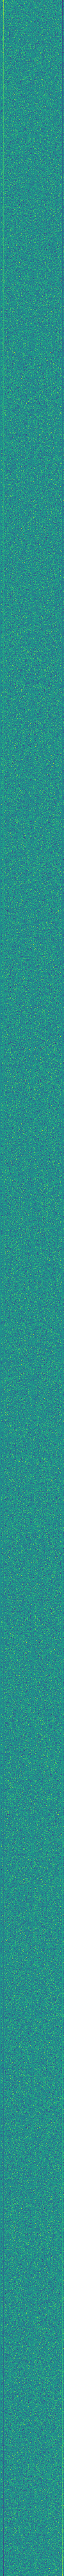
\includegraphics[interpolate=false,width=1.000000in,height=1.000000in]{antiderivative_ci_5-img0.png}}%
\end{pgfscope}%
\begin{pgfscope}%
\pgfsetbuttcap%
\pgfsetroundjoin%
\definecolor{currentfill}{rgb}{0.000000,0.000000,0.000000}%
\pgfsetfillcolor{currentfill}%
\pgfsetlinewidth{0.803000pt}%
\definecolor{currentstroke}{rgb}{0.000000,0.000000,0.000000}%
\pgfsetstrokecolor{currentstroke}%
\pgfsetdash{}{0pt}%
\pgfsys@defobject{currentmarker}{\pgfqpoint{0.000000in}{-0.048611in}}{\pgfqpoint{0.000000in}{0.000000in}}{%
\pgfpathmoveto{\pgfqpoint{0.000000in}{0.000000in}}%
\pgfpathlineto{\pgfqpoint{0.000000in}{-0.048611in}}%
\pgfusepath{stroke,fill}%
}%
\begin{pgfscope}%
\pgfsys@transformshift{0.779897in}{0.517039in}%
\pgfsys@useobject{currentmarker}{}%
\end{pgfscope}%
\end{pgfscope}%
\begin{pgfscope}%
\definecolor{textcolor}{rgb}{0.000000,0.000000,0.000000}%
\pgfsetstrokecolor{textcolor}%
\pgfsetfillcolor{textcolor}%
\pgftext[x=0.779897in,y=0.419816in,,top]{\color{textcolor}{\rmfamily\fontsize{12.000000}{14.400000}\selectfont\catcode`\^=\active\def^{\ifmmode\sp\else\^{}\fi}\catcode`\%=\active\def%{\%}0}}%
\end{pgfscope}%
\begin{pgfscope}%
\pgfsetbuttcap%
\pgfsetroundjoin%
\definecolor{currentfill}{rgb}{0.000000,0.000000,0.000000}%
\pgfsetfillcolor{currentfill}%
\pgfsetlinewidth{0.803000pt}%
\definecolor{currentstroke}{rgb}{0.000000,0.000000,0.000000}%
\pgfsetstrokecolor{currentstroke}%
\pgfsetdash{}{0pt}%
\pgfsys@defobject{currentmarker}{\pgfqpoint{0.000000in}{-0.048611in}}{\pgfqpoint{0.000000in}{0.000000in}}{%
\pgfpathmoveto{\pgfqpoint{0.000000in}{0.000000in}}%
\pgfpathlineto{\pgfqpoint{0.000000in}{-0.048611in}}%
\pgfusepath{stroke,fill}%
}%
\begin{pgfscope}%
\pgfsys@transformshift{1.693017in}{0.517039in}%
\pgfsys@useobject{currentmarker}{}%
\end{pgfscope}%
\end{pgfscope}%
\begin{pgfscope}%
\definecolor{textcolor}{rgb}{0.000000,0.000000,0.000000}%
\pgfsetstrokecolor{textcolor}%
\pgfsetfillcolor{textcolor}%
\pgftext[x=1.693017in,y=0.419816in,,top]{\color{textcolor}{\rmfamily\fontsize{12.000000}{14.400000}\selectfont\catcode`\^=\active\def^{\ifmmode\sp\else\^{}\fi}\catcode`\%=\active\def%{\%}20}}%
\end{pgfscope}%
\begin{pgfscope}%
\pgfsetbuttcap%
\pgfsetroundjoin%
\definecolor{currentfill}{rgb}{0.000000,0.000000,0.000000}%
\pgfsetfillcolor{currentfill}%
\pgfsetlinewidth{0.803000pt}%
\definecolor{currentstroke}{rgb}{0.000000,0.000000,0.000000}%
\pgfsetstrokecolor{currentstroke}%
\pgfsetdash{}{0pt}%
\pgfsys@defobject{currentmarker}{\pgfqpoint{0.000000in}{-0.048611in}}{\pgfqpoint{0.000000in}{0.000000in}}{%
\pgfpathmoveto{\pgfqpoint{0.000000in}{0.000000in}}%
\pgfpathlineto{\pgfqpoint{0.000000in}{-0.048611in}}%
\pgfusepath{stroke,fill}%
}%
\begin{pgfscope}%
\pgfsys@transformshift{2.606137in}{0.517039in}%
\pgfsys@useobject{currentmarker}{}%
\end{pgfscope}%
\end{pgfscope}%
\begin{pgfscope}%
\definecolor{textcolor}{rgb}{0.000000,0.000000,0.000000}%
\pgfsetstrokecolor{textcolor}%
\pgfsetfillcolor{textcolor}%
\pgftext[x=2.606137in,y=0.419816in,,top]{\color{textcolor}{\rmfamily\fontsize{12.000000}{14.400000}\selectfont\catcode`\^=\active\def^{\ifmmode\sp\else\^{}\fi}\catcode`\%=\active\def%{\%}40}}%
\end{pgfscope}%
\begin{pgfscope}%
\definecolor{textcolor}{rgb}{0.000000,0.000000,0.000000}%
\pgfsetstrokecolor{textcolor}%
\pgfsetfillcolor{textcolor}%
\pgftext[x=1.921297in,y=0.202965in,,top]{\color{textcolor}{\rmfamily\fontsize{12.000000}{14.400000}\selectfont\catcode`\^=\active\def^{\ifmmode\sp\else\^{}\fi}\catcode`\%=\active\def%{\%}input coefficients}}%
\end{pgfscope}%
\begin{pgfscope}%
\pgfsetbuttcap%
\pgfsetroundjoin%
\definecolor{currentfill}{rgb}{0.000000,0.000000,0.000000}%
\pgfsetfillcolor{currentfill}%
\pgfsetlinewidth{0.803000pt}%
\definecolor{currentstroke}{rgb}{0.000000,0.000000,0.000000}%
\pgfsetstrokecolor{currentstroke}%
\pgfsetdash{}{0pt}%
\pgfsys@defobject{currentmarker}{\pgfqpoint{-0.048611in}{0.000000in}}{\pgfqpoint{-0.000000in}{0.000000in}}{%
\pgfpathmoveto{\pgfqpoint{-0.000000in}{0.000000in}}%
\pgfpathlineto{\pgfqpoint{-0.048611in}{0.000000in}}%
\pgfusepath{stroke,fill}%
}%
\begin{pgfscope}%
\pgfsys@transformshift{0.779897in}{2.895016in}%
\pgfsys@useobject{currentmarker}{}%
\end{pgfscope}%
\end{pgfscope}%
\begin{pgfscope}%
\definecolor{textcolor}{rgb}{0.000000,0.000000,0.000000}%
\pgfsetstrokecolor{textcolor}%
\pgfsetfillcolor{textcolor}%
\pgftext[x=0.576636in, y=2.831702in, left, base]{\color{textcolor}{\rmfamily\fontsize{12.000000}{14.400000}\selectfont\catcode`\^=\active\def^{\ifmmode\sp\else\^{}\fi}\catcode`\%=\active\def%{\%}0}}%
\end{pgfscope}%
\begin{pgfscope}%
\pgfsetbuttcap%
\pgfsetroundjoin%
\definecolor{currentfill}{rgb}{0.000000,0.000000,0.000000}%
\pgfsetfillcolor{currentfill}%
\pgfsetlinewidth{0.803000pt}%
\definecolor{currentstroke}{rgb}{0.000000,0.000000,0.000000}%
\pgfsetstrokecolor{currentstroke}%
\pgfsetdash{}{0pt}%
\pgfsys@defobject{currentmarker}{\pgfqpoint{-0.048611in}{0.000000in}}{\pgfqpoint{-0.000000in}{0.000000in}}{%
\pgfpathmoveto{\pgfqpoint{-0.000000in}{0.000000in}}%
\pgfpathlineto{\pgfqpoint{-0.048611in}{0.000000in}}%
\pgfusepath{stroke,fill}%
}%
\begin{pgfscope}%
\pgfsys@transformshift{0.779897in}{2.300522in}%
\pgfsys@useobject{currentmarker}{}%
\end{pgfscope}%
\end{pgfscope}%
\begin{pgfscope}%
\definecolor{textcolor}{rgb}{0.000000,0.000000,0.000000}%
\pgfsetstrokecolor{textcolor}%
\pgfsetfillcolor{textcolor}%
\pgftext[x=0.258521in, y=2.237208in, left, base]{\color{textcolor}{\rmfamily\fontsize{12.000000}{14.400000}\selectfont\catcode`\^=\active\def^{\ifmmode\sp\else\^{}\fi}\catcode`\%=\active\def%{\%}1000}}%
\end{pgfscope}%
\begin{pgfscope}%
\pgfsetbuttcap%
\pgfsetroundjoin%
\definecolor{currentfill}{rgb}{0.000000,0.000000,0.000000}%
\pgfsetfillcolor{currentfill}%
\pgfsetlinewidth{0.803000pt}%
\definecolor{currentstroke}{rgb}{0.000000,0.000000,0.000000}%
\pgfsetstrokecolor{currentstroke}%
\pgfsetdash{}{0pt}%
\pgfsys@defobject{currentmarker}{\pgfqpoint{-0.048611in}{0.000000in}}{\pgfqpoint{-0.000000in}{0.000000in}}{%
\pgfpathmoveto{\pgfqpoint{-0.000000in}{0.000000in}}%
\pgfpathlineto{\pgfqpoint{-0.048611in}{0.000000in}}%
\pgfusepath{stroke,fill}%
}%
\begin{pgfscope}%
\pgfsys@transformshift{0.779897in}{1.706027in}%
\pgfsys@useobject{currentmarker}{}%
\end{pgfscope}%
\end{pgfscope}%
\begin{pgfscope}%
\definecolor{textcolor}{rgb}{0.000000,0.000000,0.000000}%
\pgfsetstrokecolor{textcolor}%
\pgfsetfillcolor{textcolor}%
\pgftext[x=0.258521in, y=1.642714in, left, base]{\color{textcolor}{\rmfamily\fontsize{12.000000}{14.400000}\selectfont\catcode`\^=\active\def^{\ifmmode\sp\else\^{}\fi}\catcode`\%=\active\def%{\%}2000}}%
\end{pgfscope}%
\begin{pgfscope}%
\pgfsetbuttcap%
\pgfsetroundjoin%
\definecolor{currentfill}{rgb}{0.000000,0.000000,0.000000}%
\pgfsetfillcolor{currentfill}%
\pgfsetlinewidth{0.803000pt}%
\definecolor{currentstroke}{rgb}{0.000000,0.000000,0.000000}%
\pgfsetstrokecolor{currentstroke}%
\pgfsetdash{}{0pt}%
\pgfsys@defobject{currentmarker}{\pgfqpoint{-0.048611in}{0.000000in}}{\pgfqpoint{-0.000000in}{0.000000in}}{%
\pgfpathmoveto{\pgfqpoint{-0.000000in}{0.000000in}}%
\pgfpathlineto{\pgfqpoint{-0.048611in}{0.000000in}}%
\pgfusepath{stroke,fill}%
}%
\begin{pgfscope}%
\pgfsys@transformshift{0.779897in}{1.111533in}%
\pgfsys@useobject{currentmarker}{}%
\end{pgfscope}%
\end{pgfscope}%
\begin{pgfscope}%
\definecolor{textcolor}{rgb}{0.000000,0.000000,0.000000}%
\pgfsetstrokecolor{textcolor}%
\pgfsetfillcolor{textcolor}%
\pgftext[x=0.258521in, y=1.048219in, left, base]{\color{textcolor}{\rmfamily\fontsize{12.000000}{14.400000}\selectfont\catcode`\^=\active\def^{\ifmmode\sp\else\^{}\fi}\catcode`\%=\active\def%{\%}3000}}%
\end{pgfscope}%
\begin{pgfscope}%
\pgfsetbuttcap%
\pgfsetroundjoin%
\definecolor{currentfill}{rgb}{0.000000,0.000000,0.000000}%
\pgfsetfillcolor{currentfill}%
\pgfsetlinewidth{0.803000pt}%
\definecolor{currentstroke}{rgb}{0.000000,0.000000,0.000000}%
\pgfsetstrokecolor{currentstroke}%
\pgfsetdash{}{0pt}%
\pgfsys@defobject{currentmarker}{\pgfqpoint{-0.048611in}{0.000000in}}{\pgfqpoint{-0.000000in}{0.000000in}}{%
\pgfpathmoveto{\pgfqpoint{-0.000000in}{0.000000in}}%
\pgfpathlineto{\pgfqpoint{-0.048611in}{0.000000in}}%
\pgfusepath{stroke,fill}%
}%
\begin{pgfscope}%
\pgfsys@transformshift{0.779897in}{0.517039in}%
\pgfsys@useobject{currentmarker}{}%
\end{pgfscope}%
\end{pgfscope}%
\begin{pgfscope}%
\definecolor{textcolor}{rgb}{0.000000,0.000000,0.000000}%
\pgfsetstrokecolor{textcolor}%
\pgfsetfillcolor{textcolor}%
\pgftext[x=0.258521in, y=0.453725in, left, base]{\color{textcolor}{\rmfamily\fontsize{12.000000}{14.400000}\selectfont\catcode`\^=\active\def^{\ifmmode\sp\else\^{}\fi}\catcode`\%=\active\def%{\%}4000}}%
\end{pgfscope}%
\begin{pgfscope}%
\definecolor{textcolor}{rgb}{0.000000,0.000000,0.000000}%
\pgfsetstrokecolor{textcolor}%
\pgfsetfillcolor{textcolor}%
\pgftext[x=0.202965in,y=1.706027in,,bottom,rotate=90.000000]{\color{textcolor}{\rmfamily\fontsize{12.000000}{14.400000}\selectfont\catcode`\^=\active\def^{\ifmmode\sp\else\^{}\fi}\catcode`\%=\active\def%{\%}samples}}%
\end{pgfscope}%
\begin{pgfscope}%
\pgfsetrectcap%
\pgfsetmiterjoin%
\pgfsetlinewidth{0.803000pt}%
\definecolor{currentstroke}{rgb}{0.000000,0.000000,0.000000}%
\pgfsetstrokecolor{currentstroke}%
\pgfsetdash{}{0pt}%
\pgfpathmoveto{\pgfqpoint{0.779897in}{0.517039in}}%
\pgfpathlineto{\pgfqpoint{0.779897in}{2.895016in}}%
\pgfusepath{stroke}%
\end{pgfscope}%
\begin{pgfscope}%
\pgfsetrectcap%
\pgfsetmiterjoin%
\pgfsetlinewidth{0.803000pt}%
\definecolor{currentstroke}{rgb}{0.000000,0.000000,0.000000}%
\pgfsetstrokecolor{currentstroke}%
\pgfsetdash{}{0pt}%
\pgfpathmoveto{\pgfqpoint{3.062697in}{0.517039in}}%
\pgfpathlineto{\pgfqpoint{3.062697in}{2.895016in}}%
\pgfusepath{stroke}%
\end{pgfscope}%
\begin{pgfscope}%
\pgfsetrectcap%
\pgfsetmiterjoin%
\pgfsetlinewidth{0.803000pt}%
\definecolor{currentstroke}{rgb}{0.000000,0.000000,0.000000}%
\pgfsetstrokecolor{currentstroke}%
\pgfsetdash{}{0pt}%
\pgfpathmoveto{\pgfqpoint{0.779897in}{0.517039in}}%
\pgfpathlineto{\pgfqpoint{3.062697in}{0.517039in}}%
\pgfusepath{stroke}%
\end{pgfscope}%
\begin{pgfscope}%
\pgfsetrectcap%
\pgfsetmiterjoin%
\pgfsetlinewidth{0.803000pt}%
\definecolor{currentstroke}{rgb}{0.000000,0.000000,0.000000}%
\pgfsetstrokecolor{currentstroke}%
\pgfsetdash{}{0pt}%
\pgfpathmoveto{\pgfqpoint{0.779897in}{2.895016in}}%
\pgfpathlineto{\pgfqpoint{3.062697in}{2.895016in}}%
\pgfusepath{stroke}%
\end{pgfscope}%
\begin{pgfscope}%
\pgfsetbuttcap%
\pgfsetmiterjoin%
\pgfsetlinewidth{0.000000pt}%
\definecolor{currentstroke}{rgb}{0.000000,0.000000,0.000000}%
\pgfsetstrokecolor{currentstroke}%
\pgfsetstrokeopacity{0.000000}%
\pgfsetdash{}{0pt}%
\pgfpathmoveto{\pgfqpoint{3.282875in}{0.517039in}}%
\pgfpathlineto{\pgfqpoint{3.401774in}{0.517039in}}%
\pgfpathlineto{\pgfqpoint{3.401774in}{2.895016in}}%
\pgfpathlineto{\pgfqpoint{3.282875in}{2.895016in}}%
\pgfpathlineto{\pgfqpoint{3.282875in}{0.517039in}}%
\pgfpathclose%
\pgfusepath{}%
\end{pgfscope}%
\begin{pgfscope}%
\pgfsys@transformshift{3.280000in}{0.520000in}%
\pgftext[left,bottom]{
\includegraphics[interpolate=true,width=0.120000in,height=2.380000in]{antiderivative_ci_5-img1.png}}%
\end{pgfscope}%
\begin{pgfscope}%
\pgfsetbuttcap%
\pgfsetroundjoin%
\definecolor{currentfill}{rgb}{0.000000,0.000000,0.000000}%
\pgfsetfillcolor{currentfill}%
\pgfsetlinewidth{0.803000pt}%
\definecolor{currentstroke}{rgb}{0.000000,0.000000,0.000000}%
\pgfsetstrokecolor{currentstroke}%
\pgfsetdash{}{0pt}%
\pgfsys@defobject{currentmarker}{\pgfqpoint{0.000000in}{0.000000in}}{\pgfqpoint{0.048611in}{0.000000in}}{%
\pgfpathmoveto{\pgfqpoint{0.000000in}{0.000000in}}%
\pgfpathlineto{\pgfqpoint{0.048611in}{0.000000in}}%
\pgfusepath{stroke,fill}%
}%
\begin{pgfscope}%
\pgfsys@transformshift{3.401774in}{0.636505in}%
\pgfsys@useobject{currentmarker}{}%
\end{pgfscope}%
\end{pgfscope}%
\begin{pgfscope}%
\definecolor{textcolor}{rgb}{0.000000,0.000000,0.000000}%
\pgfsetstrokecolor{textcolor}%
\pgfsetfillcolor{textcolor}%
\pgftext[x=3.498996in, y=0.573191in, left, base]{\color{textcolor}{\rmfamily\fontsize{12.000000}{14.400000}\selectfont\catcode`\^=\active\def^{\ifmmode\sp\else\^{}\fi}\catcode`\%=\active\def%{\%}\ensuremath{-}100}}%
\end{pgfscope}%
\begin{pgfscope}%
\pgfsetbuttcap%
\pgfsetroundjoin%
\definecolor{currentfill}{rgb}{0.000000,0.000000,0.000000}%
\pgfsetfillcolor{currentfill}%
\pgfsetlinewidth{0.803000pt}%
\definecolor{currentstroke}{rgb}{0.000000,0.000000,0.000000}%
\pgfsetstrokecolor{currentstroke}%
\pgfsetdash{}{0pt}%
\pgfsys@defobject{currentmarker}{\pgfqpoint{0.000000in}{0.000000in}}{\pgfqpoint{0.048611in}{0.000000in}}{%
\pgfpathmoveto{\pgfqpoint{0.000000in}{0.000000in}}%
\pgfpathlineto{\pgfqpoint{0.048611in}{0.000000in}}%
\pgfusepath{stroke,fill}%
}%
\begin{pgfscope}%
\pgfsys@transformshift{3.401774in}{1.171266in}%
\pgfsys@useobject{currentmarker}{}%
\end{pgfscope}%
\end{pgfscope}%
\begin{pgfscope}%
\definecolor{textcolor}{rgb}{0.000000,0.000000,0.000000}%
\pgfsetstrokecolor{textcolor}%
\pgfsetfillcolor{textcolor}%
\pgftext[x=3.498996in, y=1.107952in, left, base]{\color{textcolor}{\rmfamily\fontsize{12.000000}{14.400000}\selectfont\catcode`\^=\active\def^{\ifmmode\sp\else\^{}\fi}\catcode`\%=\active\def%{\%}\ensuremath{-}50}}%
\end{pgfscope}%
\begin{pgfscope}%
\pgfsetbuttcap%
\pgfsetroundjoin%
\definecolor{currentfill}{rgb}{0.000000,0.000000,0.000000}%
\pgfsetfillcolor{currentfill}%
\pgfsetlinewidth{0.803000pt}%
\definecolor{currentstroke}{rgb}{0.000000,0.000000,0.000000}%
\pgfsetstrokecolor{currentstroke}%
\pgfsetdash{}{0pt}%
\pgfsys@defobject{currentmarker}{\pgfqpoint{0.000000in}{0.000000in}}{\pgfqpoint{0.048611in}{0.000000in}}{%
\pgfpathmoveto{\pgfqpoint{0.000000in}{0.000000in}}%
\pgfpathlineto{\pgfqpoint{0.048611in}{0.000000in}}%
\pgfusepath{stroke,fill}%
}%
\begin{pgfscope}%
\pgfsys@transformshift{3.401774in}{1.706028in}%
\pgfsys@useobject{currentmarker}{}%
\end{pgfscope}%
\end{pgfscope}%
\begin{pgfscope}%
\definecolor{textcolor}{rgb}{0.000000,0.000000,0.000000}%
\pgfsetstrokecolor{textcolor}%
\pgfsetfillcolor{textcolor}%
\pgftext[x=3.498996in, y=1.642714in, left, base]{\color{textcolor}{\rmfamily\fontsize{12.000000}{14.400000}\selectfont\catcode`\^=\active\def^{\ifmmode\sp\else\^{}\fi}\catcode`\%=\active\def%{\%}0}}%
\end{pgfscope}%
\begin{pgfscope}%
\pgfsetbuttcap%
\pgfsetroundjoin%
\definecolor{currentfill}{rgb}{0.000000,0.000000,0.000000}%
\pgfsetfillcolor{currentfill}%
\pgfsetlinewidth{0.803000pt}%
\definecolor{currentstroke}{rgb}{0.000000,0.000000,0.000000}%
\pgfsetstrokecolor{currentstroke}%
\pgfsetdash{}{0pt}%
\pgfsys@defobject{currentmarker}{\pgfqpoint{0.000000in}{0.000000in}}{\pgfqpoint{0.048611in}{0.000000in}}{%
\pgfpathmoveto{\pgfqpoint{0.000000in}{0.000000in}}%
\pgfpathlineto{\pgfqpoint{0.048611in}{0.000000in}}%
\pgfusepath{stroke,fill}%
}%
\begin{pgfscope}%
\pgfsys@transformshift{3.401774in}{2.240789in}%
\pgfsys@useobject{currentmarker}{}%
\end{pgfscope}%
\end{pgfscope}%
\begin{pgfscope}%
\definecolor{textcolor}{rgb}{0.000000,0.000000,0.000000}%
\pgfsetstrokecolor{textcolor}%
\pgfsetfillcolor{textcolor}%
\pgftext[x=3.498996in, y=2.177475in, left, base]{\color{textcolor}{\rmfamily\fontsize{12.000000}{14.400000}\selectfont\catcode`\^=\active\def^{\ifmmode\sp\else\^{}\fi}\catcode`\%=\active\def%{\%}50}}%
\end{pgfscope}%
\begin{pgfscope}%
\pgfsetbuttcap%
\pgfsetroundjoin%
\definecolor{currentfill}{rgb}{0.000000,0.000000,0.000000}%
\pgfsetfillcolor{currentfill}%
\pgfsetlinewidth{0.803000pt}%
\definecolor{currentstroke}{rgb}{0.000000,0.000000,0.000000}%
\pgfsetstrokecolor{currentstroke}%
\pgfsetdash{}{0pt}%
\pgfsys@defobject{currentmarker}{\pgfqpoint{0.000000in}{0.000000in}}{\pgfqpoint{0.048611in}{0.000000in}}{%
\pgfpathmoveto{\pgfqpoint{0.000000in}{0.000000in}}%
\pgfpathlineto{\pgfqpoint{0.048611in}{0.000000in}}%
\pgfusepath{stroke,fill}%
}%
\begin{pgfscope}%
\pgfsys@transformshift{3.401774in}{2.775550in}%
\pgfsys@useobject{currentmarker}{}%
\end{pgfscope}%
\end{pgfscope}%
\begin{pgfscope}%
\definecolor{textcolor}{rgb}{0.000000,0.000000,0.000000}%
\pgfsetstrokecolor{textcolor}%
\pgfsetfillcolor{textcolor}%
\pgftext[x=3.498996in, y=2.712237in, left, base]{\color{textcolor}{\rmfamily\fontsize{12.000000}{14.400000}\selectfont\catcode`\^=\active\def^{\ifmmode\sp\else\^{}\fi}\catcode`\%=\active\def%{\%}100}}%
\end{pgfscope}%
\begin{pgfscope}%
\pgfsetrectcap%
\pgfsetmiterjoin%
\pgfsetlinewidth{0.803000pt}%
\definecolor{currentstroke}{rgb}{0.000000,0.000000,0.000000}%
\pgfsetstrokecolor{currentstroke}%
\pgfsetdash{}{0pt}%
\pgfpathmoveto{\pgfqpoint{3.282875in}{0.517039in}}%
\pgfpathlineto{\pgfqpoint{3.342325in}{0.517039in}}%
\pgfpathlineto{\pgfqpoint{3.401774in}{0.517039in}}%
\pgfpathlineto{\pgfqpoint{3.401774in}{2.895016in}}%
\pgfpathlineto{\pgfqpoint{3.342325in}{2.895016in}}%
\pgfpathlineto{\pgfqpoint{3.282875in}{2.895016in}}%
\pgfpathlineto{\pgfqpoint{3.282875in}{0.517039in}}%
\pgfpathclose%
\pgfusepath{stroke}%
\end{pgfscope}%
\end{pgfpicture}%
\makeatother%
\endgroup%

      \end{adjustbox}
      \caption{Correlation image 5\% noise.}\label{fig:sc1_ci_5}
    \end{subfigure}
    \begin{subfigure}{0.49\linewidth}
      \begin{adjustbox}{width=\linewidth}
        \begingroup%
\makeatletter%
\begin{pgfpicture}%
\pgfpathrectangle{\pgfpointorigin}{\pgfqpoint{6.400000in}{4.800000in}}%
\pgfusepath{use as bounding box, clip}%
\begin{pgfscope}%
\pgfsetbuttcap%
\pgfsetmiterjoin%
\pgfsetlinewidth{0.000000pt}%
\definecolor{currentstroke}{rgb}{0.000000,0.000000,0.000000}%
\pgfsetstrokecolor{currentstroke}%
\pgfsetstrokeopacity{0.000000}%
\pgfsetdash{}{0pt}%
\pgfpathmoveto{\pgfqpoint{0.000000in}{0.000000in}}%
\pgfpathlineto{\pgfqpoint{6.400000in}{0.000000in}}%
\pgfpathlineto{\pgfqpoint{6.400000in}{4.800000in}}%
\pgfpathlineto{\pgfqpoint{0.000000in}{4.800000in}}%
\pgfpathlineto{\pgfqpoint{0.000000in}{0.000000in}}%
\pgfpathclose%
\pgfusepath{}%
\end{pgfscope}%
\begin{pgfscope}%
\pgfsetbuttcap%
\pgfsetmiterjoin%
\pgfsetlinewidth{0.000000pt}%
\definecolor{currentstroke}{rgb}{0.000000,0.000000,0.000000}%
\pgfsetstrokecolor{currentstroke}%
\pgfsetstrokeopacity{0.000000}%
\pgfsetdash{}{0pt}%
\pgfpathmoveto{\pgfqpoint{1.072000in}{0.528000in}}%
\pgfpathlineto{\pgfqpoint{4.768000in}{0.528000in}}%
\pgfpathlineto{\pgfqpoint{4.768000in}{4.224000in}}%
\pgfpathlineto{\pgfqpoint{1.072000in}{4.224000in}}%
\pgfpathlineto{\pgfqpoint{1.072000in}{0.528000in}}%
\pgfpathclose%
\pgfusepath{}%
\end{pgfscope}%
\begin{pgfscope}%
\pgfpathrectangle{\pgfqpoint{1.072000in}{0.528000in}}{\pgfqpoint{3.696000in}{3.696000in}}%
\pgfusepath{clip}%
\pgfsys@transformcm{3.696000}{0.000000}{0.000000}{-3.696000}{1.072000in}{4.224000in}%
\pgftext[left,bottom]{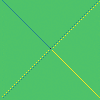
\includegraphics[interpolate=false,width=1.000000in,height=1.000000in]{antiderivative_pm_5-img0.png}}%
\end{pgfscope}%
\begin{pgfscope}%
\pgfsetbuttcap%
\pgfsetroundjoin%
\definecolor{currentfill}{rgb}{0.000000,0.000000,0.000000}%
\pgfsetfillcolor{currentfill}%
\pgfsetlinewidth{0.803000pt}%
\definecolor{currentstroke}{rgb}{0.000000,0.000000,0.000000}%
\pgfsetstrokecolor{currentstroke}%
\pgfsetdash{}{0pt}%
\pgfsys@defobject{currentmarker}{\pgfqpoint{0.000000in}{-0.048611in}}{\pgfqpoint{0.000000in}{0.000000in}}{%
\pgfpathmoveto{\pgfqpoint{0.000000in}{0.000000in}}%
\pgfpathlineto{\pgfqpoint{0.000000in}{-0.048611in}}%
\pgfusepath{stroke,fill}%
}%
\begin{pgfscope}%
\pgfsys@transformshift{1.090480in}{0.528000in}%
\pgfsys@useobject{currentmarker}{}%
\end{pgfscope}%
\end{pgfscope}%
\begin{pgfscope}%
\definecolor{textcolor}{rgb}{0.000000,0.000000,0.000000}%
\pgfsetstrokecolor{textcolor}%
\pgfsetfillcolor{textcolor}%
\pgftext[x=1.090480in,y=0.430778in,,top]{\color{textcolor}{\rmfamily\fontsize{12.000000}{14.400000}\selectfont\catcode`\^=\active\def^{\ifmmode\sp\else\^{}\fi}\catcode`\%=\active\def%{\%}0}}%
\end{pgfscope}%
\begin{pgfscope}%
\pgfsetbuttcap%
\pgfsetroundjoin%
\definecolor{currentfill}{rgb}{0.000000,0.000000,0.000000}%
\pgfsetfillcolor{currentfill}%
\pgfsetlinewidth{0.803000pt}%
\definecolor{currentstroke}{rgb}{0.000000,0.000000,0.000000}%
\pgfsetstrokecolor{currentstroke}%
\pgfsetdash{}{0pt}%
\pgfsys@defobject{currentmarker}{\pgfqpoint{0.000000in}{-0.048611in}}{\pgfqpoint{0.000000in}{0.000000in}}{%
\pgfpathmoveto{\pgfqpoint{0.000000in}{0.000000in}}%
\pgfpathlineto{\pgfqpoint{0.000000in}{-0.048611in}}%
\pgfusepath{stroke,fill}%
}%
\begin{pgfscope}%
\pgfsys@transformshift{1.829680in}{0.528000in}%
\pgfsys@useobject{currentmarker}{}%
\end{pgfscope}%
\end{pgfscope}%
\begin{pgfscope}%
\definecolor{textcolor}{rgb}{0.000000,0.000000,0.000000}%
\pgfsetstrokecolor{textcolor}%
\pgfsetfillcolor{textcolor}%
\pgftext[x=1.829680in,y=0.430778in,,top]{\color{textcolor}{\rmfamily\fontsize{12.000000}{14.400000}\selectfont\catcode`\^=\active\def^{\ifmmode\sp\else\^{}\fi}\catcode`\%=\active\def%{\%}20}}%
\end{pgfscope}%
\begin{pgfscope}%
\pgfsetbuttcap%
\pgfsetroundjoin%
\definecolor{currentfill}{rgb}{0.000000,0.000000,0.000000}%
\pgfsetfillcolor{currentfill}%
\pgfsetlinewidth{0.803000pt}%
\definecolor{currentstroke}{rgb}{0.000000,0.000000,0.000000}%
\pgfsetstrokecolor{currentstroke}%
\pgfsetdash{}{0pt}%
\pgfsys@defobject{currentmarker}{\pgfqpoint{0.000000in}{-0.048611in}}{\pgfqpoint{0.000000in}{0.000000in}}{%
\pgfpathmoveto{\pgfqpoint{0.000000in}{0.000000in}}%
\pgfpathlineto{\pgfqpoint{0.000000in}{-0.048611in}}%
\pgfusepath{stroke,fill}%
}%
\begin{pgfscope}%
\pgfsys@transformshift{2.568880in}{0.528000in}%
\pgfsys@useobject{currentmarker}{}%
\end{pgfscope}%
\end{pgfscope}%
\begin{pgfscope}%
\definecolor{textcolor}{rgb}{0.000000,0.000000,0.000000}%
\pgfsetstrokecolor{textcolor}%
\pgfsetfillcolor{textcolor}%
\pgftext[x=2.568880in,y=0.430778in,,top]{\color{textcolor}{\rmfamily\fontsize{12.000000}{14.400000}\selectfont\catcode`\^=\active\def^{\ifmmode\sp\else\^{}\fi}\catcode`\%=\active\def%{\%}40}}%
\end{pgfscope}%
\begin{pgfscope}%
\pgfsetbuttcap%
\pgfsetroundjoin%
\definecolor{currentfill}{rgb}{0.000000,0.000000,0.000000}%
\pgfsetfillcolor{currentfill}%
\pgfsetlinewidth{0.803000pt}%
\definecolor{currentstroke}{rgb}{0.000000,0.000000,0.000000}%
\pgfsetstrokecolor{currentstroke}%
\pgfsetdash{}{0pt}%
\pgfsys@defobject{currentmarker}{\pgfqpoint{0.000000in}{-0.048611in}}{\pgfqpoint{0.000000in}{0.000000in}}{%
\pgfpathmoveto{\pgfqpoint{0.000000in}{0.000000in}}%
\pgfpathlineto{\pgfqpoint{0.000000in}{-0.048611in}}%
\pgfusepath{stroke,fill}%
}%
\begin{pgfscope}%
\pgfsys@transformshift{3.308080in}{0.528000in}%
\pgfsys@useobject{currentmarker}{}%
\end{pgfscope}%
\end{pgfscope}%
\begin{pgfscope}%
\definecolor{textcolor}{rgb}{0.000000,0.000000,0.000000}%
\pgfsetstrokecolor{textcolor}%
\pgfsetfillcolor{textcolor}%
\pgftext[x=3.308080in,y=0.430778in,,top]{\color{textcolor}{\rmfamily\fontsize{12.000000}{14.400000}\selectfont\catcode`\^=\active\def^{\ifmmode\sp\else\^{}\fi}\catcode`\%=\active\def%{\%}60}}%
\end{pgfscope}%
\begin{pgfscope}%
\pgfsetbuttcap%
\pgfsetroundjoin%
\definecolor{currentfill}{rgb}{0.000000,0.000000,0.000000}%
\pgfsetfillcolor{currentfill}%
\pgfsetlinewidth{0.803000pt}%
\definecolor{currentstroke}{rgb}{0.000000,0.000000,0.000000}%
\pgfsetstrokecolor{currentstroke}%
\pgfsetdash{}{0pt}%
\pgfsys@defobject{currentmarker}{\pgfqpoint{0.000000in}{-0.048611in}}{\pgfqpoint{0.000000in}{0.000000in}}{%
\pgfpathmoveto{\pgfqpoint{0.000000in}{0.000000in}}%
\pgfpathlineto{\pgfqpoint{0.000000in}{-0.048611in}}%
\pgfusepath{stroke,fill}%
}%
\begin{pgfscope}%
\pgfsys@transformshift{4.047280in}{0.528000in}%
\pgfsys@useobject{currentmarker}{}%
\end{pgfscope}%
\end{pgfscope}%
\begin{pgfscope}%
\definecolor{textcolor}{rgb}{0.000000,0.000000,0.000000}%
\pgfsetstrokecolor{textcolor}%
\pgfsetfillcolor{textcolor}%
\pgftext[x=4.047280in,y=0.430778in,,top]{\color{textcolor}{\rmfamily\fontsize{12.000000}{14.400000}\selectfont\catcode`\^=\active\def^{\ifmmode\sp\else\^{}\fi}\catcode`\%=\active\def%{\%}80}}%
\end{pgfscope}%
\begin{pgfscope}%
\definecolor{textcolor}{rgb}{0.000000,0.000000,0.000000}%
\pgfsetstrokecolor{textcolor}%
\pgfsetfillcolor{textcolor}%
\pgftext[x=2.920000in,y=0.213927in,,top]{\color{textcolor}{\rmfamily\fontsize{12.000000}{14.400000}\selectfont\catcode`\^=\active\def^{\ifmmode\sp\else\^{}\fi}\catcode`\%=\active\def%{\%}output coefficients}}%
\end{pgfscope}%
\begin{pgfscope}%
\pgfsetbuttcap%
\pgfsetroundjoin%
\definecolor{currentfill}{rgb}{0.000000,0.000000,0.000000}%
\pgfsetfillcolor{currentfill}%
\pgfsetlinewidth{0.803000pt}%
\definecolor{currentstroke}{rgb}{0.000000,0.000000,0.000000}%
\pgfsetstrokecolor{currentstroke}%
\pgfsetdash{}{0pt}%
\pgfsys@defobject{currentmarker}{\pgfqpoint{-0.048611in}{0.000000in}}{\pgfqpoint{-0.000000in}{0.000000in}}{%
\pgfpathmoveto{\pgfqpoint{-0.000000in}{0.000000in}}%
\pgfpathlineto{\pgfqpoint{-0.048611in}{0.000000in}}%
\pgfusepath{stroke,fill}%
}%
\begin{pgfscope}%
\pgfsys@transformshift{1.072000in}{4.205520in}%
\pgfsys@useobject{currentmarker}{}%
\end{pgfscope}%
\end{pgfscope}%
\begin{pgfscope}%
\definecolor{textcolor}{rgb}{0.000000,0.000000,0.000000}%
\pgfsetstrokecolor{textcolor}%
\pgfsetfillcolor{textcolor}%
\pgftext[x=0.868739in, y=4.142206in, left, base]{\color{textcolor}{\rmfamily\fontsize{12.000000}{14.400000}\selectfont\catcode`\^=\active\def^{\ifmmode\sp\else\^{}\fi}\catcode`\%=\active\def%{\%}0}}%
\end{pgfscope}%
\begin{pgfscope}%
\pgfsetbuttcap%
\pgfsetroundjoin%
\definecolor{currentfill}{rgb}{0.000000,0.000000,0.000000}%
\pgfsetfillcolor{currentfill}%
\pgfsetlinewidth{0.803000pt}%
\definecolor{currentstroke}{rgb}{0.000000,0.000000,0.000000}%
\pgfsetstrokecolor{currentstroke}%
\pgfsetdash{}{0pt}%
\pgfsys@defobject{currentmarker}{\pgfqpoint{-0.048611in}{0.000000in}}{\pgfqpoint{-0.000000in}{0.000000in}}{%
\pgfpathmoveto{\pgfqpoint{-0.000000in}{0.000000in}}%
\pgfpathlineto{\pgfqpoint{-0.048611in}{0.000000in}}%
\pgfusepath{stroke,fill}%
}%
\begin{pgfscope}%
\pgfsys@transformshift{1.072000in}{3.466320in}%
\pgfsys@useobject{currentmarker}{}%
\end{pgfscope}%
\end{pgfscope}%
\begin{pgfscope}%
\definecolor{textcolor}{rgb}{0.000000,0.000000,0.000000}%
\pgfsetstrokecolor{textcolor}%
\pgfsetfillcolor{textcolor}%
\pgftext[x=0.762701in, y=3.403006in, left, base]{\color{textcolor}{\rmfamily\fontsize{12.000000}{14.400000}\selectfont\catcode`\^=\active\def^{\ifmmode\sp\else\^{}\fi}\catcode`\%=\active\def%{\%}20}}%
\end{pgfscope}%
\begin{pgfscope}%
\pgfsetbuttcap%
\pgfsetroundjoin%
\definecolor{currentfill}{rgb}{0.000000,0.000000,0.000000}%
\pgfsetfillcolor{currentfill}%
\pgfsetlinewidth{0.803000pt}%
\definecolor{currentstroke}{rgb}{0.000000,0.000000,0.000000}%
\pgfsetstrokecolor{currentstroke}%
\pgfsetdash{}{0pt}%
\pgfsys@defobject{currentmarker}{\pgfqpoint{-0.048611in}{0.000000in}}{\pgfqpoint{-0.000000in}{0.000000in}}{%
\pgfpathmoveto{\pgfqpoint{-0.000000in}{0.000000in}}%
\pgfpathlineto{\pgfqpoint{-0.048611in}{0.000000in}}%
\pgfusepath{stroke,fill}%
}%
\begin{pgfscope}%
\pgfsys@transformshift{1.072000in}{2.727120in}%
\pgfsys@useobject{currentmarker}{}%
\end{pgfscope}%
\end{pgfscope}%
\begin{pgfscope}%
\definecolor{textcolor}{rgb}{0.000000,0.000000,0.000000}%
\pgfsetstrokecolor{textcolor}%
\pgfsetfillcolor{textcolor}%
\pgftext[x=0.762701in, y=2.663806in, left, base]{\color{textcolor}{\rmfamily\fontsize{12.000000}{14.400000}\selectfont\catcode`\^=\active\def^{\ifmmode\sp\else\^{}\fi}\catcode`\%=\active\def%{\%}40}}%
\end{pgfscope}%
\begin{pgfscope}%
\pgfsetbuttcap%
\pgfsetroundjoin%
\definecolor{currentfill}{rgb}{0.000000,0.000000,0.000000}%
\pgfsetfillcolor{currentfill}%
\pgfsetlinewidth{0.803000pt}%
\definecolor{currentstroke}{rgb}{0.000000,0.000000,0.000000}%
\pgfsetstrokecolor{currentstroke}%
\pgfsetdash{}{0pt}%
\pgfsys@defobject{currentmarker}{\pgfqpoint{-0.048611in}{0.000000in}}{\pgfqpoint{-0.000000in}{0.000000in}}{%
\pgfpathmoveto{\pgfqpoint{-0.000000in}{0.000000in}}%
\pgfpathlineto{\pgfqpoint{-0.048611in}{0.000000in}}%
\pgfusepath{stroke,fill}%
}%
\begin{pgfscope}%
\pgfsys@transformshift{1.072000in}{1.987920in}%
\pgfsys@useobject{currentmarker}{}%
\end{pgfscope}%
\end{pgfscope}%
\begin{pgfscope}%
\definecolor{textcolor}{rgb}{0.000000,0.000000,0.000000}%
\pgfsetstrokecolor{textcolor}%
\pgfsetfillcolor{textcolor}%
\pgftext[x=0.762701in, y=1.924606in, left, base]{\color{textcolor}{\rmfamily\fontsize{12.000000}{14.400000}\selectfont\catcode`\^=\active\def^{\ifmmode\sp\else\^{}\fi}\catcode`\%=\active\def%{\%}60}}%
\end{pgfscope}%
\begin{pgfscope}%
\pgfsetbuttcap%
\pgfsetroundjoin%
\definecolor{currentfill}{rgb}{0.000000,0.000000,0.000000}%
\pgfsetfillcolor{currentfill}%
\pgfsetlinewidth{0.803000pt}%
\definecolor{currentstroke}{rgb}{0.000000,0.000000,0.000000}%
\pgfsetstrokecolor{currentstroke}%
\pgfsetdash{}{0pt}%
\pgfsys@defobject{currentmarker}{\pgfqpoint{-0.048611in}{0.000000in}}{\pgfqpoint{-0.000000in}{0.000000in}}{%
\pgfpathmoveto{\pgfqpoint{-0.000000in}{0.000000in}}%
\pgfpathlineto{\pgfqpoint{-0.048611in}{0.000000in}}%
\pgfusepath{stroke,fill}%
}%
\begin{pgfscope}%
\pgfsys@transformshift{1.072000in}{1.248720in}%
\pgfsys@useobject{currentmarker}{}%
\end{pgfscope}%
\end{pgfscope}%
\begin{pgfscope}%
\definecolor{textcolor}{rgb}{0.000000,0.000000,0.000000}%
\pgfsetstrokecolor{textcolor}%
\pgfsetfillcolor{textcolor}%
\pgftext[x=0.762701in, y=1.185406in, left, base]{\color{textcolor}{\rmfamily\fontsize{12.000000}{14.400000}\selectfont\catcode`\^=\active\def^{\ifmmode\sp\else\^{}\fi}\catcode`\%=\active\def%{\%}80}}%
\end{pgfscope}%
\begin{pgfscope}%
\definecolor{textcolor}{rgb}{0.000000,0.000000,0.000000}%
\pgfsetstrokecolor{textcolor}%
\pgfsetfillcolor{textcolor}%
\pgftext[x=0.707145in,y=2.376000in,,bottom,rotate=90.000000]{\color{textcolor}{\rmfamily\fontsize{12.000000}{14.400000}\selectfont\catcode`\^=\active\def^{\ifmmode\sp\else\^{}\fi}\catcode`\%=\active\def%{\%}input coefficients}}%
\end{pgfscope}%
\begin{pgfscope}%
\pgfsetrectcap%
\pgfsetmiterjoin%
\pgfsetlinewidth{0.803000pt}%
\definecolor{currentstroke}{rgb}{0.000000,0.000000,0.000000}%
\pgfsetstrokecolor{currentstroke}%
\pgfsetdash{}{0pt}%
\pgfpathmoveto{\pgfqpoint{1.072000in}{0.528000in}}%
\pgfpathlineto{\pgfqpoint{1.072000in}{4.224000in}}%
\pgfusepath{stroke}%
\end{pgfscope}%
\begin{pgfscope}%
\pgfsetrectcap%
\pgfsetmiterjoin%
\pgfsetlinewidth{0.803000pt}%
\definecolor{currentstroke}{rgb}{0.000000,0.000000,0.000000}%
\pgfsetstrokecolor{currentstroke}%
\pgfsetdash{}{0pt}%
\pgfpathmoveto{\pgfqpoint{4.768000in}{0.528000in}}%
\pgfpathlineto{\pgfqpoint{4.768000in}{4.224000in}}%
\pgfusepath{stroke}%
\end{pgfscope}%
\begin{pgfscope}%
\pgfsetrectcap%
\pgfsetmiterjoin%
\pgfsetlinewidth{0.803000pt}%
\definecolor{currentstroke}{rgb}{0.000000,0.000000,0.000000}%
\pgfsetstrokecolor{currentstroke}%
\pgfsetdash{}{0pt}%
\pgfpathmoveto{\pgfqpoint{1.072000in}{0.528000in}}%
\pgfpathlineto{\pgfqpoint{4.768000in}{0.528000in}}%
\pgfusepath{stroke}%
\end{pgfscope}%
\begin{pgfscope}%
\pgfsetrectcap%
\pgfsetmiterjoin%
\pgfsetlinewidth{0.803000pt}%
\definecolor{currentstroke}{rgb}{0.000000,0.000000,0.000000}%
\pgfsetstrokecolor{currentstroke}%
\pgfsetdash{}{0pt}%
\pgfpathmoveto{\pgfqpoint{1.072000in}{4.224000in}}%
\pgfpathlineto{\pgfqpoint{4.768000in}{4.224000in}}%
\pgfusepath{stroke}%
\end{pgfscope}%
\begin{pgfscope}%
\pgfsetbuttcap%
\pgfsetmiterjoin%
\pgfsetlinewidth{0.000000pt}%
\definecolor{currentstroke}{rgb}{0.000000,0.000000,0.000000}%
\pgfsetstrokecolor{currentstroke}%
\pgfsetstrokeopacity{0.000000}%
\pgfsetdash{}{0pt}%
\pgfpathmoveto{\pgfqpoint{5.016000in}{0.528000in}}%
\pgfpathlineto{\pgfqpoint{5.200800in}{0.528000in}}%
\pgfpathlineto{\pgfqpoint{5.200800in}{4.224000in}}%
\pgfpathlineto{\pgfqpoint{5.016000in}{4.224000in}}%
\pgfpathlineto{\pgfqpoint{5.016000in}{0.528000in}}%
\pgfpathclose%
\pgfusepath{}%
\end{pgfscope}%
\begin{pgfscope}%
\pgfsys@transformshift{5.020000in}{0.530000in}%
\pgftext[left,bottom]{
\includegraphics[interpolate=true,width=0.180000in,height=3.690000in]{antiderivative_pm_5-img1.png}}%
\end{pgfscope}%
\begin{pgfscope}%
\pgfsetbuttcap%
\pgfsetroundjoin%
\definecolor{currentfill}{rgb}{0.000000,0.000000,0.000000}%
\pgfsetfillcolor{currentfill}%
\pgfsetlinewidth{0.803000pt}%
\definecolor{currentstroke}{rgb}{0.000000,0.000000,0.000000}%
\pgfsetstrokecolor{currentstroke}%
\pgfsetdash{}{0pt}%
\pgfsys@defobject{currentmarker}{\pgfqpoint{0.000000in}{0.000000in}}{\pgfqpoint{0.048611in}{0.000000in}}{%
\pgfpathmoveto{\pgfqpoint{0.000000in}{0.000000in}}%
\pgfpathlineto{\pgfqpoint{0.048611in}{0.000000in}}%
\pgfusepath{stroke,fill}%
}%
\begin{pgfscope}%
\pgfsys@transformshift{5.200800in}{0.806760in}%
\pgfsys@useobject{currentmarker}{}%
\end{pgfscope}%
\end{pgfscope}%
\begin{pgfscope}%
\definecolor{textcolor}{rgb}{0.000000,0.000000,0.000000}%
\pgfsetstrokecolor{textcolor}%
\pgfsetfillcolor{textcolor}%
\pgftext[x=5.298022in, y=0.743447in, left, base]{\color{textcolor}{\rmfamily\fontsize{12.000000}{14.400000}\selectfont\catcode`\^=\active\def^{\ifmmode\sp\else\^{}\fi}\catcode`\%=\active\def%{\%}\ensuremath{-}2000}}%
\end{pgfscope}%
\begin{pgfscope}%
\pgfsetbuttcap%
\pgfsetroundjoin%
\definecolor{currentfill}{rgb}{0.000000,0.000000,0.000000}%
\pgfsetfillcolor{currentfill}%
\pgfsetlinewidth{0.803000pt}%
\definecolor{currentstroke}{rgb}{0.000000,0.000000,0.000000}%
\pgfsetstrokecolor{currentstroke}%
\pgfsetdash{}{0pt}%
\pgfsys@defobject{currentmarker}{\pgfqpoint{0.000000in}{0.000000in}}{\pgfqpoint{0.048611in}{0.000000in}}{%
\pgfpathmoveto{\pgfqpoint{0.000000in}{0.000000in}}%
\pgfpathlineto{\pgfqpoint{0.048611in}{0.000000in}}%
\pgfusepath{stroke,fill}%
}%
\begin{pgfscope}%
\pgfsys@transformshift{5.200800in}{1.404820in}%
\pgfsys@useobject{currentmarker}{}%
\end{pgfscope}%
\end{pgfscope}%
\begin{pgfscope}%
\definecolor{textcolor}{rgb}{0.000000,0.000000,0.000000}%
\pgfsetstrokecolor{textcolor}%
\pgfsetfillcolor{textcolor}%
\pgftext[x=5.298022in, y=1.341506in, left, base]{\color{textcolor}{\rmfamily\fontsize{12.000000}{14.400000}\selectfont\catcode`\^=\active\def^{\ifmmode\sp\else\^{}\fi}\catcode`\%=\active\def%{\%}\ensuremath{-}1500}}%
\end{pgfscope}%
\begin{pgfscope}%
\pgfsetbuttcap%
\pgfsetroundjoin%
\definecolor{currentfill}{rgb}{0.000000,0.000000,0.000000}%
\pgfsetfillcolor{currentfill}%
\pgfsetlinewidth{0.803000pt}%
\definecolor{currentstroke}{rgb}{0.000000,0.000000,0.000000}%
\pgfsetstrokecolor{currentstroke}%
\pgfsetdash{}{0pt}%
\pgfsys@defobject{currentmarker}{\pgfqpoint{0.000000in}{0.000000in}}{\pgfqpoint{0.048611in}{0.000000in}}{%
\pgfpathmoveto{\pgfqpoint{0.000000in}{0.000000in}}%
\pgfpathlineto{\pgfqpoint{0.048611in}{0.000000in}}%
\pgfusepath{stroke,fill}%
}%
\begin{pgfscope}%
\pgfsys@transformshift{5.200800in}{2.002880in}%
\pgfsys@useobject{currentmarker}{}%
\end{pgfscope}%
\end{pgfscope}%
\begin{pgfscope}%
\definecolor{textcolor}{rgb}{0.000000,0.000000,0.000000}%
\pgfsetstrokecolor{textcolor}%
\pgfsetfillcolor{textcolor}%
\pgftext[x=5.298022in, y=1.939566in, left, base]{\color{textcolor}{\rmfamily\fontsize{12.000000}{14.400000}\selectfont\catcode`\^=\active\def^{\ifmmode\sp\else\^{}\fi}\catcode`\%=\active\def%{\%}\ensuremath{-}1000}}%
\end{pgfscope}%
\begin{pgfscope}%
\pgfsetbuttcap%
\pgfsetroundjoin%
\definecolor{currentfill}{rgb}{0.000000,0.000000,0.000000}%
\pgfsetfillcolor{currentfill}%
\pgfsetlinewidth{0.803000pt}%
\definecolor{currentstroke}{rgb}{0.000000,0.000000,0.000000}%
\pgfsetstrokecolor{currentstroke}%
\pgfsetdash{}{0pt}%
\pgfsys@defobject{currentmarker}{\pgfqpoint{0.000000in}{0.000000in}}{\pgfqpoint{0.048611in}{0.000000in}}{%
\pgfpathmoveto{\pgfqpoint{0.000000in}{0.000000in}}%
\pgfpathlineto{\pgfqpoint{0.048611in}{0.000000in}}%
\pgfusepath{stroke,fill}%
}%
\begin{pgfscope}%
\pgfsys@transformshift{5.200800in}{2.600940in}%
\pgfsys@useobject{currentmarker}{}%
\end{pgfscope}%
\end{pgfscope}%
\begin{pgfscope}%
\definecolor{textcolor}{rgb}{0.000000,0.000000,0.000000}%
\pgfsetstrokecolor{textcolor}%
\pgfsetfillcolor{textcolor}%
\pgftext[x=5.298022in, y=2.537626in, left, base]{\color{textcolor}{\rmfamily\fontsize{12.000000}{14.400000}\selectfont\catcode`\^=\active\def^{\ifmmode\sp\else\^{}\fi}\catcode`\%=\active\def%{\%}\ensuremath{-}500}}%
\end{pgfscope}%
\begin{pgfscope}%
\pgfsetbuttcap%
\pgfsetroundjoin%
\definecolor{currentfill}{rgb}{0.000000,0.000000,0.000000}%
\pgfsetfillcolor{currentfill}%
\pgfsetlinewidth{0.803000pt}%
\definecolor{currentstroke}{rgb}{0.000000,0.000000,0.000000}%
\pgfsetstrokecolor{currentstroke}%
\pgfsetdash{}{0pt}%
\pgfsys@defobject{currentmarker}{\pgfqpoint{0.000000in}{0.000000in}}{\pgfqpoint{0.048611in}{0.000000in}}{%
\pgfpathmoveto{\pgfqpoint{0.000000in}{0.000000in}}%
\pgfpathlineto{\pgfqpoint{0.048611in}{0.000000in}}%
\pgfusepath{stroke,fill}%
}%
\begin{pgfscope}%
\pgfsys@transformshift{5.200800in}{3.199000in}%
\pgfsys@useobject{currentmarker}{}%
\end{pgfscope}%
\end{pgfscope}%
\begin{pgfscope}%
\definecolor{textcolor}{rgb}{0.000000,0.000000,0.000000}%
\pgfsetstrokecolor{textcolor}%
\pgfsetfillcolor{textcolor}%
\pgftext[x=5.298022in, y=3.135686in, left, base]{\color{textcolor}{\rmfamily\fontsize{12.000000}{14.400000}\selectfont\catcode`\^=\active\def^{\ifmmode\sp\else\^{}\fi}\catcode`\%=\active\def%{\%}0}}%
\end{pgfscope}%
\begin{pgfscope}%
\pgfsetbuttcap%
\pgfsetroundjoin%
\definecolor{currentfill}{rgb}{0.000000,0.000000,0.000000}%
\pgfsetfillcolor{currentfill}%
\pgfsetlinewidth{0.803000pt}%
\definecolor{currentstroke}{rgb}{0.000000,0.000000,0.000000}%
\pgfsetstrokecolor{currentstroke}%
\pgfsetdash{}{0pt}%
\pgfsys@defobject{currentmarker}{\pgfqpoint{0.000000in}{0.000000in}}{\pgfqpoint{0.048611in}{0.000000in}}{%
\pgfpathmoveto{\pgfqpoint{0.000000in}{0.000000in}}%
\pgfpathlineto{\pgfqpoint{0.048611in}{0.000000in}}%
\pgfusepath{stroke,fill}%
}%
\begin{pgfscope}%
\pgfsys@transformshift{5.200800in}{3.797059in}%
\pgfsys@useobject{currentmarker}{}%
\end{pgfscope}%
\end{pgfscope}%
\begin{pgfscope}%
\definecolor{textcolor}{rgb}{0.000000,0.000000,0.000000}%
\pgfsetstrokecolor{textcolor}%
\pgfsetfillcolor{textcolor}%
\pgftext[x=5.298022in, y=3.733746in, left, base]{\color{textcolor}{\rmfamily\fontsize{12.000000}{14.400000}\selectfont\catcode`\^=\active\def^{\ifmmode\sp\else\^{}\fi}\catcode`\%=\active\def%{\%}500}}%
\end{pgfscope}%
\begin{pgfscope}%
\pgfsetrectcap%
\pgfsetmiterjoin%
\pgfsetlinewidth{0.803000pt}%
\definecolor{currentstroke}{rgb}{0.000000,0.000000,0.000000}%
\pgfsetstrokecolor{currentstroke}%
\pgfsetdash{}{0pt}%
\pgfpathmoveto{\pgfqpoint{5.016000in}{0.528000in}}%
\pgfpathlineto{\pgfqpoint{5.108400in}{0.528000in}}%
\pgfpathlineto{\pgfqpoint{5.200800in}{0.528000in}}%
\pgfpathlineto{\pgfqpoint{5.200800in}{4.224000in}}%
\pgfpathlineto{\pgfqpoint{5.108400in}{4.224000in}}%
\pgfpathlineto{\pgfqpoint{5.016000in}{4.224000in}}%
\pgfpathlineto{\pgfqpoint{5.016000in}{0.528000in}}%
\pgfpathclose%
\pgfusepath{stroke}%
\end{pgfscope}%
\end{pgfpicture}%
\makeatother%
\endgroup%

      \end{adjustbox}
      \caption{The p-matrix for 5\% noise.}\label{fig:sc1_pm_5}
    \end{subfigure}
    % \\[\baselineskip]
    \begin{subfigure}{0.49\linewidth}
      \begin{adjustbox}{width=\linewidth}
        \begingroup%
\makeatletter%
\begin{pgfpicture}%
\pgfpathrectangle{\pgfpointorigin}{\pgfqpoint{6.400000in}{4.800000in}}%
\pgfusepath{use as bounding box, clip}%
\begin{pgfscope}%
\pgfsetbuttcap%
\pgfsetmiterjoin%
\pgfsetlinewidth{0.000000pt}%
\definecolor{currentstroke}{rgb}{0.000000,0.000000,0.000000}%
\pgfsetstrokecolor{currentstroke}%
\pgfsetstrokeopacity{0.000000}%
\pgfsetdash{}{0pt}%
\pgfpathmoveto{\pgfqpoint{0.000000in}{0.000000in}}%
\pgfpathlineto{\pgfqpoint{6.400000in}{0.000000in}}%
\pgfpathlineto{\pgfqpoint{6.400000in}{4.800000in}}%
\pgfpathlineto{\pgfqpoint{0.000000in}{4.800000in}}%
\pgfpathlineto{\pgfqpoint{0.000000in}{0.000000in}}%
\pgfpathclose%
\pgfusepath{}%
\end{pgfscope}%
\begin{pgfscope}%
\pgfsetbuttcap%
\pgfsetmiterjoin%
\pgfsetlinewidth{0.000000pt}%
\definecolor{currentstroke}{rgb}{0.000000,0.000000,0.000000}%
\pgfsetstrokecolor{currentstroke}%
\pgfsetstrokeopacity{0.000000}%
\pgfsetdash{}{0pt}%
\pgfpathmoveto{\pgfqpoint{0.800000in}{0.528000in}}%
\pgfpathlineto{\pgfqpoint{4.768000in}{0.528000in}}%
\pgfpathlineto{\pgfqpoint{4.768000in}{4.224000in}}%
\pgfpathlineto{\pgfqpoint{0.800000in}{4.224000in}}%
\pgfpathlineto{\pgfqpoint{0.800000in}{0.528000in}}%
\pgfpathclose%
\pgfusepath{}%
\end{pgfscope}%
\begin{pgfscope}%
\pgfpathrectangle{\pgfqpoint{0.800000in}{0.528000in}}{\pgfqpoint{3.968000in}{3.696000in}}%
\pgfusepath{clip}%
\pgfsys@transformcm{3.968000}{0.000000}{0.000000}{-3.696000}{0.800000in}{4.224000in}%
\pgftext[left,bottom]{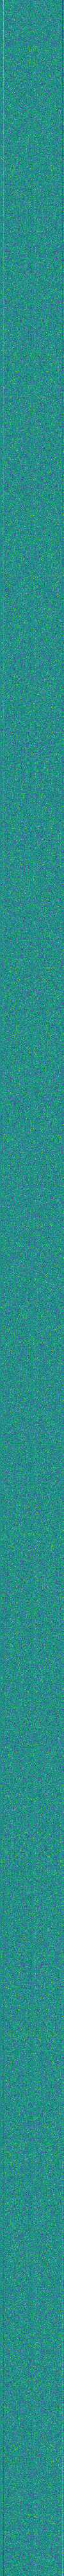
\includegraphics[interpolate=false,width=1.000000in,height=1.000000in]{antiderivative_ci_10-img0.png}}%
\end{pgfscope}%
\begin{pgfscope}%
\pgfsetbuttcap%
\pgfsetroundjoin%
\definecolor{currentfill}{rgb}{0.000000,0.000000,0.000000}%
\pgfsetfillcolor{currentfill}%
\pgfsetlinewidth{0.803000pt}%
\definecolor{currentstroke}{rgb}{0.000000,0.000000,0.000000}%
\pgfsetstrokecolor{currentstroke}%
\pgfsetdash{}{0pt}%
\pgfsys@defobject{currentmarker}{\pgfqpoint{0.000000in}{-0.048611in}}{\pgfqpoint{0.000000in}{0.000000in}}{%
\pgfpathmoveto{\pgfqpoint{0.000000in}{0.000000in}}%
\pgfpathlineto{\pgfqpoint{0.000000in}{-0.048611in}}%
\pgfusepath{stroke,fill}%
}%
\begin{pgfscope}%
\pgfsys@transformshift{0.800000in}{0.528000in}%
\pgfsys@useobject{currentmarker}{}%
\end{pgfscope}%
\end{pgfscope}%
\begin{pgfscope}%
\definecolor{textcolor}{rgb}{0.000000,0.000000,0.000000}%
\pgfsetstrokecolor{textcolor}%
\pgfsetfillcolor{textcolor}%
\pgftext[x=0.800000in,y=0.430778in,,top]{\color{textcolor}{\rmfamily\fontsize{12.000000}{14.400000}\selectfont\catcode`\^=\active\def^{\ifmmode\sp\else\^{}\fi}\catcode`\%=\active\def%{\%}0}}%
\end{pgfscope}%
\begin{pgfscope}%
\pgfsetbuttcap%
\pgfsetroundjoin%
\definecolor{currentfill}{rgb}{0.000000,0.000000,0.000000}%
\pgfsetfillcolor{currentfill}%
\pgfsetlinewidth{0.803000pt}%
\definecolor{currentstroke}{rgb}{0.000000,0.000000,0.000000}%
\pgfsetstrokecolor{currentstroke}%
\pgfsetdash{}{0pt}%
\pgfsys@defobject{currentmarker}{\pgfqpoint{0.000000in}{-0.048611in}}{\pgfqpoint{0.000000in}{0.000000in}}{%
\pgfpathmoveto{\pgfqpoint{0.000000in}{0.000000in}}%
\pgfpathlineto{\pgfqpoint{0.000000in}{-0.048611in}}%
\pgfusepath{stroke,fill}%
}%
\begin{pgfscope}%
\pgfsys@transformshift{1.593600in}{0.528000in}%
\pgfsys@useobject{currentmarker}{}%
\end{pgfscope}%
\end{pgfscope}%
\begin{pgfscope}%
\definecolor{textcolor}{rgb}{0.000000,0.000000,0.000000}%
\pgfsetstrokecolor{textcolor}%
\pgfsetfillcolor{textcolor}%
\pgftext[x=1.593600in,y=0.430778in,,top]{\color{textcolor}{\rmfamily\fontsize{12.000000}{14.400000}\selectfont\catcode`\^=\active\def^{\ifmmode\sp\else\^{}\fi}\catcode`\%=\active\def%{\%}10}}%
\end{pgfscope}%
\begin{pgfscope}%
\pgfsetbuttcap%
\pgfsetroundjoin%
\definecolor{currentfill}{rgb}{0.000000,0.000000,0.000000}%
\pgfsetfillcolor{currentfill}%
\pgfsetlinewidth{0.803000pt}%
\definecolor{currentstroke}{rgb}{0.000000,0.000000,0.000000}%
\pgfsetstrokecolor{currentstroke}%
\pgfsetdash{}{0pt}%
\pgfsys@defobject{currentmarker}{\pgfqpoint{0.000000in}{-0.048611in}}{\pgfqpoint{0.000000in}{0.000000in}}{%
\pgfpathmoveto{\pgfqpoint{0.000000in}{0.000000in}}%
\pgfpathlineto{\pgfqpoint{0.000000in}{-0.048611in}}%
\pgfusepath{stroke,fill}%
}%
\begin{pgfscope}%
\pgfsys@transformshift{2.387200in}{0.528000in}%
\pgfsys@useobject{currentmarker}{}%
\end{pgfscope}%
\end{pgfscope}%
\begin{pgfscope}%
\definecolor{textcolor}{rgb}{0.000000,0.000000,0.000000}%
\pgfsetstrokecolor{textcolor}%
\pgfsetfillcolor{textcolor}%
\pgftext[x=2.387200in,y=0.430778in,,top]{\color{textcolor}{\rmfamily\fontsize{12.000000}{14.400000}\selectfont\catcode`\^=\active\def^{\ifmmode\sp\else\^{}\fi}\catcode`\%=\active\def%{\%}20}}%
\end{pgfscope}%
\begin{pgfscope}%
\pgfsetbuttcap%
\pgfsetroundjoin%
\definecolor{currentfill}{rgb}{0.000000,0.000000,0.000000}%
\pgfsetfillcolor{currentfill}%
\pgfsetlinewidth{0.803000pt}%
\definecolor{currentstroke}{rgb}{0.000000,0.000000,0.000000}%
\pgfsetstrokecolor{currentstroke}%
\pgfsetdash{}{0pt}%
\pgfsys@defobject{currentmarker}{\pgfqpoint{0.000000in}{-0.048611in}}{\pgfqpoint{0.000000in}{0.000000in}}{%
\pgfpathmoveto{\pgfqpoint{0.000000in}{0.000000in}}%
\pgfpathlineto{\pgfqpoint{0.000000in}{-0.048611in}}%
\pgfusepath{stroke,fill}%
}%
\begin{pgfscope}%
\pgfsys@transformshift{3.180800in}{0.528000in}%
\pgfsys@useobject{currentmarker}{}%
\end{pgfscope}%
\end{pgfscope}%
\begin{pgfscope}%
\definecolor{textcolor}{rgb}{0.000000,0.000000,0.000000}%
\pgfsetstrokecolor{textcolor}%
\pgfsetfillcolor{textcolor}%
\pgftext[x=3.180800in,y=0.430778in,,top]{\color{textcolor}{\rmfamily\fontsize{12.000000}{14.400000}\selectfont\catcode`\^=\active\def^{\ifmmode\sp\else\^{}\fi}\catcode`\%=\active\def%{\%}30}}%
\end{pgfscope}%
\begin{pgfscope}%
\pgfsetbuttcap%
\pgfsetroundjoin%
\definecolor{currentfill}{rgb}{0.000000,0.000000,0.000000}%
\pgfsetfillcolor{currentfill}%
\pgfsetlinewidth{0.803000pt}%
\definecolor{currentstroke}{rgb}{0.000000,0.000000,0.000000}%
\pgfsetstrokecolor{currentstroke}%
\pgfsetdash{}{0pt}%
\pgfsys@defobject{currentmarker}{\pgfqpoint{0.000000in}{-0.048611in}}{\pgfqpoint{0.000000in}{0.000000in}}{%
\pgfpathmoveto{\pgfqpoint{0.000000in}{0.000000in}}%
\pgfpathlineto{\pgfqpoint{0.000000in}{-0.048611in}}%
\pgfusepath{stroke,fill}%
}%
\begin{pgfscope}%
\pgfsys@transformshift{3.974400in}{0.528000in}%
\pgfsys@useobject{currentmarker}{}%
\end{pgfscope}%
\end{pgfscope}%
\begin{pgfscope}%
\definecolor{textcolor}{rgb}{0.000000,0.000000,0.000000}%
\pgfsetstrokecolor{textcolor}%
\pgfsetfillcolor{textcolor}%
\pgftext[x=3.974400in,y=0.430778in,,top]{\color{textcolor}{\rmfamily\fontsize{12.000000}{14.400000}\selectfont\catcode`\^=\active\def^{\ifmmode\sp\else\^{}\fi}\catcode`\%=\active\def%{\%}40}}%
\end{pgfscope}%
\begin{pgfscope}%
\pgfsetbuttcap%
\pgfsetroundjoin%
\definecolor{currentfill}{rgb}{0.000000,0.000000,0.000000}%
\pgfsetfillcolor{currentfill}%
\pgfsetlinewidth{0.803000pt}%
\definecolor{currentstroke}{rgb}{0.000000,0.000000,0.000000}%
\pgfsetstrokecolor{currentstroke}%
\pgfsetdash{}{0pt}%
\pgfsys@defobject{currentmarker}{\pgfqpoint{0.000000in}{-0.048611in}}{\pgfqpoint{0.000000in}{0.000000in}}{%
\pgfpathmoveto{\pgfqpoint{0.000000in}{0.000000in}}%
\pgfpathlineto{\pgfqpoint{0.000000in}{-0.048611in}}%
\pgfusepath{stroke,fill}%
}%
\begin{pgfscope}%
\pgfsys@transformshift{4.768000in}{0.528000in}%
\pgfsys@useobject{currentmarker}{}%
\end{pgfscope}%
\end{pgfscope}%
\begin{pgfscope}%
\definecolor{textcolor}{rgb}{0.000000,0.000000,0.000000}%
\pgfsetstrokecolor{textcolor}%
\pgfsetfillcolor{textcolor}%
\pgftext[x=4.768000in,y=0.430778in,,top]{\color{textcolor}{\rmfamily\fontsize{12.000000}{14.400000}\selectfont\catcode`\^=\active\def^{\ifmmode\sp\else\^{}\fi}\catcode`\%=\active\def%{\%}50}}%
\end{pgfscope}%
\begin{pgfscope}%
\definecolor{textcolor}{rgb}{0.000000,0.000000,0.000000}%
\pgfsetstrokecolor{textcolor}%
\pgfsetfillcolor{textcolor}%
\pgftext[x=2.784000in,y=0.213927in,,top]{\color{textcolor}{\rmfamily\fontsize{12.000000}{14.400000}\selectfont\catcode`\^=\active\def^{\ifmmode\sp\else\^{}\fi}\catcode`\%=\active\def%{\%}input coefficients}}%
\end{pgfscope}%
\begin{pgfscope}%
\pgfsetbuttcap%
\pgfsetroundjoin%
\definecolor{currentfill}{rgb}{0.000000,0.000000,0.000000}%
\pgfsetfillcolor{currentfill}%
\pgfsetlinewidth{0.803000pt}%
\definecolor{currentstroke}{rgb}{0.000000,0.000000,0.000000}%
\pgfsetstrokecolor{currentstroke}%
\pgfsetdash{}{0pt}%
\pgfsys@defobject{currentmarker}{\pgfqpoint{-0.048611in}{0.000000in}}{\pgfqpoint{-0.000000in}{0.000000in}}{%
\pgfpathmoveto{\pgfqpoint{-0.000000in}{0.000000in}}%
\pgfpathlineto{\pgfqpoint{-0.048611in}{0.000000in}}%
\pgfusepath{stroke,fill}%
}%
\begin{pgfscope}%
\pgfsys@transformshift{0.800000in}{4.224000in}%
\pgfsys@useobject{currentmarker}{}%
\end{pgfscope}%
\end{pgfscope}%
\begin{pgfscope}%
\definecolor{textcolor}{rgb}{0.000000,0.000000,0.000000}%
\pgfsetstrokecolor{textcolor}%
\pgfsetfillcolor{textcolor}%
\pgftext[x=0.596739in, y=4.160686in, left, base]{\color{textcolor}{\rmfamily\fontsize{12.000000}{14.400000}\selectfont\catcode`\^=\active\def^{\ifmmode\sp\else\^{}\fi}\catcode`\%=\active\def%{\%}0}}%
\end{pgfscope}%
\begin{pgfscope}%
\pgfsetbuttcap%
\pgfsetroundjoin%
\definecolor{currentfill}{rgb}{0.000000,0.000000,0.000000}%
\pgfsetfillcolor{currentfill}%
\pgfsetlinewidth{0.803000pt}%
\definecolor{currentstroke}{rgb}{0.000000,0.000000,0.000000}%
\pgfsetstrokecolor{currentstroke}%
\pgfsetdash{}{0pt}%
\pgfsys@defobject{currentmarker}{\pgfqpoint{-0.048611in}{0.000000in}}{\pgfqpoint{-0.000000in}{0.000000in}}{%
\pgfpathmoveto{\pgfqpoint{-0.000000in}{0.000000in}}%
\pgfpathlineto{\pgfqpoint{-0.048611in}{0.000000in}}%
\pgfusepath{stroke,fill}%
}%
\begin{pgfscope}%
\pgfsys@transformshift{0.800000in}{3.762000in}%
\pgfsys@useobject{currentmarker}{}%
\end{pgfscope}%
\end{pgfscope}%
\begin{pgfscope}%
\definecolor{textcolor}{rgb}{0.000000,0.000000,0.000000}%
\pgfsetstrokecolor{textcolor}%
\pgfsetfillcolor{textcolor}%
\pgftext[x=0.384662in, y=3.698686in, left, base]{\color{textcolor}{\rmfamily\fontsize{12.000000}{14.400000}\selectfont\catcode`\^=\active\def^{\ifmmode\sp\else\^{}\fi}\catcode`\%=\active\def%{\%}500}}%
\end{pgfscope}%
\begin{pgfscope}%
\pgfsetbuttcap%
\pgfsetroundjoin%
\definecolor{currentfill}{rgb}{0.000000,0.000000,0.000000}%
\pgfsetfillcolor{currentfill}%
\pgfsetlinewidth{0.803000pt}%
\definecolor{currentstroke}{rgb}{0.000000,0.000000,0.000000}%
\pgfsetstrokecolor{currentstroke}%
\pgfsetdash{}{0pt}%
\pgfsys@defobject{currentmarker}{\pgfqpoint{-0.048611in}{0.000000in}}{\pgfqpoint{-0.000000in}{0.000000in}}{%
\pgfpathmoveto{\pgfqpoint{-0.000000in}{0.000000in}}%
\pgfpathlineto{\pgfqpoint{-0.048611in}{0.000000in}}%
\pgfusepath{stroke,fill}%
}%
\begin{pgfscope}%
\pgfsys@transformshift{0.800000in}{3.300000in}%
\pgfsys@useobject{currentmarker}{}%
\end{pgfscope}%
\end{pgfscope}%
\begin{pgfscope}%
\definecolor{textcolor}{rgb}{0.000000,0.000000,0.000000}%
\pgfsetstrokecolor{textcolor}%
\pgfsetfillcolor{textcolor}%
\pgftext[x=0.278624in, y=3.236686in, left, base]{\color{textcolor}{\rmfamily\fontsize{12.000000}{14.400000}\selectfont\catcode`\^=\active\def^{\ifmmode\sp\else\^{}\fi}\catcode`\%=\active\def%{\%}1000}}%
\end{pgfscope}%
\begin{pgfscope}%
\pgfsetbuttcap%
\pgfsetroundjoin%
\definecolor{currentfill}{rgb}{0.000000,0.000000,0.000000}%
\pgfsetfillcolor{currentfill}%
\pgfsetlinewidth{0.803000pt}%
\definecolor{currentstroke}{rgb}{0.000000,0.000000,0.000000}%
\pgfsetstrokecolor{currentstroke}%
\pgfsetdash{}{0pt}%
\pgfsys@defobject{currentmarker}{\pgfqpoint{-0.048611in}{0.000000in}}{\pgfqpoint{-0.000000in}{0.000000in}}{%
\pgfpathmoveto{\pgfqpoint{-0.000000in}{0.000000in}}%
\pgfpathlineto{\pgfqpoint{-0.048611in}{0.000000in}}%
\pgfusepath{stroke,fill}%
}%
\begin{pgfscope}%
\pgfsys@transformshift{0.800000in}{2.838000in}%
\pgfsys@useobject{currentmarker}{}%
\end{pgfscope}%
\end{pgfscope}%
\begin{pgfscope}%
\definecolor{textcolor}{rgb}{0.000000,0.000000,0.000000}%
\pgfsetstrokecolor{textcolor}%
\pgfsetfillcolor{textcolor}%
\pgftext[x=0.278624in, y=2.774686in, left, base]{\color{textcolor}{\rmfamily\fontsize{12.000000}{14.400000}\selectfont\catcode`\^=\active\def^{\ifmmode\sp\else\^{}\fi}\catcode`\%=\active\def%{\%}1500}}%
\end{pgfscope}%
\begin{pgfscope}%
\pgfsetbuttcap%
\pgfsetroundjoin%
\definecolor{currentfill}{rgb}{0.000000,0.000000,0.000000}%
\pgfsetfillcolor{currentfill}%
\pgfsetlinewidth{0.803000pt}%
\definecolor{currentstroke}{rgb}{0.000000,0.000000,0.000000}%
\pgfsetstrokecolor{currentstroke}%
\pgfsetdash{}{0pt}%
\pgfsys@defobject{currentmarker}{\pgfqpoint{-0.048611in}{0.000000in}}{\pgfqpoint{-0.000000in}{0.000000in}}{%
\pgfpathmoveto{\pgfqpoint{-0.000000in}{0.000000in}}%
\pgfpathlineto{\pgfqpoint{-0.048611in}{0.000000in}}%
\pgfusepath{stroke,fill}%
}%
\begin{pgfscope}%
\pgfsys@transformshift{0.800000in}{2.376000in}%
\pgfsys@useobject{currentmarker}{}%
\end{pgfscope}%
\end{pgfscope}%
\begin{pgfscope}%
\definecolor{textcolor}{rgb}{0.000000,0.000000,0.000000}%
\pgfsetstrokecolor{textcolor}%
\pgfsetfillcolor{textcolor}%
\pgftext[x=0.278624in, y=2.312686in, left, base]{\color{textcolor}{\rmfamily\fontsize{12.000000}{14.400000}\selectfont\catcode`\^=\active\def^{\ifmmode\sp\else\^{}\fi}\catcode`\%=\active\def%{\%}2000}}%
\end{pgfscope}%
\begin{pgfscope}%
\pgfsetbuttcap%
\pgfsetroundjoin%
\definecolor{currentfill}{rgb}{0.000000,0.000000,0.000000}%
\pgfsetfillcolor{currentfill}%
\pgfsetlinewidth{0.803000pt}%
\definecolor{currentstroke}{rgb}{0.000000,0.000000,0.000000}%
\pgfsetstrokecolor{currentstroke}%
\pgfsetdash{}{0pt}%
\pgfsys@defobject{currentmarker}{\pgfqpoint{-0.048611in}{0.000000in}}{\pgfqpoint{-0.000000in}{0.000000in}}{%
\pgfpathmoveto{\pgfqpoint{-0.000000in}{0.000000in}}%
\pgfpathlineto{\pgfqpoint{-0.048611in}{0.000000in}}%
\pgfusepath{stroke,fill}%
}%
\begin{pgfscope}%
\pgfsys@transformshift{0.800000in}{1.914000in}%
\pgfsys@useobject{currentmarker}{}%
\end{pgfscope}%
\end{pgfscope}%
\begin{pgfscope}%
\definecolor{textcolor}{rgb}{0.000000,0.000000,0.000000}%
\pgfsetstrokecolor{textcolor}%
\pgfsetfillcolor{textcolor}%
\pgftext[x=0.278624in, y=1.850686in, left, base]{\color{textcolor}{\rmfamily\fontsize{12.000000}{14.400000}\selectfont\catcode`\^=\active\def^{\ifmmode\sp\else\^{}\fi}\catcode`\%=\active\def%{\%}2500}}%
\end{pgfscope}%
\begin{pgfscope}%
\pgfsetbuttcap%
\pgfsetroundjoin%
\definecolor{currentfill}{rgb}{0.000000,0.000000,0.000000}%
\pgfsetfillcolor{currentfill}%
\pgfsetlinewidth{0.803000pt}%
\definecolor{currentstroke}{rgb}{0.000000,0.000000,0.000000}%
\pgfsetstrokecolor{currentstroke}%
\pgfsetdash{}{0pt}%
\pgfsys@defobject{currentmarker}{\pgfqpoint{-0.048611in}{0.000000in}}{\pgfqpoint{-0.000000in}{0.000000in}}{%
\pgfpathmoveto{\pgfqpoint{-0.000000in}{0.000000in}}%
\pgfpathlineto{\pgfqpoint{-0.048611in}{0.000000in}}%
\pgfusepath{stroke,fill}%
}%
\begin{pgfscope}%
\pgfsys@transformshift{0.800000in}{1.452000in}%
\pgfsys@useobject{currentmarker}{}%
\end{pgfscope}%
\end{pgfscope}%
\begin{pgfscope}%
\definecolor{textcolor}{rgb}{0.000000,0.000000,0.000000}%
\pgfsetstrokecolor{textcolor}%
\pgfsetfillcolor{textcolor}%
\pgftext[x=0.278624in, y=1.388686in, left, base]{\color{textcolor}{\rmfamily\fontsize{12.000000}{14.400000}\selectfont\catcode`\^=\active\def^{\ifmmode\sp\else\^{}\fi}\catcode`\%=\active\def%{\%}3000}}%
\end{pgfscope}%
\begin{pgfscope}%
\pgfsetbuttcap%
\pgfsetroundjoin%
\definecolor{currentfill}{rgb}{0.000000,0.000000,0.000000}%
\pgfsetfillcolor{currentfill}%
\pgfsetlinewidth{0.803000pt}%
\definecolor{currentstroke}{rgb}{0.000000,0.000000,0.000000}%
\pgfsetstrokecolor{currentstroke}%
\pgfsetdash{}{0pt}%
\pgfsys@defobject{currentmarker}{\pgfqpoint{-0.048611in}{0.000000in}}{\pgfqpoint{-0.000000in}{0.000000in}}{%
\pgfpathmoveto{\pgfqpoint{-0.000000in}{0.000000in}}%
\pgfpathlineto{\pgfqpoint{-0.048611in}{0.000000in}}%
\pgfusepath{stroke,fill}%
}%
\begin{pgfscope}%
\pgfsys@transformshift{0.800000in}{0.990000in}%
\pgfsys@useobject{currentmarker}{}%
\end{pgfscope}%
\end{pgfscope}%
\begin{pgfscope}%
\definecolor{textcolor}{rgb}{0.000000,0.000000,0.000000}%
\pgfsetstrokecolor{textcolor}%
\pgfsetfillcolor{textcolor}%
\pgftext[x=0.278624in, y=0.926686in, left, base]{\color{textcolor}{\rmfamily\fontsize{12.000000}{14.400000}\selectfont\catcode`\^=\active\def^{\ifmmode\sp\else\^{}\fi}\catcode`\%=\active\def%{\%}3500}}%
\end{pgfscope}%
\begin{pgfscope}%
\pgfsetbuttcap%
\pgfsetroundjoin%
\definecolor{currentfill}{rgb}{0.000000,0.000000,0.000000}%
\pgfsetfillcolor{currentfill}%
\pgfsetlinewidth{0.803000pt}%
\definecolor{currentstroke}{rgb}{0.000000,0.000000,0.000000}%
\pgfsetstrokecolor{currentstroke}%
\pgfsetdash{}{0pt}%
\pgfsys@defobject{currentmarker}{\pgfqpoint{-0.048611in}{0.000000in}}{\pgfqpoint{-0.000000in}{0.000000in}}{%
\pgfpathmoveto{\pgfqpoint{-0.000000in}{0.000000in}}%
\pgfpathlineto{\pgfqpoint{-0.048611in}{0.000000in}}%
\pgfusepath{stroke,fill}%
}%
\begin{pgfscope}%
\pgfsys@transformshift{0.800000in}{0.528000in}%
\pgfsys@useobject{currentmarker}{}%
\end{pgfscope}%
\end{pgfscope}%
\begin{pgfscope}%
\definecolor{textcolor}{rgb}{0.000000,0.000000,0.000000}%
\pgfsetstrokecolor{textcolor}%
\pgfsetfillcolor{textcolor}%
\pgftext[x=0.278624in, y=0.464686in, left, base]{\color{textcolor}{\rmfamily\fontsize{12.000000}{14.400000}\selectfont\catcode`\^=\active\def^{\ifmmode\sp\else\^{}\fi}\catcode`\%=\active\def%{\%}4000}}%
\end{pgfscope}%
\begin{pgfscope}%
\definecolor{textcolor}{rgb}{0.000000,0.000000,0.000000}%
\pgfsetstrokecolor{textcolor}%
\pgfsetfillcolor{textcolor}%
\pgftext[x=0.223069in,y=2.376000in,,bottom,rotate=90.000000]{\color{textcolor}{\rmfamily\fontsize{12.000000}{14.400000}\selectfont\catcode`\^=\active\def^{\ifmmode\sp\else\^{}\fi}\catcode`\%=\active\def%{\%}samples}}%
\end{pgfscope}%
\begin{pgfscope}%
\pgfsetrectcap%
\pgfsetmiterjoin%
\pgfsetlinewidth{0.803000pt}%
\definecolor{currentstroke}{rgb}{0.000000,0.000000,0.000000}%
\pgfsetstrokecolor{currentstroke}%
\pgfsetdash{}{0pt}%
\pgfpathmoveto{\pgfqpoint{0.800000in}{0.528000in}}%
\pgfpathlineto{\pgfqpoint{0.800000in}{4.224000in}}%
\pgfusepath{stroke}%
\end{pgfscope}%
\begin{pgfscope}%
\pgfsetrectcap%
\pgfsetmiterjoin%
\pgfsetlinewidth{0.803000pt}%
\definecolor{currentstroke}{rgb}{0.000000,0.000000,0.000000}%
\pgfsetstrokecolor{currentstroke}%
\pgfsetdash{}{0pt}%
\pgfpathmoveto{\pgfqpoint{4.768000in}{0.528000in}}%
\pgfpathlineto{\pgfqpoint{4.768000in}{4.224000in}}%
\pgfusepath{stroke}%
\end{pgfscope}%
\begin{pgfscope}%
\pgfsetrectcap%
\pgfsetmiterjoin%
\pgfsetlinewidth{0.803000pt}%
\definecolor{currentstroke}{rgb}{0.000000,0.000000,0.000000}%
\pgfsetstrokecolor{currentstroke}%
\pgfsetdash{}{0pt}%
\pgfpathmoveto{\pgfqpoint{0.800000in}{0.528000in}}%
\pgfpathlineto{\pgfqpoint{4.768000in}{0.528000in}}%
\pgfusepath{stroke}%
\end{pgfscope}%
\begin{pgfscope}%
\pgfsetrectcap%
\pgfsetmiterjoin%
\pgfsetlinewidth{0.803000pt}%
\definecolor{currentstroke}{rgb}{0.000000,0.000000,0.000000}%
\pgfsetstrokecolor{currentstroke}%
\pgfsetdash{}{0pt}%
\pgfpathmoveto{\pgfqpoint{0.800000in}{4.224000in}}%
\pgfpathlineto{\pgfqpoint{4.768000in}{4.224000in}}%
\pgfusepath{stroke}%
\end{pgfscope}%
\begin{pgfscope}%
\pgfsetbuttcap%
\pgfsetmiterjoin%
\pgfsetlinewidth{0.000000pt}%
\definecolor{currentstroke}{rgb}{0.000000,0.000000,0.000000}%
\pgfsetstrokecolor{currentstroke}%
\pgfsetstrokeopacity{0.000000}%
\pgfsetdash{}{0pt}%
\pgfpathmoveto{\pgfqpoint{5.016000in}{0.528000in}}%
\pgfpathlineto{\pgfqpoint{5.200800in}{0.528000in}}%
\pgfpathlineto{\pgfqpoint{5.200800in}{4.224000in}}%
\pgfpathlineto{\pgfqpoint{5.016000in}{4.224000in}}%
\pgfpathlineto{\pgfqpoint{5.016000in}{0.528000in}}%
\pgfpathclose%
\pgfusepath{}%
\end{pgfscope}%
\begin{pgfscope}%
\pgfsys@transformshift{5.020000in}{0.530000in}%
\pgftext[left,bottom]{
\includegraphics[interpolate=true,width=0.180000in,height=3.690000in]{antiderivative_ci_10-img1.png}}%
\end{pgfscope}%
\begin{pgfscope}%
\pgfsetbuttcap%
\pgfsetroundjoin%
\definecolor{currentfill}{rgb}{0.000000,0.000000,0.000000}%
\pgfsetfillcolor{currentfill}%
\pgfsetlinewidth{0.803000pt}%
\definecolor{currentstroke}{rgb}{0.000000,0.000000,0.000000}%
\pgfsetstrokecolor{currentstroke}%
\pgfsetdash{}{0pt}%
\pgfsys@defobject{currentmarker}{\pgfqpoint{0.000000in}{0.000000in}}{\pgfqpoint{0.048611in}{0.000000in}}{%
\pgfpathmoveto{\pgfqpoint{0.000000in}{0.000000in}}%
\pgfpathlineto{\pgfqpoint{0.048611in}{0.000000in}}%
\pgfusepath{stroke,fill}%
}%
\begin{pgfscope}%
\pgfsys@transformshift{5.200800in}{0.547966in}%
\pgfsys@useobject{currentmarker}{}%
\end{pgfscope}%
\end{pgfscope}%
\begin{pgfscope}%
\definecolor{textcolor}{rgb}{0.000000,0.000000,0.000000}%
\pgfsetstrokecolor{textcolor}%
\pgfsetfillcolor{textcolor}%
\pgftext[x=5.298022in, y=0.484652in, left, base]{\color{textcolor}{\rmfamily\fontsize{12.000000}{14.400000}\selectfont\catcode`\^=\active\def^{\ifmmode\sp\else\^{}\fi}\catcode`\%=\active\def%{\%}\ensuremath{-}100}}%
\end{pgfscope}%
\begin{pgfscope}%
\pgfsetbuttcap%
\pgfsetroundjoin%
\definecolor{currentfill}{rgb}{0.000000,0.000000,0.000000}%
\pgfsetfillcolor{currentfill}%
\pgfsetlinewidth{0.803000pt}%
\definecolor{currentstroke}{rgb}{0.000000,0.000000,0.000000}%
\pgfsetstrokecolor{currentstroke}%
\pgfsetdash{}{0pt}%
\pgfsys@defobject{currentmarker}{\pgfqpoint{0.000000in}{0.000000in}}{\pgfqpoint{0.048611in}{0.000000in}}{%
\pgfpathmoveto{\pgfqpoint{0.000000in}{0.000000in}}%
\pgfpathlineto{\pgfqpoint{0.048611in}{0.000000in}}%
\pgfusepath{stroke,fill}%
}%
\begin{pgfscope}%
\pgfsys@transformshift{5.200800in}{0.998231in}%
\pgfsys@useobject{currentmarker}{}%
\end{pgfscope}%
\end{pgfscope}%
\begin{pgfscope}%
\definecolor{textcolor}{rgb}{0.000000,0.000000,0.000000}%
\pgfsetstrokecolor{textcolor}%
\pgfsetfillcolor{textcolor}%
\pgftext[x=5.298022in, y=0.934917in, left, base]{\color{textcolor}{\rmfamily\fontsize{12.000000}{14.400000}\selectfont\catcode`\^=\active\def^{\ifmmode\sp\else\^{}\fi}\catcode`\%=\active\def%{\%}\ensuremath{-}75}}%
\end{pgfscope}%
\begin{pgfscope}%
\pgfsetbuttcap%
\pgfsetroundjoin%
\definecolor{currentfill}{rgb}{0.000000,0.000000,0.000000}%
\pgfsetfillcolor{currentfill}%
\pgfsetlinewidth{0.803000pt}%
\definecolor{currentstroke}{rgb}{0.000000,0.000000,0.000000}%
\pgfsetstrokecolor{currentstroke}%
\pgfsetdash{}{0pt}%
\pgfsys@defobject{currentmarker}{\pgfqpoint{0.000000in}{0.000000in}}{\pgfqpoint{0.048611in}{0.000000in}}{%
\pgfpathmoveto{\pgfqpoint{0.000000in}{0.000000in}}%
\pgfpathlineto{\pgfqpoint{0.048611in}{0.000000in}}%
\pgfusepath{stroke,fill}%
}%
\begin{pgfscope}%
\pgfsys@transformshift{5.200800in}{1.448497in}%
\pgfsys@useobject{currentmarker}{}%
\end{pgfscope}%
\end{pgfscope}%
\begin{pgfscope}%
\definecolor{textcolor}{rgb}{0.000000,0.000000,0.000000}%
\pgfsetstrokecolor{textcolor}%
\pgfsetfillcolor{textcolor}%
\pgftext[x=5.298022in, y=1.385183in, left, base]{\color{textcolor}{\rmfamily\fontsize{12.000000}{14.400000}\selectfont\catcode`\^=\active\def^{\ifmmode\sp\else\^{}\fi}\catcode`\%=\active\def%{\%}\ensuremath{-}50}}%
\end{pgfscope}%
\begin{pgfscope}%
\pgfsetbuttcap%
\pgfsetroundjoin%
\definecolor{currentfill}{rgb}{0.000000,0.000000,0.000000}%
\pgfsetfillcolor{currentfill}%
\pgfsetlinewidth{0.803000pt}%
\definecolor{currentstroke}{rgb}{0.000000,0.000000,0.000000}%
\pgfsetstrokecolor{currentstroke}%
\pgfsetdash{}{0pt}%
\pgfsys@defobject{currentmarker}{\pgfqpoint{0.000000in}{0.000000in}}{\pgfqpoint{0.048611in}{0.000000in}}{%
\pgfpathmoveto{\pgfqpoint{0.000000in}{0.000000in}}%
\pgfpathlineto{\pgfqpoint{0.048611in}{0.000000in}}%
\pgfusepath{stroke,fill}%
}%
\begin{pgfscope}%
\pgfsys@transformshift{5.200800in}{1.898762in}%
\pgfsys@useobject{currentmarker}{}%
\end{pgfscope}%
\end{pgfscope}%
\begin{pgfscope}%
\definecolor{textcolor}{rgb}{0.000000,0.000000,0.000000}%
\pgfsetstrokecolor{textcolor}%
\pgfsetfillcolor{textcolor}%
\pgftext[x=5.298022in, y=1.835448in, left, base]{\color{textcolor}{\rmfamily\fontsize{12.000000}{14.400000}\selectfont\catcode`\^=\active\def^{\ifmmode\sp\else\^{}\fi}\catcode`\%=\active\def%{\%}\ensuremath{-}25}}%
\end{pgfscope}%
\begin{pgfscope}%
\pgfsetbuttcap%
\pgfsetroundjoin%
\definecolor{currentfill}{rgb}{0.000000,0.000000,0.000000}%
\pgfsetfillcolor{currentfill}%
\pgfsetlinewidth{0.803000pt}%
\definecolor{currentstroke}{rgb}{0.000000,0.000000,0.000000}%
\pgfsetstrokecolor{currentstroke}%
\pgfsetdash{}{0pt}%
\pgfsys@defobject{currentmarker}{\pgfqpoint{0.000000in}{0.000000in}}{\pgfqpoint{0.048611in}{0.000000in}}{%
\pgfpathmoveto{\pgfqpoint{0.000000in}{0.000000in}}%
\pgfpathlineto{\pgfqpoint{0.048611in}{0.000000in}}%
\pgfusepath{stroke,fill}%
}%
\begin{pgfscope}%
\pgfsys@transformshift{5.200800in}{2.349028in}%
\pgfsys@useobject{currentmarker}{}%
\end{pgfscope}%
\end{pgfscope}%
\begin{pgfscope}%
\definecolor{textcolor}{rgb}{0.000000,0.000000,0.000000}%
\pgfsetstrokecolor{textcolor}%
\pgfsetfillcolor{textcolor}%
\pgftext[x=5.298022in, y=2.285714in, left, base]{\color{textcolor}{\rmfamily\fontsize{12.000000}{14.400000}\selectfont\catcode`\^=\active\def^{\ifmmode\sp\else\^{}\fi}\catcode`\%=\active\def%{\%}0}}%
\end{pgfscope}%
\begin{pgfscope}%
\pgfsetbuttcap%
\pgfsetroundjoin%
\definecolor{currentfill}{rgb}{0.000000,0.000000,0.000000}%
\pgfsetfillcolor{currentfill}%
\pgfsetlinewidth{0.803000pt}%
\definecolor{currentstroke}{rgb}{0.000000,0.000000,0.000000}%
\pgfsetstrokecolor{currentstroke}%
\pgfsetdash{}{0pt}%
\pgfsys@defobject{currentmarker}{\pgfqpoint{0.000000in}{0.000000in}}{\pgfqpoint{0.048611in}{0.000000in}}{%
\pgfpathmoveto{\pgfqpoint{0.000000in}{0.000000in}}%
\pgfpathlineto{\pgfqpoint{0.048611in}{0.000000in}}%
\pgfusepath{stroke,fill}%
}%
\begin{pgfscope}%
\pgfsys@transformshift{5.200800in}{2.799293in}%
\pgfsys@useobject{currentmarker}{}%
\end{pgfscope}%
\end{pgfscope}%
\begin{pgfscope}%
\definecolor{textcolor}{rgb}{0.000000,0.000000,0.000000}%
\pgfsetstrokecolor{textcolor}%
\pgfsetfillcolor{textcolor}%
\pgftext[x=5.298022in, y=2.735979in, left, base]{\color{textcolor}{\rmfamily\fontsize{12.000000}{14.400000}\selectfont\catcode`\^=\active\def^{\ifmmode\sp\else\^{}\fi}\catcode`\%=\active\def%{\%}25}}%
\end{pgfscope}%
\begin{pgfscope}%
\pgfsetbuttcap%
\pgfsetroundjoin%
\definecolor{currentfill}{rgb}{0.000000,0.000000,0.000000}%
\pgfsetfillcolor{currentfill}%
\pgfsetlinewidth{0.803000pt}%
\definecolor{currentstroke}{rgb}{0.000000,0.000000,0.000000}%
\pgfsetstrokecolor{currentstroke}%
\pgfsetdash{}{0pt}%
\pgfsys@defobject{currentmarker}{\pgfqpoint{0.000000in}{0.000000in}}{\pgfqpoint{0.048611in}{0.000000in}}{%
\pgfpathmoveto{\pgfqpoint{0.000000in}{0.000000in}}%
\pgfpathlineto{\pgfqpoint{0.048611in}{0.000000in}}%
\pgfusepath{stroke,fill}%
}%
\begin{pgfscope}%
\pgfsys@transformshift{5.200800in}{3.249559in}%
\pgfsys@useobject{currentmarker}{}%
\end{pgfscope}%
\end{pgfscope}%
\begin{pgfscope}%
\definecolor{textcolor}{rgb}{0.000000,0.000000,0.000000}%
\pgfsetstrokecolor{textcolor}%
\pgfsetfillcolor{textcolor}%
\pgftext[x=5.298022in, y=3.186245in, left, base]{\color{textcolor}{\rmfamily\fontsize{12.000000}{14.400000}\selectfont\catcode`\^=\active\def^{\ifmmode\sp\else\^{}\fi}\catcode`\%=\active\def%{\%}50}}%
\end{pgfscope}%
\begin{pgfscope}%
\pgfsetbuttcap%
\pgfsetroundjoin%
\definecolor{currentfill}{rgb}{0.000000,0.000000,0.000000}%
\pgfsetfillcolor{currentfill}%
\pgfsetlinewidth{0.803000pt}%
\definecolor{currentstroke}{rgb}{0.000000,0.000000,0.000000}%
\pgfsetstrokecolor{currentstroke}%
\pgfsetdash{}{0pt}%
\pgfsys@defobject{currentmarker}{\pgfqpoint{0.000000in}{0.000000in}}{\pgfqpoint{0.048611in}{0.000000in}}{%
\pgfpathmoveto{\pgfqpoint{0.000000in}{0.000000in}}%
\pgfpathlineto{\pgfqpoint{0.048611in}{0.000000in}}%
\pgfusepath{stroke,fill}%
}%
\begin{pgfscope}%
\pgfsys@transformshift{5.200800in}{3.699824in}%
\pgfsys@useobject{currentmarker}{}%
\end{pgfscope}%
\end{pgfscope}%
\begin{pgfscope}%
\definecolor{textcolor}{rgb}{0.000000,0.000000,0.000000}%
\pgfsetstrokecolor{textcolor}%
\pgfsetfillcolor{textcolor}%
\pgftext[x=5.298022in, y=3.636510in, left, base]{\color{textcolor}{\rmfamily\fontsize{12.000000}{14.400000}\selectfont\catcode`\^=\active\def^{\ifmmode\sp\else\^{}\fi}\catcode`\%=\active\def%{\%}75}}%
\end{pgfscope}%
\begin{pgfscope}%
\pgfsetbuttcap%
\pgfsetroundjoin%
\definecolor{currentfill}{rgb}{0.000000,0.000000,0.000000}%
\pgfsetfillcolor{currentfill}%
\pgfsetlinewidth{0.803000pt}%
\definecolor{currentstroke}{rgb}{0.000000,0.000000,0.000000}%
\pgfsetstrokecolor{currentstroke}%
\pgfsetdash{}{0pt}%
\pgfsys@defobject{currentmarker}{\pgfqpoint{0.000000in}{0.000000in}}{\pgfqpoint{0.048611in}{0.000000in}}{%
\pgfpathmoveto{\pgfqpoint{0.000000in}{0.000000in}}%
\pgfpathlineto{\pgfqpoint{0.048611in}{0.000000in}}%
\pgfusepath{stroke,fill}%
}%
\begin{pgfscope}%
\pgfsys@transformshift{5.200800in}{4.150090in}%
\pgfsys@useobject{currentmarker}{}%
\end{pgfscope}%
\end{pgfscope}%
\begin{pgfscope}%
\definecolor{textcolor}{rgb}{0.000000,0.000000,0.000000}%
\pgfsetstrokecolor{textcolor}%
\pgfsetfillcolor{textcolor}%
\pgftext[x=5.298022in, y=4.086776in, left, base]{\color{textcolor}{\rmfamily\fontsize{12.000000}{14.400000}\selectfont\catcode`\^=\active\def^{\ifmmode\sp\else\^{}\fi}\catcode`\%=\active\def%{\%}100}}%
\end{pgfscope}%
\begin{pgfscope}%
\pgfsetrectcap%
\pgfsetmiterjoin%
\pgfsetlinewidth{0.803000pt}%
\definecolor{currentstroke}{rgb}{0.000000,0.000000,0.000000}%
\pgfsetstrokecolor{currentstroke}%
\pgfsetdash{}{0pt}%
\pgfpathmoveto{\pgfqpoint{5.016000in}{0.528000in}}%
\pgfpathlineto{\pgfqpoint{5.108400in}{0.528000in}}%
\pgfpathlineto{\pgfqpoint{5.200800in}{0.528000in}}%
\pgfpathlineto{\pgfqpoint{5.200800in}{4.224000in}}%
\pgfpathlineto{\pgfqpoint{5.108400in}{4.224000in}}%
\pgfpathlineto{\pgfqpoint{5.016000in}{4.224000in}}%
\pgfpathlineto{\pgfqpoint{5.016000in}{0.528000in}}%
\pgfpathclose%
\pgfusepath{stroke}%
\end{pgfscope}%
\end{pgfpicture}%
\makeatother%
\endgroup%

      \end{adjustbox}
      \caption{Correlation image 10\% noise.}\label{fig:sc1_ci_10}
    \end{subfigure}
    \begin{subfigure}{0.49\linewidth}
      \begin{adjustbox}{width=\linewidth}
        \begingroup%
\makeatletter%
\begin{pgfpicture}%
\pgfpathrectangle{\pgfpointorigin}{\pgfqpoint{4.000000in}{3.000000in}}%
\pgfusepath{use as bounding box, clip}%
\begin{pgfscope}%
\pgfsetbuttcap%
\pgfsetmiterjoin%
\pgfsetlinewidth{0.000000pt}%
\definecolor{currentstroke}{rgb}{0.000000,0.000000,0.000000}%
\pgfsetstrokecolor{currentstroke}%
\pgfsetstrokeopacity{0.000000}%
\pgfsetdash{}{0pt}%
\pgfpathmoveto{\pgfqpoint{0.000000in}{0.000000in}}%
\pgfpathlineto{\pgfqpoint{4.000000in}{0.000000in}}%
\pgfpathlineto{\pgfqpoint{4.000000in}{3.000000in}}%
\pgfpathlineto{\pgfqpoint{0.000000in}{3.000000in}}%
\pgfpathlineto{\pgfqpoint{0.000000in}{0.000000in}}%
\pgfpathclose%
\pgfusepath{}%
\end{pgfscope}%
\begin{pgfscope}%
\pgfsetbuttcap%
\pgfsetmiterjoin%
\pgfsetlinewidth{0.000000pt}%
\definecolor{currentstroke}{rgb}{0.000000,0.000000,0.000000}%
\pgfsetstrokecolor{currentstroke}%
\pgfsetstrokeopacity{0.000000}%
\pgfsetdash{}{0pt}%
\pgfpathmoveto{\pgfqpoint{0.642156in}{0.517039in}}%
\pgfpathlineto{\pgfqpoint{3.032083in}{0.517039in}}%
\pgfpathlineto{\pgfqpoint{3.032083in}{2.906966in}}%
\pgfpathlineto{\pgfqpoint{0.642156in}{2.906966in}}%
\pgfpathlineto{\pgfqpoint{0.642156in}{0.517039in}}%
\pgfpathclose%
\pgfusepath{}%
\end{pgfscope}%
\begin{pgfscope}%
\pgfpathrectangle{\pgfqpoint{0.642156in}{0.517039in}}{\pgfqpoint{2.389927in}{2.389927in}}%
\pgfusepath{clip}%
\pgfsys@transformcm{2.389927}{0.000000}{0.000000}{-2.389927}{0.642156in}{2.906966in}%
\pgftext[left,bottom]{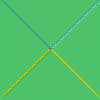
\includegraphics[interpolate=false,width=1.000000in,height=1.000000in]{antiderivative_pm_10-img0.png}}%
\end{pgfscope}%
\begin{pgfscope}%
\pgfsetbuttcap%
\pgfsetroundjoin%
\definecolor{currentfill}{rgb}{0.000000,0.000000,0.000000}%
\pgfsetfillcolor{currentfill}%
\pgfsetlinewidth{0.803000pt}%
\definecolor{currentstroke}{rgb}{0.000000,0.000000,0.000000}%
\pgfsetstrokecolor{currentstroke}%
\pgfsetdash{}{0pt}%
\pgfsys@defobject{currentmarker}{\pgfqpoint{0.000000in}{-0.048611in}}{\pgfqpoint{0.000000in}{0.000000in}}{%
\pgfpathmoveto{\pgfqpoint{0.000000in}{0.000000in}}%
\pgfpathlineto{\pgfqpoint{0.000000in}{-0.048611in}}%
\pgfusepath{stroke,fill}%
}%
\begin{pgfscope}%
\pgfsys@transformshift{0.654106in}{0.517039in}%
\pgfsys@useobject{currentmarker}{}%
\end{pgfscope}%
\end{pgfscope}%
\begin{pgfscope}%
\definecolor{textcolor}{rgb}{0.000000,0.000000,0.000000}%
\pgfsetstrokecolor{textcolor}%
\pgfsetfillcolor{textcolor}%
\pgftext[x=0.654106in,y=0.419816in,,top]{\color{textcolor}{\rmfamily\fontsize{12.000000}{14.400000}\selectfont\catcode`\^=\active\def^{\ifmmode\sp\else\^{}\fi}\catcode`\%=\active\def%{\%}0}}%
\end{pgfscope}%
\begin{pgfscope}%
\pgfsetbuttcap%
\pgfsetroundjoin%
\definecolor{currentfill}{rgb}{0.000000,0.000000,0.000000}%
\pgfsetfillcolor{currentfill}%
\pgfsetlinewidth{0.803000pt}%
\definecolor{currentstroke}{rgb}{0.000000,0.000000,0.000000}%
\pgfsetstrokecolor{currentstroke}%
\pgfsetdash{}{0pt}%
\pgfsys@defobject{currentmarker}{\pgfqpoint{0.000000in}{-0.048611in}}{\pgfqpoint{0.000000in}{0.000000in}}{%
\pgfpathmoveto{\pgfqpoint{0.000000in}{0.000000in}}%
\pgfpathlineto{\pgfqpoint{0.000000in}{-0.048611in}}%
\pgfusepath{stroke,fill}%
}%
\begin{pgfscope}%
\pgfsys@transformshift{1.251588in}{0.517039in}%
\pgfsys@useobject{currentmarker}{}%
\end{pgfscope}%
\end{pgfscope}%
\begin{pgfscope}%
\definecolor{textcolor}{rgb}{0.000000,0.000000,0.000000}%
\pgfsetstrokecolor{textcolor}%
\pgfsetfillcolor{textcolor}%
\pgftext[x=1.251588in,y=0.419816in,,top]{\color{textcolor}{\rmfamily\fontsize{12.000000}{14.400000}\selectfont\catcode`\^=\active\def^{\ifmmode\sp\else\^{}\fi}\catcode`\%=\active\def%{\%}25}}%
\end{pgfscope}%
\begin{pgfscope}%
\pgfsetbuttcap%
\pgfsetroundjoin%
\definecolor{currentfill}{rgb}{0.000000,0.000000,0.000000}%
\pgfsetfillcolor{currentfill}%
\pgfsetlinewidth{0.803000pt}%
\definecolor{currentstroke}{rgb}{0.000000,0.000000,0.000000}%
\pgfsetstrokecolor{currentstroke}%
\pgfsetdash{}{0pt}%
\pgfsys@defobject{currentmarker}{\pgfqpoint{0.000000in}{-0.048611in}}{\pgfqpoint{0.000000in}{0.000000in}}{%
\pgfpathmoveto{\pgfqpoint{0.000000in}{0.000000in}}%
\pgfpathlineto{\pgfqpoint{0.000000in}{-0.048611in}}%
\pgfusepath{stroke,fill}%
}%
\begin{pgfscope}%
\pgfsys@transformshift{1.849069in}{0.517039in}%
\pgfsys@useobject{currentmarker}{}%
\end{pgfscope}%
\end{pgfscope}%
\begin{pgfscope}%
\definecolor{textcolor}{rgb}{0.000000,0.000000,0.000000}%
\pgfsetstrokecolor{textcolor}%
\pgfsetfillcolor{textcolor}%
\pgftext[x=1.849069in,y=0.419816in,,top]{\color{textcolor}{\rmfamily\fontsize{12.000000}{14.400000}\selectfont\catcode`\^=\active\def^{\ifmmode\sp\else\^{}\fi}\catcode`\%=\active\def%{\%}50}}%
\end{pgfscope}%
\begin{pgfscope}%
\pgfsetbuttcap%
\pgfsetroundjoin%
\definecolor{currentfill}{rgb}{0.000000,0.000000,0.000000}%
\pgfsetfillcolor{currentfill}%
\pgfsetlinewidth{0.803000pt}%
\definecolor{currentstroke}{rgb}{0.000000,0.000000,0.000000}%
\pgfsetstrokecolor{currentstroke}%
\pgfsetdash{}{0pt}%
\pgfsys@defobject{currentmarker}{\pgfqpoint{0.000000in}{-0.048611in}}{\pgfqpoint{0.000000in}{0.000000in}}{%
\pgfpathmoveto{\pgfqpoint{0.000000in}{0.000000in}}%
\pgfpathlineto{\pgfqpoint{0.000000in}{-0.048611in}}%
\pgfusepath{stroke,fill}%
}%
\begin{pgfscope}%
\pgfsys@transformshift{2.446551in}{0.517039in}%
\pgfsys@useobject{currentmarker}{}%
\end{pgfscope}%
\end{pgfscope}%
\begin{pgfscope}%
\definecolor{textcolor}{rgb}{0.000000,0.000000,0.000000}%
\pgfsetstrokecolor{textcolor}%
\pgfsetfillcolor{textcolor}%
\pgftext[x=2.446551in,y=0.419816in,,top]{\color{textcolor}{\rmfamily\fontsize{12.000000}{14.400000}\selectfont\catcode`\^=\active\def^{\ifmmode\sp\else\^{}\fi}\catcode`\%=\active\def%{\%}75}}%
\end{pgfscope}%
\begin{pgfscope}%
\definecolor{textcolor}{rgb}{0.000000,0.000000,0.000000}%
\pgfsetstrokecolor{textcolor}%
\pgfsetfillcolor{textcolor}%
\pgftext[x=1.837120in,y=0.202965in,,top]{\color{textcolor}{\rmfamily\fontsize{12.000000}{14.400000}\selectfont\catcode`\^=\active\def^{\ifmmode\sp\else\^{}\fi}\catcode`\%=\active\def%{\%}output coefficients}}%
\end{pgfscope}%
\begin{pgfscope}%
\pgfsetbuttcap%
\pgfsetroundjoin%
\definecolor{currentfill}{rgb}{0.000000,0.000000,0.000000}%
\pgfsetfillcolor{currentfill}%
\pgfsetlinewidth{0.803000pt}%
\definecolor{currentstroke}{rgb}{0.000000,0.000000,0.000000}%
\pgfsetstrokecolor{currentstroke}%
\pgfsetdash{}{0pt}%
\pgfsys@defobject{currentmarker}{\pgfqpoint{-0.048611in}{0.000000in}}{\pgfqpoint{-0.000000in}{0.000000in}}{%
\pgfpathmoveto{\pgfqpoint{-0.000000in}{0.000000in}}%
\pgfpathlineto{\pgfqpoint{-0.048611in}{0.000000in}}%
\pgfusepath{stroke,fill}%
}%
\begin{pgfscope}%
\pgfsys@transformshift{0.642156in}{2.895016in}%
\pgfsys@useobject{currentmarker}{}%
\end{pgfscope}%
\end{pgfscope}%
\begin{pgfscope}%
\definecolor{textcolor}{rgb}{0.000000,0.000000,0.000000}%
\pgfsetstrokecolor{textcolor}%
\pgfsetfillcolor{textcolor}%
\pgftext[x=0.438896in, y=2.831702in, left, base]{\color{textcolor}{\rmfamily\fontsize{12.000000}{14.400000}\selectfont\catcode`\^=\active\def^{\ifmmode\sp\else\^{}\fi}\catcode`\%=\active\def%{\%}0}}%
\end{pgfscope}%
\begin{pgfscope}%
\pgfsetbuttcap%
\pgfsetroundjoin%
\definecolor{currentfill}{rgb}{0.000000,0.000000,0.000000}%
\pgfsetfillcolor{currentfill}%
\pgfsetlinewidth{0.803000pt}%
\definecolor{currentstroke}{rgb}{0.000000,0.000000,0.000000}%
\pgfsetstrokecolor{currentstroke}%
\pgfsetdash{}{0pt}%
\pgfsys@defobject{currentmarker}{\pgfqpoint{-0.048611in}{0.000000in}}{\pgfqpoint{-0.000000in}{0.000000in}}{%
\pgfpathmoveto{\pgfqpoint{-0.000000in}{0.000000in}}%
\pgfpathlineto{\pgfqpoint{-0.048611in}{0.000000in}}%
\pgfusepath{stroke,fill}%
}%
\begin{pgfscope}%
\pgfsys@transformshift{0.642156in}{2.417031in}%
\pgfsys@useobject{currentmarker}{}%
\end{pgfscope}%
\end{pgfscope}%
\begin{pgfscope}%
\definecolor{textcolor}{rgb}{0.000000,0.000000,0.000000}%
\pgfsetstrokecolor{textcolor}%
\pgfsetfillcolor{textcolor}%
\pgftext[x=0.332857in, y=2.353717in, left, base]{\color{textcolor}{\rmfamily\fontsize{12.000000}{14.400000}\selectfont\catcode`\^=\active\def^{\ifmmode\sp\else\^{}\fi}\catcode`\%=\active\def%{\%}20}}%
\end{pgfscope}%
\begin{pgfscope}%
\pgfsetbuttcap%
\pgfsetroundjoin%
\definecolor{currentfill}{rgb}{0.000000,0.000000,0.000000}%
\pgfsetfillcolor{currentfill}%
\pgfsetlinewidth{0.803000pt}%
\definecolor{currentstroke}{rgb}{0.000000,0.000000,0.000000}%
\pgfsetstrokecolor{currentstroke}%
\pgfsetdash{}{0pt}%
\pgfsys@defobject{currentmarker}{\pgfqpoint{-0.048611in}{0.000000in}}{\pgfqpoint{-0.000000in}{0.000000in}}{%
\pgfpathmoveto{\pgfqpoint{-0.000000in}{0.000000in}}%
\pgfpathlineto{\pgfqpoint{-0.048611in}{0.000000in}}%
\pgfusepath{stroke,fill}%
}%
\begin{pgfscope}%
\pgfsys@transformshift{0.642156in}{1.939045in}%
\pgfsys@useobject{currentmarker}{}%
\end{pgfscope}%
\end{pgfscope}%
\begin{pgfscope}%
\definecolor{textcolor}{rgb}{0.000000,0.000000,0.000000}%
\pgfsetstrokecolor{textcolor}%
\pgfsetfillcolor{textcolor}%
\pgftext[x=0.332857in, y=1.875731in, left, base]{\color{textcolor}{\rmfamily\fontsize{12.000000}{14.400000}\selectfont\catcode`\^=\active\def^{\ifmmode\sp\else\^{}\fi}\catcode`\%=\active\def%{\%}40}}%
\end{pgfscope}%
\begin{pgfscope}%
\pgfsetbuttcap%
\pgfsetroundjoin%
\definecolor{currentfill}{rgb}{0.000000,0.000000,0.000000}%
\pgfsetfillcolor{currentfill}%
\pgfsetlinewidth{0.803000pt}%
\definecolor{currentstroke}{rgb}{0.000000,0.000000,0.000000}%
\pgfsetstrokecolor{currentstroke}%
\pgfsetdash{}{0pt}%
\pgfsys@defobject{currentmarker}{\pgfqpoint{-0.048611in}{0.000000in}}{\pgfqpoint{-0.000000in}{0.000000in}}{%
\pgfpathmoveto{\pgfqpoint{-0.000000in}{0.000000in}}%
\pgfpathlineto{\pgfqpoint{-0.048611in}{0.000000in}}%
\pgfusepath{stroke,fill}%
}%
\begin{pgfscope}%
\pgfsys@transformshift{0.642156in}{1.461060in}%
\pgfsys@useobject{currentmarker}{}%
\end{pgfscope}%
\end{pgfscope}%
\begin{pgfscope}%
\definecolor{textcolor}{rgb}{0.000000,0.000000,0.000000}%
\pgfsetstrokecolor{textcolor}%
\pgfsetfillcolor{textcolor}%
\pgftext[x=0.332857in, y=1.397746in, left, base]{\color{textcolor}{\rmfamily\fontsize{12.000000}{14.400000}\selectfont\catcode`\^=\active\def^{\ifmmode\sp\else\^{}\fi}\catcode`\%=\active\def%{\%}60}}%
\end{pgfscope}%
\begin{pgfscope}%
\pgfsetbuttcap%
\pgfsetroundjoin%
\definecolor{currentfill}{rgb}{0.000000,0.000000,0.000000}%
\pgfsetfillcolor{currentfill}%
\pgfsetlinewidth{0.803000pt}%
\definecolor{currentstroke}{rgb}{0.000000,0.000000,0.000000}%
\pgfsetstrokecolor{currentstroke}%
\pgfsetdash{}{0pt}%
\pgfsys@defobject{currentmarker}{\pgfqpoint{-0.048611in}{0.000000in}}{\pgfqpoint{-0.000000in}{0.000000in}}{%
\pgfpathmoveto{\pgfqpoint{-0.000000in}{0.000000in}}%
\pgfpathlineto{\pgfqpoint{-0.048611in}{0.000000in}}%
\pgfusepath{stroke,fill}%
}%
\begin{pgfscope}%
\pgfsys@transformshift{0.642156in}{0.983074in}%
\pgfsys@useobject{currentmarker}{}%
\end{pgfscope}%
\end{pgfscope}%
\begin{pgfscope}%
\definecolor{textcolor}{rgb}{0.000000,0.000000,0.000000}%
\pgfsetstrokecolor{textcolor}%
\pgfsetfillcolor{textcolor}%
\pgftext[x=0.332857in, y=0.919761in, left, base]{\color{textcolor}{\rmfamily\fontsize{12.000000}{14.400000}\selectfont\catcode`\^=\active\def^{\ifmmode\sp\else\^{}\fi}\catcode`\%=\active\def%{\%}80}}%
\end{pgfscope}%
\begin{pgfscope}%
\definecolor{textcolor}{rgb}{0.000000,0.000000,0.000000}%
\pgfsetstrokecolor{textcolor}%
\pgfsetfillcolor{textcolor}%
\pgftext[x=0.277302in,y=1.712002in,,bottom,rotate=90.000000]{\color{textcolor}{\rmfamily\fontsize{12.000000}{14.400000}\selectfont\catcode`\^=\active\def^{\ifmmode\sp\else\^{}\fi}\catcode`\%=\active\def%{\%}input coefficients}}%
\end{pgfscope}%
\begin{pgfscope}%
\pgfsetrectcap%
\pgfsetmiterjoin%
\pgfsetlinewidth{0.803000pt}%
\definecolor{currentstroke}{rgb}{0.000000,0.000000,0.000000}%
\pgfsetstrokecolor{currentstroke}%
\pgfsetdash{}{0pt}%
\pgfpathmoveto{\pgfqpoint{0.642156in}{0.517039in}}%
\pgfpathlineto{\pgfqpoint{0.642156in}{2.906966in}}%
\pgfusepath{stroke}%
\end{pgfscope}%
\begin{pgfscope}%
\pgfsetrectcap%
\pgfsetmiterjoin%
\pgfsetlinewidth{0.803000pt}%
\definecolor{currentstroke}{rgb}{0.000000,0.000000,0.000000}%
\pgfsetstrokecolor{currentstroke}%
\pgfsetdash{}{0pt}%
\pgfpathmoveto{\pgfqpoint{3.032083in}{0.517039in}}%
\pgfpathlineto{\pgfqpoint{3.032083in}{2.906966in}}%
\pgfusepath{stroke}%
\end{pgfscope}%
\begin{pgfscope}%
\pgfsetrectcap%
\pgfsetmiterjoin%
\pgfsetlinewidth{0.803000pt}%
\definecolor{currentstroke}{rgb}{0.000000,0.000000,0.000000}%
\pgfsetstrokecolor{currentstroke}%
\pgfsetdash{}{0pt}%
\pgfpathmoveto{\pgfqpoint{0.642156in}{0.517039in}}%
\pgfpathlineto{\pgfqpoint{3.032083in}{0.517039in}}%
\pgfusepath{stroke}%
\end{pgfscope}%
\begin{pgfscope}%
\pgfsetrectcap%
\pgfsetmiterjoin%
\pgfsetlinewidth{0.803000pt}%
\definecolor{currentstroke}{rgb}{0.000000,0.000000,0.000000}%
\pgfsetstrokecolor{currentstroke}%
\pgfsetdash{}{0pt}%
\pgfpathmoveto{\pgfqpoint{0.642156in}{2.906966in}}%
\pgfpathlineto{\pgfqpoint{3.032083in}{2.906966in}}%
\pgfusepath{stroke}%
\end{pgfscope}%
\begin{pgfscope}%
\pgfsetbuttcap%
\pgfsetmiterjoin%
\pgfsetlinewidth{0.000000pt}%
\definecolor{currentstroke}{rgb}{0.000000,0.000000,0.000000}%
\pgfsetstrokecolor{currentstroke}%
\pgfsetstrokeopacity{0.000000}%
\pgfsetdash{}{0pt}%
\pgfpathmoveto{\pgfqpoint{3.181604in}{0.517039in}}%
\pgfpathlineto{\pgfqpoint{3.301100in}{0.517039in}}%
\pgfpathlineto{\pgfqpoint{3.301100in}{2.906966in}}%
\pgfpathlineto{\pgfqpoint{3.181604in}{2.906966in}}%
\pgfpathlineto{\pgfqpoint{3.181604in}{0.517039in}}%
\pgfpathclose%
\pgfusepath{}%
\end{pgfscope}%
\begin{pgfscope}%
\pgfsys@transformshift{3.180000in}{0.520000in}%
\pgftext[left,bottom]{
\includegraphics[interpolate=true,width=0.120000in,height=2.390000in]{antiderivative_pm_10-img1.png}}%
\end{pgfscope}%
\begin{pgfscope}%
\pgfsetbuttcap%
\pgfsetroundjoin%
\definecolor{currentfill}{rgb}{0.000000,0.000000,0.000000}%
\pgfsetfillcolor{currentfill}%
\pgfsetlinewidth{0.803000pt}%
\definecolor{currentstroke}{rgb}{0.000000,0.000000,0.000000}%
\pgfsetstrokecolor{currentstroke}%
\pgfsetdash{}{0pt}%
\pgfsys@defobject{currentmarker}{\pgfqpoint{0.000000in}{0.000000in}}{\pgfqpoint{0.048611in}{0.000000in}}{%
\pgfpathmoveto{\pgfqpoint{0.000000in}{0.000000in}}%
\pgfpathlineto{\pgfqpoint{0.048611in}{0.000000in}}%
\pgfusepath{stroke,fill}%
}%
\begin{pgfscope}%
\pgfsys@transformshift{3.301100in}{0.700436in}%
\pgfsys@useobject{currentmarker}{}%
\end{pgfscope}%
\end{pgfscope}%
\begin{pgfscope}%
\definecolor{textcolor}{rgb}{0.000000,0.000000,0.000000}%
\pgfsetstrokecolor{textcolor}%
\pgfsetfillcolor{textcolor}%
\pgftext[x=3.398323in, y=0.637123in, left, base]{\color{textcolor}{\rmfamily\fontsize{12.000000}{14.400000}\selectfont\catcode`\^=\active\def^{\ifmmode\sp\else\^{}\fi}\catcode`\%=\active\def%{\%}\ensuremath{-}2000}}%
\end{pgfscope}%
\begin{pgfscope}%
\pgfsetbuttcap%
\pgfsetroundjoin%
\definecolor{currentfill}{rgb}{0.000000,0.000000,0.000000}%
\pgfsetfillcolor{currentfill}%
\pgfsetlinewidth{0.803000pt}%
\definecolor{currentstroke}{rgb}{0.000000,0.000000,0.000000}%
\pgfsetstrokecolor{currentstroke}%
\pgfsetdash{}{0pt}%
\pgfsys@defobject{currentmarker}{\pgfqpoint{0.000000in}{0.000000in}}{\pgfqpoint{0.048611in}{0.000000in}}{%
\pgfpathmoveto{\pgfqpoint{0.000000in}{0.000000in}}%
\pgfpathlineto{\pgfqpoint{0.048611in}{0.000000in}}%
\pgfusepath{stroke,fill}%
}%
\begin{pgfscope}%
\pgfsys@transformshift{3.301100in}{1.085369in}%
\pgfsys@useobject{currentmarker}{}%
\end{pgfscope}%
\end{pgfscope}%
\begin{pgfscope}%
\definecolor{textcolor}{rgb}{0.000000,0.000000,0.000000}%
\pgfsetstrokecolor{textcolor}%
\pgfsetfillcolor{textcolor}%
\pgftext[x=3.398323in, y=1.022055in, left, base]{\color{textcolor}{\rmfamily\fontsize{12.000000}{14.400000}\selectfont\catcode`\^=\active\def^{\ifmmode\sp\else\^{}\fi}\catcode`\%=\active\def%{\%}\ensuremath{-}1500}}%
\end{pgfscope}%
\begin{pgfscope}%
\pgfsetbuttcap%
\pgfsetroundjoin%
\definecolor{currentfill}{rgb}{0.000000,0.000000,0.000000}%
\pgfsetfillcolor{currentfill}%
\pgfsetlinewidth{0.803000pt}%
\definecolor{currentstroke}{rgb}{0.000000,0.000000,0.000000}%
\pgfsetstrokecolor{currentstroke}%
\pgfsetdash{}{0pt}%
\pgfsys@defobject{currentmarker}{\pgfqpoint{0.000000in}{0.000000in}}{\pgfqpoint{0.048611in}{0.000000in}}{%
\pgfpathmoveto{\pgfqpoint{0.000000in}{0.000000in}}%
\pgfpathlineto{\pgfqpoint{0.048611in}{0.000000in}}%
\pgfusepath{stroke,fill}%
}%
\begin{pgfscope}%
\pgfsys@transformshift{3.301100in}{1.470302in}%
\pgfsys@useobject{currentmarker}{}%
\end{pgfscope}%
\end{pgfscope}%
\begin{pgfscope}%
\definecolor{textcolor}{rgb}{0.000000,0.000000,0.000000}%
\pgfsetstrokecolor{textcolor}%
\pgfsetfillcolor{textcolor}%
\pgftext[x=3.398323in, y=1.406988in, left, base]{\color{textcolor}{\rmfamily\fontsize{12.000000}{14.400000}\selectfont\catcode`\^=\active\def^{\ifmmode\sp\else\^{}\fi}\catcode`\%=\active\def%{\%}\ensuremath{-}1000}}%
\end{pgfscope}%
\begin{pgfscope}%
\pgfsetbuttcap%
\pgfsetroundjoin%
\definecolor{currentfill}{rgb}{0.000000,0.000000,0.000000}%
\pgfsetfillcolor{currentfill}%
\pgfsetlinewidth{0.803000pt}%
\definecolor{currentstroke}{rgb}{0.000000,0.000000,0.000000}%
\pgfsetstrokecolor{currentstroke}%
\pgfsetdash{}{0pt}%
\pgfsys@defobject{currentmarker}{\pgfqpoint{0.000000in}{0.000000in}}{\pgfqpoint{0.048611in}{0.000000in}}{%
\pgfpathmoveto{\pgfqpoint{0.000000in}{0.000000in}}%
\pgfpathlineto{\pgfqpoint{0.048611in}{0.000000in}}%
\pgfusepath{stroke,fill}%
}%
\begin{pgfscope}%
\pgfsys@transformshift{3.301100in}{1.855235in}%
\pgfsys@useobject{currentmarker}{}%
\end{pgfscope}%
\end{pgfscope}%
\begin{pgfscope}%
\definecolor{textcolor}{rgb}{0.000000,0.000000,0.000000}%
\pgfsetstrokecolor{textcolor}%
\pgfsetfillcolor{textcolor}%
\pgftext[x=3.398323in, y=1.791921in, left, base]{\color{textcolor}{\rmfamily\fontsize{12.000000}{14.400000}\selectfont\catcode`\^=\active\def^{\ifmmode\sp\else\^{}\fi}\catcode`\%=\active\def%{\%}\ensuremath{-}500}}%
\end{pgfscope}%
\begin{pgfscope}%
\pgfsetbuttcap%
\pgfsetroundjoin%
\definecolor{currentfill}{rgb}{0.000000,0.000000,0.000000}%
\pgfsetfillcolor{currentfill}%
\pgfsetlinewidth{0.803000pt}%
\definecolor{currentstroke}{rgb}{0.000000,0.000000,0.000000}%
\pgfsetstrokecolor{currentstroke}%
\pgfsetdash{}{0pt}%
\pgfsys@defobject{currentmarker}{\pgfqpoint{0.000000in}{0.000000in}}{\pgfqpoint{0.048611in}{0.000000in}}{%
\pgfpathmoveto{\pgfqpoint{0.000000in}{0.000000in}}%
\pgfpathlineto{\pgfqpoint{0.048611in}{0.000000in}}%
\pgfusepath{stroke,fill}%
}%
\begin{pgfscope}%
\pgfsys@transformshift{3.301100in}{2.240168in}%
\pgfsys@useobject{currentmarker}{}%
\end{pgfscope}%
\end{pgfscope}%
\begin{pgfscope}%
\definecolor{textcolor}{rgb}{0.000000,0.000000,0.000000}%
\pgfsetstrokecolor{textcolor}%
\pgfsetfillcolor{textcolor}%
\pgftext[x=3.398323in, y=2.176854in, left, base]{\color{textcolor}{\rmfamily\fontsize{12.000000}{14.400000}\selectfont\catcode`\^=\active\def^{\ifmmode\sp\else\^{}\fi}\catcode`\%=\active\def%{\%}0}}%
\end{pgfscope}%
\begin{pgfscope}%
\pgfsetbuttcap%
\pgfsetroundjoin%
\definecolor{currentfill}{rgb}{0.000000,0.000000,0.000000}%
\pgfsetfillcolor{currentfill}%
\pgfsetlinewidth{0.803000pt}%
\definecolor{currentstroke}{rgb}{0.000000,0.000000,0.000000}%
\pgfsetstrokecolor{currentstroke}%
\pgfsetdash{}{0pt}%
\pgfsys@defobject{currentmarker}{\pgfqpoint{0.000000in}{0.000000in}}{\pgfqpoint{0.048611in}{0.000000in}}{%
\pgfpathmoveto{\pgfqpoint{0.000000in}{0.000000in}}%
\pgfpathlineto{\pgfqpoint{0.048611in}{0.000000in}}%
\pgfusepath{stroke,fill}%
}%
\begin{pgfscope}%
\pgfsys@transformshift{3.301100in}{2.625100in}%
\pgfsys@useobject{currentmarker}{}%
\end{pgfscope}%
\end{pgfscope}%
\begin{pgfscope}%
\definecolor{textcolor}{rgb}{0.000000,0.000000,0.000000}%
\pgfsetstrokecolor{textcolor}%
\pgfsetfillcolor{textcolor}%
\pgftext[x=3.398323in, y=2.561787in, left, base]{\color{textcolor}{\rmfamily\fontsize{12.000000}{14.400000}\selectfont\catcode`\^=\active\def^{\ifmmode\sp\else\^{}\fi}\catcode`\%=\active\def%{\%}500}}%
\end{pgfscope}%
\begin{pgfscope}%
\pgfsetrectcap%
\pgfsetmiterjoin%
\pgfsetlinewidth{0.803000pt}%
\definecolor{currentstroke}{rgb}{0.000000,0.000000,0.000000}%
\pgfsetstrokecolor{currentstroke}%
\pgfsetdash{}{0pt}%
\pgfpathmoveto{\pgfqpoint{3.181604in}{0.517039in}}%
\pgfpathlineto{\pgfqpoint{3.241352in}{0.517039in}}%
\pgfpathlineto{\pgfqpoint{3.301100in}{0.517039in}}%
\pgfpathlineto{\pgfqpoint{3.301100in}{2.906966in}}%
\pgfpathlineto{\pgfqpoint{3.241352in}{2.906966in}}%
\pgfpathlineto{\pgfqpoint{3.181604in}{2.906966in}}%
\pgfpathlineto{\pgfqpoint{3.181604in}{0.517039in}}%
\pgfpathclose%
\pgfusepath{stroke}%
\end{pgfscope}%
\end{pgfpicture}%
\makeatother%
\endgroup%

      \end{adjustbox}
      \caption{The p-matrix for 10\% noise.}\label{fig:sc1_pm_10}
    \end{subfigure}
    % \\[\baselineskip]
    \begin{subfigure}{0.49\linewidth}
      \begin{adjustbox}{width=\linewidth}
        \begingroup%
\makeatletter%
\begin{pgfpicture}%
\pgfpathrectangle{\pgfpointorigin}{\pgfqpoint{6.400000in}{4.800000in}}%
\pgfusepath{use as bounding box, clip}%
\begin{pgfscope}%
\pgfsetbuttcap%
\pgfsetmiterjoin%
\pgfsetlinewidth{0.000000pt}%
\definecolor{currentstroke}{rgb}{0.000000,0.000000,0.000000}%
\pgfsetstrokecolor{currentstroke}%
\pgfsetstrokeopacity{0.000000}%
\pgfsetdash{}{0pt}%
\pgfpathmoveto{\pgfqpoint{0.000000in}{0.000000in}}%
\pgfpathlineto{\pgfqpoint{6.400000in}{0.000000in}}%
\pgfpathlineto{\pgfqpoint{6.400000in}{4.800000in}}%
\pgfpathlineto{\pgfqpoint{0.000000in}{4.800000in}}%
\pgfpathlineto{\pgfqpoint{0.000000in}{0.000000in}}%
\pgfpathclose%
\pgfusepath{}%
\end{pgfscope}%
\begin{pgfscope}%
\pgfsetbuttcap%
\pgfsetmiterjoin%
\pgfsetlinewidth{0.000000pt}%
\definecolor{currentstroke}{rgb}{0.000000,0.000000,0.000000}%
\pgfsetstrokecolor{currentstroke}%
\pgfsetstrokeopacity{0.000000}%
\pgfsetdash{}{0pt}%
\pgfpathmoveto{\pgfqpoint{0.800000in}{0.528000in}}%
\pgfpathlineto{\pgfqpoint{4.768000in}{0.528000in}}%
\pgfpathlineto{\pgfqpoint{4.768000in}{4.224000in}}%
\pgfpathlineto{\pgfqpoint{0.800000in}{4.224000in}}%
\pgfpathlineto{\pgfqpoint{0.800000in}{0.528000in}}%
\pgfpathclose%
\pgfusepath{}%
\end{pgfscope}%
\begin{pgfscope}%
\pgfpathrectangle{\pgfqpoint{0.800000in}{0.528000in}}{\pgfqpoint{3.968000in}{3.696000in}}%
\pgfusepath{clip}%
\pgfsys@transformcm{3.968000}{0.000000}{0.000000}{-3.696000}{0.800000in}{4.224000in}%
\pgftext[left,bottom]{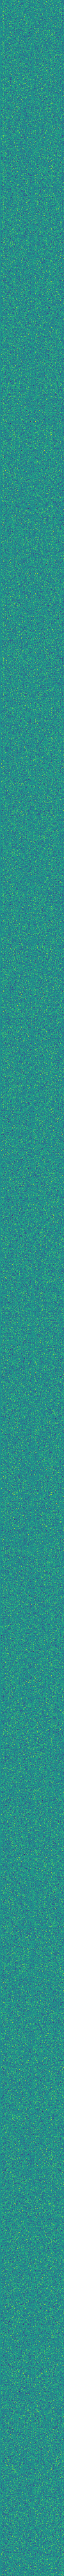
\includegraphics[interpolate=false,width=1.000000in,height=1.000000in]{antiderivative_ci_50-img0.png}}%
\end{pgfscope}%
\begin{pgfscope}%
\pgfsetbuttcap%
\pgfsetroundjoin%
\definecolor{currentfill}{rgb}{0.000000,0.000000,0.000000}%
\pgfsetfillcolor{currentfill}%
\pgfsetlinewidth{0.803000pt}%
\definecolor{currentstroke}{rgb}{0.000000,0.000000,0.000000}%
\pgfsetstrokecolor{currentstroke}%
\pgfsetdash{}{0pt}%
\pgfsys@defobject{currentmarker}{\pgfqpoint{0.000000in}{-0.048611in}}{\pgfqpoint{0.000000in}{0.000000in}}{%
\pgfpathmoveto{\pgfqpoint{0.000000in}{0.000000in}}%
\pgfpathlineto{\pgfqpoint{0.000000in}{-0.048611in}}%
\pgfusepath{stroke,fill}%
}%
\begin{pgfscope}%
\pgfsys@transformshift{0.800000in}{0.528000in}%
\pgfsys@useobject{currentmarker}{}%
\end{pgfscope}%
\end{pgfscope}%
\begin{pgfscope}%
\definecolor{textcolor}{rgb}{0.000000,0.000000,0.000000}%
\pgfsetstrokecolor{textcolor}%
\pgfsetfillcolor{textcolor}%
\pgftext[x=0.800000in,y=0.430778in,,top]{\color{textcolor}{\rmfamily\fontsize{12.000000}{14.400000}\selectfont\catcode`\^=\active\def^{\ifmmode\sp\else\^{}\fi}\catcode`\%=\active\def%{\%}0}}%
\end{pgfscope}%
\begin{pgfscope}%
\pgfsetbuttcap%
\pgfsetroundjoin%
\definecolor{currentfill}{rgb}{0.000000,0.000000,0.000000}%
\pgfsetfillcolor{currentfill}%
\pgfsetlinewidth{0.803000pt}%
\definecolor{currentstroke}{rgb}{0.000000,0.000000,0.000000}%
\pgfsetstrokecolor{currentstroke}%
\pgfsetdash{}{0pt}%
\pgfsys@defobject{currentmarker}{\pgfqpoint{0.000000in}{-0.048611in}}{\pgfqpoint{0.000000in}{0.000000in}}{%
\pgfpathmoveto{\pgfqpoint{0.000000in}{0.000000in}}%
\pgfpathlineto{\pgfqpoint{0.000000in}{-0.048611in}}%
\pgfusepath{stroke,fill}%
}%
\begin{pgfscope}%
\pgfsys@transformshift{1.593600in}{0.528000in}%
\pgfsys@useobject{currentmarker}{}%
\end{pgfscope}%
\end{pgfscope}%
\begin{pgfscope}%
\definecolor{textcolor}{rgb}{0.000000,0.000000,0.000000}%
\pgfsetstrokecolor{textcolor}%
\pgfsetfillcolor{textcolor}%
\pgftext[x=1.593600in,y=0.430778in,,top]{\color{textcolor}{\rmfamily\fontsize{12.000000}{14.400000}\selectfont\catcode`\^=\active\def^{\ifmmode\sp\else\^{}\fi}\catcode`\%=\active\def%{\%}10}}%
\end{pgfscope}%
\begin{pgfscope}%
\pgfsetbuttcap%
\pgfsetroundjoin%
\definecolor{currentfill}{rgb}{0.000000,0.000000,0.000000}%
\pgfsetfillcolor{currentfill}%
\pgfsetlinewidth{0.803000pt}%
\definecolor{currentstroke}{rgb}{0.000000,0.000000,0.000000}%
\pgfsetstrokecolor{currentstroke}%
\pgfsetdash{}{0pt}%
\pgfsys@defobject{currentmarker}{\pgfqpoint{0.000000in}{-0.048611in}}{\pgfqpoint{0.000000in}{0.000000in}}{%
\pgfpathmoveto{\pgfqpoint{0.000000in}{0.000000in}}%
\pgfpathlineto{\pgfqpoint{0.000000in}{-0.048611in}}%
\pgfusepath{stroke,fill}%
}%
\begin{pgfscope}%
\pgfsys@transformshift{2.387200in}{0.528000in}%
\pgfsys@useobject{currentmarker}{}%
\end{pgfscope}%
\end{pgfscope}%
\begin{pgfscope}%
\definecolor{textcolor}{rgb}{0.000000,0.000000,0.000000}%
\pgfsetstrokecolor{textcolor}%
\pgfsetfillcolor{textcolor}%
\pgftext[x=2.387200in,y=0.430778in,,top]{\color{textcolor}{\rmfamily\fontsize{12.000000}{14.400000}\selectfont\catcode`\^=\active\def^{\ifmmode\sp\else\^{}\fi}\catcode`\%=\active\def%{\%}20}}%
\end{pgfscope}%
\begin{pgfscope}%
\pgfsetbuttcap%
\pgfsetroundjoin%
\definecolor{currentfill}{rgb}{0.000000,0.000000,0.000000}%
\pgfsetfillcolor{currentfill}%
\pgfsetlinewidth{0.803000pt}%
\definecolor{currentstroke}{rgb}{0.000000,0.000000,0.000000}%
\pgfsetstrokecolor{currentstroke}%
\pgfsetdash{}{0pt}%
\pgfsys@defobject{currentmarker}{\pgfqpoint{0.000000in}{-0.048611in}}{\pgfqpoint{0.000000in}{0.000000in}}{%
\pgfpathmoveto{\pgfqpoint{0.000000in}{0.000000in}}%
\pgfpathlineto{\pgfqpoint{0.000000in}{-0.048611in}}%
\pgfusepath{stroke,fill}%
}%
\begin{pgfscope}%
\pgfsys@transformshift{3.180800in}{0.528000in}%
\pgfsys@useobject{currentmarker}{}%
\end{pgfscope}%
\end{pgfscope}%
\begin{pgfscope}%
\definecolor{textcolor}{rgb}{0.000000,0.000000,0.000000}%
\pgfsetstrokecolor{textcolor}%
\pgfsetfillcolor{textcolor}%
\pgftext[x=3.180800in,y=0.430778in,,top]{\color{textcolor}{\rmfamily\fontsize{12.000000}{14.400000}\selectfont\catcode`\^=\active\def^{\ifmmode\sp\else\^{}\fi}\catcode`\%=\active\def%{\%}30}}%
\end{pgfscope}%
\begin{pgfscope}%
\pgfsetbuttcap%
\pgfsetroundjoin%
\definecolor{currentfill}{rgb}{0.000000,0.000000,0.000000}%
\pgfsetfillcolor{currentfill}%
\pgfsetlinewidth{0.803000pt}%
\definecolor{currentstroke}{rgb}{0.000000,0.000000,0.000000}%
\pgfsetstrokecolor{currentstroke}%
\pgfsetdash{}{0pt}%
\pgfsys@defobject{currentmarker}{\pgfqpoint{0.000000in}{-0.048611in}}{\pgfqpoint{0.000000in}{0.000000in}}{%
\pgfpathmoveto{\pgfqpoint{0.000000in}{0.000000in}}%
\pgfpathlineto{\pgfqpoint{0.000000in}{-0.048611in}}%
\pgfusepath{stroke,fill}%
}%
\begin{pgfscope}%
\pgfsys@transformshift{3.974400in}{0.528000in}%
\pgfsys@useobject{currentmarker}{}%
\end{pgfscope}%
\end{pgfscope}%
\begin{pgfscope}%
\definecolor{textcolor}{rgb}{0.000000,0.000000,0.000000}%
\pgfsetstrokecolor{textcolor}%
\pgfsetfillcolor{textcolor}%
\pgftext[x=3.974400in,y=0.430778in,,top]{\color{textcolor}{\rmfamily\fontsize{12.000000}{14.400000}\selectfont\catcode`\^=\active\def^{\ifmmode\sp\else\^{}\fi}\catcode`\%=\active\def%{\%}40}}%
\end{pgfscope}%
\begin{pgfscope}%
\pgfsetbuttcap%
\pgfsetroundjoin%
\definecolor{currentfill}{rgb}{0.000000,0.000000,0.000000}%
\pgfsetfillcolor{currentfill}%
\pgfsetlinewidth{0.803000pt}%
\definecolor{currentstroke}{rgb}{0.000000,0.000000,0.000000}%
\pgfsetstrokecolor{currentstroke}%
\pgfsetdash{}{0pt}%
\pgfsys@defobject{currentmarker}{\pgfqpoint{0.000000in}{-0.048611in}}{\pgfqpoint{0.000000in}{0.000000in}}{%
\pgfpathmoveto{\pgfqpoint{0.000000in}{0.000000in}}%
\pgfpathlineto{\pgfqpoint{0.000000in}{-0.048611in}}%
\pgfusepath{stroke,fill}%
}%
\begin{pgfscope}%
\pgfsys@transformshift{4.768000in}{0.528000in}%
\pgfsys@useobject{currentmarker}{}%
\end{pgfscope}%
\end{pgfscope}%
\begin{pgfscope}%
\definecolor{textcolor}{rgb}{0.000000,0.000000,0.000000}%
\pgfsetstrokecolor{textcolor}%
\pgfsetfillcolor{textcolor}%
\pgftext[x=4.768000in,y=0.430778in,,top]{\color{textcolor}{\rmfamily\fontsize{12.000000}{14.400000}\selectfont\catcode`\^=\active\def^{\ifmmode\sp\else\^{}\fi}\catcode`\%=\active\def%{\%}50}}%
\end{pgfscope}%
\begin{pgfscope}%
\definecolor{textcolor}{rgb}{0.000000,0.000000,0.000000}%
\pgfsetstrokecolor{textcolor}%
\pgfsetfillcolor{textcolor}%
\pgftext[x=2.784000in,y=0.213927in,,top]{\color{textcolor}{\rmfamily\fontsize{12.000000}{14.400000}\selectfont\catcode`\^=\active\def^{\ifmmode\sp\else\^{}\fi}\catcode`\%=\active\def%{\%}input coefficients}}%
\end{pgfscope}%
\begin{pgfscope}%
\pgfsetbuttcap%
\pgfsetroundjoin%
\definecolor{currentfill}{rgb}{0.000000,0.000000,0.000000}%
\pgfsetfillcolor{currentfill}%
\pgfsetlinewidth{0.803000pt}%
\definecolor{currentstroke}{rgb}{0.000000,0.000000,0.000000}%
\pgfsetstrokecolor{currentstroke}%
\pgfsetdash{}{0pt}%
\pgfsys@defobject{currentmarker}{\pgfqpoint{-0.048611in}{0.000000in}}{\pgfqpoint{-0.000000in}{0.000000in}}{%
\pgfpathmoveto{\pgfqpoint{-0.000000in}{0.000000in}}%
\pgfpathlineto{\pgfqpoint{-0.048611in}{0.000000in}}%
\pgfusepath{stroke,fill}%
}%
\begin{pgfscope}%
\pgfsys@transformshift{0.800000in}{4.224000in}%
\pgfsys@useobject{currentmarker}{}%
\end{pgfscope}%
\end{pgfscope}%
\begin{pgfscope}%
\definecolor{textcolor}{rgb}{0.000000,0.000000,0.000000}%
\pgfsetstrokecolor{textcolor}%
\pgfsetfillcolor{textcolor}%
\pgftext[x=0.596739in, y=4.160686in, left, base]{\color{textcolor}{\rmfamily\fontsize{12.000000}{14.400000}\selectfont\catcode`\^=\active\def^{\ifmmode\sp\else\^{}\fi}\catcode`\%=\active\def%{\%}0}}%
\end{pgfscope}%
\begin{pgfscope}%
\pgfsetbuttcap%
\pgfsetroundjoin%
\definecolor{currentfill}{rgb}{0.000000,0.000000,0.000000}%
\pgfsetfillcolor{currentfill}%
\pgfsetlinewidth{0.803000pt}%
\definecolor{currentstroke}{rgb}{0.000000,0.000000,0.000000}%
\pgfsetstrokecolor{currentstroke}%
\pgfsetdash{}{0pt}%
\pgfsys@defobject{currentmarker}{\pgfqpoint{-0.048611in}{0.000000in}}{\pgfqpoint{-0.000000in}{0.000000in}}{%
\pgfpathmoveto{\pgfqpoint{-0.000000in}{0.000000in}}%
\pgfpathlineto{\pgfqpoint{-0.048611in}{0.000000in}}%
\pgfusepath{stroke,fill}%
}%
\begin{pgfscope}%
\pgfsys@transformshift{0.800000in}{3.762000in}%
\pgfsys@useobject{currentmarker}{}%
\end{pgfscope}%
\end{pgfscope}%
\begin{pgfscope}%
\definecolor{textcolor}{rgb}{0.000000,0.000000,0.000000}%
\pgfsetstrokecolor{textcolor}%
\pgfsetfillcolor{textcolor}%
\pgftext[x=0.384662in, y=3.698686in, left, base]{\color{textcolor}{\rmfamily\fontsize{12.000000}{14.400000}\selectfont\catcode`\^=\active\def^{\ifmmode\sp\else\^{}\fi}\catcode`\%=\active\def%{\%}500}}%
\end{pgfscope}%
\begin{pgfscope}%
\pgfsetbuttcap%
\pgfsetroundjoin%
\definecolor{currentfill}{rgb}{0.000000,0.000000,0.000000}%
\pgfsetfillcolor{currentfill}%
\pgfsetlinewidth{0.803000pt}%
\definecolor{currentstroke}{rgb}{0.000000,0.000000,0.000000}%
\pgfsetstrokecolor{currentstroke}%
\pgfsetdash{}{0pt}%
\pgfsys@defobject{currentmarker}{\pgfqpoint{-0.048611in}{0.000000in}}{\pgfqpoint{-0.000000in}{0.000000in}}{%
\pgfpathmoveto{\pgfqpoint{-0.000000in}{0.000000in}}%
\pgfpathlineto{\pgfqpoint{-0.048611in}{0.000000in}}%
\pgfusepath{stroke,fill}%
}%
\begin{pgfscope}%
\pgfsys@transformshift{0.800000in}{3.300000in}%
\pgfsys@useobject{currentmarker}{}%
\end{pgfscope}%
\end{pgfscope}%
\begin{pgfscope}%
\definecolor{textcolor}{rgb}{0.000000,0.000000,0.000000}%
\pgfsetstrokecolor{textcolor}%
\pgfsetfillcolor{textcolor}%
\pgftext[x=0.278624in, y=3.236686in, left, base]{\color{textcolor}{\rmfamily\fontsize{12.000000}{14.400000}\selectfont\catcode`\^=\active\def^{\ifmmode\sp\else\^{}\fi}\catcode`\%=\active\def%{\%}1000}}%
\end{pgfscope}%
\begin{pgfscope}%
\pgfsetbuttcap%
\pgfsetroundjoin%
\definecolor{currentfill}{rgb}{0.000000,0.000000,0.000000}%
\pgfsetfillcolor{currentfill}%
\pgfsetlinewidth{0.803000pt}%
\definecolor{currentstroke}{rgb}{0.000000,0.000000,0.000000}%
\pgfsetstrokecolor{currentstroke}%
\pgfsetdash{}{0pt}%
\pgfsys@defobject{currentmarker}{\pgfqpoint{-0.048611in}{0.000000in}}{\pgfqpoint{-0.000000in}{0.000000in}}{%
\pgfpathmoveto{\pgfqpoint{-0.000000in}{0.000000in}}%
\pgfpathlineto{\pgfqpoint{-0.048611in}{0.000000in}}%
\pgfusepath{stroke,fill}%
}%
\begin{pgfscope}%
\pgfsys@transformshift{0.800000in}{2.838000in}%
\pgfsys@useobject{currentmarker}{}%
\end{pgfscope}%
\end{pgfscope}%
\begin{pgfscope}%
\definecolor{textcolor}{rgb}{0.000000,0.000000,0.000000}%
\pgfsetstrokecolor{textcolor}%
\pgfsetfillcolor{textcolor}%
\pgftext[x=0.278624in, y=2.774686in, left, base]{\color{textcolor}{\rmfamily\fontsize{12.000000}{14.400000}\selectfont\catcode`\^=\active\def^{\ifmmode\sp\else\^{}\fi}\catcode`\%=\active\def%{\%}1500}}%
\end{pgfscope}%
\begin{pgfscope}%
\pgfsetbuttcap%
\pgfsetroundjoin%
\definecolor{currentfill}{rgb}{0.000000,0.000000,0.000000}%
\pgfsetfillcolor{currentfill}%
\pgfsetlinewidth{0.803000pt}%
\definecolor{currentstroke}{rgb}{0.000000,0.000000,0.000000}%
\pgfsetstrokecolor{currentstroke}%
\pgfsetdash{}{0pt}%
\pgfsys@defobject{currentmarker}{\pgfqpoint{-0.048611in}{0.000000in}}{\pgfqpoint{-0.000000in}{0.000000in}}{%
\pgfpathmoveto{\pgfqpoint{-0.000000in}{0.000000in}}%
\pgfpathlineto{\pgfqpoint{-0.048611in}{0.000000in}}%
\pgfusepath{stroke,fill}%
}%
\begin{pgfscope}%
\pgfsys@transformshift{0.800000in}{2.376000in}%
\pgfsys@useobject{currentmarker}{}%
\end{pgfscope}%
\end{pgfscope}%
\begin{pgfscope}%
\definecolor{textcolor}{rgb}{0.000000,0.000000,0.000000}%
\pgfsetstrokecolor{textcolor}%
\pgfsetfillcolor{textcolor}%
\pgftext[x=0.278624in, y=2.312686in, left, base]{\color{textcolor}{\rmfamily\fontsize{12.000000}{14.400000}\selectfont\catcode`\^=\active\def^{\ifmmode\sp\else\^{}\fi}\catcode`\%=\active\def%{\%}2000}}%
\end{pgfscope}%
\begin{pgfscope}%
\pgfsetbuttcap%
\pgfsetroundjoin%
\definecolor{currentfill}{rgb}{0.000000,0.000000,0.000000}%
\pgfsetfillcolor{currentfill}%
\pgfsetlinewidth{0.803000pt}%
\definecolor{currentstroke}{rgb}{0.000000,0.000000,0.000000}%
\pgfsetstrokecolor{currentstroke}%
\pgfsetdash{}{0pt}%
\pgfsys@defobject{currentmarker}{\pgfqpoint{-0.048611in}{0.000000in}}{\pgfqpoint{-0.000000in}{0.000000in}}{%
\pgfpathmoveto{\pgfqpoint{-0.000000in}{0.000000in}}%
\pgfpathlineto{\pgfqpoint{-0.048611in}{0.000000in}}%
\pgfusepath{stroke,fill}%
}%
\begin{pgfscope}%
\pgfsys@transformshift{0.800000in}{1.914000in}%
\pgfsys@useobject{currentmarker}{}%
\end{pgfscope}%
\end{pgfscope}%
\begin{pgfscope}%
\definecolor{textcolor}{rgb}{0.000000,0.000000,0.000000}%
\pgfsetstrokecolor{textcolor}%
\pgfsetfillcolor{textcolor}%
\pgftext[x=0.278624in, y=1.850686in, left, base]{\color{textcolor}{\rmfamily\fontsize{12.000000}{14.400000}\selectfont\catcode`\^=\active\def^{\ifmmode\sp\else\^{}\fi}\catcode`\%=\active\def%{\%}2500}}%
\end{pgfscope}%
\begin{pgfscope}%
\pgfsetbuttcap%
\pgfsetroundjoin%
\definecolor{currentfill}{rgb}{0.000000,0.000000,0.000000}%
\pgfsetfillcolor{currentfill}%
\pgfsetlinewidth{0.803000pt}%
\definecolor{currentstroke}{rgb}{0.000000,0.000000,0.000000}%
\pgfsetstrokecolor{currentstroke}%
\pgfsetdash{}{0pt}%
\pgfsys@defobject{currentmarker}{\pgfqpoint{-0.048611in}{0.000000in}}{\pgfqpoint{-0.000000in}{0.000000in}}{%
\pgfpathmoveto{\pgfqpoint{-0.000000in}{0.000000in}}%
\pgfpathlineto{\pgfqpoint{-0.048611in}{0.000000in}}%
\pgfusepath{stroke,fill}%
}%
\begin{pgfscope}%
\pgfsys@transformshift{0.800000in}{1.452000in}%
\pgfsys@useobject{currentmarker}{}%
\end{pgfscope}%
\end{pgfscope}%
\begin{pgfscope}%
\definecolor{textcolor}{rgb}{0.000000,0.000000,0.000000}%
\pgfsetstrokecolor{textcolor}%
\pgfsetfillcolor{textcolor}%
\pgftext[x=0.278624in, y=1.388686in, left, base]{\color{textcolor}{\rmfamily\fontsize{12.000000}{14.400000}\selectfont\catcode`\^=\active\def^{\ifmmode\sp\else\^{}\fi}\catcode`\%=\active\def%{\%}3000}}%
\end{pgfscope}%
\begin{pgfscope}%
\pgfsetbuttcap%
\pgfsetroundjoin%
\definecolor{currentfill}{rgb}{0.000000,0.000000,0.000000}%
\pgfsetfillcolor{currentfill}%
\pgfsetlinewidth{0.803000pt}%
\definecolor{currentstroke}{rgb}{0.000000,0.000000,0.000000}%
\pgfsetstrokecolor{currentstroke}%
\pgfsetdash{}{0pt}%
\pgfsys@defobject{currentmarker}{\pgfqpoint{-0.048611in}{0.000000in}}{\pgfqpoint{-0.000000in}{0.000000in}}{%
\pgfpathmoveto{\pgfqpoint{-0.000000in}{0.000000in}}%
\pgfpathlineto{\pgfqpoint{-0.048611in}{0.000000in}}%
\pgfusepath{stroke,fill}%
}%
\begin{pgfscope}%
\pgfsys@transformshift{0.800000in}{0.990000in}%
\pgfsys@useobject{currentmarker}{}%
\end{pgfscope}%
\end{pgfscope}%
\begin{pgfscope}%
\definecolor{textcolor}{rgb}{0.000000,0.000000,0.000000}%
\pgfsetstrokecolor{textcolor}%
\pgfsetfillcolor{textcolor}%
\pgftext[x=0.278624in, y=0.926686in, left, base]{\color{textcolor}{\rmfamily\fontsize{12.000000}{14.400000}\selectfont\catcode`\^=\active\def^{\ifmmode\sp\else\^{}\fi}\catcode`\%=\active\def%{\%}3500}}%
\end{pgfscope}%
\begin{pgfscope}%
\pgfsetbuttcap%
\pgfsetroundjoin%
\definecolor{currentfill}{rgb}{0.000000,0.000000,0.000000}%
\pgfsetfillcolor{currentfill}%
\pgfsetlinewidth{0.803000pt}%
\definecolor{currentstroke}{rgb}{0.000000,0.000000,0.000000}%
\pgfsetstrokecolor{currentstroke}%
\pgfsetdash{}{0pt}%
\pgfsys@defobject{currentmarker}{\pgfqpoint{-0.048611in}{0.000000in}}{\pgfqpoint{-0.000000in}{0.000000in}}{%
\pgfpathmoveto{\pgfqpoint{-0.000000in}{0.000000in}}%
\pgfpathlineto{\pgfqpoint{-0.048611in}{0.000000in}}%
\pgfusepath{stroke,fill}%
}%
\begin{pgfscope}%
\pgfsys@transformshift{0.800000in}{0.528000in}%
\pgfsys@useobject{currentmarker}{}%
\end{pgfscope}%
\end{pgfscope}%
\begin{pgfscope}%
\definecolor{textcolor}{rgb}{0.000000,0.000000,0.000000}%
\pgfsetstrokecolor{textcolor}%
\pgfsetfillcolor{textcolor}%
\pgftext[x=0.278624in, y=0.464686in, left, base]{\color{textcolor}{\rmfamily\fontsize{12.000000}{14.400000}\selectfont\catcode`\^=\active\def^{\ifmmode\sp\else\^{}\fi}\catcode`\%=\active\def%{\%}4000}}%
\end{pgfscope}%
\begin{pgfscope}%
\definecolor{textcolor}{rgb}{0.000000,0.000000,0.000000}%
\pgfsetstrokecolor{textcolor}%
\pgfsetfillcolor{textcolor}%
\pgftext[x=0.223069in,y=2.376000in,,bottom,rotate=90.000000]{\color{textcolor}{\rmfamily\fontsize{12.000000}{14.400000}\selectfont\catcode`\^=\active\def^{\ifmmode\sp\else\^{}\fi}\catcode`\%=\active\def%{\%}samples}}%
\end{pgfscope}%
\begin{pgfscope}%
\pgfsetrectcap%
\pgfsetmiterjoin%
\pgfsetlinewidth{0.803000pt}%
\definecolor{currentstroke}{rgb}{0.000000,0.000000,0.000000}%
\pgfsetstrokecolor{currentstroke}%
\pgfsetdash{}{0pt}%
\pgfpathmoveto{\pgfqpoint{0.800000in}{0.528000in}}%
\pgfpathlineto{\pgfqpoint{0.800000in}{4.224000in}}%
\pgfusepath{stroke}%
\end{pgfscope}%
\begin{pgfscope}%
\pgfsetrectcap%
\pgfsetmiterjoin%
\pgfsetlinewidth{0.803000pt}%
\definecolor{currentstroke}{rgb}{0.000000,0.000000,0.000000}%
\pgfsetstrokecolor{currentstroke}%
\pgfsetdash{}{0pt}%
\pgfpathmoveto{\pgfqpoint{4.768000in}{0.528000in}}%
\pgfpathlineto{\pgfqpoint{4.768000in}{4.224000in}}%
\pgfusepath{stroke}%
\end{pgfscope}%
\begin{pgfscope}%
\pgfsetrectcap%
\pgfsetmiterjoin%
\pgfsetlinewidth{0.803000pt}%
\definecolor{currentstroke}{rgb}{0.000000,0.000000,0.000000}%
\pgfsetstrokecolor{currentstroke}%
\pgfsetdash{}{0pt}%
\pgfpathmoveto{\pgfqpoint{0.800000in}{0.528000in}}%
\pgfpathlineto{\pgfqpoint{4.768000in}{0.528000in}}%
\pgfusepath{stroke}%
\end{pgfscope}%
\begin{pgfscope}%
\pgfsetrectcap%
\pgfsetmiterjoin%
\pgfsetlinewidth{0.803000pt}%
\definecolor{currentstroke}{rgb}{0.000000,0.000000,0.000000}%
\pgfsetstrokecolor{currentstroke}%
\pgfsetdash{}{0pt}%
\pgfpathmoveto{\pgfqpoint{0.800000in}{4.224000in}}%
\pgfpathlineto{\pgfqpoint{4.768000in}{4.224000in}}%
\pgfusepath{stroke}%
\end{pgfscope}%
\begin{pgfscope}%
\pgfsetbuttcap%
\pgfsetmiterjoin%
\pgfsetlinewidth{0.000000pt}%
\definecolor{currentstroke}{rgb}{0.000000,0.000000,0.000000}%
\pgfsetstrokecolor{currentstroke}%
\pgfsetstrokeopacity{0.000000}%
\pgfsetdash{}{0pt}%
\pgfpathmoveto{\pgfqpoint{5.016000in}{0.528000in}}%
\pgfpathlineto{\pgfqpoint{5.200800in}{0.528000in}}%
\pgfpathlineto{\pgfqpoint{5.200800in}{4.224000in}}%
\pgfpathlineto{\pgfqpoint{5.016000in}{4.224000in}}%
\pgfpathlineto{\pgfqpoint{5.016000in}{0.528000in}}%
\pgfpathclose%
\pgfusepath{}%
\end{pgfscope}%
\begin{pgfscope}%
\pgfsys@transformshift{5.020000in}{0.530000in}%
\pgftext[left,bottom]{
\includegraphics[interpolate=true,width=0.180000in,height=3.690000in]{antiderivative_ci_50-img1.png}}%
\end{pgfscope}%
\begin{pgfscope}%
\pgfsetbuttcap%
\pgfsetroundjoin%
\definecolor{currentfill}{rgb}{0.000000,0.000000,0.000000}%
\pgfsetfillcolor{currentfill}%
\pgfsetlinewidth{0.803000pt}%
\definecolor{currentstroke}{rgb}{0.000000,0.000000,0.000000}%
\pgfsetstrokecolor{currentstroke}%
\pgfsetdash{}{0pt}%
\pgfsys@defobject{currentmarker}{\pgfqpoint{0.000000in}{0.000000in}}{\pgfqpoint{0.048611in}{0.000000in}}{%
\pgfpathmoveto{\pgfqpoint{0.000000in}{0.000000in}}%
\pgfpathlineto{\pgfqpoint{0.048611in}{0.000000in}}%
\pgfusepath{stroke,fill}%
}%
\begin{pgfscope}%
\pgfsys@transformshift{5.200800in}{0.540424in}%
\pgfsys@useobject{currentmarker}{}%
\end{pgfscope}%
\end{pgfscope}%
\begin{pgfscope}%
\definecolor{textcolor}{rgb}{0.000000,0.000000,0.000000}%
\pgfsetstrokecolor{textcolor}%
\pgfsetfillcolor{textcolor}%
\pgftext[x=5.298022in, y=0.477110in, left, base]{\color{textcolor}{\rmfamily\fontsize{12.000000}{14.400000}\selectfont\catcode`\^=\active\def^{\ifmmode\sp\else\^{}\fi}\catcode`\%=\active\def%{\%}\ensuremath{-}100}}%
\end{pgfscope}%
\begin{pgfscope}%
\pgfsetbuttcap%
\pgfsetroundjoin%
\definecolor{currentfill}{rgb}{0.000000,0.000000,0.000000}%
\pgfsetfillcolor{currentfill}%
\pgfsetlinewidth{0.803000pt}%
\definecolor{currentstroke}{rgb}{0.000000,0.000000,0.000000}%
\pgfsetstrokecolor{currentstroke}%
\pgfsetdash{}{0pt}%
\pgfsys@defobject{currentmarker}{\pgfqpoint{0.000000in}{0.000000in}}{\pgfqpoint{0.048611in}{0.000000in}}{%
\pgfpathmoveto{\pgfqpoint{0.000000in}{0.000000in}}%
\pgfpathlineto{\pgfqpoint{0.048611in}{0.000000in}}%
\pgfusepath{stroke,fill}%
}%
\begin{pgfscope}%
\pgfsys@transformshift{5.200800in}{0.999318in}%
\pgfsys@useobject{currentmarker}{}%
\end{pgfscope}%
\end{pgfscope}%
\begin{pgfscope}%
\definecolor{textcolor}{rgb}{0.000000,0.000000,0.000000}%
\pgfsetstrokecolor{textcolor}%
\pgfsetfillcolor{textcolor}%
\pgftext[x=5.298022in, y=0.936004in, left, base]{\color{textcolor}{\rmfamily\fontsize{12.000000}{14.400000}\selectfont\catcode`\^=\active\def^{\ifmmode\sp\else\^{}\fi}\catcode`\%=\active\def%{\%}\ensuremath{-}75}}%
\end{pgfscope}%
\begin{pgfscope}%
\pgfsetbuttcap%
\pgfsetroundjoin%
\definecolor{currentfill}{rgb}{0.000000,0.000000,0.000000}%
\pgfsetfillcolor{currentfill}%
\pgfsetlinewidth{0.803000pt}%
\definecolor{currentstroke}{rgb}{0.000000,0.000000,0.000000}%
\pgfsetstrokecolor{currentstroke}%
\pgfsetdash{}{0pt}%
\pgfsys@defobject{currentmarker}{\pgfqpoint{0.000000in}{0.000000in}}{\pgfqpoint{0.048611in}{0.000000in}}{%
\pgfpathmoveto{\pgfqpoint{0.000000in}{0.000000in}}%
\pgfpathlineto{\pgfqpoint{0.048611in}{0.000000in}}%
\pgfusepath{stroke,fill}%
}%
\begin{pgfscope}%
\pgfsys@transformshift{5.200800in}{1.458212in}%
\pgfsys@useobject{currentmarker}{}%
\end{pgfscope}%
\end{pgfscope}%
\begin{pgfscope}%
\definecolor{textcolor}{rgb}{0.000000,0.000000,0.000000}%
\pgfsetstrokecolor{textcolor}%
\pgfsetfillcolor{textcolor}%
\pgftext[x=5.298022in, y=1.394898in, left, base]{\color{textcolor}{\rmfamily\fontsize{12.000000}{14.400000}\selectfont\catcode`\^=\active\def^{\ifmmode\sp\else\^{}\fi}\catcode`\%=\active\def%{\%}\ensuremath{-}50}}%
\end{pgfscope}%
\begin{pgfscope}%
\pgfsetbuttcap%
\pgfsetroundjoin%
\definecolor{currentfill}{rgb}{0.000000,0.000000,0.000000}%
\pgfsetfillcolor{currentfill}%
\pgfsetlinewidth{0.803000pt}%
\definecolor{currentstroke}{rgb}{0.000000,0.000000,0.000000}%
\pgfsetstrokecolor{currentstroke}%
\pgfsetdash{}{0pt}%
\pgfsys@defobject{currentmarker}{\pgfqpoint{0.000000in}{0.000000in}}{\pgfqpoint{0.048611in}{0.000000in}}{%
\pgfpathmoveto{\pgfqpoint{0.000000in}{0.000000in}}%
\pgfpathlineto{\pgfqpoint{0.048611in}{0.000000in}}%
\pgfusepath{stroke,fill}%
}%
\begin{pgfscope}%
\pgfsys@transformshift{5.200800in}{1.917106in}%
\pgfsys@useobject{currentmarker}{}%
\end{pgfscope}%
\end{pgfscope}%
\begin{pgfscope}%
\definecolor{textcolor}{rgb}{0.000000,0.000000,0.000000}%
\pgfsetstrokecolor{textcolor}%
\pgfsetfillcolor{textcolor}%
\pgftext[x=5.298022in, y=1.853792in, left, base]{\color{textcolor}{\rmfamily\fontsize{12.000000}{14.400000}\selectfont\catcode`\^=\active\def^{\ifmmode\sp\else\^{}\fi}\catcode`\%=\active\def%{\%}\ensuremath{-}25}}%
\end{pgfscope}%
\begin{pgfscope}%
\pgfsetbuttcap%
\pgfsetroundjoin%
\definecolor{currentfill}{rgb}{0.000000,0.000000,0.000000}%
\pgfsetfillcolor{currentfill}%
\pgfsetlinewidth{0.803000pt}%
\definecolor{currentstroke}{rgb}{0.000000,0.000000,0.000000}%
\pgfsetstrokecolor{currentstroke}%
\pgfsetdash{}{0pt}%
\pgfsys@defobject{currentmarker}{\pgfqpoint{0.000000in}{0.000000in}}{\pgfqpoint{0.048611in}{0.000000in}}{%
\pgfpathmoveto{\pgfqpoint{0.000000in}{0.000000in}}%
\pgfpathlineto{\pgfqpoint{0.048611in}{0.000000in}}%
\pgfusepath{stroke,fill}%
}%
\begin{pgfscope}%
\pgfsys@transformshift{5.200800in}{2.376000in}%
\pgfsys@useobject{currentmarker}{}%
\end{pgfscope}%
\end{pgfscope}%
\begin{pgfscope}%
\definecolor{textcolor}{rgb}{0.000000,0.000000,0.000000}%
\pgfsetstrokecolor{textcolor}%
\pgfsetfillcolor{textcolor}%
\pgftext[x=5.298022in, y=2.312686in, left, base]{\color{textcolor}{\rmfamily\fontsize{12.000000}{14.400000}\selectfont\catcode`\^=\active\def^{\ifmmode\sp\else\^{}\fi}\catcode`\%=\active\def%{\%}0}}%
\end{pgfscope}%
\begin{pgfscope}%
\pgfsetbuttcap%
\pgfsetroundjoin%
\definecolor{currentfill}{rgb}{0.000000,0.000000,0.000000}%
\pgfsetfillcolor{currentfill}%
\pgfsetlinewidth{0.803000pt}%
\definecolor{currentstroke}{rgb}{0.000000,0.000000,0.000000}%
\pgfsetstrokecolor{currentstroke}%
\pgfsetdash{}{0pt}%
\pgfsys@defobject{currentmarker}{\pgfqpoint{0.000000in}{0.000000in}}{\pgfqpoint{0.048611in}{0.000000in}}{%
\pgfpathmoveto{\pgfqpoint{0.000000in}{0.000000in}}%
\pgfpathlineto{\pgfqpoint{0.048611in}{0.000000in}}%
\pgfusepath{stroke,fill}%
}%
\begin{pgfscope}%
\pgfsys@transformshift{5.200800in}{2.834894in}%
\pgfsys@useobject{currentmarker}{}%
\end{pgfscope}%
\end{pgfscope}%
\begin{pgfscope}%
\definecolor{textcolor}{rgb}{0.000000,0.000000,0.000000}%
\pgfsetstrokecolor{textcolor}%
\pgfsetfillcolor{textcolor}%
\pgftext[x=5.298022in, y=2.771580in, left, base]{\color{textcolor}{\rmfamily\fontsize{12.000000}{14.400000}\selectfont\catcode`\^=\active\def^{\ifmmode\sp\else\^{}\fi}\catcode`\%=\active\def%{\%}25}}%
\end{pgfscope}%
\begin{pgfscope}%
\pgfsetbuttcap%
\pgfsetroundjoin%
\definecolor{currentfill}{rgb}{0.000000,0.000000,0.000000}%
\pgfsetfillcolor{currentfill}%
\pgfsetlinewidth{0.803000pt}%
\definecolor{currentstroke}{rgb}{0.000000,0.000000,0.000000}%
\pgfsetstrokecolor{currentstroke}%
\pgfsetdash{}{0pt}%
\pgfsys@defobject{currentmarker}{\pgfqpoint{0.000000in}{0.000000in}}{\pgfqpoint{0.048611in}{0.000000in}}{%
\pgfpathmoveto{\pgfqpoint{0.000000in}{0.000000in}}%
\pgfpathlineto{\pgfqpoint{0.048611in}{0.000000in}}%
\pgfusepath{stroke,fill}%
}%
\begin{pgfscope}%
\pgfsys@transformshift{5.200800in}{3.293788in}%
\pgfsys@useobject{currentmarker}{}%
\end{pgfscope}%
\end{pgfscope}%
\begin{pgfscope}%
\definecolor{textcolor}{rgb}{0.000000,0.000000,0.000000}%
\pgfsetstrokecolor{textcolor}%
\pgfsetfillcolor{textcolor}%
\pgftext[x=5.298022in, y=3.230474in, left, base]{\color{textcolor}{\rmfamily\fontsize{12.000000}{14.400000}\selectfont\catcode`\^=\active\def^{\ifmmode\sp\else\^{}\fi}\catcode`\%=\active\def%{\%}50}}%
\end{pgfscope}%
\begin{pgfscope}%
\pgfsetbuttcap%
\pgfsetroundjoin%
\definecolor{currentfill}{rgb}{0.000000,0.000000,0.000000}%
\pgfsetfillcolor{currentfill}%
\pgfsetlinewidth{0.803000pt}%
\definecolor{currentstroke}{rgb}{0.000000,0.000000,0.000000}%
\pgfsetstrokecolor{currentstroke}%
\pgfsetdash{}{0pt}%
\pgfsys@defobject{currentmarker}{\pgfqpoint{0.000000in}{0.000000in}}{\pgfqpoint{0.048611in}{0.000000in}}{%
\pgfpathmoveto{\pgfqpoint{0.000000in}{0.000000in}}%
\pgfpathlineto{\pgfqpoint{0.048611in}{0.000000in}}%
\pgfusepath{stroke,fill}%
}%
\begin{pgfscope}%
\pgfsys@transformshift{5.200800in}{3.752682in}%
\pgfsys@useobject{currentmarker}{}%
\end{pgfscope}%
\end{pgfscope}%
\begin{pgfscope}%
\definecolor{textcolor}{rgb}{0.000000,0.000000,0.000000}%
\pgfsetstrokecolor{textcolor}%
\pgfsetfillcolor{textcolor}%
\pgftext[x=5.298022in, y=3.689368in, left, base]{\color{textcolor}{\rmfamily\fontsize{12.000000}{14.400000}\selectfont\catcode`\^=\active\def^{\ifmmode\sp\else\^{}\fi}\catcode`\%=\active\def%{\%}75}}%
\end{pgfscope}%
\begin{pgfscope}%
\pgfsetbuttcap%
\pgfsetroundjoin%
\definecolor{currentfill}{rgb}{0.000000,0.000000,0.000000}%
\pgfsetfillcolor{currentfill}%
\pgfsetlinewidth{0.803000pt}%
\definecolor{currentstroke}{rgb}{0.000000,0.000000,0.000000}%
\pgfsetstrokecolor{currentstroke}%
\pgfsetdash{}{0pt}%
\pgfsys@defobject{currentmarker}{\pgfqpoint{0.000000in}{0.000000in}}{\pgfqpoint{0.048611in}{0.000000in}}{%
\pgfpathmoveto{\pgfqpoint{0.000000in}{0.000000in}}%
\pgfpathlineto{\pgfqpoint{0.048611in}{0.000000in}}%
\pgfusepath{stroke,fill}%
}%
\begin{pgfscope}%
\pgfsys@transformshift{5.200800in}{4.211576in}%
\pgfsys@useobject{currentmarker}{}%
\end{pgfscope}%
\end{pgfscope}%
\begin{pgfscope}%
\definecolor{textcolor}{rgb}{0.000000,0.000000,0.000000}%
\pgfsetstrokecolor{textcolor}%
\pgfsetfillcolor{textcolor}%
\pgftext[x=5.298022in, y=4.148262in, left, base]{\color{textcolor}{\rmfamily\fontsize{12.000000}{14.400000}\selectfont\catcode`\^=\active\def^{\ifmmode\sp\else\^{}\fi}\catcode`\%=\active\def%{\%}100}}%
\end{pgfscope}%
\begin{pgfscope}%
\pgfsetrectcap%
\pgfsetmiterjoin%
\pgfsetlinewidth{0.803000pt}%
\definecolor{currentstroke}{rgb}{0.000000,0.000000,0.000000}%
\pgfsetstrokecolor{currentstroke}%
\pgfsetdash{}{0pt}%
\pgfpathmoveto{\pgfqpoint{5.016000in}{0.528000in}}%
\pgfpathlineto{\pgfqpoint{5.108400in}{0.528000in}}%
\pgfpathlineto{\pgfqpoint{5.200800in}{0.528000in}}%
\pgfpathlineto{\pgfqpoint{5.200800in}{4.224000in}}%
\pgfpathlineto{\pgfqpoint{5.108400in}{4.224000in}}%
\pgfpathlineto{\pgfqpoint{5.016000in}{4.224000in}}%
\pgfpathlineto{\pgfqpoint{5.016000in}{0.528000in}}%
\pgfpathclose%
\pgfusepath{stroke}%
\end{pgfscope}%
\end{pgfpicture}%
\makeatother%
\endgroup%

      \end{adjustbox}
      \caption{Correlation image 50\% noise.}\label{fig:sc1_ci_50}
    \end{subfigure}
    \begin{subfigure}{0.49\linewidth}
      \begin{adjustbox}{width=\linewidth}
        \begingroup%
\makeatletter%
\begin{pgfpicture}%
\pgfpathrectangle{\pgfpointorigin}{\pgfqpoint{4.000000in}{3.000000in}}%
\pgfusepath{use as bounding box, clip}%
\begin{pgfscope}%
\pgfsetbuttcap%
\pgfsetmiterjoin%
\pgfsetlinewidth{0.000000pt}%
\definecolor{currentstroke}{rgb}{0.000000,0.000000,0.000000}%
\pgfsetstrokecolor{currentstroke}%
\pgfsetstrokeopacity{0.000000}%
\pgfsetdash{}{0pt}%
\pgfpathmoveto{\pgfqpoint{0.000000in}{0.000000in}}%
\pgfpathlineto{\pgfqpoint{4.000000in}{0.000000in}}%
\pgfpathlineto{\pgfqpoint{4.000000in}{3.000000in}}%
\pgfpathlineto{\pgfqpoint{0.000000in}{3.000000in}}%
\pgfpathlineto{\pgfqpoint{0.000000in}{0.000000in}}%
\pgfpathclose%
\pgfusepath{}%
\end{pgfscope}%
\begin{pgfscope}%
\pgfsetbuttcap%
\pgfsetmiterjoin%
\pgfsetlinewidth{0.000000pt}%
\definecolor{currentstroke}{rgb}{0.000000,0.000000,0.000000}%
\pgfsetstrokecolor{currentstroke}%
\pgfsetstrokeopacity{0.000000}%
\pgfsetdash{}{0pt}%
\pgfpathmoveto{\pgfqpoint{0.642156in}{0.517039in}}%
\pgfpathlineto{\pgfqpoint{3.032083in}{0.517039in}}%
\pgfpathlineto{\pgfqpoint{3.032083in}{2.906966in}}%
\pgfpathlineto{\pgfqpoint{0.642156in}{2.906966in}}%
\pgfpathlineto{\pgfqpoint{0.642156in}{0.517039in}}%
\pgfpathclose%
\pgfusepath{}%
\end{pgfscope}%
\begin{pgfscope}%
\pgfpathrectangle{\pgfqpoint{0.642156in}{0.517039in}}{\pgfqpoint{2.389927in}{2.389927in}}%
\pgfusepath{clip}%
\pgfsys@transformcm{2.389927}{0.000000}{0.000000}{-2.389927}{0.642156in}{2.906966in}%
\pgftext[left,bottom]{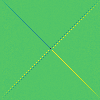
\includegraphics[interpolate=false,width=1.000000in,height=1.000000in]{antiderivative_pm_50-img0.png}}%
\end{pgfscope}%
\begin{pgfscope}%
\pgfsetbuttcap%
\pgfsetroundjoin%
\definecolor{currentfill}{rgb}{0.000000,0.000000,0.000000}%
\pgfsetfillcolor{currentfill}%
\pgfsetlinewidth{0.803000pt}%
\definecolor{currentstroke}{rgb}{0.000000,0.000000,0.000000}%
\pgfsetstrokecolor{currentstroke}%
\pgfsetdash{}{0pt}%
\pgfsys@defobject{currentmarker}{\pgfqpoint{0.000000in}{-0.048611in}}{\pgfqpoint{0.000000in}{0.000000in}}{%
\pgfpathmoveto{\pgfqpoint{0.000000in}{0.000000in}}%
\pgfpathlineto{\pgfqpoint{0.000000in}{-0.048611in}}%
\pgfusepath{stroke,fill}%
}%
\begin{pgfscope}%
\pgfsys@transformshift{0.654106in}{0.517039in}%
\pgfsys@useobject{currentmarker}{}%
\end{pgfscope}%
\end{pgfscope}%
\begin{pgfscope}%
\definecolor{textcolor}{rgb}{0.000000,0.000000,0.000000}%
\pgfsetstrokecolor{textcolor}%
\pgfsetfillcolor{textcolor}%
\pgftext[x=0.654106in,y=0.419816in,,top]{\color{textcolor}{\rmfamily\fontsize{12.000000}{14.400000}\selectfont\catcode`\^=\active\def^{\ifmmode\sp\else\^{}\fi}\catcode`\%=\active\def%{\%}0}}%
\end{pgfscope}%
\begin{pgfscope}%
\pgfsetbuttcap%
\pgfsetroundjoin%
\definecolor{currentfill}{rgb}{0.000000,0.000000,0.000000}%
\pgfsetfillcolor{currentfill}%
\pgfsetlinewidth{0.803000pt}%
\definecolor{currentstroke}{rgb}{0.000000,0.000000,0.000000}%
\pgfsetstrokecolor{currentstroke}%
\pgfsetdash{}{0pt}%
\pgfsys@defobject{currentmarker}{\pgfqpoint{0.000000in}{-0.048611in}}{\pgfqpoint{0.000000in}{0.000000in}}{%
\pgfpathmoveto{\pgfqpoint{0.000000in}{0.000000in}}%
\pgfpathlineto{\pgfqpoint{0.000000in}{-0.048611in}}%
\pgfusepath{stroke,fill}%
}%
\begin{pgfscope}%
\pgfsys@transformshift{1.251588in}{0.517039in}%
\pgfsys@useobject{currentmarker}{}%
\end{pgfscope}%
\end{pgfscope}%
\begin{pgfscope}%
\definecolor{textcolor}{rgb}{0.000000,0.000000,0.000000}%
\pgfsetstrokecolor{textcolor}%
\pgfsetfillcolor{textcolor}%
\pgftext[x=1.251588in,y=0.419816in,,top]{\color{textcolor}{\rmfamily\fontsize{12.000000}{14.400000}\selectfont\catcode`\^=\active\def^{\ifmmode\sp\else\^{}\fi}\catcode`\%=\active\def%{\%}25}}%
\end{pgfscope}%
\begin{pgfscope}%
\pgfsetbuttcap%
\pgfsetroundjoin%
\definecolor{currentfill}{rgb}{0.000000,0.000000,0.000000}%
\pgfsetfillcolor{currentfill}%
\pgfsetlinewidth{0.803000pt}%
\definecolor{currentstroke}{rgb}{0.000000,0.000000,0.000000}%
\pgfsetstrokecolor{currentstroke}%
\pgfsetdash{}{0pt}%
\pgfsys@defobject{currentmarker}{\pgfqpoint{0.000000in}{-0.048611in}}{\pgfqpoint{0.000000in}{0.000000in}}{%
\pgfpathmoveto{\pgfqpoint{0.000000in}{0.000000in}}%
\pgfpathlineto{\pgfqpoint{0.000000in}{-0.048611in}}%
\pgfusepath{stroke,fill}%
}%
\begin{pgfscope}%
\pgfsys@transformshift{1.849069in}{0.517039in}%
\pgfsys@useobject{currentmarker}{}%
\end{pgfscope}%
\end{pgfscope}%
\begin{pgfscope}%
\definecolor{textcolor}{rgb}{0.000000,0.000000,0.000000}%
\pgfsetstrokecolor{textcolor}%
\pgfsetfillcolor{textcolor}%
\pgftext[x=1.849069in,y=0.419816in,,top]{\color{textcolor}{\rmfamily\fontsize{12.000000}{14.400000}\selectfont\catcode`\^=\active\def^{\ifmmode\sp\else\^{}\fi}\catcode`\%=\active\def%{\%}50}}%
\end{pgfscope}%
\begin{pgfscope}%
\pgfsetbuttcap%
\pgfsetroundjoin%
\definecolor{currentfill}{rgb}{0.000000,0.000000,0.000000}%
\pgfsetfillcolor{currentfill}%
\pgfsetlinewidth{0.803000pt}%
\definecolor{currentstroke}{rgb}{0.000000,0.000000,0.000000}%
\pgfsetstrokecolor{currentstroke}%
\pgfsetdash{}{0pt}%
\pgfsys@defobject{currentmarker}{\pgfqpoint{0.000000in}{-0.048611in}}{\pgfqpoint{0.000000in}{0.000000in}}{%
\pgfpathmoveto{\pgfqpoint{0.000000in}{0.000000in}}%
\pgfpathlineto{\pgfqpoint{0.000000in}{-0.048611in}}%
\pgfusepath{stroke,fill}%
}%
\begin{pgfscope}%
\pgfsys@transformshift{2.446551in}{0.517039in}%
\pgfsys@useobject{currentmarker}{}%
\end{pgfscope}%
\end{pgfscope}%
\begin{pgfscope}%
\definecolor{textcolor}{rgb}{0.000000,0.000000,0.000000}%
\pgfsetstrokecolor{textcolor}%
\pgfsetfillcolor{textcolor}%
\pgftext[x=2.446551in,y=0.419816in,,top]{\color{textcolor}{\rmfamily\fontsize{12.000000}{14.400000}\selectfont\catcode`\^=\active\def^{\ifmmode\sp\else\^{}\fi}\catcode`\%=\active\def%{\%}75}}%
\end{pgfscope}%
\begin{pgfscope}%
\definecolor{textcolor}{rgb}{0.000000,0.000000,0.000000}%
\pgfsetstrokecolor{textcolor}%
\pgfsetfillcolor{textcolor}%
\pgftext[x=1.837120in,y=0.202965in,,top]{\color{textcolor}{\rmfamily\fontsize{12.000000}{14.400000}\selectfont\catcode`\^=\active\def^{\ifmmode\sp\else\^{}\fi}\catcode`\%=\active\def%{\%}output coefficients}}%
\end{pgfscope}%
\begin{pgfscope}%
\pgfsetbuttcap%
\pgfsetroundjoin%
\definecolor{currentfill}{rgb}{0.000000,0.000000,0.000000}%
\pgfsetfillcolor{currentfill}%
\pgfsetlinewidth{0.803000pt}%
\definecolor{currentstroke}{rgb}{0.000000,0.000000,0.000000}%
\pgfsetstrokecolor{currentstroke}%
\pgfsetdash{}{0pt}%
\pgfsys@defobject{currentmarker}{\pgfqpoint{-0.048611in}{0.000000in}}{\pgfqpoint{-0.000000in}{0.000000in}}{%
\pgfpathmoveto{\pgfqpoint{-0.000000in}{0.000000in}}%
\pgfpathlineto{\pgfqpoint{-0.048611in}{0.000000in}}%
\pgfusepath{stroke,fill}%
}%
\begin{pgfscope}%
\pgfsys@transformshift{0.642156in}{2.895016in}%
\pgfsys@useobject{currentmarker}{}%
\end{pgfscope}%
\end{pgfscope}%
\begin{pgfscope}%
\definecolor{textcolor}{rgb}{0.000000,0.000000,0.000000}%
\pgfsetstrokecolor{textcolor}%
\pgfsetfillcolor{textcolor}%
\pgftext[x=0.438896in, y=2.831702in, left, base]{\color{textcolor}{\rmfamily\fontsize{12.000000}{14.400000}\selectfont\catcode`\^=\active\def^{\ifmmode\sp\else\^{}\fi}\catcode`\%=\active\def%{\%}0}}%
\end{pgfscope}%
\begin{pgfscope}%
\pgfsetbuttcap%
\pgfsetroundjoin%
\definecolor{currentfill}{rgb}{0.000000,0.000000,0.000000}%
\pgfsetfillcolor{currentfill}%
\pgfsetlinewidth{0.803000pt}%
\definecolor{currentstroke}{rgb}{0.000000,0.000000,0.000000}%
\pgfsetstrokecolor{currentstroke}%
\pgfsetdash{}{0pt}%
\pgfsys@defobject{currentmarker}{\pgfqpoint{-0.048611in}{0.000000in}}{\pgfqpoint{-0.000000in}{0.000000in}}{%
\pgfpathmoveto{\pgfqpoint{-0.000000in}{0.000000in}}%
\pgfpathlineto{\pgfqpoint{-0.048611in}{0.000000in}}%
\pgfusepath{stroke,fill}%
}%
\begin{pgfscope}%
\pgfsys@transformshift{0.642156in}{2.417031in}%
\pgfsys@useobject{currentmarker}{}%
\end{pgfscope}%
\end{pgfscope}%
\begin{pgfscope}%
\definecolor{textcolor}{rgb}{0.000000,0.000000,0.000000}%
\pgfsetstrokecolor{textcolor}%
\pgfsetfillcolor{textcolor}%
\pgftext[x=0.332857in, y=2.353717in, left, base]{\color{textcolor}{\rmfamily\fontsize{12.000000}{14.400000}\selectfont\catcode`\^=\active\def^{\ifmmode\sp\else\^{}\fi}\catcode`\%=\active\def%{\%}20}}%
\end{pgfscope}%
\begin{pgfscope}%
\pgfsetbuttcap%
\pgfsetroundjoin%
\definecolor{currentfill}{rgb}{0.000000,0.000000,0.000000}%
\pgfsetfillcolor{currentfill}%
\pgfsetlinewidth{0.803000pt}%
\definecolor{currentstroke}{rgb}{0.000000,0.000000,0.000000}%
\pgfsetstrokecolor{currentstroke}%
\pgfsetdash{}{0pt}%
\pgfsys@defobject{currentmarker}{\pgfqpoint{-0.048611in}{0.000000in}}{\pgfqpoint{-0.000000in}{0.000000in}}{%
\pgfpathmoveto{\pgfqpoint{-0.000000in}{0.000000in}}%
\pgfpathlineto{\pgfqpoint{-0.048611in}{0.000000in}}%
\pgfusepath{stroke,fill}%
}%
\begin{pgfscope}%
\pgfsys@transformshift{0.642156in}{1.939045in}%
\pgfsys@useobject{currentmarker}{}%
\end{pgfscope}%
\end{pgfscope}%
\begin{pgfscope}%
\definecolor{textcolor}{rgb}{0.000000,0.000000,0.000000}%
\pgfsetstrokecolor{textcolor}%
\pgfsetfillcolor{textcolor}%
\pgftext[x=0.332857in, y=1.875731in, left, base]{\color{textcolor}{\rmfamily\fontsize{12.000000}{14.400000}\selectfont\catcode`\^=\active\def^{\ifmmode\sp\else\^{}\fi}\catcode`\%=\active\def%{\%}40}}%
\end{pgfscope}%
\begin{pgfscope}%
\pgfsetbuttcap%
\pgfsetroundjoin%
\definecolor{currentfill}{rgb}{0.000000,0.000000,0.000000}%
\pgfsetfillcolor{currentfill}%
\pgfsetlinewidth{0.803000pt}%
\definecolor{currentstroke}{rgb}{0.000000,0.000000,0.000000}%
\pgfsetstrokecolor{currentstroke}%
\pgfsetdash{}{0pt}%
\pgfsys@defobject{currentmarker}{\pgfqpoint{-0.048611in}{0.000000in}}{\pgfqpoint{-0.000000in}{0.000000in}}{%
\pgfpathmoveto{\pgfqpoint{-0.000000in}{0.000000in}}%
\pgfpathlineto{\pgfqpoint{-0.048611in}{0.000000in}}%
\pgfusepath{stroke,fill}%
}%
\begin{pgfscope}%
\pgfsys@transformshift{0.642156in}{1.461060in}%
\pgfsys@useobject{currentmarker}{}%
\end{pgfscope}%
\end{pgfscope}%
\begin{pgfscope}%
\definecolor{textcolor}{rgb}{0.000000,0.000000,0.000000}%
\pgfsetstrokecolor{textcolor}%
\pgfsetfillcolor{textcolor}%
\pgftext[x=0.332857in, y=1.397746in, left, base]{\color{textcolor}{\rmfamily\fontsize{12.000000}{14.400000}\selectfont\catcode`\^=\active\def^{\ifmmode\sp\else\^{}\fi}\catcode`\%=\active\def%{\%}60}}%
\end{pgfscope}%
\begin{pgfscope}%
\pgfsetbuttcap%
\pgfsetroundjoin%
\definecolor{currentfill}{rgb}{0.000000,0.000000,0.000000}%
\pgfsetfillcolor{currentfill}%
\pgfsetlinewidth{0.803000pt}%
\definecolor{currentstroke}{rgb}{0.000000,0.000000,0.000000}%
\pgfsetstrokecolor{currentstroke}%
\pgfsetdash{}{0pt}%
\pgfsys@defobject{currentmarker}{\pgfqpoint{-0.048611in}{0.000000in}}{\pgfqpoint{-0.000000in}{0.000000in}}{%
\pgfpathmoveto{\pgfqpoint{-0.000000in}{0.000000in}}%
\pgfpathlineto{\pgfqpoint{-0.048611in}{0.000000in}}%
\pgfusepath{stroke,fill}%
}%
\begin{pgfscope}%
\pgfsys@transformshift{0.642156in}{0.983074in}%
\pgfsys@useobject{currentmarker}{}%
\end{pgfscope}%
\end{pgfscope}%
\begin{pgfscope}%
\definecolor{textcolor}{rgb}{0.000000,0.000000,0.000000}%
\pgfsetstrokecolor{textcolor}%
\pgfsetfillcolor{textcolor}%
\pgftext[x=0.332857in, y=0.919761in, left, base]{\color{textcolor}{\rmfamily\fontsize{12.000000}{14.400000}\selectfont\catcode`\^=\active\def^{\ifmmode\sp\else\^{}\fi}\catcode`\%=\active\def%{\%}80}}%
\end{pgfscope}%
\begin{pgfscope}%
\definecolor{textcolor}{rgb}{0.000000,0.000000,0.000000}%
\pgfsetstrokecolor{textcolor}%
\pgfsetfillcolor{textcolor}%
\pgftext[x=0.277302in,y=1.712002in,,bottom,rotate=90.000000]{\color{textcolor}{\rmfamily\fontsize{12.000000}{14.400000}\selectfont\catcode`\^=\active\def^{\ifmmode\sp\else\^{}\fi}\catcode`\%=\active\def%{\%}input coefficients}}%
\end{pgfscope}%
\begin{pgfscope}%
\pgfsetrectcap%
\pgfsetmiterjoin%
\pgfsetlinewidth{0.803000pt}%
\definecolor{currentstroke}{rgb}{0.000000,0.000000,0.000000}%
\pgfsetstrokecolor{currentstroke}%
\pgfsetdash{}{0pt}%
\pgfpathmoveto{\pgfqpoint{0.642156in}{0.517039in}}%
\pgfpathlineto{\pgfqpoint{0.642156in}{2.906966in}}%
\pgfusepath{stroke}%
\end{pgfscope}%
\begin{pgfscope}%
\pgfsetrectcap%
\pgfsetmiterjoin%
\pgfsetlinewidth{0.803000pt}%
\definecolor{currentstroke}{rgb}{0.000000,0.000000,0.000000}%
\pgfsetstrokecolor{currentstroke}%
\pgfsetdash{}{0pt}%
\pgfpathmoveto{\pgfqpoint{3.032083in}{0.517039in}}%
\pgfpathlineto{\pgfqpoint{3.032083in}{2.906966in}}%
\pgfusepath{stroke}%
\end{pgfscope}%
\begin{pgfscope}%
\pgfsetrectcap%
\pgfsetmiterjoin%
\pgfsetlinewidth{0.803000pt}%
\definecolor{currentstroke}{rgb}{0.000000,0.000000,0.000000}%
\pgfsetstrokecolor{currentstroke}%
\pgfsetdash{}{0pt}%
\pgfpathmoveto{\pgfqpoint{0.642156in}{0.517039in}}%
\pgfpathlineto{\pgfqpoint{3.032083in}{0.517039in}}%
\pgfusepath{stroke}%
\end{pgfscope}%
\begin{pgfscope}%
\pgfsetrectcap%
\pgfsetmiterjoin%
\pgfsetlinewidth{0.803000pt}%
\definecolor{currentstroke}{rgb}{0.000000,0.000000,0.000000}%
\pgfsetstrokecolor{currentstroke}%
\pgfsetdash{}{0pt}%
\pgfpathmoveto{\pgfqpoint{0.642156in}{2.906966in}}%
\pgfpathlineto{\pgfqpoint{3.032083in}{2.906966in}}%
\pgfusepath{stroke}%
\end{pgfscope}%
\begin{pgfscope}%
\pgfsetbuttcap%
\pgfsetmiterjoin%
\pgfsetlinewidth{0.000000pt}%
\definecolor{currentstroke}{rgb}{0.000000,0.000000,0.000000}%
\pgfsetstrokecolor{currentstroke}%
\pgfsetstrokeopacity{0.000000}%
\pgfsetdash{}{0pt}%
\pgfpathmoveto{\pgfqpoint{3.181604in}{0.517039in}}%
\pgfpathlineto{\pgfqpoint{3.301100in}{0.517039in}}%
\pgfpathlineto{\pgfqpoint{3.301100in}{2.906966in}}%
\pgfpathlineto{\pgfqpoint{3.181604in}{2.906966in}}%
\pgfpathlineto{\pgfqpoint{3.181604in}{0.517039in}}%
\pgfpathclose%
\pgfusepath{}%
\end{pgfscope}%
\begin{pgfscope}%
\pgfsys@transformshift{3.180000in}{0.520000in}%
\pgftext[left,bottom]{
\includegraphics[interpolate=true,width=0.120000in,height=2.390000in]{antiderivative_pm_50-img1.png}}%
\end{pgfscope}%
\begin{pgfscope}%
\pgfsetbuttcap%
\pgfsetroundjoin%
\definecolor{currentfill}{rgb}{0.000000,0.000000,0.000000}%
\pgfsetfillcolor{currentfill}%
\pgfsetlinewidth{0.803000pt}%
\definecolor{currentstroke}{rgb}{0.000000,0.000000,0.000000}%
\pgfsetstrokecolor{currentstroke}%
\pgfsetdash{}{0pt}%
\pgfsys@defobject{currentmarker}{\pgfqpoint{0.000000in}{0.000000in}}{\pgfqpoint{0.048611in}{0.000000in}}{%
\pgfpathmoveto{\pgfqpoint{0.000000in}{0.000000in}}%
\pgfpathlineto{\pgfqpoint{0.048611in}{0.000000in}}%
\pgfusepath{stroke,fill}%
}%
\begin{pgfscope}%
\pgfsys@transformshift{3.301100in}{0.707209in}%
\pgfsys@useobject{currentmarker}{}%
\end{pgfscope}%
\end{pgfscope}%
\begin{pgfscope}%
\definecolor{textcolor}{rgb}{0.000000,0.000000,0.000000}%
\pgfsetstrokecolor{textcolor}%
\pgfsetfillcolor{textcolor}%
\pgftext[x=3.398323in, y=0.643895in, left, base]{\color{textcolor}{\rmfamily\fontsize{12.000000}{14.400000}\selectfont\catcode`\^=\active\def^{\ifmmode\sp\else\^{}\fi}\catcode`\%=\active\def%{\%}\ensuremath{-}2000}}%
\end{pgfscope}%
\begin{pgfscope}%
\pgfsetbuttcap%
\pgfsetroundjoin%
\definecolor{currentfill}{rgb}{0.000000,0.000000,0.000000}%
\pgfsetfillcolor{currentfill}%
\pgfsetlinewidth{0.803000pt}%
\definecolor{currentstroke}{rgb}{0.000000,0.000000,0.000000}%
\pgfsetstrokecolor{currentstroke}%
\pgfsetdash{}{0pt}%
\pgfsys@defobject{currentmarker}{\pgfqpoint{0.000000in}{0.000000in}}{\pgfqpoint{0.048611in}{0.000000in}}{%
\pgfpathmoveto{\pgfqpoint{0.000000in}{0.000000in}}%
\pgfpathlineto{\pgfqpoint{0.048611in}{0.000000in}}%
\pgfusepath{stroke,fill}%
}%
\begin{pgfscope}%
\pgfsys@transformshift{3.301100in}{1.096875in}%
\pgfsys@useobject{currentmarker}{}%
\end{pgfscope}%
\end{pgfscope}%
\begin{pgfscope}%
\definecolor{textcolor}{rgb}{0.000000,0.000000,0.000000}%
\pgfsetstrokecolor{textcolor}%
\pgfsetfillcolor{textcolor}%
\pgftext[x=3.398323in, y=1.033561in, left, base]{\color{textcolor}{\rmfamily\fontsize{12.000000}{14.400000}\selectfont\catcode`\^=\active\def^{\ifmmode\sp\else\^{}\fi}\catcode`\%=\active\def%{\%}\ensuremath{-}1500}}%
\end{pgfscope}%
\begin{pgfscope}%
\pgfsetbuttcap%
\pgfsetroundjoin%
\definecolor{currentfill}{rgb}{0.000000,0.000000,0.000000}%
\pgfsetfillcolor{currentfill}%
\pgfsetlinewidth{0.803000pt}%
\definecolor{currentstroke}{rgb}{0.000000,0.000000,0.000000}%
\pgfsetstrokecolor{currentstroke}%
\pgfsetdash{}{0pt}%
\pgfsys@defobject{currentmarker}{\pgfqpoint{0.000000in}{0.000000in}}{\pgfqpoint{0.048611in}{0.000000in}}{%
\pgfpathmoveto{\pgfqpoint{0.000000in}{0.000000in}}%
\pgfpathlineto{\pgfqpoint{0.048611in}{0.000000in}}%
\pgfusepath{stroke,fill}%
}%
\begin{pgfscope}%
\pgfsys@transformshift{3.301100in}{1.486541in}%
\pgfsys@useobject{currentmarker}{}%
\end{pgfscope}%
\end{pgfscope}%
\begin{pgfscope}%
\definecolor{textcolor}{rgb}{0.000000,0.000000,0.000000}%
\pgfsetstrokecolor{textcolor}%
\pgfsetfillcolor{textcolor}%
\pgftext[x=3.398323in, y=1.423227in, left, base]{\color{textcolor}{\rmfamily\fontsize{12.000000}{14.400000}\selectfont\catcode`\^=\active\def^{\ifmmode\sp\else\^{}\fi}\catcode`\%=\active\def%{\%}\ensuremath{-}1000}}%
\end{pgfscope}%
\begin{pgfscope}%
\pgfsetbuttcap%
\pgfsetroundjoin%
\definecolor{currentfill}{rgb}{0.000000,0.000000,0.000000}%
\pgfsetfillcolor{currentfill}%
\pgfsetlinewidth{0.803000pt}%
\definecolor{currentstroke}{rgb}{0.000000,0.000000,0.000000}%
\pgfsetstrokecolor{currentstroke}%
\pgfsetdash{}{0pt}%
\pgfsys@defobject{currentmarker}{\pgfqpoint{0.000000in}{0.000000in}}{\pgfqpoint{0.048611in}{0.000000in}}{%
\pgfpathmoveto{\pgfqpoint{0.000000in}{0.000000in}}%
\pgfpathlineto{\pgfqpoint{0.048611in}{0.000000in}}%
\pgfusepath{stroke,fill}%
}%
\begin{pgfscope}%
\pgfsys@transformshift{3.301100in}{1.876208in}%
\pgfsys@useobject{currentmarker}{}%
\end{pgfscope}%
\end{pgfscope}%
\begin{pgfscope}%
\definecolor{textcolor}{rgb}{0.000000,0.000000,0.000000}%
\pgfsetstrokecolor{textcolor}%
\pgfsetfillcolor{textcolor}%
\pgftext[x=3.398323in, y=1.812894in, left, base]{\color{textcolor}{\rmfamily\fontsize{12.000000}{14.400000}\selectfont\catcode`\^=\active\def^{\ifmmode\sp\else\^{}\fi}\catcode`\%=\active\def%{\%}\ensuremath{-}500}}%
\end{pgfscope}%
\begin{pgfscope}%
\pgfsetbuttcap%
\pgfsetroundjoin%
\definecolor{currentfill}{rgb}{0.000000,0.000000,0.000000}%
\pgfsetfillcolor{currentfill}%
\pgfsetlinewidth{0.803000pt}%
\definecolor{currentstroke}{rgb}{0.000000,0.000000,0.000000}%
\pgfsetstrokecolor{currentstroke}%
\pgfsetdash{}{0pt}%
\pgfsys@defobject{currentmarker}{\pgfqpoint{0.000000in}{0.000000in}}{\pgfqpoint{0.048611in}{0.000000in}}{%
\pgfpathmoveto{\pgfqpoint{0.000000in}{0.000000in}}%
\pgfpathlineto{\pgfqpoint{0.048611in}{0.000000in}}%
\pgfusepath{stroke,fill}%
}%
\begin{pgfscope}%
\pgfsys@transformshift{3.301100in}{2.265874in}%
\pgfsys@useobject{currentmarker}{}%
\end{pgfscope}%
\end{pgfscope}%
\begin{pgfscope}%
\definecolor{textcolor}{rgb}{0.000000,0.000000,0.000000}%
\pgfsetstrokecolor{textcolor}%
\pgfsetfillcolor{textcolor}%
\pgftext[x=3.398323in, y=2.202560in, left, base]{\color{textcolor}{\rmfamily\fontsize{12.000000}{14.400000}\selectfont\catcode`\^=\active\def^{\ifmmode\sp\else\^{}\fi}\catcode`\%=\active\def%{\%}0}}%
\end{pgfscope}%
\begin{pgfscope}%
\pgfsetbuttcap%
\pgfsetroundjoin%
\definecolor{currentfill}{rgb}{0.000000,0.000000,0.000000}%
\pgfsetfillcolor{currentfill}%
\pgfsetlinewidth{0.803000pt}%
\definecolor{currentstroke}{rgb}{0.000000,0.000000,0.000000}%
\pgfsetstrokecolor{currentstroke}%
\pgfsetdash{}{0pt}%
\pgfsys@defobject{currentmarker}{\pgfqpoint{0.000000in}{0.000000in}}{\pgfqpoint{0.048611in}{0.000000in}}{%
\pgfpathmoveto{\pgfqpoint{0.000000in}{0.000000in}}%
\pgfpathlineto{\pgfqpoint{0.048611in}{0.000000in}}%
\pgfusepath{stroke,fill}%
}%
\begin{pgfscope}%
\pgfsys@transformshift{3.301100in}{2.655540in}%
\pgfsys@useobject{currentmarker}{}%
\end{pgfscope}%
\end{pgfscope}%
\begin{pgfscope}%
\definecolor{textcolor}{rgb}{0.000000,0.000000,0.000000}%
\pgfsetstrokecolor{textcolor}%
\pgfsetfillcolor{textcolor}%
\pgftext[x=3.398323in, y=2.592226in, left, base]{\color{textcolor}{\rmfamily\fontsize{12.000000}{14.400000}\selectfont\catcode`\^=\active\def^{\ifmmode\sp\else\^{}\fi}\catcode`\%=\active\def%{\%}500}}%
\end{pgfscope}%
\begin{pgfscope}%
\pgfsetrectcap%
\pgfsetmiterjoin%
\pgfsetlinewidth{0.803000pt}%
\definecolor{currentstroke}{rgb}{0.000000,0.000000,0.000000}%
\pgfsetstrokecolor{currentstroke}%
\pgfsetdash{}{0pt}%
\pgfpathmoveto{\pgfqpoint{3.181604in}{0.517039in}}%
\pgfpathlineto{\pgfqpoint{3.241352in}{0.517039in}}%
\pgfpathlineto{\pgfqpoint{3.301100in}{0.517039in}}%
\pgfpathlineto{\pgfqpoint{3.301100in}{2.906966in}}%
\pgfpathlineto{\pgfqpoint{3.241352in}{2.906966in}}%
\pgfpathlineto{\pgfqpoint{3.181604in}{2.906966in}}%
\pgfpathlineto{\pgfqpoint{3.181604in}{0.517039in}}%
\pgfpathclose%
\pgfusepath{stroke}%
\end{pgfscope}%
\end{pgfpicture}%
\makeatother%
\endgroup%

      \end{adjustbox}
      \caption{The p-matrix for 50\% noise.}\label{fig:sc1_pm_50}
    \end{subfigure}
  \end{adjustwidth}
  \caption{Correlation image (left column) and p-matrix (right column) for each model trained on a different noise level (row). The correlation image was sorted same order the values of the real component of wave number \(k=2\) were sorted in descending order.}\label{fig:scenario_1_interpretation}
\end{figure}

\subsection{Scenario 2}
\noindent The second scenario results are presented in two parts which are the coefficient predictions and function value predictions. The functions are first preprocessed in order to format them into current and next values in time as discussed in \lccref{sec:data_transformation}. The sample pairs are first divided into two for the training and testing sets. Each function is then discretized into 200 time steps. Then, the features are put together as the coefficients of the solution and forcing term at the current time step. The labels are the solution at the next time step. Since there is too much data to fit into memory all at once at the end of this process, we randomly sample the feature and label pairs. This result in a maximum of 8000 features and labels for the training set and 2000 features and labels from the testing set. As mentioned in \lccref{sec:data_transformation}, the training features are used to fit a scaling function. And then, all features are scaled using the fitted scaling function.

The coefficient value predictions are shown in \lccref{table:scenario_2_spectral_metrics}. The RBF kernel parameter computed from the data is once again the same for all versions of the dataset with a value of 5.66. The testing metrics show that the performance of the model vary with the viscosity value \(\nu \). Starting with the inviscid Burgers' equation, with \(\nu=0\), the model performs the best with a close second from the model for the \(\nu = 0.01 \) dataset version. The function value evaluated from the predictions is shown in \lccref{table:scenario_2_function_metrics}. The metrics across the board shows that the function value relative metrics are slightly better compared to the coefficients. Comparing the absolute metrics for the same table, we see the same general trend that the higher viscosity show the model performing worse. For reference, the maximum amplitude of the functions on average are \num{2.56e-02}. This puts the error in an order of magnitude less than the average maximum amplitude. For the coefficients, on average, the maximum absolute value at each time step is \num{9.29e-02}. This means for the viscosity of 0.0 and \num{0.01}, the error is roughly 1 to 9 of the maximum absolute value.

\begin{table}[H]
  \caption{Performance metrics of coefficient prediction of next time step in scenario 2 by viscosity.}\label{table:scenario_2_spectral_metrics}
  \centering
  \begin{tabular}{lrrrrr}
    \toprule
    \(\nu \) & MSE      & RMSE     & MAE      & R\textsuperscript{2} & sMAPE \\
    \midrule
    0.0      & 3.46e-04 & 1.86e-02 & 1.24e-02 & 0.79                 & 0.65  \\
    0.01     & 3.56e-04 & 1.89e-02 & 1.27e-02 & 0.78                 & 0.67  \\
    0.1      & 9.17e-04 & 3.03e-02 & 2.32e-02 & 0.46                 & 1.08  \\
    \bottomrule
  \end{tabular}
\end{table}

\begin{table}[H]
  \caption{Performance metrics of function values evaluated from coefficient prediction of next time step in scenario 2 by viscosity.}\label{table:scenario_2_function_metrics}
  \centering
  \begin{tabular}{lrrrrr}
    \toprule
    \(\nu \) & MSE      & RMSE     & MAE      & R\textsuperscript{2} & sMAPE \\
    \midrule
    0.0      & 5.58e-05 & 7.47e-03 & 5.89e-03 & 0.82                 & 0.70  \\
    0.01     & 5.74e-05 & 7.58e-03 & 6.01e-03 & 0.81                 & 0.71  \\
    0.1      & 1.58e-04 & 1.26e-02 & 9.98e-03 & 0.51                 & 1.04  \\
    \bottomrule
  \end{tabular}
\end{table}

The testing results are complimented with a rollout experiment. The results from the rollout are shown in \lccref{fig:scenario_2_rollout}. The rollout starts from time \(t=0\). In all the plots, this is at the bottom. We have included this initial condition in the plots. From this initial condition in combination with the forcing term at the initial time step, the model predicts the first time step solution. The model then uses the predicted solution combined with the corresponding forcing term to predict the second time step. To see how well the model is performing relative to the actual target values, we compute the difference between the two as shown in \lccrefs{fig:sc2_rollout_diff_0.0,fig:sc2_rollout_diff_0.01,fig:sc2_rollout_diff_0.1}. Observe that errors are introduced relatively early around time \(t=1\). However, the model rollout stays stable until the end despite this error. This results in the model being able to finish the rollout for this sample.
\begin{figure}[H]
  \centering
  \begin{adjustwidth}{-0.1\linewidth}{-0.1\linewidth}
    \begin{subfigure}{0.33\linewidth}
      \begin{adjustbox}{width=\linewidth}
        \begingroup%
\makeatletter%
\begin{pgfpicture}%
\pgfpathrectangle{\pgfpointorigin}{\pgfqpoint{3.000000in}{2.000000in}}%
\pgfusepath{use as bounding box, clip}%
\begin{pgfscope}%
\pgfsetbuttcap%
\pgfsetmiterjoin%
\pgfsetlinewidth{0.000000pt}%
\definecolor{currentstroke}{rgb}{0.000000,0.000000,0.000000}%
\pgfsetstrokecolor{currentstroke}%
\pgfsetstrokeopacity{0.000000}%
\pgfsetdash{}{0pt}%
\pgfpathmoveto{\pgfqpoint{0.000000in}{0.000000in}}%
\pgfpathlineto{\pgfqpoint{3.000000in}{0.000000in}}%
\pgfpathlineto{\pgfqpoint{3.000000in}{2.000000in}}%
\pgfpathlineto{\pgfqpoint{0.000000in}{2.000000in}}%
\pgfpathlineto{\pgfqpoint{0.000000in}{0.000000in}}%
\pgfpathclose%
\pgfusepath{}%
\end{pgfscope}%
\begin{pgfscope}%
\pgfsetbuttcap%
\pgfsetmiterjoin%
\pgfsetlinewidth{0.000000pt}%
\definecolor{currentstroke}{rgb}{0.000000,0.000000,0.000000}%
\pgfsetstrokecolor{currentstroke}%
\pgfsetstrokeopacity{0.000000}%
\pgfsetdash{}{0pt}%
\pgfpathmoveto{\pgfqpoint{0.726837in}{0.517039in}}%
\pgfpathlineto{\pgfqpoint{2.414687in}{0.517039in}}%
\pgfpathlineto{\pgfqpoint{2.414687in}{1.895016in}}%
\pgfpathlineto{\pgfqpoint{0.726837in}{1.895016in}}%
\pgfpathlineto{\pgfqpoint{0.726837in}{0.517039in}}%
\pgfpathclose%
\pgfusepath{}%
\end{pgfscope}%
\begin{pgfscope}%
\pgfpathrectangle{\pgfqpoint{0.726837in}{0.517039in}}{\pgfqpoint{1.687850in}{1.377978in}}%
\pgfusepath{clip}%
\pgfsys@transformcm{1.687850}{0.000000}{0.000000}{1.377978}{0.726837in}{0.517039in}%
\pgftext[left,bottom]{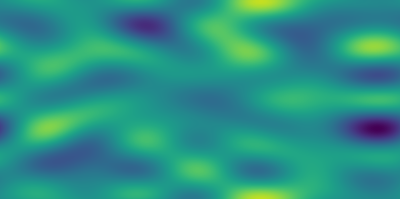
\includegraphics[interpolate=false,width=1.000000in,height=1.000000in]{burgers_rollout_target_0.0-img0.png}}%
\end{pgfscope}%
\begin{pgfscope}%
\pgfsetbuttcap%
\pgfsetroundjoin%
\definecolor{currentfill}{rgb}{0.000000,0.000000,0.000000}%
\pgfsetfillcolor{currentfill}%
\pgfsetlinewidth{0.803000pt}%
\definecolor{currentstroke}{rgb}{0.000000,0.000000,0.000000}%
\pgfsetstrokecolor{currentstroke}%
\pgfsetdash{}{0pt}%
\pgfsys@defobject{currentmarker}{\pgfqpoint{0.000000in}{-0.048611in}}{\pgfqpoint{0.000000in}{0.000000in}}{%
\pgfpathmoveto{\pgfqpoint{0.000000in}{0.000000in}}%
\pgfpathlineto{\pgfqpoint{0.000000in}{-0.048611in}}%
\pgfusepath{stroke,fill}%
}%
\begin{pgfscope}%
\pgfsys@transformshift{0.726837in}{0.517039in}%
\pgfsys@useobject{currentmarker}{}%
\end{pgfscope}%
\end{pgfscope}%
\begin{pgfscope}%
\definecolor{textcolor}{rgb}{0.000000,0.000000,0.000000}%
\pgfsetstrokecolor{textcolor}%
\pgfsetfillcolor{textcolor}%
\pgftext[x=0.726837in,y=0.419816in,,top]{\color{textcolor}{\rmfamily\fontsize{12.000000}{14.400000}\selectfont\catcode`\^=\active\def^{\ifmmode\sp\else\^{}\fi}\catcode`\%=\active\def%{\%}0}}%
\end{pgfscope}%
\begin{pgfscope}%
\pgfsetbuttcap%
\pgfsetroundjoin%
\definecolor{currentfill}{rgb}{0.000000,0.000000,0.000000}%
\pgfsetfillcolor{currentfill}%
\pgfsetlinewidth{0.803000pt}%
\definecolor{currentstroke}{rgb}{0.000000,0.000000,0.000000}%
\pgfsetstrokecolor{currentstroke}%
\pgfsetdash{}{0pt}%
\pgfsys@defobject{currentmarker}{\pgfqpoint{0.000000in}{-0.048611in}}{\pgfqpoint{0.000000in}{0.000000in}}{%
\pgfpathmoveto{\pgfqpoint{0.000000in}{0.000000in}}%
\pgfpathlineto{\pgfqpoint{0.000000in}{-0.048611in}}%
\pgfusepath{stroke,fill}%
}%
\begin{pgfscope}%
\pgfsys@transformshift{1.570762in}{0.517039in}%
\pgfsys@useobject{currentmarker}{}%
\end{pgfscope}%
\end{pgfscope}%
\begin{pgfscope}%
\definecolor{textcolor}{rgb}{0.000000,0.000000,0.000000}%
\pgfsetstrokecolor{textcolor}%
\pgfsetfillcolor{textcolor}%
\pgftext[x=1.570762in,y=0.419816in,,top]{\color{textcolor}{\rmfamily\fontsize{12.000000}{14.400000}\selectfont\catcode`\^=\active\def^{\ifmmode\sp\else\^{}\fi}\catcode`\%=\active\def%{\%}1}}%
\end{pgfscope}%
\begin{pgfscope}%
\pgfsetbuttcap%
\pgfsetroundjoin%
\definecolor{currentfill}{rgb}{0.000000,0.000000,0.000000}%
\pgfsetfillcolor{currentfill}%
\pgfsetlinewidth{0.803000pt}%
\definecolor{currentstroke}{rgb}{0.000000,0.000000,0.000000}%
\pgfsetstrokecolor{currentstroke}%
\pgfsetdash{}{0pt}%
\pgfsys@defobject{currentmarker}{\pgfqpoint{0.000000in}{-0.048611in}}{\pgfqpoint{0.000000in}{0.000000in}}{%
\pgfpathmoveto{\pgfqpoint{0.000000in}{0.000000in}}%
\pgfpathlineto{\pgfqpoint{0.000000in}{-0.048611in}}%
\pgfusepath{stroke,fill}%
}%
\begin{pgfscope}%
\pgfsys@transformshift{2.414687in}{0.517039in}%
\pgfsys@useobject{currentmarker}{}%
\end{pgfscope}%
\end{pgfscope}%
\begin{pgfscope}%
\definecolor{textcolor}{rgb}{0.000000,0.000000,0.000000}%
\pgfsetstrokecolor{textcolor}%
\pgfsetfillcolor{textcolor}%
\pgftext[x=2.414687in,y=0.419816in,,top]{\color{textcolor}{\rmfamily\fontsize{12.000000}{14.400000}\selectfont\catcode`\^=\active\def^{\ifmmode\sp\else\^{}\fi}\catcode`\%=\active\def%{\%}2}}%
\end{pgfscope}%
\begin{pgfscope}%
\definecolor{textcolor}{rgb}{0.000000,0.000000,0.000000}%
\pgfsetstrokecolor{textcolor}%
\pgfsetfillcolor{textcolor}%
\pgftext[x=1.570762in,y=0.202965in,,top]{\color{textcolor}{\rmfamily\fontsize{12.000000}{14.400000}\selectfont\catcode`\^=\active\def^{\ifmmode\sp\else\^{}\fi}\catcode`\%=\active\def%{\%}Space}}%
\end{pgfscope}%
\begin{pgfscope}%
\pgfsetbuttcap%
\pgfsetroundjoin%
\definecolor{currentfill}{rgb}{0.000000,0.000000,0.000000}%
\pgfsetfillcolor{currentfill}%
\pgfsetlinewidth{0.803000pt}%
\definecolor{currentstroke}{rgb}{0.000000,0.000000,0.000000}%
\pgfsetstrokecolor{currentstroke}%
\pgfsetdash{}{0pt}%
\pgfsys@defobject{currentmarker}{\pgfqpoint{-0.048611in}{0.000000in}}{\pgfqpoint{-0.000000in}{0.000000in}}{%
\pgfpathmoveto{\pgfqpoint{-0.000000in}{0.000000in}}%
\pgfpathlineto{\pgfqpoint{-0.048611in}{0.000000in}}%
\pgfusepath{stroke,fill}%
}%
\begin{pgfscope}%
\pgfsys@transformshift{0.726837in}{0.517039in}%
\pgfsys@useobject{currentmarker}{}%
\end{pgfscope}%
\end{pgfscope}%
\begin{pgfscope}%
\definecolor{textcolor}{rgb}{0.000000,0.000000,0.000000}%
\pgfsetstrokecolor{textcolor}%
\pgfsetfillcolor{textcolor}%
\pgftext[x=0.364559in, y=0.453725in, left, base]{\color{textcolor}{\rmfamily\fontsize{12.000000}{14.400000}\selectfont\catcode`\^=\active\def^{\ifmmode\sp\else\^{}\fi}\catcode`\%=\active\def%{\%}0.0}}%
\end{pgfscope}%
\begin{pgfscope}%
\pgfsetbuttcap%
\pgfsetroundjoin%
\definecolor{currentfill}{rgb}{0.000000,0.000000,0.000000}%
\pgfsetfillcolor{currentfill}%
\pgfsetlinewidth{0.803000pt}%
\definecolor{currentstroke}{rgb}{0.000000,0.000000,0.000000}%
\pgfsetstrokecolor{currentstroke}%
\pgfsetdash{}{0pt}%
\pgfsys@defobject{currentmarker}{\pgfqpoint{-0.048611in}{0.000000in}}{\pgfqpoint{-0.000000in}{0.000000in}}{%
\pgfpathmoveto{\pgfqpoint{-0.000000in}{0.000000in}}%
\pgfpathlineto{\pgfqpoint{-0.048611in}{0.000000in}}%
\pgfusepath{stroke,fill}%
}%
\begin{pgfscope}%
\pgfsys@transformshift{0.726837in}{0.861533in}%
\pgfsys@useobject{currentmarker}{}%
\end{pgfscope}%
\end{pgfscope}%
\begin{pgfscope}%
\definecolor{textcolor}{rgb}{0.000000,0.000000,0.000000}%
\pgfsetstrokecolor{textcolor}%
\pgfsetfillcolor{textcolor}%
\pgftext[x=0.364559in, y=0.798219in, left, base]{\color{textcolor}{\rmfamily\fontsize{12.000000}{14.400000}\selectfont\catcode`\^=\active\def^{\ifmmode\sp\else\^{}\fi}\catcode`\%=\active\def%{\%}2.5}}%
\end{pgfscope}%
\begin{pgfscope}%
\pgfsetbuttcap%
\pgfsetroundjoin%
\definecolor{currentfill}{rgb}{0.000000,0.000000,0.000000}%
\pgfsetfillcolor{currentfill}%
\pgfsetlinewidth{0.803000pt}%
\definecolor{currentstroke}{rgb}{0.000000,0.000000,0.000000}%
\pgfsetstrokecolor{currentstroke}%
\pgfsetdash{}{0pt}%
\pgfsys@defobject{currentmarker}{\pgfqpoint{-0.048611in}{0.000000in}}{\pgfqpoint{-0.000000in}{0.000000in}}{%
\pgfpathmoveto{\pgfqpoint{-0.000000in}{0.000000in}}%
\pgfpathlineto{\pgfqpoint{-0.048611in}{0.000000in}}%
\pgfusepath{stroke,fill}%
}%
\begin{pgfscope}%
\pgfsys@transformshift{0.726837in}{1.206027in}%
\pgfsys@useobject{currentmarker}{}%
\end{pgfscope}%
\end{pgfscope}%
\begin{pgfscope}%
\definecolor{textcolor}{rgb}{0.000000,0.000000,0.000000}%
\pgfsetstrokecolor{textcolor}%
\pgfsetfillcolor{textcolor}%
\pgftext[x=0.364559in, y=1.142714in, left, base]{\color{textcolor}{\rmfamily\fontsize{12.000000}{14.400000}\selectfont\catcode`\^=\active\def^{\ifmmode\sp\else\^{}\fi}\catcode`\%=\active\def%{\%}5.0}}%
\end{pgfscope}%
\begin{pgfscope}%
\pgfsetbuttcap%
\pgfsetroundjoin%
\definecolor{currentfill}{rgb}{0.000000,0.000000,0.000000}%
\pgfsetfillcolor{currentfill}%
\pgfsetlinewidth{0.803000pt}%
\definecolor{currentstroke}{rgb}{0.000000,0.000000,0.000000}%
\pgfsetstrokecolor{currentstroke}%
\pgfsetdash{}{0pt}%
\pgfsys@defobject{currentmarker}{\pgfqpoint{-0.048611in}{0.000000in}}{\pgfqpoint{-0.000000in}{0.000000in}}{%
\pgfpathmoveto{\pgfqpoint{-0.000000in}{0.000000in}}%
\pgfpathlineto{\pgfqpoint{-0.048611in}{0.000000in}}%
\pgfusepath{stroke,fill}%
}%
\begin{pgfscope}%
\pgfsys@transformshift{0.726837in}{1.550522in}%
\pgfsys@useobject{currentmarker}{}%
\end{pgfscope}%
\end{pgfscope}%
\begin{pgfscope}%
\definecolor{textcolor}{rgb}{0.000000,0.000000,0.000000}%
\pgfsetstrokecolor{textcolor}%
\pgfsetfillcolor{textcolor}%
\pgftext[x=0.364559in, y=1.487208in, left, base]{\color{textcolor}{\rmfamily\fontsize{12.000000}{14.400000}\selectfont\catcode`\^=\active\def^{\ifmmode\sp\else\^{}\fi}\catcode`\%=\active\def%{\%}7.5}}%
\end{pgfscope}%
\begin{pgfscope}%
\pgfsetbuttcap%
\pgfsetroundjoin%
\definecolor{currentfill}{rgb}{0.000000,0.000000,0.000000}%
\pgfsetfillcolor{currentfill}%
\pgfsetlinewidth{0.803000pt}%
\definecolor{currentstroke}{rgb}{0.000000,0.000000,0.000000}%
\pgfsetstrokecolor{currentstroke}%
\pgfsetdash{}{0pt}%
\pgfsys@defobject{currentmarker}{\pgfqpoint{-0.048611in}{0.000000in}}{\pgfqpoint{-0.000000in}{0.000000in}}{%
\pgfpathmoveto{\pgfqpoint{-0.000000in}{0.000000in}}%
\pgfpathlineto{\pgfqpoint{-0.048611in}{0.000000in}}%
\pgfusepath{stroke,fill}%
}%
\begin{pgfscope}%
\pgfsys@transformshift{0.726837in}{1.895016in}%
\pgfsys@useobject{currentmarker}{}%
\end{pgfscope}%
\end{pgfscope}%
\begin{pgfscope}%
\definecolor{textcolor}{rgb}{0.000000,0.000000,0.000000}%
\pgfsetstrokecolor{textcolor}%
\pgfsetfillcolor{textcolor}%
\pgftext[x=0.258521in, y=1.831702in, left, base]{\color{textcolor}{\rmfamily\fontsize{12.000000}{14.400000}\selectfont\catcode`\^=\active\def^{\ifmmode\sp\else\^{}\fi}\catcode`\%=\active\def%{\%}10.0}}%
\end{pgfscope}%
\begin{pgfscope}%
\definecolor{textcolor}{rgb}{0.000000,0.000000,0.000000}%
\pgfsetstrokecolor{textcolor}%
\pgfsetfillcolor{textcolor}%
\pgftext[x=0.202965in,y=1.206027in,,bottom,rotate=90.000000]{\color{textcolor}{\rmfamily\fontsize{12.000000}{14.400000}\selectfont\catcode`\^=\active\def^{\ifmmode\sp\else\^{}\fi}\catcode`\%=\active\def%{\%}Time}}%
\end{pgfscope}%
\begin{pgfscope}%
\pgfsetrectcap%
\pgfsetmiterjoin%
\pgfsetlinewidth{0.803000pt}%
\definecolor{currentstroke}{rgb}{0.000000,0.000000,0.000000}%
\pgfsetstrokecolor{currentstroke}%
\pgfsetdash{}{0pt}%
\pgfpathmoveto{\pgfqpoint{0.726837in}{0.517039in}}%
\pgfpathlineto{\pgfqpoint{0.726837in}{1.895016in}}%
\pgfusepath{stroke}%
\end{pgfscope}%
\begin{pgfscope}%
\pgfsetrectcap%
\pgfsetmiterjoin%
\pgfsetlinewidth{0.803000pt}%
\definecolor{currentstroke}{rgb}{0.000000,0.000000,0.000000}%
\pgfsetstrokecolor{currentstroke}%
\pgfsetdash{}{0pt}%
\pgfpathmoveto{\pgfqpoint{2.414687in}{0.517039in}}%
\pgfpathlineto{\pgfqpoint{2.414687in}{1.895016in}}%
\pgfusepath{stroke}%
\end{pgfscope}%
\begin{pgfscope}%
\pgfsetrectcap%
\pgfsetmiterjoin%
\pgfsetlinewidth{0.803000pt}%
\definecolor{currentstroke}{rgb}{0.000000,0.000000,0.000000}%
\pgfsetstrokecolor{currentstroke}%
\pgfsetdash{}{0pt}%
\pgfpathmoveto{\pgfqpoint{0.726837in}{0.517039in}}%
\pgfpathlineto{\pgfqpoint{2.414687in}{0.517039in}}%
\pgfusepath{stroke}%
\end{pgfscope}%
\begin{pgfscope}%
\pgfsetrectcap%
\pgfsetmiterjoin%
\pgfsetlinewidth{0.803000pt}%
\definecolor{currentstroke}{rgb}{0.000000,0.000000,0.000000}%
\pgfsetstrokecolor{currentstroke}%
\pgfsetdash{}{0pt}%
\pgfpathmoveto{\pgfqpoint{0.726837in}{1.895016in}}%
\pgfpathlineto{\pgfqpoint{2.414687in}{1.895016in}}%
\pgfusepath{stroke}%
\end{pgfscope}%
\begin{pgfscope}%
\pgfsetbuttcap%
\pgfsetmiterjoin%
\pgfsetlinewidth{0.000000pt}%
\definecolor{currentstroke}{rgb}{0.000000,0.000000,0.000000}%
\pgfsetstrokecolor{currentstroke}%
\pgfsetstrokeopacity{0.000000}%
\pgfsetdash{}{0pt}%
\pgfpathmoveto{\pgfqpoint{2.552099in}{0.517039in}}%
\pgfpathlineto{\pgfqpoint{2.620998in}{0.517039in}}%
\pgfpathlineto{\pgfqpoint{2.620998in}{1.895016in}}%
\pgfpathlineto{\pgfqpoint{2.552099in}{1.895016in}}%
\pgfpathlineto{\pgfqpoint{2.552099in}{0.517039in}}%
\pgfpathclose%
\pgfusepath{}%
\end{pgfscope}%
\begin{pgfscope}%
\pgfsys@transformshift{2.550000in}{0.520000in}%
\pgftext[left,bottom]{
\includegraphics[interpolate=true,width=0.070000in,height=1.380000in]{burgers_rollout_target_0.0-img1.png}}%
\end{pgfscope}%
\begin{pgfscope}%
\pgfsetbuttcap%
\pgfsetroundjoin%
\definecolor{currentfill}{rgb}{0.000000,0.000000,0.000000}%
\pgfsetfillcolor{currentfill}%
\pgfsetlinewidth{0.803000pt}%
\definecolor{currentstroke}{rgb}{0.000000,0.000000,0.000000}%
\pgfsetstrokecolor{currentstroke}%
\pgfsetdash{}{0pt}%
\pgfsys@defobject{currentmarker}{\pgfqpoint{0.000000in}{0.000000in}}{\pgfqpoint{0.048611in}{0.000000in}}{%
\pgfpathmoveto{\pgfqpoint{0.000000in}{0.000000in}}%
\pgfpathlineto{\pgfqpoint{0.048611in}{0.000000in}}%
\pgfusepath{stroke,fill}%
}%
\begin{pgfscope}%
\pgfsys@transformshift{2.620998in}{0.588723in}%
\pgfsys@useobject{currentmarker}{}%
\end{pgfscope}%
\end{pgfscope}%
\begin{pgfscope}%
\definecolor{textcolor}{rgb}{0.000000,0.000000,0.000000}%
\pgfsetstrokecolor{textcolor}%
\pgfsetfillcolor{textcolor}%
\pgftext[x=2.718220in, y=0.525410in, left, base]{\color{textcolor}{\rmfamily\fontsize{12.000000}{14.400000}\selectfont\catcode`\^=\active\def^{\ifmmode\sp\else\^{}\fi}\catcode`\%=\active\def%{\%}\ensuremath{-}1}}%
\end{pgfscope}%
\begin{pgfscope}%
\pgfsetbuttcap%
\pgfsetroundjoin%
\definecolor{currentfill}{rgb}{0.000000,0.000000,0.000000}%
\pgfsetfillcolor{currentfill}%
\pgfsetlinewidth{0.803000pt}%
\definecolor{currentstroke}{rgb}{0.000000,0.000000,0.000000}%
\pgfsetstrokecolor{currentstroke}%
\pgfsetdash{}{0pt}%
\pgfsys@defobject{currentmarker}{\pgfqpoint{0.000000in}{0.000000in}}{\pgfqpoint{0.048611in}{0.000000in}}{%
\pgfpathmoveto{\pgfqpoint{0.000000in}{0.000000in}}%
\pgfpathlineto{\pgfqpoint{0.048611in}{0.000000in}}%
\pgfusepath{stroke,fill}%
}%
\begin{pgfscope}%
\pgfsys@transformshift{2.620998in}{1.206027in}%
\pgfsys@useobject{currentmarker}{}%
\end{pgfscope}%
\end{pgfscope}%
\begin{pgfscope}%
\definecolor{textcolor}{rgb}{0.000000,0.000000,0.000000}%
\pgfsetstrokecolor{textcolor}%
\pgfsetfillcolor{textcolor}%
\pgftext[x=2.718220in, y=1.142714in, left, base]{\color{textcolor}{\rmfamily\fontsize{12.000000}{14.400000}\selectfont\catcode`\^=\active\def^{\ifmmode\sp\else\^{}\fi}\catcode`\%=\active\def%{\%}0}}%
\end{pgfscope}%
\begin{pgfscope}%
\pgfsetbuttcap%
\pgfsetroundjoin%
\definecolor{currentfill}{rgb}{0.000000,0.000000,0.000000}%
\pgfsetfillcolor{currentfill}%
\pgfsetlinewidth{0.803000pt}%
\definecolor{currentstroke}{rgb}{0.000000,0.000000,0.000000}%
\pgfsetstrokecolor{currentstroke}%
\pgfsetdash{}{0pt}%
\pgfsys@defobject{currentmarker}{\pgfqpoint{0.000000in}{0.000000in}}{\pgfqpoint{0.048611in}{0.000000in}}{%
\pgfpathmoveto{\pgfqpoint{0.000000in}{0.000000in}}%
\pgfpathlineto{\pgfqpoint{0.048611in}{0.000000in}}%
\pgfusepath{stroke,fill}%
}%
\begin{pgfscope}%
\pgfsys@transformshift{2.620998in}{1.823331in}%
\pgfsys@useobject{currentmarker}{}%
\end{pgfscope}%
\end{pgfscope}%
\begin{pgfscope}%
\definecolor{textcolor}{rgb}{0.000000,0.000000,0.000000}%
\pgfsetstrokecolor{textcolor}%
\pgfsetfillcolor{textcolor}%
\pgftext[x=2.718220in, y=1.760018in, left, base]{\color{textcolor}{\rmfamily\fontsize{12.000000}{14.400000}\selectfont\catcode`\^=\active\def^{\ifmmode\sp\else\^{}\fi}\catcode`\%=\active\def%{\%}1}}%
\end{pgfscope}%
\begin{pgfscope}%
\pgfsetrectcap%
\pgfsetmiterjoin%
\pgfsetlinewidth{0.803000pt}%
\definecolor{currentstroke}{rgb}{0.000000,0.000000,0.000000}%
\pgfsetstrokecolor{currentstroke}%
\pgfsetdash{}{0pt}%
\pgfpathmoveto{\pgfqpoint{2.552099in}{0.517039in}}%
\pgfpathlineto{\pgfqpoint{2.586548in}{0.517039in}}%
\pgfpathlineto{\pgfqpoint{2.620998in}{0.517039in}}%
\pgfpathlineto{\pgfqpoint{2.620998in}{1.895016in}}%
\pgfpathlineto{\pgfqpoint{2.586548in}{1.895016in}}%
\pgfpathlineto{\pgfqpoint{2.552099in}{1.895016in}}%
\pgfpathlineto{\pgfqpoint{2.552099in}{0.517039in}}%
\pgfpathclose%
\pgfusepath{stroke}%
\end{pgfscope}%
\end{pgfpicture}%
\makeatother%
\endgroup%

      \end{adjustbox}
      \caption{The target for \(\nu=0.0\)}\label{fig:sc2_rollout_target_0.0}
    \end{subfigure}
    \begin{subfigure}{0.33\linewidth}
      \begin{adjustbox}{width=\linewidth}
        \begingroup%
\makeatletter%
\begin{pgfpicture}%
\pgfpathrectangle{\pgfpointorigin}{\pgfqpoint{3.000000in}{2.000000in}}%
\pgfusepath{use as bounding box, clip}%
\begin{pgfscope}%
\pgfsetbuttcap%
\pgfsetmiterjoin%
\pgfsetlinewidth{0.000000pt}%
\definecolor{currentstroke}{rgb}{0.000000,0.000000,0.000000}%
\pgfsetstrokecolor{currentstroke}%
\pgfsetstrokeopacity{0.000000}%
\pgfsetdash{}{0pt}%
\pgfpathmoveto{\pgfqpoint{0.000000in}{0.000000in}}%
\pgfpathlineto{\pgfqpoint{3.000000in}{0.000000in}}%
\pgfpathlineto{\pgfqpoint{3.000000in}{2.000000in}}%
\pgfpathlineto{\pgfqpoint{0.000000in}{2.000000in}}%
\pgfpathlineto{\pgfqpoint{0.000000in}{0.000000in}}%
\pgfpathclose%
\pgfusepath{}%
\end{pgfscope}%
\begin{pgfscope}%
\pgfsetbuttcap%
\pgfsetmiterjoin%
\pgfsetlinewidth{0.000000pt}%
\definecolor{currentstroke}{rgb}{0.000000,0.000000,0.000000}%
\pgfsetstrokecolor{currentstroke}%
\pgfsetstrokeopacity{0.000000}%
\pgfsetdash{}{0pt}%
\pgfpathmoveto{\pgfqpoint{0.726837in}{0.517039in}}%
\pgfpathlineto{\pgfqpoint{2.414687in}{0.517039in}}%
\pgfpathlineto{\pgfqpoint{2.414687in}{1.895016in}}%
\pgfpathlineto{\pgfqpoint{0.726837in}{1.895016in}}%
\pgfpathlineto{\pgfqpoint{0.726837in}{0.517039in}}%
\pgfpathclose%
\pgfusepath{}%
\end{pgfscope}%
\begin{pgfscope}%
\pgfpathrectangle{\pgfqpoint{0.726837in}{0.517039in}}{\pgfqpoint{1.687850in}{1.377978in}}%
\pgfusepath{clip}%
\pgfsys@transformcm{1.687850}{0.000000}{0.000000}{1.377978}{0.726837in}{0.517039in}%
\pgftext[left,bottom]{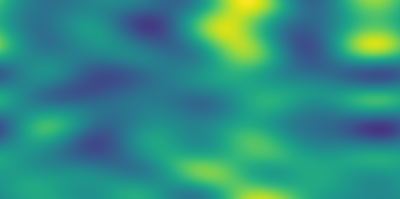
\includegraphics[interpolate=false,width=1.000000in,height=1.000000in]{burgers_rollout_pred_0.0-img0.png}}%
\end{pgfscope}%
\begin{pgfscope}%
\pgfsetbuttcap%
\pgfsetroundjoin%
\definecolor{currentfill}{rgb}{0.000000,0.000000,0.000000}%
\pgfsetfillcolor{currentfill}%
\pgfsetlinewidth{0.803000pt}%
\definecolor{currentstroke}{rgb}{0.000000,0.000000,0.000000}%
\pgfsetstrokecolor{currentstroke}%
\pgfsetdash{}{0pt}%
\pgfsys@defobject{currentmarker}{\pgfqpoint{0.000000in}{-0.048611in}}{\pgfqpoint{0.000000in}{0.000000in}}{%
\pgfpathmoveto{\pgfqpoint{0.000000in}{0.000000in}}%
\pgfpathlineto{\pgfqpoint{0.000000in}{-0.048611in}}%
\pgfusepath{stroke,fill}%
}%
\begin{pgfscope}%
\pgfsys@transformshift{0.726837in}{0.517039in}%
\pgfsys@useobject{currentmarker}{}%
\end{pgfscope}%
\end{pgfscope}%
\begin{pgfscope}%
\definecolor{textcolor}{rgb}{0.000000,0.000000,0.000000}%
\pgfsetstrokecolor{textcolor}%
\pgfsetfillcolor{textcolor}%
\pgftext[x=0.726837in,y=0.419816in,,top]{\color{textcolor}{\rmfamily\fontsize{12.000000}{14.400000}\selectfont\catcode`\^=\active\def^{\ifmmode\sp\else\^{}\fi}\catcode`\%=\active\def%{\%}0}}%
\end{pgfscope}%
\begin{pgfscope}%
\pgfsetbuttcap%
\pgfsetroundjoin%
\definecolor{currentfill}{rgb}{0.000000,0.000000,0.000000}%
\pgfsetfillcolor{currentfill}%
\pgfsetlinewidth{0.803000pt}%
\definecolor{currentstroke}{rgb}{0.000000,0.000000,0.000000}%
\pgfsetstrokecolor{currentstroke}%
\pgfsetdash{}{0pt}%
\pgfsys@defobject{currentmarker}{\pgfqpoint{0.000000in}{-0.048611in}}{\pgfqpoint{0.000000in}{0.000000in}}{%
\pgfpathmoveto{\pgfqpoint{0.000000in}{0.000000in}}%
\pgfpathlineto{\pgfqpoint{0.000000in}{-0.048611in}}%
\pgfusepath{stroke,fill}%
}%
\begin{pgfscope}%
\pgfsys@transformshift{1.570762in}{0.517039in}%
\pgfsys@useobject{currentmarker}{}%
\end{pgfscope}%
\end{pgfscope}%
\begin{pgfscope}%
\definecolor{textcolor}{rgb}{0.000000,0.000000,0.000000}%
\pgfsetstrokecolor{textcolor}%
\pgfsetfillcolor{textcolor}%
\pgftext[x=1.570762in,y=0.419816in,,top]{\color{textcolor}{\rmfamily\fontsize{12.000000}{14.400000}\selectfont\catcode`\^=\active\def^{\ifmmode\sp\else\^{}\fi}\catcode`\%=\active\def%{\%}1}}%
\end{pgfscope}%
\begin{pgfscope}%
\pgfsetbuttcap%
\pgfsetroundjoin%
\definecolor{currentfill}{rgb}{0.000000,0.000000,0.000000}%
\pgfsetfillcolor{currentfill}%
\pgfsetlinewidth{0.803000pt}%
\definecolor{currentstroke}{rgb}{0.000000,0.000000,0.000000}%
\pgfsetstrokecolor{currentstroke}%
\pgfsetdash{}{0pt}%
\pgfsys@defobject{currentmarker}{\pgfqpoint{0.000000in}{-0.048611in}}{\pgfqpoint{0.000000in}{0.000000in}}{%
\pgfpathmoveto{\pgfqpoint{0.000000in}{0.000000in}}%
\pgfpathlineto{\pgfqpoint{0.000000in}{-0.048611in}}%
\pgfusepath{stroke,fill}%
}%
\begin{pgfscope}%
\pgfsys@transformshift{2.414687in}{0.517039in}%
\pgfsys@useobject{currentmarker}{}%
\end{pgfscope}%
\end{pgfscope}%
\begin{pgfscope}%
\definecolor{textcolor}{rgb}{0.000000,0.000000,0.000000}%
\pgfsetstrokecolor{textcolor}%
\pgfsetfillcolor{textcolor}%
\pgftext[x=2.414687in,y=0.419816in,,top]{\color{textcolor}{\rmfamily\fontsize{12.000000}{14.400000}\selectfont\catcode`\^=\active\def^{\ifmmode\sp\else\^{}\fi}\catcode`\%=\active\def%{\%}2}}%
\end{pgfscope}%
\begin{pgfscope}%
\definecolor{textcolor}{rgb}{0.000000,0.000000,0.000000}%
\pgfsetstrokecolor{textcolor}%
\pgfsetfillcolor{textcolor}%
\pgftext[x=1.570762in,y=0.202965in,,top]{\color{textcolor}{\rmfamily\fontsize{12.000000}{14.400000}\selectfont\catcode`\^=\active\def^{\ifmmode\sp\else\^{}\fi}\catcode`\%=\active\def%{\%}Space}}%
\end{pgfscope}%
\begin{pgfscope}%
\pgfsetbuttcap%
\pgfsetroundjoin%
\definecolor{currentfill}{rgb}{0.000000,0.000000,0.000000}%
\pgfsetfillcolor{currentfill}%
\pgfsetlinewidth{0.803000pt}%
\definecolor{currentstroke}{rgb}{0.000000,0.000000,0.000000}%
\pgfsetstrokecolor{currentstroke}%
\pgfsetdash{}{0pt}%
\pgfsys@defobject{currentmarker}{\pgfqpoint{-0.048611in}{0.000000in}}{\pgfqpoint{-0.000000in}{0.000000in}}{%
\pgfpathmoveto{\pgfqpoint{-0.000000in}{0.000000in}}%
\pgfpathlineto{\pgfqpoint{-0.048611in}{0.000000in}}%
\pgfusepath{stroke,fill}%
}%
\begin{pgfscope}%
\pgfsys@transformshift{0.726837in}{0.517039in}%
\pgfsys@useobject{currentmarker}{}%
\end{pgfscope}%
\end{pgfscope}%
\begin{pgfscope}%
\definecolor{textcolor}{rgb}{0.000000,0.000000,0.000000}%
\pgfsetstrokecolor{textcolor}%
\pgfsetfillcolor{textcolor}%
\pgftext[x=0.364559in, y=0.453725in, left, base]{\color{textcolor}{\rmfamily\fontsize{12.000000}{14.400000}\selectfont\catcode`\^=\active\def^{\ifmmode\sp\else\^{}\fi}\catcode`\%=\active\def%{\%}0.0}}%
\end{pgfscope}%
\begin{pgfscope}%
\pgfsetbuttcap%
\pgfsetroundjoin%
\definecolor{currentfill}{rgb}{0.000000,0.000000,0.000000}%
\pgfsetfillcolor{currentfill}%
\pgfsetlinewidth{0.803000pt}%
\definecolor{currentstroke}{rgb}{0.000000,0.000000,0.000000}%
\pgfsetstrokecolor{currentstroke}%
\pgfsetdash{}{0pt}%
\pgfsys@defobject{currentmarker}{\pgfqpoint{-0.048611in}{0.000000in}}{\pgfqpoint{-0.000000in}{0.000000in}}{%
\pgfpathmoveto{\pgfqpoint{-0.000000in}{0.000000in}}%
\pgfpathlineto{\pgfqpoint{-0.048611in}{0.000000in}}%
\pgfusepath{stroke,fill}%
}%
\begin{pgfscope}%
\pgfsys@transformshift{0.726837in}{0.861533in}%
\pgfsys@useobject{currentmarker}{}%
\end{pgfscope}%
\end{pgfscope}%
\begin{pgfscope}%
\definecolor{textcolor}{rgb}{0.000000,0.000000,0.000000}%
\pgfsetstrokecolor{textcolor}%
\pgfsetfillcolor{textcolor}%
\pgftext[x=0.364559in, y=0.798219in, left, base]{\color{textcolor}{\rmfamily\fontsize{12.000000}{14.400000}\selectfont\catcode`\^=\active\def^{\ifmmode\sp\else\^{}\fi}\catcode`\%=\active\def%{\%}2.5}}%
\end{pgfscope}%
\begin{pgfscope}%
\pgfsetbuttcap%
\pgfsetroundjoin%
\definecolor{currentfill}{rgb}{0.000000,0.000000,0.000000}%
\pgfsetfillcolor{currentfill}%
\pgfsetlinewidth{0.803000pt}%
\definecolor{currentstroke}{rgb}{0.000000,0.000000,0.000000}%
\pgfsetstrokecolor{currentstroke}%
\pgfsetdash{}{0pt}%
\pgfsys@defobject{currentmarker}{\pgfqpoint{-0.048611in}{0.000000in}}{\pgfqpoint{-0.000000in}{0.000000in}}{%
\pgfpathmoveto{\pgfqpoint{-0.000000in}{0.000000in}}%
\pgfpathlineto{\pgfqpoint{-0.048611in}{0.000000in}}%
\pgfusepath{stroke,fill}%
}%
\begin{pgfscope}%
\pgfsys@transformshift{0.726837in}{1.206027in}%
\pgfsys@useobject{currentmarker}{}%
\end{pgfscope}%
\end{pgfscope}%
\begin{pgfscope}%
\definecolor{textcolor}{rgb}{0.000000,0.000000,0.000000}%
\pgfsetstrokecolor{textcolor}%
\pgfsetfillcolor{textcolor}%
\pgftext[x=0.364559in, y=1.142714in, left, base]{\color{textcolor}{\rmfamily\fontsize{12.000000}{14.400000}\selectfont\catcode`\^=\active\def^{\ifmmode\sp\else\^{}\fi}\catcode`\%=\active\def%{\%}5.0}}%
\end{pgfscope}%
\begin{pgfscope}%
\pgfsetbuttcap%
\pgfsetroundjoin%
\definecolor{currentfill}{rgb}{0.000000,0.000000,0.000000}%
\pgfsetfillcolor{currentfill}%
\pgfsetlinewidth{0.803000pt}%
\definecolor{currentstroke}{rgb}{0.000000,0.000000,0.000000}%
\pgfsetstrokecolor{currentstroke}%
\pgfsetdash{}{0pt}%
\pgfsys@defobject{currentmarker}{\pgfqpoint{-0.048611in}{0.000000in}}{\pgfqpoint{-0.000000in}{0.000000in}}{%
\pgfpathmoveto{\pgfqpoint{-0.000000in}{0.000000in}}%
\pgfpathlineto{\pgfqpoint{-0.048611in}{0.000000in}}%
\pgfusepath{stroke,fill}%
}%
\begin{pgfscope}%
\pgfsys@transformshift{0.726837in}{1.550522in}%
\pgfsys@useobject{currentmarker}{}%
\end{pgfscope}%
\end{pgfscope}%
\begin{pgfscope}%
\definecolor{textcolor}{rgb}{0.000000,0.000000,0.000000}%
\pgfsetstrokecolor{textcolor}%
\pgfsetfillcolor{textcolor}%
\pgftext[x=0.364559in, y=1.487208in, left, base]{\color{textcolor}{\rmfamily\fontsize{12.000000}{14.400000}\selectfont\catcode`\^=\active\def^{\ifmmode\sp\else\^{}\fi}\catcode`\%=\active\def%{\%}7.5}}%
\end{pgfscope}%
\begin{pgfscope}%
\pgfsetbuttcap%
\pgfsetroundjoin%
\definecolor{currentfill}{rgb}{0.000000,0.000000,0.000000}%
\pgfsetfillcolor{currentfill}%
\pgfsetlinewidth{0.803000pt}%
\definecolor{currentstroke}{rgb}{0.000000,0.000000,0.000000}%
\pgfsetstrokecolor{currentstroke}%
\pgfsetdash{}{0pt}%
\pgfsys@defobject{currentmarker}{\pgfqpoint{-0.048611in}{0.000000in}}{\pgfqpoint{-0.000000in}{0.000000in}}{%
\pgfpathmoveto{\pgfqpoint{-0.000000in}{0.000000in}}%
\pgfpathlineto{\pgfqpoint{-0.048611in}{0.000000in}}%
\pgfusepath{stroke,fill}%
}%
\begin{pgfscope}%
\pgfsys@transformshift{0.726837in}{1.895016in}%
\pgfsys@useobject{currentmarker}{}%
\end{pgfscope}%
\end{pgfscope}%
\begin{pgfscope}%
\definecolor{textcolor}{rgb}{0.000000,0.000000,0.000000}%
\pgfsetstrokecolor{textcolor}%
\pgfsetfillcolor{textcolor}%
\pgftext[x=0.258521in, y=1.831702in, left, base]{\color{textcolor}{\rmfamily\fontsize{12.000000}{14.400000}\selectfont\catcode`\^=\active\def^{\ifmmode\sp\else\^{}\fi}\catcode`\%=\active\def%{\%}10.0}}%
\end{pgfscope}%
\begin{pgfscope}%
\definecolor{textcolor}{rgb}{0.000000,0.000000,0.000000}%
\pgfsetstrokecolor{textcolor}%
\pgfsetfillcolor{textcolor}%
\pgftext[x=0.202965in,y=1.206027in,,bottom,rotate=90.000000]{\color{textcolor}{\rmfamily\fontsize{12.000000}{14.400000}\selectfont\catcode`\^=\active\def^{\ifmmode\sp\else\^{}\fi}\catcode`\%=\active\def%{\%}Time}}%
\end{pgfscope}%
\begin{pgfscope}%
\pgfsetrectcap%
\pgfsetmiterjoin%
\pgfsetlinewidth{0.803000pt}%
\definecolor{currentstroke}{rgb}{0.000000,0.000000,0.000000}%
\pgfsetstrokecolor{currentstroke}%
\pgfsetdash{}{0pt}%
\pgfpathmoveto{\pgfqpoint{0.726837in}{0.517039in}}%
\pgfpathlineto{\pgfqpoint{0.726837in}{1.895016in}}%
\pgfusepath{stroke}%
\end{pgfscope}%
\begin{pgfscope}%
\pgfsetrectcap%
\pgfsetmiterjoin%
\pgfsetlinewidth{0.803000pt}%
\definecolor{currentstroke}{rgb}{0.000000,0.000000,0.000000}%
\pgfsetstrokecolor{currentstroke}%
\pgfsetdash{}{0pt}%
\pgfpathmoveto{\pgfqpoint{2.414687in}{0.517039in}}%
\pgfpathlineto{\pgfqpoint{2.414687in}{1.895016in}}%
\pgfusepath{stroke}%
\end{pgfscope}%
\begin{pgfscope}%
\pgfsetrectcap%
\pgfsetmiterjoin%
\pgfsetlinewidth{0.803000pt}%
\definecolor{currentstroke}{rgb}{0.000000,0.000000,0.000000}%
\pgfsetstrokecolor{currentstroke}%
\pgfsetdash{}{0pt}%
\pgfpathmoveto{\pgfqpoint{0.726837in}{0.517039in}}%
\pgfpathlineto{\pgfqpoint{2.414687in}{0.517039in}}%
\pgfusepath{stroke}%
\end{pgfscope}%
\begin{pgfscope}%
\pgfsetrectcap%
\pgfsetmiterjoin%
\pgfsetlinewidth{0.803000pt}%
\definecolor{currentstroke}{rgb}{0.000000,0.000000,0.000000}%
\pgfsetstrokecolor{currentstroke}%
\pgfsetdash{}{0pt}%
\pgfpathmoveto{\pgfqpoint{0.726837in}{1.895016in}}%
\pgfpathlineto{\pgfqpoint{2.414687in}{1.895016in}}%
\pgfusepath{stroke}%
\end{pgfscope}%
\begin{pgfscope}%
\pgfsetbuttcap%
\pgfsetmiterjoin%
\pgfsetlinewidth{0.000000pt}%
\definecolor{currentstroke}{rgb}{0.000000,0.000000,0.000000}%
\pgfsetstrokecolor{currentstroke}%
\pgfsetstrokeopacity{0.000000}%
\pgfsetdash{}{0pt}%
\pgfpathmoveto{\pgfqpoint{2.552099in}{0.517039in}}%
\pgfpathlineto{\pgfqpoint{2.620998in}{0.517039in}}%
\pgfpathlineto{\pgfqpoint{2.620998in}{1.895016in}}%
\pgfpathlineto{\pgfqpoint{2.552099in}{1.895016in}}%
\pgfpathlineto{\pgfqpoint{2.552099in}{0.517039in}}%
\pgfpathclose%
\pgfusepath{}%
\end{pgfscope}%
\begin{pgfscope}%
\pgfsys@transformshift{2.550000in}{0.520000in}%
\pgftext[left,bottom]{
\includegraphics[interpolate=true,width=0.070000in,height=1.380000in]{burgers_rollout_pred_0.0-img1.png}}%
\end{pgfscope}%
\begin{pgfscope}%
\pgfsetbuttcap%
\pgfsetroundjoin%
\definecolor{currentfill}{rgb}{0.000000,0.000000,0.000000}%
\pgfsetfillcolor{currentfill}%
\pgfsetlinewidth{0.803000pt}%
\definecolor{currentstroke}{rgb}{0.000000,0.000000,0.000000}%
\pgfsetstrokecolor{currentstroke}%
\pgfsetdash{}{0pt}%
\pgfsys@defobject{currentmarker}{\pgfqpoint{0.000000in}{0.000000in}}{\pgfqpoint{0.048611in}{0.000000in}}{%
\pgfpathmoveto{\pgfqpoint{0.000000in}{0.000000in}}%
\pgfpathlineto{\pgfqpoint{0.048611in}{0.000000in}}%
\pgfusepath{stroke,fill}%
}%
\begin{pgfscope}%
\pgfsys@transformshift{2.620998in}{0.588723in}%
\pgfsys@useobject{currentmarker}{}%
\end{pgfscope}%
\end{pgfscope}%
\begin{pgfscope}%
\definecolor{textcolor}{rgb}{0.000000,0.000000,0.000000}%
\pgfsetstrokecolor{textcolor}%
\pgfsetfillcolor{textcolor}%
\pgftext[x=2.718220in, y=0.525410in, left, base]{\color{textcolor}{\rmfamily\fontsize{12.000000}{14.400000}\selectfont\catcode`\^=\active\def^{\ifmmode\sp\else\^{}\fi}\catcode`\%=\active\def%{\%}\ensuremath{-}1}}%
\end{pgfscope}%
\begin{pgfscope}%
\pgfsetbuttcap%
\pgfsetroundjoin%
\definecolor{currentfill}{rgb}{0.000000,0.000000,0.000000}%
\pgfsetfillcolor{currentfill}%
\pgfsetlinewidth{0.803000pt}%
\definecolor{currentstroke}{rgb}{0.000000,0.000000,0.000000}%
\pgfsetstrokecolor{currentstroke}%
\pgfsetdash{}{0pt}%
\pgfsys@defobject{currentmarker}{\pgfqpoint{0.000000in}{0.000000in}}{\pgfqpoint{0.048611in}{0.000000in}}{%
\pgfpathmoveto{\pgfqpoint{0.000000in}{0.000000in}}%
\pgfpathlineto{\pgfqpoint{0.048611in}{0.000000in}}%
\pgfusepath{stroke,fill}%
}%
\begin{pgfscope}%
\pgfsys@transformshift{2.620998in}{1.206027in}%
\pgfsys@useobject{currentmarker}{}%
\end{pgfscope}%
\end{pgfscope}%
\begin{pgfscope}%
\definecolor{textcolor}{rgb}{0.000000,0.000000,0.000000}%
\pgfsetstrokecolor{textcolor}%
\pgfsetfillcolor{textcolor}%
\pgftext[x=2.718220in, y=1.142714in, left, base]{\color{textcolor}{\rmfamily\fontsize{12.000000}{14.400000}\selectfont\catcode`\^=\active\def^{\ifmmode\sp\else\^{}\fi}\catcode`\%=\active\def%{\%}0}}%
\end{pgfscope}%
\begin{pgfscope}%
\pgfsetbuttcap%
\pgfsetroundjoin%
\definecolor{currentfill}{rgb}{0.000000,0.000000,0.000000}%
\pgfsetfillcolor{currentfill}%
\pgfsetlinewidth{0.803000pt}%
\definecolor{currentstroke}{rgb}{0.000000,0.000000,0.000000}%
\pgfsetstrokecolor{currentstroke}%
\pgfsetdash{}{0pt}%
\pgfsys@defobject{currentmarker}{\pgfqpoint{0.000000in}{0.000000in}}{\pgfqpoint{0.048611in}{0.000000in}}{%
\pgfpathmoveto{\pgfqpoint{0.000000in}{0.000000in}}%
\pgfpathlineto{\pgfqpoint{0.048611in}{0.000000in}}%
\pgfusepath{stroke,fill}%
}%
\begin{pgfscope}%
\pgfsys@transformshift{2.620998in}{1.823331in}%
\pgfsys@useobject{currentmarker}{}%
\end{pgfscope}%
\end{pgfscope}%
\begin{pgfscope}%
\definecolor{textcolor}{rgb}{0.000000,0.000000,0.000000}%
\pgfsetstrokecolor{textcolor}%
\pgfsetfillcolor{textcolor}%
\pgftext[x=2.718220in, y=1.760018in, left, base]{\color{textcolor}{\rmfamily\fontsize{12.000000}{14.400000}\selectfont\catcode`\^=\active\def^{\ifmmode\sp\else\^{}\fi}\catcode`\%=\active\def%{\%}1}}%
\end{pgfscope}%
\begin{pgfscope}%
\pgfsetrectcap%
\pgfsetmiterjoin%
\pgfsetlinewidth{0.803000pt}%
\definecolor{currentstroke}{rgb}{0.000000,0.000000,0.000000}%
\pgfsetstrokecolor{currentstroke}%
\pgfsetdash{}{0pt}%
\pgfpathmoveto{\pgfqpoint{2.552099in}{0.517039in}}%
\pgfpathlineto{\pgfqpoint{2.586548in}{0.517039in}}%
\pgfpathlineto{\pgfqpoint{2.620998in}{0.517039in}}%
\pgfpathlineto{\pgfqpoint{2.620998in}{1.895016in}}%
\pgfpathlineto{\pgfqpoint{2.586548in}{1.895016in}}%
\pgfpathlineto{\pgfqpoint{2.552099in}{1.895016in}}%
\pgfpathlineto{\pgfqpoint{2.552099in}{0.517039in}}%
\pgfpathclose%
\pgfusepath{stroke}%
\end{pgfscope}%
\end{pgfpicture}%
\makeatother%
\endgroup%

      \end{adjustbox}
      \caption{The prediction for \(\nu=0.0\)}\label{fig:sc2_rollout_pred_0.0}
    \end{subfigure}
    \begin{subfigure}{0.32\linewidth}
      \begin{adjustbox}{width=\linewidth}
        \begingroup%
\makeatletter%
\begin{pgfpicture}%
\pgfpathrectangle{\pgfpointorigin}{\pgfqpoint{3.000000in}{2.000000in}}%
\pgfusepath{use as bounding box, clip}%
\begin{pgfscope}%
\pgfsetbuttcap%
\pgfsetmiterjoin%
\pgfsetlinewidth{0.000000pt}%
\definecolor{currentstroke}{rgb}{0.000000,0.000000,0.000000}%
\pgfsetstrokecolor{currentstroke}%
\pgfsetstrokeopacity{0.000000}%
\pgfsetdash{}{0pt}%
\pgfpathmoveto{\pgfqpoint{0.000000in}{0.000000in}}%
\pgfpathlineto{\pgfqpoint{3.000000in}{0.000000in}}%
\pgfpathlineto{\pgfqpoint{3.000000in}{2.000000in}}%
\pgfpathlineto{\pgfqpoint{0.000000in}{2.000000in}}%
\pgfpathlineto{\pgfqpoint{0.000000in}{0.000000in}}%
\pgfpathclose%
\pgfusepath{}%
\end{pgfscope}%
\begin{pgfscope}%
\pgfsetbuttcap%
\pgfsetmiterjoin%
\pgfsetlinewidth{0.000000pt}%
\definecolor{currentstroke}{rgb}{0.000000,0.000000,0.000000}%
\pgfsetstrokecolor{currentstroke}%
\pgfsetstrokeopacity{0.000000}%
\pgfsetdash{}{0pt}%
\pgfpathmoveto{\pgfqpoint{0.726837in}{0.517039in}}%
\pgfpathlineto{\pgfqpoint{2.414687in}{0.517039in}}%
\pgfpathlineto{\pgfqpoint{2.414687in}{1.895016in}}%
\pgfpathlineto{\pgfqpoint{0.726837in}{1.895016in}}%
\pgfpathlineto{\pgfqpoint{0.726837in}{0.517039in}}%
\pgfpathclose%
\pgfusepath{}%
\end{pgfscope}%
\begin{pgfscope}%
\pgfpathrectangle{\pgfqpoint{0.726837in}{0.517039in}}{\pgfqpoint{1.687850in}{1.377978in}}%
\pgfusepath{clip}%
\pgfsys@transformcm{1.687850}{0.000000}{0.000000}{1.377978}{0.726837in}{0.517039in}%
\pgftext[left,bottom]{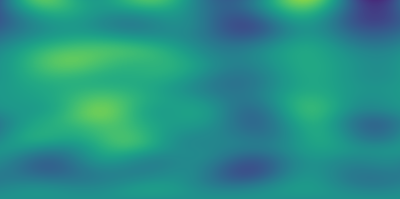
\includegraphics[interpolate=false,width=1.000000in,height=1.000000in]{burgers_rollout_diff_0.0-img0.png}}%
\end{pgfscope}%
\begin{pgfscope}%
\pgfsetbuttcap%
\pgfsetroundjoin%
\definecolor{currentfill}{rgb}{0.000000,0.000000,0.000000}%
\pgfsetfillcolor{currentfill}%
\pgfsetlinewidth{0.803000pt}%
\definecolor{currentstroke}{rgb}{0.000000,0.000000,0.000000}%
\pgfsetstrokecolor{currentstroke}%
\pgfsetdash{}{0pt}%
\pgfsys@defobject{currentmarker}{\pgfqpoint{0.000000in}{-0.048611in}}{\pgfqpoint{0.000000in}{0.000000in}}{%
\pgfpathmoveto{\pgfqpoint{0.000000in}{0.000000in}}%
\pgfpathlineto{\pgfqpoint{0.000000in}{-0.048611in}}%
\pgfusepath{stroke,fill}%
}%
\begin{pgfscope}%
\pgfsys@transformshift{0.726837in}{0.517039in}%
\pgfsys@useobject{currentmarker}{}%
\end{pgfscope}%
\end{pgfscope}%
\begin{pgfscope}%
\definecolor{textcolor}{rgb}{0.000000,0.000000,0.000000}%
\pgfsetstrokecolor{textcolor}%
\pgfsetfillcolor{textcolor}%
\pgftext[x=0.726837in,y=0.419816in,,top]{\color{textcolor}{\rmfamily\fontsize{12.000000}{14.400000}\selectfont\catcode`\^=\active\def^{\ifmmode\sp\else\^{}\fi}\catcode`\%=\active\def%{\%}0}}%
\end{pgfscope}%
\begin{pgfscope}%
\pgfsetbuttcap%
\pgfsetroundjoin%
\definecolor{currentfill}{rgb}{0.000000,0.000000,0.000000}%
\pgfsetfillcolor{currentfill}%
\pgfsetlinewidth{0.803000pt}%
\definecolor{currentstroke}{rgb}{0.000000,0.000000,0.000000}%
\pgfsetstrokecolor{currentstroke}%
\pgfsetdash{}{0pt}%
\pgfsys@defobject{currentmarker}{\pgfqpoint{0.000000in}{-0.048611in}}{\pgfqpoint{0.000000in}{0.000000in}}{%
\pgfpathmoveto{\pgfqpoint{0.000000in}{0.000000in}}%
\pgfpathlineto{\pgfqpoint{0.000000in}{-0.048611in}}%
\pgfusepath{stroke,fill}%
}%
\begin{pgfscope}%
\pgfsys@transformshift{1.570762in}{0.517039in}%
\pgfsys@useobject{currentmarker}{}%
\end{pgfscope}%
\end{pgfscope}%
\begin{pgfscope}%
\definecolor{textcolor}{rgb}{0.000000,0.000000,0.000000}%
\pgfsetstrokecolor{textcolor}%
\pgfsetfillcolor{textcolor}%
\pgftext[x=1.570762in,y=0.419816in,,top]{\color{textcolor}{\rmfamily\fontsize{12.000000}{14.400000}\selectfont\catcode`\^=\active\def^{\ifmmode\sp\else\^{}\fi}\catcode`\%=\active\def%{\%}1}}%
\end{pgfscope}%
\begin{pgfscope}%
\pgfsetbuttcap%
\pgfsetroundjoin%
\definecolor{currentfill}{rgb}{0.000000,0.000000,0.000000}%
\pgfsetfillcolor{currentfill}%
\pgfsetlinewidth{0.803000pt}%
\definecolor{currentstroke}{rgb}{0.000000,0.000000,0.000000}%
\pgfsetstrokecolor{currentstroke}%
\pgfsetdash{}{0pt}%
\pgfsys@defobject{currentmarker}{\pgfqpoint{0.000000in}{-0.048611in}}{\pgfqpoint{0.000000in}{0.000000in}}{%
\pgfpathmoveto{\pgfqpoint{0.000000in}{0.000000in}}%
\pgfpathlineto{\pgfqpoint{0.000000in}{-0.048611in}}%
\pgfusepath{stroke,fill}%
}%
\begin{pgfscope}%
\pgfsys@transformshift{2.414687in}{0.517039in}%
\pgfsys@useobject{currentmarker}{}%
\end{pgfscope}%
\end{pgfscope}%
\begin{pgfscope}%
\definecolor{textcolor}{rgb}{0.000000,0.000000,0.000000}%
\pgfsetstrokecolor{textcolor}%
\pgfsetfillcolor{textcolor}%
\pgftext[x=2.414687in,y=0.419816in,,top]{\color{textcolor}{\rmfamily\fontsize{12.000000}{14.400000}\selectfont\catcode`\^=\active\def^{\ifmmode\sp\else\^{}\fi}\catcode`\%=\active\def%{\%}2}}%
\end{pgfscope}%
\begin{pgfscope}%
\definecolor{textcolor}{rgb}{0.000000,0.000000,0.000000}%
\pgfsetstrokecolor{textcolor}%
\pgfsetfillcolor{textcolor}%
\pgftext[x=1.570762in,y=0.202965in,,top]{\color{textcolor}{\rmfamily\fontsize{12.000000}{14.400000}\selectfont\catcode`\^=\active\def^{\ifmmode\sp\else\^{}\fi}\catcode`\%=\active\def%{\%}Space}}%
\end{pgfscope}%
\begin{pgfscope}%
\pgfsetbuttcap%
\pgfsetroundjoin%
\definecolor{currentfill}{rgb}{0.000000,0.000000,0.000000}%
\pgfsetfillcolor{currentfill}%
\pgfsetlinewidth{0.803000pt}%
\definecolor{currentstroke}{rgb}{0.000000,0.000000,0.000000}%
\pgfsetstrokecolor{currentstroke}%
\pgfsetdash{}{0pt}%
\pgfsys@defobject{currentmarker}{\pgfqpoint{-0.048611in}{0.000000in}}{\pgfqpoint{-0.000000in}{0.000000in}}{%
\pgfpathmoveto{\pgfqpoint{-0.000000in}{0.000000in}}%
\pgfpathlineto{\pgfqpoint{-0.048611in}{0.000000in}}%
\pgfusepath{stroke,fill}%
}%
\begin{pgfscope}%
\pgfsys@transformshift{0.726837in}{0.517039in}%
\pgfsys@useobject{currentmarker}{}%
\end{pgfscope}%
\end{pgfscope}%
\begin{pgfscope}%
\definecolor{textcolor}{rgb}{0.000000,0.000000,0.000000}%
\pgfsetstrokecolor{textcolor}%
\pgfsetfillcolor{textcolor}%
\pgftext[x=0.364559in, y=0.453725in, left, base]{\color{textcolor}{\rmfamily\fontsize{12.000000}{14.400000}\selectfont\catcode`\^=\active\def^{\ifmmode\sp\else\^{}\fi}\catcode`\%=\active\def%{\%}0.0}}%
\end{pgfscope}%
\begin{pgfscope}%
\pgfsetbuttcap%
\pgfsetroundjoin%
\definecolor{currentfill}{rgb}{0.000000,0.000000,0.000000}%
\pgfsetfillcolor{currentfill}%
\pgfsetlinewidth{0.803000pt}%
\definecolor{currentstroke}{rgb}{0.000000,0.000000,0.000000}%
\pgfsetstrokecolor{currentstroke}%
\pgfsetdash{}{0pt}%
\pgfsys@defobject{currentmarker}{\pgfqpoint{-0.048611in}{0.000000in}}{\pgfqpoint{-0.000000in}{0.000000in}}{%
\pgfpathmoveto{\pgfqpoint{-0.000000in}{0.000000in}}%
\pgfpathlineto{\pgfqpoint{-0.048611in}{0.000000in}}%
\pgfusepath{stroke,fill}%
}%
\begin{pgfscope}%
\pgfsys@transformshift{0.726837in}{0.861533in}%
\pgfsys@useobject{currentmarker}{}%
\end{pgfscope}%
\end{pgfscope}%
\begin{pgfscope}%
\definecolor{textcolor}{rgb}{0.000000,0.000000,0.000000}%
\pgfsetstrokecolor{textcolor}%
\pgfsetfillcolor{textcolor}%
\pgftext[x=0.364559in, y=0.798219in, left, base]{\color{textcolor}{\rmfamily\fontsize{12.000000}{14.400000}\selectfont\catcode`\^=\active\def^{\ifmmode\sp\else\^{}\fi}\catcode`\%=\active\def%{\%}2.5}}%
\end{pgfscope}%
\begin{pgfscope}%
\pgfsetbuttcap%
\pgfsetroundjoin%
\definecolor{currentfill}{rgb}{0.000000,0.000000,0.000000}%
\pgfsetfillcolor{currentfill}%
\pgfsetlinewidth{0.803000pt}%
\definecolor{currentstroke}{rgb}{0.000000,0.000000,0.000000}%
\pgfsetstrokecolor{currentstroke}%
\pgfsetdash{}{0pt}%
\pgfsys@defobject{currentmarker}{\pgfqpoint{-0.048611in}{0.000000in}}{\pgfqpoint{-0.000000in}{0.000000in}}{%
\pgfpathmoveto{\pgfqpoint{-0.000000in}{0.000000in}}%
\pgfpathlineto{\pgfqpoint{-0.048611in}{0.000000in}}%
\pgfusepath{stroke,fill}%
}%
\begin{pgfscope}%
\pgfsys@transformshift{0.726837in}{1.206027in}%
\pgfsys@useobject{currentmarker}{}%
\end{pgfscope}%
\end{pgfscope}%
\begin{pgfscope}%
\definecolor{textcolor}{rgb}{0.000000,0.000000,0.000000}%
\pgfsetstrokecolor{textcolor}%
\pgfsetfillcolor{textcolor}%
\pgftext[x=0.364559in, y=1.142714in, left, base]{\color{textcolor}{\rmfamily\fontsize{12.000000}{14.400000}\selectfont\catcode`\^=\active\def^{\ifmmode\sp\else\^{}\fi}\catcode`\%=\active\def%{\%}5.0}}%
\end{pgfscope}%
\begin{pgfscope}%
\pgfsetbuttcap%
\pgfsetroundjoin%
\definecolor{currentfill}{rgb}{0.000000,0.000000,0.000000}%
\pgfsetfillcolor{currentfill}%
\pgfsetlinewidth{0.803000pt}%
\definecolor{currentstroke}{rgb}{0.000000,0.000000,0.000000}%
\pgfsetstrokecolor{currentstroke}%
\pgfsetdash{}{0pt}%
\pgfsys@defobject{currentmarker}{\pgfqpoint{-0.048611in}{0.000000in}}{\pgfqpoint{-0.000000in}{0.000000in}}{%
\pgfpathmoveto{\pgfqpoint{-0.000000in}{0.000000in}}%
\pgfpathlineto{\pgfqpoint{-0.048611in}{0.000000in}}%
\pgfusepath{stroke,fill}%
}%
\begin{pgfscope}%
\pgfsys@transformshift{0.726837in}{1.550522in}%
\pgfsys@useobject{currentmarker}{}%
\end{pgfscope}%
\end{pgfscope}%
\begin{pgfscope}%
\definecolor{textcolor}{rgb}{0.000000,0.000000,0.000000}%
\pgfsetstrokecolor{textcolor}%
\pgfsetfillcolor{textcolor}%
\pgftext[x=0.364559in, y=1.487208in, left, base]{\color{textcolor}{\rmfamily\fontsize{12.000000}{14.400000}\selectfont\catcode`\^=\active\def^{\ifmmode\sp\else\^{}\fi}\catcode`\%=\active\def%{\%}7.5}}%
\end{pgfscope}%
\begin{pgfscope}%
\pgfsetbuttcap%
\pgfsetroundjoin%
\definecolor{currentfill}{rgb}{0.000000,0.000000,0.000000}%
\pgfsetfillcolor{currentfill}%
\pgfsetlinewidth{0.803000pt}%
\definecolor{currentstroke}{rgb}{0.000000,0.000000,0.000000}%
\pgfsetstrokecolor{currentstroke}%
\pgfsetdash{}{0pt}%
\pgfsys@defobject{currentmarker}{\pgfqpoint{-0.048611in}{0.000000in}}{\pgfqpoint{-0.000000in}{0.000000in}}{%
\pgfpathmoveto{\pgfqpoint{-0.000000in}{0.000000in}}%
\pgfpathlineto{\pgfqpoint{-0.048611in}{0.000000in}}%
\pgfusepath{stroke,fill}%
}%
\begin{pgfscope}%
\pgfsys@transformshift{0.726837in}{1.895016in}%
\pgfsys@useobject{currentmarker}{}%
\end{pgfscope}%
\end{pgfscope}%
\begin{pgfscope}%
\definecolor{textcolor}{rgb}{0.000000,0.000000,0.000000}%
\pgfsetstrokecolor{textcolor}%
\pgfsetfillcolor{textcolor}%
\pgftext[x=0.258521in, y=1.831702in, left, base]{\color{textcolor}{\rmfamily\fontsize{12.000000}{14.400000}\selectfont\catcode`\^=\active\def^{\ifmmode\sp\else\^{}\fi}\catcode`\%=\active\def%{\%}10.0}}%
\end{pgfscope}%
\begin{pgfscope}%
\definecolor{textcolor}{rgb}{0.000000,0.000000,0.000000}%
\pgfsetstrokecolor{textcolor}%
\pgfsetfillcolor{textcolor}%
\pgftext[x=0.202965in,y=1.206027in,,bottom,rotate=90.000000]{\color{textcolor}{\rmfamily\fontsize{12.000000}{14.400000}\selectfont\catcode`\^=\active\def^{\ifmmode\sp\else\^{}\fi}\catcode`\%=\active\def%{\%}Time}}%
\end{pgfscope}%
\begin{pgfscope}%
\pgfsetrectcap%
\pgfsetmiterjoin%
\pgfsetlinewidth{0.803000pt}%
\definecolor{currentstroke}{rgb}{0.000000,0.000000,0.000000}%
\pgfsetstrokecolor{currentstroke}%
\pgfsetdash{}{0pt}%
\pgfpathmoveto{\pgfqpoint{0.726837in}{0.517039in}}%
\pgfpathlineto{\pgfqpoint{0.726837in}{1.895016in}}%
\pgfusepath{stroke}%
\end{pgfscope}%
\begin{pgfscope}%
\pgfsetrectcap%
\pgfsetmiterjoin%
\pgfsetlinewidth{0.803000pt}%
\definecolor{currentstroke}{rgb}{0.000000,0.000000,0.000000}%
\pgfsetstrokecolor{currentstroke}%
\pgfsetdash{}{0pt}%
\pgfpathmoveto{\pgfqpoint{2.414687in}{0.517039in}}%
\pgfpathlineto{\pgfqpoint{2.414687in}{1.895016in}}%
\pgfusepath{stroke}%
\end{pgfscope}%
\begin{pgfscope}%
\pgfsetrectcap%
\pgfsetmiterjoin%
\pgfsetlinewidth{0.803000pt}%
\definecolor{currentstroke}{rgb}{0.000000,0.000000,0.000000}%
\pgfsetstrokecolor{currentstroke}%
\pgfsetdash{}{0pt}%
\pgfpathmoveto{\pgfqpoint{0.726837in}{0.517039in}}%
\pgfpathlineto{\pgfqpoint{2.414687in}{0.517039in}}%
\pgfusepath{stroke}%
\end{pgfscope}%
\begin{pgfscope}%
\pgfsetrectcap%
\pgfsetmiterjoin%
\pgfsetlinewidth{0.803000pt}%
\definecolor{currentstroke}{rgb}{0.000000,0.000000,0.000000}%
\pgfsetstrokecolor{currentstroke}%
\pgfsetdash{}{0pt}%
\pgfpathmoveto{\pgfqpoint{0.726837in}{1.895016in}}%
\pgfpathlineto{\pgfqpoint{2.414687in}{1.895016in}}%
\pgfusepath{stroke}%
\end{pgfscope}%
\begin{pgfscope}%
\pgfsetbuttcap%
\pgfsetmiterjoin%
\pgfsetlinewidth{0.000000pt}%
\definecolor{currentstroke}{rgb}{0.000000,0.000000,0.000000}%
\pgfsetstrokecolor{currentstroke}%
\pgfsetstrokeopacity{0.000000}%
\pgfsetdash{}{0pt}%
\pgfpathmoveto{\pgfqpoint{2.552099in}{0.517039in}}%
\pgfpathlineto{\pgfqpoint{2.620998in}{0.517039in}}%
\pgfpathlineto{\pgfqpoint{2.620998in}{1.895016in}}%
\pgfpathlineto{\pgfqpoint{2.552099in}{1.895016in}}%
\pgfpathlineto{\pgfqpoint{2.552099in}{0.517039in}}%
\pgfpathclose%
\pgfusepath{}%
\end{pgfscope}%
\begin{pgfscope}%
\pgfsys@transformshift{2.550000in}{0.520000in}%
\pgftext[left,bottom]{
\includegraphics[interpolate=true,width=0.070000in,height=1.380000in]{burgers_rollout_diff_0.0-img1.png}}%
\end{pgfscope}%
\begin{pgfscope}%
\pgfsetbuttcap%
\pgfsetroundjoin%
\definecolor{currentfill}{rgb}{0.000000,0.000000,0.000000}%
\pgfsetfillcolor{currentfill}%
\pgfsetlinewidth{0.803000pt}%
\definecolor{currentstroke}{rgb}{0.000000,0.000000,0.000000}%
\pgfsetstrokecolor{currentstroke}%
\pgfsetdash{}{0pt}%
\pgfsys@defobject{currentmarker}{\pgfqpoint{0.000000in}{0.000000in}}{\pgfqpoint{0.048611in}{0.000000in}}{%
\pgfpathmoveto{\pgfqpoint{0.000000in}{0.000000in}}%
\pgfpathlineto{\pgfqpoint{0.048611in}{0.000000in}}%
\pgfusepath{stroke,fill}%
}%
\begin{pgfscope}%
\pgfsys@transformshift{2.620998in}{0.588723in}%
\pgfsys@useobject{currentmarker}{}%
\end{pgfscope}%
\end{pgfscope}%
\begin{pgfscope}%
\definecolor{textcolor}{rgb}{0.000000,0.000000,0.000000}%
\pgfsetstrokecolor{textcolor}%
\pgfsetfillcolor{textcolor}%
\pgftext[x=2.718220in, y=0.525410in, left, base]{\color{textcolor}{\rmfamily\fontsize{12.000000}{14.400000}\selectfont\catcode`\^=\active\def^{\ifmmode\sp\else\^{}\fi}\catcode`\%=\active\def%{\%}\ensuremath{-}1}}%
\end{pgfscope}%
\begin{pgfscope}%
\pgfsetbuttcap%
\pgfsetroundjoin%
\definecolor{currentfill}{rgb}{0.000000,0.000000,0.000000}%
\pgfsetfillcolor{currentfill}%
\pgfsetlinewidth{0.803000pt}%
\definecolor{currentstroke}{rgb}{0.000000,0.000000,0.000000}%
\pgfsetstrokecolor{currentstroke}%
\pgfsetdash{}{0pt}%
\pgfsys@defobject{currentmarker}{\pgfqpoint{0.000000in}{0.000000in}}{\pgfqpoint{0.048611in}{0.000000in}}{%
\pgfpathmoveto{\pgfqpoint{0.000000in}{0.000000in}}%
\pgfpathlineto{\pgfqpoint{0.048611in}{0.000000in}}%
\pgfusepath{stroke,fill}%
}%
\begin{pgfscope}%
\pgfsys@transformshift{2.620998in}{1.206027in}%
\pgfsys@useobject{currentmarker}{}%
\end{pgfscope}%
\end{pgfscope}%
\begin{pgfscope}%
\definecolor{textcolor}{rgb}{0.000000,0.000000,0.000000}%
\pgfsetstrokecolor{textcolor}%
\pgfsetfillcolor{textcolor}%
\pgftext[x=2.718220in, y=1.142714in, left, base]{\color{textcolor}{\rmfamily\fontsize{12.000000}{14.400000}\selectfont\catcode`\^=\active\def^{\ifmmode\sp\else\^{}\fi}\catcode`\%=\active\def%{\%}0}}%
\end{pgfscope}%
\begin{pgfscope}%
\pgfsetbuttcap%
\pgfsetroundjoin%
\definecolor{currentfill}{rgb}{0.000000,0.000000,0.000000}%
\pgfsetfillcolor{currentfill}%
\pgfsetlinewidth{0.803000pt}%
\definecolor{currentstroke}{rgb}{0.000000,0.000000,0.000000}%
\pgfsetstrokecolor{currentstroke}%
\pgfsetdash{}{0pt}%
\pgfsys@defobject{currentmarker}{\pgfqpoint{0.000000in}{0.000000in}}{\pgfqpoint{0.048611in}{0.000000in}}{%
\pgfpathmoveto{\pgfqpoint{0.000000in}{0.000000in}}%
\pgfpathlineto{\pgfqpoint{0.048611in}{0.000000in}}%
\pgfusepath{stroke,fill}%
}%
\begin{pgfscope}%
\pgfsys@transformshift{2.620998in}{1.823331in}%
\pgfsys@useobject{currentmarker}{}%
\end{pgfscope}%
\end{pgfscope}%
\begin{pgfscope}%
\definecolor{textcolor}{rgb}{0.000000,0.000000,0.000000}%
\pgfsetstrokecolor{textcolor}%
\pgfsetfillcolor{textcolor}%
\pgftext[x=2.718220in, y=1.760018in, left, base]{\color{textcolor}{\rmfamily\fontsize{12.000000}{14.400000}\selectfont\catcode`\^=\active\def^{\ifmmode\sp\else\^{}\fi}\catcode`\%=\active\def%{\%}1}}%
\end{pgfscope}%
\begin{pgfscope}%
\pgfsetrectcap%
\pgfsetmiterjoin%
\pgfsetlinewidth{0.803000pt}%
\definecolor{currentstroke}{rgb}{0.000000,0.000000,0.000000}%
\pgfsetstrokecolor{currentstroke}%
\pgfsetdash{}{0pt}%
\pgfpathmoveto{\pgfqpoint{2.552099in}{0.517039in}}%
\pgfpathlineto{\pgfqpoint{2.586548in}{0.517039in}}%
\pgfpathlineto{\pgfqpoint{2.620998in}{0.517039in}}%
\pgfpathlineto{\pgfqpoint{2.620998in}{1.895016in}}%
\pgfpathlineto{\pgfqpoint{2.586548in}{1.895016in}}%
\pgfpathlineto{\pgfqpoint{2.552099in}{1.895016in}}%
\pgfpathlineto{\pgfqpoint{2.552099in}{0.517039in}}%
\pgfpathclose%
\pgfusepath{stroke}%
\end{pgfscope}%
\end{pgfpicture}%
\makeatother%
\endgroup%

      \end{adjustbox}
      \caption{The difference for \(\nu=0.0\)}\label{fig:sc2_rollout_diff_0.0}
    \end{subfigure}
    \\[0.7\baselineskip]
    \begin{subfigure}{0.33\linewidth}
      \begin{adjustbox}{width=\linewidth}
        \begingroup%
\makeatletter%
\begin{pgfpicture}%
\pgfpathrectangle{\pgfpointorigin}{\pgfqpoint{3.000000in}{2.000000in}}%
\pgfusepath{use as bounding box, clip}%
\begin{pgfscope}%
\pgfsetbuttcap%
\pgfsetmiterjoin%
\pgfsetlinewidth{0.000000pt}%
\definecolor{currentstroke}{rgb}{0.000000,0.000000,0.000000}%
\pgfsetstrokecolor{currentstroke}%
\pgfsetstrokeopacity{0.000000}%
\pgfsetdash{}{0pt}%
\pgfpathmoveto{\pgfqpoint{0.000000in}{0.000000in}}%
\pgfpathlineto{\pgfqpoint{3.000000in}{0.000000in}}%
\pgfpathlineto{\pgfqpoint{3.000000in}{2.000000in}}%
\pgfpathlineto{\pgfqpoint{0.000000in}{2.000000in}}%
\pgfpathlineto{\pgfqpoint{0.000000in}{0.000000in}}%
\pgfpathclose%
\pgfusepath{}%
\end{pgfscope}%
\begin{pgfscope}%
\pgfsetbuttcap%
\pgfsetmiterjoin%
\pgfsetlinewidth{0.000000pt}%
\definecolor{currentstroke}{rgb}{0.000000,0.000000,0.000000}%
\pgfsetstrokecolor{currentstroke}%
\pgfsetstrokeopacity{0.000000}%
\pgfsetdash{}{0pt}%
\pgfpathmoveto{\pgfqpoint{0.726837in}{0.517039in}}%
\pgfpathlineto{\pgfqpoint{2.414687in}{0.517039in}}%
\pgfpathlineto{\pgfqpoint{2.414687in}{1.895016in}}%
\pgfpathlineto{\pgfqpoint{0.726837in}{1.895016in}}%
\pgfpathlineto{\pgfqpoint{0.726837in}{0.517039in}}%
\pgfpathclose%
\pgfusepath{}%
\end{pgfscope}%
\begin{pgfscope}%
\pgfpathrectangle{\pgfqpoint{0.726837in}{0.517039in}}{\pgfqpoint{1.687850in}{1.377978in}}%
\pgfusepath{clip}%
\pgfsys@transformcm{1.687850}{0.000000}{0.000000}{1.377978}{0.726837in}{0.517039in}%
\pgftext[left,bottom]{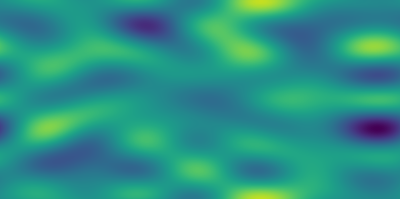
\includegraphics[interpolate=false,width=1.000000in,height=1.000000in]{burgers_rollout_target_0.01-img0.png}}%
\end{pgfscope}%
\begin{pgfscope}%
\pgfsetbuttcap%
\pgfsetroundjoin%
\definecolor{currentfill}{rgb}{0.000000,0.000000,0.000000}%
\pgfsetfillcolor{currentfill}%
\pgfsetlinewidth{0.803000pt}%
\definecolor{currentstroke}{rgb}{0.000000,0.000000,0.000000}%
\pgfsetstrokecolor{currentstroke}%
\pgfsetdash{}{0pt}%
\pgfsys@defobject{currentmarker}{\pgfqpoint{0.000000in}{-0.048611in}}{\pgfqpoint{0.000000in}{0.000000in}}{%
\pgfpathmoveto{\pgfqpoint{0.000000in}{0.000000in}}%
\pgfpathlineto{\pgfqpoint{0.000000in}{-0.048611in}}%
\pgfusepath{stroke,fill}%
}%
\begin{pgfscope}%
\pgfsys@transformshift{0.726837in}{0.517039in}%
\pgfsys@useobject{currentmarker}{}%
\end{pgfscope}%
\end{pgfscope}%
\begin{pgfscope}%
\definecolor{textcolor}{rgb}{0.000000,0.000000,0.000000}%
\pgfsetstrokecolor{textcolor}%
\pgfsetfillcolor{textcolor}%
\pgftext[x=0.726837in,y=0.419816in,,top]{\color{textcolor}\rmfamily\fontsize{12.000000}{14.400000}\selectfont 0}%
\end{pgfscope}%
\begin{pgfscope}%
\pgfsetbuttcap%
\pgfsetroundjoin%
\definecolor{currentfill}{rgb}{0.000000,0.000000,0.000000}%
\pgfsetfillcolor{currentfill}%
\pgfsetlinewidth{0.803000pt}%
\definecolor{currentstroke}{rgb}{0.000000,0.000000,0.000000}%
\pgfsetstrokecolor{currentstroke}%
\pgfsetdash{}{0pt}%
\pgfsys@defobject{currentmarker}{\pgfqpoint{0.000000in}{-0.048611in}}{\pgfqpoint{0.000000in}{0.000000in}}{%
\pgfpathmoveto{\pgfqpoint{0.000000in}{0.000000in}}%
\pgfpathlineto{\pgfqpoint{0.000000in}{-0.048611in}}%
\pgfusepath{stroke,fill}%
}%
\begin{pgfscope}%
\pgfsys@transformshift{1.570762in}{0.517039in}%
\pgfsys@useobject{currentmarker}{}%
\end{pgfscope}%
\end{pgfscope}%
\begin{pgfscope}%
\definecolor{textcolor}{rgb}{0.000000,0.000000,0.000000}%
\pgfsetstrokecolor{textcolor}%
\pgfsetfillcolor{textcolor}%
\pgftext[x=1.570762in,y=0.419816in,,top]{\color{textcolor}\rmfamily\fontsize{12.000000}{14.400000}\selectfont 1}%
\end{pgfscope}%
\begin{pgfscope}%
\pgfsetbuttcap%
\pgfsetroundjoin%
\definecolor{currentfill}{rgb}{0.000000,0.000000,0.000000}%
\pgfsetfillcolor{currentfill}%
\pgfsetlinewidth{0.803000pt}%
\definecolor{currentstroke}{rgb}{0.000000,0.000000,0.000000}%
\pgfsetstrokecolor{currentstroke}%
\pgfsetdash{}{0pt}%
\pgfsys@defobject{currentmarker}{\pgfqpoint{0.000000in}{-0.048611in}}{\pgfqpoint{0.000000in}{0.000000in}}{%
\pgfpathmoveto{\pgfqpoint{0.000000in}{0.000000in}}%
\pgfpathlineto{\pgfqpoint{0.000000in}{-0.048611in}}%
\pgfusepath{stroke,fill}%
}%
\begin{pgfscope}%
\pgfsys@transformshift{2.414687in}{0.517039in}%
\pgfsys@useobject{currentmarker}{}%
\end{pgfscope}%
\end{pgfscope}%
\begin{pgfscope}%
\definecolor{textcolor}{rgb}{0.000000,0.000000,0.000000}%
\pgfsetstrokecolor{textcolor}%
\pgfsetfillcolor{textcolor}%
\pgftext[x=2.414687in,y=0.419816in,,top]{\color{textcolor}\rmfamily\fontsize{12.000000}{14.400000}\selectfont 2}%
\end{pgfscope}%
\begin{pgfscope}%
\definecolor{textcolor}{rgb}{0.000000,0.000000,0.000000}%
\pgfsetstrokecolor{textcolor}%
\pgfsetfillcolor{textcolor}%
\pgftext[x=1.570762in,y=0.202965in,,top]{\color{textcolor}\rmfamily\fontsize{12.000000}{14.400000}\selectfont Space}%
\end{pgfscope}%
\begin{pgfscope}%
\pgfsetbuttcap%
\pgfsetroundjoin%
\definecolor{currentfill}{rgb}{0.000000,0.000000,0.000000}%
\pgfsetfillcolor{currentfill}%
\pgfsetlinewidth{0.803000pt}%
\definecolor{currentstroke}{rgb}{0.000000,0.000000,0.000000}%
\pgfsetstrokecolor{currentstroke}%
\pgfsetdash{}{0pt}%
\pgfsys@defobject{currentmarker}{\pgfqpoint{-0.048611in}{0.000000in}}{\pgfqpoint{-0.000000in}{0.000000in}}{%
\pgfpathmoveto{\pgfqpoint{-0.000000in}{0.000000in}}%
\pgfpathlineto{\pgfqpoint{-0.048611in}{0.000000in}}%
\pgfusepath{stroke,fill}%
}%
\begin{pgfscope}%
\pgfsys@transformshift{0.726837in}{0.517039in}%
\pgfsys@useobject{currentmarker}{}%
\end{pgfscope}%
\end{pgfscope}%
\begin{pgfscope}%
\definecolor{textcolor}{rgb}{0.000000,0.000000,0.000000}%
\pgfsetstrokecolor{textcolor}%
\pgfsetfillcolor{textcolor}%
\pgftext[x=0.364559in, y=0.453725in, left, base]{\color{textcolor}\rmfamily\fontsize{12.000000}{14.400000}\selectfont 0.0}%
\end{pgfscope}%
\begin{pgfscope}%
\pgfsetbuttcap%
\pgfsetroundjoin%
\definecolor{currentfill}{rgb}{0.000000,0.000000,0.000000}%
\pgfsetfillcolor{currentfill}%
\pgfsetlinewidth{0.803000pt}%
\definecolor{currentstroke}{rgb}{0.000000,0.000000,0.000000}%
\pgfsetstrokecolor{currentstroke}%
\pgfsetdash{}{0pt}%
\pgfsys@defobject{currentmarker}{\pgfqpoint{-0.048611in}{0.000000in}}{\pgfqpoint{-0.000000in}{0.000000in}}{%
\pgfpathmoveto{\pgfqpoint{-0.000000in}{0.000000in}}%
\pgfpathlineto{\pgfqpoint{-0.048611in}{0.000000in}}%
\pgfusepath{stroke,fill}%
}%
\begin{pgfscope}%
\pgfsys@transformshift{0.726837in}{0.861533in}%
\pgfsys@useobject{currentmarker}{}%
\end{pgfscope}%
\end{pgfscope}%
\begin{pgfscope}%
\definecolor{textcolor}{rgb}{0.000000,0.000000,0.000000}%
\pgfsetstrokecolor{textcolor}%
\pgfsetfillcolor{textcolor}%
\pgftext[x=0.364559in, y=0.798219in, left, base]{\color{textcolor}\rmfamily\fontsize{12.000000}{14.400000}\selectfont 2.5}%
\end{pgfscope}%
\begin{pgfscope}%
\pgfsetbuttcap%
\pgfsetroundjoin%
\definecolor{currentfill}{rgb}{0.000000,0.000000,0.000000}%
\pgfsetfillcolor{currentfill}%
\pgfsetlinewidth{0.803000pt}%
\definecolor{currentstroke}{rgb}{0.000000,0.000000,0.000000}%
\pgfsetstrokecolor{currentstroke}%
\pgfsetdash{}{0pt}%
\pgfsys@defobject{currentmarker}{\pgfqpoint{-0.048611in}{0.000000in}}{\pgfqpoint{-0.000000in}{0.000000in}}{%
\pgfpathmoveto{\pgfqpoint{-0.000000in}{0.000000in}}%
\pgfpathlineto{\pgfqpoint{-0.048611in}{0.000000in}}%
\pgfusepath{stroke,fill}%
}%
\begin{pgfscope}%
\pgfsys@transformshift{0.726837in}{1.206027in}%
\pgfsys@useobject{currentmarker}{}%
\end{pgfscope}%
\end{pgfscope}%
\begin{pgfscope}%
\definecolor{textcolor}{rgb}{0.000000,0.000000,0.000000}%
\pgfsetstrokecolor{textcolor}%
\pgfsetfillcolor{textcolor}%
\pgftext[x=0.364559in, y=1.142714in, left, base]{\color{textcolor}\rmfamily\fontsize{12.000000}{14.400000}\selectfont 5.0}%
\end{pgfscope}%
\begin{pgfscope}%
\pgfsetbuttcap%
\pgfsetroundjoin%
\definecolor{currentfill}{rgb}{0.000000,0.000000,0.000000}%
\pgfsetfillcolor{currentfill}%
\pgfsetlinewidth{0.803000pt}%
\definecolor{currentstroke}{rgb}{0.000000,0.000000,0.000000}%
\pgfsetstrokecolor{currentstroke}%
\pgfsetdash{}{0pt}%
\pgfsys@defobject{currentmarker}{\pgfqpoint{-0.048611in}{0.000000in}}{\pgfqpoint{-0.000000in}{0.000000in}}{%
\pgfpathmoveto{\pgfqpoint{-0.000000in}{0.000000in}}%
\pgfpathlineto{\pgfqpoint{-0.048611in}{0.000000in}}%
\pgfusepath{stroke,fill}%
}%
\begin{pgfscope}%
\pgfsys@transformshift{0.726837in}{1.550522in}%
\pgfsys@useobject{currentmarker}{}%
\end{pgfscope}%
\end{pgfscope}%
\begin{pgfscope}%
\definecolor{textcolor}{rgb}{0.000000,0.000000,0.000000}%
\pgfsetstrokecolor{textcolor}%
\pgfsetfillcolor{textcolor}%
\pgftext[x=0.364559in, y=1.487208in, left, base]{\color{textcolor}\rmfamily\fontsize{12.000000}{14.400000}\selectfont 7.5}%
\end{pgfscope}%
\begin{pgfscope}%
\pgfsetbuttcap%
\pgfsetroundjoin%
\definecolor{currentfill}{rgb}{0.000000,0.000000,0.000000}%
\pgfsetfillcolor{currentfill}%
\pgfsetlinewidth{0.803000pt}%
\definecolor{currentstroke}{rgb}{0.000000,0.000000,0.000000}%
\pgfsetstrokecolor{currentstroke}%
\pgfsetdash{}{0pt}%
\pgfsys@defobject{currentmarker}{\pgfqpoint{-0.048611in}{0.000000in}}{\pgfqpoint{-0.000000in}{0.000000in}}{%
\pgfpathmoveto{\pgfqpoint{-0.000000in}{0.000000in}}%
\pgfpathlineto{\pgfqpoint{-0.048611in}{0.000000in}}%
\pgfusepath{stroke,fill}%
}%
\begin{pgfscope}%
\pgfsys@transformshift{0.726837in}{1.895016in}%
\pgfsys@useobject{currentmarker}{}%
\end{pgfscope}%
\end{pgfscope}%
\begin{pgfscope}%
\definecolor{textcolor}{rgb}{0.000000,0.000000,0.000000}%
\pgfsetstrokecolor{textcolor}%
\pgfsetfillcolor{textcolor}%
\pgftext[x=0.258521in, y=1.831702in, left, base]{\color{textcolor}\rmfamily\fontsize{12.000000}{14.400000}\selectfont 10.0}%
\end{pgfscope}%
\begin{pgfscope}%
\definecolor{textcolor}{rgb}{0.000000,0.000000,0.000000}%
\pgfsetstrokecolor{textcolor}%
\pgfsetfillcolor{textcolor}%
\pgftext[x=0.202965in,y=1.206027in,,bottom,rotate=90.000000]{\color{textcolor}\rmfamily\fontsize{12.000000}{14.400000}\selectfont Time}%
\end{pgfscope}%
\begin{pgfscope}%
\pgfsetrectcap%
\pgfsetmiterjoin%
\pgfsetlinewidth{0.803000pt}%
\definecolor{currentstroke}{rgb}{0.000000,0.000000,0.000000}%
\pgfsetstrokecolor{currentstroke}%
\pgfsetdash{}{0pt}%
\pgfpathmoveto{\pgfqpoint{0.726837in}{0.517039in}}%
\pgfpathlineto{\pgfqpoint{0.726837in}{1.895016in}}%
\pgfusepath{stroke}%
\end{pgfscope}%
\begin{pgfscope}%
\pgfsetrectcap%
\pgfsetmiterjoin%
\pgfsetlinewidth{0.803000pt}%
\definecolor{currentstroke}{rgb}{0.000000,0.000000,0.000000}%
\pgfsetstrokecolor{currentstroke}%
\pgfsetdash{}{0pt}%
\pgfpathmoveto{\pgfqpoint{2.414687in}{0.517039in}}%
\pgfpathlineto{\pgfqpoint{2.414687in}{1.895016in}}%
\pgfusepath{stroke}%
\end{pgfscope}%
\begin{pgfscope}%
\pgfsetrectcap%
\pgfsetmiterjoin%
\pgfsetlinewidth{0.803000pt}%
\definecolor{currentstroke}{rgb}{0.000000,0.000000,0.000000}%
\pgfsetstrokecolor{currentstroke}%
\pgfsetdash{}{0pt}%
\pgfpathmoveto{\pgfqpoint{0.726837in}{0.517039in}}%
\pgfpathlineto{\pgfqpoint{2.414687in}{0.517039in}}%
\pgfusepath{stroke}%
\end{pgfscope}%
\begin{pgfscope}%
\pgfsetrectcap%
\pgfsetmiterjoin%
\pgfsetlinewidth{0.803000pt}%
\definecolor{currentstroke}{rgb}{0.000000,0.000000,0.000000}%
\pgfsetstrokecolor{currentstroke}%
\pgfsetdash{}{0pt}%
\pgfpathmoveto{\pgfqpoint{0.726837in}{1.895016in}}%
\pgfpathlineto{\pgfqpoint{2.414687in}{1.895016in}}%
\pgfusepath{stroke}%
\end{pgfscope}%
\begin{pgfscope}%
\pgfsetbuttcap%
\pgfsetmiterjoin%
\pgfsetlinewidth{0.000000pt}%
\definecolor{currentstroke}{rgb}{0.000000,0.000000,0.000000}%
\pgfsetstrokecolor{currentstroke}%
\pgfsetstrokeopacity{0.000000}%
\pgfsetdash{}{0pt}%
\pgfpathmoveto{\pgfqpoint{2.552099in}{0.517039in}}%
\pgfpathlineto{\pgfqpoint{2.620998in}{0.517039in}}%
\pgfpathlineto{\pgfqpoint{2.620998in}{1.895016in}}%
\pgfpathlineto{\pgfqpoint{2.552099in}{1.895016in}}%
\pgfpathlineto{\pgfqpoint{2.552099in}{0.517039in}}%
\pgfpathclose%
\pgfusepath{}%
\end{pgfscope}%
\begin{pgfscope}%
\pgfsys@transformshift{2.550000in}{0.520000in}%
\pgftext[left,bottom]{
\includegraphics[interpolate=true,width=0.070000in,height=1.380000in]{burgers_rollout_target_0.01-img1.png}}%
\end{pgfscope}%
\begin{pgfscope}%
\pgfsetbuttcap%
\pgfsetroundjoin%
\definecolor{currentfill}{rgb}{0.000000,0.000000,0.000000}%
\pgfsetfillcolor{currentfill}%
\pgfsetlinewidth{0.803000pt}%
\definecolor{currentstroke}{rgb}{0.000000,0.000000,0.000000}%
\pgfsetstrokecolor{currentstroke}%
\pgfsetdash{}{0pt}%
\pgfsys@defobject{currentmarker}{\pgfqpoint{0.000000in}{0.000000in}}{\pgfqpoint{0.048611in}{0.000000in}}{%
\pgfpathmoveto{\pgfqpoint{0.000000in}{0.000000in}}%
\pgfpathlineto{\pgfqpoint{0.048611in}{0.000000in}}%
\pgfusepath{stroke,fill}%
}%
\begin{pgfscope}%
\pgfsys@transformshift{2.620998in}{0.588723in}%
\pgfsys@useobject{currentmarker}{}%
\end{pgfscope}%
\end{pgfscope}%
\begin{pgfscope}%
\definecolor{textcolor}{rgb}{0.000000,0.000000,0.000000}%
\pgfsetstrokecolor{textcolor}%
\pgfsetfillcolor{textcolor}%
\pgftext[x=2.718220in, y=0.525410in, left, base]{\color{textcolor}\rmfamily\fontsize{12.000000}{14.400000}\selectfont \ensuremath{-}1}%
\end{pgfscope}%
\begin{pgfscope}%
\pgfsetbuttcap%
\pgfsetroundjoin%
\definecolor{currentfill}{rgb}{0.000000,0.000000,0.000000}%
\pgfsetfillcolor{currentfill}%
\pgfsetlinewidth{0.803000pt}%
\definecolor{currentstroke}{rgb}{0.000000,0.000000,0.000000}%
\pgfsetstrokecolor{currentstroke}%
\pgfsetdash{}{0pt}%
\pgfsys@defobject{currentmarker}{\pgfqpoint{0.000000in}{0.000000in}}{\pgfqpoint{0.048611in}{0.000000in}}{%
\pgfpathmoveto{\pgfqpoint{0.000000in}{0.000000in}}%
\pgfpathlineto{\pgfqpoint{0.048611in}{0.000000in}}%
\pgfusepath{stroke,fill}%
}%
\begin{pgfscope}%
\pgfsys@transformshift{2.620998in}{1.206027in}%
\pgfsys@useobject{currentmarker}{}%
\end{pgfscope}%
\end{pgfscope}%
\begin{pgfscope}%
\definecolor{textcolor}{rgb}{0.000000,0.000000,0.000000}%
\pgfsetstrokecolor{textcolor}%
\pgfsetfillcolor{textcolor}%
\pgftext[x=2.718220in, y=1.142714in, left, base]{\color{textcolor}\rmfamily\fontsize{12.000000}{14.400000}\selectfont 0}%
\end{pgfscope}%
\begin{pgfscope}%
\pgfsetbuttcap%
\pgfsetroundjoin%
\definecolor{currentfill}{rgb}{0.000000,0.000000,0.000000}%
\pgfsetfillcolor{currentfill}%
\pgfsetlinewidth{0.803000pt}%
\definecolor{currentstroke}{rgb}{0.000000,0.000000,0.000000}%
\pgfsetstrokecolor{currentstroke}%
\pgfsetdash{}{0pt}%
\pgfsys@defobject{currentmarker}{\pgfqpoint{0.000000in}{0.000000in}}{\pgfqpoint{0.048611in}{0.000000in}}{%
\pgfpathmoveto{\pgfqpoint{0.000000in}{0.000000in}}%
\pgfpathlineto{\pgfqpoint{0.048611in}{0.000000in}}%
\pgfusepath{stroke,fill}%
}%
\begin{pgfscope}%
\pgfsys@transformshift{2.620998in}{1.823331in}%
\pgfsys@useobject{currentmarker}{}%
\end{pgfscope}%
\end{pgfscope}%
\begin{pgfscope}%
\definecolor{textcolor}{rgb}{0.000000,0.000000,0.000000}%
\pgfsetstrokecolor{textcolor}%
\pgfsetfillcolor{textcolor}%
\pgftext[x=2.718220in, y=1.760018in, left, base]{\color{textcolor}\rmfamily\fontsize{12.000000}{14.400000}\selectfont 1}%
\end{pgfscope}%
\begin{pgfscope}%
\pgfsetrectcap%
\pgfsetmiterjoin%
\pgfsetlinewidth{0.803000pt}%
\definecolor{currentstroke}{rgb}{0.000000,0.000000,0.000000}%
\pgfsetstrokecolor{currentstroke}%
\pgfsetdash{}{0pt}%
\pgfpathmoveto{\pgfqpoint{2.552099in}{0.517039in}}%
\pgfpathlineto{\pgfqpoint{2.586548in}{0.517039in}}%
\pgfpathlineto{\pgfqpoint{2.620998in}{0.517039in}}%
\pgfpathlineto{\pgfqpoint{2.620998in}{1.895016in}}%
\pgfpathlineto{\pgfqpoint{2.586548in}{1.895016in}}%
\pgfpathlineto{\pgfqpoint{2.552099in}{1.895016in}}%
\pgfpathlineto{\pgfqpoint{2.552099in}{0.517039in}}%
\pgfpathclose%
\pgfusepath{stroke}%
\end{pgfscope}%
\end{pgfpicture}%
\makeatother%
\endgroup%

      \end{adjustbox}
      \caption{The target for \(\nu=0.01\)}\label{fig:sc2_rollout_target_0.01}
    \end{subfigure}
    \begin{subfigure}{0.33\linewidth}
      \begin{adjustbox}{width=\linewidth}
        \begingroup%
\makeatletter%
\begin{pgfpicture}%
\pgfpathrectangle{\pgfpointorigin}{\pgfqpoint{3.000000in}{2.000000in}}%
\pgfusepath{use as bounding box, clip}%
\begin{pgfscope}%
\pgfsetbuttcap%
\pgfsetmiterjoin%
\pgfsetlinewidth{0.000000pt}%
\definecolor{currentstroke}{rgb}{0.000000,0.000000,0.000000}%
\pgfsetstrokecolor{currentstroke}%
\pgfsetstrokeopacity{0.000000}%
\pgfsetdash{}{0pt}%
\pgfpathmoveto{\pgfqpoint{0.000000in}{0.000000in}}%
\pgfpathlineto{\pgfqpoint{3.000000in}{0.000000in}}%
\pgfpathlineto{\pgfqpoint{3.000000in}{2.000000in}}%
\pgfpathlineto{\pgfqpoint{0.000000in}{2.000000in}}%
\pgfpathlineto{\pgfqpoint{0.000000in}{0.000000in}}%
\pgfpathclose%
\pgfusepath{}%
\end{pgfscope}%
\begin{pgfscope}%
\pgfsetbuttcap%
\pgfsetmiterjoin%
\pgfsetlinewidth{0.000000pt}%
\definecolor{currentstroke}{rgb}{0.000000,0.000000,0.000000}%
\pgfsetstrokecolor{currentstroke}%
\pgfsetstrokeopacity{0.000000}%
\pgfsetdash{}{0pt}%
\pgfpathmoveto{\pgfqpoint{0.726837in}{0.517039in}}%
\pgfpathlineto{\pgfqpoint{2.414687in}{0.517039in}}%
\pgfpathlineto{\pgfqpoint{2.414687in}{1.895016in}}%
\pgfpathlineto{\pgfqpoint{0.726837in}{1.895016in}}%
\pgfpathlineto{\pgfqpoint{0.726837in}{0.517039in}}%
\pgfpathclose%
\pgfusepath{}%
\end{pgfscope}%
\begin{pgfscope}%
\pgfpathrectangle{\pgfqpoint{0.726837in}{0.517039in}}{\pgfqpoint{1.687850in}{1.377978in}}%
\pgfusepath{clip}%
\pgfsys@transformcm{1.687850}{0.000000}{0.000000}{1.377978}{0.726837in}{0.517039in}%
\pgftext[left,bottom]{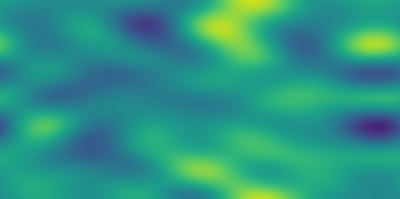
\includegraphics[interpolate=false,width=1.000000in,height=1.000000in]{burgers_rollout_pred_0.01-img0.png}}%
\end{pgfscope}%
\begin{pgfscope}%
\pgfsetbuttcap%
\pgfsetroundjoin%
\definecolor{currentfill}{rgb}{0.000000,0.000000,0.000000}%
\pgfsetfillcolor{currentfill}%
\pgfsetlinewidth{0.803000pt}%
\definecolor{currentstroke}{rgb}{0.000000,0.000000,0.000000}%
\pgfsetstrokecolor{currentstroke}%
\pgfsetdash{}{0pt}%
\pgfsys@defobject{currentmarker}{\pgfqpoint{0.000000in}{-0.048611in}}{\pgfqpoint{0.000000in}{0.000000in}}{%
\pgfpathmoveto{\pgfqpoint{0.000000in}{0.000000in}}%
\pgfpathlineto{\pgfqpoint{0.000000in}{-0.048611in}}%
\pgfusepath{stroke,fill}%
}%
\begin{pgfscope}%
\pgfsys@transformshift{0.726837in}{0.517039in}%
\pgfsys@useobject{currentmarker}{}%
\end{pgfscope}%
\end{pgfscope}%
\begin{pgfscope}%
\definecolor{textcolor}{rgb}{0.000000,0.000000,0.000000}%
\pgfsetstrokecolor{textcolor}%
\pgfsetfillcolor{textcolor}%
\pgftext[x=0.726837in,y=0.419816in,,top]{\color{textcolor}{\rmfamily\fontsize{12.000000}{14.400000}\selectfont\catcode`\^=\active\def^{\ifmmode\sp\else\^{}\fi}\catcode`\%=\active\def%{\%}0}}%
\end{pgfscope}%
\begin{pgfscope}%
\pgfsetbuttcap%
\pgfsetroundjoin%
\definecolor{currentfill}{rgb}{0.000000,0.000000,0.000000}%
\pgfsetfillcolor{currentfill}%
\pgfsetlinewidth{0.803000pt}%
\definecolor{currentstroke}{rgb}{0.000000,0.000000,0.000000}%
\pgfsetstrokecolor{currentstroke}%
\pgfsetdash{}{0pt}%
\pgfsys@defobject{currentmarker}{\pgfqpoint{0.000000in}{-0.048611in}}{\pgfqpoint{0.000000in}{0.000000in}}{%
\pgfpathmoveto{\pgfqpoint{0.000000in}{0.000000in}}%
\pgfpathlineto{\pgfqpoint{0.000000in}{-0.048611in}}%
\pgfusepath{stroke,fill}%
}%
\begin{pgfscope}%
\pgfsys@transformshift{1.570762in}{0.517039in}%
\pgfsys@useobject{currentmarker}{}%
\end{pgfscope}%
\end{pgfscope}%
\begin{pgfscope}%
\definecolor{textcolor}{rgb}{0.000000,0.000000,0.000000}%
\pgfsetstrokecolor{textcolor}%
\pgfsetfillcolor{textcolor}%
\pgftext[x=1.570762in,y=0.419816in,,top]{\color{textcolor}{\rmfamily\fontsize{12.000000}{14.400000}\selectfont\catcode`\^=\active\def^{\ifmmode\sp\else\^{}\fi}\catcode`\%=\active\def%{\%}1}}%
\end{pgfscope}%
\begin{pgfscope}%
\pgfsetbuttcap%
\pgfsetroundjoin%
\definecolor{currentfill}{rgb}{0.000000,0.000000,0.000000}%
\pgfsetfillcolor{currentfill}%
\pgfsetlinewidth{0.803000pt}%
\definecolor{currentstroke}{rgb}{0.000000,0.000000,0.000000}%
\pgfsetstrokecolor{currentstroke}%
\pgfsetdash{}{0pt}%
\pgfsys@defobject{currentmarker}{\pgfqpoint{0.000000in}{-0.048611in}}{\pgfqpoint{0.000000in}{0.000000in}}{%
\pgfpathmoveto{\pgfqpoint{0.000000in}{0.000000in}}%
\pgfpathlineto{\pgfqpoint{0.000000in}{-0.048611in}}%
\pgfusepath{stroke,fill}%
}%
\begin{pgfscope}%
\pgfsys@transformshift{2.414687in}{0.517039in}%
\pgfsys@useobject{currentmarker}{}%
\end{pgfscope}%
\end{pgfscope}%
\begin{pgfscope}%
\definecolor{textcolor}{rgb}{0.000000,0.000000,0.000000}%
\pgfsetstrokecolor{textcolor}%
\pgfsetfillcolor{textcolor}%
\pgftext[x=2.414687in,y=0.419816in,,top]{\color{textcolor}{\rmfamily\fontsize{12.000000}{14.400000}\selectfont\catcode`\^=\active\def^{\ifmmode\sp\else\^{}\fi}\catcode`\%=\active\def%{\%}2}}%
\end{pgfscope}%
\begin{pgfscope}%
\definecolor{textcolor}{rgb}{0.000000,0.000000,0.000000}%
\pgfsetstrokecolor{textcolor}%
\pgfsetfillcolor{textcolor}%
\pgftext[x=1.570762in,y=0.202965in,,top]{\color{textcolor}{\rmfamily\fontsize{12.000000}{14.400000}\selectfont\catcode`\^=\active\def^{\ifmmode\sp\else\^{}\fi}\catcode`\%=\active\def%{\%}Space}}%
\end{pgfscope}%
\begin{pgfscope}%
\pgfsetbuttcap%
\pgfsetroundjoin%
\definecolor{currentfill}{rgb}{0.000000,0.000000,0.000000}%
\pgfsetfillcolor{currentfill}%
\pgfsetlinewidth{0.803000pt}%
\definecolor{currentstroke}{rgb}{0.000000,0.000000,0.000000}%
\pgfsetstrokecolor{currentstroke}%
\pgfsetdash{}{0pt}%
\pgfsys@defobject{currentmarker}{\pgfqpoint{-0.048611in}{0.000000in}}{\pgfqpoint{-0.000000in}{0.000000in}}{%
\pgfpathmoveto{\pgfqpoint{-0.000000in}{0.000000in}}%
\pgfpathlineto{\pgfqpoint{-0.048611in}{0.000000in}}%
\pgfusepath{stroke,fill}%
}%
\begin{pgfscope}%
\pgfsys@transformshift{0.726837in}{0.517039in}%
\pgfsys@useobject{currentmarker}{}%
\end{pgfscope}%
\end{pgfscope}%
\begin{pgfscope}%
\definecolor{textcolor}{rgb}{0.000000,0.000000,0.000000}%
\pgfsetstrokecolor{textcolor}%
\pgfsetfillcolor{textcolor}%
\pgftext[x=0.364559in, y=0.453725in, left, base]{\color{textcolor}{\rmfamily\fontsize{12.000000}{14.400000}\selectfont\catcode`\^=\active\def^{\ifmmode\sp\else\^{}\fi}\catcode`\%=\active\def%{\%}0.0}}%
\end{pgfscope}%
\begin{pgfscope}%
\pgfsetbuttcap%
\pgfsetroundjoin%
\definecolor{currentfill}{rgb}{0.000000,0.000000,0.000000}%
\pgfsetfillcolor{currentfill}%
\pgfsetlinewidth{0.803000pt}%
\definecolor{currentstroke}{rgb}{0.000000,0.000000,0.000000}%
\pgfsetstrokecolor{currentstroke}%
\pgfsetdash{}{0pt}%
\pgfsys@defobject{currentmarker}{\pgfqpoint{-0.048611in}{0.000000in}}{\pgfqpoint{-0.000000in}{0.000000in}}{%
\pgfpathmoveto{\pgfqpoint{-0.000000in}{0.000000in}}%
\pgfpathlineto{\pgfqpoint{-0.048611in}{0.000000in}}%
\pgfusepath{stroke,fill}%
}%
\begin{pgfscope}%
\pgfsys@transformshift{0.726837in}{0.861533in}%
\pgfsys@useobject{currentmarker}{}%
\end{pgfscope}%
\end{pgfscope}%
\begin{pgfscope}%
\definecolor{textcolor}{rgb}{0.000000,0.000000,0.000000}%
\pgfsetstrokecolor{textcolor}%
\pgfsetfillcolor{textcolor}%
\pgftext[x=0.364559in, y=0.798219in, left, base]{\color{textcolor}{\rmfamily\fontsize{12.000000}{14.400000}\selectfont\catcode`\^=\active\def^{\ifmmode\sp\else\^{}\fi}\catcode`\%=\active\def%{\%}2.5}}%
\end{pgfscope}%
\begin{pgfscope}%
\pgfsetbuttcap%
\pgfsetroundjoin%
\definecolor{currentfill}{rgb}{0.000000,0.000000,0.000000}%
\pgfsetfillcolor{currentfill}%
\pgfsetlinewidth{0.803000pt}%
\definecolor{currentstroke}{rgb}{0.000000,0.000000,0.000000}%
\pgfsetstrokecolor{currentstroke}%
\pgfsetdash{}{0pt}%
\pgfsys@defobject{currentmarker}{\pgfqpoint{-0.048611in}{0.000000in}}{\pgfqpoint{-0.000000in}{0.000000in}}{%
\pgfpathmoveto{\pgfqpoint{-0.000000in}{0.000000in}}%
\pgfpathlineto{\pgfqpoint{-0.048611in}{0.000000in}}%
\pgfusepath{stroke,fill}%
}%
\begin{pgfscope}%
\pgfsys@transformshift{0.726837in}{1.206027in}%
\pgfsys@useobject{currentmarker}{}%
\end{pgfscope}%
\end{pgfscope}%
\begin{pgfscope}%
\definecolor{textcolor}{rgb}{0.000000,0.000000,0.000000}%
\pgfsetstrokecolor{textcolor}%
\pgfsetfillcolor{textcolor}%
\pgftext[x=0.364559in, y=1.142714in, left, base]{\color{textcolor}{\rmfamily\fontsize{12.000000}{14.400000}\selectfont\catcode`\^=\active\def^{\ifmmode\sp\else\^{}\fi}\catcode`\%=\active\def%{\%}5.0}}%
\end{pgfscope}%
\begin{pgfscope}%
\pgfsetbuttcap%
\pgfsetroundjoin%
\definecolor{currentfill}{rgb}{0.000000,0.000000,0.000000}%
\pgfsetfillcolor{currentfill}%
\pgfsetlinewidth{0.803000pt}%
\definecolor{currentstroke}{rgb}{0.000000,0.000000,0.000000}%
\pgfsetstrokecolor{currentstroke}%
\pgfsetdash{}{0pt}%
\pgfsys@defobject{currentmarker}{\pgfqpoint{-0.048611in}{0.000000in}}{\pgfqpoint{-0.000000in}{0.000000in}}{%
\pgfpathmoveto{\pgfqpoint{-0.000000in}{0.000000in}}%
\pgfpathlineto{\pgfqpoint{-0.048611in}{0.000000in}}%
\pgfusepath{stroke,fill}%
}%
\begin{pgfscope}%
\pgfsys@transformshift{0.726837in}{1.550522in}%
\pgfsys@useobject{currentmarker}{}%
\end{pgfscope}%
\end{pgfscope}%
\begin{pgfscope}%
\definecolor{textcolor}{rgb}{0.000000,0.000000,0.000000}%
\pgfsetstrokecolor{textcolor}%
\pgfsetfillcolor{textcolor}%
\pgftext[x=0.364559in, y=1.487208in, left, base]{\color{textcolor}{\rmfamily\fontsize{12.000000}{14.400000}\selectfont\catcode`\^=\active\def^{\ifmmode\sp\else\^{}\fi}\catcode`\%=\active\def%{\%}7.5}}%
\end{pgfscope}%
\begin{pgfscope}%
\pgfsetbuttcap%
\pgfsetroundjoin%
\definecolor{currentfill}{rgb}{0.000000,0.000000,0.000000}%
\pgfsetfillcolor{currentfill}%
\pgfsetlinewidth{0.803000pt}%
\definecolor{currentstroke}{rgb}{0.000000,0.000000,0.000000}%
\pgfsetstrokecolor{currentstroke}%
\pgfsetdash{}{0pt}%
\pgfsys@defobject{currentmarker}{\pgfqpoint{-0.048611in}{0.000000in}}{\pgfqpoint{-0.000000in}{0.000000in}}{%
\pgfpathmoveto{\pgfqpoint{-0.000000in}{0.000000in}}%
\pgfpathlineto{\pgfqpoint{-0.048611in}{0.000000in}}%
\pgfusepath{stroke,fill}%
}%
\begin{pgfscope}%
\pgfsys@transformshift{0.726837in}{1.895016in}%
\pgfsys@useobject{currentmarker}{}%
\end{pgfscope}%
\end{pgfscope}%
\begin{pgfscope}%
\definecolor{textcolor}{rgb}{0.000000,0.000000,0.000000}%
\pgfsetstrokecolor{textcolor}%
\pgfsetfillcolor{textcolor}%
\pgftext[x=0.258521in, y=1.831702in, left, base]{\color{textcolor}{\rmfamily\fontsize{12.000000}{14.400000}\selectfont\catcode`\^=\active\def^{\ifmmode\sp\else\^{}\fi}\catcode`\%=\active\def%{\%}10.0}}%
\end{pgfscope}%
\begin{pgfscope}%
\definecolor{textcolor}{rgb}{0.000000,0.000000,0.000000}%
\pgfsetstrokecolor{textcolor}%
\pgfsetfillcolor{textcolor}%
\pgftext[x=0.202965in,y=1.206027in,,bottom,rotate=90.000000]{\color{textcolor}{\rmfamily\fontsize{12.000000}{14.400000}\selectfont\catcode`\^=\active\def^{\ifmmode\sp\else\^{}\fi}\catcode`\%=\active\def%{\%}Time}}%
\end{pgfscope}%
\begin{pgfscope}%
\pgfsetrectcap%
\pgfsetmiterjoin%
\pgfsetlinewidth{0.803000pt}%
\definecolor{currentstroke}{rgb}{0.000000,0.000000,0.000000}%
\pgfsetstrokecolor{currentstroke}%
\pgfsetdash{}{0pt}%
\pgfpathmoveto{\pgfqpoint{0.726837in}{0.517039in}}%
\pgfpathlineto{\pgfqpoint{0.726837in}{1.895016in}}%
\pgfusepath{stroke}%
\end{pgfscope}%
\begin{pgfscope}%
\pgfsetrectcap%
\pgfsetmiterjoin%
\pgfsetlinewidth{0.803000pt}%
\definecolor{currentstroke}{rgb}{0.000000,0.000000,0.000000}%
\pgfsetstrokecolor{currentstroke}%
\pgfsetdash{}{0pt}%
\pgfpathmoveto{\pgfqpoint{2.414687in}{0.517039in}}%
\pgfpathlineto{\pgfqpoint{2.414687in}{1.895016in}}%
\pgfusepath{stroke}%
\end{pgfscope}%
\begin{pgfscope}%
\pgfsetrectcap%
\pgfsetmiterjoin%
\pgfsetlinewidth{0.803000pt}%
\definecolor{currentstroke}{rgb}{0.000000,0.000000,0.000000}%
\pgfsetstrokecolor{currentstroke}%
\pgfsetdash{}{0pt}%
\pgfpathmoveto{\pgfqpoint{0.726837in}{0.517039in}}%
\pgfpathlineto{\pgfqpoint{2.414687in}{0.517039in}}%
\pgfusepath{stroke}%
\end{pgfscope}%
\begin{pgfscope}%
\pgfsetrectcap%
\pgfsetmiterjoin%
\pgfsetlinewidth{0.803000pt}%
\definecolor{currentstroke}{rgb}{0.000000,0.000000,0.000000}%
\pgfsetstrokecolor{currentstroke}%
\pgfsetdash{}{0pt}%
\pgfpathmoveto{\pgfqpoint{0.726837in}{1.895016in}}%
\pgfpathlineto{\pgfqpoint{2.414687in}{1.895016in}}%
\pgfusepath{stroke}%
\end{pgfscope}%
\begin{pgfscope}%
\pgfsetbuttcap%
\pgfsetmiterjoin%
\pgfsetlinewidth{0.000000pt}%
\definecolor{currentstroke}{rgb}{0.000000,0.000000,0.000000}%
\pgfsetstrokecolor{currentstroke}%
\pgfsetstrokeopacity{0.000000}%
\pgfsetdash{}{0pt}%
\pgfpathmoveto{\pgfqpoint{2.552099in}{0.517039in}}%
\pgfpathlineto{\pgfqpoint{2.620998in}{0.517039in}}%
\pgfpathlineto{\pgfqpoint{2.620998in}{1.895016in}}%
\pgfpathlineto{\pgfqpoint{2.552099in}{1.895016in}}%
\pgfpathlineto{\pgfqpoint{2.552099in}{0.517039in}}%
\pgfpathclose%
\pgfusepath{}%
\end{pgfscope}%
\begin{pgfscope}%
\pgfsys@transformshift{2.550000in}{0.520000in}%
\pgftext[left,bottom]{
\includegraphics[interpolate=true,width=0.070000in,height=1.380000in]{burgers_rollout_pred_0.01-img1.png}}%
\end{pgfscope}%
\begin{pgfscope}%
\pgfsetbuttcap%
\pgfsetroundjoin%
\definecolor{currentfill}{rgb}{0.000000,0.000000,0.000000}%
\pgfsetfillcolor{currentfill}%
\pgfsetlinewidth{0.803000pt}%
\definecolor{currentstroke}{rgb}{0.000000,0.000000,0.000000}%
\pgfsetstrokecolor{currentstroke}%
\pgfsetdash{}{0pt}%
\pgfsys@defobject{currentmarker}{\pgfqpoint{0.000000in}{0.000000in}}{\pgfqpoint{0.048611in}{0.000000in}}{%
\pgfpathmoveto{\pgfqpoint{0.000000in}{0.000000in}}%
\pgfpathlineto{\pgfqpoint{0.048611in}{0.000000in}}%
\pgfusepath{stroke,fill}%
}%
\begin{pgfscope}%
\pgfsys@transformshift{2.620998in}{0.588723in}%
\pgfsys@useobject{currentmarker}{}%
\end{pgfscope}%
\end{pgfscope}%
\begin{pgfscope}%
\definecolor{textcolor}{rgb}{0.000000,0.000000,0.000000}%
\pgfsetstrokecolor{textcolor}%
\pgfsetfillcolor{textcolor}%
\pgftext[x=2.718220in, y=0.525410in, left, base]{\color{textcolor}{\rmfamily\fontsize{12.000000}{14.400000}\selectfont\catcode`\^=\active\def^{\ifmmode\sp\else\^{}\fi}\catcode`\%=\active\def%{\%}\ensuremath{-}1}}%
\end{pgfscope}%
\begin{pgfscope}%
\pgfsetbuttcap%
\pgfsetroundjoin%
\definecolor{currentfill}{rgb}{0.000000,0.000000,0.000000}%
\pgfsetfillcolor{currentfill}%
\pgfsetlinewidth{0.803000pt}%
\definecolor{currentstroke}{rgb}{0.000000,0.000000,0.000000}%
\pgfsetstrokecolor{currentstroke}%
\pgfsetdash{}{0pt}%
\pgfsys@defobject{currentmarker}{\pgfqpoint{0.000000in}{0.000000in}}{\pgfqpoint{0.048611in}{0.000000in}}{%
\pgfpathmoveto{\pgfqpoint{0.000000in}{0.000000in}}%
\pgfpathlineto{\pgfqpoint{0.048611in}{0.000000in}}%
\pgfusepath{stroke,fill}%
}%
\begin{pgfscope}%
\pgfsys@transformshift{2.620998in}{1.206027in}%
\pgfsys@useobject{currentmarker}{}%
\end{pgfscope}%
\end{pgfscope}%
\begin{pgfscope}%
\definecolor{textcolor}{rgb}{0.000000,0.000000,0.000000}%
\pgfsetstrokecolor{textcolor}%
\pgfsetfillcolor{textcolor}%
\pgftext[x=2.718220in, y=1.142714in, left, base]{\color{textcolor}{\rmfamily\fontsize{12.000000}{14.400000}\selectfont\catcode`\^=\active\def^{\ifmmode\sp\else\^{}\fi}\catcode`\%=\active\def%{\%}0}}%
\end{pgfscope}%
\begin{pgfscope}%
\pgfsetbuttcap%
\pgfsetroundjoin%
\definecolor{currentfill}{rgb}{0.000000,0.000000,0.000000}%
\pgfsetfillcolor{currentfill}%
\pgfsetlinewidth{0.803000pt}%
\definecolor{currentstroke}{rgb}{0.000000,0.000000,0.000000}%
\pgfsetstrokecolor{currentstroke}%
\pgfsetdash{}{0pt}%
\pgfsys@defobject{currentmarker}{\pgfqpoint{0.000000in}{0.000000in}}{\pgfqpoint{0.048611in}{0.000000in}}{%
\pgfpathmoveto{\pgfqpoint{0.000000in}{0.000000in}}%
\pgfpathlineto{\pgfqpoint{0.048611in}{0.000000in}}%
\pgfusepath{stroke,fill}%
}%
\begin{pgfscope}%
\pgfsys@transformshift{2.620998in}{1.823331in}%
\pgfsys@useobject{currentmarker}{}%
\end{pgfscope}%
\end{pgfscope}%
\begin{pgfscope}%
\definecolor{textcolor}{rgb}{0.000000,0.000000,0.000000}%
\pgfsetstrokecolor{textcolor}%
\pgfsetfillcolor{textcolor}%
\pgftext[x=2.718220in, y=1.760018in, left, base]{\color{textcolor}{\rmfamily\fontsize{12.000000}{14.400000}\selectfont\catcode`\^=\active\def^{\ifmmode\sp\else\^{}\fi}\catcode`\%=\active\def%{\%}1}}%
\end{pgfscope}%
\begin{pgfscope}%
\pgfsetrectcap%
\pgfsetmiterjoin%
\pgfsetlinewidth{0.803000pt}%
\definecolor{currentstroke}{rgb}{0.000000,0.000000,0.000000}%
\pgfsetstrokecolor{currentstroke}%
\pgfsetdash{}{0pt}%
\pgfpathmoveto{\pgfqpoint{2.552099in}{0.517039in}}%
\pgfpathlineto{\pgfqpoint{2.586548in}{0.517039in}}%
\pgfpathlineto{\pgfqpoint{2.620998in}{0.517039in}}%
\pgfpathlineto{\pgfqpoint{2.620998in}{1.895016in}}%
\pgfpathlineto{\pgfqpoint{2.586548in}{1.895016in}}%
\pgfpathlineto{\pgfqpoint{2.552099in}{1.895016in}}%
\pgfpathlineto{\pgfqpoint{2.552099in}{0.517039in}}%
\pgfpathclose%
\pgfusepath{stroke}%
\end{pgfscope}%
\end{pgfpicture}%
\makeatother%
\endgroup%

      \end{adjustbox}
      \caption{The prediction for \(\nu=0.01\)}\label{fig:sc2_rollout_pred_0.01}
    \end{subfigure}
    \begin{subfigure}{0.32\linewidth}
      \begin{adjustbox}{width=\linewidth}
        \begingroup%
\makeatletter%
\begin{pgfpicture}%
\pgfpathrectangle{\pgfpointorigin}{\pgfqpoint{3.000000in}{2.000000in}}%
\pgfusepath{use as bounding box, clip}%
\begin{pgfscope}%
\pgfsetbuttcap%
\pgfsetmiterjoin%
\pgfsetlinewidth{0.000000pt}%
\definecolor{currentstroke}{rgb}{0.000000,0.000000,0.000000}%
\pgfsetstrokecolor{currentstroke}%
\pgfsetstrokeopacity{0.000000}%
\pgfsetdash{}{0pt}%
\pgfpathmoveto{\pgfqpoint{0.000000in}{0.000000in}}%
\pgfpathlineto{\pgfqpoint{3.000000in}{0.000000in}}%
\pgfpathlineto{\pgfqpoint{3.000000in}{2.000000in}}%
\pgfpathlineto{\pgfqpoint{0.000000in}{2.000000in}}%
\pgfpathlineto{\pgfqpoint{0.000000in}{0.000000in}}%
\pgfpathclose%
\pgfusepath{}%
\end{pgfscope}%
\begin{pgfscope}%
\pgfsetbuttcap%
\pgfsetmiterjoin%
\pgfsetlinewidth{0.000000pt}%
\definecolor{currentstroke}{rgb}{0.000000,0.000000,0.000000}%
\pgfsetstrokecolor{currentstroke}%
\pgfsetstrokeopacity{0.000000}%
\pgfsetdash{}{0pt}%
\pgfpathmoveto{\pgfqpoint{0.726837in}{0.517039in}}%
\pgfpathlineto{\pgfqpoint{2.414687in}{0.517039in}}%
\pgfpathlineto{\pgfqpoint{2.414687in}{1.895016in}}%
\pgfpathlineto{\pgfqpoint{0.726837in}{1.895016in}}%
\pgfpathlineto{\pgfqpoint{0.726837in}{0.517039in}}%
\pgfpathclose%
\pgfusepath{}%
\end{pgfscope}%
\begin{pgfscope}%
\pgfpathrectangle{\pgfqpoint{0.726837in}{0.517039in}}{\pgfqpoint{1.687850in}{1.377978in}}%
\pgfusepath{clip}%
\pgfsys@transformcm{1.687850}{0.000000}{0.000000}{1.377978}{0.726837in}{0.517039in}%
\pgftext[left,bottom]{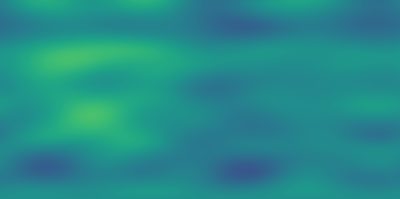
\includegraphics[interpolate=false,width=1.000000in,height=1.000000in]{burgers_rollout_diff_0.01-img0.png}}%
\end{pgfscope}%
\begin{pgfscope}%
\pgfsetbuttcap%
\pgfsetroundjoin%
\definecolor{currentfill}{rgb}{0.000000,0.000000,0.000000}%
\pgfsetfillcolor{currentfill}%
\pgfsetlinewidth{0.803000pt}%
\definecolor{currentstroke}{rgb}{0.000000,0.000000,0.000000}%
\pgfsetstrokecolor{currentstroke}%
\pgfsetdash{}{0pt}%
\pgfsys@defobject{currentmarker}{\pgfqpoint{0.000000in}{-0.048611in}}{\pgfqpoint{0.000000in}{0.000000in}}{%
\pgfpathmoveto{\pgfqpoint{0.000000in}{0.000000in}}%
\pgfpathlineto{\pgfqpoint{0.000000in}{-0.048611in}}%
\pgfusepath{stroke,fill}%
}%
\begin{pgfscope}%
\pgfsys@transformshift{0.726837in}{0.517039in}%
\pgfsys@useobject{currentmarker}{}%
\end{pgfscope}%
\end{pgfscope}%
\begin{pgfscope}%
\definecolor{textcolor}{rgb}{0.000000,0.000000,0.000000}%
\pgfsetstrokecolor{textcolor}%
\pgfsetfillcolor{textcolor}%
\pgftext[x=0.726837in,y=0.419816in,,top]{\color{textcolor}{\rmfamily\fontsize{12.000000}{14.400000}\selectfont\catcode`\^=\active\def^{\ifmmode\sp\else\^{}\fi}\catcode`\%=\active\def%{\%}0}}%
\end{pgfscope}%
\begin{pgfscope}%
\pgfsetbuttcap%
\pgfsetroundjoin%
\definecolor{currentfill}{rgb}{0.000000,0.000000,0.000000}%
\pgfsetfillcolor{currentfill}%
\pgfsetlinewidth{0.803000pt}%
\definecolor{currentstroke}{rgb}{0.000000,0.000000,0.000000}%
\pgfsetstrokecolor{currentstroke}%
\pgfsetdash{}{0pt}%
\pgfsys@defobject{currentmarker}{\pgfqpoint{0.000000in}{-0.048611in}}{\pgfqpoint{0.000000in}{0.000000in}}{%
\pgfpathmoveto{\pgfqpoint{0.000000in}{0.000000in}}%
\pgfpathlineto{\pgfqpoint{0.000000in}{-0.048611in}}%
\pgfusepath{stroke,fill}%
}%
\begin{pgfscope}%
\pgfsys@transformshift{1.570762in}{0.517039in}%
\pgfsys@useobject{currentmarker}{}%
\end{pgfscope}%
\end{pgfscope}%
\begin{pgfscope}%
\definecolor{textcolor}{rgb}{0.000000,0.000000,0.000000}%
\pgfsetstrokecolor{textcolor}%
\pgfsetfillcolor{textcolor}%
\pgftext[x=1.570762in,y=0.419816in,,top]{\color{textcolor}{\rmfamily\fontsize{12.000000}{14.400000}\selectfont\catcode`\^=\active\def^{\ifmmode\sp\else\^{}\fi}\catcode`\%=\active\def%{\%}1}}%
\end{pgfscope}%
\begin{pgfscope}%
\pgfsetbuttcap%
\pgfsetroundjoin%
\definecolor{currentfill}{rgb}{0.000000,0.000000,0.000000}%
\pgfsetfillcolor{currentfill}%
\pgfsetlinewidth{0.803000pt}%
\definecolor{currentstroke}{rgb}{0.000000,0.000000,0.000000}%
\pgfsetstrokecolor{currentstroke}%
\pgfsetdash{}{0pt}%
\pgfsys@defobject{currentmarker}{\pgfqpoint{0.000000in}{-0.048611in}}{\pgfqpoint{0.000000in}{0.000000in}}{%
\pgfpathmoveto{\pgfqpoint{0.000000in}{0.000000in}}%
\pgfpathlineto{\pgfqpoint{0.000000in}{-0.048611in}}%
\pgfusepath{stroke,fill}%
}%
\begin{pgfscope}%
\pgfsys@transformshift{2.414687in}{0.517039in}%
\pgfsys@useobject{currentmarker}{}%
\end{pgfscope}%
\end{pgfscope}%
\begin{pgfscope}%
\definecolor{textcolor}{rgb}{0.000000,0.000000,0.000000}%
\pgfsetstrokecolor{textcolor}%
\pgfsetfillcolor{textcolor}%
\pgftext[x=2.414687in,y=0.419816in,,top]{\color{textcolor}{\rmfamily\fontsize{12.000000}{14.400000}\selectfont\catcode`\^=\active\def^{\ifmmode\sp\else\^{}\fi}\catcode`\%=\active\def%{\%}2}}%
\end{pgfscope}%
\begin{pgfscope}%
\definecolor{textcolor}{rgb}{0.000000,0.000000,0.000000}%
\pgfsetstrokecolor{textcolor}%
\pgfsetfillcolor{textcolor}%
\pgftext[x=1.570762in,y=0.202965in,,top]{\color{textcolor}{\rmfamily\fontsize{12.000000}{14.400000}\selectfont\catcode`\^=\active\def^{\ifmmode\sp\else\^{}\fi}\catcode`\%=\active\def%{\%}Space}}%
\end{pgfscope}%
\begin{pgfscope}%
\pgfsetbuttcap%
\pgfsetroundjoin%
\definecolor{currentfill}{rgb}{0.000000,0.000000,0.000000}%
\pgfsetfillcolor{currentfill}%
\pgfsetlinewidth{0.803000pt}%
\definecolor{currentstroke}{rgb}{0.000000,0.000000,0.000000}%
\pgfsetstrokecolor{currentstroke}%
\pgfsetdash{}{0pt}%
\pgfsys@defobject{currentmarker}{\pgfqpoint{-0.048611in}{0.000000in}}{\pgfqpoint{-0.000000in}{0.000000in}}{%
\pgfpathmoveto{\pgfqpoint{-0.000000in}{0.000000in}}%
\pgfpathlineto{\pgfqpoint{-0.048611in}{0.000000in}}%
\pgfusepath{stroke,fill}%
}%
\begin{pgfscope}%
\pgfsys@transformshift{0.726837in}{0.517039in}%
\pgfsys@useobject{currentmarker}{}%
\end{pgfscope}%
\end{pgfscope}%
\begin{pgfscope}%
\definecolor{textcolor}{rgb}{0.000000,0.000000,0.000000}%
\pgfsetstrokecolor{textcolor}%
\pgfsetfillcolor{textcolor}%
\pgftext[x=0.364559in, y=0.453725in, left, base]{\color{textcolor}{\rmfamily\fontsize{12.000000}{14.400000}\selectfont\catcode`\^=\active\def^{\ifmmode\sp\else\^{}\fi}\catcode`\%=\active\def%{\%}0.0}}%
\end{pgfscope}%
\begin{pgfscope}%
\pgfsetbuttcap%
\pgfsetroundjoin%
\definecolor{currentfill}{rgb}{0.000000,0.000000,0.000000}%
\pgfsetfillcolor{currentfill}%
\pgfsetlinewidth{0.803000pt}%
\definecolor{currentstroke}{rgb}{0.000000,0.000000,0.000000}%
\pgfsetstrokecolor{currentstroke}%
\pgfsetdash{}{0pt}%
\pgfsys@defobject{currentmarker}{\pgfqpoint{-0.048611in}{0.000000in}}{\pgfqpoint{-0.000000in}{0.000000in}}{%
\pgfpathmoveto{\pgfqpoint{-0.000000in}{0.000000in}}%
\pgfpathlineto{\pgfqpoint{-0.048611in}{0.000000in}}%
\pgfusepath{stroke,fill}%
}%
\begin{pgfscope}%
\pgfsys@transformshift{0.726837in}{0.861533in}%
\pgfsys@useobject{currentmarker}{}%
\end{pgfscope}%
\end{pgfscope}%
\begin{pgfscope}%
\definecolor{textcolor}{rgb}{0.000000,0.000000,0.000000}%
\pgfsetstrokecolor{textcolor}%
\pgfsetfillcolor{textcolor}%
\pgftext[x=0.364559in, y=0.798219in, left, base]{\color{textcolor}{\rmfamily\fontsize{12.000000}{14.400000}\selectfont\catcode`\^=\active\def^{\ifmmode\sp\else\^{}\fi}\catcode`\%=\active\def%{\%}2.5}}%
\end{pgfscope}%
\begin{pgfscope}%
\pgfsetbuttcap%
\pgfsetroundjoin%
\definecolor{currentfill}{rgb}{0.000000,0.000000,0.000000}%
\pgfsetfillcolor{currentfill}%
\pgfsetlinewidth{0.803000pt}%
\definecolor{currentstroke}{rgb}{0.000000,0.000000,0.000000}%
\pgfsetstrokecolor{currentstroke}%
\pgfsetdash{}{0pt}%
\pgfsys@defobject{currentmarker}{\pgfqpoint{-0.048611in}{0.000000in}}{\pgfqpoint{-0.000000in}{0.000000in}}{%
\pgfpathmoveto{\pgfqpoint{-0.000000in}{0.000000in}}%
\pgfpathlineto{\pgfqpoint{-0.048611in}{0.000000in}}%
\pgfusepath{stroke,fill}%
}%
\begin{pgfscope}%
\pgfsys@transformshift{0.726837in}{1.206027in}%
\pgfsys@useobject{currentmarker}{}%
\end{pgfscope}%
\end{pgfscope}%
\begin{pgfscope}%
\definecolor{textcolor}{rgb}{0.000000,0.000000,0.000000}%
\pgfsetstrokecolor{textcolor}%
\pgfsetfillcolor{textcolor}%
\pgftext[x=0.364559in, y=1.142714in, left, base]{\color{textcolor}{\rmfamily\fontsize{12.000000}{14.400000}\selectfont\catcode`\^=\active\def^{\ifmmode\sp\else\^{}\fi}\catcode`\%=\active\def%{\%}5.0}}%
\end{pgfscope}%
\begin{pgfscope}%
\pgfsetbuttcap%
\pgfsetroundjoin%
\definecolor{currentfill}{rgb}{0.000000,0.000000,0.000000}%
\pgfsetfillcolor{currentfill}%
\pgfsetlinewidth{0.803000pt}%
\definecolor{currentstroke}{rgb}{0.000000,0.000000,0.000000}%
\pgfsetstrokecolor{currentstroke}%
\pgfsetdash{}{0pt}%
\pgfsys@defobject{currentmarker}{\pgfqpoint{-0.048611in}{0.000000in}}{\pgfqpoint{-0.000000in}{0.000000in}}{%
\pgfpathmoveto{\pgfqpoint{-0.000000in}{0.000000in}}%
\pgfpathlineto{\pgfqpoint{-0.048611in}{0.000000in}}%
\pgfusepath{stroke,fill}%
}%
\begin{pgfscope}%
\pgfsys@transformshift{0.726837in}{1.550522in}%
\pgfsys@useobject{currentmarker}{}%
\end{pgfscope}%
\end{pgfscope}%
\begin{pgfscope}%
\definecolor{textcolor}{rgb}{0.000000,0.000000,0.000000}%
\pgfsetstrokecolor{textcolor}%
\pgfsetfillcolor{textcolor}%
\pgftext[x=0.364559in, y=1.487208in, left, base]{\color{textcolor}{\rmfamily\fontsize{12.000000}{14.400000}\selectfont\catcode`\^=\active\def^{\ifmmode\sp\else\^{}\fi}\catcode`\%=\active\def%{\%}7.5}}%
\end{pgfscope}%
\begin{pgfscope}%
\pgfsetbuttcap%
\pgfsetroundjoin%
\definecolor{currentfill}{rgb}{0.000000,0.000000,0.000000}%
\pgfsetfillcolor{currentfill}%
\pgfsetlinewidth{0.803000pt}%
\definecolor{currentstroke}{rgb}{0.000000,0.000000,0.000000}%
\pgfsetstrokecolor{currentstroke}%
\pgfsetdash{}{0pt}%
\pgfsys@defobject{currentmarker}{\pgfqpoint{-0.048611in}{0.000000in}}{\pgfqpoint{-0.000000in}{0.000000in}}{%
\pgfpathmoveto{\pgfqpoint{-0.000000in}{0.000000in}}%
\pgfpathlineto{\pgfqpoint{-0.048611in}{0.000000in}}%
\pgfusepath{stroke,fill}%
}%
\begin{pgfscope}%
\pgfsys@transformshift{0.726837in}{1.895016in}%
\pgfsys@useobject{currentmarker}{}%
\end{pgfscope}%
\end{pgfscope}%
\begin{pgfscope}%
\definecolor{textcolor}{rgb}{0.000000,0.000000,0.000000}%
\pgfsetstrokecolor{textcolor}%
\pgfsetfillcolor{textcolor}%
\pgftext[x=0.258521in, y=1.831702in, left, base]{\color{textcolor}{\rmfamily\fontsize{12.000000}{14.400000}\selectfont\catcode`\^=\active\def^{\ifmmode\sp\else\^{}\fi}\catcode`\%=\active\def%{\%}10.0}}%
\end{pgfscope}%
\begin{pgfscope}%
\definecolor{textcolor}{rgb}{0.000000,0.000000,0.000000}%
\pgfsetstrokecolor{textcolor}%
\pgfsetfillcolor{textcolor}%
\pgftext[x=0.202965in,y=1.206027in,,bottom,rotate=90.000000]{\color{textcolor}{\rmfamily\fontsize{12.000000}{14.400000}\selectfont\catcode`\^=\active\def^{\ifmmode\sp\else\^{}\fi}\catcode`\%=\active\def%{\%}Time}}%
\end{pgfscope}%
\begin{pgfscope}%
\pgfsetrectcap%
\pgfsetmiterjoin%
\pgfsetlinewidth{0.803000pt}%
\definecolor{currentstroke}{rgb}{0.000000,0.000000,0.000000}%
\pgfsetstrokecolor{currentstroke}%
\pgfsetdash{}{0pt}%
\pgfpathmoveto{\pgfqpoint{0.726837in}{0.517039in}}%
\pgfpathlineto{\pgfqpoint{0.726837in}{1.895016in}}%
\pgfusepath{stroke}%
\end{pgfscope}%
\begin{pgfscope}%
\pgfsetrectcap%
\pgfsetmiterjoin%
\pgfsetlinewidth{0.803000pt}%
\definecolor{currentstroke}{rgb}{0.000000,0.000000,0.000000}%
\pgfsetstrokecolor{currentstroke}%
\pgfsetdash{}{0pt}%
\pgfpathmoveto{\pgfqpoint{2.414687in}{0.517039in}}%
\pgfpathlineto{\pgfqpoint{2.414687in}{1.895016in}}%
\pgfusepath{stroke}%
\end{pgfscope}%
\begin{pgfscope}%
\pgfsetrectcap%
\pgfsetmiterjoin%
\pgfsetlinewidth{0.803000pt}%
\definecolor{currentstroke}{rgb}{0.000000,0.000000,0.000000}%
\pgfsetstrokecolor{currentstroke}%
\pgfsetdash{}{0pt}%
\pgfpathmoveto{\pgfqpoint{0.726837in}{0.517039in}}%
\pgfpathlineto{\pgfqpoint{2.414687in}{0.517039in}}%
\pgfusepath{stroke}%
\end{pgfscope}%
\begin{pgfscope}%
\pgfsetrectcap%
\pgfsetmiterjoin%
\pgfsetlinewidth{0.803000pt}%
\definecolor{currentstroke}{rgb}{0.000000,0.000000,0.000000}%
\pgfsetstrokecolor{currentstroke}%
\pgfsetdash{}{0pt}%
\pgfpathmoveto{\pgfqpoint{0.726837in}{1.895016in}}%
\pgfpathlineto{\pgfqpoint{2.414687in}{1.895016in}}%
\pgfusepath{stroke}%
\end{pgfscope}%
\begin{pgfscope}%
\pgfsetbuttcap%
\pgfsetmiterjoin%
\pgfsetlinewidth{0.000000pt}%
\definecolor{currentstroke}{rgb}{0.000000,0.000000,0.000000}%
\pgfsetstrokecolor{currentstroke}%
\pgfsetstrokeopacity{0.000000}%
\pgfsetdash{}{0pt}%
\pgfpathmoveto{\pgfqpoint{2.552099in}{0.517039in}}%
\pgfpathlineto{\pgfqpoint{2.620998in}{0.517039in}}%
\pgfpathlineto{\pgfqpoint{2.620998in}{1.895016in}}%
\pgfpathlineto{\pgfqpoint{2.552099in}{1.895016in}}%
\pgfpathlineto{\pgfqpoint{2.552099in}{0.517039in}}%
\pgfpathclose%
\pgfusepath{}%
\end{pgfscope}%
\begin{pgfscope}%
\pgfsys@transformshift{2.550000in}{0.520000in}%
\pgftext[left,bottom]{
\includegraphics[interpolate=true,width=0.070000in,height=1.380000in]{burgers_rollout_diff_0.01-img1.png}}%
\end{pgfscope}%
\begin{pgfscope}%
\pgfsetbuttcap%
\pgfsetroundjoin%
\definecolor{currentfill}{rgb}{0.000000,0.000000,0.000000}%
\pgfsetfillcolor{currentfill}%
\pgfsetlinewidth{0.803000pt}%
\definecolor{currentstroke}{rgb}{0.000000,0.000000,0.000000}%
\pgfsetstrokecolor{currentstroke}%
\pgfsetdash{}{0pt}%
\pgfsys@defobject{currentmarker}{\pgfqpoint{0.000000in}{0.000000in}}{\pgfqpoint{0.048611in}{0.000000in}}{%
\pgfpathmoveto{\pgfqpoint{0.000000in}{0.000000in}}%
\pgfpathlineto{\pgfqpoint{0.048611in}{0.000000in}}%
\pgfusepath{stroke,fill}%
}%
\begin{pgfscope}%
\pgfsys@transformshift{2.620998in}{0.588723in}%
\pgfsys@useobject{currentmarker}{}%
\end{pgfscope}%
\end{pgfscope}%
\begin{pgfscope}%
\definecolor{textcolor}{rgb}{0.000000,0.000000,0.000000}%
\pgfsetstrokecolor{textcolor}%
\pgfsetfillcolor{textcolor}%
\pgftext[x=2.718220in, y=0.525410in, left, base]{\color{textcolor}{\rmfamily\fontsize{12.000000}{14.400000}\selectfont\catcode`\^=\active\def^{\ifmmode\sp\else\^{}\fi}\catcode`\%=\active\def%{\%}\ensuremath{-}1}}%
\end{pgfscope}%
\begin{pgfscope}%
\pgfsetbuttcap%
\pgfsetroundjoin%
\definecolor{currentfill}{rgb}{0.000000,0.000000,0.000000}%
\pgfsetfillcolor{currentfill}%
\pgfsetlinewidth{0.803000pt}%
\definecolor{currentstroke}{rgb}{0.000000,0.000000,0.000000}%
\pgfsetstrokecolor{currentstroke}%
\pgfsetdash{}{0pt}%
\pgfsys@defobject{currentmarker}{\pgfqpoint{0.000000in}{0.000000in}}{\pgfqpoint{0.048611in}{0.000000in}}{%
\pgfpathmoveto{\pgfqpoint{0.000000in}{0.000000in}}%
\pgfpathlineto{\pgfqpoint{0.048611in}{0.000000in}}%
\pgfusepath{stroke,fill}%
}%
\begin{pgfscope}%
\pgfsys@transformshift{2.620998in}{1.206027in}%
\pgfsys@useobject{currentmarker}{}%
\end{pgfscope}%
\end{pgfscope}%
\begin{pgfscope}%
\definecolor{textcolor}{rgb}{0.000000,0.000000,0.000000}%
\pgfsetstrokecolor{textcolor}%
\pgfsetfillcolor{textcolor}%
\pgftext[x=2.718220in, y=1.142714in, left, base]{\color{textcolor}{\rmfamily\fontsize{12.000000}{14.400000}\selectfont\catcode`\^=\active\def^{\ifmmode\sp\else\^{}\fi}\catcode`\%=\active\def%{\%}0}}%
\end{pgfscope}%
\begin{pgfscope}%
\pgfsetbuttcap%
\pgfsetroundjoin%
\definecolor{currentfill}{rgb}{0.000000,0.000000,0.000000}%
\pgfsetfillcolor{currentfill}%
\pgfsetlinewidth{0.803000pt}%
\definecolor{currentstroke}{rgb}{0.000000,0.000000,0.000000}%
\pgfsetstrokecolor{currentstroke}%
\pgfsetdash{}{0pt}%
\pgfsys@defobject{currentmarker}{\pgfqpoint{0.000000in}{0.000000in}}{\pgfqpoint{0.048611in}{0.000000in}}{%
\pgfpathmoveto{\pgfqpoint{0.000000in}{0.000000in}}%
\pgfpathlineto{\pgfqpoint{0.048611in}{0.000000in}}%
\pgfusepath{stroke,fill}%
}%
\begin{pgfscope}%
\pgfsys@transformshift{2.620998in}{1.823331in}%
\pgfsys@useobject{currentmarker}{}%
\end{pgfscope}%
\end{pgfscope}%
\begin{pgfscope}%
\definecolor{textcolor}{rgb}{0.000000,0.000000,0.000000}%
\pgfsetstrokecolor{textcolor}%
\pgfsetfillcolor{textcolor}%
\pgftext[x=2.718220in, y=1.760018in, left, base]{\color{textcolor}{\rmfamily\fontsize{12.000000}{14.400000}\selectfont\catcode`\^=\active\def^{\ifmmode\sp\else\^{}\fi}\catcode`\%=\active\def%{\%}1}}%
\end{pgfscope}%
\begin{pgfscope}%
\pgfsetrectcap%
\pgfsetmiterjoin%
\pgfsetlinewidth{0.803000pt}%
\definecolor{currentstroke}{rgb}{0.000000,0.000000,0.000000}%
\pgfsetstrokecolor{currentstroke}%
\pgfsetdash{}{0pt}%
\pgfpathmoveto{\pgfqpoint{2.552099in}{0.517039in}}%
\pgfpathlineto{\pgfqpoint{2.586548in}{0.517039in}}%
\pgfpathlineto{\pgfqpoint{2.620998in}{0.517039in}}%
\pgfpathlineto{\pgfqpoint{2.620998in}{1.895016in}}%
\pgfpathlineto{\pgfqpoint{2.586548in}{1.895016in}}%
\pgfpathlineto{\pgfqpoint{2.552099in}{1.895016in}}%
\pgfpathlineto{\pgfqpoint{2.552099in}{0.517039in}}%
\pgfpathclose%
\pgfusepath{stroke}%
\end{pgfscope}%
\end{pgfpicture}%
\makeatother%
\endgroup%

      \end{adjustbox}
      \caption{The difference for \(\nu=0.01\)}\label{fig:sc2_rollout_diff_0.01}
    \end{subfigure}
    \\[0.7\baselineskip]
    \begin{subfigure}{0.33\linewidth}
      \begin{adjustbox}{width=\linewidth}
        \begingroup%
\makeatletter%
\begin{pgfpicture}%
\pgfpathrectangle{\pgfpointorigin}{\pgfqpoint{3.000000in}{2.000000in}}%
\pgfusepath{use as bounding box, clip}%
\begin{pgfscope}%
\pgfsetbuttcap%
\pgfsetmiterjoin%
\pgfsetlinewidth{0.000000pt}%
\definecolor{currentstroke}{rgb}{0.000000,0.000000,0.000000}%
\pgfsetstrokecolor{currentstroke}%
\pgfsetstrokeopacity{0.000000}%
\pgfsetdash{}{0pt}%
\pgfpathmoveto{\pgfqpoint{0.000000in}{0.000000in}}%
\pgfpathlineto{\pgfqpoint{3.000000in}{0.000000in}}%
\pgfpathlineto{\pgfqpoint{3.000000in}{2.000000in}}%
\pgfpathlineto{\pgfqpoint{0.000000in}{2.000000in}}%
\pgfpathlineto{\pgfqpoint{0.000000in}{0.000000in}}%
\pgfpathclose%
\pgfusepath{}%
\end{pgfscope}%
\begin{pgfscope}%
\pgfsetbuttcap%
\pgfsetmiterjoin%
\pgfsetlinewidth{0.000000pt}%
\definecolor{currentstroke}{rgb}{0.000000,0.000000,0.000000}%
\pgfsetstrokecolor{currentstroke}%
\pgfsetstrokeopacity{0.000000}%
\pgfsetdash{}{0pt}%
\pgfpathmoveto{\pgfqpoint{0.726837in}{0.517039in}}%
\pgfpathlineto{\pgfqpoint{2.414687in}{0.517039in}}%
\pgfpathlineto{\pgfqpoint{2.414687in}{1.895016in}}%
\pgfpathlineto{\pgfqpoint{0.726837in}{1.895016in}}%
\pgfpathlineto{\pgfqpoint{0.726837in}{0.517039in}}%
\pgfpathclose%
\pgfusepath{}%
\end{pgfscope}%
\begin{pgfscope}%
\pgfpathrectangle{\pgfqpoint{0.726837in}{0.517039in}}{\pgfqpoint{1.687850in}{1.377978in}}%
\pgfusepath{clip}%
\pgfsys@transformcm{1.687850}{0.000000}{0.000000}{1.377978}{0.726837in}{0.517039in}%
\pgftext[left,bottom]{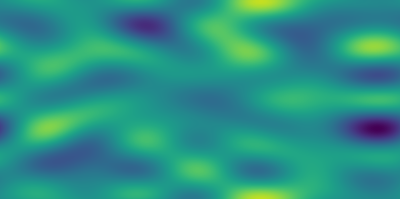
\includegraphics[interpolate=false,width=1.000000in,height=1.000000in]{burgers_rollout_target_0.1-img0.png}}%
\end{pgfscope}%
\begin{pgfscope}%
\pgfsetbuttcap%
\pgfsetroundjoin%
\definecolor{currentfill}{rgb}{0.000000,0.000000,0.000000}%
\pgfsetfillcolor{currentfill}%
\pgfsetlinewidth{0.803000pt}%
\definecolor{currentstroke}{rgb}{0.000000,0.000000,0.000000}%
\pgfsetstrokecolor{currentstroke}%
\pgfsetdash{}{0pt}%
\pgfsys@defobject{currentmarker}{\pgfqpoint{0.000000in}{-0.048611in}}{\pgfqpoint{0.000000in}{0.000000in}}{%
\pgfpathmoveto{\pgfqpoint{0.000000in}{0.000000in}}%
\pgfpathlineto{\pgfqpoint{0.000000in}{-0.048611in}}%
\pgfusepath{stroke,fill}%
}%
\begin{pgfscope}%
\pgfsys@transformshift{0.726837in}{0.517039in}%
\pgfsys@useobject{currentmarker}{}%
\end{pgfscope}%
\end{pgfscope}%
\begin{pgfscope}%
\definecolor{textcolor}{rgb}{0.000000,0.000000,0.000000}%
\pgfsetstrokecolor{textcolor}%
\pgfsetfillcolor{textcolor}%
\pgftext[x=0.726837in,y=0.419816in,,top]{\color{textcolor}\rmfamily\fontsize{12.000000}{14.400000}\selectfont 0}%
\end{pgfscope}%
\begin{pgfscope}%
\pgfsetbuttcap%
\pgfsetroundjoin%
\definecolor{currentfill}{rgb}{0.000000,0.000000,0.000000}%
\pgfsetfillcolor{currentfill}%
\pgfsetlinewidth{0.803000pt}%
\definecolor{currentstroke}{rgb}{0.000000,0.000000,0.000000}%
\pgfsetstrokecolor{currentstroke}%
\pgfsetdash{}{0pt}%
\pgfsys@defobject{currentmarker}{\pgfqpoint{0.000000in}{-0.048611in}}{\pgfqpoint{0.000000in}{0.000000in}}{%
\pgfpathmoveto{\pgfqpoint{0.000000in}{0.000000in}}%
\pgfpathlineto{\pgfqpoint{0.000000in}{-0.048611in}}%
\pgfusepath{stroke,fill}%
}%
\begin{pgfscope}%
\pgfsys@transformshift{1.570762in}{0.517039in}%
\pgfsys@useobject{currentmarker}{}%
\end{pgfscope}%
\end{pgfscope}%
\begin{pgfscope}%
\definecolor{textcolor}{rgb}{0.000000,0.000000,0.000000}%
\pgfsetstrokecolor{textcolor}%
\pgfsetfillcolor{textcolor}%
\pgftext[x=1.570762in,y=0.419816in,,top]{\color{textcolor}\rmfamily\fontsize{12.000000}{14.400000}\selectfont 1}%
\end{pgfscope}%
\begin{pgfscope}%
\pgfsetbuttcap%
\pgfsetroundjoin%
\definecolor{currentfill}{rgb}{0.000000,0.000000,0.000000}%
\pgfsetfillcolor{currentfill}%
\pgfsetlinewidth{0.803000pt}%
\definecolor{currentstroke}{rgb}{0.000000,0.000000,0.000000}%
\pgfsetstrokecolor{currentstroke}%
\pgfsetdash{}{0pt}%
\pgfsys@defobject{currentmarker}{\pgfqpoint{0.000000in}{-0.048611in}}{\pgfqpoint{0.000000in}{0.000000in}}{%
\pgfpathmoveto{\pgfqpoint{0.000000in}{0.000000in}}%
\pgfpathlineto{\pgfqpoint{0.000000in}{-0.048611in}}%
\pgfusepath{stroke,fill}%
}%
\begin{pgfscope}%
\pgfsys@transformshift{2.414687in}{0.517039in}%
\pgfsys@useobject{currentmarker}{}%
\end{pgfscope}%
\end{pgfscope}%
\begin{pgfscope}%
\definecolor{textcolor}{rgb}{0.000000,0.000000,0.000000}%
\pgfsetstrokecolor{textcolor}%
\pgfsetfillcolor{textcolor}%
\pgftext[x=2.414687in,y=0.419816in,,top]{\color{textcolor}\rmfamily\fontsize{12.000000}{14.400000}\selectfont 2}%
\end{pgfscope}%
\begin{pgfscope}%
\definecolor{textcolor}{rgb}{0.000000,0.000000,0.000000}%
\pgfsetstrokecolor{textcolor}%
\pgfsetfillcolor{textcolor}%
\pgftext[x=1.570762in,y=0.202965in,,top]{\color{textcolor}\rmfamily\fontsize{12.000000}{14.400000}\selectfont Space}%
\end{pgfscope}%
\begin{pgfscope}%
\pgfsetbuttcap%
\pgfsetroundjoin%
\definecolor{currentfill}{rgb}{0.000000,0.000000,0.000000}%
\pgfsetfillcolor{currentfill}%
\pgfsetlinewidth{0.803000pt}%
\definecolor{currentstroke}{rgb}{0.000000,0.000000,0.000000}%
\pgfsetstrokecolor{currentstroke}%
\pgfsetdash{}{0pt}%
\pgfsys@defobject{currentmarker}{\pgfqpoint{-0.048611in}{0.000000in}}{\pgfqpoint{-0.000000in}{0.000000in}}{%
\pgfpathmoveto{\pgfqpoint{-0.000000in}{0.000000in}}%
\pgfpathlineto{\pgfqpoint{-0.048611in}{0.000000in}}%
\pgfusepath{stroke,fill}%
}%
\begin{pgfscope}%
\pgfsys@transformshift{0.726837in}{0.517039in}%
\pgfsys@useobject{currentmarker}{}%
\end{pgfscope}%
\end{pgfscope}%
\begin{pgfscope}%
\definecolor{textcolor}{rgb}{0.000000,0.000000,0.000000}%
\pgfsetstrokecolor{textcolor}%
\pgfsetfillcolor{textcolor}%
\pgftext[x=0.364559in, y=0.453725in, left, base]{\color{textcolor}\rmfamily\fontsize{12.000000}{14.400000}\selectfont 0.0}%
\end{pgfscope}%
\begin{pgfscope}%
\pgfsetbuttcap%
\pgfsetroundjoin%
\definecolor{currentfill}{rgb}{0.000000,0.000000,0.000000}%
\pgfsetfillcolor{currentfill}%
\pgfsetlinewidth{0.803000pt}%
\definecolor{currentstroke}{rgb}{0.000000,0.000000,0.000000}%
\pgfsetstrokecolor{currentstroke}%
\pgfsetdash{}{0pt}%
\pgfsys@defobject{currentmarker}{\pgfqpoint{-0.048611in}{0.000000in}}{\pgfqpoint{-0.000000in}{0.000000in}}{%
\pgfpathmoveto{\pgfqpoint{-0.000000in}{0.000000in}}%
\pgfpathlineto{\pgfqpoint{-0.048611in}{0.000000in}}%
\pgfusepath{stroke,fill}%
}%
\begin{pgfscope}%
\pgfsys@transformshift{0.726837in}{0.861533in}%
\pgfsys@useobject{currentmarker}{}%
\end{pgfscope}%
\end{pgfscope}%
\begin{pgfscope}%
\definecolor{textcolor}{rgb}{0.000000,0.000000,0.000000}%
\pgfsetstrokecolor{textcolor}%
\pgfsetfillcolor{textcolor}%
\pgftext[x=0.364559in, y=0.798219in, left, base]{\color{textcolor}\rmfamily\fontsize{12.000000}{14.400000}\selectfont 2.5}%
\end{pgfscope}%
\begin{pgfscope}%
\pgfsetbuttcap%
\pgfsetroundjoin%
\definecolor{currentfill}{rgb}{0.000000,0.000000,0.000000}%
\pgfsetfillcolor{currentfill}%
\pgfsetlinewidth{0.803000pt}%
\definecolor{currentstroke}{rgb}{0.000000,0.000000,0.000000}%
\pgfsetstrokecolor{currentstroke}%
\pgfsetdash{}{0pt}%
\pgfsys@defobject{currentmarker}{\pgfqpoint{-0.048611in}{0.000000in}}{\pgfqpoint{-0.000000in}{0.000000in}}{%
\pgfpathmoveto{\pgfqpoint{-0.000000in}{0.000000in}}%
\pgfpathlineto{\pgfqpoint{-0.048611in}{0.000000in}}%
\pgfusepath{stroke,fill}%
}%
\begin{pgfscope}%
\pgfsys@transformshift{0.726837in}{1.206027in}%
\pgfsys@useobject{currentmarker}{}%
\end{pgfscope}%
\end{pgfscope}%
\begin{pgfscope}%
\definecolor{textcolor}{rgb}{0.000000,0.000000,0.000000}%
\pgfsetstrokecolor{textcolor}%
\pgfsetfillcolor{textcolor}%
\pgftext[x=0.364559in, y=1.142714in, left, base]{\color{textcolor}\rmfamily\fontsize{12.000000}{14.400000}\selectfont 5.0}%
\end{pgfscope}%
\begin{pgfscope}%
\pgfsetbuttcap%
\pgfsetroundjoin%
\definecolor{currentfill}{rgb}{0.000000,0.000000,0.000000}%
\pgfsetfillcolor{currentfill}%
\pgfsetlinewidth{0.803000pt}%
\definecolor{currentstroke}{rgb}{0.000000,0.000000,0.000000}%
\pgfsetstrokecolor{currentstroke}%
\pgfsetdash{}{0pt}%
\pgfsys@defobject{currentmarker}{\pgfqpoint{-0.048611in}{0.000000in}}{\pgfqpoint{-0.000000in}{0.000000in}}{%
\pgfpathmoveto{\pgfqpoint{-0.000000in}{0.000000in}}%
\pgfpathlineto{\pgfqpoint{-0.048611in}{0.000000in}}%
\pgfusepath{stroke,fill}%
}%
\begin{pgfscope}%
\pgfsys@transformshift{0.726837in}{1.550522in}%
\pgfsys@useobject{currentmarker}{}%
\end{pgfscope}%
\end{pgfscope}%
\begin{pgfscope}%
\definecolor{textcolor}{rgb}{0.000000,0.000000,0.000000}%
\pgfsetstrokecolor{textcolor}%
\pgfsetfillcolor{textcolor}%
\pgftext[x=0.364559in, y=1.487208in, left, base]{\color{textcolor}\rmfamily\fontsize{12.000000}{14.400000}\selectfont 7.5}%
\end{pgfscope}%
\begin{pgfscope}%
\pgfsetbuttcap%
\pgfsetroundjoin%
\definecolor{currentfill}{rgb}{0.000000,0.000000,0.000000}%
\pgfsetfillcolor{currentfill}%
\pgfsetlinewidth{0.803000pt}%
\definecolor{currentstroke}{rgb}{0.000000,0.000000,0.000000}%
\pgfsetstrokecolor{currentstroke}%
\pgfsetdash{}{0pt}%
\pgfsys@defobject{currentmarker}{\pgfqpoint{-0.048611in}{0.000000in}}{\pgfqpoint{-0.000000in}{0.000000in}}{%
\pgfpathmoveto{\pgfqpoint{-0.000000in}{0.000000in}}%
\pgfpathlineto{\pgfqpoint{-0.048611in}{0.000000in}}%
\pgfusepath{stroke,fill}%
}%
\begin{pgfscope}%
\pgfsys@transformshift{0.726837in}{1.895016in}%
\pgfsys@useobject{currentmarker}{}%
\end{pgfscope}%
\end{pgfscope}%
\begin{pgfscope}%
\definecolor{textcolor}{rgb}{0.000000,0.000000,0.000000}%
\pgfsetstrokecolor{textcolor}%
\pgfsetfillcolor{textcolor}%
\pgftext[x=0.258521in, y=1.831702in, left, base]{\color{textcolor}\rmfamily\fontsize{12.000000}{14.400000}\selectfont 10.0}%
\end{pgfscope}%
\begin{pgfscope}%
\definecolor{textcolor}{rgb}{0.000000,0.000000,0.000000}%
\pgfsetstrokecolor{textcolor}%
\pgfsetfillcolor{textcolor}%
\pgftext[x=0.202965in,y=1.206027in,,bottom,rotate=90.000000]{\color{textcolor}\rmfamily\fontsize{12.000000}{14.400000}\selectfont Time}%
\end{pgfscope}%
\begin{pgfscope}%
\pgfsetrectcap%
\pgfsetmiterjoin%
\pgfsetlinewidth{0.803000pt}%
\definecolor{currentstroke}{rgb}{0.000000,0.000000,0.000000}%
\pgfsetstrokecolor{currentstroke}%
\pgfsetdash{}{0pt}%
\pgfpathmoveto{\pgfqpoint{0.726837in}{0.517039in}}%
\pgfpathlineto{\pgfqpoint{0.726837in}{1.895016in}}%
\pgfusepath{stroke}%
\end{pgfscope}%
\begin{pgfscope}%
\pgfsetrectcap%
\pgfsetmiterjoin%
\pgfsetlinewidth{0.803000pt}%
\definecolor{currentstroke}{rgb}{0.000000,0.000000,0.000000}%
\pgfsetstrokecolor{currentstroke}%
\pgfsetdash{}{0pt}%
\pgfpathmoveto{\pgfqpoint{2.414687in}{0.517039in}}%
\pgfpathlineto{\pgfqpoint{2.414687in}{1.895016in}}%
\pgfusepath{stroke}%
\end{pgfscope}%
\begin{pgfscope}%
\pgfsetrectcap%
\pgfsetmiterjoin%
\pgfsetlinewidth{0.803000pt}%
\definecolor{currentstroke}{rgb}{0.000000,0.000000,0.000000}%
\pgfsetstrokecolor{currentstroke}%
\pgfsetdash{}{0pt}%
\pgfpathmoveto{\pgfqpoint{0.726837in}{0.517039in}}%
\pgfpathlineto{\pgfqpoint{2.414687in}{0.517039in}}%
\pgfusepath{stroke}%
\end{pgfscope}%
\begin{pgfscope}%
\pgfsetrectcap%
\pgfsetmiterjoin%
\pgfsetlinewidth{0.803000pt}%
\definecolor{currentstroke}{rgb}{0.000000,0.000000,0.000000}%
\pgfsetstrokecolor{currentstroke}%
\pgfsetdash{}{0pt}%
\pgfpathmoveto{\pgfqpoint{0.726837in}{1.895016in}}%
\pgfpathlineto{\pgfqpoint{2.414687in}{1.895016in}}%
\pgfusepath{stroke}%
\end{pgfscope}%
\begin{pgfscope}%
\pgfsetbuttcap%
\pgfsetmiterjoin%
\pgfsetlinewidth{0.000000pt}%
\definecolor{currentstroke}{rgb}{0.000000,0.000000,0.000000}%
\pgfsetstrokecolor{currentstroke}%
\pgfsetstrokeopacity{0.000000}%
\pgfsetdash{}{0pt}%
\pgfpathmoveto{\pgfqpoint{2.552099in}{0.517039in}}%
\pgfpathlineto{\pgfqpoint{2.620998in}{0.517039in}}%
\pgfpathlineto{\pgfqpoint{2.620998in}{1.895016in}}%
\pgfpathlineto{\pgfqpoint{2.552099in}{1.895016in}}%
\pgfpathlineto{\pgfqpoint{2.552099in}{0.517039in}}%
\pgfpathclose%
\pgfusepath{}%
\end{pgfscope}%
\begin{pgfscope}%
\pgfsys@transformshift{2.550000in}{0.520000in}%
\pgftext[left,bottom]{
\includegraphics[interpolate=true,width=0.070000in,height=1.380000in]{burgers_rollout_target_0.1-img1.png}}%
\end{pgfscope}%
\begin{pgfscope}%
\pgfsetbuttcap%
\pgfsetroundjoin%
\definecolor{currentfill}{rgb}{0.000000,0.000000,0.000000}%
\pgfsetfillcolor{currentfill}%
\pgfsetlinewidth{0.803000pt}%
\definecolor{currentstroke}{rgb}{0.000000,0.000000,0.000000}%
\pgfsetstrokecolor{currentstroke}%
\pgfsetdash{}{0pt}%
\pgfsys@defobject{currentmarker}{\pgfqpoint{0.000000in}{0.000000in}}{\pgfqpoint{0.048611in}{0.000000in}}{%
\pgfpathmoveto{\pgfqpoint{0.000000in}{0.000000in}}%
\pgfpathlineto{\pgfqpoint{0.048611in}{0.000000in}}%
\pgfusepath{stroke,fill}%
}%
\begin{pgfscope}%
\pgfsys@transformshift{2.620998in}{0.588723in}%
\pgfsys@useobject{currentmarker}{}%
\end{pgfscope}%
\end{pgfscope}%
\begin{pgfscope}%
\definecolor{textcolor}{rgb}{0.000000,0.000000,0.000000}%
\pgfsetstrokecolor{textcolor}%
\pgfsetfillcolor{textcolor}%
\pgftext[x=2.718220in, y=0.525410in, left, base]{\color{textcolor}\rmfamily\fontsize{12.000000}{14.400000}\selectfont \ensuremath{-}1}%
\end{pgfscope}%
\begin{pgfscope}%
\pgfsetbuttcap%
\pgfsetroundjoin%
\definecolor{currentfill}{rgb}{0.000000,0.000000,0.000000}%
\pgfsetfillcolor{currentfill}%
\pgfsetlinewidth{0.803000pt}%
\definecolor{currentstroke}{rgb}{0.000000,0.000000,0.000000}%
\pgfsetstrokecolor{currentstroke}%
\pgfsetdash{}{0pt}%
\pgfsys@defobject{currentmarker}{\pgfqpoint{0.000000in}{0.000000in}}{\pgfqpoint{0.048611in}{0.000000in}}{%
\pgfpathmoveto{\pgfqpoint{0.000000in}{0.000000in}}%
\pgfpathlineto{\pgfqpoint{0.048611in}{0.000000in}}%
\pgfusepath{stroke,fill}%
}%
\begin{pgfscope}%
\pgfsys@transformshift{2.620998in}{1.206027in}%
\pgfsys@useobject{currentmarker}{}%
\end{pgfscope}%
\end{pgfscope}%
\begin{pgfscope}%
\definecolor{textcolor}{rgb}{0.000000,0.000000,0.000000}%
\pgfsetstrokecolor{textcolor}%
\pgfsetfillcolor{textcolor}%
\pgftext[x=2.718220in, y=1.142714in, left, base]{\color{textcolor}\rmfamily\fontsize{12.000000}{14.400000}\selectfont 0}%
\end{pgfscope}%
\begin{pgfscope}%
\pgfsetbuttcap%
\pgfsetroundjoin%
\definecolor{currentfill}{rgb}{0.000000,0.000000,0.000000}%
\pgfsetfillcolor{currentfill}%
\pgfsetlinewidth{0.803000pt}%
\definecolor{currentstroke}{rgb}{0.000000,0.000000,0.000000}%
\pgfsetstrokecolor{currentstroke}%
\pgfsetdash{}{0pt}%
\pgfsys@defobject{currentmarker}{\pgfqpoint{0.000000in}{0.000000in}}{\pgfqpoint{0.048611in}{0.000000in}}{%
\pgfpathmoveto{\pgfqpoint{0.000000in}{0.000000in}}%
\pgfpathlineto{\pgfqpoint{0.048611in}{0.000000in}}%
\pgfusepath{stroke,fill}%
}%
\begin{pgfscope}%
\pgfsys@transformshift{2.620998in}{1.823331in}%
\pgfsys@useobject{currentmarker}{}%
\end{pgfscope}%
\end{pgfscope}%
\begin{pgfscope}%
\definecolor{textcolor}{rgb}{0.000000,0.000000,0.000000}%
\pgfsetstrokecolor{textcolor}%
\pgfsetfillcolor{textcolor}%
\pgftext[x=2.718220in, y=1.760018in, left, base]{\color{textcolor}\rmfamily\fontsize{12.000000}{14.400000}\selectfont 1}%
\end{pgfscope}%
\begin{pgfscope}%
\pgfsetrectcap%
\pgfsetmiterjoin%
\pgfsetlinewidth{0.803000pt}%
\definecolor{currentstroke}{rgb}{0.000000,0.000000,0.000000}%
\pgfsetstrokecolor{currentstroke}%
\pgfsetdash{}{0pt}%
\pgfpathmoveto{\pgfqpoint{2.552099in}{0.517039in}}%
\pgfpathlineto{\pgfqpoint{2.586548in}{0.517039in}}%
\pgfpathlineto{\pgfqpoint{2.620998in}{0.517039in}}%
\pgfpathlineto{\pgfqpoint{2.620998in}{1.895016in}}%
\pgfpathlineto{\pgfqpoint{2.586548in}{1.895016in}}%
\pgfpathlineto{\pgfqpoint{2.552099in}{1.895016in}}%
\pgfpathlineto{\pgfqpoint{2.552099in}{0.517039in}}%
\pgfpathclose%
\pgfusepath{stroke}%
\end{pgfscope}%
\end{pgfpicture}%
\makeatother%
\endgroup%

      \end{adjustbox}
      \caption{The target for \(\nu=0.1\)}\label{fig:sc2_rollout_target_0.1}
    \end{subfigure}
    \begin{subfigure}{0.33\linewidth}
      \begin{adjustbox}{width=\linewidth}
        \begingroup%
\makeatletter%
\begin{pgfpicture}%
\pgfpathrectangle{\pgfpointorigin}{\pgfqpoint{3.000000in}{2.000000in}}%
\pgfusepath{use as bounding box, clip}%
\begin{pgfscope}%
\pgfsetbuttcap%
\pgfsetmiterjoin%
\pgfsetlinewidth{0.000000pt}%
\definecolor{currentstroke}{rgb}{0.000000,0.000000,0.000000}%
\pgfsetstrokecolor{currentstroke}%
\pgfsetstrokeopacity{0.000000}%
\pgfsetdash{}{0pt}%
\pgfpathmoveto{\pgfqpoint{0.000000in}{0.000000in}}%
\pgfpathlineto{\pgfqpoint{3.000000in}{0.000000in}}%
\pgfpathlineto{\pgfqpoint{3.000000in}{2.000000in}}%
\pgfpathlineto{\pgfqpoint{0.000000in}{2.000000in}}%
\pgfpathlineto{\pgfqpoint{0.000000in}{0.000000in}}%
\pgfpathclose%
\pgfusepath{}%
\end{pgfscope}%
\begin{pgfscope}%
\pgfsetbuttcap%
\pgfsetmiterjoin%
\pgfsetlinewidth{0.000000pt}%
\definecolor{currentstroke}{rgb}{0.000000,0.000000,0.000000}%
\pgfsetstrokecolor{currentstroke}%
\pgfsetstrokeopacity{0.000000}%
\pgfsetdash{}{0pt}%
\pgfpathmoveto{\pgfqpoint{0.726837in}{0.517039in}}%
\pgfpathlineto{\pgfqpoint{2.414687in}{0.517039in}}%
\pgfpathlineto{\pgfqpoint{2.414687in}{1.895016in}}%
\pgfpathlineto{\pgfqpoint{0.726837in}{1.895016in}}%
\pgfpathlineto{\pgfqpoint{0.726837in}{0.517039in}}%
\pgfpathclose%
\pgfusepath{}%
\end{pgfscope}%
\begin{pgfscope}%
\pgfpathrectangle{\pgfqpoint{0.726837in}{0.517039in}}{\pgfqpoint{1.687850in}{1.377978in}}%
\pgfusepath{clip}%
\pgfsys@transformcm{1.687850}{0.000000}{0.000000}{1.377978}{0.726837in}{0.517039in}%
\pgftext[left,bottom]{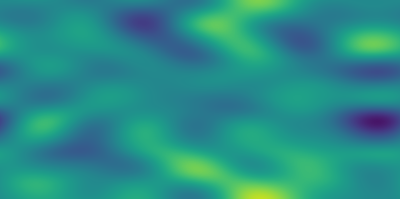
\includegraphics[interpolate=false,width=1.000000in,height=1.000000in]{burgers_rollout_pred_0.1-img0.png}}%
\end{pgfscope}%
\begin{pgfscope}%
\pgfsetbuttcap%
\pgfsetroundjoin%
\definecolor{currentfill}{rgb}{0.000000,0.000000,0.000000}%
\pgfsetfillcolor{currentfill}%
\pgfsetlinewidth{0.803000pt}%
\definecolor{currentstroke}{rgb}{0.000000,0.000000,0.000000}%
\pgfsetstrokecolor{currentstroke}%
\pgfsetdash{}{0pt}%
\pgfsys@defobject{currentmarker}{\pgfqpoint{0.000000in}{-0.048611in}}{\pgfqpoint{0.000000in}{0.000000in}}{%
\pgfpathmoveto{\pgfqpoint{0.000000in}{0.000000in}}%
\pgfpathlineto{\pgfqpoint{0.000000in}{-0.048611in}}%
\pgfusepath{stroke,fill}%
}%
\begin{pgfscope}%
\pgfsys@transformshift{0.726837in}{0.517039in}%
\pgfsys@useobject{currentmarker}{}%
\end{pgfscope}%
\end{pgfscope}%
\begin{pgfscope}%
\definecolor{textcolor}{rgb}{0.000000,0.000000,0.000000}%
\pgfsetstrokecolor{textcolor}%
\pgfsetfillcolor{textcolor}%
\pgftext[x=0.726837in,y=0.419816in,,top]{\color{textcolor}\rmfamily\fontsize{12.000000}{14.400000}\selectfont 0}%
\end{pgfscope}%
\begin{pgfscope}%
\pgfsetbuttcap%
\pgfsetroundjoin%
\definecolor{currentfill}{rgb}{0.000000,0.000000,0.000000}%
\pgfsetfillcolor{currentfill}%
\pgfsetlinewidth{0.803000pt}%
\definecolor{currentstroke}{rgb}{0.000000,0.000000,0.000000}%
\pgfsetstrokecolor{currentstroke}%
\pgfsetdash{}{0pt}%
\pgfsys@defobject{currentmarker}{\pgfqpoint{0.000000in}{-0.048611in}}{\pgfqpoint{0.000000in}{0.000000in}}{%
\pgfpathmoveto{\pgfqpoint{0.000000in}{0.000000in}}%
\pgfpathlineto{\pgfqpoint{0.000000in}{-0.048611in}}%
\pgfusepath{stroke,fill}%
}%
\begin{pgfscope}%
\pgfsys@transformshift{1.570762in}{0.517039in}%
\pgfsys@useobject{currentmarker}{}%
\end{pgfscope}%
\end{pgfscope}%
\begin{pgfscope}%
\definecolor{textcolor}{rgb}{0.000000,0.000000,0.000000}%
\pgfsetstrokecolor{textcolor}%
\pgfsetfillcolor{textcolor}%
\pgftext[x=1.570762in,y=0.419816in,,top]{\color{textcolor}\rmfamily\fontsize{12.000000}{14.400000}\selectfont 1}%
\end{pgfscope}%
\begin{pgfscope}%
\pgfsetbuttcap%
\pgfsetroundjoin%
\definecolor{currentfill}{rgb}{0.000000,0.000000,0.000000}%
\pgfsetfillcolor{currentfill}%
\pgfsetlinewidth{0.803000pt}%
\definecolor{currentstroke}{rgb}{0.000000,0.000000,0.000000}%
\pgfsetstrokecolor{currentstroke}%
\pgfsetdash{}{0pt}%
\pgfsys@defobject{currentmarker}{\pgfqpoint{0.000000in}{-0.048611in}}{\pgfqpoint{0.000000in}{0.000000in}}{%
\pgfpathmoveto{\pgfqpoint{0.000000in}{0.000000in}}%
\pgfpathlineto{\pgfqpoint{0.000000in}{-0.048611in}}%
\pgfusepath{stroke,fill}%
}%
\begin{pgfscope}%
\pgfsys@transformshift{2.414687in}{0.517039in}%
\pgfsys@useobject{currentmarker}{}%
\end{pgfscope}%
\end{pgfscope}%
\begin{pgfscope}%
\definecolor{textcolor}{rgb}{0.000000,0.000000,0.000000}%
\pgfsetstrokecolor{textcolor}%
\pgfsetfillcolor{textcolor}%
\pgftext[x=2.414687in,y=0.419816in,,top]{\color{textcolor}\rmfamily\fontsize{12.000000}{14.400000}\selectfont 2}%
\end{pgfscope}%
\begin{pgfscope}%
\definecolor{textcolor}{rgb}{0.000000,0.000000,0.000000}%
\pgfsetstrokecolor{textcolor}%
\pgfsetfillcolor{textcolor}%
\pgftext[x=1.570762in,y=0.202965in,,top]{\color{textcolor}\rmfamily\fontsize{12.000000}{14.400000}\selectfont Space}%
\end{pgfscope}%
\begin{pgfscope}%
\pgfsetbuttcap%
\pgfsetroundjoin%
\definecolor{currentfill}{rgb}{0.000000,0.000000,0.000000}%
\pgfsetfillcolor{currentfill}%
\pgfsetlinewidth{0.803000pt}%
\definecolor{currentstroke}{rgb}{0.000000,0.000000,0.000000}%
\pgfsetstrokecolor{currentstroke}%
\pgfsetdash{}{0pt}%
\pgfsys@defobject{currentmarker}{\pgfqpoint{-0.048611in}{0.000000in}}{\pgfqpoint{-0.000000in}{0.000000in}}{%
\pgfpathmoveto{\pgfqpoint{-0.000000in}{0.000000in}}%
\pgfpathlineto{\pgfqpoint{-0.048611in}{0.000000in}}%
\pgfusepath{stroke,fill}%
}%
\begin{pgfscope}%
\pgfsys@transformshift{0.726837in}{0.517039in}%
\pgfsys@useobject{currentmarker}{}%
\end{pgfscope}%
\end{pgfscope}%
\begin{pgfscope}%
\definecolor{textcolor}{rgb}{0.000000,0.000000,0.000000}%
\pgfsetstrokecolor{textcolor}%
\pgfsetfillcolor{textcolor}%
\pgftext[x=0.364559in, y=0.453725in, left, base]{\color{textcolor}\rmfamily\fontsize{12.000000}{14.400000}\selectfont 0.0}%
\end{pgfscope}%
\begin{pgfscope}%
\pgfsetbuttcap%
\pgfsetroundjoin%
\definecolor{currentfill}{rgb}{0.000000,0.000000,0.000000}%
\pgfsetfillcolor{currentfill}%
\pgfsetlinewidth{0.803000pt}%
\definecolor{currentstroke}{rgb}{0.000000,0.000000,0.000000}%
\pgfsetstrokecolor{currentstroke}%
\pgfsetdash{}{0pt}%
\pgfsys@defobject{currentmarker}{\pgfqpoint{-0.048611in}{0.000000in}}{\pgfqpoint{-0.000000in}{0.000000in}}{%
\pgfpathmoveto{\pgfqpoint{-0.000000in}{0.000000in}}%
\pgfpathlineto{\pgfqpoint{-0.048611in}{0.000000in}}%
\pgfusepath{stroke,fill}%
}%
\begin{pgfscope}%
\pgfsys@transformshift{0.726837in}{0.861533in}%
\pgfsys@useobject{currentmarker}{}%
\end{pgfscope}%
\end{pgfscope}%
\begin{pgfscope}%
\definecolor{textcolor}{rgb}{0.000000,0.000000,0.000000}%
\pgfsetstrokecolor{textcolor}%
\pgfsetfillcolor{textcolor}%
\pgftext[x=0.364559in, y=0.798219in, left, base]{\color{textcolor}\rmfamily\fontsize{12.000000}{14.400000}\selectfont 2.5}%
\end{pgfscope}%
\begin{pgfscope}%
\pgfsetbuttcap%
\pgfsetroundjoin%
\definecolor{currentfill}{rgb}{0.000000,0.000000,0.000000}%
\pgfsetfillcolor{currentfill}%
\pgfsetlinewidth{0.803000pt}%
\definecolor{currentstroke}{rgb}{0.000000,0.000000,0.000000}%
\pgfsetstrokecolor{currentstroke}%
\pgfsetdash{}{0pt}%
\pgfsys@defobject{currentmarker}{\pgfqpoint{-0.048611in}{0.000000in}}{\pgfqpoint{-0.000000in}{0.000000in}}{%
\pgfpathmoveto{\pgfqpoint{-0.000000in}{0.000000in}}%
\pgfpathlineto{\pgfqpoint{-0.048611in}{0.000000in}}%
\pgfusepath{stroke,fill}%
}%
\begin{pgfscope}%
\pgfsys@transformshift{0.726837in}{1.206027in}%
\pgfsys@useobject{currentmarker}{}%
\end{pgfscope}%
\end{pgfscope}%
\begin{pgfscope}%
\definecolor{textcolor}{rgb}{0.000000,0.000000,0.000000}%
\pgfsetstrokecolor{textcolor}%
\pgfsetfillcolor{textcolor}%
\pgftext[x=0.364559in, y=1.142714in, left, base]{\color{textcolor}\rmfamily\fontsize{12.000000}{14.400000}\selectfont 5.0}%
\end{pgfscope}%
\begin{pgfscope}%
\pgfsetbuttcap%
\pgfsetroundjoin%
\definecolor{currentfill}{rgb}{0.000000,0.000000,0.000000}%
\pgfsetfillcolor{currentfill}%
\pgfsetlinewidth{0.803000pt}%
\definecolor{currentstroke}{rgb}{0.000000,0.000000,0.000000}%
\pgfsetstrokecolor{currentstroke}%
\pgfsetdash{}{0pt}%
\pgfsys@defobject{currentmarker}{\pgfqpoint{-0.048611in}{0.000000in}}{\pgfqpoint{-0.000000in}{0.000000in}}{%
\pgfpathmoveto{\pgfqpoint{-0.000000in}{0.000000in}}%
\pgfpathlineto{\pgfqpoint{-0.048611in}{0.000000in}}%
\pgfusepath{stroke,fill}%
}%
\begin{pgfscope}%
\pgfsys@transformshift{0.726837in}{1.550522in}%
\pgfsys@useobject{currentmarker}{}%
\end{pgfscope}%
\end{pgfscope}%
\begin{pgfscope}%
\definecolor{textcolor}{rgb}{0.000000,0.000000,0.000000}%
\pgfsetstrokecolor{textcolor}%
\pgfsetfillcolor{textcolor}%
\pgftext[x=0.364559in, y=1.487208in, left, base]{\color{textcolor}\rmfamily\fontsize{12.000000}{14.400000}\selectfont 7.5}%
\end{pgfscope}%
\begin{pgfscope}%
\pgfsetbuttcap%
\pgfsetroundjoin%
\definecolor{currentfill}{rgb}{0.000000,0.000000,0.000000}%
\pgfsetfillcolor{currentfill}%
\pgfsetlinewidth{0.803000pt}%
\definecolor{currentstroke}{rgb}{0.000000,0.000000,0.000000}%
\pgfsetstrokecolor{currentstroke}%
\pgfsetdash{}{0pt}%
\pgfsys@defobject{currentmarker}{\pgfqpoint{-0.048611in}{0.000000in}}{\pgfqpoint{-0.000000in}{0.000000in}}{%
\pgfpathmoveto{\pgfqpoint{-0.000000in}{0.000000in}}%
\pgfpathlineto{\pgfqpoint{-0.048611in}{0.000000in}}%
\pgfusepath{stroke,fill}%
}%
\begin{pgfscope}%
\pgfsys@transformshift{0.726837in}{1.895016in}%
\pgfsys@useobject{currentmarker}{}%
\end{pgfscope}%
\end{pgfscope}%
\begin{pgfscope}%
\definecolor{textcolor}{rgb}{0.000000,0.000000,0.000000}%
\pgfsetstrokecolor{textcolor}%
\pgfsetfillcolor{textcolor}%
\pgftext[x=0.258521in, y=1.831702in, left, base]{\color{textcolor}\rmfamily\fontsize{12.000000}{14.400000}\selectfont 10.0}%
\end{pgfscope}%
\begin{pgfscope}%
\definecolor{textcolor}{rgb}{0.000000,0.000000,0.000000}%
\pgfsetstrokecolor{textcolor}%
\pgfsetfillcolor{textcolor}%
\pgftext[x=0.202965in,y=1.206027in,,bottom,rotate=90.000000]{\color{textcolor}\rmfamily\fontsize{12.000000}{14.400000}\selectfont Time}%
\end{pgfscope}%
\begin{pgfscope}%
\pgfsetrectcap%
\pgfsetmiterjoin%
\pgfsetlinewidth{0.803000pt}%
\definecolor{currentstroke}{rgb}{0.000000,0.000000,0.000000}%
\pgfsetstrokecolor{currentstroke}%
\pgfsetdash{}{0pt}%
\pgfpathmoveto{\pgfqpoint{0.726837in}{0.517039in}}%
\pgfpathlineto{\pgfqpoint{0.726837in}{1.895016in}}%
\pgfusepath{stroke}%
\end{pgfscope}%
\begin{pgfscope}%
\pgfsetrectcap%
\pgfsetmiterjoin%
\pgfsetlinewidth{0.803000pt}%
\definecolor{currentstroke}{rgb}{0.000000,0.000000,0.000000}%
\pgfsetstrokecolor{currentstroke}%
\pgfsetdash{}{0pt}%
\pgfpathmoveto{\pgfqpoint{2.414687in}{0.517039in}}%
\pgfpathlineto{\pgfqpoint{2.414687in}{1.895016in}}%
\pgfusepath{stroke}%
\end{pgfscope}%
\begin{pgfscope}%
\pgfsetrectcap%
\pgfsetmiterjoin%
\pgfsetlinewidth{0.803000pt}%
\definecolor{currentstroke}{rgb}{0.000000,0.000000,0.000000}%
\pgfsetstrokecolor{currentstroke}%
\pgfsetdash{}{0pt}%
\pgfpathmoveto{\pgfqpoint{0.726837in}{0.517039in}}%
\pgfpathlineto{\pgfqpoint{2.414687in}{0.517039in}}%
\pgfusepath{stroke}%
\end{pgfscope}%
\begin{pgfscope}%
\pgfsetrectcap%
\pgfsetmiterjoin%
\pgfsetlinewidth{0.803000pt}%
\definecolor{currentstroke}{rgb}{0.000000,0.000000,0.000000}%
\pgfsetstrokecolor{currentstroke}%
\pgfsetdash{}{0pt}%
\pgfpathmoveto{\pgfqpoint{0.726837in}{1.895016in}}%
\pgfpathlineto{\pgfqpoint{2.414687in}{1.895016in}}%
\pgfusepath{stroke}%
\end{pgfscope}%
\begin{pgfscope}%
\pgfsetbuttcap%
\pgfsetmiterjoin%
\pgfsetlinewidth{0.000000pt}%
\definecolor{currentstroke}{rgb}{0.000000,0.000000,0.000000}%
\pgfsetstrokecolor{currentstroke}%
\pgfsetstrokeopacity{0.000000}%
\pgfsetdash{}{0pt}%
\pgfpathmoveto{\pgfqpoint{2.552099in}{0.517039in}}%
\pgfpathlineto{\pgfqpoint{2.620998in}{0.517039in}}%
\pgfpathlineto{\pgfqpoint{2.620998in}{1.895016in}}%
\pgfpathlineto{\pgfqpoint{2.552099in}{1.895016in}}%
\pgfpathlineto{\pgfqpoint{2.552099in}{0.517039in}}%
\pgfpathclose%
\pgfusepath{}%
\end{pgfscope}%
\begin{pgfscope}%
\pgfsys@transformshift{2.550000in}{0.520000in}%
\pgftext[left,bottom]{
\includegraphics[interpolate=true,width=0.070000in,height=1.380000in]{burgers_rollout_pred_0.1-img1.png}}%
\end{pgfscope}%
\begin{pgfscope}%
\pgfsetbuttcap%
\pgfsetroundjoin%
\definecolor{currentfill}{rgb}{0.000000,0.000000,0.000000}%
\pgfsetfillcolor{currentfill}%
\pgfsetlinewidth{0.803000pt}%
\definecolor{currentstroke}{rgb}{0.000000,0.000000,0.000000}%
\pgfsetstrokecolor{currentstroke}%
\pgfsetdash{}{0pt}%
\pgfsys@defobject{currentmarker}{\pgfqpoint{0.000000in}{0.000000in}}{\pgfqpoint{0.048611in}{0.000000in}}{%
\pgfpathmoveto{\pgfqpoint{0.000000in}{0.000000in}}%
\pgfpathlineto{\pgfqpoint{0.048611in}{0.000000in}}%
\pgfusepath{stroke,fill}%
}%
\begin{pgfscope}%
\pgfsys@transformshift{2.620998in}{0.588723in}%
\pgfsys@useobject{currentmarker}{}%
\end{pgfscope}%
\end{pgfscope}%
\begin{pgfscope}%
\definecolor{textcolor}{rgb}{0.000000,0.000000,0.000000}%
\pgfsetstrokecolor{textcolor}%
\pgfsetfillcolor{textcolor}%
\pgftext[x=2.718220in, y=0.525410in, left, base]{\color{textcolor}\rmfamily\fontsize{12.000000}{14.400000}\selectfont \ensuremath{-}1}%
\end{pgfscope}%
\begin{pgfscope}%
\pgfsetbuttcap%
\pgfsetroundjoin%
\definecolor{currentfill}{rgb}{0.000000,0.000000,0.000000}%
\pgfsetfillcolor{currentfill}%
\pgfsetlinewidth{0.803000pt}%
\definecolor{currentstroke}{rgb}{0.000000,0.000000,0.000000}%
\pgfsetstrokecolor{currentstroke}%
\pgfsetdash{}{0pt}%
\pgfsys@defobject{currentmarker}{\pgfqpoint{0.000000in}{0.000000in}}{\pgfqpoint{0.048611in}{0.000000in}}{%
\pgfpathmoveto{\pgfqpoint{0.000000in}{0.000000in}}%
\pgfpathlineto{\pgfqpoint{0.048611in}{0.000000in}}%
\pgfusepath{stroke,fill}%
}%
\begin{pgfscope}%
\pgfsys@transformshift{2.620998in}{1.206027in}%
\pgfsys@useobject{currentmarker}{}%
\end{pgfscope}%
\end{pgfscope}%
\begin{pgfscope}%
\definecolor{textcolor}{rgb}{0.000000,0.000000,0.000000}%
\pgfsetstrokecolor{textcolor}%
\pgfsetfillcolor{textcolor}%
\pgftext[x=2.718220in, y=1.142714in, left, base]{\color{textcolor}\rmfamily\fontsize{12.000000}{14.400000}\selectfont 0}%
\end{pgfscope}%
\begin{pgfscope}%
\pgfsetbuttcap%
\pgfsetroundjoin%
\definecolor{currentfill}{rgb}{0.000000,0.000000,0.000000}%
\pgfsetfillcolor{currentfill}%
\pgfsetlinewidth{0.803000pt}%
\definecolor{currentstroke}{rgb}{0.000000,0.000000,0.000000}%
\pgfsetstrokecolor{currentstroke}%
\pgfsetdash{}{0pt}%
\pgfsys@defobject{currentmarker}{\pgfqpoint{0.000000in}{0.000000in}}{\pgfqpoint{0.048611in}{0.000000in}}{%
\pgfpathmoveto{\pgfqpoint{0.000000in}{0.000000in}}%
\pgfpathlineto{\pgfqpoint{0.048611in}{0.000000in}}%
\pgfusepath{stroke,fill}%
}%
\begin{pgfscope}%
\pgfsys@transformshift{2.620998in}{1.823331in}%
\pgfsys@useobject{currentmarker}{}%
\end{pgfscope}%
\end{pgfscope}%
\begin{pgfscope}%
\definecolor{textcolor}{rgb}{0.000000,0.000000,0.000000}%
\pgfsetstrokecolor{textcolor}%
\pgfsetfillcolor{textcolor}%
\pgftext[x=2.718220in, y=1.760018in, left, base]{\color{textcolor}\rmfamily\fontsize{12.000000}{14.400000}\selectfont 1}%
\end{pgfscope}%
\begin{pgfscope}%
\pgfsetrectcap%
\pgfsetmiterjoin%
\pgfsetlinewidth{0.803000pt}%
\definecolor{currentstroke}{rgb}{0.000000,0.000000,0.000000}%
\pgfsetstrokecolor{currentstroke}%
\pgfsetdash{}{0pt}%
\pgfpathmoveto{\pgfqpoint{2.552099in}{0.517039in}}%
\pgfpathlineto{\pgfqpoint{2.586548in}{0.517039in}}%
\pgfpathlineto{\pgfqpoint{2.620998in}{0.517039in}}%
\pgfpathlineto{\pgfqpoint{2.620998in}{1.895016in}}%
\pgfpathlineto{\pgfqpoint{2.586548in}{1.895016in}}%
\pgfpathlineto{\pgfqpoint{2.552099in}{1.895016in}}%
\pgfpathlineto{\pgfqpoint{2.552099in}{0.517039in}}%
\pgfpathclose%
\pgfusepath{stroke}%
\end{pgfscope}%
\end{pgfpicture}%
\makeatother%
\endgroup%

      \end{adjustbox}
      \caption{The prediction for \(\nu=0.1\)}\label{fig:sc2_rollout_pred_0.1}
    \end{subfigure}
    \begin{subfigure}{0.32\linewidth}
      \begin{adjustbox}{width=\linewidth}
        \begingroup%
\makeatletter%
\begin{pgfpicture}%
\pgfpathrectangle{\pgfpointorigin}{\pgfqpoint{3.000000in}{2.000000in}}%
\pgfusepath{use as bounding box, clip}%
\begin{pgfscope}%
\pgfsetbuttcap%
\pgfsetmiterjoin%
\pgfsetlinewidth{0.000000pt}%
\definecolor{currentstroke}{rgb}{0.000000,0.000000,0.000000}%
\pgfsetstrokecolor{currentstroke}%
\pgfsetstrokeopacity{0.000000}%
\pgfsetdash{}{0pt}%
\pgfpathmoveto{\pgfqpoint{0.000000in}{0.000000in}}%
\pgfpathlineto{\pgfqpoint{3.000000in}{0.000000in}}%
\pgfpathlineto{\pgfqpoint{3.000000in}{2.000000in}}%
\pgfpathlineto{\pgfqpoint{0.000000in}{2.000000in}}%
\pgfpathlineto{\pgfqpoint{0.000000in}{0.000000in}}%
\pgfpathclose%
\pgfusepath{}%
\end{pgfscope}%
\begin{pgfscope}%
\pgfsetbuttcap%
\pgfsetmiterjoin%
\pgfsetlinewidth{0.000000pt}%
\definecolor{currentstroke}{rgb}{0.000000,0.000000,0.000000}%
\pgfsetstrokecolor{currentstroke}%
\pgfsetstrokeopacity{0.000000}%
\pgfsetdash{}{0pt}%
\pgfpathmoveto{\pgfqpoint{0.726837in}{0.517039in}}%
\pgfpathlineto{\pgfqpoint{2.414687in}{0.517039in}}%
\pgfpathlineto{\pgfqpoint{2.414687in}{1.895016in}}%
\pgfpathlineto{\pgfqpoint{0.726837in}{1.895016in}}%
\pgfpathlineto{\pgfqpoint{0.726837in}{0.517039in}}%
\pgfpathclose%
\pgfusepath{}%
\end{pgfscope}%
\begin{pgfscope}%
\pgfpathrectangle{\pgfqpoint{0.726837in}{0.517039in}}{\pgfqpoint{1.687850in}{1.377978in}}%
\pgfusepath{clip}%
\pgfsys@transformcm{1.687850}{0.000000}{0.000000}{1.377978}{0.726837in}{0.517039in}%
\pgftext[left,bottom]{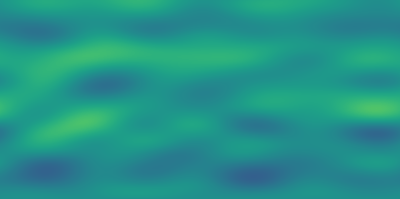
\includegraphics[interpolate=false,width=1.000000in,height=1.000000in]{burgers_rollout_diff_0.1-img0.png}}%
\end{pgfscope}%
\begin{pgfscope}%
\pgfsetbuttcap%
\pgfsetroundjoin%
\definecolor{currentfill}{rgb}{0.000000,0.000000,0.000000}%
\pgfsetfillcolor{currentfill}%
\pgfsetlinewidth{0.803000pt}%
\definecolor{currentstroke}{rgb}{0.000000,0.000000,0.000000}%
\pgfsetstrokecolor{currentstroke}%
\pgfsetdash{}{0pt}%
\pgfsys@defobject{currentmarker}{\pgfqpoint{0.000000in}{-0.048611in}}{\pgfqpoint{0.000000in}{0.000000in}}{%
\pgfpathmoveto{\pgfqpoint{0.000000in}{0.000000in}}%
\pgfpathlineto{\pgfqpoint{0.000000in}{-0.048611in}}%
\pgfusepath{stroke,fill}%
}%
\begin{pgfscope}%
\pgfsys@transformshift{0.726837in}{0.517039in}%
\pgfsys@useobject{currentmarker}{}%
\end{pgfscope}%
\end{pgfscope}%
\begin{pgfscope}%
\definecolor{textcolor}{rgb}{0.000000,0.000000,0.000000}%
\pgfsetstrokecolor{textcolor}%
\pgfsetfillcolor{textcolor}%
\pgftext[x=0.726837in,y=0.419816in,,top]{\color{textcolor}\rmfamily\fontsize{12.000000}{14.400000}\selectfont 0}%
\end{pgfscope}%
\begin{pgfscope}%
\pgfsetbuttcap%
\pgfsetroundjoin%
\definecolor{currentfill}{rgb}{0.000000,0.000000,0.000000}%
\pgfsetfillcolor{currentfill}%
\pgfsetlinewidth{0.803000pt}%
\definecolor{currentstroke}{rgb}{0.000000,0.000000,0.000000}%
\pgfsetstrokecolor{currentstroke}%
\pgfsetdash{}{0pt}%
\pgfsys@defobject{currentmarker}{\pgfqpoint{0.000000in}{-0.048611in}}{\pgfqpoint{0.000000in}{0.000000in}}{%
\pgfpathmoveto{\pgfqpoint{0.000000in}{0.000000in}}%
\pgfpathlineto{\pgfqpoint{0.000000in}{-0.048611in}}%
\pgfusepath{stroke,fill}%
}%
\begin{pgfscope}%
\pgfsys@transformshift{1.570762in}{0.517039in}%
\pgfsys@useobject{currentmarker}{}%
\end{pgfscope}%
\end{pgfscope}%
\begin{pgfscope}%
\definecolor{textcolor}{rgb}{0.000000,0.000000,0.000000}%
\pgfsetstrokecolor{textcolor}%
\pgfsetfillcolor{textcolor}%
\pgftext[x=1.570762in,y=0.419816in,,top]{\color{textcolor}\rmfamily\fontsize{12.000000}{14.400000}\selectfont 1}%
\end{pgfscope}%
\begin{pgfscope}%
\pgfsetbuttcap%
\pgfsetroundjoin%
\definecolor{currentfill}{rgb}{0.000000,0.000000,0.000000}%
\pgfsetfillcolor{currentfill}%
\pgfsetlinewidth{0.803000pt}%
\definecolor{currentstroke}{rgb}{0.000000,0.000000,0.000000}%
\pgfsetstrokecolor{currentstroke}%
\pgfsetdash{}{0pt}%
\pgfsys@defobject{currentmarker}{\pgfqpoint{0.000000in}{-0.048611in}}{\pgfqpoint{0.000000in}{0.000000in}}{%
\pgfpathmoveto{\pgfqpoint{0.000000in}{0.000000in}}%
\pgfpathlineto{\pgfqpoint{0.000000in}{-0.048611in}}%
\pgfusepath{stroke,fill}%
}%
\begin{pgfscope}%
\pgfsys@transformshift{2.414687in}{0.517039in}%
\pgfsys@useobject{currentmarker}{}%
\end{pgfscope}%
\end{pgfscope}%
\begin{pgfscope}%
\definecolor{textcolor}{rgb}{0.000000,0.000000,0.000000}%
\pgfsetstrokecolor{textcolor}%
\pgfsetfillcolor{textcolor}%
\pgftext[x=2.414687in,y=0.419816in,,top]{\color{textcolor}\rmfamily\fontsize{12.000000}{14.400000}\selectfont 2}%
\end{pgfscope}%
\begin{pgfscope}%
\definecolor{textcolor}{rgb}{0.000000,0.000000,0.000000}%
\pgfsetstrokecolor{textcolor}%
\pgfsetfillcolor{textcolor}%
\pgftext[x=1.570762in,y=0.202965in,,top]{\color{textcolor}\rmfamily\fontsize{12.000000}{14.400000}\selectfont Space}%
\end{pgfscope}%
\begin{pgfscope}%
\pgfsetbuttcap%
\pgfsetroundjoin%
\definecolor{currentfill}{rgb}{0.000000,0.000000,0.000000}%
\pgfsetfillcolor{currentfill}%
\pgfsetlinewidth{0.803000pt}%
\definecolor{currentstroke}{rgb}{0.000000,0.000000,0.000000}%
\pgfsetstrokecolor{currentstroke}%
\pgfsetdash{}{0pt}%
\pgfsys@defobject{currentmarker}{\pgfqpoint{-0.048611in}{0.000000in}}{\pgfqpoint{-0.000000in}{0.000000in}}{%
\pgfpathmoveto{\pgfqpoint{-0.000000in}{0.000000in}}%
\pgfpathlineto{\pgfqpoint{-0.048611in}{0.000000in}}%
\pgfusepath{stroke,fill}%
}%
\begin{pgfscope}%
\pgfsys@transformshift{0.726837in}{0.517039in}%
\pgfsys@useobject{currentmarker}{}%
\end{pgfscope}%
\end{pgfscope}%
\begin{pgfscope}%
\definecolor{textcolor}{rgb}{0.000000,0.000000,0.000000}%
\pgfsetstrokecolor{textcolor}%
\pgfsetfillcolor{textcolor}%
\pgftext[x=0.364559in, y=0.453725in, left, base]{\color{textcolor}\rmfamily\fontsize{12.000000}{14.400000}\selectfont 0.0}%
\end{pgfscope}%
\begin{pgfscope}%
\pgfsetbuttcap%
\pgfsetroundjoin%
\definecolor{currentfill}{rgb}{0.000000,0.000000,0.000000}%
\pgfsetfillcolor{currentfill}%
\pgfsetlinewidth{0.803000pt}%
\definecolor{currentstroke}{rgb}{0.000000,0.000000,0.000000}%
\pgfsetstrokecolor{currentstroke}%
\pgfsetdash{}{0pt}%
\pgfsys@defobject{currentmarker}{\pgfqpoint{-0.048611in}{0.000000in}}{\pgfqpoint{-0.000000in}{0.000000in}}{%
\pgfpathmoveto{\pgfqpoint{-0.000000in}{0.000000in}}%
\pgfpathlineto{\pgfqpoint{-0.048611in}{0.000000in}}%
\pgfusepath{stroke,fill}%
}%
\begin{pgfscope}%
\pgfsys@transformshift{0.726837in}{0.861533in}%
\pgfsys@useobject{currentmarker}{}%
\end{pgfscope}%
\end{pgfscope}%
\begin{pgfscope}%
\definecolor{textcolor}{rgb}{0.000000,0.000000,0.000000}%
\pgfsetstrokecolor{textcolor}%
\pgfsetfillcolor{textcolor}%
\pgftext[x=0.364559in, y=0.798219in, left, base]{\color{textcolor}\rmfamily\fontsize{12.000000}{14.400000}\selectfont 2.5}%
\end{pgfscope}%
\begin{pgfscope}%
\pgfsetbuttcap%
\pgfsetroundjoin%
\definecolor{currentfill}{rgb}{0.000000,0.000000,0.000000}%
\pgfsetfillcolor{currentfill}%
\pgfsetlinewidth{0.803000pt}%
\definecolor{currentstroke}{rgb}{0.000000,0.000000,0.000000}%
\pgfsetstrokecolor{currentstroke}%
\pgfsetdash{}{0pt}%
\pgfsys@defobject{currentmarker}{\pgfqpoint{-0.048611in}{0.000000in}}{\pgfqpoint{-0.000000in}{0.000000in}}{%
\pgfpathmoveto{\pgfqpoint{-0.000000in}{0.000000in}}%
\pgfpathlineto{\pgfqpoint{-0.048611in}{0.000000in}}%
\pgfusepath{stroke,fill}%
}%
\begin{pgfscope}%
\pgfsys@transformshift{0.726837in}{1.206027in}%
\pgfsys@useobject{currentmarker}{}%
\end{pgfscope}%
\end{pgfscope}%
\begin{pgfscope}%
\definecolor{textcolor}{rgb}{0.000000,0.000000,0.000000}%
\pgfsetstrokecolor{textcolor}%
\pgfsetfillcolor{textcolor}%
\pgftext[x=0.364559in, y=1.142714in, left, base]{\color{textcolor}\rmfamily\fontsize{12.000000}{14.400000}\selectfont 5.0}%
\end{pgfscope}%
\begin{pgfscope}%
\pgfsetbuttcap%
\pgfsetroundjoin%
\definecolor{currentfill}{rgb}{0.000000,0.000000,0.000000}%
\pgfsetfillcolor{currentfill}%
\pgfsetlinewidth{0.803000pt}%
\definecolor{currentstroke}{rgb}{0.000000,0.000000,0.000000}%
\pgfsetstrokecolor{currentstroke}%
\pgfsetdash{}{0pt}%
\pgfsys@defobject{currentmarker}{\pgfqpoint{-0.048611in}{0.000000in}}{\pgfqpoint{-0.000000in}{0.000000in}}{%
\pgfpathmoveto{\pgfqpoint{-0.000000in}{0.000000in}}%
\pgfpathlineto{\pgfqpoint{-0.048611in}{0.000000in}}%
\pgfusepath{stroke,fill}%
}%
\begin{pgfscope}%
\pgfsys@transformshift{0.726837in}{1.550522in}%
\pgfsys@useobject{currentmarker}{}%
\end{pgfscope}%
\end{pgfscope}%
\begin{pgfscope}%
\definecolor{textcolor}{rgb}{0.000000,0.000000,0.000000}%
\pgfsetstrokecolor{textcolor}%
\pgfsetfillcolor{textcolor}%
\pgftext[x=0.364559in, y=1.487208in, left, base]{\color{textcolor}\rmfamily\fontsize{12.000000}{14.400000}\selectfont 7.5}%
\end{pgfscope}%
\begin{pgfscope}%
\pgfsetbuttcap%
\pgfsetroundjoin%
\definecolor{currentfill}{rgb}{0.000000,0.000000,0.000000}%
\pgfsetfillcolor{currentfill}%
\pgfsetlinewidth{0.803000pt}%
\definecolor{currentstroke}{rgb}{0.000000,0.000000,0.000000}%
\pgfsetstrokecolor{currentstroke}%
\pgfsetdash{}{0pt}%
\pgfsys@defobject{currentmarker}{\pgfqpoint{-0.048611in}{0.000000in}}{\pgfqpoint{-0.000000in}{0.000000in}}{%
\pgfpathmoveto{\pgfqpoint{-0.000000in}{0.000000in}}%
\pgfpathlineto{\pgfqpoint{-0.048611in}{0.000000in}}%
\pgfusepath{stroke,fill}%
}%
\begin{pgfscope}%
\pgfsys@transformshift{0.726837in}{1.895016in}%
\pgfsys@useobject{currentmarker}{}%
\end{pgfscope}%
\end{pgfscope}%
\begin{pgfscope}%
\definecolor{textcolor}{rgb}{0.000000,0.000000,0.000000}%
\pgfsetstrokecolor{textcolor}%
\pgfsetfillcolor{textcolor}%
\pgftext[x=0.258521in, y=1.831702in, left, base]{\color{textcolor}\rmfamily\fontsize{12.000000}{14.400000}\selectfont 10.0}%
\end{pgfscope}%
\begin{pgfscope}%
\definecolor{textcolor}{rgb}{0.000000,0.000000,0.000000}%
\pgfsetstrokecolor{textcolor}%
\pgfsetfillcolor{textcolor}%
\pgftext[x=0.202965in,y=1.206027in,,bottom,rotate=90.000000]{\color{textcolor}\rmfamily\fontsize{12.000000}{14.400000}\selectfont Time}%
\end{pgfscope}%
\begin{pgfscope}%
\pgfsetrectcap%
\pgfsetmiterjoin%
\pgfsetlinewidth{0.803000pt}%
\definecolor{currentstroke}{rgb}{0.000000,0.000000,0.000000}%
\pgfsetstrokecolor{currentstroke}%
\pgfsetdash{}{0pt}%
\pgfpathmoveto{\pgfqpoint{0.726837in}{0.517039in}}%
\pgfpathlineto{\pgfqpoint{0.726837in}{1.895016in}}%
\pgfusepath{stroke}%
\end{pgfscope}%
\begin{pgfscope}%
\pgfsetrectcap%
\pgfsetmiterjoin%
\pgfsetlinewidth{0.803000pt}%
\definecolor{currentstroke}{rgb}{0.000000,0.000000,0.000000}%
\pgfsetstrokecolor{currentstroke}%
\pgfsetdash{}{0pt}%
\pgfpathmoveto{\pgfqpoint{2.414687in}{0.517039in}}%
\pgfpathlineto{\pgfqpoint{2.414687in}{1.895016in}}%
\pgfusepath{stroke}%
\end{pgfscope}%
\begin{pgfscope}%
\pgfsetrectcap%
\pgfsetmiterjoin%
\pgfsetlinewidth{0.803000pt}%
\definecolor{currentstroke}{rgb}{0.000000,0.000000,0.000000}%
\pgfsetstrokecolor{currentstroke}%
\pgfsetdash{}{0pt}%
\pgfpathmoveto{\pgfqpoint{0.726837in}{0.517039in}}%
\pgfpathlineto{\pgfqpoint{2.414687in}{0.517039in}}%
\pgfusepath{stroke}%
\end{pgfscope}%
\begin{pgfscope}%
\pgfsetrectcap%
\pgfsetmiterjoin%
\pgfsetlinewidth{0.803000pt}%
\definecolor{currentstroke}{rgb}{0.000000,0.000000,0.000000}%
\pgfsetstrokecolor{currentstroke}%
\pgfsetdash{}{0pt}%
\pgfpathmoveto{\pgfqpoint{0.726837in}{1.895016in}}%
\pgfpathlineto{\pgfqpoint{2.414687in}{1.895016in}}%
\pgfusepath{stroke}%
\end{pgfscope}%
\begin{pgfscope}%
\pgfsetbuttcap%
\pgfsetmiterjoin%
\pgfsetlinewidth{0.000000pt}%
\definecolor{currentstroke}{rgb}{0.000000,0.000000,0.000000}%
\pgfsetstrokecolor{currentstroke}%
\pgfsetstrokeopacity{0.000000}%
\pgfsetdash{}{0pt}%
\pgfpathmoveto{\pgfqpoint{2.552099in}{0.517039in}}%
\pgfpathlineto{\pgfqpoint{2.620998in}{0.517039in}}%
\pgfpathlineto{\pgfqpoint{2.620998in}{1.895016in}}%
\pgfpathlineto{\pgfqpoint{2.552099in}{1.895016in}}%
\pgfpathlineto{\pgfqpoint{2.552099in}{0.517039in}}%
\pgfpathclose%
\pgfusepath{}%
\end{pgfscope}%
\begin{pgfscope}%
\pgfsys@transformshift{2.550000in}{0.520000in}%
\pgftext[left,bottom]{
\includegraphics[interpolate=true,width=0.070000in,height=1.380000in]{burgers_rollout_diff_0.1-img1.png}}%
\end{pgfscope}%
\begin{pgfscope}%
\pgfsetbuttcap%
\pgfsetroundjoin%
\definecolor{currentfill}{rgb}{0.000000,0.000000,0.000000}%
\pgfsetfillcolor{currentfill}%
\pgfsetlinewidth{0.803000pt}%
\definecolor{currentstroke}{rgb}{0.000000,0.000000,0.000000}%
\pgfsetstrokecolor{currentstroke}%
\pgfsetdash{}{0pt}%
\pgfsys@defobject{currentmarker}{\pgfqpoint{0.000000in}{0.000000in}}{\pgfqpoint{0.048611in}{0.000000in}}{%
\pgfpathmoveto{\pgfqpoint{0.000000in}{0.000000in}}%
\pgfpathlineto{\pgfqpoint{0.048611in}{0.000000in}}%
\pgfusepath{stroke,fill}%
}%
\begin{pgfscope}%
\pgfsys@transformshift{2.620998in}{0.588723in}%
\pgfsys@useobject{currentmarker}{}%
\end{pgfscope}%
\end{pgfscope}%
\begin{pgfscope}%
\definecolor{textcolor}{rgb}{0.000000,0.000000,0.000000}%
\pgfsetstrokecolor{textcolor}%
\pgfsetfillcolor{textcolor}%
\pgftext[x=2.718220in, y=0.525410in, left, base]{\color{textcolor}\rmfamily\fontsize{12.000000}{14.400000}\selectfont \ensuremath{-}1}%
\end{pgfscope}%
\begin{pgfscope}%
\pgfsetbuttcap%
\pgfsetroundjoin%
\definecolor{currentfill}{rgb}{0.000000,0.000000,0.000000}%
\pgfsetfillcolor{currentfill}%
\pgfsetlinewidth{0.803000pt}%
\definecolor{currentstroke}{rgb}{0.000000,0.000000,0.000000}%
\pgfsetstrokecolor{currentstroke}%
\pgfsetdash{}{0pt}%
\pgfsys@defobject{currentmarker}{\pgfqpoint{0.000000in}{0.000000in}}{\pgfqpoint{0.048611in}{0.000000in}}{%
\pgfpathmoveto{\pgfqpoint{0.000000in}{0.000000in}}%
\pgfpathlineto{\pgfqpoint{0.048611in}{0.000000in}}%
\pgfusepath{stroke,fill}%
}%
\begin{pgfscope}%
\pgfsys@transformshift{2.620998in}{1.206027in}%
\pgfsys@useobject{currentmarker}{}%
\end{pgfscope}%
\end{pgfscope}%
\begin{pgfscope}%
\definecolor{textcolor}{rgb}{0.000000,0.000000,0.000000}%
\pgfsetstrokecolor{textcolor}%
\pgfsetfillcolor{textcolor}%
\pgftext[x=2.718220in, y=1.142714in, left, base]{\color{textcolor}\rmfamily\fontsize{12.000000}{14.400000}\selectfont 0}%
\end{pgfscope}%
\begin{pgfscope}%
\pgfsetbuttcap%
\pgfsetroundjoin%
\definecolor{currentfill}{rgb}{0.000000,0.000000,0.000000}%
\pgfsetfillcolor{currentfill}%
\pgfsetlinewidth{0.803000pt}%
\definecolor{currentstroke}{rgb}{0.000000,0.000000,0.000000}%
\pgfsetstrokecolor{currentstroke}%
\pgfsetdash{}{0pt}%
\pgfsys@defobject{currentmarker}{\pgfqpoint{0.000000in}{0.000000in}}{\pgfqpoint{0.048611in}{0.000000in}}{%
\pgfpathmoveto{\pgfqpoint{0.000000in}{0.000000in}}%
\pgfpathlineto{\pgfqpoint{0.048611in}{0.000000in}}%
\pgfusepath{stroke,fill}%
}%
\begin{pgfscope}%
\pgfsys@transformshift{2.620998in}{1.823331in}%
\pgfsys@useobject{currentmarker}{}%
\end{pgfscope}%
\end{pgfscope}%
\begin{pgfscope}%
\definecolor{textcolor}{rgb}{0.000000,0.000000,0.000000}%
\pgfsetstrokecolor{textcolor}%
\pgfsetfillcolor{textcolor}%
\pgftext[x=2.718220in, y=1.760018in, left, base]{\color{textcolor}\rmfamily\fontsize{12.000000}{14.400000}\selectfont 1}%
\end{pgfscope}%
\begin{pgfscope}%
\pgfsetrectcap%
\pgfsetmiterjoin%
\pgfsetlinewidth{0.803000pt}%
\definecolor{currentstroke}{rgb}{0.000000,0.000000,0.000000}%
\pgfsetstrokecolor{currentstroke}%
\pgfsetdash{}{0pt}%
\pgfpathmoveto{\pgfqpoint{2.552099in}{0.517039in}}%
\pgfpathlineto{\pgfqpoint{2.586548in}{0.517039in}}%
\pgfpathlineto{\pgfqpoint{2.620998in}{0.517039in}}%
\pgfpathlineto{\pgfqpoint{2.620998in}{1.895016in}}%
\pgfpathlineto{\pgfqpoint{2.586548in}{1.895016in}}%
\pgfpathlineto{\pgfqpoint{2.552099in}{1.895016in}}%
\pgfpathlineto{\pgfqpoint{2.552099in}{0.517039in}}%
\pgfpathclose%
\pgfusepath{stroke}%
\end{pgfscope}%
\end{pgfpicture}%
\makeatother%
\endgroup%

      \end{adjustbox}
      \caption{The difference for \(\nu=0.1\)}\label{fig:sc2_rollout_diff_0.1}
    \end{subfigure}
    % \\[0.7\baselineskip]
  \end{adjustwidth}
  \caption{The rollout predictions for one of the test function. The difference is calculated as the targets subtracted by the predictions.}\label{fig:scenario_2_rollout}
\end{figure}

Another observation we can see is that the difference between the target and rollout predictions is much more pronounced for lower viscosity values. This result is aligned with metrics shown in \lccrefs{table:scenario_2_rollout_spectral_metrics,table:scenario_2_rollout_function_metrics}. The absolute metrics show that the models are performing several times worse in rollout compared to the single time step tests shown in \lccrefs{table:scenario_2_spectral_metrics,table:scenario_2_function_metrics}.
\begin{table}[H]
  \caption{Performance metrics of coefficient rollout in scenario 2 by viscosity.}\label{table:scenario_2_rollout_spectral_metrics}
  \centering
  \begin{tabular}{lrrrr}
    \toprule
    \(\nu \) & MSE      & RMSE     & MAE      & sMAPE \\
    \midrule
    0.0      & 2.91e-01 & 5.40e-01 & 4.07e-01 & 0.90  \\
    0.01     & 1.61e-01 & 4.01e-01 & 2.86e-01 & 0.75  \\
    0.1      & 1.70e-01 & 4.12e-01 & 3.02e-01 & 0.81  \\
    \bottomrule
  \end{tabular}
\end{table}
\begin{table}[H]
  \caption{Performance metrics of function values evaluated from coefficient rollout in scenario 2 by viscosity.}\label{table:scenario_2_rollout_function_metrics}
  \centering
  \begin{tabular}{lrrrr}
    \toprule
    \(\nu \) & MSE      & RMSE     & MAE      & sMAPE \\
    \midrule
    0.0      & 5.81e-02 & 2.41e-01 & 1.89e-01 & 1.04  \\
    0.01     & 3.17e-02 & 1.78e-01 & 1.40e-01 & 0.94  \\
    0.1      & 2.91e-02 & 1.71e-01 & 1.33e-01 & 0.92  \\
    \bottomrule
  \end{tabular}
\end{table}
The exact function \cref{eq:burgers_exact_solution} is computed for each viscosity value. The discrete Fourier transform of the values are then used for doing rollout with the model. For the forcing term, we just use a constant function with a value of zero. The rollout predictions are shown in \lccref{fig:scenario_2_exact}. The model is not successful in the rollout for the inviscid equation and for the viscosity of \(\nu=0.01\). Both of these cases, the model produces too much error that the original function is no longer recognizable in the predictions. For the higher viscosity value of \(\nu=0.1\) the rollout produces a recognizable prediction. The error stays to about half the maximum function value.
\begin{figure}[H]
  \centering
  \begin{adjustwidth}{-0.1\linewidth}{-0.1\linewidth}
    \begin{subfigure}{0.33\linewidth}
      \begin{adjustbox}{width=\linewidth}
        \begingroup%
\makeatletter%
\begin{pgfpicture}%
\pgfpathrectangle{\pgfpointorigin}{\pgfqpoint{3.000000in}{2.000000in}}%
\pgfusepath{use as bounding box, clip}%
\begin{pgfscope}%
\pgfsetbuttcap%
\pgfsetmiterjoin%
\pgfsetlinewidth{0.000000pt}%
\definecolor{currentstroke}{rgb}{0.000000,0.000000,0.000000}%
\pgfsetstrokecolor{currentstroke}%
\pgfsetstrokeopacity{0.000000}%
\pgfsetdash{}{0pt}%
\pgfpathmoveto{\pgfqpoint{0.000000in}{0.000000in}}%
\pgfpathlineto{\pgfqpoint{3.000000in}{0.000000in}}%
\pgfpathlineto{\pgfqpoint{3.000000in}{2.000000in}}%
\pgfpathlineto{\pgfqpoint{0.000000in}{2.000000in}}%
\pgfpathlineto{\pgfqpoint{0.000000in}{0.000000in}}%
\pgfpathclose%
\pgfusepath{}%
\end{pgfscope}%
\begin{pgfscope}%
\pgfsetbuttcap%
\pgfsetmiterjoin%
\pgfsetlinewidth{0.000000pt}%
\definecolor{currentstroke}{rgb}{0.000000,0.000000,0.000000}%
\pgfsetstrokecolor{currentstroke}%
\pgfsetstrokeopacity{0.000000}%
\pgfsetdash{}{0pt}%
\pgfpathmoveto{\pgfqpoint{0.726837in}{0.517039in}}%
\pgfpathlineto{\pgfqpoint{2.263621in}{0.517039in}}%
\pgfpathlineto{\pgfqpoint{2.263621in}{1.895016in}}%
\pgfpathlineto{\pgfqpoint{0.726837in}{1.895016in}}%
\pgfpathlineto{\pgfqpoint{0.726837in}{0.517039in}}%
\pgfpathclose%
\pgfusepath{}%
\end{pgfscope}%
\begin{pgfscope}%
\pgfpathrectangle{\pgfqpoint{0.726837in}{0.517039in}}{\pgfqpoint{1.536784in}{1.377978in}}%
\pgfusepath{clip}%
\pgfsys@transformcm{1.536784}{0.000000}{0.000000}{1.377978}{0.726837in}{0.517039in}%
\pgftext[left,bottom]{\includegraphics[interpolate=false,width=1.000000in,height=1.000000in]{burgers_exact_target_0.0-img0.png}}%
\end{pgfscope}%
\begin{pgfscope}%
\pgfsetbuttcap%
\pgfsetroundjoin%
\definecolor{currentfill}{rgb}{0.000000,0.000000,0.000000}%
\pgfsetfillcolor{currentfill}%
\pgfsetlinewidth{0.803000pt}%
\definecolor{currentstroke}{rgb}{0.000000,0.000000,0.000000}%
\pgfsetstrokecolor{currentstroke}%
\pgfsetdash{}{0pt}%
\pgfsys@defobject{currentmarker}{\pgfqpoint{0.000000in}{-0.048611in}}{\pgfqpoint{0.000000in}{0.000000in}}{%
\pgfpathmoveto{\pgfqpoint{0.000000in}{0.000000in}}%
\pgfpathlineto{\pgfqpoint{0.000000in}{-0.048611in}}%
\pgfusepath{stroke,fill}%
}%
\begin{pgfscope}%
\pgfsys@transformshift{0.726837in}{0.517039in}%
\pgfsys@useobject{currentmarker}{}%
\end{pgfscope}%
\end{pgfscope}%
\begin{pgfscope}%
\definecolor{textcolor}{rgb}{0.000000,0.000000,0.000000}%
\pgfsetstrokecolor{textcolor}%
\pgfsetfillcolor{textcolor}%
\pgftext[x=0.726837in,y=0.419816in,,top]{\color{textcolor}\rmfamily\fontsize{12.000000}{14.400000}\selectfont 0}%
\end{pgfscope}%
\begin{pgfscope}%
\pgfsetbuttcap%
\pgfsetroundjoin%
\definecolor{currentfill}{rgb}{0.000000,0.000000,0.000000}%
\pgfsetfillcolor{currentfill}%
\pgfsetlinewidth{0.803000pt}%
\definecolor{currentstroke}{rgb}{0.000000,0.000000,0.000000}%
\pgfsetstrokecolor{currentstroke}%
\pgfsetdash{}{0pt}%
\pgfsys@defobject{currentmarker}{\pgfqpoint{0.000000in}{-0.048611in}}{\pgfqpoint{0.000000in}{0.000000in}}{%
\pgfpathmoveto{\pgfqpoint{0.000000in}{0.000000in}}%
\pgfpathlineto{\pgfqpoint{0.000000in}{-0.048611in}}%
\pgfusepath{stroke,fill}%
}%
\begin{pgfscope}%
\pgfsys@transformshift{1.495229in}{0.517039in}%
\pgfsys@useobject{currentmarker}{}%
\end{pgfscope}%
\end{pgfscope}%
\begin{pgfscope}%
\definecolor{textcolor}{rgb}{0.000000,0.000000,0.000000}%
\pgfsetstrokecolor{textcolor}%
\pgfsetfillcolor{textcolor}%
\pgftext[x=1.495229in,y=0.419816in,,top]{\color{textcolor}\rmfamily\fontsize{12.000000}{14.400000}\selectfont 1}%
\end{pgfscope}%
\begin{pgfscope}%
\pgfsetbuttcap%
\pgfsetroundjoin%
\definecolor{currentfill}{rgb}{0.000000,0.000000,0.000000}%
\pgfsetfillcolor{currentfill}%
\pgfsetlinewidth{0.803000pt}%
\definecolor{currentstroke}{rgb}{0.000000,0.000000,0.000000}%
\pgfsetstrokecolor{currentstroke}%
\pgfsetdash{}{0pt}%
\pgfsys@defobject{currentmarker}{\pgfqpoint{0.000000in}{-0.048611in}}{\pgfqpoint{0.000000in}{0.000000in}}{%
\pgfpathmoveto{\pgfqpoint{0.000000in}{0.000000in}}%
\pgfpathlineto{\pgfqpoint{0.000000in}{-0.048611in}}%
\pgfusepath{stroke,fill}%
}%
\begin{pgfscope}%
\pgfsys@transformshift{2.263621in}{0.517039in}%
\pgfsys@useobject{currentmarker}{}%
\end{pgfscope}%
\end{pgfscope}%
\begin{pgfscope}%
\definecolor{textcolor}{rgb}{0.000000,0.000000,0.000000}%
\pgfsetstrokecolor{textcolor}%
\pgfsetfillcolor{textcolor}%
\pgftext[x=2.263621in,y=0.419816in,,top]{\color{textcolor}\rmfamily\fontsize{12.000000}{14.400000}\selectfont 2}%
\end{pgfscope}%
\begin{pgfscope}%
\definecolor{textcolor}{rgb}{0.000000,0.000000,0.000000}%
\pgfsetstrokecolor{textcolor}%
\pgfsetfillcolor{textcolor}%
\pgftext[x=1.495229in,y=0.202965in,,top]{\color{textcolor}\rmfamily\fontsize{12.000000}{14.400000}\selectfont Space}%
\end{pgfscope}%
\begin{pgfscope}%
\pgfsetbuttcap%
\pgfsetroundjoin%
\definecolor{currentfill}{rgb}{0.000000,0.000000,0.000000}%
\pgfsetfillcolor{currentfill}%
\pgfsetlinewidth{0.803000pt}%
\definecolor{currentstroke}{rgb}{0.000000,0.000000,0.000000}%
\pgfsetstrokecolor{currentstroke}%
\pgfsetdash{}{0pt}%
\pgfsys@defobject{currentmarker}{\pgfqpoint{-0.048611in}{0.000000in}}{\pgfqpoint{-0.000000in}{0.000000in}}{%
\pgfpathmoveto{\pgfqpoint{-0.000000in}{0.000000in}}%
\pgfpathlineto{\pgfqpoint{-0.048611in}{0.000000in}}%
\pgfusepath{stroke,fill}%
}%
\begin{pgfscope}%
\pgfsys@transformshift{0.726837in}{0.517039in}%
\pgfsys@useobject{currentmarker}{}%
\end{pgfscope}%
\end{pgfscope}%
\begin{pgfscope}%
\definecolor{textcolor}{rgb}{0.000000,0.000000,0.000000}%
\pgfsetstrokecolor{textcolor}%
\pgfsetfillcolor{textcolor}%
\pgftext[x=0.364559in, y=0.453725in, left, base]{\color{textcolor}\rmfamily\fontsize{12.000000}{14.400000}\selectfont 0.0}%
\end{pgfscope}%
\begin{pgfscope}%
\pgfsetbuttcap%
\pgfsetroundjoin%
\definecolor{currentfill}{rgb}{0.000000,0.000000,0.000000}%
\pgfsetfillcolor{currentfill}%
\pgfsetlinewidth{0.803000pt}%
\definecolor{currentstroke}{rgb}{0.000000,0.000000,0.000000}%
\pgfsetstrokecolor{currentstroke}%
\pgfsetdash{}{0pt}%
\pgfsys@defobject{currentmarker}{\pgfqpoint{-0.048611in}{0.000000in}}{\pgfqpoint{-0.000000in}{0.000000in}}{%
\pgfpathmoveto{\pgfqpoint{-0.000000in}{0.000000in}}%
\pgfpathlineto{\pgfqpoint{-0.048611in}{0.000000in}}%
\pgfusepath{stroke,fill}%
}%
\begin{pgfscope}%
\pgfsys@transformshift{0.726837in}{0.861533in}%
\pgfsys@useobject{currentmarker}{}%
\end{pgfscope}%
\end{pgfscope}%
\begin{pgfscope}%
\definecolor{textcolor}{rgb}{0.000000,0.000000,0.000000}%
\pgfsetstrokecolor{textcolor}%
\pgfsetfillcolor{textcolor}%
\pgftext[x=0.364559in, y=0.798219in, left, base]{\color{textcolor}\rmfamily\fontsize{12.000000}{14.400000}\selectfont 2.5}%
\end{pgfscope}%
\begin{pgfscope}%
\pgfsetbuttcap%
\pgfsetroundjoin%
\definecolor{currentfill}{rgb}{0.000000,0.000000,0.000000}%
\pgfsetfillcolor{currentfill}%
\pgfsetlinewidth{0.803000pt}%
\definecolor{currentstroke}{rgb}{0.000000,0.000000,0.000000}%
\pgfsetstrokecolor{currentstroke}%
\pgfsetdash{}{0pt}%
\pgfsys@defobject{currentmarker}{\pgfqpoint{-0.048611in}{0.000000in}}{\pgfqpoint{-0.000000in}{0.000000in}}{%
\pgfpathmoveto{\pgfqpoint{-0.000000in}{0.000000in}}%
\pgfpathlineto{\pgfqpoint{-0.048611in}{0.000000in}}%
\pgfusepath{stroke,fill}%
}%
\begin{pgfscope}%
\pgfsys@transformshift{0.726837in}{1.206027in}%
\pgfsys@useobject{currentmarker}{}%
\end{pgfscope}%
\end{pgfscope}%
\begin{pgfscope}%
\definecolor{textcolor}{rgb}{0.000000,0.000000,0.000000}%
\pgfsetstrokecolor{textcolor}%
\pgfsetfillcolor{textcolor}%
\pgftext[x=0.364559in, y=1.142714in, left, base]{\color{textcolor}\rmfamily\fontsize{12.000000}{14.400000}\selectfont 5.0}%
\end{pgfscope}%
\begin{pgfscope}%
\pgfsetbuttcap%
\pgfsetroundjoin%
\definecolor{currentfill}{rgb}{0.000000,0.000000,0.000000}%
\pgfsetfillcolor{currentfill}%
\pgfsetlinewidth{0.803000pt}%
\definecolor{currentstroke}{rgb}{0.000000,0.000000,0.000000}%
\pgfsetstrokecolor{currentstroke}%
\pgfsetdash{}{0pt}%
\pgfsys@defobject{currentmarker}{\pgfqpoint{-0.048611in}{0.000000in}}{\pgfqpoint{-0.000000in}{0.000000in}}{%
\pgfpathmoveto{\pgfqpoint{-0.000000in}{0.000000in}}%
\pgfpathlineto{\pgfqpoint{-0.048611in}{0.000000in}}%
\pgfusepath{stroke,fill}%
}%
\begin{pgfscope}%
\pgfsys@transformshift{0.726837in}{1.550522in}%
\pgfsys@useobject{currentmarker}{}%
\end{pgfscope}%
\end{pgfscope}%
\begin{pgfscope}%
\definecolor{textcolor}{rgb}{0.000000,0.000000,0.000000}%
\pgfsetstrokecolor{textcolor}%
\pgfsetfillcolor{textcolor}%
\pgftext[x=0.364559in, y=1.487208in, left, base]{\color{textcolor}\rmfamily\fontsize{12.000000}{14.400000}\selectfont 7.5}%
\end{pgfscope}%
\begin{pgfscope}%
\pgfsetbuttcap%
\pgfsetroundjoin%
\definecolor{currentfill}{rgb}{0.000000,0.000000,0.000000}%
\pgfsetfillcolor{currentfill}%
\pgfsetlinewidth{0.803000pt}%
\definecolor{currentstroke}{rgb}{0.000000,0.000000,0.000000}%
\pgfsetstrokecolor{currentstroke}%
\pgfsetdash{}{0pt}%
\pgfsys@defobject{currentmarker}{\pgfqpoint{-0.048611in}{0.000000in}}{\pgfqpoint{-0.000000in}{0.000000in}}{%
\pgfpathmoveto{\pgfqpoint{-0.000000in}{0.000000in}}%
\pgfpathlineto{\pgfqpoint{-0.048611in}{0.000000in}}%
\pgfusepath{stroke,fill}%
}%
\begin{pgfscope}%
\pgfsys@transformshift{0.726837in}{1.895016in}%
\pgfsys@useobject{currentmarker}{}%
\end{pgfscope}%
\end{pgfscope}%
\begin{pgfscope}%
\definecolor{textcolor}{rgb}{0.000000,0.000000,0.000000}%
\pgfsetstrokecolor{textcolor}%
\pgfsetfillcolor{textcolor}%
\pgftext[x=0.258521in, y=1.831702in, left, base]{\color{textcolor}\rmfamily\fontsize{12.000000}{14.400000}\selectfont 10.0}%
\end{pgfscope}%
\begin{pgfscope}%
\definecolor{textcolor}{rgb}{0.000000,0.000000,0.000000}%
\pgfsetstrokecolor{textcolor}%
\pgfsetfillcolor{textcolor}%
\pgftext[x=0.202965in,y=1.206027in,,bottom,rotate=90.000000]{\color{textcolor}\rmfamily\fontsize{12.000000}{14.400000}\selectfont Time}%
\end{pgfscope}%
\begin{pgfscope}%
\pgfsetrectcap%
\pgfsetmiterjoin%
\pgfsetlinewidth{0.803000pt}%
\definecolor{currentstroke}{rgb}{0.000000,0.000000,0.000000}%
\pgfsetstrokecolor{currentstroke}%
\pgfsetdash{}{0pt}%
\pgfpathmoveto{\pgfqpoint{0.726837in}{0.517039in}}%
\pgfpathlineto{\pgfqpoint{0.726837in}{1.895016in}}%
\pgfusepath{stroke}%
\end{pgfscope}%
\begin{pgfscope}%
\pgfsetrectcap%
\pgfsetmiterjoin%
\pgfsetlinewidth{0.803000pt}%
\definecolor{currentstroke}{rgb}{0.000000,0.000000,0.000000}%
\pgfsetstrokecolor{currentstroke}%
\pgfsetdash{}{0pt}%
\pgfpathmoveto{\pgfqpoint{2.263621in}{0.517039in}}%
\pgfpathlineto{\pgfqpoint{2.263621in}{1.895016in}}%
\pgfusepath{stroke}%
\end{pgfscope}%
\begin{pgfscope}%
\pgfsetrectcap%
\pgfsetmiterjoin%
\pgfsetlinewidth{0.803000pt}%
\definecolor{currentstroke}{rgb}{0.000000,0.000000,0.000000}%
\pgfsetstrokecolor{currentstroke}%
\pgfsetdash{}{0pt}%
\pgfpathmoveto{\pgfqpoint{0.726837in}{0.517039in}}%
\pgfpathlineto{\pgfqpoint{2.263621in}{0.517039in}}%
\pgfusepath{stroke}%
\end{pgfscope}%
\begin{pgfscope}%
\pgfsetrectcap%
\pgfsetmiterjoin%
\pgfsetlinewidth{0.803000pt}%
\definecolor{currentstroke}{rgb}{0.000000,0.000000,0.000000}%
\pgfsetstrokecolor{currentstroke}%
\pgfsetdash{}{0pt}%
\pgfpathmoveto{\pgfqpoint{0.726837in}{1.895016in}}%
\pgfpathlineto{\pgfqpoint{2.263621in}{1.895016in}}%
\pgfusepath{stroke}%
\end{pgfscope}%
\begin{pgfscope}%
\pgfsetbuttcap%
\pgfsetmiterjoin%
\pgfsetlinewidth{0.000000pt}%
\definecolor{currentstroke}{rgb}{0.000000,0.000000,0.000000}%
\pgfsetstrokecolor{currentstroke}%
\pgfsetstrokeopacity{0.000000}%
\pgfsetdash{}{0pt}%
\pgfpathmoveto{\pgfqpoint{2.393479in}{0.517039in}}%
\pgfpathlineto{\pgfqpoint{2.462378in}{0.517039in}}%
\pgfpathlineto{\pgfqpoint{2.462378in}{1.895016in}}%
\pgfpathlineto{\pgfqpoint{2.393479in}{1.895016in}}%
\pgfpathlineto{\pgfqpoint{2.393479in}{0.517039in}}%
\pgfpathclose%
\pgfusepath{}%
\end{pgfscope}%
\begin{pgfscope}%
\pgfsys@transformshift{2.390000in}{0.520000in}%
\pgftext[left,bottom]{\includegraphics[interpolate=true,width=0.070000in,height=1.380000in]{burgers_exact_target_0.0-img1.png}}%
\end{pgfscope}%
\begin{pgfscope}%
\pgfsetbuttcap%
\pgfsetroundjoin%
\definecolor{currentfill}{rgb}{0.000000,0.000000,0.000000}%
\pgfsetfillcolor{currentfill}%
\pgfsetlinewidth{0.803000pt}%
\definecolor{currentstroke}{rgb}{0.000000,0.000000,0.000000}%
\pgfsetstrokecolor{currentstroke}%
\pgfsetdash{}{0pt}%
\pgfsys@defobject{currentmarker}{\pgfqpoint{0.000000in}{0.000000in}}{\pgfqpoint{0.048611in}{0.000000in}}{%
\pgfpathmoveto{\pgfqpoint{0.000000in}{0.000000in}}%
\pgfpathlineto{\pgfqpoint{0.048611in}{0.000000in}}%
\pgfusepath{stroke,fill}%
}%
\begin{pgfscope}%
\pgfsys@transformshift{2.462378in}{0.565953in}%
\pgfsys@useobject{currentmarker}{}%
\end{pgfscope}%
\end{pgfscope}%
\begin{pgfscope}%
\definecolor{textcolor}{rgb}{0.000000,0.000000,0.000000}%
\pgfsetstrokecolor{textcolor}%
\pgfsetfillcolor{textcolor}%
\pgftext[x=2.559601in, y=0.502639in, left, base]{\color{textcolor}\rmfamily\fontsize{12.000000}{14.400000}\selectfont \ensuremath{-}0.2}%
\end{pgfscope}%
\begin{pgfscope}%
\pgfsetbuttcap%
\pgfsetroundjoin%
\definecolor{currentfill}{rgb}{0.000000,0.000000,0.000000}%
\pgfsetfillcolor{currentfill}%
\pgfsetlinewidth{0.803000pt}%
\definecolor{currentstroke}{rgb}{0.000000,0.000000,0.000000}%
\pgfsetstrokecolor{currentstroke}%
\pgfsetdash{}{0pt}%
\pgfsys@defobject{currentmarker}{\pgfqpoint{0.000000in}{0.000000in}}{\pgfqpoint{0.048611in}{0.000000in}}{%
\pgfpathmoveto{\pgfqpoint{0.000000in}{0.000000in}}%
\pgfpathlineto{\pgfqpoint{0.048611in}{0.000000in}}%
\pgfusepath{stroke,fill}%
}%
\begin{pgfscope}%
\pgfsys@transformshift{2.462378in}{1.206027in}%
\pgfsys@useobject{currentmarker}{}%
\end{pgfscope}%
\end{pgfscope}%
\begin{pgfscope}%
\definecolor{textcolor}{rgb}{0.000000,0.000000,0.000000}%
\pgfsetstrokecolor{textcolor}%
\pgfsetfillcolor{textcolor}%
\pgftext[x=2.559601in, y=1.142714in, left, base]{\color{textcolor}\rmfamily\fontsize{12.000000}{14.400000}\selectfont 0.0}%
\end{pgfscope}%
\begin{pgfscope}%
\pgfsetbuttcap%
\pgfsetroundjoin%
\definecolor{currentfill}{rgb}{0.000000,0.000000,0.000000}%
\pgfsetfillcolor{currentfill}%
\pgfsetlinewidth{0.803000pt}%
\definecolor{currentstroke}{rgb}{0.000000,0.000000,0.000000}%
\pgfsetstrokecolor{currentstroke}%
\pgfsetdash{}{0pt}%
\pgfsys@defobject{currentmarker}{\pgfqpoint{0.000000in}{0.000000in}}{\pgfqpoint{0.048611in}{0.000000in}}{%
\pgfpathmoveto{\pgfqpoint{0.000000in}{0.000000in}}%
\pgfpathlineto{\pgfqpoint{0.048611in}{0.000000in}}%
\pgfusepath{stroke,fill}%
}%
\begin{pgfscope}%
\pgfsys@transformshift{2.462378in}{1.846102in}%
\pgfsys@useobject{currentmarker}{}%
\end{pgfscope}%
\end{pgfscope}%
\begin{pgfscope}%
\definecolor{textcolor}{rgb}{0.000000,0.000000,0.000000}%
\pgfsetstrokecolor{textcolor}%
\pgfsetfillcolor{textcolor}%
\pgftext[x=2.559601in, y=1.782788in, left, base]{\color{textcolor}\rmfamily\fontsize{12.000000}{14.400000}\selectfont 0.2}%
\end{pgfscope}%
\begin{pgfscope}%
\pgfsetrectcap%
\pgfsetmiterjoin%
\pgfsetlinewidth{0.803000pt}%
\definecolor{currentstroke}{rgb}{0.000000,0.000000,0.000000}%
\pgfsetstrokecolor{currentstroke}%
\pgfsetdash{}{0pt}%
\pgfpathmoveto{\pgfqpoint{2.393479in}{0.517039in}}%
\pgfpathlineto{\pgfqpoint{2.427929in}{0.517039in}}%
\pgfpathlineto{\pgfqpoint{2.462378in}{0.517039in}}%
\pgfpathlineto{\pgfqpoint{2.462378in}{1.895016in}}%
\pgfpathlineto{\pgfqpoint{2.427929in}{1.895016in}}%
\pgfpathlineto{\pgfqpoint{2.393479in}{1.895016in}}%
\pgfpathlineto{\pgfqpoint{2.393479in}{0.517039in}}%
\pgfpathclose%
\pgfusepath{stroke}%
\end{pgfscope}%
\end{pgfpicture}%
\makeatother%
\endgroup%

      \end{adjustbox}
      \caption{The target for \(\nu=0.0\)}\label{fig:sc2_exact_target_0.0}
    \end{subfigure}
    \begin{subfigure}{0.33\linewidth}
      \begin{adjustbox}{width=\linewidth}
        \begingroup%
\makeatletter%
\begin{pgfpicture}%
\pgfpathrectangle{\pgfpointorigin}{\pgfqpoint{3.000000in}{2.000000in}}%
\pgfusepath{use as bounding box, clip}%
\begin{pgfscope}%
\pgfsetbuttcap%
\pgfsetmiterjoin%
\pgfsetlinewidth{0.000000pt}%
\definecolor{currentstroke}{rgb}{0.000000,0.000000,0.000000}%
\pgfsetstrokecolor{currentstroke}%
\pgfsetstrokeopacity{0.000000}%
\pgfsetdash{}{0pt}%
\pgfpathmoveto{\pgfqpoint{0.000000in}{0.000000in}}%
\pgfpathlineto{\pgfqpoint{3.000000in}{0.000000in}}%
\pgfpathlineto{\pgfqpoint{3.000000in}{2.000000in}}%
\pgfpathlineto{\pgfqpoint{0.000000in}{2.000000in}}%
\pgfpathlineto{\pgfqpoint{0.000000in}{0.000000in}}%
\pgfpathclose%
\pgfusepath{}%
\end{pgfscope}%
\begin{pgfscope}%
\pgfsetbuttcap%
\pgfsetmiterjoin%
\pgfsetlinewidth{0.000000pt}%
\definecolor{currentstroke}{rgb}{0.000000,0.000000,0.000000}%
\pgfsetstrokecolor{currentstroke}%
\pgfsetstrokeopacity{0.000000}%
\pgfsetdash{}{0pt}%
\pgfpathmoveto{\pgfqpoint{0.726837in}{0.517039in}}%
\pgfpathlineto{\pgfqpoint{2.263621in}{0.517039in}}%
\pgfpathlineto{\pgfqpoint{2.263621in}{1.895016in}}%
\pgfpathlineto{\pgfqpoint{0.726837in}{1.895016in}}%
\pgfpathlineto{\pgfqpoint{0.726837in}{0.517039in}}%
\pgfpathclose%
\pgfusepath{}%
\end{pgfscope}%
\begin{pgfscope}%
\pgfpathrectangle{\pgfqpoint{0.726837in}{0.517039in}}{\pgfqpoint{1.536784in}{1.377978in}}%
\pgfusepath{clip}%
\pgfsys@transformcm{1.536784}{0.000000}{0.000000}{1.377978}{0.726837in}{0.517039in}%
\pgftext[left,bottom]{\includegraphics[interpolate=false,width=1.000000in,height=1.000000in]{burgers_exact_pred_0.0-img0.png}}%
\end{pgfscope}%
\begin{pgfscope}%
\pgfsetbuttcap%
\pgfsetroundjoin%
\definecolor{currentfill}{rgb}{0.000000,0.000000,0.000000}%
\pgfsetfillcolor{currentfill}%
\pgfsetlinewidth{0.803000pt}%
\definecolor{currentstroke}{rgb}{0.000000,0.000000,0.000000}%
\pgfsetstrokecolor{currentstroke}%
\pgfsetdash{}{0pt}%
\pgfsys@defobject{currentmarker}{\pgfqpoint{0.000000in}{-0.048611in}}{\pgfqpoint{0.000000in}{0.000000in}}{%
\pgfpathmoveto{\pgfqpoint{0.000000in}{0.000000in}}%
\pgfpathlineto{\pgfqpoint{0.000000in}{-0.048611in}}%
\pgfusepath{stroke,fill}%
}%
\begin{pgfscope}%
\pgfsys@transformshift{0.726837in}{0.517039in}%
\pgfsys@useobject{currentmarker}{}%
\end{pgfscope}%
\end{pgfscope}%
\begin{pgfscope}%
\definecolor{textcolor}{rgb}{0.000000,0.000000,0.000000}%
\pgfsetstrokecolor{textcolor}%
\pgfsetfillcolor{textcolor}%
\pgftext[x=0.726837in,y=0.419816in,,top]{\color{textcolor}{\rmfamily\fontsize{12.000000}{14.400000}\selectfont\catcode`\^=\active\def^{\ifmmode\sp\else\^{}\fi}\catcode`\%=\active\def%{\%}0}}%
\end{pgfscope}%
\begin{pgfscope}%
\pgfsetbuttcap%
\pgfsetroundjoin%
\definecolor{currentfill}{rgb}{0.000000,0.000000,0.000000}%
\pgfsetfillcolor{currentfill}%
\pgfsetlinewidth{0.803000pt}%
\definecolor{currentstroke}{rgb}{0.000000,0.000000,0.000000}%
\pgfsetstrokecolor{currentstroke}%
\pgfsetdash{}{0pt}%
\pgfsys@defobject{currentmarker}{\pgfqpoint{0.000000in}{-0.048611in}}{\pgfqpoint{0.000000in}{0.000000in}}{%
\pgfpathmoveto{\pgfqpoint{0.000000in}{0.000000in}}%
\pgfpathlineto{\pgfqpoint{0.000000in}{-0.048611in}}%
\pgfusepath{stroke,fill}%
}%
\begin{pgfscope}%
\pgfsys@transformshift{1.495229in}{0.517039in}%
\pgfsys@useobject{currentmarker}{}%
\end{pgfscope}%
\end{pgfscope}%
\begin{pgfscope}%
\definecolor{textcolor}{rgb}{0.000000,0.000000,0.000000}%
\pgfsetstrokecolor{textcolor}%
\pgfsetfillcolor{textcolor}%
\pgftext[x=1.495229in,y=0.419816in,,top]{\color{textcolor}{\rmfamily\fontsize{12.000000}{14.400000}\selectfont\catcode`\^=\active\def^{\ifmmode\sp\else\^{}\fi}\catcode`\%=\active\def%{\%}1}}%
\end{pgfscope}%
\begin{pgfscope}%
\pgfsetbuttcap%
\pgfsetroundjoin%
\definecolor{currentfill}{rgb}{0.000000,0.000000,0.000000}%
\pgfsetfillcolor{currentfill}%
\pgfsetlinewidth{0.803000pt}%
\definecolor{currentstroke}{rgb}{0.000000,0.000000,0.000000}%
\pgfsetstrokecolor{currentstroke}%
\pgfsetdash{}{0pt}%
\pgfsys@defobject{currentmarker}{\pgfqpoint{0.000000in}{-0.048611in}}{\pgfqpoint{0.000000in}{0.000000in}}{%
\pgfpathmoveto{\pgfqpoint{0.000000in}{0.000000in}}%
\pgfpathlineto{\pgfqpoint{0.000000in}{-0.048611in}}%
\pgfusepath{stroke,fill}%
}%
\begin{pgfscope}%
\pgfsys@transformshift{2.263621in}{0.517039in}%
\pgfsys@useobject{currentmarker}{}%
\end{pgfscope}%
\end{pgfscope}%
\begin{pgfscope}%
\definecolor{textcolor}{rgb}{0.000000,0.000000,0.000000}%
\pgfsetstrokecolor{textcolor}%
\pgfsetfillcolor{textcolor}%
\pgftext[x=2.263621in,y=0.419816in,,top]{\color{textcolor}{\rmfamily\fontsize{12.000000}{14.400000}\selectfont\catcode`\^=\active\def^{\ifmmode\sp\else\^{}\fi}\catcode`\%=\active\def%{\%}2}}%
\end{pgfscope}%
\begin{pgfscope}%
\definecolor{textcolor}{rgb}{0.000000,0.000000,0.000000}%
\pgfsetstrokecolor{textcolor}%
\pgfsetfillcolor{textcolor}%
\pgftext[x=1.495229in,y=0.202965in,,top]{\color{textcolor}{\rmfamily\fontsize{12.000000}{14.400000}\selectfont\catcode`\^=\active\def^{\ifmmode\sp\else\^{}\fi}\catcode`\%=\active\def%{\%}Space}}%
\end{pgfscope}%
\begin{pgfscope}%
\pgfsetbuttcap%
\pgfsetroundjoin%
\definecolor{currentfill}{rgb}{0.000000,0.000000,0.000000}%
\pgfsetfillcolor{currentfill}%
\pgfsetlinewidth{0.803000pt}%
\definecolor{currentstroke}{rgb}{0.000000,0.000000,0.000000}%
\pgfsetstrokecolor{currentstroke}%
\pgfsetdash{}{0pt}%
\pgfsys@defobject{currentmarker}{\pgfqpoint{-0.048611in}{0.000000in}}{\pgfqpoint{-0.000000in}{0.000000in}}{%
\pgfpathmoveto{\pgfqpoint{-0.000000in}{0.000000in}}%
\pgfpathlineto{\pgfqpoint{-0.048611in}{0.000000in}}%
\pgfusepath{stroke,fill}%
}%
\begin{pgfscope}%
\pgfsys@transformshift{0.726837in}{0.517039in}%
\pgfsys@useobject{currentmarker}{}%
\end{pgfscope}%
\end{pgfscope}%
\begin{pgfscope}%
\definecolor{textcolor}{rgb}{0.000000,0.000000,0.000000}%
\pgfsetstrokecolor{textcolor}%
\pgfsetfillcolor{textcolor}%
\pgftext[x=0.364559in, y=0.453725in, left, base]{\color{textcolor}{\rmfamily\fontsize{12.000000}{14.400000}\selectfont\catcode`\^=\active\def^{\ifmmode\sp\else\^{}\fi}\catcode`\%=\active\def%{\%}0.0}}%
\end{pgfscope}%
\begin{pgfscope}%
\pgfsetbuttcap%
\pgfsetroundjoin%
\definecolor{currentfill}{rgb}{0.000000,0.000000,0.000000}%
\pgfsetfillcolor{currentfill}%
\pgfsetlinewidth{0.803000pt}%
\definecolor{currentstroke}{rgb}{0.000000,0.000000,0.000000}%
\pgfsetstrokecolor{currentstroke}%
\pgfsetdash{}{0pt}%
\pgfsys@defobject{currentmarker}{\pgfqpoint{-0.048611in}{0.000000in}}{\pgfqpoint{-0.000000in}{0.000000in}}{%
\pgfpathmoveto{\pgfqpoint{-0.000000in}{0.000000in}}%
\pgfpathlineto{\pgfqpoint{-0.048611in}{0.000000in}}%
\pgfusepath{stroke,fill}%
}%
\begin{pgfscope}%
\pgfsys@transformshift{0.726837in}{0.861533in}%
\pgfsys@useobject{currentmarker}{}%
\end{pgfscope}%
\end{pgfscope}%
\begin{pgfscope}%
\definecolor{textcolor}{rgb}{0.000000,0.000000,0.000000}%
\pgfsetstrokecolor{textcolor}%
\pgfsetfillcolor{textcolor}%
\pgftext[x=0.364559in, y=0.798219in, left, base]{\color{textcolor}{\rmfamily\fontsize{12.000000}{14.400000}\selectfont\catcode`\^=\active\def^{\ifmmode\sp\else\^{}\fi}\catcode`\%=\active\def%{\%}2.5}}%
\end{pgfscope}%
\begin{pgfscope}%
\pgfsetbuttcap%
\pgfsetroundjoin%
\definecolor{currentfill}{rgb}{0.000000,0.000000,0.000000}%
\pgfsetfillcolor{currentfill}%
\pgfsetlinewidth{0.803000pt}%
\definecolor{currentstroke}{rgb}{0.000000,0.000000,0.000000}%
\pgfsetstrokecolor{currentstroke}%
\pgfsetdash{}{0pt}%
\pgfsys@defobject{currentmarker}{\pgfqpoint{-0.048611in}{0.000000in}}{\pgfqpoint{-0.000000in}{0.000000in}}{%
\pgfpathmoveto{\pgfqpoint{-0.000000in}{0.000000in}}%
\pgfpathlineto{\pgfqpoint{-0.048611in}{0.000000in}}%
\pgfusepath{stroke,fill}%
}%
\begin{pgfscope}%
\pgfsys@transformshift{0.726837in}{1.206027in}%
\pgfsys@useobject{currentmarker}{}%
\end{pgfscope}%
\end{pgfscope}%
\begin{pgfscope}%
\definecolor{textcolor}{rgb}{0.000000,0.000000,0.000000}%
\pgfsetstrokecolor{textcolor}%
\pgfsetfillcolor{textcolor}%
\pgftext[x=0.364559in, y=1.142714in, left, base]{\color{textcolor}{\rmfamily\fontsize{12.000000}{14.400000}\selectfont\catcode`\^=\active\def^{\ifmmode\sp\else\^{}\fi}\catcode`\%=\active\def%{\%}5.0}}%
\end{pgfscope}%
\begin{pgfscope}%
\pgfsetbuttcap%
\pgfsetroundjoin%
\definecolor{currentfill}{rgb}{0.000000,0.000000,0.000000}%
\pgfsetfillcolor{currentfill}%
\pgfsetlinewidth{0.803000pt}%
\definecolor{currentstroke}{rgb}{0.000000,0.000000,0.000000}%
\pgfsetstrokecolor{currentstroke}%
\pgfsetdash{}{0pt}%
\pgfsys@defobject{currentmarker}{\pgfqpoint{-0.048611in}{0.000000in}}{\pgfqpoint{-0.000000in}{0.000000in}}{%
\pgfpathmoveto{\pgfqpoint{-0.000000in}{0.000000in}}%
\pgfpathlineto{\pgfqpoint{-0.048611in}{0.000000in}}%
\pgfusepath{stroke,fill}%
}%
\begin{pgfscope}%
\pgfsys@transformshift{0.726837in}{1.550522in}%
\pgfsys@useobject{currentmarker}{}%
\end{pgfscope}%
\end{pgfscope}%
\begin{pgfscope}%
\definecolor{textcolor}{rgb}{0.000000,0.000000,0.000000}%
\pgfsetstrokecolor{textcolor}%
\pgfsetfillcolor{textcolor}%
\pgftext[x=0.364559in, y=1.487208in, left, base]{\color{textcolor}{\rmfamily\fontsize{12.000000}{14.400000}\selectfont\catcode`\^=\active\def^{\ifmmode\sp\else\^{}\fi}\catcode`\%=\active\def%{\%}7.5}}%
\end{pgfscope}%
\begin{pgfscope}%
\pgfsetbuttcap%
\pgfsetroundjoin%
\definecolor{currentfill}{rgb}{0.000000,0.000000,0.000000}%
\pgfsetfillcolor{currentfill}%
\pgfsetlinewidth{0.803000pt}%
\definecolor{currentstroke}{rgb}{0.000000,0.000000,0.000000}%
\pgfsetstrokecolor{currentstroke}%
\pgfsetdash{}{0pt}%
\pgfsys@defobject{currentmarker}{\pgfqpoint{-0.048611in}{0.000000in}}{\pgfqpoint{-0.000000in}{0.000000in}}{%
\pgfpathmoveto{\pgfqpoint{-0.000000in}{0.000000in}}%
\pgfpathlineto{\pgfqpoint{-0.048611in}{0.000000in}}%
\pgfusepath{stroke,fill}%
}%
\begin{pgfscope}%
\pgfsys@transformshift{0.726837in}{1.895016in}%
\pgfsys@useobject{currentmarker}{}%
\end{pgfscope}%
\end{pgfscope}%
\begin{pgfscope}%
\definecolor{textcolor}{rgb}{0.000000,0.000000,0.000000}%
\pgfsetstrokecolor{textcolor}%
\pgfsetfillcolor{textcolor}%
\pgftext[x=0.258521in, y=1.831702in, left, base]{\color{textcolor}{\rmfamily\fontsize{12.000000}{14.400000}\selectfont\catcode`\^=\active\def^{\ifmmode\sp\else\^{}\fi}\catcode`\%=\active\def%{\%}10.0}}%
\end{pgfscope}%
\begin{pgfscope}%
\definecolor{textcolor}{rgb}{0.000000,0.000000,0.000000}%
\pgfsetstrokecolor{textcolor}%
\pgfsetfillcolor{textcolor}%
\pgftext[x=0.202965in,y=1.206027in,,bottom,rotate=90.000000]{\color{textcolor}{\rmfamily\fontsize{12.000000}{14.400000}\selectfont\catcode`\^=\active\def^{\ifmmode\sp\else\^{}\fi}\catcode`\%=\active\def%{\%}Time}}%
\end{pgfscope}%
\begin{pgfscope}%
\pgfsetrectcap%
\pgfsetmiterjoin%
\pgfsetlinewidth{0.803000pt}%
\definecolor{currentstroke}{rgb}{0.000000,0.000000,0.000000}%
\pgfsetstrokecolor{currentstroke}%
\pgfsetdash{}{0pt}%
\pgfpathmoveto{\pgfqpoint{0.726837in}{0.517039in}}%
\pgfpathlineto{\pgfqpoint{0.726837in}{1.895016in}}%
\pgfusepath{stroke}%
\end{pgfscope}%
\begin{pgfscope}%
\pgfsetrectcap%
\pgfsetmiterjoin%
\pgfsetlinewidth{0.803000pt}%
\definecolor{currentstroke}{rgb}{0.000000,0.000000,0.000000}%
\pgfsetstrokecolor{currentstroke}%
\pgfsetdash{}{0pt}%
\pgfpathmoveto{\pgfqpoint{2.263621in}{0.517039in}}%
\pgfpathlineto{\pgfqpoint{2.263621in}{1.895016in}}%
\pgfusepath{stroke}%
\end{pgfscope}%
\begin{pgfscope}%
\pgfsetrectcap%
\pgfsetmiterjoin%
\pgfsetlinewidth{0.803000pt}%
\definecolor{currentstroke}{rgb}{0.000000,0.000000,0.000000}%
\pgfsetstrokecolor{currentstroke}%
\pgfsetdash{}{0pt}%
\pgfpathmoveto{\pgfqpoint{0.726837in}{0.517039in}}%
\pgfpathlineto{\pgfqpoint{2.263621in}{0.517039in}}%
\pgfusepath{stroke}%
\end{pgfscope}%
\begin{pgfscope}%
\pgfsetrectcap%
\pgfsetmiterjoin%
\pgfsetlinewidth{0.803000pt}%
\definecolor{currentstroke}{rgb}{0.000000,0.000000,0.000000}%
\pgfsetstrokecolor{currentstroke}%
\pgfsetdash{}{0pt}%
\pgfpathmoveto{\pgfqpoint{0.726837in}{1.895016in}}%
\pgfpathlineto{\pgfqpoint{2.263621in}{1.895016in}}%
\pgfusepath{stroke}%
\end{pgfscope}%
\begin{pgfscope}%
\pgfsetbuttcap%
\pgfsetmiterjoin%
\pgfsetlinewidth{0.000000pt}%
\definecolor{currentstroke}{rgb}{0.000000,0.000000,0.000000}%
\pgfsetstrokecolor{currentstroke}%
\pgfsetstrokeopacity{0.000000}%
\pgfsetdash{}{0pt}%
\pgfpathmoveto{\pgfqpoint{2.393479in}{0.517039in}}%
\pgfpathlineto{\pgfqpoint{2.462378in}{0.517039in}}%
\pgfpathlineto{\pgfqpoint{2.462378in}{1.895016in}}%
\pgfpathlineto{\pgfqpoint{2.393479in}{1.895016in}}%
\pgfpathlineto{\pgfqpoint{2.393479in}{0.517039in}}%
\pgfpathclose%
\pgfusepath{}%
\end{pgfscope}%
\begin{pgfscope}%
\pgfsys@transformshift{2.390000in}{0.520000in}%
\pgftext[left,bottom]{\includegraphics[interpolate=true,width=0.070000in,height=1.380000in]{burgers_exact_pred_0.0-img1.png}}%
\end{pgfscope}%
\begin{pgfscope}%
\pgfsetbuttcap%
\pgfsetroundjoin%
\definecolor{currentfill}{rgb}{0.000000,0.000000,0.000000}%
\pgfsetfillcolor{currentfill}%
\pgfsetlinewidth{0.803000pt}%
\definecolor{currentstroke}{rgb}{0.000000,0.000000,0.000000}%
\pgfsetstrokecolor{currentstroke}%
\pgfsetdash{}{0pt}%
\pgfsys@defobject{currentmarker}{\pgfqpoint{0.000000in}{0.000000in}}{\pgfqpoint{0.048611in}{0.000000in}}{%
\pgfpathmoveto{\pgfqpoint{0.000000in}{0.000000in}}%
\pgfpathlineto{\pgfqpoint{0.048611in}{0.000000in}}%
\pgfusepath{stroke,fill}%
}%
\begin{pgfscope}%
\pgfsys@transformshift{2.462378in}{0.566624in}%
\pgfsys@useobject{currentmarker}{}%
\end{pgfscope}%
\end{pgfscope}%
\begin{pgfscope}%
\definecolor{textcolor}{rgb}{0.000000,0.000000,0.000000}%
\pgfsetstrokecolor{textcolor}%
\pgfsetfillcolor{textcolor}%
\pgftext[x=2.559601in, y=0.503310in, left, base]{\color{textcolor}{\rmfamily\fontsize{12.000000}{14.400000}\selectfont\catcode`\^=\active\def^{\ifmmode\sp\else\^{}\fi}\catcode`\%=\active\def%{\%}\ensuremath{-}0.2}}%
\end{pgfscope}%
\begin{pgfscope}%
\pgfsetbuttcap%
\pgfsetroundjoin%
\definecolor{currentfill}{rgb}{0.000000,0.000000,0.000000}%
\pgfsetfillcolor{currentfill}%
\pgfsetlinewidth{0.803000pt}%
\definecolor{currentstroke}{rgb}{0.000000,0.000000,0.000000}%
\pgfsetstrokecolor{currentstroke}%
\pgfsetdash{}{0pt}%
\pgfsys@defobject{currentmarker}{\pgfqpoint{0.000000in}{0.000000in}}{\pgfqpoint{0.048611in}{0.000000in}}{%
\pgfpathmoveto{\pgfqpoint{0.000000in}{0.000000in}}%
\pgfpathlineto{\pgfqpoint{0.048611in}{0.000000in}}%
\pgfusepath{stroke,fill}%
}%
\begin{pgfscope}%
\pgfsys@transformshift{2.462378in}{1.206027in}%
\pgfsys@useobject{currentmarker}{}%
\end{pgfscope}%
\end{pgfscope}%
\begin{pgfscope}%
\definecolor{textcolor}{rgb}{0.000000,0.000000,0.000000}%
\pgfsetstrokecolor{textcolor}%
\pgfsetfillcolor{textcolor}%
\pgftext[x=2.559601in, y=1.142714in, left, base]{\color{textcolor}{\rmfamily\fontsize{12.000000}{14.400000}\selectfont\catcode`\^=\active\def^{\ifmmode\sp\else\^{}\fi}\catcode`\%=\active\def%{\%}0.0}}%
\end{pgfscope}%
\begin{pgfscope}%
\pgfsetbuttcap%
\pgfsetroundjoin%
\definecolor{currentfill}{rgb}{0.000000,0.000000,0.000000}%
\pgfsetfillcolor{currentfill}%
\pgfsetlinewidth{0.803000pt}%
\definecolor{currentstroke}{rgb}{0.000000,0.000000,0.000000}%
\pgfsetstrokecolor{currentstroke}%
\pgfsetdash{}{0pt}%
\pgfsys@defobject{currentmarker}{\pgfqpoint{0.000000in}{0.000000in}}{\pgfqpoint{0.048611in}{0.000000in}}{%
\pgfpathmoveto{\pgfqpoint{0.000000in}{0.000000in}}%
\pgfpathlineto{\pgfqpoint{0.048611in}{0.000000in}}%
\pgfusepath{stroke,fill}%
}%
\begin{pgfscope}%
\pgfsys@transformshift{2.462378in}{1.845431in}%
\pgfsys@useobject{currentmarker}{}%
\end{pgfscope}%
\end{pgfscope}%
\begin{pgfscope}%
\definecolor{textcolor}{rgb}{0.000000,0.000000,0.000000}%
\pgfsetstrokecolor{textcolor}%
\pgfsetfillcolor{textcolor}%
\pgftext[x=2.559601in, y=1.782117in, left, base]{\color{textcolor}{\rmfamily\fontsize{12.000000}{14.400000}\selectfont\catcode`\^=\active\def^{\ifmmode\sp\else\^{}\fi}\catcode`\%=\active\def%{\%}0.2}}%
\end{pgfscope}%
\begin{pgfscope}%
\pgfsetrectcap%
\pgfsetmiterjoin%
\pgfsetlinewidth{0.803000pt}%
\definecolor{currentstroke}{rgb}{0.000000,0.000000,0.000000}%
\pgfsetstrokecolor{currentstroke}%
\pgfsetdash{}{0pt}%
\pgfpathmoveto{\pgfqpoint{2.393479in}{0.517039in}}%
\pgfpathlineto{\pgfqpoint{2.427929in}{0.517039in}}%
\pgfpathlineto{\pgfqpoint{2.462378in}{0.517039in}}%
\pgfpathlineto{\pgfqpoint{2.462378in}{1.895016in}}%
\pgfpathlineto{\pgfqpoint{2.427929in}{1.895016in}}%
\pgfpathlineto{\pgfqpoint{2.393479in}{1.895016in}}%
\pgfpathlineto{\pgfqpoint{2.393479in}{0.517039in}}%
\pgfpathclose%
\pgfusepath{stroke}%
\end{pgfscope}%
\end{pgfpicture}%
\makeatother%
\endgroup%

      \end{adjustbox}
      \caption{The prediction for \(\nu=0.0\)}\label{fig:sc2_exact_pred_0.0}
    \end{subfigure}
    \begin{subfigure}{0.32\linewidth}
      \begin{adjustbox}{width=\linewidth}
        \begingroup%
\makeatletter%
\begin{pgfpicture}%
\pgfpathrectangle{\pgfpointorigin}{\pgfqpoint{3.000000in}{2.000000in}}%
\pgfusepath{use as bounding box, clip}%
\begin{pgfscope}%
\pgfsetbuttcap%
\pgfsetmiterjoin%
\pgfsetlinewidth{0.000000pt}%
\definecolor{currentstroke}{rgb}{0.000000,0.000000,0.000000}%
\pgfsetstrokecolor{currentstroke}%
\pgfsetstrokeopacity{0.000000}%
\pgfsetdash{}{0pt}%
\pgfpathmoveto{\pgfqpoint{0.000000in}{0.000000in}}%
\pgfpathlineto{\pgfqpoint{3.000000in}{0.000000in}}%
\pgfpathlineto{\pgfqpoint{3.000000in}{2.000000in}}%
\pgfpathlineto{\pgfqpoint{0.000000in}{2.000000in}}%
\pgfpathlineto{\pgfqpoint{0.000000in}{0.000000in}}%
\pgfpathclose%
\pgfusepath{}%
\end{pgfscope}%
\begin{pgfscope}%
\pgfsetbuttcap%
\pgfsetmiterjoin%
\pgfsetlinewidth{0.000000pt}%
\definecolor{currentstroke}{rgb}{0.000000,0.000000,0.000000}%
\pgfsetstrokecolor{currentstroke}%
\pgfsetstrokeopacity{0.000000}%
\pgfsetdash{}{0pt}%
\pgfpathmoveto{\pgfqpoint{0.726837in}{0.517039in}}%
\pgfpathlineto{\pgfqpoint{2.263621in}{0.517039in}}%
\pgfpathlineto{\pgfqpoint{2.263621in}{1.895016in}}%
\pgfpathlineto{\pgfqpoint{0.726837in}{1.895016in}}%
\pgfpathlineto{\pgfqpoint{0.726837in}{0.517039in}}%
\pgfpathclose%
\pgfusepath{}%
\end{pgfscope}%
\begin{pgfscope}%
\pgfpathrectangle{\pgfqpoint{0.726837in}{0.517039in}}{\pgfqpoint{1.536784in}{1.377978in}}%
\pgfusepath{clip}%
\pgfsys@transformcm{1.536784}{0.000000}{0.000000}{1.377978}{0.726837in}{0.517039in}%
\pgftext[left,bottom]{\includegraphics[interpolate=false,width=1.000000in,height=1.000000in]{burgers_exact_diff_0.0-img0.png}}%
\end{pgfscope}%
\begin{pgfscope}%
\pgfsetbuttcap%
\pgfsetroundjoin%
\definecolor{currentfill}{rgb}{0.000000,0.000000,0.000000}%
\pgfsetfillcolor{currentfill}%
\pgfsetlinewidth{0.803000pt}%
\definecolor{currentstroke}{rgb}{0.000000,0.000000,0.000000}%
\pgfsetstrokecolor{currentstroke}%
\pgfsetdash{}{0pt}%
\pgfsys@defobject{currentmarker}{\pgfqpoint{0.000000in}{-0.048611in}}{\pgfqpoint{0.000000in}{0.000000in}}{%
\pgfpathmoveto{\pgfqpoint{0.000000in}{0.000000in}}%
\pgfpathlineto{\pgfqpoint{0.000000in}{-0.048611in}}%
\pgfusepath{stroke,fill}%
}%
\begin{pgfscope}%
\pgfsys@transformshift{0.726837in}{0.517039in}%
\pgfsys@useobject{currentmarker}{}%
\end{pgfscope}%
\end{pgfscope}%
\begin{pgfscope}%
\definecolor{textcolor}{rgb}{0.000000,0.000000,0.000000}%
\pgfsetstrokecolor{textcolor}%
\pgfsetfillcolor{textcolor}%
\pgftext[x=0.726837in,y=0.419816in,,top]{\color{textcolor}\rmfamily\fontsize{12.000000}{14.400000}\selectfont 0}%
\end{pgfscope}%
\begin{pgfscope}%
\pgfsetbuttcap%
\pgfsetroundjoin%
\definecolor{currentfill}{rgb}{0.000000,0.000000,0.000000}%
\pgfsetfillcolor{currentfill}%
\pgfsetlinewidth{0.803000pt}%
\definecolor{currentstroke}{rgb}{0.000000,0.000000,0.000000}%
\pgfsetstrokecolor{currentstroke}%
\pgfsetdash{}{0pt}%
\pgfsys@defobject{currentmarker}{\pgfqpoint{0.000000in}{-0.048611in}}{\pgfqpoint{0.000000in}{0.000000in}}{%
\pgfpathmoveto{\pgfqpoint{0.000000in}{0.000000in}}%
\pgfpathlineto{\pgfqpoint{0.000000in}{-0.048611in}}%
\pgfusepath{stroke,fill}%
}%
\begin{pgfscope}%
\pgfsys@transformshift{1.495229in}{0.517039in}%
\pgfsys@useobject{currentmarker}{}%
\end{pgfscope}%
\end{pgfscope}%
\begin{pgfscope}%
\definecolor{textcolor}{rgb}{0.000000,0.000000,0.000000}%
\pgfsetstrokecolor{textcolor}%
\pgfsetfillcolor{textcolor}%
\pgftext[x=1.495229in,y=0.419816in,,top]{\color{textcolor}\rmfamily\fontsize{12.000000}{14.400000}\selectfont 1}%
\end{pgfscope}%
\begin{pgfscope}%
\pgfsetbuttcap%
\pgfsetroundjoin%
\definecolor{currentfill}{rgb}{0.000000,0.000000,0.000000}%
\pgfsetfillcolor{currentfill}%
\pgfsetlinewidth{0.803000pt}%
\definecolor{currentstroke}{rgb}{0.000000,0.000000,0.000000}%
\pgfsetstrokecolor{currentstroke}%
\pgfsetdash{}{0pt}%
\pgfsys@defobject{currentmarker}{\pgfqpoint{0.000000in}{-0.048611in}}{\pgfqpoint{0.000000in}{0.000000in}}{%
\pgfpathmoveto{\pgfqpoint{0.000000in}{0.000000in}}%
\pgfpathlineto{\pgfqpoint{0.000000in}{-0.048611in}}%
\pgfusepath{stroke,fill}%
}%
\begin{pgfscope}%
\pgfsys@transformshift{2.263621in}{0.517039in}%
\pgfsys@useobject{currentmarker}{}%
\end{pgfscope}%
\end{pgfscope}%
\begin{pgfscope}%
\definecolor{textcolor}{rgb}{0.000000,0.000000,0.000000}%
\pgfsetstrokecolor{textcolor}%
\pgfsetfillcolor{textcolor}%
\pgftext[x=2.263621in,y=0.419816in,,top]{\color{textcolor}\rmfamily\fontsize{12.000000}{14.400000}\selectfont 2}%
\end{pgfscope}%
\begin{pgfscope}%
\definecolor{textcolor}{rgb}{0.000000,0.000000,0.000000}%
\pgfsetstrokecolor{textcolor}%
\pgfsetfillcolor{textcolor}%
\pgftext[x=1.495229in,y=0.202965in,,top]{\color{textcolor}\rmfamily\fontsize{12.000000}{14.400000}\selectfont Space}%
\end{pgfscope}%
\begin{pgfscope}%
\pgfsetbuttcap%
\pgfsetroundjoin%
\definecolor{currentfill}{rgb}{0.000000,0.000000,0.000000}%
\pgfsetfillcolor{currentfill}%
\pgfsetlinewidth{0.803000pt}%
\definecolor{currentstroke}{rgb}{0.000000,0.000000,0.000000}%
\pgfsetstrokecolor{currentstroke}%
\pgfsetdash{}{0pt}%
\pgfsys@defobject{currentmarker}{\pgfqpoint{-0.048611in}{0.000000in}}{\pgfqpoint{-0.000000in}{0.000000in}}{%
\pgfpathmoveto{\pgfqpoint{-0.000000in}{0.000000in}}%
\pgfpathlineto{\pgfqpoint{-0.048611in}{0.000000in}}%
\pgfusepath{stroke,fill}%
}%
\begin{pgfscope}%
\pgfsys@transformshift{0.726837in}{0.517039in}%
\pgfsys@useobject{currentmarker}{}%
\end{pgfscope}%
\end{pgfscope}%
\begin{pgfscope}%
\definecolor{textcolor}{rgb}{0.000000,0.000000,0.000000}%
\pgfsetstrokecolor{textcolor}%
\pgfsetfillcolor{textcolor}%
\pgftext[x=0.364559in, y=0.453725in, left, base]{\color{textcolor}\rmfamily\fontsize{12.000000}{14.400000}\selectfont 0.0}%
\end{pgfscope}%
\begin{pgfscope}%
\pgfsetbuttcap%
\pgfsetroundjoin%
\definecolor{currentfill}{rgb}{0.000000,0.000000,0.000000}%
\pgfsetfillcolor{currentfill}%
\pgfsetlinewidth{0.803000pt}%
\definecolor{currentstroke}{rgb}{0.000000,0.000000,0.000000}%
\pgfsetstrokecolor{currentstroke}%
\pgfsetdash{}{0pt}%
\pgfsys@defobject{currentmarker}{\pgfqpoint{-0.048611in}{0.000000in}}{\pgfqpoint{-0.000000in}{0.000000in}}{%
\pgfpathmoveto{\pgfqpoint{-0.000000in}{0.000000in}}%
\pgfpathlineto{\pgfqpoint{-0.048611in}{0.000000in}}%
\pgfusepath{stroke,fill}%
}%
\begin{pgfscope}%
\pgfsys@transformshift{0.726837in}{0.861533in}%
\pgfsys@useobject{currentmarker}{}%
\end{pgfscope}%
\end{pgfscope}%
\begin{pgfscope}%
\definecolor{textcolor}{rgb}{0.000000,0.000000,0.000000}%
\pgfsetstrokecolor{textcolor}%
\pgfsetfillcolor{textcolor}%
\pgftext[x=0.364559in, y=0.798219in, left, base]{\color{textcolor}\rmfamily\fontsize{12.000000}{14.400000}\selectfont 2.5}%
\end{pgfscope}%
\begin{pgfscope}%
\pgfsetbuttcap%
\pgfsetroundjoin%
\definecolor{currentfill}{rgb}{0.000000,0.000000,0.000000}%
\pgfsetfillcolor{currentfill}%
\pgfsetlinewidth{0.803000pt}%
\definecolor{currentstroke}{rgb}{0.000000,0.000000,0.000000}%
\pgfsetstrokecolor{currentstroke}%
\pgfsetdash{}{0pt}%
\pgfsys@defobject{currentmarker}{\pgfqpoint{-0.048611in}{0.000000in}}{\pgfqpoint{-0.000000in}{0.000000in}}{%
\pgfpathmoveto{\pgfqpoint{-0.000000in}{0.000000in}}%
\pgfpathlineto{\pgfqpoint{-0.048611in}{0.000000in}}%
\pgfusepath{stroke,fill}%
}%
\begin{pgfscope}%
\pgfsys@transformshift{0.726837in}{1.206027in}%
\pgfsys@useobject{currentmarker}{}%
\end{pgfscope}%
\end{pgfscope}%
\begin{pgfscope}%
\definecolor{textcolor}{rgb}{0.000000,0.000000,0.000000}%
\pgfsetstrokecolor{textcolor}%
\pgfsetfillcolor{textcolor}%
\pgftext[x=0.364559in, y=1.142714in, left, base]{\color{textcolor}\rmfamily\fontsize{12.000000}{14.400000}\selectfont 5.0}%
\end{pgfscope}%
\begin{pgfscope}%
\pgfsetbuttcap%
\pgfsetroundjoin%
\definecolor{currentfill}{rgb}{0.000000,0.000000,0.000000}%
\pgfsetfillcolor{currentfill}%
\pgfsetlinewidth{0.803000pt}%
\definecolor{currentstroke}{rgb}{0.000000,0.000000,0.000000}%
\pgfsetstrokecolor{currentstroke}%
\pgfsetdash{}{0pt}%
\pgfsys@defobject{currentmarker}{\pgfqpoint{-0.048611in}{0.000000in}}{\pgfqpoint{-0.000000in}{0.000000in}}{%
\pgfpathmoveto{\pgfqpoint{-0.000000in}{0.000000in}}%
\pgfpathlineto{\pgfqpoint{-0.048611in}{0.000000in}}%
\pgfusepath{stroke,fill}%
}%
\begin{pgfscope}%
\pgfsys@transformshift{0.726837in}{1.550522in}%
\pgfsys@useobject{currentmarker}{}%
\end{pgfscope}%
\end{pgfscope}%
\begin{pgfscope}%
\definecolor{textcolor}{rgb}{0.000000,0.000000,0.000000}%
\pgfsetstrokecolor{textcolor}%
\pgfsetfillcolor{textcolor}%
\pgftext[x=0.364559in, y=1.487208in, left, base]{\color{textcolor}\rmfamily\fontsize{12.000000}{14.400000}\selectfont 7.5}%
\end{pgfscope}%
\begin{pgfscope}%
\pgfsetbuttcap%
\pgfsetroundjoin%
\definecolor{currentfill}{rgb}{0.000000,0.000000,0.000000}%
\pgfsetfillcolor{currentfill}%
\pgfsetlinewidth{0.803000pt}%
\definecolor{currentstroke}{rgb}{0.000000,0.000000,0.000000}%
\pgfsetstrokecolor{currentstroke}%
\pgfsetdash{}{0pt}%
\pgfsys@defobject{currentmarker}{\pgfqpoint{-0.048611in}{0.000000in}}{\pgfqpoint{-0.000000in}{0.000000in}}{%
\pgfpathmoveto{\pgfqpoint{-0.000000in}{0.000000in}}%
\pgfpathlineto{\pgfqpoint{-0.048611in}{0.000000in}}%
\pgfusepath{stroke,fill}%
}%
\begin{pgfscope}%
\pgfsys@transformshift{0.726837in}{1.895016in}%
\pgfsys@useobject{currentmarker}{}%
\end{pgfscope}%
\end{pgfscope}%
\begin{pgfscope}%
\definecolor{textcolor}{rgb}{0.000000,0.000000,0.000000}%
\pgfsetstrokecolor{textcolor}%
\pgfsetfillcolor{textcolor}%
\pgftext[x=0.258521in, y=1.831702in, left, base]{\color{textcolor}\rmfamily\fontsize{12.000000}{14.400000}\selectfont 10.0}%
\end{pgfscope}%
\begin{pgfscope}%
\definecolor{textcolor}{rgb}{0.000000,0.000000,0.000000}%
\pgfsetstrokecolor{textcolor}%
\pgfsetfillcolor{textcolor}%
\pgftext[x=0.202965in,y=1.206027in,,bottom,rotate=90.000000]{\color{textcolor}\rmfamily\fontsize{12.000000}{14.400000}\selectfont Time}%
\end{pgfscope}%
\begin{pgfscope}%
\pgfsetrectcap%
\pgfsetmiterjoin%
\pgfsetlinewidth{0.803000pt}%
\definecolor{currentstroke}{rgb}{0.000000,0.000000,0.000000}%
\pgfsetstrokecolor{currentstroke}%
\pgfsetdash{}{0pt}%
\pgfpathmoveto{\pgfqpoint{0.726837in}{0.517039in}}%
\pgfpathlineto{\pgfqpoint{0.726837in}{1.895016in}}%
\pgfusepath{stroke}%
\end{pgfscope}%
\begin{pgfscope}%
\pgfsetrectcap%
\pgfsetmiterjoin%
\pgfsetlinewidth{0.803000pt}%
\definecolor{currentstroke}{rgb}{0.000000,0.000000,0.000000}%
\pgfsetstrokecolor{currentstroke}%
\pgfsetdash{}{0pt}%
\pgfpathmoveto{\pgfqpoint{2.263621in}{0.517039in}}%
\pgfpathlineto{\pgfqpoint{2.263621in}{1.895016in}}%
\pgfusepath{stroke}%
\end{pgfscope}%
\begin{pgfscope}%
\pgfsetrectcap%
\pgfsetmiterjoin%
\pgfsetlinewidth{0.803000pt}%
\definecolor{currentstroke}{rgb}{0.000000,0.000000,0.000000}%
\pgfsetstrokecolor{currentstroke}%
\pgfsetdash{}{0pt}%
\pgfpathmoveto{\pgfqpoint{0.726837in}{0.517039in}}%
\pgfpathlineto{\pgfqpoint{2.263621in}{0.517039in}}%
\pgfusepath{stroke}%
\end{pgfscope}%
\begin{pgfscope}%
\pgfsetrectcap%
\pgfsetmiterjoin%
\pgfsetlinewidth{0.803000pt}%
\definecolor{currentstroke}{rgb}{0.000000,0.000000,0.000000}%
\pgfsetstrokecolor{currentstroke}%
\pgfsetdash{}{0pt}%
\pgfpathmoveto{\pgfqpoint{0.726837in}{1.895016in}}%
\pgfpathlineto{\pgfqpoint{2.263621in}{1.895016in}}%
\pgfusepath{stroke}%
\end{pgfscope}%
\begin{pgfscope}%
\pgfsetbuttcap%
\pgfsetmiterjoin%
\pgfsetlinewidth{0.000000pt}%
\definecolor{currentstroke}{rgb}{0.000000,0.000000,0.000000}%
\pgfsetstrokecolor{currentstroke}%
\pgfsetstrokeopacity{0.000000}%
\pgfsetdash{}{0pt}%
\pgfpathmoveto{\pgfqpoint{2.393479in}{0.517039in}}%
\pgfpathlineto{\pgfqpoint{2.462378in}{0.517039in}}%
\pgfpathlineto{\pgfqpoint{2.462378in}{1.895016in}}%
\pgfpathlineto{\pgfqpoint{2.393479in}{1.895016in}}%
\pgfpathlineto{\pgfqpoint{2.393479in}{0.517039in}}%
\pgfpathclose%
\pgfusepath{}%
\end{pgfscope}%
\begin{pgfscope}%
\pgfsys@transformshift{2.390000in}{0.520000in}%
\pgftext[left,bottom]{\includegraphics[interpolate=true,width=0.070000in,height=1.380000in]{burgers_exact_diff_0.0-img1.png}}%
\end{pgfscope}%
\begin{pgfscope}%
\pgfsetbuttcap%
\pgfsetroundjoin%
\definecolor{currentfill}{rgb}{0.000000,0.000000,0.000000}%
\pgfsetfillcolor{currentfill}%
\pgfsetlinewidth{0.803000pt}%
\definecolor{currentstroke}{rgb}{0.000000,0.000000,0.000000}%
\pgfsetstrokecolor{currentstroke}%
\pgfsetdash{}{0pt}%
\pgfsys@defobject{currentmarker}{\pgfqpoint{0.000000in}{0.000000in}}{\pgfqpoint{0.048611in}{0.000000in}}{%
\pgfpathmoveto{\pgfqpoint{0.000000in}{0.000000in}}%
\pgfpathlineto{\pgfqpoint{0.048611in}{0.000000in}}%
\pgfusepath{stroke,fill}%
}%
\begin{pgfscope}%
\pgfsys@transformshift{2.462378in}{0.565953in}%
\pgfsys@useobject{currentmarker}{}%
\end{pgfscope}%
\end{pgfscope}%
\begin{pgfscope}%
\definecolor{textcolor}{rgb}{0.000000,0.000000,0.000000}%
\pgfsetstrokecolor{textcolor}%
\pgfsetfillcolor{textcolor}%
\pgftext[x=2.559601in, y=0.502639in, left, base]{\color{textcolor}\rmfamily\fontsize{12.000000}{14.400000}\selectfont \ensuremath{-}0.2}%
\end{pgfscope}%
\begin{pgfscope}%
\pgfsetbuttcap%
\pgfsetroundjoin%
\definecolor{currentfill}{rgb}{0.000000,0.000000,0.000000}%
\pgfsetfillcolor{currentfill}%
\pgfsetlinewidth{0.803000pt}%
\definecolor{currentstroke}{rgb}{0.000000,0.000000,0.000000}%
\pgfsetstrokecolor{currentstroke}%
\pgfsetdash{}{0pt}%
\pgfsys@defobject{currentmarker}{\pgfqpoint{0.000000in}{0.000000in}}{\pgfqpoint{0.048611in}{0.000000in}}{%
\pgfpathmoveto{\pgfqpoint{0.000000in}{0.000000in}}%
\pgfpathlineto{\pgfqpoint{0.048611in}{0.000000in}}%
\pgfusepath{stroke,fill}%
}%
\begin{pgfscope}%
\pgfsys@transformshift{2.462378in}{1.206027in}%
\pgfsys@useobject{currentmarker}{}%
\end{pgfscope}%
\end{pgfscope}%
\begin{pgfscope}%
\definecolor{textcolor}{rgb}{0.000000,0.000000,0.000000}%
\pgfsetstrokecolor{textcolor}%
\pgfsetfillcolor{textcolor}%
\pgftext[x=2.559601in, y=1.142714in, left, base]{\color{textcolor}\rmfamily\fontsize{12.000000}{14.400000}\selectfont 0.0}%
\end{pgfscope}%
\begin{pgfscope}%
\pgfsetbuttcap%
\pgfsetroundjoin%
\definecolor{currentfill}{rgb}{0.000000,0.000000,0.000000}%
\pgfsetfillcolor{currentfill}%
\pgfsetlinewidth{0.803000pt}%
\definecolor{currentstroke}{rgb}{0.000000,0.000000,0.000000}%
\pgfsetstrokecolor{currentstroke}%
\pgfsetdash{}{0pt}%
\pgfsys@defobject{currentmarker}{\pgfqpoint{0.000000in}{0.000000in}}{\pgfqpoint{0.048611in}{0.000000in}}{%
\pgfpathmoveto{\pgfqpoint{0.000000in}{0.000000in}}%
\pgfpathlineto{\pgfqpoint{0.048611in}{0.000000in}}%
\pgfusepath{stroke,fill}%
}%
\begin{pgfscope}%
\pgfsys@transformshift{2.462378in}{1.846102in}%
\pgfsys@useobject{currentmarker}{}%
\end{pgfscope}%
\end{pgfscope}%
\begin{pgfscope}%
\definecolor{textcolor}{rgb}{0.000000,0.000000,0.000000}%
\pgfsetstrokecolor{textcolor}%
\pgfsetfillcolor{textcolor}%
\pgftext[x=2.559601in, y=1.782788in, left, base]{\color{textcolor}\rmfamily\fontsize{12.000000}{14.400000}\selectfont 0.2}%
\end{pgfscope}%
\begin{pgfscope}%
\pgfsetrectcap%
\pgfsetmiterjoin%
\pgfsetlinewidth{0.803000pt}%
\definecolor{currentstroke}{rgb}{0.000000,0.000000,0.000000}%
\pgfsetstrokecolor{currentstroke}%
\pgfsetdash{}{0pt}%
\pgfpathmoveto{\pgfqpoint{2.393479in}{0.517039in}}%
\pgfpathlineto{\pgfqpoint{2.427929in}{0.517039in}}%
\pgfpathlineto{\pgfqpoint{2.462378in}{0.517039in}}%
\pgfpathlineto{\pgfqpoint{2.462378in}{1.895016in}}%
\pgfpathlineto{\pgfqpoint{2.427929in}{1.895016in}}%
\pgfpathlineto{\pgfqpoint{2.393479in}{1.895016in}}%
\pgfpathlineto{\pgfqpoint{2.393479in}{0.517039in}}%
\pgfpathclose%
\pgfusepath{stroke}%
\end{pgfscope}%
\end{pgfpicture}%
\makeatother%
\endgroup%

      \end{adjustbox}
      \caption{The difference for \(\nu=0.0\)}\label{fig:sc2_exact_diff_0.0}
    \end{subfigure}
    \\[0.7\baselineskip]
    \begin{subfigure}{0.33\linewidth}
      \begin{adjustbox}{width=\linewidth}
        \begingroup%
\makeatletter%
\begin{pgfpicture}%
\pgfpathrectangle{\pgfpointorigin}{\pgfqpoint{3.000000in}{2.000000in}}%
\pgfusepath{use as bounding box, clip}%
\begin{pgfscope}%
\pgfsetbuttcap%
\pgfsetmiterjoin%
\pgfsetlinewidth{0.000000pt}%
\definecolor{currentstroke}{rgb}{0.000000,0.000000,0.000000}%
\pgfsetstrokecolor{currentstroke}%
\pgfsetstrokeopacity{0.000000}%
\pgfsetdash{}{0pt}%
\pgfpathmoveto{\pgfqpoint{0.000000in}{0.000000in}}%
\pgfpathlineto{\pgfqpoint{3.000000in}{0.000000in}}%
\pgfpathlineto{\pgfqpoint{3.000000in}{2.000000in}}%
\pgfpathlineto{\pgfqpoint{0.000000in}{2.000000in}}%
\pgfpathlineto{\pgfqpoint{0.000000in}{0.000000in}}%
\pgfpathclose%
\pgfusepath{}%
\end{pgfscope}%
\begin{pgfscope}%
\pgfsetbuttcap%
\pgfsetmiterjoin%
\pgfsetlinewidth{0.000000pt}%
\definecolor{currentstroke}{rgb}{0.000000,0.000000,0.000000}%
\pgfsetstrokecolor{currentstroke}%
\pgfsetstrokeopacity{0.000000}%
\pgfsetdash{}{0pt}%
\pgfpathmoveto{\pgfqpoint{0.726837in}{0.517039in}}%
\pgfpathlineto{\pgfqpoint{2.263621in}{0.517039in}}%
\pgfpathlineto{\pgfqpoint{2.263621in}{1.895016in}}%
\pgfpathlineto{\pgfqpoint{0.726837in}{1.895016in}}%
\pgfpathlineto{\pgfqpoint{0.726837in}{0.517039in}}%
\pgfpathclose%
\pgfusepath{}%
\end{pgfscope}%
\begin{pgfscope}%
\pgfpathrectangle{\pgfqpoint{0.726837in}{0.517039in}}{\pgfqpoint{1.536784in}{1.377978in}}%
\pgfusepath{clip}%
\pgfsys@transformcm{1.536784}{0.000000}{0.000000}{1.377978}{0.726837in}{0.517039in}%
\pgftext[left,bottom]{\includegraphics[interpolate=false,width=1.000000in,height=1.000000in]{burgers_exact_target_0.01-img0.png}}%
\end{pgfscope}%
\begin{pgfscope}%
\pgfsetbuttcap%
\pgfsetroundjoin%
\definecolor{currentfill}{rgb}{0.000000,0.000000,0.000000}%
\pgfsetfillcolor{currentfill}%
\pgfsetlinewidth{0.803000pt}%
\definecolor{currentstroke}{rgb}{0.000000,0.000000,0.000000}%
\pgfsetstrokecolor{currentstroke}%
\pgfsetdash{}{0pt}%
\pgfsys@defobject{currentmarker}{\pgfqpoint{0.000000in}{-0.048611in}}{\pgfqpoint{0.000000in}{0.000000in}}{%
\pgfpathmoveto{\pgfqpoint{0.000000in}{0.000000in}}%
\pgfpathlineto{\pgfqpoint{0.000000in}{-0.048611in}}%
\pgfusepath{stroke,fill}%
}%
\begin{pgfscope}%
\pgfsys@transformshift{0.726837in}{0.517039in}%
\pgfsys@useobject{currentmarker}{}%
\end{pgfscope}%
\end{pgfscope}%
\begin{pgfscope}%
\definecolor{textcolor}{rgb}{0.000000,0.000000,0.000000}%
\pgfsetstrokecolor{textcolor}%
\pgfsetfillcolor{textcolor}%
\pgftext[x=0.726837in,y=0.419816in,,top]{\color{textcolor}\rmfamily\fontsize{12.000000}{14.400000}\selectfont 0}%
\end{pgfscope}%
\begin{pgfscope}%
\pgfsetbuttcap%
\pgfsetroundjoin%
\definecolor{currentfill}{rgb}{0.000000,0.000000,0.000000}%
\pgfsetfillcolor{currentfill}%
\pgfsetlinewidth{0.803000pt}%
\definecolor{currentstroke}{rgb}{0.000000,0.000000,0.000000}%
\pgfsetstrokecolor{currentstroke}%
\pgfsetdash{}{0pt}%
\pgfsys@defobject{currentmarker}{\pgfqpoint{0.000000in}{-0.048611in}}{\pgfqpoint{0.000000in}{0.000000in}}{%
\pgfpathmoveto{\pgfqpoint{0.000000in}{0.000000in}}%
\pgfpathlineto{\pgfqpoint{0.000000in}{-0.048611in}}%
\pgfusepath{stroke,fill}%
}%
\begin{pgfscope}%
\pgfsys@transformshift{1.495229in}{0.517039in}%
\pgfsys@useobject{currentmarker}{}%
\end{pgfscope}%
\end{pgfscope}%
\begin{pgfscope}%
\definecolor{textcolor}{rgb}{0.000000,0.000000,0.000000}%
\pgfsetstrokecolor{textcolor}%
\pgfsetfillcolor{textcolor}%
\pgftext[x=1.495229in,y=0.419816in,,top]{\color{textcolor}\rmfamily\fontsize{12.000000}{14.400000}\selectfont 1}%
\end{pgfscope}%
\begin{pgfscope}%
\pgfsetbuttcap%
\pgfsetroundjoin%
\definecolor{currentfill}{rgb}{0.000000,0.000000,0.000000}%
\pgfsetfillcolor{currentfill}%
\pgfsetlinewidth{0.803000pt}%
\definecolor{currentstroke}{rgb}{0.000000,0.000000,0.000000}%
\pgfsetstrokecolor{currentstroke}%
\pgfsetdash{}{0pt}%
\pgfsys@defobject{currentmarker}{\pgfqpoint{0.000000in}{-0.048611in}}{\pgfqpoint{0.000000in}{0.000000in}}{%
\pgfpathmoveto{\pgfqpoint{0.000000in}{0.000000in}}%
\pgfpathlineto{\pgfqpoint{0.000000in}{-0.048611in}}%
\pgfusepath{stroke,fill}%
}%
\begin{pgfscope}%
\pgfsys@transformshift{2.263621in}{0.517039in}%
\pgfsys@useobject{currentmarker}{}%
\end{pgfscope}%
\end{pgfscope}%
\begin{pgfscope}%
\definecolor{textcolor}{rgb}{0.000000,0.000000,0.000000}%
\pgfsetstrokecolor{textcolor}%
\pgfsetfillcolor{textcolor}%
\pgftext[x=2.263621in,y=0.419816in,,top]{\color{textcolor}\rmfamily\fontsize{12.000000}{14.400000}\selectfont 2}%
\end{pgfscope}%
\begin{pgfscope}%
\definecolor{textcolor}{rgb}{0.000000,0.000000,0.000000}%
\pgfsetstrokecolor{textcolor}%
\pgfsetfillcolor{textcolor}%
\pgftext[x=1.495229in,y=0.202965in,,top]{\color{textcolor}\rmfamily\fontsize{12.000000}{14.400000}\selectfont Space}%
\end{pgfscope}%
\begin{pgfscope}%
\pgfsetbuttcap%
\pgfsetroundjoin%
\definecolor{currentfill}{rgb}{0.000000,0.000000,0.000000}%
\pgfsetfillcolor{currentfill}%
\pgfsetlinewidth{0.803000pt}%
\definecolor{currentstroke}{rgb}{0.000000,0.000000,0.000000}%
\pgfsetstrokecolor{currentstroke}%
\pgfsetdash{}{0pt}%
\pgfsys@defobject{currentmarker}{\pgfqpoint{-0.048611in}{0.000000in}}{\pgfqpoint{-0.000000in}{0.000000in}}{%
\pgfpathmoveto{\pgfqpoint{-0.000000in}{0.000000in}}%
\pgfpathlineto{\pgfqpoint{-0.048611in}{0.000000in}}%
\pgfusepath{stroke,fill}%
}%
\begin{pgfscope}%
\pgfsys@transformshift{0.726837in}{0.517039in}%
\pgfsys@useobject{currentmarker}{}%
\end{pgfscope}%
\end{pgfscope}%
\begin{pgfscope}%
\definecolor{textcolor}{rgb}{0.000000,0.000000,0.000000}%
\pgfsetstrokecolor{textcolor}%
\pgfsetfillcolor{textcolor}%
\pgftext[x=0.364559in, y=0.453725in, left, base]{\color{textcolor}\rmfamily\fontsize{12.000000}{14.400000}\selectfont 0.0}%
\end{pgfscope}%
\begin{pgfscope}%
\pgfsetbuttcap%
\pgfsetroundjoin%
\definecolor{currentfill}{rgb}{0.000000,0.000000,0.000000}%
\pgfsetfillcolor{currentfill}%
\pgfsetlinewidth{0.803000pt}%
\definecolor{currentstroke}{rgb}{0.000000,0.000000,0.000000}%
\pgfsetstrokecolor{currentstroke}%
\pgfsetdash{}{0pt}%
\pgfsys@defobject{currentmarker}{\pgfqpoint{-0.048611in}{0.000000in}}{\pgfqpoint{-0.000000in}{0.000000in}}{%
\pgfpathmoveto{\pgfqpoint{-0.000000in}{0.000000in}}%
\pgfpathlineto{\pgfqpoint{-0.048611in}{0.000000in}}%
\pgfusepath{stroke,fill}%
}%
\begin{pgfscope}%
\pgfsys@transformshift{0.726837in}{0.861533in}%
\pgfsys@useobject{currentmarker}{}%
\end{pgfscope}%
\end{pgfscope}%
\begin{pgfscope}%
\definecolor{textcolor}{rgb}{0.000000,0.000000,0.000000}%
\pgfsetstrokecolor{textcolor}%
\pgfsetfillcolor{textcolor}%
\pgftext[x=0.364559in, y=0.798219in, left, base]{\color{textcolor}\rmfamily\fontsize{12.000000}{14.400000}\selectfont 2.5}%
\end{pgfscope}%
\begin{pgfscope}%
\pgfsetbuttcap%
\pgfsetroundjoin%
\definecolor{currentfill}{rgb}{0.000000,0.000000,0.000000}%
\pgfsetfillcolor{currentfill}%
\pgfsetlinewidth{0.803000pt}%
\definecolor{currentstroke}{rgb}{0.000000,0.000000,0.000000}%
\pgfsetstrokecolor{currentstroke}%
\pgfsetdash{}{0pt}%
\pgfsys@defobject{currentmarker}{\pgfqpoint{-0.048611in}{0.000000in}}{\pgfqpoint{-0.000000in}{0.000000in}}{%
\pgfpathmoveto{\pgfqpoint{-0.000000in}{0.000000in}}%
\pgfpathlineto{\pgfqpoint{-0.048611in}{0.000000in}}%
\pgfusepath{stroke,fill}%
}%
\begin{pgfscope}%
\pgfsys@transformshift{0.726837in}{1.206027in}%
\pgfsys@useobject{currentmarker}{}%
\end{pgfscope}%
\end{pgfscope}%
\begin{pgfscope}%
\definecolor{textcolor}{rgb}{0.000000,0.000000,0.000000}%
\pgfsetstrokecolor{textcolor}%
\pgfsetfillcolor{textcolor}%
\pgftext[x=0.364559in, y=1.142714in, left, base]{\color{textcolor}\rmfamily\fontsize{12.000000}{14.400000}\selectfont 5.0}%
\end{pgfscope}%
\begin{pgfscope}%
\pgfsetbuttcap%
\pgfsetroundjoin%
\definecolor{currentfill}{rgb}{0.000000,0.000000,0.000000}%
\pgfsetfillcolor{currentfill}%
\pgfsetlinewidth{0.803000pt}%
\definecolor{currentstroke}{rgb}{0.000000,0.000000,0.000000}%
\pgfsetstrokecolor{currentstroke}%
\pgfsetdash{}{0pt}%
\pgfsys@defobject{currentmarker}{\pgfqpoint{-0.048611in}{0.000000in}}{\pgfqpoint{-0.000000in}{0.000000in}}{%
\pgfpathmoveto{\pgfqpoint{-0.000000in}{0.000000in}}%
\pgfpathlineto{\pgfqpoint{-0.048611in}{0.000000in}}%
\pgfusepath{stroke,fill}%
}%
\begin{pgfscope}%
\pgfsys@transformshift{0.726837in}{1.550522in}%
\pgfsys@useobject{currentmarker}{}%
\end{pgfscope}%
\end{pgfscope}%
\begin{pgfscope}%
\definecolor{textcolor}{rgb}{0.000000,0.000000,0.000000}%
\pgfsetstrokecolor{textcolor}%
\pgfsetfillcolor{textcolor}%
\pgftext[x=0.364559in, y=1.487208in, left, base]{\color{textcolor}\rmfamily\fontsize{12.000000}{14.400000}\selectfont 7.5}%
\end{pgfscope}%
\begin{pgfscope}%
\pgfsetbuttcap%
\pgfsetroundjoin%
\definecolor{currentfill}{rgb}{0.000000,0.000000,0.000000}%
\pgfsetfillcolor{currentfill}%
\pgfsetlinewidth{0.803000pt}%
\definecolor{currentstroke}{rgb}{0.000000,0.000000,0.000000}%
\pgfsetstrokecolor{currentstroke}%
\pgfsetdash{}{0pt}%
\pgfsys@defobject{currentmarker}{\pgfqpoint{-0.048611in}{0.000000in}}{\pgfqpoint{-0.000000in}{0.000000in}}{%
\pgfpathmoveto{\pgfqpoint{-0.000000in}{0.000000in}}%
\pgfpathlineto{\pgfqpoint{-0.048611in}{0.000000in}}%
\pgfusepath{stroke,fill}%
}%
\begin{pgfscope}%
\pgfsys@transformshift{0.726837in}{1.895016in}%
\pgfsys@useobject{currentmarker}{}%
\end{pgfscope}%
\end{pgfscope}%
\begin{pgfscope}%
\definecolor{textcolor}{rgb}{0.000000,0.000000,0.000000}%
\pgfsetstrokecolor{textcolor}%
\pgfsetfillcolor{textcolor}%
\pgftext[x=0.258521in, y=1.831702in, left, base]{\color{textcolor}\rmfamily\fontsize{12.000000}{14.400000}\selectfont 10.0}%
\end{pgfscope}%
\begin{pgfscope}%
\definecolor{textcolor}{rgb}{0.000000,0.000000,0.000000}%
\pgfsetstrokecolor{textcolor}%
\pgfsetfillcolor{textcolor}%
\pgftext[x=0.202965in,y=1.206027in,,bottom,rotate=90.000000]{\color{textcolor}\rmfamily\fontsize{12.000000}{14.400000}\selectfont Time}%
\end{pgfscope}%
\begin{pgfscope}%
\pgfsetrectcap%
\pgfsetmiterjoin%
\pgfsetlinewidth{0.803000pt}%
\definecolor{currentstroke}{rgb}{0.000000,0.000000,0.000000}%
\pgfsetstrokecolor{currentstroke}%
\pgfsetdash{}{0pt}%
\pgfpathmoveto{\pgfqpoint{0.726837in}{0.517039in}}%
\pgfpathlineto{\pgfqpoint{0.726837in}{1.895016in}}%
\pgfusepath{stroke}%
\end{pgfscope}%
\begin{pgfscope}%
\pgfsetrectcap%
\pgfsetmiterjoin%
\pgfsetlinewidth{0.803000pt}%
\definecolor{currentstroke}{rgb}{0.000000,0.000000,0.000000}%
\pgfsetstrokecolor{currentstroke}%
\pgfsetdash{}{0pt}%
\pgfpathmoveto{\pgfqpoint{2.263621in}{0.517039in}}%
\pgfpathlineto{\pgfqpoint{2.263621in}{1.895016in}}%
\pgfusepath{stroke}%
\end{pgfscope}%
\begin{pgfscope}%
\pgfsetrectcap%
\pgfsetmiterjoin%
\pgfsetlinewidth{0.803000pt}%
\definecolor{currentstroke}{rgb}{0.000000,0.000000,0.000000}%
\pgfsetstrokecolor{currentstroke}%
\pgfsetdash{}{0pt}%
\pgfpathmoveto{\pgfqpoint{0.726837in}{0.517039in}}%
\pgfpathlineto{\pgfqpoint{2.263621in}{0.517039in}}%
\pgfusepath{stroke}%
\end{pgfscope}%
\begin{pgfscope}%
\pgfsetrectcap%
\pgfsetmiterjoin%
\pgfsetlinewidth{0.803000pt}%
\definecolor{currentstroke}{rgb}{0.000000,0.000000,0.000000}%
\pgfsetstrokecolor{currentstroke}%
\pgfsetdash{}{0pt}%
\pgfpathmoveto{\pgfqpoint{0.726837in}{1.895016in}}%
\pgfpathlineto{\pgfqpoint{2.263621in}{1.895016in}}%
\pgfusepath{stroke}%
\end{pgfscope}%
\begin{pgfscope}%
\pgfsetbuttcap%
\pgfsetmiterjoin%
\pgfsetlinewidth{0.000000pt}%
\definecolor{currentstroke}{rgb}{0.000000,0.000000,0.000000}%
\pgfsetstrokecolor{currentstroke}%
\pgfsetstrokeopacity{0.000000}%
\pgfsetdash{}{0pt}%
\pgfpathmoveto{\pgfqpoint{2.393479in}{0.517039in}}%
\pgfpathlineto{\pgfqpoint{2.462378in}{0.517039in}}%
\pgfpathlineto{\pgfqpoint{2.462378in}{1.895016in}}%
\pgfpathlineto{\pgfqpoint{2.393479in}{1.895016in}}%
\pgfpathlineto{\pgfqpoint{2.393479in}{0.517039in}}%
\pgfpathclose%
\pgfusepath{}%
\end{pgfscope}%
\begin{pgfscope}%
\pgfsys@transformshift{2.390000in}{0.520000in}%
\pgftext[left,bottom]{\includegraphics[interpolate=true,width=0.070000in,height=1.380000in]{burgers_exact_target_0.01-img1.png}}%
\end{pgfscope}%
\begin{pgfscope}%
\pgfsetbuttcap%
\pgfsetroundjoin%
\definecolor{currentfill}{rgb}{0.000000,0.000000,0.000000}%
\pgfsetfillcolor{currentfill}%
\pgfsetlinewidth{0.803000pt}%
\definecolor{currentstroke}{rgb}{0.000000,0.000000,0.000000}%
\pgfsetstrokecolor{currentstroke}%
\pgfsetdash{}{0pt}%
\pgfsys@defobject{currentmarker}{\pgfqpoint{0.000000in}{0.000000in}}{\pgfqpoint{0.048611in}{0.000000in}}{%
\pgfpathmoveto{\pgfqpoint{0.000000in}{0.000000in}}%
\pgfpathlineto{\pgfqpoint{0.048611in}{0.000000in}}%
\pgfusepath{stroke,fill}%
}%
\begin{pgfscope}%
\pgfsys@transformshift{2.462378in}{0.649681in}%
\pgfsys@useobject{currentmarker}{}%
\end{pgfscope}%
\end{pgfscope}%
\begin{pgfscope}%
\definecolor{textcolor}{rgb}{0.000000,0.000000,0.000000}%
\pgfsetstrokecolor{textcolor}%
\pgfsetfillcolor{textcolor}%
\pgftext[x=2.559601in, y=0.586367in, left, base]{\color{textcolor}\rmfamily\fontsize{12.000000}{14.400000}\selectfont \ensuremath{-}0.1}%
\end{pgfscope}%
\begin{pgfscope}%
\pgfsetbuttcap%
\pgfsetroundjoin%
\definecolor{currentfill}{rgb}{0.000000,0.000000,0.000000}%
\pgfsetfillcolor{currentfill}%
\pgfsetlinewidth{0.803000pt}%
\definecolor{currentstroke}{rgb}{0.000000,0.000000,0.000000}%
\pgfsetstrokecolor{currentstroke}%
\pgfsetdash{}{0pt}%
\pgfsys@defobject{currentmarker}{\pgfqpoint{0.000000in}{0.000000in}}{\pgfqpoint{0.048611in}{0.000000in}}{%
\pgfpathmoveto{\pgfqpoint{0.000000in}{0.000000in}}%
\pgfpathlineto{\pgfqpoint{0.048611in}{0.000000in}}%
\pgfusepath{stroke,fill}%
}%
\begin{pgfscope}%
\pgfsys@transformshift{2.462378in}{1.206027in}%
\pgfsys@useobject{currentmarker}{}%
\end{pgfscope}%
\end{pgfscope}%
\begin{pgfscope}%
\definecolor{textcolor}{rgb}{0.000000,0.000000,0.000000}%
\pgfsetstrokecolor{textcolor}%
\pgfsetfillcolor{textcolor}%
\pgftext[x=2.559601in, y=1.142714in, left, base]{\color{textcolor}\rmfamily\fontsize{12.000000}{14.400000}\selectfont 0.0}%
\end{pgfscope}%
\begin{pgfscope}%
\pgfsetbuttcap%
\pgfsetroundjoin%
\definecolor{currentfill}{rgb}{0.000000,0.000000,0.000000}%
\pgfsetfillcolor{currentfill}%
\pgfsetlinewidth{0.803000pt}%
\definecolor{currentstroke}{rgb}{0.000000,0.000000,0.000000}%
\pgfsetstrokecolor{currentstroke}%
\pgfsetdash{}{0pt}%
\pgfsys@defobject{currentmarker}{\pgfqpoint{0.000000in}{0.000000in}}{\pgfqpoint{0.048611in}{0.000000in}}{%
\pgfpathmoveto{\pgfqpoint{0.000000in}{0.000000in}}%
\pgfpathlineto{\pgfqpoint{0.048611in}{0.000000in}}%
\pgfusepath{stroke,fill}%
}%
\begin{pgfscope}%
\pgfsys@transformshift{2.462378in}{1.762374in}%
\pgfsys@useobject{currentmarker}{}%
\end{pgfscope}%
\end{pgfscope}%
\begin{pgfscope}%
\definecolor{textcolor}{rgb}{0.000000,0.000000,0.000000}%
\pgfsetstrokecolor{textcolor}%
\pgfsetfillcolor{textcolor}%
\pgftext[x=2.559601in, y=1.699060in, left, base]{\color{textcolor}\rmfamily\fontsize{12.000000}{14.400000}\selectfont 0.1}%
\end{pgfscope}%
\begin{pgfscope}%
\pgfsetrectcap%
\pgfsetmiterjoin%
\pgfsetlinewidth{0.803000pt}%
\definecolor{currentstroke}{rgb}{0.000000,0.000000,0.000000}%
\pgfsetstrokecolor{currentstroke}%
\pgfsetdash{}{0pt}%
\pgfpathmoveto{\pgfqpoint{2.393479in}{0.517039in}}%
\pgfpathlineto{\pgfqpoint{2.427929in}{0.517039in}}%
\pgfpathlineto{\pgfqpoint{2.462378in}{0.517039in}}%
\pgfpathlineto{\pgfqpoint{2.462378in}{1.895016in}}%
\pgfpathlineto{\pgfqpoint{2.427929in}{1.895016in}}%
\pgfpathlineto{\pgfqpoint{2.393479in}{1.895016in}}%
\pgfpathlineto{\pgfqpoint{2.393479in}{0.517039in}}%
\pgfpathclose%
\pgfusepath{stroke}%
\end{pgfscope}%
\end{pgfpicture}%
\makeatother%
\endgroup%

      \end{adjustbox}
      \caption{The target for \(\nu=0.01\)}\label{fig:sc2_exact_target_0.01}
    \end{subfigure}
    \begin{subfigure}{0.33\linewidth}
      \begin{adjustbox}{width=\linewidth}
        \begingroup%
\makeatletter%
\begin{pgfpicture}%
\pgfpathrectangle{\pgfpointorigin}{\pgfqpoint{3.000000in}{2.000000in}}%
\pgfusepath{use as bounding box, clip}%
\begin{pgfscope}%
\pgfsetbuttcap%
\pgfsetmiterjoin%
\pgfsetlinewidth{0.000000pt}%
\definecolor{currentstroke}{rgb}{0.000000,0.000000,0.000000}%
\pgfsetstrokecolor{currentstroke}%
\pgfsetstrokeopacity{0.000000}%
\pgfsetdash{}{0pt}%
\pgfpathmoveto{\pgfqpoint{0.000000in}{0.000000in}}%
\pgfpathlineto{\pgfqpoint{3.000000in}{0.000000in}}%
\pgfpathlineto{\pgfqpoint{3.000000in}{2.000000in}}%
\pgfpathlineto{\pgfqpoint{0.000000in}{2.000000in}}%
\pgfpathlineto{\pgfqpoint{0.000000in}{0.000000in}}%
\pgfpathclose%
\pgfusepath{}%
\end{pgfscope}%
\begin{pgfscope}%
\pgfsetbuttcap%
\pgfsetmiterjoin%
\pgfsetlinewidth{0.000000pt}%
\definecolor{currentstroke}{rgb}{0.000000,0.000000,0.000000}%
\pgfsetstrokecolor{currentstroke}%
\pgfsetstrokeopacity{0.000000}%
\pgfsetdash{}{0pt}%
\pgfpathmoveto{\pgfqpoint{0.726837in}{0.517039in}}%
\pgfpathlineto{\pgfqpoint{2.263621in}{0.517039in}}%
\pgfpathlineto{\pgfqpoint{2.263621in}{1.895016in}}%
\pgfpathlineto{\pgfqpoint{0.726837in}{1.895016in}}%
\pgfpathlineto{\pgfqpoint{0.726837in}{0.517039in}}%
\pgfpathclose%
\pgfusepath{}%
\end{pgfscope}%
\begin{pgfscope}%
\pgfpathrectangle{\pgfqpoint{0.726837in}{0.517039in}}{\pgfqpoint{1.536784in}{1.377978in}}%
\pgfusepath{clip}%
\pgfsys@transformcm{1.536784}{0.000000}{0.000000}{1.377978}{0.726837in}{0.517039in}%
\pgftext[left,bottom]{\includegraphics[interpolate=false,width=1.000000in,height=1.000000in]{burgers_exact_pred_0.01-img0.png}}%
\end{pgfscope}%
\begin{pgfscope}%
\pgfsetbuttcap%
\pgfsetroundjoin%
\definecolor{currentfill}{rgb}{0.000000,0.000000,0.000000}%
\pgfsetfillcolor{currentfill}%
\pgfsetlinewidth{0.803000pt}%
\definecolor{currentstroke}{rgb}{0.000000,0.000000,0.000000}%
\pgfsetstrokecolor{currentstroke}%
\pgfsetdash{}{0pt}%
\pgfsys@defobject{currentmarker}{\pgfqpoint{0.000000in}{-0.048611in}}{\pgfqpoint{0.000000in}{0.000000in}}{%
\pgfpathmoveto{\pgfqpoint{0.000000in}{0.000000in}}%
\pgfpathlineto{\pgfqpoint{0.000000in}{-0.048611in}}%
\pgfusepath{stroke,fill}%
}%
\begin{pgfscope}%
\pgfsys@transformshift{0.726837in}{0.517039in}%
\pgfsys@useobject{currentmarker}{}%
\end{pgfscope}%
\end{pgfscope}%
\begin{pgfscope}%
\definecolor{textcolor}{rgb}{0.000000,0.000000,0.000000}%
\pgfsetstrokecolor{textcolor}%
\pgfsetfillcolor{textcolor}%
\pgftext[x=0.726837in,y=0.419816in,,top]{\color{textcolor}{\rmfamily\fontsize{12.000000}{14.400000}\selectfont\catcode`\^=\active\def^{\ifmmode\sp\else\^{}\fi}\catcode`\%=\active\def%{\%}0}}%
\end{pgfscope}%
\begin{pgfscope}%
\pgfsetbuttcap%
\pgfsetroundjoin%
\definecolor{currentfill}{rgb}{0.000000,0.000000,0.000000}%
\pgfsetfillcolor{currentfill}%
\pgfsetlinewidth{0.803000pt}%
\definecolor{currentstroke}{rgb}{0.000000,0.000000,0.000000}%
\pgfsetstrokecolor{currentstroke}%
\pgfsetdash{}{0pt}%
\pgfsys@defobject{currentmarker}{\pgfqpoint{0.000000in}{-0.048611in}}{\pgfqpoint{0.000000in}{0.000000in}}{%
\pgfpathmoveto{\pgfqpoint{0.000000in}{0.000000in}}%
\pgfpathlineto{\pgfqpoint{0.000000in}{-0.048611in}}%
\pgfusepath{stroke,fill}%
}%
\begin{pgfscope}%
\pgfsys@transformshift{1.495229in}{0.517039in}%
\pgfsys@useobject{currentmarker}{}%
\end{pgfscope}%
\end{pgfscope}%
\begin{pgfscope}%
\definecolor{textcolor}{rgb}{0.000000,0.000000,0.000000}%
\pgfsetstrokecolor{textcolor}%
\pgfsetfillcolor{textcolor}%
\pgftext[x=1.495229in,y=0.419816in,,top]{\color{textcolor}{\rmfamily\fontsize{12.000000}{14.400000}\selectfont\catcode`\^=\active\def^{\ifmmode\sp\else\^{}\fi}\catcode`\%=\active\def%{\%}1}}%
\end{pgfscope}%
\begin{pgfscope}%
\pgfsetbuttcap%
\pgfsetroundjoin%
\definecolor{currentfill}{rgb}{0.000000,0.000000,0.000000}%
\pgfsetfillcolor{currentfill}%
\pgfsetlinewidth{0.803000pt}%
\definecolor{currentstroke}{rgb}{0.000000,0.000000,0.000000}%
\pgfsetstrokecolor{currentstroke}%
\pgfsetdash{}{0pt}%
\pgfsys@defobject{currentmarker}{\pgfqpoint{0.000000in}{-0.048611in}}{\pgfqpoint{0.000000in}{0.000000in}}{%
\pgfpathmoveto{\pgfqpoint{0.000000in}{0.000000in}}%
\pgfpathlineto{\pgfqpoint{0.000000in}{-0.048611in}}%
\pgfusepath{stroke,fill}%
}%
\begin{pgfscope}%
\pgfsys@transformshift{2.263621in}{0.517039in}%
\pgfsys@useobject{currentmarker}{}%
\end{pgfscope}%
\end{pgfscope}%
\begin{pgfscope}%
\definecolor{textcolor}{rgb}{0.000000,0.000000,0.000000}%
\pgfsetstrokecolor{textcolor}%
\pgfsetfillcolor{textcolor}%
\pgftext[x=2.263621in,y=0.419816in,,top]{\color{textcolor}{\rmfamily\fontsize{12.000000}{14.400000}\selectfont\catcode`\^=\active\def^{\ifmmode\sp\else\^{}\fi}\catcode`\%=\active\def%{\%}2}}%
\end{pgfscope}%
\begin{pgfscope}%
\definecolor{textcolor}{rgb}{0.000000,0.000000,0.000000}%
\pgfsetstrokecolor{textcolor}%
\pgfsetfillcolor{textcolor}%
\pgftext[x=1.495229in,y=0.202965in,,top]{\color{textcolor}{\rmfamily\fontsize{12.000000}{14.400000}\selectfont\catcode`\^=\active\def^{\ifmmode\sp\else\^{}\fi}\catcode`\%=\active\def%{\%}Space}}%
\end{pgfscope}%
\begin{pgfscope}%
\pgfsetbuttcap%
\pgfsetroundjoin%
\definecolor{currentfill}{rgb}{0.000000,0.000000,0.000000}%
\pgfsetfillcolor{currentfill}%
\pgfsetlinewidth{0.803000pt}%
\definecolor{currentstroke}{rgb}{0.000000,0.000000,0.000000}%
\pgfsetstrokecolor{currentstroke}%
\pgfsetdash{}{0pt}%
\pgfsys@defobject{currentmarker}{\pgfqpoint{-0.048611in}{0.000000in}}{\pgfqpoint{-0.000000in}{0.000000in}}{%
\pgfpathmoveto{\pgfqpoint{-0.000000in}{0.000000in}}%
\pgfpathlineto{\pgfqpoint{-0.048611in}{0.000000in}}%
\pgfusepath{stroke,fill}%
}%
\begin{pgfscope}%
\pgfsys@transformshift{0.726837in}{0.517039in}%
\pgfsys@useobject{currentmarker}{}%
\end{pgfscope}%
\end{pgfscope}%
\begin{pgfscope}%
\definecolor{textcolor}{rgb}{0.000000,0.000000,0.000000}%
\pgfsetstrokecolor{textcolor}%
\pgfsetfillcolor{textcolor}%
\pgftext[x=0.364559in, y=0.453725in, left, base]{\color{textcolor}{\rmfamily\fontsize{12.000000}{14.400000}\selectfont\catcode`\^=\active\def^{\ifmmode\sp\else\^{}\fi}\catcode`\%=\active\def%{\%}0.0}}%
\end{pgfscope}%
\begin{pgfscope}%
\pgfsetbuttcap%
\pgfsetroundjoin%
\definecolor{currentfill}{rgb}{0.000000,0.000000,0.000000}%
\pgfsetfillcolor{currentfill}%
\pgfsetlinewidth{0.803000pt}%
\definecolor{currentstroke}{rgb}{0.000000,0.000000,0.000000}%
\pgfsetstrokecolor{currentstroke}%
\pgfsetdash{}{0pt}%
\pgfsys@defobject{currentmarker}{\pgfqpoint{-0.048611in}{0.000000in}}{\pgfqpoint{-0.000000in}{0.000000in}}{%
\pgfpathmoveto{\pgfqpoint{-0.000000in}{0.000000in}}%
\pgfpathlineto{\pgfqpoint{-0.048611in}{0.000000in}}%
\pgfusepath{stroke,fill}%
}%
\begin{pgfscope}%
\pgfsys@transformshift{0.726837in}{0.861533in}%
\pgfsys@useobject{currentmarker}{}%
\end{pgfscope}%
\end{pgfscope}%
\begin{pgfscope}%
\definecolor{textcolor}{rgb}{0.000000,0.000000,0.000000}%
\pgfsetstrokecolor{textcolor}%
\pgfsetfillcolor{textcolor}%
\pgftext[x=0.364559in, y=0.798219in, left, base]{\color{textcolor}{\rmfamily\fontsize{12.000000}{14.400000}\selectfont\catcode`\^=\active\def^{\ifmmode\sp\else\^{}\fi}\catcode`\%=\active\def%{\%}2.5}}%
\end{pgfscope}%
\begin{pgfscope}%
\pgfsetbuttcap%
\pgfsetroundjoin%
\definecolor{currentfill}{rgb}{0.000000,0.000000,0.000000}%
\pgfsetfillcolor{currentfill}%
\pgfsetlinewidth{0.803000pt}%
\definecolor{currentstroke}{rgb}{0.000000,0.000000,0.000000}%
\pgfsetstrokecolor{currentstroke}%
\pgfsetdash{}{0pt}%
\pgfsys@defobject{currentmarker}{\pgfqpoint{-0.048611in}{0.000000in}}{\pgfqpoint{-0.000000in}{0.000000in}}{%
\pgfpathmoveto{\pgfqpoint{-0.000000in}{0.000000in}}%
\pgfpathlineto{\pgfqpoint{-0.048611in}{0.000000in}}%
\pgfusepath{stroke,fill}%
}%
\begin{pgfscope}%
\pgfsys@transformshift{0.726837in}{1.206027in}%
\pgfsys@useobject{currentmarker}{}%
\end{pgfscope}%
\end{pgfscope}%
\begin{pgfscope}%
\definecolor{textcolor}{rgb}{0.000000,0.000000,0.000000}%
\pgfsetstrokecolor{textcolor}%
\pgfsetfillcolor{textcolor}%
\pgftext[x=0.364559in, y=1.142714in, left, base]{\color{textcolor}{\rmfamily\fontsize{12.000000}{14.400000}\selectfont\catcode`\^=\active\def^{\ifmmode\sp\else\^{}\fi}\catcode`\%=\active\def%{\%}5.0}}%
\end{pgfscope}%
\begin{pgfscope}%
\pgfsetbuttcap%
\pgfsetroundjoin%
\definecolor{currentfill}{rgb}{0.000000,0.000000,0.000000}%
\pgfsetfillcolor{currentfill}%
\pgfsetlinewidth{0.803000pt}%
\definecolor{currentstroke}{rgb}{0.000000,0.000000,0.000000}%
\pgfsetstrokecolor{currentstroke}%
\pgfsetdash{}{0pt}%
\pgfsys@defobject{currentmarker}{\pgfqpoint{-0.048611in}{0.000000in}}{\pgfqpoint{-0.000000in}{0.000000in}}{%
\pgfpathmoveto{\pgfqpoint{-0.000000in}{0.000000in}}%
\pgfpathlineto{\pgfqpoint{-0.048611in}{0.000000in}}%
\pgfusepath{stroke,fill}%
}%
\begin{pgfscope}%
\pgfsys@transformshift{0.726837in}{1.550522in}%
\pgfsys@useobject{currentmarker}{}%
\end{pgfscope}%
\end{pgfscope}%
\begin{pgfscope}%
\definecolor{textcolor}{rgb}{0.000000,0.000000,0.000000}%
\pgfsetstrokecolor{textcolor}%
\pgfsetfillcolor{textcolor}%
\pgftext[x=0.364559in, y=1.487208in, left, base]{\color{textcolor}{\rmfamily\fontsize{12.000000}{14.400000}\selectfont\catcode`\^=\active\def^{\ifmmode\sp\else\^{}\fi}\catcode`\%=\active\def%{\%}7.5}}%
\end{pgfscope}%
\begin{pgfscope}%
\pgfsetbuttcap%
\pgfsetroundjoin%
\definecolor{currentfill}{rgb}{0.000000,0.000000,0.000000}%
\pgfsetfillcolor{currentfill}%
\pgfsetlinewidth{0.803000pt}%
\definecolor{currentstroke}{rgb}{0.000000,0.000000,0.000000}%
\pgfsetstrokecolor{currentstroke}%
\pgfsetdash{}{0pt}%
\pgfsys@defobject{currentmarker}{\pgfqpoint{-0.048611in}{0.000000in}}{\pgfqpoint{-0.000000in}{0.000000in}}{%
\pgfpathmoveto{\pgfqpoint{-0.000000in}{0.000000in}}%
\pgfpathlineto{\pgfqpoint{-0.048611in}{0.000000in}}%
\pgfusepath{stroke,fill}%
}%
\begin{pgfscope}%
\pgfsys@transformshift{0.726837in}{1.895016in}%
\pgfsys@useobject{currentmarker}{}%
\end{pgfscope}%
\end{pgfscope}%
\begin{pgfscope}%
\definecolor{textcolor}{rgb}{0.000000,0.000000,0.000000}%
\pgfsetstrokecolor{textcolor}%
\pgfsetfillcolor{textcolor}%
\pgftext[x=0.258521in, y=1.831702in, left, base]{\color{textcolor}{\rmfamily\fontsize{12.000000}{14.400000}\selectfont\catcode`\^=\active\def^{\ifmmode\sp\else\^{}\fi}\catcode`\%=\active\def%{\%}10.0}}%
\end{pgfscope}%
\begin{pgfscope}%
\definecolor{textcolor}{rgb}{0.000000,0.000000,0.000000}%
\pgfsetstrokecolor{textcolor}%
\pgfsetfillcolor{textcolor}%
\pgftext[x=0.202965in,y=1.206027in,,bottom,rotate=90.000000]{\color{textcolor}{\rmfamily\fontsize{12.000000}{14.400000}\selectfont\catcode`\^=\active\def^{\ifmmode\sp\else\^{}\fi}\catcode`\%=\active\def%{\%}Time}}%
\end{pgfscope}%
\begin{pgfscope}%
\pgfsetrectcap%
\pgfsetmiterjoin%
\pgfsetlinewidth{0.803000pt}%
\definecolor{currentstroke}{rgb}{0.000000,0.000000,0.000000}%
\pgfsetstrokecolor{currentstroke}%
\pgfsetdash{}{0pt}%
\pgfpathmoveto{\pgfqpoint{0.726837in}{0.517039in}}%
\pgfpathlineto{\pgfqpoint{0.726837in}{1.895016in}}%
\pgfusepath{stroke}%
\end{pgfscope}%
\begin{pgfscope}%
\pgfsetrectcap%
\pgfsetmiterjoin%
\pgfsetlinewidth{0.803000pt}%
\definecolor{currentstroke}{rgb}{0.000000,0.000000,0.000000}%
\pgfsetstrokecolor{currentstroke}%
\pgfsetdash{}{0pt}%
\pgfpathmoveto{\pgfqpoint{2.263621in}{0.517039in}}%
\pgfpathlineto{\pgfqpoint{2.263621in}{1.895016in}}%
\pgfusepath{stroke}%
\end{pgfscope}%
\begin{pgfscope}%
\pgfsetrectcap%
\pgfsetmiterjoin%
\pgfsetlinewidth{0.803000pt}%
\definecolor{currentstroke}{rgb}{0.000000,0.000000,0.000000}%
\pgfsetstrokecolor{currentstroke}%
\pgfsetdash{}{0pt}%
\pgfpathmoveto{\pgfqpoint{0.726837in}{0.517039in}}%
\pgfpathlineto{\pgfqpoint{2.263621in}{0.517039in}}%
\pgfusepath{stroke}%
\end{pgfscope}%
\begin{pgfscope}%
\pgfsetrectcap%
\pgfsetmiterjoin%
\pgfsetlinewidth{0.803000pt}%
\definecolor{currentstroke}{rgb}{0.000000,0.000000,0.000000}%
\pgfsetstrokecolor{currentstroke}%
\pgfsetdash{}{0pt}%
\pgfpathmoveto{\pgfqpoint{0.726837in}{1.895016in}}%
\pgfpathlineto{\pgfqpoint{2.263621in}{1.895016in}}%
\pgfusepath{stroke}%
\end{pgfscope}%
\begin{pgfscope}%
\pgfsetbuttcap%
\pgfsetmiterjoin%
\pgfsetlinewidth{0.000000pt}%
\definecolor{currentstroke}{rgb}{0.000000,0.000000,0.000000}%
\pgfsetstrokecolor{currentstroke}%
\pgfsetstrokeopacity{0.000000}%
\pgfsetdash{}{0pt}%
\pgfpathmoveto{\pgfqpoint{2.393479in}{0.517039in}}%
\pgfpathlineto{\pgfqpoint{2.462378in}{0.517039in}}%
\pgfpathlineto{\pgfqpoint{2.462378in}{1.895016in}}%
\pgfpathlineto{\pgfqpoint{2.393479in}{1.895016in}}%
\pgfpathlineto{\pgfqpoint{2.393479in}{0.517039in}}%
\pgfpathclose%
\pgfusepath{}%
\end{pgfscope}%
\begin{pgfscope}%
\pgfsys@transformshift{2.390000in}{0.520000in}%
\pgftext[left,bottom]{\includegraphics[interpolate=true,width=0.070000in,height=1.380000in]{burgers_exact_pred_0.01-img1.png}}%
\end{pgfscope}%
\begin{pgfscope}%
\pgfsetbuttcap%
\pgfsetroundjoin%
\definecolor{currentfill}{rgb}{0.000000,0.000000,0.000000}%
\pgfsetfillcolor{currentfill}%
\pgfsetlinewidth{0.803000pt}%
\definecolor{currentstroke}{rgb}{0.000000,0.000000,0.000000}%
\pgfsetstrokecolor{currentstroke}%
\pgfsetdash{}{0pt}%
\pgfsys@defobject{currentmarker}{\pgfqpoint{0.000000in}{0.000000in}}{\pgfqpoint{0.048611in}{0.000000in}}{%
\pgfpathmoveto{\pgfqpoint{0.000000in}{0.000000in}}%
\pgfpathlineto{\pgfqpoint{0.048611in}{0.000000in}}%
\pgfusepath{stroke,fill}%
}%
\begin{pgfscope}%
\pgfsys@transformshift{2.462378in}{0.649694in}%
\pgfsys@useobject{currentmarker}{}%
\end{pgfscope}%
\end{pgfscope}%
\begin{pgfscope}%
\definecolor{textcolor}{rgb}{0.000000,0.000000,0.000000}%
\pgfsetstrokecolor{textcolor}%
\pgfsetfillcolor{textcolor}%
\pgftext[x=2.559601in, y=0.586380in, left, base]{\color{textcolor}{\rmfamily\fontsize{12.000000}{14.400000}\selectfont\catcode`\^=\active\def^{\ifmmode\sp\else\^{}\fi}\catcode`\%=\active\def%{\%}\ensuremath{-}0.1}}%
\end{pgfscope}%
\begin{pgfscope}%
\pgfsetbuttcap%
\pgfsetroundjoin%
\definecolor{currentfill}{rgb}{0.000000,0.000000,0.000000}%
\pgfsetfillcolor{currentfill}%
\pgfsetlinewidth{0.803000pt}%
\definecolor{currentstroke}{rgb}{0.000000,0.000000,0.000000}%
\pgfsetstrokecolor{currentstroke}%
\pgfsetdash{}{0pt}%
\pgfsys@defobject{currentmarker}{\pgfqpoint{0.000000in}{0.000000in}}{\pgfqpoint{0.048611in}{0.000000in}}{%
\pgfpathmoveto{\pgfqpoint{0.000000in}{0.000000in}}%
\pgfpathlineto{\pgfqpoint{0.048611in}{0.000000in}}%
\pgfusepath{stroke,fill}%
}%
\begin{pgfscope}%
\pgfsys@transformshift{2.462378in}{1.206027in}%
\pgfsys@useobject{currentmarker}{}%
\end{pgfscope}%
\end{pgfscope}%
\begin{pgfscope}%
\definecolor{textcolor}{rgb}{0.000000,0.000000,0.000000}%
\pgfsetstrokecolor{textcolor}%
\pgfsetfillcolor{textcolor}%
\pgftext[x=2.559601in, y=1.142714in, left, base]{\color{textcolor}{\rmfamily\fontsize{12.000000}{14.400000}\selectfont\catcode`\^=\active\def^{\ifmmode\sp\else\^{}\fi}\catcode`\%=\active\def%{\%}0.0}}%
\end{pgfscope}%
\begin{pgfscope}%
\pgfsetbuttcap%
\pgfsetroundjoin%
\definecolor{currentfill}{rgb}{0.000000,0.000000,0.000000}%
\pgfsetfillcolor{currentfill}%
\pgfsetlinewidth{0.803000pt}%
\definecolor{currentstroke}{rgb}{0.000000,0.000000,0.000000}%
\pgfsetstrokecolor{currentstroke}%
\pgfsetdash{}{0pt}%
\pgfsys@defobject{currentmarker}{\pgfqpoint{0.000000in}{0.000000in}}{\pgfqpoint{0.048611in}{0.000000in}}{%
\pgfpathmoveto{\pgfqpoint{0.000000in}{0.000000in}}%
\pgfpathlineto{\pgfqpoint{0.048611in}{0.000000in}}%
\pgfusepath{stroke,fill}%
}%
\begin{pgfscope}%
\pgfsys@transformshift{2.462378in}{1.762361in}%
\pgfsys@useobject{currentmarker}{}%
\end{pgfscope}%
\end{pgfscope}%
\begin{pgfscope}%
\definecolor{textcolor}{rgb}{0.000000,0.000000,0.000000}%
\pgfsetstrokecolor{textcolor}%
\pgfsetfillcolor{textcolor}%
\pgftext[x=2.559601in, y=1.699047in, left, base]{\color{textcolor}{\rmfamily\fontsize{12.000000}{14.400000}\selectfont\catcode`\^=\active\def^{\ifmmode\sp\else\^{}\fi}\catcode`\%=\active\def%{\%}0.1}}%
\end{pgfscope}%
\begin{pgfscope}%
\pgfsetrectcap%
\pgfsetmiterjoin%
\pgfsetlinewidth{0.803000pt}%
\definecolor{currentstroke}{rgb}{0.000000,0.000000,0.000000}%
\pgfsetstrokecolor{currentstroke}%
\pgfsetdash{}{0pt}%
\pgfpathmoveto{\pgfqpoint{2.393479in}{0.517039in}}%
\pgfpathlineto{\pgfqpoint{2.427929in}{0.517039in}}%
\pgfpathlineto{\pgfqpoint{2.462378in}{0.517039in}}%
\pgfpathlineto{\pgfqpoint{2.462378in}{1.895016in}}%
\pgfpathlineto{\pgfqpoint{2.427929in}{1.895016in}}%
\pgfpathlineto{\pgfqpoint{2.393479in}{1.895016in}}%
\pgfpathlineto{\pgfqpoint{2.393479in}{0.517039in}}%
\pgfpathclose%
\pgfusepath{stroke}%
\end{pgfscope}%
\end{pgfpicture}%
\makeatother%
\endgroup%

      \end{adjustbox}
      \caption{The prediction for \(\nu=0.01\)}\label{fig:sc2_exact_pred_0.01}
    \end{subfigure}
    \begin{subfigure}{0.32\linewidth}
      \begin{adjustbox}{width=\linewidth}
        \begingroup%
\makeatletter%
\begin{pgfpicture}%
\pgfpathrectangle{\pgfpointorigin}{\pgfqpoint{3.000000in}{2.000000in}}%
\pgfusepath{use as bounding box, clip}%
\begin{pgfscope}%
\pgfsetbuttcap%
\pgfsetmiterjoin%
\pgfsetlinewidth{0.000000pt}%
\definecolor{currentstroke}{rgb}{0.000000,0.000000,0.000000}%
\pgfsetstrokecolor{currentstroke}%
\pgfsetstrokeopacity{0.000000}%
\pgfsetdash{}{0pt}%
\pgfpathmoveto{\pgfqpoint{0.000000in}{0.000000in}}%
\pgfpathlineto{\pgfqpoint{3.000000in}{0.000000in}}%
\pgfpathlineto{\pgfqpoint{3.000000in}{2.000000in}}%
\pgfpathlineto{\pgfqpoint{0.000000in}{2.000000in}}%
\pgfpathlineto{\pgfqpoint{0.000000in}{0.000000in}}%
\pgfpathclose%
\pgfusepath{}%
\end{pgfscope}%
\begin{pgfscope}%
\pgfsetbuttcap%
\pgfsetmiterjoin%
\pgfsetlinewidth{0.000000pt}%
\definecolor{currentstroke}{rgb}{0.000000,0.000000,0.000000}%
\pgfsetstrokecolor{currentstroke}%
\pgfsetstrokeopacity{0.000000}%
\pgfsetdash{}{0pt}%
\pgfpathmoveto{\pgfqpoint{0.726837in}{0.517039in}}%
\pgfpathlineto{\pgfqpoint{2.263621in}{0.517039in}}%
\pgfpathlineto{\pgfqpoint{2.263621in}{1.895016in}}%
\pgfpathlineto{\pgfqpoint{0.726837in}{1.895016in}}%
\pgfpathlineto{\pgfqpoint{0.726837in}{0.517039in}}%
\pgfpathclose%
\pgfusepath{}%
\end{pgfscope}%
\begin{pgfscope}%
\pgfpathrectangle{\pgfqpoint{0.726837in}{0.517039in}}{\pgfqpoint{1.536784in}{1.377978in}}%
\pgfusepath{clip}%
\pgfsys@transformcm{1.536784}{0.000000}{0.000000}{1.377978}{0.726837in}{0.517039in}%
\pgftext[left,bottom]{\includegraphics[interpolate=false,width=1.000000in,height=1.000000in]{burgers_exact_diff_0.01-img0.png}}%
\end{pgfscope}%
\begin{pgfscope}%
\pgfsetbuttcap%
\pgfsetroundjoin%
\definecolor{currentfill}{rgb}{0.000000,0.000000,0.000000}%
\pgfsetfillcolor{currentfill}%
\pgfsetlinewidth{0.803000pt}%
\definecolor{currentstroke}{rgb}{0.000000,0.000000,0.000000}%
\pgfsetstrokecolor{currentstroke}%
\pgfsetdash{}{0pt}%
\pgfsys@defobject{currentmarker}{\pgfqpoint{0.000000in}{-0.048611in}}{\pgfqpoint{0.000000in}{0.000000in}}{%
\pgfpathmoveto{\pgfqpoint{0.000000in}{0.000000in}}%
\pgfpathlineto{\pgfqpoint{0.000000in}{-0.048611in}}%
\pgfusepath{stroke,fill}%
}%
\begin{pgfscope}%
\pgfsys@transformshift{0.726837in}{0.517039in}%
\pgfsys@useobject{currentmarker}{}%
\end{pgfscope}%
\end{pgfscope}%
\begin{pgfscope}%
\definecolor{textcolor}{rgb}{0.000000,0.000000,0.000000}%
\pgfsetstrokecolor{textcolor}%
\pgfsetfillcolor{textcolor}%
\pgftext[x=0.726837in,y=0.419816in,,top]{\color{textcolor}\rmfamily\fontsize{12.000000}{14.400000}\selectfont 0}%
\end{pgfscope}%
\begin{pgfscope}%
\pgfsetbuttcap%
\pgfsetroundjoin%
\definecolor{currentfill}{rgb}{0.000000,0.000000,0.000000}%
\pgfsetfillcolor{currentfill}%
\pgfsetlinewidth{0.803000pt}%
\definecolor{currentstroke}{rgb}{0.000000,0.000000,0.000000}%
\pgfsetstrokecolor{currentstroke}%
\pgfsetdash{}{0pt}%
\pgfsys@defobject{currentmarker}{\pgfqpoint{0.000000in}{-0.048611in}}{\pgfqpoint{0.000000in}{0.000000in}}{%
\pgfpathmoveto{\pgfqpoint{0.000000in}{0.000000in}}%
\pgfpathlineto{\pgfqpoint{0.000000in}{-0.048611in}}%
\pgfusepath{stroke,fill}%
}%
\begin{pgfscope}%
\pgfsys@transformshift{1.495229in}{0.517039in}%
\pgfsys@useobject{currentmarker}{}%
\end{pgfscope}%
\end{pgfscope}%
\begin{pgfscope}%
\definecolor{textcolor}{rgb}{0.000000,0.000000,0.000000}%
\pgfsetstrokecolor{textcolor}%
\pgfsetfillcolor{textcolor}%
\pgftext[x=1.495229in,y=0.419816in,,top]{\color{textcolor}\rmfamily\fontsize{12.000000}{14.400000}\selectfont 1}%
\end{pgfscope}%
\begin{pgfscope}%
\pgfsetbuttcap%
\pgfsetroundjoin%
\definecolor{currentfill}{rgb}{0.000000,0.000000,0.000000}%
\pgfsetfillcolor{currentfill}%
\pgfsetlinewidth{0.803000pt}%
\definecolor{currentstroke}{rgb}{0.000000,0.000000,0.000000}%
\pgfsetstrokecolor{currentstroke}%
\pgfsetdash{}{0pt}%
\pgfsys@defobject{currentmarker}{\pgfqpoint{0.000000in}{-0.048611in}}{\pgfqpoint{0.000000in}{0.000000in}}{%
\pgfpathmoveto{\pgfqpoint{0.000000in}{0.000000in}}%
\pgfpathlineto{\pgfqpoint{0.000000in}{-0.048611in}}%
\pgfusepath{stroke,fill}%
}%
\begin{pgfscope}%
\pgfsys@transformshift{2.263621in}{0.517039in}%
\pgfsys@useobject{currentmarker}{}%
\end{pgfscope}%
\end{pgfscope}%
\begin{pgfscope}%
\definecolor{textcolor}{rgb}{0.000000,0.000000,0.000000}%
\pgfsetstrokecolor{textcolor}%
\pgfsetfillcolor{textcolor}%
\pgftext[x=2.263621in,y=0.419816in,,top]{\color{textcolor}\rmfamily\fontsize{12.000000}{14.400000}\selectfont 2}%
\end{pgfscope}%
\begin{pgfscope}%
\definecolor{textcolor}{rgb}{0.000000,0.000000,0.000000}%
\pgfsetstrokecolor{textcolor}%
\pgfsetfillcolor{textcolor}%
\pgftext[x=1.495229in,y=0.202965in,,top]{\color{textcolor}\rmfamily\fontsize{12.000000}{14.400000}\selectfont Space}%
\end{pgfscope}%
\begin{pgfscope}%
\pgfsetbuttcap%
\pgfsetroundjoin%
\definecolor{currentfill}{rgb}{0.000000,0.000000,0.000000}%
\pgfsetfillcolor{currentfill}%
\pgfsetlinewidth{0.803000pt}%
\definecolor{currentstroke}{rgb}{0.000000,0.000000,0.000000}%
\pgfsetstrokecolor{currentstroke}%
\pgfsetdash{}{0pt}%
\pgfsys@defobject{currentmarker}{\pgfqpoint{-0.048611in}{0.000000in}}{\pgfqpoint{-0.000000in}{0.000000in}}{%
\pgfpathmoveto{\pgfqpoint{-0.000000in}{0.000000in}}%
\pgfpathlineto{\pgfqpoint{-0.048611in}{0.000000in}}%
\pgfusepath{stroke,fill}%
}%
\begin{pgfscope}%
\pgfsys@transformshift{0.726837in}{0.517039in}%
\pgfsys@useobject{currentmarker}{}%
\end{pgfscope}%
\end{pgfscope}%
\begin{pgfscope}%
\definecolor{textcolor}{rgb}{0.000000,0.000000,0.000000}%
\pgfsetstrokecolor{textcolor}%
\pgfsetfillcolor{textcolor}%
\pgftext[x=0.364559in, y=0.453725in, left, base]{\color{textcolor}\rmfamily\fontsize{12.000000}{14.400000}\selectfont 0.0}%
\end{pgfscope}%
\begin{pgfscope}%
\pgfsetbuttcap%
\pgfsetroundjoin%
\definecolor{currentfill}{rgb}{0.000000,0.000000,0.000000}%
\pgfsetfillcolor{currentfill}%
\pgfsetlinewidth{0.803000pt}%
\definecolor{currentstroke}{rgb}{0.000000,0.000000,0.000000}%
\pgfsetstrokecolor{currentstroke}%
\pgfsetdash{}{0pt}%
\pgfsys@defobject{currentmarker}{\pgfqpoint{-0.048611in}{0.000000in}}{\pgfqpoint{-0.000000in}{0.000000in}}{%
\pgfpathmoveto{\pgfqpoint{-0.000000in}{0.000000in}}%
\pgfpathlineto{\pgfqpoint{-0.048611in}{0.000000in}}%
\pgfusepath{stroke,fill}%
}%
\begin{pgfscope}%
\pgfsys@transformshift{0.726837in}{0.861533in}%
\pgfsys@useobject{currentmarker}{}%
\end{pgfscope}%
\end{pgfscope}%
\begin{pgfscope}%
\definecolor{textcolor}{rgb}{0.000000,0.000000,0.000000}%
\pgfsetstrokecolor{textcolor}%
\pgfsetfillcolor{textcolor}%
\pgftext[x=0.364559in, y=0.798219in, left, base]{\color{textcolor}\rmfamily\fontsize{12.000000}{14.400000}\selectfont 2.5}%
\end{pgfscope}%
\begin{pgfscope}%
\pgfsetbuttcap%
\pgfsetroundjoin%
\definecolor{currentfill}{rgb}{0.000000,0.000000,0.000000}%
\pgfsetfillcolor{currentfill}%
\pgfsetlinewidth{0.803000pt}%
\definecolor{currentstroke}{rgb}{0.000000,0.000000,0.000000}%
\pgfsetstrokecolor{currentstroke}%
\pgfsetdash{}{0pt}%
\pgfsys@defobject{currentmarker}{\pgfqpoint{-0.048611in}{0.000000in}}{\pgfqpoint{-0.000000in}{0.000000in}}{%
\pgfpathmoveto{\pgfqpoint{-0.000000in}{0.000000in}}%
\pgfpathlineto{\pgfqpoint{-0.048611in}{0.000000in}}%
\pgfusepath{stroke,fill}%
}%
\begin{pgfscope}%
\pgfsys@transformshift{0.726837in}{1.206027in}%
\pgfsys@useobject{currentmarker}{}%
\end{pgfscope}%
\end{pgfscope}%
\begin{pgfscope}%
\definecolor{textcolor}{rgb}{0.000000,0.000000,0.000000}%
\pgfsetstrokecolor{textcolor}%
\pgfsetfillcolor{textcolor}%
\pgftext[x=0.364559in, y=1.142714in, left, base]{\color{textcolor}\rmfamily\fontsize{12.000000}{14.400000}\selectfont 5.0}%
\end{pgfscope}%
\begin{pgfscope}%
\pgfsetbuttcap%
\pgfsetroundjoin%
\definecolor{currentfill}{rgb}{0.000000,0.000000,0.000000}%
\pgfsetfillcolor{currentfill}%
\pgfsetlinewidth{0.803000pt}%
\definecolor{currentstroke}{rgb}{0.000000,0.000000,0.000000}%
\pgfsetstrokecolor{currentstroke}%
\pgfsetdash{}{0pt}%
\pgfsys@defobject{currentmarker}{\pgfqpoint{-0.048611in}{0.000000in}}{\pgfqpoint{-0.000000in}{0.000000in}}{%
\pgfpathmoveto{\pgfqpoint{-0.000000in}{0.000000in}}%
\pgfpathlineto{\pgfqpoint{-0.048611in}{0.000000in}}%
\pgfusepath{stroke,fill}%
}%
\begin{pgfscope}%
\pgfsys@transformshift{0.726837in}{1.550522in}%
\pgfsys@useobject{currentmarker}{}%
\end{pgfscope}%
\end{pgfscope}%
\begin{pgfscope}%
\definecolor{textcolor}{rgb}{0.000000,0.000000,0.000000}%
\pgfsetstrokecolor{textcolor}%
\pgfsetfillcolor{textcolor}%
\pgftext[x=0.364559in, y=1.487208in, left, base]{\color{textcolor}\rmfamily\fontsize{12.000000}{14.400000}\selectfont 7.5}%
\end{pgfscope}%
\begin{pgfscope}%
\pgfsetbuttcap%
\pgfsetroundjoin%
\definecolor{currentfill}{rgb}{0.000000,0.000000,0.000000}%
\pgfsetfillcolor{currentfill}%
\pgfsetlinewidth{0.803000pt}%
\definecolor{currentstroke}{rgb}{0.000000,0.000000,0.000000}%
\pgfsetstrokecolor{currentstroke}%
\pgfsetdash{}{0pt}%
\pgfsys@defobject{currentmarker}{\pgfqpoint{-0.048611in}{0.000000in}}{\pgfqpoint{-0.000000in}{0.000000in}}{%
\pgfpathmoveto{\pgfqpoint{-0.000000in}{0.000000in}}%
\pgfpathlineto{\pgfqpoint{-0.048611in}{0.000000in}}%
\pgfusepath{stroke,fill}%
}%
\begin{pgfscope}%
\pgfsys@transformshift{0.726837in}{1.895016in}%
\pgfsys@useobject{currentmarker}{}%
\end{pgfscope}%
\end{pgfscope}%
\begin{pgfscope}%
\definecolor{textcolor}{rgb}{0.000000,0.000000,0.000000}%
\pgfsetstrokecolor{textcolor}%
\pgfsetfillcolor{textcolor}%
\pgftext[x=0.258521in, y=1.831702in, left, base]{\color{textcolor}\rmfamily\fontsize{12.000000}{14.400000}\selectfont 10.0}%
\end{pgfscope}%
\begin{pgfscope}%
\definecolor{textcolor}{rgb}{0.000000,0.000000,0.000000}%
\pgfsetstrokecolor{textcolor}%
\pgfsetfillcolor{textcolor}%
\pgftext[x=0.202965in,y=1.206027in,,bottom,rotate=90.000000]{\color{textcolor}\rmfamily\fontsize{12.000000}{14.400000}\selectfont Time}%
\end{pgfscope}%
\begin{pgfscope}%
\pgfsetrectcap%
\pgfsetmiterjoin%
\pgfsetlinewidth{0.803000pt}%
\definecolor{currentstroke}{rgb}{0.000000,0.000000,0.000000}%
\pgfsetstrokecolor{currentstroke}%
\pgfsetdash{}{0pt}%
\pgfpathmoveto{\pgfqpoint{0.726837in}{0.517039in}}%
\pgfpathlineto{\pgfqpoint{0.726837in}{1.895016in}}%
\pgfusepath{stroke}%
\end{pgfscope}%
\begin{pgfscope}%
\pgfsetrectcap%
\pgfsetmiterjoin%
\pgfsetlinewidth{0.803000pt}%
\definecolor{currentstroke}{rgb}{0.000000,0.000000,0.000000}%
\pgfsetstrokecolor{currentstroke}%
\pgfsetdash{}{0pt}%
\pgfpathmoveto{\pgfqpoint{2.263621in}{0.517039in}}%
\pgfpathlineto{\pgfqpoint{2.263621in}{1.895016in}}%
\pgfusepath{stroke}%
\end{pgfscope}%
\begin{pgfscope}%
\pgfsetrectcap%
\pgfsetmiterjoin%
\pgfsetlinewidth{0.803000pt}%
\definecolor{currentstroke}{rgb}{0.000000,0.000000,0.000000}%
\pgfsetstrokecolor{currentstroke}%
\pgfsetdash{}{0pt}%
\pgfpathmoveto{\pgfqpoint{0.726837in}{0.517039in}}%
\pgfpathlineto{\pgfqpoint{2.263621in}{0.517039in}}%
\pgfusepath{stroke}%
\end{pgfscope}%
\begin{pgfscope}%
\pgfsetrectcap%
\pgfsetmiterjoin%
\pgfsetlinewidth{0.803000pt}%
\definecolor{currentstroke}{rgb}{0.000000,0.000000,0.000000}%
\pgfsetstrokecolor{currentstroke}%
\pgfsetdash{}{0pt}%
\pgfpathmoveto{\pgfqpoint{0.726837in}{1.895016in}}%
\pgfpathlineto{\pgfqpoint{2.263621in}{1.895016in}}%
\pgfusepath{stroke}%
\end{pgfscope}%
\begin{pgfscope}%
\pgfsetbuttcap%
\pgfsetmiterjoin%
\pgfsetlinewidth{0.000000pt}%
\definecolor{currentstroke}{rgb}{0.000000,0.000000,0.000000}%
\pgfsetstrokecolor{currentstroke}%
\pgfsetstrokeopacity{0.000000}%
\pgfsetdash{}{0pt}%
\pgfpathmoveto{\pgfqpoint{2.393479in}{0.517039in}}%
\pgfpathlineto{\pgfqpoint{2.462378in}{0.517039in}}%
\pgfpathlineto{\pgfqpoint{2.462378in}{1.895016in}}%
\pgfpathlineto{\pgfqpoint{2.393479in}{1.895016in}}%
\pgfpathlineto{\pgfqpoint{2.393479in}{0.517039in}}%
\pgfpathclose%
\pgfusepath{}%
\end{pgfscope}%
\begin{pgfscope}%
\pgfsys@transformshift{2.390000in}{0.520000in}%
\pgftext[left,bottom]{\includegraphics[interpolate=true,width=0.070000in,height=1.380000in]{burgers_exact_diff_0.01-img1.png}}%
\end{pgfscope}%
\begin{pgfscope}%
\pgfsetbuttcap%
\pgfsetroundjoin%
\definecolor{currentfill}{rgb}{0.000000,0.000000,0.000000}%
\pgfsetfillcolor{currentfill}%
\pgfsetlinewidth{0.803000pt}%
\definecolor{currentstroke}{rgb}{0.000000,0.000000,0.000000}%
\pgfsetstrokecolor{currentstroke}%
\pgfsetdash{}{0pt}%
\pgfsys@defobject{currentmarker}{\pgfqpoint{0.000000in}{0.000000in}}{\pgfqpoint{0.048611in}{0.000000in}}{%
\pgfpathmoveto{\pgfqpoint{0.000000in}{0.000000in}}%
\pgfpathlineto{\pgfqpoint{0.048611in}{0.000000in}}%
\pgfusepath{stroke,fill}%
}%
\begin{pgfscope}%
\pgfsys@transformshift{2.462378in}{0.649681in}%
\pgfsys@useobject{currentmarker}{}%
\end{pgfscope}%
\end{pgfscope}%
\begin{pgfscope}%
\definecolor{textcolor}{rgb}{0.000000,0.000000,0.000000}%
\pgfsetstrokecolor{textcolor}%
\pgfsetfillcolor{textcolor}%
\pgftext[x=2.559601in, y=0.586367in, left, base]{\color{textcolor}\rmfamily\fontsize{12.000000}{14.400000}\selectfont \ensuremath{-}0.1}%
\end{pgfscope}%
\begin{pgfscope}%
\pgfsetbuttcap%
\pgfsetroundjoin%
\definecolor{currentfill}{rgb}{0.000000,0.000000,0.000000}%
\pgfsetfillcolor{currentfill}%
\pgfsetlinewidth{0.803000pt}%
\definecolor{currentstroke}{rgb}{0.000000,0.000000,0.000000}%
\pgfsetstrokecolor{currentstroke}%
\pgfsetdash{}{0pt}%
\pgfsys@defobject{currentmarker}{\pgfqpoint{0.000000in}{0.000000in}}{\pgfqpoint{0.048611in}{0.000000in}}{%
\pgfpathmoveto{\pgfqpoint{0.000000in}{0.000000in}}%
\pgfpathlineto{\pgfqpoint{0.048611in}{0.000000in}}%
\pgfusepath{stroke,fill}%
}%
\begin{pgfscope}%
\pgfsys@transformshift{2.462378in}{1.206027in}%
\pgfsys@useobject{currentmarker}{}%
\end{pgfscope}%
\end{pgfscope}%
\begin{pgfscope}%
\definecolor{textcolor}{rgb}{0.000000,0.000000,0.000000}%
\pgfsetstrokecolor{textcolor}%
\pgfsetfillcolor{textcolor}%
\pgftext[x=2.559601in, y=1.142714in, left, base]{\color{textcolor}\rmfamily\fontsize{12.000000}{14.400000}\selectfont 0.0}%
\end{pgfscope}%
\begin{pgfscope}%
\pgfsetbuttcap%
\pgfsetroundjoin%
\definecolor{currentfill}{rgb}{0.000000,0.000000,0.000000}%
\pgfsetfillcolor{currentfill}%
\pgfsetlinewidth{0.803000pt}%
\definecolor{currentstroke}{rgb}{0.000000,0.000000,0.000000}%
\pgfsetstrokecolor{currentstroke}%
\pgfsetdash{}{0pt}%
\pgfsys@defobject{currentmarker}{\pgfqpoint{0.000000in}{0.000000in}}{\pgfqpoint{0.048611in}{0.000000in}}{%
\pgfpathmoveto{\pgfqpoint{0.000000in}{0.000000in}}%
\pgfpathlineto{\pgfqpoint{0.048611in}{0.000000in}}%
\pgfusepath{stroke,fill}%
}%
\begin{pgfscope}%
\pgfsys@transformshift{2.462378in}{1.762374in}%
\pgfsys@useobject{currentmarker}{}%
\end{pgfscope}%
\end{pgfscope}%
\begin{pgfscope}%
\definecolor{textcolor}{rgb}{0.000000,0.000000,0.000000}%
\pgfsetstrokecolor{textcolor}%
\pgfsetfillcolor{textcolor}%
\pgftext[x=2.559601in, y=1.699060in, left, base]{\color{textcolor}\rmfamily\fontsize{12.000000}{14.400000}\selectfont 0.1}%
\end{pgfscope}%
\begin{pgfscope}%
\pgfsetrectcap%
\pgfsetmiterjoin%
\pgfsetlinewidth{0.803000pt}%
\definecolor{currentstroke}{rgb}{0.000000,0.000000,0.000000}%
\pgfsetstrokecolor{currentstroke}%
\pgfsetdash{}{0pt}%
\pgfpathmoveto{\pgfqpoint{2.393479in}{0.517039in}}%
\pgfpathlineto{\pgfqpoint{2.427929in}{0.517039in}}%
\pgfpathlineto{\pgfqpoint{2.462378in}{0.517039in}}%
\pgfpathlineto{\pgfqpoint{2.462378in}{1.895016in}}%
\pgfpathlineto{\pgfqpoint{2.427929in}{1.895016in}}%
\pgfpathlineto{\pgfqpoint{2.393479in}{1.895016in}}%
\pgfpathlineto{\pgfqpoint{2.393479in}{0.517039in}}%
\pgfpathclose%
\pgfusepath{stroke}%
\end{pgfscope}%
\end{pgfpicture}%
\makeatother%
\endgroup%

      \end{adjustbox}
      \caption{The difference for \(\nu=0.01\)}\label{fig:sc2_exact_diff_0.01}
    \end{subfigure}
    \\[0.7\baselineskip]
    \begin{subfigure}{0.33\linewidth}
      \begin{adjustbox}{width=\linewidth}
        \begingroup%
\makeatletter%
\begin{pgfpicture}%
\pgfpathrectangle{\pgfpointorigin}{\pgfqpoint{3.000000in}{2.000000in}}%
\pgfusepath{use as bounding box, clip}%
\begin{pgfscope}%
\pgfsetbuttcap%
\pgfsetmiterjoin%
\pgfsetlinewidth{0.000000pt}%
\definecolor{currentstroke}{rgb}{0.000000,0.000000,0.000000}%
\pgfsetstrokecolor{currentstroke}%
\pgfsetstrokeopacity{0.000000}%
\pgfsetdash{}{0pt}%
\pgfpathmoveto{\pgfqpoint{0.000000in}{0.000000in}}%
\pgfpathlineto{\pgfqpoint{3.000000in}{0.000000in}}%
\pgfpathlineto{\pgfqpoint{3.000000in}{2.000000in}}%
\pgfpathlineto{\pgfqpoint{0.000000in}{2.000000in}}%
\pgfpathlineto{\pgfqpoint{0.000000in}{0.000000in}}%
\pgfpathclose%
\pgfusepath{}%
\end{pgfscope}%
\begin{pgfscope}%
\pgfsetbuttcap%
\pgfsetmiterjoin%
\pgfsetlinewidth{0.000000pt}%
\definecolor{currentstroke}{rgb}{0.000000,0.000000,0.000000}%
\pgfsetstrokecolor{currentstroke}%
\pgfsetstrokeopacity{0.000000}%
\pgfsetdash{}{0pt}%
\pgfpathmoveto{\pgfqpoint{0.726837in}{0.517039in}}%
\pgfpathlineto{\pgfqpoint{2.263621in}{0.517039in}}%
\pgfpathlineto{\pgfqpoint{2.263621in}{1.895016in}}%
\pgfpathlineto{\pgfqpoint{0.726837in}{1.895016in}}%
\pgfpathlineto{\pgfqpoint{0.726837in}{0.517039in}}%
\pgfpathclose%
\pgfusepath{}%
\end{pgfscope}%
\begin{pgfscope}%
\pgfpathrectangle{\pgfqpoint{0.726837in}{0.517039in}}{\pgfqpoint{1.536784in}{1.377978in}}%
\pgfusepath{clip}%
\pgfsys@transformcm{1.536784}{0.000000}{0.000000}{1.377978}{0.726837in}{0.517039in}%
\pgftext[left,bottom]{\includegraphics[interpolate=false,width=1.000000in,height=1.000000in]{burgers_exact_target_0.1-img0.png}}%
\end{pgfscope}%
\begin{pgfscope}%
\pgfsetbuttcap%
\pgfsetroundjoin%
\definecolor{currentfill}{rgb}{0.000000,0.000000,0.000000}%
\pgfsetfillcolor{currentfill}%
\pgfsetlinewidth{0.803000pt}%
\definecolor{currentstroke}{rgb}{0.000000,0.000000,0.000000}%
\pgfsetstrokecolor{currentstroke}%
\pgfsetdash{}{0pt}%
\pgfsys@defobject{currentmarker}{\pgfqpoint{0.000000in}{-0.048611in}}{\pgfqpoint{0.000000in}{0.000000in}}{%
\pgfpathmoveto{\pgfqpoint{0.000000in}{0.000000in}}%
\pgfpathlineto{\pgfqpoint{0.000000in}{-0.048611in}}%
\pgfusepath{stroke,fill}%
}%
\begin{pgfscope}%
\pgfsys@transformshift{0.726837in}{0.517039in}%
\pgfsys@useobject{currentmarker}{}%
\end{pgfscope}%
\end{pgfscope}%
\begin{pgfscope}%
\definecolor{textcolor}{rgb}{0.000000,0.000000,0.000000}%
\pgfsetstrokecolor{textcolor}%
\pgfsetfillcolor{textcolor}%
\pgftext[x=0.726837in,y=0.419816in,,top]{\color{textcolor}{\rmfamily\fontsize{12.000000}{14.400000}\selectfont\catcode`\^=\active\def^{\ifmmode\sp\else\^{}\fi}\catcode`\%=\active\def%{\%}0}}%
\end{pgfscope}%
\begin{pgfscope}%
\pgfsetbuttcap%
\pgfsetroundjoin%
\definecolor{currentfill}{rgb}{0.000000,0.000000,0.000000}%
\pgfsetfillcolor{currentfill}%
\pgfsetlinewidth{0.803000pt}%
\definecolor{currentstroke}{rgb}{0.000000,0.000000,0.000000}%
\pgfsetstrokecolor{currentstroke}%
\pgfsetdash{}{0pt}%
\pgfsys@defobject{currentmarker}{\pgfqpoint{0.000000in}{-0.048611in}}{\pgfqpoint{0.000000in}{0.000000in}}{%
\pgfpathmoveto{\pgfqpoint{0.000000in}{0.000000in}}%
\pgfpathlineto{\pgfqpoint{0.000000in}{-0.048611in}}%
\pgfusepath{stroke,fill}%
}%
\begin{pgfscope}%
\pgfsys@transformshift{1.495229in}{0.517039in}%
\pgfsys@useobject{currentmarker}{}%
\end{pgfscope}%
\end{pgfscope}%
\begin{pgfscope}%
\definecolor{textcolor}{rgb}{0.000000,0.000000,0.000000}%
\pgfsetstrokecolor{textcolor}%
\pgfsetfillcolor{textcolor}%
\pgftext[x=1.495229in,y=0.419816in,,top]{\color{textcolor}{\rmfamily\fontsize{12.000000}{14.400000}\selectfont\catcode`\^=\active\def^{\ifmmode\sp\else\^{}\fi}\catcode`\%=\active\def%{\%}1}}%
\end{pgfscope}%
\begin{pgfscope}%
\pgfsetbuttcap%
\pgfsetroundjoin%
\definecolor{currentfill}{rgb}{0.000000,0.000000,0.000000}%
\pgfsetfillcolor{currentfill}%
\pgfsetlinewidth{0.803000pt}%
\definecolor{currentstroke}{rgb}{0.000000,0.000000,0.000000}%
\pgfsetstrokecolor{currentstroke}%
\pgfsetdash{}{0pt}%
\pgfsys@defobject{currentmarker}{\pgfqpoint{0.000000in}{-0.048611in}}{\pgfqpoint{0.000000in}{0.000000in}}{%
\pgfpathmoveto{\pgfqpoint{0.000000in}{0.000000in}}%
\pgfpathlineto{\pgfqpoint{0.000000in}{-0.048611in}}%
\pgfusepath{stroke,fill}%
}%
\begin{pgfscope}%
\pgfsys@transformshift{2.263621in}{0.517039in}%
\pgfsys@useobject{currentmarker}{}%
\end{pgfscope}%
\end{pgfscope}%
\begin{pgfscope}%
\definecolor{textcolor}{rgb}{0.000000,0.000000,0.000000}%
\pgfsetstrokecolor{textcolor}%
\pgfsetfillcolor{textcolor}%
\pgftext[x=2.263621in,y=0.419816in,,top]{\color{textcolor}{\rmfamily\fontsize{12.000000}{14.400000}\selectfont\catcode`\^=\active\def^{\ifmmode\sp\else\^{}\fi}\catcode`\%=\active\def%{\%}2}}%
\end{pgfscope}%
\begin{pgfscope}%
\definecolor{textcolor}{rgb}{0.000000,0.000000,0.000000}%
\pgfsetstrokecolor{textcolor}%
\pgfsetfillcolor{textcolor}%
\pgftext[x=1.495229in,y=0.202965in,,top]{\color{textcolor}{\rmfamily\fontsize{12.000000}{14.400000}\selectfont\catcode`\^=\active\def^{\ifmmode\sp\else\^{}\fi}\catcode`\%=\active\def%{\%}Space}}%
\end{pgfscope}%
\begin{pgfscope}%
\pgfsetbuttcap%
\pgfsetroundjoin%
\definecolor{currentfill}{rgb}{0.000000,0.000000,0.000000}%
\pgfsetfillcolor{currentfill}%
\pgfsetlinewidth{0.803000pt}%
\definecolor{currentstroke}{rgb}{0.000000,0.000000,0.000000}%
\pgfsetstrokecolor{currentstroke}%
\pgfsetdash{}{0pt}%
\pgfsys@defobject{currentmarker}{\pgfqpoint{-0.048611in}{0.000000in}}{\pgfqpoint{-0.000000in}{0.000000in}}{%
\pgfpathmoveto{\pgfqpoint{-0.000000in}{0.000000in}}%
\pgfpathlineto{\pgfqpoint{-0.048611in}{0.000000in}}%
\pgfusepath{stroke,fill}%
}%
\begin{pgfscope}%
\pgfsys@transformshift{0.726837in}{0.517039in}%
\pgfsys@useobject{currentmarker}{}%
\end{pgfscope}%
\end{pgfscope}%
\begin{pgfscope}%
\definecolor{textcolor}{rgb}{0.000000,0.000000,0.000000}%
\pgfsetstrokecolor{textcolor}%
\pgfsetfillcolor{textcolor}%
\pgftext[x=0.364559in, y=0.453725in, left, base]{\color{textcolor}{\rmfamily\fontsize{12.000000}{14.400000}\selectfont\catcode`\^=\active\def^{\ifmmode\sp\else\^{}\fi}\catcode`\%=\active\def%{\%}0.0}}%
\end{pgfscope}%
\begin{pgfscope}%
\pgfsetbuttcap%
\pgfsetroundjoin%
\definecolor{currentfill}{rgb}{0.000000,0.000000,0.000000}%
\pgfsetfillcolor{currentfill}%
\pgfsetlinewidth{0.803000pt}%
\definecolor{currentstroke}{rgb}{0.000000,0.000000,0.000000}%
\pgfsetstrokecolor{currentstroke}%
\pgfsetdash{}{0pt}%
\pgfsys@defobject{currentmarker}{\pgfqpoint{-0.048611in}{0.000000in}}{\pgfqpoint{-0.000000in}{0.000000in}}{%
\pgfpathmoveto{\pgfqpoint{-0.000000in}{0.000000in}}%
\pgfpathlineto{\pgfqpoint{-0.048611in}{0.000000in}}%
\pgfusepath{stroke,fill}%
}%
\begin{pgfscope}%
\pgfsys@transformshift{0.726837in}{0.861533in}%
\pgfsys@useobject{currentmarker}{}%
\end{pgfscope}%
\end{pgfscope}%
\begin{pgfscope}%
\definecolor{textcolor}{rgb}{0.000000,0.000000,0.000000}%
\pgfsetstrokecolor{textcolor}%
\pgfsetfillcolor{textcolor}%
\pgftext[x=0.364559in, y=0.798219in, left, base]{\color{textcolor}{\rmfamily\fontsize{12.000000}{14.400000}\selectfont\catcode`\^=\active\def^{\ifmmode\sp\else\^{}\fi}\catcode`\%=\active\def%{\%}2.5}}%
\end{pgfscope}%
\begin{pgfscope}%
\pgfsetbuttcap%
\pgfsetroundjoin%
\definecolor{currentfill}{rgb}{0.000000,0.000000,0.000000}%
\pgfsetfillcolor{currentfill}%
\pgfsetlinewidth{0.803000pt}%
\definecolor{currentstroke}{rgb}{0.000000,0.000000,0.000000}%
\pgfsetstrokecolor{currentstroke}%
\pgfsetdash{}{0pt}%
\pgfsys@defobject{currentmarker}{\pgfqpoint{-0.048611in}{0.000000in}}{\pgfqpoint{-0.000000in}{0.000000in}}{%
\pgfpathmoveto{\pgfqpoint{-0.000000in}{0.000000in}}%
\pgfpathlineto{\pgfqpoint{-0.048611in}{0.000000in}}%
\pgfusepath{stroke,fill}%
}%
\begin{pgfscope}%
\pgfsys@transformshift{0.726837in}{1.206027in}%
\pgfsys@useobject{currentmarker}{}%
\end{pgfscope}%
\end{pgfscope}%
\begin{pgfscope}%
\definecolor{textcolor}{rgb}{0.000000,0.000000,0.000000}%
\pgfsetstrokecolor{textcolor}%
\pgfsetfillcolor{textcolor}%
\pgftext[x=0.364559in, y=1.142714in, left, base]{\color{textcolor}{\rmfamily\fontsize{12.000000}{14.400000}\selectfont\catcode`\^=\active\def^{\ifmmode\sp\else\^{}\fi}\catcode`\%=\active\def%{\%}5.0}}%
\end{pgfscope}%
\begin{pgfscope}%
\pgfsetbuttcap%
\pgfsetroundjoin%
\definecolor{currentfill}{rgb}{0.000000,0.000000,0.000000}%
\pgfsetfillcolor{currentfill}%
\pgfsetlinewidth{0.803000pt}%
\definecolor{currentstroke}{rgb}{0.000000,0.000000,0.000000}%
\pgfsetstrokecolor{currentstroke}%
\pgfsetdash{}{0pt}%
\pgfsys@defobject{currentmarker}{\pgfqpoint{-0.048611in}{0.000000in}}{\pgfqpoint{-0.000000in}{0.000000in}}{%
\pgfpathmoveto{\pgfqpoint{-0.000000in}{0.000000in}}%
\pgfpathlineto{\pgfqpoint{-0.048611in}{0.000000in}}%
\pgfusepath{stroke,fill}%
}%
\begin{pgfscope}%
\pgfsys@transformshift{0.726837in}{1.550522in}%
\pgfsys@useobject{currentmarker}{}%
\end{pgfscope}%
\end{pgfscope}%
\begin{pgfscope}%
\definecolor{textcolor}{rgb}{0.000000,0.000000,0.000000}%
\pgfsetstrokecolor{textcolor}%
\pgfsetfillcolor{textcolor}%
\pgftext[x=0.364559in, y=1.487208in, left, base]{\color{textcolor}{\rmfamily\fontsize{12.000000}{14.400000}\selectfont\catcode`\^=\active\def^{\ifmmode\sp\else\^{}\fi}\catcode`\%=\active\def%{\%}7.5}}%
\end{pgfscope}%
\begin{pgfscope}%
\pgfsetbuttcap%
\pgfsetroundjoin%
\definecolor{currentfill}{rgb}{0.000000,0.000000,0.000000}%
\pgfsetfillcolor{currentfill}%
\pgfsetlinewidth{0.803000pt}%
\definecolor{currentstroke}{rgb}{0.000000,0.000000,0.000000}%
\pgfsetstrokecolor{currentstroke}%
\pgfsetdash{}{0pt}%
\pgfsys@defobject{currentmarker}{\pgfqpoint{-0.048611in}{0.000000in}}{\pgfqpoint{-0.000000in}{0.000000in}}{%
\pgfpathmoveto{\pgfqpoint{-0.000000in}{0.000000in}}%
\pgfpathlineto{\pgfqpoint{-0.048611in}{0.000000in}}%
\pgfusepath{stroke,fill}%
}%
\begin{pgfscope}%
\pgfsys@transformshift{0.726837in}{1.895016in}%
\pgfsys@useobject{currentmarker}{}%
\end{pgfscope}%
\end{pgfscope}%
\begin{pgfscope}%
\definecolor{textcolor}{rgb}{0.000000,0.000000,0.000000}%
\pgfsetstrokecolor{textcolor}%
\pgfsetfillcolor{textcolor}%
\pgftext[x=0.258521in, y=1.831702in, left, base]{\color{textcolor}{\rmfamily\fontsize{12.000000}{14.400000}\selectfont\catcode`\^=\active\def^{\ifmmode\sp\else\^{}\fi}\catcode`\%=\active\def%{\%}10.0}}%
\end{pgfscope}%
\begin{pgfscope}%
\definecolor{textcolor}{rgb}{0.000000,0.000000,0.000000}%
\pgfsetstrokecolor{textcolor}%
\pgfsetfillcolor{textcolor}%
\pgftext[x=0.202965in,y=1.206027in,,bottom,rotate=90.000000]{\color{textcolor}{\rmfamily\fontsize{12.000000}{14.400000}\selectfont\catcode`\^=\active\def^{\ifmmode\sp\else\^{}\fi}\catcode`\%=\active\def%{\%}Time}}%
\end{pgfscope}%
\begin{pgfscope}%
\pgfsetrectcap%
\pgfsetmiterjoin%
\pgfsetlinewidth{0.803000pt}%
\definecolor{currentstroke}{rgb}{0.000000,0.000000,0.000000}%
\pgfsetstrokecolor{currentstroke}%
\pgfsetdash{}{0pt}%
\pgfpathmoveto{\pgfqpoint{0.726837in}{0.517039in}}%
\pgfpathlineto{\pgfqpoint{0.726837in}{1.895016in}}%
\pgfusepath{stroke}%
\end{pgfscope}%
\begin{pgfscope}%
\pgfsetrectcap%
\pgfsetmiterjoin%
\pgfsetlinewidth{0.803000pt}%
\definecolor{currentstroke}{rgb}{0.000000,0.000000,0.000000}%
\pgfsetstrokecolor{currentstroke}%
\pgfsetdash{}{0pt}%
\pgfpathmoveto{\pgfqpoint{2.263621in}{0.517039in}}%
\pgfpathlineto{\pgfqpoint{2.263621in}{1.895016in}}%
\pgfusepath{stroke}%
\end{pgfscope}%
\begin{pgfscope}%
\pgfsetrectcap%
\pgfsetmiterjoin%
\pgfsetlinewidth{0.803000pt}%
\definecolor{currentstroke}{rgb}{0.000000,0.000000,0.000000}%
\pgfsetstrokecolor{currentstroke}%
\pgfsetdash{}{0pt}%
\pgfpathmoveto{\pgfqpoint{0.726837in}{0.517039in}}%
\pgfpathlineto{\pgfqpoint{2.263621in}{0.517039in}}%
\pgfusepath{stroke}%
\end{pgfscope}%
\begin{pgfscope}%
\pgfsetrectcap%
\pgfsetmiterjoin%
\pgfsetlinewidth{0.803000pt}%
\definecolor{currentstroke}{rgb}{0.000000,0.000000,0.000000}%
\pgfsetstrokecolor{currentstroke}%
\pgfsetdash{}{0pt}%
\pgfpathmoveto{\pgfqpoint{0.726837in}{1.895016in}}%
\pgfpathlineto{\pgfqpoint{2.263621in}{1.895016in}}%
\pgfusepath{stroke}%
\end{pgfscope}%
\begin{pgfscope}%
\pgfsetbuttcap%
\pgfsetmiterjoin%
\pgfsetlinewidth{0.000000pt}%
\definecolor{currentstroke}{rgb}{0.000000,0.000000,0.000000}%
\pgfsetstrokecolor{currentstroke}%
\pgfsetstrokeopacity{0.000000}%
\pgfsetdash{}{0pt}%
\pgfpathmoveto{\pgfqpoint{2.393479in}{0.517039in}}%
\pgfpathlineto{\pgfqpoint{2.462378in}{0.517039in}}%
\pgfpathlineto{\pgfqpoint{2.462378in}{1.895016in}}%
\pgfpathlineto{\pgfqpoint{2.393479in}{1.895016in}}%
\pgfpathlineto{\pgfqpoint{2.393479in}{0.517039in}}%
\pgfpathclose%
\pgfusepath{}%
\end{pgfscope}%
\begin{pgfscope}%
\pgfsys@transformshift{2.390000in}{0.520000in}%
\pgftext[left,bottom]{\includegraphics[interpolate=true,width=0.070000in,height=1.380000in]{burgers_exact_target_0.1-img1.png}}%
\end{pgfscope}%
\begin{pgfscope}%
\pgfsetbuttcap%
\pgfsetroundjoin%
\definecolor{currentfill}{rgb}{0.000000,0.000000,0.000000}%
\pgfsetfillcolor{currentfill}%
\pgfsetlinewidth{0.803000pt}%
\definecolor{currentstroke}{rgb}{0.000000,0.000000,0.000000}%
\pgfsetstrokecolor{currentstroke}%
\pgfsetdash{}{0pt}%
\pgfsys@defobject{currentmarker}{\pgfqpoint{0.000000in}{0.000000in}}{\pgfqpoint{0.048611in}{0.000000in}}{%
\pgfpathmoveto{\pgfqpoint{0.000000in}{0.000000in}}%
\pgfpathlineto{\pgfqpoint{0.048611in}{0.000000in}}%
\pgfusepath{stroke,fill}%
}%
\begin{pgfscope}%
\pgfsys@transformshift{2.462378in}{0.572980in}%
\pgfsys@useobject{currentmarker}{}%
\end{pgfscope}%
\end{pgfscope}%
\begin{pgfscope}%
\definecolor{textcolor}{rgb}{0.000000,0.000000,0.000000}%
\pgfsetstrokecolor{textcolor}%
\pgfsetfillcolor{textcolor}%
\pgftext[x=2.559601in, y=0.509667in, left, base]{\color{textcolor}{\rmfamily\fontsize{12.000000}{14.400000}\selectfont\catcode`\^=\active\def^{\ifmmode\sp\else\^{}\fi}\catcode`\%=\active\def%{\%}\ensuremath{-}0.2}}%
\end{pgfscope}%
\begin{pgfscope}%
\pgfsetbuttcap%
\pgfsetroundjoin%
\definecolor{currentfill}{rgb}{0.000000,0.000000,0.000000}%
\pgfsetfillcolor{currentfill}%
\pgfsetlinewidth{0.803000pt}%
\definecolor{currentstroke}{rgb}{0.000000,0.000000,0.000000}%
\pgfsetstrokecolor{currentstroke}%
\pgfsetdash{}{0pt}%
\pgfsys@defobject{currentmarker}{\pgfqpoint{0.000000in}{0.000000in}}{\pgfqpoint{0.048611in}{0.000000in}}{%
\pgfpathmoveto{\pgfqpoint{0.000000in}{0.000000in}}%
\pgfpathlineto{\pgfqpoint{0.048611in}{0.000000in}}%
\pgfusepath{stroke,fill}%
}%
\begin{pgfscope}%
\pgfsys@transformshift{2.462378in}{1.206027in}%
\pgfsys@useobject{currentmarker}{}%
\end{pgfscope}%
\end{pgfscope}%
\begin{pgfscope}%
\definecolor{textcolor}{rgb}{0.000000,0.000000,0.000000}%
\pgfsetstrokecolor{textcolor}%
\pgfsetfillcolor{textcolor}%
\pgftext[x=2.559601in, y=1.142714in, left, base]{\color{textcolor}{\rmfamily\fontsize{12.000000}{14.400000}\selectfont\catcode`\^=\active\def^{\ifmmode\sp\else\^{}\fi}\catcode`\%=\active\def%{\%}0.0}}%
\end{pgfscope}%
\begin{pgfscope}%
\pgfsetbuttcap%
\pgfsetroundjoin%
\definecolor{currentfill}{rgb}{0.000000,0.000000,0.000000}%
\pgfsetfillcolor{currentfill}%
\pgfsetlinewidth{0.803000pt}%
\definecolor{currentstroke}{rgb}{0.000000,0.000000,0.000000}%
\pgfsetstrokecolor{currentstroke}%
\pgfsetdash{}{0pt}%
\pgfsys@defobject{currentmarker}{\pgfqpoint{0.000000in}{0.000000in}}{\pgfqpoint{0.048611in}{0.000000in}}{%
\pgfpathmoveto{\pgfqpoint{0.000000in}{0.000000in}}%
\pgfpathlineto{\pgfqpoint{0.048611in}{0.000000in}}%
\pgfusepath{stroke,fill}%
}%
\begin{pgfscope}%
\pgfsys@transformshift{2.462378in}{1.839074in}%
\pgfsys@useobject{currentmarker}{}%
\end{pgfscope}%
\end{pgfscope}%
\begin{pgfscope}%
\definecolor{textcolor}{rgb}{0.000000,0.000000,0.000000}%
\pgfsetstrokecolor{textcolor}%
\pgfsetfillcolor{textcolor}%
\pgftext[x=2.559601in, y=1.775761in, left, base]{\color{textcolor}{\rmfamily\fontsize{12.000000}{14.400000}\selectfont\catcode`\^=\active\def^{\ifmmode\sp\else\^{}\fi}\catcode`\%=\active\def%{\%}0.2}}%
\end{pgfscope}%
\begin{pgfscope}%
\pgfsetrectcap%
\pgfsetmiterjoin%
\pgfsetlinewidth{0.803000pt}%
\definecolor{currentstroke}{rgb}{0.000000,0.000000,0.000000}%
\pgfsetstrokecolor{currentstroke}%
\pgfsetdash{}{0pt}%
\pgfpathmoveto{\pgfqpoint{2.393479in}{0.517039in}}%
\pgfpathlineto{\pgfqpoint{2.427929in}{0.517039in}}%
\pgfpathlineto{\pgfqpoint{2.462378in}{0.517039in}}%
\pgfpathlineto{\pgfqpoint{2.462378in}{1.895016in}}%
\pgfpathlineto{\pgfqpoint{2.427929in}{1.895016in}}%
\pgfpathlineto{\pgfqpoint{2.393479in}{1.895016in}}%
\pgfpathlineto{\pgfqpoint{2.393479in}{0.517039in}}%
\pgfpathclose%
\pgfusepath{stroke}%
\end{pgfscope}%
\end{pgfpicture}%
\makeatother%
\endgroup%

      \end{adjustbox}
      \caption{The target for \(\nu=0.1\)}\label{fig:sc2_exact_target_0.1}
    \end{subfigure}
    \begin{subfigure}{0.33\linewidth}
      \begin{adjustbox}{width=\linewidth}
        \begingroup%
\makeatletter%
\begin{pgfpicture}%
\pgfpathrectangle{\pgfpointorigin}{\pgfqpoint{3.000000in}{2.000000in}}%
\pgfusepath{use as bounding box, clip}%
\begin{pgfscope}%
\pgfsetbuttcap%
\pgfsetmiterjoin%
\pgfsetlinewidth{0.000000pt}%
\definecolor{currentstroke}{rgb}{0.000000,0.000000,0.000000}%
\pgfsetstrokecolor{currentstroke}%
\pgfsetstrokeopacity{0.000000}%
\pgfsetdash{}{0pt}%
\pgfpathmoveto{\pgfqpoint{0.000000in}{0.000000in}}%
\pgfpathlineto{\pgfqpoint{3.000000in}{0.000000in}}%
\pgfpathlineto{\pgfqpoint{3.000000in}{2.000000in}}%
\pgfpathlineto{\pgfqpoint{0.000000in}{2.000000in}}%
\pgfpathlineto{\pgfqpoint{0.000000in}{0.000000in}}%
\pgfpathclose%
\pgfusepath{}%
\end{pgfscope}%
\begin{pgfscope}%
\pgfsetbuttcap%
\pgfsetmiterjoin%
\pgfsetlinewidth{0.000000pt}%
\definecolor{currentstroke}{rgb}{0.000000,0.000000,0.000000}%
\pgfsetstrokecolor{currentstroke}%
\pgfsetstrokeopacity{0.000000}%
\pgfsetdash{}{0pt}%
\pgfpathmoveto{\pgfqpoint{0.726837in}{0.517039in}}%
\pgfpathlineto{\pgfqpoint{2.263621in}{0.517039in}}%
\pgfpathlineto{\pgfqpoint{2.263621in}{1.895016in}}%
\pgfpathlineto{\pgfqpoint{0.726837in}{1.895016in}}%
\pgfpathlineto{\pgfqpoint{0.726837in}{0.517039in}}%
\pgfpathclose%
\pgfusepath{}%
\end{pgfscope}%
\begin{pgfscope}%
\pgfpathrectangle{\pgfqpoint{0.726837in}{0.517039in}}{\pgfqpoint{1.536784in}{1.377978in}}%
\pgfusepath{clip}%
\pgfsys@transformcm{1.536784}{0.000000}{0.000000}{1.377978}{0.726837in}{0.517039in}%
\pgftext[left,bottom]{\includegraphics[interpolate=false,width=1.000000in,height=1.000000in]{burgers_exact_pred_0.1-img0.png}}%
\end{pgfscope}%
\begin{pgfscope}%
\pgfsetbuttcap%
\pgfsetroundjoin%
\definecolor{currentfill}{rgb}{0.000000,0.000000,0.000000}%
\pgfsetfillcolor{currentfill}%
\pgfsetlinewidth{0.803000pt}%
\definecolor{currentstroke}{rgb}{0.000000,0.000000,0.000000}%
\pgfsetstrokecolor{currentstroke}%
\pgfsetdash{}{0pt}%
\pgfsys@defobject{currentmarker}{\pgfqpoint{0.000000in}{-0.048611in}}{\pgfqpoint{0.000000in}{0.000000in}}{%
\pgfpathmoveto{\pgfqpoint{0.000000in}{0.000000in}}%
\pgfpathlineto{\pgfqpoint{0.000000in}{-0.048611in}}%
\pgfusepath{stroke,fill}%
}%
\begin{pgfscope}%
\pgfsys@transformshift{0.726837in}{0.517039in}%
\pgfsys@useobject{currentmarker}{}%
\end{pgfscope}%
\end{pgfscope}%
\begin{pgfscope}%
\definecolor{textcolor}{rgb}{0.000000,0.000000,0.000000}%
\pgfsetstrokecolor{textcolor}%
\pgfsetfillcolor{textcolor}%
\pgftext[x=0.726837in,y=0.419816in,,top]{\color{textcolor}\rmfamily\fontsize{12.000000}{14.400000}\selectfont 0}%
\end{pgfscope}%
\begin{pgfscope}%
\pgfsetbuttcap%
\pgfsetroundjoin%
\definecolor{currentfill}{rgb}{0.000000,0.000000,0.000000}%
\pgfsetfillcolor{currentfill}%
\pgfsetlinewidth{0.803000pt}%
\definecolor{currentstroke}{rgb}{0.000000,0.000000,0.000000}%
\pgfsetstrokecolor{currentstroke}%
\pgfsetdash{}{0pt}%
\pgfsys@defobject{currentmarker}{\pgfqpoint{0.000000in}{-0.048611in}}{\pgfqpoint{0.000000in}{0.000000in}}{%
\pgfpathmoveto{\pgfqpoint{0.000000in}{0.000000in}}%
\pgfpathlineto{\pgfqpoint{0.000000in}{-0.048611in}}%
\pgfusepath{stroke,fill}%
}%
\begin{pgfscope}%
\pgfsys@transformshift{1.495229in}{0.517039in}%
\pgfsys@useobject{currentmarker}{}%
\end{pgfscope}%
\end{pgfscope}%
\begin{pgfscope}%
\definecolor{textcolor}{rgb}{0.000000,0.000000,0.000000}%
\pgfsetstrokecolor{textcolor}%
\pgfsetfillcolor{textcolor}%
\pgftext[x=1.495229in,y=0.419816in,,top]{\color{textcolor}\rmfamily\fontsize{12.000000}{14.400000}\selectfont 1}%
\end{pgfscope}%
\begin{pgfscope}%
\pgfsetbuttcap%
\pgfsetroundjoin%
\definecolor{currentfill}{rgb}{0.000000,0.000000,0.000000}%
\pgfsetfillcolor{currentfill}%
\pgfsetlinewidth{0.803000pt}%
\definecolor{currentstroke}{rgb}{0.000000,0.000000,0.000000}%
\pgfsetstrokecolor{currentstroke}%
\pgfsetdash{}{0pt}%
\pgfsys@defobject{currentmarker}{\pgfqpoint{0.000000in}{-0.048611in}}{\pgfqpoint{0.000000in}{0.000000in}}{%
\pgfpathmoveto{\pgfqpoint{0.000000in}{0.000000in}}%
\pgfpathlineto{\pgfqpoint{0.000000in}{-0.048611in}}%
\pgfusepath{stroke,fill}%
}%
\begin{pgfscope}%
\pgfsys@transformshift{2.263621in}{0.517039in}%
\pgfsys@useobject{currentmarker}{}%
\end{pgfscope}%
\end{pgfscope}%
\begin{pgfscope}%
\definecolor{textcolor}{rgb}{0.000000,0.000000,0.000000}%
\pgfsetstrokecolor{textcolor}%
\pgfsetfillcolor{textcolor}%
\pgftext[x=2.263621in,y=0.419816in,,top]{\color{textcolor}\rmfamily\fontsize{12.000000}{14.400000}\selectfont 2}%
\end{pgfscope}%
\begin{pgfscope}%
\definecolor{textcolor}{rgb}{0.000000,0.000000,0.000000}%
\pgfsetstrokecolor{textcolor}%
\pgfsetfillcolor{textcolor}%
\pgftext[x=1.495229in,y=0.202965in,,top]{\color{textcolor}\rmfamily\fontsize{12.000000}{14.400000}\selectfont Space}%
\end{pgfscope}%
\begin{pgfscope}%
\pgfsetbuttcap%
\pgfsetroundjoin%
\definecolor{currentfill}{rgb}{0.000000,0.000000,0.000000}%
\pgfsetfillcolor{currentfill}%
\pgfsetlinewidth{0.803000pt}%
\definecolor{currentstroke}{rgb}{0.000000,0.000000,0.000000}%
\pgfsetstrokecolor{currentstroke}%
\pgfsetdash{}{0pt}%
\pgfsys@defobject{currentmarker}{\pgfqpoint{-0.048611in}{0.000000in}}{\pgfqpoint{-0.000000in}{0.000000in}}{%
\pgfpathmoveto{\pgfqpoint{-0.000000in}{0.000000in}}%
\pgfpathlineto{\pgfqpoint{-0.048611in}{0.000000in}}%
\pgfusepath{stroke,fill}%
}%
\begin{pgfscope}%
\pgfsys@transformshift{0.726837in}{0.517039in}%
\pgfsys@useobject{currentmarker}{}%
\end{pgfscope}%
\end{pgfscope}%
\begin{pgfscope}%
\definecolor{textcolor}{rgb}{0.000000,0.000000,0.000000}%
\pgfsetstrokecolor{textcolor}%
\pgfsetfillcolor{textcolor}%
\pgftext[x=0.364559in, y=0.453725in, left, base]{\color{textcolor}\rmfamily\fontsize{12.000000}{14.400000}\selectfont 0.0}%
\end{pgfscope}%
\begin{pgfscope}%
\pgfsetbuttcap%
\pgfsetroundjoin%
\definecolor{currentfill}{rgb}{0.000000,0.000000,0.000000}%
\pgfsetfillcolor{currentfill}%
\pgfsetlinewidth{0.803000pt}%
\definecolor{currentstroke}{rgb}{0.000000,0.000000,0.000000}%
\pgfsetstrokecolor{currentstroke}%
\pgfsetdash{}{0pt}%
\pgfsys@defobject{currentmarker}{\pgfqpoint{-0.048611in}{0.000000in}}{\pgfqpoint{-0.000000in}{0.000000in}}{%
\pgfpathmoveto{\pgfqpoint{-0.000000in}{0.000000in}}%
\pgfpathlineto{\pgfqpoint{-0.048611in}{0.000000in}}%
\pgfusepath{stroke,fill}%
}%
\begin{pgfscope}%
\pgfsys@transformshift{0.726837in}{0.861533in}%
\pgfsys@useobject{currentmarker}{}%
\end{pgfscope}%
\end{pgfscope}%
\begin{pgfscope}%
\definecolor{textcolor}{rgb}{0.000000,0.000000,0.000000}%
\pgfsetstrokecolor{textcolor}%
\pgfsetfillcolor{textcolor}%
\pgftext[x=0.364559in, y=0.798219in, left, base]{\color{textcolor}\rmfamily\fontsize{12.000000}{14.400000}\selectfont 2.5}%
\end{pgfscope}%
\begin{pgfscope}%
\pgfsetbuttcap%
\pgfsetroundjoin%
\definecolor{currentfill}{rgb}{0.000000,0.000000,0.000000}%
\pgfsetfillcolor{currentfill}%
\pgfsetlinewidth{0.803000pt}%
\definecolor{currentstroke}{rgb}{0.000000,0.000000,0.000000}%
\pgfsetstrokecolor{currentstroke}%
\pgfsetdash{}{0pt}%
\pgfsys@defobject{currentmarker}{\pgfqpoint{-0.048611in}{0.000000in}}{\pgfqpoint{-0.000000in}{0.000000in}}{%
\pgfpathmoveto{\pgfqpoint{-0.000000in}{0.000000in}}%
\pgfpathlineto{\pgfqpoint{-0.048611in}{0.000000in}}%
\pgfusepath{stroke,fill}%
}%
\begin{pgfscope}%
\pgfsys@transformshift{0.726837in}{1.206027in}%
\pgfsys@useobject{currentmarker}{}%
\end{pgfscope}%
\end{pgfscope}%
\begin{pgfscope}%
\definecolor{textcolor}{rgb}{0.000000,0.000000,0.000000}%
\pgfsetstrokecolor{textcolor}%
\pgfsetfillcolor{textcolor}%
\pgftext[x=0.364559in, y=1.142714in, left, base]{\color{textcolor}\rmfamily\fontsize{12.000000}{14.400000}\selectfont 5.0}%
\end{pgfscope}%
\begin{pgfscope}%
\pgfsetbuttcap%
\pgfsetroundjoin%
\definecolor{currentfill}{rgb}{0.000000,0.000000,0.000000}%
\pgfsetfillcolor{currentfill}%
\pgfsetlinewidth{0.803000pt}%
\definecolor{currentstroke}{rgb}{0.000000,0.000000,0.000000}%
\pgfsetstrokecolor{currentstroke}%
\pgfsetdash{}{0pt}%
\pgfsys@defobject{currentmarker}{\pgfqpoint{-0.048611in}{0.000000in}}{\pgfqpoint{-0.000000in}{0.000000in}}{%
\pgfpathmoveto{\pgfqpoint{-0.000000in}{0.000000in}}%
\pgfpathlineto{\pgfqpoint{-0.048611in}{0.000000in}}%
\pgfusepath{stroke,fill}%
}%
\begin{pgfscope}%
\pgfsys@transformshift{0.726837in}{1.550522in}%
\pgfsys@useobject{currentmarker}{}%
\end{pgfscope}%
\end{pgfscope}%
\begin{pgfscope}%
\definecolor{textcolor}{rgb}{0.000000,0.000000,0.000000}%
\pgfsetstrokecolor{textcolor}%
\pgfsetfillcolor{textcolor}%
\pgftext[x=0.364559in, y=1.487208in, left, base]{\color{textcolor}\rmfamily\fontsize{12.000000}{14.400000}\selectfont 7.5}%
\end{pgfscope}%
\begin{pgfscope}%
\pgfsetbuttcap%
\pgfsetroundjoin%
\definecolor{currentfill}{rgb}{0.000000,0.000000,0.000000}%
\pgfsetfillcolor{currentfill}%
\pgfsetlinewidth{0.803000pt}%
\definecolor{currentstroke}{rgb}{0.000000,0.000000,0.000000}%
\pgfsetstrokecolor{currentstroke}%
\pgfsetdash{}{0pt}%
\pgfsys@defobject{currentmarker}{\pgfqpoint{-0.048611in}{0.000000in}}{\pgfqpoint{-0.000000in}{0.000000in}}{%
\pgfpathmoveto{\pgfqpoint{-0.000000in}{0.000000in}}%
\pgfpathlineto{\pgfqpoint{-0.048611in}{0.000000in}}%
\pgfusepath{stroke,fill}%
}%
\begin{pgfscope}%
\pgfsys@transformshift{0.726837in}{1.895016in}%
\pgfsys@useobject{currentmarker}{}%
\end{pgfscope}%
\end{pgfscope}%
\begin{pgfscope}%
\definecolor{textcolor}{rgb}{0.000000,0.000000,0.000000}%
\pgfsetstrokecolor{textcolor}%
\pgfsetfillcolor{textcolor}%
\pgftext[x=0.258521in, y=1.831702in, left, base]{\color{textcolor}\rmfamily\fontsize{12.000000}{14.400000}\selectfont 10.0}%
\end{pgfscope}%
\begin{pgfscope}%
\definecolor{textcolor}{rgb}{0.000000,0.000000,0.000000}%
\pgfsetstrokecolor{textcolor}%
\pgfsetfillcolor{textcolor}%
\pgftext[x=0.202965in,y=1.206027in,,bottom,rotate=90.000000]{\color{textcolor}\rmfamily\fontsize{12.000000}{14.400000}\selectfont Time}%
\end{pgfscope}%
\begin{pgfscope}%
\pgfsetrectcap%
\pgfsetmiterjoin%
\pgfsetlinewidth{0.803000pt}%
\definecolor{currentstroke}{rgb}{0.000000,0.000000,0.000000}%
\pgfsetstrokecolor{currentstroke}%
\pgfsetdash{}{0pt}%
\pgfpathmoveto{\pgfqpoint{0.726837in}{0.517039in}}%
\pgfpathlineto{\pgfqpoint{0.726837in}{1.895016in}}%
\pgfusepath{stroke}%
\end{pgfscope}%
\begin{pgfscope}%
\pgfsetrectcap%
\pgfsetmiterjoin%
\pgfsetlinewidth{0.803000pt}%
\definecolor{currentstroke}{rgb}{0.000000,0.000000,0.000000}%
\pgfsetstrokecolor{currentstroke}%
\pgfsetdash{}{0pt}%
\pgfpathmoveto{\pgfqpoint{2.263621in}{0.517039in}}%
\pgfpathlineto{\pgfqpoint{2.263621in}{1.895016in}}%
\pgfusepath{stroke}%
\end{pgfscope}%
\begin{pgfscope}%
\pgfsetrectcap%
\pgfsetmiterjoin%
\pgfsetlinewidth{0.803000pt}%
\definecolor{currentstroke}{rgb}{0.000000,0.000000,0.000000}%
\pgfsetstrokecolor{currentstroke}%
\pgfsetdash{}{0pt}%
\pgfpathmoveto{\pgfqpoint{0.726837in}{0.517039in}}%
\pgfpathlineto{\pgfqpoint{2.263621in}{0.517039in}}%
\pgfusepath{stroke}%
\end{pgfscope}%
\begin{pgfscope}%
\pgfsetrectcap%
\pgfsetmiterjoin%
\pgfsetlinewidth{0.803000pt}%
\definecolor{currentstroke}{rgb}{0.000000,0.000000,0.000000}%
\pgfsetstrokecolor{currentstroke}%
\pgfsetdash{}{0pt}%
\pgfpathmoveto{\pgfqpoint{0.726837in}{1.895016in}}%
\pgfpathlineto{\pgfqpoint{2.263621in}{1.895016in}}%
\pgfusepath{stroke}%
\end{pgfscope}%
\begin{pgfscope}%
\pgfsetbuttcap%
\pgfsetmiterjoin%
\pgfsetlinewidth{0.000000pt}%
\definecolor{currentstroke}{rgb}{0.000000,0.000000,0.000000}%
\pgfsetstrokecolor{currentstroke}%
\pgfsetstrokeopacity{0.000000}%
\pgfsetdash{}{0pt}%
\pgfpathmoveto{\pgfqpoint{2.393479in}{0.517039in}}%
\pgfpathlineto{\pgfqpoint{2.462378in}{0.517039in}}%
\pgfpathlineto{\pgfqpoint{2.462378in}{1.895016in}}%
\pgfpathlineto{\pgfqpoint{2.393479in}{1.895016in}}%
\pgfpathlineto{\pgfqpoint{2.393479in}{0.517039in}}%
\pgfpathclose%
\pgfusepath{}%
\end{pgfscope}%
\begin{pgfscope}%
\pgfsys@transformshift{2.390000in}{0.520000in}%
\pgftext[left,bottom]{\includegraphics[interpolate=true,width=0.070000in,height=1.380000in]{burgers_exact_pred_0.1-img1.png}}%
\end{pgfscope}%
\begin{pgfscope}%
\pgfsetbuttcap%
\pgfsetroundjoin%
\definecolor{currentfill}{rgb}{0.000000,0.000000,0.000000}%
\pgfsetfillcolor{currentfill}%
\pgfsetlinewidth{0.803000pt}%
\definecolor{currentstroke}{rgb}{0.000000,0.000000,0.000000}%
\pgfsetstrokecolor{currentstroke}%
\pgfsetdash{}{0pt}%
\pgfsys@defobject{currentmarker}{\pgfqpoint{0.000000in}{0.000000in}}{\pgfqpoint{0.048611in}{0.000000in}}{%
\pgfpathmoveto{\pgfqpoint{0.000000in}{0.000000in}}%
\pgfpathlineto{\pgfqpoint{0.048611in}{0.000000in}}%
\pgfusepath{stroke,fill}%
}%
\begin{pgfscope}%
\pgfsys@transformshift{2.462378in}{0.613156in}%
\pgfsys@useobject{currentmarker}{}%
\end{pgfscope}%
\end{pgfscope}%
\begin{pgfscope}%
\definecolor{textcolor}{rgb}{0.000000,0.000000,0.000000}%
\pgfsetstrokecolor{textcolor}%
\pgfsetfillcolor{textcolor}%
\pgftext[x=2.559601in, y=0.549842in, left, base]{\color{textcolor}\rmfamily\fontsize{12.000000}{14.400000}\selectfont \ensuremath{-}0.2}%
\end{pgfscope}%
\begin{pgfscope}%
\pgfsetbuttcap%
\pgfsetroundjoin%
\definecolor{currentfill}{rgb}{0.000000,0.000000,0.000000}%
\pgfsetfillcolor{currentfill}%
\pgfsetlinewidth{0.803000pt}%
\definecolor{currentstroke}{rgb}{0.000000,0.000000,0.000000}%
\pgfsetstrokecolor{currentstroke}%
\pgfsetdash{}{0pt}%
\pgfsys@defobject{currentmarker}{\pgfqpoint{0.000000in}{0.000000in}}{\pgfqpoint{0.048611in}{0.000000in}}{%
\pgfpathmoveto{\pgfqpoint{0.000000in}{0.000000in}}%
\pgfpathlineto{\pgfqpoint{0.048611in}{0.000000in}}%
\pgfusepath{stroke,fill}%
}%
\begin{pgfscope}%
\pgfsys@transformshift{2.462378in}{1.206027in}%
\pgfsys@useobject{currentmarker}{}%
\end{pgfscope}%
\end{pgfscope}%
\begin{pgfscope}%
\definecolor{textcolor}{rgb}{0.000000,0.000000,0.000000}%
\pgfsetstrokecolor{textcolor}%
\pgfsetfillcolor{textcolor}%
\pgftext[x=2.559601in, y=1.142714in, left, base]{\color{textcolor}\rmfamily\fontsize{12.000000}{14.400000}\selectfont 0.0}%
\end{pgfscope}%
\begin{pgfscope}%
\pgfsetbuttcap%
\pgfsetroundjoin%
\definecolor{currentfill}{rgb}{0.000000,0.000000,0.000000}%
\pgfsetfillcolor{currentfill}%
\pgfsetlinewidth{0.803000pt}%
\definecolor{currentstroke}{rgb}{0.000000,0.000000,0.000000}%
\pgfsetstrokecolor{currentstroke}%
\pgfsetdash{}{0pt}%
\pgfsys@defobject{currentmarker}{\pgfqpoint{0.000000in}{0.000000in}}{\pgfqpoint{0.048611in}{0.000000in}}{%
\pgfpathmoveto{\pgfqpoint{0.000000in}{0.000000in}}%
\pgfpathlineto{\pgfqpoint{0.048611in}{0.000000in}}%
\pgfusepath{stroke,fill}%
}%
\begin{pgfscope}%
\pgfsys@transformshift{2.462378in}{1.798899in}%
\pgfsys@useobject{currentmarker}{}%
\end{pgfscope}%
\end{pgfscope}%
\begin{pgfscope}%
\definecolor{textcolor}{rgb}{0.000000,0.000000,0.000000}%
\pgfsetstrokecolor{textcolor}%
\pgfsetfillcolor{textcolor}%
\pgftext[x=2.559601in, y=1.735585in, left, base]{\color{textcolor}\rmfamily\fontsize{12.000000}{14.400000}\selectfont 0.2}%
\end{pgfscope}%
\begin{pgfscope}%
\pgfsetrectcap%
\pgfsetmiterjoin%
\pgfsetlinewidth{0.803000pt}%
\definecolor{currentstroke}{rgb}{0.000000,0.000000,0.000000}%
\pgfsetstrokecolor{currentstroke}%
\pgfsetdash{}{0pt}%
\pgfpathmoveto{\pgfqpoint{2.393479in}{0.517039in}}%
\pgfpathlineto{\pgfqpoint{2.427929in}{0.517039in}}%
\pgfpathlineto{\pgfqpoint{2.462378in}{0.517039in}}%
\pgfpathlineto{\pgfqpoint{2.462378in}{1.895016in}}%
\pgfpathlineto{\pgfqpoint{2.427929in}{1.895016in}}%
\pgfpathlineto{\pgfqpoint{2.393479in}{1.895016in}}%
\pgfpathlineto{\pgfqpoint{2.393479in}{0.517039in}}%
\pgfpathclose%
\pgfusepath{stroke}%
\end{pgfscope}%
\end{pgfpicture}%
\makeatother%
\endgroup%

      \end{adjustbox}
      \caption{The prediction for \(\nu=0.1\)}\label{fig:sc2_exact_pred_0.1}
    \end{subfigure}
    \begin{subfigure}{0.32\linewidth}
      \begin{adjustbox}{width=\linewidth}
        \begingroup%
\makeatletter%
\begin{pgfpicture}%
\pgfpathrectangle{\pgfpointorigin}{\pgfqpoint{3.000000in}{2.000000in}}%
\pgfusepath{use as bounding box, clip}%
\begin{pgfscope}%
\pgfsetbuttcap%
\pgfsetmiterjoin%
\pgfsetlinewidth{0.000000pt}%
\definecolor{currentstroke}{rgb}{0.000000,0.000000,0.000000}%
\pgfsetstrokecolor{currentstroke}%
\pgfsetstrokeopacity{0.000000}%
\pgfsetdash{}{0pt}%
\pgfpathmoveto{\pgfqpoint{0.000000in}{0.000000in}}%
\pgfpathlineto{\pgfqpoint{3.000000in}{0.000000in}}%
\pgfpathlineto{\pgfqpoint{3.000000in}{2.000000in}}%
\pgfpathlineto{\pgfqpoint{0.000000in}{2.000000in}}%
\pgfpathlineto{\pgfqpoint{0.000000in}{0.000000in}}%
\pgfpathclose%
\pgfusepath{}%
\end{pgfscope}%
\begin{pgfscope}%
\pgfsetbuttcap%
\pgfsetmiterjoin%
\pgfsetlinewidth{0.000000pt}%
\definecolor{currentstroke}{rgb}{0.000000,0.000000,0.000000}%
\pgfsetstrokecolor{currentstroke}%
\pgfsetstrokeopacity{0.000000}%
\pgfsetdash{}{0pt}%
\pgfpathmoveto{\pgfqpoint{0.726837in}{0.517039in}}%
\pgfpathlineto{\pgfqpoint{2.263621in}{0.517039in}}%
\pgfpathlineto{\pgfqpoint{2.263621in}{1.895016in}}%
\pgfpathlineto{\pgfqpoint{0.726837in}{1.895016in}}%
\pgfpathlineto{\pgfqpoint{0.726837in}{0.517039in}}%
\pgfpathclose%
\pgfusepath{}%
\end{pgfscope}%
\begin{pgfscope}%
\pgfpathrectangle{\pgfqpoint{0.726837in}{0.517039in}}{\pgfqpoint{1.536784in}{1.377978in}}%
\pgfusepath{clip}%
\pgfsys@transformcm{1.536784}{0.000000}{0.000000}{1.377978}{0.726837in}{0.517039in}%
\pgftext[left,bottom]{\includegraphics[interpolate=false,width=1.000000in,height=1.000000in]{burgers_exact_diff_0.1-img0.png}}%
\end{pgfscope}%
\begin{pgfscope}%
\pgfsetbuttcap%
\pgfsetroundjoin%
\definecolor{currentfill}{rgb}{0.000000,0.000000,0.000000}%
\pgfsetfillcolor{currentfill}%
\pgfsetlinewidth{0.803000pt}%
\definecolor{currentstroke}{rgb}{0.000000,0.000000,0.000000}%
\pgfsetstrokecolor{currentstroke}%
\pgfsetdash{}{0pt}%
\pgfsys@defobject{currentmarker}{\pgfqpoint{0.000000in}{-0.048611in}}{\pgfqpoint{0.000000in}{0.000000in}}{%
\pgfpathmoveto{\pgfqpoint{0.000000in}{0.000000in}}%
\pgfpathlineto{\pgfqpoint{0.000000in}{-0.048611in}}%
\pgfusepath{stroke,fill}%
}%
\begin{pgfscope}%
\pgfsys@transformshift{0.726837in}{0.517039in}%
\pgfsys@useobject{currentmarker}{}%
\end{pgfscope}%
\end{pgfscope}%
\begin{pgfscope}%
\definecolor{textcolor}{rgb}{0.000000,0.000000,0.000000}%
\pgfsetstrokecolor{textcolor}%
\pgfsetfillcolor{textcolor}%
\pgftext[x=0.726837in,y=0.419816in,,top]{\color{textcolor}{\rmfamily\fontsize{12.000000}{14.400000}\selectfont\catcode`\^=\active\def^{\ifmmode\sp\else\^{}\fi}\catcode`\%=\active\def%{\%}0}}%
\end{pgfscope}%
\begin{pgfscope}%
\pgfsetbuttcap%
\pgfsetroundjoin%
\definecolor{currentfill}{rgb}{0.000000,0.000000,0.000000}%
\pgfsetfillcolor{currentfill}%
\pgfsetlinewidth{0.803000pt}%
\definecolor{currentstroke}{rgb}{0.000000,0.000000,0.000000}%
\pgfsetstrokecolor{currentstroke}%
\pgfsetdash{}{0pt}%
\pgfsys@defobject{currentmarker}{\pgfqpoint{0.000000in}{-0.048611in}}{\pgfqpoint{0.000000in}{0.000000in}}{%
\pgfpathmoveto{\pgfqpoint{0.000000in}{0.000000in}}%
\pgfpathlineto{\pgfqpoint{0.000000in}{-0.048611in}}%
\pgfusepath{stroke,fill}%
}%
\begin{pgfscope}%
\pgfsys@transformshift{1.495229in}{0.517039in}%
\pgfsys@useobject{currentmarker}{}%
\end{pgfscope}%
\end{pgfscope}%
\begin{pgfscope}%
\definecolor{textcolor}{rgb}{0.000000,0.000000,0.000000}%
\pgfsetstrokecolor{textcolor}%
\pgfsetfillcolor{textcolor}%
\pgftext[x=1.495229in,y=0.419816in,,top]{\color{textcolor}{\rmfamily\fontsize{12.000000}{14.400000}\selectfont\catcode`\^=\active\def^{\ifmmode\sp\else\^{}\fi}\catcode`\%=\active\def%{\%}1}}%
\end{pgfscope}%
\begin{pgfscope}%
\pgfsetbuttcap%
\pgfsetroundjoin%
\definecolor{currentfill}{rgb}{0.000000,0.000000,0.000000}%
\pgfsetfillcolor{currentfill}%
\pgfsetlinewidth{0.803000pt}%
\definecolor{currentstroke}{rgb}{0.000000,0.000000,0.000000}%
\pgfsetstrokecolor{currentstroke}%
\pgfsetdash{}{0pt}%
\pgfsys@defobject{currentmarker}{\pgfqpoint{0.000000in}{-0.048611in}}{\pgfqpoint{0.000000in}{0.000000in}}{%
\pgfpathmoveto{\pgfqpoint{0.000000in}{0.000000in}}%
\pgfpathlineto{\pgfqpoint{0.000000in}{-0.048611in}}%
\pgfusepath{stroke,fill}%
}%
\begin{pgfscope}%
\pgfsys@transformshift{2.263621in}{0.517039in}%
\pgfsys@useobject{currentmarker}{}%
\end{pgfscope}%
\end{pgfscope}%
\begin{pgfscope}%
\definecolor{textcolor}{rgb}{0.000000,0.000000,0.000000}%
\pgfsetstrokecolor{textcolor}%
\pgfsetfillcolor{textcolor}%
\pgftext[x=2.263621in,y=0.419816in,,top]{\color{textcolor}{\rmfamily\fontsize{12.000000}{14.400000}\selectfont\catcode`\^=\active\def^{\ifmmode\sp\else\^{}\fi}\catcode`\%=\active\def%{\%}2}}%
\end{pgfscope}%
\begin{pgfscope}%
\definecolor{textcolor}{rgb}{0.000000,0.000000,0.000000}%
\pgfsetstrokecolor{textcolor}%
\pgfsetfillcolor{textcolor}%
\pgftext[x=1.495229in,y=0.202965in,,top]{\color{textcolor}{\rmfamily\fontsize{12.000000}{14.400000}\selectfont\catcode`\^=\active\def^{\ifmmode\sp\else\^{}\fi}\catcode`\%=\active\def%{\%}Space}}%
\end{pgfscope}%
\begin{pgfscope}%
\pgfsetbuttcap%
\pgfsetroundjoin%
\definecolor{currentfill}{rgb}{0.000000,0.000000,0.000000}%
\pgfsetfillcolor{currentfill}%
\pgfsetlinewidth{0.803000pt}%
\definecolor{currentstroke}{rgb}{0.000000,0.000000,0.000000}%
\pgfsetstrokecolor{currentstroke}%
\pgfsetdash{}{0pt}%
\pgfsys@defobject{currentmarker}{\pgfqpoint{-0.048611in}{0.000000in}}{\pgfqpoint{-0.000000in}{0.000000in}}{%
\pgfpathmoveto{\pgfqpoint{-0.000000in}{0.000000in}}%
\pgfpathlineto{\pgfqpoint{-0.048611in}{0.000000in}}%
\pgfusepath{stroke,fill}%
}%
\begin{pgfscope}%
\pgfsys@transformshift{0.726837in}{0.517039in}%
\pgfsys@useobject{currentmarker}{}%
\end{pgfscope}%
\end{pgfscope}%
\begin{pgfscope}%
\definecolor{textcolor}{rgb}{0.000000,0.000000,0.000000}%
\pgfsetstrokecolor{textcolor}%
\pgfsetfillcolor{textcolor}%
\pgftext[x=0.364559in, y=0.453725in, left, base]{\color{textcolor}{\rmfamily\fontsize{12.000000}{14.400000}\selectfont\catcode`\^=\active\def^{\ifmmode\sp\else\^{}\fi}\catcode`\%=\active\def%{\%}0.0}}%
\end{pgfscope}%
\begin{pgfscope}%
\pgfsetbuttcap%
\pgfsetroundjoin%
\definecolor{currentfill}{rgb}{0.000000,0.000000,0.000000}%
\pgfsetfillcolor{currentfill}%
\pgfsetlinewidth{0.803000pt}%
\definecolor{currentstroke}{rgb}{0.000000,0.000000,0.000000}%
\pgfsetstrokecolor{currentstroke}%
\pgfsetdash{}{0pt}%
\pgfsys@defobject{currentmarker}{\pgfqpoint{-0.048611in}{0.000000in}}{\pgfqpoint{-0.000000in}{0.000000in}}{%
\pgfpathmoveto{\pgfqpoint{-0.000000in}{0.000000in}}%
\pgfpathlineto{\pgfqpoint{-0.048611in}{0.000000in}}%
\pgfusepath{stroke,fill}%
}%
\begin{pgfscope}%
\pgfsys@transformshift{0.726837in}{0.861533in}%
\pgfsys@useobject{currentmarker}{}%
\end{pgfscope}%
\end{pgfscope}%
\begin{pgfscope}%
\definecolor{textcolor}{rgb}{0.000000,0.000000,0.000000}%
\pgfsetstrokecolor{textcolor}%
\pgfsetfillcolor{textcolor}%
\pgftext[x=0.364559in, y=0.798219in, left, base]{\color{textcolor}{\rmfamily\fontsize{12.000000}{14.400000}\selectfont\catcode`\^=\active\def^{\ifmmode\sp\else\^{}\fi}\catcode`\%=\active\def%{\%}2.5}}%
\end{pgfscope}%
\begin{pgfscope}%
\pgfsetbuttcap%
\pgfsetroundjoin%
\definecolor{currentfill}{rgb}{0.000000,0.000000,0.000000}%
\pgfsetfillcolor{currentfill}%
\pgfsetlinewidth{0.803000pt}%
\definecolor{currentstroke}{rgb}{0.000000,0.000000,0.000000}%
\pgfsetstrokecolor{currentstroke}%
\pgfsetdash{}{0pt}%
\pgfsys@defobject{currentmarker}{\pgfqpoint{-0.048611in}{0.000000in}}{\pgfqpoint{-0.000000in}{0.000000in}}{%
\pgfpathmoveto{\pgfqpoint{-0.000000in}{0.000000in}}%
\pgfpathlineto{\pgfqpoint{-0.048611in}{0.000000in}}%
\pgfusepath{stroke,fill}%
}%
\begin{pgfscope}%
\pgfsys@transformshift{0.726837in}{1.206027in}%
\pgfsys@useobject{currentmarker}{}%
\end{pgfscope}%
\end{pgfscope}%
\begin{pgfscope}%
\definecolor{textcolor}{rgb}{0.000000,0.000000,0.000000}%
\pgfsetstrokecolor{textcolor}%
\pgfsetfillcolor{textcolor}%
\pgftext[x=0.364559in, y=1.142714in, left, base]{\color{textcolor}{\rmfamily\fontsize{12.000000}{14.400000}\selectfont\catcode`\^=\active\def^{\ifmmode\sp\else\^{}\fi}\catcode`\%=\active\def%{\%}5.0}}%
\end{pgfscope}%
\begin{pgfscope}%
\pgfsetbuttcap%
\pgfsetroundjoin%
\definecolor{currentfill}{rgb}{0.000000,0.000000,0.000000}%
\pgfsetfillcolor{currentfill}%
\pgfsetlinewidth{0.803000pt}%
\definecolor{currentstroke}{rgb}{0.000000,0.000000,0.000000}%
\pgfsetstrokecolor{currentstroke}%
\pgfsetdash{}{0pt}%
\pgfsys@defobject{currentmarker}{\pgfqpoint{-0.048611in}{0.000000in}}{\pgfqpoint{-0.000000in}{0.000000in}}{%
\pgfpathmoveto{\pgfqpoint{-0.000000in}{0.000000in}}%
\pgfpathlineto{\pgfqpoint{-0.048611in}{0.000000in}}%
\pgfusepath{stroke,fill}%
}%
\begin{pgfscope}%
\pgfsys@transformshift{0.726837in}{1.550522in}%
\pgfsys@useobject{currentmarker}{}%
\end{pgfscope}%
\end{pgfscope}%
\begin{pgfscope}%
\definecolor{textcolor}{rgb}{0.000000,0.000000,0.000000}%
\pgfsetstrokecolor{textcolor}%
\pgfsetfillcolor{textcolor}%
\pgftext[x=0.364559in, y=1.487208in, left, base]{\color{textcolor}{\rmfamily\fontsize{12.000000}{14.400000}\selectfont\catcode`\^=\active\def^{\ifmmode\sp\else\^{}\fi}\catcode`\%=\active\def%{\%}7.5}}%
\end{pgfscope}%
\begin{pgfscope}%
\pgfsetbuttcap%
\pgfsetroundjoin%
\definecolor{currentfill}{rgb}{0.000000,0.000000,0.000000}%
\pgfsetfillcolor{currentfill}%
\pgfsetlinewidth{0.803000pt}%
\definecolor{currentstroke}{rgb}{0.000000,0.000000,0.000000}%
\pgfsetstrokecolor{currentstroke}%
\pgfsetdash{}{0pt}%
\pgfsys@defobject{currentmarker}{\pgfqpoint{-0.048611in}{0.000000in}}{\pgfqpoint{-0.000000in}{0.000000in}}{%
\pgfpathmoveto{\pgfqpoint{-0.000000in}{0.000000in}}%
\pgfpathlineto{\pgfqpoint{-0.048611in}{0.000000in}}%
\pgfusepath{stroke,fill}%
}%
\begin{pgfscope}%
\pgfsys@transformshift{0.726837in}{1.895016in}%
\pgfsys@useobject{currentmarker}{}%
\end{pgfscope}%
\end{pgfscope}%
\begin{pgfscope}%
\definecolor{textcolor}{rgb}{0.000000,0.000000,0.000000}%
\pgfsetstrokecolor{textcolor}%
\pgfsetfillcolor{textcolor}%
\pgftext[x=0.258521in, y=1.831702in, left, base]{\color{textcolor}{\rmfamily\fontsize{12.000000}{14.400000}\selectfont\catcode`\^=\active\def^{\ifmmode\sp\else\^{}\fi}\catcode`\%=\active\def%{\%}10.0}}%
\end{pgfscope}%
\begin{pgfscope}%
\definecolor{textcolor}{rgb}{0.000000,0.000000,0.000000}%
\pgfsetstrokecolor{textcolor}%
\pgfsetfillcolor{textcolor}%
\pgftext[x=0.202965in,y=1.206027in,,bottom,rotate=90.000000]{\color{textcolor}{\rmfamily\fontsize{12.000000}{14.400000}\selectfont\catcode`\^=\active\def^{\ifmmode\sp\else\^{}\fi}\catcode`\%=\active\def%{\%}Time}}%
\end{pgfscope}%
\begin{pgfscope}%
\pgfsetrectcap%
\pgfsetmiterjoin%
\pgfsetlinewidth{0.803000pt}%
\definecolor{currentstroke}{rgb}{0.000000,0.000000,0.000000}%
\pgfsetstrokecolor{currentstroke}%
\pgfsetdash{}{0pt}%
\pgfpathmoveto{\pgfqpoint{0.726837in}{0.517039in}}%
\pgfpathlineto{\pgfqpoint{0.726837in}{1.895016in}}%
\pgfusepath{stroke}%
\end{pgfscope}%
\begin{pgfscope}%
\pgfsetrectcap%
\pgfsetmiterjoin%
\pgfsetlinewidth{0.803000pt}%
\definecolor{currentstroke}{rgb}{0.000000,0.000000,0.000000}%
\pgfsetstrokecolor{currentstroke}%
\pgfsetdash{}{0pt}%
\pgfpathmoveto{\pgfqpoint{2.263621in}{0.517039in}}%
\pgfpathlineto{\pgfqpoint{2.263621in}{1.895016in}}%
\pgfusepath{stroke}%
\end{pgfscope}%
\begin{pgfscope}%
\pgfsetrectcap%
\pgfsetmiterjoin%
\pgfsetlinewidth{0.803000pt}%
\definecolor{currentstroke}{rgb}{0.000000,0.000000,0.000000}%
\pgfsetstrokecolor{currentstroke}%
\pgfsetdash{}{0pt}%
\pgfpathmoveto{\pgfqpoint{0.726837in}{0.517039in}}%
\pgfpathlineto{\pgfqpoint{2.263621in}{0.517039in}}%
\pgfusepath{stroke}%
\end{pgfscope}%
\begin{pgfscope}%
\pgfsetrectcap%
\pgfsetmiterjoin%
\pgfsetlinewidth{0.803000pt}%
\definecolor{currentstroke}{rgb}{0.000000,0.000000,0.000000}%
\pgfsetstrokecolor{currentstroke}%
\pgfsetdash{}{0pt}%
\pgfpathmoveto{\pgfqpoint{0.726837in}{1.895016in}}%
\pgfpathlineto{\pgfqpoint{2.263621in}{1.895016in}}%
\pgfusepath{stroke}%
\end{pgfscope}%
\begin{pgfscope}%
\pgfsetbuttcap%
\pgfsetmiterjoin%
\pgfsetlinewidth{0.000000pt}%
\definecolor{currentstroke}{rgb}{0.000000,0.000000,0.000000}%
\pgfsetstrokecolor{currentstroke}%
\pgfsetstrokeopacity{0.000000}%
\pgfsetdash{}{0pt}%
\pgfpathmoveto{\pgfqpoint{2.393479in}{0.517039in}}%
\pgfpathlineto{\pgfqpoint{2.462378in}{0.517039in}}%
\pgfpathlineto{\pgfqpoint{2.462378in}{1.895016in}}%
\pgfpathlineto{\pgfqpoint{2.393479in}{1.895016in}}%
\pgfpathlineto{\pgfqpoint{2.393479in}{0.517039in}}%
\pgfpathclose%
\pgfusepath{}%
\end{pgfscope}%
\begin{pgfscope}%
\pgfsys@transformshift{2.390000in}{0.520000in}%
\pgftext[left,bottom]{\includegraphics[interpolate=true,width=0.070000in,height=1.380000in]{burgers_exact_diff_0.1-img1.png}}%
\end{pgfscope}%
\begin{pgfscope}%
\pgfsetbuttcap%
\pgfsetroundjoin%
\definecolor{currentfill}{rgb}{0.000000,0.000000,0.000000}%
\pgfsetfillcolor{currentfill}%
\pgfsetlinewidth{0.803000pt}%
\definecolor{currentstroke}{rgb}{0.000000,0.000000,0.000000}%
\pgfsetstrokecolor{currentstroke}%
\pgfsetdash{}{0pt}%
\pgfsys@defobject{currentmarker}{\pgfqpoint{0.000000in}{0.000000in}}{\pgfqpoint{0.048611in}{0.000000in}}{%
\pgfpathmoveto{\pgfqpoint{0.000000in}{0.000000in}}%
\pgfpathlineto{\pgfqpoint{0.048611in}{0.000000in}}%
\pgfusepath{stroke,fill}%
}%
\begin{pgfscope}%
\pgfsys@transformshift{2.462378in}{0.572980in}%
\pgfsys@useobject{currentmarker}{}%
\end{pgfscope}%
\end{pgfscope}%
\begin{pgfscope}%
\definecolor{textcolor}{rgb}{0.000000,0.000000,0.000000}%
\pgfsetstrokecolor{textcolor}%
\pgfsetfillcolor{textcolor}%
\pgftext[x=2.559601in, y=0.509667in, left, base]{\color{textcolor}{\rmfamily\fontsize{12.000000}{14.400000}\selectfont\catcode`\^=\active\def^{\ifmmode\sp\else\^{}\fi}\catcode`\%=\active\def%{\%}\ensuremath{-}0.2}}%
\end{pgfscope}%
\begin{pgfscope}%
\pgfsetbuttcap%
\pgfsetroundjoin%
\definecolor{currentfill}{rgb}{0.000000,0.000000,0.000000}%
\pgfsetfillcolor{currentfill}%
\pgfsetlinewidth{0.803000pt}%
\definecolor{currentstroke}{rgb}{0.000000,0.000000,0.000000}%
\pgfsetstrokecolor{currentstroke}%
\pgfsetdash{}{0pt}%
\pgfsys@defobject{currentmarker}{\pgfqpoint{0.000000in}{0.000000in}}{\pgfqpoint{0.048611in}{0.000000in}}{%
\pgfpathmoveto{\pgfqpoint{0.000000in}{0.000000in}}%
\pgfpathlineto{\pgfqpoint{0.048611in}{0.000000in}}%
\pgfusepath{stroke,fill}%
}%
\begin{pgfscope}%
\pgfsys@transformshift{2.462378in}{1.206027in}%
\pgfsys@useobject{currentmarker}{}%
\end{pgfscope}%
\end{pgfscope}%
\begin{pgfscope}%
\definecolor{textcolor}{rgb}{0.000000,0.000000,0.000000}%
\pgfsetstrokecolor{textcolor}%
\pgfsetfillcolor{textcolor}%
\pgftext[x=2.559601in, y=1.142714in, left, base]{\color{textcolor}{\rmfamily\fontsize{12.000000}{14.400000}\selectfont\catcode`\^=\active\def^{\ifmmode\sp\else\^{}\fi}\catcode`\%=\active\def%{\%}0.0}}%
\end{pgfscope}%
\begin{pgfscope}%
\pgfsetbuttcap%
\pgfsetroundjoin%
\definecolor{currentfill}{rgb}{0.000000,0.000000,0.000000}%
\pgfsetfillcolor{currentfill}%
\pgfsetlinewidth{0.803000pt}%
\definecolor{currentstroke}{rgb}{0.000000,0.000000,0.000000}%
\pgfsetstrokecolor{currentstroke}%
\pgfsetdash{}{0pt}%
\pgfsys@defobject{currentmarker}{\pgfqpoint{0.000000in}{0.000000in}}{\pgfqpoint{0.048611in}{0.000000in}}{%
\pgfpathmoveto{\pgfqpoint{0.000000in}{0.000000in}}%
\pgfpathlineto{\pgfqpoint{0.048611in}{0.000000in}}%
\pgfusepath{stroke,fill}%
}%
\begin{pgfscope}%
\pgfsys@transformshift{2.462378in}{1.839074in}%
\pgfsys@useobject{currentmarker}{}%
\end{pgfscope}%
\end{pgfscope}%
\begin{pgfscope}%
\definecolor{textcolor}{rgb}{0.000000,0.000000,0.000000}%
\pgfsetstrokecolor{textcolor}%
\pgfsetfillcolor{textcolor}%
\pgftext[x=2.559601in, y=1.775761in, left, base]{\color{textcolor}{\rmfamily\fontsize{12.000000}{14.400000}\selectfont\catcode`\^=\active\def^{\ifmmode\sp\else\^{}\fi}\catcode`\%=\active\def%{\%}0.2}}%
\end{pgfscope}%
\begin{pgfscope}%
\pgfsetrectcap%
\pgfsetmiterjoin%
\pgfsetlinewidth{0.803000pt}%
\definecolor{currentstroke}{rgb}{0.000000,0.000000,0.000000}%
\pgfsetstrokecolor{currentstroke}%
\pgfsetdash{}{0pt}%
\pgfpathmoveto{\pgfqpoint{2.393479in}{0.517039in}}%
\pgfpathlineto{\pgfqpoint{2.427929in}{0.517039in}}%
\pgfpathlineto{\pgfqpoint{2.462378in}{0.517039in}}%
\pgfpathlineto{\pgfqpoint{2.462378in}{1.895016in}}%
\pgfpathlineto{\pgfqpoint{2.427929in}{1.895016in}}%
\pgfpathlineto{\pgfqpoint{2.393479in}{1.895016in}}%
\pgfpathlineto{\pgfqpoint{2.393479in}{0.517039in}}%
\pgfpathclose%
\pgfusepath{stroke}%
\end{pgfscope}%
\end{pgfpicture}%
\makeatother%
\endgroup%

      \end{adjustbox}
      \caption{The difference for \(\nu=0.1\)}\label{fig:sc2_exact_diff_0.1}
    \end{subfigure}
    % \\[0.7\baselineskip]
  \end{adjustwidth}
  \caption{The rollout predictions for one of the exact function in \lccref{eq:burgers_exact_solution}. The difference is calculated as the targets subtracted by the predictions.}\label{fig:scenario_2_exact}
\end{figure}

The metrics for the exact rollout further solidifies our observations from the plots. The metrics are shown in \lccrefs{table:scenario_2_exact_spectral_metrics,table:scenario_2_exact_function_metrics}. While the absolute metrics are low, this is mostly due to the maximum function values of the exact function also being pretty low. The relative metric sMAPE shows a much clearer picture. As expected, the inviscid prediction is pretty much just error. The next result, for viscosity \(\nu=0.01\), is better. This seems to be from the slight conformance to the target. The plots for this viscosity show that the prediction contains \enquote{shapes} similar to the target despite the scale not being close to the target. Finally, the highest viscosity level results show the best performance. Despite the good performance in the higher detail areas of the function, the error from the flatter areas overwhelm the metrics due to its larger portion of the function.
\begin{table}[H]
  \caption{Performance metrics of coefficient rollout of exact solution in scenario 2 by viscosity.}\label{table:scenario_2_exact_spectral_metrics}
  \centering
  \begin{tabular}{lrrrr}
    \toprule
    \(\nu \) & MSE      & RMSE     & MAE      & sMAPE \\
    \midrule
    0.0      & 2.16e-02 & 1.47e-01 & 1.08e-01 & 2.00  \\
    0.01     & 1.32e-02 & 1.15e-01 & 6.37e-02 & 1.58  \\
    0.1      & 2.83e-03 & 5.32e-02 & 4.00e-02 & 1.50  \\
    \bottomrule
  \end{tabular}
\end{table}
\begin{table}[H]
  \caption{Performance metrics of function values evaluated from coefficient rollout of exact solution in scenario 2 by viscosity.}\label{table:scenario_2_exact_function_metrics}
  \centering
  \begin{tabular}{lrrrr}
    \toprule
    \(\nu \) & MSE      & RMSE     & MAE      & sMAPE \\
    \midrule
    0.0      & 4.16e-03 & 6.45e-02 & 4.56e-02 & 2.00  \\
    0.01     & 3.23e-03 & 5.68e-02 & 4.94e-02 & 1.73  \\
    0.1      & 3.86e-04 & 1.97e-02 & 1.62e-02 & 1.47  \\
    \bottomrule
  \end{tabular}
\end{table}

The correlation image and p-matrix for each viscosity can be seen in \lccref{fig:scenario_2_interpretation}. Analyzing the correlation images first, we see that some columns are sorted in correlation to how the samples are sorted based on the real component of the 4th output wave number. For the inviscid equation, this correlation is the strongest with multiple columns exhibiting the correlation. The highest and visually most sorted values are from the forcing term portion of the inputs. Different wave numbers in the inputs are also sorted differently, this indicates an inverse correlation. For a higher viscosity of \(\nu=0.01\), a weaker correlation is still present. Once we get to the highest viscosity, while the order is still present, we see a more random arrangement of the correlation image values.

\begin{figure}[H]
  \centering
  \begin{subfigure}{0.49\linewidth}
    \begin{adjustbox}{width=\linewidth}
      \begingroup%
\makeatletter%
\begin{pgfpicture}%
\pgfpathrectangle{\pgfpointorigin}{\pgfqpoint{4.110195in}{3.116660in}}%
\pgfusepath{use as bounding box, clip}%
\begin{pgfscope}%
\pgfsetbuttcap%
\pgfsetmiterjoin%
\pgfsetlinewidth{0.000000pt}%
\definecolor{currentstroke}{rgb}{0.000000,0.000000,0.000000}%
\pgfsetstrokecolor{currentstroke}%
\pgfsetstrokeopacity{0.000000}%
\pgfsetdash{}{0pt}%
\pgfpathmoveto{\pgfqpoint{0.000000in}{0.000000in}}%
\pgfpathlineto{\pgfqpoint{4.110195in}{0.000000in}}%
\pgfpathlineto{\pgfqpoint{4.110195in}{3.116660in}}%
\pgfpathlineto{\pgfqpoint{0.000000in}{3.116660in}}%
\pgfpathlineto{\pgfqpoint{0.000000in}{0.000000in}}%
\pgfpathclose%
\pgfusepath{}%
\end{pgfscope}%
\begin{pgfscope}%
\pgfsetbuttcap%
\pgfsetmiterjoin%
\pgfsetlinewidth{0.000000pt}%
\definecolor{currentstroke}{rgb}{0.000000,0.000000,0.000000}%
\pgfsetstrokecolor{currentstroke}%
\pgfsetstrokeopacity{0.000000}%
\pgfsetdash{}{0pt}%
\pgfpathmoveto{\pgfqpoint{0.838227in}{0.575369in}}%
\pgfpathlineto{\pgfqpoint{3.226888in}{0.575369in}}%
\pgfpathlineto{\pgfqpoint{3.226888in}{2.953495in}}%
\pgfpathlineto{\pgfqpoint{0.838227in}{2.953495in}}%
\pgfpathlineto{\pgfqpoint{0.838227in}{0.575369in}}%
\pgfpathclose%
\pgfusepath{}%
\end{pgfscope}%
\begin{pgfscope}%
\pgfpathrectangle{\pgfqpoint{0.838227in}{0.575369in}}{\pgfqpoint{2.388661in}{2.378126in}}%
\pgfusepath{clip}%
\pgfsys@transformcm{2.388661}{0.000000}{0.000000}{-2.378126}{0.838227in}{2.953495in}%
\pgftext[left,bottom]{\includegraphics[interpolate=false,width=1.000000in,height=1.000000in]{burgers_ci_0.0-img0.png}}%
\end{pgfscope}%
\begin{pgfscope}%
\pgfsetbuttcap%
\pgfsetroundjoin%
\definecolor{currentfill}{rgb}{0.000000,0.000000,0.000000}%
\pgfsetfillcolor{currentfill}%
\pgfsetlinewidth{0.803000pt}%
\definecolor{currentstroke}{rgb}{0.000000,0.000000,0.000000}%
\pgfsetstrokecolor{currentstroke}%
\pgfsetdash{}{0pt}%
\pgfsys@defobject{currentmarker}{\pgfqpoint{0.000000in}{-0.048611in}}{\pgfqpoint{0.000000in}{0.000000in}}{%
\pgfpathmoveto{\pgfqpoint{0.000000in}{0.000000in}}%
\pgfpathlineto{\pgfqpoint{0.000000in}{-0.048611in}}%
\pgfusepath{stroke,fill}%
}%
\begin{pgfscope}%
\pgfsys@transformshift{0.875550in}{0.575369in}%
\pgfsys@useobject{currentmarker}{}%
\end{pgfscope}%
\end{pgfscope}%
\begin{pgfscope}%
\definecolor{textcolor}{rgb}{0.000000,0.000000,0.000000}%
\pgfsetstrokecolor{textcolor}%
\pgfsetfillcolor{textcolor}%
\pgftext[x=0.875550in,y=0.478146in,,top]{\color{textcolor}\rmfamily\fontsize{12.000000}{14.400000}\selectfont 0}%
\end{pgfscope}%
\begin{pgfscope}%
\pgfsetbuttcap%
\pgfsetroundjoin%
\definecolor{currentfill}{rgb}{0.000000,0.000000,0.000000}%
\pgfsetfillcolor{currentfill}%
\pgfsetlinewidth{0.803000pt}%
\definecolor{currentstroke}{rgb}{0.000000,0.000000,0.000000}%
\pgfsetstrokecolor{currentstroke}%
\pgfsetdash{}{0pt}%
\pgfsys@defobject{currentmarker}{\pgfqpoint{0.000000in}{-0.048611in}}{\pgfqpoint{0.000000in}{0.000000in}}{%
\pgfpathmoveto{\pgfqpoint{0.000000in}{0.000000in}}%
\pgfpathlineto{\pgfqpoint{0.000000in}{-0.048611in}}%
\pgfusepath{stroke,fill}%
}%
\begin{pgfscope}%
\pgfsys@transformshift{1.622006in}{0.575369in}%
\pgfsys@useobject{currentmarker}{}%
\end{pgfscope}%
\end{pgfscope}%
\begin{pgfscope}%
\definecolor{textcolor}{rgb}{0.000000,0.000000,0.000000}%
\pgfsetstrokecolor{textcolor}%
\pgfsetfillcolor{textcolor}%
\pgftext[x=1.622006in,y=0.478146in,,top]{\color{textcolor}\rmfamily\fontsize{12.000000}{14.400000}\selectfont 10}%
\end{pgfscope}%
\begin{pgfscope}%
\pgfsetbuttcap%
\pgfsetroundjoin%
\definecolor{currentfill}{rgb}{0.000000,0.000000,0.000000}%
\pgfsetfillcolor{currentfill}%
\pgfsetlinewidth{0.803000pt}%
\definecolor{currentstroke}{rgb}{0.000000,0.000000,0.000000}%
\pgfsetstrokecolor{currentstroke}%
\pgfsetdash{}{0pt}%
\pgfsys@defobject{currentmarker}{\pgfqpoint{0.000000in}{-0.048611in}}{\pgfqpoint{0.000000in}{0.000000in}}{%
\pgfpathmoveto{\pgfqpoint{0.000000in}{0.000000in}}%
\pgfpathlineto{\pgfqpoint{0.000000in}{-0.048611in}}%
\pgfusepath{stroke,fill}%
}%
\begin{pgfscope}%
\pgfsys@transformshift{2.368463in}{0.575369in}%
\pgfsys@useobject{currentmarker}{}%
\end{pgfscope}%
\end{pgfscope}%
\begin{pgfscope}%
\definecolor{textcolor}{rgb}{0.000000,0.000000,0.000000}%
\pgfsetstrokecolor{textcolor}%
\pgfsetfillcolor{textcolor}%
\pgftext[x=2.368463in,y=0.478146in,,top]{\color{textcolor}\rmfamily\fontsize{12.000000}{14.400000}\selectfont 20}%
\end{pgfscope}%
\begin{pgfscope}%
\pgfsetbuttcap%
\pgfsetroundjoin%
\definecolor{currentfill}{rgb}{0.000000,0.000000,0.000000}%
\pgfsetfillcolor{currentfill}%
\pgfsetlinewidth{0.803000pt}%
\definecolor{currentstroke}{rgb}{0.000000,0.000000,0.000000}%
\pgfsetstrokecolor{currentstroke}%
\pgfsetdash{}{0pt}%
\pgfsys@defobject{currentmarker}{\pgfqpoint{0.000000in}{-0.048611in}}{\pgfqpoint{0.000000in}{0.000000in}}{%
\pgfpathmoveto{\pgfqpoint{0.000000in}{0.000000in}}%
\pgfpathlineto{\pgfqpoint{0.000000in}{-0.048611in}}%
\pgfusepath{stroke,fill}%
}%
\begin{pgfscope}%
\pgfsys@transformshift{3.114920in}{0.575369in}%
\pgfsys@useobject{currentmarker}{}%
\end{pgfscope}%
\end{pgfscope}%
\begin{pgfscope}%
\definecolor{textcolor}{rgb}{0.000000,0.000000,0.000000}%
\pgfsetstrokecolor{textcolor}%
\pgfsetfillcolor{textcolor}%
\pgftext[x=3.114920in,y=0.478146in,,top]{\color{textcolor}\rmfamily\fontsize{12.000000}{14.400000}\selectfont 30}%
\end{pgfscope}%
\begin{pgfscope}%
\definecolor{textcolor}{rgb}{0.000000,0.000000,0.000000}%
\pgfsetstrokecolor{textcolor}%
\pgfsetfillcolor{textcolor}%
\pgftext[x=2.032557in,y=0.261295in,,top]{\color{textcolor}\rmfamily\fontsize{12.000000}{14.400000}\selectfont input coefficients}%
\end{pgfscope}%
\begin{pgfscope}%
\pgfsetbuttcap%
\pgfsetroundjoin%
\definecolor{currentfill}{rgb}{0.000000,0.000000,0.000000}%
\pgfsetfillcolor{currentfill}%
\pgfsetlinewidth{0.803000pt}%
\definecolor{currentstroke}{rgb}{0.000000,0.000000,0.000000}%
\pgfsetstrokecolor{currentstroke}%
\pgfsetdash{}{0pt}%
\pgfsys@defobject{currentmarker}{\pgfqpoint{-0.048611in}{0.000000in}}{\pgfqpoint{-0.000000in}{0.000000in}}{%
\pgfpathmoveto{\pgfqpoint{-0.000000in}{0.000000in}}%
\pgfpathlineto{\pgfqpoint{-0.048611in}{0.000000in}}%
\pgfusepath{stroke,fill}%
}%
\begin{pgfscope}%
\pgfsys@transformshift{0.838227in}{2.953346in}%
\pgfsys@useobject{currentmarker}{}%
\end{pgfscope}%
\end{pgfscope}%
\begin{pgfscope}%
\definecolor{textcolor}{rgb}{0.000000,0.000000,0.000000}%
\pgfsetstrokecolor{textcolor}%
\pgfsetfillcolor{textcolor}%
\pgftext[x=0.634966in, y=2.890032in, left, base]{\color{textcolor}\rmfamily\fontsize{12.000000}{14.400000}\selectfont 0}%
\end{pgfscope}%
\begin{pgfscope}%
\pgfsetbuttcap%
\pgfsetroundjoin%
\definecolor{currentfill}{rgb}{0.000000,0.000000,0.000000}%
\pgfsetfillcolor{currentfill}%
\pgfsetlinewidth{0.803000pt}%
\definecolor{currentstroke}{rgb}{0.000000,0.000000,0.000000}%
\pgfsetstrokecolor{currentstroke}%
\pgfsetdash{}{0pt}%
\pgfsys@defobject{currentmarker}{\pgfqpoint{-0.048611in}{0.000000in}}{\pgfqpoint{-0.000000in}{0.000000in}}{%
\pgfpathmoveto{\pgfqpoint{-0.000000in}{0.000000in}}%
\pgfpathlineto{\pgfqpoint{-0.048611in}{0.000000in}}%
\pgfusepath{stroke,fill}%
}%
\begin{pgfscope}%
\pgfsys@transformshift{0.838227in}{2.358815in}%
\pgfsys@useobject{currentmarker}{}%
\end{pgfscope}%
\end{pgfscope}%
\begin{pgfscope}%
\definecolor{textcolor}{rgb}{0.000000,0.000000,0.000000}%
\pgfsetstrokecolor{textcolor}%
\pgfsetfillcolor{textcolor}%
\pgftext[x=0.316851in, y=2.295501in, left, base]{\color{textcolor}\rmfamily\fontsize{12.000000}{14.400000}\selectfont 2000}%
\end{pgfscope}%
\begin{pgfscope}%
\pgfsetbuttcap%
\pgfsetroundjoin%
\definecolor{currentfill}{rgb}{0.000000,0.000000,0.000000}%
\pgfsetfillcolor{currentfill}%
\pgfsetlinewidth{0.803000pt}%
\definecolor{currentstroke}{rgb}{0.000000,0.000000,0.000000}%
\pgfsetstrokecolor{currentstroke}%
\pgfsetdash{}{0pt}%
\pgfsys@defobject{currentmarker}{\pgfqpoint{-0.048611in}{0.000000in}}{\pgfqpoint{-0.000000in}{0.000000in}}{%
\pgfpathmoveto{\pgfqpoint{-0.000000in}{0.000000in}}%
\pgfpathlineto{\pgfqpoint{-0.048611in}{0.000000in}}%
\pgfusepath{stroke,fill}%
}%
\begin{pgfscope}%
\pgfsys@transformshift{0.838227in}{1.764283in}%
\pgfsys@useobject{currentmarker}{}%
\end{pgfscope}%
\end{pgfscope}%
\begin{pgfscope}%
\definecolor{textcolor}{rgb}{0.000000,0.000000,0.000000}%
\pgfsetstrokecolor{textcolor}%
\pgfsetfillcolor{textcolor}%
\pgftext[x=0.316851in, y=1.700969in, left, base]{\color{textcolor}\rmfamily\fontsize{12.000000}{14.400000}\selectfont 4000}%
\end{pgfscope}%
\begin{pgfscope}%
\pgfsetbuttcap%
\pgfsetroundjoin%
\definecolor{currentfill}{rgb}{0.000000,0.000000,0.000000}%
\pgfsetfillcolor{currentfill}%
\pgfsetlinewidth{0.803000pt}%
\definecolor{currentstroke}{rgb}{0.000000,0.000000,0.000000}%
\pgfsetstrokecolor{currentstroke}%
\pgfsetdash{}{0pt}%
\pgfsys@defobject{currentmarker}{\pgfqpoint{-0.048611in}{0.000000in}}{\pgfqpoint{-0.000000in}{0.000000in}}{%
\pgfpathmoveto{\pgfqpoint{-0.000000in}{0.000000in}}%
\pgfpathlineto{\pgfqpoint{-0.048611in}{0.000000in}}%
\pgfusepath{stroke,fill}%
}%
\begin{pgfscope}%
\pgfsys@transformshift{0.838227in}{1.169752in}%
\pgfsys@useobject{currentmarker}{}%
\end{pgfscope}%
\end{pgfscope}%
\begin{pgfscope}%
\definecolor{textcolor}{rgb}{0.000000,0.000000,0.000000}%
\pgfsetstrokecolor{textcolor}%
\pgfsetfillcolor{textcolor}%
\pgftext[x=0.316851in, y=1.106438in, left, base]{\color{textcolor}\rmfamily\fontsize{12.000000}{14.400000}\selectfont 6000}%
\end{pgfscope}%
\begin{pgfscope}%
\definecolor{textcolor}{rgb}{0.000000,0.000000,0.000000}%
\pgfsetstrokecolor{textcolor}%
\pgfsetfillcolor{textcolor}%
\pgftext[x=0.261295in,y=1.764432in,,bottom,rotate=90.000000]{\color{textcolor}\rmfamily\fontsize{12.000000}{14.400000}\selectfont samples}%
\end{pgfscope}%
\begin{pgfscope}%
\pgfsetrectcap%
\pgfsetmiterjoin%
\pgfsetlinewidth{0.803000pt}%
\definecolor{currentstroke}{rgb}{0.000000,0.000000,0.000000}%
\pgfsetstrokecolor{currentstroke}%
\pgfsetdash{}{0pt}%
\pgfpathmoveto{\pgfqpoint{0.838227in}{0.575369in}}%
\pgfpathlineto{\pgfqpoint{0.838227in}{2.953495in}}%
\pgfusepath{stroke}%
\end{pgfscope}%
\begin{pgfscope}%
\pgfsetrectcap%
\pgfsetmiterjoin%
\pgfsetlinewidth{0.803000pt}%
\definecolor{currentstroke}{rgb}{0.000000,0.000000,0.000000}%
\pgfsetstrokecolor{currentstroke}%
\pgfsetdash{}{0pt}%
\pgfpathmoveto{\pgfqpoint{3.226888in}{0.575369in}}%
\pgfpathlineto{\pgfqpoint{3.226888in}{2.953495in}}%
\pgfusepath{stroke}%
\end{pgfscope}%
\begin{pgfscope}%
\pgfsetrectcap%
\pgfsetmiterjoin%
\pgfsetlinewidth{0.803000pt}%
\definecolor{currentstroke}{rgb}{0.000000,0.000000,0.000000}%
\pgfsetstrokecolor{currentstroke}%
\pgfsetdash{}{0pt}%
\pgfpathmoveto{\pgfqpoint{0.838227in}{0.575369in}}%
\pgfpathlineto{\pgfqpoint{3.226888in}{0.575369in}}%
\pgfusepath{stroke}%
\end{pgfscope}%
\begin{pgfscope}%
\pgfsetrectcap%
\pgfsetmiterjoin%
\pgfsetlinewidth{0.803000pt}%
\definecolor{currentstroke}{rgb}{0.000000,0.000000,0.000000}%
\pgfsetstrokecolor{currentstroke}%
\pgfsetdash{}{0pt}%
\pgfpathmoveto{\pgfqpoint{0.838227in}{2.953495in}}%
\pgfpathlineto{\pgfqpoint{3.226888in}{2.953495in}}%
\pgfusepath{stroke}%
\end{pgfscope}%
\begin{pgfscope}%
\pgfsetbuttcap%
\pgfsetmiterjoin%
\pgfsetlinewidth{0.000000pt}%
\definecolor{currentstroke}{rgb}{0.000000,0.000000,0.000000}%
\pgfsetstrokecolor{currentstroke}%
\pgfsetstrokeopacity{0.000000}%
\pgfsetdash{}{0pt}%
\pgfpathmoveto{\pgfqpoint{3.346321in}{0.575369in}}%
\pgfpathlineto{\pgfqpoint{3.465227in}{0.575369in}}%
\pgfpathlineto{\pgfqpoint{3.465227in}{2.953495in}}%
\pgfpathlineto{\pgfqpoint{3.346321in}{2.953495in}}%
\pgfpathlineto{\pgfqpoint{3.346321in}{0.575369in}}%
\pgfpathclose%
\pgfusepath{}%
\end{pgfscope}%
\begin{pgfscope}%
\pgfsys@transformshift{3.350000in}{0.586660in}%
\pgftext[left,bottom]{\includegraphics[interpolate=true,width=0.120000in,height=2.370000in]{burgers_ci_0.0-img1.png}}%
\end{pgfscope}%
\begin{pgfscope}%
\pgfsetbuttcap%
\pgfsetroundjoin%
\definecolor{currentfill}{rgb}{0.000000,0.000000,0.000000}%
\pgfsetfillcolor{currentfill}%
\pgfsetlinewidth{0.803000pt}%
\definecolor{currentstroke}{rgb}{0.000000,0.000000,0.000000}%
\pgfsetstrokecolor{currentstroke}%
\pgfsetdash{}{0pt}%
\pgfsys@defobject{currentmarker}{\pgfqpoint{0.000000in}{0.000000in}}{\pgfqpoint{0.048611in}{0.000000in}}{%
\pgfpathmoveto{\pgfqpoint{0.000000in}{0.000000in}}%
\pgfpathlineto{\pgfqpoint{0.048611in}{0.000000in}}%
\pgfusepath{stroke,fill}%
}%
\begin{pgfscope}%
\pgfsys@transformshift{3.465227in}{0.926471in}%
\pgfsys@useobject{currentmarker}{}%
\end{pgfscope}%
\end{pgfscope}%
\begin{pgfscope}%
\definecolor{textcolor}{rgb}{0.000000,0.000000,0.000000}%
\pgfsetstrokecolor{textcolor}%
\pgfsetfillcolor{textcolor}%
\pgftext[x=3.562450in, y=0.863157in, left, base]{\color{textcolor}\rmfamily\fontsize{12.000000}{14.400000}\selectfont \ensuremath{-}400}%
\end{pgfscope}%
\begin{pgfscope}%
\pgfsetbuttcap%
\pgfsetroundjoin%
\definecolor{currentfill}{rgb}{0.000000,0.000000,0.000000}%
\pgfsetfillcolor{currentfill}%
\pgfsetlinewidth{0.803000pt}%
\definecolor{currentstroke}{rgb}{0.000000,0.000000,0.000000}%
\pgfsetstrokecolor{currentstroke}%
\pgfsetdash{}{0pt}%
\pgfsys@defobject{currentmarker}{\pgfqpoint{0.000000in}{0.000000in}}{\pgfqpoint{0.048611in}{0.000000in}}{%
\pgfpathmoveto{\pgfqpoint{0.000000in}{0.000000in}}%
\pgfpathlineto{\pgfqpoint{0.048611in}{0.000000in}}%
\pgfusepath{stroke,fill}%
}%
\begin{pgfscope}%
\pgfsys@transformshift{3.465227in}{1.345452in}%
\pgfsys@useobject{currentmarker}{}%
\end{pgfscope}%
\end{pgfscope}%
\begin{pgfscope}%
\definecolor{textcolor}{rgb}{0.000000,0.000000,0.000000}%
\pgfsetstrokecolor{textcolor}%
\pgfsetfillcolor{textcolor}%
\pgftext[x=3.562450in, y=1.282138in, left, base]{\color{textcolor}\rmfamily\fontsize{12.000000}{14.400000}\selectfont \ensuremath{-}200}%
\end{pgfscope}%
\begin{pgfscope}%
\pgfsetbuttcap%
\pgfsetroundjoin%
\definecolor{currentfill}{rgb}{0.000000,0.000000,0.000000}%
\pgfsetfillcolor{currentfill}%
\pgfsetlinewidth{0.803000pt}%
\definecolor{currentstroke}{rgb}{0.000000,0.000000,0.000000}%
\pgfsetstrokecolor{currentstroke}%
\pgfsetdash{}{0pt}%
\pgfsys@defobject{currentmarker}{\pgfqpoint{0.000000in}{0.000000in}}{\pgfqpoint{0.048611in}{0.000000in}}{%
\pgfpathmoveto{\pgfqpoint{0.000000in}{0.000000in}}%
\pgfpathlineto{\pgfqpoint{0.048611in}{0.000000in}}%
\pgfusepath{stroke,fill}%
}%
\begin{pgfscope}%
\pgfsys@transformshift{3.465227in}{1.764432in}%
\pgfsys@useobject{currentmarker}{}%
\end{pgfscope}%
\end{pgfscope}%
\begin{pgfscope}%
\definecolor{textcolor}{rgb}{0.000000,0.000000,0.000000}%
\pgfsetstrokecolor{textcolor}%
\pgfsetfillcolor{textcolor}%
\pgftext[x=3.562450in, y=1.701118in, left, base]{\color{textcolor}\rmfamily\fontsize{12.000000}{14.400000}\selectfont 0}%
\end{pgfscope}%
\begin{pgfscope}%
\pgfsetbuttcap%
\pgfsetroundjoin%
\definecolor{currentfill}{rgb}{0.000000,0.000000,0.000000}%
\pgfsetfillcolor{currentfill}%
\pgfsetlinewidth{0.803000pt}%
\definecolor{currentstroke}{rgb}{0.000000,0.000000,0.000000}%
\pgfsetstrokecolor{currentstroke}%
\pgfsetdash{}{0pt}%
\pgfsys@defobject{currentmarker}{\pgfqpoint{0.000000in}{0.000000in}}{\pgfqpoint{0.048611in}{0.000000in}}{%
\pgfpathmoveto{\pgfqpoint{0.000000in}{0.000000in}}%
\pgfpathlineto{\pgfqpoint{0.048611in}{0.000000in}}%
\pgfusepath{stroke,fill}%
}%
\begin{pgfscope}%
\pgfsys@transformshift{3.465227in}{2.183412in}%
\pgfsys@useobject{currentmarker}{}%
\end{pgfscope}%
\end{pgfscope}%
\begin{pgfscope}%
\definecolor{textcolor}{rgb}{0.000000,0.000000,0.000000}%
\pgfsetstrokecolor{textcolor}%
\pgfsetfillcolor{textcolor}%
\pgftext[x=3.562450in, y=2.120098in, left, base]{\color{textcolor}\rmfamily\fontsize{12.000000}{14.400000}\selectfont 200}%
\end{pgfscope}%
\begin{pgfscope}%
\pgfsetbuttcap%
\pgfsetroundjoin%
\definecolor{currentfill}{rgb}{0.000000,0.000000,0.000000}%
\pgfsetfillcolor{currentfill}%
\pgfsetlinewidth{0.803000pt}%
\definecolor{currentstroke}{rgb}{0.000000,0.000000,0.000000}%
\pgfsetstrokecolor{currentstroke}%
\pgfsetdash{}{0pt}%
\pgfsys@defobject{currentmarker}{\pgfqpoint{0.000000in}{0.000000in}}{\pgfqpoint{0.048611in}{0.000000in}}{%
\pgfpathmoveto{\pgfqpoint{0.000000in}{0.000000in}}%
\pgfpathlineto{\pgfqpoint{0.048611in}{0.000000in}}%
\pgfusepath{stroke,fill}%
}%
\begin{pgfscope}%
\pgfsys@transformshift{3.465227in}{2.602392in}%
\pgfsys@useobject{currentmarker}{}%
\end{pgfscope}%
\end{pgfscope}%
\begin{pgfscope}%
\definecolor{textcolor}{rgb}{0.000000,0.000000,0.000000}%
\pgfsetstrokecolor{textcolor}%
\pgfsetfillcolor{textcolor}%
\pgftext[x=3.562450in, y=2.539078in, left, base]{\color{textcolor}\rmfamily\fontsize{12.000000}{14.400000}\selectfont 400}%
\end{pgfscope}%
\begin{pgfscope}%
\pgfsetrectcap%
\pgfsetmiterjoin%
\pgfsetlinewidth{0.803000pt}%
\definecolor{currentstroke}{rgb}{0.000000,0.000000,0.000000}%
\pgfsetstrokecolor{currentstroke}%
\pgfsetdash{}{0pt}%
\pgfpathmoveto{\pgfqpoint{3.346321in}{0.575369in}}%
\pgfpathlineto{\pgfqpoint{3.405774in}{0.575369in}}%
\pgfpathlineto{\pgfqpoint{3.465227in}{0.575369in}}%
\pgfpathlineto{\pgfqpoint{3.465227in}{2.953495in}}%
\pgfpathlineto{\pgfqpoint{3.405774in}{2.953495in}}%
\pgfpathlineto{\pgfqpoint{3.346321in}{2.953495in}}%
\pgfpathlineto{\pgfqpoint{3.346321in}{0.575369in}}%
\pgfpathclose%
\pgfusepath{stroke}%
\end{pgfscope}%
\end{pgfpicture}%
\makeatother%
\endgroup%

    \end{adjustbox}
    \caption{Correlation image \(\nu=0.0\).}\label{fig:sc2_ci_0.0}
  \end{subfigure}
  \begin{subfigure}{0.49\linewidth}
    \begin{adjustbox}{width=\linewidth}
      \begingroup%
\makeatletter%
\begin{pgfpicture}%
\pgfpathrectangle{\pgfpointorigin}{\pgfqpoint{2.552157in}{3.116635in}}%
\pgfusepath{use as bounding box, clip}%
\begin{pgfscope}%
\pgfsetbuttcap%
\pgfsetmiterjoin%
\pgfsetlinewidth{0.000000pt}%
\definecolor{currentstroke}{rgb}{0.000000,0.000000,0.000000}%
\pgfsetstrokecolor{currentstroke}%
\pgfsetstrokeopacity{0.000000}%
\pgfsetdash{}{0pt}%
\pgfpathmoveto{\pgfqpoint{0.000000in}{0.000000in}}%
\pgfpathlineto{\pgfqpoint{2.552157in}{0.000000in}}%
\pgfpathlineto{\pgfqpoint{2.552157in}{3.116635in}}%
\pgfpathlineto{\pgfqpoint{0.000000in}{3.116635in}}%
\pgfpathlineto{\pgfqpoint{0.000000in}{0.000000in}}%
\pgfpathclose%
\pgfusepath{}%
\end{pgfscope}%
\begin{pgfscope}%
\pgfsetbuttcap%
\pgfsetmiterjoin%
\pgfsetlinewidth{0.000000pt}%
\definecolor{currentstroke}{rgb}{0.000000,0.000000,0.000000}%
\pgfsetstrokecolor{currentstroke}%
\pgfsetstrokeopacity{0.000000}%
\pgfsetdash{}{0pt}%
\pgfpathmoveto{\pgfqpoint{0.626150in}{0.575369in}}%
\pgfpathlineto{\pgfqpoint{1.833999in}{0.575369in}}%
\pgfpathlineto{\pgfqpoint{1.833999in}{2.991066in}}%
\pgfpathlineto{\pgfqpoint{0.626150in}{2.991066in}}%
\pgfpathlineto{\pgfqpoint{0.626150in}{0.575369in}}%
\pgfpathclose%
\pgfusepath{}%
\end{pgfscope}%
\begin{pgfscope}%
\pgfpathrectangle{\pgfqpoint{0.626150in}{0.575369in}}{\pgfqpoint{1.207849in}{2.415697in}}%
\pgfusepath{clip}%
\pgfsys@transformcm{1.207849}{0.000000}{0.000000}{-2.415697}{0.626150in}{2.991066in}%
\pgftext[left,bottom]{\includegraphics[interpolate=false,width=1.000000in,height=1.000000in]{burgers_pm_0.0-img0.png}}%
\end{pgfscope}%
\begin{pgfscope}%
\pgfsetbuttcap%
\pgfsetroundjoin%
\definecolor{currentfill}{rgb}{0.000000,0.000000,0.000000}%
\pgfsetfillcolor{currentfill}%
\pgfsetlinewidth{0.803000pt}%
\definecolor{currentstroke}{rgb}{0.000000,0.000000,0.000000}%
\pgfsetstrokecolor{currentstroke}%
\pgfsetdash{}{0pt}%
\pgfsys@defobject{currentmarker}{\pgfqpoint{0.000000in}{-0.048611in}}{\pgfqpoint{0.000000in}{0.000000in}}{%
\pgfpathmoveto{\pgfqpoint{0.000000in}{0.000000in}}%
\pgfpathlineto{\pgfqpoint{0.000000in}{-0.048611in}}%
\pgfusepath{stroke,fill}%
}%
\begin{pgfscope}%
\pgfsys@transformshift{0.663895in}{0.575369in}%
\pgfsys@useobject{currentmarker}{}%
\end{pgfscope}%
\end{pgfscope}%
\begin{pgfscope}%
\definecolor{textcolor}{rgb}{0.000000,0.000000,0.000000}%
\pgfsetstrokecolor{textcolor}%
\pgfsetfillcolor{textcolor}%
\pgftext[x=0.663895in,y=0.478146in,,top]{\color{textcolor}\rmfamily\fontsize{12.000000}{14.400000}\selectfont 0}%
\end{pgfscope}%
\begin{pgfscope}%
\pgfsetbuttcap%
\pgfsetroundjoin%
\definecolor{currentfill}{rgb}{0.000000,0.000000,0.000000}%
\pgfsetfillcolor{currentfill}%
\pgfsetlinewidth{0.803000pt}%
\definecolor{currentstroke}{rgb}{0.000000,0.000000,0.000000}%
\pgfsetstrokecolor{currentstroke}%
\pgfsetdash{}{0pt}%
\pgfsys@defobject{currentmarker}{\pgfqpoint{0.000000in}{-0.048611in}}{\pgfqpoint{0.000000in}{0.000000in}}{%
\pgfpathmoveto{\pgfqpoint{0.000000in}{0.000000in}}%
\pgfpathlineto{\pgfqpoint{0.000000in}{-0.048611in}}%
\pgfusepath{stroke,fill}%
}%
\begin{pgfscope}%
\pgfsys@transformshift{1.418801in}{0.575369in}%
\pgfsys@useobject{currentmarker}{}%
\end{pgfscope}%
\end{pgfscope}%
\begin{pgfscope}%
\definecolor{textcolor}{rgb}{0.000000,0.000000,0.000000}%
\pgfsetstrokecolor{textcolor}%
\pgfsetfillcolor{textcolor}%
\pgftext[x=1.418801in,y=0.478146in,,top]{\color{textcolor}\rmfamily\fontsize{12.000000}{14.400000}\selectfont 10}%
\end{pgfscope}%
\begin{pgfscope}%
\definecolor{textcolor}{rgb}{0.000000,0.000000,0.000000}%
\pgfsetstrokecolor{textcolor}%
\pgfsetfillcolor{textcolor}%
\pgftext[x=1.230074in,y=0.261295in,,top]{\color{textcolor}\rmfamily\fontsize{12.000000}{14.400000}\selectfont output coefficients}%
\end{pgfscope}%
\begin{pgfscope}%
\pgfsetbuttcap%
\pgfsetroundjoin%
\definecolor{currentfill}{rgb}{0.000000,0.000000,0.000000}%
\pgfsetfillcolor{currentfill}%
\pgfsetlinewidth{0.803000pt}%
\definecolor{currentstroke}{rgb}{0.000000,0.000000,0.000000}%
\pgfsetstrokecolor{currentstroke}%
\pgfsetdash{}{0pt}%
\pgfsys@defobject{currentmarker}{\pgfqpoint{-0.048611in}{0.000000in}}{\pgfqpoint{-0.000000in}{0.000000in}}{%
\pgfpathmoveto{\pgfqpoint{-0.000000in}{0.000000in}}%
\pgfpathlineto{\pgfqpoint{-0.048611in}{0.000000in}}%
\pgfusepath{stroke,fill}%
}%
\begin{pgfscope}%
\pgfsys@transformshift{0.626150in}{2.953321in}%
\pgfsys@useobject{currentmarker}{}%
\end{pgfscope}%
\end{pgfscope}%
\begin{pgfscope}%
\definecolor{textcolor}{rgb}{0.000000,0.000000,0.000000}%
\pgfsetstrokecolor{textcolor}%
\pgfsetfillcolor{textcolor}%
\pgftext[x=0.422889in, y=2.890007in, left, base]{\color{textcolor}\rmfamily\fontsize{12.000000}{14.400000}\selectfont 0}%
\end{pgfscope}%
\begin{pgfscope}%
\pgfsetbuttcap%
\pgfsetroundjoin%
\definecolor{currentfill}{rgb}{0.000000,0.000000,0.000000}%
\pgfsetfillcolor{currentfill}%
\pgfsetlinewidth{0.803000pt}%
\definecolor{currentstroke}{rgb}{0.000000,0.000000,0.000000}%
\pgfsetstrokecolor{currentstroke}%
\pgfsetdash{}{0pt}%
\pgfsys@defobject{currentmarker}{\pgfqpoint{-0.048611in}{0.000000in}}{\pgfqpoint{-0.000000in}{0.000000in}}{%
\pgfpathmoveto{\pgfqpoint{-0.000000in}{0.000000in}}%
\pgfpathlineto{\pgfqpoint{-0.048611in}{0.000000in}}%
\pgfusepath{stroke,fill}%
}%
\begin{pgfscope}%
\pgfsys@transformshift{0.626150in}{2.575868in}%
\pgfsys@useobject{currentmarker}{}%
\end{pgfscope}%
\end{pgfscope}%
\begin{pgfscope}%
\definecolor{textcolor}{rgb}{0.000000,0.000000,0.000000}%
\pgfsetstrokecolor{textcolor}%
\pgfsetfillcolor{textcolor}%
\pgftext[x=0.422889in, y=2.512554in, left, base]{\color{textcolor}\rmfamily\fontsize{12.000000}{14.400000}\selectfont 5}%
\end{pgfscope}%
\begin{pgfscope}%
\pgfsetbuttcap%
\pgfsetroundjoin%
\definecolor{currentfill}{rgb}{0.000000,0.000000,0.000000}%
\pgfsetfillcolor{currentfill}%
\pgfsetlinewidth{0.803000pt}%
\definecolor{currentstroke}{rgb}{0.000000,0.000000,0.000000}%
\pgfsetstrokecolor{currentstroke}%
\pgfsetdash{}{0pt}%
\pgfsys@defobject{currentmarker}{\pgfqpoint{-0.048611in}{0.000000in}}{\pgfqpoint{-0.000000in}{0.000000in}}{%
\pgfpathmoveto{\pgfqpoint{-0.000000in}{0.000000in}}%
\pgfpathlineto{\pgfqpoint{-0.048611in}{0.000000in}}%
\pgfusepath{stroke,fill}%
}%
\begin{pgfscope}%
\pgfsys@transformshift{0.626150in}{2.198415in}%
\pgfsys@useobject{currentmarker}{}%
\end{pgfscope}%
\end{pgfscope}%
\begin{pgfscope}%
\definecolor{textcolor}{rgb}{0.000000,0.000000,0.000000}%
\pgfsetstrokecolor{textcolor}%
\pgfsetfillcolor{textcolor}%
\pgftext[x=0.316851in, y=2.135102in, left, base]{\color{textcolor}\rmfamily\fontsize{12.000000}{14.400000}\selectfont 10}%
\end{pgfscope}%
\begin{pgfscope}%
\pgfsetbuttcap%
\pgfsetroundjoin%
\definecolor{currentfill}{rgb}{0.000000,0.000000,0.000000}%
\pgfsetfillcolor{currentfill}%
\pgfsetlinewidth{0.803000pt}%
\definecolor{currentstroke}{rgb}{0.000000,0.000000,0.000000}%
\pgfsetstrokecolor{currentstroke}%
\pgfsetdash{}{0pt}%
\pgfsys@defobject{currentmarker}{\pgfqpoint{-0.048611in}{0.000000in}}{\pgfqpoint{-0.000000in}{0.000000in}}{%
\pgfpathmoveto{\pgfqpoint{-0.000000in}{0.000000in}}%
\pgfpathlineto{\pgfqpoint{-0.048611in}{0.000000in}}%
\pgfusepath{stroke,fill}%
}%
\begin{pgfscope}%
\pgfsys@transformshift{0.626150in}{1.820963in}%
\pgfsys@useobject{currentmarker}{}%
\end{pgfscope}%
\end{pgfscope}%
\begin{pgfscope}%
\definecolor{textcolor}{rgb}{0.000000,0.000000,0.000000}%
\pgfsetstrokecolor{textcolor}%
\pgfsetfillcolor{textcolor}%
\pgftext[x=0.316851in, y=1.757649in, left, base]{\color{textcolor}\rmfamily\fontsize{12.000000}{14.400000}\selectfont 15}%
\end{pgfscope}%
\begin{pgfscope}%
\pgfsetbuttcap%
\pgfsetroundjoin%
\definecolor{currentfill}{rgb}{0.000000,0.000000,0.000000}%
\pgfsetfillcolor{currentfill}%
\pgfsetlinewidth{0.803000pt}%
\definecolor{currentstroke}{rgb}{0.000000,0.000000,0.000000}%
\pgfsetstrokecolor{currentstroke}%
\pgfsetdash{}{0pt}%
\pgfsys@defobject{currentmarker}{\pgfqpoint{-0.048611in}{0.000000in}}{\pgfqpoint{-0.000000in}{0.000000in}}{%
\pgfpathmoveto{\pgfqpoint{-0.000000in}{0.000000in}}%
\pgfpathlineto{\pgfqpoint{-0.048611in}{0.000000in}}%
\pgfusepath{stroke,fill}%
}%
\begin{pgfscope}%
\pgfsys@transformshift{0.626150in}{1.443510in}%
\pgfsys@useobject{currentmarker}{}%
\end{pgfscope}%
\end{pgfscope}%
\begin{pgfscope}%
\definecolor{textcolor}{rgb}{0.000000,0.000000,0.000000}%
\pgfsetstrokecolor{textcolor}%
\pgfsetfillcolor{textcolor}%
\pgftext[x=0.316851in, y=1.380196in, left, base]{\color{textcolor}\rmfamily\fontsize{12.000000}{14.400000}\selectfont 20}%
\end{pgfscope}%
\begin{pgfscope}%
\pgfsetbuttcap%
\pgfsetroundjoin%
\definecolor{currentfill}{rgb}{0.000000,0.000000,0.000000}%
\pgfsetfillcolor{currentfill}%
\pgfsetlinewidth{0.803000pt}%
\definecolor{currentstroke}{rgb}{0.000000,0.000000,0.000000}%
\pgfsetstrokecolor{currentstroke}%
\pgfsetdash{}{0pt}%
\pgfsys@defobject{currentmarker}{\pgfqpoint{-0.048611in}{0.000000in}}{\pgfqpoint{-0.000000in}{0.000000in}}{%
\pgfpathmoveto{\pgfqpoint{-0.000000in}{0.000000in}}%
\pgfpathlineto{\pgfqpoint{-0.048611in}{0.000000in}}%
\pgfusepath{stroke,fill}%
}%
\begin{pgfscope}%
\pgfsys@transformshift{0.626150in}{1.066057in}%
\pgfsys@useobject{currentmarker}{}%
\end{pgfscope}%
\end{pgfscope}%
\begin{pgfscope}%
\definecolor{textcolor}{rgb}{0.000000,0.000000,0.000000}%
\pgfsetstrokecolor{textcolor}%
\pgfsetfillcolor{textcolor}%
\pgftext[x=0.316851in, y=1.002743in, left, base]{\color{textcolor}\rmfamily\fontsize{12.000000}{14.400000}\selectfont 25}%
\end{pgfscope}%
\begin{pgfscope}%
\pgfsetbuttcap%
\pgfsetroundjoin%
\definecolor{currentfill}{rgb}{0.000000,0.000000,0.000000}%
\pgfsetfillcolor{currentfill}%
\pgfsetlinewidth{0.803000pt}%
\definecolor{currentstroke}{rgb}{0.000000,0.000000,0.000000}%
\pgfsetstrokecolor{currentstroke}%
\pgfsetdash{}{0pt}%
\pgfsys@defobject{currentmarker}{\pgfqpoint{-0.048611in}{0.000000in}}{\pgfqpoint{-0.000000in}{0.000000in}}{%
\pgfpathmoveto{\pgfqpoint{-0.000000in}{0.000000in}}%
\pgfpathlineto{\pgfqpoint{-0.048611in}{0.000000in}}%
\pgfusepath{stroke,fill}%
}%
\begin{pgfscope}%
\pgfsys@transformshift{0.626150in}{0.688604in}%
\pgfsys@useobject{currentmarker}{}%
\end{pgfscope}%
\end{pgfscope}%
\begin{pgfscope}%
\definecolor{textcolor}{rgb}{0.000000,0.000000,0.000000}%
\pgfsetstrokecolor{textcolor}%
\pgfsetfillcolor{textcolor}%
\pgftext[x=0.316851in, y=0.625291in, left, base]{\color{textcolor}\rmfamily\fontsize{12.000000}{14.400000}\selectfont 30}%
\end{pgfscope}%
\begin{pgfscope}%
\definecolor{textcolor}{rgb}{0.000000,0.000000,0.000000}%
\pgfsetstrokecolor{textcolor}%
\pgfsetfillcolor{textcolor}%
\pgftext[x=0.261295in,y=1.783217in,,bottom,rotate=90.000000]{\color{textcolor}\rmfamily\fontsize{12.000000}{14.400000}\selectfont input coefficients}%
\end{pgfscope}%
\begin{pgfscope}%
\pgfsetrectcap%
\pgfsetmiterjoin%
\pgfsetlinewidth{0.803000pt}%
\definecolor{currentstroke}{rgb}{0.000000,0.000000,0.000000}%
\pgfsetstrokecolor{currentstroke}%
\pgfsetdash{}{0pt}%
\pgfpathmoveto{\pgfqpoint{0.626150in}{0.575369in}}%
\pgfpathlineto{\pgfqpoint{0.626150in}{2.991066in}}%
\pgfusepath{stroke}%
\end{pgfscope}%
\begin{pgfscope}%
\pgfsetrectcap%
\pgfsetmiterjoin%
\pgfsetlinewidth{0.803000pt}%
\definecolor{currentstroke}{rgb}{0.000000,0.000000,0.000000}%
\pgfsetstrokecolor{currentstroke}%
\pgfsetdash{}{0pt}%
\pgfpathmoveto{\pgfqpoint{1.833999in}{0.575369in}}%
\pgfpathlineto{\pgfqpoint{1.833999in}{2.991066in}}%
\pgfusepath{stroke}%
\end{pgfscope}%
\begin{pgfscope}%
\pgfsetrectcap%
\pgfsetmiterjoin%
\pgfsetlinewidth{0.803000pt}%
\definecolor{currentstroke}{rgb}{0.000000,0.000000,0.000000}%
\pgfsetstrokecolor{currentstroke}%
\pgfsetdash{}{0pt}%
\pgfpathmoveto{\pgfqpoint{0.626150in}{0.575369in}}%
\pgfpathlineto{\pgfqpoint{1.833999in}{0.575369in}}%
\pgfusepath{stroke}%
\end{pgfscope}%
\begin{pgfscope}%
\pgfsetrectcap%
\pgfsetmiterjoin%
\pgfsetlinewidth{0.803000pt}%
\definecolor{currentstroke}{rgb}{0.000000,0.000000,0.000000}%
\pgfsetstrokecolor{currentstroke}%
\pgfsetdash{}{0pt}%
\pgfpathmoveto{\pgfqpoint{0.626150in}{2.991066in}}%
\pgfpathlineto{\pgfqpoint{1.833999in}{2.991066in}}%
\pgfusepath{stroke}%
\end{pgfscope}%
\begin{pgfscope}%
\pgfsetbuttcap%
\pgfsetmiterjoin%
\pgfsetlinewidth{0.000000pt}%
\definecolor{currentstroke}{rgb}{0.000000,0.000000,0.000000}%
\pgfsetstrokecolor{currentstroke}%
\pgfsetstrokeopacity{0.000000}%
\pgfsetdash{}{0pt}%
\pgfpathmoveto{\pgfqpoint{1.998481in}{0.575369in}}%
\pgfpathlineto{\pgfqpoint{2.119266in}{0.575369in}}%
\pgfpathlineto{\pgfqpoint{2.119266in}{2.991066in}}%
\pgfpathlineto{\pgfqpoint{1.998481in}{2.991066in}}%
\pgfpathlineto{\pgfqpoint{1.998481in}{0.575369in}}%
\pgfpathclose%
\pgfusepath{}%
\end{pgfscope}%
\begin{pgfscope}%
\pgfsys@transformshift{2.000000in}{0.586635in}%
\pgftext[left,bottom]{\includegraphics[interpolate=true,width=0.120000in,height=2.410000in]{burgers_pm_0.0-img1.png}}%
\end{pgfscope}%
\begin{pgfscope}%
\pgfsetbuttcap%
\pgfsetroundjoin%
\definecolor{currentfill}{rgb}{0.000000,0.000000,0.000000}%
\pgfsetfillcolor{currentfill}%
\pgfsetlinewidth{0.803000pt}%
\definecolor{currentstroke}{rgb}{0.000000,0.000000,0.000000}%
\pgfsetstrokecolor{currentstroke}%
\pgfsetdash{}{0pt}%
\pgfsys@defobject{currentmarker}{\pgfqpoint{0.000000in}{0.000000in}}{\pgfqpoint{0.048611in}{0.000000in}}{%
\pgfpathmoveto{\pgfqpoint{0.000000in}{0.000000in}}%
\pgfpathlineto{\pgfqpoint{0.048611in}{0.000000in}}%
\pgfusepath{stroke,fill}%
}%
\begin{pgfscope}%
\pgfsys@transformshift{2.119266in}{0.663775in}%
\pgfsys@useobject{currentmarker}{}%
\end{pgfscope}%
\end{pgfscope}%
\begin{pgfscope}%
\definecolor{textcolor}{rgb}{0.000000,0.000000,0.000000}%
\pgfsetstrokecolor{textcolor}%
\pgfsetfillcolor{textcolor}%
\pgftext[x=2.216488in, y=0.600461in, left, base]{\color{textcolor}\rmfamily\fontsize{12.000000}{14.400000}\selectfont \ensuremath{-}2}%
\end{pgfscope}%
\begin{pgfscope}%
\pgfsetbuttcap%
\pgfsetroundjoin%
\definecolor{currentfill}{rgb}{0.000000,0.000000,0.000000}%
\pgfsetfillcolor{currentfill}%
\pgfsetlinewidth{0.803000pt}%
\definecolor{currentstroke}{rgb}{0.000000,0.000000,0.000000}%
\pgfsetstrokecolor{currentstroke}%
\pgfsetdash{}{0pt}%
\pgfsys@defobject{currentmarker}{\pgfqpoint{0.000000in}{0.000000in}}{\pgfqpoint{0.048611in}{0.000000in}}{%
\pgfpathmoveto{\pgfqpoint{0.000000in}{0.000000in}}%
\pgfpathlineto{\pgfqpoint{0.048611in}{0.000000in}}%
\pgfusepath{stroke,fill}%
}%
\begin{pgfscope}%
\pgfsys@transformshift{2.119266in}{1.161603in}%
\pgfsys@useobject{currentmarker}{}%
\end{pgfscope}%
\end{pgfscope}%
\begin{pgfscope}%
\definecolor{textcolor}{rgb}{0.000000,0.000000,0.000000}%
\pgfsetstrokecolor{textcolor}%
\pgfsetfillcolor{textcolor}%
\pgftext[x=2.216488in, y=1.098290in, left, base]{\color{textcolor}\rmfamily\fontsize{12.000000}{14.400000}\selectfont \ensuremath{-}1}%
\end{pgfscope}%
\begin{pgfscope}%
\pgfsetbuttcap%
\pgfsetroundjoin%
\definecolor{currentfill}{rgb}{0.000000,0.000000,0.000000}%
\pgfsetfillcolor{currentfill}%
\pgfsetlinewidth{0.803000pt}%
\definecolor{currentstroke}{rgb}{0.000000,0.000000,0.000000}%
\pgfsetstrokecolor{currentstroke}%
\pgfsetdash{}{0pt}%
\pgfsys@defobject{currentmarker}{\pgfqpoint{0.000000in}{0.000000in}}{\pgfqpoint{0.048611in}{0.000000in}}{%
\pgfpathmoveto{\pgfqpoint{0.000000in}{0.000000in}}%
\pgfpathlineto{\pgfqpoint{0.048611in}{0.000000in}}%
\pgfusepath{stroke,fill}%
}%
\begin{pgfscope}%
\pgfsys@transformshift{2.119266in}{1.659432in}%
\pgfsys@useobject{currentmarker}{}%
\end{pgfscope}%
\end{pgfscope}%
\begin{pgfscope}%
\definecolor{textcolor}{rgb}{0.000000,0.000000,0.000000}%
\pgfsetstrokecolor{textcolor}%
\pgfsetfillcolor{textcolor}%
\pgftext[x=2.216488in, y=1.596118in, left, base]{\color{textcolor}\rmfamily\fontsize{12.000000}{14.400000}\selectfont 0}%
\end{pgfscope}%
\begin{pgfscope}%
\pgfsetbuttcap%
\pgfsetroundjoin%
\definecolor{currentfill}{rgb}{0.000000,0.000000,0.000000}%
\pgfsetfillcolor{currentfill}%
\pgfsetlinewidth{0.803000pt}%
\definecolor{currentstroke}{rgb}{0.000000,0.000000,0.000000}%
\pgfsetstrokecolor{currentstroke}%
\pgfsetdash{}{0pt}%
\pgfsys@defobject{currentmarker}{\pgfqpoint{0.000000in}{0.000000in}}{\pgfqpoint{0.048611in}{0.000000in}}{%
\pgfpathmoveto{\pgfqpoint{0.000000in}{0.000000in}}%
\pgfpathlineto{\pgfqpoint{0.048611in}{0.000000in}}%
\pgfusepath{stroke,fill}%
}%
\begin{pgfscope}%
\pgfsys@transformshift{2.119266in}{2.157260in}%
\pgfsys@useobject{currentmarker}{}%
\end{pgfscope}%
\end{pgfscope}%
\begin{pgfscope}%
\definecolor{textcolor}{rgb}{0.000000,0.000000,0.000000}%
\pgfsetstrokecolor{textcolor}%
\pgfsetfillcolor{textcolor}%
\pgftext[x=2.216488in, y=2.093946in, left, base]{\color{textcolor}\rmfamily\fontsize{12.000000}{14.400000}\selectfont 1}%
\end{pgfscope}%
\begin{pgfscope}%
\pgfsetbuttcap%
\pgfsetroundjoin%
\definecolor{currentfill}{rgb}{0.000000,0.000000,0.000000}%
\pgfsetfillcolor{currentfill}%
\pgfsetlinewidth{0.803000pt}%
\definecolor{currentstroke}{rgb}{0.000000,0.000000,0.000000}%
\pgfsetstrokecolor{currentstroke}%
\pgfsetdash{}{0pt}%
\pgfsys@defobject{currentmarker}{\pgfqpoint{0.000000in}{0.000000in}}{\pgfqpoint{0.048611in}{0.000000in}}{%
\pgfpathmoveto{\pgfqpoint{0.000000in}{0.000000in}}%
\pgfpathlineto{\pgfqpoint{0.048611in}{0.000000in}}%
\pgfusepath{stroke,fill}%
}%
\begin{pgfscope}%
\pgfsys@transformshift{2.119266in}{2.655089in}%
\pgfsys@useobject{currentmarker}{}%
\end{pgfscope}%
\end{pgfscope}%
\begin{pgfscope}%
\definecolor{textcolor}{rgb}{0.000000,0.000000,0.000000}%
\pgfsetstrokecolor{textcolor}%
\pgfsetfillcolor{textcolor}%
\pgftext[x=2.216488in, y=2.591775in, left, base]{\color{textcolor}\rmfamily\fontsize{12.000000}{14.400000}\selectfont 2}%
\end{pgfscope}%
\begin{pgfscope}%
\pgfsetrectcap%
\pgfsetmiterjoin%
\pgfsetlinewidth{0.803000pt}%
\definecolor{currentstroke}{rgb}{0.000000,0.000000,0.000000}%
\pgfsetstrokecolor{currentstroke}%
\pgfsetdash{}{0pt}%
\pgfpathmoveto{\pgfqpoint{1.998481in}{0.575369in}}%
\pgfpathlineto{\pgfqpoint{2.058874in}{0.575369in}}%
\pgfpathlineto{\pgfqpoint{2.119266in}{0.575369in}}%
\pgfpathlineto{\pgfqpoint{2.119266in}{2.991066in}}%
\pgfpathlineto{\pgfqpoint{2.058874in}{2.991066in}}%
\pgfpathlineto{\pgfqpoint{1.998481in}{2.991066in}}%
\pgfpathlineto{\pgfqpoint{1.998481in}{0.575369in}}%
\pgfpathclose%
\pgfusepath{stroke}%
\end{pgfscope}%
\end{pgfpicture}%
\makeatother%
\endgroup%

    \end{adjustbox}
    \caption{The p-matrix for \(\nu=0.0\).}\label{fig:sc2_pm_0.0}
  \end{subfigure}
  % \\[-0.7\baselineskip]
  \begin{subfigure}{0.49\linewidth}
    \begin{adjustbox}{width=\linewidth}
      \begingroup%
\makeatletter%
\begin{pgfpicture}%
\pgfpathrectangle{\pgfpointorigin}{\pgfqpoint{4.000000in}{3.000000in}}%
\pgfusepath{use as bounding box, clip}%
\begin{pgfscope}%
\pgfsetbuttcap%
\pgfsetmiterjoin%
\pgfsetlinewidth{0.000000pt}%
\definecolor{currentstroke}{rgb}{0.000000,0.000000,0.000000}%
\pgfsetstrokecolor{currentstroke}%
\pgfsetstrokeopacity{0.000000}%
\pgfsetdash{}{0pt}%
\pgfpathmoveto{\pgfqpoint{0.000000in}{0.000000in}}%
\pgfpathlineto{\pgfqpoint{4.000000in}{0.000000in}}%
\pgfpathlineto{\pgfqpoint{4.000000in}{3.000000in}}%
\pgfpathlineto{\pgfqpoint{0.000000in}{3.000000in}}%
\pgfpathlineto{\pgfqpoint{0.000000in}{0.000000in}}%
\pgfpathclose%
\pgfusepath{}%
\end{pgfscope}%
\begin{pgfscope}%
\pgfsetbuttcap%
\pgfsetmiterjoin%
\pgfsetlinewidth{0.000000pt}%
\definecolor{currentstroke}{rgb}{0.000000,0.000000,0.000000}%
\pgfsetstrokecolor{currentstroke}%
\pgfsetstrokeopacity{0.000000}%
\pgfsetdash{}{0pt}%
\pgfpathmoveto{\pgfqpoint{0.779897in}{0.517039in}}%
\pgfpathlineto{\pgfqpoint{3.062697in}{0.517039in}}%
\pgfpathlineto{\pgfqpoint{3.062697in}{2.895016in}}%
\pgfpathlineto{\pgfqpoint{0.779897in}{2.895016in}}%
\pgfpathlineto{\pgfqpoint{0.779897in}{0.517039in}}%
\pgfpathclose%
\pgfusepath{}%
\end{pgfscope}%
\begin{pgfscope}%
\pgfpathrectangle{\pgfqpoint{0.779897in}{0.517039in}}{\pgfqpoint{2.282800in}{2.377978in}}%
\pgfusepath{clip}%
\pgfsys@transformcm{2.282800}{0.000000}{0.000000}{-2.377978}{0.779897in}{2.895016in}%
\pgftext[left,bottom]{\includegraphics[interpolate=false,width=1.000000in,height=1.000000in]{burgers_ci_0.01-img0.png}}%
\end{pgfscope}%
\begin{pgfscope}%
\pgfsetbuttcap%
\pgfsetroundjoin%
\definecolor{currentfill}{rgb}{0.000000,0.000000,0.000000}%
\pgfsetfillcolor{currentfill}%
\pgfsetlinewidth{0.803000pt}%
\definecolor{currentstroke}{rgb}{0.000000,0.000000,0.000000}%
\pgfsetstrokecolor{currentstroke}%
\pgfsetdash{}{0pt}%
\pgfsys@defobject{currentmarker}{\pgfqpoint{0.000000in}{-0.048611in}}{\pgfqpoint{0.000000in}{0.000000in}}{%
\pgfpathmoveto{\pgfqpoint{0.000000in}{0.000000in}}%
\pgfpathlineto{\pgfqpoint{0.000000in}{-0.048611in}}%
\pgfusepath{stroke,fill}%
}%
\begin{pgfscope}%
\pgfsys@transformshift{0.779897in}{0.517039in}%
\pgfsys@useobject{currentmarker}{}%
\end{pgfscope}%
\end{pgfscope}%
\begin{pgfscope}%
\definecolor{textcolor}{rgb}{0.000000,0.000000,0.000000}%
\pgfsetstrokecolor{textcolor}%
\pgfsetfillcolor{textcolor}%
\pgftext[x=0.779897in,y=0.419816in,,top]{\color{textcolor}{\rmfamily\fontsize{12.000000}{14.400000}\selectfont\catcode`\^=\active\def^{\ifmmode\sp\else\^{}\fi}\catcode`\%=\active\def%{\%}0}}%
\end{pgfscope}%
\begin{pgfscope}%
\pgfsetbuttcap%
\pgfsetroundjoin%
\definecolor{currentfill}{rgb}{0.000000,0.000000,0.000000}%
\pgfsetfillcolor{currentfill}%
\pgfsetlinewidth{0.803000pt}%
\definecolor{currentstroke}{rgb}{0.000000,0.000000,0.000000}%
\pgfsetstrokecolor{currentstroke}%
\pgfsetdash{}{0pt}%
\pgfsys@defobject{currentmarker}{\pgfqpoint{0.000000in}{-0.048611in}}{\pgfqpoint{0.000000in}{0.000000in}}{%
\pgfpathmoveto{\pgfqpoint{0.000000in}{0.000000in}}%
\pgfpathlineto{\pgfqpoint{0.000000in}{-0.048611in}}%
\pgfusepath{stroke,fill}%
}%
\begin{pgfscope}%
\pgfsys@transformshift{1.693017in}{0.517039in}%
\pgfsys@useobject{currentmarker}{}%
\end{pgfscope}%
\end{pgfscope}%
\begin{pgfscope}%
\definecolor{textcolor}{rgb}{0.000000,0.000000,0.000000}%
\pgfsetstrokecolor{textcolor}%
\pgfsetfillcolor{textcolor}%
\pgftext[x=1.693017in,y=0.419816in,,top]{\color{textcolor}{\rmfamily\fontsize{12.000000}{14.400000}\selectfont\catcode`\^=\active\def^{\ifmmode\sp\else\^{}\fi}\catcode`\%=\active\def%{\%}10}}%
\end{pgfscope}%
\begin{pgfscope}%
\pgfsetbuttcap%
\pgfsetroundjoin%
\definecolor{currentfill}{rgb}{0.000000,0.000000,0.000000}%
\pgfsetfillcolor{currentfill}%
\pgfsetlinewidth{0.803000pt}%
\definecolor{currentstroke}{rgb}{0.000000,0.000000,0.000000}%
\pgfsetstrokecolor{currentstroke}%
\pgfsetdash{}{0pt}%
\pgfsys@defobject{currentmarker}{\pgfqpoint{0.000000in}{-0.048611in}}{\pgfqpoint{0.000000in}{0.000000in}}{%
\pgfpathmoveto{\pgfqpoint{0.000000in}{0.000000in}}%
\pgfpathlineto{\pgfqpoint{0.000000in}{-0.048611in}}%
\pgfusepath{stroke,fill}%
}%
\begin{pgfscope}%
\pgfsys@transformshift{2.606137in}{0.517039in}%
\pgfsys@useobject{currentmarker}{}%
\end{pgfscope}%
\end{pgfscope}%
\begin{pgfscope}%
\definecolor{textcolor}{rgb}{0.000000,0.000000,0.000000}%
\pgfsetstrokecolor{textcolor}%
\pgfsetfillcolor{textcolor}%
\pgftext[x=2.606137in,y=0.419816in,,top]{\color{textcolor}{\rmfamily\fontsize{12.000000}{14.400000}\selectfont\catcode`\^=\active\def^{\ifmmode\sp\else\^{}\fi}\catcode`\%=\active\def%{\%}20}}%
\end{pgfscope}%
\begin{pgfscope}%
\definecolor{textcolor}{rgb}{0.000000,0.000000,0.000000}%
\pgfsetstrokecolor{textcolor}%
\pgfsetfillcolor{textcolor}%
\pgftext[x=1.921297in,y=0.202965in,,top]{\color{textcolor}{\rmfamily\fontsize{12.000000}{14.400000}\selectfont\catcode`\^=\active\def^{\ifmmode\sp\else\^{}\fi}\catcode`\%=\active\def%{\%}input coefficients}}%
\end{pgfscope}%
\begin{pgfscope}%
\pgfsetbuttcap%
\pgfsetroundjoin%
\definecolor{currentfill}{rgb}{0.000000,0.000000,0.000000}%
\pgfsetfillcolor{currentfill}%
\pgfsetlinewidth{0.803000pt}%
\definecolor{currentstroke}{rgb}{0.000000,0.000000,0.000000}%
\pgfsetstrokecolor{currentstroke}%
\pgfsetdash{}{0pt}%
\pgfsys@defobject{currentmarker}{\pgfqpoint{-0.048611in}{0.000000in}}{\pgfqpoint{-0.000000in}{0.000000in}}{%
\pgfpathmoveto{\pgfqpoint{-0.000000in}{0.000000in}}%
\pgfpathlineto{\pgfqpoint{-0.048611in}{0.000000in}}%
\pgfusepath{stroke,fill}%
}%
\begin{pgfscope}%
\pgfsys@transformshift{0.779897in}{2.895016in}%
\pgfsys@useobject{currentmarker}{}%
\end{pgfscope}%
\end{pgfscope}%
\begin{pgfscope}%
\definecolor{textcolor}{rgb}{0.000000,0.000000,0.000000}%
\pgfsetstrokecolor{textcolor}%
\pgfsetfillcolor{textcolor}%
\pgftext[x=0.576636in, y=2.831702in, left, base]{\color{textcolor}{\rmfamily\fontsize{12.000000}{14.400000}\selectfont\catcode`\^=\active\def^{\ifmmode\sp\else\^{}\fi}\catcode`\%=\active\def%{\%}0}}%
\end{pgfscope}%
\begin{pgfscope}%
\pgfsetbuttcap%
\pgfsetroundjoin%
\definecolor{currentfill}{rgb}{0.000000,0.000000,0.000000}%
\pgfsetfillcolor{currentfill}%
\pgfsetlinewidth{0.803000pt}%
\definecolor{currentstroke}{rgb}{0.000000,0.000000,0.000000}%
\pgfsetstrokecolor{currentstroke}%
\pgfsetdash{}{0pt}%
\pgfsys@defobject{currentmarker}{\pgfqpoint{-0.048611in}{0.000000in}}{\pgfqpoint{-0.000000in}{0.000000in}}{%
\pgfpathmoveto{\pgfqpoint{-0.000000in}{0.000000in}}%
\pgfpathlineto{\pgfqpoint{-0.048611in}{0.000000in}}%
\pgfusepath{stroke,fill}%
}%
\begin{pgfscope}%
\pgfsys@transformshift{0.779897in}{2.521590in}%
\pgfsys@useobject{currentmarker}{}%
\end{pgfscope}%
\end{pgfscope}%
\begin{pgfscope}%
\definecolor{textcolor}{rgb}{0.000000,0.000000,0.000000}%
\pgfsetstrokecolor{textcolor}%
\pgfsetfillcolor{textcolor}%
\pgftext[x=0.258521in, y=2.458276in, left, base]{\color{textcolor}{\rmfamily\fontsize{12.000000}{14.400000}\selectfont\catcode`\^=\active\def^{\ifmmode\sp\else\^{}\fi}\catcode`\%=\active\def%{\%}1000}}%
\end{pgfscope}%
\begin{pgfscope}%
\pgfsetbuttcap%
\pgfsetroundjoin%
\definecolor{currentfill}{rgb}{0.000000,0.000000,0.000000}%
\pgfsetfillcolor{currentfill}%
\pgfsetlinewidth{0.803000pt}%
\definecolor{currentstroke}{rgb}{0.000000,0.000000,0.000000}%
\pgfsetstrokecolor{currentstroke}%
\pgfsetdash{}{0pt}%
\pgfsys@defobject{currentmarker}{\pgfqpoint{-0.048611in}{0.000000in}}{\pgfqpoint{-0.000000in}{0.000000in}}{%
\pgfpathmoveto{\pgfqpoint{-0.000000in}{0.000000in}}%
\pgfpathlineto{\pgfqpoint{-0.048611in}{0.000000in}}%
\pgfusepath{stroke,fill}%
}%
\begin{pgfscope}%
\pgfsys@transformshift{0.779897in}{2.148164in}%
\pgfsys@useobject{currentmarker}{}%
\end{pgfscope}%
\end{pgfscope}%
\begin{pgfscope}%
\definecolor{textcolor}{rgb}{0.000000,0.000000,0.000000}%
\pgfsetstrokecolor{textcolor}%
\pgfsetfillcolor{textcolor}%
\pgftext[x=0.258521in, y=2.084850in, left, base]{\color{textcolor}{\rmfamily\fontsize{12.000000}{14.400000}\selectfont\catcode`\^=\active\def^{\ifmmode\sp\else\^{}\fi}\catcode`\%=\active\def%{\%}2000}}%
\end{pgfscope}%
\begin{pgfscope}%
\pgfsetbuttcap%
\pgfsetroundjoin%
\definecolor{currentfill}{rgb}{0.000000,0.000000,0.000000}%
\pgfsetfillcolor{currentfill}%
\pgfsetlinewidth{0.803000pt}%
\definecolor{currentstroke}{rgb}{0.000000,0.000000,0.000000}%
\pgfsetstrokecolor{currentstroke}%
\pgfsetdash{}{0pt}%
\pgfsys@defobject{currentmarker}{\pgfqpoint{-0.048611in}{0.000000in}}{\pgfqpoint{-0.000000in}{0.000000in}}{%
\pgfpathmoveto{\pgfqpoint{-0.000000in}{0.000000in}}%
\pgfpathlineto{\pgfqpoint{-0.048611in}{0.000000in}}%
\pgfusepath{stroke,fill}%
}%
\begin{pgfscope}%
\pgfsys@transformshift{0.779897in}{1.774738in}%
\pgfsys@useobject{currentmarker}{}%
\end{pgfscope}%
\end{pgfscope}%
\begin{pgfscope}%
\definecolor{textcolor}{rgb}{0.000000,0.000000,0.000000}%
\pgfsetstrokecolor{textcolor}%
\pgfsetfillcolor{textcolor}%
\pgftext[x=0.258521in, y=1.711424in, left, base]{\color{textcolor}{\rmfamily\fontsize{12.000000}{14.400000}\selectfont\catcode`\^=\active\def^{\ifmmode\sp\else\^{}\fi}\catcode`\%=\active\def%{\%}3000}}%
\end{pgfscope}%
\begin{pgfscope}%
\pgfsetbuttcap%
\pgfsetroundjoin%
\definecolor{currentfill}{rgb}{0.000000,0.000000,0.000000}%
\pgfsetfillcolor{currentfill}%
\pgfsetlinewidth{0.803000pt}%
\definecolor{currentstroke}{rgb}{0.000000,0.000000,0.000000}%
\pgfsetstrokecolor{currentstroke}%
\pgfsetdash{}{0pt}%
\pgfsys@defobject{currentmarker}{\pgfqpoint{-0.048611in}{0.000000in}}{\pgfqpoint{-0.000000in}{0.000000in}}{%
\pgfpathmoveto{\pgfqpoint{-0.000000in}{0.000000in}}%
\pgfpathlineto{\pgfqpoint{-0.048611in}{0.000000in}}%
\pgfusepath{stroke,fill}%
}%
\begin{pgfscope}%
\pgfsys@transformshift{0.779897in}{1.401312in}%
\pgfsys@useobject{currentmarker}{}%
\end{pgfscope}%
\end{pgfscope}%
\begin{pgfscope}%
\definecolor{textcolor}{rgb}{0.000000,0.000000,0.000000}%
\pgfsetstrokecolor{textcolor}%
\pgfsetfillcolor{textcolor}%
\pgftext[x=0.258521in, y=1.337998in, left, base]{\color{textcolor}{\rmfamily\fontsize{12.000000}{14.400000}\selectfont\catcode`\^=\active\def^{\ifmmode\sp\else\^{}\fi}\catcode`\%=\active\def%{\%}4000}}%
\end{pgfscope}%
\begin{pgfscope}%
\pgfsetbuttcap%
\pgfsetroundjoin%
\definecolor{currentfill}{rgb}{0.000000,0.000000,0.000000}%
\pgfsetfillcolor{currentfill}%
\pgfsetlinewidth{0.803000pt}%
\definecolor{currentstroke}{rgb}{0.000000,0.000000,0.000000}%
\pgfsetstrokecolor{currentstroke}%
\pgfsetdash{}{0pt}%
\pgfsys@defobject{currentmarker}{\pgfqpoint{-0.048611in}{0.000000in}}{\pgfqpoint{-0.000000in}{0.000000in}}{%
\pgfpathmoveto{\pgfqpoint{-0.000000in}{0.000000in}}%
\pgfpathlineto{\pgfqpoint{-0.048611in}{0.000000in}}%
\pgfusepath{stroke,fill}%
}%
\begin{pgfscope}%
\pgfsys@transformshift{0.779897in}{1.027886in}%
\pgfsys@useobject{currentmarker}{}%
\end{pgfscope}%
\end{pgfscope}%
\begin{pgfscope}%
\definecolor{textcolor}{rgb}{0.000000,0.000000,0.000000}%
\pgfsetstrokecolor{textcolor}%
\pgfsetfillcolor{textcolor}%
\pgftext[x=0.258521in, y=0.964572in, left, base]{\color{textcolor}{\rmfamily\fontsize{12.000000}{14.400000}\selectfont\catcode`\^=\active\def^{\ifmmode\sp\else\^{}\fi}\catcode`\%=\active\def%{\%}5000}}%
\end{pgfscope}%
\begin{pgfscope}%
\pgfsetbuttcap%
\pgfsetroundjoin%
\definecolor{currentfill}{rgb}{0.000000,0.000000,0.000000}%
\pgfsetfillcolor{currentfill}%
\pgfsetlinewidth{0.803000pt}%
\definecolor{currentstroke}{rgb}{0.000000,0.000000,0.000000}%
\pgfsetstrokecolor{currentstroke}%
\pgfsetdash{}{0pt}%
\pgfsys@defobject{currentmarker}{\pgfqpoint{-0.048611in}{0.000000in}}{\pgfqpoint{-0.000000in}{0.000000in}}{%
\pgfpathmoveto{\pgfqpoint{-0.000000in}{0.000000in}}%
\pgfpathlineto{\pgfqpoint{-0.048611in}{0.000000in}}%
\pgfusepath{stroke,fill}%
}%
\begin{pgfscope}%
\pgfsys@transformshift{0.779897in}{0.654459in}%
\pgfsys@useobject{currentmarker}{}%
\end{pgfscope}%
\end{pgfscope}%
\begin{pgfscope}%
\definecolor{textcolor}{rgb}{0.000000,0.000000,0.000000}%
\pgfsetstrokecolor{textcolor}%
\pgfsetfillcolor{textcolor}%
\pgftext[x=0.258521in, y=0.591146in, left, base]{\color{textcolor}{\rmfamily\fontsize{12.000000}{14.400000}\selectfont\catcode`\^=\active\def^{\ifmmode\sp\else\^{}\fi}\catcode`\%=\active\def%{\%}6000}}%
\end{pgfscope}%
\begin{pgfscope}%
\definecolor{textcolor}{rgb}{0.000000,0.000000,0.000000}%
\pgfsetstrokecolor{textcolor}%
\pgfsetfillcolor{textcolor}%
\pgftext[x=0.202965in,y=1.706027in,,bottom,rotate=90.000000]{\color{textcolor}{\rmfamily\fontsize{12.000000}{14.400000}\selectfont\catcode`\^=\active\def^{\ifmmode\sp\else\^{}\fi}\catcode`\%=\active\def%{\%}samples}}%
\end{pgfscope}%
\begin{pgfscope}%
\pgfsetrectcap%
\pgfsetmiterjoin%
\pgfsetlinewidth{0.803000pt}%
\definecolor{currentstroke}{rgb}{0.000000,0.000000,0.000000}%
\pgfsetstrokecolor{currentstroke}%
\pgfsetdash{}{0pt}%
\pgfpathmoveto{\pgfqpoint{0.779897in}{0.517039in}}%
\pgfpathlineto{\pgfqpoint{0.779897in}{2.895016in}}%
\pgfusepath{stroke}%
\end{pgfscope}%
\begin{pgfscope}%
\pgfsetrectcap%
\pgfsetmiterjoin%
\pgfsetlinewidth{0.803000pt}%
\definecolor{currentstroke}{rgb}{0.000000,0.000000,0.000000}%
\pgfsetstrokecolor{currentstroke}%
\pgfsetdash{}{0pt}%
\pgfpathmoveto{\pgfqpoint{3.062697in}{0.517039in}}%
\pgfpathlineto{\pgfqpoint{3.062697in}{2.895016in}}%
\pgfusepath{stroke}%
\end{pgfscope}%
\begin{pgfscope}%
\pgfsetrectcap%
\pgfsetmiterjoin%
\pgfsetlinewidth{0.803000pt}%
\definecolor{currentstroke}{rgb}{0.000000,0.000000,0.000000}%
\pgfsetstrokecolor{currentstroke}%
\pgfsetdash{}{0pt}%
\pgfpathmoveto{\pgfqpoint{0.779897in}{0.517039in}}%
\pgfpathlineto{\pgfqpoint{3.062697in}{0.517039in}}%
\pgfusepath{stroke}%
\end{pgfscope}%
\begin{pgfscope}%
\pgfsetrectcap%
\pgfsetmiterjoin%
\pgfsetlinewidth{0.803000pt}%
\definecolor{currentstroke}{rgb}{0.000000,0.000000,0.000000}%
\pgfsetstrokecolor{currentstroke}%
\pgfsetdash{}{0pt}%
\pgfpathmoveto{\pgfqpoint{0.779897in}{2.895016in}}%
\pgfpathlineto{\pgfqpoint{3.062697in}{2.895016in}}%
\pgfusepath{stroke}%
\end{pgfscope}%
\begin{pgfscope}%
\pgfsetbuttcap%
\pgfsetmiterjoin%
\pgfsetlinewidth{0.000000pt}%
\definecolor{currentstroke}{rgb}{0.000000,0.000000,0.000000}%
\pgfsetstrokecolor{currentstroke}%
\pgfsetstrokeopacity{0.000000}%
\pgfsetdash{}{0pt}%
\pgfpathmoveto{\pgfqpoint{3.282875in}{0.517039in}}%
\pgfpathlineto{\pgfqpoint{3.401774in}{0.517039in}}%
\pgfpathlineto{\pgfqpoint{3.401774in}{2.895016in}}%
\pgfpathlineto{\pgfqpoint{3.282875in}{2.895016in}}%
\pgfpathlineto{\pgfqpoint{3.282875in}{0.517039in}}%
\pgfpathclose%
\pgfusepath{}%
\end{pgfscope}%
\begin{pgfscope}%
\pgfsys@transformshift{3.280000in}{0.520000in}%
\pgftext[left,bottom]{\includegraphics[interpolate=true,width=0.120000in,height=2.380000in]{burgers_ci_0.01-img1.png}}%
\end{pgfscope}%
\begin{pgfscope}%
\pgfsetbuttcap%
\pgfsetroundjoin%
\definecolor{currentfill}{rgb}{0.000000,0.000000,0.000000}%
\pgfsetfillcolor{currentfill}%
\pgfsetlinewidth{0.803000pt}%
\definecolor{currentstroke}{rgb}{0.000000,0.000000,0.000000}%
\pgfsetstrokecolor{currentstroke}%
\pgfsetdash{}{0pt}%
\pgfsys@defobject{currentmarker}{\pgfqpoint{0.000000in}{0.000000in}}{\pgfqpoint{0.048611in}{0.000000in}}{%
\pgfpathmoveto{\pgfqpoint{0.000000in}{0.000000in}}%
\pgfpathlineto{\pgfqpoint{0.048611in}{0.000000in}}%
\pgfusepath{stroke,fill}%
}%
\begin{pgfscope}%
\pgfsys@transformshift{3.401774in}{0.753558in}%
\pgfsys@useobject{currentmarker}{}%
\end{pgfscope}%
\end{pgfscope}%
\begin{pgfscope}%
\definecolor{textcolor}{rgb}{0.000000,0.000000,0.000000}%
\pgfsetstrokecolor{textcolor}%
\pgfsetfillcolor{textcolor}%
\pgftext[x=3.498996in, y=0.690244in, left, base]{\color{textcolor}{\rmfamily\fontsize{12.000000}{14.400000}\selectfont\catcode`\^=\active\def^{\ifmmode\sp\else\^{}\fi}\catcode`\%=\active\def%{\%}\ensuremath{-}400}}%
\end{pgfscope}%
\begin{pgfscope}%
\pgfsetbuttcap%
\pgfsetroundjoin%
\definecolor{currentfill}{rgb}{0.000000,0.000000,0.000000}%
\pgfsetfillcolor{currentfill}%
\pgfsetlinewidth{0.803000pt}%
\definecolor{currentstroke}{rgb}{0.000000,0.000000,0.000000}%
\pgfsetstrokecolor{currentstroke}%
\pgfsetdash{}{0pt}%
\pgfsys@defobject{currentmarker}{\pgfqpoint{0.000000in}{0.000000in}}{\pgfqpoint{0.048611in}{0.000000in}}{%
\pgfpathmoveto{\pgfqpoint{0.000000in}{0.000000in}}%
\pgfpathlineto{\pgfqpoint{0.048611in}{0.000000in}}%
\pgfusepath{stroke,fill}%
}%
\begin{pgfscope}%
\pgfsys@transformshift{3.401774in}{1.247855in}%
\pgfsys@useobject{currentmarker}{}%
\end{pgfscope}%
\end{pgfscope}%
\begin{pgfscope}%
\definecolor{textcolor}{rgb}{0.000000,0.000000,0.000000}%
\pgfsetstrokecolor{textcolor}%
\pgfsetfillcolor{textcolor}%
\pgftext[x=3.498996in, y=1.184541in, left, base]{\color{textcolor}{\rmfamily\fontsize{12.000000}{14.400000}\selectfont\catcode`\^=\active\def^{\ifmmode\sp\else\^{}\fi}\catcode`\%=\active\def%{\%}\ensuremath{-}200}}%
\end{pgfscope}%
\begin{pgfscope}%
\pgfsetbuttcap%
\pgfsetroundjoin%
\definecolor{currentfill}{rgb}{0.000000,0.000000,0.000000}%
\pgfsetfillcolor{currentfill}%
\pgfsetlinewidth{0.803000pt}%
\definecolor{currentstroke}{rgb}{0.000000,0.000000,0.000000}%
\pgfsetstrokecolor{currentstroke}%
\pgfsetdash{}{0pt}%
\pgfsys@defobject{currentmarker}{\pgfqpoint{0.000000in}{0.000000in}}{\pgfqpoint{0.048611in}{0.000000in}}{%
\pgfpathmoveto{\pgfqpoint{0.000000in}{0.000000in}}%
\pgfpathlineto{\pgfqpoint{0.048611in}{0.000000in}}%
\pgfusepath{stroke,fill}%
}%
\begin{pgfscope}%
\pgfsys@transformshift{3.401774in}{1.742152in}%
\pgfsys@useobject{currentmarker}{}%
\end{pgfscope}%
\end{pgfscope}%
\begin{pgfscope}%
\definecolor{textcolor}{rgb}{0.000000,0.000000,0.000000}%
\pgfsetstrokecolor{textcolor}%
\pgfsetfillcolor{textcolor}%
\pgftext[x=3.498996in, y=1.678838in, left, base]{\color{textcolor}{\rmfamily\fontsize{12.000000}{14.400000}\selectfont\catcode`\^=\active\def^{\ifmmode\sp\else\^{}\fi}\catcode`\%=\active\def%{\%}0}}%
\end{pgfscope}%
\begin{pgfscope}%
\pgfsetbuttcap%
\pgfsetroundjoin%
\definecolor{currentfill}{rgb}{0.000000,0.000000,0.000000}%
\pgfsetfillcolor{currentfill}%
\pgfsetlinewidth{0.803000pt}%
\definecolor{currentstroke}{rgb}{0.000000,0.000000,0.000000}%
\pgfsetstrokecolor{currentstroke}%
\pgfsetdash{}{0pt}%
\pgfsys@defobject{currentmarker}{\pgfqpoint{0.000000in}{0.000000in}}{\pgfqpoint{0.048611in}{0.000000in}}{%
\pgfpathmoveto{\pgfqpoint{0.000000in}{0.000000in}}%
\pgfpathlineto{\pgfqpoint{0.048611in}{0.000000in}}%
\pgfusepath{stroke,fill}%
}%
\begin{pgfscope}%
\pgfsys@transformshift{3.401774in}{2.236449in}%
\pgfsys@useobject{currentmarker}{}%
\end{pgfscope}%
\end{pgfscope}%
\begin{pgfscope}%
\definecolor{textcolor}{rgb}{0.000000,0.000000,0.000000}%
\pgfsetstrokecolor{textcolor}%
\pgfsetfillcolor{textcolor}%
\pgftext[x=3.498996in, y=2.173135in, left, base]{\color{textcolor}{\rmfamily\fontsize{12.000000}{14.400000}\selectfont\catcode`\^=\active\def^{\ifmmode\sp\else\^{}\fi}\catcode`\%=\active\def%{\%}200}}%
\end{pgfscope}%
\begin{pgfscope}%
\pgfsetbuttcap%
\pgfsetroundjoin%
\definecolor{currentfill}{rgb}{0.000000,0.000000,0.000000}%
\pgfsetfillcolor{currentfill}%
\pgfsetlinewidth{0.803000pt}%
\definecolor{currentstroke}{rgb}{0.000000,0.000000,0.000000}%
\pgfsetstrokecolor{currentstroke}%
\pgfsetdash{}{0pt}%
\pgfsys@defobject{currentmarker}{\pgfqpoint{0.000000in}{0.000000in}}{\pgfqpoint{0.048611in}{0.000000in}}{%
\pgfpathmoveto{\pgfqpoint{0.000000in}{0.000000in}}%
\pgfpathlineto{\pgfqpoint{0.048611in}{0.000000in}}%
\pgfusepath{stroke,fill}%
}%
\begin{pgfscope}%
\pgfsys@transformshift{3.401774in}{2.730746in}%
\pgfsys@useobject{currentmarker}{}%
\end{pgfscope}%
\end{pgfscope}%
\begin{pgfscope}%
\definecolor{textcolor}{rgb}{0.000000,0.000000,0.000000}%
\pgfsetstrokecolor{textcolor}%
\pgfsetfillcolor{textcolor}%
\pgftext[x=3.498996in, y=2.667432in, left, base]{\color{textcolor}{\rmfamily\fontsize{12.000000}{14.400000}\selectfont\catcode`\^=\active\def^{\ifmmode\sp\else\^{}\fi}\catcode`\%=\active\def%{\%}400}}%
\end{pgfscope}%
\begin{pgfscope}%
\pgfsetrectcap%
\pgfsetmiterjoin%
\pgfsetlinewidth{0.803000pt}%
\definecolor{currentstroke}{rgb}{0.000000,0.000000,0.000000}%
\pgfsetstrokecolor{currentstroke}%
\pgfsetdash{}{0pt}%
\pgfpathmoveto{\pgfqpoint{3.282875in}{0.517039in}}%
\pgfpathlineto{\pgfqpoint{3.342325in}{0.517039in}}%
\pgfpathlineto{\pgfqpoint{3.401774in}{0.517039in}}%
\pgfpathlineto{\pgfqpoint{3.401774in}{2.895016in}}%
\pgfpathlineto{\pgfqpoint{3.342325in}{2.895016in}}%
\pgfpathlineto{\pgfqpoint{3.282875in}{2.895016in}}%
\pgfpathlineto{\pgfqpoint{3.282875in}{0.517039in}}%
\pgfpathclose%
\pgfusepath{stroke}%
\end{pgfscope}%
\end{pgfpicture}%
\makeatother%
\endgroup%

    \end{adjustbox}
    \caption{Correlation image \(\nu=0.01\).}\label{fig:sc2_ci_0.01}
  \end{subfigure}
  \begin{subfigure}{0.49\linewidth}
    \begin{adjustbox}{width=\linewidth}
      \begingroup%
\makeatletter%
\begin{pgfpicture}%
\pgfpathrectangle{\pgfpointorigin}{\pgfqpoint{4.000000in}{3.000000in}}%
\pgfusepath{use as bounding box, clip}%
\begin{pgfscope}%
\pgfsetbuttcap%
\pgfsetmiterjoin%
\pgfsetlinewidth{0.000000pt}%
\definecolor{currentstroke}{rgb}{0.000000,0.000000,0.000000}%
\pgfsetstrokecolor{currentstroke}%
\pgfsetstrokeopacity{0.000000}%
\pgfsetdash{}{0pt}%
\pgfpathmoveto{\pgfqpoint{0.000000in}{0.000000in}}%
\pgfpathlineto{\pgfqpoint{4.000000in}{0.000000in}}%
\pgfpathlineto{\pgfqpoint{4.000000in}{3.000000in}}%
\pgfpathlineto{\pgfqpoint{0.000000in}{3.000000in}}%
\pgfpathlineto{\pgfqpoint{0.000000in}{0.000000in}}%
\pgfpathclose%
\pgfusepath{}%
\end{pgfscope}%
\begin{pgfscope}%
\pgfsetbuttcap%
\pgfsetmiterjoin%
\pgfsetlinewidth{0.000000pt}%
\definecolor{currentstroke}{rgb}{0.000000,0.000000,0.000000}%
\pgfsetstrokecolor{currentstroke}%
\pgfsetstrokeopacity{0.000000}%
\pgfsetdash{}{0pt}%
\pgfpathmoveto{\pgfqpoint{2.123642in}{0.517039in}}%
\pgfpathlineto{\pgfqpoint{3.331504in}{0.517039in}}%
\pgfpathlineto{\pgfqpoint{3.331504in}{2.932762in}}%
\pgfpathlineto{\pgfqpoint{2.123642in}{2.932762in}}%
\pgfpathlineto{\pgfqpoint{2.123642in}{0.517039in}}%
\pgfpathclose%
\pgfusepath{}%
\end{pgfscope}%
\begin{pgfscope}%
\pgfpathrectangle{\pgfqpoint{2.123642in}{0.517039in}}{\pgfqpoint{1.207862in}{2.415723in}}%
\pgfusepath{clip}%
\pgfsys@transformcm{1.207862}{0.000000}{0.000000}{-2.415723}{2.123642in}{2.932762in}%
\pgftext[left,bottom]{\includegraphics[interpolate=false,width=1.000000in,height=1.000000in]{burgers_pm_0.01-img0.png}}%
\end{pgfscope}%
\begin{pgfscope}%
\pgfsetbuttcap%
\pgfsetroundjoin%
\definecolor{currentfill}{rgb}{0.000000,0.000000,0.000000}%
\pgfsetfillcolor{currentfill}%
\pgfsetlinewidth{0.803000pt}%
\definecolor{currentstroke}{rgb}{0.000000,0.000000,0.000000}%
\pgfsetstrokecolor{currentstroke}%
\pgfsetdash{}{0pt}%
\pgfsys@defobject{currentmarker}{\pgfqpoint{0.000000in}{-0.048611in}}{\pgfqpoint{0.000000in}{0.000000in}}{%
\pgfpathmoveto{\pgfqpoint{0.000000in}{0.000000in}}%
\pgfpathlineto{\pgfqpoint{0.000000in}{-0.048611in}}%
\pgfusepath{stroke,fill}%
}%
\begin{pgfscope}%
\pgfsys@transformshift{2.161388in}{0.517039in}%
\pgfsys@useobject{currentmarker}{}%
\end{pgfscope}%
\end{pgfscope}%
\begin{pgfscope}%
\definecolor{textcolor}{rgb}{0.000000,0.000000,0.000000}%
\pgfsetstrokecolor{textcolor}%
\pgfsetfillcolor{textcolor}%
\pgftext[x=2.161388in,y=0.419816in,,top]{\color{textcolor}{\rmfamily\fontsize{12.000000}{14.400000}\selectfont\catcode`\^=\active\def^{\ifmmode\sp\else\^{}\fi}\catcode`\%=\active\def%{\%}0}}%
\end{pgfscope}%
\begin{pgfscope}%
\pgfsetbuttcap%
\pgfsetroundjoin%
\definecolor{currentfill}{rgb}{0.000000,0.000000,0.000000}%
\pgfsetfillcolor{currentfill}%
\pgfsetlinewidth{0.803000pt}%
\definecolor{currentstroke}{rgb}{0.000000,0.000000,0.000000}%
\pgfsetstrokecolor{currentstroke}%
\pgfsetdash{}{0pt}%
\pgfsys@defobject{currentmarker}{\pgfqpoint{0.000000in}{-0.048611in}}{\pgfqpoint{0.000000in}{0.000000in}}{%
\pgfpathmoveto{\pgfqpoint{0.000000in}{0.000000in}}%
\pgfpathlineto{\pgfqpoint{0.000000in}{-0.048611in}}%
\pgfusepath{stroke,fill}%
}%
\begin{pgfscope}%
\pgfsys@transformshift{2.916302in}{0.517039in}%
\pgfsys@useobject{currentmarker}{}%
\end{pgfscope}%
\end{pgfscope}%
\begin{pgfscope}%
\definecolor{textcolor}{rgb}{0.000000,0.000000,0.000000}%
\pgfsetstrokecolor{textcolor}%
\pgfsetfillcolor{textcolor}%
\pgftext[x=2.916302in,y=0.419816in,,top]{\color{textcolor}{\rmfamily\fontsize{12.000000}{14.400000}\selectfont\catcode`\^=\active\def^{\ifmmode\sp\else\^{}\fi}\catcode`\%=\active\def%{\%}10}}%
\end{pgfscope}%
\begin{pgfscope}%
\definecolor{textcolor}{rgb}{0.000000,0.000000,0.000000}%
\pgfsetstrokecolor{textcolor}%
\pgfsetfillcolor{textcolor}%
\pgftext[x=2.727573in,y=0.202965in,,top]{\color{textcolor}{\rmfamily\fontsize{12.000000}{14.400000}\selectfont\catcode`\^=\active\def^{\ifmmode\sp\else\^{}\fi}\catcode`\%=\active\def%{\%}output coefficients}}%
\end{pgfscope}%
\begin{pgfscope}%
\pgfsetbuttcap%
\pgfsetroundjoin%
\definecolor{currentfill}{rgb}{0.000000,0.000000,0.000000}%
\pgfsetfillcolor{currentfill}%
\pgfsetlinewidth{0.803000pt}%
\definecolor{currentstroke}{rgb}{0.000000,0.000000,0.000000}%
\pgfsetstrokecolor{currentstroke}%
\pgfsetdash{}{0pt}%
\pgfsys@defobject{currentmarker}{\pgfqpoint{-0.048611in}{0.000000in}}{\pgfqpoint{-0.000000in}{0.000000in}}{%
\pgfpathmoveto{\pgfqpoint{-0.000000in}{0.000000in}}%
\pgfpathlineto{\pgfqpoint{-0.048611in}{0.000000in}}%
\pgfusepath{stroke,fill}%
}%
\begin{pgfscope}%
\pgfsys@transformshift{2.123642in}{2.895016in}%
\pgfsys@useobject{currentmarker}{}%
\end{pgfscope}%
\end{pgfscope}%
\begin{pgfscope}%
\definecolor{textcolor}{rgb}{0.000000,0.000000,0.000000}%
\pgfsetstrokecolor{textcolor}%
\pgfsetfillcolor{textcolor}%
\pgftext[x=1.920382in, y=2.831702in, left, base]{\color{textcolor}{\rmfamily\fontsize{12.000000}{14.400000}\selectfont\catcode`\^=\active\def^{\ifmmode\sp\else\^{}\fi}\catcode`\%=\active\def%{\%}0}}%
\end{pgfscope}%
\begin{pgfscope}%
\pgfsetbuttcap%
\pgfsetroundjoin%
\definecolor{currentfill}{rgb}{0.000000,0.000000,0.000000}%
\pgfsetfillcolor{currentfill}%
\pgfsetlinewidth{0.803000pt}%
\definecolor{currentstroke}{rgb}{0.000000,0.000000,0.000000}%
\pgfsetstrokecolor{currentstroke}%
\pgfsetdash{}{0pt}%
\pgfsys@defobject{currentmarker}{\pgfqpoint{-0.048611in}{0.000000in}}{\pgfqpoint{-0.000000in}{0.000000in}}{%
\pgfpathmoveto{\pgfqpoint{-0.000000in}{0.000000in}}%
\pgfpathlineto{\pgfqpoint{-0.048611in}{0.000000in}}%
\pgfusepath{stroke,fill}%
}%
\begin{pgfscope}%
\pgfsys@transformshift{2.123642in}{2.517559in}%
\pgfsys@useobject{currentmarker}{}%
\end{pgfscope}%
\end{pgfscope}%
\begin{pgfscope}%
\definecolor{textcolor}{rgb}{0.000000,0.000000,0.000000}%
\pgfsetstrokecolor{textcolor}%
\pgfsetfillcolor{textcolor}%
\pgftext[x=1.920382in, y=2.454246in, left, base]{\color{textcolor}{\rmfamily\fontsize{12.000000}{14.400000}\selectfont\catcode`\^=\active\def^{\ifmmode\sp\else\^{}\fi}\catcode`\%=\active\def%{\%}5}}%
\end{pgfscope}%
\begin{pgfscope}%
\pgfsetbuttcap%
\pgfsetroundjoin%
\definecolor{currentfill}{rgb}{0.000000,0.000000,0.000000}%
\pgfsetfillcolor{currentfill}%
\pgfsetlinewidth{0.803000pt}%
\definecolor{currentstroke}{rgb}{0.000000,0.000000,0.000000}%
\pgfsetstrokecolor{currentstroke}%
\pgfsetdash{}{0pt}%
\pgfsys@defobject{currentmarker}{\pgfqpoint{-0.048611in}{0.000000in}}{\pgfqpoint{-0.000000in}{0.000000in}}{%
\pgfpathmoveto{\pgfqpoint{-0.000000in}{0.000000in}}%
\pgfpathlineto{\pgfqpoint{-0.048611in}{0.000000in}}%
\pgfusepath{stroke,fill}%
}%
\begin{pgfscope}%
\pgfsys@transformshift{2.123642in}{2.140103in}%
\pgfsys@useobject{currentmarker}{}%
\end{pgfscope}%
\end{pgfscope}%
\begin{pgfscope}%
\definecolor{textcolor}{rgb}{0.000000,0.000000,0.000000}%
\pgfsetstrokecolor{textcolor}%
\pgfsetfillcolor{textcolor}%
\pgftext[x=1.814343in, y=2.076789in, left, base]{\color{textcolor}{\rmfamily\fontsize{12.000000}{14.400000}\selectfont\catcode`\^=\active\def^{\ifmmode\sp\else\^{}\fi}\catcode`\%=\active\def%{\%}10}}%
\end{pgfscope}%
\begin{pgfscope}%
\pgfsetbuttcap%
\pgfsetroundjoin%
\definecolor{currentfill}{rgb}{0.000000,0.000000,0.000000}%
\pgfsetfillcolor{currentfill}%
\pgfsetlinewidth{0.803000pt}%
\definecolor{currentstroke}{rgb}{0.000000,0.000000,0.000000}%
\pgfsetstrokecolor{currentstroke}%
\pgfsetdash{}{0pt}%
\pgfsys@defobject{currentmarker}{\pgfqpoint{-0.048611in}{0.000000in}}{\pgfqpoint{-0.000000in}{0.000000in}}{%
\pgfpathmoveto{\pgfqpoint{-0.000000in}{0.000000in}}%
\pgfpathlineto{\pgfqpoint{-0.048611in}{0.000000in}}%
\pgfusepath{stroke,fill}%
}%
\begin{pgfscope}%
\pgfsys@transformshift{2.123642in}{1.762646in}%
\pgfsys@useobject{currentmarker}{}%
\end{pgfscope}%
\end{pgfscope}%
\begin{pgfscope}%
\definecolor{textcolor}{rgb}{0.000000,0.000000,0.000000}%
\pgfsetstrokecolor{textcolor}%
\pgfsetfillcolor{textcolor}%
\pgftext[x=1.814343in, y=1.699332in, left, base]{\color{textcolor}{\rmfamily\fontsize{12.000000}{14.400000}\selectfont\catcode`\^=\active\def^{\ifmmode\sp\else\^{}\fi}\catcode`\%=\active\def%{\%}15}}%
\end{pgfscope}%
\begin{pgfscope}%
\pgfsetbuttcap%
\pgfsetroundjoin%
\definecolor{currentfill}{rgb}{0.000000,0.000000,0.000000}%
\pgfsetfillcolor{currentfill}%
\pgfsetlinewidth{0.803000pt}%
\definecolor{currentstroke}{rgb}{0.000000,0.000000,0.000000}%
\pgfsetstrokecolor{currentstroke}%
\pgfsetdash{}{0pt}%
\pgfsys@defobject{currentmarker}{\pgfqpoint{-0.048611in}{0.000000in}}{\pgfqpoint{-0.000000in}{0.000000in}}{%
\pgfpathmoveto{\pgfqpoint{-0.000000in}{0.000000in}}%
\pgfpathlineto{\pgfqpoint{-0.048611in}{0.000000in}}%
\pgfusepath{stroke,fill}%
}%
\begin{pgfscope}%
\pgfsys@transformshift{2.123642in}{1.385189in}%
\pgfsys@useobject{currentmarker}{}%
\end{pgfscope}%
\end{pgfscope}%
\begin{pgfscope}%
\definecolor{textcolor}{rgb}{0.000000,0.000000,0.000000}%
\pgfsetstrokecolor{textcolor}%
\pgfsetfillcolor{textcolor}%
\pgftext[x=1.814343in, y=1.321875in, left, base]{\color{textcolor}{\rmfamily\fontsize{12.000000}{14.400000}\selectfont\catcode`\^=\active\def^{\ifmmode\sp\else\^{}\fi}\catcode`\%=\active\def%{\%}20}}%
\end{pgfscope}%
\begin{pgfscope}%
\pgfsetbuttcap%
\pgfsetroundjoin%
\definecolor{currentfill}{rgb}{0.000000,0.000000,0.000000}%
\pgfsetfillcolor{currentfill}%
\pgfsetlinewidth{0.803000pt}%
\definecolor{currentstroke}{rgb}{0.000000,0.000000,0.000000}%
\pgfsetstrokecolor{currentstroke}%
\pgfsetdash{}{0pt}%
\pgfsys@defobject{currentmarker}{\pgfqpoint{-0.048611in}{0.000000in}}{\pgfqpoint{-0.000000in}{0.000000in}}{%
\pgfpathmoveto{\pgfqpoint{-0.000000in}{0.000000in}}%
\pgfpathlineto{\pgfqpoint{-0.048611in}{0.000000in}}%
\pgfusepath{stroke,fill}%
}%
\begin{pgfscope}%
\pgfsys@transformshift{2.123642in}{1.007732in}%
\pgfsys@useobject{currentmarker}{}%
\end{pgfscope}%
\end{pgfscope}%
\begin{pgfscope}%
\definecolor{textcolor}{rgb}{0.000000,0.000000,0.000000}%
\pgfsetstrokecolor{textcolor}%
\pgfsetfillcolor{textcolor}%
\pgftext[x=1.814343in, y=0.944419in, left, base]{\color{textcolor}{\rmfamily\fontsize{12.000000}{14.400000}\selectfont\catcode`\^=\active\def^{\ifmmode\sp\else\^{}\fi}\catcode`\%=\active\def%{\%}25}}%
\end{pgfscope}%
\begin{pgfscope}%
\pgfsetbuttcap%
\pgfsetroundjoin%
\definecolor{currentfill}{rgb}{0.000000,0.000000,0.000000}%
\pgfsetfillcolor{currentfill}%
\pgfsetlinewidth{0.803000pt}%
\definecolor{currentstroke}{rgb}{0.000000,0.000000,0.000000}%
\pgfsetstrokecolor{currentstroke}%
\pgfsetdash{}{0pt}%
\pgfsys@defobject{currentmarker}{\pgfqpoint{-0.048611in}{0.000000in}}{\pgfqpoint{-0.000000in}{0.000000in}}{%
\pgfpathmoveto{\pgfqpoint{-0.000000in}{0.000000in}}%
\pgfpathlineto{\pgfqpoint{-0.048611in}{0.000000in}}%
\pgfusepath{stroke,fill}%
}%
\begin{pgfscope}%
\pgfsys@transformshift{2.123642in}{0.630276in}%
\pgfsys@useobject{currentmarker}{}%
\end{pgfscope}%
\end{pgfscope}%
\begin{pgfscope}%
\definecolor{textcolor}{rgb}{0.000000,0.000000,0.000000}%
\pgfsetstrokecolor{textcolor}%
\pgfsetfillcolor{textcolor}%
\pgftext[x=1.814343in, y=0.566962in, left, base]{\color{textcolor}{\rmfamily\fontsize{12.000000}{14.400000}\selectfont\catcode`\^=\active\def^{\ifmmode\sp\else\^{}\fi}\catcode`\%=\active\def%{\%}30}}%
\end{pgfscope}%
\begin{pgfscope}%
\definecolor{textcolor}{rgb}{0.000000,0.000000,0.000000}%
\pgfsetstrokecolor{textcolor}%
\pgfsetfillcolor{textcolor}%
\pgftext[x=1.758788in,y=1.724900in,,bottom,rotate=90.000000]{\color{textcolor}{\rmfamily\fontsize{12.000000}{14.400000}\selectfont\catcode`\^=\active\def^{\ifmmode\sp\else\^{}\fi}\catcode`\%=\active\def%{\%}input coefficients}}%
\end{pgfscope}%
\begin{pgfscope}%
\pgfsetrectcap%
\pgfsetmiterjoin%
\pgfsetlinewidth{0.803000pt}%
\definecolor{currentstroke}{rgb}{0.000000,0.000000,0.000000}%
\pgfsetstrokecolor{currentstroke}%
\pgfsetdash{}{0pt}%
\pgfpathmoveto{\pgfqpoint{2.123642in}{0.517039in}}%
\pgfpathlineto{\pgfqpoint{2.123642in}{2.932762in}}%
\pgfusepath{stroke}%
\end{pgfscope}%
\begin{pgfscope}%
\pgfsetrectcap%
\pgfsetmiterjoin%
\pgfsetlinewidth{0.803000pt}%
\definecolor{currentstroke}{rgb}{0.000000,0.000000,0.000000}%
\pgfsetstrokecolor{currentstroke}%
\pgfsetdash{}{0pt}%
\pgfpathmoveto{\pgfqpoint{3.331504in}{0.517039in}}%
\pgfpathlineto{\pgfqpoint{3.331504in}{2.932762in}}%
\pgfusepath{stroke}%
\end{pgfscope}%
\begin{pgfscope}%
\pgfsetrectcap%
\pgfsetmiterjoin%
\pgfsetlinewidth{0.803000pt}%
\definecolor{currentstroke}{rgb}{0.000000,0.000000,0.000000}%
\pgfsetstrokecolor{currentstroke}%
\pgfsetdash{}{0pt}%
\pgfpathmoveto{\pgfqpoint{2.123642in}{0.517039in}}%
\pgfpathlineto{\pgfqpoint{3.331504in}{0.517039in}}%
\pgfusepath{stroke}%
\end{pgfscope}%
\begin{pgfscope}%
\pgfsetrectcap%
\pgfsetmiterjoin%
\pgfsetlinewidth{0.803000pt}%
\definecolor{currentstroke}{rgb}{0.000000,0.000000,0.000000}%
\pgfsetstrokecolor{currentstroke}%
\pgfsetdash{}{0pt}%
\pgfpathmoveto{\pgfqpoint{2.123642in}{2.932762in}}%
\pgfpathlineto{\pgfqpoint{3.331504in}{2.932762in}}%
\pgfusepath{stroke}%
\end{pgfscope}%
\begin{pgfscope}%
\pgfsetbuttcap%
\pgfsetmiterjoin%
\pgfsetlinewidth{0.000000pt}%
\definecolor{currentstroke}{rgb}{0.000000,0.000000,0.000000}%
\pgfsetstrokecolor{currentstroke}%
\pgfsetstrokeopacity{0.000000}%
\pgfsetdash{}{0pt}%
\pgfpathmoveto{\pgfqpoint{3.495996in}{0.517039in}}%
\pgfpathlineto{\pgfqpoint{3.616782in}{0.517039in}}%
\pgfpathlineto{\pgfqpoint{3.616782in}{2.932762in}}%
\pgfpathlineto{\pgfqpoint{3.495996in}{2.932762in}}%
\pgfpathlineto{\pgfqpoint{3.495996in}{0.517039in}}%
\pgfpathclose%
\pgfusepath{}%
\end{pgfscope}%
\begin{pgfscope}%
\pgfsys@transformshift{3.500000in}{0.520000in}%
\pgftext[left,bottom]{\includegraphics[interpolate=true,width=0.120000in,height=2.410000in]{burgers_pm_0.01-img1.png}}%
\end{pgfscope}%
\begin{pgfscope}%
\pgfsetbuttcap%
\pgfsetroundjoin%
\definecolor{currentfill}{rgb}{0.000000,0.000000,0.000000}%
\pgfsetfillcolor{currentfill}%
\pgfsetlinewidth{0.803000pt}%
\definecolor{currentstroke}{rgb}{0.000000,0.000000,0.000000}%
\pgfsetstrokecolor{currentstroke}%
\pgfsetdash{}{0pt}%
\pgfsys@defobject{currentmarker}{\pgfqpoint{0.000000in}{0.000000in}}{\pgfqpoint{0.048611in}{0.000000in}}{%
\pgfpathmoveto{\pgfqpoint{0.000000in}{0.000000in}}%
\pgfpathlineto{\pgfqpoint{0.048611in}{0.000000in}}%
\pgfusepath{stroke,fill}%
}%
\begin{pgfscope}%
\pgfsys@transformshift{3.616782in}{0.643972in}%
\pgfsys@useobject{currentmarker}{}%
\end{pgfscope}%
\end{pgfscope}%
\begin{pgfscope}%
\definecolor{textcolor}{rgb}{0.000000,0.000000,0.000000}%
\pgfsetstrokecolor{textcolor}%
\pgfsetfillcolor{textcolor}%
\pgftext[x=3.714004in, y=0.580658in, left, base]{\color{textcolor}{\rmfamily\fontsize{12.000000}{14.400000}\selectfont\catcode`\^=\active\def^{\ifmmode\sp\else\^{}\fi}\catcode`\%=\active\def%{\%}\ensuremath{-}2}}%
\end{pgfscope}%
\begin{pgfscope}%
\pgfsetbuttcap%
\pgfsetroundjoin%
\definecolor{currentfill}{rgb}{0.000000,0.000000,0.000000}%
\pgfsetfillcolor{currentfill}%
\pgfsetlinewidth{0.803000pt}%
\definecolor{currentstroke}{rgb}{0.000000,0.000000,0.000000}%
\pgfsetstrokecolor{currentstroke}%
\pgfsetdash{}{0pt}%
\pgfsys@defobject{currentmarker}{\pgfqpoint{0.000000in}{0.000000in}}{\pgfqpoint{0.048611in}{0.000000in}}{%
\pgfpathmoveto{\pgfqpoint{0.000000in}{0.000000in}}%
\pgfpathlineto{\pgfqpoint{0.048611in}{0.000000in}}%
\pgfusepath{stroke,fill}%
}%
\begin{pgfscope}%
\pgfsys@transformshift{3.616782in}{0.991417in}%
\pgfsys@useobject{currentmarker}{}%
\end{pgfscope}%
\end{pgfscope}%
\begin{pgfscope}%
\definecolor{textcolor}{rgb}{0.000000,0.000000,0.000000}%
\pgfsetstrokecolor{textcolor}%
\pgfsetfillcolor{textcolor}%
\pgftext[x=3.714004in, y=0.928103in, left, base]{\color{textcolor}{\rmfamily\fontsize{12.000000}{14.400000}\selectfont\catcode`\^=\active\def^{\ifmmode\sp\else\^{}\fi}\catcode`\%=\active\def%{\%}\ensuremath{-}1}}%
\end{pgfscope}%
\begin{pgfscope}%
\pgfsetbuttcap%
\pgfsetroundjoin%
\definecolor{currentfill}{rgb}{0.000000,0.000000,0.000000}%
\pgfsetfillcolor{currentfill}%
\pgfsetlinewidth{0.803000pt}%
\definecolor{currentstroke}{rgb}{0.000000,0.000000,0.000000}%
\pgfsetstrokecolor{currentstroke}%
\pgfsetdash{}{0pt}%
\pgfsys@defobject{currentmarker}{\pgfqpoint{0.000000in}{0.000000in}}{\pgfqpoint{0.048611in}{0.000000in}}{%
\pgfpathmoveto{\pgfqpoint{0.000000in}{0.000000in}}%
\pgfpathlineto{\pgfqpoint{0.048611in}{0.000000in}}%
\pgfusepath{stroke,fill}%
}%
\begin{pgfscope}%
\pgfsys@transformshift{3.616782in}{1.338862in}%
\pgfsys@useobject{currentmarker}{}%
\end{pgfscope}%
\end{pgfscope}%
\begin{pgfscope}%
\definecolor{textcolor}{rgb}{0.000000,0.000000,0.000000}%
\pgfsetstrokecolor{textcolor}%
\pgfsetfillcolor{textcolor}%
\pgftext[x=3.714004in, y=1.275548in, left, base]{\color{textcolor}{\rmfamily\fontsize{12.000000}{14.400000}\selectfont\catcode`\^=\active\def^{\ifmmode\sp\else\^{}\fi}\catcode`\%=\active\def%{\%}0}}%
\end{pgfscope}%
\begin{pgfscope}%
\pgfsetbuttcap%
\pgfsetroundjoin%
\definecolor{currentfill}{rgb}{0.000000,0.000000,0.000000}%
\pgfsetfillcolor{currentfill}%
\pgfsetlinewidth{0.803000pt}%
\definecolor{currentstroke}{rgb}{0.000000,0.000000,0.000000}%
\pgfsetstrokecolor{currentstroke}%
\pgfsetdash{}{0pt}%
\pgfsys@defobject{currentmarker}{\pgfqpoint{0.000000in}{0.000000in}}{\pgfqpoint{0.048611in}{0.000000in}}{%
\pgfpathmoveto{\pgfqpoint{0.000000in}{0.000000in}}%
\pgfpathlineto{\pgfqpoint{0.048611in}{0.000000in}}%
\pgfusepath{stroke,fill}%
}%
\begin{pgfscope}%
\pgfsys@transformshift{3.616782in}{1.686307in}%
\pgfsys@useobject{currentmarker}{}%
\end{pgfscope}%
\end{pgfscope}%
\begin{pgfscope}%
\definecolor{textcolor}{rgb}{0.000000,0.000000,0.000000}%
\pgfsetstrokecolor{textcolor}%
\pgfsetfillcolor{textcolor}%
\pgftext[x=3.714004in, y=1.622993in, left, base]{\color{textcolor}{\rmfamily\fontsize{12.000000}{14.400000}\selectfont\catcode`\^=\active\def^{\ifmmode\sp\else\^{}\fi}\catcode`\%=\active\def%{\%}1}}%
\end{pgfscope}%
\begin{pgfscope}%
\pgfsetbuttcap%
\pgfsetroundjoin%
\definecolor{currentfill}{rgb}{0.000000,0.000000,0.000000}%
\pgfsetfillcolor{currentfill}%
\pgfsetlinewidth{0.803000pt}%
\definecolor{currentstroke}{rgb}{0.000000,0.000000,0.000000}%
\pgfsetstrokecolor{currentstroke}%
\pgfsetdash{}{0pt}%
\pgfsys@defobject{currentmarker}{\pgfqpoint{0.000000in}{0.000000in}}{\pgfqpoint{0.048611in}{0.000000in}}{%
\pgfpathmoveto{\pgfqpoint{0.000000in}{0.000000in}}%
\pgfpathlineto{\pgfqpoint{0.048611in}{0.000000in}}%
\pgfusepath{stroke,fill}%
}%
\begin{pgfscope}%
\pgfsys@transformshift{3.616782in}{2.033752in}%
\pgfsys@useobject{currentmarker}{}%
\end{pgfscope}%
\end{pgfscope}%
\begin{pgfscope}%
\definecolor{textcolor}{rgb}{0.000000,0.000000,0.000000}%
\pgfsetstrokecolor{textcolor}%
\pgfsetfillcolor{textcolor}%
\pgftext[x=3.714004in, y=1.970438in, left, base]{\color{textcolor}{\rmfamily\fontsize{12.000000}{14.400000}\selectfont\catcode`\^=\active\def^{\ifmmode\sp\else\^{}\fi}\catcode`\%=\active\def%{\%}2}}%
\end{pgfscope}%
\begin{pgfscope}%
\pgfsetbuttcap%
\pgfsetroundjoin%
\definecolor{currentfill}{rgb}{0.000000,0.000000,0.000000}%
\pgfsetfillcolor{currentfill}%
\pgfsetlinewidth{0.803000pt}%
\definecolor{currentstroke}{rgb}{0.000000,0.000000,0.000000}%
\pgfsetstrokecolor{currentstroke}%
\pgfsetdash{}{0pt}%
\pgfsys@defobject{currentmarker}{\pgfqpoint{0.000000in}{0.000000in}}{\pgfqpoint{0.048611in}{0.000000in}}{%
\pgfpathmoveto{\pgfqpoint{0.000000in}{0.000000in}}%
\pgfpathlineto{\pgfqpoint{0.048611in}{0.000000in}}%
\pgfusepath{stroke,fill}%
}%
\begin{pgfscope}%
\pgfsys@transformshift{3.616782in}{2.381197in}%
\pgfsys@useobject{currentmarker}{}%
\end{pgfscope}%
\end{pgfscope}%
\begin{pgfscope}%
\definecolor{textcolor}{rgb}{0.000000,0.000000,0.000000}%
\pgfsetstrokecolor{textcolor}%
\pgfsetfillcolor{textcolor}%
\pgftext[x=3.714004in, y=2.317883in, left, base]{\color{textcolor}{\rmfamily\fontsize{12.000000}{14.400000}\selectfont\catcode`\^=\active\def^{\ifmmode\sp\else\^{}\fi}\catcode`\%=\active\def%{\%}3}}%
\end{pgfscope}%
\begin{pgfscope}%
\pgfsetbuttcap%
\pgfsetroundjoin%
\definecolor{currentfill}{rgb}{0.000000,0.000000,0.000000}%
\pgfsetfillcolor{currentfill}%
\pgfsetlinewidth{0.803000pt}%
\definecolor{currentstroke}{rgb}{0.000000,0.000000,0.000000}%
\pgfsetstrokecolor{currentstroke}%
\pgfsetdash{}{0pt}%
\pgfsys@defobject{currentmarker}{\pgfqpoint{0.000000in}{0.000000in}}{\pgfqpoint{0.048611in}{0.000000in}}{%
\pgfpathmoveto{\pgfqpoint{0.000000in}{0.000000in}}%
\pgfpathlineto{\pgfqpoint{0.048611in}{0.000000in}}%
\pgfusepath{stroke,fill}%
}%
\begin{pgfscope}%
\pgfsys@transformshift{3.616782in}{2.728642in}%
\pgfsys@useobject{currentmarker}{}%
\end{pgfscope}%
\end{pgfscope}%
\begin{pgfscope}%
\definecolor{textcolor}{rgb}{0.000000,0.000000,0.000000}%
\pgfsetstrokecolor{textcolor}%
\pgfsetfillcolor{textcolor}%
\pgftext[x=3.714004in, y=2.665328in, left, base]{\color{textcolor}{\rmfamily\fontsize{12.000000}{14.400000}\selectfont\catcode`\^=\active\def^{\ifmmode\sp\else\^{}\fi}\catcode`\%=\active\def%{\%}4}}%
\end{pgfscope}%
\begin{pgfscope}%
\pgfsetrectcap%
\pgfsetmiterjoin%
\pgfsetlinewidth{0.803000pt}%
\definecolor{currentstroke}{rgb}{0.000000,0.000000,0.000000}%
\pgfsetstrokecolor{currentstroke}%
\pgfsetdash{}{0pt}%
\pgfpathmoveto{\pgfqpoint{3.495996in}{0.517039in}}%
\pgfpathlineto{\pgfqpoint{3.556389in}{0.517039in}}%
\pgfpathlineto{\pgfqpoint{3.616782in}{0.517039in}}%
\pgfpathlineto{\pgfqpoint{3.616782in}{2.932762in}}%
\pgfpathlineto{\pgfqpoint{3.556389in}{2.932762in}}%
\pgfpathlineto{\pgfqpoint{3.495996in}{2.932762in}}%
\pgfpathlineto{\pgfqpoint{3.495996in}{0.517039in}}%
\pgfpathclose%
\pgfusepath{stroke}%
\end{pgfscope}%
\end{pgfpicture}%
\makeatother%
\endgroup%

    \end{adjustbox}
    \caption{The p-matrix for \(\nu=0.01\).}\label{fig:sc2_pm_0.01}
  \end{subfigure}
  % \\[-0.7\baselineskip]
  \begin{subfigure}{0.49\linewidth}
    \begin{adjustbox}{width=\linewidth}
      \begingroup%
\makeatletter%
\begin{pgfpicture}%
\pgfpathrectangle{\pgfpointorigin}{\pgfqpoint{4.000000in}{3.000000in}}%
\pgfusepath{use as bounding box, clip}%
\begin{pgfscope}%
\pgfsetbuttcap%
\pgfsetmiterjoin%
\pgfsetlinewidth{0.000000pt}%
\definecolor{currentstroke}{rgb}{0.000000,0.000000,0.000000}%
\pgfsetstrokecolor{currentstroke}%
\pgfsetstrokeopacity{0.000000}%
\pgfsetdash{}{0pt}%
\pgfpathmoveto{\pgfqpoint{0.000000in}{0.000000in}}%
\pgfpathlineto{\pgfqpoint{4.000000in}{0.000000in}}%
\pgfpathlineto{\pgfqpoint{4.000000in}{3.000000in}}%
\pgfpathlineto{\pgfqpoint{0.000000in}{3.000000in}}%
\pgfpathlineto{\pgfqpoint{0.000000in}{0.000000in}}%
\pgfpathclose%
\pgfusepath{}%
\end{pgfscope}%
\begin{pgfscope}%
\pgfsetbuttcap%
\pgfsetmiterjoin%
\pgfsetlinewidth{0.000000pt}%
\definecolor{currentstroke}{rgb}{0.000000,0.000000,0.000000}%
\pgfsetstrokecolor{currentstroke}%
\pgfsetstrokeopacity{0.000000}%
\pgfsetdash{}{0pt}%
\pgfpathmoveto{\pgfqpoint{0.779897in}{0.517039in}}%
\pgfpathlineto{\pgfqpoint{3.062697in}{0.517039in}}%
\pgfpathlineto{\pgfqpoint{3.062697in}{2.895016in}}%
\pgfpathlineto{\pgfqpoint{0.779897in}{2.895016in}}%
\pgfpathlineto{\pgfqpoint{0.779897in}{0.517039in}}%
\pgfpathclose%
\pgfusepath{}%
\end{pgfscope}%
\begin{pgfscope}%
\pgfpathrectangle{\pgfqpoint{0.779897in}{0.517039in}}{\pgfqpoint{2.282800in}{2.377978in}}%
\pgfusepath{clip}%
\pgfsys@transformcm{2.282800}{0.000000}{0.000000}{-2.377978}{0.779897in}{2.895016in}%
\pgftext[left,bottom]{\includegraphics[interpolate=false,width=1.000000in,height=1.000000in]{burgers_ci_0.1-img0.png}}%
\end{pgfscope}%
\begin{pgfscope}%
\pgfsetbuttcap%
\pgfsetroundjoin%
\definecolor{currentfill}{rgb}{0.000000,0.000000,0.000000}%
\pgfsetfillcolor{currentfill}%
\pgfsetlinewidth{0.803000pt}%
\definecolor{currentstroke}{rgb}{0.000000,0.000000,0.000000}%
\pgfsetstrokecolor{currentstroke}%
\pgfsetdash{}{0pt}%
\pgfsys@defobject{currentmarker}{\pgfqpoint{0.000000in}{-0.048611in}}{\pgfqpoint{0.000000in}{0.000000in}}{%
\pgfpathmoveto{\pgfqpoint{0.000000in}{0.000000in}}%
\pgfpathlineto{\pgfqpoint{0.000000in}{-0.048611in}}%
\pgfusepath{stroke,fill}%
}%
\begin{pgfscope}%
\pgfsys@transformshift{0.779897in}{0.517039in}%
\pgfsys@useobject{currentmarker}{}%
\end{pgfscope}%
\end{pgfscope}%
\begin{pgfscope}%
\definecolor{textcolor}{rgb}{0.000000,0.000000,0.000000}%
\pgfsetstrokecolor{textcolor}%
\pgfsetfillcolor{textcolor}%
\pgftext[x=0.779897in,y=0.419816in,,top]{\color{textcolor}{\rmfamily\fontsize{12.000000}{14.400000}\selectfont\catcode`\^=\active\def^{\ifmmode\sp\else\^{}\fi}\catcode`\%=\active\def%{\%}0}}%
\end{pgfscope}%
\begin{pgfscope}%
\pgfsetbuttcap%
\pgfsetroundjoin%
\definecolor{currentfill}{rgb}{0.000000,0.000000,0.000000}%
\pgfsetfillcolor{currentfill}%
\pgfsetlinewidth{0.803000pt}%
\definecolor{currentstroke}{rgb}{0.000000,0.000000,0.000000}%
\pgfsetstrokecolor{currentstroke}%
\pgfsetdash{}{0pt}%
\pgfsys@defobject{currentmarker}{\pgfqpoint{0.000000in}{-0.048611in}}{\pgfqpoint{0.000000in}{0.000000in}}{%
\pgfpathmoveto{\pgfqpoint{0.000000in}{0.000000in}}%
\pgfpathlineto{\pgfqpoint{0.000000in}{-0.048611in}}%
\pgfusepath{stroke,fill}%
}%
\begin{pgfscope}%
\pgfsys@transformshift{1.693017in}{0.517039in}%
\pgfsys@useobject{currentmarker}{}%
\end{pgfscope}%
\end{pgfscope}%
\begin{pgfscope}%
\definecolor{textcolor}{rgb}{0.000000,0.000000,0.000000}%
\pgfsetstrokecolor{textcolor}%
\pgfsetfillcolor{textcolor}%
\pgftext[x=1.693017in,y=0.419816in,,top]{\color{textcolor}{\rmfamily\fontsize{12.000000}{14.400000}\selectfont\catcode`\^=\active\def^{\ifmmode\sp\else\^{}\fi}\catcode`\%=\active\def%{\%}10}}%
\end{pgfscope}%
\begin{pgfscope}%
\pgfsetbuttcap%
\pgfsetroundjoin%
\definecolor{currentfill}{rgb}{0.000000,0.000000,0.000000}%
\pgfsetfillcolor{currentfill}%
\pgfsetlinewidth{0.803000pt}%
\definecolor{currentstroke}{rgb}{0.000000,0.000000,0.000000}%
\pgfsetstrokecolor{currentstroke}%
\pgfsetdash{}{0pt}%
\pgfsys@defobject{currentmarker}{\pgfqpoint{0.000000in}{-0.048611in}}{\pgfqpoint{0.000000in}{0.000000in}}{%
\pgfpathmoveto{\pgfqpoint{0.000000in}{0.000000in}}%
\pgfpathlineto{\pgfqpoint{0.000000in}{-0.048611in}}%
\pgfusepath{stroke,fill}%
}%
\begin{pgfscope}%
\pgfsys@transformshift{2.606137in}{0.517039in}%
\pgfsys@useobject{currentmarker}{}%
\end{pgfscope}%
\end{pgfscope}%
\begin{pgfscope}%
\definecolor{textcolor}{rgb}{0.000000,0.000000,0.000000}%
\pgfsetstrokecolor{textcolor}%
\pgfsetfillcolor{textcolor}%
\pgftext[x=2.606137in,y=0.419816in,,top]{\color{textcolor}{\rmfamily\fontsize{12.000000}{14.400000}\selectfont\catcode`\^=\active\def^{\ifmmode\sp\else\^{}\fi}\catcode`\%=\active\def%{\%}20}}%
\end{pgfscope}%
\begin{pgfscope}%
\definecolor{textcolor}{rgb}{0.000000,0.000000,0.000000}%
\pgfsetstrokecolor{textcolor}%
\pgfsetfillcolor{textcolor}%
\pgftext[x=1.921297in,y=0.202965in,,top]{\color{textcolor}{\rmfamily\fontsize{12.000000}{14.400000}\selectfont\catcode`\^=\active\def^{\ifmmode\sp\else\^{}\fi}\catcode`\%=\active\def%{\%}input coefficients}}%
\end{pgfscope}%
\begin{pgfscope}%
\pgfsetbuttcap%
\pgfsetroundjoin%
\definecolor{currentfill}{rgb}{0.000000,0.000000,0.000000}%
\pgfsetfillcolor{currentfill}%
\pgfsetlinewidth{0.803000pt}%
\definecolor{currentstroke}{rgb}{0.000000,0.000000,0.000000}%
\pgfsetstrokecolor{currentstroke}%
\pgfsetdash{}{0pt}%
\pgfsys@defobject{currentmarker}{\pgfqpoint{-0.048611in}{0.000000in}}{\pgfqpoint{-0.000000in}{0.000000in}}{%
\pgfpathmoveto{\pgfqpoint{-0.000000in}{0.000000in}}%
\pgfpathlineto{\pgfqpoint{-0.048611in}{0.000000in}}%
\pgfusepath{stroke,fill}%
}%
\begin{pgfscope}%
\pgfsys@transformshift{0.779897in}{2.895016in}%
\pgfsys@useobject{currentmarker}{}%
\end{pgfscope}%
\end{pgfscope}%
\begin{pgfscope}%
\definecolor{textcolor}{rgb}{0.000000,0.000000,0.000000}%
\pgfsetstrokecolor{textcolor}%
\pgfsetfillcolor{textcolor}%
\pgftext[x=0.576636in, y=2.831702in, left, base]{\color{textcolor}{\rmfamily\fontsize{12.000000}{14.400000}\selectfont\catcode`\^=\active\def^{\ifmmode\sp\else\^{}\fi}\catcode`\%=\active\def%{\%}0}}%
\end{pgfscope}%
\begin{pgfscope}%
\pgfsetbuttcap%
\pgfsetroundjoin%
\definecolor{currentfill}{rgb}{0.000000,0.000000,0.000000}%
\pgfsetfillcolor{currentfill}%
\pgfsetlinewidth{0.803000pt}%
\definecolor{currentstroke}{rgb}{0.000000,0.000000,0.000000}%
\pgfsetstrokecolor{currentstroke}%
\pgfsetdash{}{0pt}%
\pgfsys@defobject{currentmarker}{\pgfqpoint{-0.048611in}{0.000000in}}{\pgfqpoint{-0.000000in}{0.000000in}}{%
\pgfpathmoveto{\pgfqpoint{-0.000000in}{0.000000in}}%
\pgfpathlineto{\pgfqpoint{-0.048611in}{0.000000in}}%
\pgfusepath{stroke,fill}%
}%
\begin{pgfscope}%
\pgfsys@transformshift{0.779897in}{2.521590in}%
\pgfsys@useobject{currentmarker}{}%
\end{pgfscope}%
\end{pgfscope}%
\begin{pgfscope}%
\definecolor{textcolor}{rgb}{0.000000,0.000000,0.000000}%
\pgfsetstrokecolor{textcolor}%
\pgfsetfillcolor{textcolor}%
\pgftext[x=0.258521in, y=2.458276in, left, base]{\color{textcolor}{\rmfamily\fontsize{12.000000}{14.400000}\selectfont\catcode`\^=\active\def^{\ifmmode\sp\else\^{}\fi}\catcode`\%=\active\def%{\%}1000}}%
\end{pgfscope}%
\begin{pgfscope}%
\pgfsetbuttcap%
\pgfsetroundjoin%
\definecolor{currentfill}{rgb}{0.000000,0.000000,0.000000}%
\pgfsetfillcolor{currentfill}%
\pgfsetlinewidth{0.803000pt}%
\definecolor{currentstroke}{rgb}{0.000000,0.000000,0.000000}%
\pgfsetstrokecolor{currentstroke}%
\pgfsetdash{}{0pt}%
\pgfsys@defobject{currentmarker}{\pgfqpoint{-0.048611in}{0.000000in}}{\pgfqpoint{-0.000000in}{0.000000in}}{%
\pgfpathmoveto{\pgfqpoint{-0.000000in}{0.000000in}}%
\pgfpathlineto{\pgfqpoint{-0.048611in}{0.000000in}}%
\pgfusepath{stroke,fill}%
}%
\begin{pgfscope}%
\pgfsys@transformshift{0.779897in}{2.148164in}%
\pgfsys@useobject{currentmarker}{}%
\end{pgfscope}%
\end{pgfscope}%
\begin{pgfscope}%
\definecolor{textcolor}{rgb}{0.000000,0.000000,0.000000}%
\pgfsetstrokecolor{textcolor}%
\pgfsetfillcolor{textcolor}%
\pgftext[x=0.258521in, y=2.084850in, left, base]{\color{textcolor}{\rmfamily\fontsize{12.000000}{14.400000}\selectfont\catcode`\^=\active\def^{\ifmmode\sp\else\^{}\fi}\catcode`\%=\active\def%{\%}2000}}%
\end{pgfscope}%
\begin{pgfscope}%
\pgfsetbuttcap%
\pgfsetroundjoin%
\definecolor{currentfill}{rgb}{0.000000,0.000000,0.000000}%
\pgfsetfillcolor{currentfill}%
\pgfsetlinewidth{0.803000pt}%
\definecolor{currentstroke}{rgb}{0.000000,0.000000,0.000000}%
\pgfsetstrokecolor{currentstroke}%
\pgfsetdash{}{0pt}%
\pgfsys@defobject{currentmarker}{\pgfqpoint{-0.048611in}{0.000000in}}{\pgfqpoint{-0.000000in}{0.000000in}}{%
\pgfpathmoveto{\pgfqpoint{-0.000000in}{0.000000in}}%
\pgfpathlineto{\pgfqpoint{-0.048611in}{0.000000in}}%
\pgfusepath{stroke,fill}%
}%
\begin{pgfscope}%
\pgfsys@transformshift{0.779897in}{1.774738in}%
\pgfsys@useobject{currentmarker}{}%
\end{pgfscope}%
\end{pgfscope}%
\begin{pgfscope}%
\definecolor{textcolor}{rgb}{0.000000,0.000000,0.000000}%
\pgfsetstrokecolor{textcolor}%
\pgfsetfillcolor{textcolor}%
\pgftext[x=0.258521in, y=1.711424in, left, base]{\color{textcolor}{\rmfamily\fontsize{12.000000}{14.400000}\selectfont\catcode`\^=\active\def^{\ifmmode\sp\else\^{}\fi}\catcode`\%=\active\def%{\%}3000}}%
\end{pgfscope}%
\begin{pgfscope}%
\pgfsetbuttcap%
\pgfsetroundjoin%
\definecolor{currentfill}{rgb}{0.000000,0.000000,0.000000}%
\pgfsetfillcolor{currentfill}%
\pgfsetlinewidth{0.803000pt}%
\definecolor{currentstroke}{rgb}{0.000000,0.000000,0.000000}%
\pgfsetstrokecolor{currentstroke}%
\pgfsetdash{}{0pt}%
\pgfsys@defobject{currentmarker}{\pgfqpoint{-0.048611in}{0.000000in}}{\pgfqpoint{-0.000000in}{0.000000in}}{%
\pgfpathmoveto{\pgfqpoint{-0.000000in}{0.000000in}}%
\pgfpathlineto{\pgfqpoint{-0.048611in}{0.000000in}}%
\pgfusepath{stroke,fill}%
}%
\begin{pgfscope}%
\pgfsys@transformshift{0.779897in}{1.401312in}%
\pgfsys@useobject{currentmarker}{}%
\end{pgfscope}%
\end{pgfscope}%
\begin{pgfscope}%
\definecolor{textcolor}{rgb}{0.000000,0.000000,0.000000}%
\pgfsetstrokecolor{textcolor}%
\pgfsetfillcolor{textcolor}%
\pgftext[x=0.258521in, y=1.337998in, left, base]{\color{textcolor}{\rmfamily\fontsize{12.000000}{14.400000}\selectfont\catcode`\^=\active\def^{\ifmmode\sp\else\^{}\fi}\catcode`\%=\active\def%{\%}4000}}%
\end{pgfscope}%
\begin{pgfscope}%
\pgfsetbuttcap%
\pgfsetroundjoin%
\definecolor{currentfill}{rgb}{0.000000,0.000000,0.000000}%
\pgfsetfillcolor{currentfill}%
\pgfsetlinewidth{0.803000pt}%
\definecolor{currentstroke}{rgb}{0.000000,0.000000,0.000000}%
\pgfsetstrokecolor{currentstroke}%
\pgfsetdash{}{0pt}%
\pgfsys@defobject{currentmarker}{\pgfqpoint{-0.048611in}{0.000000in}}{\pgfqpoint{-0.000000in}{0.000000in}}{%
\pgfpathmoveto{\pgfqpoint{-0.000000in}{0.000000in}}%
\pgfpathlineto{\pgfqpoint{-0.048611in}{0.000000in}}%
\pgfusepath{stroke,fill}%
}%
\begin{pgfscope}%
\pgfsys@transformshift{0.779897in}{1.027886in}%
\pgfsys@useobject{currentmarker}{}%
\end{pgfscope}%
\end{pgfscope}%
\begin{pgfscope}%
\definecolor{textcolor}{rgb}{0.000000,0.000000,0.000000}%
\pgfsetstrokecolor{textcolor}%
\pgfsetfillcolor{textcolor}%
\pgftext[x=0.258521in, y=0.964572in, left, base]{\color{textcolor}{\rmfamily\fontsize{12.000000}{14.400000}\selectfont\catcode`\^=\active\def^{\ifmmode\sp\else\^{}\fi}\catcode`\%=\active\def%{\%}5000}}%
\end{pgfscope}%
\begin{pgfscope}%
\pgfsetbuttcap%
\pgfsetroundjoin%
\definecolor{currentfill}{rgb}{0.000000,0.000000,0.000000}%
\pgfsetfillcolor{currentfill}%
\pgfsetlinewidth{0.803000pt}%
\definecolor{currentstroke}{rgb}{0.000000,0.000000,0.000000}%
\pgfsetstrokecolor{currentstroke}%
\pgfsetdash{}{0pt}%
\pgfsys@defobject{currentmarker}{\pgfqpoint{-0.048611in}{0.000000in}}{\pgfqpoint{-0.000000in}{0.000000in}}{%
\pgfpathmoveto{\pgfqpoint{-0.000000in}{0.000000in}}%
\pgfpathlineto{\pgfqpoint{-0.048611in}{0.000000in}}%
\pgfusepath{stroke,fill}%
}%
\begin{pgfscope}%
\pgfsys@transformshift{0.779897in}{0.654459in}%
\pgfsys@useobject{currentmarker}{}%
\end{pgfscope}%
\end{pgfscope}%
\begin{pgfscope}%
\definecolor{textcolor}{rgb}{0.000000,0.000000,0.000000}%
\pgfsetstrokecolor{textcolor}%
\pgfsetfillcolor{textcolor}%
\pgftext[x=0.258521in, y=0.591146in, left, base]{\color{textcolor}{\rmfamily\fontsize{12.000000}{14.400000}\selectfont\catcode`\^=\active\def^{\ifmmode\sp\else\^{}\fi}\catcode`\%=\active\def%{\%}6000}}%
\end{pgfscope}%
\begin{pgfscope}%
\definecolor{textcolor}{rgb}{0.000000,0.000000,0.000000}%
\pgfsetstrokecolor{textcolor}%
\pgfsetfillcolor{textcolor}%
\pgftext[x=0.202965in,y=1.706027in,,bottom,rotate=90.000000]{\color{textcolor}{\rmfamily\fontsize{12.000000}{14.400000}\selectfont\catcode`\^=\active\def^{\ifmmode\sp\else\^{}\fi}\catcode`\%=\active\def%{\%}samples}}%
\end{pgfscope}%
\begin{pgfscope}%
\pgfsetrectcap%
\pgfsetmiterjoin%
\pgfsetlinewidth{0.803000pt}%
\definecolor{currentstroke}{rgb}{0.000000,0.000000,0.000000}%
\pgfsetstrokecolor{currentstroke}%
\pgfsetdash{}{0pt}%
\pgfpathmoveto{\pgfqpoint{0.779897in}{0.517039in}}%
\pgfpathlineto{\pgfqpoint{0.779897in}{2.895016in}}%
\pgfusepath{stroke}%
\end{pgfscope}%
\begin{pgfscope}%
\pgfsetrectcap%
\pgfsetmiterjoin%
\pgfsetlinewidth{0.803000pt}%
\definecolor{currentstroke}{rgb}{0.000000,0.000000,0.000000}%
\pgfsetstrokecolor{currentstroke}%
\pgfsetdash{}{0pt}%
\pgfpathmoveto{\pgfqpoint{3.062697in}{0.517039in}}%
\pgfpathlineto{\pgfqpoint{3.062697in}{2.895016in}}%
\pgfusepath{stroke}%
\end{pgfscope}%
\begin{pgfscope}%
\pgfsetrectcap%
\pgfsetmiterjoin%
\pgfsetlinewidth{0.803000pt}%
\definecolor{currentstroke}{rgb}{0.000000,0.000000,0.000000}%
\pgfsetstrokecolor{currentstroke}%
\pgfsetdash{}{0pt}%
\pgfpathmoveto{\pgfqpoint{0.779897in}{0.517039in}}%
\pgfpathlineto{\pgfqpoint{3.062697in}{0.517039in}}%
\pgfusepath{stroke}%
\end{pgfscope}%
\begin{pgfscope}%
\pgfsetrectcap%
\pgfsetmiterjoin%
\pgfsetlinewidth{0.803000pt}%
\definecolor{currentstroke}{rgb}{0.000000,0.000000,0.000000}%
\pgfsetstrokecolor{currentstroke}%
\pgfsetdash{}{0pt}%
\pgfpathmoveto{\pgfqpoint{0.779897in}{2.895016in}}%
\pgfpathlineto{\pgfqpoint{3.062697in}{2.895016in}}%
\pgfusepath{stroke}%
\end{pgfscope}%
\begin{pgfscope}%
\pgfsetbuttcap%
\pgfsetmiterjoin%
\pgfsetlinewidth{0.000000pt}%
\definecolor{currentstroke}{rgb}{0.000000,0.000000,0.000000}%
\pgfsetstrokecolor{currentstroke}%
\pgfsetstrokeopacity{0.000000}%
\pgfsetdash{}{0pt}%
\pgfpathmoveto{\pgfqpoint{3.282875in}{0.517039in}}%
\pgfpathlineto{\pgfqpoint{3.401774in}{0.517039in}}%
\pgfpathlineto{\pgfqpoint{3.401774in}{2.895016in}}%
\pgfpathlineto{\pgfqpoint{3.282875in}{2.895016in}}%
\pgfpathlineto{\pgfqpoint{3.282875in}{0.517039in}}%
\pgfpathclose%
\pgfusepath{}%
\end{pgfscope}%
\begin{pgfscope}%
\pgfsys@transformshift{3.280000in}{0.520000in}%
\pgftext[left,bottom]{\includegraphics[interpolate=true,width=0.120000in,height=2.380000in]{burgers_ci_0.1-img1.png}}%
\end{pgfscope}%
\begin{pgfscope}%
\pgfsetbuttcap%
\pgfsetroundjoin%
\definecolor{currentfill}{rgb}{0.000000,0.000000,0.000000}%
\pgfsetfillcolor{currentfill}%
\pgfsetlinewidth{0.803000pt}%
\definecolor{currentstroke}{rgb}{0.000000,0.000000,0.000000}%
\pgfsetstrokecolor{currentstroke}%
\pgfsetdash{}{0pt}%
\pgfsys@defobject{currentmarker}{\pgfqpoint{0.000000in}{0.000000in}}{\pgfqpoint{0.048611in}{0.000000in}}{%
\pgfpathmoveto{\pgfqpoint{0.000000in}{0.000000in}}%
\pgfpathlineto{\pgfqpoint{0.048611in}{0.000000in}}%
\pgfusepath{stroke,fill}%
}%
\begin{pgfscope}%
\pgfsys@transformshift{3.401774in}{0.561629in}%
\pgfsys@useobject{currentmarker}{}%
\end{pgfscope}%
\end{pgfscope}%
\begin{pgfscope}%
\definecolor{textcolor}{rgb}{0.000000,0.000000,0.000000}%
\pgfsetstrokecolor{textcolor}%
\pgfsetfillcolor{textcolor}%
\pgftext[x=3.498996in, y=0.498315in, left, base]{\color{textcolor}{\rmfamily\fontsize{12.000000}{14.400000}\selectfont\catcode`\^=\active\def^{\ifmmode\sp\else\^{}\fi}\catcode`\%=\active\def%{\%}\ensuremath{-}750}}%
\end{pgfscope}%
\begin{pgfscope}%
\pgfsetbuttcap%
\pgfsetroundjoin%
\definecolor{currentfill}{rgb}{0.000000,0.000000,0.000000}%
\pgfsetfillcolor{currentfill}%
\pgfsetlinewidth{0.803000pt}%
\definecolor{currentstroke}{rgb}{0.000000,0.000000,0.000000}%
\pgfsetstrokecolor{currentstroke}%
\pgfsetdash{}{0pt}%
\pgfsys@defobject{currentmarker}{\pgfqpoint{0.000000in}{0.000000in}}{\pgfqpoint{0.048611in}{0.000000in}}{%
\pgfpathmoveto{\pgfqpoint{0.000000in}{0.000000in}}%
\pgfpathlineto{\pgfqpoint{0.048611in}{0.000000in}}%
\pgfusepath{stroke,fill}%
}%
\begin{pgfscope}%
\pgfsys@transformshift{3.401774in}{0.946916in}%
\pgfsys@useobject{currentmarker}{}%
\end{pgfscope}%
\end{pgfscope}%
\begin{pgfscope}%
\definecolor{textcolor}{rgb}{0.000000,0.000000,0.000000}%
\pgfsetstrokecolor{textcolor}%
\pgfsetfillcolor{textcolor}%
\pgftext[x=3.498996in, y=0.883603in, left, base]{\color{textcolor}{\rmfamily\fontsize{12.000000}{14.400000}\selectfont\catcode`\^=\active\def^{\ifmmode\sp\else\^{}\fi}\catcode`\%=\active\def%{\%}\ensuremath{-}500}}%
\end{pgfscope}%
\begin{pgfscope}%
\pgfsetbuttcap%
\pgfsetroundjoin%
\definecolor{currentfill}{rgb}{0.000000,0.000000,0.000000}%
\pgfsetfillcolor{currentfill}%
\pgfsetlinewidth{0.803000pt}%
\definecolor{currentstroke}{rgb}{0.000000,0.000000,0.000000}%
\pgfsetstrokecolor{currentstroke}%
\pgfsetdash{}{0pt}%
\pgfsys@defobject{currentmarker}{\pgfqpoint{0.000000in}{0.000000in}}{\pgfqpoint{0.048611in}{0.000000in}}{%
\pgfpathmoveto{\pgfqpoint{0.000000in}{0.000000in}}%
\pgfpathlineto{\pgfqpoint{0.048611in}{0.000000in}}%
\pgfusepath{stroke,fill}%
}%
\begin{pgfscope}%
\pgfsys@transformshift{3.401774in}{1.332204in}%
\pgfsys@useobject{currentmarker}{}%
\end{pgfscope}%
\end{pgfscope}%
\begin{pgfscope}%
\definecolor{textcolor}{rgb}{0.000000,0.000000,0.000000}%
\pgfsetstrokecolor{textcolor}%
\pgfsetfillcolor{textcolor}%
\pgftext[x=3.498996in, y=1.268890in, left, base]{\color{textcolor}{\rmfamily\fontsize{12.000000}{14.400000}\selectfont\catcode`\^=\active\def^{\ifmmode\sp\else\^{}\fi}\catcode`\%=\active\def%{\%}\ensuremath{-}250}}%
\end{pgfscope}%
\begin{pgfscope}%
\pgfsetbuttcap%
\pgfsetroundjoin%
\definecolor{currentfill}{rgb}{0.000000,0.000000,0.000000}%
\pgfsetfillcolor{currentfill}%
\pgfsetlinewidth{0.803000pt}%
\definecolor{currentstroke}{rgb}{0.000000,0.000000,0.000000}%
\pgfsetstrokecolor{currentstroke}%
\pgfsetdash{}{0pt}%
\pgfsys@defobject{currentmarker}{\pgfqpoint{0.000000in}{0.000000in}}{\pgfqpoint{0.048611in}{0.000000in}}{%
\pgfpathmoveto{\pgfqpoint{0.000000in}{0.000000in}}%
\pgfpathlineto{\pgfqpoint{0.048611in}{0.000000in}}%
\pgfusepath{stroke,fill}%
}%
\begin{pgfscope}%
\pgfsys@transformshift{3.401774in}{1.717492in}%
\pgfsys@useobject{currentmarker}{}%
\end{pgfscope}%
\end{pgfscope}%
\begin{pgfscope}%
\definecolor{textcolor}{rgb}{0.000000,0.000000,0.000000}%
\pgfsetstrokecolor{textcolor}%
\pgfsetfillcolor{textcolor}%
\pgftext[x=3.498996in, y=1.654178in, left, base]{\color{textcolor}{\rmfamily\fontsize{12.000000}{14.400000}\selectfont\catcode`\^=\active\def^{\ifmmode\sp\else\^{}\fi}\catcode`\%=\active\def%{\%}0}}%
\end{pgfscope}%
\begin{pgfscope}%
\pgfsetbuttcap%
\pgfsetroundjoin%
\definecolor{currentfill}{rgb}{0.000000,0.000000,0.000000}%
\pgfsetfillcolor{currentfill}%
\pgfsetlinewidth{0.803000pt}%
\definecolor{currentstroke}{rgb}{0.000000,0.000000,0.000000}%
\pgfsetstrokecolor{currentstroke}%
\pgfsetdash{}{0pt}%
\pgfsys@defobject{currentmarker}{\pgfqpoint{0.000000in}{0.000000in}}{\pgfqpoint{0.048611in}{0.000000in}}{%
\pgfpathmoveto{\pgfqpoint{0.000000in}{0.000000in}}%
\pgfpathlineto{\pgfqpoint{0.048611in}{0.000000in}}%
\pgfusepath{stroke,fill}%
}%
\begin{pgfscope}%
\pgfsys@transformshift{3.401774in}{2.102780in}%
\pgfsys@useobject{currentmarker}{}%
\end{pgfscope}%
\end{pgfscope}%
\begin{pgfscope}%
\definecolor{textcolor}{rgb}{0.000000,0.000000,0.000000}%
\pgfsetstrokecolor{textcolor}%
\pgfsetfillcolor{textcolor}%
\pgftext[x=3.498996in, y=2.039466in, left, base]{\color{textcolor}{\rmfamily\fontsize{12.000000}{14.400000}\selectfont\catcode`\^=\active\def^{\ifmmode\sp\else\^{}\fi}\catcode`\%=\active\def%{\%}250}}%
\end{pgfscope}%
\begin{pgfscope}%
\pgfsetbuttcap%
\pgfsetroundjoin%
\definecolor{currentfill}{rgb}{0.000000,0.000000,0.000000}%
\pgfsetfillcolor{currentfill}%
\pgfsetlinewidth{0.803000pt}%
\definecolor{currentstroke}{rgb}{0.000000,0.000000,0.000000}%
\pgfsetstrokecolor{currentstroke}%
\pgfsetdash{}{0pt}%
\pgfsys@defobject{currentmarker}{\pgfqpoint{0.000000in}{0.000000in}}{\pgfqpoint{0.048611in}{0.000000in}}{%
\pgfpathmoveto{\pgfqpoint{0.000000in}{0.000000in}}%
\pgfpathlineto{\pgfqpoint{0.048611in}{0.000000in}}%
\pgfusepath{stroke,fill}%
}%
\begin{pgfscope}%
\pgfsys@transformshift{3.401774in}{2.488067in}%
\pgfsys@useobject{currentmarker}{}%
\end{pgfscope}%
\end{pgfscope}%
\begin{pgfscope}%
\definecolor{textcolor}{rgb}{0.000000,0.000000,0.000000}%
\pgfsetstrokecolor{textcolor}%
\pgfsetfillcolor{textcolor}%
\pgftext[x=3.498996in, y=2.424754in, left, base]{\color{textcolor}{\rmfamily\fontsize{12.000000}{14.400000}\selectfont\catcode`\^=\active\def^{\ifmmode\sp\else\^{}\fi}\catcode`\%=\active\def%{\%}500}}%
\end{pgfscope}%
\begin{pgfscope}%
\pgfsetbuttcap%
\pgfsetroundjoin%
\definecolor{currentfill}{rgb}{0.000000,0.000000,0.000000}%
\pgfsetfillcolor{currentfill}%
\pgfsetlinewidth{0.803000pt}%
\definecolor{currentstroke}{rgb}{0.000000,0.000000,0.000000}%
\pgfsetstrokecolor{currentstroke}%
\pgfsetdash{}{0pt}%
\pgfsys@defobject{currentmarker}{\pgfqpoint{0.000000in}{0.000000in}}{\pgfqpoint{0.048611in}{0.000000in}}{%
\pgfpathmoveto{\pgfqpoint{0.000000in}{0.000000in}}%
\pgfpathlineto{\pgfqpoint{0.048611in}{0.000000in}}%
\pgfusepath{stroke,fill}%
}%
\begin{pgfscope}%
\pgfsys@transformshift{3.401774in}{2.873355in}%
\pgfsys@useobject{currentmarker}{}%
\end{pgfscope}%
\end{pgfscope}%
\begin{pgfscope}%
\definecolor{textcolor}{rgb}{0.000000,0.000000,0.000000}%
\pgfsetstrokecolor{textcolor}%
\pgfsetfillcolor{textcolor}%
\pgftext[x=3.498996in, y=2.810041in, left, base]{\color{textcolor}{\rmfamily\fontsize{12.000000}{14.400000}\selectfont\catcode`\^=\active\def^{\ifmmode\sp\else\^{}\fi}\catcode`\%=\active\def%{\%}750}}%
\end{pgfscope}%
\begin{pgfscope}%
\pgfsetrectcap%
\pgfsetmiterjoin%
\pgfsetlinewidth{0.803000pt}%
\definecolor{currentstroke}{rgb}{0.000000,0.000000,0.000000}%
\pgfsetstrokecolor{currentstroke}%
\pgfsetdash{}{0pt}%
\pgfpathmoveto{\pgfqpoint{3.282875in}{0.517039in}}%
\pgfpathlineto{\pgfqpoint{3.342325in}{0.517039in}}%
\pgfpathlineto{\pgfqpoint{3.401774in}{0.517039in}}%
\pgfpathlineto{\pgfqpoint{3.401774in}{2.895016in}}%
\pgfpathlineto{\pgfqpoint{3.342325in}{2.895016in}}%
\pgfpathlineto{\pgfqpoint{3.282875in}{2.895016in}}%
\pgfpathlineto{\pgfqpoint{3.282875in}{0.517039in}}%
\pgfpathclose%
\pgfusepath{stroke}%
\end{pgfscope}%
\end{pgfpicture}%
\makeatother%
\endgroup%

    \end{adjustbox}
    \caption{Correlation image \(\nu=0.1\).}\label{fig:sc2_ci_0.1}
  \end{subfigure}
  \begin{subfigure}{0.49\linewidth}
    \begin{adjustbox}{width=\linewidth}
      \begingroup%
\makeatletter%
\begin{pgfpicture}%
\pgfpathrectangle{\pgfpointorigin}{\pgfqpoint{2.552157in}{3.116635in}}%
\pgfusepath{use as bounding box, clip}%
\begin{pgfscope}%
\pgfsetbuttcap%
\pgfsetmiterjoin%
\pgfsetlinewidth{0.000000pt}%
\definecolor{currentstroke}{rgb}{0.000000,0.000000,0.000000}%
\pgfsetstrokecolor{currentstroke}%
\pgfsetstrokeopacity{0.000000}%
\pgfsetdash{}{0pt}%
\pgfpathmoveto{\pgfqpoint{0.000000in}{0.000000in}}%
\pgfpathlineto{\pgfqpoint{2.552157in}{0.000000in}}%
\pgfpathlineto{\pgfqpoint{2.552157in}{3.116635in}}%
\pgfpathlineto{\pgfqpoint{0.000000in}{3.116635in}}%
\pgfpathlineto{\pgfqpoint{0.000000in}{0.000000in}}%
\pgfpathclose%
\pgfusepath{}%
\end{pgfscope}%
\begin{pgfscope}%
\pgfsetbuttcap%
\pgfsetmiterjoin%
\pgfsetlinewidth{0.000000pt}%
\definecolor{currentstroke}{rgb}{0.000000,0.000000,0.000000}%
\pgfsetstrokecolor{currentstroke}%
\pgfsetstrokeopacity{0.000000}%
\pgfsetdash{}{0pt}%
\pgfpathmoveto{\pgfqpoint{0.626150in}{0.575369in}}%
\pgfpathlineto{\pgfqpoint{1.833999in}{0.575369in}}%
\pgfpathlineto{\pgfqpoint{1.833999in}{2.991066in}}%
\pgfpathlineto{\pgfqpoint{0.626150in}{2.991066in}}%
\pgfpathlineto{\pgfqpoint{0.626150in}{0.575369in}}%
\pgfpathclose%
\pgfusepath{}%
\end{pgfscope}%
\begin{pgfscope}%
\pgfpathrectangle{\pgfqpoint{0.626150in}{0.575369in}}{\pgfqpoint{1.207849in}{2.415697in}}%
\pgfusepath{clip}%
\pgfsys@transformcm{1.207849}{0.000000}{0.000000}{-2.415697}{0.626150in}{2.991066in}%
\pgftext[left,bottom]{\includegraphics[interpolate=false,width=1.000000in,height=1.000000in]{burgers_pm_0.1-img0.png}}%
\end{pgfscope}%
\begin{pgfscope}%
\pgfsetbuttcap%
\pgfsetroundjoin%
\definecolor{currentfill}{rgb}{0.000000,0.000000,0.000000}%
\pgfsetfillcolor{currentfill}%
\pgfsetlinewidth{0.803000pt}%
\definecolor{currentstroke}{rgb}{0.000000,0.000000,0.000000}%
\pgfsetstrokecolor{currentstroke}%
\pgfsetdash{}{0pt}%
\pgfsys@defobject{currentmarker}{\pgfqpoint{0.000000in}{-0.048611in}}{\pgfqpoint{0.000000in}{0.000000in}}{%
\pgfpathmoveto{\pgfqpoint{0.000000in}{0.000000in}}%
\pgfpathlineto{\pgfqpoint{0.000000in}{-0.048611in}}%
\pgfusepath{stroke,fill}%
}%
\begin{pgfscope}%
\pgfsys@transformshift{0.663895in}{0.575369in}%
\pgfsys@useobject{currentmarker}{}%
\end{pgfscope}%
\end{pgfscope}%
\begin{pgfscope}%
\definecolor{textcolor}{rgb}{0.000000,0.000000,0.000000}%
\pgfsetstrokecolor{textcolor}%
\pgfsetfillcolor{textcolor}%
\pgftext[x=0.663895in,y=0.478146in,,top]{\color{textcolor}\rmfamily\fontsize{12.000000}{14.400000}\selectfont 0}%
\end{pgfscope}%
\begin{pgfscope}%
\pgfsetbuttcap%
\pgfsetroundjoin%
\definecolor{currentfill}{rgb}{0.000000,0.000000,0.000000}%
\pgfsetfillcolor{currentfill}%
\pgfsetlinewidth{0.803000pt}%
\definecolor{currentstroke}{rgb}{0.000000,0.000000,0.000000}%
\pgfsetstrokecolor{currentstroke}%
\pgfsetdash{}{0pt}%
\pgfsys@defobject{currentmarker}{\pgfqpoint{0.000000in}{-0.048611in}}{\pgfqpoint{0.000000in}{0.000000in}}{%
\pgfpathmoveto{\pgfqpoint{0.000000in}{0.000000in}}%
\pgfpathlineto{\pgfqpoint{0.000000in}{-0.048611in}}%
\pgfusepath{stroke,fill}%
}%
\begin{pgfscope}%
\pgfsys@transformshift{1.418801in}{0.575369in}%
\pgfsys@useobject{currentmarker}{}%
\end{pgfscope}%
\end{pgfscope}%
\begin{pgfscope}%
\definecolor{textcolor}{rgb}{0.000000,0.000000,0.000000}%
\pgfsetstrokecolor{textcolor}%
\pgfsetfillcolor{textcolor}%
\pgftext[x=1.418801in,y=0.478146in,,top]{\color{textcolor}\rmfamily\fontsize{12.000000}{14.400000}\selectfont 10}%
\end{pgfscope}%
\begin{pgfscope}%
\definecolor{textcolor}{rgb}{0.000000,0.000000,0.000000}%
\pgfsetstrokecolor{textcolor}%
\pgfsetfillcolor{textcolor}%
\pgftext[x=1.230074in,y=0.261295in,,top]{\color{textcolor}\rmfamily\fontsize{12.000000}{14.400000}\selectfont output coefficients}%
\end{pgfscope}%
\begin{pgfscope}%
\pgfsetbuttcap%
\pgfsetroundjoin%
\definecolor{currentfill}{rgb}{0.000000,0.000000,0.000000}%
\pgfsetfillcolor{currentfill}%
\pgfsetlinewidth{0.803000pt}%
\definecolor{currentstroke}{rgb}{0.000000,0.000000,0.000000}%
\pgfsetstrokecolor{currentstroke}%
\pgfsetdash{}{0pt}%
\pgfsys@defobject{currentmarker}{\pgfqpoint{-0.048611in}{0.000000in}}{\pgfqpoint{-0.000000in}{0.000000in}}{%
\pgfpathmoveto{\pgfqpoint{-0.000000in}{0.000000in}}%
\pgfpathlineto{\pgfqpoint{-0.048611in}{0.000000in}}%
\pgfusepath{stroke,fill}%
}%
\begin{pgfscope}%
\pgfsys@transformshift{0.626150in}{2.953321in}%
\pgfsys@useobject{currentmarker}{}%
\end{pgfscope}%
\end{pgfscope}%
\begin{pgfscope}%
\definecolor{textcolor}{rgb}{0.000000,0.000000,0.000000}%
\pgfsetstrokecolor{textcolor}%
\pgfsetfillcolor{textcolor}%
\pgftext[x=0.422889in, y=2.890007in, left, base]{\color{textcolor}\rmfamily\fontsize{12.000000}{14.400000}\selectfont 0}%
\end{pgfscope}%
\begin{pgfscope}%
\pgfsetbuttcap%
\pgfsetroundjoin%
\definecolor{currentfill}{rgb}{0.000000,0.000000,0.000000}%
\pgfsetfillcolor{currentfill}%
\pgfsetlinewidth{0.803000pt}%
\definecolor{currentstroke}{rgb}{0.000000,0.000000,0.000000}%
\pgfsetstrokecolor{currentstroke}%
\pgfsetdash{}{0pt}%
\pgfsys@defobject{currentmarker}{\pgfqpoint{-0.048611in}{0.000000in}}{\pgfqpoint{-0.000000in}{0.000000in}}{%
\pgfpathmoveto{\pgfqpoint{-0.000000in}{0.000000in}}%
\pgfpathlineto{\pgfqpoint{-0.048611in}{0.000000in}}%
\pgfusepath{stroke,fill}%
}%
\begin{pgfscope}%
\pgfsys@transformshift{0.626150in}{2.575868in}%
\pgfsys@useobject{currentmarker}{}%
\end{pgfscope}%
\end{pgfscope}%
\begin{pgfscope}%
\definecolor{textcolor}{rgb}{0.000000,0.000000,0.000000}%
\pgfsetstrokecolor{textcolor}%
\pgfsetfillcolor{textcolor}%
\pgftext[x=0.422889in, y=2.512554in, left, base]{\color{textcolor}\rmfamily\fontsize{12.000000}{14.400000}\selectfont 5}%
\end{pgfscope}%
\begin{pgfscope}%
\pgfsetbuttcap%
\pgfsetroundjoin%
\definecolor{currentfill}{rgb}{0.000000,0.000000,0.000000}%
\pgfsetfillcolor{currentfill}%
\pgfsetlinewidth{0.803000pt}%
\definecolor{currentstroke}{rgb}{0.000000,0.000000,0.000000}%
\pgfsetstrokecolor{currentstroke}%
\pgfsetdash{}{0pt}%
\pgfsys@defobject{currentmarker}{\pgfqpoint{-0.048611in}{0.000000in}}{\pgfqpoint{-0.000000in}{0.000000in}}{%
\pgfpathmoveto{\pgfqpoint{-0.000000in}{0.000000in}}%
\pgfpathlineto{\pgfqpoint{-0.048611in}{0.000000in}}%
\pgfusepath{stroke,fill}%
}%
\begin{pgfscope}%
\pgfsys@transformshift{0.626150in}{2.198415in}%
\pgfsys@useobject{currentmarker}{}%
\end{pgfscope}%
\end{pgfscope}%
\begin{pgfscope}%
\definecolor{textcolor}{rgb}{0.000000,0.000000,0.000000}%
\pgfsetstrokecolor{textcolor}%
\pgfsetfillcolor{textcolor}%
\pgftext[x=0.316851in, y=2.135102in, left, base]{\color{textcolor}\rmfamily\fontsize{12.000000}{14.400000}\selectfont 10}%
\end{pgfscope}%
\begin{pgfscope}%
\pgfsetbuttcap%
\pgfsetroundjoin%
\definecolor{currentfill}{rgb}{0.000000,0.000000,0.000000}%
\pgfsetfillcolor{currentfill}%
\pgfsetlinewidth{0.803000pt}%
\definecolor{currentstroke}{rgb}{0.000000,0.000000,0.000000}%
\pgfsetstrokecolor{currentstroke}%
\pgfsetdash{}{0pt}%
\pgfsys@defobject{currentmarker}{\pgfqpoint{-0.048611in}{0.000000in}}{\pgfqpoint{-0.000000in}{0.000000in}}{%
\pgfpathmoveto{\pgfqpoint{-0.000000in}{0.000000in}}%
\pgfpathlineto{\pgfqpoint{-0.048611in}{0.000000in}}%
\pgfusepath{stroke,fill}%
}%
\begin{pgfscope}%
\pgfsys@transformshift{0.626150in}{1.820963in}%
\pgfsys@useobject{currentmarker}{}%
\end{pgfscope}%
\end{pgfscope}%
\begin{pgfscope}%
\definecolor{textcolor}{rgb}{0.000000,0.000000,0.000000}%
\pgfsetstrokecolor{textcolor}%
\pgfsetfillcolor{textcolor}%
\pgftext[x=0.316851in, y=1.757649in, left, base]{\color{textcolor}\rmfamily\fontsize{12.000000}{14.400000}\selectfont 15}%
\end{pgfscope}%
\begin{pgfscope}%
\pgfsetbuttcap%
\pgfsetroundjoin%
\definecolor{currentfill}{rgb}{0.000000,0.000000,0.000000}%
\pgfsetfillcolor{currentfill}%
\pgfsetlinewidth{0.803000pt}%
\definecolor{currentstroke}{rgb}{0.000000,0.000000,0.000000}%
\pgfsetstrokecolor{currentstroke}%
\pgfsetdash{}{0pt}%
\pgfsys@defobject{currentmarker}{\pgfqpoint{-0.048611in}{0.000000in}}{\pgfqpoint{-0.000000in}{0.000000in}}{%
\pgfpathmoveto{\pgfqpoint{-0.000000in}{0.000000in}}%
\pgfpathlineto{\pgfqpoint{-0.048611in}{0.000000in}}%
\pgfusepath{stroke,fill}%
}%
\begin{pgfscope}%
\pgfsys@transformshift{0.626150in}{1.443510in}%
\pgfsys@useobject{currentmarker}{}%
\end{pgfscope}%
\end{pgfscope}%
\begin{pgfscope}%
\definecolor{textcolor}{rgb}{0.000000,0.000000,0.000000}%
\pgfsetstrokecolor{textcolor}%
\pgfsetfillcolor{textcolor}%
\pgftext[x=0.316851in, y=1.380196in, left, base]{\color{textcolor}\rmfamily\fontsize{12.000000}{14.400000}\selectfont 20}%
\end{pgfscope}%
\begin{pgfscope}%
\pgfsetbuttcap%
\pgfsetroundjoin%
\definecolor{currentfill}{rgb}{0.000000,0.000000,0.000000}%
\pgfsetfillcolor{currentfill}%
\pgfsetlinewidth{0.803000pt}%
\definecolor{currentstroke}{rgb}{0.000000,0.000000,0.000000}%
\pgfsetstrokecolor{currentstroke}%
\pgfsetdash{}{0pt}%
\pgfsys@defobject{currentmarker}{\pgfqpoint{-0.048611in}{0.000000in}}{\pgfqpoint{-0.000000in}{0.000000in}}{%
\pgfpathmoveto{\pgfqpoint{-0.000000in}{0.000000in}}%
\pgfpathlineto{\pgfqpoint{-0.048611in}{0.000000in}}%
\pgfusepath{stroke,fill}%
}%
\begin{pgfscope}%
\pgfsys@transformshift{0.626150in}{1.066057in}%
\pgfsys@useobject{currentmarker}{}%
\end{pgfscope}%
\end{pgfscope}%
\begin{pgfscope}%
\definecolor{textcolor}{rgb}{0.000000,0.000000,0.000000}%
\pgfsetstrokecolor{textcolor}%
\pgfsetfillcolor{textcolor}%
\pgftext[x=0.316851in, y=1.002743in, left, base]{\color{textcolor}\rmfamily\fontsize{12.000000}{14.400000}\selectfont 25}%
\end{pgfscope}%
\begin{pgfscope}%
\pgfsetbuttcap%
\pgfsetroundjoin%
\definecolor{currentfill}{rgb}{0.000000,0.000000,0.000000}%
\pgfsetfillcolor{currentfill}%
\pgfsetlinewidth{0.803000pt}%
\definecolor{currentstroke}{rgb}{0.000000,0.000000,0.000000}%
\pgfsetstrokecolor{currentstroke}%
\pgfsetdash{}{0pt}%
\pgfsys@defobject{currentmarker}{\pgfqpoint{-0.048611in}{0.000000in}}{\pgfqpoint{-0.000000in}{0.000000in}}{%
\pgfpathmoveto{\pgfqpoint{-0.000000in}{0.000000in}}%
\pgfpathlineto{\pgfqpoint{-0.048611in}{0.000000in}}%
\pgfusepath{stroke,fill}%
}%
\begin{pgfscope}%
\pgfsys@transformshift{0.626150in}{0.688604in}%
\pgfsys@useobject{currentmarker}{}%
\end{pgfscope}%
\end{pgfscope}%
\begin{pgfscope}%
\definecolor{textcolor}{rgb}{0.000000,0.000000,0.000000}%
\pgfsetstrokecolor{textcolor}%
\pgfsetfillcolor{textcolor}%
\pgftext[x=0.316851in, y=0.625291in, left, base]{\color{textcolor}\rmfamily\fontsize{12.000000}{14.400000}\selectfont 30}%
\end{pgfscope}%
\begin{pgfscope}%
\definecolor{textcolor}{rgb}{0.000000,0.000000,0.000000}%
\pgfsetstrokecolor{textcolor}%
\pgfsetfillcolor{textcolor}%
\pgftext[x=0.261295in,y=1.783217in,,bottom,rotate=90.000000]{\color{textcolor}\rmfamily\fontsize{12.000000}{14.400000}\selectfont input coefficients}%
\end{pgfscope}%
\begin{pgfscope}%
\pgfsetrectcap%
\pgfsetmiterjoin%
\pgfsetlinewidth{0.803000pt}%
\definecolor{currentstroke}{rgb}{0.000000,0.000000,0.000000}%
\pgfsetstrokecolor{currentstroke}%
\pgfsetdash{}{0pt}%
\pgfpathmoveto{\pgfqpoint{0.626150in}{0.575369in}}%
\pgfpathlineto{\pgfqpoint{0.626150in}{2.991066in}}%
\pgfusepath{stroke}%
\end{pgfscope}%
\begin{pgfscope}%
\pgfsetrectcap%
\pgfsetmiterjoin%
\pgfsetlinewidth{0.803000pt}%
\definecolor{currentstroke}{rgb}{0.000000,0.000000,0.000000}%
\pgfsetstrokecolor{currentstroke}%
\pgfsetdash{}{0pt}%
\pgfpathmoveto{\pgfqpoint{1.833999in}{0.575369in}}%
\pgfpathlineto{\pgfqpoint{1.833999in}{2.991066in}}%
\pgfusepath{stroke}%
\end{pgfscope}%
\begin{pgfscope}%
\pgfsetrectcap%
\pgfsetmiterjoin%
\pgfsetlinewidth{0.803000pt}%
\definecolor{currentstroke}{rgb}{0.000000,0.000000,0.000000}%
\pgfsetstrokecolor{currentstroke}%
\pgfsetdash{}{0pt}%
\pgfpathmoveto{\pgfqpoint{0.626150in}{0.575369in}}%
\pgfpathlineto{\pgfqpoint{1.833999in}{0.575369in}}%
\pgfusepath{stroke}%
\end{pgfscope}%
\begin{pgfscope}%
\pgfsetrectcap%
\pgfsetmiterjoin%
\pgfsetlinewidth{0.803000pt}%
\definecolor{currentstroke}{rgb}{0.000000,0.000000,0.000000}%
\pgfsetstrokecolor{currentstroke}%
\pgfsetdash{}{0pt}%
\pgfpathmoveto{\pgfqpoint{0.626150in}{2.991066in}}%
\pgfpathlineto{\pgfqpoint{1.833999in}{2.991066in}}%
\pgfusepath{stroke}%
\end{pgfscope}%
\begin{pgfscope}%
\pgfsetbuttcap%
\pgfsetmiterjoin%
\pgfsetlinewidth{0.000000pt}%
\definecolor{currentstroke}{rgb}{0.000000,0.000000,0.000000}%
\pgfsetstrokecolor{currentstroke}%
\pgfsetstrokeopacity{0.000000}%
\pgfsetdash{}{0pt}%
\pgfpathmoveto{\pgfqpoint{1.998481in}{0.575369in}}%
\pgfpathlineto{\pgfqpoint{2.119266in}{0.575369in}}%
\pgfpathlineto{\pgfqpoint{2.119266in}{2.991066in}}%
\pgfpathlineto{\pgfqpoint{1.998481in}{2.991066in}}%
\pgfpathlineto{\pgfqpoint{1.998481in}{0.575369in}}%
\pgfpathclose%
\pgfusepath{}%
\end{pgfscope}%
\begin{pgfscope}%
\pgfsys@transformshift{2.000000in}{0.586635in}%
\pgftext[left,bottom]{\includegraphics[interpolate=true,width=0.120000in,height=2.410000in]{burgers_pm_0.1-img1.png}}%
\end{pgfscope}%
\begin{pgfscope}%
\pgfsetbuttcap%
\pgfsetroundjoin%
\definecolor{currentfill}{rgb}{0.000000,0.000000,0.000000}%
\pgfsetfillcolor{currentfill}%
\pgfsetlinewidth{0.803000pt}%
\definecolor{currentstroke}{rgb}{0.000000,0.000000,0.000000}%
\pgfsetstrokecolor{currentstroke}%
\pgfsetdash{}{0pt}%
\pgfsys@defobject{currentmarker}{\pgfqpoint{0.000000in}{0.000000in}}{\pgfqpoint{0.048611in}{0.000000in}}{%
\pgfpathmoveto{\pgfqpoint{0.000000in}{0.000000in}}%
\pgfpathlineto{\pgfqpoint{0.048611in}{0.000000in}}%
\pgfusepath{stroke,fill}%
}%
\begin{pgfscope}%
\pgfsys@transformshift{2.119266in}{0.657532in}%
\pgfsys@useobject{currentmarker}{}%
\end{pgfscope}%
\end{pgfscope}%
\begin{pgfscope}%
\definecolor{textcolor}{rgb}{0.000000,0.000000,0.000000}%
\pgfsetstrokecolor{textcolor}%
\pgfsetfillcolor{textcolor}%
\pgftext[x=2.216488in, y=0.594218in, left, base]{\color{textcolor}\rmfamily\fontsize{12.000000}{14.400000}\selectfont \ensuremath{-}4}%
\end{pgfscope}%
\begin{pgfscope}%
\pgfsetbuttcap%
\pgfsetroundjoin%
\definecolor{currentfill}{rgb}{0.000000,0.000000,0.000000}%
\pgfsetfillcolor{currentfill}%
\pgfsetlinewidth{0.803000pt}%
\definecolor{currentstroke}{rgb}{0.000000,0.000000,0.000000}%
\pgfsetstrokecolor{currentstroke}%
\pgfsetdash{}{0pt}%
\pgfsys@defobject{currentmarker}{\pgfqpoint{0.000000in}{0.000000in}}{\pgfqpoint{0.048611in}{0.000000in}}{%
\pgfpathmoveto{\pgfqpoint{0.000000in}{0.000000in}}%
\pgfpathlineto{\pgfqpoint{0.048611in}{0.000000in}}%
\pgfusepath{stroke,fill}%
}%
\begin{pgfscope}%
\pgfsys@transformshift{2.119266in}{1.220375in}%
\pgfsys@useobject{currentmarker}{}%
\end{pgfscope}%
\end{pgfscope}%
\begin{pgfscope}%
\definecolor{textcolor}{rgb}{0.000000,0.000000,0.000000}%
\pgfsetstrokecolor{textcolor}%
\pgfsetfillcolor{textcolor}%
\pgftext[x=2.216488in, y=1.157061in, left, base]{\color{textcolor}\rmfamily\fontsize{12.000000}{14.400000}\selectfont \ensuremath{-}2}%
\end{pgfscope}%
\begin{pgfscope}%
\pgfsetbuttcap%
\pgfsetroundjoin%
\definecolor{currentfill}{rgb}{0.000000,0.000000,0.000000}%
\pgfsetfillcolor{currentfill}%
\pgfsetlinewidth{0.803000pt}%
\definecolor{currentstroke}{rgb}{0.000000,0.000000,0.000000}%
\pgfsetstrokecolor{currentstroke}%
\pgfsetdash{}{0pt}%
\pgfsys@defobject{currentmarker}{\pgfqpoint{0.000000in}{0.000000in}}{\pgfqpoint{0.048611in}{0.000000in}}{%
\pgfpathmoveto{\pgfqpoint{0.000000in}{0.000000in}}%
\pgfpathlineto{\pgfqpoint{0.048611in}{0.000000in}}%
\pgfusepath{stroke,fill}%
}%
\begin{pgfscope}%
\pgfsys@transformshift{2.119266in}{1.783217in}%
\pgfsys@useobject{currentmarker}{}%
\end{pgfscope}%
\end{pgfscope}%
\begin{pgfscope}%
\definecolor{textcolor}{rgb}{0.000000,0.000000,0.000000}%
\pgfsetstrokecolor{textcolor}%
\pgfsetfillcolor{textcolor}%
\pgftext[x=2.216488in, y=1.719904in, left, base]{\color{textcolor}\rmfamily\fontsize{12.000000}{14.400000}\selectfont 0}%
\end{pgfscope}%
\begin{pgfscope}%
\pgfsetbuttcap%
\pgfsetroundjoin%
\definecolor{currentfill}{rgb}{0.000000,0.000000,0.000000}%
\pgfsetfillcolor{currentfill}%
\pgfsetlinewidth{0.803000pt}%
\definecolor{currentstroke}{rgb}{0.000000,0.000000,0.000000}%
\pgfsetstrokecolor{currentstroke}%
\pgfsetdash{}{0pt}%
\pgfsys@defobject{currentmarker}{\pgfqpoint{0.000000in}{0.000000in}}{\pgfqpoint{0.048611in}{0.000000in}}{%
\pgfpathmoveto{\pgfqpoint{0.000000in}{0.000000in}}%
\pgfpathlineto{\pgfqpoint{0.048611in}{0.000000in}}%
\pgfusepath{stroke,fill}%
}%
\begin{pgfscope}%
\pgfsys@transformshift{2.119266in}{2.346060in}%
\pgfsys@useobject{currentmarker}{}%
\end{pgfscope}%
\end{pgfscope}%
\begin{pgfscope}%
\definecolor{textcolor}{rgb}{0.000000,0.000000,0.000000}%
\pgfsetstrokecolor{textcolor}%
\pgfsetfillcolor{textcolor}%
\pgftext[x=2.216488in, y=2.282746in, left, base]{\color{textcolor}\rmfamily\fontsize{12.000000}{14.400000}\selectfont 2}%
\end{pgfscope}%
\begin{pgfscope}%
\pgfsetbuttcap%
\pgfsetroundjoin%
\definecolor{currentfill}{rgb}{0.000000,0.000000,0.000000}%
\pgfsetfillcolor{currentfill}%
\pgfsetlinewidth{0.803000pt}%
\definecolor{currentstroke}{rgb}{0.000000,0.000000,0.000000}%
\pgfsetstrokecolor{currentstroke}%
\pgfsetdash{}{0pt}%
\pgfsys@defobject{currentmarker}{\pgfqpoint{0.000000in}{0.000000in}}{\pgfqpoint{0.048611in}{0.000000in}}{%
\pgfpathmoveto{\pgfqpoint{0.000000in}{0.000000in}}%
\pgfpathlineto{\pgfqpoint{0.048611in}{0.000000in}}%
\pgfusepath{stroke,fill}%
}%
\begin{pgfscope}%
\pgfsys@transformshift{2.119266in}{2.908903in}%
\pgfsys@useobject{currentmarker}{}%
\end{pgfscope}%
\end{pgfscope}%
\begin{pgfscope}%
\definecolor{textcolor}{rgb}{0.000000,0.000000,0.000000}%
\pgfsetstrokecolor{textcolor}%
\pgfsetfillcolor{textcolor}%
\pgftext[x=2.216488in, y=2.845589in, left, base]{\color{textcolor}\rmfamily\fontsize{12.000000}{14.400000}\selectfont 4}%
\end{pgfscope}%
\begin{pgfscope}%
\pgfsetrectcap%
\pgfsetmiterjoin%
\pgfsetlinewidth{0.803000pt}%
\definecolor{currentstroke}{rgb}{0.000000,0.000000,0.000000}%
\pgfsetstrokecolor{currentstroke}%
\pgfsetdash{}{0pt}%
\pgfpathmoveto{\pgfqpoint{1.998481in}{0.575369in}}%
\pgfpathlineto{\pgfqpoint{2.058874in}{0.575369in}}%
\pgfpathlineto{\pgfqpoint{2.119266in}{0.575369in}}%
\pgfpathlineto{\pgfqpoint{2.119266in}{2.991066in}}%
\pgfpathlineto{\pgfqpoint{2.058874in}{2.991066in}}%
\pgfpathlineto{\pgfqpoint{1.998481in}{2.991066in}}%
\pgfpathlineto{\pgfqpoint{1.998481in}{0.575369in}}%
\pgfpathclose%
\pgfusepath{stroke}%
\end{pgfscope}%
\end{pgfpicture}%
\makeatother%
\endgroup%

    \end{adjustbox}
    \caption{The p-matrix for \(\nu=0.1\).}\label{fig:sc2_pm_0.1}
  \end{subfigure}
  \caption{Correlation image (left column) and p-matrix (right column) for each model trained on a different viscosity (row). The correlation image was sorted same order the values of the real component of wave number \(k=2\) were sorted in descending order.}\label{fig:scenario_2_interpretation}
\end{figure}

The p-matrix shows the difference in contributions of both input functions. For the inviscid equation, the contributions mainly come from the forcing term. The current solution contributes a smaller amount in comparison. There is similarity with the antiderivative p-matrices in this case. The contributions to each output wave number mainly come from input coefficients with the same wave number. However, there is a noticeable contribution from other wave numbers too unlike the antiderivative case. The biggest contribution from the current solution is the constant/bias term. For higher viscosity values, notice that the contribution of the previous solution increases.

\subsection{Scenario 3}
\noindent This final scenario tests the model on a much more complex dataset. As said previously, this dataset, which is computed using real observations of Earth's weather system, will be used to represent the model learning a very complex system with many unknown contributing variables. For our case, this means the data used will be limited to the 2-meter temperature. The anomaly is computed by subtracting the climatology from the corresponding day of years and hours of the atmospheric state. For example, the temperature on the 6\textsuperscript{th} of January 1998 at 18:00 UTC is subtracted with the average temperature for the 6\textsuperscript{th} day of the year at 18:00 hour UTC\@. For any anomaly predictions, the corresponding atmospheric state can simply be computed as the inverse process described before by adding the climatology to the predicted anomaly.

The preprocessing of the data is carried out in the same manner as the Burgers' equation experiments. The difference being that for the features we only include the current anomaly of the atmosphere and there are no forcing terms. The targets are the future anomaly of the atmosphere. The reason for choosing to train and predict the anomaly instead of the state valued themselves is to avoid the model from just learning the obvious periodicity that exists in weather such as the day-night cycle or the seasons. Next, Both the current anomaly and future anomaly are Fourier transformed to their 2-dimensional coefficients. This process is done for both the training and testing set. Once the features for both are processed, we fit the standard scaling function on the training features. Using this fitted scaling function, both the training and testing features are scaled to a mean of 0 and standard deviation of approximately 1.

The testing results are shown in \lccrefs{table:sc3_test_anomaly_metrics,table:sc3_test_state_metrics}. To put the absolute metrics into context, the median test state coefficient' maximum absolute value is \num{569364.25}. With this information, an RMSE value of 64.72 is relatively low error. The relative metric sMAPE also agrees with this, with a value of 0.76. The function values show that the model on average has an error of around 2 degrees kelvin or Celsius. This is again relatively small for the range of temperatures on Earth which span roughly 120 degrees kelvin across the historical maxima and minima. From existing knowledge of the problem, we know these values for the metrics are mainly due to the periodicity of atmospheric states. When we look at the anomaly metrics, the model is still able to learn some things and perform slightly better than a model of anomaly averages. However, since the median maximum absolute value for the state coefficients is \num{1155.14}, the error rate is not as good as the state predictions.
\begin{table}[H]
  \caption{Performance metrics of anomaly coefficient prediction for scenario 3.}\label{table:sc3_test_anomaly_metrics}
  \centering
  \begin{tabular}{lrrrrr}
    \toprule
                   & MSE     & RMSE  & MAE   & R\textsuperscript{2} & sMAPE \\
    \midrule
    spectral       & 4189.16 & 64.72 & 32.47 & 0.35                 & 1.19  \\
    function value & 4.09    & 2.02  & 1.44  & 0.09                 & 1.24  \\
    \bottomrule
  \end{tabular}
\end{table}

\begin{table}[H]
  \caption{Performance metrics of state coefficient prediction for scenario 3.}\label{table:sc3_test_state_metrics}
  \centering
  \begin{tabular}{lrrrrr}
    \toprule
                   & MSE     & RMSE  & MAE   & R\textsuperscript{2} & sMAPE \\
    \midrule
    spectral       & 4189.16 & 64.72 & 32.47 & 0.56                 & 0.74  \\
    function value & 4.09    & 2.02  & 1.44  & 0.75                 & 0.01  \\
    \bottomrule
  \end{tabular}
\end{table}

The predictions from test features are processed through the Fourier inverse transform to evaluate the function values. The direct predictions, which is the anomaly, is shown in \lccref{fig:sc3_anomaly_predictions}. The model seem to be predicting less extreme values that are noticeable in the target. Specifically areas over North America, Central Asia, and parts of Antarctica show lower temperature anomaly than expected. We also loose detail in areas which should have a lower anomaly such as northern areas of Africa, Greenland, and South Asia.
\begin{figure}[H]
  \centering
  \begin{subfigure}{\linewidth}
    % \centering
    \begin{adjustbox}{width=\linewidth}
      \begingroup%
\makeatletter%
\begin{pgfpicture}%
\pgfpathrectangle{\pgfpointorigin}{\pgfqpoint{8.000000in}{3.000000in}}%
\pgfusepath{use as bounding box, clip}%
\begin{pgfscope}%
\pgfsetbuttcap%
\pgfsetmiterjoin%
\pgfsetlinewidth{0.000000pt}%
\definecolor{currentstroke}{rgb}{0.000000,0.000000,0.000000}%
\pgfsetstrokecolor{currentstroke}%
\pgfsetstrokeopacity{0.000000}%
\pgfsetdash{}{0pt}%
\pgfpathmoveto{\pgfqpoint{0.000000in}{0.000000in}}%
\pgfpathlineto{\pgfqpoint{8.000000in}{0.000000in}}%
\pgfpathlineto{\pgfqpoint{8.000000in}{3.000000in}}%
\pgfpathlineto{\pgfqpoint{0.000000in}{3.000000in}}%
\pgfpathlineto{\pgfqpoint{0.000000in}{0.000000in}}%
\pgfpathclose%
\pgfusepath{}%
\end{pgfscope}%
\begin{pgfscope}%
\pgfsetbuttcap%
\pgfsetmiterjoin%
\pgfsetlinewidth{0.000000pt}%
\definecolor{currentstroke}{rgb}{0.000000,0.000000,0.000000}%
\pgfsetstrokecolor{currentstroke}%
\pgfsetstrokeopacity{0.000000}%
\pgfsetdash{}{0pt}%
\pgfpathmoveto{\pgfqpoint{1.425129in}{0.272410in}}%
\pgfpathlineto{\pgfqpoint{1.425129in}{0.272410in}}%
\pgfpathlineto{\pgfqpoint{1.425129in}{0.272410in}}%
\pgfpathlineto{\pgfqpoint{1.425129in}{2.727590in}}%
\pgfpathlineto{\pgfqpoint{6.335489in}{2.727590in}}%
\pgfpathlineto{\pgfqpoint{6.335489in}{0.272410in}}%
\pgfpathlineto{\pgfqpoint{1.425129in}{0.272410in}}%
\pgfpathclose%
\pgfusepath{}%
\end{pgfscope}%
\begin{pgfscope}%
\pgfpathmoveto{\pgfqpoint{1.425129in}{0.272410in}}%
\pgfpathlineto{\pgfqpoint{1.425129in}{0.272410in}}%
\pgfpathlineto{\pgfqpoint{1.425129in}{0.272410in}}%
\pgfpathlineto{\pgfqpoint{1.425129in}{2.727590in}}%
\pgfpathlineto{\pgfqpoint{6.335489in}{2.727590in}}%
\pgfpathlineto{\pgfqpoint{6.335489in}{0.272410in}}%
\pgfpathlineto{\pgfqpoint{1.425129in}{0.272410in}}%
\pgfpathclose%
\pgfusepath{clip}%
\pgfsetbuttcap%
\pgfsetroundjoin%
\definecolor{currentfill}{rgb}{0.837140,0.906344,0.944406}%
\pgfsetfillcolor{currentfill}%
\pgfsetlinewidth{0.000000pt}%
\definecolor{currentstroke}{rgb}{0.000000,0.000000,0.000000}%
\pgfsetstrokecolor{currentstroke}%
\pgfsetdash{}{0pt}%
\pgfpathmoveto{\pgfqpoint{1.425129in}{0.349134in}}%
\pgfpathlineto{\pgfqpoint{1.463491in}{0.349134in}}%
\pgfpathlineto{\pgfqpoint{1.463491in}{0.272410in}}%
\pgfpathlineto{\pgfqpoint{1.425129in}{0.272410in}}%
\pgfpathlineto{\pgfqpoint{1.425129in}{0.349134in}}%
\pgfpathclose%
\pgfpathmoveto{\pgfqpoint{6.297127in}{0.272410in}}%
\pgfpathlineto{\pgfqpoint{6.297127in}{0.349134in}}%
\pgfpathlineto{\pgfqpoint{6.335489in}{0.349134in}}%
\pgfpathlineto{\pgfqpoint{6.335489in}{0.272410in}}%
\pgfpathlineto{\pgfqpoint{6.297127in}{0.272410in}}%
\pgfpathclose%
\pgfusepath{fill}%
\end{pgfscope}%
\begin{pgfscope}%
\pgfpathmoveto{\pgfqpoint{1.425129in}{0.272410in}}%
\pgfpathlineto{\pgfqpoint{1.425129in}{0.272410in}}%
\pgfpathlineto{\pgfqpoint{1.425129in}{0.272410in}}%
\pgfpathlineto{\pgfqpoint{1.425129in}{2.727590in}}%
\pgfpathlineto{\pgfqpoint{6.335489in}{2.727590in}}%
\pgfpathlineto{\pgfqpoint{6.335489in}{0.272410in}}%
\pgfpathlineto{\pgfqpoint{1.425129in}{0.272410in}}%
\pgfpathclose%
\pgfusepath{clip}%
\pgfsetbuttcap%
\pgfsetroundjoin%
\definecolor{currentfill}{rgb}{0.901423,0.936794,0.956248}%
\pgfsetfillcolor{currentfill}%
\pgfsetlinewidth{0.000000pt}%
\definecolor{currentstroke}{rgb}{0.000000,0.000000,0.000000}%
\pgfsetstrokecolor{currentstroke}%
\pgfsetdash{}{0pt}%
\pgfpathmoveto{\pgfqpoint{6.335489in}{0.349134in}}%
\pgfpathlineto{\pgfqpoint{6.297127in}{0.349134in}}%
\pgfpathlineto{\pgfqpoint{6.297127in}{0.425859in}}%
\pgfpathlineto{\pgfqpoint{6.335489in}{0.425859in}}%
\pgfpathlineto{\pgfqpoint{6.335489in}{0.387496in}}%
\pgfpathlineto{\pgfqpoint{6.335489in}{0.349134in}}%
\pgfpathclose%
\pgfpathmoveto{\pgfqpoint{1.425129in}{0.425859in}}%
\pgfpathlineto{\pgfqpoint{1.463491in}{0.425859in}}%
\pgfpathlineto{\pgfqpoint{1.463491in}{0.349134in}}%
\pgfpathlineto{\pgfqpoint{1.425129in}{0.349134in}}%
\pgfpathlineto{\pgfqpoint{1.425129in}{0.387496in}}%
\pgfpathlineto{\pgfqpoint{1.425129in}{0.425859in}}%
\pgfpathclose%
\pgfusepath{fill}%
\end{pgfscope}%
\begin{pgfscope}%
\pgfpathmoveto{\pgfqpoint{1.425129in}{0.272410in}}%
\pgfpathlineto{\pgfqpoint{1.425129in}{0.272410in}}%
\pgfpathlineto{\pgfqpoint{1.425129in}{0.272410in}}%
\pgfpathlineto{\pgfqpoint{1.425129in}{2.727590in}}%
\pgfpathlineto{\pgfqpoint{6.335489in}{2.727590in}}%
\pgfpathlineto{\pgfqpoint{6.335489in}{0.272410in}}%
\pgfpathlineto{\pgfqpoint{1.425129in}{0.272410in}}%
\pgfpathclose%
\pgfusepath{clip}%
\pgfsetbuttcap%
\pgfsetroundjoin%
\definecolor{currentfill}{rgb}{0.860515,0.917416,0.948712}%
\pgfsetfillcolor{currentfill}%
\pgfsetlinewidth{0.000000pt}%
\definecolor{currentstroke}{rgb}{0.000000,0.000000,0.000000}%
\pgfsetstrokecolor{currentstroke}%
\pgfsetdash{}{0pt}%
\pgfpathmoveto{\pgfqpoint{6.335489in}{0.425859in}}%
\pgfpathlineto{\pgfqpoint{6.297127in}{0.425859in}}%
\pgfpathlineto{\pgfqpoint{6.297127in}{0.502583in}}%
\pgfpathlineto{\pgfqpoint{6.335489in}{0.502583in}}%
\pgfpathlineto{\pgfqpoint{6.335489in}{0.464221in}}%
\pgfpathlineto{\pgfqpoint{6.335489in}{0.425859in}}%
\pgfpathclose%
\pgfpathmoveto{\pgfqpoint{1.425129in}{0.502583in}}%
\pgfpathlineto{\pgfqpoint{1.463491in}{0.502583in}}%
\pgfpathlineto{\pgfqpoint{1.463491in}{0.425859in}}%
\pgfpathlineto{\pgfqpoint{1.425129in}{0.425859in}}%
\pgfpathlineto{\pgfqpoint{1.425129in}{0.464221in}}%
\pgfpathlineto{\pgfqpoint{1.425129in}{0.502583in}}%
\pgfpathclose%
\pgfusepath{fill}%
\end{pgfscope}%
\begin{pgfscope}%
\pgfpathmoveto{\pgfqpoint{1.425129in}{0.272410in}}%
\pgfpathlineto{\pgfqpoint{1.425129in}{0.272410in}}%
\pgfpathlineto{\pgfqpoint{1.425129in}{0.272410in}}%
\pgfpathlineto{\pgfqpoint{1.425129in}{2.727590in}}%
\pgfpathlineto{\pgfqpoint{6.335489in}{2.727590in}}%
\pgfpathlineto{\pgfqpoint{6.335489in}{0.272410in}}%
\pgfpathlineto{\pgfqpoint{1.425129in}{0.272410in}}%
\pgfpathclose%
\pgfusepath{clip}%
\pgfsetbuttcap%
\pgfsetroundjoin%
\definecolor{currentfill}{rgb}{0.866359,0.920185,0.949789}%
\pgfsetfillcolor{currentfill}%
\pgfsetlinewidth{0.000000pt}%
\definecolor{currentstroke}{rgb}{0.000000,0.000000,0.000000}%
\pgfsetstrokecolor{currentstroke}%
\pgfsetdash{}{0pt}%
\pgfpathmoveto{\pgfqpoint{6.335489in}{0.502583in}}%
\pgfpathlineto{\pgfqpoint{6.297127in}{0.502583in}}%
\pgfpathlineto{\pgfqpoint{6.297127in}{0.579307in}}%
\pgfpathlineto{\pgfqpoint{6.335489in}{0.579307in}}%
\pgfpathlineto{\pgfqpoint{6.335489in}{0.540945in}}%
\pgfpathlineto{\pgfqpoint{6.335489in}{0.502583in}}%
\pgfpathclose%
\pgfpathmoveto{\pgfqpoint{1.425129in}{0.579307in}}%
\pgfpathlineto{\pgfqpoint{1.463491in}{0.579307in}}%
\pgfpathlineto{\pgfqpoint{1.463491in}{0.502583in}}%
\pgfpathlineto{\pgfqpoint{1.425129in}{0.502583in}}%
\pgfpathlineto{\pgfqpoint{1.425129in}{0.540945in}}%
\pgfpathlineto{\pgfqpoint{1.425129in}{0.579307in}}%
\pgfpathclose%
\pgfusepath{fill}%
\end{pgfscope}%
\begin{pgfscope}%
\pgfpathmoveto{\pgfqpoint{1.425129in}{0.272410in}}%
\pgfpathlineto{\pgfqpoint{1.425129in}{0.272410in}}%
\pgfpathlineto{\pgfqpoint{1.425129in}{0.272410in}}%
\pgfpathlineto{\pgfqpoint{1.425129in}{2.727590in}}%
\pgfpathlineto{\pgfqpoint{6.335489in}{2.727590in}}%
\pgfpathlineto{\pgfqpoint{6.335489in}{0.272410in}}%
\pgfpathlineto{\pgfqpoint{1.425129in}{0.272410in}}%
\pgfpathclose%
\pgfusepath{clip}%
\pgfsetbuttcap%
\pgfsetroundjoin%
\definecolor{currentfill}{rgb}{0.866359,0.920185,0.949789}%
\pgfsetfillcolor{currentfill}%
\pgfsetlinewidth{0.000000pt}%
\definecolor{currentstroke}{rgb}{0.000000,0.000000,0.000000}%
\pgfsetstrokecolor{currentstroke}%
\pgfsetdash{}{0pt}%
\pgfpathmoveto{\pgfqpoint{6.335489in}{0.579307in}}%
\pgfpathlineto{\pgfqpoint{6.297127in}{0.579307in}}%
\pgfpathlineto{\pgfqpoint{6.297127in}{0.656032in}}%
\pgfpathlineto{\pgfqpoint{6.335489in}{0.656032in}}%
\pgfpathlineto{\pgfqpoint{6.335489in}{0.617670in}}%
\pgfpathlineto{\pgfqpoint{6.335489in}{0.579307in}}%
\pgfpathclose%
\pgfpathmoveto{\pgfqpoint{1.425129in}{0.656032in}}%
\pgfpathlineto{\pgfqpoint{1.463491in}{0.656032in}}%
\pgfpathlineto{\pgfqpoint{1.463491in}{0.579307in}}%
\pgfpathlineto{\pgfqpoint{1.425129in}{0.579307in}}%
\pgfpathlineto{\pgfqpoint{1.425129in}{0.617670in}}%
\pgfpathlineto{\pgfqpoint{1.425129in}{0.656032in}}%
\pgfpathclose%
\pgfusepath{fill}%
\end{pgfscope}%
\begin{pgfscope}%
\pgfpathmoveto{\pgfqpoint{1.425129in}{0.272410in}}%
\pgfpathlineto{\pgfqpoint{1.425129in}{0.272410in}}%
\pgfpathlineto{\pgfqpoint{1.425129in}{0.272410in}}%
\pgfpathlineto{\pgfqpoint{1.425129in}{2.727590in}}%
\pgfpathlineto{\pgfqpoint{6.335489in}{2.727590in}}%
\pgfpathlineto{\pgfqpoint{6.335489in}{0.272410in}}%
\pgfpathlineto{\pgfqpoint{1.425129in}{0.272410in}}%
\pgfpathclose%
\pgfusepath{clip}%
\pgfsetbuttcap%
\pgfsetroundjoin%
\definecolor{currentfill}{rgb}{0.860515,0.917416,0.948712}%
\pgfsetfillcolor{currentfill}%
\pgfsetlinewidth{0.000000pt}%
\definecolor{currentstroke}{rgb}{0.000000,0.000000,0.000000}%
\pgfsetstrokecolor{currentstroke}%
\pgfsetdash{}{0pt}%
\pgfpathmoveto{\pgfqpoint{6.335489in}{0.656032in}}%
\pgfpathlineto{\pgfqpoint{6.297127in}{0.656032in}}%
\pgfpathlineto{\pgfqpoint{6.297127in}{0.732756in}}%
\pgfpathlineto{\pgfqpoint{6.335489in}{0.732756in}}%
\pgfpathlineto{\pgfqpoint{6.335489in}{0.694394in}}%
\pgfpathlineto{\pgfqpoint{6.335489in}{0.656032in}}%
\pgfpathclose%
\pgfpathmoveto{\pgfqpoint{1.425129in}{0.732756in}}%
\pgfpathlineto{\pgfqpoint{1.463491in}{0.732756in}}%
\pgfpathlineto{\pgfqpoint{1.463491in}{0.656032in}}%
\pgfpathlineto{\pgfqpoint{1.425129in}{0.656032in}}%
\pgfpathlineto{\pgfqpoint{1.425129in}{0.694394in}}%
\pgfpathlineto{\pgfqpoint{1.425129in}{0.732756in}}%
\pgfpathclose%
\pgfusepath{fill}%
\end{pgfscope}%
\begin{pgfscope}%
\pgfpathmoveto{\pgfqpoint{1.425129in}{0.272410in}}%
\pgfpathlineto{\pgfqpoint{1.425129in}{0.272410in}}%
\pgfpathlineto{\pgfqpoint{1.425129in}{0.272410in}}%
\pgfpathlineto{\pgfqpoint{1.425129in}{2.727590in}}%
\pgfpathlineto{\pgfqpoint{6.335489in}{2.727590in}}%
\pgfpathlineto{\pgfqpoint{6.335489in}{0.272410in}}%
\pgfpathlineto{\pgfqpoint{1.425129in}{0.272410in}}%
\pgfpathclose%
\pgfusepath{clip}%
\pgfsetbuttcap%
\pgfsetroundjoin%
\definecolor{currentfill}{rgb}{0.866359,0.920185,0.949789}%
\pgfsetfillcolor{currentfill}%
\pgfsetlinewidth{0.000000pt}%
\definecolor{currentstroke}{rgb}{0.000000,0.000000,0.000000}%
\pgfsetstrokecolor{currentstroke}%
\pgfsetdash{}{0pt}%
\pgfpathmoveto{\pgfqpoint{6.335489in}{0.732756in}}%
\pgfpathlineto{\pgfqpoint{6.297127in}{0.732756in}}%
\pgfpathlineto{\pgfqpoint{6.297127in}{0.809481in}}%
\pgfpathlineto{\pgfqpoint{6.335489in}{0.809481in}}%
\pgfpathlineto{\pgfqpoint{6.335489in}{0.771118in}}%
\pgfpathlineto{\pgfqpoint{6.335489in}{0.732756in}}%
\pgfpathclose%
\pgfpathmoveto{\pgfqpoint{1.425129in}{0.809481in}}%
\pgfpathlineto{\pgfqpoint{1.463491in}{0.809481in}}%
\pgfpathlineto{\pgfqpoint{1.463491in}{0.732756in}}%
\pgfpathlineto{\pgfqpoint{1.425129in}{0.732756in}}%
\pgfpathlineto{\pgfqpoint{1.425129in}{0.771118in}}%
\pgfpathlineto{\pgfqpoint{1.425129in}{0.809481in}}%
\pgfpathclose%
\pgfusepath{fill}%
\end{pgfscope}%
\begin{pgfscope}%
\pgfpathmoveto{\pgfqpoint{1.425129in}{0.272410in}}%
\pgfpathlineto{\pgfqpoint{1.425129in}{0.272410in}}%
\pgfpathlineto{\pgfqpoint{1.425129in}{0.272410in}}%
\pgfpathlineto{\pgfqpoint{1.425129in}{2.727590in}}%
\pgfpathlineto{\pgfqpoint{6.335489in}{2.727590in}}%
\pgfpathlineto{\pgfqpoint{6.335489in}{0.272410in}}%
\pgfpathlineto{\pgfqpoint{1.425129in}{0.272410in}}%
\pgfpathclose%
\pgfusepath{clip}%
\pgfsetbuttcap%
\pgfsetroundjoin%
\definecolor{currentfill}{rgb}{0.866359,0.920185,0.949789}%
\pgfsetfillcolor{currentfill}%
\pgfsetlinewidth{0.000000pt}%
\definecolor{currentstroke}{rgb}{0.000000,0.000000,0.000000}%
\pgfsetstrokecolor{currentstroke}%
\pgfsetdash{}{0pt}%
\pgfpathmoveto{\pgfqpoint{6.335489in}{0.809481in}}%
\pgfpathlineto{\pgfqpoint{6.297127in}{0.809481in}}%
\pgfpathlineto{\pgfqpoint{6.297127in}{0.886205in}}%
\pgfpathlineto{\pgfqpoint{6.335489in}{0.886205in}}%
\pgfpathlineto{\pgfqpoint{6.335489in}{0.847843in}}%
\pgfpathlineto{\pgfqpoint{6.335489in}{0.809481in}}%
\pgfpathclose%
\pgfpathmoveto{\pgfqpoint{1.425129in}{0.886205in}}%
\pgfpathlineto{\pgfqpoint{1.463491in}{0.886205in}}%
\pgfpathlineto{\pgfqpoint{1.463491in}{0.809481in}}%
\pgfpathlineto{\pgfqpoint{1.425129in}{0.809481in}}%
\pgfpathlineto{\pgfqpoint{1.425129in}{0.847843in}}%
\pgfpathlineto{\pgfqpoint{1.425129in}{0.886205in}}%
\pgfpathclose%
\pgfusepath{fill}%
\end{pgfscope}%
\begin{pgfscope}%
\pgfpathmoveto{\pgfqpoint{1.425129in}{0.272410in}}%
\pgfpathlineto{\pgfqpoint{1.425129in}{0.272410in}}%
\pgfpathlineto{\pgfqpoint{1.425129in}{0.272410in}}%
\pgfpathlineto{\pgfqpoint{1.425129in}{2.727590in}}%
\pgfpathlineto{\pgfqpoint{6.335489in}{2.727590in}}%
\pgfpathlineto{\pgfqpoint{6.335489in}{0.272410in}}%
\pgfpathlineto{\pgfqpoint{1.425129in}{0.272410in}}%
\pgfpathclose%
\pgfusepath{clip}%
\pgfsetbuttcap%
\pgfsetroundjoin%
\definecolor{currentfill}{rgb}{0.860515,0.917416,0.948712}%
\pgfsetfillcolor{currentfill}%
\pgfsetlinewidth{0.000000pt}%
\definecolor{currentstroke}{rgb}{0.000000,0.000000,0.000000}%
\pgfsetstrokecolor{currentstroke}%
\pgfsetdash{}{0pt}%
\pgfpathmoveto{\pgfqpoint{6.335489in}{0.886205in}}%
\pgfpathlineto{\pgfqpoint{6.297127in}{0.886205in}}%
\pgfpathlineto{\pgfqpoint{6.297127in}{0.962929in}}%
\pgfpathlineto{\pgfqpoint{6.335489in}{0.962929in}}%
\pgfpathlineto{\pgfqpoint{6.335489in}{0.924567in}}%
\pgfpathlineto{\pgfqpoint{6.335489in}{0.886205in}}%
\pgfpathclose%
\pgfpathmoveto{\pgfqpoint{1.425129in}{0.962929in}}%
\pgfpathlineto{\pgfqpoint{1.463491in}{0.962929in}}%
\pgfpathlineto{\pgfqpoint{1.463491in}{0.886205in}}%
\pgfpathlineto{\pgfqpoint{1.425129in}{0.886205in}}%
\pgfpathlineto{\pgfqpoint{1.425129in}{0.924567in}}%
\pgfpathlineto{\pgfqpoint{1.425129in}{0.962929in}}%
\pgfpathclose%
\pgfusepath{fill}%
\end{pgfscope}%
\begin{pgfscope}%
\pgfpathmoveto{\pgfqpoint{1.425129in}{0.272410in}}%
\pgfpathlineto{\pgfqpoint{1.425129in}{0.272410in}}%
\pgfpathlineto{\pgfqpoint{1.425129in}{0.272410in}}%
\pgfpathlineto{\pgfqpoint{1.425129in}{2.727590in}}%
\pgfpathlineto{\pgfqpoint{6.335489in}{2.727590in}}%
\pgfpathlineto{\pgfqpoint{6.335489in}{0.272410in}}%
\pgfpathlineto{\pgfqpoint{1.425129in}{0.272410in}}%
\pgfpathclose%
\pgfusepath{clip}%
\pgfsetbuttcap%
\pgfsetroundjoin%
\definecolor{currentfill}{rgb}{0.872203,0.922953,0.950865}%
\pgfsetfillcolor{currentfill}%
\pgfsetlinewidth{0.000000pt}%
\definecolor{currentstroke}{rgb}{0.000000,0.000000,0.000000}%
\pgfsetstrokecolor{currentstroke}%
\pgfsetdash{}{0pt}%
\pgfpathmoveto{\pgfqpoint{6.335489in}{0.962929in}}%
\pgfpathlineto{\pgfqpoint{6.297127in}{0.962929in}}%
\pgfpathlineto{\pgfqpoint{6.297127in}{1.039654in}}%
\pgfpathlineto{\pgfqpoint{6.335489in}{1.039654in}}%
\pgfpathlineto{\pgfqpoint{6.335489in}{1.001292in}}%
\pgfpathlineto{\pgfqpoint{6.335489in}{0.962929in}}%
\pgfpathclose%
\pgfpathmoveto{\pgfqpoint{1.425129in}{1.039654in}}%
\pgfpathlineto{\pgfqpoint{1.463491in}{1.039654in}}%
\pgfpathlineto{\pgfqpoint{1.463491in}{0.962929in}}%
\pgfpathlineto{\pgfqpoint{1.425129in}{0.962929in}}%
\pgfpathlineto{\pgfqpoint{1.425129in}{1.001292in}}%
\pgfpathlineto{\pgfqpoint{1.425129in}{1.039654in}}%
\pgfpathclose%
\pgfusepath{fill}%
\end{pgfscope}%
\begin{pgfscope}%
\pgfpathmoveto{\pgfqpoint{1.425129in}{0.272410in}}%
\pgfpathlineto{\pgfqpoint{1.425129in}{0.272410in}}%
\pgfpathlineto{\pgfqpoint{1.425129in}{0.272410in}}%
\pgfpathlineto{\pgfqpoint{1.425129in}{2.727590in}}%
\pgfpathlineto{\pgfqpoint{6.335489in}{2.727590in}}%
\pgfpathlineto{\pgfqpoint{6.335489in}{0.272410in}}%
\pgfpathlineto{\pgfqpoint{1.425129in}{0.272410in}}%
\pgfpathclose%
\pgfusepath{clip}%
\pgfsetbuttcap%
\pgfsetroundjoin%
\definecolor{currentfill}{rgb}{0.866359,0.920185,0.949789}%
\pgfsetfillcolor{currentfill}%
\pgfsetlinewidth{0.000000pt}%
\definecolor{currentstroke}{rgb}{0.000000,0.000000,0.000000}%
\pgfsetstrokecolor{currentstroke}%
\pgfsetdash{}{0pt}%
\pgfpathmoveto{\pgfqpoint{6.335489in}{1.039654in}}%
\pgfpathlineto{\pgfqpoint{6.297127in}{1.039654in}}%
\pgfpathlineto{\pgfqpoint{6.297127in}{1.116378in}}%
\pgfpathlineto{\pgfqpoint{6.335489in}{1.116378in}}%
\pgfpathlineto{\pgfqpoint{6.335489in}{1.078016in}}%
\pgfpathlineto{\pgfqpoint{6.335489in}{1.039654in}}%
\pgfpathclose%
\pgfpathmoveto{\pgfqpoint{1.425129in}{1.116378in}}%
\pgfpathlineto{\pgfqpoint{1.463491in}{1.116378in}}%
\pgfpathlineto{\pgfqpoint{1.463491in}{1.039654in}}%
\pgfpathlineto{\pgfqpoint{1.425129in}{1.039654in}}%
\pgfpathlineto{\pgfqpoint{1.425129in}{1.078016in}}%
\pgfpathlineto{\pgfqpoint{1.425129in}{1.116378in}}%
\pgfpathclose%
\pgfusepath{fill}%
\end{pgfscope}%
\begin{pgfscope}%
\pgfpathmoveto{\pgfqpoint{1.425129in}{0.272410in}}%
\pgfpathlineto{\pgfqpoint{1.425129in}{0.272410in}}%
\pgfpathlineto{\pgfqpoint{1.425129in}{0.272410in}}%
\pgfpathlineto{\pgfqpoint{1.425129in}{2.727590in}}%
\pgfpathlineto{\pgfqpoint{6.335489in}{2.727590in}}%
\pgfpathlineto{\pgfqpoint{6.335489in}{0.272410in}}%
\pgfpathlineto{\pgfqpoint{1.425129in}{0.272410in}}%
\pgfpathclose%
\pgfusepath{clip}%
\pgfsetbuttcap%
\pgfsetroundjoin%
\definecolor{currentfill}{rgb}{0.860515,0.917416,0.948712}%
\pgfsetfillcolor{currentfill}%
\pgfsetlinewidth{0.000000pt}%
\definecolor{currentstroke}{rgb}{0.000000,0.000000,0.000000}%
\pgfsetstrokecolor{currentstroke}%
\pgfsetdash{}{0pt}%
\pgfpathmoveto{\pgfqpoint{6.335489in}{1.116378in}}%
\pgfpathlineto{\pgfqpoint{6.297127in}{1.116378in}}%
\pgfpathlineto{\pgfqpoint{6.297127in}{1.193102in}}%
\pgfpathlineto{\pgfqpoint{6.335489in}{1.193102in}}%
\pgfpathlineto{\pgfqpoint{6.335489in}{1.154740in}}%
\pgfpathlineto{\pgfqpoint{6.335489in}{1.116378in}}%
\pgfpathclose%
\pgfpathmoveto{\pgfqpoint{1.425129in}{1.193102in}}%
\pgfpathlineto{\pgfqpoint{1.463491in}{1.193102in}}%
\pgfpathlineto{\pgfqpoint{1.463491in}{1.116378in}}%
\pgfpathlineto{\pgfqpoint{1.425129in}{1.116378in}}%
\pgfpathlineto{\pgfqpoint{1.425129in}{1.154740in}}%
\pgfpathlineto{\pgfqpoint{1.425129in}{1.193102in}}%
\pgfpathclose%
\pgfusepath{fill}%
\end{pgfscope}%
\begin{pgfscope}%
\pgfpathmoveto{\pgfqpoint{1.425129in}{0.272410in}}%
\pgfpathlineto{\pgfqpoint{1.425129in}{0.272410in}}%
\pgfpathlineto{\pgfqpoint{1.425129in}{0.272410in}}%
\pgfpathlineto{\pgfqpoint{1.425129in}{2.727590in}}%
\pgfpathlineto{\pgfqpoint{6.335489in}{2.727590in}}%
\pgfpathlineto{\pgfqpoint{6.335489in}{0.272410in}}%
\pgfpathlineto{\pgfqpoint{1.425129in}{0.272410in}}%
\pgfpathclose%
\pgfusepath{clip}%
\pgfsetbuttcap%
\pgfsetroundjoin%
\definecolor{currentfill}{rgb}{0.860515,0.917416,0.948712}%
\pgfsetfillcolor{currentfill}%
\pgfsetlinewidth{0.000000pt}%
\definecolor{currentstroke}{rgb}{0.000000,0.000000,0.000000}%
\pgfsetstrokecolor{currentstroke}%
\pgfsetdash{}{0pt}%
\pgfpathmoveto{\pgfqpoint{6.335489in}{1.193102in}}%
\pgfpathlineto{\pgfqpoint{6.297127in}{1.193102in}}%
\pgfpathlineto{\pgfqpoint{6.297127in}{1.269827in}}%
\pgfpathlineto{\pgfqpoint{6.335489in}{1.269827in}}%
\pgfpathlineto{\pgfqpoint{6.335489in}{1.231465in}}%
\pgfpathlineto{\pgfqpoint{6.335489in}{1.193102in}}%
\pgfpathclose%
\pgfpathmoveto{\pgfqpoint{1.425129in}{1.269827in}}%
\pgfpathlineto{\pgfqpoint{1.463491in}{1.269827in}}%
\pgfpathlineto{\pgfqpoint{1.463491in}{1.193102in}}%
\pgfpathlineto{\pgfqpoint{1.425129in}{1.193102in}}%
\pgfpathlineto{\pgfqpoint{1.425129in}{1.231465in}}%
\pgfpathlineto{\pgfqpoint{1.425129in}{1.269827in}}%
\pgfpathclose%
\pgfusepath{fill}%
\end{pgfscope}%
\begin{pgfscope}%
\pgfpathmoveto{\pgfqpoint{1.425129in}{0.272410in}}%
\pgfpathlineto{\pgfqpoint{1.425129in}{0.272410in}}%
\pgfpathlineto{\pgfqpoint{1.425129in}{0.272410in}}%
\pgfpathlineto{\pgfqpoint{1.425129in}{2.727590in}}%
\pgfpathlineto{\pgfqpoint{6.335489in}{2.727590in}}%
\pgfpathlineto{\pgfqpoint{6.335489in}{0.272410in}}%
\pgfpathlineto{\pgfqpoint{1.425129in}{0.272410in}}%
\pgfpathclose%
\pgfusepath{clip}%
\pgfsetbuttcap%
\pgfsetroundjoin%
\definecolor{currentfill}{rgb}{0.860515,0.917416,0.948712}%
\pgfsetfillcolor{currentfill}%
\pgfsetlinewidth{0.000000pt}%
\definecolor{currentstroke}{rgb}{0.000000,0.000000,0.000000}%
\pgfsetstrokecolor{currentstroke}%
\pgfsetdash{}{0pt}%
\pgfpathmoveto{\pgfqpoint{6.335489in}{1.269827in}}%
\pgfpathlineto{\pgfqpoint{6.297127in}{1.269827in}}%
\pgfpathlineto{\pgfqpoint{6.297127in}{1.346551in}}%
\pgfpathlineto{\pgfqpoint{6.335489in}{1.346551in}}%
\pgfpathlineto{\pgfqpoint{6.335489in}{1.308189in}}%
\pgfpathlineto{\pgfqpoint{6.335489in}{1.269827in}}%
\pgfpathclose%
\pgfpathmoveto{\pgfqpoint{1.425129in}{1.346551in}}%
\pgfpathlineto{\pgfqpoint{1.463491in}{1.346551in}}%
\pgfpathlineto{\pgfqpoint{1.463491in}{1.269827in}}%
\pgfpathlineto{\pgfqpoint{1.425129in}{1.269827in}}%
\pgfpathlineto{\pgfqpoint{1.425129in}{1.308189in}}%
\pgfpathlineto{\pgfqpoint{1.425129in}{1.346551in}}%
\pgfpathclose%
\pgfusepath{fill}%
\end{pgfscope}%
\begin{pgfscope}%
\pgfpathmoveto{\pgfqpoint{1.425129in}{0.272410in}}%
\pgfpathlineto{\pgfqpoint{1.425129in}{0.272410in}}%
\pgfpathlineto{\pgfqpoint{1.425129in}{0.272410in}}%
\pgfpathlineto{\pgfqpoint{1.425129in}{2.727590in}}%
\pgfpathlineto{\pgfqpoint{6.335489in}{2.727590in}}%
\pgfpathlineto{\pgfqpoint{6.335489in}{0.272410in}}%
\pgfpathlineto{\pgfqpoint{1.425129in}{0.272410in}}%
\pgfpathclose%
\pgfusepath{clip}%
\pgfsetbuttcap%
\pgfsetroundjoin%
\definecolor{currentfill}{rgb}{0.860515,0.917416,0.948712}%
\pgfsetfillcolor{currentfill}%
\pgfsetlinewidth{0.000000pt}%
\definecolor{currentstroke}{rgb}{0.000000,0.000000,0.000000}%
\pgfsetstrokecolor{currentstroke}%
\pgfsetdash{}{0pt}%
\pgfpathmoveto{\pgfqpoint{6.335489in}{1.346551in}}%
\pgfpathlineto{\pgfqpoint{6.297127in}{1.346551in}}%
\pgfpathlineto{\pgfqpoint{6.297127in}{1.423276in}}%
\pgfpathlineto{\pgfqpoint{6.335489in}{1.423276in}}%
\pgfpathlineto{\pgfqpoint{6.335489in}{1.384913in}}%
\pgfpathlineto{\pgfqpoint{6.335489in}{1.346551in}}%
\pgfpathclose%
\pgfpathmoveto{\pgfqpoint{1.425129in}{1.423276in}}%
\pgfpathlineto{\pgfqpoint{1.463491in}{1.423276in}}%
\pgfpathlineto{\pgfqpoint{1.463491in}{1.346551in}}%
\pgfpathlineto{\pgfqpoint{1.425129in}{1.346551in}}%
\pgfpathlineto{\pgfqpoint{1.425129in}{1.384913in}}%
\pgfpathlineto{\pgfqpoint{1.425129in}{1.423276in}}%
\pgfpathclose%
\pgfusepath{fill}%
\end{pgfscope}%
\begin{pgfscope}%
\pgfpathmoveto{\pgfqpoint{1.425129in}{0.272410in}}%
\pgfpathlineto{\pgfqpoint{1.425129in}{0.272410in}}%
\pgfpathlineto{\pgfqpoint{1.425129in}{0.272410in}}%
\pgfpathlineto{\pgfqpoint{1.425129in}{2.727590in}}%
\pgfpathlineto{\pgfqpoint{6.335489in}{2.727590in}}%
\pgfpathlineto{\pgfqpoint{6.335489in}{0.272410in}}%
\pgfpathlineto{\pgfqpoint{1.425129in}{0.272410in}}%
\pgfpathclose%
\pgfusepath{clip}%
\pgfsetbuttcap%
\pgfsetroundjoin%
\definecolor{currentfill}{rgb}{0.866359,0.920185,0.949789}%
\pgfsetfillcolor{currentfill}%
\pgfsetlinewidth{0.000000pt}%
\definecolor{currentstroke}{rgb}{0.000000,0.000000,0.000000}%
\pgfsetstrokecolor{currentstroke}%
\pgfsetdash{}{0pt}%
\pgfpathmoveto{\pgfqpoint{6.335489in}{1.423276in}}%
\pgfpathlineto{\pgfqpoint{6.297127in}{1.423276in}}%
\pgfpathlineto{\pgfqpoint{6.297127in}{1.500000in}}%
\pgfpathlineto{\pgfqpoint{6.335489in}{1.500000in}}%
\pgfpathlineto{\pgfqpoint{6.335489in}{1.461638in}}%
\pgfpathlineto{\pgfqpoint{6.335489in}{1.423276in}}%
\pgfpathclose%
\pgfpathmoveto{\pgfqpoint{1.425129in}{1.500000in}}%
\pgfpathlineto{\pgfqpoint{1.463491in}{1.500000in}}%
\pgfpathlineto{\pgfqpoint{1.463491in}{1.423276in}}%
\pgfpathlineto{\pgfqpoint{1.425129in}{1.423276in}}%
\pgfpathlineto{\pgfqpoint{1.425129in}{1.461638in}}%
\pgfpathlineto{\pgfqpoint{1.425129in}{1.500000in}}%
\pgfpathclose%
\pgfusepath{fill}%
\end{pgfscope}%
\begin{pgfscope}%
\pgfpathmoveto{\pgfqpoint{1.425129in}{0.272410in}}%
\pgfpathlineto{\pgfqpoint{1.425129in}{0.272410in}}%
\pgfpathlineto{\pgfqpoint{1.425129in}{0.272410in}}%
\pgfpathlineto{\pgfqpoint{1.425129in}{2.727590in}}%
\pgfpathlineto{\pgfqpoint{6.335489in}{2.727590in}}%
\pgfpathlineto{\pgfqpoint{6.335489in}{0.272410in}}%
\pgfpathlineto{\pgfqpoint{1.425129in}{0.272410in}}%
\pgfpathclose%
\pgfusepath{clip}%
\pgfsetbuttcap%
\pgfsetroundjoin%
\definecolor{currentfill}{rgb}{0.866359,0.920185,0.949789}%
\pgfsetfillcolor{currentfill}%
\pgfsetlinewidth{0.000000pt}%
\definecolor{currentstroke}{rgb}{0.000000,0.000000,0.000000}%
\pgfsetstrokecolor{currentstroke}%
\pgfsetdash{}{0pt}%
\pgfpathmoveto{\pgfqpoint{6.335489in}{1.500000in}}%
\pgfpathlineto{\pgfqpoint{6.297127in}{1.500000in}}%
\pgfpathlineto{\pgfqpoint{6.297127in}{1.576724in}}%
\pgfpathlineto{\pgfqpoint{6.335489in}{1.576724in}}%
\pgfpathlineto{\pgfqpoint{6.335489in}{1.538362in}}%
\pgfpathlineto{\pgfqpoint{6.335489in}{1.500000in}}%
\pgfpathclose%
\pgfpathmoveto{\pgfqpoint{1.425129in}{1.576724in}}%
\pgfpathlineto{\pgfqpoint{1.463491in}{1.576724in}}%
\pgfpathlineto{\pgfqpoint{1.463491in}{1.500000in}}%
\pgfpathlineto{\pgfqpoint{1.425129in}{1.500000in}}%
\pgfpathlineto{\pgfqpoint{1.425129in}{1.538362in}}%
\pgfpathlineto{\pgfqpoint{1.425129in}{1.576724in}}%
\pgfpathclose%
\pgfusepath{fill}%
\end{pgfscope}%
\begin{pgfscope}%
\pgfpathmoveto{\pgfqpoint{1.425129in}{0.272410in}}%
\pgfpathlineto{\pgfqpoint{1.425129in}{0.272410in}}%
\pgfpathlineto{\pgfqpoint{1.425129in}{0.272410in}}%
\pgfpathlineto{\pgfqpoint{1.425129in}{2.727590in}}%
\pgfpathlineto{\pgfqpoint{6.335489in}{2.727590in}}%
\pgfpathlineto{\pgfqpoint{6.335489in}{0.272410in}}%
\pgfpathlineto{\pgfqpoint{1.425129in}{0.272410in}}%
\pgfpathclose%
\pgfusepath{clip}%
\pgfsetbuttcap%
\pgfsetroundjoin%
\definecolor{currentfill}{rgb}{0.866359,0.920185,0.949789}%
\pgfsetfillcolor{currentfill}%
\pgfsetlinewidth{0.000000pt}%
\definecolor{currentstroke}{rgb}{0.000000,0.000000,0.000000}%
\pgfsetstrokecolor{currentstroke}%
\pgfsetdash{}{0pt}%
\pgfpathmoveto{\pgfqpoint{6.335489in}{1.576724in}}%
\pgfpathlineto{\pgfqpoint{6.297127in}{1.576724in}}%
\pgfpathlineto{\pgfqpoint{6.297127in}{1.653449in}}%
\pgfpathlineto{\pgfqpoint{6.335489in}{1.653449in}}%
\pgfpathlineto{\pgfqpoint{6.335489in}{1.615087in}}%
\pgfpathlineto{\pgfqpoint{6.335489in}{1.576724in}}%
\pgfpathclose%
\pgfpathmoveto{\pgfqpoint{1.425129in}{1.653449in}}%
\pgfpathlineto{\pgfqpoint{1.463491in}{1.653449in}}%
\pgfpathlineto{\pgfqpoint{1.463491in}{1.576724in}}%
\pgfpathlineto{\pgfqpoint{1.425129in}{1.576724in}}%
\pgfpathlineto{\pgfqpoint{1.425129in}{1.615087in}}%
\pgfpathlineto{\pgfqpoint{1.425129in}{1.653449in}}%
\pgfpathclose%
\pgfusepath{fill}%
\end{pgfscope}%
\begin{pgfscope}%
\pgfpathmoveto{\pgfqpoint{1.425129in}{0.272410in}}%
\pgfpathlineto{\pgfqpoint{1.425129in}{0.272410in}}%
\pgfpathlineto{\pgfqpoint{1.425129in}{0.272410in}}%
\pgfpathlineto{\pgfqpoint{1.425129in}{2.727590in}}%
\pgfpathlineto{\pgfqpoint{6.335489in}{2.727590in}}%
\pgfpathlineto{\pgfqpoint{6.335489in}{0.272410in}}%
\pgfpathlineto{\pgfqpoint{1.425129in}{0.272410in}}%
\pgfpathclose%
\pgfusepath{clip}%
\pgfsetbuttcap%
\pgfsetroundjoin%
\definecolor{currentfill}{rgb}{0.866359,0.920185,0.949789}%
\pgfsetfillcolor{currentfill}%
\pgfsetlinewidth{0.000000pt}%
\definecolor{currentstroke}{rgb}{0.000000,0.000000,0.000000}%
\pgfsetstrokecolor{currentstroke}%
\pgfsetdash{}{0pt}%
\pgfpathmoveto{\pgfqpoint{6.335489in}{1.653449in}}%
\pgfpathlineto{\pgfqpoint{6.297127in}{1.653449in}}%
\pgfpathlineto{\pgfqpoint{6.297127in}{1.730173in}}%
\pgfpathlineto{\pgfqpoint{6.335489in}{1.730173in}}%
\pgfpathlineto{\pgfqpoint{6.335489in}{1.691811in}}%
\pgfpathlineto{\pgfqpoint{6.335489in}{1.653449in}}%
\pgfpathclose%
\pgfpathmoveto{\pgfqpoint{1.425129in}{1.730173in}}%
\pgfpathlineto{\pgfqpoint{1.463491in}{1.730173in}}%
\pgfpathlineto{\pgfqpoint{1.463491in}{1.653449in}}%
\pgfpathlineto{\pgfqpoint{1.425129in}{1.653449in}}%
\pgfpathlineto{\pgfqpoint{1.425129in}{1.691811in}}%
\pgfpathlineto{\pgfqpoint{1.425129in}{1.730173in}}%
\pgfpathclose%
\pgfusepath{fill}%
\end{pgfscope}%
\begin{pgfscope}%
\pgfpathmoveto{\pgfqpoint{1.425129in}{0.272410in}}%
\pgfpathlineto{\pgfqpoint{1.425129in}{0.272410in}}%
\pgfpathlineto{\pgfqpoint{1.425129in}{0.272410in}}%
\pgfpathlineto{\pgfqpoint{1.425129in}{2.727590in}}%
\pgfpathlineto{\pgfqpoint{6.335489in}{2.727590in}}%
\pgfpathlineto{\pgfqpoint{6.335489in}{0.272410in}}%
\pgfpathlineto{\pgfqpoint{1.425129in}{0.272410in}}%
\pgfpathclose%
\pgfusepath{clip}%
\pgfsetbuttcap%
\pgfsetroundjoin%
\definecolor{currentfill}{rgb}{0.866359,0.920185,0.949789}%
\pgfsetfillcolor{currentfill}%
\pgfsetlinewidth{0.000000pt}%
\definecolor{currentstroke}{rgb}{0.000000,0.000000,0.000000}%
\pgfsetstrokecolor{currentstroke}%
\pgfsetdash{}{0pt}%
\pgfpathmoveto{\pgfqpoint{6.335489in}{1.730173in}}%
\pgfpathlineto{\pgfqpoint{6.297127in}{1.730173in}}%
\pgfpathlineto{\pgfqpoint{6.297127in}{1.806898in}}%
\pgfpathlineto{\pgfqpoint{6.335489in}{1.806898in}}%
\pgfpathlineto{\pgfqpoint{6.335489in}{1.768535in}}%
\pgfpathlineto{\pgfqpoint{6.335489in}{1.730173in}}%
\pgfpathclose%
\pgfpathmoveto{\pgfqpoint{1.425129in}{1.806898in}}%
\pgfpathlineto{\pgfqpoint{1.463491in}{1.806898in}}%
\pgfpathlineto{\pgfqpoint{1.463491in}{1.730173in}}%
\pgfpathlineto{\pgfqpoint{1.425129in}{1.730173in}}%
\pgfpathlineto{\pgfqpoint{1.425129in}{1.768535in}}%
\pgfpathlineto{\pgfqpoint{1.425129in}{1.806898in}}%
\pgfpathclose%
\pgfusepath{fill}%
\end{pgfscope}%
\begin{pgfscope}%
\pgfpathmoveto{\pgfqpoint{1.425129in}{0.272410in}}%
\pgfpathlineto{\pgfqpoint{1.425129in}{0.272410in}}%
\pgfpathlineto{\pgfqpoint{1.425129in}{0.272410in}}%
\pgfpathlineto{\pgfqpoint{1.425129in}{2.727590in}}%
\pgfpathlineto{\pgfqpoint{6.335489in}{2.727590in}}%
\pgfpathlineto{\pgfqpoint{6.335489in}{0.272410in}}%
\pgfpathlineto{\pgfqpoint{1.425129in}{0.272410in}}%
\pgfpathclose%
\pgfusepath{clip}%
\pgfsetbuttcap%
\pgfsetroundjoin%
\definecolor{currentfill}{rgb}{0.860515,0.917416,0.948712}%
\pgfsetfillcolor{currentfill}%
\pgfsetlinewidth{0.000000pt}%
\definecolor{currentstroke}{rgb}{0.000000,0.000000,0.000000}%
\pgfsetstrokecolor{currentstroke}%
\pgfsetdash{}{0pt}%
\pgfpathmoveto{\pgfqpoint{6.335489in}{1.806898in}}%
\pgfpathlineto{\pgfqpoint{6.297127in}{1.806898in}}%
\pgfpathlineto{\pgfqpoint{6.297127in}{1.883622in}}%
\pgfpathlineto{\pgfqpoint{6.335489in}{1.883622in}}%
\pgfpathlineto{\pgfqpoint{6.335489in}{1.845260in}}%
\pgfpathlineto{\pgfqpoint{6.335489in}{1.806898in}}%
\pgfpathclose%
\pgfpathmoveto{\pgfqpoint{1.425129in}{1.883622in}}%
\pgfpathlineto{\pgfqpoint{1.463491in}{1.883622in}}%
\pgfpathlineto{\pgfqpoint{1.463491in}{1.806898in}}%
\pgfpathlineto{\pgfqpoint{1.425129in}{1.806898in}}%
\pgfpathlineto{\pgfqpoint{1.425129in}{1.845260in}}%
\pgfpathlineto{\pgfqpoint{1.425129in}{1.883622in}}%
\pgfpathclose%
\pgfusepath{fill}%
\end{pgfscope}%
\begin{pgfscope}%
\pgfpathmoveto{\pgfqpoint{1.425129in}{0.272410in}}%
\pgfpathlineto{\pgfqpoint{1.425129in}{0.272410in}}%
\pgfpathlineto{\pgfqpoint{1.425129in}{0.272410in}}%
\pgfpathlineto{\pgfqpoint{1.425129in}{2.727590in}}%
\pgfpathlineto{\pgfqpoint{6.335489in}{2.727590in}}%
\pgfpathlineto{\pgfqpoint{6.335489in}{0.272410in}}%
\pgfpathlineto{\pgfqpoint{1.425129in}{0.272410in}}%
\pgfpathclose%
\pgfusepath{clip}%
\pgfsetbuttcap%
\pgfsetroundjoin%
\definecolor{currentfill}{rgb}{0.860515,0.917416,0.948712}%
\pgfsetfillcolor{currentfill}%
\pgfsetlinewidth{0.000000pt}%
\definecolor{currentstroke}{rgb}{0.000000,0.000000,0.000000}%
\pgfsetstrokecolor{currentstroke}%
\pgfsetdash{}{0pt}%
\pgfpathmoveto{\pgfqpoint{6.335489in}{1.883622in}}%
\pgfpathlineto{\pgfqpoint{6.297127in}{1.883622in}}%
\pgfpathlineto{\pgfqpoint{6.297127in}{1.960346in}}%
\pgfpathlineto{\pgfqpoint{6.335489in}{1.960346in}}%
\pgfpathlineto{\pgfqpoint{6.335489in}{1.921984in}}%
\pgfpathlineto{\pgfqpoint{6.335489in}{1.883622in}}%
\pgfpathclose%
\pgfpathmoveto{\pgfqpoint{1.425129in}{1.960346in}}%
\pgfpathlineto{\pgfqpoint{1.463491in}{1.960346in}}%
\pgfpathlineto{\pgfqpoint{1.463491in}{1.883622in}}%
\pgfpathlineto{\pgfqpoint{1.425129in}{1.883622in}}%
\pgfpathlineto{\pgfqpoint{1.425129in}{1.921984in}}%
\pgfpathlineto{\pgfqpoint{1.425129in}{1.960346in}}%
\pgfpathclose%
\pgfusepath{fill}%
\end{pgfscope}%
\begin{pgfscope}%
\pgfpathmoveto{\pgfqpoint{1.425129in}{0.272410in}}%
\pgfpathlineto{\pgfqpoint{1.425129in}{0.272410in}}%
\pgfpathlineto{\pgfqpoint{1.425129in}{0.272410in}}%
\pgfpathlineto{\pgfqpoint{1.425129in}{2.727590in}}%
\pgfpathlineto{\pgfqpoint{6.335489in}{2.727590in}}%
\pgfpathlineto{\pgfqpoint{6.335489in}{0.272410in}}%
\pgfpathlineto{\pgfqpoint{1.425129in}{0.272410in}}%
\pgfpathclose%
\pgfusepath{clip}%
\pgfsetbuttcap%
\pgfsetroundjoin%
\definecolor{currentfill}{rgb}{0.860515,0.917416,0.948712}%
\pgfsetfillcolor{currentfill}%
\pgfsetlinewidth{0.000000pt}%
\definecolor{currentstroke}{rgb}{0.000000,0.000000,0.000000}%
\pgfsetstrokecolor{currentstroke}%
\pgfsetdash{}{0pt}%
\pgfpathmoveto{\pgfqpoint{6.335489in}{1.960346in}}%
\pgfpathlineto{\pgfqpoint{6.297127in}{1.960346in}}%
\pgfpathlineto{\pgfqpoint{6.297127in}{2.037071in}}%
\pgfpathlineto{\pgfqpoint{6.335489in}{2.037071in}}%
\pgfpathlineto{\pgfqpoint{6.335489in}{1.998708in}}%
\pgfpathlineto{\pgfqpoint{6.335489in}{1.960346in}}%
\pgfpathclose%
\pgfpathmoveto{\pgfqpoint{1.425129in}{2.037071in}}%
\pgfpathlineto{\pgfqpoint{1.463491in}{2.037071in}}%
\pgfpathlineto{\pgfqpoint{1.463491in}{1.960346in}}%
\pgfpathlineto{\pgfqpoint{1.425129in}{1.960346in}}%
\pgfpathlineto{\pgfqpoint{1.425129in}{1.998708in}}%
\pgfpathlineto{\pgfqpoint{1.425129in}{2.037071in}}%
\pgfpathclose%
\pgfusepath{fill}%
\end{pgfscope}%
\begin{pgfscope}%
\pgfpathmoveto{\pgfqpoint{1.425129in}{0.272410in}}%
\pgfpathlineto{\pgfqpoint{1.425129in}{0.272410in}}%
\pgfpathlineto{\pgfqpoint{1.425129in}{0.272410in}}%
\pgfpathlineto{\pgfqpoint{1.425129in}{2.727590in}}%
\pgfpathlineto{\pgfqpoint{6.335489in}{2.727590in}}%
\pgfpathlineto{\pgfqpoint{6.335489in}{0.272410in}}%
\pgfpathlineto{\pgfqpoint{1.425129in}{0.272410in}}%
\pgfpathclose%
\pgfusepath{clip}%
\pgfsetbuttcap%
\pgfsetroundjoin%
\definecolor{currentfill}{rgb}{0.860515,0.917416,0.948712}%
\pgfsetfillcolor{currentfill}%
\pgfsetlinewidth{0.000000pt}%
\definecolor{currentstroke}{rgb}{0.000000,0.000000,0.000000}%
\pgfsetstrokecolor{currentstroke}%
\pgfsetdash{}{0pt}%
\pgfpathmoveto{\pgfqpoint{6.335489in}{2.037071in}}%
\pgfpathlineto{\pgfqpoint{6.297127in}{2.037071in}}%
\pgfpathlineto{\pgfqpoint{6.297127in}{2.113795in}}%
\pgfpathlineto{\pgfqpoint{6.335489in}{2.113795in}}%
\pgfpathlineto{\pgfqpoint{6.335489in}{2.075433in}}%
\pgfpathlineto{\pgfqpoint{6.335489in}{2.037071in}}%
\pgfpathclose%
\pgfpathmoveto{\pgfqpoint{1.425129in}{2.113795in}}%
\pgfpathlineto{\pgfqpoint{1.463491in}{2.113795in}}%
\pgfpathlineto{\pgfqpoint{1.463491in}{2.037071in}}%
\pgfpathlineto{\pgfqpoint{1.425129in}{2.037071in}}%
\pgfpathlineto{\pgfqpoint{1.425129in}{2.075433in}}%
\pgfpathlineto{\pgfqpoint{1.425129in}{2.113795in}}%
\pgfpathclose%
\pgfusepath{fill}%
\end{pgfscope}%
\begin{pgfscope}%
\pgfpathmoveto{\pgfqpoint{1.425129in}{0.272410in}}%
\pgfpathlineto{\pgfqpoint{1.425129in}{0.272410in}}%
\pgfpathlineto{\pgfqpoint{1.425129in}{0.272410in}}%
\pgfpathlineto{\pgfqpoint{1.425129in}{2.727590in}}%
\pgfpathlineto{\pgfqpoint{6.335489in}{2.727590in}}%
\pgfpathlineto{\pgfqpoint{6.335489in}{0.272410in}}%
\pgfpathlineto{\pgfqpoint{1.425129in}{0.272410in}}%
\pgfpathclose%
\pgfusepath{clip}%
\pgfsetbuttcap%
\pgfsetroundjoin%
\definecolor{currentfill}{rgb}{0.854671,0.914648,0.947636}%
\pgfsetfillcolor{currentfill}%
\pgfsetlinewidth{0.000000pt}%
\definecolor{currentstroke}{rgb}{0.000000,0.000000,0.000000}%
\pgfsetstrokecolor{currentstroke}%
\pgfsetdash{}{0pt}%
\pgfpathmoveto{\pgfqpoint{6.335489in}{2.113795in}}%
\pgfpathlineto{\pgfqpoint{6.297127in}{2.113795in}}%
\pgfpathlineto{\pgfqpoint{6.297127in}{2.190519in}}%
\pgfpathlineto{\pgfqpoint{6.335489in}{2.190519in}}%
\pgfpathlineto{\pgfqpoint{6.335489in}{2.152157in}}%
\pgfpathlineto{\pgfqpoint{6.335489in}{2.113795in}}%
\pgfpathclose%
\pgfpathmoveto{\pgfqpoint{1.425129in}{2.190519in}}%
\pgfpathlineto{\pgfqpoint{1.463491in}{2.190519in}}%
\pgfpathlineto{\pgfqpoint{1.463491in}{2.113795in}}%
\pgfpathlineto{\pgfqpoint{1.425129in}{2.113795in}}%
\pgfpathlineto{\pgfqpoint{1.425129in}{2.152157in}}%
\pgfpathlineto{\pgfqpoint{1.425129in}{2.190519in}}%
\pgfpathclose%
\pgfusepath{fill}%
\end{pgfscope}%
\begin{pgfscope}%
\pgfpathmoveto{\pgfqpoint{1.425129in}{0.272410in}}%
\pgfpathlineto{\pgfqpoint{1.425129in}{0.272410in}}%
\pgfpathlineto{\pgfqpoint{1.425129in}{0.272410in}}%
\pgfpathlineto{\pgfqpoint{1.425129in}{2.727590in}}%
\pgfpathlineto{\pgfqpoint{6.335489in}{2.727590in}}%
\pgfpathlineto{\pgfqpoint{6.335489in}{0.272410in}}%
\pgfpathlineto{\pgfqpoint{1.425129in}{0.272410in}}%
\pgfpathclose%
\pgfusepath{clip}%
\pgfsetbuttcap%
\pgfsetroundjoin%
\definecolor{currentfill}{rgb}{0.837140,0.906344,0.944406}%
\pgfsetfillcolor{currentfill}%
\pgfsetlinewidth{0.000000pt}%
\definecolor{currentstroke}{rgb}{0.000000,0.000000,0.000000}%
\pgfsetstrokecolor{currentstroke}%
\pgfsetdash{}{0pt}%
\pgfpathmoveto{\pgfqpoint{6.335489in}{2.190519in}}%
\pgfpathlineto{\pgfqpoint{6.297127in}{2.190519in}}%
\pgfpathlineto{\pgfqpoint{6.297127in}{2.267244in}}%
\pgfpathlineto{\pgfqpoint{6.335489in}{2.267244in}}%
\pgfpathlineto{\pgfqpoint{6.335489in}{2.228882in}}%
\pgfpathlineto{\pgfqpoint{6.335489in}{2.190519in}}%
\pgfpathclose%
\pgfpathmoveto{\pgfqpoint{1.425129in}{2.267244in}}%
\pgfpathlineto{\pgfqpoint{1.463491in}{2.267244in}}%
\pgfpathlineto{\pgfqpoint{1.463491in}{2.190519in}}%
\pgfpathlineto{\pgfqpoint{1.425129in}{2.190519in}}%
\pgfpathlineto{\pgfqpoint{1.425129in}{2.228882in}}%
\pgfpathlineto{\pgfqpoint{1.425129in}{2.267244in}}%
\pgfpathclose%
\pgfusepath{fill}%
\end{pgfscope}%
\begin{pgfscope}%
\pgfpathmoveto{\pgfqpoint{1.425129in}{0.272410in}}%
\pgfpathlineto{\pgfqpoint{1.425129in}{0.272410in}}%
\pgfpathlineto{\pgfqpoint{1.425129in}{0.272410in}}%
\pgfpathlineto{\pgfqpoint{1.425129in}{2.727590in}}%
\pgfpathlineto{\pgfqpoint{6.335489in}{2.727590in}}%
\pgfpathlineto{\pgfqpoint{6.335489in}{0.272410in}}%
\pgfpathlineto{\pgfqpoint{1.425129in}{0.272410in}}%
\pgfpathclose%
\pgfusepath{clip}%
\pgfsetbuttcap%
\pgfsetroundjoin%
\definecolor{currentfill}{rgb}{0.703345,0.838985,0.907958}%
\pgfsetfillcolor{currentfill}%
\pgfsetlinewidth{0.000000pt}%
\definecolor{currentstroke}{rgb}{0.000000,0.000000,0.000000}%
\pgfsetstrokecolor{currentstroke}%
\pgfsetdash{}{0pt}%
\pgfpathmoveto{\pgfqpoint{6.335489in}{2.267244in}}%
\pgfpathlineto{\pgfqpoint{6.297127in}{2.267244in}}%
\pgfpathlineto{\pgfqpoint{6.297127in}{2.343968in}}%
\pgfpathlineto{\pgfqpoint{6.335489in}{2.343968in}}%
\pgfpathlineto{\pgfqpoint{6.335489in}{2.305606in}}%
\pgfpathlineto{\pgfqpoint{6.335489in}{2.267244in}}%
\pgfpathclose%
\pgfpathmoveto{\pgfqpoint{1.425129in}{2.343968in}}%
\pgfpathlineto{\pgfqpoint{1.463491in}{2.343968in}}%
\pgfpathlineto{\pgfqpoint{1.463491in}{2.267244in}}%
\pgfpathlineto{\pgfqpoint{1.425129in}{2.267244in}}%
\pgfpathlineto{\pgfqpoint{1.425129in}{2.305606in}}%
\pgfpathlineto{\pgfqpoint{1.425129in}{2.343968in}}%
\pgfpathclose%
\pgfusepath{fill}%
\end{pgfscope}%
\begin{pgfscope}%
\pgfpathmoveto{\pgfqpoint{1.425129in}{0.272410in}}%
\pgfpathlineto{\pgfqpoint{1.425129in}{0.272410in}}%
\pgfpathlineto{\pgfqpoint{1.425129in}{0.272410in}}%
\pgfpathlineto{\pgfqpoint{1.425129in}{2.727590in}}%
\pgfpathlineto{\pgfqpoint{6.335489in}{2.727590in}}%
\pgfpathlineto{\pgfqpoint{6.335489in}{0.272410in}}%
\pgfpathlineto{\pgfqpoint{1.425129in}{0.272410in}}%
\pgfpathclose%
\pgfusepath{clip}%
\pgfsetbuttcap%
\pgfsetroundjoin%
\definecolor{currentfill}{rgb}{0.517878,0.737947,0.851903}%
\pgfsetfillcolor{currentfill}%
\pgfsetlinewidth{0.000000pt}%
\definecolor{currentstroke}{rgb}{0.000000,0.000000,0.000000}%
\pgfsetstrokecolor{currentstroke}%
\pgfsetdash{}{0pt}%
\pgfpathmoveto{\pgfqpoint{6.335489in}{2.343968in}}%
\pgfpathlineto{\pgfqpoint{6.297127in}{2.343968in}}%
\pgfpathlineto{\pgfqpoint{6.297127in}{2.420693in}}%
\pgfpathlineto{\pgfqpoint{6.335489in}{2.420693in}}%
\pgfpathlineto{\pgfqpoint{6.335489in}{2.382330in}}%
\pgfpathlineto{\pgfqpoint{6.335489in}{2.343968in}}%
\pgfpathclose%
\pgfpathmoveto{\pgfqpoint{1.425129in}{2.420693in}}%
\pgfpathlineto{\pgfqpoint{1.463491in}{2.420693in}}%
\pgfpathlineto{\pgfqpoint{1.463491in}{2.343968in}}%
\pgfpathlineto{\pgfqpoint{1.425129in}{2.343968in}}%
\pgfpathlineto{\pgfqpoint{1.425129in}{2.382330in}}%
\pgfpathlineto{\pgfqpoint{1.425129in}{2.420693in}}%
\pgfpathclose%
\pgfusepath{fill}%
\end{pgfscope}%
\begin{pgfscope}%
\pgfpathmoveto{\pgfqpoint{1.425129in}{0.272410in}}%
\pgfpathlineto{\pgfqpoint{1.425129in}{0.272410in}}%
\pgfpathlineto{\pgfqpoint{1.425129in}{0.272410in}}%
\pgfpathlineto{\pgfqpoint{1.425129in}{2.727590in}}%
\pgfpathlineto{\pgfqpoint{6.335489in}{2.727590in}}%
\pgfpathlineto{\pgfqpoint{6.335489in}{0.272410in}}%
\pgfpathlineto{\pgfqpoint{1.425129in}{0.272410in}}%
\pgfpathclose%
\pgfusepath{clip}%
\pgfsetbuttcap%
\pgfsetroundjoin%
\definecolor{currentfill}{rgb}{0.732411,0.853749,0.916263}%
\pgfsetfillcolor{currentfill}%
\pgfsetlinewidth{0.000000pt}%
\definecolor{currentstroke}{rgb}{0.000000,0.000000,0.000000}%
\pgfsetstrokecolor{currentstroke}%
\pgfsetdash{}{0pt}%
\pgfpathmoveto{\pgfqpoint{6.335489in}{2.420693in}}%
\pgfpathlineto{\pgfqpoint{6.297127in}{2.420693in}}%
\pgfpathlineto{\pgfqpoint{6.297127in}{2.497417in}}%
\pgfpathlineto{\pgfqpoint{6.335489in}{2.497417in}}%
\pgfpathlineto{\pgfqpoint{6.335489in}{2.459055in}}%
\pgfpathlineto{\pgfqpoint{6.335489in}{2.420693in}}%
\pgfpathclose%
\pgfpathmoveto{\pgfqpoint{1.425129in}{2.497417in}}%
\pgfpathlineto{\pgfqpoint{1.463491in}{2.497417in}}%
\pgfpathlineto{\pgfqpoint{1.463491in}{2.420693in}}%
\pgfpathlineto{\pgfqpoint{1.425129in}{2.420693in}}%
\pgfpathlineto{\pgfqpoint{1.425129in}{2.459055in}}%
\pgfpathlineto{\pgfqpoint{1.425129in}{2.497417in}}%
\pgfpathclose%
\pgfusepath{fill}%
\end{pgfscope}%
\begin{pgfscope}%
\pgfpathmoveto{\pgfqpoint{1.425129in}{0.272410in}}%
\pgfpathlineto{\pgfqpoint{1.425129in}{0.272410in}}%
\pgfpathlineto{\pgfqpoint{1.425129in}{0.272410in}}%
\pgfpathlineto{\pgfqpoint{1.425129in}{2.727590in}}%
\pgfpathlineto{\pgfqpoint{6.335489in}{2.727590in}}%
\pgfpathlineto{\pgfqpoint{6.335489in}{0.272410in}}%
\pgfpathlineto{\pgfqpoint{1.425129in}{0.272410in}}%
\pgfpathclose%
\pgfusepath{clip}%
\pgfsetbuttcap%
\pgfsetroundjoin%
\definecolor{currentfill}{rgb}{0.771165,0.873433,0.927336}%
\pgfsetfillcolor{currentfill}%
\pgfsetlinewidth{0.000000pt}%
\definecolor{currentstroke}{rgb}{0.000000,0.000000,0.000000}%
\pgfsetstrokecolor{currentstroke}%
\pgfsetdash{}{0pt}%
\pgfpathmoveto{\pgfqpoint{6.335489in}{2.497417in}}%
\pgfpathlineto{\pgfqpoint{6.297127in}{2.497417in}}%
\pgfpathlineto{\pgfqpoint{6.297127in}{2.574141in}}%
\pgfpathlineto{\pgfqpoint{6.335489in}{2.574141in}}%
\pgfpathlineto{\pgfqpoint{6.335489in}{2.535779in}}%
\pgfpathlineto{\pgfqpoint{6.335489in}{2.497417in}}%
\pgfpathclose%
\pgfpathmoveto{\pgfqpoint{1.425129in}{2.574141in}}%
\pgfpathlineto{\pgfqpoint{1.463491in}{2.574141in}}%
\pgfpathlineto{\pgfqpoint{1.463491in}{2.497417in}}%
\pgfpathlineto{\pgfqpoint{1.425129in}{2.497417in}}%
\pgfpathlineto{\pgfqpoint{1.425129in}{2.535779in}}%
\pgfpathlineto{\pgfqpoint{1.425129in}{2.574141in}}%
\pgfpathclose%
\pgfusepath{fill}%
\end{pgfscope}%
\begin{pgfscope}%
\pgfpathmoveto{\pgfqpoint{1.425129in}{0.272410in}}%
\pgfpathlineto{\pgfqpoint{1.425129in}{0.272410in}}%
\pgfpathlineto{\pgfqpoint{1.425129in}{0.272410in}}%
\pgfpathlineto{\pgfqpoint{1.425129in}{2.727590in}}%
\pgfpathlineto{\pgfqpoint{6.335489in}{2.727590in}}%
\pgfpathlineto{\pgfqpoint{6.335489in}{0.272410in}}%
\pgfpathlineto{\pgfqpoint{1.425129in}{0.272410in}}%
\pgfpathclose%
\pgfusepath{clip}%
\pgfsetbuttcap%
\pgfsetroundjoin%
\definecolor{currentfill}{rgb}{0.800231,0.888197,0.935640}%
\pgfsetfillcolor{currentfill}%
\pgfsetlinewidth{0.000000pt}%
\definecolor{currentstroke}{rgb}{0.000000,0.000000,0.000000}%
\pgfsetstrokecolor{currentstroke}%
\pgfsetdash{}{0pt}%
\pgfpathmoveto{\pgfqpoint{6.335489in}{2.574141in}}%
\pgfpathlineto{\pgfqpoint{6.297127in}{2.574141in}}%
\pgfpathlineto{\pgfqpoint{6.297127in}{2.650866in}}%
\pgfpathlineto{\pgfqpoint{6.335489in}{2.650866in}}%
\pgfpathlineto{\pgfqpoint{6.335489in}{2.612504in}}%
\pgfpathlineto{\pgfqpoint{6.335489in}{2.574141in}}%
\pgfpathclose%
\pgfpathmoveto{\pgfqpoint{1.425129in}{2.650866in}}%
\pgfpathlineto{\pgfqpoint{1.463491in}{2.650866in}}%
\pgfpathlineto{\pgfqpoint{1.463491in}{2.574141in}}%
\pgfpathlineto{\pgfqpoint{1.425129in}{2.574141in}}%
\pgfpathlineto{\pgfqpoint{1.425129in}{2.612504in}}%
\pgfpathlineto{\pgfqpoint{1.425129in}{2.650866in}}%
\pgfpathclose%
\pgfusepath{fill}%
\end{pgfscope}%
\begin{pgfscope}%
\pgfpathmoveto{\pgfqpoint{1.425129in}{0.272410in}}%
\pgfpathlineto{\pgfqpoint{1.425129in}{0.272410in}}%
\pgfpathlineto{\pgfqpoint{1.425129in}{0.272410in}}%
\pgfpathlineto{\pgfqpoint{1.425129in}{2.727590in}}%
\pgfpathlineto{\pgfqpoint{6.335489in}{2.727590in}}%
\pgfpathlineto{\pgfqpoint{6.335489in}{0.272410in}}%
\pgfpathlineto{\pgfqpoint{1.425129in}{0.272410in}}%
\pgfpathclose%
\pgfusepath{clip}%
\pgfsetbuttcap%
\pgfsetroundjoin%
\definecolor{currentfill}{rgb}{0.860515,0.917416,0.948712}%
\pgfsetfillcolor{currentfill}%
\pgfsetlinewidth{0.000000pt}%
\definecolor{currentstroke}{rgb}{0.000000,0.000000,0.000000}%
\pgfsetstrokecolor{currentstroke}%
\pgfsetdash{}{0pt}%
\pgfpathmoveto{\pgfqpoint{6.335489in}{2.650866in}}%
\pgfpathlineto{\pgfqpoint{6.297127in}{2.650866in}}%
\pgfpathlineto{\pgfqpoint{6.297127in}{2.727590in}}%
\pgfpathlineto{\pgfqpoint{6.335489in}{2.727590in}}%
\pgfpathlineto{\pgfqpoint{6.335489in}{2.650866in}}%
\pgfpathclose%
\pgfpathmoveto{\pgfqpoint{1.463491in}{2.727590in}}%
\pgfpathlineto{\pgfqpoint{1.463491in}{2.650866in}}%
\pgfpathlineto{\pgfqpoint{1.425129in}{2.650866in}}%
\pgfpathlineto{\pgfqpoint{1.425129in}{2.727590in}}%
\pgfpathlineto{\pgfqpoint{1.463491in}{2.727590in}}%
\pgfpathclose%
\pgfusepath{fill}%
\end{pgfscope}%
\begin{pgfscope}%
\pgfpathmoveto{\pgfqpoint{1.425129in}{0.272410in}}%
\pgfpathlineto{\pgfqpoint{1.425129in}{0.272410in}}%
\pgfpathlineto{\pgfqpoint{1.425129in}{0.272410in}}%
\pgfpathlineto{\pgfqpoint{1.425129in}{2.727590in}}%
\pgfpathlineto{\pgfqpoint{6.335489in}{2.727590in}}%
\pgfpathlineto{\pgfqpoint{6.335489in}{0.272410in}}%
\pgfpathlineto{\pgfqpoint{1.425129in}{0.272410in}}%
\pgfpathclose%
\pgfusepath{clip}%
\pgfsetbuttcap%
\pgfsetroundjoin%
\definecolor{currentfill}{rgb}{0.970012,0.962168,0.957555}%
\pgfsetfillcolor{currentfill}%
\pgfsetlinewidth{0.000000pt}%
\definecolor{currentstroke}{rgb}{0.000000,0.000000,0.000000}%
\pgfsetstrokecolor{currentstroke}%
\pgfsetdash{}{0pt}%
\pgfpathmoveto{\pgfqpoint{3.841947in}{0.272410in}}%
\pgfpathlineto{\pgfqpoint{3.918671in}{0.272410in}}%
\pgfpathlineto{\pgfqpoint{3.918671in}{0.349134in}}%
\pgfpathlineto{\pgfqpoint{3.841947in}{0.349134in}}%
\pgfpathlineto{\pgfqpoint{3.841947in}{0.272410in}}%
\pgfusepath{fill}%
\end{pgfscope}%
\begin{pgfscope}%
\pgfpathmoveto{\pgfqpoint{1.425129in}{0.272410in}}%
\pgfpathlineto{\pgfqpoint{1.425129in}{0.272410in}}%
\pgfpathlineto{\pgfqpoint{1.425129in}{0.272410in}}%
\pgfpathlineto{\pgfqpoint{1.425129in}{2.727590in}}%
\pgfpathlineto{\pgfqpoint{6.335489in}{2.727590in}}%
\pgfpathlineto{\pgfqpoint{6.335489in}{0.272410in}}%
\pgfpathlineto{\pgfqpoint{1.425129in}{0.272410in}}%
\pgfpathclose%
\pgfusepath{clip}%
\pgfsetbuttcap%
\pgfsetroundjoin%
\definecolor{currentfill}{rgb}{0.970934,0.957862,0.950173}%
\pgfsetfillcolor{currentfill}%
\pgfsetlinewidth{0.000000pt}%
\definecolor{currentstroke}{rgb}{0.000000,0.000000,0.000000}%
\pgfsetstrokecolor{currentstroke}%
\pgfsetdash{}{0pt}%
\pgfpathmoveto{\pgfqpoint{3.918671in}{0.272410in}}%
\pgfpathlineto{\pgfqpoint{3.995396in}{0.272410in}}%
\pgfpathlineto{\pgfqpoint{3.995396in}{0.349134in}}%
\pgfpathlineto{\pgfqpoint{3.918671in}{0.349134in}}%
\pgfpathlineto{\pgfqpoint{3.918671in}{0.272410in}}%
\pgfusepath{fill}%
\end{pgfscope}%
\begin{pgfscope}%
\pgfpathmoveto{\pgfqpoint{1.425129in}{0.272410in}}%
\pgfpathlineto{\pgfqpoint{1.425129in}{0.272410in}}%
\pgfpathlineto{\pgfqpoint{1.425129in}{0.272410in}}%
\pgfpathlineto{\pgfqpoint{1.425129in}{2.727590in}}%
\pgfpathlineto{\pgfqpoint{6.335489in}{2.727590in}}%
\pgfpathlineto{\pgfqpoint{6.335489in}{0.272410in}}%
\pgfpathlineto{\pgfqpoint{1.425129in}{0.272410in}}%
\pgfpathclose%
\pgfusepath{clip}%
\pgfsetbuttcap%
\pgfsetroundjoin%
\definecolor{currentfill}{rgb}{0.970934,0.957862,0.950173}%
\pgfsetfillcolor{currentfill}%
\pgfsetlinewidth{0.000000pt}%
\definecolor{currentstroke}{rgb}{0.000000,0.000000,0.000000}%
\pgfsetstrokecolor{currentstroke}%
\pgfsetdash{}{0pt}%
\pgfpathmoveto{\pgfqpoint{3.995396in}{0.272410in}}%
\pgfpathlineto{\pgfqpoint{4.072120in}{0.272410in}}%
\pgfpathlineto{\pgfqpoint{4.072120in}{0.349134in}}%
\pgfpathlineto{\pgfqpoint{3.995396in}{0.349134in}}%
\pgfpathlineto{\pgfqpoint{3.995396in}{0.272410in}}%
\pgfusepath{fill}%
\end{pgfscope}%
\begin{pgfscope}%
\pgfpathmoveto{\pgfqpoint{1.425129in}{0.272410in}}%
\pgfpathlineto{\pgfqpoint{1.425129in}{0.272410in}}%
\pgfpathlineto{\pgfqpoint{1.425129in}{0.272410in}}%
\pgfpathlineto{\pgfqpoint{1.425129in}{2.727590in}}%
\pgfpathlineto{\pgfqpoint{6.335489in}{2.727590in}}%
\pgfpathlineto{\pgfqpoint{6.335489in}{0.272410in}}%
\pgfpathlineto{\pgfqpoint{1.425129in}{0.272410in}}%
\pgfpathclose%
\pgfusepath{clip}%
\pgfsetbuttcap%
\pgfsetroundjoin%
\definecolor{currentfill}{rgb}{0.970934,0.957862,0.950173}%
\pgfsetfillcolor{currentfill}%
\pgfsetlinewidth{0.000000pt}%
\definecolor{currentstroke}{rgb}{0.000000,0.000000,0.000000}%
\pgfsetstrokecolor{currentstroke}%
\pgfsetdash{}{0pt}%
\pgfpathmoveto{\pgfqpoint{4.072120in}{0.272410in}}%
\pgfpathlineto{\pgfqpoint{4.148844in}{0.272410in}}%
\pgfpathlineto{\pgfqpoint{4.148844in}{0.349134in}}%
\pgfpathlineto{\pgfqpoint{4.072120in}{0.349134in}}%
\pgfpathlineto{\pgfqpoint{4.072120in}{0.272410in}}%
\pgfusepath{fill}%
\end{pgfscope}%
\begin{pgfscope}%
\pgfpathmoveto{\pgfqpoint{1.425129in}{0.272410in}}%
\pgfpathlineto{\pgfqpoint{1.425129in}{0.272410in}}%
\pgfpathlineto{\pgfqpoint{1.425129in}{0.272410in}}%
\pgfpathlineto{\pgfqpoint{1.425129in}{2.727590in}}%
\pgfpathlineto{\pgfqpoint{6.335489in}{2.727590in}}%
\pgfpathlineto{\pgfqpoint{6.335489in}{0.272410in}}%
\pgfpathlineto{\pgfqpoint{1.425129in}{0.272410in}}%
\pgfpathclose%
\pgfusepath{clip}%
\pgfsetbuttcap%
\pgfsetroundjoin%
\definecolor{currentfill}{rgb}{0.970012,0.962168,0.957555}%
\pgfsetfillcolor{currentfill}%
\pgfsetlinewidth{0.000000pt}%
\definecolor{currentstroke}{rgb}{0.000000,0.000000,0.000000}%
\pgfsetstrokecolor{currentstroke}%
\pgfsetdash{}{0pt}%
\pgfpathmoveto{\pgfqpoint{4.148844in}{0.272410in}}%
\pgfpathlineto{\pgfqpoint{4.225569in}{0.272410in}}%
\pgfpathlineto{\pgfqpoint{4.225569in}{0.349134in}}%
\pgfpathlineto{\pgfqpoint{4.148844in}{0.349134in}}%
\pgfpathlineto{\pgfqpoint{4.148844in}{0.272410in}}%
\pgfusepath{fill}%
\end{pgfscope}%
\begin{pgfscope}%
\pgfpathmoveto{\pgfqpoint{1.425129in}{0.272410in}}%
\pgfpathlineto{\pgfqpoint{1.425129in}{0.272410in}}%
\pgfpathlineto{\pgfqpoint{1.425129in}{0.272410in}}%
\pgfpathlineto{\pgfqpoint{1.425129in}{2.727590in}}%
\pgfpathlineto{\pgfqpoint{6.335489in}{2.727590in}}%
\pgfpathlineto{\pgfqpoint{6.335489in}{0.272410in}}%
\pgfpathlineto{\pgfqpoint{1.425129in}{0.272410in}}%
\pgfpathclose%
\pgfusepath{clip}%
\pgfsetbuttcap%
\pgfsetroundjoin%
\definecolor{currentfill}{rgb}{0.969089,0.966474,0.964937}%
\pgfsetfillcolor{currentfill}%
\pgfsetlinewidth{0.000000pt}%
\definecolor{currentstroke}{rgb}{0.000000,0.000000,0.000000}%
\pgfsetstrokecolor{currentstroke}%
\pgfsetdash{}{0pt}%
\pgfpathmoveto{\pgfqpoint{4.225569in}{0.272410in}}%
\pgfpathlineto{\pgfqpoint{4.302293in}{0.272410in}}%
\pgfpathlineto{\pgfqpoint{4.302293in}{0.349134in}}%
\pgfpathlineto{\pgfqpoint{4.225569in}{0.349134in}}%
\pgfpathlineto{\pgfqpoint{4.225569in}{0.272410in}}%
\pgfusepath{fill}%
\end{pgfscope}%
\begin{pgfscope}%
\pgfpathmoveto{\pgfqpoint{1.425129in}{0.272410in}}%
\pgfpathlineto{\pgfqpoint{1.425129in}{0.272410in}}%
\pgfpathlineto{\pgfqpoint{1.425129in}{0.272410in}}%
\pgfpathlineto{\pgfqpoint{1.425129in}{2.727590in}}%
\pgfpathlineto{\pgfqpoint{6.335489in}{2.727590in}}%
\pgfpathlineto{\pgfqpoint{6.335489in}{0.272410in}}%
\pgfpathlineto{\pgfqpoint{1.425129in}{0.272410in}}%
\pgfpathclose%
\pgfusepath{clip}%
\pgfsetbuttcap%
\pgfsetroundjoin%
\definecolor{currentfill}{rgb}{0.969089,0.966474,0.964937}%
\pgfsetfillcolor{currentfill}%
\pgfsetlinewidth{0.000000pt}%
\definecolor{currentstroke}{rgb}{0.000000,0.000000,0.000000}%
\pgfsetstrokecolor{currentstroke}%
\pgfsetdash{}{0pt}%
\pgfpathmoveto{\pgfqpoint{4.302293in}{0.272410in}}%
\pgfpathlineto{\pgfqpoint{4.379018in}{0.272410in}}%
\pgfpathlineto{\pgfqpoint{4.379018in}{0.349134in}}%
\pgfpathlineto{\pgfqpoint{4.302293in}{0.349134in}}%
\pgfpathlineto{\pgfqpoint{4.302293in}{0.272410in}}%
\pgfusepath{fill}%
\end{pgfscope}%
\begin{pgfscope}%
\pgfpathmoveto{\pgfqpoint{1.425129in}{0.272410in}}%
\pgfpathlineto{\pgfqpoint{1.425129in}{0.272410in}}%
\pgfpathlineto{\pgfqpoint{1.425129in}{0.272410in}}%
\pgfpathlineto{\pgfqpoint{1.425129in}{2.727590in}}%
\pgfpathlineto{\pgfqpoint{6.335489in}{2.727590in}}%
\pgfpathlineto{\pgfqpoint{6.335489in}{0.272410in}}%
\pgfpathlineto{\pgfqpoint{1.425129in}{0.272410in}}%
\pgfpathclose%
\pgfusepath{clip}%
\pgfsetbuttcap%
\pgfsetroundjoin%
\definecolor{currentfill}{rgb}{0.970012,0.962168,0.957555}%
\pgfsetfillcolor{currentfill}%
\pgfsetlinewidth{0.000000pt}%
\definecolor{currentstroke}{rgb}{0.000000,0.000000,0.000000}%
\pgfsetstrokecolor{currentstroke}%
\pgfsetdash{}{0pt}%
\pgfpathmoveto{\pgfqpoint{4.379018in}{0.272410in}}%
\pgfpathlineto{\pgfqpoint{4.455742in}{0.272410in}}%
\pgfpathlineto{\pgfqpoint{4.455742in}{0.349134in}}%
\pgfpathlineto{\pgfqpoint{4.379018in}{0.349134in}}%
\pgfpathlineto{\pgfqpoint{4.379018in}{0.272410in}}%
\pgfusepath{fill}%
\end{pgfscope}%
\begin{pgfscope}%
\pgfpathmoveto{\pgfqpoint{1.425129in}{0.272410in}}%
\pgfpathlineto{\pgfqpoint{1.425129in}{0.272410in}}%
\pgfpathlineto{\pgfqpoint{1.425129in}{0.272410in}}%
\pgfpathlineto{\pgfqpoint{1.425129in}{2.727590in}}%
\pgfpathlineto{\pgfqpoint{6.335489in}{2.727590in}}%
\pgfpathlineto{\pgfqpoint{6.335489in}{0.272410in}}%
\pgfpathlineto{\pgfqpoint{1.425129in}{0.272410in}}%
\pgfpathclose%
\pgfusepath{clip}%
\pgfsetbuttcap%
\pgfsetroundjoin%
\definecolor{currentfill}{rgb}{0.970012,0.962168,0.957555}%
\pgfsetfillcolor{currentfill}%
\pgfsetlinewidth{0.000000pt}%
\definecolor{currentstroke}{rgb}{0.000000,0.000000,0.000000}%
\pgfsetstrokecolor{currentstroke}%
\pgfsetdash{}{0pt}%
\pgfpathmoveto{\pgfqpoint{4.455742in}{0.272410in}}%
\pgfpathlineto{\pgfqpoint{4.532466in}{0.272410in}}%
\pgfpathlineto{\pgfqpoint{4.532466in}{0.349134in}}%
\pgfpathlineto{\pgfqpoint{4.455742in}{0.349134in}}%
\pgfpathlineto{\pgfqpoint{4.455742in}{0.272410in}}%
\pgfusepath{fill}%
\end{pgfscope}%
\begin{pgfscope}%
\pgfpathmoveto{\pgfqpoint{1.425129in}{0.272410in}}%
\pgfpathlineto{\pgfqpoint{1.425129in}{0.272410in}}%
\pgfpathlineto{\pgfqpoint{1.425129in}{0.272410in}}%
\pgfpathlineto{\pgfqpoint{1.425129in}{2.727590in}}%
\pgfpathlineto{\pgfqpoint{6.335489in}{2.727590in}}%
\pgfpathlineto{\pgfqpoint{6.335489in}{0.272410in}}%
\pgfpathlineto{\pgfqpoint{1.425129in}{0.272410in}}%
\pgfpathclose%
\pgfusepath{clip}%
\pgfsetbuttcap%
\pgfsetroundjoin%
\definecolor{currentfill}{rgb}{0.970012,0.962168,0.957555}%
\pgfsetfillcolor{currentfill}%
\pgfsetlinewidth{0.000000pt}%
\definecolor{currentstroke}{rgb}{0.000000,0.000000,0.000000}%
\pgfsetstrokecolor{currentstroke}%
\pgfsetdash{}{0pt}%
\pgfpathmoveto{\pgfqpoint{4.532466in}{0.272410in}}%
\pgfpathlineto{\pgfqpoint{4.609191in}{0.272410in}}%
\pgfpathlineto{\pgfqpoint{4.609191in}{0.349134in}}%
\pgfpathlineto{\pgfqpoint{4.532466in}{0.349134in}}%
\pgfpathlineto{\pgfqpoint{4.532466in}{0.272410in}}%
\pgfusepath{fill}%
\end{pgfscope}%
\begin{pgfscope}%
\pgfpathmoveto{\pgfqpoint{1.425129in}{0.272410in}}%
\pgfpathlineto{\pgfqpoint{1.425129in}{0.272410in}}%
\pgfpathlineto{\pgfqpoint{1.425129in}{0.272410in}}%
\pgfpathlineto{\pgfqpoint{1.425129in}{2.727590in}}%
\pgfpathlineto{\pgfqpoint{6.335489in}{2.727590in}}%
\pgfpathlineto{\pgfqpoint{6.335489in}{0.272410in}}%
\pgfpathlineto{\pgfqpoint{1.425129in}{0.272410in}}%
\pgfpathclose%
\pgfusepath{clip}%
\pgfsetbuttcap%
\pgfsetroundjoin%
\definecolor{currentfill}{rgb}{0.970012,0.962168,0.957555}%
\pgfsetfillcolor{currentfill}%
\pgfsetlinewidth{0.000000pt}%
\definecolor{currentstroke}{rgb}{0.000000,0.000000,0.000000}%
\pgfsetstrokecolor{currentstroke}%
\pgfsetdash{}{0pt}%
\pgfpathmoveto{\pgfqpoint{4.609191in}{0.272410in}}%
\pgfpathlineto{\pgfqpoint{4.685915in}{0.272410in}}%
\pgfpathlineto{\pgfqpoint{4.685915in}{0.349134in}}%
\pgfpathlineto{\pgfqpoint{4.609191in}{0.349134in}}%
\pgfpathlineto{\pgfqpoint{4.609191in}{0.272410in}}%
\pgfusepath{fill}%
\end{pgfscope}%
\begin{pgfscope}%
\pgfpathmoveto{\pgfqpoint{1.425129in}{0.272410in}}%
\pgfpathlineto{\pgfqpoint{1.425129in}{0.272410in}}%
\pgfpathlineto{\pgfqpoint{1.425129in}{0.272410in}}%
\pgfpathlineto{\pgfqpoint{1.425129in}{2.727590in}}%
\pgfpathlineto{\pgfqpoint{6.335489in}{2.727590in}}%
\pgfpathlineto{\pgfqpoint{6.335489in}{0.272410in}}%
\pgfpathlineto{\pgfqpoint{1.425129in}{0.272410in}}%
\pgfpathclose%
\pgfusepath{clip}%
\pgfsetbuttcap%
\pgfsetroundjoin%
\definecolor{currentfill}{rgb}{0.970012,0.962168,0.957555}%
\pgfsetfillcolor{currentfill}%
\pgfsetlinewidth{0.000000pt}%
\definecolor{currentstroke}{rgb}{0.000000,0.000000,0.000000}%
\pgfsetstrokecolor{currentstroke}%
\pgfsetdash{}{0pt}%
\pgfpathmoveto{\pgfqpoint{4.685915in}{0.272410in}}%
\pgfpathlineto{\pgfqpoint{4.762640in}{0.272410in}}%
\pgfpathlineto{\pgfqpoint{4.762640in}{0.349134in}}%
\pgfpathlineto{\pgfqpoint{4.685915in}{0.349134in}}%
\pgfpathlineto{\pgfqpoint{4.685915in}{0.272410in}}%
\pgfusepath{fill}%
\end{pgfscope}%
\begin{pgfscope}%
\pgfpathmoveto{\pgfqpoint{1.425129in}{0.272410in}}%
\pgfpathlineto{\pgfqpoint{1.425129in}{0.272410in}}%
\pgfpathlineto{\pgfqpoint{1.425129in}{0.272410in}}%
\pgfpathlineto{\pgfqpoint{1.425129in}{2.727590in}}%
\pgfpathlineto{\pgfqpoint{6.335489in}{2.727590in}}%
\pgfpathlineto{\pgfqpoint{6.335489in}{0.272410in}}%
\pgfpathlineto{\pgfqpoint{1.425129in}{0.272410in}}%
\pgfpathclose%
\pgfusepath{clip}%
\pgfsetbuttcap%
\pgfsetroundjoin%
\definecolor{currentfill}{rgb}{0.969089,0.966474,0.964937}%
\pgfsetfillcolor{currentfill}%
\pgfsetlinewidth{0.000000pt}%
\definecolor{currentstroke}{rgb}{0.000000,0.000000,0.000000}%
\pgfsetstrokecolor{currentstroke}%
\pgfsetdash{}{0pt}%
\pgfpathmoveto{\pgfqpoint{4.762640in}{0.272410in}}%
\pgfpathlineto{\pgfqpoint{4.839364in}{0.272410in}}%
\pgfpathlineto{\pgfqpoint{4.839364in}{0.349134in}}%
\pgfpathlineto{\pgfqpoint{4.762640in}{0.349134in}}%
\pgfpathlineto{\pgfqpoint{4.762640in}{0.272410in}}%
\pgfusepath{fill}%
\end{pgfscope}%
\begin{pgfscope}%
\pgfpathmoveto{\pgfqpoint{1.425129in}{0.272410in}}%
\pgfpathlineto{\pgfqpoint{1.425129in}{0.272410in}}%
\pgfpathlineto{\pgfqpoint{1.425129in}{0.272410in}}%
\pgfpathlineto{\pgfqpoint{1.425129in}{2.727590in}}%
\pgfpathlineto{\pgfqpoint{6.335489in}{2.727590in}}%
\pgfpathlineto{\pgfqpoint{6.335489in}{0.272410in}}%
\pgfpathlineto{\pgfqpoint{1.425129in}{0.272410in}}%
\pgfpathclose%
\pgfusepath{clip}%
\pgfsetbuttcap%
\pgfsetroundjoin%
\definecolor{currentfill}{rgb}{0.969089,0.966474,0.964937}%
\pgfsetfillcolor{currentfill}%
\pgfsetlinewidth{0.000000pt}%
\definecolor{currentstroke}{rgb}{0.000000,0.000000,0.000000}%
\pgfsetstrokecolor{currentstroke}%
\pgfsetdash{}{0pt}%
\pgfpathmoveto{\pgfqpoint{4.839364in}{0.272410in}}%
\pgfpathlineto{\pgfqpoint{4.916088in}{0.272410in}}%
\pgfpathlineto{\pgfqpoint{4.916088in}{0.349134in}}%
\pgfpathlineto{\pgfqpoint{4.839364in}{0.349134in}}%
\pgfpathlineto{\pgfqpoint{4.839364in}{0.272410in}}%
\pgfusepath{fill}%
\end{pgfscope}%
\begin{pgfscope}%
\pgfpathmoveto{\pgfqpoint{1.425129in}{0.272410in}}%
\pgfpathlineto{\pgfqpoint{1.425129in}{0.272410in}}%
\pgfpathlineto{\pgfqpoint{1.425129in}{0.272410in}}%
\pgfpathlineto{\pgfqpoint{1.425129in}{2.727590in}}%
\pgfpathlineto{\pgfqpoint{6.335489in}{2.727590in}}%
\pgfpathlineto{\pgfqpoint{6.335489in}{0.272410in}}%
\pgfpathlineto{\pgfqpoint{1.425129in}{0.272410in}}%
\pgfpathclose%
\pgfusepath{clip}%
\pgfsetbuttcap%
\pgfsetroundjoin%
\definecolor{currentfill}{rgb}{0.965705,0.967243,0.968089}%
\pgfsetfillcolor{currentfill}%
\pgfsetlinewidth{0.000000pt}%
\definecolor{currentstroke}{rgb}{0.000000,0.000000,0.000000}%
\pgfsetstrokecolor{currentstroke}%
\pgfsetdash{}{0pt}%
\pgfpathmoveto{\pgfqpoint{4.916088in}{0.272410in}}%
\pgfpathlineto{\pgfqpoint{4.992813in}{0.272410in}}%
\pgfpathlineto{\pgfqpoint{4.992813in}{0.349134in}}%
\pgfpathlineto{\pgfqpoint{4.916088in}{0.349134in}}%
\pgfpathlineto{\pgfqpoint{4.916088in}{0.272410in}}%
\pgfusepath{fill}%
\end{pgfscope}%
\begin{pgfscope}%
\pgfpathmoveto{\pgfqpoint{1.425129in}{0.272410in}}%
\pgfpathlineto{\pgfqpoint{1.425129in}{0.272410in}}%
\pgfpathlineto{\pgfqpoint{1.425129in}{0.272410in}}%
\pgfpathlineto{\pgfqpoint{1.425129in}{2.727590in}}%
\pgfpathlineto{\pgfqpoint{6.335489in}{2.727590in}}%
\pgfpathlineto{\pgfqpoint{6.335489in}{0.272410in}}%
\pgfpathlineto{\pgfqpoint{1.425129in}{0.272410in}}%
\pgfpathclose%
\pgfusepath{clip}%
\pgfsetbuttcap%
\pgfsetroundjoin%
\definecolor{currentfill}{rgb}{0.954018,0.961707,0.965936}%
\pgfsetfillcolor{currentfill}%
\pgfsetlinewidth{0.000000pt}%
\definecolor{currentstroke}{rgb}{0.000000,0.000000,0.000000}%
\pgfsetstrokecolor{currentstroke}%
\pgfsetdash{}{0pt}%
\pgfpathmoveto{\pgfqpoint{4.992813in}{0.272410in}}%
\pgfpathlineto{\pgfqpoint{5.069537in}{0.272410in}}%
\pgfpathlineto{\pgfqpoint{5.069537in}{0.349134in}}%
\pgfpathlineto{\pgfqpoint{4.992813in}{0.349134in}}%
\pgfpathlineto{\pgfqpoint{4.992813in}{0.272410in}}%
\pgfusepath{fill}%
\end{pgfscope}%
\begin{pgfscope}%
\pgfpathmoveto{\pgfqpoint{1.425129in}{0.272410in}}%
\pgfpathlineto{\pgfqpoint{1.425129in}{0.272410in}}%
\pgfpathlineto{\pgfqpoint{1.425129in}{0.272410in}}%
\pgfpathlineto{\pgfqpoint{1.425129in}{2.727590in}}%
\pgfpathlineto{\pgfqpoint{6.335489in}{2.727590in}}%
\pgfpathlineto{\pgfqpoint{6.335489in}{0.272410in}}%
\pgfpathlineto{\pgfqpoint{1.425129in}{0.272410in}}%
\pgfpathclose%
\pgfusepath{clip}%
\pgfsetbuttcap%
\pgfsetroundjoin%
\definecolor{currentfill}{rgb}{0.942330,0.956171,0.963783}%
\pgfsetfillcolor{currentfill}%
\pgfsetlinewidth{0.000000pt}%
\definecolor{currentstroke}{rgb}{0.000000,0.000000,0.000000}%
\pgfsetstrokecolor{currentstroke}%
\pgfsetdash{}{0pt}%
\pgfpathmoveto{\pgfqpoint{5.069537in}{0.272410in}}%
\pgfpathlineto{\pgfqpoint{5.146261in}{0.272410in}}%
\pgfpathlineto{\pgfqpoint{5.146261in}{0.349134in}}%
\pgfpathlineto{\pgfqpoint{5.069537in}{0.349134in}}%
\pgfpathlineto{\pgfqpoint{5.069537in}{0.272410in}}%
\pgfusepath{fill}%
\end{pgfscope}%
\begin{pgfscope}%
\pgfpathmoveto{\pgfqpoint{1.425129in}{0.272410in}}%
\pgfpathlineto{\pgfqpoint{1.425129in}{0.272410in}}%
\pgfpathlineto{\pgfqpoint{1.425129in}{0.272410in}}%
\pgfpathlineto{\pgfqpoint{1.425129in}{2.727590in}}%
\pgfpathlineto{\pgfqpoint{6.335489in}{2.727590in}}%
\pgfpathlineto{\pgfqpoint{6.335489in}{0.272410in}}%
\pgfpathlineto{\pgfqpoint{1.425129in}{0.272410in}}%
\pgfpathclose%
\pgfusepath{clip}%
\pgfsetbuttcap%
\pgfsetroundjoin%
\definecolor{currentfill}{rgb}{0.930642,0.950634,0.961630}%
\pgfsetfillcolor{currentfill}%
\pgfsetlinewidth{0.000000pt}%
\definecolor{currentstroke}{rgb}{0.000000,0.000000,0.000000}%
\pgfsetstrokecolor{currentstroke}%
\pgfsetdash{}{0pt}%
\pgfpathmoveto{\pgfqpoint{5.146261in}{0.272410in}}%
\pgfpathlineto{\pgfqpoint{5.222986in}{0.272410in}}%
\pgfpathlineto{\pgfqpoint{5.222986in}{0.349134in}}%
\pgfpathlineto{\pgfqpoint{5.146261in}{0.349134in}}%
\pgfpathlineto{\pgfqpoint{5.146261in}{0.272410in}}%
\pgfusepath{fill}%
\end{pgfscope}%
\begin{pgfscope}%
\pgfpathmoveto{\pgfqpoint{1.425129in}{0.272410in}}%
\pgfpathlineto{\pgfqpoint{1.425129in}{0.272410in}}%
\pgfpathlineto{\pgfqpoint{1.425129in}{0.272410in}}%
\pgfpathlineto{\pgfqpoint{1.425129in}{2.727590in}}%
\pgfpathlineto{\pgfqpoint{6.335489in}{2.727590in}}%
\pgfpathlineto{\pgfqpoint{6.335489in}{0.272410in}}%
\pgfpathlineto{\pgfqpoint{1.425129in}{0.272410in}}%
\pgfpathclose%
\pgfusepath{clip}%
\pgfsetbuttcap%
\pgfsetroundjoin%
\definecolor{currentfill}{rgb}{0.918954,0.945098,0.959477}%
\pgfsetfillcolor{currentfill}%
\pgfsetlinewidth{0.000000pt}%
\definecolor{currentstroke}{rgb}{0.000000,0.000000,0.000000}%
\pgfsetstrokecolor{currentstroke}%
\pgfsetdash{}{0pt}%
\pgfpathmoveto{\pgfqpoint{5.222986in}{0.272410in}}%
\pgfpathlineto{\pgfqpoint{5.299710in}{0.272410in}}%
\pgfpathlineto{\pgfqpoint{5.299710in}{0.349134in}}%
\pgfpathlineto{\pgfqpoint{5.222986in}{0.349134in}}%
\pgfpathlineto{\pgfqpoint{5.222986in}{0.272410in}}%
\pgfusepath{fill}%
\end{pgfscope}%
\begin{pgfscope}%
\pgfpathmoveto{\pgfqpoint{1.425129in}{0.272410in}}%
\pgfpathlineto{\pgfqpoint{1.425129in}{0.272410in}}%
\pgfpathlineto{\pgfqpoint{1.425129in}{0.272410in}}%
\pgfpathlineto{\pgfqpoint{1.425129in}{2.727590in}}%
\pgfpathlineto{\pgfqpoint{6.335489in}{2.727590in}}%
\pgfpathlineto{\pgfqpoint{6.335489in}{0.272410in}}%
\pgfpathlineto{\pgfqpoint{1.425129in}{0.272410in}}%
\pgfpathclose%
\pgfusepath{clip}%
\pgfsetbuttcap%
\pgfsetroundjoin%
\definecolor{currentfill}{rgb}{0.907266,0.939562,0.957324}%
\pgfsetfillcolor{currentfill}%
\pgfsetlinewidth{0.000000pt}%
\definecolor{currentstroke}{rgb}{0.000000,0.000000,0.000000}%
\pgfsetstrokecolor{currentstroke}%
\pgfsetdash{}{0pt}%
\pgfpathmoveto{\pgfqpoint{5.299710in}{0.272410in}}%
\pgfpathlineto{\pgfqpoint{5.376435in}{0.272410in}}%
\pgfpathlineto{\pgfqpoint{5.376435in}{0.349134in}}%
\pgfpathlineto{\pgfqpoint{5.299710in}{0.349134in}}%
\pgfpathlineto{\pgfqpoint{5.299710in}{0.272410in}}%
\pgfusepath{fill}%
\end{pgfscope}%
\begin{pgfscope}%
\pgfpathmoveto{\pgfqpoint{1.425129in}{0.272410in}}%
\pgfpathlineto{\pgfqpoint{1.425129in}{0.272410in}}%
\pgfpathlineto{\pgfqpoint{1.425129in}{0.272410in}}%
\pgfpathlineto{\pgfqpoint{1.425129in}{2.727590in}}%
\pgfpathlineto{\pgfqpoint{6.335489in}{2.727590in}}%
\pgfpathlineto{\pgfqpoint{6.335489in}{0.272410in}}%
\pgfpathlineto{\pgfqpoint{1.425129in}{0.272410in}}%
\pgfpathclose%
\pgfusepath{clip}%
\pgfsetbuttcap%
\pgfsetroundjoin%
\definecolor{currentfill}{rgb}{0.895579,0.934025,0.955171}%
\pgfsetfillcolor{currentfill}%
\pgfsetlinewidth{0.000000pt}%
\definecolor{currentstroke}{rgb}{0.000000,0.000000,0.000000}%
\pgfsetstrokecolor{currentstroke}%
\pgfsetdash{}{0pt}%
\pgfpathmoveto{\pgfqpoint{5.376435in}{0.272410in}}%
\pgfpathlineto{\pgfqpoint{5.453159in}{0.272410in}}%
\pgfpathlineto{\pgfqpoint{5.453159in}{0.349134in}}%
\pgfpathlineto{\pgfqpoint{5.376435in}{0.349134in}}%
\pgfpathlineto{\pgfqpoint{5.376435in}{0.272410in}}%
\pgfusepath{fill}%
\end{pgfscope}%
\begin{pgfscope}%
\pgfpathmoveto{\pgfqpoint{1.425129in}{0.272410in}}%
\pgfpathlineto{\pgfqpoint{1.425129in}{0.272410in}}%
\pgfpathlineto{\pgfqpoint{1.425129in}{0.272410in}}%
\pgfpathlineto{\pgfqpoint{1.425129in}{2.727590in}}%
\pgfpathlineto{\pgfqpoint{6.335489in}{2.727590in}}%
\pgfpathlineto{\pgfqpoint{6.335489in}{0.272410in}}%
\pgfpathlineto{\pgfqpoint{1.425129in}{0.272410in}}%
\pgfpathclose%
\pgfusepath{clip}%
\pgfsetbuttcap%
\pgfsetroundjoin%
\definecolor{currentfill}{rgb}{0.878047,0.925721,0.951942}%
\pgfsetfillcolor{currentfill}%
\pgfsetlinewidth{0.000000pt}%
\definecolor{currentstroke}{rgb}{0.000000,0.000000,0.000000}%
\pgfsetstrokecolor{currentstroke}%
\pgfsetdash{}{0pt}%
\pgfpathmoveto{\pgfqpoint{5.453159in}{0.272410in}}%
\pgfpathlineto{\pgfqpoint{5.529883in}{0.272410in}}%
\pgfpathlineto{\pgfqpoint{5.529883in}{0.349134in}}%
\pgfpathlineto{\pgfqpoint{5.453159in}{0.349134in}}%
\pgfpathlineto{\pgfqpoint{5.453159in}{0.272410in}}%
\pgfusepath{fill}%
\end{pgfscope}%
\begin{pgfscope}%
\pgfpathmoveto{\pgfqpoint{1.425129in}{0.272410in}}%
\pgfpathlineto{\pgfqpoint{1.425129in}{0.272410in}}%
\pgfpathlineto{\pgfqpoint{1.425129in}{0.272410in}}%
\pgfpathlineto{\pgfqpoint{1.425129in}{2.727590in}}%
\pgfpathlineto{\pgfqpoint{6.335489in}{2.727590in}}%
\pgfpathlineto{\pgfqpoint{6.335489in}{0.272410in}}%
\pgfpathlineto{\pgfqpoint{1.425129in}{0.272410in}}%
\pgfpathclose%
\pgfusepath{clip}%
\pgfsetbuttcap%
\pgfsetroundjoin%
\definecolor{currentfill}{rgb}{0.860515,0.917416,0.948712}%
\pgfsetfillcolor{currentfill}%
\pgfsetlinewidth{0.000000pt}%
\definecolor{currentstroke}{rgb}{0.000000,0.000000,0.000000}%
\pgfsetstrokecolor{currentstroke}%
\pgfsetdash{}{0pt}%
\pgfpathmoveto{\pgfqpoint{5.529883in}{0.272410in}}%
\pgfpathlineto{\pgfqpoint{5.606608in}{0.272410in}}%
\pgfpathlineto{\pgfqpoint{5.606608in}{0.349134in}}%
\pgfpathlineto{\pgfqpoint{5.529883in}{0.349134in}}%
\pgfpathlineto{\pgfqpoint{5.529883in}{0.272410in}}%
\pgfusepath{fill}%
\end{pgfscope}%
\begin{pgfscope}%
\pgfpathmoveto{\pgfqpoint{1.425129in}{0.272410in}}%
\pgfpathlineto{\pgfqpoint{1.425129in}{0.272410in}}%
\pgfpathlineto{\pgfqpoint{1.425129in}{0.272410in}}%
\pgfpathlineto{\pgfqpoint{1.425129in}{2.727590in}}%
\pgfpathlineto{\pgfqpoint{6.335489in}{2.727590in}}%
\pgfpathlineto{\pgfqpoint{6.335489in}{0.272410in}}%
\pgfpathlineto{\pgfqpoint{1.425129in}{0.272410in}}%
\pgfpathclose%
\pgfusepath{clip}%
\pgfsetbuttcap%
\pgfsetroundjoin%
\definecolor{currentfill}{rgb}{0.848827,0.911880,0.946559}%
\pgfsetfillcolor{currentfill}%
\pgfsetlinewidth{0.000000pt}%
\definecolor{currentstroke}{rgb}{0.000000,0.000000,0.000000}%
\pgfsetstrokecolor{currentstroke}%
\pgfsetdash{}{0pt}%
\pgfpathmoveto{\pgfqpoint{5.606608in}{0.272410in}}%
\pgfpathlineto{\pgfqpoint{5.683332in}{0.272410in}}%
\pgfpathlineto{\pgfqpoint{5.683332in}{0.349134in}}%
\pgfpathlineto{\pgfqpoint{5.606608in}{0.349134in}}%
\pgfpathlineto{\pgfqpoint{5.606608in}{0.272410in}}%
\pgfusepath{fill}%
\end{pgfscope}%
\begin{pgfscope}%
\pgfpathmoveto{\pgfqpoint{1.425129in}{0.272410in}}%
\pgfpathlineto{\pgfqpoint{1.425129in}{0.272410in}}%
\pgfpathlineto{\pgfqpoint{1.425129in}{0.272410in}}%
\pgfpathlineto{\pgfqpoint{1.425129in}{2.727590in}}%
\pgfpathlineto{\pgfqpoint{6.335489in}{2.727590in}}%
\pgfpathlineto{\pgfqpoint{6.335489in}{0.272410in}}%
\pgfpathlineto{\pgfqpoint{1.425129in}{0.272410in}}%
\pgfpathclose%
\pgfusepath{clip}%
\pgfsetbuttcap%
\pgfsetroundjoin%
\definecolor{currentfill}{rgb}{0.837140,0.906344,0.944406}%
\pgfsetfillcolor{currentfill}%
\pgfsetlinewidth{0.000000pt}%
\definecolor{currentstroke}{rgb}{0.000000,0.000000,0.000000}%
\pgfsetstrokecolor{currentstroke}%
\pgfsetdash{}{0pt}%
\pgfpathmoveto{\pgfqpoint{5.683332in}{0.272410in}}%
\pgfpathlineto{\pgfqpoint{5.760057in}{0.272410in}}%
\pgfpathlineto{\pgfqpoint{5.760057in}{0.349134in}}%
\pgfpathlineto{\pgfqpoint{5.683332in}{0.349134in}}%
\pgfpathlineto{\pgfqpoint{5.683332in}{0.272410in}}%
\pgfusepath{fill}%
\end{pgfscope}%
\begin{pgfscope}%
\pgfpathmoveto{\pgfqpoint{1.425129in}{0.272410in}}%
\pgfpathlineto{\pgfqpoint{1.425129in}{0.272410in}}%
\pgfpathlineto{\pgfqpoint{1.425129in}{0.272410in}}%
\pgfpathlineto{\pgfqpoint{1.425129in}{2.727590in}}%
\pgfpathlineto{\pgfqpoint{6.335489in}{2.727590in}}%
\pgfpathlineto{\pgfqpoint{6.335489in}{0.272410in}}%
\pgfpathlineto{\pgfqpoint{1.425129in}{0.272410in}}%
\pgfpathclose%
\pgfusepath{clip}%
\pgfsetbuttcap%
\pgfsetroundjoin%
\definecolor{currentfill}{rgb}{0.831296,0.903576,0.943329}%
\pgfsetfillcolor{currentfill}%
\pgfsetlinewidth{0.000000pt}%
\definecolor{currentstroke}{rgb}{0.000000,0.000000,0.000000}%
\pgfsetstrokecolor{currentstroke}%
\pgfsetdash{}{0pt}%
\pgfpathmoveto{\pgfqpoint{5.760057in}{0.272410in}}%
\pgfpathlineto{\pgfqpoint{5.836781in}{0.272410in}}%
\pgfpathlineto{\pgfqpoint{5.836781in}{0.349134in}}%
\pgfpathlineto{\pgfqpoint{5.760057in}{0.349134in}}%
\pgfpathlineto{\pgfqpoint{5.760057in}{0.272410in}}%
\pgfusepath{fill}%
\end{pgfscope}%
\begin{pgfscope}%
\pgfpathmoveto{\pgfqpoint{1.425129in}{0.272410in}}%
\pgfpathlineto{\pgfqpoint{1.425129in}{0.272410in}}%
\pgfpathlineto{\pgfqpoint{1.425129in}{0.272410in}}%
\pgfpathlineto{\pgfqpoint{1.425129in}{2.727590in}}%
\pgfpathlineto{\pgfqpoint{6.335489in}{2.727590in}}%
\pgfpathlineto{\pgfqpoint{6.335489in}{0.272410in}}%
\pgfpathlineto{\pgfqpoint{1.425129in}{0.272410in}}%
\pgfpathclose%
\pgfusepath{clip}%
\pgfsetbuttcap%
\pgfsetroundjoin%
\definecolor{currentfill}{rgb}{0.825452,0.900807,0.942253}%
\pgfsetfillcolor{currentfill}%
\pgfsetlinewidth{0.000000pt}%
\definecolor{currentstroke}{rgb}{0.000000,0.000000,0.000000}%
\pgfsetstrokecolor{currentstroke}%
\pgfsetdash{}{0pt}%
\pgfpathmoveto{\pgfqpoint{5.836781in}{0.272410in}}%
\pgfpathlineto{\pgfqpoint{5.913505in}{0.272410in}}%
\pgfpathlineto{\pgfqpoint{5.913505in}{0.349134in}}%
\pgfpathlineto{\pgfqpoint{5.836781in}{0.349134in}}%
\pgfpathlineto{\pgfqpoint{5.836781in}{0.272410in}}%
\pgfusepath{fill}%
\end{pgfscope}%
\begin{pgfscope}%
\pgfpathmoveto{\pgfqpoint{1.425129in}{0.272410in}}%
\pgfpathlineto{\pgfqpoint{1.425129in}{0.272410in}}%
\pgfpathlineto{\pgfqpoint{1.425129in}{0.272410in}}%
\pgfpathlineto{\pgfqpoint{1.425129in}{2.727590in}}%
\pgfpathlineto{\pgfqpoint{6.335489in}{2.727590in}}%
\pgfpathlineto{\pgfqpoint{6.335489in}{0.272410in}}%
\pgfpathlineto{\pgfqpoint{1.425129in}{0.272410in}}%
\pgfpathclose%
\pgfusepath{clip}%
\pgfsetbuttcap%
\pgfsetroundjoin%
\definecolor{currentfill}{rgb}{0.819608,0.898039,0.941176}%
\pgfsetfillcolor{currentfill}%
\pgfsetlinewidth{0.000000pt}%
\definecolor{currentstroke}{rgb}{0.000000,0.000000,0.000000}%
\pgfsetstrokecolor{currentstroke}%
\pgfsetdash{}{0pt}%
\pgfpathmoveto{\pgfqpoint{5.913505in}{0.272410in}}%
\pgfpathlineto{\pgfqpoint{5.990230in}{0.272410in}}%
\pgfpathlineto{\pgfqpoint{5.990230in}{0.349134in}}%
\pgfpathlineto{\pgfqpoint{5.913505in}{0.349134in}}%
\pgfpathlineto{\pgfqpoint{5.913505in}{0.272410in}}%
\pgfusepath{fill}%
\end{pgfscope}%
\begin{pgfscope}%
\pgfpathmoveto{\pgfqpoint{1.425129in}{0.272410in}}%
\pgfpathlineto{\pgfqpoint{1.425129in}{0.272410in}}%
\pgfpathlineto{\pgfqpoint{1.425129in}{0.272410in}}%
\pgfpathlineto{\pgfqpoint{1.425129in}{2.727590in}}%
\pgfpathlineto{\pgfqpoint{6.335489in}{2.727590in}}%
\pgfpathlineto{\pgfqpoint{6.335489in}{0.272410in}}%
\pgfpathlineto{\pgfqpoint{1.425129in}{0.272410in}}%
\pgfpathclose%
\pgfusepath{clip}%
\pgfsetbuttcap%
\pgfsetroundjoin%
\definecolor{currentfill}{rgb}{0.825452,0.900807,0.942253}%
\pgfsetfillcolor{currentfill}%
\pgfsetlinewidth{0.000000pt}%
\definecolor{currentstroke}{rgb}{0.000000,0.000000,0.000000}%
\pgfsetstrokecolor{currentstroke}%
\pgfsetdash{}{0pt}%
\pgfpathmoveto{\pgfqpoint{5.990230in}{0.272410in}}%
\pgfpathlineto{\pgfqpoint{6.066954in}{0.272410in}}%
\pgfpathlineto{\pgfqpoint{6.066954in}{0.349134in}}%
\pgfpathlineto{\pgfqpoint{5.990230in}{0.349134in}}%
\pgfpathlineto{\pgfqpoint{5.990230in}{0.272410in}}%
\pgfusepath{fill}%
\end{pgfscope}%
\begin{pgfscope}%
\pgfpathmoveto{\pgfqpoint{1.425129in}{0.272410in}}%
\pgfpathlineto{\pgfqpoint{1.425129in}{0.272410in}}%
\pgfpathlineto{\pgfqpoint{1.425129in}{0.272410in}}%
\pgfpathlineto{\pgfqpoint{1.425129in}{2.727590in}}%
\pgfpathlineto{\pgfqpoint{6.335489in}{2.727590in}}%
\pgfpathlineto{\pgfqpoint{6.335489in}{0.272410in}}%
\pgfpathlineto{\pgfqpoint{1.425129in}{0.272410in}}%
\pgfpathclose%
\pgfusepath{clip}%
\pgfsetbuttcap%
\pgfsetroundjoin%
\definecolor{currentfill}{rgb}{0.831296,0.903576,0.943329}%
\pgfsetfillcolor{currentfill}%
\pgfsetlinewidth{0.000000pt}%
\definecolor{currentstroke}{rgb}{0.000000,0.000000,0.000000}%
\pgfsetstrokecolor{currentstroke}%
\pgfsetdash{}{0pt}%
\pgfpathmoveto{\pgfqpoint{6.066954in}{0.272410in}}%
\pgfpathlineto{\pgfqpoint{6.143678in}{0.272410in}}%
\pgfpathlineto{\pgfqpoint{6.143678in}{0.349134in}}%
\pgfpathlineto{\pgfqpoint{6.066954in}{0.349134in}}%
\pgfpathlineto{\pgfqpoint{6.066954in}{0.272410in}}%
\pgfusepath{fill}%
\end{pgfscope}%
\begin{pgfscope}%
\pgfpathmoveto{\pgfqpoint{1.425129in}{0.272410in}}%
\pgfpathlineto{\pgfqpoint{1.425129in}{0.272410in}}%
\pgfpathlineto{\pgfqpoint{1.425129in}{0.272410in}}%
\pgfpathlineto{\pgfqpoint{1.425129in}{2.727590in}}%
\pgfpathlineto{\pgfqpoint{6.335489in}{2.727590in}}%
\pgfpathlineto{\pgfqpoint{6.335489in}{0.272410in}}%
\pgfpathlineto{\pgfqpoint{1.425129in}{0.272410in}}%
\pgfpathclose%
\pgfusepath{clip}%
\pgfsetbuttcap%
\pgfsetroundjoin%
\definecolor{currentfill}{rgb}{0.831296,0.903576,0.943329}%
\pgfsetfillcolor{currentfill}%
\pgfsetlinewidth{0.000000pt}%
\definecolor{currentstroke}{rgb}{0.000000,0.000000,0.000000}%
\pgfsetstrokecolor{currentstroke}%
\pgfsetdash{}{0pt}%
\pgfpathmoveto{\pgfqpoint{6.143678in}{0.272410in}}%
\pgfpathlineto{\pgfqpoint{6.220403in}{0.272410in}}%
\pgfpathlineto{\pgfqpoint{6.220403in}{0.349134in}}%
\pgfpathlineto{\pgfqpoint{6.143678in}{0.349134in}}%
\pgfpathlineto{\pgfqpoint{6.143678in}{0.272410in}}%
\pgfusepath{fill}%
\end{pgfscope}%
\begin{pgfscope}%
\pgfpathmoveto{\pgfqpoint{1.425129in}{0.272410in}}%
\pgfpathlineto{\pgfqpoint{1.425129in}{0.272410in}}%
\pgfpathlineto{\pgfqpoint{1.425129in}{0.272410in}}%
\pgfpathlineto{\pgfqpoint{1.425129in}{2.727590in}}%
\pgfpathlineto{\pgfqpoint{6.335489in}{2.727590in}}%
\pgfpathlineto{\pgfqpoint{6.335489in}{0.272410in}}%
\pgfpathlineto{\pgfqpoint{1.425129in}{0.272410in}}%
\pgfpathclose%
\pgfusepath{clip}%
\pgfsetbuttcap%
\pgfsetroundjoin%
\definecolor{currentfill}{rgb}{0.831296,0.903576,0.943329}%
\pgfsetfillcolor{currentfill}%
\pgfsetlinewidth{0.000000pt}%
\definecolor{currentstroke}{rgb}{0.000000,0.000000,0.000000}%
\pgfsetstrokecolor{currentstroke}%
\pgfsetdash{}{0pt}%
\pgfpathmoveto{\pgfqpoint{6.220403in}{0.272410in}}%
\pgfpathlineto{\pgfqpoint{6.297127in}{0.272410in}}%
\pgfpathlineto{\pgfqpoint{6.297127in}{0.349134in}}%
\pgfpathlineto{\pgfqpoint{6.220403in}{0.349134in}}%
\pgfpathlineto{\pgfqpoint{6.220403in}{0.272410in}}%
\pgfusepath{fill}%
\end{pgfscope}%
\begin{pgfscope}%
\pgfpathmoveto{\pgfqpoint{1.425129in}{0.272410in}}%
\pgfpathlineto{\pgfqpoint{1.425129in}{0.272410in}}%
\pgfpathlineto{\pgfqpoint{1.425129in}{0.272410in}}%
\pgfpathlineto{\pgfqpoint{1.425129in}{2.727590in}}%
\pgfpathlineto{\pgfqpoint{6.335489in}{2.727590in}}%
\pgfpathlineto{\pgfqpoint{6.335489in}{0.272410in}}%
\pgfpathlineto{\pgfqpoint{1.425129in}{0.272410in}}%
\pgfpathclose%
\pgfusepath{clip}%
\pgfsetbuttcap%
\pgfsetroundjoin%
\pgfsetlinewidth{0.000000pt}%
\definecolor{currentstroke}{rgb}{0.000000,0.000000,0.000000}%
\pgfsetstrokecolor{currentstroke}%
\pgfsetdash{}{0pt}%
\pgfpathmoveto{\pgfqpoint{6.297127in}{0.272410in}}%
\pgfpathlineto{\pgfqpoint{1.463491in}{0.272410in}}%
\pgfpathlineto{\pgfqpoint{1.463491in}{0.349134in}}%
\pgfpathlineto{\pgfqpoint{6.297127in}{0.349134in}}%
\pgfpathlineto{\pgfqpoint{6.297127in}{0.272410in}}%
\pgfusepath{}%
\end{pgfscope}%
\begin{pgfscope}%
\pgfpathmoveto{\pgfqpoint{1.425129in}{0.272410in}}%
\pgfpathlineto{\pgfqpoint{1.425129in}{0.272410in}}%
\pgfpathlineto{\pgfqpoint{1.425129in}{0.272410in}}%
\pgfpathlineto{\pgfqpoint{1.425129in}{2.727590in}}%
\pgfpathlineto{\pgfqpoint{6.335489in}{2.727590in}}%
\pgfpathlineto{\pgfqpoint{6.335489in}{0.272410in}}%
\pgfpathlineto{\pgfqpoint{1.425129in}{0.272410in}}%
\pgfpathclose%
\pgfusepath{clip}%
\pgfsetbuttcap%
\pgfsetroundjoin%
\definecolor{currentfill}{rgb}{0.831296,0.903576,0.943329}%
\pgfsetfillcolor{currentfill}%
\pgfsetlinewidth{0.000000pt}%
\definecolor{currentstroke}{rgb}{0.000000,0.000000,0.000000}%
\pgfsetstrokecolor{currentstroke}%
\pgfsetdash{}{0pt}%
\pgfpathmoveto{\pgfqpoint{1.463491in}{0.272410in}}%
\pgfpathlineto{\pgfqpoint{1.540215in}{0.272410in}}%
\pgfpathlineto{\pgfqpoint{1.540215in}{0.349134in}}%
\pgfpathlineto{\pgfqpoint{1.463491in}{0.349134in}}%
\pgfpathlineto{\pgfqpoint{1.463491in}{0.272410in}}%
\pgfusepath{fill}%
\end{pgfscope}%
\begin{pgfscope}%
\pgfpathmoveto{\pgfqpoint{1.425129in}{0.272410in}}%
\pgfpathlineto{\pgfqpoint{1.425129in}{0.272410in}}%
\pgfpathlineto{\pgfqpoint{1.425129in}{0.272410in}}%
\pgfpathlineto{\pgfqpoint{1.425129in}{2.727590in}}%
\pgfpathlineto{\pgfqpoint{6.335489in}{2.727590in}}%
\pgfpathlineto{\pgfqpoint{6.335489in}{0.272410in}}%
\pgfpathlineto{\pgfqpoint{1.425129in}{0.272410in}}%
\pgfpathclose%
\pgfusepath{clip}%
\pgfsetbuttcap%
\pgfsetroundjoin%
\definecolor{currentfill}{rgb}{0.819608,0.898039,0.941176}%
\pgfsetfillcolor{currentfill}%
\pgfsetlinewidth{0.000000pt}%
\definecolor{currentstroke}{rgb}{0.000000,0.000000,0.000000}%
\pgfsetstrokecolor{currentstroke}%
\pgfsetdash{}{0pt}%
\pgfpathmoveto{\pgfqpoint{1.540215in}{0.272410in}}%
\pgfpathlineto{\pgfqpoint{1.616940in}{0.272410in}}%
\pgfpathlineto{\pgfqpoint{1.616940in}{0.349134in}}%
\pgfpathlineto{\pgfqpoint{1.540215in}{0.349134in}}%
\pgfpathlineto{\pgfqpoint{1.540215in}{0.272410in}}%
\pgfusepath{fill}%
\end{pgfscope}%
\begin{pgfscope}%
\pgfpathmoveto{\pgfqpoint{1.425129in}{0.272410in}}%
\pgfpathlineto{\pgfqpoint{1.425129in}{0.272410in}}%
\pgfpathlineto{\pgfqpoint{1.425129in}{0.272410in}}%
\pgfpathlineto{\pgfqpoint{1.425129in}{2.727590in}}%
\pgfpathlineto{\pgfqpoint{6.335489in}{2.727590in}}%
\pgfpathlineto{\pgfqpoint{6.335489in}{0.272410in}}%
\pgfpathlineto{\pgfqpoint{1.425129in}{0.272410in}}%
\pgfpathclose%
\pgfusepath{clip}%
\pgfsetbuttcap%
\pgfsetroundjoin%
\definecolor{currentfill}{rgb}{0.819608,0.898039,0.941176}%
\pgfsetfillcolor{currentfill}%
\pgfsetlinewidth{0.000000pt}%
\definecolor{currentstroke}{rgb}{0.000000,0.000000,0.000000}%
\pgfsetstrokecolor{currentstroke}%
\pgfsetdash{}{0pt}%
\pgfpathmoveto{\pgfqpoint{1.616940in}{0.272410in}}%
\pgfpathlineto{\pgfqpoint{1.693664in}{0.272410in}}%
\pgfpathlineto{\pgfqpoint{1.693664in}{0.349134in}}%
\pgfpathlineto{\pgfqpoint{1.616940in}{0.349134in}}%
\pgfpathlineto{\pgfqpoint{1.616940in}{0.272410in}}%
\pgfusepath{fill}%
\end{pgfscope}%
\begin{pgfscope}%
\pgfpathmoveto{\pgfqpoint{1.425129in}{0.272410in}}%
\pgfpathlineto{\pgfqpoint{1.425129in}{0.272410in}}%
\pgfpathlineto{\pgfqpoint{1.425129in}{0.272410in}}%
\pgfpathlineto{\pgfqpoint{1.425129in}{2.727590in}}%
\pgfpathlineto{\pgfqpoint{6.335489in}{2.727590in}}%
\pgfpathlineto{\pgfqpoint{6.335489in}{0.272410in}}%
\pgfpathlineto{\pgfqpoint{1.425129in}{0.272410in}}%
\pgfpathclose%
\pgfusepath{clip}%
\pgfsetbuttcap%
\pgfsetroundjoin%
\definecolor{currentfill}{rgb}{0.819608,0.898039,0.941176}%
\pgfsetfillcolor{currentfill}%
\pgfsetlinewidth{0.000000pt}%
\definecolor{currentstroke}{rgb}{0.000000,0.000000,0.000000}%
\pgfsetstrokecolor{currentstroke}%
\pgfsetdash{}{0pt}%
\pgfpathmoveto{\pgfqpoint{1.693664in}{0.272410in}}%
\pgfpathlineto{\pgfqpoint{1.770389in}{0.272410in}}%
\pgfpathlineto{\pgfqpoint{1.770389in}{0.349134in}}%
\pgfpathlineto{\pgfqpoint{1.693664in}{0.349134in}}%
\pgfpathlineto{\pgfqpoint{1.693664in}{0.272410in}}%
\pgfusepath{fill}%
\end{pgfscope}%
\begin{pgfscope}%
\pgfpathmoveto{\pgfqpoint{1.425129in}{0.272410in}}%
\pgfpathlineto{\pgfqpoint{1.425129in}{0.272410in}}%
\pgfpathlineto{\pgfqpoint{1.425129in}{0.272410in}}%
\pgfpathlineto{\pgfqpoint{1.425129in}{2.727590in}}%
\pgfpathlineto{\pgfqpoint{6.335489in}{2.727590in}}%
\pgfpathlineto{\pgfqpoint{6.335489in}{0.272410in}}%
\pgfpathlineto{\pgfqpoint{1.425129in}{0.272410in}}%
\pgfpathclose%
\pgfusepath{clip}%
\pgfsetbuttcap%
\pgfsetroundjoin%
\definecolor{currentfill}{rgb}{0.819608,0.898039,0.941176}%
\pgfsetfillcolor{currentfill}%
\pgfsetlinewidth{0.000000pt}%
\definecolor{currentstroke}{rgb}{0.000000,0.000000,0.000000}%
\pgfsetstrokecolor{currentstroke}%
\pgfsetdash{}{0pt}%
\pgfpathmoveto{\pgfqpoint{1.770389in}{0.272410in}}%
\pgfpathlineto{\pgfqpoint{1.847113in}{0.272410in}}%
\pgfpathlineto{\pgfqpoint{1.847113in}{0.349134in}}%
\pgfpathlineto{\pgfqpoint{1.770389in}{0.349134in}}%
\pgfpathlineto{\pgfqpoint{1.770389in}{0.272410in}}%
\pgfusepath{fill}%
\end{pgfscope}%
\begin{pgfscope}%
\pgfpathmoveto{\pgfqpoint{1.425129in}{0.272410in}}%
\pgfpathlineto{\pgfqpoint{1.425129in}{0.272410in}}%
\pgfpathlineto{\pgfqpoint{1.425129in}{0.272410in}}%
\pgfpathlineto{\pgfqpoint{1.425129in}{2.727590in}}%
\pgfpathlineto{\pgfqpoint{6.335489in}{2.727590in}}%
\pgfpathlineto{\pgfqpoint{6.335489in}{0.272410in}}%
\pgfpathlineto{\pgfqpoint{1.425129in}{0.272410in}}%
\pgfpathclose%
\pgfusepath{clip}%
\pgfsetbuttcap%
\pgfsetroundjoin%
\definecolor{currentfill}{rgb}{0.800231,0.888197,0.935640}%
\pgfsetfillcolor{currentfill}%
\pgfsetlinewidth{0.000000pt}%
\definecolor{currentstroke}{rgb}{0.000000,0.000000,0.000000}%
\pgfsetstrokecolor{currentstroke}%
\pgfsetdash{}{0pt}%
\pgfpathmoveto{\pgfqpoint{1.847113in}{0.272410in}}%
\pgfpathlineto{\pgfqpoint{1.923837in}{0.272410in}}%
\pgfpathlineto{\pgfqpoint{1.923837in}{0.349134in}}%
\pgfpathlineto{\pgfqpoint{1.847113in}{0.349134in}}%
\pgfpathlineto{\pgfqpoint{1.847113in}{0.272410in}}%
\pgfusepath{fill}%
\end{pgfscope}%
\begin{pgfscope}%
\pgfpathmoveto{\pgfqpoint{1.425129in}{0.272410in}}%
\pgfpathlineto{\pgfqpoint{1.425129in}{0.272410in}}%
\pgfpathlineto{\pgfqpoint{1.425129in}{0.272410in}}%
\pgfpathlineto{\pgfqpoint{1.425129in}{2.727590in}}%
\pgfpathlineto{\pgfqpoint{6.335489in}{2.727590in}}%
\pgfpathlineto{\pgfqpoint{6.335489in}{0.272410in}}%
\pgfpathlineto{\pgfqpoint{1.425129in}{0.272410in}}%
\pgfpathclose%
\pgfusepath{clip}%
\pgfsetbuttcap%
\pgfsetroundjoin%
\definecolor{currentfill}{rgb}{0.800231,0.888197,0.935640}%
\pgfsetfillcolor{currentfill}%
\pgfsetlinewidth{0.000000pt}%
\definecolor{currentstroke}{rgb}{0.000000,0.000000,0.000000}%
\pgfsetstrokecolor{currentstroke}%
\pgfsetdash{}{0pt}%
\pgfpathmoveto{\pgfqpoint{1.923837in}{0.272410in}}%
\pgfpathlineto{\pgfqpoint{2.000562in}{0.272410in}}%
\pgfpathlineto{\pgfqpoint{2.000562in}{0.349134in}}%
\pgfpathlineto{\pgfqpoint{1.923837in}{0.349134in}}%
\pgfpathlineto{\pgfqpoint{1.923837in}{0.272410in}}%
\pgfusepath{fill}%
\end{pgfscope}%
\begin{pgfscope}%
\pgfpathmoveto{\pgfqpoint{1.425129in}{0.272410in}}%
\pgfpathlineto{\pgfqpoint{1.425129in}{0.272410in}}%
\pgfpathlineto{\pgfqpoint{1.425129in}{0.272410in}}%
\pgfpathlineto{\pgfqpoint{1.425129in}{2.727590in}}%
\pgfpathlineto{\pgfqpoint{6.335489in}{2.727590in}}%
\pgfpathlineto{\pgfqpoint{6.335489in}{0.272410in}}%
\pgfpathlineto{\pgfqpoint{1.425129in}{0.272410in}}%
\pgfpathclose%
\pgfusepath{clip}%
\pgfsetbuttcap%
\pgfsetroundjoin%
\definecolor{currentfill}{rgb}{0.800231,0.888197,0.935640}%
\pgfsetfillcolor{currentfill}%
\pgfsetlinewidth{0.000000pt}%
\definecolor{currentstroke}{rgb}{0.000000,0.000000,0.000000}%
\pgfsetstrokecolor{currentstroke}%
\pgfsetdash{}{0pt}%
\pgfpathmoveto{\pgfqpoint{2.000562in}{0.272410in}}%
\pgfpathlineto{\pgfqpoint{2.077286in}{0.272410in}}%
\pgfpathlineto{\pgfqpoint{2.077286in}{0.349134in}}%
\pgfpathlineto{\pgfqpoint{2.000562in}{0.349134in}}%
\pgfpathlineto{\pgfqpoint{2.000562in}{0.272410in}}%
\pgfusepath{fill}%
\end{pgfscope}%
\begin{pgfscope}%
\pgfpathmoveto{\pgfqpoint{1.425129in}{0.272410in}}%
\pgfpathlineto{\pgfqpoint{1.425129in}{0.272410in}}%
\pgfpathlineto{\pgfqpoint{1.425129in}{0.272410in}}%
\pgfpathlineto{\pgfqpoint{1.425129in}{2.727590in}}%
\pgfpathlineto{\pgfqpoint{6.335489in}{2.727590in}}%
\pgfpathlineto{\pgfqpoint{6.335489in}{0.272410in}}%
\pgfpathlineto{\pgfqpoint{1.425129in}{0.272410in}}%
\pgfpathclose%
\pgfusepath{clip}%
\pgfsetbuttcap%
\pgfsetroundjoin%
\definecolor{currentfill}{rgb}{0.800231,0.888197,0.935640}%
\pgfsetfillcolor{currentfill}%
\pgfsetlinewidth{0.000000pt}%
\definecolor{currentstroke}{rgb}{0.000000,0.000000,0.000000}%
\pgfsetstrokecolor{currentstroke}%
\pgfsetdash{}{0pt}%
\pgfpathmoveto{\pgfqpoint{2.077286in}{0.272410in}}%
\pgfpathlineto{\pgfqpoint{2.154010in}{0.272410in}}%
\pgfpathlineto{\pgfqpoint{2.154010in}{0.349134in}}%
\pgfpathlineto{\pgfqpoint{2.077286in}{0.349134in}}%
\pgfpathlineto{\pgfqpoint{2.077286in}{0.272410in}}%
\pgfusepath{fill}%
\end{pgfscope}%
\begin{pgfscope}%
\pgfpathmoveto{\pgfqpoint{1.425129in}{0.272410in}}%
\pgfpathlineto{\pgfqpoint{1.425129in}{0.272410in}}%
\pgfpathlineto{\pgfqpoint{1.425129in}{0.272410in}}%
\pgfpathlineto{\pgfqpoint{1.425129in}{2.727590in}}%
\pgfpathlineto{\pgfqpoint{6.335489in}{2.727590in}}%
\pgfpathlineto{\pgfqpoint{6.335489in}{0.272410in}}%
\pgfpathlineto{\pgfqpoint{1.425129in}{0.272410in}}%
\pgfpathclose%
\pgfusepath{clip}%
\pgfsetbuttcap%
\pgfsetroundjoin%
\definecolor{currentfill}{rgb}{0.809919,0.893118,0.938408}%
\pgfsetfillcolor{currentfill}%
\pgfsetlinewidth{0.000000pt}%
\definecolor{currentstroke}{rgb}{0.000000,0.000000,0.000000}%
\pgfsetstrokecolor{currentstroke}%
\pgfsetdash{}{0pt}%
\pgfpathmoveto{\pgfqpoint{2.154010in}{0.272410in}}%
\pgfpathlineto{\pgfqpoint{2.230735in}{0.272410in}}%
\pgfpathlineto{\pgfqpoint{2.230735in}{0.349134in}}%
\pgfpathlineto{\pgfqpoint{2.154010in}{0.349134in}}%
\pgfpathlineto{\pgfqpoint{2.154010in}{0.272410in}}%
\pgfusepath{fill}%
\end{pgfscope}%
\begin{pgfscope}%
\pgfpathmoveto{\pgfqpoint{1.425129in}{0.272410in}}%
\pgfpathlineto{\pgfqpoint{1.425129in}{0.272410in}}%
\pgfpathlineto{\pgfqpoint{1.425129in}{0.272410in}}%
\pgfpathlineto{\pgfqpoint{1.425129in}{2.727590in}}%
\pgfpathlineto{\pgfqpoint{6.335489in}{2.727590in}}%
\pgfpathlineto{\pgfqpoint{6.335489in}{0.272410in}}%
\pgfpathlineto{\pgfqpoint{1.425129in}{0.272410in}}%
\pgfpathclose%
\pgfusepath{clip}%
\pgfsetbuttcap%
\pgfsetroundjoin%
\definecolor{currentfill}{rgb}{0.819608,0.898039,0.941176}%
\pgfsetfillcolor{currentfill}%
\pgfsetlinewidth{0.000000pt}%
\definecolor{currentstroke}{rgb}{0.000000,0.000000,0.000000}%
\pgfsetstrokecolor{currentstroke}%
\pgfsetdash{}{0pt}%
\pgfpathmoveto{\pgfqpoint{2.230735in}{0.272410in}}%
\pgfpathlineto{\pgfqpoint{2.307459in}{0.272410in}}%
\pgfpathlineto{\pgfqpoint{2.307459in}{0.349134in}}%
\pgfpathlineto{\pgfqpoint{2.230735in}{0.349134in}}%
\pgfpathlineto{\pgfqpoint{2.230735in}{0.272410in}}%
\pgfusepath{fill}%
\end{pgfscope}%
\begin{pgfscope}%
\pgfpathmoveto{\pgfqpoint{1.425129in}{0.272410in}}%
\pgfpathlineto{\pgfqpoint{1.425129in}{0.272410in}}%
\pgfpathlineto{\pgfqpoint{1.425129in}{0.272410in}}%
\pgfpathlineto{\pgfqpoint{1.425129in}{2.727590in}}%
\pgfpathlineto{\pgfqpoint{6.335489in}{2.727590in}}%
\pgfpathlineto{\pgfqpoint{6.335489in}{0.272410in}}%
\pgfpathlineto{\pgfqpoint{1.425129in}{0.272410in}}%
\pgfpathclose%
\pgfusepath{clip}%
\pgfsetbuttcap%
\pgfsetroundjoin%
\definecolor{currentfill}{rgb}{0.825452,0.900807,0.942253}%
\pgfsetfillcolor{currentfill}%
\pgfsetlinewidth{0.000000pt}%
\definecolor{currentstroke}{rgb}{0.000000,0.000000,0.000000}%
\pgfsetstrokecolor{currentstroke}%
\pgfsetdash{}{0pt}%
\pgfpathmoveto{\pgfqpoint{2.307459in}{0.272410in}}%
\pgfpathlineto{\pgfqpoint{2.384184in}{0.272410in}}%
\pgfpathlineto{\pgfqpoint{2.384184in}{0.349134in}}%
\pgfpathlineto{\pgfqpoint{2.307459in}{0.349134in}}%
\pgfpathlineto{\pgfqpoint{2.307459in}{0.272410in}}%
\pgfusepath{fill}%
\end{pgfscope}%
\begin{pgfscope}%
\pgfpathmoveto{\pgfqpoint{1.425129in}{0.272410in}}%
\pgfpathlineto{\pgfqpoint{1.425129in}{0.272410in}}%
\pgfpathlineto{\pgfqpoint{1.425129in}{0.272410in}}%
\pgfpathlineto{\pgfqpoint{1.425129in}{2.727590in}}%
\pgfpathlineto{\pgfqpoint{6.335489in}{2.727590in}}%
\pgfpathlineto{\pgfqpoint{6.335489in}{0.272410in}}%
\pgfpathlineto{\pgfqpoint{1.425129in}{0.272410in}}%
\pgfpathclose%
\pgfusepath{clip}%
\pgfsetbuttcap%
\pgfsetroundjoin%
\definecolor{currentfill}{rgb}{0.831296,0.903576,0.943329}%
\pgfsetfillcolor{currentfill}%
\pgfsetlinewidth{0.000000pt}%
\definecolor{currentstroke}{rgb}{0.000000,0.000000,0.000000}%
\pgfsetstrokecolor{currentstroke}%
\pgfsetdash{}{0pt}%
\pgfpathmoveto{\pgfqpoint{2.384184in}{0.272410in}}%
\pgfpathlineto{\pgfqpoint{2.460908in}{0.272410in}}%
\pgfpathlineto{\pgfqpoint{2.460908in}{0.349134in}}%
\pgfpathlineto{\pgfqpoint{2.384184in}{0.349134in}}%
\pgfpathlineto{\pgfqpoint{2.384184in}{0.272410in}}%
\pgfusepath{fill}%
\end{pgfscope}%
\begin{pgfscope}%
\pgfpathmoveto{\pgfqpoint{1.425129in}{0.272410in}}%
\pgfpathlineto{\pgfqpoint{1.425129in}{0.272410in}}%
\pgfpathlineto{\pgfqpoint{1.425129in}{0.272410in}}%
\pgfpathlineto{\pgfqpoint{1.425129in}{2.727590in}}%
\pgfpathlineto{\pgfqpoint{6.335489in}{2.727590in}}%
\pgfpathlineto{\pgfqpoint{6.335489in}{0.272410in}}%
\pgfpathlineto{\pgfqpoint{1.425129in}{0.272410in}}%
\pgfpathclose%
\pgfusepath{clip}%
\pgfsetbuttcap%
\pgfsetroundjoin%
\definecolor{currentfill}{rgb}{0.842983,0.909112,0.945483}%
\pgfsetfillcolor{currentfill}%
\pgfsetlinewidth{0.000000pt}%
\definecolor{currentstroke}{rgb}{0.000000,0.000000,0.000000}%
\pgfsetstrokecolor{currentstroke}%
\pgfsetdash{}{0pt}%
\pgfpathmoveto{\pgfqpoint{2.460908in}{0.272410in}}%
\pgfpathlineto{\pgfqpoint{2.537632in}{0.272410in}}%
\pgfpathlineto{\pgfqpoint{2.537632in}{0.349134in}}%
\pgfpathlineto{\pgfqpoint{2.460908in}{0.349134in}}%
\pgfpathlineto{\pgfqpoint{2.460908in}{0.272410in}}%
\pgfusepath{fill}%
\end{pgfscope}%
\begin{pgfscope}%
\pgfpathmoveto{\pgfqpoint{1.425129in}{0.272410in}}%
\pgfpathlineto{\pgfqpoint{1.425129in}{0.272410in}}%
\pgfpathlineto{\pgfqpoint{1.425129in}{0.272410in}}%
\pgfpathlineto{\pgfqpoint{1.425129in}{2.727590in}}%
\pgfpathlineto{\pgfqpoint{6.335489in}{2.727590in}}%
\pgfpathlineto{\pgfqpoint{6.335489in}{0.272410in}}%
\pgfpathlineto{\pgfqpoint{1.425129in}{0.272410in}}%
\pgfpathclose%
\pgfusepath{clip}%
\pgfsetbuttcap%
\pgfsetroundjoin%
\definecolor{currentfill}{rgb}{0.848827,0.911880,0.946559}%
\pgfsetfillcolor{currentfill}%
\pgfsetlinewidth{0.000000pt}%
\definecolor{currentstroke}{rgb}{0.000000,0.000000,0.000000}%
\pgfsetstrokecolor{currentstroke}%
\pgfsetdash{}{0pt}%
\pgfpathmoveto{\pgfqpoint{2.537632in}{0.272410in}}%
\pgfpathlineto{\pgfqpoint{2.614357in}{0.272410in}}%
\pgfpathlineto{\pgfqpoint{2.614357in}{0.349134in}}%
\pgfpathlineto{\pgfqpoint{2.537632in}{0.349134in}}%
\pgfpathlineto{\pgfqpoint{2.537632in}{0.272410in}}%
\pgfusepath{fill}%
\end{pgfscope}%
\begin{pgfscope}%
\pgfpathmoveto{\pgfqpoint{1.425129in}{0.272410in}}%
\pgfpathlineto{\pgfqpoint{1.425129in}{0.272410in}}%
\pgfpathlineto{\pgfqpoint{1.425129in}{0.272410in}}%
\pgfpathlineto{\pgfqpoint{1.425129in}{2.727590in}}%
\pgfpathlineto{\pgfqpoint{6.335489in}{2.727590in}}%
\pgfpathlineto{\pgfqpoint{6.335489in}{0.272410in}}%
\pgfpathlineto{\pgfqpoint{1.425129in}{0.272410in}}%
\pgfpathclose%
\pgfusepath{clip}%
\pgfsetbuttcap%
\pgfsetroundjoin%
\definecolor{currentfill}{rgb}{0.860515,0.917416,0.948712}%
\pgfsetfillcolor{currentfill}%
\pgfsetlinewidth{0.000000pt}%
\definecolor{currentstroke}{rgb}{0.000000,0.000000,0.000000}%
\pgfsetstrokecolor{currentstroke}%
\pgfsetdash{}{0pt}%
\pgfpathmoveto{\pgfqpoint{2.614357in}{0.272410in}}%
\pgfpathlineto{\pgfqpoint{2.691081in}{0.272410in}}%
\pgfpathlineto{\pgfqpoint{2.691081in}{0.349134in}}%
\pgfpathlineto{\pgfqpoint{2.614357in}{0.349134in}}%
\pgfpathlineto{\pgfqpoint{2.614357in}{0.272410in}}%
\pgfusepath{fill}%
\end{pgfscope}%
\begin{pgfscope}%
\pgfpathmoveto{\pgfqpoint{1.425129in}{0.272410in}}%
\pgfpathlineto{\pgfqpoint{1.425129in}{0.272410in}}%
\pgfpathlineto{\pgfqpoint{1.425129in}{0.272410in}}%
\pgfpathlineto{\pgfqpoint{1.425129in}{2.727590in}}%
\pgfpathlineto{\pgfqpoint{6.335489in}{2.727590in}}%
\pgfpathlineto{\pgfqpoint{6.335489in}{0.272410in}}%
\pgfpathlineto{\pgfqpoint{1.425129in}{0.272410in}}%
\pgfpathclose%
\pgfusepath{clip}%
\pgfsetbuttcap%
\pgfsetroundjoin%
\definecolor{currentfill}{rgb}{0.872203,0.922953,0.950865}%
\pgfsetfillcolor{currentfill}%
\pgfsetlinewidth{0.000000pt}%
\definecolor{currentstroke}{rgb}{0.000000,0.000000,0.000000}%
\pgfsetstrokecolor{currentstroke}%
\pgfsetdash{}{0pt}%
\pgfpathmoveto{\pgfqpoint{2.691081in}{0.272410in}}%
\pgfpathlineto{\pgfqpoint{2.767806in}{0.272410in}}%
\pgfpathlineto{\pgfqpoint{2.767806in}{0.349134in}}%
\pgfpathlineto{\pgfqpoint{2.691081in}{0.349134in}}%
\pgfpathlineto{\pgfqpoint{2.691081in}{0.272410in}}%
\pgfusepath{fill}%
\end{pgfscope}%
\begin{pgfscope}%
\pgfpathmoveto{\pgfqpoint{1.425129in}{0.272410in}}%
\pgfpathlineto{\pgfqpoint{1.425129in}{0.272410in}}%
\pgfpathlineto{\pgfqpoint{1.425129in}{0.272410in}}%
\pgfpathlineto{\pgfqpoint{1.425129in}{2.727590in}}%
\pgfpathlineto{\pgfqpoint{6.335489in}{2.727590in}}%
\pgfpathlineto{\pgfqpoint{6.335489in}{0.272410in}}%
\pgfpathlineto{\pgfqpoint{1.425129in}{0.272410in}}%
\pgfpathclose%
\pgfusepath{clip}%
\pgfsetbuttcap%
\pgfsetroundjoin%
\definecolor{currentfill}{rgb}{0.872203,0.922953,0.950865}%
\pgfsetfillcolor{currentfill}%
\pgfsetlinewidth{0.000000pt}%
\definecolor{currentstroke}{rgb}{0.000000,0.000000,0.000000}%
\pgfsetstrokecolor{currentstroke}%
\pgfsetdash{}{0pt}%
\pgfpathmoveto{\pgfqpoint{2.767806in}{0.272410in}}%
\pgfpathlineto{\pgfqpoint{2.844530in}{0.272410in}}%
\pgfpathlineto{\pgfqpoint{2.844530in}{0.349134in}}%
\pgfpathlineto{\pgfqpoint{2.767806in}{0.349134in}}%
\pgfpathlineto{\pgfqpoint{2.767806in}{0.272410in}}%
\pgfusepath{fill}%
\end{pgfscope}%
\begin{pgfscope}%
\pgfpathmoveto{\pgfqpoint{1.425129in}{0.272410in}}%
\pgfpathlineto{\pgfqpoint{1.425129in}{0.272410in}}%
\pgfpathlineto{\pgfqpoint{1.425129in}{0.272410in}}%
\pgfpathlineto{\pgfqpoint{1.425129in}{2.727590in}}%
\pgfpathlineto{\pgfqpoint{6.335489in}{2.727590in}}%
\pgfpathlineto{\pgfqpoint{6.335489in}{0.272410in}}%
\pgfpathlineto{\pgfqpoint{1.425129in}{0.272410in}}%
\pgfpathclose%
\pgfusepath{clip}%
\pgfsetbuttcap%
\pgfsetroundjoin%
\definecolor{currentfill}{rgb}{0.878047,0.925721,0.951942}%
\pgfsetfillcolor{currentfill}%
\pgfsetlinewidth{0.000000pt}%
\definecolor{currentstroke}{rgb}{0.000000,0.000000,0.000000}%
\pgfsetstrokecolor{currentstroke}%
\pgfsetdash{}{0pt}%
\pgfpathmoveto{\pgfqpoint{2.844530in}{0.272410in}}%
\pgfpathlineto{\pgfqpoint{2.921254in}{0.272410in}}%
\pgfpathlineto{\pgfqpoint{2.921254in}{0.349134in}}%
\pgfpathlineto{\pgfqpoint{2.844530in}{0.349134in}}%
\pgfpathlineto{\pgfqpoint{2.844530in}{0.272410in}}%
\pgfusepath{fill}%
\end{pgfscope}%
\begin{pgfscope}%
\pgfpathmoveto{\pgfqpoint{1.425129in}{0.272410in}}%
\pgfpathlineto{\pgfqpoint{1.425129in}{0.272410in}}%
\pgfpathlineto{\pgfqpoint{1.425129in}{0.272410in}}%
\pgfpathlineto{\pgfqpoint{1.425129in}{2.727590in}}%
\pgfpathlineto{\pgfqpoint{6.335489in}{2.727590in}}%
\pgfpathlineto{\pgfqpoint{6.335489in}{0.272410in}}%
\pgfpathlineto{\pgfqpoint{1.425129in}{0.272410in}}%
\pgfpathclose%
\pgfusepath{clip}%
\pgfsetbuttcap%
\pgfsetroundjoin%
\definecolor{currentfill}{rgb}{0.883891,0.928489,0.953018}%
\pgfsetfillcolor{currentfill}%
\pgfsetlinewidth{0.000000pt}%
\definecolor{currentstroke}{rgb}{0.000000,0.000000,0.000000}%
\pgfsetstrokecolor{currentstroke}%
\pgfsetdash{}{0pt}%
\pgfpathmoveto{\pgfqpoint{2.921254in}{0.272410in}}%
\pgfpathlineto{\pgfqpoint{2.997979in}{0.272410in}}%
\pgfpathlineto{\pgfqpoint{2.997979in}{0.349134in}}%
\pgfpathlineto{\pgfqpoint{2.921254in}{0.349134in}}%
\pgfpathlineto{\pgfqpoint{2.921254in}{0.272410in}}%
\pgfusepath{fill}%
\end{pgfscope}%
\begin{pgfscope}%
\pgfpathmoveto{\pgfqpoint{1.425129in}{0.272410in}}%
\pgfpathlineto{\pgfqpoint{1.425129in}{0.272410in}}%
\pgfpathlineto{\pgfqpoint{1.425129in}{0.272410in}}%
\pgfpathlineto{\pgfqpoint{1.425129in}{2.727590in}}%
\pgfpathlineto{\pgfqpoint{6.335489in}{2.727590in}}%
\pgfpathlineto{\pgfqpoint{6.335489in}{0.272410in}}%
\pgfpathlineto{\pgfqpoint{1.425129in}{0.272410in}}%
\pgfpathclose%
\pgfusepath{clip}%
\pgfsetbuttcap%
\pgfsetroundjoin%
\definecolor{currentfill}{rgb}{0.889735,0.931257,0.954095}%
\pgfsetfillcolor{currentfill}%
\pgfsetlinewidth{0.000000pt}%
\definecolor{currentstroke}{rgb}{0.000000,0.000000,0.000000}%
\pgfsetstrokecolor{currentstroke}%
\pgfsetdash{}{0pt}%
\pgfpathmoveto{\pgfqpoint{2.997979in}{0.272410in}}%
\pgfpathlineto{\pgfqpoint{3.074703in}{0.272410in}}%
\pgfpathlineto{\pgfqpoint{3.074703in}{0.349134in}}%
\pgfpathlineto{\pgfqpoint{2.997979in}{0.349134in}}%
\pgfpathlineto{\pgfqpoint{2.997979in}{0.272410in}}%
\pgfusepath{fill}%
\end{pgfscope}%
\begin{pgfscope}%
\pgfpathmoveto{\pgfqpoint{1.425129in}{0.272410in}}%
\pgfpathlineto{\pgfqpoint{1.425129in}{0.272410in}}%
\pgfpathlineto{\pgfqpoint{1.425129in}{0.272410in}}%
\pgfpathlineto{\pgfqpoint{1.425129in}{2.727590in}}%
\pgfpathlineto{\pgfqpoint{6.335489in}{2.727590in}}%
\pgfpathlineto{\pgfqpoint{6.335489in}{0.272410in}}%
\pgfpathlineto{\pgfqpoint{1.425129in}{0.272410in}}%
\pgfpathclose%
\pgfusepath{clip}%
\pgfsetbuttcap%
\pgfsetroundjoin%
\definecolor{currentfill}{rgb}{0.901423,0.936794,0.956248}%
\pgfsetfillcolor{currentfill}%
\pgfsetlinewidth{0.000000pt}%
\definecolor{currentstroke}{rgb}{0.000000,0.000000,0.000000}%
\pgfsetstrokecolor{currentstroke}%
\pgfsetdash{}{0pt}%
\pgfpathmoveto{\pgfqpoint{3.074703in}{0.272410in}}%
\pgfpathlineto{\pgfqpoint{3.151427in}{0.272410in}}%
\pgfpathlineto{\pgfqpoint{3.151427in}{0.349134in}}%
\pgfpathlineto{\pgfqpoint{3.074703in}{0.349134in}}%
\pgfpathlineto{\pgfqpoint{3.074703in}{0.272410in}}%
\pgfusepath{fill}%
\end{pgfscope}%
\begin{pgfscope}%
\pgfpathmoveto{\pgfqpoint{1.425129in}{0.272410in}}%
\pgfpathlineto{\pgfqpoint{1.425129in}{0.272410in}}%
\pgfpathlineto{\pgfqpoint{1.425129in}{0.272410in}}%
\pgfpathlineto{\pgfqpoint{1.425129in}{2.727590in}}%
\pgfpathlineto{\pgfqpoint{6.335489in}{2.727590in}}%
\pgfpathlineto{\pgfqpoint{6.335489in}{0.272410in}}%
\pgfpathlineto{\pgfqpoint{1.425129in}{0.272410in}}%
\pgfpathclose%
\pgfusepath{clip}%
\pgfsetbuttcap%
\pgfsetroundjoin%
\definecolor{currentfill}{rgb}{0.907266,0.939562,0.957324}%
\pgfsetfillcolor{currentfill}%
\pgfsetlinewidth{0.000000pt}%
\definecolor{currentstroke}{rgb}{0.000000,0.000000,0.000000}%
\pgfsetstrokecolor{currentstroke}%
\pgfsetdash{}{0pt}%
\pgfpathmoveto{\pgfqpoint{3.151427in}{0.272410in}}%
\pgfpathlineto{\pgfqpoint{3.228152in}{0.272410in}}%
\pgfpathlineto{\pgfqpoint{3.228152in}{0.349134in}}%
\pgfpathlineto{\pgfqpoint{3.151427in}{0.349134in}}%
\pgfpathlineto{\pgfqpoint{3.151427in}{0.272410in}}%
\pgfusepath{fill}%
\end{pgfscope}%
\begin{pgfscope}%
\pgfpathmoveto{\pgfqpoint{1.425129in}{0.272410in}}%
\pgfpathlineto{\pgfqpoint{1.425129in}{0.272410in}}%
\pgfpathlineto{\pgfqpoint{1.425129in}{0.272410in}}%
\pgfpathlineto{\pgfqpoint{1.425129in}{2.727590in}}%
\pgfpathlineto{\pgfqpoint{6.335489in}{2.727590in}}%
\pgfpathlineto{\pgfqpoint{6.335489in}{0.272410in}}%
\pgfpathlineto{\pgfqpoint{1.425129in}{0.272410in}}%
\pgfpathclose%
\pgfusepath{clip}%
\pgfsetbuttcap%
\pgfsetroundjoin%
\definecolor{currentfill}{rgb}{0.918954,0.945098,0.959477}%
\pgfsetfillcolor{currentfill}%
\pgfsetlinewidth{0.000000pt}%
\definecolor{currentstroke}{rgb}{0.000000,0.000000,0.000000}%
\pgfsetstrokecolor{currentstroke}%
\pgfsetdash{}{0pt}%
\pgfpathmoveto{\pgfqpoint{3.228152in}{0.272410in}}%
\pgfpathlineto{\pgfqpoint{3.304876in}{0.272410in}}%
\pgfpathlineto{\pgfqpoint{3.304876in}{0.349134in}}%
\pgfpathlineto{\pgfqpoint{3.228152in}{0.349134in}}%
\pgfpathlineto{\pgfqpoint{3.228152in}{0.272410in}}%
\pgfusepath{fill}%
\end{pgfscope}%
\begin{pgfscope}%
\pgfpathmoveto{\pgfqpoint{1.425129in}{0.272410in}}%
\pgfpathlineto{\pgfqpoint{1.425129in}{0.272410in}}%
\pgfpathlineto{\pgfqpoint{1.425129in}{0.272410in}}%
\pgfpathlineto{\pgfqpoint{1.425129in}{2.727590in}}%
\pgfpathlineto{\pgfqpoint{6.335489in}{2.727590in}}%
\pgfpathlineto{\pgfqpoint{6.335489in}{0.272410in}}%
\pgfpathlineto{\pgfqpoint{1.425129in}{0.272410in}}%
\pgfpathclose%
\pgfusepath{clip}%
\pgfsetbuttcap%
\pgfsetroundjoin%
\definecolor{currentfill}{rgb}{0.924798,0.947866,0.960554}%
\pgfsetfillcolor{currentfill}%
\pgfsetlinewidth{0.000000pt}%
\definecolor{currentstroke}{rgb}{0.000000,0.000000,0.000000}%
\pgfsetstrokecolor{currentstroke}%
\pgfsetdash{}{0pt}%
\pgfpathmoveto{\pgfqpoint{3.304876in}{0.272410in}}%
\pgfpathlineto{\pgfqpoint{3.381601in}{0.272410in}}%
\pgfpathlineto{\pgfqpoint{3.381601in}{0.349134in}}%
\pgfpathlineto{\pgfqpoint{3.304876in}{0.349134in}}%
\pgfpathlineto{\pgfqpoint{3.304876in}{0.272410in}}%
\pgfusepath{fill}%
\end{pgfscope}%
\begin{pgfscope}%
\pgfpathmoveto{\pgfqpoint{1.425129in}{0.272410in}}%
\pgfpathlineto{\pgfqpoint{1.425129in}{0.272410in}}%
\pgfpathlineto{\pgfqpoint{1.425129in}{0.272410in}}%
\pgfpathlineto{\pgfqpoint{1.425129in}{2.727590in}}%
\pgfpathlineto{\pgfqpoint{6.335489in}{2.727590in}}%
\pgfpathlineto{\pgfqpoint{6.335489in}{0.272410in}}%
\pgfpathlineto{\pgfqpoint{1.425129in}{0.272410in}}%
\pgfpathclose%
\pgfusepath{clip}%
\pgfsetbuttcap%
\pgfsetroundjoin%
\definecolor{currentfill}{rgb}{0.930642,0.950634,0.961630}%
\pgfsetfillcolor{currentfill}%
\pgfsetlinewidth{0.000000pt}%
\definecolor{currentstroke}{rgb}{0.000000,0.000000,0.000000}%
\pgfsetstrokecolor{currentstroke}%
\pgfsetdash{}{0pt}%
\pgfpathmoveto{\pgfqpoint{3.381601in}{0.272410in}}%
\pgfpathlineto{\pgfqpoint{3.458325in}{0.272410in}}%
\pgfpathlineto{\pgfqpoint{3.458325in}{0.349134in}}%
\pgfpathlineto{\pgfqpoint{3.381601in}{0.349134in}}%
\pgfpathlineto{\pgfqpoint{3.381601in}{0.272410in}}%
\pgfusepath{fill}%
\end{pgfscope}%
\begin{pgfscope}%
\pgfpathmoveto{\pgfqpoint{1.425129in}{0.272410in}}%
\pgfpathlineto{\pgfqpoint{1.425129in}{0.272410in}}%
\pgfpathlineto{\pgfqpoint{1.425129in}{0.272410in}}%
\pgfpathlineto{\pgfqpoint{1.425129in}{2.727590in}}%
\pgfpathlineto{\pgfqpoint{6.335489in}{2.727590in}}%
\pgfpathlineto{\pgfqpoint{6.335489in}{0.272410in}}%
\pgfpathlineto{\pgfqpoint{1.425129in}{0.272410in}}%
\pgfpathclose%
\pgfusepath{clip}%
\pgfsetbuttcap%
\pgfsetroundjoin%
\definecolor{currentfill}{rgb}{0.936486,0.953403,0.962707}%
\pgfsetfillcolor{currentfill}%
\pgfsetlinewidth{0.000000pt}%
\definecolor{currentstroke}{rgb}{0.000000,0.000000,0.000000}%
\pgfsetstrokecolor{currentstroke}%
\pgfsetdash{}{0pt}%
\pgfpathmoveto{\pgfqpoint{3.458325in}{0.272410in}}%
\pgfpathlineto{\pgfqpoint{3.535049in}{0.272410in}}%
\pgfpathlineto{\pgfqpoint{3.535049in}{0.349134in}}%
\pgfpathlineto{\pgfqpoint{3.458325in}{0.349134in}}%
\pgfpathlineto{\pgfqpoint{3.458325in}{0.272410in}}%
\pgfusepath{fill}%
\end{pgfscope}%
\begin{pgfscope}%
\pgfpathmoveto{\pgfqpoint{1.425129in}{0.272410in}}%
\pgfpathlineto{\pgfqpoint{1.425129in}{0.272410in}}%
\pgfpathlineto{\pgfqpoint{1.425129in}{0.272410in}}%
\pgfpathlineto{\pgfqpoint{1.425129in}{2.727590in}}%
\pgfpathlineto{\pgfqpoint{6.335489in}{2.727590in}}%
\pgfpathlineto{\pgfqpoint{6.335489in}{0.272410in}}%
\pgfpathlineto{\pgfqpoint{1.425129in}{0.272410in}}%
\pgfpathclose%
\pgfusepath{clip}%
\pgfsetbuttcap%
\pgfsetroundjoin%
\definecolor{currentfill}{rgb}{0.948174,0.958939,0.964860}%
\pgfsetfillcolor{currentfill}%
\pgfsetlinewidth{0.000000pt}%
\definecolor{currentstroke}{rgb}{0.000000,0.000000,0.000000}%
\pgfsetstrokecolor{currentstroke}%
\pgfsetdash{}{0pt}%
\pgfpathmoveto{\pgfqpoint{3.535049in}{0.272410in}}%
\pgfpathlineto{\pgfqpoint{3.611774in}{0.272410in}}%
\pgfpathlineto{\pgfqpoint{3.611774in}{0.349134in}}%
\pgfpathlineto{\pgfqpoint{3.535049in}{0.349134in}}%
\pgfpathlineto{\pgfqpoint{3.535049in}{0.272410in}}%
\pgfusepath{fill}%
\end{pgfscope}%
\begin{pgfscope}%
\pgfpathmoveto{\pgfqpoint{1.425129in}{0.272410in}}%
\pgfpathlineto{\pgfqpoint{1.425129in}{0.272410in}}%
\pgfpathlineto{\pgfqpoint{1.425129in}{0.272410in}}%
\pgfpathlineto{\pgfqpoint{1.425129in}{2.727590in}}%
\pgfpathlineto{\pgfqpoint{6.335489in}{2.727590in}}%
\pgfpathlineto{\pgfqpoint{6.335489in}{0.272410in}}%
\pgfpathlineto{\pgfqpoint{1.425129in}{0.272410in}}%
\pgfpathclose%
\pgfusepath{clip}%
\pgfsetbuttcap%
\pgfsetroundjoin%
\definecolor{currentfill}{rgb}{0.954018,0.961707,0.965936}%
\pgfsetfillcolor{currentfill}%
\pgfsetlinewidth{0.000000pt}%
\definecolor{currentstroke}{rgb}{0.000000,0.000000,0.000000}%
\pgfsetstrokecolor{currentstroke}%
\pgfsetdash{}{0pt}%
\pgfpathmoveto{\pgfqpoint{3.611774in}{0.272410in}}%
\pgfpathlineto{\pgfqpoint{3.688498in}{0.272410in}}%
\pgfpathlineto{\pgfqpoint{3.688498in}{0.349134in}}%
\pgfpathlineto{\pgfqpoint{3.611774in}{0.349134in}}%
\pgfpathlineto{\pgfqpoint{3.611774in}{0.272410in}}%
\pgfusepath{fill}%
\end{pgfscope}%
\begin{pgfscope}%
\pgfpathmoveto{\pgfqpoint{1.425129in}{0.272410in}}%
\pgfpathlineto{\pgfqpoint{1.425129in}{0.272410in}}%
\pgfpathlineto{\pgfqpoint{1.425129in}{0.272410in}}%
\pgfpathlineto{\pgfqpoint{1.425129in}{2.727590in}}%
\pgfpathlineto{\pgfqpoint{6.335489in}{2.727590in}}%
\pgfpathlineto{\pgfqpoint{6.335489in}{0.272410in}}%
\pgfpathlineto{\pgfqpoint{1.425129in}{0.272410in}}%
\pgfpathclose%
\pgfusepath{clip}%
\pgfsetbuttcap%
\pgfsetroundjoin%
\definecolor{currentfill}{rgb}{0.965705,0.967243,0.968089}%
\pgfsetfillcolor{currentfill}%
\pgfsetlinewidth{0.000000pt}%
\definecolor{currentstroke}{rgb}{0.000000,0.000000,0.000000}%
\pgfsetstrokecolor{currentstroke}%
\pgfsetdash{}{0pt}%
\pgfpathmoveto{\pgfqpoint{3.688498in}{0.272410in}}%
\pgfpathlineto{\pgfqpoint{3.765223in}{0.272410in}}%
\pgfpathlineto{\pgfqpoint{3.765223in}{0.349134in}}%
\pgfpathlineto{\pgfqpoint{3.688498in}{0.349134in}}%
\pgfpathlineto{\pgfqpoint{3.688498in}{0.272410in}}%
\pgfusepath{fill}%
\end{pgfscope}%
\begin{pgfscope}%
\pgfpathmoveto{\pgfqpoint{1.425129in}{0.272410in}}%
\pgfpathlineto{\pgfqpoint{1.425129in}{0.272410in}}%
\pgfpathlineto{\pgfqpoint{1.425129in}{0.272410in}}%
\pgfpathlineto{\pgfqpoint{1.425129in}{2.727590in}}%
\pgfpathlineto{\pgfqpoint{6.335489in}{2.727590in}}%
\pgfpathlineto{\pgfqpoint{6.335489in}{0.272410in}}%
\pgfpathlineto{\pgfqpoint{1.425129in}{0.272410in}}%
\pgfpathclose%
\pgfusepath{clip}%
\pgfsetbuttcap%
\pgfsetroundjoin%
\definecolor{currentfill}{rgb}{0.969089,0.966474,0.964937}%
\pgfsetfillcolor{currentfill}%
\pgfsetlinewidth{0.000000pt}%
\definecolor{currentstroke}{rgb}{0.000000,0.000000,0.000000}%
\pgfsetstrokecolor{currentstroke}%
\pgfsetdash{}{0pt}%
\pgfpathmoveto{\pgfqpoint{3.765223in}{0.272410in}}%
\pgfpathlineto{\pgfqpoint{3.841947in}{0.272410in}}%
\pgfpathlineto{\pgfqpoint{3.841947in}{0.349134in}}%
\pgfpathlineto{\pgfqpoint{3.765223in}{0.349134in}}%
\pgfpathlineto{\pgfqpoint{3.765223in}{0.272410in}}%
\pgfusepath{fill}%
\end{pgfscope}%
\begin{pgfscope}%
\pgfpathmoveto{\pgfqpoint{1.425129in}{0.272410in}}%
\pgfpathlineto{\pgfqpoint{1.425129in}{0.272410in}}%
\pgfpathlineto{\pgfqpoint{1.425129in}{0.272410in}}%
\pgfpathlineto{\pgfqpoint{1.425129in}{2.727590in}}%
\pgfpathlineto{\pgfqpoint{6.335489in}{2.727590in}}%
\pgfpathlineto{\pgfqpoint{6.335489in}{0.272410in}}%
\pgfpathlineto{\pgfqpoint{1.425129in}{0.272410in}}%
\pgfpathclose%
\pgfusepath{clip}%
\pgfsetbuttcap%
\pgfsetroundjoin%
\definecolor{currentfill}{rgb}{0.959862,0.964475,0.967013}%
\pgfsetfillcolor{currentfill}%
\pgfsetlinewidth{0.000000pt}%
\definecolor{currentstroke}{rgb}{0.000000,0.000000,0.000000}%
\pgfsetstrokecolor{currentstroke}%
\pgfsetdash{}{0pt}%
\pgfpathmoveto{\pgfqpoint{3.841947in}{0.349134in}}%
\pgfpathlineto{\pgfqpoint{3.918671in}{0.349134in}}%
\pgfpathlineto{\pgfqpoint{3.918671in}{0.425859in}}%
\pgfpathlineto{\pgfqpoint{3.841947in}{0.425859in}}%
\pgfpathlineto{\pgfqpoint{3.841947in}{0.349134in}}%
\pgfusepath{fill}%
\end{pgfscope}%
\begin{pgfscope}%
\pgfpathmoveto{\pgfqpoint{1.425129in}{0.272410in}}%
\pgfpathlineto{\pgfqpoint{1.425129in}{0.272410in}}%
\pgfpathlineto{\pgfqpoint{1.425129in}{0.272410in}}%
\pgfpathlineto{\pgfqpoint{1.425129in}{2.727590in}}%
\pgfpathlineto{\pgfqpoint{6.335489in}{2.727590in}}%
\pgfpathlineto{\pgfqpoint{6.335489in}{0.272410in}}%
\pgfpathlineto{\pgfqpoint{1.425129in}{0.272410in}}%
\pgfpathclose%
\pgfusepath{clip}%
\pgfsetbuttcap%
\pgfsetroundjoin%
\definecolor{currentfill}{rgb}{0.959862,0.964475,0.967013}%
\pgfsetfillcolor{currentfill}%
\pgfsetlinewidth{0.000000pt}%
\definecolor{currentstroke}{rgb}{0.000000,0.000000,0.000000}%
\pgfsetstrokecolor{currentstroke}%
\pgfsetdash{}{0pt}%
\pgfpathmoveto{\pgfqpoint{3.918671in}{0.349134in}}%
\pgfpathlineto{\pgfqpoint{3.995396in}{0.349134in}}%
\pgfpathlineto{\pgfqpoint{3.995396in}{0.425859in}}%
\pgfpathlineto{\pgfqpoint{3.918671in}{0.425859in}}%
\pgfpathlineto{\pgfqpoint{3.918671in}{0.349134in}}%
\pgfusepath{fill}%
\end{pgfscope}%
\begin{pgfscope}%
\pgfpathmoveto{\pgfqpoint{1.425129in}{0.272410in}}%
\pgfpathlineto{\pgfqpoint{1.425129in}{0.272410in}}%
\pgfpathlineto{\pgfqpoint{1.425129in}{0.272410in}}%
\pgfpathlineto{\pgfqpoint{1.425129in}{2.727590in}}%
\pgfpathlineto{\pgfqpoint{6.335489in}{2.727590in}}%
\pgfpathlineto{\pgfqpoint{6.335489in}{0.272410in}}%
\pgfpathlineto{\pgfqpoint{1.425129in}{0.272410in}}%
\pgfpathclose%
\pgfusepath{clip}%
\pgfsetbuttcap%
\pgfsetroundjoin%
\definecolor{currentfill}{rgb}{0.954018,0.961707,0.965936}%
\pgfsetfillcolor{currentfill}%
\pgfsetlinewidth{0.000000pt}%
\definecolor{currentstroke}{rgb}{0.000000,0.000000,0.000000}%
\pgfsetstrokecolor{currentstroke}%
\pgfsetdash{}{0pt}%
\pgfpathmoveto{\pgfqpoint{3.995396in}{0.349134in}}%
\pgfpathlineto{\pgfqpoint{4.072120in}{0.349134in}}%
\pgfpathlineto{\pgfqpoint{4.072120in}{0.425859in}}%
\pgfpathlineto{\pgfqpoint{3.995396in}{0.425859in}}%
\pgfpathlineto{\pgfqpoint{3.995396in}{0.349134in}}%
\pgfusepath{fill}%
\end{pgfscope}%
\begin{pgfscope}%
\pgfpathmoveto{\pgfqpoint{1.425129in}{0.272410in}}%
\pgfpathlineto{\pgfqpoint{1.425129in}{0.272410in}}%
\pgfpathlineto{\pgfqpoint{1.425129in}{0.272410in}}%
\pgfpathlineto{\pgfqpoint{1.425129in}{2.727590in}}%
\pgfpathlineto{\pgfqpoint{6.335489in}{2.727590in}}%
\pgfpathlineto{\pgfqpoint{6.335489in}{0.272410in}}%
\pgfpathlineto{\pgfqpoint{1.425129in}{0.272410in}}%
\pgfpathclose%
\pgfusepath{clip}%
\pgfsetbuttcap%
\pgfsetroundjoin%
\definecolor{currentfill}{rgb}{0.942330,0.956171,0.963783}%
\pgfsetfillcolor{currentfill}%
\pgfsetlinewidth{0.000000pt}%
\definecolor{currentstroke}{rgb}{0.000000,0.000000,0.000000}%
\pgfsetstrokecolor{currentstroke}%
\pgfsetdash{}{0pt}%
\pgfpathmoveto{\pgfqpoint{4.072120in}{0.349134in}}%
\pgfpathlineto{\pgfqpoint{4.148844in}{0.349134in}}%
\pgfpathlineto{\pgfqpoint{4.148844in}{0.425859in}}%
\pgfpathlineto{\pgfqpoint{4.072120in}{0.425859in}}%
\pgfpathlineto{\pgfqpoint{4.072120in}{0.349134in}}%
\pgfusepath{fill}%
\end{pgfscope}%
\begin{pgfscope}%
\pgfpathmoveto{\pgfqpoint{1.425129in}{0.272410in}}%
\pgfpathlineto{\pgfqpoint{1.425129in}{0.272410in}}%
\pgfpathlineto{\pgfqpoint{1.425129in}{0.272410in}}%
\pgfpathlineto{\pgfqpoint{1.425129in}{2.727590in}}%
\pgfpathlineto{\pgfqpoint{6.335489in}{2.727590in}}%
\pgfpathlineto{\pgfqpoint{6.335489in}{0.272410in}}%
\pgfpathlineto{\pgfqpoint{1.425129in}{0.272410in}}%
\pgfpathclose%
\pgfusepath{clip}%
\pgfsetbuttcap%
\pgfsetroundjoin%
\definecolor{currentfill}{rgb}{0.924798,0.947866,0.960554}%
\pgfsetfillcolor{currentfill}%
\pgfsetlinewidth{0.000000pt}%
\definecolor{currentstroke}{rgb}{0.000000,0.000000,0.000000}%
\pgfsetstrokecolor{currentstroke}%
\pgfsetdash{}{0pt}%
\pgfpathmoveto{\pgfqpoint{4.148844in}{0.349134in}}%
\pgfpathlineto{\pgfqpoint{4.225569in}{0.349134in}}%
\pgfpathlineto{\pgfqpoint{4.225569in}{0.425859in}}%
\pgfpathlineto{\pgfqpoint{4.148844in}{0.425859in}}%
\pgfpathlineto{\pgfqpoint{4.148844in}{0.349134in}}%
\pgfusepath{fill}%
\end{pgfscope}%
\begin{pgfscope}%
\pgfpathmoveto{\pgfqpoint{1.425129in}{0.272410in}}%
\pgfpathlineto{\pgfqpoint{1.425129in}{0.272410in}}%
\pgfpathlineto{\pgfqpoint{1.425129in}{0.272410in}}%
\pgfpathlineto{\pgfqpoint{1.425129in}{2.727590in}}%
\pgfpathlineto{\pgfqpoint{6.335489in}{2.727590in}}%
\pgfpathlineto{\pgfqpoint{6.335489in}{0.272410in}}%
\pgfpathlineto{\pgfqpoint{1.425129in}{0.272410in}}%
\pgfpathclose%
\pgfusepath{clip}%
\pgfsetbuttcap%
\pgfsetroundjoin%
\definecolor{currentfill}{rgb}{0.907266,0.939562,0.957324}%
\pgfsetfillcolor{currentfill}%
\pgfsetlinewidth{0.000000pt}%
\definecolor{currentstroke}{rgb}{0.000000,0.000000,0.000000}%
\pgfsetstrokecolor{currentstroke}%
\pgfsetdash{}{0pt}%
\pgfpathmoveto{\pgfqpoint{4.225569in}{0.349134in}}%
\pgfpathlineto{\pgfqpoint{4.302293in}{0.349134in}}%
\pgfpathlineto{\pgfqpoint{4.302293in}{0.425859in}}%
\pgfpathlineto{\pgfqpoint{4.225569in}{0.425859in}}%
\pgfpathlineto{\pgfqpoint{4.225569in}{0.349134in}}%
\pgfusepath{fill}%
\end{pgfscope}%
\begin{pgfscope}%
\pgfpathmoveto{\pgfqpoint{1.425129in}{0.272410in}}%
\pgfpathlineto{\pgfqpoint{1.425129in}{0.272410in}}%
\pgfpathlineto{\pgfqpoint{1.425129in}{0.272410in}}%
\pgfpathlineto{\pgfqpoint{1.425129in}{2.727590in}}%
\pgfpathlineto{\pgfqpoint{6.335489in}{2.727590in}}%
\pgfpathlineto{\pgfqpoint{6.335489in}{0.272410in}}%
\pgfpathlineto{\pgfqpoint{1.425129in}{0.272410in}}%
\pgfpathclose%
\pgfusepath{clip}%
\pgfsetbuttcap%
\pgfsetroundjoin%
\definecolor{currentfill}{rgb}{0.889735,0.931257,0.954095}%
\pgfsetfillcolor{currentfill}%
\pgfsetlinewidth{0.000000pt}%
\definecolor{currentstroke}{rgb}{0.000000,0.000000,0.000000}%
\pgfsetstrokecolor{currentstroke}%
\pgfsetdash{}{0pt}%
\pgfpathmoveto{\pgfqpoint{4.302293in}{0.349134in}}%
\pgfpathlineto{\pgfqpoint{4.379018in}{0.349134in}}%
\pgfpathlineto{\pgfqpoint{4.379018in}{0.425859in}}%
\pgfpathlineto{\pgfqpoint{4.302293in}{0.425859in}}%
\pgfpathlineto{\pgfqpoint{4.302293in}{0.349134in}}%
\pgfusepath{fill}%
\end{pgfscope}%
\begin{pgfscope}%
\pgfpathmoveto{\pgfqpoint{1.425129in}{0.272410in}}%
\pgfpathlineto{\pgfqpoint{1.425129in}{0.272410in}}%
\pgfpathlineto{\pgfqpoint{1.425129in}{0.272410in}}%
\pgfpathlineto{\pgfqpoint{1.425129in}{2.727590in}}%
\pgfpathlineto{\pgfqpoint{6.335489in}{2.727590in}}%
\pgfpathlineto{\pgfqpoint{6.335489in}{0.272410in}}%
\pgfpathlineto{\pgfqpoint{1.425129in}{0.272410in}}%
\pgfpathclose%
\pgfusepath{clip}%
\pgfsetbuttcap%
\pgfsetroundjoin%
\definecolor{currentfill}{rgb}{0.889735,0.931257,0.954095}%
\pgfsetfillcolor{currentfill}%
\pgfsetlinewidth{0.000000pt}%
\definecolor{currentstroke}{rgb}{0.000000,0.000000,0.000000}%
\pgfsetstrokecolor{currentstroke}%
\pgfsetdash{}{0pt}%
\pgfpathmoveto{\pgfqpoint{4.379018in}{0.349134in}}%
\pgfpathlineto{\pgfqpoint{4.455742in}{0.349134in}}%
\pgfpathlineto{\pgfqpoint{4.455742in}{0.425859in}}%
\pgfpathlineto{\pgfqpoint{4.379018in}{0.425859in}}%
\pgfpathlineto{\pgfqpoint{4.379018in}{0.349134in}}%
\pgfusepath{fill}%
\end{pgfscope}%
\begin{pgfscope}%
\pgfpathmoveto{\pgfqpoint{1.425129in}{0.272410in}}%
\pgfpathlineto{\pgfqpoint{1.425129in}{0.272410in}}%
\pgfpathlineto{\pgfqpoint{1.425129in}{0.272410in}}%
\pgfpathlineto{\pgfqpoint{1.425129in}{2.727590in}}%
\pgfpathlineto{\pgfqpoint{6.335489in}{2.727590in}}%
\pgfpathlineto{\pgfqpoint{6.335489in}{0.272410in}}%
\pgfpathlineto{\pgfqpoint{1.425129in}{0.272410in}}%
\pgfpathclose%
\pgfusepath{clip}%
\pgfsetbuttcap%
\pgfsetroundjoin%
\definecolor{currentfill}{rgb}{0.901423,0.936794,0.956248}%
\pgfsetfillcolor{currentfill}%
\pgfsetlinewidth{0.000000pt}%
\definecolor{currentstroke}{rgb}{0.000000,0.000000,0.000000}%
\pgfsetstrokecolor{currentstroke}%
\pgfsetdash{}{0pt}%
\pgfpathmoveto{\pgfqpoint{4.455742in}{0.349134in}}%
\pgfpathlineto{\pgfqpoint{4.532466in}{0.349134in}}%
\pgfpathlineto{\pgfqpoint{4.532466in}{0.425859in}}%
\pgfpathlineto{\pgfqpoint{4.455742in}{0.425859in}}%
\pgfpathlineto{\pgfqpoint{4.455742in}{0.349134in}}%
\pgfusepath{fill}%
\end{pgfscope}%
\begin{pgfscope}%
\pgfpathmoveto{\pgfqpoint{1.425129in}{0.272410in}}%
\pgfpathlineto{\pgfqpoint{1.425129in}{0.272410in}}%
\pgfpathlineto{\pgfqpoint{1.425129in}{0.272410in}}%
\pgfpathlineto{\pgfqpoint{1.425129in}{2.727590in}}%
\pgfpathlineto{\pgfqpoint{6.335489in}{2.727590in}}%
\pgfpathlineto{\pgfqpoint{6.335489in}{0.272410in}}%
\pgfpathlineto{\pgfqpoint{1.425129in}{0.272410in}}%
\pgfpathclose%
\pgfusepath{clip}%
\pgfsetbuttcap%
\pgfsetroundjoin%
\definecolor{currentfill}{rgb}{0.918954,0.945098,0.959477}%
\pgfsetfillcolor{currentfill}%
\pgfsetlinewidth{0.000000pt}%
\definecolor{currentstroke}{rgb}{0.000000,0.000000,0.000000}%
\pgfsetstrokecolor{currentstroke}%
\pgfsetdash{}{0pt}%
\pgfpathmoveto{\pgfqpoint{4.532466in}{0.349134in}}%
\pgfpathlineto{\pgfqpoint{4.609191in}{0.349134in}}%
\pgfpathlineto{\pgfqpoint{4.609191in}{0.425859in}}%
\pgfpathlineto{\pgfqpoint{4.532466in}{0.425859in}}%
\pgfpathlineto{\pgfqpoint{4.532466in}{0.349134in}}%
\pgfusepath{fill}%
\end{pgfscope}%
\begin{pgfscope}%
\pgfpathmoveto{\pgfqpoint{1.425129in}{0.272410in}}%
\pgfpathlineto{\pgfqpoint{1.425129in}{0.272410in}}%
\pgfpathlineto{\pgfqpoint{1.425129in}{0.272410in}}%
\pgfpathlineto{\pgfqpoint{1.425129in}{2.727590in}}%
\pgfpathlineto{\pgfqpoint{6.335489in}{2.727590in}}%
\pgfpathlineto{\pgfqpoint{6.335489in}{0.272410in}}%
\pgfpathlineto{\pgfqpoint{1.425129in}{0.272410in}}%
\pgfpathclose%
\pgfusepath{clip}%
\pgfsetbuttcap%
\pgfsetroundjoin%
\definecolor{currentfill}{rgb}{0.936486,0.953403,0.962707}%
\pgfsetfillcolor{currentfill}%
\pgfsetlinewidth{0.000000pt}%
\definecolor{currentstroke}{rgb}{0.000000,0.000000,0.000000}%
\pgfsetstrokecolor{currentstroke}%
\pgfsetdash{}{0pt}%
\pgfpathmoveto{\pgfqpoint{4.609191in}{0.349134in}}%
\pgfpathlineto{\pgfqpoint{4.685915in}{0.349134in}}%
\pgfpathlineto{\pgfqpoint{4.685915in}{0.425859in}}%
\pgfpathlineto{\pgfqpoint{4.609191in}{0.425859in}}%
\pgfpathlineto{\pgfqpoint{4.609191in}{0.349134in}}%
\pgfusepath{fill}%
\end{pgfscope}%
\begin{pgfscope}%
\pgfpathmoveto{\pgfqpoint{1.425129in}{0.272410in}}%
\pgfpathlineto{\pgfqpoint{1.425129in}{0.272410in}}%
\pgfpathlineto{\pgfqpoint{1.425129in}{0.272410in}}%
\pgfpathlineto{\pgfqpoint{1.425129in}{2.727590in}}%
\pgfpathlineto{\pgfqpoint{6.335489in}{2.727590in}}%
\pgfpathlineto{\pgfqpoint{6.335489in}{0.272410in}}%
\pgfpathlineto{\pgfqpoint{1.425129in}{0.272410in}}%
\pgfpathclose%
\pgfusepath{clip}%
\pgfsetbuttcap%
\pgfsetroundjoin%
\definecolor{currentfill}{rgb}{0.942330,0.956171,0.963783}%
\pgfsetfillcolor{currentfill}%
\pgfsetlinewidth{0.000000pt}%
\definecolor{currentstroke}{rgb}{0.000000,0.000000,0.000000}%
\pgfsetstrokecolor{currentstroke}%
\pgfsetdash{}{0pt}%
\pgfpathmoveto{\pgfqpoint{4.685915in}{0.349134in}}%
\pgfpathlineto{\pgfqpoint{4.762640in}{0.349134in}}%
\pgfpathlineto{\pgfqpoint{4.762640in}{0.425859in}}%
\pgfpathlineto{\pgfqpoint{4.685915in}{0.425859in}}%
\pgfpathlineto{\pgfqpoint{4.685915in}{0.349134in}}%
\pgfusepath{fill}%
\end{pgfscope}%
\begin{pgfscope}%
\pgfpathmoveto{\pgfqpoint{1.425129in}{0.272410in}}%
\pgfpathlineto{\pgfqpoint{1.425129in}{0.272410in}}%
\pgfpathlineto{\pgfqpoint{1.425129in}{0.272410in}}%
\pgfpathlineto{\pgfqpoint{1.425129in}{2.727590in}}%
\pgfpathlineto{\pgfqpoint{6.335489in}{2.727590in}}%
\pgfpathlineto{\pgfqpoint{6.335489in}{0.272410in}}%
\pgfpathlineto{\pgfqpoint{1.425129in}{0.272410in}}%
\pgfpathclose%
\pgfusepath{clip}%
\pgfsetbuttcap%
\pgfsetroundjoin%
\definecolor{currentfill}{rgb}{0.942330,0.956171,0.963783}%
\pgfsetfillcolor{currentfill}%
\pgfsetlinewidth{0.000000pt}%
\definecolor{currentstroke}{rgb}{0.000000,0.000000,0.000000}%
\pgfsetstrokecolor{currentstroke}%
\pgfsetdash{}{0pt}%
\pgfpathmoveto{\pgfqpoint{4.762640in}{0.349134in}}%
\pgfpathlineto{\pgfqpoint{4.839364in}{0.349134in}}%
\pgfpathlineto{\pgfqpoint{4.839364in}{0.425859in}}%
\pgfpathlineto{\pgfqpoint{4.762640in}{0.425859in}}%
\pgfpathlineto{\pgfqpoint{4.762640in}{0.349134in}}%
\pgfusepath{fill}%
\end{pgfscope}%
\begin{pgfscope}%
\pgfpathmoveto{\pgfqpoint{1.425129in}{0.272410in}}%
\pgfpathlineto{\pgfqpoint{1.425129in}{0.272410in}}%
\pgfpathlineto{\pgfqpoint{1.425129in}{0.272410in}}%
\pgfpathlineto{\pgfqpoint{1.425129in}{2.727590in}}%
\pgfpathlineto{\pgfqpoint{6.335489in}{2.727590in}}%
\pgfpathlineto{\pgfqpoint{6.335489in}{0.272410in}}%
\pgfpathlineto{\pgfqpoint{1.425129in}{0.272410in}}%
\pgfpathclose%
\pgfusepath{clip}%
\pgfsetbuttcap%
\pgfsetroundjoin%
\definecolor{currentfill}{rgb}{0.936486,0.953403,0.962707}%
\pgfsetfillcolor{currentfill}%
\pgfsetlinewidth{0.000000pt}%
\definecolor{currentstroke}{rgb}{0.000000,0.000000,0.000000}%
\pgfsetstrokecolor{currentstroke}%
\pgfsetdash{}{0pt}%
\pgfpathmoveto{\pgfqpoint{4.839364in}{0.349134in}}%
\pgfpathlineto{\pgfqpoint{4.916088in}{0.349134in}}%
\pgfpathlineto{\pgfqpoint{4.916088in}{0.425859in}}%
\pgfpathlineto{\pgfqpoint{4.839364in}{0.425859in}}%
\pgfpathlineto{\pgfqpoint{4.839364in}{0.349134in}}%
\pgfusepath{fill}%
\end{pgfscope}%
\begin{pgfscope}%
\pgfpathmoveto{\pgfqpoint{1.425129in}{0.272410in}}%
\pgfpathlineto{\pgfqpoint{1.425129in}{0.272410in}}%
\pgfpathlineto{\pgfqpoint{1.425129in}{0.272410in}}%
\pgfpathlineto{\pgfqpoint{1.425129in}{2.727590in}}%
\pgfpathlineto{\pgfqpoint{6.335489in}{2.727590in}}%
\pgfpathlineto{\pgfqpoint{6.335489in}{0.272410in}}%
\pgfpathlineto{\pgfqpoint{1.425129in}{0.272410in}}%
\pgfpathclose%
\pgfusepath{clip}%
\pgfsetbuttcap%
\pgfsetroundjoin%
\definecolor{currentfill}{rgb}{0.924798,0.947866,0.960554}%
\pgfsetfillcolor{currentfill}%
\pgfsetlinewidth{0.000000pt}%
\definecolor{currentstroke}{rgb}{0.000000,0.000000,0.000000}%
\pgfsetstrokecolor{currentstroke}%
\pgfsetdash{}{0pt}%
\pgfpathmoveto{\pgfqpoint{4.916088in}{0.349134in}}%
\pgfpathlineto{\pgfqpoint{4.992813in}{0.349134in}}%
\pgfpathlineto{\pgfqpoint{4.992813in}{0.425859in}}%
\pgfpathlineto{\pgfqpoint{4.916088in}{0.425859in}}%
\pgfpathlineto{\pgfqpoint{4.916088in}{0.349134in}}%
\pgfusepath{fill}%
\end{pgfscope}%
\begin{pgfscope}%
\pgfpathmoveto{\pgfqpoint{1.425129in}{0.272410in}}%
\pgfpathlineto{\pgfqpoint{1.425129in}{0.272410in}}%
\pgfpathlineto{\pgfqpoint{1.425129in}{0.272410in}}%
\pgfpathlineto{\pgfqpoint{1.425129in}{2.727590in}}%
\pgfpathlineto{\pgfqpoint{6.335489in}{2.727590in}}%
\pgfpathlineto{\pgfqpoint{6.335489in}{0.272410in}}%
\pgfpathlineto{\pgfqpoint{1.425129in}{0.272410in}}%
\pgfpathclose%
\pgfusepath{clip}%
\pgfsetbuttcap%
\pgfsetroundjoin%
\definecolor{currentfill}{rgb}{0.913110,0.942330,0.958401}%
\pgfsetfillcolor{currentfill}%
\pgfsetlinewidth{0.000000pt}%
\definecolor{currentstroke}{rgb}{0.000000,0.000000,0.000000}%
\pgfsetstrokecolor{currentstroke}%
\pgfsetdash{}{0pt}%
\pgfpathmoveto{\pgfqpoint{4.992813in}{0.349134in}}%
\pgfpathlineto{\pgfqpoint{5.069537in}{0.349134in}}%
\pgfpathlineto{\pgfqpoint{5.069537in}{0.425859in}}%
\pgfpathlineto{\pgfqpoint{4.992813in}{0.425859in}}%
\pgfpathlineto{\pgfqpoint{4.992813in}{0.349134in}}%
\pgfusepath{fill}%
\end{pgfscope}%
\begin{pgfscope}%
\pgfpathmoveto{\pgfqpoint{1.425129in}{0.272410in}}%
\pgfpathlineto{\pgfqpoint{1.425129in}{0.272410in}}%
\pgfpathlineto{\pgfqpoint{1.425129in}{0.272410in}}%
\pgfpathlineto{\pgfqpoint{1.425129in}{2.727590in}}%
\pgfpathlineto{\pgfqpoint{6.335489in}{2.727590in}}%
\pgfpathlineto{\pgfqpoint{6.335489in}{0.272410in}}%
\pgfpathlineto{\pgfqpoint{1.425129in}{0.272410in}}%
\pgfpathclose%
\pgfusepath{clip}%
\pgfsetbuttcap%
\pgfsetroundjoin%
\definecolor{currentfill}{rgb}{0.907266,0.939562,0.957324}%
\pgfsetfillcolor{currentfill}%
\pgfsetlinewidth{0.000000pt}%
\definecolor{currentstroke}{rgb}{0.000000,0.000000,0.000000}%
\pgfsetstrokecolor{currentstroke}%
\pgfsetdash{}{0pt}%
\pgfpathmoveto{\pgfqpoint{5.069537in}{0.349134in}}%
\pgfpathlineto{\pgfqpoint{5.146261in}{0.349134in}}%
\pgfpathlineto{\pgfqpoint{5.146261in}{0.425859in}}%
\pgfpathlineto{\pgfqpoint{5.069537in}{0.425859in}}%
\pgfpathlineto{\pgfqpoint{5.069537in}{0.349134in}}%
\pgfusepath{fill}%
\end{pgfscope}%
\begin{pgfscope}%
\pgfpathmoveto{\pgfqpoint{1.425129in}{0.272410in}}%
\pgfpathlineto{\pgfqpoint{1.425129in}{0.272410in}}%
\pgfpathlineto{\pgfqpoint{1.425129in}{0.272410in}}%
\pgfpathlineto{\pgfqpoint{1.425129in}{2.727590in}}%
\pgfpathlineto{\pgfqpoint{6.335489in}{2.727590in}}%
\pgfpathlineto{\pgfqpoint{6.335489in}{0.272410in}}%
\pgfpathlineto{\pgfqpoint{1.425129in}{0.272410in}}%
\pgfpathclose%
\pgfusepath{clip}%
\pgfsetbuttcap%
\pgfsetroundjoin%
\definecolor{currentfill}{rgb}{0.901423,0.936794,0.956248}%
\pgfsetfillcolor{currentfill}%
\pgfsetlinewidth{0.000000pt}%
\definecolor{currentstroke}{rgb}{0.000000,0.000000,0.000000}%
\pgfsetstrokecolor{currentstroke}%
\pgfsetdash{}{0pt}%
\pgfpathmoveto{\pgfqpoint{5.146261in}{0.349134in}}%
\pgfpathlineto{\pgfqpoint{5.222986in}{0.349134in}}%
\pgfpathlineto{\pgfqpoint{5.222986in}{0.425859in}}%
\pgfpathlineto{\pgfqpoint{5.146261in}{0.425859in}}%
\pgfpathlineto{\pgfqpoint{5.146261in}{0.349134in}}%
\pgfusepath{fill}%
\end{pgfscope}%
\begin{pgfscope}%
\pgfpathmoveto{\pgfqpoint{1.425129in}{0.272410in}}%
\pgfpathlineto{\pgfqpoint{1.425129in}{0.272410in}}%
\pgfpathlineto{\pgfqpoint{1.425129in}{0.272410in}}%
\pgfpathlineto{\pgfqpoint{1.425129in}{2.727590in}}%
\pgfpathlineto{\pgfqpoint{6.335489in}{2.727590in}}%
\pgfpathlineto{\pgfqpoint{6.335489in}{0.272410in}}%
\pgfpathlineto{\pgfqpoint{1.425129in}{0.272410in}}%
\pgfpathclose%
\pgfusepath{clip}%
\pgfsetbuttcap%
\pgfsetroundjoin%
\definecolor{currentfill}{rgb}{0.889735,0.931257,0.954095}%
\pgfsetfillcolor{currentfill}%
\pgfsetlinewidth{0.000000pt}%
\definecolor{currentstroke}{rgb}{0.000000,0.000000,0.000000}%
\pgfsetstrokecolor{currentstroke}%
\pgfsetdash{}{0pt}%
\pgfpathmoveto{\pgfqpoint{5.222986in}{0.349134in}}%
\pgfpathlineto{\pgfqpoint{5.299710in}{0.349134in}}%
\pgfpathlineto{\pgfqpoint{5.299710in}{0.425859in}}%
\pgfpathlineto{\pgfqpoint{5.222986in}{0.425859in}}%
\pgfpathlineto{\pgfqpoint{5.222986in}{0.349134in}}%
\pgfusepath{fill}%
\end{pgfscope}%
\begin{pgfscope}%
\pgfpathmoveto{\pgfqpoint{1.425129in}{0.272410in}}%
\pgfpathlineto{\pgfqpoint{1.425129in}{0.272410in}}%
\pgfpathlineto{\pgfqpoint{1.425129in}{0.272410in}}%
\pgfpathlineto{\pgfqpoint{1.425129in}{2.727590in}}%
\pgfpathlineto{\pgfqpoint{6.335489in}{2.727590in}}%
\pgfpathlineto{\pgfqpoint{6.335489in}{0.272410in}}%
\pgfpathlineto{\pgfqpoint{1.425129in}{0.272410in}}%
\pgfpathclose%
\pgfusepath{clip}%
\pgfsetbuttcap%
\pgfsetroundjoin%
\definecolor{currentfill}{rgb}{0.889735,0.931257,0.954095}%
\pgfsetfillcolor{currentfill}%
\pgfsetlinewidth{0.000000pt}%
\definecolor{currentstroke}{rgb}{0.000000,0.000000,0.000000}%
\pgfsetstrokecolor{currentstroke}%
\pgfsetdash{}{0pt}%
\pgfpathmoveto{\pgfqpoint{5.299710in}{0.349134in}}%
\pgfpathlineto{\pgfqpoint{5.376435in}{0.349134in}}%
\pgfpathlineto{\pgfqpoint{5.376435in}{0.425859in}}%
\pgfpathlineto{\pgfqpoint{5.299710in}{0.425859in}}%
\pgfpathlineto{\pgfqpoint{5.299710in}{0.349134in}}%
\pgfusepath{fill}%
\end{pgfscope}%
\begin{pgfscope}%
\pgfpathmoveto{\pgfqpoint{1.425129in}{0.272410in}}%
\pgfpathlineto{\pgfqpoint{1.425129in}{0.272410in}}%
\pgfpathlineto{\pgfqpoint{1.425129in}{0.272410in}}%
\pgfpathlineto{\pgfqpoint{1.425129in}{2.727590in}}%
\pgfpathlineto{\pgfqpoint{6.335489in}{2.727590in}}%
\pgfpathlineto{\pgfqpoint{6.335489in}{0.272410in}}%
\pgfpathlineto{\pgfqpoint{1.425129in}{0.272410in}}%
\pgfpathclose%
\pgfusepath{clip}%
\pgfsetbuttcap%
\pgfsetroundjoin%
\definecolor{currentfill}{rgb}{0.883891,0.928489,0.953018}%
\pgfsetfillcolor{currentfill}%
\pgfsetlinewidth{0.000000pt}%
\definecolor{currentstroke}{rgb}{0.000000,0.000000,0.000000}%
\pgfsetstrokecolor{currentstroke}%
\pgfsetdash{}{0pt}%
\pgfpathmoveto{\pgfqpoint{5.376435in}{0.349134in}}%
\pgfpathlineto{\pgfqpoint{5.453159in}{0.349134in}}%
\pgfpathlineto{\pgfqpoint{5.453159in}{0.425859in}}%
\pgfpathlineto{\pgfqpoint{5.376435in}{0.425859in}}%
\pgfpathlineto{\pgfqpoint{5.376435in}{0.349134in}}%
\pgfusepath{fill}%
\end{pgfscope}%
\begin{pgfscope}%
\pgfpathmoveto{\pgfqpoint{1.425129in}{0.272410in}}%
\pgfpathlineto{\pgfqpoint{1.425129in}{0.272410in}}%
\pgfpathlineto{\pgfqpoint{1.425129in}{0.272410in}}%
\pgfpathlineto{\pgfqpoint{1.425129in}{2.727590in}}%
\pgfpathlineto{\pgfqpoint{6.335489in}{2.727590in}}%
\pgfpathlineto{\pgfqpoint{6.335489in}{0.272410in}}%
\pgfpathlineto{\pgfqpoint{1.425129in}{0.272410in}}%
\pgfpathclose%
\pgfusepath{clip}%
\pgfsetbuttcap%
\pgfsetroundjoin%
\definecolor{currentfill}{rgb}{0.878047,0.925721,0.951942}%
\pgfsetfillcolor{currentfill}%
\pgfsetlinewidth{0.000000pt}%
\definecolor{currentstroke}{rgb}{0.000000,0.000000,0.000000}%
\pgfsetstrokecolor{currentstroke}%
\pgfsetdash{}{0pt}%
\pgfpathmoveto{\pgfqpoint{5.453159in}{0.349134in}}%
\pgfpathlineto{\pgfqpoint{5.529883in}{0.349134in}}%
\pgfpathlineto{\pgfqpoint{5.529883in}{0.425859in}}%
\pgfpathlineto{\pgfqpoint{5.453159in}{0.425859in}}%
\pgfpathlineto{\pgfqpoint{5.453159in}{0.349134in}}%
\pgfusepath{fill}%
\end{pgfscope}%
\begin{pgfscope}%
\pgfpathmoveto{\pgfqpoint{1.425129in}{0.272410in}}%
\pgfpathlineto{\pgfqpoint{1.425129in}{0.272410in}}%
\pgfpathlineto{\pgfqpoint{1.425129in}{0.272410in}}%
\pgfpathlineto{\pgfqpoint{1.425129in}{2.727590in}}%
\pgfpathlineto{\pgfqpoint{6.335489in}{2.727590in}}%
\pgfpathlineto{\pgfqpoint{6.335489in}{0.272410in}}%
\pgfpathlineto{\pgfqpoint{1.425129in}{0.272410in}}%
\pgfpathclose%
\pgfusepath{clip}%
\pgfsetbuttcap%
\pgfsetroundjoin%
\definecolor{currentfill}{rgb}{0.872203,0.922953,0.950865}%
\pgfsetfillcolor{currentfill}%
\pgfsetlinewidth{0.000000pt}%
\definecolor{currentstroke}{rgb}{0.000000,0.000000,0.000000}%
\pgfsetstrokecolor{currentstroke}%
\pgfsetdash{}{0pt}%
\pgfpathmoveto{\pgfqpoint{5.529883in}{0.349134in}}%
\pgfpathlineto{\pgfqpoint{5.606608in}{0.349134in}}%
\pgfpathlineto{\pgfqpoint{5.606608in}{0.425859in}}%
\pgfpathlineto{\pgfqpoint{5.529883in}{0.425859in}}%
\pgfpathlineto{\pgfqpoint{5.529883in}{0.349134in}}%
\pgfusepath{fill}%
\end{pgfscope}%
\begin{pgfscope}%
\pgfpathmoveto{\pgfqpoint{1.425129in}{0.272410in}}%
\pgfpathlineto{\pgfqpoint{1.425129in}{0.272410in}}%
\pgfpathlineto{\pgfqpoint{1.425129in}{0.272410in}}%
\pgfpathlineto{\pgfqpoint{1.425129in}{2.727590in}}%
\pgfpathlineto{\pgfqpoint{6.335489in}{2.727590in}}%
\pgfpathlineto{\pgfqpoint{6.335489in}{0.272410in}}%
\pgfpathlineto{\pgfqpoint{1.425129in}{0.272410in}}%
\pgfpathclose%
\pgfusepath{clip}%
\pgfsetbuttcap%
\pgfsetroundjoin%
\definecolor{currentfill}{rgb}{0.872203,0.922953,0.950865}%
\pgfsetfillcolor{currentfill}%
\pgfsetlinewidth{0.000000pt}%
\definecolor{currentstroke}{rgb}{0.000000,0.000000,0.000000}%
\pgfsetstrokecolor{currentstroke}%
\pgfsetdash{}{0pt}%
\pgfpathmoveto{\pgfqpoint{5.606608in}{0.349134in}}%
\pgfpathlineto{\pgfqpoint{5.683332in}{0.349134in}}%
\pgfpathlineto{\pgfqpoint{5.683332in}{0.425859in}}%
\pgfpathlineto{\pgfqpoint{5.606608in}{0.425859in}}%
\pgfpathlineto{\pgfqpoint{5.606608in}{0.349134in}}%
\pgfusepath{fill}%
\end{pgfscope}%
\begin{pgfscope}%
\pgfpathmoveto{\pgfqpoint{1.425129in}{0.272410in}}%
\pgfpathlineto{\pgfqpoint{1.425129in}{0.272410in}}%
\pgfpathlineto{\pgfqpoint{1.425129in}{0.272410in}}%
\pgfpathlineto{\pgfqpoint{1.425129in}{2.727590in}}%
\pgfpathlineto{\pgfqpoint{6.335489in}{2.727590in}}%
\pgfpathlineto{\pgfqpoint{6.335489in}{0.272410in}}%
\pgfpathlineto{\pgfqpoint{1.425129in}{0.272410in}}%
\pgfpathclose%
\pgfusepath{clip}%
\pgfsetbuttcap%
\pgfsetroundjoin%
\definecolor{currentfill}{rgb}{0.878047,0.925721,0.951942}%
\pgfsetfillcolor{currentfill}%
\pgfsetlinewidth{0.000000pt}%
\definecolor{currentstroke}{rgb}{0.000000,0.000000,0.000000}%
\pgfsetstrokecolor{currentstroke}%
\pgfsetdash{}{0pt}%
\pgfpathmoveto{\pgfqpoint{5.683332in}{0.349134in}}%
\pgfpathlineto{\pgfqpoint{5.760057in}{0.349134in}}%
\pgfpathlineto{\pgfqpoint{5.760057in}{0.425859in}}%
\pgfpathlineto{\pgfqpoint{5.683332in}{0.425859in}}%
\pgfpathlineto{\pgfqpoint{5.683332in}{0.349134in}}%
\pgfusepath{fill}%
\end{pgfscope}%
\begin{pgfscope}%
\pgfpathmoveto{\pgfqpoint{1.425129in}{0.272410in}}%
\pgfpathlineto{\pgfqpoint{1.425129in}{0.272410in}}%
\pgfpathlineto{\pgfqpoint{1.425129in}{0.272410in}}%
\pgfpathlineto{\pgfqpoint{1.425129in}{2.727590in}}%
\pgfpathlineto{\pgfqpoint{6.335489in}{2.727590in}}%
\pgfpathlineto{\pgfqpoint{6.335489in}{0.272410in}}%
\pgfpathlineto{\pgfqpoint{1.425129in}{0.272410in}}%
\pgfpathclose%
\pgfusepath{clip}%
\pgfsetbuttcap%
\pgfsetroundjoin%
\definecolor{currentfill}{rgb}{0.889735,0.931257,0.954095}%
\pgfsetfillcolor{currentfill}%
\pgfsetlinewidth{0.000000pt}%
\definecolor{currentstroke}{rgb}{0.000000,0.000000,0.000000}%
\pgfsetstrokecolor{currentstroke}%
\pgfsetdash{}{0pt}%
\pgfpathmoveto{\pgfqpoint{5.760057in}{0.349134in}}%
\pgfpathlineto{\pgfqpoint{5.836781in}{0.349134in}}%
\pgfpathlineto{\pgfqpoint{5.836781in}{0.425859in}}%
\pgfpathlineto{\pgfqpoint{5.760057in}{0.425859in}}%
\pgfpathlineto{\pgfqpoint{5.760057in}{0.349134in}}%
\pgfusepath{fill}%
\end{pgfscope}%
\begin{pgfscope}%
\pgfpathmoveto{\pgfqpoint{1.425129in}{0.272410in}}%
\pgfpathlineto{\pgfqpoint{1.425129in}{0.272410in}}%
\pgfpathlineto{\pgfqpoint{1.425129in}{0.272410in}}%
\pgfpathlineto{\pgfqpoint{1.425129in}{2.727590in}}%
\pgfpathlineto{\pgfqpoint{6.335489in}{2.727590in}}%
\pgfpathlineto{\pgfqpoint{6.335489in}{0.272410in}}%
\pgfpathlineto{\pgfqpoint{1.425129in}{0.272410in}}%
\pgfpathclose%
\pgfusepath{clip}%
\pgfsetbuttcap%
\pgfsetroundjoin%
\definecolor{currentfill}{rgb}{0.889735,0.931257,0.954095}%
\pgfsetfillcolor{currentfill}%
\pgfsetlinewidth{0.000000pt}%
\definecolor{currentstroke}{rgb}{0.000000,0.000000,0.000000}%
\pgfsetstrokecolor{currentstroke}%
\pgfsetdash{}{0pt}%
\pgfpathmoveto{\pgfqpoint{5.836781in}{0.349134in}}%
\pgfpathlineto{\pgfqpoint{5.913505in}{0.349134in}}%
\pgfpathlineto{\pgfqpoint{5.913505in}{0.425859in}}%
\pgfpathlineto{\pgfqpoint{5.836781in}{0.425859in}}%
\pgfpathlineto{\pgfqpoint{5.836781in}{0.349134in}}%
\pgfusepath{fill}%
\end{pgfscope}%
\begin{pgfscope}%
\pgfpathmoveto{\pgfqpoint{1.425129in}{0.272410in}}%
\pgfpathlineto{\pgfqpoint{1.425129in}{0.272410in}}%
\pgfpathlineto{\pgfqpoint{1.425129in}{0.272410in}}%
\pgfpathlineto{\pgfqpoint{1.425129in}{2.727590in}}%
\pgfpathlineto{\pgfqpoint{6.335489in}{2.727590in}}%
\pgfpathlineto{\pgfqpoint{6.335489in}{0.272410in}}%
\pgfpathlineto{\pgfqpoint{1.425129in}{0.272410in}}%
\pgfpathclose%
\pgfusepath{clip}%
\pgfsetbuttcap%
\pgfsetroundjoin%
\definecolor{currentfill}{rgb}{0.883891,0.928489,0.953018}%
\pgfsetfillcolor{currentfill}%
\pgfsetlinewidth{0.000000pt}%
\definecolor{currentstroke}{rgb}{0.000000,0.000000,0.000000}%
\pgfsetstrokecolor{currentstroke}%
\pgfsetdash{}{0pt}%
\pgfpathmoveto{\pgfqpoint{5.913505in}{0.349134in}}%
\pgfpathlineto{\pgfqpoint{5.990230in}{0.349134in}}%
\pgfpathlineto{\pgfqpoint{5.990230in}{0.425859in}}%
\pgfpathlineto{\pgfqpoint{5.913505in}{0.425859in}}%
\pgfpathlineto{\pgfqpoint{5.913505in}{0.349134in}}%
\pgfusepath{fill}%
\end{pgfscope}%
\begin{pgfscope}%
\pgfpathmoveto{\pgfqpoint{1.425129in}{0.272410in}}%
\pgfpathlineto{\pgfqpoint{1.425129in}{0.272410in}}%
\pgfpathlineto{\pgfqpoint{1.425129in}{0.272410in}}%
\pgfpathlineto{\pgfqpoint{1.425129in}{2.727590in}}%
\pgfpathlineto{\pgfqpoint{6.335489in}{2.727590in}}%
\pgfpathlineto{\pgfqpoint{6.335489in}{0.272410in}}%
\pgfpathlineto{\pgfqpoint{1.425129in}{0.272410in}}%
\pgfpathclose%
\pgfusepath{clip}%
\pgfsetbuttcap%
\pgfsetroundjoin%
\definecolor{currentfill}{rgb}{0.878047,0.925721,0.951942}%
\pgfsetfillcolor{currentfill}%
\pgfsetlinewidth{0.000000pt}%
\definecolor{currentstroke}{rgb}{0.000000,0.000000,0.000000}%
\pgfsetstrokecolor{currentstroke}%
\pgfsetdash{}{0pt}%
\pgfpathmoveto{\pgfqpoint{5.990230in}{0.349134in}}%
\pgfpathlineto{\pgfqpoint{6.066954in}{0.349134in}}%
\pgfpathlineto{\pgfqpoint{6.066954in}{0.425859in}}%
\pgfpathlineto{\pgfqpoint{5.990230in}{0.425859in}}%
\pgfpathlineto{\pgfqpoint{5.990230in}{0.349134in}}%
\pgfusepath{fill}%
\end{pgfscope}%
\begin{pgfscope}%
\pgfpathmoveto{\pgfqpoint{1.425129in}{0.272410in}}%
\pgfpathlineto{\pgfqpoint{1.425129in}{0.272410in}}%
\pgfpathlineto{\pgfqpoint{1.425129in}{0.272410in}}%
\pgfpathlineto{\pgfqpoint{1.425129in}{2.727590in}}%
\pgfpathlineto{\pgfqpoint{6.335489in}{2.727590in}}%
\pgfpathlineto{\pgfqpoint{6.335489in}{0.272410in}}%
\pgfpathlineto{\pgfqpoint{1.425129in}{0.272410in}}%
\pgfpathclose%
\pgfusepath{clip}%
\pgfsetbuttcap%
\pgfsetroundjoin%
\definecolor{currentfill}{rgb}{0.872203,0.922953,0.950865}%
\pgfsetfillcolor{currentfill}%
\pgfsetlinewidth{0.000000pt}%
\definecolor{currentstroke}{rgb}{0.000000,0.000000,0.000000}%
\pgfsetstrokecolor{currentstroke}%
\pgfsetdash{}{0pt}%
\pgfpathmoveto{\pgfqpoint{6.066954in}{0.349134in}}%
\pgfpathlineto{\pgfqpoint{6.143678in}{0.349134in}}%
\pgfpathlineto{\pgfqpoint{6.143678in}{0.425859in}}%
\pgfpathlineto{\pgfqpoint{6.066954in}{0.425859in}}%
\pgfpathlineto{\pgfqpoint{6.066954in}{0.349134in}}%
\pgfusepath{fill}%
\end{pgfscope}%
\begin{pgfscope}%
\pgfpathmoveto{\pgfqpoint{1.425129in}{0.272410in}}%
\pgfpathlineto{\pgfqpoint{1.425129in}{0.272410in}}%
\pgfpathlineto{\pgfqpoint{1.425129in}{0.272410in}}%
\pgfpathlineto{\pgfqpoint{1.425129in}{2.727590in}}%
\pgfpathlineto{\pgfqpoint{6.335489in}{2.727590in}}%
\pgfpathlineto{\pgfqpoint{6.335489in}{0.272410in}}%
\pgfpathlineto{\pgfqpoint{1.425129in}{0.272410in}}%
\pgfpathclose%
\pgfusepath{clip}%
\pgfsetbuttcap%
\pgfsetroundjoin%
\definecolor{currentfill}{rgb}{0.878047,0.925721,0.951942}%
\pgfsetfillcolor{currentfill}%
\pgfsetlinewidth{0.000000pt}%
\definecolor{currentstroke}{rgb}{0.000000,0.000000,0.000000}%
\pgfsetstrokecolor{currentstroke}%
\pgfsetdash{}{0pt}%
\pgfpathmoveto{\pgfqpoint{6.143678in}{0.349134in}}%
\pgfpathlineto{\pgfqpoint{6.220403in}{0.349134in}}%
\pgfpathlineto{\pgfqpoint{6.220403in}{0.425859in}}%
\pgfpathlineto{\pgfqpoint{6.143678in}{0.425859in}}%
\pgfpathlineto{\pgfqpoint{6.143678in}{0.349134in}}%
\pgfusepath{fill}%
\end{pgfscope}%
\begin{pgfscope}%
\pgfpathmoveto{\pgfqpoint{1.425129in}{0.272410in}}%
\pgfpathlineto{\pgfqpoint{1.425129in}{0.272410in}}%
\pgfpathlineto{\pgfqpoint{1.425129in}{0.272410in}}%
\pgfpathlineto{\pgfqpoint{1.425129in}{2.727590in}}%
\pgfpathlineto{\pgfqpoint{6.335489in}{2.727590in}}%
\pgfpathlineto{\pgfqpoint{6.335489in}{0.272410in}}%
\pgfpathlineto{\pgfqpoint{1.425129in}{0.272410in}}%
\pgfpathclose%
\pgfusepath{clip}%
\pgfsetbuttcap%
\pgfsetroundjoin%
\definecolor{currentfill}{rgb}{0.889735,0.931257,0.954095}%
\pgfsetfillcolor{currentfill}%
\pgfsetlinewidth{0.000000pt}%
\definecolor{currentstroke}{rgb}{0.000000,0.000000,0.000000}%
\pgfsetstrokecolor{currentstroke}%
\pgfsetdash{}{0pt}%
\pgfpathmoveto{\pgfqpoint{6.220403in}{0.349134in}}%
\pgfpathlineto{\pgfqpoint{6.297127in}{0.349134in}}%
\pgfpathlineto{\pgfqpoint{6.297127in}{0.425859in}}%
\pgfpathlineto{\pgfqpoint{6.220403in}{0.425859in}}%
\pgfpathlineto{\pgfqpoint{6.220403in}{0.349134in}}%
\pgfusepath{fill}%
\end{pgfscope}%
\begin{pgfscope}%
\pgfpathmoveto{\pgfqpoint{1.425129in}{0.272410in}}%
\pgfpathlineto{\pgfqpoint{1.425129in}{0.272410in}}%
\pgfpathlineto{\pgfqpoint{1.425129in}{0.272410in}}%
\pgfpathlineto{\pgfqpoint{1.425129in}{2.727590in}}%
\pgfpathlineto{\pgfqpoint{6.335489in}{2.727590in}}%
\pgfpathlineto{\pgfqpoint{6.335489in}{0.272410in}}%
\pgfpathlineto{\pgfqpoint{1.425129in}{0.272410in}}%
\pgfpathclose%
\pgfusepath{clip}%
\pgfsetbuttcap%
\pgfsetroundjoin%
\pgfsetlinewidth{0.000000pt}%
\definecolor{currentstroke}{rgb}{0.000000,0.000000,0.000000}%
\pgfsetstrokecolor{currentstroke}%
\pgfsetdash{}{0pt}%
\pgfpathmoveto{\pgfqpoint{6.297127in}{0.349134in}}%
\pgfpathlineto{\pgfqpoint{1.463491in}{0.349134in}}%
\pgfpathlineto{\pgfqpoint{1.463491in}{0.425859in}}%
\pgfpathlineto{\pgfqpoint{6.297127in}{0.425859in}}%
\pgfpathlineto{\pgfqpoint{6.297127in}{0.349134in}}%
\pgfusepath{}%
\end{pgfscope}%
\begin{pgfscope}%
\pgfpathmoveto{\pgfqpoint{1.425129in}{0.272410in}}%
\pgfpathlineto{\pgfqpoint{1.425129in}{0.272410in}}%
\pgfpathlineto{\pgfqpoint{1.425129in}{0.272410in}}%
\pgfpathlineto{\pgfqpoint{1.425129in}{2.727590in}}%
\pgfpathlineto{\pgfqpoint{6.335489in}{2.727590in}}%
\pgfpathlineto{\pgfqpoint{6.335489in}{0.272410in}}%
\pgfpathlineto{\pgfqpoint{1.425129in}{0.272410in}}%
\pgfpathclose%
\pgfusepath{clip}%
\pgfsetbuttcap%
\pgfsetroundjoin%
\definecolor{currentfill}{rgb}{0.924798,0.947866,0.960554}%
\pgfsetfillcolor{currentfill}%
\pgfsetlinewidth{0.000000pt}%
\definecolor{currentstroke}{rgb}{0.000000,0.000000,0.000000}%
\pgfsetstrokecolor{currentstroke}%
\pgfsetdash{}{0pt}%
\pgfpathmoveto{\pgfqpoint{1.463491in}{0.349134in}}%
\pgfpathlineto{\pgfqpoint{1.540215in}{0.349134in}}%
\pgfpathlineto{\pgfqpoint{1.540215in}{0.425859in}}%
\pgfpathlineto{\pgfqpoint{1.463491in}{0.425859in}}%
\pgfpathlineto{\pgfqpoint{1.463491in}{0.349134in}}%
\pgfusepath{fill}%
\end{pgfscope}%
\begin{pgfscope}%
\pgfpathmoveto{\pgfqpoint{1.425129in}{0.272410in}}%
\pgfpathlineto{\pgfqpoint{1.425129in}{0.272410in}}%
\pgfpathlineto{\pgfqpoint{1.425129in}{0.272410in}}%
\pgfpathlineto{\pgfqpoint{1.425129in}{2.727590in}}%
\pgfpathlineto{\pgfqpoint{6.335489in}{2.727590in}}%
\pgfpathlineto{\pgfqpoint{6.335489in}{0.272410in}}%
\pgfpathlineto{\pgfqpoint{1.425129in}{0.272410in}}%
\pgfpathclose%
\pgfusepath{clip}%
\pgfsetbuttcap%
\pgfsetroundjoin%
\definecolor{currentfill}{rgb}{0.936486,0.953403,0.962707}%
\pgfsetfillcolor{currentfill}%
\pgfsetlinewidth{0.000000pt}%
\definecolor{currentstroke}{rgb}{0.000000,0.000000,0.000000}%
\pgfsetstrokecolor{currentstroke}%
\pgfsetdash{}{0pt}%
\pgfpathmoveto{\pgfqpoint{1.540215in}{0.349134in}}%
\pgfpathlineto{\pgfqpoint{1.616940in}{0.349134in}}%
\pgfpathlineto{\pgfqpoint{1.616940in}{0.425859in}}%
\pgfpathlineto{\pgfqpoint{1.540215in}{0.425859in}}%
\pgfpathlineto{\pgfqpoint{1.540215in}{0.349134in}}%
\pgfusepath{fill}%
\end{pgfscope}%
\begin{pgfscope}%
\pgfpathmoveto{\pgfqpoint{1.425129in}{0.272410in}}%
\pgfpathlineto{\pgfqpoint{1.425129in}{0.272410in}}%
\pgfpathlineto{\pgfqpoint{1.425129in}{0.272410in}}%
\pgfpathlineto{\pgfqpoint{1.425129in}{2.727590in}}%
\pgfpathlineto{\pgfqpoint{6.335489in}{2.727590in}}%
\pgfpathlineto{\pgfqpoint{6.335489in}{0.272410in}}%
\pgfpathlineto{\pgfqpoint{1.425129in}{0.272410in}}%
\pgfpathclose%
\pgfusepath{clip}%
\pgfsetbuttcap%
\pgfsetroundjoin%
\definecolor{currentfill}{rgb}{0.930642,0.950634,0.961630}%
\pgfsetfillcolor{currentfill}%
\pgfsetlinewidth{0.000000pt}%
\definecolor{currentstroke}{rgb}{0.000000,0.000000,0.000000}%
\pgfsetstrokecolor{currentstroke}%
\pgfsetdash{}{0pt}%
\pgfpathmoveto{\pgfqpoint{1.616940in}{0.349134in}}%
\pgfpathlineto{\pgfqpoint{1.693664in}{0.349134in}}%
\pgfpathlineto{\pgfqpoint{1.693664in}{0.425859in}}%
\pgfpathlineto{\pgfqpoint{1.616940in}{0.425859in}}%
\pgfpathlineto{\pgfqpoint{1.616940in}{0.349134in}}%
\pgfusepath{fill}%
\end{pgfscope}%
\begin{pgfscope}%
\pgfpathmoveto{\pgfqpoint{1.425129in}{0.272410in}}%
\pgfpathlineto{\pgfqpoint{1.425129in}{0.272410in}}%
\pgfpathlineto{\pgfqpoint{1.425129in}{0.272410in}}%
\pgfpathlineto{\pgfqpoint{1.425129in}{2.727590in}}%
\pgfpathlineto{\pgfqpoint{6.335489in}{2.727590in}}%
\pgfpathlineto{\pgfqpoint{6.335489in}{0.272410in}}%
\pgfpathlineto{\pgfqpoint{1.425129in}{0.272410in}}%
\pgfpathclose%
\pgfusepath{clip}%
\pgfsetbuttcap%
\pgfsetroundjoin%
\definecolor{currentfill}{rgb}{0.913110,0.942330,0.958401}%
\pgfsetfillcolor{currentfill}%
\pgfsetlinewidth{0.000000pt}%
\definecolor{currentstroke}{rgb}{0.000000,0.000000,0.000000}%
\pgfsetstrokecolor{currentstroke}%
\pgfsetdash{}{0pt}%
\pgfpathmoveto{\pgfqpoint{1.693664in}{0.349134in}}%
\pgfpathlineto{\pgfqpoint{1.770389in}{0.349134in}}%
\pgfpathlineto{\pgfqpoint{1.770389in}{0.425859in}}%
\pgfpathlineto{\pgfqpoint{1.693664in}{0.425859in}}%
\pgfpathlineto{\pgfqpoint{1.693664in}{0.349134in}}%
\pgfusepath{fill}%
\end{pgfscope}%
\begin{pgfscope}%
\pgfpathmoveto{\pgfqpoint{1.425129in}{0.272410in}}%
\pgfpathlineto{\pgfqpoint{1.425129in}{0.272410in}}%
\pgfpathlineto{\pgfqpoint{1.425129in}{0.272410in}}%
\pgfpathlineto{\pgfqpoint{1.425129in}{2.727590in}}%
\pgfpathlineto{\pgfqpoint{6.335489in}{2.727590in}}%
\pgfpathlineto{\pgfqpoint{6.335489in}{0.272410in}}%
\pgfpathlineto{\pgfqpoint{1.425129in}{0.272410in}}%
\pgfpathclose%
\pgfusepath{clip}%
\pgfsetbuttcap%
\pgfsetroundjoin%
\definecolor{currentfill}{rgb}{0.889735,0.931257,0.954095}%
\pgfsetfillcolor{currentfill}%
\pgfsetlinewidth{0.000000pt}%
\definecolor{currentstroke}{rgb}{0.000000,0.000000,0.000000}%
\pgfsetstrokecolor{currentstroke}%
\pgfsetdash{}{0pt}%
\pgfpathmoveto{\pgfqpoint{1.770389in}{0.349134in}}%
\pgfpathlineto{\pgfqpoint{1.847113in}{0.349134in}}%
\pgfpathlineto{\pgfqpoint{1.847113in}{0.425859in}}%
\pgfpathlineto{\pgfqpoint{1.770389in}{0.425859in}}%
\pgfpathlineto{\pgfqpoint{1.770389in}{0.349134in}}%
\pgfusepath{fill}%
\end{pgfscope}%
\begin{pgfscope}%
\pgfpathmoveto{\pgfqpoint{1.425129in}{0.272410in}}%
\pgfpathlineto{\pgfqpoint{1.425129in}{0.272410in}}%
\pgfpathlineto{\pgfqpoint{1.425129in}{0.272410in}}%
\pgfpathlineto{\pgfqpoint{1.425129in}{2.727590in}}%
\pgfpathlineto{\pgfqpoint{6.335489in}{2.727590in}}%
\pgfpathlineto{\pgfqpoint{6.335489in}{0.272410in}}%
\pgfpathlineto{\pgfqpoint{1.425129in}{0.272410in}}%
\pgfpathclose%
\pgfusepath{clip}%
\pgfsetbuttcap%
\pgfsetroundjoin%
\definecolor{currentfill}{rgb}{0.878047,0.925721,0.951942}%
\pgfsetfillcolor{currentfill}%
\pgfsetlinewidth{0.000000pt}%
\definecolor{currentstroke}{rgb}{0.000000,0.000000,0.000000}%
\pgfsetstrokecolor{currentstroke}%
\pgfsetdash{}{0pt}%
\pgfpathmoveto{\pgfqpoint{1.847113in}{0.349134in}}%
\pgfpathlineto{\pgfqpoint{1.923837in}{0.349134in}}%
\pgfpathlineto{\pgfqpoint{1.923837in}{0.425859in}}%
\pgfpathlineto{\pgfqpoint{1.847113in}{0.425859in}}%
\pgfpathlineto{\pgfqpoint{1.847113in}{0.349134in}}%
\pgfusepath{fill}%
\end{pgfscope}%
\begin{pgfscope}%
\pgfpathmoveto{\pgfqpoint{1.425129in}{0.272410in}}%
\pgfpathlineto{\pgfqpoint{1.425129in}{0.272410in}}%
\pgfpathlineto{\pgfqpoint{1.425129in}{0.272410in}}%
\pgfpathlineto{\pgfqpoint{1.425129in}{2.727590in}}%
\pgfpathlineto{\pgfqpoint{6.335489in}{2.727590in}}%
\pgfpathlineto{\pgfqpoint{6.335489in}{0.272410in}}%
\pgfpathlineto{\pgfqpoint{1.425129in}{0.272410in}}%
\pgfpathclose%
\pgfusepath{clip}%
\pgfsetbuttcap%
\pgfsetroundjoin%
\definecolor{currentfill}{rgb}{0.872203,0.922953,0.950865}%
\pgfsetfillcolor{currentfill}%
\pgfsetlinewidth{0.000000pt}%
\definecolor{currentstroke}{rgb}{0.000000,0.000000,0.000000}%
\pgfsetstrokecolor{currentstroke}%
\pgfsetdash{}{0pt}%
\pgfpathmoveto{\pgfqpoint{1.923837in}{0.349134in}}%
\pgfpathlineto{\pgfqpoint{2.000562in}{0.349134in}}%
\pgfpathlineto{\pgfqpoint{2.000562in}{0.425859in}}%
\pgfpathlineto{\pgfqpoint{1.923837in}{0.425859in}}%
\pgfpathlineto{\pgfqpoint{1.923837in}{0.349134in}}%
\pgfusepath{fill}%
\end{pgfscope}%
\begin{pgfscope}%
\pgfpathmoveto{\pgfqpoint{1.425129in}{0.272410in}}%
\pgfpathlineto{\pgfqpoint{1.425129in}{0.272410in}}%
\pgfpathlineto{\pgfqpoint{1.425129in}{0.272410in}}%
\pgfpathlineto{\pgfqpoint{1.425129in}{2.727590in}}%
\pgfpathlineto{\pgfqpoint{6.335489in}{2.727590in}}%
\pgfpathlineto{\pgfqpoint{6.335489in}{0.272410in}}%
\pgfpathlineto{\pgfqpoint{1.425129in}{0.272410in}}%
\pgfpathclose%
\pgfusepath{clip}%
\pgfsetbuttcap%
\pgfsetroundjoin%
\definecolor{currentfill}{rgb}{0.866359,0.920185,0.949789}%
\pgfsetfillcolor{currentfill}%
\pgfsetlinewidth{0.000000pt}%
\definecolor{currentstroke}{rgb}{0.000000,0.000000,0.000000}%
\pgfsetstrokecolor{currentstroke}%
\pgfsetdash{}{0pt}%
\pgfpathmoveto{\pgfqpoint{2.000562in}{0.349134in}}%
\pgfpathlineto{\pgfqpoint{2.077286in}{0.349134in}}%
\pgfpathlineto{\pgfqpoint{2.077286in}{0.425859in}}%
\pgfpathlineto{\pgfqpoint{2.000562in}{0.425859in}}%
\pgfpathlineto{\pgfqpoint{2.000562in}{0.349134in}}%
\pgfusepath{fill}%
\end{pgfscope}%
\begin{pgfscope}%
\pgfpathmoveto{\pgfqpoint{1.425129in}{0.272410in}}%
\pgfpathlineto{\pgfqpoint{1.425129in}{0.272410in}}%
\pgfpathlineto{\pgfqpoint{1.425129in}{0.272410in}}%
\pgfpathlineto{\pgfqpoint{1.425129in}{2.727590in}}%
\pgfpathlineto{\pgfqpoint{6.335489in}{2.727590in}}%
\pgfpathlineto{\pgfqpoint{6.335489in}{0.272410in}}%
\pgfpathlineto{\pgfqpoint{1.425129in}{0.272410in}}%
\pgfpathclose%
\pgfusepath{clip}%
\pgfsetbuttcap%
\pgfsetroundjoin%
\definecolor{currentfill}{rgb}{0.848827,0.911880,0.946559}%
\pgfsetfillcolor{currentfill}%
\pgfsetlinewidth{0.000000pt}%
\definecolor{currentstroke}{rgb}{0.000000,0.000000,0.000000}%
\pgfsetstrokecolor{currentstroke}%
\pgfsetdash{}{0pt}%
\pgfpathmoveto{\pgfqpoint{2.077286in}{0.349134in}}%
\pgfpathlineto{\pgfqpoint{2.154010in}{0.349134in}}%
\pgfpathlineto{\pgfqpoint{2.154010in}{0.425859in}}%
\pgfpathlineto{\pgfqpoint{2.077286in}{0.425859in}}%
\pgfpathlineto{\pgfqpoint{2.077286in}{0.349134in}}%
\pgfusepath{fill}%
\end{pgfscope}%
\begin{pgfscope}%
\pgfpathmoveto{\pgfqpoint{1.425129in}{0.272410in}}%
\pgfpathlineto{\pgfqpoint{1.425129in}{0.272410in}}%
\pgfpathlineto{\pgfqpoint{1.425129in}{0.272410in}}%
\pgfpathlineto{\pgfqpoint{1.425129in}{2.727590in}}%
\pgfpathlineto{\pgfqpoint{6.335489in}{2.727590in}}%
\pgfpathlineto{\pgfqpoint{6.335489in}{0.272410in}}%
\pgfpathlineto{\pgfqpoint{1.425129in}{0.272410in}}%
\pgfpathclose%
\pgfusepath{clip}%
\pgfsetbuttcap%
\pgfsetroundjoin%
\definecolor{currentfill}{rgb}{0.837140,0.906344,0.944406}%
\pgfsetfillcolor{currentfill}%
\pgfsetlinewidth{0.000000pt}%
\definecolor{currentstroke}{rgb}{0.000000,0.000000,0.000000}%
\pgfsetstrokecolor{currentstroke}%
\pgfsetdash{}{0pt}%
\pgfpathmoveto{\pgfqpoint{2.154010in}{0.349134in}}%
\pgfpathlineto{\pgfqpoint{2.230735in}{0.349134in}}%
\pgfpathlineto{\pgfqpoint{2.230735in}{0.425859in}}%
\pgfpathlineto{\pgfqpoint{2.154010in}{0.425859in}}%
\pgfpathlineto{\pgfqpoint{2.154010in}{0.349134in}}%
\pgfusepath{fill}%
\end{pgfscope}%
\begin{pgfscope}%
\pgfpathmoveto{\pgfqpoint{1.425129in}{0.272410in}}%
\pgfpathlineto{\pgfqpoint{1.425129in}{0.272410in}}%
\pgfpathlineto{\pgfqpoint{1.425129in}{0.272410in}}%
\pgfpathlineto{\pgfqpoint{1.425129in}{2.727590in}}%
\pgfpathlineto{\pgfqpoint{6.335489in}{2.727590in}}%
\pgfpathlineto{\pgfqpoint{6.335489in}{0.272410in}}%
\pgfpathlineto{\pgfqpoint{1.425129in}{0.272410in}}%
\pgfpathclose%
\pgfusepath{clip}%
\pgfsetbuttcap%
\pgfsetroundjoin%
\definecolor{currentfill}{rgb}{0.825452,0.900807,0.942253}%
\pgfsetfillcolor{currentfill}%
\pgfsetlinewidth{0.000000pt}%
\definecolor{currentstroke}{rgb}{0.000000,0.000000,0.000000}%
\pgfsetstrokecolor{currentstroke}%
\pgfsetdash{}{0pt}%
\pgfpathmoveto{\pgfqpoint{2.230735in}{0.349134in}}%
\pgfpathlineto{\pgfqpoint{2.307459in}{0.349134in}}%
\pgfpathlineto{\pgfqpoint{2.307459in}{0.425859in}}%
\pgfpathlineto{\pgfqpoint{2.230735in}{0.425859in}}%
\pgfpathlineto{\pgfqpoint{2.230735in}{0.349134in}}%
\pgfusepath{fill}%
\end{pgfscope}%
\begin{pgfscope}%
\pgfpathmoveto{\pgfqpoint{1.425129in}{0.272410in}}%
\pgfpathlineto{\pgfqpoint{1.425129in}{0.272410in}}%
\pgfpathlineto{\pgfqpoint{1.425129in}{0.272410in}}%
\pgfpathlineto{\pgfqpoint{1.425129in}{2.727590in}}%
\pgfpathlineto{\pgfqpoint{6.335489in}{2.727590in}}%
\pgfpathlineto{\pgfqpoint{6.335489in}{0.272410in}}%
\pgfpathlineto{\pgfqpoint{1.425129in}{0.272410in}}%
\pgfpathclose%
\pgfusepath{clip}%
\pgfsetbuttcap%
\pgfsetroundjoin%
\definecolor{currentfill}{rgb}{0.837140,0.906344,0.944406}%
\pgfsetfillcolor{currentfill}%
\pgfsetlinewidth{0.000000pt}%
\definecolor{currentstroke}{rgb}{0.000000,0.000000,0.000000}%
\pgfsetstrokecolor{currentstroke}%
\pgfsetdash{}{0pt}%
\pgfpathmoveto{\pgfqpoint{2.307459in}{0.349134in}}%
\pgfpathlineto{\pgfqpoint{2.384184in}{0.349134in}}%
\pgfpathlineto{\pgfqpoint{2.384184in}{0.425859in}}%
\pgfpathlineto{\pgfqpoint{2.307459in}{0.425859in}}%
\pgfpathlineto{\pgfqpoint{2.307459in}{0.349134in}}%
\pgfusepath{fill}%
\end{pgfscope}%
\begin{pgfscope}%
\pgfpathmoveto{\pgfqpoint{1.425129in}{0.272410in}}%
\pgfpathlineto{\pgfqpoint{1.425129in}{0.272410in}}%
\pgfpathlineto{\pgfqpoint{1.425129in}{0.272410in}}%
\pgfpathlineto{\pgfqpoint{1.425129in}{2.727590in}}%
\pgfpathlineto{\pgfqpoint{6.335489in}{2.727590in}}%
\pgfpathlineto{\pgfqpoint{6.335489in}{0.272410in}}%
\pgfpathlineto{\pgfqpoint{1.425129in}{0.272410in}}%
\pgfpathclose%
\pgfusepath{clip}%
\pgfsetbuttcap%
\pgfsetroundjoin%
\definecolor{currentfill}{rgb}{0.842983,0.909112,0.945483}%
\pgfsetfillcolor{currentfill}%
\pgfsetlinewidth{0.000000pt}%
\definecolor{currentstroke}{rgb}{0.000000,0.000000,0.000000}%
\pgfsetstrokecolor{currentstroke}%
\pgfsetdash{}{0pt}%
\pgfpathmoveto{\pgfqpoint{2.384184in}{0.349134in}}%
\pgfpathlineto{\pgfqpoint{2.460908in}{0.349134in}}%
\pgfpathlineto{\pgfqpoint{2.460908in}{0.425859in}}%
\pgfpathlineto{\pgfqpoint{2.384184in}{0.425859in}}%
\pgfpathlineto{\pgfqpoint{2.384184in}{0.349134in}}%
\pgfusepath{fill}%
\end{pgfscope}%
\begin{pgfscope}%
\pgfpathmoveto{\pgfqpoint{1.425129in}{0.272410in}}%
\pgfpathlineto{\pgfqpoint{1.425129in}{0.272410in}}%
\pgfpathlineto{\pgfqpoint{1.425129in}{0.272410in}}%
\pgfpathlineto{\pgfqpoint{1.425129in}{2.727590in}}%
\pgfpathlineto{\pgfqpoint{6.335489in}{2.727590in}}%
\pgfpathlineto{\pgfqpoint{6.335489in}{0.272410in}}%
\pgfpathlineto{\pgfqpoint{1.425129in}{0.272410in}}%
\pgfpathclose%
\pgfusepath{clip}%
\pgfsetbuttcap%
\pgfsetroundjoin%
\definecolor{currentfill}{rgb}{0.854671,0.914648,0.947636}%
\pgfsetfillcolor{currentfill}%
\pgfsetlinewidth{0.000000pt}%
\definecolor{currentstroke}{rgb}{0.000000,0.000000,0.000000}%
\pgfsetstrokecolor{currentstroke}%
\pgfsetdash{}{0pt}%
\pgfpathmoveto{\pgfqpoint{2.460908in}{0.349134in}}%
\pgfpathlineto{\pgfqpoint{2.537632in}{0.349134in}}%
\pgfpathlineto{\pgfqpoint{2.537632in}{0.425859in}}%
\pgfpathlineto{\pgfqpoint{2.460908in}{0.425859in}}%
\pgfpathlineto{\pgfqpoint{2.460908in}{0.349134in}}%
\pgfusepath{fill}%
\end{pgfscope}%
\begin{pgfscope}%
\pgfpathmoveto{\pgfqpoint{1.425129in}{0.272410in}}%
\pgfpathlineto{\pgfqpoint{1.425129in}{0.272410in}}%
\pgfpathlineto{\pgfqpoint{1.425129in}{0.272410in}}%
\pgfpathlineto{\pgfqpoint{1.425129in}{2.727590in}}%
\pgfpathlineto{\pgfqpoint{6.335489in}{2.727590in}}%
\pgfpathlineto{\pgfqpoint{6.335489in}{0.272410in}}%
\pgfpathlineto{\pgfqpoint{1.425129in}{0.272410in}}%
\pgfpathclose%
\pgfusepath{clip}%
\pgfsetbuttcap%
\pgfsetroundjoin%
\definecolor{currentfill}{rgb}{0.860515,0.917416,0.948712}%
\pgfsetfillcolor{currentfill}%
\pgfsetlinewidth{0.000000pt}%
\definecolor{currentstroke}{rgb}{0.000000,0.000000,0.000000}%
\pgfsetstrokecolor{currentstroke}%
\pgfsetdash{}{0pt}%
\pgfpathmoveto{\pgfqpoint{2.537632in}{0.349134in}}%
\pgfpathlineto{\pgfqpoint{2.614357in}{0.349134in}}%
\pgfpathlineto{\pgfqpoint{2.614357in}{0.425859in}}%
\pgfpathlineto{\pgfqpoint{2.537632in}{0.425859in}}%
\pgfpathlineto{\pgfqpoint{2.537632in}{0.349134in}}%
\pgfusepath{fill}%
\end{pgfscope}%
\begin{pgfscope}%
\pgfpathmoveto{\pgfqpoint{1.425129in}{0.272410in}}%
\pgfpathlineto{\pgfqpoint{1.425129in}{0.272410in}}%
\pgfpathlineto{\pgfqpoint{1.425129in}{0.272410in}}%
\pgfpathlineto{\pgfqpoint{1.425129in}{2.727590in}}%
\pgfpathlineto{\pgfqpoint{6.335489in}{2.727590in}}%
\pgfpathlineto{\pgfqpoint{6.335489in}{0.272410in}}%
\pgfpathlineto{\pgfqpoint{1.425129in}{0.272410in}}%
\pgfpathclose%
\pgfusepath{clip}%
\pgfsetbuttcap%
\pgfsetroundjoin%
\definecolor{currentfill}{rgb}{0.860515,0.917416,0.948712}%
\pgfsetfillcolor{currentfill}%
\pgfsetlinewidth{0.000000pt}%
\definecolor{currentstroke}{rgb}{0.000000,0.000000,0.000000}%
\pgfsetstrokecolor{currentstroke}%
\pgfsetdash{}{0pt}%
\pgfpathmoveto{\pgfqpoint{2.614357in}{0.349134in}}%
\pgfpathlineto{\pgfqpoint{2.691081in}{0.349134in}}%
\pgfpathlineto{\pgfqpoint{2.691081in}{0.425859in}}%
\pgfpathlineto{\pgfqpoint{2.614357in}{0.425859in}}%
\pgfpathlineto{\pgfqpoint{2.614357in}{0.349134in}}%
\pgfusepath{fill}%
\end{pgfscope}%
\begin{pgfscope}%
\pgfpathmoveto{\pgfqpoint{1.425129in}{0.272410in}}%
\pgfpathlineto{\pgfqpoint{1.425129in}{0.272410in}}%
\pgfpathlineto{\pgfqpoint{1.425129in}{0.272410in}}%
\pgfpathlineto{\pgfqpoint{1.425129in}{2.727590in}}%
\pgfpathlineto{\pgfqpoint{6.335489in}{2.727590in}}%
\pgfpathlineto{\pgfqpoint{6.335489in}{0.272410in}}%
\pgfpathlineto{\pgfqpoint{1.425129in}{0.272410in}}%
\pgfpathclose%
\pgfusepath{clip}%
\pgfsetbuttcap%
\pgfsetroundjoin%
\definecolor{currentfill}{rgb}{0.872203,0.922953,0.950865}%
\pgfsetfillcolor{currentfill}%
\pgfsetlinewidth{0.000000pt}%
\definecolor{currentstroke}{rgb}{0.000000,0.000000,0.000000}%
\pgfsetstrokecolor{currentstroke}%
\pgfsetdash{}{0pt}%
\pgfpathmoveto{\pgfqpoint{2.691081in}{0.349134in}}%
\pgfpathlineto{\pgfqpoint{2.767806in}{0.349134in}}%
\pgfpathlineto{\pgfqpoint{2.767806in}{0.425859in}}%
\pgfpathlineto{\pgfqpoint{2.691081in}{0.425859in}}%
\pgfpathlineto{\pgfqpoint{2.691081in}{0.349134in}}%
\pgfusepath{fill}%
\end{pgfscope}%
\begin{pgfscope}%
\pgfpathmoveto{\pgfqpoint{1.425129in}{0.272410in}}%
\pgfpathlineto{\pgfqpoint{1.425129in}{0.272410in}}%
\pgfpathlineto{\pgfqpoint{1.425129in}{0.272410in}}%
\pgfpathlineto{\pgfqpoint{1.425129in}{2.727590in}}%
\pgfpathlineto{\pgfqpoint{6.335489in}{2.727590in}}%
\pgfpathlineto{\pgfqpoint{6.335489in}{0.272410in}}%
\pgfpathlineto{\pgfqpoint{1.425129in}{0.272410in}}%
\pgfpathclose%
\pgfusepath{clip}%
\pgfsetbuttcap%
\pgfsetroundjoin%
\definecolor{currentfill}{rgb}{0.878047,0.925721,0.951942}%
\pgfsetfillcolor{currentfill}%
\pgfsetlinewidth{0.000000pt}%
\definecolor{currentstroke}{rgb}{0.000000,0.000000,0.000000}%
\pgfsetstrokecolor{currentstroke}%
\pgfsetdash{}{0pt}%
\pgfpathmoveto{\pgfqpoint{2.767806in}{0.349134in}}%
\pgfpathlineto{\pgfqpoint{2.844530in}{0.349134in}}%
\pgfpathlineto{\pgfqpoint{2.844530in}{0.425859in}}%
\pgfpathlineto{\pgfqpoint{2.767806in}{0.425859in}}%
\pgfpathlineto{\pgfqpoint{2.767806in}{0.349134in}}%
\pgfusepath{fill}%
\end{pgfscope}%
\begin{pgfscope}%
\pgfpathmoveto{\pgfqpoint{1.425129in}{0.272410in}}%
\pgfpathlineto{\pgfqpoint{1.425129in}{0.272410in}}%
\pgfpathlineto{\pgfqpoint{1.425129in}{0.272410in}}%
\pgfpathlineto{\pgfqpoint{1.425129in}{2.727590in}}%
\pgfpathlineto{\pgfqpoint{6.335489in}{2.727590in}}%
\pgfpathlineto{\pgfqpoint{6.335489in}{0.272410in}}%
\pgfpathlineto{\pgfqpoint{1.425129in}{0.272410in}}%
\pgfpathclose%
\pgfusepath{clip}%
\pgfsetbuttcap%
\pgfsetroundjoin%
\definecolor{currentfill}{rgb}{0.872203,0.922953,0.950865}%
\pgfsetfillcolor{currentfill}%
\pgfsetlinewidth{0.000000pt}%
\definecolor{currentstroke}{rgb}{0.000000,0.000000,0.000000}%
\pgfsetstrokecolor{currentstroke}%
\pgfsetdash{}{0pt}%
\pgfpathmoveto{\pgfqpoint{2.844530in}{0.349134in}}%
\pgfpathlineto{\pgfqpoint{2.921254in}{0.349134in}}%
\pgfpathlineto{\pgfqpoint{2.921254in}{0.425859in}}%
\pgfpathlineto{\pgfqpoint{2.844530in}{0.425859in}}%
\pgfpathlineto{\pgfqpoint{2.844530in}{0.349134in}}%
\pgfusepath{fill}%
\end{pgfscope}%
\begin{pgfscope}%
\pgfpathmoveto{\pgfqpoint{1.425129in}{0.272410in}}%
\pgfpathlineto{\pgfqpoint{1.425129in}{0.272410in}}%
\pgfpathlineto{\pgfqpoint{1.425129in}{0.272410in}}%
\pgfpathlineto{\pgfqpoint{1.425129in}{2.727590in}}%
\pgfpathlineto{\pgfqpoint{6.335489in}{2.727590in}}%
\pgfpathlineto{\pgfqpoint{6.335489in}{0.272410in}}%
\pgfpathlineto{\pgfqpoint{1.425129in}{0.272410in}}%
\pgfpathclose%
\pgfusepath{clip}%
\pgfsetbuttcap%
\pgfsetroundjoin%
\definecolor{currentfill}{rgb}{0.866359,0.920185,0.949789}%
\pgfsetfillcolor{currentfill}%
\pgfsetlinewidth{0.000000pt}%
\definecolor{currentstroke}{rgb}{0.000000,0.000000,0.000000}%
\pgfsetstrokecolor{currentstroke}%
\pgfsetdash{}{0pt}%
\pgfpathmoveto{\pgfqpoint{2.921254in}{0.349134in}}%
\pgfpathlineto{\pgfqpoint{2.997979in}{0.349134in}}%
\pgfpathlineto{\pgfqpoint{2.997979in}{0.425859in}}%
\pgfpathlineto{\pgfqpoint{2.921254in}{0.425859in}}%
\pgfpathlineto{\pgfqpoint{2.921254in}{0.349134in}}%
\pgfusepath{fill}%
\end{pgfscope}%
\begin{pgfscope}%
\pgfpathmoveto{\pgfqpoint{1.425129in}{0.272410in}}%
\pgfpathlineto{\pgfqpoint{1.425129in}{0.272410in}}%
\pgfpathlineto{\pgfqpoint{1.425129in}{0.272410in}}%
\pgfpathlineto{\pgfqpoint{1.425129in}{2.727590in}}%
\pgfpathlineto{\pgfqpoint{6.335489in}{2.727590in}}%
\pgfpathlineto{\pgfqpoint{6.335489in}{0.272410in}}%
\pgfpathlineto{\pgfqpoint{1.425129in}{0.272410in}}%
\pgfpathclose%
\pgfusepath{clip}%
\pgfsetbuttcap%
\pgfsetroundjoin%
\definecolor{currentfill}{rgb}{0.872203,0.922953,0.950865}%
\pgfsetfillcolor{currentfill}%
\pgfsetlinewidth{0.000000pt}%
\definecolor{currentstroke}{rgb}{0.000000,0.000000,0.000000}%
\pgfsetstrokecolor{currentstroke}%
\pgfsetdash{}{0pt}%
\pgfpathmoveto{\pgfqpoint{2.997979in}{0.349134in}}%
\pgfpathlineto{\pgfqpoint{3.074703in}{0.349134in}}%
\pgfpathlineto{\pgfqpoint{3.074703in}{0.425859in}}%
\pgfpathlineto{\pgfqpoint{2.997979in}{0.425859in}}%
\pgfpathlineto{\pgfqpoint{2.997979in}{0.349134in}}%
\pgfusepath{fill}%
\end{pgfscope}%
\begin{pgfscope}%
\pgfpathmoveto{\pgfqpoint{1.425129in}{0.272410in}}%
\pgfpathlineto{\pgfqpoint{1.425129in}{0.272410in}}%
\pgfpathlineto{\pgfqpoint{1.425129in}{0.272410in}}%
\pgfpathlineto{\pgfqpoint{1.425129in}{2.727590in}}%
\pgfpathlineto{\pgfqpoint{6.335489in}{2.727590in}}%
\pgfpathlineto{\pgfqpoint{6.335489in}{0.272410in}}%
\pgfpathlineto{\pgfqpoint{1.425129in}{0.272410in}}%
\pgfpathclose%
\pgfusepath{clip}%
\pgfsetbuttcap%
\pgfsetroundjoin%
\definecolor{currentfill}{rgb}{0.872203,0.922953,0.950865}%
\pgfsetfillcolor{currentfill}%
\pgfsetlinewidth{0.000000pt}%
\definecolor{currentstroke}{rgb}{0.000000,0.000000,0.000000}%
\pgfsetstrokecolor{currentstroke}%
\pgfsetdash{}{0pt}%
\pgfpathmoveto{\pgfqpoint{3.074703in}{0.349134in}}%
\pgfpathlineto{\pgfqpoint{3.151427in}{0.349134in}}%
\pgfpathlineto{\pgfqpoint{3.151427in}{0.425859in}}%
\pgfpathlineto{\pgfqpoint{3.074703in}{0.425859in}}%
\pgfpathlineto{\pgfqpoint{3.074703in}{0.349134in}}%
\pgfusepath{fill}%
\end{pgfscope}%
\begin{pgfscope}%
\pgfpathmoveto{\pgfqpoint{1.425129in}{0.272410in}}%
\pgfpathlineto{\pgfqpoint{1.425129in}{0.272410in}}%
\pgfpathlineto{\pgfqpoint{1.425129in}{0.272410in}}%
\pgfpathlineto{\pgfqpoint{1.425129in}{2.727590in}}%
\pgfpathlineto{\pgfqpoint{6.335489in}{2.727590in}}%
\pgfpathlineto{\pgfqpoint{6.335489in}{0.272410in}}%
\pgfpathlineto{\pgfqpoint{1.425129in}{0.272410in}}%
\pgfpathclose%
\pgfusepath{clip}%
\pgfsetbuttcap%
\pgfsetroundjoin%
\definecolor{currentfill}{rgb}{0.889735,0.931257,0.954095}%
\pgfsetfillcolor{currentfill}%
\pgfsetlinewidth{0.000000pt}%
\definecolor{currentstroke}{rgb}{0.000000,0.000000,0.000000}%
\pgfsetstrokecolor{currentstroke}%
\pgfsetdash{}{0pt}%
\pgfpathmoveto{\pgfqpoint{3.151427in}{0.349134in}}%
\pgfpathlineto{\pgfqpoint{3.228152in}{0.349134in}}%
\pgfpathlineto{\pgfqpoint{3.228152in}{0.425859in}}%
\pgfpathlineto{\pgfqpoint{3.151427in}{0.425859in}}%
\pgfpathlineto{\pgfqpoint{3.151427in}{0.349134in}}%
\pgfusepath{fill}%
\end{pgfscope}%
\begin{pgfscope}%
\pgfpathmoveto{\pgfqpoint{1.425129in}{0.272410in}}%
\pgfpathlineto{\pgfqpoint{1.425129in}{0.272410in}}%
\pgfpathlineto{\pgfqpoint{1.425129in}{0.272410in}}%
\pgfpathlineto{\pgfqpoint{1.425129in}{2.727590in}}%
\pgfpathlineto{\pgfqpoint{6.335489in}{2.727590in}}%
\pgfpathlineto{\pgfqpoint{6.335489in}{0.272410in}}%
\pgfpathlineto{\pgfqpoint{1.425129in}{0.272410in}}%
\pgfpathclose%
\pgfusepath{clip}%
\pgfsetbuttcap%
\pgfsetroundjoin%
\definecolor{currentfill}{rgb}{0.901423,0.936794,0.956248}%
\pgfsetfillcolor{currentfill}%
\pgfsetlinewidth{0.000000pt}%
\definecolor{currentstroke}{rgb}{0.000000,0.000000,0.000000}%
\pgfsetstrokecolor{currentstroke}%
\pgfsetdash{}{0pt}%
\pgfpathmoveto{\pgfqpoint{3.228152in}{0.349134in}}%
\pgfpathlineto{\pgfqpoint{3.304876in}{0.349134in}}%
\pgfpathlineto{\pgfqpoint{3.304876in}{0.425859in}}%
\pgfpathlineto{\pgfqpoint{3.228152in}{0.425859in}}%
\pgfpathlineto{\pgfqpoint{3.228152in}{0.349134in}}%
\pgfusepath{fill}%
\end{pgfscope}%
\begin{pgfscope}%
\pgfpathmoveto{\pgfqpoint{1.425129in}{0.272410in}}%
\pgfpathlineto{\pgfqpoint{1.425129in}{0.272410in}}%
\pgfpathlineto{\pgfqpoint{1.425129in}{0.272410in}}%
\pgfpathlineto{\pgfqpoint{1.425129in}{2.727590in}}%
\pgfpathlineto{\pgfqpoint{6.335489in}{2.727590in}}%
\pgfpathlineto{\pgfqpoint{6.335489in}{0.272410in}}%
\pgfpathlineto{\pgfqpoint{1.425129in}{0.272410in}}%
\pgfpathclose%
\pgfusepath{clip}%
\pgfsetbuttcap%
\pgfsetroundjoin%
\definecolor{currentfill}{rgb}{0.913110,0.942330,0.958401}%
\pgfsetfillcolor{currentfill}%
\pgfsetlinewidth{0.000000pt}%
\definecolor{currentstroke}{rgb}{0.000000,0.000000,0.000000}%
\pgfsetstrokecolor{currentstroke}%
\pgfsetdash{}{0pt}%
\pgfpathmoveto{\pgfqpoint{3.304876in}{0.349134in}}%
\pgfpathlineto{\pgfqpoint{3.381601in}{0.349134in}}%
\pgfpathlineto{\pgfqpoint{3.381601in}{0.425859in}}%
\pgfpathlineto{\pgfqpoint{3.304876in}{0.425859in}}%
\pgfpathlineto{\pgfqpoint{3.304876in}{0.349134in}}%
\pgfusepath{fill}%
\end{pgfscope}%
\begin{pgfscope}%
\pgfpathmoveto{\pgfqpoint{1.425129in}{0.272410in}}%
\pgfpathlineto{\pgfqpoint{1.425129in}{0.272410in}}%
\pgfpathlineto{\pgfqpoint{1.425129in}{0.272410in}}%
\pgfpathlineto{\pgfqpoint{1.425129in}{2.727590in}}%
\pgfpathlineto{\pgfqpoint{6.335489in}{2.727590in}}%
\pgfpathlineto{\pgfqpoint{6.335489in}{0.272410in}}%
\pgfpathlineto{\pgfqpoint{1.425129in}{0.272410in}}%
\pgfpathclose%
\pgfusepath{clip}%
\pgfsetbuttcap%
\pgfsetroundjoin%
\definecolor{currentfill}{rgb}{0.918954,0.945098,0.959477}%
\pgfsetfillcolor{currentfill}%
\pgfsetlinewidth{0.000000pt}%
\definecolor{currentstroke}{rgb}{0.000000,0.000000,0.000000}%
\pgfsetstrokecolor{currentstroke}%
\pgfsetdash{}{0pt}%
\pgfpathmoveto{\pgfqpoint{3.381601in}{0.349134in}}%
\pgfpathlineto{\pgfqpoint{3.458325in}{0.349134in}}%
\pgfpathlineto{\pgfqpoint{3.458325in}{0.425859in}}%
\pgfpathlineto{\pgfqpoint{3.381601in}{0.425859in}}%
\pgfpathlineto{\pgfqpoint{3.381601in}{0.349134in}}%
\pgfusepath{fill}%
\end{pgfscope}%
\begin{pgfscope}%
\pgfpathmoveto{\pgfqpoint{1.425129in}{0.272410in}}%
\pgfpathlineto{\pgfqpoint{1.425129in}{0.272410in}}%
\pgfpathlineto{\pgfqpoint{1.425129in}{0.272410in}}%
\pgfpathlineto{\pgfqpoint{1.425129in}{2.727590in}}%
\pgfpathlineto{\pgfqpoint{6.335489in}{2.727590in}}%
\pgfpathlineto{\pgfqpoint{6.335489in}{0.272410in}}%
\pgfpathlineto{\pgfqpoint{1.425129in}{0.272410in}}%
\pgfpathclose%
\pgfusepath{clip}%
\pgfsetbuttcap%
\pgfsetroundjoin%
\definecolor{currentfill}{rgb}{0.924798,0.947866,0.960554}%
\pgfsetfillcolor{currentfill}%
\pgfsetlinewidth{0.000000pt}%
\definecolor{currentstroke}{rgb}{0.000000,0.000000,0.000000}%
\pgfsetstrokecolor{currentstroke}%
\pgfsetdash{}{0pt}%
\pgfpathmoveto{\pgfqpoint{3.458325in}{0.349134in}}%
\pgfpathlineto{\pgfqpoint{3.535049in}{0.349134in}}%
\pgfpathlineto{\pgfqpoint{3.535049in}{0.425859in}}%
\pgfpathlineto{\pgfqpoint{3.458325in}{0.425859in}}%
\pgfpathlineto{\pgfqpoint{3.458325in}{0.349134in}}%
\pgfusepath{fill}%
\end{pgfscope}%
\begin{pgfscope}%
\pgfpathmoveto{\pgfqpoint{1.425129in}{0.272410in}}%
\pgfpathlineto{\pgfqpoint{1.425129in}{0.272410in}}%
\pgfpathlineto{\pgfqpoint{1.425129in}{0.272410in}}%
\pgfpathlineto{\pgfqpoint{1.425129in}{2.727590in}}%
\pgfpathlineto{\pgfqpoint{6.335489in}{2.727590in}}%
\pgfpathlineto{\pgfqpoint{6.335489in}{0.272410in}}%
\pgfpathlineto{\pgfqpoint{1.425129in}{0.272410in}}%
\pgfpathclose%
\pgfusepath{clip}%
\pgfsetbuttcap%
\pgfsetroundjoin%
\definecolor{currentfill}{rgb}{0.930642,0.950634,0.961630}%
\pgfsetfillcolor{currentfill}%
\pgfsetlinewidth{0.000000pt}%
\definecolor{currentstroke}{rgb}{0.000000,0.000000,0.000000}%
\pgfsetstrokecolor{currentstroke}%
\pgfsetdash{}{0pt}%
\pgfpathmoveto{\pgfqpoint{3.535049in}{0.349134in}}%
\pgfpathlineto{\pgfqpoint{3.611774in}{0.349134in}}%
\pgfpathlineto{\pgfqpoint{3.611774in}{0.425859in}}%
\pgfpathlineto{\pgfqpoint{3.535049in}{0.425859in}}%
\pgfpathlineto{\pgfqpoint{3.535049in}{0.349134in}}%
\pgfusepath{fill}%
\end{pgfscope}%
\begin{pgfscope}%
\pgfpathmoveto{\pgfqpoint{1.425129in}{0.272410in}}%
\pgfpathlineto{\pgfqpoint{1.425129in}{0.272410in}}%
\pgfpathlineto{\pgfqpoint{1.425129in}{0.272410in}}%
\pgfpathlineto{\pgfqpoint{1.425129in}{2.727590in}}%
\pgfpathlineto{\pgfqpoint{6.335489in}{2.727590in}}%
\pgfpathlineto{\pgfqpoint{6.335489in}{0.272410in}}%
\pgfpathlineto{\pgfqpoint{1.425129in}{0.272410in}}%
\pgfpathclose%
\pgfusepath{clip}%
\pgfsetbuttcap%
\pgfsetroundjoin%
\definecolor{currentfill}{rgb}{0.942330,0.956171,0.963783}%
\pgfsetfillcolor{currentfill}%
\pgfsetlinewidth{0.000000pt}%
\definecolor{currentstroke}{rgb}{0.000000,0.000000,0.000000}%
\pgfsetstrokecolor{currentstroke}%
\pgfsetdash{}{0pt}%
\pgfpathmoveto{\pgfqpoint{3.611774in}{0.349134in}}%
\pgfpathlineto{\pgfqpoint{3.688498in}{0.349134in}}%
\pgfpathlineto{\pgfqpoint{3.688498in}{0.425859in}}%
\pgfpathlineto{\pgfqpoint{3.611774in}{0.425859in}}%
\pgfpathlineto{\pgfqpoint{3.611774in}{0.349134in}}%
\pgfusepath{fill}%
\end{pgfscope}%
\begin{pgfscope}%
\pgfpathmoveto{\pgfqpoint{1.425129in}{0.272410in}}%
\pgfpathlineto{\pgfqpoint{1.425129in}{0.272410in}}%
\pgfpathlineto{\pgfqpoint{1.425129in}{0.272410in}}%
\pgfpathlineto{\pgfqpoint{1.425129in}{2.727590in}}%
\pgfpathlineto{\pgfqpoint{6.335489in}{2.727590in}}%
\pgfpathlineto{\pgfqpoint{6.335489in}{0.272410in}}%
\pgfpathlineto{\pgfqpoint{1.425129in}{0.272410in}}%
\pgfpathclose%
\pgfusepath{clip}%
\pgfsetbuttcap%
\pgfsetroundjoin%
\definecolor{currentfill}{rgb}{0.948174,0.958939,0.964860}%
\pgfsetfillcolor{currentfill}%
\pgfsetlinewidth{0.000000pt}%
\definecolor{currentstroke}{rgb}{0.000000,0.000000,0.000000}%
\pgfsetstrokecolor{currentstroke}%
\pgfsetdash{}{0pt}%
\pgfpathmoveto{\pgfqpoint{3.688498in}{0.349134in}}%
\pgfpathlineto{\pgfqpoint{3.765223in}{0.349134in}}%
\pgfpathlineto{\pgfqpoint{3.765223in}{0.425859in}}%
\pgfpathlineto{\pgfqpoint{3.688498in}{0.425859in}}%
\pgfpathlineto{\pgfqpoint{3.688498in}{0.349134in}}%
\pgfusepath{fill}%
\end{pgfscope}%
\begin{pgfscope}%
\pgfpathmoveto{\pgfqpoint{1.425129in}{0.272410in}}%
\pgfpathlineto{\pgfqpoint{1.425129in}{0.272410in}}%
\pgfpathlineto{\pgfqpoint{1.425129in}{0.272410in}}%
\pgfpathlineto{\pgfqpoint{1.425129in}{2.727590in}}%
\pgfpathlineto{\pgfqpoint{6.335489in}{2.727590in}}%
\pgfpathlineto{\pgfqpoint{6.335489in}{0.272410in}}%
\pgfpathlineto{\pgfqpoint{1.425129in}{0.272410in}}%
\pgfpathclose%
\pgfusepath{clip}%
\pgfsetbuttcap%
\pgfsetroundjoin%
\definecolor{currentfill}{rgb}{0.954018,0.961707,0.965936}%
\pgfsetfillcolor{currentfill}%
\pgfsetlinewidth{0.000000pt}%
\definecolor{currentstroke}{rgb}{0.000000,0.000000,0.000000}%
\pgfsetstrokecolor{currentstroke}%
\pgfsetdash{}{0pt}%
\pgfpathmoveto{\pgfqpoint{3.765223in}{0.349134in}}%
\pgfpathlineto{\pgfqpoint{3.841947in}{0.349134in}}%
\pgfpathlineto{\pgfqpoint{3.841947in}{0.425859in}}%
\pgfpathlineto{\pgfqpoint{3.765223in}{0.425859in}}%
\pgfpathlineto{\pgfqpoint{3.765223in}{0.349134in}}%
\pgfusepath{fill}%
\end{pgfscope}%
\begin{pgfscope}%
\pgfpathmoveto{\pgfqpoint{1.425129in}{0.272410in}}%
\pgfpathlineto{\pgfqpoint{1.425129in}{0.272410in}}%
\pgfpathlineto{\pgfqpoint{1.425129in}{0.272410in}}%
\pgfpathlineto{\pgfqpoint{1.425129in}{2.727590in}}%
\pgfpathlineto{\pgfqpoint{6.335489in}{2.727590in}}%
\pgfpathlineto{\pgfqpoint{6.335489in}{0.272410in}}%
\pgfpathlineto{\pgfqpoint{1.425129in}{0.272410in}}%
\pgfpathclose%
\pgfusepath{clip}%
\pgfsetbuttcap%
\pgfsetroundjoin%
\definecolor{currentfill}{rgb}{0.872203,0.922953,0.950865}%
\pgfsetfillcolor{currentfill}%
\pgfsetlinewidth{0.000000pt}%
\definecolor{currentstroke}{rgb}{0.000000,0.000000,0.000000}%
\pgfsetstrokecolor{currentstroke}%
\pgfsetdash{}{0pt}%
\pgfpathmoveto{\pgfqpoint{3.841947in}{0.425859in}}%
\pgfpathlineto{\pgfqpoint{3.918671in}{0.425859in}}%
\pgfpathlineto{\pgfqpoint{3.918671in}{0.502583in}}%
\pgfpathlineto{\pgfqpoint{3.841947in}{0.502583in}}%
\pgfpathlineto{\pgfqpoint{3.841947in}{0.425859in}}%
\pgfusepath{fill}%
\end{pgfscope}%
\begin{pgfscope}%
\pgfpathmoveto{\pgfqpoint{1.425129in}{0.272410in}}%
\pgfpathlineto{\pgfqpoint{1.425129in}{0.272410in}}%
\pgfpathlineto{\pgfqpoint{1.425129in}{0.272410in}}%
\pgfpathlineto{\pgfqpoint{1.425129in}{2.727590in}}%
\pgfpathlineto{\pgfqpoint{6.335489in}{2.727590in}}%
\pgfpathlineto{\pgfqpoint{6.335489in}{0.272410in}}%
\pgfpathlineto{\pgfqpoint{1.425129in}{0.272410in}}%
\pgfpathclose%
\pgfusepath{clip}%
\pgfsetbuttcap%
\pgfsetroundjoin%
\definecolor{currentfill}{rgb}{0.842983,0.909112,0.945483}%
\pgfsetfillcolor{currentfill}%
\pgfsetlinewidth{0.000000pt}%
\definecolor{currentstroke}{rgb}{0.000000,0.000000,0.000000}%
\pgfsetstrokecolor{currentstroke}%
\pgfsetdash{}{0pt}%
\pgfpathmoveto{\pgfqpoint{3.918671in}{0.425859in}}%
\pgfpathlineto{\pgfqpoint{3.995396in}{0.425859in}}%
\pgfpathlineto{\pgfqpoint{3.995396in}{0.502583in}}%
\pgfpathlineto{\pgfqpoint{3.918671in}{0.502583in}}%
\pgfpathlineto{\pgfqpoint{3.918671in}{0.425859in}}%
\pgfusepath{fill}%
\end{pgfscope}%
\begin{pgfscope}%
\pgfpathmoveto{\pgfqpoint{1.425129in}{0.272410in}}%
\pgfpathlineto{\pgfqpoint{1.425129in}{0.272410in}}%
\pgfpathlineto{\pgfqpoint{1.425129in}{0.272410in}}%
\pgfpathlineto{\pgfqpoint{1.425129in}{2.727590in}}%
\pgfpathlineto{\pgfqpoint{6.335489in}{2.727590in}}%
\pgfpathlineto{\pgfqpoint{6.335489in}{0.272410in}}%
\pgfpathlineto{\pgfqpoint{1.425129in}{0.272410in}}%
\pgfpathclose%
\pgfusepath{clip}%
\pgfsetbuttcap%
\pgfsetroundjoin%
\definecolor{currentfill}{rgb}{0.831296,0.903576,0.943329}%
\pgfsetfillcolor{currentfill}%
\pgfsetlinewidth{0.000000pt}%
\definecolor{currentstroke}{rgb}{0.000000,0.000000,0.000000}%
\pgfsetstrokecolor{currentstroke}%
\pgfsetdash{}{0pt}%
\pgfpathmoveto{\pgfqpoint{3.995396in}{0.425859in}}%
\pgfpathlineto{\pgfqpoint{4.072120in}{0.425859in}}%
\pgfpathlineto{\pgfqpoint{4.072120in}{0.502583in}}%
\pgfpathlineto{\pgfqpoint{3.995396in}{0.502583in}}%
\pgfpathlineto{\pgfqpoint{3.995396in}{0.425859in}}%
\pgfusepath{fill}%
\end{pgfscope}%
\begin{pgfscope}%
\pgfpathmoveto{\pgfqpoint{1.425129in}{0.272410in}}%
\pgfpathlineto{\pgfqpoint{1.425129in}{0.272410in}}%
\pgfpathlineto{\pgfqpoint{1.425129in}{0.272410in}}%
\pgfpathlineto{\pgfqpoint{1.425129in}{2.727590in}}%
\pgfpathlineto{\pgfqpoint{6.335489in}{2.727590in}}%
\pgfpathlineto{\pgfqpoint{6.335489in}{0.272410in}}%
\pgfpathlineto{\pgfqpoint{1.425129in}{0.272410in}}%
\pgfpathclose%
\pgfusepath{clip}%
\pgfsetbuttcap%
\pgfsetroundjoin%
\definecolor{currentfill}{rgb}{0.837140,0.906344,0.944406}%
\pgfsetfillcolor{currentfill}%
\pgfsetlinewidth{0.000000pt}%
\definecolor{currentstroke}{rgb}{0.000000,0.000000,0.000000}%
\pgfsetstrokecolor{currentstroke}%
\pgfsetdash{}{0pt}%
\pgfpathmoveto{\pgfqpoint{4.072120in}{0.425859in}}%
\pgfpathlineto{\pgfqpoint{4.148844in}{0.425859in}}%
\pgfpathlineto{\pgfqpoint{4.148844in}{0.502583in}}%
\pgfpathlineto{\pgfqpoint{4.072120in}{0.502583in}}%
\pgfpathlineto{\pgfqpoint{4.072120in}{0.425859in}}%
\pgfusepath{fill}%
\end{pgfscope}%
\begin{pgfscope}%
\pgfpathmoveto{\pgfqpoint{1.425129in}{0.272410in}}%
\pgfpathlineto{\pgfqpoint{1.425129in}{0.272410in}}%
\pgfpathlineto{\pgfqpoint{1.425129in}{0.272410in}}%
\pgfpathlineto{\pgfqpoint{1.425129in}{2.727590in}}%
\pgfpathlineto{\pgfqpoint{6.335489in}{2.727590in}}%
\pgfpathlineto{\pgfqpoint{6.335489in}{0.272410in}}%
\pgfpathlineto{\pgfqpoint{1.425129in}{0.272410in}}%
\pgfpathclose%
\pgfusepath{clip}%
\pgfsetbuttcap%
\pgfsetroundjoin%
\definecolor{currentfill}{rgb}{0.854671,0.914648,0.947636}%
\pgfsetfillcolor{currentfill}%
\pgfsetlinewidth{0.000000pt}%
\definecolor{currentstroke}{rgb}{0.000000,0.000000,0.000000}%
\pgfsetstrokecolor{currentstroke}%
\pgfsetdash{}{0pt}%
\pgfpathmoveto{\pgfqpoint{4.148844in}{0.425859in}}%
\pgfpathlineto{\pgfqpoint{4.225569in}{0.425859in}}%
\pgfpathlineto{\pgfqpoint{4.225569in}{0.502583in}}%
\pgfpathlineto{\pgfqpoint{4.148844in}{0.502583in}}%
\pgfpathlineto{\pgfqpoint{4.148844in}{0.425859in}}%
\pgfusepath{fill}%
\end{pgfscope}%
\begin{pgfscope}%
\pgfpathmoveto{\pgfqpoint{1.425129in}{0.272410in}}%
\pgfpathlineto{\pgfqpoint{1.425129in}{0.272410in}}%
\pgfpathlineto{\pgfqpoint{1.425129in}{0.272410in}}%
\pgfpathlineto{\pgfqpoint{1.425129in}{2.727590in}}%
\pgfpathlineto{\pgfqpoint{6.335489in}{2.727590in}}%
\pgfpathlineto{\pgfqpoint{6.335489in}{0.272410in}}%
\pgfpathlineto{\pgfqpoint{1.425129in}{0.272410in}}%
\pgfpathclose%
\pgfusepath{clip}%
\pgfsetbuttcap%
\pgfsetroundjoin%
\definecolor{currentfill}{rgb}{0.866359,0.920185,0.949789}%
\pgfsetfillcolor{currentfill}%
\pgfsetlinewidth{0.000000pt}%
\definecolor{currentstroke}{rgb}{0.000000,0.000000,0.000000}%
\pgfsetstrokecolor{currentstroke}%
\pgfsetdash{}{0pt}%
\pgfpathmoveto{\pgfqpoint{4.225569in}{0.425859in}}%
\pgfpathlineto{\pgfqpoint{4.302293in}{0.425859in}}%
\pgfpathlineto{\pgfqpoint{4.302293in}{0.502583in}}%
\pgfpathlineto{\pgfqpoint{4.225569in}{0.502583in}}%
\pgfpathlineto{\pgfqpoint{4.225569in}{0.425859in}}%
\pgfusepath{fill}%
\end{pgfscope}%
\begin{pgfscope}%
\pgfpathmoveto{\pgfqpoint{1.425129in}{0.272410in}}%
\pgfpathlineto{\pgfqpoint{1.425129in}{0.272410in}}%
\pgfpathlineto{\pgfqpoint{1.425129in}{0.272410in}}%
\pgfpathlineto{\pgfqpoint{1.425129in}{2.727590in}}%
\pgfpathlineto{\pgfqpoint{6.335489in}{2.727590in}}%
\pgfpathlineto{\pgfqpoint{6.335489in}{0.272410in}}%
\pgfpathlineto{\pgfqpoint{1.425129in}{0.272410in}}%
\pgfpathclose%
\pgfusepath{clip}%
\pgfsetbuttcap%
\pgfsetroundjoin%
\definecolor{currentfill}{rgb}{0.878047,0.925721,0.951942}%
\pgfsetfillcolor{currentfill}%
\pgfsetlinewidth{0.000000pt}%
\definecolor{currentstroke}{rgb}{0.000000,0.000000,0.000000}%
\pgfsetstrokecolor{currentstroke}%
\pgfsetdash{}{0pt}%
\pgfpathmoveto{\pgfqpoint{4.302293in}{0.425859in}}%
\pgfpathlineto{\pgfqpoint{4.379018in}{0.425859in}}%
\pgfpathlineto{\pgfqpoint{4.379018in}{0.502583in}}%
\pgfpathlineto{\pgfqpoint{4.302293in}{0.502583in}}%
\pgfpathlineto{\pgfqpoint{4.302293in}{0.425859in}}%
\pgfusepath{fill}%
\end{pgfscope}%
\begin{pgfscope}%
\pgfpathmoveto{\pgfqpoint{1.425129in}{0.272410in}}%
\pgfpathlineto{\pgfqpoint{1.425129in}{0.272410in}}%
\pgfpathlineto{\pgfqpoint{1.425129in}{0.272410in}}%
\pgfpathlineto{\pgfqpoint{1.425129in}{2.727590in}}%
\pgfpathlineto{\pgfqpoint{6.335489in}{2.727590in}}%
\pgfpathlineto{\pgfqpoint{6.335489in}{0.272410in}}%
\pgfpathlineto{\pgfqpoint{1.425129in}{0.272410in}}%
\pgfpathclose%
\pgfusepath{clip}%
\pgfsetbuttcap%
\pgfsetroundjoin%
\definecolor{currentfill}{rgb}{0.883891,0.928489,0.953018}%
\pgfsetfillcolor{currentfill}%
\pgfsetlinewidth{0.000000pt}%
\definecolor{currentstroke}{rgb}{0.000000,0.000000,0.000000}%
\pgfsetstrokecolor{currentstroke}%
\pgfsetdash{}{0pt}%
\pgfpathmoveto{\pgfqpoint{4.379018in}{0.425859in}}%
\pgfpathlineto{\pgfqpoint{4.455742in}{0.425859in}}%
\pgfpathlineto{\pgfqpoint{4.455742in}{0.502583in}}%
\pgfpathlineto{\pgfqpoint{4.379018in}{0.502583in}}%
\pgfpathlineto{\pgfqpoint{4.379018in}{0.425859in}}%
\pgfusepath{fill}%
\end{pgfscope}%
\begin{pgfscope}%
\pgfpathmoveto{\pgfqpoint{1.425129in}{0.272410in}}%
\pgfpathlineto{\pgfqpoint{1.425129in}{0.272410in}}%
\pgfpathlineto{\pgfqpoint{1.425129in}{0.272410in}}%
\pgfpathlineto{\pgfqpoint{1.425129in}{2.727590in}}%
\pgfpathlineto{\pgfqpoint{6.335489in}{2.727590in}}%
\pgfpathlineto{\pgfqpoint{6.335489in}{0.272410in}}%
\pgfpathlineto{\pgfqpoint{1.425129in}{0.272410in}}%
\pgfpathclose%
\pgfusepath{clip}%
\pgfsetbuttcap%
\pgfsetroundjoin%
\definecolor{currentfill}{rgb}{0.883891,0.928489,0.953018}%
\pgfsetfillcolor{currentfill}%
\pgfsetlinewidth{0.000000pt}%
\definecolor{currentstroke}{rgb}{0.000000,0.000000,0.000000}%
\pgfsetstrokecolor{currentstroke}%
\pgfsetdash{}{0pt}%
\pgfpathmoveto{\pgfqpoint{4.455742in}{0.425859in}}%
\pgfpathlineto{\pgfqpoint{4.532466in}{0.425859in}}%
\pgfpathlineto{\pgfqpoint{4.532466in}{0.502583in}}%
\pgfpathlineto{\pgfqpoint{4.455742in}{0.502583in}}%
\pgfpathlineto{\pgfqpoint{4.455742in}{0.425859in}}%
\pgfusepath{fill}%
\end{pgfscope}%
\begin{pgfscope}%
\pgfpathmoveto{\pgfqpoint{1.425129in}{0.272410in}}%
\pgfpathlineto{\pgfqpoint{1.425129in}{0.272410in}}%
\pgfpathlineto{\pgfqpoint{1.425129in}{0.272410in}}%
\pgfpathlineto{\pgfqpoint{1.425129in}{2.727590in}}%
\pgfpathlineto{\pgfqpoint{6.335489in}{2.727590in}}%
\pgfpathlineto{\pgfqpoint{6.335489in}{0.272410in}}%
\pgfpathlineto{\pgfqpoint{1.425129in}{0.272410in}}%
\pgfpathclose%
\pgfusepath{clip}%
\pgfsetbuttcap%
\pgfsetroundjoin%
\definecolor{currentfill}{rgb}{0.883891,0.928489,0.953018}%
\pgfsetfillcolor{currentfill}%
\pgfsetlinewidth{0.000000pt}%
\definecolor{currentstroke}{rgb}{0.000000,0.000000,0.000000}%
\pgfsetstrokecolor{currentstroke}%
\pgfsetdash{}{0pt}%
\pgfpathmoveto{\pgfqpoint{4.532466in}{0.425859in}}%
\pgfpathlineto{\pgfqpoint{4.609191in}{0.425859in}}%
\pgfpathlineto{\pgfqpoint{4.609191in}{0.502583in}}%
\pgfpathlineto{\pgfqpoint{4.532466in}{0.502583in}}%
\pgfpathlineto{\pgfqpoint{4.532466in}{0.425859in}}%
\pgfusepath{fill}%
\end{pgfscope}%
\begin{pgfscope}%
\pgfpathmoveto{\pgfqpoint{1.425129in}{0.272410in}}%
\pgfpathlineto{\pgfqpoint{1.425129in}{0.272410in}}%
\pgfpathlineto{\pgfqpoint{1.425129in}{0.272410in}}%
\pgfpathlineto{\pgfqpoint{1.425129in}{2.727590in}}%
\pgfpathlineto{\pgfqpoint{6.335489in}{2.727590in}}%
\pgfpathlineto{\pgfqpoint{6.335489in}{0.272410in}}%
\pgfpathlineto{\pgfqpoint{1.425129in}{0.272410in}}%
\pgfpathclose%
\pgfusepath{clip}%
\pgfsetbuttcap%
\pgfsetroundjoin%
\definecolor{currentfill}{rgb}{0.895579,0.934025,0.955171}%
\pgfsetfillcolor{currentfill}%
\pgfsetlinewidth{0.000000pt}%
\definecolor{currentstroke}{rgb}{0.000000,0.000000,0.000000}%
\pgfsetstrokecolor{currentstroke}%
\pgfsetdash{}{0pt}%
\pgfpathmoveto{\pgfqpoint{4.609191in}{0.425859in}}%
\pgfpathlineto{\pgfqpoint{4.685915in}{0.425859in}}%
\pgfpathlineto{\pgfqpoint{4.685915in}{0.502583in}}%
\pgfpathlineto{\pgfqpoint{4.609191in}{0.502583in}}%
\pgfpathlineto{\pgfqpoint{4.609191in}{0.425859in}}%
\pgfusepath{fill}%
\end{pgfscope}%
\begin{pgfscope}%
\pgfpathmoveto{\pgfqpoint{1.425129in}{0.272410in}}%
\pgfpathlineto{\pgfqpoint{1.425129in}{0.272410in}}%
\pgfpathlineto{\pgfqpoint{1.425129in}{0.272410in}}%
\pgfpathlineto{\pgfqpoint{1.425129in}{2.727590in}}%
\pgfpathlineto{\pgfqpoint{6.335489in}{2.727590in}}%
\pgfpathlineto{\pgfqpoint{6.335489in}{0.272410in}}%
\pgfpathlineto{\pgfqpoint{1.425129in}{0.272410in}}%
\pgfpathclose%
\pgfusepath{clip}%
\pgfsetbuttcap%
\pgfsetroundjoin%
\definecolor{currentfill}{rgb}{0.889735,0.931257,0.954095}%
\pgfsetfillcolor{currentfill}%
\pgfsetlinewidth{0.000000pt}%
\definecolor{currentstroke}{rgb}{0.000000,0.000000,0.000000}%
\pgfsetstrokecolor{currentstroke}%
\pgfsetdash{}{0pt}%
\pgfpathmoveto{\pgfqpoint{4.685915in}{0.425859in}}%
\pgfpathlineto{\pgfqpoint{4.762640in}{0.425859in}}%
\pgfpathlineto{\pgfqpoint{4.762640in}{0.502583in}}%
\pgfpathlineto{\pgfqpoint{4.685915in}{0.502583in}}%
\pgfpathlineto{\pgfqpoint{4.685915in}{0.425859in}}%
\pgfusepath{fill}%
\end{pgfscope}%
\begin{pgfscope}%
\pgfpathmoveto{\pgfqpoint{1.425129in}{0.272410in}}%
\pgfpathlineto{\pgfqpoint{1.425129in}{0.272410in}}%
\pgfpathlineto{\pgfqpoint{1.425129in}{0.272410in}}%
\pgfpathlineto{\pgfqpoint{1.425129in}{2.727590in}}%
\pgfpathlineto{\pgfqpoint{6.335489in}{2.727590in}}%
\pgfpathlineto{\pgfqpoint{6.335489in}{0.272410in}}%
\pgfpathlineto{\pgfqpoint{1.425129in}{0.272410in}}%
\pgfpathclose%
\pgfusepath{clip}%
\pgfsetbuttcap%
\pgfsetroundjoin%
\definecolor{currentfill}{rgb}{0.872203,0.922953,0.950865}%
\pgfsetfillcolor{currentfill}%
\pgfsetlinewidth{0.000000pt}%
\definecolor{currentstroke}{rgb}{0.000000,0.000000,0.000000}%
\pgfsetstrokecolor{currentstroke}%
\pgfsetdash{}{0pt}%
\pgfpathmoveto{\pgfqpoint{4.762640in}{0.425859in}}%
\pgfpathlineto{\pgfqpoint{4.839364in}{0.425859in}}%
\pgfpathlineto{\pgfqpoint{4.839364in}{0.502583in}}%
\pgfpathlineto{\pgfqpoint{4.762640in}{0.502583in}}%
\pgfpathlineto{\pgfqpoint{4.762640in}{0.425859in}}%
\pgfusepath{fill}%
\end{pgfscope}%
\begin{pgfscope}%
\pgfpathmoveto{\pgfqpoint{1.425129in}{0.272410in}}%
\pgfpathlineto{\pgfqpoint{1.425129in}{0.272410in}}%
\pgfpathlineto{\pgfqpoint{1.425129in}{0.272410in}}%
\pgfpathlineto{\pgfqpoint{1.425129in}{2.727590in}}%
\pgfpathlineto{\pgfqpoint{6.335489in}{2.727590in}}%
\pgfpathlineto{\pgfqpoint{6.335489in}{0.272410in}}%
\pgfpathlineto{\pgfqpoint{1.425129in}{0.272410in}}%
\pgfpathclose%
\pgfusepath{clip}%
\pgfsetbuttcap%
\pgfsetroundjoin%
\definecolor{currentfill}{rgb}{0.866359,0.920185,0.949789}%
\pgfsetfillcolor{currentfill}%
\pgfsetlinewidth{0.000000pt}%
\definecolor{currentstroke}{rgb}{0.000000,0.000000,0.000000}%
\pgfsetstrokecolor{currentstroke}%
\pgfsetdash{}{0pt}%
\pgfpathmoveto{\pgfqpoint{4.839364in}{0.425859in}}%
\pgfpathlineto{\pgfqpoint{4.916088in}{0.425859in}}%
\pgfpathlineto{\pgfqpoint{4.916088in}{0.502583in}}%
\pgfpathlineto{\pgfqpoint{4.839364in}{0.502583in}}%
\pgfpathlineto{\pgfqpoint{4.839364in}{0.425859in}}%
\pgfusepath{fill}%
\end{pgfscope}%
\begin{pgfscope}%
\pgfpathmoveto{\pgfqpoint{1.425129in}{0.272410in}}%
\pgfpathlineto{\pgfqpoint{1.425129in}{0.272410in}}%
\pgfpathlineto{\pgfqpoint{1.425129in}{0.272410in}}%
\pgfpathlineto{\pgfqpoint{1.425129in}{2.727590in}}%
\pgfpathlineto{\pgfqpoint{6.335489in}{2.727590in}}%
\pgfpathlineto{\pgfqpoint{6.335489in}{0.272410in}}%
\pgfpathlineto{\pgfqpoint{1.425129in}{0.272410in}}%
\pgfpathclose%
\pgfusepath{clip}%
\pgfsetbuttcap%
\pgfsetroundjoin%
\definecolor{currentfill}{rgb}{0.866359,0.920185,0.949789}%
\pgfsetfillcolor{currentfill}%
\pgfsetlinewidth{0.000000pt}%
\definecolor{currentstroke}{rgb}{0.000000,0.000000,0.000000}%
\pgfsetstrokecolor{currentstroke}%
\pgfsetdash{}{0pt}%
\pgfpathmoveto{\pgfqpoint{4.916088in}{0.425859in}}%
\pgfpathlineto{\pgfqpoint{4.992813in}{0.425859in}}%
\pgfpathlineto{\pgfqpoint{4.992813in}{0.502583in}}%
\pgfpathlineto{\pgfqpoint{4.916088in}{0.502583in}}%
\pgfpathlineto{\pgfqpoint{4.916088in}{0.425859in}}%
\pgfusepath{fill}%
\end{pgfscope}%
\begin{pgfscope}%
\pgfpathmoveto{\pgfqpoint{1.425129in}{0.272410in}}%
\pgfpathlineto{\pgfqpoint{1.425129in}{0.272410in}}%
\pgfpathlineto{\pgfqpoint{1.425129in}{0.272410in}}%
\pgfpathlineto{\pgfqpoint{1.425129in}{2.727590in}}%
\pgfpathlineto{\pgfqpoint{6.335489in}{2.727590in}}%
\pgfpathlineto{\pgfqpoint{6.335489in}{0.272410in}}%
\pgfpathlineto{\pgfqpoint{1.425129in}{0.272410in}}%
\pgfpathclose%
\pgfusepath{clip}%
\pgfsetbuttcap%
\pgfsetroundjoin%
\definecolor{currentfill}{rgb}{0.860515,0.917416,0.948712}%
\pgfsetfillcolor{currentfill}%
\pgfsetlinewidth{0.000000pt}%
\definecolor{currentstroke}{rgb}{0.000000,0.000000,0.000000}%
\pgfsetstrokecolor{currentstroke}%
\pgfsetdash{}{0pt}%
\pgfpathmoveto{\pgfqpoint{4.992813in}{0.425859in}}%
\pgfpathlineto{\pgfqpoint{5.069537in}{0.425859in}}%
\pgfpathlineto{\pgfqpoint{5.069537in}{0.502583in}}%
\pgfpathlineto{\pgfqpoint{4.992813in}{0.502583in}}%
\pgfpathlineto{\pgfqpoint{4.992813in}{0.425859in}}%
\pgfusepath{fill}%
\end{pgfscope}%
\begin{pgfscope}%
\pgfpathmoveto{\pgfqpoint{1.425129in}{0.272410in}}%
\pgfpathlineto{\pgfqpoint{1.425129in}{0.272410in}}%
\pgfpathlineto{\pgfqpoint{1.425129in}{0.272410in}}%
\pgfpathlineto{\pgfqpoint{1.425129in}{2.727590in}}%
\pgfpathlineto{\pgfqpoint{6.335489in}{2.727590in}}%
\pgfpathlineto{\pgfqpoint{6.335489in}{0.272410in}}%
\pgfpathlineto{\pgfqpoint{1.425129in}{0.272410in}}%
\pgfpathclose%
\pgfusepath{clip}%
\pgfsetbuttcap%
\pgfsetroundjoin%
\definecolor{currentfill}{rgb}{0.872203,0.922953,0.950865}%
\pgfsetfillcolor{currentfill}%
\pgfsetlinewidth{0.000000pt}%
\definecolor{currentstroke}{rgb}{0.000000,0.000000,0.000000}%
\pgfsetstrokecolor{currentstroke}%
\pgfsetdash{}{0pt}%
\pgfpathmoveto{\pgfqpoint{5.069537in}{0.425859in}}%
\pgfpathlineto{\pgfqpoint{5.146261in}{0.425859in}}%
\pgfpathlineto{\pgfqpoint{5.146261in}{0.502583in}}%
\pgfpathlineto{\pgfqpoint{5.069537in}{0.502583in}}%
\pgfpathlineto{\pgfqpoint{5.069537in}{0.425859in}}%
\pgfusepath{fill}%
\end{pgfscope}%
\begin{pgfscope}%
\pgfpathmoveto{\pgfqpoint{1.425129in}{0.272410in}}%
\pgfpathlineto{\pgfqpoint{1.425129in}{0.272410in}}%
\pgfpathlineto{\pgfqpoint{1.425129in}{0.272410in}}%
\pgfpathlineto{\pgfqpoint{1.425129in}{2.727590in}}%
\pgfpathlineto{\pgfqpoint{6.335489in}{2.727590in}}%
\pgfpathlineto{\pgfqpoint{6.335489in}{0.272410in}}%
\pgfpathlineto{\pgfqpoint{1.425129in}{0.272410in}}%
\pgfpathclose%
\pgfusepath{clip}%
\pgfsetbuttcap%
\pgfsetroundjoin%
\definecolor{currentfill}{rgb}{0.889735,0.931257,0.954095}%
\pgfsetfillcolor{currentfill}%
\pgfsetlinewidth{0.000000pt}%
\definecolor{currentstroke}{rgb}{0.000000,0.000000,0.000000}%
\pgfsetstrokecolor{currentstroke}%
\pgfsetdash{}{0pt}%
\pgfpathmoveto{\pgfqpoint{5.146261in}{0.425859in}}%
\pgfpathlineto{\pgfqpoint{5.222986in}{0.425859in}}%
\pgfpathlineto{\pgfqpoint{5.222986in}{0.502583in}}%
\pgfpathlineto{\pgfqpoint{5.146261in}{0.502583in}}%
\pgfpathlineto{\pgfqpoint{5.146261in}{0.425859in}}%
\pgfusepath{fill}%
\end{pgfscope}%
\begin{pgfscope}%
\pgfpathmoveto{\pgfqpoint{1.425129in}{0.272410in}}%
\pgfpathlineto{\pgfqpoint{1.425129in}{0.272410in}}%
\pgfpathlineto{\pgfqpoint{1.425129in}{0.272410in}}%
\pgfpathlineto{\pgfqpoint{1.425129in}{2.727590in}}%
\pgfpathlineto{\pgfqpoint{6.335489in}{2.727590in}}%
\pgfpathlineto{\pgfqpoint{6.335489in}{0.272410in}}%
\pgfpathlineto{\pgfqpoint{1.425129in}{0.272410in}}%
\pgfpathclose%
\pgfusepath{clip}%
\pgfsetbuttcap%
\pgfsetroundjoin%
\definecolor{currentfill}{rgb}{0.913110,0.942330,0.958401}%
\pgfsetfillcolor{currentfill}%
\pgfsetlinewidth{0.000000pt}%
\definecolor{currentstroke}{rgb}{0.000000,0.000000,0.000000}%
\pgfsetstrokecolor{currentstroke}%
\pgfsetdash{}{0pt}%
\pgfpathmoveto{\pgfqpoint{5.222986in}{0.425859in}}%
\pgfpathlineto{\pgfqpoint{5.299710in}{0.425859in}}%
\pgfpathlineto{\pgfqpoint{5.299710in}{0.502583in}}%
\pgfpathlineto{\pgfqpoint{5.222986in}{0.502583in}}%
\pgfpathlineto{\pgfqpoint{5.222986in}{0.425859in}}%
\pgfusepath{fill}%
\end{pgfscope}%
\begin{pgfscope}%
\pgfpathmoveto{\pgfqpoint{1.425129in}{0.272410in}}%
\pgfpathlineto{\pgfqpoint{1.425129in}{0.272410in}}%
\pgfpathlineto{\pgfqpoint{1.425129in}{0.272410in}}%
\pgfpathlineto{\pgfqpoint{1.425129in}{2.727590in}}%
\pgfpathlineto{\pgfqpoint{6.335489in}{2.727590in}}%
\pgfpathlineto{\pgfqpoint{6.335489in}{0.272410in}}%
\pgfpathlineto{\pgfqpoint{1.425129in}{0.272410in}}%
\pgfpathclose%
\pgfusepath{clip}%
\pgfsetbuttcap%
\pgfsetroundjoin%
\definecolor{currentfill}{rgb}{0.942330,0.956171,0.963783}%
\pgfsetfillcolor{currentfill}%
\pgfsetlinewidth{0.000000pt}%
\definecolor{currentstroke}{rgb}{0.000000,0.000000,0.000000}%
\pgfsetstrokecolor{currentstroke}%
\pgfsetdash{}{0pt}%
\pgfpathmoveto{\pgfqpoint{5.299710in}{0.425859in}}%
\pgfpathlineto{\pgfqpoint{5.376435in}{0.425859in}}%
\pgfpathlineto{\pgfqpoint{5.376435in}{0.502583in}}%
\pgfpathlineto{\pgfqpoint{5.299710in}{0.502583in}}%
\pgfpathlineto{\pgfqpoint{5.299710in}{0.425859in}}%
\pgfusepath{fill}%
\end{pgfscope}%
\begin{pgfscope}%
\pgfpathmoveto{\pgfqpoint{1.425129in}{0.272410in}}%
\pgfpathlineto{\pgfqpoint{1.425129in}{0.272410in}}%
\pgfpathlineto{\pgfqpoint{1.425129in}{0.272410in}}%
\pgfpathlineto{\pgfqpoint{1.425129in}{2.727590in}}%
\pgfpathlineto{\pgfqpoint{6.335489in}{2.727590in}}%
\pgfpathlineto{\pgfqpoint{6.335489in}{0.272410in}}%
\pgfpathlineto{\pgfqpoint{1.425129in}{0.272410in}}%
\pgfpathclose%
\pgfusepath{clip}%
\pgfsetbuttcap%
\pgfsetroundjoin%
\definecolor{currentfill}{rgb}{0.969089,0.966474,0.964937}%
\pgfsetfillcolor{currentfill}%
\pgfsetlinewidth{0.000000pt}%
\definecolor{currentstroke}{rgb}{0.000000,0.000000,0.000000}%
\pgfsetstrokecolor{currentstroke}%
\pgfsetdash{}{0pt}%
\pgfpathmoveto{\pgfqpoint{5.376435in}{0.425859in}}%
\pgfpathlineto{\pgfqpoint{5.453159in}{0.425859in}}%
\pgfpathlineto{\pgfqpoint{5.453159in}{0.502583in}}%
\pgfpathlineto{\pgfqpoint{5.376435in}{0.502583in}}%
\pgfpathlineto{\pgfqpoint{5.376435in}{0.425859in}}%
\pgfusepath{fill}%
\end{pgfscope}%
\begin{pgfscope}%
\pgfpathmoveto{\pgfqpoint{1.425129in}{0.272410in}}%
\pgfpathlineto{\pgfqpoint{1.425129in}{0.272410in}}%
\pgfpathlineto{\pgfqpoint{1.425129in}{0.272410in}}%
\pgfpathlineto{\pgfqpoint{1.425129in}{2.727590in}}%
\pgfpathlineto{\pgfqpoint{6.335489in}{2.727590in}}%
\pgfpathlineto{\pgfqpoint{6.335489in}{0.272410in}}%
\pgfpathlineto{\pgfqpoint{1.425129in}{0.272410in}}%
\pgfpathclose%
\pgfusepath{clip}%
\pgfsetbuttcap%
\pgfsetroundjoin%
\definecolor{currentfill}{rgb}{0.971857,0.953556,0.942791}%
\pgfsetfillcolor{currentfill}%
\pgfsetlinewidth{0.000000pt}%
\definecolor{currentstroke}{rgb}{0.000000,0.000000,0.000000}%
\pgfsetstrokecolor{currentstroke}%
\pgfsetdash{}{0pt}%
\pgfpathmoveto{\pgfqpoint{5.453159in}{0.425859in}}%
\pgfpathlineto{\pgfqpoint{5.529883in}{0.425859in}}%
\pgfpathlineto{\pgfqpoint{5.529883in}{0.502583in}}%
\pgfpathlineto{\pgfqpoint{5.453159in}{0.502583in}}%
\pgfpathlineto{\pgfqpoint{5.453159in}{0.425859in}}%
\pgfusepath{fill}%
\end{pgfscope}%
\begin{pgfscope}%
\pgfpathmoveto{\pgfqpoint{1.425129in}{0.272410in}}%
\pgfpathlineto{\pgfqpoint{1.425129in}{0.272410in}}%
\pgfpathlineto{\pgfqpoint{1.425129in}{0.272410in}}%
\pgfpathlineto{\pgfqpoint{1.425129in}{2.727590in}}%
\pgfpathlineto{\pgfqpoint{6.335489in}{2.727590in}}%
\pgfpathlineto{\pgfqpoint{6.335489in}{0.272410in}}%
\pgfpathlineto{\pgfqpoint{1.425129in}{0.272410in}}%
\pgfpathclose%
\pgfusepath{clip}%
\pgfsetbuttcap%
\pgfsetroundjoin%
\definecolor{currentfill}{rgb}{0.970934,0.957862,0.950173}%
\pgfsetfillcolor{currentfill}%
\pgfsetlinewidth{0.000000pt}%
\definecolor{currentstroke}{rgb}{0.000000,0.000000,0.000000}%
\pgfsetstrokecolor{currentstroke}%
\pgfsetdash{}{0pt}%
\pgfpathmoveto{\pgfqpoint{5.529883in}{0.425859in}}%
\pgfpathlineto{\pgfqpoint{5.606608in}{0.425859in}}%
\pgfpathlineto{\pgfqpoint{5.606608in}{0.502583in}}%
\pgfpathlineto{\pgfqpoint{5.529883in}{0.502583in}}%
\pgfpathlineto{\pgfqpoint{5.529883in}{0.425859in}}%
\pgfusepath{fill}%
\end{pgfscope}%
\begin{pgfscope}%
\pgfpathmoveto{\pgfqpoint{1.425129in}{0.272410in}}%
\pgfpathlineto{\pgfqpoint{1.425129in}{0.272410in}}%
\pgfpathlineto{\pgfqpoint{1.425129in}{0.272410in}}%
\pgfpathlineto{\pgfqpoint{1.425129in}{2.727590in}}%
\pgfpathlineto{\pgfqpoint{6.335489in}{2.727590in}}%
\pgfpathlineto{\pgfqpoint{6.335489in}{0.272410in}}%
\pgfpathlineto{\pgfqpoint{1.425129in}{0.272410in}}%
\pgfpathclose%
\pgfusepath{clip}%
\pgfsetbuttcap%
\pgfsetroundjoin%
\definecolor{currentfill}{rgb}{0.965705,0.967243,0.968089}%
\pgfsetfillcolor{currentfill}%
\pgfsetlinewidth{0.000000pt}%
\definecolor{currentstroke}{rgb}{0.000000,0.000000,0.000000}%
\pgfsetstrokecolor{currentstroke}%
\pgfsetdash{}{0pt}%
\pgfpathmoveto{\pgfqpoint{5.606608in}{0.425859in}}%
\pgfpathlineto{\pgfqpoint{5.683332in}{0.425859in}}%
\pgfpathlineto{\pgfqpoint{5.683332in}{0.502583in}}%
\pgfpathlineto{\pgfqpoint{5.606608in}{0.502583in}}%
\pgfpathlineto{\pgfqpoint{5.606608in}{0.425859in}}%
\pgfusepath{fill}%
\end{pgfscope}%
\begin{pgfscope}%
\pgfpathmoveto{\pgfqpoint{1.425129in}{0.272410in}}%
\pgfpathlineto{\pgfqpoint{1.425129in}{0.272410in}}%
\pgfpathlineto{\pgfqpoint{1.425129in}{0.272410in}}%
\pgfpathlineto{\pgfqpoint{1.425129in}{2.727590in}}%
\pgfpathlineto{\pgfqpoint{6.335489in}{2.727590in}}%
\pgfpathlineto{\pgfqpoint{6.335489in}{0.272410in}}%
\pgfpathlineto{\pgfqpoint{1.425129in}{0.272410in}}%
\pgfpathclose%
\pgfusepath{clip}%
\pgfsetbuttcap%
\pgfsetroundjoin%
\definecolor{currentfill}{rgb}{0.959862,0.964475,0.967013}%
\pgfsetfillcolor{currentfill}%
\pgfsetlinewidth{0.000000pt}%
\definecolor{currentstroke}{rgb}{0.000000,0.000000,0.000000}%
\pgfsetstrokecolor{currentstroke}%
\pgfsetdash{}{0pt}%
\pgfpathmoveto{\pgfqpoint{5.683332in}{0.425859in}}%
\pgfpathlineto{\pgfqpoint{5.760057in}{0.425859in}}%
\pgfpathlineto{\pgfqpoint{5.760057in}{0.502583in}}%
\pgfpathlineto{\pgfqpoint{5.683332in}{0.502583in}}%
\pgfpathlineto{\pgfqpoint{5.683332in}{0.425859in}}%
\pgfusepath{fill}%
\end{pgfscope}%
\begin{pgfscope}%
\pgfpathmoveto{\pgfqpoint{1.425129in}{0.272410in}}%
\pgfpathlineto{\pgfqpoint{1.425129in}{0.272410in}}%
\pgfpathlineto{\pgfqpoint{1.425129in}{0.272410in}}%
\pgfpathlineto{\pgfqpoint{1.425129in}{2.727590in}}%
\pgfpathlineto{\pgfqpoint{6.335489in}{2.727590in}}%
\pgfpathlineto{\pgfqpoint{6.335489in}{0.272410in}}%
\pgfpathlineto{\pgfqpoint{1.425129in}{0.272410in}}%
\pgfpathclose%
\pgfusepath{clip}%
\pgfsetbuttcap%
\pgfsetroundjoin%
\definecolor{currentfill}{rgb}{0.954018,0.961707,0.965936}%
\pgfsetfillcolor{currentfill}%
\pgfsetlinewidth{0.000000pt}%
\definecolor{currentstroke}{rgb}{0.000000,0.000000,0.000000}%
\pgfsetstrokecolor{currentstroke}%
\pgfsetdash{}{0pt}%
\pgfpathmoveto{\pgfqpoint{5.760057in}{0.425859in}}%
\pgfpathlineto{\pgfqpoint{5.836781in}{0.425859in}}%
\pgfpathlineto{\pgfqpoint{5.836781in}{0.502583in}}%
\pgfpathlineto{\pgfqpoint{5.760057in}{0.502583in}}%
\pgfpathlineto{\pgfqpoint{5.760057in}{0.425859in}}%
\pgfusepath{fill}%
\end{pgfscope}%
\begin{pgfscope}%
\pgfpathmoveto{\pgfqpoint{1.425129in}{0.272410in}}%
\pgfpathlineto{\pgfqpoint{1.425129in}{0.272410in}}%
\pgfpathlineto{\pgfqpoint{1.425129in}{0.272410in}}%
\pgfpathlineto{\pgfqpoint{1.425129in}{2.727590in}}%
\pgfpathlineto{\pgfqpoint{6.335489in}{2.727590in}}%
\pgfpathlineto{\pgfqpoint{6.335489in}{0.272410in}}%
\pgfpathlineto{\pgfqpoint{1.425129in}{0.272410in}}%
\pgfpathclose%
\pgfusepath{clip}%
\pgfsetbuttcap%
\pgfsetroundjoin%
\definecolor{currentfill}{rgb}{0.942330,0.956171,0.963783}%
\pgfsetfillcolor{currentfill}%
\pgfsetlinewidth{0.000000pt}%
\definecolor{currentstroke}{rgb}{0.000000,0.000000,0.000000}%
\pgfsetstrokecolor{currentstroke}%
\pgfsetdash{}{0pt}%
\pgfpathmoveto{\pgfqpoint{5.836781in}{0.425859in}}%
\pgfpathlineto{\pgfqpoint{5.913505in}{0.425859in}}%
\pgfpathlineto{\pgfqpoint{5.913505in}{0.502583in}}%
\pgfpathlineto{\pgfqpoint{5.836781in}{0.502583in}}%
\pgfpathlineto{\pgfqpoint{5.836781in}{0.425859in}}%
\pgfusepath{fill}%
\end{pgfscope}%
\begin{pgfscope}%
\pgfpathmoveto{\pgfqpoint{1.425129in}{0.272410in}}%
\pgfpathlineto{\pgfqpoint{1.425129in}{0.272410in}}%
\pgfpathlineto{\pgfqpoint{1.425129in}{0.272410in}}%
\pgfpathlineto{\pgfqpoint{1.425129in}{2.727590in}}%
\pgfpathlineto{\pgfqpoint{6.335489in}{2.727590in}}%
\pgfpathlineto{\pgfqpoint{6.335489in}{0.272410in}}%
\pgfpathlineto{\pgfqpoint{1.425129in}{0.272410in}}%
\pgfpathclose%
\pgfusepath{clip}%
\pgfsetbuttcap%
\pgfsetroundjoin%
\definecolor{currentfill}{rgb}{0.936486,0.953403,0.962707}%
\pgfsetfillcolor{currentfill}%
\pgfsetlinewidth{0.000000pt}%
\definecolor{currentstroke}{rgb}{0.000000,0.000000,0.000000}%
\pgfsetstrokecolor{currentstroke}%
\pgfsetdash{}{0pt}%
\pgfpathmoveto{\pgfqpoint{5.913505in}{0.425859in}}%
\pgfpathlineto{\pgfqpoint{5.990230in}{0.425859in}}%
\pgfpathlineto{\pgfqpoint{5.990230in}{0.502583in}}%
\pgfpathlineto{\pgfqpoint{5.913505in}{0.502583in}}%
\pgfpathlineto{\pgfqpoint{5.913505in}{0.425859in}}%
\pgfusepath{fill}%
\end{pgfscope}%
\begin{pgfscope}%
\pgfpathmoveto{\pgfqpoint{1.425129in}{0.272410in}}%
\pgfpathlineto{\pgfqpoint{1.425129in}{0.272410in}}%
\pgfpathlineto{\pgfqpoint{1.425129in}{0.272410in}}%
\pgfpathlineto{\pgfqpoint{1.425129in}{2.727590in}}%
\pgfpathlineto{\pgfqpoint{6.335489in}{2.727590in}}%
\pgfpathlineto{\pgfqpoint{6.335489in}{0.272410in}}%
\pgfpathlineto{\pgfqpoint{1.425129in}{0.272410in}}%
\pgfpathclose%
\pgfusepath{clip}%
\pgfsetbuttcap%
\pgfsetroundjoin%
\definecolor{currentfill}{rgb}{0.930642,0.950634,0.961630}%
\pgfsetfillcolor{currentfill}%
\pgfsetlinewidth{0.000000pt}%
\definecolor{currentstroke}{rgb}{0.000000,0.000000,0.000000}%
\pgfsetstrokecolor{currentstroke}%
\pgfsetdash{}{0pt}%
\pgfpathmoveto{\pgfqpoint{5.990230in}{0.425859in}}%
\pgfpathlineto{\pgfqpoint{6.066954in}{0.425859in}}%
\pgfpathlineto{\pgfqpoint{6.066954in}{0.502583in}}%
\pgfpathlineto{\pgfqpoint{5.990230in}{0.502583in}}%
\pgfpathlineto{\pgfqpoint{5.990230in}{0.425859in}}%
\pgfusepath{fill}%
\end{pgfscope}%
\begin{pgfscope}%
\pgfpathmoveto{\pgfqpoint{1.425129in}{0.272410in}}%
\pgfpathlineto{\pgfqpoint{1.425129in}{0.272410in}}%
\pgfpathlineto{\pgfqpoint{1.425129in}{0.272410in}}%
\pgfpathlineto{\pgfqpoint{1.425129in}{2.727590in}}%
\pgfpathlineto{\pgfqpoint{6.335489in}{2.727590in}}%
\pgfpathlineto{\pgfqpoint{6.335489in}{0.272410in}}%
\pgfpathlineto{\pgfqpoint{1.425129in}{0.272410in}}%
\pgfpathclose%
\pgfusepath{clip}%
\pgfsetbuttcap%
\pgfsetroundjoin%
\definecolor{currentfill}{rgb}{0.913110,0.942330,0.958401}%
\pgfsetfillcolor{currentfill}%
\pgfsetlinewidth{0.000000pt}%
\definecolor{currentstroke}{rgb}{0.000000,0.000000,0.000000}%
\pgfsetstrokecolor{currentstroke}%
\pgfsetdash{}{0pt}%
\pgfpathmoveto{\pgfqpoint{6.066954in}{0.425859in}}%
\pgfpathlineto{\pgfqpoint{6.143678in}{0.425859in}}%
\pgfpathlineto{\pgfqpoint{6.143678in}{0.502583in}}%
\pgfpathlineto{\pgfqpoint{6.066954in}{0.502583in}}%
\pgfpathlineto{\pgfqpoint{6.066954in}{0.425859in}}%
\pgfusepath{fill}%
\end{pgfscope}%
\begin{pgfscope}%
\pgfpathmoveto{\pgfqpoint{1.425129in}{0.272410in}}%
\pgfpathlineto{\pgfqpoint{1.425129in}{0.272410in}}%
\pgfpathlineto{\pgfqpoint{1.425129in}{0.272410in}}%
\pgfpathlineto{\pgfqpoint{1.425129in}{2.727590in}}%
\pgfpathlineto{\pgfqpoint{6.335489in}{2.727590in}}%
\pgfpathlineto{\pgfqpoint{6.335489in}{0.272410in}}%
\pgfpathlineto{\pgfqpoint{1.425129in}{0.272410in}}%
\pgfpathclose%
\pgfusepath{clip}%
\pgfsetbuttcap%
\pgfsetroundjoin%
\definecolor{currentfill}{rgb}{0.872203,0.922953,0.950865}%
\pgfsetfillcolor{currentfill}%
\pgfsetlinewidth{0.000000pt}%
\definecolor{currentstroke}{rgb}{0.000000,0.000000,0.000000}%
\pgfsetstrokecolor{currentstroke}%
\pgfsetdash{}{0pt}%
\pgfpathmoveto{\pgfqpoint{6.143678in}{0.425859in}}%
\pgfpathlineto{\pgfqpoint{6.220403in}{0.425859in}}%
\pgfpathlineto{\pgfqpoint{6.220403in}{0.502583in}}%
\pgfpathlineto{\pgfqpoint{6.143678in}{0.502583in}}%
\pgfpathlineto{\pgfqpoint{6.143678in}{0.425859in}}%
\pgfusepath{fill}%
\end{pgfscope}%
\begin{pgfscope}%
\pgfpathmoveto{\pgfqpoint{1.425129in}{0.272410in}}%
\pgfpathlineto{\pgfqpoint{1.425129in}{0.272410in}}%
\pgfpathlineto{\pgfqpoint{1.425129in}{0.272410in}}%
\pgfpathlineto{\pgfqpoint{1.425129in}{2.727590in}}%
\pgfpathlineto{\pgfqpoint{6.335489in}{2.727590in}}%
\pgfpathlineto{\pgfqpoint{6.335489in}{0.272410in}}%
\pgfpathlineto{\pgfqpoint{1.425129in}{0.272410in}}%
\pgfpathclose%
\pgfusepath{clip}%
\pgfsetbuttcap%
\pgfsetroundjoin%
\definecolor{currentfill}{rgb}{0.854671,0.914648,0.947636}%
\pgfsetfillcolor{currentfill}%
\pgfsetlinewidth{0.000000pt}%
\definecolor{currentstroke}{rgb}{0.000000,0.000000,0.000000}%
\pgfsetstrokecolor{currentstroke}%
\pgfsetdash{}{0pt}%
\pgfpathmoveto{\pgfqpoint{6.220403in}{0.425859in}}%
\pgfpathlineto{\pgfqpoint{6.297127in}{0.425859in}}%
\pgfpathlineto{\pgfqpoint{6.297127in}{0.502583in}}%
\pgfpathlineto{\pgfqpoint{6.220403in}{0.502583in}}%
\pgfpathlineto{\pgfqpoint{6.220403in}{0.425859in}}%
\pgfusepath{fill}%
\end{pgfscope}%
\begin{pgfscope}%
\pgfpathmoveto{\pgfqpoint{1.425129in}{0.272410in}}%
\pgfpathlineto{\pgfqpoint{1.425129in}{0.272410in}}%
\pgfpathlineto{\pgfqpoint{1.425129in}{0.272410in}}%
\pgfpathlineto{\pgfqpoint{1.425129in}{2.727590in}}%
\pgfpathlineto{\pgfqpoint{6.335489in}{2.727590in}}%
\pgfpathlineto{\pgfqpoint{6.335489in}{0.272410in}}%
\pgfpathlineto{\pgfqpoint{1.425129in}{0.272410in}}%
\pgfpathclose%
\pgfusepath{clip}%
\pgfsetbuttcap%
\pgfsetroundjoin%
\pgfsetlinewidth{0.000000pt}%
\definecolor{currentstroke}{rgb}{0.000000,0.000000,0.000000}%
\pgfsetstrokecolor{currentstroke}%
\pgfsetdash{}{0pt}%
\pgfpathmoveto{\pgfqpoint{6.297127in}{0.425859in}}%
\pgfpathlineto{\pgfqpoint{1.463491in}{0.425859in}}%
\pgfpathlineto{\pgfqpoint{1.463491in}{0.502583in}}%
\pgfpathlineto{\pgfqpoint{6.297127in}{0.502583in}}%
\pgfpathlineto{\pgfqpoint{6.297127in}{0.425859in}}%
\pgfusepath{}%
\end{pgfscope}%
\begin{pgfscope}%
\pgfpathmoveto{\pgfqpoint{1.425129in}{0.272410in}}%
\pgfpathlineto{\pgfqpoint{1.425129in}{0.272410in}}%
\pgfpathlineto{\pgfqpoint{1.425129in}{0.272410in}}%
\pgfpathlineto{\pgfqpoint{1.425129in}{2.727590in}}%
\pgfpathlineto{\pgfqpoint{6.335489in}{2.727590in}}%
\pgfpathlineto{\pgfqpoint{6.335489in}{0.272410in}}%
\pgfpathlineto{\pgfqpoint{1.425129in}{0.272410in}}%
\pgfpathclose%
\pgfusepath{clip}%
\pgfsetbuttcap%
\pgfsetroundjoin%
\definecolor{currentfill}{rgb}{0.878047,0.925721,0.951942}%
\pgfsetfillcolor{currentfill}%
\pgfsetlinewidth{0.000000pt}%
\definecolor{currentstroke}{rgb}{0.000000,0.000000,0.000000}%
\pgfsetstrokecolor{currentstroke}%
\pgfsetdash{}{0pt}%
\pgfpathmoveto{\pgfqpoint{1.463491in}{0.425859in}}%
\pgfpathlineto{\pgfqpoint{1.540215in}{0.425859in}}%
\pgfpathlineto{\pgfqpoint{1.540215in}{0.502583in}}%
\pgfpathlineto{\pgfqpoint{1.463491in}{0.502583in}}%
\pgfpathlineto{\pgfqpoint{1.463491in}{0.425859in}}%
\pgfusepath{fill}%
\end{pgfscope}%
\begin{pgfscope}%
\pgfpathmoveto{\pgfqpoint{1.425129in}{0.272410in}}%
\pgfpathlineto{\pgfqpoint{1.425129in}{0.272410in}}%
\pgfpathlineto{\pgfqpoint{1.425129in}{0.272410in}}%
\pgfpathlineto{\pgfqpoint{1.425129in}{2.727590in}}%
\pgfpathlineto{\pgfqpoint{6.335489in}{2.727590in}}%
\pgfpathlineto{\pgfqpoint{6.335489in}{0.272410in}}%
\pgfpathlineto{\pgfqpoint{1.425129in}{0.272410in}}%
\pgfpathclose%
\pgfusepath{clip}%
\pgfsetbuttcap%
\pgfsetroundjoin%
\definecolor{currentfill}{rgb}{0.889735,0.931257,0.954095}%
\pgfsetfillcolor{currentfill}%
\pgfsetlinewidth{0.000000pt}%
\definecolor{currentstroke}{rgb}{0.000000,0.000000,0.000000}%
\pgfsetstrokecolor{currentstroke}%
\pgfsetdash{}{0pt}%
\pgfpathmoveto{\pgfqpoint{1.540215in}{0.425859in}}%
\pgfpathlineto{\pgfqpoint{1.616940in}{0.425859in}}%
\pgfpathlineto{\pgfqpoint{1.616940in}{0.502583in}}%
\pgfpathlineto{\pgfqpoint{1.540215in}{0.502583in}}%
\pgfpathlineto{\pgfqpoint{1.540215in}{0.425859in}}%
\pgfusepath{fill}%
\end{pgfscope}%
\begin{pgfscope}%
\pgfpathmoveto{\pgfqpoint{1.425129in}{0.272410in}}%
\pgfpathlineto{\pgfqpoint{1.425129in}{0.272410in}}%
\pgfpathlineto{\pgfqpoint{1.425129in}{0.272410in}}%
\pgfpathlineto{\pgfqpoint{1.425129in}{2.727590in}}%
\pgfpathlineto{\pgfqpoint{6.335489in}{2.727590in}}%
\pgfpathlineto{\pgfqpoint{6.335489in}{0.272410in}}%
\pgfpathlineto{\pgfqpoint{1.425129in}{0.272410in}}%
\pgfpathclose%
\pgfusepath{clip}%
\pgfsetbuttcap%
\pgfsetroundjoin%
\definecolor{currentfill}{rgb}{0.878047,0.925721,0.951942}%
\pgfsetfillcolor{currentfill}%
\pgfsetlinewidth{0.000000pt}%
\definecolor{currentstroke}{rgb}{0.000000,0.000000,0.000000}%
\pgfsetstrokecolor{currentstroke}%
\pgfsetdash{}{0pt}%
\pgfpathmoveto{\pgfqpoint{1.616940in}{0.425859in}}%
\pgfpathlineto{\pgfqpoint{1.693664in}{0.425859in}}%
\pgfpathlineto{\pgfqpoint{1.693664in}{0.502583in}}%
\pgfpathlineto{\pgfqpoint{1.616940in}{0.502583in}}%
\pgfpathlineto{\pgfqpoint{1.616940in}{0.425859in}}%
\pgfusepath{fill}%
\end{pgfscope}%
\begin{pgfscope}%
\pgfpathmoveto{\pgfqpoint{1.425129in}{0.272410in}}%
\pgfpathlineto{\pgfqpoint{1.425129in}{0.272410in}}%
\pgfpathlineto{\pgfqpoint{1.425129in}{0.272410in}}%
\pgfpathlineto{\pgfqpoint{1.425129in}{2.727590in}}%
\pgfpathlineto{\pgfqpoint{6.335489in}{2.727590in}}%
\pgfpathlineto{\pgfqpoint{6.335489in}{0.272410in}}%
\pgfpathlineto{\pgfqpoint{1.425129in}{0.272410in}}%
\pgfpathclose%
\pgfusepath{clip}%
\pgfsetbuttcap%
\pgfsetroundjoin%
\definecolor{currentfill}{rgb}{0.878047,0.925721,0.951942}%
\pgfsetfillcolor{currentfill}%
\pgfsetlinewidth{0.000000pt}%
\definecolor{currentstroke}{rgb}{0.000000,0.000000,0.000000}%
\pgfsetstrokecolor{currentstroke}%
\pgfsetdash{}{0pt}%
\pgfpathmoveto{\pgfqpoint{1.693664in}{0.425859in}}%
\pgfpathlineto{\pgfqpoint{1.770389in}{0.425859in}}%
\pgfpathlineto{\pgfqpoint{1.770389in}{0.502583in}}%
\pgfpathlineto{\pgfqpoint{1.693664in}{0.502583in}}%
\pgfpathlineto{\pgfqpoint{1.693664in}{0.425859in}}%
\pgfusepath{fill}%
\end{pgfscope}%
\begin{pgfscope}%
\pgfpathmoveto{\pgfqpoint{1.425129in}{0.272410in}}%
\pgfpathlineto{\pgfqpoint{1.425129in}{0.272410in}}%
\pgfpathlineto{\pgfqpoint{1.425129in}{0.272410in}}%
\pgfpathlineto{\pgfqpoint{1.425129in}{2.727590in}}%
\pgfpathlineto{\pgfqpoint{6.335489in}{2.727590in}}%
\pgfpathlineto{\pgfqpoint{6.335489in}{0.272410in}}%
\pgfpathlineto{\pgfqpoint{1.425129in}{0.272410in}}%
\pgfpathclose%
\pgfusepath{clip}%
\pgfsetbuttcap%
\pgfsetroundjoin%
\definecolor{currentfill}{rgb}{0.883891,0.928489,0.953018}%
\pgfsetfillcolor{currentfill}%
\pgfsetlinewidth{0.000000pt}%
\definecolor{currentstroke}{rgb}{0.000000,0.000000,0.000000}%
\pgfsetstrokecolor{currentstroke}%
\pgfsetdash{}{0pt}%
\pgfpathmoveto{\pgfqpoint{1.770389in}{0.425859in}}%
\pgfpathlineto{\pgfqpoint{1.847113in}{0.425859in}}%
\pgfpathlineto{\pgfqpoint{1.847113in}{0.502583in}}%
\pgfpathlineto{\pgfqpoint{1.770389in}{0.502583in}}%
\pgfpathlineto{\pgfqpoint{1.770389in}{0.425859in}}%
\pgfusepath{fill}%
\end{pgfscope}%
\begin{pgfscope}%
\pgfpathmoveto{\pgfqpoint{1.425129in}{0.272410in}}%
\pgfpathlineto{\pgfqpoint{1.425129in}{0.272410in}}%
\pgfpathlineto{\pgfqpoint{1.425129in}{0.272410in}}%
\pgfpathlineto{\pgfqpoint{1.425129in}{2.727590in}}%
\pgfpathlineto{\pgfqpoint{6.335489in}{2.727590in}}%
\pgfpathlineto{\pgfqpoint{6.335489in}{0.272410in}}%
\pgfpathlineto{\pgfqpoint{1.425129in}{0.272410in}}%
\pgfpathclose%
\pgfusepath{clip}%
\pgfsetbuttcap%
\pgfsetroundjoin%
\definecolor{currentfill}{rgb}{0.878047,0.925721,0.951942}%
\pgfsetfillcolor{currentfill}%
\pgfsetlinewidth{0.000000pt}%
\definecolor{currentstroke}{rgb}{0.000000,0.000000,0.000000}%
\pgfsetstrokecolor{currentstroke}%
\pgfsetdash{}{0pt}%
\pgfpathmoveto{\pgfqpoint{1.847113in}{0.425859in}}%
\pgfpathlineto{\pgfqpoint{1.923837in}{0.425859in}}%
\pgfpathlineto{\pgfqpoint{1.923837in}{0.502583in}}%
\pgfpathlineto{\pgfqpoint{1.847113in}{0.502583in}}%
\pgfpathlineto{\pgfqpoint{1.847113in}{0.425859in}}%
\pgfusepath{fill}%
\end{pgfscope}%
\begin{pgfscope}%
\pgfpathmoveto{\pgfqpoint{1.425129in}{0.272410in}}%
\pgfpathlineto{\pgfqpoint{1.425129in}{0.272410in}}%
\pgfpathlineto{\pgfqpoint{1.425129in}{0.272410in}}%
\pgfpathlineto{\pgfqpoint{1.425129in}{2.727590in}}%
\pgfpathlineto{\pgfqpoint{6.335489in}{2.727590in}}%
\pgfpathlineto{\pgfqpoint{6.335489in}{0.272410in}}%
\pgfpathlineto{\pgfqpoint{1.425129in}{0.272410in}}%
\pgfpathclose%
\pgfusepath{clip}%
\pgfsetbuttcap%
\pgfsetroundjoin%
\definecolor{currentfill}{rgb}{0.878047,0.925721,0.951942}%
\pgfsetfillcolor{currentfill}%
\pgfsetlinewidth{0.000000pt}%
\definecolor{currentstroke}{rgb}{0.000000,0.000000,0.000000}%
\pgfsetstrokecolor{currentstroke}%
\pgfsetdash{}{0pt}%
\pgfpathmoveto{\pgfqpoint{1.923837in}{0.425859in}}%
\pgfpathlineto{\pgfqpoint{2.000562in}{0.425859in}}%
\pgfpathlineto{\pgfqpoint{2.000562in}{0.502583in}}%
\pgfpathlineto{\pgfqpoint{1.923837in}{0.502583in}}%
\pgfpathlineto{\pgfqpoint{1.923837in}{0.425859in}}%
\pgfusepath{fill}%
\end{pgfscope}%
\begin{pgfscope}%
\pgfpathmoveto{\pgfqpoint{1.425129in}{0.272410in}}%
\pgfpathlineto{\pgfqpoint{1.425129in}{0.272410in}}%
\pgfpathlineto{\pgfqpoint{1.425129in}{0.272410in}}%
\pgfpathlineto{\pgfqpoint{1.425129in}{2.727590in}}%
\pgfpathlineto{\pgfqpoint{6.335489in}{2.727590in}}%
\pgfpathlineto{\pgfqpoint{6.335489in}{0.272410in}}%
\pgfpathlineto{\pgfqpoint{1.425129in}{0.272410in}}%
\pgfpathclose%
\pgfusepath{clip}%
\pgfsetbuttcap%
\pgfsetroundjoin%
\definecolor{currentfill}{rgb}{0.860515,0.917416,0.948712}%
\pgfsetfillcolor{currentfill}%
\pgfsetlinewidth{0.000000pt}%
\definecolor{currentstroke}{rgb}{0.000000,0.000000,0.000000}%
\pgfsetstrokecolor{currentstroke}%
\pgfsetdash{}{0pt}%
\pgfpathmoveto{\pgfqpoint{2.000562in}{0.425859in}}%
\pgfpathlineto{\pgfqpoint{2.077286in}{0.425859in}}%
\pgfpathlineto{\pgfqpoint{2.077286in}{0.502583in}}%
\pgfpathlineto{\pgfqpoint{2.000562in}{0.502583in}}%
\pgfpathlineto{\pgfqpoint{2.000562in}{0.425859in}}%
\pgfusepath{fill}%
\end{pgfscope}%
\begin{pgfscope}%
\pgfpathmoveto{\pgfqpoint{1.425129in}{0.272410in}}%
\pgfpathlineto{\pgfqpoint{1.425129in}{0.272410in}}%
\pgfpathlineto{\pgfqpoint{1.425129in}{0.272410in}}%
\pgfpathlineto{\pgfqpoint{1.425129in}{2.727590in}}%
\pgfpathlineto{\pgfqpoint{6.335489in}{2.727590in}}%
\pgfpathlineto{\pgfqpoint{6.335489in}{0.272410in}}%
\pgfpathlineto{\pgfqpoint{1.425129in}{0.272410in}}%
\pgfpathclose%
\pgfusepath{clip}%
\pgfsetbuttcap%
\pgfsetroundjoin%
\definecolor{currentfill}{rgb}{0.837140,0.906344,0.944406}%
\pgfsetfillcolor{currentfill}%
\pgfsetlinewidth{0.000000pt}%
\definecolor{currentstroke}{rgb}{0.000000,0.000000,0.000000}%
\pgfsetstrokecolor{currentstroke}%
\pgfsetdash{}{0pt}%
\pgfpathmoveto{\pgfqpoint{2.077286in}{0.425859in}}%
\pgfpathlineto{\pgfqpoint{2.154010in}{0.425859in}}%
\pgfpathlineto{\pgfqpoint{2.154010in}{0.502583in}}%
\pgfpathlineto{\pgfqpoint{2.077286in}{0.502583in}}%
\pgfpathlineto{\pgfqpoint{2.077286in}{0.425859in}}%
\pgfusepath{fill}%
\end{pgfscope}%
\begin{pgfscope}%
\pgfpathmoveto{\pgfqpoint{1.425129in}{0.272410in}}%
\pgfpathlineto{\pgfqpoint{1.425129in}{0.272410in}}%
\pgfpathlineto{\pgfqpoint{1.425129in}{0.272410in}}%
\pgfpathlineto{\pgfqpoint{1.425129in}{2.727590in}}%
\pgfpathlineto{\pgfqpoint{6.335489in}{2.727590in}}%
\pgfpathlineto{\pgfqpoint{6.335489in}{0.272410in}}%
\pgfpathlineto{\pgfqpoint{1.425129in}{0.272410in}}%
\pgfpathclose%
\pgfusepath{clip}%
\pgfsetbuttcap%
\pgfsetroundjoin%
\definecolor{currentfill}{rgb}{0.825452,0.900807,0.942253}%
\pgfsetfillcolor{currentfill}%
\pgfsetlinewidth{0.000000pt}%
\definecolor{currentstroke}{rgb}{0.000000,0.000000,0.000000}%
\pgfsetstrokecolor{currentstroke}%
\pgfsetdash{}{0pt}%
\pgfpathmoveto{\pgfqpoint{2.154010in}{0.425859in}}%
\pgfpathlineto{\pgfqpoint{2.230735in}{0.425859in}}%
\pgfpathlineto{\pgfqpoint{2.230735in}{0.502583in}}%
\pgfpathlineto{\pgfqpoint{2.154010in}{0.502583in}}%
\pgfpathlineto{\pgfqpoint{2.154010in}{0.425859in}}%
\pgfusepath{fill}%
\end{pgfscope}%
\begin{pgfscope}%
\pgfpathmoveto{\pgfqpoint{1.425129in}{0.272410in}}%
\pgfpathlineto{\pgfqpoint{1.425129in}{0.272410in}}%
\pgfpathlineto{\pgfqpoint{1.425129in}{0.272410in}}%
\pgfpathlineto{\pgfqpoint{1.425129in}{2.727590in}}%
\pgfpathlineto{\pgfqpoint{6.335489in}{2.727590in}}%
\pgfpathlineto{\pgfqpoint{6.335489in}{0.272410in}}%
\pgfpathlineto{\pgfqpoint{1.425129in}{0.272410in}}%
\pgfpathclose%
\pgfusepath{clip}%
\pgfsetbuttcap%
\pgfsetroundjoin%
\definecolor{currentfill}{rgb}{0.800231,0.888197,0.935640}%
\pgfsetfillcolor{currentfill}%
\pgfsetlinewidth{0.000000pt}%
\definecolor{currentstroke}{rgb}{0.000000,0.000000,0.000000}%
\pgfsetstrokecolor{currentstroke}%
\pgfsetdash{}{0pt}%
\pgfpathmoveto{\pgfqpoint{2.230735in}{0.425859in}}%
\pgfpathlineto{\pgfqpoint{2.307459in}{0.425859in}}%
\pgfpathlineto{\pgfqpoint{2.307459in}{0.502583in}}%
\pgfpathlineto{\pgfqpoint{2.230735in}{0.502583in}}%
\pgfpathlineto{\pgfqpoint{2.230735in}{0.425859in}}%
\pgfusepath{fill}%
\end{pgfscope}%
\begin{pgfscope}%
\pgfpathmoveto{\pgfqpoint{1.425129in}{0.272410in}}%
\pgfpathlineto{\pgfqpoint{1.425129in}{0.272410in}}%
\pgfpathlineto{\pgfqpoint{1.425129in}{0.272410in}}%
\pgfpathlineto{\pgfqpoint{1.425129in}{2.727590in}}%
\pgfpathlineto{\pgfqpoint{6.335489in}{2.727590in}}%
\pgfpathlineto{\pgfqpoint{6.335489in}{0.272410in}}%
\pgfpathlineto{\pgfqpoint{1.425129in}{0.272410in}}%
\pgfpathclose%
\pgfusepath{clip}%
\pgfsetbuttcap%
\pgfsetroundjoin%
\definecolor{currentfill}{rgb}{0.800231,0.888197,0.935640}%
\pgfsetfillcolor{currentfill}%
\pgfsetlinewidth{0.000000pt}%
\definecolor{currentstroke}{rgb}{0.000000,0.000000,0.000000}%
\pgfsetstrokecolor{currentstroke}%
\pgfsetdash{}{0pt}%
\pgfpathmoveto{\pgfqpoint{2.307459in}{0.425859in}}%
\pgfpathlineto{\pgfqpoint{2.384184in}{0.425859in}}%
\pgfpathlineto{\pgfqpoint{2.384184in}{0.502583in}}%
\pgfpathlineto{\pgfqpoint{2.307459in}{0.502583in}}%
\pgfpathlineto{\pgfqpoint{2.307459in}{0.425859in}}%
\pgfusepath{fill}%
\end{pgfscope}%
\begin{pgfscope}%
\pgfpathmoveto{\pgfqpoint{1.425129in}{0.272410in}}%
\pgfpathlineto{\pgfqpoint{1.425129in}{0.272410in}}%
\pgfpathlineto{\pgfqpoint{1.425129in}{0.272410in}}%
\pgfpathlineto{\pgfqpoint{1.425129in}{2.727590in}}%
\pgfpathlineto{\pgfqpoint{6.335489in}{2.727590in}}%
\pgfpathlineto{\pgfqpoint{6.335489in}{0.272410in}}%
\pgfpathlineto{\pgfqpoint{1.425129in}{0.272410in}}%
\pgfpathclose%
\pgfusepath{clip}%
\pgfsetbuttcap%
\pgfsetroundjoin%
\definecolor{currentfill}{rgb}{0.825452,0.900807,0.942253}%
\pgfsetfillcolor{currentfill}%
\pgfsetlinewidth{0.000000pt}%
\definecolor{currentstroke}{rgb}{0.000000,0.000000,0.000000}%
\pgfsetstrokecolor{currentstroke}%
\pgfsetdash{}{0pt}%
\pgfpathmoveto{\pgfqpoint{2.384184in}{0.425859in}}%
\pgfpathlineto{\pgfqpoint{2.460908in}{0.425859in}}%
\pgfpathlineto{\pgfqpoint{2.460908in}{0.502583in}}%
\pgfpathlineto{\pgfqpoint{2.384184in}{0.502583in}}%
\pgfpathlineto{\pgfqpoint{2.384184in}{0.425859in}}%
\pgfusepath{fill}%
\end{pgfscope}%
\begin{pgfscope}%
\pgfpathmoveto{\pgfqpoint{1.425129in}{0.272410in}}%
\pgfpathlineto{\pgfqpoint{1.425129in}{0.272410in}}%
\pgfpathlineto{\pgfqpoint{1.425129in}{0.272410in}}%
\pgfpathlineto{\pgfqpoint{1.425129in}{2.727590in}}%
\pgfpathlineto{\pgfqpoint{6.335489in}{2.727590in}}%
\pgfpathlineto{\pgfqpoint{6.335489in}{0.272410in}}%
\pgfpathlineto{\pgfqpoint{1.425129in}{0.272410in}}%
\pgfpathclose%
\pgfusepath{clip}%
\pgfsetbuttcap%
\pgfsetroundjoin%
\definecolor{currentfill}{rgb}{0.825452,0.900807,0.942253}%
\pgfsetfillcolor{currentfill}%
\pgfsetlinewidth{0.000000pt}%
\definecolor{currentstroke}{rgb}{0.000000,0.000000,0.000000}%
\pgfsetstrokecolor{currentstroke}%
\pgfsetdash{}{0pt}%
\pgfpathmoveto{\pgfqpoint{2.460908in}{0.425859in}}%
\pgfpathlineto{\pgfqpoint{2.537632in}{0.425859in}}%
\pgfpathlineto{\pgfqpoint{2.537632in}{0.502583in}}%
\pgfpathlineto{\pgfqpoint{2.460908in}{0.502583in}}%
\pgfpathlineto{\pgfqpoint{2.460908in}{0.425859in}}%
\pgfusepath{fill}%
\end{pgfscope}%
\begin{pgfscope}%
\pgfpathmoveto{\pgfqpoint{1.425129in}{0.272410in}}%
\pgfpathlineto{\pgfqpoint{1.425129in}{0.272410in}}%
\pgfpathlineto{\pgfqpoint{1.425129in}{0.272410in}}%
\pgfpathlineto{\pgfqpoint{1.425129in}{2.727590in}}%
\pgfpathlineto{\pgfqpoint{6.335489in}{2.727590in}}%
\pgfpathlineto{\pgfqpoint{6.335489in}{0.272410in}}%
\pgfpathlineto{\pgfqpoint{1.425129in}{0.272410in}}%
\pgfpathclose%
\pgfusepath{clip}%
\pgfsetbuttcap%
\pgfsetroundjoin%
\definecolor{currentfill}{rgb}{0.825452,0.900807,0.942253}%
\pgfsetfillcolor{currentfill}%
\pgfsetlinewidth{0.000000pt}%
\definecolor{currentstroke}{rgb}{0.000000,0.000000,0.000000}%
\pgfsetstrokecolor{currentstroke}%
\pgfsetdash{}{0pt}%
\pgfpathmoveto{\pgfqpoint{2.537632in}{0.425859in}}%
\pgfpathlineto{\pgfqpoint{2.614357in}{0.425859in}}%
\pgfpathlineto{\pgfqpoint{2.614357in}{0.502583in}}%
\pgfpathlineto{\pgfqpoint{2.537632in}{0.502583in}}%
\pgfpathlineto{\pgfqpoint{2.537632in}{0.425859in}}%
\pgfusepath{fill}%
\end{pgfscope}%
\begin{pgfscope}%
\pgfpathmoveto{\pgfqpoint{1.425129in}{0.272410in}}%
\pgfpathlineto{\pgfqpoint{1.425129in}{0.272410in}}%
\pgfpathlineto{\pgfqpoint{1.425129in}{0.272410in}}%
\pgfpathlineto{\pgfqpoint{1.425129in}{2.727590in}}%
\pgfpathlineto{\pgfqpoint{6.335489in}{2.727590in}}%
\pgfpathlineto{\pgfqpoint{6.335489in}{0.272410in}}%
\pgfpathlineto{\pgfqpoint{1.425129in}{0.272410in}}%
\pgfpathclose%
\pgfusepath{clip}%
\pgfsetbuttcap%
\pgfsetroundjoin%
\definecolor{currentfill}{rgb}{0.819608,0.898039,0.941176}%
\pgfsetfillcolor{currentfill}%
\pgfsetlinewidth{0.000000pt}%
\definecolor{currentstroke}{rgb}{0.000000,0.000000,0.000000}%
\pgfsetstrokecolor{currentstroke}%
\pgfsetdash{}{0pt}%
\pgfpathmoveto{\pgfqpoint{2.614357in}{0.425859in}}%
\pgfpathlineto{\pgfqpoint{2.691081in}{0.425859in}}%
\pgfpathlineto{\pgfqpoint{2.691081in}{0.502583in}}%
\pgfpathlineto{\pgfqpoint{2.614357in}{0.502583in}}%
\pgfpathlineto{\pgfqpoint{2.614357in}{0.425859in}}%
\pgfusepath{fill}%
\end{pgfscope}%
\begin{pgfscope}%
\pgfpathmoveto{\pgfqpoint{1.425129in}{0.272410in}}%
\pgfpathlineto{\pgfqpoint{1.425129in}{0.272410in}}%
\pgfpathlineto{\pgfqpoint{1.425129in}{0.272410in}}%
\pgfpathlineto{\pgfqpoint{1.425129in}{2.727590in}}%
\pgfpathlineto{\pgfqpoint{6.335489in}{2.727590in}}%
\pgfpathlineto{\pgfqpoint{6.335489in}{0.272410in}}%
\pgfpathlineto{\pgfqpoint{1.425129in}{0.272410in}}%
\pgfpathclose%
\pgfusepath{clip}%
\pgfsetbuttcap%
\pgfsetroundjoin%
\definecolor{currentfill}{rgb}{0.837140,0.906344,0.944406}%
\pgfsetfillcolor{currentfill}%
\pgfsetlinewidth{0.000000pt}%
\definecolor{currentstroke}{rgb}{0.000000,0.000000,0.000000}%
\pgfsetstrokecolor{currentstroke}%
\pgfsetdash{}{0pt}%
\pgfpathmoveto{\pgfqpoint{2.691081in}{0.425859in}}%
\pgfpathlineto{\pgfqpoint{2.767806in}{0.425859in}}%
\pgfpathlineto{\pgfqpoint{2.767806in}{0.502583in}}%
\pgfpathlineto{\pgfqpoint{2.691081in}{0.502583in}}%
\pgfpathlineto{\pgfqpoint{2.691081in}{0.425859in}}%
\pgfusepath{fill}%
\end{pgfscope}%
\begin{pgfscope}%
\pgfpathmoveto{\pgfqpoint{1.425129in}{0.272410in}}%
\pgfpathlineto{\pgfqpoint{1.425129in}{0.272410in}}%
\pgfpathlineto{\pgfqpoint{1.425129in}{0.272410in}}%
\pgfpathlineto{\pgfqpoint{1.425129in}{2.727590in}}%
\pgfpathlineto{\pgfqpoint{6.335489in}{2.727590in}}%
\pgfpathlineto{\pgfqpoint{6.335489in}{0.272410in}}%
\pgfpathlineto{\pgfqpoint{1.425129in}{0.272410in}}%
\pgfpathclose%
\pgfusepath{clip}%
\pgfsetbuttcap%
\pgfsetroundjoin%
\definecolor{currentfill}{rgb}{0.842983,0.909112,0.945483}%
\pgfsetfillcolor{currentfill}%
\pgfsetlinewidth{0.000000pt}%
\definecolor{currentstroke}{rgb}{0.000000,0.000000,0.000000}%
\pgfsetstrokecolor{currentstroke}%
\pgfsetdash{}{0pt}%
\pgfpathmoveto{\pgfqpoint{2.767806in}{0.425859in}}%
\pgfpathlineto{\pgfqpoint{2.844530in}{0.425859in}}%
\pgfpathlineto{\pgfqpoint{2.844530in}{0.502583in}}%
\pgfpathlineto{\pgfqpoint{2.767806in}{0.502583in}}%
\pgfpathlineto{\pgfqpoint{2.767806in}{0.425859in}}%
\pgfusepath{fill}%
\end{pgfscope}%
\begin{pgfscope}%
\pgfpathmoveto{\pgfqpoint{1.425129in}{0.272410in}}%
\pgfpathlineto{\pgfqpoint{1.425129in}{0.272410in}}%
\pgfpathlineto{\pgfqpoint{1.425129in}{0.272410in}}%
\pgfpathlineto{\pgfqpoint{1.425129in}{2.727590in}}%
\pgfpathlineto{\pgfqpoint{6.335489in}{2.727590in}}%
\pgfpathlineto{\pgfqpoint{6.335489in}{0.272410in}}%
\pgfpathlineto{\pgfqpoint{1.425129in}{0.272410in}}%
\pgfpathclose%
\pgfusepath{clip}%
\pgfsetbuttcap%
\pgfsetroundjoin%
\definecolor{currentfill}{rgb}{0.848827,0.911880,0.946559}%
\pgfsetfillcolor{currentfill}%
\pgfsetlinewidth{0.000000pt}%
\definecolor{currentstroke}{rgb}{0.000000,0.000000,0.000000}%
\pgfsetstrokecolor{currentstroke}%
\pgfsetdash{}{0pt}%
\pgfpathmoveto{\pgfqpoint{2.844530in}{0.425859in}}%
\pgfpathlineto{\pgfqpoint{2.921254in}{0.425859in}}%
\pgfpathlineto{\pgfqpoint{2.921254in}{0.502583in}}%
\pgfpathlineto{\pgfqpoint{2.844530in}{0.502583in}}%
\pgfpathlineto{\pgfqpoint{2.844530in}{0.425859in}}%
\pgfusepath{fill}%
\end{pgfscope}%
\begin{pgfscope}%
\pgfpathmoveto{\pgfqpoint{1.425129in}{0.272410in}}%
\pgfpathlineto{\pgfqpoint{1.425129in}{0.272410in}}%
\pgfpathlineto{\pgfqpoint{1.425129in}{0.272410in}}%
\pgfpathlineto{\pgfqpoint{1.425129in}{2.727590in}}%
\pgfpathlineto{\pgfqpoint{6.335489in}{2.727590in}}%
\pgfpathlineto{\pgfqpoint{6.335489in}{0.272410in}}%
\pgfpathlineto{\pgfqpoint{1.425129in}{0.272410in}}%
\pgfpathclose%
\pgfusepath{clip}%
\pgfsetbuttcap%
\pgfsetroundjoin%
\definecolor{currentfill}{rgb}{0.848827,0.911880,0.946559}%
\pgfsetfillcolor{currentfill}%
\pgfsetlinewidth{0.000000pt}%
\definecolor{currentstroke}{rgb}{0.000000,0.000000,0.000000}%
\pgfsetstrokecolor{currentstroke}%
\pgfsetdash{}{0pt}%
\pgfpathmoveto{\pgfqpoint{2.921254in}{0.425859in}}%
\pgfpathlineto{\pgfqpoint{2.997979in}{0.425859in}}%
\pgfpathlineto{\pgfqpoint{2.997979in}{0.502583in}}%
\pgfpathlineto{\pgfqpoint{2.921254in}{0.502583in}}%
\pgfpathlineto{\pgfqpoint{2.921254in}{0.425859in}}%
\pgfusepath{fill}%
\end{pgfscope}%
\begin{pgfscope}%
\pgfpathmoveto{\pgfqpoint{1.425129in}{0.272410in}}%
\pgfpathlineto{\pgfqpoint{1.425129in}{0.272410in}}%
\pgfpathlineto{\pgfqpoint{1.425129in}{0.272410in}}%
\pgfpathlineto{\pgfqpoint{1.425129in}{2.727590in}}%
\pgfpathlineto{\pgfqpoint{6.335489in}{2.727590in}}%
\pgfpathlineto{\pgfqpoint{6.335489in}{0.272410in}}%
\pgfpathlineto{\pgfqpoint{1.425129in}{0.272410in}}%
\pgfpathclose%
\pgfusepath{clip}%
\pgfsetbuttcap%
\pgfsetroundjoin%
\definecolor{currentfill}{rgb}{0.866359,0.920185,0.949789}%
\pgfsetfillcolor{currentfill}%
\pgfsetlinewidth{0.000000pt}%
\definecolor{currentstroke}{rgb}{0.000000,0.000000,0.000000}%
\pgfsetstrokecolor{currentstroke}%
\pgfsetdash{}{0pt}%
\pgfpathmoveto{\pgfqpoint{2.997979in}{0.425859in}}%
\pgfpathlineto{\pgfqpoint{3.074703in}{0.425859in}}%
\pgfpathlineto{\pgfqpoint{3.074703in}{0.502583in}}%
\pgfpathlineto{\pgfqpoint{2.997979in}{0.502583in}}%
\pgfpathlineto{\pgfqpoint{2.997979in}{0.425859in}}%
\pgfusepath{fill}%
\end{pgfscope}%
\begin{pgfscope}%
\pgfpathmoveto{\pgfqpoint{1.425129in}{0.272410in}}%
\pgfpathlineto{\pgfqpoint{1.425129in}{0.272410in}}%
\pgfpathlineto{\pgfqpoint{1.425129in}{0.272410in}}%
\pgfpathlineto{\pgfqpoint{1.425129in}{2.727590in}}%
\pgfpathlineto{\pgfqpoint{6.335489in}{2.727590in}}%
\pgfpathlineto{\pgfqpoint{6.335489in}{0.272410in}}%
\pgfpathlineto{\pgfqpoint{1.425129in}{0.272410in}}%
\pgfpathclose%
\pgfusepath{clip}%
\pgfsetbuttcap%
\pgfsetroundjoin%
\definecolor{currentfill}{rgb}{0.872203,0.922953,0.950865}%
\pgfsetfillcolor{currentfill}%
\pgfsetlinewidth{0.000000pt}%
\definecolor{currentstroke}{rgb}{0.000000,0.000000,0.000000}%
\pgfsetstrokecolor{currentstroke}%
\pgfsetdash{}{0pt}%
\pgfpathmoveto{\pgfqpoint{3.074703in}{0.425859in}}%
\pgfpathlineto{\pgfqpoint{3.151427in}{0.425859in}}%
\pgfpathlineto{\pgfqpoint{3.151427in}{0.502583in}}%
\pgfpathlineto{\pgfqpoint{3.074703in}{0.502583in}}%
\pgfpathlineto{\pgfqpoint{3.074703in}{0.425859in}}%
\pgfusepath{fill}%
\end{pgfscope}%
\begin{pgfscope}%
\pgfpathmoveto{\pgfqpoint{1.425129in}{0.272410in}}%
\pgfpathlineto{\pgfqpoint{1.425129in}{0.272410in}}%
\pgfpathlineto{\pgfqpoint{1.425129in}{0.272410in}}%
\pgfpathlineto{\pgfqpoint{1.425129in}{2.727590in}}%
\pgfpathlineto{\pgfqpoint{6.335489in}{2.727590in}}%
\pgfpathlineto{\pgfqpoint{6.335489in}{0.272410in}}%
\pgfpathlineto{\pgfqpoint{1.425129in}{0.272410in}}%
\pgfpathclose%
\pgfusepath{clip}%
\pgfsetbuttcap%
\pgfsetroundjoin%
\definecolor{currentfill}{rgb}{0.889735,0.931257,0.954095}%
\pgfsetfillcolor{currentfill}%
\pgfsetlinewidth{0.000000pt}%
\definecolor{currentstroke}{rgb}{0.000000,0.000000,0.000000}%
\pgfsetstrokecolor{currentstroke}%
\pgfsetdash{}{0pt}%
\pgfpathmoveto{\pgfqpoint{3.151427in}{0.425859in}}%
\pgfpathlineto{\pgfqpoint{3.228152in}{0.425859in}}%
\pgfpathlineto{\pgfqpoint{3.228152in}{0.502583in}}%
\pgfpathlineto{\pgfqpoint{3.151427in}{0.502583in}}%
\pgfpathlineto{\pgfqpoint{3.151427in}{0.425859in}}%
\pgfusepath{fill}%
\end{pgfscope}%
\begin{pgfscope}%
\pgfpathmoveto{\pgfqpoint{1.425129in}{0.272410in}}%
\pgfpathlineto{\pgfqpoint{1.425129in}{0.272410in}}%
\pgfpathlineto{\pgfqpoint{1.425129in}{0.272410in}}%
\pgfpathlineto{\pgfqpoint{1.425129in}{2.727590in}}%
\pgfpathlineto{\pgfqpoint{6.335489in}{2.727590in}}%
\pgfpathlineto{\pgfqpoint{6.335489in}{0.272410in}}%
\pgfpathlineto{\pgfqpoint{1.425129in}{0.272410in}}%
\pgfpathclose%
\pgfusepath{clip}%
\pgfsetbuttcap%
\pgfsetroundjoin%
\definecolor{currentfill}{rgb}{0.889735,0.931257,0.954095}%
\pgfsetfillcolor{currentfill}%
\pgfsetlinewidth{0.000000pt}%
\definecolor{currentstroke}{rgb}{0.000000,0.000000,0.000000}%
\pgfsetstrokecolor{currentstroke}%
\pgfsetdash{}{0pt}%
\pgfpathmoveto{\pgfqpoint{3.228152in}{0.425859in}}%
\pgfpathlineto{\pgfqpoint{3.304876in}{0.425859in}}%
\pgfpathlineto{\pgfqpoint{3.304876in}{0.502583in}}%
\pgfpathlineto{\pgfqpoint{3.228152in}{0.502583in}}%
\pgfpathlineto{\pgfqpoint{3.228152in}{0.425859in}}%
\pgfusepath{fill}%
\end{pgfscope}%
\begin{pgfscope}%
\pgfpathmoveto{\pgfqpoint{1.425129in}{0.272410in}}%
\pgfpathlineto{\pgfqpoint{1.425129in}{0.272410in}}%
\pgfpathlineto{\pgfqpoint{1.425129in}{0.272410in}}%
\pgfpathlineto{\pgfqpoint{1.425129in}{2.727590in}}%
\pgfpathlineto{\pgfqpoint{6.335489in}{2.727590in}}%
\pgfpathlineto{\pgfqpoint{6.335489in}{0.272410in}}%
\pgfpathlineto{\pgfqpoint{1.425129in}{0.272410in}}%
\pgfpathclose%
\pgfusepath{clip}%
\pgfsetbuttcap%
\pgfsetroundjoin%
\definecolor{currentfill}{rgb}{0.895579,0.934025,0.955171}%
\pgfsetfillcolor{currentfill}%
\pgfsetlinewidth{0.000000pt}%
\definecolor{currentstroke}{rgb}{0.000000,0.000000,0.000000}%
\pgfsetstrokecolor{currentstroke}%
\pgfsetdash{}{0pt}%
\pgfpathmoveto{\pgfqpoint{3.304876in}{0.425859in}}%
\pgfpathlineto{\pgfqpoint{3.381601in}{0.425859in}}%
\pgfpathlineto{\pgfqpoint{3.381601in}{0.502583in}}%
\pgfpathlineto{\pgfqpoint{3.304876in}{0.502583in}}%
\pgfpathlineto{\pgfqpoint{3.304876in}{0.425859in}}%
\pgfusepath{fill}%
\end{pgfscope}%
\begin{pgfscope}%
\pgfpathmoveto{\pgfqpoint{1.425129in}{0.272410in}}%
\pgfpathlineto{\pgfqpoint{1.425129in}{0.272410in}}%
\pgfpathlineto{\pgfqpoint{1.425129in}{0.272410in}}%
\pgfpathlineto{\pgfqpoint{1.425129in}{2.727590in}}%
\pgfpathlineto{\pgfqpoint{6.335489in}{2.727590in}}%
\pgfpathlineto{\pgfqpoint{6.335489in}{0.272410in}}%
\pgfpathlineto{\pgfqpoint{1.425129in}{0.272410in}}%
\pgfpathclose%
\pgfusepath{clip}%
\pgfsetbuttcap%
\pgfsetroundjoin%
\definecolor{currentfill}{rgb}{0.895579,0.934025,0.955171}%
\pgfsetfillcolor{currentfill}%
\pgfsetlinewidth{0.000000pt}%
\definecolor{currentstroke}{rgb}{0.000000,0.000000,0.000000}%
\pgfsetstrokecolor{currentstroke}%
\pgfsetdash{}{0pt}%
\pgfpathmoveto{\pgfqpoint{3.381601in}{0.425859in}}%
\pgfpathlineto{\pgfqpoint{3.458325in}{0.425859in}}%
\pgfpathlineto{\pgfqpoint{3.458325in}{0.502583in}}%
\pgfpathlineto{\pgfqpoint{3.381601in}{0.502583in}}%
\pgfpathlineto{\pgfqpoint{3.381601in}{0.425859in}}%
\pgfusepath{fill}%
\end{pgfscope}%
\begin{pgfscope}%
\pgfpathmoveto{\pgfqpoint{1.425129in}{0.272410in}}%
\pgfpathlineto{\pgfqpoint{1.425129in}{0.272410in}}%
\pgfpathlineto{\pgfqpoint{1.425129in}{0.272410in}}%
\pgfpathlineto{\pgfqpoint{1.425129in}{2.727590in}}%
\pgfpathlineto{\pgfqpoint{6.335489in}{2.727590in}}%
\pgfpathlineto{\pgfqpoint{6.335489in}{0.272410in}}%
\pgfpathlineto{\pgfqpoint{1.425129in}{0.272410in}}%
\pgfpathclose%
\pgfusepath{clip}%
\pgfsetbuttcap%
\pgfsetroundjoin%
\definecolor{currentfill}{rgb}{0.895579,0.934025,0.955171}%
\pgfsetfillcolor{currentfill}%
\pgfsetlinewidth{0.000000pt}%
\definecolor{currentstroke}{rgb}{0.000000,0.000000,0.000000}%
\pgfsetstrokecolor{currentstroke}%
\pgfsetdash{}{0pt}%
\pgfpathmoveto{\pgfqpoint{3.458325in}{0.425859in}}%
\pgfpathlineto{\pgfqpoint{3.535049in}{0.425859in}}%
\pgfpathlineto{\pgfqpoint{3.535049in}{0.502583in}}%
\pgfpathlineto{\pgfqpoint{3.458325in}{0.502583in}}%
\pgfpathlineto{\pgfqpoint{3.458325in}{0.425859in}}%
\pgfusepath{fill}%
\end{pgfscope}%
\begin{pgfscope}%
\pgfpathmoveto{\pgfqpoint{1.425129in}{0.272410in}}%
\pgfpathlineto{\pgfqpoint{1.425129in}{0.272410in}}%
\pgfpathlineto{\pgfqpoint{1.425129in}{0.272410in}}%
\pgfpathlineto{\pgfqpoint{1.425129in}{2.727590in}}%
\pgfpathlineto{\pgfqpoint{6.335489in}{2.727590in}}%
\pgfpathlineto{\pgfqpoint{6.335489in}{0.272410in}}%
\pgfpathlineto{\pgfqpoint{1.425129in}{0.272410in}}%
\pgfpathclose%
\pgfusepath{clip}%
\pgfsetbuttcap%
\pgfsetroundjoin%
\definecolor{currentfill}{rgb}{0.913110,0.942330,0.958401}%
\pgfsetfillcolor{currentfill}%
\pgfsetlinewidth{0.000000pt}%
\definecolor{currentstroke}{rgb}{0.000000,0.000000,0.000000}%
\pgfsetstrokecolor{currentstroke}%
\pgfsetdash{}{0pt}%
\pgfpathmoveto{\pgfqpoint{3.535049in}{0.425859in}}%
\pgfpathlineto{\pgfqpoint{3.611774in}{0.425859in}}%
\pgfpathlineto{\pgfqpoint{3.611774in}{0.502583in}}%
\pgfpathlineto{\pgfqpoint{3.535049in}{0.502583in}}%
\pgfpathlineto{\pgfqpoint{3.535049in}{0.425859in}}%
\pgfusepath{fill}%
\end{pgfscope}%
\begin{pgfscope}%
\pgfpathmoveto{\pgfqpoint{1.425129in}{0.272410in}}%
\pgfpathlineto{\pgfqpoint{1.425129in}{0.272410in}}%
\pgfpathlineto{\pgfqpoint{1.425129in}{0.272410in}}%
\pgfpathlineto{\pgfqpoint{1.425129in}{2.727590in}}%
\pgfpathlineto{\pgfqpoint{6.335489in}{2.727590in}}%
\pgfpathlineto{\pgfqpoint{6.335489in}{0.272410in}}%
\pgfpathlineto{\pgfqpoint{1.425129in}{0.272410in}}%
\pgfpathclose%
\pgfusepath{clip}%
\pgfsetbuttcap%
\pgfsetroundjoin%
\definecolor{currentfill}{rgb}{0.918954,0.945098,0.959477}%
\pgfsetfillcolor{currentfill}%
\pgfsetlinewidth{0.000000pt}%
\definecolor{currentstroke}{rgb}{0.000000,0.000000,0.000000}%
\pgfsetstrokecolor{currentstroke}%
\pgfsetdash{}{0pt}%
\pgfpathmoveto{\pgfqpoint{3.611774in}{0.425859in}}%
\pgfpathlineto{\pgfqpoint{3.688498in}{0.425859in}}%
\pgfpathlineto{\pgfqpoint{3.688498in}{0.502583in}}%
\pgfpathlineto{\pgfqpoint{3.611774in}{0.502583in}}%
\pgfpathlineto{\pgfqpoint{3.611774in}{0.425859in}}%
\pgfusepath{fill}%
\end{pgfscope}%
\begin{pgfscope}%
\pgfpathmoveto{\pgfqpoint{1.425129in}{0.272410in}}%
\pgfpathlineto{\pgfqpoint{1.425129in}{0.272410in}}%
\pgfpathlineto{\pgfqpoint{1.425129in}{0.272410in}}%
\pgfpathlineto{\pgfqpoint{1.425129in}{2.727590in}}%
\pgfpathlineto{\pgfqpoint{6.335489in}{2.727590in}}%
\pgfpathlineto{\pgfqpoint{6.335489in}{0.272410in}}%
\pgfpathlineto{\pgfqpoint{1.425129in}{0.272410in}}%
\pgfpathclose%
\pgfusepath{clip}%
\pgfsetbuttcap%
\pgfsetroundjoin%
\definecolor{currentfill}{rgb}{0.913110,0.942330,0.958401}%
\pgfsetfillcolor{currentfill}%
\pgfsetlinewidth{0.000000pt}%
\definecolor{currentstroke}{rgb}{0.000000,0.000000,0.000000}%
\pgfsetstrokecolor{currentstroke}%
\pgfsetdash{}{0pt}%
\pgfpathmoveto{\pgfqpoint{3.688498in}{0.425859in}}%
\pgfpathlineto{\pgfqpoint{3.765223in}{0.425859in}}%
\pgfpathlineto{\pgfqpoint{3.765223in}{0.502583in}}%
\pgfpathlineto{\pgfqpoint{3.688498in}{0.502583in}}%
\pgfpathlineto{\pgfqpoint{3.688498in}{0.425859in}}%
\pgfusepath{fill}%
\end{pgfscope}%
\begin{pgfscope}%
\pgfpathmoveto{\pgfqpoint{1.425129in}{0.272410in}}%
\pgfpathlineto{\pgfqpoint{1.425129in}{0.272410in}}%
\pgfpathlineto{\pgfqpoint{1.425129in}{0.272410in}}%
\pgfpathlineto{\pgfqpoint{1.425129in}{2.727590in}}%
\pgfpathlineto{\pgfqpoint{6.335489in}{2.727590in}}%
\pgfpathlineto{\pgfqpoint{6.335489in}{0.272410in}}%
\pgfpathlineto{\pgfqpoint{1.425129in}{0.272410in}}%
\pgfpathclose%
\pgfusepath{clip}%
\pgfsetbuttcap%
\pgfsetroundjoin%
\definecolor{currentfill}{rgb}{0.895579,0.934025,0.955171}%
\pgfsetfillcolor{currentfill}%
\pgfsetlinewidth{0.000000pt}%
\definecolor{currentstroke}{rgb}{0.000000,0.000000,0.000000}%
\pgfsetstrokecolor{currentstroke}%
\pgfsetdash{}{0pt}%
\pgfpathmoveto{\pgfqpoint{3.765223in}{0.425859in}}%
\pgfpathlineto{\pgfqpoint{3.841947in}{0.425859in}}%
\pgfpathlineto{\pgfqpoint{3.841947in}{0.502583in}}%
\pgfpathlineto{\pgfqpoint{3.765223in}{0.502583in}}%
\pgfpathlineto{\pgfqpoint{3.765223in}{0.425859in}}%
\pgfusepath{fill}%
\end{pgfscope}%
\begin{pgfscope}%
\pgfpathmoveto{\pgfqpoint{1.425129in}{0.272410in}}%
\pgfpathlineto{\pgfqpoint{1.425129in}{0.272410in}}%
\pgfpathlineto{\pgfqpoint{1.425129in}{0.272410in}}%
\pgfpathlineto{\pgfqpoint{1.425129in}{2.727590in}}%
\pgfpathlineto{\pgfqpoint{6.335489in}{2.727590in}}%
\pgfpathlineto{\pgfqpoint{6.335489in}{0.272410in}}%
\pgfpathlineto{\pgfqpoint{1.425129in}{0.272410in}}%
\pgfpathclose%
\pgfusepath{clip}%
\pgfsetbuttcap%
\pgfsetroundjoin%
\definecolor{currentfill}{rgb}{0.860515,0.917416,0.948712}%
\pgfsetfillcolor{currentfill}%
\pgfsetlinewidth{0.000000pt}%
\definecolor{currentstroke}{rgb}{0.000000,0.000000,0.000000}%
\pgfsetstrokecolor{currentstroke}%
\pgfsetdash{}{0pt}%
\pgfpathmoveto{\pgfqpoint{3.841947in}{0.502583in}}%
\pgfpathlineto{\pgfqpoint{3.918671in}{0.502583in}}%
\pgfpathlineto{\pgfqpoint{3.918671in}{0.579307in}}%
\pgfpathlineto{\pgfqpoint{3.841947in}{0.579307in}}%
\pgfpathlineto{\pgfqpoint{3.841947in}{0.502583in}}%
\pgfusepath{fill}%
\end{pgfscope}%
\begin{pgfscope}%
\pgfpathmoveto{\pgfqpoint{1.425129in}{0.272410in}}%
\pgfpathlineto{\pgfqpoint{1.425129in}{0.272410in}}%
\pgfpathlineto{\pgfqpoint{1.425129in}{0.272410in}}%
\pgfpathlineto{\pgfqpoint{1.425129in}{2.727590in}}%
\pgfpathlineto{\pgfqpoint{6.335489in}{2.727590in}}%
\pgfpathlineto{\pgfqpoint{6.335489in}{0.272410in}}%
\pgfpathlineto{\pgfqpoint{1.425129in}{0.272410in}}%
\pgfpathclose%
\pgfusepath{clip}%
\pgfsetbuttcap%
\pgfsetroundjoin%
\definecolor{currentfill}{rgb}{0.842983,0.909112,0.945483}%
\pgfsetfillcolor{currentfill}%
\pgfsetlinewidth{0.000000pt}%
\definecolor{currentstroke}{rgb}{0.000000,0.000000,0.000000}%
\pgfsetstrokecolor{currentstroke}%
\pgfsetdash{}{0pt}%
\pgfpathmoveto{\pgfqpoint{3.918671in}{0.502583in}}%
\pgfpathlineto{\pgfqpoint{3.995396in}{0.502583in}}%
\pgfpathlineto{\pgfqpoint{3.995396in}{0.579307in}}%
\pgfpathlineto{\pgfqpoint{3.918671in}{0.579307in}}%
\pgfpathlineto{\pgfqpoint{3.918671in}{0.502583in}}%
\pgfusepath{fill}%
\end{pgfscope}%
\begin{pgfscope}%
\pgfpathmoveto{\pgfqpoint{1.425129in}{0.272410in}}%
\pgfpathlineto{\pgfqpoint{1.425129in}{0.272410in}}%
\pgfpathlineto{\pgfqpoint{1.425129in}{0.272410in}}%
\pgfpathlineto{\pgfqpoint{1.425129in}{2.727590in}}%
\pgfpathlineto{\pgfqpoint{6.335489in}{2.727590in}}%
\pgfpathlineto{\pgfqpoint{6.335489in}{0.272410in}}%
\pgfpathlineto{\pgfqpoint{1.425129in}{0.272410in}}%
\pgfpathclose%
\pgfusepath{clip}%
\pgfsetbuttcap%
\pgfsetroundjoin%
\definecolor{currentfill}{rgb}{0.848827,0.911880,0.946559}%
\pgfsetfillcolor{currentfill}%
\pgfsetlinewidth{0.000000pt}%
\definecolor{currentstroke}{rgb}{0.000000,0.000000,0.000000}%
\pgfsetstrokecolor{currentstroke}%
\pgfsetdash{}{0pt}%
\pgfpathmoveto{\pgfqpoint{3.995396in}{0.502583in}}%
\pgfpathlineto{\pgfqpoint{4.072120in}{0.502583in}}%
\pgfpathlineto{\pgfqpoint{4.072120in}{0.579307in}}%
\pgfpathlineto{\pgfqpoint{3.995396in}{0.579307in}}%
\pgfpathlineto{\pgfqpoint{3.995396in}{0.502583in}}%
\pgfusepath{fill}%
\end{pgfscope}%
\begin{pgfscope}%
\pgfpathmoveto{\pgfqpoint{1.425129in}{0.272410in}}%
\pgfpathlineto{\pgfqpoint{1.425129in}{0.272410in}}%
\pgfpathlineto{\pgfqpoint{1.425129in}{0.272410in}}%
\pgfpathlineto{\pgfqpoint{1.425129in}{2.727590in}}%
\pgfpathlineto{\pgfqpoint{6.335489in}{2.727590in}}%
\pgfpathlineto{\pgfqpoint{6.335489in}{0.272410in}}%
\pgfpathlineto{\pgfqpoint{1.425129in}{0.272410in}}%
\pgfpathclose%
\pgfusepath{clip}%
\pgfsetbuttcap%
\pgfsetroundjoin%
\definecolor{currentfill}{rgb}{0.854671,0.914648,0.947636}%
\pgfsetfillcolor{currentfill}%
\pgfsetlinewidth{0.000000pt}%
\definecolor{currentstroke}{rgb}{0.000000,0.000000,0.000000}%
\pgfsetstrokecolor{currentstroke}%
\pgfsetdash{}{0pt}%
\pgfpathmoveto{\pgfqpoint{4.072120in}{0.502583in}}%
\pgfpathlineto{\pgfqpoint{4.148844in}{0.502583in}}%
\pgfpathlineto{\pgfqpoint{4.148844in}{0.579307in}}%
\pgfpathlineto{\pgfqpoint{4.072120in}{0.579307in}}%
\pgfpathlineto{\pgfqpoint{4.072120in}{0.502583in}}%
\pgfusepath{fill}%
\end{pgfscope}%
\begin{pgfscope}%
\pgfpathmoveto{\pgfqpoint{1.425129in}{0.272410in}}%
\pgfpathlineto{\pgfqpoint{1.425129in}{0.272410in}}%
\pgfpathlineto{\pgfqpoint{1.425129in}{0.272410in}}%
\pgfpathlineto{\pgfqpoint{1.425129in}{2.727590in}}%
\pgfpathlineto{\pgfqpoint{6.335489in}{2.727590in}}%
\pgfpathlineto{\pgfqpoint{6.335489in}{0.272410in}}%
\pgfpathlineto{\pgfqpoint{1.425129in}{0.272410in}}%
\pgfpathclose%
\pgfusepath{clip}%
\pgfsetbuttcap%
\pgfsetroundjoin%
\definecolor{currentfill}{rgb}{0.872203,0.922953,0.950865}%
\pgfsetfillcolor{currentfill}%
\pgfsetlinewidth{0.000000pt}%
\definecolor{currentstroke}{rgb}{0.000000,0.000000,0.000000}%
\pgfsetstrokecolor{currentstroke}%
\pgfsetdash{}{0pt}%
\pgfpathmoveto{\pgfqpoint{4.148844in}{0.502583in}}%
\pgfpathlineto{\pgfqpoint{4.225569in}{0.502583in}}%
\pgfpathlineto{\pgfqpoint{4.225569in}{0.579307in}}%
\pgfpathlineto{\pgfqpoint{4.148844in}{0.579307in}}%
\pgfpathlineto{\pgfqpoint{4.148844in}{0.502583in}}%
\pgfusepath{fill}%
\end{pgfscope}%
\begin{pgfscope}%
\pgfpathmoveto{\pgfqpoint{1.425129in}{0.272410in}}%
\pgfpathlineto{\pgfqpoint{1.425129in}{0.272410in}}%
\pgfpathlineto{\pgfqpoint{1.425129in}{0.272410in}}%
\pgfpathlineto{\pgfqpoint{1.425129in}{2.727590in}}%
\pgfpathlineto{\pgfqpoint{6.335489in}{2.727590in}}%
\pgfpathlineto{\pgfqpoint{6.335489in}{0.272410in}}%
\pgfpathlineto{\pgfqpoint{1.425129in}{0.272410in}}%
\pgfpathclose%
\pgfusepath{clip}%
\pgfsetbuttcap%
\pgfsetroundjoin%
\definecolor{currentfill}{rgb}{0.883891,0.928489,0.953018}%
\pgfsetfillcolor{currentfill}%
\pgfsetlinewidth{0.000000pt}%
\definecolor{currentstroke}{rgb}{0.000000,0.000000,0.000000}%
\pgfsetstrokecolor{currentstroke}%
\pgfsetdash{}{0pt}%
\pgfpathmoveto{\pgfqpoint{4.225569in}{0.502583in}}%
\pgfpathlineto{\pgfqpoint{4.302293in}{0.502583in}}%
\pgfpathlineto{\pgfqpoint{4.302293in}{0.579307in}}%
\pgfpathlineto{\pgfqpoint{4.225569in}{0.579307in}}%
\pgfpathlineto{\pgfqpoint{4.225569in}{0.502583in}}%
\pgfusepath{fill}%
\end{pgfscope}%
\begin{pgfscope}%
\pgfpathmoveto{\pgfqpoint{1.425129in}{0.272410in}}%
\pgfpathlineto{\pgfqpoint{1.425129in}{0.272410in}}%
\pgfpathlineto{\pgfqpoint{1.425129in}{0.272410in}}%
\pgfpathlineto{\pgfqpoint{1.425129in}{2.727590in}}%
\pgfpathlineto{\pgfqpoint{6.335489in}{2.727590in}}%
\pgfpathlineto{\pgfqpoint{6.335489in}{0.272410in}}%
\pgfpathlineto{\pgfqpoint{1.425129in}{0.272410in}}%
\pgfpathclose%
\pgfusepath{clip}%
\pgfsetbuttcap%
\pgfsetroundjoin%
\definecolor{currentfill}{rgb}{0.889735,0.931257,0.954095}%
\pgfsetfillcolor{currentfill}%
\pgfsetlinewidth{0.000000pt}%
\definecolor{currentstroke}{rgb}{0.000000,0.000000,0.000000}%
\pgfsetstrokecolor{currentstroke}%
\pgfsetdash{}{0pt}%
\pgfpathmoveto{\pgfqpoint{4.302293in}{0.502583in}}%
\pgfpathlineto{\pgfqpoint{4.379018in}{0.502583in}}%
\pgfpathlineto{\pgfqpoint{4.379018in}{0.579307in}}%
\pgfpathlineto{\pgfqpoint{4.302293in}{0.579307in}}%
\pgfpathlineto{\pgfqpoint{4.302293in}{0.502583in}}%
\pgfusepath{fill}%
\end{pgfscope}%
\begin{pgfscope}%
\pgfpathmoveto{\pgfqpoint{1.425129in}{0.272410in}}%
\pgfpathlineto{\pgfqpoint{1.425129in}{0.272410in}}%
\pgfpathlineto{\pgfqpoint{1.425129in}{0.272410in}}%
\pgfpathlineto{\pgfqpoint{1.425129in}{2.727590in}}%
\pgfpathlineto{\pgfqpoint{6.335489in}{2.727590in}}%
\pgfpathlineto{\pgfqpoint{6.335489in}{0.272410in}}%
\pgfpathlineto{\pgfqpoint{1.425129in}{0.272410in}}%
\pgfpathclose%
\pgfusepath{clip}%
\pgfsetbuttcap%
\pgfsetroundjoin%
\definecolor{currentfill}{rgb}{0.889735,0.931257,0.954095}%
\pgfsetfillcolor{currentfill}%
\pgfsetlinewidth{0.000000pt}%
\definecolor{currentstroke}{rgb}{0.000000,0.000000,0.000000}%
\pgfsetstrokecolor{currentstroke}%
\pgfsetdash{}{0pt}%
\pgfpathmoveto{\pgfqpoint{4.379018in}{0.502583in}}%
\pgfpathlineto{\pgfqpoint{4.455742in}{0.502583in}}%
\pgfpathlineto{\pgfqpoint{4.455742in}{0.579307in}}%
\pgfpathlineto{\pgfqpoint{4.379018in}{0.579307in}}%
\pgfpathlineto{\pgfqpoint{4.379018in}{0.502583in}}%
\pgfusepath{fill}%
\end{pgfscope}%
\begin{pgfscope}%
\pgfpathmoveto{\pgfqpoint{1.425129in}{0.272410in}}%
\pgfpathlineto{\pgfqpoint{1.425129in}{0.272410in}}%
\pgfpathlineto{\pgfqpoint{1.425129in}{0.272410in}}%
\pgfpathlineto{\pgfqpoint{1.425129in}{2.727590in}}%
\pgfpathlineto{\pgfqpoint{6.335489in}{2.727590in}}%
\pgfpathlineto{\pgfqpoint{6.335489in}{0.272410in}}%
\pgfpathlineto{\pgfqpoint{1.425129in}{0.272410in}}%
\pgfpathclose%
\pgfusepath{clip}%
\pgfsetbuttcap%
\pgfsetroundjoin%
\definecolor{currentfill}{rgb}{0.895579,0.934025,0.955171}%
\pgfsetfillcolor{currentfill}%
\pgfsetlinewidth{0.000000pt}%
\definecolor{currentstroke}{rgb}{0.000000,0.000000,0.000000}%
\pgfsetstrokecolor{currentstroke}%
\pgfsetdash{}{0pt}%
\pgfpathmoveto{\pgfqpoint{4.455742in}{0.502583in}}%
\pgfpathlineto{\pgfqpoint{4.532466in}{0.502583in}}%
\pgfpathlineto{\pgfqpoint{4.532466in}{0.579307in}}%
\pgfpathlineto{\pgfqpoint{4.455742in}{0.579307in}}%
\pgfpathlineto{\pgfqpoint{4.455742in}{0.502583in}}%
\pgfusepath{fill}%
\end{pgfscope}%
\begin{pgfscope}%
\pgfpathmoveto{\pgfqpoint{1.425129in}{0.272410in}}%
\pgfpathlineto{\pgfqpoint{1.425129in}{0.272410in}}%
\pgfpathlineto{\pgfqpoint{1.425129in}{0.272410in}}%
\pgfpathlineto{\pgfqpoint{1.425129in}{2.727590in}}%
\pgfpathlineto{\pgfqpoint{6.335489in}{2.727590in}}%
\pgfpathlineto{\pgfqpoint{6.335489in}{0.272410in}}%
\pgfpathlineto{\pgfqpoint{1.425129in}{0.272410in}}%
\pgfpathclose%
\pgfusepath{clip}%
\pgfsetbuttcap%
\pgfsetroundjoin%
\definecolor{currentfill}{rgb}{0.895579,0.934025,0.955171}%
\pgfsetfillcolor{currentfill}%
\pgfsetlinewidth{0.000000pt}%
\definecolor{currentstroke}{rgb}{0.000000,0.000000,0.000000}%
\pgfsetstrokecolor{currentstroke}%
\pgfsetdash{}{0pt}%
\pgfpathmoveto{\pgfqpoint{4.532466in}{0.502583in}}%
\pgfpathlineto{\pgfqpoint{4.609191in}{0.502583in}}%
\pgfpathlineto{\pgfqpoint{4.609191in}{0.579307in}}%
\pgfpathlineto{\pgfqpoint{4.532466in}{0.579307in}}%
\pgfpathlineto{\pgfqpoint{4.532466in}{0.502583in}}%
\pgfusepath{fill}%
\end{pgfscope}%
\begin{pgfscope}%
\pgfpathmoveto{\pgfqpoint{1.425129in}{0.272410in}}%
\pgfpathlineto{\pgfqpoint{1.425129in}{0.272410in}}%
\pgfpathlineto{\pgfqpoint{1.425129in}{0.272410in}}%
\pgfpathlineto{\pgfqpoint{1.425129in}{2.727590in}}%
\pgfpathlineto{\pgfqpoint{6.335489in}{2.727590in}}%
\pgfpathlineto{\pgfqpoint{6.335489in}{0.272410in}}%
\pgfpathlineto{\pgfqpoint{1.425129in}{0.272410in}}%
\pgfpathclose%
\pgfusepath{clip}%
\pgfsetbuttcap%
\pgfsetroundjoin%
\definecolor{currentfill}{rgb}{0.883891,0.928489,0.953018}%
\pgfsetfillcolor{currentfill}%
\pgfsetlinewidth{0.000000pt}%
\definecolor{currentstroke}{rgb}{0.000000,0.000000,0.000000}%
\pgfsetstrokecolor{currentstroke}%
\pgfsetdash{}{0pt}%
\pgfpathmoveto{\pgfqpoint{4.609191in}{0.502583in}}%
\pgfpathlineto{\pgfqpoint{4.685915in}{0.502583in}}%
\pgfpathlineto{\pgfqpoint{4.685915in}{0.579307in}}%
\pgfpathlineto{\pgfqpoint{4.609191in}{0.579307in}}%
\pgfpathlineto{\pgfqpoint{4.609191in}{0.502583in}}%
\pgfusepath{fill}%
\end{pgfscope}%
\begin{pgfscope}%
\pgfpathmoveto{\pgfqpoint{1.425129in}{0.272410in}}%
\pgfpathlineto{\pgfqpoint{1.425129in}{0.272410in}}%
\pgfpathlineto{\pgfqpoint{1.425129in}{0.272410in}}%
\pgfpathlineto{\pgfqpoint{1.425129in}{2.727590in}}%
\pgfpathlineto{\pgfqpoint{6.335489in}{2.727590in}}%
\pgfpathlineto{\pgfqpoint{6.335489in}{0.272410in}}%
\pgfpathlineto{\pgfqpoint{1.425129in}{0.272410in}}%
\pgfpathclose%
\pgfusepath{clip}%
\pgfsetbuttcap%
\pgfsetroundjoin%
\definecolor{currentfill}{rgb}{0.866359,0.920185,0.949789}%
\pgfsetfillcolor{currentfill}%
\pgfsetlinewidth{0.000000pt}%
\definecolor{currentstroke}{rgb}{0.000000,0.000000,0.000000}%
\pgfsetstrokecolor{currentstroke}%
\pgfsetdash{}{0pt}%
\pgfpathmoveto{\pgfqpoint{4.685915in}{0.502583in}}%
\pgfpathlineto{\pgfqpoint{4.762640in}{0.502583in}}%
\pgfpathlineto{\pgfqpoint{4.762640in}{0.579307in}}%
\pgfpathlineto{\pgfqpoint{4.685915in}{0.579307in}}%
\pgfpathlineto{\pgfqpoint{4.685915in}{0.502583in}}%
\pgfusepath{fill}%
\end{pgfscope}%
\begin{pgfscope}%
\pgfpathmoveto{\pgfqpoint{1.425129in}{0.272410in}}%
\pgfpathlineto{\pgfqpoint{1.425129in}{0.272410in}}%
\pgfpathlineto{\pgfqpoint{1.425129in}{0.272410in}}%
\pgfpathlineto{\pgfqpoint{1.425129in}{2.727590in}}%
\pgfpathlineto{\pgfqpoint{6.335489in}{2.727590in}}%
\pgfpathlineto{\pgfqpoint{6.335489in}{0.272410in}}%
\pgfpathlineto{\pgfqpoint{1.425129in}{0.272410in}}%
\pgfpathclose%
\pgfusepath{clip}%
\pgfsetbuttcap%
\pgfsetroundjoin%
\definecolor{currentfill}{rgb}{0.837140,0.906344,0.944406}%
\pgfsetfillcolor{currentfill}%
\pgfsetlinewidth{0.000000pt}%
\definecolor{currentstroke}{rgb}{0.000000,0.000000,0.000000}%
\pgfsetstrokecolor{currentstroke}%
\pgfsetdash{}{0pt}%
\pgfpathmoveto{\pgfqpoint{4.762640in}{0.502583in}}%
\pgfpathlineto{\pgfqpoint{4.839364in}{0.502583in}}%
\pgfpathlineto{\pgfqpoint{4.839364in}{0.579307in}}%
\pgfpathlineto{\pgfqpoint{4.762640in}{0.579307in}}%
\pgfpathlineto{\pgfqpoint{4.762640in}{0.502583in}}%
\pgfusepath{fill}%
\end{pgfscope}%
\begin{pgfscope}%
\pgfpathmoveto{\pgfqpoint{1.425129in}{0.272410in}}%
\pgfpathlineto{\pgfqpoint{1.425129in}{0.272410in}}%
\pgfpathlineto{\pgfqpoint{1.425129in}{0.272410in}}%
\pgfpathlineto{\pgfqpoint{1.425129in}{2.727590in}}%
\pgfpathlineto{\pgfqpoint{6.335489in}{2.727590in}}%
\pgfpathlineto{\pgfqpoint{6.335489in}{0.272410in}}%
\pgfpathlineto{\pgfqpoint{1.425129in}{0.272410in}}%
\pgfpathclose%
\pgfusepath{clip}%
\pgfsetbuttcap%
\pgfsetroundjoin%
\definecolor{currentfill}{rgb}{0.819608,0.898039,0.941176}%
\pgfsetfillcolor{currentfill}%
\pgfsetlinewidth{0.000000pt}%
\definecolor{currentstroke}{rgb}{0.000000,0.000000,0.000000}%
\pgfsetstrokecolor{currentstroke}%
\pgfsetdash{}{0pt}%
\pgfpathmoveto{\pgfqpoint{4.839364in}{0.502583in}}%
\pgfpathlineto{\pgfqpoint{4.916088in}{0.502583in}}%
\pgfpathlineto{\pgfqpoint{4.916088in}{0.579307in}}%
\pgfpathlineto{\pgfqpoint{4.839364in}{0.579307in}}%
\pgfpathlineto{\pgfqpoint{4.839364in}{0.502583in}}%
\pgfusepath{fill}%
\end{pgfscope}%
\begin{pgfscope}%
\pgfpathmoveto{\pgfqpoint{1.425129in}{0.272410in}}%
\pgfpathlineto{\pgfqpoint{1.425129in}{0.272410in}}%
\pgfpathlineto{\pgfqpoint{1.425129in}{0.272410in}}%
\pgfpathlineto{\pgfqpoint{1.425129in}{2.727590in}}%
\pgfpathlineto{\pgfqpoint{6.335489in}{2.727590in}}%
\pgfpathlineto{\pgfqpoint{6.335489in}{0.272410in}}%
\pgfpathlineto{\pgfqpoint{1.425129in}{0.272410in}}%
\pgfpathclose%
\pgfusepath{clip}%
\pgfsetbuttcap%
\pgfsetroundjoin%
\definecolor{currentfill}{rgb}{0.848827,0.911880,0.946559}%
\pgfsetfillcolor{currentfill}%
\pgfsetlinewidth{0.000000pt}%
\definecolor{currentstroke}{rgb}{0.000000,0.000000,0.000000}%
\pgfsetstrokecolor{currentstroke}%
\pgfsetdash{}{0pt}%
\pgfpathmoveto{\pgfqpoint{4.916088in}{0.502583in}}%
\pgfpathlineto{\pgfqpoint{4.992813in}{0.502583in}}%
\pgfpathlineto{\pgfqpoint{4.992813in}{0.579307in}}%
\pgfpathlineto{\pgfqpoint{4.916088in}{0.579307in}}%
\pgfpathlineto{\pgfqpoint{4.916088in}{0.502583in}}%
\pgfusepath{fill}%
\end{pgfscope}%
\begin{pgfscope}%
\pgfpathmoveto{\pgfqpoint{1.425129in}{0.272410in}}%
\pgfpathlineto{\pgfqpoint{1.425129in}{0.272410in}}%
\pgfpathlineto{\pgfqpoint{1.425129in}{0.272410in}}%
\pgfpathlineto{\pgfqpoint{1.425129in}{2.727590in}}%
\pgfpathlineto{\pgfqpoint{6.335489in}{2.727590in}}%
\pgfpathlineto{\pgfqpoint{6.335489in}{0.272410in}}%
\pgfpathlineto{\pgfqpoint{1.425129in}{0.272410in}}%
\pgfpathclose%
\pgfusepath{clip}%
\pgfsetbuttcap%
\pgfsetroundjoin%
\definecolor{currentfill}{rgb}{0.860515,0.917416,0.948712}%
\pgfsetfillcolor{currentfill}%
\pgfsetlinewidth{0.000000pt}%
\definecolor{currentstroke}{rgb}{0.000000,0.000000,0.000000}%
\pgfsetstrokecolor{currentstroke}%
\pgfsetdash{}{0pt}%
\pgfpathmoveto{\pgfqpoint{4.992813in}{0.502583in}}%
\pgfpathlineto{\pgfqpoint{5.069537in}{0.502583in}}%
\pgfpathlineto{\pgfqpoint{5.069537in}{0.579307in}}%
\pgfpathlineto{\pgfqpoint{4.992813in}{0.579307in}}%
\pgfpathlineto{\pgfqpoint{4.992813in}{0.502583in}}%
\pgfusepath{fill}%
\end{pgfscope}%
\begin{pgfscope}%
\pgfpathmoveto{\pgfqpoint{1.425129in}{0.272410in}}%
\pgfpathlineto{\pgfqpoint{1.425129in}{0.272410in}}%
\pgfpathlineto{\pgfqpoint{1.425129in}{0.272410in}}%
\pgfpathlineto{\pgfqpoint{1.425129in}{2.727590in}}%
\pgfpathlineto{\pgfqpoint{6.335489in}{2.727590in}}%
\pgfpathlineto{\pgfqpoint{6.335489in}{0.272410in}}%
\pgfpathlineto{\pgfqpoint{1.425129in}{0.272410in}}%
\pgfpathclose%
\pgfusepath{clip}%
\pgfsetbuttcap%
\pgfsetroundjoin%
\definecolor{currentfill}{rgb}{0.866359,0.920185,0.949789}%
\pgfsetfillcolor{currentfill}%
\pgfsetlinewidth{0.000000pt}%
\definecolor{currentstroke}{rgb}{0.000000,0.000000,0.000000}%
\pgfsetstrokecolor{currentstroke}%
\pgfsetdash{}{0pt}%
\pgfpathmoveto{\pgfqpoint{5.069537in}{0.502583in}}%
\pgfpathlineto{\pgfqpoint{5.146261in}{0.502583in}}%
\pgfpathlineto{\pgfqpoint{5.146261in}{0.579307in}}%
\pgfpathlineto{\pgfqpoint{5.069537in}{0.579307in}}%
\pgfpathlineto{\pgfqpoint{5.069537in}{0.502583in}}%
\pgfusepath{fill}%
\end{pgfscope}%
\begin{pgfscope}%
\pgfpathmoveto{\pgfqpoint{1.425129in}{0.272410in}}%
\pgfpathlineto{\pgfqpoint{1.425129in}{0.272410in}}%
\pgfpathlineto{\pgfqpoint{1.425129in}{0.272410in}}%
\pgfpathlineto{\pgfqpoint{1.425129in}{2.727590in}}%
\pgfpathlineto{\pgfqpoint{6.335489in}{2.727590in}}%
\pgfpathlineto{\pgfqpoint{6.335489in}{0.272410in}}%
\pgfpathlineto{\pgfqpoint{1.425129in}{0.272410in}}%
\pgfpathclose%
\pgfusepath{clip}%
\pgfsetbuttcap%
\pgfsetroundjoin%
\definecolor{currentfill}{rgb}{0.889735,0.931257,0.954095}%
\pgfsetfillcolor{currentfill}%
\pgfsetlinewidth{0.000000pt}%
\definecolor{currentstroke}{rgb}{0.000000,0.000000,0.000000}%
\pgfsetstrokecolor{currentstroke}%
\pgfsetdash{}{0pt}%
\pgfpathmoveto{\pgfqpoint{5.146261in}{0.502583in}}%
\pgfpathlineto{\pgfqpoint{5.222986in}{0.502583in}}%
\pgfpathlineto{\pgfqpoint{5.222986in}{0.579307in}}%
\pgfpathlineto{\pgfqpoint{5.146261in}{0.579307in}}%
\pgfpathlineto{\pgfqpoint{5.146261in}{0.502583in}}%
\pgfusepath{fill}%
\end{pgfscope}%
\begin{pgfscope}%
\pgfpathmoveto{\pgfqpoint{1.425129in}{0.272410in}}%
\pgfpathlineto{\pgfqpoint{1.425129in}{0.272410in}}%
\pgfpathlineto{\pgfqpoint{1.425129in}{0.272410in}}%
\pgfpathlineto{\pgfqpoint{1.425129in}{2.727590in}}%
\pgfpathlineto{\pgfqpoint{6.335489in}{2.727590in}}%
\pgfpathlineto{\pgfqpoint{6.335489in}{0.272410in}}%
\pgfpathlineto{\pgfqpoint{1.425129in}{0.272410in}}%
\pgfpathclose%
\pgfusepath{clip}%
\pgfsetbuttcap%
\pgfsetroundjoin%
\definecolor{currentfill}{rgb}{0.924798,0.947866,0.960554}%
\pgfsetfillcolor{currentfill}%
\pgfsetlinewidth{0.000000pt}%
\definecolor{currentstroke}{rgb}{0.000000,0.000000,0.000000}%
\pgfsetstrokecolor{currentstroke}%
\pgfsetdash{}{0pt}%
\pgfpathmoveto{\pgfqpoint{5.222986in}{0.502583in}}%
\pgfpathlineto{\pgfqpoint{5.299710in}{0.502583in}}%
\pgfpathlineto{\pgfqpoint{5.299710in}{0.579307in}}%
\pgfpathlineto{\pgfqpoint{5.222986in}{0.579307in}}%
\pgfpathlineto{\pgfqpoint{5.222986in}{0.502583in}}%
\pgfusepath{fill}%
\end{pgfscope}%
\begin{pgfscope}%
\pgfpathmoveto{\pgfqpoint{1.425129in}{0.272410in}}%
\pgfpathlineto{\pgfqpoint{1.425129in}{0.272410in}}%
\pgfpathlineto{\pgfqpoint{1.425129in}{0.272410in}}%
\pgfpathlineto{\pgfqpoint{1.425129in}{2.727590in}}%
\pgfpathlineto{\pgfqpoint{6.335489in}{2.727590in}}%
\pgfpathlineto{\pgfqpoint{6.335489in}{0.272410in}}%
\pgfpathlineto{\pgfqpoint{1.425129in}{0.272410in}}%
\pgfpathclose%
\pgfusepath{clip}%
\pgfsetbuttcap%
\pgfsetroundjoin%
\definecolor{currentfill}{rgb}{0.970934,0.957862,0.950173}%
\pgfsetfillcolor{currentfill}%
\pgfsetlinewidth{0.000000pt}%
\definecolor{currentstroke}{rgb}{0.000000,0.000000,0.000000}%
\pgfsetstrokecolor{currentstroke}%
\pgfsetdash{}{0pt}%
\pgfpathmoveto{\pgfqpoint{5.299710in}{0.502583in}}%
\pgfpathlineto{\pgfqpoint{5.376435in}{0.502583in}}%
\pgfpathlineto{\pgfqpoint{5.376435in}{0.579307in}}%
\pgfpathlineto{\pgfqpoint{5.299710in}{0.579307in}}%
\pgfpathlineto{\pgfqpoint{5.299710in}{0.502583in}}%
\pgfusepath{fill}%
\end{pgfscope}%
\begin{pgfscope}%
\pgfpathmoveto{\pgfqpoint{1.425129in}{0.272410in}}%
\pgfpathlineto{\pgfqpoint{1.425129in}{0.272410in}}%
\pgfpathlineto{\pgfqpoint{1.425129in}{0.272410in}}%
\pgfpathlineto{\pgfqpoint{1.425129in}{2.727590in}}%
\pgfpathlineto{\pgfqpoint{6.335489in}{2.727590in}}%
\pgfpathlineto{\pgfqpoint{6.335489in}{0.272410in}}%
\pgfpathlineto{\pgfqpoint{1.425129in}{0.272410in}}%
\pgfpathclose%
\pgfusepath{clip}%
\pgfsetbuttcap%
\pgfsetroundjoin%
\definecolor{currentfill}{rgb}{0.974625,0.940638,0.920646}%
\pgfsetfillcolor{currentfill}%
\pgfsetlinewidth{0.000000pt}%
\definecolor{currentstroke}{rgb}{0.000000,0.000000,0.000000}%
\pgfsetstrokecolor{currentstroke}%
\pgfsetdash{}{0pt}%
\pgfpathmoveto{\pgfqpoint{5.376435in}{0.502583in}}%
\pgfpathlineto{\pgfqpoint{5.453159in}{0.502583in}}%
\pgfpathlineto{\pgfqpoint{5.453159in}{0.579307in}}%
\pgfpathlineto{\pgfqpoint{5.376435in}{0.579307in}}%
\pgfpathlineto{\pgfqpoint{5.376435in}{0.502583in}}%
\pgfusepath{fill}%
\end{pgfscope}%
\begin{pgfscope}%
\pgfpathmoveto{\pgfqpoint{1.425129in}{0.272410in}}%
\pgfpathlineto{\pgfqpoint{1.425129in}{0.272410in}}%
\pgfpathlineto{\pgfqpoint{1.425129in}{0.272410in}}%
\pgfpathlineto{\pgfqpoint{1.425129in}{2.727590in}}%
\pgfpathlineto{\pgfqpoint{6.335489in}{2.727590in}}%
\pgfpathlineto{\pgfqpoint{6.335489in}{0.272410in}}%
\pgfpathlineto{\pgfqpoint{1.425129in}{0.272410in}}%
\pgfpathclose%
\pgfusepath{clip}%
\pgfsetbuttcap%
\pgfsetroundjoin%
\definecolor{currentfill}{rgb}{0.976471,0.932026,0.905882}%
\pgfsetfillcolor{currentfill}%
\pgfsetlinewidth{0.000000pt}%
\definecolor{currentstroke}{rgb}{0.000000,0.000000,0.000000}%
\pgfsetstrokecolor{currentstroke}%
\pgfsetdash{}{0pt}%
\pgfpathmoveto{\pgfqpoint{5.453159in}{0.502583in}}%
\pgfpathlineto{\pgfqpoint{5.529883in}{0.502583in}}%
\pgfpathlineto{\pgfqpoint{5.529883in}{0.579307in}}%
\pgfpathlineto{\pgfqpoint{5.453159in}{0.579307in}}%
\pgfpathlineto{\pgfqpoint{5.453159in}{0.502583in}}%
\pgfusepath{fill}%
\end{pgfscope}%
\begin{pgfscope}%
\pgfpathmoveto{\pgfqpoint{1.425129in}{0.272410in}}%
\pgfpathlineto{\pgfqpoint{1.425129in}{0.272410in}}%
\pgfpathlineto{\pgfqpoint{1.425129in}{0.272410in}}%
\pgfpathlineto{\pgfqpoint{1.425129in}{2.727590in}}%
\pgfpathlineto{\pgfqpoint{6.335489in}{2.727590in}}%
\pgfpathlineto{\pgfqpoint{6.335489in}{0.272410in}}%
\pgfpathlineto{\pgfqpoint{1.425129in}{0.272410in}}%
\pgfpathclose%
\pgfusepath{clip}%
\pgfsetbuttcap%
\pgfsetroundjoin%
\definecolor{currentfill}{rgb}{0.977393,0.927720,0.898501}%
\pgfsetfillcolor{currentfill}%
\pgfsetlinewidth{0.000000pt}%
\definecolor{currentstroke}{rgb}{0.000000,0.000000,0.000000}%
\pgfsetstrokecolor{currentstroke}%
\pgfsetdash{}{0pt}%
\pgfpathmoveto{\pgfqpoint{5.529883in}{0.502583in}}%
\pgfpathlineto{\pgfqpoint{5.606608in}{0.502583in}}%
\pgfpathlineto{\pgfqpoint{5.606608in}{0.579307in}}%
\pgfpathlineto{\pgfqpoint{5.529883in}{0.579307in}}%
\pgfpathlineto{\pgfqpoint{5.529883in}{0.502583in}}%
\pgfusepath{fill}%
\end{pgfscope}%
\begin{pgfscope}%
\pgfpathmoveto{\pgfqpoint{1.425129in}{0.272410in}}%
\pgfpathlineto{\pgfqpoint{1.425129in}{0.272410in}}%
\pgfpathlineto{\pgfqpoint{1.425129in}{0.272410in}}%
\pgfpathlineto{\pgfqpoint{1.425129in}{2.727590in}}%
\pgfpathlineto{\pgfqpoint{6.335489in}{2.727590in}}%
\pgfpathlineto{\pgfqpoint{6.335489in}{0.272410in}}%
\pgfpathlineto{\pgfqpoint{1.425129in}{0.272410in}}%
\pgfpathclose%
\pgfusepath{clip}%
\pgfsetbuttcap%
\pgfsetroundjoin%
\definecolor{currentfill}{rgb}{0.978316,0.923414,0.891119}%
\pgfsetfillcolor{currentfill}%
\pgfsetlinewidth{0.000000pt}%
\definecolor{currentstroke}{rgb}{0.000000,0.000000,0.000000}%
\pgfsetstrokecolor{currentstroke}%
\pgfsetdash{}{0pt}%
\pgfpathmoveto{\pgfqpoint{5.606608in}{0.502583in}}%
\pgfpathlineto{\pgfqpoint{5.683332in}{0.502583in}}%
\pgfpathlineto{\pgfqpoint{5.683332in}{0.579307in}}%
\pgfpathlineto{\pgfqpoint{5.606608in}{0.579307in}}%
\pgfpathlineto{\pgfqpoint{5.606608in}{0.502583in}}%
\pgfusepath{fill}%
\end{pgfscope}%
\begin{pgfscope}%
\pgfpathmoveto{\pgfqpoint{1.425129in}{0.272410in}}%
\pgfpathlineto{\pgfqpoint{1.425129in}{0.272410in}}%
\pgfpathlineto{\pgfqpoint{1.425129in}{0.272410in}}%
\pgfpathlineto{\pgfqpoint{1.425129in}{2.727590in}}%
\pgfpathlineto{\pgfqpoint{6.335489in}{2.727590in}}%
\pgfpathlineto{\pgfqpoint{6.335489in}{0.272410in}}%
\pgfpathlineto{\pgfqpoint{1.425129in}{0.272410in}}%
\pgfpathclose%
\pgfusepath{clip}%
\pgfsetbuttcap%
\pgfsetroundjoin%
\definecolor{currentfill}{rgb}{0.978316,0.923414,0.891119}%
\pgfsetfillcolor{currentfill}%
\pgfsetlinewidth{0.000000pt}%
\definecolor{currentstroke}{rgb}{0.000000,0.000000,0.000000}%
\pgfsetstrokecolor{currentstroke}%
\pgfsetdash{}{0pt}%
\pgfpathmoveto{\pgfqpoint{5.683332in}{0.502583in}}%
\pgfpathlineto{\pgfqpoint{5.760057in}{0.502583in}}%
\pgfpathlineto{\pgfqpoint{5.760057in}{0.579307in}}%
\pgfpathlineto{\pgfqpoint{5.683332in}{0.579307in}}%
\pgfpathlineto{\pgfqpoint{5.683332in}{0.502583in}}%
\pgfusepath{fill}%
\end{pgfscope}%
\begin{pgfscope}%
\pgfpathmoveto{\pgfqpoint{1.425129in}{0.272410in}}%
\pgfpathlineto{\pgfqpoint{1.425129in}{0.272410in}}%
\pgfpathlineto{\pgfqpoint{1.425129in}{0.272410in}}%
\pgfpathlineto{\pgfqpoint{1.425129in}{2.727590in}}%
\pgfpathlineto{\pgfqpoint{6.335489in}{2.727590in}}%
\pgfpathlineto{\pgfqpoint{6.335489in}{0.272410in}}%
\pgfpathlineto{\pgfqpoint{1.425129in}{0.272410in}}%
\pgfpathclose%
\pgfusepath{clip}%
\pgfsetbuttcap%
\pgfsetroundjoin%
\definecolor{currentfill}{rgb}{0.974625,0.940638,0.920646}%
\pgfsetfillcolor{currentfill}%
\pgfsetlinewidth{0.000000pt}%
\definecolor{currentstroke}{rgb}{0.000000,0.000000,0.000000}%
\pgfsetstrokecolor{currentstroke}%
\pgfsetdash{}{0pt}%
\pgfpathmoveto{\pgfqpoint{5.760057in}{0.502583in}}%
\pgfpathlineto{\pgfqpoint{5.836781in}{0.502583in}}%
\pgfpathlineto{\pgfqpoint{5.836781in}{0.579307in}}%
\pgfpathlineto{\pgfqpoint{5.760057in}{0.579307in}}%
\pgfpathlineto{\pgfqpoint{5.760057in}{0.502583in}}%
\pgfusepath{fill}%
\end{pgfscope}%
\begin{pgfscope}%
\pgfpathmoveto{\pgfqpoint{1.425129in}{0.272410in}}%
\pgfpathlineto{\pgfqpoint{1.425129in}{0.272410in}}%
\pgfpathlineto{\pgfqpoint{1.425129in}{0.272410in}}%
\pgfpathlineto{\pgfqpoint{1.425129in}{2.727590in}}%
\pgfpathlineto{\pgfqpoint{6.335489in}{2.727590in}}%
\pgfpathlineto{\pgfqpoint{6.335489in}{0.272410in}}%
\pgfpathlineto{\pgfqpoint{1.425129in}{0.272410in}}%
\pgfpathclose%
\pgfusepath{clip}%
\pgfsetbuttcap%
\pgfsetroundjoin%
\definecolor{currentfill}{rgb}{0.965705,0.967243,0.968089}%
\pgfsetfillcolor{currentfill}%
\pgfsetlinewidth{0.000000pt}%
\definecolor{currentstroke}{rgb}{0.000000,0.000000,0.000000}%
\pgfsetstrokecolor{currentstroke}%
\pgfsetdash{}{0pt}%
\pgfpathmoveto{\pgfqpoint{5.836781in}{0.502583in}}%
\pgfpathlineto{\pgfqpoint{5.913505in}{0.502583in}}%
\pgfpathlineto{\pgfqpoint{5.913505in}{0.579307in}}%
\pgfpathlineto{\pgfqpoint{5.836781in}{0.579307in}}%
\pgfpathlineto{\pgfqpoint{5.836781in}{0.502583in}}%
\pgfusepath{fill}%
\end{pgfscope}%
\begin{pgfscope}%
\pgfpathmoveto{\pgfqpoint{1.425129in}{0.272410in}}%
\pgfpathlineto{\pgfqpoint{1.425129in}{0.272410in}}%
\pgfpathlineto{\pgfqpoint{1.425129in}{0.272410in}}%
\pgfpathlineto{\pgfqpoint{1.425129in}{2.727590in}}%
\pgfpathlineto{\pgfqpoint{6.335489in}{2.727590in}}%
\pgfpathlineto{\pgfqpoint{6.335489in}{0.272410in}}%
\pgfpathlineto{\pgfqpoint{1.425129in}{0.272410in}}%
\pgfpathclose%
\pgfusepath{clip}%
\pgfsetbuttcap%
\pgfsetroundjoin%
\definecolor{currentfill}{rgb}{0.924798,0.947866,0.960554}%
\pgfsetfillcolor{currentfill}%
\pgfsetlinewidth{0.000000pt}%
\definecolor{currentstroke}{rgb}{0.000000,0.000000,0.000000}%
\pgfsetstrokecolor{currentstroke}%
\pgfsetdash{}{0pt}%
\pgfpathmoveto{\pgfqpoint{5.913505in}{0.502583in}}%
\pgfpathlineto{\pgfqpoint{5.990230in}{0.502583in}}%
\pgfpathlineto{\pgfqpoint{5.990230in}{0.579307in}}%
\pgfpathlineto{\pgfqpoint{5.913505in}{0.579307in}}%
\pgfpathlineto{\pgfqpoint{5.913505in}{0.502583in}}%
\pgfusepath{fill}%
\end{pgfscope}%
\begin{pgfscope}%
\pgfpathmoveto{\pgfqpoint{1.425129in}{0.272410in}}%
\pgfpathlineto{\pgfqpoint{1.425129in}{0.272410in}}%
\pgfpathlineto{\pgfqpoint{1.425129in}{0.272410in}}%
\pgfpathlineto{\pgfqpoint{1.425129in}{2.727590in}}%
\pgfpathlineto{\pgfqpoint{6.335489in}{2.727590in}}%
\pgfpathlineto{\pgfqpoint{6.335489in}{0.272410in}}%
\pgfpathlineto{\pgfqpoint{1.425129in}{0.272410in}}%
\pgfpathclose%
\pgfusepath{clip}%
\pgfsetbuttcap%
\pgfsetroundjoin%
\definecolor{currentfill}{rgb}{0.913110,0.942330,0.958401}%
\pgfsetfillcolor{currentfill}%
\pgfsetlinewidth{0.000000pt}%
\definecolor{currentstroke}{rgb}{0.000000,0.000000,0.000000}%
\pgfsetstrokecolor{currentstroke}%
\pgfsetdash{}{0pt}%
\pgfpathmoveto{\pgfqpoint{5.990230in}{0.502583in}}%
\pgfpathlineto{\pgfqpoint{6.066954in}{0.502583in}}%
\pgfpathlineto{\pgfqpoint{6.066954in}{0.579307in}}%
\pgfpathlineto{\pgfqpoint{5.990230in}{0.579307in}}%
\pgfpathlineto{\pgfqpoint{5.990230in}{0.502583in}}%
\pgfusepath{fill}%
\end{pgfscope}%
\begin{pgfscope}%
\pgfpathmoveto{\pgfqpoint{1.425129in}{0.272410in}}%
\pgfpathlineto{\pgfqpoint{1.425129in}{0.272410in}}%
\pgfpathlineto{\pgfqpoint{1.425129in}{0.272410in}}%
\pgfpathlineto{\pgfqpoint{1.425129in}{2.727590in}}%
\pgfpathlineto{\pgfqpoint{6.335489in}{2.727590in}}%
\pgfpathlineto{\pgfqpoint{6.335489in}{0.272410in}}%
\pgfpathlineto{\pgfqpoint{1.425129in}{0.272410in}}%
\pgfpathclose%
\pgfusepath{clip}%
\pgfsetbuttcap%
\pgfsetroundjoin%
\definecolor{currentfill}{rgb}{0.895579,0.934025,0.955171}%
\pgfsetfillcolor{currentfill}%
\pgfsetlinewidth{0.000000pt}%
\definecolor{currentstroke}{rgb}{0.000000,0.000000,0.000000}%
\pgfsetstrokecolor{currentstroke}%
\pgfsetdash{}{0pt}%
\pgfpathmoveto{\pgfqpoint{6.066954in}{0.502583in}}%
\pgfpathlineto{\pgfqpoint{6.143678in}{0.502583in}}%
\pgfpathlineto{\pgfqpoint{6.143678in}{0.579307in}}%
\pgfpathlineto{\pgfqpoint{6.066954in}{0.579307in}}%
\pgfpathlineto{\pgfqpoint{6.066954in}{0.502583in}}%
\pgfusepath{fill}%
\end{pgfscope}%
\begin{pgfscope}%
\pgfpathmoveto{\pgfqpoint{1.425129in}{0.272410in}}%
\pgfpathlineto{\pgfqpoint{1.425129in}{0.272410in}}%
\pgfpathlineto{\pgfqpoint{1.425129in}{0.272410in}}%
\pgfpathlineto{\pgfqpoint{1.425129in}{2.727590in}}%
\pgfpathlineto{\pgfqpoint{6.335489in}{2.727590in}}%
\pgfpathlineto{\pgfqpoint{6.335489in}{0.272410in}}%
\pgfpathlineto{\pgfqpoint{1.425129in}{0.272410in}}%
\pgfpathclose%
\pgfusepath{clip}%
\pgfsetbuttcap%
\pgfsetroundjoin%
\definecolor{currentfill}{rgb}{0.878047,0.925721,0.951942}%
\pgfsetfillcolor{currentfill}%
\pgfsetlinewidth{0.000000pt}%
\definecolor{currentstroke}{rgb}{0.000000,0.000000,0.000000}%
\pgfsetstrokecolor{currentstroke}%
\pgfsetdash{}{0pt}%
\pgfpathmoveto{\pgfqpoint{6.143678in}{0.502583in}}%
\pgfpathlineto{\pgfqpoint{6.220403in}{0.502583in}}%
\pgfpathlineto{\pgfqpoint{6.220403in}{0.579307in}}%
\pgfpathlineto{\pgfqpoint{6.143678in}{0.579307in}}%
\pgfpathlineto{\pgfqpoint{6.143678in}{0.502583in}}%
\pgfusepath{fill}%
\end{pgfscope}%
\begin{pgfscope}%
\pgfpathmoveto{\pgfqpoint{1.425129in}{0.272410in}}%
\pgfpathlineto{\pgfqpoint{1.425129in}{0.272410in}}%
\pgfpathlineto{\pgfqpoint{1.425129in}{0.272410in}}%
\pgfpathlineto{\pgfqpoint{1.425129in}{2.727590in}}%
\pgfpathlineto{\pgfqpoint{6.335489in}{2.727590in}}%
\pgfpathlineto{\pgfqpoint{6.335489in}{0.272410in}}%
\pgfpathlineto{\pgfqpoint{1.425129in}{0.272410in}}%
\pgfpathclose%
\pgfusepath{clip}%
\pgfsetbuttcap%
\pgfsetroundjoin%
\definecolor{currentfill}{rgb}{0.854671,0.914648,0.947636}%
\pgfsetfillcolor{currentfill}%
\pgfsetlinewidth{0.000000pt}%
\definecolor{currentstroke}{rgb}{0.000000,0.000000,0.000000}%
\pgfsetstrokecolor{currentstroke}%
\pgfsetdash{}{0pt}%
\pgfpathmoveto{\pgfqpoint{6.220403in}{0.502583in}}%
\pgfpathlineto{\pgfqpoint{6.297127in}{0.502583in}}%
\pgfpathlineto{\pgfqpoint{6.297127in}{0.579307in}}%
\pgfpathlineto{\pgfqpoint{6.220403in}{0.579307in}}%
\pgfpathlineto{\pgfqpoint{6.220403in}{0.502583in}}%
\pgfusepath{fill}%
\end{pgfscope}%
\begin{pgfscope}%
\pgfpathmoveto{\pgfqpoint{1.425129in}{0.272410in}}%
\pgfpathlineto{\pgfqpoint{1.425129in}{0.272410in}}%
\pgfpathlineto{\pgfqpoint{1.425129in}{0.272410in}}%
\pgfpathlineto{\pgfqpoint{1.425129in}{2.727590in}}%
\pgfpathlineto{\pgfqpoint{6.335489in}{2.727590in}}%
\pgfpathlineto{\pgfqpoint{6.335489in}{0.272410in}}%
\pgfpathlineto{\pgfqpoint{1.425129in}{0.272410in}}%
\pgfpathclose%
\pgfusepath{clip}%
\pgfsetbuttcap%
\pgfsetroundjoin%
\pgfsetlinewidth{0.000000pt}%
\definecolor{currentstroke}{rgb}{0.000000,0.000000,0.000000}%
\pgfsetstrokecolor{currentstroke}%
\pgfsetdash{}{0pt}%
\pgfpathmoveto{\pgfqpoint{6.297127in}{0.502583in}}%
\pgfpathlineto{\pgfqpoint{1.463491in}{0.502583in}}%
\pgfpathlineto{\pgfqpoint{1.463491in}{0.579307in}}%
\pgfpathlineto{\pgfqpoint{6.297127in}{0.579307in}}%
\pgfpathlineto{\pgfqpoint{6.297127in}{0.502583in}}%
\pgfusepath{}%
\end{pgfscope}%
\begin{pgfscope}%
\pgfpathmoveto{\pgfqpoint{1.425129in}{0.272410in}}%
\pgfpathlineto{\pgfqpoint{1.425129in}{0.272410in}}%
\pgfpathlineto{\pgfqpoint{1.425129in}{0.272410in}}%
\pgfpathlineto{\pgfqpoint{1.425129in}{2.727590in}}%
\pgfpathlineto{\pgfqpoint{6.335489in}{2.727590in}}%
\pgfpathlineto{\pgfqpoint{6.335489in}{0.272410in}}%
\pgfpathlineto{\pgfqpoint{1.425129in}{0.272410in}}%
\pgfpathclose%
\pgfusepath{clip}%
\pgfsetbuttcap%
\pgfsetroundjoin%
\definecolor{currentfill}{rgb}{0.872203,0.922953,0.950865}%
\pgfsetfillcolor{currentfill}%
\pgfsetlinewidth{0.000000pt}%
\definecolor{currentstroke}{rgb}{0.000000,0.000000,0.000000}%
\pgfsetstrokecolor{currentstroke}%
\pgfsetdash{}{0pt}%
\pgfpathmoveto{\pgfqpoint{1.463491in}{0.502583in}}%
\pgfpathlineto{\pgfqpoint{1.540215in}{0.502583in}}%
\pgfpathlineto{\pgfqpoint{1.540215in}{0.579307in}}%
\pgfpathlineto{\pgfqpoint{1.463491in}{0.579307in}}%
\pgfpathlineto{\pgfqpoint{1.463491in}{0.502583in}}%
\pgfusepath{fill}%
\end{pgfscope}%
\begin{pgfscope}%
\pgfpathmoveto{\pgfqpoint{1.425129in}{0.272410in}}%
\pgfpathlineto{\pgfqpoint{1.425129in}{0.272410in}}%
\pgfpathlineto{\pgfqpoint{1.425129in}{0.272410in}}%
\pgfpathlineto{\pgfqpoint{1.425129in}{2.727590in}}%
\pgfpathlineto{\pgfqpoint{6.335489in}{2.727590in}}%
\pgfpathlineto{\pgfqpoint{6.335489in}{0.272410in}}%
\pgfpathlineto{\pgfqpoint{1.425129in}{0.272410in}}%
\pgfpathclose%
\pgfusepath{clip}%
\pgfsetbuttcap%
\pgfsetroundjoin%
\definecolor{currentfill}{rgb}{0.872203,0.922953,0.950865}%
\pgfsetfillcolor{currentfill}%
\pgfsetlinewidth{0.000000pt}%
\definecolor{currentstroke}{rgb}{0.000000,0.000000,0.000000}%
\pgfsetstrokecolor{currentstroke}%
\pgfsetdash{}{0pt}%
\pgfpathmoveto{\pgfqpoint{1.540215in}{0.502583in}}%
\pgfpathlineto{\pgfqpoint{1.616940in}{0.502583in}}%
\pgfpathlineto{\pgfqpoint{1.616940in}{0.579307in}}%
\pgfpathlineto{\pgfqpoint{1.540215in}{0.579307in}}%
\pgfpathlineto{\pgfqpoint{1.540215in}{0.502583in}}%
\pgfusepath{fill}%
\end{pgfscope}%
\begin{pgfscope}%
\pgfpathmoveto{\pgfqpoint{1.425129in}{0.272410in}}%
\pgfpathlineto{\pgfqpoint{1.425129in}{0.272410in}}%
\pgfpathlineto{\pgfqpoint{1.425129in}{0.272410in}}%
\pgfpathlineto{\pgfqpoint{1.425129in}{2.727590in}}%
\pgfpathlineto{\pgfqpoint{6.335489in}{2.727590in}}%
\pgfpathlineto{\pgfqpoint{6.335489in}{0.272410in}}%
\pgfpathlineto{\pgfqpoint{1.425129in}{0.272410in}}%
\pgfpathclose%
\pgfusepath{clip}%
\pgfsetbuttcap%
\pgfsetroundjoin%
\definecolor{currentfill}{rgb}{0.889735,0.931257,0.954095}%
\pgfsetfillcolor{currentfill}%
\pgfsetlinewidth{0.000000pt}%
\definecolor{currentstroke}{rgb}{0.000000,0.000000,0.000000}%
\pgfsetstrokecolor{currentstroke}%
\pgfsetdash{}{0pt}%
\pgfpathmoveto{\pgfqpoint{1.616940in}{0.502583in}}%
\pgfpathlineto{\pgfqpoint{1.693664in}{0.502583in}}%
\pgfpathlineto{\pgfqpoint{1.693664in}{0.579307in}}%
\pgfpathlineto{\pgfqpoint{1.616940in}{0.579307in}}%
\pgfpathlineto{\pgfqpoint{1.616940in}{0.502583in}}%
\pgfusepath{fill}%
\end{pgfscope}%
\begin{pgfscope}%
\pgfpathmoveto{\pgfqpoint{1.425129in}{0.272410in}}%
\pgfpathlineto{\pgfqpoint{1.425129in}{0.272410in}}%
\pgfpathlineto{\pgfqpoint{1.425129in}{0.272410in}}%
\pgfpathlineto{\pgfqpoint{1.425129in}{2.727590in}}%
\pgfpathlineto{\pgfqpoint{6.335489in}{2.727590in}}%
\pgfpathlineto{\pgfqpoint{6.335489in}{0.272410in}}%
\pgfpathlineto{\pgfqpoint{1.425129in}{0.272410in}}%
\pgfpathclose%
\pgfusepath{clip}%
\pgfsetbuttcap%
\pgfsetroundjoin%
\definecolor{currentfill}{rgb}{0.907266,0.939562,0.957324}%
\pgfsetfillcolor{currentfill}%
\pgfsetlinewidth{0.000000pt}%
\definecolor{currentstroke}{rgb}{0.000000,0.000000,0.000000}%
\pgfsetstrokecolor{currentstroke}%
\pgfsetdash{}{0pt}%
\pgfpathmoveto{\pgfqpoint{1.693664in}{0.502583in}}%
\pgfpathlineto{\pgfqpoint{1.770389in}{0.502583in}}%
\pgfpathlineto{\pgfqpoint{1.770389in}{0.579307in}}%
\pgfpathlineto{\pgfqpoint{1.693664in}{0.579307in}}%
\pgfpathlineto{\pgfqpoint{1.693664in}{0.502583in}}%
\pgfusepath{fill}%
\end{pgfscope}%
\begin{pgfscope}%
\pgfpathmoveto{\pgfqpoint{1.425129in}{0.272410in}}%
\pgfpathlineto{\pgfqpoint{1.425129in}{0.272410in}}%
\pgfpathlineto{\pgfqpoint{1.425129in}{0.272410in}}%
\pgfpathlineto{\pgfqpoint{1.425129in}{2.727590in}}%
\pgfpathlineto{\pgfqpoint{6.335489in}{2.727590in}}%
\pgfpathlineto{\pgfqpoint{6.335489in}{0.272410in}}%
\pgfpathlineto{\pgfqpoint{1.425129in}{0.272410in}}%
\pgfpathclose%
\pgfusepath{clip}%
\pgfsetbuttcap%
\pgfsetroundjoin%
\definecolor{currentfill}{rgb}{0.913110,0.942330,0.958401}%
\pgfsetfillcolor{currentfill}%
\pgfsetlinewidth{0.000000pt}%
\definecolor{currentstroke}{rgb}{0.000000,0.000000,0.000000}%
\pgfsetstrokecolor{currentstroke}%
\pgfsetdash{}{0pt}%
\pgfpathmoveto{\pgfqpoint{1.770389in}{0.502583in}}%
\pgfpathlineto{\pgfqpoint{1.847113in}{0.502583in}}%
\pgfpathlineto{\pgfqpoint{1.847113in}{0.579307in}}%
\pgfpathlineto{\pgfqpoint{1.770389in}{0.579307in}}%
\pgfpathlineto{\pgfqpoint{1.770389in}{0.502583in}}%
\pgfusepath{fill}%
\end{pgfscope}%
\begin{pgfscope}%
\pgfpathmoveto{\pgfqpoint{1.425129in}{0.272410in}}%
\pgfpathlineto{\pgfqpoint{1.425129in}{0.272410in}}%
\pgfpathlineto{\pgfqpoint{1.425129in}{0.272410in}}%
\pgfpathlineto{\pgfqpoint{1.425129in}{2.727590in}}%
\pgfpathlineto{\pgfqpoint{6.335489in}{2.727590in}}%
\pgfpathlineto{\pgfqpoint{6.335489in}{0.272410in}}%
\pgfpathlineto{\pgfqpoint{1.425129in}{0.272410in}}%
\pgfpathclose%
\pgfusepath{clip}%
\pgfsetbuttcap%
\pgfsetroundjoin%
\definecolor{currentfill}{rgb}{0.907266,0.939562,0.957324}%
\pgfsetfillcolor{currentfill}%
\pgfsetlinewidth{0.000000pt}%
\definecolor{currentstroke}{rgb}{0.000000,0.000000,0.000000}%
\pgfsetstrokecolor{currentstroke}%
\pgfsetdash{}{0pt}%
\pgfpathmoveto{\pgfqpoint{1.847113in}{0.502583in}}%
\pgfpathlineto{\pgfqpoint{1.923837in}{0.502583in}}%
\pgfpathlineto{\pgfqpoint{1.923837in}{0.579307in}}%
\pgfpathlineto{\pgfqpoint{1.847113in}{0.579307in}}%
\pgfpathlineto{\pgfqpoint{1.847113in}{0.502583in}}%
\pgfusepath{fill}%
\end{pgfscope}%
\begin{pgfscope}%
\pgfpathmoveto{\pgfqpoint{1.425129in}{0.272410in}}%
\pgfpathlineto{\pgfqpoint{1.425129in}{0.272410in}}%
\pgfpathlineto{\pgfqpoint{1.425129in}{0.272410in}}%
\pgfpathlineto{\pgfqpoint{1.425129in}{2.727590in}}%
\pgfpathlineto{\pgfqpoint{6.335489in}{2.727590in}}%
\pgfpathlineto{\pgfqpoint{6.335489in}{0.272410in}}%
\pgfpathlineto{\pgfqpoint{1.425129in}{0.272410in}}%
\pgfpathclose%
\pgfusepath{clip}%
\pgfsetbuttcap%
\pgfsetroundjoin%
\definecolor{currentfill}{rgb}{0.901423,0.936794,0.956248}%
\pgfsetfillcolor{currentfill}%
\pgfsetlinewidth{0.000000pt}%
\definecolor{currentstroke}{rgb}{0.000000,0.000000,0.000000}%
\pgfsetstrokecolor{currentstroke}%
\pgfsetdash{}{0pt}%
\pgfpathmoveto{\pgfqpoint{1.923837in}{0.502583in}}%
\pgfpathlineto{\pgfqpoint{2.000562in}{0.502583in}}%
\pgfpathlineto{\pgfqpoint{2.000562in}{0.579307in}}%
\pgfpathlineto{\pgfqpoint{1.923837in}{0.579307in}}%
\pgfpathlineto{\pgfqpoint{1.923837in}{0.502583in}}%
\pgfusepath{fill}%
\end{pgfscope}%
\begin{pgfscope}%
\pgfpathmoveto{\pgfqpoint{1.425129in}{0.272410in}}%
\pgfpathlineto{\pgfqpoint{1.425129in}{0.272410in}}%
\pgfpathlineto{\pgfqpoint{1.425129in}{0.272410in}}%
\pgfpathlineto{\pgfqpoint{1.425129in}{2.727590in}}%
\pgfpathlineto{\pgfqpoint{6.335489in}{2.727590in}}%
\pgfpathlineto{\pgfqpoint{6.335489in}{0.272410in}}%
\pgfpathlineto{\pgfqpoint{1.425129in}{0.272410in}}%
\pgfpathclose%
\pgfusepath{clip}%
\pgfsetbuttcap%
\pgfsetroundjoin%
\definecolor{currentfill}{rgb}{0.895579,0.934025,0.955171}%
\pgfsetfillcolor{currentfill}%
\pgfsetlinewidth{0.000000pt}%
\definecolor{currentstroke}{rgb}{0.000000,0.000000,0.000000}%
\pgfsetstrokecolor{currentstroke}%
\pgfsetdash{}{0pt}%
\pgfpathmoveto{\pgfqpoint{2.000562in}{0.502583in}}%
\pgfpathlineto{\pgfqpoint{2.077286in}{0.502583in}}%
\pgfpathlineto{\pgfqpoint{2.077286in}{0.579307in}}%
\pgfpathlineto{\pgfqpoint{2.000562in}{0.579307in}}%
\pgfpathlineto{\pgfqpoint{2.000562in}{0.502583in}}%
\pgfusepath{fill}%
\end{pgfscope}%
\begin{pgfscope}%
\pgfpathmoveto{\pgfqpoint{1.425129in}{0.272410in}}%
\pgfpathlineto{\pgfqpoint{1.425129in}{0.272410in}}%
\pgfpathlineto{\pgfqpoint{1.425129in}{0.272410in}}%
\pgfpathlineto{\pgfqpoint{1.425129in}{2.727590in}}%
\pgfpathlineto{\pgfqpoint{6.335489in}{2.727590in}}%
\pgfpathlineto{\pgfqpoint{6.335489in}{0.272410in}}%
\pgfpathlineto{\pgfqpoint{1.425129in}{0.272410in}}%
\pgfpathclose%
\pgfusepath{clip}%
\pgfsetbuttcap%
\pgfsetroundjoin%
\definecolor{currentfill}{rgb}{0.872203,0.922953,0.950865}%
\pgfsetfillcolor{currentfill}%
\pgfsetlinewidth{0.000000pt}%
\definecolor{currentstroke}{rgb}{0.000000,0.000000,0.000000}%
\pgfsetstrokecolor{currentstroke}%
\pgfsetdash{}{0pt}%
\pgfpathmoveto{\pgfqpoint{2.077286in}{0.502583in}}%
\pgfpathlineto{\pgfqpoint{2.154010in}{0.502583in}}%
\pgfpathlineto{\pgfqpoint{2.154010in}{0.579307in}}%
\pgfpathlineto{\pgfqpoint{2.077286in}{0.579307in}}%
\pgfpathlineto{\pgfqpoint{2.077286in}{0.502583in}}%
\pgfusepath{fill}%
\end{pgfscope}%
\begin{pgfscope}%
\pgfpathmoveto{\pgfqpoint{1.425129in}{0.272410in}}%
\pgfpathlineto{\pgfqpoint{1.425129in}{0.272410in}}%
\pgfpathlineto{\pgfqpoint{1.425129in}{0.272410in}}%
\pgfpathlineto{\pgfqpoint{1.425129in}{2.727590in}}%
\pgfpathlineto{\pgfqpoint{6.335489in}{2.727590in}}%
\pgfpathlineto{\pgfqpoint{6.335489in}{0.272410in}}%
\pgfpathlineto{\pgfqpoint{1.425129in}{0.272410in}}%
\pgfpathclose%
\pgfusepath{clip}%
\pgfsetbuttcap%
\pgfsetroundjoin%
\definecolor{currentfill}{rgb}{0.860515,0.917416,0.948712}%
\pgfsetfillcolor{currentfill}%
\pgfsetlinewidth{0.000000pt}%
\definecolor{currentstroke}{rgb}{0.000000,0.000000,0.000000}%
\pgfsetstrokecolor{currentstroke}%
\pgfsetdash{}{0pt}%
\pgfpathmoveto{\pgfqpoint{2.154010in}{0.502583in}}%
\pgfpathlineto{\pgfqpoint{2.230735in}{0.502583in}}%
\pgfpathlineto{\pgfqpoint{2.230735in}{0.579307in}}%
\pgfpathlineto{\pgfqpoint{2.154010in}{0.579307in}}%
\pgfpathlineto{\pgfqpoint{2.154010in}{0.502583in}}%
\pgfusepath{fill}%
\end{pgfscope}%
\begin{pgfscope}%
\pgfpathmoveto{\pgfqpoint{1.425129in}{0.272410in}}%
\pgfpathlineto{\pgfqpoint{1.425129in}{0.272410in}}%
\pgfpathlineto{\pgfqpoint{1.425129in}{0.272410in}}%
\pgfpathlineto{\pgfqpoint{1.425129in}{2.727590in}}%
\pgfpathlineto{\pgfqpoint{6.335489in}{2.727590in}}%
\pgfpathlineto{\pgfqpoint{6.335489in}{0.272410in}}%
\pgfpathlineto{\pgfqpoint{1.425129in}{0.272410in}}%
\pgfpathclose%
\pgfusepath{clip}%
\pgfsetbuttcap%
\pgfsetroundjoin%
\definecolor{currentfill}{rgb}{0.854671,0.914648,0.947636}%
\pgfsetfillcolor{currentfill}%
\pgfsetlinewidth{0.000000pt}%
\definecolor{currentstroke}{rgb}{0.000000,0.000000,0.000000}%
\pgfsetstrokecolor{currentstroke}%
\pgfsetdash{}{0pt}%
\pgfpathmoveto{\pgfqpoint{2.230735in}{0.502583in}}%
\pgfpathlineto{\pgfqpoint{2.307459in}{0.502583in}}%
\pgfpathlineto{\pgfqpoint{2.307459in}{0.579307in}}%
\pgfpathlineto{\pgfqpoint{2.230735in}{0.579307in}}%
\pgfpathlineto{\pgfqpoint{2.230735in}{0.502583in}}%
\pgfusepath{fill}%
\end{pgfscope}%
\begin{pgfscope}%
\pgfpathmoveto{\pgfqpoint{1.425129in}{0.272410in}}%
\pgfpathlineto{\pgfqpoint{1.425129in}{0.272410in}}%
\pgfpathlineto{\pgfqpoint{1.425129in}{0.272410in}}%
\pgfpathlineto{\pgfqpoint{1.425129in}{2.727590in}}%
\pgfpathlineto{\pgfqpoint{6.335489in}{2.727590in}}%
\pgfpathlineto{\pgfqpoint{6.335489in}{0.272410in}}%
\pgfpathlineto{\pgfqpoint{1.425129in}{0.272410in}}%
\pgfpathclose%
\pgfusepath{clip}%
\pgfsetbuttcap%
\pgfsetroundjoin%
\definecolor{currentfill}{rgb}{0.842983,0.909112,0.945483}%
\pgfsetfillcolor{currentfill}%
\pgfsetlinewidth{0.000000pt}%
\definecolor{currentstroke}{rgb}{0.000000,0.000000,0.000000}%
\pgfsetstrokecolor{currentstroke}%
\pgfsetdash{}{0pt}%
\pgfpathmoveto{\pgfqpoint{2.307459in}{0.502583in}}%
\pgfpathlineto{\pgfqpoint{2.384184in}{0.502583in}}%
\pgfpathlineto{\pgfqpoint{2.384184in}{0.579307in}}%
\pgfpathlineto{\pgfqpoint{2.307459in}{0.579307in}}%
\pgfpathlineto{\pgfqpoint{2.307459in}{0.502583in}}%
\pgfusepath{fill}%
\end{pgfscope}%
\begin{pgfscope}%
\pgfpathmoveto{\pgfqpoint{1.425129in}{0.272410in}}%
\pgfpathlineto{\pgfqpoint{1.425129in}{0.272410in}}%
\pgfpathlineto{\pgfqpoint{1.425129in}{0.272410in}}%
\pgfpathlineto{\pgfqpoint{1.425129in}{2.727590in}}%
\pgfpathlineto{\pgfqpoint{6.335489in}{2.727590in}}%
\pgfpathlineto{\pgfqpoint{6.335489in}{0.272410in}}%
\pgfpathlineto{\pgfqpoint{1.425129in}{0.272410in}}%
\pgfpathclose%
\pgfusepath{clip}%
\pgfsetbuttcap%
\pgfsetroundjoin%
\definecolor{currentfill}{rgb}{0.825452,0.900807,0.942253}%
\pgfsetfillcolor{currentfill}%
\pgfsetlinewidth{0.000000pt}%
\definecolor{currentstroke}{rgb}{0.000000,0.000000,0.000000}%
\pgfsetstrokecolor{currentstroke}%
\pgfsetdash{}{0pt}%
\pgfpathmoveto{\pgfqpoint{2.384184in}{0.502583in}}%
\pgfpathlineto{\pgfqpoint{2.460908in}{0.502583in}}%
\pgfpathlineto{\pgfqpoint{2.460908in}{0.579307in}}%
\pgfpathlineto{\pgfqpoint{2.384184in}{0.579307in}}%
\pgfpathlineto{\pgfqpoint{2.384184in}{0.502583in}}%
\pgfusepath{fill}%
\end{pgfscope}%
\begin{pgfscope}%
\pgfpathmoveto{\pgfqpoint{1.425129in}{0.272410in}}%
\pgfpathlineto{\pgfqpoint{1.425129in}{0.272410in}}%
\pgfpathlineto{\pgfqpoint{1.425129in}{0.272410in}}%
\pgfpathlineto{\pgfqpoint{1.425129in}{2.727590in}}%
\pgfpathlineto{\pgfqpoint{6.335489in}{2.727590in}}%
\pgfpathlineto{\pgfqpoint{6.335489in}{0.272410in}}%
\pgfpathlineto{\pgfqpoint{1.425129in}{0.272410in}}%
\pgfpathclose%
\pgfusepath{clip}%
\pgfsetbuttcap%
\pgfsetroundjoin%
\definecolor{currentfill}{rgb}{0.825452,0.900807,0.942253}%
\pgfsetfillcolor{currentfill}%
\pgfsetlinewidth{0.000000pt}%
\definecolor{currentstroke}{rgb}{0.000000,0.000000,0.000000}%
\pgfsetstrokecolor{currentstroke}%
\pgfsetdash{}{0pt}%
\pgfpathmoveto{\pgfqpoint{2.460908in}{0.502583in}}%
\pgfpathlineto{\pgfqpoint{2.537632in}{0.502583in}}%
\pgfpathlineto{\pgfqpoint{2.537632in}{0.579307in}}%
\pgfpathlineto{\pgfqpoint{2.460908in}{0.579307in}}%
\pgfpathlineto{\pgfqpoint{2.460908in}{0.502583in}}%
\pgfusepath{fill}%
\end{pgfscope}%
\begin{pgfscope}%
\pgfpathmoveto{\pgfqpoint{1.425129in}{0.272410in}}%
\pgfpathlineto{\pgfqpoint{1.425129in}{0.272410in}}%
\pgfpathlineto{\pgfqpoint{1.425129in}{0.272410in}}%
\pgfpathlineto{\pgfqpoint{1.425129in}{2.727590in}}%
\pgfpathlineto{\pgfqpoint{6.335489in}{2.727590in}}%
\pgfpathlineto{\pgfqpoint{6.335489in}{0.272410in}}%
\pgfpathlineto{\pgfqpoint{1.425129in}{0.272410in}}%
\pgfpathclose%
\pgfusepath{clip}%
\pgfsetbuttcap%
\pgfsetroundjoin%
\definecolor{currentfill}{rgb}{0.842983,0.909112,0.945483}%
\pgfsetfillcolor{currentfill}%
\pgfsetlinewidth{0.000000pt}%
\definecolor{currentstroke}{rgb}{0.000000,0.000000,0.000000}%
\pgfsetstrokecolor{currentstroke}%
\pgfsetdash{}{0pt}%
\pgfpathmoveto{\pgfqpoint{2.537632in}{0.502583in}}%
\pgfpathlineto{\pgfqpoint{2.614357in}{0.502583in}}%
\pgfpathlineto{\pgfqpoint{2.614357in}{0.579307in}}%
\pgfpathlineto{\pgfqpoint{2.537632in}{0.579307in}}%
\pgfpathlineto{\pgfqpoint{2.537632in}{0.502583in}}%
\pgfusepath{fill}%
\end{pgfscope}%
\begin{pgfscope}%
\pgfpathmoveto{\pgfqpoint{1.425129in}{0.272410in}}%
\pgfpathlineto{\pgfqpoint{1.425129in}{0.272410in}}%
\pgfpathlineto{\pgfqpoint{1.425129in}{0.272410in}}%
\pgfpathlineto{\pgfqpoint{1.425129in}{2.727590in}}%
\pgfpathlineto{\pgfqpoint{6.335489in}{2.727590in}}%
\pgfpathlineto{\pgfqpoint{6.335489in}{0.272410in}}%
\pgfpathlineto{\pgfqpoint{1.425129in}{0.272410in}}%
\pgfpathclose%
\pgfusepath{clip}%
\pgfsetbuttcap%
\pgfsetroundjoin%
\definecolor{currentfill}{rgb}{0.842983,0.909112,0.945483}%
\pgfsetfillcolor{currentfill}%
\pgfsetlinewidth{0.000000pt}%
\definecolor{currentstroke}{rgb}{0.000000,0.000000,0.000000}%
\pgfsetstrokecolor{currentstroke}%
\pgfsetdash{}{0pt}%
\pgfpathmoveto{\pgfqpoint{2.614357in}{0.502583in}}%
\pgfpathlineto{\pgfqpoint{2.691081in}{0.502583in}}%
\pgfpathlineto{\pgfqpoint{2.691081in}{0.579307in}}%
\pgfpathlineto{\pgfqpoint{2.614357in}{0.579307in}}%
\pgfpathlineto{\pgfqpoint{2.614357in}{0.502583in}}%
\pgfusepath{fill}%
\end{pgfscope}%
\begin{pgfscope}%
\pgfpathmoveto{\pgfqpoint{1.425129in}{0.272410in}}%
\pgfpathlineto{\pgfqpoint{1.425129in}{0.272410in}}%
\pgfpathlineto{\pgfqpoint{1.425129in}{0.272410in}}%
\pgfpathlineto{\pgfqpoint{1.425129in}{2.727590in}}%
\pgfpathlineto{\pgfqpoint{6.335489in}{2.727590in}}%
\pgfpathlineto{\pgfqpoint{6.335489in}{0.272410in}}%
\pgfpathlineto{\pgfqpoint{1.425129in}{0.272410in}}%
\pgfpathclose%
\pgfusepath{clip}%
\pgfsetbuttcap%
\pgfsetroundjoin%
\definecolor{currentfill}{rgb}{0.842983,0.909112,0.945483}%
\pgfsetfillcolor{currentfill}%
\pgfsetlinewidth{0.000000pt}%
\definecolor{currentstroke}{rgb}{0.000000,0.000000,0.000000}%
\pgfsetstrokecolor{currentstroke}%
\pgfsetdash{}{0pt}%
\pgfpathmoveto{\pgfqpoint{2.691081in}{0.502583in}}%
\pgfpathlineto{\pgfqpoint{2.767806in}{0.502583in}}%
\pgfpathlineto{\pgfqpoint{2.767806in}{0.579307in}}%
\pgfpathlineto{\pgfqpoint{2.691081in}{0.579307in}}%
\pgfpathlineto{\pgfqpoint{2.691081in}{0.502583in}}%
\pgfusepath{fill}%
\end{pgfscope}%
\begin{pgfscope}%
\pgfpathmoveto{\pgfqpoint{1.425129in}{0.272410in}}%
\pgfpathlineto{\pgfqpoint{1.425129in}{0.272410in}}%
\pgfpathlineto{\pgfqpoint{1.425129in}{0.272410in}}%
\pgfpathlineto{\pgfqpoint{1.425129in}{2.727590in}}%
\pgfpathlineto{\pgfqpoint{6.335489in}{2.727590in}}%
\pgfpathlineto{\pgfqpoint{6.335489in}{0.272410in}}%
\pgfpathlineto{\pgfqpoint{1.425129in}{0.272410in}}%
\pgfpathclose%
\pgfusepath{clip}%
\pgfsetbuttcap%
\pgfsetroundjoin%
\definecolor{currentfill}{rgb}{0.848827,0.911880,0.946559}%
\pgfsetfillcolor{currentfill}%
\pgfsetlinewidth{0.000000pt}%
\definecolor{currentstroke}{rgb}{0.000000,0.000000,0.000000}%
\pgfsetstrokecolor{currentstroke}%
\pgfsetdash{}{0pt}%
\pgfpathmoveto{\pgfqpoint{2.767806in}{0.502583in}}%
\pgfpathlineto{\pgfqpoint{2.844530in}{0.502583in}}%
\pgfpathlineto{\pgfqpoint{2.844530in}{0.579307in}}%
\pgfpathlineto{\pgfqpoint{2.767806in}{0.579307in}}%
\pgfpathlineto{\pgfqpoint{2.767806in}{0.502583in}}%
\pgfusepath{fill}%
\end{pgfscope}%
\begin{pgfscope}%
\pgfpathmoveto{\pgfqpoint{1.425129in}{0.272410in}}%
\pgfpathlineto{\pgfqpoint{1.425129in}{0.272410in}}%
\pgfpathlineto{\pgfqpoint{1.425129in}{0.272410in}}%
\pgfpathlineto{\pgfqpoint{1.425129in}{2.727590in}}%
\pgfpathlineto{\pgfqpoint{6.335489in}{2.727590in}}%
\pgfpathlineto{\pgfqpoint{6.335489in}{0.272410in}}%
\pgfpathlineto{\pgfqpoint{1.425129in}{0.272410in}}%
\pgfpathclose%
\pgfusepath{clip}%
\pgfsetbuttcap%
\pgfsetroundjoin%
\definecolor{currentfill}{rgb}{0.854671,0.914648,0.947636}%
\pgfsetfillcolor{currentfill}%
\pgfsetlinewidth{0.000000pt}%
\definecolor{currentstroke}{rgb}{0.000000,0.000000,0.000000}%
\pgfsetstrokecolor{currentstroke}%
\pgfsetdash{}{0pt}%
\pgfpathmoveto{\pgfqpoint{2.844530in}{0.502583in}}%
\pgfpathlineto{\pgfqpoint{2.921254in}{0.502583in}}%
\pgfpathlineto{\pgfqpoint{2.921254in}{0.579307in}}%
\pgfpathlineto{\pgfqpoint{2.844530in}{0.579307in}}%
\pgfpathlineto{\pgfqpoint{2.844530in}{0.502583in}}%
\pgfusepath{fill}%
\end{pgfscope}%
\begin{pgfscope}%
\pgfpathmoveto{\pgfqpoint{1.425129in}{0.272410in}}%
\pgfpathlineto{\pgfqpoint{1.425129in}{0.272410in}}%
\pgfpathlineto{\pgfqpoint{1.425129in}{0.272410in}}%
\pgfpathlineto{\pgfqpoint{1.425129in}{2.727590in}}%
\pgfpathlineto{\pgfqpoint{6.335489in}{2.727590in}}%
\pgfpathlineto{\pgfqpoint{6.335489in}{0.272410in}}%
\pgfpathlineto{\pgfqpoint{1.425129in}{0.272410in}}%
\pgfpathclose%
\pgfusepath{clip}%
\pgfsetbuttcap%
\pgfsetroundjoin%
\definecolor{currentfill}{rgb}{0.866359,0.920185,0.949789}%
\pgfsetfillcolor{currentfill}%
\pgfsetlinewidth{0.000000pt}%
\definecolor{currentstroke}{rgb}{0.000000,0.000000,0.000000}%
\pgfsetstrokecolor{currentstroke}%
\pgfsetdash{}{0pt}%
\pgfpathmoveto{\pgfqpoint{2.921254in}{0.502583in}}%
\pgfpathlineto{\pgfqpoint{2.997979in}{0.502583in}}%
\pgfpathlineto{\pgfqpoint{2.997979in}{0.579307in}}%
\pgfpathlineto{\pgfqpoint{2.921254in}{0.579307in}}%
\pgfpathlineto{\pgfqpoint{2.921254in}{0.502583in}}%
\pgfusepath{fill}%
\end{pgfscope}%
\begin{pgfscope}%
\pgfpathmoveto{\pgfqpoint{1.425129in}{0.272410in}}%
\pgfpathlineto{\pgfqpoint{1.425129in}{0.272410in}}%
\pgfpathlineto{\pgfqpoint{1.425129in}{0.272410in}}%
\pgfpathlineto{\pgfqpoint{1.425129in}{2.727590in}}%
\pgfpathlineto{\pgfqpoint{6.335489in}{2.727590in}}%
\pgfpathlineto{\pgfqpoint{6.335489in}{0.272410in}}%
\pgfpathlineto{\pgfqpoint{1.425129in}{0.272410in}}%
\pgfpathclose%
\pgfusepath{clip}%
\pgfsetbuttcap%
\pgfsetroundjoin%
\definecolor{currentfill}{rgb}{0.878047,0.925721,0.951942}%
\pgfsetfillcolor{currentfill}%
\pgfsetlinewidth{0.000000pt}%
\definecolor{currentstroke}{rgb}{0.000000,0.000000,0.000000}%
\pgfsetstrokecolor{currentstroke}%
\pgfsetdash{}{0pt}%
\pgfpathmoveto{\pgfqpoint{2.997979in}{0.502583in}}%
\pgfpathlineto{\pgfqpoint{3.074703in}{0.502583in}}%
\pgfpathlineto{\pgfqpoint{3.074703in}{0.579307in}}%
\pgfpathlineto{\pgfqpoint{2.997979in}{0.579307in}}%
\pgfpathlineto{\pgfqpoint{2.997979in}{0.502583in}}%
\pgfusepath{fill}%
\end{pgfscope}%
\begin{pgfscope}%
\pgfpathmoveto{\pgfqpoint{1.425129in}{0.272410in}}%
\pgfpathlineto{\pgfqpoint{1.425129in}{0.272410in}}%
\pgfpathlineto{\pgfqpoint{1.425129in}{0.272410in}}%
\pgfpathlineto{\pgfqpoint{1.425129in}{2.727590in}}%
\pgfpathlineto{\pgfqpoint{6.335489in}{2.727590in}}%
\pgfpathlineto{\pgfqpoint{6.335489in}{0.272410in}}%
\pgfpathlineto{\pgfqpoint{1.425129in}{0.272410in}}%
\pgfpathclose%
\pgfusepath{clip}%
\pgfsetbuttcap%
\pgfsetroundjoin%
\definecolor{currentfill}{rgb}{0.889735,0.931257,0.954095}%
\pgfsetfillcolor{currentfill}%
\pgfsetlinewidth{0.000000pt}%
\definecolor{currentstroke}{rgb}{0.000000,0.000000,0.000000}%
\pgfsetstrokecolor{currentstroke}%
\pgfsetdash{}{0pt}%
\pgfpathmoveto{\pgfqpoint{3.074703in}{0.502583in}}%
\pgfpathlineto{\pgfqpoint{3.151427in}{0.502583in}}%
\pgfpathlineto{\pgfqpoint{3.151427in}{0.579307in}}%
\pgfpathlineto{\pgfqpoint{3.074703in}{0.579307in}}%
\pgfpathlineto{\pgfqpoint{3.074703in}{0.502583in}}%
\pgfusepath{fill}%
\end{pgfscope}%
\begin{pgfscope}%
\pgfpathmoveto{\pgfqpoint{1.425129in}{0.272410in}}%
\pgfpathlineto{\pgfqpoint{1.425129in}{0.272410in}}%
\pgfpathlineto{\pgfqpoint{1.425129in}{0.272410in}}%
\pgfpathlineto{\pgfqpoint{1.425129in}{2.727590in}}%
\pgfpathlineto{\pgfqpoint{6.335489in}{2.727590in}}%
\pgfpathlineto{\pgfqpoint{6.335489in}{0.272410in}}%
\pgfpathlineto{\pgfqpoint{1.425129in}{0.272410in}}%
\pgfpathclose%
\pgfusepath{clip}%
\pgfsetbuttcap%
\pgfsetroundjoin%
\definecolor{currentfill}{rgb}{0.901423,0.936794,0.956248}%
\pgfsetfillcolor{currentfill}%
\pgfsetlinewidth{0.000000pt}%
\definecolor{currentstroke}{rgb}{0.000000,0.000000,0.000000}%
\pgfsetstrokecolor{currentstroke}%
\pgfsetdash{}{0pt}%
\pgfpathmoveto{\pgfqpoint{3.151427in}{0.502583in}}%
\pgfpathlineto{\pgfqpoint{3.228152in}{0.502583in}}%
\pgfpathlineto{\pgfqpoint{3.228152in}{0.579307in}}%
\pgfpathlineto{\pgfqpoint{3.151427in}{0.579307in}}%
\pgfpathlineto{\pgfqpoint{3.151427in}{0.502583in}}%
\pgfusepath{fill}%
\end{pgfscope}%
\begin{pgfscope}%
\pgfpathmoveto{\pgfqpoint{1.425129in}{0.272410in}}%
\pgfpathlineto{\pgfqpoint{1.425129in}{0.272410in}}%
\pgfpathlineto{\pgfqpoint{1.425129in}{0.272410in}}%
\pgfpathlineto{\pgfqpoint{1.425129in}{2.727590in}}%
\pgfpathlineto{\pgfqpoint{6.335489in}{2.727590in}}%
\pgfpathlineto{\pgfqpoint{6.335489in}{0.272410in}}%
\pgfpathlineto{\pgfqpoint{1.425129in}{0.272410in}}%
\pgfpathclose%
\pgfusepath{clip}%
\pgfsetbuttcap%
\pgfsetroundjoin%
\definecolor{currentfill}{rgb}{0.907266,0.939562,0.957324}%
\pgfsetfillcolor{currentfill}%
\pgfsetlinewidth{0.000000pt}%
\definecolor{currentstroke}{rgb}{0.000000,0.000000,0.000000}%
\pgfsetstrokecolor{currentstroke}%
\pgfsetdash{}{0pt}%
\pgfpathmoveto{\pgfqpoint{3.228152in}{0.502583in}}%
\pgfpathlineto{\pgfqpoint{3.304876in}{0.502583in}}%
\pgfpathlineto{\pgfqpoint{3.304876in}{0.579307in}}%
\pgfpathlineto{\pgfqpoint{3.228152in}{0.579307in}}%
\pgfpathlineto{\pgfqpoint{3.228152in}{0.502583in}}%
\pgfusepath{fill}%
\end{pgfscope}%
\begin{pgfscope}%
\pgfpathmoveto{\pgfqpoint{1.425129in}{0.272410in}}%
\pgfpathlineto{\pgfqpoint{1.425129in}{0.272410in}}%
\pgfpathlineto{\pgfqpoint{1.425129in}{0.272410in}}%
\pgfpathlineto{\pgfqpoint{1.425129in}{2.727590in}}%
\pgfpathlineto{\pgfqpoint{6.335489in}{2.727590in}}%
\pgfpathlineto{\pgfqpoint{6.335489in}{0.272410in}}%
\pgfpathlineto{\pgfqpoint{1.425129in}{0.272410in}}%
\pgfpathclose%
\pgfusepath{clip}%
\pgfsetbuttcap%
\pgfsetroundjoin%
\definecolor{currentfill}{rgb}{0.901423,0.936794,0.956248}%
\pgfsetfillcolor{currentfill}%
\pgfsetlinewidth{0.000000pt}%
\definecolor{currentstroke}{rgb}{0.000000,0.000000,0.000000}%
\pgfsetstrokecolor{currentstroke}%
\pgfsetdash{}{0pt}%
\pgfpathmoveto{\pgfqpoint{3.304876in}{0.502583in}}%
\pgfpathlineto{\pgfqpoint{3.381601in}{0.502583in}}%
\pgfpathlineto{\pgfqpoint{3.381601in}{0.579307in}}%
\pgfpathlineto{\pgfqpoint{3.304876in}{0.579307in}}%
\pgfpathlineto{\pgfqpoint{3.304876in}{0.502583in}}%
\pgfusepath{fill}%
\end{pgfscope}%
\begin{pgfscope}%
\pgfpathmoveto{\pgfqpoint{1.425129in}{0.272410in}}%
\pgfpathlineto{\pgfqpoint{1.425129in}{0.272410in}}%
\pgfpathlineto{\pgfqpoint{1.425129in}{0.272410in}}%
\pgfpathlineto{\pgfqpoint{1.425129in}{2.727590in}}%
\pgfpathlineto{\pgfqpoint{6.335489in}{2.727590in}}%
\pgfpathlineto{\pgfqpoint{6.335489in}{0.272410in}}%
\pgfpathlineto{\pgfqpoint{1.425129in}{0.272410in}}%
\pgfpathclose%
\pgfusepath{clip}%
\pgfsetbuttcap%
\pgfsetroundjoin%
\definecolor{currentfill}{rgb}{0.889735,0.931257,0.954095}%
\pgfsetfillcolor{currentfill}%
\pgfsetlinewidth{0.000000pt}%
\definecolor{currentstroke}{rgb}{0.000000,0.000000,0.000000}%
\pgfsetstrokecolor{currentstroke}%
\pgfsetdash{}{0pt}%
\pgfpathmoveto{\pgfqpoint{3.381601in}{0.502583in}}%
\pgfpathlineto{\pgfqpoint{3.458325in}{0.502583in}}%
\pgfpathlineto{\pgfqpoint{3.458325in}{0.579307in}}%
\pgfpathlineto{\pgfqpoint{3.381601in}{0.579307in}}%
\pgfpathlineto{\pgfqpoint{3.381601in}{0.502583in}}%
\pgfusepath{fill}%
\end{pgfscope}%
\begin{pgfscope}%
\pgfpathmoveto{\pgfqpoint{1.425129in}{0.272410in}}%
\pgfpathlineto{\pgfqpoint{1.425129in}{0.272410in}}%
\pgfpathlineto{\pgfqpoint{1.425129in}{0.272410in}}%
\pgfpathlineto{\pgfqpoint{1.425129in}{2.727590in}}%
\pgfpathlineto{\pgfqpoint{6.335489in}{2.727590in}}%
\pgfpathlineto{\pgfqpoint{6.335489in}{0.272410in}}%
\pgfpathlineto{\pgfqpoint{1.425129in}{0.272410in}}%
\pgfpathclose%
\pgfusepath{clip}%
\pgfsetbuttcap%
\pgfsetroundjoin%
\definecolor{currentfill}{rgb}{0.883891,0.928489,0.953018}%
\pgfsetfillcolor{currentfill}%
\pgfsetlinewidth{0.000000pt}%
\definecolor{currentstroke}{rgb}{0.000000,0.000000,0.000000}%
\pgfsetstrokecolor{currentstroke}%
\pgfsetdash{}{0pt}%
\pgfpathmoveto{\pgfqpoint{3.458325in}{0.502583in}}%
\pgfpathlineto{\pgfqpoint{3.535049in}{0.502583in}}%
\pgfpathlineto{\pgfqpoint{3.535049in}{0.579307in}}%
\pgfpathlineto{\pgfqpoint{3.458325in}{0.579307in}}%
\pgfpathlineto{\pgfqpoint{3.458325in}{0.502583in}}%
\pgfusepath{fill}%
\end{pgfscope}%
\begin{pgfscope}%
\pgfpathmoveto{\pgfqpoint{1.425129in}{0.272410in}}%
\pgfpathlineto{\pgfqpoint{1.425129in}{0.272410in}}%
\pgfpathlineto{\pgfqpoint{1.425129in}{0.272410in}}%
\pgfpathlineto{\pgfqpoint{1.425129in}{2.727590in}}%
\pgfpathlineto{\pgfqpoint{6.335489in}{2.727590in}}%
\pgfpathlineto{\pgfqpoint{6.335489in}{0.272410in}}%
\pgfpathlineto{\pgfqpoint{1.425129in}{0.272410in}}%
\pgfpathclose%
\pgfusepath{clip}%
\pgfsetbuttcap%
\pgfsetroundjoin%
\definecolor{currentfill}{rgb}{0.878047,0.925721,0.951942}%
\pgfsetfillcolor{currentfill}%
\pgfsetlinewidth{0.000000pt}%
\definecolor{currentstroke}{rgb}{0.000000,0.000000,0.000000}%
\pgfsetstrokecolor{currentstroke}%
\pgfsetdash{}{0pt}%
\pgfpathmoveto{\pgfqpoint{3.535049in}{0.502583in}}%
\pgfpathlineto{\pgfqpoint{3.611774in}{0.502583in}}%
\pgfpathlineto{\pgfqpoint{3.611774in}{0.579307in}}%
\pgfpathlineto{\pgfqpoint{3.535049in}{0.579307in}}%
\pgfpathlineto{\pgfqpoint{3.535049in}{0.502583in}}%
\pgfusepath{fill}%
\end{pgfscope}%
\begin{pgfscope}%
\pgfpathmoveto{\pgfqpoint{1.425129in}{0.272410in}}%
\pgfpathlineto{\pgfqpoint{1.425129in}{0.272410in}}%
\pgfpathlineto{\pgfqpoint{1.425129in}{0.272410in}}%
\pgfpathlineto{\pgfqpoint{1.425129in}{2.727590in}}%
\pgfpathlineto{\pgfqpoint{6.335489in}{2.727590in}}%
\pgfpathlineto{\pgfqpoint{6.335489in}{0.272410in}}%
\pgfpathlineto{\pgfqpoint{1.425129in}{0.272410in}}%
\pgfpathclose%
\pgfusepath{clip}%
\pgfsetbuttcap%
\pgfsetroundjoin%
\definecolor{currentfill}{rgb}{0.889735,0.931257,0.954095}%
\pgfsetfillcolor{currentfill}%
\pgfsetlinewidth{0.000000pt}%
\definecolor{currentstroke}{rgb}{0.000000,0.000000,0.000000}%
\pgfsetstrokecolor{currentstroke}%
\pgfsetdash{}{0pt}%
\pgfpathmoveto{\pgfqpoint{3.611774in}{0.502583in}}%
\pgfpathlineto{\pgfqpoint{3.688498in}{0.502583in}}%
\pgfpathlineto{\pgfqpoint{3.688498in}{0.579307in}}%
\pgfpathlineto{\pgfqpoint{3.611774in}{0.579307in}}%
\pgfpathlineto{\pgfqpoint{3.611774in}{0.502583in}}%
\pgfusepath{fill}%
\end{pgfscope}%
\begin{pgfscope}%
\pgfpathmoveto{\pgfqpoint{1.425129in}{0.272410in}}%
\pgfpathlineto{\pgfqpoint{1.425129in}{0.272410in}}%
\pgfpathlineto{\pgfqpoint{1.425129in}{0.272410in}}%
\pgfpathlineto{\pgfqpoint{1.425129in}{2.727590in}}%
\pgfpathlineto{\pgfqpoint{6.335489in}{2.727590in}}%
\pgfpathlineto{\pgfqpoint{6.335489in}{0.272410in}}%
\pgfpathlineto{\pgfqpoint{1.425129in}{0.272410in}}%
\pgfpathclose%
\pgfusepath{clip}%
\pgfsetbuttcap%
\pgfsetroundjoin%
\definecolor{currentfill}{rgb}{0.895579,0.934025,0.955171}%
\pgfsetfillcolor{currentfill}%
\pgfsetlinewidth{0.000000pt}%
\definecolor{currentstroke}{rgb}{0.000000,0.000000,0.000000}%
\pgfsetstrokecolor{currentstroke}%
\pgfsetdash{}{0pt}%
\pgfpathmoveto{\pgfqpoint{3.688498in}{0.502583in}}%
\pgfpathlineto{\pgfqpoint{3.765223in}{0.502583in}}%
\pgfpathlineto{\pgfqpoint{3.765223in}{0.579307in}}%
\pgfpathlineto{\pgfqpoint{3.688498in}{0.579307in}}%
\pgfpathlineto{\pgfqpoint{3.688498in}{0.502583in}}%
\pgfusepath{fill}%
\end{pgfscope}%
\begin{pgfscope}%
\pgfpathmoveto{\pgfqpoint{1.425129in}{0.272410in}}%
\pgfpathlineto{\pgfqpoint{1.425129in}{0.272410in}}%
\pgfpathlineto{\pgfqpoint{1.425129in}{0.272410in}}%
\pgfpathlineto{\pgfqpoint{1.425129in}{2.727590in}}%
\pgfpathlineto{\pgfqpoint{6.335489in}{2.727590in}}%
\pgfpathlineto{\pgfqpoint{6.335489in}{0.272410in}}%
\pgfpathlineto{\pgfqpoint{1.425129in}{0.272410in}}%
\pgfpathclose%
\pgfusepath{clip}%
\pgfsetbuttcap%
\pgfsetroundjoin%
\definecolor{currentfill}{rgb}{0.878047,0.925721,0.951942}%
\pgfsetfillcolor{currentfill}%
\pgfsetlinewidth{0.000000pt}%
\definecolor{currentstroke}{rgb}{0.000000,0.000000,0.000000}%
\pgfsetstrokecolor{currentstroke}%
\pgfsetdash{}{0pt}%
\pgfpathmoveto{\pgfqpoint{3.765223in}{0.502583in}}%
\pgfpathlineto{\pgfqpoint{3.841947in}{0.502583in}}%
\pgfpathlineto{\pgfqpoint{3.841947in}{0.579307in}}%
\pgfpathlineto{\pgfqpoint{3.765223in}{0.579307in}}%
\pgfpathlineto{\pgfqpoint{3.765223in}{0.502583in}}%
\pgfusepath{fill}%
\end{pgfscope}%
\begin{pgfscope}%
\pgfpathmoveto{\pgfqpoint{1.425129in}{0.272410in}}%
\pgfpathlineto{\pgfqpoint{1.425129in}{0.272410in}}%
\pgfpathlineto{\pgfqpoint{1.425129in}{0.272410in}}%
\pgfpathlineto{\pgfqpoint{1.425129in}{2.727590in}}%
\pgfpathlineto{\pgfqpoint{6.335489in}{2.727590in}}%
\pgfpathlineto{\pgfqpoint{6.335489in}{0.272410in}}%
\pgfpathlineto{\pgfqpoint{1.425129in}{0.272410in}}%
\pgfpathclose%
\pgfusepath{clip}%
\pgfsetbuttcap%
\pgfsetroundjoin%
\definecolor{currentfill}{rgb}{0.860515,0.917416,0.948712}%
\pgfsetfillcolor{currentfill}%
\pgfsetlinewidth{0.000000pt}%
\definecolor{currentstroke}{rgb}{0.000000,0.000000,0.000000}%
\pgfsetstrokecolor{currentstroke}%
\pgfsetdash{}{0pt}%
\pgfpathmoveto{\pgfqpoint{3.841947in}{0.579307in}}%
\pgfpathlineto{\pgfqpoint{3.918671in}{0.579307in}}%
\pgfpathlineto{\pgfqpoint{3.918671in}{0.656032in}}%
\pgfpathlineto{\pgfqpoint{3.841947in}{0.656032in}}%
\pgfpathlineto{\pgfqpoint{3.841947in}{0.579307in}}%
\pgfusepath{fill}%
\end{pgfscope}%
\begin{pgfscope}%
\pgfpathmoveto{\pgfqpoint{1.425129in}{0.272410in}}%
\pgfpathlineto{\pgfqpoint{1.425129in}{0.272410in}}%
\pgfpathlineto{\pgfqpoint{1.425129in}{0.272410in}}%
\pgfpathlineto{\pgfqpoint{1.425129in}{2.727590in}}%
\pgfpathlineto{\pgfqpoint{6.335489in}{2.727590in}}%
\pgfpathlineto{\pgfqpoint{6.335489in}{0.272410in}}%
\pgfpathlineto{\pgfqpoint{1.425129in}{0.272410in}}%
\pgfpathclose%
\pgfusepath{clip}%
\pgfsetbuttcap%
\pgfsetroundjoin%
\definecolor{currentfill}{rgb}{0.854671,0.914648,0.947636}%
\pgfsetfillcolor{currentfill}%
\pgfsetlinewidth{0.000000pt}%
\definecolor{currentstroke}{rgb}{0.000000,0.000000,0.000000}%
\pgfsetstrokecolor{currentstroke}%
\pgfsetdash{}{0pt}%
\pgfpathmoveto{\pgfqpoint{3.918671in}{0.579307in}}%
\pgfpathlineto{\pgfqpoint{3.995396in}{0.579307in}}%
\pgfpathlineto{\pgfqpoint{3.995396in}{0.656032in}}%
\pgfpathlineto{\pgfqpoint{3.918671in}{0.656032in}}%
\pgfpathlineto{\pgfqpoint{3.918671in}{0.579307in}}%
\pgfusepath{fill}%
\end{pgfscope}%
\begin{pgfscope}%
\pgfpathmoveto{\pgfqpoint{1.425129in}{0.272410in}}%
\pgfpathlineto{\pgfqpoint{1.425129in}{0.272410in}}%
\pgfpathlineto{\pgfqpoint{1.425129in}{0.272410in}}%
\pgfpathlineto{\pgfqpoint{1.425129in}{2.727590in}}%
\pgfpathlineto{\pgfqpoint{6.335489in}{2.727590in}}%
\pgfpathlineto{\pgfqpoint{6.335489in}{0.272410in}}%
\pgfpathlineto{\pgfqpoint{1.425129in}{0.272410in}}%
\pgfpathclose%
\pgfusepath{clip}%
\pgfsetbuttcap%
\pgfsetroundjoin%
\definecolor{currentfill}{rgb}{0.848827,0.911880,0.946559}%
\pgfsetfillcolor{currentfill}%
\pgfsetlinewidth{0.000000pt}%
\definecolor{currentstroke}{rgb}{0.000000,0.000000,0.000000}%
\pgfsetstrokecolor{currentstroke}%
\pgfsetdash{}{0pt}%
\pgfpathmoveto{\pgfqpoint{3.995396in}{0.579307in}}%
\pgfpathlineto{\pgfqpoint{4.072120in}{0.579307in}}%
\pgfpathlineto{\pgfqpoint{4.072120in}{0.656032in}}%
\pgfpathlineto{\pgfqpoint{3.995396in}{0.656032in}}%
\pgfpathlineto{\pgfqpoint{3.995396in}{0.579307in}}%
\pgfusepath{fill}%
\end{pgfscope}%
\begin{pgfscope}%
\pgfpathmoveto{\pgfqpoint{1.425129in}{0.272410in}}%
\pgfpathlineto{\pgfqpoint{1.425129in}{0.272410in}}%
\pgfpathlineto{\pgfqpoint{1.425129in}{0.272410in}}%
\pgfpathlineto{\pgfqpoint{1.425129in}{2.727590in}}%
\pgfpathlineto{\pgfqpoint{6.335489in}{2.727590in}}%
\pgfpathlineto{\pgfqpoint{6.335489in}{0.272410in}}%
\pgfpathlineto{\pgfqpoint{1.425129in}{0.272410in}}%
\pgfpathclose%
\pgfusepath{clip}%
\pgfsetbuttcap%
\pgfsetroundjoin%
\definecolor{currentfill}{rgb}{0.842983,0.909112,0.945483}%
\pgfsetfillcolor{currentfill}%
\pgfsetlinewidth{0.000000pt}%
\definecolor{currentstroke}{rgb}{0.000000,0.000000,0.000000}%
\pgfsetstrokecolor{currentstroke}%
\pgfsetdash{}{0pt}%
\pgfpathmoveto{\pgfqpoint{4.072120in}{0.579307in}}%
\pgfpathlineto{\pgfqpoint{4.148844in}{0.579307in}}%
\pgfpathlineto{\pgfqpoint{4.148844in}{0.656032in}}%
\pgfpathlineto{\pgfqpoint{4.072120in}{0.656032in}}%
\pgfpathlineto{\pgfqpoint{4.072120in}{0.579307in}}%
\pgfusepath{fill}%
\end{pgfscope}%
\begin{pgfscope}%
\pgfpathmoveto{\pgfqpoint{1.425129in}{0.272410in}}%
\pgfpathlineto{\pgfqpoint{1.425129in}{0.272410in}}%
\pgfpathlineto{\pgfqpoint{1.425129in}{0.272410in}}%
\pgfpathlineto{\pgfqpoint{1.425129in}{2.727590in}}%
\pgfpathlineto{\pgfqpoint{6.335489in}{2.727590in}}%
\pgfpathlineto{\pgfqpoint{6.335489in}{0.272410in}}%
\pgfpathlineto{\pgfqpoint{1.425129in}{0.272410in}}%
\pgfpathclose%
\pgfusepath{clip}%
\pgfsetbuttcap%
\pgfsetroundjoin%
\definecolor{currentfill}{rgb}{0.848827,0.911880,0.946559}%
\pgfsetfillcolor{currentfill}%
\pgfsetlinewidth{0.000000pt}%
\definecolor{currentstroke}{rgb}{0.000000,0.000000,0.000000}%
\pgfsetstrokecolor{currentstroke}%
\pgfsetdash{}{0pt}%
\pgfpathmoveto{\pgfqpoint{4.148844in}{0.579307in}}%
\pgfpathlineto{\pgfqpoint{4.225569in}{0.579307in}}%
\pgfpathlineto{\pgfqpoint{4.225569in}{0.656032in}}%
\pgfpathlineto{\pgfqpoint{4.148844in}{0.656032in}}%
\pgfpathlineto{\pgfqpoint{4.148844in}{0.579307in}}%
\pgfusepath{fill}%
\end{pgfscope}%
\begin{pgfscope}%
\pgfpathmoveto{\pgfqpoint{1.425129in}{0.272410in}}%
\pgfpathlineto{\pgfqpoint{1.425129in}{0.272410in}}%
\pgfpathlineto{\pgfqpoint{1.425129in}{0.272410in}}%
\pgfpathlineto{\pgfqpoint{1.425129in}{2.727590in}}%
\pgfpathlineto{\pgfqpoint{6.335489in}{2.727590in}}%
\pgfpathlineto{\pgfqpoint{6.335489in}{0.272410in}}%
\pgfpathlineto{\pgfqpoint{1.425129in}{0.272410in}}%
\pgfpathclose%
\pgfusepath{clip}%
\pgfsetbuttcap%
\pgfsetroundjoin%
\definecolor{currentfill}{rgb}{0.854671,0.914648,0.947636}%
\pgfsetfillcolor{currentfill}%
\pgfsetlinewidth{0.000000pt}%
\definecolor{currentstroke}{rgb}{0.000000,0.000000,0.000000}%
\pgfsetstrokecolor{currentstroke}%
\pgfsetdash{}{0pt}%
\pgfpathmoveto{\pgfqpoint{4.225569in}{0.579307in}}%
\pgfpathlineto{\pgfqpoint{4.302293in}{0.579307in}}%
\pgfpathlineto{\pgfqpoint{4.302293in}{0.656032in}}%
\pgfpathlineto{\pgfqpoint{4.225569in}{0.656032in}}%
\pgfpathlineto{\pgfqpoint{4.225569in}{0.579307in}}%
\pgfusepath{fill}%
\end{pgfscope}%
\begin{pgfscope}%
\pgfpathmoveto{\pgfqpoint{1.425129in}{0.272410in}}%
\pgfpathlineto{\pgfqpoint{1.425129in}{0.272410in}}%
\pgfpathlineto{\pgfqpoint{1.425129in}{0.272410in}}%
\pgfpathlineto{\pgfqpoint{1.425129in}{2.727590in}}%
\pgfpathlineto{\pgfqpoint{6.335489in}{2.727590in}}%
\pgfpathlineto{\pgfqpoint{6.335489in}{0.272410in}}%
\pgfpathlineto{\pgfqpoint{1.425129in}{0.272410in}}%
\pgfpathclose%
\pgfusepath{clip}%
\pgfsetbuttcap%
\pgfsetroundjoin%
\definecolor{currentfill}{rgb}{0.866359,0.920185,0.949789}%
\pgfsetfillcolor{currentfill}%
\pgfsetlinewidth{0.000000pt}%
\definecolor{currentstroke}{rgb}{0.000000,0.000000,0.000000}%
\pgfsetstrokecolor{currentstroke}%
\pgfsetdash{}{0pt}%
\pgfpathmoveto{\pgfqpoint{4.302293in}{0.579307in}}%
\pgfpathlineto{\pgfqpoint{4.379018in}{0.579307in}}%
\pgfpathlineto{\pgfqpoint{4.379018in}{0.656032in}}%
\pgfpathlineto{\pgfqpoint{4.302293in}{0.656032in}}%
\pgfpathlineto{\pgfqpoint{4.302293in}{0.579307in}}%
\pgfusepath{fill}%
\end{pgfscope}%
\begin{pgfscope}%
\pgfpathmoveto{\pgfqpoint{1.425129in}{0.272410in}}%
\pgfpathlineto{\pgfqpoint{1.425129in}{0.272410in}}%
\pgfpathlineto{\pgfqpoint{1.425129in}{0.272410in}}%
\pgfpathlineto{\pgfqpoint{1.425129in}{2.727590in}}%
\pgfpathlineto{\pgfqpoint{6.335489in}{2.727590in}}%
\pgfpathlineto{\pgfqpoint{6.335489in}{0.272410in}}%
\pgfpathlineto{\pgfqpoint{1.425129in}{0.272410in}}%
\pgfpathclose%
\pgfusepath{clip}%
\pgfsetbuttcap%
\pgfsetroundjoin%
\definecolor{currentfill}{rgb}{0.878047,0.925721,0.951942}%
\pgfsetfillcolor{currentfill}%
\pgfsetlinewidth{0.000000pt}%
\definecolor{currentstroke}{rgb}{0.000000,0.000000,0.000000}%
\pgfsetstrokecolor{currentstroke}%
\pgfsetdash{}{0pt}%
\pgfpathmoveto{\pgfqpoint{4.379018in}{0.579307in}}%
\pgfpathlineto{\pgfqpoint{4.455742in}{0.579307in}}%
\pgfpathlineto{\pgfqpoint{4.455742in}{0.656032in}}%
\pgfpathlineto{\pgfqpoint{4.379018in}{0.656032in}}%
\pgfpathlineto{\pgfqpoint{4.379018in}{0.579307in}}%
\pgfusepath{fill}%
\end{pgfscope}%
\begin{pgfscope}%
\pgfpathmoveto{\pgfqpoint{1.425129in}{0.272410in}}%
\pgfpathlineto{\pgfqpoint{1.425129in}{0.272410in}}%
\pgfpathlineto{\pgfqpoint{1.425129in}{0.272410in}}%
\pgfpathlineto{\pgfqpoint{1.425129in}{2.727590in}}%
\pgfpathlineto{\pgfqpoint{6.335489in}{2.727590in}}%
\pgfpathlineto{\pgfqpoint{6.335489in}{0.272410in}}%
\pgfpathlineto{\pgfqpoint{1.425129in}{0.272410in}}%
\pgfpathclose%
\pgfusepath{clip}%
\pgfsetbuttcap%
\pgfsetroundjoin%
\definecolor{currentfill}{rgb}{0.883891,0.928489,0.953018}%
\pgfsetfillcolor{currentfill}%
\pgfsetlinewidth{0.000000pt}%
\definecolor{currentstroke}{rgb}{0.000000,0.000000,0.000000}%
\pgfsetstrokecolor{currentstroke}%
\pgfsetdash{}{0pt}%
\pgfpathmoveto{\pgfqpoint{4.455742in}{0.579307in}}%
\pgfpathlineto{\pgfqpoint{4.532466in}{0.579307in}}%
\pgfpathlineto{\pgfqpoint{4.532466in}{0.656032in}}%
\pgfpathlineto{\pgfqpoint{4.455742in}{0.656032in}}%
\pgfpathlineto{\pgfqpoint{4.455742in}{0.579307in}}%
\pgfusepath{fill}%
\end{pgfscope}%
\begin{pgfscope}%
\pgfpathmoveto{\pgfqpoint{1.425129in}{0.272410in}}%
\pgfpathlineto{\pgfqpoint{1.425129in}{0.272410in}}%
\pgfpathlineto{\pgfqpoint{1.425129in}{0.272410in}}%
\pgfpathlineto{\pgfqpoint{1.425129in}{2.727590in}}%
\pgfpathlineto{\pgfqpoint{6.335489in}{2.727590in}}%
\pgfpathlineto{\pgfqpoint{6.335489in}{0.272410in}}%
\pgfpathlineto{\pgfqpoint{1.425129in}{0.272410in}}%
\pgfpathclose%
\pgfusepath{clip}%
\pgfsetbuttcap%
\pgfsetroundjoin%
\definecolor{currentfill}{rgb}{0.889735,0.931257,0.954095}%
\pgfsetfillcolor{currentfill}%
\pgfsetlinewidth{0.000000pt}%
\definecolor{currentstroke}{rgb}{0.000000,0.000000,0.000000}%
\pgfsetstrokecolor{currentstroke}%
\pgfsetdash{}{0pt}%
\pgfpathmoveto{\pgfqpoint{4.532466in}{0.579307in}}%
\pgfpathlineto{\pgfqpoint{4.609191in}{0.579307in}}%
\pgfpathlineto{\pgfqpoint{4.609191in}{0.656032in}}%
\pgfpathlineto{\pgfqpoint{4.532466in}{0.656032in}}%
\pgfpathlineto{\pgfqpoint{4.532466in}{0.579307in}}%
\pgfusepath{fill}%
\end{pgfscope}%
\begin{pgfscope}%
\pgfpathmoveto{\pgfqpoint{1.425129in}{0.272410in}}%
\pgfpathlineto{\pgfqpoint{1.425129in}{0.272410in}}%
\pgfpathlineto{\pgfqpoint{1.425129in}{0.272410in}}%
\pgfpathlineto{\pgfqpoint{1.425129in}{2.727590in}}%
\pgfpathlineto{\pgfqpoint{6.335489in}{2.727590in}}%
\pgfpathlineto{\pgfqpoint{6.335489in}{0.272410in}}%
\pgfpathlineto{\pgfqpoint{1.425129in}{0.272410in}}%
\pgfpathclose%
\pgfusepath{clip}%
\pgfsetbuttcap%
\pgfsetroundjoin%
\definecolor{currentfill}{rgb}{0.889735,0.931257,0.954095}%
\pgfsetfillcolor{currentfill}%
\pgfsetlinewidth{0.000000pt}%
\definecolor{currentstroke}{rgb}{0.000000,0.000000,0.000000}%
\pgfsetstrokecolor{currentstroke}%
\pgfsetdash{}{0pt}%
\pgfpathmoveto{\pgfqpoint{4.609191in}{0.579307in}}%
\pgfpathlineto{\pgfqpoint{4.685915in}{0.579307in}}%
\pgfpathlineto{\pgfqpoint{4.685915in}{0.656032in}}%
\pgfpathlineto{\pgfqpoint{4.609191in}{0.656032in}}%
\pgfpathlineto{\pgfqpoint{4.609191in}{0.579307in}}%
\pgfusepath{fill}%
\end{pgfscope}%
\begin{pgfscope}%
\pgfpathmoveto{\pgfqpoint{1.425129in}{0.272410in}}%
\pgfpathlineto{\pgfqpoint{1.425129in}{0.272410in}}%
\pgfpathlineto{\pgfqpoint{1.425129in}{0.272410in}}%
\pgfpathlineto{\pgfqpoint{1.425129in}{2.727590in}}%
\pgfpathlineto{\pgfqpoint{6.335489in}{2.727590in}}%
\pgfpathlineto{\pgfqpoint{6.335489in}{0.272410in}}%
\pgfpathlineto{\pgfqpoint{1.425129in}{0.272410in}}%
\pgfpathclose%
\pgfusepath{clip}%
\pgfsetbuttcap%
\pgfsetroundjoin%
\definecolor{currentfill}{rgb}{0.889735,0.931257,0.954095}%
\pgfsetfillcolor{currentfill}%
\pgfsetlinewidth{0.000000pt}%
\definecolor{currentstroke}{rgb}{0.000000,0.000000,0.000000}%
\pgfsetstrokecolor{currentstroke}%
\pgfsetdash{}{0pt}%
\pgfpathmoveto{\pgfqpoint{4.685915in}{0.579307in}}%
\pgfpathlineto{\pgfqpoint{4.762640in}{0.579307in}}%
\pgfpathlineto{\pgfqpoint{4.762640in}{0.656032in}}%
\pgfpathlineto{\pgfqpoint{4.685915in}{0.656032in}}%
\pgfpathlineto{\pgfqpoint{4.685915in}{0.579307in}}%
\pgfusepath{fill}%
\end{pgfscope}%
\begin{pgfscope}%
\pgfpathmoveto{\pgfqpoint{1.425129in}{0.272410in}}%
\pgfpathlineto{\pgfqpoint{1.425129in}{0.272410in}}%
\pgfpathlineto{\pgfqpoint{1.425129in}{0.272410in}}%
\pgfpathlineto{\pgfqpoint{1.425129in}{2.727590in}}%
\pgfpathlineto{\pgfqpoint{6.335489in}{2.727590in}}%
\pgfpathlineto{\pgfqpoint{6.335489in}{0.272410in}}%
\pgfpathlineto{\pgfqpoint{1.425129in}{0.272410in}}%
\pgfpathclose%
\pgfusepath{clip}%
\pgfsetbuttcap%
\pgfsetroundjoin%
\definecolor{currentfill}{rgb}{0.872203,0.922953,0.950865}%
\pgfsetfillcolor{currentfill}%
\pgfsetlinewidth{0.000000pt}%
\definecolor{currentstroke}{rgb}{0.000000,0.000000,0.000000}%
\pgfsetstrokecolor{currentstroke}%
\pgfsetdash{}{0pt}%
\pgfpathmoveto{\pgfqpoint{4.762640in}{0.579307in}}%
\pgfpathlineto{\pgfqpoint{4.839364in}{0.579307in}}%
\pgfpathlineto{\pgfqpoint{4.839364in}{0.656032in}}%
\pgfpathlineto{\pgfqpoint{4.762640in}{0.656032in}}%
\pgfpathlineto{\pgfqpoint{4.762640in}{0.579307in}}%
\pgfusepath{fill}%
\end{pgfscope}%
\begin{pgfscope}%
\pgfpathmoveto{\pgfqpoint{1.425129in}{0.272410in}}%
\pgfpathlineto{\pgfqpoint{1.425129in}{0.272410in}}%
\pgfpathlineto{\pgfqpoint{1.425129in}{0.272410in}}%
\pgfpathlineto{\pgfqpoint{1.425129in}{2.727590in}}%
\pgfpathlineto{\pgfqpoint{6.335489in}{2.727590in}}%
\pgfpathlineto{\pgfqpoint{6.335489in}{0.272410in}}%
\pgfpathlineto{\pgfqpoint{1.425129in}{0.272410in}}%
\pgfpathclose%
\pgfusepath{clip}%
\pgfsetbuttcap%
\pgfsetroundjoin%
\definecolor{currentfill}{rgb}{0.854671,0.914648,0.947636}%
\pgfsetfillcolor{currentfill}%
\pgfsetlinewidth{0.000000pt}%
\definecolor{currentstroke}{rgb}{0.000000,0.000000,0.000000}%
\pgfsetstrokecolor{currentstroke}%
\pgfsetdash{}{0pt}%
\pgfpathmoveto{\pgfqpoint{4.839364in}{0.579307in}}%
\pgfpathlineto{\pgfqpoint{4.916088in}{0.579307in}}%
\pgfpathlineto{\pgfqpoint{4.916088in}{0.656032in}}%
\pgfpathlineto{\pgfqpoint{4.839364in}{0.656032in}}%
\pgfpathlineto{\pgfqpoint{4.839364in}{0.579307in}}%
\pgfusepath{fill}%
\end{pgfscope}%
\begin{pgfscope}%
\pgfpathmoveto{\pgfqpoint{1.425129in}{0.272410in}}%
\pgfpathlineto{\pgfqpoint{1.425129in}{0.272410in}}%
\pgfpathlineto{\pgfqpoint{1.425129in}{0.272410in}}%
\pgfpathlineto{\pgfqpoint{1.425129in}{2.727590in}}%
\pgfpathlineto{\pgfqpoint{6.335489in}{2.727590in}}%
\pgfpathlineto{\pgfqpoint{6.335489in}{0.272410in}}%
\pgfpathlineto{\pgfqpoint{1.425129in}{0.272410in}}%
\pgfpathclose%
\pgfusepath{clip}%
\pgfsetbuttcap%
\pgfsetroundjoin%
\definecolor{currentfill}{rgb}{0.854671,0.914648,0.947636}%
\pgfsetfillcolor{currentfill}%
\pgfsetlinewidth{0.000000pt}%
\definecolor{currentstroke}{rgb}{0.000000,0.000000,0.000000}%
\pgfsetstrokecolor{currentstroke}%
\pgfsetdash{}{0pt}%
\pgfpathmoveto{\pgfqpoint{4.916088in}{0.579307in}}%
\pgfpathlineto{\pgfqpoint{4.992813in}{0.579307in}}%
\pgfpathlineto{\pgfqpoint{4.992813in}{0.656032in}}%
\pgfpathlineto{\pgfqpoint{4.916088in}{0.656032in}}%
\pgfpathlineto{\pgfqpoint{4.916088in}{0.579307in}}%
\pgfusepath{fill}%
\end{pgfscope}%
\begin{pgfscope}%
\pgfpathmoveto{\pgfqpoint{1.425129in}{0.272410in}}%
\pgfpathlineto{\pgfqpoint{1.425129in}{0.272410in}}%
\pgfpathlineto{\pgfqpoint{1.425129in}{0.272410in}}%
\pgfpathlineto{\pgfqpoint{1.425129in}{2.727590in}}%
\pgfpathlineto{\pgfqpoint{6.335489in}{2.727590in}}%
\pgfpathlineto{\pgfqpoint{6.335489in}{0.272410in}}%
\pgfpathlineto{\pgfqpoint{1.425129in}{0.272410in}}%
\pgfpathclose%
\pgfusepath{clip}%
\pgfsetbuttcap%
\pgfsetroundjoin%
\definecolor{currentfill}{rgb}{0.842983,0.909112,0.945483}%
\pgfsetfillcolor{currentfill}%
\pgfsetlinewidth{0.000000pt}%
\definecolor{currentstroke}{rgb}{0.000000,0.000000,0.000000}%
\pgfsetstrokecolor{currentstroke}%
\pgfsetdash{}{0pt}%
\pgfpathmoveto{\pgfqpoint{4.992813in}{0.579307in}}%
\pgfpathlineto{\pgfqpoint{5.069537in}{0.579307in}}%
\pgfpathlineto{\pgfqpoint{5.069537in}{0.656032in}}%
\pgfpathlineto{\pgfqpoint{4.992813in}{0.656032in}}%
\pgfpathlineto{\pgfqpoint{4.992813in}{0.579307in}}%
\pgfusepath{fill}%
\end{pgfscope}%
\begin{pgfscope}%
\pgfpathmoveto{\pgfqpoint{1.425129in}{0.272410in}}%
\pgfpathlineto{\pgfqpoint{1.425129in}{0.272410in}}%
\pgfpathlineto{\pgfqpoint{1.425129in}{0.272410in}}%
\pgfpathlineto{\pgfqpoint{1.425129in}{2.727590in}}%
\pgfpathlineto{\pgfqpoint{6.335489in}{2.727590in}}%
\pgfpathlineto{\pgfqpoint{6.335489in}{0.272410in}}%
\pgfpathlineto{\pgfqpoint{1.425129in}{0.272410in}}%
\pgfpathclose%
\pgfusepath{clip}%
\pgfsetbuttcap%
\pgfsetroundjoin%
\definecolor{currentfill}{rgb}{0.854671,0.914648,0.947636}%
\pgfsetfillcolor{currentfill}%
\pgfsetlinewidth{0.000000pt}%
\definecolor{currentstroke}{rgb}{0.000000,0.000000,0.000000}%
\pgfsetstrokecolor{currentstroke}%
\pgfsetdash{}{0pt}%
\pgfpathmoveto{\pgfqpoint{5.069537in}{0.579307in}}%
\pgfpathlineto{\pgfqpoint{5.146261in}{0.579307in}}%
\pgfpathlineto{\pgfqpoint{5.146261in}{0.656032in}}%
\pgfpathlineto{\pgfqpoint{5.069537in}{0.656032in}}%
\pgfpathlineto{\pgfqpoint{5.069537in}{0.579307in}}%
\pgfusepath{fill}%
\end{pgfscope}%
\begin{pgfscope}%
\pgfpathmoveto{\pgfqpoint{1.425129in}{0.272410in}}%
\pgfpathlineto{\pgfqpoint{1.425129in}{0.272410in}}%
\pgfpathlineto{\pgfqpoint{1.425129in}{0.272410in}}%
\pgfpathlineto{\pgfqpoint{1.425129in}{2.727590in}}%
\pgfpathlineto{\pgfqpoint{6.335489in}{2.727590in}}%
\pgfpathlineto{\pgfqpoint{6.335489in}{0.272410in}}%
\pgfpathlineto{\pgfqpoint{1.425129in}{0.272410in}}%
\pgfpathclose%
\pgfusepath{clip}%
\pgfsetbuttcap%
\pgfsetroundjoin%
\definecolor{currentfill}{rgb}{0.854671,0.914648,0.947636}%
\pgfsetfillcolor{currentfill}%
\pgfsetlinewidth{0.000000pt}%
\definecolor{currentstroke}{rgb}{0.000000,0.000000,0.000000}%
\pgfsetstrokecolor{currentstroke}%
\pgfsetdash{}{0pt}%
\pgfpathmoveto{\pgfqpoint{5.146261in}{0.579307in}}%
\pgfpathlineto{\pgfqpoint{5.222986in}{0.579307in}}%
\pgfpathlineto{\pgfqpoint{5.222986in}{0.656032in}}%
\pgfpathlineto{\pgfqpoint{5.146261in}{0.656032in}}%
\pgfpathlineto{\pgfqpoint{5.146261in}{0.579307in}}%
\pgfusepath{fill}%
\end{pgfscope}%
\begin{pgfscope}%
\pgfpathmoveto{\pgfqpoint{1.425129in}{0.272410in}}%
\pgfpathlineto{\pgfqpoint{1.425129in}{0.272410in}}%
\pgfpathlineto{\pgfqpoint{1.425129in}{0.272410in}}%
\pgfpathlineto{\pgfqpoint{1.425129in}{2.727590in}}%
\pgfpathlineto{\pgfqpoint{6.335489in}{2.727590in}}%
\pgfpathlineto{\pgfqpoint{6.335489in}{0.272410in}}%
\pgfpathlineto{\pgfqpoint{1.425129in}{0.272410in}}%
\pgfpathclose%
\pgfusepath{clip}%
\pgfsetbuttcap%
\pgfsetroundjoin%
\definecolor{currentfill}{rgb}{0.848827,0.911880,0.946559}%
\pgfsetfillcolor{currentfill}%
\pgfsetlinewidth{0.000000pt}%
\definecolor{currentstroke}{rgb}{0.000000,0.000000,0.000000}%
\pgfsetstrokecolor{currentstroke}%
\pgfsetdash{}{0pt}%
\pgfpathmoveto{\pgfqpoint{5.222986in}{0.579307in}}%
\pgfpathlineto{\pgfqpoint{5.299710in}{0.579307in}}%
\pgfpathlineto{\pgfqpoint{5.299710in}{0.656032in}}%
\pgfpathlineto{\pgfqpoint{5.222986in}{0.656032in}}%
\pgfpathlineto{\pgfqpoint{5.222986in}{0.579307in}}%
\pgfusepath{fill}%
\end{pgfscope}%
\begin{pgfscope}%
\pgfpathmoveto{\pgfqpoint{1.425129in}{0.272410in}}%
\pgfpathlineto{\pgfqpoint{1.425129in}{0.272410in}}%
\pgfpathlineto{\pgfqpoint{1.425129in}{0.272410in}}%
\pgfpathlineto{\pgfqpoint{1.425129in}{2.727590in}}%
\pgfpathlineto{\pgfqpoint{6.335489in}{2.727590in}}%
\pgfpathlineto{\pgfqpoint{6.335489in}{0.272410in}}%
\pgfpathlineto{\pgfqpoint{1.425129in}{0.272410in}}%
\pgfpathclose%
\pgfusepath{clip}%
\pgfsetbuttcap%
\pgfsetroundjoin%
\definecolor{currentfill}{rgb}{0.872203,0.922953,0.950865}%
\pgfsetfillcolor{currentfill}%
\pgfsetlinewidth{0.000000pt}%
\definecolor{currentstroke}{rgb}{0.000000,0.000000,0.000000}%
\pgfsetstrokecolor{currentstroke}%
\pgfsetdash{}{0pt}%
\pgfpathmoveto{\pgfqpoint{5.299710in}{0.579307in}}%
\pgfpathlineto{\pgfqpoint{5.376435in}{0.579307in}}%
\pgfpathlineto{\pgfqpoint{5.376435in}{0.656032in}}%
\pgfpathlineto{\pgfqpoint{5.299710in}{0.656032in}}%
\pgfpathlineto{\pgfqpoint{5.299710in}{0.579307in}}%
\pgfusepath{fill}%
\end{pgfscope}%
\begin{pgfscope}%
\pgfpathmoveto{\pgfqpoint{1.425129in}{0.272410in}}%
\pgfpathlineto{\pgfqpoint{1.425129in}{0.272410in}}%
\pgfpathlineto{\pgfqpoint{1.425129in}{0.272410in}}%
\pgfpathlineto{\pgfqpoint{1.425129in}{2.727590in}}%
\pgfpathlineto{\pgfqpoint{6.335489in}{2.727590in}}%
\pgfpathlineto{\pgfqpoint{6.335489in}{0.272410in}}%
\pgfpathlineto{\pgfqpoint{1.425129in}{0.272410in}}%
\pgfpathclose%
\pgfusepath{clip}%
\pgfsetbuttcap%
\pgfsetroundjoin%
\definecolor{currentfill}{rgb}{0.895579,0.934025,0.955171}%
\pgfsetfillcolor{currentfill}%
\pgfsetlinewidth{0.000000pt}%
\definecolor{currentstroke}{rgb}{0.000000,0.000000,0.000000}%
\pgfsetstrokecolor{currentstroke}%
\pgfsetdash{}{0pt}%
\pgfpathmoveto{\pgfqpoint{5.376435in}{0.579307in}}%
\pgfpathlineto{\pgfqpoint{5.453159in}{0.579307in}}%
\pgfpathlineto{\pgfqpoint{5.453159in}{0.656032in}}%
\pgfpathlineto{\pgfqpoint{5.376435in}{0.656032in}}%
\pgfpathlineto{\pgfqpoint{5.376435in}{0.579307in}}%
\pgfusepath{fill}%
\end{pgfscope}%
\begin{pgfscope}%
\pgfpathmoveto{\pgfqpoint{1.425129in}{0.272410in}}%
\pgfpathlineto{\pgfqpoint{1.425129in}{0.272410in}}%
\pgfpathlineto{\pgfqpoint{1.425129in}{0.272410in}}%
\pgfpathlineto{\pgfqpoint{1.425129in}{2.727590in}}%
\pgfpathlineto{\pgfqpoint{6.335489in}{2.727590in}}%
\pgfpathlineto{\pgfqpoint{6.335489in}{0.272410in}}%
\pgfpathlineto{\pgfqpoint{1.425129in}{0.272410in}}%
\pgfpathclose%
\pgfusepath{clip}%
\pgfsetbuttcap%
\pgfsetroundjoin%
\definecolor{currentfill}{rgb}{0.907266,0.939562,0.957324}%
\pgfsetfillcolor{currentfill}%
\pgfsetlinewidth{0.000000pt}%
\definecolor{currentstroke}{rgb}{0.000000,0.000000,0.000000}%
\pgfsetstrokecolor{currentstroke}%
\pgfsetdash{}{0pt}%
\pgfpathmoveto{\pgfqpoint{5.453159in}{0.579307in}}%
\pgfpathlineto{\pgfqpoint{5.529883in}{0.579307in}}%
\pgfpathlineto{\pgfqpoint{5.529883in}{0.656032in}}%
\pgfpathlineto{\pgfqpoint{5.453159in}{0.656032in}}%
\pgfpathlineto{\pgfqpoint{5.453159in}{0.579307in}}%
\pgfusepath{fill}%
\end{pgfscope}%
\begin{pgfscope}%
\pgfpathmoveto{\pgfqpoint{1.425129in}{0.272410in}}%
\pgfpathlineto{\pgfqpoint{1.425129in}{0.272410in}}%
\pgfpathlineto{\pgfqpoint{1.425129in}{0.272410in}}%
\pgfpathlineto{\pgfqpoint{1.425129in}{2.727590in}}%
\pgfpathlineto{\pgfqpoint{6.335489in}{2.727590in}}%
\pgfpathlineto{\pgfqpoint{6.335489in}{0.272410in}}%
\pgfpathlineto{\pgfqpoint{1.425129in}{0.272410in}}%
\pgfpathclose%
\pgfusepath{clip}%
\pgfsetbuttcap%
\pgfsetroundjoin%
\definecolor{currentfill}{rgb}{0.913110,0.942330,0.958401}%
\pgfsetfillcolor{currentfill}%
\pgfsetlinewidth{0.000000pt}%
\definecolor{currentstroke}{rgb}{0.000000,0.000000,0.000000}%
\pgfsetstrokecolor{currentstroke}%
\pgfsetdash{}{0pt}%
\pgfpathmoveto{\pgfqpoint{5.529883in}{0.579307in}}%
\pgfpathlineto{\pgfqpoint{5.606608in}{0.579307in}}%
\pgfpathlineto{\pgfqpoint{5.606608in}{0.656032in}}%
\pgfpathlineto{\pgfqpoint{5.529883in}{0.656032in}}%
\pgfpathlineto{\pgfqpoint{5.529883in}{0.579307in}}%
\pgfusepath{fill}%
\end{pgfscope}%
\begin{pgfscope}%
\pgfpathmoveto{\pgfqpoint{1.425129in}{0.272410in}}%
\pgfpathlineto{\pgfqpoint{1.425129in}{0.272410in}}%
\pgfpathlineto{\pgfqpoint{1.425129in}{0.272410in}}%
\pgfpathlineto{\pgfqpoint{1.425129in}{2.727590in}}%
\pgfpathlineto{\pgfqpoint{6.335489in}{2.727590in}}%
\pgfpathlineto{\pgfqpoint{6.335489in}{0.272410in}}%
\pgfpathlineto{\pgfqpoint{1.425129in}{0.272410in}}%
\pgfpathclose%
\pgfusepath{clip}%
\pgfsetbuttcap%
\pgfsetroundjoin%
\definecolor{currentfill}{rgb}{0.913110,0.942330,0.958401}%
\pgfsetfillcolor{currentfill}%
\pgfsetlinewidth{0.000000pt}%
\definecolor{currentstroke}{rgb}{0.000000,0.000000,0.000000}%
\pgfsetstrokecolor{currentstroke}%
\pgfsetdash{}{0pt}%
\pgfpathmoveto{\pgfqpoint{5.606608in}{0.579307in}}%
\pgfpathlineto{\pgfqpoint{5.683332in}{0.579307in}}%
\pgfpathlineto{\pgfqpoint{5.683332in}{0.656032in}}%
\pgfpathlineto{\pgfqpoint{5.606608in}{0.656032in}}%
\pgfpathlineto{\pgfqpoint{5.606608in}{0.579307in}}%
\pgfusepath{fill}%
\end{pgfscope}%
\begin{pgfscope}%
\pgfpathmoveto{\pgfqpoint{1.425129in}{0.272410in}}%
\pgfpathlineto{\pgfqpoint{1.425129in}{0.272410in}}%
\pgfpathlineto{\pgfqpoint{1.425129in}{0.272410in}}%
\pgfpathlineto{\pgfqpoint{1.425129in}{2.727590in}}%
\pgfpathlineto{\pgfqpoint{6.335489in}{2.727590in}}%
\pgfpathlineto{\pgfqpoint{6.335489in}{0.272410in}}%
\pgfpathlineto{\pgfqpoint{1.425129in}{0.272410in}}%
\pgfpathclose%
\pgfusepath{clip}%
\pgfsetbuttcap%
\pgfsetroundjoin%
\definecolor{currentfill}{rgb}{0.907266,0.939562,0.957324}%
\pgfsetfillcolor{currentfill}%
\pgfsetlinewidth{0.000000pt}%
\definecolor{currentstroke}{rgb}{0.000000,0.000000,0.000000}%
\pgfsetstrokecolor{currentstroke}%
\pgfsetdash{}{0pt}%
\pgfpathmoveto{\pgfqpoint{5.683332in}{0.579307in}}%
\pgfpathlineto{\pgfqpoint{5.760057in}{0.579307in}}%
\pgfpathlineto{\pgfqpoint{5.760057in}{0.656032in}}%
\pgfpathlineto{\pgfqpoint{5.683332in}{0.656032in}}%
\pgfpathlineto{\pgfqpoint{5.683332in}{0.579307in}}%
\pgfusepath{fill}%
\end{pgfscope}%
\begin{pgfscope}%
\pgfpathmoveto{\pgfqpoint{1.425129in}{0.272410in}}%
\pgfpathlineto{\pgfqpoint{1.425129in}{0.272410in}}%
\pgfpathlineto{\pgfqpoint{1.425129in}{0.272410in}}%
\pgfpathlineto{\pgfqpoint{1.425129in}{2.727590in}}%
\pgfpathlineto{\pgfqpoint{6.335489in}{2.727590in}}%
\pgfpathlineto{\pgfqpoint{6.335489in}{0.272410in}}%
\pgfpathlineto{\pgfqpoint{1.425129in}{0.272410in}}%
\pgfpathclose%
\pgfusepath{clip}%
\pgfsetbuttcap%
\pgfsetroundjoin%
\definecolor{currentfill}{rgb}{0.907266,0.939562,0.957324}%
\pgfsetfillcolor{currentfill}%
\pgfsetlinewidth{0.000000pt}%
\definecolor{currentstroke}{rgb}{0.000000,0.000000,0.000000}%
\pgfsetstrokecolor{currentstroke}%
\pgfsetdash{}{0pt}%
\pgfpathmoveto{\pgfqpoint{5.760057in}{0.579307in}}%
\pgfpathlineto{\pgfqpoint{5.836781in}{0.579307in}}%
\pgfpathlineto{\pgfqpoint{5.836781in}{0.656032in}}%
\pgfpathlineto{\pgfqpoint{5.760057in}{0.656032in}}%
\pgfpathlineto{\pgfqpoint{5.760057in}{0.579307in}}%
\pgfusepath{fill}%
\end{pgfscope}%
\begin{pgfscope}%
\pgfpathmoveto{\pgfqpoint{1.425129in}{0.272410in}}%
\pgfpathlineto{\pgfqpoint{1.425129in}{0.272410in}}%
\pgfpathlineto{\pgfqpoint{1.425129in}{0.272410in}}%
\pgfpathlineto{\pgfqpoint{1.425129in}{2.727590in}}%
\pgfpathlineto{\pgfqpoint{6.335489in}{2.727590in}}%
\pgfpathlineto{\pgfqpoint{6.335489in}{0.272410in}}%
\pgfpathlineto{\pgfqpoint{1.425129in}{0.272410in}}%
\pgfpathclose%
\pgfusepath{clip}%
\pgfsetbuttcap%
\pgfsetroundjoin%
\definecolor{currentfill}{rgb}{0.901423,0.936794,0.956248}%
\pgfsetfillcolor{currentfill}%
\pgfsetlinewidth{0.000000pt}%
\definecolor{currentstroke}{rgb}{0.000000,0.000000,0.000000}%
\pgfsetstrokecolor{currentstroke}%
\pgfsetdash{}{0pt}%
\pgfpathmoveto{\pgfqpoint{5.836781in}{0.579307in}}%
\pgfpathlineto{\pgfqpoint{5.913505in}{0.579307in}}%
\pgfpathlineto{\pgfqpoint{5.913505in}{0.656032in}}%
\pgfpathlineto{\pgfqpoint{5.836781in}{0.656032in}}%
\pgfpathlineto{\pgfqpoint{5.836781in}{0.579307in}}%
\pgfusepath{fill}%
\end{pgfscope}%
\begin{pgfscope}%
\pgfpathmoveto{\pgfqpoint{1.425129in}{0.272410in}}%
\pgfpathlineto{\pgfqpoint{1.425129in}{0.272410in}}%
\pgfpathlineto{\pgfqpoint{1.425129in}{0.272410in}}%
\pgfpathlineto{\pgfqpoint{1.425129in}{2.727590in}}%
\pgfpathlineto{\pgfqpoint{6.335489in}{2.727590in}}%
\pgfpathlineto{\pgfqpoint{6.335489in}{0.272410in}}%
\pgfpathlineto{\pgfqpoint{1.425129in}{0.272410in}}%
\pgfpathclose%
\pgfusepath{clip}%
\pgfsetbuttcap%
\pgfsetroundjoin%
\definecolor{currentfill}{rgb}{0.883891,0.928489,0.953018}%
\pgfsetfillcolor{currentfill}%
\pgfsetlinewidth{0.000000pt}%
\definecolor{currentstroke}{rgb}{0.000000,0.000000,0.000000}%
\pgfsetstrokecolor{currentstroke}%
\pgfsetdash{}{0pt}%
\pgfpathmoveto{\pgfqpoint{5.913505in}{0.579307in}}%
\pgfpathlineto{\pgfqpoint{5.990230in}{0.579307in}}%
\pgfpathlineto{\pgfqpoint{5.990230in}{0.656032in}}%
\pgfpathlineto{\pgfqpoint{5.913505in}{0.656032in}}%
\pgfpathlineto{\pgfqpoint{5.913505in}{0.579307in}}%
\pgfusepath{fill}%
\end{pgfscope}%
\begin{pgfscope}%
\pgfpathmoveto{\pgfqpoint{1.425129in}{0.272410in}}%
\pgfpathlineto{\pgfqpoint{1.425129in}{0.272410in}}%
\pgfpathlineto{\pgfqpoint{1.425129in}{0.272410in}}%
\pgfpathlineto{\pgfqpoint{1.425129in}{2.727590in}}%
\pgfpathlineto{\pgfqpoint{6.335489in}{2.727590in}}%
\pgfpathlineto{\pgfqpoint{6.335489in}{0.272410in}}%
\pgfpathlineto{\pgfqpoint{1.425129in}{0.272410in}}%
\pgfpathclose%
\pgfusepath{clip}%
\pgfsetbuttcap%
\pgfsetroundjoin%
\definecolor{currentfill}{rgb}{0.860515,0.917416,0.948712}%
\pgfsetfillcolor{currentfill}%
\pgfsetlinewidth{0.000000pt}%
\definecolor{currentstroke}{rgb}{0.000000,0.000000,0.000000}%
\pgfsetstrokecolor{currentstroke}%
\pgfsetdash{}{0pt}%
\pgfpathmoveto{\pgfqpoint{5.990230in}{0.579307in}}%
\pgfpathlineto{\pgfqpoint{6.066954in}{0.579307in}}%
\pgfpathlineto{\pgfqpoint{6.066954in}{0.656032in}}%
\pgfpathlineto{\pgfqpoint{5.990230in}{0.656032in}}%
\pgfpathlineto{\pgfqpoint{5.990230in}{0.579307in}}%
\pgfusepath{fill}%
\end{pgfscope}%
\begin{pgfscope}%
\pgfpathmoveto{\pgfqpoint{1.425129in}{0.272410in}}%
\pgfpathlineto{\pgfqpoint{1.425129in}{0.272410in}}%
\pgfpathlineto{\pgfqpoint{1.425129in}{0.272410in}}%
\pgfpathlineto{\pgfqpoint{1.425129in}{2.727590in}}%
\pgfpathlineto{\pgfqpoint{6.335489in}{2.727590in}}%
\pgfpathlineto{\pgfqpoint{6.335489in}{0.272410in}}%
\pgfpathlineto{\pgfqpoint{1.425129in}{0.272410in}}%
\pgfpathclose%
\pgfusepath{clip}%
\pgfsetbuttcap%
\pgfsetroundjoin%
\definecolor{currentfill}{rgb}{0.842983,0.909112,0.945483}%
\pgfsetfillcolor{currentfill}%
\pgfsetlinewidth{0.000000pt}%
\definecolor{currentstroke}{rgb}{0.000000,0.000000,0.000000}%
\pgfsetstrokecolor{currentstroke}%
\pgfsetdash{}{0pt}%
\pgfpathmoveto{\pgfqpoint{6.066954in}{0.579307in}}%
\pgfpathlineto{\pgfqpoint{6.143678in}{0.579307in}}%
\pgfpathlineto{\pgfqpoint{6.143678in}{0.656032in}}%
\pgfpathlineto{\pgfqpoint{6.066954in}{0.656032in}}%
\pgfpathlineto{\pgfqpoint{6.066954in}{0.579307in}}%
\pgfusepath{fill}%
\end{pgfscope}%
\begin{pgfscope}%
\pgfpathmoveto{\pgfqpoint{1.425129in}{0.272410in}}%
\pgfpathlineto{\pgfqpoint{1.425129in}{0.272410in}}%
\pgfpathlineto{\pgfqpoint{1.425129in}{0.272410in}}%
\pgfpathlineto{\pgfqpoint{1.425129in}{2.727590in}}%
\pgfpathlineto{\pgfqpoint{6.335489in}{2.727590in}}%
\pgfpathlineto{\pgfqpoint{6.335489in}{0.272410in}}%
\pgfpathlineto{\pgfqpoint{1.425129in}{0.272410in}}%
\pgfpathclose%
\pgfusepath{clip}%
\pgfsetbuttcap%
\pgfsetroundjoin%
\definecolor{currentfill}{rgb}{0.837140,0.906344,0.944406}%
\pgfsetfillcolor{currentfill}%
\pgfsetlinewidth{0.000000pt}%
\definecolor{currentstroke}{rgb}{0.000000,0.000000,0.000000}%
\pgfsetstrokecolor{currentstroke}%
\pgfsetdash{}{0pt}%
\pgfpathmoveto{\pgfqpoint{6.143678in}{0.579307in}}%
\pgfpathlineto{\pgfqpoint{6.220403in}{0.579307in}}%
\pgfpathlineto{\pgfqpoint{6.220403in}{0.656032in}}%
\pgfpathlineto{\pgfqpoint{6.143678in}{0.656032in}}%
\pgfpathlineto{\pgfqpoint{6.143678in}{0.579307in}}%
\pgfusepath{fill}%
\end{pgfscope}%
\begin{pgfscope}%
\pgfpathmoveto{\pgfqpoint{1.425129in}{0.272410in}}%
\pgfpathlineto{\pgfqpoint{1.425129in}{0.272410in}}%
\pgfpathlineto{\pgfqpoint{1.425129in}{0.272410in}}%
\pgfpathlineto{\pgfqpoint{1.425129in}{2.727590in}}%
\pgfpathlineto{\pgfqpoint{6.335489in}{2.727590in}}%
\pgfpathlineto{\pgfqpoint{6.335489in}{0.272410in}}%
\pgfpathlineto{\pgfqpoint{1.425129in}{0.272410in}}%
\pgfpathclose%
\pgfusepath{clip}%
\pgfsetbuttcap%
\pgfsetroundjoin%
\definecolor{currentfill}{rgb}{0.842983,0.909112,0.945483}%
\pgfsetfillcolor{currentfill}%
\pgfsetlinewidth{0.000000pt}%
\definecolor{currentstroke}{rgb}{0.000000,0.000000,0.000000}%
\pgfsetstrokecolor{currentstroke}%
\pgfsetdash{}{0pt}%
\pgfpathmoveto{\pgfqpoint{6.220403in}{0.579307in}}%
\pgfpathlineto{\pgfqpoint{6.297127in}{0.579307in}}%
\pgfpathlineto{\pgfqpoint{6.297127in}{0.656032in}}%
\pgfpathlineto{\pgfqpoint{6.220403in}{0.656032in}}%
\pgfpathlineto{\pgfqpoint{6.220403in}{0.579307in}}%
\pgfusepath{fill}%
\end{pgfscope}%
\begin{pgfscope}%
\pgfpathmoveto{\pgfqpoint{1.425129in}{0.272410in}}%
\pgfpathlineto{\pgfqpoint{1.425129in}{0.272410in}}%
\pgfpathlineto{\pgfqpoint{1.425129in}{0.272410in}}%
\pgfpathlineto{\pgfqpoint{1.425129in}{2.727590in}}%
\pgfpathlineto{\pgfqpoint{6.335489in}{2.727590in}}%
\pgfpathlineto{\pgfqpoint{6.335489in}{0.272410in}}%
\pgfpathlineto{\pgfqpoint{1.425129in}{0.272410in}}%
\pgfpathclose%
\pgfusepath{clip}%
\pgfsetbuttcap%
\pgfsetroundjoin%
\pgfsetlinewidth{0.000000pt}%
\definecolor{currentstroke}{rgb}{0.000000,0.000000,0.000000}%
\pgfsetstrokecolor{currentstroke}%
\pgfsetdash{}{0pt}%
\pgfpathmoveto{\pgfqpoint{6.297127in}{0.579307in}}%
\pgfpathlineto{\pgfqpoint{1.463491in}{0.579307in}}%
\pgfpathlineto{\pgfqpoint{1.463491in}{0.656032in}}%
\pgfpathlineto{\pgfqpoint{6.297127in}{0.656032in}}%
\pgfpathlineto{\pgfqpoint{6.297127in}{0.579307in}}%
\pgfusepath{}%
\end{pgfscope}%
\begin{pgfscope}%
\pgfpathmoveto{\pgfqpoint{1.425129in}{0.272410in}}%
\pgfpathlineto{\pgfqpoint{1.425129in}{0.272410in}}%
\pgfpathlineto{\pgfqpoint{1.425129in}{0.272410in}}%
\pgfpathlineto{\pgfqpoint{1.425129in}{2.727590in}}%
\pgfpathlineto{\pgfqpoint{6.335489in}{2.727590in}}%
\pgfpathlineto{\pgfqpoint{6.335489in}{0.272410in}}%
\pgfpathlineto{\pgfqpoint{1.425129in}{0.272410in}}%
\pgfpathclose%
\pgfusepath{clip}%
\pgfsetbuttcap%
\pgfsetroundjoin%
\definecolor{currentfill}{rgb}{0.889735,0.931257,0.954095}%
\pgfsetfillcolor{currentfill}%
\pgfsetlinewidth{0.000000pt}%
\definecolor{currentstroke}{rgb}{0.000000,0.000000,0.000000}%
\pgfsetstrokecolor{currentstroke}%
\pgfsetdash{}{0pt}%
\pgfpathmoveto{\pgfqpoint{1.463491in}{0.579307in}}%
\pgfpathlineto{\pgfqpoint{1.540215in}{0.579307in}}%
\pgfpathlineto{\pgfqpoint{1.540215in}{0.656032in}}%
\pgfpathlineto{\pgfqpoint{1.463491in}{0.656032in}}%
\pgfpathlineto{\pgfqpoint{1.463491in}{0.579307in}}%
\pgfusepath{fill}%
\end{pgfscope}%
\begin{pgfscope}%
\pgfpathmoveto{\pgfqpoint{1.425129in}{0.272410in}}%
\pgfpathlineto{\pgfqpoint{1.425129in}{0.272410in}}%
\pgfpathlineto{\pgfqpoint{1.425129in}{0.272410in}}%
\pgfpathlineto{\pgfqpoint{1.425129in}{2.727590in}}%
\pgfpathlineto{\pgfqpoint{6.335489in}{2.727590in}}%
\pgfpathlineto{\pgfqpoint{6.335489in}{0.272410in}}%
\pgfpathlineto{\pgfqpoint{1.425129in}{0.272410in}}%
\pgfpathclose%
\pgfusepath{clip}%
\pgfsetbuttcap%
\pgfsetroundjoin%
\definecolor{currentfill}{rgb}{0.907266,0.939562,0.957324}%
\pgfsetfillcolor{currentfill}%
\pgfsetlinewidth{0.000000pt}%
\definecolor{currentstroke}{rgb}{0.000000,0.000000,0.000000}%
\pgfsetstrokecolor{currentstroke}%
\pgfsetdash{}{0pt}%
\pgfpathmoveto{\pgfqpoint{1.540215in}{0.579307in}}%
\pgfpathlineto{\pgfqpoint{1.616940in}{0.579307in}}%
\pgfpathlineto{\pgfqpoint{1.616940in}{0.656032in}}%
\pgfpathlineto{\pgfqpoint{1.540215in}{0.656032in}}%
\pgfpathlineto{\pgfqpoint{1.540215in}{0.579307in}}%
\pgfusepath{fill}%
\end{pgfscope}%
\begin{pgfscope}%
\pgfpathmoveto{\pgfqpoint{1.425129in}{0.272410in}}%
\pgfpathlineto{\pgfqpoint{1.425129in}{0.272410in}}%
\pgfpathlineto{\pgfqpoint{1.425129in}{0.272410in}}%
\pgfpathlineto{\pgfqpoint{1.425129in}{2.727590in}}%
\pgfpathlineto{\pgfqpoint{6.335489in}{2.727590in}}%
\pgfpathlineto{\pgfqpoint{6.335489in}{0.272410in}}%
\pgfpathlineto{\pgfqpoint{1.425129in}{0.272410in}}%
\pgfpathclose%
\pgfusepath{clip}%
\pgfsetbuttcap%
\pgfsetroundjoin%
\definecolor{currentfill}{rgb}{0.918954,0.945098,0.959477}%
\pgfsetfillcolor{currentfill}%
\pgfsetlinewidth{0.000000pt}%
\definecolor{currentstroke}{rgb}{0.000000,0.000000,0.000000}%
\pgfsetstrokecolor{currentstroke}%
\pgfsetdash{}{0pt}%
\pgfpathmoveto{\pgfqpoint{1.616940in}{0.579307in}}%
\pgfpathlineto{\pgfqpoint{1.693664in}{0.579307in}}%
\pgfpathlineto{\pgfqpoint{1.693664in}{0.656032in}}%
\pgfpathlineto{\pgfqpoint{1.616940in}{0.656032in}}%
\pgfpathlineto{\pgfqpoint{1.616940in}{0.579307in}}%
\pgfusepath{fill}%
\end{pgfscope}%
\begin{pgfscope}%
\pgfpathmoveto{\pgfqpoint{1.425129in}{0.272410in}}%
\pgfpathlineto{\pgfqpoint{1.425129in}{0.272410in}}%
\pgfpathlineto{\pgfqpoint{1.425129in}{0.272410in}}%
\pgfpathlineto{\pgfqpoint{1.425129in}{2.727590in}}%
\pgfpathlineto{\pgfqpoint{6.335489in}{2.727590in}}%
\pgfpathlineto{\pgfqpoint{6.335489in}{0.272410in}}%
\pgfpathlineto{\pgfqpoint{1.425129in}{0.272410in}}%
\pgfpathclose%
\pgfusepath{clip}%
\pgfsetbuttcap%
\pgfsetroundjoin%
\definecolor{currentfill}{rgb}{0.930642,0.950634,0.961630}%
\pgfsetfillcolor{currentfill}%
\pgfsetlinewidth{0.000000pt}%
\definecolor{currentstroke}{rgb}{0.000000,0.000000,0.000000}%
\pgfsetstrokecolor{currentstroke}%
\pgfsetdash{}{0pt}%
\pgfpathmoveto{\pgfqpoint{1.693664in}{0.579307in}}%
\pgfpathlineto{\pgfqpoint{1.770389in}{0.579307in}}%
\pgfpathlineto{\pgfqpoint{1.770389in}{0.656032in}}%
\pgfpathlineto{\pgfqpoint{1.693664in}{0.656032in}}%
\pgfpathlineto{\pgfqpoint{1.693664in}{0.579307in}}%
\pgfusepath{fill}%
\end{pgfscope}%
\begin{pgfscope}%
\pgfpathmoveto{\pgfqpoint{1.425129in}{0.272410in}}%
\pgfpathlineto{\pgfqpoint{1.425129in}{0.272410in}}%
\pgfpathlineto{\pgfqpoint{1.425129in}{0.272410in}}%
\pgfpathlineto{\pgfqpoint{1.425129in}{2.727590in}}%
\pgfpathlineto{\pgfqpoint{6.335489in}{2.727590in}}%
\pgfpathlineto{\pgfqpoint{6.335489in}{0.272410in}}%
\pgfpathlineto{\pgfqpoint{1.425129in}{0.272410in}}%
\pgfpathclose%
\pgfusepath{clip}%
\pgfsetbuttcap%
\pgfsetroundjoin%
\definecolor{currentfill}{rgb}{0.918954,0.945098,0.959477}%
\pgfsetfillcolor{currentfill}%
\pgfsetlinewidth{0.000000pt}%
\definecolor{currentstroke}{rgb}{0.000000,0.000000,0.000000}%
\pgfsetstrokecolor{currentstroke}%
\pgfsetdash{}{0pt}%
\pgfpathmoveto{\pgfqpoint{1.770389in}{0.579307in}}%
\pgfpathlineto{\pgfqpoint{1.847113in}{0.579307in}}%
\pgfpathlineto{\pgfqpoint{1.847113in}{0.656032in}}%
\pgfpathlineto{\pgfqpoint{1.770389in}{0.656032in}}%
\pgfpathlineto{\pgfqpoint{1.770389in}{0.579307in}}%
\pgfusepath{fill}%
\end{pgfscope}%
\begin{pgfscope}%
\pgfpathmoveto{\pgfqpoint{1.425129in}{0.272410in}}%
\pgfpathlineto{\pgfqpoint{1.425129in}{0.272410in}}%
\pgfpathlineto{\pgfqpoint{1.425129in}{0.272410in}}%
\pgfpathlineto{\pgfqpoint{1.425129in}{2.727590in}}%
\pgfpathlineto{\pgfqpoint{6.335489in}{2.727590in}}%
\pgfpathlineto{\pgfqpoint{6.335489in}{0.272410in}}%
\pgfpathlineto{\pgfqpoint{1.425129in}{0.272410in}}%
\pgfpathclose%
\pgfusepath{clip}%
\pgfsetbuttcap%
\pgfsetroundjoin%
\definecolor{currentfill}{rgb}{0.907266,0.939562,0.957324}%
\pgfsetfillcolor{currentfill}%
\pgfsetlinewidth{0.000000pt}%
\definecolor{currentstroke}{rgb}{0.000000,0.000000,0.000000}%
\pgfsetstrokecolor{currentstroke}%
\pgfsetdash{}{0pt}%
\pgfpathmoveto{\pgfqpoint{1.847113in}{0.579307in}}%
\pgfpathlineto{\pgfqpoint{1.923837in}{0.579307in}}%
\pgfpathlineto{\pgfqpoint{1.923837in}{0.656032in}}%
\pgfpathlineto{\pgfqpoint{1.847113in}{0.656032in}}%
\pgfpathlineto{\pgfqpoint{1.847113in}{0.579307in}}%
\pgfusepath{fill}%
\end{pgfscope}%
\begin{pgfscope}%
\pgfpathmoveto{\pgfqpoint{1.425129in}{0.272410in}}%
\pgfpathlineto{\pgfqpoint{1.425129in}{0.272410in}}%
\pgfpathlineto{\pgfqpoint{1.425129in}{0.272410in}}%
\pgfpathlineto{\pgfqpoint{1.425129in}{2.727590in}}%
\pgfpathlineto{\pgfqpoint{6.335489in}{2.727590in}}%
\pgfpathlineto{\pgfqpoint{6.335489in}{0.272410in}}%
\pgfpathlineto{\pgfqpoint{1.425129in}{0.272410in}}%
\pgfpathclose%
\pgfusepath{clip}%
\pgfsetbuttcap%
\pgfsetroundjoin%
\definecolor{currentfill}{rgb}{0.907266,0.939562,0.957324}%
\pgfsetfillcolor{currentfill}%
\pgfsetlinewidth{0.000000pt}%
\definecolor{currentstroke}{rgb}{0.000000,0.000000,0.000000}%
\pgfsetstrokecolor{currentstroke}%
\pgfsetdash{}{0pt}%
\pgfpathmoveto{\pgfqpoint{1.923837in}{0.579307in}}%
\pgfpathlineto{\pgfqpoint{2.000562in}{0.579307in}}%
\pgfpathlineto{\pgfqpoint{2.000562in}{0.656032in}}%
\pgfpathlineto{\pgfqpoint{1.923837in}{0.656032in}}%
\pgfpathlineto{\pgfqpoint{1.923837in}{0.579307in}}%
\pgfusepath{fill}%
\end{pgfscope}%
\begin{pgfscope}%
\pgfpathmoveto{\pgfqpoint{1.425129in}{0.272410in}}%
\pgfpathlineto{\pgfqpoint{1.425129in}{0.272410in}}%
\pgfpathlineto{\pgfqpoint{1.425129in}{0.272410in}}%
\pgfpathlineto{\pgfqpoint{1.425129in}{2.727590in}}%
\pgfpathlineto{\pgfqpoint{6.335489in}{2.727590in}}%
\pgfpathlineto{\pgfqpoint{6.335489in}{0.272410in}}%
\pgfpathlineto{\pgfqpoint{1.425129in}{0.272410in}}%
\pgfpathclose%
\pgfusepath{clip}%
\pgfsetbuttcap%
\pgfsetroundjoin%
\definecolor{currentfill}{rgb}{0.901423,0.936794,0.956248}%
\pgfsetfillcolor{currentfill}%
\pgfsetlinewidth{0.000000pt}%
\definecolor{currentstroke}{rgb}{0.000000,0.000000,0.000000}%
\pgfsetstrokecolor{currentstroke}%
\pgfsetdash{}{0pt}%
\pgfpathmoveto{\pgfqpoint{2.000562in}{0.579307in}}%
\pgfpathlineto{\pgfqpoint{2.077286in}{0.579307in}}%
\pgfpathlineto{\pgfqpoint{2.077286in}{0.656032in}}%
\pgfpathlineto{\pgfqpoint{2.000562in}{0.656032in}}%
\pgfpathlineto{\pgfqpoint{2.000562in}{0.579307in}}%
\pgfusepath{fill}%
\end{pgfscope}%
\begin{pgfscope}%
\pgfpathmoveto{\pgfqpoint{1.425129in}{0.272410in}}%
\pgfpathlineto{\pgfqpoint{1.425129in}{0.272410in}}%
\pgfpathlineto{\pgfqpoint{1.425129in}{0.272410in}}%
\pgfpathlineto{\pgfqpoint{1.425129in}{2.727590in}}%
\pgfpathlineto{\pgfqpoint{6.335489in}{2.727590in}}%
\pgfpathlineto{\pgfqpoint{6.335489in}{0.272410in}}%
\pgfpathlineto{\pgfqpoint{1.425129in}{0.272410in}}%
\pgfpathclose%
\pgfusepath{clip}%
\pgfsetbuttcap%
\pgfsetroundjoin%
\definecolor{currentfill}{rgb}{0.895579,0.934025,0.955171}%
\pgfsetfillcolor{currentfill}%
\pgfsetlinewidth{0.000000pt}%
\definecolor{currentstroke}{rgb}{0.000000,0.000000,0.000000}%
\pgfsetstrokecolor{currentstroke}%
\pgfsetdash{}{0pt}%
\pgfpathmoveto{\pgfqpoint{2.077286in}{0.579307in}}%
\pgfpathlineto{\pgfqpoint{2.154010in}{0.579307in}}%
\pgfpathlineto{\pgfqpoint{2.154010in}{0.656032in}}%
\pgfpathlineto{\pgfqpoint{2.077286in}{0.656032in}}%
\pgfpathlineto{\pgfqpoint{2.077286in}{0.579307in}}%
\pgfusepath{fill}%
\end{pgfscope}%
\begin{pgfscope}%
\pgfpathmoveto{\pgfqpoint{1.425129in}{0.272410in}}%
\pgfpathlineto{\pgfqpoint{1.425129in}{0.272410in}}%
\pgfpathlineto{\pgfqpoint{1.425129in}{0.272410in}}%
\pgfpathlineto{\pgfqpoint{1.425129in}{2.727590in}}%
\pgfpathlineto{\pgfqpoint{6.335489in}{2.727590in}}%
\pgfpathlineto{\pgfqpoint{6.335489in}{0.272410in}}%
\pgfpathlineto{\pgfqpoint{1.425129in}{0.272410in}}%
\pgfpathclose%
\pgfusepath{clip}%
\pgfsetbuttcap%
\pgfsetroundjoin%
\definecolor{currentfill}{rgb}{0.901423,0.936794,0.956248}%
\pgfsetfillcolor{currentfill}%
\pgfsetlinewidth{0.000000pt}%
\definecolor{currentstroke}{rgb}{0.000000,0.000000,0.000000}%
\pgfsetstrokecolor{currentstroke}%
\pgfsetdash{}{0pt}%
\pgfpathmoveto{\pgfqpoint{2.154010in}{0.579307in}}%
\pgfpathlineto{\pgfqpoint{2.230735in}{0.579307in}}%
\pgfpathlineto{\pgfqpoint{2.230735in}{0.656032in}}%
\pgfpathlineto{\pgfqpoint{2.154010in}{0.656032in}}%
\pgfpathlineto{\pgfqpoint{2.154010in}{0.579307in}}%
\pgfusepath{fill}%
\end{pgfscope}%
\begin{pgfscope}%
\pgfpathmoveto{\pgfqpoint{1.425129in}{0.272410in}}%
\pgfpathlineto{\pgfqpoint{1.425129in}{0.272410in}}%
\pgfpathlineto{\pgfqpoint{1.425129in}{0.272410in}}%
\pgfpathlineto{\pgfqpoint{1.425129in}{2.727590in}}%
\pgfpathlineto{\pgfqpoint{6.335489in}{2.727590in}}%
\pgfpathlineto{\pgfqpoint{6.335489in}{0.272410in}}%
\pgfpathlineto{\pgfqpoint{1.425129in}{0.272410in}}%
\pgfpathclose%
\pgfusepath{clip}%
\pgfsetbuttcap%
\pgfsetroundjoin%
\definecolor{currentfill}{rgb}{0.901423,0.936794,0.956248}%
\pgfsetfillcolor{currentfill}%
\pgfsetlinewidth{0.000000pt}%
\definecolor{currentstroke}{rgb}{0.000000,0.000000,0.000000}%
\pgfsetstrokecolor{currentstroke}%
\pgfsetdash{}{0pt}%
\pgfpathmoveto{\pgfqpoint{2.230735in}{0.579307in}}%
\pgfpathlineto{\pgfqpoint{2.307459in}{0.579307in}}%
\pgfpathlineto{\pgfqpoint{2.307459in}{0.656032in}}%
\pgfpathlineto{\pgfqpoint{2.230735in}{0.656032in}}%
\pgfpathlineto{\pgfqpoint{2.230735in}{0.579307in}}%
\pgfusepath{fill}%
\end{pgfscope}%
\begin{pgfscope}%
\pgfpathmoveto{\pgfqpoint{1.425129in}{0.272410in}}%
\pgfpathlineto{\pgfqpoint{1.425129in}{0.272410in}}%
\pgfpathlineto{\pgfqpoint{1.425129in}{0.272410in}}%
\pgfpathlineto{\pgfqpoint{1.425129in}{2.727590in}}%
\pgfpathlineto{\pgfqpoint{6.335489in}{2.727590in}}%
\pgfpathlineto{\pgfqpoint{6.335489in}{0.272410in}}%
\pgfpathlineto{\pgfqpoint{1.425129in}{0.272410in}}%
\pgfpathclose%
\pgfusepath{clip}%
\pgfsetbuttcap%
\pgfsetroundjoin%
\definecolor{currentfill}{rgb}{0.889735,0.931257,0.954095}%
\pgfsetfillcolor{currentfill}%
\pgfsetlinewidth{0.000000pt}%
\definecolor{currentstroke}{rgb}{0.000000,0.000000,0.000000}%
\pgfsetstrokecolor{currentstroke}%
\pgfsetdash{}{0pt}%
\pgfpathmoveto{\pgfqpoint{2.307459in}{0.579307in}}%
\pgfpathlineto{\pgfqpoint{2.384184in}{0.579307in}}%
\pgfpathlineto{\pgfqpoint{2.384184in}{0.656032in}}%
\pgfpathlineto{\pgfqpoint{2.307459in}{0.656032in}}%
\pgfpathlineto{\pgfqpoint{2.307459in}{0.579307in}}%
\pgfusepath{fill}%
\end{pgfscope}%
\begin{pgfscope}%
\pgfpathmoveto{\pgfqpoint{1.425129in}{0.272410in}}%
\pgfpathlineto{\pgfqpoint{1.425129in}{0.272410in}}%
\pgfpathlineto{\pgfqpoint{1.425129in}{0.272410in}}%
\pgfpathlineto{\pgfqpoint{1.425129in}{2.727590in}}%
\pgfpathlineto{\pgfqpoint{6.335489in}{2.727590in}}%
\pgfpathlineto{\pgfqpoint{6.335489in}{0.272410in}}%
\pgfpathlineto{\pgfqpoint{1.425129in}{0.272410in}}%
\pgfpathclose%
\pgfusepath{clip}%
\pgfsetbuttcap%
\pgfsetroundjoin%
\definecolor{currentfill}{rgb}{0.872203,0.922953,0.950865}%
\pgfsetfillcolor{currentfill}%
\pgfsetlinewidth{0.000000pt}%
\definecolor{currentstroke}{rgb}{0.000000,0.000000,0.000000}%
\pgfsetstrokecolor{currentstroke}%
\pgfsetdash{}{0pt}%
\pgfpathmoveto{\pgfqpoint{2.384184in}{0.579307in}}%
\pgfpathlineto{\pgfqpoint{2.460908in}{0.579307in}}%
\pgfpathlineto{\pgfqpoint{2.460908in}{0.656032in}}%
\pgfpathlineto{\pgfqpoint{2.384184in}{0.656032in}}%
\pgfpathlineto{\pgfqpoint{2.384184in}{0.579307in}}%
\pgfusepath{fill}%
\end{pgfscope}%
\begin{pgfscope}%
\pgfpathmoveto{\pgfqpoint{1.425129in}{0.272410in}}%
\pgfpathlineto{\pgfqpoint{1.425129in}{0.272410in}}%
\pgfpathlineto{\pgfqpoint{1.425129in}{0.272410in}}%
\pgfpathlineto{\pgfqpoint{1.425129in}{2.727590in}}%
\pgfpathlineto{\pgfqpoint{6.335489in}{2.727590in}}%
\pgfpathlineto{\pgfqpoint{6.335489in}{0.272410in}}%
\pgfpathlineto{\pgfqpoint{1.425129in}{0.272410in}}%
\pgfpathclose%
\pgfusepath{clip}%
\pgfsetbuttcap%
\pgfsetroundjoin%
\definecolor{currentfill}{rgb}{0.854671,0.914648,0.947636}%
\pgfsetfillcolor{currentfill}%
\pgfsetlinewidth{0.000000pt}%
\definecolor{currentstroke}{rgb}{0.000000,0.000000,0.000000}%
\pgfsetstrokecolor{currentstroke}%
\pgfsetdash{}{0pt}%
\pgfpathmoveto{\pgfqpoint{2.460908in}{0.579307in}}%
\pgfpathlineto{\pgfqpoint{2.537632in}{0.579307in}}%
\pgfpathlineto{\pgfqpoint{2.537632in}{0.656032in}}%
\pgfpathlineto{\pgfqpoint{2.460908in}{0.656032in}}%
\pgfpathlineto{\pgfqpoint{2.460908in}{0.579307in}}%
\pgfusepath{fill}%
\end{pgfscope}%
\begin{pgfscope}%
\pgfpathmoveto{\pgfqpoint{1.425129in}{0.272410in}}%
\pgfpathlineto{\pgfqpoint{1.425129in}{0.272410in}}%
\pgfpathlineto{\pgfqpoint{1.425129in}{0.272410in}}%
\pgfpathlineto{\pgfqpoint{1.425129in}{2.727590in}}%
\pgfpathlineto{\pgfqpoint{6.335489in}{2.727590in}}%
\pgfpathlineto{\pgfqpoint{6.335489in}{0.272410in}}%
\pgfpathlineto{\pgfqpoint{1.425129in}{0.272410in}}%
\pgfpathclose%
\pgfusepath{clip}%
\pgfsetbuttcap%
\pgfsetroundjoin%
\definecolor{currentfill}{rgb}{0.848827,0.911880,0.946559}%
\pgfsetfillcolor{currentfill}%
\pgfsetlinewidth{0.000000pt}%
\definecolor{currentstroke}{rgb}{0.000000,0.000000,0.000000}%
\pgfsetstrokecolor{currentstroke}%
\pgfsetdash{}{0pt}%
\pgfpathmoveto{\pgfqpoint{2.537632in}{0.579307in}}%
\pgfpathlineto{\pgfqpoint{2.614357in}{0.579307in}}%
\pgfpathlineto{\pgfqpoint{2.614357in}{0.656032in}}%
\pgfpathlineto{\pgfqpoint{2.537632in}{0.656032in}}%
\pgfpathlineto{\pgfqpoint{2.537632in}{0.579307in}}%
\pgfusepath{fill}%
\end{pgfscope}%
\begin{pgfscope}%
\pgfpathmoveto{\pgfqpoint{1.425129in}{0.272410in}}%
\pgfpathlineto{\pgfqpoint{1.425129in}{0.272410in}}%
\pgfpathlineto{\pgfqpoint{1.425129in}{0.272410in}}%
\pgfpathlineto{\pgfqpoint{1.425129in}{2.727590in}}%
\pgfpathlineto{\pgfqpoint{6.335489in}{2.727590in}}%
\pgfpathlineto{\pgfqpoint{6.335489in}{0.272410in}}%
\pgfpathlineto{\pgfqpoint{1.425129in}{0.272410in}}%
\pgfpathclose%
\pgfusepath{clip}%
\pgfsetbuttcap%
\pgfsetroundjoin%
\definecolor{currentfill}{rgb}{0.860515,0.917416,0.948712}%
\pgfsetfillcolor{currentfill}%
\pgfsetlinewidth{0.000000pt}%
\definecolor{currentstroke}{rgb}{0.000000,0.000000,0.000000}%
\pgfsetstrokecolor{currentstroke}%
\pgfsetdash{}{0pt}%
\pgfpathmoveto{\pgfqpoint{2.614357in}{0.579307in}}%
\pgfpathlineto{\pgfqpoint{2.691081in}{0.579307in}}%
\pgfpathlineto{\pgfqpoint{2.691081in}{0.656032in}}%
\pgfpathlineto{\pgfqpoint{2.614357in}{0.656032in}}%
\pgfpathlineto{\pgfqpoint{2.614357in}{0.579307in}}%
\pgfusepath{fill}%
\end{pgfscope}%
\begin{pgfscope}%
\pgfpathmoveto{\pgfqpoint{1.425129in}{0.272410in}}%
\pgfpathlineto{\pgfqpoint{1.425129in}{0.272410in}}%
\pgfpathlineto{\pgfqpoint{1.425129in}{0.272410in}}%
\pgfpathlineto{\pgfqpoint{1.425129in}{2.727590in}}%
\pgfpathlineto{\pgfqpoint{6.335489in}{2.727590in}}%
\pgfpathlineto{\pgfqpoint{6.335489in}{0.272410in}}%
\pgfpathlineto{\pgfqpoint{1.425129in}{0.272410in}}%
\pgfpathclose%
\pgfusepath{clip}%
\pgfsetbuttcap%
\pgfsetroundjoin%
\definecolor{currentfill}{rgb}{0.860515,0.917416,0.948712}%
\pgfsetfillcolor{currentfill}%
\pgfsetlinewidth{0.000000pt}%
\definecolor{currentstroke}{rgb}{0.000000,0.000000,0.000000}%
\pgfsetstrokecolor{currentstroke}%
\pgfsetdash{}{0pt}%
\pgfpathmoveto{\pgfqpoint{2.691081in}{0.579307in}}%
\pgfpathlineto{\pgfqpoint{2.767806in}{0.579307in}}%
\pgfpathlineto{\pgfqpoint{2.767806in}{0.656032in}}%
\pgfpathlineto{\pgfqpoint{2.691081in}{0.656032in}}%
\pgfpathlineto{\pgfqpoint{2.691081in}{0.579307in}}%
\pgfusepath{fill}%
\end{pgfscope}%
\begin{pgfscope}%
\pgfpathmoveto{\pgfqpoint{1.425129in}{0.272410in}}%
\pgfpathlineto{\pgfqpoint{1.425129in}{0.272410in}}%
\pgfpathlineto{\pgfqpoint{1.425129in}{0.272410in}}%
\pgfpathlineto{\pgfqpoint{1.425129in}{2.727590in}}%
\pgfpathlineto{\pgfqpoint{6.335489in}{2.727590in}}%
\pgfpathlineto{\pgfqpoint{6.335489in}{0.272410in}}%
\pgfpathlineto{\pgfqpoint{1.425129in}{0.272410in}}%
\pgfpathclose%
\pgfusepath{clip}%
\pgfsetbuttcap%
\pgfsetroundjoin%
\definecolor{currentfill}{rgb}{0.860515,0.917416,0.948712}%
\pgfsetfillcolor{currentfill}%
\pgfsetlinewidth{0.000000pt}%
\definecolor{currentstroke}{rgb}{0.000000,0.000000,0.000000}%
\pgfsetstrokecolor{currentstroke}%
\pgfsetdash{}{0pt}%
\pgfpathmoveto{\pgfqpoint{2.767806in}{0.579307in}}%
\pgfpathlineto{\pgfqpoint{2.844530in}{0.579307in}}%
\pgfpathlineto{\pgfqpoint{2.844530in}{0.656032in}}%
\pgfpathlineto{\pgfqpoint{2.767806in}{0.656032in}}%
\pgfpathlineto{\pgfqpoint{2.767806in}{0.579307in}}%
\pgfusepath{fill}%
\end{pgfscope}%
\begin{pgfscope}%
\pgfpathmoveto{\pgfqpoint{1.425129in}{0.272410in}}%
\pgfpathlineto{\pgfqpoint{1.425129in}{0.272410in}}%
\pgfpathlineto{\pgfqpoint{1.425129in}{0.272410in}}%
\pgfpathlineto{\pgfqpoint{1.425129in}{2.727590in}}%
\pgfpathlineto{\pgfqpoint{6.335489in}{2.727590in}}%
\pgfpathlineto{\pgfqpoint{6.335489in}{0.272410in}}%
\pgfpathlineto{\pgfqpoint{1.425129in}{0.272410in}}%
\pgfpathclose%
\pgfusepath{clip}%
\pgfsetbuttcap%
\pgfsetroundjoin%
\definecolor{currentfill}{rgb}{0.860515,0.917416,0.948712}%
\pgfsetfillcolor{currentfill}%
\pgfsetlinewidth{0.000000pt}%
\definecolor{currentstroke}{rgb}{0.000000,0.000000,0.000000}%
\pgfsetstrokecolor{currentstroke}%
\pgfsetdash{}{0pt}%
\pgfpathmoveto{\pgfqpoint{2.844530in}{0.579307in}}%
\pgfpathlineto{\pgfqpoint{2.921254in}{0.579307in}}%
\pgfpathlineto{\pgfqpoint{2.921254in}{0.656032in}}%
\pgfpathlineto{\pgfqpoint{2.844530in}{0.656032in}}%
\pgfpathlineto{\pgfqpoint{2.844530in}{0.579307in}}%
\pgfusepath{fill}%
\end{pgfscope}%
\begin{pgfscope}%
\pgfpathmoveto{\pgfqpoint{1.425129in}{0.272410in}}%
\pgfpathlineto{\pgfqpoint{1.425129in}{0.272410in}}%
\pgfpathlineto{\pgfqpoint{1.425129in}{0.272410in}}%
\pgfpathlineto{\pgfqpoint{1.425129in}{2.727590in}}%
\pgfpathlineto{\pgfqpoint{6.335489in}{2.727590in}}%
\pgfpathlineto{\pgfqpoint{6.335489in}{0.272410in}}%
\pgfpathlineto{\pgfqpoint{1.425129in}{0.272410in}}%
\pgfpathclose%
\pgfusepath{clip}%
\pgfsetbuttcap%
\pgfsetroundjoin%
\definecolor{currentfill}{rgb}{0.860515,0.917416,0.948712}%
\pgfsetfillcolor{currentfill}%
\pgfsetlinewidth{0.000000pt}%
\definecolor{currentstroke}{rgb}{0.000000,0.000000,0.000000}%
\pgfsetstrokecolor{currentstroke}%
\pgfsetdash{}{0pt}%
\pgfpathmoveto{\pgfqpoint{2.921254in}{0.579307in}}%
\pgfpathlineto{\pgfqpoint{2.997979in}{0.579307in}}%
\pgfpathlineto{\pgfqpoint{2.997979in}{0.656032in}}%
\pgfpathlineto{\pgfqpoint{2.921254in}{0.656032in}}%
\pgfpathlineto{\pgfqpoint{2.921254in}{0.579307in}}%
\pgfusepath{fill}%
\end{pgfscope}%
\begin{pgfscope}%
\pgfpathmoveto{\pgfqpoint{1.425129in}{0.272410in}}%
\pgfpathlineto{\pgfqpoint{1.425129in}{0.272410in}}%
\pgfpathlineto{\pgfqpoint{1.425129in}{0.272410in}}%
\pgfpathlineto{\pgfqpoint{1.425129in}{2.727590in}}%
\pgfpathlineto{\pgfqpoint{6.335489in}{2.727590in}}%
\pgfpathlineto{\pgfqpoint{6.335489in}{0.272410in}}%
\pgfpathlineto{\pgfqpoint{1.425129in}{0.272410in}}%
\pgfpathclose%
\pgfusepath{clip}%
\pgfsetbuttcap%
\pgfsetroundjoin%
\definecolor{currentfill}{rgb}{0.883891,0.928489,0.953018}%
\pgfsetfillcolor{currentfill}%
\pgfsetlinewidth{0.000000pt}%
\definecolor{currentstroke}{rgb}{0.000000,0.000000,0.000000}%
\pgfsetstrokecolor{currentstroke}%
\pgfsetdash{}{0pt}%
\pgfpathmoveto{\pgfqpoint{2.997979in}{0.579307in}}%
\pgfpathlineto{\pgfqpoint{3.074703in}{0.579307in}}%
\pgfpathlineto{\pgfqpoint{3.074703in}{0.656032in}}%
\pgfpathlineto{\pgfqpoint{2.997979in}{0.656032in}}%
\pgfpathlineto{\pgfqpoint{2.997979in}{0.579307in}}%
\pgfusepath{fill}%
\end{pgfscope}%
\begin{pgfscope}%
\pgfpathmoveto{\pgfqpoint{1.425129in}{0.272410in}}%
\pgfpathlineto{\pgfqpoint{1.425129in}{0.272410in}}%
\pgfpathlineto{\pgfqpoint{1.425129in}{0.272410in}}%
\pgfpathlineto{\pgfqpoint{1.425129in}{2.727590in}}%
\pgfpathlineto{\pgfqpoint{6.335489in}{2.727590in}}%
\pgfpathlineto{\pgfqpoint{6.335489in}{0.272410in}}%
\pgfpathlineto{\pgfqpoint{1.425129in}{0.272410in}}%
\pgfpathclose%
\pgfusepath{clip}%
\pgfsetbuttcap%
\pgfsetroundjoin%
\definecolor{currentfill}{rgb}{0.889735,0.931257,0.954095}%
\pgfsetfillcolor{currentfill}%
\pgfsetlinewidth{0.000000pt}%
\definecolor{currentstroke}{rgb}{0.000000,0.000000,0.000000}%
\pgfsetstrokecolor{currentstroke}%
\pgfsetdash{}{0pt}%
\pgfpathmoveto{\pgfqpoint{3.074703in}{0.579307in}}%
\pgfpathlineto{\pgfqpoint{3.151427in}{0.579307in}}%
\pgfpathlineto{\pgfqpoint{3.151427in}{0.656032in}}%
\pgfpathlineto{\pgfqpoint{3.074703in}{0.656032in}}%
\pgfpathlineto{\pgfqpoint{3.074703in}{0.579307in}}%
\pgfusepath{fill}%
\end{pgfscope}%
\begin{pgfscope}%
\pgfpathmoveto{\pgfqpoint{1.425129in}{0.272410in}}%
\pgfpathlineto{\pgfqpoint{1.425129in}{0.272410in}}%
\pgfpathlineto{\pgfqpoint{1.425129in}{0.272410in}}%
\pgfpathlineto{\pgfqpoint{1.425129in}{2.727590in}}%
\pgfpathlineto{\pgfqpoint{6.335489in}{2.727590in}}%
\pgfpathlineto{\pgfqpoint{6.335489in}{0.272410in}}%
\pgfpathlineto{\pgfqpoint{1.425129in}{0.272410in}}%
\pgfpathclose%
\pgfusepath{clip}%
\pgfsetbuttcap%
\pgfsetroundjoin%
\definecolor{currentfill}{rgb}{0.901423,0.936794,0.956248}%
\pgfsetfillcolor{currentfill}%
\pgfsetlinewidth{0.000000pt}%
\definecolor{currentstroke}{rgb}{0.000000,0.000000,0.000000}%
\pgfsetstrokecolor{currentstroke}%
\pgfsetdash{}{0pt}%
\pgfpathmoveto{\pgfqpoint{3.151427in}{0.579307in}}%
\pgfpathlineto{\pgfqpoint{3.228152in}{0.579307in}}%
\pgfpathlineto{\pgfqpoint{3.228152in}{0.656032in}}%
\pgfpathlineto{\pgfqpoint{3.151427in}{0.656032in}}%
\pgfpathlineto{\pgfqpoint{3.151427in}{0.579307in}}%
\pgfusepath{fill}%
\end{pgfscope}%
\begin{pgfscope}%
\pgfpathmoveto{\pgfqpoint{1.425129in}{0.272410in}}%
\pgfpathlineto{\pgfqpoint{1.425129in}{0.272410in}}%
\pgfpathlineto{\pgfqpoint{1.425129in}{0.272410in}}%
\pgfpathlineto{\pgfqpoint{1.425129in}{2.727590in}}%
\pgfpathlineto{\pgfqpoint{6.335489in}{2.727590in}}%
\pgfpathlineto{\pgfqpoint{6.335489in}{0.272410in}}%
\pgfpathlineto{\pgfqpoint{1.425129in}{0.272410in}}%
\pgfpathclose%
\pgfusepath{clip}%
\pgfsetbuttcap%
\pgfsetroundjoin%
\definecolor{currentfill}{rgb}{0.907266,0.939562,0.957324}%
\pgfsetfillcolor{currentfill}%
\pgfsetlinewidth{0.000000pt}%
\definecolor{currentstroke}{rgb}{0.000000,0.000000,0.000000}%
\pgfsetstrokecolor{currentstroke}%
\pgfsetdash{}{0pt}%
\pgfpathmoveto{\pgfqpoint{3.228152in}{0.579307in}}%
\pgfpathlineto{\pgfqpoint{3.304876in}{0.579307in}}%
\pgfpathlineto{\pgfqpoint{3.304876in}{0.656032in}}%
\pgfpathlineto{\pgfqpoint{3.228152in}{0.656032in}}%
\pgfpathlineto{\pgfqpoint{3.228152in}{0.579307in}}%
\pgfusepath{fill}%
\end{pgfscope}%
\begin{pgfscope}%
\pgfpathmoveto{\pgfqpoint{1.425129in}{0.272410in}}%
\pgfpathlineto{\pgfqpoint{1.425129in}{0.272410in}}%
\pgfpathlineto{\pgfqpoint{1.425129in}{0.272410in}}%
\pgfpathlineto{\pgfqpoint{1.425129in}{2.727590in}}%
\pgfpathlineto{\pgfqpoint{6.335489in}{2.727590in}}%
\pgfpathlineto{\pgfqpoint{6.335489in}{0.272410in}}%
\pgfpathlineto{\pgfqpoint{1.425129in}{0.272410in}}%
\pgfpathclose%
\pgfusepath{clip}%
\pgfsetbuttcap%
\pgfsetroundjoin%
\definecolor{currentfill}{rgb}{0.901423,0.936794,0.956248}%
\pgfsetfillcolor{currentfill}%
\pgfsetlinewidth{0.000000pt}%
\definecolor{currentstroke}{rgb}{0.000000,0.000000,0.000000}%
\pgfsetstrokecolor{currentstroke}%
\pgfsetdash{}{0pt}%
\pgfpathmoveto{\pgfqpoint{3.304876in}{0.579307in}}%
\pgfpathlineto{\pgfqpoint{3.381601in}{0.579307in}}%
\pgfpathlineto{\pgfqpoint{3.381601in}{0.656032in}}%
\pgfpathlineto{\pgfqpoint{3.304876in}{0.656032in}}%
\pgfpathlineto{\pgfqpoint{3.304876in}{0.579307in}}%
\pgfusepath{fill}%
\end{pgfscope}%
\begin{pgfscope}%
\pgfpathmoveto{\pgfqpoint{1.425129in}{0.272410in}}%
\pgfpathlineto{\pgfqpoint{1.425129in}{0.272410in}}%
\pgfpathlineto{\pgfqpoint{1.425129in}{0.272410in}}%
\pgfpathlineto{\pgfqpoint{1.425129in}{2.727590in}}%
\pgfpathlineto{\pgfqpoint{6.335489in}{2.727590in}}%
\pgfpathlineto{\pgfqpoint{6.335489in}{0.272410in}}%
\pgfpathlineto{\pgfqpoint{1.425129in}{0.272410in}}%
\pgfpathclose%
\pgfusepath{clip}%
\pgfsetbuttcap%
\pgfsetroundjoin%
\definecolor{currentfill}{rgb}{0.901423,0.936794,0.956248}%
\pgfsetfillcolor{currentfill}%
\pgfsetlinewidth{0.000000pt}%
\definecolor{currentstroke}{rgb}{0.000000,0.000000,0.000000}%
\pgfsetstrokecolor{currentstroke}%
\pgfsetdash{}{0pt}%
\pgfpathmoveto{\pgfqpoint{3.381601in}{0.579307in}}%
\pgfpathlineto{\pgfqpoint{3.458325in}{0.579307in}}%
\pgfpathlineto{\pgfqpoint{3.458325in}{0.656032in}}%
\pgfpathlineto{\pgfqpoint{3.381601in}{0.656032in}}%
\pgfpathlineto{\pgfqpoint{3.381601in}{0.579307in}}%
\pgfusepath{fill}%
\end{pgfscope}%
\begin{pgfscope}%
\pgfpathmoveto{\pgfqpoint{1.425129in}{0.272410in}}%
\pgfpathlineto{\pgfqpoint{1.425129in}{0.272410in}}%
\pgfpathlineto{\pgfqpoint{1.425129in}{0.272410in}}%
\pgfpathlineto{\pgfqpoint{1.425129in}{2.727590in}}%
\pgfpathlineto{\pgfqpoint{6.335489in}{2.727590in}}%
\pgfpathlineto{\pgfqpoint{6.335489in}{0.272410in}}%
\pgfpathlineto{\pgfqpoint{1.425129in}{0.272410in}}%
\pgfpathclose%
\pgfusepath{clip}%
\pgfsetbuttcap%
\pgfsetroundjoin%
\definecolor{currentfill}{rgb}{0.883891,0.928489,0.953018}%
\pgfsetfillcolor{currentfill}%
\pgfsetlinewidth{0.000000pt}%
\definecolor{currentstroke}{rgb}{0.000000,0.000000,0.000000}%
\pgfsetstrokecolor{currentstroke}%
\pgfsetdash{}{0pt}%
\pgfpathmoveto{\pgfqpoint{3.458325in}{0.579307in}}%
\pgfpathlineto{\pgfqpoint{3.535049in}{0.579307in}}%
\pgfpathlineto{\pgfqpoint{3.535049in}{0.656032in}}%
\pgfpathlineto{\pgfqpoint{3.458325in}{0.656032in}}%
\pgfpathlineto{\pgfqpoint{3.458325in}{0.579307in}}%
\pgfusepath{fill}%
\end{pgfscope}%
\begin{pgfscope}%
\pgfpathmoveto{\pgfqpoint{1.425129in}{0.272410in}}%
\pgfpathlineto{\pgfqpoint{1.425129in}{0.272410in}}%
\pgfpathlineto{\pgfqpoint{1.425129in}{0.272410in}}%
\pgfpathlineto{\pgfqpoint{1.425129in}{2.727590in}}%
\pgfpathlineto{\pgfqpoint{6.335489in}{2.727590in}}%
\pgfpathlineto{\pgfqpoint{6.335489in}{0.272410in}}%
\pgfpathlineto{\pgfqpoint{1.425129in}{0.272410in}}%
\pgfpathclose%
\pgfusepath{clip}%
\pgfsetbuttcap%
\pgfsetroundjoin%
\definecolor{currentfill}{rgb}{0.872203,0.922953,0.950865}%
\pgfsetfillcolor{currentfill}%
\pgfsetlinewidth{0.000000pt}%
\definecolor{currentstroke}{rgb}{0.000000,0.000000,0.000000}%
\pgfsetstrokecolor{currentstroke}%
\pgfsetdash{}{0pt}%
\pgfpathmoveto{\pgfqpoint{3.535049in}{0.579307in}}%
\pgfpathlineto{\pgfqpoint{3.611774in}{0.579307in}}%
\pgfpathlineto{\pgfqpoint{3.611774in}{0.656032in}}%
\pgfpathlineto{\pgfqpoint{3.535049in}{0.656032in}}%
\pgfpathlineto{\pgfqpoint{3.535049in}{0.579307in}}%
\pgfusepath{fill}%
\end{pgfscope}%
\begin{pgfscope}%
\pgfpathmoveto{\pgfqpoint{1.425129in}{0.272410in}}%
\pgfpathlineto{\pgfqpoint{1.425129in}{0.272410in}}%
\pgfpathlineto{\pgfqpoint{1.425129in}{0.272410in}}%
\pgfpathlineto{\pgfqpoint{1.425129in}{2.727590in}}%
\pgfpathlineto{\pgfqpoint{6.335489in}{2.727590in}}%
\pgfpathlineto{\pgfqpoint{6.335489in}{0.272410in}}%
\pgfpathlineto{\pgfqpoint{1.425129in}{0.272410in}}%
\pgfpathclose%
\pgfusepath{clip}%
\pgfsetbuttcap%
\pgfsetroundjoin%
\definecolor{currentfill}{rgb}{0.866359,0.920185,0.949789}%
\pgfsetfillcolor{currentfill}%
\pgfsetlinewidth{0.000000pt}%
\definecolor{currentstroke}{rgb}{0.000000,0.000000,0.000000}%
\pgfsetstrokecolor{currentstroke}%
\pgfsetdash{}{0pt}%
\pgfpathmoveto{\pgfqpoint{3.611774in}{0.579307in}}%
\pgfpathlineto{\pgfqpoint{3.688498in}{0.579307in}}%
\pgfpathlineto{\pgfqpoint{3.688498in}{0.656032in}}%
\pgfpathlineto{\pgfqpoint{3.611774in}{0.656032in}}%
\pgfpathlineto{\pgfqpoint{3.611774in}{0.579307in}}%
\pgfusepath{fill}%
\end{pgfscope}%
\begin{pgfscope}%
\pgfpathmoveto{\pgfqpoint{1.425129in}{0.272410in}}%
\pgfpathlineto{\pgfqpoint{1.425129in}{0.272410in}}%
\pgfpathlineto{\pgfqpoint{1.425129in}{0.272410in}}%
\pgfpathlineto{\pgfqpoint{1.425129in}{2.727590in}}%
\pgfpathlineto{\pgfqpoint{6.335489in}{2.727590in}}%
\pgfpathlineto{\pgfqpoint{6.335489in}{0.272410in}}%
\pgfpathlineto{\pgfqpoint{1.425129in}{0.272410in}}%
\pgfpathclose%
\pgfusepath{clip}%
\pgfsetbuttcap%
\pgfsetroundjoin%
\definecolor{currentfill}{rgb}{0.866359,0.920185,0.949789}%
\pgfsetfillcolor{currentfill}%
\pgfsetlinewidth{0.000000pt}%
\definecolor{currentstroke}{rgb}{0.000000,0.000000,0.000000}%
\pgfsetstrokecolor{currentstroke}%
\pgfsetdash{}{0pt}%
\pgfpathmoveto{\pgfqpoint{3.688498in}{0.579307in}}%
\pgfpathlineto{\pgfqpoint{3.765223in}{0.579307in}}%
\pgfpathlineto{\pgfqpoint{3.765223in}{0.656032in}}%
\pgfpathlineto{\pgfqpoint{3.688498in}{0.656032in}}%
\pgfpathlineto{\pgfqpoint{3.688498in}{0.579307in}}%
\pgfusepath{fill}%
\end{pgfscope}%
\begin{pgfscope}%
\pgfpathmoveto{\pgfqpoint{1.425129in}{0.272410in}}%
\pgfpathlineto{\pgfqpoint{1.425129in}{0.272410in}}%
\pgfpathlineto{\pgfqpoint{1.425129in}{0.272410in}}%
\pgfpathlineto{\pgfqpoint{1.425129in}{2.727590in}}%
\pgfpathlineto{\pgfqpoint{6.335489in}{2.727590in}}%
\pgfpathlineto{\pgfqpoint{6.335489in}{0.272410in}}%
\pgfpathlineto{\pgfqpoint{1.425129in}{0.272410in}}%
\pgfpathclose%
\pgfusepath{clip}%
\pgfsetbuttcap%
\pgfsetroundjoin%
\definecolor{currentfill}{rgb}{0.872203,0.922953,0.950865}%
\pgfsetfillcolor{currentfill}%
\pgfsetlinewidth{0.000000pt}%
\definecolor{currentstroke}{rgb}{0.000000,0.000000,0.000000}%
\pgfsetstrokecolor{currentstroke}%
\pgfsetdash{}{0pt}%
\pgfpathmoveto{\pgfqpoint{3.765223in}{0.579307in}}%
\pgfpathlineto{\pgfqpoint{3.841947in}{0.579307in}}%
\pgfpathlineto{\pgfqpoint{3.841947in}{0.656032in}}%
\pgfpathlineto{\pgfqpoint{3.765223in}{0.656032in}}%
\pgfpathlineto{\pgfqpoint{3.765223in}{0.579307in}}%
\pgfusepath{fill}%
\end{pgfscope}%
\begin{pgfscope}%
\pgfpathmoveto{\pgfqpoint{1.425129in}{0.272410in}}%
\pgfpathlineto{\pgfqpoint{1.425129in}{0.272410in}}%
\pgfpathlineto{\pgfqpoint{1.425129in}{0.272410in}}%
\pgfpathlineto{\pgfqpoint{1.425129in}{2.727590in}}%
\pgfpathlineto{\pgfqpoint{6.335489in}{2.727590in}}%
\pgfpathlineto{\pgfqpoint{6.335489in}{0.272410in}}%
\pgfpathlineto{\pgfqpoint{1.425129in}{0.272410in}}%
\pgfpathclose%
\pgfusepath{clip}%
\pgfsetbuttcap%
\pgfsetroundjoin%
\definecolor{currentfill}{rgb}{0.878047,0.925721,0.951942}%
\pgfsetfillcolor{currentfill}%
\pgfsetlinewidth{0.000000pt}%
\definecolor{currentstroke}{rgb}{0.000000,0.000000,0.000000}%
\pgfsetstrokecolor{currentstroke}%
\pgfsetdash{}{0pt}%
\pgfpathmoveto{\pgfqpoint{3.841947in}{0.656032in}}%
\pgfpathlineto{\pgfqpoint{3.918671in}{0.656032in}}%
\pgfpathlineto{\pgfqpoint{3.918671in}{0.732756in}}%
\pgfpathlineto{\pgfqpoint{3.841947in}{0.732756in}}%
\pgfpathlineto{\pgfqpoint{3.841947in}{0.656032in}}%
\pgfusepath{fill}%
\end{pgfscope}%
\begin{pgfscope}%
\pgfpathmoveto{\pgfqpoint{1.425129in}{0.272410in}}%
\pgfpathlineto{\pgfqpoint{1.425129in}{0.272410in}}%
\pgfpathlineto{\pgfqpoint{1.425129in}{0.272410in}}%
\pgfpathlineto{\pgfqpoint{1.425129in}{2.727590in}}%
\pgfpathlineto{\pgfqpoint{6.335489in}{2.727590in}}%
\pgfpathlineto{\pgfqpoint{6.335489in}{0.272410in}}%
\pgfpathlineto{\pgfqpoint{1.425129in}{0.272410in}}%
\pgfpathclose%
\pgfusepath{clip}%
\pgfsetbuttcap%
\pgfsetroundjoin%
\definecolor{currentfill}{rgb}{0.889735,0.931257,0.954095}%
\pgfsetfillcolor{currentfill}%
\pgfsetlinewidth{0.000000pt}%
\definecolor{currentstroke}{rgb}{0.000000,0.000000,0.000000}%
\pgfsetstrokecolor{currentstroke}%
\pgfsetdash{}{0pt}%
\pgfpathmoveto{\pgfqpoint{3.918671in}{0.656032in}}%
\pgfpathlineto{\pgfqpoint{3.995396in}{0.656032in}}%
\pgfpathlineto{\pgfqpoint{3.995396in}{0.732756in}}%
\pgfpathlineto{\pgfqpoint{3.918671in}{0.732756in}}%
\pgfpathlineto{\pgfqpoint{3.918671in}{0.656032in}}%
\pgfusepath{fill}%
\end{pgfscope}%
\begin{pgfscope}%
\pgfpathmoveto{\pgfqpoint{1.425129in}{0.272410in}}%
\pgfpathlineto{\pgfqpoint{1.425129in}{0.272410in}}%
\pgfpathlineto{\pgfqpoint{1.425129in}{0.272410in}}%
\pgfpathlineto{\pgfqpoint{1.425129in}{2.727590in}}%
\pgfpathlineto{\pgfqpoint{6.335489in}{2.727590in}}%
\pgfpathlineto{\pgfqpoint{6.335489in}{0.272410in}}%
\pgfpathlineto{\pgfqpoint{1.425129in}{0.272410in}}%
\pgfpathclose%
\pgfusepath{clip}%
\pgfsetbuttcap%
\pgfsetroundjoin%
\definecolor{currentfill}{rgb}{0.883891,0.928489,0.953018}%
\pgfsetfillcolor{currentfill}%
\pgfsetlinewidth{0.000000pt}%
\definecolor{currentstroke}{rgb}{0.000000,0.000000,0.000000}%
\pgfsetstrokecolor{currentstroke}%
\pgfsetdash{}{0pt}%
\pgfpathmoveto{\pgfqpoint{3.995396in}{0.656032in}}%
\pgfpathlineto{\pgfqpoint{4.072120in}{0.656032in}}%
\pgfpathlineto{\pgfqpoint{4.072120in}{0.732756in}}%
\pgfpathlineto{\pgfqpoint{3.995396in}{0.732756in}}%
\pgfpathlineto{\pgfqpoint{3.995396in}{0.656032in}}%
\pgfusepath{fill}%
\end{pgfscope}%
\begin{pgfscope}%
\pgfpathmoveto{\pgfqpoint{1.425129in}{0.272410in}}%
\pgfpathlineto{\pgfqpoint{1.425129in}{0.272410in}}%
\pgfpathlineto{\pgfqpoint{1.425129in}{0.272410in}}%
\pgfpathlineto{\pgfqpoint{1.425129in}{2.727590in}}%
\pgfpathlineto{\pgfqpoint{6.335489in}{2.727590in}}%
\pgfpathlineto{\pgfqpoint{6.335489in}{0.272410in}}%
\pgfpathlineto{\pgfqpoint{1.425129in}{0.272410in}}%
\pgfpathclose%
\pgfusepath{clip}%
\pgfsetbuttcap%
\pgfsetroundjoin%
\definecolor{currentfill}{rgb}{0.872203,0.922953,0.950865}%
\pgfsetfillcolor{currentfill}%
\pgfsetlinewidth{0.000000pt}%
\definecolor{currentstroke}{rgb}{0.000000,0.000000,0.000000}%
\pgfsetstrokecolor{currentstroke}%
\pgfsetdash{}{0pt}%
\pgfpathmoveto{\pgfqpoint{4.072120in}{0.656032in}}%
\pgfpathlineto{\pgfqpoint{4.148844in}{0.656032in}}%
\pgfpathlineto{\pgfqpoint{4.148844in}{0.732756in}}%
\pgfpathlineto{\pgfqpoint{4.072120in}{0.732756in}}%
\pgfpathlineto{\pgfqpoint{4.072120in}{0.656032in}}%
\pgfusepath{fill}%
\end{pgfscope}%
\begin{pgfscope}%
\pgfpathmoveto{\pgfqpoint{1.425129in}{0.272410in}}%
\pgfpathlineto{\pgfqpoint{1.425129in}{0.272410in}}%
\pgfpathlineto{\pgfqpoint{1.425129in}{0.272410in}}%
\pgfpathlineto{\pgfqpoint{1.425129in}{2.727590in}}%
\pgfpathlineto{\pgfqpoint{6.335489in}{2.727590in}}%
\pgfpathlineto{\pgfqpoint{6.335489in}{0.272410in}}%
\pgfpathlineto{\pgfqpoint{1.425129in}{0.272410in}}%
\pgfpathclose%
\pgfusepath{clip}%
\pgfsetbuttcap%
\pgfsetroundjoin%
\definecolor{currentfill}{rgb}{0.872203,0.922953,0.950865}%
\pgfsetfillcolor{currentfill}%
\pgfsetlinewidth{0.000000pt}%
\definecolor{currentstroke}{rgb}{0.000000,0.000000,0.000000}%
\pgfsetstrokecolor{currentstroke}%
\pgfsetdash{}{0pt}%
\pgfpathmoveto{\pgfqpoint{4.148844in}{0.656032in}}%
\pgfpathlineto{\pgfqpoint{4.225569in}{0.656032in}}%
\pgfpathlineto{\pgfqpoint{4.225569in}{0.732756in}}%
\pgfpathlineto{\pgfqpoint{4.148844in}{0.732756in}}%
\pgfpathlineto{\pgfqpoint{4.148844in}{0.656032in}}%
\pgfusepath{fill}%
\end{pgfscope}%
\begin{pgfscope}%
\pgfpathmoveto{\pgfqpoint{1.425129in}{0.272410in}}%
\pgfpathlineto{\pgfqpoint{1.425129in}{0.272410in}}%
\pgfpathlineto{\pgfqpoint{1.425129in}{0.272410in}}%
\pgfpathlineto{\pgfqpoint{1.425129in}{2.727590in}}%
\pgfpathlineto{\pgfqpoint{6.335489in}{2.727590in}}%
\pgfpathlineto{\pgfqpoint{6.335489in}{0.272410in}}%
\pgfpathlineto{\pgfqpoint{1.425129in}{0.272410in}}%
\pgfpathclose%
\pgfusepath{clip}%
\pgfsetbuttcap%
\pgfsetroundjoin%
\definecolor{currentfill}{rgb}{0.872203,0.922953,0.950865}%
\pgfsetfillcolor{currentfill}%
\pgfsetlinewidth{0.000000pt}%
\definecolor{currentstroke}{rgb}{0.000000,0.000000,0.000000}%
\pgfsetstrokecolor{currentstroke}%
\pgfsetdash{}{0pt}%
\pgfpathmoveto{\pgfqpoint{4.225569in}{0.656032in}}%
\pgfpathlineto{\pgfqpoint{4.302293in}{0.656032in}}%
\pgfpathlineto{\pgfqpoint{4.302293in}{0.732756in}}%
\pgfpathlineto{\pgfqpoint{4.225569in}{0.732756in}}%
\pgfpathlineto{\pgfqpoint{4.225569in}{0.656032in}}%
\pgfusepath{fill}%
\end{pgfscope}%
\begin{pgfscope}%
\pgfpathmoveto{\pgfqpoint{1.425129in}{0.272410in}}%
\pgfpathlineto{\pgfqpoint{1.425129in}{0.272410in}}%
\pgfpathlineto{\pgfqpoint{1.425129in}{0.272410in}}%
\pgfpathlineto{\pgfqpoint{1.425129in}{2.727590in}}%
\pgfpathlineto{\pgfqpoint{6.335489in}{2.727590in}}%
\pgfpathlineto{\pgfqpoint{6.335489in}{0.272410in}}%
\pgfpathlineto{\pgfqpoint{1.425129in}{0.272410in}}%
\pgfpathclose%
\pgfusepath{clip}%
\pgfsetbuttcap%
\pgfsetroundjoin%
\definecolor{currentfill}{rgb}{0.878047,0.925721,0.951942}%
\pgfsetfillcolor{currentfill}%
\pgfsetlinewidth{0.000000pt}%
\definecolor{currentstroke}{rgb}{0.000000,0.000000,0.000000}%
\pgfsetstrokecolor{currentstroke}%
\pgfsetdash{}{0pt}%
\pgfpathmoveto{\pgfqpoint{4.302293in}{0.656032in}}%
\pgfpathlineto{\pgfqpoint{4.379018in}{0.656032in}}%
\pgfpathlineto{\pgfqpoint{4.379018in}{0.732756in}}%
\pgfpathlineto{\pgfqpoint{4.302293in}{0.732756in}}%
\pgfpathlineto{\pgfqpoint{4.302293in}{0.656032in}}%
\pgfusepath{fill}%
\end{pgfscope}%
\begin{pgfscope}%
\pgfpathmoveto{\pgfqpoint{1.425129in}{0.272410in}}%
\pgfpathlineto{\pgfqpoint{1.425129in}{0.272410in}}%
\pgfpathlineto{\pgfqpoint{1.425129in}{0.272410in}}%
\pgfpathlineto{\pgfqpoint{1.425129in}{2.727590in}}%
\pgfpathlineto{\pgfqpoint{6.335489in}{2.727590in}}%
\pgfpathlineto{\pgfqpoint{6.335489in}{0.272410in}}%
\pgfpathlineto{\pgfqpoint{1.425129in}{0.272410in}}%
\pgfpathclose%
\pgfusepath{clip}%
\pgfsetbuttcap%
\pgfsetroundjoin%
\definecolor{currentfill}{rgb}{0.878047,0.925721,0.951942}%
\pgfsetfillcolor{currentfill}%
\pgfsetlinewidth{0.000000pt}%
\definecolor{currentstroke}{rgb}{0.000000,0.000000,0.000000}%
\pgfsetstrokecolor{currentstroke}%
\pgfsetdash{}{0pt}%
\pgfpathmoveto{\pgfqpoint{4.379018in}{0.656032in}}%
\pgfpathlineto{\pgfqpoint{4.455742in}{0.656032in}}%
\pgfpathlineto{\pgfqpoint{4.455742in}{0.732756in}}%
\pgfpathlineto{\pgfqpoint{4.379018in}{0.732756in}}%
\pgfpathlineto{\pgfqpoint{4.379018in}{0.656032in}}%
\pgfusepath{fill}%
\end{pgfscope}%
\begin{pgfscope}%
\pgfpathmoveto{\pgfqpoint{1.425129in}{0.272410in}}%
\pgfpathlineto{\pgfqpoint{1.425129in}{0.272410in}}%
\pgfpathlineto{\pgfqpoint{1.425129in}{0.272410in}}%
\pgfpathlineto{\pgfqpoint{1.425129in}{2.727590in}}%
\pgfpathlineto{\pgfqpoint{6.335489in}{2.727590in}}%
\pgfpathlineto{\pgfqpoint{6.335489in}{0.272410in}}%
\pgfpathlineto{\pgfqpoint{1.425129in}{0.272410in}}%
\pgfpathclose%
\pgfusepath{clip}%
\pgfsetbuttcap%
\pgfsetroundjoin%
\definecolor{currentfill}{rgb}{0.883891,0.928489,0.953018}%
\pgfsetfillcolor{currentfill}%
\pgfsetlinewidth{0.000000pt}%
\definecolor{currentstroke}{rgb}{0.000000,0.000000,0.000000}%
\pgfsetstrokecolor{currentstroke}%
\pgfsetdash{}{0pt}%
\pgfpathmoveto{\pgfqpoint{4.455742in}{0.656032in}}%
\pgfpathlineto{\pgfqpoint{4.532466in}{0.656032in}}%
\pgfpathlineto{\pgfqpoint{4.532466in}{0.732756in}}%
\pgfpathlineto{\pgfqpoint{4.455742in}{0.732756in}}%
\pgfpathlineto{\pgfqpoint{4.455742in}{0.656032in}}%
\pgfusepath{fill}%
\end{pgfscope}%
\begin{pgfscope}%
\pgfpathmoveto{\pgfqpoint{1.425129in}{0.272410in}}%
\pgfpathlineto{\pgfqpoint{1.425129in}{0.272410in}}%
\pgfpathlineto{\pgfqpoint{1.425129in}{0.272410in}}%
\pgfpathlineto{\pgfqpoint{1.425129in}{2.727590in}}%
\pgfpathlineto{\pgfqpoint{6.335489in}{2.727590in}}%
\pgfpathlineto{\pgfqpoint{6.335489in}{0.272410in}}%
\pgfpathlineto{\pgfqpoint{1.425129in}{0.272410in}}%
\pgfpathclose%
\pgfusepath{clip}%
\pgfsetbuttcap%
\pgfsetroundjoin%
\definecolor{currentfill}{rgb}{0.883891,0.928489,0.953018}%
\pgfsetfillcolor{currentfill}%
\pgfsetlinewidth{0.000000pt}%
\definecolor{currentstroke}{rgb}{0.000000,0.000000,0.000000}%
\pgfsetstrokecolor{currentstroke}%
\pgfsetdash{}{0pt}%
\pgfpathmoveto{\pgfqpoint{4.532466in}{0.656032in}}%
\pgfpathlineto{\pgfqpoint{4.609191in}{0.656032in}}%
\pgfpathlineto{\pgfqpoint{4.609191in}{0.732756in}}%
\pgfpathlineto{\pgfqpoint{4.532466in}{0.732756in}}%
\pgfpathlineto{\pgfqpoint{4.532466in}{0.656032in}}%
\pgfusepath{fill}%
\end{pgfscope}%
\begin{pgfscope}%
\pgfpathmoveto{\pgfqpoint{1.425129in}{0.272410in}}%
\pgfpathlineto{\pgfqpoint{1.425129in}{0.272410in}}%
\pgfpathlineto{\pgfqpoint{1.425129in}{0.272410in}}%
\pgfpathlineto{\pgfqpoint{1.425129in}{2.727590in}}%
\pgfpathlineto{\pgfqpoint{6.335489in}{2.727590in}}%
\pgfpathlineto{\pgfqpoint{6.335489in}{0.272410in}}%
\pgfpathlineto{\pgfqpoint{1.425129in}{0.272410in}}%
\pgfpathclose%
\pgfusepath{clip}%
\pgfsetbuttcap%
\pgfsetroundjoin%
\definecolor{currentfill}{rgb}{0.889735,0.931257,0.954095}%
\pgfsetfillcolor{currentfill}%
\pgfsetlinewidth{0.000000pt}%
\definecolor{currentstroke}{rgb}{0.000000,0.000000,0.000000}%
\pgfsetstrokecolor{currentstroke}%
\pgfsetdash{}{0pt}%
\pgfpathmoveto{\pgfqpoint{4.609191in}{0.656032in}}%
\pgfpathlineto{\pgfqpoint{4.685915in}{0.656032in}}%
\pgfpathlineto{\pgfqpoint{4.685915in}{0.732756in}}%
\pgfpathlineto{\pgfqpoint{4.609191in}{0.732756in}}%
\pgfpathlineto{\pgfqpoint{4.609191in}{0.656032in}}%
\pgfusepath{fill}%
\end{pgfscope}%
\begin{pgfscope}%
\pgfpathmoveto{\pgfqpoint{1.425129in}{0.272410in}}%
\pgfpathlineto{\pgfqpoint{1.425129in}{0.272410in}}%
\pgfpathlineto{\pgfqpoint{1.425129in}{0.272410in}}%
\pgfpathlineto{\pgfqpoint{1.425129in}{2.727590in}}%
\pgfpathlineto{\pgfqpoint{6.335489in}{2.727590in}}%
\pgfpathlineto{\pgfqpoint{6.335489in}{0.272410in}}%
\pgfpathlineto{\pgfqpoint{1.425129in}{0.272410in}}%
\pgfpathclose%
\pgfusepath{clip}%
\pgfsetbuttcap%
\pgfsetroundjoin%
\definecolor{currentfill}{rgb}{0.883891,0.928489,0.953018}%
\pgfsetfillcolor{currentfill}%
\pgfsetlinewidth{0.000000pt}%
\definecolor{currentstroke}{rgb}{0.000000,0.000000,0.000000}%
\pgfsetstrokecolor{currentstroke}%
\pgfsetdash{}{0pt}%
\pgfpathmoveto{\pgfqpoint{4.685915in}{0.656032in}}%
\pgfpathlineto{\pgfqpoint{4.762640in}{0.656032in}}%
\pgfpathlineto{\pgfqpoint{4.762640in}{0.732756in}}%
\pgfpathlineto{\pgfqpoint{4.685915in}{0.732756in}}%
\pgfpathlineto{\pgfqpoint{4.685915in}{0.656032in}}%
\pgfusepath{fill}%
\end{pgfscope}%
\begin{pgfscope}%
\pgfpathmoveto{\pgfqpoint{1.425129in}{0.272410in}}%
\pgfpathlineto{\pgfqpoint{1.425129in}{0.272410in}}%
\pgfpathlineto{\pgfqpoint{1.425129in}{0.272410in}}%
\pgfpathlineto{\pgfqpoint{1.425129in}{2.727590in}}%
\pgfpathlineto{\pgfqpoint{6.335489in}{2.727590in}}%
\pgfpathlineto{\pgfqpoint{6.335489in}{0.272410in}}%
\pgfpathlineto{\pgfqpoint{1.425129in}{0.272410in}}%
\pgfpathclose%
\pgfusepath{clip}%
\pgfsetbuttcap%
\pgfsetroundjoin%
\definecolor{currentfill}{rgb}{0.878047,0.925721,0.951942}%
\pgfsetfillcolor{currentfill}%
\pgfsetlinewidth{0.000000pt}%
\definecolor{currentstroke}{rgb}{0.000000,0.000000,0.000000}%
\pgfsetstrokecolor{currentstroke}%
\pgfsetdash{}{0pt}%
\pgfpathmoveto{\pgfqpoint{4.762640in}{0.656032in}}%
\pgfpathlineto{\pgfqpoint{4.839364in}{0.656032in}}%
\pgfpathlineto{\pgfqpoint{4.839364in}{0.732756in}}%
\pgfpathlineto{\pgfqpoint{4.762640in}{0.732756in}}%
\pgfpathlineto{\pgfqpoint{4.762640in}{0.656032in}}%
\pgfusepath{fill}%
\end{pgfscope}%
\begin{pgfscope}%
\pgfpathmoveto{\pgfqpoint{1.425129in}{0.272410in}}%
\pgfpathlineto{\pgfqpoint{1.425129in}{0.272410in}}%
\pgfpathlineto{\pgfqpoint{1.425129in}{0.272410in}}%
\pgfpathlineto{\pgfqpoint{1.425129in}{2.727590in}}%
\pgfpathlineto{\pgfqpoint{6.335489in}{2.727590in}}%
\pgfpathlineto{\pgfqpoint{6.335489in}{0.272410in}}%
\pgfpathlineto{\pgfqpoint{1.425129in}{0.272410in}}%
\pgfpathclose%
\pgfusepath{clip}%
\pgfsetbuttcap%
\pgfsetroundjoin%
\definecolor{currentfill}{rgb}{0.883891,0.928489,0.953018}%
\pgfsetfillcolor{currentfill}%
\pgfsetlinewidth{0.000000pt}%
\definecolor{currentstroke}{rgb}{0.000000,0.000000,0.000000}%
\pgfsetstrokecolor{currentstroke}%
\pgfsetdash{}{0pt}%
\pgfpathmoveto{\pgfqpoint{4.839364in}{0.656032in}}%
\pgfpathlineto{\pgfqpoint{4.916088in}{0.656032in}}%
\pgfpathlineto{\pgfqpoint{4.916088in}{0.732756in}}%
\pgfpathlineto{\pgfqpoint{4.839364in}{0.732756in}}%
\pgfpathlineto{\pgfqpoint{4.839364in}{0.656032in}}%
\pgfusepath{fill}%
\end{pgfscope}%
\begin{pgfscope}%
\pgfpathmoveto{\pgfqpoint{1.425129in}{0.272410in}}%
\pgfpathlineto{\pgfqpoint{1.425129in}{0.272410in}}%
\pgfpathlineto{\pgfqpoint{1.425129in}{0.272410in}}%
\pgfpathlineto{\pgfqpoint{1.425129in}{2.727590in}}%
\pgfpathlineto{\pgfqpoint{6.335489in}{2.727590in}}%
\pgfpathlineto{\pgfqpoint{6.335489in}{0.272410in}}%
\pgfpathlineto{\pgfqpoint{1.425129in}{0.272410in}}%
\pgfpathclose%
\pgfusepath{clip}%
\pgfsetbuttcap%
\pgfsetroundjoin%
\definecolor{currentfill}{rgb}{0.883891,0.928489,0.953018}%
\pgfsetfillcolor{currentfill}%
\pgfsetlinewidth{0.000000pt}%
\definecolor{currentstroke}{rgb}{0.000000,0.000000,0.000000}%
\pgfsetstrokecolor{currentstroke}%
\pgfsetdash{}{0pt}%
\pgfpathmoveto{\pgfqpoint{4.916088in}{0.656032in}}%
\pgfpathlineto{\pgfqpoint{4.992813in}{0.656032in}}%
\pgfpathlineto{\pgfqpoint{4.992813in}{0.732756in}}%
\pgfpathlineto{\pgfqpoint{4.916088in}{0.732756in}}%
\pgfpathlineto{\pgfqpoint{4.916088in}{0.656032in}}%
\pgfusepath{fill}%
\end{pgfscope}%
\begin{pgfscope}%
\pgfpathmoveto{\pgfqpoint{1.425129in}{0.272410in}}%
\pgfpathlineto{\pgfqpoint{1.425129in}{0.272410in}}%
\pgfpathlineto{\pgfqpoint{1.425129in}{0.272410in}}%
\pgfpathlineto{\pgfqpoint{1.425129in}{2.727590in}}%
\pgfpathlineto{\pgfqpoint{6.335489in}{2.727590in}}%
\pgfpathlineto{\pgfqpoint{6.335489in}{0.272410in}}%
\pgfpathlineto{\pgfqpoint{1.425129in}{0.272410in}}%
\pgfpathclose%
\pgfusepath{clip}%
\pgfsetbuttcap%
\pgfsetroundjoin%
\definecolor{currentfill}{rgb}{0.878047,0.925721,0.951942}%
\pgfsetfillcolor{currentfill}%
\pgfsetlinewidth{0.000000pt}%
\definecolor{currentstroke}{rgb}{0.000000,0.000000,0.000000}%
\pgfsetstrokecolor{currentstroke}%
\pgfsetdash{}{0pt}%
\pgfpathmoveto{\pgfqpoint{4.992813in}{0.656032in}}%
\pgfpathlineto{\pgfqpoint{5.069537in}{0.656032in}}%
\pgfpathlineto{\pgfqpoint{5.069537in}{0.732756in}}%
\pgfpathlineto{\pgfqpoint{4.992813in}{0.732756in}}%
\pgfpathlineto{\pgfqpoint{4.992813in}{0.656032in}}%
\pgfusepath{fill}%
\end{pgfscope}%
\begin{pgfscope}%
\pgfpathmoveto{\pgfqpoint{1.425129in}{0.272410in}}%
\pgfpathlineto{\pgfqpoint{1.425129in}{0.272410in}}%
\pgfpathlineto{\pgfqpoint{1.425129in}{0.272410in}}%
\pgfpathlineto{\pgfqpoint{1.425129in}{2.727590in}}%
\pgfpathlineto{\pgfqpoint{6.335489in}{2.727590in}}%
\pgfpathlineto{\pgfqpoint{6.335489in}{0.272410in}}%
\pgfpathlineto{\pgfqpoint{1.425129in}{0.272410in}}%
\pgfpathclose%
\pgfusepath{clip}%
\pgfsetbuttcap%
\pgfsetroundjoin%
\definecolor{currentfill}{rgb}{0.866359,0.920185,0.949789}%
\pgfsetfillcolor{currentfill}%
\pgfsetlinewidth{0.000000pt}%
\definecolor{currentstroke}{rgb}{0.000000,0.000000,0.000000}%
\pgfsetstrokecolor{currentstroke}%
\pgfsetdash{}{0pt}%
\pgfpathmoveto{\pgfqpoint{5.069537in}{0.656032in}}%
\pgfpathlineto{\pgfqpoint{5.146261in}{0.656032in}}%
\pgfpathlineto{\pgfqpoint{5.146261in}{0.732756in}}%
\pgfpathlineto{\pgfqpoint{5.069537in}{0.732756in}}%
\pgfpathlineto{\pgfqpoint{5.069537in}{0.656032in}}%
\pgfusepath{fill}%
\end{pgfscope}%
\begin{pgfscope}%
\pgfpathmoveto{\pgfqpoint{1.425129in}{0.272410in}}%
\pgfpathlineto{\pgfqpoint{1.425129in}{0.272410in}}%
\pgfpathlineto{\pgfqpoint{1.425129in}{0.272410in}}%
\pgfpathlineto{\pgfqpoint{1.425129in}{2.727590in}}%
\pgfpathlineto{\pgfqpoint{6.335489in}{2.727590in}}%
\pgfpathlineto{\pgfqpoint{6.335489in}{0.272410in}}%
\pgfpathlineto{\pgfqpoint{1.425129in}{0.272410in}}%
\pgfpathclose%
\pgfusepath{clip}%
\pgfsetbuttcap%
\pgfsetroundjoin%
\definecolor{currentfill}{rgb}{0.860515,0.917416,0.948712}%
\pgfsetfillcolor{currentfill}%
\pgfsetlinewidth{0.000000pt}%
\definecolor{currentstroke}{rgb}{0.000000,0.000000,0.000000}%
\pgfsetstrokecolor{currentstroke}%
\pgfsetdash{}{0pt}%
\pgfpathmoveto{\pgfqpoint{5.146261in}{0.656032in}}%
\pgfpathlineto{\pgfqpoint{5.222986in}{0.656032in}}%
\pgfpathlineto{\pgfqpoint{5.222986in}{0.732756in}}%
\pgfpathlineto{\pgfqpoint{5.146261in}{0.732756in}}%
\pgfpathlineto{\pgfqpoint{5.146261in}{0.656032in}}%
\pgfusepath{fill}%
\end{pgfscope}%
\begin{pgfscope}%
\pgfpathmoveto{\pgfqpoint{1.425129in}{0.272410in}}%
\pgfpathlineto{\pgfqpoint{1.425129in}{0.272410in}}%
\pgfpathlineto{\pgfqpoint{1.425129in}{0.272410in}}%
\pgfpathlineto{\pgfqpoint{1.425129in}{2.727590in}}%
\pgfpathlineto{\pgfqpoint{6.335489in}{2.727590in}}%
\pgfpathlineto{\pgfqpoint{6.335489in}{0.272410in}}%
\pgfpathlineto{\pgfqpoint{1.425129in}{0.272410in}}%
\pgfpathclose%
\pgfusepath{clip}%
\pgfsetbuttcap%
\pgfsetroundjoin%
\definecolor{currentfill}{rgb}{0.854671,0.914648,0.947636}%
\pgfsetfillcolor{currentfill}%
\pgfsetlinewidth{0.000000pt}%
\definecolor{currentstroke}{rgb}{0.000000,0.000000,0.000000}%
\pgfsetstrokecolor{currentstroke}%
\pgfsetdash{}{0pt}%
\pgfpathmoveto{\pgfqpoint{5.222986in}{0.656032in}}%
\pgfpathlineto{\pgfqpoint{5.299710in}{0.656032in}}%
\pgfpathlineto{\pgfqpoint{5.299710in}{0.732756in}}%
\pgfpathlineto{\pgfqpoint{5.222986in}{0.732756in}}%
\pgfpathlineto{\pgfqpoint{5.222986in}{0.656032in}}%
\pgfusepath{fill}%
\end{pgfscope}%
\begin{pgfscope}%
\pgfpathmoveto{\pgfqpoint{1.425129in}{0.272410in}}%
\pgfpathlineto{\pgfqpoint{1.425129in}{0.272410in}}%
\pgfpathlineto{\pgfqpoint{1.425129in}{0.272410in}}%
\pgfpathlineto{\pgfqpoint{1.425129in}{2.727590in}}%
\pgfpathlineto{\pgfqpoint{6.335489in}{2.727590in}}%
\pgfpathlineto{\pgfqpoint{6.335489in}{0.272410in}}%
\pgfpathlineto{\pgfqpoint{1.425129in}{0.272410in}}%
\pgfpathclose%
\pgfusepath{clip}%
\pgfsetbuttcap%
\pgfsetroundjoin%
\definecolor{currentfill}{rgb}{0.854671,0.914648,0.947636}%
\pgfsetfillcolor{currentfill}%
\pgfsetlinewidth{0.000000pt}%
\definecolor{currentstroke}{rgb}{0.000000,0.000000,0.000000}%
\pgfsetstrokecolor{currentstroke}%
\pgfsetdash{}{0pt}%
\pgfpathmoveto{\pgfqpoint{5.299710in}{0.656032in}}%
\pgfpathlineto{\pgfqpoint{5.376435in}{0.656032in}}%
\pgfpathlineto{\pgfqpoint{5.376435in}{0.732756in}}%
\pgfpathlineto{\pgfqpoint{5.299710in}{0.732756in}}%
\pgfpathlineto{\pgfqpoint{5.299710in}{0.656032in}}%
\pgfusepath{fill}%
\end{pgfscope}%
\begin{pgfscope}%
\pgfpathmoveto{\pgfqpoint{1.425129in}{0.272410in}}%
\pgfpathlineto{\pgfqpoint{1.425129in}{0.272410in}}%
\pgfpathlineto{\pgfqpoint{1.425129in}{0.272410in}}%
\pgfpathlineto{\pgfqpoint{1.425129in}{2.727590in}}%
\pgfpathlineto{\pgfqpoint{6.335489in}{2.727590in}}%
\pgfpathlineto{\pgfqpoint{6.335489in}{0.272410in}}%
\pgfpathlineto{\pgfqpoint{1.425129in}{0.272410in}}%
\pgfpathclose%
\pgfusepath{clip}%
\pgfsetbuttcap%
\pgfsetroundjoin%
\definecolor{currentfill}{rgb}{0.866359,0.920185,0.949789}%
\pgfsetfillcolor{currentfill}%
\pgfsetlinewidth{0.000000pt}%
\definecolor{currentstroke}{rgb}{0.000000,0.000000,0.000000}%
\pgfsetstrokecolor{currentstroke}%
\pgfsetdash{}{0pt}%
\pgfpathmoveto{\pgfqpoint{5.376435in}{0.656032in}}%
\pgfpathlineto{\pgfqpoint{5.453159in}{0.656032in}}%
\pgfpathlineto{\pgfqpoint{5.453159in}{0.732756in}}%
\pgfpathlineto{\pgfqpoint{5.376435in}{0.732756in}}%
\pgfpathlineto{\pgfqpoint{5.376435in}{0.656032in}}%
\pgfusepath{fill}%
\end{pgfscope}%
\begin{pgfscope}%
\pgfpathmoveto{\pgfqpoint{1.425129in}{0.272410in}}%
\pgfpathlineto{\pgfqpoint{1.425129in}{0.272410in}}%
\pgfpathlineto{\pgfqpoint{1.425129in}{0.272410in}}%
\pgfpathlineto{\pgfqpoint{1.425129in}{2.727590in}}%
\pgfpathlineto{\pgfqpoint{6.335489in}{2.727590in}}%
\pgfpathlineto{\pgfqpoint{6.335489in}{0.272410in}}%
\pgfpathlineto{\pgfqpoint{1.425129in}{0.272410in}}%
\pgfpathclose%
\pgfusepath{clip}%
\pgfsetbuttcap%
\pgfsetroundjoin%
\definecolor{currentfill}{rgb}{0.872203,0.922953,0.950865}%
\pgfsetfillcolor{currentfill}%
\pgfsetlinewidth{0.000000pt}%
\definecolor{currentstroke}{rgb}{0.000000,0.000000,0.000000}%
\pgfsetstrokecolor{currentstroke}%
\pgfsetdash{}{0pt}%
\pgfpathmoveto{\pgfqpoint{5.453159in}{0.656032in}}%
\pgfpathlineto{\pgfqpoint{5.529883in}{0.656032in}}%
\pgfpathlineto{\pgfqpoint{5.529883in}{0.732756in}}%
\pgfpathlineto{\pgfqpoint{5.453159in}{0.732756in}}%
\pgfpathlineto{\pgfqpoint{5.453159in}{0.656032in}}%
\pgfusepath{fill}%
\end{pgfscope}%
\begin{pgfscope}%
\pgfpathmoveto{\pgfqpoint{1.425129in}{0.272410in}}%
\pgfpathlineto{\pgfqpoint{1.425129in}{0.272410in}}%
\pgfpathlineto{\pgfqpoint{1.425129in}{0.272410in}}%
\pgfpathlineto{\pgfqpoint{1.425129in}{2.727590in}}%
\pgfpathlineto{\pgfqpoint{6.335489in}{2.727590in}}%
\pgfpathlineto{\pgfqpoint{6.335489in}{0.272410in}}%
\pgfpathlineto{\pgfqpoint{1.425129in}{0.272410in}}%
\pgfpathclose%
\pgfusepath{clip}%
\pgfsetbuttcap%
\pgfsetroundjoin%
\definecolor{currentfill}{rgb}{0.883891,0.928489,0.953018}%
\pgfsetfillcolor{currentfill}%
\pgfsetlinewidth{0.000000pt}%
\definecolor{currentstroke}{rgb}{0.000000,0.000000,0.000000}%
\pgfsetstrokecolor{currentstroke}%
\pgfsetdash{}{0pt}%
\pgfpathmoveto{\pgfqpoint{5.529883in}{0.656032in}}%
\pgfpathlineto{\pgfqpoint{5.606608in}{0.656032in}}%
\pgfpathlineto{\pgfqpoint{5.606608in}{0.732756in}}%
\pgfpathlineto{\pgfqpoint{5.529883in}{0.732756in}}%
\pgfpathlineto{\pgfqpoint{5.529883in}{0.656032in}}%
\pgfusepath{fill}%
\end{pgfscope}%
\begin{pgfscope}%
\pgfpathmoveto{\pgfqpoint{1.425129in}{0.272410in}}%
\pgfpathlineto{\pgfqpoint{1.425129in}{0.272410in}}%
\pgfpathlineto{\pgfqpoint{1.425129in}{0.272410in}}%
\pgfpathlineto{\pgfqpoint{1.425129in}{2.727590in}}%
\pgfpathlineto{\pgfqpoint{6.335489in}{2.727590in}}%
\pgfpathlineto{\pgfqpoint{6.335489in}{0.272410in}}%
\pgfpathlineto{\pgfqpoint{1.425129in}{0.272410in}}%
\pgfpathclose%
\pgfusepath{clip}%
\pgfsetbuttcap%
\pgfsetroundjoin%
\definecolor{currentfill}{rgb}{0.889735,0.931257,0.954095}%
\pgfsetfillcolor{currentfill}%
\pgfsetlinewidth{0.000000pt}%
\definecolor{currentstroke}{rgb}{0.000000,0.000000,0.000000}%
\pgfsetstrokecolor{currentstroke}%
\pgfsetdash{}{0pt}%
\pgfpathmoveto{\pgfqpoint{5.606608in}{0.656032in}}%
\pgfpathlineto{\pgfqpoint{5.683332in}{0.656032in}}%
\pgfpathlineto{\pgfqpoint{5.683332in}{0.732756in}}%
\pgfpathlineto{\pgfqpoint{5.606608in}{0.732756in}}%
\pgfpathlineto{\pgfqpoint{5.606608in}{0.656032in}}%
\pgfusepath{fill}%
\end{pgfscope}%
\begin{pgfscope}%
\pgfpathmoveto{\pgfqpoint{1.425129in}{0.272410in}}%
\pgfpathlineto{\pgfqpoint{1.425129in}{0.272410in}}%
\pgfpathlineto{\pgfqpoint{1.425129in}{0.272410in}}%
\pgfpathlineto{\pgfqpoint{1.425129in}{2.727590in}}%
\pgfpathlineto{\pgfqpoint{6.335489in}{2.727590in}}%
\pgfpathlineto{\pgfqpoint{6.335489in}{0.272410in}}%
\pgfpathlineto{\pgfqpoint{1.425129in}{0.272410in}}%
\pgfpathclose%
\pgfusepath{clip}%
\pgfsetbuttcap%
\pgfsetroundjoin%
\definecolor{currentfill}{rgb}{0.883891,0.928489,0.953018}%
\pgfsetfillcolor{currentfill}%
\pgfsetlinewidth{0.000000pt}%
\definecolor{currentstroke}{rgb}{0.000000,0.000000,0.000000}%
\pgfsetstrokecolor{currentstroke}%
\pgfsetdash{}{0pt}%
\pgfpathmoveto{\pgfqpoint{5.683332in}{0.656032in}}%
\pgfpathlineto{\pgfqpoint{5.760057in}{0.656032in}}%
\pgfpathlineto{\pgfqpoint{5.760057in}{0.732756in}}%
\pgfpathlineto{\pgfqpoint{5.683332in}{0.732756in}}%
\pgfpathlineto{\pgfqpoint{5.683332in}{0.656032in}}%
\pgfusepath{fill}%
\end{pgfscope}%
\begin{pgfscope}%
\pgfpathmoveto{\pgfqpoint{1.425129in}{0.272410in}}%
\pgfpathlineto{\pgfqpoint{1.425129in}{0.272410in}}%
\pgfpathlineto{\pgfqpoint{1.425129in}{0.272410in}}%
\pgfpathlineto{\pgfqpoint{1.425129in}{2.727590in}}%
\pgfpathlineto{\pgfqpoint{6.335489in}{2.727590in}}%
\pgfpathlineto{\pgfqpoint{6.335489in}{0.272410in}}%
\pgfpathlineto{\pgfqpoint{1.425129in}{0.272410in}}%
\pgfpathclose%
\pgfusepath{clip}%
\pgfsetbuttcap%
\pgfsetroundjoin%
\definecolor{currentfill}{rgb}{0.878047,0.925721,0.951942}%
\pgfsetfillcolor{currentfill}%
\pgfsetlinewidth{0.000000pt}%
\definecolor{currentstroke}{rgb}{0.000000,0.000000,0.000000}%
\pgfsetstrokecolor{currentstroke}%
\pgfsetdash{}{0pt}%
\pgfpathmoveto{\pgfqpoint{5.760057in}{0.656032in}}%
\pgfpathlineto{\pgfqpoint{5.836781in}{0.656032in}}%
\pgfpathlineto{\pgfqpoint{5.836781in}{0.732756in}}%
\pgfpathlineto{\pgfqpoint{5.760057in}{0.732756in}}%
\pgfpathlineto{\pgfqpoint{5.760057in}{0.656032in}}%
\pgfusepath{fill}%
\end{pgfscope}%
\begin{pgfscope}%
\pgfpathmoveto{\pgfqpoint{1.425129in}{0.272410in}}%
\pgfpathlineto{\pgfqpoint{1.425129in}{0.272410in}}%
\pgfpathlineto{\pgfqpoint{1.425129in}{0.272410in}}%
\pgfpathlineto{\pgfqpoint{1.425129in}{2.727590in}}%
\pgfpathlineto{\pgfqpoint{6.335489in}{2.727590in}}%
\pgfpathlineto{\pgfqpoint{6.335489in}{0.272410in}}%
\pgfpathlineto{\pgfqpoint{1.425129in}{0.272410in}}%
\pgfpathclose%
\pgfusepath{clip}%
\pgfsetbuttcap%
\pgfsetroundjoin%
\definecolor{currentfill}{rgb}{0.872203,0.922953,0.950865}%
\pgfsetfillcolor{currentfill}%
\pgfsetlinewidth{0.000000pt}%
\definecolor{currentstroke}{rgb}{0.000000,0.000000,0.000000}%
\pgfsetstrokecolor{currentstroke}%
\pgfsetdash{}{0pt}%
\pgfpathmoveto{\pgfqpoint{5.836781in}{0.656032in}}%
\pgfpathlineto{\pgfqpoint{5.913505in}{0.656032in}}%
\pgfpathlineto{\pgfqpoint{5.913505in}{0.732756in}}%
\pgfpathlineto{\pgfqpoint{5.836781in}{0.732756in}}%
\pgfpathlineto{\pgfqpoint{5.836781in}{0.656032in}}%
\pgfusepath{fill}%
\end{pgfscope}%
\begin{pgfscope}%
\pgfpathmoveto{\pgfqpoint{1.425129in}{0.272410in}}%
\pgfpathlineto{\pgfqpoint{1.425129in}{0.272410in}}%
\pgfpathlineto{\pgfqpoint{1.425129in}{0.272410in}}%
\pgfpathlineto{\pgfqpoint{1.425129in}{2.727590in}}%
\pgfpathlineto{\pgfqpoint{6.335489in}{2.727590in}}%
\pgfpathlineto{\pgfqpoint{6.335489in}{0.272410in}}%
\pgfpathlineto{\pgfqpoint{1.425129in}{0.272410in}}%
\pgfpathclose%
\pgfusepath{clip}%
\pgfsetbuttcap%
\pgfsetroundjoin%
\definecolor{currentfill}{rgb}{0.872203,0.922953,0.950865}%
\pgfsetfillcolor{currentfill}%
\pgfsetlinewidth{0.000000pt}%
\definecolor{currentstroke}{rgb}{0.000000,0.000000,0.000000}%
\pgfsetstrokecolor{currentstroke}%
\pgfsetdash{}{0pt}%
\pgfpathmoveto{\pgfqpoint{5.913505in}{0.656032in}}%
\pgfpathlineto{\pgfqpoint{5.990230in}{0.656032in}}%
\pgfpathlineto{\pgfqpoint{5.990230in}{0.732756in}}%
\pgfpathlineto{\pgfqpoint{5.913505in}{0.732756in}}%
\pgfpathlineto{\pgfqpoint{5.913505in}{0.656032in}}%
\pgfusepath{fill}%
\end{pgfscope}%
\begin{pgfscope}%
\pgfpathmoveto{\pgfqpoint{1.425129in}{0.272410in}}%
\pgfpathlineto{\pgfqpoint{1.425129in}{0.272410in}}%
\pgfpathlineto{\pgfqpoint{1.425129in}{0.272410in}}%
\pgfpathlineto{\pgfqpoint{1.425129in}{2.727590in}}%
\pgfpathlineto{\pgfqpoint{6.335489in}{2.727590in}}%
\pgfpathlineto{\pgfqpoint{6.335489in}{0.272410in}}%
\pgfpathlineto{\pgfqpoint{1.425129in}{0.272410in}}%
\pgfpathclose%
\pgfusepath{clip}%
\pgfsetbuttcap%
\pgfsetroundjoin%
\definecolor{currentfill}{rgb}{0.860515,0.917416,0.948712}%
\pgfsetfillcolor{currentfill}%
\pgfsetlinewidth{0.000000pt}%
\definecolor{currentstroke}{rgb}{0.000000,0.000000,0.000000}%
\pgfsetstrokecolor{currentstroke}%
\pgfsetdash{}{0pt}%
\pgfpathmoveto{\pgfqpoint{5.990230in}{0.656032in}}%
\pgfpathlineto{\pgfqpoint{6.066954in}{0.656032in}}%
\pgfpathlineto{\pgfqpoint{6.066954in}{0.732756in}}%
\pgfpathlineto{\pgfqpoint{5.990230in}{0.732756in}}%
\pgfpathlineto{\pgfqpoint{5.990230in}{0.656032in}}%
\pgfusepath{fill}%
\end{pgfscope}%
\begin{pgfscope}%
\pgfpathmoveto{\pgfqpoint{1.425129in}{0.272410in}}%
\pgfpathlineto{\pgfqpoint{1.425129in}{0.272410in}}%
\pgfpathlineto{\pgfqpoint{1.425129in}{0.272410in}}%
\pgfpathlineto{\pgfqpoint{1.425129in}{2.727590in}}%
\pgfpathlineto{\pgfqpoint{6.335489in}{2.727590in}}%
\pgfpathlineto{\pgfqpoint{6.335489in}{0.272410in}}%
\pgfpathlineto{\pgfqpoint{1.425129in}{0.272410in}}%
\pgfpathclose%
\pgfusepath{clip}%
\pgfsetbuttcap%
\pgfsetroundjoin%
\definecolor{currentfill}{rgb}{0.854671,0.914648,0.947636}%
\pgfsetfillcolor{currentfill}%
\pgfsetlinewidth{0.000000pt}%
\definecolor{currentstroke}{rgb}{0.000000,0.000000,0.000000}%
\pgfsetstrokecolor{currentstroke}%
\pgfsetdash{}{0pt}%
\pgfpathmoveto{\pgfqpoint{6.066954in}{0.656032in}}%
\pgfpathlineto{\pgfqpoint{6.143678in}{0.656032in}}%
\pgfpathlineto{\pgfqpoint{6.143678in}{0.732756in}}%
\pgfpathlineto{\pgfqpoint{6.066954in}{0.732756in}}%
\pgfpathlineto{\pgfqpoint{6.066954in}{0.656032in}}%
\pgfusepath{fill}%
\end{pgfscope}%
\begin{pgfscope}%
\pgfpathmoveto{\pgfqpoint{1.425129in}{0.272410in}}%
\pgfpathlineto{\pgfqpoint{1.425129in}{0.272410in}}%
\pgfpathlineto{\pgfqpoint{1.425129in}{0.272410in}}%
\pgfpathlineto{\pgfqpoint{1.425129in}{2.727590in}}%
\pgfpathlineto{\pgfqpoint{6.335489in}{2.727590in}}%
\pgfpathlineto{\pgfqpoint{6.335489in}{0.272410in}}%
\pgfpathlineto{\pgfqpoint{1.425129in}{0.272410in}}%
\pgfpathclose%
\pgfusepath{clip}%
\pgfsetbuttcap%
\pgfsetroundjoin%
\definecolor{currentfill}{rgb}{0.848827,0.911880,0.946559}%
\pgfsetfillcolor{currentfill}%
\pgfsetlinewidth{0.000000pt}%
\definecolor{currentstroke}{rgb}{0.000000,0.000000,0.000000}%
\pgfsetstrokecolor{currentstroke}%
\pgfsetdash{}{0pt}%
\pgfpathmoveto{\pgfqpoint{6.143678in}{0.656032in}}%
\pgfpathlineto{\pgfqpoint{6.220403in}{0.656032in}}%
\pgfpathlineto{\pgfqpoint{6.220403in}{0.732756in}}%
\pgfpathlineto{\pgfqpoint{6.143678in}{0.732756in}}%
\pgfpathlineto{\pgfqpoint{6.143678in}{0.656032in}}%
\pgfusepath{fill}%
\end{pgfscope}%
\begin{pgfscope}%
\pgfpathmoveto{\pgfqpoint{1.425129in}{0.272410in}}%
\pgfpathlineto{\pgfqpoint{1.425129in}{0.272410in}}%
\pgfpathlineto{\pgfqpoint{1.425129in}{0.272410in}}%
\pgfpathlineto{\pgfqpoint{1.425129in}{2.727590in}}%
\pgfpathlineto{\pgfqpoint{6.335489in}{2.727590in}}%
\pgfpathlineto{\pgfqpoint{6.335489in}{0.272410in}}%
\pgfpathlineto{\pgfqpoint{1.425129in}{0.272410in}}%
\pgfpathclose%
\pgfusepath{clip}%
\pgfsetbuttcap%
\pgfsetroundjoin%
\definecolor{currentfill}{rgb}{0.848827,0.911880,0.946559}%
\pgfsetfillcolor{currentfill}%
\pgfsetlinewidth{0.000000pt}%
\definecolor{currentstroke}{rgb}{0.000000,0.000000,0.000000}%
\pgfsetstrokecolor{currentstroke}%
\pgfsetdash{}{0pt}%
\pgfpathmoveto{\pgfqpoint{6.220403in}{0.656032in}}%
\pgfpathlineto{\pgfqpoint{6.297127in}{0.656032in}}%
\pgfpathlineto{\pgfqpoint{6.297127in}{0.732756in}}%
\pgfpathlineto{\pgfqpoint{6.220403in}{0.732756in}}%
\pgfpathlineto{\pgfqpoint{6.220403in}{0.656032in}}%
\pgfusepath{fill}%
\end{pgfscope}%
\begin{pgfscope}%
\pgfpathmoveto{\pgfqpoint{1.425129in}{0.272410in}}%
\pgfpathlineto{\pgfqpoint{1.425129in}{0.272410in}}%
\pgfpathlineto{\pgfqpoint{1.425129in}{0.272410in}}%
\pgfpathlineto{\pgfqpoint{1.425129in}{2.727590in}}%
\pgfpathlineto{\pgfqpoint{6.335489in}{2.727590in}}%
\pgfpathlineto{\pgfqpoint{6.335489in}{0.272410in}}%
\pgfpathlineto{\pgfqpoint{1.425129in}{0.272410in}}%
\pgfpathclose%
\pgfusepath{clip}%
\pgfsetbuttcap%
\pgfsetroundjoin%
\pgfsetlinewidth{0.000000pt}%
\definecolor{currentstroke}{rgb}{0.000000,0.000000,0.000000}%
\pgfsetstrokecolor{currentstroke}%
\pgfsetdash{}{0pt}%
\pgfpathmoveto{\pgfqpoint{6.297127in}{0.656032in}}%
\pgfpathlineto{\pgfqpoint{1.463491in}{0.656032in}}%
\pgfpathlineto{\pgfqpoint{1.463491in}{0.732756in}}%
\pgfpathlineto{\pgfqpoint{6.297127in}{0.732756in}}%
\pgfpathlineto{\pgfqpoint{6.297127in}{0.656032in}}%
\pgfusepath{}%
\end{pgfscope}%
\begin{pgfscope}%
\pgfpathmoveto{\pgfqpoint{1.425129in}{0.272410in}}%
\pgfpathlineto{\pgfqpoint{1.425129in}{0.272410in}}%
\pgfpathlineto{\pgfqpoint{1.425129in}{0.272410in}}%
\pgfpathlineto{\pgfqpoint{1.425129in}{2.727590in}}%
\pgfpathlineto{\pgfqpoint{6.335489in}{2.727590in}}%
\pgfpathlineto{\pgfqpoint{6.335489in}{0.272410in}}%
\pgfpathlineto{\pgfqpoint{1.425129in}{0.272410in}}%
\pgfpathclose%
\pgfusepath{clip}%
\pgfsetbuttcap%
\pgfsetroundjoin%
\definecolor{currentfill}{rgb}{0.883891,0.928489,0.953018}%
\pgfsetfillcolor{currentfill}%
\pgfsetlinewidth{0.000000pt}%
\definecolor{currentstroke}{rgb}{0.000000,0.000000,0.000000}%
\pgfsetstrokecolor{currentstroke}%
\pgfsetdash{}{0pt}%
\pgfpathmoveto{\pgfqpoint{1.463491in}{0.656032in}}%
\pgfpathlineto{\pgfqpoint{1.540215in}{0.656032in}}%
\pgfpathlineto{\pgfqpoint{1.540215in}{0.732756in}}%
\pgfpathlineto{\pgfqpoint{1.463491in}{0.732756in}}%
\pgfpathlineto{\pgfqpoint{1.463491in}{0.656032in}}%
\pgfusepath{fill}%
\end{pgfscope}%
\begin{pgfscope}%
\pgfpathmoveto{\pgfqpoint{1.425129in}{0.272410in}}%
\pgfpathlineto{\pgfqpoint{1.425129in}{0.272410in}}%
\pgfpathlineto{\pgfqpoint{1.425129in}{0.272410in}}%
\pgfpathlineto{\pgfqpoint{1.425129in}{2.727590in}}%
\pgfpathlineto{\pgfqpoint{6.335489in}{2.727590in}}%
\pgfpathlineto{\pgfqpoint{6.335489in}{0.272410in}}%
\pgfpathlineto{\pgfqpoint{1.425129in}{0.272410in}}%
\pgfpathclose%
\pgfusepath{clip}%
\pgfsetbuttcap%
\pgfsetroundjoin%
\definecolor{currentfill}{rgb}{0.901423,0.936794,0.956248}%
\pgfsetfillcolor{currentfill}%
\pgfsetlinewidth{0.000000pt}%
\definecolor{currentstroke}{rgb}{0.000000,0.000000,0.000000}%
\pgfsetstrokecolor{currentstroke}%
\pgfsetdash{}{0pt}%
\pgfpathmoveto{\pgfqpoint{1.540215in}{0.656032in}}%
\pgfpathlineto{\pgfqpoint{1.616940in}{0.656032in}}%
\pgfpathlineto{\pgfqpoint{1.616940in}{0.732756in}}%
\pgfpathlineto{\pgfqpoint{1.540215in}{0.732756in}}%
\pgfpathlineto{\pgfqpoint{1.540215in}{0.656032in}}%
\pgfusepath{fill}%
\end{pgfscope}%
\begin{pgfscope}%
\pgfpathmoveto{\pgfqpoint{1.425129in}{0.272410in}}%
\pgfpathlineto{\pgfqpoint{1.425129in}{0.272410in}}%
\pgfpathlineto{\pgfqpoint{1.425129in}{0.272410in}}%
\pgfpathlineto{\pgfqpoint{1.425129in}{2.727590in}}%
\pgfpathlineto{\pgfqpoint{6.335489in}{2.727590in}}%
\pgfpathlineto{\pgfqpoint{6.335489in}{0.272410in}}%
\pgfpathlineto{\pgfqpoint{1.425129in}{0.272410in}}%
\pgfpathclose%
\pgfusepath{clip}%
\pgfsetbuttcap%
\pgfsetroundjoin%
\definecolor{currentfill}{rgb}{0.895579,0.934025,0.955171}%
\pgfsetfillcolor{currentfill}%
\pgfsetlinewidth{0.000000pt}%
\definecolor{currentstroke}{rgb}{0.000000,0.000000,0.000000}%
\pgfsetstrokecolor{currentstroke}%
\pgfsetdash{}{0pt}%
\pgfpathmoveto{\pgfqpoint{1.616940in}{0.656032in}}%
\pgfpathlineto{\pgfqpoint{1.693664in}{0.656032in}}%
\pgfpathlineto{\pgfqpoint{1.693664in}{0.732756in}}%
\pgfpathlineto{\pgfqpoint{1.616940in}{0.732756in}}%
\pgfpathlineto{\pgfqpoint{1.616940in}{0.656032in}}%
\pgfusepath{fill}%
\end{pgfscope}%
\begin{pgfscope}%
\pgfpathmoveto{\pgfqpoint{1.425129in}{0.272410in}}%
\pgfpathlineto{\pgfqpoint{1.425129in}{0.272410in}}%
\pgfpathlineto{\pgfqpoint{1.425129in}{0.272410in}}%
\pgfpathlineto{\pgfqpoint{1.425129in}{2.727590in}}%
\pgfpathlineto{\pgfqpoint{6.335489in}{2.727590in}}%
\pgfpathlineto{\pgfqpoint{6.335489in}{0.272410in}}%
\pgfpathlineto{\pgfqpoint{1.425129in}{0.272410in}}%
\pgfpathclose%
\pgfusepath{clip}%
\pgfsetbuttcap%
\pgfsetroundjoin%
\definecolor{currentfill}{rgb}{0.889735,0.931257,0.954095}%
\pgfsetfillcolor{currentfill}%
\pgfsetlinewidth{0.000000pt}%
\definecolor{currentstroke}{rgb}{0.000000,0.000000,0.000000}%
\pgfsetstrokecolor{currentstroke}%
\pgfsetdash{}{0pt}%
\pgfpathmoveto{\pgfqpoint{1.693664in}{0.656032in}}%
\pgfpathlineto{\pgfqpoint{1.770389in}{0.656032in}}%
\pgfpathlineto{\pgfqpoint{1.770389in}{0.732756in}}%
\pgfpathlineto{\pgfqpoint{1.693664in}{0.732756in}}%
\pgfpathlineto{\pgfqpoint{1.693664in}{0.656032in}}%
\pgfusepath{fill}%
\end{pgfscope}%
\begin{pgfscope}%
\pgfpathmoveto{\pgfqpoint{1.425129in}{0.272410in}}%
\pgfpathlineto{\pgfqpoint{1.425129in}{0.272410in}}%
\pgfpathlineto{\pgfqpoint{1.425129in}{0.272410in}}%
\pgfpathlineto{\pgfqpoint{1.425129in}{2.727590in}}%
\pgfpathlineto{\pgfqpoint{6.335489in}{2.727590in}}%
\pgfpathlineto{\pgfqpoint{6.335489in}{0.272410in}}%
\pgfpathlineto{\pgfqpoint{1.425129in}{0.272410in}}%
\pgfpathclose%
\pgfusepath{clip}%
\pgfsetbuttcap%
\pgfsetroundjoin%
\definecolor{currentfill}{rgb}{0.878047,0.925721,0.951942}%
\pgfsetfillcolor{currentfill}%
\pgfsetlinewidth{0.000000pt}%
\definecolor{currentstroke}{rgb}{0.000000,0.000000,0.000000}%
\pgfsetstrokecolor{currentstroke}%
\pgfsetdash{}{0pt}%
\pgfpathmoveto{\pgfqpoint{1.770389in}{0.656032in}}%
\pgfpathlineto{\pgfqpoint{1.847113in}{0.656032in}}%
\pgfpathlineto{\pgfqpoint{1.847113in}{0.732756in}}%
\pgfpathlineto{\pgfqpoint{1.770389in}{0.732756in}}%
\pgfpathlineto{\pgfqpoint{1.770389in}{0.656032in}}%
\pgfusepath{fill}%
\end{pgfscope}%
\begin{pgfscope}%
\pgfpathmoveto{\pgfqpoint{1.425129in}{0.272410in}}%
\pgfpathlineto{\pgfqpoint{1.425129in}{0.272410in}}%
\pgfpathlineto{\pgfqpoint{1.425129in}{0.272410in}}%
\pgfpathlineto{\pgfqpoint{1.425129in}{2.727590in}}%
\pgfpathlineto{\pgfqpoint{6.335489in}{2.727590in}}%
\pgfpathlineto{\pgfqpoint{6.335489in}{0.272410in}}%
\pgfpathlineto{\pgfqpoint{1.425129in}{0.272410in}}%
\pgfpathclose%
\pgfusepath{clip}%
\pgfsetbuttcap%
\pgfsetroundjoin%
\definecolor{currentfill}{rgb}{0.878047,0.925721,0.951942}%
\pgfsetfillcolor{currentfill}%
\pgfsetlinewidth{0.000000pt}%
\definecolor{currentstroke}{rgb}{0.000000,0.000000,0.000000}%
\pgfsetstrokecolor{currentstroke}%
\pgfsetdash{}{0pt}%
\pgfpathmoveto{\pgfqpoint{1.847113in}{0.656032in}}%
\pgfpathlineto{\pgfqpoint{1.923837in}{0.656032in}}%
\pgfpathlineto{\pgfqpoint{1.923837in}{0.732756in}}%
\pgfpathlineto{\pgfqpoint{1.847113in}{0.732756in}}%
\pgfpathlineto{\pgfqpoint{1.847113in}{0.656032in}}%
\pgfusepath{fill}%
\end{pgfscope}%
\begin{pgfscope}%
\pgfpathmoveto{\pgfqpoint{1.425129in}{0.272410in}}%
\pgfpathlineto{\pgfqpoint{1.425129in}{0.272410in}}%
\pgfpathlineto{\pgfqpoint{1.425129in}{0.272410in}}%
\pgfpathlineto{\pgfqpoint{1.425129in}{2.727590in}}%
\pgfpathlineto{\pgfqpoint{6.335489in}{2.727590in}}%
\pgfpathlineto{\pgfqpoint{6.335489in}{0.272410in}}%
\pgfpathlineto{\pgfqpoint{1.425129in}{0.272410in}}%
\pgfpathclose%
\pgfusepath{clip}%
\pgfsetbuttcap%
\pgfsetroundjoin%
\definecolor{currentfill}{rgb}{0.889735,0.931257,0.954095}%
\pgfsetfillcolor{currentfill}%
\pgfsetlinewidth{0.000000pt}%
\definecolor{currentstroke}{rgb}{0.000000,0.000000,0.000000}%
\pgfsetstrokecolor{currentstroke}%
\pgfsetdash{}{0pt}%
\pgfpathmoveto{\pgfqpoint{1.923837in}{0.656032in}}%
\pgfpathlineto{\pgfqpoint{2.000562in}{0.656032in}}%
\pgfpathlineto{\pgfqpoint{2.000562in}{0.732756in}}%
\pgfpathlineto{\pgfqpoint{1.923837in}{0.732756in}}%
\pgfpathlineto{\pgfqpoint{1.923837in}{0.656032in}}%
\pgfusepath{fill}%
\end{pgfscope}%
\begin{pgfscope}%
\pgfpathmoveto{\pgfqpoint{1.425129in}{0.272410in}}%
\pgfpathlineto{\pgfqpoint{1.425129in}{0.272410in}}%
\pgfpathlineto{\pgfqpoint{1.425129in}{0.272410in}}%
\pgfpathlineto{\pgfqpoint{1.425129in}{2.727590in}}%
\pgfpathlineto{\pgfqpoint{6.335489in}{2.727590in}}%
\pgfpathlineto{\pgfqpoint{6.335489in}{0.272410in}}%
\pgfpathlineto{\pgfqpoint{1.425129in}{0.272410in}}%
\pgfpathclose%
\pgfusepath{clip}%
\pgfsetbuttcap%
\pgfsetroundjoin%
\definecolor{currentfill}{rgb}{0.889735,0.931257,0.954095}%
\pgfsetfillcolor{currentfill}%
\pgfsetlinewidth{0.000000pt}%
\definecolor{currentstroke}{rgb}{0.000000,0.000000,0.000000}%
\pgfsetstrokecolor{currentstroke}%
\pgfsetdash{}{0pt}%
\pgfpathmoveto{\pgfqpoint{2.000562in}{0.656032in}}%
\pgfpathlineto{\pgfqpoint{2.077286in}{0.656032in}}%
\pgfpathlineto{\pgfqpoint{2.077286in}{0.732756in}}%
\pgfpathlineto{\pgfqpoint{2.000562in}{0.732756in}}%
\pgfpathlineto{\pgfqpoint{2.000562in}{0.656032in}}%
\pgfusepath{fill}%
\end{pgfscope}%
\begin{pgfscope}%
\pgfpathmoveto{\pgfqpoint{1.425129in}{0.272410in}}%
\pgfpathlineto{\pgfqpoint{1.425129in}{0.272410in}}%
\pgfpathlineto{\pgfqpoint{1.425129in}{0.272410in}}%
\pgfpathlineto{\pgfqpoint{1.425129in}{2.727590in}}%
\pgfpathlineto{\pgfqpoint{6.335489in}{2.727590in}}%
\pgfpathlineto{\pgfqpoint{6.335489in}{0.272410in}}%
\pgfpathlineto{\pgfqpoint{1.425129in}{0.272410in}}%
\pgfpathclose%
\pgfusepath{clip}%
\pgfsetbuttcap%
\pgfsetroundjoin%
\definecolor{currentfill}{rgb}{0.883891,0.928489,0.953018}%
\pgfsetfillcolor{currentfill}%
\pgfsetlinewidth{0.000000pt}%
\definecolor{currentstroke}{rgb}{0.000000,0.000000,0.000000}%
\pgfsetstrokecolor{currentstroke}%
\pgfsetdash{}{0pt}%
\pgfpathmoveto{\pgfqpoint{2.077286in}{0.656032in}}%
\pgfpathlineto{\pgfqpoint{2.154010in}{0.656032in}}%
\pgfpathlineto{\pgfqpoint{2.154010in}{0.732756in}}%
\pgfpathlineto{\pgfqpoint{2.077286in}{0.732756in}}%
\pgfpathlineto{\pgfqpoint{2.077286in}{0.656032in}}%
\pgfusepath{fill}%
\end{pgfscope}%
\begin{pgfscope}%
\pgfpathmoveto{\pgfqpoint{1.425129in}{0.272410in}}%
\pgfpathlineto{\pgfqpoint{1.425129in}{0.272410in}}%
\pgfpathlineto{\pgfqpoint{1.425129in}{0.272410in}}%
\pgfpathlineto{\pgfqpoint{1.425129in}{2.727590in}}%
\pgfpathlineto{\pgfqpoint{6.335489in}{2.727590in}}%
\pgfpathlineto{\pgfqpoint{6.335489in}{0.272410in}}%
\pgfpathlineto{\pgfqpoint{1.425129in}{0.272410in}}%
\pgfpathclose%
\pgfusepath{clip}%
\pgfsetbuttcap%
\pgfsetroundjoin%
\definecolor{currentfill}{rgb}{0.878047,0.925721,0.951942}%
\pgfsetfillcolor{currentfill}%
\pgfsetlinewidth{0.000000pt}%
\definecolor{currentstroke}{rgb}{0.000000,0.000000,0.000000}%
\pgfsetstrokecolor{currentstroke}%
\pgfsetdash{}{0pt}%
\pgfpathmoveto{\pgfqpoint{2.154010in}{0.656032in}}%
\pgfpathlineto{\pgfqpoint{2.230735in}{0.656032in}}%
\pgfpathlineto{\pgfqpoint{2.230735in}{0.732756in}}%
\pgfpathlineto{\pgfqpoint{2.154010in}{0.732756in}}%
\pgfpathlineto{\pgfqpoint{2.154010in}{0.656032in}}%
\pgfusepath{fill}%
\end{pgfscope}%
\begin{pgfscope}%
\pgfpathmoveto{\pgfqpoint{1.425129in}{0.272410in}}%
\pgfpathlineto{\pgfqpoint{1.425129in}{0.272410in}}%
\pgfpathlineto{\pgfqpoint{1.425129in}{0.272410in}}%
\pgfpathlineto{\pgfqpoint{1.425129in}{2.727590in}}%
\pgfpathlineto{\pgfqpoint{6.335489in}{2.727590in}}%
\pgfpathlineto{\pgfqpoint{6.335489in}{0.272410in}}%
\pgfpathlineto{\pgfqpoint{1.425129in}{0.272410in}}%
\pgfpathclose%
\pgfusepath{clip}%
\pgfsetbuttcap%
\pgfsetroundjoin%
\definecolor{currentfill}{rgb}{0.878047,0.925721,0.951942}%
\pgfsetfillcolor{currentfill}%
\pgfsetlinewidth{0.000000pt}%
\definecolor{currentstroke}{rgb}{0.000000,0.000000,0.000000}%
\pgfsetstrokecolor{currentstroke}%
\pgfsetdash{}{0pt}%
\pgfpathmoveto{\pgfqpoint{2.230735in}{0.656032in}}%
\pgfpathlineto{\pgfqpoint{2.307459in}{0.656032in}}%
\pgfpathlineto{\pgfqpoint{2.307459in}{0.732756in}}%
\pgfpathlineto{\pgfqpoint{2.230735in}{0.732756in}}%
\pgfpathlineto{\pgfqpoint{2.230735in}{0.656032in}}%
\pgfusepath{fill}%
\end{pgfscope}%
\begin{pgfscope}%
\pgfpathmoveto{\pgfqpoint{1.425129in}{0.272410in}}%
\pgfpathlineto{\pgfqpoint{1.425129in}{0.272410in}}%
\pgfpathlineto{\pgfqpoint{1.425129in}{0.272410in}}%
\pgfpathlineto{\pgfqpoint{1.425129in}{2.727590in}}%
\pgfpathlineto{\pgfqpoint{6.335489in}{2.727590in}}%
\pgfpathlineto{\pgfqpoint{6.335489in}{0.272410in}}%
\pgfpathlineto{\pgfqpoint{1.425129in}{0.272410in}}%
\pgfpathclose%
\pgfusepath{clip}%
\pgfsetbuttcap%
\pgfsetroundjoin%
\definecolor{currentfill}{rgb}{0.872203,0.922953,0.950865}%
\pgfsetfillcolor{currentfill}%
\pgfsetlinewidth{0.000000pt}%
\definecolor{currentstroke}{rgb}{0.000000,0.000000,0.000000}%
\pgfsetstrokecolor{currentstroke}%
\pgfsetdash{}{0pt}%
\pgfpathmoveto{\pgfqpoint{2.307459in}{0.656032in}}%
\pgfpathlineto{\pgfqpoint{2.384184in}{0.656032in}}%
\pgfpathlineto{\pgfqpoint{2.384184in}{0.732756in}}%
\pgfpathlineto{\pgfqpoint{2.307459in}{0.732756in}}%
\pgfpathlineto{\pgfqpoint{2.307459in}{0.656032in}}%
\pgfusepath{fill}%
\end{pgfscope}%
\begin{pgfscope}%
\pgfpathmoveto{\pgfqpoint{1.425129in}{0.272410in}}%
\pgfpathlineto{\pgfqpoint{1.425129in}{0.272410in}}%
\pgfpathlineto{\pgfqpoint{1.425129in}{0.272410in}}%
\pgfpathlineto{\pgfqpoint{1.425129in}{2.727590in}}%
\pgfpathlineto{\pgfqpoint{6.335489in}{2.727590in}}%
\pgfpathlineto{\pgfqpoint{6.335489in}{0.272410in}}%
\pgfpathlineto{\pgfqpoint{1.425129in}{0.272410in}}%
\pgfpathclose%
\pgfusepath{clip}%
\pgfsetbuttcap%
\pgfsetroundjoin%
\definecolor{currentfill}{rgb}{0.866359,0.920185,0.949789}%
\pgfsetfillcolor{currentfill}%
\pgfsetlinewidth{0.000000pt}%
\definecolor{currentstroke}{rgb}{0.000000,0.000000,0.000000}%
\pgfsetstrokecolor{currentstroke}%
\pgfsetdash{}{0pt}%
\pgfpathmoveto{\pgfqpoint{2.384184in}{0.656032in}}%
\pgfpathlineto{\pgfqpoint{2.460908in}{0.656032in}}%
\pgfpathlineto{\pgfqpoint{2.460908in}{0.732756in}}%
\pgfpathlineto{\pgfqpoint{2.384184in}{0.732756in}}%
\pgfpathlineto{\pgfqpoint{2.384184in}{0.656032in}}%
\pgfusepath{fill}%
\end{pgfscope}%
\begin{pgfscope}%
\pgfpathmoveto{\pgfqpoint{1.425129in}{0.272410in}}%
\pgfpathlineto{\pgfqpoint{1.425129in}{0.272410in}}%
\pgfpathlineto{\pgfqpoint{1.425129in}{0.272410in}}%
\pgfpathlineto{\pgfqpoint{1.425129in}{2.727590in}}%
\pgfpathlineto{\pgfqpoint{6.335489in}{2.727590in}}%
\pgfpathlineto{\pgfqpoint{6.335489in}{0.272410in}}%
\pgfpathlineto{\pgfqpoint{1.425129in}{0.272410in}}%
\pgfpathclose%
\pgfusepath{clip}%
\pgfsetbuttcap%
\pgfsetroundjoin%
\definecolor{currentfill}{rgb}{0.872203,0.922953,0.950865}%
\pgfsetfillcolor{currentfill}%
\pgfsetlinewidth{0.000000pt}%
\definecolor{currentstroke}{rgb}{0.000000,0.000000,0.000000}%
\pgfsetstrokecolor{currentstroke}%
\pgfsetdash{}{0pt}%
\pgfpathmoveto{\pgfqpoint{2.460908in}{0.656032in}}%
\pgfpathlineto{\pgfqpoint{2.537632in}{0.656032in}}%
\pgfpathlineto{\pgfqpoint{2.537632in}{0.732756in}}%
\pgfpathlineto{\pgfqpoint{2.460908in}{0.732756in}}%
\pgfpathlineto{\pgfqpoint{2.460908in}{0.656032in}}%
\pgfusepath{fill}%
\end{pgfscope}%
\begin{pgfscope}%
\pgfpathmoveto{\pgfqpoint{1.425129in}{0.272410in}}%
\pgfpathlineto{\pgfqpoint{1.425129in}{0.272410in}}%
\pgfpathlineto{\pgfqpoint{1.425129in}{0.272410in}}%
\pgfpathlineto{\pgfqpoint{1.425129in}{2.727590in}}%
\pgfpathlineto{\pgfqpoint{6.335489in}{2.727590in}}%
\pgfpathlineto{\pgfqpoint{6.335489in}{0.272410in}}%
\pgfpathlineto{\pgfqpoint{1.425129in}{0.272410in}}%
\pgfpathclose%
\pgfusepath{clip}%
\pgfsetbuttcap%
\pgfsetroundjoin%
\definecolor{currentfill}{rgb}{0.866359,0.920185,0.949789}%
\pgfsetfillcolor{currentfill}%
\pgfsetlinewidth{0.000000pt}%
\definecolor{currentstroke}{rgb}{0.000000,0.000000,0.000000}%
\pgfsetstrokecolor{currentstroke}%
\pgfsetdash{}{0pt}%
\pgfpathmoveto{\pgfqpoint{2.537632in}{0.656032in}}%
\pgfpathlineto{\pgfqpoint{2.614357in}{0.656032in}}%
\pgfpathlineto{\pgfqpoint{2.614357in}{0.732756in}}%
\pgfpathlineto{\pgfqpoint{2.537632in}{0.732756in}}%
\pgfpathlineto{\pgfqpoint{2.537632in}{0.656032in}}%
\pgfusepath{fill}%
\end{pgfscope}%
\begin{pgfscope}%
\pgfpathmoveto{\pgfqpoint{1.425129in}{0.272410in}}%
\pgfpathlineto{\pgfqpoint{1.425129in}{0.272410in}}%
\pgfpathlineto{\pgfqpoint{1.425129in}{0.272410in}}%
\pgfpathlineto{\pgfqpoint{1.425129in}{2.727590in}}%
\pgfpathlineto{\pgfqpoint{6.335489in}{2.727590in}}%
\pgfpathlineto{\pgfqpoint{6.335489in}{0.272410in}}%
\pgfpathlineto{\pgfqpoint{1.425129in}{0.272410in}}%
\pgfpathclose%
\pgfusepath{clip}%
\pgfsetbuttcap%
\pgfsetroundjoin%
\definecolor{currentfill}{rgb}{0.866359,0.920185,0.949789}%
\pgfsetfillcolor{currentfill}%
\pgfsetlinewidth{0.000000pt}%
\definecolor{currentstroke}{rgb}{0.000000,0.000000,0.000000}%
\pgfsetstrokecolor{currentstroke}%
\pgfsetdash{}{0pt}%
\pgfpathmoveto{\pgfqpoint{2.614357in}{0.656032in}}%
\pgfpathlineto{\pgfqpoint{2.691081in}{0.656032in}}%
\pgfpathlineto{\pgfqpoint{2.691081in}{0.732756in}}%
\pgfpathlineto{\pgfqpoint{2.614357in}{0.732756in}}%
\pgfpathlineto{\pgfqpoint{2.614357in}{0.656032in}}%
\pgfusepath{fill}%
\end{pgfscope}%
\begin{pgfscope}%
\pgfpathmoveto{\pgfqpoint{1.425129in}{0.272410in}}%
\pgfpathlineto{\pgfqpoint{1.425129in}{0.272410in}}%
\pgfpathlineto{\pgfqpoint{1.425129in}{0.272410in}}%
\pgfpathlineto{\pgfqpoint{1.425129in}{2.727590in}}%
\pgfpathlineto{\pgfqpoint{6.335489in}{2.727590in}}%
\pgfpathlineto{\pgfqpoint{6.335489in}{0.272410in}}%
\pgfpathlineto{\pgfqpoint{1.425129in}{0.272410in}}%
\pgfpathclose%
\pgfusepath{clip}%
\pgfsetbuttcap%
\pgfsetroundjoin%
\definecolor{currentfill}{rgb}{0.866359,0.920185,0.949789}%
\pgfsetfillcolor{currentfill}%
\pgfsetlinewidth{0.000000pt}%
\definecolor{currentstroke}{rgb}{0.000000,0.000000,0.000000}%
\pgfsetstrokecolor{currentstroke}%
\pgfsetdash{}{0pt}%
\pgfpathmoveto{\pgfqpoint{2.691081in}{0.656032in}}%
\pgfpathlineto{\pgfqpoint{2.767806in}{0.656032in}}%
\pgfpathlineto{\pgfqpoint{2.767806in}{0.732756in}}%
\pgfpathlineto{\pgfqpoint{2.691081in}{0.732756in}}%
\pgfpathlineto{\pgfqpoint{2.691081in}{0.656032in}}%
\pgfusepath{fill}%
\end{pgfscope}%
\begin{pgfscope}%
\pgfpathmoveto{\pgfqpoint{1.425129in}{0.272410in}}%
\pgfpathlineto{\pgfqpoint{1.425129in}{0.272410in}}%
\pgfpathlineto{\pgfqpoint{1.425129in}{0.272410in}}%
\pgfpathlineto{\pgfqpoint{1.425129in}{2.727590in}}%
\pgfpathlineto{\pgfqpoint{6.335489in}{2.727590in}}%
\pgfpathlineto{\pgfqpoint{6.335489in}{0.272410in}}%
\pgfpathlineto{\pgfqpoint{1.425129in}{0.272410in}}%
\pgfpathclose%
\pgfusepath{clip}%
\pgfsetbuttcap%
\pgfsetroundjoin%
\definecolor{currentfill}{rgb}{0.860515,0.917416,0.948712}%
\pgfsetfillcolor{currentfill}%
\pgfsetlinewidth{0.000000pt}%
\definecolor{currentstroke}{rgb}{0.000000,0.000000,0.000000}%
\pgfsetstrokecolor{currentstroke}%
\pgfsetdash{}{0pt}%
\pgfpathmoveto{\pgfqpoint{2.767806in}{0.656032in}}%
\pgfpathlineto{\pgfqpoint{2.844530in}{0.656032in}}%
\pgfpathlineto{\pgfqpoint{2.844530in}{0.732756in}}%
\pgfpathlineto{\pgfqpoint{2.767806in}{0.732756in}}%
\pgfpathlineto{\pgfqpoint{2.767806in}{0.656032in}}%
\pgfusepath{fill}%
\end{pgfscope}%
\begin{pgfscope}%
\pgfpathmoveto{\pgfqpoint{1.425129in}{0.272410in}}%
\pgfpathlineto{\pgfqpoint{1.425129in}{0.272410in}}%
\pgfpathlineto{\pgfqpoint{1.425129in}{0.272410in}}%
\pgfpathlineto{\pgfqpoint{1.425129in}{2.727590in}}%
\pgfpathlineto{\pgfqpoint{6.335489in}{2.727590in}}%
\pgfpathlineto{\pgfqpoint{6.335489in}{0.272410in}}%
\pgfpathlineto{\pgfqpoint{1.425129in}{0.272410in}}%
\pgfpathclose%
\pgfusepath{clip}%
\pgfsetbuttcap%
\pgfsetroundjoin%
\definecolor{currentfill}{rgb}{0.860515,0.917416,0.948712}%
\pgfsetfillcolor{currentfill}%
\pgfsetlinewidth{0.000000pt}%
\definecolor{currentstroke}{rgb}{0.000000,0.000000,0.000000}%
\pgfsetstrokecolor{currentstroke}%
\pgfsetdash{}{0pt}%
\pgfpathmoveto{\pgfqpoint{2.844530in}{0.656032in}}%
\pgfpathlineto{\pgfqpoint{2.921254in}{0.656032in}}%
\pgfpathlineto{\pgfqpoint{2.921254in}{0.732756in}}%
\pgfpathlineto{\pgfqpoint{2.844530in}{0.732756in}}%
\pgfpathlineto{\pgfqpoint{2.844530in}{0.656032in}}%
\pgfusepath{fill}%
\end{pgfscope}%
\begin{pgfscope}%
\pgfpathmoveto{\pgfqpoint{1.425129in}{0.272410in}}%
\pgfpathlineto{\pgfqpoint{1.425129in}{0.272410in}}%
\pgfpathlineto{\pgfqpoint{1.425129in}{0.272410in}}%
\pgfpathlineto{\pgfqpoint{1.425129in}{2.727590in}}%
\pgfpathlineto{\pgfqpoint{6.335489in}{2.727590in}}%
\pgfpathlineto{\pgfqpoint{6.335489in}{0.272410in}}%
\pgfpathlineto{\pgfqpoint{1.425129in}{0.272410in}}%
\pgfpathclose%
\pgfusepath{clip}%
\pgfsetbuttcap%
\pgfsetroundjoin%
\definecolor{currentfill}{rgb}{0.866359,0.920185,0.949789}%
\pgfsetfillcolor{currentfill}%
\pgfsetlinewidth{0.000000pt}%
\definecolor{currentstroke}{rgb}{0.000000,0.000000,0.000000}%
\pgfsetstrokecolor{currentstroke}%
\pgfsetdash{}{0pt}%
\pgfpathmoveto{\pgfqpoint{2.921254in}{0.656032in}}%
\pgfpathlineto{\pgfqpoint{2.997979in}{0.656032in}}%
\pgfpathlineto{\pgfqpoint{2.997979in}{0.732756in}}%
\pgfpathlineto{\pgfqpoint{2.921254in}{0.732756in}}%
\pgfpathlineto{\pgfqpoint{2.921254in}{0.656032in}}%
\pgfusepath{fill}%
\end{pgfscope}%
\begin{pgfscope}%
\pgfpathmoveto{\pgfqpoint{1.425129in}{0.272410in}}%
\pgfpathlineto{\pgfqpoint{1.425129in}{0.272410in}}%
\pgfpathlineto{\pgfqpoint{1.425129in}{0.272410in}}%
\pgfpathlineto{\pgfqpoint{1.425129in}{2.727590in}}%
\pgfpathlineto{\pgfqpoint{6.335489in}{2.727590in}}%
\pgfpathlineto{\pgfqpoint{6.335489in}{0.272410in}}%
\pgfpathlineto{\pgfqpoint{1.425129in}{0.272410in}}%
\pgfpathclose%
\pgfusepath{clip}%
\pgfsetbuttcap%
\pgfsetroundjoin%
\definecolor{currentfill}{rgb}{0.866359,0.920185,0.949789}%
\pgfsetfillcolor{currentfill}%
\pgfsetlinewidth{0.000000pt}%
\definecolor{currentstroke}{rgb}{0.000000,0.000000,0.000000}%
\pgfsetstrokecolor{currentstroke}%
\pgfsetdash{}{0pt}%
\pgfpathmoveto{\pgfqpoint{2.997979in}{0.656032in}}%
\pgfpathlineto{\pgfqpoint{3.074703in}{0.656032in}}%
\pgfpathlineto{\pgfqpoint{3.074703in}{0.732756in}}%
\pgfpathlineto{\pgfqpoint{2.997979in}{0.732756in}}%
\pgfpathlineto{\pgfqpoint{2.997979in}{0.656032in}}%
\pgfusepath{fill}%
\end{pgfscope}%
\begin{pgfscope}%
\pgfpathmoveto{\pgfqpoint{1.425129in}{0.272410in}}%
\pgfpathlineto{\pgfqpoint{1.425129in}{0.272410in}}%
\pgfpathlineto{\pgfqpoint{1.425129in}{0.272410in}}%
\pgfpathlineto{\pgfqpoint{1.425129in}{2.727590in}}%
\pgfpathlineto{\pgfqpoint{6.335489in}{2.727590in}}%
\pgfpathlineto{\pgfqpoint{6.335489in}{0.272410in}}%
\pgfpathlineto{\pgfqpoint{1.425129in}{0.272410in}}%
\pgfpathclose%
\pgfusepath{clip}%
\pgfsetbuttcap%
\pgfsetroundjoin%
\definecolor{currentfill}{rgb}{0.878047,0.925721,0.951942}%
\pgfsetfillcolor{currentfill}%
\pgfsetlinewidth{0.000000pt}%
\definecolor{currentstroke}{rgb}{0.000000,0.000000,0.000000}%
\pgfsetstrokecolor{currentstroke}%
\pgfsetdash{}{0pt}%
\pgfpathmoveto{\pgfqpoint{3.074703in}{0.656032in}}%
\pgfpathlineto{\pgfqpoint{3.151427in}{0.656032in}}%
\pgfpathlineto{\pgfqpoint{3.151427in}{0.732756in}}%
\pgfpathlineto{\pgfqpoint{3.074703in}{0.732756in}}%
\pgfpathlineto{\pgfqpoint{3.074703in}{0.656032in}}%
\pgfusepath{fill}%
\end{pgfscope}%
\begin{pgfscope}%
\pgfpathmoveto{\pgfqpoint{1.425129in}{0.272410in}}%
\pgfpathlineto{\pgfqpoint{1.425129in}{0.272410in}}%
\pgfpathlineto{\pgfqpoint{1.425129in}{0.272410in}}%
\pgfpathlineto{\pgfqpoint{1.425129in}{2.727590in}}%
\pgfpathlineto{\pgfqpoint{6.335489in}{2.727590in}}%
\pgfpathlineto{\pgfqpoint{6.335489in}{0.272410in}}%
\pgfpathlineto{\pgfqpoint{1.425129in}{0.272410in}}%
\pgfpathclose%
\pgfusepath{clip}%
\pgfsetbuttcap%
\pgfsetroundjoin%
\definecolor{currentfill}{rgb}{0.895579,0.934025,0.955171}%
\pgfsetfillcolor{currentfill}%
\pgfsetlinewidth{0.000000pt}%
\definecolor{currentstroke}{rgb}{0.000000,0.000000,0.000000}%
\pgfsetstrokecolor{currentstroke}%
\pgfsetdash{}{0pt}%
\pgfpathmoveto{\pgfqpoint{3.151427in}{0.656032in}}%
\pgfpathlineto{\pgfqpoint{3.228152in}{0.656032in}}%
\pgfpathlineto{\pgfqpoint{3.228152in}{0.732756in}}%
\pgfpathlineto{\pgfqpoint{3.151427in}{0.732756in}}%
\pgfpathlineto{\pgfqpoint{3.151427in}{0.656032in}}%
\pgfusepath{fill}%
\end{pgfscope}%
\begin{pgfscope}%
\pgfpathmoveto{\pgfqpoint{1.425129in}{0.272410in}}%
\pgfpathlineto{\pgfqpoint{1.425129in}{0.272410in}}%
\pgfpathlineto{\pgfqpoint{1.425129in}{0.272410in}}%
\pgfpathlineto{\pgfqpoint{1.425129in}{2.727590in}}%
\pgfpathlineto{\pgfqpoint{6.335489in}{2.727590in}}%
\pgfpathlineto{\pgfqpoint{6.335489in}{0.272410in}}%
\pgfpathlineto{\pgfqpoint{1.425129in}{0.272410in}}%
\pgfpathclose%
\pgfusepath{clip}%
\pgfsetbuttcap%
\pgfsetroundjoin%
\definecolor{currentfill}{rgb}{0.907266,0.939562,0.957324}%
\pgfsetfillcolor{currentfill}%
\pgfsetlinewidth{0.000000pt}%
\definecolor{currentstroke}{rgb}{0.000000,0.000000,0.000000}%
\pgfsetstrokecolor{currentstroke}%
\pgfsetdash{}{0pt}%
\pgfpathmoveto{\pgfqpoint{3.228152in}{0.656032in}}%
\pgfpathlineto{\pgfqpoint{3.304876in}{0.656032in}}%
\pgfpathlineto{\pgfqpoint{3.304876in}{0.732756in}}%
\pgfpathlineto{\pgfqpoint{3.228152in}{0.732756in}}%
\pgfpathlineto{\pgfqpoint{3.228152in}{0.656032in}}%
\pgfusepath{fill}%
\end{pgfscope}%
\begin{pgfscope}%
\pgfpathmoveto{\pgfqpoint{1.425129in}{0.272410in}}%
\pgfpathlineto{\pgfqpoint{1.425129in}{0.272410in}}%
\pgfpathlineto{\pgfqpoint{1.425129in}{0.272410in}}%
\pgfpathlineto{\pgfqpoint{1.425129in}{2.727590in}}%
\pgfpathlineto{\pgfqpoint{6.335489in}{2.727590in}}%
\pgfpathlineto{\pgfqpoint{6.335489in}{0.272410in}}%
\pgfpathlineto{\pgfqpoint{1.425129in}{0.272410in}}%
\pgfpathclose%
\pgfusepath{clip}%
\pgfsetbuttcap%
\pgfsetroundjoin%
\definecolor{currentfill}{rgb}{0.907266,0.939562,0.957324}%
\pgfsetfillcolor{currentfill}%
\pgfsetlinewidth{0.000000pt}%
\definecolor{currentstroke}{rgb}{0.000000,0.000000,0.000000}%
\pgfsetstrokecolor{currentstroke}%
\pgfsetdash{}{0pt}%
\pgfpathmoveto{\pgfqpoint{3.304876in}{0.656032in}}%
\pgfpathlineto{\pgfqpoint{3.381601in}{0.656032in}}%
\pgfpathlineto{\pgfqpoint{3.381601in}{0.732756in}}%
\pgfpathlineto{\pgfqpoint{3.304876in}{0.732756in}}%
\pgfpathlineto{\pgfqpoint{3.304876in}{0.656032in}}%
\pgfusepath{fill}%
\end{pgfscope}%
\begin{pgfscope}%
\pgfpathmoveto{\pgfqpoint{1.425129in}{0.272410in}}%
\pgfpathlineto{\pgfqpoint{1.425129in}{0.272410in}}%
\pgfpathlineto{\pgfqpoint{1.425129in}{0.272410in}}%
\pgfpathlineto{\pgfqpoint{1.425129in}{2.727590in}}%
\pgfpathlineto{\pgfqpoint{6.335489in}{2.727590in}}%
\pgfpathlineto{\pgfqpoint{6.335489in}{0.272410in}}%
\pgfpathlineto{\pgfqpoint{1.425129in}{0.272410in}}%
\pgfpathclose%
\pgfusepath{clip}%
\pgfsetbuttcap%
\pgfsetroundjoin%
\definecolor{currentfill}{rgb}{0.895579,0.934025,0.955171}%
\pgfsetfillcolor{currentfill}%
\pgfsetlinewidth{0.000000pt}%
\definecolor{currentstroke}{rgb}{0.000000,0.000000,0.000000}%
\pgfsetstrokecolor{currentstroke}%
\pgfsetdash{}{0pt}%
\pgfpathmoveto{\pgfqpoint{3.381601in}{0.656032in}}%
\pgfpathlineto{\pgfqpoint{3.458325in}{0.656032in}}%
\pgfpathlineto{\pgfqpoint{3.458325in}{0.732756in}}%
\pgfpathlineto{\pgfqpoint{3.381601in}{0.732756in}}%
\pgfpathlineto{\pgfqpoint{3.381601in}{0.656032in}}%
\pgfusepath{fill}%
\end{pgfscope}%
\begin{pgfscope}%
\pgfpathmoveto{\pgfqpoint{1.425129in}{0.272410in}}%
\pgfpathlineto{\pgfqpoint{1.425129in}{0.272410in}}%
\pgfpathlineto{\pgfqpoint{1.425129in}{0.272410in}}%
\pgfpathlineto{\pgfqpoint{1.425129in}{2.727590in}}%
\pgfpathlineto{\pgfqpoint{6.335489in}{2.727590in}}%
\pgfpathlineto{\pgfqpoint{6.335489in}{0.272410in}}%
\pgfpathlineto{\pgfqpoint{1.425129in}{0.272410in}}%
\pgfpathclose%
\pgfusepath{clip}%
\pgfsetbuttcap%
\pgfsetroundjoin%
\definecolor{currentfill}{rgb}{0.878047,0.925721,0.951942}%
\pgfsetfillcolor{currentfill}%
\pgfsetlinewidth{0.000000pt}%
\definecolor{currentstroke}{rgb}{0.000000,0.000000,0.000000}%
\pgfsetstrokecolor{currentstroke}%
\pgfsetdash{}{0pt}%
\pgfpathmoveto{\pgfqpoint{3.458325in}{0.656032in}}%
\pgfpathlineto{\pgfqpoint{3.535049in}{0.656032in}}%
\pgfpathlineto{\pgfqpoint{3.535049in}{0.732756in}}%
\pgfpathlineto{\pgfqpoint{3.458325in}{0.732756in}}%
\pgfpathlineto{\pgfqpoint{3.458325in}{0.656032in}}%
\pgfusepath{fill}%
\end{pgfscope}%
\begin{pgfscope}%
\pgfpathmoveto{\pgfqpoint{1.425129in}{0.272410in}}%
\pgfpathlineto{\pgfqpoint{1.425129in}{0.272410in}}%
\pgfpathlineto{\pgfqpoint{1.425129in}{0.272410in}}%
\pgfpathlineto{\pgfqpoint{1.425129in}{2.727590in}}%
\pgfpathlineto{\pgfqpoint{6.335489in}{2.727590in}}%
\pgfpathlineto{\pgfqpoint{6.335489in}{0.272410in}}%
\pgfpathlineto{\pgfqpoint{1.425129in}{0.272410in}}%
\pgfpathclose%
\pgfusepath{clip}%
\pgfsetbuttcap%
\pgfsetroundjoin%
\definecolor{currentfill}{rgb}{0.872203,0.922953,0.950865}%
\pgfsetfillcolor{currentfill}%
\pgfsetlinewidth{0.000000pt}%
\definecolor{currentstroke}{rgb}{0.000000,0.000000,0.000000}%
\pgfsetstrokecolor{currentstroke}%
\pgfsetdash{}{0pt}%
\pgfpathmoveto{\pgfqpoint{3.535049in}{0.656032in}}%
\pgfpathlineto{\pgfqpoint{3.611774in}{0.656032in}}%
\pgfpathlineto{\pgfqpoint{3.611774in}{0.732756in}}%
\pgfpathlineto{\pgfqpoint{3.535049in}{0.732756in}}%
\pgfpathlineto{\pgfqpoint{3.535049in}{0.656032in}}%
\pgfusepath{fill}%
\end{pgfscope}%
\begin{pgfscope}%
\pgfpathmoveto{\pgfqpoint{1.425129in}{0.272410in}}%
\pgfpathlineto{\pgfqpoint{1.425129in}{0.272410in}}%
\pgfpathlineto{\pgfqpoint{1.425129in}{0.272410in}}%
\pgfpathlineto{\pgfqpoint{1.425129in}{2.727590in}}%
\pgfpathlineto{\pgfqpoint{6.335489in}{2.727590in}}%
\pgfpathlineto{\pgfqpoint{6.335489in}{0.272410in}}%
\pgfpathlineto{\pgfqpoint{1.425129in}{0.272410in}}%
\pgfpathclose%
\pgfusepath{clip}%
\pgfsetbuttcap%
\pgfsetroundjoin%
\definecolor{currentfill}{rgb}{0.860515,0.917416,0.948712}%
\pgfsetfillcolor{currentfill}%
\pgfsetlinewidth{0.000000pt}%
\definecolor{currentstroke}{rgb}{0.000000,0.000000,0.000000}%
\pgfsetstrokecolor{currentstroke}%
\pgfsetdash{}{0pt}%
\pgfpathmoveto{\pgfqpoint{3.611774in}{0.656032in}}%
\pgfpathlineto{\pgfqpoint{3.688498in}{0.656032in}}%
\pgfpathlineto{\pgfqpoint{3.688498in}{0.732756in}}%
\pgfpathlineto{\pgfqpoint{3.611774in}{0.732756in}}%
\pgfpathlineto{\pgfqpoint{3.611774in}{0.656032in}}%
\pgfusepath{fill}%
\end{pgfscope}%
\begin{pgfscope}%
\pgfpathmoveto{\pgfqpoint{1.425129in}{0.272410in}}%
\pgfpathlineto{\pgfqpoint{1.425129in}{0.272410in}}%
\pgfpathlineto{\pgfqpoint{1.425129in}{0.272410in}}%
\pgfpathlineto{\pgfqpoint{1.425129in}{2.727590in}}%
\pgfpathlineto{\pgfqpoint{6.335489in}{2.727590in}}%
\pgfpathlineto{\pgfqpoint{6.335489in}{0.272410in}}%
\pgfpathlineto{\pgfqpoint{1.425129in}{0.272410in}}%
\pgfpathclose%
\pgfusepath{clip}%
\pgfsetbuttcap%
\pgfsetroundjoin%
\definecolor{currentfill}{rgb}{0.860515,0.917416,0.948712}%
\pgfsetfillcolor{currentfill}%
\pgfsetlinewidth{0.000000pt}%
\definecolor{currentstroke}{rgb}{0.000000,0.000000,0.000000}%
\pgfsetstrokecolor{currentstroke}%
\pgfsetdash{}{0pt}%
\pgfpathmoveto{\pgfqpoint{3.688498in}{0.656032in}}%
\pgfpathlineto{\pgfqpoint{3.765223in}{0.656032in}}%
\pgfpathlineto{\pgfqpoint{3.765223in}{0.732756in}}%
\pgfpathlineto{\pgfqpoint{3.688498in}{0.732756in}}%
\pgfpathlineto{\pgfqpoint{3.688498in}{0.656032in}}%
\pgfusepath{fill}%
\end{pgfscope}%
\begin{pgfscope}%
\pgfpathmoveto{\pgfqpoint{1.425129in}{0.272410in}}%
\pgfpathlineto{\pgfqpoint{1.425129in}{0.272410in}}%
\pgfpathlineto{\pgfqpoint{1.425129in}{0.272410in}}%
\pgfpathlineto{\pgfqpoint{1.425129in}{2.727590in}}%
\pgfpathlineto{\pgfqpoint{6.335489in}{2.727590in}}%
\pgfpathlineto{\pgfqpoint{6.335489in}{0.272410in}}%
\pgfpathlineto{\pgfqpoint{1.425129in}{0.272410in}}%
\pgfpathclose%
\pgfusepath{clip}%
\pgfsetbuttcap%
\pgfsetroundjoin%
\definecolor{currentfill}{rgb}{0.866359,0.920185,0.949789}%
\pgfsetfillcolor{currentfill}%
\pgfsetlinewidth{0.000000pt}%
\definecolor{currentstroke}{rgb}{0.000000,0.000000,0.000000}%
\pgfsetstrokecolor{currentstroke}%
\pgfsetdash{}{0pt}%
\pgfpathmoveto{\pgfqpoint{3.765223in}{0.656032in}}%
\pgfpathlineto{\pgfqpoint{3.841947in}{0.656032in}}%
\pgfpathlineto{\pgfqpoint{3.841947in}{0.732756in}}%
\pgfpathlineto{\pgfqpoint{3.765223in}{0.732756in}}%
\pgfpathlineto{\pgfqpoint{3.765223in}{0.656032in}}%
\pgfusepath{fill}%
\end{pgfscope}%
\begin{pgfscope}%
\pgfpathmoveto{\pgfqpoint{1.425129in}{0.272410in}}%
\pgfpathlineto{\pgfqpoint{1.425129in}{0.272410in}}%
\pgfpathlineto{\pgfqpoint{1.425129in}{0.272410in}}%
\pgfpathlineto{\pgfqpoint{1.425129in}{2.727590in}}%
\pgfpathlineto{\pgfqpoint{6.335489in}{2.727590in}}%
\pgfpathlineto{\pgfqpoint{6.335489in}{0.272410in}}%
\pgfpathlineto{\pgfqpoint{1.425129in}{0.272410in}}%
\pgfpathclose%
\pgfusepath{clip}%
\pgfsetbuttcap%
\pgfsetroundjoin%
\definecolor{currentfill}{rgb}{0.878047,0.925721,0.951942}%
\pgfsetfillcolor{currentfill}%
\pgfsetlinewidth{0.000000pt}%
\definecolor{currentstroke}{rgb}{0.000000,0.000000,0.000000}%
\pgfsetstrokecolor{currentstroke}%
\pgfsetdash{}{0pt}%
\pgfpathmoveto{\pgfqpoint{3.841947in}{0.732756in}}%
\pgfpathlineto{\pgfqpoint{3.918671in}{0.732756in}}%
\pgfpathlineto{\pgfqpoint{3.918671in}{0.809481in}}%
\pgfpathlineto{\pgfqpoint{3.841947in}{0.809481in}}%
\pgfpathlineto{\pgfqpoint{3.841947in}{0.732756in}}%
\pgfusepath{fill}%
\end{pgfscope}%
\begin{pgfscope}%
\pgfpathmoveto{\pgfqpoint{1.425129in}{0.272410in}}%
\pgfpathlineto{\pgfqpoint{1.425129in}{0.272410in}}%
\pgfpathlineto{\pgfqpoint{1.425129in}{0.272410in}}%
\pgfpathlineto{\pgfqpoint{1.425129in}{2.727590in}}%
\pgfpathlineto{\pgfqpoint{6.335489in}{2.727590in}}%
\pgfpathlineto{\pgfqpoint{6.335489in}{0.272410in}}%
\pgfpathlineto{\pgfqpoint{1.425129in}{0.272410in}}%
\pgfpathclose%
\pgfusepath{clip}%
\pgfsetbuttcap%
\pgfsetroundjoin%
\definecolor{currentfill}{rgb}{0.878047,0.925721,0.951942}%
\pgfsetfillcolor{currentfill}%
\pgfsetlinewidth{0.000000pt}%
\definecolor{currentstroke}{rgb}{0.000000,0.000000,0.000000}%
\pgfsetstrokecolor{currentstroke}%
\pgfsetdash{}{0pt}%
\pgfpathmoveto{\pgfqpoint{3.918671in}{0.732756in}}%
\pgfpathlineto{\pgfqpoint{3.995396in}{0.732756in}}%
\pgfpathlineto{\pgfqpoint{3.995396in}{0.809481in}}%
\pgfpathlineto{\pgfqpoint{3.918671in}{0.809481in}}%
\pgfpathlineto{\pgfqpoint{3.918671in}{0.732756in}}%
\pgfusepath{fill}%
\end{pgfscope}%
\begin{pgfscope}%
\pgfpathmoveto{\pgfqpoint{1.425129in}{0.272410in}}%
\pgfpathlineto{\pgfqpoint{1.425129in}{0.272410in}}%
\pgfpathlineto{\pgfqpoint{1.425129in}{0.272410in}}%
\pgfpathlineto{\pgfqpoint{1.425129in}{2.727590in}}%
\pgfpathlineto{\pgfqpoint{6.335489in}{2.727590in}}%
\pgfpathlineto{\pgfqpoint{6.335489in}{0.272410in}}%
\pgfpathlineto{\pgfqpoint{1.425129in}{0.272410in}}%
\pgfpathclose%
\pgfusepath{clip}%
\pgfsetbuttcap%
\pgfsetroundjoin%
\definecolor{currentfill}{rgb}{0.883891,0.928489,0.953018}%
\pgfsetfillcolor{currentfill}%
\pgfsetlinewidth{0.000000pt}%
\definecolor{currentstroke}{rgb}{0.000000,0.000000,0.000000}%
\pgfsetstrokecolor{currentstroke}%
\pgfsetdash{}{0pt}%
\pgfpathmoveto{\pgfqpoint{3.995396in}{0.732756in}}%
\pgfpathlineto{\pgfqpoint{4.072120in}{0.732756in}}%
\pgfpathlineto{\pgfqpoint{4.072120in}{0.809481in}}%
\pgfpathlineto{\pgfqpoint{3.995396in}{0.809481in}}%
\pgfpathlineto{\pgfqpoint{3.995396in}{0.732756in}}%
\pgfusepath{fill}%
\end{pgfscope}%
\begin{pgfscope}%
\pgfpathmoveto{\pgfqpoint{1.425129in}{0.272410in}}%
\pgfpathlineto{\pgfqpoint{1.425129in}{0.272410in}}%
\pgfpathlineto{\pgfqpoint{1.425129in}{0.272410in}}%
\pgfpathlineto{\pgfqpoint{1.425129in}{2.727590in}}%
\pgfpathlineto{\pgfqpoint{6.335489in}{2.727590in}}%
\pgfpathlineto{\pgfqpoint{6.335489in}{0.272410in}}%
\pgfpathlineto{\pgfqpoint{1.425129in}{0.272410in}}%
\pgfpathclose%
\pgfusepath{clip}%
\pgfsetbuttcap%
\pgfsetroundjoin%
\definecolor{currentfill}{rgb}{0.883891,0.928489,0.953018}%
\pgfsetfillcolor{currentfill}%
\pgfsetlinewidth{0.000000pt}%
\definecolor{currentstroke}{rgb}{0.000000,0.000000,0.000000}%
\pgfsetstrokecolor{currentstroke}%
\pgfsetdash{}{0pt}%
\pgfpathmoveto{\pgfqpoint{4.072120in}{0.732756in}}%
\pgfpathlineto{\pgfqpoint{4.148844in}{0.732756in}}%
\pgfpathlineto{\pgfqpoint{4.148844in}{0.809481in}}%
\pgfpathlineto{\pgfqpoint{4.072120in}{0.809481in}}%
\pgfpathlineto{\pgfqpoint{4.072120in}{0.732756in}}%
\pgfusepath{fill}%
\end{pgfscope}%
\begin{pgfscope}%
\pgfpathmoveto{\pgfqpoint{1.425129in}{0.272410in}}%
\pgfpathlineto{\pgfqpoint{1.425129in}{0.272410in}}%
\pgfpathlineto{\pgfqpoint{1.425129in}{0.272410in}}%
\pgfpathlineto{\pgfqpoint{1.425129in}{2.727590in}}%
\pgfpathlineto{\pgfqpoint{6.335489in}{2.727590in}}%
\pgfpathlineto{\pgfqpoint{6.335489in}{0.272410in}}%
\pgfpathlineto{\pgfqpoint{1.425129in}{0.272410in}}%
\pgfpathclose%
\pgfusepath{clip}%
\pgfsetbuttcap%
\pgfsetroundjoin%
\definecolor{currentfill}{rgb}{0.878047,0.925721,0.951942}%
\pgfsetfillcolor{currentfill}%
\pgfsetlinewidth{0.000000pt}%
\definecolor{currentstroke}{rgb}{0.000000,0.000000,0.000000}%
\pgfsetstrokecolor{currentstroke}%
\pgfsetdash{}{0pt}%
\pgfpathmoveto{\pgfqpoint{4.148844in}{0.732756in}}%
\pgfpathlineto{\pgfqpoint{4.225569in}{0.732756in}}%
\pgfpathlineto{\pgfqpoint{4.225569in}{0.809481in}}%
\pgfpathlineto{\pgfqpoint{4.148844in}{0.809481in}}%
\pgfpathlineto{\pgfqpoint{4.148844in}{0.732756in}}%
\pgfusepath{fill}%
\end{pgfscope}%
\begin{pgfscope}%
\pgfpathmoveto{\pgfqpoint{1.425129in}{0.272410in}}%
\pgfpathlineto{\pgfqpoint{1.425129in}{0.272410in}}%
\pgfpathlineto{\pgfqpoint{1.425129in}{0.272410in}}%
\pgfpathlineto{\pgfqpoint{1.425129in}{2.727590in}}%
\pgfpathlineto{\pgfqpoint{6.335489in}{2.727590in}}%
\pgfpathlineto{\pgfqpoint{6.335489in}{0.272410in}}%
\pgfpathlineto{\pgfqpoint{1.425129in}{0.272410in}}%
\pgfpathclose%
\pgfusepath{clip}%
\pgfsetbuttcap%
\pgfsetroundjoin%
\definecolor{currentfill}{rgb}{0.872203,0.922953,0.950865}%
\pgfsetfillcolor{currentfill}%
\pgfsetlinewidth{0.000000pt}%
\definecolor{currentstroke}{rgb}{0.000000,0.000000,0.000000}%
\pgfsetstrokecolor{currentstroke}%
\pgfsetdash{}{0pt}%
\pgfpathmoveto{\pgfqpoint{4.225569in}{0.732756in}}%
\pgfpathlineto{\pgfqpoint{4.302293in}{0.732756in}}%
\pgfpathlineto{\pgfqpoint{4.302293in}{0.809481in}}%
\pgfpathlineto{\pgfqpoint{4.225569in}{0.809481in}}%
\pgfpathlineto{\pgfqpoint{4.225569in}{0.732756in}}%
\pgfusepath{fill}%
\end{pgfscope}%
\begin{pgfscope}%
\pgfpathmoveto{\pgfqpoint{1.425129in}{0.272410in}}%
\pgfpathlineto{\pgfqpoint{1.425129in}{0.272410in}}%
\pgfpathlineto{\pgfqpoint{1.425129in}{0.272410in}}%
\pgfpathlineto{\pgfqpoint{1.425129in}{2.727590in}}%
\pgfpathlineto{\pgfqpoint{6.335489in}{2.727590in}}%
\pgfpathlineto{\pgfqpoint{6.335489in}{0.272410in}}%
\pgfpathlineto{\pgfqpoint{1.425129in}{0.272410in}}%
\pgfpathclose%
\pgfusepath{clip}%
\pgfsetbuttcap%
\pgfsetroundjoin%
\definecolor{currentfill}{rgb}{0.872203,0.922953,0.950865}%
\pgfsetfillcolor{currentfill}%
\pgfsetlinewidth{0.000000pt}%
\definecolor{currentstroke}{rgb}{0.000000,0.000000,0.000000}%
\pgfsetstrokecolor{currentstroke}%
\pgfsetdash{}{0pt}%
\pgfpathmoveto{\pgfqpoint{4.302293in}{0.732756in}}%
\pgfpathlineto{\pgfqpoint{4.379018in}{0.732756in}}%
\pgfpathlineto{\pgfqpoint{4.379018in}{0.809481in}}%
\pgfpathlineto{\pgfqpoint{4.302293in}{0.809481in}}%
\pgfpathlineto{\pgfqpoint{4.302293in}{0.732756in}}%
\pgfusepath{fill}%
\end{pgfscope}%
\begin{pgfscope}%
\pgfpathmoveto{\pgfqpoint{1.425129in}{0.272410in}}%
\pgfpathlineto{\pgfqpoint{1.425129in}{0.272410in}}%
\pgfpathlineto{\pgfqpoint{1.425129in}{0.272410in}}%
\pgfpathlineto{\pgfqpoint{1.425129in}{2.727590in}}%
\pgfpathlineto{\pgfqpoint{6.335489in}{2.727590in}}%
\pgfpathlineto{\pgfqpoint{6.335489in}{0.272410in}}%
\pgfpathlineto{\pgfqpoint{1.425129in}{0.272410in}}%
\pgfpathclose%
\pgfusepath{clip}%
\pgfsetbuttcap%
\pgfsetroundjoin%
\definecolor{currentfill}{rgb}{0.872203,0.922953,0.950865}%
\pgfsetfillcolor{currentfill}%
\pgfsetlinewidth{0.000000pt}%
\definecolor{currentstroke}{rgb}{0.000000,0.000000,0.000000}%
\pgfsetstrokecolor{currentstroke}%
\pgfsetdash{}{0pt}%
\pgfpathmoveto{\pgfqpoint{4.379018in}{0.732756in}}%
\pgfpathlineto{\pgfqpoint{4.455742in}{0.732756in}}%
\pgfpathlineto{\pgfqpoint{4.455742in}{0.809481in}}%
\pgfpathlineto{\pgfqpoint{4.379018in}{0.809481in}}%
\pgfpathlineto{\pgfqpoint{4.379018in}{0.732756in}}%
\pgfusepath{fill}%
\end{pgfscope}%
\begin{pgfscope}%
\pgfpathmoveto{\pgfqpoint{1.425129in}{0.272410in}}%
\pgfpathlineto{\pgfqpoint{1.425129in}{0.272410in}}%
\pgfpathlineto{\pgfqpoint{1.425129in}{0.272410in}}%
\pgfpathlineto{\pgfqpoint{1.425129in}{2.727590in}}%
\pgfpathlineto{\pgfqpoint{6.335489in}{2.727590in}}%
\pgfpathlineto{\pgfqpoint{6.335489in}{0.272410in}}%
\pgfpathlineto{\pgfqpoint{1.425129in}{0.272410in}}%
\pgfpathclose%
\pgfusepath{clip}%
\pgfsetbuttcap%
\pgfsetroundjoin%
\definecolor{currentfill}{rgb}{0.878047,0.925721,0.951942}%
\pgfsetfillcolor{currentfill}%
\pgfsetlinewidth{0.000000pt}%
\definecolor{currentstroke}{rgb}{0.000000,0.000000,0.000000}%
\pgfsetstrokecolor{currentstroke}%
\pgfsetdash{}{0pt}%
\pgfpathmoveto{\pgfqpoint{4.455742in}{0.732756in}}%
\pgfpathlineto{\pgfqpoint{4.532466in}{0.732756in}}%
\pgfpathlineto{\pgfqpoint{4.532466in}{0.809481in}}%
\pgfpathlineto{\pgfqpoint{4.455742in}{0.809481in}}%
\pgfpathlineto{\pgfqpoint{4.455742in}{0.732756in}}%
\pgfusepath{fill}%
\end{pgfscope}%
\begin{pgfscope}%
\pgfpathmoveto{\pgfqpoint{1.425129in}{0.272410in}}%
\pgfpathlineto{\pgfqpoint{1.425129in}{0.272410in}}%
\pgfpathlineto{\pgfqpoint{1.425129in}{0.272410in}}%
\pgfpathlineto{\pgfqpoint{1.425129in}{2.727590in}}%
\pgfpathlineto{\pgfqpoint{6.335489in}{2.727590in}}%
\pgfpathlineto{\pgfqpoint{6.335489in}{0.272410in}}%
\pgfpathlineto{\pgfqpoint{1.425129in}{0.272410in}}%
\pgfpathclose%
\pgfusepath{clip}%
\pgfsetbuttcap%
\pgfsetroundjoin%
\definecolor{currentfill}{rgb}{0.878047,0.925721,0.951942}%
\pgfsetfillcolor{currentfill}%
\pgfsetlinewidth{0.000000pt}%
\definecolor{currentstroke}{rgb}{0.000000,0.000000,0.000000}%
\pgfsetstrokecolor{currentstroke}%
\pgfsetdash{}{0pt}%
\pgfpathmoveto{\pgfqpoint{4.532466in}{0.732756in}}%
\pgfpathlineto{\pgfqpoint{4.609191in}{0.732756in}}%
\pgfpathlineto{\pgfqpoint{4.609191in}{0.809481in}}%
\pgfpathlineto{\pgfqpoint{4.532466in}{0.809481in}}%
\pgfpathlineto{\pgfqpoint{4.532466in}{0.732756in}}%
\pgfusepath{fill}%
\end{pgfscope}%
\begin{pgfscope}%
\pgfpathmoveto{\pgfqpoint{1.425129in}{0.272410in}}%
\pgfpathlineto{\pgfqpoint{1.425129in}{0.272410in}}%
\pgfpathlineto{\pgfqpoint{1.425129in}{0.272410in}}%
\pgfpathlineto{\pgfqpoint{1.425129in}{2.727590in}}%
\pgfpathlineto{\pgfqpoint{6.335489in}{2.727590in}}%
\pgfpathlineto{\pgfqpoint{6.335489in}{0.272410in}}%
\pgfpathlineto{\pgfqpoint{1.425129in}{0.272410in}}%
\pgfpathclose%
\pgfusepath{clip}%
\pgfsetbuttcap%
\pgfsetroundjoin%
\definecolor{currentfill}{rgb}{0.883891,0.928489,0.953018}%
\pgfsetfillcolor{currentfill}%
\pgfsetlinewidth{0.000000pt}%
\definecolor{currentstroke}{rgb}{0.000000,0.000000,0.000000}%
\pgfsetstrokecolor{currentstroke}%
\pgfsetdash{}{0pt}%
\pgfpathmoveto{\pgfqpoint{4.609191in}{0.732756in}}%
\pgfpathlineto{\pgfqpoint{4.685915in}{0.732756in}}%
\pgfpathlineto{\pgfqpoint{4.685915in}{0.809481in}}%
\pgfpathlineto{\pgfqpoint{4.609191in}{0.809481in}}%
\pgfpathlineto{\pgfqpoint{4.609191in}{0.732756in}}%
\pgfusepath{fill}%
\end{pgfscope}%
\begin{pgfscope}%
\pgfpathmoveto{\pgfqpoint{1.425129in}{0.272410in}}%
\pgfpathlineto{\pgfqpoint{1.425129in}{0.272410in}}%
\pgfpathlineto{\pgfqpoint{1.425129in}{0.272410in}}%
\pgfpathlineto{\pgfqpoint{1.425129in}{2.727590in}}%
\pgfpathlineto{\pgfqpoint{6.335489in}{2.727590in}}%
\pgfpathlineto{\pgfqpoint{6.335489in}{0.272410in}}%
\pgfpathlineto{\pgfqpoint{1.425129in}{0.272410in}}%
\pgfpathclose%
\pgfusepath{clip}%
\pgfsetbuttcap%
\pgfsetroundjoin%
\definecolor{currentfill}{rgb}{0.883891,0.928489,0.953018}%
\pgfsetfillcolor{currentfill}%
\pgfsetlinewidth{0.000000pt}%
\definecolor{currentstroke}{rgb}{0.000000,0.000000,0.000000}%
\pgfsetstrokecolor{currentstroke}%
\pgfsetdash{}{0pt}%
\pgfpathmoveto{\pgfqpoint{4.685915in}{0.732756in}}%
\pgfpathlineto{\pgfqpoint{4.762640in}{0.732756in}}%
\pgfpathlineto{\pgfqpoint{4.762640in}{0.809481in}}%
\pgfpathlineto{\pgfqpoint{4.685915in}{0.809481in}}%
\pgfpathlineto{\pgfqpoint{4.685915in}{0.732756in}}%
\pgfusepath{fill}%
\end{pgfscope}%
\begin{pgfscope}%
\pgfpathmoveto{\pgfqpoint{1.425129in}{0.272410in}}%
\pgfpathlineto{\pgfqpoint{1.425129in}{0.272410in}}%
\pgfpathlineto{\pgfqpoint{1.425129in}{0.272410in}}%
\pgfpathlineto{\pgfqpoint{1.425129in}{2.727590in}}%
\pgfpathlineto{\pgfqpoint{6.335489in}{2.727590in}}%
\pgfpathlineto{\pgfqpoint{6.335489in}{0.272410in}}%
\pgfpathlineto{\pgfqpoint{1.425129in}{0.272410in}}%
\pgfpathclose%
\pgfusepath{clip}%
\pgfsetbuttcap%
\pgfsetroundjoin%
\definecolor{currentfill}{rgb}{0.883891,0.928489,0.953018}%
\pgfsetfillcolor{currentfill}%
\pgfsetlinewidth{0.000000pt}%
\definecolor{currentstroke}{rgb}{0.000000,0.000000,0.000000}%
\pgfsetstrokecolor{currentstroke}%
\pgfsetdash{}{0pt}%
\pgfpathmoveto{\pgfqpoint{4.762640in}{0.732756in}}%
\pgfpathlineto{\pgfqpoint{4.839364in}{0.732756in}}%
\pgfpathlineto{\pgfqpoint{4.839364in}{0.809481in}}%
\pgfpathlineto{\pgfqpoint{4.762640in}{0.809481in}}%
\pgfpathlineto{\pgfqpoint{4.762640in}{0.732756in}}%
\pgfusepath{fill}%
\end{pgfscope}%
\begin{pgfscope}%
\pgfpathmoveto{\pgfqpoint{1.425129in}{0.272410in}}%
\pgfpathlineto{\pgfqpoint{1.425129in}{0.272410in}}%
\pgfpathlineto{\pgfqpoint{1.425129in}{0.272410in}}%
\pgfpathlineto{\pgfqpoint{1.425129in}{2.727590in}}%
\pgfpathlineto{\pgfqpoint{6.335489in}{2.727590in}}%
\pgfpathlineto{\pgfqpoint{6.335489in}{0.272410in}}%
\pgfpathlineto{\pgfqpoint{1.425129in}{0.272410in}}%
\pgfpathclose%
\pgfusepath{clip}%
\pgfsetbuttcap%
\pgfsetroundjoin%
\definecolor{currentfill}{rgb}{0.889735,0.931257,0.954095}%
\pgfsetfillcolor{currentfill}%
\pgfsetlinewidth{0.000000pt}%
\definecolor{currentstroke}{rgb}{0.000000,0.000000,0.000000}%
\pgfsetstrokecolor{currentstroke}%
\pgfsetdash{}{0pt}%
\pgfpathmoveto{\pgfqpoint{4.839364in}{0.732756in}}%
\pgfpathlineto{\pgfqpoint{4.916088in}{0.732756in}}%
\pgfpathlineto{\pgfqpoint{4.916088in}{0.809481in}}%
\pgfpathlineto{\pgfqpoint{4.839364in}{0.809481in}}%
\pgfpathlineto{\pgfqpoint{4.839364in}{0.732756in}}%
\pgfusepath{fill}%
\end{pgfscope}%
\begin{pgfscope}%
\pgfpathmoveto{\pgfqpoint{1.425129in}{0.272410in}}%
\pgfpathlineto{\pgfqpoint{1.425129in}{0.272410in}}%
\pgfpathlineto{\pgfqpoint{1.425129in}{0.272410in}}%
\pgfpathlineto{\pgfqpoint{1.425129in}{2.727590in}}%
\pgfpathlineto{\pgfqpoint{6.335489in}{2.727590in}}%
\pgfpathlineto{\pgfqpoint{6.335489in}{0.272410in}}%
\pgfpathlineto{\pgfqpoint{1.425129in}{0.272410in}}%
\pgfpathclose%
\pgfusepath{clip}%
\pgfsetbuttcap%
\pgfsetroundjoin%
\definecolor{currentfill}{rgb}{0.889735,0.931257,0.954095}%
\pgfsetfillcolor{currentfill}%
\pgfsetlinewidth{0.000000pt}%
\definecolor{currentstroke}{rgb}{0.000000,0.000000,0.000000}%
\pgfsetstrokecolor{currentstroke}%
\pgfsetdash{}{0pt}%
\pgfpathmoveto{\pgfqpoint{4.916088in}{0.732756in}}%
\pgfpathlineto{\pgfqpoint{4.992813in}{0.732756in}}%
\pgfpathlineto{\pgfqpoint{4.992813in}{0.809481in}}%
\pgfpathlineto{\pgfqpoint{4.916088in}{0.809481in}}%
\pgfpathlineto{\pgfqpoint{4.916088in}{0.732756in}}%
\pgfusepath{fill}%
\end{pgfscope}%
\begin{pgfscope}%
\pgfpathmoveto{\pgfqpoint{1.425129in}{0.272410in}}%
\pgfpathlineto{\pgfqpoint{1.425129in}{0.272410in}}%
\pgfpathlineto{\pgfqpoint{1.425129in}{0.272410in}}%
\pgfpathlineto{\pgfqpoint{1.425129in}{2.727590in}}%
\pgfpathlineto{\pgfqpoint{6.335489in}{2.727590in}}%
\pgfpathlineto{\pgfqpoint{6.335489in}{0.272410in}}%
\pgfpathlineto{\pgfqpoint{1.425129in}{0.272410in}}%
\pgfpathclose%
\pgfusepath{clip}%
\pgfsetbuttcap%
\pgfsetroundjoin%
\definecolor{currentfill}{rgb}{0.872203,0.922953,0.950865}%
\pgfsetfillcolor{currentfill}%
\pgfsetlinewidth{0.000000pt}%
\definecolor{currentstroke}{rgb}{0.000000,0.000000,0.000000}%
\pgfsetstrokecolor{currentstroke}%
\pgfsetdash{}{0pt}%
\pgfpathmoveto{\pgfqpoint{4.992813in}{0.732756in}}%
\pgfpathlineto{\pgfqpoint{5.069537in}{0.732756in}}%
\pgfpathlineto{\pgfqpoint{5.069537in}{0.809481in}}%
\pgfpathlineto{\pgfqpoint{4.992813in}{0.809481in}}%
\pgfpathlineto{\pgfqpoint{4.992813in}{0.732756in}}%
\pgfusepath{fill}%
\end{pgfscope}%
\begin{pgfscope}%
\pgfpathmoveto{\pgfqpoint{1.425129in}{0.272410in}}%
\pgfpathlineto{\pgfqpoint{1.425129in}{0.272410in}}%
\pgfpathlineto{\pgfqpoint{1.425129in}{0.272410in}}%
\pgfpathlineto{\pgfqpoint{1.425129in}{2.727590in}}%
\pgfpathlineto{\pgfqpoint{6.335489in}{2.727590in}}%
\pgfpathlineto{\pgfqpoint{6.335489in}{0.272410in}}%
\pgfpathlineto{\pgfqpoint{1.425129in}{0.272410in}}%
\pgfpathclose%
\pgfusepath{clip}%
\pgfsetbuttcap%
\pgfsetroundjoin%
\definecolor{currentfill}{rgb}{0.866359,0.920185,0.949789}%
\pgfsetfillcolor{currentfill}%
\pgfsetlinewidth{0.000000pt}%
\definecolor{currentstroke}{rgb}{0.000000,0.000000,0.000000}%
\pgfsetstrokecolor{currentstroke}%
\pgfsetdash{}{0pt}%
\pgfpathmoveto{\pgfqpoint{5.069537in}{0.732756in}}%
\pgfpathlineto{\pgfqpoint{5.146261in}{0.732756in}}%
\pgfpathlineto{\pgfqpoint{5.146261in}{0.809481in}}%
\pgfpathlineto{\pgfqpoint{5.069537in}{0.809481in}}%
\pgfpathlineto{\pgfqpoint{5.069537in}{0.732756in}}%
\pgfusepath{fill}%
\end{pgfscope}%
\begin{pgfscope}%
\pgfpathmoveto{\pgfqpoint{1.425129in}{0.272410in}}%
\pgfpathlineto{\pgfqpoint{1.425129in}{0.272410in}}%
\pgfpathlineto{\pgfqpoint{1.425129in}{0.272410in}}%
\pgfpathlineto{\pgfqpoint{1.425129in}{2.727590in}}%
\pgfpathlineto{\pgfqpoint{6.335489in}{2.727590in}}%
\pgfpathlineto{\pgfqpoint{6.335489in}{0.272410in}}%
\pgfpathlineto{\pgfqpoint{1.425129in}{0.272410in}}%
\pgfpathclose%
\pgfusepath{clip}%
\pgfsetbuttcap%
\pgfsetroundjoin%
\definecolor{currentfill}{rgb}{0.854671,0.914648,0.947636}%
\pgfsetfillcolor{currentfill}%
\pgfsetlinewidth{0.000000pt}%
\definecolor{currentstroke}{rgb}{0.000000,0.000000,0.000000}%
\pgfsetstrokecolor{currentstroke}%
\pgfsetdash{}{0pt}%
\pgfpathmoveto{\pgfqpoint{5.146261in}{0.732756in}}%
\pgfpathlineto{\pgfqpoint{5.222986in}{0.732756in}}%
\pgfpathlineto{\pgfqpoint{5.222986in}{0.809481in}}%
\pgfpathlineto{\pgfqpoint{5.146261in}{0.809481in}}%
\pgfpathlineto{\pgfqpoint{5.146261in}{0.732756in}}%
\pgfusepath{fill}%
\end{pgfscope}%
\begin{pgfscope}%
\pgfpathmoveto{\pgfqpoint{1.425129in}{0.272410in}}%
\pgfpathlineto{\pgfqpoint{1.425129in}{0.272410in}}%
\pgfpathlineto{\pgfqpoint{1.425129in}{0.272410in}}%
\pgfpathlineto{\pgfqpoint{1.425129in}{2.727590in}}%
\pgfpathlineto{\pgfqpoint{6.335489in}{2.727590in}}%
\pgfpathlineto{\pgfqpoint{6.335489in}{0.272410in}}%
\pgfpathlineto{\pgfqpoint{1.425129in}{0.272410in}}%
\pgfpathclose%
\pgfusepath{clip}%
\pgfsetbuttcap%
\pgfsetroundjoin%
\definecolor{currentfill}{rgb}{0.848827,0.911880,0.946559}%
\pgfsetfillcolor{currentfill}%
\pgfsetlinewidth{0.000000pt}%
\definecolor{currentstroke}{rgb}{0.000000,0.000000,0.000000}%
\pgfsetstrokecolor{currentstroke}%
\pgfsetdash{}{0pt}%
\pgfpathmoveto{\pgfqpoint{5.222986in}{0.732756in}}%
\pgfpathlineto{\pgfqpoint{5.299710in}{0.732756in}}%
\pgfpathlineto{\pgfqpoint{5.299710in}{0.809481in}}%
\pgfpathlineto{\pgfqpoint{5.222986in}{0.809481in}}%
\pgfpathlineto{\pgfqpoint{5.222986in}{0.732756in}}%
\pgfusepath{fill}%
\end{pgfscope}%
\begin{pgfscope}%
\pgfpathmoveto{\pgfqpoint{1.425129in}{0.272410in}}%
\pgfpathlineto{\pgfqpoint{1.425129in}{0.272410in}}%
\pgfpathlineto{\pgfqpoint{1.425129in}{0.272410in}}%
\pgfpathlineto{\pgfqpoint{1.425129in}{2.727590in}}%
\pgfpathlineto{\pgfqpoint{6.335489in}{2.727590in}}%
\pgfpathlineto{\pgfqpoint{6.335489in}{0.272410in}}%
\pgfpathlineto{\pgfqpoint{1.425129in}{0.272410in}}%
\pgfpathclose%
\pgfusepath{clip}%
\pgfsetbuttcap%
\pgfsetroundjoin%
\definecolor{currentfill}{rgb}{0.860515,0.917416,0.948712}%
\pgfsetfillcolor{currentfill}%
\pgfsetlinewidth{0.000000pt}%
\definecolor{currentstroke}{rgb}{0.000000,0.000000,0.000000}%
\pgfsetstrokecolor{currentstroke}%
\pgfsetdash{}{0pt}%
\pgfpathmoveto{\pgfqpoint{5.299710in}{0.732756in}}%
\pgfpathlineto{\pgfqpoint{5.376435in}{0.732756in}}%
\pgfpathlineto{\pgfqpoint{5.376435in}{0.809481in}}%
\pgfpathlineto{\pgfqpoint{5.299710in}{0.809481in}}%
\pgfpathlineto{\pgfqpoint{5.299710in}{0.732756in}}%
\pgfusepath{fill}%
\end{pgfscope}%
\begin{pgfscope}%
\pgfpathmoveto{\pgfqpoint{1.425129in}{0.272410in}}%
\pgfpathlineto{\pgfqpoint{1.425129in}{0.272410in}}%
\pgfpathlineto{\pgfqpoint{1.425129in}{0.272410in}}%
\pgfpathlineto{\pgfqpoint{1.425129in}{2.727590in}}%
\pgfpathlineto{\pgfqpoint{6.335489in}{2.727590in}}%
\pgfpathlineto{\pgfqpoint{6.335489in}{0.272410in}}%
\pgfpathlineto{\pgfqpoint{1.425129in}{0.272410in}}%
\pgfpathclose%
\pgfusepath{clip}%
\pgfsetbuttcap%
\pgfsetroundjoin%
\definecolor{currentfill}{rgb}{0.860515,0.917416,0.948712}%
\pgfsetfillcolor{currentfill}%
\pgfsetlinewidth{0.000000pt}%
\definecolor{currentstroke}{rgb}{0.000000,0.000000,0.000000}%
\pgfsetstrokecolor{currentstroke}%
\pgfsetdash{}{0pt}%
\pgfpathmoveto{\pgfqpoint{5.376435in}{0.732756in}}%
\pgfpathlineto{\pgfqpoint{5.453159in}{0.732756in}}%
\pgfpathlineto{\pgfqpoint{5.453159in}{0.809481in}}%
\pgfpathlineto{\pgfqpoint{5.376435in}{0.809481in}}%
\pgfpathlineto{\pgfqpoint{5.376435in}{0.732756in}}%
\pgfusepath{fill}%
\end{pgfscope}%
\begin{pgfscope}%
\pgfpathmoveto{\pgfqpoint{1.425129in}{0.272410in}}%
\pgfpathlineto{\pgfqpoint{1.425129in}{0.272410in}}%
\pgfpathlineto{\pgfqpoint{1.425129in}{0.272410in}}%
\pgfpathlineto{\pgfqpoint{1.425129in}{2.727590in}}%
\pgfpathlineto{\pgfqpoint{6.335489in}{2.727590in}}%
\pgfpathlineto{\pgfqpoint{6.335489in}{0.272410in}}%
\pgfpathlineto{\pgfqpoint{1.425129in}{0.272410in}}%
\pgfpathclose%
\pgfusepath{clip}%
\pgfsetbuttcap%
\pgfsetroundjoin%
\definecolor{currentfill}{rgb}{0.866359,0.920185,0.949789}%
\pgfsetfillcolor{currentfill}%
\pgfsetlinewidth{0.000000pt}%
\definecolor{currentstroke}{rgb}{0.000000,0.000000,0.000000}%
\pgfsetstrokecolor{currentstroke}%
\pgfsetdash{}{0pt}%
\pgfpathmoveto{\pgfqpoint{5.453159in}{0.732756in}}%
\pgfpathlineto{\pgfqpoint{5.529883in}{0.732756in}}%
\pgfpathlineto{\pgfqpoint{5.529883in}{0.809481in}}%
\pgfpathlineto{\pgfqpoint{5.453159in}{0.809481in}}%
\pgfpathlineto{\pgfqpoint{5.453159in}{0.732756in}}%
\pgfusepath{fill}%
\end{pgfscope}%
\begin{pgfscope}%
\pgfpathmoveto{\pgfqpoint{1.425129in}{0.272410in}}%
\pgfpathlineto{\pgfqpoint{1.425129in}{0.272410in}}%
\pgfpathlineto{\pgfqpoint{1.425129in}{0.272410in}}%
\pgfpathlineto{\pgfqpoint{1.425129in}{2.727590in}}%
\pgfpathlineto{\pgfqpoint{6.335489in}{2.727590in}}%
\pgfpathlineto{\pgfqpoint{6.335489in}{0.272410in}}%
\pgfpathlineto{\pgfqpoint{1.425129in}{0.272410in}}%
\pgfpathclose%
\pgfusepath{clip}%
\pgfsetbuttcap%
\pgfsetroundjoin%
\definecolor{currentfill}{rgb}{0.872203,0.922953,0.950865}%
\pgfsetfillcolor{currentfill}%
\pgfsetlinewidth{0.000000pt}%
\definecolor{currentstroke}{rgb}{0.000000,0.000000,0.000000}%
\pgfsetstrokecolor{currentstroke}%
\pgfsetdash{}{0pt}%
\pgfpathmoveto{\pgfqpoint{5.529883in}{0.732756in}}%
\pgfpathlineto{\pgfqpoint{5.606608in}{0.732756in}}%
\pgfpathlineto{\pgfqpoint{5.606608in}{0.809481in}}%
\pgfpathlineto{\pgfqpoint{5.529883in}{0.809481in}}%
\pgfpathlineto{\pgfqpoint{5.529883in}{0.732756in}}%
\pgfusepath{fill}%
\end{pgfscope}%
\begin{pgfscope}%
\pgfpathmoveto{\pgfqpoint{1.425129in}{0.272410in}}%
\pgfpathlineto{\pgfqpoint{1.425129in}{0.272410in}}%
\pgfpathlineto{\pgfqpoint{1.425129in}{0.272410in}}%
\pgfpathlineto{\pgfqpoint{1.425129in}{2.727590in}}%
\pgfpathlineto{\pgfqpoint{6.335489in}{2.727590in}}%
\pgfpathlineto{\pgfqpoint{6.335489in}{0.272410in}}%
\pgfpathlineto{\pgfqpoint{1.425129in}{0.272410in}}%
\pgfpathclose%
\pgfusepath{clip}%
\pgfsetbuttcap%
\pgfsetroundjoin%
\definecolor{currentfill}{rgb}{0.878047,0.925721,0.951942}%
\pgfsetfillcolor{currentfill}%
\pgfsetlinewidth{0.000000pt}%
\definecolor{currentstroke}{rgb}{0.000000,0.000000,0.000000}%
\pgfsetstrokecolor{currentstroke}%
\pgfsetdash{}{0pt}%
\pgfpathmoveto{\pgfqpoint{5.606608in}{0.732756in}}%
\pgfpathlineto{\pgfqpoint{5.683332in}{0.732756in}}%
\pgfpathlineto{\pgfqpoint{5.683332in}{0.809481in}}%
\pgfpathlineto{\pgfqpoint{5.606608in}{0.809481in}}%
\pgfpathlineto{\pgfqpoint{5.606608in}{0.732756in}}%
\pgfusepath{fill}%
\end{pgfscope}%
\begin{pgfscope}%
\pgfpathmoveto{\pgfqpoint{1.425129in}{0.272410in}}%
\pgfpathlineto{\pgfqpoint{1.425129in}{0.272410in}}%
\pgfpathlineto{\pgfqpoint{1.425129in}{0.272410in}}%
\pgfpathlineto{\pgfqpoint{1.425129in}{2.727590in}}%
\pgfpathlineto{\pgfqpoint{6.335489in}{2.727590in}}%
\pgfpathlineto{\pgfqpoint{6.335489in}{0.272410in}}%
\pgfpathlineto{\pgfqpoint{1.425129in}{0.272410in}}%
\pgfpathclose%
\pgfusepath{clip}%
\pgfsetbuttcap%
\pgfsetroundjoin%
\definecolor{currentfill}{rgb}{0.883891,0.928489,0.953018}%
\pgfsetfillcolor{currentfill}%
\pgfsetlinewidth{0.000000pt}%
\definecolor{currentstroke}{rgb}{0.000000,0.000000,0.000000}%
\pgfsetstrokecolor{currentstroke}%
\pgfsetdash{}{0pt}%
\pgfpathmoveto{\pgfqpoint{5.683332in}{0.732756in}}%
\pgfpathlineto{\pgfqpoint{5.760057in}{0.732756in}}%
\pgfpathlineto{\pgfqpoint{5.760057in}{0.809481in}}%
\pgfpathlineto{\pgfqpoint{5.683332in}{0.809481in}}%
\pgfpathlineto{\pgfqpoint{5.683332in}{0.732756in}}%
\pgfusepath{fill}%
\end{pgfscope}%
\begin{pgfscope}%
\pgfpathmoveto{\pgfqpoint{1.425129in}{0.272410in}}%
\pgfpathlineto{\pgfqpoint{1.425129in}{0.272410in}}%
\pgfpathlineto{\pgfqpoint{1.425129in}{0.272410in}}%
\pgfpathlineto{\pgfqpoint{1.425129in}{2.727590in}}%
\pgfpathlineto{\pgfqpoint{6.335489in}{2.727590in}}%
\pgfpathlineto{\pgfqpoint{6.335489in}{0.272410in}}%
\pgfpathlineto{\pgfqpoint{1.425129in}{0.272410in}}%
\pgfpathclose%
\pgfusepath{clip}%
\pgfsetbuttcap%
\pgfsetroundjoin%
\definecolor{currentfill}{rgb}{0.883891,0.928489,0.953018}%
\pgfsetfillcolor{currentfill}%
\pgfsetlinewidth{0.000000pt}%
\definecolor{currentstroke}{rgb}{0.000000,0.000000,0.000000}%
\pgfsetstrokecolor{currentstroke}%
\pgfsetdash{}{0pt}%
\pgfpathmoveto{\pgfqpoint{5.760057in}{0.732756in}}%
\pgfpathlineto{\pgfqpoint{5.836781in}{0.732756in}}%
\pgfpathlineto{\pgfqpoint{5.836781in}{0.809481in}}%
\pgfpathlineto{\pgfqpoint{5.760057in}{0.809481in}}%
\pgfpathlineto{\pgfqpoint{5.760057in}{0.732756in}}%
\pgfusepath{fill}%
\end{pgfscope}%
\begin{pgfscope}%
\pgfpathmoveto{\pgfqpoint{1.425129in}{0.272410in}}%
\pgfpathlineto{\pgfqpoint{1.425129in}{0.272410in}}%
\pgfpathlineto{\pgfqpoint{1.425129in}{0.272410in}}%
\pgfpathlineto{\pgfqpoint{1.425129in}{2.727590in}}%
\pgfpathlineto{\pgfqpoint{6.335489in}{2.727590in}}%
\pgfpathlineto{\pgfqpoint{6.335489in}{0.272410in}}%
\pgfpathlineto{\pgfqpoint{1.425129in}{0.272410in}}%
\pgfpathclose%
\pgfusepath{clip}%
\pgfsetbuttcap%
\pgfsetroundjoin%
\definecolor{currentfill}{rgb}{0.883891,0.928489,0.953018}%
\pgfsetfillcolor{currentfill}%
\pgfsetlinewidth{0.000000pt}%
\definecolor{currentstroke}{rgb}{0.000000,0.000000,0.000000}%
\pgfsetstrokecolor{currentstroke}%
\pgfsetdash{}{0pt}%
\pgfpathmoveto{\pgfqpoint{5.836781in}{0.732756in}}%
\pgfpathlineto{\pgfqpoint{5.913505in}{0.732756in}}%
\pgfpathlineto{\pgfqpoint{5.913505in}{0.809481in}}%
\pgfpathlineto{\pgfqpoint{5.836781in}{0.809481in}}%
\pgfpathlineto{\pgfqpoint{5.836781in}{0.732756in}}%
\pgfusepath{fill}%
\end{pgfscope}%
\begin{pgfscope}%
\pgfpathmoveto{\pgfqpoint{1.425129in}{0.272410in}}%
\pgfpathlineto{\pgfqpoint{1.425129in}{0.272410in}}%
\pgfpathlineto{\pgfqpoint{1.425129in}{0.272410in}}%
\pgfpathlineto{\pgfqpoint{1.425129in}{2.727590in}}%
\pgfpathlineto{\pgfqpoint{6.335489in}{2.727590in}}%
\pgfpathlineto{\pgfqpoint{6.335489in}{0.272410in}}%
\pgfpathlineto{\pgfqpoint{1.425129in}{0.272410in}}%
\pgfpathclose%
\pgfusepath{clip}%
\pgfsetbuttcap%
\pgfsetroundjoin%
\definecolor{currentfill}{rgb}{0.883891,0.928489,0.953018}%
\pgfsetfillcolor{currentfill}%
\pgfsetlinewidth{0.000000pt}%
\definecolor{currentstroke}{rgb}{0.000000,0.000000,0.000000}%
\pgfsetstrokecolor{currentstroke}%
\pgfsetdash{}{0pt}%
\pgfpathmoveto{\pgfqpoint{5.913505in}{0.732756in}}%
\pgfpathlineto{\pgfqpoint{5.990230in}{0.732756in}}%
\pgfpathlineto{\pgfqpoint{5.990230in}{0.809481in}}%
\pgfpathlineto{\pgfqpoint{5.913505in}{0.809481in}}%
\pgfpathlineto{\pgfqpoint{5.913505in}{0.732756in}}%
\pgfusepath{fill}%
\end{pgfscope}%
\begin{pgfscope}%
\pgfpathmoveto{\pgfqpoint{1.425129in}{0.272410in}}%
\pgfpathlineto{\pgfqpoint{1.425129in}{0.272410in}}%
\pgfpathlineto{\pgfqpoint{1.425129in}{0.272410in}}%
\pgfpathlineto{\pgfqpoint{1.425129in}{2.727590in}}%
\pgfpathlineto{\pgfqpoint{6.335489in}{2.727590in}}%
\pgfpathlineto{\pgfqpoint{6.335489in}{0.272410in}}%
\pgfpathlineto{\pgfqpoint{1.425129in}{0.272410in}}%
\pgfpathclose%
\pgfusepath{clip}%
\pgfsetbuttcap%
\pgfsetroundjoin%
\definecolor{currentfill}{rgb}{0.878047,0.925721,0.951942}%
\pgfsetfillcolor{currentfill}%
\pgfsetlinewidth{0.000000pt}%
\definecolor{currentstroke}{rgb}{0.000000,0.000000,0.000000}%
\pgfsetstrokecolor{currentstroke}%
\pgfsetdash{}{0pt}%
\pgfpathmoveto{\pgfqpoint{5.990230in}{0.732756in}}%
\pgfpathlineto{\pgfqpoint{6.066954in}{0.732756in}}%
\pgfpathlineto{\pgfqpoint{6.066954in}{0.809481in}}%
\pgfpathlineto{\pgfqpoint{5.990230in}{0.809481in}}%
\pgfpathlineto{\pgfqpoint{5.990230in}{0.732756in}}%
\pgfusepath{fill}%
\end{pgfscope}%
\begin{pgfscope}%
\pgfpathmoveto{\pgfqpoint{1.425129in}{0.272410in}}%
\pgfpathlineto{\pgfqpoint{1.425129in}{0.272410in}}%
\pgfpathlineto{\pgfqpoint{1.425129in}{0.272410in}}%
\pgfpathlineto{\pgfqpoint{1.425129in}{2.727590in}}%
\pgfpathlineto{\pgfqpoint{6.335489in}{2.727590in}}%
\pgfpathlineto{\pgfqpoint{6.335489in}{0.272410in}}%
\pgfpathlineto{\pgfqpoint{1.425129in}{0.272410in}}%
\pgfpathclose%
\pgfusepath{clip}%
\pgfsetbuttcap%
\pgfsetroundjoin%
\definecolor{currentfill}{rgb}{0.878047,0.925721,0.951942}%
\pgfsetfillcolor{currentfill}%
\pgfsetlinewidth{0.000000pt}%
\definecolor{currentstroke}{rgb}{0.000000,0.000000,0.000000}%
\pgfsetstrokecolor{currentstroke}%
\pgfsetdash{}{0pt}%
\pgfpathmoveto{\pgfqpoint{6.066954in}{0.732756in}}%
\pgfpathlineto{\pgfqpoint{6.143678in}{0.732756in}}%
\pgfpathlineto{\pgfqpoint{6.143678in}{0.809481in}}%
\pgfpathlineto{\pgfqpoint{6.066954in}{0.809481in}}%
\pgfpathlineto{\pgfqpoint{6.066954in}{0.732756in}}%
\pgfusepath{fill}%
\end{pgfscope}%
\begin{pgfscope}%
\pgfpathmoveto{\pgfqpoint{1.425129in}{0.272410in}}%
\pgfpathlineto{\pgfqpoint{1.425129in}{0.272410in}}%
\pgfpathlineto{\pgfqpoint{1.425129in}{0.272410in}}%
\pgfpathlineto{\pgfqpoint{1.425129in}{2.727590in}}%
\pgfpathlineto{\pgfqpoint{6.335489in}{2.727590in}}%
\pgfpathlineto{\pgfqpoint{6.335489in}{0.272410in}}%
\pgfpathlineto{\pgfqpoint{1.425129in}{0.272410in}}%
\pgfpathclose%
\pgfusepath{clip}%
\pgfsetbuttcap%
\pgfsetroundjoin%
\definecolor{currentfill}{rgb}{0.866359,0.920185,0.949789}%
\pgfsetfillcolor{currentfill}%
\pgfsetlinewidth{0.000000pt}%
\definecolor{currentstroke}{rgb}{0.000000,0.000000,0.000000}%
\pgfsetstrokecolor{currentstroke}%
\pgfsetdash{}{0pt}%
\pgfpathmoveto{\pgfqpoint{6.143678in}{0.732756in}}%
\pgfpathlineto{\pgfqpoint{6.220403in}{0.732756in}}%
\pgfpathlineto{\pgfqpoint{6.220403in}{0.809481in}}%
\pgfpathlineto{\pgfqpoint{6.143678in}{0.809481in}}%
\pgfpathlineto{\pgfqpoint{6.143678in}{0.732756in}}%
\pgfusepath{fill}%
\end{pgfscope}%
\begin{pgfscope}%
\pgfpathmoveto{\pgfqpoint{1.425129in}{0.272410in}}%
\pgfpathlineto{\pgfqpoint{1.425129in}{0.272410in}}%
\pgfpathlineto{\pgfqpoint{1.425129in}{0.272410in}}%
\pgfpathlineto{\pgfqpoint{1.425129in}{2.727590in}}%
\pgfpathlineto{\pgfqpoint{6.335489in}{2.727590in}}%
\pgfpathlineto{\pgfqpoint{6.335489in}{0.272410in}}%
\pgfpathlineto{\pgfqpoint{1.425129in}{0.272410in}}%
\pgfpathclose%
\pgfusepath{clip}%
\pgfsetbuttcap%
\pgfsetroundjoin%
\definecolor{currentfill}{rgb}{0.866359,0.920185,0.949789}%
\pgfsetfillcolor{currentfill}%
\pgfsetlinewidth{0.000000pt}%
\definecolor{currentstroke}{rgb}{0.000000,0.000000,0.000000}%
\pgfsetstrokecolor{currentstroke}%
\pgfsetdash{}{0pt}%
\pgfpathmoveto{\pgfqpoint{6.220403in}{0.732756in}}%
\pgfpathlineto{\pgfqpoint{6.297127in}{0.732756in}}%
\pgfpathlineto{\pgfqpoint{6.297127in}{0.809481in}}%
\pgfpathlineto{\pgfqpoint{6.220403in}{0.809481in}}%
\pgfpathlineto{\pgfqpoint{6.220403in}{0.732756in}}%
\pgfusepath{fill}%
\end{pgfscope}%
\begin{pgfscope}%
\pgfpathmoveto{\pgfqpoint{1.425129in}{0.272410in}}%
\pgfpathlineto{\pgfqpoint{1.425129in}{0.272410in}}%
\pgfpathlineto{\pgfqpoint{1.425129in}{0.272410in}}%
\pgfpathlineto{\pgfqpoint{1.425129in}{2.727590in}}%
\pgfpathlineto{\pgfqpoint{6.335489in}{2.727590in}}%
\pgfpathlineto{\pgfqpoint{6.335489in}{0.272410in}}%
\pgfpathlineto{\pgfqpoint{1.425129in}{0.272410in}}%
\pgfpathclose%
\pgfusepath{clip}%
\pgfsetbuttcap%
\pgfsetroundjoin%
\pgfsetlinewidth{0.000000pt}%
\definecolor{currentstroke}{rgb}{0.000000,0.000000,0.000000}%
\pgfsetstrokecolor{currentstroke}%
\pgfsetdash{}{0pt}%
\pgfpathmoveto{\pgfqpoint{6.297127in}{0.732756in}}%
\pgfpathlineto{\pgfqpoint{1.463491in}{0.732756in}}%
\pgfpathlineto{\pgfqpoint{1.463491in}{0.809481in}}%
\pgfpathlineto{\pgfqpoint{6.297127in}{0.809481in}}%
\pgfpathlineto{\pgfqpoint{6.297127in}{0.732756in}}%
\pgfusepath{}%
\end{pgfscope}%
\begin{pgfscope}%
\pgfpathmoveto{\pgfqpoint{1.425129in}{0.272410in}}%
\pgfpathlineto{\pgfqpoint{1.425129in}{0.272410in}}%
\pgfpathlineto{\pgfqpoint{1.425129in}{0.272410in}}%
\pgfpathlineto{\pgfqpoint{1.425129in}{2.727590in}}%
\pgfpathlineto{\pgfqpoint{6.335489in}{2.727590in}}%
\pgfpathlineto{\pgfqpoint{6.335489in}{0.272410in}}%
\pgfpathlineto{\pgfqpoint{1.425129in}{0.272410in}}%
\pgfpathclose%
\pgfusepath{clip}%
\pgfsetbuttcap%
\pgfsetroundjoin%
\definecolor{currentfill}{rgb}{0.872203,0.922953,0.950865}%
\pgfsetfillcolor{currentfill}%
\pgfsetlinewidth{0.000000pt}%
\definecolor{currentstroke}{rgb}{0.000000,0.000000,0.000000}%
\pgfsetstrokecolor{currentstroke}%
\pgfsetdash{}{0pt}%
\pgfpathmoveto{\pgfqpoint{1.463491in}{0.732756in}}%
\pgfpathlineto{\pgfqpoint{1.540215in}{0.732756in}}%
\pgfpathlineto{\pgfqpoint{1.540215in}{0.809481in}}%
\pgfpathlineto{\pgfqpoint{1.463491in}{0.809481in}}%
\pgfpathlineto{\pgfqpoint{1.463491in}{0.732756in}}%
\pgfusepath{fill}%
\end{pgfscope}%
\begin{pgfscope}%
\pgfpathmoveto{\pgfqpoint{1.425129in}{0.272410in}}%
\pgfpathlineto{\pgfqpoint{1.425129in}{0.272410in}}%
\pgfpathlineto{\pgfqpoint{1.425129in}{0.272410in}}%
\pgfpathlineto{\pgfqpoint{1.425129in}{2.727590in}}%
\pgfpathlineto{\pgfqpoint{6.335489in}{2.727590in}}%
\pgfpathlineto{\pgfqpoint{6.335489in}{0.272410in}}%
\pgfpathlineto{\pgfqpoint{1.425129in}{0.272410in}}%
\pgfpathclose%
\pgfusepath{clip}%
\pgfsetbuttcap%
\pgfsetroundjoin%
\definecolor{currentfill}{rgb}{0.878047,0.925721,0.951942}%
\pgfsetfillcolor{currentfill}%
\pgfsetlinewidth{0.000000pt}%
\definecolor{currentstroke}{rgb}{0.000000,0.000000,0.000000}%
\pgfsetstrokecolor{currentstroke}%
\pgfsetdash{}{0pt}%
\pgfpathmoveto{\pgfqpoint{1.540215in}{0.732756in}}%
\pgfpathlineto{\pgfqpoint{1.616940in}{0.732756in}}%
\pgfpathlineto{\pgfqpoint{1.616940in}{0.809481in}}%
\pgfpathlineto{\pgfqpoint{1.540215in}{0.809481in}}%
\pgfpathlineto{\pgfqpoint{1.540215in}{0.732756in}}%
\pgfusepath{fill}%
\end{pgfscope}%
\begin{pgfscope}%
\pgfpathmoveto{\pgfqpoint{1.425129in}{0.272410in}}%
\pgfpathlineto{\pgfqpoint{1.425129in}{0.272410in}}%
\pgfpathlineto{\pgfqpoint{1.425129in}{0.272410in}}%
\pgfpathlineto{\pgfqpoint{1.425129in}{2.727590in}}%
\pgfpathlineto{\pgfqpoint{6.335489in}{2.727590in}}%
\pgfpathlineto{\pgfqpoint{6.335489in}{0.272410in}}%
\pgfpathlineto{\pgfqpoint{1.425129in}{0.272410in}}%
\pgfpathclose%
\pgfusepath{clip}%
\pgfsetbuttcap%
\pgfsetroundjoin%
\definecolor{currentfill}{rgb}{0.878047,0.925721,0.951942}%
\pgfsetfillcolor{currentfill}%
\pgfsetlinewidth{0.000000pt}%
\definecolor{currentstroke}{rgb}{0.000000,0.000000,0.000000}%
\pgfsetstrokecolor{currentstroke}%
\pgfsetdash{}{0pt}%
\pgfpathmoveto{\pgfqpoint{1.616940in}{0.732756in}}%
\pgfpathlineto{\pgfqpoint{1.693664in}{0.732756in}}%
\pgfpathlineto{\pgfqpoint{1.693664in}{0.809481in}}%
\pgfpathlineto{\pgfqpoint{1.616940in}{0.809481in}}%
\pgfpathlineto{\pgfqpoint{1.616940in}{0.732756in}}%
\pgfusepath{fill}%
\end{pgfscope}%
\begin{pgfscope}%
\pgfpathmoveto{\pgfqpoint{1.425129in}{0.272410in}}%
\pgfpathlineto{\pgfqpoint{1.425129in}{0.272410in}}%
\pgfpathlineto{\pgfqpoint{1.425129in}{0.272410in}}%
\pgfpathlineto{\pgfqpoint{1.425129in}{2.727590in}}%
\pgfpathlineto{\pgfqpoint{6.335489in}{2.727590in}}%
\pgfpathlineto{\pgfqpoint{6.335489in}{0.272410in}}%
\pgfpathlineto{\pgfqpoint{1.425129in}{0.272410in}}%
\pgfpathclose%
\pgfusepath{clip}%
\pgfsetbuttcap%
\pgfsetroundjoin%
\definecolor{currentfill}{rgb}{0.878047,0.925721,0.951942}%
\pgfsetfillcolor{currentfill}%
\pgfsetlinewidth{0.000000pt}%
\definecolor{currentstroke}{rgb}{0.000000,0.000000,0.000000}%
\pgfsetstrokecolor{currentstroke}%
\pgfsetdash{}{0pt}%
\pgfpathmoveto{\pgfqpoint{1.693664in}{0.732756in}}%
\pgfpathlineto{\pgfqpoint{1.770389in}{0.732756in}}%
\pgfpathlineto{\pgfqpoint{1.770389in}{0.809481in}}%
\pgfpathlineto{\pgfqpoint{1.693664in}{0.809481in}}%
\pgfpathlineto{\pgfqpoint{1.693664in}{0.732756in}}%
\pgfusepath{fill}%
\end{pgfscope}%
\begin{pgfscope}%
\pgfpathmoveto{\pgfqpoint{1.425129in}{0.272410in}}%
\pgfpathlineto{\pgfqpoint{1.425129in}{0.272410in}}%
\pgfpathlineto{\pgfqpoint{1.425129in}{0.272410in}}%
\pgfpathlineto{\pgfqpoint{1.425129in}{2.727590in}}%
\pgfpathlineto{\pgfqpoint{6.335489in}{2.727590in}}%
\pgfpathlineto{\pgfqpoint{6.335489in}{0.272410in}}%
\pgfpathlineto{\pgfqpoint{1.425129in}{0.272410in}}%
\pgfpathclose%
\pgfusepath{clip}%
\pgfsetbuttcap%
\pgfsetroundjoin%
\definecolor{currentfill}{rgb}{0.878047,0.925721,0.951942}%
\pgfsetfillcolor{currentfill}%
\pgfsetlinewidth{0.000000pt}%
\definecolor{currentstroke}{rgb}{0.000000,0.000000,0.000000}%
\pgfsetstrokecolor{currentstroke}%
\pgfsetdash{}{0pt}%
\pgfpathmoveto{\pgfqpoint{1.770389in}{0.732756in}}%
\pgfpathlineto{\pgfqpoint{1.847113in}{0.732756in}}%
\pgfpathlineto{\pgfqpoint{1.847113in}{0.809481in}}%
\pgfpathlineto{\pgfqpoint{1.770389in}{0.809481in}}%
\pgfpathlineto{\pgfqpoint{1.770389in}{0.732756in}}%
\pgfusepath{fill}%
\end{pgfscope}%
\begin{pgfscope}%
\pgfpathmoveto{\pgfqpoint{1.425129in}{0.272410in}}%
\pgfpathlineto{\pgfqpoint{1.425129in}{0.272410in}}%
\pgfpathlineto{\pgfqpoint{1.425129in}{0.272410in}}%
\pgfpathlineto{\pgfqpoint{1.425129in}{2.727590in}}%
\pgfpathlineto{\pgfqpoint{6.335489in}{2.727590in}}%
\pgfpathlineto{\pgfqpoint{6.335489in}{0.272410in}}%
\pgfpathlineto{\pgfqpoint{1.425129in}{0.272410in}}%
\pgfpathclose%
\pgfusepath{clip}%
\pgfsetbuttcap%
\pgfsetroundjoin%
\definecolor{currentfill}{rgb}{0.878047,0.925721,0.951942}%
\pgfsetfillcolor{currentfill}%
\pgfsetlinewidth{0.000000pt}%
\definecolor{currentstroke}{rgb}{0.000000,0.000000,0.000000}%
\pgfsetstrokecolor{currentstroke}%
\pgfsetdash{}{0pt}%
\pgfpathmoveto{\pgfqpoint{1.847113in}{0.732756in}}%
\pgfpathlineto{\pgfqpoint{1.923837in}{0.732756in}}%
\pgfpathlineto{\pgfqpoint{1.923837in}{0.809481in}}%
\pgfpathlineto{\pgfqpoint{1.847113in}{0.809481in}}%
\pgfpathlineto{\pgfqpoint{1.847113in}{0.732756in}}%
\pgfusepath{fill}%
\end{pgfscope}%
\begin{pgfscope}%
\pgfpathmoveto{\pgfqpoint{1.425129in}{0.272410in}}%
\pgfpathlineto{\pgfqpoint{1.425129in}{0.272410in}}%
\pgfpathlineto{\pgfqpoint{1.425129in}{0.272410in}}%
\pgfpathlineto{\pgfqpoint{1.425129in}{2.727590in}}%
\pgfpathlineto{\pgfqpoint{6.335489in}{2.727590in}}%
\pgfpathlineto{\pgfqpoint{6.335489in}{0.272410in}}%
\pgfpathlineto{\pgfqpoint{1.425129in}{0.272410in}}%
\pgfpathclose%
\pgfusepath{clip}%
\pgfsetbuttcap%
\pgfsetroundjoin%
\definecolor{currentfill}{rgb}{0.883891,0.928489,0.953018}%
\pgfsetfillcolor{currentfill}%
\pgfsetlinewidth{0.000000pt}%
\definecolor{currentstroke}{rgb}{0.000000,0.000000,0.000000}%
\pgfsetstrokecolor{currentstroke}%
\pgfsetdash{}{0pt}%
\pgfpathmoveto{\pgfqpoint{1.923837in}{0.732756in}}%
\pgfpathlineto{\pgfqpoint{2.000562in}{0.732756in}}%
\pgfpathlineto{\pgfqpoint{2.000562in}{0.809481in}}%
\pgfpathlineto{\pgfqpoint{1.923837in}{0.809481in}}%
\pgfpathlineto{\pgfqpoint{1.923837in}{0.732756in}}%
\pgfusepath{fill}%
\end{pgfscope}%
\begin{pgfscope}%
\pgfpathmoveto{\pgfqpoint{1.425129in}{0.272410in}}%
\pgfpathlineto{\pgfqpoint{1.425129in}{0.272410in}}%
\pgfpathlineto{\pgfqpoint{1.425129in}{0.272410in}}%
\pgfpathlineto{\pgfqpoint{1.425129in}{2.727590in}}%
\pgfpathlineto{\pgfqpoint{6.335489in}{2.727590in}}%
\pgfpathlineto{\pgfqpoint{6.335489in}{0.272410in}}%
\pgfpathlineto{\pgfqpoint{1.425129in}{0.272410in}}%
\pgfpathclose%
\pgfusepath{clip}%
\pgfsetbuttcap%
\pgfsetroundjoin%
\definecolor{currentfill}{rgb}{0.878047,0.925721,0.951942}%
\pgfsetfillcolor{currentfill}%
\pgfsetlinewidth{0.000000pt}%
\definecolor{currentstroke}{rgb}{0.000000,0.000000,0.000000}%
\pgfsetstrokecolor{currentstroke}%
\pgfsetdash{}{0pt}%
\pgfpathmoveto{\pgfqpoint{2.000562in}{0.732756in}}%
\pgfpathlineto{\pgfqpoint{2.077286in}{0.732756in}}%
\pgfpathlineto{\pgfqpoint{2.077286in}{0.809481in}}%
\pgfpathlineto{\pgfqpoint{2.000562in}{0.809481in}}%
\pgfpathlineto{\pgfqpoint{2.000562in}{0.732756in}}%
\pgfusepath{fill}%
\end{pgfscope}%
\begin{pgfscope}%
\pgfpathmoveto{\pgfqpoint{1.425129in}{0.272410in}}%
\pgfpathlineto{\pgfqpoint{1.425129in}{0.272410in}}%
\pgfpathlineto{\pgfqpoint{1.425129in}{0.272410in}}%
\pgfpathlineto{\pgfqpoint{1.425129in}{2.727590in}}%
\pgfpathlineto{\pgfqpoint{6.335489in}{2.727590in}}%
\pgfpathlineto{\pgfqpoint{6.335489in}{0.272410in}}%
\pgfpathlineto{\pgfqpoint{1.425129in}{0.272410in}}%
\pgfpathclose%
\pgfusepath{clip}%
\pgfsetbuttcap%
\pgfsetroundjoin%
\definecolor{currentfill}{rgb}{0.872203,0.922953,0.950865}%
\pgfsetfillcolor{currentfill}%
\pgfsetlinewidth{0.000000pt}%
\definecolor{currentstroke}{rgb}{0.000000,0.000000,0.000000}%
\pgfsetstrokecolor{currentstroke}%
\pgfsetdash{}{0pt}%
\pgfpathmoveto{\pgfqpoint{2.077286in}{0.732756in}}%
\pgfpathlineto{\pgfqpoint{2.154010in}{0.732756in}}%
\pgfpathlineto{\pgfqpoint{2.154010in}{0.809481in}}%
\pgfpathlineto{\pgfqpoint{2.077286in}{0.809481in}}%
\pgfpathlineto{\pgfqpoint{2.077286in}{0.732756in}}%
\pgfusepath{fill}%
\end{pgfscope}%
\begin{pgfscope}%
\pgfpathmoveto{\pgfqpoint{1.425129in}{0.272410in}}%
\pgfpathlineto{\pgfqpoint{1.425129in}{0.272410in}}%
\pgfpathlineto{\pgfqpoint{1.425129in}{0.272410in}}%
\pgfpathlineto{\pgfqpoint{1.425129in}{2.727590in}}%
\pgfpathlineto{\pgfqpoint{6.335489in}{2.727590in}}%
\pgfpathlineto{\pgfqpoint{6.335489in}{0.272410in}}%
\pgfpathlineto{\pgfqpoint{1.425129in}{0.272410in}}%
\pgfpathclose%
\pgfusepath{clip}%
\pgfsetbuttcap%
\pgfsetroundjoin%
\definecolor{currentfill}{rgb}{0.872203,0.922953,0.950865}%
\pgfsetfillcolor{currentfill}%
\pgfsetlinewidth{0.000000pt}%
\definecolor{currentstroke}{rgb}{0.000000,0.000000,0.000000}%
\pgfsetstrokecolor{currentstroke}%
\pgfsetdash{}{0pt}%
\pgfpathmoveto{\pgfqpoint{2.154010in}{0.732756in}}%
\pgfpathlineto{\pgfqpoint{2.230735in}{0.732756in}}%
\pgfpathlineto{\pgfqpoint{2.230735in}{0.809481in}}%
\pgfpathlineto{\pgfqpoint{2.154010in}{0.809481in}}%
\pgfpathlineto{\pgfqpoint{2.154010in}{0.732756in}}%
\pgfusepath{fill}%
\end{pgfscope}%
\begin{pgfscope}%
\pgfpathmoveto{\pgfqpoint{1.425129in}{0.272410in}}%
\pgfpathlineto{\pgfqpoint{1.425129in}{0.272410in}}%
\pgfpathlineto{\pgfqpoint{1.425129in}{0.272410in}}%
\pgfpathlineto{\pgfqpoint{1.425129in}{2.727590in}}%
\pgfpathlineto{\pgfqpoint{6.335489in}{2.727590in}}%
\pgfpathlineto{\pgfqpoint{6.335489in}{0.272410in}}%
\pgfpathlineto{\pgfqpoint{1.425129in}{0.272410in}}%
\pgfpathclose%
\pgfusepath{clip}%
\pgfsetbuttcap%
\pgfsetroundjoin%
\definecolor{currentfill}{rgb}{0.866359,0.920185,0.949789}%
\pgfsetfillcolor{currentfill}%
\pgfsetlinewidth{0.000000pt}%
\definecolor{currentstroke}{rgb}{0.000000,0.000000,0.000000}%
\pgfsetstrokecolor{currentstroke}%
\pgfsetdash{}{0pt}%
\pgfpathmoveto{\pgfqpoint{2.230735in}{0.732756in}}%
\pgfpathlineto{\pgfqpoint{2.307459in}{0.732756in}}%
\pgfpathlineto{\pgfqpoint{2.307459in}{0.809481in}}%
\pgfpathlineto{\pgfqpoint{2.230735in}{0.809481in}}%
\pgfpathlineto{\pgfqpoint{2.230735in}{0.732756in}}%
\pgfusepath{fill}%
\end{pgfscope}%
\begin{pgfscope}%
\pgfpathmoveto{\pgfqpoint{1.425129in}{0.272410in}}%
\pgfpathlineto{\pgfqpoint{1.425129in}{0.272410in}}%
\pgfpathlineto{\pgfqpoint{1.425129in}{0.272410in}}%
\pgfpathlineto{\pgfqpoint{1.425129in}{2.727590in}}%
\pgfpathlineto{\pgfqpoint{6.335489in}{2.727590in}}%
\pgfpathlineto{\pgfqpoint{6.335489in}{0.272410in}}%
\pgfpathlineto{\pgfqpoint{1.425129in}{0.272410in}}%
\pgfpathclose%
\pgfusepath{clip}%
\pgfsetbuttcap%
\pgfsetroundjoin%
\definecolor{currentfill}{rgb}{0.860515,0.917416,0.948712}%
\pgfsetfillcolor{currentfill}%
\pgfsetlinewidth{0.000000pt}%
\definecolor{currentstroke}{rgb}{0.000000,0.000000,0.000000}%
\pgfsetstrokecolor{currentstroke}%
\pgfsetdash{}{0pt}%
\pgfpathmoveto{\pgfqpoint{2.307459in}{0.732756in}}%
\pgfpathlineto{\pgfqpoint{2.384184in}{0.732756in}}%
\pgfpathlineto{\pgfqpoint{2.384184in}{0.809481in}}%
\pgfpathlineto{\pgfqpoint{2.307459in}{0.809481in}}%
\pgfpathlineto{\pgfqpoint{2.307459in}{0.732756in}}%
\pgfusepath{fill}%
\end{pgfscope}%
\begin{pgfscope}%
\pgfpathmoveto{\pgfqpoint{1.425129in}{0.272410in}}%
\pgfpathlineto{\pgfqpoint{1.425129in}{0.272410in}}%
\pgfpathlineto{\pgfqpoint{1.425129in}{0.272410in}}%
\pgfpathlineto{\pgfqpoint{1.425129in}{2.727590in}}%
\pgfpathlineto{\pgfqpoint{6.335489in}{2.727590in}}%
\pgfpathlineto{\pgfqpoint{6.335489in}{0.272410in}}%
\pgfpathlineto{\pgfqpoint{1.425129in}{0.272410in}}%
\pgfpathclose%
\pgfusepath{clip}%
\pgfsetbuttcap%
\pgfsetroundjoin%
\definecolor{currentfill}{rgb}{0.866359,0.920185,0.949789}%
\pgfsetfillcolor{currentfill}%
\pgfsetlinewidth{0.000000pt}%
\definecolor{currentstroke}{rgb}{0.000000,0.000000,0.000000}%
\pgfsetstrokecolor{currentstroke}%
\pgfsetdash{}{0pt}%
\pgfpathmoveto{\pgfqpoint{2.384184in}{0.732756in}}%
\pgfpathlineto{\pgfqpoint{2.460908in}{0.732756in}}%
\pgfpathlineto{\pgfqpoint{2.460908in}{0.809481in}}%
\pgfpathlineto{\pgfqpoint{2.384184in}{0.809481in}}%
\pgfpathlineto{\pgfqpoint{2.384184in}{0.732756in}}%
\pgfusepath{fill}%
\end{pgfscope}%
\begin{pgfscope}%
\pgfpathmoveto{\pgfqpoint{1.425129in}{0.272410in}}%
\pgfpathlineto{\pgfqpoint{1.425129in}{0.272410in}}%
\pgfpathlineto{\pgfqpoint{1.425129in}{0.272410in}}%
\pgfpathlineto{\pgfqpoint{1.425129in}{2.727590in}}%
\pgfpathlineto{\pgfqpoint{6.335489in}{2.727590in}}%
\pgfpathlineto{\pgfqpoint{6.335489in}{0.272410in}}%
\pgfpathlineto{\pgfqpoint{1.425129in}{0.272410in}}%
\pgfpathclose%
\pgfusepath{clip}%
\pgfsetbuttcap%
\pgfsetroundjoin%
\definecolor{currentfill}{rgb}{0.872203,0.922953,0.950865}%
\pgfsetfillcolor{currentfill}%
\pgfsetlinewidth{0.000000pt}%
\definecolor{currentstroke}{rgb}{0.000000,0.000000,0.000000}%
\pgfsetstrokecolor{currentstroke}%
\pgfsetdash{}{0pt}%
\pgfpathmoveto{\pgfqpoint{2.460908in}{0.732756in}}%
\pgfpathlineto{\pgfqpoint{2.537632in}{0.732756in}}%
\pgfpathlineto{\pgfqpoint{2.537632in}{0.809481in}}%
\pgfpathlineto{\pgfqpoint{2.460908in}{0.809481in}}%
\pgfpathlineto{\pgfqpoint{2.460908in}{0.732756in}}%
\pgfusepath{fill}%
\end{pgfscope}%
\begin{pgfscope}%
\pgfpathmoveto{\pgfqpoint{1.425129in}{0.272410in}}%
\pgfpathlineto{\pgfqpoint{1.425129in}{0.272410in}}%
\pgfpathlineto{\pgfqpoint{1.425129in}{0.272410in}}%
\pgfpathlineto{\pgfqpoint{1.425129in}{2.727590in}}%
\pgfpathlineto{\pgfqpoint{6.335489in}{2.727590in}}%
\pgfpathlineto{\pgfqpoint{6.335489in}{0.272410in}}%
\pgfpathlineto{\pgfqpoint{1.425129in}{0.272410in}}%
\pgfpathclose%
\pgfusepath{clip}%
\pgfsetbuttcap%
\pgfsetroundjoin%
\definecolor{currentfill}{rgb}{0.872203,0.922953,0.950865}%
\pgfsetfillcolor{currentfill}%
\pgfsetlinewidth{0.000000pt}%
\definecolor{currentstroke}{rgb}{0.000000,0.000000,0.000000}%
\pgfsetstrokecolor{currentstroke}%
\pgfsetdash{}{0pt}%
\pgfpathmoveto{\pgfqpoint{2.537632in}{0.732756in}}%
\pgfpathlineto{\pgfqpoint{2.614357in}{0.732756in}}%
\pgfpathlineto{\pgfqpoint{2.614357in}{0.809481in}}%
\pgfpathlineto{\pgfqpoint{2.537632in}{0.809481in}}%
\pgfpathlineto{\pgfqpoint{2.537632in}{0.732756in}}%
\pgfusepath{fill}%
\end{pgfscope}%
\begin{pgfscope}%
\pgfpathmoveto{\pgfqpoint{1.425129in}{0.272410in}}%
\pgfpathlineto{\pgfqpoint{1.425129in}{0.272410in}}%
\pgfpathlineto{\pgfqpoint{1.425129in}{0.272410in}}%
\pgfpathlineto{\pgfqpoint{1.425129in}{2.727590in}}%
\pgfpathlineto{\pgfqpoint{6.335489in}{2.727590in}}%
\pgfpathlineto{\pgfqpoint{6.335489in}{0.272410in}}%
\pgfpathlineto{\pgfqpoint{1.425129in}{0.272410in}}%
\pgfpathclose%
\pgfusepath{clip}%
\pgfsetbuttcap%
\pgfsetroundjoin%
\definecolor{currentfill}{rgb}{0.872203,0.922953,0.950865}%
\pgfsetfillcolor{currentfill}%
\pgfsetlinewidth{0.000000pt}%
\definecolor{currentstroke}{rgb}{0.000000,0.000000,0.000000}%
\pgfsetstrokecolor{currentstroke}%
\pgfsetdash{}{0pt}%
\pgfpathmoveto{\pgfqpoint{2.614357in}{0.732756in}}%
\pgfpathlineto{\pgfqpoint{2.691081in}{0.732756in}}%
\pgfpathlineto{\pgfqpoint{2.691081in}{0.809481in}}%
\pgfpathlineto{\pgfqpoint{2.614357in}{0.809481in}}%
\pgfpathlineto{\pgfqpoint{2.614357in}{0.732756in}}%
\pgfusepath{fill}%
\end{pgfscope}%
\begin{pgfscope}%
\pgfpathmoveto{\pgfqpoint{1.425129in}{0.272410in}}%
\pgfpathlineto{\pgfqpoint{1.425129in}{0.272410in}}%
\pgfpathlineto{\pgfqpoint{1.425129in}{0.272410in}}%
\pgfpathlineto{\pgfqpoint{1.425129in}{2.727590in}}%
\pgfpathlineto{\pgfqpoint{6.335489in}{2.727590in}}%
\pgfpathlineto{\pgfqpoint{6.335489in}{0.272410in}}%
\pgfpathlineto{\pgfqpoint{1.425129in}{0.272410in}}%
\pgfpathclose%
\pgfusepath{clip}%
\pgfsetbuttcap%
\pgfsetroundjoin%
\definecolor{currentfill}{rgb}{0.872203,0.922953,0.950865}%
\pgfsetfillcolor{currentfill}%
\pgfsetlinewidth{0.000000pt}%
\definecolor{currentstroke}{rgb}{0.000000,0.000000,0.000000}%
\pgfsetstrokecolor{currentstroke}%
\pgfsetdash{}{0pt}%
\pgfpathmoveto{\pgfqpoint{2.691081in}{0.732756in}}%
\pgfpathlineto{\pgfqpoint{2.767806in}{0.732756in}}%
\pgfpathlineto{\pgfqpoint{2.767806in}{0.809481in}}%
\pgfpathlineto{\pgfqpoint{2.691081in}{0.809481in}}%
\pgfpathlineto{\pgfqpoint{2.691081in}{0.732756in}}%
\pgfusepath{fill}%
\end{pgfscope}%
\begin{pgfscope}%
\pgfpathmoveto{\pgfqpoint{1.425129in}{0.272410in}}%
\pgfpathlineto{\pgfqpoint{1.425129in}{0.272410in}}%
\pgfpathlineto{\pgfqpoint{1.425129in}{0.272410in}}%
\pgfpathlineto{\pgfqpoint{1.425129in}{2.727590in}}%
\pgfpathlineto{\pgfqpoint{6.335489in}{2.727590in}}%
\pgfpathlineto{\pgfqpoint{6.335489in}{0.272410in}}%
\pgfpathlineto{\pgfqpoint{1.425129in}{0.272410in}}%
\pgfpathclose%
\pgfusepath{clip}%
\pgfsetbuttcap%
\pgfsetroundjoin%
\definecolor{currentfill}{rgb}{0.878047,0.925721,0.951942}%
\pgfsetfillcolor{currentfill}%
\pgfsetlinewidth{0.000000pt}%
\definecolor{currentstroke}{rgb}{0.000000,0.000000,0.000000}%
\pgfsetstrokecolor{currentstroke}%
\pgfsetdash{}{0pt}%
\pgfpathmoveto{\pgfqpoint{2.767806in}{0.732756in}}%
\pgfpathlineto{\pgfqpoint{2.844530in}{0.732756in}}%
\pgfpathlineto{\pgfqpoint{2.844530in}{0.809481in}}%
\pgfpathlineto{\pgfqpoint{2.767806in}{0.809481in}}%
\pgfpathlineto{\pgfqpoint{2.767806in}{0.732756in}}%
\pgfusepath{fill}%
\end{pgfscope}%
\begin{pgfscope}%
\pgfpathmoveto{\pgfqpoint{1.425129in}{0.272410in}}%
\pgfpathlineto{\pgfqpoint{1.425129in}{0.272410in}}%
\pgfpathlineto{\pgfqpoint{1.425129in}{0.272410in}}%
\pgfpathlineto{\pgfqpoint{1.425129in}{2.727590in}}%
\pgfpathlineto{\pgfqpoint{6.335489in}{2.727590in}}%
\pgfpathlineto{\pgfqpoint{6.335489in}{0.272410in}}%
\pgfpathlineto{\pgfqpoint{1.425129in}{0.272410in}}%
\pgfpathclose%
\pgfusepath{clip}%
\pgfsetbuttcap%
\pgfsetroundjoin%
\definecolor{currentfill}{rgb}{0.883891,0.928489,0.953018}%
\pgfsetfillcolor{currentfill}%
\pgfsetlinewidth{0.000000pt}%
\definecolor{currentstroke}{rgb}{0.000000,0.000000,0.000000}%
\pgfsetstrokecolor{currentstroke}%
\pgfsetdash{}{0pt}%
\pgfpathmoveto{\pgfqpoint{2.844530in}{0.732756in}}%
\pgfpathlineto{\pgfqpoint{2.921254in}{0.732756in}}%
\pgfpathlineto{\pgfqpoint{2.921254in}{0.809481in}}%
\pgfpathlineto{\pgfqpoint{2.844530in}{0.809481in}}%
\pgfpathlineto{\pgfqpoint{2.844530in}{0.732756in}}%
\pgfusepath{fill}%
\end{pgfscope}%
\begin{pgfscope}%
\pgfpathmoveto{\pgfqpoint{1.425129in}{0.272410in}}%
\pgfpathlineto{\pgfqpoint{1.425129in}{0.272410in}}%
\pgfpathlineto{\pgfqpoint{1.425129in}{0.272410in}}%
\pgfpathlineto{\pgfqpoint{1.425129in}{2.727590in}}%
\pgfpathlineto{\pgfqpoint{6.335489in}{2.727590in}}%
\pgfpathlineto{\pgfqpoint{6.335489in}{0.272410in}}%
\pgfpathlineto{\pgfqpoint{1.425129in}{0.272410in}}%
\pgfpathclose%
\pgfusepath{clip}%
\pgfsetbuttcap%
\pgfsetroundjoin%
\definecolor{currentfill}{rgb}{0.878047,0.925721,0.951942}%
\pgfsetfillcolor{currentfill}%
\pgfsetlinewidth{0.000000pt}%
\definecolor{currentstroke}{rgb}{0.000000,0.000000,0.000000}%
\pgfsetstrokecolor{currentstroke}%
\pgfsetdash{}{0pt}%
\pgfpathmoveto{\pgfqpoint{2.921254in}{0.732756in}}%
\pgfpathlineto{\pgfqpoint{2.997979in}{0.732756in}}%
\pgfpathlineto{\pgfqpoint{2.997979in}{0.809481in}}%
\pgfpathlineto{\pgfqpoint{2.921254in}{0.809481in}}%
\pgfpathlineto{\pgfqpoint{2.921254in}{0.732756in}}%
\pgfusepath{fill}%
\end{pgfscope}%
\begin{pgfscope}%
\pgfpathmoveto{\pgfqpoint{1.425129in}{0.272410in}}%
\pgfpathlineto{\pgfqpoint{1.425129in}{0.272410in}}%
\pgfpathlineto{\pgfqpoint{1.425129in}{0.272410in}}%
\pgfpathlineto{\pgfqpoint{1.425129in}{2.727590in}}%
\pgfpathlineto{\pgfqpoint{6.335489in}{2.727590in}}%
\pgfpathlineto{\pgfqpoint{6.335489in}{0.272410in}}%
\pgfpathlineto{\pgfqpoint{1.425129in}{0.272410in}}%
\pgfpathclose%
\pgfusepath{clip}%
\pgfsetbuttcap%
\pgfsetroundjoin%
\definecolor{currentfill}{rgb}{0.878047,0.925721,0.951942}%
\pgfsetfillcolor{currentfill}%
\pgfsetlinewidth{0.000000pt}%
\definecolor{currentstroke}{rgb}{0.000000,0.000000,0.000000}%
\pgfsetstrokecolor{currentstroke}%
\pgfsetdash{}{0pt}%
\pgfpathmoveto{\pgfqpoint{2.997979in}{0.732756in}}%
\pgfpathlineto{\pgfqpoint{3.074703in}{0.732756in}}%
\pgfpathlineto{\pgfqpoint{3.074703in}{0.809481in}}%
\pgfpathlineto{\pgfqpoint{2.997979in}{0.809481in}}%
\pgfpathlineto{\pgfqpoint{2.997979in}{0.732756in}}%
\pgfusepath{fill}%
\end{pgfscope}%
\begin{pgfscope}%
\pgfpathmoveto{\pgfqpoint{1.425129in}{0.272410in}}%
\pgfpathlineto{\pgfqpoint{1.425129in}{0.272410in}}%
\pgfpathlineto{\pgfqpoint{1.425129in}{0.272410in}}%
\pgfpathlineto{\pgfqpoint{1.425129in}{2.727590in}}%
\pgfpathlineto{\pgfqpoint{6.335489in}{2.727590in}}%
\pgfpathlineto{\pgfqpoint{6.335489in}{0.272410in}}%
\pgfpathlineto{\pgfqpoint{1.425129in}{0.272410in}}%
\pgfpathclose%
\pgfusepath{clip}%
\pgfsetbuttcap%
\pgfsetroundjoin%
\definecolor{currentfill}{rgb}{0.889735,0.931257,0.954095}%
\pgfsetfillcolor{currentfill}%
\pgfsetlinewidth{0.000000pt}%
\definecolor{currentstroke}{rgb}{0.000000,0.000000,0.000000}%
\pgfsetstrokecolor{currentstroke}%
\pgfsetdash{}{0pt}%
\pgfpathmoveto{\pgfqpoint{3.074703in}{0.732756in}}%
\pgfpathlineto{\pgfqpoint{3.151427in}{0.732756in}}%
\pgfpathlineto{\pgfqpoint{3.151427in}{0.809481in}}%
\pgfpathlineto{\pgfqpoint{3.074703in}{0.809481in}}%
\pgfpathlineto{\pgfqpoint{3.074703in}{0.732756in}}%
\pgfusepath{fill}%
\end{pgfscope}%
\begin{pgfscope}%
\pgfpathmoveto{\pgfqpoint{1.425129in}{0.272410in}}%
\pgfpathlineto{\pgfqpoint{1.425129in}{0.272410in}}%
\pgfpathlineto{\pgfqpoint{1.425129in}{0.272410in}}%
\pgfpathlineto{\pgfqpoint{1.425129in}{2.727590in}}%
\pgfpathlineto{\pgfqpoint{6.335489in}{2.727590in}}%
\pgfpathlineto{\pgfqpoint{6.335489in}{0.272410in}}%
\pgfpathlineto{\pgfqpoint{1.425129in}{0.272410in}}%
\pgfpathclose%
\pgfusepath{clip}%
\pgfsetbuttcap%
\pgfsetroundjoin%
\definecolor{currentfill}{rgb}{0.895579,0.934025,0.955171}%
\pgfsetfillcolor{currentfill}%
\pgfsetlinewidth{0.000000pt}%
\definecolor{currentstroke}{rgb}{0.000000,0.000000,0.000000}%
\pgfsetstrokecolor{currentstroke}%
\pgfsetdash{}{0pt}%
\pgfpathmoveto{\pgfqpoint{3.151427in}{0.732756in}}%
\pgfpathlineto{\pgfqpoint{3.228152in}{0.732756in}}%
\pgfpathlineto{\pgfqpoint{3.228152in}{0.809481in}}%
\pgfpathlineto{\pgfqpoint{3.151427in}{0.809481in}}%
\pgfpathlineto{\pgfqpoint{3.151427in}{0.732756in}}%
\pgfusepath{fill}%
\end{pgfscope}%
\begin{pgfscope}%
\pgfpathmoveto{\pgfqpoint{1.425129in}{0.272410in}}%
\pgfpathlineto{\pgfqpoint{1.425129in}{0.272410in}}%
\pgfpathlineto{\pgfqpoint{1.425129in}{0.272410in}}%
\pgfpathlineto{\pgfqpoint{1.425129in}{2.727590in}}%
\pgfpathlineto{\pgfqpoint{6.335489in}{2.727590in}}%
\pgfpathlineto{\pgfqpoint{6.335489in}{0.272410in}}%
\pgfpathlineto{\pgfqpoint{1.425129in}{0.272410in}}%
\pgfpathclose%
\pgfusepath{clip}%
\pgfsetbuttcap%
\pgfsetroundjoin%
\definecolor{currentfill}{rgb}{0.889735,0.931257,0.954095}%
\pgfsetfillcolor{currentfill}%
\pgfsetlinewidth{0.000000pt}%
\definecolor{currentstroke}{rgb}{0.000000,0.000000,0.000000}%
\pgfsetstrokecolor{currentstroke}%
\pgfsetdash{}{0pt}%
\pgfpathmoveto{\pgfqpoint{3.228152in}{0.732756in}}%
\pgfpathlineto{\pgfqpoint{3.304876in}{0.732756in}}%
\pgfpathlineto{\pgfqpoint{3.304876in}{0.809481in}}%
\pgfpathlineto{\pgfqpoint{3.228152in}{0.809481in}}%
\pgfpathlineto{\pgfqpoint{3.228152in}{0.732756in}}%
\pgfusepath{fill}%
\end{pgfscope}%
\begin{pgfscope}%
\pgfpathmoveto{\pgfqpoint{1.425129in}{0.272410in}}%
\pgfpathlineto{\pgfqpoint{1.425129in}{0.272410in}}%
\pgfpathlineto{\pgfqpoint{1.425129in}{0.272410in}}%
\pgfpathlineto{\pgfqpoint{1.425129in}{2.727590in}}%
\pgfpathlineto{\pgfqpoint{6.335489in}{2.727590in}}%
\pgfpathlineto{\pgfqpoint{6.335489in}{0.272410in}}%
\pgfpathlineto{\pgfqpoint{1.425129in}{0.272410in}}%
\pgfpathclose%
\pgfusepath{clip}%
\pgfsetbuttcap%
\pgfsetroundjoin%
\definecolor{currentfill}{rgb}{0.883891,0.928489,0.953018}%
\pgfsetfillcolor{currentfill}%
\pgfsetlinewidth{0.000000pt}%
\definecolor{currentstroke}{rgb}{0.000000,0.000000,0.000000}%
\pgfsetstrokecolor{currentstroke}%
\pgfsetdash{}{0pt}%
\pgfpathmoveto{\pgfqpoint{3.304876in}{0.732756in}}%
\pgfpathlineto{\pgfqpoint{3.381601in}{0.732756in}}%
\pgfpathlineto{\pgfqpoint{3.381601in}{0.809481in}}%
\pgfpathlineto{\pgfqpoint{3.304876in}{0.809481in}}%
\pgfpathlineto{\pgfqpoint{3.304876in}{0.732756in}}%
\pgfusepath{fill}%
\end{pgfscope}%
\begin{pgfscope}%
\pgfpathmoveto{\pgfqpoint{1.425129in}{0.272410in}}%
\pgfpathlineto{\pgfqpoint{1.425129in}{0.272410in}}%
\pgfpathlineto{\pgfqpoint{1.425129in}{0.272410in}}%
\pgfpathlineto{\pgfqpoint{1.425129in}{2.727590in}}%
\pgfpathlineto{\pgfqpoint{6.335489in}{2.727590in}}%
\pgfpathlineto{\pgfqpoint{6.335489in}{0.272410in}}%
\pgfpathlineto{\pgfqpoint{1.425129in}{0.272410in}}%
\pgfpathclose%
\pgfusepath{clip}%
\pgfsetbuttcap%
\pgfsetroundjoin%
\definecolor{currentfill}{rgb}{0.878047,0.925721,0.951942}%
\pgfsetfillcolor{currentfill}%
\pgfsetlinewidth{0.000000pt}%
\definecolor{currentstroke}{rgb}{0.000000,0.000000,0.000000}%
\pgfsetstrokecolor{currentstroke}%
\pgfsetdash{}{0pt}%
\pgfpathmoveto{\pgfqpoint{3.381601in}{0.732756in}}%
\pgfpathlineto{\pgfqpoint{3.458325in}{0.732756in}}%
\pgfpathlineto{\pgfqpoint{3.458325in}{0.809481in}}%
\pgfpathlineto{\pgfqpoint{3.381601in}{0.809481in}}%
\pgfpathlineto{\pgfqpoint{3.381601in}{0.732756in}}%
\pgfusepath{fill}%
\end{pgfscope}%
\begin{pgfscope}%
\pgfpathmoveto{\pgfqpoint{1.425129in}{0.272410in}}%
\pgfpathlineto{\pgfqpoint{1.425129in}{0.272410in}}%
\pgfpathlineto{\pgfqpoint{1.425129in}{0.272410in}}%
\pgfpathlineto{\pgfqpoint{1.425129in}{2.727590in}}%
\pgfpathlineto{\pgfqpoint{6.335489in}{2.727590in}}%
\pgfpathlineto{\pgfqpoint{6.335489in}{0.272410in}}%
\pgfpathlineto{\pgfqpoint{1.425129in}{0.272410in}}%
\pgfpathclose%
\pgfusepath{clip}%
\pgfsetbuttcap%
\pgfsetroundjoin%
\definecolor{currentfill}{rgb}{0.872203,0.922953,0.950865}%
\pgfsetfillcolor{currentfill}%
\pgfsetlinewidth{0.000000pt}%
\definecolor{currentstroke}{rgb}{0.000000,0.000000,0.000000}%
\pgfsetstrokecolor{currentstroke}%
\pgfsetdash{}{0pt}%
\pgfpathmoveto{\pgfqpoint{3.458325in}{0.732756in}}%
\pgfpathlineto{\pgfqpoint{3.535049in}{0.732756in}}%
\pgfpathlineto{\pgfqpoint{3.535049in}{0.809481in}}%
\pgfpathlineto{\pgfqpoint{3.458325in}{0.809481in}}%
\pgfpathlineto{\pgfqpoint{3.458325in}{0.732756in}}%
\pgfusepath{fill}%
\end{pgfscope}%
\begin{pgfscope}%
\pgfpathmoveto{\pgfqpoint{1.425129in}{0.272410in}}%
\pgfpathlineto{\pgfqpoint{1.425129in}{0.272410in}}%
\pgfpathlineto{\pgfqpoint{1.425129in}{0.272410in}}%
\pgfpathlineto{\pgfqpoint{1.425129in}{2.727590in}}%
\pgfpathlineto{\pgfqpoint{6.335489in}{2.727590in}}%
\pgfpathlineto{\pgfqpoint{6.335489in}{0.272410in}}%
\pgfpathlineto{\pgfqpoint{1.425129in}{0.272410in}}%
\pgfpathclose%
\pgfusepath{clip}%
\pgfsetbuttcap%
\pgfsetroundjoin%
\definecolor{currentfill}{rgb}{0.878047,0.925721,0.951942}%
\pgfsetfillcolor{currentfill}%
\pgfsetlinewidth{0.000000pt}%
\definecolor{currentstroke}{rgb}{0.000000,0.000000,0.000000}%
\pgfsetstrokecolor{currentstroke}%
\pgfsetdash{}{0pt}%
\pgfpathmoveto{\pgfqpoint{3.535049in}{0.732756in}}%
\pgfpathlineto{\pgfqpoint{3.611774in}{0.732756in}}%
\pgfpathlineto{\pgfqpoint{3.611774in}{0.809481in}}%
\pgfpathlineto{\pgfqpoint{3.535049in}{0.809481in}}%
\pgfpathlineto{\pgfqpoint{3.535049in}{0.732756in}}%
\pgfusepath{fill}%
\end{pgfscope}%
\begin{pgfscope}%
\pgfpathmoveto{\pgfqpoint{1.425129in}{0.272410in}}%
\pgfpathlineto{\pgfqpoint{1.425129in}{0.272410in}}%
\pgfpathlineto{\pgfqpoint{1.425129in}{0.272410in}}%
\pgfpathlineto{\pgfqpoint{1.425129in}{2.727590in}}%
\pgfpathlineto{\pgfqpoint{6.335489in}{2.727590in}}%
\pgfpathlineto{\pgfqpoint{6.335489in}{0.272410in}}%
\pgfpathlineto{\pgfqpoint{1.425129in}{0.272410in}}%
\pgfpathclose%
\pgfusepath{clip}%
\pgfsetbuttcap%
\pgfsetroundjoin%
\definecolor{currentfill}{rgb}{0.878047,0.925721,0.951942}%
\pgfsetfillcolor{currentfill}%
\pgfsetlinewidth{0.000000pt}%
\definecolor{currentstroke}{rgb}{0.000000,0.000000,0.000000}%
\pgfsetstrokecolor{currentstroke}%
\pgfsetdash{}{0pt}%
\pgfpathmoveto{\pgfqpoint{3.611774in}{0.732756in}}%
\pgfpathlineto{\pgfqpoint{3.688498in}{0.732756in}}%
\pgfpathlineto{\pgfqpoint{3.688498in}{0.809481in}}%
\pgfpathlineto{\pgfqpoint{3.611774in}{0.809481in}}%
\pgfpathlineto{\pgfqpoint{3.611774in}{0.732756in}}%
\pgfusepath{fill}%
\end{pgfscope}%
\begin{pgfscope}%
\pgfpathmoveto{\pgfqpoint{1.425129in}{0.272410in}}%
\pgfpathlineto{\pgfqpoint{1.425129in}{0.272410in}}%
\pgfpathlineto{\pgfqpoint{1.425129in}{0.272410in}}%
\pgfpathlineto{\pgfqpoint{1.425129in}{2.727590in}}%
\pgfpathlineto{\pgfqpoint{6.335489in}{2.727590in}}%
\pgfpathlineto{\pgfqpoint{6.335489in}{0.272410in}}%
\pgfpathlineto{\pgfqpoint{1.425129in}{0.272410in}}%
\pgfpathclose%
\pgfusepath{clip}%
\pgfsetbuttcap%
\pgfsetroundjoin%
\definecolor{currentfill}{rgb}{0.872203,0.922953,0.950865}%
\pgfsetfillcolor{currentfill}%
\pgfsetlinewidth{0.000000pt}%
\definecolor{currentstroke}{rgb}{0.000000,0.000000,0.000000}%
\pgfsetstrokecolor{currentstroke}%
\pgfsetdash{}{0pt}%
\pgfpathmoveto{\pgfqpoint{3.688498in}{0.732756in}}%
\pgfpathlineto{\pgfqpoint{3.765223in}{0.732756in}}%
\pgfpathlineto{\pgfqpoint{3.765223in}{0.809481in}}%
\pgfpathlineto{\pgfqpoint{3.688498in}{0.809481in}}%
\pgfpathlineto{\pgfqpoint{3.688498in}{0.732756in}}%
\pgfusepath{fill}%
\end{pgfscope}%
\begin{pgfscope}%
\pgfpathmoveto{\pgfqpoint{1.425129in}{0.272410in}}%
\pgfpathlineto{\pgfqpoint{1.425129in}{0.272410in}}%
\pgfpathlineto{\pgfqpoint{1.425129in}{0.272410in}}%
\pgfpathlineto{\pgfqpoint{1.425129in}{2.727590in}}%
\pgfpathlineto{\pgfqpoint{6.335489in}{2.727590in}}%
\pgfpathlineto{\pgfqpoint{6.335489in}{0.272410in}}%
\pgfpathlineto{\pgfqpoint{1.425129in}{0.272410in}}%
\pgfpathclose%
\pgfusepath{clip}%
\pgfsetbuttcap%
\pgfsetroundjoin%
\definecolor{currentfill}{rgb}{0.872203,0.922953,0.950865}%
\pgfsetfillcolor{currentfill}%
\pgfsetlinewidth{0.000000pt}%
\definecolor{currentstroke}{rgb}{0.000000,0.000000,0.000000}%
\pgfsetstrokecolor{currentstroke}%
\pgfsetdash{}{0pt}%
\pgfpathmoveto{\pgfqpoint{3.765223in}{0.732756in}}%
\pgfpathlineto{\pgfqpoint{3.841947in}{0.732756in}}%
\pgfpathlineto{\pgfqpoint{3.841947in}{0.809481in}}%
\pgfpathlineto{\pgfqpoint{3.765223in}{0.809481in}}%
\pgfpathlineto{\pgfqpoint{3.765223in}{0.732756in}}%
\pgfusepath{fill}%
\end{pgfscope}%
\begin{pgfscope}%
\pgfpathmoveto{\pgfqpoint{1.425129in}{0.272410in}}%
\pgfpathlineto{\pgfqpoint{1.425129in}{0.272410in}}%
\pgfpathlineto{\pgfqpoint{1.425129in}{0.272410in}}%
\pgfpathlineto{\pgfqpoint{1.425129in}{2.727590in}}%
\pgfpathlineto{\pgfqpoint{6.335489in}{2.727590in}}%
\pgfpathlineto{\pgfqpoint{6.335489in}{0.272410in}}%
\pgfpathlineto{\pgfqpoint{1.425129in}{0.272410in}}%
\pgfpathclose%
\pgfusepath{clip}%
\pgfsetbuttcap%
\pgfsetroundjoin%
\definecolor{currentfill}{rgb}{0.878047,0.925721,0.951942}%
\pgfsetfillcolor{currentfill}%
\pgfsetlinewidth{0.000000pt}%
\definecolor{currentstroke}{rgb}{0.000000,0.000000,0.000000}%
\pgfsetstrokecolor{currentstroke}%
\pgfsetdash{}{0pt}%
\pgfpathmoveto{\pgfqpoint{3.841947in}{0.809481in}}%
\pgfpathlineto{\pgfqpoint{3.918671in}{0.809481in}}%
\pgfpathlineto{\pgfqpoint{3.918671in}{0.886205in}}%
\pgfpathlineto{\pgfqpoint{3.841947in}{0.886205in}}%
\pgfpathlineto{\pgfqpoint{3.841947in}{0.809481in}}%
\pgfusepath{fill}%
\end{pgfscope}%
\begin{pgfscope}%
\pgfpathmoveto{\pgfqpoint{1.425129in}{0.272410in}}%
\pgfpathlineto{\pgfqpoint{1.425129in}{0.272410in}}%
\pgfpathlineto{\pgfqpoint{1.425129in}{0.272410in}}%
\pgfpathlineto{\pgfqpoint{1.425129in}{2.727590in}}%
\pgfpathlineto{\pgfqpoint{6.335489in}{2.727590in}}%
\pgfpathlineto{\pgfqpoint{6.335489in}{0.272410in}}%
\pgfpathlineto{\pgfqpoint{1.425129in}{0.272410in}}%
\pgfpathclose%
\pgfusepath{clip}%
\pgfsetbuttcap%
\pgfsetroundjoin%
\definecolor{currentfill}{rgb}{0.883891,0.928489,0.953018}%
\pgfsetfillcolor{currentfill}%
\pgfsetlinewidth{0.000000pt}%
\definecolor{currentstroke}{rgb}{0.000000,0.000000,0.000000}%
\pgfsetstrokecolor{currentstroke}%
\pgfsetdash{}{0pt}%
\pgfpathmoveto{\pgfqpoint{3.918671in}{0.809481in}}%
\pgfpathlineto{\pgfqpoint{3.995396in}{0.809481in}}%
\pgfpathlineto{\pgfqpoint{3.995396in}{0.886205in}}%
\pgfpathlineto{\pgfqpoint{3.918671in}{0.886205in}}%
\pgfpathlineto{\pgfqpoint{3.918671in}{0.809481in}}%
\pgfusepath{fill}%
\end{pgfscope}%
\begin{pgfscope}%
\pgfpathmoveto{\pgfqpoint{1.425129in}{0.272410in}}%
\pgfpathlineto{\pgfqpoint{1.425129in}{0.272410in}}%
\pgfpathlineto{\pgfqpoint{1.425129in}{0.272410in}}%
\pgfpathlineto{\pgfqpoint{1.425129in}{2.727590in}}%
\pgfpathlineto{\pgfqpoint{6.335489in}{2.727590in}}%
\pgfpathlineto{\pgfqpoint{6.335489in}{0.272410in}}%
\pgfpathlineto{\pgfqpoint{1.425129in}{0.272410in}}%
\pgfpathclose%
\pgfusepath{clip}%
\pgfsetbuttcap%
\pgfsetroundjoin%
\definecolor{currentfill}{rgb}{0.889735,0.931257,0.954095}%
\pgfsetfillcolor{currentfill}%
\pgfsetlinewidth{0.000000pt}%
\definecolor{currentstroke}{rgb}{0.000000,0.000000,0.000000}%
\pgfsetstrokecolor{currentstroke}%
\pgfsetdash{}{0pt}%
\pgfpathmoveto{\pgfqpoint{3.995396in}{0.809481in}}%
\pgfpathlineto{\pgfqpoint{4.072120in}{0.809481in}}%
\pgfpathlineto{\pgfqpoint{4.072120in}{0.886205in}}%
\pgfpathlineto{\pgfqpoint{3.995396in}{0.886205in}}%
\pgfpathlineto{\pgfqpoint{3.995396in}{0.809481in}}%
\pgfusepath{fill}%
\end{pgfscope}%
\begin{pgfscope}%
\pgfpathmoveto{\pgfqpoint{1.425129in}{0.272410in}}%
\pgfpathlineto{\pgfqpoint{1.425129in}{0.272410in}}%
\pgfpathlineto{\pgfqpoint{1.425129in}{0.272410in}}%
\pgfpathlineto{\pgfqpoint{1.425129in}{2.727590in}}%
\pgfpathlineto{\pgfqpoint{6.335489in}{2.727590in}}%
\pgfpathlineto{\pgfqpoint{6.335489in}{0.272410in}}%
\pgfpathlineto{\pgfqpoint{1.425129in}{0.272410in}}%
\pgfpathclose%
\pgfusepath{clip}%
\pgfsetbuttcap%
\pgfsetroundjoin%
\definecolor{currentfill}{rgb}{0.883891,0.928489,0.953018}%
\pgfsetfillcolor{currentfill}%
\pgfsetlinewidth{0.000000pt}%
\definecolor{currentstroke}{rgb}{0.000000,0.000000,0.000000}%
\pgfsetstrokecolor{currentstroke}%
\pgfsetdash{}{0pt}%
\pgfpathmoveto{\pgfqpoint{4.072120in}{0.809481in}}%
\pgfpathlineto{\pgfqpoint{4.148844in}{0.809481in}}%
\pgfpathlineto{\pgfqpoint{4.148844in}{0.886205in}}%
\pgfpathlineto{\pgfqpoint{4.072120in}{0.886205in}}%
\pgfpathlineto{\pgfqpoint{4.072120in}{0.809481in}}%
\pgfusepath{fill}%
\end{pgfscope}%
\begin{pgfscope}%
\pgfpathmoveto{\pgfqpoint{1.425129in}{0.272410in}}%
\pgfpathlineto{\pgfqpoint{1.425129in}{0.272410in}}%
\pgfpathlineto{\pgfqpoint{1.425129in}{0.272410in}}%
\pgfpathlineto{\pgfqpoint{1.425129in}{2.727590in}}%
\pgfpathlineto{\pgfqpoint{6.335489in}{2.727590in}}%
\pgfpathlineto{\pgfqpoint{6.335489in}{0.272410in}}%
\pgfpathlineto{\pgfqpoint{1.425129in}{0.272410in}}%
\pgfpathclose%
\pgfusepath{clip}%
\pgfsetbuttcap%
\pgfsetroundjoin%
\definecolor{currentfill}{rgb}{0.878047,0.925721,0.951942}%
\pgfsetfillcolor{currentfill}%
\pgfsetlinewidth{0.000000pt}%
\definecolor{currentstroke}{rgb}{0.000000,0.000000,0.000000}%
\pgfsetstrokecolor{currentstroke}%
\pgfsetdash{}{0pt}%
\pgfpathmoveto{\pgfqpoint{4.148844in}{0.809481in}}%
\pgfpathlineto{\pgfqpoint{4.225569in}{0.809481in}}%
\pgfpathlineto{\pgfqpoint{4.225569in}{0.886205in}}%
\pgfpathlineto{\pgfqpoint{4.148844in}{0.886205in}}%
\pgfpathlineto{\pgfqpoint{4.148844in}{0.809481in}}%
\pgfusepath{fill}%
\end{pgfscope}%
\begin{pgfscope}%
\pgfpathmoveto{\pgfqpoint{1.425129in}{0.272410in}}%
\pgfpathlineto{\pgfqpoint{1.425129in}{0.272410in}}%
\pgfpathlineto{\pgfqpoint{1.425129in}{0.272410in}}%
\pgfpathlineto{\pgfqpoint{1.425129in}{2.727590in}}%
\pgfpathlineto{\pgfqpoint{6.335489in}{2.727590in}}%
\pgfpathlineto{\pgfqpoint{6.335489in}{0.272410in}}%
\pgfpathlineto{\pgfqpoint{1.425129in}{0.272410in}}%
\pgfpathclose%
\pgfusepath{clip}%
\pgfsetbuttcap%
\pgfsetroundjoin%
\definecolor{currentfill}{rgb}{0.866359,0.920185,0.949789}%
\pgfsetfillcolor{currentfill}%
\pgfsetlinewidth{0.000000pt}%
\definecolor{currentstroke}{rgb}{0.000000,0.000000,0.000000}%
\pgfsetstrokecolor{currentstroke}%
\pgfsetdash{}{0pt}%
\pgfpathmoveto{\pgfqpoint{4.225569in}{0.809481in}}%
\pgfpathlineto{\pgfqpoint{4.302293in}{0.809481in}}%
\pgfpathlineto{\pgfqpoint{4.302293in}{0.886205in}}%
\pgfpathlineto{\pgfqpoint{4.225569in}{0.886205in}}%
\pgfpathlineto{\pgfqpoint{4.225569in}{0.809481in}}%
\pgfusepath{fill}%
\end{pgfscope}%
\begin{pgfscope}%
\pgfpathmoveto{\pgfqpoint{1.425129in}{0.272410in}}%
\pgfpathlineto{\pgfqpoint{1.425129in}{0.272410in}}%
\pgfpathlineto{\pgfqpoint{1.425129in}{0.272410in}}%
\pgfpathlineto{\pgfqpoint{1.425129in}{2.727590in}}%
\pgfpathlineto{\pgfqpoint{6.335489in}{2.727590in}}%
\pgfpathlineto{\pgfqpoint{6.335489in}{0.272410in}}%
\pgfpathlineto{\pgfqpoint{1.425129in}{0.272410in}}%
\pgfpathclose%
\pgfusepath{clip}%
\pgfsetbuttcap%
\pgfsetroundjoin%
\definecolor{currentfill}{rgb}{0.872203,0.922953,0.950865}%
\pgfsetfillcolor{currentfill}%
\pgfsetlinewidth{0.000000pt}%
\definecolor{currentstroke}{rgb}{0.000000,0.000000,0.000000}%
\pgfsetstrokecolor{currentstroke}%
\pgfsetdash{}{0pt}%
\pgfpathmoveto{\pgfqpoint{4.302293in}{0.809481in}}%
\pgfpathlineto{\pgfqpoint{4.379018in}{0.809481in}}%
\pgfpathlineto{\pgfqpoint{4.379018in}{0.886205in}}%
\pgfpathlineto{\pgfqpoint{4.302293in}{0.886205in}}%
\pgfpathlineto{\pgfqpoint{4.302293in}{0.809481in}}%
\pgfusepath{fill}%
\end{pgfscope}%
\begin{pgfscope}%
\pgfpathmoveto{\pgfqpoint{1.425129in}{0.272410in}}%
\pgfpathlineto{\pgfqpoint{1.425129in}{0.272410in}}%
\pgfpathlineto{\pgfqpoint{1.425129in}{0.272410in}}%
\pgfpathlineto{\pgfqpoint{1.425129in}{2.727590in}}%
\pgfpathlineto{\pgfqpoint{6.335489in}{2.727590in}}%
\pgfpathlineto{\pgfqpoint{6.335489in}{0.272410in}}%
\pgfpathlineto{\pgfqpoint{1.425129in}{0.272410in}}%
\pgfpathclose%
\pgfusepath{clip}%
\pgfsetbuttcap%
\pgfsetroundjoin%
\definecolor{currentfill}{rgb}{0.878047,0.925721,0.951942}%
\pgfsetfillcolor{currentfill}%
\pgfsetlinewidth{0.000000pt}%
\definecolor{currentstroke}{rgb}{0.000000,0.000000,0.000000}%
\pgfsetstrokecolor{currentstroke}%
\pgfsetdash{}{0pt}%
\pgfpathmoveto{\pgfqpoint{4.379018in}{0.809481in}}%
\pgfpathlineto{\pgfqpoint{4.455742in}{0.809481in}}%
\pgfpathlineto{\pgfqpoint{4.455742in}{0.886205in}}%
\pgfpathlineto{\pgfqpoint{4.379018in}{0.886205in}}%
\pgfpathlineto{\pgfqpoint{4.379018in}{0.809481in}}%
\pgfusepath{fill}%
\end{pgfscope}%
\begin{pgfscope}%
\pgfpathmoveto{\pgfqpoint{1.425129in}{0.272410in}}%
\pgfpathlineto{\pgfqpoint{1.425129in}{0.272410in}}%
\pgfpathlineto{\pgfqpoint{1.425129in}{0.272410in}}%
\pgfpathlineto{\pgfqpoint{1.425129in}{2.727590in}}%
\pgfpathlineto{\pgfqpoint{6.335489in}{2.727590in}}%
\pgfpathlineto{\pgfqpoint{6.335489in}{0.272410in}}%
\pgfpathlineto{\pgfqpoint{1.425129in}{0.272410in}}%
\pgfpathclose%
\pgfusepath{clip}%
\pgfsetbuttcap%
\pgfsetroundjoin%
\definecolor{currentfill}{rgb}{0.878047,0.925721,0.951942}%
\pgfsetfillcolor{currentfill}%
\pgfsetlinewidth{0.000000pt}%
\definecolor{currentstroke}{rgb}{0.000000,0.000000,0.000000}%
\pgfsetstrokecolor{currentstroke}%
\pgfsetdash{}{0pt}%
\pgfpathmoveto{\pgfqpoint{4.455742in}{0.809481in}}%
\pgfpathlineto{\pgfqpoint{4.532466in}{0.809481in}}%
\pgfpathlineto{\pgfqpoint{4.532466in}{0.886205in}}%
\pgfpathlineto{\pgfqpoint{4.455742in}{0.886205in}}%
\pgfpathlineto{\pgfqpoint{4.455742in}{0.809481in}}%
\pgfusepath{fill}%
\end{pgfscope}%
\begin{pgfscope}%
\pgfpathmoveto{\pgfqpoint{1.425129in}{0.272410in}}%
\pgfpathlineto{\pgfqpoint{1.425129in}{0.272410in}}%
\pgfpathlineto{\pgfqpoint{1.425129in}{0.272410in}}%
\pgfpathlineto{\pgfqpoint{1.425129in}{2.727590in}}%
\pgfpathlineto{\pgfqpoint{6.335489in}{2.727590in}}%
\pgfpathlineto{\pgfqpoint{6.335489in}{0.272410in}}%
\pgfpathlineto{\pgfqpoint{1.425129in}{0.272410in}}%
\pgfpathclose%
\pgfusepath{clip}%
\pgfsetbuttcap%
\pgfsetroundjoin%
\definecolor{currentfill}{rgb}{0.883891,0.928489,0.953018}%
\pgfsetfillcolor{currentfill}%
\pgfsetlinewidth{0.000000pt}%
\definecolor{currentstroke}{rgb}{0.000000,0.000000,0.000000}%
\pgfsetstrokecolor{currentstroke}%
\pgfsetdash{}{0pt}%
\pgfpathmoveto{\pgfqpoint{4.532466in}{0.809481in}}%
\pgfpathlineto{\pgfqpoint{4.609191in}{0.809481in}}%
\pgfpathlineto{\pgfqpoint{4.609191in}{0.886205in}}%
\pgfpathlineto{\pgfqpoint{4.532466in}{0.886205in}}%
\pgfpathlineto{\pgfqpoint{4.532466in}{0.809481in}}%
\pgfusepath{fill}%
\end{pgfscope}%
\begin{pgfscope}%
\pgfpathmoveto{\pgfqpoint{1.425129in}{0.272410in}}%
\pgfpathlineto{\pgfqpoint{1.425129in}{0.272410in}}%
\pgfpathlineto{\pgfqpoint{1.425129in}{0.272410in}}%
\pgfpathlineto{\pgfqpoint{1.425129in}{2.727590in}}%
\pgfpathlineto{\pgfqpoint{6.335489in}{2.727590in}}%
\pgfpathlineto{\pgfqpoint{6.335489in}{0.272410in}}%
\pgfpathlineto{\pgfqpoint{1.425129in}{0.272410in}}%
\pgfpathclose%
\pgfusepath{clip}%
\pgfsetbuttcap%
\pgfsetroundjoin%
\definecolor{currentfill}{rgb}{0.883891,0.928489,0.953018}%
\pgfsetfillcolor{currentfill}%
\pgfsetlinewidth{0.000000pt}%
\definecolor{currentstroke}{rgb}{0.000000,0.000000,0.000000}%
\pgfsetstrokecolor{currentstroke}%
\pgfsetdash{}{0pt}%
\pgfpathmoveto{\pgfqpoint{4.609191in}{0.809481in}}%
\pgfpathlineto{\pgfqpoint{4.685915in}{0.809481in}}%
\pgfpathlineto{\pgfqpoint{4.685915in}{0.886205in}}%
\pgfpathlineto{\pgfqpoint{4.609191in}{0.886205in}}%
\pgfpathlineto{\pgfqpoint{4.609191in}{0.809481in}}%
\pgfusepath{fill}%
\end{pgfscope}%
\begin{pgfscope}%
\pgfpathmoveto{\pgfqpoint{1.425129in}{0.272410in}}%
\pgfpathlineto{\pgfqpoint{1.425129in}{0.272410in}}%
\pgfpathlineto{\pgfqpoint{1.425129in}{0.272410in}}%
\pgfpathlineto{\pgfqpoint{1.425129in}{2.727590in}}%
\pgfpathlineto{\pgfqpoint{6.335489in}{2.727590in}}%
\pgfpathlineto{\pgfqpoint{6.335489in}{0.272410in}}%
\pgfpathlineto{\pgfqpoint{1.425129in}{0.272410in}}%
\pgfpathclose%
\pgfusepath{clip}%
\pgfsetbuttcap%
\pgfsetroundjoin%
\definecolor{currentfill}{rgb}{0.889735,0.931257,0.954095}%
\pgfsetfillcolor{currentfill}%
\pgfsetlinewidth{0.000000pt}%
\definecolor{currentstroke}{rgb}{0.000000,0.000000,0.000000}%
\pgfsetstrokecolor{currentstroke}%
\pgfsetdash{}{0pt}%
\pgfpathmoveto{\pgfqpoint{4.685915in}{0.809481in}}%
\pgfpathlineto{\pgfqpoint{4.762640in}{0.809481in}}%
\pgfpathlineto{\pgfqpoint{4.762640in}{0.886205in}}%
\pgfpathlineto{\pgfqpoint{4.685915in}{0.886205in}}%
\pgfpathlineto{\pgfqpoint{4.685915in}{0.809481in}}%
\pgfusepath{fill}%
\end{pgfscope}%
\begin{pgfscope}%
\pgfpathmoveto{\pgfqpoint{1.425129in}{0.272410in}}%
\pgfpathlineto{\pgfqpoint{1.425129in}{0.272410in}}%
\pgfpathlineto{\pgfqpoint{1.425129in}{0.272410in}}%
\pgfpathlineto{\pgfqpoint{1.425129in}{2.727590in}}%
\pgfpathlineto{\pgfqpoint{6.335489in}{2.727590in}}%
\pgfpathlineto{\pgfqpoint{6.335489in}{0.272410in}}%
\pgfpathlineto{\pgfqpoint{1.425129in}{0.272410in}}%
\pgfpathclose%
\pgfusepath{clip}%
\pgfsetbuttcap%
\pgfsetroundjoin%
\definecolor{currentfill}{rgb}{0.895579,0.934025,0.955171}%
\pgfsetfillcolor{currentfill}%
\pgfsetlinewidth{0.000000pt}%
\definecolor{currentstroke}{rgb}{0.000000,0.000000,0.000000}%
\pgfsetstrokecolor{currentstroke}%
\pgfsetdash{}{0pt}%
\pgfpathmoveto{\pgfqpoint{4.762640in}{0.809481in}}%
\pgfpathlineto{\pgfqpoint{4.839364in}{0.809481in}}%
\pgfpathlineto{\pgfqpoint{4.839364in}{0.886205in}}%
\pgfpathlineto{\pgfqpoint{4.762640in}{0.886205in}}%
\pgfpathlineto{\pgfqpoint{4.762640in}{0.809481in}}%
\pgfusepath{fill}%
\end{pgfscope}%
\begin{pgfscope}%
\pgfpathmoveto{\pgfqpoint{1.425129in}{0.272410in}}%
\pgfpathlineto{\pgfqpoint{1.425129in}{0.272410in}}%
\pgfpathlineto{\pgfqpoint{1.425129in}{0.272410in}}%
\pgfpathlineto{\pgfqpoint{1.425129in}{2.727590in}}%
\pgfpathlineto{\pgfqpoint{6.335489in}{2.727590in}}%
\pgfpathlineto{\pgfqpoint{6.335489in}{0.272410in}}%
\pgfpathlineto{\pgfqpoint{1.425129in}{0.272410in}}%
\pgfpathclose%
\pgfusepath{clip}%
\pgfsetbuttcap%
\pgfsetroundjoin%
\definecolor{currentfill}{rgb}{0.889735,0.931257,0.954095}%
\pgfsetfillcolor{currentfill}%
\pgfsetlinewidth{0.000000pt}%
\definecolor{currentstroke}{rgb}{0.000000,0.000000,0.000000}%
\pgfsetstrokecolor{currentstroke}%
\pgfsetdash{}{0pt}%
\pgfpathmoveto{\pgfqpoint{4.839364in}{0.809481in}}%
\pgfpathlineto{\pgfqpoint{4.916088in}{0.809481in}}%
\pgfpathlineto{\pgfqpoint{4.916088in}{0.886205in}}%
\pgfpathlineto{\pgfqpoint{4.839364in}{0.886205in}}%
\pgfpathlineto{\pgfqpoint{4.839364in}{0.809481in}}%
\pgfusepath{fill}%
\end{pgfscope}%
\begin{pgfscope}%
\pgfpathmoveto{\pgfqpoint{1.425129in}{0.272410in}}%
\pgfpathlineto{\pgfqpoint{1.425129in}{0.272410in}}%
\pgfpathlineto{\pgfqpoint{1.425129in}{0.272410in}}%
\pgfpathlineto{\pgfqpoint{1.425129in}{2.727590in}}%
\pgfpathlineto{\pgfqpoint{6.335489in}{2.727590in}}%
\pgfpathlineto{\pgfqpoint{6.335489in}{0.272410in}}%
\pgfpathlineto{\pgfqpoint{1.425129in}{0.272410in}}%
\pgfpathclose%
\pgfusepath{clip}%
\pgfsetbuttcap%
\pgfsetroundjoin%
\definecolor{currentfill}{rgb}{0.878047,0.925721,0.951942}%
\pgfsetfillcolor{currentfill}%
\pgfsetlinewidth{0.000000pt}%
\definecolor{currentstroke}{rgb}{0.000000,0.000000,0.000000}%
\pgfsetstrokecolor{currentstroke}%
\pgfsetdash{}{0pt}%
\pgfpathmoveto{\pgfqpoint{4.916088in}{0.809481in}}%
\pgfpathlineto{\pgfqpoint{4.992813in}{0.809481in}}%
\pgfpathlineto{\pgfqpoint{4.992813in}{0.886205in}}%
\pgfpathlineto{\pgfqpoint{4.916088in}{0.886205in}}%
\pgfpathlineto{\pgfqpoint{4.916088in}{0.809481in}}%
\pgfusepath{fill}%
\end{pgfscope}%
\begin{pgfscope}%
\pgfpathmoveto{\pgfqpoint{1.425129in}{0.272410in}}%
\pgfpathlineto{\pgfqpoint{1.425129in}{0.272410in}}%
\pgfpathlineto{\pgfqpoint{1.425129in}{0.272410in}}%
\pgfpathlineto{\pgfqpoint{1.425129in}{2.727590in}}%
\pgfpathlineto{\pgfqpoint{6.335489in}{2.727590in}}%
\pgfpathlineto{\pgfqpoint{6.335489in}{0.272410in}}%
\pgfpathlineto{\pgfqpoint{1.425129in}{0.272410in}}%
\pgfpathclose%
\pgfusepath{clip}%
\pgfsetbuttcap%
\pgfsetroundjoin%
\definecolor{currentfill}{rgb}{0.878047,0.925721,0.951942}%
\pgfsetfillcolor{currentfill}%
\pgfsetlinewidth{0.000000pt}%
\definecolor{currentstroke}{rgb}{0.000000,0.000000,0.000000}%
\pgfsetstrokecolor{currentstroke}%
\pgfsetdash{}{0pt}%
\pgfpathmoveto{\pgfqpoint{4.992813in}{0.809481in}}%
\pgfpathlineto{\pgfqpoint{5.069537in}{0.809481in}}%
\pgfpathlineto{\pgfqpoint{5.069537in}{0.886205in}}%
\pgfpathlineto{\pgfqpoint{4.992813in}{0.886205in}}%
\pgfpathlineto{\pgfqpoint{4.992813in}{0.809481in}}%
\pgfusepath{fill}%
\end{pgfscope}%
\begin{pgfscope}%
\pgfpathmoveto{\pgfqpoint{1.425129in}{0.272410in}}%
\pgfpathlineto{\pgfqpoint{1.425129in}{0.272410in}}%
\pgfpathlineto{\pgfqpoint{1.425129in}{0.272410in}}%
\pgfpathlineto{\pgfqpoint{1.425129in}{2.727590in}}%
\pgfpathlineto{\pgfqpoint{6.335489in}{2.727590in}}%
\pgfpathlineto{\pgfqpoint{6.335489in}{0.272410in}}%
\pgfpathlineto{\pgfqpoint{1.425129in}{0.272410in}}%
\pgfpathclose%
\pgfusepath{clip}%
\pgfsetbuttcap%
\pgfsetroundjoin%
\definecolor{currentfill}{rgb}{0.866359,0.920185,0.949789}%
\pgfsetfillcolor{currentfill}%
\pgfsetlinewidth{0.000000pt}%
\definecolor{currentstroke}{rgb}{0.000000,0.000000,0.000000}%
\pgfsetstrokecolor{currentstroke}%
\pgfsetdash{}{0pt}%
\pgfpathmoveto{\pgfqpoint{5.069537in}{0.809481in}}%
\pgfpathlineto{\pgfqpoint{5.146261in}{0.809481in}}%
\pgfpathlineto{\pgfqpoint{5.146261in}{0.886205in}}%
\pgfpathlineto{\pgfqpoint{5.069537in}{0.886205in}}%
\pgfpathlineto{\pgfqpoint{5.069537in}{0.809481in}}%
\pgfusepath{fill}%
\end{pgfscope}%
\begin{pgfscope}%
\pgfpathmoveto{\pgfqpoint{1.425129in}{0.272410in}}%
\pgfpathlineto{\pgfqpoint{1.425129in}{0.272410in}}%
\pgfpathlineto{\pgfqpoint{1.425129in}{0.272410in}}%
\pgfpathlineto{\pgfqpoint{1.425129in}{2.727590in}}%
\pgfpathlineto{\pgfqpoint{6.335489in}{2.727590in}}%
\pgfpathlineto{\pgfqpoint{6.335489in}{0.272410in}}%
\pgfpathlineto{\pgfqpoint{1.425129in}{0.272410in}}%
\pgfpathclose%
\pgfusepath{clip}%
\pgfsetbuttcap%
\pgfsetroundjoin%
\definecolor{currentfill}{rgb}{0.854671,0.914648,0.947636}%
\pgfsetfillcolor{currentfill}%
\pgfsetlinewidth{0.000000pt}%
\definecolor{currentstroke}{rgb}{0.000000,0.000000,0.000000}%
\pgfsetstrokecolor{currentstroke}%
\pgfsetdash{}{0pt}%
\pgfpathmoveto{\pgfqpoint{5.146261in}{0.809481in}}%
\pgfpathlineto{\pgfqpoint{5.222986in}{0.809481in}}%
\pgfpathlineto{\pgfqpoint{5.222986in}{0.886205in}}%
\pgfpathlineto{\pgfqpoint{5.146261in}{0.886205in}}%
\pgfpathlineto{\pgfqpoint{5.146261in}{0.809481in}}%
\pgfusepath{fill}%
\end{pgfscope}%
\begin{pgfscope}%
\pgfpathmoveto{\pgfqpoint{1.425129in}{0.272410in}}%
\pgfpathlineto{\pgfqpoint{1.425129in}{0.272410in}}%
\pgfpathlineto{\pgfqpoint{1.425129in}{0.272410in}}%
\pgfpathlineto{\pgfqpoint{1.425129in}{2.727590in}}%
\pgfpathlineto{\pgfqpoint{6.335489in}{2.727590in}}%
\pgfpathlineto{\pgfqpoint{6.335489in}{0.272410in}}%
\pgfpathlineto{\pgfqpoint{1.425129in}{0.272410in}}%
\pgfpathclose%
\pgfusepath{clip}%
\pgfsetbuttcap%
\pgfsetroundjoin%
\definecolor{currentfill}{rgb}{0.842983,0.909112,0.945483}%
\pgfsetfillcolor{currentfill}%
\pgfsetlinewidth{0.000000pt}%
\definecolor{currentstroke}{rgb}{0.000000,0.000000,0.000000}%
\pgfsetstrokecolor{currentstroke}%
\pgfsetdash{}{0pt}%
\pgfpathmoveto{\pgfqpoint{5.222986in}{0.809481in}}%
\pgfpathlineto{\pgfqpoint{5.299710in}{0.809481in}}%
\pgfpathlineto{\pgfqpoint{5.299710in}{0.886205in}}%
\pgfpathlineto{\pgfqpoint{5.222986in}{0.886205in}}%
\pgfpathlineto{\pgfqpoint{5.222986in}{0.809481in}}%
\pgfusepath{fill}%
\end{pgfscope}%
\begin{pgfscope}%
\pgfpathmoveto{\pgfqpoint{1.425129in}{0.272410in}}%
\pgfpathlineto{\pgfqpoint{1.425129in}{0.272410in}}%
\pgfpathlineto{\pgfqpoint{1.425129in}{0.272410in}}%
\pgfpathlineto{\pgfqpoint{1.425129in}{2.727590in}}%
\pgfpathlineto{\pgfqpoint{6.335489in}{2.727590in}}%
\pgfpathlineto{\pgfqpoint{6.335489in}{0.272410in}}%
\pgfpathlineto{\pgfqpoint{1.425129in}{0.272410in}}%
\pgfpathclose%
\pgfusepath{clip}%
\pgfsetbuttcap%
\pgfsetroundjoin%
\definecolor{currentfill}{rgb}{0.842983,0.909112,0.945483}%
\pgfsetfillcolor{currentfill}%
\pgfsetlinewidth{0.000000pt}%
\definecolor{currentstroke}{rgb}{0.000000,0.000000,0.000000}%
\pgfsetstrokecolor{currentstroke}%
\pgfsetdash{}{0pt}%
\pgfpathmoveto{\pgfqpoint{5.299710in}{0.809481in}}%
\pgfpathlineto{\pgfqpoint{5.376435in}{0.809481in}}%
\pgfpathlineto{\pgfqpoint{5.376435in}{0.886205in}}%
\pgfpathlineto{\pgfqpoint{5.299710in}{0.886205in}}%
\pgfpathlineto{\pgfqpoint{5.299710in}{0.809481in}}%
\pgfusepath{fill}%
\end{pgfscope}%
\begin{pgfscope}%
\pgfpathmoveto{\pgfqpoint{1.425129in}{0.272410in}}%
\pgfpathlineto{\pgfqpoint{1.425129in}{0.272410in}}%
\pgfpathlineto{\pgfqpoint{1.425129in}{0.272410in}}%
\pgfpathlineto{\pgfqpoint{1.425129in}{2.727590in}}%
\pgfpathlineto{\pgfqpoint{6.335489in}{2.727590in}}%
\pgfpathlineto{\pgfqpoint{6.335489in}{0.272410in}}%
\pgfpathlineto{\pgfqpoint{1.425129in}{0.272410in}}%
\pgfpathclose%
\pgfusepath{clip}%
\pgfsetbuttcap%
\pgfsetroundjoin%
\definecolor{currentfill}{rgb}{0.854671,0.914648,0.947636}%
\pgfsetfillcolor{currentfill}%
\pgfsetlinewidth{0.000000pt}%
\definecolor{currentstroke}{rgb}{0.000000,0.000000,0.000000}%
\pgfsetstrokecolor{currentstroke}%
\pgfsetdash{}{0pt}%
\pgfpathmoveto{\pgfqpoint{5.376435in}{0.809481in}}%
\pgfpathlineto{\pgfqpoint{5.453159in}{0.809481in}}%
\pgfpathlineto{\pgfqpoint{5.453159in}{0.886205in}}%
\pgfpathlineto{\pgfqpoint{5.376435in}{0.886205in}}%
\pgfpathlineto{\pgfqpoint{5.376435in}{0.809481in}}%
\pgfusepath{fill}%
\end{pgfscope}%
\begin{pgfscope}%
\pgfpathmoveto{\pgfqpoint{1.425129in}{0.272410in}}%
\pgfpathlineto{\pgfqpoint{1.425129in}{0.272410in}}%
\pgfpathlineto{\pgfqpoint{1.425129in}{0.272410in}}%
\pgfpathlineto{\pgfqpoint{1.425129in}{2.727590in}}%
\pgfpathlineto{\pgfqpoint{6.335489in}{2.727590in}}%
\pgfpathlineto{\pgfqpoint{6.335489in}{0.272410in}}%
\pgfpathlineto{\pgfqpoint{1.425129in}{0.272410in}}%
\pgfpathclose%
\pgfusepath{clip}%
\pgfsetbuttcap%
\pgfsetroundjoin%
\definecolor{currentfill}{rgb}{0.866359,0.920185,0.949789}%
\pgfsetfillcolor{currentfill}%
\pgfsetlinewidth{0.000000pt}%
\definecolor{currentstroke}{rgb}{0.000000,0.000000,0.000000}%
\pgfsetstrokecolor{currentstroke}%
\pgfsetdash{}{0pt}%
\pgfpathmoveto{\pgfqpoint{5.453159in}{0.809481in}}%
\pgfpathlineto{\pgfqpoint{5.529883in}{0.809481in}}%
\pgfpathlineto{\pgfqpoint{5.529883in}{0.886205in}}%
\pgfpathlineto{\pgfqpoint{5.453159in}{0.886205in}}%
\pgfpathlineto{\pgfqpoint{5.453159in}{0.809481in}}%
\pgfusepath{fill}%
\end{pgfscope}%
\begin{pgfscope}%
\pgfpathmoveto{\pgfqpoint{1.425129in}{0.272410in}}%
\pgfpathlineto{\pgfqpoint{1.425129in}{0.272410in}}%
\pgfpathlineto{\pgfqpoint{1.425129in}{0.272410in}}%
\pgfpathlineto{\pgfqpoint{1.425129in}{2.727590in}}%
\pgfpathlineto{\pgfqpoint{6.335489in}{2.727590in}}%
\pgfpathlineto{\pgfqpoint{6.335489in}{0.272410in}}%
\pgfpathlineto{\pgfqpoint{1.425129in}{0.272410in}}%
\pgfpathclose%
\pgfusepath{clip}%
\pgfsetbuttcap%
\pgfsetroundjoin%
\definecolor{currentfill}{rgb}{0.872203,0.922953,0.950865}%
\pgfsetfillcolor{currentfill}%
\pgfsetlinewidth{0.000000pt}%
\definecolor{currentstroke}{rgb}{0.000000,0.000000,0.000000}%
\pgfsetstrokecolor{currentstroke}%
\pgfsetdash{}{0pt}%
\pgfpathmoveto{\pgfqpoint{5.529883in}{0.809481in}}%
\pgfpathlineto{\pgfqpoint{5.606608in}{0.809481in}}%
\pgfpathlineto{\pgfqpoint{5.606608in}{0.886205in}}%
\pgfpathlineto{\pgfqpoint{5.529883in}{0.886205in}}%
\pgfpathlineto{\pgfqpoint{5.529883in}{0.809481in}}%
\pgfusepath{fill}%
\end{pgfscope}%
\begin{pgfscope}%
\pgfpathmoveto{\pgfqpoint{1.425129in}{0.272410in}}%
\pgfpathlineto{\pgfqpoint{1.425129in}{0.272410in}}%
\pgfpathlineto{\pgfqpoint{1.425129in}{0.272410in}}%
\pgfpathlineto{\pgfqpoint{1.425129in}{2.727590in}}%
\pgfpathlineto{\pgfqpoint{6.335489in}{2.727590in}}%
\pgfpathlineto{\pgfqpoint{6.335489in}{0.272410in}}%
\pgfpathlineto{\pgfqpoint{1.425129in}{0.272410in}}%
\pgfpathclose%
\pgfusepath{clip}%
\pgfsetbuttcap%
\pgfsetroundjoin%
\definecolor{currentfill}{rgb}{0.878047,0.925721,0.951942}%
\pgfsetfillcolor{currentfill}%
\pgfsetlinewidth{0.000000pt}%
\definecolor{currentstroke}{rgb}{0.000000,0.000000,0.000000}%
\pgfsetstrokecolor{currentstroke}%
\pgfsetdash{}{0pt}%
\pgfpathmoveto{\pgfqpoint{5.606608in}{0.809481in}}%
\pgfpathlineto{\pgfqpoint{5.683332in}{0.809481in}}%
\pgfpathlineto{\pgfqpoint{5.683332in}{0.886205in}}%
\pgfpathlineto{\pgfqpoint{5.606608in}{0.886205in}}%
\pgfpathlineto{\pgfqpoint{5.606608in}{0.809481in}}%
\pgfusepath{fill}%
\end{pgfscope}%
\begin{pgfscope}%
\pgfpathmoveto{\pgfqpoint{1.425129in}{0.272410in}}%
\pgfpathlineto{\pgfqpoint{1.425129in}{0.272410in}}%
\pgfpathlineto{\pgfqpoint{1.425129in}{0.272410in}}%
\pgfpathlineto{\pgfqpoint{1.425129in}{2.727590in}}%
\pgfpathlineto{\pgfqpoint{6.335489in}{2.727590in}}%
\pgfpathlineto{\pgfqpoint{6.335489in}{0.272410in}}%
\pgfpathlineto{\pgfqpoint{1.425129in}{0.272410in}}%
\pgfpathclose%
\pgfusepath{clip}%
\pgfsetbuttcap%
\pgfsetroundjoin%
\definecolor{currentfill}{rgb}{0.878047,0.925721,0.951942}%
\pgfsetfillcolor{currentfill}%
\pgfsetlinewidth{0.000000pt}%
\definecolor{currentstroke}{rgb}{0.000000,0.000000,0.000000}%
\pgfsetstrokecolor{currentstroke}%
\pgfsetdash{}{0pt}%
\pgfpathmoveto{\pgfqpoint{5.683332in}{0.809481in}}%
\pgfpathlineto{\pgfqpoint{5.760057in}{0.809481in}}%
\pgfpathlineto{\pgfqpoint{5.760057in}{0.886205in}}%
\pgfpathlineto{\pgfqpoint{5.683332in}{0.886205in}}%
\pgfpathlineto{\pgfqpoint{5.683332in}{0.809481in}}%
\pgfusepath{fill}%
\end{pgfscope}%
\begin{pgfscope}%
\pgfpathmoveto{\pgfqpoint{1.425129in}{0.272410in}}%
\pgfpathlineto{\pgfqpoint{1.425129in}{0.272410in}}%
\pgfpathlineto{\pgfqpoint{1.425129in}{0.272410in}}%
\pgfpathlineto{\pgfqpoint{1.425129in}{2.727590in}}%
\pgfpathlineto{\pgfqpoint{6.335489in}{2.727590in}}%
\pgfpathlineto{\pgfqpoint{6.335489in}{0.272410in}}%
\pgfpathlineto{\pgfqpoint{1.425129in}{0.272410in}}%
\pgfpathclose%
\pgfusepath{clip}%
\pgfsetbuttcap%
\pgfsetroundjoin%
\definecolor{currentfill}{rgb}{0.878047,0.925721,0.951942}%
\pgfsetfillcolor{currentfill}%
\pgfsetlinewidth{0.000000pt}%
\definecolor{currentstroke}{rgb}{0.000000,0.000000,0.000000}%
\pgfsetstrokecolor{currentstroke}%
\pgfsetdash{}{0pt}%
\pgfpathmoveto{\pgfqpoint{5.760057in}{0.809481in}}%
\pgfpathlineto{\pgfqpoint{5.836781in}{0.809481in}}%
\pgfpathlineto{\pgfqpoint{5.836781in}{0.886205in}}%
\pgfpathlineto{\pgfqpoint{5.760057in}{0.886205in}}%
\pgfpathlineto{\pgfqpoint{5.760057in}{0.809481in}}%
\pgfusepath{fill}%
\end{pgfscope}%
\begin{pgfscope}%
\pgfpathmoveto{\pgfqpoint{1.425129in}{0.272410in}}%
\pgfpathlineto{\pgfqpoint{1.425129in}{0.272410in}}%
\pgfpathlineto{\pgfqpoint{1.425129in}{0.272410in}}%
\pgfpathlineto{\pgfqpoint{1.425129in}{2.727590in}}%
\pgfpathlineto{\pgfqpoint{6.335489in}{2.727590in}}%
\pgfpathlineto{\pgfqpoint{6.335489in}{0.272410in}}%
\pgfpathlineto{\pgfqpoint{1.425129in}{0.272410in}}%
\pgfpathclose%
\pgfusepath{clip}%
\pgfsetbuttcap%
\pgfsetroundjoin%
\definecolor{currentfill}{rgb}{0.878047,0.925721,0.951942}%
\pgfsetfillcolor{currentfill}%
\pgfsetlinewidth{0.000000pt}%
\definecolor{currentstroke}{rgb}{0.000000,0.000000,0.000000}%
\pgfsetstrokecolor{currentstroke}%
\pgfsetdash{}{0pt}%
\pgfpathmoveto{\pgfqpoint{5.836781in}{0.809481in}}%
\pgfpathlineto{\pgfqpoint{5.913505in}{0.809481in}}%
\pgfpathlineto{\pgfqpoint{5.913505in}{0.886205in}}%
\pgfpathlineto{\pgfqpoint{5.836781in}{0.886205in}}%
\pgfpathlineto{\pgfqpoint{5.836781in}{0.809481in}}%
\pgfusepath{fill}%
\end{pgfscope}%
\begin{pgfscope}%
\pgfpathmoveto{\pgfqpoint{1.425129in}{0.272410in}}%
\pgfpathlineto{\pgfqpoint{1.425129in}{0.272410in}}%
\pgfpathlineto{\pgfqpoint{1.425129in}{0.272410in}}%
\pgfpathlineto{\pgfqpoint{1.425129in}{2.727590in}}%
\pgfpathlineto{\pgfqpoint{6.335489in}{2.727590in}}%
\pgfpathlineto{\pgfqpoint{6.335489in}{0.272410in}}%
\pgfpathlineto{\pgfqpoint{1.425129in}{0.272410in}}%
\pgfpathclose%
\pgfusepath{clip}%
\pgfsetbuttcap%
\pgfsetroundjoin%
\definecolor{currentfill}{rgb}{0.883891,0.928489,0.953018}%
\pgfsetfillcolor{currentfill}%
\pgfsetlinewidth{0.000000pt}%
\definecolor{currentstroke}{rgb}{0.000000,0.000000,0.000000}%
\pgfsetstrokecolor{currentstroke}%
\pgfsetdash{}{0pt}%
\pgfpathmoveto{\pgfqpoint{5.913505in}{0.809481in}}%
\pgfpathlineto{\pgfqpoint{5.990230in}{0.809481in}}%
\pgfpathlineto{\pgfqpoint{5.990230in}{0.886205in}}%
\pgfpathlineto{\pgfqpoint{5.913505in}{0.886205in}}%
\pgfpathlineto{\pgfqpoint{5.913505in}{0.809481in}}%
\pgfusepath{fill}%
\end{pgfscope}%
\begin{pgfscope}%
\pgfpathmoveto{\pgfqpoint{1.425129in}{0.272410in}}%
\pgfpathlineto{\pgfqpoint{1.425129in}{0.272410in}}%
\pgfpathlineto{\pgfqpoint{1.425129in}{0.272410in}}%
\pgfpathlineto{\pgfqpoint{1.425129in}{2.727590in}}%
\pgfpathlineto{\pgfqpoint{6.335489in}{2.727590in}}%
\pgfpathlineto{\pgfqpoint{6.335489in}{0.272410in}}%
\pgfpathlineto{\pgfqpoint{1.425129in}{0.272410in}}%
\pgfpathclose%
\pgfusepath{clip}%
\pgfsetbuttcap%
\pgfsetroundjoin%
\definecolor{currentfill}{rgb}{0.889735,0.931257,0.954095}%
\pgfsetfillcolor{currentfill}%
\pgfsetlinewidth{0.000000pt}%
\definecolor{currentstroke}{rgb}{0.000000,0.000000,0.000000}%
\pgfsetstrokecolor{currentstroke}%
\pgfsetdash{}{0pt}%
\pgfpathmoveto{\pgfqpoint{5.990230in}{0.809481in}}%
\pgfpathlineto{\pgfqpoint{6.066954in}{0.809481in}}%
\pgfpathlineto{\pgfqpoint{6.066954in}{0.886205in}}%
\pgfpathlineto{\pgfqpoint{5.990230in}{0.886205in}}%
\pgfpathlineto{\pgfqpoint{5.990230in}{0.809481in}}%
\pgfusepath{fill}%
\end{pgfscope}%
\begin{pgfscope}%
\pgfpathmoveto{\pgfqpoint{1.425129in}{0.272410in}}%
\pgfpathlineto{\pgfqpoint{1.425129in}{0.272410in}}%
\pgfpathlineto{\pgfqpoint{1.425129in}{0.272410in}}%
\pgfpathlineto{\pgfqpoint{1.425129in}{2.727590in}}%
\pgfpathlineto{\pgfqpoint{6.335489in}{2.727590in}}%
\pgfpathlineto{\pgfqpoint{6.335489in}{0.272410in}}%
\pgfpathlineto{\pgfqpoint{1.425129in}{0.272410in}}%
\pgfpathclose%
\pgfusepath{clip}%
\pgfsetbuttcap%
\pgfsetroundjoin%
\definecolor{currentfill}{rgb}{0.889735,0.931257,0.954095}%
\pgfsetfillcolor{currentfill}%
\pgfsetlinewidth{0.000000pt}%
\definecolor{currentstroke}{rgb}{0.000000,0.000000,0.000000}%
\pgfsetstrokecolor{currentstroke}%
\pgfsetdash{}{0pt}%
\pgfpathmoveto{\pgfqpoint{6.066954in}{0.809481in}}%
\pgfpathlineto{\pgfqpoint{6.143678in}{0.809481in}}%
\pgfpathlineto{\pgfqpoint{6.143678in}{0.886205in}}%
\pgfpathlineto{\pgfqpoint{6.066954in}{0.886205in}}%
\pgfpathlineto{\pgfqpoint{6.066954in}{0.809481in}}%
\pgfusepath{fill}%
\end{pgfscope}%
\begin{pgfscope}%
\pgfpathmoveto{\pgfqpoint{1.425129in}{0.272410in}}%
\pgfpathlineto{\pgfqpoint{1.425129in}{0.272410in}}%
\pgfpathlineto{\pgfqpoint{1.425129in}{0.272410in}}%
\pgfpathlineto{\pgfqpoint{1.425129in}{2.727590in}}%
\pgfpathlineto{\pgfqpoint{6.335489in}{2.727590in}}%
\pgfpathlineto{\pgfqpoint{6.335489in}{0.272410in}}%
\pgfpathlineto{\pgfqpoint{1.425129in}{0.272410in}}%
\pgfpathclose%
\pgfusepath{clip}%
\pgfsetbuttcap%
\pgfsetroundjoin%
\definecolor{currentfill}{rgb}{0.878047,0.925721,0.951942}%
\pgfsetfillcolor{currentfill}%
\pgfsetlinewidth{0.000000pt}%
\definecolor{currentstroke}{rgb}{0.000000,0.000000,0.000000}%
\pgfsetstrokecolor{currentstroke}%
\pgfsetdash{}{0pt}%
\pgfpathmoveto{\pgfqpoint{6.143678in}{0.809481in}}%
\pgfpathlineto{\pgfqpoint{6.220403in}{0.809481in}}%
\pgfpathlineto{\pgfqpoint{6.220403in}{0.886205in}}%
\pgfpathlineto{\pgfqpoint{6.143678in}{0.886205in}}%
\pgfpathlineto{\pgfqpoint{6.143678in}{0.809481in}}%
\pgfusepath{fill}%
\end{pgfscope}%
\begin{pgfscope}%
\pgfpathmoveto{\pgfqpoint{1.425129in}{0.272410in}}%
\pgfpathlineto{\pgfqpoint{1.425129in}{0.272410in}}%
\pgfpathlineto{\pgfqpoint{1.425129in}{0.272410in}}%
\pgfpathlineto{\pgfqpoint{1.425129in}{2.727590in}}%
\pgfpathlineto{\pgfqpoint{6.335489in}{2.727590in}}%
\pgfpathlineto{\pgfqpoint{6.335489in}{0.272410in}}%
\pgfpathlineto{\pgfqpoint{1.425129in}{0.272410in}}%
\pgfpathclose%
\pgfusepath{clip}%
\pgfsetbuttcap%
\pgfsetroundjoin%
\definecolor{currentfill}{rgb}{0.872203,0.922953,0.950865}%
\pgfsetfillcolor{currentfill}%
\pgfsetlinewidth{0.000000pt}%
\definecolor{currentstroke}{rgb}{0.000000,0.000000,0.000000}%
\pgfsetstrokecolor{currentstroke}%
\pgfsetdash{}{0pt}%
\pgfpathmoveto{\pgfqpoint{6.220403in}{0.809481in}}%
\pgfpathlineto{\pgfqpoint{6.297127in}{0.809481in}}%
\pgfpathlineto{\pgfqpoint{6.297127in}{0.886205in}}%
\pgfpathlineto{\pgfqpoint{6.220403in}{0.886205in}}%
\pgfpathlineto{\pgfqpoint{6.220403in}{0.809481in}}%
\pgfusepath{fill}%
\end{pgfscope}%
\begin{pgfscope}%
\pgfpathmoveto{\pgfqpoint{1.425129in}{0.272410in}}%
\pgfpathlineto{\pgfqpoint{1.425129in}{0.272410in}}%
\pgfpathlineto{\pgfqpoint{1.425129in}{0.272410in}}%
\pgfpathlineto{\pgfqpoint{1.425129in}{2.727590in}}%
\pgfpathlineto{\pgfqpoint{6.335489in}{2.727590in}}%
\pgfpathlineto{\pgfqpoint{6.335489in}{0.272410in}}%
\pgfpathlineto{\pgfqpoint{1.425129in}{0.272410in}}%
\pgfpathclose%
\pgfusepath{clip}%
\pgfsetbuttcap%
\pgfsetroundjoin%
\pgfsetlinewidth{0.000000pt}%
\definecolor{currentstroke}{rgb}{0.000000,0.000000,0.000000}%
\pgfsetstrokecolor{currentstroke}%
\pgfsetdash{}{0pt}%
\pgfpathmoveto{\pgfqpoint{6.297127in}{0.809481in}}%
\pgfpathlineto{\pgfqpoint{1.463491in}{0.809481in}}%
\pgfpathlineto{\pgfqpoint{1.463491in}{0.886205in}}%
\pgfpathlineto{\pgfqpoint{6.297127in}{0.886205in}}%
\pgfpathlineto{\pgfqpoint{6.297127in}{0.809481in}}%
\pgfusepath{}%
\end{pgfscope}%
\begin{pgfscope}%
\pgfpathmoveto{\pgfqpoint{1.425129in}{0.272410in}}%
\pgfpathlineto{\pgfqpoint{1.425129in}{0.272410in}}%
\pgfpathlineto{\pgfqpoint{1.425129in}{0.272410in}}%
\pgfpathlineto{\pgfqpoint{1.425129in}{2.727590in}}%
\pgfpathlineto{\pgfqpoint{6.335489in}{2.727590in}}%
\pgfpathlineto{\pgfqpoint{6.335489in}{0.272410in}}%
\pgfpathlineto{\pgfqpoint{1.425129in}{0.272410in}}%
\pgfpathclose%
\pgfusepath{clip}%
\pgfsetbuttcap%
\pgfsetroundjoin%
\definecolor{currentfill}{rgb}{0.860515,0.917416,0.948712}%
\pgfsetfillcolor{currentfill}%
\pgfsetlinewidth{0.000000pt}%
\definecolor{currentstroke}{rgb}{0.000000,0.000000,0.000000}%
\pgfsetstrokecolor{currentstroke}%
\pgfsetdash{}{0pt}%
\pgfpathmoveto{\pgfqpoint{1.463491in}{0.809481in}}%
\pgfpathlineto{\pgfqpoint{1.540215in}{0.809481in}}%
\pgfpathlineto{\pgfqpoint{1.540215in}{0.886205in}}%
\pgfpathlineto{\pgfqpoint{1.463491in}{0.886205in}}%
\pgfpathlineto{\pgfqpoint{1.463491in}{0.809481in}}%
\pgfusepath{fill}%
\end{pgfscope}%
\begin{pgfscope}%
\pgfpathmoveto{\pgfqpoint{1.425129in}{0.272410in}}%
\pgfpathlineto{\pgfqpoint{1.425129in}{0.272410in}}%
\pgfpathlineto{\pgfqpoint{1.425129in}{0.272410in}}%
\pgfpathlineto{\pgfqpoint{1.425129in}{2.727590in}}%
\pgfpathlineto{\pgfqpoint{6.335489in}{2.727590in}}%
\pgfpathlineto{\pgfqpoint{6.335489in}{0.272410in}}%
\pgfpathlineto{\pgfqpoint{1.425129in}{0.272410in}}%
\pgfpathclose%
\pgfusepath{clip}%
\pgfsetbuttcap%
\pgfsetroundjoin%
\definecolor{currentfill}{rgb}{0.860515,0.917416,0.948712}%
\pgfsetfillcolor{currentfill}%
\pgfsetlinewidth{0.000000pt}%
\definecolor{currentstroke}{rgb}{0.000000,0.000000,0.000000}%
\pgfsetstrokecolor{currentstroke}%
\pgfsetdash{}{0pt}%
\pgfpathmoveto{\pgfqpoint{1.540215in}{0.809481in}}%
\pgfpathlineto{\pgfqpoint{1.616940in}{0.809481in}}%
\pgfpathlineto{\pgfqpoint{1.616940in}{0.886205in}}%
\pgfpathlineto{\pgfqpoint{1.540215in}{0.886205in}}%
\pgfpathlineto{\pgfqpoint{1.540215in}{0.809481in}}%
\pgfusepath{fill}%
\end{pgfscope}%
\begin{pgfscope}%
\pgfpathmoveto{\pgfqpoint{1.425129in}{0.272410in}}%
\pgfpathlineto{\pgfqpoint{1.425129in}{0.272410in}}%
\pgfpathlineto{\pgfqpoint{1.425129in}{0.272410in}}%
\pgfpathlineto{\pgfqpoint{1.425129in}{2.727590in}}%
\pgfpathlineto{\pgfqpoint{6.335489in}{2.727590in}}%
\pgfpathlineto{\pgfqpoint{6.335489in}{0.272410in}}%
\pgfpathlineto{\pgfqpoint{1.425129in}{0.272410in}}%
\pgfpathclose%
\pgfusepath{clip}%
\pgfsetbuttcap%
\pgfsetroundjoin%
\definecolor{currentfill}{rgb}{0.866359,0.920185,0.949789}%
\pgfsetfillcolor{currentfill}%
\pgfsetlinewidth{0.000000pt}%
\definecolor{currentstroke}{rgb}{0.000000,0.000000,0.000000}%
\pgfsetstrokecolor{currentstroke}%
\pgfsetdash{}{0pt}%
\pgfpathmoveto{\pgfqpoint{1.616940in}{0.809481in}}%
\pgfpathlineto{\pgfqpoint{1.693664in}{0.809481in}}%
\pgfpathlineto{\pgfqpoint{1.693664in}{0.886205in}}%
\pgfpathlineto{\pgfqpoint{1.616940in}{0.886205in}}%
\pgfpathlineto{\pgfqpoint{1.616940in}{0.809481in}}%
\pgfusepath{fill}%
\end{pgfscope}%
\begin{pgfscope}%
\pgfpathmoveto{\pgfqpoint{1.425129in}{0.272410in}}%
\pgfpathlineto{\pgfqpoint{1.425129in}{0.272410in}}%
\pgfpathlineto{\pgfqpoint{1.425129in}{0.272410in}}%
\pgfpathlineto{\pgfqpoint{1.425129in}{2.727590in}}%
\pgfpathlineto{\pgfqpoint{6.335489in}{2.727590in}}%
\pgfpathlineto{\pgfqpoint{6.335489in}{0.272410in}}%
\pgfpathlineto{\pgfqpoint{1.425129in}{0.272410in}}%
\pgfpathclose%
\pgfusepath{clip}%
\pgfsetbuttcap%
\pgfsetroundjoin%
\definecolor{currentfill}{rgb}{0.860515,0.917416,0.948712}%
\pgfsetfillcolor{currentfill}%
\pgfsetlinewidth{0.000000pt}%
\definecolor{currentstroke}{rgb}{0.000000,0.000000,0.000000}%
\pgfsetstrokecolor{currentstroke}%
\pgfsetdash{}{0pt}%
\pgfpathmoveto{\pgfqpoint{1.693664in}{0.809481in}}%
\pgfpathlineto{\pgfqpoint{1.770389in}{0.809481in}}%
\pgfpathlineto{\pgfqpoint{1.770389in}{0.886205in}}%
\pgfpathlineto{\pgfqpoint{1.693664in}{0.886205in}}%
\pgfpathlineto{\pgfqpoint{1.693664in}{0.809481in}}%
\pgfusepath{fill}%
\end{pgfscope}%
\begin{pgfscope}%
\pgfpathmoveto{\pgfqpoint{1.425129in}{0.272410in}}%
\pgfpathlineto{\pgfqpoint{1.425129in}{0.272410in}}%
\pgfpathlineto{\pgfqpoint{1.425129in}{0.272410in}}%
\pgfpathlineto{\pgfqpoint{1.425129in}{2.727590in}}%
\pgfpathlineto{\pgfqpoint{6.335489in}{2.727590in}}%
\pgfpathlineto{\pgfqpoint{6.335489in}{0.272410in}}%
\pgfpathlineto{\pgfqpoint{1.425129in}{0.272410in}}%
\pgfpathclose%
\pgfusepath{clip}%
\pgfsetbuttcap%
\pgfsetroundjoin%
\definecolor{currentfill}{rgb}{0.860515,0.917416,0.948712}%
\pgfsetfillcolor{currentfill}%
\pgfsetlinewidth{0.000000pt}%
\definecolor{currentstroke}{rgb}{0.000000,0.000000,0.000000}%
\pgfsetstrokecolor{currentstroke}%
\pgfsetdash{}{0pt}%
\pgfpathmoveto{\pgfqpoint{1.770389in}{0.809481in}}%
\pgfpathlineto{\pgfqpoint{1.847113in}{0.809481in}}%
\pgfpathlineto{\pgfqpoint{1.847113in}{0.886205in}}%
\pgfpathlineto{\pgfqpoint{1.770389in}{0.886205in}}%
\pgfpathlineto{\pgfqpoint{1.770389in}{0.809481in}}%
\pgfusepath{fill}%
\end{pgfscope}%
\begin{pgfscope}%
\pgfpathmoveto{\pgfqpoint{1.425129in}{0.272410in}}%
\pgfpathlineto{\pgfqpoint{1.425129in}{0.272410in}}%
\pgfpathlineto{\pgfqpoint{1.425129in}{0.272410in}}%
\pgfpathlineto{\pgfqpoint{1.425129in}{2.727590in}}%
\pgfpathlineto{\pgfqpoint{6.335489in}{2.727590in}}%
\pgfpathlineto{\pgfqpoint{6.335489in}{0.272410in}}%
\pgfpathlineto{\pgfqpoint{1.425129in}{0.272410in}}%
\pgfpathclose%
\pgfusepath{clip}%
\pgfsetbuttcap%
\pgfsetroundjoin%
\definecolor{currentfill}{rgb}{0.854671,0.914648,0.947636}%
\pgfsetfillcolor{currentfill}%
\pgfsetlinewidth{0.000000pt}%
\definecolor{currentstroke}{rgb}{0.000000,0.000000,0.000000}%
\pgfsetstrokecolor{currentstroke}%
\pgfsetdash{}{0pt}%
\pgfpathmoveto{\pgfqpoint{1.847113in}{0.809481in}}%
\pgfpathlineto{\pgfqpoint{1.923837in}{0.809481in}}%
\pgfpathlineto{\pgfqpoint{1.923837in}{0.886205in}}%
\pgfpathlineto{\pgfqpoint{1.847113in}{0.886205in}}%
\pgfpathlineto{\pgfqpoint{1.847113in}{0.809481in}}%
\pgfusepath{fill}%
\end{pgfscope}%
\begin{pgfscope}%
\pgfpathmoveto{\pgfqpoint{1.425129in}{0.272410in}}%
\pgfpathlineto{\pgfqpoint{1.425129in}{0.272410in}}%
\pgfpathlineto{\pgfqpoint{1.425129in}{0.272410in}}%
\pgfpathlineto{\pgfqpoint{1.425129in}{2.727590in}}%
\pgfpathlineto{\pgfqpoint{6.335489in}{2.727590in}}%
\pgfpathlineto{\pgfqpoint{6.335489in}{0.272410in}}%
\pgfpathlineto{\pgfqpoint{1.425129in}{0.272410in}}%
\pgfpathclose%
\pgfusepath{clip}%
\pgfsetbuttcap%
\pgfsetroundjoin%
\definecolor{currentfill}{rgb}{0.854671,0.914648,0.947636}%
\pgfsetfillcolor{currentfill}%
\pgfsetlinewidth{0.000000pt}%
\definecolor{currentstroke}{rgb}{0.000000,0.000000,0.000000}%
\pgfsetstrokecolor{currentstroke}%
\pgfsetdash{}{0pt}%
\pgfpathmoveto{\pgfqpoint{1.923837in}{0.809481in}}%
\pgfpathlineto{\pgfqpoint{2.000562in}{0.809481in}}%
\pgfpathlineto{\pgfqpoint{2.000562in}{0.886205in}}%
\pgfpathlineto{\pgfqpoint{1.923837in}{0.886205in}}%
\pgfpathlineto{\pgfqpoint{1.923837in}{0.809481in}}%
\pgfusepath{fill}%
\end{pgfscope}%
\begin{pgfscope}%
\pgfpathmoveto{\pgfqpoint{1.425129in}{0.272410in}}%
\pgfpathlineto{\pgfqpoint{1.425129in}{0.272410in}}%
\pgfpathlineto{\pgfqpoint{1.425129in}{0.272410in}}%
\pgfpathlineto{\pgfqpoint{1.425129in}{2.727590in}}%
\pgfpathlineto{\pgfqpoint{6.335489in}{2.727590in}}%
\pgfpathlineto{\pgfqpoint{6.335489in}{0.272410in}}%
\pgfpathlineto{\pgfqpoint{1.425129in}{0.272410in}}%
\pgfpathclose%
\pgfusepath{clip}%
\pgfsetbuttcap%
\pgfsetroundjoin%
\definecolor{currentfill}{rgb}{0.860515,0.917416,0.948712}%
\pgfsetfillcolor{currentfill}%
\pgfsetlinewidth{0.000000pt}%
\definecolor{currentstroke}{rgb}{0.000000,0.000000,0.000000}%
\pgfsetstrokecolor{currentstroke}%
\pgfsetdash{}{0pt}%
\pgfpathmoveto{\pgfqpoint{2.000562in}{0.809481in}}%
\pgfpathlineto{\pgfqpoint{2.077286in}{0.809481in}}%
\pgfpathlineto{\pgfqpoint{2.077286in}{0.886205in}}%
\pgfpathlineto{\pgfqpoint{2.000562in}{0.886205in}}%
\pgfpathlineto{\pgfqpoint{2.000562in}{0.809481in}}%
\pgfusepath{fill}%
\end{pgfscope}%
\begin{pgfscope}%
\pgfpathmoveto{\pgfqpoint{1.425129in}{0.272410in}}%
\pgfpathlineto{\pgfqpoint{1.425129in}{0.272410in}}%
\pgfpathlineto{\pgfqpoint{1.425129in}{0.272410in}}%
\pgfpathlineto{\pgfqpoint{1.425129in}{2.727590in}}%
\pgfpathlineto{\pgfqpoint{6.335489in}{2.727590in}}%
\pgfpathlineto{\pgfqpoint{6.335489in}{0.272410in}}%
\pgfpathlineto{\pgfqpoint{1.425129in}{0.272410in}}%
\pgfpathclose%
\pgfusepath{clip}%
\pgfsetbuttcap%
\pgfsetroundjoin%
\definecolor{currentfill}{rgb}{0.860515,0.917416,0.948712}%
\pgfsetfillcolor{currentfill}%
\pgfsetlinewidth{0.000000pt}%
\definecolor{currentstroke}{rgb}{0.000000,0.000000,0.000000}%
\pgfsetstrokecolor{currentstroke}%
\pgfsetdash{}{0pt}%
\pgfpathmoveto{\pgfqpoint{2.077286in}{0.809481in}}%
\pgfpathlineto{\pgfqpoint{2.154010in}{0.809481in}}%
\pgfpathlineto{\pgfqpoint{2.154010in}{0.886205in}}%
\pgfpathlineto{\pgfqpoint{2.077286in}{0.886205in}}%
\pgfpathlineto{\pgfqpoint{2.077286in}{0.809481in}}%
\pgfusepath{fill}%
\end{pgfscope}%
\begin{pgfscope}%
\pgfpathmoveto{\pgfqpoint{1.425129in}{0.272410in}}%
\pgfpathlineto{\pgfqpoint{1.425129in}{0.272410in}}%
\pgfpathlineto{\pgfqpoint{1.425129in}{0.272410in}}%
\pgfpathlineto{\pgfqpoint{1.425129in}{2.727590in}}%
\pgfpathlineto{\pgfqpoint{6.335489in}{2.727590in}}%
\pgfpathlineto{\pgfqpoint{6.335489in}{0.272410in}}%
\pgfpathlineto{\pgfqpoint{1.425129in}{0.272410in}}%
\pgfpathclose%
\pgfusepath{clip}%
\pgfsetbuttcap%
\pgfsetroundjoin%
\definecolor{currentfill}{rgb}{0.860515,0.917416,0.948712}%
\pgfsetfillcolor{currentfill}%
\pgfsetlinewidth{0.000000pt}%
\definecolor{currentstroke}{rgb}{0.000000,0.000000,0.000000}%
\pgfsetstrokecolor{currentstroke}%
\pgfsetdash{}{0pt}%
\pgfpathmoveto{\pgfqpoint{2.154010in}{0.809481in}}%
\pgfpathlineto{\pgfqpoint{2.230735in}{0.809481in}}%
\pgfpathlineto{\pgfqpoint{2.230735in}{0.886205in}}%
\pgfpathlineto{\pgfqpoint{2.154010in}{0.886205in}}%
\pgfpathlineto{\pgfqpoint{2.154010in}{0.809481in}}%
\pgfusepath{fill}%
\end{pgfscope}%
\begin{pgfscope}%
\pgfpathmoveto{\pgfqpoint{1.425129in}{0.272410in}}%
\pgfpathlineto{\pgfqpoint{1.425129in}{0.272410in}}%
\pgfpathlineto{\pgfqpoint{1.425129in}{0.272410in}}%
\pgfpathlineto{\pgfqpoint{1.425129in}{2.727590in}}%
\pgfpathlineto{\pgfqpoint{6.335489in}{2.727590in}}%
\pgfpathlineto{\pgfqpoint{6.335489in}{0.272410in}}%
\pgfpathlineto{\pgfqpoint{1.425129in}{0.272410in}}%
\pgfpathclose%
\pgfusepath{clip}%
\pgfsetbuttcap%
\pgfsetroundjoin%
\definecolor{currentfill}{rgb}{0.860515,0.917416,0.948712}%
\pgfsetfillcolor{currentfill}%
\pgfsetlinewidth{0.000000pt}%
\definecolor{currentstroke}{rgb}{0.000000,0.000000,0.000000}%
\pgfsetstrokecolor{currentstroke}%
\pgfsetdash{}{0pt}%
\pgfpathmoveto{\pgfqpoint{2.230735in}{0.809481in}}%
\pgfpathlineto{\pgfqpoint{2.307459in}{0.809481in}}%
\pgfpathlineto{\pgfqpoint{2.307459in}{0.886205in}}%
\pgfpathlineto{\pgfqpoint{2.230735in}{0.886205in}}%
\pgfpathlineto{\pgfqpoint{2.230735in}{0.809481in}}%
\pgfusepath{fill}%
\end{pgfscope}%
\begin{pgfscope}%
\pgfpathmoveto{\pgfqpoint{1.425129in}{0.272410in}}%
\pgfpathlineto{\pgfqpoint{1.425129in}{0.272410in}}%
\pgfpathlineto{\pgfqpoint{1.425129in}{0.272410in}}%
\pgfpathlineto{\pgfqpoint{1.425129in}{2.727590in}}%
\pgfpathlineto{\pgfqpoint{6.335489in}{2.727590in}}%
\pgfpathlineto{\pgfqpoint{6.335489in}{0.272410in}}%
\pgfpathlineto{\pgfqpoint{1.425129in}{0.272410in}}%
\pgfpathclose%
\pgfusepath{clip}%
\pgfsetbuttcap%
\pgfsetroundjoin%
\definecolor{currentfill}{rgb}{0.860515,0.917416,0.948712}%
\pgfsetfillcolor{currentfill}%
\pgfsetlinewidth{0.000000pt}%
\definecolor{currentstroke}{rgb}{0.000000,0.000000,0.000000}%
\pgfsetstrokecolor{currentstroke}%
\pgfsetdash{}{0pt}%
\pgfpathmoveto{\pgfqpoint{2.307459in}{0.809481in}}%
\pgfpathlineto{\pgfqpoint{2.384184in}{0.809481in}}%
\pgfpathlineto{\pgfqpoint{2.384184in}{0.886205in}}%
\pgfpathlineto{\pgfqpoint{2.307459in}{0.886205in}}%
\pgfpathlineto{\pgfqpoint{2.307459in}{0.809481in}}%
\pgfusepath{fill}%
\end{pgfscope}%
\begin{pgfscope}%
\pgfpathmoveto{\pgfqpoint{1.425129in}{0.272410in}}%
\pgfpathlineto{\pgfqpoint{1.425129in}{0.272410in}}%
\pgfpathlineto{\pgfqpoint{1.425129in}{0.272410in}}%
\pgfpathlineto{\pgfqpoint{1.425129in}{2.727590in}}%
\pgfpathlineto{\pgfqpoint{6.335489in}{2.727590in}}%
\pgfpathlineto{\pgfqpoint{6.335489in}{0.272410in}}%
\pgfpathlineto{\pgfqpoint{1.425129in}{0.272410in}}%
\pgfpathclose%
\pgfusepath{clip}%
\pgfsetbuttcap%
\pgfsetroundjoin%
\definecolor{currentfill}{rgb}{0.860515,0.917416,0.948712}%
\pgfsetfillcolor{currentfill}%
\pgfsetlinewidth{0.000000pt}%
\definecolor{currentstroke}{rgb}{0.000000,0.000000,0.000000}%
\pgfsetstrokecolor{currentstroke}%
\pgfsetdash{}{0pt}%
\pgfpathmoveto{\pgfqpoint{2.384184in}{0.809481in}}%
\pgfpathlineto{\pgfqpoint{2.460908in}{0.809481in}}%
\pgfpathlineto{\pgfqpoint{2.460908in}{0.886205in}}%
\pgfpathlineto{\pgfqpoint{2.384184in}{0.886205in}}%
\pgfpathlineto{\pgfqpoint{2.384184in}{0.809481in}}%
\pgfusepath{fill}%
\end{pgfscope}%
\begin{pgfscope}%
\pgfpathmoveto{\pgfqpoint{1.425129in}{0.272410in}}%
\pgfpathlineto{\pgfqpoint{1.425129in}{0.272410in}}%
\pgfpathlineto{\pgfqpoint{1.425129in}{0.272410in}}%
\pgfpathlineto{\pgfqpoint{1.425129in}{2.727590in}}%
\pgfpathlineto{\pgfqpoint{6.335489in}{2.727590in}}%
\pgfpathlineto{\pgfqpoint{6.335489in}{0.272410in}}%
\pgfpathlineto{\pgfqpoint{1.425129in}{0.272410in}}%
\pgfpathclose%
\pgfusepath{clip}%
\pgfsetbuttcap%
\pgfsetroundjoin%
\definecolor{currentfill}{rgb}{0.866359,0.920185,0.949789}%
\pgfsetfillcolor{currentfill}%
\pgfsetlinewidth{0.000000pt}%
\definecolor{currentstroke}{rgb}{0.000000,0.000000,0.000000}%
\pgfsetstrokecolor{currentstroke}%
\pgfsetdash{}{0pt}%
\pgfpathmoveto{\pgfqpoint{2.460908in}{0.809481in}}%
\pgfpathlineto{\pgfqpoint{2.537632in}{0.809481in}}%
\pgfpathlineto{\pgfqpoint{2.537632in}{0.886205in}}%
\pgfpathlineto{\pgfqpoint{2.460908in}{0.886205in}}%
\pgfpathlineto{\pgfqpoint{2.460908in}{0.809481in}}%
\pgfusepath{fill}%
\end{pgfscope}%
\begin{pgfscope}%
\pgfpathmoveto{\pgfqpoint{1.425129in}{0.272410in}}%
\pgfpathlineto{\pgfqpoint{1.425129in}{0.272410in}}%
\pgfpathlineto{\pgfqpoint{1.425129in}{0.272410in}}%
\pgfpathlineto{\pgfqpoint{1.425129in}{2.727590in}}%
\pgfpathlineto{\pgfqpoint{6.335489in}{2.727590in}}%
\pgfpathlineto{\pgfqpoint{6.335489in}{0.272410in}}%
\pgfpathlineto{\pgfqpoint{1.425129in}{0.272410in}}%
\pgfpathclose%
\pgfusepath{clip}%
\pgfsetbuttcap%
\pgfsetroundjoin%
\definecolor{currentfill}{rgb}{0.878047,0.925721,0.951942}%
\pgfsetfillcolor{currentfill}%
\pgfsetlinewidth{0.000000pt}%
\definecolor{currentstroke}{rgb}{0.000000,0.000000,0.000000}%
\pgfsetstrokecolor{currentstroke}%
\pgfsetdash{}{0pt}%
\pgfpathmoveto{\pgfqpoint{2.537632in}{0.809481in}}%
\pgfpathlineto{\pgfqpoint{2.614357in}{0.809481in}}%
\pgfpathlineto{\pgfqpoint{2.614357in}{0.886205in}}%
\pgfpathlineto{\pgfqpoint{2.537632in}{0.886205in}}%
\pgfpathlineto{\pgfqpoint{2.537632in}{0.809481in}}%
\pgfusepath{fill}%
\end{pgfscope}%
\begin{pgfscope}%
\pgfpathmoveto{\pgfqpoint{1.425129in}{0.272410in}}%
\pgfpathlineto{\pgfqpoint{1.425129in}{0.272410in}}%
\pgfpathlineto{\pgfqpoint{1.425129in}{0.272410in}}%
\pgfpathlineto{\pgfqpoint{1.425129in}{2.727590in}}%
\pgfpathlineto{\pgfqpoint{6.335489in}{2.727590in}}%
\pgfpathlineto{\pgfqpoint{6.335489in}{0.272410in}}%
\pgfpathlineto{\pgfqpoint{1.425129in}{0.272410in}}%
\pgfpathclose%
\pgfusepath{clip}%
\pgfsetbuttcap%
\pgfsetroundjoin%
\definecolor{currentfill}{rgb}{0.878047,0.925721,0.951942}%
\pgfsetfillcolor{currentfill}%
\pgfsetlinewidth{0.000000pt}%
\definecolor{currentstroke}{rgb}{0.000000,0.000000,0.000000}%
\pgfsetstrokecolor{currentstroke}%
\pgfsetdash{}{0pt}%
\pgfpathmoveto{\pgfqpoint{2.614357in}{0.809481in}}%
\pgfpathlineto{\pgfqpoint{2.691081in}{0.809481in}}%
\pgfpathlineto{\pgfqpoint{2.691081in}{0.886205in}}%
\pgfpathlineto{\pgfqpoint{2.614357in}{0.886205in}}%
\pgfpathlineto{\pgfqpoint{2.614357in}{0.809481in}}%
\pgfusepath{fill}%
\end{pgfscope}%
\begin{pgfscope}%
\pgfpathmoveto{\pgfqpoint{1.425129in}{0.272410in}}%
\pgfpathlineto{\pgfqpoint{1.425129in}{0.272410in}}%
\pgfpathlineto{\pgfqpoint{1.425129in}{0.272410in}}%
\pgfpathlineto{\pgfqpoint{1.425129in}{2.727590in}}%
\pgfpathlineto{\pgfqpoint{6.335489in}{2.727590in}}%
\pgfpathlineto{\pgfqpoint{6.335489in}{0.272410in}}%
\pgfpathlineto{\pgfqpoint{1.425129in}{0.272410in}}%
\pgfpathclose%
\pgfusepath{clip}%
\pgfsetbuttcap%
\pgfsetroundjoin%
\definecolor{currentfill}{rgb}{0.883891,0.928489,0.953018}%
\pgfsetfillcolor{currentfill}%
\pgfsetlinewidth{0.000000pt}%
\definecolor{currentstroke}{rgb}{0.000000,0.000000,0.000000}%
\pgfsetstrokecolor{currentstroke}%
\pgfsetdash{}{0pt}%
\pgfpathmoveto{\pgfqpoint{2.691081in}{0.809481in}}%
\pgfpathlineto{\pgfqpoint{2.767806in}{0.809481in}}%
\pgfpathlineto{\pgfqpoint{2.767806in}{0.886205in}}%
\pgfpathlineto{\pgfqpoint{2.691081in}{0.886205in}}%
\pgfpathlineto{\pgfqpoint{2.691081in}{0.809481in}}%
\pgfusepath{fill}%
\end{pgfscope}%
\begin{pgfscope}%
\pgfpathmoveto{\pgfqpoint{1.425129in}{0.272410in}}%
\pgfpathlineto{\pgfqpoint{1.425129in}{0.272410in}}%
\pgfpathlineto{\pgfqpoint{1.425129in}{0.272410in}}%
\pgfpathlineto{\pgfqpoint{1.425129in}{2.727590in}}%
\pgfpathlineto{\pgfqpoint{6.335489in}{2.727590in}}%
\pgfpathlineto{\pgfqpoint{6.335489in}{0.272410in}}%
\pgfpathlineto{\pgfqpoint{1.425129in}{0.272410in}}%
\pgfpathclose%
\pgfusepath{clip}%
\pgfsetbuttcap%
\pgfsetroundjoin%
\definecolor{currentfill}{rgb}{0.883891,0.928489,0.953018}%
\pgfsetfillcolor{currentfill}%
\pgfsetlinewidth{0.000000pt}%
\definecolor{currentstroke}{rgb}{0.000000,0.000000,0.000000}%
\pgfsetstrokecolor{currentstroke}%
\pgfsetdash{}{0pt}%
\pgfpathmoveto{\pgfqpoint{2.767806in}{0.809481in}}%
\pgfpathlineto{\pgfqpoint{2.844530in}{0.809481in}}%
\pgfpathlineto{\pgfqpoint{2.844530in}{0.886205in}}%
\pgfpathlineto{\pgfqpoint{2.767806in}{0.886205in}}%
\pgfpathlineto{\pgfqpoint{2.767806in}{0.809481in}}%
\pgfusepath{fill}%
\end{pgfscope}%
\begin{pgfscope}%
\pgfpathmoveto{\pgfqpoint{1.425129in}{0.272410in}}%
\pgfpathlineto{\pgfqpoint{1.425129in}{0.272410in}}%
\pgfpathlineto{\pgfqpoint{1.425129in}{0.272410in}}%
\pgfpathlineto{\pgfqpoint{1.425129in}{2.727590in}}%
\pgfpathlineto{\pgfqpoint{6.335489in}{2.727590in}}%
\pgfpathlineto{\pgfqpoint{6.335489in}{0.272410in}}%
\pgfpathlineto{\pgfqpoint{1.425129in}{0.272410in}}%
\pgfpathclose%
\pgfusepath{clip}%
\pgfsetbuttcap%
\pgfsetroundjoin%
\definecolor{currentfill}{rgb}{0.889735,0.931257,0.954095}%
\pgfsetfillcolor{currentfill}%
\pgfsetlinewidth{0.000000pt}%
\definecolor{currentstroke}{rgb}{0.000000,0.000000,0.000000}%
\pgfsetstrokecolor{currentstroke}%
\pgfsetdash{}{0pt}%
\pgfpathmoveto{\pgfqpoint{2.844530in}{0.809481in}}%
\pgfpathlineto{\pgfqpoint{2.921254in}{0.809481in}}%
\pgfpathlineto{\pgfqpoint{2.921254in}{0.886205in}}%
\pgfpathlineto{\pgfqpoint{2.844530in}{0.886205in}}%
\pgfpathlineto{\pgfqpoint{2.844530in}{0.809481in}}%
\pgfusepath{fill}%
\end{pgfscope}%
\begin{pgfscope}%
\pgfpathmoveto{\pgfqpoint{1.425129in}{0.272410in}}%
\pgfpathlineto{\pgfqpoint{1.425129in}{0.272410in}}%
\pgfpathlineto{\pgfqpoint{1.425129in}{0.272410in}}%
\pgfpathlineto{\pgfqpoint{1.425129in}{2.727590in}}%
\pgfpathlineto{\pgfqpoint{6.335489in}{2.727590in}}%
\pgfpathlineto{\pgfqpoint{6.335489in}{0.272410in}}%
\pgfpathlineto{\pgfqpoint{1.425129in}{0.272410in}}%
\pgfpathclose%
\pgfusepath{clip}%
\pgfsetbuttcap%
\pgfsetroundjoin%
\definecolor{currentfill}{rgb}{0.872203,0.922953,0.950865}%
\pgfsetfillcolor{currentfill}%
\pgfsetlinewidth{0.000000pt}%
\definecolor{currentstroke}{rgb}{0.000000,0.000000,0.000000}%
\pgfsetstrokecolor{currentstroke}%
\pgfsetdash{}{0pt}%
\pgfpathmoveto{\pgfqpoint{2.921254in}{0.809481in}}%
\pgfpathlineto{\pgfqpoint{2.997979in}{0.809481in}}%
\pgfpathlineto{\pgfqpoint{2.997979in}{0.886205in}}%
\pgfpathlineto{\pgfqpoint{2.921254in}{0.886205in}}%
\pgfpathlineto{\pgfqpoint{2.921254in}{0.809481in}}%
\pgfusepath{fill}%
\end{pgfscope}%
\begin{pgfscope}%
\pgfpathmoveto{\pgfqpoint{1.425129in}{0.272410in}}%
\pgfpathlineto{\pgfqpoint{1.425129in}{0.272410in}}%
\pgfpathlineto{\pgfqpoint{1.425129in}{0.272410in}}%
\pgfpathlineto{\pgfqpoint{1.425129in}{2.727590in}}%
\pgfpathlineto{\pgfqpoint{6.335489in}{2.727590in}}%
\pgfpathlineto{\pgfqpoint{6.335489in}{0.272410in}}%
\pgfpathlineto{\pgfqpoint{1.425129in}{0.272410in}}%
\pgfpathclose%
\pgfusepath{clip}%
\pgfsetbuttcap%
\pgfsetroundjoin%
\definecolor{currentfill}{rgb}{0.872203,0.922953,0.950865}%
\pgfsetfillcolor{currentfill}%
\pgfsetlinewidth{0.000000pt}%
\definecolor{currentstroke}{rgb}{0.000000,0.000000,0.000000}%
\pgfsetstrokecolor{currentstroke}%
\pgfsetdash{}{0pt}%
\pgfpathmoveto{\pgfqpoint{2.997979in}{0.809481in}}%
\pgfpathlineto{\pgfqpoint{3.074703in}{0.809481in}}%
\pgfpathlineto{\pgfqpoint{3.074703in}{0.886205in}}%
\pgfpathlineto{\pgfqpoint{2.997979in}{0.886205in}}%
\pgfpathlineto{\pgfqpoint{2.997979in}{0.809481in}}%
\pgfusepath{fill}%
\end{pgfscope}%
\begin{pgfscope}%
\pgfpathmoveto{\pgfqpoint{1.425129in}{0.272410in}}%
\pgfpathlineto{\pgfqpoint{1.425129in}{0.272410in}}%
\pgfpathlineto{\pgfqpoint{1.425129in}{0.272410in}}%
\pgfpathlineto{\pgfqpoint{1.425129in}{2.727590in}}%
\pgfpathlineto{\pgfqpoint{6.335489in}{2.727590in}}%
\pgfpathlineto{\pgfqpoint{6.335489in}{0.272410in}}%
\pgfpathlineto{\pgfqpoint{1.425129in}{0.272410in}}%
\pgfpathclose%
\pgfusepath{clip}%
\pgfsetbuttcap%
\pgfsetroundjoin%
\definecolor{currentfill}{rgb}{0.878047,0.925721,0.951942}%
\pgfsetfillcolor{currentfill}%
\pgfsetlinewidth{0.000000pt}%
\definecolor{currentstroke}{rgb}{0.000000,0.000000,0.000000}%
\pgfsetstrokecolor{currentstroke}%
\pgfsetdash{}{0pt}%
\pgfpathmoveto{\pgfqpoint{3.074703in}{0.809481in}}%
\pgfpathlineto{\pgfqpoint{3.151427in}{0.809481in}}%
\pgfpathlineto{\pgfqpoint{3.151427in}{0.886205in}}%
\pgfpathlineto{\pgfqpoint{3.074703in}{0.886205in}}%
\pgfpathlineto{\pgfqpoint{3.074703in}{0.809481in}}%
\pgfusepath{fill}%
\end{pgfscope}%
\begin{pgfscope}%
\pgfpathmoveto{\pgfqpoint{1.425129in}{0.272410in}}%
\pgfpathlineto{\pgfqpoint{1.425129in}{0.272410in}}%
\pgfpathlineto{\pgfqpoint{1.425129in}{0.272410in}}%
\pgfpathlineto{\pgfqpoint{1.425129in}{2.727590in}}%
\pgfpathlineto{\pgfqpoint{6.335489in}{2.727590in}}%
\pgfpathlineto{\pgfqpoint{6.335489in}{0.272410in}}%
\pgfpathlineto{\pgfqpoint{1.425129in}{0.272410in}}%
\pgfpathclose%
\pgfusepath{clip}%
\pgfsetbuttcap%
\pgfsetroundjoin%
\definecolor{currentfill}{rgb}{0.878047,0.925721,0.951942}%
\pgfsetfillcolor{currentfill}%
\pgfsetlinewidth{0.000000pt}%
\definecolor{currentstroke}{rgb}{0.000000,0.000000,0.000000}%
\pgfsetstrokecolor{currentstroke}%
\pgfsetdash{}{0pt}%
\pgfpathmoveto{\pgfqpoint{3.151427in}{0.809481in}}%
\pgfpathlineto{\pgfqpoint{3.228152in}{0.809481in}}%
\pgfpathlineto{\pgfqpoint{3.228152in}{0.886205in}}%
\pgfpathlineto{\pgfqpoint{3.151427in}{0.886205in}}%
\pgfpathlineto{\pgfqpoint{3.151427in}{0.809481in}}%
\pgfusepath{fill}%
\end{pgfscope}%
\begin{pgfscope}%
\pgfpathmoveto{\pgfqpoint{1.425129in}{0.272410in}}%
\pgfpathlineto{\pgfqpoint{1.425129in}{0.272410in}}%
\pgfpathlineto{\pgfqpoint{1.425129in}{0.272410in}}%
\pgfpathlineto{\pgfqpoint{1.425129in}{2.727590in}}%
\pgfpathlineto{\pgfqpoint{6.335489in}{2.727590in}}%
\pgfpathlineto{\pgfqpoint{6.335489in}{0.272410in}}%
\pgfpathlineto{\pgfqpoint{1.425129in}{0.272410in}}%
\pgfpathclose%
\pgfusepath{clip}%
\pgfsetbuttcap%
\pgfsetroundjoin%
\definecolor{currentfill}{rgb}{0.860515,0.917416,0.948712}%
\pgfsetfillcolor{currentfill}%
\pgfsetlinewidth{0.000000pt}%
\definecolor{currentstroke}{rgb}{0.000000,0.000000,0.000000}%
\pgfsetstrokecolor{currentstroke}%
\pgfsetdash{}{0pt}%
\pgfpathmoveto{\pgfqpoint{3.228152in}{0.809481in}}%
\pgfpathlineto{\pgfqpoint{3.304876in}{0.809481in}}%
\pgfpathlineto{\pgfqpoint{3.304876in}{0.886205in}}%
\pgfpathlineto{\pgfqpoint{3.228152in}{0.886205in}}%
\pgfpathlineto{\pgfqpoint{3.228152in}{0.809481in}}%
\pgfusepath{fill}%
\end{pgfscope}%
\begin{pgfscope}%
\pgfpathmoveto{\pgfqpoint{1.425129in}{0.272410in}}%
\pgfpathlineto{\pgfqpoint{1.425129in}{0.272410in}}%
\pgfpathlineto{\pgfqpoint{1.425129in}{0.272410in}}%
\pgfpathlineto{\pgfqpoint{1.425129in}{2.727590in}}%
\pgfpathlineto{\pgfqpoint{6.335489in}{2.727590in}}%
\pgfpathlineto{\pgfqpoint{6.335489in}{0.272410in}}%
\pgfpathlineto{\pgfqpoint{1.425129in}{0.272410in}}%
\pgfpathclose%
\pgfusepath{clip}%
\pgfsetbuttcap%
\pgfsetroundjoin%
\definecolor{currentfill}{rgb}{0.854671,0.914648,0.947636}%
\pgfsetfillcolor{currentfill}%
\pgfsetlinewidth{0.000000pt}%
\definecolor{currentstroke}{rgb}{0.000000,0.000000,0.000000}%
\pgfsetstrokecolor{currentstroke}%
\pgfsetdash{}{0pt}%
\pgfpathmoveto{\pgfqpoint{3.304876in}{0.809481in}}%
\pgfpathlineto{\pgfqpoint{3.381601in}{0.809481in}}%
\pgfpathlineto{\pgfqpoint{3.381601in}{0.886205in}}%
\pgfpathlineto{\pgfqpoint{3.304876in}{0.886205in}}%
\pgfpathlineto{\pgfqpoint{3.304876in}{0.809481in}}%
\pgfusepath{fill}%
\end{pgfscope}%
\begin{pgfscope}%
\pgfpathmoveto{\pgfqpoint{1.425129in}{0.272410in}}%
\pgfpathlineto{\pgfqpoint{1.425129in}{0.272410in}}%
\pgfpathlineto{\pgfqpoint{1.425129in}{0.272410in}}%
\pgfpathlineto{\pgfqpoint{1.425129in}{2.727590in}}%
\pgfpathlineto{\pgfqpoint{6.335489in}{2.727590in}}%
\pgfpathlineto{\pgfqpoint{6.335489in}{0.272410in}}%
\pgfpathlineto{\pgfqpoint{1.425129in}{0.272410in}}%
\pgfpathclose%
\pgfusepath{clip}%
\pgfsetbuttcap%
\pgfsetroundjoin%
\definecolor{currentfill}{rgb}{0.866359,0.920185,0.949789}%
\pgfsetfillcolor{currentfill}%
\pgfsetlinewidth{0.000000pt}%
\definecolor{currentstroke}{rgb}{0.000000,0.000000,0.000000}%
\pgfsetstrokecolor{currentstroke}%
\pgfsetdash{}{0pt}%
\pgfpathmoveto{\pgfqpoint{3.381601in}{0.809481in}}%
\pgfpathlineto{\pgfqpoint{3.458325in}{0.809481in}}%
\pgfpathlineto{\pgfqpoint{3.458325in}{0.886205in}}%
\pgfpathlineto{\pgfqpoint{3.381601in}{0.886205in}}%
\pgfpathlineto{\pgfqpoint{3.381601in}{0.809481in}}%
\pgfusepath{fill}%
\end{pgfscope}%
\begin{pgfscope}%
\pgfpathmoveto{\pgfqpoint{1.425129in}{0.272410in}}%
\pgfpathlineto{\pgfqpoint{1.425129in}{0.272410in}}%
\pgfpathlineto{\pgfqpoint{1.425129in}{0.272410in}}%
\pgfpathlineto{\pgfqpoint{1.425129in}{2.727590in}}%
\pgfpathlineto{\pgfqpoint{6.335489in}{2.727590in}}%
\pgfpathlineto{\pgfqpoint{6.335489in}{0.272410in}}%
\pgfpathlineto{\pgfqpoint{1.425129in}{0.272410in}}%
\pgfpathclose%
\pgfusepath{clip}%
\pgfsetbuttcap%
\pgfsetroundjoin%
\definecolor{currentfill}{rgb}{0.878047,0.925721,0.951942}%
\pgfsetfillcolor{currentfill}%
\pgfsetlinewidth{0.000000pt}%
\definecolor{currentstroke}{rgb}{0.000000,0.000000,0.000000}%
\pgfsetstrokecolor{currentstroke}%
\pgfsetdash{}{0pt}%
\pgfpathmoveto{\pgfqpoint{3.458325in}{0.809481in}}%
\pgfpathlineto{\pgfqpoint{3.535049in}{0.809481in}}%
\pgfpathlineto{\pgfqpoint{3.535049in}{0.886205in}}%
\pgfpathlineto{\pgfqpoint{3.458325in}{0.886205in}}%
\pgfpathlineto{\pgfqpoint{3.458325in}{0.809481in}}%
\pgfusepath{fill}%
\end{pgfscope}%
\begin{pgfscope}%
\pgfpathmoveto{\pgfqpoint{1.425129in}{0.272410in}}%
\pgfpathlineto{\pgfqpoint{1.425129in}{0.272410in}}%
\pgfpathlineto{\pgfqpoint{1.425129in}{0.272410in}}%
\pgfpathlineto{\pgfqpoint{1.425129in}{2.727590in}}%
\pgfpathlineto{\pgfqpoint{6.335489in}{2.727590in}}%
\pgfpathlineto{\pgfqpoint{6.335489in}{0.272410in}}%
\pgfpathlineto{\pgfqpoint{1.425129in}{0.272410in}}%
\pgfpathclose%
\pgfusepath{clip}%
\pgfsetbuttcap%
\pgfsetroundjoin%
\definecolor{currentfill}{rgb}{0.889735,0.931257,0.954095}%
\pgfsetfillcolor{currentfill}%
\pgfsetlinewidth{0.000000pt}%
\definecolor{currentstroke}{rgb}{0.000000,0.000000,0.000000}%
\pgfsetstrokecolor{currentstroke}%
\pgfsetdash{}{0pt}%
\pgfpathmoveto{\pgfqpoint{3.535049in}{0.809481in}}%
\pgfpathlineto{\pgfqpoint{3.611774in}{0.809481in}}%
\pgfpathlineto{\pgfqpoint{3.611774in}{0.886205in}}%
\pgfpathlineto{\pgfqpoint{3.535049in}{0.886205in}}%
\pgfpathlineto{\pgfqpoint{3.535049in}{0.809481in}}%
\pgfusepath{fill}%
\end{pgfscope}%
\begin{pgfscope}%
\pgfpathmoveto{\pgfqpoint{1.425129in}{0.272410in}}%
\pgfpathlineto{\pgfqpoint{1.425129in}{0.272410in}}%
\pgfpathlineto{\pgfqpoint{1.425129in}{0.272410in}}%
\pgfpathlineto{\pgfqpoint{1.425129in}{2.727590in}}%
\pgfpathlineto{\pgfqpoint{6.335489in}{2.727590in}}%
\pgfpathlineto{\pgfqpoint{6.335489in}{0.272410in}}%
\pgfpathlineto{\pgfqpoint{1.425129in}{0.272410in}}%
\pgfpathclose%
\pgfusepath{clip}%
\pgfsetbuttcap%
\pgfsetroundjoin%
\definecolor{currentfill}{rgb}{0.889735,0.931257,0.954095}%
\pgfsetfillcolor{currentfill}%
\pgfsetlinewidth{0.000000pt}%
\definecolor{currentstroke}{rgb}{0.000000,0.000000,0.000000}%
\pgfsetstrokecolor{currentstroke}%
\pgfsetdash{}{0pt}%
\pgfpathmoveto{\pgfqpoint{3.611774in}{0.809481in}}%
\pgfpathlineto{\pgfqpoint{3.688498in}{0.809481in}}%
\pgfpathlineto{\pgfqpoint{3.688498in}{0.886205in}}%
\pgfpathlineto{\pgfqpoint{3.611774in}{0.886205in}}%
\pgfpathlineto{\pgfqpoint{3.611774in}{0.809481in}}%
\pgfusepath{fill}%
\end{pgfscope}%
\begin{pgfscope}%
\pgfpathmoveto{\pgfqpoint{1.425129in}{0.272410in}}%
\pgfpathlineto{\pgfqpoint{1.425129in}{0.272410in}}%
\pgfpathlineto{\pgfqpoint{1.425129in}{0.272410in}}%
\pgfpathlineto{\pgfqpoint{1.425129in}{2.727590in}}%
\pgfpathlineto{\pgfqpoint{6.335489in}{2.727590in}}%
\pgfpathlineto{\pgfqpoint{6.335489in}{0.272410in}}%
\pgfpathlineto{\pgfqpoint{1.425129in}{0.272410in}}%
\pgfpathclose%
\pgfusepath{clip}%
\pgfsetbuttcap%
\pgfsetroundjoin%
\definecolor{currentfill}{rgb}{0.878047,0.925721,0.951942}%
\pgfsetfillcolor{currentfill}%
\pgfsetlinewidth{0.000000pt}%
\definecolor{currentstroke}{rgb}{0.000000,0.000000,0.000000}%
\pgfsetstrokecolor{currentstroke}%
\pgfsetdash{}{0pt}%
\pgfpathmoveto{\pgfqpoint{3.688498in}{0.809481in}}%
\pgfpathlineto{\pgfqpoint{3.765223in}{0.809481in}}%
\pgfpathlineto{\pgfqpoint{3.765223in}{0.886205in}}%
\pgfpathlineto{\pgfqpoint{3.688498in}{0.886205in}}%
\pgfpathlineto{\pgfqpoint{3.688498in}{0.809481in}}%
\pgfusepath{fill}%
\end{pgfscope}%
\begin{pgfscope}%
\pgfpathmoveto{\pgfqpoint{1.425129in}{0.272410in}}%
\pgfpathlineto{\pgfqpoint{1.425129in}{0.272410in}}%
\pgfpathlineto{\pgfqpoint{1.425129in}{0.272410in}}%
\pgfpathlineto{\pgfqpoint{1.425129in}{2.727590in}}%
\pgfpathlineto{\pgfqpoint{6.335489in}{2.727590in}}%
\pgfpathlineto{\pgfqpoint{6.335489in}{0.272410in}}%
\pgfpathlineto{\pgfqpoint{1.425129in}{0.272410in}}%
\pgfpathclose%
\pgfusepath{clip}%
\pgfsetbuttcap%
\pgfsetroundjoin%
\definecolor{currentfill}{rgb}{0.878047,0.925721,0.951942}%
\pgfsetfillcolor{currentfill}%
\pgfsetlinewidth{0.000000pt}%
\definecolor{currentstroke}{rgb}{0.000000,0.000000,0.000000}%
\pgfsetstrokecolor{currentstroke}%
\pgfsetdash{}{0pt}%
\pgfpathmoveto{\pgfqpoint{3.765223in}{0.809481in}}%
\pgfpathlineto{\pgfqpoint{3.841947in}{0.809481in}}%
\pgfpathlineto{\pgfqpoint{3.841947in}{0.886205in}}%
\pgfpathlineto{\pgfqpoint{3.765223in}{0.886205in}}%
\pgfpathlineto{\pgfqpoint{3.765223in}{0.809481in}}%
\pgfusepath{fill}%
\end{pgfscope}%
\begin{pgfscope}%
\pgfpathmoveto{\pgfqpoint{1.425129in}{0.272410in}}%
\pgfpathlineto{\pgfqpoint{1.425129in}{0.272410in}}%
\pgfpathlineto{\pgfqpoint{1.425129in}{0.272410in}}%
\pgfpathlineto{\pgfqpoint{1.425129in}{2.727590in}}%
\pgfpathlineto{\pgfqpoint{6.335489in}{2.727590in}}%
\pgfpathlineto{\pgfqpoint{6.335489in}{0.272410in}}%
\pgfpathlineto{\pgfqpoint{1.425129in}{0.272410in}}%
\pgfpathclose%
\pgfusepath{clip}%
\pgfsetbuttcap%
\pgfsetroundjoin%
\definecolor{currentfill}{rgb}{0.889735,0.931257,0.954095}%
\pgfsetfillcolor{currentfill}%
\pgfsetlinewidth{0.000000pt}%
\definecolor{currentstroke}{rgb}{0.000000,0.000000,0.000000}%
\pgfsetstrokecolor{currentstroke}%
\pgfsetdash{}{0pt}%
\pgfpathmoveto{\pgfqpoint{3.841947in}{0.886205in}}%
\pgfpathlineto{\pgfqpoint{3.918671in}{0.886205in}}%
\pgfpathlineto{\pgfqpoint{3.918671in}{0.962929in}}%
\pgfpathlineto{\pgfqpoint{3.841947in}{0.962929in}}%
\pgfpathlineto{\pgfqpoint{3.841947in}{0.886205in}}%
\pgfusepath{fill}%
\end{pgfscope}%
\begin{pgfscope}%
\pgfpathmoveto{\pgfqpoint{1.425129in}{0.272410in}}%
\pgfpathlineto{\pgfqpoint{1.425129in}{0.272410in}}%
\pgfpathlineto{\pgfqpoint{1.425129in}{0.272410in}}%
\pgfpathlineto{\pgfqpoint{1.425129in}{2.727590in}}%
\pgfpathlineto{\pgfqpoint{6.335489in}{2.727590in}}%
\pgfpathlineto{\pgfqpoint{6.335489in}{0.272410in}}%
\pgfpathlineto{\pgfqpoint{1.425129in}{0.272410in}}%
\pgfpathclose%
\pgfusepath{clip}%
\pgfsetbuttcap%
\pgfsetroundjoin%
\definecolor{currentfill}{rgb}{0.895579,0.934025,0.955171}%
\pgfsetfillcolor{currentfill}%
\pgfsetlinewidth{0.000000pt}%
\definecolor{currentstroke}{rgb}{0.000000,0.000000,0.000000}%
\pgfsetstrokecolor{currentstroke}%
\pgfsetdash{}{0pt}%
\pgfpathmoveto{\pgfqpoint{3.918671in}{0.886205in}}%
\pgfpathlineto{\pgfqpoint{3.995396in}{0.886205in}}%
\pgfpathlineto{\pgfqpoint{3.995396in}{0.962929in}}%
\pgfpathlineto{\pgfqpoint{3.918671in}{0.962929in}}%
\pgfpathlineto{\pgfqpoint{3.918671in}{0.886205in}}%
\pgfusepath{fill}%
\end{pgfscope}%
\begin{pgfscope}%
\pgfpathmoveto{\pgfqpoint{1.425129in}{0.272410in}}%
\pgfpathlineto{\pgfqpoint{1.425129in}{0.272410in}}%
\pgfpathlineto{\pgfqpoint{1.425129in}{0.272410in}}%
\pgfpathlineto{\pgfqpoint{1.425129in}{2.727590in}}%
\pgfpathlineto{\pgfqpoint{6.335489in}{2.727590in}}%
\pgfpathlineto{\pgfqpoint{6.335489in}{0.272410in}}%
\pgfpathlineto{\pgfqpoint{1.425129in}{0.272410in}}%
\pgfpathclose%
\pgfusepath{clip}%
\pgfsetbuttcap%
\pgfsetroundjoin%
\definecolor{currentfill}{rgb}{0.901423,0.936794,0.956248}%
\pgfsetfillcolor{currentfill}%
\pgfsetlinewidth{0.000000pt}%
\definecolor{currentstroke}{rgb}{0.000000,0.000000,0.000000}%
\pgfsetstrokecolor{currentstroke}%
\pgfsetdash{}{0pt}%
\pgfpathmoveto{\pgfqpoint{3.995396in}{0.886205in}}%
\pgfpathlineto{\pgfqpoint{4.072120in}{0.886205in}}%
\pgfpathlineto{\pgfqpoint{4.072120in}{0.962929in}}%
\pgfpathlineto{\pgfqpoint{3.995396in}{0.962929in}}%
\pgfpathlineto{\pgfqpoint{3.995396in}{0.886205in}}%
\pgfusepath{fill}%
\end{pgfscope}%
\begin{pgfscope}%
\pgfpathmoveto{\pgfqpoint{1.425129in}{0.272410in}}%
\pgfpathlineto{\pgfqpoint{1.425129in}{0.272410in}}%
\pgfpathlineto{\pgfqpoint{1.425129in}{0.272410in}}%
\pgfpathlineto{\pgfqpoint{1.425129in}{2.727590in}}%
\pgfpathlineto{\pgfqpoint{6.335489in}{2.727590in}}%
\pgfpathlineto{\pgfqpoint{6.335489in}{0.272410in}}%
\pgfpathlineto{\pgfqpoint{1.425129in}{0.272410in}}%
\pgfpathclose%
\pgfusepath{clip}%
\pgfsetbuttcap%
\pgfsetroundjoin%
\definecolor{currentfill}{rgb}{0.895579,0.934025,0.955171}%
\pgfsetfillcolor{currentfill}%
\pgfsetlinewidth{0.000000pt}%
\definecolor{currentstroke}{rgb}{0.000000,0.000000,0.000000}%
\pgfsetstrokecolor{currentstroke}%
\pgfsetdash{}{0pt}%
\pgfpathmoveto{\pgfqpoint{4.072120in}{0.886205in}}%
\pgfpathlineto{\pgfqpoint{4.148844in}{0.886205in}}%
\pgfpathlineto{\pgfqpoint{4.148844in}{0.962929in}}%
\pgfpathlineto{\pgfqpoint{4.072120in}{0.962929in}}%
\pgfpathlineto{\pgfqpoint{4.072120in}{0.886205in}}%
\pgfusepath{fill}%
\end{pgfscope}%
\begin{pgfscope}%
\pgfpathmoveto{\pgfqpoint{1.425129in}{0.272410in}}%
\pgfpathlineto{\pgfqpoint{1.425129in}{0.272410in}}%
\pgfpathlineto{\pgfqpoint{1.425129in}{0.272410in}}%
\pgfpathlineto{\pgfqpoint{1.425129in}{2.727590in}}%
\pgfpathlineto{\pgfqpoint{6.335489in}{2.727590in}}%
\pgfpathlineto{\pgfqpoint{6.335489in}{0.272410in}}%
\pgfpathlineto{\pgfqpoint{1.425129in}{0.272410in}}%
\pgfpathclose%
\pgfusepath{clip}%
\pgfsetbuttcap%
\pgfsetroundjoin%
\definecolor{currentfill}{rgb}{0.872203,0.922953,0.950865}%
\pgfsetfillcolor{currentfill}%
\pgfsetlinewidth{0.000000pt}%
\definecolor{currentstroke}{rgb}{0.000000,0.000000,0.000000}%
\pgfsetstrokecolor{currentstroke}%
\pgfsetdash{}{0pt}%
\pgfpathmoveto{\pgfqpoint{4.148844in}{0.886205in}}%
\pgfpathlineto{\pgfqpoint{4.225569in}{0.886205in}}%
\pgfpathlineto{\pgfqpoint{4.225569in}{0.962929in}}%
\pgfpathlineto{\pgfqpoint{4.148844in}{0.962929in}}%
\pgfpathlineto{\pgfqpoint{4.148844in}{0.886205in}}%
\pgfusepath{fill}%
\end{pgfscope}%
\begin{pgfscope}%
\pgfpathmoveto{\pgfqpoint{1.425129in}{0.272410in}}%
\pgfpathlineto{\pgfqpoint{1.425129in}{0.272410in}}%
\pgfpathlineto{\pgfqpoint{1.425129in}{0.272410in}}%
\pgfpathlineto{\pgfqpoint{1.425129in}{2.727590in}}%
\pgfpathlineto{\pgfqpoint{6.335489in}{2.727590in}}%
\pgfpathlineto{\pgfqpoint{6.335489in}{0.272410in}}%
\pgfpathlineto{\pgfqpoint{1.425129in}{0.272410in}}%
\pgfpathclose%
\pgfusepath{clip}%
\pgfsetbuttcap%
\pgfsetroundjoin%
\definecolor{currentfill}{rgb}{0.872203,0.922953,0.950865}%
\pgfsetfillcolor{currentfill}%
\pgfsetlinewidth{0.000000pt}%
\definecolor{currentstroke}{rgb}{0.000000,0.000000,0.000000}%
\pgfsetstrokecolor{currentstroke}%
\pgfsetdash{}{0pt}%
\pgfpathmoveto{\pgfqpoint{4.225569in}{0.886205in}}%
\pgfpathlineto{\pgfqpoint{4.302293in}{0.886205in}}%
\pgfpathlineto{\pgfqpoint{4.302293in}{0.962929in}}%
\pgfpathlineto{\pgfqpoint{4.225569in}{0.962929in}}%
\pgfpathlineto{\pgfqpoint{4.225569in}{0.886205in}}%
\pgfusepath{fill}%
\end{pgfscope}%
\begin{pgfscope}%
\pgfpathmoveto{\pgfqpoint{1.425129in}{0.272410in}}%
\pgfpathlineto{\pgfqpoint{1.425129in}{0.272410in}}%
\pgfpathlineto{\pgfqpoint{1.425129in}{0.272410in}}%
\pgfpathlineto{\pgfqpoint{1.425129in}{2.727590in}}%
\pgfpathlineto{\pgfqpoint{6.335489in}{2.727590in}}%
\pgfpathlineto{\pgfqpoint{6.335489in}{0.272410in}}%
\pgfpathlineto{\pgfqpoint{1.425129in}{0.272410in}}%
\pgfpathclose%
\pgfusepath{clip}%
\pgfsetbuttcap%
\pgfsetroundjoin%
\definecolor{currentfill}{rgb}{0.866359,0.920185,0.949789}%
\pgfsetfillcolor{currentfill}%
\pgfsetlinewidth{0.000000pt}%
\definecolor{currentstroke}{rgb}{0.000000,0.000000,0.000000}%
\pgfsetstrokecolor{currentstroke}%
\pgfsetdash{}{0pt}%
\pgfpathmoveto{\pgfqpoint{4.302293in}{0.886205in}}%
\pgfpathlineto{\pgfqpoint{4.379018in}{0.886205in}}%
\pgfpathlineto{\pgfqpoint{4.379018in}{0.962929in}}%
\pgfpathlineto{\pgfqpoint{4.302293in}{0.962929in}}%
\pgfpathlineto{\pgfqpoint{4.302293in}{0.886205in}}%
\pgfusepath{fill}%
\end{pgfscope}%
\begin{pgfscope}%
\pgfpathmoveto{\pgfqpoint{1.425129in}{0.272410in}}%
\pgfpathlineto{\pgfqpoint{1.425129in}{0.272410in}}%
\pgfpathlineto{\pgfqpoint{1.425129in}{0.272410in}}%
\pgfpathlineto{\pgfqpoint{1.425129in}{2.727590in}}%
\pgfpathlineto{\pgfqpoint{6.335489in}{2.727590in}}%
\pgfpathlineto{\pgfqpoint{6.335489in}{0.272410in}}%
\pgfpathlineto{\pgfqpoint{1.425129in}{0.272410in}}%
\pgfpathclose%
\pgfusepath{clip}%
\pgfsetbuttcap%
\pgfsetroundjoin%
\definecolor{currentfill}{rgb}{0.866359,0.920185,0.949789}%
\pgfsetfillcolor{currentfill}%
\pgfsetlinewidth{0.000000pt}%
\definecolor{currentstroke}{rgb}{0.000000,0.000000,0.000000}%
\pgfsetstrokecolor{currentstroke}%
\pgfsetdash{}{0pt}%
\pgfpathmoveto{\pgfqpoint{4.379018in}{0.886205in}}%
\pgfpathlineto{\pgfqpoint{4.455742in}{0.886205in}}%
\pgfpathlineto{\pgfqpoint{4.455742in}{0.962929in}}%
\pgfpathlineto{\pgfqpoint{4.379018in}{0.962929in}}%
\pgfpathlineto{\pgfqpoint{4.379018in}{0.886205in}}%
\pgfusepath{fill}%
\end{pgfscope}%
\begin{pgfscope}%
\pgfpathmoveto{\pgfqpoint{1.425129in}{0.272410in}}%
\pgfpathlineto{\pgfqpoint{1.425129in}{0.272410in}}%
\pgfpathlineto{\pgfqpoint{1.425129in}{0.272410in}}%
\pgfpathlineto{\pgfqpoint{1.425129in}{2.727590in}}%
\pgfpathlineto{\pgfqpoint{6.335489in}{2.727590in}}%
\pgfpathlineto{\pgfqpoint{6.335489in}{0.272410in}}%
\pgfpathlineto{\pgfqpoint{1.425129in}{0.272410in}}%
\pgfpathclose%
\pgfusepath{clip}%
\pgfsetbuttcap%
\pgfsetroundjoin%
\definecolor{currentfill}{rgb}{0.872203,0.922953,0.950865}%
\pgfsetfillcolor{currentfill}%
\pgfsetlinewidth{0.000000pt}%
\definecolor{currentstroke}{rgb}{0.000000,0.000000,0.000000}%
\pgfsetstrokecolor{currentstroke}%
\pgfsetdash{}{0pt}%
\pgfpathmoveto{\pgfqpoint{4.455742in}{0.886205in}}%
\pgfpathlineto{\pgfqpoint{4.532466in}{0.886205in}}%
\pgfpathlineto{\pgfqpoint{4.532466in}{0.962929in}}%
\pgfpathlineto{\pgfqpoint{4.455742in}{0.962929in}}%
\pgfpathlineto{\pgfqpoint{4.455742in}{0.886205in}}%
\pgfusepath{fill}%
\end{pgfscope}%
\begin{pgfscope}%
\pgfpathmoveto{\pgfqpoint{1.425129in}{0.272410in}}%
\pgfpathlineto{\pgfqpoint{1.425129in}{0.272410in}}%
\pgfpathlineto{\pgfqpoint{1.425129in}{0.272410in}}%
\pgfpathlineto{\pgfqpoint{1.425129in}{2.727590in}}%
\pgfpathlineto{\pgfqpoint{6.335489in}{2.727590in}}%
\pgfpathlineto{\pgfqpoint{6.335489in}{0.272410in}}%
\pgfpathlineto{\pgfqpoint{1.425129in}{0.272410in}}%
\pgfpathclose%
\pgfusepath{clip}%
\pgfsetbuttcap%
\pgfsetroundjoin%
\definecolor{currentfill}{rgb}{0.878047,0.925721,0.951942}%
\pgfsetfillcolor{currentfill}%
\pgfsetlinewidth{0.000000pt}%
\definecolor{currentstroke}{rgb}{0.000000,0.000000,0.000000}%
\pgfsetstrokecolor{currentstroke}%
\pgfsetdash{}{0pt}%
\pgfpathmoveto{\pgfqpoint{4.532466in}{0.886205in}}%
\pgfpathlineto{\pgfqpoint{4.609191in}{0.886205in}}%
\pgfpathlineto{\pgfqpoint{4.609191in}{0.962929in}}%
\pgfpathlineto{\pgfqpoint{4.532466in}{0.962929in}}%
\pgfpathlineto{\pgfqpoint{4.532466in}{0.886205in}}%
\pgfusepath{fill}%
\end{pgfscope}%
\begin{pgfscope}%
\pgfpathmoveto{\pgfqpoint{1.425129in}{0.272410in}}%
\pgfpathlineto{\pgfqpoint{1.425129in}{0.272410in}}%
\pgfpathlineto{\pgfqpoint{1.425129in}{0.272410in}}%
\pgfpathlineto{\pgfqpoint{1.425129in}{2.727590in}}%
\pgfpathlineto{\pgfqpoint{6.335489in}{2.727590in}}%
\pgfpathlineto{\pgfqpoint{6.335489in}{0.272410in}}%
\pgfpathlineto{\pgfqpoint{1.425129in}{0.272410in}}%
\pgfpathclose%
\pgfusepath{clip}%
\pgfsetbuttcap%
\pgfsetroundjoin%
\definecolor{currentfill}{rgb}{0.872203,0.922953,0.950865}%
\pgfsetfillcolor{currentfill}%
\pgfsetlinewidth{0.000000pt}%
\definecolor{currentstroke}{rgb}{0.000000,0.000000,0.000000}%
\pgfsetstrokecolor{currentstroke}%
\pgfsetdash{}{0pt}%
\pgfpathmoveto{\pgfqpoint{4.609191in}{0.886205in}}%
\pgfpathlineto{\pgfqpoint{4.685915in}{0.886205in}}%
\pgfpathlineto{\pgfqpoint{4.685915in}{0.962929in}}%
\pgfpathlineto{\pgfqpoint{4.609191in}{0.962929in}}%
\pgfpathlineto{\pgfqpoint{4.609191in}{0.886205in}}%
\pgfusepath{fill}%
\end{pgfscope}%
\begin{pgfscope}%
\pgfpathmoveto{\pgfqpoint{1.425129in}{0.272410in}}%
\pgfpathlineto{\pgfqpoint{1.425129in}{0.272410in}}%
\pgfpathlineto{\pgfqpoint{1.425129in}{0.272410in}}%
\pgfpathlineto{\pgfqpoint{1.425129in}{2.727590in}}%
\pgfpathlineto{\pgfqpoint{6.335489in}{2.727590in}}%
\pgfpathlineto{\pgfqpoint{6.335489in}{0.272410in}}%
\pgfpathlineto{\pgfqpoint{1.425129in}{0.272410in}}%
\pgfpathclose%
\pgfusepath{clip}%
\pgfsetbuttcap%
\pgfsetroundjoin%
\definecolor{currentfill}{rgb}{0.883891,0.928489,0.953018}%
\pgfsetfillcolor{currentfill}%
\pgfsetlinewidth{0.000000pt}%
\definecolor{currentstroke}{rgb}{0.000000,0.000000,0.000000}%
\pgfsetstrokecolor{currentstroke}%
\pgfsetdash{}{0pt}%
\pgfpathmoveto{\pgfqpoint{4.685915in}{0.886205in}}%
\pgfpathlineto{\pgfqpoint{4.762640in}{0.886205in}}%
\pgfpathlineto{\pgfqpoint{4.762640in}{0.962929in}}%
\pgfpathlineto{\pgfqpoint{4.685915in}{0.962929in}}%
\pgfpathlineto{\pgfqpoint{4.685915in}{0.886205in}}%
\pgfusepath{fill}%
\end{pgfscope}%
\begin{pgfscope}%
\pgfpathmoveto{\pgfqpoint{1.425129in}{0.272410in}}%
\pgfpathlineto{\pgfqpoint{1.425129in}{0.272410in}}%
\pgfpathlineto{\pgfqpoint{1.425129in}{0.272410in}}%
\pgfpathlineto{\pgfqpoint{1.425129in}{2.727590in}}%
\pgfpathlineto{\pgfqpoint{6.335489in}{2.727590in}}%
\pgfpathlineto{\pgfqpoint{6.335489in}{0.272410in}}%
\pgfpathlineto{\pgfqpoint{1.425129in}{0.272410in}}%
\pgfpathclose%
\pgfusepath{clip}%
\pgfsetbuttcap%
\pgfsetroundjoin%
\definecolor{currentfill}{rgb}{0.883891,0.928489,0.953018}%
\pgfsetfillcolor{currentfill}%
\pgfsetlinewidth{0.000000pt}%
\definecolor{currentstroke}{rgb}{0.000000,0.000000,0.000000}%
\pgfsetstrokecolor{currentstroke}%
\pgfsetdash{}{0pt}%
\pgfpathmoveto{\pgfqpoint{4.762640in}{0.886205in}}%
\pgfpathlineto{\pgfqpoint{4.839364in}{0.886205in}}%
\pgfpathlineto{\pgfqpoint{4.839364in}{0.962929in}}%
\pgfpathlineto{\pgfqpoint{4.762640in}{0.962929in}}%
\pgfpathlineto{\pgfqpoint{4.762640in}{0.886205in}}%
\pgfusepath{fill}%
\end{pgfscope}%
\begin{pgfscope}%
\pgfpathmoveto{\pgfqpoint{1.425129in}{0.272410in}}%
\pgfpathlineto{\pgfqpoint{1.425129in}{0.272410in}}%
\pgfpathlineto{\pgfqpoint{1.425129in}{0.272410in}}%
\pgfpathlineto{\pgfqpoint{1.425129in}{2.727590in}}%
\pgfpathlineto{\pgfqpoint{6.335489in}{2.727590in}}%
\pgfpathlineto{\pgfqpoint{6.335489in}{0.272410in}}%
\pgfpathlineto{\pgfqpoint{1.425129in}{0.272410in}}%
\pgfpathclose%
\pgfusepath{clip}%
\pgfsetbuttcap%
\pgfsetroundjoin%
\definecolor{currentfill}{rgb}{0.878047,0.925721,0.951942}%
\pgfsetfillcolor{currentfill}%
\pgfsetlinewidth{0.000000pt}%
\definecolor{currentstroke}{rgb}{0.000000,0.000000,0.000000}%
\pgfsetstrokecolor{currentstroke}%
\pgfsetdash{}{0pt}%
\pgfpathmoveto{\pgfqpoint{4.839364in}{0.886205in}}%
\pgfpathlineto{\pgfqpoint{4.916088in}{0.886205in}}%
\pgfpathlineto{\pgfqpoint{4.916088in}{0.962929in}}%
\pgfpathlineto{\pgfqpoint{4.839364in}{0.962929in}}%
\pgfpathlineto{\pgfqpoint{4.839364in}{0.886205in}}%
\pgfusepath{fill}%
\end{pgfscope}%
\begin{pgfscope}%
\pgfpathmoveto{\pgfqpoint{1.425129in}{0.272410in}}%
\pgfpathlineto{\pgfqpoint{1.425129in}{0.272410in}}%
\pgfpathlineto{\pgfqpoint{1.425129in}{0.272410in}}%
\pgfpathlineto{\pgfqpoint{1.425129in}{2.727590in}}%
\pgfpathlineto{\pgfqpoint{6.335489in}{2.727590in}}%
\pgfpathlineto{\pgfqpoint{6.335489in}{0.272410in}}%
\pgfpathlineto{\pgfqpoint{1.425129in}{0.272410in}}%
\pgfpathclose%
\pgfusepath{clip}%
\pgfsetbuttcap%
\pgfsetroundjoin%
\definecolor{currentfill}{rgb}{0.878047,0.925721,0.951942}%
\pgfsetfillcolor{currentfill}%
\pgfsetlinewidth{0.000000pt}%
\definecolor{currentstroke}{rgb}{0.000000,0.000000,0.000000}%
\pgfsetstrokecolor{currentstroke}%
\pgfsetdash{}{0pt}%
\pgfpathmoveto{\pgfqpoint{4.916088in}{0.886205in}}%
\pgfpathlineto{\pgfqpoint{4.992813in}{0.886205in}}%
\pgfpathlineto{\pgfqpoint{4.992813in}{0.962929in}}%
\pgfpathlineto{\pgfqpoint{4.916088in}{0.962929in}}%
\pgfpathlineto{\pgfqpoint{4.916088in}{0.886205in}}%
\pgfusepath{fill}%
\end{pgfscope}%
\begin{pgfscope}%
\pgfpathmoveto{\pgfqpoint{1.425129in}{0.272410in}}%
\pgfpathlineto{\pgfqpoint{1.425129in}{0.272410in}}%
\pgfpathlineto{\pgfqpoint{1.425129in}{0.272410in}}%
\pgfpathlineto{\pgfqpoint{1.425129in}{2.727590in}}%
\pgfpathlineto{\pgfqpoint{6.335489in}{2.727590in}}%
\pgfpathlineto{\pgfqpoint{6.335489in}{0.272410in}}%
\pgfpathlineto{\pgfqpoint{1.425129in}{0.272410in}}%
\pgfpathclose%
\pgfusepath{clip}%
\pgfsetbuttcap%
\pgfsetroundjoin%
\definecolor{currentfill}{rgb}{0.878047,0.925721,0.951942}%
\pgfsetfillcolor{currentfill}%
\pgfsetlinewidth{0.000000pt}%
\definecolor{currentstroke}{rgb}{0.000000,0.000000,0.000000}%
\pgfsetstrokecolor{currentstroke}%
\pgfsetdash{}{0pt}%
\pgfpathmoveto{\pgfqpoint{4.992813in}{0.886205in}}%
\pgfpathlineto{\pgfqpoint{5.069537in}{0.886205in}}%
\pgfpathlineto{\pgfqpoint{5.069537in}{0.962929in}}%
\pgfpathlineto{\pgfqpoint{4.992813in}{0.962929in}}%
\pgfpathlineto{\pgfqpoint{4.992813in}{0.886205in}}%
\pgfusepath{fill}%
\end{pgfscope}%
\begin{pgfscope}%
\pgfpathmoveto{\pgfqpoint{1.425129in}{0.272410in}}%
\pgfpathlineto{\pgfqpoint{1.425129in}{0.272410in}}%
\pgfpathlineto{\pgfqpoint{1.425129in}{0.272410in}}%
\pgfpathlineto{\pgfqpoint{1.425129in}{2.727590in}}%
\pgfpathlineto{\pgfqpoint{6.335489in}{2.727590in}}%
\pgfpathlineto{\pgfqpoint{6.335489in}{0.272410in}}%
\pgfpathlineto{\pgfqpoint{1.425129in}{0.272410in}}%
\pgfpathclose%
\pgfusepath{clip}%
\pgfsetbuttcap%
\pgfsetroundjoin%
\definecolor{currentfill}{rgb}{0.866359,0.920185,0.949789}%
\pgfsetfillcolor{currentfill}%
\pgfsetlinewidth{0.000000pt}%
\definecolor{currentstroke}{rgb}{0.000000,0.000000,0.000000}%
\pgfsetstrokecolor{currentstroke}%
\pgfsetdash{}{0pt}%
\pgfpathmoveto{\pgfqpoint{5.069537in}{0.886205in}}%
\pgfpathlineto{\pgfqpoint{5.146261in}{0.886205in}}%
\pgfpathlineto{\pgfqpoint{5.146261in}{0.962929in}}%
\pgfpathlineto{\pgfqpoint{5.069537in}{0.962929in}}%
\pgfpathlineto{\pgfqpoint{5.069537in}{0.886205in}}%
\pgfusepath{fill}%
\end{pgfscope}%
\begin{pgfscope}%
\pgfpathmoveto{\pgfqpoint{1.425129in}{0.272410in}}%
\pgfpathlineto{\pgfqpoint{1.425129in}{0.272410in}}%
\pgfpathlineto{\pgfqpoint{1.425129in}{0.272410in}}%
\pgfpathlineto{\pgfqpoint{1.425129in}{2.727590in}}%
\pgfpathlineto{\pgfqpoint{6.335489in}{2.727590in}}%
\pgfpathlineto{\pgfqpoint{6.335489in}{0.272410in}}%
\pgfpathlineto{\pgfqpoint{1.425129in}{0.272410in}}%
\pgfpathclose%
\pgfusepath{clip}%
\pgfsetbuttcap%
\pgfsetroundjoin%
\definecolor{currentfill}{rgb}{0.854671,0.914648,0.947636}%
\pgfsetfillcolor{currentfill}%
\pgfsetlinewidth{0.000000pt}%
\definecolor{currentstroke}{rgb}{0.000000,0.000000,0.000000}%
\pgfsetstrokecolor{currentstroke}%
\pgfsetdash{}{0pt}%
\pgfpathmoveto{\pgfqpoint{5.146261in}{0.886205in}}%
\pgfpathlineto{\pgfqpoint{5.222986in}{0.886205in}}%
\pgfpathlineto{\pgfqpoint{5.222986in}{0.962929in}}%
\pgfpathlineto{\pgfqpoint{5.146261in}{0.962929in}}%
\pgfpathlineto{\pgfqpoint{5.146261in}{0.886205in}}%
\pgfusepath{fill}%
\end{pgfscope}%
\begin{pgfscope}%
\pgfpathmoveto{\pgfqpoint{1.425129in}{0.272410in}}%
\pgfpathlineto{\pgfqpoint{1.425129in}{0.272410in}}%
\pgfpathlineto{\pgfqpoint{1.425129in}{0.272410in}}%
\pgfpathlineto{\pgfqpoint{1.425129in}{2.727590in}}%
\pgfpathlineto{\pgfqpoint{6.335489in}{2.727590in}}%
\pgfpathlineto{\pgfqpoint{6.335489in}{0.272410in}}%
\pgfpathlineto{\pgfqpoint{1.425129in}{0.272410in}}%
\pgfpathclose%
\pgfusepath{clip}%
\pgfsetbuttcap%
\pgfsetroundjoin%
\definecolor{currentfill}{rgb}{0.842983,0.909112,0.945483}%
\pgfsetfillcolor{currentfill}%
\pgfsetlinewidth{0.000000pt}%
\definecolor{currentstroke}{rgb}{0.000000,0.000000,0.000000}%
\pgfsetstrokecolor{currentstroke}%
\pgfsetdash{}{0pt}%
\pgfpathmoveto{\pgfqpoint{5.222986in}{0.886205in}}%
\pgfpathlineto{\pgfqpoint{5.299710in}{0.886205in}}%
\pgfpathlineto{\pgfqpoint{5.299710in}{0.962929in}}%
\pgfpathlineto{\pgfqpoint{5.222986in}{0.962929in}}%
\pgfpathlineto{\pgfqpoint{5.222986in}{0.886205in}}%
\pgfusepath{fill}%
\end{pgfscope}%
\begin{pgfscope}%
\pgfpathmoveto{\pgfqpoint{1.425129in}{0.272410in}}%
\pgfpathlineto{\pgfqpoint{1.425129in}{0.272410in}}%
\pgfpathlineto{\pgfqpoint{1.425129in}{0.272410in}}%
\pgfpathlineto{\pgfqpoint{1.425129in}{2.727590in}}%
\pgfpathlineto{\pgfqpoint{6.335489in}{2.727590in}}%
\pgfpathlineto{\pgfqpoint{6.335489in}{0.272410in}}%
\pgfpathlineto{\pgfqpoint{1.425129in}{0.272410in}}%
\pgfpathclose%
\pgfusepath{clip}%
\pgfsetbuttcap%
\pgfsetroundjoin%
\definecolor{currentfill}{rgb}{0.854671,0.914648,0.947636}%
\pgfsetfillcolor{currentfill}%
\pgfsetlinewidth{0.000000pt}%
\definecolor{currentstroke}{rgb}{0.000000,0.000000,0.000000}%
\pgfsetstrokecolor{currentstroke}%
\pgfsetdash{}{0pt}%
\pgfpathmoveto{\pgfqpoint{5.299710in}{0.886205in}}%
\pgfpathlineto{\pgfqpoint{5.376435in}{0.886205in}}%
\pgfpathlineto{\pgfqpoint{5.376435in}{0.962929in}}%
\pgfpathlineto{\pgfqpoint{5.299710in}{0.962929in}}%
\pgfpathlineto{\pgfqpoint{5.299710in}{0.886205in}}%
\pgfusepath{fill}%
\end{pgfscope}%
\begin{pgfscope}%
\pgfpathmoveto{\pgfqpoint{1.425129in}{0.272410in}}%
\pgfpathlineto{\pgfqpoint{1.425129in}{0.272410in}}%
\pgfpathlineto{\pgfqpoint{1.425129in}{0.272410in}}%
\pgfpathlineto{\pgfqpoint{1.425129in}{2.727590in}}%
\pgfpathlineto{\pgfqpoint{6.335489in}{2.727590in}}%
\pgfpathlineto{\pgfqpoint{6.335489in}{0.272410in}}%
\pgfpathlineto{\pgfqpoint{1.425129in}{0.272410in}}%
\pgfpathclose%
\pgfusepath{clip}%
\pgfsetbuttcap%
\pgfsetroundjoin%
\definecolor{currentfill}{rgb}{0.872203,0.922953,0.950865}%
\pgfsetfillcolor{currentfill}%
\pgfsetlinewidth{0.000000pt}%
\definecolor{currentstroke}{rgb}{0.000000,0.000000,0.000000}%
\pgfsetstrokecolor{currentstroke}%
\pgfsetdash{}{0pt}%
\pgfpathmoveto{\pgfqpoint{5.376435in}{0.886205in}}%
\pgfpathlineto{\pgfqpoint{5.453159in}{0.886205in}}%
\pgfpathlineto{\pgfqpoint{5.453159in}{0.962929in}}%
\pgfpathlineto{\pgfqpoint{5.376435in}{0.962929in}}%
\pgfpathlineto{\pgfqpoint{5.376435in}{0.886205in}}%
\pgfusepath{fill}%
\end{pgfscope}%
\begin{pgfscope}%
\pgfpathmoveto{\pgfqpoint{1.425129in}{0.272410in}}%
\pgfpathlineto{\pgfqpoint{1.425129in}{0.272410in}}%
\pgfpathlineto{\pgfqpoint{1.425129in}{0.272410in}}%
\pgfpathlineto{\pgfqpoint{1.425129in}{2.727590in}}%
\pgfpathlineto{\pgfqpoint{6.335489in}{2.727590in}}%
\pgfpathlineto{\pgfqpoint{6.335489in}{0.272410in}}%
\pgfpathlineto{\pgfqpoint{1.425129in}{0.272410in}}%
\pgfpathclose%
\pgfusepath{clip}%
\pgfsetbuttcap%
\pgfsetroundjoin%
\definecolor{currentfill}{rgb}{0.878047,0.925721,0.951942}%
\pgfsetfillcolor{currentfill}%
\pgfsetlinewidth{0.000000pt}%
\definecolor{currentstroke}{rgb}{0.000000,0.000000,0.000000}%
\pgfsetstrokecolor{currentstroke}%
\pgfsetdash{}{0pt}%
\pgfpathmoveto{\pgfqpoint{5.453159in}{0.886205in}}%
\pgfpathlineto{\pgfqpoint{5.529883in}{0.886205in}}%
\pgfpathlineto{\pgfqpoint{5.529883in}{0.962929in}}%
\pgfpathlineto{\pgfqpoint{5.453159in}{0.962929in}}%
\pgfpathlineto{\pgfqpoint{5.453159in}{0.886205in}}%
\pgfusepath{fill}%
\end{pgfscope}%
\begin{pgfscope}%
\pgfpathmoveto{\pgfqpoint{1.425129in}{0.272410in}}%
\pgfpathlineto{\pgfqpoint{1.425129in}{0.272410in}}%
\pgfpathlineto{\pgfqpoint{1.425129in}{0.272410in}}%
\pgfpathlineto{\pgfqpoint{1.425129in}{2.727590in}}%
\pgfpathlineto{\pgfqpoint{6.335489in}{2.727590in}}%
\pgfpathlineto{\pgfqpoint{6.335489in}{0.272410in}}%
\pgfpathlineto{\pgfqpoint{1.425129in}{0.272410in}}%
\pgfpathclose%
\pgfusepath{clip}%
\pgfsetbuttcap%
\pgfsetroundjoin%
\definecolor{currentfill}{rgb}{0.878047,0.925721,0.951942}%
\pgfsetfillcolor{currentfill}%
\pgfsetlinewidth{0.000000pt}%
\definecolor{currentstroke}{rgb}{0.000000,0.000000,0.000000}%
\pgfsetstrokecolor{currentstroke}%
\pgfsetdash{}{0pt}%
\pgfpathmoveto{\pgfqpoint{5.529883in}{0.886205in}}%
\pgfpathlineto{\pgfqpoint{5.606608in}{0.886205in}}%
\pgfpathlineto{\pgfqpoint{5.606608in}{0.962929in}}%
\pgfpathlineto{\pgfqpoint{5.529883in}{0.962929in}}%
\pgfpathlineto{\pgfqpoint{5.529883in}{0.886205in}}%
\pgfusepath{fill}%
\end{pgfscope}%
\begin{pgfscope}%
\pgfpathmoveto{\pgfqpoint{1.425129in}{0.272410in}}%
\pgfpathlineto{\pgfqpoint{1.425129in}{0.272410in}}%
\pgfpathlineto{\pgfqpoint{1.425129in}{0.272410in}}%
\pgfpathlineto{\pgfqpoint{1.425129in}{2.727590in}}%
\pgfpathlineto{\pgfqpoint{6.335489in}{2.727590in}}%
\pgfpathlineto{\pgfqpoint{6.335489in}{0.272410in}}%
\pgfpathlineto{\pgfqpoint{1.425129in}{0.272410in}}%
\pgfpathclose%
\pgfusepath{clip}%
\pgfsetbuttcap%
\pgfsetroundjoin%
\definecolor{currentfill}{rgb}{0.883891,0.928489,0.953018}%
\pgfsetfillcolor{currentfill}%
\pgfsetlinewidth{0.000000pt}%
\definecolor{currentstroke}{rgb}{0.000000,0.000000,0.000000}%
\pgfsetstrokecolor{currentstroke}%
\pgfsetdash{}{0pt}%
\pgfpathmoveto{\pgfqpoint{5.606608in}{0.886205in}}%
\pgfpathlineto{\pgfqpoint{5.683332in}{0.886205in}}%
\pgfpathlineto{\pgfqpoint{5.683332in}{0.962929in}}%
\pgfpathlineto{\pgfqpoint{5.606608in}{0.962929in}}%
\pgfpathlineto{\pgfqpoint{5.606608in}{0.886205in}}%
\pgfusepath{fill}%
\end{pgfscope}%
\begin{pgfscope}%
\pgfpathmoveto{\pgfqpoint{1.425129in}{0.272410in}}%
\pgfpathlineto{\pgfqpoint{1.425129in}{0.272410in}}%
\pgfpathlineto{\pgfqpoint{1.425129in}{0.272410in}}%
\pgfpathlineto{\pgfqpoint{1.425129in}{2.727590in}}%
\pgfpathlineto{\pgfqpoint{6.335489in}{2.727590in}}%
\pgfpathlineto{\pgfqpoint{6.335489in}{0.272410in}}%
\pgfpathlineto{\pgfqpoint{1.425129in}{0.272410in}}%
\pgfpathclose%
\pgfusepath{clip}%
\pgfsetbuttcap%
\pgfsetroundjoin%
\definecolor{currentfill}{rgb}{0.872203,0.922953,0.950865}%
\pgfsetfillcolor{currentfill}%
\pgfsetlinewidth{0.000000pt}%
\definecolor{currentstroke}{rgb}{0.000000,0.000000,0.000000}%
\pgfsetstrokecolor{currentstroke}%
\pgfsetdash{}{0pt}%
\pgfpathmoveto{\pgfqpoint{5.683332in}{0.886205in}}%
\pgfpathlineto{\pgfqpoint{5.760057in}{0.886205in}}%
\pgfpathlineto{\pgfqpoint{5.760057in}{0.962929in}}%
\pgfpathlineto{\pgfqpoint{5.683332in}{0.962929in}}%
\pgfpathlineto{\pgfqpoint{5.683332in}{0.886205in}}%
\pgfusepath{fill}%
\end{pgfscope}%
\begin{pgfscope}%
\pgfpathmoveto{\pgfqpoint{1.425129in}{0.272410in}}%
\pgfpathlineto{\pgfqpoint{1.425129in}{0.272410in}}%
\pgfpathlineto{\pgfqpoint{1.425129in}{0.272410in}}%
\pgfpathlineto{\pgfqpoint{1.425129in}{2.727590in}}%
\pgfpathlineto{\pgfqpoint{6.335489in}{2.727590in}}%
\pgfpathlineto{\pgfqpoint{6.335489in}{0.272410in}}%
\pgfpathlineto{\pgfqpoint{1.425129in}{0.272410in}}%
\pgfpathclose%
\pgfusepath{clip}%
\pgfsetbuttcap%
\pgfsetroundjoin%
\definecolor{currentfill}{rgb}{0.866359,0.920185,0.949789}%
\pgfsetfillcolor{currentfill}%
\pgfsetlinewidth{0.000000pt}%
\definecolor{currentstroke}{rgb}{0.000000,0.000000,0.000000}%
\pgfsetstrokecolor{currentstroke}%
\pgfsetdash{}{0pt}%
\pgfpathmoveto{\pgfqpoint{5.760057in}{0.886205in}}%
\pgfpathlineto{\pgfqpoint{5.836781in}{0.886205in}}%
\pgfpathlineto{\pgfqpoint{5.836781in}{0.962929in}}%
\pgfpathlineto{\pgfqpoint{5.760057in}{0.962929in}}%
\pgfpathlineto{\pgfqpoint{5.760057in}{0.886205in}}%
\pgfusepath{fill}%
\end{pgfscope}%
\begin{pgfscope}%
\pgfpathmoveto{\pgfqpoint{1.425129in}{0.272410in}}%
\pgfpathlineto{\pgfqpoint{1.425129in}{0.272410in}}%
\pgfpathlineto{\pgfqpoint{1.425129in}{0.272410in}}%
\pgfpathlineto{\pgfqpoint{1.425129in}{2.727590in}}%
\pgfpathlineto{\pgfqpoint{6.335489in}{2.727590in}}%
\pgfpathlineto{\pgfqpoint{6.335489in}{0.272410in}}%
\pgfpathlineto{\pgfqpoint{1.425129in}{0.272410in}}%
\pgfpathclose%
\pgfusepath{clip}%
\pgfsetbuttcap%
\pgfsetroundjoin%
\definecolor{currentfill}{rgb}{0.860515,0.917416,0.948712}%
\pgfsetfillcolor{currentfill}%
\pgfsetlinewidth{0.000000pt}%
\definecolor{currentstroke}{rgb}{0.000000,0.000000,0.000000}%
\pgfsetstrokecolor{currentstroke}%
\pgfsetdash{}{0pt}%
\pgfpathmoveto{\pgfqpoint{5.836781in}{0.886205in}}%
\pgfpathlineto{\pgfqpoint{5.913505in}{0.886205in}}%
\pgfpathlineto{\pgfqpoint{5.913505in}{0.962929in}}%
\pgfpathlineto{\pgfqpoint{5.836781in}{0.962929in}}%
\pgfpathlineto{\pgfqpoint{5.836781in}{0.886205in}}%
\pgfusepath{fill}%
\end{pgfscope}%
\begin{pgfscope}%
\pgfpathmoveto{\pgfqpoint{1.425129in}{0.272410in}}%
\pgfpathlineto{\pgfqpoint{1.425129in}{0.272410in}}%
\pgfpathlineto{\pgfqpoint{1.425129in}{0.272410in}}%
\pgfpathlineto{\pgfqpoint{1.425129in}{2.727590in}}%
\pgfpathlineto{\pgfqpoint{6.335489in}{2.727590in}}%
\pgfpathlineto{\pgfqpoint{6.335489in}{0.272410in}}%
\pgfpathlineto{\pgfqpoint{1.425129in}{0.272410in}}%
\pgfpathclose%
\pgfusepath{clip}%
\pgfsetbuttcap%
\pgfsetroundjoin%
\definecolor{currentfill}{rgb}{0.872203,0.922953,0.950865}%
\pgfsetfillcolor{currentfill}%
\pgfsetlinewidth{0.000000pt}%
\definecolor{currentstroke}{rgb}{0.000000,0.000000,0.000000}%
\pgfsetstrokecolor{currentstroke}%
\pgfsetdash{}{0pt}%
\pgfpathmoveto{\pgfqpoint{5.913505in}{0.886205in}}%
\pgfpathlineto{\pgfqpoint{5.990230in}{0.886205in}}%
\pgfpathlineto{\pgfqpoint{5.990230in}{0.962929in}}%
\pgfpathlineto{\pgfqpoint{5.913505in}{0.962929in}}%
\pgfpathlineto{\pgfqpoint{5.913505in}{0.886205in}}%
\pgfusepath{fill}%
\end{pgfscope}%
\begin{pgfscope}%
\pgfpathmoveto{\pgfqpoint{1.425129in}{0.272410in}}%
\pgfpathlineto{\pgfqpoint{1.425129in}{0.272410in}}%
\pgfpathlineto{\pgfqpoint{1.425129in}{0.272410in}}%
\pgfpathlineto{\pgfqpoint{1.425129in}{2.727590in}}%
\pgfpathlineto{\pgfqpoint{6.335489in}{2.727590in}}%
\pgfpathlineto{\pgfqpoint{6.335489in}{0.272410in}}%
\pgfpathlineto{\pgfqpoint{1.425129in}{0.272410in}}%
\pgfpathclose%
\pgfusepath{clip}%
\pgfsetbuttcap%
\pgfsetroundjoin%
\definecolor{currentfill}{rgb}{0.883891,0.928489,0.953018}%
\pgfsetfillcolor{currentfill}%
\pgfsetlinewidth{0.000000pt}%
\definecolor{currentstroke}{rgb}{0.000000,0.000000,0.000000}%
\pgfsetstrokecolor{currentstroke}%
\pgfsetdash{}{0pt}%
\pgfpathmoveto{\pgfqpoint{5.990230in}{0.886205in}}%
\pgfpathlineto{\pgfqpoint{6.066954in}{0.886205in}}%
\pgfpathlineto{\pgfqpoint{6.066954in}{0.962929in}}%
\pgfpathlineto{\pgfqpoint{5.990230in}{0.962929in}}%
\pgfpathlineto{\pgfqpoint{5.990230in}{0.886205in}}%
\pgfusepath{fill}%
\end{pgfscope}%
\begin{pgfscope}%
\pgfpathmoveto{\pgfqpoint{1.425129in}{0.272410in}}%
\pgfpathlineto{\pgfqpoint{1.425129in}{0.272410in}}%
\pgfpathlineto{\pgfqpoint{1.425129in}{0.272410in}}%
\pgfpathlineto{\pgfqpoint{1.425129in}{2.727590in}}%
\pgfpathlineto{\pgfqpoint{6.335489in}{2.727590in}}%
\pgfpathlineto{\pgfqpoint{6.335489in}{0.272410in}}%
\pgfpathlineto{\pgfqpoint{1.425129in}{0.272410in}}%
\pgfpathclose%
\pgfusepath{clip}%
\pgfsetbuttcap%
\pgfsetroundjoin%
\definecolor{currentfill}{rgb}{0.878047,0.925721,0.951942}%
\pgfsetfillcolor{currentfill}%
\pgfsetlinewidth{0.000000pt}%
\definecolor{currentstroke}{rgb}{0.000000,0.000000,0.000000}%
\pgfsetstrokecolor{currentstroke}%
\pgfsetdash{}{0pt}%
\pgfpathmoveto{\pgfqpoint{6.066954in}{0.886205in}}%
\pgfpathlineto{\pgfqpoint{6.143678in}{0.886205in}}%
\pgfpathlineto{\pgfqpoint{6.143678in}{0.962929in}}%
\pgfpathlineto{\pgfqpoint{6.066954in}{0.962929in}}%
\pgfpathlineto{\pgfqpoint{6.066954in}{0.886205in}}%
\pgfusepath{fill}%
\end{pgfscope}%
\begin{pgfscope}%
\pgfpathmoveto{\pgfqpoint{1.425129in}{0.272410in}}%
\pgfpathlineto{\pgfqpoint{1.425129in}{0.272410in}}%
\pgfpathlineto{\pgfqpoint{1.425129in}{0.272410in}}%
\pgfpathlineto{\pgfqpoint{1.425129in}{2.727590in}}%
\pgfpathlineto{\pgfqpoint{6.335489in}{2.727590in}}%
\pgfpathlineto{\pgfqpoint{6.335489in}{0.272410in}}%
\pgfpathlineto{\pgfqpoint{1.425129in}{0.272410in}}%
\pgfpathclose%
\pgfusepath{clip}%
\pgfsetbuttcap%
\pgfsetroundjoin%
\definecolor{currentfill}{rgb}{0.866359,0.920185,0.949789}%
\pgfsetfillcolor{currentfill}%
\pgfsetlinewidth{0.000000pt}%
\definecolor{currentstroke}{rgb}{0.000000,0.000000,0.000000}%
\pgfsetstrokecolor{currentstroke}%
\pgfsetdash{}{0pt}%
\pgfpathmoveto{\pgfqpoint{6.143678in}{0.886205in}}%
\pgfpathlineto{\pgfqpoint{6.220403in}{0.886205in}}%
\pgfpathlineto{\pgfqpoint{6.220403in}{0.962929in}}%
\pgfpathlineto{\pgfqpoint{6.143678in}{0.962929in}}%
\pgfpathlineto{\pgfqpoint{6.143678in}{0.886205in}}%
\pgfusepath{fill}%
\end{pgfscope}%
\begin{pgfscope}%
\pgfpathmoveto{\pgfqpoint{1.425129in}{0.272410in}}%
\pgfpathlineto{\pgfqpoint{1.425129in}{0.272410in}}%
\pgfpathlineto{\pgfqpoint{1.425129in}{0.272410in}}%
\pgfpathlineto{\pgfqpoint{1.425129in}{2.727590in}}%
\pgfpathlineto{\pgfqpoint{6.335489in}{2.727590in}}%
\pgfpathlineto{\pgfqpoint{6.335489in}{0.272410in}}%
\pgfpathlineto{\pgfqpoint{1.425129in}{0.272410in}}%
\pgfpathclose%
\pgfusepath{clip}%
\pgfsetbuttcap%
\pgfsetroundjoin%
\definecolor{currentfill}{rgb}{0.866359,0.920185,0.949789}%
\pgfsetfillcolor{currentfill}%
\pgfsetlinewidth{0.000000pt}%
\definecolor{currentstroke}{rgb}{0.000000,0.000000,0.000000}%
\pgfsetstrokecolor{currentstroke}%
\pgfsetdash{}{0pt}%
\pgfpathmoveto{\pgfqpoint{6.220403in}{0.886205in}}%
\pgfpathlineto{\pgfqpoint{6.297127in}{0.886205in}}%
\pgfpathlineto{\pgfqpoint{6.297127in}{0.962929in}}%
\pgfpathlineto{\pgfqpoint{6.220403in}{0.962929in}}%
\pgfpathlineto{\pgfqpoint{6.220403in}{0.886205in}}%
\pgfusepath{fill}%
\end{pgfscope}%
\begin{pgfscope}%
\pgfpathmoveto{\pgfqpoint{1.425129in}{0.272410in}}%
\pgfpathlineto{\pgfqpoint{1.425129in}{0.272410in}}%
\pgfpathlineto{\pgfqpoint{1.425129in}{0.272410in}}%
\pgfpathlineto{\pgfqpoint{1.425129in}{2.727590in}}%
\pgfpathlineto{\pgfqpoint{6.335489in}{2.727590in}}%
\pgfpathlineto{\pgfqpoint{6.335489in}{0.272410in}}%
\pgfpathlineto{\pgfqpoint{1.425129in}{0.272410in}}%
\pgfpathclose%
\pgfusepath{clip}%
\pgfsetbuttcap%
\pgfsetroundjoin%
\pgfsetlinewidth{0.000000pt}%
\definecolor{currentstroke}{rgb}{0.000000,0.000000,0.000000}%
\pgfsetstrokecolor{currentstroke}%
\pgfsetdash{}{0pt}%
\pgfpathmoveto{\pgfqpoint{6.297127in}{0.886205in}}%
\pgfpathlineto{\pgfqpoint{1.463491in}{0.886205in}}%
\pgfpathlineto{\pgfqpoint{1.463491in}{0.962929in}}%
\pgfpathlineto{\pgfqpoint{6.297127in}{0.962929in}}%
\pgfpathlineto{\pgfqpoint{6.297127in}{0.886205in}}%
\pgfusepath{}%
\end{pgfscope}%
\begin{pgfscope}%
\pgfpathmoveto{\pgfqpoint{1.425129in}{0.272410in}}%
\pgfpathlineto{\pgfqpoint{1.425129in}{0.272410in}}%
\pgfpathlineto{\pgfqpoint{1.425129in}{0.272410in}}%
\pgfpathlineto{\pgfqpoint{1.425129in}{2.727590in}}%
\pgfpathlineto{\pgfqpoint{6.335489in}{2.727590in}}%
\pgfpathlineto{\pgfqpoint{6.335489in}{0.272410in}}%
\pgfpathlineto{\pgfqpoint{1.425129in}{0.272410in}}%
\pgfpathclose%
\pgfusepath{clip}%
\pgfsetbuttcap%
\pgfsetroundjoin%
\definecolor{currentfill}{rgb}{0.860515,0.917416,0.948712}%
\pgfsetfillcolor{currentfill}%
\pgfsetlinewidth{0.000000pt}%
\definecolor{currentstroke}{rgb}{0.000000,0.000000,0.000000}%
\pgfsetstrokecolor{currentstroke}%
\pgfsetdash{}{0pt}%
\pgfpathmoveto{\pgfqpoint{1.463491in}{0.886205in}}%
\pgfpathlineto{\pgfqpoint{1.540215in}{0.886205in}}%
\pgfpathlineto{\pgfqpoint{1.540215in}{0.962929in}}%
\pgfpathlineto{\pgfqpoint{1.463491in}{0.962929in}}%
\pgfpathlineto{\pgfqpoint{1.463491in}{0.886205in}}%
\pgfusepath{fill}%
\end{pgfscope}%
\begin{pgfscope}%
\pgfpathmoveto{\pgfqpoint{1.425129in}{0.272410in}}%
\pgfpathlineto{\pgfqpoint{1.425129in}{0.272410in}}%
\pgfpathlineto{\pgfqpoint{1.425129in}{0.272410in}}%
\pgfpathlineto{\pgfqpoint{1.425129in}{2.727590in}}%
\pgfpathlineto{\pgfqpoint{6.335489in}{2.727590in}}%
\pgfpathlineto{\pgfqpoint{6.335489in}{0.272410in}}%
\pgfpathlineto{\pgfqpoint{1.425129in}{0.272410in}}%
\pgfpathclose%
\pgfusepath{clip}%
\pgfsetbuttcap%
\pgfsetroundjoin%
\definecolor{currentfill}{rgb}{0.872203,0.922953,0.950865}%
\pgfsetfillcolor{currentfill}%
\pgfsetlinewidth{0.000000pt}%
\definecolor{currentstroke}{rgb}{0.000000,0.000000,0.000000}%
\pgfsetstrokecolor{currentstroke}%
\pgfsetdash{}{0pt}%
\pgfpathmoveto{\pgfqpoint{1.540215in}{0.886205in}}%
\pgfpathlineto{\pgfqpoint{1.616940in}{0.886205in}}%
\pgfpathlineto{\pgfqpoint{1.616940in}{0.962929in}}%
\pgfpathlineto{\pgfqpoint{1.540215in}{0.962929in}}%
\pgfpathlineto{\pgfqpoint{1.540215in}{0.886205in}}%
\pgfusepath{fill}%
\end{pgfscope}%
\begin{pgfscope}%
\pgfpathmoveto{\pgfqpoint{1.425129in}{0.272410in}}%
\pgfpathlineto{\pgfqpoint{1.425129in}{0.272410in}}%
\pgfpathlineto{\pgfqpoint{1.425129in}{0.272410in}}%
\pgfpathlineto{\pgfqpoint{1.425129in}{2.727590in}}%
\pgfpathlineto{\pgfqpoint{6.335489in}{2.727590in}}%
\pgfpathlineto{\pgfqpoint{6.335489in}{0.272410in}}%
\pgfpathlineto{\pgfqpoint{1.425129in}{0.272410in}}%
\pgfpathclose%
\pgfusepath{clip}%
\pgfsetbuttcap%
\pgfsetroundjoin%
\definecolor{currentfill}{rgb}{0.866359,0.920185,0.949789}%
\pgfsetfillcolor{currentfill}%
\pgfsetlinewidth{0.000000pt}%
\definecolor{currentstroke}{rgb}{0.000000,0.000000,0.000000}%
\pgfsetstrokecolor{currentstroke}%
\pgfsetdash{}{0pt}%
\pgfpathmoveto{\pgfqpoint{1.616940in}{0.886205in}}%
\pgfpathlineto{\pgfqpoint{1.693664in}{0.886205in}}%
\pgfpathlineto{\pgfqpoint{1.693664in}{0.962929in}}%
\pgfpathlineto{\pgfqpoint{1.616940in}{0.962929in}}%
\pgfpathlineto{\pgfqpoint{1.616940in}{0.886205in}}%
\pgfusepath{fill}%
\end{pgfscope}%
\begin{pgfscope}%
\pgfpathmoveto{\pgfqpoint{1.425129in}{0.272410in}}%
\pgfpathlineto{\pgfqpoint{1.425129in}{0.272410in}}%
\pgfpathlineto{\pgfqpoint{1.425129in}{0.272410in}}%
\pgfpathlineto{\pgfqpoint{1.425129in}{2.727590in}}%
\pgfpathlineto{\pgfqpoint{6.335489in}{2.727590in}}%
\pgfpathlineto{\pgfqpoint{6.335489in}{0.272410in}}%
\pgfpathlineto{\pgfqpoint{1.425129in}{0.272410in}}%
\pgfpathclose%
\pgfusepath{clip}%
\pgfsetbuttcap%
\pgfsetroundjoin%
\definecolor{currentfill}{rgb}{0.860515,0.917416,0.948712}%
\pgfsetfillcolor{currentfill}%
\pgfsetlinewidth{0.000000pt}%
\definecolor{currentstroke}{rgb}{0.000000,0.000000,0.000000}%
\pgfsetstrokecolor{currentstroke}%
\pgfsetdash{}{0pt}%
\pgfpathmoveto{\pgfqpoint{1.693664in}{0.886205in}}%
\pgfpathlineto{\pgfqpoint{1.770389in}{0.886205in}}%
\pgfpathlineto{\pgfqpoint{1.770389in}{0.962929in}}%
\pgfpathlineto{\pgfqpoint{1.693664in}{0.962929in}}%
\pgfpathlineto{\pgfqpoint{1.693664in}{0.886205in}}%
\pgfusepath{fill}%
\end{pgfscope}%
\begin{pgfscope}%
\pgfpathmoveto{\pgfqpoint{1.425129in}{0.272410in}}%
\pgfpathlineto{\pgfqpoint{1.425129in}{0.272410in}}%
\pgfpathlineto{\pgfqpoint{1.425129in}{0.272410in}}%
\pgfpathlineto{\pgfqpoint{1.425129in}{2.727590in}}%
\pgfpathlineto{\pgfqpoint{6.335489in}{2.727590in}}%
\pgfpathlineto{\pgfqpoint{6.335489in}{0.272410in}}%
\pgfpathlineto{\pgfqpoint{1.425129in}{0.272410in}}%
\pgfpathclose%
\pgfusepath{clip}%
\pgfsetbuttcap%
\pgfsetroundjoin%
\definecolor{currentfill}{rgb}{0.848827,0.911880,0.946559}%
\pgfsetfillcolor{currentfill}%
\pgfsetlinewidth{0.000000pt}%
\definecolor{currentstroke}{rgb}{0.000000,0.000000,0.000000}%
\pgfsetstrokecolor{currentstroke}%
\pgfsetdash{}{0pt}%
\pgfpathmoveto{\pgfqpoint{1.770389in}{0.886205in}}%
\pgfpathlineto{\pgfqpoint{1.847113in}{0.886205in}}%
\pgfpathlineto{\pgfqpoint{1.847113in}{0.962929in}}%
\pgfpathlineto{\pgfqpoint{1.770389in}{0.962929in}}%
\pgfpathlineto{\pgfqpoint{1.770389in}{0.886205in}}%
\pgfusepath{fill}%
\end{pgfscope}%
\begin{pgfscope}%
\pgfpathmoveto{\pgfqpoint{1.425129in}{0.272410in}}%
\pgfpathlineto{\pgfqpoint{1.425129in}{0.272410in}}%
\pgfpathlineto{\pgfqpoint{1.425129in}{0.272410in}}%
\pgfpathlineto{\pgfqpoint{1.425129in}{2.727590in}}%
\pgfpathlineto{\pgfqpoint{6.335489in}{2.727590in}}%
\pgfpathlineto{\pgfqpoint{6.335489in}{0.272410in}}%
\pgfpathlineto{\pgfqpoint{1.425129in}{0.272410in}}%
\pgfpathclose%
\pgfusepath{clip}%
\pgfsetbuttcap%
\pgfsetroundjoin%
\definecolor{currentfill}{rgb}{0.842983,0.909112,0.945483}%
\pgfsetfillcolor{currentfill}%
\pgfsetlinewidth{0.000000pt}%
\definecolor{currentstroke}{rgb}{0.000000,0.000000,0.000000}%
\pgfsetstrokecolor{currentstroke}%
\pgfsetdash{}{0pt}%
\pgfpathmoveto{\pgfqpoint{1.847113in}{0.886205in}}%
\pgfpathlineto{\pgfqpoint{1.923837in}{0.886205in}}%
\pgfpathlineto{\pgfqpoint{1.923837in}{0.962929in}}%
\pgfpathlineto{\pgfqpoint{1.847113in}{0.962929in}}%
\pgfpathlineto{\pgfqpoint{1.847113in}{0.886205in}}%
\pgfusepath{fill}%
\end{pgfscope}%
\begin{pgfscope}%
\pgfpathmoveto{\pgfqpoint{1.425129in}{0.272410in}}%
\pgfpathlineto{\pgfqpoint{1.425129in}{0.272410in}}%
\pgfpathlineto{\pgfqpoint{1.425129in}{0.272410in}}%
\pgfpathlineto{\pgfqpoint{1.425129in}{2.727590in}}%
\pgfpathlineto{\pgfqpoint{6.335489in}{2.727590in}}%
\pgfpathlineto{\pgfqpoint{6.335489in}{0.272410in}}%
\pgfpathlineto{\pgfqpoint{1.425129in}{0.272410in}}%
\pgfpathclose%
\pgfusepath{clip}%
\pgfsetbuttcap%
\pgfsetroundjoin%
\definecolor{currentfill}{rgb}{0.848827,0.911880,0.946559}%
\pgfsetfillcolor{currentfill}%
\pgfsetlinewidth{0.000000pt}%
\definecolor{currentstroke}{rgb}{0.000000,0.000000,0.000000}%
\pgfsetstrokecolor{currentstroke}%
\pgfsetdash{}{0pt}%
\pgfpathmoveto{\pgfqpoint{1.923837in}{0.886205in}}%
\pgfpathlineto{\pgfqpoint{2.000562in}{0.886205in}}%
\pgfpathlineto{\pgfqpoint{2.000562in}{0.962929in}}%
\pgfpathlineto{\pgfqpoint{1.923837in}{0.962929in}}%
\pgfpathlineto{\pgfqpoint{1.923837in}{0.886205in}}%
\pgfusepath{fill}%
\end{pgfscope}%
\begin{pgfscope}%
\pgfpathmoveto{\pgfqpoint{1.425129in}{0.272410in}}%
\pgfpathlineto{\pgfqpoint{1.425129in}{0.272410in}}%
\pgfpathlineto{\pgfqpoint{1.425129in}{0.272410in}}%
\pgfpathlineto{\pgfqpoint{1.425129in}{2.727590in}}%
\pgfpathlineto{\pgfqpoint{6.335489in}{2.727590in}}%
\pgfpathlineto{\pgfqpoint{6.335489in}{0.272410in}}%
\pgfpathlineto{\pgfqpoint{1.425129in}{0.272410in}}%
\pgfpathclose%
\pgfusepath{clip}%
\pgfsetbuttcap%
\pgfsetroundjoin%
\definecolor{currentfill}{rgb}{0.842983,0.909112,0.945483}%
\pgfsetfillcolor{currentfill}%
\pgfsetlinewidth{0.000000pt}%
\definecolor{currentstroke}{rgb}{0.000000,0.000000,0.000000}%
\pgfsetstrokecolor{currentstroke}%
\pgfsetdash{}{0pt}%
\pgfpathmoveto{\pgfqpoint{2.000562in}{0.886205in}}%
\pgfpathlineto{\pgfqpoint{2.077286in}{0.886205in}}%
\pgfpathlineto{\pgfqpoint{2.077286in}{0.962929in}}%
\pgfpathlineto{\pgfqpoint{2.000562in}{0.962929in}}%
\pgfpathlineto{\pgfqpoint{2.000562in}{0.886205in}}%
\pgfusepath{fill}%
\end{pgfscope}%
\begin{pgfscope}%
\pgfpathmoveto{\pgfqpoint{1.425129in}{0.272410in}}%
\pgfpathlineto{\pgfqpoint{1.425129in}{0.272410in}}%
\pgfpathlineto{\pgfqpoint{1.425129in}{0.272410in}}%
\pgfpathlineto{\pgfqpoint{1.425129in}{2.727590in}}%
\pgfpathlineto{\pgfqpoint{6.335489in}{2.727590in}}%
\pgfpathlineto{\pgfqpoint{6.335489in}{0.272410in}}%
\pgfpathlineto{\pgfqpoint{1.425129in}{0.272410in}}%
\pgfpathclose%
\pgfusepath{clip}%
\pgfsetbuttcap%
\pgfsetroundjoin%
\definecolor{currentfill}{rgb}{0.842983,0.909112,0.945483}%
\pgfsetfillcolor{currentfill}%
\pgfsetlinewidth{0.000000pt}%
\definecolor{currentstroke}{rgb}{0.000000,0.000000,0.000000}%
\pgfsetstrokecolor{currentstroke}%
\pgfsetdash{}{0pt}%
\pgfpathmoveto{\pgfqpoint{2.077286in}{0.886205in}}%
\pgfpathlineto{\pgfqpoint{2.154010in}{0.886205in}}%
\pgfpathlineto{\pgfqpoint{2.154010in}{0.962929in}}%
\pgfpathlineto{\pgfqpoint{2.077286in}{0.962929in}}%
\pgfpathlineto{\pgfqpoint{2.077286in}{0.886205in}}%
\pgfusepath{fill}%
\end{pgfscope}%
\begin{pgfscope}%
\pgfpathmoveto{\pgfqpoint{1.425129in}{0.272410in}}%
\pgfpathlineto{\pgfqpoint{1.425129in}{0.272410in}}%
\pgfpathlineto{\pgfqpoint{1.425129in}{0.272410in}}%
\pgfpathlineto{\pgfqpoint{1.425129in}{2.727590in}}%
\pgfpathlineto{\pgfqpoint{6.335489in}{2.727590in}}%
\pgfpathlineto{\pgfqpoint{6.335489in}{0.272410in}}%
\pgfpathlineto{\pgfqpoint{1.425129in}{0.272410in}}%
\pgfpathclose%
\pgfusepath{clip}%
\pgfsetbuttcap%
\pgfsetroundjoin%
\definecolor{currentfill}{rgb}{0.842983,0.909112,0.945483}%
\pgfsetfillcolor{currentfill}%
\pgfsetlinewidth{0.000000pt}%
\definecolor{currentstroke}{rgb}{0.000000,0.000000,0.000000}%
\pgfsetstrokecolor{currentstroke}%
\pgfsetdash{}{0pt}%
\pgfpathmoveto{\pgfqpoint{2.154010in}{0.886205in}}%
\pgfpathlineto{\pgfqpoint{2.230735in}{0.886205in}}%
\pgfpathlineto{\pgfqpoint{2.230735in}{0.962929in}}%
\pgfpathlineto{\pgfqpoint{2.154010in}{0.962929in}}%
\pgfpathlineto{\pgfqpoint{2.154010in}{0.886205in}}%
\pgfusepath{fill}%
\end{pgfscope}%
\begin{pgfscope}%
\pgfpathmoveto{\pgfqpoint{1.425129in}{0.272410in}}%
\pgfpathlineto{\pgfqpoint{1.425129in}{0.272410in}}%
\pgfpathlineto{\pgfqpoint{1.425129in}{0.272410in}}%
\pgfpathlineto{\pgfqpoint{1.425129in}{2.727590in}}%
\pgfpathlineto{\pgfqpoint{6.335489in}{2.727590in}}%
\pgfpathlineto{\pgfqpoint{6.335489in}{0.272410in}}%
\pgfpathlineto{\pgfqpoint{1.425129in}{0.272410in}}%
\pgfpathclose%
\pgfusepath{clip}%
\pgfsetbuttcap%
\pgfsetroundjoin%
\definecolor{currentfill}{rgb}{0.848827,0.911880,0.946559}%
\pgfsetfillcolor{currentfill}%
\pgfsetlinewidth{0.000000pt}%
\definecolor{currentstroke}{rgb}{0.000000,0.000000,0.000000}%
\pgfsetstrokecolor{currentstroke}%
\pgfsetdash{}{0pt}%
\pgfpathmoveto{\pgfqpoint{2.230735in}{0.886205in}}%
\pgfpathlineto{\pgfqpoint{2.307459in}{0.886205in}}%
\pgfpathlineto{\pgfqpoint{2.307459in}{0.962929in}}%
\pgfpathlineto{\pgfqpoint{2.230735in}{0.962929in}}%
\pgfpathlineto{\pgfqpoint{2.230735in}{0.886205in}}%
\pgfusepath{fill}%
\end{pgfscope}%
\begin{pgfscope}%
\pgfpathmoveto{\pgfqpoint{1.425129in}{0.272410in}}%
\pgfpathlineto{\pgfqpoint{1.425129in}{0.272410in}}%
\pgfpathlineto{\pgfqpoint{1.425129in}{0.272410in}}%
\pgfpathlineto{\pgfqpoint{1.425129in}{2.727590in}}%
\pgfpathlineto{\pgfqpoint{6.335489in}{2.727590in}}%
\pgfpathlineto{\pgfqpoint{6.335489in}{0.272410in}}%
\pgfpathlineto{\pgfqpoint{1.425129in}{0.272410in}}%
\pgfpathclose%
\pgfusepath{clip}%
\pgfsetbuttcap%
\pgfsetroundjoin%
\definecolor{currentfill}{rgb}{0.848827,0.911880,0.946559}%
\pgfsetfillcolor{currentfill}%
\pgfsetlinewidth{0.000000pt}%
\definecolor{currentstroke}{rgb}{0.000000,0.000000,0.000000}%
\pgfsetstrokecolor{currentstroke}%
\pgfsetdash{}{0pt}%
\pgfpathmoveto{\pgfqpoint{2.307459in}{0.886205in}}%
\pgfpathlineto{\pgfqpoint{2.384184in}{0.886205in}}%
\pgfpathlineto{\pgfqpoint{2.384184in}{0.962929in}}%
\pgfpathlineto{\pgfqpoint{2.307459in}{0.962929in}}%
\pgfpathlineto{\pgfqpoint{2.307459in}{0.886205in}}%
\pgfusepath{fill}%
\end{pgfscope}%
\begin{pgfscope}%
\pgfpathmoveto{\pgfqpoint{1.425129in}{0.272410in}}%
\pgfpathlineto{\pgfqpoint{1.425129in}{0.272410in}}%
\pgfpathlineto{\pgfqpoint{1.425129in}{0.272410in}}%
\pgfpathlineto{\pgfqpoint{1.425129in}{2.727590in}}%
\pgfpathlineto{\pgfqpoint{6.335489in}{2.727590in}}%
\pgfpathlineto{\pgfqpoint{6.335489in}{0.272410in}}%
\pgfpathlineto{\pgfqpoint{1.425129in}{0.272410in}}%
\pgfpathclose%
\pgfusepath{clip}%
\pgfsetbuttcap%
\pgfsetroundjoin%
\definecolor{currentfill}{rgb}{0.854671,0.914648,0.947636}%
\pgfsetfillcolor{currentfill}%
\pgfsetlinewidth{0.000000pt}%
\definecolor{currentstroke}{rgb}{0.000000,0.000000,0.000000}%
\pgfsetstrokecolor{currentstroke}%
\pgfsetdash{}{0pt}%
\pgfpathmoveto{\pgfqpoint{2.384184in}{0.886205in}}%
\pgfpathlineto{\pgfqpoint{2.460908in}{0.886205in}}%
\pgfpathlineto{\pgfqpoint{2.460908in}{0.962929in}}%
\pgfpathlineto{\pgfqpoint{2.384184in}{0.962929in}}%
\pgfpathlineto{\pgfqpoint{2.384184in}{0.886205in}}%
\pgfusepath{fill}%
\end{pgfscope}%
\begin{pgfscope}%
\pgfpathmoveto{\pgfqpoint{1.425129in}{0.272410in}}%
\pgfpathlineto{\pgfqpoint{1.425129in}{0.272410in}}%
\pgfpathlineto{\pgfqpoint{1.425129in}{0.272410in}}%
\pgfpathlineto{\pgfqpoint{1.425129in}{2.727590in}}%
\pgfpathlineto{\pgfqpoint{6.335489in}{2.727590in}}%
\pgfpathlineto{\pgfqpoint{6.335489in}{0.272410in}}%
\pgfpathlineto{\pgfqpoint{1.425129in}{0.272410in}}%
\pgfpathclose%
\pgfusepath{clip}%
\pgfsetbuttcap%
\pgfsetroundjoin%
\definecolor{currentfill}{rgb}{0.860515,0.917416,0.948712}%
\pgfsetfillcolor{currentfill}%
\pgfsetlinewidth{0.000000pt}%
\definecolor{currentstroke}{rgb}{0.000000,0.000000,0.000000}%
\pgfsetstrokecolor{currentstroke}%
\pgfsetdash{}{0pt}%
\pgfpathmoveto{\pgfqpoint{2.460908in}{0.886205in}}%
\pgfpathlineto{\pgfqpoint{2.537632in}{0.886205in}}%
\pgfpathlineto{\pgfqpoint{2.537632in}{0.962929in}}%
\pgfpathlineto{\pgfqpoint{2.460908in}{0.962929in}}%
\pgfpathlineto{\pgfqpoint{2.460908in}{0.886205in}}%
\pgfusepath{fill}%
\end{pgfscope}%
\begin{pgfscope}%
\pgfpathmoveto{\pgfqpoint{1.425129in}{0.272410in}}%
\pgfpathlineto{\pgfqpoint{1.425129in}{0.272410in}}%
\pgfpathlineto{\pgfqpoint{1.425129in}{0.272410in}}%
\pgfpathlineto{\pgfqpoint{1.425129in}{2.727590in}}%
\pgfpathlineto{\pgfqpoint{6.335489in}{2.727590in}}%
\pgfpathlineto{\pgfqpoint{6.335489in}{0.272410in}}%
\pgfpathlineto{\pgfqpoint{1.425129in}{0.272410in}}%
\pgfpathclose%
\pgfusepath{clip}%
\pgfsetbuttcap%
\pgfsetroundjoin%
\definecolor{currentfill}{rgb}{0.872203,0.922953,0.950865}%
\pgfsetfillcolor{currentfill}%
\pgfsetlinewidth{0.000000pt}%
\definecolor{currentstroke}{rgb}{0.000000,0.000000,0.000000}%
\pgfsetstrokecolor{currentstroke}%
\pgfsetdash{}{0pt}%
\pgfpathmoveto{\pgfqpoint{2.537632in}{0.886205in}}%
\pgfpathlineto{\pgfqpoint{2.614357in}{0.886205in}}%
\pgfpathlineto{\pgfqpoint{2.614357in}{0.962929in}}%
\pgfpathlineto{\pgfqpoint{2.537632in}{0.962929in}}%
\pgfpathlineto{\pgfqpoint{2.537632in}{0.886205in}}%
\pgfusepath{fill}%
\end{pgfscope}%
\begin{pgfscope}%
\pgfpathmoveto{\pgfqpoint{1.425129in}{0.272410in}}%
\pgfpathlineto{\pgfqpoint{1.425129in}{0.272410in}}%
\pgfpathlineto{\pgfqpoint{1.425129in}{0.272410in}}%
\pgfpathlineto{\pgfqpoint{1.425129in}{2.727590in}}%
\pgfpathlineto{\pgfqpoint{6.335489in}{2.727590in}}%
\pgfpathlineto{\pgfqpoint{6.335489in}{0.272410in}}%
\pgfpathlineto{\pgfqpoint{1.425129in}{0.272410in}}%
\pgfpathclose%
\pgfusepath{clip}%
\pgfsetbuttcap%
\pgfsetroundjoin%
\definecolor{currentfill}{rgb}{0.878047,0.925721,0.951942}%
\pgfsetfillcolor{currentfill}%
\pgfsetlinewidth{0.000000pt}%
\definecolor{currentstroke}{rgb}{0.000000,0.000000,0.000000}%
\pgfsetstrokecolor{currentstroke}%
\pgfsetdash{}{0pt}%
\pgfpathmoveto{\pgfqpoint{2.614357in}{0.886205in}}%
\pgfpathlineto{\pgfqpoint{2.691081in}{0.886205in}}%
\pgfpathlineto{\pgfqpoint{2.691081in}{0.962929in}}%
\pgfpathlineto{\pgfqpoint{2.614357in}{0.962929in}}%
\pgfpathlineto{\pgfqpoint{2.614357in}{0.886205in}}%
\pgfusepath{fill}%
\end{pgfscope}%
\begin{pgfscope}%
\pgfpathmoveto{\pgfqpoint{1.425129in}{0.272410in}}%
\pgfpathlineto{\pgfqpoint{1.425129in}{0.272410in}}%
\pgfpathlineto{\pgfqpoint{1.425129in}{0.272410in}}%
\pgfpathlineto{\pgfqpoint{1.425129in}{2.727590in}}%
\pgfpathlineto{\pgfqpoint{6.335489in}{2.727590in}}%
\pgfpathlineto{\pgfqpoint{6.335489in}{0.272410in}}%
\pgfpathlineto{\pgfqpoint{1.425129in}{0.272410in}}%
\pgfpathclose%
\pgfusepath{clip}%
\pgfsetbuttcap%
\pgfsetroundjoin%
\definecolor{currentfill}{rgb}{0.883891,0.928489,0.953018}%
\pgfsetfillcolor{currentfill}%
\pgfsetlinewidth{0.000000pt}%
\definecolor{currentstroke}{rgb}{0.000000,0.000000,0.000000}%
\pgfsetstrokecolor{currentstroke}%
\pgfsetdash{}{0pt}%
\pgfpathmoveto{\pgfqpoint{2.691081in}{0.886205in}}%
\pgfpathlineto{\pgfqpoint{2.767806in}{0.886205in}}%
\pgfpathlineto{\pgfqpoint{2.767806in}{0.962929in}}%
\pgfpathlineto{\pgfqpoint{2.691081in}{0.962929in}}%
\pgfpathlineto{\pgfqpoint{2.691081in}{0.886205in}}%
\pgfusepath{fill}%
\end{pgfscope}%
\begin{pgfscope}%
\pgfpathmoveto{\pgfqpoint{1.425129in}{0.272410in}}%
\pgfpathlineto{\pgfqpoint{1.425129in}{0.272410in}}%
\pgfpathlineto{\pgfqpoint{1.425129in}{0.272410in}}%
\pgfpathlineto{\pgfqpoint{1.425129in}{2.727590in}}%
\pgfpathlineto{\pgfqpoint{6.335489in}{2.727590in}}%
\pgfpathlineto{\pgfqpoint{6.335489in}{0.272410in}}%
\pgfpathlineto{\pgfqpoint{1.425129in}{0.272410in}}%
\pgfpathclose%
\pgfusepath{clip}%
\pgfsetbuttcap%
\pgfsetroundjoin%
\definecolor{currentfill}{rgb}{0.883891,0.928489,0.953018}%
\pgfsetfillcolor{currentfill}%
\pgfsetlinewidth{0.000000pt}%
\definecolor{currentstroke}{rgb}{0.000000,0.000000,0.000000}%
\pgfsetstrokecolor{currentstroke}%
\pgfsetdash{}{0pt}%
\pgfpathmoveto{\pgfqpoint{2.767806in}{0.886205in}}%
\pgfpathlineto{\pgfqpoint{2.844530in}{0.886205in}}%
\pgfpathlineto{\pgfqpoint{2.844530in}{0.962929in}}%
\pgfpathlineto{\pgfqpoint{2.767806in}{0.962929in}}%
\pgfpathlineto{\pgfqpoint{2.767806in}{0.886205in}}%
\pgfusepath{fill}%
\end{pgfscope}%
\begin{pgfscope}%
\pgfpathmoveto{\pgfqpoint{1.425129in}{0.272410in}}%
\pgfpathlineto{\pgfqpoint{1.425129in}{0.272410in}}%
\pgfpathlineto{\pgfqpoint{1.425129in}{0.272410in}}%
\pgfpathlineto{\pgfqpoint{1.425129in}{2.727590in}}%
\pgfpathlineto{\pgfqpoint{6.335489in}{2.727590in}}%
\pgfpathlineto{\pgfqpoint{6.335489in}{0.272410in}}%
\pgfpathlineto{\pgfqpoint{1.425129in}{0.272410in}}%
\pgfpathclose%
\pgfusepath{clip}%
\pgfsetbuttcap%
\pgfsetroundjoin%
\definecolor{currentfill}{rgb}{0.901423,0.936794,0.956248}%
\pgfsetfillcolor{currentfill}%
\pgfsetlinewidth{0.000000pt}%
\definecolor{currentstroke}{rgb}{0.000000,0.000000,0.000000}%
\pgfsetstrokecolor{currentstroke}%
\pgfsetdash{}{0pt}%
\pgfpathmoveto{\pgfqpoint{2.844530in}{0.886205in}}%
\pgfpathlineto{\pgfqpoint{2.921254in}{0.886205in}}%
\pgfpathlineto{\pgfqpoint{2.921254in}{0.962929in}}%
\pgfpathlineto{\pgfqpoint{2.844530in}{0.962929in}}%
\pgfpathlineto{\pgfqpoint{2.844530in}{0.886205in}}%
\pgfusepath{fill}%
\end{pgfscope}%
\begin{pgfscope}%
\pgfpathmoveto{\pgfqpoint{1.425129in}{0.272410in}}%
\pgfpathlineto{\pgfqpoint{1.425129in}{0.272410in}}%
\pgfpathlineto{\pgfqpoint{1.425129in}{0.272410in}}%
\pgfpathlineto{\pgfqpoint{1.425129in}{2.727590in}}%
\pgfpathlineto{\pgfqpoint{6.335489in}{2.727590in}}%
\pgfpathlineto{\pgfqpoint{6.335489in}{0.272410in}}%
\pgfpathlineto{\pgfqpoint{1.425129in}{0.272410in}}%
\pgfpathclose%
\pgfusepath{clip}%
\pgfsetbuttcap%
\pgfsetroundjoin%
\definecolor{currentfill}{rgb}{0.895579,0.934025,0.955171}%
\pgfsetfillcolor{currentfill}%
\pgfsetlinewidth{0.000000pt}%
\definecolor{currentstroke}{rgb}{0.000000,0.000000,0.000000}%
\pgfsetstrokecolor{currentstroke}%
\pgfsetdash{}{0pt}%
\pgfpathmoveto{\pgfqpoint{2.921254in}{0.886205in}}%
\pgfpathlineto{\pgfqpoint{2.997979in}{0.886205in}}%
\pgfpathlineto{\pgfqpoint{2.997979in}{0.962929in}}%
\pgfpathlineto{\pgfqpoint{2.921254in}{0.962929in}}%
\pgfpathlineto{\pgfqpoint{2.921254in}{0.886205in}}%
\pgfusepath{fill}%
\end{pgfscope}%
\begin{pgfscope}%
\pgfpathmoveto{\pgfqpoint{1.425129in}{0.272410in}}%
\pgfpathlineto{\pgfqpoint{1.425129in}{0.272410in}}%
\pgfpathlineto{\pgfqpoint{1.425129in}{0.272410in}}%
\pgfpathlineto{\pgfqpoint{1.425129in}{2.727590in}}%
\pgfpathlineto{\pgfqpoint{6.335489in}{2.727590in}}%
\pgfpathlineto{\pgfqpoint{6.335489in}{0.272410in}}%
\pgfpathlineto{\pgfqpoint{1.425129in}{0.272410in}}%
\pgfpathclose%
\pgfusepath{clip}%
\pgfsetbuttcap%
\pgfsetroundjoin%
\definecolor{currentfill}{rgb}{0.878047,0.925721,0.951942}%
\pgfsetfillcolor{currentfill}%
\pgfsetlinewidth{0.000000pt}%
\definecolor{currentstroke}{rgb}{0.000000,0.000000,0.000000}%
\pgfsetstrokecolor{currentstroke}%
\pgfsetdash{}{0pt}%
\pgfpathmoveto{\pgfqpoint{2.997979in}{0.886205in}}%
\pgfpathlineto{\pgfqpoint{3.074703in}{0.886205in}}%
\pgfpathlineto{\pgfqpoint{3.074703in}{0.962929in}}%
\pgfpathlineto{\pgfqpoint{2.997979in}{0.962929in}}%
\pgfpathlineto{\pgfqpoint{2.997979in}{0.886205in}}%
\pgfusepath{fill}%
\end{pgfscope}%
\begin{pgfscope}%
\pgfpathmoveto{\pgfqpoint{1.425129in}{0.272410in}}%
\pgfpathlineto{\pgfqpoint{1.425129in}{0.272410in}}%
\pgfpathlineto{\pgfqpoint{1.425129in}{0.272410in}}%
\pgfpathlineto{\pgfqpoint{1.425129in}{2.727590in}}%
\pgfpathlineto{\pgfqpoint{6.335489in}{2.727590in}}%
\pgfpathlineto{\pgfqpoint{6.335489in}{0.272410in}}%
\pgfpathlineto{\pgfqpoint{1.425129in}{0.272410in}}%
\pgfpathclose%
\pgfusepath{clip}%
\pgfsetbuttcap%
\pgfsetroundjoin%
\definecolor{currentfill}{rgb}{0.878047,0.925721,0.951942}%
\pgfsetfillcolor{currentfill}%
\pgfsetlinewidth{0.000000pt}%
\definecolor{currentstroke}{rgb}{0.000000,0.000000,0.000000}%
\pgfsetstrokecolor{currentstroke}%
\pgfsetdash{}{0pt}%
\pgfpathmoveto{\pgfqpoint{3.074703in}{0.886205in}}%
\pgfpathlineto{\pgfqpoint{3.151427in}{0.886205in}}%
\pgfpathlineto{\pgfqpoint{3.151427in}{0.962929in}}%
\pgfpathlineto{\pgfqpoint{3.074703in}{0.962929in}}%
\pgfpathlineto{\pgfqpoint{3.074703in}{0.886205in}}%
\pgfusepath{fill}%
\end{pgfscope}%
\begin{pgfscope}%
\pgfpathmoveto{\pgfqpoint{1.425129in}{0.272410in}}%
\pgfpathlineto{\pgfqpoint{1.425129in}{0.272410in}}%
\pgfpathlineto{\pgfqpoint{1.425129in}{0.272410in}}%
\pgfpathlineto{\pgfqpoint{1.425129in}{2.727590in}}%
\pgfpathlineto{\pgfqpoint{6.335489in}{2.727590in}}%
\pgfpathlineto{\pgfqpoint{6.335489in}{0.272410in}}%
\pgfpathlineto{\pgfqpoint{1.425129in}{0.272410in}}%
\pgfpathclose%
\pgfusepath{clip}%
\pgfsetbuttcap%
\pgfsetroundjoin%
\definecolor{currentfill}{rgb}{0.878047,0.925721,0.951942}%
\pgfsetfillcolor{currentfill}%
\pgfsetlinewidth{0.000000pt}%
\definecolor{currentstroke}{rgb}{0.000000,0.000000,0.000000}%
\pgfsetstrokecolor{currentstroke}%
\pgfsetdash{}{0pt}%
\pgfpathmoveto{\pgfqpoint{3.151427in}{0.886205in}}%
\pgfpathlineto{\pgfqpoint{3.228152in}{0.886205in}}%
\pgfpathlineto{\pgfqpoint{3.228152in}{0.962929in}}%
\pgfpathlineto{\pgfqpoint{3.151427in}{0.962929in}}%
\pgfpathlineto{\pgfqpoint{3.151427in}{0.886205in}}%
\pgfusepath{fill}%
\end{pgfscope}%
\begin{pgfscope}%
\pgfpathmoveto{\pgfqpoint{1.425129in}{0.272410in}}%
\pgfpathlineto{\pgfqpoint{1.425129in}{0.272410in}}%
\pgfpathlineto{\pgfqpoint{1.425129in}{0.272410in}}%
\pgfpathlineto{\pgfqpoint{1.425129in}{2.727590in}}%
\pgfpathlineto{\pgfqpoint{6.335489in}{2.727590in}}%
\pgfpathlineto{\pgfqpoint{6.335489in}{0.272410in}}%
\pgfpathlineto{\pgfqpoint{1.425129in}{0.272410in}}%
\pgfpathclose%
\pgfusepath{clip}%
\pgfsetbuttcap%
\pgfsetroundjoin%
\definecolor{currentfill}{rgb}{0.854671,0.914648,0.947636}%
\pgfsetfillcolor{currentfill}%
\pgfsetlinewidth{0.000000pt}%
\definecolor{currentstroke}{rgb}{0.000000,0.000000,0.000000}%
\pgfsetstrokecolor{currentstroke}%
\pgfsetdash{}{0pt}%
\pgfpathmoveto{\pgfqpoint{3.228152in}{0.886205in}}%
\pgfpathlineto{\pgfqpoint{3.304876in}{0.886205in}}%
\pgfpathlineto{\pgfqpoint{3.304876in}{0.962929in}}%
\pgfpathlineto{\pgfqpoint{3.228152in}{0.962929in}}%
\pgfpathlineto{\pgfqpoint{3.228152in}{0.886205in}}%
\pgfusepath{fill}%
\end{pgfscope}%
\begin{pgfscope}%
\pgfpathmoveto{\pgfqpoint{1.425129in}{0.272410in}}%
\pgfpathlineto{\pgfqpoint{1.425129in}{0.272410in}}%
\pgfpathlineto{\pgfqpoint{1.425129in}{0.272410in}}%
\pgfpathlineto{\pgfqpoint{1.425129in}{2.727590in}}%
\pgfpathlineto{\pgfqpoint{6.335489in}{2.727590in}}%
\pgfpathlineto{\pgfqpoint{6.335489in}{0.272410in}}%
\pgfpathlineto{\pgfqpoint{1.425129in}{0.272410in}}%
\pgfpathclose%
\pgfusepath{clip}%
\pgfsetbuttcap%
\pgfsetroundjoin%
\definecolor{currentfill}{rgb}{0.848827,0.911880,0.946559}%
\pgfsetfillcolor{currentfill}%
\pgfsetlinewidth{0.000000pt}%
\definecolor{currentstroke}{rgb}{0.000000,0.000000,0.000000}%
\pgfsetstrokecolor{currentstroke}%
\pgfsetdash{}{0pt}%
\pgfpathmoveto{\pgfqpoint{3.304876in}{0.886205in}}%
\pgfpathlineto{\pgfqpoint{3.381601in}{0.886205in}}%
\pgfpathlineto{\pgfqpoint{3.381601in}{0.962929in}}%
\pgfpathlineto{\pgfqpoint{3.304876in}{0.962929in}}%
\pgfpathlineto{\pgfqpoint{3.304876in}{0.886205in}}%
\pgfusepath{fill}%
\end{pgfscope}%
\begin{pgfscope}%
\pgfpathmoveto{\pgfqpoint{1.425129in}{0.272410in}}%
\pgfpathlineto{\pgfqpoint{1.425129in}{0.272410in}}%
\pgfpathlineto{\pgfqpoint{1.425129in}{0.272410in}}%
\pgfpathlineto{\pgfqpoint{1.425129in}{2.727590in}}%
\pgfpathlineto{\pgfqpoint{6.335489in}{2.727590in}}%
\pgfpathlineto{\pgfqpoint{6.335489in}{0.272410in}}%
\pgfpathlineto{\pgfqpoint{1.425129in}{0.272410in}}%
\pgfpathclose%
\pgfusepath{clip}%
\pgfsetbuttcap%
\pgfsetroundjoin%
\definecolor{currentfill}{rgb}{0.866359,0.920185,0.949789}%
\pgfsetfillcolor{currentfill}%
\pgfsetlinewidth{0.000000pt}%
\definecolor{currentstroke}{rgb}{0.000000,0.000000,0.000000}%
\pgfsetstrokecolor{currentstroke}%
\pgfsetdash{}{0pt}%
\pgfpathmoveto{\pgfqpoint{3.381601in}{0.886205in}}%
\pgfpathlineto{\pgfqpoint{3.458325in}{0.886205in}}%
\pgfpathlineto{\pgfqpoint{3.458325in}{0.962929in}}%
\pgfpathlineto{\pgfqpoint{3.381601in}{0.962929in}}%
\pgfpathlineto{\pgfqpoint{3.381601in}{0.886205in}}%
\pgfusepath{fill}%
\end{pgfscope}%
\begin{pgfscope}%
\pgfpathmoveto{\pgfqpoint{1.425129in}{0.272410in}}%
\pgfpathlineto{\pgfqpoint{1.425129in}{0.272410in}}%
\pgfpathlineto{\pgfqpoint{1.425129in}{0.272410in}}%
\pgfpathlineto{\pgfqpoint{1.425129in}{2.727590in}}%
\pgfpathlineto{\pgfqpoint{6.335489in}{2.727590in}}%
\pgfpathlineto{\pgfqpoint{6.335489in}{0.272410in}}%
\pgfpathlineto{\pgfqpoint{1.425129in}{0.272410in}}%
\pgfpathclose%
\pgfusepath{clip}%
\pgfsetbuttcap%
\pgfsetroundjoin%
\definecolor{currentfill}{rgb}{0.883891,0.928489,0.953018}%
\pgfsetfillcolor{currentfill}%
\pgfsetlinewidth{0.000000pt}%
\definecolor{currentstroke}{rgb}{0.000000,0.000000,0.000000}%
\pgfsetstrokecolor{currentstroke}%
\pgfsetdash{}{0pt}%
\pgfpathmoveto{\pgfqpoint{3.458325in}{0.886205in}}%
\pgfpathlineto{\pgfqpoint{3.535049in}{0.886205in}}%
\pgfpathlineto{\pgfqpoint{3.535049in}{0.962929in}}%
\pgfpathlineto{\pgfqpoint{3.458325in}{0.962929in}}%
\pgfpathlineto{\pgfqpoint{3.458325in}{0.886205in}}%
\pgfusepath{fill}%
\end{pgfscope}%
\begin{pgfscope}%
\pgfpathmoveto{\pgfqpoint{1.425129in}{0.272410in}}%
\pgfpathlineto{\pgfqpoint{1.425129in}{0.272410in}}%
\pgfpathlineto{\pgfqpoint{1.425129in}{0.272410in}}%
\pgfpathlineto{\pgfqpoint{1.425129in}{2.727590in}}%
\pgfpathlineto{\pgfqpoint{6.335489in}{2.727590in}}%
\pgfpathlineto{\pgfqpoint{6.335489in}{0.272410in}}%
\pgfpathlineto{\pgfqpoint{1.425129in}{0.272410in}}%
\pgfpathclose%
\pgfusepath{clip}%
\pgfsetbuttcap%
\pgfsetroundjoin%
\definecolor{currentfill}{rgb}{0.889735,0.931257,0.954095}%
\pgfsetfillcolor{currentfill}%
\pgfsetlinewidth{0.000000pt}%
\definecolor{currentstroke}{rgb}{0.000000,0.000000,0.000000}%
\pgfsetstrokecolor{currentstroke}%
\pgfsetdash{}{0pt}%
\pgfpathmoveto{\pgfqpoint{3.535049in}{0.886205in}}%
\pgfpathlineto{\pgfqpoint{3.611774in}{0.886205in}}%
\pgfpathlineto{\pgfqpoint{3.611774in}{0.962929in}}%
\pgfpathlineto{\pgfqpoint{3.535049in}{0.962929in}}%
\pgfpathlineto{\pgfqpoint{3.535049in}{0.886205in}}%
\pgfusepath{fill}%
\end{pgfscope}%
\begin{pgfscope}%
\pgfpathmoveto{\pgfqpoint{1.425129in}{0.272410in}}%
\pgfpathlineto{\pgfqpoint{1.425129in}{0.272410in}}%
\pgfpathlineto{\pgfqpoint{1.425129in}{0.272410in}}%
\pgfpathlineto{\pgfqpoint{1.425129in}{2.727590in}}%
\pgfpathlineto{\pgfqpoint{6.335489in}{2.727590in}}%
\pgfpathlineto{\pgfqpoint{6.335489in}{0.272410in}}%
\pgfpathlineto{\pgfqpoint{1.425129in}{0.272410in}}%
\pgfpathclose%
\pgfusepath{clip}%
\pgfsetbuttcap%
\pgfsetroundjoin%
\definecolor{currentfill}{rgb}{0.883891,0.928489,0.953018}%
\pgfsetfillcolor{currentfill}%
\pgfsetlinewidth{0.000000pt}%
\definecolor{currentstroke}{rgb}{0.000000,0.000000,0.000000}%
\pgfsetstrokecolor{currentstroke}%
\pgfsetdash{}{0pt}%
\pgfpathmoveto{\pgfqpoint{3.611774in}{0.886205in}}%
\pgfpathlineto{\pgfqpoint{3.688498in}{0.886205in}}%
\pgfpathlineto{\pgfqpoint{3.688498in}{0.962929in}}%
\pgfpathlineto{\pgfqpoint{3.611774in}{0.962929in}}%
\pgfpathlineto{\pgfqpoint{3.611774in}{0.886205in}}%
\pgfusepath{fill}%
\end{pgfscope}%
\begin{pgfscope}%
\pgfpathmoveto{\pgfqpoint{1.425129in}{0.272410in}}%
\pgfpathlineto{\pgfqpoint{1.425129in}{0.272410in}}%
\pgfpathlineto{\pgfqpoint{1.425129in}{0.272410in}}%
\pgfpathlineto{\pgfqpoint{1.425129in}{2.727590in}}%
\pgfpathlineto{\pgfqpoint{6.335489in}{2.727590in}}%
\pgfpathlineto{\pgfqpoint{6.335489in}{0.272410in}}%
\pgfpathlineto{\pgfqpoint{1.425129in}{0.272410in}}%
\pgfpathclose%
\pgfusepath{clip}%
\pgfsetbuttcap%
\pgfsetroundjoin%
\definecolor{currentfill}{rgb}{0.883891,0.928489,0.953018}%
\pgfsetfillcolor{currentfill}%
\pgfsetlinewidth{0.000000pt}%
\definecolor{currentstroke}{rgb}{0.000000,0.000000,0.000000}%
\pgfsetstrokecolor{currentstroke}%
\pgfsetdash{}{0pt}%
\pgfpathmoveto{\pgfqpoint{3.688498in}{0.886205in}}%
\pgfpathlineto{\pgfqpoint{3.765223in}{0.886205in}}%
\pgfpathlineto{\pgfqpoint{3.765223in}{0.962929in}}%
\pgfpathlineto{\pgfqpoint{3.688498in}{0.962929in}}%
\pgfpathlineto{\pgfqpoint{3.688498in}{0.886205in}}%
\pgfusepath{fill}%
\end{pgfscope}%
\begin{pgfscope}%
\pgfpathmoveto{\pgfqpoint{1.425129in}{0.272410in}}%
\pgfpathlineto{\pgfqpoint{1.425129in}{0.272410in}}%
\pgfpathlineto{\pgfqpoint{1.425129in}{0.272410in}}%
\pgfpathlineto{\pgfqpoint{1.425129in}{2.727590in}}%
\pgfpathlineto{\pgfqpoint{6.335489in}{2.727590in}}%
\pgfpathlineto{\pgfqpoint{6.335489in}{0.272410in}}%
\pgfpathlineto{\pgfqpoint{1.425129in}{0.272410in}}%
\pgfpathclose%
\pgfusepath{clip}%
\pgfsetbuttcap%
\pgfsetroundjoin%
\definecolor{currentfill}{rgb}{0.883891,0.928489,0.953018}%
\pgfsetfillcolor{currentfill}%
\pgfsetlinewidth{0.000000pt}%
\definecolor{currentstroke}{rgb}{0.000000,0.000000,0.000000}%
\pgfsetstrokecolor{currentstroke}%
\pgfsetdash{}{0pt}%
\pgfpathmoveto{\pgfqpoint{3.765223in}{0.886205in}}%
\pgfpathlineto{\pgfqpoint{3.841947in}{0.886205in}}%
\pgfpathlineto{\pgfqpoint{3.841947in}{0.962929in}}%
\pgfpathlineto{\pgfqpoint{3.765223in}{0.962929in}}%
\pgfpathlineto{\pgfqpoint{3.765223in}{0.886205in}}%
\pgfusepath{fill}%
\end{pgfscope}%
\begin{pgfscope}%
\pgfpathmoveto{\pgfqpoint{1.425129in}{0.272410in}}%
\pgfpathlineto{\pgfqpoint{1.425129in}{0.272410in}}%
\pgfpathlineto{\pgfqpoint{1.425129in}{0.272410in}}%
\pgfpathlineto{\pgfqpoint{1.425129in}{2.727590in}}%
\pgfpathlineto{\pgfqpoint{6.335489in}{2.727590in}}%
\pgfpathlineto{\pgfqpoint{6.335489in}{0.272410in}}%
\pgfpathlineto{\pgfqpoint{1.425129in}{0.272410in}}%
\pgfpathclose%
\pgfusepath{clip}%
\pgfsetbuttcap%
\pgfsetroundjoin%
\definecolor{currentfill}{rgb}{0.889735,0.931257,0.954095}%
\pgfsetfillcolor{currentfill}%
\pgfsetlinewidth{0.000000pt}%
\definecolor{currentstroke}{rgb}{0.000000,0.000000,0.000000}%
\pgfsetstrokecolor{currentstroke}%
\pgfsetdash{}{0pt}%
\pgfpathmoveto{\pgfqpoint{3.841947in}{0.962929in}}%
\pgfpathlineto{\pgfqpoint{3.918671in}{0.962929in}}%
\pgfpathlineto{\pgfqpoint{3.918671in}{1.039654in}}%
\pgfpathlineto{\pgfqpoint{3.841947in}{1.039654in}}%
\pgfpathlineto{\pgfqpoint{3.841947in}{0.962929in}}%
\pgfusepath{fill}%
\end{pgfscope}%
\begin{pgfscope}%
\pgfpathmoveto{\pgfqpoint{1.425129in}{0.272410in}}%
\pgfpathlineto{\pgfqpoint{1.425129in}{0.272410in}}%
\pgfpathlineto{\pgfqpoint{1.425129in}{0.272410in}}%
\pgfpathlineto{\pgfqpoint{1.425129in}{2.727590in}}%
\pgfpathlineto{\pgfqpoint{6.335489in}{2.727590in}}%
\pgfpathlineto{\pgfqpoint{6.335489in}{0.272410in}}%
\pgfpathlineto{\pgfqpoint{1.425129in}{0.272410in}}%
\pgfpathclose%
\pgfusepath{clip}%
\pgfsetbuttcap%
\pgfsetroundjoin%
\definecolor{currentfill}{rgb}{0.895579,0.934025,0.955171}%
\pgfsetfillcolor{currentfill}%
\pgfsetlinewidth{0.000000pt}%
\definecolor{currentstroke}{rgb}{0.000000,0.000000,0.000000}%
\pgfsetstrokecolor{currentstroke}%
\pgfsetdash{}{0pt}%
\pgfpathmoveto{\pgfqpoint{3.918671in}{0.962929in}}%
\pgfpathlineto{\pgfqpoint{3.995396in}{0.962929in}}%
\pgfpathlineto{\pgfqpoint{3.995396in}{1.039654in}}%
\pgfpathlineto{\pgfqpoint{3.918671in}{1.039654in}}%
\pgfpathlineto{\pgfqpoint{3.918671in}{0.962929in}}%
\pgfusepath{fill}%
\end{pgfscope}%
\begin{pgfscope}%
\pgfpathmoveto{\pgfqpoint{1.425129in}{0.272410in}}%
\pgfpathlineto{\pgfqpoint{1.425129in}{0.272410in}}%
\pgfpathlineto{\pgfqpoint{1.425129in}{0.272410in}}%
\pgfpathlineto{\pgfqpoint{1.425129in}{2.727590in}}%
\pgfpathlineto{\pgfqpoint{6.335489in}{2.727590in}}%
\pgfpathlineto{\pgfqpoint{6.335489in}{0.272410in}}%
\pgfpathlineto{\pgfqpoint{1.425129in}{0.272410in}}%
\pgfpathclose%
\pgfusepath{clip}%
\pgfsetbuttcap%
\pgfsetroundjoin%
\definecolor{currentfill}{rgb}{0.895579,0.934025,0.955171}%
\pgfsetfillcolor{currentfill}%
\pgfsetlinewidth{0.000000pt}%
\definecolor{currentstroke}{rgb}{0.000000,0.000000,0.000000}%
\pgfsetstrokecolor{currentstroke}%
\pgfsetdash{}{0pt}%
\pgfpathmoveto{\pgfqpoint{3.995396in}{0.962929in}}%
\pgfpathlineto{\pgfqpoint{4.072120in}{0.962929in}}%
\pgfpathlineto{\pgfqpoint{4.072120in}{1.039654in}}%
\pgfpathlineto{\pgfqpoint{3.995396in}{1.039654in}}%
\pgfpathlineto{\pgfqpoint{3.995396in}{0.962929in}}%
\pgfusepath{fill}%
\end{pgfscope}%
\begin{pgfscope}%
\pgfpathmoveto{\pgfqpoint{1.425129in}{0.272410in}}%
\pgfpathlineto{\pgfqpoint{1.425129in}{0.272410in}}%
\pgfpathlineto{\pgfqpoint{1.425129in}{0.272410in}}%
\pgfpathlineto{\pgfqpoint{1.425129in}{2.727590in}}%
\pgfpathlineto{\pgfqpoint{6.335489in}{2.727590in}}%
\pgfpathlineto{\pgfqpoint{6.335489in}{0.272410in}}%
\pgfpathlineto{\pgfqpoint{1.425129in}{0.272410in}}%
\pgfpathclose%
\pgfusepath{clip}%
\pgfsetbuttcap%
\pgfsetroundjoin%
\definecolor{currentfill}{rgb}{0.889735,0.931257,0.954095}%
\pgfsetfillcolor{currentfill}%
\pgfsetlinewidth{0.000000pt}%
\definecolor{currentstroke}{rgb}{0.000000,0.000000,0.000000}%
\pgfsetstrokecolor{currentstroke}%
\pgfsetdash{}{0pt}%
\pgfpathmoveto{\pgfqpoint{4.072120in}{0.962929in}}%
\pgfpathlineto{\pgfqpoint{4.148844in}{0.962929in}}%
\pgfpathlineto{\pgfqpoint{4.148844in}{1.039654in}}%
\pgfpathlineto{\pgfqpoint{4.072120in}{1.039654in}}%
\pgfpathlineto{\pgfqpoint{4.072120in}{0.962929in}}%
\pgfusepath{fill}%
\end{pgfscope}%
\begin{pgfscope}%
\pgfpathmoveto{\pgfqpoint{1.425129in}{0.272410in}}%
\pgfpathlineto{\pgfqpoint{1.425129in}{0.272410in}}%
\pgfpathlineto{\pgfqpoint{1.425129in}{0.272410in}}%
\pgfpathlineto{\pgfqpoint{1.425129in}{2.727590in}}%
\pgfpathlineto{\pgfqpoint{6.335489in}{2.727590in}}%
\pgfpathlineto{\pgfqpoint{6.335489in}{0.272410in}}%
\pgfpathlineto{\pgfqpoint{1.425129in}{0.272410in}}%
\pgfpathclose%
\pgfusepath{clip}%
\pgfsetbuttcap%
\pgfsetroundjoin%
\definecolor{currentfill}{rgb}{0.889735,0.931257,0.954095}%
\pgfsetfillcolor{currentfill}%
\pgfsetlinewidth{0.000000pt}%
\definecolor{currentstroke}{rgb}{0.000000,0.000000,0.000000}%
\pgfsetstrokecolor{currentstroke}%
\pgfsetdash{}{0pt}%
\pgfpathmoveto{\pgfqpoint{4.148844in}{0.962929in}}%
\pgfpathlineto{\pgfqpoint{4.225569in}{0.962929in}}%
\pgfpathlineto{\pgfqpoint{4.225569in}{1.039654in}}%
\pgfpathlineto{\pgfqpoint{4.148844in}{1.039654in}}%
\pgfpathlineto{\pgfqpoint{4.148844in}{0.962929in}}%
\pgfusepath{fill}%
\end{pgfscope}%
\begin{pgfscope}%
\pgfpathmoveto{\pgfqpoint{1.425129in}{0.272410in}}%
\pgfpathlineto{\pgfqpoint{1.425129in}{0.272410in}}%
\pgfpathlineto{\pgfqpoint{1.425129in}{0.272410in}}%
\pgfpathlineto{\pgfqpoint{1.425129in}{2.727590in}}%
\pgfpathlineto{\pgfqpoint{6.335489in}{2.727590in}}%
\pgfpathlineto{\pgfqpoint{6.335489in}{0.272410in}}%
\pgfpathlineto{\pgfqpoint{1.425129in}{0.272410in}}%
\pgfpathclose%
\pgfusepath{clip}%
\pgfsetbuttcap%
\pgfsetroundjoin%
\definecolor{currentfill}{rgb}{0.883891,0.928489,0.953018}%
\pgfsetfillcolor{currentfill}%
\pgfsetlinewidth{0.000000pt}%
\definecolor{currentstroke}{rgb}{0.000000,0.000000,0.000000}%
\pgfsetstrokecolor{currentstroke}%
\pgfsetdash{}{0pt}%
\pgfpathmoveto{\pgfqpoint{4.225569in}{0.962929in}}%
\pgfpathlineto{\pgfqpoint{4.302293in}{0.962929in}}%
\pgfpathlineto{\pgfqpoint{4.302293in}{1.039654in}}%
\pgfpathlineto{\pgfqpoint{4.225569in}{1.039654in}}%
\pgfpathlineto{\pgfqpoint{4.225569in}{0.962929in}}%
\pgfusepath{fill}%
\end{pgfscope}%
\begin{pgfscope}%
\pgfpathmoveto{\pgfqpoint{1.425129in}{0.272410in}}%
\pgfpathlineto{\pgfqpoint{1.425129in}{0.272410in}}%
\pgfpathlineto{\pgfqpoint{1.425129in}{0.272410in}}%
\pgfpathlineto{\pgfqpoint{1.425129in}{2.727590in}}%
\pgfpathlineto{\pgfqpoint{6.335489in}{2.727590in}}%
\pgfpathlineto{\pgfqpoint{6.335489in}{0.272410in}}%
\pgfpathlineto{\pgfqpoint{1.425129in}{0.272410in}}%
\pgfpathclose%
\pgfusepath{clip}%
\pgfsetbuttcap%
\pgfsetroundjoin%
\definecolor{currentfill}{rgb}{0.866359,0.920185,0.949789}%
\pgfsetfillcolor{currentfill}%
\pgfsetlinewidth{0.000000pt}%
\definecolor{currentstroke}{rgb}{0.000000,0.000000,0.000000}%
\pgfsetstrokecolor{currentstroke}%
\pgfsetdash{}{0pt}%
\pgfpathmoveto{\pgfqpoint{4.302293in}{0.962929in}}%
\pgfpathlineto{\pgfqpoint{4.379018in}{0.962929in}}%
\pgfpathlineto{\pgfqpoint{4.379018in}{1.039654in}}%
\pgfpathlineto{\pgfqpoint{4.302293in}{1.039654in}}%
\pgfpathlineto{\pgfqpoint{4.302293in}{0.962929in}}%
\pgfusepath{fill}%
\end{pgfscope}%
\begin{pgfscope}%
\pgfpathmoveto{\pgfqpoint{1.425129in}{0.272410in}}%
\pgfpathlineto{\pgfqpoint{1.425129in}{0.272410in}}%
\pgfpathlineto{\pgfqpoint{1.425129in}{0.272410in}}%
\pgfpathlineto{\pgfqpoint{1.425129in}{2.727590in}}%
\pgfpathlineto{\pgfqpoint{6.335489in}{2.727590in}}%
\pgfpathlineto{\pgfqpoint{6.335489in}{0.272410in}}%
\pgfpathlineto{\pgfqpoint{1.425129in}{0.272410in}}%
\pgfpathclose%
\pgfusepath{clip}%
\pgfsetbuttcap%
\pgfsetroundjoin%
\definecolor{currentfill}{rgb}{0.854671,0.914648,0.947636}%
\pgfsetfillcolor{currentfill}%
\pgfsetlinewidth{0.000000pt}%
\definecolor{currentstroke}{rgb}{0.000000,0.000000,0.000000}%
\pgfsetstrokecolor{currentstroke}%
\pgfsetdash{}{0pt}%
\pgfpathmoveto{\pgfqpoint{4.379018in}{0.962929in}}%
\pgfpathlineto{\pgfqpoint{4.455742in}{0.962929in}}%
\pgfpathlineto{\pgfqpoint{4.455742in}{1.039654in}}%
\pgfpathlineto{\pgfqpoint{4.379018in}{1.039654in}}%
\pgfpathlineto{\pgfqpoint{4.379018in}{0.962929in}}%
\pgfusepath{fill}%
\end{pgfscope}%
\begin{pgfscope}%
\pgfpathmoveto{\pgfqpoint{1.425129in}{0.272410in}}%
\pgfpathlineto{\pgfqpoint{1.425129in}{0.272410in}}%
\pgfpathlineto{\pgfqpoint{1.425129in}{0.272410in}}%
\pgfpathlineto{\pgfqpoint{1.425129in}{2.727590in}}%
\pgfpathlineto{\pgfqpoint{6.335489in}{2.727590in}}%
\pgfpathlineto{\pgfqpoint{6.335489in}{0.272410in}}%
\pgfpathlineto{\pgfqpoint{1.425129in}{0.272410in}}%
\pgfpathclose%
\pgfusepath{clip}%
\pgfsetbuttcap%
\pgfsetroundjoin%
\definecolor{currentfill}{rgb}{0.854671,0.914648,0.947636}%
\pgfsetfillcolor{currentfill}%
\pgfsetlinewidth{0.000000pt}%
\definecolor{currentstroke}{rgb}{0.000000,0.000000,0.000000}%
\pgfsetstrokecolor{currentstroke}%
\pgfsetdash{}{0pt}%
\pgfpathmoveto{\pgfqpoint{4.455742in}{0.962929in}}%
\pgfpathlineto{\pgfqpoint{4.532466in}{0.962929in}}%
\pgfpathlineto{\pgfqpoint{4.532466in}{1.039654in}}%
\pgfpathlineto{\pgfqpoint{4.455742in}{1.039654in}}%
\pgfpathlineto{\pgfqpoint{4.455742in}{0.962929in}}%
\pgfusepath{fill}%
\end{pgfscope}%
\begin{pgfscope}%
\pgfpathmoveto{\pgfqpoint{1.425129in}{0.272410in}}%
\pgfpathlineto{\pgfqpoint{1.425129in}{0.272410in}}%
\pgfpathlineto{\pgfqpoint{1.425129in}{0.272410in}}%
\pgfpathlineto{\pgfqpoint{1.425129in}{2.727590in}}%
\pgfpathlineto{\pgfqpoint{6.335489in}{2.727590in}}%
\pgfpathlineto{\pgfqpoint{6.335489in}{0.272410in}}%
\pgfpathlineto{\pgfqpoint{1.425129in}{0.272410in}}%
\pgfpathclose%
\pgfusepath{clip}%
\pgfsetbuttcap%
\pgfsetroundjoin%
\definecolor{currentfill}{rgb}{0.854671,0.914648,0.947636}%
\pgfsetfillcolor{currentfill}%
\pgfsetlinewidth{0.000000pt}%
\definecolor{currentstroke}{rgb}{0.000000,0.000000,0.000000}%
\pgfsetstrokecolor{currentstroke}%
\pgfsetdash{}{0pt}%
\pgfpathmoveto{\pgfqpoint{4.532466in}{0.962929in}}%
\pgfpathlineto{\pgfqpoint{4.609191in}{0.962929in}}%
\pgfpathlineto{\pgfqpoint{4.609191in}{1.039654in}}%
\pgfpathlineto{\pgfqpoint{4.532466in}{1.039654in}}%
\pgfpathlineto{\pgfqpoint{4.532466in}{0.962929in}}%
\pgfusepath{fill}%
\end{pgfscope}%
\begin{pgfscope}%
\pgfpathmoveto{\pgfqpoint{1.425129in}{0.272410in}}%
\pgfpathlineto{\pgfqpoint{1.425129in}{0.272410in}}%
\pgfpathlineto{\pgfqpoint{1.425129in}{0.272410in}}%
\pgfpathlineto{\pgfqpoint{1.425129in}{2.727590in}}%
\pgfpathlineto{\pgfqpoint{6.335489in}{2.727590in}}%
\pgfpathlineto{\pgfqpoint{6.335489in}{0.272410in}}%
\pgfpathlineto{\pgfqpoint{1.425129in}{0.272410in}}%
\pgfpathclose%
\pgfusepath{clip}%
\pgfsetbuttcap%
\pgfsetroundjoin%
\definecolor{currentfill}{rgb}{0.866359,0.920185,0.949789}%
\pgfsetfillcolor{currentfill}%
\pgfsetlinewidth{0.000000pt}%
\definecolor{currentstroke}{rgb}{0.000000,0.000000,0.000000}%
\pgfsetstrokecolor{currentstroke}%
\pgfsetdash{}{0pt}%
\pgfpathmoveto{\pgfqpoint{4.609191in}{0.962929in}}%
\pgfpathlineto{\pgfqpoint{4.685915in}{0.962929in}}%
\pgfpathlineto{\pgfqpoint{4.685915in}{1.039654in}}%
\pgfpathlineto{\pgfqpoint{4.609191in}{1.039654in}}%
\pgfpathlineto{\pgfqpoint{4.609191in}{0.962929in}}%
\pgfusepath{fill}%
\end{pgfscope}%
\begin{pgfscope}%
\pgfpathmoveto{\pgfqpoint{1.425129in}{0.272410in}}%
\pgfpathlineto{\pgfqpoint{1.425129in}{0.272410in}}%
\pgfpathlineto{\pgfqpoint{1.425129in}{0.272410in}}%
\pgfpathlineto{\pgfqpoint{1.425129in}{2.727590in}}%
\pgfpathlineto{\pgfqpoint{6.335489in}{2.727590in}}%
\pgfpathlineto{\pgfqpoint{6.335489in}{0.272410in}}%
\pgfpathlineto{\pgfqpoint{1.425129in}{0.272410in}}%
\pgfpathclose%
\pgfusepath{clip}%
\pgfsetbuttcap%
\pgfsetroundjoin%
\definecolor{currentfill}{rgb}{0.872203,0.922953,0.950865}%
\pgfsetfillcolor{currentfill}%
\pgfsetlinewidth{0.000000pt}%
\definecolor{currentstroke}{rgb}{0.000000,0.000000,0.000000}%
\pgfsetstrokecolor{currentstroke}%
\pgfsetdash{}{0pt}%
\pgfpathmoveto{\pgfqpoint{4.685915in}{0.962929in}}%
\pgfpathlineto{\pgfqpoint{4.762640in}{0.962929in}}%
\pgfpathlineto{\pgfqpoint{4.762640in}{1.039654in}}%
\pgfpathlineto{\pgfqpoint{4.685915in}{1.039654in}}%
\pgfpathlineto{\pgfqpoint{4.685915in}{0.962929in}}%
\pgfusepath{fill}%
\end{pgfscope}%
\begin{pgfscope}%
\pgfpathmoveto{\pgfqpoint{1.425129in}{0.272410in}}%
\pgfpathlineto{\pgfqpoint{1.425129in}{0.272410in}}%
\pgfpathlineto{\pgfqpoint{1.425129in}{0.272410in}}%
\pgfpathlineto{\pgfqpoint{1.425129in}{2.727590in}}%
\pgfpathlineto{\pgfqpoint{6.335489in}{2.727590in}}%
\pgfpathlineto{\pgfqpoint{6.335489in}{0.272410in}}%
\pgfpathlineto{\pgfqpoint{1.425129in}{0.272410in}}%
\pgfpathclose%
\pgfusepath{clip}%
\pgfsetbuttcap%
\pgfsetroundjoin%
\definecolor{currentfill}{rgb}{0.872203,0.922953,0.950865}%
\pgfsetfillcolor{currentfill}%
\pgfsetlinewidth{0.000000pt}%
\definecolor{currentstroke}{rgb}{0.000000,0.000000,0.000000}%
\pgfsetstrokecolor{currentstroke}%
\pgfsetdash{}{0pt}%
\pgfpathmoveto{\pgfqpoint{4.762640in}{0.962929in}}%
\pgfpathlineto{\pgfqpoint{4.839364in}{0.962929in}}%
\pgfpathlineto{\pgfqpoint{4.839364in}{1.039654in}}%
\pgfpathlineto{\pgfqpoint{4.762640in}{1.039654in}}%
\pgfpathlineto{\pgfqpoint{4.762640in}{0.962929in}}%
\pgfusepath{fill}%
\end{pgfscope}%
\begin{pgfscope}%
\pgfpathmoveto{\pgfqpoint{1.425129in}{0.272410in}}%
\pgfpathlineto{\pgfqpoint{1.425129in}{0.272410in}}%
\pgfpathlineto{\pgfqpoint{1.425129in}{0.272410in}}%
\pgfpathlineto{\pgfqpoint{1.425129in}{2.727590in}}%
\pgfpathlineto{\pgfqpoint{6.335489in}{2.727590in}}%
\pgfpathlineto{\pgfqpoint{6.335489in}{0.272410in}}%
\pgfpathlineto{\pgfqpoint{1.425129in}{0.272410in}}%
\pgfpathclose%
\pgfusepath{clip}%
\pgfsetbuttcap%
\pgfsetroundjoin%
\definecolor{currentfill}{rgb}{0.866359,0.920185,0.949789}%
\pgfsetfillcolor{currentfill}%
\pgfsetlinewidth{0.000000pt}%
\definecolor{currentstroke}{rgb}{0.000000,0.000000,0.000000}%
\pgfsetstrokecolor{currentstroke}%
\pgfsetdash{}{0pt}%
\pgfpathmoveto{\pgfqpoint{4.839364in}{0.962929in}}%
\pgfpathlineto{\pgfqpoint{4.916088in}{0.962929in}}%
\pgfpathlineto{\pgfqpoint{4.916088in}{1.039654in}}%
\pgfpathlineto{\pgfqpoint{4.839364in}{1.039654in}}%
\pgfpathlineto{\pgfqpoint{4.839364in}{0.962929in}}%
\pgfusepath{fill}%
\end{pgfscope}%
\begin{pgfscope}%
\pgfpathmoveto{\pgfqpoint{1.425129in}{0.272410in}}%
\pgfpathlineto{\pgfqpoint{1.425129in}{0.272410in}}%
\pgfpathlineto{\pgfqpoint{1.425129in}{0.272410in}}%
\pgfpathlineto{\pgfqpoint{1.425129in}{2.727590in}}%
\pgfpathlineto{\pgfqpoint{6.335489in}{2.727590in}}%
\pgfpathlineto{\pgfqpoint{6.335489in}{0.272410in}}%
\pgfpathlineto{\pgfqpoint{1.425129in}{0.272410in}}%
\pgfpathclose%
\pgfusepath{clip}%
\pgfsetbuttcap%
\pgfsetroundjoin%
\definecolor{currentfill}{rgb}{0.866359,0.920185,0.949789}%
\pgfsetfillcolor{currentfill}%
\pgfsetlinewidth{0.000000pt}%
\definecolor{currentstroke}{rgb}{0.000000,0.000000,0.000000}%
\pgfsetstrokecolor{currentstroke}%
\pgfsetdash{}{0pt}%
\pgfpathmoveto{\pgfqpoint{4.916088in}{0.962929in}}%
\pgfpathlineto{\pgfqpoint{4.992813in}{0.962929in}}%
\pgfpathlineto{\pgfqpoint{4.992813in}{1.039654in}}%
\pgfpathlineto{\pgfqpoint{4.916088in}{1.039654in}}%
\pgfpathlineto{\pgfqpoint{4.916088in}{0.962929in}}%
\pgfusepath{fill}%
\end{pgfscope}%
\begin{pgfscope}%
\pgfpathmoveto{\pgfqpoint{1.425129in}{0.272410in}}%
\pgfpathlineto{\pgfqpoint{1.425129in}{0.272410in}}%
\pgfpathlineto{\pgfqpoint{1.425129in}{0.272410in}}%
\pgfpathlineto{\pgfqpoint{1.425129in}{2.727590in}}%
\pgfpathlineto{\pgfqpoint{6.335489in}{2.727590in}}%
\pgfpathlineto{\pgfqpoint{6.335489in}{0.272410in}}%
\pgfpathlineto{\pgfqpoint{1.425129in}{0.272410in}}%
\pgfpathclose%
\pgfusepath{clip}%
\pgfsetbuttcap%
\pgfsetroundjoin%
\definecolor{currentfill}{rgb}{0.866359,0.920185,0.949789}%
\pgfsetfillcolor{currentfill}%
\pgfsetlinewidth{0.000000pt}%
\definecolor{currentstroke}{rgb}{0.000000,0.000000,0.000000}%
\pgfsetstrokecolor{currentstroke}%
\pgfsetdash{}{0pt}%
\pgfpathmoveto{\pgfqpoint{4.992813in}{0.962929in}}%
\pgfpathlineto{\pgfqpoint{5.069537in}{0.962929in}}%
\pgfpathlineto{\pgfqpoint{5.069537in}{1.039654in}}%
\pgfpathlineto{\pgfqpoint{4.992813in}{1.039654in}}%
\pgfpathlineto{\pgfqpoint{4.992813in}{0.962929in}}%
\pgfusepath{fill}%
\end{pgfscope}%
\begin{pgfscope}%
\pgfpathmoveto{\pgfqpoint{1.425129in}{0.272410in}}%
\pgfpathlineto{\pgfqpoint{1.425129in}{0.272410in}}%
\pgfpathlineto{\pgfqpoint{1.425129in}{0.272410in}}%
\pgfpathlineto{\pgfqpoint{1.425129in}{2.727590in}}%
\pgfpathlineto{\pgfqpoint{6.335489in}{2.727590in}}%
\pgfpathlineto{\pgfqpoint{6.335489in}{0.272410in}}%
\pgfpathlineto{\pgfqpoint{1.425129in}{0.272410in}}%
\pgfpathclose%
\pgfusepath{clip}%
\pgfsetbuttcap%
\pgfsetroundjoin%
\definecolor{currentfill}{rgb}{0.866359,0.920185,0.949789}%
\pgfsetfillcolor{currentfill}%
\pgfsetlinewidth{0.000000pt}%
\definecolor{currentstroke}{rgb}{0.000000,0.000000,0.000000}%
\pgfsetstrokecolor{currentstroke}%
\pgfsetdash{}{0pt}%
\pgfpathmoveto{\pgfqpoint{5.069537in}{0.962929in}}%
\pgfpathlineto{\pgfqpoint{5.146261in}{0.962929in}}%
\pgfpathlineto{\pgfqpoint{5.146261in}{1.039654in}}%
\pgfpathlineto{\pgfqpoint{5.069537in}{1.039654in}}%
\pgfpathlineto{\pgfqpoint{5.069537in}{0.962929in}}%
\pgfusepath{fill}%
\end{pgfscope}%
\begin{pgfscope}%
\pgfpathmoveto{\pgfqpoint{1.425129in}{0.272410in}}%
\pgfpathlineto{\pgfqpoint{1.425129in}{0.272410in}}%
\pgfpathlineto{\pgfqpoint{1.425129in}{0.272410in}}%
\pgfpathlineto{\pgfqpoint{1.425129in}{2.727590in}}%
\pgfpathlineto{\pgfqpoint{6.335489in}{2.727590in}}%
\pgfpathlineto{\pgfqpoint{6.335489in}{0.272410in}}%
\pgfpathlineto{\pgfqpoint{1.425129in}{0.272410in}}%
\pgfpathclose%
\pgfusepath{clip}%
\pgfsetbuttcap%
\pgfsetroundjoin%
\definecolor{currentfill}{rgb}{0.860515,0.917416,0.948712}%
\pgfsetfillcolor{currentfill}%
\pgfsetlinewidth{0.000000pt}%
\definecolor{currentstroke}{rgb}{0.000000,0.000000,0.000000}%
\pgfsetstrokecolor{currentstroke}%
\pgfsetdash{}{0pt}%
\pgfpathmoveto{\pgfqpoint{5.146261in}{0.962929in}}%
\pgfpathlineto{\pgfqpoint{5.222986in}{0.962929in}}%
\pgfpathlineto{\pgfqpoint{5.222986in}{1.039654in}}%
\pgfpathlineto{\pgfqpoint{5.146261in}{1.039654in}}%
\pgfpathlineto{\pgfqpoint{5.146261in}{0.962929in}}%
\pgfusepath{fill}%
\end{pgfscope}%
\begin{pgfscope}%
\pgfpathmoveto{\pgfqpoint{1.425129in}{0.272410in}}%
\pgfpathlineto{\pgfqpoint{1.425129in}{0.272410in}}%
\pgfpathlineto{\pgfqpoint{1.425129in}{0.272410in}}%
\pgfpathlineto{\pgfqpoint{1.425129in}{2.727590in}}%
\pgfpathlineto{\pgfqpoint{6.335489in}{2.727590in}}%
\pgfpathlineto{\pgfqpoint{6.335489in}{0.272410in}}%
\pgfpathlineto{\pgfqpoint{1.425129in}{0.272410in}}%
\pgfpathclose%
\pgfusepath{clip}%
\pgfsetbuttcap%
\pgfsetroundjoin%
\definecolor{currentfill}{rgb}{0.860515,0.917416,0.948712}%
\pgfsetfillcolor{currentfill}%
\pgfsetlinewidth{0.000000pt}%
\definecolor{currentstroke}{rgb}{0.000000,0.000000,0.000000}%
\pgfsetstrokecolor{currentstroke}%
\pgfsetdash{}{0pt}%
\pgfpathmoveto{\pgfqpoint{5.222986in}{0.962929in}}%
\pgfpathlineto{\pgfqpoint{5.299710in}{0.962929in}}%
\pgfpathlineto{\pgfqpoint{5.299710in}{1.039654in}}%
\pgfpathlineto{\pgfqpoint{5.222986in}{1.039654in}}%
\pgfpathlineto{\pgfqpoint{5.222986in}{0.962929in}}%
\pgfusepath{fill}%
\end{pgfscope}%
\begin{pgfscope}%
\pgfpathmoveto{\pgfqpoint{1.425129in}{0.272410in}}%
\pgfpathlineto{\pgfqpoint{1.425129in}{0.272410in}}%
\pgfpathlineto{\pgfqpoint{1.425129in}{0.272410in}}%
\pgfpathlineto{\pgfqpoint{1.425129in}{2.727590in}}%
\pgfpathlineto{\pgfqpoint{6.335489in}{2.727590in}}%
\pgfpathlineto{\pgfqpoint{6.335489in}{0.272410in}}%
\pgfpathlineto{\pgfqpoint{1.425129in}{0.272410in}}%
\pgfpathclose%
\pgfusepath{clip}%
\pgfsetbuttcap%
\pgfsetroundjoin%
\definecolor{currentfill}{rgb}{0.872203,0.922953,0.950865}%
\pgfsetfillcolor{currentfill}%
\pgfsetlinewidth{0.000000pt}%
\definecolor{currentstroke}{rgb}{0.000000,0.000000,0.000000}%
\pgfsetstrokecolor{currentstroke}%
\pgfsetdash{}{0pt}%
\pgfpathmoveto{\pgfqpoint{5.299710in}{0.962929in}}%
\pgfpathlineto{\pgfqpoint{5.376435in}{0.962929in}}%
\pgfpathlineto{\pgfqpoint{5.376435in}{1.039654in}}%
\pgfpathlineto{\pgfqpoint{5.299710in}{1.039654in}}%
\pgfpathlineto{\pgfqpoint{5.299710in}{0.962929in}}%
\pgfusepath{fill}%
\end{pgfscope}%
\begin{pgfscope}%
\pgfpathmoveto{\pgfqpoint{1.425129in}{0.272410in}}%
\pgfpathlineto{\pgfqpoint{1.425129in}{0.272410in}}%
\pgfpathlineto{\pgfqpoint{1.425129in}{0.272410in}}%
\pgfpathlineto{\pgfqpoint{1.425129in}{2.727590in}}%
\pgfpathlineto{\pgfqpoint{6.335489in}{2.727590in}}%
\pgfpathlineto{\pgfqpoint{6.335489in}{0.272410in}}%
\pgfpathlineto{\pgfqpoint{1.425129in}{0.272410in}}%
\pgfpathclose%
\pgfusepath{clip}%
\pgfsetbuttcap%
\pgfsetroundjoin%
\definecolor{currentfill}{rgb}{0.878047,0.925721,0.951942}%
\pgfsetfillcolor{currentfill}%
\pgfsetlinewidth{0.000000pt}%
\definecolor{currentstroke}{rgb}{0.000000,0.000000,0.000000}%
\pgfsetstrokecolor{currentstroke}%
\pgfsetdash{}{0pt}%
\pgfpathmoveto{\pgfqpoint{5.376435in}{0.962929in}}%
\pgfpathlineto{\pgfqpoint{5.453159in}{0.962929in}}%
\pgfpathlineto{\pgfqpoint{5.453159in}{1.039654in}}%
\pgfpathlineto{\pgfqpoint{5.376435in}{1.039654in}}%
\pgfpathlineto{\pgfqpoint{5.376435in}{0.962929in}}%
\pgfusepath{fill}%
\end{pgfscope}%
\begin{pgfscope}%
\pgfpathmoveto{\pgfqpoint{1.425129in}{0.272410in}}%
\pgfpathlineto{\pgfqpoint{1.425129in}{0.272410in}}%
\pgfpathlineto{\pgfqpoint{1.425129in}{0.272410in}}%
\pgfpathlineto{\pgfqpoint{1.425129in}{2.727590in}}%
\pgfpathlineto{\pgfqpoint{6.335489in}{2.727590in}}%
\pgfpathlineto{\pgfqpoint{6.335489in}{0.272410in}}%
\pgfpathlineto{\pgfqpoint{1.425129in}{0.272410in}}%
\pgfpathclose%
\pgfusepath{clip}%
\pgfsetbuttcap%
\pgfsetroundjoin%
\definecolor{currentfill}{rgb}{0.889735,0.931257,0.954095}%
\pgfsetfillcolor{currentfill}%
\pgfsetlinewidth{0.000000pt}%
\definecolor{currentstroke}{rgb}{0.000000,0.000000,0.000000}%
\pgfsetstrokecolor{currentstroke}%
\pgfsetdash{}{0pt}%
\pgfpathmoveto{\pgfqpoint{5.453159in}{0.962929in}}%
\pgfpathlineto{\pgfqpoint{5.529883in}{0.962929in}}%
\pgfpathlineto{\pgfqpoint{5.529883in}{1.039654in}}%
\pgfpathlineto{\pgfqpoint{5.453159in}{1.039654in}}%
\pgfpathlineto{\pgfqpoint{5.453159in}{0.962929in}}%
\pgfusepath{fill}%
\end{pgfscope}%
\begin{pgfscope}%
\pgfpathmoveto{\pgfqpoint{1.425129in}{0.272410in}}%
\pgfpathlineto{\pgfqpoint{1.425129in}{0.272410in}}%
\pgfpathlineto{\pgfqpoint{1.425129in}{0.272410in}}%
\pgfpathlineto{\pgfqpoint{1.425129in}{2.727590in}}%
\pgfpathlineto{\pgfqpoint{6.335489in}{2.727590in}}%
\pgfpathlineto{\pgfqpoint{6.335489in}{0.272410in}}%
\pgfpathlineto{\pgfqpoint{1.425129in}{0.272410in}}%
\pgfpathclose%
\pgfusepath{clip}%
\pgfsetbuttcap%
\pgfsetroundjoin%
\definecolor{currentfill}{rgb}{0.889735,0.931257,0.954095}%
\pgfsetfillcolor{currentfill}%
\pgfsetlinewidth{0.000000pt}%
\definecolor{currentstroke}{rgb}{0.000000,0.000000,0.000000}%
\pgfsetstrokecolor{currentstroke}%
\pgfsetdash{}{0pt}%
\pgfpathmoveto{\pgfqpoint{5.529883in}{0.962929in}}%
\pgfpathlineto{\pgfqpoint{5.606608in}{0.962929in}}%
\pgfpathlineto{\pgfqpoint{5.606608in}{1.039654in}}%
\pgfpathlineto{\pgfqpoint{5.529883in}{1.039654in}}%
\pgfpathlineto{\pgfqpoint{5.529883in}{0.962929in}}%
\pgfusepath{fill}%
\end{pgfscope}%
\begin{pgfscope}%
\pgfpathmoveto{\pgfqpoint{1.425129in}{0.272410in}}%
\pgfpathlineto{\pgfqpoint{1.425129in}{0.272410in}}%
\pgfpathlineto{\pgfqpoint{1.425129in}{0.272410in}}%
\pgfpathlineto{\pgfqpoint{1.425129in}{2.727590in}}%
\pgfpathlineto{\pgfqpoint{6.335489in}{2.727590in}}%
\pgfpathlineto{\pgfqpoint{6.335489in}{0.272410in}}%
\pgfpathlineto{\pgfqpoint{1.425129in}{0.272410in}}%
\pgfpathclose%
\pgfusepath{clip}%
\pgfsetbuttcap%
\pgfsetroundjoin%
\definecolor{currentfill}{rgb}{0.883891,0.928489,0.953018}%
\pgfsetfillcolor{currentfill}%
\pgfsetlinewidth{0.000000pt}%
\definecolor{currentstroke}{rgb}{0.000000,0.000000,0.000000}%
\pgfsetstrokecolor{currentstroke}%
\pgfsetdash{}{0pt}%
\pgfpathmoveto{\pgfqpoint{5.606608in}{0.962929in}}%
\pgfpathlineto{\pgfqpoint{5.683332in}{0.962929in}}%
\pgfpathlineto{\pgfqpoint{5.683332in}{1.039654in}}%
\pgfpathlineto{\pgfqpoint{5.606608in}{1.039654in}}%
\pgfpathlineto{\pgfqpoint{5.606608in}{0.962929in}}%
\pgfusepath{fill}%
\end{pgfscope}%
\begin{pgfscope}%
\pgfpathmoveto{\pgfqpoint{1.425129in}{0.272410in}}%
\pgfpathlineto{\pgfqpoint{1.425129in}{0.272410in}}%
\pgfpathlineto{\pgfqpoint{1.425129in}{0.272410in}}%
\pgfpathlineto{\pgfqpoint{1.425129in}{2.727590in}}%
\pgfpathlineto{\pgfqpoint{6.335489in}{2.727590in}}%
\pgfpathlineto{\pgfqpoint{6.335489in}{0.272410in}}%
\pgfpathlineto{\pgfqpoint{1.425129in}{0.272410in}}%
\pgfpathclose%
\pgfusepath{clip}%
\pgfsetbuttcap%
\pgfsetroundjoin%
\definecolor{currentfill}{rgb}{0.866359,0.920185,0.949789}%
\pgfsetfillcolor{currentfill}%
\pgfsetlinewidth{0.000000pt}%
\definecolor{currentstroke}{rgb}{0.000000,0.000000,0.000000}%
\pgfsetstrokecolor{currentstroke}%
\pgfsetdash{}{0pt}%
\pgfpathmoveto{\pgfqpoint{5.683332in}{0.962929in}}%
\pgfpathlineto{\pgfqpoint{5.760057in}{0.962929in}}%
\pgfpathlineto{\pgfqpoint{5.760057in}{1.039654in}}%
\pgfpathlineto{\pgfqpoint{5.683332in}{1.039654in}}%
\pgfpathlineto{\pgfqpoint{5.683332in}{0.962929in}}%
\pgfusepath{fill}%
\end{pgfscope}%
\begin{pgfscope}%
\pgfpathmoveto{\pgfqpoint{1.425129in}{0.272410in}}%
\pgfpathlineto{\pgfqpoint{1.425129in}{0.272410in}}%
\pgfpathlineto{\pgfqpoint{1.425129in}{0.272410in}}%
\pgfpathlineto{\pgfqpoint{1.425129in}{2.727590in}}%
\pgfpathlineto{\pgfqpoint{6.335489in}{2.727590in}}%
\pgfpathlineto{\pgfqpoint{6.335489in}{0.272410in}}%
\pgfpathlineto{\pgfqpoint{1.425129in}{0.272410in}}%
\pgfpathclose%
\pgfusepath{clip}%
\pgfsetbuttcap%
\pgfsetroundjoin%
\definecolor{currentfill}{rgb}{0.842983,0.909112,0.945483}%
\pgfsetfillcolor{currentfill}%
\pgfsetlinewidth{0.000000pt}%
\definecolor{currentstroke}{rgb}{0.000000,0.000000,0.000000}%
\pgfsetstrokecolor{currentstroke}%
\pgfsetdash{}{0pt}%
\pgfpathmoveto{\pgfqpoint{5.760057in}{0.962929in}}%
\pgfpathlineto{\pgfqpoint{5.836781in}{0.962929in}}%
\pgfpathlineto{\pgfqpoint{5.836781in}{1.039654in}}%
\pgfpathlineto{\pgfqpoint{5.760057in}{1.039654in}}%
\pgfpathlineto{\pgfqpoint{5.760057in}{0.962929in}}%
\pgfusepath{fill}%
\end{pgfscope}%
\begin{pgfscope}%
\pgfpathmoveto{\pgfqpoint{1.425129in}{0.272410in}}%
\pgfpathlineto{\pgfqpoint{1.425129in}{0.272410in}}%
\pgfpathlineto{\pgfqpoint{1.425129in}{0.272410in}}%
\pgfpathlineto{\pgfqpoint{1.425129in}{2.727590in}}%
\pgfpathlineto{\pgfqpoint{6.335489in}{2.727590in}}%
\pgfpathlineto{\pgfqpoint{6.335489in}{0.272410in}}%
\pgfpathlineto{\pgfqpoint{1.425129in}{0.272410in}}%
\pgfpathclose%
\pgfusepath{clip}%
\pgfsetbuttcap%
\pgfsetroundjoin%
\definecolor{currentfill}{rgb}{0.854671,0.914648,0.947636}%
\pgfsetfillcolor{currentfill}%
\pgfsetlinewidth{0.000000pt}%
\definecolor{currentstroke}{rgb}{0.000000,0.000000,0.000000}%
\pgfsetstrokecolor{currentstroke}%
\pgfsetdash{}{0pt}%
\pgfpathmoveto{\pgfqpoint{5.836781in}{0.962929in}}%
\pgfpathlineto{\pgfqpoint{5.913505in}{0.962929in}}%
\pgfpathlineto{\pgfqpoint{5.913505in}{1.039654in}}%
\pgfpathlineto{\pgfqpoint{5.836781in}{1.039654in}}%
\pgfpathlineto{\pgfqpoint{5.836781in}{0.962929in}}%
\pgfusepath{fill}%
\end{pgfscope}%
\begin{pgfscope}%
\pgfpathmoveto{\pgfqpoint{1.425129in}{0.272410in}}%
\pgfpathlineto{\pgfqpoint{1.425129in}{0.272410in}}%
\pgfpathlineto{\pgfqpoint{1.425129in}{0.272410in}}%
\pgfpathlineto{\pgfqpoint{1.425129in}{2.727590in}}%
\pgfpathlineto{\pgfqpoint{6.335489in}{2.727590in}}%
\pgfpathlineto{\pgfqpoint{6.335489in}{0.272410in}}%
\pgfpathlineto{\pgfqpoint{1.425129in}{0.272410in}}%
\pgfpathclose%
\pgfusepath{clip}%
\pgfsetbuttcap%
\pgfsetroundjoin%
\definecolor{currentfill}{rgb}{0.878047,0.925721,0.951942}%
\pgfsetfillcolor{currentfill}%
\pgfsetlinewidth{0.000000pt}%
\definecolor{currentstroke}{rgb}{0.000000,0.000000,0.000000}%
\pgfsetstrokecolor{currentstroke}%
\pgfsetdash{}{0pt}%
\pgfpathmoveto{\pgfqpoint{5.913505in}{0.962929in}}%
\pgfpathlineto{\pgfqpoint{5.990230in}{0.962929in}}%
\pgfpathlineto{\pgfqpoint{5.990230in}{1.039654in}}%
\pgfpathlineto{\pgfqpoint{5.913505in}{1.039654in}}%
\pgfpathlineto{\pgfqpoint{5.913505in}{0.962929in}}%
\pgfusepath{fill}%
\end{pgfscope}%
\begin{pgfscope}%
\pgfpathmoveto{\pgfqpoint{1.425129in}{0.272410in}}%
\pgfpathlineto{\pgfqpoint{1.425129in}{0.272410in}}%
\pgfpathlineto{\pgfqpoint{1.425129in}{0.272410in}}%
\pgfpathlineto{\pgfqpoint{1.425129in}{2.727590in}}%
\pgfpathlineto{\pgfqpoint{6.335489in}{2.727590in}}%
\pgfpathlineto{\pgfqpoint{6.335489in}{0.272410in}}%
\pgfpathlineto{\pgfqpoint{1.425129in}{0.272410in}}%
\pgfpathclose%
\pgfusepath{clip}%
\pgfsetbuttcap%
\pgfsetroundjoin%
\definecolor{currentfill}{rgb}{0.878047,0.925721,0.951942}%
\pgfsetfillcolor{currentfill}%
\pgfsetlinewidth{0.000000pt}%
\definecolor{currentstroke}{rgb}{0.000000,0.000000,0.000000}%
\pgfsetstrokecolor{currentstroke}%
\pgfsetdash{}{0pt}%
\pgfpathmoveto{\pgfqpoint{5.990230in}{0.962929in}}%
\pgfpathlineto{\pgfqpoint{6.066954in}{0.962929in}}%
\pgfpathlineto{\pgfqpoint{6.066954in}{1.039654in}}%
\pgfpathlineto{\pgfqpoint{5.990230in}{1.039654in}}%
\pgfpathlineto{\pgfqpoint{5.990230in}{0.962929in}}%
\pgfusepath{fill}%
\end{pgfscope}%
\begin{pgfscope}%
\pgfpathmoveto{\pgfqpoint{1.425129in}{0.272410in}}%
\pgfpathlineto{\pgfqpoint{1.425129in}{0.272410in}}%
\pgfpathlineto{\pgfqpoint{1.425129in}{0.272410in}}%
\pgfpathlineto{\pgfqpoint{1.425129in}{2.727590in}}%
\pgfpathlineto{\pgfqpoint{6.335489in}{2.727590in}}%
\pgfpathlineto{\pgfqpoint{6.335489in}{0.272410in}}%
\pgfpathlineto{\pgfqpoint{1.425129in}{0.272410in}}%
\pgfpathclose%
\pgfusepath{clip}%
\pgfsetbuttcap%
\pgfsetroundjoin%
\definecolor{currentfill}{rgb}{0.878047,0.925721,0.951942}%
\pgfsetfillcolor{currentfill}%
\pgfsetlinewidth{0.000000pt}%
\definecolor{currentstroke}{rgb}{0.000000,0.000000,0.000000}%
\pgfsetstrokecolor{currentstroke}%
\pgfsetdash{}{0pt}%
\pgfpathmoveto{\pgfqpoint{6.066954in}{0.962929in}}%
\pgfpathlineto{\pgfqpoint{6.143678in}{0.962929in}}%
\pgfpathlineto{\pgfqpoint{6.143678in}{1.039654in}}%
\pgfpathlineto{\pgfqpoint{6.066954in}{1.039654in}}%
\pgfpathlineto{\pgfqpoint{6.066954in}{0.962929in}}%
\pgfusepath{fill}%
\end{pgfscope}%
\begin{pgfscope}%
\pgfpathmoveto{\pgfqpoint{1.425129in}{0.272410in}}%
\pgfpathlineto{\pgfqpoint{1.425129in}{0.272410in}}%
\pgfpathlineto{\pgfqpoint{1.425129in}{0.272410in}}%
\pgfpathlineto{\pgfqpoint{1.425129in}{2.727590in}}%
\pgfpathlineto{\pgfqpoint{6.335489in}{2.727590in}}%
\pgfpathlineto{\pgfqpoint{6.335489in}{0.272410in}}%
\pgfpathlineto{\pgfqpoint{1.425129in}{0.272410in}}%
\pgfpathclose%
\pgfusepath{clip}%
\pgfsetbuttcap%
\pgfsetroundjoin%
\definecolor{currentfill}{rgb}{0.872203,0.922953,0.950865}%
\pgfsetfillcolor{currentfill}%
\pgfsetlinewidth{0.000000pt}%
\definecolor{currentstroke}{rgb}{0.000000,0.000000,0.000000}%
\pgfsetstrokecolor{currentstroke}%
\pgfsetdash{}{0pt}%
\pgfpathmoveto{\pgfqpoint{6.143678in}{0.962929in}}%
\pgfpathlineto{\pgfqpoint{6.220403in}{0.962929in}}%
\pgfpathlineto{\pgfqpoint{6.220403in}{1.039654in}}%
\pgfpathlineto{\pgfqpoint{6.143678in}{1.039654in}}%
\pgfpathlineto{\pgfqpoint{6.143678in}{0.962929in}}%
\pgfusepath{fill}%
\end{pgfscope}%
\begin{pgfscope}%
\pgfpathmoveto{\pgfqpoint{1.425129in}{0.272410in}}%
\pgfpathlineto{\pgfqpoint{1.425129in}{0.272410in}}%
\pgfpathlineto{\pgfqpoint{1.425129in}{0.272410in}}%
\pgfpathlineto{\pgfqpoint{1.425129in}{2.727590in}}%
\pgfpathlineto{\pgfqpoint{6.335489in}{2.727590in}}%
\pgfpathlineto{\pgfqpoint{6.335489in}{0.272410in}}%
\pgfpathlineto{\pgfqpoint{1.425129in}{0.272410in}}%
\pgfpathclose%
\pgfusepath{clip}%
\pgfsetbuttcap%
\pgfsetroundjoin%
\definecolor{currentfill}{rgb}{0.872203,0.922953,0.950865}%
\pgfsetfillcolor{currentfill}%
\pgfsetlinewidth{0.000000pt}%
\definecolor{currentstroke}{rgb}{0.000000,0.000000,0.000000}%
\pgfsetstrokecolor{currentstroke}%
\pgfsetdash{}{0pt}%
\pgfpathmoveto{\pgfqpoint{6.220403in}{0.962929in}}%
\pgfpathlineto{\pgfqpoint{6.297127in}{0.962929in}}%
\pgfpathlineto{\pgfqpoint{6.297127in}{1.039654in}}%
\pgfpathlineto{\pgfqpoint{6.220403in}{1.039654in}}%
\pgfpathlineto{\pgfqpoint{6.220403in}{0.962929in}}%
\pgfusepath{fill}%
\end{pgfscope}%
\begin{pgfscope}%
\pgfpathmoveto{\pgfqpoint{1.425129in}{0.272410in}}%
\pgfpathlineto{\pgfqpoint{1.425129in}{0.272410in}}%
\pgfpathlineto{\pgfqpoint{1.425129in}{0.272410in}}%
\pgfpathlineto{\pgfqpoint{1.425129in}{2.727590in}}%
\pgfpathlineto{\pgfqpoint{6.335489in}{2.727590in}}%
\pgfpathlineto{\pgfqpoint{6.335489in}{0.272410in}}%
\pgfpathlineto{\pgfqpoint{1.425129in}{0.272410in}}%
\pgfpathclose%
\pgfusepath{clip}%
\pgfsetbuttcap%
\pgfsetroundjoin%
\pgfsetlinewidth{0.000000pt}%
\definecolor{currentstroke}{rgb}{0.000000,0.000000,0.000000}%
\pgfsetstrokecolor{currentstroke}%
\pgfsetdash{}{0pt}%
\pgfpathmoveto{\pgfqpoint{6.297127in}{0.962929in}}%
\pgfpathlineto{\pgfqpoint{1.463491in}{0.962929in}}%
\pgfpathlineto{\pgfqpoint{1.463491in}{1.039654in}}%
\pgfpathlineto{\pgfqpoint{6.297127in}{1.039654in}}%
\pgfpathlineto{\pgfqpoint{6.297127in}{0.962929in}}%
\pgfusepath{}%
\end{pgfscope}%
\begin{pgfscope}%
\pgfpathmoveto{\pgfqpoint{1.425129in}{0.272410in}}%
\pgfpathlineto{\pgfqpoint{1.425129in}{0.272410in}}%
\pgfpathlineto{\pgfqpoint{1.425129in}{0.272410in}}%
\pgfpathlineto{\pgfqpoint{1.425129in}{2.727590in}}%
\pgfpathlineto{\pgfqpoint{6.335489in}{2.727590in}}%
\pgfpathlineto{\pgfqpoint{6.335489in}{0.272410in}}%
\pgfpathlineto{\pgfqpoint{1.425129in}{0.272410in}}%
\pgfpathclose%
\pgfusepath{clip}%
\pgfsetbuttcap%
\pgfsetroundjoin%
\definecolor{currentfill}{rgb}{0.872203,0.922953,0.950865}%
\pgfsetfillcolor{currentfill}%
\pgfsetlinewidth{0.000000pt}%
\definecolor{currentstroke}{rgb}{0.000000,0.000000,0.000000}%
\pgfsetstrokecolor{currentstroke}%
\pgfsetdash{}{0pt}%
\pgfpathmoveto{\pgfqpoint{1.463491in}{0.962929in}}%
\pgfpathlineto{\pgfqpoint{1.540215in}{0.962929in}}%
\pgfpathlineto{\pgfqpoint{1.540215in}{1.039654in}}%
\pgfpathlineto{\pgfqpoint{1.463491in}{1.039654in}}%
\pgfpathlineto{\pgfqpoint{1.463491in}{0.962929in}}%
\pgfusepath{fill}%
\end{pgfscope}%
\begin{pgfscope}%
\pgfpathmoveto{\pgfqpoint{1.425129in}{0.272410in}}%
\pgfpathlineto{\pgfqpoint{1.425129in}{0.272410in}}%
\pgfpathlineto{\pgfqpoint{1.425129in}{0.272410in}}%
\pgfpathlineto{\pgfqpoint{1.425129in}{2.727590in}}%
\pgfpathlineto{\pgfqpoint{6.335489in}{2.727590in}}%
\pgfpathlineto{\pgfqpoint{6.335489in}{0.272410in}}%
\pgfpathlineto{\pgfqpoint{1.425129in}{0.272410in}}%
\pgfpathclose%
\pgfusepath{clip}%
\pgfsetbuttcap%
\pgfsetroundjoin%
\definecolor{currentfill}{rgb}{0.866359,0.920185,0.949789}%
\pgfsetfillcolor{currentfill}%
\pgfsetlinewidth{0.000000pt}%
\definecolor{currentstroke}{rgb}{0.000000,0.000000,0.000000}%
\pgfsetstrokecolor{currentstroke}%
\pgfsetdash{}{0pt}%
\pgfpathmoveto{\pgfqpoint{1.540215in}{0.962929in}}%
\pgfpathlineto{\pgfqpoint{1.616940in}{0.962929in}}%
\pgfpathlineto{\pgfqpoint{1.616940in}{1.039654in}}%
\pgfpathlineto{\pgfqpoint{1.540215in}{1.039654in}}%
\pgfpathlineto{\pgfqpoint{1.540215in}{0.962929in}}%
\pgfusepath{fill}%
\end{pgfscope}%
\begin{pgfscope}%
\pgfpathmoveto{\pgfqpoint{1.425129in}{0.272410in}}%
\pgfpathlineto{\pgfqpoint{1.425129in}{0.272410in}}%
\pgfpathlineto{\pgfqpoint{1.425129in}{0.272410in}}%
\pgfpathlineto{\pgfqpoint{1.425129in}{2.727590in}}%
\pgfpathlineto{\pgfqpoint{6.335489in}{2.727590in}}%
\pgfpathlineto{\pgfqpoint{6.335489in}{0.272410in}}%
\pgfpathlineto{\pgfqpoint{1.425129in}{0.272410in}}%
\pgfpathclose%
\pgfusepath{clip}%
\pgfsetbuttcap%
\pgfsetroundjoin%
\definecolor{currentfill}{rgb}{0.860515,0.917416,0.948712}%
\pgfsetfillcolor{currentfill}%
\pgfsetlinewidth{0.000000pt}%
\definecolor{currentstroke}{rgb}{0.000000,0.000000,0.000000}%
\pgfsetstrokecolor{currentstroke}%
\pgfsetdash{}{0pt}%
\pgfpathmoveto{\pgfqpoint{1.616940in}{0.962929in}}%
\pgfpathlineto{\pgfqpoint{1.693664in}{0.962929in}}%
\pgfpathlineto{\pgfqpoint{1.693664in}{1.039654in}}%
\pgfpathlineto{\pgfqpoint{1.616940in}{1.039654in}}%
\pgfpathlineto{\pgfqpoint{1.616940in}{0.962929in}}%
\pgfusepath{fill}%
\end{pgfscope}%
\begin{pgfscope}%
\pgfpathmoveto{\pgfqpoint{1.425129in}{0.272410in}}%
\pgfpathlineto{\pgfqpoint{1.425129in}{0.272410in}}%
\pgfpathlineto{\pgfqpoint{1.425129in}{0.272410in}}%
\pgfpathlineto{\pgfqpoint{1.425129in}{2.727590in}}%
\pgfpathlineto{\pgfqpoint{6.335489in}{2.727590in}}%
\pgfpathlineto{\pgfqpoint{6.335489in}{0.272410in}}%
\pgfpathlineto{\pgfqpoint{1.425129in}{0.272410in}}%
\pgfpathclose%
\pgfusepath{clip}%
\pgfsetbuttcap%
\pgfsetroundjoin%
\definecolor{currentfill}{rgb}{0.854671,0.914648,0.947636}%
\pgfsetfillcolor{currentfill}%
\pgfsetlinewidth{0.000000pt}%
\definecolor{currentstroke}{rgb}{0.000000,0.000000,0.000000}%
\pgfsetstrokecolor{currentstroke}%
\pgfsetdash{}{0pt}%
\pgfpathmoveto{\pgfqpoint{1.693664in}{0.962929in}}%
\pgfpathlineto{\pgfqpoint{1.770389in}{0.962929in}}%
\pgfpathlineto{\pgfqpoint{1.770389in}{1.039654in}}%
\pgfpathlineto{\pgfqpoint{1.693664in}{1.039654in}}%
\pgfpathlineto{\pgfqpoint{1.693664in}{0.962929in}}%
\pgfusepath{fill}%
\end{pgfscope}%
\begin{pgfscope}%
\pgfpathmoveto{\pgfqpoint{1.425129in}{0.272410in}}%
\pgfpathlineto{\pgfqpoint{1.425129in}{0.272410in}}%
\pgfpathlineto{\pgfqpoint{1.425129in}{0.272410in}}%
\pgfpathlineto{\pgfqpoint{1.425129in}{2.727590in}}%
\pgfpathlineto{\pgfqpoint{6.335489in}{2.727590in}}%
\pgfpathlineto{\pgfqpoint{6.335489in}{0.272410in}}%
\pgfpathlineto{\pgfqpoint{1.425129in}{0.272410in}}%
\pgfpathclose%
\pgfusepath{clip}%
\pgfsetbuttcap%
\pgfsetroundjoin%
\definecolor{currentfill}{rgb}{0.854671,0.914648,0.947636}%
\pgfsetfillcolor{currentfill}%
\pgfsetlinewidth{0.000000pt}%
\definecolor{currentstroke}{rgb}{0.000000,0.000000,0.000000}%
\pgfsetstrokecolor{currentstroke}%
\pgfsetdash{}{0pt}%
\pgfpathmoveto{\pgfqpoint{1.770389in}{0.962929in}}%
\pgfpathlineto{\pgfqpoint{1.847113in}{0.962929in}}%
\pgfpathlineto{\pgfqpoint{1.847113in}{1.039654in}}%
\pgfpathlineto{\pgfqpoint{1.770389in}{1.039654in}}%
\pgfpathlineto{\pgfqpoint{1.770389in}{0.962929in}}%
\pgfusepath{fill}%
\end{pgfscope}%
\begin{pgfscope}%
\pgfpathmoveto{\pgfqpoint{1.425129in}{0.272410in}}%
\pgfpathlineto{\pgfqpoint{1.425129in}{0.272410in}}%
\pgfpathlineto{\pgfqpoint{1.425129in}{0.272410in}}%
\pgfpathlineto{\pgfqpoint{1.425129in}{2.727590in}}%
\pgfpathlineto{\pgfqpoint{6.335489in}{2.727590in}}%
\pgfpathlineto{\pgfqpoint{6.335489in}{0.272410in}}%
\pgfpathlineto{\pgfqpoint{1.425129in}{0.272410in}}%
\pgfpathclose%
\pgfusepath{clip}%
\pgfsetbuttcap%
\pgfsetroundjoin%
\definecolor{currentfill}{rgb}{0.860515,0.917416,0.948712}%
\pgfsetfillcolor{currentfill}%
\pgfsetlinewidth{0.000000pt}%
\definecolor{currentstroke}{rgb}{0.000000,0.000000,0.000000}%
\pgfsetstrokecolor{currentstroke}%
\pgfsetdash{}{0pt}%
\pgfpathmoveto{\pgfqpoint{1.847113in}{0.962929in}}%
\pgfpathlineto{\pgfqpoint{1.923837in}{0.962929in}}%
\pgfpathlineto{\pgfqpoint{1.923837in}{1.039654in}}%
\pgfpathlineto{\pgfqpoint{1.847113in}{1.039654in}}%
\pgfpathlineto{\pgfqpoint{1.847113in}{0.962929in}}%
\pgfusepath{fill}%
\end{pgfscope}%
\begin{pgfscope}%
\pgfpathmoveto{\pgfqpoint{1.425129in}{0.272410in}}%
\pgfpathlineto{\pgfqpoint{1.425129in}{0.272410in}}%
\pgfpathlineto{\pgfqpoint{1.425129in}{0.272410in}}%
\pgfpathlineto{\pgfqpoint{1.425129in}{2.727590in}}%
\pgfpathlineto{\pgfqpoint{6.335489in}{2.727590in}}%
\pgfpathlineto{\pgfqpoint{6.335489in}{0.272410in}}%
\pgfpathlineto{\pgfqpoint{1.425129in}{0.272410in}}%
\pgfpathclose%
\pgfusepath{clip}%
\pgfsetbuttcap%
\pgfsetroundjoin%
\definecolor{currentfill}{rgb}{0.866359,0.920185,0.949789}%
\pgfsetfillcolor{currentfill}%
\pgfsetlinewidth{0.000000pt}%
\definecolor{currentstroke}{rgb}{0.000000,0.000000,0.000000}%
\pgfsetstrokecolor{currentstroke}%
\pgfsetdash{}{0pt}%
\pgfpathmoveto{\pgfqpoint{1.923837in}{0.962929in}}%
\pgfpathlineto{\pgfqpoint{2.000562in}{0.962929in}}%
\pgfpathlineto{\pgfqpoint{2.000562in}{1.039654in}}%
\pgfpathlineto{\pgfqpoint{1.923837in}{1.039654in}}%
\pgfpathlineto{\pgfqpoint{1.923837in}{0.962929in}}%
\pgfusepath{fill}%
\end{pgfscope}%
\begin{pgfscope}%
\pgfpathmoveto{\pgfqpoint{1.425129in}{0.272410in}}%
\pgfpathlineto{\pgfqpoint{1.425129in}{0.272410in}}%
\pgfpathlineto{\pgfqpoint{1.425129in}{0.272410in}}%
\pgfpathlineto{\pgfqpoint{1.425129in}{2.727590in}}%
\pgfpathlineto{\pgfqpoint{6.335489in}{2.727590in}}%
\pgfpathlineto{\pgfqpoint{6.335489in}{0.272410in}}%
\pgfpathlineto{\pgfqpoint{1.425129in}{0.272410in}}%
\pgfpathclose%
\pgfusepath{clip}%
\pgfsetbuttcap%
\pgfsetroundjoin%
\definecolor{currentfill}{rgb}{0.848827,0.911880,0.946559}%
\pgfsetfillcolor{currentfill}%
\pgfsetlinewidth{0.000000pt}%
\definecolor{currentstroke}{rgb}{0.000000,0.000000,0.000000}%
\pgfsetstrokecolor{currentstroke}%
\pgfsetdash{}{0pt}%
\pgfpathmoveto{\pgfqpoint{2.000562in}{0.962929in}}%
\pgfpathlineto{\pgfqpoint{2.077286in}{0.962929in}}%
\pgfpathlineto{\pgfqpoint{2.077286in}{1.039654in}}%
\pgfpathlineto{\pgfqpoint{2.000562in}{1.039654in}}%
\pgfpathlineto{\pgfqpoint{2.000562in}{0.962929in}}%
\pgfusepath{fill}%
\end{pgfscope}%
\begin{pgfscope}%
\pgfpathmoveto{\pgfqpoint{1.425129in}{0.272410in}}%
\pgfpathlineto{\pgfqpoint{1.425129in}{0.272410in}}%
\pgfpathlineto{\pgfqpoint{1.425129in}{0.272410in}}%
\pgfpathlineto{\pgfqpoint{1.425129in}{2.727590in}}%
\pgfpathlineto{\pgfqpoint{6.335489in}{2.727590in}}%
\pgfpathlineto{\pgfqpoint{6.335489in}{0.272410in}}%
\pgfpathlineto{\pgfqpoint{1.425129in}{0.272410in}}%
\pgfpathclose%
\pgfusepath{clip}%
\pgfsetbuttcap%
\pgfsetroundjoin%
\definecolor{currentfill}{rgb}{0.842983,0.909112,0.945483}%
\pgfsetfillcolor{currentfill}%
\pgfsetlinewidth{0.000000pt}%
\definecolor{currentstroke}{rgb}{0.000000,0.000000,0.000000}%
\pgfsetstrokecolor{currentstroke}%
\pgfsetdash{}{0pt}%
\pgfpathmoveto{\pgfqpoint{2.077286in}{0.962929in}}%
\pgfpathlineto{\pgfqpoint{2.154010in}{0.962929in}}%
\pgfpathlineto{\pgfqpoint{2.154010in}{1.039654in}}%
\pgfpathlineto{\pgfqpoint{2.077286in}{1.039654in}}%
\pgfpathlineto{\pgfqpoint{2.077286in}{0.962929in}}%
\pgfusepath{fill}%
\end{pgfscope}%
\begin{pgfscope}%
\pgfpathmoveto{\pgfqpoint{1.425129in}{0.272410in}}%
\pgfpathlineto{\pgfqpoint{1.425129in}{0.272410in}}%
\pgfpathlineto{\pgfqpoint{1.425129in}{0.272410in}}%
\pgfpathlineto{\pgfqpoint{1.425129in}{2.727590in}}%
\pgfpathlineto{\pgfqpoint{6.335489in}{2.727590in}}%
\pgfpathlineto{\pgfqpoint{6.335489in}{0.272410in}}%
\pgfpathlineto{\pgfqpoint{1.425129in}{0.272410in}}%
\pgfpathclose%
\pgfusepath{clip}%
\pgfsetbuttcap%
\pgfsetroundjoin%
\definecolor{currentfill}{rgb}{0.848827,0.911880,0.946559}%
\pgfsetfillcolor{currentfill}%
\pgfsetlinewidth{0.000000pt}%
\definecolor{currentstroke}{rgb}{0.000000,0.000000,0.000000}%
\pgfsetstrokecolor{currentstroke}%
\pgfsetdash{}{0pt}%
\pgfpathmoveto{\pgfqpoint{2.154010in}{0.962929in}}%
\pgfpathlineto{\pgfqpoint{2.230735in}{0.962929in}}%
\pgfpathlineto{\pgfqpoint{2.230735in}{1.039654in}}%
\pgfpathlineto{\pgfqpoint{2.154010in}{1.039654in}}%
\pgfpathlineto{\pgfqpoint{2.154010in}{0.962929in}}%
\pgfusepath{fill}%
\end{pgfscope}%
\begin{pgfscope}%
\pgfpathmoveto{\pgfqpoint{1.425129in}{0.272410in}}%
\pgfpathlineto{\pgfqpoint{1.425129in}{0.272410in}}%
\pgfpathlineto{\pgfqpoint{1.425129in}{0.272410in}}%
\pgfpathlineto{\pgfqpoint{1.425129in}{2.727590in}}%
\pgfpathlineto{\pgfqpoint{6.335489in}{2.727590in}}%
\pgfpathlineto{\pgfqpoint{6.335489in}{0.272410in}}%
\pgfpathlineto{\pgfqpoint{1.425129in}{0.272410in}}%
\pgfpathclose%
\pgfusepath{clip}%
\pgfsetbuttcap%
\pgfsetroundjoin%
\definecolor{currentfill}{rgb}{0.848827,0.911880,0.946559}%
\pgfsetfillcolor{currentfill}%
\pgfsetlinewidth{0.000000pt}%
\definecolor{currentstroke}{rgb}{0.000000,0.000000,0.000000}%
\pgfsetstrokecolor{currentstroke}%
\pgfsetdash{}{0pt}%
\pgfpathmoveto{\pgfqpoint{2.230735in}{0.962929in}}%
\pgfpathlineto{\pgfqpoint{2.307459in}{0.962929in}}%
\pgfpathlineto{\pgfqpoint{2.307459in}{1.039654in}}%
\pgfpathlineto{\pgfqpoint{2.230735in}{1.039654in}}%
\pgfpathlineto{\pgfqpoint{2.230735in}{0.962929in}}%
\pgfusepath{fill}%
\end{pgfscope}%
\begin{pgfscope}%
\pgfpathmoveto{\pgfqpoint{1.425129in}{0.272410in}}%
\pgfpathlineto{\pgfqpoint{1.425129in}{0.272410in}}%
\pgfpathlineto{\pgfqpoint{1.425129in}{0.272410in}}%
\pgfpathlineto{\pgfqpoint{1.425129in}{2.727590in}}%
\pgfpathlineto{\pgfqpoint{6.335489in}{2.727590in}}%
\pgfpathlineto{\pgfqpoint{6.335489in}{0.272410in}}%
\pgfpathlineto{\pgfqpoint{1.425129in}{0.272410in}}%
\pgfpathclose%
\pgfusepath{clip}%
\pgfsetbuttcap%
\pgfsetroundjoin%
\definecolor{currentfill}{rgb}{0.848827,0.911880,0.946559}%
\pgfsetfillcolor{currentfill}%
\pgfsetlinewidth{0.000000pt}%
\definecolor{currentstroke}{rgb}{0.000000,0.000000,0.000000}%
\pgfsetstrokecolor{currentstroke}%
\pgfsetdash{}{0pt}%
\pgfpathmoveto{\pgfqpoint{2.307459in}{0.962929in}}%
\pgfpathlineto{\pgfqpoint{2.384184in}{0.962929in}}%
\pgfpathlineto{\pgfqpoint{2.384184in}{1.039654in}}%
\pgfpathlineto{\pgfqpoint{2.307459in}{1.039654in}}%
\pgfpathlineto{\pgfqpoint{2.307459in}{0.962929in}}%
\pgfusepath{fill}%
\end{pgfscope}%
\begin{pgfscope}%
\pgfpathmoveto{\pgfqpoint{1.425129in}{0.272410in}}%
\pgfpathlineto{\pgfqpoint{1.425129in}{0.272410in}}%
\pgfpathlineto{\pgfqpoint{1.425129in}{0.272410in}}%
\pgfpathlineto{\pgfqpoint{1.425129in}{2.727590in}}%
\pgfpathlineto{\pgfqpoint{6.335489in}{2.727590in}}%
\pgfpathlineto{\pgfqpoint{6.335489in}{0.272410in}}%
\pgfpathlineto{\pgfqpoint{1.425129in}{0.272410in}}%
\pgfpathclose%
\pgfusepath{clip}%
\pgfsetbuttcap%
\pgfsetroundjoin%
\definecolor{currentfill}{rgb}{0.848827,0.911880,0.946559}%
\pgfsetfillcolor{currentfill}%
\pgfsetlinewidth{0.000000pt}%
\definecolor{currentstroke}{rgb}{0.000000,0.000000,0.000000}%
\pgfsetstrokecolor{currentstroke}%
\pgfsetdash{}{0pt}%
\pgfpathmoveto{\pgfqpoint{2.384184in}{0.962929in}}%
\pgfpathlineto{\pgfqpoint{2.460908in}{0.962929in}}%
\pgfpathlineto{\pgfqpoint{2.460908in}{1.039654in}}%
\pgfpathlineto{\pgfqpoint{2.384184in}{1.039654in}}%
\pgfpathlineto{\pgfqpoint{2.384184in}{0.962929in}}%
\pgfusepath{fill}%
\end{pgfscope}%
\begin{pgfscope}%
\pgfpathmoveto{\pgfqpoint{1.425129in}{0.272410in}}%
\pgfpathlineto{\pgfqpoint{1.425129in}{0.272410in}}%
\pgfpathlineto{\pgfqpoint{1.425129in}{0.272410in}}%
\pgfpathlineto{\pgfqpoint{1.425129in}{2.727590in}}%
\pgfpathlineto{\pgfqpoint{6.335489in}{2.727590in}}%
\pgfpathlineto{\pgfqpoint{6.335489in}{0.272410in}}%
\pgfpathlineto{\pgfqpoint{1.425129in}{0.272410in}}%
\pgfpathclose%
\pgfusepath{clip}%
\pgfsetbuttcap%
\pgfsetroundjoin%
\definecolor{currentfill}{rgb}{0.860515,0.917416,0.948712}%
\pgfsetfillcolor{currentfill}%
\pgfsetlinewidth{0.000000pt}%
\definecolor{currentstroke}{rgb}{0.000000,0.000000,0.000000}%
\pgfsetstrokecolor{currentstroke}%
\pgfsetdash{}{0pt}%
\pgfpathmoveto{\pgfqpoint{2.460908in}{0.962929in}}%
\pgfpathlineto{\pgfqpoint{2.537632in}{0.962929in}}%
\pgfpathlineto{\pgfqpoint{2.537632in}{1.039654in}}%
\pgfpathlineto{\pgfqpoint{2.460908in}{1.039654in}}%
\pgfpathlineto{\pgfqpoint{2.460908in}{0.962929in}}%
\pgfusepath{fill}%
\end{pgfscope}%
\begin{pgfscope}%
\pgfpathmoveto{\pgfqpoint{1.425129in}{0.272410in}}%
\pgfpathlineto{\pgfqpoint{1.425129in}{0.272410in}}%
\pgfpathlineto{\pgfqpoint{1.425129in}{0.272410in}}%
\pgfpathlineto{\pgfqpoint{1.425129in}{2.727590in}}%
\pgfpathlineto{\pgfqpoint{6.335489in}{2.727590in}}%
\pgfpathlineto{\pgfqpoint{6.335489in}{0.272410in}}%
\pgfpathlineto{\pgfqpoint{1.425129in}{0.272410in}}%
\pgfpathclose%
\pgfusepath{clip}%
\pgfsetbuttcap%
\pgfsetroundjoin%
\definecolor{currentfill}{rgb}{0.866359,0.920185,0.949789}%
\pgfsetfillcolor{currentfill}%
\pgfsetlinewidth{0.000000pt}%
\definecolor{currentstroke}{rgb}{0.000000,0.000000,0.000000}%
\pgfsetstrokecolor{currentstroke}%
\pgfsetdash{}{0pt}%
\pgfpathmoveto{\pgfqpoint{2.537632in}{0.962929in}}%
\pgfpathlineto{\pgfqpoint{2.614357in}{0.962929in}}%
\pgfpathlineto{\pgfqpoint{2.614357in}{1.039654in}}%
\pgfpathlineto{\pgfqpoint{2.537632in}{1.039654in}}%
\pgfpathlineto{\pgfqpoint{2.537632in}{0.962929in}}%
\pgfusepath{fill}%
\end{pgfscope}%
\begin{pgfscope}%
\pgfpathmoveto{\pgfqpoint{1.425129in}{0.272410in}}%
\pgfpathlineto{\pgfqpoint{1.425129in}{0.272410in}}%
\pgfpathlineto{\pgfqpoint{1.425129in}{0.272410in}}%
\pgfpathlineto{\pgfqpoint{1.425129in}{2.727590in}}%
\pgfpathlineto{\pgfqpoint{6.335489in}{2.727590in}}%
\pgfpathlineto{\pgfqpoint{6.335489in}{0.272410in}}%
\pgfpathlineto{\pgfqpoint{1.425129in}{0.272410in}}%
\pgfpathclose%
\pgfusepath{clip}%
\pgfsetbuttcap%
\pgfsetroundjoin%
\definecolor{currentfill}{rgb}{0.878047,0.925721,0.951942}%
\pgfsetfillcolor{currentfill}%
\pgfsetlinewidth{0.000000pt}%
\definecolor{currentstroke}{rgb}{0.000000,0.000000,0.000000}%
\pgfsetstrokecolor{currentstroke}%
\pgfsetdash{}{0pt}%
\pgfpathmoveto{\pgfqpoint{2.614357in}{0.962929in}}%
\pgfpathlineto{\pgfqpoint{2.691081in}{0.962929in}}%
\pgfpathlineto{\pgfqpoint{2.691081in}{1.039654in}}%
\pgfpathlineto{\pgfqpoint{2.614357in}{1.039654in}}%
\pgfpathlineto{\pgfqpoint{2.614357in}{0.962929in}}%
\pgfusepath{fill}%
\end{pgfscope}%
\begin{pgfscope}%
\pgfpathmoveto{\pgfqpoint{1.425129in}{0.272410in}}%
\pgfpathlineto{\pgfqpoint{1.425129in}{0.272410in}}%
\pgfpathlineto{\pgfqpoint{1.425129in}{0.272410in}}%
\pgfpathlineto{\pgfqpoint{1.425129in}{2.727590in}}%
\pgfpathlineto{\pgfqpoint{6.335489in}{2.727590in}}%
\pgfpathlineto{\pgfqpoint{6.335489in}{0.272410in}}%
\pgfpathlineto{\pgfqpoint{1.425129in}{0.272410in}}%
\pgfpathclose%
\pgfusepath{clip}%
\pgfsetbuttcap%
\pgfsetroundjoin%
\definecolor{currentfill}{rgb}{0.889735,0.931257,0.954095}%
\pgfsetfillcolor{currentfill}%
\pgfsetlinewidth{0.000000pt}%
\definecolor{currentstroke}{rgb}{0.000000,0.000000,0.000000}%
\pgfsetstrokecolor{currentstroke}%
\pgfsetdash{}{0pt}%
\pgfpathmoveto{\pgfqpoint{2.691081in}{0.962929in}}%
\pgfpathlineto{\pgfqpoint{2.767806in}{0.962929in}}%
\pgfpathlineto{\pgfqpoint{2.767806in}{1.039654in}}%
\pgfpathlineto{\pgfqpoint{2.691081in}{1.039654in}}%
\pgfpathlineto{\pgfqpoint{2.691081in}{0.962929in}}%
\pgfusepath{fill}%
\end{pgfscope}%
\begin{pgfscope}%
\pgfpathmoveto{\pgfqpoint{1.425129in}{0.272410in}}%
\pgfpathlineto{\pgfqpoint{1.425129in}{0.272410in}}%
\pgfpathlineto{\pgfqpoint{1.425129in}{0.272410in}}%
\pgfpathlineto{\pgfqpoint{1.425129in}{2.727590in}}%
\pgfpathlineto{\pgfqpoint{6.335489in}{2.727590in}}%
\pgfpathlineto{\pgfqpoint{6.335489in}{0.272410in}}%
\pgfpathlineto{\pgfqpoint{1.425129in}{0.272410in}}%
\pgfpathclose%
\pgfusepath{clip}%
\pgfsetbuttcap%
\pgfsetroundjoin%
\definecolor{currentfill}{rgb}{0.878047,0.925721,0.951942}%
\pgfsetfillcolor{currentfill}%
\pgfsetlinewidth{0.000000pt}%
\definecolor{currentstroke}{rgb}{0.000000,0.000000,0.000000}%
\pgfsetstrokecolor{currentstroke}%
\pgfsetdash{}{0pt}%
\pgfpathmoveto{\pgfqpoint{2.767806in}{0.962929in}}%
\pgfpathlineto{\pgfqpoint{2.844530in}{0.962929in}}%
\pgfpathlineto{\pgfqpoint{2.844530in}{1.039654in}}%
\pgfpathlineto{\pgfqpoint{2.767806in}{1.039654in}}%
\pgfpathlineto{\pgfqpoint{2.767806in}{0.962929in}}%
\pgfusepath{fill}%
\end{pgfscope}%
\begin{pgfscope}%
\pgfpathmoveto{\pgfqpoint{1.425129in}{0.272410in}}%
\pgfpathlineto{\pgfqpoint{1.425129in}{0.272410in}}%
\pgfpathlineto{\pgfqpoint{1.425129in}{0.272410in}}%
\pgfpathlineto{\pgfqpoint{1.425129in}{2.727590in}}%
\pgfpathlineto{\pgfqpoint{6.335489in}{2.727590in}}%
\pgfpathlineto{\pgfqpoint{6.335489in}{0.272410in}}%
\pgfpathlineto{\pgfqpoint{1.425129in}{0.272410in}}%
\pgfpathclose%
\pgfusepath{clip}%
\pgfsetbuttcap%
\pgfsetroundjoin%
\definecolor{currentfill}{rgb}{0.889735,0.931257,0.954095}%
\pgfsetfillcolor{currentfill}%
\pgfsetlinewidth{0.000000pt}%
\definecolor{currentstroke}{rgb}{0.000000,0.000000,0.000000}%
\pgfsetstrokecolor{currentstroke}%
\pgfsetdash{}{0pt}%
\pgfpathmoveto{\pgfqpoint{2.844530in}{0.962929in}}%
\pgfpathlineto{\pgfqpoint{2.921254in}{0.962929in}}%
\pgfpathlineto{\pgfqpoint{2.921254in}{1.039654in}}%
\pgfpathlineto{\pgfqpoint{2.844530in}{1.039654in}}%
\pgfpathlineto{\pgfqpoint{2.844530in}{0.962929in}}%
\pgfusepath{fill}%
\end{pgfscope}%
\begin{pgfscope}%
\pgfpathmoveto{\pgfqpoint{1.425129in}{0.272410in}}%
\pgfpathlineto{\pgfqpoint{1.425129in}{0.272410in}}%
\pgfpathlineto{\pgfqpoint{1.425129in}{0.272410in}}%
\pgfpathlineto{\pgfqpoint{1.425129in}{2.727590in}}%
\pgfpathlineto{\pgfqpoint{6.335489in}{2.727590in}}%
\pgfpathlineto{\pgfqpoint{6.335489in}{0.272410in}}%
\pgfpathlineto{\pgfqpoint{1.425129in}{0.272410in}}%
\pgfpathclose%
\pgfusepath{clip}%
\pgfsetbuttcap%
\pgfsetroundjoin%
\definecolor{currentfill}{rgb}{0.930642,0.950634,0.961630}%
\pgfsetfillcolor{currentfill}%
\pgfsetlinewidth{0.000000pt}%
\definecolor{currentstroke}{rgb}{0.000000,0.000000,0.000000}%
\pgfsetstrokecolor{currentstroke}%
\pgfsetdash{}{0pt}%
\pgfpathmoveto{\pgfqpoint{2.921254in}{0.962929in}}%
\pgfpathlineto{\pgfqpoint{2.997979in}{0.962929in}}%
\pgfpathlineto{\pgfqpoint{2.997979in}{1.039654in}}%
\pgfpathlineto{\pgfqpoint{2.921254in}{1.039654in}}%
\pgfpathlineto{\pgfqpoint{2.921254in}{0.962929in}}%
\pgfusepath{fill}%
\end{pgfscope}%
\begin{pgfscope}%
\pgfpathmoveto{\pgfqpoint{1.425129in}{0.272410in}}%
\pgfpathlineto{\pgfqpoint{1.425129in}{0.272410in}}%
\pgfpathlineto{\pgfqpoint{1.425129in}{0.272410in}}%
\pgfpathlineto{\pgfqpoint{1.425129in}{2.727590in}}%
\pgfpathlineto{\pgfqpoint{6.335489in}{2.727590in}}%
\pgfpathlineto{\pgfqpoint{6.335489in}{0.272410in}}%
\pgfpathlineto{\pgfqpoint{1.425129in}{0.272410in}}%
\pgfpathclose%
\pgfusepath{clip}%
\pgfsetbuttcap%
\pgfsetroundjoin%
\definecolor{currentfill}{rgb}{0.895579,0.934025,0.955171}%
\pgfsetfillcolor{currentfill}%
\pgfsetlinewidth{0.000000pt}%
\definecolor{currentstroke}{rgb}{0.000000,0.000000,0.000000}%
\pgfsetstrokecolor{currentstroke}%
\pgfsetdash{}{0pt}%
\pgfpathmoveto{\pgfqpoint{2.997979in}{0.962929in}}%
\pgfpathlineto{\pgfqpoint{3.074703in}{0.962929in}}%
\pgfpathlineto{\pgfqpoint{3.074703in}{1.039654in}}%
\pgfpathlineto{\pgfqpoint{2.997979in}{1.039654in}}%
\pgfpathlineto{\pgfqpoint{2.997979in}{0.962929in}}%
\pgfusepath{fill}%
\end{pgfscope}%
\begin{pgfscope}%
\pgfpathmoveto{\pgfqpoint{1.425129in}{0.272410in}}%
\pgfpathlineto{\pgfqpoint{1.425129in}{0.272410in}}%
\pgfpathlineto{\pgfqpoint{1.425129in}{0.272410in}}%
\pgfpathlineto{\pgfqpoint{1.425129in}{2.727590in}}%
\pgfpathlineto{\pgfqpoint{6.335489in}{2.727590in}}%
\pgfpathlineto{\pgfqpoint{6.335489in}{0.272410in}}%
\pgfpathlineto{\pgfqpoint{1.425129in}{0.272410in}}%
\pgfpathclose%
\pgfusepath{clip}%
\pgfsetbuttcap%
\pgfsetroundjoin%
\definecolor{currentfill}{rgb}{0.878047,0.925721,0.951942}%
\pgfsetfillcolor{currentfill}%
\pgfsetlinewidth{0.000000pt}%
\definecolor{currentstroke}{rgb}{0.000000,0.000000,0.000000}%
\pgfsetstrokecolor{currentstroke}%
\pgfsetdash{}{0pt}%
\pgfpathmoveto{\pgfqpoint{3.074703in}{0.962929in}}%
\pgfpathlineto{\pgfqpoint{3.151427in}{0.962929in}}%
\pgfpathlineto{\pgfqpoint{3.151427in}{1.039654in}}%
\pgfpathlineto{\pgfqpoint{3.074703in}{1.039654in}}%
\pgfpathlineto{\pgfqpoint{3.074703in}{0.962929in}}%
\pgfusepath{fill}%
\end{pgfscope}%
\begin{pgfscope}%
\pgfpathmoveto{\pgfqpoint{1.425129in}{0.272410in}}%
\pgfpathlineto{\pgfqpoint{1.425129in}{0.272410in}}%
\pgfpathlineto{\pgfqpoint{1.425129in}{0.272410in}}%
\pgfpathlineto{\pgfqpoint{1.425129in}{2.727590in}}%
\pgfpathlineto{\pgfqpoint{6.335489in}{2.727590in}}%
\pgfpathlineto{\pgfqpoint{6.335489in}{0.272410in}}%
\pgfpathlineto{\pgfqpoint{1.425129in}{0.272410in}}%
\pgfpathclose%
\pgfusepath{clip}%
\pgfsetbuttcap%
\pgfsetroundjoin%
\definecolor{currentfill}{rgb}{0.866359,0.920185,0.949789}%
\pgfsetfillcolor{currentfill}%
\pgfsetlinewidth{0.000000pt}%
\definecolor{currentstroke}{rgb}{0.000000,0.000000,0.000000}%
\pgfsetstrokecolor{currentstroke}%
\pgfsetdash{}{0pt}%
\pgfpathmoveto{\pgfqpoint{3.151427in}{0.962929in}}%
\pgfpathlineto{\pgfqpoint{3.228152in}{0.962929in}}%
\pgfpathlineto{\pgfqpoint{3.228152in}{1.039654in}}%
\pgfpathlineto{\pgfqpoint{3.151427in}{1.039654in}}%
\pgfpathlineto{\pgfqpoint{3.151427in}{0.962929in}}%
\pgfusepath{fill}%
\end{pgfscope}%
\begin{pgfscope}%
\pgfpathmoveto{\pgfqpoint{1.425129in}{0.272410in}}%
\pgfpathlineto{\pgfqpoint{1.425129in}{0.272410in}}%
\pgfpathlineto{\pgfqpoint{1.425129in}{0.272410in}}%
\pgfpathlineto{\pgfqpoint{1.425129in}{2.727590in}}%
\pgfpathlineto{\pgfqpoint{6.335489in}{2.727590in}}%
\pgfpathlineto{\pgfqpoint{6.335489in}{0.272410in}}%
\pgfpathlineto{\pgfqpoint{1.425129in}{0.272410in}}%
\pgfpathclose%
\pgfusepath{clip}%
\pgfsetbuttcap%
\pgfsetroundjoin%
\definecolor{currentfill}{rgb}{0.854671,0.914648,0.947636}%
\pgfsetfillcolor{currentfill}%
\pgfsetlinewidth{0.000000pt}%
\definecolor{currentstroke}{rgb}{0.000000,0.000000,0.000000}%
\pgfsetstrokecolor{currentstroke}%
\pgfsetdash{}{0pt}%
\pgfpathmoveto{\pgfqpoint{3.228152in}{0.962929in}}%
\pgfpathlineto{\pgfqpoint{3.304876in}{0.962929in}}%
\pgfpathlineto{\pgfqpoint{3.304876in}{1.039654in}}%
\pgfpathlineto{\pgfqpoint{3.228152in}{1.039654in}}%
\pgfpathlineto{\pgfqpoint{3.228152in}{0.962929in}}%
\pgfusepath{fill}%
\end{pgfscope}%
\begin{pgfscope}%
\pgfpathmoveto{\pgfqpoint{1.425129in}{0.272410in}}%
\pgfpathlineto{\pgfqpoint{1.425129in}{0.272410in}}%
\pgfpathlineto{\pgfqpoint{1.425129in}{0.272410in}}%
\pgfpathlineto{\pgfqpoint{1.425129in}{2.727590in}}%
\pgfpathlineto{\pgfqpoint{6.335489in}{2.727590in}}%
\pgfpathlineto{\pgfqpoint{6.335489in}{0.272410in}}%
\pgfpathlineto{\pgfqpoint{1.425129in}{0.272410in}}%
\pgfpathclose%
\pgfusepath{clip}%
\pgfsetbuttcap%
\pgfsetroundjoin%
\definecolor{currentfill}{rgb}{0.854671,0.914648,0.947636}%
\pgfsetfillcolor{currentfill}%
\pgfsetlinewidth{0.000000pt}%
\definecolor{currentstroke}{rgb}{0.000000,0.000000,0.000000}%
\pgfsetstrokecolor{currentstroke}%
\pgfsetdash{}{0pt}%
\pgfpathmoveto{\pgfqpoint{3.304876in}{0.962929in}}%
\pgfpathlineto{\pgfqpoint{3.381601in}{0.962929in}}%
\pgfpathlineto{\pgfqpoint{3.381601in}{1.039654in}}%
\pgfpathlineto{\pgfqpoint{3.304876in}{1.039654in}}%
\pgfpathlineto{\pgfqpoint{3.304876in}{0.962929in}}%
\pgfusepath{fill}%
\end{pgfscope}%
\begin{pgfscope}%
\pgfpathmoveto{\pgfqpoint{1.425129in}{0.272410in}}%
\pgfpathlineto{\pgfqpoint{1.425129in}{0.272410in}}%
\pgfpathlineto{\pgfqpoint{1.425129in}{0.272410in}}%
\pgfpathlineto{\pgfqpoint{1.425129in}{2.727590in}}%
\pgfpathlineto{\pgfqpoint{6.335489in}{2.727590in}}%
\pgfpathlineto{\pgfqpoint{6.335489in}{0.272410in}}%
\pgfpathlineto{\pgfqpoint{1.425129in}{0.272410in}}%
\pgfpathclose%
\pgfusepath{clip}%
\pgfsetbuttcap%
\pgfsetroundjoin%
\definecolor{currentfill}{rgb}{0.872203,0.922953,0.950865}%
\pgfsetfillcolor{currentfill}%
\pgfsetlinewidth{0.000000pt}%
\definecolor{currentstroke}{rgb}{0.000000,0.000000,0.000000}%
\pgfsetstrokecolor{currentstroke}%
\pgfsetdash{}{0pt}%
\pgfpathmoveto{\pgfqpoint{3.381601in}{0.962929in}}%
\pgfpathlineto{\pgfqpoint{3.458325in}{0.962929in}}%
\pgfpathlineto{\pgfqpoint{3.458325in}{1.039654in}}%
\pgfpathlineto{\pgfqpoint{3.381601in}{1.039654in}}%
\pgfpathlineto{\pgfqpoint{3.381601in}{0.962929in}}%
\pgfusepath{fill}%
\end{pgfscope}%
\begin{pgfscope}%
\pgfpathmoveto{\pgfqpoint{1.425129in}{0.272410in}}%
\pgfpathlineto{\pgfqpoint{1.425129in}{0.272410in}}%
\pgfpathlineto{\pgfqpoint{1.425129in}{0.272410in}}%
\pgfpathlineto{\pgfqpoint{1.425129in}{2.727590in}}%
\pgfpathlineto{\pgfqpoint{6.335489in}{2.727590in}}%
\pgfpathlineto{\pgfqpoint{6.335489in}{0.272410in}}%
\pgfpathlineto{\pgfqpoint{1.425129in}{0.272410in}}%
\pgfpathclose%
\pgfusepath{clip}%
\pgfsetbuttcap%
\pgfsetroundjoin%
\definecolor{currentfill}{rgb}{0.878047,0.925721,0.951942}%
\pgfsetfillcolor{currentfill}%
\pgfsetlinewidth{0.000000pt}%
\definecolor{currentstroke}{rgb}{0.000000,0.000000,0.000000}%
\pgfsetstrokecolor{currentstroke}%
\pgfsetdash{}{0pt}%
\pgfpathmoveto{\pgfqpoint{3.458325in}{0.962929in}}%
\pgfpathlineto{\pgfqpoint{3.535049in}{0.962929in}}%
\pgfpathlineto{\pgfqpoint{3.535049in}{1.039654in}}%
\pgfpathlineto{\pgfqpoint{3.458325in}{1.039654in}}%
\pgfpathlineto{\pgfqpoint{3.458325in}{0.962929in}}%
\pgfusepath{fill}%
\end{pgfscope}%
\begin{pgfscope}%
\pgfpathmoveto{\pgfqpoint{1.425129in}{0.272410in}}%
\pgfpathlineto{\pgfqpoint{1.425129in}{0.272410in}}%
\pgfpathlineto{\pgfqpoint{1.425129in}{0.272410in}}%
\pgfpathlineto{\pgfqpoint{1.425129in}{2.727590in}}%
\pgfpathlineto{\pgfqpoint{6.335489in}{2.727590in}}%
\pgfpathlineto{\pgfqpoint{6.335489in}{0.272410in}}%
\pgfpathlineto{\pgfqpoint{1.425129in}{0.272410in}}%
\pgfpathclose%
\pgfusepath{clip}%
\pgfsetbuttcap%
\pgfsetroundjoin%
\definecolor{currentfill}{rgb}{0.878047,0.925721,0.951942}%
\pgfsetfillcolor{currentfill}%
\pgfsetlinewidth{0.000000pt}%
\definecolor{currentstroke}{rgb}{0.000000,0.000000,0.000000}%
\pgfsetstrokecolor{currentstroke}%
\pgfsetdash{}{0pt}%
\pgfpathmoveto{\pgfqpoint{3.535049in}{0.962929in}}%
\pgfpathlineto{\pgfqpoint{3.611774in}{0.962929in}}%
\pgfpathlineto{\pgfqpoint{3.611774in}{1.039654in}}%
\pgfpathlineto{\pgfqpoint{3.535049in}{1.039654in}}%
\pgfpathlineto{\pgfqpoint{3.535049in}{0.962929in}}%
\pgfusepath{fill}%
\end{pgfscope}%
\begin{pgfscope}%
\pgfpathmoveto{\pgfqpoint{1.425129in}{0.272410in}}%
\pgfpathlineto{\pgfqpoint{1.425129in}{0.272410in}}%
\pgfpathlineto{\pgfqpoint{1.425129in}{0.272410in}}%
\pgfpathlineto{\pgfqpoint{1.425129in}{2.727590in}}%
\pgfpathlineto{\pgfqpoint{6.335489in}{2.727590in}}%
\pgfpathlineto{\pgfqpoint{6.335489in}{0.272410in}}%
\pgfpathlineto{\pgfqpoint{1.425129in}{0.272410in}}%
\pgfpathclose%
\pgfusepath{clip}%
\pgfsetbuttcap%
\pgfsetroundjoin%
\definecolor{currentfill}{rgb}{0.878047,0.925721,0.951942}%
\pgfsetfillcolor{currentfill}%
\pgfsetlinewidth{0.000000pt}%
\definecolor{currentstroke}{rgb}{0.000000,0.000000,0.000000}%
\pgfsetstrokecolor{currentstroke}%
\pgfsetdash{}{0pt}%
\pgfpathmoveto{\pgfqpoint{3.611774in}{0.962929in}}%
\pgfpathlineto{\pgfqpoint{3.688498in}{0.962929in}}%
\pgfpathlineto{\pgfqpoint{3.688498in}{1.039654in}}%
\pgfpathlineto{\pgfqpoint{3.611774in}{1.039654in}}%
\pgfpathlineto{\pgfqpoint{3.611774in}{0.962929in}}%
\pgfusepath{fill}%
\end{pgfscope}%
\begin{pgfscope}%
\pgfpathmoveto{\pgfqpoint{1.425129in}{0.272410in}}%
\pgfpathlineto{\pgfqpoint{1.425129in}{0.272410in}}%
\pgfpathlineto{\pgfqpoint{1.425129in}{0.272410in}}%
\pgfpathlineto{\pgfqpoint{1.425129in}{2.727590in}}%
\pgfpathlineto{\pgfqpoint{6.335489in}{2.727590in}}%
\pgfpathlineto{\pgfqpoint{6.335489in}{0.272410in}}%
\pgfpathlineto{\pgfqpoint{1.425129in}{0.272410in}}%
\pgfpathclose%
\pgfusepath{clip}%
\pgfsetbuttcap%
\pgfsetroundjoin%
\definecolor{currentfill}{rgb}{0.883891,0.928489,0.953018}%
\pgfsetfillcolor{currentfill}%
\pgfsetlinewidth{0.000000pt}%
\definecolor{currentstroke}{rgb}{0.000000,0.000000,0.000000}%
\pgfsetstrokecolor{currentstroke}%
\pgfsetdash{}{0pt}%
\pgfpathmoveto{\pgfqpoint{3.688498in}{0.962929in}}%
\pgfpathlineto{\pgfqpoint{3.765223in}{0.962929in}}%
\pgfpathlineto{\pgfqpoint{3.765223in}{1.039654in}}%
\pgfpathlineto{\pgfqpoint{3.688498in}{1.039654in}}%
\pgfpathlineto{\pgfqpoint{3.688498in}{0.962929in}}%
\pgfusepath{fill}%
\end{pgfscope}%
\begin{pgfscope}%
\pgfpathmoveto{\pgfqpoint{1.425129in}{0.272410in}}%
\pgfpathlineto{\pgfqpoint{1.425129in}{0.272410in}}%
\pgfpathlineto{\pgfqpoint{1.425129in}{0.272410in}}%
\pgfpathlineto{\pgfqpoint{1.425129in}{2.727590in}}%
\pgfpathlineto{\pgfqpoint{6.335489in}{2.727590in}}%
\pgfpathlineto{\pgfqpoint{6.335489in}{0.272410in}}%
\pgfpathlineto{\pgfqpoint{1.425129in}{0.272410in}}%
\pgfpathclose%
\pgfusepath{clip}%
\pgfsetbuttcap%
\pgfsetroundjoin%
\definecolor{currentfill}{rgb}{0.889735,0.931257,0.954095}%
\pgfsetfillcolor{currentfill}%
\pgfsetlinewidth{0.000000pt}%
\definecolor{currentstroke}{rgb}{0.000000,0.000000,0.000000}%
\pgfsetstrokecolor{currentstroke}%
\pgfsetdash{}{0pt}%
\pgfpathmoveto{\pgfqpoint{3.765223in}{0.962929in}}%
\pgfpathlineto{\pgfqpoint{3.841947in}{0.962929in}}%
\pgfpathlineto{\pgfqpoint{3.841947in}{1.039654in}}%
\pgfpathlineto{\pgfqpoint{3.765223in}{1.039654in}}%
\pgfpathlineto{\pgfqpoint{3.765223in}{0.962929in}}%
\pgfusepath{fill}%
\end{pgfscope}%
\begin{pgfscope}%
\pgfpathmoveto{\pgfqpoint{1.425129in}{0.272410in}}%
\pgfpathlineto{\pgfqpoint{1.425129in}{0.272410in}}%
\pgfpathlineto{\pgfqpoint{1.425129in}{0.272410in}}%
\pgfpathlineto{\pgfqpoint{1.425129in}{2.727590in}}%
\pgfpathlineto{\pgfqpoint{6.335489in}{2.727590in}}%
\pgfpathlineto{\pgfqpoint{6.335489in}{0.272410in}}%
\pgfpathlineto{\pgfqpoint{1.425129in}{0.272410in}}%
\pgfpathclose%
\pgfusepath{clip}%
\pgfsetbuttcap%
\pgfsetroundjoin%
\definecolor{currentfill}{rgb}{0.889735,0.931257,0.954095}%
\pgfsetfillcolor{currentfill}%
\pgfsetlinewidth{0.000000pt}%
\definecolor{currentstroke}{rgb}{0.000000,0.000000,0.000000}%
\pgfsetstrokecolor{currentstroke}%
\pgfsetdash{}{0pt}%
\pgfpathmoveto{\pgfqpoint{3.841947in}{1.039654in}}%
\pgfpathlineto{\pgfqpoint{3.918671in}{1.039654in}}%
\pgfpathlineto{\pgfqpoint{3.918671in}{1.116378in}}%
\pgfpathlineto{\pgfqpoint{3.841947in}{1.116378in}}%
\pgfpathlineto{\pgfqpoint{3.841947in}{1.039654in}}%
\pgfusepath{fill}%
\end{pgfscope}%
\begin{pgfscope}%
\pgfpathmoveto{\pgfqpoint{1.425129in}{0.272410in}}%
\pgfpathlineto{\pgfqpoint{1.425129in}{0.272410in}}%
\pgfpathlineto{\pgfqpoint{1.425129in}{0.272410in}}%
\pgfpathlineto{\pgfqpoint{1.425129in}{2.727590in}}%
\pgfpathlineto{\pgfqpoint{6.335489in}{2.727590in}}%
\pgfpathlineto{\pgfqpoint{6.335489in}{0.272410in}}%
\pgfpathlineto{\pgfqpoint{1.425129in}{0.272410in}}%
\pgfpathclose%
\pgfusepath{clip}%
\pgfsetbuttcap%
\pgfsetroundjoin%
\definecolor{currentfill}{rgb}{0.889735,0.931257,0.954095}%
\pgfsetfillcolor{currentfill}%
\pgfsetlinewidth{0.000000pt}%
\definecolor{currentstroke}{rgb}{0.000000,0.000000,0.000000}%
\pgfsetstrokecolor{currentstroke}%
\pgfsetdash{}{0pt}%
\pgfpathmoveto{\pgfqpoint{3.918671in}{1.039654in}}%
\pgfpathlineto{\pgfqpoint{3.995396in}{1.039654in}}%
\pgfpathlineto{\pgfqpoint{3.995396in}{1.116378in}}%
\pgfpathlineto{\pgfqpoint{3.918671in}{1.116378in}}%
\pgfpathlineto{\pgfqpoint{3.918671in}{1.039654in}}%
\pgfusepath{fill}%
\end{pgfscope}%
\begin{pgfscope}%
\pgfpathmoveto{\pgfqpoint{1.425129in}{0.272410in}}%
\pgfpathlineto{\pgfqpoint{1.425129in}{0.272410in}}%
\pgfpathlineto{\pgfqpoint{1.425129in}{0.272410in}}%
\pgfpathlineto{\pgfqpoint{1.425129in}{2.727590in}}%
\pgfpathlineto{\pgfqpoint{6.335489in}{2.727590in}}%
\pgfpathlineto{\pgfqpoint{6.335489in}{0.272410in}}%
\pgfpathlineto{\pgfqpoint{1.425129in}{0.272410in}}%
\pgfpathclose%
\pgfusepath{clip}%
\pgfsetbuttcap%
\pgfsetroundjoin%
\definecolor{currentfill}{rgb}{0.883891,0.928489,0.953018}%
\pgfsetfillcolor{currentfill}%
\pgfsetlinewidth{0.000000pt}%
\definecolor{currentstroke}{rgb}{0.000000,0.000000,0.000000}%
\pgfsetstrokecolor{currentstroke}%
\pgfsetdash{}{0pt}%
\pgfpathmoveto{\pgfqpoint{3.995396in}{1.039654in}}%
\pgfpathlineto{\pgfqpoint{4.072120in}{1.039654in}}%
\pgfpathlineto{\pgfqpoint{4.072120in}{1.116378in}}%
\pgfpathlineto{\pgfqpoint{3.995396in}{1.116378in}}%
\pgfpathlineto{\pgfqpoint{3.995396in}{1.039654in}}%
\pgfusepath{fill}%
\end{pgfscope}%
\begin{pgfscope}%
\pgfpathmoveto{\pgfqpoint{1.425129in}{0.272410in}}%
\pgfpathlineto{\pgfqpoint{1.425129in}{0.272410in}}%
\pgfpathlineto{\pgfqpoint{1.425129in}{0.272410in}}%
\pgfpathlineto{\pgfqpoint{1.425129in}{2.727590in}}%
\pgfpathlineto{\pgfqpoint{6.335489in}{2.727590in}}%
\pgfpathlineto{\pgfqpoint{6.335489in}{0.272410in}}%
\pgfpathlineto{\pgfqpoint{1.425129in}{0.272410in}}%
\pgfpathclose%
\pgfusepath{clip}%
\pgfsetbuttcap%
\pgfsetroundjoin%
\definecolor{currentfill}{rgb}{0.895579,0.934025,0.955171}%
\pgfsetfillcolor{currentfill}%
\pgfsetlinewidth{0.000000pt}%
\definecolor{currentstroke}{rgb}{0.000000,0.000000,0.000000}%
\pgfsetstrokecolor{currentstroke}%
\pgfsetdash{}{0pt}%
\pgfpathmoveto{\pgfqpoint{4.072120in}{1.039654in}}%
\pgfpathlineto{\pgfqpoint{4.148844in}{1.039654in}}%
\pgfpathlineto{\pgfqpoint{4.148844in}{1.116378in}}%
\pgfpathlineto{\pgfqpoint{4.072120in}{1.116378in}}%
\pgfpathlineto{\pgfqpoint{4.072120in}{1.039654in}}%
\pgfusepath{fill}%
\end{pgfscope}%
\begin{pgfscope}%
\pgfpathmoveto{\pgfqpoint{1.425129in}{0.272410in}}%
\pgfpathlineto{\pgfqpoint{1.425129in}{0.272410in}}%
\pgfpathlineto{\pgfqpoint{1.425129in}{0.272410in}}%
\pgfpathlineto{\pgfqpoint{1.425129in}{2.727590in}}%
\pgfpathlineto{\pgfqpoint{6.335489in}{2.727590in}}%
\pgfpathlineto{\pgfqpoint{6.335489in}{0.272410in}}%
\pgfpathlineto{\pgfqpoint{1.425129in}{0.272410in}}%
\pgfpathclose%
\pgfusepath{clip}%
\pgfsetbuttcap%
\pgfsetroundjoin%
\definecolor{currentfill}{rgb}{0.930642,0.950634,0.961630}%
\pgfsetfillcolor{currentfill}%
\pgfsetlinewidth{0.000000pt}%
\definecolor{currentstroke}{rgb}{0.000000,0.000000,0.000000}%
\pgfsetstrokecolor{currentstroke}%
\pgfsetdash{}{0pt}%
\pgfpathmoveto{\pgfqpoint{4.148844in}{1.039654in}}%
\pgfpathlineto{\pgfqpoint{4.225569in}{1.039654in}}%
\pgfpathlineto{\pgfqpoint{4.225569in}{1.116378in}}%
\pgfpathlineto{\pgfqpoint{4.148844in}{1.116378in}}%
\pgfpathlineto{\pgfqpoint{4.148844in}{1.039654in}}%
\pgfusepath{fill}%
\end{pgfscope}%
\begin{pgfscope}%
\pgfpathmoveto{\pgfqpoint{1.425129in}{0.272410in}}%
\pgfpathlineto{\pgfqpoint{1.425129in}{0.272410in}}%
\pgfpathlineto{\pgfqpoint{1.425129in}{0.272410in}}%
\pgfpathlineto{\pgfqpoint{1.425129in}{2.727590in}}%
\pgfpathlineto{\pgfqpoint{6.335489in}{2.727590in}}%
\pgfpathlineto{\pgfqpoint{6.335489in}{0.272410in}}%
\pgfpathlineto{\pgfqpoint{1.425129in}{0.272410in}}%
\pgfpathclose%
\pgfusepath{clip}%
\pgfsetbuttcap%
\pgfsetroundjoin%
\definecolor{currentfill}{rgb}{0.878047,0.925721,0.951942}%
\pgfsetfillcolor{currentfill}%
\pgfsetlinewidth{0.000000pt}%
\definecolor{currentstroke}{rgb}{0.000000,0.000000,0.000000}%
\pgfsetstrokecolor{currentstroke}%
\pgfsetdash{}{0pt}%
\pgfpathmoveto{\pgfqpoint{4.225569in}{1.039654in}}%
\pgfpathlineto{\pgfqpoint{4.302293in}{1.039654in}}%
\pgfpathlineto{\pgfqpoint{4.302293in}{1.116378in}}%
\pgfpathlineto{\pgfqpoint{4.225569in}{1.116378in}}%
\pgfpathlineto{\pgfqpoint{4.225569in}{1.039654in}}%
\pgfusepath{fill}%
\end{pgfscope}%
\begin{pgfscope}%
\pgfpathmoveto{\pgfqpoint{1.425129in}{0.272410in}}%
\pgfpathlineto{\pgfqpoint{1.425129in}{0.272410in}}%
\pgfpathlineto{\pgfqpoint{1.425129in}{0.272410in}}%
\pgfpathlineto{\pgfqpoint{1.425129in}{2.727590in}}%
\pgfpathlineto{\pgfqpoint{6.335489in}{2.727590in}}%
\pgfpathlineto{\pgfqpoint{6.335489in}{0.272410in}}%
\pgfpathlineto{\pgfqpoint{1.425129in}{0.272410in}}%
\pgfpathclose%
\pgfusepath{clip}%
\pgfsetbuttcap%
\pgfsetroundjoin%
\definecolor{currentfill}{rgb}{0.866359,0.920185,0.949789}%
\pgfsetfillcolor{currentfill}%
\pgfsetlinewidth{0.000000pt}%
\definecolor{currentstroke}{rgb}{0.000000,0.000000,0.000000}%
\pgfsetstrokecolor{currentstroke}%
\pgfsetdash{}{0pt}%
\pgfpathmoveto{\pgfqpoint{4.302293in}{1.039654in}}%
\pgfpathlineto{\pgfqpoint{4.379018in}{1.039654in}}%
\pgfpathlineto{\pgfqpoint{4.379018in}{1.116378in}}%
\pgfpathlineto{\pgfqpoint{4.302293in}{1.116378in}}%
\pgfpathlineto{\pgfqpoint{4.302293in}{1.039654in}}%
\pgfusepath{fill}%
\end{pgfscope}%
\begin{pgfscope}%
\pgfpathmoveto{\pgfqpoint{1.425129in}{0.272410in}}%
\pgfpathlineto{\pgfqpoint{1.425129in}{0.272410in}}%
\pgfpathlineto{\pgfqpoint{1.425129in}{0.272410in}}%
\pgfpathlineto{\pgfqpoint{1.425129in}{2.727590in}}%
\pgfpathlineto{\pgfqpoint{6.335489in}{2.727590in}}%
\pgfpathlineto{\pgfqpoint{6.335489in}{0.272410in}}%
\pgfpathlineto{\pgfqpoint{1.425129in}{0.272410in}}%
\pgfpathclose%
\pgfusepath{clip}%
\pgfsetbuttcap%
\pgfsetroundjoin%
\definecolor{currentfill}{rgb}{0.860515,0.917416,0.948712}%
\pgfsetfillcolor{currentfill}%
\pgfsetlinewidth{0.000000pt}%
\definecolor{currentstroke}{rgb}{0.000000,0.000000,0.000000}%
\pgfsetstrokecolor{currentstroke}%
\pgfsetdash{}{0pt}%
\pgfpathmoveto{\pgfqpoint{4.379018in}{1.039654in}}%
\pgfpathlineto{\pgfqpoint{4.455742in}{1.039654in}}%
\pgfpathlineto{\pgfqpoint{4.455742in}{1.116378in}}%
\pgfpathlineto{\pgfqpoint{4.379018in}{1.116378in}}%
\pgfpathlineto{\pgfqpoint{4.379018in}{1.039654in}}%
\pgfusepath{fill}%
\end{pgfscope}%
\begin{pgfscope}%
\pgfpathmoveto{\pgfqpoint{1.425129in}{0.272410in}}%
\pgfpathlineto{\pgfqpoint{1.425129in}{0.272410in}}%
\pgfpathlineto{\pgfqpoint{1.425129in}{0.272410in}}%
\pgfpathlineto{\pgfqpoint{1.425129in}{2.727590in}}%
\pgfpathlineto{\pgfqpoint{6.335489in}{2.727590in}}%
\pgfpathlineto{\pgfqpoint{6.335489in}{0.272410in}}%
\pgfpathlineto{\pgfqpoint{1.425129in}{0.272410in}}%
\pgfpathclose%
\pgfusepath{clip}%
\pgfsetbuttcap%
\pgfsetroundjoin%
\definecolor{currentfill}{rgb}{0.848827,0.911880,0.946559}%
\pgfsetfillcolor{currentfill}%
\pgfsetlinewidth{0.000000pt}%
\definecolor{currentstroke}{rgb}{0.000000,0.000000,0.000000}%
\pgfsetstrokecolor{currentstroke}%
\pgfsetdash{}{0pt}%
\pgfpathmoveto{\pgfqpoint{4.455742in}{1.039654in}}%
\pgfpathlineto{\pgfqpoint{4.532466in}{1.039654in}}%
\pgfpathlineto{\pgfqpoint{4.532466in}{1.116378in}}%
\pgfpathlineto{\pgfqpoint{4.455742in}{1.116378in}}%
\pgfpathlineto{\pgfqpoint{4.455742in}{1.039654in}}%
\pgfusepath{fill}%
\end{pgfscope}%
\begin{pgfscope}%
\pgfpathmoveto{\pgfqpoint{1.425129in}{0.272410in}}%
\pgfpathlineto{\pgfqpoint{1.425129in}{0.272410in}}%
\pgfpathlineto{\pgfqpoint{1.425129in}{0.272410in}}%
\pgfpathlineto{\pgfqpoint{1.425129in}{2.727590in}}%
\pgfpathlineto{\pgfqpoint{6.335489in}{2.727590in}}%
\pgfpathlineto{\pgfqpoint{6.335489in}{0.272410in}}%
\pgfpathlineto{\pgfqpoint{1.425129in}{0.272410in}}%
\pgfpathclose%
\pgfusepath{clip}%
\pgfsetbuttcap%
\pgfsetroundjoin%
\definecolor{currentfill}{rgb}{0.854671,0.914648,0.947636}%
\pgfsetfillcolor{currentfill}%
\pgfsetlinewidth{0.000000pt}%
\definecolor{currentstroke}{rgb}{0.000000,0.000000,0.000000}%
\pgfsetstrokecolor{currentstroke}%
\pgfsetdash{}{0pt}%
\pgfpathmoveto{\pgfqpoint{4.532466in}{1.039654in}}%
\pgfpathlineto{\pgfqpoint{4.609191in}{1.039654in}}%
\pgfpathlineto{\pgfqpoint{4.609191in}{1.116378in}}%
\pgfpathlineto{\pgfqpoint{4.532466in}{1.116378in}}%
\pgfpathlineto{\pgfqpoint{4.532466in}{1.039654in}}%
\pgfusepath{fill}%
\end{pgfscope}%
\begin{pgfscope}%
\pgfpathmoveto{\pgfqpoint{1.425129in}{0.272410in}}%
\pgfpathlineto{\pgfqpoint{1.425129in}{0.272410in}}%
\pgfpathlineto{\pgfqpoint{1.425129in}{0.272410in}}%
\pgfpathlineto{\pgfqpoint{1.425129in}{2.727590in}}%
\pgfpathlineto{\pgfqpoint{6.335489in}{2.727590in}}%
\pgfpathlineto{\pgfqpoint{6.335489in}{0.272410in}}%
\pgfpathlineto{\pgfqpoint{1.425129in}{0.272410in}}%
\pgfpathclose%
\pgfusepath{clip}%
\pgfsetbuttcap%
\pgfsetroundjoin%
\definecolor{currentfill}{rgb}{0.860515,0.917416,0.948712}%
\pgfsetfillcolor{currentfill}%
\pgfsetlinewidth{0.000000pt}%
\definecolor{currentstroke}{rgb}{0.000000,0.000000,0.000000}%
\pgfsetstrokecolor{currentstroke}%
\pgfsetdash{}{0pt}%
\pgfpathmoveto{\pgfqpoint{4.609191in}{1.039654in}}%
\pgfpathlineto{\pgfqpoint{4.685915in}{1.039654in}}%
\pgfpathlineto{\pgfqpoint{4.685915in}{1.116378in}}%
\pgfpathlineto{\pgfqpoint{4.609191in}{1.116378in}}%
\pgfpathlineto{\pgfqpoint{4.609191in}{1.039654in}}%
\pgfusepath{fill}%
\end{pgfscope}%
\begin{pgfscope}%
\pgfpathmoveto{\pgfqpoint{1.425129in}{0.272410in}}%
\pgfpathlineto{\pgfqpoint{1.425129in}{0.272410in}}%
\pgfpathlineto{\pgfqpoint{1.425129in}{0.272410in}}%
\pgfpathlineto{\pgfqpoint{1.425129in}{2.727590in}}%
\pgfpathlineto{\pgfqpoint{6.335489in}{2.727590in}}%
\pgfpathlineto{\pgfqpoint{6.335489in}{0.272410in}}%
\pgfpathlineto{\pgfqpoint{1.425129in}{0.272410in}}%
\pgfpathclose%
\pgfusepath{clip}%
\pgfsetbuttcap%
\pgfsetroundjoin%
\definecolor{currentfill}{rgb}{0.860515,0.917416,0.948712}%
\pgfsetfillcolor{currentfill}%
\pgfsetlinewidth{0.000000pt}%
\definecolor{currentstroke}{rgb}{0.000000,0.000000,0.000000}%
\pgfsetstrokecolor{currentstroke}%
\pgfsetdash{}{0pt}%
\pgfpathmoveto{\pgfqpoint{4.685915in}{1.039654in}}%
\pgfpathlineto{\pgfqpoint{4.762640in}{1.039654in}}%
\pgfpathlineto{\pgfqpoint{4.762640in}{1.116378in}}%
\pgfpathlineto{\pgfqpoint{4.685915in}{1.116378in}}%
\pgfpathlineto{\pgfqpoint{4.685915in}{1.039654in}}%
\pgfusepath{fill}%
\end{pgfscope}%
\begin{pgfscope}%
\pgfpathmoveto{\pgfqpoint{1.425129in}{0.272410in}}%
\pgfpathlineto{\pgfqpoint{1.425129in}{0.272410in}}%
\pgfpathlineto{\pgfqpoint{1.425129in}{0.272410in}}%
\pgfpathlineto{\pgfqpoint{1.425129in}{2.727590in}}%
\pgfpathlineto{\pgfqpoint{6.335489in}{2.727590in}}%
\pgfpathlineto{\pgfqpoint{6.335489in}{0.272410in}}%
\pgfpathlineto{\pgfqpoint{1.425129in}{0.272410in}}%
\pgfpathclose%
\pgfusepath{clip}%
\pgfsetbuttcap%
\pgfsetroundjoin%
\definecolor{currentfill}{rgb}{0.860515,0.917416,0.948712}%
\pgfsetfillcolor{currentfill}%
\pgfsetlinewidth{0.000000pt}%
\definecolor{currentstroke}{rgb}{0.000000,0.000000,0.000000}%
\pgfsetstrokecolor{currentstroke}%
\pgfsetdash{}{0pt}%
\pgfpathmoveto{\pgfqpoint{4.762640in}{1.039654in}}%
\pgfpathlineto{\pgfqpoint{4.839364in}{1.039654in}}%
\pgfpathlineto{\pgfqpoint{4.839364in}{1.116378in}}%
\pgfpathlineto{\pgfqpoint{4.762640in}{1.116378in}}%
\pgfpathlineto{\pgfqpoint{4.762640in}{1.039654in}}%
\pgfusepath{fill}%
\end{pgfscope}%
\begin{pgfscope}%
\pgfpathmoveto{\pgfqpoint{1.425129in}{0.272410in}}%
\pgfpathlineto{\pgfqpoint{1.425129in}{0.272410in}}%
\pgfpathlineto{\pgfqpoint{1.425129in}{0.272410in}}%
\pgfpathlineto{\pgfqpoint{1.425129in}{2.727590in}}%
\pgfpathlineto{\pgfqpoint{6.335489in}{2.727590in}}%
\pgfpathlineto{\pgfqpoint{6.335489in}{0.272410in}}%
\pgfpathlineto{\pgfqpoint{1.425129in}{0.272410in}}%
\pgfpathclose%
\pgfusepath{clip}%
\pgfsetbuttcap%
\pgfsetroundjoin%
\definecolor{currentfill}{rgb}{0.860515,0.917416,0.948712}%
\pgfsetfillcolor{currentfill}%
\pgfsetlinewidth{0.000000pt}%
\definecolor{currentstroke}{rgb}{0.000000,0.000000,0.000000}%
\pgfsetstrokecolor{currentstroke}%
\pgfsetdash{}{0pt}%
\pgfpathmoveto{\pgfqpoint{4.839364in}{1.039654in}}%
\pgfpathlineto{\pgfqpoint{4.916088in}{1.039654in}}%
\pgfpathlineto{\pgfqpoint{4.916088in}{1.116378in}}%
\pgfpathlineto{\pgfqpoint{4.839364in}{1.116378in}}%
\pgfpathlineto{\pgfqpoint{4.839364in}{1.039654in}}%
\pgfusepath{fill}%
\end{pgfscope}%
\begin{pgfscope}%
\pgfpathmoveto{\pgfqpoint{1.425129in}{0.272410in}}%
\pgfpathlineto{\pgfqpoint{1.425129in}{0.272410in}}%
\pgfpathlineto{\pgfqpoint{1.425129in}{0.272410in}}%
\pgfpathlineto{\pgfqpoint{1.425129in}{2.727590in}}%
\pgfpathlineto{\pgfqpoint{6.335489in}{2.727590in}}%
\pgfpathlineto{\pgfqpoint{6.335489in}{0.272410in}}%
\pgfpathlineto{\pgfqpoint{1.425129in}{0.272410in}}%
\pgfpathclose%
\pgfusepath{clip}%
\pgfsetbuttcap%
\pgfsetroundjoin%
\definecolor{currentfill}{rgb}{0.866359,0.920185,0.949789}%
\pgfsetfillcolor{currentfill}%
\pgfsetlinewidth{0.000000pt}%
\definecolor{currentstroke}{rgb}{0.000000,0.000000,0.000000}%
\pgfsetstrokecolor{currentstroke}%
\pgfsetdash{}{0pt}%
\pgfpathmoveto{\pgfqpoint{4.916088in}{1.039654in}}%
\pgfpathlineto{\pgfqpoint{4.992813in}{1.039654in}}%
\pgfpathlineto{\pgfqpoint{4.992813in}{1.116378in}}%
\pgfpathlineto{\pgfqpoint{4.916088in}{1.116378in}}%
\pgfpathlineto{\pgfqpoint{4.916088in}{1.039654in}}%
\pgfusepath{fill}%
\end{pgfscope}%
\begin{pgfscope}%
\pgfpathmoveto{\pgfqpoint{1.425129in}{0.272410in}}%
\pgfpathlineto{\pgfqpoint{1.425129in}{0.272410in}}%
\pgfpathlineto{\pgfqpoint{1.425129in}{0.272410in}}%
\pgfpathlineto{\pgfqpoint{1.425129in}{2.727590in}}%
\pgfpathlineto{\pgfqpoint{6.335489in}{2.727590in}}%
\pgfpathlineto{\pgfqpoint{6.335489in}{0.272410in}}%
\pgfpathlineto{\pgfqpoint{1.425129in}{0.272410in}}%
\pgfpathclose%
\pgfusepath{clip}%
\pgfsetbuttcap%
\pgfsetroundjoin%
\definecolor{currentfill}{rgb}{0.866359,0.920185,0.949789}%
\pgfsetfillcolor{currentfill}%
\pgfsetlinewidth{0.000000pt}%
\definecolor{currentstroke}{rgb}{0.000000,0.000000,0.000000}%
\pgfsetstrokecolor{currentstroke}%
\pgfsetdash{}{0pt}%
\pgfpathmoveto{\pgfqpoint{4.992813in}{1.039654in}}%
\pgfpathlineto{\pgfqpoint{5.069537in}{1.039654in}}%
\pgfpathlineto{\pgfqpoint{5.069537in}{1.116378in}}%
\pgfpathlineto{\pgfqpoint{4.992813in}{1.116378in}}%
\pgfpathlineto{\pgfqpoint{4.992813in}{1.039654in}}%
\pgfusepath{fill}%
\end{pgfscope}%
\begin{pgfscope}%
\pgfpathmoveto{\pgfqpoint{1.425129in}{0.272410in}}%
\pgfpathlineto{\pgfqpoint{1.425129in}{0.272410in}}%
\pgfpathlineto{\pgfqpoint{1.425129in}{0.272410in}}%
\pgfpathlineto{\pgfqpoint{1.425129in}{2.727590in}}%
\pgfpathlineto{\pgfqpoint{6.335489in}{2.727590in}}%
\pgfpathlineto{\pgfqpoint{6.335489in}{0.272410in}}%
\pgfpathlineto{\pgfqpoint{1.425129in}{0.272410in}}%
\pgfpathclose%
\pgfusepath{clip}%
\pgfsetbuttcap%
\pgfsetroundjoin%
\definecolor{currentfill}{rgb}{0.860515,0.917416,0.948712}%
\pgfsetfillcolor{currentfill}%
\pgfsetlinewidth{0.000000pt}%
\definecolor{currentstroke}{rgb}{0.000000,0.000000,0.000000}%
\pgfsetstrokecolor{currentstroke}%
\pgfsetdash{}{0pt}%
\pgfpathmoveto{\pgfqpoint{5.069537in}{1.039654in}}%
\pgfpathlineto{\pgfqpoint{5.146261in}{1.039654in}}%
\pgfpathlineto{\pgfqpoint{5.146261in}{1.116378in}}%
\pgfpathlineto{\pgfqpoint{5.069537in}{1.116378in}}%
\pgfpathlineto{\pgfqpoint{5.069537in}{1.039654in}}%
\pgfusepath{fill}%
\end{pgfscope}%
\begin{pgfscope}%
\pgfpathmoveto{\pgfqpoint{1.425129in}{0.272410in}}%
\pgfpathlineto{\pgfqpoint{1.425129in}{0.272410in}}%
\pgfpathlineto{\pgfqpoint{1.425129in}{0.272410in}}%
\pgfpathlineto{\pgfqpoint{1.425129in}{2.727590in}}%
\pgfpathlineto{\pgfqpoint{6.335489in}{2.727590in}}%
\pgfpathlineto{\pgfqpoint{6.335489in}{0.272410in}}%
\pgfpathlineto{\pgfqpoint{1.425129in}{0.272410in}}%
\pgfpathclose%
\pgfusepath{clip}%
\pgfsetbuttcap%
\pgfsetroundjoin%
\definecolor{currentfill}{rgb}{0.866359,0.920185,0.949789}%
\pgfsetfillcolor{currentfill}%
\pgfsetlinewidth{0.000000pt}%
\definecolor{currentstroke}{rgb}{0.000000,0.000000,0.000000}%
\pgfsetstrokecolor{currentstroke}%
\pgfsetdash{}{0pt}%
\pgfpathmoveto{\pgfqpoint{5.146261in}{1.039654in}}%
\pgfpathlineto{\pgfqpoint{5.222986in}{1.039654in}}%
\pgfpathlineto{\pgfqpoint{5.222986in}{1.116378in}}%
\pgfpathlineto{\pgfqpoint{5.146261in}{1.116378in}}%
\pgfpathlineto{\pgfqpoint{5.146261in}{1.039654in}}%
\pgfusepath{fill}%
\end{pgfscope}%
\begin{pgfscope}%
\pgfpathmoveto{\pgfqpoint{1.425129in}{0.272410in}}%
\pgfpathlineto{\pgfqpoint{1.425129in}{0.272410in}}%
\pgfpathlineto{\pgfqpoint{1.425129in}{0.272410in}}%
\pgfpathlineto{\pgfqpoint{1.425129in}{2.727590in}}%
\pgfpathlineto{\pgfqpoint{6.335489in}{2.727590in}}%
\pgfpathlineto{\pgfqpoint{6.335489in}{0.272410in}}%
\pgfpathlineto{\pgfqpoint{1.425129in}{0.272410in}}%
\pgfpathclose%
\pgfusepath{clip}%
\pgfsetbuttcap%
\pgfsetroundjoin%
\definecolor{currentfill}{rgb}{0.866359,0.920185,0.949789}%
\pgfsetfillcolor{currentfill}%
\pgfsetlinewidth{0.000000pt}%
\definecolor{currentstroke}{rgb}{0.000000,0.000000,0.000000}%
\pgfsetstrokecolor{currentstroke}%
\pgfsetdash{}{0pt}%
\pgfpathmoveto{\pgfqpoint{5.222986in}{1.039654in}}%
\pgfpathlineto{\pgfqpoint{5.299710in}{1.039654in}}%
\pgfpathlineto{\pgfqpoint{5.299710in}{1.116378in}}%
\pgfpathlineto{\pgfqpoint{5.222986in}{1.116378in}}%
\pgfpathlineto{\pgfqpoint{5.222986in}{1.039654in}}%
\pgfusepath{fill}%
\end{pgfscope}%
\begin{pgfscope}%
\pgfpathmoveto{\pgfqpoint{1.425129in}{0.272410in}}%
\pgfpathlineto{\pgfqpoint{1.425129in}{0.272410in}}%
\pgfpathlineto{\pgfqpoint{1.425129in}{0.272410in}}%
\pgfpathlineto{\pgfqpoint{1.425129in}{2.727590in}}%
\pgfpathlineto{\pgfqpoint{6.335489in}{2.727590in}}%
\pgfpathlineto{\pgfqpoint{6.335489in}{0.272410in}}%
\pgfpathlineto{\pgfqpoint{1.425129in}{0.272410in}}%
\pgfpathclose%
\pgfusepath{clip}%
\pgfsetbuttcap%
\pgfsetroundjoin%
\definecolor{currentfill}{rgb}{0.866359,0.920185,0.949789}%
\pgfsetfillcolor{currentfill}%
\pgfsetlinewidth{0.000000pt}%
\definecolor{currentstroke}{rgb}{0.000000,0.000000,0.000000}%
\pgfsetstrokecolor{currentstroke}%
\pgfsetdash{}{0pt}%
\pgfpathmoveto{\pgfqpoint{5.299710in}{1.039654in}}%
\pgfpathlineto{\pgfqpoint{5.376435in}{1.039654in}}%
\pgfpathlineto{\pgfqpoint{5.376435in}{1.116378in}}%
\pgfpathlineto{\pgfqpoint{5.299710in}{1.116378in}}%
\pgfpathlineto{\pgfqpoint{5.299710in}{1.039654in}}%
\pgfusepath{fill}%
\end{pgfscope}%
\begin{pgfscope}%
\pgfpathmoveto{\pgfqpoint{1.425129in}{0.272410in}}%
\pgfpathlineto{\pgfqpoint{1.425129in}{0.272410in}}%
\pgfpathlineto{\pgfqpoint{1.425129in}{0.272410in}}%
\pgfpathlineto{\pgfqpoint{1.425129in}{2.727590in}}%
\pgfpathlineto{\pgfqpoint{6.335489in}{2.727590in}}%
\pgfpathlineto{\pgfqpoint{6.335489in}{0.272410in}}%
\pgfpathlineto{\pgfqpoint{1.425129in}{0.272410in}}%
\pgfpathclose%
\pgfusepath{clip}%
\pgfsetbuttcap%
\pgfsetroundjoin%
\definecolor{currentfill}{rgb}{0.866359,0.920185,0.949789}%
\pgfsetfillcolor{currentfill}%
\pgfsetlinewidth{0.000000pt}%
\definecolor{currentstroke}{rgb}{0.000000,0.000000,0.000000}%
\pgfsetstrokecolor{currentstroke}%
\pgfsetdash{}{0pt}%
\pgfpathmoveto{\pgfqpoint{5.376435in}{1.039654in}}%
\pgfpathlineto{\pgfqpoint{5.453159in}{1.039654in}}%
\pgfpathlineto{\pgfqpoint{5.453159in}{1.116378in}}%
\pgfpathlineto{\pgfqpoint{5.376435in}{1.116378in}}%
\pgfpathlineto{\pgfqpoint{5.376435in}{1.039654in}}%
\pgfusepath{fill}%
\end{pgfscope}%
\begin{pgfscope}%
\pgfpathmoveto{\pgfqpoint{1.425129in}{0.272410in}}%
\pgfpathlineto{\pgfqpoint{1.425129in}{0.272410in}}%
\pgfpathlineto{\pgfqpoint{1.425129in}{0.272410in}}%
\pgfpathlineto{\pgfqpoint{1.425129in}{2.727590in}}%
\pgfpathlineto{\pgfqpoint{6.335489in}{2.727590in}}%
\pgfpathlineto{\pgfqpoint{6.335489in}{0.272410in}}%
\pgfpathlineto{\pgfqpoint{1.425129in}{0.272410in}}%
\pgfpathclose%
\pgfusepath{clip}%
\pgfsetbuttcap%
\pgfsetroundjoin%
\definecolor{currentfill}{rgb}{0.924798,0.947866,0.960554}%
\pgfsetfillcolor{currentfill}%
\pgfsetlinewidth{0.000000pt}%
\definecolor{currentstroke}{rgb}{0.000000,0.000000,0.000000}%
\pgfsetstrokecolor{currentstroke}%
\pgfsetdash{}{0pt}%
\pgfpathmoveto{\pgfqpoint{5.453159in}{1.039654in}}%
\pgfpathlineto{\pgfqpoint{5.529883in}{1.039654in}}%
\pgfpathlineto{\pgfqpoint{5.529883in}{1.116378in}}%
\pgfpathlineto{\pgfqpoint{5.453159in}{1.116378in}}%
\pgfpathlineto{\pgfqpoint{5.453159in}{1.039654in}}%
\pgfusepath{fill}%
\end{pgfscope}%
\begin{pgfscope}%
\pgfpathmoveto{\pgfqpoint{1.425129in}{0.272410in}}%
\pgfpathlineto{\pgfqpoint{1.425129in}{0.272410in}}%
\pgfpathlineto{\pgfqpoint{1.425129in}{0.272410in}}%
\pgfpathlineto{\pgfqpoint{1.425129in}{2.727590in}}%
\pgfpathlineto{\pgfqpoint{6.335489in}{2.727590in}}%
\pgfpathlineto{\pgfqpoint{6.335489in}{0.272410in}}%
\pgfpathlineto{\pgfqpoint{1.425129in}{0.272410in}}%
\pgfpathclose%
\pgfusepath{clip}%
\pgfsetbuttcap%
\pgfsetroundjoin%
\definecolor{currentfill}{rgb}{0.930642,0.950634,0.961630}%
\pgfsetfillcolor{currentfill}%
\pgfsetlinewidth{0.000000pt}%
\definecolor{currentstroke}{rgb}{0.000000,0.000000,0.000000}%
\pgfsetstrokecolor{currentstroke}%
\pgfsetdash{}{0pt}%
\pgfpathmoveto{\pgfqpoint{5.529883in}{1.039654in}}%
\pgfpathlineto{\pgfqpoint{5.606608in}{1.039654in}}%
\pgfpathlineto{\pgfqpoint{5.606608in}{1.116378in}}%
\pgfpathlineto{\pgfqpoint{5.529883in}{1.116378in}}%
\pgfpathlineto{\pgfqpoint{5.529883in}{1.039654in}}%
\pgfusepath{fill}%
\end{pgfscope}%
\begin{pgfscope}%
\pgfpathmoveto{\pgfqpoint{1.425129in}{0.272410in}}%
\pgfpathlineto{\pgfqpoint{1.425129in}{0.272410in}}%
\pgfpathlineto{\pgfqpoint{1.425129in}{0.272410in}}%
\pgfpathlineto{\pgfqpoint{1.425129in}{2.727590in}}%
\pgfpathlineto{\pgfqpoint{6.335489in}{2.727590in}}%
\pgfpathlineto{\pgfqpoint{6.335489in}{0.272410in}}%
\pgfpathlineto{\pgfqpoint{1.425129in}{0.272410in}}%
\pgfpathclose%
\pgfusepath{clip}%
\pgfsetbuttcap%
\pgfsetroundjoin%
\definecolor{currentfill}{rgb}{0.872203,0.922953,0.950865}%
\pgfsetfillcolor{currentfill}%
\pgfsetlinewidth{0.000000pt}%
\definecolor{currentstroke}{rgb}{0.000000,0.000000,0.000000}%
\pgfsetstrokecolor{currentstroke}%
\pgfsetdash{}{0pt}%
\pgfpathmoveto{\pgfqpoint{5.606608in}{1.039654in}}%
\pgfpathlineto{\pgfqpoint{5.683332in}{1.039654in}}%
\pgfpathlineto{\pgfqpoint{5.683332in}{1.116378in}}%
\pgfpathlineto{\pgfqpoint{5.606608in}{1.116378in}}%
\pgfpathlineto{\pgfqpoint{5.606608in}{1.039654in}}%
\pgfusepath{fill}%
\end{pgfscope}%
\begin{pgfscope}%
\pgfpathmoveto{\pgfqpoint{1.425129in}{0.272410in}}%
\pgfpathlineto{\pgfqpoint{1.425129in}{0.272410in}}%
\pgfpathlineto{\pgfqpoint{1.425129in}{0.272410in}}%
\pgfpathlineto{\pgfqpoint{1.425129in}{2.727590in}}%
\pgfpathlineto{\pgfqpoint{6.335489in}{2.727590in}}%
\pgfpathlineto{\pgfqpoint{6.335489in}{0.272410in}}%
\pgfpathlineto{\pgfqpoint{1.425129in}{0.272410in}}%
\pgfpathclose%
\pgfusepath{clip}%
\pgfsetbuttcap%
\pgfsetroundjoin%
\definecolor{currentfill}{rgb}{0.825452,0.900807,0.942253}%
\pgfsetfillcolor{currentfill}%
\pgfsetlinewidth{0.000000pt}%
\definecolor{currentstroke}{rgb}{0.000000,0.000000,0.000000}%
\pgfsetstrokecolor{currentstroke}%
\pgfsetdash{}{0pt}%
\pgfpathmoveto{\pgfqpoint{5.683332in}{1.039654in}}%
\pgfpathlineto{\pgfqpoint{5.760057in}{1.039654in}}%
\pgfpathlineto{\pgfqpoint{5.760057in}{1.116378in}}%
\pgfpathlineto{\pgfqpoint{5.683332in}{1.116378in}}%
\pgfpathlineto{\pgfqpoint{5.683332in}{1.039654in}}%
\pgfusepath{fill}%
\end{pgfscope}%
\begin{pgfscope}%
\pgfpathmoveto{\pgfqpoint{1.425129in}{0.272410in}}%
\pgfpathlineto{\pgfqpoint{1.425129in}{0.272410in}}%
\pgfpathlineto{\pgfqpoint{1.425129in}{0.272410in}}%
\pgfpathlineto{\pgfqpoint{1.425129in}{2.727590in}}%
\pgfpathlineto{\pgfqpoint{6.335489in}{2.727590in}}%
\pgfpathlineto{\pgfqpoint{6.335489in}{0.272410in}}%
\pgfpathlineto{\pgfqpoint{1.425129in}{0.272410in}}%
\pgfpathclose%
\pgfusepath{clip}%
\pgfsetbuttcap%
\pgfsetroundjoin%
\definecolor{currentfill}{rgb}{0.825452,0.900807,0.942253}%
\pgfsetfillcolor{currentfill}%
\pgfsetlinewidth{0.000000pt}%
\definecolor{currentstroke}{rgb}{0.000000,0.000000,0.000000}%
\pgfsetstrokecolor{currentstroke}%
\pgfsetdash{}{0pt}%
\pgfpathmoveto{\pgfqpoint{5.760057in}{1.039654in}}%
\pgfpathlineto{\pgfqpoint{5.836781in}{1.039654in}}%
\pgfpathlineto{\pgfqpoint{5.836781in}{1.116378in}}%
\pgfpathlineto{\pgfqpoint{5.760057in}{1.116378in}}%
\pgfpathlineto{\pgfqpoint{5.760057in}{1.039654in}}%
\pgfusepath{fill}%
\end{pgfscope}%
\begin{pgfscope}%
\pgfpathmoveto{\pgfqpoint{1.425129in}{0.272410in}}%
\pgfpathlineto{\pgfqpoint{1.425129in}{0.272410in}}%
\pgfpathlineto{\pgfqpoint{1.425129in}{0.272410in}}%
\pgfpathlineto{\pgfqpoint{1.425129in}{2.727590in}}%
\pgfpathlineto{\pgfqpoint{6.335489in}{2.727590in}}%
\pgfpathlineto{\pgfqpoint{6.335489in}{0.272410in}}%
\pgfpathlineto{\pgfqpoint{1.425129in}{0.272410in}}%
\pgfpathclose%
\pgfusepath{clip}%
\pgfsetbuttcap%
\pgfsetroundjoin%
\definecolor{currentfill}{rgb}{0.878047,0.925721,0.951942}%
\pgfsetfillcolor{currentfill}%
\pgfsetlinewidth{0.000000pt}%
\definecolor{currentstroke}{rgb}{0.000000,0.000000,0.000000}%
\pgfsetstrokecolor{currentstroke}%
\pgfsetdash{}{0pt}%
\pgfpathmoveto{\pgfqpoint{5.836781in}{1.039654in}}%
\pgfpathlineto{\pgfqpoint{5.913505in}{1.039654in}}%
\pgfpathlineto{\pgfqpoint{5.913505in}{1.116378in}}%
\pgfpathlineto{\pgfqpoint{5.836781in}{1.116378in}}%
\pgfpathlineto{\pgfqpoint{5.836781in}{1.039654in}}%
\pgfusepath{fill}%
\end{pgfscope}%
\begin{pgfscope}%
\pgfpathmoveto{\pgfqpoint{1.425129in}{0.272410in}}%
\pgfpathlineto{\pgfqpoint{1.425129in}{0.272410in}}%
\pgfpathlineto{\pgfqpoint{1.425129in}{0.272410in}}%
\pgfpathlineto{\pgfqpoint{1.425129in}{2.727590in}}%
\pgfpathlineto{\pgfqpoint{6.335489in}{2.727590in}}%
\pgfpathlineto{\pgfqpoint{6.335489in}{0.272410in}}%
\pgfpathlineto{\pgfqpoint{1.425129in}{0.272410in}}%
\pgfpathclose%
\pgfusepath{clip}%
\pgfsetbuttcap%
\pgfsetroundjoin%
\definecolor{currentfill}{rgb}{0.889735,0.931257,0.954095}%
\pgfsetfillcolor{currentfill}%
\pgfsetlinewidth{0.000000pt}%
\definecolor{currentstroke}{rgb}{0.000000,0.000000,0.000000}%
\pgfsetstrokecolor{currentstroke}%
\pgfsetdash{}{0pt}%
\pgfpathmoveto{\pgfqpoint{5.913505in}{1.039654in}}%
\pgfpathlineto{\pgfqpoint{5.990230in}{1.039654in}}%
\pgfpathlineto{\pgfqpoint{5.990230in}{1.116378in}}%
\pgfpathlineto{\pgfqpoint{5.913505in}{1.116378in}}%
\pgfpathlineto{\pgfqpoint{5.913505in}{1.039654in}}%
\pgfusepath{fill}%
\end{pgfscope}%
\begin{pgfscope}%
\pgfpathmoveto{\pgfqpoint{1.425129in}{0.272410in}}%
\pgfpathlineto{\pgfqpoint{1.425129in}{0.272410in}}%
\pgfpathlineto{\pgfqpoint{1.425129in}{0.272410in}}%
\pgfpathlineto{\pgfqpoint{1.425129in}{2.727590in}}%
\pgfpathlineto{\pgfqpoint{6.335489in}{2.727590in}}%
\pgfpathlineto{\pgfqpoint{6.335489in}{0.272410in}}%
\pgfpathlineto{\pgfqpoint{1.425129in}{0.272410in}}%
\pgfpathclose%
\pgfusepath{clip}%
\pgfsetbuttcap%
\pgfsetroundjoin%
\definecolor{currentfill}{rgb}{0.872203,0.922953,0.950865}%
\pgfsetfillcolor{currentfill}%
\pgfsetlinewidth{0.000000pt}%
\definecolor{currentstroke}{rgb}{0.000000,0.000000,0.000000}%
\pgfsetstrokecolor{currentstroke}%
\pgfsetdash{}{0pt}%
\pgfpathmoveto{\pgfqpoint{5.990230in}{1.039654in}}%
\pgfpathlineto{\pgfqpoint{6.066954in}{1.039654in}}%
\pgfpathlineto{\pgfqpoint{6.066954in}{1.116378in}}%
\pgfpathlineto{\pgfqpoint{5.990230in}{1.116378in}}%
\pgfpathlineto{\pgfqpoint{5.990230in}{1.039654in}}%
\pgfusepath{fill}%
\end{pgfscope}%
\begin{pgfscope}%
\pgfpathmoveto{\pgfqpoint{1.425129in}{0.272410in}}%
\pgfpathlineto{\pgfqpoint{1.425129in}{0.272410in}}%
\pgfpathlineto{\pgfqpoint{1.425129in}{0.272410in}}%
\pgfpathlineto{\pgfqpoint{1.425129in}{2.727590in}}%
\pgfpathlineto{\pgfqpoint{6.335489in}{2.727590in}}%
\pgfpathlineto{\pgfqpoint{6.335489in}{0.272410in}}%
\pgfpathlineto{\pgfqpoint{1.425129in}{0.272410in}}%
\pgfpathclose%
\pgfusepath{clip}%
\pgfsetbuttcap%
\pgfsetroundjoin%
\definecolor{currentfill}{rgb}{0.872203,0.922953,0.950865}%
\pgfsetfillcolor{currentfill}%
\pgfsetlinewidth{0.000000pt}%
\definecolor{currentstroke}{rgb}{0.000000,0.000000,0.000000}%
\pgfsetstrokecolor{currentstroke}%
\pgfsetdash{}{0pt}%
\pgfpathmoveto{\pgfqpoint{6.066954in}{1.039654in}}%
\pgfpathlineto{\pgfqpoint{6.143678in}{1.039654in}}%
\pgfpathlineto{\pgfqpoint{6.143678in}{1.116378in}}%
\pgfpathlineto{\pgfqpoint{6.066954in}{1.116378in}}%
\pgfpathlineto{\pgfqpoint{6.066954in}{1.039654in}}%
\pgfusepath{fill}%
\end{pgfscope}%
\begin{pgfscope}%
\pgfpathmoveto{\pgfqpoint{1.425129in}{0.272410in}}%
\pgfpathlineto{\pgfqpoint{1.425129in}{0.272410in}}%
\pgfpathlineto{\pgfqpoint{1.425129in}{0.272410in}}%
\pgfpathlineto{\pgfqpoint{1.425129in}{2.727590in}}%
\pgfpathlineto{\pgfqpoint{6.335489in}{2.727590in}}%
\pgfpathlineto{\pgfqpoint{6.335489in}{0.272410in}}%
\pgfpathlineto{\pgfqpoint{1.425129in}{0.272410in}}%
\pgfpathclose%
\pgfusepath{clip}%
\pgfsetbuttcap%
\pgfsetroundjoin%
\definecolor{currentfill}{rgb}{0.872203,0.922953,0.950865}%
\pgfsetfillcolor{currentfill}%
\pgfsetlinewidth{0.000000pt}%
\definecolor{currentstroke}{rgb}{0.000000,0.000000,0.000000}%
\pgfsetstrokecolor{currentstroke}%
\pgfsetdash{}{0pt}%
\pgfpathmoveto{\pgfqpoint{6.143678in}{1.039654in}}%
\pgfpathlineto{\pgfqpoint{6.220403in}{1.039654in}}%
\pgfpathlineto{\pgfqpoint{6.220403in}{1.116378in}}%
\pgfpathlineto{\pgfqpoint{6.143678in}{1.116378in}}%
\pgfpathlineto{\pgfqpoint{6.143678in}{1.039654in}}%
\pgfusepath{fill}%
\end{pgfscope}%
\begin{pgfscope}%
\pgfpathmoveto{\pgfqpoint{1.425129in}{0.272410in}}%
\pgfpathlineto{\pgfqpoint{1.425129in}{0.272410in}}%
\pgfpathlineto{\pgfqpoint{1.425129in}{0.272410in}}%
\pgfpathlineto{\pgfqpoint{1.425129in}{2.727590in}}%
\pgfpathlineto{\pgfqpoint{6.335489in}{2.727590in}}%
\pgfpathlineto{\pgfqpoint{6.335489in}{0.272410in}}%
\pgfpathlineto{\pgfqpoint{1.425129in}{0.272410in}}%
\pgfpathclose%
\pgfusepath{clip}%
\pgfsetbuttcap%
\pgfsetroundjoin%
\definecolor{currentfill}{rgb}{0.866359,0.920185,0.949789}%
\pgfsetfillcolor{currentfill}%
\pgfsetlinewidth{0.000000pt}%
\definecolor{currentstroke}{rgb}{0.000000,0.000000,0.000000}%
\pgfsetstrokecolor{currentstroke}%
\pgfsetdash{}{0pt}%
\pgfpathmoveto{\pgfqpoint{6.220403in}{1.039654in}}%
\pgfpathlineto{\pgfqpoint{6.297127in}{1.039654in}}%
\pgfpathlineto{\pgfqpoint{6.297127in}{1.116378in}}%
\pgfpathlineto{\pgfqpoint{6.220403in}{1.116378in}}%
\pgfpathlineto{\pgfqpoint{6.220403in}{1.039654in}}%
\pgfusepath{fill}%
\end{pgfscope}%
\begin{pgfscope}%
\pgfpathmoveto{\pgfqpoint{1.425129in}{0.272410in}}%
\pgfpathlineto{\pgfqpoint{1.425129in}{0.272410in}}%
\pgfpathlineto{\pgfqpoint{1.425129in}{0.272410in}}%
\pgfpathlineto{\pgfqpoint{1.425129in}{2.727590in}}%
\pgfpathlineto{\pgfqpoint{6.335489in}{2.727590in}}%
\pgfpathlineto{\pgfqpoint{6.335489in}{0.272410in}}%
\pgfpathlineto{\pgfqpoint{1.425129in}{0.272410in}}%
\pgfpathclose%
\pgfusepath{clip}%
\pgfsetbuttcap%
\pgfsetroundjoin%
\pgfsetlinewidth{0.000000pt}%
\definecolor{currentstroke}{rgb}{0.000000,0.000000,0.000000}%
\pgfsetstrokecolor{currentstroke}%
\pgfsetdash{}{0pt}%
\pgfpathmoveto{\pgfqpoint{6.297127in}{1.039654in}}%
\pgfpathlineto{\pgfqpoint{1.463491in}{1.039654in}}%
\pgfpathlineto{\pgfqpoint{1.463491in}{1.116378in}}%
\pgfpathlineto{\pgfqpoint{6.297127in}{1.116378in}}%
\pgfpathlineto{\pgfqpoint{6.297127in}{1.039654in}}%
\pgfusepath{}%
\end{pgfscope}%
\begin{pgfscope}%
\pgfpathmoveto{\pgfqpoint{1.425129in}{0.272410in}}%
\pgfpathlineto{\pgfqpoint{1.425129in}{0.272410in}}%
\pgfpathlineto{\pgfqpoint{1.425129in}{0.272410in}}%
\pgfpathlineto{\pgfqpoint{1.425129in}{2.727590in}}%
\pgfpathlineto{\pgfqpoint{6.335489in}{2.727590in}}%
\pgfpathlineto{\pgfqpoint{6.335489in}{0.272410in}}%
\pgfpathlineto{\pgfqpoint{1.425129in}{0.272410in}}%
\pgfpathclose%
\pgfusepath{clip}%
\pgfsetbuttcap%
\pgfsetroundjoin%
\definecolor{currentfill}{rgb}{0.860515,0.917416,0.948712}%
\pgfsetfillcolor{currentfill}%
\pgfsetlinewidth{0.000000pt}%
\definecolor{currentstroke}{rgb}{0.000000,0.000000,0.000000}%
\pgfsetstrokecolor{currentstroke}%
\pgfsetdash{}{0pt}%
\pgfpathmoveto{\pgfqpoint{1.463491in}{1.039654in}}%
\pgfpathlineto{\pgfqpoint{1.540215in}{1.039654in}}%
\pgfpathlineto{\pgfqpoint{1.540215in}{1.116378in}}%
\pgfpathlineto{\pgfqpoint{1.463491in}{1.116378in}}%
\pgfpathlineto{\pgfqpoint{1.463491in}{1.039654in}}%
\pgfusepath{fill}%
\end{pgfscope}%
\begin{pgfscope}%
\pgfpathmoveto{\pgfqpoint{1.425129in}{0.272410in}}%
\pgfpathlineto{\pgfqpoint{1.425129in}{0.272410in}}%
\pgfpathlineto{\pgfqpoint{1.425129in}{0.272410in}}%
\pgfpathlineto{\pgfqpoint{1.425129in}{2.727590in}}%
\pgfpathlineto{\pgfqpoint{6.335489in}{2.727590in}}%
\pgfpathlineto{\pgfqpoint{6.335489in}{0.272410in}}%
\pgfpathlineto{\pgfqpoint{1.425129in}{0.272410in}}%
\pgfpathclose%
\pgfusepath{clip}%
\pgfsetbuttcap%
\pgfsetroundjoin%
\definecolor{currentfill}{rgb}{0.848827,0.911880,0.946559}%
\pgfsetfillcolor{currentfill}%
\pgfsetlinewidth{0.000000pt}%
\definecolor{currentstroke}{rgb}{0.000000,0.000000,0.000000}%
\pgfsetstrokecolor{currentstroke}%
\pgfsetdash{}{0pt}%
\pgfpathmoveto{\pgfqpoint{1.540215in}{1.039654in}}%
\pgfpathlineto{\pgfqpoint{1.616940in}{1.039654in}}%
\pgfpathlineto{\pgfqpoint{1.616940in}{1.116378in}}%
\pgfpathlineto{\pgfqpoint{1.540215in}{1.116378in}}%
\pgfpathlineto{\pgfqpoint{1.540215in}{1.039654in}}%
\pgfusepath{fill}%
\end{pgfscope}%
\begin{pgfscope}%
\pgfpathmoveto{\pgfqpoint{1.425129in}{0.272410in}}%
\pgfpathlineto{\pgfqpoint{1.425129in}{0.272410in}}%
\pgfpathlineto{\pgfqpoint{1.425129in}{0.272410in}}%
\pgfpathlineto{\pgfqpoint{1.425129in}{2.727590in}}%
\pgfpathlineto{\pgfqpoint{6.335489in}{2.727590in}}%
\pgfpathlineto{\pgfqpoint{6.335489in}{0.272410in}}%
\pgfpathlineto{\pgfqpoint{1.425129in}{0.272410in}}%
\pgfpathclose%
\pgfusepath{clip}%
\pgfsetbuttcap%
\pgfsetroundjoin%
\definecolor{currentfill}{rgb}{0.848827,0.911880,0.946559}%
\pgfsetfillcolor{currentfill}%
\pgfsetlinewidth{0.000000pt}%
\definecolor{currentstroke}{rgb}{0.000000,0.000000,0.000000}%
\pgfsetstrokecolor{currentstroke}%
\pgfsetdash{}{0pt}%
\pgfpathmoveto{\pgfqpoint{1.616940in}{1.039654in}}%
\pgfpathlineto{\pgfqpoint{1.693664in}{1.039654in}}%
\pgfpathlineto{\pgfqpoint{1.693664in}{1.116378in}}%
\pgfpathlineto{\pgfqpoint{1.616940in}{1.116378in}}%
\pgfpathlineto{\pgfqpoint{1.616940in}{1.039654in}}%
\pgfusepath{fill}%
\end{pgfscope}%
\begin{pgfscope}%
\pgfpathmoveto{\pgfqpoint{1.425129in}{0.272410in}}%
\pgfpathlineto{\pgfqpoint{1.425129in}{0.272410in}}%
\pgfpathlineto{\pgfqpoint{1.425129in}{0.272410in}}%
\pgfpathlineto{\pgfqpoint{1.425129in}{2.727590in}}%
\pgfpathlineto{\pgfqpoint{6.335489in}{2.727590in}}%
\pgfpathlineto{\pgfqpoint{6.335489in}{0.272410in}}%
\pgfpathlineto{\pgfqpoint{1.425129in}{0.272410in}}%
\pgfpathclose%
\pgfusepath{clip}%
\pgfsetbuttcap%
\pgfsetroundjoin%
\definecolor{currentfill}{rgb}{0.854671,0.914648,0.947636}%
\pgfsetfillcolor{currentfill}%
\pgfsetlinewidth{0.000000pt}%
\definecolor{currentstroke}{rgb}{0.000000,0.000000,0.000000}%
\pgfsetstrokecolor{currentstroke}%
\pgfsetdash{}{0pt}%
\pgfpathmoveto{\pgfqpoint{1.693664in}{1.039654in}}%
\pgfpathlineto{\pgfqpoint{1.770389in}{1.039654in}}%
\pgfpathlineto{\pgfqpoint{1.770389in}{1.116378in}}%
\pgfpathlineto{\pgfqpoint{1.693664in}{1.116378in}}%
\pgfpathlineto{\pgfqpoint{1.693664in}{1.039654in}}%
\pgfusepath{fill}%
\end{pgfscope}%
\begin{pgfscope}%
\pgfpathmoveto{\pgfqpoint{1.425129in}{0.272410in}}%
\pgfpathlineto{\pgfqpoint{1.425129in}{0.272410in}}%
\pgfpathlineto{\pgfqpoint{1.425129in}{0.272410in}}%
\pgfpathlineto{\pgfqpoint{1.425129in}{2.727590in}}%
\pgfpathlineto{\pgfqpoint{6.335489in}{2.727590in}}%
\pgfpathlineto{\pgfqpoint{6.335489in}{0.272410in}}%
\pgfpathlineto{\pgfqpoint{1.425129in}{0.272410in}}%
\pgfpathclose%
\pgfusepath{clip}%
\pgfsetbuttcap%
\pgfsetroundjoin%
\definecolor{currentfill}{rgb}{0.866359,0.920185,0.949789}%
\pgfsetfillcolor{currentfill}%
\pgfsetlinewidth{0.000000pt}%
\definecolor{currentstroke}{rgb}{0.000000,0.000000,0.000000}%
\pgfsetstrokecolor{currentstroke}%
\pgfsetdash{}{0pt}%
\pgfpathmoveto{\pgfqpoint{1.770389in}{1.039654in}}%
\pgfpathlineto{\pgfqpoint{1.847113in}{1.039654in}}%
\pgfpathlineto{\pgfqpoint{1.847113in}{1.116378in}}%
\pgfpathlineto{\pgfqpoint{1.770389in}{1.116378in}}%
\pgfpathlineto{\pgfqpoint{1.770389in}{1.039654in}}%
\pgfusepath{fill}%
\end{pgfscope}%
\begin{pgfscope}%
\pgfpathmoveto{\pgfqpoint{1.425129in}{0.272410in}}%
\pgfpathlineto{\pgfqpoint{1.425129in}{0.272410in}}%
\pgfpathlineto{\pgfqpoint{1.425129in}{0.272410in}}%
\pgfpathlineto{\pgfqpoint{1.425129in}{2.727590in}}%
\pgfpathlineto{\pgfqpoint{6.335489in}{2.727590in}}%
\pgfpathlineto{\pgfqpoint{6.335489in}{0.272410in}}%
\pgfpathlineto{\pgfqpoint{1.425129in}{0.272410in}}%
\pgfpathclose%
\pgfusepath{clip}%
\pgfsetbuttcap%
\pgfsetroundjoin%
\definecolor{currentfill}{rgb}{0.872203,0.922953,0.950865}%
\pgfsetfillcolor{currentfill}%
\pgfsetlinewidth{0.000000pt}%
\definecolor{currentstroke}{rgb}{0.000000,0.000000,0.000000}%
\pgfsetstrokecolor{currentstroke}%
\pgfsetdash{}{0pt}%
\pgfpathmoveto{\pgfqpoint{1.847113in}{1.039654in}}%
\pgfpathlineto{\pgfqpoint{1.923837in}{1.039654in}}%
\pgfpathlineto{\pgfqpoint{1.923837in}{1.116378in}}%
\pgfpathlineto{\pgfqpoint{1.847113in}{1.116378in}}%
\pgfpathlineto{\pgfqpoint{1.847113in}{1.039654in}}%
\pgfusepath{fill}%
\end{pgfscope}%
\begin{pgfscope}%
\pgfpathmoveto{\pgfqpoint{1.425129in}{0.272410in}}%
\pgfpathlineto{\pgfqpoint{1.425129in}{0.272410in}}%
\pgfpathlineto{\pgfqpoint{1.425129in}{0.272410in}}%
\pgfpathlineto{\pgfqpoint{1.425129in}{2.727590in}}%
\pgfpathlineto{\pgfqpoint{6.335489in}{2.727590in}}%
\pgfpathlineto{\pgfqpoint{6.335489in}{0.272410in}}%
\pgfpathlineto{\pgfqpoint{1.425129in}{0.272410in}}%
\pgfpathclose%
\pgfusepath{clip}%
\pgfsetbuttcap%
\pgfsetroundjoin%
\definecolor{currentfill}{rgb}{0.872203,0.922953,0.950865}%
\pgfsetfillcolor{currentfill}%
\pgfsetlinewidth{0.000000pt}%
\definecolor{currentstroke}{rgb}{0.000000,0.000000,0.000000}%
\pgfsetstrokecolor{currentstroke}%
\pgfsetdash{}{0pt}%
\pgfpathmoveto{\pgfqpoint{1.923837in}{1.039654in}}%
\pgfpathlineto{\pgfqpoint{2.000562in}{1.039654in}}%
\pgfpathlineto{\pgfqpoint{2.000562in}{1.116378in}}%
\pgfpathlineto{\pgfqpoint{1.923837in}{1.116378in}}%
\pgfpathlineto{\pgfqpoint{1.923837in}{1.039654in}}%
\pgfusepath{fill}%
\end{pgfscope}%
\begin{pgfscope}%
\pgfpathmoveto{\pgfqpoint{1.425129in}{0.272410in}}%
\pgfpathlineto{\pgfqpoint{1.425129in}{0.272410in}}%
\pgfpathlineto{\pgfqpoint{1.425129in}{0.272410in}}%
\pgfpathlineto{\pgfqpoint{1.425129in}{2.727590in}}%
\pgfpathlineto{\pgfqpoint{6.335489in}{2.727590in}}%
\pgfpathlineto{\pgfqpoint{6.335489in}{0.272410in}}%
\pgfpathlineto{\pgfqpoint{1.425129in}{0.272410in}}%
\pgfpathclose%
\pgfusepath{clip}%
\pgfsetbuttcap%
\pgfsetroundjoin%
\definecolor{currentfill}{rgb}{0.860515,0.917416,0.948712}%
\pgfsetfillcolor{currentfill}%
\pgfsetlinewidth{0.000000pt}%
\definecolor{currentstroke}{rgb}{0.000000,0.000000,0.000000}%
\pgfsetstrokecolor{currentstroke}%
\pgfsetdash{}{0pt}%
\pgfpathmoveto{\pgfqpoint{2.000562in}{1.039654in}}%
\pgfpathlineto{\pgfqpoint{2.077286in}{1.039654in}}%
\pgfpathlineto{\pgfqpoint{2.077286in}{1.116378in}}%
\pgfpathlineto{\pgfqpoint{2.000562in}{1.116378in}}%
\pgfpathlineto{\pgfqpoint{2.000562in}{1.039654in}}%
\pgfusepath{fill}%
\end{pgfscope}%
\begin{pgfscope}%
\pgfpathmoveto{\pgfqpoint{1.425129in}{0.272410in}}%
\pgfpathlineto{\pgfqpoint{1.425129in}{0.272410in}}%
\pgfpathlineto{\pgfqpoint{1.425129in}{0.272410in}}%
\pgfpathlineto{\pgfqpoint{1.425129in}{2.727590in}}%
\pgfpathlineto{\pgfqpoint{6.335489in}{2.727590in}}%
\pgfpathlineto{\pgfqpoint{6.335489in}{0.272410in}}%
\pgfpathlineto{\pgfqpoint{1.425129in}{0.272410in}}%
\pgfpathclose%
\pgfusepath{clip}%
\pgfsetbuttcap%
\pgfsetroundjoin%
\definecolor{currentfill}{rgb}{0.848827,0.911880,0.946559}%
\pgfsetfillcolor{currentfill}%
\pgfsetlinewidth{0.000000pt}%
\definecolor{currentstroke}{rgb}{0.000000,0.000000,0.000000}%
\pgfsetstrokecolor{currentstroke}%
\pgfsetdash{}{0pt}%
\pgfpathmoveto{\pgfqpoint{2.077286in}{1.039654in}}%
\pgfpathlineto{\pgfqpoint{2.154010in}{1.039654in}}%
\pgfpathlineto{\pgfqpoint{2.154010in}{1.116378in}}%
\pgfpathlineto{\pgfqpoint{2.077286in}{1.116378in}}%
\pgfpathlineto{\pgfqpoint{2.077286in}{1.039654in}}%
\pgfusepath{fill}%
\end{pgfscope}%
\begin{pgfscope}%
\pgfpathmoveto{\pgfqpoint{1.425129in}{0.272410in}}%
\pgfpathlineto{\pgfqpoint{1.425129in}{0.272410in}}%
\pgfpathlineto{\pgfqpoint{1.425129in}{0.272410in}}%
\pgfpathlineto{\pgfqpoint{1.425129in}{2.727590in}}%
\pgfpathlineto{\pgfqpoint{6.335489in}{2.727590in}}%
\pgfpathlineto{\pgfqpoint{6.335489in}{0.272410in}}%
\pgfpathlineto{\pgfqpoint{1.425129in}{0.272410in}}%
\pgfpathclose%
\pgfusepath{clip}%
\pgfsetbuttcap%
\pgfsetroundjoin%
\definecolor{currentfill}{rgb}{0.848827,0.911880,0.946559}%
\pgfsetfillcolor{currentfill}%
\pgfsetlinewidth{0.000000pt}%
\definecolor{currentstroke}{rgb}{0.000000,0.000000,0.000000}%
\pgfsetstrokecolor{currentstroke}%
\pgfsetdash{}{0pt}%
\pgfpathmoveto{\pgfqpoint{2.154010in}{1.039654in}}%
\pgfpathlineto{\pgfqpoint{2.230735in}{1.039654in}}%
\pgfpathlineto{\pgfqpoint{2.230735in}{1.116378in}}%
\pgfpathlineto{\pgfqpoint{2.154010in}{1.116378in}}%
\pgfpathlineto{\pgfqpoint{2.154010in}{1.039654in}}%
\pgfusepath{fill}%
\end{pgfscope}%
\begin{pgfscope}%
\pgfpathmoveto{\pgfqpoint{1.425129in}{0.272410in}}%
\pgfpathlineto{\pgfqpoint{1.425129in}{0.272410in}}%
\pgfpathlineto{\pgfqpoint{1.425129in}{0.272410in}}%
\pgfpathlineto{\pgfqpoint{1.425129in}{2.727590in}}%
\pgfpathlineto{\pgfqpoint{6.335489in}{2.727590in}}%
\pgfpathlineto{\pgfqpoint{6.335489in}{0.272410in}}%
\pgfpathlineto{\pgfqpoint{1.425129in}{0.272410in}}%
\pgfpathclose%
\pgfusepath{clip}%
\pgfsetbuttcap%
\pgfsetroundjoin%
\definecolor{currentfill}{rgb}{0.854671,0.914648,0.947636}%
\pgfsetfillcolor{currentfill}%
\pgfsetlinewidth{0.000000pt}%
\definecolor{currentstroke}{rgb}{0.000000,0.000000,0.000000}%
\pgfsetstrokecolor{currentstroke}%
\pgfsetdash{}{0pt}%
\pgfpathmoveto{\pgfqpoint{2.230735in}{1.039654in}}%
\pgfpathlineto{\pgfqpoint{2.307459in}{1.039654in}}%
\pgfpathlineto{\pgfqpoint{2.307459in}{1.116378in}}%
\pgfpathlineto{\pgfqpoint{2.230735in}{1.116378in}}%
\pgfpathlineto{\pgfqpoint{2.230735in}{1.039654in}}%
\pgfusepath{fill}%
\end{pgfscope}%
\begin{pgfscope}%
\pgfpathmoveto{\pgfqpoint{1.425129in}{0.272410in}}%
\pgfpathlineto{\pgfqpoint{1.425129in}{0.272410in}}%
\pgfpathlineto{\pgfqpoint{1.425129in}{0.272410in}}%
\pgfpathlineto{\pgfqpoint{1.425129in}{2.727590in}}%
\pgfpathlineto{\pgfqpoint{6.335489in}{2.727590in}}%
\pgfpathlineto{\pgfqpoint{6.335489in}{0.272410in}}%
\pgfpathlineto{\pgfqpoint{1.425129in}{0.272410in}}%
\pgfpathclose%
\pgfusepath{clip}%
\pgfsetbuttcap%
\pgfsetroundjoin%
\definecolor{currentfill}{rgb}{0.848827,0.911880,0.946559}%
\pgfsetfillcolor{currentfill}%
\pgfsetlinewidth{0.000000pt}%
\definecolor{currentstroke}{rgb}{0.000000,0.000000,0.000000}%
\pgfsetstrokecolor{currentstroke}%
\pgfsetdash{}{0pt}%
\pgfpathmoveto{\pgfqpoint{2.307459in}{1.039654in}}%
\pgfpathlineto{\pgfqpoint{2.384184in}{1.039654in}}%
\pgfpathlineto{\pgfqpoint{2.384184in}{1.116378in}}%
\pgfpathlineto{\pgfqpoint{2.307459in}{1.116378in}}%
\pgfpathlineto{\pgfqpoint{2.307459in}{1.039654in}}%
\pgfusepath{fill}%
\end{pgfscope}%
\begin{pgfscope}%
\pgfpathmoveto{\pgfqpoint{1.425129in}{0.272410in}}%
\pgfpathlineto{\pgfqpoint{1.425129in}{0.272410in}}%
\pgfpathlineto{\pgfqpoint{1.425129in}{0.272410in}}%
\pgfpathlineto{\pgfqpoint{1.425129in}{2.727590in}}%
\pgfpathlineto{\pgfqpoint{6.335489in}{2.727590in}}%
\pgfpathlineto{\pgfqpoint{6.335489in}{0.272410in}}%
\pgfpathlineto{\pgfqpoint{1.425129in}{0.272410in}}%
\pgfpathclose%
\pgfusepath{clip}%
\pgfsetbuttcap%
\pgfsetroundjoin%
\definecolor{currentfill}{rgb}{0.848827,0.911880,0.946559}%
\pgfsetfillcolor{currentfill}%
\pgfsetlinewidth{0.000000pt}%
\definecolor{currentstroke}{rgb}{0.000000,0.000000,0.000000}%
\pgfsetstrokecolor{currentstroke}%
\pgfsetdash{}{0pt}%
\pgfpathmoveto{\pgfqpoint{2.384184in}{1.039654in}}%
\pgfpathlineto{\pgfqpoint{2.460908in}{1.039654in}}%
\pgfpathlineto{\pgfqpoint{2.460908in}{1.116378in}}%
\pgfpathlineto{\pgfqpoint{2.384184in}{1.116378in}}%
\pgfpathlineto{\pgfqpoint{2.384184in}{1.039654in}}%
\pgfusepath{fill}%
\end{pgfscope}%
\begin{pgfscope}%
\pgfpathmoveto{\pgfqpoint{1.425129in}{0.272410in}}%
\pgfpathlineto{\pgfqpoint{1.425129in}{0.272410in}}%
\pgfpathlineto{\pgfqpoint{1.425129in}{0.272410in}}%
\pgfpathlineto{\pgfqpoint{1.425129in}{2.727590in}}%
\pgfpathlineto{\pgfqpoint{6.335489in}{2.727590in}}%
\pgfpathlineto{\pgfqpoint{6.335489in}{0.272410in}}%
\pgfpathlineto{\pgfqpoint{1.425129in}{0.272410in}}%
\pgfpathclose%
\pgfusepath{clip}%
\pgfsetbuttcap%
\pgfsetroundjoin%
\definecolor{currentfill}{rgb}{0.860515,0.917416,0.948712}%
\pgfsetfillcolor{currentfill}%
\pgfsetlinewidth{0.000000pt}%
\definecolor{currentstroke}{rgb}{0.000000,0.000000,0.000000}%
\pgfsetstrokecolor{currentstroke}%
\pgfsetdash{}{0pt}%
\pgfpathmoveto{\pgfqpoint{2.460908in}{1.039654in}}%
\pgfpathlineto{\pgfqpoint{2.537632in}{1.039654in}}%
\pgfpathlineto{\pgfqpoint{2.537632in}{1.116378in}}%
\pgfpathlineto{\pgfqpoint{2.460908in}{1.116378in}}%
\pgfpathlineto{\pgfqpoint{2.460908in}{1.039654in}}%
\pgfusepath{fill}%
\end{pgfscope}%
\begin{pgfscope}%
\pgfpathmoveto{\pgfqpoint{1.425129in}{0.272410in}}%
\pgfpathlineto{\pgfqpoint{1.425129in}{0.272410in}}%
\pgfpathlineto{\pgfqpoint{1.425129in}{0.272410in}}%
\pgfpathlineto{\pgfqpoint{1.425129in}{2.727590in}}%
\pgfpathlineto{\pgfqpoint{6.335489in}{2.727590in}}%
\pgfpathlineto{\pgfqpoint{6.335489in}{0.272410in}}%
\pgfpathlineto{\pgfqpoint{1.425129in}{0.272410in}}%
\pgfpathclose%
\pgfusepath{clip}%
\pgfsetbuttcap%
\pgfsetroundjoin%
\definecolor{currentfill}{rgb}{0.866359,0.920185,0.949789}%
\pgfsetfillcolor{currentfill}%
\pgfsetlinewidth{0.000000pt}%
\definecolor{currentstroke}{rgb}{0.000000,0.000000,0.000000}%
\pgfsetstrokecolor{currentstroke}%
\pgfsetdash{}{0pt}%
\pgfpathmoveto{\pgfqpoint{2.537632in}{1.039654in}}%
\pgfpathlineto{\pgfqpoint{2.614357in}{1.039654in}}%
\pgfpathlineto{\pgfqpoint{2.614357in}{1.116378in}}%
\pgfpathlineto{\pgfqpoint{2.537632in}{1.116378in}}%
\pgfpathlineto{\pgfqpoint{2.537632in}{1.039654in}}%
\pgfusepath{fill}%
\end{pgfscope}%
\begin{pgfscope}%
\pgfpathmoveto{\pgfqpoint{1.425129in}{0.272410in}}%
\pgfpathlineto{\pgfqpoint{1.425129in}{0.272410in}}%
\pgfpathlineto{\pgfqpoint{1.425129in}{0.272410in}}%
\pgfpathlineto{\pgfqpoint{1.425129in}{2.727590in}}%
\pgfpathlineto{\pgfqpoint{6.335489in}{2.727590in}}%
\pgfpathlineto{\pgfqpoint{6.335489in}{0.272410in}}%
\pgfpathlineto{\pgfqpoint{1.425129in}{0.272410in}}%
\pgfpathclose%
\pgfusepath{clip}%
\pgfsetbuttcap%
\pgfsetroundjoin%
\definecolor{currentfill}{rgb}{0.872203,0.922953,0.950865}%
\pgfsetfillcolor{currentfill}%
\pgfsetlinewidth{0.000000pt}%
\definecolor{currentstroke}{rgb}{0.000000,0.000000,0.000000}%
\pgfsetstrokecolor{currentstroke}%
\pgfsetdash{}{0pt}%
\pgfpathmoveto{\pgfqpoint{2.614357in}{1.039654in}}%
\pgfpathlineto{\pgfqpoint{2.691081in}{1.039654in}}%
\pgfpathlineto{\pgfqpoint{2.691081in}{1.116378in}}%
\pgfpathlineto{\pgfqpoint{2.614357in}{1.116378in}}%
\pgfpathlineto{\pgfqpoint{2.614357in}{1.039654in}}%
\pgfusepath{fill}%
\end{pgfscope}%
\begin{pgfscope}%
\pgfpathmoveto{\pgfqpoint{1.425129in}{0.272410in}}%
\pgfpathlineto{\pgfqpoint{1.425129in}{0.272410in}}%
\pgfpathlineto{\pgfqpoint{1.425129in}{0.272410in}}%
\pgfpathlineto{\pgfqpoint{1.425129in}{2.727590in}}%
\pgfpathlineto{\pgfqpoint{6.335489in}{2.727590in}}%
\pgfpathlineto{\pgfqpoint{6.335489in}{0.272410in}}%
\pgfpathlineto{\pgfqpoint{1.425129in}{0.272410in}}%
\pgfpathclose%
\pgfusepath{clip}%
\pgfsetbuttcap%
\pgfsetroundjoin%
\definecolor{currentfill}{rgb}{0.872203,0.922953,0.950865}%
\pgfsetfillcolor{currentfill}%
\pgfsetlinewidth{0.000000pt}%
\definecolor{currentstroke}{rgb}{0.000000,0.000000,0.000000}%
\pgfsetstrokecolor{currentstroke}%
\pgfsetdash{}{0pt}%
\pgfpathmoveto{\pgfqpoint{2.691081in}{1.039654in}}%
\pgfpathlineto{\pgfqpoint{2.767806in}{1.039654in}}%
\pgfpathlineto{\pgfqpoint{2.767806in}{1.116378in}}%
\pgfpathlineto{\pgfqpoint{2.691081in}{1.116378in}}%
\pgfpathlineto{\pgfqpoint{2.691081in}{1.039654in}}%
\pgfusepath{fill}%
\end{pgfscope}%
\begin{pgfscope}%
\pgfpathmoveto{\pgfqpoint{1.425129in}{0.272410in}}%
\pgfpathlineto{\pgfqpoint{1.425129in}{0.272410in}}%
\pgfpathlineto{\pgfqpoint{1.425129in}{0.272410in}}%
\pgfpathlineto{\pgfqpoint{1.425129in}{2.727590in}}%
\pgfpathlineto{\pgfqpoint{6.335489in}{2.727590in}}%
\pgfpathlineto{\pgfqpoint{6.335489in}{0.272410in}}%
\pgfpathlineto{\pgfqpoint{1.425129in}{0.272410in}}%
\pgfpathclose%
\pgfusepath{clip}%
\pgfsetbuttcap%
\pgfsetroundjoin%
\definecolor{currentfill}{rgb}{0.872203,0.922953,0.950865}%
\pgfsetfillcolor{currentfill}%
\pgfsetlinewidth{0.000000pt}%
\definecolor{currentstroke}{rgb}{0.000000,0.000000,0.000000}%
\pgfsetstrokecolor{currentstroke}%
\pgfsetdash{}{0pt}%
\pgfpathmoveto{\pgfqpoint{2.767806in}{1.039654in}}%
\pgfpathlineto{\pgfqpoint{2.844530in}{1.039654in}}%
\pgfpathlineto{\pgfqpoint{2.844530in}{1.116378in}}%
\pgfpathlineto{\pgfqpoint{2.767806in}{1.116378in}}%
\pgfpathlineto{\pgfqpoint{2.767806in}{1.039654in}}%
\pgfusepath{fill}%
\end{pgfscope}%
\begin{pgfscope}%
\pgfpathmoveto{\pgfqpoint{1.425129in}{0.272410in}}%
\pgfpathlineto{\pgfqpoint{1.425129in}{0.272410in}}%
\pgfpathlineto{\pgfqpoint{1.425129in}{0.272410in}}%
\pgfpathlineto{\pgfqpoint{1.425129in}{2.727590in}}%
\pgfpathlineto{\pgfqpoint{6.335489in}{2.727590in}}%
\pgfpathlineto{\pgfqpoint{6.335489in}{0.272410in}}%
\pgfpathlineto{\pgfqpoint{1.425129in}{0.272410in}}%
\pgfpathclose%
\pgfusepath{clip}%
\pgfsetbuttcap%
\pgfsetroundjoin%
\definecolor{currentfill}{rgb}{0.878047,0.925721,0.951942}%
\pgfsetfillcolor{currentfill}%
\pgfsetlinewidth{0.000000pt}%
\definecolor{currentstroke}{rgb}{0.000000,0.000000,0.000000}%
\pgfsetstrokecolor{currentstroke}%
\pgfsetdash{}{0pt}%
\pgfpathmoveto{\pgfqpoint{2.844530in}{1.039654in}}%
\pgfpathlineto{\pgfqpoint{2.921254in}{1.039654in}}%
\pgfpathlineto{\pgfqpoint{2.921254in}{1.116378in}}%
\pgfpathlineto{\pgfqpoint{2.844530in}{1.116378in}}%
\pgfpathlineto{\pgfqpoint{2.844530in}{1.039654in}}%
\pgfusepath{fill}%
\end{pgfscope}%
\begin{pgfscope}%
\pgfpathmoveto{\pgfqpoint{1.425129in}{0.272410in}}%
\pgfpathlineto{\pgfqpoint{1.425129in}{0.272410in}}%
\pgfpathlineto{\pgfqpoint{1.425129in}{0.272410in}}%
\pgfpathlineto{\pgfqpoint{1.425129in}{2.727590in}}%
\pgfpathlineto{\pgfqpoint{6.335489in}{2.727590in}}%
\pgfpathlineto{\pgfqpoint{6.335489in}{0.272410in}}%
\pgfpathlineto{\pgfqpoint{1.425129in}{0.272410in}}%
\pgfpathclose%
\pgfusepath{clip}%
\pgfsetbuttcap%
\pgfsetroundjoin%
\definecolor{currentfill}{rgb}{0.907266,0.939562,0.957324}%
\pgfsetfillcolor{currentfill}%
\pgfsetlinewidth{0.000000pt}%
\definecolor{currentstroke}{rgb}{0.000000,0.000000,0.000000}%
\pgfsetstrokecolor{currentstroke}%
\pgfsetdash{}{0pt}%
\pgfpathmoveto{\pgfqpoint{2.921254in}{1.039654in}}%
\pgfpathlineto{\pgfqpoint{2.997979in}{1.039654in}}%
\pgfpathlineto{\pgfqpoint{2.997979in}{1.116378in}}%
\pgfpathlineto{\pgfqpoint{2.921254in}{1.116378in}}%
\pgfpathlineto{\pgfqpoint{2.921254in}{1.039654in}}%
\pgfusepath{fill}%
\end{pgfscope}%
\begin{pgfscope}%
\pgfpathmoveto{\pgfqpoint{1.425129in}{0.272410in}}%
\pgfpathlineto{\pgfqpoint{1.425129in}{0.272410in}}%
\pgfpathlineto{\pgfqpoint{1.425129in}{0.272410in}}%
\pgfpathlineto{\pgfqpoint{1.425129in}{2.727590in}}%
\pgfpathlineto{\pgfqpoint{6.335489in}{2.727590in}}%
\pgfpathlineto{\pgfqpoint{6.335489in}{0.272410in}}%
\pgfpathlineto{\pgfqpoint{1.425129in}{0.272410in}}%
\pgfpathclose%
\pgfusepath{clip}%
\pgfsetbuttcap%
\pgfsetroundjoin%
\definecolor{currentfill}{rgb}{0.895579,0.934025,0.955171}%
\pgfsetfillcolor{currentfill}%
\pgfsetlinewidth{0.000000pt}%
\definecolor{currentstroke}{rgb}{0.000000,0.000000,0.000000}%
\pgfsetstrokecolor{currentstroke}%
\pgfsetdash{}{0pt}%
\pgfpathmoveto{\pgfqpoint{2.997979in}{1.039654in}}%
\pgfpathlineto{\pgfqpoint{3.074703in}{1.039654in}}%
\pgfpathlineto{\pgfqpoint{3.074703in}{1.116378in}}%
\pgfpathlineto{\pgfqpoint{2.997979in}{1.116378in}}%
\pgfpathlineto{\pgfqpoint{2.997979in}{1.039654in}}%
\pgfusepath{fill}%
\end{pgfscope}%
\begin{pgfscope}%
\pgfpathmoveto{\pgfqpoint{1.425129in}{0.272410in}}%
\pgfpathlineto{\pgfqpoint{1.425129in}{0.272410in}}%
\pgfpathlineto{\pgfqpoint{1.425129in}{0.272410in}}%
\pgfpathlineto{\pgfqpoint{1.425129in}{2.727590in}}%
\pgfpathlineto{\pgfqpoint{6.335489in}{2.727590in}}%
\pgfpathlineto{\pgfqpoint{6.335489in}{0.272410in}}%
\pgfpathlineto{\pgfqpoint{1.425129in}{0.272410in}}%
\pgfpathclose%
\pgfusepath{clip}%
\pgfsetbuttcap%
\pgfsetroundjoin%
\definecolor{currentfill}{rgb}{0.889735,0.931257,0.954095}%
\pgfsetfillcolor{currentfill}%
\pgfsetlinewidth{0.000000pt}%
\definecolor{currentstroke}{rgb}{0.000000,0.000000,0.000000}%
\pgfsetstrokecolor{currentstroke}%
\pgfsetdash{}{0pt}%
\pgfpathmoveto{\pgfqpoint{3.074703in}{1.039654in}}%
\pgfpathlineto{\pgfqpoint{3.151427in}{1.039654in}}%
\pgfpathlineto{\pgfqpoint{3.151427in}{1.116378in}}%
\pgfpathlineto{\pgfqpoint{3.074703in}{1.116378in}}%
\pgfpathlineto{\pgfqpoint{3.074703in}{1.039654in}}%
\pgfusepath{fill}%
\end{pgfscope}%
\begin{pgfscope}%
\pgfpathmoveto{\pgfqpoint{1.425129in}{0.272410in}}%
\pgfpathlineto{\pgfqpoint{1.425129in}{0.272410in}}%
\pgfpathlineto{\pgfqpoint{1.425129in}{0.272410in}}%
\pgfpathlineto{\pgfqpoint{1.425129in}{2.727590in}}%
\pgfpathlineto{\pgfqpoint{6.335489in}{2.727590in}}%
\pgfpathlineto{\pgfqpoint{6.335489in}{0.272410in}}%
\pgfpathlineto{\pgfqpoint{1.425129in}{0.272410in}}%
\pgfpathclose%
\pgfusepath{clip}%
\pgfsetbuttcap%
\pgfsetroundjoin%
\definecolor{currentfill}{rgb}{0.854671,0.914648,0.947636}%
\pgfsetfillcolor{currentfill}%
\pgfsetlinewidth{0.000000pt}%
\definecolor{currentstroke}{rgb}{0.000000,0.000000,0.000000}%
\pgfsetstrokecolor{currentstroke}%
\pgfsetdash{}{0pt}%
\pgfpathmoveto{\pgfqpoint{3.151427in}{1.039654in}}%
\pgfpathlineto{\pgfqpoint{3.228152in}{1.039654in}}%
\pgfpathlineto{\pgfqpoint{3.228152in}{1.116378in}}%
\pgfpathlineto{\pgfqpoint{3.151427in}{1.116378in}}%
\pgfpathlineto{\pgfqpoint{3.151427in}{1.039654in}}%
\pgfusepath{fill}%
\end{pgfscope}%
\begin{pgfscope}%
\pgfpathmoveto{\pgfqpoint{1.425129in}{0.272410in}}%
\pgfpathlineto{\pgfqpoint{1.425129in}{0.272410in}}%
\pgfpathlineto{\pgfqpoint{1.425129in}{0.272410in}}%
\pgfpathlineto{\pgfqpoint{1.425129in}{2.727590in}}%
\pgfpathlineto{\pgfqpoint{6.335489in}{2.727590in}}%
\pgfpathlineto{\pgfqpoint{6.335489in}{0.272410in}}%
\pgfpathlineto{\pgfqpoint{1.425129in}{0.272410in}}%
\pgfpathclose%
\pgfusepath{clip}%
\pgfsetbuttcap%
\pgfsetroundjoin%
\definecolor{currentfill}{rgb}{0.854671,0.914648,0.947636}%
\pgfsetfillcolor{currentfill}%
\pgfsetlinewidth{0.000000pt}%
\definecolor{currentstroke}{rgb}{0.000000,0.000000,0.000000}%
\pgfsetstrokecolor{currentstroke}%
\pgfsetdash{}{0pt}%
\pgfpathmoveto{\pgfqpoint{3.228152in}{1.039654in}}%
\pgfpathlineto{\pgfqpoint{3.304876in}{1.039654in}}%
\pgfpathlineto{\pgfqpoint{3.304876in}{1.116378in}}%
\pgfpathlineto{\pgfqpoint{3.228152in}{1.116378in}}%
\pgfpathlineto{\pgfqpoint{3.228152in}{1.039654in}}%
\pgfusepath{fill}%
\end{pgfscope}%
\begin{pgfscope}%
\pgfpathmoveto{\pgfqpoint{1.425129in}{0.272410in}}%
\pgfpathlineto{\pgfqpoint{1.425129in}{0.272410in}}%
\pgfpathlineto{\pgfqpoint{1.425129in}{0.272410in}}%
\pgfpathlineto{\pgfqpoint{1.425129in}{2.727590in}}%
\pgfpathlineto{\pgfqpoint{6.335489in}{2.727590in}}%
\pgfpathlineto{\pgfqpoint{6.335489in}{0.272410in}}%
\pgfpathlineto{\pgfqpoint{1.425129in}{0.272410in}}%
\pgfpathclose%
\pgfusepath{clip}%
\pgfsetbuttcap%
\pgfsetroundjoin%
\definecolor{currentfill}{rgb}{0.854671,0.914648,0.947636}%
\pgfsetfillcolor{currentfill}%
\pgfsetlinewidth{0.000000pt}%
\definecolor{currentstroke}{rgb}{0.000000,0.000000,0.000000}%
\pgfsetstrokecolor{currentstroke}%
\pgfsetdash{}{0pt}%
\pgfpathmoveto{\pgfqpoint{3.304876in}{1.039654in}}%
\pgfpathlineto{\pgfqpoint{3.381601in}{1.039654in}}%
\pgfpathlineto{\pgfqpoint{3.381601in}{1.116378in}}%
\pgfpathlineto{\pgfqpoint{3.304876in}{1.116378in}}%
\pgfpathlineto{\pgfqpoint{3.304876in}{1.039654in}}%
\pgfusepath{fill}%
\end{pgfscope}%
\begin{pgfscope}%
\pgfpathmoveto{\pgfqpoint{1.425129in}{0.272410in}}%
\pgfpathlineto{\pgfqpoint{1.425129in}{0.272410in}}%
\pgfpathlineto{\pgfqpoint{1.425129in}{0.272410in}}%
\pgfpathlineto{\pgfqpoint{1.425129in}{2.727590in}}%
\pgfpathlineto{\pgfqpoint{6.335489in}{2.727590in}}%
\pgfpathlineto{\pgfqpoint{6.335489in}{0.272410in}}%
\pgfpathlineto{\pgfqpoint{1.425129in}{0.272410in}}%
\pgfpathclose%
\pgfusepath{clip}%
\pgfsetbuttcap%
\pgfsetroundjoin%
\definecolor{currentfill}{rgb}{0.860515,0.917416,0.948712}%
\pgfsetfillcolor{currentfill}%
\pgfsetlinewidth{0.000000pt}%
\definecolor{currentstroke}{rgb}{0.000000,0.000000,0.000000}%
\pgfsetstrokecolor{currentstroke}%
\pgfsetdash{}{0pt}%
\pgfpathmoveto{\pgfqpoint{3.381601in}{1.039654in}}%
\pgfpathlineto{\pgfqpoint{3.458325in}{1.039654in}}%
\pgfpathlineto{\pgfqpoint{3.458325in}{1.116378in}}%
\pgfpathlineto{\pgfqpoint{3.381601in}{1.116378in}}%
\pgfpathlineto{\pgfqpoint{3.381601in}{1.039654in}}%
\pgfusepath{fill}%
\end{pgfscope}%
\begin{pgfscope}%
\pgfpathmoveto{\pgfqpoint{1.425129in}{0.272410in}}%
\pgfpathlineto{\pgfqpoint{1.425129in}{0.272410in}}%
\pgfpathlineto{\pgfqpoint{1.425129in}{0.272410in}}%
\pgfpathlineto{\pgfqpoint{1.425129in}{2.727590in}}%
\pgfpathlineto{\pgfqpoint{6.335489in}{2.727590in}}%
\pgfpathlineto{\pgfqpoint{6.335489in}{0.272410in}}%
\pgfpathlineto{\pgfqpoint{1.425129in}{0.272410in}}%
\pgfpathclose%
\pgfusepath{clip}%
\pgfsetbuttcap%
\pgfsetroundjoin%
\definecolor{currentfill}{rgb}{0.866359,0.920185,0.949789}%
\pgfsetfillcolor{currentfill}%
\pgfsetlinewidth{0.000000pt}%
\definecolor{currentstroke}{rgb}{0.000000,0.000000,0.000000}%
\pgfsetstrokecolor{currentstroke}%
\pgfsetdash{}{0pt}%
\pgfpathmoveto{\pgfqpoint{3.458325in}{1.039654in}}%
\pgfpathlineto{\pgfqpoint{3.535049in}{1.039654in}}%
\pgfpathlineto{\pgfqpoint{3.535049in}{1.116378in}}%
\pgfpathlineto{\pgfqpoint{3.458325in}{1.116378in}}%
\pgfpathlineto{\pgfqpoint{3.458325in}{1.039654in}}%
\pgfusepath{fill}%
\end{pgfscope}%
\begin{pgfscope}%
\pgfpathmoveto{\pgfqpoint{1.425129in}{0.272410in}}%
\pgfpathlineto{\pgfqpoint{1.425129in}{0.272410in}}%
\pgfpathlineto{\pgfqpoint{1.425129in}{0.272410in}}%
\pgfpathlineto{\pgfqpoint{1.425129in}{2.727590in}}%
\pgfpathlineto{\pgfqpoint{6.335489in}{2.727590in}}%
\pgfpathlineto{\pgfqpoint{6.335489in}{0.272410in}}%
\pgfpathlineto{\pgfqpoint{1.425129in}{0.272410in}}%
\pgfpathclose%
\pgfusepath{clip}%
\pgfsetbuttcap%
\pgfsetroundjoin%
\definecolor{currentfill}{rgb}{0.866359,0.920185,0.949789}%
\pgfsetfillcolor{currentfill}%
\pgfsetlinewidth{0.000000pt}%
\definecolor{currentstroke}{rgb}{0.000000,0.000000,0.000000}%
\pgfsetstrokecolor{currentstroke}%
\pgfsetdash{}{0pt}%
\pgfpathmoveto{\pgfqpoint{3.535049in}{1.039654in}}%
\pgfpathlineto{\pgfqpoint{3.611774in}{1.039654in}}%
\pgfpathlineto{\pgfqpoint{3.611774in}{1.116378in}}%
\pgfpathlineto{\pgfqpoint{3.535049in}{1.116378in}}%
\pgfpathlineto{\pgfqpoint{3.535049in}{1.039654in}}%
\pgfusepath{fill}%
\end{pgfscope}%
\begin{pgfscope}%
\pgfpathmoveto{\pgfqpoint{1.425129in}{0.272410in}}%
\pgfpathlineto{\pgfqpoint{1.425129in}{0.272410in}}%
\pgfpathlineto{\pgfqpoint{1.425129in}{0.272410in}}%
\pgfpathlineto{\pgfqpoint{1.425129in}{2.727590in}}%
\pgfpathlineto{\pgfqpoint{6.335489in}{2.727590in}}%
\pgfpathlineto{\pgfqpoint{6.335489in}{0.272410in}}%
\pgfpathlineto{\pgfqpoint{1.425129in}{0.272410in}}%
\pgfpathclose%
\pgfusepath{clip}%
\pgfsetbuttcap%
\pgfsetroundjoin%
\definecolor{currentfill}{rgb}{0.878047,0.925721,0.951942}%
\pgfsetfillcolor{currentfill}%
\pgfsetlinewidth{0.000000pt}%
\definecolor{currentstroke}{rgb}{0.000000,0.000000,0.000000}%
\pgfsetstrokecolor{currentstroke}%
\pgfsetdash{}{0pt}%
\pgfpathmoveto{\pgfqpoint{3.611774in}{1.039654in}}%
\pgfpathlineto{\pgfqpoint{3.688498in}{1.039654in}}%
\pgfpathlineto{\pgfqpoint{3.688498in}{1.116378in}}%
\pgfpathlineto{\pgfqpoint{3.611774in}{1.116378in}}%
\pgfpathlineto{\pgfqpoint{3.611774in}{1.039654in}}%
\pgfusepath{fill}%
\end{pgfscope}%
\begin{pgfscope}%
\pgfpathmoveto{\pgfqpoint{1.425129in}{0.272410in}}%
\pgfpathlineto{\pgfqpoint{1.425129in}{0.272410in}}%
\pgfpathlineto{\pgfqpoint{1.425129in}{0.272410in}}%
\pgfpathlineto{\pgfqpoint{1.425129in}{2.727590in}}%
\pgfpathlineto{\pgfqpoint{6.335489in}{2.727590in}}%
\pgfpathlineto{\pgfqpoint{6.335489in}{0.272410in}}%
\pgfpathlineto{\pgfqpoint{1.425129in}{0.272410in}}%
\pgfpathclose%
\pgfusepath{clip}%
\pgfsetbuttcap%
\pgfsetroundjoin%
\definecolor{currentfill}{rgb}{0.883891,0.928489,0.953018}%
\pgfsetfillcolor{currentfill}%
\pgfsetlinewidth{0.000000pt}%
\definecolor{currentstroke}{rgb}{0.000000,0.000000,0.000000}%
\pgfsetstrokecolor{currentstroke}%
\pgfsetdash{}{0pt}%
\pgfpathmoveto{\pgfqpoint{3.688498in}{1.039654in}}%
\pgfpathlineto{\pgfqpoint{3.765223in}{1.039654in}}%
\pgfpathlineto{\pgfqpoint{3.765223in}{1.116378in}}%
\pgfpathlineto{\pgfqpoint{3.688498in}{1.116378in}}%
\pgfpathlineto{\pgfqpoint{3.688498in}{1.039654in}}%
\pgfusepath{fill}%
\end{pgfscope}%
\begin{pgfscope}%
\pgfpathmoveto{\pgfqpoint{1.425129in}{0.272410in}}%
\pgfpathlineto{\pgfqpoint{1.425129in}{0.272410in}}%
\pgfpathlineto{\pgfqpoint{1.425129in}{0.272410in}}%
\pgfpathlineto{\pgfqpoint{1.425129in}{2.727590in}}%
\pgfpathlineto{\pgfqpoint{6.335489in}{2.727590in}}%
\pgfpathlineto{\pgfqpoint{6.335489in}{0.272410in}}%
\pgfpathlineto{\pgfqpoint{1.425129in}{0.272410in}}%
\pgfpathclose%
\pgfusepath{clip}%
\pgfsetbuttcap%
\pgfsetroundjoin%
\definecolor{currentfill}{rgb}{0.883891,0.928489,0.953018}%
\pgfsetfillcolor{currentfill}%
\pgfsetlinewidth{0.000000pt}%
\definecolor{currentstroke}{rgb}{0.000000,0.000000,0.000000}%
\pgfsetstrokecolor{currentstroke}%
\pgfsetdash{}{0pt}%
\pgfpathmoveto{\pgfqpoint{3.765223in}{1.039654in}}%
\pgfpathlineto{\pgfqpoint{3.841947in}{1.039654in}}%
\pgfpathlineto{\pgfqpoint{3.841947in}{1.116378in}}%
\pgfpathlineto{\pgfqpoint{3.765223in}{1.116378in}}%
\pgfpathlineto{\pgfqpoint{3.765223in}{1.039654in}}%
\pgfusepath{fill}%
\end{pgfscope}%
\begin{pgfscope}%
\pgfpathmoveto{\pgfqpoint{1.425129in}{0.272410in}}%
\pgfpathlineto{\pgfqpoint{1.425129in}{0.272410in}}%
\pgfpathlineto{\pgfqpoint{1.425129in}{0.272410in}}%
\pgfpathlineto{\pgfqpoint{1.425129in}{2.727590in}}%
\pgfpathlineto{\pgfqpoint{6.335489in}{2.727590in}}%
\pgfpathlineto{\pgfqpoint{6.335489in}{0.272410in}}%
\pgfpathlineto{\pgfqpoint{1.425129in}{0.272410in}}%
\pgfpathclose%
\pgfusepath{clip}%
\pgfsetbuttcap%
\pgfsetroundjoin%
\definecolor{currentfill}{rgb}{0.878047,0.925721,0.951942}%
\pgfsetfillcolor{currentfill}%
\pgfsetlinewidth{0.000000pt}%
\definecolor{currentstroke}{rgb}{0.000000,0.000000,0.000000}%
\pgfsetstrokecolor{currentstroke}%
\pgfsetdash{}{0pt}%
\pgfpathmoveto{\pgfqpoint{3.841947in}{1.116378in}}%
\pgfpathlineto{\pgfqpoint{3.918671in}{1.116378in}}%
\pgfpathlineto{\pgfqpoint{3.918671in}{1.193102in}}%
\pgfpathlineto{\pgfqpoint{3.841947in}{1.193102in}}%
\pgfpathlineto{\pgfqpoint{3.841947in}{1.116378in}}%
\pgfusepath{fill}%
\end{pgfscope}%
\begin{pgfscope}%
\pgfpathmoveto{\pgfqpoint{1.425129in}{0.272410in}}%
\pgfpathlineto{\pgfqpoint{1.425129in}{0.272410in}}%
\pgfpathlineto{\pgfqpoint{1.425129in}{0.272410in}}%
\pgfpathlineto{\pgfqpoint{1.425129in}{2.727590in}}%
\pgfpathlineto{\pgfqpoint{6.335489in}{2.727590in}}%
\pgfpathlineto{\pgfqpoint{6.335489in}{0.272410in}}%
\pgfpathlineto{\pgfqpoint{1.425129in}{0.272410in}}%
\pgfpathclose%
\pgfusepath{clip}%
\pgfsetbuttcap%
\pgfsetroundjoin%
\definecolor{currentfill}{rgb}{0.878047,0.925721,0.951942}%
\pgfsetfillcolor{currentfill}%
\pgfsetlinewidth{0.000000pt}%
\definecolor{currentstroke}{rgb}{0.000000,0.000000,0.000000}%
\pgfsetstrokecolor{currentstroke}%
\pgfsetdash{}{0pt}%
\pgfpathmoveto{\pgfqpoint{3.918671in}{1.116378in}}%
\pgfpathlineto{\pgfqpoint{3.995396in}{1.116378in}}%
\pgfpathlineto{\pgfqpoint{3.995396in}{1.193102in}}%
\pgfpathlineto{\pgfqpoint{3.918671in}{1.193102in}}%
\pgfpathlineto{\pgfqpoint{3.918671in}{1.116378in}}%
\pgfusepath{fill}%
\end{pgfscope}%
\begin{pgfscope}%
\pgfpathmoveto{\pgfqpoint{1.425129in}{0.272410in}}%
\pgfpathlineto{\pgfqpoint{1.425129in}{0.272410in}}%
\pgfpathlineto{\pgfqpoint{1.425129in}{0.272410in}}%
\pgfpathlineto{\pgfqpoint{1.425129in}{2.727590in}}%
\pgfpathlineto{\pgfqpoint{6.335489in}{2.727590in}}%
\pgfpathlineto{\pgfqpoint{6.335489in}{0.272410in}}%
\pgfpathlineto{\pgfqpoint{1.425129in}{0.272410in}}%
\pgfpathclose%
\pgfusepath{clip}%
\pgfsetbuttcap%
\pgfsetroundjoin%
\definecolor{currentfill}{rgb}{0.878047,0.925721,0.951942}%
\pgfsetfillcolor{currentfill}%
\pgfsetlinewidth{0.000000pt}%
\definecolor{currentstroke}{rgb}{0.000000,0.000000,0.000000}%
\pgfsetstrokecolor{currentstroke}%
\pgfsetdash{}{0pt}%
\pgfpathmoveto{\pgfqpoint{3.995396in}{1.116378in}}%
\pgfpathlineto{\pgfqpoint{4.072120in}{1.116378in}}%
\pgfpathlineto{\pgfqpoint{4.072120in}{1.193102in}}%
\pgfpathlineto{\pgfqpoint{3.995396in}{1.193102in}}%
\pgfpathlineto{\pgfqpoint{3.995396in}{1.116378in}}%
\pgfusepath{fill}%
\end{pgfscope}%
\begin{pgfscope}%
\pgfpathmoveto{\pgfqpoint{1.425129in}{0.272410in}}%
\pgfpathlineto{\pgfqpoint{1.425129in}{0.272410in}}%
\pgfpathlineto{\pgfqpoint{1.425129in}{0.272410in}}%
\pgfpathlineto{\pgfqpoint{1.425129in}{2.727590in}}%
\pgfpathlineto{\pgfqpoint{6.335489in}{2.727590in}}%
\pgfpathlineto{\pgfqpoint{6.335489in}{0.272410in}}%
\pgfpathlineto{\pgfqpoint{1.425129in}{0.272410in}}%
\pgfpathclose%
\pgfusepath{clip}%
\pgfsetbuttcap%
\pgfsetroundjoin%
\definecolor{currentfill}{rgb}{0.907266,0.939562,0.957324}%
\pgfsetfillcolor{currentfill}%
\pgfsetlinewidth{0.000000pt}%
\definecolor{currentstroke}{rgb}{0.000000,0.000000,0.000000}%
\pgfsetstrokecolor{currentstroke}%
\pgfsetdash{}{0pt}%
\pgfpathmoveto{\pgfqpoint{4.072120in}{1.116378in}}%
\pgfpathlineto{\pgfqpoint{4.148844in}{1.116378in}}%
\pgfpathlineto{\pgfqpoint{4.148844in}{1.193102in}}%
\pgfpathlineto{\pgfqpoint{4.072120in}{1.193102in}}%
\pgfpathlineto{\pgfqpoint{4.072120in}{1.116378in}}%
\pgfusepath{fill}%
\end{pgfscope}%
\begin{pgfscope}%
\pgfpathmoveto{\pgfqpoint{1.425129in}{0.272410in}}%
\pgfpathlineto{\pgfqpoint{1.425129in}{0.272410in}}%
\pgfpathlineto{\pgfqpoint{1.425129in}{0.272410in}}%
\pgfpathlineto{\pgfqpoint{1.425129in}{2.727590in}}%
\pgfpathlineto{\pgfqpoint{6.335489in}{2.727590in}}%
\pgfpathlineto{\pgfqpoint{6.335489in}{0.272410in}}%
\pgfpathlineto{\pgfqpoint{1.425129in}{0.272410in}}%
\pgfpathclose%
\pgfusepath{clip}%
\pgfsetbuttcap%
\pgfsetroundjoin%
\definecolor{currentfill}{rgb}{0.901423,0.936794,0.956248}%
\pgfsetfillcolor{currentfill}%
\pgfsetlinewidth{0.000000pt}%
\definecolor{currentstroke}{rgb}{0.000000,0.000000,0.000000}%
\pgfsetstrokecolor{currentstroke}%
\pgfsetdash{}{0pt}%
\pgfpathmoveto{\pgfqpoint{4.148844in}{1.116378in}}%
\pgfpathlineto{\pgfqpoint{4.225569in}{1.116378in}}%
\pgfpathlineto{\pgfqpoint{4.225569in}{1.193102in}}%
\pgfpathlineto{\pgfqpoint{4.148844in}{1.193102in}}%
\pgfpathlineto{\pgfqpoint{4.148844in}{1.116378in}}%
\pgfusepath{fill}%
\end{pgfscope}%
\begin{pgfscope}%
\pgfpathmoveto{\pgfqpoint{1.425129in}{0.272410in}}%
\pgfpathlineto{\pgfqpoint{1.425129in}{0.272410in}}%
\pgfpathlineto{\pgfqpoint{1.425129in}{0.272410in}}%
\pgfpathlineto{\pgfqpoint{1.425129in}{2.727590in}}%
\pgfpathlineto{\pgfqpoint{6.335489in}{2.727590in}}%
\pgfpathlineto{\pgfqpoint{6.335489in}{0.272410in}}%
\pgfpathlineto{\pgfqpoint{1.425129in}{0.272410in}}%
\pgfpathclose%
\pgfusepath{clip}%
\pgfsetbuttcap%
\pgfsetroundjoin%
\definecolor{currentfill}{rgb}{0.872203,0.922953,0.950865}%
\pgfsetfillcolor{currentfill}%
\pgfsetlinewidth{0.000000pt}%
\definecolor{currentstroke}{rgb}{0.000000,0.000000,0.000000}%
\pgfsetstrokecolor{currentstroke}%
\pgfsetdash{}{0pt}%
\pgfpathmoveto{\pgfqpoint{4.225569in}{1.116378in}}%
\pgfpathlineto{\pgfqpoint{4.302293in}{1.116378in}}%
\pgfpathlineto{\pgfqpoint{4.302293in}{1.193102in}}%
\pgfpathlineto{\pgfqpoint{4.225569in}{1.193102in}}%
\pgfpathlineto{\pgfqpoint{4.225569in}{1.116378in}}%
\pgfusepath{fill}%
\end{pgfscope}%
\begin{pgfscope}%
\pgfpathmoveto{\pgfqpoint{1.425129in}{0.272410in}}%
\pgfpathlineto{\pgfqpoint{1.425129in}{0.272410in}}%
\pgfpathlineto{\pgfqpoint{1.425129in}{0.272410in}}%
\pgfpathlineto{\pgfqpoint{1.425129in}{2.727590in}}%
\pgfpathlineto{\pgfqpoint{6.335489in}{2.727590in}}%
\pgfpathlineto{\pgfqpoint{6.335489in}{0.272410in}}%
\pgfpathlineto{\pgfqpoint{1.425129in}{0.272410in}}%
\pgfpathclose%
\pgfusepath{clip}%
\pgfsetbuttcap%
\pgfsetroundjoin%
\definecolor{currentfill}{rgb}{0.866359,0.920185,0.949789}%
\pgfsetfillcolor{currentfill}%
\pgfsetlinewidth{0.000000pt}%
\definecolor{currentstroke}{rgb}{0.000000,0.000000,0.000000}%
\pgfsetstrokecolor{currentstroke}%
\pgfsetdash{}{0pt}%
\pgfpathmoveto{\pgfqpoint{4.302293in}{1.116378in}}%
\pgfpathlineto{\pgfqpoint{4.379018in}{1.116378in}}%
\pgfpathlineto{\pgfqpoint{4.379018in}{1.193102in}}%
\pgfpathlineto{\pgfqpoint{4.302293in}{1.193102in}}%
\pgfpathlineto{\pgfqpoint{4.302293in}{1.116378in}}%
\pgfusepath{fill}%
\end{pgfscope}%
\begin{pgfscope}%
\pgfpathmoveto{\pgfqpoint{1.425129in}{0.272410in}}%
\pgfpathlineto{\pgfqpoint{1.425129in}{0.272410in}}%
\pgfpathlineto{\pgfqpoint{1.425129in}{0.272410in}}%
\pgfpathlineto{\pgfqpoint{1.425129in}{2.727590in}}%
\pgfpathlineto{\pgfqpoint{6.335489in}{2.727590in}}%
\pgfpathlineto{\pgfqpoint{6.335489in}{0.272410in}}%
\pgfpathlineto{\pgfqpoint{1.425129in}{0.272410in}}%
\pgfpathclose%
\pgfusepath{clip}%
\pgfsetbuttcap%
\pgfsetroundjoin%
\definecolor{currentfill}{rgb}{0.854671,0.914648,0.947636}%
\pgfsetfillcolor{currentfill}%
\pgfsetlinewidth{0.000000pt}%
\definecolor{currentstroke}{rgb}{0.000000,0.000000,0.000000}%
\pgfsetstrokecolor{currentstroke}%
\pgfsetdash{}{0pt}%
\pgfpathmoveto{\pgfqpoint{4.379018in}{1.116378in}}%
\pgfpathlineto{\pgfqpoint{4.455742in}{1.116378in}}%
\pgfpathlineto{\pgfqpoint{4.455742in}{1.193102in}}%
\pgfpathlineto{\pgfqpoint{4.379018in}{1.193102in}}%
\pgfpathlineto{\pgfqpoint{4.379018in}{1.116378in}}%
\pgfusepath{fill}%
\end{pgfscope}%
\begin{pgfscope}%
\pgfpathmoveto{\pgfqpoint{1.425129in}{0.272410in}}%
\pgfpathlineto{\pgfqpoint{1.425129in}{0.272410in}}%
\pgfpathlineto{\pgfqpoint{1.425129in}{0.272410in}}%
\pgfpathlineto{\pgfqpoint{1.425129in}{2.727590in}}%
\pgfpathlineto{\pgfqpoint{6.335489in}{2.727590in}}%
\pgfpathlineto{\pgfqpoint{6.335489in}{0.272410in}}%
\pgfpathlineto{\pgfqpoint{1.425129in}{0.272410in}}%
\pgfpathclose%
\pgfusepath{clip}%
\pgfsetbuttcap%
\pgfsetroundjoin%
\definecolor{currentfill}{rgb}{0.854671,0.914648,0.947636}%
\pgfsetfillcolor{currentfill}%
\pgfsetlinewidth{0.000000pt}%
\definecolor{currentstroke}{rgb}{0.000000,0.000000,0.000000}%
\pgfsetstrokecolor{currentstroke}%
\pgfsetdash{}{0pt}%
\pgfpathmoveto{\pgfqpoint{4.455742in}{1.116378in}}%
\pgfpathlineto{\pgfqpoint{4.532466in}{1.116378in}}%
\pgfpathlineto{\pgfqpoint{4.532466in}{1.193102in}}%
\pgfpathlineto{\pgfqpoint{4.455742in}{1.193102in}}%
\pgfpathlineto{\pgfqpoint{4.455742in}{1.116378in}}%
\pgfusepath{fill}%
\end{pgfscope}%
\begin{pgfscope}%
\pgfpathmoveto{\pgfqpoint{1.425129in}{0.272410in}}%
\pgfpathlineto{\pgfqpoint{1.425129in}{0.272410in}}%
\pgfpathlineto{\pgfqpoint{1.425129in}{0.272410in}}%
\pgfpathlineto{\pgfqpoint{1.425129in}{2.727590in}}%
\pgfpathlineto{\pgfqpoint{6.335489in}{2.727590in}}%
\pgfpathlineto{\pgfqpoint{6.335489in}{0.272410in}}%
\pgfpathlineto{\pgfqpoint{1.425129in}{0.272410in}}%
\pgfpathclose%
\pgfusepath{clip}%
\pgfsetbuttcap%
\pgfsetroundjoin%
\definecolor{currentfill}{rgb}{0.848827,0.911880,0.946559}%
\pgfsetfillcolor{currentfill}%
\pgfsetlinewidth{0.000000pt}%
\definecolor{currentstroke}{rgb}{0.000000,0.000000,0.000000}%
\pgfsetstrokecolor{currentstroke}%
\pgfsetdash{}{0pt}%
\pgfpathmoveto{\pgfqpoint{4.532466in}{1.116378in}}%
\pgfpathlineto{\pgfqpoint{4.609191in}{1.116378in}}%
\pgfpathlineto{\pgfqpoint{4.609191in}{1.193102in}}%
\pgfpathlineto{\pgfqpoint{4.532466in}{1.193102in}}%
\pgfpathlineto{\pgfqpoint{4.532466in}{1.116378in}}%
\pgfusepath{fill}%
\end{pgfscope}%
\begin{pgfscope}%
\pgfpathmoveto{\pgfqpoint{1.425129in}{0.272410in}}%
\pgfpathlineto{\pgfqpoint{1.425129in}{0.272410in}}%
\pgfpathlineto{\pgfqpoint{1.425129in}{0.272410in}}%
\pgfpathlineto{\pgfqpoint{1.425129in}{2.727590in}}%
\pgfpathlineto{\pgfqpoint{6.335489in}{2.727590in}}%
\pgfpathlineto{\pgfqpoint{6.335489in}{0.272410in}}%
\pgfpathlineto{\pgfqpoint{1.425129in}{0.272410in}}%
\pgfpathclose%
\pgfusepath{clip}%
\pgfsetbuttcap%
\pgfsetroundjoin%
\definecolor{currentfill}{rgb}{0.854671,0.914648,0.947636}%
\pgfsetfillcolor{currentfill}%
\pgfsetlinewidth{0.000000pt}%
\definecolor{currentstroke}{rgb}{0.000000,0.000000,0.000000}%
\pgfsetstrokecolor{currentstroke}%
\pgfsetdash{}{0pt}%
\pgfpathmoveto{\pgfqpoint{4.609191in}{1.116378in}}%
\pgfpathlineto{\pgfqpoint{4.685915in}{1.116378in}}%
\pgfpathlineto{\pgfqpoint{4.685915in}{1.193102in}}%
\pgfpathlineto{\pgfqpoint{4.609191in}{1.193102in}}%
\pgfpathlineto{\pgfqpoint{4.609191in}{1.116378in}}%
\pgfusepath{fill}%
\end{pgfscope}%
\begin{pgfscope}%
\pgfpathmoveto{\pgfqpoint{1.425129in}{0.272410in}}%
\pgfpathlineto{\pgfqpoint{1.425129in}{0.272410in}}%
\pgfpathlineto{\pgfqpoint{1.425129in}{0.272410in}}%
\pgfpathlineto{\pgfqpoint{1.425129in}{2.727590in}}%
\pgfpathlineto{\pgfqpoint{6.335489in}{2.727590in}}%
\pgfpathlineto{\pgfqpoint{6.335489in}{0.272410in}}%
\pgfpathlineto{\pgfqpoint{1.425129in}{0.272410in}}%
\pgfpathclose%
\pgfusepath{clip}%
\pgfsetbuttcap%
\pgfsetroundjoin%
\definecolor{currentfill}{rgb}{0.854671,0.914648,0.947636}%
\pgfsetfillcolor{currentfill}%
\pgfsetlinewidth{0.000000pt}%
\definecolor{currentstroke}{rgb}{0.000000,0.000000,0.000000}%
\pgfsetstrokecolor{currentstroke}%
\pgfsetdash{}{0pt}%
\pgfpathmoveto{\pgfqpoint{4.685915in}{1.116378in}}%
\pgfpathlineto{\pgfqpoint{4.762640in}{1.116378in}}%
\pgfpathlineto{\pgfqpoint{4.762640in}{1.193102in}}%
\pgfpathlineto{\pgfqpoint{4.685915in}{1.193102in}}%
\pgfpathlineto{\pgfqpoint{4.685915in}{1.116378in}}%
\pgfusepath{fill}%
\end{pgfscope}%
\begin{pgfscope}%
\pgfpathmoveto{\pgfqpoint{1.425129in}{0.272410in}}%
\pgfpathlineto{\pgfqpoint{1.425129in}{0.272410in}}%
\pgfpathlineto{\pgfqpoint{1.425129in}{0.272410in}}%
\pgfpathlineto{\pgfqpoint{1.425129in}{2.727590in}}%
\pgfpathlineto{\pgfqpoint{6.335489in}{2.727590in}}%
\pgfpathlineto{\pgfqpoint{6.335489in}{0.272410in}}%
\pgfpathlineto{\pgfqpoint{1.425129in}{0.272410in}}%
\pgfpathclose%
\pgfusepath{clip}%
\pgfsetbuttcap%
\pgfsetroundjoin%
\definecolor{currentfill}{rgb}{0.860515,0.917416,0.948712}%
\pgfsetfillcolor{currentfill}%
\pgfsetlinewidth{0.000000pt}%
\definecolor{currentstroke}{rgb}{0.000000,0.000000,0.000000}%
\pgfsetstrokecolor{currentstroke}%
\pgfsetdash{}{0pt}%
\pgfpathmoveto{\pgfqpoint{4.762640in}{1.116378in}}%
\pgfpathlineto{\pgfqpoint{4.839364in}{1.116378in}}%
\pgfpathlineto{\pgfqpoint{4.839364in}{1.193102in}}%
\pgfpathlineto{\pgfqpoint{4.762640in}{1.193102in}}%
\pgfpathlineto{\pgfqpoint{4.762640in}{1.116378in}}%
\pgfusepath{fill}%
\end{pgfscope}%
\begin{pgfscope}%
\pgfpathmoveto{\pgfqpoint{1.425129in}{0.272410in}}%
\pgfpathlineto{\pgfqpoint{1.425129in}{0.272410in}}%
\pgfpathlineto{\pgfqpoint{1.425129in}{0.272410in}}%
\pgfpathlineto{\pgfqpoint{1.425129in}{2.727590in}}%
\pgfpathlineto{\pgfqpoint{6.335489in}{2.727590in}}%
\pgfpathlineto{\pgfqpoint{6.335489in}{0.272410in}}%
\pgfpathlineto{\pgfqpoint{1.425129in}{0.272410in}}%
\pgfpathclose%
\pgfusepath{clip}%
\pgfsetbuttcap%
\pgfsetroundjoin%
\definecolor{currentfill}{rgb}{0.866359,0.920185,0.949789}%
\pgfsetfillcolor{currentfill}%
\pgfsetlinewidth{0.000000pt}%
\definecolor{currentstroke}{rgb}{0.000000,0.000000,0.000000}%
\pgfsetstrokecolor{currentstroke}%
\pgfsetdash{}{0pt}%
\pgfpathmoveto{\pgfqpoint{4.839364in}{1.116378in}}%
\pgfpathlineto{\pgfqpoint{4.916088in}{1.116378in}}%
\pgfpathlineto{\pgfqpoint{4.916088in}{1.193102in}}%
\pgfpathlineto{\pgfqpoint{4.839364in}{1.193102in}}%
\pgfpathlineto{\pgfqpoint{4.839364in}{1.116378in}}%
\pgfusepath{fill}%
\end{pgfscope}%
\begin{pgfscope}%
\pgfpathmoveto{\pgfqpoint{1.425129in}{0.272410in}}%
\pgfpathlineto{\pgfqpoint{1.425129in}{0.272410in}}%
\pgfpathlineto{\pgfqpoint{1.425129in}{0.272410in}}%
\pgfpathlineto{\pgfqpoint{1.425129in}{2.727590in}}%
\pgfpathlineto{\pgfqpoint{6.335489in}{2.727590in}}%
\pgfpathlineto{\pgfqpoint{6.335489in}{0.272410in}}%
\pgfpathlineto{\pgfqpoint{1.425129in}{0.272410in}}%
\pgfpathclose%
\pgfusepath{clip}%
\pgfsetbuttcap%
\pgfsetroundjoin%
\definecolor{currentfill}{rgb}{0.866359,0.920185,0.949789}%
\pgfsetfillcolor{currentfill}%
\pgfsetlinewidth{0.000000pt}%
\definecolor{currentstroke}{rgb}{0.000000,0.000000,0.000000}%
\pgfsetstrokecolor{currentstroke}%
\pgfsetdash{}{0pt}%
\pgfpathmoveto{\pgfqpoint{4.916088in}{1.116378in}}%
\pgfpathlineto{\pgfqpoint{4.992813in}{1.116378in}}%
\pgfpathlineto{\pgfqpoint{4.992813in}{1.193102in}}%
\pgfpathlineto{\pgfqpoint{4.916088in}{1.193102in}}%
\pgfpathlineto{\pgfqpoint{4.916088in}{1.116378in}}%
\pgfusepath{fill}%
\end{pgfscope}%
\begin{pgfscope}%
\pgfpathmoveto{\pgfqpoint{1.425129in}{0.272410in}}%
\pgfpathlineto{\pgfqpoint{1.425129in}{0.272410in}}%
\pgfpathlineto{\pgfqpoint{1.425129in}{0.272410in}}%
\pgfpathlineto{\pgfqpoint{1.425129in}{2.727590in}}%
\pgfpathlineto{\pgfqpoint{6.335489in}{2.727590in}}%
\pgfpathlineto{\pgfqpoint{6.335489in}{0.272410in}}%
\pgfpathlineto{\pgfqpoint{1.425129in}{0.272410in}}%
\pgfpathclose%
\pgfusepath{clip}%
\pgfsetbuttcap%
\pgfsetroundjoin%
\definecolor{currentfill}{rgb}{0.866359,0.920185,0.949789}%
\pgfsetfillcolor{currentfill}%
\pgfsetlinewidth{0.000000pt}%
\definecolor{currentstroke}{rgb}{0.000000,0.000000,0.000000}%
\pgfsetstrokecolor{currentstroke}%
\pgfsetdash{}{0pt}%
\pgfpathmoveto{\pgfqpoint{4.992813in}{1.116378in}}%
\pgfpathlineto{\pgfqpoint{5.069537in}{1.116378in}}%
\pgfpathlineto{\pgfqpoint{5.069537in}{1.193102in}}%
\pgfpathlineto{\pgfqpoint{4.992813in}{1.193102in}}%
\pgfpathlineto{\pgfqpoint{4.992813in}{1.116378in}}%
\pgfusepath{fill}%
\end{pgfscope}%
\begin{pgfscope}%
\pgfpathmoveto{\pgfqpoint{1.425129in}{0.272410in}}%
\pgfpathlineto{\pgfqpoint{1.425129in}{0.272410in}}%
\pgfpathlineto{\pgfqpoint{1.425129in}{0.272410in}}%
\pgfpathlineto{\pgfqpoint{1.425129in}{2.727590in}}%
\pgfpathlineto{\pgfqpoint{6.335489in}{2.727590in}}%
\pgfpathlineto{\pgfqpoint{6.335489in}{0.272410in}}%
\pgfpathlineto{\pgfqpoint{1.425129in}{0.272410in}}%
\pgfpathclose%
\pgfusepath{clip}%
\pgfsetbuttcap%
\pgfsetroundjoin%
\definecolor{currentfill}{rgb}{0.860515,0.917416,0.948712}%
\pgfsetfillcolor{currentfill}%
\pgfsetlinewidth{0.000000pt}%
\definecolor{currentstroke}{rgb}{0.000000,0.000000,0.000000}%
\pgfsetstrokecolor{currentstroke}%
\pgfsetdash{}{0pt}%
\pgfpathmoveto{\pgfqpoint{5.069537in}{1.116378in}}%
\pgfpathlineto{\pgfqpoint{5.146261in}{1.116378in}}%
\pgfpathlineto{\pgfqpoint{5.146261in}{1.193102in}}%
\pgfpathlineto{\pgfqpoint{5.069537in}{1.193102in}}%
\pgfpathlineto{\pgfqpoint{5.069537in}{1.116378in}}%
\pgfusepath{fill}%
\end{pgfscope}%
\begin{pgfscope}%
\pgfpathmoveto{\pgfqpoint{1.425129in}{0.272410in}}%
\pgfpathlineto{\pgfqpoint{1.425129in}{0.272410in}}%
\pgfpathlineto{\pgfqpoint{1.425129in}{0.272410in}}%
\pgfpathlineto{\pgfqpoint{1.425129in}{2.727590in}}%
\pgfpathlineto{\pgfqpoint{6.335489in}{2.727590in}}%
\pgfpathlineto{\pgfqpoint{6.335489in}{0.272410in}}%
\pgfpathlineto{\pgfqpoint{1.425129in}{0.272410in}}%
\pgfpathclose%
\pgfusepath{clip}%
\pgfsetbuttcap%
\pgfsetroundjoin%
\definecolor{currentfill}{rgb}{0.866359,0.920185,0.949789}%
\pgfsetfillcolor{currentfill}%
\pgfsetlinewidth{0.000000pt}%
\definecolor{currentstroke}{rgb}{0.000000,0.000000,0.000000}%
\pgfsetstrokecolor{currentstroke}%
\pgfsetdash{}{0pt}%
\pgfpathmoveto{\pgfqpoint{5.146261in}{1.116378in}}%
\pgfpathlineto{\pgfqpoint{5.222986in}{1.116378in}}%
\pgfpathlineto{\pgfqpoint{5.222986in}{1.193102in}}%
\pgfpathlineto{\pgfqpoint{5.146261in}{1.193102in}}%
\pgfpathlineto{\pgfqpoint{5.146261in}{1.116378in}}%
\pgfusepath{fill}%
\end{pgfscope}%
\begin{pgfscope}%
\pgfpathmoveto{\pgfqpoint{1.425129in}{0.272410in}}%
\pgfpathlineto{\pgfqpoint{1.425129in}{0.272410in}}%
\pgfpathlineto{\pgfqpoint{1.425129in}{0.272410in}}%
\pgfpathlineto{\pgfqpoint{1.425129in}{2.727590in}}%
\pgfpathlineto{\pgfqpoint{6.335489in}{2.727590in}}%
\pgfpathlineto{\pgfqpoint{6.335489in}{0.272410in}}%
\pgfpathlineto{\pgfqpoint{1.425129in}{0.272410in}}%
\pgfpathclose%
\pgfusepath{clip}%
\pgfsetbuttcap%
\pgfsetroundjoin%
\definecolor{currentfill}{rgb}{0.866359,0.920185,0.949789}%
\pgfsetfillcolor{currentfill}%
\pgfsetlinewidth{0.000000pt}%
\definecolor{currentstroke}{rgb}{0.000000,0.000000,0.000000}%
\pgfsetstrokecolor{currentstroke}%
\pgfsetdash{}{0pt}%
\pgfpathmoveto{\pgfqpoint{5.222986in}{1.116378in}}%
\pgfpathlineto{\pgfqpoint{5.299710in}{1.116378in}}%
\pgfpathlineto{\pgfqpoint{5.299710in}{1.193102in}}%
\pgfpathlineto{\pgfqpoint{5.222986in}{1.193102in}}%
\pgfpathlineto{\pgfqpoint{5.222986in}{1.116378in}}%
\pgfusepath{fill}%
\end{pgfscope}%
\begin{pgfscope}%
\pgfpathmoveto{\pgfqpoint{1.425129in}{0.272410in}}%
\pgfpathlineto{\pgfqpoint{1.425129in}{0.272410in}}%
\pgfpathlineto{\pgfqpoint{1.425129in}{0.272410in}}%
\pgfpathlineto{\pgfqpoint{1.425129in}{2.727590in}}%
\pgfpathlineto{\pgfqpoint{6.335489in}{2.727590in}}%
\pgfpathlineto{\pgfqpoint{6.335489in}{0.272410in}}%
\pgfpathlineto{\pgfqpoint{1.425129in}{0.272410in}}%
\pgfpathclose%
\pgfusepath{clip}%
\pgfsetbuttcap%
\pgfsetroundjoin%
\definecolor{currentfill}{rgb}{0.866359,0.920185,0.949789}%
\pgfsetfillcolor{currentfill}%
\pgfsetlinewidth{0.000000pt}%
\definecolor{currentstroke}{rgb}{0.000000,0.000000,0.000000}%
\pgfsetstrokecolor{currentstroke}%
\pgfsetdash{}{0pt}%
\pgfpathmoveto{\pgfqpoint{5.299710in}{1.116378in}}%
\pgfpathlineto{\pgfqpoint{5.376435in}{1.116378in}}%
\pgfpathlineto{\pgfqpoint{5.376435in}{1.193102in}}%
\pgfpathlineto{\pgfqpoint{5.299710in}{1.193102in}}%
\pgfpathlineto{\pgfqpoint{5.299710in}{1.116378in}}%
\pgfusepath{fill}%
\end{pgfscope}%
\begin{pgfscope}%
\pgfpathmoveto{\pgfqpoint{1.425129in}{0.272410in}}%
\pgfpathlineto{\pgfqpoint{1.425129in}{0.272410in}}%
\pgfpathlineto{\pgfqpoint{1.425129in}{0.272410in}}%
\pgfpathlineto{\pgfqpoint{1.425129in}{2.727590in}}%
\pgfpathlineto{\pgfqpoint{6.335489in}{2.727590in}}%
\pgfpathlineto{\pgfqpoint{6.335489in}{0.272410in}}%
\pgfpathlineto{\pgfqpoint{1.425129in}{0.272410in}}%
\pgfpathclose%
\pgfusepath{clip}%
\pgfsetbuttcap%
\pgfsetroundjoin%
\definecolor{currentfill}{rgb}{0.866359,0.920185,0.949789}%
\pgfsetfillcolor{currentfill}%
\pgfsetlinewidth{0.000000pt}%
\definecolor{currentstroke}{rgb}{0.000000,0.000000,0.000000}%
\pgfsetstrokecolor{currentstroke}%
\pgfsetdash{}{0pt}%
\pgfpathmoveto{\pgfqpoint{5.376435in}{1.116378in}}%
\pgfpathlineto{\pgfqpoint{5.453159in}{1.116378in}}%
\pgfpathlineto{\pgfqpoint{5.453159in}{1.193102in}}%
\pgfpathlineto{\pgfqpoint{5.376435in}{1.193102in}}%
\pgfpathlineto{\pgfqpoint{5.376435in}{1.116378in}}%
\pgfusepath{fill}%
\end{pgfscope}%
\begin{pgfscope}%
\pgfpathmoveto{\pgfqpoint{1.425129in}{0.272410in}}%
\pgfpathlineto{\pgfqpoint{1.425129in}{0.272410in}}%
\pgfpathlineto{\pgfqpoint{1.425129in}{0.272410in}}%
\pgfpathlineto{\pgfqpoint{1.425129in}{2.727590in}}%
\pgfpathlineto{\pgfqpoint{6.335489in}{2.727590in}}%
\pgfpathlineto{\pgfqpoint{6.335489in}{0.272410in}}%
\pgfpathlineto{\pgfqpoint{1.425129in}{0.272410in}}%
\pgfpathclose%
\pgfusepath{clip}%
\pgfsetbuttcap%
\pgfsetroundjoin%
\definecolor{currentfill}{rgb}{0.901423,0.936794,0.956248}%
\pgfsetfillcolor{currentfill}%
\pgfsetlinewidth{0.000000pt}%
\definecolor{currentstroke}{rgb}{0.000000,0.000000,0.000000}%
\pgfsetstrokecolor{currentstroke}%
\pgfsetdash{}{0pt}%
\pgfpathmoveto{\pgfqpoint{5.453159in}{1.116378in}}%
\pgfpathlineto{\pgfqpoint{5.529883in}{1.116378in}}%
\pgfpathlineto{\pgfqpoint{5.529883in}{1.193102in}}%
\pgfpathlineto{\pgfqpoint{5.453159in}{1.193102in}}%
\pgfpathlineto{\pgfqpoint{5.453159in}{1.116378in}}%
\pgfusepath{fill}%
\end{pgfscope}%
\begin{pgfscope}%
\pgfpathmoveto{\pgfqpoint{1.425129in}{0.272410in}}%
\pgfpathlineto{\pgfqpoint{1.425129in}{0.272410in}}%
\pgfpathlineto{\pgfqpoint{1.425129in}{0.272410in}}%
\pgfpathlineto{\pgfqpoint{1.425129in}{2.727590in}}%
\pgfpathlineto{\pgfqpoint{6.335489in}{2.727590in}}%
\pgfpathlineto{\pgfqpoint{6.335489in}{0.272410in}}%
\pgfpathlineto{\pgfqpoint{1.425129in}{0.272410in}}%
\pgfpathclose%
\pgfusepath{clip}%
\pgfsetbuttcap%
\pgfsetroundjoin%
\definecolor{currentfill}{rgb}{0.895579,0.934025,0.955171}%
\pgfsetfillcolor{currentfill}%
\pgfsetlinewidth{0.000000pt}%
\definecolor{currentstroke}{rgb}{0.000000,0.000000,0.000000}%
\pgfsetstrokecolor{currentstroke}%
\pgfsetdash{}{0pt}%
\pgfpathmoveto{\pgfqpoint{5.529883in}{1.116378in}}%
\pgfpathlineto{\pgfqpoint{5.606608in}{1.116378in}}%
\pgfpathlineto{\pgfqpoint{5.606608in}{1.193102in}}%
\pgfpathlineto{\pgfqpoint{5.529883in}{1.193102in}}%
\pgfpathlineto{\pgfqpoint{5.529883in}{1.116378in}}%
\pgfusepath{fill}%
\end{pgfscope}%
\begin{pgfscope}%
\pgfpathmoveto{\pgfqpoint{1.425129in}{0.272410in}}%
\pgfpathlineto{\pgfqpoint{1.425129in}{0.272410in}}%
\pgfpathlineto{\pgfqpoint{1.425129in}{0.272410in}}%
\pgfpathlineto{\pgfqpoint{1.425129in}{2.727590in}}%
\pgfpathlineto{\pgfqpoint{6.335489in}{2.727590in}}%
\pgfpathlineto{\pgfqpoint{6.335489in}{0.272410in}}%
\pgfpathlineto{\pgfqpoint{1.425129in}{0.272410in}}%
\pgfpathclose%
\pgfusepath{clip}%
\pgfsetbuttcap%
\pgfsetroundjoin%
\definecolor{currentfill}{rgb}{0.860515,0.917416,0.948712}%
\pgfsetfillcolor{currentfill}%
\pgfsetlinewidth{0.000000pt}%
\definecolor{currentstroke}{rgb}{0.000000,0.000000,0.000000}%
\pgfsetstrokecolor{currentstroke}%
\pgfsetdash{}{0pt}%
\pgfpathmoveto{\pgfqpoint{5.606608in}{1.116378in}}%
\pgfpathlineto{\pgfqpoint{5.683332in}{1.116378in}}%
\pgfpathlineto{\pgfqpoint{5.683332in}{1.193102in}}%
\pgfpathlineto{\pgfqpoint{5.606608in}{1.193102in}}%
\pgfpathlineto{\pgfqpoint{5.606608in}{1.116378in}}%
\pgfusepath{fill}%
\end{pgfscope}%
\begin{pgfscope}%
\pgfpathmoveto{\pgfqpoint{1.425129in}{0.272410in}}%
\pgfpathlineto{\pgfqpoint{1.425129in}{0.272410in}}%
\pgfpathlineto{\pgfqpoint{1.425129in}{0.272410in}}%
\pgfpathlineto{\pgfqpoint{1.425129in}{2.727590in}}%
\pgfpathlineto{\pgfqpoint{6.335489in}{2.727590in}}%
\pgfpathlineto{\pgfqpoint{6.335489in}{0.272410in}}%
\pgfpathlineto{\pgfqpoint{1.425129in}{0.272410in}}%
\pgfpathclose%
\pgfusepath{clip}%
\pgfsetbuttcap%
\pgfsetroundjoin%
\definecolor{currentfill}{rgb}{0.831296,0.903576,0.943329}%
\pgfsetfillcolor{currentfill}%
\pgfsetlinewidth{0.000000pt}%
\definecolor{currentstroke}{rgb}{0.000000,0.000000,0.000000}%
\pgfsetstrokecolor{currentstroke}%
\pgfsetdash{}{0pt}%
\pgfpathmoveto{\pgfqpoint{5.683332in}{1.116378in}}%
\pgfpathlineto{\pgfqpoint{5.760057in}{1.116378in}}%
\pgfpathlineto{\pgfqpoint{5.760057in}{1.193102in}}%
\pgfpathlineto{\pgfqpoint{5.683332in}{1.193102in}}%
\pgfpathlineto{\pgfqpoint{5.683332in}{1.116378in}}%
\pgfusepath{fill}%
\end{pgfscope}%
\begin{pgfscope}%
\pgfpathmoveto{\pgfqpoint{1.425129in}{0.272410in}}%
\pgfpathlineto{\pgfqpoint{1.425129in}{0.272410in}}%
\pgfpathlineto{\pgfqpoint{1.425129in}{0.272410in}}%
\pgfpathlineto{\pgfqpoint{1.425129in}{2.727590in}}%
\pgfpathlineto{\pgfqpoint{6.335489in}{2.727590in}}%
\pgfpathlineto{\pgfqpoint{6.335489in}{0.272410in}}%
\pgfpathlineto{\pgfqpoint{1.425129in}{0.272410in}}%
\pgfpathclose%
\pgfusepath{clip}%
\pgfsetbuttcap%
\pgfsetroundjoin%
\definecolor{currentfill}{rgb}{0.860515,0.917416,0.948712}%
\pgfsetfillcolor{currentfill}%
\pgfsetlinewidth{0.000000pt}%
\definecolor{currentstroke}{rgb}{0.000000,0.000000,0.000000}%
\pgfsetstrokecolor{currentstroke}%
\pgfsetdash{}{0pt}%
\pgfpathmoveto{\pgfqpoint{5.760057in}{1.116378in}}%
\pgfpathlineto{\pgfqpoint{5.836781in}{1.116378in}}%
\pgfpathlineto{\pgfqpoint{5.836781in}{1.193102in}}%
\pgfpathlineto{\pgfqpoint{5.760057in}{1.193102in}}%
\pgfpathlineto{\pgfqpoint{5.760057in}{1.116378in}}%
\pgfusepath{fill}%
\end{pgfscope}%
\begin{pgfscope}%
\pgfpathmoveto{\pgfqpoint{1.425129in}{0.272410in}}%
\pgfpathlineto{\pgfqpoint{1.425129in}{0.272410in}}%
\pgfpathlineto{\pgfqpoint{1.425129in}{0.272410in}}%
\pgfpathlineto{\pgfqpoint{1.425129in}{2.727590in}}%
\pgfpathlineto{\pgfqpoint{6.335489in}{2.727590in}}%
\pgfpathlineto{\pgfqpoint{6.335489in}{0.272410in}}%
\pgfpathlineto{\pgfqpoint{1.425129in}{0.272410in}}%
\pgfpathclose%
\pgfusepath{clip}%
\pgfsetbuttcap%
\pgfsetroundjoin%
\definecolor{currentfill}{rgb}{0.889735,0.931257,0.954095}%
\pgfsetfillcolor{currentfill}%
\pgfsetlinewidth{0.000000pt}%
\definecolor{currentstroke}{rgb}{0.000000,0.000000,0.000000}%
\pgfsetstrokecolor{currentstroke}%
\pgfsetdash{}{0pt}%
\pgfpathmoveto{\pgfqpoint{5.836781in}{1.116378in}}%
\pgfpathlineto{\pgfqpoint{5.913505in}{1.116378in}}%
\pgfpathlineto{\pgfqpoint{5.913505in}{1.193102in}}%
\pgfpathlineto{\pgfqpoint{5.836781in}{1.193102in}}%
\pgfpathlineto{\pgfqpoint{5.836781in}{1.116378in}}%
\pgfusepath{fill}%
\end{pgfscope}%
\begin{pgfscope}%
\pgfpathmoveto{\pgfqpoint{1.425129in}{0.272410in}}%
\pgfpathlineto{\pgfqpoint{1.425129in}{0.272410in}}%
\pgfpathlineto{\pgfqpoint{1.425129in}{0.272410in}}%
\pgfpathlineto{\pgfqpoint{1.425129in}{2.727590in}}%
\pgfpathlineto{\pgfqpoint{6.335489in}{2.727590in}}%
\pgfpathlineto{\pgfqpoint{6.335489in}{0.272410in}}%
\pgfpathlineto{\pgfqpoint{1.425129in}{0.272410in}}%
\pgfpathclose%
\pgfusepath{clip}%
\pgfsetbuttcap%
\pgfsetroundjoin%
\definecolor{currentfill}{rgb}{0.866359,0.920185,0.949789}%
\pgfsetfillcolor{currentfill}%
\pgfsetlinewidth{0.000000pt}%
\definecolor{currentstroke}{rgb}{0.000000,0.000000,0.000000}%
\pgfsetstrokecolor{currentstroke}%
\pgfsetdash{}{0pt}%
\pgfpathmoveto{\pgfqpoint{5.913505in}{1.116378in}}%
\pgfpathlineto{\pgfqpoint{5.990230in}{1.116378in}}%
\pgfpathlineto{\pgfqpoint{5.990230in}{1.193102in}}%
\pgfpathlineto{\pgfqpoint{5.913505in}{1.193102in}}%
\pgfpathlineto{\pgfqpoint{5.913505in}{1.116378in}}%
\pgfusepath{fill}%
\end{pgfscope}%
\begin{pgfscope}%
\pgfpathmoveto{\pgfqpoint{1.425129in}{0.272410in}}%
\pgfpathlineto{\pgfqpoint{1.425129in}{0.272410in}}%
\pgfpathlineto{\pgfqpoint{1.425129in}{0.272410in}}%
\pgfpathlineto{\pgfqpoint{1.425129in}{2.727590in}}%
\pgfpathlineto{\pgfqpoint{6.335489in}{2.727590in}}%
\pgfpathlineto{\pgfqpoint{6.335489in}{0.272410in}}%
\pgfpathlineto{\pgfqpoint{1.425129in}{0.272410in}}%
\pgfpathclose%
\pgfusepath{clip}%
\pgfsetbuttcap%
\pgfsetroundjoin%
\definecolor{currentfill}{rgb}{0.872203,0.922953,0.950865}%
\pgfsetfillcolor{currentfill}%
\pgfsetlinewidth{0.000000pt}%
\definecolor{currentstroke}{rgb}{0.000000,0.000000,0.000000}%
\pgfsetstrokecolor{currentstroke}%
\pgfsetdash{}{0pt}%
\pgfpathmoveto{\pgfqpoint{5.990230in}{1.116378in}}%
\pgfpathlineto{\pgfqpoint{6.066954in}{1.116378in}}%
\pgfpathlineto{\pgfqpoint{6.066954in}{1.193102in}}%
\pgfpathlineto{\pgfqpoint{5.990230in}{1.193102in}}%
\pgfpathlineto{\pgfqpoint{5.990230in}{1.116378in}}%
\pgfusepath{fill}%
\end{pgfscope}%
\begin{pgfscope}%
\pgfpathmoveto{\pgfqpoint{1.425129in}{0.272410in}}%
\pgfpathlineto{\pgfqpoint{1.425129in}{0.272410in}}%
\pgfpathlineto{\pgfqpoint{1.425129in}{0.272410in}}%
\pgfpathlineto{\pgfqpoint{1.425129in}{2.727590in}}%
\pgfpathlineto{\pgfqpoint{6.335489in}{2.727590in}}%
\pgfpathlineto{\pgfqpoint{6.335489in}{0.272410in}}%
\pgfpathlineto{\pgfqpoint{1.425129in}{0.272410in}}%
\pgfpathclose%
\pgfusepath{clip}%
\pgfsetbuttcap%
\pgfsetroundjoin%
\definecolor{currentfill}{rgb}{0.872203,0.922953,0.950865}%
\pgfsetfillcolor{currentfill}%
\pgfsetlinewidth{0.000000pt}%
\definecolor{currentstroke}{rgb}{0.000000,0.000000,0.000000}%
\pgfsetstrokecolor{currentstroke}%
\pgfsetdash{}{0pt}%
\pgfpathmoveto{\pgfqpoint{6.066954in}{1.116378in}}%
\pgfpathlineto{\pgfqpoint{6.143678in}{1.116378in}}%
\pgfpathlineto{\pgfqpoint{6.143678in}{1.193102in}}%
\pgfpathlineto{\pgfqpoint{6.066954in}{1.193102in}}%
\pgfpathlineto{\pgfqpoint{6.066954in}{1.116378in}}%
\pgfusepath{fill}%
\end{pgfscope}%
\begin{pgfscope}%
\pgfpathmoveto{\pgfqpoint{1.425129in}{0.272410in}}%
\pgfpathlineto{\pgfqpoint{1.425129in}{0.272410in}}%
\pgfpathlineto{\pgfqpoint{1.425129in}{0.272410in}}%
\pgfpathlineto{\pgfqpoint{1.425129in}{2.727590in}}%
\pgfpathlineto{\pgfqpoint{6.335489in}{2.727590in}}%
\pgfpathlineto{\pgfqpoint{6.335489in}{0.272410in}}%
\pgfpathlineto{\pgfqpoint{1.425129in}{0.272410in}}%
\pgfpathclose%
\pgfusepath{clip}%
\pgfsetbuttcap%
\pgfsetroundjoin%
\definecolor{currentfill}{rgb}{0.866359,0.920185,0.949789}%
\pgfsetfillcolor{currentfill}%
\pgfsetlinewidth{0.000000pt}%
\definecolor{currentstroke}{rgb}{0.000000,0.000000,0.000000}%
\pgfsetstrokecolor{currentstroke}%
\pgfsetdash{}{0pt}%
\pgfpathmoveto{\pgfqpoint{6.143678in}{1.116378in}}%
\pgfpathlineto{\pgfqpoint{6.220403in}{1.116378in}}%
\pgfpathlineto{\pgfqpoint{6.220403in}{1.193102in}}%
\pgfpathlineto{\pgfqpoint{6.143678in}{1.193102in}}%
\pgfpathlineto{\pgfqpoint{6.143678in}{1.116378in}}%
\pgfusepath{fill}%
\end{pgfscope}%
\begin{pgfscope}%
\pgfpathmoveto{\pgfqpoint{1.425129in}{0.272410in}}%
\pgfpathlineto{\pgfqpoint{1.425129in}{0.272410in}}%
\pgfpathlineto{\pgfqpoint{1.425129in}{0.272410in}}%
\pgfpathlineto{\pgfqpoint{1.425129in}{2.727590in}}%
\pgfpathlineto{\pgfqpoint{6.335489in}{2.727590in}}%
\pgfpathlineto{\pgfqpoint{6.335489in}{0.272410in}}%
\pgfpathlineto{\pgfqpoint{1.425129in}{0.272410in}}%
\pgfpathclose%
\pgfusepath{clip}%
\pgfsetbuttcap%
\pgfsetroundjoin%
\definecolor{currentfill}{rgb}{0.860515,0.917416,0.948712}%
\pgfsetfillcolor{currentfill}%
\pgfsetlinewidth{0.000000pt}%
\definecolor{currentstroke}{rgb}{0.000000,0.000000,0.000000}%
\pgfsetstrokecolor{currentstroke}%
\pgfsetdash{}{0pt}%
\pgfpathmoveto{\pgfqpoint{6.220403in}{1.116378in}}%
\pgfpathlineto{\pgfqpoint{6.297127in}{1.116378in}}%
\pgfpathlineto{\pgfqpoint{6.297127in}{1.193102in}}%
\pgfpathlineto{\pgfqpoint{6.220403in}{1.193102in}}%
\pgfpathlineto{\pgfqpoint{6.220403in}{1.116378in}}%
\pgfusepath{fill}%
\end{pgfscope}%
\begin{pgfscope}%
\pgfpathmoveto{\pgfqpoint{1.425129in}{0.272410in}}%
\pgfpathlineto{\pgfqpoint{1.425129in}{0.272410in}}%
\pgfpathlineto{\pgfqpoint{1.425129in}{0.272410in}}%
\pgfpathlineto{\pgfqpoint{1.425129in}{2.727590in}}%
\pgfpathlineto{\pgfqpoint{6.335489in}{2.727590in}}%
\pgfpathlineto{\pgfqpoint{6.335489in}{0.272410in}}%
\pgfpathlineto{\pgfqpoint{1.425129in}{0.272410in}}%
\pgfpathclose%
\pgfusepath{clip}%
\pgfsetbuttcap%
\pgfsetroundjoin%
\pgfsetlinewidth{0.000000pt}%
\definecolor{currentstroke}{rgb}{0.000000,0.000000,0.000000}%
\pgfsetstrokecolor{currentstroke}%
\pgfsetdash{}{0pt}%
\pgfpathmoveto{\pgfqpoint{6.297127in}{1.116378in}}%
\pgfpathlineto{\pgfqpoint{1.463491in}{1.116378in}}%
\pgfpathlineto{\pgfqpoint{1.463491in}{1.193102in}}%
\pgfpathlineto{\pgfqpoint{6.297127in}{1.193102in}}%
\pgfpathlineto{\pgfqpoint{6.297127in}{1.116378in}}%
\pgfusepath{}%
\end{pgfscope}%
\begin{pgfscope}%
\pgfpathmoveto{\pgfqpoint{1.425129in}{0.272410in}}%
\pgfpathlineto{\pgfqpoint{1.425129in}{0.272410in}}%
\pgfpathlineto{\pgfqpoint{1.425129in}{0.272410in}}%
\pgfpathlineto{\pgfqpoint{1.425129in}{2.727590in}}%
\pgfpathlineto{\pgfqpoint{6.335489in}{2.727590in}}%
\pgfpathlineto{\pgfqpoint{6.335489in}{0.272410in}}%
\pgfpathlineto{\pgfqpoint{1.425129in}{0.272410in}}%
\pgfpathclose%
\pgfusepath{clip}%
\pgfsetbuttcap%
\pgfsetroundjoin%
\definecolor{currentfill}{rgb}{0.854671,0.914648,0.947636}%
\pgfsetfillcolor{currentfill}%
\pgfsetlinewidth{0.000000pt}%
\definecolor{currentstroke}{rgb}{0.000000,0.000000,0.000000}%
\pgfsetstrokecolor{currentstroke}%
\pgfsetdash{}{0pt}%
\pgfpathmoveto{\pgfqpoint{1.463491in}{1.116378in}}%
\pgfpathlineto{\pgfqpoint{1.540215in}{1.116378in}}%
\pgfpathlineto{\pgfqpoint{1.540215in}{1.193102in}}%
\pgfpathlineto{\pgfqpoint{1.463491in}{1.193102in}}%
\pgfpathlineto{\pgfqpoint{1.463491in}{1.116378in}}%
\pgfusepath{fill}%
\end{pgfscope}%
\begin{pgfscope}%
\pgfpathmoveto{\pgfqpoint{1.425129in}{0.272410in}}%
\pgfpathlineto{\pgfqpoint{1.425129in}{0.272410in}}%
\pgfpathlineto{\pgfqpoint{1.425129in}{0.272410in}}%
\pgfpathlineto{\pgfqpoint{1.425129in}{2.727590in}}%
\pgfpathlineto{\pgfqpoint{6.335489in}{2.727590in}}%
\pgfpathlineto{\pgfqpoint{6.335489in}{0.272410in}}%
\pgfpathlineto{\pgfqpoint{1.425129in}{0.272410in}}%
\pgfpathclose%
\pgfusepath{clip}%
\pgfsetbuttcap%
\pgfsetroundjoin%
\definecolor{currentfill}{rgb}{0.848827,0.911880,0.946559}%
\pgfsetfillcolor{currentfill}%
\pgfsetlinewidth{0.000000pt}%
\definecolor{currentstroke}{rgb}{0.000000,0.000000,0.000000}%
\pgfsetstrokecolor{currentstroke}%
\pgfsetdash{}{0pt}%
\pgfpathmoveto{\pgfqpoint{1.540215in}{1.116378in}}%
\pgfpathlineto{\pgfqpoint{1.616940in}{1.116378in}}%
\pgfpathlineto{\pgfqpoint{1.616940in}{1.193102in}}%
\pgfpathlineto{\pgfqpoint{1.540215in}{1.193102in}}%
\pgfpathlineto{\pgfqpoint{1.540215in}{1.116378in}}%
\pgfusepath{fill}%
\end{pgfscope}%
\begin{pgfscope}%
\pgfpathmoveto{\pgfqpoint{1.425129in}{0.272410in}}%
\pgfpathlineto{\pgfqpoint{1.425129in}{0.272410in}}%
\pgfpathlineto{\pgfqpoint{1.425129in}{0.272410in}}%
\pgfpathlineto{\pgfqpoint{1.425129in}{2.727590in}}%
\pgfpathlineto{\pgfqpoint{6.335489in}{2.727590in}}%
\pgfpathlineto{\pgfqpoint{6.335489in}{0.272410in}}%
\pgfpathlineto{\pgfqpoint{1.425129in}{0.272410in}}%
\pgfpathclose%
\pgfusepath{clip}%
\pgfsetbuttcap%
\pgfsetroundjoin%
\definecolor{currentfill}{rgb}{0.848827,0.911880,0.946559}%
\pgfsetfillcolor{currentfill}%
\pgfsetlinewidth{0.000000pt}%
\definecolor{currentstroke}{rgb}{0.000000,0.000000,0.000000}%
\pgfsetstrokecolor{currentstroke}%
\pgfsetdash{}{0pt}%
\pgfpathmoveto{\pgfqpoint{1.616940in}{1.116378in}}%
\pgfpathlineto{\pgfqpoint{1.693664in}{1.116378in}}%
\pgfpathlineto{\pgfqpoint{1.693664in}{1.193102in}}%
\pgfpathlineto{\pgfqpoint{1.616940in}{1.193102in}}%
\pgfpathlineto{\pgfqpoint{1.616940in}{1.116378in}}%
\pgfusepath{fill}%
\end{pgfscope}%
\begin{pgfscope}%
\pgfpathmoveto{\pgfqpoint{1.425129in}{0.272410in}}%
\pgfpathlineto{\pgfqpoint{1.425129in}{0.272410in}}%
\pgfpathlineto{\pgfqpoint{1.425129in}{0.272410in}}%
\pgfpathlineto{\pgfqpoint{1.425129in}{2.727590in}}%
\pgfpathlineto{\pgfqpoint{6.335489in}{2.727590in}}%
\pgfpathlineto{\pgfqpoint{6.335489in}{0.272410in}}%
\pgfpathlineto{\pgfqpoint{1.425129in}{0.272410in}}%
\pgfpathclose%
\pgfusepath{clip}%
\pgfsetbuttcap%
\pgfsetroundjoin%
\definecolor{currentfill}{rgb}{0.854671,0.914648,0.947636}%
\pgfsetfillcolor{currentfill}%
\pgfsetlinewidth{0.000000pt}%
\definecolor{currentstroke}{rgb}{0.000000,0.000000,0.000000}%
\pgfsetstrokecolor{currentstroke}%
\pgfsetdash{}{0pt}%
\pgfpathmoveto{\pgfqpoint{1.693664in}{1.116378in}}%
\pgfpathlineto{\pgfqpoint{1.770389in}{1.116378in}}%
\pgfpathlineto{\pgfqpoint{1.770389in}{1.193102in}}%
\pgfpathlineto{\pgfqpoint{1.693664in}{1.193102in}}%
\pgfpathlineto{\pgfqpoint{1.693664in}{1.116378in}}%
\pgfusepath{fill}%
\end{pgfscope}%
\begin{pgfscope}%
\pgfpathmoveto{\pgfqpoint{1.425129in}{0.272410in}}%
\pgfpathlineto{\pgfqpoint{1.425129in}{0.272410in}}%
\pgfpathlineto{\pgfqpoint{1.425129in}{0.272410in}}%
\pgfpathlineto{\pgfqpoint{1.425129in}{2.727590in}}%
\pgfpathlineto{\pgfqpoint{6.335489in}{2.727590in}}%
\pgfpathlineto{\pgfqpoint{6.335489in}{0.272410in}}%
\pgfpathlineto{\pgfqpoint{1.425129in}{0.272410in}}%
\pgfpathclose%
\pgfusepath{clip}%
\pgfsetbuttcap%
\pgfsetroundjoin%
\definecolor{currentfill}{rgb}{0.866359,0.920185,0.949789}%
\pgfsetfillcolor{currentfill}%
\pgfsetlinewidth{0.000000pt}%
\definecolor{currentstroke}{rgb}{0.000000,0.000000,0.000000}%
\pgfsetstrokecolor{currentstroke}%
\pgfsetdash{}{0pt}%
\pgfpathmoveto{\pgfqpoint{1.770389in}{1.116378in}}%
\pgfpathlineto{\pgfqpoint{1.847113in}{1.116378in}}%
\pgfpathlineto{\pgfqpoint{1.847113in}{1.193102in}}%
\pgfpathlineto{\pgfqpoint{1.770389in}{1.193102in}}%
\pgfpathlineto{\pgfqpoint{1.770389in}{1.116378in}}%
\pgfusepath{fill}%
\end{pgfscope}%
\begin{pgfscope}%
\pgfpathmoveto{\pgfqpoint{1.425129in}{0.272410in}}%
\pgfpathlineto{\pgfqpoint{1.425129in}{0.272410in}}%
\pgfpathlineto{\pgfqpoint{1.425129in}{0.272410in}}%
\pgfpathlineto{\pgfqpoint{1.425129in}{2.727590in}}%
\pgfpathlineto{\pgfqpoint{6.335489in}{2.727590in}}%
\pgfpathlineto{\pgfqpoint{6.335489in}{0.272410in}}%
\pgfpathlineto{\pgfqpoint{1.425129in}{0.272410in}}%
\pgfpathclose%
\pgfusepath{clip}%
\pgfsetbuttcap%
\pgfsetroundjoin%
\definecolor{currentfill}{rgb}{0.872203,0.922953,0.950865}%
\pgfsetfillcolor{currentfill}%
\pgfsetlinewidth{0.000000pt}%
\definecolor{currentstroke}{rgb}{0.000000,0.000000,0.000000}%
\pgfsetstrokecolor{currentstroke}%
\pgfsetdash{}{0pt}%
\pgfpathmoveto{\pgfqpoint{1.847113in}{1.116378in}}%
\pgfpathlineto{\pgfqpoint{1.923837in}{1.116378in}}%
\pgfpathlineto{\pgfqpoint{1.923837in}{1.193102in}}%
\pgfpathlineto{\pgfqpoint{1.847113in}{1.193102in}}%
\pgfpathlineto{\pgfqpoint{1.847113in}{1.116378in}}%
\pgfusepath{fill}%
\end{pgfscope}%
\begin{pgfscope}%
\pgfpathmoveto{\pgfqpoint{1.425129in}{0.272410in}}%
\pgfpathlineto{\pgfqpoint{1.425129in}{0.272410in}}%
\pgfpathlineto{\pgfqpoint{1.425129in}{0.272410in}}%
\pgfpathlineto{\pgfqpoint{1.425129in}{2.727590in}}%
\pgfpathlineto{\pgfqpoint{6.335489in}{2.727590in}}%
\pgfpathlineto{\pgfqpoint{6.335489in}{0.272410in}}%
\pgfpathlineto{\pgfqpoint{1.425129in}{0.272410in}}%
\pgfpathclose%
\pgfusepath{clip}%
\pgfsetbuttcap%
\pgfsetroundjoin%
\definecolor{currentfill}{rgb}{0.878047,0.925721,0.951942}%
\pgfsetfillcolor{currentfill}%
\pgfsetlinewidth{0.000000pt}%
\definecolor{currentstroke}{rgb}{0.000000,0.000000,0.000000}%
\pgfsetstrokecolor{currentstroke}%
\pgfsetdash{}{0pt}%
\pgfpathmoveto{\pgfqpoint{1.923837in}{1.116378in}}%
\pgfpathlineto{\pgfqpoint{2.000562in}{1.116378in}}%
\pgfpathlineto{\pgfqpoint{2.000562in}{1.193102in}}%
\pgfpathlineto{\pgfqpoint{1.923837in}{1.193102in}}%
\pgfpathlineto{\pgfqpoint{1.923837in}{1.116378in}}%
\pgfusepath{fill}%
\end{pgfscope}%
\begin{pgfscope}%
\pgfpathmoveto{\pgfqpoint{1.425129in}{0.272410in}}%
\pgfpathlineto{\pgfqpoint{1.425129in}{0.272410in}}%
\pgfpathlineto{\pgfqpoint{1.425129in}{0.272410in}}%
\pgfpathlineto{\pgfqpoint{1.425129in}{2.727590in}}%
\pgfpathlineto{\pgfqpoint{6.335489in}{2.727590in}}%
\pgfpathlineto{\pgfqpoint{6.335489in}{0.272410in}}%
\pgfpathlineto{\pgfqpoint{1.425129in}{0.272410in}}%
\pgfpathclose%
\pgfusepath{clip}%
\pgfsetbuttcap%
\pgfsetroundjoin%
\definecolor{currentfill}{rgb}{0.866359,0.920185,0.949789}%
\pgfsetfillcolor{currentfill}%
\pgfsetlinewidth{0.000000pt}%
\definecolor{currentstroke}{rgb}{0.000000,0.000000,0.000000}%
\pgfsetstrokecolor{currentstroke}%
\pgfsetdash{}{0pt}%
\pgfpathmoveto{\pgfqpoint{2.000562in}{1.116378in}}%
\pgfpathlineto{\pgfqpoint{2.077286in}{1.116378in}}%
\pgfpathlineto{\pgfqpoint{2.077286in}{1.193102in}}%
\pgfpathlineto{\pgfqpoint{2.000562in}{1.193102in}}%
\pgfpathlineto{\pgfqpoint{2.000562in}{1.116378in}}%
\pgfusepath{fill}%
\end{pgfscope}%
\begin{pgfscope}%
\pgfpathmoveto{\pgfqpoint{1.425129in}{0.272410in}}%
\pgfpathlineto{\pgfqpoint{1.425129in}{0.272410in}}%
\pgfpathlineto{\pgfqpoint{1.425129in}{0.272410in}}%
\pgfpathlineto{\pgfqpoint{1.425129in}{2.727590in}}%
\pgfpathlineto{\pgfqpoint{6.335489in}{2.727590in}}%
\pgfpathlineto{\pgfqpoint{6.335489in}{0.272410in}}%
\pgfpathlineto{\pgfqpoint{1.425129in}{0.272410in}}%
\pgfpathclose%
\pgfusepath{clip}%
\pgfsetbuttcap%
\pgfsetroundjoin%
\definecolor{currentfill}{rgb}{0.866359,0.920185,0.949789}%
\pgfsetfillcolor{currentfill}%
\pgfsetlinewidth{0.000000pt}%
\definecolor{currentstroke}{rgb}{0.000000,0.000000,0.000000}%
\pgfsetstrokecolor{currentstroke}%
\pgfsetdash{}{0pt}%
\pgfpathmoveto{\pgfqpoint{2.077286in}{1.116378in}}%
\pgfpathlineto{\pgfqpoint{2.154010in}{1.116378in}}%
\pgfpathlineto{\pgfqpoint{2.154010in}{1.193102in}}%
\pgfpathlineto{\pgfqpoint{2.077286in}{1.193102in}}%
\pgfpathlineto{\pgfqpoint{2.077286in}{1.116378in}}%
\pgfusepath{fill}%
\end{pgfscope}%
\begin{pgfscope}%
\pgfpathmoveto{\pgfqpoint{1.425129in}{0.272410in}}%
\pgfpathlineto{\pgfqpoint{1.425129in}{0.272410in}}%
\pgfpathlineto{\pgfqpoint{1.425129in}{0.272410in}}%
\pgfpathlineto{\pgfqpoint{1.425129in}{2.727590in}}%
\pgfpathlineto{\pgfqpoint{6.335489in}{2.727590in}}%
\pgfpathlineto{\pgfqpoint{6.335489in}{0.272410in}}%
\pgfpathlineto{\pgfqpoint{1.425129in}{0.272410in}}%
\pgfpathclose%
\pgfusepath{clip}%
\pgfsetbuttcap%
\pgfsetroundjoin%
\definecolor{currentfill}{rgb}{0.860515,0.917416,0.948712}%
\pgfsetfillcolor{currentfill}%
\pgfsetlinewidth{0.000000pt}%
\definecolor{currentstroke}{rgb}{0.000000,0.000000,0.000000}%
\pgfsetstrokecolor{currentstroke}%
\pgfsetdash{}{0pt}%
\pgfpathmoveto{\pgfqpoint{2.154010in}{1.116378in}}%
\pgfpathlineto{\pgfqpoint{2.230735in}{1.116378in}}%
\pgfpathlineto{\pgfqpoint{2.230735in}{1.193102in}}%
\pgfpathlineto{\pgfqpoint{2.154010in}{1.193102in}}%
\pgfpathlineto{\pgfqpoint{2.154010in}{1.116378in}}%
\pgfusepath{fill}%
\end{pgfscope}%
\begin{pgfscope}%
\pgfpathmoveto{\pgfqpoint{1.425129in}{0.272410in}}%
\pgfpathlineto{\pgfqpoint{1.425129in}{0.272410in}}%
\pgfpathlineto{\pgfqpoint{1.425129in}{0.272410in}}%
\pgfpathlineto{\pgfqpoint{1.425129in}{2.727590in}}%
\pgfpathlineto{\pgfqpoint{6.335489in}{2.727590in}}%
\pgfpathlineto{\pgfqpoint{6.335489in}{0.272410in}}%
\pgfpathlineto{\pgfqpoint{1.425129in}{0.272410in}}%
\pgfpathclose%
\pgfusepath{clip}%
\pgfsetbuttcap%
\pgfsetroundjoin%
\definecolor{currentfill}{rgb}{0.860515,0.917416,0.948712}%
\pgfsetfillcolor{currentfill}%
\pgfsetlinewidth{0.000000pt}%
\definecolor{currentstroke}{rgb}{0.000000,0.000000,0.000000}%
\pgfsetstrokecolor{currentstroke}%
\pgfsetdash{}{0pt}%
\pgfpathmoveto{\pgfqpoint{2.230735in}{1.116378in}}%
\pgfpathlineto{\pgfqpoint{2.307459in}{1.116378in}}%
\pgfpathlineto{\pgfqpoint{2.307459in}{1.193102in}}%
\pgfpathlineto{\pgfqpoint{2.230735in}{1.193102in}}%
\pgfpathlineto{\pgfqpoint{2.230735in}{1.116378in}}%
\pgfusepath{fill}%
\end{pgfscope}%
\begin{pgfscope}%
\pgfpathmoveto{\pgfqpoint{1.425129in}{0.272410in}}%
\pgfpathlineto{\pgfqpoint{1.425129in}{0.272410in}}%
\pgfpathlineto{\pgfqpoint{1.425129in}{0.272410in}}%
\pgfpathlineto{\pgfqpoint{1.425129in}{2.727590in}}%
\pgfpathlineto{\pgfqpoint{6.335489in}{2.727590in}}%
\pgfpathlineto{\pgfqpoint{6.335489in}{0.272410in}}%
\pgfpathlineto{\pgfqpoint{1.425129in}{0.272410in}}%
\pgfpathclose%
\pgfusepath{clip}%
\pgfsetbuttcap%
\pgfsetroundjoin%
\definecolor{currentfill}{rgb}{0.854671,0.914648,0.947636}%
\pgfsetfillcolor{currentfill}%
\pgfsetlinewidth{0.000000pt}%
\definecolor{currentstroke}{rgb}{0.000000,0.000000,0.000000}%
\pgfsetstrokecolor{currentstroke}%
\pgfsetdash{}{0pt}%
\pgfpathmoveto{\pgfqpoint{2.307459in}{1.116378in}}%
\pgfpathlineto{\pgfqpoint{2.384184in}{1.116378in}}%
\pgfpathlineto{\pgfqpoint{2.384184in}{1.193102in}}%
\pgfpathlineto{\pgfqpoint{2.307459in}{1.193102in}}%
\pgfpathlineto{\pgfqpoint{2.307459in}{1.116378in}}%
\pgfusepath{fill}%
\end{pgfscope}%
\begin{pgfscope}%
\pgfpathmoveto{\pgfqpoint{1.425129in}{0.272410in}}%
\pgfpathlineto{\pgfqpoint{1.425129in}{0.272410in}}%
\pgfpathlineto{\pgfqpoint{1.425129in}{0.272410in}}%
\pgfpathlineto{\pgfqpoint{1.425129in}{2.727590in}}%
\pgfpathlineto{\pgfqpoint{6.335489in}{2.727590in}}%
\pgfpathlineto{\pgfqpoint{6.335489in}{0.272410in}}%
\pgfpathlineto{\pgfqpoint{1.425129in}{0.272410in}}%
\pgfpathclose%
\pgfusepath{clip}%
\pgfsetbuttcap%
\pgfsetroundjoin%
\definecolor{currentfill}{rgb}{0.854671,0.914648,0.947636}%
\pgfsetfillcolor{currentfill}%
\pgfsetlinewidth{0.000000pt}%
\definecolor{currentstroke}{rgb}{0.000000,0.000000,0.000000}%
\pgfsetstrokecolor{currentstroke}%
\pgfsetdash{}{0pt}%
\pgfpathmoveto{\pgfqpoint{2.384184in}{1.116378in}}%
\pgfpathlineto{\pgfqpoint{2.460908in}{1.116378in}}%
\pgfpathlineto{\pgfqpoint{2.460908in}{1.193102in}}%
\pgfpathlineto{\pgfqpoint{2.384184in}{1.193102in}}%
\pgfpathlineto{\pgfqpoint{2.384184in}{1.116378in}}%
\pgfusepath{fill}%
\end{pgfscope}%
\begin{pgfscope}%
\pgfpathmoveto{\pgfqpoint{1.425129in}{0.272410in}}%
\pgfpathlineto{\pgfqpoint{1.425129in}{0.272410in}}%
\pgfpathlineto{\pgfqpoint{1.425129in}{0.272410in}}%
\pgfpathlineto{\pgfqpoint{1.425129in}{2.727590in}}%
\pgfpathlineto{\pgfqpoint{6.335489in}{2.727590in}}%
\pgfpathlineto{\pgfqpoint{6.335489in}{0.272410in}}%
\pgfpathlineto{\pgfqpoint{1.425129in}{0.272410in}}%
\pgfpathclose%
\pgfusepath{clip}%
\pgfsetbuttcap%
\pgfsetroundjoin%
\definecolor{currentfill}{rgb}{0.854671,0.914648,0.947636}%
\pgfsetfillcolor{currentfill}%
\pgfsetlinewidth{0.000000pt}%
\definecolor{currentstroke}{rgb}{0.000000,0.000000,0.000000}%
\pgfsetstrokecolor{currentstroke}%
\pgfsetdash{}{0pt}%
\pgfpathmoveto{\pgfqpoint{2.460908in}{1.116378in}}%
\pgfpathlineto{\pgfqpoint{2.537632in}{1.116378in}}%
\pgfpathlineto{\pgfqpoint{2.537632in}{1.193102in}}%
\pgfpathlineto{\pgfqpoint{2.460908in}{1.193102in}}%
\pgfpathlineto{\pgfqpoint{2.460908in}{1.116378in}}%
\pgfusepath{fill}%
\end{pgfscope}%
\begin{pgfscope}%
\pgfpathmoveto{\pgfqpoint{1.425129in}{0.272410in}}%
\pgfpathlineto{\pgfqpoint{1.425129in}{0.272410in}}%
\pgfpathlineto{\pgfqpoint{1.425129in}{0.272410in}}%
\pgfpathlineto{\pgfqpoint{1.425129in}{2.727590in}}%
\pgfpathlineto{\pgfqpoint{6.335489in}{2.727590in}}%
\pgfpathlineto{\pgfqpoint{6.335489in}{0.272410in}}%
\pgfpathlineto{\pgfqpoint{1.425129in}{0.272410in}}%
\pgfpathclose%
\pgfusepath{clip}%
\pgfsetbuttcap%
\pgfsetroundjoin%
\definecolor{currentfill}{rgb}{0.860515,0.917416,0.948712}%
\pgfsetfillcolor{currentfill}%
\pgfsetlinewidth{0.000000pt}%
\definecolor{currentstroke}{rgb}{0.000000,0.000000,0.000000}%
\pgfsetstrokecolor{currentstroke}%
\pgfsetdash{}{0pt}%
\pgfpathmoveto{\pgfqpoint{2.537632in}{1.116378in}}%
\pgfpathlineto{\pgfqpoint{2.614357in}{1.116378in}}%
\pgfpathlineto{\pgfqpoint{2.614357in}{1.193102in}}%
\pgfpathlineto{\pgfqpoint{2.537632in}{1.193102in}}%
\pgfpathlineto{\pgfqpoint{2.537632in}{1.116378in}}%
\pgfusepath{fill}%
\end{pgfscope}%
\begin{pgfscope}%
\pgfpathmoveto{\pgfqpoint{1.425129in}{0.272410in}}%
\pgfpathlineto{\pgfqpoint{1.425129in}{0.272410in}}%
\pgfpathlineto{\pgfqpoint{1.425129in}{0.272410in}}%
\pgfpathlineto{\pgfqpoint{1.425129in}{2.727590in}}%
\pgfpathlineto{\pgfqpoint{6.335489in}{2.727590in}}%
\pgfpathlineto{\pgfqpoint{6.335489in}{0.272410in}}%
\pgfpathlineto{\pgfqpoint{1.425129in}{0.272410in}}%
\pgfpathclose%
\pgfusepath{clip}%
\pgfsetbuttcap%
\pgfsetroundjoin%
\definecolor{currentfill}{rgb}{0.860515,0.917416,0.948712}%
\pgfsetfillcolor{currentfill}%
\pgfsetlinewidth{0.000000pt}%
\definecolor{currentstroke}{rgb}{0.000000,0.000000,0.000000}%
\pgfsetstrokecolor{currentstroke}%
\pgfsetdash{}{0pt}%
\pgfpathmoveto{\pgfqpoint{2.614357in}{1.116378in}}%
\pgfpathlineto{\pgfqpoint{2.691081in}{1.116378in}}%
\pgfpathlineto{\pgfqpoint{2.691081in}{1.193102in}}%
\pgfpathlineto{\pgfqpoint{2.614357in}{1.193102in}}%
\pgfpathlineto{\pgfqpoint{2.614357in}{1.116378in}}%
\pgfusepath{fill}%
\end{pgfscope}%
\begin{pgfscope}%
\pgfpathmoveto{\pgfqpoint{1.425129in}{0.272410in}}%
\pgfpathlineto{\pgfqpoint{1.425129in}{0.272410in}}%
\pgfpathlineto{\pgfqpoint{1.425129in}{0.272410in}}%
\pgfpathlineto{\pgfqpoint{1.425129in}{2.727590in}}%
\pgfpathlineto{\pgfqpoint{6.335489in}{2.727590in}}%
\pgfpathlineto{\pgfqpoint{6.335489in}{0.272410in}}%
\pgfpathlineto{\pgfqpoint{1.425129in}{0.272410in}}%
\pgfpathclose%
\pgfusepath{clip}%
\pgfsetbuttcap%
\pgfsetroundjoin%
\definecolor{currentfill}{rgb}{0.860515,0.917416,0.948712}%
\pgfsetfillcolor{currentfill}%
\pgfsetlinewidth{0.000000pt}%
\definecolor{currentstroke}{rgb}{0.000000,0.000000,0.000000}%
\pgfsetstrokecolor{currentstroke}%
\pgfsetdash{}{0pt}%
\pgfpathmoveto{\pgfqpoint{2.691081in}{1.116378in}}%
\pgfpathlineto{\pgfqpoint{2.767806in}{1.116378in}}%
\pgfpathlineto{\pgfqpoint{2.767806in}{1.193102in}}%
\pgfpathlineto{\pgfqpoint{2.691081in}{1.193102in}}%
\pgfpathlineto{\pgfqpoint{2.691081in}{1.116378in}}%
\pgfusepath{fill}%
\end{pgfscope}%
\begin{pgfscope}%
\pgfpathmoveto{\pgfqpoint{1.425129in}{0.272410in}}%
\pgfpathlineto{\pgfqpoint{1.425129in}{0.272410in}}%
\pgfpathlineto{\pgfqpoint{1.425129in}{0.272410in}}%
\pgfpathlineto{\pgfqpoint{1.425129in}{2.727590in}}%
\pgfpathlineto{\pgfqpoint{6.335489in}{2.727590in}}%
\pgfpathlineto{\pgfqpoint{6.335489in}{0.272410in}}%
\pgfpathlineto{\pgfqpoint{1.425129in}{0.272410in}}%
\pgfpathclose%
\pgfusepath{clip}%
\pgfsetbuttcap%
\pgfsetroundjoin%
\definecolor{currentfill}{rgb}{0.866359,0.920185,0.949789}%
\pgfsetfillcolor{currentfill}%
\pgfsetlinewidth{0.000000pt}%
\definecolor{currentstroke}{rgb}{0.000000,0.000000,0.000000}%
\pgfsetstrokecolor{currentstroke}%
\pgfsetdash{}{0pt}%
\pgfpathmoveto{\pgfqpoint{2.767806in}{1.116378in}}%
\pgfpathlineto{\pgfqpoint{2.844530in}{1.116378in}}%
\pgfpathlineto{\pgfqpoint{2.844530in}{1.193102in}}%
\pgfpathlineto{\pgfqpoint{2.767806in}{1.193102in}}%
\pgfpathlineto{\pgfqpoint{2.767806in}{1.116378in}}%
\pgfusepath{fill}%
\end{pgfscope}%
\begin{pgfscope}%
\pgfpathmoveto{\pgfqpoint{1.425129in}{0.272410in}}%
\pgfpathlineto{\pgfqpoint{1.425129in}{0.272410in}}%
\pgfpathlineto{\pgfqpoint{1.425129in}{0.272410in}}%
\pgfpathlineto{\pgfqpoint{1.425129in}{2.727590in}}%
\pgfpathlineto{\pgfqpoint{6.335489in}{2.727590in}}%
\pgfpathlineto{\pgfqpoint{6.335489in}{0.272410in}}%
\pgfpathlineto{\pgfqpoint{1.425129in}{0.272410in}}%
\pgfpathclose%
\pgfusepath{clip}%
\pgfsetbuttcap%
\pgfsetroundjoin%
\definecolor{currentfill}{rgb}{0.878047,0.925721,0.951942}%
\pgfsetfillcolor{currentfill}%
\pgfsetlinewidth{0.000000pt}%
\definecolor{currentstroke}{rgb}{0.000000,0.000000,0.000000}%
\pgfsetstrokecolor{currentstroke}%
\pgfsetdash{}{0pt}%
\pgfpathmoveto{\pgfqpoint{2.844530in}{1.116378in}}%
\pgfpathlineto{\pgfqpoint{2.921254in}{1.116378in}}%
\pgfpathlineto{\pgfqpoint{2.921254in}{1.193102in}}%
\pgfpathlineto{\pgfqpoint{2.844530in}{1.193102in}}%
\pgfpathlineto{\pgfqpoint{2.844530in}{1.116378in}}%
\pgfusepath{fill}%
\end{pgfscope}%
\begin{pgfscope}%
\pgfpathmoveto{\pgfqpoint{1.425129in}{0.272410in}}%
\pgfpathlineto{\pgfqpoint{1.425129in}{0.272410in}}%
\pgfpathlineto{\pgfqpoint{1.425129in}{0.272410in}}%
\pgfpathlineto{\pgfqpoint{1.425129in}{2.727590in}}%
\pgfpathlineto{\pgfqpoint{6.335489in}{2.727590in}}%
\pgfpathlineto{\pgfqpoint{6.335489in}{0.272410in}}%
\pgfpathlineto{\pgfqpoint{1.425129in}{0.272410in}}%
\pgfpathclose%
\pgfusepath{clip}%
\pgfsetbuttcap%
\pgfsetroundjoin%
\definecolor{currentfill}{rgb}{0.889735,0.931257,0.954095}%
\pgfsetfillcolor{currentfill}%
\pgfsetlinewidth{0.000000pt}%
\definecolor{currentstroke}{rgb}{0.000000,0.000000,0.000000}%
\pgfsetstrokecolor{currentstroke}%
\pgfsetdash{}{0pt}%
\pgfpathmoveto{\pgfqpoint{2.921254in}{1.116378in}}%
\pgfpathlineto{\pgfqpoint{2.997979in}{1.116378in}}%
\pgfpathlineto{\pgfqpoint{2.997979in}{1.193102in}}%
\pgfpathlineto{\pgfqpoint{2.921254in}{1.193102in}}%
\pgfpathlineto{\pgfqpoint{2.921254in}{1.116378in}}%
\pgfusepath{fill}%
\end{pgfscope}%
\begin{pgfscope}%
\pgfpathmoveto{\pgfqpoint{1.425129in}{0.272410in}}%
\pgfpathlineto{\pgfqpoint{1.425129in}{0.272410in}}%
\pgfpathlineto{\pgfqpoint{1.425129in}{0.272410in}}%
\pgfpathlineto{\pgfqpoint{1.425129in}{2.727590in}}%
\pgfpathlineto{\pgfqpoint{6.335489in}{2.727590in}}%
\pgfpathlineto{\pgfqpoint{6.335489in}{0.272410in}}%
\pgfpathlineto{\pgfqpoint{1.425129in}{0.272410in}}%
\pgfpathclose%
\pgfusepath{clip}%
\pgfsetbuttcap%
\pgfsetroundjoin%
\definecolor{currentfill}{rgb}{0.889735,0.931257,0.954095}%
\pgfsetfillcolor{currentfill}%
\pgfsetlinewidth{0.000000pt}%
\definecolor{currentstroke}{rgb}{0.000000,0.000000,0.000000}%
\pgfsetstrokecolor{currentstroke}%
\pgfsetdash{}{0pt}%
\pgfpathmoveto{\pgfqpoint{2.997979in}{1.116378in}}%
\pgfpathlineto{\pgfqpoint{3.074703in}{1.116378in}}%
\pgfpathlineto{\pgfqpoint{3.074703in}{1.193102in}}%
\pgfpathlineto{\pgfqpoint{2.997979in}{1.193102in}}%
\pgfpathlineto{\pgfqpoint{2.997979in}{1.116378in}}%
\pgfusepath{fill}%
\end{pgfscope}%
\begin{pgfscope}%
\pgfpathmoveto{\pgfqpoint{1.425129in}{0.272410in}}%
\pgfpathlineto{\pgfqpoint{1.425129in}{0.272410in}}%
\pgfpathlineto{\pgfqpoint{1.425129in}{0.272410in}}%
\pgfpathlineto{\pgfqpoint{1.425129in}{2.727590in}}%
\pgfpathlineto{\pgfqpoint{6.335489in}{2.727590in}}%
\pgfpathlineto{\pgfqpoint{6.335489in}{0.272410in}}%
\pgfpathlineto{\pgfqpoint{1.425129in}{0.272410in}}%
\pgfpathclose%
\pgfusepath{clip}%
\pgfsetbuttcap%
\pgfsetroundjoin%
\definecolor{currentfill}{rgb}{0.860515,0.917416,0.948712}%
\pgfsetfillcolor{currentfill}%
\pgfsetlinewidth{0.000000pt}%
\definecolor{currentstroke}{rgb}{0.000000,0.000000,0.000000}%
\pgfsetstrokecolor{currentstroke}%
\pgfsetdash{}{0pt}%
\pgfpathmoveto{\pgfqpoint{3.074703in}{1.116378in}}%
\pgfpathlineto{\pgfqpoint{3.151427in}{1.116378in}}%
\pgfpathlineto{\pgfqpoint{3.151427in}{1.193102in}}%
\pgfpathlineto{\pgfqpoint{3.074703in}{1.193102in}}%
\pgfpathlineto{\pgfqpoint{3.074703in}{1.116378in}}%
\pgfusepath{fill}%
\end{pgfscope}%
\begin{pgfscope}%
\pgfpathmoveto{\pgfqpoint{1.425129in}{0.272410in}}%
\pgfpathlineto{\pgfqpoint{1.425129in}{0.272410in}}%
\pgfpathlineto{\pgfqpoint{1.425129in}{0.272410in}}%
\pgfpathlineto{\pgfqpoint{1.425129in}{2.727590in}}%
\pgfpathlineto{\pgfqpoint{6.335489in}{2.727590in}}%
\pgfpathlineto{\pgfqpoint{6.335489in}{0.272410in}}%
\pgfpathlineto{\pgfqpoint{1.425129in}{0.272410in}}%
\pgfpathclose%
\pgfusepath{clip}%
\pgfsetbuttcap%
\pgfsetroundjoin%
\definecolor{currentfill}{rgb}{0.837140,0.906344,0.944406}%
\pgfsetfillcolor{currentfill}%
\pgfsetlinewidth{0.000000pt}%
\definecolor{currentstroke}{rgb}{0.000000,0.000000,0.000000}%
\pgfsetstrokecolor{currentstroke}%
\pgfsetdash{}{0pt}%
\pgfpathmoveto{\pgfqpoint{3.151427in}{1.116378in}}%
\pgfpathlineto{\pgfqpoint{3.228152in}{1.116378in}}%
\pgfpathlineto{\pgfqpoint{3.228152in}{1.193102in}}%
\pgfpathlineto{\pgfqpoint{3.151427in}{1.193102in}}%
\pgfpathlineto{\pgfqpoint{3.151427in}{1.116378in}}%
\pgfusepath{fill}%
\end{pgfscope}%
\begin{pgfscope}%
\pgfpathmoveto{\pgfqpoint{1.425129in}{0.272410in}}%
\pgfpathlineto{\pgfqpoint{1.425129in}{0.272410in}}%
\pgfpathlineto{\pgfqpoint{1.425129in}{0.272410in}}%
\pgfpathlineto{\pgfqpoint{1.425129in}{2.727590in}}%
\pgfpathlineto{\pgfqpoint{6.335489in}{2.727590in}}%
\pgfpathlineto{\pgfqpoint{6.335489in}{0.272410in}}%
\pgfpathlineto{\pgfqpoint{1.425129in}{0.272410in}}%
\pgfpathclose%
\pgfusepath{clip}%
\pgfsetbuttcap%
\pgfsetroundjoin%
\definecolor{currentfill}{rgb}{0.842983,0.909112,0.945483}%
\pgfsetfillcolor{currentfill}%
\pgfsetlinewidth{0.000000pt}%
\definecolor{currentstroke}{rgb}{0.000000,0.000000,0.000000}%
\pgfsetstrokecolor{currentstroke}%
\pgfsetdash{}{0pt}%
\pgfpathmoveto{\pgfqpoint{3.228152in}{1.116378in}}%
\pgfpathlineto{\pgfqpoint{3.304876in}{1.116378in}}%
\pgfpathlineto{\pgfqpoint{3.304876in}{1.193102in}}%
\pgfpathlineto{\pgfqpoint{3.228152in}{1.193102in}}%
\pgfpathlineto{\pgfqpoint{3.228152in}{1.116378in}}%
\pgfusepath{fill}%
\end{pgfscope}%
\begin{pgfscope}%
\pgfpathmoveto{\pgfqpoint{1.425129in}{0.272410in}}%
\pgfpathlineto{\pgfqpoint{1.425129in}{0.272410in}}%
\pgfpathlineto{\pgfqpoint{1.425129in}{0.272410in}}%
\pgfpathlineto{\pgfqpoint{1.425129in}{2.727590in}}%
\pgfpathlineto{\pgfqpoint{6.335489in}{2.727590in}}%
\pgfpathlineto{\pgfqpoint{6.335489in}{0.272410in}}%
\pgfpathlineto{\pgfqpoint{1.425129in}{0.272410in}}%
\pgfpathclose%
\pgfusepath{clip}%
\pgfsetbuttcap%
\pgfsetroundjoin%
\definecolor{currentfill}{rgb}{0.860515,0.917416,0.948712}%
\pgfsetfillcolor{currentfill}%
\pgfsetlinewidth{0.000000pt}%
\definecolor{currentstroke}{rgb}{0.000000,0.000000,0.000000}%
\pgfsetstrokecolor{currentstroke}%
\pgfsetdash{}{0pt}%
\pgfpathmoveto{\pgfqpoint{3.304876in}{1.116378in}}%
\pgfpathlineto{\pgfqpoint{3.381601in}{1.116378in}}%
\pgfpathlineto{\pgfqpoint{3.381601in}{1.193102in}}%
\pgfpathlineto{\pgfqpoint{3.304876in}{1.193102in}}%
\pgfpathlineto{\pgfqpoint{3.304876in}{1.116378in}}%
\pgfusepath{fill}%
\end{pgfscope}%
\begin{pgfscope}%
\pgfpathmoveto{\pgfqpoint{1.425129in}{0.272410in}}%
\pgfpathlineto{\pgfqpoint{1.425129in}{0.272410in}}%
\pgfpathlineto{\pgfqpoint{1.425129in}{0.272410in}}%
\pgfpathlineto{\pgfqpoint{1.425129in}{2.727590in}}%
\pgfpathlineto{\pgfqpoint{6.335489in}{2.727590in}}%
\pgfpathlineto{\pgfqpoint{6.335489in}{0.272410in}}%
\pgfpathlineto{\pgfqpoint{1.425129in}{0.272410in}}%
\pgfpathclose%
\pgfusepath{clip}%
\pgfsetbuttcap%
\pgfsetroundjoin%
\definecolor{currentfill}{rgb}{0.860515,0.917416,0.948712}%
\pgfsetfillcolor{currentfill}%
\pgfsetlinewidth{0.000000pt}%
\definecolor{currentstroke}{rgb}{0.000000,0.000000,0.000000}%
\pgfsetstrokecolor{currentstroke}%
\pgfsetdash{}{0pt}%
\pgfpathmoveto{\pgfqpoint{3.381601in}{1.116378in}}%
\pgfpathlineto{\pgfqpoint{3.458325in}{1.116378in}}%
\pgfpathlineto{\pgfqpoint{3.458325in}{1.193102in}}%
\pgfpathlineto{\pgfqpoint{3.381601in}{1.193102in}}%
\pgfpathlineto{\pgfqpoint{3.381601in}{1.116378in}}%
\pgfusepath{fill}%
\end{pgfscope}%
\begin{pgfscope}%
\pgfpathmoveto{\pgfqpoint{1.425129in}{0.272410in}}%
\pgfpathlineto{\pgfqpoint{1.425129in}{0.272410in}}%
\pgfpathlineto{\pgfqpoint{1.425129in}{0.272410in}}%
\pgfpathlineto{\pgfqpoint{1.425129in}{2.727590in}}%
\pgfpathlineto{\pgfqpoint{6.335489in}{2.727590in}}%
\pgfpathlineto{\pgfqpoint{6.335489in}{0.272410in}}%
\pgfpathlineto{\pgfqpoint{1.425129in}{0.272410in}}%
\pgfpathclose%
\pgfusepath{clip}%
\pgfsetbuttcap%
\pgfsetroundjoin%
\definecolor{currentfill}{rgb}{0.866359,0.920185,0.949789}%
\pgfsetfillcolor{currentfill}%
\pgfsetlinewidth{0.000000pt}%
\definecolor{currentstroke}{rgb}{0.000000,0.000000,0.000000}%
\pgfsetstrokecolor{currentstroke}%
\pgfsetdash{}{0pt}%
\pgfpathmoveto{\pgfqpoint{3.458325in}{1.116378in}}%
\pgfpathlineto{\pgfqpoint{3.535049in}{1.116378in}}%
\pgfpathlineto{\pgfqpoint{3.535049in}{1.193102in}}%
\pgfpathlineto{\pgfqpoint{3.458325in}{1.193102in}}%
\pgfpathlineto{\pgfqpoint{3.458325in}{1.116378in}}%
\pgfusepath{fill}%
\end{pgfscope}%
\begin{pgfscope}%
\pgfpathmoveto{\pgfqpoint{1.425129in}{0.272410in}}%
\pgfpathlineto{\pgfqpoint{1.425129in}{0.272410in}}%
\pgfpathlineto{\pgfqpoint{1.425129in}{0.272410in}}%
\pgfpathlineto{\pgfqpoint{1.425129in}{2.727590in}}%
\pgfpathlineto{\pgfqpoint{6.335489in}{2.727590in}}%
\pgfpathlineto{\pgfqpoint{6.335489in}{0.272410in}}%
\pgfpathlineto{\pgfqpoint{1.425129in}{0.272410in}}%
\pgfpathclose%
\pgfusepath{clip}%
\pgfsetbuttcap%
\pgfsetroundjoin%
\definecolor{currentfill}{rgb}{0.872203,0.922953,0.950865}%
\pgfsetfillcolor{currentfill}%
\pgfsetlinewidth{0.000000pt}%
\definecolor{currentstroke}{rgb}{0.000000,0.000000,0.000000}%
\pgfsetstrokecolor{currentstroke}%
\pgfsetdash{}{0pt}%
\pgfpathmoveto{\pgfqpoint{3.535049in}{1.116378in}}%
\pgfpathlineto{\pgfqpoint{3.611774in}{1.116378in}}%
\pgfpathlineto{\pgfqpoint{3.611774in}{1.193102in}}%
\pgfpathlineto{\pgfqpoint{3.535049in}{1.193102in}}%
\pgfpathlineto{\pgfqpoint{3.535049in}{1.116378in}}%
\pgfusepath{fill}%
\end{pgfscope}%
\begin{pgfscope}%
\pgfpathmoveto{\pgfqpoint{1.425129in}{0.272410in}}%
\pgfpathlineto{\pgfqpoint{1.425129in}{0.272410in}}%
\pgfpathlineto{\pgfqpoint{1.425129in}{0.272410in}}%
\pgfpathlineto{\pgfqpoint{1.425129in}{2.727590in}}%
\pgfpathlineto{\pgfqpoint{6.335489in}{2.727590in}}%
\pgfpathlineto{\pgfqpoint{6.335489in}{0.272410in}}%
\pgfpathlineto{\pgfqpoint{1.425129in}{0.272410in}}%
\pgfpathclose%
\pgfusepath{clip}%
\pgfsetbuttcap%
\pgfsetroundjoin%
\definecolor{currentfill}{rgb}{0.878047,0.925721,0.951942}%
\pgfsetfillcolor{currentfill}%
\pgfsetlinewidth{0.000000pt}%
\definecolor{currentstroke}{rgb}{0.000000,0.000000,0.000000}%
\pgfsetstrokecolor{currentstroke}%
\pgfsetdash{}{0pt}%
\pgfpathmoveto{\pgfqpoint{3.611774in}{1.116378in}}%
\pgfpathlineto{\pgfqpoint{3.688498in}{1.116378in}}%
\pgfpathlineto{\pgfqpoint{3.688498in}{1.193102in}}%
\pgfpathlineto{\pgfqpoint{3.611774in}{1.193102in}}%
\pgfpathlineto{\pgfqpoint{3.611774in}{1.116378in}}%
\pgfusepath{fill}%
\end{pgfscope}%
\begin{pgfscope}%
\pgfpathmoveto{\pgfqpoint{1.425129in}{0.272410in}}%
\pgfpathlineto{\pgfqpoint{1.425129in}{0.272410in}}%
\pgfpathlineto{\pgfqpoint{1.425129in}{0.272410in}}%
\pgfpathlineto{\pgfqpoint{1.425129in}{2.727590in}}%
\pgfpathlineto{\pgfqpoint{6.335489in}{2.727590in}}%
\pgfpathlineto{\pgfqpoint{6.335489in}{0.272410in}}%
\pgfpathlineto{\pgfqpoint{1.425129in}{0.272410in}}%
\pgfpathclose%
\pgfusepath{clip}%
\pgfsetbuttcap%
\pgfsetroundjoin%
\definecolor{currentfill}{rgb}{0.878047,0.925721,0.951942}%
\pgfsetfillcolor{currentfill}%
\pgfsetlinewidth{0.000000pt}%
\definecolor{currentstroke}{rgb}{0.000000,0.000000,0.000000}%
\pgfsetstrokecolor{currentstroke}%
\pgfsetdash{}{0pt}%
\pgfpathmoveto{\pgfqpoint{3.688498in}{1.116378in}}%
\pgfpathlineto{\pgfqpoint{3.765223in}{1.116378in}}%
\pgfpathlineto{\pgfqpoint{3.765223in}{1.193102in}}%
\pgfpathlineto{\pgfqpoint{3.688498in}{1.193102in}}%
\pgfpathlineto{\pgfqpoint{3.688498in}{1.116378in}}%
\pgfusepath{fill}%
\end{pgfscope}%
\begin{pgfscope}%
\pgfpathmoveto{\pgfqpoint{1.425129in}{0.272410in}}%
\pgfpathlineto{\pgfqpoint{1.425129in}{0.272410in}}%
\pgfpathlineto{\pgfqpoint{1.425129in}{0.272410in}}%
\pgfpathlineto{\pgfqpoint{1.425129in}{2.727590in}}%
\pgfpathlineto{\pgfqpoint{6.335489in}{2.727590in}}%
\pgfpathlineto{\pgfqpoint{6.335489in}{0.272410in}}%
\pgfpathlineto{\pgfqpoint{1.425129in}{0.272410in}}%
\pgfpathclose%
\pgfusepath{clip}%
\pgfsetbuttcap%
\pgfsetroundjoin%
\definecolor{currentfill}{rgb}{0.883891,0.928489,0.953018}%
\pgfsetfillcolor{currentfill}%
\pgfsetlinewidth{0.000000pt}%
\definecolor{currentstroke}{rgb}{0.000000,0.000000,0.000000}%
\pgfsetstrokecolor{currentstroke}%
\pgfsetdash{}{0pt}%
\pgfpathmoveto{\pgfqpoint{3.765223in}{1.116378in}}%
\pgfpathlineto{\pgfqpoint{3.841947in}{1.116378in}}%
\pgfpathlineto{\pgfqpoint{3.841947in}{1.193102in}}%
\pgfpathlineto{\pgfqpoint{3.765223in}{1.193102in}}%
\pgfpathlineto{\pgfqpoint{3.765223in}{1.116378in}}%
\pgfusepath{fill}%
\end{pgfscope}%
\begin{pgfscope}%
\pgfpathmoveto{\pgfqpoint{1.425129in}{0.272410in}}%
\pgfpathlineto{\pgfqpoint{1.425129in}{0.272410in}}%
\pgfpathlineto{\pgfqpoint{1.425129in}{0.272410in}}%
\pgfpathlineto{\pgfqpoint{1.425129in}{2.727590in}}%
\pgfpathlineto{\pgfqpoint{6.335489in}{2.727590in}}%
\pgfpathlineto{\pgfqpoint{6.335489in}{0.272410in}}%
\pgfpathlineto{\pgfqpoint{1.425129in}{0.272410in}}%
\pgfpathclose%
\pgfusepath{clip}%
\pgfsetbuttcap%
\pgfsetroundjoin%
\definecolor{currentfill}{rgb}{0.872203,0.922953,0.950865}%
\pgfsetfillcolor{currentfill}%
\pgfsetlinewidth{0.000000pt}%
\definecolor{currentstroke}{rgb}{0.000000,0.000000,0.000000}%
\pgfsetstrokecolor{currentstroke}%
\pgfsetdash{}{0pt}%
\pgfpathmoveto{\pgfqpoint{3.841947in}{1.193102in}}%
\pgfpathlineto{\pgfqpoint{3.918671in}{1.193102in}}%
\pgfpathlineto{\pgfqpoint{3.918671in}{1.269827in}}%
\pgfpathlineto{\pgfqpoint{3.841947in}{1.269827in}}%
\pgfpathlineto{\pgfqpoint{3.841947in}{1.193102in}}%
\pgfusepath{fill}%
\end{pgfscope}%
\begin{pgfscope}%
\pgfpathmoveto{\pgfqpoint{1.425129in}{0.272410in}}%
\pgfpathlineto{\pgfqpoint{1.425129in}{0.272410in}}%
\pgfpathlineto{\pgfqpoint{1.425129in}{0.272410in}}%
\pgfpathlineto{\pgfqpoint{1.425129in}{2.727590in}}%
\pgfpathlineto{\pgfqpoint{6.335489in}{2.727590in}}%
\pgfpathlineto{\pgfqpoint{6.335489in}{0.272410in}}%
\pgfpathlineto{\pgfqpoint{1.425129in}{0.272410in}}%
\pgfpathclose%
\pgfusepath{clip}%
\pgfsetbuttcap%
\pgfsetroundjoin%
\definecolor{currentfill}{rgb}{0.872203,0.922953,0.950865}%
\pgfsetfillcolor{currentfill}%
\pgfsetlinewidth{0.000000pt}%
\definecolor{currentstroke}{rgb}{0.000000,0.000000,0.000000}%
\pgfsetstrokecolor{currentstroke}%
\pgfsetdash{}{0pt}%
\pgfpathmoveto{\pgfqpoint{3.918671in}{1.193102in}}%
\pgfpathlineto{\pgfqpoint{3.995396in}{1.193102in}}%
\pgfpathlineto{\pgfqpoint{3.995396in}{1.269827in}}%
\pgfpathlineto{\pgfqpoint{3.918671in}{1.269827in}}%
\pgfpathlineto{\pgfqpoint{3.918671in}{1.193102in}}%
\pgfusepath{fill}%
\end{pgfscope}%
\begin{pgfscope}%
\pgfpathmoveto{\pgfqpoint{1.425129in}{0.272410in}}%
\pgfpathlineto{\pgfqpoint{1.425129in}{0.272410in}}%
\pgfpathlineto{\pgfqpoint{1.425129in}{0.272410in}}%
\pgfpathlineto{\pgfqpoint{1.425129in}{2.727590in}}%
\pgfpathlineto{\pgfqpoint{6.335489in}{2.727590in}}%
\pgfpathlineto{\pgfqpoint{6.335489in}{0.272410in}}%
\pgfpathlineto{\pgfqpoint{1.425129in}{0.272410in}}%
\pgfpathclose%
\pgfusepath{clip}%
\pgfsetbuttcap%
\pgfsetroundjoin%
\definecolor{currentfill}{rgb}{0.883891,0.928489,0.953018}%
\pgfsetfillcolor{currentfill}%
\pgfsetlinewidth{0.000000pt}%
\definecolor{currentstroke}{rgb}{0.000000,0.000000,0.000000}%
\pgfsetstrokecolor{currentstroke}%
\pgfsetdash{}{0pt}%
\pgfpathmoveto{\pgfqpoint{3.995396in}{1.193102in}}%
\pgfpathlineto{\pgfqpoint{4.072120in}{1.193102in}}%
\pgfpathlineto{\pgfqpoint{4.072120in}{1.269827in}}%
\pgfpathlineto{\pgfqpoint{3.995396in}{1.269827in}}%
\pgfpathlineto{\pgfqpoint{3.995396in}{1.193102in}}%
\pgfusepath{fill}%
\end{pgfscope}%
\begin{pgfscope}%
\pgfpathmoveto{\pgfqpoint{1.425129in}{0.272410in}}%
\pgfpathlineto{\pgfqpoint{1.425129in}{0.272410in}}%
\pgfpathlineto{\pgfqpoint{1.425129in}{0.272410in}}%
\pgfpathlineto{\pgfqpoint{1.425129in}{2.727590in}}%
\pgfpathlineto{\pgfqpoint{6.335489in}{2.727590in}}%
\pgfpathlineto{\pgfqpoint{6.335489in}{0.272410in}}%
\pgfpathlineto{\pgfqpoint{1.425129in}{0.272410in}}%
\pgfpathclose%
\pgfusepath{clip}%
\pgfsetbuttcap%
\pgfsetroundjoin%
\definecolor{currentfill}{rgb}{0.883891,0.928489,0.953018}%
\pgfsetfillcolor{currentfill}%
\pgfsetlinewidth{0.000000pt}%
\definecolor{currentstroke}{rgb}{0.000000,0.000000,0.000000}%
\pgfsetstrokecolor{currentstroke}%
\pgfsetdash{}{0pt}%
\pgfpathmoveto{\pgfqpoint{4.072120in}{1.193102in}}%
\pgfpathlineto{\pgfqpoint{4.148844in}{1.193102in}}%
\pgfpathlineto{\pgfqpoint{4.148844in}{1.269827in}}%
\pgfpathlineto{\pgfqpoint{4.072120in}{1.269827in}}%
\pgfpathlineto{\pgfqpoint{4.072120in}{1.193102in}}%
\pgfusepath{fill}%
\end{pgfscope}%
\begin{pgfscope}%
\pgfpathmoveto{\pgfqpoint{1.425129in}{0.272410in}}%
\pgfpathlineto{\pgfqpoint{1.425129in}{0.272410in}}%
\pgfpathlineto{\pgfqpoint{1.425129in}{0.272410in}}%
\pgfpathlineto{\pgfqpoint{1.425129in}{2.727590in}}%
\pgfpathlineto{\pgfqpoint{6.335489in}{2.727590in}}%
\pgfpathlineto{\pgfqpoint{6.335489in}{0.272410in}}%
\pgfpathlineto{\pgfqpoint{1.425129in}{0.272410in}}%
\pgfpathclose%
\pgfusepath{clip}%
\pgfsetbuttcap%
\pgfsetroundjoin%
\definecolor{currentfill}{rgb}{0.883891,0.928489,0.953018}%
\pgfsetfillcolor{currentfill}%
\pgfsetlinewidth{0.000000pt}%
\definecolor{currentstroke}{rgb}{0.000000,0.000000,0.000000}%
\pgfsetstrokecolor{currentstroke}%
\pgfsetdash{}{0pt}%
\pgfpathmoveto{\pgfqpoint{4.148844in}{1.193102in}}%
\pgfpathlineto{\pgfqpoint{4.225569in}{1.193102in}}%
\pgfpathlineto{\pgfqpoint{4.225569in}{1.269827in}}%
\pgfpathlineto{\pgfqpoint{4.148844in}{1.269827in}}%
\pgfpathlineto{\pgfqpoint{4.148844in}{1.193102in}}%
\pgfusepath{fill}%
\end{pgfscope}%
\begin{pgfscope}%
\pgfpathmoveto{\pgfqpoint{1.425129in}{0.272410in}}%
\pgfpathlineto{\pgfqpoint{1.425129in}{0.272410in}}%
\pgfpathlineto{\pgfqpoint{1.425129in}{0.272410in}}%
\pgfpathlineto{\pgfqpoint{1.425129in}{2.727590in}}%
\pgfpathlineto{\pgfqpoint{6.335489in}{2.727590in}}%
\pgfpathlineto{\pgfqpoint{6.335489in}{0.272410in}}%
\pgfpathlineto{\pgfqpoint{1.425129in}{0.272410in}}%
\pgfpathclose%
\pgfusepath{clip}%
\pgfsetbuttcap%
\pgfsetroundjoin%
\definecolor{currentfill}{rgb}{0.889735,0.931257,0.954095}%
\pgfsetfillcolor{currentfill}%
\pgfsetlinewidth{0.000000pt}%
\definecolor{currentstroke}{rgb}{0.000000,0.000000,0.000000}%
\pgfsetstrokecolor{currentstroke}%
\pgfsetdash{}{0pt}%
\pgfpathmoveto{\pgfqpoint{4.225569in}{1.193102in}}%
\pgfpathlineto{\pgfqpoint{4.302293in}{1.193102in}}%
\pgfpathlineto{\pgfqpoint{4.302293in}{1.269827in}}%
\pgfpathlineto{\pgfqpoint{4.225569in}{1.269827in}}%
\pgfpathlineto{\pgfqpoint{4.225569in}{1.193102in}}%
\pgfusepath{fill}%
\end{pgfscope}%
\begin{pgfscope}%
\pgfpathmoveto{\pgfqpoint{1.425129in}{0.272410in}}%
\pgfpathlineto{\pgfqpoint{1.425129in}{0.272410in}}%
\pgfpathlineto{\pgfqpoint{1.425129in}{0.272410in}}%
\pgfpathlineto{\pgfqpoint{1.425129in}{2.727590in}}%
\pgfpathlineto{\pgfqpoint{6.335489in}{2.727590in}}%
\pgfpathlineto{\pgfqpoint{6.335489in}{0.272410in}}%
\pgfpathlineto{\pgfqpoint{1.425129in}{0.272410in}}%
\pgfpathclose%
\pgfusepath{clip}%
\pgfsetbuttcap%
\pgfsetroundjoin%
\definecolor{currentfill}{rgb}{0.866359,0.920185,0.949789}%
\pgfsetfillcolor{currentfill}%
\pgfsetlinewidth{0.000000pt}%
\definecolor{currentstroke}{rgb}{0.000000,0.000000,0.000000}%
\pgfsetstrokecolor{currentstroke}%
\pgfsetdash{}{0pt}%
\pgfpathmoveto{\pgfqpoint{4.302293in}{1.193102in}}%
\pgfpathlineto{\pgfqpoint{4.379018in}{1.193102in}}%
\pgfpathlineto{\pgfqpoint{4.379018in}{1.269827in}}%
\pgfpathlineto{\pgfqpoint{4.302293in}{1.269827in}}%
\pgfpathlineto{\pgfqpoint{4.302293in}{1.193102in}}%
\pgfusepath{fill}%
\end{pgfscope}%
\begin{pgfscope}%
\pgfpathmoveto{\pgfqpoint{1.425129in}{0.272410in}}%
\pgfpathlineto{\pgfqpoint{1.425129in}{0.272410in}}%
\pgfpathlineto{\pgfqpoint{1.425129in}{0.272410in}}%
\pgfpathlineto{\pgfqpoint{1.425129in}{2.727590in}}%
\pgfpathlineto{\pgfqpoint{6.335489in}{2.727590in}}%
\pgfpathlineto{\pgfqpoint{6.335489in}{0.272410in}}%
\pgfpathlineto{\pgfqpoint{1.425129in}{0.272410in}}%
\pgfpathclose%
\pgfusepath{clip}%
\pgfsetbuttcap%
\pgfsetroundjoin%
\definecolor{currentfill}{rgb}{0.854671,0.914648,0.947636}%
\pgfsetfillcolor{currentfill}%
\pgfsetlinewidth{0.000000pt}%
\definecolor{currentstroke}{rgb}{0.000000,0.000000,0.000000}%
\pgfsetstrokecolor{currentstroke}%
\pgfsetdash{}{0pt}%
\pgfpathmoveto{\pgfqpoint{4.379018in}{1.193102in}}%
\pgfpathlineto{\pgfqpoint{4.455742in}{1.193102in}}%
\pgfpathlineto{\pgfqpoint{4.455742in}{1.269827in}}%
\pgfpathlineto{\pgfqpoint{4.379018in}{1.269827in}}%
\pgfpathlineto{\pgfqpoint{4.379018in}{1.193102in}}%
\pgfusepath{fill}%
\end{pgfscope}%
\begin{pgfscope}%
\pgfpathmoveto{\pgfqpoint{1.425129in}{0.272410in}}%
\pgfpathlineto{\pgfqpoint{1.425129in}{0.272410in}}%
\pgfpathlineto{\pgfqpoint{1.425129in}{0.272410in}}%
\pgfpathlineto{\pgfqpoint{1.425129in}{2.727590in}}%
\pgfpathlineto{\pgfqpoint{6.335489in}{2.727590in}}%
\pgfpathlineto{\pgfqpoint{6.335489in}{0.272410in}}%
\pgfpathlineto{\pgfqpoint{1.425129in}{0.272410in}}%
\pgfpathclose%
\pgfusepath{clip}%
\pgfsetbuttcap%
\pgfsetroundjoin%
\definecolor{currentfill}{rgb}{0.848827,0.911880,0.946559}%
\pgfsetfillcolor{currentfill}%
\pgfsetlinewidth{0.000000pt}%
\definecolor{currentstroke}{rgb}{0.000000,0.000000,0.000000}%
\pgfsetstrokecolor{currentstroke}%
\pgfsetdash{}{0pt}%
\pgfpathmoveto{\pgfqpoint{4.455742in}{1.193102in}}%
\pgfpathlineto{\pgfqpoint{4.532466in}{1.193102in}}%
\pgfpathlineto{\pgfqpoint{4.532466in}{1.269827in}}%
\pgfpathlineto{\pgfqpoint{4.455742in}{1.269827in}}%
\pgfpathlineto{\pgfqpoint{4.455742in}{1.193102in}}%
\pgfusepath{fill}%
\end{pgfscope}%
\begin{pgfscope}%
\pgfpathmoveto{\pgfqpoint{1.425129in}{0.272410in}}%
\pgfpathlineto{\pgfqpoint{1.425129in}{0.272410in}}%
\pgfpathlineto{\pgfqpoint{1.425129in}{0.272410in}}%
\pgfpathlineto{\pgfqpoint{1.425129in}{2.727590in}}%
\pgfpathlineto{\pgfqpoint{6.335489in}{2.727590in}}%
\pgfpathlineto{\pgfqpoint{6.335489in}{0.272410in}}%
\pgfpathlineto{\pgfqpoint{1.425129in}{0.272410in}}%
\pgfpathclose%
\pgfusepath{clip}%
\pgfsetbuttcap%
\pgfsetroundjoin%
\definecolor{currentfill}{rgb}{0.848827,0.911880,0.946559}%
\pgfsetfillcolor{currentfill}%
\pgfsetlinewidth{0.000000pt}%
\definecolor{currentstroke}{rgb}{0.000000,0.000000,0.000000}%
\pgfsetstrokecolor{currentstroke}%
\pgfsetdash{}{0pt}%
\pgfpathmoveto{\pgfqpoint{4.532466in}{1.193102in}}%
\pgfpathlineto{\pgfqpoint{4.609191in}{1.193102in}}%
\pgfpathlineto{\pgfqpoint{4.609191in}{1.269827in}}%
\pgfpathlineto{\pgfqpoint{4.532466in}{1.269827in}}%
\pgfpathlineto{\pgfqpoint{4.532466in}{1.193102in}}%
\pgfusepath{fill}%
\end{pgfscope}%
\begin{pgfscope}%
\pgfpathmoveto{\pgfqpoint{1.425129in}{0.272410in}}%
\pgfpathlineto{\pgfqpoint{1.425129in}{0.272410in}}%
\pgfpathlineto{\pgfqpoint{1.425129in}{0.272410in}}%
\pgfpathlineto{\pgfqpoint{1.425129in}{2.727590in}}%
\pgfpathlineto{\pgfqpoint{6.335489in}{2.727590in}}%
\pgfpathlineto{\pgfqpoint{6.335489in}{0.272410in}}%
\pgfpathlineto{\pgfqpoint{1.425129in}{0.272410in}}%
\pgfpathclose%
\pgfusepath{clip}%
\pgfsetbuttcap%
\pgfsetroundjoin%
\definecolor{currentfill}{rgb}{0.860515,0.917416,0.948712}%
\pgfsetfillcolor{currentfill}%
\pgfsetlinewidth{0.000000pt}%
\definecolor{currentstroke}{rgb}{0.000000,0.000000,0.000000}%
\pgfsetstrokecolor{currentstroke}%
\pgfsetdash{}{0pt}%
\pgfpathmoveto{\pgfqpoint{4.609191in}{1.193102in}}%
\pgfpathlineto{\pgfqpoint{4.685915in}{1.193102in}}%
\pgfpathlineto{\pgfqpoint{4.685915in}{1.269827in}}%
\pgfpathlineto{\pgfqpoint{4.609191in}{1.269827in}}%
\pgfpathlineto{\pgfqpoint{4.609191in}{1.193102in}}%
\pgfusepath{fill}%
\end{pgfscope}%
\begin{pgfscope}%
\pgfpathmoveto{\pgfqpoint{1.425129in}{0.272410in}}%
\pgfpathlineto{\pgfqpoint{1.425129in}{0.272410in}}%
\pgfpathlineto{\pgfqpoint{1.425129in}{0.272410in}}%
\pgfpathlineto{\pgfqpoint{1.425129in}{2.727590in}}%
\pgfpathlineto{\pgfqpoint{6.335489in}{2.727590in}}%
\pgfpathlineto{\pgfqpoint{6.335489in}{0.272410in}}%
\pgfpathlineto{\pgfqpoint{1.425129in}{0.272410in}}%
\pgfpathclose%
\pgfusepath{clip}%
\pgfsetbuttcap%
\pgfsetroundjoin%
\definecolor{currentfill}{rgb}{0.860515,0.917416,0.948712}%
\pgfsetfillcolor{currentfill}%
\pgfsetlinewidth{0.000000pt}%
\definecolor{currentstroke}{rgb}{0.000000,0.000000,0.000000}%
\pgfsetstrokecolor{currentstroke}%
\pgfsetdash{}{0pt}%
\pgfpathmoveto{\pgfqpoint{4.685915in}{1.193102in}}%
\pgfpathlineto{\pgfqpoint{4.762640in}{1.193102in}}%
\pgfpathlineto{\pgfqpoint{4.762640in}{1.269827in}}%
\pgfpathlineto{\pgfqpoint{4.685915in}{1.269827in}}%
\pgfpathlineto{\pgfqpoint{4.685915in}{1.193102in}}%
\pgfusepath{fill}%
\end{pgfscope}%
\begin{pgfscope}%
\pgfpathmoveto{\pgfqpoint{1.425129in}{0.272410in}}%
\pgfpathlineto{\pgfqpoint{1.425129in}{0.272410in}}%
\pgfpathlineto{\pgfqpoint{1.425129in}{0.272410in}}%
\pgfpathlineto{\pgfqpoint{1.425129in}{2.727590in}}%
\pgfpathlineto{\pgfqpoint{6.335489in}{2.727590in}}%
\pgfpathlineto{\pgfqpoint{6.335489in}{0.272410in}}%
\pgfpathlineto{\pgfqpoint{1.425129in}{0.272410in}}%
\pgfpathclose%
\pgfusepath{clip}%
\pgfsetbuttcap%
\pgfsetroundjoin%
\definecolor{currentfill}{rgb}{0.860515,0.917416,0.948712}%
\pgfsetfillcolor{currentfill}%
\pgfsetlinewidth{0.000000pt}%
\definecolor{currentstroke}{rgb}{0.000000,0.000000,0.000000}%
\pgfsetstrokecolor{currentstroke}%
\pgfsetdash{}{0pt}%
\pgfpathmoveto{\pgfqpoint{4.762640in}{1.193102in}}%
\pgfpathlineto{\pgfqpoint{4.839364in}{1.193102in}}%
\pgfpathlineto{\pgfqpoint{4.839364in}{1.269827in}}%
\pgfpathlineto{\pgfqpoint{4.762640in}{1.269827in}}%
\pgfpathlineto{\pgfqpoint{4.762640in}{1.193102in}}%
\pgfusepath{fill}%
\end{pgfscope}%
\begin{pgfscope}%
\pgfpathmoveto{\pgfqpoint{1.425129in}{0.272410in}}%
\pgfpathlineto{\pgfqpoint{1.425129in}{0.272410in}}%
\pgfpathlineto{\pgfqpoint{1.425129in}{0.272410in}}%
\pgfpathlineto{\pgfqpoint{1.425129in}{2.727590in}}%
\pgfpathlineto{\pgfqpoint{6.335489in}{2.727590in}}%
\pgfpathlineto{\pgfqpoint{6.335489in}{0.272410in}}%
\pgfpathlineto{\pgfqpoint{1.425129in}{0.272410in}}%
\pgfpathclose%
\pgfusepath{clip}%
\pgfsetbuttcap%
\pgfsetroundjoin%
\definecolor{currentfill}{rgb}{0.866359,0.920185,0.949789}%
\pgfsetfillcolor{currentfill}%
\pgfsetlinewidth{0.000000pt}%
\definecolor{currentstroke}{rgb}{0.000000,0.000000,0.000000}%
\pgfsetstrokecolor{currentstroke}%
\pgfsetdash{}{0pt}%
\pgfpathmoveto{\pgfqpoint{4.839364in}{1.193102in}}%
\pgfpathlineto{\pgfqpoint{4.916088in}{1.193102in}}%
\pgfpathlineto{\pgfqpoint{4.916088in}{1.269827in}}%
\pgfpathlineto{\pgfqpoint{4.839364in}{1.269827in}}%
\pgfpathlineto{\pgfqpoint{4.839364in}{1.193102in}}%
\pgfusepath{fill}%
\end{pgfscope}%
\begin{pgfscope}%
\pgfpathmoveto{\pgfqpoint{1.425129in}{0.272410in}}%
\pgfpathlineto{\pgfqpoint{1.425129in}{0.272410in}}%
\pgfpathlineto{\pgfqpoint{1.425129in}{0.272410in}}%
\pgfpathlineto{\pgfqpoint{1.425129in}{2.727590in}}%
\pgfpathlineto{\pgfqpoint{6.335489in}{2.727590in}}%
\pgfpathlineto{\pgfqpoint{6.335489in}{0.272410in}}%
\pgfpathlineto{\pgfqpoint{1.425129in}{0.272410in}}%
\pgfpathclose%
\pgfusepath{clip}%
\pgfsetbuttcap%
\pgfsetroundjoin%
\definecolor{currentfill}{rgb}{0.872203,0.922953,0.950865}%
\pgfsetfillcolor{currentfill}%
\pgfsetlinewidth{0.000000pt}%
\definecolor{currentstroke}{rgb}{0.000000,0.000000,0.000000}%
\pgfsetstrokecolor{currentstroke}%
\pgfsetdash{}{0pt}%
\pgfpathmoveto{\pgfqpoint{4.916088in}{1.193102in}}%
\pgfpathlineto{\pgfqpoint{4.992813in}{1.193102in}}%
\pgfpathlineto{\pgfqpoint{4.992813in}{1.269827in}}%
\pgfpathlineto{\pgfqpoint{4.916088in}{1.269827in}}%
\pgfpathlineto{\pgfqpoint{4.916088in}{1.193102in}}%
\pgfusepath{fill}%
\end{pgfscope}%
\begin{pgfscope}%
\pgfpathmoveto{\pgfqpoint{1.425129in}{0.272410in}}%
\pgfpathlineto{\pgfqpoint{1.425129in}{0.272410in}}%
\pgfpathlineto{\pgfqpoint{1.425129in}{0.272410in}}%
\pgfpathlineto{\pgfqpoint{1.425129in}{2.727590in}}%
\pgfpathlineto{\pgfqpoint{6.335489in}{2.727590in}}%
\pgfpathlineto{\pgfqpoint{6.335489in}{0.272410in}}%
\pgfpathlineto{\pgfqpoint{1.425129in}{0.272410in}}%
\pgfpathclose%
\pgfusepath{clip}%
\pgfsetbuttcap%
\pgfsetroundjoin%
\definecolor{currentfill}{rgb}{0.872203,0.922953,0.950865}%
\pgfsetfillcolor{currentfill}%
\pgfsetlinewidth{0.000000pt}%
\definecolor{currentstroke}{rgb}{0.000000,0.000000,0.000000}%
\pgfsetstrokecolor{currentstroke}%
\pgfsetdash{}{0pt}%
\pgfpathmoveto{\pgfqpoint{4.992813in}{1.193102in}}%
\pgfpathlineto{\pgfqpoint{5.069537in}{1.193102in}}%
\pgfpathlineto{\pgfqpoint{5.069537in}{1.269827in}}%
\pgfpathlineto{\pgfqpoint{4.992813in}{1.269827in}}%
\pgfpathlineto{\pgfqpoint{4.992813in}{1.193102in}}%
\pgfusepath{fill}%
\end{pgfscope}%
\begin{pgfscope}%
\pgfpathmoveto{\pgfqpoint{1.425129in}{0.272410in}}%
\pgfpathlineto{\pgfqpoint{1.425129in}{0.272410in}}%
\pgfpathlineto{\pgfqpoint{1.425129in}{0.272410in}}%
\pgfpathlineto{\pgfqpoint{1.425129in}{2.727590in}}%
\pgfpathlineto{\pgfqpoint{6.335489in}{2.727590in}}%
\pgfpathlineto{\pgfqpoint{6.335489in}{0.272410in}}%
\pgfpathlineto{\pgfqpoint{1.425129in}{0.272410in}}%
\pgfpathclose%
\pgfusepath{clip}%
\pgfsetbuttcap%
\pgfsetroundjoin%
\definecolor{currentfill}{rgb}{0.866359,0.920185,0.949789}%
\pgfsetfillcolor{currentfill}%
\pgfsetlinewidth{0.000000pt}%
\definecolor{currentstroke}{rgb}{0.000000,0.000000,0.000000}%
\pgfsetstrokecolor{currentstroke}%
\pgfsetdash{}{0pt}%
\pgfpathmoveto{\pgfqpoint{5.069537in}{1.193102in}}%
\pgfpathlineto{\pgfqpoint{5.146261in}{1.193102in}}%
\pgfpathlineto{\pgfqpoint{5.146261in}{1.269827in}}%
\pgfpathlineto{\pgfqpoint{5.069537in}{1.269827in}}%
\pgfpathlineto{\pgfqpoint{5.069537in}{1.193102in}}%
\pgfusepath{fill}%
\end{pgfscope}%
\begin{pgfscope}%
\pgfpathmoveto{\pgfqpoint{1.425129in}{0.272410in}}%
\pgfpathlineto{\pgfqpoint{1.425129in}{0.272410in}}%
\pgfpathlineto{\pgfqpoint{1.425129in}{0.272410in}}%
\pgfpathlineto{\pgfqpoint{1.425129in}{2.727590in}}%
\pgfpathlineto{\pgfqpoint{6.335489in}{2.727590in}}%
\pgfpathlineto{\pgfqpoint{6.335489in}{0.272410in}}%
\pgfpathlineto{\pgfqpoint{1.425129in}{0.272410in}}%
\pgfpathclose%
\pgfusepath{clip}%
\pgfsetbuttcap%
\pgfsetroundjoin%
\definecolor{currentfill}{rgb}{0.866359,0.920185,0.949789}%
\pgfsetfillcolor{currentfill}%
\pgfsetlinewidth{0.000000pt}%
\definecolor{currentstroke}{rgb}{0.000000,0.000000,0.000000}%
\pgfsetstrokecolor{currentstroke}%
\pgfsetdash{}{0pt}%
\pgfpathmoveto{\pgfqpoint{5.146261in}{1.193102in}}%
\pgfpathlineto{\pgfqpoint{5.222986in}{1.193102in}}%
\pgfpathlineto{\pgfqpoint{5.222986in}{1.269827in}}%
\pgfpathlineto{\pgfqpoint{5.146261in}{1.269827in}}%
\pgfpathlineto{\pgfqpoint{5.146261in}{1.193102in}}%
\pgfusepath{fill}%
\end{pgfscope}%
\begin{pgfscope}%
\pgfpathmoveto{\pgfqpoint{1.425129in}{0.272410in}}%
\pgfpathlineto{\pgfqpoint{1.425129in}{0.272410in}}%
\pgfpathlineto{\pgfqpoint{1.425129in}{0.272410in}}%
\pgfpathlineto{\pgfqpoint{1.425129in}{2.727590in}}%
\pgfpathlineto{\pgfqpoint{6.335489in}{2.727590in}}%
\pgfpathlineto{\pgfqpoint{6.335489in}{0.272410in}}%
\pgfpathlineto{\pgfqpoint{1.425129in}{0.272410in}}%
\pgfpathclose%
\pgfusepath{clip}%
\pgfsetbuttcap%
\pgfsetroundjoin%
\definecolor{currentfill}{rgb}{0.878047,0.925721,0.951942}%
\pgfsetfillcolor{currentfill}%
\pgfsetlinewidth{0.000000pt}%
\definecolor{currentstroke}{rgb}{0.000000,0.000000,0.000000}%
\pgfsetstrokecolor{currentstroke}%
\pgfsetdash{}{0pt}%
\pgfpathmoveto{\pgfqpoint{5.222986in}{1.193102in}}%
\pgfpathlineto{\pgfqpoint{5.299710in}{1.193102in}}%
\pgfpathlineto{\pgfqpoint{5.299710in}{1.269827in}}%
\pgfpathlineto{\pgfqpoint{5.222986in}{1.269827in}}%
\pgfpathlineto{\pgfqpoint{5.222986in}{1.193102in}}%
\pgfusepath{fill}%
\end{pgfscope}%
\begin{pgfscope}%
\pgfpathmoveto{\pgfqpoint{1.425129in}{0.272410in}}%
\pgfpathlineto{\pgfqpoint{1.425129in}{0.272410in}}%
\pgfpathlineto{\pgfqpoint{1.425129in}{0.272410in}}%
\pgfpathlineto{\pgfqpoint{1.425129in}{2.727590in}}%
\pgfpathlineto{\pgfqpoint{6.335489in}{2.727590in}}%
\pgfpathlineto{\pgfqpoint{6.335489in}{0.272410in}}%
\pgfpathlineto{\pgfqpoint{1.425129in}{0.272410in}}%
\pgfpathclose%
\pgfusepath{clip}%
\pgfsetbuttcap%
\pgfsetroundjoin%
\definecolor{currentfill}{rgb}{0.878047,0.925721,0.951942}%
\pgfsetfillcolor{currentfill}%
\pgfsetlinewidth{0.000000pt}%
\definecolor{currentstroke}{rgb}{0.000000,0.000000,0.000000}%
\pgfsetstrokecolor{currentstroke}%
\pgfsetdash{}{0pt}%
\pgfpathmoveto{\pgfqpoint{5.299710in}{1.193102in}}%
\pgfpathlineto{\pgfqpoint{5.376435in}{1.193102in}}%
\pgfpathlineto{\pgfqpoint{5.376435in}{1.269827in}}%
\pgfpathlineto{\pgfqpoint{5.299710in}{1.269827in}}%
\pgfpathlineto{\pgfqpoint{5.299710in}{1.193102in}}%
\pgfusepath{fill}%
\end{pgfscope}%
\begin{pgfscope}%
\pgfpathmoveto{\pgfqpoint{1.425129in}{0.272410in}}%
\pgfpathlineto{\pgfqpoint{1.425129in}{0.272410in}}%
\pgfpathlineto{\pgfqpoint{1.425129in}{0.272410in}}%
\pgfpathlineto{\pgfqpoint{1.425129in}{2.727590in}}%
\pgfpathlineto{\pgfqpoint{6.335489in}{2.727590in}}%
\pgfpathlineto{\pgfqpoint{6.335489in}{0.272410in}}%
\pgfpathlineto{\pgfqpoint{1.425129in}{0.272410in}}%
\pgfpathclose%
\pgfusepath{clip}%
\pgfsetbuttcap%
\pgfsetroundjoin%
\definecolor{currentfill}{rgb}{0.878047,0.925721,0.951942}%
\pgfsetfillcolor{currentfill}%
\pgfsetlinewidth{0.000000pt}%
\definecolor{currentstroke}{rgb}{0.000000,0.000000,0.000000}%
\pgfsetstrokecolor{currentstroke}%
\pgfsetdash{}{0pt}%
\pgfpathmoveto{\pgfqpoint{5.376435in}{1.193102in}}%
\pgfpathlineto{\pgfqpoint{5.453159in}{1.193102in}}%
\pgfpathlineto{\pgfqpoint{5.453159in}{1.269827in}}%
\pgfpathlineto{\pgfqpoint{5.376435in}{1.269827in}}%
\pgfpathlineto{\pgfqpoint{5.376435in}{1.193102in}}%
\pgfusepath{fill}%
\end{pgfscope}%
\begin{pgfscope}%
\pgfpathmoveto{\pgfqpoint{1.425129in}{0.272410in}}%
\pgfpathlineto{\pgfqpoint{1.425129in}{0.272410in}}%
\pgfpathlineto{\pgfqpoint{1.425129in}{0.272410in}}%
\pgfpathlineto{\pgfqpoint{1.425129in}{2.727590in}}%
\pgfpathlineto{\pgfqpoint{6.335489in}{2.727590in}}%
\pgfpathlineto{\pgfqpoint{6.335489in}{0.272410in}}%
\pgfpathlineto{\pgfqpoint{1.425129in}{0.272410in}}%
\pgfpathclose%
\pgfusepath{clip}%
\pgfsetbuttcap%
\pgfsetroundjoin%
\definecolor{currentfill}{rgb}{0.878047,0.925721,0.951942}%
\pgfsetfillcolor{currentfill}%
\pgfsetlinewidth{0.000000pt}%
\definecolor{currentstroke}{rgb}{0.000000,0.000000,0.000000}%
\pgfsetstrokecolor{currentstroke}%
\pgfsetdash{}{0pt}%
\pgfpathmoveto{\pgfqpoint{5.453159in}{1.193102in}}%
\pgfpathlineto{\pgfqpoint{5.529883in}{1.193102in}}%
\pgfpathlineto{\pgfqpoint{5.529883in}{1.269827in}}%
\pgfpathlineto{\pgfqpoint{5.453159in}{1.269827in}}%
\pgfpathlineto{\pgfqpoint{5.453159in}{1.193102in}}%
\pgfusepath{fill}%
\end{pgfscope}%
\begin{pgfscope}%
\pgfpathmoveto{\pgfqpoint{1.425129in}{0.272410in}}%
\pgfpathlineto{\pgfqpoint{1.425129in}{0.272410in}}%
\pgfpathlineto{\pgfqpoint{1.425129in}{0.272410in}}%
\pgfpathlineto{\pgfqpoint{1.425129in}{2.727590in}}%
\pgfpathlineto{\pgfqpoint{6.335489in}{2.727590in}}%
\pgfpathlineto{\pgfqpoint{6.335489in}{0.272410in}}%
\pgfpathlineto{\pgfqpoint{1.425129in}{0.272410in}}%
\pgfpathclose%
\pgfusepath{clip}%
\pgfsetbuttcap%
\pgfsetroundjoin%
\definecolor{currentfill}{rgb}{0.878047,0.925721,0.951942}%
\pgfsetfillcolor{currentfill}%
\pgfsetlinewidth{0.000000pt}%
\definecolor{currentstroke}{rgb}{0.000000,0.000000,0.000000}%
\pgfsetstrokecolor{currentstroke}%
\pgfsetdash{}{0pt}%
\pgfpathmoveto{\pgfqpoint{5.529883in}{1.193102in}}%
\pgfpathlineto{\pgfqpoint{5.606608in}{1.193102in}}%
\pgfpathlineto{\pgfqpoint{5.606608in}{1.269827in}}%
\pgfpathlineto{\pgfqpoint{5.529883in}{1.269827in}}%
\pgfpathlineto{\pgfqpoint{5.529883in}{1.193102in}}%
\pgfusepath{fill}%
\end{pgfscope}%
\begin{pgfscope}%
\pgfpathmoveto{\pgfqpoint{1.425129in}{0.272410in}}%
\pgfpathlineto{\pgfqpoint{1.425129in}{0.272410in}}%
\pgfpathlineto{\pgfqpoint{1.425129in}{0.272410in}}%
\pgfpathlineto{\pgfqpoint{1.425129in}{2.727590in}}%
\pgfpathlineto{\pgfqpoint{6.335489in}{2.727590in}}%
\pgfpathlineto{\pgfqpoint{6.335489in}{0.272410in}}%
\pgfpathlineto{\pgfqpoint{1.425129in}{0.272410in}}%
\pgfpathclose%
\pgfusepath{clip}%
\pgfsetbuttcap%
\pgfsetroundjoin%
\definecolor{currentfill}{rgb}{0.883891,0.928489,0.953018}%
\pgfsetfillcolor{currentfill}%
\pgfsetlinewidth{0.000000pt}%
\definecolor{currentstroke}{rgb}{0.000000,0.000000,0.000000}%
\pgfsetstrokecolor{currentstroke}%
\pgfsetdash{}{0pt}%
\pgfpathmoveto{\pgfqpoint{5.606608in}{1.193102in}}%
\pgfpathlineto{\pgfqpoint{5.683332in}{1.193102in}}%
\pgfpathlineto{\pgfqpoint{5.683332in}{1.269827in}}%
\pgfpathlineto{\pgfqpoint{5.606608in}{1.269827in}}%
\pgfpathlineto{\pgfqpoint{5.606608in}{1.193102in}}%
\pgfusepath{fill}%
\end{pgfscope}%
\begin{pgfscope}%
\pgfpathmoveto{\pgfqpoint{1.425129in}{0.272410in}}%
\pgfpathlineto{\pgfqpoint{1.425129in}{0.272410in}}%
\pgfpathlineto{\pgfqpoint{1.425129in}{0.272410in}}%
\pgfpathlineto{\pgfqpoint{1.425129in}{2.727590in}}%
\pgfpathlineto{\pgfqpoint{6.335489in}{2.727590in}}%
\pgfpathlineto{\pgfqpoint{6.335489in}{0.272410in}}%
\pgfpathlineto{\pgfqpoint{1.425129in}{0.272410in}}%
\pgfpathclose%
\pgfusepath{clip}%
\pgfsetbuttcap%
\pgfsetroundjoin%
\definecolor{currentfill}{rgb}{0.889735,0.931257,0.954095}%
\pgfsetfillcolor{currentfill}%
\pgfsetlinewidth{0.000000pt}%
\definecolor{currentstroke}{rgb}{0.000000,0.000000,0.000000}%
\pgfsetstrokecolor{currentstroke}%
\pgfsetdash{}{0pt}%
\pgfpathmoveto{\pgfqpoint{5.683332in}{1.193102in}}%
\pgfpathlineto{\pgfqpoint{5.760057in}{1.193102in}}%
\pgfpathlineto{\pgfqpoint{5.760057in}{1.269827in}}%
\pgfpathlineto{\pgfqpoint{5.683332in}{1.269827in}}%
\pgfpathlineto{\pgfqpoint{5.683332in}{1.193102in}}%
\pgfusepath{fill}%
\end{pgfscope}%
\begin{pgfscope}%
\pgfpathmoveto{\pgfqpoint{1.425129in}{0.272410in}}%
\pgfpathlineto{\pgfqpoint{1.425129in}{0.272410in}}%
\pgfpathlineto{\pgfqpoint{1.425129in}{0.272410in}}%
\pgfpathlineto{\pgfqpoint{1.425129in}{2.727590in}}%
\pgfpathlineto{\pgfqpoint{6.335489in}{2.727590in}}%
\pgfpathlineto{\pgfqpoint{6.335489in}{0.272410in}}%
\pgfpathlineto{\pgfqpoint{1.425129in}{0.272410in}}%
\pgfpathclose%
\pgfusepath{clip}%
\pgfsetbuttcap%
\pgfsetroundjoin%
\definecolor{currentfill}{rgb}{0.878047,0.925721,0.951942}%
\pgfsetfillcolor{currentfill}%
\pgfsetlinewidth{0.000000pt}%
\definecolor{currentstroke}{rgb}{0.000000,0.000000,0.000000}%
\pgfsetstrokecolor{currentstroke}%
\pgfsetdash{}{0pt}%
\pgfpathmoveto{\pgfqpoint{5.760057in}{1.193102in}}%
\pgfpathlineto{\pgfqpoint{5.836781in}{1.193102in}}%
\pgfpathlineto{\pgfqpoint{5.836781in}{1.269827in}}%
\pgfpathlineto{\pgfqpoint{5.760057in}{1.269827in}}%
\pgfpathlineto{\pgfqpoint{5.760057in}{1.193102in}}%
\pgfusepath{fill}%
\end{pgfscope}%
\begin{pgfscope}%
\pgfpathmoveto{\pgfqpoint{1.425129in}{0.272410in}}%
\pgfpathlineto{\pgfqpoint{1.425129in}{0.272410in}}%
\pgfpathlineto{\pgfqpoint{1.425129in}{0.272410in}}%
\pgfpathlineto{\pgfqpoint{1.425129in}{2.727590in}}%
\pgfpathlineto{\pgfqpoint{6.335489in}{2.727590in}}%
\pgfpathlineto{\pgfqpoint{6.335489in}{0.272410in}}%
\pgfpathlineto{\pgfqpoint{1.425129in}{0.272410in}}%
\pgfpathclose%
\pgfusepath{clip}%
\pgfsetbuttcap%
\pgfsetroundjoin%
\definecolor{currentfill}{rgb}{0.883891,0.928489,0.953018}%
\pgfsetfillcolor{currentfill}%
\pgfsetlinewidth{0.000000pt}%
\definecolor{currentstroke}{rgb}{0.000000,0.000000,0.000000}%
\pgfsetstrokecolor{currentstroke}%
\pgfsetdash{}{0pt}%
\pgfpathmoveto{\pgfqpoint{5.836781in}{1.193102in}}%
\pgfpathlineto{\pgfqpoint{5.913505in}{1.193102in}}%
\pgfpathlineto{\pgfqpoint{5.913505in}{1.269827in}}%
\pgfpathlineto{\pgfqpoint{5.836781in}{1.269827in}}%
\pgfpathlineto{\pgfqpoint{5.836781in}{1.193102in}}%
\pgfusepath{fill}%
\end{pgfscope}%
\begin{pgfscope}%
\pgfpathmoveto{\pgfqpoint{1.425129in}{0.272410in}}%
\pgfpathlineto{\pgfqpoint{1.425129in}{0.272410in}}%
\pgfpathlineto{\pgfqpoint{1.425129in}{0.272410in}}%
\pgfpathlineto{\pgfqpoint{1.425129in}{2.727590in}}%
\pgfpathlineto{\pgfqpoint{6.335489in}{2.727590in}}%
\pgfpathlineto{\pgfqpoint{6.335489in}{0.272410in}}%
\pgfpathlineto{\pgfqpoint{1.425129in}{0.272410in}}%
\pgfpathclose%
\pgfusepath{clip}%
\pgfsetbuttcap%
\pgfsetroundjoin%
\definecolor{currentfill}{rgb}{0.872203,0.922953,0.950865}%
\pgfsetfillcolor{currentfill}%
\pgfsetlinewidth{0.000000pt}%
\definecolor{currentstroke}{rgb}{0.000000,0.000000,0.000000}%
\pgfsetstrokecolor{currentstroke}%
\pgfsetdash{}{0pt}%
\pgfpathmoveto{\pgfqpoint{5.913505in}{1.193102in}}%
\pgfpathlineto{\pgfqpoint{5.990230in}{1.193102in}}%
\pgfpathlineto{\pgfqpoint{5.990230in}{1.269827in}}%
\pgfpathlineto{\pgfqpoint{5.913505in}{1.269827in}}%
\pgfpathlineto{\pgfqpoint{5.913505in}{1.193102in}}%
\pgfusepath{fill}%
\end{pgfscope}%
\begin{pgfscope}%
\pgfpathmoveto{\pgfqpoint{1.425129in}{0.272410in}}%
\pgfpathlineto{\pgfqpoint{1.425129in}{0.272410in}}%
\pgfpathlineto{\pgfqpoint{1.425129in}{0.272410in}}%
\pgfpathlineto{\pgfqpoint{1.425129in}{2.727590in}}%
\pgfpathlineto{\pgfqpoint{6.335489in}{2.727590in}}%
\pgfpathlineto{\pgfqpoint{6.335489in}{0.272410in}}%
\pgfpathlineto{\pgfqpoint{1.425129in}{0.272410in}}%
\pgfpathclose%
\pgfusepath{clip}%
\pgfsetbuttcap%
\pgfsetroundjoin%
\definecolor{currentfill}{rgb}{0.872203,0.922953,0.950865}%
\pgfsetfillcolor{currentfill}%
\pgfsetlinewidth{0.000000pt}%
\definecolor{currentstroke}{rgb}{0.000000,0.000000,0.000000}%
\pgfsetstrokecolor{currentstroke}%
\pgfsetdash{}{0pt}%
\pgfpathmoveto{\pgfqpoint{5.990230in}{1.193102in}}%
\pgfpathlineto{\pgfqpoint{6.066954in}{1.193102in}}%
\pgfpathlineto{\pgfqpoint{6.066954in}{1.269827in}}%
\pgfpathlineto{\pgfqpoint{5.990230in}{1.269827in}}%
\pgfpathlineto{\pgfqpoint{5.990230in}{1.193102in}}%
\pgfusepath{fill}%
\end{pgfscope}%
\begin{pgfscope}%
\pgfpathmoveto{\pgfqpoint{1.425129in}{0.272410in}}%
\pgfpathlineto{\pgfqpoint{1.425129in}{0.272410in}}%
\pgfpathlineto{\pgfqpoint{1.425129in}{0.272410in}}%
\pgfpathlineto{\pgfqpoint{1.425129in}{2.727590in}}%
\pgfpathlineto{\pgfqpoint{6.335489in}{2.727590in}}%
\pgfpathlineto{\pgfqpoint{6.335489in}{0.272410in}}%
\pgfpathlineto{\pgfqpoint{1.425129in}{0.272410in}}%
\pgfpathclose%
\pgfusepath{clip}%
\pgfsetbuttcap%
\pgfsetroundjoin%
\definecolor{currentfill}{rgb}{0.872203,0.922953,0.950865}%
\pgfsetfillcolor{currentfill}%
\pgfsetlinewidth{0.000000pt}%
\definecolor{currentstroke}{rgb}{0.000000,0.000000,0.000000}%
\pgfsetstrokecolor{currentstroke}%
\pgfsetdash{}{0pt}%
\pgfpathmoveto{\pgfqpoint{6.066954in}{1.193102in}}%
\pgfpathlineto{\pgfqpoint{6.143678in}{1.193102in}}%
\pgfpathlineto{\pgfqpoint{6.143678in}{1.269827in}}%
\pgfpathlineto{\pgfqpoint{6.066954in}{1.269827in}}%
\pgfpathlineto{\pgfqpoint{6.066954in}{1.193102in}}%
\pgfusepath{fill}%
\end{pgfscope}%
\begin{pgfscope}%
\pgfpathmoveto{\pgfqpoint{1.425129in}{0.272410in}}%
\pgfpathlineto{\pgfqpoint{1.425129in}{0.272410in}}%
\pgfpathlineto{\pgfqpoint{1.425129in}{0.272410in}}%
\pgfpathlineto{\pgfqpoint{1.425129in}{2.727590in}}%
\pgfpathlineto{\pgfqpoint{6.335489in}{2.727590in}}%
\pgfpathlineto{\pgfqpoint{6.335489in}{0.272410in}}%
\pgfpathlineto{\pgfqpoint{1.425129in}{0.272410in}}%
\pgfpathclose%
\pgfusepath{clip}%
\pgfsetbuttcap%
\pgfsetroundjoin%
\definecolor{currentfill}{rgb}{0.860515,0.917416,0.948712}%
\pgfsetfillcolor{currentfill}%
\pgfsetlinewidth{0.000000pt}%
\definecolor{currentstroke}{rgb}{0.000000,0.000000,0.000000}%
\pgfsetstrokecolor{currentstroke}%
\pgfsetdash{}{0pt}%
\pgfpathmoveto{\pgfqpoint{6.143678in}{1.193102in}}%
\pgfpathlineto{\pgfqpoint{6.220403in}{1.193102in}}%
\pgfpathlineto{\pgfqpoint{6.220403in}{1.269827in}}%
\pgfpathlineto{\pgfqpoint{6.143678in}{1.269827in}}%
\pgfpathlineto{\pgfqpoint{6.143678in}{1.193102in}}%
\pgfusepath{fill}%
\end{pgfscope}%
\begin{pgfscope}%
\pgfpathmoveto{\pgfqpoint{1.425129in}{0.272410in}}%
\pgfpathlineto{\pgfqpoint{1.425129in}{0.272410in}}%
\pgfpathlineto{\pgfqpoint{1.425129in}{0.272410in}}%
\pgfpathlineto{\pgfqpoint{1.425129in}{2.727590in}}%
\pgfpathlineto{\pgfqpoint{6.335489in}{2.727590in}}%
\pgfpathlineto{\pgfqpoint{6.335489in}{0.272410in}}%
\pgfpathlineto{\pgfqpoint{1.425129in}{0.272410in}}%
\pgfpathclose%
\pgfusepath{clip}%
\pgfsetbuttcap%
\pgfsetroundjoin%
\definecolor{currentfill}{rgb}{0.860515,0.917416,0.948712}%
\pgfsetfillcolor{currentfill}%
\pgfsetlinewidth{0.000000pt}%
\definecolor{currentstroke}{rgb}{0.000000,0.000000,0.000000}%
\pgfsetstrokecolor{currentstroke}%
\pgfsetdash{}{0pt}%
\pgfpathmoveto{\pgfqpoint{6.220403in}{1.193102in}}%
\pgfpathlineto{\pgfqpoint{6.297127in}{1.193102in}}%
\pgfpathlineto{\pgfqpoint{6.297127in}{1.269827in}}%
\pgfpathlineto{\pgfqpoint{6.220403in}{1.269827in}}%
\pgfpathlineto{\pgfqpoint{6.220403in}{1.193102in}}%
\pgfusepath{fill}%
\end{pgfscope}%
\begin{pgfscope}%
\pgfpathmoveto{\pgfqpoint{1.425129in}{0.272410in}}%
\pgfpathlineto{\pgfqpoint{1.425129in}{0.272410in}}%
\pgfpathlineto{\pgfqpoint{1.425129in}{0.272410in}}%
\pgfpathlineto{\pgfqpoint{1.425129in}{2.727590in}}%
\pgfpathlineto{\pgfqpoint{6.335489in}{2.727590in}}%
\pgfpathlineto{\pgfqpoint{6.335489in}{0.272410in}}%
\pgfpathlineto{\pgfqpoint{1.425129in}{0.272410in}}%
\pgfpathclose%
\pgfusepath{clip}%
\pgfsetbuttcap%
\pgfsetroundjoin%
\pgfsetlinewidth{0.000000pt}%
\definecolor{currentstroke}{rgb}{0.000000,0.000000,0.000000}%
\pgfsetstrokecolor{currentstroke}%
\pgfsetdash{}{0pt}%
\pgfpathmoveto{\pgfqpoint{6.297127in}{1.193102in}}%
\pgfpathlineto{\pgfqpoint{1.463491in}{1.193102in}}%
\pgfpathlineto{\pgfqpoint{1.463491in}{1.269827in}}%
\pgfpathlineto{\pgfqpoint{6.297127in}{1.269827in}}%
\pgfpathlineto{\pgfqpoint{6.297127in}{1.193102in}}%
\pgfusepath{}%
\end{pgfscope}%
\begin{pgfscope}%
\pgfpathmoveto{\pgfqpoint{1.425129in}{0.272410in}}%
\pgfpathlineto{\pgfqpoint{1.425129in}{0.272410in}}%
\pgfpathlineto{\pgfqpoint{1.425129in}{0.272410in}}%
\pgfpathlineto{\pgfqpoint{1.425129in}{2.727590in}}%
\pgfpathlineto{\pgfqpoint{6.335489in}{2.727590in}}%
\pgfpathlineto{\pgfqpoint{6.335489in}{0.272410in}}%
\pgfpathlineto{\pgfqpoint{1.425129in}{0.272410in}}%
\pgfpathclose%
\pgfusepath{clip}%
\pgfsetbuttcap%
\pgfsetroundjoin%
\definecolor{currentfill}{rgb}{0.860515,0.917416,0.948712}%
\pgfsetfillcolor{currentfill}%
\pgfsetlinewidth{0.000000pt}%
\definecolor{currentstroke}{rgb}{0.000000,0.000000,0.000000}%
\pgfsetstrokecolor{currentstroke}%
\pgfsetdash{}{0pt}%
\pgfpathmoveto{\pgfqpoint{1.463491in}{1.193102in}}%
\pgfpathlineto{\pgfqpoint{1.540215in}{1.193102in}}%
\pgfpathlineto{\pgfqpoint{1.540215in}{1.269827in}}%
\pgfpathlineto{\pgfqpoint{1.463491in}{1.269827in}}%
\pgfpathlineto{\pgfqpoint{1.463491in}{1.193102in}}%
\pgfusepath{fill}%
\end{pgfscope}%
\begin{pgfscope}%
\pgfpathmoveto{\pgfqpoint{1.425129in}{0.272410in}}%
\pgfpathlineto{\pgfqpoint{1.425129in}{0.272410in}}%
\pgfpathlineto{\pgfqpoint{1.425129in}{0.272410in}}%
\pgfpathlineto{\pgfqpoint{1.425129in}{2.727590in}}%
\pgfpathlineto{\pgfqpoint{6.335489in}{2.727590in}}%
\pgfpathlineto{\pgfqpoint{6.335489in}{0.272410in}}%
\pgfpathlineto{\pgfqpoint{1.425129in}{0.272410in}}%
\pgfpathclose%
\pgfusepath{clip}%
\pgfsetbuttcap%
\pgfsetroundjoin%
\definecolor{currentfill}{rgb}{0.854671,0.914648,0.947636}%
\pgfsetfillcolor{currentfill}%
\pgfsetlinewidth{0.000000pt}%
\definecolor{currentstroke}{rgb}{0.000000,0.000000,0.000000}%
\pgfsetstrokecolor{currentstroke}%
\pgfsetdash{}{0pt}%
\pgfpathmoveto{\pgfqpoint{1.540215in}{1.193102in}}%
\pgfpathlineto{\pgfqpoint{1.616940in}{1.193102in}}%
\pgfpathlineto{\pgfqpoint{1.616940in}{1.269827in}}%
\pgfpathlineto{\pgfqpoint{1.540215in}{1.269827in}}%
\pgfpathlineto{\pgfqpoint{1.540215in}{1.193102in}}%
\pgfusepath{fill}%
\end{pgfscope}%
\begin{pgfscope}%
\pgfpathmoveto{\pgfqpoint{1.425129in}{0.272410in}}%
\pgfpathlineto{\pgfqpoint{1.425129in}{0.272410in}}%
\pgfpathlineto{\pgfqpoint{1.425129in}{0.272410in}}%
\pgfpathlineto{\pgfqpoint{1.425129in}{2.727590in}}%
\pgfpathlineto{\pgfqpoint{6.335489in}{2.727590in}}%
\pgfpathlineto{\pgfqpoint{6.335489in}{0.272410in}}%
\pgfpathlineto{\pgfqpoint{1.425129in}{0.272410in}}%
\pgfpathclose%
\pgfusepath{clip}%
\pgfsetbuttcap%
\pgfsetroundjoin%
\definecolor{currentfill}{rgb}{0.854671,0.914648,0.947636}%
\pgfsetfillcolor{currentfill}%
\pgfsetlinewidth{0.000000pt}%
\definecolor{currentstroke}{rgb}{0.000000,0.000000,0.000000}%
\pgfsetstrokecolor{currentstroke}%
\pgfsetdash{}{0pt}%
\pgfpathmoveto{\pgfqpoint{1.616940in}{1.193102in}}%
\pgfpathlineto{\pgfqpoint{1.693664in}{1.193102in}}%
\pgfpathlineto{\pgfqpoint{1.693664in}{1.269827in}}%
\pgfpathlineto{\pgfqpoint{1.616940in}{1.269827in}}%
\pgfpathlineto{\pgfqpoint{1.616940in}{1.193102in}}%
\pgfusepath{fill}%
\end{pgfscope}%
\begin{pgfscope}%
\pgfpathmoveto{\pgfqpoint{1.425129in}{0.272410in}}%
\pgfpathlineto{\pgfqpoint{1.425129in}{0.272410in}}%
\pgfpathlineto{\pgfqpoint{1.425129in}{0.272410in}}%
\pgfpathlineto{\pgfqpoint{1.425129in}{2.727590in}}%
\pgfpathlineto{\pgfqpoint{6.335489in}{2.727590in}}%
\pgfpathlineto{\pgfqpoint{6.335489in}{0.272410in}}%
\pgfpathlineto{\pgfqpoint{1.425129in}{0.272410in}}%
\pgfpathclose%
\pgfusepath{clip}%
\pgfsetbuttcap%
\pgfsetroundjoin%
\definecolor{currentfill}{rgb}{0.860515,0.917416,0.948712}%
\pgfsetfillcolor{currentfill}%
\pgfsetlinewidth{0.000000pt}%
\definecolor{currentstroke}{rgb}{0.000000,0.000000,0.000000}%
\pgfsetstrokecolor{currentstroke}%
\pgfsetdash{}{0pt}%
\pgfpathmoveto{\pgfqpoint{1.693664in}{1.193102in}}%
\pgfpathlineto{\pgfqpoint{1.770389in}{1.193102in}}%
\pgfpathlineto{\pgfqpoint{1.770389in}{1.269827in}}%
\pgfpathlineto{\pgfqpoint{1.693664in}{1.269827in}}%
\pgfpathlineto{\pgfqpoint{1.693664in}{1.193102in}}%
\pgfusepath{fill}%
\end{pgfscope}%
\begin{pgfscope}%
\pgfpathmoveto{\pgfqpoint{1.425129in}{0.272410in}}%
\pgfpathlineto{\pgfqpoint{1.425129in}{0.272410in}}%
\pgfpathlineto{\pgfqpoint{1.425129in}{0.272410in}}%
\pgfpathlineto{\pgfqpoint{1.425129in}{2.727590in}}%
\pgfpathlineto{\pgfqpoint{6.335489in}{2.727590in}}%
\pgfpathlineto{\pgfqpoint{6.335489in}{0.272410in}}%
\pgfpathlineto{\pgfqpoint{1.425129in}{0.272410in}}%
\pgfpathclose%
\pgfusepath{clip}%
\pgfsetbuttcap%
\pgfsetroundjoin%
\definecolor{currentfill}{rgb}{0.872203,0.922953,0.950865}%
\pgfsetfillcolor{currentfill}%
\pgfsetlinewidth{0.000000pt}%
\definecolor{currentstroke}{rgb}{0.000000,0.000000,0.000000}%
\pgfsetstrokecolor{currentstroke}%
\pgfsetdash{}{0pt}%
\pgfpathmoveto{\pgfqpoint{1.770389in}{1.193102in}}%
\pgfpathlineto{\pgfqpoint{1.847113in}{1.193102in}}%
\pgfpathlineto{\pgfqpoint{1.847113in}{1.269827in}}%
\pgfpathlineto{\pgfqpoint{1.770389in}{1.269827in}}%
\pgfpathlineto{\pgfqpoint{1.770389in}{1.193102in}}%
\pgfusepath{fill}%
\end{pgfscope}%
\begin{pgfscope}%
\pgfpathmoveto{\pgfqpoint{1.425129in}{0.272410in}}%
\pgfpathlineto{\pgfqpoint{1.425129in}{0.272410in}}%
\pgfpathlineto{\pgfqpoint{1.425129in}{0.272410in}}%
\pgfpathlineto{\pgfqpoint{1.425129in}{2.727590in}}%
\pgfpathlineto{\pgfqpoint{6.335489in}{2.727590in}}%
\pgfpathlineto{\pgfqpoint{6.335489in}{0.272410in}}%
\pgfpathlineto{\pgfqpoint{1.425129in}{0.272410in}}%
\pgfpathclose%
\pgfusepath{clip}%
\pgfsetbuttcap%
\pgfsetroundjoin%
\definecolor{currentfill}{rgb}{0.883891,0.928489,0.953018}%
\pgfsetfillcolor{currentfill}%
\pgfsetlinewidth{0.000000pt}%
\definecolor{currentstroke}{rgb}{0.000000,0.000000,0.000000}%
\pgfsetstrokecolor{currentstroke}%
\pgfsetdash{}{0pt}%
\pgfpathmoveto{\pgfqpoint{1.847113in}{1.193102in}}%
\pgfpathlineto{\pgfqpoint{1.923837in}{1.193102in}}%
\pgfpathlineto{\pgfqpoint{1.923837in}{1.269827in}}%
\pgfpathlineto{\pgfqpoint{1.847113in}{1.269827in}}%
\pgfpathlineto{\pgfqpoint{1.847113in}{1.193102in}}%
\pgfusepath{fill}%
\end{pgfscope}%
\begin{pgfscope}%
\pgfpathmoveto{\pgfqpoint{1.425129in}{0.272410in}}%
\pgfpathlineto{\pgfqpoint{1.425129in}{0.272410in}}%
\pgfpathlineto{\pgfqpoint{1.425129in}{0.272410in}}%
\pgfpathlineto{\pgfqpoint{1.425129in}{2.727590in}}%
\pgfpathlineto{\pgfqpoint{6.335489in}{2.727590in}}%
\pgfpathlineto{\pgfqpoint{6.335489in}{0.272410in}}%
\pgfpathlineto{\pgfqpoint{1.425129in}{0.272410in}}%
\pgfpathclose%
\pgfusepath{clip}%
\pgfsetbuttcap%
\pgfsetroundjoin%
\definecolor{currentfill}{rgb}{0.878047,0.925721,0.951942}%
\pgfsetfillcolor{currentfill}%
\pgfsetlinewidth{0.000000pt}%
\definecolor{currentstroke}{rgb}{0.000000,0.000000,0.000000}%
\pgfsetstrokecolor{currentstroke}%
\pgfsetdash{}{0pt}%
\pgfpathmoveto{\pgfqpoint{1.923837in}{1.193102in}}%
\pgfpathlineto{\pgfqpoint{2.000562in}{1.193102in}}%
\pgfpathlineto{\pgfqpoint{2.000562in}{1.269827in}}%
\pgfpathlineto{\pgfqpoint{1.923837in}{1.269827in}}%
\pgfpathlineto{\pgfqpoint{1.923837in}{1.193102in}}%
\pgfusepath{fill}%
\end{pgfscope}%
\begin{pgfscope}%
\pgfpathmoveto{\pgfqpoint{1.425129in}{0.272410in}}%
\pgfpathlineto{\pgfqpoint{1.425129in}{0.272410in}}%
\pgfpathlineto{\pgfqpoint{1.425129in}{0.272410in}}%
\pgfpathlineto{\pgfqpoint{1.425129in}{2.727590in}}%
\pgfpathlineto{\pgfqpoint{6.335489in}{2.727590in}}%
\pgfpathlineto{\pgfqpoint{6.335489in}{0.272410in}}%
\pgfpathlineto{\pgfqpoint{1.425129in}{0.272410in}}%
\pgfpathclose%
\pgfusepath{clip}%
\pgfsetbuttcap%
\pgfsetroundjoin%
\definecolor{currentfill}{rgb}{0.872203,0.922953,0.950865}%
\pgfsetfillcolor{currentfill}%
\pgfsetlinewidth{0.000000pt}%
\definecolor{currentstroke}{rgb}{0.000000,0.000000,0.000000}%
\pgfsetstrokecolor{currentstroke}%
\pgfsetdash{}{0pt}%
\pgfpathmoveto{\pgfqpoint{2.000562in}{1.193102in}}%
\pgfpathlineto{\pgfqpoint{2.077286in}{1.193102in}}%
\pgfpathlineto{\pgfqpoint{2.077286in}{1.269827in}}%
\pgfpathlineto{\pgfqpoint{2.000562in}{1.269827in}}%
\pgfpathlineto{\pgfqpoint{2.000562in}{1.193102in}}%
\pgfusepath{fill}%
\end{pgfscope}%
\begin{pgfscope}%
\pgfpathmoveto{\pgfqpoint{1.425129in}{0.272410in}}%
\pgfpathlineto{\pgfqpoint{1.425129in}{0.272410in}}%
\pgfpathlineto{\pgfqpoint{1.425129in}{0.272410in}}%
\pgfpathlineto{\pgfqpoint{1.425129in}{2.727590in}}%
\pgfpathlineto{\pgfqpoint{6.335489in}{2.727590in}}%
\pgfpathlineto{\pgfqpoint{6.335489in}{0.272410in}}%
\pgfpathlineto{\pgfqpoint{1.425129in}{0.272410in}}%
\pgfpathclose%
\pgfusepath{clip}%
\pgfsetbuttcap%
\pgfsetroundjoin%
\definecolor{currentfill}{rgb}{0.878047,0.925721,0.951942}%
\pgfsetfillcolor{currentfill}%
\pgfsetlinewidth{0.000000pt}%
\definecolor{currentstroke}{rgb}{0.000000,0.000000,0.000000}%
\pgfsetstrokecolor{currentstroke}%
\pgfsetdash{}{0pt}%
\pgfpathmoveto{\pgfqpoint{2.077286in}{1.193102in}}%
\pgfpathlineto{\pgfqpoint{2.154010in}{1.193102in}}%
\pgfpathlineto{\pgfqpoint{2.154010in}{1.269827in}}%
\pgfpathlineto{\pgfqpoint{2.077286in}{1.269827in}}%
\pgfpathlineto{\pgfqpoint{2.077286in}{1.193102in}}%
\pgfusepath{fill}%
\end{pgfscope}%
\begin{pgfscope}%
\pgfpathmoveto{\pgfqpoint{1.425129in}{0.272410in}}%
\pgfpathlineto{\pgfqpoint{1.425129in}{0.272410in}}%
\pgfpathlineto{\pgfqpoint{1.425129in}{0.272410in}}%
\pgfpathlineto{\pgfqpoint{1.425129in}{2.727590in}}%
\pgfpathlineto{\pgfqpoint{6.335489in}{2.727590in}}%
\pgfpathlineto{\pgfqpoint{6.335489in}{0.272410in}}%
\pgfpathlineto{\pgfqpoint{1.425129in}{0.272410in}}%
\pgfpathclose%
\pgfusepath{clip}%
\pgfsetbuttcap%
\pgfsetroundjoin%
\definecolor{currentfill}{rgb}{0.872203,0.922953,0.950865}%
\pgfsetfillcolor{currentfill}%
\pgfsetlinewidth{0.000000pt}%
\definecolor{currentstroke}{rgb}{0.000000,0.000000,0.000000}%
\pgfsetstrokecolor{currentstroke}%
\pgfsetdash{}{0pt}%
\pgfpathmoveto{\pgfqpoint{2.154010in}{1.193102in}}%
\pgfpathlineto{\pgfqpoint{2.230735in}{1.193102in}}%
\pgfpathlineto{\pgfqpoint{2.230735in}{1.269827in}}%
\pgfpathlineto{\pgfqpoint{2.154010in}{1.269827in}}%
\pgfpathlineto{\pgfqpoint{2.154010in}{1.193102in}}%
\pgfusepath{fill}%
\end{pgfscope}%
\begin{pgfscope}%
\pgfpathmoveto{\pgfqpoint{1.425129in}{0.272410in}}%
\pgfpathlineto{\pgfqpoint{1.425129in}{0.272410in}}%
\pgfpathlineto{\pgfqpoint{1.425129in}{0.272410in}}%
\pgfpathlineto{\pgfqpoint{1.425129in}{2.727590in}}%
\pgfpathlineto{\pgfqpoint{6.335489in}{2.727590in}}%
\pgfpathlineto{\pgfqpoint{6.335489in}{0.272410in}}%
\pgfpathlineto{\pgfqpoint{1.425129in}{0.272410in}}%
\pgfpathclose%
\pgfusepath{clip}%
\pgfsetbuttcap%
\pgfsetroundjoin%
\definecolor{currentfill}{rgb}{0.866359,0.920185,0.949789}%
\pgfsetfillcolor{currentfill}%
\pgfsetlinewidth{0.000000pt}%
\definecolor{currentstroke}{rgb}{0.000000,0.000000,0.000000}%
\pgfsetstrokecolor{currentstroke}%
\pgfsetdash{}{0pt}%
\pgfpathmoveto{\pgfqpoint{2.230735in}{1.193102in}}%
\pgfpathlineto{\pgfqpoint{2.307459in}{1.193102in}}%
\pgfpathlineto{\pgfqpoint{2.307459in}{1.269827in}}%
\pgfpathlineto{\pgfqpoint{2.230735in}{1.269827in}}%
\pgfpathlineto{\pgfqpoint{2.230735in}{1.193102in}}%
\pgfusepath{fill}%
\end{pgfscope}%
\begin{pgfscope}%
\pgfpathmoveto{\pgfqpoint{1.425129in}{0.272410in}}%
\pgfpathlineto{\pgfqpoint{1.425129in}{0.272410in}}%
\pgfpathlineto{\pgfqpoint{1.425129in}{0.272410in}}%
\pgfpathlineto{\pgfqpoint{1.425129in}{2.727590in}}%
\pgfpathlineto{\pgfqpoint{6.335489in}{2.727590in}}%
\pgfpathlineto{\pgfqpoint{6.335489in}{0.272410in}}%
\pgfpathlineto{\pgfqpoint{1.425129in}{0.272410in}}%
\pgfpathclose%
\pgfusepath{clip}%
\pgfsetbuttcap%
\pgfsetroundjoin%
\definecolor{currentfill}{rgb}{0.866359,0.920185,0.949789}%
\pgfsetfillcolor{currentfill}%
\pgfsetlinewidth{0.000000pt}%
\definecolor{currentstroke}{rgb}{0.000000,0.000000,0.000000}%
\pgfsetstrokecolor{currentstroke}%
\pgfsetdash{}{0pt}%
\pgfpathmoveto{\pgfqpoint{2.307459in}{1.193102in}}%
\pgfpathlineto{\pgfqpoint{2.384184in}{1.193102in}}%
\pgfpathlineto{\pgfqpoint{2.384184in}{1.269827in}}%
\pgfpathlineto{\pgfqpoint{2.307459in}{1.269827in}}%
\pgfpathlineto{\pgfqpoint{2.307459in}{1.193102in}}%
\pgfusepath{fill}%
\end{pgfscope}%
\begin{pgfscope}%
\pgfpathmoveto{\pgfqpoint{1.425129in}{0.272410in}}%
\pgfpathlineto{\pgfqpoint{1.425129in}{0.272410in}}%
\pgfpathlineto{\pgfqpoint{1.425129in}{0.272410in}}%
\pgfpathlineto{\pgfqpoint{1.425129in}{2.727590in}}%
\pgfpathlineto{\pgfqpoint{6.335489in}{2.727590in}}%
\pgfpathlineto{\pgfqpoint{6.335489in}{0.272410in}}%
\pgfpathlineto{\pgfqpoint{1.425129in}{0.272410in}}%
\pgfpathclose%
\pgfusepath{clip}%
\pgfsetbuttcap%
\pgfsetroundjoin%
\definecolor{currentfill}{rgb}{0.860515,0.917416,0.948712}%
\pgfsetfillcolor{currentfill}%
\pgfsetlinewidth{0.000000pt}%
\definecolor{currentstroke}{rgb}{0.000000,0.000000,0.000000}%
\pgfsetstrokecolor{currentstroke}%
\pgfsetdash{}{0pt}%
\pgfpathmoveto{\pgfqpoint{2.384184in}{1.193102in}}%
\pgfpathlineto{\pgfqpoint{2.460908in}{1.193102in}}%
\pgfpathlineto{\pgfqpoint{2.460908in}{1.269827in}}%
\pgfpathlineto{\pgfqpoint{2.384184in}{1.269827in}}%
\pgfpathlineto{\pgfqpoint{2.384184in}{1.193102in}}%
\pgfusepath{fill}%
\end{pgfscope}%
\begin{pgfscope}%
\pgfpathmoveto{\pgfqpoint{1.425129in}{0.272410in}}%
\pgfpathlineto{\pgfqpoint{1.425129in}{0.272410in}}%
\pgfpathlineto{\pgfqpoint{1.425129in}{0.272410in}}%
\pgfpathlineto{\pgfqpoint{1.425129in}{2.727590in}}%
\pgfpathlineto{\pgfqpoint{6.335489in}{2.727590in}}%
\pgfpathlineto{\pgfqpoint{6.335489in}{0.272410in}}%
\pgfpathlineto{\pgfqpoint{1.425129in}{0.272410in}}%
\pgfpathclose%
\pgfusepath{clip}%
\pgfsetbuttcap%
\pgfsetroundjoin%
\definecolor{currentfill}{rgb}{0.860515,0.917416,0.948712}%
\pgfsetfillcolor{currentfill}%
\pgfsetlinewidth{0.000000pt}%
\definecolor{currentstroke}{rgb}{0.000000,0.000000,0.000000}%
\pgfsetstrokecolor{currentstroke}%
\pgfsetdash{}{0pt}%
\pgfpathmoveto{\pgfqpoint{2.460908in}{1.193102in}}%
\pgfpathlineto{\pgfqpoint{2.537632in}{1.193102in}}%
\pgfpathlineto{\pgfqpoint{2.537632in}{1.269827in}}%
\pgfpathlineto{\pgfqpoint{2.460908in}{1.269827in}}%
\pgfpathlineto{\pgfqpoint{2.460908in}{1.193102in}}%
\pgfusepath{fill}%
\end{pgfscope}%
\begin{pgfscope}%
\pgfpathmoveto{\pgfqpoint{1.425129in}{0.272410in}}%
\pgfpathlineto{\pgfqpoint{1.425129in}{0.272410in}}%
\pgfpathlineto{\pgfqpoint{1.425129in}{0.272410in}}%
\pgfpathlineto{\pgfqpoint{1.425129in}{2.727590in}}%
\pgfpathlineto{\pgfqpoint{6.335489in}{2.727590in}}%
\pgfpathlineto{\pgfqpoint{6.335489in}{0.272410in}}%
\pgfpathlineto{\pgfqpoint{1.425129in}{0.272410in}}%
\pgfpathclose%
\pgfusepath{clip}%
\pgfsetbuttcap%
\pgfsetroundjoin%
\definecolor{currentfill}{rgb}{0.860515,0.917416,0.948712}%
\pgfsetfillcolor{currentfill}%
\pgfsetlinewidth{0.000000pt}%
\definecolor{currentstroke}{rgb}{0.000000,0.000000,0.000000}%
\pgfsetstrokecolor{currentstroke}%
\pgfsetdash{}{0pt}%
\pgfpathmoveto{\pgfqpoint{2.537632in}{1.193102in}}%
\pgfpathlineto{\pgfqpoint{2.614357in}{1.193102in}}%
\pgfpathlineto{\pgfqpoint{2.614357in}{1.269827in}}%
\pgfpathlineto{\pgfqpoint{2.537632in}{1.269827in}}%
\pgfpathlineto{\pgfqpoint{2.537632in}{1.193102in}}%
\pgfusepath{fill}%
\end{pgfscope}%
\begin{pgfscope}%
\pgfpathmoveto{\pgfqpoint{1.425129in}{0.272410in}}%
\pgfpathlineto{\pgfqpoint{1.425129in}{0.272410in}}%
\pgfpathlineto{\pgfqpoint{1.425129in}{0.272410in}}%
\pgfpathlineto{\pgfqpoint{1.425129in}{2.727590in}}%
\pgfpathlineto{\pgfqpoint{6.335489in}{2.727590in}}%
\pgfpathlineto{\pgfqpoint{6.335489in}{0.272410in}}%
\pgfpathlineto{\pgfqpoint{1.425129in}{0.272410in}}%
\pgfpathclose%
\pgfusepath{clip}%
\pgfsetbuttcap%
\pgfsetroundjoin%
\definecolor{currentfill}{rgb}{0.860515,0.917416,0.948712}%
\pgfsetfillcolor{currentfill}%
\pgfsetlinewidth{0.000000pt}%
\definecolor{currentstroke}{rgb}{0.000000,0.000000,0.000000}%
\pgfsetstrokecolor{currentstroke}%
\pgfsetdash{}{0pt}%
\pgfpathmoveto{\pgfqpoint{2.614357in}{1.193102in}}%
\pgfpathlineto{\pgfqpoint{2.691081in}{1.193102in}}%
\pgfpathlineto{\pgfqpoint{2.691081in}{1.269827in}}%
\pgfpathlineto{\pgfqpoint{2.614357in}{1.269827in}}%
\pgfpathlineto{\pgfqpoint{2.614357in}{1.193102in}}%
\pgfusepath{fill}%
\end{pgfscope}%
\begin{pgfscope}%
\pgfpathmoveto{\pgfqpoint{1.425129in}{0.272410in}}%
\pgfpathlineto{\pgfqpoint{1.425129in}{0.272410in}}%
\pgfpathlineto{\pgfqpoint{1.425129in}{0.272410in}}%
\pgfpathlineto{\pgfqpoint{1.425129in}{2.727590in}}%
\pgfpathlineto{\pgfqpoint{6.335489in}{2.727590in}}%
\pgfpathlineto{\pgfqpoint{6.335489in}{0.272410in}}%
\pgfpathlineto{\pgfqpoint{1.425129in}{0.272410in}}%
\pgfpathclose%
\pgfusepath{clip}%
\pgfsetbuttcap%
\pgfsetroundjoin%
\definecolor{currentfill}{rgb}{0.860515,0.917416,0.948712}%
\pgfsetfillcolor{currentfill}%
\pgfsetlinewidth{0.000000pt}%
\definecolor{currentstroke}{rgb}{0.000000,0.000000,0.000000}%
\pgfsetstrokecolor{currentstroke}%
\pgfsetdash{}{0pt}%
\pgfpathmoveto{\pgfqpoint{2.691081in}{1.193102in}}%
\pgfpathlineto{\pgfqpoint{2.767806in}{1.193102in}}%
\pgfpathlineto{\pgfqpoint{2.767806in}{1.269827in}}%
\pgfpathlineto{\pgfqpoint{2.691081in}{1.269827in}}%
\pgfpathlineto{\pgfqpoint{2.691081in}{1.193102in}}%
\pgfusepath{fill}%
\end{pgfscope}%
\begin{pgfscope}%
\pgfpathmoveto{\pgfqpoint{1.425129in}{0.272410in}}%
\pgfpathlineto{\pgfqpoint{1.425129in}{0.272410in}}%
\pgfpathlineto{\pgfqpoint{1.425129in}{0.272410in}}%
\pgfpathlineto{\pgfqpoint{1.425129in}{2.727590in}}%
\pgfpathlineto{\pgfqpoint{6.335489in}{2.727590in}}%
\pgfpathlineto{\pgfqpoint{6.335489in}{0.272410in}}%
\pgfpathlineto{\pgfqpoint{1.425129in}{0.272410in}}%
\pgfpathclose%
\pgfusepath{clip}%
\pgfsetbuttcap%
\pgfsetroundjoin%
\definecolor{currentfill}{rgb}{0.872203,0.922953,0.950865}%
\pgfsetfillcolor{currentfill}%
\pgfsetlinewidth{0.000000pt}%
\definecolor{currentstroke}{rgb}{0.000000,0.000000,0.000000}%
\pgfsetstrokecolor{currentstroke}%
\pgfsetdash{}{0pt}%
\pgfpathmoveto{\pgfqpoint{2.767806in}{1.193102in}}%
\pgfpathlineto{\pgfqpoint{2.844530in}{1.193102in}}%
\pgfpathlineto{\pgfqpoint{2.844530in}{1.269827in}}%
\pgfpathlineto{\pgfqpoint{2.767806in}{1.269827in}}%
\pgfpathlineto{\pgfqpoint{2.767806in}{1.193102in}}%
\pgfusepath{fill}%
\end{pgfscope}%
\begin{pgfscope}%
\pgfpathmoveto{\pgfqpoint{1.425129in}{0.272410in}}%
\pgfpathlineto{\pgfqpoint{1.425129in}{0.272410in}}%
\pgfpathlineto{\pgfqpoint{1.425129in}{0.272410in}}%
\pgfpathlineto{\pgfqpoint{1.425129in}{2.727590in}}%
\pgfpathlineto{\pgfqpoint{6.335489in}{2.727590in}}%
\pgfpathlineto{\pgfqpoint{6.335489in}{0.272410in}}%
\pgfpathlineto{\pgfqpoint{1.425129in}{0.272410in}}%
\pgfpathclose%
\pgfusepath{clip}%
\pgfsetbuttcap%
\pgfsetroundjoin%
\definecolor{currentfill}{rgb}{0.878047,0.925721,0.951942}%
\pgfsetfillcolor{currentfill}%
\pgfsetlinewidth{0.000000pt}%
\definecolor{currentstroke}{rgb}{0.000000,0.000000,0.000000}%
\pgfsetstrokecolor{currentstroke}%
\pgfsetdash{}{0pt}%
\pgfpathmoveto{\pgfqpoint{2.844530in}{1.193102in}}%
\pgfpathlineto{\pgfqpoint{2.921254in}{1.193102in}}%
\pgfpathlineto{\pgfqpoint{2.921254in}{1.269827in}}%
\pgfpathlineto{\pgfqpoint{2.844530in}{1.269827in}}%
\pgfpathlineto{\pgfqpoint{2.844530in}{1.193102in}}%
\pgfusepath{fill}%
\end{pgfscope}%
\begin{pgfscope}%
\pgfpathmoveto{\pgfqpoint{1.425129in}{0.272410in}}%
\pgfpathlineto{\pgfqpoint{1.425129in}{0.272410in}}%
\pgfpathlineto{\pgfqpoint{1.425129in}{0.272410in}}%
\pgfpathlineto{\pgfqpoint{1.425129in}{2.727590in}}%
\pgfpathlineto{\pgfqpoint{6.335489in}{2.727590in}}%
\pgfpathlineto{\pgfqpoint{6.335489in}{0.272410in}}%
\pgfpathlineto{\pgfqpoint{1.425129in}{0.272410in}}%
\pgfpathclose%
\pgfusepath{clip}%
\pgfsetbuttcap%
\pgfsetroundjoin%
\definecolor{currentfill}{rgb}{0.866359,0.920185,0.949789}%
\pgfsetfillcolor{currentfill}%
\pgfsetlinewidth{0.000000pt}%
\definecolor{currentstroke}{rgb}{0.000000,0.000000,0.000000}%
\pgfsetstrokecolor{currentstroke}%
\pgfsetdash{}{0pt}%
\pgfpathmoveto{\pgfqpoint{2.921254in}{1.193102in}}%
\pgfpathlineto{\pgfqpoint{2.997979in}{1.193102in}}%
\pgfpathlineto{\pgfqpoint{2.997979in}{1.269827in}}%
\pgfpathlineto{\pgfqpoint{2.921254in}{1.269827in}}%
\pgfpathlineto{\pgfqpoint{2.921254in}{1.193102in}}%
\pgfusepath{fill}%
\end{pgfscope}%
\begin{pgfscope}%
\pgfpathmoveto{\pgfqpoint{1.425129in}{0.272410in}}%
\pgfpathlineto{\pgfqpoint{1.425129in}{0.272410in}}%
\pgfpathlineto{\pgfqpoint{1.425129in}{0.272410in}}%
\pgfpathlineto{\pgfqpoint{1.425129in}{2.727590in}}%
\pgfpathlineto{\pgfqpoint{6.335489in}{2.727590in}}%
\pgfpathlineto{\pgfqpoint{6.335489in}{0.272410in}}%
\pgfpathlineto{\pgfqpoint{1.425129in}{0.272410in}}%
\pgfpathclose%
\pgfusepath{clip}%
\pgfsetbuttcap%
\pgfsetroundjoin%
\definecolor{currentfill}{rgb}{0.866359,0.920185,0.949789}%
\pgfsetfillcolor{currentfill}%
\pgfsetlinewidth{0.000000pt}%
\definecolor{currentstroke}{rgb}{0.000000,0.000000,0.000000}%
\pgfsetstrokecolor{currentstroke}%
\pgfsetdash{}{0pt}%
\pgfpathmoveto{\pgfqpoint{2.997979in}{1.193102in}}%
\pgfpathlineto{\pgfqpoint{3.074703in}{1.193102in}}%
\pgfpathlineto{\pgfqpoint{3.074703in}{1.269827in}}%
\pgfpathlineto{\pgfqpoint{2.997979in}{1.269827in}}%
\pgfpathlineto{\pgfqpoint{2.997979in}{1.193102in}}%
\pgfusepath{fill}%
\end{pgfscope}%
\begin{pgfscope}%
\pgfpathmoveto{\pgfqpoint{1.425129in}{0.272410in}}%
\pgfpathlineto{\pgfqpoint{1.425129in}{0.272410in}}%
\pgfpathlineto{\pgfqpoint{1.425129in}{0.272410in}}%
\pgfpathlineto{\pgfqpoint{1.425129in}{2.727590in}}%
\pgfpathlineto{\pgfqpoint{6.335489in}{2.727590in}}%
\pgfpathlineto{\pgfqpoint{6.335489in}{0.272410in}}%
\pgfpathlineto{\pgfqpoint{1.425129in}{0.272410in}}%
\pgfpathclose%
\pgfusepath{clip}%
\pgfsetbuttcap%
\pgfsetroundjoin%
\definecolor{currentfill}{rgb}{0.860515,0.917416,0.948712}%
\pgfsetfillcolor{currentfill}%
\pgfsetlinewidth{0.000000pt}%
\definecolor{currentstroke}{rgb}{0.000000,0.000000,0.000000}%
\pgfsetstrokecolor{currentstroke}%
\pgfsetdash{}{0pt}%
\pgfpathmoveto{\pgfqpoint{3.074703in}{1.193102in}}%
\pgfpathlineto{\pgfqpoint{3.151427in}{1.193102in}}%
\pgfpathlineto{\pgfqpoint{3.151427in}{1.269827in}}%
\pgfpathlineto{\pgfqpoint{3.074703in}{1.269827in}}%
\pgfpathlineto{\pgfqpoint{3.074703in}{1.193102in}}%
\pgfusepath{fill}%
\end{pgfscope}%
\begin{pgfscope}%
\pgfpathmoveto{\pgfqpoint{1.425129in}{0.272410in}}%
\pgfpathlineto{\pgfqpoint{1.425129in}{0.272410in}}%
\pgfpathlineto{\pgfqpoint{1.425129in}{0.272410in}}%
\pgfpathlineto{\pgfqpoint{1.425129in}{2.727590in}}%
\pgfpathlineto{\pgfqpoint{6.335489in}{2.727590in}}%
\pgfpathlineto{\pgfqpoint{6.335489in}{0.272410in}}%
\pgfpathlineto{\pgfqpoint{1.425129in}{0.272410in}}%
\pgfpathclose%
\pgfusepath{clip}%
\pgfsetbuttcap%
\pgfsetroundjoin%
\definecolor{currentfill}{rgb}{0.848827,0.911880,0.946559}%
\pgfsetfillcolor{currentfill}%
\pgfsetlinewidth{0.000000pt}%
\definecolor{currentstroke}{rgb}{0.000000,0.000000,0.000000}%
\pgfsetstrokecolor{currentstroke}%
\pgfsetdash{}{0pt}%
\pgfpathmoveto{\pgfqpoint{3.151427in}{1.193102in}}%
\pgfpathlineto{\pgfqpoint{3.228152in}{1.193102in}}%
\pgfpathlineto{\pgfqpoint{3.228152in}{1.269827in}}%
\pgfpathlineto{\pgfqpoint{3.151427in}{1.269827in}}%
\pgfpathlineto{\pgfqpoint{3.151427in}{1.193102in}}%
\pgfusepath{fill}%
\end{pgfscope}%
\begin{pgfscope}%
\pgfpathmoveto{\pgfqpoint{1.425129in}{0.272410in}}%
\pgfpathlineto{\pgfqpoint{1.425129in}{0.272410in}}%
\pgfpathlineto{\pgfqpoint{1.425129in}{0.272410in}}%
\pgfpathlineto{\pgfqpoint{1.425129in}{2.727590in}}%
\pgfpathlineto{\pgfqpoint{6.335489in}{2.727590in}}%
\pgfpathlineto{\pgfqpoint{6.335489in}{0.272410in}}%
\pgfpathlineto{\pgfqpoint{1.425129in}{0.272410in}}%
\pgfpathclose%
\pgfusepath{clip}%
\pgfsetbuttcap%
\pgfsetroundjoin%
\definecolor{currentfill}{rgb}{0.842983,0.909112,0.945483}%
\pgfsetfillcolor{currentfill}%
\pgfsetlinewidth{0.000000pt}%
\definecolor{currentstroke}{rgb}{0.000000,0.000000,0.000000}%
\pgfsetstrokecolor{currentstroke}%
\pgfsetdash{}{0pt}%
\pgfpathmoveto{\pgfqpoint{3.228152in}{1.193102in}}%
\pgfpathlineto{\pgfqpoint{3.304876in}{1.193102in}}%
\pgfpathlineto{\pgfqpoint{3.304876in}{1.269827in}}%
\pgfpathlineto{\pgfqpoint{3.228152in}{1.269827in}}%
\pgfpathlineto{\pgfqpoint{3.228152in}{1.193102in}}%
\pgfusepath{fill}%
\end{pgfscope}%
\begin{pgfscope}%
\pgfpathmoveto{\pgfqpoint{1.425129in}{0.272410in}}%
\pgfpathlineto{\pgfqpoint{1.425129in}{0.272410in}}%
\pgfpathlineto{\pgfqpoint{1.425129in}{0.272410in}}%
\pgfpathlineto{\pgfqpoint{1.425129in}{2.727590in}}%
\pgfpathlineto{\pgfqpoint{6.335489in}{2.727590in}}%
\pgfpathlineto{\pgfqpoint{6.335489in}{0.272410in}}%
\pgfpathlineto{\pgfqpoint{1.425129in}{0.272410in}}%
\pgfpathclose%
\pgfusepath{clip}%
\pgfsetbuttcap%
\pgfsetroundjoin%
\definecolor{currentfill}{rgb}{0.860515,0.917416,0.948712}%
\pgfsetfillcolor{currentfill}%
\pgfsetlinewidth{0.000000pt}%
\definecolor{currentstroke}{rgb}{0.000000,0.000000,0.000000}%
\pgfsetstrokecolor{currentstroke}%
\pgfsetdash{}{0pt}%
\pgfpathmoveto{\pgfqpoint{3.304876in}{1.193102in}}%
\pgfpathlineto{\pgfqpoint{3.381601in}{1.193102in}}%
\pgfpathlineto{\pgfqpoint{3.381601in}{1.269827in}}%
\pgfpathlineto{\pgfqpoint{3.304876in}{1.269827in}}%
\pgfpathlineto{\pgfqpoint{3.304876in}{1.193102in}}%
\pgfusepath{fill}%
\end{pgfscope}%
\begin{pgfscope}%
\pgfpathmoveto{\pgfqpoint{1.425129in}{0.272410in}}%
\pgfpathlineto{\pgfqpoint{1.425129in}{0.272410in}}%
\pgfpathlineto{\pgfqpoint{1.425129in}{0.272410in}}%
\pgfpathlineto{\pgfqpoint{1.425129in}{2.727590in}}%
\pgfpathlineto{\pgfqpoint{6.335489in}{2.727590in}}%
\pgfpathlineto{\pgfqpoint{6.335489in}{0.272410in}}%
\pgfpathlineto{\pgfqpoint{1.425129in}{0.272410in}}%
\pgfpathclose%
\pgfusepath{clip}%
\pgfsetbuttcap%
\pgfsetroundjoin%
\definecolor{currentfill}{rgb}{0.872203,0.922953,0.950865}%
\pgfsetfillcolor{currentfill}%
\pgfsetlinewidth{0.000000pt}%
\definecolor{currentstroke}{rgb}{0.000000,0.000000,0.000000}%
\pgfsetstrokecolor{currentstroke}%
\pgfsetdash{}{0pt}%
\pgfpathmoveto{\pgfqpoint{3.381601in}{1.193102in}}%
\pgfpathlineto{\pgfqpoint{3.458325in}{1.193102in}}%
\pgfpathlineto{\pgfqpoint{3.458325in}{1.269827in}}%
\pgfpathlineto{\pgfqpoint{3.381601in}{1.269827in}}%
\pgfpathlineto{\pgfqpoint{3.381601in}{1.193102in}}%
\pgfusepath{fill}%
\end{pgfscope}%
\begin{pgfscope}%
\pgfpathmoveto{\pgfqpoint{1.425129in}{0.272410in}}%
\pgfpathlineto{\pgfqpoint{1.425129in}{0.272410in}}%
\pgfpathlineto{\pgfqpoint{1.425129in}{0.272410in}}%
\pgfpathlineto{\pgfqpoint{1.425129in}{2.727590in}}%
\pgfpathlineto{\pgfqpoint{6.335489in}{2.727590in}}%
\pgfpathlineto{\pgfqpoint{6.335489in}{0.272410in}}%
\pgfpathlineto{\pgfqpoint{1.425129in}{0.272410in}}%
\pgfpathclose%
\pgfusepath{clip}%
\pgfsetbuttcap%
\pgfsetroundjoin%
\definecolor{currentfill}{rgb}{0.872203,0.922953,0.950865}%
\pgfsetfillcolor{currentfill}%
\pgfsetlinewidth{0.000000pt}%
\definecolor{currentstroke}{rgb}{0.000000,0.000000,0.000000}%
\pgfsetstrokecolor{currentstroke}%
\pgfsetdash{}{0pt}%
\pgfpathmoveto{\pgfqpoint{3.458325in}{1.193102in}}%
\pgfpathlineto{\pgfqpoint{3.535049in}{1.193102in}}%
\pgfpathlineto{\pgfqpoint{3.535049in}{1.269827in}}%
\pgfpathlineto{\pgfqpoint{3.458325in}{1.269827in}}%
\pgfpathlineto{\pgfqpoint{3.458325in}{1.193102in}}%
\pgfusepath{fill}%
\end{pgfscope}%
\begin{pgfscope}%
\pgfpathmoveto{\pgfqpoint{1.425129in}{0.272410in}}%
\pgfpathlineto{\pgfqpoint{1.425129in}{0.272410in}}%
\pgfpathlineto{\pgfqpoint{1.425129in}{0.272410in}}%
\pgfpathlineto{\pgfqpoint{1.425129in}{2.727590in}}%
\pgfpathlineto{\pgfqpoint{6.335489in}{2.727590in}}%
\pgfpathlineto{\pgfqpoint{6.335489in}{0.272410in}}%
\pgfpathlineto{\pgfqpoint{1.425129in}{0.272410in}}%
\pgfpathclose%
\pgfusepath{clip}%
\pgfsetbuttcap%
\pgfsetroundjoin%
\definecolor{currentfill}{rgb}{0.872203,0.922953,0.950865}%
\pgfsetfillcolor{currentfill}%
\pgfsetlinewidth{0.000000pt}%
\definecolor{currentstroke}{rgb}{0.000000,0.000000,0.000000}%
\pgfsetstrokecolor{currentstroke}%
\pgfsetdash{}{0pt}%
\pgfpathmoveto{\pgfqpoint{3.535049in}{1.193102in}}%
\pgfpathlineto{\pgfqpoint{3.611774in}{1.193102in}}%
\pgfpathlineto{\pgfqpoint{3.611774in}{1.269827in}}%
\pgfpathlineto{\pgfqpoint{3.535049in}{1.269827in}}%
\pgfpathlineto{\pgfqpoint{3.535049in}{1.193102in}}%
\pgfusepath{fill}%
\end{pgfscope}%
\begin{pgfscope}%
\pgfpathmoveto{\pgfqpoint{1.425129in}{0.272410in}}%
\pgfpathlineto{\pgfqpoint{1.425129in}{0.272410in}}%
\pgfpathlineto{\pgfqpoint{1.425129in}{0.272410in}}%
\pgfpathlineto{\pgfqpoint{1.425129in}{2.727590in}}%
\pgfpathlineto{\pgfqpoint{6.335489in}{2.727590in}}%
\pgfpathlineto{\pgfqpoint{6.335489in}{0.272410in}}%
\pgfpathlineto{\pgfqpoint{1.425129in}{0.272410in}}%
\pgfpathclose%
\pgfusepath{clip}%
\pgfsetbuttcap%
\pgfsetroundjoin%
\definecolor{currentfill}{rgb}{0.878047,0.925721,0.951942}%
\pgfsetfillcolor{currentfill}%
\pgfsetlinewidth{0.000000pt}%
\definecolor{currentstroke}{rgb}{0.000000,0.000000,0.000000}%
\pgfsetstrokecolor{currentstroke}%
\pgfsetdash{}{0pt}%
\pgfpathmoveto{\pgfqpoint{3.611774in}{1.193102in}}%
\pgfpathlineto{\pgfqpoint{3.688498in}{1.193102in}}%
\pgfpathlineto{\pgfqpoint{3.688498in}{1.269827in}}%
\pgfpathlineto{\pgfqpoint{3.611774in}{1.269827in}}%
\pgfpathlineto{\pgfqpoint{3.611774in}{1.193102in}}%
\pgfusepath{fill}%
\end{pgfscope}%
\begin{pgfscope}%
\pgfpathmoveto{\pgfqpoint{1.425129in}{0.272410in}}%
\pgfpathlineto{\pgfqpoint{1.425129in}{0.272410in}}%
\pgfpathlineto{\pgfqpoint{1.425129in}{0.272410in}}%
\pgfpathlineto{\pgfqpoint{1.425129in}{2.727590in}}%
\pgfpathlineto{\pgfqpoint{6.335489in}{2.727590in}}%
\pgfpathlineto{\pgfqpoint{6.335489in}{0.272410in}}%
\pgfpathlineto{\pgfqpoint{1.425129in}{0.272410in}}%
\pgfpathclose%
\pgfusepath{clip}%
\pgfsetbuttcap%
\pgfsetroundjoin%
\definecolor{currentfill}{rgb}{0.878047,0.925721,0.951942}%
\pgfsetfillcolor{currentfill}%
\pgfsetlinewidth{0.000000pt}%
\definecolor{currentstroke}{rgb}{0.000000,0.000000,0.000000}%
\pgfsetstrokecolor{currentstroke}%
\pgfsetdash{}{0pt}%
\pgfpathmoveto{\pgfqpoint{3.688498in}{1.193102in}}%
\pgfpathlineto{\pgfqpoint{3.765223in}{1.193102in}}%
\pgfpathlineto{\pgfqpoint{3.765223in}{1.269827in}}%
\pgfpathlineto{\pgfqpoint{3.688498in}{1.269827in}}%
\pgfpathlineto{\pgfqpoint{3.688498in}{1.193102in}}%
\pgfusepath{fill}%
\end{pgfscope}%
\begin{pgfscope}%
\pgfpathmoveto{\pgfqpoint{1.425129in}{0.272410in}}%
\pgfpathlineto{\pgfqpoint{1.425129in}{0.272410in}}%
\pgfpathlineto{\pgfqpoint{1.425129in}{0.272410in}}%
\pgfpathlineto{\pgfqpoint{1.425129in}{2.727590in}}%
\pgfpathlineto{\pgfqpoint{6.335489in}{2.727590in}}%
\pgfpathlineto{\pgfqpoint{6.335489in}{0.272410in}}%
\pgfpathlineto{\pgfqpoint{1.425129in}{0.272410in}}%
\pgfpathclose%
\pgfusepath{clip}%
\pgfsetbuttcap%
\pgfsetroundjoin%
\definecolor{currentfill}{rgb}{0.878047,0.925721,0.951942}%
\pgfsetfillcolor{currentfill}%
\pgfsetlinewidth{0.000000pt}%
\definecolor{currentstroke}{rgb}{0.000000,0.000000,0.000000}%
\pgfsetstrokecolor{currentstroke}%
\pgfsetdash{}{0pt}%
\pgfpathmoveto{\pgfqpoint{3.765223in}{1.193102in}}%
\pgfpathlineto{\pgfqpoint{3.841947in}{1.193102in}}%
\pgfpathlineto{\pgfqpoint{3.841947in}{1.269827in}}%
\pgfpathlineto{\pgfqpoint{3.765223in}{1.269827in}}%
\pgfpathlineto{\pgfqpoint{3.765223in}{1.193102in}}%
\pgfusepath{fill}%
\end{pgfscope}%
\begin{pgfscope}%
\pgfpathmoveto{\pgfqpoint{1.425129in}{0.272410in}}%
\pgfpathlineto{\pgfqpoint{1.425129in}{0.272410in}}%
\pgfpathlineto{\pgfqpoint{1.425129in}{0.272410in}}%
\pgfpathlineto{\pgfqpoint{1.425129in}{2.727590in}}%
\pgfpathlineto{\pgfqpoint{6.335489in}{2.727590in}}%
\pgfpathlineto{\pgfqpoint{6.335489in}{0.272410in}}%
\pgfpathlineto{\pgfqpoint{1.425129in}{0.272410in}}%
\pgfpathclose%
\pgfusepath{clip}%
\pgfsetbuttcap%
\pgfsetroundjoin%
\definecolor{currentfill}{rgb}{0.878047,0.925721,0.951942}%
\pgfsetfillcolor{currentfill}%
\pgfsetlinewidth{0.000000pt}%
\definecolor{currentstroke}{rgb}{0.000000,0.000000,0.000000}%
\pgfsetstrokecolor{currentstroke}%
\pgfsetdash{}{0pt}%
\pgfpathmoveto{\pgfqpoint{3.841947in}{1.269827in}}%
\pgfpathlineto{\pgfqpoint{3.918671in}{1.269827in}}%
\pgfpathlineto{\pgfqpoint{3.918671in}{1.346551in}}%
\pgfpathlineto{\pgfqpoint{3.841947in}{1.346551in}}%
\pgfpathlineto{\pgfqpoint{3.841947in}{1.269827in}}%
\pgfusepath{fill}%
\end{pgfscope}%
\begin{pgfscope}%
\pgfpathmoveto{\pgfqpoint{1.425129in}{0.272410in}}%
\pgfpathlineto{\pgfqpoint{1.425129in}{0.272410in}}%
\pgfpathlineto{\pgfqpoint{1.425129in}{0.272410in}}%
\pgfpathlineto{\pgfqpoint{1.425129in}{2.727590in}}%
\pgfpathlineto{\pgfqpoint{6.335489in}{2.727590in}}%
\pgfpathlineto{\pgfqpoint{6.335489in}{0.272410in}}%
\pgfpathlineto{\pgfqpoint{1.425129in}{0.272410in}}%
\pgfpathclose%
\pgfusepath{clip}%
\pgfsetbuttcap%
\pgfsetroundjoin%
\definecolor{currentfill}{rgb}{0.878047,0.925721,0.951942}%
\pgfsetfillcolor{currentfill}%
\pgfsetlinewidth{0.000000pt}%
\definecolor{currentstroke}{rgb}{0.000000,0.000000,0.000000}%
\pgfsetstrokecolor{currentstroke}%
\pgfsetdash{}{0pt}%
\pgfpathmoveto{\pgfqpoint{3.918671in}{1.269827in}}%
\pgfpathlineto{\pgfqpoint{3.995396in}{1.269827in}}%
\pgfpathlineto{\pgfqpoint{3.995396in}{1.346551in}}%
\pgfpathlineto{\pgfqpoint{3.918671in}{1.346551in}}%
\pgfpathlineto{\pgfqpoint{3.918671in}{1.269827in}}%
\pgfusepath{fill}%
\end{pgfscope}%
\begin{pgfscope}%
\pgfpathmoveto{\pgfqpoint{1.425129in}{0.272410in}}%
\pgfpathlineto{\pgfqpoint{1.425129in}{0.272410in}}%
\pgfpathlineto{\pgfqpoint{1.425129in}{0.272410in}}%
\pgfpathlineto{\pgfqpoint{1.425129in}{2.727590in}}%
\pgfpathlineto{\pgfqpoint{6.335489in}{2.727590in}}%
\pgfpathlineto{\pgfqpoint{6.335489in}{0.272410in}}%
\pgfpathlineto{\pgfqpoint{1.425129in}{0.272410in}}%
\pgfpathclose%
\pgfusepath{clip}%
\pgfsetbuttcap%
\pgfsetroundjoin%
\definecolor{currentfill}{rgb}{0.883891,0.928489,0.953018}%
\pgfsetfillcolor{currentfill}%
\pgfsetlinewidth{0.000000pt}%
\definecolor{currentstroke}{rgb}{0.000000,0.000000,0.000000}%
\pgfsetstrokecolor{currentstroke}%
\pgfsetdash{}{0pt}%
\pgfpathmoveto{\pgfqpoint{3.995396in}{1.269827in}}%
\pgfpathlineto{\pgfqpoint{4.072120in}{1.269827in}}%
\pgfpathlineto{\pgfqpoint{4.072120in}{1.346551in}}%
\pgfpathlineto{\pgfqpoint{3.995396in}{1.346551in}}%
\pgfpathlineto{\pgfqpoint{3.995396in}{1.269827in}}%
\pgfusepath{fill}%
\end{pgfscope}%
\begin{pgfscope}%
\pgfpathmoveto{\pgfqpoint{1.425129in}{0.272410in}}%
\pgfpathlineto{\pgfqpoint{1.425129in}{0.272410in}}%
\pgfpathlineto{\pgfqpoint{1.425129in}{0.272410in}}%
\pgfpathlineto{\pgfqpoint{1.425129in}{2.727590in}}%
\pgfpathlineto{\pgfqpoint{6.335489in}{2.727590in}}%
\pgfpathlineto{\pgfqpoint{6.335489in}{0.272410in}}%
\pgfpathlineto{\pgfqpoint{1.425129in}{0.272410in}}%
\pgfpathclose%
\pgfusepath{clip}%
\pgfsetbuttcap%
\pgfsetroundjoin%
\definecolor{currentfill}{rgb}{0.866359,0.920185,0.949789}%
\pgfsetfillcolor{currentfill}%
\pgfsetlinewidth{0.000000pt}%
\definecolor{currentstroke}{rgb}{0.000000,0.000000,0.000000}%
\pgfsetstrokecolor{currentstroke}%
\pgfsetdash{}{0pt}%
\pgfpathmoveto{\pgfqpoint{4.072120in}{1.269827in}}%
\pgfpathlineto{\pgfqpoint{4.148844in}{1.269827in}}%
\pgfpathlineto{\pgfqpoint{4.148844in}{1.346551in}}%
\pgfpathlineto{\pgfqpoint{4.072120in}{1.346551in}}%
\pgfpathlineto{\pgfqpoint{4.072120in}{1.269827in}}%
\pgfusepath{fill}%
\end{pgfscope}%
\begin{pgfscope}%
\pgfpathmoveto{\pgfqpoint{1.425129in}{0.272410in}}%
\pgfpathlineto{\pgfqpoint{1.425129in}{0.272410in}}%
\pgfpathlineto{\pgfqpoint{1.425129in}{0.272410in}}%
\pgfpathlineto{\pgfqpoint{1.425129in}{2.727590in}}%
\pgfpathlineto{\pgfqpoint{6.335489in}{2.727590in}}%
\pgfpathlineto{\pgfqpoint{6.335489in}{0.272410in}}%
\pgfpathlineto{\pgfqpoint{1.425129in}{0.272410in}}%
\pgfpathclose%
\pgfusepath{clip}%
\pgfsetbuttcap%
\pgfsetroundjoin%
\definecolor{currentfill}{rgb}{0.872203,0.922953,0.950865}%
\pgfsetfillcolor{currentfill}%
\pgfsetlinewidth{0.000000pt}%
\definecolor{currentstroke}{rgb}{0.000000,0.000000,0.000000}%
\pgfsetstrokecolor{currentstroke}%
\pgfsetdash{}{0pt}%
\pgfpathmoveto{\pgfqpoint{4.148844in}{1.269827in}}%
\pgfpathlineto{\pgfqpoint{4.225569in}{1.269827in}}%
\pgfpathlineto{\pgfqpoint{4.225569in}{1.346551in}}%
\pgfpathlineto{\pgfqpoint{4.148844in}{1.346551in}}%
\pgfpathlineto{\pgfqpoint{4.148844in}{1.269827in}}%
\pgfusepath{fill}%
\end{pgfscope}%
\begin{pgfscope}%
\pgfpathmoveto{\pgfqpoint{1.425129in}{0.272410in}}%
\pgfpathlineto{\pgfqpoint{1.425129in}{0.272410in}}%
\pgfpathlineto{\pgfqpoint{1.425129in}{0.272410in}}%
\pgfpathlineto{\pgfqpoint{1.425129in}{2.727590in}}%
\pgfpathlineto{\pgfqpoint{6.335489in}{2.727590in}}%
\pgfpathlineto{\pgfqpoint{6.335489in}{0.272410in}}%
\pgfpathlineto{\pgfqpoint{1.425129in}{0.272410in}}%
\pgfpathclose%
\pgfusepath{clip}%
\pgfsetbuttcap%
\pgfsetroundjoin%
\definecolor{currentfill}{rgb}{0.878047,0.925721,0.951942}%
\pgfsetfillcolor{currentfill}%
\pgfsetlinewidth{0.000000pt}%
\definecolor{currentstroke}{rgb}{0.000000,0.000000,0.000000}%
\pgfsetstrokecolor{currentstroke}%
\pgfsetdash{}{0pt}%
\pgfpathmoveto{\pgfqpoint{4.225569in}{1.269827in}}%
\pgfpathlineto{\pgfqpoint{4.302293in}{1.269827in}}%
\pgfpathlineto{\pgfqpoint{4.302293in}{1.346551in}}%
\pgfpathlineto{\pgfqpoint{4.225569in}{1.346551in}}%
\pgfpathlineto{\pgfqpoint{4.225569in}{1.269827in}}%
\pgfusepath{fill}%
\end{pgfscope}%
\begin{pgfscope}%
\pgfpathmoveto{\pgfqpoint{1.425129in}{0.272410in}}%
\pgfpathlineto{\pgfqpoint{1.425129in}{0.272410in}}%
\pgfpathlineto{\pgfqpoint{1.425129in}{0.272410in}}%
\pgfpathlineto{\pgfqpoint{1.425129in}{2.727590in}}%
\pgfpathlineto{\pgfqpoint{6.335489in}{2.727590in}}%
\pgfpathlineto{\pgfqpoint{6.335489in}{0.272410in}}%
\pgfpathlineto{\pgfqpoint{1.425129in}{0.272410in}}%
\pgfpathclose%
\pgfusepath{clip}%
\pgfsetbuttcap%
\pgfsetroundjoin%
\definecolor{currentfill}{rgb}{0.860515,0.917416,0.948712}%
\pgfsetfillcolor{currentfill}%
\pgfsetlinewidth{0.000000pt}%
\definecolor{currentstroke}{rgb}{0.000000,0.000000,0.000000}%
\pgfsetstrokecolor{currentstroke}%
\pgfsetdash{}{0pt}%
\pgfpathmoveto{\pgfqpoint{4.302293in}{1.269827in}}%
\pgfpathlineto{\pgfqpoint{4.379018in}{1.269827in}}%
\pgfpathlineto{\pgfqpoint{4.379018in}{1.346551in}}%
\pgfpathlineto{\pgfqpoint{4.302293in}{1.346551in}}%
\pgfpathlineto{\pgfqpoint{4.302293in}{1.269827in}}%
\pgfusepath{fill}%
\end{pgfscope}%
\begin{pgfscope}%
\pgfpathmoveto{\pgfqpoint{1.425129in}{0.272410in}}%
\pgfpathlineto{\pgfqpoint{1.425129in}{0.272410in}}%
\pgfpathlineto{\pgfqpoint{1.425129in}{0.272410in}}%
\pgfpathlineto{\pgfqpoint{1.425129in}{2.727590in}}%
\pgfpathlineto{\pgfqpoint{6.335489in}{2.727590in}}%
\pgfpathlineto{\pgfqpoint{6.335489in}{0.272410in}}%
\pgfpathlineto{\pgfqpoint{1.425129in}{0.272410in}}%
\pgfpathclose%
\pgfusepath{clip}%
\pgfsetbuttcap%
\pgfsetroundjoin%
\definecolor{currentfill}{rgb}{0.860515,0.917416,0.948712}%
\pgfsetfillcolor{currentfill}%
\pgfsetlinewidth{0.000000pt}%
\definecolor{currentstroke}{rgb}{0.000000,0.000000,0.000000}%
\pgfsetstrokecolor{currentstroke}%
\pgfsetdash{}{0pt}%
\pgfpathmoveto{\pgfqpoint{4.379018in}{1.269827in}}%
\pgfpathlineto{\pgfqpoint{4.455742in}{1.269827in}}%
\pgfpathlineto{\pgfqpoint{4.455742in}{1.346551in}}%
\pgfpathlineto{\pgfqpoint{4.379018in}{1.346551in}}%
\pgfpathlineto{\pgfqpoint{4.379018in}{1.269827in}}%
\pgfusepath{fill}%
\end{pgfscope}%
\begin{pgfscope}%
\pgfpathmoveto{\pgfqpoint{1.425129in}{0.272410in}}%
\pgfpathlineto{\pgfqpoint{1.425129in}{0.272410in}}%
\pgfpathlineto{\pgfqpoint{1.425129in}{0.272410in}}%
\pgfpathlineto{\pgfqpoint{1.425129in}{2.727590in}}%
\pgfpathlineto{\pgfqpoint{6.335489in}{2.727590in}}%
\pgfpathlineto{\pgfqpoint{6.335489in}{0.272410in}}%
\pgfpathlineto{\pgfqpoint{1.425129in}{0.272410in}}%
\pgfpathclose%
\pgfusepath{clip}%
\pgfsetbuttcap%
\pgfsetroundjoin%
\definecolor{currentfill}{rgb}{0.866359,0.920185,0.949789}%
\pgfsetfillcolor{currentfill}%
\pgfsetlinewidth{0.000000pt}%
\definecolor{currentstroke}{rgb}{0.000000,0.000000,0.000000}%
\pgfsetstrokecolor{currentstroke}%
\pgfsetdash{}{0pt}%
\pgfpathmoveto{\pgfqpoint{4.455742in}{1.269827in}}%
\pgfpathlineto{\pgfqpoint{4.532466in}{1.269827in}}%
\pgfpathlineto{\pgfqpoint{4.532466in}{1.346551in}}%
\pgfpathlineto{\pgfqpoint{4.455742in}{1.346551in}}%
\pgfpathlineto{\pgfqpoint{4.455742in}{1.269827in}}%
\pgfusepath{fill}%
\end{pgfscope}%
\begin{pgfscope}%
\pgfpathmoveto{\pgfqpoint{1.425129in}{0.272410in}}%
\pgfpathlineto{\pgfqpoint{1.425129in}{0.272410in}}%
\pgfpathlineto{\pgfqpoint{1.425129in}{0.272410in}}%
\pgfpathlineto{\pgfqpoint{1.425129in}{2.727590in}}%
\pgfpathlineto{\pgfqpoint{6.335489in}{2.727590in}}%
\pgfpathlineto{\pgfqpoint{6.335489in}{0.272410in}}%
\pgfpathlineto{\pgfqpoint{1.425129in}{0.272410in}}%
\pgfpathclose%
\pgfusepath{clip}%
\pgfsetbuttcap%
\pgfsetroundjoin%
\definecolor{currentfill}{rgb}{0.866359,0.920185,0.949789}%
\pgfsetfillcolor{currentfill}%
\pgfsetlinewidth{0.000000pt}%
\definecolor{currentstroke}{rgb}{0.000000,0.000000,0.000000}%
\pgfsetstrokecolor{currentstroke}%
\pgfsetdash{}{0pt}%
\pgfpathmoveto{\pgfqpoint{4.532466in}{1.269827in}}%
\pgfpathlineto{\pgfqpoint{4.609191in}{1.269827in}}%
\pgfpathlineto{\pgfqpoint{4.609191in}{1.346551in}}%
\pgfpathlineto{\pgfqpoint{4.532466in}{1.346551in}}%
\pgfpathlineto{\pgfqpoint{4.532466in}{1.269827in}}%
\pgfusepath{fill}%
\end{pgfscope}%
\begin{pgfscope}%
\pgfpathmoveto{\pgfqpoint{1.425129in}{0.272410in}}%
\pgfpathlineto{\pgfqpoint{1.425129in}{0.272410in}}%
\pgfpathlineto{\pgfqpoint{1.425129in}{0.272410in}}%
\pgfpathlineto{\pgfqpoint{1.425129in}{2.727590in}}%
\pgfpathlineto{\pgfqpoint{6.335489in}{2.727590in}}%
\pgfpathlineto{\pgfqpoint{6.335489in}{0.272410in}}%
\pgfpathlineto{\pgfqpoint{1.425129in}{0.272410in}}%
\pgfpathclose%
\pgfusepath{clip}%
\pgfsetbuttcap%
\pgfsetroundjoin%
\definecolor{currentfill}{rgb}{0.866359,0.920185,0.949789}%
\pgfsetfillcolor{currentfill}%
\pgfsetlinewidth{0.000000pt}%
\definecolor{currentstroke}{rgb}{0.000000,0.000000,0.000000}%
\pgfsetstrokecolor{currentstroke}%
\pgfsetdash{}{0pt}%
\pgfpathmoveto{\pgfqpoint{4.609191in}{1.269827in}}%
\pgfpathlineto{\pgfqpoint{4.685915in}{1.269827in}}%
\pgfpathlineto{\pgfqpoint{4.685915in}{1.346551in}}%
\pgfpathlineto{\pgfqpoint{4.609191in}{1.346551in}}%
\pgfpathlineto{\pgfqpoint{4.609191in}{1.269827in}}%
\pgfusepath{fill}%
\end{pgfscope}%
\begin{pgfscope}%
\pgfpathmoveto{\pgfqpoint{1.425129in}{0.272410in}}%
\pgfpathlineto{\pgfqpoint{1.425129in}{0.272410in}}%
\pgfpathlineto{\pgfqpoint{1.425129in}{0.272410in}}%
\pgfpathlineto{\pgfqpoint{1.425129in}{2.727590in}}%
\pgfpathlineto{\pgfqpoint{6.335489in}{2.727590in}}%
\pgfpathlineto{\pgfqpoint{6.335489in}{0.272410in}}%
\pgfpathlineto{\pgfqpoint{1.425129in}{0.272410in}}%
\pgfpathclose%
\pgfusepath{clip}%
\pgfsetbuttcap%
\pgfsetroundjoin%
\definecolor{currentfill}{rgb}{0.866359,0.920185,0.949789}%
\pgfsetfillcolor{currentfill}%
\pgfsetlinewidth{0.000000pt}%
\definecolor{currentstroke}{rgb}{0.000000,0.000000,0.000000}%
\pgfsetstrokecolor{currentstroke}%
\pgfsetdash{}{0pt}%
\pgfpathmoveto{\pgfqpoint{4.685915in}{1.269827in}}%
\pgfpathlineto{\pgfqpoint{4.762640in}{1.269827in}}%
\pgfpathlineto{\pgfqpoint{4.762640in}{1.346551in}}%
\pgfpathlineto{\pgfqpoint{4.685915in}{1.346551in}}%
\pgfpathlineto{\pgfqpoint{4.685915in}{1.269827in}}%
\pgfusepath{fill}%
\end{pgfscope}%
\begin{pgfscope}%
\pgfpathmoveto{\pgfqpoint{1.425129in}{0.272410in}}%
\pgfpathlineto{\pgfqpoint{1.425129in}{0.272410in}}%
\pgfpathlineto{\pgfqpoint{1.425129in}{0.272410in}}%
\pgfpathlineto{\pgfqpoint{1.425129in}{2.727590in}}%
\pgfpathlineto{\pgfqpoint{6.335489in}{2.727590in}}%
\pgfpathlineto{\pgfqpoint{6.335489in}{0.272410in}}%
\pgfpathlineto{\pgfqpoint{1.425129in}{0.272410in}}%
\pgfpathclose%
\pgfusepath{clip}%
\pgfsetbuttcap%
\pgfsetroundjoin%
\definecolor{currentfill}{rgb}{0.866359,0.920185,0.949789}%
\pgfsetfillcolor{currentfill}%
\pgfsetlinewidth{0.000000pt}%
\definecolor{currentstroke}{rgb}{0.000000,0.000000,0.000000}%
\pgfsetstrokecolor{currentstroke}%
\pgfsetdash{}{0pt}%
\pgfpathmoveto{\pgfqpoint{4.762640in}{1.269827in}}%
\pgfpathlineto{\pgfqpoint{4.839364in}{1.269827in}}%
\pgfpathlineto{\pgfqpoint{4.839364in}{1.346551in}}%
\pgfpathlineto{\pgfqpoint{4.762640in}{1.346551in}}%
\pgfpathlineto{\pgfqpoint{4.762640in}{1.269827in}}%
\pgfusepath{fill}%
\end{pgfscope}%
\begin{pgfscope}%
\pgfpathmoveto{\pgfqpoint{1.425129in}{0.272410in}}%
\pgfpathlineto{\pgfqpoint{1.425129in}{0.272410in}}%
\pgfpathlineto{\pgfqpoint{1.425129in}{0.272410in}}%
\pgfpathlineto{\pgfqpoint{1.425129in}{2.727590in}}%
\pgfpathlineto{\pgfqpoint{6.335489in}{2.727590in}}%
\pgfpathlineto{\pgfqpoint{6.335489in}{0.272410in}}%
\pgfpathlineto{\pgfqpoint{1.425129in}{0.272410in}}%
\pgfpathclose%
\pgfusepath{clip}%
\pgfsetbuttcap%
\pgfsetroundjoin%
\definecolor{currentfill}{rgb}{0.872203,0.922953,0.950865}%
\pgfsetfillcolor{currentfill}%
\pgfsetlinewidth{0.000000pt}%
\definecolor{currentstroke}{rgb}{0.000000,0.000000,0.000000}%
\pgfsetstrokecolor{currentstroke}%
\pgfsetdash{}{0pt}%
\pgfpathmoveto{\pgfqpoint{4.839364in}{1.269827in}}%
\pgfpathlineto{\pgfqpoint{4.916088in}{1.269827in}}%
\pgfpathlineto{\pgfqpoint{4.916088in}{1.346551in}}%
\pgfpathlineto{\pgfqpoint{4.839364in}{1.346551in}}%
\pgfpathlineto{\pgfqpoint{4.839364in}{1.269827in}}%
\pgfusepath{fill}%
\end{pgfscope}%
\begin{pgfscope}%
\pgfpathmoveto{\pgfqpoint{1.425129in}{0.272410in}}%
\pgfpathlineto{\pgfqpoint{1.425129in}{0.272410in}}%
\pgfpathlineto{\pgfqpoint{1.425129in}{0.272410in}}%
\pgfpathlineto{\pgfqpoint{1.425129in}{2.727590in}}%
\pgfpathlineto{\pgfqpoint{6.335489in}{2.727590in}}%
\pgfpathlineto{\pgfqpoint{6.335489in}{0.272410in}}%
\pgfpathlineto{\pgfqpoint{1.425129in}{0.272410in}}%
\pgfpathclose%
\pgfusepath{clip}%
\pgfsetbuttcap%
\pgfsetroundjoin%
\definecolor{currentfill}{rgb}{0.872203,0.922953,0.950865}%
\pgfsetfillcolor{currentfill}%
\pgfsetlinewidth{0.000000pt}%
\definecolor{currentstroke}{rgb}{0.000000,0.000000,0.000000}%
\pgfsetstrokecolor{currentstroke}%
\pgfsetdash{}{0pt}%
\pgfpathmoveto{\pgfqpoint{4.916088in}{1.269827in}}%
\pgfpathlineto{\pgfqpoint{4.992813in}{1.269827in}}%
\pgfpathlineto{\pgfqpoint{4.992813in}{1.346551in}}%
\pgfpathlineto{\pgfqpoint{4.916088in}{1.346551in}}%
\pgfpathlineto{\pgfqpoint{4.916088in}{1.269827in}}%
\pgfusepath{fill}%
\end{pgfscope}%
\begin{pgfscope}%
\pgfpathmoveto{\pgfqpoint{1.425129in}{0.272410in}}%
\pgfpathlineto{\pgfqpoint{1.425129in}{0.272410in}}%
\pgfpathlineto{\pgfqpoint{1.425129in}{0.272410in}}%
\pgfpathlineto{\pgfqpoint{1.425129in}{2.727590in}}%
\pgfpathlineto{\pgfqpoint{6.335489in}{2.727590in}}%
\pgfpathlineto{\pgfqpoint{6.335489in}{0.272410in}}%
\pgfpathlineto{\pgfqpoint{1.425129in}{0.272410in}}%
\pgfpathclose%
\pgfusepath{clip}%
\pgfsetbuttcap%
\pgfsetroundjoin%
\definecolor{currentfill}{rgb}{0.878047,0.925721,0.951942}%
\pgfsetfillcolor{currentfill}%
\pgfsetlinewidth{0.000000pt}%
\definecolor{currentstroke}{rgb}{0.000000,0.000000,0.000000}%
\pgfsetstrokecolor{currentstroke}%
\pgfsetdash{}{0pt}%
\pgfpathmoveto{\pgfqpoint{4.992813in}{1.269827in}}%
\pgfpathlineto{\pgfqpoint{5.069537in}{1.269827in}}%
\pgfpathlineto{\pgfqpoint{5.069537in}{1.346551in}}%
\pgfpathlineto{\pgfqpoint{4.992813in}{1.346551in}}%
\pgfpathlineto{\pgfqpoint{4.992813in}{1.269827in}}%
\pgfusepath{fill}%
\end{pgfscope}%
\begin{pgfscope}%
\pgfpathmoveto{\pgfqpoint{1.425129in}{0.272410in}}%
\pgfpathlineto{\pgfqpoint{1.425129in}{0.272410in}}%
\pgfpathlineto{\pgfqpoint{1.425129in}{0.272410in}}%
\pgfpathlineto{\pgfqpoint{1.425129in}{2.727590in}}%
\pgfpathlineto{\pgfqpoint{6.335489in}{2.727590in}}%
\pgfpathlineto{\pgfqpoint{6.335489in}{0.272410in}}%
\pgfpathlineto{\pgfqpoint{1.425129in}{0.272410in}}%
\pgfpathclose%
\pgfusepath{clip}%
\pgfsetbuttcap%
\pgfsetroundjoin%
\definecolor{currentfill}{rgb}{0.878047,0.925721,0.951942}%
\pgfsetfillcolor{currentfill}%
\pgfsetlinewidth{0.000000pt}%
\definecolor{currentstroke}{rgb}{0.000000,0.000000,0.000000}%
\pgfsetstrokecolor{currentstroke}%
\pgfsetdash{}{0pt}%
\pgfpathmoveto{\pgfqpoint{5.069537in}{1.269827in}}%
\pgfpathlineto{\pgfqpoint{5.146261in}{1.269827in}}%
\pgfpathlineto{\pgfqpoint{5.146261in}{1.346551in}}%
\pgfpathlineto{\pgfqpoint{5.069537in}{1.346551in}}%
\pgfpathlineto{\pgfqpoint{5.069537in}{1.269827in}}%
\pgfusepath{fill}%
\end{pgfscope}%
\begin{pgfscope}%
\pgfpathmoveto{\pgfqpoint{1.425129in}{0.272410in}}%
\pgfpathlineto{\pgfqpoint{1.425129in}{0.272410in}}%
\pgfpathlineto{\pgfqpoint{1.425129in}{0.272410in}}%
\pgfpathlineto{\pgfqpoint{1.425129in}{2.727590in}}%
\pgfpathlineto{\pgfqpoint{6.335489in}{2.727590in}}%
\pgfpathlineto{\pgfqpoint{6.335489in}{0.272410in}}%
\pgfpathlineto{\pgfqpoint{1.425129in}{0.272410in}}%
\pgfpathclose%
\pgfusepath{clip}%
\pgfsetbuttcap%
\pgfsetroundjoin%
\definecolor{currentfill}{rgb}{0.872203,0.922953,0.950865}%
\pgfsetfillcolor{currentfill}%
\pgfsetlinewidth{0.000000pt}%
\definecolor{currentstroke}{rgb}{0.000000,0.000000,0.000000}%
\pgfsetstrokecolor{currentstroke}%
\pgfsetdash{}{0pt}%
\pgfpathmoveto{\pgfqpoint{5.146261in}{1.269827in}}%
\pgfpathlineto{\pgfqpoint{5.222986in}{1.269827in}}%
\pgfpathlineto{\pgfqpoint{5.222986in}{1.346551in}}%
\pgfpathlineto{\pgfqpoint{5.146261in}{1.346551in}}%
\pgfpathlineto{\pgfqpoint{5.146261in}{1.269827in}}%
\pgfusepath{fill}%
\end{pgfscope}%
\begin{pgfscope}%
\pgfpathmoveto{\pgfqpoint{1.425129in}{0.272410in}}%
\pgfpathlineto{\pgfqpoint{1.425129in}{0.272410in}}%
\pgfpathlineto{\pgfqpoint{1.425129in}{0.272410in}}%
\pgfpathlineto{\pgfqpoint{1.425129in}{2.727590in}}%
\pgfpathlineto{\pgfqpoint{6.335489in}{2.727590in}}%
\pgfpathlineto{\pgfqpoint{6.335489in}{0.272410in}}%
\pgfpathlineto{\pgfqpoint{1.425129in}{0.272410in}}%
\pgfpathclose%
\pgfusepath{clip}%
\pgfsetbuttcap%
\pgfsetroundjoin%
\definecolor{currentfill}{rgb}{0.878047,0.925721,0.951942}%
\pgfsetfillcolor{currentfill}%
\pgfsetlinewidth{0.000000pt}%
\definecolor{currentstroke}{rgb}{0.000000,0.000000,0.000000}%
\pgfsetstrokecolor{currentstroke}%
\pgfsetdash{}{0pt}%
\pgfpathmoveto{\pgfqpoint{5.222986in}{1.269827in}}%
\pgfpathlineto{\pgfqpoint{5.299710in}{1.269827in}}%
\pgfpathlineto{\pgfqpoint{5.299710in}{1.346551in}}%
\pgfpathlineto{\pgfqpoint{5.222986in}{1.346551in}}%
\pgfpathlineto{\pgfqpoint{5.222986in}{1.269827in}}%
\pgfusepath{fill}%
\end{pgfscope}%
\begin{pgfscope}%
\pgfpathmoveto{\pgfqpoint{1.425129in}{0.272410in}}%
\pgfpathlineto{\pgfqpoint{1.425129in}{0.272410in}}%
\pgfpathlineto{\pgfqpoint{1.425129in}{0.272410in}}%
\pgfpathlineto{\pgfqpoint{1.425129in}{2.727590in}}%
\pgfpathlineto{\pgfqpoint{6.335489in}{2.727590in}}%
\pgfpathlineto{\pgfqpoint{6.335489in}{0.272410in}}%
\pgfpathlineto{\pgfqpoint{1.425129in}{0.272410in}}%
\pgfpathclose%
\pgfusepath{clip}%
\pgfsetbuttcap%
\pgfsetroundjoin%
\definecolor{currentfill}{rgb}{0.878047,0.925721,0.951942}%
\pgfsetfillcolor{currentfill}%
\pgfsetlinewidth{0.000000pt}%
\definecolor{currentstroke}{rgb}{0.000000,0.000000,0.000000}%
\pgfsetstrokecolor{currentstroke}%
\pgfsetdash{}{0pt}%
\pgfpathmoveto{\pgfqpoint{5.299710in}{1.269827in}}%
\pgfpathlineto{\pgfqpoint{5.376435in}{1.269827in}}%
\pgfpathlineto{\pgfqpoint{5.376435in}{1.346551in}}%
\pgfpathlineto{\pgfqpoint{5.299710in}{1.346551in}}%
\pgfpathlineto{\pgfqpoint{5.299710in}{1.269827in}}%
\pgfusepath{fill}%
\end{pgfscope}%
\begin{pgfscope}%
\pgfpathmoveto{\pgfqpoint{1.425129in}{0.272410in}}%
\pgfpathlineto{\pgfqpoint{1.425129in}{0.272410in}}%
\pgfpathlineto{\pgfqpoint{1.425129in}{0.272410in}}%
\pgfpathlineto{\pgfqpoint{1.425129in}{2.727590in}}%
\pgfpathlineto{\pgfqpoint{6.335489in}{2.727590in}}%
\pgfpathlineto{\pgfqpoint{6.335489in}{0.272410in}}%
\pgfpathlineto{\pgfqpoint{1.425129in}{0.272410in}}%
\pgfpathclose%
\pgfusepath{clip}%
\pgfsetbuttcap%
\pgfsetroundjoin%
\definecolor{currentfill}{rgb}{0.878047,0.925721,0.951942}%
\pgfsetfillcolor{currentfill}%
\pgfsetlinewidth{0.000000pt}%
\definecolor{currentstroke}{rgb}{0.000000,0.000000,0.000000}%
\pgfsetstrokecolor{currentstroke}%
\pgfsetdash{}{0pt}%
\pgfpathmoveto{\pgfqpoint{5.376435in}{1.269827in}}%
\pgfpathlineto{\pgfqpoint{5.453159in}{1.269827in}}%
\pgfpathlineto{\pgfqpoint{5.453159in}{1.346551in}}%
\pgfpathlineto{\pgfqpoint{5.376435in}{1.346551in}}%
\pgfpathlineto{\pgfqpoint{5.376435in}{1.269827in}}%
\pgfusepath{fill}%
\end{pgfscope}%
\begin{pgfscope}%
\pgfpathmoveto{\pgfqpoint{1.425129in}{0.272410in}}%
\pgfpathlineto{\pgfqpoint{1.425129in}{0.272410in}}%
\pgfpathlineto{\pgfqpoint{1.425129in}{0.272410in}}%
\pgfpathlineto{\pgfqpoint{1.425129in}{2.727590in}}%
\pgfpathlineto{\pgfqpoint{6.335489in}{2.727590in}}%
\pgfpathlineto{\pgfqpoint{6.335489in}{0.272410in}}%
\pgfpathlineto{\pgfqpoint{1.425129in}{0.272410in}}%
\pgfpathclose%
\pgfusepath{clip}%
\pgfsetbuttcap%
\pgfsetroundjoin%
\definecolor{currentfill}{rgb}{0.872203,0.922953,0.950865}%
\pgfsetfillcolor{currentfill}%
\pgfsetlinewidth{0.000000pt}%
\definecolor{currentstroke}{rgb}{0.000000,0.000000,0.000000}%
\pgfsetstrokecolor{currentstroke}%
\pgfsetdash{}{0pt}%
\pgfpathmoveto{\pgfqpoint{5.453159in}{1.269827in}}%
\pgfpathlineto{\pgfqpoint{5.529883in}{1.269827in}}%
\pgfpathlineto{\pgfqpoint{5.529883in}{1.346551in}}%
\pgfpathlineto{\pgfqpoint{5.453159in}{1.346551in}}%
\pgfpathlineto{\pgfqpoint{5.453159in}{1.269827in}}%
\pgfusepath{fill}%
\end{pgfscope}%
\begin{pgfscope}%
\pgfpathmoveto{\pgfqpoint{1.425129in}{0.272410in}}%
\pgfpathlineto{\pgfqpoint{1.425129in}{0.272410in}}%
\pgfpathlineto{\pgfqpoint{1.425129in}{0.272410in}}%
\pgfpathlineto{\pgfqpoint{1.425129in}{2.727590in}}%
\pgfpathlineto{\pgfqpoint{6.335489in}{2.727590in}}%
\pgfpathlineto{\pgfqpoint{6.335489in}{0.272410in}}%
\pgfpathlineto{\pgfqpoint{1.425129in}{0.272410in}}%
\pgfpathclose%
\pgfusepath{clip}%
\pgfsetbuttcap%
\pgfsetroundjoin%
\definecolor{currentfill}{rgb}{0.883891,0.928489,0.953018}%
\pgfsetfillcolor{currentfill}%
\pgfsetlinewidth{0.000000pt}%
\definecolor{currentstroke}{rgb}{0.000000,0.000000,0.000000}%
\pgfsetstrokecolor{currentstroke}%
\pgfsetdash{}{0pt}%
\pgfpathmoveto{\pgfqpoint{5.529883in}{1.269827in}}%
\pgfpathlineto{\pgfqpoint{5.606608in}{1.269827in}}%
\pgfpathlineto{\pgfqpoint{5.606608in}{1.346551in}}%
\pgfpathlineto{\pgfqpoint{5.529883in}{1.346551in}}%
\pgfpathlineto{\pgfqpoint{5.529883in}{1.269827in}}%
\pgfusepath{fill}%
\end{pgfscope}%
\begin{pgfscope}%
\pgfpathmoveto{\pgfqpoint{1.425129in}{0.272410in}}%
\pgfpathlineto{\pgfqpoint{1.425129in}{0.272410in}}%
\pgfpathlineto{\pgfqpoint{1.425129in}{0.272410in}}%
\pgfpathlineto{\pgfqpoint{1.425129in}{2.727590in}}%
\pgfpathlineto{\pgfqpoint{6.335489in}{2.727590in}}%
\pgfpathlineto{\pgfqpoint{6.335489in}{0.272410in}}%
\pgfpathlineto{\pgfqpoint{1.425129in}{0.272410in}}%
\pgfpathclose%
\pgfusepath{clip}%
\pgfsetbuttcap%
\pgfsetroundjoin%
\definecolor{currentfill}{rgb}{0.883891,0.928489,0.953018}%
\pgfsetfillcolor{currentfill}%
\pgfsetlinewidth{0.000000pt}%
\definecolor{currentstroke}{rgb}{0.000000,0.000000,0.000000}%
\pgfsetstrokecolor{currentstroke}%
\pgfsetdash{}{0pt}%
\pgfpathmoveto{\pgfqpoint{5.606608in}{1.269827in}}%
\pgfpathlineto{\pgfqpoint{5.683332in}{1.269827in}}%
\pgfpathlineto{\pgfqpoint{5.683332in}{1.346551in}}%
\pgfpathlineto{\pgfqpoint{5.606608in}{1.346551in}}%
\pgfpathlineto{\pgfqpoint{5.606608in}{1.269827in}}%
\pgfusepath{fill}%
\end{pgfscope}%
\begin{pgfscope}%
\pgfpathmoveto{\pgfqpoint{1.425129in}{0.272410in}}%
\pgfpathlineto{\pgfqpoint{1.425129in}{0.272410in}}%
\pgfpathlineto{\pgfqpoint{1.425129in}{0.272410in}}%
\pgfpathlineto{\pgfqpoint{1.425129in}{2.727590in}}%
\pgfpathlineto{\pgfqpoint{6.335489in}{2.727590in}}%
\pgfpathlineto{\pgfqpoint{6.335489in}{0.272410in}}%
\pgfpathlineto{\pgfqpoint{1.425129in}{0.272410in}}%
\pgfpathclose%
\pgfusepath{clip}%
\pgfsetbuttcap%
\pgfsetroundjoin%
\definecolor{currentfill}{rgb}{0.883891,0.928489,0.953018}%
\pgfsetfillcolor{currentfill}%
\pgfsetlinewidth{0.000000pt}%
\definecolor{currentstroke}{rgb}{0.000000,0.000000,0.000000}%
\pgfsetstrokecolor{currentstroke}%
\pgfsetdash{}{0pt}%
\pgfpathmoveto{\pgfqpoint{5.683332in}{1.269827in}}%
\pgfpathlineto{\pgfqpoint{5.760057in}{1.269827in}}%
\pgfpathlineto{\pgfqpoint{5.760057in}{1.346551in}}%
\pgfpathlineto{\pgfqpoint{5.683332in}{1.346551in}}%
\pgfpathlineto{\pgfqpoint{5.683332in}{1.269827in}}%
\pgfusepath{fill}%
\end{pgfscope}%
\begin{pgfscope}%
\pgfpathmoveto{\pgfqpoint{1.425129in}{0.272410in}}%
\pgfpathlineto{\pgfqpoint{1.425129in}{0.272410in}}%
\pgfpathlineto{\pgfqpoint{1.425129in}{0.272410in}}%
\pgfpathlineto{\pgfqpoint{1.425129in}{2.727590in}}%
\pgfpathlineto{\pgfqpoint{6.335489in}{2.727590in}}%
\pgfpathlineto{\pgfqpoint{6.335489in}{0.272410in}}%
\pgfpathlineto{\pgfqpoint{1.425129in}{0.272410in}}%
\pgfpathclose%
\pgfusepath{clip}%
\pgfsetbuttcap%
\pgfsetroundjoin%
\definecolor{currentfill}{rgb}{0.872203,0.922953,0.950865}%
\pgfsetfillcolor{currentfill}%
\pgfsetlinewidth{0.000000pt}%
\definecolor{currentstroke}{rgb}{0.000000,0.000000,0.000000}%
\pgfsetstrokecolor{currentstroke}%
\pgfsetdash{}{0pt}%
\pgfpathmoveto{\pgfqpoint{5.760057in}{1.269827in}}%
\pgfpathlineto{\pgfqpoint{5.836781in}{1.269827in}}%
\pgfpathlineto{\pgfqpoint{5.836781in}{1.346551in}}%
\pgfpathlineto{\pgfqpoint{5.760057in}{1.346551in}}%
\pgfpathlineto{\pgfqpoint{5.760057in}{1.269827in}}%
\pgfusepath{fill}%
\end{pgfscope}%
\begin{pgfscope}%
\pgfpathmoveto{\pgfqpoint{1.425129in}{0.272410in}}%
\pgfpathlineto{\pgfqpoint{1.425129in}{0.272410in}}%
\pgfpathlineto{\pgfqpoint{1.425129in}{0.272410in}}%
\pgfpathlineto{\pgfqpoint{1.425129in}{2.727590in}}%
\pgfpathlineto{\pgfqpoint{6.335489in}{2.727590in}}%
\pgfpathlineto{\pgfqpoint{6.335489in}{0.272410in}}%
\pgfpathlineto{\pgfqpoint{1.425129in}{0.272410in}}%
\pgfpathclose%
\pgfusepath{clip}%
\pgfsetbuttcap%
\pgfsetroundjoin%
\definecolor{currentfill}{rgb}{0.866359,0.920185,0.949789}%
\pgfsetfillcolor{currentfill}%
\pgfsetlinewidth{0.000000pt}%
\definecolor{currentstroke}{rgb}{0.000000,0.000000,0.000000}%
\pgfsetstrokecolor{currentstroke}%
\pgfsetdash{}{0pt}%
\pgfpathmoveto{\pgfqpoint{5.836781in}{1.269827in}}%
\pgfpathlineto{\pgfqpoint{5.913505in}{1.269827in}}%
\pgfpathlineto{\pgfqpoint{5.913505in}{1.346551in}}%
\pgfpathlineto{\pgfqpoint{5.836781in}{1.346551in}}%
\pgfpathlineto{\pgfqpoint{5.836781in}{1.269827in}}%
\pgfusepath{fill}%
\end{pgfscope}%
\begin{pgfscope}%
\pgfpathmoveto{\pgfqpoint{1.425129in}{0.272410in}}%
\pgfpathlineto{\pgfqpoint{1.425129in}{0.272410in}}%
\pgfpathlineto{\pgfqpoint{1.425129in}{0.272410in}}%
\pgfpathlineto{\pgfqpoint{1.425129in}{2.727590in}}%
\pgfpathlineto{\pgfqpoint{6.335489in}{2.727590in}}%
\pgfpathlineto{\pgfqpoint{6.335489in}{0.272410in}}%
\pgfpathlineto{\pgfqpoint{1.425129in}{0.272410in}}%
\pgfpathclose%
\pgfusepath{clip}%
\pgfsetbuttcap%
\pgfsetroundjoin%
\definecolor{currentfill}{rgb}{0.866359,0.920185,0.949789}%
\pgfsetfillcolor{currentfill}%
\pgfsetlinewidth{0.000000pt}%
\definecolor{currentstroke}{rgb}{0.000000,0.000000,0.000000}%
\pgfsetstrokecolor{currentstroke}%
\pgfsetdash{}{0pt}%
\pgfpathmoveto{\pgfqpoint{5.913505in}{1.269827in}}%
\pgfpathlineto{\pgfqpoint{5.990230in}{1.269827in}}%
\pgfpathlineto{\pgfqpoint{5.990230in}{1.346551in}}%
\pgfpathlineto{\pgfqpoint{5.913505in}{1.346551in}}%
\pgfpathlineto{\pgfqpoint{5.913505in}{1.269827in}}%
\pgfusepath{fill}%
\end{pgfscope}%
\begin{pgfscope}%
\pgfpathmoveto{\pgfqpoint{1.425129in}{0.272410in}}%
\pgfpathlineto{\pgfqpoint{1.425129in}{0.272410in}}%
\pgfpathlineto{\pgfqpoint{1.425129in}{0.272410in}}%
\pgfpathlineto{\pgfqpoint{1.425129in}{2.727590in}}%
\pgfpathlineto{\pgfqpoint{6.335489in}{2.727590in}}%
\pgfpathlineto{\pgfqpoint{6.335489in}{0.272410in}}%
\pgfpathlineto{\pgfqpoint{1.425129in}{0.272410in}}%
\pgfpathclose%
\pgfusepath{clip}%
\pgfsetbuttcap%
\pgfsetroundjoin%
\definecolor{currentfill}{rgb}{0.866359,0.920185,0.949789}%
\pgfsetfillcolor{currentfill}%
\pgfsetlinewidth{0.000000pt}%
\definecolor{currentstroke}{rgb}{0.000000,0.000000,0.000000}%
\pgfsetstrokecolor{currentstroke}%
\pgfsetdash{}{0pt}%
\pgfpathmoveto{\pgfqpoint{5.990230in}{1.269827in}}%
\pgfpathlineto{\pgfqpoint{6.066954in}{1.269827in}}%
\pgfpathlineto{\pgfqpoint{6.066954in}{1.346551in}}%
\pgfpathlineto{\pgfqpoint{5.990230in}{1.346551in}}%
\pgfpathlineto{\pgfqpoint{5.990230in}{1.269827in}}%
\pgfusepath{fill}%
\end{pgfscope}%
\begin{pgfscope}%
\pgfpathmoveto{\pgfqpoint{1.425129in}{0.272410in}}%
\pgfpathlineto{\pgfqpoint{1.425129in}{0.272410in}}%
\pgfpathlineto{\pgfqpoint{1.425129in}{0.272410in}}%
\pgfpathlineto{\pgfqpoint{1.425129in}{2.727590in}}%
\pgfpathlineto{\pgfqpoint{6.335489in}{2.727590in}}%
\pgfpathlineto{\pgfqpoint{6.335489in}{0.272410in}}%
\pgfpathlineto{\pgfqpoint{1.425129in}{0.272410in}}%
\pgfpathclose%
\pgfusepath{clip}%
\pgfsetbuttcap%
\pgfsetroundjoin%
\definecolor{currentfill}{rgb}{0.866359,0.920185,0.949789}%
\pgfsetfillcolor{currentfill}%
\pgfsetlinewidth{0.000000pt}%
\definecolor{currentstroke}{rgb}{0.000000,0.000000,0.000000}%
\pgfsetstrokecolor{currentstroke}%
\pgfsetdash{}{0pt}%
\pgfpathmoveto{\pgfqpoint{6.066954in}{1.269827in}}%
\pgfpathlineto{\pgfqpoint{6.143678in}{1.269827in}}%
\pgfpathlineto{\pgfqpoint{6.143678in}{1.346551in}}%
\pgfpathlineto{\pgfqpoint{6.066954in}{1.346551in}}%
\pgfpathlineto{\pgfqpoint{6.066954in}{1.269827in}}%
\pgfusepath{fill}%
\end{pgfscope}%
\begin{pgfscope}%
\pgfpathmoveto{\pgfqpoint{1.425129in}{0.272410in}}%
\pgfpathlineto{\pgfqpoint{1.425129in}{0.272410in}}%
\pgfpathlineto{\pgfqpoint{1.425129in}{0.272410in}}%
\pgfpathlineto{\pgfqpoint{1.425129in}{2.727590in}}%
\pgfpathlineto{\pgfqpoint{6.335489in}{2.727590in}}%
\pgfpathlineto{\pgfqpoint{6.335489in}{0.272410in}}%
\pgfpathlineto{\pgfqpoint{1.425129in}{0.272410in}}%
\pgfpathclose%
\pgfusepath{clip}%
\pgfsetbuttcap%
\pgfsetroundjoin%
\definecolor{currentfill}{rgb}{0.866359,0.920185,0.949789}%
\pgfsetfillcolor{currentfill}%
\pgfsetlinewidth{0.000000pt}%
\definecolor{currentstroke}{rgb}{0.000000,0.000000,0.000000}%
\pgfsetstrokecolor{currentstroke}%
\pgfsetdash{}{0pt}%
\pgfpathmoveto{\pgfqpoint{6.143678in}{1.269827in}}%
\pgfpathlineto{\pgfqpoint{6.220403in}{1.269827in}}%
\pgfpathlineto{\pgfqpoint{6.220403in}{1.346551in}}%
\pgfpathlineto{\pgfqpoint{6.143678in}{1.346551in}}%
\pgfpathlineto{\pgfqpoint{6.143678in}{1.269827in}}%
\pgfusepath{fill}%
\end{pgfscope}%
\begin{pgfscope}%
\pgfpathmoveto{\pgfqpoint{1.425129in}{0.272410in}}%
\pgfpathlineto{\pgfqpoint{1.425129in}{0.272410in}}%
\pgfpathlineto{\pgfqpoint{1.425129in}{0.272410in}}%
\pgfpathlineto{\pgfqpoint{1.425129in}{2.727590in}}%
\pgfpathlineto{\pgfqpoint{6.335489in}{2.727590in}}%
\pgfpathlineto{\pgfqpoint{6.335489in}{0.272410in}}%
\pgfpathlineto{\pgfqpoint{1.425129in}{0.272410in}}%
\pgfpathclose%
\pgfusepath{clip}%
\pgfsetbuttcap%
\pgfsetroundjoin%
\definecolor{currentfill}{rgb}{0.866359,0.920185,0.949789}%
\pgfsetfillcolor{currentfill}%
\pgfsetlinewidth{0.000000pt}%
\definecolor{currentstroke}{rgb}{0.000000,0.000000,0.000000}%
\pgfsetstrokecolor{currentstroke}%
\pgfsetdash{}{0pt}%
\pgfpathmoveto{\pgfqpoint{6.220403in}{1.269827in}}%
\pgfpathlineto{\pgfqpoint{6.297127in}{1.269827in}}%
\pgfpathlineto{\pgfqpoint{6.297127in}{1.346551in}}%
\pgfpathlineto{\pgfqpoint{6.220403in}{1.346551in}}%
\pgfpathlineto{\pgfqpoint{6.220403in}{1.269827in}}%
\pgfusepath{fill}%
\end{pgfscope}%
\begin{pgfscope}%
\pgfpathmoveto{\pgfqpoint{1.425129in}{0.272410in}}%
\pgfpathlineto{\pgfqpoint{1.425129in}{0.272410in}}%
\pgfpathlineto{\pgfqpoint{1.425129in}{0.272410in}}%
\pgfpathlineto{\pgfqpoint{1.425129in}{2.727590in}}%
\pgfpathlineto{\pgfqpoint{6.335489in}{2.727590in}}%
\pgfpathlineto{\pgfqpoint{6.335489in}{0.272410in}}%
\pgfpathlineto{\pgfqpoint{1.425129in}{0.272410in}}%
\pgfpathclose%
\pgfusepath{clip}%
\pgfsetbuttcap%
\pgfsetroundjoin%
\pgfsetlinewidth{0.000000pt}%
\definecolor{currentstroke}{rgb}{0.000000,0.000000,0.000000}%
\pgfsetstrokecolor{currentstroke}%
\pgfsetdash{}{0pt}%
\pgfpathmoveto{\pgfqpoint{6.297127in}{1.269827in}}%
\pgfpathlineto{\pgfqpoint{1.463491in}{1.269827in}}%
\pgfpathlineto{\pgfqpoint{1.463491in}{1.346551in}}%
\pgfpathlineto{\pgfqpoint{6.297127in}{1.346551in}}%
\pgfpathlineto{\pgfqpoint{6.297127in}{1.269827in}}%
\pgfusepath{}%
\end{pgfscope}%
\begin{pgfscope}%
\pgfpathmoveto{\pgfqpoint{1.425129in}{0.272410in}}%
\pgfpathlineto{\pgfqpoint{1.425129in}{0.272410in}}%
\pgfpathlineto{\pgfqpoint{1.425129in}{0.272410in}}%
\pgfpathlineto{\pgfqpoint{1.425129in}{2.727590in}}%
\pgfpathlineto{\pgfqpoint{6.335489in}{2.727590in}}%
\pgfpathlineto{\pgfqpoint{6.335489in}{0.272410in}}%
\pgfpathlineto{\pgfqpoint{1.425129in}{0.272410in}}%
\pgfpathclose%
\pgfusepath{clip}%
\pgfsetbuttcap%
\pgfsetroundjoin%
\definecolor{currentfill}{rgb}{0.866359,0.920185,0.949789}%
\pgfsetfillcolor{currentfill}%
\pgfsetlinewidth{0.000000pt}%
\definecolor{currentstroke}{rgb}{0.000000,0.000000,0.000000}%
\pgfsetstrokecolor{currentstroke}%
\pgfsetdash{}{0pt}%
\pgfpathmoveto{\pgfqpoint{1.463491in}{1.269827in}}%
\pgfpathlineto{\pgfqpoint{1.540215in}{1.269827in}}%
\pgfpathlineto{\pgfqpoint{1.540215in}{1.346551in}}%
\pgfpathlineto{\pgfqpoint{1.463491in}{1.346551in}}%
\pgfpathlineto{\pgfqpoint{1.463491in}{1.269827in}}%
\pgfusepath{fill}%
\end{pgfscope}%
\begin{pgfscope}%
\pgfpathmoveto{\pgfqpoint{1.425129in}{0.272410in}}%
\pgfpathlineto{\pgfqpoint{1.425129in}{0.272410in}}%
\pgfpathlineto{\pgfqpoint{1.425129in}{0.272410in}}%
\pgfpathlineto{\pgfqpoint{1.425129in}{2.727590in}}%
\pgfpathlineto{\pgfqpoint{6.335489in}{2.727590in}}%
\pgfpathlineto{\pgfqpoint{6.335489in}{0.272410in}}%
\pgfpathlineto{\pgfqpoint{1.425129in}{0.272410in}}%
\pgfpathclose%
\pgfusepath{clip}%
\pgfsetbuttcap%
\pgfsetroundjoin%
\definecolor{currentfill}{rgb}{0.860515,0.917416,0.948712}%
\pgfsetfillcolor{currentfill}%
\pgfsetlinewidth{0.000000pt}%
\definecolor{currentstroke}{rgb}{0.000000,0.000000,0.000000}%
\pgfsetstrokecolor{currentstroke}%
\pgfsetdash{}{0pt}%
\pgfpathmoveto{\pgfqpoint{1.540215in}{1.269827in}}%
\pgfpathlineto{\pgfqpoint{1.616940in}{1.269827in}}%
\pgfpathlineto{\pgfqpoint{1.616940in}{1.346551in}}%
\pgfpathlineto{\pgfqpoint{1.540215in}{1.346551in}}%
\pgfpathlineto{\pgfqpoint{1.540215in}{1.269827in}}%
\pgfusepath{fill}%
\end{pgfscope}%
\begin{pgfscope}%
\pgfpathmoveto{\pgfqpoint{1.425129in}{0.272410in}}%
\pgfpathlineto{\pgfqpoint{1.425129in}{0.272410in}}%
\pgfpathlineto{\pgfqpoint{1.425129in}{0.272410in}}%
\pgfpathlineto{\pgfqpoint{1.425129in}{2.727590in}}%
\pgfpathlineto{\pgfqpoint{6.335489in}{2.727590in}}%
\pgfpathlineto{\pgfqpoint{6.335489in}{0.272410in}}%
\pgfpathlineto{\pgfqpoint{1.425129in}{0.272410in}}%
\pgfpathclose%
\pgfusepath{clip}%
\pgfsetbuttcap%
\pgfsetroundjoin%
\definecolor{currentfill}{rgb}{0.866359,0.920185,0.949789}%
\pgfsetfillcolor{currentfill}%
\pgfsetlinewidth{0.000000pt}%
\definecolor{currentstroke}{rgb}{0.000000,0.000000,0.000000}%
\pgfsetstrokecolor{currentstroke}%
\pgfsetdash{}{0pt}%
\pgfpathmoveto{\pgfqpoint{1.616940in}{1.269827in}}%
\pgfpathlineto{\pgfqpoint{1.693664in}{1.269827in}}%
\pgfpathlineto{\pgfqpoint{1.693664in}{1.346551in}}%
\pgfpathlineto{\pgfqpoint{1.616940in}{1.346551in}}%
\pgfpathlineto{\pgfqpoint{1.616940in}{1.269827in}}%
\pgfusepath{fill}%
\end{pgfscope}%
\begin{pgfscope}%
\pgfpathmoveto{\pgfqpoint{1.425129in}{0.272410in}}%
\pgfpathlineto{\pgfqpoint{1.425129in}{0.272410in}}%
\pgfpathlineto{\pgfqpoint{1.425129in}{0.272410in}}%
\pgfpathlineto{\pgfqpoint{1.425129in}{2.727590in}}%
\pgfpathlineto{\pgfqpoint{6.335489in}{2.727590in}}%
\pgfpathlineto{\pgfqpoint{6.335489in}{0.272410in}}%
\pgfpathlineto{\pgfqpoint{1.425129in}{0.272410in}}%
\pgfpathclose%
\pgfusepath{clip}%
\pgfsetbuttcap%
\pgfsetroundjoin%
\definecolor{currentfill}{rgb}{0.872203,0.922953,0.950865}%
\pgfsetfillcolor{currentfill}%
\pgfsetlinewidth{0.000000pt}%
\definecolor{currentstroke}{rgb}{0.000000,0.000000,0.000000}%
\pgfsetstrokecolor{currentstroke}%
\pgfsetdash{}{0pt}%
\pgfpathmoveto{\pgfqpoint{1.693664in}{1.269827in}}%
\pgfpathlineto{\pgfqpoint{1.770389in}{1.269827in}}%
\pgfpathlineto{\pgfqpoint{1.770389in}{1.346551in}}%
\pgfpathlineto{\pgfqpoint{1.693664in}{1.346551in}}%
\pgfpathlineto{\pgfqpoint{1.693664in}{1.269827in}}%
\pgfusepath{fill}%
\end{pgfscope}%
\begin{pgfscope}%
\pgfpathmoveto{\pgfqpoint{1.425129in}{0.272410in}}%
\pgfpathlineto{\pgfqpoint{1.425129in}{0.272410in}}%
\pgfpathlineto{\pgfqpoint{1.425129in}{0.272410in}}%
\pgfpathlineto{\pgfqpoint{1.425129in}{2.727590in}}%
\pgfpathlineto{\pgfqpoint{6.335489in}{2.727590in}}%
\pgfpathlineto{\pgfqpoint{6.335489in}{0.272410in}}%
\pgfpathlineto{\pgfqpoint{1.425129in}{0.272410in}}%
\pgfpathclose%
\pgfusepath{clip}%
\pgfsetbuttcap%
\pgfsetroundjoin%
\definecolor{currentfill}{rgb}{0.866359,0.920185,0.949789}%
\pgfsetfillcolor{currentfill}%
\pgfsetlinewidth{0.000000pt}%
\definecolor{currentstroke}{rgb}{0.000000,0.000000,0.000000}%
\pgfsetstrokecolor{currentstroke}%
\pgfsetdash{}{0pt}%
\pgfpathmoveto{\pgfqpoint{1.770389in}{1.269827in}}%
\pgfpathlineto{\pgfqpoint{1.847113in}{1.269827in}}%
\pgfpathlineto{\pgfqpoint{1.847113in}{1.346551in}}%
\pgfpathlineto{\pgfqpoint{1.770389in}{1.346551in}}%
\pgfpathlineto{\pgfqpoint{1.770389in}{1.269827in}}%
\pgfusepath{fill}%
\end{pgfscope}%
\begin{pgfscope}%
\pgfpathmoveto{\pgfqpoint{1.425129in}{0.272410in}}%
\pgfpathlineto{\pgfqpoint{1.425129in}{0.272410in}}%
\pgfpathlineto{\pgfqpoint{1.425129in}{0.272410in}}%
\pgfpathlineto{\pgfqpoint{1.425129in}{2.727590in}}%
\pgfpathlineto{\pgfqpoint{6.335489in}{2.727590in}}%
\pgfpathlineto{\pgfqpoint{6.335489in}{0.272410in}}%
\pgfpathlineto{\pgfqpoint{1.425129in}{0.272410in}}%
\pgfpathclose%
\pgfusepath{clip}%
\pgfsetbuttcap%
\pgfsetroundjoin%
\definecolor{currentfill}{rgb}{0.878047,0.925721,0.951942}%
\pgfsetfillcolor{currentfill}%
\pgfsetlinewidth{0.000000pt}%
\definecolor{currentstroke}{rgb}{0.000000,0.000000,0.000000}%
\pgfsetstrokecolor{currentstroke}%
\pgfsetdash{}{0pt}%
\pgfpathmoveto{\pgfqpoint{1.847113in}{1.269827in}}%
\pgfpathlineto{\pgfqpoint{1.923837in}{1.269827in}}%
\pgfpathlineto{\pgfqpoint{1.923837in}{1.346551in}}%
\pgfpathlineto{\pgfqpoint{1.847113in}{1.346551in}}%
\pgfpathlineto{\pgfqpoint{1.847113in}{1.269827in}}%
\pgfusepath{fill}%
\end{pgfscope}%
\begin{pgfscope}%
\pgfpathmoveto{\pgfqpoint{1.425129in}{0.272410in}}%
\pgfpathlineto{\pgfqpoint{1.425129in}{0.272410in}}%
\pgfpathlineto{\pgfqpoint{1.425129in}{0.272410in}}%
\pgfpathlineto{\pgfqpoint{1.425129in}{2.727590in}}%
\pgfpathlineto{\pgfqpoint{6.335489in}{2.727590in}}%
\pgfpathlineto{\pgfqpoint{6.335489in}{0.272410in}}%
\pgfpathlineto{\pgfqpoint{1.425129in}{0.272410in}}%
\pgfpathclose%
\pgfusepath{clip}%
\pgfsetbuttcap%
\pgfsetroundjoin%
\definecolor{currentfill}{rgb}{0.878047,0.925721,0.951942}%
\pgfsetfillcolor{currentfill}%
\pgfsetlinewidth{0.000000pt}%
\definecolor{currentstroke}{rgb}{0.000000,0.000000,0.000000}%
\pgfsetstrokecolor{currentstroke}%
\pgfsetdash{}{0pt}%
\pgfpathmoveto{\pgfqpoint{1.923837in}{1.269827in}}%
\pgfpathlineto{\pgfqpoint{2.000562in}{1.269827in}}%
\pgfpathlineto{\pgfqpoint{2.000562in}{1.346551in}}%
\pgfpathlineto{\pgfqpoint{1.923837in}{1.346551in}}%
\pgfpathlineto{\pgfqpoint{1.923837in}{1.269827in}}%
\pgfusepath{fill}%
\end{pgfscope}%
\begin{pgfscope}%
\pgfpathmoveto{\pgfqpoint{1.425129in}{0.272410in}}%
\pgfpathlineto{\pgfqpoint{1.425129in}{0.272410in}}%
\pgfpathlineto{\pgfqpoint{1.425129in}{0.272410in}}%
\pgfpathlineto{\pgfqpoint{1.425129in}{2.727590in}}%
\pgfpathlineto{\pgfqpoint{6.335489in}{2.727590in}}%
\pgfpathlineto{\pgfqpoint{6.335489in}{0.272410in}}%
\pgfpathlineto{\pgfqpoint{1.425129in}{0.272410in}}%
\pgfpathclose%
\pgfusepath{clip}%
\pgfsetbuttcap%
\pgfsetroundjoin%
\definecolor{currentfill}{rgb}{0.872203,0.922953,0.950865}%
\pgfsetfillcolor{currentfill}%
\pgfsetlinewidth{0.000000pt}%
\definecolor{currentstroke}{rgb}{0.000000,0.000000,0.000000}%
\pgfsetstrokecolor{currentstroke}%
\pgfsetdash{}{0pt}%
\pgfpathmoveto{\pgfqpoint{2.000562in}{1.269827in}}%
\pgfpathlineto{\pgfqpoint{2.077286in}{1.269827in}}%
\pgfpathlineto{\pgfqpoint{2.077286in}{1.346551in}}%
\pgfpathlineto{\pgfqpoint{2.000562in}{1.346551in}}%
\pgfpathlineto{\pgfqpoint{2.000562in}{1.269827in}}%
\pgfusepath{fill}%
\end{pgfscope}%
\begin{pgfscope}%
\pgfpathmoveto{\pgfqpoint{1.425129in}{0.272410in}}%
\pgfpathlineto{\pgfqpoint{1.425129in}{0.272410in}}%
\pgfpathlineto{\pgfqpoint{1.425129in}{0.272410in}}%
\pgfpathlineto{\pgfqpoint{1.425129in}{2.727590in}}%
\pgfpathlineto{\pgfqpoint{6.335489in}{2.727590in}}%
\pgfpathlineto{\pgfqpoint{6.335489in}{0.272410in}}%
\pgfpathlineto{\pgfqpoint{1.425129in}{0.272410in}}%
\pgfpathclose%
\pgfusepath{clip}%
\pgfsetbuttcap%
\pgfsetroundjoin%
\definecolor{currentfill}{rgb}{0.878047,0.925721,0.951942}%
\pgfsetfillcolor{currentfill}%
\pgfsetlinewidth{0.000000pt}%
\definecolor{currentstroke}{rgb}{0.000000,0.000000,0.000000}%
\pgfsetstrokecolor{currentstroke}%
\pgfsetdash{}{0pt}%
\pgfpathmoveto{\pgfqpoint{2.077286in}{1.269827in}}%
\pgfpathlineto{\pgfqpoint{2.154010in}{1.269827in}}%
\pgfpathlineto{\pgfqpoint{2.154010in}{1.346551in}}%
\pgfpathlineto{\pgfqpoint{2.077286in}{1.346551in}}%
\pgfpathlineto{\pgfqpoint{2.077286in}{1.269827in}}%
\pgfusepath{fill}%
\end{pgfscope}%
\begin{pgfscope}%
\pgfpathmoveto{\pgfqpoint{1.425129in}{0.272410in}}%
\pgfpathlineto{\pgfqpoint{1.425129in}{0.272410in}}%
\pgfpathlineto{\pgfqpoint{1.425129in}{0.272410in}}%
\pgfpathlineto{\pgfqpoint{1.425129in}{2.727590in}}%
\pgfpathlineto{\pgfqpoint{6.335489in}{2.727590in}}%
\pgfpathlineto{\pgfqpoint{6.335489in}{0.272410in}}%
\pgfpathlineto{\pgfqpoint{1.425129in}{0.272410in}}%
\pgfpathclose%
\pgfusepath{clip}%
\pgfsetbuttcap%
\pgfsetroundjoin%
\definecolor{currentfill}{rgb}{0.872203,0.922953,0.950865}%
\pgfsetfillcolor{currentfill}%
\pgfsetlinewidth{0.000000pt}%
\definecolor{currentstroke}{rgb}{0.000000,0.000000,0.000000}%
\pgfsetstrokecolor{currentstroke}%
\pgfsetdash{}{0pt}%
\pgfpathmoveto{\pgfqpoint{2.154010in}{1.269827in}}%
\pgfpathlineto{\pgfqpoint{2.230735in}{1.269827in}}%
\pgfpathlineto{\pgfqpoint{2.230735in}{1.346551in}}%
\pgfpathlineto{\pgfqpoint{2.154010in}{1.346551in}}%
\pgfpathlineto{\pgfqpoint{2.154010in}{1.269827in}}%
\pgfusepath{fill}%
\end{pgfscope}%
\begin{pgfscope}%
\pgfpathmoveto{\pgfqpoint{1.425129in}{0.272410in}}%
\pgfpathlineto{\pgfqpoint{1.425129in}{0.272410in}}%
\pgfpathlineto{\pgfqpoint{1.425129in}{0.272410in}}%
\pgfpathlineto{\pgfqpoint{1.425129in}{2.727590in}}%
\pgfpathlineto{\pgfqpoint{6.335489in}{2.727590in}}%
\pgfpathlineto{\pgfqpoint{6.335489in}{0.272410in}}%
\pgfpathlineto{\pgfqpoint{1.425129in}{0.272410in}}%
\pgfpathclose%
\pgfusepath{clip}%
\pgfsetbuttcap%
\pgfsetroundjoin%
\definecolor{currentfill}{rgb}{0.872203,0.922953,0.950865}%
\pgfsetfillcolor{currentfill}%
\pgfsetlinewidth{0.000000pt}%
\definecolor{currentstroke}{rgb}{0.000000,0.000000,0.000000}%
\pgfsetstrokecolor{currentstroke}%
\pgfsetdash{}{0pt}%
\pgfpathmoveto{\pgfqpoint{2.230735in}{1.269827in}}%
\pgfpathlineto{\pgfqpoint{2.307459in}{1.269827in}}%
\pgfpathlineto{\pgfqpoint{2.307459in}{1.346551in}}%
\pgfpathlineto{\pgfqpoint{2.230735in}{1.346551in}}%
\pgfpathlineto{\pgfqpoint{2.230735in}{1.269827in}}%
\pgfusepath{fill}%
\end{pgfscope}%
\begin{pgfscope}%
\pgfpathmoveto{\pgfqpoint{1.425129in}{0.272410in}}%
\pgfpathlineto{\pgfqpoint{1.425129in}{0.272410in}}%
\pgfpathlineto{\pgfqpoint{1.425129in}{0.272410in}}%
\pgfpathlineto{\pgfqpoint{1.425129in}{2.727590in}}%
\pgfpathlineto{\pgfqpoint{6.335489in}{2.727590in}}%
\pgfpathlineto{\pgfqpoint{6.335489in}{0.272410in}}%
\pgfpathlineto{\pgfqpoint{1.425129in}{0.272410in}}%
\pgfpathclose%
\pgfusepath{clip}%
\pgfsetbuttcap%
\pgfsetroundjoin%
\definecolor{currentfill}{rgb}{0.872203,0.922953,0.950865}%
\pgfsetfillcolor{currentfill}%
\pgfsetlinewidth{0.000000pt}%
\definecolor{currentstroke}{rgb}{0.000000,0.000000,0.000000}%
\pgfsetstrokecolor{currentstroke}%
\pgfsetdash{}{0pt}%
\pgfpathmoveto{\pgfqpoint{2.307459in}{1.269827in}}%
\pgfpathlineto{\pgfqpoint{2.384184in}{1.269827in}}%
\pgfpathlineto{\pgfqpoint{2.384184in}{1.346551in}}%
\pgfpathlineto{\pgfqpoint{2.307459in}{1.346551in}}%
\pgfpathlineto{\pgfqpoint{2.307459in}{1.269827in}}%
\pgfusepath{fill}%
\end{pgfscope}%
\begin{pgfscope}%
\pgfpathmoveto{\pgfqpoint{1.425129in}{0.272410in}}%
\pgfpathlineto{\pgfqpoint{1.425129in}{0.272410in}}%
\pgfpathlineto{\pgfqpoint{1.425129in}{0.272410in}}%
\pgfpathlineto{\pgfqpoint{1.425129in}{2.727590in}}%
\pgfpathlineto{\pgfqpoint{6.335489in}{2.727590in}}%
\pgfpathlineto{\pgfqpoint{6.335489in}{0.272410in}}%
\pgfpathlineto{\pgfqpoint{1.425129in}{0.272410in}}%
\pgfpathclose%
\pgfusepath{clip}%
\pgfsetbuttcap%
\pgfsetroundjoin%
\definecolor{currentfill}{rgb}{0.866359,0.920185,0.949789}%
\pgfsetfillcolor{currentfill}%
\pgfsetlinewidth{0.000000pt}%
\definecolor{currentstroke}{rgb}{0.000000,0.000000,0.000000}%
\pgfsetstrokecolor{currentstroke}%
\pgfsetdash{}{0pt}%
\pgfpathmoveto{\pgfqpoint{2.384184in}{1.269827in}}%
\pgfpathlineto{\pgfqpoint{2.460908in}{1.269827in}}%
\pgfpathlineto{\pgfqpoint{2.460908in}{1.346551in}}%
\pgfpathlineto{\pgfqpoint{2.384184in}{1.346551in}}%
\pgfpathlineto{\pgfqpoint{2.384184in}{1.269827in}}%
\pgfusepath{fill}%
\end{pgfscope}%
\begin{pgfscope}%
\pgfpathmoveto{\pgfqpoint{1.425129in}{0.272410in}}%
\pgfpathlineto{\pgfqpoint{1.425129in}{0.272410in}}%
\pgfpathlineto{\pgfqpoint{1.425129in}{0.272410in}}%
\pgfpathlineto{\pgfqpoint{1.425129in}{2.727590in}}%
\pgfpathlineto{\pgfqpoint{6.335489in}{2.727590in}}%
\pgfpathlineto{\pgfqpoint{6.335489in}{0.272410in}}%
\pgfpathlineto{\pgfqpoint{1.425129in}{0.272410in}}%
\pgfpathclose%
\pgfusepath{clip}%
\pgfsetbuttcap%
\pgfsetroundjoin%
\definecolor{currentfill}{rgb}{0.866359,0.920185,0.949789}%
\pgfsetfillcolor{currentfill}%
\pgfsetlinewidth{0.000000pt}%
\definecolor{currentstroke}{rgb}{0.000000,0.000000,0.000000}%
\pgfsetstrokecolor{currentstroke}%
\pgfsetdash{}{0pt}%
\pgfpathmoveto{\pgfqpoint{2.460908in}{1.269827in}}%
\pgfpathlineto{\pgfqpoint{2.537632in}{1.269827in}}%
\pgfpathlineto{\pgfqpoint{2.537632in}{1.346551in}}%
\pgfpathlineto{\pgfqpoint{2.460908in}{1.346551in}}%
\pgfpathlineto{\pgfqpoint{2.460908in}{1.269827in}}%
\pgfusepath{fill}%
\end{pgfscope}%
\begin{pgfscope}%
\pgfpathmoveto{\pgfqpoint{1.425129in}{0.272410in}}%
\pgfpathlineto{\pgfqpoint{1.425129in}{0.272410in}}%
\pgfpathlineto{\pgfqpoint{1.425129in}{0.272410in}}%
\pgfpathlineto{\pgfqpoint{1.425129in}{2.727590in}}%
\pgfpathlineto{\pgfqpoint{6.335489in}{2.727590in}}%
\pgfpathlineto{\pgfqpoint{6.335489in}{0.272410in}}%
\pgfpathlineto{\pgfqpoint{1.425129in}{0.272410in}}%
\pgfpathclose%
\pgfusepath{clip}%
\pgfsetbuttcap%
\pgfsetroundjoin%
\definecolor{currentfill}{rgb}{0.866359,0.920185,0.949789}%
\pgfsetfillcolor{currentfill}%
\pgfsetlinewidth{0.000000pt}%
\definecolor{currentstroke}{rgb}{0.000000,0.000000,0.000000}%
\pgfsetstrokecolor{currentstroke}%
\pgfsetdash{}{0pt}%
\pgfpathmoveto{\pgfqpoint{2.537632in}{1.269827in}}%
\pgfpathlineto{\pgfqpoint{2.614357in}{1.269827in}}%
\pgfpathlineto{\pgfqpoint{2.614357in}{1.346551in}}%
\pgfpathlineto{\pgfqpoint{2.537632in}{1.346551in}}%
\pgfpathlineto{\pgfqpoint{2.537632in}{1.269827in}}%
\pgfusepath{fill}%
\end{pgfscope}%
\begin{pgfscope}%
\pgfpathmoveto{\pgfqpoint{1.425129in}{0.272410in}}%
\pgfpathlineto{\pgfqpoint{1.425129in}{0.272410in}}%
\pgfpathlineto{\pgfqpoint{1.425129in}{0.272410in}}%
\pgfpathlineto{\pgfqpoint{1.425129in}{2.727590in}}%
\pgfpathlineto{\pgfqpoint{6.335489in}{2.727590in}}%
\pgfpathlineto{\pgfqpoint{6.335489in}{0.272410in}}%
\pgfpathlineto{\pgfqpoint{1.425129in}{0.272410in}}%
\pgfpathclose%
\pgfusepath{clip}%
\pgfsetbuttcap%
\pgfsetroundjoin%
\definecolor{currentfill}{rgb}{0.872203,0.922953,0.950865}%
\pgfsetfillcolor{currentfill}%
\pgfsetlinewidth{0.000000pt}%
\definecolor{currentstroke}{rgb}{0.000000,0.000000,0.000000}%
\pgfsetstrokecolor{currentstroke}%
\pgfsetdash{}{0pt}%
\pgfpathmoveto{\pgfqpoint{2.614357in}{1.269827in}}%
\pgfpathlineto{\pgfqpoint{2.691081in}{1.269827in}}%
\pgfpathlineto{\pgfqpoint{2.691081in}{1.346551in}}%
\pgfpathlineto{\pgfqpoint{2.614357in}{1.346551in}}%
\pgfpathlineto{\pgfqpoint{2.614357in}{1.269827in}}%
\pgfusepath{fill}%
\end{pgfscope}%
\begin{pgfscope}%
\pgfpathmoveto{\pgfqpoint{1.425129in}{0.272410in}}%
\pgfpathlineto{\pgfqpoint{1.425129in}{0.272410in}}%
\pgfpathlineto{\pgfqpoint{1.425129in}{0.272410in}}%
\pgfpathlineto{\pgfqpoint{1.425129in}{2.727590in}}%
\pgfpathlineto{\pgfqpoint{6.335489in}{2.727590in}}%
\pgfpathlineto{\pgfqpoint{6.335489in}{0.272410in}}%
\pgfpathlineto{\pgfqpoint{1.425129in}{0.272410in}}%
\pgfpathclose%
\pgfusepath{clip}%
\pgfsetbuttcap%
\pgfsetroundjoin%
\definecolor{currentfill}{rgb}{0.872203,0.922953,0.950865}%
\pgfsetfillcolor{currentfill}%
\pgfsetlinewidth{0.000000pt}%
\definecolor{currentstroke}{rgb}{0.000000,0.000000,0.000000}%
\pgfsetstrokecolor{currentstroke}%
\pgfsetdash{}{0pt}%
\pgfpathmoveto{\pgfqpoint{2.691081in}{1.269827in}}%
\pgfpathlineto{\pgfqpoint{2.767806in}{1.269827in}}%
\pgfpathlineto{\pgfqpoint{2.767806in}{1.346551in}}%
\pgfpathlineto{\pgfqpoint{2.691081in}{1.346551in}}%
\pgfpathlineto{\pgfqpoint{2.691081in}{1.269827in}}%
\pgfusepath{fill}%
\end{pgfscope}%
\begin{pgfscope}%
\pgfpathmoveto{\pgfqpoint{1.425129in}{0.272410in}}%
\pgfpathlineto{\pgfqpoint{1.425129in}{0.272410in}}%
\pgfpathlineto{\pgfqpoint{1.425129in}{0.272410in}}%
\pgfpathlineto{\pgfqpoint{1.425129in}{2.727590in}}%
\pgfpathlineto{\pgfqpoint{6.335489in}{2.727590in}}%
\pgfpathlineto{\pgfqpoint{6.335489in}{0.272410in}}%
\pgfpathlineto{\pgfqpoint{1.425129in}{0.272410in}}%
\pgfpathclose%
\pgfusepath{clip}%
\pgfsetbuttcap%
\pgfsetroundjoin%
\definecolor{currentfill}{rgb}{0.878047,0.925721,0.951942}%
\pgfsetfillcolor{currentfill}%
\pgfsetlinewidth{0.000000pt}%
\definecolor{currentstroke}{rgb}{0.000000,0.000000,0.000000}%
\pgfsetstrokecolor{currentstroke}%
\pgfsetdash{}{0pt}%
\pgfpathmoveto{\pgfqpoint{2.767806in}{1.269827in}}%
\pgfpathlineto{\pgfqpoint{2.844530in}{1.269827in}}%
\pgfpathlineto{\pgfqpoint{2.844530in}{1.346551in}}%
\pgfpathlineto{\pgfqpoint{2.767806in}{1.346551in}}%
\pgfpathlineto{\pgfqpoint{2.767806in}{1.269827in}}%
\pgfusepath{fill}%
\end{pgfscope}%
\begin{pgfscope}%
\pgfpathmoveto{\pgfqpoint{1.425129in}{0.272410in}}%
\pgfpathlineto{\pgfqpoint{1.425129in}{0.272410in}}%
\pgfpathlineto{\pgfqpoint{1.425129in}{0.272410in}}%
\pgfpathlineto{\pgfqpoint{1.425129in}{2.727590in}}%
\pgfpathlineto{\pgfqpoint{6.335489in}{2.727590in}}%
\pgfpathlineto{\pgfqpoint{6.335489in}{0.272410in}}%
\pgfpathlineto{\pgfqpoint{1.425129in}{0.272410in}}%
\pgfpathclose%
\pgfusepath{clip}%
\pgfsetbuttcap%
\pgfsetroundjoin%
\definecolor{currentfill}{rgb}{0.883891,0.928489,0.953018}%
\pgfsetfillcolor{currentfill}%
\pgfsetlinewidth{0.000000pt}%
\definecolor{currentstroke}{rgb}{0.000000,0.000000,0.000000}%
\pgfsetstrokecolor{currentstroke}%
\pgfsetdash{}{0pt}%
\pgfpathmoveto{\pgfqpoint{2.844530in}{1.269827in}}%
\pgfpathlineto{\pgfqpoint{2.921254in}{1.269827in}}%
\pgfpathlineto{\pgfqpoint{2.921254in}{1.346551in}}%
\pgfpathlineto{\pgfqpoint{2.844530in}{1.346551in}}%
\pgfpathlineto{\pgfqpoint{2.844530in}{1.269827in}}%
\pgfusepath{fill}%
\end{pgfscope}%
\begin{pgfscope}%
\pgfpathmoveto{\pgfqpoint{1.425129in}{0.272410in}}%
\pgfpathlineto{\pgfqpoint{1.425129in}{0.272410in}}%
\pgfpathlineto{\pgfqpoint{1.425129in}{0.272410in}}%
\pgfpathlineto{\pgfqpoint{1.425129in}{2.727590in}}%
\pgfpathlineto{\pgfqpoint{6.335489in}{2.727590in}}%
\pgfpathlineto{\pgfqpoint{6.335489in}{0.272410in}}%
\pgfpathlineto{\pgfqpoint{1.425129in}{0.272410in}}%
\pgfpathclose%
\pgfusepath{clip}%
\pgfsetbuttcap%
\pgfsetroundjoin%
\definecolor{currentfill}{rgb}{0.872203,0.922953,0.950865}%
\pgfsetfillcolor{currentfill}%
\pgfsetlinewidth{0.000000pt}%
\definecolor{currentstroke}{rgb}{0.000000,0.000000,0.000000}%
\pgfsetstrokecolor{currentstroke}%
\pgfsetdash{}{0pt}%
\pgfpathmoveto{\pgfqpoint{2.921254in}{1.269827in}}%
\pgfpathlineto{\pgfqpoint{2.997979in}{1.269827in}}%
\pgfpathlineto{\pgfqpoint{2.997979in}{1.346551in}}%
\pgfpathlineto{\pgfqpoint{2.921254in}{1.346551in}}%
\pgfpathlineto{\pgfqpoint{2.921254in}{1.269827in}}%
\pgfusepath{fill}%
\end{pgfscope}%
\begin{pgfscope}%
\pgfpathmoveto{\pgfqpoint{1.425129in}{0.272410in}}%
\pgfpathlineto{\pgfqpoint{1.425129in}{0.272410in}}%
\pgfpathlineto{\pgfqpoint{1.425129in}{0.272410in}}%
\pgfpathlineto{\pgfqpoint{1.425129in}{2.727590in}}%
\pgfpathlineto{\pgfqpoint{6.335489in}{2.727590in}}%
\pgfpathlineto{\pgfqpoint{6.335489in}{0.272410in}}%
\pgfpathlineto{\pgfqpoint{1.425129in}{0.272410in}}%
\pgfpathclose%
\pgfusepath{clip}%
\pgfsetbuttcap%
\pgfsetroundjoin%
\definecolor{currentfill}{rgb}{0.872203,0.922953,0.950865}%
\pgfsetfillcolor{currentfill}%
\pgfsetlinewidth{0.000000pt}%
\definecolor{currentstroke}{rgb}{0.000000,0.000000,0.000000}%
\pgfsetstrokecolor{currentstroke}%
\pgfsetdash{}{0pt}%
\pgfpathmoveto{\pgfqpoint{2.997979in}{1.269827in}}%
\pgfpathlineto{\pgfqpoint{3.074703in}{1.269827in}}%
\pgfpathlineto{\pgfqpoint{3.074703in}{1.346551in}}%
\pgfpathlineto{\pgfqpoint{2.997979in}{1.346551in}}%
\pgfpathlineto{\pgfqpoint{2.997979in}{1.269827in}}%
\pgfusepath{fill}%
\end{pgfscope}%
\begin{pgfscope}%
\pgfpathmoveto{\pgfqpoint{1.425129in}{0.272410in}}%
\pgfpathlineto{\pgfqpoint{1.425129in}{0.272410in}}%
\pgfpathlineto{\pgfqpoint{1.425129in}{0.272410in}}%
\pgfpathlineto{\pgfqpoint{1.425129in}{2.727590in}}%
\pgfpathlineto{\pgfqpoint{6.335489in}{2.727590in}}%
\pgfpathlineto{\pgfqpoint{6.335489in}{0.272410in}}%
\pgfpathlineto{\pgfqpoint{1.425129in}{0.272410in}}%
\pgfpathclose%
\pgfusepath{clip}%
\pgfsetbuttcap%
\pgfsetroundjoin%
\definecolor{currentfill}{rgb}{0.860515,0.917416,0.948712}%
\pgfsetfillcolor{currentfill}%
\pgfsetlinewidth{0.000000pt}%
\definecolor{currentstroke}{rgb}{0.000000,0.000000,0.000000}%
\pgfsetstrokecolor{currentstroke}%
\pgfsetdash{}{0pt}%
\pgfpathmoveto{\pgfqpoint{3.074703in}{1.269827in}}%
\pgfpathlineto{\pgfqpoint{3.151427in}{1.269827in}}%
\pgfpathlineto{\pgfqpoint{3.151427in}{1.346551in}}%
\pgfpathlineto{\pgfqpoint{3.074703in}{1.346551in}}%
\pgfpathlineto{\pgfqpoint{3.074703in}{1.269827in}}%
\pgfusepath{fill}%
\end{pgfscope}%
\begin{pgfscope}%
\pgfpathmoveto{\pgfqpoint{1.425129in}{0.272410in}}%
\pgfpathlineto{\pgfqpoint{1.425129in}{0.272410in}}%
\pgfpathlineto{\pgfqpoint{1.425129in}{0.272410in}}%
\pgfpathlineto{\pgfqpoint{1.425129in}{2.727590in}}%
\pgfpathlineto{\pgfqpoint{6.335489in}{2.727590in}}%
\pgfpathlineto{\pgfqpoint{6.335489in}{0.272410in}}%
\pgfpathlineto{\pgfqpoint{1.425129in}{0.272410in}}%
\pgfpathclose%
\pgfusepath{clip}%
\pgfsetbuttcap%
\pgfsetroundjoin%
\definecolor{currentfill}{rgb}{0.866359,0.920185,0.949789}%
\pgfsetfillcolor{currentfill}%
\pgfsetlinewidth{0.000000pt}%
\definecolor{currentstroke}{rgb}{0.000000,0.000000,0.000000}%
\pgfsetstrokecolor{currentstroke}%
\pgfsetdash{}{0pt}%
\pgfpathmoveto{\pgfqpoint{3.151427in}{1.269827in}}%
\pgfpathlineto{\pgfqpoint{3.228152in}{1.269827in}}%
\pgfpathlineto{\pgfqpoint{3.228152in}{1.346551in}}%
\pgfpathlineto{\pgfqpoint{3.151427in}{1.346551in}}%
\pgfpathlineto{\pgfqpoint{3.151427in}{1.269827in}}%
\pgfusepath{fill}%
\end{pgfscope}%
\begin{pgfscope}%
\pgfpathmoveto{\pgfqpoint{1.425129in}{0.272410in}}%
\pgfpathlineto{\pgfqpoint{1.425129in}{0.272410in}}%
\pgfpathlineto{\pgfqpoint{1.425129in}{0.272410in}}%
\pgfpathlineto{\pgfqpoint{1.425129in}{2.727590in}}%
\pgfpathlineto{\pgfqpoint{6.335489in}{2.727590in}}%
\pgfpathlineto{\pgfqpoint{6.335489in}{0.272410in}}%
\pgfpathlineto{\pgfqpoint{1.425129in}{0.272410in}}%
\pgfpathclose%
\pgfusepath{clip}%
\pgfsetbuttcap%
\pgfsetroundjoin%
\definecolor{currentfill}{rgb}{0.866359,0.920185,0.949789}%
\pgfsetfillcolor{currentfill}%
\pgfsetlinewidth{0.000000pt}%
\definecolor{currentstroke}{rgb}{0.000000,0.000000,0.000000}%
\pgfsetstrokecolor{currentstroke}%
\pgfsetdash{}{0pt}%
\pgfpathmoveto{\pgfqpoint{3.228152in}{1.269827in}}%
\pgfpathlineto{\pgfqpoint{3.304876in}{1.269827in}}%
\pgfpathlineto{\pgfqpoint{3.304876in}{1.346551in}}%
\pgfpathlineto{\pgfqpoint{3.228152in}{1.346551in}}%
\pgfpathlineto{\pgfqpoint{3.228152in}{1.269827in}}%
\pgfusepath{fill}%
\end{pgfscope}%
\begin{pgfscope}%
\pgfpathmoveto{\pgfqpoint{1.425129in}{0.272410in}}%
\pgfpathlineto{\pgfqpoint{1.425129in}{0.272410in}}%
\pgfpathlineto{\pgfqpoint{1.425129in}{0.272410in}}%
\pgfpathlineto{\pgfqpoint{1.425129in}{2.727590in}}%
\pgfpathlineto{\pgfqpoint{6.335489in}{2.727590in}}%
\pgfpathlineto{\pgfqpoint{6.335489in}{0.272410in}}%
\pgfpathlineto{\pgfqpoint{1.425129in}{0.272410in}}%
\pgfpathclose%
\pgfusepath{clip}%
\pgfsetbuttcap%
\pgfsetroundjoin%
\definecolor{currentfill}{rgb}{0.872203,0.922953,0.950865}%
\pgfsetfillcolor{currentfill}%
\pgfsetlinewidth{0.000000pt}%
\definecolor{currentstroke}{rgb}{0.000000,0.000000,0.000000}%
\pgfsetstrokecolor{currentstroke}%
\pgfsetdash{}{0pt}%
\pgfpathmoveto{\pgfqpoint{3.304876in}{1.269827in}}%
\pgfpathlineto{\pgfqpoint{3.381601in}{1.269827in}}%
\pgfpathlineto{\pgfqpoint{3.381601in}{1.346551in}}%
\pgfpathlineto{\pgfqpoint{3.304876in}{1.346551in}}%
\pgfpathlineto{\pgfqpoint{3.304876in}{1.269827in}}%
\pgfusepath{fill}%
\end{pgfscope}%
\begin{pgfscope}%
\pgfpathmoveto{\pgfqpoint{1.425129in}{0.272410in}}%
\pgfpathlineto{\pgfqpoint{1.425129in}{0.272410in}}%
\pgfpathlineto{\pgfqpoint{1.425129in}{0.272410in}}%
\pgfpathlineto{\pgfqpoint{1.425129in}{2.727590in}}%
\pgfpathlineto{\pgfqpoint{6.335489in}{2.727590in}}%
\pgfpathlineto{\pgfqpoint{6.335489in}{0.272410in}}%
\pgfpathlineto{\pgfqpoint{1.425129in}{0.272410in}}%
\pgfpathclose%
\pgfusepath{clip}%
\pgfsetbuttcap%
\pgfsetroundjoin%
\definecolor{currentfill}{rgb}{0.872203,0.922953,0.950865}%
\pgfsetfillcolor{currentfill}%
\pgfsetlinewidth{0.000000pt}%
\definecolor{currentstroke}{rgb}{0.000000,0.000000,0.000000}%
\pgfsetstrokecolor{currentstroke}%
\pgfsetdash{}{0pt}%
\pgfpathmoveto{\pgfqpoint{3.381601in}{1.269827in}}%
\pgfpathlineto{\pgfqpoint{3.458325in}{1.269827in}}%
\pgfpathlineto{\pgfqpoint{3.458325in}{1.346551in}}%
\pgfpathlineto{\pgfqpoint{3.381601in}{1.346551in}}%
\pgfpathlineto{\pgfqpoint{3.381601in}{1.269827in}}%
\pgfusepath{fill}%
\end{pgfscope}%
\begin{pgfscope}%
\pgfpathmoveto{\pgfqpoint{1.425129in}{0.272410in}}%
\pgfpathlineto{\pgfqpoint{1.425129in}{0.272410in}}%
\pgfpathlineto{\pgfqpoint{1.425129in}{0.272410in}}%
\pgfpathlineto{\pgfqpoint{1.425129in}{2.727590in}}%
\pgfpathlineto{\pgfqpoint{6.335489in}{2.727590in}}%
\pgfpathlineto{\pgfqpoint{6.335489in}{0.272410in}}%
\pgfpathlineto{\pgfqpoint{1.425129in}{0.272410in}}%
\pgfpathclose%
\pgfusepath{clip}%
\pgfsetbuttcap%
\pgfsetroundjoin%
\definecolor{currentfill}{rgb}{0.878047,0.925721,0.951942}%
\pgfsetfillcolor{currentfill}%
\pgfsetlinewidth{0.000000pt}%
\definecolor{currentstroke}{rgb}{0.000000,0.000000,0.000000}%
\pgfsetstrokecolor{currentstroke}%
\pgfsetdash{}{0pt}%
\pgfpathmoveto{\pgfqpoint{3.458325in}{1.269827in}}%
\pgfpathlineto{\pgfqpoint{3.535049in}{1.269827in}}%
\pgfpathlineto{\pgfqpoint{3.535049in}{1.346551in}}%
\pgfpathlineto{\pgfqpoint{3.458325in}{1.346551in}}%
\pgfpathlineto{\pgfqpoint{3.458325in}{1.269827in}}%
\pgfusepath{fill}%
\end{pgfscope}%
\begin{pgfscope}%
\pgfpathmoveto{\pgfqpoint{1.425129in}{0.272410in}}%
\pgfpathlineto{\pgfqpoint{1.425129in}{0.272410in}}%
\pgfpathlineto{\pgfqpoint{1.425129in}{0.272410in}}%
\pgfpathlineto{\pgfqpoint{1.425129in}{2.727590in}}%
\pgfpathlineto{\pgfqpoint{6.335489in}{2.727590in}}%
\pgfpathlineto{\pgfqpoint{6.335489in}{0.272410in}}%
\pgfpathlineto{\pgfqpoint{1.425129in}{0.272410in}}%
\pgfpathclose%
\pgfusepath{clip}%
\pgfsetbuttcap%
\pgfsetroundjoin%
\definecolor{currentfill}{rgb}{0.878047,0.925721,0.951942}%
\pgfsetfillcolor{currentfill}%
\pgfsetlinewidth{0.000000pt}%
\definecolor{currentstroke}{rgb}{0.000000,0.000000,0.000000}%
\pgfsetstrokecolor{currentstroke}%
\pgfsetdash{}{0pt}%
\pgfpathmoveto{\pgfqpoint{3.535049in}{1.269827in}}%
\pgfpathlineto{\pgfqpoint{3.611774in}{1.269827in}}%
\pgfpathlineto{\pgfqpoint{3.611774in}{1.346551in}}%
\pgfpathlineto{\pgfqpoint{3.535049in}{1.346551in}}%
\pgfpathlineto{\pgfqpoint{3.535049in}{1.269827in}}%
\pgfusepath{fill}%
\end{pgfscope}%
\begin{pgfscope}%
\pgfpathmoveto{\pgfqpoint{1.425129in}{0.272410in}}%
\pgfpathlineto{\pgfqpoint{1.425129in}{0.272410in}}%
\pgfpathlineto{\pgfqpoint{1.425129in}{0.272410in}}%
\pgfpathlineto{\pgfqpoint{1.425129in}{2.727590in}}%
\pgfpathlineto{\pgfqpoint{6.335489in}{2.727590in}}%
\pgfpathlineto{\pgfqpoint{6.335489in}{0.272410in}}%
\pgfpathlineto{\pgfqpoint{1.425129in}{0.272410in}}%
\pgfpathclose%
\pgfusepath{clip}%
\pgfsetbuttcap%
\pgfsetroundjoin%
\definecolor{currentfill}{rgb}{0.878047,0.925721,0.951942}%
\pgfsetfillcolor{currentfill}%
\pgfsetlinewidth{0.000000pt}%
\definecolor{currentstroke}{rgb}{0.000000,0.000000,0.000000}%
\pgfsetstrokecolor{currentstroke}%
\pgfsetdash{}{0pt}%
\pgfpathmoveto{\pgfqpoint{3.611774in}{1.269827in}}%
\pgfpathlineto{\pgfqpoint{3.688498in}{1.269827in}}%
\pgfpathlineto{\pgfqpoint{3.688498in}{1.346551in}}%
\pgfpathlineto{\pgfqpoint{3.611774in}{1.346551in}}%
\pgfpathlineto{\pgfqpoint{3.611774in}{1.269827in}}%
\pgfusepath{fill}%
\end{pgfscope}%
\begin{pgfscope}%
\pgfpathmoveto{\pgfqpoint{1.425129in}{0.272410in}}%
\pgfpathlineto{\pgfqpoint{1.425129in}{0.272410in}}%
\pgfpathlineto{\pgfqpoint{1.425129in}{0.272410in}}%
\pgfpathlineto{\pgfqpoint{1.425129in}{2.727590in}}%
\pgfpathlineto{\pgfqpoint{6.335489in}{2.727590in}}%
\pgfpathlineto{\pgfqpoint{6.335489in}{0.272410in}}%
\pgfpathlineto{\pgfqpoint{1.425129in}{0.272410in}}%
\pgfpathclose%
\pgfusepath{clip}%
\pgfsetbuttcap%
\pgfsetroundjoin%
\definecolor{currentfill}{rgb}{0.878047,0.925721,0.951942}%
\pgfsetfillcolor{currentfill}%
\pgfsetlinewidth{0.000000pt}%
\definecolor{currentstroke}{rgb}{0.000000,0.000000,0.000000}%
\pgfsetstrokecolor{currentstroke}%
\pgfsetdash{}{0pt}%
\pgfpathmoveto{\pgfqpoint{3.688498in}{1.269827in}}%
\pgfpathlineto{\pgfqpoint{3.765223in}{1.269827in}}%
\pgfpathlineto{\pgfqpoint{3.765223in}{1.346551in}}%
\pgfpathlineto{\pgfqpoint{3.688498in}{1.346551in}}%
\pgfpathlineto{\pgfqpoint{3.688498in}{1.269827in}}%
\pgfusepath{fill}%
\end{pgfscope}%
\begin{pgfscope}%
\pgfpathmoveto{\pgfqpoint{1.425129in}{0.272410in}}%
\pgfpathlineto{\pgfqpoint{1.425129in}{0.272410in}}%
\pgfpathlineto{\pgfqpoint{1.425129in}{0.272410in}}%
\pgfpathlineto{\pgfqpoint{1.425129in}{2.727590in}}%
\pgfpathlineto{\pgfqpoint{6.335489in}{2.727590in}}%
\pgfpathlineto{\pgfqpoint{6.335489in}{0.272410in}}%
\pgfpathlineto{\pgfqpoint{1.425129in}{0.272410in}}%
\pgfpathclose%
\pgfusepath{clip}%
\pgfsetbuttcap%
\pgfsetroundjoin%
\definecolor{currentfill}{rgb}{0.878047,0.925721,0.951942}%
\pgfsetfillcolor{currentfill}%
\pgfsetlinewidth{0.000000pt}%
\definecolor{currentstroke}{rgb}{0.000000,0.000000,0.000000}%
\pgfsetstrokecolor{currentstroke}%
\pgfsetdash{}{0pt}%
\pgfpathmoveto{\pgfqpoint{3.765223in}{1.269827in}}%
\pgfpathlineto{\pgfqpoint{3.841947in}{1.269827in}}%
\pgfpathlineto{\pgfqpoint{3.841947in}{1.346551in}}%
\pgfpathlineto{\pgfqpoint{3.765223in}{1.346551in}}%
\pgfpathlineto{\pgfqpoint{3.765223in}{1.269827in}}%
\pgfusepath{fill}%
\end{pgfscope}%
\begin{pgfscope}%
\pgfpathmoveto{\pgfqpoint{1.425129in}{0.272410in}}%
\pgfpathlineto{\pgfqpoint{1.425129in}{0.272410in}}%
\pgfpathlineto{\pgfqpoint{1.425129in}{0.272410in}}%
\pgfpathlineto{\pgfqpoint{1.425129in}{2.727590in}}%
\pgfpathlineto{\pgfqpoint{6.335489in}{2.727590in}}%
\pgfpathlineto{\pgfqpoint{6.335489in}{0.272410in}}%
\pgfpathlineto{\pgfqpoint{1.425129in}{0.272410in}}%
\pgfpathclose%
\pgfusepath{clip}%
\pgfsetbuttcap%
\pgfsetroundjoin%
\definecolor{currentfill}{rgb}{0.883891,0.928489,0.953018}%
\pgfsetfillcolor{currentfill}%
\pgfsetlinewidth{0.000000pt}%
\definecolor{currentstroke}{rgb}{0.000000,0.000000,0.000000}%
\pgfsetstrokecolor{currentstroke}%
\pgfsetdash{}{0pt}%
\pgfpathmoveto{\pgfqpoint{3.841947in}{1.346551in}}%
\pgfpathlineto{\pgfqpoint{3.918671in}{1.346551in}}%
\pgfpathlineto{\pgfqpoint{3.918671in}{1.423276in}}%
\pgfpathlineto{\pgfqpoint{3.841947in}{1.423276in}}%
\pgfpathlineto{\pgfqpoint{3.841947in}{1.346551in}}%
\pgfusepath{fill}%
\end{pgfscope}%
\begin{pgfscope}%
\pgfpathmoveto{\pgfqpoint{1.425129in}{0.272410in}}%
\pgfpathlineto{\pgfqpoint{1.425129in}{0.272410in}}%
\pgfpathlineto{\pgfqpoint{1.425129in}{0.272410in}}%
\pgfpathlineto{\pgfqpoint{1.425129in}{2.727590in}}%
\pgfpathlineto{\pgfqpoint{6.335489in}{2.727590in}}%
\pgfpathlineto{\pgfqpoint{6.335489in}{0.272410in}}%
\pgfpathlineto{\pgfqpoint{1.425129in}{0.272410in}}%
\pgfpathclose%
\pgfusepath{clip}%
\pgfsetbuttcap%
\pgfsetroundjoin%
\definecolor{currentfill}{rgb}{0.889735,0.931257,0.954095}%
\pgfsetfillcolor{currentfill}%
\pgfsetlinewidth{0.000000pt}%
\definecolor{currentstroke}{rgb}{0.000000,0.000000,0.000000}%
\pgfsetstrokecolor{currentstroke}%
\pgfsetdash{}{0pt}%
\pgfpathmoveto{\pgfqpoint{3.918671in}{1.346551in}}%
\pgfpathlineto{\pgfqpoint{3.995396in}{1.346551in}}%
\pgfpathlineto{\pgfqpoint{3.995396in}{1.423276in}}%
\pgfpathlineto{\pgfqpoint{3.918671in}{1.423276in}}%
\pgfpathlineto{\pgfqpoint{3.918671in}{1.346551in}}%
\pgfusepath{fill}%
\end{pgfscope}%
\begin{pgfscope}%
\pgfpathmoveto{\pgfqpoint{1.425129in}{0.272410in}}%
\pgfpathlineto{\pgfqpoint{1.425129in}{0.272410in}}%
\pgfpathlineto{\pgfqpoint{1.425129in}{0.272410in}}%
\pgfpathlineto{\pgfqpoint{1.425129in}{2.727590in}}%
\pgfpathlineto{\pgfqpoint{6.335489in}{2.727590in}}%
\pgfpathlineto{\pgfqpoint{6.335489in}{0.272410in}}%
\pgfpathlineto{\pgfqpoint{1.425129in}{0.272410in}}%
\pgfpathclose%
\pgfusepath{clip}%
\pgfsetbuttcap%
\pgfsetroundjoin%
\definecolor{currentfill}{rgb}{0.883891,0.928489,0.953018}%
\pgfsetfillcolor{currentfill}%
\pgfsetlinewidth{0.000000pt}%
\definecolor{currentstroke}{rgb}{0.000000,0.000000,0.000000}%
\pgfsetstrokecolor{currentstroke}%
\pgfsetdash{}{0pt}%
\pgfpathmoveto{\pgfqpoint{3.995396in}{1.346551in}}%
\pgfpathlineto{\pgfqpoint{4.072120in}{1.346551in}}%
\pgfpathlineto{\pgfqpoint{4.072120in}{1.423276in}}%
\pgfpathlineto{\pgfqpoint{3.995396in}{1.423276in}}%
\pgfpathlineto{\pgfqpoint{3.995396in}{1.346551in}}%
\pgfusepath{fill}%
\end{pgfscope}%
\begin{pgfscope}%
\pgfpathmoveto{\pgfqpoint{1.425129in}{0.272410in}}%
\pgfpathlineto{\pgfqpoint{1.425129in}{0.272410in}}%
\pgfpathlineto{\pgfqpoint{1.425129in}{0.272410in}}%
\pgfpathlineto{\pgfqpoint{1.425129in}{2.727590in}}%
\pgfpathlineto{\pgfqpoint{6.335489in}{2.727590in}}%
\pgfpathlineto{\pgfqpoint{6.335489in}{0.272410in}}%
\pgfpathlineto{\pgfqpoint{1.425129in}{0.272410in}}%
\pgfpathclose%
\pgfusepath{clip}%
\pgfsetbuttcap%
\pgfsetroundjoin%
\definecolor{currentfill}{rgb}{0.878047,0.925721,0.951942}%
\pgfsetfillcolor{currentfill}%
\pgfsetlinewidth{0.000000pt}%
\definecolor{currentstroke}{rgb}{0.000000,0.000000,0.000000}%
\pgfsetstrokecolor{currentstroke}%
\pgfsetdash{}{0pt}%
\pgfpathmoveto{\pgfqpoint{4.072120in}{1.346551in}}%
\pgfpathlineto{\pgfqpoint{4.148844in}{1.346551in}}%
\pgfpathlineto{\pgfqpoint{4.148844in}{1.423276in}}%
\pgfpathlineto{\pgfqpoint{4.072120in}{1.423276in}}%
\pgfpathlineto{\pgfqpoint{4.072120in}{1.346551in}}%
\pgfusepath{fill}%
\end{pgfscope}%
\begin{pgfscope}%
\pgfpathmoveto{\pgfqpoint{1.425129in}{0.272410in}}%
\pgfpathlineto{\pgfqpoint{1.425129in}{0.272410in}}%
\pgfpathlineto{\pgfqpoint{1.425129in}{0.272410in}}%
\pgfpathlineto{\pgfqpoint{1.425129in}{2.727590in}}%
\pgfpathlineto{\pgfqpoint{6.335489in}{2.727590in}}%
\pgfpathlineto{\pgfqpoint{6.335489in}{0.272410in}}%
\pgfpathlineto{\pgfqpoint{1.425129in}{0.272410in}}%
\pgfpathclose%
\pgfusepath{clip}%
\pgfsetbuttcap%
\pgfsetroundjoin%
\definecolor{currentfill}{rgb}{0.883891,0.928489,0.953018}%
\pgfsetfillcolor{currentfill}%
\pgfsetlinewidth{0.000000pt}%
\definecolor{currentstroke}{rgb}{0.000000,0.000000,0.000000}%
\pgfsetstrokecolor{currentstroke}%
\pgfsetdash{}{0pt}%
\pgfpathmoveto{\pgfqpoint{4.148844in}{1.346551in}}%
\pgfpathlineto{\pgfqpoint{4.225569in}{1.346551in}}%
\pgfpathlineto{\pgfqpoint{4.225569in}{1.423276in}}%
\pgfpathlineto{\pgfqpoint{4.148844in}{1.423276in}}%
\pgfpathlineto{\pgfqpoint{4.148844in}{1.346551in}}%
\pgfusepath{fill}%
\end{pgfscope}%
\begin{pgfscope}%
\pgfpathmoveto{\pgfqpoint{1.425129in}{0.272410in}}%
\pgfpathlineto{\pgfqpoint{1.425129in}{0.272410in}}%
\pgfpathlineto{\pgfqpoint{1.425129in}{0.272410in}}%
\pgfpathlineto{\pgfqpoint{1.425129in}{2.727590in}}%
\pgfpathlineto{\pgfqpoint{6.335489in}{2.727590in}}%
\pgfpathlineto{\pgfqpoint{6.335489in}{0.272410in}}%
\pgfpathlineto{\pgfqpoint{1.425129in}{0.272410in}}%
\pgfpathclose%
\pgfusepath{clip}%
\pgfsetbuttcap%
\pgfsetroundjoin%
\definecolor{currentfill}{rgb}{0.878047,0.925721,0.951942}%
\pgfsetfillcolor{currentfill}%
\pgfsetlinewidth{0.000000pt}%
\definecolor{currentstroke}{rgb}{0.000000,0.000000,0.000000}%
\pgfsetstrokecolor{currentstroke}%
\pgfsetdash{}{0pt}%
\pgfpathmoveto{\pgfqpoint{4.225569in}{1.346551in}}%
\pgfpathlineto{\pgfqpoint{4.302293in}{1.346551in}}%
\pgfpathlineto{\pgfqpoint{4.302293in}{1.423276in}}%
\pgfpathlineto{\pgfqpoint{4.225569in}{1.423276in}}%
\pgfpathlineto{\pgfqpoint{4.225569in}{1.346551in}}%
\pgfusepath{fill}%
\end{pgfscope}%
\begin{pgfscope}%
\pgfpathmoveto{\pgfqpoint{1.425129in}{0.272410in}}%
\pgfpathlineto{\pgfqpoint{1.425129in}{0.272410in}}%
\pgfpathlineto{\pgfqpoint{1.425129in}{0.272410in}}%
\pgfpathlineto{\pgfqpoint{1.425129in}{2.727590in}}%
\pgfpathlineto{\pgfqpoint{6.335489in}{2.727590in}}%
\pgfpathlineto{\pgfqpoint{6.335489in}{0.272410in}}%
\pgfpathlineto{\pgfqpoint{1.425129in}{0.272410in}}%
\pgfpathclose%
\pgfusepath{clip}%
\pgfsetbuttcap%
\pgfsetroundjoin%
\definecolor{currentfill}{rgb}{0.872203,0.922953,0.950865}%
\pgfsetfillcolor{currentfill}%
\pgfsetlinewidth{0.000000pt}%
\definecolor{currentstroke}{rgb}{0.000000,0.000000,0.000000}%
\pgfsetstrokecolor{currentstroke}%
\pgfsetdash{}{0pt}%
\pgfpathmoveto{\pgfqpoint{4.302293in}{1.346551in}}%
\pgfpathlineto{\pgfqpoint{4.379018in}{1.346551in}}%
\pgfpathlineto{\pgfqpoint{4.379018in}{1.423276in}}%
\pgfpathlineto{\pgfqpoint{4.302293in}{1.423276in}}%
\pgfpathlineto{\pgfqpoint{4.302293in}{1.346551in}}%
\pgfusepath{fill}%
\end{pgfscope}%
\begin{pgfscope}%
\pgfpathmoveto{\pgfqpoint{1.425129in}{0.272410in}}%
\pgfpathlineto{\pgfqpoint{1.425129in}{0.272410in}}%
\pgfpathlineto{\pgfqpoint{1.425129in}{0.272410in}}%
\pgfpathlineto{\pgfqpoint{1.425129in}{2.727590in}}%
\pgfpathlineto{\pgfqpoint{6.335489in}{2.727590in}}%
\pgfpathlineto{\pgfqpoint{6.335489in}{0.272410in}}%
\pgfpathlineto{\pgfqpoint{1.425129in}{0.272410in}}%
\pgfpathclose%
\pgfusepath{clip}%
\pgfsetbuttcap%
\pgfsetroundjoin%
\definecolor{currentfill}{rgb}{0.866359,0.920185,0.949789}%
\pgfsetfillcolor{currentfill}%
\pgfsetlinewidth{0.000000pt}%
\definecolor{currentstroke}{rgb}{0.000000,0.000000,0.000000}%
\pgfsetstrokecolor{currentstroke}%
\pgfsetdash{}{0pt}%
\pgfpathmoveto{\pgfqpoint{4.379018in}{1.346551in}}%
\pgfpathlineto{\pgfqpoint{4.455742in}{1.346551in}}%
\pgfpathlineto{\pgfqpoint{4.455742in}{1.423276in}}%
\pgfpathlineto{\pgfqpoint{4.379018in}{1.423276in}}%
\pgfpathlineto{\pgfqpoint{4.379018in}{1.346551in}}%
\pgfusepath{fill}%
\end{pgfscope}%
\begin{pgfscope}%
\pgfpathmoveto{\pgfqpoint{1.425129in}{0.272410in}}%
\pgfpathlineto{\pgfqpoint{1.425129in}{0.272410in}}%
\pgfpathlineto{\pgfqpoint{1.425129in}{0.272410in}}%
\pgfpathlineto{\pgfqpoint{1.425129in}{2.727590in}}%
\pgfpathlineto{\pgfqpoint{6.335489in}{2.727590in}}%
\pgfpathlineto{\pgfqpoint{6.335489in}{0.272410in}}%
\pgfpathlineto{\pgfqpoint{1.425129in}{0.272410in}}%
\pgfpathclose%
\pgfusepath{clip}%
\pgfsetbuttcap%
\pgfsetroundjoin%
\definecolor{currentfill}{rgb}{0.872203,0.922953,0.950865}%
\pgfsetfillcolor{currentfill}%
\pgfsetlinewidth{0.000000pt}%
\definecolor{currentstroke}{rgb}{0.000000,0.000000,0.000000}%
\pgfsetstrokecolor{currentstroke}%
\pgfsetdash{}{0pt}%
\pgfpathmoveto{\pgfqpoint{4.455742in}{1.346551in}}%
\pgfpathlineto{\pgfqpoint{4.532466in}{1.346551in}}%
\pgfpathlineto{\pgfqpoint{4.532466in}{1.423276in}}%
\pgfpathlineto{\pgfqpoint{4.455742in}{1.423276in}}%
\pgfpathlineto{\pgfqpoint{4.455742in}{1.346551in}}%
\pgfusepath{fill}%
\end{pgfscope}%
\begin{pgfscope}%
\pgfpathmoveto{\pgfqpoint{1.425129in}{0.272410in}}%
\pgfpathlineto{\pgfqpoint{1.425129in}{0.272410in}}%
\pgfpathlineto{\pgfqpoint{1.425129in}{0.272410in}}%
\pgfpathlineto{\pgfqpoint{1.425129in}{2.727590in}}%
\pgfpathlineto{\pgfqpoint{6.335489in}{2.727590in}}%
\pgfpathlineto{\pgfqpoint{6.335489in}{0.272410in}}%
\pgfpathlineto{\pgfqpoint{1.425129in}{0.272410in}}%
\pgfpathclose%
\pgfusepath{clip}%
\pgfsetbuttcap%
\pgfsetroundjoin%
\definecolor{currentfill}{rgb}{0.872203,0.922953,0.950865}%
\pgfsetfillcolor{currentfill}%
\pgfsetlinewidth{0.000000pt}%
\definecolor{currentstroke}{rgb}{0.000000,0.000000,0.000000}%
\pgfsetstrokecolor{currentstroke}%
\pgfsetdash{}{0pt}%
\pgfpathmoveto{\pgfqpoint{4.532466in}{1.346551in}}%
\pgfpathlineto{\pgfqpoint{4.609191in}{1.346551in}}%
\pgfpathlineto{\pgfqpoint{4.609191in}{1.423276in}}%
\pgfpathlineto{\pgfqpoint{4.532466in}{1.423276in}}%
\pgfpathlineto{\pgfqpoint{4.532466in}{1.346551in}}%
\pgfusepath{fill}%
\end{pgfscope}%
\begin{pgfscope}%
\pgfpathmoveto{\pgfqpoint{1.425129in}{0.272410in}}%
\pgfpathlineto{\pgfqpoint{1.425129in}{0.272410in}}%
\pgfpathlineto{\pgfqpoint{1.425129in}{0.272410in}}%
\pgfpathlineto{\pgfqpoint{1.425129in}{2.727590in}}%
\pgfpathlineto{\pgfqpoint{6.335489in}{2.727590in}}%
\pgfpathlineto{\pgfqpoint{6.335489in}{0.272410in}}%
\pgfpathlineto{\pgfqpoint{1.425129in}{0.272410in}}%
\pgfpathclose%
\pgfusepath{clip}%
\pgfsetbuttcap%
\pgfsetroundjoin%
\definecolor{currentfill}{rgb}{0.872203,0.922953,0.950865}%
\pgfsetfillcolor{currentfill}%
\pgfsetlinewidth{0.000000pt}%
\definecolor{currentstroke}{rgb}{0.000000,0.000000,0.000000}%
\pgfsetstrokecolor{currentstroke}%
\pgfsetdash{}{0pt}%
\pgfpathmoveto{\pgfqpoint{4.609191in}{1.346551in}}%
\pgfpathlineto{\pgfqpoint{4.685915in}{1.346551in}}%
\pgfpathlineto{\pgfqpoint{4.685915in}{1.423276in}}%
\pgfpathlineto{\pgfqpoint{4.609191in}{1.423276in}}%
\pgfpathlineto{\pgfqpoint{4.609191in}{1.346551in}}%
\pgfusepath{fill}%
\end{pgfscope}%
\begin{pgfscope}%
\pgfpathmoveto{\pgfqpoint{1.425129in}{0.272410in}}%
\pgfpathlineto{\pgfqpoint{1.425129in}{0.272410in}}%
\pgfpathlineto{\pgfqpoint{1.425129in}{0.272410in}}%
\pgfpathlineto{\pgfqpoint{1.425129in}{2.727590in}}%
\pgfpathlineto{\pgfqpoint{6.335489in}{2.727590in}}%
\pgfpathlineto{\pgfqpoint{6.335489in}{0.272410in}}%
\pgfpathlineto{\pgfqpoint{1.425129in}{0.272410in}}%
\pgfpathclose%
\pgfusepath{clip}%
\pgfsetbuttcap%
\pgfsetroundjoin%
\definecolor{currentfill}{rgb}{0.878047,0.925721,0.951942}%
\pgfsetfillcolor{currentfill}%
\pgfsetlinewidth{0.000000pt}%
\definecolor{currentstroke}{rgb}{0.000000,0.000000,0.000000}%
\pgfsetstrokecolor{currentstroke}%
\pgfsetdash{}{0pt}%
\pgfpathmoveto{\pgfqpoint{4.685915in}{1.346551in}}%
\pgfpathlineto{\pgfqpoint{4.762640in}{1.346551in}}%
\pgfpathlineto{\pgfqpoint{4.762640in}{1.423276in}}%
\pgfpathlineto{\pgfqpoint{4.685915in}{1.423276in}}%
\pgfpathlineto{\pgfqpoint{4.685915in}{1.346551in}}%
\pgfusepath{fill}%
\end{pgfscope}%
\begin{pgfscope}%
\pgfpathmoveto{\pgfqpoint{1.425129in}{0.272410in}}%
\pgfpathlineto{\pgfqpoint{1.425129in}{0.272410in}}%
\pgfpathlineto{\pgfqpoint{1.425129in}{0.272410in}}%
\pgfpathlineto{\pgfqpoint{1.425129in}{2.727590in}}%
\pgfpathlineto{\pgfqpoint{6.335489in}{2.727590in}}%
\pgfpathlineto{\pgfqpoint{6.335489in}{0.272410in}}%
\pgfpathlineto{\pgfqpoint{1.425129in}{0.272410in}}%
\pgfpathclose%
\pgfusepath{clip}%
\pgfsetbuttcap%
\pgfsetroundjoin%
\definecolor{currentfill}{rgb}{0.872203,0.922953,0.950865}%
\pgfsetfillcolor{currentfill}%
\pgfsetlinewidth{0.000000pt}%
\definecolor{currentstroke}{rgb}{0.000000,0.000000,0.000000}%
\pgfsetstrokecolor{currentstroke}%
\pgfsetdash{}{0pt}%
\pgfpathmoveto{\pgfqpoint{4.762640in}{1.346551in}}%
\pgfpathlineto{\pgfqpoint{4.839364in}{1.346551in}}%
\pgfpathlineto{\pgfqpoint{4.839364in}{1.423276in}}%
\pgfpathlineto{\pgfqpoint{4.762640in}{1.423276in}}%
\pgfpathlineto{\pgfqpoint{4.762640in}{1.346551in}}%
\pgfusepath{fill}%
\end{pgfscope}%
\begin{pgfscope}%
\pgfpathmoveto{\pgfqpoint{1.425129in}{0.272410in}}%
\pgfpathlineto{\pgfqpoint{1.425129in}{0.272410in}}%
\pgfpathlineto{\pgfqpoint{1.425129in}{0.272410in}}%
\pgfpathlineto{\pgfqpoint{1.425129in}{2.727590in}}%
\pgfpathlineto{\pgfqpoint{6.335489in}{2.727590in}}%
\pgfpathlineto{\pgfqpoint{6.335489in}{0.272410in}}%
\pgfpathlineto{\pgfqpoint{1.425129in}{0.272410in}}%
\pgfpathclose%
\pgfusepath{clip}%
\pgfsetbuttcap%
\pgfsetroundjoin%
\definecolor{currentfill}{rgb}{0.872203,0.922953,0.950865}%
\pgfsetfillcolor{currentfill}%
\pgfsetlinewidth{0.000000pt}%
\definecolor{currentstroke}{rgb}{0.000000,0.000000,0.000000}%
\pgfsetstrokecolor{currentstroke}%
\pgfsetdash{}{0pt}%
\pgfpathmoveto{\pgfqpoint{4.839364in}{1.346551in}}%
\pgfpathlineto{\pgfqpoint{4.916088in}{1.346551in}}%
\pgfpathlineto{\pgfqpoint{4.916088in}{1.423276in}}%
\pgfpathlineto{\pgfqpoint{4.839364in}{1.423276in}}%
\pgfpathlineto{\pgfqpoint{4.839364in}{1.346551in}}%
\pgfusepath{fill}%
\end{pgfscope}%
\begin{pgfscope}%
\pgfpathmoveto{\pgfqpoint{1.425129in}{0.272410in}}%
\pgfpathlineto{\pgfqpoint{1.425129in}{0.272410in}}%
\pgfpathlineto{\pgfqpoint{1.425129in}{0.272410in}}%
\pgfpathlineto{\pgfqpoint{1.425129in}{2.727590in}}%
\pgfpathlineto{\pgfqpoint{6.335489in}{2.727590in}}%
\pgfpathlineto{\pgfqpoint{6.335489in}{0.272410in}}%
\pgfpathlineto{\pgfqpoint{1.425129in}{0.272410in}}%
\pgfpathclose%
\pgfusepath{clip}%
\pgfsetbuttcap%
\pgfsetroundjoin%
\definecolor{currentfill}{rgb}{0.872203,0.922953,0.950865}%
\pgfsetfillcolor{currentfill}%
\pgfsetlinewidth{0.000000pt}%
\definecolor{currentstroke}{rgb}{0.000000,0.000000,0.000000}%
\pgfsetstrokecolor{currentstroke}%
\pgfsetdash{}{0pt}%
\pgfpathmoveto{\pgfqpoint{4.916088in}{1.346551in}}%
\pgfpathlineto{\pgfqpoint{4.992813in}{1.346551in}}%
\pgfpathlineto{\pgfqpoint{4.992813in}{1.423276in}}%
\pgfpathlineto{\pgfqpoint{4.916088in}{1.423276in}}%
\pgfpathlineto{\pgfqpoint{4.916088in}{1.346551in}}%
\pgfusepath{fill}%
\end{pgfscope}%
\begin{pgfscope}%
\pgfpathmoveto{\pgfqpoint{1.425129in}{0.272410in}}%
\pgfpathlineto{\pgfqpoint{1.425129in}{0.272410in}}%
\pgfpathlineto{\pgfqpoint{1.425129in}{0.272410in}}%
\pgfpathlineto{\pgfqpoint{1.425129in}{2.727590in}}%
\pgfpathlineto{\pgfqpoint{6.335489in}{2.727590in}}%
\pgfpathlineto{\pgfqpoint{6.335489in}{0.272410in}}%
\pgfpathlineto{\pgfqpoint{1.425129in}{0.272410in}}%
\pgfpathclose%
\pgfusepath{clip}%
\pgfsetbuttcap%
\pgfsetroundjoin%
\definecolor{currentfill}{rgb}{0.872203,0.922953,0.950865}%
\pgfsetfillcolor{currentfill}%
\pgfsetlinewidth{0.000000pt}%
\definecolor{currentstroke}{rgb}{0.000000,0.000000,0.000000}%
\pgfsetstrokecolor{currentstroke}%
\pgfsetdash{}{0pt}%
\pgfpathmoveto{\pgfqpoint{4.992813in}{1.346551in}}%
\pgfpathlineto{\pgfqpoint{5.069537in}{1.346551in}}%
\pgfpathlineto{\pgfqpoint{5.069537in}{1.423276in}}%
\pgfpathlineto{\pgfqpoint{4.992813in}{1.423276in}}%
\pgfpathlineto{\pgfqpoint{4.992813in}{1.346551in}}%
\pgfusepath{fill}%
\end{pgfscope}%
\begin{pgfscope}%
\pgfpathmoveto{\pgfqpoint{1.425129in}{0.272410in}}%
\pgfpathlineto{\pgfqpoint{1.425129in}{0.272410in}}%
\pgfpathlineto{\pgfqpoint{1.425129in}{0.272410in}}%
\pgfpathlineto{\pgfqpoint{1.425129in}{2.727590in}}%
\pgfpathlineto{\pgfqpoint{6.335489in}{2.727590in}}%
\pgfpathlineto{\pgfqpoint{6.335489in}{0.272410in}}%
\pgfpathlineto{\pgfqpoint{1.425129in}{0.272410in}}%
\pgfpathclose%
\pgfusepath{clip}%
\pgfsetbuttcap%
\pgfsetroundjoin%
\definecolor{currentfill}{rgb}{0.872203,0.922953,0.950865}%
\pgfsetfillcolor{currentfill}%
\pgfsetlinewidth{0.000000pt}%
\definecolor{currentstroke}{rgb}{0.000000,0.000000,0.000000}%
\pgfsetstrokecolor{currentstroke}%
\pgfsetdash{}{0pt}%
\pgfpathmoveto{\pgfqpoint{5.069537in}{1.346551in}}%
\pgfpathlineto{\pgfqpoint{5.146261in}{1.346551in}}%
\pgfpathlineto{\pgfqpoint{5.146261in}{1.423276in}}%
\pgfpathlineto{\pgfqpoint{5.069537in}{1.423276in}}%
\pgfpathlineto{\pgfqpoint{5.069537in}{1.346551in}}%
\pgfusepath{fill}%
\end{pgfscope}%
\begin{pgfscope}%
\pgfpathmoveto{\pgfqpoint{1.425129in}{0.272410in}}%
\pgfpathlineto{\pgfqpoint{1.425129in}{0.272410in}}%
\pgfpathlineto{\pgfqpoint{1.425129in}{0.272410in}}%
\pgfpathlineto{\pgfqpoint{1.425129in}{2.727590in}}%
\pgfpathlineto{\pgfqpoint{6.335489in}{2.727590in}}%
\pgfpathlineto{\pgfqpoint{6.335489in}{0.272410in}}%
\pgfpathlineto{\pgfqpoint{1.425129in}{0.272410in}}%
\pgfpathclose%
\pgfusepath{clip}%
\pgfsetbuttcap%
\pgfsetroundjoin%
\definecolor{currentfill}{rgb}{0.878047,0.925721,0.951942}%
\pgfsetfillcolor{currentfill}%
\pgfsetlinewidth{0.000000pt}%
\definecolor{currentstroke}{rgb}{0.000000,0.000000,0.000000}%
\pgfsetstrokecolor{currentstroke}%
\pgfsetdash{}{0pt}%
\pgfpathmoveto{\pgfqpoint{5.146261in}{1.346551in}}%
\pgfpathlineto{\pgfqpoint{5.222986in}{1.346551in}}%
\pgfpathlineto{\pgfqpoint{5.222986in}{1.423276in}}%
\pgfpathlineto{\pgfqpoint{5.146261in}{1.423276in}}%
\pgfpathlineto{\pgfqpoint{5.146261in}{1.346551in}}%
\pgfusepath{fill}%
\end{pgfscope}%
\begin{pgfscope}%
\pgfpathmoveto{\pgfqpoint{1.425129in}{0.272410in}}%
\pgfpathlineto{\pgfqpoint{1.425129in}{0.272410in}}%
\pgfpathlineto{\pgfqpoint{1.425129in}{0.272410in}}%
\pgfpathlineto{\pgfqpoint{1.425129in}{2.727590in}}%
\pgfpathlineto{\pgfqpoint{6.335489in}{2.727590in}}%
\pgfpathlineto{\pgfqpoint{6.335489in}{0.272410in}}%
\pgfpathlineto{\pgfqpoint{1.425129in}{0.272410in}}%
\pgfpathclose%
\pgfusepath{clip}%
\pgfsetbuttcap%
\pgfsetroundjoin%
\definecolor{currentfill}{rgb}{0.872203,0.922953,0.950865}%
\pgfsetfillcolor{currentfill}%
\pgfsetlinewidth{0.000000pt}%
\definecolor{currentstroke}{rgb}{0.000000,0.000000,0.000000}%
\pgfsetstrokecolor{currentstroke}%
\pgfsetdash{}{0pt}%
\pgfpathmoveto{\pgfqpoint{5.222986in}{1.346551in}}%
\pgfpathlineto{\pgfqpoint{5.299710in}{1.346551in}}%
\pgfpathlineto{\pgfqpoint{5.299710in}{1.423276in}}%
\pgfpathlineto{\pgfqpoint{5.222986in}{1.423276in}}%
\pgfpathlineto{\pgfqpoint{5.222986in}{1.346551in}}%
\pgfusepath{fill}%
\end{pgfscope}%
\begin{pgfscope}%
\pgfpathmoveto{\pgfqpoint{1.425129in}{0.272410in}}%
\pgfpathlineto{\pgfqpoint{1.425129in}{0.272410in}}%
\pgfpathlineto{\pgfqpoint{1.425129in}{0.272410in}}%
\pgfpathlineto{\pgfqpoint{1.425129in}{2.727590in}}%
\pgfpathlineto{\pgfqpoint{6.335489in}{2.727590in}}%
\pgfpathlineto{\pgfqpoint{6.335489in}{0.272410in}}%
\pgfpathlineto{\pgfqpoint{1.425129in}{0.272410in}}%
\pgfpathclose%
\pgfusepath{clip}%
\pgfsetbuttcap%
\pgfsetroundjoin%
\definecolor{currentfill}{rgb}{0.872203,0.922953,0.950865}%
\pgfsetfillcolor{currentfill}%
\pgfsetlinewidth{0.000000pt}%
\definecolor{currentstroke}{rgb}{0.000000,0.000000,0.000000}%
\pgfsetstrokecolor{currentstroke}%
\pgfsetdash{}{0pt}%
\pgfpathmoveto{\pgfqpoint{5.299710in}{1.346551in}}%
\pgfpathlineto{\pgfqpoint{5.376435in}{1.346551in}}%
\pgfpathlineto{\pgfqpoint{5.376435in}{1.423276in}}%
\pgfpathlineto{\pgfqpoint{5.299710in}{1.423276in}}%
\pgfpathlineto{\pgfqpoint{5.299710in}{1.346551in}}%
\pgfusepath{fill}%
\end{pgfscope}%
\begin{pgfscope}%
\pgfpathmoveto{\pgfqpoint{1.425129in}{0.272410in}}%
\pgfpathlineto{\pgfqpoint{1.425129in}{0.272410in}}%
\pgfpathlineto{\pgfqpoint{1.425129in}{0.272410in}}%
\pgfpathlineto{\pgfqpoint{1.425129in}{2.727590in}}%
\pgfpathlineto{\pgfqpoint{6.335489in}{2.727590in}}%
\pgfpathlineto{\pgfqpoint{6.335489in}{0.272410in}}%
\pgfpathlineto{\pgfqpoint{1.425129in}{0.272410in}}%
\pgfpathclose%
\pgfusepath{clip}%
\pgfsetbuttcap%
\pgfsetroundjoin%
\definecolor{currentfill}{rgb}{0.878047,0.925721,0.951942}%
\pgfsetfillcolor{currentfill}%
\pgfsetlinewidth{0.000000pt}%
\definecolor{currentstroke}{rgb}{0.000000,0.000000,0.000000}%
\pgfsetstrokecolor{currentstroke}%
\pgfsetdash{}{0pt}%
\pgfpathmoveto{\pgfqpoint{5.376435in}{1.346551in}}%
\pgfpathlineto{\pgfqpoint{5.453159in}{1.346551in}}%
\pgfpathlineto{\pgfqpoint{5.453159in}{1.423276in}}%
\pgfpathlineto{\pgfqpoint{5.376435in}{1.423276in}}%
\pgfpathlineto{\pgfqpoint{5.376435in}{1.346551in}}%
\pgfusepath{fill}%
\end{pgfscope}%
\begin{pgfscope}%
\pgfpathmoveto{\pgfqpoint{1.425129in}{0.272410in}}%
\pgfpathlineto{\pgfqpoint{1.425129in}{0.272410in}}%
\pgfpathlineto{\pgfqpoint{1.425129in}{0.272410in}}%
\pgfpathlineto{\pgfqpoint{1.425129in}{2.727590in}}%
\pgfpathlineto{\pgfqpoint{6.335489in}{2.727590in}}%
\pgfpathlineto{\pgfqpoint{6.335489in}{0.272410in}}%
\pgfpathlineto{\pgfqpoint{1.425129in}{0.272410in}}%
\pgfpathclose%
\pgfusepath{clip}%
\pgfsetbuttcap%
\pgfsetroundjoin%
\definecolor{currentfill}{rgb}{0.878047,0.925721,0.951942}%
\pgfsetfillcolor{currentfill}%
\pgfsetlinewidth{0.000000pt}%
\definecolor{currentstroke}{rgb}{0.000000,0.000000,0.000000}%
\pgfsetstrokecolor{currentstroke}%
\pgfsetdash{}{0pt}%
\pgfpathmoveto{\pgfqpoint{5.453159in}{1.346551in}}%
\pgfpathlineto{\pgfqpoint{5.529883in}{1.346551in}}%
\pgfpathlineto{\pgfqpoint{5.529883in}{1.423276in}}%
\pgfpathlineto{\pgfqpoint{5.453159in}{1.423276in}}%
\pgfpathlineto{\pgfqpoint{5.453159in}{1.346551in}}%
\pgfusepath{fill}%
\end{pgfscope}%
\begin{pgfscope}%
\pgfpathmoveto{\pgfqpoint{1.425129in}{0.272410in}}%
\pgfpathlineto{\pgfqpoint{1.425129in}{0.272410in}}%
\pgfpathlineto{\pgfqpoint{1.425129in}{0.272410in}}%
\pgfpathlineto{\pgfqpoint{1.425129in}{2.727590in}}%
\pgfpathlineto{\pgfqpoint{6.335489in}{2.727590in}}%
\pgfpathlineto{\pgfqpoint{6.335489in}{0.272410in}}%
\pgfpathlineto{\pgfqpoint{1.425129in}{0.272410in}}%
\pgfpathclose%
\pgfusepath{clip}%
\pgfsetbuttcap%
\pgfsetroundjoin%
\definecolor{currentfill}{rgb}{0.872203,0.922953,0.950865}%
\pgfsetfillcolor{currentfill}%
\pgfsetlinewidth{0.000000pt}%
\definecolor{currentstroke}{rgb}{0.000000,0.000000,0.000000}%
\pgfsetstrokecolor{currentstroke}%
\pgfsetdash{}{0pt}%
\pgfpathmoveto{\pgfqpoint{5.529883in}{1.346551in}}%
\pgfpathlineto{\pgfqpoint{5.606608in}{1.346551in}}%
\pgfpathlineto{\pgfqpoint{5.606608in}{1.423276in}}%
\pgfpathlineto{\pgfqpoint{5.529883in}{1.423276in}}%
\pgfpathlineto{\pgfqpoint{5.529883in}{1.346551in}}%
\pgfusepath{fill}%
\end{pgfscope}%
\begin{pgfscope}%
\pgfpathmoveto{\pgfqpoint{1.425129in}{0.272410in}}%
\pgfpathlineto{\pgfqpoint{1.425129in}{0.272410in}}%
\pgfpathlineto{\pgfqpoint{1.425129in}{0.272410in}}%
\pgfpathlineto{\pgfqpoint{1.425129in}{2.727590in}}%
\pgfpathlineto{\pgfqpoint{6.335489in}{2.727590in}}%
\pgfpathlineto{\pgfqpoint{6.335489in}{0.272410in}}%
\pgfpathlineto{\pgfqpoint{1.425129in}{0.272410in}}%
\pgfpathclose%
\pgfusepath{clip}%
\pgfsetbuttcap%
\pgfsetroundjoin%
\definecolor{currentfill}{rgb}{0.872203,0.922953,0.950865}%
\pgfsetfillcolor{currentfill}%
\pgfsetlinewidth{0.000000pt}%
\definecolor{currentstroke}{rgb}{0.000000,0.000000,0.000000}%
\pgfsetstrokecolor{currentstroke}%
\pgfsetdash{}{0pt}%
\pgfpathmoveto{\pgfqpoint{5.606608in}{1.346551in}}%
\pgfpathlineto{\pgfqpoint{5.683332in}{1.346551in}}%
\pgfpathlineto{\pgfqpoint{5.683332in}{1.423276in}}%
\pgfpathlineto{\pgfqpoint{5.606608in}{1.423276in}}%
\pgfpathlineto{\pgfqpoint{5.606608in}{1.346551in}}%
\pgfusepath{fill}%
\end{pgfscope}%
\begin{pgfscope}%
\pgfpathmoveto{\pgfqpoint{1.425129in}{0.272410in}}%
\pgfpathlineto{\pgfqpoint{1.425129in}{0.272410in}}%
\pgfpathlineto{\pgfqpoint{1.425129in}{0.272410in}}%
\pgfpathlineto{\pgfqpoint{1.425129in}{2.727590in}}%
\pgfpathlineto{\pgfqpoint{6.335489in}{2.727590in}}%
\pgfpathlineto{\pgfqpoint{6.335489in}{0.272410in}}%
\pgfpathlineto{\pgfqpoint{1.425129in}{0.272410in}}%
\pgfpathclose%
\pgfusepath{clip}%
\pgfsetbuttcap%
\pgfsetroundjoin%
\definecolor{currentfill}{rgb}{0.878047,0.925721,0.951942}%
\pgfsetfillcolor{currentfill}%
\pgfsetlinewidth{0.000000pt}%
\definecolor{currentstroke}{rgb}{0.000000,0.000000,0.000000}%
\pgfsetstrokecolor{currentstroke}%
\pgfsetdash{}{0pt}%
\pgfpathmoveto{\pgfqpoint{5.683332in}{1.346551in}}%
\pgfpathlineto{\pgfqpoint{5.760057in}{1.346551in}}%
\pgfpathlineto{\pgfqpoint{5.760057in}{1.423276in}}%
\pgfpathlineto{\pgfqpoint{5.683332in}{1.423276in}}%
\pgfpathlineto{\pgfqpoint{5.683332in}{1.346551in}}%
\pgfusepath{fill}%
\end{pgfscope}%
\begin{pgfscope}%
\pgfpathmoveto{\pgfqpoint{1.425129in}{0.272410in}}%
\pgfpathlineto{\pgfqpoint{1.425129in}{0.272410in}}%
\pgfpathlineto{\pgfqpoint{1.425129in}{0.272410in}}%
\pgfpathlineto{\pgfqpoint{1.425129in}{2.727590in}}%
\pgfpathlineto{\pgfqpoint{6.335489in}{2.727590in}}%
\pgfpathlineto{\pgfqpoint{6.335489in}{0.272410in}}%
\pgfpathlineto{\pgfqpoint{1.425129in}{0.272410in}}%
\pgfpathclose%
\pgfusepath{clip}%
\pgfsetbuttcap%
\pgfsetroundjoin%
\definecolor{currentfill}{rgb}{0.878047,0.925721,0.951942}%
\pgfsetfillcolor{currentfill}%
\pgfsetlinewidth{0.000000pt}%
\definecolor{currentstroke}{rgb}{0.000000,0.000000,0.000000}%
\pgfsetstrokecolor{currentstroke}%
\pgfsetdash{}{0pt}%
\pgfpathmoveto{\pgfqpoint{5.760057in}{1.346551in}}%
\pgfpathlineto{\pgfqpoint{5.836781in}{1.346551in}}%
\pgfpathlineto{\pgfqpoint{5.836781in}{1.423276in}}%
\pgfpathlineto{\pgfqpoint{5.760057in}{1.423276in}}%
\pgfpathlineto{\pgfqpoint{5.760057in}{1.346551in}}%
\pgfusepath{fill}%
\end{pgfscope}%
\begin{pgfscope}%
\pgfpathmoveto{\pgfqpoint{1.425129in}{0.272410in}}%
\pgfpathlineto{\pgfqpoint{1.425129in}{0.272410in}}%
\pgfpathlineto{\pgfqpoint{1.425129in}{0.272410in}}%
\pgfpathlineto{\pgfqpoint{1.425129in}{2.727590in}}%
\pgfpathlineto{\pgfqpoint{6.335489in}{2.727590in}}%
\pgfpathlineto{\pgfqpoint{6.335489in}{0.272410in}}%
\pgfpathlineto{\pgfqpoint{1.425129in}{0.272410in}}%
\pgfpathclose%
\pgfusepath{clip}%
\pgfsetbuttcap%
\pgfsetroundjoin%
\definecolor{currentfill}{rgb}{0.866359,0.920185,0.949789}%
\pgfsetfillcolor{currentfill}%
\pgfsetlinewidth{0.000000pt}%
\definecolor{currentstroke}{rgb}{0.000000,0.000000,0.000000}%
\pgfsetstrokecolor{currentstroke}%
\pgfsetdash{}{0pt}%
\pgfpathmoveto{\pgfqpoint{5.836781in}{1.346551in}}%
\pgfpathlineto{\pgfqpoint{5.913505in}{1.346551in}}%
\pgfpathlineto{\pgfqpoint{5.913505in}{1.423276in}}%
\pgfpathlineto{\pgfqpoint{5.836781in}{1.423276in}}%
\pgfpathlineto{\pgfqpoint{5.836781in}{1.346551in}}%
\pgfusepath{fill}%
\end{pgfscope}%
\begin{pgfscope}%
\pgfpathmoveto{\pgfqpoint{1.425129in}{0.272410in}}%
\pgfpathlineto{\pgfqpoint{1.425129in}{0.272410in}}%
\pgfpathlineto{\pgfqpoint{1.425129in}{0.272410in}}%
\pgfpathlineto{\pgfqpoint{1.425129in}{2.727590in}}%
\pgfpathlineto{\pgfqpoint{6.335489in}{2.727590in}}%
\pgfpathlineto{\pgfqpoint{6.335489in}{0.272410in}}%
\pgfpathlineto{\pgfqpoint{1.425129in}{0.272410in}}%
\pgfpathclose%
\pgfusepath{clip}%
\pgfsetbuttcap%
\pgfsetroundjoin%
\definecolor{currentfill}{rgb}{0.866359,0.920185,0.949789}%
\pgfsetfillcolor{currentfill}%
\pgfsetlinewidth{0.000000pt}%
\definecolor{currentstroke}{rgb}{0.000000,0.000000,0.000000}%
\pgfsetstrokecolor{currentstroke}%
\pgfsetdash{}{0pt}%
\pgfpathmoveto{\pgfqpoint{5.913505in}{1.346551in}}%
\pgfpathlineto{\pgfqpoint{5.990230in}{1.346551in}}%
\pgfpathlineto{\pgfqpoint{5.990230in}{1.423276in}}%
\pgfpathlineto{\pgfqpoint{5.913505in}{1.423276in}}%
\pgfpathlineto{\pgfqpoint{5.913505in}{1.346551in}}%
\pgfusepath{fill}%
\end{pgfscope}%
\begin{pgfscope}%
\pgfpathmoveto{\pgfqpoint{1.425129in}{0.272410in}}%
\pgfpathlineto{\pgfqpoint{1.425129in}{0.272410in}}%
\pgfpathlineto{\pgfqpoint{1.425129in}{0.272410in}}%
\pgfpathlineto{\pgfqpoint{1.425129in}{2.727590in}}%
\pgfpathlineto{\pgfqpoint{6.335489in}{2.727590in}}%
\pgfpathlineto{\pgfqpoint{6.335489in}{0.272410in}}%
\pgfpathlineto{\pgfqpoint{1.425129in}{0.272410in}}%
\pgfpathclose%
\pgfusepath{clip}%
\pgfsetbuttcap%
\pgfsetroundjoin%
\definecolor{currentfill}{rgb}{0.866359,0.920185,0.949789}%
\pgfsetfillcolor{currentfill}%
\pgfsetlinewidth{0.000000pt}%
\definecolor{currentstroke}{rgb}{0.000000,0.000000,0.000000}%
\pgfsetstrokecolor{currentstroke}%
\pgfsetdash{}{0pt}%
\pgfpathmoveto{\pgfqpoint{5.990230in}{1.346551in}}%
\pgfpathlineto{\pgfqpoint{6.066954in}{1.346551in}}%
\pgfpathlineto{\pgfqpoint{6.066954in}{1.423276in}}%
\pgfpathlineto{\pgfqpoint{5.990230in}{1.423276in}}%
\pgfpathlineto{\pgfqpoint{5.990230in}{1.346551in}}%
\pgfusepath{fill}%
\end{pgfscope}%
\begin{pgfscope}%
\pgfpathmoveto{\pgfqpoint{1.425129in}{0.272410in}}%
\pgfpathlineto{\pgfqpoint{1.425129in}{0.272410in}}%
\pgfpathlineto{\pgfqpoint{1.425129in}{0.272410in}}%
\pgfpathlineto{\pgfqpoint{1.425129in}{2.727590in}}%
\pgfpathlineto{\pgfqpoint{6.335489in}{2.727590in}}%
\pgfpathlineto{\pgfqpoint{6.335489in}{0.272410in}}%
\pgfpathlineto{\pgfqpoint{1.425129in}{0.272410in}}%
\pgfpathclose%
\pgfusepath{clip}%
\pgfsetbuttcap%
\pgfsetroundjoin%
\definecolor{currentfill}{rgb}{0.872203,0.922953,0.950865}%
\pgfsetfillcolor{currentfill}%
\pgfsetlinewidth{0.000000pt}%
\definecolor{currentstroke}{rgb}{0.000000,0.000000,0.000000}%
\pgfsetstrokecolor{currentstroke}%
\pgfsetdash{}{0pt}%
\pgfpathmoveto{\pgfqpoint{6.066954in}{1.346551in}}%
\pgfpathlineto{\pgfqpoint{6.143678in}{1.346551in}}%
\pgfpathlineto{\pgfqpoint{6.143678in}{1.423276in}}%
\pgfpathlineto{\pgfqpoint{6.066954in}{1.423276in}}%
\pgfpathlineto{\pgfqpoint{6.066954in}{1.346551in}}%
\pgfusepath{fill}%
\end{pgfscope}%
\begin{pgfscope}%
\pgfpathmoveto{\pgfqpoint{1.425129in}{0.272410in}}%
\pgfpathlineto{\pgfqpoint{1.425129in}{0.272410in}}%
\pgfpathlineto{\pgfqpoint{1.425129in}{0.272410in}}%
\pgfpathlineto{\pgfqpoint{1.425129in}{2.727590in}}%
\pgfpathlineto{\pgfqpoint{6.335489in}{2.727590in}}%
\pgfpathlineto{\pgfqpoint{6.335489in}{0.272410in}}%
\pgfpathlineto{\pgfqpoint{1.425129in}{0.272410in}}%
\pgfpathclose%
\pgfusepath{clip}%
\pgfsetbuttcap%
\pgfsetroundjoin%
\definecolor{currentfill}{rgb}{0.866359,0.920185,0.949789}%
\pgfsetfillcolor{currentfill}%
\pgfsetlinewidth{0.000000pt}%
\definecolor{currentstroke}{rgb}{0.000000,0.000000,0.000000}%
\pgfsetstrokecolor{currentstroke}%
\pgfsetdash{}{0pt}%
\pgfpathmoveto{\pgfqpoint{6.143678in}{1.346551in}}%
\pgfpathlineto{\pgfqpoint{6.220403in}{1.346551in}}%
\pgfpathlineto{\pgfqpoint{6.220403in}{1.423276in}}%
\pgfpathlineto{\pgfqpoint{6.143678in}{1.423276in}}%
\pgfpathlineto{\pgfqpoint{6.143678in}{1.346551in}}%
\pgfusepath{fill}%
\end{pgfscope}%
\begin{pgfscope}%
\pgfpathmoveto{\pgfqpoint{1.425129in}{0.272410in}}%
\pgfpathlineto{\pgfqpoint{1.425129in}{0.272410in}}%
\pgfpathlineto{\pgfqpoint{1.425129in}{0.272410in}}%
\pgfpathlineto{\pgfqpoint{1.425129in}{2.727590in}}%
\pgfpathlineto{\pgfqpoint{6.335489in}{2.727590in}}%
\pgfpathlineto{\pgfqpoint{6.335489in}{0.272410in}}%
\pgfpathlineto{\pgfqpoint{1.425129in}{0.272410in}}%
\pgfpathclose%
\pgfusepath{clip}%
\pgfsetbuttcap%
\pgfsetroundjoin%
\definecolor{currentfill}{rgb}{0.860515,0.917416,0.948712}%
\pgfsetfillcolor{currentfill}%
\pgfsetlinewidth{0.000000pt}%
\definecolor{currentstroke}{rgb}{0.000000,0.000000,0.000000}%
\pgfsetstrokecolor{currentstroke}%
\pgfsetdash{}{0pt}%
\pgfpathmoveto{\pgfqpoint{6.220403in}{1.346551in}}%
\pgfpathlineto{\pgfqpoint{6.297127in}{1.346551in}}%
\pgfpathlineto{\pgfqpoint{6.297127in}{1.423276in}}%
\pgfpathlineto{\pgfqpoint{6.220403in}{1.423276in}}%
\pgfpathlineto{\pgfqpoint{6.220403in}{1.346551in}}%
\pgfusepath{fill}%
\end{pgfscope}%
\begin{pgfscope}%
\pgfpathmoveto{\pgfqpoint{1.425129in}{0.272410in}}%
\pgfpathlineto{\pgfqpoint{1.425129in}{0.272410in}}%
\pgfpathlineto{\pgfqpoint{1.425129in}{0.272410in}}%
\pgfpathlineto{\pgfqpoint{1.425129in}{2.727590in}}%
\pgfpathlineto{\pgfqpoint{6.335489in}{2.727590in}}%
\pgfpathlineto{\pgfqpoint{6.335489in}{0.272410in}}%
\pgfpathlineto{\pgfqpoint{1.425129in}{0.272410in}}%
\pgfpathclose%
\pgfusepath{clip}%
\pgfsetbuttcap%
\pgfsetroundjoin%
\pgfsetlinewidth{0.000000pt}%
\definecolor{currentstroke}{rgb}{0.000000,0.000000,0.000000}%
\pgfsetstrokecolor{currentstroke}%
\pgfsetdash{}{0pt}%
\pgfpathmoveto{\pgfqpoint{6.297127in}{1.346551in}}%
\pgfpathlineto{\pgfqpoint{1.463491in}{1.346551in}}%
\pgfpathlineto{\pgfqpoint{1.463491in}{1.423276in}}%
\pgfpathlineto{\pgfqpoint{6.297127in}{1.423276in}}%
\pgfpathlineto{\pgfqpoint{6.297127in}{1.346551in}}%
\pgfusepath{}%
\end{pgfscope}%
\begin{pgfscope}%
\pgfpathmoveto{\pgfqpoint{1.425129in}{0.272410in}}%
\pgfpathlineto{\pgfqpoint{1.425129in}{0.272410in}}%
\pgfpathlineto{\pgfqpoint{1.425129in}{0.272410in}}%
\pgfpathlineto{\pgfqpoint{1.425129in}{2.727590in}}%
\pgfpathlineto{\pgfqpoint{6.335489in}{2.727590in}}%
\pgfpathlineto{\pgfqpoint{6.335489in}{0.272410in}}%
\pgfpathlineto{\pgfqpoint{1.425129in}{0.272410in}}%
\pgfpathclose%
\pgfusepath{clip}%
\pgfsetbuttcap%
\pgfsetroundjoin%
\definecolor{currentfill}{rgb}{0.866359,0.920185,0.949789}%
\pgfsetfillcolor{currentfill}%
\pgfsetlinewidth{0.000000pt}%
\definecolor{currentstroke}{rgb}{0.000000,0.000000,0.000000}%
\pgfsetstrokecolor{currentstroke}%
\pgfsetdash{}{0pt}%
\pgfpathmoveto{\pgfqpoint{1.463491in}{1.346551in}}%
\pgfpathlineto{\pgfqpoint{1.540215in}{1.346551in}}%
\pgfpathlineto{\pgfqpoint{1.540215in}{1.423276in}}%
\pgfpathlineto{\pgfqpoint{1.463491in}{1.423276in}}%
\pgfpathlineto{\pgfqpoint{1.463491in}{1.346551in}}%
\pgfusepath{fill}%
\end{pgfscope}%
\begin{pgfscope}%
\pgfpathmoveto{\pgfqpoint{1.425129in}{0.272410in}}%
\pgfpathlineto{\pgfqpoint{1.425129in}{0.272410in}}%
\pgfpathlineto{\pgfqpoint{1.425129in}{0.272410in}}%
\pgfpathlineto{\pgfqpoint{1.425129in}{2.727590in}}%
\pgfpathlineto{\pgfqpoint{6.335489in}{2.727590in}}%
\pgfpathlineto{\pgfqpoint{6.335489in}{0.272410in}}%
\pgfpathlineto{\pgfqpoint{1.425129in}{0.272410in}}%
\pgfpathclose%
\pgfusepath{clip}%
\pgfsetbuttcap%
\pgfsetroundjoin%
\definecolor{currentfill}{rgb}{0.866359,0.920185,0.949789}%
\pgfsetfillcolor{currentfill}%
\pgfsetlinewidth{0.000000pt}%
\definecolor{currentstroke}{rgb}{0.000000,0.000000,0.000000}%
\pgfsetstrokecolor{currentstroke}%
\pgfsetdash{}{0pt}%
\pgfpathmoveto{\pgfqpoint{1.540215in}{1.346551in}}%
\pgfpathlineto{\pgfqpoint{1.616940in}{1.346551in}}%
\pgfpathlineto{\pgfqpoint{1.616940in}{1.423276in}}%
\pgfpathlineto{\pgfqpoint{1.540215in}{1.423276in}}%
\pgfpathlineto{\pgfqpoint{1.540215in}{1.346551in}}%
\pgfusepath{fill}%
\end{pgfscope}%
\begin{pgfscope}%
\pgfpathmoveto{\pgfqpoint{1.425129in}{0.272410in}}%
\pgfpathlineto{\pgfqpoint{1.425129in}{0.272410in}}%
\pgfpathlineto{\pgfqpoint{1.425129in}{0.272410in}}%
\pgfpathlineto{\pgfqpoint{1.425129in}{2.727590in}}%
\pgfpathlineto{\pgfqpoint{6.335489in}{2.727590in}}%
\pgfpathlineto{\pgfqpoint{6.335489in}{0.272410in}}%
\pgfpathlineto{\pgfqpoint{1.425129in}{0.272410in}}%
\pgfpathclose%
\pgfusepath{clip}%
\pgfsetbuttcap%
\pgfsetroundjoin%
\definecolor{currentfill}{rgb}{0.866359,0.920185,0.949789}%
\pgfsetfillcolor{currentfill}%
\pgfsetlinewidth{0.000000pt}%
\definecolor{currentstroke}{rgb}{0.000000,0.000000,0.000000}%
\pgfsetstrokecolor{currentstroke}%
\pgfsetdash{}{0pt}%
\pgfpathmoveto{\pgfqpoint{1.616940in}{1.346551in}}%
\pgfpathlineto{\pgfqpoint{1.693664in}{1.346551in}}%
\pgfpathlineto{\pgfqpoint{1.693664in}{1.423276in}}%
\pgfpathlineto{\pgfqpoint{1.616940in}{1.423276in}}%
\pgfpathlineto{\pgfqpoint{1.616940in}{1.346551in}}%
\pgfusepath{fill}%
\end{pgfscope}%
\begin{pgfscope}%
\pgfpathmoveto{\pgfqpoint{1.425129in}{0.272410in}}%
\pgfpathlineto{\pgfqpoint{1.425129in}{0.272410in}}%
\pgfpathlineto{\pgfqpoint{1.425129in}{0.272410in}}%
\pgfpathlineto{\pgfqpoint{1.425129in}{2.727590in}}%
\pgfpathlineto{\pgfqpoint{6.335489in}{2.727590in}}%
\pgfpathlineto{\pgfqpoint{6.335489in}{0.272410in}}%
\pgfpathlineto{\pgfqpoint{1.425129in}{0.272410in}}%
\pgfpathclose%
\pgfusepath{clip}%
\pgfsetbuttcap%
\pgfsetroundjoin%
\definecolor{currentfill}{rgb}{0.866359,0.920185,0.949789}%
\pgfsetfillcolor{currentfill}%
\pgfsetlinewidth{0.000000pt}%
\definecolor{currentstroke}{rgb}{0.000000,0.000000,0.000000}%
\pgfsetstrokecolor{currentstroke}%
\pgfsetdash{}{0pt}%
\pgfpathmoveto{\pgfqpoint{1.693664in}{1.346551in}}%
\pgfpathlineto{\pgfqpoint{1.770389in}{1.346551in}}%
\pgfpathlineto{\pgfqpoint{1.770389in}{1.423276in}}%
\pgfpathlineto{\pgfqpoint{1.693664in}{1.423276in}}%
\pgfpathlineto{\pgfqpoint{1.693664in}{1.346551in}}%
\pgfusepath{fill}%
\end{pgfscope}%
\begin{pgfscope}%
\pgfpathmoveto{\pgfqpoint{1.425129in}{0.272410in}}%
\pgfpathlineto{\pgfqpoint{1.425129in}{0.272410in}}%
\pgfpathlineto{\pgfqpoint{1.425129in}{0.272410in}}%
\pgfpathlineto{\pgfqpoint{1.425129in}{2.727590in}}%
\pgfpathlineto{\pgfqpoint{6.335489in}{2.727590in}}%
\pgfpathlineto{\pgfqpoint{6.335489in}{0.272410in}}%
\pgfpathlineto{\pgfqpoint{1.425129in}{0.272410in}}%
\pgfpathclose%
\pgfusepath{clip}%
\pgfsetbuttcap%
\pgfsetroundjoin%
\definecolor{currentfill}{rgb}{0.866359,0.920185,0.949789}%
\pgfsetfillcolor{currentfill}%
\pgfsetlinewidth{0.000000pt}%
\definecolor{currentstroke}{rgb}{0.000000,0.000000,0.000000}%
\pgfsetstrokecolor{currentstroke}%
\pgfsetdash{}{0pt}%
\pgfpathmoveto{\pgfqpoint{1.770389in}{1.346551in}}%
\pgfpathlineto{\pgfqpoint{1.847113in}{1.346551in}}%
\pgfpathlineto{\pgfqpoint{1.847113in}{1.423276in}}%
\pgfpathlineto{\pgfqpoint{1.770389in}{1.423276in}}%
\pgfpathlineto{\pgfqpoint{1.770389in}{1.346551in}}%
\pgfusepath{fill}%
\end{pgfscope}%
\begin{pgfscope}%
\pgfpathmoveto{\pgfqpoint{1.425129in}{0.272410in}}%
\pgfpathlineto{\pgfqpoint{1.425129in}{0.272410in}}%
\pgfpathlineto{\pgfqpoint{1.425129in}{0.272410in}}%
\pgfpathlineto{\pgfqpoint{1.425129in}{2.727590in}}%
\pgfpathlineto{\pgfqpoint{6.335489in}{2.727590in}}%
\pgfpathlineto{\pgfqpoint{6.335489in}{0.272410in}}%
\pgfpathlineto{\pgfqpoint{1.425129in}{0.272410in}}%
\pgfpathclose%
\pgfusepath{clip}%
\pgfsetbuttcap%
\pgfsetroundjoin%
\definecolor{currentfill}{rgb}{0.872203,0.922953,0.950865}%
\pgfsetfillcolor{currentfill}%
\pgfsetlinewidth{0.000000pt}%
\definecolor{currentstroke}{rgb}{0.000000,0.000000,0.000000}%
\pgfsetstrokecolor{currentstroke}%
\pgfsetdash{}{0pt}%
\pgfpathmoveto{\pgfqpoint{1.847113in}{1.346551in}}%
\pgfpathlineto{\pgfqpoint{1.923837in}{1.346551in}}%
\pgfpathlineto{\pgfqpoint{1.923837in}{1.423276in}}%
\pgfpathlineto{\pgfqpoint{1.847113in}{1.423276in}}%
\pgfpathlineto{\pgfqpoint{1.847113in}{1.346551in}}%
\pgfusepath{fill}%
\end{pgfscope}%
\begin{pgfscope}%
\pgfpathmoveto{\pgfqpoint{1.425129in}{0.272410in}}%
\pgfpathlineto{\pgfqpoint{1.425129in}{0.272410in}}%
\pgfpathlineto{\pgfqpoint{1.425129in}{0.272410in}}%
\pgfpathlineto{\pgfqpoint{1.425129in}{2.727590in}}%
\pgfpathlineto{\pgfqpoint{6.335489in}{2.727590in}}%
\pgfpathlineto{\pgfqpoint{6.335489in}{0.272410in}}%
\pgfpathlineto{\pgfqpoint{1.425129in}{0.272410in}}%
\pgfpathclose%
\pgfusepath{clip}%
\pgfsetbuttcap%
\pgfsetroundjoin%
\definecolor{currentfill}{rgb}{0.872203,0.922953,0.950865}%
\pgfsetfillcolor{currentfill}%
\pgfsetlinewidth{0.000000pt}%
\definecolor{currentstroke}{rgb}{0.000000,0.000000,0.000000}%
\pgfsetstrokecolor{currentstroke}%
\pgfsetdash{}{0pt}%
\pgfpathmoveto{\pgfqpoint{1.923837in}{1.346551in}}%
\pgfpathlineto{\pgfqpoint{2.000562in}{1.346551in}}%
\pgfpathlineto{\pgfqpoint{2.000562in}{1.423276in}}%
\pgfpathlineto{\pgfqpoint{1.923837in}{1.423276in}}%
\pgfpathlineto{\pgfqpoint{1.923837in}{1.346551in}}%
\pgfusepath{fill}%
\end{pgfscope}%
\begin{pgfscope}%
\pgfpathmoveto{\pgfqpoint{1.425129in}{0.272410in}}%
\pgfpathlineto{\pgfqpoint{1.425129in}{0.272410in}}%
\pgfpathlineto{\pgfqpoint{1.425129in}{0.272410in}}%
\pgfpathlineto{\pgfqpoint{1.425129in}{2.727590in}}%
\pgfpathlineto{\pgfqpoint{6.335489in}{2.727590in}}%
\pgfpathlineto{\pgfqpoint{6.335489in}{0.272410in}}%
\pgfpathlineto{\pgfqpoint{1.425129in}{0.272410in}}%
\pgfpathclose%
\pgfusepath{clip}%
\pgfsetbuttcap%
\pgfsetroundjoin%
\definecolor{currentfill}{rgb}{0.872203,0.922953,0.950865}%
\pgfsetfillcolor{currentfill}%
\pgfsetlinewidth{0.000000pt}%
\definecolor{currentstroke}{rgb}{0.000000,0.000000,0.000000}%
\pgfsetstrokecolor{currentstroke}%
\pgfsetdash{}{0pt}%
\pgfpathmoveto{\pgfqpoint{2.000562in}{1.346551in}}%
\pgfpathlineto{\pgfqpoint{2.077286in}{1.346551in}}%
\pgfpathlineto{\pgfqpoint{2.077286in}{1.423276in}}%
\pgfpathlineto{\pgfqpoint{2.000562in}{1.423276in}}%
\pgfpathlineto{\pgfqpoint{2.000562in}{1.346551in}}%
\pgfusepath{fill}%
\end{pgfscope}%
\begin{pgfscope}%
\pgfpathmoveto{\pgfqpoint{1.425129in}{0.272410in}}%
\pgfpathlineto{\pgfqpoint{1.425129in}{0.272410in}}%
\pgfpathlineto{\pgfqpoint{1.425129in}{0.272410in}}%
\pgfpathlineto{\pgfqpoint{1.425129in}{2.727590in}}%
\pgfpathlineto{\pgfqpoint{6.335489in}{2.727590in}}%
\pgfpathlineto{\pgfqpoint{6.335489in}{0.272410in}}%
\pgfpathlineto{\pgfqpoint{1.425129in}{0.272410in}}%
\pgfpathclose%
\pgfusepath{clip}%
\pgfsetbuttcap%
\pgfsetroundjoin%
\definecolor{currentfill}{rgb}{0.878047,0.925721,0.951942}%
\pgfsetfillcolor{currentfill}%
\pgfsetlinewidth{0.000000pt}%
\definecolor{currentstroke}{rgb}{0.000000,0.000000,0.000000}%
\pgfsetstrokecolor{currentstroke}%
\pgfsetdash{}{0pt}%
\pgfpathmoveto{\pgfqpoint{2.077286in}{1.346551in}}%
\pgfpathlineto{\pgfqpoint{2.154010in}{1.346551in}}%
\pgfpathlineto{\pgfqpoint{2.154010in}{1.423276in}}%
\pgfpathlineto{\pgfqpoint{2.077286in}{1.423276in}}%
\pgfpathlineto{\pgfqpoint{2.077286in}{1.346551in}}%
\pgfusepath{fill}%
\end{pgfscope}%
\begin{pgfscope}%
\pgfpathmoveto{\pgfqpoint{1.425129in}{0.272410in}}%
\pgfpathlineto{\pgfqpoint{1.425129in}{0.272410in}}%
\pgfpathlineto{\pgfqpoint{1.425129in}{0.272410in}}%
\pgfpathlineto{\pgfqpoint{1.425129in}{2.727590in}}%
\pgfpathlineto{\pgfqpoint{6.335489in}{2.727590in}}%
\pgfpathlineto{\pgfqpoint{6.335489in}{0.272410in}}%
\pgfpathlineto{\pgfqpoint{1.425129in}{0.272410in}}%
\pgfpathclose%
\pgfusepath{clip}%
\pgfsetbuttcap%
\pgfsetroundjoin%
\definecolor{currentfill}{rgb}{0.878047,0.925721,0.951942}%
\pgfsetfillcolor{currentfill}%
\pgfsetlinewidth{0.000000pt}%
\definecolor{currentstroke}{rgb}{0.000000,0.000000,0.000000}%
\pgfsetstrokecolor{currentstroke}%
\pgfsetdash{}{0pt}%
\pgfpathmoveto{\pgfqpoint{2.154010in}{1.346551in}}%
\pgfpathlineto{\pgfqpoint{2.230735in}{1.346551in}}%
\pgfpathlineto{\pgfqpoint{2.230735in}{1.423276in}}%
\pgfpathlineto{\pgfqpoint{2.154010in}{1.423276in}}%
\pgfpathlineto{\pgfqpoint{2.154010in}{1.346551in}}%
\pgfusepath{fill}%
\end{pgfscope}%
\begin{pgfscope}%
\pgfpathmoveto{\pgfqpoint{1.425129in}{0.272410in}}%
\pgfpathlineto{\pgfqpoint{1.425129in}{0.272410in}}%
\pgfpathlineto{\pgfqpoint{1.425129in}{0.272410in}}%
\pgfpathlineto{\pgfqpoint{1.425129in}{2.727590in}}%
\pgfpathlineto{\pgfqpoint{6.335489in}{2.727590in}}%
\pgfpathlineto{\pgfqpoint{6.335489in}{0.272410in}}%
\pgfpathlineto{\pgfqpoint{1.425129in}{0.272410in}}%
\pgfpathclose%
\pgfusepath{clip}%
\pgfsetbuttcap%
\pgfsetroundjoin%
\definecolor{currentfill}{rgb}{0.878047,0.925721,0.951942}%
\pgfsetfillcolor{currentfill}%
\pgfsetlinewidth{0.000000pt}%
\definecolor{currentstroke}{rgb}{0.000000,0.000000,0.000000}%
\pgfsetstrokecolor{currentstroke}%
\pgfsetdash{}{0pt}%
\pgfpathmoveto{\pgfqpoint{2.230735in}{1.346551in}}%
\pgfpathlineto{\pgfqpoint{2.307459in}{1.346551in}}%
\pgfpathlineto{\pgfqpoint{2.307459in}{1.423276in}}%
\pgfpathlineto{\pgfqpoint{2.230735in}{1.423276in}}%
\pgfpathlineto{\pgfqpoint{2.230735in}{1.346551in}}%
\pgfusepath{fill}%
\end{pgfscope}%
\begin{pgfscope}%
\pgfpathmoveto{\pgfqpoint{1.425129in}{0.272410in}}%
\pgfpathlineto{\pgfqpoint{1.425129in}{0.272410in}}%
\pgfpathlineto{\pgfqpoint{1.425129in}{0.272410in}}%
\pgfpathlineto{\pgfqpoint{1.425129in}{2.727590in}}%
\pgfpathlineto{\pgfqpoint{6.335489in}{2.727590in}}%
\pgfpathlineto{\pgfqpoint{6.335489in}{0.272410in}}%
\pgfpathlineto{\pgfqpoint{1.425129in}{0.272410in}}%
\pgfpathclose%
\pgfusepath{clip}%
\pgfsetbuttcap%
\pgfsetroundjoin%
\definecolor{currentfill}{rgb}{0.872203,0.922953,0.950865}%
\pgfsetfillcolor{currentfill}%
\pgfsetlinewidth{0.000000pt}%
\definecolor{currentstroke}{rgb}{0.000000,0.000000,0.000000}%
\pgfsetstrokecolor{currentstroke}%
\pgfsetdash{}{0pt}%
\pgfpathmoveto{\pgfqpoint{2.307459in}{1.346551in}}%
\pgfpathlineto{\pgfqpoint{2.384184in}{1.346551in}}%
\pgfpathlineto{\pgfqpoint{2.384184in}{1.423276in}}%
\pgfpathlineto{\pgfqpoint{2.307459in}{1.423276in}}%
\pgfpathlineto{\pgfqpoint{2.307459in}{1.346551in}}%
\pgfusepath{fill}%
\end{pgfscope}%
\begin{pgfscope}%
\pgfpathmoveto{\pgfqpoint{1.425129in}{0.272410in}}%
\pgfpathlineto{\pgfqpoint{1.425129in}{0.272410in}}%
\pgfpathlineto{\pgfqpoint{1.425129in}{0.272410in}}%
\pgfpathlineto{\pgfqpoint{1.425129in}{2.727590in}}%
\pgfpathlineto{\pgfqpoint{6.335489in}{2.727590in}}%
\pgfpathlineto{\pgfqpoint{6.335489in}{0.272410in}}%
\pgfpathlineto{\pgfqpoint{1.425129in}{0.272410in}}%
\pgfpathclose%
\pgfusepath{clip}%
\pgfsetbuttcap%
\pgfsetroundjoin%
\definecolor{currentfill}{rgb}{0.872203,0.922953,0.950865}%
\pgfsetfillcolor{currentfill}%
\pgfsetlinewidth{0.000000pt}%
\definecolor{currentstroke}{rgb}{0.000000,0.000000,0.000000}%
\pgfsetstrokecolor{currentstroke}%
\pgfsetdash{}{0pt}%
\pgfpathmoveto{\pgfqpoint{2.384184in}{1.346551in}}%
\pgfpathlineto{\pgfqpoint{2.460908in}{1.346551in}}%
\pgfpathlineto{\pgfqpoint{2.460908in}{1.423276in}}%
\pgfpathlineto{\pgfqpoint{2.384184in}{1.423276in}}%
\pgfpathlineto{\pgfqpoint{2.384184in}{1.346551in}}%
\pgfusepath{fill}%
\end{pgfscope}%
\begin{pgfscope}%
\pgfpathmoveto{\pgfqpoint{1.425129in}{0.272410in}}%
\pgfpathlineto{\pgfqpoint{1.425129in}{0.272410in}}%
\pgfpathlineto{\pgfqpoint{1.425129in}{0.272410in}}%
\pgfpathlineto{\pgfqpoint{1.425129in}{2.727590in}}%
\pgfpathlineto{\pgfqpoint{6.335489in}{2.727590in}}%
\pgfpathlineto{\pgfqpoint{6.335489in}{0.272410in}}%
\pgfpathlineto{\pgfqpoint{1.425129in}{0.272410in}}%
\pgfpathclose%
\pgfusepath{clip}%
\pgfsetbuttcap%
\pgfsetroundjoin%
\definecolor{currentfill}{rgb}{0.872203,0.922953,0.950865}%
\pgfsetfillcolor{currentfill}%
\pgfsetlinewidth{0.000000pt}%
\definecolor{currentstroke}{rgb}{0.000000,0.000000,0.000000}%
\pgfsetstrokecolor{currentstroke}%
\pgfsetdash{}{0pt}%
\pgfpathmoveto{\pgfqpoint{2.460908in}{1.346551in}}%
\pgfpathlineto{\pgfqpoint{2.537632in}{1.346551in}}%
\pgfpathlineto{\pgfqpoint{2.537632in}{1.423276in}}%
\pgfpathlineto{\pgfqpoint{2.460908in}{1.423276in}}%
\pgfpathlineto{\pgfqpoint{2.460908in}{1.346551in}}%
\pgfusepath{fill}%
\end{pgfscope}%
\begin{pgfscope}%
\pgfpathmoveto{\pgfqpoint{1.425129in}{0.272410in}}%
\pgfpathlineto{\pgfqpoint{1.425129in}{0.272410in}}%
\pgfpathlineto{\pgfqpoint{1.425129in}{0.272410in}}%
\pgfpathlineto{\pgfqpoint{1.425129in}{2.727590in}}%
\pgfpathlineto{\pgfqpoint{6.335489in}{2.727590in}}%
\pgfpathlineto{\pgfqpoint{6.335489in}{0.272410in}}%
\pgfpathlineto{\pgfqpoint{1.425129in}{0.272410in}}%
\pgfpathclose%
\pgfusepath{clip}%
\pgfsetbuttcap%
\pgfsetroundjoin%
\definecolor{currentfill}{rgb}{0.878047,0.925721,0.951942}%
\pgfsetfillcolor{currentfill}%
\pgfsetlinewidth{0.000000pt}%
\definecolor{currentstroke}{rgb}{0.000000,0.000000,0.000000}%
\pgfsetstrokecolor{currentstroke}%
\pgfsetdash{}{0pt}%
\pgfpathmoveto{\pgfqpoint{2.537632in}{1.346551in}}%
\pgfpathlineto{\pgfqpoint{2.614357in}{1.346551in}}%
\pgfpathlineto{\pgfqpoint{2.614357in}{1.423276in}}%
\pgfpathlineto{\pgfqpoint{2.537632in}{1.423276in}}%
\pgfpathlineto{\pgfqpoint{2.537632in}{1.346551in}}%
\pgfusepath{fill}%
\end{pgfscope}%
\begin{pgfscope}%
\pgfpathmoveto{\pgfqpoint{1.425129in}{0.272410in}}%
\pgfpathlineto{\pgfqpoint{1.425129in}{0.272410in}}%
\pgfpathlineto{\pgfqpoint{1.425129in}{0.272410in}}%
\pgfpathlineto{\pgfqpoint{1.425129in}{2.727590in}}%
\pgfpathlineto{\pgfqpoint{6.335489in}{2.727590in}}%
\pgfpathlineto{\pgfqpoint{6.335489in}{0.272410in}}%
\pgfpathlineto{\pgfqpoint{1.425129in}{0.272410in}}%
\pgfpathclose%
\pgfusepath{clip}%
\pgfsetbuttcap%
\pgfsetroundjoin%
\definecolor{currentfill}{rgb}{0.872203,0.922953,0.950865}%
\pgfsetfillcolor{currentfill}%
\pgfsetlinewidth{0.000000pt}%
\definecolor{currentstroke}{rgb}{0.000000,0.000000,0.000000}%
\pgfsetstrokecolor{currentstroke}%
\pgfsetdash{}{0pt}%
\pgfpathmoveto{\pgfqpoint{2.614357in}{1.346551in}}%
\pgfpathlineto{\pgfqpoint{2.691081in}{1.346551in}}%
\pgfpathlineto{\pgfqpoint{2.691081in}{1.423276in}}%
\pgfpathlineto{\pgfqpoint{2.614357in}{1.423276in}}%
\pgfpathlineto{\pgfqpoint{2.614357in}{1.346551in}}%
\pgfusepath{fill}%
\end{pgfscope}%
\begin{pgfscope}%
\pgfpathmoveto{\pgfqpoint{1.425129in}{0.272410in}}%
\pgfpathlineto{\pgfqpoint{1.425129in}{0.272410in}}%
\pgfpathlineto{\pgfqpoint{1.425129in}{0.272410in}}%
\pgfpathlineto{\pgfqpoint{1.425129in}{2.727590in}}%
\pgfpathlineto{\pgfqpoint{6.335489in}{2.727590in}}%
\pgfpathlineto{\pgfqpoint{6.335489in}{0.272410in}}%
\pgfpathlineto{\pgfqpoint{1.425129in}{0.272410in}}%
\pgfpathclose%
\pgfusepath{clip}%
\pgfsetbuttcap%
\pgfsetroundjoin%
\definecolor{currentfill}{rgb}{0.872203,0.922953,0.950865}%
\pgfsetfillcolor{currentfill}%
\pgfsetlinewidth{0.000000pt}%
\definecolor{currentstroke}{rgb}{0.000000,0.000000,0.000000}%
\pgfsetstrokecolor{currentstroke}%
\pgfsetdash{}{0pt}%
\pgfpathmoveto{\pgfqpoint{2.691081in}{1.346551in}}%
\pgfpathlineto{\pgfqpoint{2.767806in}{1.346551in}}%
\pgfpathlineto{\pgfqpoint{2.767806in}{1.423276in}}%
\pgfpathlineto{\pgfqpoint{2.691081in}{1.423276in}}%
\pgfpathlineto{\pgfqpoint{2.691081in}{1.346551in}}%
\pgfusepath{fill}%
\end{pgfscope}%
\begin{pgfscope}%
\pgfpathmoveto{\pgfqpoint{1.425129in}{0.272410in}}%
\pgfpathlineto{\pgfqpoint{1.425129in}{0.272410in}}%
\pgfpathlineto{\pgfqpoint{1.425129in}{0.272410in}}%
\pgfpathlineto{\pgfqpoint{1.425129in}{2.727590in}}%
\pgfpathlineto{\pgfqpoint{6.335489in}{2.727590in}}%
\pgfpathlineto{\pgfqpoint{6.335489in}{0.272410in}}%
\pgfpathlineto{\pgfqpoint{1.425129in}{0.272410in}}%
\pgfpathclose%
\pgfusepath{clip}%
\pgfsetbuttcap%
\pgfsetroundjoin%
\definecolor{currentfill}{rgb}{0.883891,0.928489,0.953018}%
\pgfsetfillcolor{currentfill}%
\pgfsetlinewidth{0.000000pt}%
\definecolor{currentstroke}{rgb}{0.000000,0.000000,0.000000}%
\pgfsetstrokecolor{currentstroke}%
\pgfsetdash{}{0pt}%
\pgfpathmoveto{\pgfqpoint{2.767806in}{1.346551in}}%
\pgfpathlineto{\pgfqpoint{2.844530in}{1.346551in}}%
\pgfpathlineto{\pgfqpoint{2.844530in}{1.423276in}}%
\pgfpathlineto{\pgfqpoint{2.767806in}{1.423276in}}%
\pgfpathlineto{\pgfqpoint{2.767806in}{1.346551in}}%
\pgfusepath{fill}%
\end{pgfscope}%
\begin{pgfscope}%
\pgfpathmoveto{\pgfqpoint{1.425129in}{0.272410in}}%
\pgfpathlineto{\pgfqpoint{1.425129in}{0.272410in}}%
\pgfpathlineto{\pgfqpoint{1.425129in}{0.272410in}}%
\pgfpathlineto{\pgfqpoint{1.425129in}{2.727590in}}%
\pgfpathlineto{\pgfqpoint{6.335489in}{2.727590in}}%
\pgfpathlineto{\pgfqpoint{6.335489in}{0.272410in}}%
\pgfpathlineto{\pgfqpoint{1.425129in}{0.272410in}}%
\pgfpathclose%
\pgfusepath{clip}%
\pgfsetbuttcap%
\pgfsetroundjoin%
\definecolor{currentfill}{rgb}{0.878047,0.925721,0.951942}%
\pgfsetfillcolor{currentfill}%
\pgfsetlinewidth{0.000000pt}%
\definecolor{currentstroke}{rgb}{0.000000,0.000000,0.000000}%
\pgfsetstrokecolor{currentstroke}%
\pgfsetdash{}{0pt}%
\pgfpathmoveto{\pgfqpoint{2.844530in}{1.346551in}}%
\pgfpathlineto{\pgfqpoint{2.921254in}{1.346551in}}%
\pgfpathlineto{\pgfqpoint{2.921254in}{1.423276in}}%
\pgfpathlineto{\pgfqpoint{2.844530in}{1.423276in}}%
\pgfpathlineto{\pgfqpoint{2.844530in}{1.346551in}}%
\pgfusepath{fill}%
\end{pgfscope}%
\begin{pgfscope}%
\pgfpathmoveto{\pgfqpoint{1.425129in}{0.272410in}}%
\pgfpathlineto{\pgfqpoint{1.425129in}{0.272410in}}%
\pgfpathlineto{\pgfqpoint{1.425129in}{0.272410in}}%
\pgfpathlineto{\pgfqpoint{1.425129in}{2.727590in}}%
\pgfpathlineto{\pgfqpoint{6.335489in}{2.727590in}}%
\pgfpathlineto{\pgfqpoint{6.335489in}{0.272410in}}%
\pgfpathlineto{\pgfqpoint{1.425129in}{0.272410in}}%
\pgfpathclose%
\pgfusepath{clip}%
\pgfsetbuttcap%
\pgfsetroundjoin%
\definecolor{currentfill}{rgb}{0.883891,0.928489,0.953018}%
\pgfsetfillcolor{currentfill}%
\pgfsetlinewidth{0.000000pt}%
\definecolor{currentstroke}{rgb}{0.000000,0.000000,0.000000}%
\pgfsetstrokecolor{currentstroke}%
\pgfsetdash{}{0pt}%
\pgfpathmoveto{\pgfqpoint{2.921254in}{1.346551in}}%
\pgfpathlineto{\pgfqpoint{2.997979in}{1.346551in}}%
\pgfpathlineto{\pgfqpoint{2.997979in}{1.423276in}}%
\pgfpathlineto{\pgfqpoint{2.921254in}{1.423276in}}%
\pgfpathlineto{\pgfqpoint{2.921254in}{1.346551in}}%
\pgfusepath{fill}%
\end{pgfscope}%
\begin{pgfscope}%
\pgfpathmoveto{\pgfqpoint{1.425129in}{0.272410in}}%
\pgfpathlineto{\pgfqpoint{1.425129in}{0.272410in}}%
\pgfpathlineto{\pgfqpoint{1.425129in}{0.272410in}}%
\pgfpathlineto{\pgfqpoint{1.425129in}{2.727590in}}%
\pgfpathlineto{\pgfqpoint{6.335489in}{2.727590in}}%
\pgfpathlineto{\pgfqpoint{6.335489in}{0.272410in}}%
\pgfpathlineto{\pgfqpoint{1.425129in}{0.272410in}}%
\pgfpathclose%
\pgfusepath{clip}%
\pgfsetbuttcap%
\pgfsetroundjoin%
\definecolor{currentfill}{rgb}{0.872203,0.922953,0.950865}%
\pgfsetfillcolor{currentfill}%
\pgfsetlinewidth{0.000000pt}%
\definecolor{currentstroke}{rgb}{0.000000,0.000000,0.000000}%
\pgfsetstrokecolor{currentstroke}%
\pgfsetdash{}{0pt}%
\pgfpathmoveto{\pgfqpoint{2.997979in}{1.346551in}}%
\pgfpathlineto{\pgfqpoint{3.074703in}{1.346551in}}%
\pgfpathlineto{\pgfqpoint{3.074703in}{1.423276in}}%
\pgfpathlineto{\pgfqpoint{2.997979in}{1.423276in}}%
\pgfpathlineto{\pgfqpoint{2.997979in}{1.346551in}}%
\pgfusepath{fill}%
\end{pgfscope}%
\begin{pgfscope}%
\pgfpathmoveto{\pgfqpoint{1.425129in}{0.272410in}}%
\pgfpathlineto{\pgfqpoint{1.425129in}{0.272410in}}%
\pgfpathlineto{\pgfqpoint{1.425129in}{0.272410in}}%
\pgfpathlineto{\pgfqpoint{1.425129in}{2.727590in}}%
\pgfpathlineto{\pgfqpoint{6.335489in}{2.727590in}}%
\pgfpathlineto{\pgfqpoint{6.335489in}{0.272410in}}%
\pgfpathlineto{\pgfqpoint{1.425129in}{0.272410in}}%
\pgfpathclose%
\pgfusepath{clip}%
\pgfsetbuttcap%
\pgfsetroundjoin%
\definecolor{currentfill}{rgb}{0.872203,0.922953,0.950865}%
\pgfsetfillcolor{currentfill}%
\pgfsetlinewidth{0.000000pt}%
\definecolor{currentstroke}{rgb}{0.000000,0.000000,0.000000}%
\pgfsetstrokecolor{currentstroke}%
\pgfsetdash{}{0pt}%
\pgfpathmoveto{\pgfqpoint{3.074703in}{1.346551in}}%
\pgfpathlineto{\pgfqpoint{3.151427in}{1.346551in}}%
\pgfpathlineto{\pgfqpoint{3.151427in}{1.423276in}}%
\pgfpathlineto{\pgfqpoint{3.074703in}{1.423276in}}%
\pgfpathlineto{\pgfqpoint{3.074703in}{1.346551in}}%
\pgfusepath{fill}%
\end{pgfscope}%
\begin{pgfscope}%
\pgfpathmoveto{\pgfqpoint{1.425129in}{0.272410in}}%
\pgfpathlineto{\pgfqpoint{1.425129in}{0.272410in}}%
\pgfpathlineto{\pgfqpoint{1.425129in}{0.272410in}}%
\pgfpathlineto{\pgfqpoint{1.425129in}{2.727590in}}%
\pgfpathlineto{\pgfqpoint{6.335489in}{2.727590in}}%
\pgfpathlineto{\pgfqpoint{6.335489in}{0.272410in}}%
\pgfpathlineto{\pgfqpoint{1.425129in}{0.272410in}}%
\pgfpathclose%
\pgfusepath{clip}%
\pgfsetbuttcap%
\pgfsetroundjoin%
\definecolor{currentfill}{rgb}{0.872203,0.922953,0.950865}%
\pgfsetfillcolor{currentfill}%
\pgfsetlinewidth{0.000000pt}%
\definecolor{currentstroke}{rgb}{0.000000,0.000000,0.000000}%
\pgfsetstrokecolor{currentstroke}%
\pgfsetdash{}{0pt}%
\pgfpathmoveto{\pgfqpoint{3.151427in}{1.346551in}}%
\pgfpathlineto{\pgfqpoint{3.228152in}{1.346551in}}%
\pgfpathlineto{\pgfqpoint{3.228152in}{1.423276in}}%
\pgfpathlineto{\pgfqpoint{3.151427in}{1.423276in}}%
\pgfpathlineto{\pgfqpoint{3.151427in}{1.346551in}}%
\pgfusepath{fill}%
\end{pgfscope}%
\begin{pgfscope}%
\pgfpathmoveto{\pgfqpoint{1.425129in}{0.272410in}}%
\pgfpathlineto{\pgfqpoint{1.425129in}{0.272410in}}%
\pgfpathlineto{\pgfqpoint{1.425129in}{0.272410in}}%
\pgfpathlineto{\pgfqpoint{1.425129in}{2.727590in}}%
\pgfpathlineto{\pgfqpoint{6.335489in}{2.727590in}}%
\pgfpathlineto{\pgfqpoint{6.335489in}{0.272410in}}%
\pgfpathlineto{\pgfqpoint{1.425129in}{0.272410in}}%
\pgfpathclose%
\pgfusepath{clip}%
\pgfsetbuttcap%
\pgfsetroundjoin%
\definecolor{currentfill}{rgb}{0.866359,0.920185,0.949789}%
\pgfsetfillcolor{currentfill}%
\pgfsetlinewidth{0.000000pt}%
\definecolor{currentstroke}{rgb}{0.000000,0.000000,0.000000}%
\pgfsetstrokecolor{currentstroke}%
\pgfsetdash{}{0pt}%
\pgfpathmoveto{\pgfqpoint{3.228152in}{1.346551in}}%
\pgfpathlineto{\pgfqpoint{3.304876in}{1.346551in}}%
\pgfpathlineto{\pgfqpoint{3.304876in}{1.423276in}}%
\pgfpathlineto{\pgfqpoint{3.228152in}{1.423276in}}%
\pgfpathlineto{\pgfqpoint{3.228152in}{1.346551in}}%
\pgfusepath{fill}%
\end{pgfscope}%
\begin{pgfscope}%
\pgfpathmoveto{\pgfqpoint{1.425129in}{0.272410in}}%
\pgfpathlineto{\pgfqpoint{1.425129in}{0.272410in}}%
\pgfpathlineto{\pgfqpoint{1.425129in}{0.272410in}}%
\pgfpathlineto{\pgfqpoint{1.425129in}{2.727590in}}%
\pgfpathlineto{\pgfqpoint{6.335489in}{2.727590in}}%
\pgfpathlineto{\pgfqpoint{6.335489in}{0.272410in}}%
\pgfpathlineto{\pgfqpoint{1.425129in}{0.272410in}}%
\pgfpathclose%
\pgfusepath{clip}%
\pgfsetbuttcap%
\pgfsetroundjoin%
\definecolor{currentfill}{rgb}{0.866359,0.920185,0.949789}%
\pgfsetfillcolor{currentfill}%
\pgfsetlinewidth{0.000000pt}%
\definecolor{currentstroke}{rgb}{0.000000,0.000000,0.000000}%
\pgfsetstrokecolor{currentstroke}%
\pgfsetdash{}{0pt}%
\pgfpathmoveto{\pgfqpoint{3.304876in}{1.346551in}}%
\pgfpathlineto{\pgfqpoint{3.381601in}{1.346551in}}%
\pgfpathlineto{\pgfqpoint{3.381601in}{1.423276in}}%
\pgfpathlineto{\pgfqpoint{3.304876in}{1.423276in}}%
\pgfpathlineto{\pgfqpoint{3.304876in}{1.346551in}}%
\pgfusepath{fill}%
\end{pgfscope}%
\begin{pgfscope}%
\pgfpathmoveto{\pgfqpoint{1.425129in}{0.272410in}}%
\pgfpathlineto{\pgfqpoint{1.425129in}{0.272410in}}%
\pgfpathlineto{\pgfqpoint{1.425129in}{0.272410in}}%
\pgfpathlineto{\pgfqpoint{1.425129in}{2.727590in}}%
\pgfpathlineto{\pgfqpoint{6.335489in}{2.727590in}}%
\pgfpathlineto{\pgfqpoint{6.335489in}{0.272410in}}%
\pgfpathlineto{\pgfqpoint{1.425129in}{0.272410in}}%
\pgfpathclose%
\pgfusepath{clip}%
\pgfsetbuttcap%
\pgfsetroundjoin%
\definecolor{currentfill}{rgb}{0.872203,0.922953,0.950865}%
\pgfsetfillcolor{currentfill}%
\pgfsetlinewidth{0.000000pt}%
\definecolor{currentstroke}{rgb}{0.000000,0.000000,0.000000}%
\pgfsetstrokecolor{currentstroke}%
\pgfsetdash{}{0pt}%
\pgfpathmoveto{\pgfqpoint{3.381601in}{1.346551in}}%
\pgfpathlineto{\pgfqpoint{3.458325in}{1.346551in}}%
\pgfpathlineto{\pgfqpoint{3.458325in}{1.423276in}}%
\pgfpathlineto{\pgfqpoint{3.381601in}{1.423276in}}%
\pgfpathlineto{\pgfqpoint{3.381601in}{1.346551in}}%
\pgfusepath{fill}%
\end{pgfscope}%
\begin{pgfscope}%
\pgfpathmoveto{\pgfqpoint{1.425129in}{0.272410in}}%
\pgfpathlineto{\pgfqpoint{1.425129in}{0.272410in}}%
\pgfpathlineto{\pgfqpoint{1.425129in}{0.272410in}}%
\pgfpathlineto{\pgfqpoint{1.425129in}{2.727590in}}%
\pgfpathlineto{\pgfqpoint{6.335489in}{2.727590in}}%
\pgfpathlineto{\pgfqpoint{6.335489in}{0.272410in}}%
\pgfpathlineto{\pgfqpoint{1.425129in}{0.272410in}}%
\pgfpathclose%
\pgfusepath{clip}%
\pgfsetbuttcap%
\pgfsetroundjoin%
\definecolor{currentfill}{rgb}{0.878047,0.925721,0.951942}%
\pgfsetfillcolor{currentfill}%
\pgfsetlinewidth{0.000000pt}%
\definecolor{currentstroke}{rgb}{0.000000,0.000000,0.000000}%
\pgfsetstrokecolor{currentstroke}%
\pgfsetdash{}{0pt}%
\pgfpathmoveto{\pgfqpoint{3.458325in}{1.346551in}}%
\pgfpathlineto{\pgfqpoint{3.535049in}{1.346551in}}%
\pgfpathlineto{\pgfqpoint{3.535049in}{1.423276in}}%
\pgfpathlineto{\pgfqpoint{3.458325in}{1.423276in}}%
\pgfpathlineto{\pgfqpoint{3.458325in}{1.346551in}}%
\pgfusepath{fill}%
\end{pgfscope}%
\begin{pgfscope}%
\pgfpathmoveto{\pgfqpoint{1.425129in}{0.272410in}}%
\pgfpathlineto{\pgfqpoint{1.425129in}{0.272410in}}%
\pgfpathlineto{\pgfqpoint{1.425129in}{0.272410in}}%
\pgfpathlineto{\pgfqpoint{1.425129in}{2.727590in}}%
\pgfpathlineto{\pgfqpoint{6.335489in}{2.727590in}}%
\pgfpathlineto{\pgfqpoint{6.335489in}{0.272410in}}%
\pgfpathlineto{\pgfqpoint{1.425129in}{0.272410in}}%
\pgfpathclose%
\pgfusepath{clip}%
\pgfsetbuttcap%
\pgfsetroundjoin%
\definecolor{currentfill}{rgb}{0.878047,0.925721,0.951942}%
\pgfsetfillcolor{currentfill}%
\pgfsetlinewidth{0.000000pt}%
\definecolor{currentstroke}{rgb}{0.000000,0.000000,0.000000}%
\pgfsetstrokecolor{currentstroke}%
\pgfsetdash{}{0pt}%
\pgfpathmoveto{\pgfqpoint{3.535049in}{1.346551in}}%
\pgfpathlineto{\pgfqpoint{3.611774in}{1.346551in}}%
\pgfpathlineto{\pgfqpoint{3.611774in}{1.423276in}}%
\pgfpathlineto{\pgfqpoint{3.535049in}{1.423276in}}%
\pgfpathlineto{\pgfqpoint{3.535049in}{1.346551in}}%
\pgfusepath{fill}%
\end{pgfscope}%
\begin{pgfscope}%
\pgfpathmoveto{\pgfqpoint{1.425129in}{0.272410in}}%
\pgfpathlineto{\pgfqpoint{1.425129in}{0.272410in}}%
\pgfpathlineto{\pgfqpoint{1.425129in}{0.272410in}}%
\pgfpathlineto{\pgfqpoint{1.425129in}{2.727590in}}%
\pgfpathlineto{\pgfqpoint{6.335489in}{2.727590in}}%
\pgfpathlineto{\pgfqpoint{6.335489in}{0.272410in}}%
\pgfpathlineto{\pgfqpoint{1.425129in}{0.272410in}}%
\pgfpathclose%
\pgfusepath{clip}%
\pgfsetbuttcap%
\pgfsetroundjoin%
\definecolor{currentfill}{rgb}{0.883891,0.928489,0.953018}%
\pgfsetfillcolor{currentfill}%
\pgfsetlinewidth{0.000000pt}%
\definecolor{currentstroke}{rgb}{0.000000,0.000000,0.000000}%
\pgfsetstrokecolor{currentstroke}%
\pgfsetdash{}{0pt}%
\pgfpathmoveto{\pgfqpoint{3.611774in}{1.346551in}}%
\pgfpathlineto{\pgfqpoint{3.688498in}{1.346551in}}%
\pgfpathlineto{\pgfqpoint{3.688498in}{1.423276in}}%
\pgfpathlineto{\pgfqpoint{3.611774in}{1.423276in}}%
\pgfpathlineto{\pgfqpoint{3.611774in}{1.346551in}}%
\pgfusepath{fill}%
\end{pgfscope}%
\begin{pgfscope}%
\pgfpathmoveto{\pgfqpoint{1.425129in}{0.272410in}}%
\pgfpathlineto{\pgfqpoint{1.425129in}{0.272410in}}%
\pgfpathlineto{\pgfqpoint{1.425129in}{0.272410in}}%
\pgfpathlineto{\pgfqpoint{1.425129in}{2.727590in}}%
\pgfpathlineto{\pgfqpoint{6.335489in}{2.727590in}}%
\pgfpathlineto{\pgfqpoint{6.335489in}{0.272410in}}%
\pgfpathlineto{\pgfqpoint{1.425129in}{0.272410in}}%
\pgfpathclose%
\pgfusepath{clip}%
\pgfsetbuttcap%
\pgfsetroundjoin%
\definecolor{currentfill}{rgb}{0.883891,0.928489,0.953018}%
\pgfsetfillcolor{currentfill}%
\pgfsetlinewidth{0.000000pt}%
\definecolor{currentstroke}{rgb}{0.000000,0.000000,0.000000}%
\pgfsetstrokecolor{currentstroke}%
\pgfsetdash{}{0pt}%
\pgfpathmoveto{\pgfqpoint{3.688498in}{1.346551in}}%
\pgfpathlineto{\pgfqpoint{3.765223in}{1.346551in}}%
\pgfpathlineto{\pgfqpoint{3.765223in}{1.423276in}}%
\pgfpathlineto{\pgfqpoint{3.688498in}{1.423276in}}%
\pgfpathlineto{\pgfqpoint{3.688498in}{1.346551in}}%
\pgfusepath{fill}%
\end{pgfscope}%
\begin{pgfscope}%
\pgfpathmoveto{\pgfqpoint{1.425129in}{0.272410in}}%
\pgfpathlineto{\pgfqpoint{1.425129in}{0.272410in}}%
\pgfpathlineto{\pgfqpoint{1.425129in}{0.272410in}}%
\pgfpathlineto{\pgfqpoint{1.425129in}{2.727590in}}%
\pgfpathlineto{\pgfqpoint{6.335489in}{2.727590in}}%
\pgfpathlineto{\pgfqpoint{6.335489in}{0.272410in}}%
\pgfpathlineto{\pgfqpoint{1.425129in}{0.272410in}}%
\pgfpathclose%
\pgfusepath{clip}%
\pgfsetbuttcap%
\pgfsetroundjoin%
\definecolor{currentfill}{rgb}{0.883891,0.928489,0.953018}%
\pgfsetfillcolor{currentfill}%
\pgfsetlinewidth{0.000000pt}%
\definecolor{currentstroke}{rgb}{0.000000,0.000000,0.000000}%
\pgfsetstrokecolor{currentstroke}%
\pgfsetdash{}{0pt}%
\pgfpathmoveto{\pgfqpoint{3.765223in}{1.346551in}}%
\pgfpathlineto{\pgfqpoint{3.841947in}{1.346551in}}%
\pgfpathlineto{\pgfqpoint{3.841947in}{1.423276in}}%
\pgfpathlineto{\pgfqpoint{3.765223in}{1.423276in}}%
\pgfpathlineto{\pgfqpoint{3.765223in}{1.346551in}}%
\pgfusepath{fill}%
\end{pgfscope}%
\begin{pgfscope}%
\pgfpathmoveto{\pgfqpoint{1.425129in}{0.272410in}}%
\pgfpathlineto{\pgfqpoint{1.425129in}{0.272410in}}%
\pgfpathlineto{\pgfqpoint{1.425129in}{0.272410in}}%
\pgfpathlineto{\pgfqpoint{1.425129in}{2.727590in}}%
\pgfpathlineto{\pgfqpoint{6.335489in}{2.727590in}}%
\pgfpathlineto{\pgfqpoint{6.335489in}{0.272410in}}%
\pgfpathlineto{\pgfqpoint{1.425129in}{0.272410in}}%
\pgfpathclose%
\pgfusepath{clip}%
\pgfsetbuttcap%
\pgfsetroundjoin%
\definecolor{currentfill}{rgb}{0.883891,0.928489,0.953018}%
\pgfsetfillcolor{currentfill}%
\pgfsetlinewidth{0.000000pt}%
\definecolor{currentstroke}{rgb}{0.000000,0.000000,0.000000}%
\pgfsetstrokecolor{currentstroke}%
\pgfsetdash{}{0pt}%
\pgfpathmoveto{\pgfqpoint{3.841947in}{1.423276in}}%
\pgfpathlineto{\pgfqpoint{3.918671in}{1.423276in}}%
\pgfpathlineto{\pgfqpoint{3.918671in}{1.500000in}}%
\pgfpathlineto{\pgfqpoint{3.841947in}{1.500000in}}%
\pgfpathlineto{\pgfqpoint{3.841947in}{1.423276in}}%
\pgfusepath{fill}%
\end{pgfscope}%
\begin{pgfscope}%
\pgfpathmoveto{\pgfqpoint{1.425129in}{0.272410in}}%
\pgfpathlineto{\pgfqpoint{1.425129in}{0.272410in}}%
\pgfpathlineto{\pgfqpoint{1.425129in}{0.272410in}}%
\pgfpathlineto{\pgfqpoint{1.425129in}{2.727590in}}%
\pgfpathlineto{\pgfqpoint{6.335489in}{2.727590in}}%
\pgfpathlineto{\pgfqpoint{6.335489in}{0.272410in}}%
\pgfpathlineto{\pgfqpoint{1.425129in}{0.272410in}}%
\pgfpathclose%
\pgfusepath{clip}%
\pgfsetbuttcap%
\pgfsetroundjoin%
\definecolor{currentfill}{rgb}{0.883891,0.928489,0.953018}%
\pgfsetfillcolor{currentfill}%
\pgfsetlinewidth{0.000000pt}%
\definecolor{currentstroke}{rgb}{0.000000,0.000000,0.000000}%
\pgfsetstrokecolor{currentstroke}%
\pgfsetdash{}{0pt}%
\pgfpathmoveto{\pgfqpoint{3.918671in}{1.423276in}}%
\pgfpathlineto{\pgfqpoint{3.995396in}{1.423276in}}%
\pgfpathlineto{\pgfqpoint{3.995396in}{1.500000in}}%
\pgfpathlineto{\pgfqpoint{3.918671in}{1.500000in}}%
\pgfpathlineto{\pgfqpoint{3.918671in}{1.423276in}}%
\pgfusepath{fill}%
\end{pgfscope}%
\begin{pgfscope}%
\pgfpathmoveto{\pgfqpoint{1.425129in}{0.272410in}}%
\pgfpathlineto{\pgfqpoint{1.425129in}{0.272410in}}%
\pgfpathlineto{\pgfqpoint{1.425129in}{0.272410in}}%
\pgfpathlineto{\pgfqpoint{1.425129in}{2.727590in}}%
\pgfpathlineto{\pgfqpoint{6.335489in}{2.727590in}}%
\pgfpathlineto{\pgfqpoint{6.335489in}{0.272410in}}%
\pgfpathlineto{\pgfqpoint{1.425129in}{0.272410in}}%
\pgfpathclose%
\pgfusepath{clip}%
\pgfsetbuttcap%
\pgfsetroundjoin%
\definecolor{currentfill}{rgb}{0.878047,0.925721,0.951942}%
\pgfsetfillcolor{currentfill}%
\pgfsetlinewidth{0.000000pt}%
\definecolor{currentstroke}{rgb}{0.000000,0.000000,0.000000}%
\pgfsetstrokecolor{currentstroke}%
\pgfsetdash{}{0pt}%
\pgfpathmoveto{\pgfqpoint{3.995396in}{1.423276in}}%
\pgfpathlineto{\pgfqpoint{4.072120in}{1.423276in}}%
\pgfpathlineto{\pgfqpoint{4.072120in}{1.500000in}}%
\pgfpathlineto{\pgfqpoint{3.995396in}{1.500000in}}%
\pgfpathlineto{\pgfqpoint{3.995396in}{1.423276in}}%
\pgfusepath{fill}%
\end{pgfscope}%
\begin{pgfscope}%
\pgfpathmoveto{\pgfqpoint{1.425129in}{0.272410in}}%
\pgfpathlineto{\pgfqpoint{1.425129in}{0.272410in}}%
\pgfpathlineto{\pgfqpoint{1.425129in}{0.272410in}}%
\pgfpathlineto{\pgfqpoint{1.425129in}{2.727590in}}%
\pgfpathlineto{\pgfqpoint{6.335489in}{2.727590in}}%
\pgfpathlineto{\pgfqpoint{6.335489in}{0.272410in}}%
\pgfpathlineto{\pgfqpoint{1.425129in}{0.272410in}}%
\pgfpathclose%
\pgfusepath{clip}%
\pgfsetbuttcap%
\pgfsetroundjoin%
\definecolor{currentfill}{rgb}{0.872203,0.922953,0.950865}%
\pgfsetfillcolor{currentfill}%
\pgfsetlinewidth{0.000000pt}%
\definecolor{currentstroke}{rgb}{0.000000,0.000000,0.000000}%
\pgfsetstrokecolor{currentstroke}%
\pgfsetdash{}{0pt}%
\pgfpathmoveto{\pgfqpoint{4.072120in}{1.423276in}}%
\pgfpathlineto{\pgfqpoint{4.148844in}{1.423276in}}%
\pgfpathlineto{\pgfqpoint{4.148844in}{1.500000in}}%
\pgfpathlineto{\pgfqpoint{4.072120in}{1.500000in}}%
\pgfpathlineto{\pgfqpoint{4.072120in}{1.423276in}}%
\pgfusepath{fill}%
\end{pgfscope}%
\begin{pgfscope}%
\pgfpathmoveto{\pgfqpoint{1.425129in}{0.272410in}}%
\pgfpathlineto{\pgfqpoint{1.425129in}{0.272410in}}%
\pgfpathlineto{\pgfqpoint{1.425129in}{0.272410in}}%
\pgfpathlineto{\pgfqpoint{1.425129in}{2.727590in}}%
\pgfpathlineto{\pgfqpoint{6.335489in}{2.727590in}}%
\pgfpathlineto{\pgfqpoint{6.335489in}{0.272410in}}%
\pgfpathlineto{\pgfqpoint{1.425129in}{0.272410in}}%
\pgfpathclose%
\pgfusepath{clip}%
\pgfsetbuttcap%
\pgfsetroundjoin%
\definecolor{currentfill}{rgb}{0.883891,0.928489,0.953018}%
\pgfsetfillcolor{currentfill}%
\pgfsetlinewidth{0.000000pt}%
\definecolor{currentstroke}{rgb}{0.000000,0.000000,0.000000}%
\pgfsetstrokecolor{currentstroke}%
\pgfsetdash{}{0pt}%
\pgfpathmoveto{\pgfqpoint{4.148844in}{1.423276in}}%
\pgfpathlineto{\pgfqpoint{4.225569in}{1.423276in}}%
\pgfpathlineto{\pgfqpoint{4.225569in}{1.500000in}}%
\pgfpathlineto{\pgfqpoint{4.148844in}{1.500000in}}%
\pgfpathlineto{\pgfqpoint{4.148844in}{1.423276in}}%
\pgfusepath{fill}%
\end{pgfscope}%
\begin{pgfscope}%
\pgfpathmoveto{\pgfqpoint{1.425129in}{0.272410in}}%
\pgfpathlineto{\pgfqpoint{1.425129in}{0.272410in}}%
\pgfpathlineto{\pgfqpoint{1.425129in}{0.272410in}}%
\pgfpathlineto{\pgfqpoint{1.425129in}{2.727590in}}%
\pgfpathlineto{\pgfqpoint{6.335489in}{2.727590in}}%
\pgfpathlineto{\pgfqpoint{6.335489in}{0.272410in}}%
\pgfpathlineto{\pgfqpoint{1.425129in}{0.272410in}}%
\pgfpathclose%
\pgfusepath{clip}%
\pgfsetbuttcap%
\pgfsetroundjoin%
\definecolor{currentfill}{rgb}{0.883891,0.928489,0.953018}%
\pgfsetfillcolor{currentfill}%
\pgfsetlinewidth{0.000000pt}%
\definecolor{currentstroke}{rgb}{0.000000,0.000000,0.000000}%
\pgfsetstrokecolor{currentstroke}%
\pgfsetdash{}{0pt}%
\pgfpathmoveto{\pgfqpoint{4.225569in}{1.423276in}}%
\pgfpathlineto{\pgfqpoint{4.302293in}{1.423276in}}%
\pgfpathlineto{\pgfqpoint{4.302293in}{1.500000in}}%
\pgfpathlineto{\pgfqpoint{4.225569in}{1.500000in}}%
\pgfpathlineto{\pgfqpoint{4.225569in}{1.423276in}}%
\pgfusepath{fill}%
\end{pgfscope}%
\begin{pgfscope}%
\pgfpathmoveto{\pgfqpoint{1.425129in}{0.272410in}}%
\pgfpathlineto{\pgfqpoint{1.425129in}{0.272410in}}%
\pgfpathlineto{\pgfqpoint{1.425129in}{0.272410in}}%
\pgfpathlineto{\pgfqpoint{1.425129in}{2.727590in}}%
\pgfpathlineto{\pgfqpoint{6.335489in}{2.727590in}}%
\pgfpathlineto{\pgfqpoint{6.335489in}{0.272410in}}%
\pgfpathlineto{\pgfqpoint{1.425129in}{0.272410in}}%
\pgfpathclose%
\pgfusepath{clip}%
\pgfsetbuttcap%
\pgfsetroundjoin%
\definecolor{currentfill}{rgb}{0.878047,0.925721,0.951942}%
\pgfsetfillcolor{currentfill}%
\pgfsetlinewidth{0.000000pt}%
\definecolor{currentstroke}{rgb}{0.000000,0.000000,0.000000}%
\pgfsetstrokecolor{currentstroke}%
\pgfsetdash{}{0pt}%
\pgfpathmoveto{\pgfqpoint{4.302293in}{1.423276in}}%
\pgfpathlineto{\pgfqpoint{4.379018in}{1.423276in}}%
\pgfpathlineto{\pgfqpoint{4.379018in}{1.500000in}}%
\pgfpathlineto{\pgfqpoint{4.302293in}{1.500000in}}%
\pgfpathlineto{\pgfqpoint{4.302293in}{1.423276in}}%
\pgfusepath{fill}%
\end{pgfscope}%
\begin{pgfscope}%
\pgfpathmoveto{\pgfqpoint{1.425129in}{0.272410in}}%
\pgfpathlineto{\pgfqpoint{1.425129in}{0.272410in}}%
\pgfpathlineto{\pgfqpoint{1.425129in}{0.272410in}}%
\pgfpathlineto{\pgfqpoint{1.425129in}{2.727590in}}%
\pgfpathlineto{\pgfqpoint{6.335489in}{2.727590in}}%
\pgfpathlineto{\pgfqpoint{6.335489in}{0.272410in}}%
\pgfpathlineto{\pgfqpoint{1.425129in}{0.272410in}}%
\pgfpathclose%
\pgfusepath{clip}%
\pgfsetbuttcap%
\pgfsetroundjoin%
\definecolor{currentfill}{rgb}{0.860515,0.917416,0.948712}%
\pgfsetfillcolor{currentfill}%
\pgfsetlinewidth{0.000000pt}%
\definecolor{currentstroke}{rgb}{0.000000,0.000000,0.000000}%
\pgfsetstrokecolor{currentstroke}%
\pgfsetdash{}{0pt}%
\pgfpathmoveto{\pgfqpoint{4.379018in}{1.423276in}}%
\pgfpathlineto{\pgfqpoint{4.455742in}{1.423276in}}%
\pgfpathlineto{\pgfqpoint{4.455742in}{1.500000in}}%
\pgfpathlineto{\pgfqpoint{4.379018in}{1.500000in}}%
\pgfpathlineto{\pgfqpoint{4.379018in}{1.423276in}}%
\pgfusepath{fill}%
\end{pgfscope}%
\begin{pgfscope}%
\pgfpathmoveto{\pgfqpoint{1.425129in}{0.272410in}}%
\pgfpathlineto{\pgfqpoint{1.425129in}{0.272410in}}%
\pgfpathlineto{\pgfqpoint{1.425129in}{0.272410in}}%
\pgfpathlineto{\pgfqpoint{1.425129in}{2.727590in}}%
\pgfpathlineto{\pgfqpoint{6.335489in}{2.727590in}}%
\pgfpathlineto{\pgfqpoint{6.335489in}{0.272410in}}%
\pgfpathlineto{\pgfqpoint{1.425129in}{0.272410in}}%
\pgfpathclose%
\pgfusepath{clip}%
\pgfsetbuttcap%
\pgfsetroundjoin%
\definecolor{currentfill}{rgb}{0.878047,0.925721,0.951942}%
\pgfsetfillcolor{currentfill}%
\pgfsetlinewidth{0.000000pt}%
\definecolor{currentstroke}{rgb}{0.000000,0.000000,0.000000}%
\pgfsetstrokecolor{currentstroke}%
\pgfsetdash{}{0pt}%
\pgfpathmoveto{\pgfqpoint{4.455742in}{1.423276in}}%
\pgfpathlineto{\pgfqpoint{4.532466in}{1.423276in}}%
\pgfpathlineto{\pgfqpoint{4.532466in}{1.500000in}}%
\pgfpathlineto{\pgfqpoint{4.455742in}{1.500000in}}%
\pgfpathlineto{\pgfqpoint{4.455742in}{1.423276in}}%
\pgfusepath{fill}%
\end{pgfscope}%
\begin{pgfscope}%
\pgfpathmoveto{\pgfqpoint{1.425129in}{0.272410in}}%
\pgfpathlineto{\pgfqpoint{1.425129in}{0.272410in}}%
\pgfpathlineto{\pgfqpoint{1.425129in}{0.272410in}}%
\pgfpathlineto{\pgfqpoint{1.425129in}{2.727590in}}%
\pgfpathlineto{\pgfqpoint{6.335489in}{2.727590in}}%
\pgfpathlineto{\pgfqpoint{6.335489in}{0.272410in}}%
\pgfpathlineto{\pgfqpoint{1.425129in}{0.272410in}}%
\pgfpathclose%
\pgfusepath{clip}%
\pgfsetbuttcap%
\pgfsetroundjoin%
\definecolor{currentfill}{rgb}{0.878047,0.925721,0.951942}%
\pgfsetfillcolor{currentfill}%
\pgfsetlinewidth{0.000000pt}%
\definecolor{currentstroke}{rgb}{0.000000,0.000000,0.000000}%
\pgfsetstrokecolor{currentstroke}%
\pgfsetdash{}{0pt}%
\pgfpathmoveto{\pgfqpoint{4.532466in}{1.423276in}}%
\pgfpathlineto{\pgfqpoint{4.609191in}{1.423276in}}%
\pgfpathlineto{\pgfqpoint{4.609191in}{1.500000in}}%
\pgfpathlineto{\pgfqpoint{4.532466in}{1.500000in}}%
\pgfpathlineto{\pgfqpoint{4.532466in}{1.423276in}}%
\pgfusepath{fill}%
\end{pgfscope}%
\begin{pgfscope}%
\pgfpathmoveto{\pgfqpoint{1.425129in}{0.272410in}}%
\pgfpathlineto{\pgfqpoint{1.425129in}{0.272410in}}%
\pgfpathlineto{\pgfqpoint{1.425129in}{0.272410in}}%
\pgfpathlineto{\pgfqpoint{1.425129in}{2.727590in}}%
\pgfpathlineto{\pgfqpoint{6.335489in}{2.727590in}}%
\pgfpathlineto{\pgfqpoint{6.335489in}{0.272410in}}%
\pgfpathlineto{\pgfqpoint{1.425129in}{0.272410in}}%
\pgfpathclose%
\pgfusepath{clip}%
\pgfsetbuttcap%
\pgfsetroundjoin%
\definecolor{currentfill}{rgb}{0.878047,0.925721,0.951942}%
\pgfsetfillcolor{currentfill}%
\pgfsetlinewidth{0.000000pt}%
\definecolor{currentstroke}{rgb}{0.000000,0.000000,0.000000}%
\pgfsetstrokecolor{currentstroke}%
\pgfsetdash{}{0pt}%
\pgfpathmoveto{\pgfqpoint{4.609191in}{1.423276in}}%
\pgfpathlineto{\pgfqpoint{4.685915in}{1.423276in}}%
\pgfpathlineto{\pgfqpoint{4.685915in}{1.500000in}}%
\pgfpathlineto{\pgfqpoint{4.609191in}{1.500000in}}%
\pgfpathlineto{\pgfqpoint{4.609191in}{1.423276in}}%
\pgfusepath{fill}%
\end{pgfscope}%
\begin{pgfscope}%
\pgfpathmoveto{\pgfqpoint{1.425129in}{0.272410in}}%
\pgfpathlineto{\pgfqpoint{1.425129in}{0.272410in}}%
\pgfpathlineto{\pgfqpoint{1.425129in}{0.272410in}}%
\pgfpathlineto{\pgfqpoint{1.425129in}{2.727590in}}%
\pgfpathlineto{\pgfqpoint{6.335489in}{2.727590in}}%
\pgfpathlineto{\pgfqpoint{6.335489in}{0.272410in}}%
\pgfpathlineto{\pgfqpoint{1.425129in}{0.272410in}}%
\pgfpathclose%
\pgfusepath{clip}%
\pgfsetbuttcap%
\pgfsetroundjoin%
\definecolor{currentfill}{rgb}{0.878047,0.925721,0.951942}%
\pgfsetfillcolor{currentfill}%
\pgfsetlinewidth{0.000000pt}%
\definecolor{currentstroke}{rgb}{0.000000,0.000000,0.000000}%
\pgfsetstrokecolor{currentstroke}%
\pgfsetdash{}{0pt}%
\pgfpathmoveto{\pgfqpoint{4.685915in}{1.423276in}}%
\pgfpathlineto{\pgfqpoint{4.762640in}{1.423276in}}%
\pgfpathlineto{\pgfqpoint{4.762640in}{1.500000in}}%
\pgfpathlineto{\pgfqpoint{4.685915in}{1.500000in}}%
\pgfpathlineto{\pgfqpoint{4.685915in}{1.423276in}}%
\pgfusepath{fill}%
\end{pgfscope}%
\begin{pgfscope}%
\pgfpathmoveto{\pgfqpoint{1.425129in}{0.272410in}}%
\pgfpathlineto{\pgfqpoint{1.425129in}{0.272410in}}%
\pgfpathlineto{\pgfqpoint{1.425129in}{0.272410in}}%
\pgfpathlineto{\pgfqpoint{1.425129in}{2.727590in}}%
\pgfpathlineto{\pgfqpoint{6.335489in}{2.727590in}}%
\pgfpathlineto{\pgfqpoint{6.335489in}{0.272410in}}%
\pgfpathlineto{\pgfqpoint{1.425129in}{0.272410in}}%
\pgfpathclose%
\pgfusepath{clip}%
\pgfsetbuttcap%
\pgfsetroundjoin%
\definecolor{currentfill}{rgb}{0.872203,0.922953,0.950865}%
\pgfsetfillcolor{currentfill}%
\pgfsetlinewidth{0.000000pt}%
\definecolor{currentstroke}{rgb}{0.000000,0.000000,0.000000}%
\pgfsetstrokecolor{currentstroke}%
\pgfsetdash{}{0pt}%
\pgfpathmoveto{\pgfqpoint{4.762640in}{1.423276in}}%
\pgfpathlineto{\pgfqpoint{4.839364in}{1.423276in}}%
\pgfpathlineto{\pgfqpoint{4.839364in}{1.500000in}}%
\pgfpathlineto{\pgfqpoint{4.762640in}{1.500000in}}%
\pgfpathlineto{\pgfqpoint{4.762640in}{1.423276in}}%
\pgfusepath{fill}%
\end{pgfscope}%
\begin{pgfscope}%
\pgfpathmoveto{\pgfqpoint{1.425129in}{0.272410in}}%
\pgfpathlineto{\pgfqpoint{1.425129in}{0.272410in}}%
\pgfpathlineto{\pgfqpoint{1.425129in}{0.272410in}}%
\pgfpathlineto{\pgfqpoint{1.425129in}{2.727590in}}%
\pgfpathlineto{\pgfqpoint{6.335489in}{2.727590in}}%
\pgfpathlineto{\pgfqpoint{6.335489in}{0.272410in}}%
\pgfpathlineto{\pgfqpoint{1.425129in}{0.272410in}}%
\pgfpathclose%
\pgfusepath{clip}%
\pgfsetbuttcap%
\pgfsetroundjoin%
\definecolor{currentfill}{rgb}{0.866359,0.920185,0.949789}%
\pgfsetfillcolor{currentfill}%
\pgfsetlinewidth{0.000000pt}%
\definecolor{currentstroke}{rgb}{0.000000,0.000000,0.000000}%
\pgfsetstrokecolor{currentstroke}%
\pgfsetdash{}{0pt}%
\pgfpathmoveto{\pgfqpoint{4.839364in}{1.423276in}}%
\pgfpathlineto{\pgfqpoint{4.916088in}{1.423276in}}%
\pgfpathlineto{\pgfqpoint{4.916088in}{1.500000in}}%
\pgfpathlineto{\pgfqpoint{4.839364in}{1.500000in}}%
\pgfpathlineto{\pgfqpoint{4.839364in}{1.423276in}}%
\pgfusepath{fill}%
\end{pgfscope}%
\begin{pgfscope}%
\pgfpathmoveto{\pgfqpoint{1.425129in}{0.272410in}}%
\pgfpathlineto{\pgfqpoint{1.425129in}{0.272410in}}%
\pgfpathlineto{\pgfqpoint{1.425129in}{0.272410in}}%
\pgfpathlineto{\pgfqpoint{1.425129in}{2.727590in}}%
\pgfpathlineto{\pgfqpoint{6.335489in}{2.727590in}}%
\pgfpathlineto{\pgfqpoint{6.335489in}{0.272410in}}%
\pgfpathlineto{\pgfqpoint{1.425129in}{0.272410in}}%
\pgfpathclose%
\pgfusepath{clip}%
\pgfsetbuttcap%
\pgfsetroundjoin%
\definecolor{currentfill}{rgb}{0.866359,0.920185,0.949789}%
\pgfsetfillcolor{currentfill}%
\pgfsetlinewidth{0.000000pt}%
\definecolor{currentstroke}{rgb}{0.000000,0.000000,0.000000}%
\pgfsetstrokecolor{currentstroke}%
\pgfsetdash{}{0pt}%
\pgfpathmoveto{\pgfqpoint{4.916088in}{1.423276in}}%
\pgfpathlineto{\pgfqpoint{4.992813in}{1.423276in}}%
\pgfpathlineto{\pgfqpoint{4.992813in}{1.500000in}}%
\pgfpathlineto{\pgfqpoint{4.916088in}{1.500000in}}%
\pgfpathlineto{\pgfqpoint{4.916088in}{1.423276in}}%
\pgfusepath{fill}%
\end{pgfscope}%
\begin{pgfscope}%
\pgfpathmoveto{\pgfqpoint{1.425129in}{0.272410in}}%
\pgfpathlineto{\pgfqpoint{1.425129in}{0.272410in}}%
\pgfpathlineto{\pgfqpoint{1.425129in}{0.272410in}}%
\pgfpathlineto{\pgfqpoint{1.425129in}{2.727590in}}%
\pgfpathlineto{\pgfqpoint{6.335489in}{2.727590in}}%
\pgfpathlineto{\pgfqpoint{6.335489in}{0.272410in}}%
\pgfpathlineto{\pgfqpoint{1.425129in}{0.272410in}}%
\pgfpathclose%
\pgfusepath{clip}%
\pgfsetbuttcap%
\pgfsetroundjoin%
\definecolor{currentfill}{rgb}{0.872203,0.922953,0.950865}%
\pgfsetfillcolor{currentfill}%
\pgfsetlinewidth{0.000000pt}%
\definecolor{currentstroke}{rgb}{0.000000,0.000000,0.000000}%
\pgfsetstrokecolor{currentstroke}%
\pgfsetdash{}{0pt}%
\pgfpathmoveto{\pgfqpoint{4.992813in}{1.423276in}}%
\pgfpathlineto{\pgfqpoint{5.069537in}{1.423276in}}%
\pgfpathlineto{\pgfqpoint{5.069537in}{1.500000in}}%
\pgfpathlineto{\pgfqpoint{4.992813in}{1.500000in}}%
\pgfpathlineto{\pgfqpoint{4.992813in}{1.423276in}}%
\pgfusepath{fill}%
\end{pgfscope}%
\begin{pgfscope}%
\pgfpathmoveto{\pgfqpoint{1.425129in}{0.272410in}}%
\pgfpathlineto{\pgfqpoint{1.425129in}{0.272410in}}%
\pgfpathlineto{\pgfqpoint{1.425129in}{0.272410in}}%
\pgfpathlineto{\pgfqpoint{1.425129in}{2.727590in}}%
\pgfpathlineto{\pgfqpoint{6.335489in}{2.727590in}}%
\pgfpathlineto{\pgfqpoint{6.335489in}{0.272410in}}%
\pgfpathlineto{\pgfqpoint{1.425129in}{0.272410in}}%
\pgfpathclose%
\pgfusepath{clip}%
\pgfsetbuttcap%
\pgfsetroundjoin%
\definecolor{currentfill}{rgb}{0.872203,0.922953,0.950865}%
\pgfsetfillcolor{currentfill}%
\pgfsetlinewidth{0.000000pt}%
\definecolor{currentstroke}{rgb}{0.000000,0.000000,0.000000}%
\pgfsetstrokecolor{currentstroke}%
\pgfsetdash{}{0pt}%
\pgfpathmoveto{\pgfqpoint{5.069537in}{1.423276in}}%
\pgfpathlineto{\pgfqpoint{5.146261in}{1.423276in}}%
\pgfpathlineto{\pgfqpoint{5.146261in}{1.500000in}}%
\pgfpathlineto{\pgfqpoint{5.069537in}{1.500000in}}%
\pgfpathlineto{\pgfqpoint{5.069537in}{1.423276in}}%
\pgfusepath{fill}%
\end{pgfscope}%
\begin{pgfscope}%
\pgfpathmoveto{\pgfqpoint{1.425129in}{0.272410in}}%
\pgfpathlineto{\pgfqpoint{1.425129in}{0.272410in}}%
\pgfpathlineto{\pgfqpoint{1.425129in}{0.272410in}}%
\pgfpathlineto{\pgfqpoint{1.425129in}{2.727590in}}%
\pgfpathlineto{\pgfqpoint{6.335489in}{2.727590in}}%
\pgfpathlineto{\pgfqpoint{6.335489in}{0.272410in}}%
\pgfpathlineto{\pgfqpoint{1.425129in}{0.272410in}}%
\pgfpathclose%
\pgfusepath{clip}%
\pgfsetbuttcap%
\pgfsetroundjoin%
\definecolor{currentfill}{rgb}{0.872203,0.922953,0.950865}%
\pgfsetfillcolor{currentfill}%
\pgfsetlinewidth{0.000000pt}%
\definecolor{currentstroke}{rgb}{0.000000,0.000000,0.000000}%
\pgfsetstrokecolor{currentstroke}%
\pgfsetdash{}{0pt}%
\pgfpathmoveto{\pgfqpoint{5.146261in}{1.423276in}}%
\pgfpathlineto{\pgfqpoint{5.222986in}{1.423276in}}%
\pgfpathlineto{\pgfqpoint{5.222986in}{1.500000in}}%
\pgfpathlineto{\pgfqpoint{5.146261in}{1.500000in}}%
\pgfpathlineto{\pgfqpoint{5.146261in}{1.423276in}}%
\pgfusepath{fill}%
\end{pgfscope}%
\begin{pgfscope}%
\pgfpathmoveto{\pgfqpoint{1.425129in}{0.272410in}}%
\pgfpathlineto{\pgfqpoint{1.425129in}{0.272410in}}%
\pgfpathlineto{\pgfqpoint{1.425129in}{0.272410in}}%
\pgfpathlineto{\pgfqpoint{1.425129in}{2.727590in}}%
\pgfpathlineto{\pgfqpoint{6.335489in}{2.727590in}}%
\pgfpathlineto{\pgfqpoint{6.335489in}{0.272410in}}%
\pgfpathlineto{\pgfqpoint{1.425129in}{0.272410in}}%
\pgfpathclose%
\pgfusepath{clip}%
\pgfsetbuttcap%
\pgfsetroundjoin%
\definecolor{currentfill}{rgb}{0.872203,0.922953,0.950865}%
\pgfsetfillcolor{currentfill}%
\pgfsetlinewidth{0.000000pt}%
\definecolor{currentstroke}{rgb}{0.000000,0.000000,0.000000}%
\pgfsetstrokecolor{currentstroke}%
\pgfsetdash{}{0pt}%
\pgfpathmoveto{\pgfqpoint{5.222986in}{1.423276in}}%
\pgfpathlineto{\pgfqpoint{5.299710in}{1.423276in}}%
\pgfpathlineto{\pgfqpoint{5.299710in}{1.500000in}}%
\pgfpathlineto{\pgfqpoint{5.222986in}{1.500000in}}%
\pgfpathlineto{\pgfqpoint{5.222986in}{1.423276in}}%
\pgfusepath{fill}%
\end{pgfscope}%
\begin{pgfscope}%
\pgfpathmoveto{\pgfqpoint{1.425129in}{0.272410in}}%
\pgfpathlineto{\pgfqpoint{1.425129in}{0.272410in}}%
\pgfpathlineto{\pgfqpoint{1.425129in}{0.272410in}}%
\pgfpathlineto{\pgfqpoint{1.425129in}{2.727590in}}%
\pgfpathlineto{\pgfqpoint{6.335489in}{2.727590in}}%
\pgfpathlineto{\pgfqpoint{6.335489in}{0.272410in}}%
\pgfpathlineto{\pgfqpoint{1.425129in}{0.272410in}}%
\pgfpathclose%
\pgfusepath{clip}%
\pgfsetbuttcap%
\pgfsetroundjoin%
\definecolor{currentfill}{rgb}{0.872203,0.922953,0.950865}%
\pgfsetfillcolor{currentfill}%
\pgfsetlinewidth{0.000000pt}%
\definecolor{currentstroke}{rgb}{0.000000,0.000000,0.000000}%
\pgfsetstrokecolor{currentstroke}%
\pgfsetdash{}{0pt}%
\pgfpathmoveto{\pgfqpoint{5.299710in}{1.423276in}}%
\pgfpathlineto{\pgfqpoint{5.376435in}{1.423276in}}%
\pgfpathlineto{\pgfqpoint{5.376435in}{1.500000in}}%
\pgfpathlineto{\pgfqpoint{5.299710in}{1.500000in}}%
\pgfpathlineto{\pgfqpoint{5.299710in}{1.423276in}}%
\pgfusepath{fill}%
\end{pgfscope}%
\begin{pgfscope}%
\pgfpathmoveto{\pgfqpoint{1.425129in}{0.272410in}}%
\pgfpathlineto{\pgfqpoint{1.425129in}{0.272410in}}%
\pgfpathlineto{\pgfqpoint{1.425129in}{0.272410in}}%
\pgfpathlineto{\pgfqpoint{1.425129in}{2.727590in}}%
\pgfpathlineto{\pgfqpoint{6.335489in}{2.727590in}}%
\pgfpathlineto{\pgfqpoint{6.335489in}{0.272410in}}%
\pgfpathlineto{\pgfqpoint{1.425129in}{0.272410in}}%
\pgfpathclose%
\pgfusepath{clip}%
\pgfsetbuttcap%
\pgfsetroundjoin%
\definecolor{currentfill}{rgb}{0.878047,0.925721,0.951942}%
\pgfsetfillcolor{currentfill}%
\pgfsetlinewidth{0.000000pt}%
\definecolor{currentstroke}{rgb}{0.000000,0.000000,0.000000}%
\pgfsetstrokecolor{currentstroke}%
\pgfsetdash{}{0pt}%
\pgfpathmoveto{\pgfqpoint{5.376435in}{1.423276in}}%
\pgfpathlineto{\pgfqpoint{5.453159in}{1.423276in}}%
\pgfpathlineto{\pgfqpoint{5.453159in}{1.500000in}}%
\pgfpathlineto{\pgfqpoint{5.376435in}{1.500000in}}%
\pgfpathlineto{\pgfqpoint{5.376435in}{1.423276in}}%
\pgfusepath{fill}%
\end{pgfscope}%
\begin{pgfscope}%
\pgfpathmoveto{\pgfqpoint{1.425129in}{0.272410in}}%
\pgfpathlineto{\pgfqpoint{1.425129in}{0.272410in}}%
\pgfpathlineto{\pgfqpoint{1.425129in}{0.272410in}}%
\pgfpathlineto{\pgfqpoint{1.425129in}{2.727590in}}%
\pgfpathlineto{\pgfqpoint{6.335489in}{2.727590in}}%
\pgfpathlineto{\pgfqpoint{6.335489in}{0.272410in}}%
\pgfpathlineto{\pgfqpoint{1.425129in}{0.272410in}}%
\pgfpathclose%
\pgfusepath{clip}%
\pgfsetbuttcap%
\pgfsetroundjoin%
\definecolor{currentfill}{rgb}{0.872203,0.922953,0.950865}%
\pgfsetfillcolor{currentfill}%
\pgfsetlinewidth{0.000000pt}%
\definecolor{currentstroke}{rgb}{0.000000,0.000000,0.000000}%
\pgfsetstrokecolor{currentstroke}%
\pgfsetdash{}{0pt}%
\pgfpathmoveto{\pgfqpoint{5.453159in}{1.423276in}}%
\pgfpathlineto{\pgfqpoint{5.529883in}{1.423276in}}%
\pgfpathlineto{\pgfqpoint{5.529883in}{1.500000in}}%
\pgfpathlineto{\pgfqpoint{5.453159in}{1.500000in}}%
\pgfpathlineto{\pgfqpoint{5.453159in}{1.423276in}}%
\pgfusepath{fill}%
\end{pgfscope}%
\begin{pgfscope}%
\pgfpathmoveto{\pgfqpoint{1.425129in}{0.272410in}}%
\pgfpathlineto{\pgfqpoint{1.425129in}{0.272410in}}%
\pgfpathlineto{\pgfqpoint{1.425129in}{0.272410in}}%
\pgfpathlineto{\pgfqpoint{1.425129in}{2.727590in}}%
\pgfpathlineto{\pgfqpoint{6.335489in}{2.727590in}}%
\pgfpathlineto{\pgfqpoint{6.335489in}{0.272410in}}%
\pgfpathlineto{\pgfqpoint{1.425129in}{0.272410in}}%
\pgfpathclose%
\pgfusepath{clip}%
\pgfsetbuttcap%
\pgfsetroundjoin%
\definecolor{currentfill}{rgb}{0.866359,0.920185,0.949789}%
\pgfsetfillcolor{currentfill}%
\pgfsetlinewidth{0.000000pt}%
\definecolor{currentstroke}{rgb}{0.000000,0.000000,0.000000}%
\pgfsetstrokecolor{currentstroke}%
\pgfsetdash{}{0pt}%
\pgfpathmoveto{\pgfqpoint{5.529883in}{1.423276in}}%
\pgfpathlineto{\pgfqpoint{5.606608in}{1.423276in}}%
\pgfpathlineto{\pgfqpoint{5.606608in}{1.500000in}}%
\pgfpathlineto{\pgfqpoint{5.529883in}{1.500000in}}%
\pgfpathlineto{\pgfqpoint{5.529883in}{1.423276in}}%
\pgfusepath{fill}%
\end{pgfscope}%
\begin{pgfscope}%
\pgfpathmoveto{\pgfqpoint{1.425129in}{0.272410in}}%
\pgfpathlineto{\pgfqpoint{1.425129in}{0.272410in}}%
\pgfpathlineto{\pgfqpoint{1.425129in}{0.272410in}}%
\pgfpathlineto{\pgfqpoint{1.425129in}{2.727590in}}%
\pgfpathlineto{\pgfqpoint{6.335489in}{2.727590in}}%
\pgfpathlineto{\pgfqpoint{6.335489in}{0.272410in}}%
\pgfpathlineto{\pgfqpoint{1.425129in}{0.272410in}}%
\pgfpathclose%
\pgfusepath{clip}%
\pgfsetbuttcap%
\pgfsetroundjoin%
\definecolor{currentfill}{rgb}{0.872203,0.922953,0.950865}%
\pgfsetfillcolor{currentfill}%
\pgfsetlinewidth{0.000000pt}%
\definecolor{currentstroke}{rgb}{0.000000,0.000000,0.000000}%
\pgfsetstrokecolor{currentstroke}%
\pgfsetdash{}{0pt}%
\pgfpathmoveto{\pgfqpoint{5.606608in}{1.423276in}}%
\pgfpathlineto{\pgfqpoint{5.683332in}{1.423276in}}%
\pgfpathlineto{\pgfqpoint{5.683332in}{1.500000in}}%
\pgfpathlineto{\pgfqpoint{5.606608in}{1.500000in}}%
\pgfpathlineto{\pgfqpoint{5.606608in}{1.423276in}}%
\pgfusepath{fill}%
\end{pgfscope}%
\begin{pgfscope}%
\pgfpathmoveto{\pgfqpoint{1.425129in}{0.272410in}}%
\pgfpathlineto{\pgfqpoint{1.425129in}{0.272410in}}%
\pgfpathlineto{\pgfqpoint{1.425129in}{0.272410in}}%
\pgfpathlineto{\pgfqpoint{1.425129in}{2.727590in}}%
\pgfpathlineto{\pgfqpoint{6.335489in}{2.727590in}}%
\pgfpathlineto{\pgfqpoint{6.335489in}{0.272410in}}%
\pgfpathlineto{\pgfqpoint{1.425129in}{0.272410in}}%
\pgfpathclose%
\pgfusepath{clip}%
\pgfsetbuttcap%
\pgfsetroundjoin%
\definecolor{currentfill}{rgb}{0.872203,0.922953,0.950865}%
\pgfsetfillcolor{currentfill}%
\pgfsetlinewidth{0.000000pt}%
\definecolor{currentstroke}{rgb}{0.000000,0.000000,0.000000}%
\pgfsetstrokecolor{currentstroke}%
\pgfsetdash{}{0pt}%
\pgfpathmoveto{\pgfqpoint{5.683332in}{1.423276in}}%
\pgfpathlineto{\pgfqpoint{5.760057in}{1.423276in}}%
\pgfpathlineto{\pgfqpoint{5.760057in}{1.500000in}}%
\pgfpathlineto{\pgfqpoint{5.683332in}{1.500000in}}%
\pgfpathlineto{\pgfqpoint{5.683332in}{1.423276in}}%
\pgfusepath{fill}%
\end{pgfscope}%
\begin{pgfscope}%
\pgfpathmoveto{\pgfqpoint{1.425129in}{0.272410in}}%
\pgfpathlineto{\pgfqpoint{1.425129in}{0.272410in}}%
\pgfpathlineto{\pgfqpoint{1.425129in}{0.272410in}}%
\pgfpathlineto{\pgfqpoint{1.425129in}{2.727590in}}%
\pgfpathlineto{\pgfqpoint{6.335489in}{2.727590in}}%
\pgfpathlineto{\pgfqpoint{6.335489in}{0.272410in}}%
\pgfpathlineto{\pgfqpoint{1.425129in}{0.272410in}}%
\pgfpathclose%
\pgfusepath{clip}%
\pgfsetbuttcap%
\pgfsetroundjoin%
\definecolor{currentfill}{rgb}{0.872203,0.922953,0.950865}%
\pgfsetfillcolor{currentfill}%
\pgfsetlinewidth{0.000000pt}%
\definecolor{currentstroke}{rgb}{0.000000,0.000000,0.000000}%
\pgfsetstrokecolor{currentstroke}%
\pgfsetdash{}{0pt}%
\pgfpathmoveto{\pgfqpoint{5.760057in}{1.423276in}}%
\pgfpathlineto{\pgfqpoint{5.836781in}{1.423276in}}%
\pgfpathlineto{\pgfqpoint{5.836781in}{1.500000in}}%
\pgfpathlineto{\pgfqpoint{5.760057in}{1.500000in}}%
\pgfpathlineto{\pgfqpoint{5.760057in}{1.423276in}}%
\pgfusepath{fill}%
\end{pgfscope}%
\begin{pgfscope}%
\pgfpathmoveto{\pgfqpoint{1.425129in}{0.272410in}}%
\pgfpathlineto{\pgfqpoint{1.425129in}{0.272410in}}%
\pgfpathlineto{\pgfqpoint{1.425129in}{0.272410in}}%
\pgfpathlineto{\pgfqpoint{1.425129in}{2.727590in}}%
\pgfpathlineto{\pgfqpoint{6.335489in}{2.727590in}}%
\pgfpathlineto{\pgfqpoint{6.335489in}{0.272410in}}%
\pgfpathlineto{\pgfqpoint{1.425129in}{0.272410in}}%
\pgfpathclose%
\pgfusepath{clip}%
\pgfsetbuttcap%
\pgfsetroundjoin%
\definecolor{currentfill}{rgb}{0.878047,0.925721,0.951942}%
\pgfsetfillcolor{currentfill}%
\pgfsetlinewidth{0.000000pt}%
\definecolor{currentstroke}{rgb}{0.000000,0.000000,0.000000}%
\pgfsetstrokecolor{currentstroke}%
\pgfsetdash{}{0pt}%
\pgfpathmoveto{\pgfqpoint{5.836781in}{1.423276in}}%
\pgfpathlineto{\pgfqpoint{5.913505in}{1.423276in}}%
\pgfpathlineto{\pgfqpoint{5.913505in}{1.500000in}}%
\pgfpathlineto{\pgfqpoint{5.836781in}{1.500000in}}%
\pgfpathlineto{\pgfqpoint{5.836781in}{1.423276in}}%
\pgfusepath{fill}%
\end{pgfscope}%
\begin{pgfscope}%
\pgfpathmoveto{\pgfqpoint{1.425129in}{0.272410in}}%
\pgfpathlineto{\pgfqpoint{1.425129in}{0.272410in}}%
\pgfpathlineto{\pgfqpoint{1.425129in}{0.272410in}}%
\pgfpathlineto{\pgfqpoint{1.425129in}{2.727590in}}%
\pgfpathlineto{\pgfqpoint{6.335489in}{2.727590in}}%
\pgfpathlineto{\pgfqpoint{6.335489in}{0.272410in}}%
\pgfpathlineto{\pgfqpoint{1.425129in}{0.272410in}}%
\pgfpathclose%
\pgfusepath{clip}%
\pgfsetbuttcap%
\pgfsetroundjoin%
\definecolor{currentfill}{rgb}{0.878047,0.925721,0.951942}%
\pgfsetfillcolor{currentfill}%
\pgfsetlinewidth{0.000000pt}%
\definecolor{currentstroke}{rgb}{0.000000,0.000000,0.000000}%
\pgfsetstrokecolor{currentstroke}%
\pgfsetdash{}{0pt}%
\pgfpathmoveto{\pgfqpoint{5.913505in}{1.423276in}}%
\pgfpathlineto{\pgfqpoint{5.990230in}{1.423276in}}%
\pgfpathlineto{\pgfqpoint{5.990230in}{1.500000in}}%
\pgfpathlineto{\pgfqpoint{5.913505in}{1.500000in}}%
\pgfpathlineto{\pgfqpoint{5.913505in}{1.423276in}}%
\pgfusepath{fill}%
\end{pgfscope}%
\begin{pgfscope}%
\pgfpathmoveto{\pgfqpoint{1.425129in}{0.272410in}}%
\pgfpathlineto{\pgfqpoint{1.425129in}{0.272410in}}%
\pgfpathlineto{\pgfqpoint{1.425129in}{0.272410in}}%
\pgfpathlineto{\pgfqpoint{1.425129in}{2.727590in}}%
\pgfpathlineto{\pgfqpoint{6.335489in}{2.727590in}}%
\pgfpathlineto{\pgfqpoint{6.335489in}{0.272410in}}%
\pgfpathlineto{\pgfqpoint{1.425129in}{0.272410in}}%
\pgfpathclose%
\pgfusepath{clip}%
\pgfsetbuttcap%
\pgfsetroundjoin%
\definecolor{currentfill}{rgb}{0.878047,0.925721,0.951942}%
\pgfsetfillcolor{currentfill}%
\pgfsetlinewidth{0.000000pt}%
\definecolor{currentstroke}{rgb}{0.000000,0.000000,0.000000}%
\pgfsetstrokecolor{currentstroke}%
\pgfsetdash{}{0pt}%
\pgfpathmoveto{\pgfqpoint{5.990230in}{1.423276in}}%
\pgfpathlineto{\pgfqpoint{6.066954in}{1.423276in}}%
\pgfpathlineto{\pgfqpoint{6.066954in}{1.500000in}}%
\pgfpathlineto{\pgfqpoint{5.990230in}{1.500000in}}%
\pgfpathlineto{\pgfqpoint{5.990230in}{1.423276in}}%
\pgfusepath{fill}%
\end{pgfscope}%
\begin{pgfscope}%
\pgfpathmoveto{\pgfqpoint{1.425129in}{0.272410in}}%
\pgfpathlineto{\pgfqpoint{1.425129in}{0.272410in}}%
\pgfpathlineto{\pgfqpoint{1.425129in}{0.272410in}}%
\pgfpathlineto{\pgfqpoint{1.425129in}{2.727590in}}%
\pgfpathlineto{\pgfqpoint{6.335489in}{2.727590in}}%
\pgfpathlineto{\pgfqpoint{6.335489in}{0.272410in}}%
\pgfpathlineto{\pgfqpoint{1.425129in}{0.272410in}}%
\pgfpathclose%
\pgfusepath{clip}%
\pgfsetbuttcap%
\pgfsetroundjoin%
\definecolor{currentfill}{rgb}{0.872203,0.922953,0.950865}%
\pgfsetfillcolor{currentfill}%
\pgfsetlinewidth{0.000000pt}%
\definecolor{currentstroke}{rgb}{0.000000,0.000000,0.000000}%
\pgfsetstrokecolor{currentstroke}%
\pgfsetdash{}{0pt}%
\pgfpathmoveto{\pgfqpoint{6.066954in}{1.423276in}}%
\pgfpathlineto{\pgfqpoint{6.143678in}{1.423276in}}%
\pgfpathlineto{\pgfqpoint{6.143678in}{1.500000in}}%
\pgfpathlineto{\pgfqpoint{6.066954in}{1.500000in}}%
\pgfpathlineto{\pgfqpoint{6.066954in}{1.423276in}}%
\pgfusepath{fill}%
\end{pgfscope}%
\begin{pgfscope}%
\pgfpathmoveto{\pgfqpoint{1.425129in}{0.272410in}}%
\pgfpathlineto{\pgfqpoint{1.425129in}{0.272410in}}%
\pgfpathlineto{\pgfqpoint{1.425129in}{0.272410in}}%
\pgfpathlineto{\pgfqpoint{1.425129in}{2.727590in}}%
\pgfpathlineto{\pgfqpoint{6.335489in}{2.727590in}}%
\pgfpathlineto{\pgfqpoint{6.335489in}{0.272410in}}%
\pgfpathlineto{\pgfqpoint{1.425129in}{0.272410in}}%
\pgfpathclose%
\pgfusepath{clip}%
\pgfsetbuttcap%
\pgfsetroundjoin%
\definecolor{currentfill}{rgb}{0.872203,0.922953,0.950865}%
\pgfsetfillcolor{currentfill}%
\pgfsetlinewidth{0.000000pt}%
\definecolor{currentstroke}{rgb}{0.000000,0.000000,0.000000}%
\pgfsetstrokecolor{currentstroke}%
\pgfsetdash{}{0pt}%
\pgfpathmoveto{\pgfqpoint{6.143678in}{1.423276in}}%
\pgfpathlineto{\pgfqpoint{6.220403in}{1.423276in}}%
\pgfpathlineto{\pgfqpoint{6.220403in}{1.500000in}}%
\pgfpathlineto{\pgfqpoint{6.143678in}{1.500000in}}%
\pgfpathlineto{\pgfqpoint{6.143678in}{1.423276in}}%
\pgfusepath{fill}%
\end{pgfscope}%
\begin{pgfscope}%
\pgfpathmoveto{\pgfqpoint{1.425129in}{0.272410in}}%
\pgfpathlineto{\pgfqpoint{1.425129in}{0.272410in}}%
\pgfpathlineto{\pgfqpoint{1.425129in}{0.272410in}}%
\pgfpathlineto{\pgfqpoint{1.425129in}{2.727590in}}%
\pgfpathlineto{\pgfqpoint{6.335489in}{2.727590in}}%
\pgfpathlineto{\pgfqpoint{6.335489in}{0.272410in}}%
\pgfpathlineto{\pgfqpoint{1.425129in}{0.272410in}}%
\pgfpathclose%
\pgfusepath{clip}%
\pgfsetbuttcap%
\pgfsetroundjoin%
\definecolor{currentfill}{rgb}{0.866359,0.920185,0.949789}%
\pgfsetfillcolor{currentfill}%
\pgfsetlinewidth{0.000000pt}%
\definecolor{currentstroke}{rgb}{0.000000,0.000000,0.000000}%
\pgfsetstrokecolor{currentstroke}%
\pgfsetdash{}{0pt}%
\pgfpathmoveto{\pgfqpoint{6.220403in}{1.423276in}}%
\pgfpathlineto{\pgfqpoint{6.297127in}{1.423276in}}%
\pgfpathlineto{\pgfqpoint{6.297127in}{1.500000in}}%
\pgfpathlineto{\pgfqpoint{6.220403in}{1.500000in}}%
\pgfpathlineto{\pgfqpoint{6.220403in}{1.423276in}}%
\pgfusepath{fill}%
\end{pgfscope}%
\begin{pgfscope}%
\pgfpathmoveto{\pgfqpoint{1.425129in}{0.272410in}}%
\pgfpathlineto{\pgfqpoint{1.425129in}{0.272410in}}%
\pgfpathlineto{\pgfqpoint{1.425129in}{0.272410in}}%
\pgfpathlineto{\pgfqpoint{1.425129in}{2.727590in}}%
\pgfpathlineto{\pgfqpoint{6.335489in}{2.727590in}}%
\pgfpathlineto{\pgfqpoint{6.335489in}{0.272410in}}%
\pgfpathlineto{\pgfqpoint{1.425129in}{0.272410in}}%
\pgfpathclose%
\pgfusepath{clip}%
\pgfsetbuttcap%
\pgfsetroundjoin%
\pgfsetlinewidth{0.000000pt}%
\definecolor{currentstroke}{rgb}{0.000000,0.000000,0.000000}%
\pgfsetstrokecolor{currentstroke}%
\pgfsetdash{}{0pt}%
\pgfpathmoveto{\pgfqpoint{6.297127in}{1.423276in}}%
\pgfpathlineto{\pgfqpoint{1.463491in}{1.423276in}}%
\pgfpathlineto{\pgfqpoint{1.463491in}{1.500000in}}%
\pgfpathlineto{\pgfqpoint{6.297127in}{1.500000in}}%
\pgfpathlineto{\pgfqpoint{6.297127in}{1.423276in}}%
\pgfusepath{}%
\end{pgfscope}%
\begin{pgfscope}%
\pgfpathmoveto{\pgfqpoint{1.425129in}{0.272410in}}%
\pgfpathlineto{\pgfqpoint{1.425129in}{0.272410in}}%
\pgfpathlineto{\pgfqpoint{1.425129in}{0.272410in}}%
\pgfpathlineto{\pgfqpoint{1.425129in}{2.727590in}}%
\pgfpathlineto{\pgfqpoint{6.335489in}{2.727590in}}%
\pgfpathlineto{\pgfqpoint{6.335489in}{0.272410in}}%
\pgfpathlineto{\pgfqpoint{1.425129in}{0.272410in}}%
\pgfpathclose%
\pgfusepath{clip}%
\pgfsetbuttcap%
\pgfsetroundjoin%
\definecolor{currentfill}{rgb}{0.866359,0.920185,0.949789}%
\pgfsetfillcolor{currentfill}%
\pgfsetlinewidth{0.000000pt}%
\definecolor{currentstroke}{rgb}{0.000000,0.000000,0.000000}%
\pgfsetstrokecolor{currentstroke}%
\pgfsetdash{}{0pt}%
\pgfpathmoveto{\pgfqpoint{1.463491in}{1.423276in}}%
\pgfpathlineto{\pgfqpoint{1.540215in}{1.423276in}}%
\pgfpathlineto{\pgfqpoint{1.540215in}{1.500000in}}%
\pgfpathlineto{\pgfqpoint{1.463491in}{1.500000in}}%
\pgfpathlineto{\pgfqpoint{1.463491in}{1.423276in}}%
\pgfusepath{fill}%
\end{pgfscope}%
\begin{pgfscope}%
\pgfpathmoveto{\pgfqpoint{1.425129in}{0.272410in}}%
\pgfpathlineto{\pgfqpoint{1.425129in}{0.272410in}}%
\pgfpathlineto{\pgfqpoint{1.425129in}{0.272410in}}%
\pgfpathlineto{\pgfqpoint{1.425129in}{2.727590in}}%
\pgfpathlineto{\pgfqpoint{6.335489in}{2.727590in}}%
\pgfpathlineto{\pgfqpoint{6.335489in}{0.272410in}}%
\pgfpathlineto{\pgfqpoint{1.425129in}{0.272410in}}%
\pgfpathclose%
\pgfusepath{clip}%
\pgfsetbuttcap%
\pgfsetroundjoin%
\definecolor{currentfill}{rgb}{0.872203,0.922953,0.950865}%
\pgfsetfillcolor{currentfill}%
\pgfsetlinewidth{0.000000pt}%
\definecolor{currentstroke}{rgb}{0.000000,0.000000,0.000000}%
\pgfsetstrokecolor{currentstroke}%
\pgfsetdash{}{0pt}%
\pgfpathmoveto{\pgfqpoint{1.540215in}{1.423276in}}%
\pgfpathlineto{\pgfqpoint{1.616940in}{1.423276in}}%
\pgfpathlineto{\pgfqpoint{1.616940in}{1.500000in}}%
\pgfpathlineto{\pgfqpoint{1.540215in}{1.500000in}}%
\pgfpathlineto{\pgfqpoint{1.540215in}{1.423276in}}%
\pgfusepath{fill}%
\end{pgfscope}%
\begin{pgfscope}%
\pgfpathmoveto{\pgfqpoint{1.425129in}{0.272410in}}%
\pgfpathlineto{\pgfqpoint{1.425129in}{0.272410in}}%
\pgfpathlineto{\pgfqpoint{1.425129in}{0.272410in}}%
\pgfpathlineto{\pgfqpoint{1.425129in}{2.727590in}}%
\pgfpathlineto{\pgfqpoint{6.335489in}{2.727590in}}%
\pgfpathlineto{\pgfqpoint{6.335489in}{0.272410in}}%
\pgfpathlineto{\pgfqpoint{1.425129in}{0.272410in}}%
\pgfpathclose%
\pgfusepath{clip}%
\pgfsetbuttcap%
\pgfsetroundjoin%
\definecolor{currentfill}{rgb}{0.872203,0.922953,0.950865}%
\pgfsetfillcolor{currentfill}%
\pgfsetlinewidth{0.000000pt}%
\definecolor{currentstroke}{rgb}{0.000000,0.000000,0.000000}%
\pgfsetstrokecolor{currentstroke}%
\pgfsetdash{}{0pt}%
\pgfpathmoveto{\pgfqpoint{1.616940in}{1.423276in}}%
\pgfpathlineto{\pgfqpoint{1.693664in}{1.423276in}}%
\pgfpathlineto{\pgfqpoint{1.693664in}{1.500000in}}%
\pgfpathlineto{\pgfqpoint{1.616940in}{1.500000in}}%
\pgfpathlineto{\pgfqpoint{1.616940in}{1.423276in}}%
\pgfusepath{fill}%
\end{pgfscope}%
\begin{pgfscope}%
\pgfpathmoveto{\pgfqpoint{1.425129in}{0.272410in}}%
\pgfpathlineto{\pgfqpoint{1.425129in}{0.272410in}}%
\pgfpathlineto{\pgfqpoint{1.425129in}{0.272410in}}%
\pgfpathlineto{\pgfqpoint{1.425129in}{2.727590in}}%
\pgfpathlineto{\pgfqpoint{6.335489in}{2.727590in}}%
\pgfpathlineto{\pgfqpoint{6.335489in}{0.272410in}}%
\pgfpathlineto{\pgfqpoint{1.425129in}{0.272410in}}%
\pgfpathclose%
\pgfusepath{clip}%
\pgfsetbuttcap%
\pgfsetroundjoin%
\definecolor{currentfill}{rgb}{0.872203,0.922953,0.950865}%
\pgfsetfillcolor{currentfill}%
\pgfsetlinewidth{0.000000pt}%
\definecolor{currentstroke}{rgb}{0.000000,0.000000,0.000000}%
\pgfsetstrokecolor{currentstroke}%
\pgfsetdash{}{0pt}%
\pgfpathmoveto{\pgfqpoint{1.693664in}{1.423276in}}%
\pgfpathlineto{\pgfqpoint{1.770389in}{1.423276in}}%
\pgfpathlineto{\pgfqpoint{1.770389in}{1.500000in}}%
\pgfpathlineto{\pgfqpoint{1.693664in}{1.500000in}}%
\pgfpathlineto{\pgfqpoint{1.693664in}{1.423276in}}%
\pgfusepath{fill}%
\end{pgfscope}%
\begin{pgfscope}%
\pgfpathmoveto{\pgfqpoint{1.425129in}{0.272410in}}%
\pgfpathlineto{\pgfqpoint{1.425129in}{0.272410in}}%
\pgfpathlineto{\pgfqpoint{1.425129in}{0.272410in}}%
\pgfpathlineto{\pgfqpoint{1.425129in}{2.727590in}}%
\pgfpathlineto{\pgfqpoint{6.335489in}{2.727590in}}%
\pgfpathlineto{\pgfqpoint{6.335489in}{0.272410in}}%
\pgfpathlineto{\pgfqpoint{1.425129in}{0.272410in}}%
\pgfpathclose%
\pgfusepath{clip}%
\pgfsetbuttcap%
\pgfsetroundjoin%
\definecolor{currentfill}{rgb}{0.866359,0.920185,0.949789}%
\pgfsetfillcolor{currentfill}%
\pgfsetlinewidth{0.000000pt}%
\definecolor{currentstroke}{rgb}{0.000000,0.000000,0.000000}%
\pgfsetstrokecolor{currentstroke}%
\pgfsetdash{}{0pt}%
\pgfpathmoveto{\pgfqpoint{1.770389in}{1.423276in}}%
\pgfpathlineto{\pgfqpoint{1.847113in}{1.423276in}}%
\pgfpathlineto{\pgfqpoint{1.847113in}{1.500000in}}%
\pgfpathlineto{\pgfqpoint{1.770389in}{1.500000in}}%
\pgfpathlineto{\pgfqpoint{1.770389in}{1.423276in}}%
\pgfusepath{fill}%
\end{pgfscope}%
\begin{pgfscope}%
\pgfpathmoveto{\pgfqpoint{1.425129in}{0.272410in}}%
\pgfpathlineto{\pgfqpoint{1.425129in}{0.272410in}}%
\pgfpathlineto{\pgfqpoint{1.425129in}{0.272410in}}%
\pgfpathlineto{\pgfqpoint{1.425129in}{2.727590in}}%
\pgfpathlineto{\pgfqpoint{6.335489in}{2.727590in}}%
\pgfpathlineto{\pgfqpoint{6.335489in}{0.272410in}}%
\pgfpathlineto{\pgfqpoint{1.425129in}{0.272410in}}%
\pgfpathclose%
\pgfusepath{clip}%
\pgfsetbuttcap%
\pgfsetroundjoin%
\definecolor{currentfill}{rgb}{0.872203,0.922953,0.950865}%
\pgfsetfillcolor{currentfill}%
\pgfsetlinewidth{0.000000pt}%
\definecolor{currentstroke}{rgb}{0.000000,0.000000,0.000000}%
\pgfsetstrokecolor{currentstroke}%
\pgfsetdash{}{0pt}%
\pgfpathmoveto{\pgfqpoint{1.847113in}{1.423276in}}%
\pgfpathlineto{\pgfqpoint{1.923837in}{1.423276in}}%
\pgfpathlineto{\pgfqpoint{1.923837in}{1.500000in}}%
\pgfpathlineto{\pgfqpoint{1.847113in}{1.500000in}}%
\pgfpathlineto{\pgfqpoint{1.847113in}{1.423276in}}%
\pgfusepath{fill}%
\end{pgfscope}%
\begin{pgfscope}%
\pgfpathmoveto{\pgfqpoint{1.425129in}{0.272410in}}%
\pgfpathlineto{\pgfqpoint{1.425129in}{0.272410in}}%
\pgfpathlineto{\pgfqpoint{1.425129in}{0.272410in}}%
\pgfpathlineto{\pgfqpoint{1.425129in}{2.727590in}}%
\pgfpathlineto{\pgfqpoint{6.335489in}{2.727590in}}%
\pgfpathlineto{\pgfqpoint{6.335489in}{0.272410in}}%
\pgfpathlineto{\pgfqpoint{1.425129in}{0.272410in}}%
\pgfpathclose%
\pgfusepath{clip}%
\pgfsetbuttcap%
\pgfsetroundjoin%
\definecolor{currentfill}{rgb}{0.872203,0.922953,0.950865}%
\pgfsetfillcolor{currentfill}%
\pgfsetlinewidth{0.000000pt}%
\definecolor{currentstroke}{rgb}{0.000000,0.000000,0.000000}%
\pgfsetstrokecolor{currentstroke}%
\pgfsetdash{}{0pt}%
\pgfpathmoveto{\pgfqpoint{1.923837in}{1.423276in}}%
\pgfpathlineto{\pgfqpoint{2.000562in}{1.423276in}}%
\pgfpathlineto{\pgfqpoint{2.000562in}{1.500000in}}%
\pgfpathlineto{\pgfqpoint{1.923837in}{1.500000in}}%
\pgfpathlineto{\pgfqpoint{1.923837in}{1.423276in}}%
\pgfusepath{fill}%
\end{pgfscope}%
\begin{pgfscope}%
\pgfpathmoveto{\pgfqpoint{1.425129in}{0.272410in}}%
\pgfpathlineto{\pgfqpoint{1.425129in}{0.272410in}}%
\pgfpathlineto{\pgfqpoint{1.425129in}{0.272410in}}%
\pgfpathlineto{\pgfqpoint{1.425129in}{2.727590in}}%
\pgfpathlineto{\pgfqpoint{6.335489in}{2.727590in}}%
\pgfpathlineto{\pgfqpoint{6.335489in}{0.272410in}}%
\pgfpathlineto{\pgfqpoint{1.425129in}{0.272410in}}%
\pgfpathclose%
\pgfusepath{clip}%
\pgfsetbuttcap%
\pgfsetroundjoin%
\definecolor{currentfill}{rgb}{0.872203,0.922953,0.950865}%
\pgfsetfillcolor{currentfill}%
\pgfsetlinewidth{0.000000pt}%
\definecolor{currentstroke}{rgb}{0.000000,0.000000,0.000000}%
\pgfsetstrokecolor{currentstroke}%
\pgfsetdash{}{0pt}%
\pgfpathmoveto{\pgfqpoint{2.000562in}{1.423276in}}%
\pgfpathlineto{\pgfqpoint{2.077286in}{1.423276in}}%
\pgfpathlineto{\pgfqpoint{2.077286in}{1.500000in}}%
\pgfpathlineto{\pgfqpoint{2.000562in}{1.500000in}}%
\pgfpathlineto{\pgfqpoint{2.000562in}{1.423276in}}%
\pgfusepath{fill}%
\end{pgfscope}%
\begin{pgfscope}%
\pgfpathmoveto{\pgfqpoint{1.425129in}{0.272410in}}%
\pgfpathlineto{\pgfqpoint{1.425129in}{0.272410in}}%
\pgfpathlineto{\pgfqpoint{1.425129in}{0.272410in}}%
\pgfpathlineto{\pgfqpoint{1.425129in}{2.727590in}}%
\pgfpathlineto{\pgfqpoint{6.335489in}{2.727590in}}%
\pgfpathlineto{\pgfqpoint{6.335489in}{0.272410in}}%
\pgfpathlineto{\pgfqpoint{1.425129in}{0.272410in}}%
\pgfpathclose%
\pgfusepath{clip}%
\pgfsetbuttcap%
\pgfsetroundjoin%
\definecolor{currentfill}{rgb}{0.866359,0.920185,0.949789}%
\pgfsetfillcolor{currentfill}%
\pgfsetlinewidth{0.000000pt}%
\definecolor{currentstroke}{rgb}{0.000000,0.000000,0.000000}%
\pgfsetstrokecolor{currentstroke}%
\pgfsetdash{}{0pt}%
\pgfpathmoveto{\pgfqpoint{2.077286in}{1.423276in}}%
\pgfpathlineto{\pgfqpoint{2.154010in}{1.423276in}}%
\pgfpathlineto{\pgfqpoint{2.154010in}{1.500000in}}%
\pgfpathlineto{\pgfqpoint{2.077286in}{1.500000in}}%
\pgfpathlineto{\pgfqpoint{2.077286in}{1.423276in}}%
\pgfusepath{fill}%
\end{pgfscope}%
\begin{pgfscope}%
\pgfpathmoveto{\pgfqpoint{1.425129in}{0.272410in}}%
\pgfpathlineto{\pgfqpoint{1.425129in}{0.272410in}}%
\pgfpathlineto{\pgfqpoint{1.425129in}{0.272410in}}%
\pgfpathlineto{\pgfqpoint{1.425129in}{2.727590in}}%
\pgfpathlineto{\pgfqpoint{6.335489in}{2.727590in}}%
\pgfpathlineto{\pgfqpoint{6.335489in}{0.272410in}}%
\pgfpathlineto{\pgfqpoint{1.425129in}{0.272410in}}%
\pgfpathclose%
\pgfusepath{clip}%
\pgfsetbuttcap%
\pgfsetroundjoin%
\definecolor{currentfill}{rgb}{0.866359,0.920185,0.949789}%
\pgfsetfillcolor{currentfill}%
\pgfsetlinewidth{0.000000pt}%
\definecolor{currentstroke}{rgb}{0.000000,0.000000,0.000000}%
\pgfsetstrokecolor{currentstroke}%
\pgfsetdash{}{0pt}%
\pgfpathmoveto{\pgfqpoint{2.154010in}{1.423276in}}%
\pgfpathlineto{\pgfqpoint{2.230735in}{1.423276in}}%
\pgfpathlineto{\pgfqpoint{2.230735in}{1.500000in}}%
\pgfpathlineto{\pgfqpoint{2.154010in}{1.500000in}}%
\pgfpathlineto{\pgfqpoint{2.154010in}{1.423276in}}%
\pgfusepath{fill}%
\end{pgfscope}%
\begin{pgfscope}%
\pgfpathmoveto{\pgfqpoint{1.425129in}{0.272410in}}%
\pgfpathlineto{\pgfqpoint{1.425129in}{0.272410in}}%
\pgfpathlineto{\pgfqpoint{1.425129in}{0.272410in}}%
\pgfpathlineto{\pgfqpoint{1.425129in}{2.727590in}}%
\pgfpathlineto{\pgfqpoint{6.335489in}{2.727590in}}%
\pgfpathlineto{\pgfqpoint{6.335489in}{0.272410in}}%
\pgfpathlineto{\pgfqpoint{1.425129in}{0.272410in}}%
\pgfpathclose%
\pgfusepath{clip}%
\pgfsetbuttcap%
\pgfsetroundjoin%
\definecolor{currentfill}{rgb}{0.860515,0.917416,0.948712}%
\pgfsetfillcolor{currentfill}%
\pgfsetlinewidth{0.000000pt}%
\definecolor{currentstroke}{rgb}{0.000000,0.000000,0.000000}%
\pgfsetstrokecolor{currentstroke}%
\pgfsetdash{}{0pt}%
\pgfpathmoveto{\pgfqpoint{2.230735in}{1.423276in}}%
\pgfpathlineto{\pgfqpoint{2.307459in}{1.423276in}}%
\pgfpathlineto{\pgfqpoint{2.307459in}{1.500000in}}%
\pgfpathlineto{\pgfqpoint{2.230735in}{1.500000in}}%
\pgfpathlineto{\pgfqpoint{2.230735in}{1.423276in}}%
\pgfusepath{fill}%
\end{pgfscope}%
\begin{pgfscope}%
\pgfpathmoveto{\pgfqpoint{1.425129in}{0.272410in}}%
\pgfpathlineto{\pgfqpoint{1.425129in}{0.272410in}}%
\pgfpathlineto{\pgfqpoint{1.425129in}{0.272410in}}%
\pgfpathlineto{\pgfqpoint{1.425129in}{2.727590in}}%
\pgfpathlineto{\pgfqpoint{6.335489in}{2.727590in}}%
\pgfpathlineto{\pgfqpoint{6.335489in}{0.272410in}}%
\pgfpathlineto{\pgfqpoint{1.425129in}{0.272410in}}%
\pgfpathclose%
\pgfusepath{clip}%
\pgfsetbuttcap%
\pgfsetroundjoin%
\definecolor{currentfill}{rgb}{0.866359,0.920185,0.949789}%
\pgfsetfillcolor{currentfill}%
\pgfsetlinewidth{0.000000pt}%
\definecolor{currentstroke}{rgb}{0.000000,0.000000,0.000000}%
\pgfsetstrokecolor{currentstroke}%
\pgfsetdash{}{0pt}%
\pgfpathmoveto{\pgfqpoint{2.307459in}{1.423276in}}%
\pgfpathlineto{\pgfqpoint{2.384184in}{1.423276in}}%
\pgfpathlineto{\pgfqpoint{2.384184in}{1.500000in}}%
\pgfpathlineto{\pgfqpoint{2.307459in}{1.500000in}}%
\pgfpathlineto{\pgfqpoint{2.307459in}{1.423276in}}%
\pgfusepath{fill}%
\end{pgfscope}%
\begin{pgfscope}%
\pgfpathmoveto{\pgfqpoint{1.425129in}{0.272410in}}%
\pgfpathlineto{\pgfqpoint{1.425129in}{0.272410in}}%
\pgfpathlineto{\pgfqpoint{1.425129in}{0.272410in}}%
\pgfpathlineto{\pgfqpoint{1.425129in}{2.727590in}}%
\pgfpathlineto{\pgfqpoint{6.335489in}{2.727590in}}%
\pgfpathlineto{\pgfqpoint{6.335489in}{0.272410in}}%
\pgfpathlineto{\pgfqpoint{1.425129in}{0.272410in}}%
\pgfpathclose%
\pgfusepath{clip}%
\pgfsetbuttcap%
\pgfsetroundjoin%
\definecolor{currentfill}{rgb}{0.866359,0.920185,0.949789}%
\pgfsetfillcolor{currentfill}%
\pgfsetlinewidth{0.000000pt}%
\definecolor{currentstroke}{rgb}{0.000000,0.000000,0.000000}%
\pgfsetstrokecolor{currentstroke}%
\pgfsetdash{}{0pt}%
\pgfpathmoveto{\pgfqpoint{2.384184in}{1.423276in}}%
\pgfpathlineto{\pgfqpoint{2.460908in}{1.423276in}}%
\pgfpathlineto{\pgfqpoint{2.460908in}{1.500000in}}%
\pgfpathlineto{\pgfqpoint{2.384184in}{1.500000in}}%
\pgfpathlineto{\pgfqpoint{2.384184in}{1.423276in}}%
\pgfusepath{fill}%
\end{pgfscope}%
\begin{pgfscope}%
\pgfpathmoveto{\pgfqpoint{1.425129in}{0.272410in}}%
\pgfpathlineto{\pgfqpoint{1.425129in}{0.272410in}}%
\pgfpathlineto{\pgfqpoint{1.425129in}{0.272410in}}%
\pgfpathlineto{\pgfqpoint{1.425129in}{2.727590in}}%
\pgfpathlineto{\pgfqpoint{6.335489in}{2.727590in}}%
\pgfpathlineto{\pgfqpoint{6.335489in}{0.272410in}}%
\pgfpathlineto{\pgfqpoint{1.425129in}{0.272410in}}%
\pgfpathclose%
\pgfusepath{clip}%
\pgfsetbuttcap%
\pgfsetroundjoin%
\definecolor{currentfill}{rgb}{0.866359,0.920185,0.949789}%
\pgfsetfillcolor{currentfill}%
\pgfsetlinewidth{0.000000pt}%
\definecolor{currentstroke}{rgb}{0.000000,0.000000,0.000000}%
\pgfsetstrokecolor{currentstroke}%
\pgfsetdash{}{0pt}%
\pgfpathmoveto{\pgfqpoint{2.460908in}{1.423276in}}%
\pgfpathlineto{\pgfqpoint{2.537632in}{1.423276in}}%
\pgfpathlineto{\pgfqpoint{2.537632in}{1.500000in}}%
\pgfpathlineto{\pgfqpoint{2.460908in}{1.500000in}}%
\pgfpathlineto{\pgfqpoint{2.460908in}{1.423276in}}%
\pgfusepath{fill}%
\end{pgfscope}%
\begin{pgfscope}%
\pgfpathmoveto{\pgfqpoint{1.425129in}{0.272410in}}%
\pgfpathlineto{\pgfqpoint{1.425129in}{0.272410in}}%
\pgfpathlineto{\pgfqpoint{1.425129in}{0.272410in}}%
\pgfpathlineto{\pgfqpoint{1.425129in}{2.727590in}}%
\pgfpathlineto{\pgfqpoint{6.335489in}{2.727590in}}%
\pgfpathlineto{\pgfqpoint{6.335489in}{0.272410in}}%
\pgfpathlineto{\pgfqpoint{1.425129in}{0.272410in}}%
\pgfpathclose%
\pgfusepath{clip}%
\pgfsetbuttcap%
\pgfsetroundjoin%
\definecolor{currentfill}{rgb}{0.866359,0.920185,0.949789}%
\pgfsetfillcolor{currentfill}%
\pgfsetlinewidth{0.000000pt}%
\definecolor{currentstroke}{rgb}{0.000000,0.000000,0.000000}%
\pgfsetstrokecolor{currentstroke}%
\pgfsetdash{}{0pt}%
\pgfpathmoveto{\pgfqpoint{2.537632in}{1.423276in}}%
\pgfpathlineto{\pgfqpoint{2.614357in}{1.423276in}}%
\pgfpathlineto{\pgfqpoint{2.614357in}{1.500000in}}%
\pgfpathlineto{\pgfqpoint{2.537632in}{1.500000in}}%
\pgfpathlineto{\pgfqpoint{2.537632in}{1.423276in}}%
\pgfusepath{fill}%
\end{pgfscope}%
\begin{pgfscope}%
\pgfpathmoveto{\pgfqpoint{1.425129in}{0.272410in}}%
\pgfpathlineto{\pgfqpoint{1.425129in}{0.272410in}}%
\pgfpathlineto{\pgfqpoint{1.425129in}{0.272410in}}%
\pgfpathlineto{\pgfqpoint{1.425129in}{2.727590in}}%
\pgfpathlineto{\pgfqpoint{6.335489in}{2.727590in}}%
\pgfpathlineto{\pgfqpoint{6.335489in}{0.272410in}}%
\pgfpathlineto{\pgfqpoint{1.425129in}{0.272410in}}%
\pgfpathclose%
\pgfusepath{clip}%
\pgfsetbuttcap%
\pgfsetroundjoin%
\definecolor{currentfill}{rgb}{0.866359,0.920185,0.949789}%
\pgfsetfillcolor{currentfill}%
\pgfsetlinewidth{0.000000pt}%
\definecolor{currentstroke}{rgb}{0.000000,0.000000,0.000000}%
\pgfsetstrokecolor{currentstroke}%
\pgfsetdash{}{0pt}%
\pgfpathmoveto{\pgfqpoint{2.614357in}{1.423276in}}%
\pgfpathlineto{\pgfqpoint{2.691081in}{1.423276in}}%
\pgfpathlineto{\pgfqpoint{2.691081in}{1.500000in}}%
\pgfpathlineto{\pgfqpoint{2.614357in}{1.500000in}}%
\pgfpathlineto{\pgfqpoint{2.614357in}{1.423276in}}%
\pgfusepath{fill}%
\end{pgfscope}%
\begin{pgfscope}%
\pgfpathmoveto{\pgfqpoint{1.425129in}{0.272410in}}%
\pgfpathlineto{\pgfqpoint{1.425129in}{0.272410in}}%
\pgfpathlineto{\pgfqpoint{1.425129in}{0.272410in}}%
\pgfpathlineto{\pgfqpoint{1.425129in}{2.727590in}}%
\pgfpathlineto{\pgfqpoint{6.335489in}{2.727590in}}%
\pgfpathlineto{\pgfqpoint{6.335489in}{0.272410in}}%
\pgfpathlineto{\pgfqpoint{1.425129in}{0.272410in}}%
\pgfpathclose%
\pgfusepath{clip}%
\pgfsetbuttcap%
\pgfsetroundjoin%
\definecolor{currentfill}{rgb}{0.872203,0.922953,0.950865}%
\pgfsetfillcolor{currentfill}%
\pgfsetlinewidth{0.000000pt}%
\definecolor{currentstroke}{rgb}{0.000000,0.000000,0.000000}%
\pgfsetstrokecolor{currentstroke}%
\pgfsetdash{}{0pt}%
\pgfpathmoveto{\pgfqpoint{2.691081in}{1.423276in}}%
\pgfpathlineto{\pgfqpoint{2.767806in}{1.423276in}}%
\pgfpathlineto{\pgfqpoint{2.767806in}{1.500000in}}%
\pgfpathlineto{\pgfqpoint{2.691081in}{1.500000in}}%
\pgfpathlineto{\pgfqpoint{2.691081in}{1.423276in}}%
\pgfusepath{fill}%
\end{pgfscope}%
\begin{pgfscope}%
\pgfpathmoveto{\pgfqpoint{1.425129in}{0.272410in}}%
\pgfpathlineto{\pgfqpoint{1.425129in}{0.272410in}}%
\pgfpathlineto{\pgfqpoint{1.425129in}{0.272410in}}%
\pgfpathlineto{\pgfqpoint{1.425129in}{2.727590in}}%
\pgfpathlineto{\pgfqpoint{6.335489in}{2.727590in}}%
\pgfpathlineto{\pgfqpoint{6.335489in}{0.272410in}}%
\pgfpathlineto{\pgfqpoint{1.425129in}{0.272410in}}%
\pgfpathclose%
\pgfusepath{clip}%
\pgfsetbuttcap%
\pgfsetroundjoin%
\definecolor{currentfill}{rgb}{0.860515,0.917416,0.948712}%
\pgfsetfillcolor{currentfill}%
\pgfsetlinewidth{0.000000pt}%
\definecolor{currentstroke}{rgb}{0.000000,0.000000,0.000000}%
\pgfsetstrokecolor{currentstroke}%
\pgfsetdash{}{0pt}%
\pgfpathmoveto{\pgfqpoint{2.767806in}{1.423276in}}%
\pgfpathlineto{\pgfqpoint{2.844530in}{1.423276in}}%
\pgfpathlineto{\pgfqpoint{2.844530in}{1.500000in}}%
\pgfpathlineto{\pgfqpoint{2.767806in}{1.500000in}}%
\pgfpathlineto{\pgfqpoint{2.767806in}{1.423276in}}%
\pgfusepath{fill}%
\end{pgfscope}%
\begin{pgfscope}%
\pgfpathmoveto{\pgfqpoint{1.425129in}{0.272410in}}%
\pgfpathlineto{\pgfqpoint{1.425129in}{0.272410in}}%
\pgfpathlineto{\pgfqpoint{1.425129in}{0.272410in}}%
\pgfpathlineto{\pgfqpoint{1.425129in}{2.727590in}}%
\pgfpathlineto{\pgfqpoint{6.335489in}{2.727590in}}%
\pgfpathlineto{\pgfqpoint{6.335489in}{0.272410in}}%
\pgfpathlineto{\pgfqpoint{1.425129in}{0.272410in}}%
\pgfpathclose%
\pgfusepath{clip}%
\pgfsetbuttcap%
\pgfsetroundjoin%
\definecolor{currentfill}{rgb}{0.860515,0.917416,0.948712}%
\pgfsetfillcolor{currentfill}%
\pgfsetlinewidth{0.000000pt}%
\definecolor{currentstroke}{rgb}{0.000000,0.000000,0.000000}%
\pgfsetstrokecolor{currentstroke}%
\pgfsetdash{}{0pt}%
\pgfpathmoveto{\pgfqpoint{2.844530in}{1.423276in}}%
\pgfpathlineto{\pgfqpoint{2.921254in}{1.423276in}}%
\pgfpathlineto{\pgfqpoint{2.921254in}{1.500000in}}%
\pgfpathlineto{\pgfqpoint{2.844530in}{1.500000in}}%
\pgfpathlineto{\pgfqpoint{2.844530in}{1.423276in}}%
\pgfusepath{fill}%
\end{pgfscope}%
\begin{pgfscope}%
\pgfpathmoveto{\pgfqpoint{1.425129in}{0.272410in}}%
\pgfpathlineto{\pgfqpoint{1.425129in}{0.272410in}}%
\pgfpathlineto{\pgfqpoint{1.425129in}{0.272410in}}%
\pgfpathlineto{\pgfqpoint{1.425129in}{2.727590in}}%
\pgfpathlineto{\pgfqpoint{6.335489in}{2.727590in}}%
\pgfpathlineto{\pgfqpoint{6.335489in}{0.272410in}}%
\pgfpathlineto{\pgfqpoint{1.425129in}{0.272410in}}%
\pgfpathclose%
\pgfusepath{clip}%
\pgfsetbuttcap%
\pgfsetroundjoin%
\definecolor{currentfill}{rgb}{0.866359,0.920185,0.949789}%
\pgfsetfillcolor{currentfill}%
\pgfsetlinewidth{0.000000pt}%
\definecolor{currentstroke}{rgb}{0.000000,0.000000,0.000000}%
\pgfsetstrokecolor{currentstroke}%
\pgfsetdash{}{0pt}%
\pgfpathmoveto{\pgfqpoint{2.921254in}{1.423276in}}%
\pgfpathlineto{\pgfqpoint{2.997979in}{1.423276in}}%
\pgfpathlineto{\pgfqpoint{2.997979in}{1.500000in}}%
\pgfpathlineto{\pgfqpoint{2.921254in}{1.500000in}}%
\pgfpathlineto{\pgfqpoint{2.921254in}{1.423276in}}%
\pgfusepath{fill}%
\end{pgfscope}%
\begin{pgfscope}%
\pgfpathmoveto{\pgfqpoint{1.425129in}{0.272410in}}%
\pgfpathlineto{\pgfqpoint{1.425129in}{0.272410in}}%
\pgfpathlineto{\pgfqpoint{1.425129in}{0.272410in}}%
\pgfpathlineto{\pgfqpoint{1.425129in}{2.727590in}}%
\pgfpathlineto{\pgfqpoint{6.335489in}{2.727590in}}%
\pgfpathlineto{\pgfqpoint{6.335489in}{0.272410in}}%
\pgfpathlineto{\pgfqpoint{1.425129in}{0.272410in}}%
\pgfpathclose%
\pgfusepath{clip}%
\pgfsetbuttcap%
\pgfsetroundjoin%
\definecolor{currentfill}{rgb}{0.872203,0.922953,0.950865}%
\pgfsetfillcolor{currentfill}%
\pgfsetlinewidth{0.000000pt}%
\definecolor{currentstroke}{rgb}{0.000000,0.000000,0.000000}%
\pgfsetstrokecolor{currentstroke}%
\pgfsetdash{}{0pt}%
\pgfpathmoveto{\pgfqpoint{2.997979in}{1.423276in}}%
\pgfpathlineto{\pgfqpoint{3.074703in}{1.423276in}}%
\pgfpathlineto{\pgfqpoint{3.074703in}{1.500000in}}%
\pgfpathlineto{\pgfqpoint{2.997979in}{1.500000in}}%
\pgfpathlineto{\pgfqpoint{2.997979in}{1.423276in}}%
\pgfusepath{fill}%
\end{pgfscope}%
\begin{pgfscope}%
\pgfpathmoveto{\pgfqpoint{1.425129in}{0.272410in}}%
\pgfpathlineto{\pgfqpoint{1.425129in}{0.272410in}}%
\pgfpathlineto{\pgfqpoint{1.425129in}{0.272410in}}%
\pgfpathlineto{\pgfqpoint{1.425129in}{2.727590in}}%
\pgfpathlineto{\pgfqpoint{6.335489in}{2.727590in}}%
\pgfpathlineto{\pgfqpoint{6.335489in}{0.272410in}}%
\pgfpathlineto{\pgfqpoint{1.425129in}{0.272410in}}%
\pgfpathclose%
\pgfusepath{clip}%
\pgfsetbuttcap%
\pgfsetroundjoin%
\definecolor{currentfill}{rgb}{0.878047,0.925721,0.951942}%
\pgfsetfillcolor{currentfill}%
\pgfsetlinewidth{0.000000pt}%
\definecolor{currentstroke}{rgb}{0.000000,0.000000,0.000000}%
\pgfsetstrokecolor{currentstroke}%
\pgfsetdash{}{0pt}%
\pgfpathmoveto{\pgfqpoint{3.074703in}{1.423276in}}%
\pgfpathlineto{\pgfqpoint{3.151427in}{1.423276in}}%
\pgfpathlineto{\pgfqpoint{3.151427in}{1.500000in}}%
\pgfpathlineto{\pgfqpoint{3.074703in}{1.500000in}}%
\pgfpathlineto{\pgfqpoint{3.074703in}{1.423276in}}%
\pgfusepath{fill}%
\end{pgfscope}%
\begin{pgfscope}%
\pgfpathmoveto{\pgfqpoint{1.425129in}{0.272410in}}%
\pgfpathlineto{\pgfqpoint{1.425129in}{0.272410in}}%
\pgfpathlineto{\pgfqpoint{1.425129in}{0.272410in}}%
\pgfpathlineto{\pgfqpoint{1.425129in}{2.727590in}}%
\pgfpathlineto{\pgfqpoint{6.335489in}{2.727590in}}%
\pgfpathlineto{\pgfqpoint{6.335489in}{0.272410in}}%
\pgfpathlineto{\pgfqpoint{1.425129in}{0.272410in}}%
\pgfpathclose%
\pgfusepath{clip}%
\pgfsetbuttcap%
\pgfsetroundjoin%
\definecolor{currentfill}{rgb}{0.866359,0.920185,0.949789}%
\pgfsetfillcolor{currentfill}%
\pgfsetlinewidth{0.000000pt}%
\definecolor{currentstroke}{rgb}{0.000000,0.000000,0.000000}%
\pgfsetstrokecolor{currentstroke}%
\pgfsetdash{}{0pt}%
\pgfpathmoveto{\pgfqpoint{3.151427in}{1.423276in}}%
\pgfpathlineto{\pgfqpoint{3.228152in}{1.423276in}}%
\pgfpathlineto{\pgfqpoint{3.228152in}{1.500000in}}%
\pgfpathlineto{\pgfqpoint{3.151427in}{1.500000in}}%
\pgfpathlineto{\pgfqpoint{3.151427in}{1.423276in}}%
\pgfusepath{fill}%
\end{pgfscope}%
\begin{pgfscope}%
\pgfpathmoveto{\pgfqpoint{1.425129in}{0.272410in}}%
\pgfpathlineto{\pgfqpoint{1.425129in}{0.272410in}}%
\pgfpathlineto{\pgfqpoint{1.425129in}{0.272410in}}%
\pgfpathlineto{\pgfqpoint{1.425129in}{2.727590in}}%
\pgfpathlineto{\pgfqpoint{6.335489in}{2.727590in}}%
\pgfpathlineto{\pgfqpoint{6.335489in}{0.272410in}}%
\pgfpathlineto{\pgfqpoint{1.425129in}{0.272410in}}%
\pgfpathclose%
\pgfusepath{clip}%
\pgfsetbuttcap%
\pgfsetroundjoin%
\definecolor{currentfill}{rgb}{0.872203,0.922953,0.950865}%
\pgfsetfillcolor{currentfill}%
\pgfsetlinewidth{0.000000pt}%
\definecolor{currentstroke}{rgb}{0.000000,0.000000,0.000000}%
\pgfsetstrokecolor{currentstroke}%
\pgfsetdash{}{0pt}%
\pgfpathmoveto{\pgfqpoint{3.228152in}{1.423276in}}%
\pgfpathlineto{\pgfqpoint{3.304876in}{1.423276in}}%
\pgfpathlineto{\pgfqpoint{3.304876in}{1.500000in}}%
\pgfpathlineto{\pgfqpoint{3.228152in}{1.500000in}}%
\pgfpathlineto{\pgfqpoint{3.228152in}{1.423276in}}%
\pgfusepath{fill}%
\end{pgfscope}%
\begin{pgfscope}%
\pgfpathmoveto{\pgfqpoint{1.425129in}{0.272410in}}%
\pgfpathlineto{\pgfqpoint{1.425129in}{0.272410in}}%
\pgfpathlineto{\pgfqpoint{1.425129in}{0.272410in}}%
\pgfpathlineto{\pgfqpoint{1.425129in}{2.727590in}}%
\pgfpathlineto{\pgfqpoint{6.335489in}{2.727590in}}%
\pgfpathlineto{\pgfqpoint{6.335489in}{0.272410in}}%
\pgfpathlineto{\pgfqpoint{1.425129in}{0.272410in}}%
\pgfpathclose%
\pgfusepath{clip}%
\pgfsetbuttcap%
\pgfsetroundjoin%
\definecolor{currentfill}{rgb}{0.878047,0.925721,0.951942}%
\pgfsetfillcolor{currentfill}%
\pgfsetlinewidth{0.000000pt}%
\definecolor{currentstroke}{rgb}{0.000000,0.000000,0.000000}%
\pgfsetstrokecolor{currentstroke}%
\pgfsetdash{}{0pt}%
\pgfpathmoveto{\pgfqpoint{3.304876in}{1.423276in}}%
\pgfpathlineto{\pgfqpoint{3.381601in}{1.423276in}}%
\pgfpathlineto{\pgfqpoint{3.381601in}{1.500000in}}%
\pgfpathlineto{\pgfqpoint{3.304876in}{1.500000in}}%
\pgfpathlineto{\pgfqpoint{3.304876in}{1.423276in}}%
\pgfusepath{fill}%
\end{pgfscope}%
\begin{pgfscope}%
\pgfpathmoveto{\pgfqpoint{1.425129in}{0.272410in}}%
\pgfpathlineto{\pgfqpoint{1.425129in}{0.272410in}}%
\pgfpathlineto{\pgfqpoint{1.425129in}{0.272410in}}%
\pgfpathlineto{\pgfqpoint{1.425129in}{2.727590in}}%
\pgfpathlineto{\pgfqpoint{6.335489in}{2.727590in}}%
\pgfpathlineto{\pgfqpoint{6.335489in}{0.272410in}}%
\pgfpathlineto{\pgfqpoint{1.425129in}{0.272410in}}%
\pgfpathclose%
\pgfusepath{clip}%
\pgfsetbuttcap%
\pgfsetroundjoin%
\definecolor{currentfill}{rgb}{0.872203,0.922953,0.950865}%
\pgfsetfillcolor{currentfill}%
\pgfsetlinewidth{0.000000pt}%
\definecolor{currentstroke}{rgb}{0.000000,0.000000,0.000000}%
\pgfsetstrokecolor{currentstroke}%
\pgfsetdash{}{0pt}%
\pgfpathmoveto{\pgfqpoint{3.381601in}{1.423276in}}%
\pgfpathlineto{\pgfqpoint{3.458325in}{1.423276in}}%
\pgfpathlineto{\pgfqpoint{3.458325in}{1.500000in}}%
\pgfpathlineto{\pgfqpoint{3.381601in}{1.500000in}}%
\pgfpathlineto{\pgfqpoint{3.381601in}{1.423276in}}%
\pgfusepath{fill}%
\end{pgfscope}%
\begin{pgfscope}%
\pgfpathmoveto{\pgfqpoint{1.425129in}{0.272410in}}%
\pgfpathlineto{\pgfqpoint{1.425129in}{0.272410in}}%
\pgfpathlineto{\pgfqpoint{1.425129in}{0.272410in}}%
\pgfpathlineto{\pgfqpoint{1.425129in}{2.727590in}}%
\pgfpathlineto{\pgfqpoint{6.335489in}{2.727590in}}%
\pgfpathlineto{\pgfqpoint{6.335489in}{0.272410in}}%
\pgfpathlineto{\pgfqpoint{1.425129in}{0.272410in}}%
\pgfpathclose%
\pgfusepath{clip}%
\pgfsetbuttcap%
\pgfsetroundjoin%
\definecolor{currentfill}{rgb}{0.872203,0.922953,0.950865}%
\pgfsetfillcolor{currentfill}%
\pgfsetlinewidth{0.000000pt}%
\definecolor{currentstroke}{rgb}{0.000000,0.000000,0.000000}%
\pgfsetstrokecolor{currentstroke}%
\pgfsetdash{}{0pt}%
\pgfpathmoveto{\pgfqpoint{3.458325in}{1.423276in}}%
\pgfpathlineto{\pgfqpoint{3.535049in}{1.423276in}}%
\pgfpathlineto{\pgfqpoint{3.535049in}{1.500000in}}%
\pgfpathlineto{\pgfqpoint{3.458325in}{1.500000in}}%
\pgfpathlineto{\pgfqpoint{3.458325in}{1.423276in}}%
\pgfusepath{fill}%
\end{pgfscope}%
\begin{pgfscope}%
\pgfpathmoveto{\pgfqpoint{1.425129in}{0.272410in}}%
\pgfpathlineto{\pgfqpoint{1.425129in}{0.272410in}}%
\pgfpathlineto{\pgfqpoint{1.425129in}{0.272410in}}%
\pgfpathlineto{\pgfqpoint{1.425129in}{2.727590in}}%
\pgfpathlineto{\pgfqpoint{6.335489in}{2.727590in}}%
\pgfpathlineto{\pgfqpoint{6.335489in}{0.272410in}}%
\pgfpathlineto{\pgfqpoint{1.425129in}{0.272410in}}%
\pgfpathclose%
\pgfusepath{clip}%
\pgfsetbuttcap%
\pgfsetroundjoin%
\definecolor{currentfill}{rgb}{0.878047,0.925721,0.951942}%
\pgfsetfillcolor{currentfill}%
\pgfsetlinewidth{0.000000pt}%
\definecolor{currentstroke}{rgb}{0.000000,0.000000,0.000000}%
\pgfsetstrokecolor{currentstroke}%
\pgfsetdash{}{0pt}%
\pgfpathmoveto{\pgfqpoint{3.535049in}{1.423276in}}%
\pgfpathlineto{\pgfqpoint{3.611774in}{1.423276in}}%
\pgfpathlineto{\pgfqpoint{3.611774in}{1.500000in}}%
\pgfpathlineto{\pgfqpoint{3.535049in}{1.500000in}}%
\pgfpathlineto{\pgfqpoint{3.535049in}{1.423276in}}%
\pgfusepath{fill}%
\end{pgfscope}%
\begin{pgfscope}%
\pgfpathmoveto{\pgfqpoint{1.425129in}{0.272410in}}%
\pgfpathlineto{\pgfqpoint{1.425129in}{0.272410in}}%
\pgfpathlineto{\pgfqpoint{1.425129in}{0.272410in}}%
\pgfpathlineto{\pgfqpoint{1.425129in}{2.727590in}}%
\pgfpathlineto{\pgfqpoint{6.335489in}{2.727590in}}%
\pgfpathlineto{\pgfqpoint{6.335489in}{0.272410in}}%
\pgfpathlineto{\pgfqpoint{1.425129in}{0.272410in}}%
\pgfpathclose%
\pgfusepath{clip}%
\pgfsetbuttcap%
\pgfsetroundjoin%
\definecolor{currentfill}{rgb}{0.883891,0.928489,0.953018}%
\pgfsetfillcolor{currentfill}%
\pgfsetlinewidth{0.000000pt}%
\definecolor{currentstroke}{rgb}{0.000000,0.000000,0.000000}%
\pgfsetstrokecolor{currentstroke}%
\pgfsetdash{}{0pt}%
\pgfpathmoveto{\pgfqpoint{3.611774in}{1.423276in}}%
\pgfpathlineto{\pgfqpoint{3.688498in}{1.423276in}}%
\pgfpathlineto{\pgfqpoint{3.688498in}{1.500000in}}%
\pgfpathlineto{\pgfqpoint{3.611774in}{1.500000in}}%
\pgfpathlineto{\pgfqpoint{3.611774in}{1.423276in}}%
\pgfusepath{fill}%
\end{pgfscope}%
\begin{pgfscope}%
\pgfpathmoveto{\pgfqpoint{1.425129in}{0.272410in}}%
\pgfpathlineto{\pgfqpoint{1.425129in}{0.272410in}}%
\pgfpathlineto{\pgfqpoint{1.425129in}{0.272410in}}%
\pgfpathlineto{\pgfqpoint{1.425129in}{2.727590in}}%
\pgfpathlineto{\pgfqpoint{6.335489in}{2.727590in}}%
\pgfpathlineto{\pgfqpoint{6.335489in}{0.272410in}}%
\pgfpathlineto{\pgfqpoint{1.425129in}{0.272410in}}%
\pgfpathclose%
\pgfusepath{clip}%
\pgfsetbuttcap%
\pgfsetroundjoin%
\definecolor{currentfill}{rgb}{0.883891,0.928489,0.953018}%
\pgfsetfillcolor{currentfill}%
\pgfsetlinewidth{0.000000pt}%
\definecolor{currentstroke}{rgb}{0.000000,0.000000,0.000000}%
\pgfsetstrokecolor{currentstroke}%
\pgfsetdash{}{0pt}%
\pgfpathmoveto{\pgfqpoint{3.688498in}{1.423276in}}%
\pgfpathlineto{\pgfqpoint{3.765223in}{1.423276in}}%
\pgfpathlineto{\pgfqpoint{3.765223in}{1.500000in}}%
\pgfpathlineto{\pgfqpoint{3.688498in}{1.500000in}}%
\pgfpathlineto{\pgfqpoint{3.688498in}{1.423276in}}%
\pgfusepath{fill}%
\end{pgfscope}%
\begin{pgfscope}%
\pgfpathmoveto{\pgfqpoint{1.425129in}{0.272410in}}%
\pgfpathlineto{\pgfqpoint{1.425129in}{0.272410in}}%
\pgfpathlineto{\pgfqpoint{1.425129in}{0.272410in}}%
\pgfpathlineto{\pgfqpoint{1.425129in}{2.727590in}}%
\pgfpathlineto{\pgfqpoint{6.335489in}{2.727590in}}%
\pgfpathlineto{\pgfqpoint{6.335489in}{0.272410in}}%
\pgfpathlineto{\pgfqpoint{1.425129in}{0.272410in}}%
\pgfpathclose%
\pgfusepath{clip}%
\pgfsetbuttcap%
\pgfsetroundjoin%
\definecolor{currentfill}{rgb}{0.883891,0.928489,0.953018}%
\pgfsetfillcolor{currentfill}%
\pgfsetlinewidth{0.000000pt}%
\definecolor{currentstroke}{rgb}{0.000000,0.000000,0.000000}%
\pgfsetstrokecolor{currentstroke}%
\pgfsetdash{}{0pt}%
\pgfpathmoveto{\pgfqpoint{3.765223in}{1.423276in}}%
\pgfpathlineto{\pgfqpoint{3.841947in}{1.423276in}}%
\pgfpathlineto{\pgfqpoint{3.841947in}{1.500000in}}%
\pgfpathlineto{\pgfqpoint{3.765223in}{1.500000in}}%
\pgfpathlineto{\pgfqpoint{3.765223in}{1.423276in}}%
\pgfusepath{fill}%
\end{pgfscope}%
\begin{pgfscope}%
\pgfpathmoveto{\pgfqpoint{1.425129in}{0.272410in}}%
\pgfpathlineto{\pgfqpoint{1.425129in}{0.272410in}}%
\pgfpathlineto{\pgfqpoint{1.425129in}{0.272410in}}%
\pgfpathlineto{\pgfqpoint{1.425129in}{2.727590in}}%
\pgfpathlineto{\pgfqpoint{6.335489in}{2.727590in}}%
\pgfpathlineto{\pgfqpoint{6.335489in}{0.272410in}}%
\pgfpathlineto{\pgfqpoint{1.425129in}{0.272410in}}%
\pgfpathclose%
\pgfusepath{clip}%
\pgfsetbuttcap%
\pgfsetroundjoin%
\definecolor{currentfill}{rgb}{0.883891,0.928489,0.953018}%
\pgfsetfillcolor{currentfill}%
\pgfsetlinewidth{0.000000pt}%
\definecolor{currentstroke}{rgb}{0.000000,0.000000,0.000000}%
\pgfsetstrokecolor{currentstroke}%
\pgfsetdash{}{0pt}%
\pgfpathmoveto{\pgfqpoint{3.841947in}{1.500000in}}%
\pgfpathlineto{\pgfqpoint{3.918671in}{1.500000in}}%
\pgfpathlineto{\pgfqpoint{3.918671in}{1.576724in}}%
\pgfpathlineto{\pgfqpoint{3.841947in}{1.576724in}}%
\pgfpathlineto{\pgfqpoint{3.841947in}{1.500000in}}%
\pgfusepath{fill}%
\end{pgfscope}%
\begin{pgfscope}%
\pgfpathmoveto{\pgfqpoint{1.425129in}{0.272410in}}%
\pgfpathlineto{\pgfqpoint{1.425129in}{0.272410in}}%
\pgfpathlineto{\pgfqpoint{1.425129in}{0.272410in}}%
\pgfpathlineto{\pgfqpoint{1.425129in}{2.727590in}}%
\pgfpathlineto{\pgfqpoint{6.335489in}{2.727590in}}%
\pgfpathlineto{\pgfqpoint{6.335489in}{0.272410in}}%
\pgfpathlineto{\pgfqpoint{1.425129in}{0.272410in}}%
\pgfpathclose%
\pgfusepath{clip}%
\pgfsetbuttcap%
\pgfsetroundjoin%
\definecolor{currentfill}{rgb}{0.878047,0.925721,0.951942}%
\pgfsetfillcolor{currentfill}%
\pgfsetlinewidth{0.000000pt}%
\definecolor{currentstroke}{rgb}{0.000000,0.000000,0.000000}%
\pgfsetstrokecolor{currentstroke}%
\pgfsetdash{}{0pt}%
\pgfpathmoveto{\pgfqpoint{3.918671in}{1.500000in}}%
\pgfpathlineto{\pgfqpoint{3.995396in}{1.500000in}}%
\pgfpathlineto{\pgfqpoint{3.995396in}{1.576724in}}%
\pgfpathlineto{\pgfqpoint{3.918671in}{1.576724in}}%
\pgfpathlineto{\pgfqpoint{3.918671in}{1.500000in}}%
\pgfusepath{fill}%
\end{pgfscope}%
\begin{pgfscope}%
\pgfpathmoveto{\pgfqpoint{1.425129in}{0.272410in}}%
\pgfpathlineto{\pgfqpoint{1.425129in}{0.272410in}}%
\pgfpathlineto{\pgfqpoint{1.425129in}{0.272410in}}%
\pgfpathlineto{\pgfqpoint{1.425129in}{2.727590in}}%
\pgfpathlineto{\pgfqpoint{6.335489in}{2.727590in}}%
\pgfpathlineto{\pgfqpoint{6.335489in}{0.272410in}}%
\pgfpathlineto{\pgfqpoint{1.425129in}{0.272410in}}%
\pgfpathclose%
\pgfusepath{clip}%
\pgfsetbuttcap%
\pgfsetroundjoin%
\definecolor{currentfill}{rgb}{0.866359,0.920185,0.949789}%
\pgfsetfillcolor{currentfill}%
\pgfsetlinewidth{0.000000pt}%
\definecolor{currentstroke}{rgb}{0.000000,0.000000,0.000000}%
\pgfsetstrokecolor{currentstroke}%
\pgfsetdash{}{0pt}%
\pgfpathmoveto{\pgfqpoint{3.995396in}{1.500000in}}%
\pgfpathlineto{\pgfqpoint{4.072120in}{1.500000in}}%
\pgfpathlineto{\pgfqpoint{4.072120in}{1.576724in}}%
\pgfpathlineto{\pgfqpoint{3.995396in}{1.576724in}}%
\pgfpathlineto{\pgfqpoint{3.995396in}{1.500000in}}%
\pgfusepath{fill}%
\end{pgfscope}%
\begin{pgfscope}%
\pgfpathmoveto{\pgfqpoint{1.425129in}{0.272410in}}%
\pgfpathlineto{\pgfqpoint{1.425129in}{0.272410in}}%
\pgfpathlineto{\pgfqpoint{1.425129in}{0.272410in}}%
\pgfpathlineto{\pgfqpoint{1.425129in}{2.727590in}}%
\pgfpathlineto{\pgfqpoint{6.335489in}{2.727590in}}%
\pgfpathlineto{\pgfqpoint{6.335489in}{0.272410in}}%
\pgfpathlineto{\pgfqpoint{1.425129in}{0.272410in}}%
\pgfpathclose%
\pgfusepath{clip}%
\pgfsetbuttcap%
\pgfsetroundjoin%
\definecolor{currentfill}{rgb}{0.872203,0.922953,0.950865}%
\pgfsetfillcolor{currentfill}%
\pgfsetlinewidth{0.000000pt}%
\definecolor{currentstroke}{rgb}{0.000000,0.000000,0.000000}%
\pgfsetstrokecolor{currentstroke}%
\pgfsetdash{}{0pt}%
\pgfpathmoveto{\pgfqpoint{4.072120in}{1.500000in}}%
\pgfpathlineto{\pgfqpoint{4.148844in}{1.500000in}}%
\pgfpathlineto{\pgfqpoint{4.148844in}{1.576724in}}%
\pgfpathlineto{\pgfqpoint{4.072120in}{1.576724in}}%
\pgfpathlineto{\pgfqpoint{4.072120in}{1.500000in}}%
\pgfusepath{fill}%
\end{pgfscope}%
\begin{pgfscope}%
\pgfpathmoveto{\pgfqpoint{1.425129in}{0.272410in}}%
\pgfpathlineto{\pgfqpoint{1.425129in}{0.272410in}}%
\pgfpathlineto{\pgfqpoint{1.425129in}{0.272410in}}%
\pgfpathlineto{\pgfqpoint{1.425129in}{2.727590in}}%
\pgfpathlineto{\pgfqpoint{6.335489in}{2.727590in}}%
\pgfpathlineto{\pgfqpoint{6.335489in}{0.272410in}}%
\pgfpathlineto{\pgfqpoint{1.425129in}{0.272410in}}%
\pgfpathclose%
\pgfusepath{clip}%
\pgfsetbuttcap%
\pgfsetroundjoin%
\definecolor{currentfill}{rgb}{0.878047,0.925721,0.951942}%
\pgfsetfillcolor{currentfill}%
\pgfsetlinewidth{0.000000pt}%
\definecolor{currentstroke}{rgb}{0.000000,0.000000,0.000000}%
\pgfsetstrokecolor{currentstroke}%
\pgfsetdash{}{0pt}%
\pgfpathmoveto{\pgfqpoint{4.148844in}{1.500000in}}%
\pgfpathlineto{\pgfqpoint{4.225569in}{1.500000in}}%
\pgfpathlineto{\pgfqpoint{4.225569in}{1.576724in}}%
\pgfpathlineto{\pgfqpoint{4.148844in}{1.576724in}}%
\pgfpathlineto{\pgfqpoint{4.148844in}{1.500000in}}%
\pgfusepath{fill}%
\end{pgfscope}%
\begin{pgfscope}%
\pgfpathmoveto{\pgfqpoint{1.425129in}{0.272410in}}%
\pgfpathlineto{\pgfqpoint{1.425129in}{0.272410in}}%
\pgfpathlineto{\pgfqpoint{1.425129in}{0.272410in}}%
\pgfpathlineto{\pgfqpoint{1.425129in}{2.727590in}}%
\pgfpathlineto{\pgfqpoint{6.335489in}{2.727590in}}%
\pgfpathlineto{\pgfqpoint{6.335489in}{0.272410in}}%
\pgfpathlineto{\pgfqpoint{1.425129in}{0.272410in}}%
\pgfpathclose%
\pgfusepath{clip}%
\pgfsetbuttcap%
\pgfsetroundjoin%
\definecolor{currentfill}{rgb}{0.883891,0.928489,0.953018}%
\pgfsetfillcolor{currentfill}%
\pgfsetlinewidth{0.000000pt}%
\definecolor{currentstroke}{rgb}{0.000000,0.000000,0.000000}%
\pgfsetstrokecolor{currentstroke}%
\pgfsetdash{}{0pt}%
\pgfpathmoveto{\pgfqpoint{4.225569in}{1.500000in}}%
\pgfpathlineto{\pgfqpoint{4.302293in}{1.500000in}}%
\pgfpathlineto{\pgfqpoint{4.302293in}{1.576724in}}%
\pgfpathlineto{\pgfqpoint{4.225569in}{1.576724in}}%
\pgfpathlineto{\pgfqpoint{4.225569in}{1.500000in}}%
\pgfusepath{fill}%
\end{pgfscope}%
\begin{pgfscope}%
\pgfpathmoveto{\pgfqpoint{1.425129in}{0.272410in}}%
\pgfpathlineto{\pgfqpoint{1.425129in}{0.272410in}}%
\pgfpathlineto{\pgfqpoint{1.425129in}{0.272410in}}%
\pgfpathlineto{\pgfqpoint{1.425129in}{2.727590in}}%
\pgfpathlineto{\pgfqpoint{6.335489in}{2.727590in}}%
\pgfpathlineto{\pgfqpoint{6.335489in}{0.272410in}}%
\pgfpathlineto{\pgfqpoint{1.425129in}{0.272410in}}%
\pgfpathclose%
\pgfusepath{clip}%
\pgfsetbuttcap%
\pgfsetroundjoin%
\definecolor{currentfill}{rgb}{0.889735,0.931257,0.954095}%
\pgfsetfillcolor{currentfill}%
\pgfsetlinewidth{0.000000pt}%
\definecolor{currentstroke}{rgb}{0.000000,0.000000,0.000000}%
\pgfsetstrokecolor{currentstroke}%
\pgfsetdash{}{0pt}%
\pgfpathmoveto{\pgfqpoint{4.302293in}{1.500000in}}%
\pgfpathlineto{\pgfqpoint{4.379018in}{1.500000in}}%
\pgfpathlineto{\pgfqpoint{4.379018in}{1.576724in}}%
\pgfpathlineto{\pgfqpoint{4.302293in}{1.576724in}}%
\pgfpathlineto{\pgfqpoint{4.302293in}{1.500000in}}%
\pgfusepath{fill}%
\end{pgfscope}%
\begin{pgfscope}%
\pgfpathmoveto{\pgfqpoint{1.425129in}{0.272410in}}%
\pgfpathlineto{\pgfqpoint{1.425129in}{0.272410in}}%
\pgfpathlineto{\pgfqpoint{1.425129in}{0.272410in}}%
\pgfpathlineto{\pgfqpoint{1.425129in}{2.727590in}}%
\pgfpathlineto{\pgfqpoint{6.335489in}{2.727590in}}%
\pgfpathlineto{\pgfqpoint{6.335489in}{0.272410in}}%
\pgfpathlineto{\pgfqpoint{1.425129in}{0.272410in}}%
\pgfpathclose%
\pgfusepath{clip}%
\pgfsetbuttcap%
\pgfsetroundjoin%
\definecolor{currentfill}{rgb}{0.860515,0.917416,0.948712}%
\pgfsetfillcolor{currentfill}%
\pgfsetlinewidth{0.000000pt}%
\definecolor{currentstroke}{rgb}{0.000000,0.000000,0.000000}%
\pgfsetstrokecolor{currentstroke}%
\pgfsetdash{}{0pt}%
\pgfpathmoveto{\pgfqpoint{4.379018in}{1.500000in}}%
\pgfpathlineto{\pgfqpoint{4.455742in}{1.500000in}}%
\pgfpathlineto{\pgfqpoint{4.455742in}{1.576724in}}%
\pgfpathlineto{\pgfqpoint{4.379018in}{1.576724in}}%
\pgfpathlineto{\pgfqpoint{4.379018in}{1.500000in}}%
\pgfusepath{fill}%
\end{pgfscope}%
\begin{pgfscope}%
\pgfpathmoveto{\pgfqpoint{1.425129in}{0.272410in}}%
\pgfpathlineto{\pgfqpoint{1.425129in}{0.272410in}}%
\pgfpathlineto{\pgfqpoint{1.425129in}{0.272410in}}%
\pgfpathlineto{\pgfqpoint{1.425129in}{2.727590in}}%
\pgfpathlineto{\pgfqpoint{6.335489in}{2.727590in}}%
\pgfpathlineto{\pgfqpoint{6.335489in}{0.272410in}}%
\pgfpathlineto{\pgfqpoint{1.425129in}{0.272410in}}%
\pgfpathclose%
\pgfusepath{clip}%
\pgfsetbuttcap%
\pgfsetroundjoin%
\definecolor{currentfill}{rgb}{0.872203,0.922953,0.950865}%
\pgfsetfillcolor{currentfill}%
\pgfsetlinewidth{0.000000pt}%
\definecolor{currentstroke}{rgb}{0.000000,0.000000,0.000000}%
\pgfsetstrokecolor{currentstroke}%
\pgfsetdash{}{0pt}%
\pgfpathmoveto{\pgfqpoint{4.455742in}{1.500000in}}%
\pgfpathlineto{\pgfqpoint{4.532466in}{1.500000in}}%
\pgfpathlineto{\pgfqpoint{4.532466in}{1.576724in}}%
\pgfpathlineto{\pgfqpoint{4.455742in}{1.576724in}}%
\pgfpathlineto{\pgfqpoint{4.455742in}{1.500000in}}%
\pgfusepath{fill}%
\end{pgfscope}%
\begin{pgfscope}%
\pgfpathmoveto{\pgfqpoint{1.425129in}{0.272410in}}%
\pgfpathlineto{\pgfqpoint{1.425129in}{0.272410in}}%
\pgfpathlineto{\pgfqpoint{1.425129in}{0.272410in}}%
\pgfpathlineto{\pgfqpoint{1.425129in}{2.727590in}}%
\pgfpathlineto{\pgfqpoint{6.335489in}{2.727590in}}%
\pgfpathlineto{\pgfqpoint{6.335489in}{0.272410in}}%
\pgfpathlineto{\pgfqpoint{1.425129in}{0.272410in}}%
\pgfpathclose%
\pgfusepath{clip}%
\pgfsetbuttcap%
\pgfsetroundjoin%
\definecolor{currentfill}{rgb}{0.878047,0.925721,0.951942}%
\pgfsetfillcolor{currentfill}%
\pgfsetlinewidth{0.000000pt}%
\definecolor{currentstroke}{rgb}{0.000000,0.000000,0.000000}%
\pgfsetstrokecolor{currentstroke}%
\pgfsetdash{}{0pt}%
\pgfpathmoveto{\pgfqpoint{4.532466in}{1.500000in}}%
\pgfpathlineto{\pgfqpoint{4.609191in}{1.500000in}}%
\pgfpathlineto{\pgfqpoint{4.609191in}{1.576724in}}%
\pgfpathlineto{\pgfqpoint{4.532466in}{1.576724in}}%
\pgfpathlineto{\pgfqpoint{4.532466in}{1.500000in}}%
\pgfusepath{fill}%
\end{pgfscope}%
\begin{pgfscope}%
\pgfpathmoveto{\pgfqpoint{1.425129in}{0.272410in}}%
\pgfpathlineto{\pgfqpoint{1.425129in}{0.272410in}}%
\pgfpathlineto{\pgfqpoint{1.425129in}{0.272410in}}%
\pgfpathlineto{\pgfqpoint{1.425129in}{2.727590in}}%
\pgfpathlineto{\pgfqpoint{6.335489in}{2.727590in}}%
\pgfpathlineto{\pgfqpoint{6.335489in}{0.272410in}}%
\pgfpathlineto{\pgfqpoint{1.425129in}{0.272410in}}%
\pgfpathclose%
\pgfusepath{clip}%
\pgfsetbuttcap%
\pgfsetroundjoin%
\definecolor{currentfill}{rgb}{0.878047,0.925721,0.951942}%
\pgfsetfillcolor{currentfill}%
\pgfsetlinewidth{0.000000pt}%
\definecolor{currentstroke}{rgb}{0.000000,0.000000,0.000000}%
\pgfsetstrokecolor{currentstroke}%
\pgfsetdash{}{0pt}%
\pgfpathmoveto{\pgfqpoint{4.609191in}{1.500000in}}%
\pgfpathlineto{\pgfqpoint{4.685915in}{1.500000in}}%
\pgfpathlineto{\pgfqpoint{4.685915in}{1.576724in}}%
\pgfpathlineto{\pgfqpoint{4.609191in}{1.576724in}}%
\pgfpathlineto{\pgfqpoint{4.609191in}{1.500000in}}%
\pgfusepath{fill}%
\end{pgfscope}%
\begin{pgfscope}%
\pgfpathmoveto{\pgfqpoint{1.425129in}{0.272410in}}%
\pgfpathlineto{\pgfqpoint{1.425129in}{0.272410in}}%
\pgfpathlineto{\pgfqpoint{1.425129in}{0.272410in}}%
\pgfpathlineto{\pgfqpoint{1.425129in}{2.727590in}}%
\pgfpathlineto{\pgfqpoint{6.335489in}{2.727590in}}%
\pgfpathlineto{\pgfqpoint{6.335489in}{0.272410in}}%
\pgfpathlineto{\pgfqpoint{1.425129in}{0.272410in}}%
\pgfpathclose%
\pgfusepath{clip}%
\pgfsetbuttcap%
\pgfsetroundjoin%
\definecolor{currentfill}{rgb}{0.872203,0.922953,0.950865}%
\pgfsetfillcolor{currentfill}%
\pgfsetlinewidth{0.000000pt}%
\definecolor{currentstroke}{rgb}{0.000000,0.000000,0.000000}%
\pgfsetstrokecolor{currentstroke}%
\pgfsetdash{}{0pt}%
\pgfpathmoveto{\pgfqpoint{4.685915in}{1.500000in}}%
\pgfpathlineto{\pgfqpoint{4.762640in}{1.500000in}}%
\pgfpathlineto{\pgfqpoint{4.762640in}{1.576724in}}%
\pgfpathlineto{\pgfqpoint{4.685915in}{1.576724in}}%
\pgfpathlineto{\pgfqpoint{4.685915in}{1.500000in}}%
\pgfusepath{fill}%
\end{pgfscope}%
\begin{pgfscope}%
\pgfpathmoveto{\pgfqpoint{1.425129in}{0.272410in}}%
\pgfpathlineto{\pgfqpoint{1.425129in}{0.272410in}}%
\pgfpathlineto{\pgfqpoint{1.425129in}{0.272410in}}%
\pgfpathlineto{\pgfqpoint{1.425129in}{2.727590in}}%
\pgfpathlineto{\pgfqpoint{6.335489in}{2.727590in}}%
\pgfpathlineto{\pgfqpoint{6.335489in}{0.272410in}}%
\pgfpathlineto{\pgfqpoint{1.425129in}{0.272410in}}%
\pgfpathclose%
\pgfusepath{clip}%
\pgfsetbuttcap%
\pgfsetroundjoin%
\definecolor{currentfill}{rgb}{0.872203,0.922953,0.950865}%
\pgfsetfillcolor{currentfill}%
\pgfsetlinewidth{0.000000pt}%
\definecolor{currentstroke}{rgb}{0.000000,0.000000,0.000000}%
\pgfsetstrokecolor{currentstroke}%
\pgfsetdash{}{0pt}%
\pgfpathmoveto{\pgfqpoint{4.762640in}{1.500000in}}%
\pgfpathlineto{\pgfqpoint{4.839364in}{1.500000in}}%
\pgfpathlineto{\pgfqpoint{4.839364in}{1.576724in}}%
\pgfpathlineto{\pgfqpoint{4.762640in}{1.576724in}}%
\pgfpathlineto{\pgfqpoint{4.762640in}{1.500000in}}%
\pgfusepath{fill}%
\end{pgfscope}%
\begin{pgfscope}%
\pgfpathmoveto{\pgfqpoint{1.425129in}{0.272410in}}%
\pgfpathlineto{\pgfqpoint{1.425129in}{0.272410in}}%
\pgfpathlineto{\pgfqpoint{1.425129in}{0.272410in}}%
\pgfpathlineto{\pgfqpoint{1.425129in}{2.727590in}}%
\pgfpathlineto{\pgfqpoint{6.335489in}{2.727590in}}%
\pgfpathlineto{\pgfqpoint{6.335489in}{0.272410in}}%
\pgfpathlineto{\pgfqpoint{1.425129in}{0.272410in}}%
\pgfpathclose%
\pgfusepath{clip}%
\pgfsetbuttcap%
\pgfsetroundjoin%
\definecolor{currentfill}{rgb}{0.872203,0.922953,0.950865}%
\pgfsetfillcolor{currentfill}%
\pgfsetlinewidth{0.000000pt}%
\definecolor{currentstroke}{rgb}{0.000000,0.000000,0.000000}%
\pgfsetstrokecolor{currentstroke}%
\pgfsetdash{}{0pt}%
\pgfpathmoveto{\pgfqpoint{4.839364in}{1.500000in}}%
\pgfpathlineto{\pgfqpoint{4.916088in}{1.500000in}}%
\pgfpathlineto{\pgfqpoint{4.916088in}{1.576724in}}%
\pgfpathlineto{\pgfqpoint{4.839364in}{1.576724in}}%
\pgfpathlineto{\pgfqpoint{4.839364in}{1.500000in}}%
\pgfusepath{fill}%
\end{pgfscope}%
\begin{pgfscope}%
\pgfpathmoveto{\pgfqpoint{1.425129in}{0.272410in}}%
\pgfpathlineto{\pgfqpoint{1.425129in}{0.272410in}}%
\pgfpathlineto{\pgfqpoint{1.425129in}{0.272410in}}%
\pgfpathlineto{\pgfqpoint{1.425129in}{2.727590in}}%
\pgfpathlineto{\pgfqpoint{6.335489in}{2.727590in}}%
\pgfpathlineto{\pgfqpoint{6.335489in}{0.272410in}}%
\pgfpathlineto{\pgfqpoint{1.425129in}{0.272410in}}%
\pgfpathclose%
\pgfusepath{clip}%
\pgfsetbuttcap%
\pgfsetroundjoin%
\definecolor{currentfill}{rgb}{0.878047,0.925721,0.951942}%
\pgfsetfillcolor{currentfill}%
\pgfsetlinewidth{0.000000pt}%
\definecolor{currentstroke}{rgb}{0.000000,0.000000,0.000000}%
\pgfsetstrokecolor{currentstroke}%
\pgfsetdash{}{0pt}%
\pgfpathmoveto{\pgfqpoint{4.916088in}{1.500000in}}%
\pgfpathlineto{\pgfqpoint{4.992813in}{1.500000in}}%
\pgfpathlineto{\pgfqpoint{4.992813in}{1.576724in}}%
\pgfpathlineto{\pgfqpoint{4.916088in}{1.576724in}}%
\pgfpathlineto{\pgfqpoint{4.916088in}{1.500000in}}%
\pgfusepath{fill}%
\end{pgfscope}%
\begin{pgfscope}%
\pgfpathmoveto{\pgfqpoint{1.425129in}{0.272410in}}%
\pgfpathlineto{\pgfqpoint{1.425129in}{0.272410in}}%
\pgfpathlineto{\pgfqpoint{1.425129in}{0.272410in}}%
\pgfpathlineto{\pgfqpoint{1.425129in}{2.727590in}}%
\pgfpathlineto{\pgfqpoint{6.335489in}{2.727590in}}%
\pgfpathlineto{\pgfqpoint{6.335489in}{0.272410in}}%
\pgfpathlineto{\pgfqpoint{1.425129in}{0.272410in}}%
\pgfpathclose%
\pgfusepath{clip}%
\pgfsetbuttcap%
\pgfsetroundjoin%
\definecolor{currentfill}{rgb}{0.878047,0.925721,0.951942}%
\pgfsetfillcolor{currentfill}%
\pgfsetlinewidth{0.000000pt}%
\definecolor{currentstroke}{rgb}{0.000000,0.000000,0.000000}%
\pgfsetstrokecolor{currentstroke}%
\pgfsetdash{}{0pt}%
\pgfpathmoveto{\pgfqpoint{4.992813in}{1.500000in}}%
\pgfpathlineto{\pgfqpoint{5.069537in}{1.500000in}}%
\pgfpathlineto{\pgfqpoint{5.069537in}{1.576724in}}%
\pgfpathlineto{\pgfqpoint{4.992813in}{1.576724in}}%
\pgfpathlineto{\pgfqpoint{4.992813in}{1.500000in}}%
\pgfusepath{fill}%
\end{pgfscope}%
\begin{pgfscope}%
\pgfpathmoveto{\pgfqpoint{1.425129in}{0.272410in}}%
\pgfpathlineto{\pgfqpoint{1.425129in}{0.272410in}}%
\pgfpathlineto{\pgfqpoint{1.425129in}{0.272410in}}%
\pgfpathlineto{\pgfqpoint{1.425129in}{2.727590in}}%
\pgfpathlineto{\pgfqpoint{6.335489in}{2.727590in}}%
\pgfpathlineto{\pgfqpoint{6.335489in}{0.272410in}}%
\pgfpathlineto{\pgfqpoint{1.425129in}{0.272410in}}%
\pgfpathclose%
\pgfusepath{clip}%
\pgfsetbuttcap%
\pgfsetroundjoin%
\definecolor{currentfill}{rgb}{0.883891,0.928489,0.953018}%
\pgfsetfillcolor{currentfill}%
\pgfsetlinewidth{0.000000pt}%
\definecolor{currentstroke}{rgb}{0.000000,0.000000,0.000000}%
\pgfsetstrokecolor{currentstroke}%
\pgfsetdash{}{0pt}%
\pgfpathmoveto{\pgfqpoint{5.069537in}{1.500000in}}%
\pgfpathlineto{\pgfqpoint{5.146261in}{1.500000in}}%
\pgfpathlineto{\pgfqpoint{5.146261in}{1.576724in}}%
\pgfpathlineto{\pgfqpoint{5.069537in}{1.576724in}}%
\pgfpathlineto{\pgfqpoint{5.069537in}{1.500000in}}%
\pgfusepath{fill}%
\end{pgfscope}%
\begin{pgfscope}%
\pgfpathmoveto{\pgfqpoint{1.425129in}{0.272410in}}%
\pgfpathlineto{\pgfqpoint{1.425129in}{0.272410in}}%
\pgfpathlineto{\pgfqpoint{1.425129in}{0.272410in}}%
\pgfpathlineto{\pgfqpoint{1.425129in}{2.727590in}}%
\pgfpathlineto{\pgfqpoint{6.335489in}{2.727590in}}%
\pgfpathlineto{\pgfqpoint{6.335489in}{0.272410in}}%
\pgfpathlineto{\pgfqpoint{1.425129in}{0.272410in}}%
\pgfpathclose%
\pgfusepath{clip}%
\pgfsetbuttcap%
\pgfsetroundjoin%
\definecolor{currentfill}{rgb}{0.878047,0.925721,0.951942}%
\pgfsetfillcolor{currentfill}%
\pgfsetlinewidth{0.000000pt}%
\definecolor{currentstroke}{rgb}{0.000000,0.000000,0.000000}%
\pgfsetstrokecolor{currentstroke}%
\pgfsetdash{}{0pt}%
\pgfpathmoveto{\pgfqpoint{5.146261in}{1.500000in}}%
\pgfpathlineto{\pgfqpoint{5.222986in}{1.500000in}}%
\pgfpathlineto{\pgfqpoint{5.222986in}{1.576724in}}%
\pgfpathlineto{\pgfqpoint{5.146261in}{1.576724in}}%
\pgfpathlineto{\pgfqpoint{5.146261in}{1.500000in}}%
\pgfusepath{fill}%
\end{pgfscope}%
\begin{pgfscope}%
\pgfpathmoveto{\pgfqpoint{1.425129in}{0.272410in}}%
\pgfpathlineto{\pgfqpoint{1.425129in}{0.272410in}}%
\pgfpathlineto{\pgfqpoint{1.425129in}{0.272410in}}%
\pgfpathlineto{\pgfqpoint{1.425129in}{2.727590in}}%
\pgfpathlineto{\pgfqpoint{6.335489in}{2.727590in}}%
\pgfpathlineto{\pgfqpoint{6.335489in}{0.272410in}}%
\pgfpathlineto{\pgfqpoint{1.425129in}{0.272410in}}%
\pgfpathclose%
\pgfusepath{clip}%
\pgfsetbuttcap%
\pgfsetroundjoin%
\definecolor{currentfill}{rgb}{0.872203,0.922953,0.950865}%
\pgfsetfillcolor{currentfill}%
\pgfsetlinewidth{0.000000pt}%
\definecolor{currentstroke}{rgb}{0.000000,0.000000,0.000000}%
\pgfsetstrokecolor{currentstroke}%
\pgfsetdash{}{0pt}%
\pgfpathmoveto{\pgfqpoint{5.222986in}{1.500000in}}%
\pgfpathlineto{\pgfqpoint{5.299710in}{1.500000in}}%
\pgfpathlineto{\pgfqpoint{5.299710in}{1.576724in}}%
\pgfpathlineto{\pgfqpoint{5.222986in}{1.576724in}}%
\pgfpathlineto{\pgfqpoint{5.222986in}{1.500000in}}%
\pgfusepath{fill}%
\end{pgfscope}%
\begin{pgfscope}%
\pgfpathmoveto{\pgfqpoint{1.425129in}{0.272410in}}%
\pgfpathlineto{\pgfqpoint{1.425129in}{0.272410in}}%
\pgfpathlineto{\pgfqpoint{1.425129in}{0.272410in}}%
\pgfpathlineto{\pgfqpoint{1.425129in}{2.727590in}}%
\pgfpathlineto{\pgfqpoint{6.335489in}{2.727590in}}%
\pgfpathlineto{\pgfqpoint{6.335489in}{0.272410in}}%
\pgfpathlineto{\pgfqpoint{1.425129in}{0.272410in}}%
\pgfpathclose%
\pgfusepath{clip}%
\pgfsetbuttcap%
\pgfsetroundjoin%
\definecolor{currentfill}{rgb}{0.878047,0.925721,0.951942}%
\pgfsetfillcolor{currentfill}%
\pgfsetlinewidth{0.000000pt}%
\definecolor{currentstroke}{rgb}{0.000000,0.000000,0.000000}%
\pgfsetstrokecolor{currentstroke}%
\pgfsetdash{}{0pt}%
\pgfpathmoveto{\pgfqpoint{5.299710in}{1.500000in}}%
\pgfpathlineto{\pgfqpoint{5.376435in}{1.500000in}}%
\pgfpathlineto{\pgfqpoint{5.376435in}{1.576724in}}%
\pgfpathlineto{\pgfqpoint{5.299710in}{1.576724in}}%
\pgfpathlineto{\pgfqpoint{5.299710in}{1.500000in}}%
\pgfusepath{fill}%
\end{pgfscope}%
\begin{pgfscope}%
\pgfpathmoveto{\pgfqpoint{1.425129in}{0.272410in}}%
\pgfpathlineto{\pgfqpoint{1.425129in}{0.272410in}}%
\pgfpathlineto{\pgfqpoint{1.425129in}{0.272410in}}%
\pgfpathlineto{\pgfqpoint{1.425129in}{2.727590in}}%
\pgfpathlineto{\pgfqpoint{6.335489in}{2.727590in}}%
\pgfpathlineto{\pgfqpoint{6.335489in}{0.272410in}}%
\pgfpathlineto{\pgfqpoint{1.425129in}{0.272410in}}%
\pgfpathclose%
\pgfusepath{clip}%
\pgfsetbuttcap%
\pgfsetroundjoin%
\definecolor{currentfill}{rgb}{0.878047,0.925721,0.951942}%
\pgfsetfillcolor{currentfill}%
\pgfsetlinewidth{0.000000pt}%
\definecolor{currentstroke}{rgb}{0.000000,0.000000,0.000000}%
\pgfsetstrokecolor{currentstroke}%
\pgfsetdash{}{0pt}%
\pgfpathmoveto{\pgfqpoint{5.376435in}{1.500000in}}%
\pgfpathlineto{\pgfqpoint{5.453159in}{1.500000in}}%
\pgfpathlineto{\pgfqpoint{5.453159in}{1.576724in}}%
\pgfpathlineto{\pgfqpoint{5.376435in}{1.576724in}}%
\pgfpathlineto{\pgfqpoint{5.376435in}{1.500000in}}%
\pgfusepath{fill}%
\end{pgfscope}%
\begin{pgfscope}%
\pgfpathmoveto{\pgfqpoint{1.425129in}{0.272410in}}%
\pgfpathlineto{\pgfqpoint{1.425129in}{0.272410in}}%
\pgfpathlineto{\pgfqpoint{1.425129in}{0.272410in}}%
\pgfpathlineto{\pgfqpoint{1.425129in}{2.727590in}}%
\pgfpathlineto{\pgfqpoint{6.335489in}{2.727590in}}%
\pgfpathlineto{\pgfqpoint{6.335489in}{0.272410in}}%
\pgfpathlineto{\pgfqpoint{1.425129in}{0.272410in}}%
\pgfpathclose%
\pgfusepath{clip}%
\pgfsetbuttcap%
\pgfsetroundjoin%
\definecolor{currentfill}{rgb}{0.872203,0.922953,0.950865}%
\pgfsetfillcolor{currentfill}%
\pgfsetlinewidth{0.000000pt}%
\definecolor{currentstroke}{rgb}{0.000000,0.000000,0.000000}%
\pgfsetstrokecolor{currentstroke}%
\pgfsetdash{}{0pt}%
\pgfpathmoveto{\pgfqpoint{5.453159in}{1.500000in}}%
\pgfpathlineto{\pgfqpoint{5.529883in}{1.500000in}}%
\pgfpathlineto{\pgfqpoint{5.529883in}{1.576724in}}%
\pgfpathlineto{\pgfqpoint{5.453159in}{1.576724in}}%
\pgfpathlineto{\pgfqpoint{5.453159in}{1.500000in}}%
\pgfusepath{fill}%
\end{pgfscope}%
\begin{pgfscope}%
\pgfpathmoveto{\pgfqpoint{1.425129in}{0.272410in}}%
\pgfpathlineto{\pgfqpoint{1.425129in}{0.272410in}}%
\pgfpathlineto{\pgfqpoint{1.425129in}{0.272410in}}%
\pgfpathlineto{\pgfqpoint{1.425129in}{2.727590in}}%
\pgfpathlineto{\pgfqpoint{6.335489in}{2.727590in}}%
\pgfpathlineto{\pgfqpoint{6.335489in}{0.272410in}}%
\pgfpathlineto{\pgfqpoint{1.425129in}{0.272410in}}%
\pgfpathclose%
\pgfusepath{clip}%
\pgfsetbuttcap%
\pgfsetroundjoin%
\definecolor{currentfill}{rgb}{0.866359,0.920185,0.949789}%
\pgfsetfillcolor{currentfill}%
\pgfsetlinewidth{0.000000pt}%
\definecolor{currentstroke}{rgb}{0.000000,0.000000,0.000000}%
\pgfsetstrokecolor{currentstroke}%
\pgfsetdash{}{0pt}%
\pgfpathmoveto{\pgfqpoint{5.529883in}{1.500000in}}%
\pgfpathlineto{\pgfqpoint{5.606608in}{1.500000in}}%
\pgfpathlineto{\pgfqpoint{5.606608in}{1.576724in}}%
\pgfpathlineto{\pgfqpoint{5.529883in}{1.576724in}}%
\pgfpathlineto{\pgfqpoint{5.529883in}{1.500000in}}%
\pgfusepath{fill}%
\end{pgfscope}%
\begin{pgfscope}%
\pgfpathmoveto{\pgfqpoint{1.425129in}{0.272410in}}%
\pgfpathlineto{\pgfqpoint{1.425129in}{0.272410in}}%
\pgfpathlineto{\pgfqpoint{1.425129in}{0.272410in}}%
\pgfpathlineto{\pgfqpoint{1.425129in}{2.727590in}}%
\pgfpathlineto{\pgfqpoint{6.335489in}{2.727590in}}%
\pgfpathlineto{\pgfqpoint{6.335489in}{0.272410in}}%
\pgfpathlineto{\pgfqpoint{1.425129in}{0.272410in}}%
\pgfpathclose%
\pgfusepath{clip}%
\pgfsetbuttcap%
\pgfsetroundjoin%
\definecolor{currentfill}{rgb}{0.866359,0.920185,0.949789}%
\pgfsetfillcolor{currentfill}%
\pgfsetlinewidth{0.000000pt}%
\definecolor{currentstroke}{rgb}{0.000000,0.000000,0.000000}%
\pgfsetstrokecolor{currentstroke}%
\pgfsetdash{}{0pt}%
\pgfpathmoveto{\pgfqpoint{5.606608in}{1.500000in}}%
\pgfpathlineto{\pgfqpoint{5.683332in}{1.500000in}}%
\pgfpathlineto{\pgfqpoint{5.683332in}{1.576724in}}%
\pgfpathlineto{\pgfqpoint{5.606608in}{1.576724in}}%
\pgfpathlineto{\pgfqpoint{5.606608in}{1.500000in}}%
\pgfusepath{fill}%
\end{pgfscope}%
\begin{pgfscope}%
\pgfpathmoveto{\pgfqpoint{1.425129in}{0.272410in}}%
\pgfpathlineto{\pgfqpoint{1.425129in}{0.272410in}}%
\pgfpathlineto{\pgfqpoint{1.425129in}{0.272410in}}%
\pgfpathlineto{\pgfqpoint{1.425129in}{2.727590in}}%
\pgfpathlineto{\pgfqpoint{6.335489in}{2.727590in}}%
\pgfpathlineto{\pgfqpoint{6.335489in}{0.272410in}}%
\pgfpathlineto{\pgfqpoint{1.425129in}{0.272410in}}%
\pgfpathclose%
\pgfusepath{clip}%
\pgfsetbuttcap%
\pgfsetroundjoin%
\definecolor{currentfill}{rgb}{0.872203,0.922953,0.950865}%
\pgfsetfillcolor{currentfill}%
\pgfsetlinewidth{0.000000pt}%
\definecolor{currentstroke}{rgb}{0.000000,0.000000,0.000000}%
\pgfsetstrokecolor{currentstroke}%
\pgfsetdash{}{0pt}%
\pgfpathmoveto{\pgfqpoint{5.683332in}{1.500000in}}%
\pgfpathlineto{\pgfqpoint{5.760057in}{1.500000in}}%
\pgfpathlineto{\pgfqpoint{5.760057in}{1.576724in}}%
\pgfpathlineto{\pgfqpoint{5.683332in}{1.576724in}}%
\pgfpathlineto{\pgfqpoint{5.683332in}{1.500000in}}%
\pgfusepath{fill}%
\end{pgfscope}%
\begin{pgfscope}%
\pgfpathmoveto{\pgfqpoint{1.425129in}{0.272410in}}%
\pgfpathlineto{\pgfqpoint{1.425129in}{0.272410in}}%
\pgfpathlineto{\pgfqpoint{1.425129in}{0.272410in}}%
\pgfpathlineto{\pgfqpoint{1.425129in}{2.727590in}}%
\pgfpathlineto{\pgfqpoint{6.335489in}{2.727590in}}%
\pgfpathlineto{\pgfqpoint{6.335489in}{0.272410in}}%
\pgfpathlineto{\pgfqpoint{1.425129in}{0.272410in}}%
\pgfpathclose%
\pgfusepath{clip}%
\pgfsetbuttcap%
\pgfsetroundjoin%
\definecolor{currentfill}{rgb}{0.872203,0.922953,0.950865}%
\pgfsetfillcolor{currentfill}%
\pgfsetlinewidth{0.000000pt}%
\definecolor{currentstroke}{rgb}{0.000000,0.000000,0.000000}%
\pgfsetstrokecolor{currentstroke}%
\pgfsetdash{}{0pt}%
\pgfpathmoveto{\pgfqpoint{5.760057in}{1.500000in}}%
\pgfpathlineto{\pgfqpoint{5.836781in}{1.500000in}}%
\pgfpathlineto{\pgfqpoint{5.836781in}{1.576724in}}%
\pgfpathlineto{\pgfqpoint{5.760057in}{1.576724in}}%
\pgfpathlineto{\pgfqpoint{5.760057in}{1.500000in}}%
\pgfusepath{fill}%
\end{pgfscope}%
\begin{pgfscope}%
\pgfpathmoveto{\pgfqpoint{1.425129in}{0.272410in}}%
\pgfpathlineto{\pgfqpoint{1.425129in}{0.272410in}}%
\pgfpathlineto{\pgfqpoint{1.425129in}{0.272410in}}%
\pgfpathlineto{\pgfqpoint{1.425129in}{2.727590in}}%
\pgfpathlineto{\pgfqpoint{6.335489in}{2.727590in}}%
\pgfpathlineto{\pgfqpoint{6.335489in}{0.272410in}}%
\pgfpathlineto{\pgfqpoint{1.425129in}{0.272410in}}%
\pgfpathclose%
\pgfusepath{clip}%
\pgfsetbuttcap%
\pgfsetroundjoin%
\definecolor{currentfill}{rgb}{0.872203,0.922953,0.950865}%
\pgfsetfillcolor{currentfill}%
\pgfsetlinewidth{0.000000pt}%
\definecolor{currentstroke}{rgb}{0.000000,0.000000,0.000000}%
\pgfsetstrokecolor{currentstroke}%
\pgfsetdash{}{0pt}%
\pgfpathmoveto{\pgfqpoint{5.836781in}{1.500000in}}%
\pgfpathlineto{\pgfqpoint{5.913505in}{1.500000in}}%
\pgfpathlineto{\pgfqpoint{5.913505in}{1.576724in}}%
\pgfpathlineto{\pgfqpoint{5.836781in}{1.576724in}}%
\pgfpathlineto{\pgfqpoint{5.836781in}{1.500000in}}%
\pgfusepath{fill}%
\end{pgfscope}%
\begin{pgfscope}%
\pgfpathmoveto{\pgfqpoint{1.425129in}{0.272410in}}%
\pgfpathlineto{\pgfqpoint{1.425129in}{0.272410in}}%
\pgfpathlineto{\pgfqpoint{1.425129in}{0.272410in}}%
\pgfpathlineto{\pgfqpoint{1.425129in}{2.727590in}}%
\pgfpathlineto{\pgfqpoint{6.335489in}{2.727590in}}%
\pgfpathlineto{\pgfqpoint{6.335489in}{0.272410in}}%
\pgfpathlineto{\pgfqpoint{1.425129in}{0.272410in}}%
\pgfpathclose%
\pgfusepath{clip}%
\pgfsetbuttcap%
\pgfsetroundjoin%
\definecolor{currentfill}{rgb}{0.872203,0.922953,0.950865}%
\pgfsetfillcolor{currentfill}%
\pgfsetlinewidth{0.000000pt}%
\definecolor{currentstroke}{rgb}{0.000000,0.000000,0.000000}%
\pgfsetstrokecolor{currentstroke}%
\pgfsetdash{}{0pt}%
\pgfpathmoveto{\pgfqpoint{5.913505in}{1.500000in}}%
\pgfpathlineto{\pgfqpoint{5.990230in}{1.500000in}}%
\pgfpathlineto{\pgfqpoint{5.990230in}{1.576724in}}%
\pgfpathlineto{\pgfqpoint{5.913505in}{1.576724in}}%
\pgfpathlineto{\pgfqpoint{5.913505in}{1.500000in}}%
\pgfusepath{fill}%
\end{pgfscope}%
\begin{pgfscope}%
\pgfpathmoveto{\pgfqpoint{1.425129in}{0.272410in}}%
\pgfpathlineto{\pgfqpoint{1.425129in}{0.272410in}}%
\pgfpathlineto{\pgfqpoint{1.425129in}{0.272410in}}%
\pgfpathlineto{\pgfqpoint{1.425129in}{2.727590in}}%
\pgfpathlineto{\pgfqpoint{6.335489in}{2.727590in}}%
\pgfpathlineto{\pgfqpoint{6.335489in}{0.272410in}}%
\pgfpathlineto{\pgfqpoint{1.425129in}{0.272410in}}%
\pgfpathclose%
\pgfusepath{clip}%
\pgfsetbuttcap%
\pgfsetroundjoin%
\definecolor{currentfill}{rgb}{0.872203,0.922953,0.950865}%
\pgfsetfillcolor{currentfill}%
\pgfsetlinewidth{0.000000pt}%
\definecolor{currentstroke}{rgb}{0.000000,0.000000,0.000000}%
\pgfsetstrokecolor{currentstroke}%
\pgfsetdash{}{0pt}%
\pgfpathmoveto{\pgfqpoint{5.990230in}{1.500000in}}%
\pgfpathlineto{\pgfqpoint{6.066954in}{1.500000in}}%
\pgfpathlineto{\pgfqpoint{6.066954in}{1.576724in}}%
\pgfpathlineto{\pgfqpoint{5.990230in}{1.576724in}}%
\pgfpathlineto{\pgfqpoint{5.990230in}{1.500000in}}%
\pgfusepath{fill}%
\end{pgfscope}%
\begin{pgfscope}%
\pgfpathmoveto{\pgfqpoint{1.425129in}{0.272410in}}%
\pgfpathlineto{\pgfqpoint{1.425129in}{0.272410in}}%
\pgfpathlineto{\pgfqpoint{1.425129in}{0.272410in}}%
\pgfpathlineto{\pgfqpoint{1.425129in}{2.727590in}}%
\pgfpathlineto{\pgfqpoint{6.335489in}{2.727590in}}%
\pgfpathlineto{\pgfqpoint{6.335489in}{0.272410in}}%
\pgfpathlineto{\pgfqpoint{1.425129in}{0.272410in}}%
\pgfpathclose%
\pgfusepath{clip}%
\pgfsetbuttcap%
\pgfsetroundjoin%
\definecolor{currentfill}{rgb}{0.872203,0.922953,0.950865}%
\pgfsetfillcolor{currentfill}%
\pgfsetlinewidth{0.000000pt}%
\definecolor{currentstroke}{rgb}{0.000000,0.000000,0.000000}%
\pgfsetstrokecolor{currentstroke}%
\pgfsetdash{}{0pt}%
\pgfpathmoveto{\pgfqpoint{6.066954in}{1.500000in}}%
\pgfpathlineto{\pgfqpoint{6.143678in}{1.500000in}}%
\pgfpathlineto{\pgfqpoint{6.143678in}{1.576724in}}%
\pgfpathlineto{\pgfqpoint{6.066954in}{1.576724in}}%
\pgfpathlineto{\pgfqpoint{6.066954in}{1.500000in}}%
\pgfusepath{fill}%
\end{pgfscope}%
\begin{pgfscope}%
\pgfpathmoveto{\pgfqpoint{1.425129in}{0.272410in}}%
\pgfpathlineto{\pgfqpoint{1.425129in}{0.272410in}}%
\pgfpathlineto{\pgfqpoint{1.425129in}{0.272410in}}%
\pgfpathlineto{\pgfqpoint{1.425129in}{2.727590in}}%
\pgfpathlineto{\pgfqpoint{6.335489in}{2.727590in}}%
\pgfpathlineto{\pgfqpoint{6.335489in}{0.272410in}}%
\pgfpathlineto{\pgfqpoint{1.425129in}{0.272410in}}%
\pgfpathclose%
\pgfusepath{clip}%
\pgfsetbuttcap%
\pgfsetroundjoin%
\definecolor{currentfill}{rgb}{0.866359,0.920185,0.949789}%
\pgfsetfillcolor{currentfill}%
\pgfsetlinewidth{0.000000pt}%
\definecolor{currentstroke}{rgb}{0.000000,0.000000,0.000000}%
\pgfsetstrokecolor{currentstroke}%
\pgfsetdash{}{0pt}%
\pgfpathmoveto{\pgfqpoint{6.143678in}{1.500000in}}%
\pgfpathlineto{\pgfqpoint{6.220403in}{1.500000in}}%
\pgfpathlineto{\pgfqpoint{6.220403in}{1.576724in}}%
\pgfpathlineto{\pgfqpoint{6.143678in}{1.576724in}}%
\pgfpathlineto{\pgfqpoint{6.143678in}{1.500000in}}%
\pgfusepath{fill}%
\end{pgfscope}%
\begin{pgfscope}%
\pgfpathmoveto{\pgfqpoint{1.425129in}{0.272410in}}%
\pgfpathlineto{\pgfqpoint{1.425129in}{0.272410in}}%
\pgfpathlineto{\pgfqpoint{1.425129in}{0.272410in}}%
\pgfpathlineto{\pgfqpoint{1.425129in}{2.727590in}}%
\pgfpathlineto{\pgfqpoint{6.335489in}{2.727590in}}%
\pgfpathlineto{\pgfqpoint{6.335489in}{0.272410in}}%
\pgfpathlineto{\pgfqpoint{1.425129in}{0.272410in}}%
\pgfpathclose%
\pgfusepath{clip}%
\pgfsetbuttcap%
\pgfsetroundjoin%
\definecolor{currentfill}{rgb}{0.866359,0.920185,0.949789}%
\pgfsetfillcolor{currentfill}%
\pgfsetlinewidth{0.000000pt}%
\definecolor{currentstroke}{rgb}{0.000000,0.000000,0.000000}%
\pgfsetstrokecolor{currentstroke}%
\pgfsetdash{}{0pt}%
\pgfpathmoveto{\pgfqpoint{6.220403in}{1.500000in}}%
\pgfpathlineto{\pgfqpoint{6.297127in}{1.500000in}}%
\pgfpathlineto{\pgfqpoint{6.297127in}{1.576724in}}%
\pgfpathlineto{\pgfqpoint{6.220403in}{1.576724in}}%
\pgfpathlineto{\pgfqpoint{6.220403in}{1.500000in}}%
\pgfusepath{fill}%
\end{pgfscope}%
\begin{pgfscope}%
\pgfpathmoveto{\pgfqpoint{1.425129in}{0.272410in}}%
\pgfpathlineto{\pgfqpoint{1.425129in}{0.272410in}}%
\pgfpathlineto{\pgfqpoint{1.425129in}{0.272410in}}%
\pgfpathlineto{\pgfqpoint{1.425129in}{2.727590in}}%
\pgfpathlineto{\pgfqpoint{6.335489in}{2.727590in}}%
\pgfpathlineto{\pgfqpoint{6.335489in}{0.272410in}}%
\pgfpathlineto{\pgfqpoint{1.425129in}{0.272410in}}%
\pgfpathclose%
\pgfusepath{clip}%
\pgfsetbuttcap%
\pgfsetroundjoin%
\pgfsetlinewidth{0.000000pt}%
\definecolor{currentstroke}{rgb}{0.000000,0.000000,0.000000}%
\pgfsetstrokecolor{currentstroke}%
\pgfsetdash{}{0pt}%
\pgfpathmoveto{\pgfqpoint{6.297127in}{1.500000in}}%
\pgfpathlineto{\pgfqpoint{1.463491in}{1.500000in}}%
\pgfpathlineto{\pgfqpoint{1.463491in}{1.576724in}}%
\pgfpathlineto{\pgfqpoint{6.297127in}{1.576724in}}%
\pgfpathlineto{\pgfqpoint{6.297127in}{1.500000in}}%
\pgfusepath{}%
\end{pgfscope}%
\begin{pgfscope}%
\pgfpathmoveto{\pgfqpoint{1.425129in}{0.272410in}}%
\pgfpathlineto{\pgfqpoint{1.425129in}{0.272410in}}%
\pgfpathlineto{\pgfqpoint{1.425129in}{0.272410in}}%
\pgfpathlineto{\pgfqpoint{1.425129in}{2.727590in}}%
\pgfpathlineto{\pgfqpoint{6.335489in}{2.727590in}}%
\pgfpathlineto{\pgfqpoint{6.335489in}{0.272410in}}%
\pgfpathlineto{\pgfqpoint{1.425129in}{0.272410in}}%
\pgfpathclose%
\pgfusepath{clip}%
\pgfsetbuttcap%
\pgfsetroundjoin%
\definecolor{currentfill}{rgb}{0.878047,0.925721,0.951942}%
\pgfsetfillcolor{currentfill}%
\pgfsetlinewidth{0.000000pt}%
\definecolor{currentstroke}{rgb}{0.000000,0.000000,0.000000}%
\pgfsetstrokecolor{currentstroke}%
\pgfsetdash{}{0pt}%
\pgfpathmoveto{\pgfqpoint{1.463491in}{1.500000in}}%
\pgfpathlineto{\pgfqpoint{1.540215in}{1.500000in}}%
\pgfpathlineto{\pgfqpoint{1.540215in}{1.576724in}}%
\pgfpathlineto{\pgfqpoint{1.463491in}{1.576724in}}%
\pgfpathlineto{\pgfqpoint{1.463491in}{1.500000in}}%
\pgfusepath{fill}%
\end{pgfscope}%
\begin{pgfscope}%
\pgfpathmoveto{\pgfqpoint{1.425129in}{0.272410in}}%
\pgfpathlineto{\pgfqpoint{1.425129in}{0.272410in}}%
\pgfpathlineto{\pgfqpoint{1.425129in}{0.272410in}}%
\pgfpathlineto{\pgfqpoint{1.425129in}{2.727590in}}%
\pgfpathlineto{\pgfqpoint{6.335489in}{2.727590in}}%
\pgfpathlineto{\pgfqpoint{6.335489in}{0.272410in}}%
\pgfpathlineto{\pgfqpoint{1.425129in}{0.272410in}}%
\pgfpathclose%
\pgfusepath{clip}%
\pgfsetbuttcap%
\pgfsetroundjoin%
\definecolor{currentfill}{rgb}{0.872203,0.922953,0.950865}%
\pgfsetfillcolor{currentfill}%
\pgfsetlinewidth{0.000000pt}%
\definecolor{currentstroke}{rgb}{0.000000,0.000000,0.000000}%
\pgfsetstrokecolor{currentstroke}%
\pgfsetdash{}{0pt}%
\pgfpathmoveto{\pgfqpoint{1.540215in}{1.500000in}}%
\pgfpathlineto{\pgfqpoint{1.616940in}{1.500000in}}%
\pgfpathlineto{\pgfqpoint{1.616940in}{1.576724in}}%
\pgfpathlineto{\pgfqpoint{1.540215in}{1.576724in}}%
\pgfpathlineto{\pgfqpoint{1.540215in}{1.500000in}}%
\pgfusepath{fill}%
\end{pgfscope}%
\begin{pgfscope}%
\pgfpathmoveto{\pgfqpoint{1.425129in}{0.272410in}}%
\pgfpathlineto{\pgfqpoint{1.425129in}{0.272410in}}%
\pgfpathlineto{\pgfqpoint{1.425129in}{0.272410in}}%
\pgfpathlineto{\pgfqpoint{1.425129in}{2.727590in}}%
\pgfpathlineto{\pgfqpoint{6.335489in}{2.727590in}}%
\pgfpathlineto{\pgfqpoint{6.335489in}{0.272410in}}%
\pgfpathlineto{\pgfqpoint{1.425129in}{0.272410in}}%
\pgfpathclose%
\pgfusepath{clip}%
\pgfsetbuttcap%
\pgfsetroundjoin%
\definecolor{currentfill}{rgb}{0.872203,0.922953,0.950865}%
\pgfsetfillcolor{currentfill}%
\pgfsetlinewidth{0.000000pt}%
\definecolor{currentstroke}{rgb}{0.000000,0.000000,0.000000}%
\pgfsetstrokecolor{currentstroke}%
\pgfsetdash{}{0pt}%
\pgfpathmoveto{\pgfqpoint{1.616940in}{1.500000in}}%
\pgfpathlineto{\pgfqpoint{1.693664in}{1.500000in}}%
\pgfpathlineto{\pgfqpoint{1.693664in}{1.576724in}}%
\pgfpathlineto{\pgfqpoint{1.616940in}{1.576724in}}%
\pgfpathlineto{\pgfqpoint{1.616940in}{1.500000in}}%
\pgfusepath{fill}%
\end{pgfscope}%
\begin{pgfscope}%
\pgfpathmoveto{\pgfqpoint{1.425129in}{0.272410in}}%
\pgfpathlineto{\pgfqpoint{1.425129in}{0.272410in}}%
\pgfpathlineto{\pgfqpoint{1.425129in}{0.272410in}}%
\pgfpathlineto{\pgfqpoint{1.425129in}{2.727590in}}%
\pgfpathlineto{\pgfqpoint{6.335489in}{2.727590in}}%
\pgfpathlineto{\pgfqpoint{6.335489in}{0.272410in}}%
\pgfpathlineto{\pgfqpoint{1.425129in}{0.272410in}}%
\pgfpathclose%
\pgfusepath{clip}%
\pgfsetbuttcap%
\pgfsetroundjoin%
\definecolor{currentfill}{rgb}{0.872203,0.922953,0.950865}%
\pgfsetfillcolor{currentfill}%
\pgfsetlinewidth{0.000000pt}%
\definecolor{currentstroke}{rgb}{0.000000,0.000000,0.000000}%
\pgfsetstrokecolor{currentstroke}%
\pgfsetdash{}{0pt}%
\pgfpathmoveto{\pgfqpoint{1.693664in}{1.500000in}}%
\pgfpathlineto{\pgfqpoint{1.770389in}{1.500000in}}%
\pgfpathlineto{\pgfqpoint{1.770389in}{1.576724in}}%
\pgfpathlineto{\pgfqpoint{1.693664in}{1.576724in}}%
\pgfpathlineto{\pgfqpoint{1.693664in}{1.500000in}}%
\pgfusepath{fill}%
\end{pgfscope}%
\begin{pgfscope}%
\pgfpathmoveto{\pgfqpoint{1.425129in}{0.272410in}}%
\pgfpathlineto{\pgfqpoint{1.425129in}{0.272410in}}%
\pgfpathlineto{\pgfqpoint{1.425129in}{0.272410in}}%
\pgfpathlineto{\pgfqpoint{1.425129in}{2.727590in}}%
\pgfpathlineto{\pgfqpoint{6.335489in}{2.727590in}}%
\pgfpathlineto{\pgfqpoint{6.335489in}{0.272410in}}%
\pgfpathlineto{\pgfqpoint{1.425129in}{0.272410in}}%
\pgfpathclose%
\pgfusepath{clip}%
\pgfsetbuttcap%
\pgfsetroundjoin%
\definecolor{currentfill}{rgb}{0.878047,0.925721,0.951942}%
\pgfsetfillcolor{currentfill}%
\pgfsetlinewidth{0.000000pt}%
\definecolor{currentstroke}{rgb}{0.000000,0.000000,0.000000}%
\pgfsetstrokecolor{currentstroke}%
\pgfsetdash{}{0pt}%
\pgfpathmoveto{\pgfqpoint{1.770389in}{1.500000in}}%
\pgfpathlineto{\pgfqpoint{1.847113in}{1.500000in}}%
\pgfpathlineto{\pgfqpoint{1.847113in}{1.576724in}}%
\pgfpathlineto{\pgfqpoint{1.770389in}{1.576724in}}%
\pgfpathlineto{\pgfqpoint{1.770389in}{1.500000in}}%
\pgfusepath{fill}%
\end{pgfscope}%
\begin{pgfscope}%
\pgfpathmoveto{\pgfqpoint{1.425129in}{0.272410in}}%
\pgfpathlineto{\pgfqpoint{1.425129in}{0.272410in}}%
\pgfpathlineto{\pgfqpoint{1.425129in}{0.272410in}}%
\pgfpathlineto{\pgfqpoint{1.425129in}{2.727590in}}%
\pgfpathlineto{\pgfqpoint{6.335489in}{2.727590in}}%
\pgfpathlineto{\pgfqpoint{6.335489in}{0.272410in}}%
\pgfpathlineto{\pgfqpoint{1.425129in}{0.272410in}}%
\pgfpathclose%
\pgfusepath{clip}%
\pgfsetbuttcap%
\pgfsetroundjoin%
\definecolor{currentfill}{rgb}{0.878047,0.925721,0.951942}%
\pgfsetfillcolor{currentfill}%
\pgfsetlinewidth{0.000000pt}%
\definecolor{currentstroke}{rgb}{0.000000,0.000000,0.000000}%
\pgfsetstrokecolor{currentstroke}%
\pgfsetdash{}{0pt}%
\pgfpathmoveto{\pgfqpoint{1.847113in}{1.500000in}}%
\pgfpathlineto{\pgfqpoint{1.923837in}{1.500000in}}%
\pgfpathlineto{\pgfqpoint{1.923837in}{1.576724in}}%
\pgfpathlineto{\pgfqpoint{1.847113in}{1.576724in}}%
\pgfpathlineto{\pgfqpoint{1.847113in}{1.500000in}}%
\pgfusepath{fill}%
\end{pgfscope}%
\begin{pgfscope}%
\pgfpathmoveto{\pgfqpoint{1.425129in}{0.272410in}}%
\pgfpathlineto{\pgfqpoint{1.425129in}{0.272410in}}%
\pgfpathlineto{\pgfqpoint{1.425129in}{0.272410in}}%
\pgfpathlineto{\pgfqpoint{1.425129in}{2.727590in}}%
\pgfpathlineto{\pgfqpoint{6.335489in}{2.727590in}}%
\pgfpathlineto{\pgfqpoint{6.335489in}{0.272410in}}%
\pgfpathlineto{\pgfqpoint{1.425129in}{0.272410in}}%
\pgfpathclose%
\pgfusepath{clip}%
\pgfsetbuttcap%
\pgfsetroundjoin%
\definecolor{currentfill}{rgb}{0.878047,0.925721,0.951942}%
\pgfsetfillcolor{currentfill}%
\pgfsetlinewidth{0.000000pt}%
\definecolor{currentstroke}{rgb}{0.000000,0.000000,0.000000}%
\pgfsetstrokecolor{currentstroke}%
\pgfsetdash{}{0pt}%
\pgfpathmoveto{\pgfqpoint{1.923837in}{1.500000in}}%
\pgfpathlineto{\pgfqpoint{2.000562in}{1.500000in}}%
\pgfpathlineto{\pgfqpoint{2.000562in}{1.576724in}}%
\pgfpathlineto{\pgfqpoint{1.923837in}{1.576724in}}%
\pgfpathlineto{\pgfqpoint{1.923837in}{1.500000in}}%
\pgfusepath{fill}%
\end{pgfscope}%
\begin{pgfscope}%
\pgfpathmoveto{\pgfqpoint{1.425129in}{0.272410in}}%
\pgfpathlineto{\pgfqpoint{1.425129in}{0.272410in}}%
\pgfpathlineto{\pgfqpoint{1.425129in}{0.272410in}}%
\pgfpathlineto{\pgfqpoint{1.425129in}{2.727590in}}%
\pgfpathlineto{\pgfqpoint{6.335489in}{2.727590in}}%
\pgfpathlineto{\pgfqpoint{6.335489in}{0.272410in}}%
\pgfpathlineto{\pgfqpoint{1.425129in}{0.272410in}}%
\pgfpathclose%
\pgfusepath{clip}%
\pgfsetbuttcap%
\pgfsetroundjoin%
\definecolor{currentfill}{rgb}{0.866359,0.920185,0.949789}%
\pgfsetfillcolor{currentfill}%
\pgfsetlinewidth{0.000000pt}%
\definecolor{currentstroke}{rgb}{0.000000,0.000000,0.000000}%
\pgfsetstrokecolor{currentstroke}%
\pgfsetdash{}{0pt}%
\pgfpathmoveto{\pgfqpoint{2.000562in}{1.500000in}}%
\pgfpathlineto{\pgfqpoint{2.077286in}{1.500000in}}%
\pgfpathlineto{\pgfqpoint{2.077286in}{1.576724in}}%
\pgfpathlineto{\pgfqpoint{2.000562in}{1.576724in}}%
\pgfpathlineto{\pgfqpoint{2.000562in}{1.500000in}}%
\pgfusepath{fill}%
\end{pgfscope}%
\begin{pgfscope}%
\pgfpathmoveto{\pgfqpoint{1.425129in}{0.272410in}}%
\pgfpathlineto{\pgfqpoint{1.425129in}{0.272410in}}%
\pgfpathlineto{\pgfqpoint{1.425129in}{0.272410in}}%
\pgfpathlineto{\pgfqpoint{1.425129in}{2.727590in}}%
\pgfpathlineto{\pgfqpoint{6.335489in}{2.727590in}}%
\pgfpathlineto{\pgfqpoint{6.335489in}{0.272410in}}%
\pgfpathlineto{\pgfqpoint{1.425129in}{0.272410in}}%
\pgfpathclose%
\pgfusepath{clip}%
\pgfsetbuttcap%
\pgfsetroundjoin%
\definecolor{currentfill}{rgb}{0.860515,0.917416,0.948712}%
\pgfsetfillcolor{currentfill}%
\pgfsetlinewidth{0.000000pt}%
\definecolor{currentstroke}{rgb}{0.000000,0.000000,0.000000}%
\pgfsetstrokecolor{currentstroke}%
\pgfsetdash{}{0pt}%
\pgfpathmoveto{\pgfqpoint{2.077286in}{1.500000in}}%
\pgfpathlineto{\pgfqpoint{2.154010in}{1.500000in}}%
\pgfpathlineto{\pgfqpoint{2.154010in}{1.576724in}}%
\pgfpathlineto{\pgfqpoint{2.077286in}{1.576724in}}%
\pgfpathlineto{\pgfqpoint{2.077286in}{1.500000in}}%
\pgfusepath{fill}%
\end{pgfscope}%
\begin{pgfscope}%
\pgfpathmoveto{\pgfqpoint{1.425129in}{0.272410in}}%
\pgfpathlineto{\pgfqpoint{1.425129in}{0.272410in}}%
\pgfpathlineto{\pgfqpoint{1.425129in}{0.272410in}}%
\pgfpathlineto{\pgfqpoint{1.425129in}{2.727590in}}%
\pgfpathlineto{\pgfqpoint{6.335489in}{2.727590in}}%
\pgfpathlineto{\pgfqpoint{6.335489in}{0.272410in}}%
\pgfpathlineto{\pgfqpoint{1.425129in}{0.272410in}}%
\pgfpathclose%
\pgfusepath{clip}%
\pgfsetbuttcap%
\pgfsetroundjoin%
\definecolor{currentfill}{rgb}{0.866359,0.920185,0.949789}%
\pgfsetfillcolor{currentfill}%
\pgfsetlinewidth{0.000000pt}%
\definecolor{currentstroke}{rgb}{0.000000,0.000000,0.000000}%
\pgfsetstrokecolor{currentstroke}%
\pgfsetdash{}{0pt}%
\pgfpathmoveto{\pgfqpoint{2.154010in}{1.500000in}}%
\pgfpathlineto{\pgfqpoint{2.230735in}{1.500000in}}%
\pgfpathlineto{\pgfqpoint{2.230735in}{1.576724in}}%
\pgfpathlineto{\pgfqpoint{2.154010in}{1.576724in}}%
\pgfpathlineto{\pgfqpoint{2.154010in}{1.500000in}}%
\pgfusepath{fill}%
\end{pgfscope}%
\begin{pgfscope}%
\pgfpathmoveto{\pgfqpoint{1.425129in}{0.272410in}}%
\pgfpathlineto{\pgfqpoint{1.425129in}{0.272410in}}%
\pgfpathlineto{\pgfqpoint{1.425129in}{0.272410in}}%
\pgfpathlineto{\pgfqpoint{1.425129in}{2.727590in}}%
\pgfpathlineto{\pgfqpoint{6.335489in}{2.727590in}}%
\pgfpathlineto{\pgfqpoint{6.335489in}{0.272410in}}%
\pgfpathlineto{\pgfqpoint{1.425129in}{0.272410in}}%
\pgfpathclose%
\pgfusepath{clip}%
\pgfsetbuttcap%
\pgfsetroundjoin%
\definecolor{currentfill}{rgb}{0.860515,0.917416,0.948712}%
\pgfsetfillcolor{currentfill}%
\pgfsetlinewidth{0.000000pt}%
\definecolor{currentstroke}{rgb}{0.000000,0.000000,0.000000}%
\pgfsetstrokecolor{currentstroke}%
\pgfsetdash{}{0pt}%
\pgfpathmoveto{\pgfqpoint{2.230735in}{1.500000in}}%
\pgfpathlineto{\pgfqpoint{2.307459in}{1.500000in}}%
\pgfpathlineto{\pgfqpoint{2.307459in}{1.576724in}}%
\pgfpathlineto{\pgfqpoint{2.230735in}{1.576724in}}%
\pgfpathlineto{\pgfqpoint{2.230735in}{1.500000in}}%
\pgfusepath{fill}%
\end{pgfscope}%
\begin{pgfscope}%
\pgfpathmoveto{\pgfqpoint{1.425129in}{0.272410in}}%
\pgfpathlineto{\pgfqpoint{1.425129in}{0.272410in}}%
\pgfpathlineto{\pgfqpoint{1.425129in}{0.272410in}}%
\pgfpathlineto{\pgfqpoint{1.425129in}{2.727590in}}%
\pgfpathlineto{\pgfqpoint{6.335489in}{2.727590in}}%
\pgfpathlineto{\pgfqpoint{6.335489in}{0.272410in}}%
\pgfpathlineto{\pgfqpoint{1.425129in}{0.272410in}}%
\pgfpathclose%
\pgfusepath{clip}%
\pgfsetbuttcap%
\pgfsetroundjoin%
\definecolor{currentfill}{rgb}{0.866359,0.920185,0.949789}%
\pgfsetfillcolor{currentfill}%
\pgfsetlinewidth{0.000000pt}%
\definecolor{currentstroke}{rgb}{0.000000,0.000000,0.000000}%
\pgfsetstrokecolor{currentstroke}%
\pgfsetdash{}{0pt}%
\pgfpathmoveto{\pgfqpoint{2.307459in}{1.500000in}}%
\pgfpathlineto{\pgfqpoint{2.384184in}{1.500000in}}%
\pgfpathlineto{\pgfqpoint{2.384184in}{1.576724in}}%
\pgfpathlineto{\pgfqpoint{2.307459in}{1.576724in}}%
\pgfpathlineto{\pgfqpoint{2.307459in}{1.500000in}}%
\pgfusepath{fill}%
\end{pgfscope}%
\begin{pgfscope}%
\pgfpathmoveto{\pgfqpoint{1.425129in}{0.272410in}}%
\pgfpathlineto{\pgfqpoint{1.425129in}{0.272410in}}%
\pgfpathlineto{\pgfqpoint{1.425129in}{0.272410in}}%
\pgfpathlineto{\pgfqpoint{1.425129in}{2.727590in}}%
\pgfpathlineto{\pgfqpoint{6.335489in}{2.727590in}}%
\pgfpathlineto{\pgfqpoint{6.335489in}{0.272410in}}%
\pgfpathlineto{\pgfqpoint{1.425129in}{0.272410in}}%
\pgfpathclose%
\pgfusepath{clip}%
\pgfsetbuttcap%
\pgfsetroundjoin%
\definecolor{currentfill}{rgb}{0.866359,0.920185,0.949789}%
\pgfsetfillcolor{currentfill}%
\pgfsetlinewidth{0.000000pt}%
\definecolor{currentstroke}{rgb}{0.000000,0.000000,0.000000}%
\pgfsetstrokecolor{currentstroke}%
\pgfsetdash{}{0pt}%
\pgfpathmoveto{\pgfqpoint{2.384184in}{1.500000in}}%
\pgfpathlineto{\pgfqpoint{2.460908in}{1.500000in}}%
\pgfpathlineto{\pgfqpoint{2.460908in}{1.576724in}}%
\pgfpathlineto{\pgfqpoint{2.384184in}{1.576724in}}%
\pgfpathlineto{\pgfqpoint{2.384184in}{1.500000in}}%
\pgfusepath{fill}%
\end{pgfscope}%
\begin{pgfscope}%
\pgfpathmoveto{\pgfqpoint{1.425129in}{0.272410in}}%
\pgfpathlineto{\pgfqpoint{1.425129in}{0.272410in}}%
\pgfpathlineto{\pgfqpoint{1.425129in}{0.272410in}}%
\pgfpathlineto{\pgfqpoint{1.425129in}{2.727590in}}%
\pgfpathlineto{\pgfqpoint{6.335489in}{2.727590in}}%
\pgfpathlineto{\pgfqpoint{6.335489in}{0.272410in}}%
\pgfpathlineto{\pgfqpoint{1.425129in}{0.272410in}}%
\pgfpathclose%
\pgfusepath{clip}%
\pgfsetbuttcap%
\pgfsetroundjoin%
\definecolor{currentfill}{rgb}{0.866359,0.920185,0.949789}%
\pgfsetfillcolor{currentfill}%
\pgfsetlinewidth{0.000000pt}%
\definecolor{currentstroke}{rgb}{0.000000,0.000000,0.000000}%
\pgfsetstrokecolor{currentstroke}%
\pgfsetdash{}{0pt}%
\pgfpathmoveto{\pgfqpoint{2.460908in}{1.500000in}}%
\pgfpathlineto{\pgfqpoint{2.537632in}{1.500000in}}%
\pgfpathlineto{\pgfqpoint{2.537632in}{1.576724in}}%
\pgfpathlineto{\pgfqpoint{2.460908in}{1.576724in}}%
\pgfpathlineto{\pgfqpoint{2.460908in}{1.500000in}}%
\pgfusepath{fill}%
\end{pgfscope}%
\begin{pgfscope}%
\pgfpathmoveto{\pgfqpoint{1.425129in}{0.272410in}}%
\pgfpathlineto{\pgfqpoint{1.425129in}{0.272410in}}%
\pgfpathlineto{\pgfqpoint{1.425129in}{0.272410in}}%
\pgfpathlineto{\pgfqpoint{1.425129in}{2.727590in}}%
\pgfpathlineto{\pgfqpoint{6.335489in}{2.727590in}}%
\pgfpathlineto{\pgfqpoint{6.335489in}{0.272410in}}%
\pgfpathlineto{\pgfqpoint{1.425129in}{0.272410in}}%
\pgfpathclose%
\pgfusepath{clip}%
\pgfsetbuttcap%
\pgfsetroundjoin%
\definecolor{currentfill}{rgb}{0.872203,0.922953,0.950865}%
\pgfsetfillcolor{currentfill}%
\pgfsetlinewidth{0.000000pt}%
\definecolor{currentstroke}{rgb}{0.000000,0.000000,0.000000}%
\pgfsetstrokecolor{currentstroke}%
\pgfsetdash{}{0pt}%
\pgfpathmoveto{\pgfqpoint{2.537632in}{1.500000in}}%
\pgfpathlineto{\pgfqpoint{2.614357in}{1.500000in}}%
\pgfpathlineto{\pgfqpoint{2.614357in}{1.576724in}}%
\pgfpathlineto{\pgfqpoint{2.537632in}{1.576724in}}%
\pgfpathlineto{\pgfqpoint{2.537632in}{1.500000in}}%
\pgfusepath{fill}%
\end{pgfscope}%
\begin{pgfscope}%
\pgfpathmoveto{\pgfqpoint{1.425129in}{0.272410in}}%
\pgfpathlineto{\pgfqpoint{1.425129in}{0.272410in}}%
\pgfpathlineto{\pgfqpoint{1.425129in}{0.272410in}}%
\pgfpathlineto{\pgfqpoint{1.425129in}{2.727590in}}%
\pgfpathlineto{\pgfqpoint{6.335489in}{2.727590in}}%
\pgfpathlineto{\pgfqpoint{6.335489in}{0.272410in}}%
\pgfpathlineto{\pgfqpoint{1.425129in}{0.272410in}}%
\pgfpathclose%
\pgfusepath{clip}%
\pgfsetbuttcap%
\pgfsetroundjoin%
\definecolor{currentfill}{rgb}{0.872203,0.922953,0.950865}%
\pgfsetfillcolor{currentfill}%
\pgfsetlinewidth{0.000000pt}%
\definecolor{currentstroke}{rgb}{0.000000,0.000000,0.000000}%
\pgfsetstrokecolor{currentstroke}%
\pgfsetdash{}{0pt}%
\pgfpathmoveto{\pgfqpoint{2.614357in}{1.500000in}}%
\pgfpathlineto{\pgfqpoint{2.691081in}{1.500000in}}%
\pgfpathlineto{\pgfqpoint{2.691081in}{1.576724in}}%
\pgfpathlineto{\pgfqpoint{2.614357in}{1.576724in}}%
\pgfpathlineto{\pgfqpoint{2.614357in}{1.500000in}}%
\pgfusepath{fill}%
\end{pgfscope}%
\begin{pgfscope}%
\pgfpathmoveto{\pgfqpoint{1.425129in}{0.272410in}}%
\pgfpathlineto{\pgfqpoint{1.425129in}{0.272410in}}%
\pgfpathlineto{\pgfqpoint{1.425129in}{0.272410in}}%
\pgfpathlineto{\pgfqpoint{1.425129in}{2.727590in}}%
\pgfpathlineto{\pgfqpoint{6.335489in}{2.727590in}}%
\pgfpathlineto{\pgfqpoint{6.335489in}{0.272410in}}%
\pgfpathlineto{\pgfqpoint{1.425129in}{0.272410in}}%
\pgfpathclose%
\pgfusepath{clip}%
\pgfsetbuttcap%
\pgfsetroundjoin%
\definecolor{currentfill}{rgb}{0.872203,0.922953,0.950865}%
\pgfsetfillcolor{currentfill}%
\pgfsetlinewidth{0.000000pt}%
\definecolor{currentstroke}{rgb}{0.000000,0.000000,0.000000}%
\pgfsetstrokecolor{currentstroke}%
\pgfsetdash{}{0pt}%
\pgfpathmoveto{\pgfqpoint{2.691081in}{1.500000in}}%
\pgfpathlineto{\pgfqpoint{2.767806in}{1.500000in}}%
\pgfpathlineto{\pgfqpoint{2.767806in}{1.576724in}}%
\pgfpathlineto{\pgfqpoint{2.691081in}{1.576724in}}%
\pgfpathlineto{\pgfqpoint{2.691081in}{1.500000in}}%
\pgfusepath{fill}%
\end{pgfscope}%
\begin{pgfscope}%
\pgfpathmoveto{\pgfqpoint{1.425129in}{0.272410in}}%
\pgfpathlineto{\pgfqpoint{1.425129in}{0.272410in}}%
\pgfpathlineto{\pgfqpoint{1.425129in}{0.272410in}}%
\pgfpathlineto{\pgfqpoint{1.425129in}{2.727590in}}%
\pgfpathlineto{\pgfqpoint{6.335489in}{2.727590in}}%
\pgfpathlineto{\pgfqpoint{6.335489in}{0.272410in}}%
\pgfpathlineto{\pgfqpoint{1.425129in}{0.272410in}}%
\pgfpathclose%
\pgfusepath{clip}%
\pgfsetbuttcap%
\pgfsetroundjoin%
\definecolor{currentfill}{rgb}{0.872203,0.922953,0.950865}%
\pgfsetfillcolor{currentfill}%
\pgfsetlinewidth{0.000000pt}%
\definecolor{currentstroke}{rgb}{0.000000,0.000000,0.000000}%
\pgfsetstrokecolor{currentstroke}%
\pgfsetdash{}{0pt}%
\pgfpathmoveto{\pgfqpoint{2.767806in}{1.500000in}}%
\pgfpathlineto{\pgfqpoint{2.844530in}{1.500000in}}%
\pgfpathlineto{\pgfqpoint{2.844530in}{1.576724in}}%
\pgfpathlineto{\pgfqpoint{2.767806in}{1.576724in}}%
\pgfpathlineto{\pgfqpoint{2.767806in}{1.500000in}}%
\pgfusepath{fill}%
\end{pgfscope}%
\begin{pgfscope}%
\pgfpathmoveto{\pgfqpoint{1.425129in}{0.272410in}}%
\pgfpathlineto{\pgfqpoint{1.425129in}{0.272410in}}%
\pgfpathlineto{\pgfqpoint{1.425129in}{0.272410in}}%
\pgfpathlineto{\pgfqpoint{1.425129in}{2.727590in}}%
\pgfpathlineto{\pgfqpoint{6.335489in}{2.727590in}}%
\pgfpathlineto{\pgfqpoint{6.335489in}{0.272410in}}%
\pgfpathlineto{\pgfqpoint{1.425129in}{0.272410in}}%
\pgfpathclose%
\pgfusepath{clip}%
\pgfsetbuttcap%
\pgfsetroundjoin%
\definecolor{currentfill}{rgb}{0.860515,0.917416,0.948712}%
\pgfsetfillcolor{currentfill}%
\pgfsetlinewidth{0.000000pt}%
\definecolor{currentstroke}{rgb}{0.000000,0.000000,0.000000}%
\pgfsetstrokecolor{currentstroke}%
\pgfsetdash{}{0pt}%
\pgfpathmoveto{\pgfqpoint{2.844530in}{1.500000in}}%
\pgfpathlineto{\pgfqpoint{2.921254in}{1.500000in}}%
\pgfpathlineto{\pgfqpoint{2.921254in}{1.576724in}}%
\pgfpathlineto{\pgfqpoint{2.844530in}{1.576724in}}%
\pgfpathlineto{\pgfqpoint{2.844530in}{1.500000in}}%
\pgfusepath{fill}%
\end{pgfscope}%
\begin{pgfscope}%
\pgfpathmoveto{\pgfqpoint{1.425129in}{0.272410in}}%
\pgfpathlineto{\pgfqpoint{1.425129in}{0.272410in}}%
\pgfpathlineto{\pgfqpoint{1.425129in}{0.272410in}}%
\pgfpathlineto{\pgfqpoint{1.425129in}{2.727590in}}%
\pgfpathlineto{\pgfqpoint{6.335489in}{2.727590in}}%
\pgfpathlineto{\pgfqpoint{6.335489in}{0.272410in}}%
\pgfpathlineto{\pgfqpoint{1.425129in}{0.272410in}}%
\pgfpathclose%
\pgfusepath{clip}%
\pgfsetbuttcap%
\pgfsetroundjoin%
\definecolor{currentfill}{rgb}{0.866359,0.920185,0.949789}%
\pgfsetfillcolor{currentfill}%
\pgfsetlinewidth{0.000000pt}%
\definecolor{currentstroke}{rgb}{0.000000,0.000000,0.000000}%
\pgfsetstrokecolor{currentstroke}%
\pgfsetdash{}{0pt}%
\pgfpathmoveto{\pgfqpoint{2.921254in}{1.500000in}}%
\pgfpathlineto{\pgfqpoint{2.997979in}{1.500000in}}%
\pgfpathlineto{\pgfqpoint{2.997979in}{1.576724in}}%
\pgfpathlineto{\pgfqpoint{2.921254in}{1.576724in}}%
\pgfpathlineto{\pgfqpoint{2.921254in}{1.500000in}}%
\pgfusepath{fill}%
\end{pgfscope}%
\begin{pgfscope}%
\pgfpathmoveto{\pgfqpoint{1.425129in}{0.272410in}}%
\pgfpathlineto{\pgfqpoint{1.425129in}{0.272410in}}%
\pgfpathlineto{\pgfqpoint{1.425129in}{0.272410in}}%
\pgfpathlineto{\pgfqpoint{1.425129in}{2.727590in}}%
\pgfpathlineto{\pgfqpoint{6.335489in}{2.727590in}}%
\pgfpathlineto{\pgfqpoint{6.335489in}{0.272410in}}%
\pgfpathlineto{\pgfqpoint{1.425129in}{0.272410in}}%
\pgfpathclose%
\pgfusepath{clip}%
\pgfsetbuttcap%
\pgfsetroundjoin%
\definecolor{currentfill}{rgb}{0.878047,0.925721,0.951942}%
\pgfsetfillcolor{currentfill}%
\pgfsetlinewidth{0.000000pt}%
\definecolor{currentstroke}{rgb}{0.000000,0.000000,0.000000}%
\pgfsetstrokecolor{currentstroke}%
\pgfsetdash{}{0pt}%
\pgfpathmoveto{\pgfqpoint{2.997979in}{1.500000in}}%
\pgfpathlineto{\pgfqpoint{3.074703in}{1.500000in}}%
\pgfpathlineto{\pgfqpoint{3.074703in}{1.576724in}}%
\pgfpathlineto{\pgfqpoint{2.997979in}{1.576724in}}%
\pgfpathlineto{\pgfqpoint{2.997979in}{1.500000in}}%
\pgfusepath{fill}%
\end{pgfscope}%
\begin{pgfscope}%
\pgfpathmoveto{\pgfqpoint{1.425129in}{0.272410in}}%
\pgfpathlineto{\pgfqpoint{1.425129in}{0.272410in}}%
\pgfpathlineto{\pgfqpoint{1.425129in}{0.272410in}}%
\pgfpathlineto{\pgfqpoint{1.425129in}{2.727590in}}%
\pgfpathlineto{\pgfqpoint{6.335489in}{2.727590in}}%
\pgfpathlineto{\pgfqpoint{6.335489in}{0.272410in}}%
\pgfpathlineto{\pgfqpoint{1.425129in}{0.272410in}}%
\pgfpathclose%
\pgfusepath{clip}%
\pgfsetbuttcap%
\pgfsetroundjoin%
\definecolor{currentfill}{rgb}{0.878047,0.925721,0.951942}%
\pgfsetfillcolor{currentfill}%
\pgfsetlinewidth{0.000000pt}%
\definecolor{currentstroke}{rgb}{0.000000,0.000000,0.000000}%
\pgfsetstrokecolor{currentstroke}%
\pgfsetdash{}{0pt}%
\pgfpathmoveto{\pgfqpoint{3.074703in}{1.500000in}}%
\pgfpathlineto{\pgfqpoint{3.151427in}{1.500000in}}%
\pgfpathlineto{\pgfqpoint{3.151427in}{1.576724in}}%
\pgfpathlineto{\pgfqpoint{3.074703in}{1.576724in}}%
\pgfpathlineto{\pgfqpoint{3.074703in}{1.500000in}}%
\pgfusepath{fill}%
\end{pgfscope}%
\begin{pgfscope}%
\pgfpathmoveto{\pgfqpoint{1.425129in}{0.272410in}}%
\pgfpathlineto{\pgfqpoint{1.425129in}{0.272410in}}%
\pgfpathlineto{\pgfqpoint{1.425129in}{0.272410in}}%
\pgfpathlineto{\pgfqpoint{1.425129in}{2.727590in}}%
\pgfpathlineto{\pgfqpoint{6.335489in}{2.727590in}}%
\pgfpathlineto{\pgfqpoint{6.335489in}{0.272410in}}%
\pgfpathlineto{\pgfqpoint{1.425129in}{0.272410in}}%
\pgfpathclose%
\pgfusepath{clip}%
\pgfsetbuttcap%
\pgfsetroundjoin%
\definecolor{currentfill}{rgb}{0.872203,0.922953,0.950865}%
\pgfsetfillcolor{currentfill}%
\pgfsetlinewidth{0.000000pt}%
\definecolor{currentstroke}{rgb}{0.000000,0.000000,0.000000}%
\pgfsetstrokecolor{currentstroke}%
\pgfsetdash{}{0pt}%
\pgfpathmoveto{\pgfqpoint{3.151427in}{1.500000in}}%
\pgfpathlineto{\pgfqpoint{3.228152in}{1.500000in}}%
\pgfpathlineto{\pgfqpoint{3.228152in}{1.576724in}}%
\pgfpathlineto{\pgfqpoint{3.151427in}{1.576724in}}%
\pgfpathlineto{\pgfqpoint{3.151427in}{1.500000in}}%
\pgfusepath{fill}%
\end{pgfscope}%
\begin{pgfscope}%
\pgfpathmoveto{\pgfqpoint{1.425129in}{0.272410in}}%
\pgfpathlineto{\pgfqpoint{1.425129in}{0.272410in}}%
\pgfpathlineto{\pgfqpoint{1.425129in}{0.272410in}}%
\pgfpathlineto{\pgfqpoint{1.425129in}{2.727590in}}%
\pgfpathlineto{\pgfqpoint{6.335489in}{2.727590in}}%
\pgfpathlineto{\pgfqpoint{6.335489in}{0.272410in}}%
\pgfpathlineto{\pgfqpoint{1.425129in}{0.272410in}}%
\pgfpathclose%
\pgfusepath{clip}%
\pgfsetbuttcap%
\pgfsetroundjoin%
\definecolor{currentfill}{rgb}{0.872203,0.922953,0.950865}%
\pgfsetfillcolor{currentfill}%
\pgfsetlinewidth{0.000000pt}%
\definecolor{currentstroke}{rgb}{0.000000,0.000000,0.000000}%
\pgfsetstrokecolor{currentstroke}%
\pgfsetdash{}{0pt}%
\pgfpathmoveto{\pgfqpoint{3.228152in}{1.500000in}}%
\pgfpathlineto{\pgfqpoint{3.304876in}{1.500000in}}%
\pgfpathlineto{\pgfqpoint{3.304876in}{1.576724in}}%
\pgfpathlineto{\pgfqpoint{3.228152in}{1.576724in}}%
\pgfpathlineto{\pgfqpoint{3.228152in}{1.500000in}}%
\pgfusepath{fill}%
\end{pgfscope}%
\begin{pgfscope}%
\pgfpathmoveto{\pgfqpoint{1.425129in}{0.272410in}}%
\pgfpathlineto{\pgfqpoint{1.425129in}{0.272410in}}%
\pgfpathlineto{\pgfqpoint{1.425129in}{0.272410in}}%
\pgfpathlineto{\pgfqpoint{1.425129in}{2.727590in}}%
\pgfpathlineto{\pgfqpoint{6.335489in}{2.727590in}}%
\pgfpathlineto{\pgfqpoint{6.335489in}{0.272410in}}%
\pgfpathlineto{\pgfqpoint{1.425129in}{0.272410in}}%
\pgfpathclose%
\pgfusepath{clip}%
\pgfsetbuttcap%
\pgfsetroundjoin%
\definecolor{currentfill}{rgb}{0.872203,0.922953,0.950865}%
\pgfsetfillcolor{currentfill}%
\pgfsetlinewidth{0.000000pt}%
\definecolor{currentstroke}{rgb}{0.000000,0.000000,0.000000}%
\pgfsetstrokecolor{currentstroke}%
\pgfsetdash{}{0pt}%
\pgfpathmoveto{\pgfqpoint{3.304876in}{1.500000in}}%
\pgfpathlineto{\pgfqpoint{3.381601in}{1.500000in}}%
\pgfpathlineto{\pgfqpoint{3.381601in}{1.576724in}}%
\pgfpathlineto{\pgfqpoint{3.304876in}{1.576724in}}%
\pgfpathlineto{\pgfqpoint{3.304876in}{1.500000in}}%
\pgfusepath{fill}%
\end{pgfscope}%
\begin{pgfscope}%
\pgfpathmoveto{\pgfqpoint{1.425129in}{0.272410in}}%
\pgfpathlineto{\pgfqpoint{1.425129in}{0.272410in}}%
\pgfpathlineto{\pgfqpoint{1.425129in}{0.272410in}}%
\pgfpathlineto{\pgfqpoint{1.425129in}{2.727590in}}%
\pgfpathlineto{\pgfqpoint{6.335489in}{2.727590in}}%
\pgfpathlineto{\pgfqpoint{6.335489in}{0.272410in}}%
\pgfpathlineto{\pgfqpoint{1.425129in}{0.272410in}}%
\pgfpathclose%
\pgfusepath{clip}%
\pgfsetbuttcap%
\pgfsetroundjoin%
\definecolor{currentfill}{rgb}{0.872203,0.922953,0.950865}%
\pgfsetfillcolor{currentfill}%
\pgfsetlinewidth{0.000000pt}%
\definecolor{currentstroke}{rgb}{0.000000,0.000000,0.000000}%
\pgfsetstrokecolor{currentstroke}%
\pgfsetdash{}{0pt}%
\pgfpathmoveto{\pgfqpoint{3.381601in}{1.500000in}}%
\pgfpathlineto{\pgfqpoint{3.458325in}{1.500000in}}%
\pgfpathlineto{\pgfqpoint{3.458325in}{1.576724in}}%
\pgfpathlineto{\pgfqpoint{3.381601in}{1.576724in}}%
\pgfpathlineto{\pgfqpoint{3.381601in}{1.500000in}}%
\pgfusepath{fill}%
\end{pgfscope}%
\begin{pgfscope}%
\pgfpathmoveto{\pgfqpoint{1.425129in}{0.272410in}}%
\pgfpathlineto{\pgfqpoint{1.425129in}{0.272410in}}%
\pgfpathlineto{\pgfqpoint{1.425129in}{0.272410in}}%
\pgfpathlineto{\pgfqpoint{1.425129in}{2.727590in}}%
\pgfpathlineto{\pgfqpoint{6.335489in}{2.727590in}}%
\pgfpathlineto{\pgfqpoint{6.335489in}{0.272410in}}%
\pgfpathlineto{\pgfqpoint{1.425129in}{0.272410in}}%
\pgfpathclose%
\pgfusepath{clip}%
\pgfsetbuttcap%
\pgfsetroundjoin%
\definecolor{currentfill}{rgb}{0.878047,0.925721,0.951942}%
\pgfsetfillcolor{currentfill}%
\pgfsetlinewidth{0.000000pt}%
\definecolor{currentstroke}{rgb}{0.000000,0.000000,0.000000}%
\pgfsetstrokecolor{currentstroke}%
\pgfsetdash{}{0pt}%
\pgfpathmoveto{\pgfqpoint{3.458325in}{1.500000in}}%
\pgfpathlineto{\pgfqpoint{3.535049in}{1.500000in}}%
\pgfpathlineto{\pgfqpoint{3.535049in}{1.576724in}}%
\pgfpathlineto{\pgfqpoint{3.458325in}{1.576724in}}%
\pgfpathlineto{\pgfqpoint{3.458325in}{1.500000in}}%
\pgfusepath{fill}%
\end{pgfscope}%
\begin{pgfscope}%
\pgfpathmoveto{\pgfqpoint{1.425129in}{0.272410in}}%
\pgfpathlineto{\pgfqpoint{1.425129in}{0.272410in}}%
\pgfpathlineto{\pgfqpoint{1.425129in}{0.272410in}}%
\pgfpathlineto{\pgfqpoint{1.425129in}{2.727590in}}%
\pgfpathlineto{\pgfqpoint{6.335489in}{2.727590in}}%
\pgfpathlineto{\pgfqpoint{6.335489in}{0.272410in}}%
\pgfpathlineto{\pgfqpoint{1.425129in}{0.272410in}}%
\pgfpathclose%
\pgfusepath{clip}%
\pgfsetbuttcap%
\pgfsetroundjoin%
\definecolor{currentfill}{rgb}{0.883891,0.928489,0.953018}%
\pgfsetfillcolor{currentfill}%
\pgfsetlinewidth{0.000000pt}%
\definecolor{currentstroke}{rgb}{0.000000,0.000000,0.000000}%
\pgfsetstrokecolor{currentstroke}%
\pgfsetdash{}{0pt}%
\pgfpathmoveto{\pgfqpoint{3.535049in}{1.500000in}}%
\pgfpathlineto{\pgfqpoint{3.611774in}{1.500000in}}%
\pgfpathlineto{\pgfqpoint{3.611774in}{1.576724in}}%
\pgfpathlineto{\pgfqpoint{3.535049in}{1.576724in}}%
\pgfpathlineto{\pgfqpoint{3.535049in}{1.500000in}}%
\pgfusepath{fill}%
\end{pgfscope}%
\begin{pgfscope}%
\pgfpathmoveto{\pgfqpoint{1.425129in}{0.272410in}}%
\pgfpathlineto{\pgfqpoint{1.425129in}{0.272410in}}%
\pgfpathlineto{\pgfqpoint{1.425129in}{0.272410in}}%
\pgfpathlineto{\pgfqpoint{1.425129in}{2.727590in}}%
\pgfpathlineto{\pgfqpoint{6.335489in}{2.727590in}}%
\pgfpathlineto{\pgfqpoint{6.335489in}{0.272410in}}%
\pgfpathlineto{\pgfqpoint{1.425129in}{0.272410in}}%
\pgfpathclose%
\pgfusepath{clip}%
\pgfsetbuttcap%
\pgfsetroundjoin%
\definecolor{currentfill}{rgb}{0.883891,0.928489,0.953018}%
\pgfsetfillcolor{currentfill}%
\pgfsetlinewidth{0.000000pt}%
\definecolor{currentstroke}{rgb}{0.000000,0.000000,0.000000}%
\pgfsetstrokecolor{currentstroke}%
\pgfsetdash{}{0pt}%
\pgfpathmoveto{\pgfqpoint{3.611774in}{1.500000in}}%
\pgfpathlineto{\pgfqpoint{3.688498in}{1.500000in}}%
\pgfpathlineto{\pgfqpoint{3.688498in}{1.576724in}}%
\pgfpathlineto{\pgfqpoint{3.611774in}{1.576724in}}%
\pgfpathlineto{\pgfqpoint{3.611774in}{1.500000in}}%
\pgfusepath{fill}%
\end{pgfscope}%
\begin{pgfscope}%
\pgfpathmoveto{\pgfqpoint{1.425129in}{0.272410in}}%
\pgfpathlineto{\pgfqpoint{1.425129in}{0.272410in}}%
\pgfpathlineto{\pgfqpoint{1.425129in}{0.272410in}}%
\pgfpathlineto{\pgfqpoint{1.425129in}{2.727590in}}%
\pgfpathlineto{\pgfqpoint{6.335489in}{2.727590in}}%
\pgfpathlineto{\pgfqpoint{6.335489in}{0.272410in}}%
\pgfpathlineto{\pgfqpoint{1.425129in}{0.272410in}}%
\pgfpathclose%
\pgfusepath{clip}%
\pgfsetbuttcap%
\pgfsetroundjoin%
\definecolor{currentfill}{rgb}{0.883891,0.928489,0.953018}%
\pgfsetfillcolor{currentfill}%
\pgfsetlinewidth{0.000000pt}%
\definecolor{currentstroke}{rgb}{0.000000,0.000000,0.000000}%
\pgfsetstrokecolor{currentstroke}%
\pgfsetdash{}{0pt}%
\pgfpathmoveto{\pgfqpoint{3.688498in}{1.500000in}}%
\pgfpathlineto{\pgfqpoint{3.765223in}{1.500000in}}%
\pgfpathlineto{\pgfqpoint{3.765223in}{1.576724in}}%
\pgfpathlineto{\pgfqpoint{3.688498in}{1.576724in}}%
\pgfpathlineto{\pgfqpoint{3.688498in}{1.500000in}}%
\pgfusepath{fill}%
\end{pgfscope}%
\begin{pgfscope}%
\pgfpathmoveto{\pgfqpoint{1.425129in}{0.272410in}}%
\pgfpathlineto{\pgfqpoint{1.425129in}{0.272410in}}%
\pgfpathlineto{\pgfqpoint{1.425129in}{0.272410in}}%
\pgfpathlineto{\pgfqpoint{1.425129in}{2.727590in}}%
\pgfpathlineto{\pgfqpoint{6.335489in}{2.727590in}}%
\pgfpathlineto{\pgfqpoint{6.335489in}{0.272410in}}%
\pgfpathlineto{\pgfqpoint{1.425129in}{0.272410in}}%
\pgfpathclose%
\pgfusepath{clip}%
\pgfsetbuttcap%
\pgfsetroundjoin%
\definecolor{currentfill}{rgb}{0.883891,0.928489,0.953018}%
\pgfsetfillcolor{currentfill}%
\pgfsetlinewidth{0.000000pt}%
\definecolor{currentstroke}{rgb}{0.000000,0.000000,0.000000}%
\pgfsetstrokecolor{currentstroke}%
\pgfsetdash{}{0pt}%
\pgfpathmoveto{\pgfqpoint{3.765223in}{1.500000in}}%
\pgfpathlineto{\pgfqpoint{3.841947in}{1.500000in}}%
\pgfpathlineto{\pgfqpoint{3.841947in}{1.576724in}}%
\pgfpathlineto{\pgfqpoint{3.765223in}{1.576724in}}%
\pgfpathlineto{\pgfqpoint{3.765223in}{1.500000in}}%
\pgfusepath{fill}%
\end{pgfscope}%
\begin{pgfscope}%
\pgfpathmoveto{\pgfqpoint{1.425129in}{0.272410in}}%
\pgfpathlineto{\pgfqpoint{1.425129in}{0.272410in}}%
\pgfpathlineto{\pgfqpoint{1.425129in}{0.272410in}}%
\pgfpathlineto{\pgfqpoint{1.425129in}{2.727590in}}%
\pgfpathlineto{\pgfqpoint{6.335489in}{2.727590in}}%
\pgfpathlineto{\pgfqpoint{6.335489in}{0.272410in}}%
\pgfpathlineto{\pgfqpoint{1.425129in}{0.272410in}}%
\pgfpathclose%
\pgfusepath{clip}%
\pgfsetbuttcap%
\pgfsetroundjoin%
\definecolor{currentfill}{rgb}{0.860515,0.917416,0.948712}%
\pgfsetfillcolor{currentfill}%
\pgfsetlinewidth{0.000000pt}%
\definecolor{currentstroke}{rgb}{0.000000,0.000000,0.000000}%
\pgfsetstrokecolor{currentstroke}%
\pgfsetdash{}{0pt}%
\pgfpathmoveto{\pgfqpoint{3.841947in}{1.576724in}}%
\pgfpathlineto{\pgfqpoint{3.918671in}{1.576724in}}%
\pgfpathlineto{\pgfqpoint{3.918671in}{1.653449in}}%
\pgfpathlineto{\pgfqpoint{3.841947in}{1.653449in}}%
\pgfpathlineto{\pgfqpoint{3.841947in}{1.576724in}}%
\pgfusepath{fill}%
\end{pgfscope}%
\begin{pgfscope}%
\pgfpathmoveto{\pgfqpoint{1.425129in}{0.272410in}}%
\pgfpathlineto{\pgfqpoint{1.425129in}{0.272410in}}%
\pgfpathlineto{\pgfqpoint{1.425129in}{0.272410in}}%
\pgfpathlineto{\pgfqpoint{1.425129in}{2.727590in}}%
\pgfpathlineto{\pgfqpoint{6.335489in}{2.727590in}}%
\pgfpathlineto{\pgfqpoint{6.335489in}{0.272410in}}%
\pgfpathlineto{\pgfqpoint{1.425129in}{0.272410in}}%
\pgfpathclose%
\pgfusepath{clip}%
\pgfsetbuttcap%
\pgfsetroundjoin%
\definecolor{currentfill}{rgb}{0.866359,0.920185,0.949789}%
\pgfsetfillcolor{currentfill}%
\pgfsetlinewidth{0.000000pt}%
\definecolor{currentstroke}{rgb}{0.000000,0.000000,0.000000}%
\pgfsetstrokecolor{currentstroke}%
\pgfsetdash{}{0pt}%
\pgfpathmoveto{\pgfqpoint{3.918671in}{1.576724in}}%
\pgfpathlineto{\pgfqpoint{3.995396in}{1.576724in}}%
\pgfpathlineto{\pgfqpoint{3.995396in}{1.653449in}}%
\pgfpathlineto{\pgfqpoint{3.918671in}{1.653449in}}%
\pgfpathlineto{\pgfqpoint{3.918671in}{1.576724in}}%
\pgfusepath{fill}%
\end{pgfscope}%
\begin{pgfscope}%
\pgfpathmoveto{\pgfqpoint{1.425129in}{0.272410in}}%
\pgfpathlineto{\pgfqpoint{1.425129in}{0.272410in}}%
\pgfpathlineto{\pgfqpoint{1.425129in}{0.272410in}}%
\pgfpathlineto{\pgfqpoint{1.425129in}{2.727590in}}%
\pgfpathlineto{\pgfqpoint{6.335489in}{2.727590in}}%
\pgfpathlineto{\pgfqpoint{6.335489in}{0.272410in}}%
\pgfpathlineto{\pgfqpoint{1.425129in}{0.272410in}}%
\pgfpathclose%
\pgfusepath{clip}%
\pgfsetbuttcap%
\pgfsetroundjoin%
\definecolor{currentfill}{rgb}{0.860515,0.917416,0.948712}%
\pgfsetfillcolor{currentfill}%
\pgfsetlinewidth{0.000000pt}%
\definecolor{currentstroke}{rgb}{0.000000,0.000000,0.000000}%
\pgfsetstrokecolor{currentstroke}%
\pgfsetdash{}{0pt}%
\pgfpathmoveto{\pgfqpoint{3.995396in}{1.576724in}}%
\pgfpathlineto{\pgfqpoint{4.072120in}{1.576724in}}%
\pgfpathlineto{\pgfqpoint{4.072120in}{1.653449in}}%
\pgfpathlineto{\pgfqpoint{3.995396in}{1.653449in}}%
\pgfpathlineto{\pgfqpoint{3.995396in}{1.576724in}}%
\pgfusepath{fill}%
\end{pgfscope}%
\begin{pgfscope}%
\pgfpathmoveto{\pgfqpoint{1.425129in}{0.272410in}}%
\pgfpathlineto{\pgfqpoint{1.425129in}{0.272410in}}%
\pgfpathlineto{\pgfqpoint{1.425129in}{0.272410in}}%
\pgfpathlineto{\pgfqpoint{1.425129in}{2.727590in}}%
\pgfpathlineto{\pgfqpoint{6.335489in}{2.727590in}}%
\pgfpathlineto{\pgfqpoint{6.335489in}{0.272410in}}%
\pgfpathlineto{\pgfqpoint{1.425129in}{0.272410in}}%
\pgfpathclose%
\pgfusepath{clip}%
\pgfsetbuttcap%
\pgfsetroundjoin%
\definecolor{currentfill}{rgb}{0.854671,0.914648,0.947636}%
\pgfsetfillcolor{currentfill}%
\pgfsetlinewidth{0.000000pt}%
\definecolor{currentstroke}{rgb}{0.000000,0.000000,0.000000}%
\pgfsetstrokecolor{currentstroke}%
\pgfsetdash{}{0pt}%
\pgfpathmoveto{\pgfqpoint{4.072120in}{1.576724in}}%
\pgfpathlineto{\pgfqpoint{4.148844in}{1.576724in}}%
\pgfpathlineto{\pgfqpoint{4.148844in}{1.653449in}}%
\pgfpathlineto{\pgfqpoint{4.072120in}{1.653449in}}%
\pgfpathlineto{\pgfqpoint{4.072120in}{1.576724in}}%
\pgfusepath{fill}%
\end{pgfscope}%
\begin{pgfscope}%
\pgfpathmoveto{\pgfqpoint{1.425129in}{0.272410in}}%
\pgfpathlineto{\pgfqpoint{1.425129in}{0.272410in}}%
\pgfpathlineto{\pgfqpoint{1.425129in}{0.272410in}}%
\pgfpathlineto{\pgfqpoint{1.425129in}{2.727590in}}%
\pgfpathlineto{\pgfqpoint{6.335489in}{2.727590in}}%
\pgfpathlineto{\pgfqpoint{6.335489in}{0.272410in}}%
\pgfpathlineto{\pgfqpoint{1.425129in}{0.272410in}}%
\pgfpathclose%
\pgfusepath{clip}%
\pgfsetbuttcap%
\pgfsetroundjoin%
\definecolor{currentfill}{rgb}{0.866359,0.920185,0.949789}%
\pgfsetfillcolor{currentfill}%
\pgfsetlinewidth{0.000000pt}%
\definecolor{currentstroke}{rgb}{0.000000,0.000000,0.000000}%
\pgfsetstrokecolor{currentstroke}%
\pgfsetdash{}{0pt}%
\pgfpathmoveto{\pgfqpoint{4.148844in}{1.576724in}}%
\pgfpathlineto{\pgfqpoint{4.225569in}{1.576724in}}%
\pgfpathlineto{\pgfqpoint{4.225569in}{1.653449in}}%
\pgfpathlineto{\pgfqpoint{4.148844in}{1.653449in}}%
\pgfpathlineto{\pgfqpoint{4.148844in}{1.576724in}}%
\pgfusepath{fill}%
\end{pgfscope}%
\begin{pgfscope}%
\pgfpathmoveto{\pgfqpoint{1.425129in}{0.272410in}}%
\pgfpathlineto{\pgfqpoint{1.425129in}{0.272410in}}%
\pgfpathlineto{\pgfqpoint{1.425129in}{0.272410in}}%
\pgfpathlineto{\pgfqpoint{1.425129in}{2.727590in}}%
\pgfpathlineto{\pgfqpoint{6.335489in}{2.727590in}}%
\pgfpathlineto{\pgfqpoint{6.335489in}{0.272410in}}%
\pgfpathlineto{\pgfqpoint{1.425129in}{0.272410in}}%
\pgfpathclose%
\pgfusepath{clip}%
\pgfsetbuttcap%
\pgfsetroundjoin%
\definecolor{currentfill}{rgb}{0.878047,0.925721,0.951942}%
\pgfsetfillcolor{currentfill}%
\pgfsetlinewidth{0.000000pt}%
\definecolor{currentstroke}{rgb}{0.000000,0.000000,0.000000}%
\pgfsetstrokecolor{currentstroke}%
\pgfsetdash{}{0pt}%
\pgfpathmoveto{\pgfqpoint{4.225569in}{1.576724in}}%
\pgfpathlineto{\pgfqpoint{4.302293in}{1.576724in}}%
\pgfpathlineto{\pgfqpoint{4.302293in}{1.653449in}}%
\pgfpathlineto{\pgfqpoint{4.225569in}{1.653449in}}%
\pgfpathlineto{\pgfqpoint{4.225569in}{1.576724in}}%
\pgfusepath{fill}%
\end{pgfscope}%
\begin{pgfscope}%
\pgfpathmoveto{\pgfqpoint{1.425129in}{0.272410in}}%
\pgfpathlineto{\pgfqpoint{1.425129in}{0.272410in}}%
\pgfpathlineto{\pgfqpoint{1.425129in}{0.272410in}}%
\pgfpathlineto{\pgfqpoint{1.425129in}{2.727590in}}%
\pgfpathlineto{\pgfqpoint{6.335489in}{2.727590in}}%
\pgfpathlineto{\pgfqpoint{6.335489in}{0.272410in}}%
\pgfpathlineto{\pgfqpoint{1.425129in}{0.272410in}}%
\pgfpathclose%
\pgfusepath{clip}%
\pgfsetbuttcap%
\pgfsetroundjoin%
\definecolor{currentfill}{rgb}{0.883891,0.928489,0.953018}%
\pgfsetfillcolor{currentfill}%
\pgfsetlinewidth{0.000000pt}%
\definecolor{currentstroke}{rgb}{0.000000,0.000000,0.000000}%
\pgfsetstrokecolor{currentstroke}%
\pgfsetdash{}{0pt}%
\pgfpathmoveto{\pgfqpoint{4.302293in}{1.576724in}}%
\pgfpathlineto{\pgfqpoint{4.379018in}{1.576724in}}%
\pgfpathlineto{\pgfqpoint{4.379018in}{1.653449in}}%
\pgfpathlineto{\pgfqpoint{4.302293in}{1.653449in}}%
\pgfpathlineto{\pgfqpoint{4.302293in}{1.576724in}}%
\pgfusepath{fill}%
\end{pgfscope}%
\begin{pgfscope}%
\pgfpathmoveto{\pgfqpoint{1.425129in}{0.272410in}}%
\pgfpathlineto{\pgfqpoint{1.425129in}{0.272410in}}%
\pgfpathlineto{\pgfqpoint{1.425129in}{0.272410in}}%
\pgfpathlineto{\pgfqpoint{1.425129in}{2.727590in}}%
\pgfpathlineto{\pgfqpoint{6.335489in}{2.727590in}}%
\pgfpathlineto{\pgfqpoint{6.335489in}{0.272410in}}%
\pgfpathlineto{\pgfqpoint{1.425129in}{0.272410in}}%
\pgfpathclose%
\pgfusepath{clip}%
\pgfsetbuttcap%
\pgfsetroundjoin%
\definecolor{currentfill}{rgb}{0.878047,0.925721,0.951942}%
\pgfsetfillcolor{currentfill}%
\pgfsetlinewidth{0.000000pt}%
\definecolor{currentstroke}{rgb}{0.000000,0.000000,0.000000}%
\pgfsetstrokecolor{currentstroke}%
\pgfsetdash{}{0pt}%
\pgfpathmoveto{\pgfqpoint{4.379018in}{1.576724in}}%
\pgfpathlineto{\pgfqpoint{4.455742in}{1.576724in}}%
\pgfpathlineto{\pgfqpoint{4.455742in}{1.653449in}}%
\pgfpathlineto{\pgfqpoint{4.379018in}{1.653449in}}%
\pgfpathlineto{\pgfqpoint{4.379018in}{1.576724in}}%
\pgfusepath{fill}%
\end{pgfscope}%
\begin{pgfscope}%
\pgfpathmoveto{\pgfqpoint{1.425129in}{0.272410in}}%
\pgfpathlineto{\pgfqpoint{1.425129in}{0.272410in}}%
\pgfpathlineto{\pgfqpoint{1.425129in}{0.272410in}}%
\pgfpathlineto{\pgfqpoint{1.425129in}{2.727590in}}%
\pgfpathlineto{\pgfqpoint{6.335489in}{2.727590in}}%
\pgfpathlineto{\pgfqpoint{6.335489in}{0.272410in}}%
\pgfpathlineto{\pgfqpoint{1.425129in}{0.272410in}}%
\pgfpathclose%
\pgfusepath{clip}%
\pgfsetbuttcap%
\pgfsetroundjoin%
\definecolor{currentfill}{rgb}{0.878047,0.925721,0.951942}%
\pgfsetfillcolor{currentfill}%
\pgfsetlinewidth{0.000000pt}%
\definecolor{currentstroke}{rgb}{0.000000,0.000000,0.000000}%
\pgfsetstrokecolor{currentstroke}%
\pgfsetdash{}{0pt}%
\pgfpathmoveto{\pgfqpoint{4.455742in}{1.576724in}}%
\pgfpathlineto{\pgfqpoint{4.532466in}{1.576724in}}%
\pgfpathlineto{\pgfqpoint{4.532466in}{1.653449in}}%
\pgfpathlineto{\pgfqpoint{4.455742in}{1.653449in}}%
\pgfpathlineto{\pgfqpoint{4.455742in}{1.576724in}}%
\pgfusepath{fill}%
\end{pgfscope}%
\begin{pgfscope}%
\pgfpathmoveto{\pgfqpoint{1.425129in}{0.272410in}}%
\pgfpathlineto{\pgfqpoint{1.425129in}{0.272410in}}%
\pgfpathlineto{\pgfqpoint{1.425129in}{0.272410in}}%
\pgfpathlineto{\pgfqpoint{1.425129in}{2.727590in}}%
\pgfpathlineto{\pgfqpoint{6.335489in}{2.727590in}}%
\pgfpathlineto{\pgfqpoint{6.335489in}{0.272410in}}%
\pgfpathlineto{\pgfqpoint{1.425129in}{0.272410in}}%
\pgfpathclose%
\pgfusepath{clip}%
\pgfsetbuttcap%
\pgfsetroundjoin%
\definecolor{currentfill}{rgb}{0.878047,0.925721,0.951942}%
\pgfsetfillcolor{currentfill}%
\pgfsetlinewidth{0.000000pt}%
\definecolor{currentstroke}{rgb}{0.000000,0.000000,0.000000}%
\pgfsetstrokecolor{currentstroke}%
\pgfsetdash{}{0pt}%
\pgfpathmoveto{\pgfqpoint{4.532466in}{1.576724in}}%
\pgfpathlineto{\pgfqpoint{4.609191in}{1.576724in}}%
\pgfpathlineto{\pgfqpoint{4.609191in}{1.653449in}}%
\pgfpathlineto{\pgfqpoint{4.532466in}{1.653449in}}%
\pgfpathlineto{\pgfqpoint{4.532466in}{1.576724in}}%
\pgfusepath{fill}%
\end{pgfscope}%
\begin{pgfscope}%
\pgfpathmoveto{\pgfqpoint{1.425129in}{0.272410in}}%
\pgfpathlineto{\pgfqpoint{1.425129in}{0.272410in}}%
\pgfpathlineto{\pgfqpoint{1.425129in}{0.272410in}}%
\pgfpathlineto{\pgfqpoint{1.425129in}{2.727590in}}%
\pgfpathlineto{\pgfqpoint{6.335489in}{2.727590in}}%
\pgfpathlineto{\pgfqpoint{6.335489in}{0.272410in}}%
\pgfpathlineto{\pgfqpoint{1.425129in}{0.272410in}}%
\pgfpathclose%
\pgfusepath{clip}%
\pgfsetbuttcap%
\pgfsetroundjoin%
\definecolor{currentfill}{rgb}{0.872203,0.922953,0.950865}%
\pgfsetfillcolor{currentfill}%
\pgfsetlinewidth{0.000000pt}%
\definecolor{currentstroke}{rgb}{0.000000,0.000000,0.000000}%
\pgfsetstrokecolor{currentstroke}%
\pgfsetdash{}{0pt}%
\pgfpathmoveto{\pgfqpoint{4.609191in}{1.576724in}}%
\pgfpathlineto{\pgfqpoint{4.685915in}{1.576724in}}%
\pgfpathlineto{\pgfqpoint{4.685915in}{1.653449in}}%
\pgfpathlineto{\pgfqpoint{4.609191in}{1.653449in}}%
\pgfpathlineto{\pgfqpoint{4.609191in}{1.576724in}}%
\pgfusepath{fill}%
\end{pgfscope}%
\begin{pgfscope}%
\pgfpathmoveto{\pgfqpoint{1.425129in}{0.272410in}}%
\pgfpathlineto{\pgfqpoint{1.425129in}{0.272410in}}%
\pgfpathlineto{\pgfqpoint{1.425129in}{0.272410in}}%
\pgfpathlineto{\pgfqpoint{1.425129in}{2.727590in}}%
\pgfpathlineto{\pgfqpoint{6.335489in}{2.727590in}}%
\pgfpathlineto{\pgfqpoint{6.335489in}{0.272410in}}%
\pgfpathlineto{\pgfqpoint{1.425129in}{0.272410in}}%
\pgfpathclose%
\pgfusepath{clip}%
\pgfsetbuttcap%
\pgfsetroundjoin%
\definecolor{currentfill}{rgb}{0.872203,0.922953,0.950865}%
\pgfsetfillcolor{currentfill}%
\pgfsetlinewidth{0.000000pt}%
\definecolor{currentstroke}{rgb}{0.000000,0.000000,0.000000}%
\pgfsetstrokecolor{currentstroke}%
\pgfsetdash{}{0pt}%
\pgfpathmoveto{\pgfqpoint{4.685915in}{1.576724in}}%
\pgfpathlineto{\pgfqpoint{4.762640in}{1.576724in}}%
\pgfpathlineto{\pgfqpoint{4.762640in}{1.653449in}}%
\pgfpathlineto{\pgfqpoint{4.685915in}{1.653449in}}%
\pgfpathlineto{\pgfqpoint{4.685915in}{1.576724in}}%
\pgfusepath{fill}%
\end{pgfscope}%
\begin{pgfscope}%
\pgfpathmoveto{\pgfqpoint{1.425129in}{0.272410in}}%
\pgfpathlineto{\pgfqpoint{1.425129in}{0.272410in}}%
\pgfpathlineto{\pgfqpoint{1.425129in}{0.272410in}}%
\pgfpathlineto{\pgfqpoint{1.425129in}{2.727590in}}%
\pgfpathlineto{\pgfqpoint{6.335489in}{2.727590in}}%
\pgfpathlineto{\pgfqpoint{6.335489in}{0.272410in}}%
\pgfpathlineto{\pgfqpoint{1.425129in}{0.272410in}}%
\pgfpathclose%
\pgfusepath{clip}%
\pgfsetbuttcap%
\pgfsetroundjoin%
\definecolor{currentfill}{rgb}{0.872203,0.922953,0.950865}%
\pgfsetfillcolor{currentfill}%
\pgfsetlinewidth{0.000000pt}%
\definecolor{currentstroke}{rgb}{0.000000,0.000000,0.000000}%
\pgfsetstrokecolor{currentstroke}%
\pgfsetdash{}{0pt}%
\pgfpathmoveto{\pgfqpoint{4.762640in}{1.576724in}}%
\pgfpathlineto{\pgfqpoint{4.839364in}{1.576724in}}%
\pgfpathlineto{\pgfqpoint{4.839364in}{1.653449in}}%
\pgfpathlineto{\pgfqpoint{4.762640in}{1.653449in}}%
\pgfpathlineto{\pgfqpoint{4.762640in}{1.576724in}}%
\pgfusepath{fill}%
\end{pgfscope}%
\begin{pgfscope}%
\pgfpathmoveto{\pgfqpoint{1.425129in}{0.272410in}}%
\pgfpathlineto{\pgfqpoint{1.425129in}{0.272410in}}%
\pgfpathlineto{\pgfqpoint{1.425129in}{0.272410in}}%
\pgfpathlineto{\pgfqpoint{1.425129in}{2.727590in}}%
\pgfpathlineto{\pgfqpoint{6.335489in}{2.727590in}}%
\pgfpathlineto{\pgfqpoint{6.335489in}{0.272410in}}%
\pgfpathlineto{\pgfqpoint{1.425129in}{0.272410in}}%
\pgfpathclose%
\pgfusepath{clip}%
\pgfsetbuttcap%
\pgfsetroundjoin%
\definecolor{currentfill}{rgb}{0.872203,0.922953,0.950865}%
\pgfsetfillcolor{currentfill}%
\pgfsetlinewidth{0.000000pt}%
\definecolor{currentstroke}{rgb}{0.000000,0.000000,0.000000}%
\pgfsetstrokecolor{currentstroke}%
\pgfsetdash{}{0pt}%
\pgfpathmoveto{\pgfqpoint{4.839364in}{1.576724in}}%
\pgfpathlineto{\pgfqpoint{4.916088in}{1.576724in}}%
\pgfpathlineto{\pgfqpoint{4.916088in}{1.653449in}}%
\pgfpathlineto{\pgfqpoint{4.839364in}{1.653449in}}%
\pgfpathlineto{\pgfqpoint{4.839364in}{1.576724in}}%
\pgfusepath{fill}%
\end{pgfscope}%
\begin{pgfscope}%
\pgfpathmoveto{\pgfqpoint{1.425129in}{0.272410in}}%
\pgfpathlineto{\pgfqpoint{1.425129in}{0.272410in}}%
\pgfpathlineto{\pgfqpoint{1.425129in}{0.272410in}}%
\pgfpathlineto{\pgfqpoint{1.425129in}{2.727590in}}%
\pgfpathlineto{\pgfqpoint{6.335489in}{2.727590in}}%
\pgfpathlineto{\pgfqpoint{6.335489in}{0.272410in}}%
\pgfpathlineto{\pgfqpoint{1.425129in}{0.272410in}}%
\pgfpathclose%
\pgfusepath{clip}%
\pgfsetbuttcap%
\pgfsetroundjoin%
\definecolor{currentfill}{rgb}{0.872203,0.922953,0.950865}%
\pgfsetfillcolor{currentfill}%
\pgfsetlinewidth{0.000000pt}%
\definecolor{currentstroke}{rgb}{0.000000,0.000000,0.000000}%
\pgfsetstrokecolor{currentstroke}%
\pgfsetdash{}{0pt}%
\pgfpathmoveto{\pgfqpoint{4.916088in}{1.576724in}}%
\pgfpathlineto{\pgfqpoint{4.992813in}{1.576724in}}%
\pgfpathlineto{\pgfqpoint{4.992813in}{1.653449in}}%
\pgfpathlineto{\pgfqpoint{4.916088in}{1.653449in}}%
\pgfpathlineto{\pgfqpoint{4.916088in}{1.576724in}}%
\pgfusepath{fill}%
\end{pgfscope}%
\begin{pgfscope}%
\pgfpathmoveto{\pgfqpoint{1.425129in}{0.272410in}}%
\pgfpathlineto{\pgfqpoint{1.425129in}{0.272410in}}%
\pgfpathlineto{\pgfqpoint{1.425129in}{0.272410in}}%
\pgfpathlineto{\pgfqpoint{1.425129in}{2.727590in}}%
\pgfpathlineto{\pgfqpoint{6.335489in}{2.727590in}}%
\pgfpathlineto{\pgfqpoint{6.335489in}{0.272410in}}%
\pgfpathlineto{\pgfqpoint{1.425129in}{0.272410in}}%
\pgfpathclose%
\pgfusepath{clip}%
\pgfsetbuttcap%
\pgfsetroundjoin%
\definecolor{currentfill}{rgb}{0.878047,0.925721,0.951942}%
\pgfsetfillcolor{currentfill}%
\pgfsetlinewidth{0.000000pt}%
\definecolor{currentstroke}{rgb}{0.000000,0.000000,0.000000}%
\pgfsetstrokecolor{currentstroke}%
\pgfsetdash{}{0pt}%
\pgfpathmoveto{\pgfqpoint{4.992813in}{1.576724in}}%
\pgfpathlineto{\pgfqpoint{5.069537in}{1.576724in}}%
\pgfpathlineto{\pgfqpoint{5.069537in}{1.653449in}}%
\pgfpathlineto{\pgfqpoint{4.992813in}{1.653449in}}%
\pgfpathlineto{\pgfqpoint{4.992813in}{1.576724in}}%
\pgfusepath{fill}%
\end{pgfscope}%
\begin{pgfscope}%
\pgfpathmoveto{\pgfqpoint{1.425129in}{0.272410in}}%
\pgfpathlineto{\pgfqpoint{1.425129in}{0.272410in}}%
\pgfpathlineto{\pgfqpoint{1.425129in}{0.272410in}}%
\pgfpathlineto{\pgfqpoint{1.425129in}{2.727590in}}%
\pgfpathlineto{\pgfqpoint{6.335489in}{2.727590in}}%
\pgfpathlineto{\pgfqpoint{6.335489in}{0.272410in}}%
\pgfpathlineto{\pgfqpoint{1.425129in}{0.272410in}}%
\pgfpathclose%
\pgfusepath{clip}%
\pgfsetbuttcap%
\pgfsetroundjoin%
\definecolor{currentfill}{rgb}{0.878047,0.925721,0.951942}%
\pgfsetfillcolor{currentfill}%
\pgfsetlinewidth{0.000000pt}%
\definecolor{currentstroke}{rgb}{0.000000,0.000000,0.000000}%
\pgfsetstrokecolor{currentstroke}%
\pgfsetdash{}{0pt}%
\pgfpathmoveto{\pgfqpoint{5.069537in}{1.576724in}}%
\pgfpathlineto{\pgfqpoint{5.146261in}{1.576724in}}%
\pgfpathlineto{\pgfqpoint{5.146261in}{1.653449in}}%
\pgfpathlineto{\pgfqpoint{5.069537in}{1.653449in}}%
\pgfpathlineto{\pgfqpoint{5.069537in}{1.576724in}}%
\pgfusepath{fill}%
\end{pgfscope}%
\begin{pgfscope}%
\pgfpathmoveto{\pgfqpoint{1.425129in}{0.272410in}}%
\pgfpathlineto{\pgfqpoint{1.425129in}{0.272410in}}%
\pgfpathlineto{\pgfqpoint{1.425129in}{0.272410in}}%
\pgfpathlineto{\pgfqpoint{1.425129in}{2.727590in}}%
\pgfpathlineto{\pgfqpoint{6.335489in}{2.727590in}}%
\pgfpathlineto{\pgfqpoint{6.335489in}{0.272410in}}%
\pgfpathlineto{\pgfqpoint{1.425129in}{0.272410in}}%
\pgfpathclose%
\pgfusepath{clip}%
\pgfsetbuttcap%
\pgfsetroundjoin%
\definecolor{currentfill}{rgb}{0.872203,0.922953,0.950865}%
\pgfsetfillcolor{currentfill}%
\pgfsetlinewidth{0.000000pt}%
\definecolor{currentstroke}{rgb}{0.000000,0.000000,0.000000}%
\pgfsetstrokecolor{currentstroke}%
\pgfsetdash{}{0pt}%
\pgfpathmoveto{\pgfqpoint{5.146261in}{1.576724in}}%
\pgfpathlineto{\pgfqpoint{5.222986in}{1.576724in}}%
\pgfpathlineto{\pgfqpoint{5.222986in}{1.653449in}}%
\pgfpathlineto{\pgfqpoint{5.146261in}{1.653449in}}%
\pgfpathlineto{\pgfqpoint{5.146261in}{1.576724in}}%
\pgfusepath{fill}%
\end{pgfscope}%
\begin{pgfscope}%
\pgfpathmoveto{\pgfqpoint{1.425129in}{0.272410in}}%
\pgfpathlineto{\pgfqpoint{1.425129in}{0.272410in}}%
\pgfpathlineto{\pgfqpoint{1.425129in}{0.272410in}}%
\pgfpathlineto{\pgfqpoint{1.425129in}{2.727590in}}%
\pgfpathlineto{\pgfqpoint{6.335489in}{2.727590in}}%
\pgfpathlineto{\pgfqpoint{6.335489in}{0.272410in}}%
\pgfpathlineto{\pgfqpoint{1.425129in}{0.272410in}}%
\pgfpathclose%
\pgfusepath{clip}%
\pgfsetbuttcap%
\pgfsetroundjoin%
\definecolor{currentfill}{rgb}{0.883891,0.928489,0.953018}%
\pgfsetfillcolor{currentfill}%
\pgfsetlinewidth{0.000000pt}%
\definecolor{currentstroke}{rgb}{0.000000,0.000000,0.000000}%
\pgfsetstrokecolor{currentstroke}%
\pgfsetdash{}{0pt}%
\pgfpathmoveto{\pgfqpoint{5.222986in}{1.576724in}}%
\pgfpathlineto{\pgfqpoint{5.299710in}{1.576724in}}%
\pgfpathlineto{\pgfqpoint{5.299710in}{1.653449in}}%
\pgfpathlineto{\pgfqpoint{5.222986in}{1.653449in}}%
\pgfpathlineto{\pgfqpoint{5.222986in}{1.576724in}}%
\pgfusepath{fill}%
\end{pgfscope}%
\begin{pgfscope}%
\pgfpathmoveto{\pgfqpoint{1.425129in}{0.272410in}}%
\pgfpathlineto{\pgfqpoint{1.425129in}{0.272410in}}%
\pgfpathlineto{\pgfqpoint{1.425129in}{0.272410in}}%
\pgfpathlineto{\pgfqpoint{1.425129in}{2.727590in}}%
\pgfpathlineto{\pgfqpoint{6.335489in}{2.727590in}}%
\pgfpathlineto{\pgfqpoint{6.335489in}{0.272410in}}%
\pgfpathlineto{\pgfqpoint{1.425129in}{0.272410in}}%
\pgfpathclose%
\pgfusepath{clip}%
\pgfsetbuttcap%
\pgfsetroundjoin%
\definecolor{currentfill}{rgb}{0.883891,0.928489,0.953018}%
\pgfsetfillcolor{currentfill}%
\pgfsetlinewidth{0.000000pt}%
\definecolor{currentstroke}{rgb}{0.000000,0.000000,0.000000}%
\pgfsetstrokecolor{currentstroke}%
\pgfsetdash{}{0pt}%
\pgfpathmoveto{\pgfqpoint{5.299710in}{1.576724in}}%
\pgfpathlineto{\pgfqpoint{5.376435in}{1.576724in}}%
\pgfpathlineto{\pgfqpoint{5.376435in}{1.653449in}}%
\pgfpathlineto{\pgfqpoint{5.299710in}{1.653449in}}%
\pgfpathlineto{\pgfqpoint{5.299710in}{1.576724in}}%
\pgfusepath{fill}%
\end{pgfscope}%
\begin{pgfscope}%
\pgfpathmoveto{\pgfqpoint{1.425129in}{0.272410in}}%
\pgfpathlineto{\pgfqpoint{1.425129in}{0.272410in}}%
\pgfpathlineto{\pgfqpoint{1.425129in}{0.272410in}}%
\pgfpathlineto{\pgfqpoint{1.425129in}{2.727590in}}%
\pgfpathlineto{\pgfqpoint{6.335489in}{2.727590in}}%
\pgfpathlineto{\pgfqpoint{6.335489in}{0.272410in}}%
\pgfpathlineto{\pgfqpoint{1.425129in}{0.272410in}}%
\pgfpathclose%
\pgfusepath{clip}%
\pgfsetbuttcap%
\pgfsetroundjoin%
\definecolor{currentfill}{rgb}{0.889735,0.931257,0.954095}%
\pgfsetfillcolor{currentfill}%
\pgfsetlinewidth{0.000000pt}%
\definecolor{currentstroke}{rgb}{0.000000,0.000000,0.000000}%
\pgfsetstrokecolor{currentstroke}%
\pgfsetdash{}{0pt}%
\pgfpathmoveto{\pgfqpoint{5.376435in}{1.576724in}}%
\pgfpathlineto{\pgfqpoint{5.453159in}{1.576724in}}%
\pgfpathlineto{\pgfqpoint{5.453159in}{1.653449in}}%
\pgfpathlineto{\pgfqpoint{5.376435in}{1.653449in}}%
\pgfpathlineto{\pgfqpoint{5.376435in}{1.576724in}}%
\pgfusepath{fill}%
\end{pgfscope}%
\begin{pgfscope}%
\pgfpathmoveto{\pgfqpoint{1.425129in}{0.272410in}}%
\pgfpathlineto{\pgfqpoint{1.425129in}{0.272410in}}%
\pgfpathlineto{\pgfqpoint{1.425129in}{0.272410in}}%
\pgfpathlineto{\pgfqpoint{1.425129in}{2.727590in}}%
\pgfpathlineto{\pgfqpoint{6.335489in}{2.727590in}}%
\pgfpathlineto{\pgfqpoint{6.335489in}{0.272410in}}%
\pgfpathlineto{\pgfqpoint{1.425129in}{0.272410in}}%
\pgfpathclose%
\pgfusepath{clip}%
\pgfsetbuttcap%
\pgfsetroundjoin%
\definecolor{currentfill}{rgb}{0.883891,0.928489,0.953018}%
\pgfsetfillcolor{currentfill}%
\pgfsetlinewidth{0.000000pt}%
\definecolor{currentstroke}{rgb}{0.000000,0.000000,0.000000}%
\pgfsetstrokecolor{currentstroke}%
\pgfsetdash{}{0pt}%
\pgfpathmoveto{\pgfqpoint{5.453159in}{1.576724in}}%
\pgfpathlineto{\pgfqpoint{5.529883in}{1.576724in}}%
\pgfpathlineto{\pgfqpoint{5.529883in}{1.653449in}}%
\pgfpathlineto{\pgfqpoint{5.453159in}{1.653449in}}%
\pgfpathlineto{\pgfqpoint{5.453159in}{1.576724in}}%
\pgfusepath{fill}%
\end{pgfscope}%
\begin{pgfscope}%
\pgfpathmoveto{\pgfqpoint{1.425129in}{0.272410in}}%
\pgfpathlineto{\pgfqpoint{1.425129in}{0.272410in}}%
\pgfpathlineto{\pgfqpoint{1.425129in}{0.272410in}}%
\pgfpathlineto{\pgfqpoint{1.425129in}{2.727590in}}%
\pgfpathlineto{\pgfqpoint{6.335489in}{2.727590in}}%
\pgfpathlineto{\pgfqpoint{6.335489in}{0.272410in}}%
\pgfpathlineto{\pgfqpoint{1.425129in}{0.272410in}}%
\pgfpathclose%
\pgfusepath{clip}%
\pgfsetbuttcap%
\pgfsetroundjoin%
\definecolor{currentfill}{rgb}{0.872203,0.922953,0.950865}%
\pgfsetfillcolor{currentfill}%
\pgfsetlinewidth{0.000000pt}%
\definecolor{currentstroke}{rgb}{0.000000,0.000000,0.000000}%
\pgfsetstrokecolor{currentstroke}%
\pgfsetdash{}{0pt}%
\pgfpathmoveto{\pgfqpoint{5.529883in}{1.576724in}}%
\pgfpathlineto{\pgfqpoint{5.606608in}{1.576724in}}%
\pgfpathlineto{\pgfqpoint{5.606608in}{1.653449in}}%
\pgfpathlineto{\pgfqpoint{5.529883in}{1.653449in}}%
\pgfpathlineto{\pgfqpoint{5.529883in}{1.576724in}}%
\pgfusepath{fill}%
\end{pgfscope}%
\begin{pgfscope}%
\pgfpathmoveto{\pgfqpoint{1.425129in}{0.272410in}}%
\pgfpathlineto{\pgfqpoint{1.425129in}{0.272410in}}%
\pgfpathlineto{\pgfqpoint{1.425129in}{0.272410in}}%
\pgfpathlineto{\pgfqpoint{1.425129in}{2.727590in}}%
\pgfpathlineto{\pgfqpoint{6.335489in}{2.727590in}}%
\pgfpathlineto{\pgfqpoint{6.335489in}{0.272410in}}%
\pgfpathlineto{\pgfqpoint{1.425129in}{0.272410in}}%
\pgfpathclose%
\pgfusepath{clip}%
\pgfsetbuttcap%
\pgfsetroundjoin%
\definecolor{currentfill}{rgb}{0.872203,0.922953,0.950865}%
\pgfsetfillcolor{currentfill}%
\pgfsetlinewidth{0.000000pt}%
\definecolor{currentstroke}{rgb}{0.000000,0.000000,0.000000}%
\pgfsetstrokecolor{currentstroke}%
\pgfsetdash{}{0pt}%
\pgfpathmoveto{\pgfqpoint{5.606608in}{1.576724in}}%
\pgfpathlineto{\pgfqpoint{5.683332in}{1.576724in}}%
\pgfpathlineto{\pgfqpoint{5.683332in}{1.653449in}}%
\pgfpathlineto{\pgfqpoint{5.606608in}{1.653449in}}%
\pgfpathlineto{\pgfqpoint{5.606608in}{1.576724in}}%
\pgfusepath{fill}%
\end{pgfscope}%
\begin{pgfscope}%
\pgfpathmoveto{\pgfqpoint{1.425129in}{0.272410in}}%
\pgfpathlineto{\pgfqpoint{1.425129in}{0.272410in}}%
\pgfpathlineto{\pgfqpoint{1.425129in}{0.272410in}}%
\pgfpathlineto{\pgfqpoint{1.425129in}{2.727590in}}%
\pgfpathlineto{\pgfqpoint{6.335489in}{2.727590in}}%
\pgfpathlineto{\pgfqpoint{6.335489in}{0.272410in}}%
\pgfpathlineto{\pgfqpoint{1.425129in}{0.272410in}}%
\pgfpathclose%
\pgfusepath{clip}%
\pgfsetbuttcap%
\pgfsetroundjoin%
\definecolor{currentfill}{rgb}{0.872203,0.922953,0.950865}%
\pgfsetfillcolor{currentfill}%
\pgfsetlinewidth{0.000000pt}%
\definecolor{currentstroke}{rgb}{0.000000,0.000000,0.000000}%
\pgfsetstrokecolor{currentstroke}%
\pgfsetdash{}{0pt}%
\pgfpathmoveto{\pgfqpoint{5.683332in}{1.576724in}}%
\pgfpathlineto{\pgfqpoint{5.760057in}{1.576724in}}%
\pgfpathlineto{\pgfqpoint{5.760057in}{1.653449in}}%
\pgfpathlineto{\pgfqpoint{5.683332in}{1.653449in}}%
\pgfpathlineto{\pgfqpoint{5.683332in}{1.576724in}}%
\pgfusepath{fill}%
\end{pgfscope}%
\begin{pgfscope}%
\pgfpathmoveto{\pgfqpoint{1.425129in}{0.272410in}}%
\pgfpathlineto{\pgfqpoint{1.425129in}{0.272410in}}%
\pgfpathlineto{\pgfqpoint{1.425129in}{0.272410in}}%
\pgfpathlineto{\pgfqpoint{1.425129in}{2.727590in}}%
\pgfpathlineto{\pgfqpoint{6.335489in}{2.727590in}}%
\pgfpathlineto{\pgfqpoint{6.335489in}{0.272410in}}%
\pgfpathlineto{\pgfqpoint{1.425129in}{0.272410in}}%
\pgfpathclose%
\pgfusepath{clip}%
\pgfsetbuttcap%
\pgfsetroundjoin%
\definecolor{currentfill}{rgb}{0.866359,0.920185,0.949789}%
\pgfsetfillcolor{currentfill}%
\pgfsetlinewidth{0.000000pt}%
\definecolor{currentstroke}{rgb}{0.000000,0.000000,0.000000}%
\pgfsetstrokecolor{currentstroke}%
\pgfsetdash{}{0pt}%
\pgfpathmoveto{\pgfqpoint{5.760057in}{1.576724in}}%
\pgfpathlineto{\pgfqpoint{5.836781in}{1.576724in}}%
\pgfpathlineto{\pgfqpoint{5.836781in}{1.653449in}}%
\pgfpathlineto{\pgfqpoint{5.760057in}{1.653449in}}%
\pgfpathlineto{\pgfqpoint{5.760057in}{1.576724in}}%
\pgfusepath{fill}%
\end{pgfscope}%
\begin{pgfscope}%
\pgfpathmoveto{\pgfqpoint{1.425129in}{0.272410in}}%
\pgfpathlineto{\pgfqpoint{1.425129in}{0.272410in}}%
\pgfpathlineto{\pgfqpoint{1.425129in}{0.272410in}}%
\pgfpathlineto{\pgfqpoint{1.425129in}{2.727590in}}%
\pgfpathlineto{\pgfqpoint{6.335489in}{2.727590in}}%
\pgfpathlineto{\pgfqpoint{6.335489in}{0.272410in}}%
\pgfpathlineto{\pgfqpoint{1.425129in}{0.272410in}}%
\pgfpathclose%
\pgfusepath{clip}%
\pgfsetbuttcap%
\pgfsetroundjoin%
\definecolor{currentfill}{rgb}{0.866359,0.920185,0.949789}%
\pgfsetfillcolor{currentfill}%
\pgfsetlinewidth{0.000000pt}%
\definecolor{currentstroke}{rgb}{0.000000,0.000000,0.000000}%
\pgfsetstrokecolor{currentstroke}%
\pgfsetdash{}{0pt}%
\pgfpathmoveto{\pgfqpoint{5.836781in}{1.576724in}}%
\pgfpathlineto{\pgfqpoint{5.913505in}{1.576724in}}%
\pgfpathlineto{\pgfqpoint{5.913505in}{1.653449in}}%
\pgfpathlineto{\pgfqpoint{5.836781in}{1.653449in}}%
\pgfpathlineto{\pgfqpoint{5.836781in}{1.576724in}}%
\pgfusepath{fill}%
\end{pgfscope}%
\begin{pgfscope}%
\pgfpathmoveto{\pgfqpoint{1.425129in}{0.272410in}}%
\pgfpathlineto{\pgfqpoint{1.425129in}{0.272410in}}%
\pgfpathlineto{\pgfqpoint{1.425129in}{0.272410in}}%
\pgfpathlineto{\pgfqpoint{1.425129in}{2.727590in}}%
\pgfpathlineto{\pgfqpoint{6.335489in}{2.727590in}}%
\pgfpathlineto{\pgfqpoint{6.335489in}{0.272410in}}%
\pgfpathlineto{\pgfqpoint{1.425129in}{0.272410in}}%
\pgfpathclose%
\pgfusepath{clip}%
\pgfsetbuttcap%
\pgfsetroundjoin%
\definecolor{currentfill}{rgb}{0.866359,0.920185,0.949789}%
\pgfsetfillcolor{currentfill}%
\pgfsetlinewidth{0.000000pt}%
\definecolor{currentstroke}{rgb}{0.000000,0.000000,0.000000}%
\pgfsetstrokecolor{currentstroke}%
\pgfsetdash{}{0pt}%
\pgfpathmoveto{\pgfqpoint{5.913505in}{1.576724in}}%
\pgfpathlineto{\pgfqpoint{5.990230in}{1.576724in}}%
\pgfpathlineto{\pgfqpoint{5.990230in}{1.653449in}}%
\pgfpathlineto{\pgfqpoint{5.913505in}{1.653449in}}%
\pgfpathlineto{\pgfqpoint{5.913505in}{1.576724in}}%
\pgfusepath{fill}%
\end{pgfscope}%
\begin{pgfscope}%
\pgfpathmoveto{\pgfqpoint{1.425129in}{0.272410in}}%
\pgfpathlineto{\pgfqpoint{1.425129in}{0.272410in}}%
\pgfpathlineto{\pgfqpoint{1.425129in}{0.272410in}}%
\pgfpathlineto{\pgfqpoint{1.425129in}{2.727590in}}%
\pgfpathlineto{\pgfqpoint{6.335489in}{2.727590in}}%
\pgfpathlineto{\pgfqpoint{6.335489in}{0.272410in}}%
\pgfpathlineto{\pgfqpoint{1.425129in}{0.272410in}}%
\pgfpathclose%
\pgfusepath{clip}%
\pgfsetbuttcap%
\pgfsetroundjoin%
\definecolor{currentfill}{rgb}{0.866359,0.920185,0.949789}%
\pgfsetfillcolor{currentfill}%
\pgfsetlinewidth{0.000000pt}%
\definecolor{currentstroke}{rgb}{0.000000,0.000000,0.000000}%
\pgfsetstrokecolor{currentstroke}%
\pgfsetdash{}{0pt}%
\pgfpathmoveto{\pgfqpoint{5.990230in}{1.576724in}}%
\pgfpathlineto{\pgfqpoint{6.066954in}{1.576724in}}%
\pgfpathlineto{\pgfqpoint{6.066954in}{1.653449in}}%
\pgfpathlineto{\pgfqpoint{5.990230in}{1.653449in}}%
\pgfpathlineto{\pgfqpoint{5.990230in}{1.576724in}}%
\pgfusepath{fill}%
\end{pgfscope}%
\begin{pgfscope}%
\pgfpathmoveto{\pgfqpoint{1.425129in}{0.272410in}}%
\pgfpathlineto{\pgfqpoint{1.425129in}{0.272410in}}%
\pgfpathlineto{\pgfqpoint{1.425129in}{0.272410in}}%
\pgfpathlineto{\pgfqpoint{1.425129in}{2.727590in}}%
\pgfpathlineto{\pgfqpoint{6.335489in}{2.727590in}}%
\pgfpathlineto{\pgfqpoint{6.335489in}{0.272410in}}%
\pgfpathlineto{\pgfqpoint{1.425129in}{0.272410in}}%
\pgfpathclose%
\pgfusepath{clip}%
\pgfsetbuttcap%
\pgfsetroundjoin%
\definecolor{currentfill}{rgb}{0.860515,0.917416,0.948712}%
\pgfsetfillcolor{currentfill}%
\pgfsetlinewidth{0.000000pt}%
\definecolor{currentstroke}{rgb}{0.000000,0.000000,0.000000}%
\pgfsetstrokecolor{currentstroke}%
\pgfsetdash{}{0pt}%
\pgfpathmoveto{\pgfqpoint{6.066954in}{1.576724in}}%
\pgfpathlineto{\pgfqpoint{6.143678in}{1.576724in}}%
\pgfpathlineto{\pgfqpoint{6.143678in}{1.653449in}}%
\pgfpathlineto{\pgfqpoint{6.066954in}{1.653449in}}%
\pgfpathlineto{\pgfqpoint{6.066954in}{1.576724in}}%
\pgfusepath{fill}%
\end{pgfscope}%
\begin{pgfscope}%
\pgfpathmoveto{\pgfqpoint{1.425129in}{0.272410in}}%
\pgfpathlineto{\pgfqpoint{1.425129in}{0.272410in}}%
\pgfpathlineto{\pgfqpoint{1.425129in}{0.272410in}}%
\pgfpathlineto{\pgfqpoint{1.425129in}{2.727590in}}%
\pgfpathlineto{\pgfqpoint{6.335489in}{2.727590in}}%
\pgfpathlineto{\pgfqpoint{6.335489in}{0.272410in}}%
\pgfpathlineto{\pgfqpoint{1.425129in}{0.272410in}}%
\pgfpathclose%
\pgfusepath{clip}%
\pgfsetbuttcap%
\pgfsetroundjoin%
\definecolor{currentfill}{rgb}{0.860515,0.917416,0.948712}%
\pgfsetfillcolor{currentfill}%
\pgfsetlinewidth{0.000000pt}%
\definecolor{currentstroke}{rgb}{0.000000,0.000000,0.000000}%
\pgfsetstrokecolor{currentstroke}%
\pgfsetdash{}{0pt}%
\pgfpathmoveto{\pgfqpoint{6.143678in}{1.576724in}}%
\pgfpathlineto{\pgfqpoint{6.220403in}{1.576724in}}%
\pgfpathlineto{\pgfqpoint{6.220403in}{1.653449in}}%
\pgfpathlineto{\pgfqpoint{6.143678in}{1.653449in}}%
\pgfpathlineto{\pgfqpoint{6.143678in}{1.576724in}}%
\pgfusepath{fill}%
\end{pgfscope}%
\begin{pgfscope}%
\pgfpathmoveto{\pgfqpoint{1.425129in}{0.272410in}}%
\pgfpathlineto{\pgfqpoint{1.425129in}{0.272410in}}%
\pgfpathlineto{\pgfqpoint{1.425129in}{0.272410in}}%
\pgfpathlineto{\pgfqpoint{1.425129in}{2.727590in}}%
\pgfpathlineto{\pgfqpoint{6.335489in}{2.727590in}}%
\pgfpathlineto{\pgfqpoint{6.335489in}{0.272410in}}%
\pgfpathlineto{\pgfqpoint{1.425129in}{0.272410in}}%
\pgfpathclose%
\pgfusepath{clip}%
\pgfsetbuttcap%
\pgfsetroundjoin%
\definecolor{currentfill}{rgb}{0.860515,0.917416,0.948712}%
\pgfsetfillcolor{currentfill}%
\pgfsetlinewidth{0.000000pt}%
\definecolor{currentstroke}{rgb}{0.000000,0.000000,0.000000}%
\pgfsetstrokecolor{currentstroke}%
\pgfsetdash{}{0pt}%
\pgfpathmoveto{\pgfqpoint{6.220403in}{1.576724in}}%
\pgfpathlineto{\pgfqpoint{6.297127in}{1.576724in}}%
\pgfpathlineto{\pgfqpoint{6.297127in}{1.653449in}}%
\pgfpathlineto{\pgfqpoint{6.220403in}{1.653449in}}%
\pgfpathlineto{\pgfqpoint{6.220403in}{1.576724in}}%
\pgfusepath{fill}%
\end{pgfscope}%
\begin{pgfscope}%
\pgfpathmoveto{\pgfqpoint{1.425129in}{0.272410in}}%
\pgfpathlineto{\pgfqpoint{1.425129in}{0.272410in}}%
\pgfpathlineto{\pgfqpoint{1.425129in}{0.272410in}}%
\pgfpathlineto{\pgfqpoint{1.425129in}{2.727590in}}%
\pgfpathlineto{\pgfqpoint{6.335489in}{2.727590in}}%
\pgfpathlineto{\pgfqpoint{6.335489in}{0.272410in}}%
\pgfpathlineto{\pgfqpoint{1.425129in}{0.272410in}}%
\pgfpathclose%
\pgfusepath{clip}%
\pgfsetbuttcap%
\pgfsetroundjoin%
\pgfsetlinewidth{0.000000pt}%
\definecolor{currentstroke}{rgb}{0.000000,0.000000,0.000000}%
\pgfsetstrokecolor{currentstroke}%
\pgfsetdash{}{0pt}%
\pgfpathmoveto{\pgfqpoint{6.297127in}{1.576724in}}%
\pgfpathlineto{\pgfqpoint{1.463491in}{1.576724in}}%
\pgfpathlineto{\pgfqpoint{1.463491in}{1.653449in}}%
\pgfpathlineto{\pgfqpoint{6.297127in}{1.653449in}}%
\pgfpathlineto{\pgfqpoint{6.297127in}{1.576724in}}%
\pgfusepath{}%
\end{pgfscope}%
\begin{pgfscope}%
\pgfpathmoveto{\pgfqpoint{1.425129in}{0.272410in}}%
\pgfpathlineto{\pgfqpoint{1.425129in}{0.272410in}}%
\pgfpathlineto{\pgfqpoint{1.425129in}{0.272410in}}%
\pgfpathlineto{\pgfqpoint{1.425129in}{2.727590in}}%
\pgfpathlineto{\pgfqpoint{6.335489in}{2.727590in}}%
\pgfpathlineto{\pgfqpoint{6.335489in}{0.272410in}}%
\pgfpathlineto{\pgfqpoint{1.425129in}{0.272410in}}%
\pgfpathclose%
\pgfusepath{clip}%
\pgfsetbuttcap%
\pgfsetroundjoin%
\definecolor{currentfill}{rgb}{0.866359,0.920185,0.949789}%
\pgfsetfillcolor{currentfill}%
\pgfsetlinewidth{0.000000pt}%
\definecolor{currentstroke}{rgb}{0.000000,0.000000,0.000000}%
\pgfsetstrokecolor{currentstroke}%
\pgfsetdash{}{0pt}%
\pgfpathmoveto{\pgfqpoint{1.463491in}{1.576724in}}%
\pgfpathlineto{\pgfqpoint{1.540215in}{1.576724in}}%
\pgfpathlineto{\pgfqpoint{1.540215in}{1.653449in}}%
\pgfpathlineto{\pgfqpoint{1.463491in}{1.653449in}}%
\pgfpathlineto{\pgfqpoint{1.463491in}{1.576724in}}%
\pgfusepath{fill}%
\end{pgfscope}%
\begin{pgfscope}%
\pgfpathmoveto{\pgfqpoint{1.425129in}{0.272410in}}%
\pgfpathlineto{\pgfqpoint{1.425129in}{0.272410in}}%
\pgfpathlineto{\pgfqpoint{1.425129in}{0.272410in}}%
\pgfpathlineto{\pgfqpoint{1.425129in}{2.727590in}}%
\pgfpathlineto{\pgfqpoint{6.335489in}{2.727590in}}%
\pgfpathlineto{\pgfqpoint{6.335489in}{0.272410in}}%
\pgfpathlineto{\pgfqpoint{1.425129in}{0.272410in}}%
\pgfpathclose%
\pgfusepath{clip}%
\pgfsetbuttcap%
\pgfsetroundjoin%
\definecolor{currentfill}{rgb}{0.866359,0.920185,0.949789}%
\pgfsetfillcolor{currentfill}%
\pgfsetlinewidth{0.000000pt}%
\definecolor{currentstroke}{rgb}{0.000000,0.000000,0.000000}%
\pgfsetstrokecolor{currentstroke}%
\pgfsetdash{}{0pt}%
\pgfpathmoveto{\pgfqpoint{1.540215in}{1.576724in}}%
\pgfpathlineto{\pgfqpoint{1.616940in}{1.576724in}}%
\pgfpathlineto{\pgfqpoint{1.616940in}{1.653449in}}%
\pgfpathlineto{\pgfqpoint{1.540215in}{1.653449in}}%
\pgfpathlineto{\pgfqpoint{1.540215in}{1.576724in}}%
\pgfusepath{fill}%
\end{pgfscope}%
\begin{pgfscope}%
\pgfpathmoveto{\pgfqpoint{1.425129in}{0.272410in}}%
\pgfpathlineto{\pgfqpoint{1.425129in}{0.272410in}}%
\pgfpathlineto{\pgfqpoint{1.425129in}{0.272410in}}%
\pgfpathlineto{\pgfqpoint{1.425129in}{2.727590in}}%
\pgfpathlineto{\pgfqpoint{6.335489in}{2.727590in}}%
\pgfpathlineto{\pgfqpoint{6.335489in}{0.272410in}}%
\pgfpathlineto{\pgfqpoint{1.425129in}{0.272410in}}%
\pgfpathclose%
\pgfusepath{clip}%
\pgfsetbuttcap%
\pgfsetroundjoin%
\definecolor{currentfill}{rgb}{0.866359,0.920185,0.949789}%
\pgfsetfillcolor{currentfill}%
\pgfsetlinewidth{0.000000pt}%
\definecolor{currentstroke}{rgb}{0.000000,0.000000,0.000000}%
\pgfsetstrokecolor{currentstroke}%
\pgfsetdash{}{0pt}%
\pgfpathmoveto{\pgfqpoint{1.616940in}{1.576724in}}%
\pgfpathlineto{\pgfqpoint{1.693664in}{1.576724in}}%
\pgfpathlineto{\pgfqpoint{1.693664in}{1.653449in}}%
\pgfpathlineto{\pgfqpoint{1.616940in}{1.653449in}}%
\pgfpathlineto{\pgfqpoint{1.616940in}{1.576724in}}%
\pgfusepath{fill}%
\end{pgfscope}%
\begin{pgfscope}%
\pgfpathmoveto{\pgfqpoint{1.425129in}{0.272410in}}%
\pgfpathlineto{\pgfqpoint{1.425129in}{0.272410in}}%
\pgfpathlineto{\pgfqpoint{1.425129in}{0.272410in}}%
\pgfpathlineto{\pgfqpoint{1.425129in}{2.727590in}}%
\pgfpathlineto{\pgfqpoint{6.335489in}{2.727590in}}%
\pgfpathlineto{\pgfqpoint{6.335489in}{0.272410in}}%
\pgfpathlineto{\pgfqpoint{1.425129in}{0.272410in}}%
\pgfpathclose%
\pgfusepath{clip}%
\pgfsetbuttcap%
\pgfsetroundjoin%
\definecolor{currentfill}{rgb}{0.866359,0.920185,0.949789}%
\pgfsetfillcolor{currentfill}%
\pgfsetlinewidth{0.000000pt}%
\definecolor{currentstroke}{rgb}{0.000000,0.000000,0.000000}%
\pgfsetstrokecolor{currentstroke}%
\pgfsetdash{}{0pt}%
\pgfpathmoveto{\pgfqpoint{1.693664in}{1.576724in}}%
\pgfpathlineto{\pgfqpoint{1.770389in}{1.576724in}}%
\pgfpathlineto{\pgfqpoint{1.770389in}{1.653449in}}%
\pgfpathlineto{\pgfqpoint{1.693664in}{1.653449in}}%
\pgfpathlineto{\pgfqpoint{1.693664in}{1.576724in}}%
\pgfusepath{fill}%
\end{pgfscope}%
\begin{pgfscope}%
\pgfpathmoveto{\pgfqpoint{1.425129in}{0.272410in}}%
\pgfpathlineto{\pgfqpoint{1.425129in}{0.272410in}}%
\pgfpathlineto{\pgfqpoint{1.425129in}{0.272410in}}%
\pgfpathlineto{\pgfqpoint{1.425129in}{2.727590in}}%
\pgfpathlineto{\pgfqpoint{6.335489in}{2.727590in}}%
\pgfpathlineto{\pgfqpoint{6.335489in}{0.272410in}}%
\pgfpathlineto{\pgfqpoint{1.425129in}{0.272410in}}%
\pgfpathclose%
\pgfusepath{clip}%
\pgfsetbuttcap%
\pgfsetroundjoin%
\definecolor{currentfill}{rgb}{0.866359,0.920185,0.949789}%
\pgfsetfillcolor{currentfill}%
\pgfsetlinewidth{0.000000pt}%
\definecolor{currentstroke}{rgb}{0.000000,0.000000,0.000000}%
\pgfsetstrokecolor{currentstroke}%
\pgfsetdash{}{0pt}%
\pgfpathmoveto{\pgfqpoint{1.770389in}{1.576724in}}%
\pgfpathlineto{\pgfqpoint{1.847113in}{1.576724in}}%
\pgfpathlineto{\pgfqpoint{1.847113in}{1.653449in}}%
\pgfpathlineto{\pgfqpoint{1.770389in}{1.653449in}}%
\pgfpathlineto{\pgfqpoint{1.770389in}{1.576724in}}%
\pgfusepath{fill}%
\end{pgfscope}%
\begin{pgfscope}%
\pgfpathmoveto{\pgfqpoint{1.425129in}{0.272410in}}%
\pgfpathlineto{\pgfqpoint{1.425129in}{0.272410in}}%
\pgfpathlineto{\pgfqpoint{1.425129in}{0.272410in}}%
\pgfpathlineto{\pgfqpoint{1.425129in}{2.727590in}}%
\pgfpathlineto{\pgfqpoint{6.335489in}{2.727590in}}%
\pgfpathlineto{\pgfqpoint{6.335489in}{0.272410in}}%
\pgfpathlineto{\pgfqpoint{1.425129in}{0.272410in}}%
\pgfpathclose%
\pgfusepath{clip}%
\pgfsetbuttcap%
\pgfsetroundjoin%
\definecolor{currentfill}{rgb}{0.866359,0.920185,0.949789}%
\pgfsetfillcolor{currentfill}%
\pgfsetlinewidth{0.000000pt}%
\definecolor{currentstroke}{rgb}{0.000000,0.000000,0.000000}%
\pgfsetstrokecolor{currentstroke}%
\pgfsetdash{}{0pt}%
\pgfpathmoveto{\pgfqpoint{1.847113in}{1.576724in}}%
\pgfpathlineto{\pgfqpoint{1.923837in}{1.576724in}}%
\pgfpathlineto{\pgfqpoint{1.923837in}{1.653449in}}%
\pgfpathlineto{\pgfqpoint{1.847113in}{1.653449in}}%
\pgfpathlineto{\pgfqpoint{1.847113in}{1.576724in}}%
\pgfusepath{fill}%
\end{pgfscope}%
\begin{pgfscope}%
\pgfpathmoveto{\pgfqpoint{1.425129in}{0.272410in}}%
\pgfpathlineto{\pgfqpoint{1.425129in}{0.272410in}}%
\pgfpathlineto{\pgfqpoint{1.425129in}{0.272410in}}%
\pgfpathlineto{\pgfqpoint{1.425129in}{2.727590in}}%
\pgfpathlineto{\pgfqpoint{6.335489in}{2.727590in}}%
\pgfpathlineto{\pgfqpoint{6.335489in}{0.272410in}}%
\pgfpathlineto{\pgfqpoint{1.425129in}{0.272410in}}%
\pgfpathclose%
\pgfusepath{clip}%
\pgfsetbuttcap%
\pgfsetroundjoin%
\definecolor{currentfill}{rgb}{0.866359,0.920185,0.949789}%
\pgfsetfillcolor{currentfill}%
\pgfsetlinewidth{0.000000pt}%
\definecolor{currentstroke}{rgb}{0.000000,0.000000,0.000000}%
\pgfsetstrokecolor{currentstroke}%
\pgfsetdash{}{0pt}%
\pgfpathmoveto{\pgfqpoint{1.923837in}{1.576724in}}%
\pgfpathlineto{\pgfqpoint{2.000562in}{1.576724in}}%
\pgfpathlineto{\pgfqpoint{2.000562in}{1.653449in}}%
\pgfpathlineto{\pgfqpoint{1.923837in}{1.653449in}}%
\pgfpathlineto{\pgfqpoint{1.923837in}{1.576724in}}%
\pgfusepath{fill}%
\end{pgfscope}%
\begin{pgfscope}%
\pgfpathmoveto{\pgfqpoint{1.425129in}{0.272410in}}%
\pgfpathlineto{\pgfqpoint{1.425129in}{0.272410in}}%
\pgfpathlineto{\pgfqpoint{1.425129in}{0.272410in}}%
\pgfpathlineto{\pgfqpoint{1.425129in}{2.727590in}}%
\pgfpathlineto{\pgfqpoint{6.335489in}{2.727590in}}%
\pgfpathlineto{\pgfqpoint{6.335489in}{0.272410in}}%
\pgfpathlineto{\pgfqpoint{1.425129in}{0.272410in}}%
\pgfpathclose%
\pgfusepath{clip}%
\pgfsetbuttcap%
\pgfsetroundjoin%
\definecolor{currentfill}{rgb}{0.872203,0.922953,0.950865}%
\pgfsetfillcolor{currentfill}%
\pgfsetlinewidth{0.000000pt}%
\definecolor{currentstroke}{rgb}{0.000000,0.000000,0.000000}%
\pgfsetstrokecolor{currentstroke}%
\pgfsetdash{}{0pt}%
\pgfpathmoveto{\pgfqpoint{2.000562in}{1.576724in}}%
\pgfpathlineto{\pgfqpoint{2.077286in}{1.576724in}}%
\pgfpathlineto{\pgfqpoint{2.077286in}{1.653449in}}%
\pgfpathlineto{\pgfqpoint{2.000562in}{1.653449in}}%
\pgfpathlineto{\pgfqpoint{2.000562in}{1.576724in}}%
\pgfusepath{fill}%
\end{pgfscope}%
\begin{pgfscope}%
\pgfpathmoveto{\pgfqpoint{1.425129in}{0.272410in}}%
\pgfpathlineto{\pgfqpoint{1.425129in}{0.272410in}}%
\pgfpathlineto{\pgfqpoint{1.425129in}{0.272410in}}%
\pgfpathlineto{\pgfqpoint{1.425129in}{2.727590in}}%
\pgfpathlineto{\pgfqpoint{6.335489in}{2.727590in}}%
\pgfpathlineto{\pgfqpoint{6.335489in}{0.272410in}}%
\pgfpathlineto{\pgfqpoint{1.425129in}{0.272410in}}%
\pgfpathclose%
\pgfusepath{clip}%
\pgfsetbuttcap%
\pgfsetroundjoin%
\definecolor{currentfill}{rgb}{0.872203,0.922953,0.950865}%
\pgfsetfillcolor{currentfill}%
\pgfsetlinewidth{0.000000pt}%
\definecolor{currentstroke}{rgb}{0.000000,0.000000,0.000000}%
\pgfsetstrokecolor{currentstroke}%
\pgfsetdash{}{0pt}%
\pgfpathmoveto{\pgfqpoint{2.077286in}{1.576724in}}%
\pgfpathlineto{\pgfqpoint{2.154010in}{1.576724in}}%
\pgfpathlineto{\pgfqpoint{2.154010in}{1.653449in}}%
\pgfpathlineto{\pgfqpoint{2.077286in}{1.653449in}}%
\pgfpathlineto{\pgfqpoint{2.077286in}{1.576724in}}%
\pgfusepath{fill}%
\end{pgfscope}%
\begin{pgfscope}%
\pgfpathmoveto{\pgfqpoint{1.425129in}{0.272410in}}%
\pgfpathlineto{\pgfqpoint{1.425129in}{0.272410in}}%
\pgfpathlineto{\pgfqpoint{1.425129in}{0.272410in}}%
\pgfpathlineto{\pgfqpoint{1.425129in}{2.727590in}}%
\pgfpathlineto{\pgfqpoint{6.335489in}{2.727590in}}%
\pgfpathlineto{\pgfqpoint{6.335489in}{0.272410in}}%
\pgfpathlineto{\pgfqpoint{1.425129in}{0.272410in}}%
\pgfpathclose%
\pgfusepath{clip}%
\pgfsetbuttcap%
\pgfsetroundjoin%
\definecolor{currentfill}{rgb}{0.866359,0.920185,0.949789}%
\pgfsetfillcolor{currentfill}%
\pgfsetlinewidth{0.000000pt}%
\definecolor{currentstroke}{rgb}{0.000000,0.000000,0.000000}%
\pgfsetstrokecolor{currentstroke}%
\pgfsetdash{}{0pt}%
\pgfpathmoveto{\pgfqpoint{2.154010in}{1.576724in}}%
\pgfpathlineto{\pgfqpoint{2.230735in}{1.576724in}}%
\pgfpathlineto{\pgfqpoint{2.230735in}{1.653449in}}%
\pgfpathlineto{\pgfqpoint{2.154010in}{1.653449in}}%
\pgfpathlineto{\pgfqpoint{2.154010in}{1.576724in}}%
\pgfusepath{fill}%
\end{pgfscope}%
\begin{pgfscope}%
\pgfpathmoveto{\pgfqpoint{1.425129in}{0.272410in}}%
\pgfpathlineto{\pgfqpoint{1.425129in}{0.272410in}}%
\pgfpathlineto{\pgfqpoint{1.425129in}{0.272410in}}%
\pgfpathlineto{\pgfqpoint{1.425129in}{2.727590in}}%
\pgfpathlineto{\pgfqpoint{6.335489in}{2.727590in}}%
\pgfpathlineto{\pgfqpoint{6.335489in}{0.272410in}}%
\pgfpathlineto{\pgfqpoint{1.425129in}{0.272410in}}%
\pgfpathclose%
\pgfusepath{clip}%
\pgfsetbuttcap%
\pgfsetroundjoin%
\definecolor{currentfill}{rgb}{0.866359,0.920185,0.949789}%
\pgfsetfillcolor{currentfill}%
\pgfsetlinewidth{0.000000pt}%
\definecolor{currentstroke}{rgb}{0.000000,0.000000,0.000000}%
\pgfsetstrokecolor{currentstroke}%
\pgfsetdash{}{0pt}%
\pgfpathmoveto{\pgfqpoint{2.230735in}{1.576724in}}%
\pgfpathlineto{\pgfqpoint{2.307459in}{1.576724in}}%
\pgfpathlineto{\pgfqpoint{2.307459in}{1.653449in}}%
\pgfpathlineto{\pgfqpoint{2.230735in}{1.653449in}}%
\pgfpathlineto{\pgfqpoint{2.230735in}{1.576724in}}%
\pgfusepath{fill}%
\end{pgfscope}%
\begin{pgfscope}%
\pgfpathmoveto{\pgfqpoint{1.425129in}{0.272410in}}%
\pgfpathlineto{\pgfqpoint{1.425129in}{0.272410in}}%
\pgfpathlineto{\pgfqpoint{1.425129in}{0.272410in}}%
\pgfpathlineto{\pgfqpoint{1.425129in}{2.727590in}}%
\pgfpathlineto{\pgfqpoint{6.335489in}{2.727590in}}%
\pgfpathlineto{\pgfqpoint{6.335489in}{0.272410in}}%
\pgfpathlineto{\pgfqpoint{1.425129in}{0.272410in}}%
\pgfpathclose%
\pgfusepath{clip}%
\pgfsetbuttcap%
\pgfsetroundjoin%
\definecolor{currentfill}{rgb}{0.866359,0.920185,0.949789}%
\pgfsetfillcolor{currentfill}%
\pgfsetlinewidth{0.000000pt}%
\definecolor{currentstroke}{rgb}{0.000000,0.000000,0.000000}%
\pgfsetstrokecolor{currentstroke}%
\pgfsetdash{}{0pt}%
\pgfpathmoveto{\pgfqpoint{2.307459in}{1.576724in}}%
\pgfpathlineto{\pgfqpoint{2.384184in}{1.576724in}}%
\pgfpathlineto{\pgfqpoint{2.384184in}{1.653449in}}%
\pgfpathlineto{\pgfqpoint{2.307459in}{1.653449in}}%
\pgfpathlineto{\pgfqpoint{2.307459in}{1.576724in}}%
\pgfusepath{fill}%
\end{pgfscope}%
\begin{pgfscope}%
\pgfpathmoveto{\pgfqpoint{1.425129in}{0.272410in}}%
\pgfpathlineto{\pgfqpoint{1.425129in}{0.272410in}}%
\pgfpathlineto{\pgfqpoint{1.425129in}{0.272410in}}%
\pgfpathlineto{\pgfqpoint{1.425129in}{2.727590in}}%
\pgfpathlineto{\pgfqpoint{6.335489in}{2.727590in}}%
\pgfpathlineto{\pgfqpoint{6.335489in}{0.272410in}}%
\pgfpathlineto{\pgfqpoint{1.425129in}{0.272410in}}%
\pgfpathclose%
\pgfusepath{clip}%
\pgfsetbuttcap%
\pgfsetroundjoin%
\definecolor{currentfill}{rgb}{0.872203,0.922953,0.950865}%
\pgfsetfillcolor{currentfill}%
\pgfsetlinewidth{0.000000pt}%
\definecolor{currentstroke}{rgb}{0.000000,0.000000,0.000000}%
\pgfsetstrokecolor{currentstroke}%
\pgfsetdash{}{0pt}%
\pgfpathmoveto{\pgfqpoint{2.384184in}{1.576724in}}%
\pgfpathlineto{\pgfqpoint{2.460908in}{1.576724in}}%
\pgfpathlineto{\pgfqpoint{2.460908in}{1.653449in}}%
\pgfpathlineto{\pgfqpoint{2.384184in}{1.653449in}}%
\pgfpathlineto{\pgfqpoint{2.384184in}{1.576724in}}%
\pgfusepath{fill}%
\end{pgfscope}%
\begin{pgfscope}%
\pgfpathmoveto{\pgfqpoint{1.425129in}{0.272410in}}%
\pgfpathlineto{\pgfqpoint{1.425129in}{0.272410in}}%
\pgfpathlineto{\pgfqpoint{1.425129in}{0.272410in}}%
\pgfpathlineto{\pgfqpoint{1.425129in}{2.727590in}}%
\pgfpathlineto{\pgfqpoint{6.335489in}{2.727590in}}%
\pgfpathlineto{\pgfqpoint{6.335489in}{0.272410in}}%
\pgfpathlineto{\pgfqpoint{1.425129in}{0.272410in}}%
\pgfpathclose%
\pgfusepath{clip}%
\pgfsetbuttcap%
\pgfsetroundjoin%
\definecolor{currentfill}{rgb}{0.866359,0.920185,0.949789}%
\pgfsetfillcolor{currentfill}%
\pgfsetlinewidth{0.000000pt}%
\definecolor{currentstroke}{rgb}{0.000000,0.000000,0.000000}%
\pgfsetstrokecolor{currentstroke}%
\pgfsetdash{}{0pt}%
\pgfpathmoveto{\pgfqpoint{2.460908in}{1.576724in}}%
\pgfpathlineto{\pgfqpoint{2.537632in}{1.576724in}}%
\pgfpathlineto{\pgfqpoint{2.537632in}{1.653449in}}%
\pgfpathlineto{\pgfqpoint{2.460908in}{1.653449in}}%
\pgfpathlineto{\pgfqpoint{2.460908in}{1.576724in}}%
\pgfusepath{fill}%
\end{pgfscope}%
\begin{pgfscope}%
\pgfpathmoveto{\pgfqpoint{1.425129in}{0.272410in}}%
\pgfpathlineto{\pgfqpoint{1.425129in}{0.272410in}}%
\pgfpathlineto{\pgfqpoint{1.425129in}{0.272410in}}%
\pgfpathlineto{\pgfqpoint{1.425129in}{2.727590in}}%
\pgfpathlineto{\pgfqpoint{6.335489in}{2.727590in}}%
\pgfpathlineto{\pgfqpoint{6.335489in}{0.272410in}}%
\pgfpathlineto{\pgfqpoint{1.425129in}{0.272410in}}%
\pgfpathclose%
\pgfusepath{clip}%
\pgfsetbuttcap%
\pgfsetroundjoin%
\definecolor{currentfill}{rgb}{0.872203,0.922953,0.950865}%
\pgfsetfillcolor{currentfill}%
\pgfsetlinewidth{0.000000pt}%
\definecolor{currentstroke}{rgb}{0.000000,0.000000,0.000000}%
\pgfsetstrokecolor{currentstroke}%
\pgfsetdash{}{0pt}%
\pgfpathmoveto{\pgfqpoint{2.537632in}{1.576724in}}%
\pgfpathlineto{\pgfqpoint{2.614357in}{1.576724in}}%
\pgfpathlineto{\pgfqpoint{2.614357in}{1.653449in}}%
\pgfpathlineto{\pgfqpoint{2.537632in}{1.653449in}}%
\pgfpathlineto{\pgfqpoint{2.537632in}{1.576724in}}%
\pgfusepath{fill}%
\end{pgfscope}%
\begin{pgfscope}%
\pgfpathmoveto{\pgfqpoint{1.425129in}{0.272410in}}%
\pgfpathlineto{\pgfqpoint{1.425129in}{0.272410in}}%
\pgfpathlineto{\pgfqpoint{1.425129in}{0.272410in}}%
\pgfpathlineto{\pgfqpoint{1.425129in}{2.727590in}}%
\pgfpathlineto{\pgfqpoint{6.335489in}{2.727590in}}%
\pgfpathlineto{\pgfqpoint{6.335489in}{0.272410in}}%
\pgfpathlineto{\pgfqpoint{1.425129in}{0.272410in}}%
\pgfpathclose%
\pgfusepath{clip}%
\pgfsetbuttcap%
\pgfsetroundjoin%
\definecolor{currentfill}{rgb}{0.883891,0.928489,0.953018}%
\pgfsetfillcolor{currentfill}%
\pgfsetlinewidth{0.000000pt}%
\definecolor{currentstroke}{rgb}{0.000000,0.000000,0.000000}%
\pgfsetstrokecolor{currentstroke}%
\pgfsetdash{}{0pt}%
\pgfpathmoveto{\pgfqpoint{2.614357in}{1.576724in}}%
\pgfpathlineto{\pgfqpoint{2.691081in}{1.576724in}}%
\pgfpathlineto{\pgfqpoint{2.691081in}{1.653449in}}%
\pgfpathlineto{\pgfqpoint{2.614357in}{1.653449in}}%
\pgfpathlineto{\pgfqpoint{2.614357in}{1.576724in}}%
\pgfusepath{fill}%
\end{pgfscope}%
\begin{pgfscope}%
\pgfpathmoveto{\pgfqpoint{1.425129in}{0.272410in}}%
\pgfpathlineto{\pgfqpoint{1.425129in}{0.272410in}}%
\pgfpathlineto{\pgfqpoint{1.425129in}{0.272410in}}%
\pgfpathlineto{\pgfqpoint{1.425129in}{2.727590in}}%
\pgfpathlineto{\pgfqpoint{6.335489in}{2.727590in}}%
\pgfpathlineto{\pgfqpoint{6.335489in}{0.272410in}}%
\pgfpathlineto{\pgfqpoint{1.425129in}{0.272410in}}%
\pgfpathclose%
\pgfusepath{clip}%
\pgfsetbuttcap%
\pgfsetroundjoin%
\definecolor{currentfill}{rgb}{0.878047,0.925721,0.951942}%
\pgfsetfillcolor{currentfill}%
\pgfsetlinewidth{0.000000pt}%
\definecolor{currentstroke}{rgb}{0.000000,0.000000,0.000000}%
\pgfsetstrokecolor{currentstroke}%
\pgfsetdash{}{0pt}%
\pgfpathmoveto{\pgfqpoint{2.691081in}{1.576724in}}%
\pgfpathlineto{\pgfqpoint{2.767806in}{1.576724in}}%
\pgfpathlineto{\pgfqpoint{2.767806in}{1.653449in}}%
\pgfpathlineto{\pgfqpoint{2.691081in}{1.653449in}}%
\pgfpathlineto{\pgfqpoint{2.691081in}{1.576724in}}%
\pgfusepath{fill}%
\end{pgfscope}%
\begin{pgfscope}%
\pgfpathmoveto{\pgfqpoint{1.425129in}{0.272410in}}%
\pgfpathlineto{\pgfqpoint{1.425129in}{0.272410in}}%
\pgfpathlineto{\pgfqpoint{1.425129in}{0.272410in}}%
\pgfpathlineto{\pgfqpoint{1.425129in}{2.727590in}}%
\pgfpathlineto{\pgfqpoint{6.335489in}{2.727590in}}%
\pgfpathlineto{\pgfqpoint{6.335489in}{0.272410in}}%
\pgfpathlineto{\pgfqpoint{1.425129in}{0.272410in}}%
\pgfpathclose%
\pgfusepath{clip}%
\pgfsetbuttcap%
\pgfsetroundjoin%
\definecolor{currentfill}{rgb}{0.878047,0.925721,0.951942}%
\pgfsetfillcolor{currentfill}%
\pgfsetlinewidth{0.000000pt}%
\definecolor{currentstroke}{rgb}{0.000000,0.000000,0.000000}%
\pgfsetstrokecolor{currentstroke}%
\pgfsetdash{}{0pt}%
\pgfpathmoveto{\pgfqpoint{2.767806in}{1.576724in}}%
\pgfpathlineto{\pgfqpoint{2.844530in}{1.576724in}}%
\pgfpathlineto{\pgfqpoint{2.844530in}{1.653449in}}%
\pgfpathlineto{\pgfqpoint{2.767806in}{1.653449in}}%
\pgfpathlineto{\pgfqpoint{2.767806in}{1.576724in}}%
\pgfusepath{fill}%
\end{pgfscope}%
\begin{pgfscope}%
\pgfpathmoveto{\pgfqpoint{1.425129in}{0.272410in}}%
\pgfpathlineto{\pgfqpoint{1.425129in}{0.272410in}}%
\pgfpathlineto{\pgfqpoint{1.425129in}{0.272410in}}%
\pgfpathlineto{\pgfqpoint{1.425129in}{2.727590in}}%
\pgfpathlineto{\pgfqpoint{6.335489in}{2.727590in}}%
\pgfpathlineto{\pgfqpoint{6.335489in}{0.272410in}}%
\pgfpathlineto{\pgfqpoint{1.425129in}{0.272410in}}%
\pgfpathclose%
\pgfusepath{clip}%
\pgfsetbuttcap%
\pgfsetroundjoin%
\definecolor{currentfill}{rgb}{0.878047,0.925721,0.951942}%
\pgfsetfillcolor{currentfill}%
\pgfsetlinewidth{0.000000pt}%
\definecolor{currentstroke}{rgb}{0.000000,0.000000,0.000000}%
\pgfsetstrokecolor{currentstroke}%
\pgfsetdash{}{0pt}%
\pgfpathmoveto{\pgfqpoint{2.844530in}{1.576724in}}%
\pgfpathlineto{\pgfqpoint{2.921254in}{1.576724in}}%
\pgfpathlineto{\pgfqpoint{2.921254in}{1.653449in}}%
\pgfpathlineto{\pgfqpoint{2.844530in}{1.653449in}}%
\pgfpathlineto{\pgfqpoint{2.844530in}{1.576724in}}%
\pgfusepath{fill}%
\end{pgfscope}%
\begin{pgfscope}%
\pgfpathmoveto{\pgfqpoint{1.425129in}{0.272410in}}%
\pgfpathlineto{\pgfqpoint{1.425129in}{0.272410in}}%
\pgfpathlineto{\pgfqpoint{1.425129in}{0.272410in}}%
\pgfpathlineto{\pgfqpoint{1.425129in}{2.727590in}}%
\pgfpathlineto{\pgfqpoint{6.335489in}{2.727590in}}%
\pgfpathlineto{\pgfqpoint{6.335489in}{0.272410in}}%
\pgfpathlineto{\pgfqpoint{1.425129in}{0.272410in}}%
\pgfpathclose%
\pgfusepath{clip}%
\pgfsetbuttcap%
\pgfsetroundjoin%
\definecolor{currentfill}{rgb}{0.866359,0.920185,0.949789}%
\pgfsetfillcolor{currentfill}%
\pgfsetlinewidth{0.000000pt}%
\definecolor{currentstroke}{rgb}{0.000000,0.000000,0.000000}%
\pgfsetstrokecolor{currentstroke}%
\pgfsetdash{}{0pt}%
\pgfpathmoveto{\pgfqpoint{2.921254in}{1.576724in}}%
\pgfpathlineto{\pgfqpoint{2.997979in}{1.576724in}}%
\pgfpathlineto{\pgfqpoint{2.997979in}{1.653449in}}%
\pgfpathlineto{\pgfqpoint{2.921254in}{1.653449in}}%
\pgfpathlineto{\pgfqpoint{2.921254in}{1.576724in}}%
\pgfusepath{fill}%
\end{pgfscope}%
\begin{pgfscope}%
\pgfpathmoveto{\pgfqpoint{1.425129in}{0.272410in}}%
\pgfpathlineto{\pgfqpoint{1.425129in}{0.272410in}}%
\pgfpathlineto{\pgfqpoint{1.425129in}{0.272410in}}%
\pgfpathlineto{\pgfqpoint{1.425129in}{2.727590in}}%
\pgfpathlineto{\pgfqpoint{6.335489in}{2.727590in}}%
\pgfpathlineto{\pgfqpoint{6.335489in}{0.272410in}}%
\pgfpathlineto{\pgfqpoint{1.425129in}{0.272410in}}%
\pgfpathclose%
\pgfusepath{clip}%
\pgfsetbuttcap%
\pgfsetroundjoin%
\definecolor{currentfill}{rgb}{0.883891,0.928489,0.953018}%
\pgfsetfillcolor{currentfill}%
\pgfsetlinewidth{0.000000pt}%
\definecolor{currentstroke}{rgb}{0.000000,0.000000,0.000000}%
\pgfsetstrokecolor{currentstroke}%
\pgfsetdash{}{0pt}%
\pgfpathmoveto{\pgfqpoint{2.997979in}{1.576724in}}%
\pgfpathlineto{\pgfqpoint{3.074703in}{1.576724in}}%
\pgfpathlineto{\pgfqpoint{3.074703in}{1.653449in}}%
\pgfpathlineto{\pgfqpoint{2.997979in}{1.653449in}}%
\pgfpathlineto{\pgfqpoint{2.997979in}{1.576724in}}%
\pgfusepath{fill}%
\end{pgfscope}%
\begin{pgfscope}%
\pgfpathmoveto{\pgfqpoint{1.425129in}{0.272410in}}%
\pgfpathlineto{\pgfqpoint{1.425129in}{0.272410in}}%
\pgfpathlineto{\pgfqpoint{1.425129in}{0.272410in}}%
\pgfpathlineto{\pgfqpoint{1.425129in}{2.727590in}}%
\pgfpathlineto{\pgfqpoint{6.335489in}{2.727590in}}%
\pgfpathlineto{\pgfqpoint{6.335489in}{0.272410in}}%
\pgfpathlineto{\pgfqpoint{1.425129in}{0.272410in}}%
\pgfpathclose%
\pgfusepath{clip}%
\pgfsetbuttcap%
\pgfsetroundjoin%
\definecolor{currentfill}{rgb}{0.878047,0.925721,0.951942}%
\pgfsetfillcolor{currentfill}%
\pgfsetlinewidth{0.000000pt}%
\definecolor{currentstroke}{rgb}{0.000000,0.000000,0.000000}%
\pgfsetstrokecolor{currentstroke}%
\pgfsetdash{}{0pt}%
\pgfpathmoveto{\pgfqpoint{3.074703in}{1.576724in}}%
\pgfpathlineto{\pgfqpoint{3.151427in}{1.576724in}}%
\pgfpathlineto{\pgfqpoint{3.151427in}{1.653449in}}%
\pgfpathlineto{\pgfqpoint{3.074703in}{1.653449in}}%
\pgfpathlineto{\pgfqpoint{3.074703in}{1.576724in}}%
\pgfusepath{fill}%
\end{pgfscope}%
\begin{pgfscope}%
\pgfpathmoveto{\pgfqpoint{1.425129in}{0.272410in}}%
\pgfpathlineto{\pgfqpoint{1.425129in}{0.272410in}}%
\pgfpathlineto{\pgfqpoint{1.425129in}{0.272410in}}%
\pgfpathlineto{\pgfqpoint{1.425129in}{2.727590in}}%
\pgfpathlineto{\pgfqpoint{6.335489in}{2.727590in}}%
\pgfpathlineto{\pgfqpoint{6.335489in}{0.272410in}}%
\pgfpathlineto{\pgfqpoint{1.425129in}{0.272410in}}%
\pgfpathclose%
\pgfusepath{clip}%
\pgfsetbuttcap%
\pgfsetroundjoin%
\definecolor{currentfill}{rgb}{0.878047,0.925721,0.951942}%
\pgfsetfillcolor{currentfill}%
\pgfsetlinewidth{0.000000pt}%
\definecolor{currentstroke}{rgb}{0.000000,0.000000,0.000000}%
\pgfsetstrokecolor{currentstroke}%
\pgfsetdash{}{0pt}%
\pgfpathmoveto{\pgfqpoint{3.151427in}{1.576724in}}%
\pgfpathlineto{\pgfqpoint{3.228152in}{1.576724in}}%
\pgfpathlineto{\pgfqpoint{3.228152in}{1.653449in}}%
\pgfpathlineto{\pgfqpoint{3.151427in}{1.653449in}}%
\pgfpathlineto{\pgfqpoint{3.151427in}{1.576724in}}%
\pgfusepath{fill}%
\end{pgfscope}%
\begin{pgfscope}%
\pgfpathmoveto{\pgfqpoint{1.425129in}{0.272410in}}%
\pgfpathlineto{\pgfqpoint{1.425129in}{0.272410in}}%
\pgfpathlineto{\pgfqpoint{1.425129in}{0.272410in}}%
\pgfpathlineto{\pgfqpoint{1.425129in}{2.727590in}}%
\pgfpathlineto{\pgfqpoint{6.335489in}{2.727590in}}%
\pgfpathlineto{\pgfqpoint{6.335489in}{0.272410in}}%
\pgfpathlineto{\pgfqpoint{1.425129in}{0.272410in}}%
\pgfpathclose%
\pgfusepath{clip}%
\pgfsetbuttcap%
\pgfsetroundjoin%
\definecolor{currentfill}{rgb}{0.878047,0.925721,0.951942}%
\pgfsetfillcolor{currentfill}%
\pgfsetlinewidth{0.000000pt}%
\definecolor{currentstroke}{rgb}{0.000000,0.000000,0.000000}%
\pgfsetstrokecolor{currentstroke}%
\pgfsetdash{}{0pt}%
\pgfpathmoveto{\pgfqpoint{3.228152in}{1.576724in}}%
\pgfpathlineto{\pgfqpoint{3.304876in}{1.576724in}}%
\pgfpathlineto{\pgfqpoint{3.304876in}{1.653449in}}%
\pgfpathlineto{\pgfqpoint{3.228152in}{1.653449in}}%
\pgfpathlineto{\pgfqpoint{3.228152in}{1.576724in}}%
\pgfusepath{fill}%
\end{pgfscope}%
\begin{pgfscope}%
\pgfpathmoveto{\pgfqpoint{1.425129in}{0.272410in}}%
\pgfpathlineto{\pgfqpoint{1.425129in}{0.272410in}}%
\pgfpathlineto{\pgfqpoint{1.425129in}{0.272410in}}%
\pgfpathlineto{\pgfqpoint{1.425129in}{2.727590in}}%
\pgfpathlineto{\pgfqpoint{6.335489in}{2.727590in}}%
\pgfpathlineto{\pgfqpoint{6.335489in}{0.272410in}}%
\pgfpathlineto{\pgfqpoint{1.425129in}{0.272410in}}%
\pgfpathclose%
\pgfusepath{clip}%
\pgfsetbuttcap%
\pgfsetroundjoin%
\definecolor{currentfill}{rgb}{0.878047,0.925721,0.951942}%
\pgfsetfillcolor{currentfill}%
\pgfsetlinewidth{0.000000pt}%
\definecolor{currentstroke}{rgb}{0.000000,0.000000,0.000000}%
\pgfsetstrokecolor{currentstroke}%
\pgfsetdash{}{0pt}%
\pgfpathmoveto{\pgfqpoint{3.304876in}{1.576724in}}%
\pgfpathlineto{\pgfqpoint{3.381601in}{1.576724in}}%
\pgfpathlineto{\pgfqpoint{3.381601in}{1.653449in}}%
\pgfpathlineto{\pgfqpoint{3.304876in}{1.653449in}}%
\pgfpathlineto{\pgfqpoint{3.304876in}{1.576724in}}%
\pgfusepath{fill}%
\end{pgfscope}%
\begin{pgfscope}%
\pgfpathmoveto{\pgfqpoint{1.425129in}{0.272410in}}%
\pgfpathlineto{\pgfqpoint{1.425129in}{0.272410in}}%
\pgfpathlineto{\pgfqpoint{1.425129in}{0.272410in}}%
\pgfpathlineto{\pgfqpoint{1.425129in}{2.727590in}}%
\pgfpathlineto{\pgfqpoint{6.335489in}{2.727590in}}%
\pgfpathlineto{\pgfqpoint{6.335489in}{0.272410in}}%
\pgfpathlineto{\pgfqpoint{1.425129in}{0.272410in}}%
\pgfpathclose%
\pgfusepath{clip}%
\pgfsetbuttcap%
\pgfsetroundjoin%
\definecolor{currentfill}{rgb}{0.878047,0.925721,0.951942}%
\pgfsetfillcolor{currentfill}%
\pgfsetlinewidth{0.000000pt}%
\definecolor{currentstroke}{rgb}{0.000000,0.000000,0.000000}%
\pgfsetstrokecolor{currentstroke}%
\pgfsetdash{}{0pt}%
\pgfpathmoveto{\pgfqpoint{3.381601in}{1.576724in}}%
\pgfpathlineto{\pgfqpoint{3.458325in}{1.576724in}}%
\pgfpathlineto{\pgfqpoint{3.458325in}{1.653449in}}%
\pgfpathlineto{\pgfqpoint{3.381601in}{1.653449in}}%
\pgfpathlineto{\pgfqpoint{3.381601in}{1.576724in}}%
\pgfusepath{fill}%
\end{pgfscope}%
\begin{pgfscope}%
\pgfpathmoveto{\pgfqpoint{1.425129in}{0.272410in}}%
\pgfpathlineto{\pgfqpoint{1.425129in}{0.272410in}}%
\pgfpathlineto{\pgfqpoint{1.425129in}{0.272410in}}%
\pgfpathlineto{\pgfqpoint{1.425129in}{2.727590in}}%
\pgfpathlineto{\pgfqpoint{6.335489in}{2.727590in}}%
\pgfpathlineto{\pgfqpoint{6.335489in}{0.272410in}}%
\pgfpathlineto{\pgfqpoint{1.425129in}{0.272410in}}%
\pgfpathclose%
\pgfusepath{clip}%
\pgfsetbuttcap%
\pgfsetroundjoin%
\definecolor{currentfill}{rgb}{0.878047,0.925721,0.951942}%
\pgfsetfillcolor{currentfill}%
\pgfsetlinewidth{0.000000pt}%
\definecolor{currentstroke}{rgb}{0.000000,0.000000,0.000000}%
\pgfsetstrokecolor{currentstroke}%
\pgfsetdash{}{0pt}%
\pgfpathmoveto{\pgfqpoint{3.458325in}{1.576724in}}%
\pgfpathlineto{\pgfqpoint{3.535049in}{1.576724in}}%
\pgfpathlineto{\pgfqpoint{3.535049in}{1.653449in}}%
\pgfpathlineto{\pgfqpoint{3.458325in}{1.653449in}}%
\pgfpathlineto{\pgfqpoint{3.458325in}{1.576724in}}%
\pgfusepath{fill}%
\end{pgfscope}%
\begin{pgfscope}%
\pgfpathmoveto{\pgfqpoint{1.425129in}{0.272410in}}%
\pgfpathlineto{\pgfqpoint{1.425129in}{0.272410in}}%
\pgfpathlineto{\pgfqpoint{1.425129in}{0.272410in}}%
\pgfpathlineto{\pgfqpoint{1.425129in}{2.727590in}}%
\pgfpathlineto{\pgfqpoint{6.335489in}{2.727590in}}%
\pgfpathlineto{\pgfqpoint{6.335489in}{0.272410in}}%
\pgfpathlineto{\pgfqpoint{1.425129in}{0.272410in}}%
\pgfpathclose%
\pgfusepath{clip}%
\pgfsetbuttcap%
\pgfsetroundjoin%
\definecolor{currentfill}{rgb}{0.878047,0.925721,0.951942}%
\pgfsetfillcolor{currentfill}%
\pgfsetlinewidth{0.000000pt}%
\definecolor{currentstroke}{rgb}{0.000000,0.000000,0.000000}%
\pgfsetstrokecolor{currentstroke}%
\pgfsetdash{}{0pt}%
\pgfpathmoveto{\pgfqpoint{3.535049in}{1.576724in}}%
\pgfpathlineto{\pgfqpoint{3.611774in}{1.576724in}}%
\pgfpathlineto{\pgfqpoint{3.611774in}{1.653449in}}%
\pgfpathlineto{\pgfqpoint{3.535049in}{1.653449in}}%
\pgfpathlineto{\pgfqpoint{3.535049in}{1.576724in}}%
\pgfusepath{fill}%
\end{pgfscope}%
\begin{pgfscope}%
\pgfpathmoveto{\pgfqpoint{1.425129in}{0.272410in}}%
\pgfpathlineto{\pgfqpoint{1.425129in}{0.272410in}}%
\pgfpathlineto{\pgfqpoint{1.425129in}{0.272410in}}%
\pgfpathlineto{\pgfqpoint{1.425129in}{2.727590in}}%
\pgfpathlineto{\pgfqpoint{6.335489in}{2.727590in}}%
\pgfpathlineto{\pgfqpoint{6.335489in}{0.272410in}}%
\pgfpathlineto{\pgfqpoint{1.425129in}{0.272410in}}%
\pgfpathclose%
\pgfusepath{clip}%
\pgfsetbuttcap%
\pgfsetroundjoin%
\definecolor{currentfill}{rgb}{0.883891,0.928489,0.953018}%
\pgfsetfillcolor{currentfill}%
\pgfsetlinewidth{0.000000pt}%
\definecolor{currentstroke}{rgb}{0.000000,0.000000,0.000000}%
\pgfsetstrokecolor{currentstroke}%
\pgfsetdash{}{0pt}%
\pgfpathmoveto{\pgfqpoint{3.611774in}{1.576724in}}%
\pgfpathlineto{\pgfqpoint{3.688498in}{1.576724in}}%
\pgfpathlineto{\pgfqpoint{3.688498in}{1.653449in}}%
\pgfpathlineto{\pgfqpoint{3.611774in}{1.653449in}}%
\pgfpathlineto{\pgfqpoint{3.611774in}{1.576724in}}%
\pgfusepath{fill}%
\end{pgfscope}%
\begin{pgfscope}%
\pgfpathmoveto{\pgfqpoint{1.425129in}{0.272410in}}%
\pgfpathlineto{\pgfqpoint{1.425129in}{0.272410in}}%
\pgfpathlineto{\pgfqpoint{1.425129in}{0.272410in}}%
\pgfpathlineto{\pgfqpoint{1.425129in}{2.727590in}}%
\pgfpathlineto{\pgfqpoint{6.335489in}{2.727590in}}%
\pgfpathlineto{\pgfqpoint{6.335489in}{0.272410in}}%
\pgfpathlineto{\pgfqpoint{1.425129in}{0.272410in}}%
\pgfpathclose%
\pgfusepath{clip}%
\pgfsetbuttcap%
\pgfsetroundjoin%
\definecolor{currentfill}{rgb}{0.872203,0.922953,0.950865}%
\pgfsetfillcolor{currentfill}%
\pgfsetlinewidth{0.000000pt}%
\definecolor{currentstroke}{rgb}{0.000000,0.000000,0.000000}%
\pgfsetstrokecolor{currentstroke}%
\pgfsetdash{}{0pt}%
\pgfpathmoveto{\pgfqpoint{3.688498in}{1.576724in}}%
\pgfpathlineto{\pgfqpoint{3.765223in}{1.576724in}}%
\pgfpathlineto{\pgfqpoint{3.765223in}{1.653449in}}%
\pgfpathlineto{\pgfqpoint{3.688498in}{1.653449in}}%
\pgfpathlineto{\pgfqpoint{3.688498in}{1.576724in}}%
\pgfusepath{fill}%
\end{pgfscope}%
\begin{pgfscope}%
\pgfpathmoveto{\pgfqpoint{1.425129in}{0.272410in}}%
\pgfpathlineto{\pgfqpoint{1.425129in}{0.272410in}}%
\pgfpathlineto{\pgfqpoint{1.425129in}{0.272410in}}%
\pgfpathlineto{\pgfqpoint{1.425129in}{2.727590in}}%
\pgfpathlineto{\pgfqpoint{6.335489in}{2.727590in}}%
\pgfpathlineto{\pgfqpoint{6.335489in}{0.272410in}}%
\pgfpathlineto{\pgfqpoint{1.425129in}{0.272410in}}%
\pgfpathclose%
\pgfusepath{clip}%
\pgfsetbuttcap%
\pgfsetroundjoin%
\definecolor{currentfill}{rgb}{0.866359,0.920185,0.949789}%
\pgfsetfillcolor{currentfill}%
\pgfsetlinewidth{0.000000pt}%
\definecolor{currentstroke}{rgb}{0.000000,0.000000,0.000000}%
\pgfsetstrokecolor{currentstroke}%
\pgfsetdash{}{0pt}%
\pgfpathmoveto{\pgfqpoint{3.765223in}{1.576724in}}%
\pgfpathlineto{\pgfqpoint{3.841947in}{1.576724in}}%
\pgfpathlineto{\pgfqpoint{3.841947in}{1.653449in}}%
\pgfpathlineto{\pgfqpoint{3.765223in}{1.653449in}}%
\pgfpathlineto{\pgfqpoint{3.765223in}{1.576724in}}%
\pgfusepath{fill}%
\end{pgfscope}%
\begin{pgfscope}%
\pgfpathmoveto{\pgfqpoint{1.425129in}{0.272410in}}%
\pgfpathlineto{\pgfqpoint{1.425129in}{0.272410in}}%
\pgfpathlineto{\pgfqpoint{1.425129in}{0.272410in}}%
\pgfpathlineto{\pgfqpoint{1.425129in}{2.727590in}}%
\pgfpathlineto{\pgfqpoint{6.335489in}{2.727590in}}%
\pgfpathlineto{\pgfqpoint{6.335489in}{0.272410in}}%
\pgfpathlineto{\pgfqpoint{1.425129in}{0.272410in}}%
\pgfpathclose%
\pgfusepath{clip}%
\pgfsetbuttcap%
\pgfsetroundjoin%
\definecolor{currentfill}{rgb}{0.872203,0.922953,0.950865}%
\pgfsetfillcolor{currentfill}%
\pgfsetlinewidth{0.000000pt}%
\definecolor{currentstroke}{rgb}{0.000000,0.000000,0.000000}%
\pgfsetstrokecolor{currentstroke}%
\pgfsetdash{}{0pt}%
\pgfpathmoveto{\pgfqpoint{3.841947in}{1.653449in}}%
\pgfpathlineto{\pgfqpoint{3.918671in}{1.653449in}}%
\pgfpathlineto{\pgfqpoint{3.918671in}{1.730173in}}%
\pgfpathlineto{\pgfqpoint{3.841947in}{1.730173in}}%
\pgfpathlineto{\pgfqpoint{3.841947in}{1.653449in}}%
\pgfusepath{fill}%
\end{pgfscope}%
\begin{pgfscope}%
\pgfpathmoveto{\pgfqpoint{1.425129in}{0.272410in}}%
\pgfpathlineto{\pgfqpoint{1.425129in}{0.272410in}}%
\pgfpathlineto{\pgfqpoint{1.425129in}{0.272410in}}%
\pgfpathlineto{\pgfqpoint{1.425129in}{2.727590in}}%
\pgfpathlineto{\pgfqpoint{6.335489in}{2.727590in}}%
\pgfpathlineto{\pgfqpoint{6.335489in}{0.272410in}}%
\pgfpathlineto{\pgfqpoint{1.425129in}{0.272410in}}%
\pgfpathclose%
\pgfusepath{clip}%
\pgfsetbuttcap%
\pgfsetroundjoin%
\definecolor{currentfill}{rgb}{0.866359,0.920185,0.949789}%
\pgfsetfillcolor{currentfill}%
\pgfsetlinewidth{0.000000pt}%
\definecolor{currentstroke}{rgb}{0.000000,0.000000,0.000000}%
\pgfsetstrokecolor{currentstroke}%
\pgfsetdash{}{0pt}%
\pgfpathmoveto{\pgfqpoint{3.918671in}{1.653449in}}%
\pgfpathlineto{\pgfqpoint{3.995396in}{1.653449in}}%
\pgfpathlineto{\pgfqpoint{3.995396in}{1.730173in}}%
\pgfpathlineto{\pgfqpoint{3.918671in}{1.730173in}}%
\pgfpathlineto{\pgfqpoint{3.918671in}{1.653449in}}%
\pgfusepath{fill}%
\end{pgfscope}%
\begin{pgfscope}%
\pgfpathmoveto{\pgfqpoint{1.425129in}{0.272410in}}%
\pgfpathlineto{\pgfqpoint{1.425129in}{0.272410in}}%
\pgfpathlineto{\pgfqpoint{1.425129in}{0.272410in}}%
\pgfpathlineto{\pgfqpoint{1.425129in}{2.727590in}}%
\pgfpathlineto{\pgfqpoint{6.335489in}{2.727590in}}%
\pgfpathlineto{\pgfqpoint{6.335489in}{0.272410in}}%
\pgfpathlineto{\pgfqpoint{1.425129in}{0.272410in}}%
\pgfpathclose%
\pgfusepath{clip}%
\pgfsetbuttcap%
\pgfsetroundjoin%
\definecolor{currentfill}{rgb}{0.866359,0.920185,0.949789}%
\pgfsetfillcolor{currentfill}%
\pgfsetlinewidth{0.000000pt}%
\definecolor{currentstroke}{rgb}{0.000000,0.000000,0.000000}%
\pgfsetstrokecolor{currentstroke}%
\pgfsetdash{}{0pt}%
\pgfpathmoveto{\pgfqpoint{3.995396in}{1.653449in}}%
\pgfpathlineto{\pgfqpoint{4.072120in}{1.653449in}}%
\pgfpathlineto{\pgfqpoint{4.072120in}{1.730173in}}%
\pgfpathlineto{\pgfqpoint{3.995396in}{1.730173in}}%
\pgfpathlineto{\pgfqpoint{3.995396in}{1.653449in}}%
\pgfusepath{fill}%
\end{pgfscope}%
\begin{pgfscope}%
\pgfpathmoveto{\pgfqpoint{1.425129in}{0.272410in}}%
\pgfpathlineto{\pgfqpoint{1.425129in}{0.272410in}}%
\pgfpathlineto{\pgfqpoint{1.425129in}{0.272410in}}%
\pgfpathlineto{\pgfqpoint{1.425129in}{2.727590in}}%
\pgfpathlineto{\pgfqpoint{6.335489in}{2.727590in}}%
\pgfpathlineto{\pgfqpoint{6.335489in}{0.272410in}}%
\pgfpathlineto{\pgfqpoint{1.425129in}{0.272410in}}%
\pgfpathclose%
\pgfusepath{clip}%
\pgfsetbuttcap%
\pgfsetroundjoin%
\definecolor{currentfill}{rgb}{0.866359,0.920185,0.949789}%
\pgfsetfillcolor{currentfill}%
\pgfsetlinewidth{0.000000pt}%
\definecolor{currentstroke}{rgb}{0.000000,0.000000,0.000000}%
\pgfsetstrokecolor{currentstroke}%
\pgfsetdash{}{0pt}%
\pgfpathmoveto{\pgfqpoint{4.072120in}{1.653449in}}%
\pgfpathlineto{\pgfqpoint{4.148844in}{1.653449in}}%
\pgfpathlineto{\pgfqpoint{4.148844in}{1.730173in}}%
\pgfpathlineto{\pgfqpoint{4.072120in}{1.730173in}}%
\pgfpathlineto{\pgfqpoint{4.072120in}{1.653449in}}%
\pgfusepath{fill}%
\end{pgfscope}%
\begin{pgfscope}%
\pgfpathmoveto{\pgfqpoint{1.425129in}{0.272410in}}%
\pgfpathlineto{\pgfqpoint{1.425129in}{0.272410in}}%
\pgfpathlineto{\pgfqpoint{1.425129in}{0.272410in}}%
\pgfpathlineto{\pgfqpoint{1.425129in}{2.727590in}}%
\pgfpathlineto{\pgfqpoint{6.335489in}{2.727590in}}%
\pgfpathlineto{\pgfqpoint{6.335489in}{0.272410in}}%
\pgfpathlineto{\pgfqpoint{1.425129in}{0.272410in}}%
\pgfpathclose%
\pgfusepath{clip}%
\pgfsetbuttcap%
\pgfsetroundjoin%
\definecolor{currentfill}{rgb}{0.889735,0.931257,0.954095}%
\pgfsetfillcolor{currentfill}%
\pgfsetlinewidth{0.000000pt}%
\definecolor{currentstroke}{rgb}{0.000000,0.000000,0.000000}%
\pgfsetstrokecolor{currentstroke}%
\pgfsetdash{}{0pt}%
\pgfpathmoveto{\pgfqpoint{4.148844in}{1.653449in}}%
\pgfpathlineto{\pgfqpoint{4.225569in}{1.653449in}}%
\pgfpathlineto{\pgfqpoint{4.225569in}{1.730173in}}%
\pgfpathlineto{\pgfqpoint{4.148844in}{1.730173in}}%
\pgfpathlineto{\pgfqpoint{4.148844in}{1.653449in}}%
\pgfusepath{fill}%
\end{pgfscope}%
\begin{pgfscope}%
\pgfpathmoveto{\pgfqpoint{1.425129in}{0.272410in}}%
\pgfpathlineto{\pgfqpoint{1.425129in}{0.272410in}}%
\pgfpathlineto{\pgfqpoint{1.425129in}{0.272410in}}%
\pgfpathlineto{\pgfqpoint{1.425129in}{2.727590in}}%
\pgfpathlineto{\pgfqpoint{6.335489in}{2.727590in}}%
\pgfpathlineto{\pgfqpoint{6.335489in}{0.272410in}}%
\pgfpathlineto{\pgfqpoint{1.425129in}{0.272410in}}%
\pgfpathclose%
\pgfusepath{clip}%
\pgfsetbuttcap%
\pgfsetroundjoin%
\definecolor{currentfill}{rgb}{0.878047,0.925721,0.951942}%
\pgfsetfillcolor{currentfill}%
\pgfsetlinewidth{0.000000pt}%
\definecolor{currentstroke}{rgb}{0.000000,0.000000,0.000000}%
\pgfsetstrokecolor{currentstroke}%
\pgfsetdash{}{0pt}%
\pgfpathmoveto{\pgfqpoint{4.225569in}{1.653449in}}%
\pgfpathlineto{\pgfqpoint{4.302293in}{1.653449in}}%
\pgfpathlineto{\pgfqpoint{4.302293in}{1.730173in}}%
\pgfpathlineto{\pgfqpoint{4.225569in}{1.730173in}}%
\pgfpathlineto{\pgfqpoint{4.225569in}{1.653449in}}%
\pgfusepath{fill}%
\end{pgfscope}%
\begin{pgfscope}%
\pgfpathmoveto{\pgfqpoint{1.425129in}{0.272410in}}%
\pgfpathlineto{\pgfqpoint{1.425129in}{0.272410in}}%
\pgfpathlineto{\pgfqpoint{1.425129in}{0.272410in}}%
\pgfpathlineto{\pgfqpoint{1.425129in}{2.727590in}}%
\pgfpathlineto{\pgfqpoint{6.335489in}{2.727590in}}%
\pgfpathlineto{\pgfqpoint{6.335489in}{0.272410in}}%
\pgfpathlineto{\pgfqpoint{1.425129in}{0.272410in}}%
\pgfpathclose%
\pgfusepath{clip}%
\pgfsetbuttcap%
\pgfsetroundjoin%
\definecolor{currentfill}{rgb}{0.872203,0.922953,0.950865}%
\pgfsetfillcolor{currentfill}%
\pgfsetlinewidth{0.000000pt}%
\definecolor{currentstroke}{rgb}{0.000000,0.000000,0.000000}%
\pgfsetstrokecolor{currentstroke}%
\pgfsetdash{}{0pt}%
\pgfpathmoveto{\pgfqpoint{4.302293in}{1.653449in}}%
\pgfpathlineto{\pgfqpoint{4.379018in}{1.653449in}}%
\pgfpathlineto{\pgfqpoint{4.379018in}{1.730173in}}%
\pgfpathlineto{\pgfqpoint{4.302293in}{1.730173in}}%
\pgfpathlineto{\pgfqpoint{4.302293in}{1.653449in}}%
\pgfusepath{fill}%
\end{pgfscope}%
\begin{pgfscope}%
\pgfpathmoveto{\pgfqpoint{1.425129in}{0.272410in}}%
\pgfpathlineto{\pgfqpoint{1.425129in}{0.272410in}}%
\pgfpathlineto{\pgfqpoint{1.425129in}{0.272410in}}%
\pgfpathlineto{\pgfqpoint{1.425129in}{2.727590in}}%
\pgfpathlineto{\pgfqpoint{6.335489in}{2.727590in}}%
\pgfpathlineto{\pgfqpoint{6.335489in}{0.272410in}}%
\pgfpathlineto{\pgfqpoint{1.425129in}{0.272410in}}%
\pgfpathclose%
\pgfusepath{clip}%
\pgfsetbuttcap%
\pgfsetroundjoin%
\definecolor{currentfill}{rgb}{0.872203,0.922953,0.950865}%
\pgfsetfillcolor{currentfill}%
\pgfsetlinewidth{0.000000pt}%
\definecolor{currentstroke}{rgb}{0.000000,0.000000,0.000000}%
\pgfsetstrokecolor{currentstroke}%
\pgfsetdash{}{0pt}%
\pgfpathmoveto{\pgfqpoint{4.379018in}{1.653449in}}%
\pgfpathlineto{\pgfqpoint{4.455742in}{1.653449in}}%
\pgfpathlineto{\pgfqpoint{4.455742in}{1.730173in}}%
\pgfpathlineto{\pgfqpoint{4.379018in}{1.730173in}}%
\pgfpathlineto{\pgfqpoint{4.379018in}{1.653449in}}%
\pgfusepath{fill}%
\end{pgfscope}%
\begin{pgfscope}%
\pgfpathmoveto{\pgfqpoint{1.425129in}{0.272410in}}%
\pgfpathlineto{\pgfqpoint{1.425129in}{0.272410in}}%
\pgfpathlineto{\pgfqpoint{1.425129in}{0.272410in}}%
\pgfpathlineto{\pgfqpoint{1.425129in}{2.727590in}}%
\pgfpathlineto{\pgfqpoint{6.335489in}{2.727590in}}%
\pgfpathlineto{\pgfqpoint{6.335489in}{0.272410in}}%
\pgfpathlineto{\pgfqpoint{1.425129in}{0.272410in}}%
\pgfpathclose%
\pgfusepath{clip}%
\pgfsetbuttcap%
\pgfsetroundjoin%
\definecolor{currentfill}{rgb}{0.889735,0.931257,0.954095}%
\pgfsetfillcolor{currentfill}%
\pgfsetlinewidth{0.000000pt}%
\definecolor{currentstroke}{rgb}{0.000000,0.000000,0.000000}%
\pgfsetstrokecolor{currentstroke}%
\pgfsetdash{}{0pt}%
\pgfpathmoveto{\pgfqpoint{4.455742in}{1.653449in}}%
\pgfpathlineto{\pgfqpoint{4.532466in}{1.653449in}}%
\pgfpathlineto{\pgfqpoint{4.532466in}{1.730173in}}%
\pgfpathlineto{\pgfqpoint{4.455742in}{1.730173in}}%
\pgfpathlineto{\pgfqpoint{4.455742in}{1.653449in}}%
\pgfusepath{fill}%
\end{pgfscope}%
\begin{pgfscope}%
\pgfpathmoveto{\pgfqpoint{1.425129in}{0.272410in}}%
\pgfpathlineto{\pgfqpoint{1.425129in}{0.272410in}}%
\pgfpathlineto{\pgfqpoint{1.425129in}{0.272410in}}%
\pgfpathlineto{\pgfqpoint{1.425129in}{2.727590in}}%
\pgfpathlineto{\pgfqpoint{6.335489in}{2.727590in}}%
\pgfpathlineto{\pgfqpoint{6.335489in}{0.272410in}}%
\pgfpathlineto{\pgfqpoint{1.425129in}{0.272410in}}%
\pgfpathclose%
\pgfusepath{clip}%
\pgfsetbuttcap%
\pgfsetroundjoin%
\definecolor{currentfill}{rgb}{0.883891,0.928489,0.953018}%
\pgfsetfillcolor{currentfill}%
\pgfsetlinewidth{0.000000pt}%
\definecolor{currentstroke}{rgb}{0.000000,0.000000,0.000000}%
\pgfsetstrokecolor{currentstroke}%
\pgfsetdash{}{0pt}%
\pgfpathmoveto{\pgfqpoint{4.532466in}{1.653449in}}%
\pgfpathlineto{\pgfqpoint{4.609191in}{1.653449in}}%
\pgfpathlineto{\pgfqpoint{4.609191in}{1.730173in}}%
\pgfpathlineto{\pgfqpoint{4.532466in}{1.730173in}}%
\pgfpathlineto{\pgfqpoint{4.532466in}{1.653449in}}%
\pgfusepath{fill}%
\end{pgfscope}%
\begin{pgfscope}%
\pgfpathmoveto{\pgfqpoint{1.425129in}{0.272410in}}%
\pgfpathlineto{\pgfqpoint{1.425129in}{0.272410in}}%
\pgfpathlineto{\pgfqpoint{1.425129in}{0.272410in}}%
\pgfpathlineto{\pgfqpoint{1.425129in}{2.727590in}}%
\pgfpathlineto{\pgfqpoint{6.335489in}{2.727590in}}%
\pgfpathlineto{\pgfqpoint{6.335489in}{0.272410in}}%
\pgfpathlineto{\pgfqpoint{1.425129in}{0.272410in}}%
\pgfpathclose%
\pgfusepath{clip}%
\pgfsetbuttcap%
\pgfsetroundjoin%
\definecolor{currentfill}{rgb}{0.878047,0.925721,0.951942}%
\pgfsetfillcolor{currentfill}%
\pgfsetlinewidth{0.000000pt}%
\definecolor{currentstroke}{rgb}{0.000000,0.000000,0.000000}%
\pgfsetstrokecolor{currentstroke}%
\pgfsetdash{}{0pt}%
\pgfpathmoveto{\pgfqpoint{4.609191in}{1.653449in}}%
\pgfpathlineto{\pgfqpoint{4.685915in}{1.653449in}}%
\pgfpathlineto{\pgfqpoint{4.685915in}{1.730173in}}%
\pgfpathlineto{\pgfqpoint{4.609191in}{1.730173in}}%
\pgfpathlineto{\pgfqpoint{4.609191in}{1.653449in}}%
\pgfusepath{fill}%
\end{pgfscope}%
\begin{pgfscope}%
\pgfpathmoveto{\pgfqpoint{1.425129in}{0.272410in}}%
\pgfpathlineto{\pgfqpoint{1.425129in}{0.272410in}}%
\pgfpathlineto{\pgfqpoint{1.425129in}{0.272410in}}%
\pgfpathlineto{\pgfqpoint{1.425129in}{2.727590in}}%
\pgfpathlineto{\pgfqpoint{6.335489in}{2.727590in}}%
\pgfpathlineto{\pgfqpoint{6.335489in}{0.272410in}}%
\pgfpathlineto{\pgfqpoint{1.425129in}{0.272410in}}%
\pgfpathclose%
\pgfusepath{clip}%
\pgfsetbuttcap%
\pgfsetroundjoin%
\definecolor{currentfill}{rgb}{0.878047,0.925721,0.951942}%
\pgfsetfillcolor{currentfill}%
\pgfsetlinewidth{0.000000pt}%
\definecolor{currentstroke}{rgb}{0.000000,0.000000,0.000000}%
\pgfsetstrokecolor{currentstroke}%
\pgfsetdash{}{0pt}%
\pgfpathmoveto{\pgfqpoint{4.685915in}{1.653449in}}%
\pgfpathlineto{\pgfqpoint{4.762640in}{1.653449in}}%
\pgfpathlineto{\pgfqpoint{4.762640in}{1.730173in}}%
\pgfpathlineto{\pgfqpoint{4.685915in}{1.730173in}}%
\pgfpathlineto{\pgfqpoint{4.685915in}{1.653449in}}%
\pgfusepath{fill}%
\end{pgfscope}%
\begin{pgfscope}%
\pgfpathmoveto{\pgfqpoint{1.425129in}{0.272410in}}%
\pgfpathlineto{\pgfqpoint{1.425129in}{0.272410in}}%
\pgfpathlineto{\pgfqpoint{1.425129in}{0.272410in}}%
\pgfpathlineto{\pgfqpoint{1.425129in}{2.727590in}}%
\pgfpathlineto{\pgfqpoint{6.335489in}{2.727590in}}%
\pgfpathlineto{\pgfqpoint{6.335489in}{0.272410in}}%
\pgfpathlineto{\pgfqpoint{1.425129in}{0.272410in}}%
\pgfpathclose%
\pgfusepath{clip}%
\pgfsetbuttcap%
\pgfsetroundjoin%
\definecolor{currentfill}{rgb}{0.872203,0.922953,0.950865}%
\pgfsetfillcolor{currentfill}%
\pgfsetlinewidth{0.000000pt}%
\definecolor{currentstroke}{rgb}{0.000000,0.000000,0.000000}%
\pgfsetstrokecolor{currentstroke}%
\pgfsetdash{}{0pt}%
\pgfpathmoveto{\pgfqpoint{4.762640in}{1.653449in}}%
\pgfpathlineto{\pgfqpoint{4.839364in}{1.653449in}}%
\pgfpathlineto{\pgfqpoint{4.839364in}{1.730173in}}%
\pgfpathlineto{\pgfqpoint{4.762640in}{1.730173in}}%
\pgfpathlineto{\pgfqpoint{4.762640in}{1.653449in}}%
\pgfusepath{fill}%
\end{pgfscope}%
\begin{pgfscope}%
\pgfpathmoveto{\pgfqpoint{1.425129in}{0.272410in}}%
\pgfpathlineto{\pgfqpoint{1.425129in}{0.272410in}}%
\pgfpathlineto{\pgfqpoint{1.425129in}{0.272410in}}%
\pgfpathlineto{\pgfqpoint{1.425129in}{2.727590in}}%
\pgfpathlineto{\pgfqpoint{6.335489in}{2.727590in}}%
\pgfpathlineto{\pgfqpoint{6.335489in}{0.272410in}}%
\pgfpathlineto{\pgfqpoint{1.425129in}{0.272410in}}%
\pgfpathclose%
\pgfusepath{clip}%
\pgfsetbuttcap%
\pgfsetroundjoin%
\definecolor{currentfill}{rgb}{0.866359,0.920185,0.949789}%
\pgfsetfillcolor{currentfill}%
\pgfsetlinewidth{0.000000pt}%
\definecolor{currentstroke}{rgb}{0.000000,0.000000,0.000000}%
\pgfsetstrokecolor{currentstroke}%
\pgfsetdash{}{0pt}%
\pgfpathmoveto{\pgfqpoint{4.839364in}{1.653449in}}%
\pgfpathlineto{\pgfqpoint{4.916088in}{1.653449in}}%
\pgfpathlineto{\pgfqpoint{4.916088in}{1.730173in}}%
\pgfpathlineto{\pgfqpoint{4.839364in}{1.730173in}}%
\pgfpathlineto{\pgfqpoint{4.839364in}{1.653449in}}%
\pgfusepath{fill}%
\end{pgfscope}%
\begin{pgfscope}%
\pgfpathmoveto{\pgfqpoint{1.425129in}{0.272410in}}%
\pgfpathlineto{\pgfqpoint{1.425129in}{0.272410in}}%
\pgfpathlineto{\pgfqpoint{1.425129in}{0.272410in}}%
\pgfpathlineto{\pgfqpoint{1.425129in}{2.727590in}}%
\pgfpathlineto{\pgfqpoint{6.335489in}{2.727590in}}%
\pgfpathlineto{\pgfqpoint{6.335489in}{0.272410in}}%
\pgfpathlineto{\pgfqpoint{1.425129in}{0.272410in}}%
\pgfpathclose%
\pgfusepath{clip}%
\pgfsetbuttcap%
\pgfsetroundjoin%
\definecolor{currentfill}{rgb}{0.860515,0.917416,0.948712}%
\pgfsetfillcolor{currentfill}%
\pgfsetlinewidth{0.000000pt}%
\definecolor{currentstroke}{rgb}{0.000000,0.000000,0.000000}%
\pgfsetstrokecolor{currentstroke}%
\pgfsetdash{}{0pt}%
\pgfpathmoveto{\pgfqpoint{4.916088in}{1.653449in}}%
\pgfpathlineto{\pgfqpoint{4.992813in}{1.653449in}}%
\pgfpathlineto{\pgfqpoint{4.992813in}{1.730173in}}%
\pgfpathlineto{\pgfqpoint{4.916088in}{1.730173in}}%
\pgfpathlineto{\pgfqpoint{4.916088in}{1.653449in}}%
\pgfusepath{fill}%
\end{pgfscope}%
\begin{pgfscope}%
\pgfpathmoveto{\pgfqpoint{1.425129in}{0.272410in}}%
\pgfpathlineto{\pgfqpoint{1.425129in}{0.272410in}}%
\pgfpathlineto{\pgfqpoint{1.425129in}{0.272410in}}%
\pgfpathlineto{\pgfqpoint{1.425129in}{2.727590in}}%
\pgfpathlineto{\pgfqpoint{6.335489in}{2.727590in}}%
\pgfpathlineto{\pgfqpoint{6.335489in}{0.272410in}}%
\pgfpathlineto{\pgfqpoint{1.425129in}{0.272410in}}%
\pgfpathclose%
\pgfusepath{clip}%
\pgfsetbuttcap%
\pgfsetroundjoin%
\definecolor{currentfill}{rgb}{0.878047,0.925721,0.951942}%
\pgfsetfillcolor{currentfill}%
\pgfsetlinewidth{0.000000pt}%
\definecolor{currentstroke}{rgb}{0.000000,0.000000,0.000000}%
\pgfsetstrokecolor{currentstroke}%
\pgfsetdash{}{0pt}%
\pgfpathmoveto{\pgfqpoint{4.992813in}{1.653449in}}%
\pgfpathlineto{\pgfqpoint{5.069537in}{1.653449in}}%
\pgfpathlineto{\pgfqpoint{5.069537in}{1.730173in}}%
\pgfpathlineto{\pgfqpoint{4.992813in}{1.730173in}}%
\pgfpathlineto{\pgfqpoint{4.992813in}{1.653449in}}%
\pgfusepath{fill}%
\end{pgfscope}%
\begin{pgfscope}%
\pgfpathmoveto{\pgfqpoint{1.425129in}{0.272410in}}%
\pgfpathlineto{\pgfqpoint{1.425129in}{0.272410in}}%
\pgfpathlineto{\pgfqpoint{1.425129in}{0.272410in}}%
\pgfpathlineto{\pgfqpoint{1.425129in}{2.727590in}}%
\pgfpathlineto{\pgfqpoint{6.335489in}{2.727590in}}%
\pgfpathlineto{\pgfqpoint{6.335489in}{0.272410in}}%
\pgfpathlineto{\pgfqpoint{1.425129in}{0.272410in}}%
\pgfpathclose%
\pgfusepath{clip}%
\pgfsetbuttcap%
\pgfsetroundjoin%
\definecolor{currentfill}{rgb}{0.883891,0.928489,0.953018}%
\pgfsetfillcolor{currentfill}%
\pgfsetlinewidth{0.000000pt}%
\definecolor{currentstroke}{rgb}{0.000000,0.000000,0.000000}%
\pgfsetstrokecolor{currentstroke}%
\pgfsetdash{}{0pt}%
\pgfpathmoveto{\pgfqpoint{5.069537in}{1.653449in}}%
\pgfpathlineto{\pgfqpoint{5.146261in}{1.653449in}}%
\pgfpathlineto{\pgfqpoint{5.146261in}{1.730173in}}%
\pgfpathlineto{\pgfqpoint{5.069537in}{1.730173in}}%
\pgfpathlineto{\pgfqpoint{5.069537in}{1.653449in}}%
\pgfusepath{fill}%
\end{pgfscope}%
\begin{pgfscope}%
\pgfpathmoveto{\pgfqpoint{1.425129in}{0.272410in}}%
\pgfpathlineto{\pgfqpoint{1.425129in}{0.272410in}}%
\pgfpathlineto{\pgfqpoint{1.425129in}{0.272410in}}%
\pgfpathlineto{\pgfqpoint{1.425129in}{2.727590in}}%
\pgfpathlineto{\pgfqpoint{6.335489in}{2.727590in}}%
\pgfpathlineto{\pgfqpoint{6.335489in}{0.272410in}}%
\pgfpathlineto{\pgfqpoint{1.425129in}{0.272410in}}%
\pgfpathclose%
\pgfusepath{clip}%
\pgfsetbuttcap%
\pgfsetroundjoin%
\definecolor{currentfill}{rgb}{0.878047,0.925721,0.951942}%
\pgfsetfillcolor{currentfill}%
\pgfsetlinewidth{0.000000pt}%
\definecolor{currentstroke}{rgb}{0.000000,0.000000,0.000000}%
\pgfsetstrokecolor{currentstroke}%
\pgfsetdash{}{0pt}%
\pgfpathmoveto{\pgfqpoint{5.146261in}{1.653449in}}%
\pgfpathlineto{\pgfqpoint{5.222986in}{1.653449in}}%
\pgfpathlineto{\pgfqpoint{5.222986in}{1.730173in}}%
\pgfpathlineto{\pgfqpoint{5.146261in}{1.730173in}}%
\pgfpathlineto{\pgfqpoint{5.146261in}{1.653449in}}%
\pgfusepath{fill}%
\end{pgfscope}%
\begin{pgfscope}%
\pgfpathmoveto{\pgfqpoint{1.425129in}{0.272410in}}%
\pgfpathlineto{\pgfqpoint{1.425129in}{0.272410in}}%
\pgfpathlineto{\pgfqpoint{1.425129in}{0.272410in}}%
\pgfpathlineto{\pgfqpoint{1.425129in}{2.727590in}}%
\pgfpathlineto{\pgfqpoint{6.335489in}{2.727590in}}%
\pgfpathlineto{\pgfqpoint{6.335489in}{0.272410in}}%
\pgfpathlineto{\pgfqpoint{1.425129in}{0.272410in}}%
\pgfpathclose%
\pgfusepath{clip}%
\pgfsetbuttcap%
\pgfsetroundjoin%
\definecolor{currentfill}{rgb}{0.883891,0.928489,0.953018}%
\pgfsetfillcolor{currentfill}%
\pgfsetlinewidth{0.000000pt}%
\definecolor{currentstroke}{rgb}{0.000000,0.000000,0.000000}%
\pgfsetstrokecolor{currentstroke}%
\pgfsetdash{}{0pt}%
\pgfpathmoveto{\pgfqpoint{5.222986in}{1.653449in}}%
\pgfpathlineto{\pgfqpoint{5.299710in}{1.653449in}}%
\pgfpathlineto{\pgfqpoint{5.299710in}{1.730173in}}%
\pgfpathlineto{\pgfqpoint{5.222986in}{1.730173in}}%
\pgfpathlineto{\pgfqpoint{5.222986in}{1.653449in}}%
\pgfusepath{fill}%
\end{pgfscope}%
\begin{pgfscope}%
\pgfpathmoveto{\pgfqpoint{1.425129in}{0.272410in}}%
\pgfpathlineto{\pgfqpoint{1.425129in}{0.272410in}}%
\pgfpathlineto{\pgfqpoint{1.425129in}{0.272410in}}%
\pgfpathlineto{\pgfqpoint{1.425129in}{2.727590in}}%
\pgfpathlineto{\pgfqpoint{6.335489in}{2.727590in}}%
\pgfpathlineto{\pgfqpoint{6.335489in}{0.272410in}}%
\pgfpathlineto{\pgfqpoint{1.425129in}{0.272410in}}%
\pgfpathclose%
\pgfusepath{clip}%
\pgfsetbuttcap%
\pgfsetroundjoin%
\definecolor{currentfill}{rgb}{0.889735,0.931257,0.954095}%
\pgfsetfillcolor{currentfill}%
\pgfsetlinewidth{0.000000pt}%
\definecolor{currentstroke}{rgb}{0.000000,0.000000,0.000000}%
\pgfsetstrokecolor{currentstroke}%
\pgfsetdash{}{0pt}%
\pgfpathmoveto{\pgfqpoint{5.299710in}{1.653449in}}%
\pgfpathlineto{\pgfqpoint{5.376435in}{1.653449in}}%
\pgfpathlineto{\pgfqpoint{5.376435in}{1.730173in}}%
\pgfpathlineto{\pgfqpoint{5.299710in}{1.730173in}}%
\pgfpathlineto{\pgfqpoint{5.299710in}{1.653449in}}%
\pgfusepath{fill}%
\end{pgfscope}%
\begin{pgfscope}%
\pgfpathmoveto{\pgfqpoint{1.425129in}{0.272410in}}%
\pgfpathlineto{\pgfqpoint{1.425129in}{0.272410in}}%
\pgfpathlineto{\pgfqpoint{1.425129in}{0.272410in}}%
\pgfpathlineto{\pgfqpoint{1.425129in}{2.727590in}}%
\pgfpathlineto{\pgfqpoint{6.335489in}{2.727590in}}%
\pgfpathlineto{\pgfqpoint{6.335489in}{0.272410in}}%
\pgfpathlineto{\pgfqpoint{1.425129in}{0.272410in}}%
\pgfpathclose%
\pgfusepath{clip}%
\pgfsetbuttcap%
\pgfsetroundjoin%
\definecolor{currentfill}{rgb}{0.889735,0.931257,0.954095}%
\pgfsetfillcolor{currentfill}%
\pgfsetlinewidth{0.000000pt}%
\definecolor{currentstroke}{rgb}{0.000000,0.000000,0.000000}%
\pgfsetstrokecolor{currentstroke}%
\pgfsetdash{}{0pt}%
\pgfpathmoveto{\pgfqpoint{5.376435in}{1.653449in}}%
\pgfpathlineto{\pgfqpoint{5.453159in}{1.653449in}}%
\pgfpathlineto{\pgfqpoint{5.453159in}{1.730173in}}%
\pgfpathlineto{\pgfqpoint{5.376435in}{1.730173in}}%
\pgfpathlineto{\pgfqpoint{5.376435in}{1.653449in}}%
\pgfusepath{fill}%
\end{pgfscope}%
\begin{pgfscope}%
\pgfpathmoveto{\pgfqpoint{1.425129in}{0.272410in}}%
\pgfpathlineto{\pgfqpoint{1.425129in}{0.272410in}}%
\pgfpathlineto{\pgfqpoint{1.425129in}{0.272410in}}%
\pgfpathlineto{\pgfqpoint{1.425129in}{2.727590in}}%
\pgfpathlineto{\pgfqpoint{6.335489in}{2.727590in}}%
\pgfpathlineto{\pgfqpoint{6.335489in}{0.272410in}}%
\pgfpathlineto{\pgfqpoint{1.425129in}{0.272410in}}%
\pgfpathclose%
\pgfusepath{clip}%
\pgfsetbuttcap%
\pgfsetroundjoin%
\definecolor{currentfill}{rgb}{0.883891,0.928489,0.953018}%
\pgfsetfillcolor{currentfill}%
\pgfsetlinewidth{0.000000pt}%
\definecolor{currentstroke}{rgb}{0.000000,0.000000,0.000000}%
\pgfsetstrokecolor{currentstroke}%
\pgfsetdash{}{0pt}%
\pgfpathmoveto{\pgfqpoint{5.453159in}{1.653449in}}%
\pgfpathlineto{\pgfqpoint{5.529883in}{1.653449in}}%
\pgfpathlineto{\pgfqpoint{5.529883in}{1.730173in}}%
\pgfpathlineto{\pgfqpoint{5.453159in}{1.730173in}}%
\pgfpathlineto{\pgfqpoint{5.453159in}{1.653449in}}%
\pgfusepath{fill}%
\end{pgfscope}%
\begin{pgfscope}%
\pgfpathmoveto{\pgfqpoint{1.425129in}{0.272410in}}%
\pgfpathlineto{\pgfqpoint{1.425129in}{0.272410in}}%
\pgfpathlineto{\pgfqpoint{1.425129in}{0.272410in}}%
\pgfpathlineto{\pgfqpoint{1.425129in}{2.727590in}}%
\pgfpathlineto{\pgfqpoint{6.335489in}{2.727590in}}%
\pgfpathlineto{\pgfqpoint{6.335489in}{0.272410in}}%
\pgfpathlineto{\pgfqpoint{1.425129in}{0.272410in}}%
\pgfpathclose%
\pgfusepath{clip}%
\pgfsetbuttcap%
\pgfsetroundjoin%
\definecolor{currentfill}{rgb}{0.878047,0.925721,0.951942}%
\pgfsetfillcolor{currentfill}%
\pgfsetlinewidth{0.000000pt}%
\definecolor{currentstroke}{rgb}{0.000000,0.000000,0.000000}%
\pgfsetstrokecolor{currentstroke}%
\pgfsetdash{}{0pt}%
\pgfpathmoveto{\pgfqpoint{5.529883in}{1.653449in}}%
\pgfpathlineto{\pgfqpoint{5.606608in}{1.653449in}}%
\pgfpathlineto{\pgfqpoint{5.606608in}{1.730173in}}%
\pgfpathlineto{\pgfqpoint{5.529883in}{1.730173in}}%
\pgfpathlineto{\pgfqpoint{5.529883in}{1.653449in}}%
\pgfusepath{fill}%
\end{pgfscope}%
\begin{pgfscope}%
\pgfpathmoveto{\pgfqpoint{1.425129in}{0.272410in}}%
\pgfpathlineto{\pgfqpoint{1.425129in}{0.272410in}}%
\pgfpathlineto{\pgfqpoint{1.425129in}{0.272410in}}%
\pgfpathlineto{\pgfqpoint{1.425129in}{2.727590in}}%
\pgfpathlineto{\pgfqpoint{6.335489in}{2.727590in}}%
\pgfpathlineto{\pgfqpoint{6.335489in}{0.272410in}}%
\pgfpathlineto{\pgfqpoint{1.425129in}{0.272410in}}%
\pgfpathclose%
\pgfusepath{clip}%
\pgfsetbuttcap%
\pgfsetroundjoin%
\definecolor{currentfill}{rgb}{0.872203,0.922953,0.950865}%
\pgfsetfillcolor{currentfill}%
\pgfsetlinewidth{0.000000pt}%
\definecolor{currentstroke}{rgb}{0.000000,0.000000,0.000000}%
\pgfsetstrokecolor{currentstroke}%
\pgfsetdash{}{0pt}%
\pgfpathmoveto{\pgfqpoint{5.606608in}{1.653449in}}%
\pgfpathlineto{\pgfqpoint{5.683332in}{1.653449in}}%
\pgfpathlineto{\pgfqpoint{5.683332in}{1.730173in}}%
\pgfpathlineto{\pgfqpoint{5.606608in}{1.730173in}}%
\pgfpathlineto{\pgfqpoint{5.606608in}{1.653449in}}%
\pgfusepath{fill}%
\end{pgfscope}%
\begin{pgfscope}%
\pgfpathmoveto{\pgfqpoint{1.425129in}{0.272410in}}%
\pgfpathlineto{\pgfqpoint{1.425129in}{0.272410in}}%
\pgfpathlineto{\pgfqpoint{1.425129in}{0.272410in}}%
\pgfpathlineto{\pgfqpoint{1.425129in}{2.727590in}}%
\pgfpathlineto{\pgfqpoint{6.335489in}{2.727590in}}%
\pgfpathlineto{\pgfqpoint{6.335489in}{0.272410in}}%
\pgfpathlineto{\pgfqpoint{1.425129in}{0.272410in}}%
\pgfpathclose%
\pgfusepath{clip}%
\pgfsetbuttcap%
\pgfsetroundjoin%
\definecolor{currentfill}{rgb}{0.872203,0.922953,0.950865}%
\pgfsetfillcolor{currentfill}%
\pgfsetlinewidth{0.000000pt}%
\definecolor{currentstroke}{rgb}{0.000000,0.000000,0.000000}%
\pgfsetstrokecolor{currentstroke}%
\pgfsetdash{}{0pt}%
\pgfpathmoveto{\pgfqpoint{5.683332in}{1.653449in}}%
\pgfpathlineto{\pgfqpoint{5.760057in}{1.653449in}}%
\pgfpathlineto{\pgfqpoint{5.760057in}{1.730173in}}%
\pgfpathlineto{\pgfqpoint{5.683332in}{1.730173in}}%
\pgfpathlineto{\pgfqpoint{5.683332in}{1.653449in}}%
\pgfusepath{fill}%
\end{pgfscope}%
\begin{pgfscope}%
\pgfpathmoveto{\pgfqpoint{1.425129in}{0.272410in}}%
\pgfpathlineto{\pgfqpoint{1.425129in}{0.272410in}}%
\pgfpathlineto{\pgfqpoint{1.425129in}{0.272410in}}%
\pgfpathlineto{\pgfqpoint{1.425129in}{2.727590in}}%
\pgfpathlineto{\pgfqpoint{6.335489in}{2.727590in}}%
\pgfpathlineto{\pgfqpoint{6.335489in}{0.272410in}}%
\pgfpathlineto{\pgfqpoint{1.425129in}{0.272410in}}%
\pgfpathclose%
\pgfusepath{clip}%
\pgfsetbuttcap%
\pgfsetroundjoin%
\definecolor{currentfill}{rgb}{0.872203,0.922953,0.950865}%
\pgfsetfillcolor{currentfill}%
\pgfsetlinewidth{0.000000pt}%
\definecolor{currentstroke}{rgb}{0.000000,0.000000,0.000000}%
\pgfsetstrokecolor{currentstroke}%
\pgfsetdash{}{0pt}%
\pgfpathmoveto{\pgfqpoint{5.760057in}{1.653449in}}%
\pgfpathlineto{\pgfqpoint{5.836781in}{1.653449in}}%
\pgfpathlineto{\pgfqpoint{5.836781in}{1.730173in}}%
\pgfpathlineto{\pgfqpoint{5.760057in}{1.730173in}}%
\pgfpathlineto{\pgfqpoint{5.760057in}{1.653449in}}%
\pgfusepath{fill}%
\end{pgfscope}%
\begin{pgfscope}%
\pgfpathmoveto{\pgfqpoint{1.425129in}{0.272410in}}%
\pgfpathlineto{\pgfqpoint{1.425129in}{0.272410in}}%
\pgfpathlineto{\pgfqpoint{1.425129in}{0.272410in}}%
\pgfpathlineto{\pgfqpoint{1.425129in}{2.727590in}}%
\pgfpathlineto{\pgfqpoint{6.335489in}{2.727590in}}%
\pgfpathlineto{\pgfqpoint{6.335489in}{0.272410in}}%
\pgfpathlineto{\pgfqpoint{1.425129in}{0.272410in}}%
\pgfpathclose%
\pgfusepath{clip}%
\pgfsetbuttcap%
\pgfsetroundjoin%
\definecolor{currentfill}{rgb}{0.872203,0.922953,0.950865}%
\pgfsetfillcolor{currentfill}%
\pgfsetlinewidth{0.000000pt}%
\definecolor{currentstroke}{rgb}{0.000000,0.000000,0.000000}%
\pgfsetstrokecolor{currentstroke}%
\pgfsetdash{}{0pt}%
\pgfpathmoveto{\pgfqpoint{5.836781in}{1.653449in}}%
\pgfpathlineto{\pgfqpoint{5.913505in}{1.653449in}}%
\pgfpathlineto{\pgfqpoint{5.913505in}{1.730173in}}%
\pgfpathlineto{\pgfqpoint{5.836781in}{1.730173in}}%
\pgfpathlineto{\pgfqpoint{5.836781in}{1.653449in}}%
\pgfusepath{fill}%
\end{pgfscope}%
\begin{pgfscope}%
\pgfpathmoveto{\pgfqpoint{1.425129in}{0.272410in}}%
\pgfpathlineto{\pgfqpoint{1.425129in}{0.272410in}}%
\pgfpathlineto{\pgfqpoint{1.425129in}{0.272410in}}%
\pgfpathlineto{\pgfqpoint{1.425129in}{2.727590in}}%
\pgfpathlineto{\pgfqpoint{6.335489in}{2.727590in}}%
\pgfpathlineto{\pgfqpoint{6.335489in}{0.272410in}}%
\pgfpathlineto{\pgfqpoint{1.425129in}{0.272410in}}%
\pgfpathclose%
\pgfusepath{clip}%
\pgfsetbuttcap%
\pgfsetroundjoin%
\definecolor{currentfill}{rgb}{0.866359,0.920185,0.949789}%
\pgfsetfillcolor{currentfill}%
\pgfsetlinewidth{0.000000pt}%
\definecolor{currentstroke}{rgb}{0.000000,0.000000,0.000000}%
\pgfsetstrokecolor{currentstroke}%
\pgfsetdash{}{0pt}%
\pgfpathmoveto{\pgfqpoint{5.913505in}{1.653449in}}%
\pgfpathlineto{\pgfqpoint{5.990230in}{1.653449in}}%
\pgfpathlineto{\pgfqpoint{5.990230in}{1.730173in}}%
\pgfpathlineto{\pgfqpoint{5.913505in}{1.730173in}}%
\pgfpathlineto{\pgfqpoint{5.913505in}{1.653449in}}%
\pgfusepath{fill}%
\end{pgfscope}%
\begin{pgfscope}%
\pgfpathmoveto{\pgfqpoint{1.425129in}{0.272410in}}%
\pgfpathlineto{\pgfqpoint{1.425129in}{0.272410in}}%
\pgfpathlineto{\pgfqpoint{1.425129in}{0.272410in}}%
\pgfpathlineto{\pgfqpoint{1.425129in}{2.727590in}}%
\pgfpathlineto{\pgfqpoint{6.335489in}{2.727590in}}%
\pgfpathlineto{\pgfqpoint{6.335489in}{0.272410in}}%
\pgfpathlineto{\pgfqpoint{1.425129in}{0.272410in}}%
\pgfpathclose%
\pgfusepath{clip}%
\pgfsetbuttcap%
\pgfsetroundjoin%
\definecolor{currentfill}{rgb}{0.860515,0.917416,0.948712}%
\pgfsetfillcolor{currentfill}%
\pgfsetlinewidth{0.000000pt}%
\definecolor{currentstroke}{rgb}{0.000000,0.000000,0.000000}%
\pgfsetstrokecolor{currentstroke}%
\pgfsetdash{}{0pt}%
\pgfpathmoveto{\pgfqpoint{5.990230in}{1.653449in}}%
\pgfpathlineto{\pgfqpoint{6.066954in}{1.653449in}}%
\pgfpathlineto{\pgfqpoint{6.066954in}{1.730173in}}%
\pgfpathlineto{\pgfqpoint{5.990230in}{1.730173in}}%
\pgfpathlineto{\pgfqpoint{5.990230in}{1.653449in}}%
\pgfusepath{fill}%
\end{pgfscope}%
\begin{pgfscope}%
\pgfpathmoveto{\pgfqpoint{1.425129in}{0.272410in}}%
\pgfpathlineto{\pgfqpoint{1.425129in}{0.272410in}}%
\pgfpathlineto{\pgfqpoint{1.425129in}{0.272410in}}%
\pgfpathlineto{\pgfqpoint{1.425129in}{2.727590in}}%
\pgfpathlineto{\pgfqpoint{6.335489in}{2.727590in}}%
\pgfpathlineto{\pgfqpoint{6.335489in}{0.272410in}}%
\pgfpathlineto{\pgfqpoint{1.425129in}{0.272410in}}%
\pgfpathclose%
\pgfusepath{clip}%
\pgfsetbuttcap%
\pgfsetroundjoin%
\definecolor{currentfill}{rgb}{0.866359,0.920185,0.949789}%
\pgfsetfillcolor{currentfill}%
\pgfsetlinewidth{0.000000pt}%
\definecolor{currentstroke}{rgb}{0.000000,0.000000,0.000000}%
\pgfsetstrokecolor{currentstroke}%
\pgfsetdash{}{0pt}%
\pgfpathmoveto{\pgfqpoint{6.066954in}{1.653449in}}%
\pgfpathlineto{\pgfqpoint{6.143678in}{1.653449in}}%
\pgfpathlineto{\pgfqpoint{6.143678in}{1.730173in}}%
\pgfpathlineto{\pgfqpoint{6.066954in}{1.730173in}}%
\pgfpathlineto{\pgfqpoint{6.066954in}{1.653449in}}%
\pgfusepath{fill}%
\end{pgfscope}%
\begin{pgfscope}%
\pgfpathmoveto{\pgfqpoint{1.425129in}{0.272410in}}%
\pgfpathlineto{\pgfqpoint{1.425129in}{0.272410in}}%
\pgfpathlineto{\pgfqpoint{1.425129in}{0.272410in}}%
\pgfpathlineto{\pgfqpoint{1.425129in}{2.727590in}}%
\pgfpathlineto{\pgfqpoint{6.335489in}{2.727590in}}%
\pgfpathlineto{\pgfqpoint{6.335489in}{0.272410in}}%
\pgfpathlineto{\pgfqpoint{1.425129in}{0.272410in}}%
\pgfpathclose%
\pgfusepath{clip}%
\pgfsetbuttcap%
\pgfsetroundjoin%
\definecolor{currentfill}{rgb}{0.872203,0.922953,0.950865}%
\pgfsetfillcolor{currentfill}%
\pgfsetlinewidth{0.000000pt}%
\definecolor{currentstroke}{rgb}{0.000000,0.000000,0.000000}%
\pgfsetstrokecolor{currentstroke}%
\pgfsetdash{}{0pt}%
\pgfpathmoveto{\pgfqpoint{6.143678in}{1.653449in}}%
\pgfpathlineto{\pgfqpoint{6.220403in}{1.653449in}}%
\pgfpathlineto{\pgfqpoint{6.220403in}{1.730173in}}%
\pgfpathlineto{\pgfqpoint{6.143678in}{1.730173in}}%
\pgfpathlineto{\pgfqpoint{6.143678in}{1.653449in}}%
\pgfusepath{fill}%
\end{pgfscope}%
\begin{pgfscope}%
\pgfpathmoveto{\pgfqpoint{1.425129in}{0.272410in}}%
\pgfpathlineto{\pgfqpoint{1.425129in}{0.272410in}}%
\pgfpathlineto{\pgfqpoint{1.425129in}{0.272410in}}%
\pgfpathlineto{\pgfqpoint{1.425129in}{2.727590in}}%
\pgfpathlineto{\pgfqpoint{6.335489in}{2.727590in}}%
\pgfpathlineto{\pgfqpoint{6.335489in}{0.272410in}}%
\pgfpathlineto{\pgfqpoint{1.425129in}{0.272410in}}%
\pgfpathclose%
\pgfusepath{clip}%
\pgfsetbuttcap%
\pgfsetroundjoin%
\definecolor{currentfill}{rgb}{0.866359,0.920185,0.949789}%
\pgfsetfillcolor{currentfill}%
\pgfsetlinewidth{0.000000pt}%
\definecolor{currentstroke}{rgb}{0.000000,0.000000,0.000000}%
\pgfsetstrokecolor{currentstroke}%
\pgfsetdash{}{0pt}%
\pgfpathmoveto{\pgfqpoint{6.220403in}{1.653449in}}%
\pgfpathlineto{\pgfqpoint{6.297127in}{1.653449in}}%
\pgfpathlineto{\pgfqpoint{6.297127in}{1.730173in}}%
\pgfpathlineto{\pgfqpoint{6.220403in}{1.730173in}}%
\pgfpathlineto{\pgfqpoint{6.220403in}{1.653449in}}%
\pgfusepath{fill}%
\end{pgfscope}%
\begin{pgfscope}%
\pgfpathmoveto{\pgfqpoint{1.425129in}{0.272410in}}%
\pgfpathlineto{\pgfqpoint{1.425129in}{0.272410in}}%
\pgfpathlineto{\pgfqpoint{1.425129in}{0.272410in}}%
\pgfpathlineto{\pgfqpoint{1.425129in}{2.727590in}}%
\pgfpathlineto{\pgfqpoint{6.335489in}{2.727590in}}%
\pgfpathlineto{\pgfqpoint{6.335489in}{0.272410in}}%
\pgfpathlineto{\pgfqpoint{1.425129in}{0.272410in}}%
\pgfpathclose%
\pgfusepath{clip}%
\pgfsetbuttcap%
\pgfsetroundjoin%
\pgfsetlinewidth{0.000000pt}%
\definecolor{currentstroke}{rgb}{0.000000,0.000000,0.000000}%
\pgfsetstrokecolor{currentstroke}%
\pgfsetdash{}{0pt}%
\pgfpathmoveto{\pgfqpoint{6.297127in}{1.653449in}}%
\pgfpathlineto{\pgfqpoint{1.463491in}{1.653449in}}%
\pgfpathlineto{\pgfqpoint{1.463491in}{1.730173in}}%
\pgfpathlineto{\pgfqpoint{6.297127in}{1.730173in}}%
\pgfpathlineto{\pgfqpoint{6.297127in}{1.653449in}}%
\pgfusepath{}%
\end{pgfscope}%
\begin{pgfscope}%
\pgfpathmoveto{\pgfqpoint{1.425129in}{0.272410in}}%
\pgfpathlineto{\pgfqpoint{1.425129in}{0.272410in}}%
\pgfpathlineto{\pgfqpoint{1.425129in}{0.272410in}}%
\pgfpathlineto{\pgfqpoint{1.425129in}{2.727590in}}%
\pgfpathlineto{\pgfqpoint{6.335489in}{2.727590in}}%
\pgfpathlineto{\pgfqpoint{6.335489in}{0.272410in}}%
\pgfpathlineto{\pgfqpoint{1.425129in}{0.272410in}}%
\pgfpathclose%
\pgfusepath{clip}%
\pgfsetbuttcap%
\pgfsetroundjoin%
\definecolor{currentfill}{rgb}{0.866359,0.920185,0.949789}%
\pgfsetfillcolor{currentfill}%
\pgfsetlinewidth{0.000000pt}%
\definecolor{currentstroke}{rgb}{0.000000,0.000000,0.000000}%
\pgfsetstrokecolor{currentstroke}%
\pgfsetdash{}{0pt}%
\pgfpathmoveto{\pgfqpoint{1.463491in}{1.653449in}}%
\pgfpathlineto{\pgfqpoint{1.540215in}{1.653449in}}%
\pgfpathlineto{\pgfqpoint{1.540215in}{1.730173in}}%
\pgfpathlineto{\pgfqpoint{1.463491in}{1.730173in}}%
\pgfpathlineto{\pgfqpoint{1.463491in}{1.653449in}}%
\pgfusepath{fill}%
\end{pgfscope}%
\begin{pgfscope}%
\pgfpathmoveto{\pgfqpoint{1.425129in}{0.272410in}}%
\pgfpathlineto{\pgfqpoint{1.425129in}{0.272410in}}%
\pgfpathlineto{\pgfqpoint{1.425129in}{0.272410in}}%
\pgfpathlineto{\pgfqpoint{1.425129in}{2.727590in}}%
\pgfpathlineto{\pgfqpoint{6.335489in}{2.727590in}}%
\pgfpathlineto{\pgfqpoint{6.335489in}{0.272410in}}%
\pgfpathlineto{\pgfqpoint{1.425129in}{0.272410in}}%
\pgfpathclose%
\pgfusepath{clip}%
\pgfsetbuttcap%
\pgfsetroundjoin%
\definecolor{currentfill}{rgb}{0.866359,0.920185,0.949789}%
\pgfsetfillcolor{currentfill}%
\pgfsetlinewidth{0.000000pt}%
\definecolor{currentstroke}{rgb}{0.000000,0.000000,0.000000}%
\pgfsetstrokecolor{currentstroke}%
\pgfsetdash{}{0pt}%
\pgfpathmoveto{\pgfqpoint{1.540215in}{1.653449in}}%
\pgfpathlineto{\pgfqpoint{1.616940in}{1.653449in}}%
\pgfpathlineto{\pgfqpoint{1.616940in}{1.730173in}}%
\pgfpathlineto{\pgfqpoint{1.540215in}{1.730173in}}%
\pgfpathlineto{\pgfqpoint{1.540215in}{1.653449in}}%
\pgfusepath{fill}%
\end{pgfscope}%
\begin{pgfscope}%
\pgfpathmoveto{\pgfqpoint{1.425129in}{0.272410in}}%
\pgfpathlineto{\pgfqpoint{1.425129in}{0.272410in}}%
\pgfpathlineto{\pgfqpoint{1.425129in}{0.272410in}}%
\pgfpathlineto{\pgfqpoint{1.425129in}{2.727590in}}%
\pgfpathlineto{\pgfqpoint{6.335489in}{2.727590in}}%
\pgfpathlineto{\pgfqpoint{6.335489in}{0.272410in}}%
\pgfpathlineto{\pgfqpoint{1.425129in}{0.272410in}}%
\pgfpathclose%
\pgfusepath{clip}%
\pgfsetbuttcap%
\pgfsetroundjoin%
\definecolor{currentfill}{rgb}{0.866359,0.920185,0.949789}%
\pgfsetfillcolor{currentfill}%
\pgfsetlinewidth{0.000000pt}%
\definecolor{currentstroke}{rgb}{0.000000,0.000000,0.000000}%
\pgfsetstrokecolor{currentstroke}%
\pgfsetdash{}{0pt}%
\pgfpathmoveto{\pgfqpoint{1.616940in}{1.653449in}}%
\pgfpathlineto{\pgfqpoint{1.693664in}{1.653449in}}%
\pgfpathlineto{\pgfqpoint{1.693664in}{1.730173in}}%
\pgfpathlineto{\pgfqpoint{1.616940in}{1.730173in}}%
\pgfpathlineto{\pgfqpoint{1.616940in}{1.653449in}}%
\pgfusepath{fill}%
\end{pgfscope}%
\begin{pgfscope}%
\pgfpathmoveto{\pgfqpoint{1.425129in}{0.272410in}}%
\pgfpathlineto{\pgfqpoint{1.425129in}{0.272410in}}%
\pgfpathlineto{\pgfqpoint{1.425129in}{0.272410in}}%
\pgfpathlineto{\pgfqpoint{1.425129in}{2.727590in}}%
\pgfpathlineto{\pgfqpoint{6.335489in}{2.727590in}}%
\pgfpathlineto{\pgfqpoint{6.335489in}{0.272410in}}%
\pgfpathlineto{\pgfqpoint{1.425129in}{0.272410in}}%
\pgfpathclose%
\pgfusepath{clip}%
\pgfsetbuttcap%
\pgfsetroundjoin%
\definecolor{currentfill}{rgb}{0.866359,0.920185,0.949789}%
\pgfsetfillcolor{currentfill}%
\pgfsetlinewidth{0.000000pt}%
\definecolor{currentstroke}{rgb}{0.000000,0.000000,0.000000}%
\pgfsetstrokecolor{currentstroke}%
\pgfsetdash{}{0pt}%
\pgfpathmoveto{\pgfqpoint{1.693664in}{1.653449in}}%
\pgfpathlineto{\pgfqpoint{1.770389in}{1.653449in}}%
\pgfpathlineto{\pgfqpoint{1.770389in}{1.730173in}}%
\pgfpathlineto{\pgfqpoint{1.693664in}{1.730173in}}%
\pgfpathlineto{\pgfqpoint{1.693664in}{1.653449in}}%
\pgfusepath{fill}%
\end{pgfscope}%
\begin{pgfscope}%
\pgfpathmoveto{\pgfqpoint{1.425129in}{0.272410in}}%
\pgfpathlineto{\pgfqpoint{1.425129in}{0.272410in}}%
\pgfpathlineto{\pgfqpoint{1.425129in}{0.272410in}}%
\pgfpathlineto{\pgfqpoint{1.425129in}{2.727590in}}%
\pgfpathlineto{\pgfqpoint{6.335489in}{2.727590in}}%
\pgfpathlineto{\pgfqpoint{6.335489in}{0.272410in}}%
\pgfpathlineto{\pgfqpoint{1.425129in}{0.272410in}}%
\pgfpathclose%
\pgfusepath{clip}%
\pgfsetbuttcap%
\pgfsetroundjoin%
\definecolor{currentfill}{rgb}{0.860515,0.917416,0.948712}%
\pgfsetfillcolor{currentfill}%
\pgfsetlinewidth{0.000000pt}%
\definecolor{currentstroke}{rgb}{0.000000,0.000000,0.000000}%
\pgfsetstrokecolor{currentstroke}%
\pgfsetdash{}{0pt}%
\pgfpathmoveto{\pgfqpoint{1.770389in}{1.653449in}}%
\pgfpathlineto{\pgfqpoint{1.847113in}{1.653449in}}%
\pgfpathlineto{\pgfqpoint{1.847113in}{1.730173in}}%
\pgfpathlineto{\pgfqpoint{1.770389in}{1.730173in}}%
\pgfpathlineto{\pgfqpoint{1.770389in}{1.653449in}}%
\pgfusepath{fill}%
\end{pgfscope}%
\begin{pgfscope}%
\pgfpathmoveto{\pgfqpoint{1.425129in}{0.272410in}}%
\pgfpathlineto{\pgfqpoint{1.425129in}{0.272410in}}%
\pgfpathlineto{\pgfqpoint{1.425129in}{0.272410in}}%
\pgfpathlineto{\pgfqpoint{1.425129in}{2.727590in}}%
\pgfpathlineto{\pgfqpoint{6.335489in}{2.727590in}}%
\pgfpathlineto{\pgfqpoint{6.335489in}{0.272410in}}%
\pgfpathlineto{\pgfqpoint{1.425129in}{0.272410in}}%
\pgfpathclose%
\pgfusepath{clip}%
\pgfsetbuttcap%
\pgfsetroundjoin%
\definecolor{currentfill}{rgb}{0.854671,0.914648,0.947636}%
\pgfsetfillcolor{currentfill}%
\pgfsetlinewidth{0.000000pt}%
\definecolor{currentstroke}{rgb}{0.000000,0.000000,0.000000}%
\pgfsetstrokecolor{currentstroke}%
\pgfsetdash{}{0pt}%
\pgfpathmoveto{\pgfqpoint{1.847113in}{1.653449in}}%
\pgfpathlineto{\pgfqpoint{1.923837in}{1.653449in}}%
\pgfpathlineto{\pgfqpoint{1.923837in}{1.730173in}}%
\pgfpathlineto{\pgfqpoint{1.847113in}{1.730173in}}%
\pgfpathlineto{\pgfqpoint{1.847113in}{1.653449in}}%
\pgfusepath{fill}%
\end{pgfscope}%
\begin{pgfscope}%
\pgfpathmoveto{\pgfqpoint{1.425129in}{0.272410in}}%
\pgfpathlineto{\pgfqpoint{1.425129in}{0.272410in}}%
\pgfpathlineto{\pgfqpoint{1.425129in}{0.272410in}}%
\pgfpathlineto{\pgfqpoint{1.425129in}{2.727590in}}%
\pgfpathlineto{\pgfqpoint{6.335489in}{2.727590in}}%
\pgfpathlineto{\pgfqpoint{6.335489in}{0.272410in}}%
\pgfpathlineto{\pgfqpoint{1.425129in}{0.272410in}}%
\pgfpathclose%
\pgfusepath{clip}%
\pgfsetbuttcap%
\pgfsetroundjoin%
\definecolor{currentfill}{rgb}{0.860515,0.917416,0.948712}%
\pgfsetfillcolor{currentfill}%
\pgfsetlinewidth{0.000000pt}%
\definecolor{currentstroke}{rgb}{0.000000,0.000000,0.000000}%
\pgfsetstrokecolor{currentstroke}%
\pgfsetdash{}{0pt}%
\pgfpathmoveto{\pgfqpoint{1.923837in}{1.653449in}}%
\pgfpathlineto{\pgfqpoint{2.000562in}{1.653449in}}%
\pgfpathlineto{\pgfqpoint{2.000562in}{1.730173in}}%
\pgfpathlineto{\pgfqpoint{1.923837in}{1.730173in}}%
\pgfpathlineto{\pgfqpoint{1.923837in}{1.653449in}}%
\pgfusepath{fill}%
\end{pgfscope}%
\begin{pgfscope}%
\pgfpathmoveto{\pgfqpoint{1.425129in}{0.272410in}}%
\pgfpathlineto{\pgfqpoint{1.425129in}{0.272410in}}%
\pgfpathlineto{\pgfqpoint{1.425129in}{0.272410in}}%
\pgfpathlineto{\pgfqpoint{1.425129in}{2.727590in}}%
\pgfpathlineto{\pgfqpoint{6.335489in}{2.727590in}}%
\pgfpathlineto{\pgfqpoint{6.335489in}{0.272410in}}%
\pgfpathlineto{\pgfqpoint{1.425129in}{0.272410in}}%
\pgfpathclose%
\pgfusepath{clip}%
\pgfsetbuttcap%
\pgfsetroundjoin%
\definecolor{currentfill}{rgb}{0.860515,0.917416,0.948712}%
\pgfsetfillcolor{currentfill}%
\pgfsetlinewidth{0.000000pt}%
\definecolor{currentstroke}{rgb}{0.000000,0.000000,0.000000}%
\pgfsetstrokecolor{currentstroke}%
\pgfsetdash{}{0pt}%
\pgfpathmoveto{\pgfqpoint{2.000562in}{1.653449in}}%
\pgfpathlineto{\pgfqpoint{2.077286in}{1.653449in}}%
\pgfpathlineto{\pgfqpoint{2.077286in}{1.730173in}}%
\pgfpathlineto{\pgfqpoint{2.000562in}{1.730173in}}%
\pgfpathlineto{\pgfqpoint{2.000562in}{1.653449in}}%
\pgfusepath{fill}%
\end{pgfscope}%
\begin{pgfscope}%
\pgfpathmoveto{\pgfqpoint{1.425129in}{0.272410in}}%
\pgfpathlineto{\pgfqpoint{1.425129in}{0.272410in}}%
\pgfpathlineto{\pgfqpoint{1.425129in}{0.272410in}}%
\pgfpathlineto{\pgfqpoint{1.425129in}{2.727590in}}%
\pgfpathlineto{\pgfqpoint{6.335489in}{2.727590in}}%
\pgfpathlineto{\pgfqpoint{6.335489in}{0.272410in}}%
\pgfpathlineto{\pgfqpoint{1.425129in}{0.272410in}}%
\pgfpathclose%
\pgfusepath{clip}%
\pgfsetbuttcap%
\pgfsetroundjoin%
\definecolor{currentfill}{rgb}{0.866359,0.920185,0.949789}%
\pgfsetfillcolor{currentfill}%
\pgfsetlinewidth{0.000000pt}%
\definecolor{currentstroke}{rgb}{0.000000,0.000000,0.000000}%
\pgfsetstrokecolor{currentstroke}%
\pgfsetdash{}{0pt}%
\pgfpathmoveto{\pgfqpoint{2.077286in}{1.653449in}}%
\pgfpathlineto{\pgfqpoint{2.154010in}{1.653449in}}%
\pgfpathlineto{\pgfqpoint{2.154010in}{1.730173in}}%
\pgfpathlineto{\pgfqpoint{2.077286in}{1.730173in}}%
\pgfpathlineto{\pgfqpoint{2.077286in}{1.653449in}}%
\pgfusepath{fill}%
\end{pgfscope}%
\begin{pgfscope}%
\pgfpathmoveto{\pgfqpoint{1.425129in}{0.272410in}}%
\pgfpathlineto{\pgfqpoint{1.425129in}{0.272410in}}%
\pgfpathlineto{\pgfqpoint{1.425129in}{0.272410in}}%
\pgfpathlineto{\pgfqpoint{1.425129in}{2.727590in}}%
\pgfpathlineto{\pgfqpoint{6.335489in}{2.727590in}}%
\pgfpathlineto{\pgfqpoint{6.335489in}{0.272410in}}%
\pgfpathlineto{\pgfqpoint{1.425129in}{0.272410in}}%
\pgfpathclose%
\pgfusepath{clip}%
\pgfsetbuttcap%
\pgfsetroundjoin%
\definecolor{currentfill}{rgb}{0.866359,0.920185,0.949789}%
\pgfsetfillcolor{currentfill}%
\pgfsetlinewidth{0.000000pt}%
\definecolor{currentstroke}{rgb}{0.000000,0.000000,0.000000}%
\pgfsetstrokecolor{currentstroke}%
\pgfsetdash{}{0pt}%
\pgfpathmoveto{\pgfqpoint{2.154010in}{1.653449in}}%
\pgfpathlineto{\pgfqpoint{2.230735in}{1.653449in}}%
\pgfpathlineto{\pgfqpoint{2.230735in}{1.730173in}}%
\pgfpathlineto{\pgfqpoint{2.154010in}{1.730173in}}%
\pgfpathlineto{\pgfqpoint{2.154010in}{1.653449in}}%
\pgfusepath{fill}%
\end{pgfscope}%
\begin{pgfscope}%
\pgfpathmoveto{\pgfqpoint{1.425129in}{0.272410in}}%
\pgfpathlineto{\pgfqpoint{1.425129in}{0.272410in}}%
\pgfpathlineto{\pgfqpoint{1.425129in}{0.272410in}}%
\pgfpathlineto{\pgfqpoint{1.425129in}{2.727590in}}%
\pgfpathlineto{\pgfqpoint{6.335489in}{2.727590in}}%
\pgfpathlineto{\pgfqpoint{6.335489in}{0.272410in}}%
\pgfpathlineto{\pgfqpoint{1.425129in}{0.272410in}}%
\pgfpathclose%
\pgfusepath{clip}%
\pgfsetbuttcap%
\pgfsetroundjoin%
\definecolor{currentfill}{rgb}{0.866359,0.920185,0.949789}%
\pgfsetfillcolor{currentfill}%
\pgfsetlinewidth{0.000000pt}%
\definecolor{currentstroke}{rgb}{0.000000,0.000000,0.000000}%
\pgfsetstrokecolor{currentstroke}%
\pgfsetdash{}{0pt}%
\pgfpathmoveto{\pgfqpoint{2.230735in}{1.653449in}}%
\pgfpathlineto{\pgfqpoint{2.307459in}{1.653449in}}%
\pgfpathlineto{\pgfqpoint{2.307459in}{1.730173in}}%
\pgfpathlineto{\pgfqpoint{2.230735in}{1.730173in}}%
\pgfpathlineto{\pgfqpoint{2.230735in}{1.653449in}}%
\pgfusepath{fill}%
\end{pgfscope}%
\begin{pgfscope}%
\pgfpathmoveto{\pgfqpoint{1.425129in}{0.272410in}}%
\pgfpathlineto{\pgfqpoint{1.425129in}{0.272410in}}%
\pgfpathlineto{\pgfqpoint{1.425129in}{0.272410in}}%
\pgfpathlineto{\pgfqpoint{1.425129in}{2.727590in}}%
\pgfpathlineto{\pgfqpoint{6.335489in}{2.727590in}}%
\pgfpathlineto{\pgfqpoint{6.335489in}{0.272410in}}%
\pgfpathlineto{\pgfqpoint{1.425129in}{0.272410in}}%
\pgfpathclose%
\pgfusepath{clip}%
\pgfsetbuttcap%
\pgfsetroundjoin%
\definecolor{currentfill}{rgb}{0.866359,0.920185,0.949789}%
\pgfsetfillcolor{currentfill}%
\pgfsetlinewidth{0.000000pt}%
\definecolor{currentstroke}{rgb}{0.000000,0.000000,0.000000}%
\pgfsetstrokecolor{currentstroke}%
\pgfsetdash{}{0pt}%
\pgfpathmoveto{\pgfqpoint{2.307459in}{1.653449in}}%
\pgfpathlineto{\pgfqpoint{2.384184in}{1.653449in}}%
\pgfpathlineto{\pgfqpoint{2.384184in}{1.730173in}}%
\pgfpathlineto{\pgfqpoint{2.307459in}{1.730173in}}%
\pgfpathlineto{\pgfqpoint{2.307459in}{1.653449in}}%
\pgfusepath{fill}%
\end{pgfscope}%
\begin{pgfscope}%
\pgfpathmoveto{\pgfqpoint{1.425129in}{0.272410in}}%
\pgfpathlineto{\pgfqpoint{1.425129in}{0.272410in}}%
\pgfpathlineto{\pgfqpoint{1.425129in}{0.272410in}}%
\pgfpathlineto{\pgfqpoint{1.425129in}{2.727590in}}%
\pgfpathlineto{\pgfqpoint{6.335489in}{2.727590in}}%
\pgfpathlineto{\pgfqpoint{6.335489in}{0.272410in}}%
\pgfpathlineto{\pgfqpoint{1.425129in}{0.272410in}}%
\pgfpathclose%
\pgfusepath{clip}%
\pgfsetbuttcap%
\pgfsetroundjoin%
\definecolor{currentfill}{rgb}{0.860515,0.917416,0.948712}%
\pgfsetfillcolor{currentfill}%
\pgfsetlinewidth{0.000000pt}%
\definecolor{currentstroke}{rgb}{0.000000,0.000000,0.000000}%
\pgfsetstrokecolor{currentstroke}%
\pgfsetdash{}{0pt}%
\pgfpathmoveto{\pgfqpoint{2.384184in}{1.653449in}}%
\pgfpathlineto{\pgfqpoint{2.460908in}{1.653449in}}%
\pgfpathlineto{\pgfqpoint{2.460908in}{1.730173in}}%
\pgfpathlineto{\pgfqpoint{2.384184in}{1.730173in}}%
\pgfpathlineto{\pgfqpoint{2.384184in}{1.653449in}}%
\pgfusepath{fill}%
\end{pgfscope}%
\begin{pgfscope}%
\pgfpathmoveto{\pgfqpoint{1.425129in}{0.272410in}}%
\pgfpathlineto{\pgfqpoint{1.425129in}{0.272410in}}%
\pgfpathlineto{\pgfqpoint{1.425129in}{0.272410in}}%
\pgfpathlineto{\pgfqpoint{1.425129in}{2.727590in}}%
\pgfpathlineto{\pgfqpoint{6.335489in}{2.727590in}}%
\pgfpathlineto{\pgfqpoint{6.335489in}{0.272410in}}%
\pgfpathlineto{\pgfqpoint{1.425129in}{0.272410in}}%
\pgfpathclose%
\pgfusepath{clip}%
\pgfsetbuttcap%
\pgfsetroundjoin%
\definecolor{currentfill}{rgb}{0.860515,0.917416,0.948712}%
\pgfsetfillcolor{currentfill}%
\pgfsetlinewidth{0.000000pt}%
\definecolor{currentstroke}{rgb}{0.000000,0.000000,0.000000}%
\pgfsetstrokecolor{currentstroke}%
\pgfsetdash{}{0pt}%
\pgfpathmoveto{\pgfqpoint{2.460908in}{1.653449in}}%
\pgfpathlineto{\pgfqpoint{2.537632in}{1.653449in}}%
\pgfpathlineto{\pgfqpoint{2.537632in}{1.730173in}}%
\pgfpathlineto{\pgfqpoint{2.460908in}{1.730173in}}%
\pgfpathlineto{\pgfqpoint{2.460908in}{1.653449in}}%
\pgfusepath{fill}%
\end{pgfscope}%
\begin{pgfscope}%
\pgfpathmoveto{\pgfqpoint{1.425129in}{0.272410in}}%
\pgfpathlineto{\pgfqpoint{1.425129in}{0.272410in}}%
\pgfpathlineto{\pgfqpoint{1.425129in}{0.272410in}}%
\pgfpathlineto{\pgfqpoint{1.425129in}{2.727590in}}%
\pgfpathlineto{\pgfqpoint{6.335489in}{2.727590in}}%
\pgfpathlineto{\pgfqpoint{6.335489in}{0.272410in}}%
\pgfpathlineto{\pgfqpoint{1.425129in}{0.272410in}}%
\pgfpathclose%
\pgfusepath{clip}%
\pgfsetbuttcap%
\pgfsetroundjoin%
\definecolor{currentfill}{rgb}{0.860515,0.917416,0.948712}%
\pgfsetfillcolor{currentfill}%
\pgfsetlinewidth{0.000000pt}%
\definecolor{currentstroke}{rgb}{0.000000,0.000000,0.000000}%
\pgfsetstrokecolor{currentstroke}%
\pgfsetdash{}{0pt}%
\pgfpathmoveto{\pgfqpoint{2.537632in}{1.653449in}}%
\pgfpathlineto{\pgfqpoint{2.614357in}{1.653449in}}%
\pgfpathlineto{\pgfqpoint{2.614357in}{1.730173in}}%
\pgfpathlineto{\pgfqpoint{2.537632in}{1.730173in}}%
\pgfpathlineto{\pgfqpoint{2.537632in}{1.653449in}}%
\pgfusepath{fill}%
\end{pgfscope}%
\begin{pgfscope}%
\pgfpathmoveto{\pgfqpoint{1.425129in}{0.272410in}}%
\pgfpathlineto{\pgfqpoint{1.425129in}{0.272410in}}%
\pgfpathlineto{\pgfqpoint{1.425129in}{0.272410in}}%
\pgfpathlineto{\pgfqpoint{1.425129in}{2.727590in}}%
\pgfpathlineto{\pgfqpoint{6.335489in}{2.727590in}}%
\pgfpathlineto{\pgfqpoint{6.335489in}{0.272410in}}%
\pgfpathlineto{\pgfqpoint{1.425129in}{0.272410in}}%
\pgfpathclose%
\pgfusepath{clip}%
\pgfsetbuttcap%
\pgfsetroundjoin%
\definecolor{currentfill}{rgb}{0.872203,0.922953,0.950865}%
\pgfsetfillcolor{currentfill}%
\pgfsetlinewidth{0.000000pt}%
\definecolor{currentstroke}{rgb}{0.000000,0.000000,0.000000}%
\pgfsetstrokecolor{currentstroke}%
\pgfsetdash{}{0pt}%
\pgfpathmoveto{\pgfqpoint{2.614357in}{1.653449in}}%
\pgfpathlineto{\pgfqpoint{2.691081in}{1.653449in}}%
\pgfpathlineto{\pgfqpoint{2.691081in}{1.730173in}}%
\pgfpathlineto{\pgfqpoint{2.614357in}{1.730173in}}%
\pgfpathlineto{\pgfqpoint{2.614357in}{1.653449in}}%
\pgfusepath{fill}%
\end{pgfscope}%
\begin{pgfscope}%
\pgfpathmoveto{\pgfqpoint{1.425129in}{0.272410in}}%
\pgfpathlineto{\pgfqpoint{1.425129in}{0.272410in}}%
\pgfpathlineto{\pgfqpoint{1.425129in}{0.272410in}}%
\pgfpathlineto{\pgfqpoint{1.425129in}{2.727590in}}%
\pgfpathlineto{\pgfqpoint{6.335489in}{2.727590in}}%
\pgfpathlineto{\pgfqpoint{6.335489in}{0.272410in}}%
\pgfpathlineto{\pgfqpoint{1.425129in}{0.272410in}}%
\pgfpathclose%
\pgfusepath{clip}%
\pgfsetbuttcap%
\pgfsetroundjoin%
\definecolor{currentfill}{rgb}{0.878047,0.925721,0.951942}%
\pgfsetfillcolor{currentfill}%
\pgfsetlinewidth{0.000000pt}%
\definecolor{currentstroke}{rgb}{0.000000,0.000000,0.000000}%
\pgfsetstrokecolor{currentstroke}%
\pgfsetdash{}{0pt}%
\pgfpathmoveto{\pgfqpoint{2.691081in}{1.653449in}}%
\pgfpathlineto{\pgfqpoint{2.767806in}{1.653449in}}%
\pgfpathlineto{\pgfqpoint{2.767806in}{1.730173in}}%
\pgfpathlineto{\pgfqpoint{2.691081in}{1.730173in}}%
\pgfpathlineto{\pgfqpoint{2.691081in}{1.653449in}}%
\pgfusepath{fill}%
\end{pgfscope}%
\begin{pgfscope}%
\pgfpathmoveto{\pgfqpoint{1.425129in}{0.272410in}}%
\pgfpathlineto{\pgfqpoint{1.425129in}{0.272410in}}%
\pgfpathlineto{\pgfqpoint{1.425129in}{0.272410in}}%
\pgfpathlineto{\pgfqpoint{1.425129in}{2.727590in}}%
\pgfpathlineto{\pgfqpoint{6.335489in}{2.727590in}}%
\pgfpathlineto{\pgfqpoint{6.335489in}{0.272410in}}%
\pgfpathlineto{\pgfqpoint{1.425129in}{0.272410in}}%
\pgfpathclose%
\pgfusepath{clip}%
\pgfsetbuttcap%
\pgfsetroundjoin%
\definecolor{currentfill}{rgb}{0.872203,0.922953,0.950865}%
\pgfsetfillcolor{currentfill}%
\pgfsetlinewidth{0.000000pt}%
\definecolor{currentstroke}{rgb}{0.000000,0.000000,0.000000}%
\pgfsetstrokecolor{currentstroke}%
\pgfsetdash{}{0pt}%
\pgfpathmoveto{\pgfqpoint{2.767806in}{1.653449in}}%
\pgfpathlineto{\pgfqpoint{2.844530in}{1.653449in}}%
\pgfpathlineto{\pgfqpoint{2.844530in}{1.730173in}}%
\pgfpathlineto{\pgfqpoint{2.767806in}{1.730173in}}%
\pgfpathlineto{\pgfqpoint{2.767806in}{1.653449in}}%
\pgfusepath{fill}%
\end{pgfscope}%
\begin{pgfscope}%
\pgfpathmoveto{\pgfqpoint{1.425129in}{0.272410in}}%
\pgfpathlineto{\pgfqpoint{1.425129in}{0.272410in}}%
\pgfpathlineto{\pgfqpoint{1.425129in}{0.272410in}}%
\pgfpathlineto{\pgfqpoint{1.425129in}{2.727590in}}%
\pgfpathlineto{\pgfqpoint{6.335489in}{2.727590in}}%
\pgfpathlineto{\pgfqpoint{6.335489in}{0.272410in}}%
\pgfpathlineto{\pgfqpoint{1.425129in}{0.272410in}}%
\pgfpathclose%
\pgfusepath{clip}%
\pgfsetbuttcap%
\pgfsetroundjoin%
\definecolor{currentfill}{rgb}{0.872203,0.922953,0.950865}%
\pgfsetfillcolor{currentfill}%
\pgfsetlinewidth{0.000000pt}%
\definecolor{currentstroke}{rgb}{0.000000,0.000000,0.000000}%
\pgfsetstrokecolor{currentstroke}%
\pgfsetdash{}{0pt}%
\pgfpathmoveto{\pgfqpoint{2.844530in}{1.653449in}}%
\pgfpathlineto{\pgfqpoint{2.921254in}{1.653449in}}%
\pgfpathlineto{\pgfqpoint{2.921254in}{1.730173in}}%
\pgfpathlineto{\pgfqpoint{2.844530in}{1.730173in}}%
\pgfpathlineto{\pgfqpoint{2.844530in}{1.653449in}}%
\pgfusepath{fill}%
\end{pgfscope}%
\begin{pgfscope}%
\pgfpathmoveto{\pgfqpoint{1.425129in}{0.272410in}}%
\pgfpathlineto{\pgfqpoint{1.425129in}{0.272410in}}%
\pgfpathlineto{\pgfqpoint{1.425129in}{0.272410in}}%
\pgfpathlineto{\pgfqpoint{1.425129in}{2.727590in}}%
\pgfpathlineto{\pgfqpoint{6.335489in}{2.727590in}}%
\pgfpathlineto{\pgfqpoint{6.335489in}{0.272410in}}%
\pgfpathlineto{\pgfqpoint{1.425129in}{0.272410in}}%
\pgfpathclose%
\pgfusepath{clip}%
\pgfsetbuttcap%
\pgfsetroundjoin%
\definecolor{currentfill}{rgb}{0.878047,0.925721,0.951942}%
\pgfsetfillcolor{currentfill}%
\pgfsetlinewidth{0.000000pt}%
\definecolor{currentstroke}{rgb}{0.000000,0.000000,0.000000}%
\pgfsetstrokecolor{currentstroke}%
\pgfsetdash{}{0pt}%
\pgfpathmoveto{\pgfqpoint{2.921254in}{1.653449in}}%
\pgfpathlineto{\pgfqpoint{2.997979in}{1.653449in}}%
\pgfpathlineto{\pgfqpoint{2.997979in}{1.730173in}}%
\pgfpathlineto{\pgfqpoint{2.921254in}{1.730173in}}%
\pgfpathlineto{\pgfqpoint{2.921254in}{1.653449in}}%
\pgfusepath{fill}%
\end{pgfscope}%
\begin{pgfscope}%
\pgfpathmoveto{\pgfqpoint{1.425129in}{0.272410in}}%
\pgfpathlineto{\pgfqpoint{1.425129in}{0.272410in}}%
\pgfpathlineto{\pgfqpoint{1.425129in}{0.272410in}}%
\pgfpathlineto{\pgfqpoint{1.425129in}{2.727590in}}%
\pgfpathlineto{\pgfqpoint{6.335489in}{2.727590in}}%
\pgfpathlineto{\pgfqpoint{6.335489in}{0.272410in}}%
\pgfpathlineto{\pgfqpoint{1.425129in}{0.272410in}}%
\pgfpathclose%
\pgfusepath{clip}%
\pgfsetbuttcap%
\pgfsetroundjoin%
\definecolor{currentfill}{rgb}{0.878047,0.925721,0.951942}%
\pgfsetfillcolor{currentfill}%
\pgfsetlinewidth{0.000000pt}%
\definecolor{currentstroke}{rgb}{0.000000,0.000000,0.000000}%
\pgfsetstrokecolor{currentstroke}%
\pgfsetdash{}{0pt}%
\pgfpathmoveto{\pgfqpoint{2.997979in}{1.653449in}}%
\pgfpathlineto{\pgfqpoint{3.074703in}{1.653449in}}%
\pgfpathlineto{\pgfqpoint{3.074703in}{1.730173in}}%
\pgfpathlineto{\pgfqpoint{2.997979in}{1.730173in}}%
\pgfpathlineto{\pgfqpoint{2.997979in}{1.653449in}}%
\pgfusepath{fill}%
\end{pgfscope}%
\begin{pgfscope}%
\pgfpathmoveto{\pgfqpoint{1.425129in}{0.272410in}}%
\pgfpathlineto{\pgfqpoint{1.425129in}{0.272410in}}%
\pgfpathlineto{\pgfqpoint{1.425129in}{0.272410in}}%
\pgfpathlineto{\pgfqpoint{1.425129in}{2.727590in}}%
\pgfpathlineto{\pgfqpoint{6.335489in}{2.727590in}}%
\pgfpathlineto{\pgfqpoint{6.335489in}{0.272410in}}%
\pgfpathlineto{\pgfqpoint{1.425129in}{0.272410in}}%
\pgfpathclose%
\pgfusepath{clip}%
\pgfsetbuttcap%
\pgfsetroundjoin%
\definecolor{currentfill}{rgb}{0.872203,0.922953,0.950865}%
\pgfsetfillcolor{currentfill}%
\pgfsetlinewidth{0.000000pt}%
\definecolor{currentstroke}{rgb}{0.000000,0.000000,0.000000}%
\pgfsetstrokecolor{currentstroke}%
\pgfsetdash{}{0pt}%
\pgfpathmoveto{\pgfqpoint{3.074703in}{1.653449in}}%
\pgfpathlineto{\pgfqpoint{3.151427in}{1.653449in}}%
\pgfpathlineto{\pgfqpoint{3.151427in}{1.730173in}}%
\pgfpathlineto{\pgfqpoint{3.074703in}{1.730173in}}%
\pgfpathlineto{\pgfqpoint{3.074703in}{1.653449in}}%
\pgfusepath{fill}%
\end{pgfscope}%
\begin{pgfscope}%
\pgfpathmoveto{\pgfqpoint{1.425129in}{0.272410in}}%
\pgfpathlineto{\pgfqpoint{1.425129in}{0.272410in}}%
\pgfpathlineto{\pgfqpoint{1.425129in}{0.272410in}}%
\pgfpathlineto{\pgfqpoint{1.425129in}{2.727590in}}%
\pgfpathlineto{\pgfqpoint{6.335489in}{2.727590in}}%
\pgfpathlineto{\pgfqpoint{6.335489in}{0.272410in}}%
\pgfpathlineto{\pgfqpoint{1.425129in}{0.272410in}}%
\pgfpathclose%
\pgfusepath{clip}%
\pgfsetbuttcap%
\pgfsetroundjoin%
\definecolor{currentfill}{rgb}{0.878047,0.925721,0.951942}%
\pgfsetfillcolor{currentfill}%
\pgfsetlinewidth{0.000000pt}%
\definecolor{currentstroke}{rgb}{0.000000,0.000000,0.000000}%
\pgfsetstrokecolor{currentstroke}%
\pgfsetdash{}{0pt}%
\pgfpathmoveto{\pgfqpoint{3.151427in}{1.653449in}}%
\pgfpathlineto{\pgfqpoint{3.228152in}{1.653449in}}%
\pgfpathlineto{\pgfqpoint{3.228152in}{1.730173in}}%
\pgfpathlineto{\pgfqpoint{3.151427in}{1.730173in}}%
\pgfpathlineto{\pgfqpoint{3.151427in}{1.653449in}}%
\pgfusepath{fill}%
\end{pgfscope}%
\begin{pgfscope}%
\pgfpathmoveto{\pgfqpoint{1.425129in}{0.272410in}}%
\pgfpathlineto{\pgfqpoint{1.425129in}{0.272410in}}%
\pgfpathlineto{\pgfqpoint{1.425129in}{0.272410in}}%
\pgfpathlineto{\pgfqpoint{1.425129in}{2.727590in}}%
\pgfpathlineto{\pgfqpoint{6.335489in}{2.727590in}}%
\pgfpathlineto{\pgfqpoint{6.335489in}{0.272410in}}%
\pgfpathlineto{\pgfqpoint{1.425129in}{0.272410in}}%
\pgfpathclose%
\pgfusepath{clip}%
\pgfsetbuttcap%
\pgfsetroundjoin%
\definecolor{currentfill}{rgb}{0.878047,0.925721,0.951942}%
\pgfsetfillcolor{currentfill}%
\pgfsetlinewidth{0.000000pt}%
\definecolor{currentstroke}{rgb}{0.000000,0.000000,0.000000}%
\pgfsetstrokecolor{currentstroke}%
\pgfsetdash{}{0pt}%
\pgfpathmoveto{\pgfqpoint{3.228152in}{1.653449in}}%
\pgfpathlineto{\pgfqpoint{3.304876in}{1.653449in}}%
\pgfpathlineto{\pgfqpoint{3.304876in}{1.730173in}}%
\pgfpathlineto{\pgfqpoint{3.228152in}{1.730173in}}%
\pgfpathlineto{\pgfqpoint{3.228152in}{1.653449in}}%
\pgfusepath{fill}%
\end{pgfscope}%
\begin{pgfscope}%
\pgfpathmoveto{\pgfqpoint{1.425129in}{0.272410in}}%
\pgfpathlineto{\pgfqpoint{1.425129in}{0.272410in}}%
\pgfpathlineto{\pgfqpoint{1.425129in}{0.272410in}}%
\pgfpathlineto{\pgfqpoint{1.425129in}{2.727590in}}%
\pgfpathlineto{\pgfqpoint{6.335489in}{2.727590in}}%
\pgfpathlineto{\pgfqpoint{6.335489in}{0.272410in}}%
\pgfpathlineto{\pgfqpoint{1.425129in}{0.272410in}}%
\pgfpathclose%
\pgfusepath{clip}%
\pgfsetbuttcap%
\pgfsetroundjoin%
\definecolor{currentfill}{rgb}{0.878047,0.925721,0.951942}%
\pgfsetfillcolor{currentfill}%
\pgfsetlinewidth{0.000000pt}%
\definecolor{currentstroke}{rgb}{0.000000,0.000000,0.000000}%
\pgfsetstrokecolor{currentstroke}%
\pgfsetdash{}{0pt}%
\pgfpathmoveto{\pgfqpoint{3.304876in}{1.653449in}}%
\pgfpathlineto{\pgfqpoint{3.381601in}{1.653449in}}%
\pgfpathlineto{\pgfqpoint{3.381601in}{1.730173in}}%
\pgfpathlineto{\pgfqpoint{3.304876in}{1.730173in}}%
\pgfpathlineto{\pgfqpoint{3.304876in}{1.653449in}}%
\pgfusepath{fill}%
\end{pgfscope}%
\begin{pgfscope}%
\pgfpathmoveto{\pgfqpoint{1.425129in}{0.272410in}}%
\pgfpathlineto{\pgfqpoint{1.425129in}{0.272410in}}%
\pgfpathlineto{\pgfqpoint{1.425129in}{0.272410in}}%
\pgfpathlineto{\pgfqpoint{1.425129in}{2.727590in}}%
\pgfpathlineto{\pgfqpoint{6.335489in}{2.727590in}}%
\pgfpathlineto{\pgfqpoint{6.335489in}{0.272410in}}%
\pgfpathlineto{\pgfqpoint{1.425129in}{0.272410in}}%
\pgfpathclose%
\pgfusepath{clip}%
\pgfsetbuttcap%
\pgfsetroundjoin%
\definecolor{currentfill}{rgb}{0.878047,0.925721,0.951942}%
\pgfsetfillcolor{currentfill}%
\pgfsetlinewidth{0.000000pt}%
\definecolor{currentstroke}{rgb}{0.000000,0.000000,0.000000}%
\pgfsetstrokecolor{currentstroke}%
\pgfsetdash{}{0pt}%
\pgfpathmoveto{\pgfqpoint{3.381601in}{1.653449in}}%
\pgfpathlineto{\pgfqpoint{3.458325in}{1.653449in}}%
\pgfpathlineto{\pgfqpoint{3.458325in}{1.730173in}}%
\pgfpathlineto{\pgfqpoint{3.381601in}{1.730173in}}%
\pgfpathlineto{\pgfqpoint{3.381601in}{1.653449in}}%
\pgfusepath{fill}%
\end{pgfscope}%
\begin{pgfscope}%
\pgfpathmoveto{\pgfqpoint{1.425129in}{0.272410in}}%
\pgfpathlineto{\pgfqpoint{1.425129in}{0.272410in}}%
\pgfpathlineto{\pgfqpoint{1.425129in}{0.272410in}}%
\pgfpathlineto{\pgfqpoint{1.425129in}{2.727590in}}%
\pgfpathlineto{\pgfqpoint{6.335489in}{2.727590in}}%
\pgfpathlineto{\pgfqpoint{6.335489in}{0.272410in}}%
\pgfpathlineto{\pgfqpoint{1.425129in}{0.272410in}}%
\pgfpathclose%
\pgfusepath{clip}%
\pgfsetbuttcap%
\pgfsetroundjoin%
\definecolor{currentfill}{rgb}{0.883891,0.928489,0.953018}%
\pgfsetfillcolor{currentfill}%
\pgfsetlinewidth{0.000000pt}%
\definecolor{currentstroke}{rgb}{0.000000,0.000000,0.000000}%
\pgfsetstrokecolor{currentstroke}%
\pgfsetdash{}{0pt}%
\pgfpathmoveto{\pgfqpoint{3.458325in}{1.653449in}}%
\pgfpathlineto{\pgfqpoint{3.535049in}{1.653449in}}%
\pgfpathlineto{\pgfqpoint{3.535049in}{1.730173in}}%
\pgfpathlineto{\pgfqpoint{3.458325in}{1.730173in}}%
\pgfpathlineto{\pgfqpoint{3.458325in}{1.653449in}}%
\pgfusepath{fill}%
\end{pgfscope}%
\begin{pgfscope}%
\pgfpathmoveto{\pgfqpoint{1.425129in}{0.272410in}}%
\pgfpathlineto{\pgfqpoint{1.425129in}{0.272410in}}%
\pgfpathlineto{\pgfqpoint{1.425129in}{0.272410in}}%
\pgfpathlineto{\pgfqpoint{1.425129in}{2.727590in}}%
\pgfpathlineto{\pgfqpoint{6.335489in}{2.727590in}}%
\pgfpathlineto{\pgfqpoint{6.335489in}{0.272410in}}%
\pgfpathlineto{\pgfqpoint{1.425129in}{0.272410in}}%
\pgfpathclose%
\pgfusepath{clip}%
\pgfsetbuttcap%
\pgfsetroundjoin%
\definecolor{currentfill}{rgb}{0.883891,0.928489,0.953018}%
\pgfsetfillcolor{currentfill}%
\pgfsetlinewidth{0.000000pt}%
\definecolor{currentstroke}{rgb}{0.000000,0.000000,0.000000}%
\pgfsetstrokecolor{currentstroke}%
\pgfsetdash{}{0pt}%
\pgfpathmoveto{\pgfqpoint{3.535049in}{1.653449in}}%
\pgfpathlineto{\pgfqpoint{3.611774in}{1.653449in}}%
\pgfpathlineto{\pgfqpoint{3.611774in}{1.730173in}}%
\pgfpathlineto{\pgfqpoint{3.535049in}{1.730173in}}%
\pgfpathlineto{\pgfqpoint{3.535049in}{1.653449in}}%
\pgfusepath{fill}%
\end{pgfscope}%
\begin{pgfscope}%
\pgfpathmoveto{\pgfqpoint{1.425129in}{0.272410in}}%
\pgfpathlineto{\pgfqpoint{1.425129in}{0.272410in}}%
\pgfpathlineto{\pgfqpoint{1.425129in}{0.272410in}}%
\pgfpathlineto{\pgfqpoint{1.425129in}{2.727590in}}%
\pgfpathlineto{\pgfqpoint{6.335489in}{2.727590in}}%
\pgfpathlineto{\pgfqpoint{6.335489in}{0.272410in}}%
\pgfpathlineto{\pgfqpoint{1.425129in}{0.272410in}}%
\pgfpathclose%
\pgfusepath{clip}%
\pgfsetbuttcap%
\pgfsetroundjoin%
\definecolor{currentfill}{rgb}{0.878047,0.925721,0.951942}%
\pgfsetfillcolor{currentfill}%
\pgfsetlinewidth{0.000000pt}%
\definecolor{currentstroke}{rgb}{0.000000,0.000000,0.000000}%
\pgfsetstrokecolor{currentstroke}%
\pgfsetdash{}{0pt}%
\pgfpathmoveto{\pgfqpoint{3.611774in}{1.653449in}}%
\pgfpathlineto{\pgfqpoint{3.688498in}{1.653449in}}%
\pgfpathlineto{\pgfqpoint{3.688498in}{1.730173in}}%
\pgfpathlineto{\pgfqpoint{3.611774in}{1.730173in}}%
\pgfpathlineto{\pgfqpoint{3.611774in}{1.653449in}}%
\pgfusepath{fill}%
\end{pgfscope}%
\begin{pgfscope}%
\pgfpathmoveto{\pgfqpoint{1.425129in}{0.272410in}}%
\pgfpathlineto{\pgfqpoint{1.425129in}{0.272410in}}%
\pgfpathlineto{\pgfqpoint{1.425129in}{0.272410in}}%
\pgfpathlineto{\pgfqpoint{1.425129in}{2.727590in}}%
\pgfpathlineto{\pgfqpoint{6.335489in}{2.727590in}}%
\pgfpathlineto{\pgfqpoint{6.335489in}{0.272410in}}%
\pgfpathlineto{\pgfqpoint{1.425129in}{0.272410in}}%
\pgfpathclose%
\pgfusepath{clip}%
\pgfsetbuttcap%
\pgfsetroundjoin%
\definecolor{currentfill}{rgb}{0.860515,0.917416,0.948712}%
\pgfsetfillcolor{currentfill}%
\pgfsetlinewidth{0.000000pt}%
\definecolor{currentstroke}{rgb}{0.000000,0.000000,0.000000}%
\pgfsetstrokecolor{currentstroke}%
\pgfsetdash{}{0pt}%
\pgfpathmoveto{\pgfqpoint{3.688498in}{1.653449in}}%
\pgfpathlineto{\pgfqpoint{3.765223in}{1.653449in}}%
\pgfpathlineto{\pgfqpoint{3.765223in}{1.730173in}}%
\pgfpathlineto{\pgfqpoint{3.688498in}{1.730173in}}%
\pgfpathlineto{\pgfqpoint{3.688498in}{1.653449in}}%
\pgfusepath{fill}%
\end{pgfscope}%
\begin{pgfscope}%
\pgfpathmoveto{\pgfqpoint{1.425129in}{0.272410in}}%
\pgfpathlineto{\pgfqpoint{1.425129in}{0.272410in}}%
\pgfpathlineto{\pgfqpoint{1.425129in}{0.272410in}}%
\pgfpathlineto{\pgfqpoint{1.425129in}{2.727590in}}%
\pgfpathlineto{\pgfqpoint{6.335489in}{2.727590in}}%
\pgfpathlineto{\pgfqpoint{6.335489in}{0.272410in}}%
\pgfpathlineto{\pgfqpoint{1.425129in}{0.272410in}}%
\pgfpathclose%
\pgfusepath{clip}%
\pgfsetbuttcap%
\pgfsetroundjoin%
\definecolor{currentfill}{rgb}{0.866359,0.920185,0.949789}%
\pgfsetfillcolor{currentfill}%
\pgfsetlinewidth{0.000000pt}%
\definecolor{currentstroke}{rgb}{0.000000,0.000000,0.000000}%
\pgfsetstrokecolor{currentstroke}%
\pgfsetdash{}{0pt}%
\pgfpathmoveto{\pgfqpoint{3.765223in}{1.653449in}}%
\pgfpathlineto{\pgfqpoint{3.841947in}{1.653449in}}%
\pgfpathlineto{\pgfqpoint{3.841947in}{1.730173in}}%
\pgfpathlineto{\pgfqpoint{3.765223in}{1.730173in}}%
\pgfpathlineto{\pgfqpoint{3.765223in}{1.653449in}}%
\pgfusepath{fill}%
\end{pgfscope}%
\begin{pgfscope}%
\pgfpathmoveto{\pgfqpoint{1.425129in}{0.272410in}}%
\pgfpathlineto{\pgfqpoint{1.425129in}{0.272410in}}%
\pgfpathlineto{\pgfqpoint{1.425129in}{0.272410in}}%
\pgfpathlineto{\pgfqpoint{1.425129in}{2.727590in}}%
\pgfpathlineto{\pgfqpoint{6.335489in}{2.727590in}}%
\pgfpathlineto{\pgfqpoint{6.335489in}{0.272410in}}%
\pgfpathlineto{\pgfqpoint{1.425129in}{0.272410in}}%
\pgfpathclose%
\pgfusepath{clip}%
\pgfsetbuttcap%
\pgfsetroundjoin%
\definecolor{currentfill}{rgb}{0.854671,0.914648,0.947636}%
\pgfsetfillcolor{currentfill}%
\pgfsetlinewidth{0.000000pt}%
\definecolor{currentstroke}{rgb}{0.000000,0.000000,0.000000}%
\pgfsetstrokecolor{currentstroke}%
\pgfsetdash{}{0pt}%
\pgfpathmoveto{\pgfqpoint{3.841947in}{1.730173in}}%
\pgfpathlineto{\pgfqpoint{3.918671in}{1.730173in}}%
\pgfpathlineto{\pgfqpoint{3.918671in}{1.806898in}}%
\pgfpathlineto{\pgfqpoint{3.841947in}{1.806898in}}%
\pgfpathlineto{\pgfqpoint{3.841947in}{1.730173in}}%
\pgfusepath{fill}%
\end{pgfscope}%
\begin{pgfscope}%
\pgfpathmoveto{\pgfqpoint{1.425129in}{0.272410in}}%
\pgfpathlineto{\pgfqpoint{1.425129in}{0.272410in}}%
\pgfpathlineto{\pgfqpoint{1.425129in}{0.272410in}}%
\pgfpathlineto{\pgfqpoint{1.425129in}{2.727590in}}%
\pgfpathlineto{\pgfqpoint{6.335489in}{2.727590in}}%
\pgfpathlineto{\pgfqpoint{6.335489in}{0.272410in}}%
\pgfpathlineto{\pgfqpoint{1.425129in}{0.272410in}}%
\pgfpathclose%
\pgfusepath{clip}%
\pgfsetbuttcap%
\pgfsetroundjoin%
\definecolor{currentfill}{rgb}{0.866359,0.920185,0.949789}%
\pgfsetfillcolor{currentfill}%
\pgfsetlinewidth{0.000000pt}%
\definecolor{currentstroke}{rgb}{0.000000,0.000000,0.000000}%
\pgfsetstrokecolor{currentstroke}%
\pgfsetdash{}{0pt}%
\pgfpathmoveto{\pgfqpoint{3.918671in}{1.730173in}}%
\pgfpathlineto{\pgfqpoint{3.995396in}{1.730173in}}%
\pgfpathlineto{\pgfqpoint{3.995396in}{1.806898in}}%
\pgfpathlineto{\pgfqpoint{3.918671in}{1.806898in}}%
\pgfpathlineto{\pgfqpoint{3.918671in}{1.730173in}}%
\pgfusepath{fill}%
\end{pgfscope}%
\begin{pgfscope}%
\pgfpathmoveto{\pgfqpoint{1.425129in}{0.272410in}}%
\pgfpathlineto{\pgfqpoint{1.425129in}{0.272410in}}%
\pgfpathlineto{\pgfqpoint{1.425129in}{0.272410in}}%
\pgfpathlineto{\pgfqpoint{1.425129in}{2.727590in}}%
\pgfpathlineto{\pgfqpoint{6.335489in}{2.727590in}}%
\pgfpathlineto{\pgfqpoint{6.335489in}{0.272410in}}%
\pgfpathlineto{\pgfqpoint{1.425129in}{0.272410in}}%
\pgfpathclose%
\pgfusepath{clip}%
\pgfsetbuttcap%
\pgfsetroundjoin%
\definecolor{currentfill}{rgb}{0.860515,0.917416,0.948712}%
\pgfsetfillcolor{currentfill}%
\pgfsetlinewidth{0.000000pt}%
\definecolor{currentstroke}{rgb}{0.000000,0.000000,0.000000}%
\pgfsetstrokecolor{currentstroke}%
\pgfsetdash{}{0pt}%
\pgfpathmoveto{\pgfqpoint{3.995396in}{1.730173in}}%
\pgfpathlineto{\pgfqpoint{4.072120in}{1.730173in}}%
\pgfpathlineto{\pgfqpoint{4.072120in}{1.806898in}}%
\pgfpathlineto{\pgfqpoint{3.995396in}{1.806898in}}%
\pgfpathlineto{\pgfqpoint{3.995396in}{1.730173in}}%
\pgfusepath{fill}%
\end{pgfscope}%
\begin{pgfscope}%
\pgfpathmoveto{\pgfqpoint{1.425129in}{0.272410in}}%
\pgfpathlineto{\pgfqpoint{1.425129in}{0.272410in}}%
\pgfpathlineto{\pgfqpoint{1.425129in}{0.272410in}}%
\pgfpathlineto{\pgfqpoint{1.425129in}{2.727590in}}%
\pgfpathlineto{\pgfqpoint{6.335489in}{2.727590in}}%
\pgfpathlineto{\pgfqpoint{6.335489in}{0.272410in}}%
\pgfpathlineto{\pgfqpoint{1.425129in}{0.272410in}}%
\pgfpathclose%
\pgfusepath{clip}%
\pgfsetbuttcap%
\pgfsetroundjoin%
\definecolor{currentfill}{rgb}{0.866359,0.920185,0.949789}%
\pgfsetfillcolor{currentfill}%
\pgfsetlinewidth{0.000000pt}%
\definecolor{currentstroke}{rgb}{0.000000,0.000000,0.000000}%
\pgfsetstrokecolor{currentstroke}%
\pgfsetdash{}{0pt}%
\pgfpathmoveto{\pgfqpoint{4.072120in}{1.730173in}}%
\pgfpathlineto{\pgfqpoint{4.148844in}{1.730173in}}%
\pgfpathlineto{\pgfqpoint{4.148844in}{1.806898in}}%
\pgfpathlineto{\pgfqpoint{4.072120in}{1.806898in}}%
\pgfpathlineto{\pgfqpoint{4.072120in}{1.730173in}}%
\pgfusepath{fill}%
\end{pgfscope}%
\begin{pgfscope}%
\pgfpathmoveto{\pgfqpoint{1.425129in}{0.272410in}}%
\pgfpathlineto{\pgfqpoint{1.425129in}{0.272410in}}%
\pgfpathlineto{\pgfqpoint{1.425129in}{0.272410in}}%
\pgfpathlineto{\pgfqpoint{1.425129in}{2.727590in}}%
\pgfpathlineto{\pgfqpoint{6.335489in}{2.727590in}}%
\pgfpathlineto{\pgfqpoint{6.335489in}{0.272410in}}%
\pgfpathlineto{\pgfqpoint{1.425129in}{0.272410in}}%
\pgfpathclose%
\pgfusepath{clip}%
\pgfsetbuttcap%
\pgfsetroundjoin%
\definecolor{currentfill}{rgb}{0.872203,0.922953,0.950865}%
\pgfsetfillcolor{currentfill}%
\pgfsetlinewidth{0.000000pt}%
\definecolor{currentstroke}{rgb}{0.000000,0.000000,0.000000}%
\pgfsetstrokecolor{currentstroke}%
\pgfsetdash{}{0pt}%
\pgfpathmoveto{\pgfqpoint{4.148844in}{1.730173in}}%
\pgfpathlineto{\pgfqpoint{4.225569in}{1.730173in}}%
\pgfpathlineto{\pgfqpoint{4.225569in}{1.806898in}}%
\pgfpathlineto{\pgfqpoint{4.148844in}{1.806898in}}%
\pgfpathlineto{\pgfqpoint{4.148844in}{1.730173in}}%
\pgfusepath{fill}%
\end{pgfscope}%
\begin{pgfscope}%
\pgfpathmoveto{\pgfqpoint{1.425129in}{0.272410in}}%
\pgfpathlineto{\pgfqpoint{1.425129in}{0.272410in}}%
\pgfpathlineto{\pgfqpoint{1.425129in}{0.272410in}}%
\pgfpathlineto{\pgfqpoint{1.425129in}{2.727590in}}%
\pgfpathlineto{\pgfqpoint{6.335489in}{2.727590in}}%
\pgfpathlineto{\pgfqpoint{6.335489in}{0.272410in}}%
\pgfpathlineto{\pgfqpoint{1.425129in}{0.272410in}}%
\pgfpathclose%
\pgfusepath{clip}%
\pgfsetbuttcap%
\pgfsetroundjoin%
\definecolor{currentfill}{rgb}{0.854671,0.914648,0.947636}%
\pgfsetfillcolor{currentfill}%
\pgfsetlinewidth{0.000000pt}%
\definecolor{currentstroke}{rgb}{0.000000,0.000000,0.000000}%
\pgfsetstrokecolor{currentstroke}%
\pgfsetdash{}{0pt}%
\pgfpathmoveto{\pgfqpoint{4.225569in}{1.730173in}}%
\pgfpathlineto{\pgfqpoint{4.302293in}{1.730173in}}%
\pgfpathlineto{\pgfqpoint{4.302293in}{1.806898in}}%
\pgfpathlineto{\pgfqpoint{4.225569in}{1.806898in}}%
\pgfpathlineto{\pgfqpoint{4.225569in}{1.730173in}}%
\pgfusepath{fill}%
\end{pgfscope}%
\begin{pgfscope}%
\pgfpathmoveto{\pgfqpoint{1.425129in}{0.272410in}}%
\pgfpathlineto{\pgfqpoint{1.425129in}{0.272410in}}%
\pgfpathlineto{\pgfqpoint{1.425129in}{0.272410in}}%
\pgfpathlineto{\pgfqpoint{1.425129in}{2.727590in}}%
\pgfpathlineto{\pgfqpoint{6.335489in}{2.727590in}}%
\pgfpathlineto{\pgfqpoint{6.335489in}{0.272410in}}%
\pgfpathlineto{\pgfqpoint{1.425129in}{0.272410in}}%
\pgfpathclose%
\pgfusepath{clip}%
\pgfsetbuttcap%
\pgfsetroundjoin%
\definecolor{currentfill}{rgb}{0.848827,0.911880,0.946559}%
\pgfsetfillcolor{currentfill}%
\pgfsetlinewidth{0.000000pt}%
\definecolor{currentstroke}{rgb}{0.000000,0.000000,0.000000}%
\pgfsetstrokecolor{currentstroke}%
\pgfsetdash{}{0pt}%
\pgfpathmoveto{\pgfqpoint{4.302293in}{1.730173in}}%
\pgfpathlineto{\pgfqpoint{4.379018in}{1.730173in}}%
\pgfpathlineto{\pgfqpoint{4.379018in}{1.806898in}}%
\pgfpathlineto{\pgfqpoint{4.302293in}{1.806898in}}%
\pgfpathlineto{\pgfqpoint{4.302293in}{1.730173in}}%
\pgfusepath{fill}%
\end{pgfscope}%
\begin{pgfscope}%
\pgfpathmoveto{\pgfqpoint{1.425129in}{0.272410in}}%
\pgfpathlineto{\pgfqpoint{1.425129in}{0.272410in}}%
\pgfpathlineto{\pgfqpoint{1.425129in}{0.272410in}}%
\pgfpathlineto{\pgfqpoint{1.425129in}{2.727590in}}%
\pgfpathlineto{\pgfqpoint{6.335489in}{2.727590in}}%
\pgfpathlineto{\pgfqpoint{6.335489in}{0.272410in}}%
\pgfpathlineto{\pgfqpoint{1.425129in}{0.272410in}}%
\pgfpathclose%
\pgfusepath{clip}%
\pgfsetbuttcap%
\pgfsetroundjoin%
\definecolor{currentfill}{rgb}{0.866359,0.920185,0.949789}%
\pgfsetfillcolor{currentfill}%
\pgfsetlinewidth{0.000000pt}%
\definecolor{currentstroke}{rgb}{0.000000,0.000000,0.000000}%
\pgfsetstrokecolor{currentstroke}%
\pgfsetdash{}{0pt}%
\pgfpathmoveto{\pgfqpoint{4.379018in}{1.730173in}}%
\pgfpathlineto{\pgfqpoint{4.455742in}{1.730173in}}%
\pgfpathlineto{\pgfqpoint{4.455742in}{1.806898in}}%
\pgfpathlineto{\pgfqpoint{4.379018in}{1.806898in}}%
\pgfpathlineto{\pgfqpoint{4.379018in}{1.730173in}}%
\pgfusepath{fill}%
\end{pgfscope}%
\begin{pgfscope}%
\pgfpathmoveto{\pgfqpoint{1.425129in}{0.272410in}}%
\pgfpathlineto{\pgfqpoint{1.425129in}{0.272410in}}%
\pgfpathlineto{\pgfqpoint{1.425129in}{0.272410in}}%
\pgfpathlineto{\pgfqpoint{1.425129in}{2.727590in}}%
\pgfpathlineto{\pgfqpoint{6.335489in}{2.727590in}}%
\pgfpathlineto{\pgfqpoint{6.335489in}{0.272410in}}%
\pgfpathlineto{\pgfqpoint{1.425129in}{0.272410in}}%
\pgfpathclose%
\pgfusepath{clip}%
\pgfsetbuttcap%
\pgfsetroundjoin%
\definecolor{currentfill}{rgb}{0.913110,0.942330,0.958401}%
\pgfsetfillcolor{currentfill}%
\pgfsetlinewidth{0.000000pt}%
\definecolor{currentstroke}{rgb}{0.000000,0.000000,0.000000}%
\pgfsetstrokecolor{currentstroke}%
\pgfsetdash{}{0pt}%
\pgfpathmoveto{\pgfqpoint{4.455742in}{1.730173in}}%
\pgfpathlineto{\pgfqpoint{4.532466in}{1.730173in}}%
\pgfpathlineto{\pgfqpoint{4.532466in}{1.806898in}}%
\pgfpathlineto{\pgfqpoint{4.455742in}{1.806898in}}%
\pgfpathlineto{\pgfqpoint{4.455742in}{1.730173in}}%
\pgfusepath{fill}%
\end{pgfscope}%
\begin{pgfscope}%
\pgfpathmoveto{\pgfqpoint{1.425129in}{0.272410in}}%
\pgfpathlineto{\pgfqpoint{1.425129in}{0.272410in}}%
\pgfpathlineto{\pgfqpoint{1.425129in}{0.272410in}}%
\pgfpathlineto{\pgfqpoint{1.425129in}{2.727590in}}%
\pgfpathlineto{\pgfqpoint{6.335489in}{2.727590in}}%
\pgfpathlineto{\pgfqpoint{6.335489in}{0.272410in}}%
\pgfpathlineto{\pgfqpoint{1.425129in}{0.272410in}}%
\pgfpathclose%
\pgfusepath{clip}%
\pgfsetbuttcap%
\pgfsetroundjoin%
\definecolor{currentfill}{rgb}{0.913110,0.942330,0.958401}%
\pgfsetfillcolor{currentfill}%
\pgfsetlinewidth{0.000000pt}%
\definecolor{currentstroke}{rgb}{0.000000,0.000000,0.000000}%
\pgfsetstrokecolor{currentstroke}%
\pgfsetdash{}{0pt}%
\pgfpathmoveto{\pgfqpoint{4.532466in}{1.730173in}}%
\pgfpathlineto{\pgfqpoint{4.609191in}{1.730173in}}%
\pgfpathlineto{\pgfqpoint{4.609191in}{1.806898in}}%
\pgfpathlineto{\pgfqpoint{4.532466in}{1.806898in}}%
\pgfpathlineto{\pgfqpoint{4.532466in}{1.730173in}}%
\pgfusepath{fill}%
\end{pgfscope}%
\begin{pgfscope}%
\pgfpathmoveto{\pgfqpoint{1.425129in}{0.272410in}}%
\pgfpathlineto{\pgfqpoint{1.425129in}{0.272410in}}%
\pgfpathlineto{\pgfqpoint{1.425129in}{0.272410in}}%
\pgfpathlineto{\pgfqpoint{1.425129in}{2.727590in}}%
\pgfpathlineto{\pgfqpoint{6.335489in}{2.727590in}}%
\pgfpathlineto{\pgfqpoint{6.335489in}{0.272410in}}%
\pgfpathlineto{\pgfqpoint{1.425129in}{0.272410in}}%
\pgfpathclose%
\pgfusepath{clip}%
\pgfsetbuttcap%
\pgfsetroundjoin%
\definecolor{currentfill}{rgb}{0.895579,0.934025,0.955171}%
\pgfsetfillcolor{currentfill}%
\pgfsetlinewidth{0.000000pt}%
\definecolor{currentstroke}{rgb}{0.000000,0.000000,0.000000}%
\pgfsetstrokecolor{currentstroke}%
\pgfsetdash{}{0pt}%
\pgfpathmoveto{\pgfqpoint{4.609191in}{1.730173in}}%
\pgfpathlineto{\pgfqpoint{4.685915in}{1.730173in}}%
\pgfpathlineto{\pgfqpoint{4.685915in}{1.806898in}}%
\pgfpathlineto{\pgfqpoint{4.609191in}{1.806898in}}%
\pgfpathlineto{\pgfqpoint{4.609191in}{1.730173in}}%
\pgfusepath{fill}%
\end{pgfscope}%
\begin{pgfscope}%
\pgfpathmoveto{\pgfqpoint{1.425129in}{0.272410in}}%
\pgfpathlineto{\pgfqpoint{1.425129in}{0.272410in}}%
\pgfpathlineto{\pgfqpoint{1.425129in}{0.272410in}}%
\pgfpathlineto{\pgfqpoint{1.425129in}{2.727590in}}%
\pgfpathlineto{\pgfqpoint{6.335489in}{2.727590in}}%
\pgfpathlineto{\pgfqpoint{6.335489in}{0.272410in}}%
\pgfpathlineto{\pgfqpoint{1.425129in}{0.272410in}}%
\pgfpathclose%
\pgfusepath{clip}%
\pgfsetbuttcap%
\pgfsetroundjoin%
\definecolor{currentfill}{rgb}{0.872203,0.922953,0.950865}%
\pgfsetfillcolor{currentfill}%
\pgfsetlinewidth{0.000000pt}%
\definecolor{currentstroke}{rgb}{0.000000,0.000000,0.000000}%
\pgfsetstrokecolor{currentstroke}%
\pgfsetdash{}{0pt}%
\pgfpathmoveto{\pgfqpoint{4.685915in}{1.730173in}}%
\pgfpathlineto{\pgfqpoint{4.762640in}{1.730173in}}%
\pgfpathlineto{\pgfqpoint{4.762640in}{1.806898in}}%
\pgfpathlineto{\pgfqpoint{4.685915in}{1.806898in}}%
\pgfpathlineto{\pgfqpoint{4.685915in}{1.730173in}}%
\pgfusepath{fill}%
\end{pgfscope}%
\begin{pgfscope}%
\pgfpathmoveto{\pgfqpoint{1.425129in}{0.272410in}}%
\pgfpathlineto{\pgfqpoint{1.425129in}{0.272410in}}%
\pgfpathlineto{\pgfqpoint{1.425129in}{0.272410in}}%
\pgfpathlineto{\pgfqpoint{1.425129in}{2.727590in}}%
\pgfpathlineto{\pgfqpoint{6.335489in}{2.727590in}}%
\pgfpathlineto{\pgfqpoint{6.335489in}{0.272410in}}%
\pgfpathlineto{\pgfqpoint{1.425129in}{0.272410in}}%
\pgfpathclose%
\pgfusepath{clip}%
\pgfsetbuttcap%
\pgfsetroundjoin%
\definecolor{currentfill}{rgb}{0.866359,0.920185,0.949789}%
\pgfsetfillcolor{currentfill}%
\pgfsetlinewidth{0.000000pt}%
\definecolor{currentstroke}{rgb}{0.000000,0.000000,0.000000}%
\pgfsetstrokecolor{currentstroke}%
\pgfsetdash{}{0pt}%
\pgfpathmoveto{\pgfqpoint{4.762640in}{1.730173in}}%
\pgfpathlineto{\pgfqpoint{4.839364in}{1.730173in}}%
\pgfpathlineto{\pgfqpoint{4.839364in}{1.806898in}}%
\pgfpathlineto{\pgfqpoint{4.762640in}{1.806898in}}%
\pgfpathlineto{\pgfqpoint{4.762640in}{1.730173in}}%
\pgfusepath{fill}%
\end{pgfscope}%
\begin{pgfscope}%
\pgfpathmoveto{\pgfqpoint{1.425129in}{0.272410in}}%
\pgfpathlineto{\pgfqpoint{1.425129in}{0.272410in}}%
\pgfpathlineto{\pgfqpoint{1.425129in}{0.272410in}}%
\pgfpathlineto{\pgfqpoint{1.425129in}{2.727590in}}%
\pgfpathlineto{\pgfqpoint{6.335489in}{2.727590in}}%
\pgfpathlineto{\pgfqpoint{6.335489in}{0.272410in}}%
\pgfpathlineto{\pgfqpoint{1.425129in}{0.272410in}}%
\pgfpathclose%
\pgfusepath{clip}%
\pgfsetbuttcap%
\pgfsetroundjoin%
\definecolor{currentfill}{rgb}{0.866359,0.920185,0.949789}%
\pgfsetfillcolor{currentfill}%
\pgfsetlinewidth{0.000000pt}%
\definecolor{currentstroke}{rgb}{0.000000,0.000000,0.000000}%
\pgfsetstrokecolor{currentstroke}%
\pgfsetdash{}{0pt}%
\pgfpathmoveto{\pgfqpoint{4.839364in}{1.730173in}}%
\pgfpathlineto{\pgfqpoint{4.916088in}{1.730173in}}%
\pgfpathlineto{\pgfqpoint{4.916088in}{1.806898in}}%
\pgfpathlineto{\pgfqpoint{4.839364in}{1.806898in}}%
\pgfpathlineto{\pgfqpoint{4.839364in}{1.730173in}}%
\pgfusepath{fill}%
\end{pgfscope}%
\begin{pgfscope}%
\pgfpathmoveto{\pgfqpoint{1.425129in}{0.272410in}}%
\pgfpathlineto{\pgfqpoint{1.425129in}{0.272410in}}%
\pgfpathlineto{\pgfqpoint{1.425129in}{0.272410in}}%
\pgfpathlineto{\pgfqpoint{1.425129in}{2.727590in}}%
\pgfpathlineto{\pgfqpoint{6.335489in}{2.727590in}}%
\pgfpathlineto{\pgfqpoint{6.335489in}{0.272410in}}%
\pgfpathlineto{\pgfqpoint{1.425129in}{0.272410in}}%
\pgfpathclose%
\pgfusepath{clip}%
\pgfsetbuttcap%
\pgfsetroundjoin%
\definecolor{currentfill}{rgb}{0.831296,0.903576,0.943329}%
\pgfsetfillcolor{currentfill}%
\pgfsetlinewidth{0.000000pt}%
\definecolor{currentstroke}{rgb}{0.000000,0.000000,0.000000}%
\pgfsetstrokecolor{currentstroke}%
\pgfsetdash{}{0pt}%
\pgfpathmoveto{\pgfqpoint{4.916088in}{1.730173in}}%
\pgfpathlineto{\pgfqpoint{4.992813in}{1.730173in}}%
\pgfpathlineto{\pgfqpoint{4.992813in}{1.806898in}}%
\pgfpathlineto{\pgfqpoint{4.916088in}{1.806898in}}%
\pgfpathlineto{\pgfqpoint{4.916088in}{1.730173in}}%
\pgfusepath{fill}%
\end{pgfscope}%
\begin{pgfscope}%
\pgfpathmoveto{\pgfqpoint{1.425129in}{0.272410in}}%
\pgfpathlineto{\pgfqpoint{1.425129in}{0.272410in}}%
\pgfpathlineto{\pgfqpoint{1.425129in}{0.272410in}}%
\pgfpathlineto{\pgfqpoint{1.425129in}{2.727590in}}%
\pgfpathlineto{\pgfqpoint{6.335489in}{2.727590in}}%
\pgfpathlineto{\pgfqpoint{6.335489in}{0.272410in}}%
\pgfpathlineto{\pgfqpoint{1.425129in}{0.272410in}}%
\pgfpathclose%
\pgfusepath{clip}%
\pgfsetbuttcap%
\pgfsetroundjoin%
\definecolor{currentfill}{rgb}{0.848827,0.911880,0.946559}%
\pgfsetfillcolor{currentfill}%
\pgfsetlinewidth{0.000000pt}%
\definecolor{currentstroke}{rgb}{0.000000,0.000000,0.000000}%
\pgfsetstrokecolor{currentstroke}%
\pgfsetdash{}{0pt}%
\pgfpathmoveto{\pgfqpoint{4.992813in}{1.730173in}}%
\pgfpathlineto{\pgfqpoint{5.069537in}{1.730173in}}%
\pgfpathlineto{\pgfqpoint{5.069537in}{1.806898in}}%
\pgfpathlineto{\pgfqpoint{4.992813in}{1.806898in}}%
\pgfpathlineto{\pgfqpoint{4.992813in}{1.730173in}}%
\pgfusepath{fill}%
\end{pgfscope}%
\begin{pgfscope}%
\pgfpathmoveto{\pgfqpoint{1.425129in}{0.272410in}}%
\pgfpathlineto{\pgfqpoint{1.425129in}{0.272410in}}%
\pgfpathlineto{\pgfqpoint{1.425129in}{0.272410in}}%
\pgfpathlineto{\pgfqpoint{1.425129in}{2.727590in}}%
\pgfpathlineto{\pgfqpoint{6.335489in}{2.727590in}}%
\pgfpathlineto{\pgfqpoint{6.335489in}{0.272410in}}%
\pgfpathlineto{\pgfqpoint{1.425129in}{0.272410in}}%
\pgfpathclose%
\pgfusepath{clip}%
\pgfsetbuttcap%
\pgfsetroundjoin%
\definecolor{currentfill}{rgb}{0.872203,0.922953,0.950865}%
\pgfsetfillcolor{currentfill}%
\pgfsetlinewidth{0.000000pt}%
\definecolor{currentstroke}{rgb}{0.000000,0.000000,0.000000}%
\pgfsetstrokecolor{currentstroke}%
\pgfsetdash{}{0pt}%
\pgfpathmoveto{\pgfqpoint{5.069537in}{1.730173in}}%
\pgfpathlineto{\pgfqpoint{5.146261in}{1.730173in}}%
\pgfpathlineto{\pgfqpoint{5.146261in}{1.806898in}}%
\pgfpathlineto{\pgfqpoint{5.069537in}{1.806898in}}%
\pgfpathlineto{\pgfqpoint{5.069537in}{1.730173in}}%
\pgfusepath{fill}%
\end{pgfscope}%
\begin{pgfscope}%
\pgfpathmoveto{\pgfqpoint{1.425129in}{0.272410in}}%
\pgfpathlineto{\pgfqpoint{1.425129in}{0.272410in}}%
\pgfpathlineto{\pgfqpoint{1.425129in}{0.272410in}}%
\pgfpathlineto{\pgfqpoint{1.425129in}{2.727590in}}%
\pgfpathlineto{\pgfqpoint{6.335489in}{2.727590in}}%
\pgfpathlineto{\pgfqpoint{6.335489in}{0.272410in}}%
\pgfpathlineto{\pgfqpoint{1.425129in}{0.272410in}}%
\pgfpathclose%
\pgfusepath{clip}%
\pgfsetbuttcap%
\pgfsetroundjoin%
\definecolor{currentfill}{rgb}{0.889735,0.931257,0.954095}%
\pgfsetfillcolor{currentfill}%
\pgfsetlinewidth{0.000000pt}%
\definecolor{currentstroke}{rgb}{0.000000,0.000000,0.000000}%
\pgfsetstrokecolor{currentstroke}%
\pgfsetdash{}{0pt}%
\pgfpathmoveto{\pgfqpoint{5.146261in}{1.730173in}}%
\pgfpathlineto{\pgfqpoint{5.222986in}{1.730173in}}%
\pgfpathlineto{\pgfqpoint{5.222986in}{1.806898in}}%
\pgfpathlineto{\pgfqpoint{5.146261in}{1.806898in}}%
\pgfpathlineto{\pgfqpoint{5.146261in}{1.730173in}}%
\pgfusepath{fill}%
\end{pgfscope}%
\begin{pgfscope}%
\pgfpathmoveto{\pgfqpoint{1.425129in}{0.272410in}}%
\pgfpathlineto{\pgfqpoint{1.425129in}{0.272410in}}%
\pgfpathlineto{\pgfqpoint{1.425129in}{0.272410in}}%
\pgfpathlineto{\pgfqpoint{1.425129in}{2.727590in}}%
\pgfpathlineto{\pgfqpoint{6.335489in}{2.727590in}}%
\pgfpathlineto{\pgfqpoint{6.335489in}{0.272410in}}%
\pgfpathlineto{\pgfqpoint{1.425129in}{0.272410in}}%
\pgfpathclose%
\pgfusepath{clip}%
\pgfsetbuttcap%
\pgfsetroundjoin%
\definecolor{currentfill}{rgb}{0.907266,0.939562,0.957324}%
\pgfsetfillcolor{currentfill}%
\pgfsetlinewidth{0.000000pt}%
\definecolor{currentstroke}{rgb}{0.000000,0.000000,0.000000}%
\pgfsetstrokecolor{currentstroke}%
\pgfsetdash{}{0pt}%
\pgfpathmoveto{\pgfqpoint{5.222986in}{1.730173in}}%
\pgfpathlineto{\pgfqpoint{5.299710in}{1.730173in}}%
\pgfpathlineto{\pgfqpoint{5.299710in}{1.806898in}}%
\pgfpathlineto{\pgfqpoint{5.222986in}{1.806898in}}%
\pgfpathlineto{\pgfqpoint{5.222986in}{1.730173in}}%
\pgfusepath{fill}%
\end{pgfscope}%
\begin{pgfscope}%
\pgfpathmoveto{\pgfqpoint{1.425129in}{0.272410in}}%
\pgfpathlineto{\pgfqpoint{1.425129in}{0.272410in}}%
\pgfpathlineto{\pgfqpoint{1.425129in}{0.272410in}}%
\pgfpathlineto{\pgfqpoint{1.425129in}{2.727590in}}%
\pgfpathlineto{\pgfqpoint{6.335489in}{2.727590in}}%
\pgfpathlineto{\pgfqpoint{6.335489in}{0.272410in}}%
\pgfpathlineto{\pgfqpoint{1.425129in}{0.272410in}}%
\pgfpathclose%
\pgfusepath{clip}%
\pgfsetbuttcap%
\pgfsetroundjoin%
\definecolor{currentfill}{rgb}{0.936486,0.953403,0.962707}%
\pgfsetfillcolor{currentfill}%
\pgfsetlinewidth{0.000000pt}%
\definecolor{currentstroke}{rgb}{0.000000,0.000000,0.000000}%
\pgfsetstrokecolor{currentstroke}%
\pgfsetdash{}{0pt}%
\pgfpathmoveto{\pgfqpoint{5.299710in}{1.730173in}}%
\pgfpathlineto{\pgfqpoint{5.376435in}{1.730173in}}%
\pgfpathlineto{\pgfqpoint{5.376435in}{1.806898in}}%
\pgfpathlineto{\pgfqpoint{5.299710in}{1.806898in}}%
\pgfpathlineto{\pgfqpoint{5.299710in}{1.730173in}}%
\pgfusepath{fill}%
\end{pgfscope}%
\begin{pgfscope}%
\pgfpathmoveto{\pgfqpoint{1.425129in}{0.272410in}}%
\pgfpathlineto{\pgfqpoint{1.425129in}{0.272410in}}%
\pgfpathlineto{\pgfqpoint{1.425129in}{0.272410in}}%
\pgfpathlineto{\pgfqpoint{1.425129in}{2.727590in}}%
\pgfpathlineto{\pgfqpoint{6.335489in}{2.727590in}}%
\pgfpathlineto{\pgfqpoint{6.335489in}{0.272410in}}%
\pgfpathlineto{\pgfqpoint{1.425129in}{0.272410in}}%
\pgfpathclose%
\pgfusepath{clip}%
\pgfsetbuttcap%
\pgfsetroundjoin%
\definecolor{currentfill}{rgb}{0.901423,0.936794,0.956248}%
\pgfsetfillcolor{currentfill}%
\pgfsetlinewidth{0.000000pt}%
\definecolor{currentstroke}{rgb}{0.000000,0.000000,0.000000}%
\pgfsetstrokecolor{currentstroke}%
\pgfsetdash{}{0pt}%
\pgfpathmoveto{\pgfqpoint{5.376435in}{1.730173in}}%
\pgfpathlineto{\pgfqpoint{5.453159in}{1.730173in}}%
\pgfpathlineto{\pgfqpoint{5.453159in}{1.806898in}}%
\pgfpathlineto{\pgfqpoint{5.376435in}{1.806898in}}%
\pgfpathlineto{\pgfqpoint{5.376435in}{1.730173in}}%
\pgfusepath{fill}%
\end{pgfscope}%
\begin{pgfscope}%
\pgfpathmoveto{\pgfqpoint{1.425129in}{0.272410in}}%
\pgfpathlineto{\pgfqpoint{1.425129in}{0.272410in}}%
\pgfpathlineto{\pgfqpoint{1.425129in}{0.272410in}}%
\pgfpathlineto{\pgfqpoint{1.425129in}{2.727590in}}%
\pgfpathlineto{\pgfqpoint{6.335489in}{2.727590in}}%
\pgfpathlineto{\pgfqpoint{6.335489in}{0.272410in}}%
\pgfpathlineto{\pgfqpoint{1.425129in}{0.272410in}}%
\pgfpathclose%
\pgfusepath{clip}%
\pgfsetbuttcap%
\pgfsetroundjoin%
\definecolor{currentfill}{rgb}{0.883891,0.928489,0.953018}%
\pgfsetfillcolor{currentfill}%
\pgfsetlinewidth{0.000000pt}%
\definecolor{currentstroke}{rgb}{0.000000,0.000000,0.000000}%
\pgfsetstrokecolor{currentstroke}%
\pgfsetdash{}{0pt}%
\pgfpathmoveto{\pgfqpoint{5.453159in}{1.730173in}}%
\pgfpathlineto{\pgfqpoint{5.529883in}{1.730173in}}%
\pgfpathlineto{\pgfqpoint{5.529883in}{1.806898in}}%
\pgfpathlineto{\pgfqpoint{5.453159in}{1.806898in}}%
\pgfpathlineto{\pgfqpoint{5.453159in}{1.730173in}}%
\pgfusepath{fill}%
\end{pgfscope}%
\begin{pgfscope}%
\pgfpathmoveto{\pgfqpoint{1.425129in}{0.272410in}}%
\pgfpathlineto{\pgfqpoint{1.425129in}{0.272410in}}%
\pgfpathlineto{\pgfqpoint{1.425129in}{0.272410in}}%
\pgfpathlineto{\pgfqpoint{1.425129in}{2.727590in}}%
\pgfpathlineto{\pgfqpoint{6.335489in}{2.727590in}}%
\pgfpathlineto{\pgfqpoint{6.335489in}{0.272410in}}%
\pgfpathlineto{\pgfqpoint{1.425129in}{0.272410in}}%
\pgfpathclose%
\pgfusepath{clip}%
\pgfsetbuttcap%
\pgfsetroundjoin%
\definecolor{currentfill}{rgb}{0.872203,0.922953,0.950865}%
\pgfsetfillcolor{currentfill}%
\pgfsetlinewidth{0.000000pt}%
\definecolor{currentstroke}{rgb}{0.000000,0.000000,0.000000}%
\pgfsetstrokecolor{currentstroke}%
\pgfsetdash{}{0pt}%
\pgfpathmoveto{\pgfqpoint{5.529883in}{1.730173in}}%
\pgfpathlineto{\pgfqpoint{5.606608in}{1.730173in}}%
\pgfpathlineto{\pgfqpoint{5.606608in}{1.806898in}}%
\pgfpathlineto{\pgfqpoint{5.529883in}{1.806898in}}%
\pgfpathlineto{\pgfqpoint{5.529883in}{1.730173in}}%
\pgfusepath{fill}%
\end{pgfscope}%
\begin{pgfscope}%
\pgfpathmoveto{\pgfqpoint{1.425129in}{0.272410in}}%
\pgfpathlineto{\pgfqpoint{1.425129in}{0.272410in}}%
\pgfpathlineto{\pgfqpoint{1.425129in}{0.272410in}}%
\pgfpathlineto{\pgfqpoint{1.425129in}{2.727590in}}%
\pgfpathlineto{\pgfqpoint{6.335489in}{2.727590in}}%
\pgfpathlineto{\pgfqpoint{6.335489in}{0.272410in}}%
\pgfpathlineto{\pgfqpoint{1.425129in}{0.272410in}}%
\pgfpathclose%
\pgfusepath{clip}%
\pgfsetbuttcap%
\pgfsetroundjoin%
\definecolor{currentfill}{rgb}{0.872203,0.922953,0.950865}%
\pgfsetfillcolor{currentfill}%
\pgfsetlinewidth{0.000000pt}%
\definecolor{currentstroke}{rgb}{0.000000,0.000000,0.000000}%
\pgfsetstrokecolor{currentstroke}%
\pgfsetdash{}{0pt}%
\pgfpathmoveto{\pgfqpoint{5.606608in}{1.730173in}}%
\pgfpathlineto{\pgfqpoint{5.683332in}{1.730173in}}%
\pgfpathlineto{\pgfqpoint{5.683332in}{1.806898in}}%
\pgfpathlineto{\pgfqpoint{5.606608in}{1.806898in}}%
\pgfpathlineto{\pgfqpoint{5.606608in}{1.730173in}}%
\pgfusepath{fill}%
\end{pgfscope}%
\begin{pgfscope}%
\pgfpathmoveto{\pgfqpoint{1.425129in}{0.272410in}}%
\pgfpathlineto{\pgfqpoint{1.425129in}{0.272410in}}%
\pgfpathlineto{\pgfqpoint{1.425129in}{0.272410in}}%
\pgfpathlineto{\pgfqpoint{1.425129in}{2.727590in}}%
\pgfpathlineto{\pgfqpoint{6.335489in}{2.727590in}}%
\pgfpathlineto{\pgfqpoint{6.335489in}{0.272410in}}%
\pgfpathlineto{\pgfqpoint{1.425129in}{0.272410in}}%
\pgfpathclose%
\pgfusepath{clip}%
\pgfsetbuttcap%
\pgfsetroundjoin%
\definecolor{currentfill}{rgb}{0.872203,0.922953,0.950865}%
\pgfsetfillcolor{currentfill}%
\pgfsetlinewidth{0.000000pt}%
\definecolor{currentstroke}{rgb}{0.000000,0.000000,0.000000}%
\pgfsetstrokecolor{currentstroke}%
\pgfsetdash{}{0pt}%
\pgfpathmoveto{\pgfqpoint{5.683332in}{1.730173in}}%
\pgfpathlineto{\pgfqpoint{5.760057in}{1.730173in}}%
\pgfpathlineto{\pgfqpoint{5.760057in}{1.806898in}}%
\pgfpathlineto{\pgfqpoint{5.683332in}{1.806898in}}%
\pgfpathlineto{\pgfqpoint{5.683332in}{1.730173in}}%
\pgfusepath{fill}%
\end{pgfscope}%
\begin{pgfscope}%
\pgfpathmoveto{\pgfqpoint{1.425129in}{0.272410in}}%
\pgfpathlineto{\pgfqpoint{1.425129in}{0.272410in}}%
\pgfpathlineto{\pgfqpoint{1.425129in}{0.272410in}}%
\pgfpathlineto{\pgfqpoint{1.425129in}{2.727590in}}%
\pgfpathlineto{\pgfqpoint{6.335489in}{2.727590in}}%
\pgfpathlineto{\pgfqpoint{6.335489in}{0.272410in}}%
\pgfpathlineto{\pgfqpoint{1.425129in}{0.272410in}}%
\pgfpathclose%
\pgfusepath{clip}%
\pgfsetbuttcap%
\pgfsetroundjoin%
\definecolor{currentfill}{rgb}{0.872203,0.922953,0.950865}%
\pgfsetfillcolor{currentfill}%
\pgfsetlinewidth{0.000000pt}%
\definecolor{currentstroke}{rgb}{0.000000,0.000000,0.000000}%
\pgfsetstrokecolor{currentstroke}%
\pgfsetdash{}{0pt}%
\pgfpathmoveto{\pgfqpoint{5.760057in}{1.730173in}}%
\pgfpathlineto{\pgfqpoint{5.836781in}{1.730173in}}%
\pgfpathlineto{\pgfqpoint{5.836781in}{1.806898in}}%
\pgfpathlineto{\pgfqpoint{5.760057in}{1.806898in}}%
\pgfpathlineto{\pgfqpoint{5.760057in}{1.730173in}}%
\pgfusepath{fill}%
\end{pgfscope}%
\begin{pgfscope}%
\pgfpathmoveto{\pgfqpoint{1.425129in}{0.272410in}}%
\pgfpathlineto{\pgfqpoint{1.425129in}{0.272410in}}%
\pgfpathlineto{\pgfqpoint{1.425129in}{0.272410in}}%
\pgfpathlineto{\pgfqpoint{1.425129in}{2.727590in}}%
\pgfpathlineto{\pgfqpoint{6.335489in}{2.727590in}}%
\pgfpathlineto{\pgfqpoint{6.335489in}{0.272410in}}%
\pgfpathlineto{\pgfqpoint{1.425129in}{0.272410in}}%
\pgfpathclose%
\pgfusepath{clip}%
\pgfsetbuttcap%
\pgfsetroundjoin%
\definecolor{currentfill}{rgb}{0.866359,0.920185,0.949789}%
\pgfsetfillcolor{currentfill}%
\pgfsetlinewidth{0.000000pt}%
\definecolor{currentstroke}{rgb}{0.000000,0.000000,0.000000}%
\pgfsetstrokecolor{currentstroke}%
\pgfsetdash{}{0pt}%
\pgfpathmoveto{\pgfqpoint{5.836781in}{1.730173in}}%
\pgfpathlineto{\pgfqpoint{5.913505in}{1.730173in}}%
\pgfpathlineto{\pgfqpoint{5.913505in}{1.806898in}}%
\pgfpathlineto{\pgfqpoint{5.836781in}{1.806898in}}%
\pgfpathlineto{\pgfqpoint{5.836781in}{1.730173in}}%
\pgfusepath{fill}%
\end{pgfscope}%
\begin{pgfscope}%
\pgfpathmoveto{\pgfqpoint{1.425129in}{0.272410in}}%
\pgfpathlineto{\pgfqpoint{1.425129in}{0.272410in}}%
\pgfpathlineto{\pgfqpoint{1.425129in}{0.272410in}}%
\pgfpathlineto{\pgfqpoint{1.425129in}{2.727590in}}%
\pgfpathlineto{\pgfqpoint{6.335489in}{2.727590in}}%
\pgfpathlineto{\pgfqpoint{6.335489in}{0.272410in}}%
\pgfpathlineto{\pgfqpoint{1.425129in}{0.272410in}}%
\pgfpathclose%
\pgfusepath{clip}%
\pgfsetbuttcap%
\pgfsetroundjoin%
\definecolor{currentfill}{rgb}{0.860515,0.917416,0.948712}%
\pgfsetfillcolor{currentfill}%
\pgfsetlinewidth{0.000000pt}%
\definecolor{currentstroke}{rgb}{0.000000,0.000000,0.000000}%
\pgfsetstrokecolor{currentstroke}%
\pgfsetdash{}{0pt}%
\pgfpathmoveto{\pgfqpoint{5.913505in}{1.730173in}}%
\pgfpathlineto{\pgfqpoint{5.990230in}{1.730173in}}%
\pgfpathlineto{\pgfqpoint{5.990230in}{1.806898in}}%
\pgfpathlineto{\pgfqpoint{5.913505in}{1.806898in}}%
\pgfpathlineto{\pgfqpoint{5.913505in}{1.730173in}}%
\pgfusepath{fill}%
\end{pgfscope}%
\begin{pgfscope}%
\pgfpathmoveto{\pgfqpoint{1.425129in}{0.272410in}}%
\pgfpathlineto{\pgfqpoint{1.425129in}{0.272410in}}%
\pgfpathlineto{\pgfqpoint{1.425129in}{0.272410in}}%
\pgfpathlineto{\pgfqpoint{1.425129in}{2.727590in}}%
\pgfpathlineto{\pgfqpoint{6.335489in}{2.727590in}}%
\pgfpathlineto{\pgfqpoint{6.335489in}{0.272410in}}%
\pgfpathlineto{\pgfqpoint{1.425129in}{0.272410in}}%
\pgfpathclose%
\pgfusepath{clip}%
\pgfsetbuttcap%
\pgfsetroundjoin%
\definecolor{currentfill}{rgb}{0.866359,0.920185,0.949789}%
\pgfsetfillcolor{currentfill}%
\pgfsetlinewidth{0.000000pt}%
\definecolor{currentstroke}{rgb}{0.000000,0.000000,0.000000}%
\pgfsetstrokecolor{currentstroke}%
\pgfsetdash{}{0pt}%
\pgfpathmoveto{\pgfqpoint{5.990230in}{1.730173in}}%
\pgfpathlineto{\pgfqpoint{6.066954in}{1.730173in}}%
\pgfpathlineto{\pgfqpoint{6.066954in}{1.806898in}}%
\pgfpathlineto{\pgfqpoint{5.990230in}{1.806898in}}%
\pgfpathlineto{\pgfqpoint{5.990230in}{1.730173in}}%
\pgfusepath{fill}%
\end{pgfscope}%
\begin{pgfscope}%
\pgfpathmoveto{\pgfqpoint{1.425129in}{0.272410in}}%
\pgfpathlineto{\pgfqpoint{1.425129in}{0.272410in}}%
\pgfpathlineto{\pgfqpoint{1.425129in}{0.272410in}}%
\pgfpathlineto{\pgfqpoint{1.425129in}{2.727590in}}%
\pgfpathlineto{\pgfqpoint{6.335489in}{2.727590in}}%
\pgfpathlineto{\pgfqpoint{6.335489in}{0.272410in}}%
\pgfpathlineto{\pgfqpoint{1.425129in}{0.272410in}}%
\pgfpathclose%
\pgfusepath{clip}%
\pgfsetbuttcap%
\pgfsetroundjoin%
\definecolor{currentfill}{rgb}{0.866359,0.920185,0.949789}%
\pgfsetfillcolor{currentfill}%
\pgfsetlinewidth{0.000000pt}%
\definecolor{currentstroke}{rgb}{0.000000,0.000000,0.000000}%
\pgfsetstrokecolor{currentstroke}%
\pgfsetdash{}{0pt}%
\pgfpathmoveto{\pgfqpoint{6.066954in}{1.730173in}}%
\pgfpathlineto{\pgfqpoint{6.143678in}{1.730173in}}%
\pgfpathlineto{\pgfqpoint{6.143678in}{1.806898in}}%
\pgfpathlineto{\pgfqpoint{6.066954in}{1.806898in}}%
\pgfpathlineto{\pgfqpoint{6.066954in}{1.730173in}}%
\pgfusepath{fill}%
\end{pgfscope}%
\begin{pgfscope}%
\pgfpathmoveto{\pgfqpoint{1.425129in}{0.272410in}}%
\pgfpathlineto{\pgfqpoint{1.425129in}{0.272410in}}%
\pgfpathlineto{\pgfqpoint{1.425129in}{0.272410in}}%
\pgfpathlineto{\pgfqpoint{1.425129in}{2.727590in}}%
\pgfpathlineto{\pgfqpoint{6.335489in}{2.727590in}}%
\pgfpathlineto{\pgfqpoint{6.335489in}{0.272410in}}%
\pgfpathlineto{\pgfqpoint{1.425129in}{0.272410in}}%
\pgfpathclose%
\pgfusepath{clip}%
\pgfsetbuttcap%
\pgfsetroundjoin%
\definecolor{currentfill}{rgb}{0.872203,0.922953,0.950865}%
\pgfsetfillcolor{currentfill}%
\pgfsetlinewidth{0.000000pt}%
\definecolor{currentstroke}{rgb}{0.000000,0.000000,0.000000}%
\pgfsetstrokecolor{currentstroke}%
\pgfsetdash{}{0pt}%
\pgfpathmoveto{\pgfqpoint{6.143678in}{1.730173in}}%
\pgfpathlineto{\pgfqpoint{6.220403in}{1.730173in}}%
\pgfpathlineto{\pgfqpoint{6.220403in}{1.806898in}}%
\pgfpathlineto{\pgfqpoint{6.143678in}{1.806898in}}%
\pgfpathlineto{\pgfqpoint{6.143678in}{1.730173in}}%
\pgfusepath{fill}%
\end{pgfscope}%
\begin{pgfscope}%
\pgfpathmoveto{\pgfqpoint{1.425129in}{0.272410in}}%
\pgfpathlineto{\pgfqpoint{1.425129in}{0.272410in}}%
\pgfpathlineto{\pgfqpoint{1.425129in}{0.272410in}}%
\pgfpathlineto{\pgfqpoint{1.425129in}{2.727590in}}%
\pgfpathlineto{\pgfqpoint{6.335489in}{2.727590in}}%
\pgfpathlineto{\pgfqpoint{6.335489in}{0.272410in}}%
\pgfpathlineto{\pgfqpoint{1.425129in}{0.272410in}}%
\pgfpathclose%
\pgfusepath{clip}%
\pgfsetbuttcap%
\pgfsetroundjoin%
\definecolor{currentfill}{rgb}{0.866359,0.920185,0.949789}%
\pgfsetfillcolor{currentfill}%
\pgfsetlinewidth{0.000000pt}%
\definecolor{currentstroke}{rgb}{0.000000,0.000000,0.000000}%
\pgfsetstrokecolor{currentstroke}%
\pgfsetdash{}{0pt}%
\pgfpathmoveto{\pgfqpoint{6.220403in}{1.730173in}}%
\pgfpathlineto{\pgfqpoint{6.297127in}{1.730173in}}%
\pgfpathlineto{\pgfqpoint{6.297127in}{1.806898in}}%
\pgfpathlineto{\pgfqpoint{6.220403in}{1.806898in}}%
\pgfpathlineto{\pgfqpoint{6.220403in}{1.730173in}}%
\pgfusepath{fill}%
\end{pgfscope}%
\begin{pgfscope}%
\pgfpathmoveto{\pgfqpoint{1.425129in}{0.272410in}}%
\pgfpathlineto{\pgfqpoint{1.425129in}{0.272410in}}%
\pgfpathlineto{\pgfqpoint{1.425129in}{0.272410in}}%
\pgfpathlineto{\pgfqpoint{1.425129in}{2.727590in}}%
\pgfpathlineto{\pgfqpoint{6.335489in}{2.727590in}}%
\pgfpathlineto{\pgfqpoint{6.335489in}{0.272410in}}%
\pgfpathlineto{\pgfqpoint{1.425129in}{0.272410in}}%
\pgfpathclose%
\pgfusepath{clip}%
\pgfsetbuttcap%
\pgfsetroundjoin%
\pgfsetlinewidth{0.000000pt}%
\definecolor{currentstroke}{rgb}{0.000000,0.000000,0.000000}%
\pgfsetstrokecolor{currentstroke}%
\pgfsetdash{}{0pt}%
\pgfpathmoveto{\pgfqpoint{6.297127in}{1.730173in}}%
\pgfpathlineto{\pgfqpoint{1.463491in}{1.730173in}}%
\pgfpathlineto{\pgfqpoint{1.463491in}{1.806898in}}%
\pgfpathlineto{\pgfqpoint{6.297127in}{1.806898in}}%
\pgfpathlineto{\pgfqpoint{6.297127in}{1.730173in}}%
\pgfusepath{}%
\end{pgfscope}%
\begin{pgfscope}%
\pgfpathmoveto{\pgfqpoint{1.425129in}{0.272410in}}%
\pgfpathlineto{\pgfqpoint{1.425129in}{0.272410in}}%
\pgfpathlineto{\pgfqpoint{1.425129in}{0.272410in}}%
\pgfpathlineto{\pgfqpoint{1.425129in}{2.727590in}}%
\pgfpathlineto{\pgfqpoint{6.335489in}{2.727590in}}%
\pgfpathlineto{\pgfqpoint{6.335489in}{0.272410in}}%
\pgfpathlineto{\pgfqpoint{1.425129in}{0.272410in}}%
\pgfpathclose%
\pgfusepath{clip}%
\pgfsetbuttcap%
\pgfsetroundjoin%
\definecolor{currentfill}{rgb}{0.872203,0.922953,0.950865}%
\pgfsetfillcolor{currentfill}%
\pgfsetlinewidth{0.000000pt}%
\definecolor{currentstroke}{rgb}{0.000000,0.000000,0.000000}%
\pgfsetstrokecolor{currentstroke}%
\pgfsetdash{}{0pt}%
\pgfpathmoveto{\pgfqpoint{1.463491in}{1.730173in}}%
\pgfpathlineto{\pgfqpoint{1.540215in}{1.730173in}}%
\pgfpathlineto{\pgfqpoint{1.540215in}{1.806898in}}%
\pgfpathlineto{\pgfqpoint{1.463491in}{1.806898in}}%
\pgfpathlineto{\pgfqpoint{1.463491in}{1.730173in}}%
\pgfusepath{fill}%
\end{pgfscope}%
\begin{pgfscope}%
\pgfpathmoveto{\pgfqpoint{1.425129in}{0.272410in}}%
\pgfpathlineto{\pgfqpoint{1.425129in}{0.272410in}}%
\pgfpathlineto{\pgfqpoint{1.425129in}{0.272410in}}%
\pgfpathlineto{\pgfqpoint{1.425129in}{2.727590in}}%
\pgfpathlineto{\pgfqpoint{6.335489in}{2.727590in}}%
\pgfpathlineto{\pgfqpoint{6.335489in}{0.272410in}}%
\pgfpathlineto{\pgfqpoint{1.425129in}{0.272410in}}%
\pgfpathclose%
\pgfusepath{clip}%
\pgfsetbuttcap%
\pgfsetroundjoin%
\definecolor{currentfill}{rgb}{0.872203,0.922953,0.950865}%
\pgfsetfillcolor{currentfill}%
\pgfsetlinewidth{0.000000pt}%
\definecolor{currentstroke}{rgb}{0.000000,0.000000,0.000000}%
\pgfsetstrokecolor{currentstroke}%
\pgfsetdash{}{0pt}%
\pgfpathmoveto{\pgfqpoint{1.540215in}{1.730173in}}%
\pgfpathlineto{\pgfqpoint{1.616940in}{1.730173in}}%
\pgfpathlineto{\pgfqpoint{1.616940in}{1.806898in}}%
\pgfpathlineto{\pgfqpoint{1.540215in}{1.806898in}}%
\pgfpathlineto{\pgfqpoint{1.540215in}{1.730173in}}%
\pgfusepath{fill}%
\end{pgfscope}%
\begin{pgfscope}%
\pgfpathmoveto{\pgfqpoint{1.425129in}{0.272410in}}%
\pgfpathlineto{\pgfqpoint{1.425129in}{0.272410in}}%
\pgfpathlineto{\pgfqpoint{1.425129in}{0.272410in}}%
\pgfpathlineto{\pgfqpoint{1.425129in}{2.727590in}}%
\pgfpathlineto{\pgfqpoint{6.335489in}{2.727590in}}%
\pgfpathlineto{\pgfqpoint{6.335489in}{0.272410in}}%
\pgfpathlineto{\pgfqpoint{1.425129in}{0.272410in}}%
\pgfpathclose%
\pgfusepath{clip}%
\pgfsetbuttcap%
\pgfsetroundjoin%
\definecolor{currentfill}{rgb}{0.866359,0.920185,0.949789}%
\pgfsetfillcolor{currentfill}%
\pgfsetlinewidth{0.000000pt}%
\definecolor{currentstroke}{rgb}{0.000000,0.000000,0.000000}%
\pgfsetstrokecolor{currentstroke}%
\pgfsetdash{}{0pt}%
\pgfpathmoveto{\pgfqpoint{1.616940in}{1.730173in}}%
\pgfpathlineto{\pgfqpoint{1.693664in}{1.730173in}}%
\pgfpathlineto{\pgfqpoint{1.693664in}{1.806898in}}%
\pgfpathlineto{\pgfqpoint{1.616940in}{1.806898in}}%
\pgfpathlineto{\pgfqpoint{1.616940in}{1.730173in}}%
\pgfusepath{fill}%
\end{pgfscope}%
\begin{pgfscope}%
\pgfpathmoveto{\pgfqpoint{1.425129in}{0.272410in}}%
\pgfpathlineto{\pgfqpoint{1.425129in}{0.272410in}}%
\pgfpathlineto{\pgfqpoint{1.425129in}{0.272410in}}%
\pgfpathlineto{\pgfqpoint{1.425129in}{2.727590in}}%
\pgfpathlineto{\pgfqpoint{6.335489in}{2.727590in}}%
\pgfpathlineto{\pgfqpoint{6.335489in}{0.272410in}}%
\pgfpathlineto{\pgfqpoint{1.425129in}{0.272410in}}%
\pgfpathclose%
\pgfusepath{clip}%
\pgfsetbuttcap%
\pgfsetroundjoin%
\definecolor{currentfill}{rgb}{0.866359,0.920185,0.949789}%
\pgfsetfillcolor{currentfill}%
\pgfsetlinewidth{0.000000pt}%
\definecolor{currentstroke}{rgb}{0.000000,0.000000,0.000000}%
\pgfsetstrokecolor{currentstroke}%
\pgfsetdash{}{0pt}%
\pgfpathmoveto{\pgfqpoint{1.693664in}{1.730173in}}%
\pgfpathlineto{\pgfqpoint{1.770389in}{1.730173in}}%
\pgfpathlineto{\pgfqpoint{1.770389in}{1.806898in}}%
\pgfpathlineto{\pgfqpoint{1.693664in}{1.806898in}}%
\pgfpathlineto{\pgfqpoint{1.693664in}{1.730173in}}%
\pgfusepath{fill}%
\end{pgfscope}%
\begin{pgfscope}%
\pgfpathmoveto{\pgfqpoint{1.425129in}{0.272410in}}%
\pgfpathlineto{\pgfqpoint{1.425129in}{0.272410in}}%
\pgfpathlineto{\pgfqpoint{1.425129in}{0.272410in}}%
\pgfpathlineto{\pgfqpoint{1.425129in}{2.727590in}}%
\pgfpathlineto{\pgfqpoint{6.335489in}{2.727590in}}%
\pgfpathlineto{\pgfqpoint{6.335489in}{0.272410in}}%
\pgfpathlineto{\pgfqpoint{1.425129in}{0.272410in}}%
\pgfpathclose%
\pgfusepath{clip}%
\pgfsetbuttcap%
\pgfsetroundjoin%
\definecolor{currentfill}{rgb}{0.866359,0.920185,0.949789}%
\pgfsetfillcolor{currentfill}%
\pgfsetlinewidth{0.000000pt}%
\definecolor{currentstroke}{rgb}{0.000000,0.000000,0.000000}%
\pgfsetstrokecolor{currentstroke}%
\pgfsetdash{}{0pt}%
\pgfpathmoveto{\pgfqpoint{1.770389in}{1.730173in}}%
\pgfpathlineto{\pgfqpoint{1.847113in}{1.730173in}}%
\pgfpathlineto{\pgfqpoint{1.847113in}{1.806898in}}%
\pgfpathlineto{\pgfqpoint{1.770389in}{1.806898in}}%
\pgfpathlineto{\pgfqpoint{1.770389in}{1.730173in}}%
\pgfusepath{fill}%
\end{pgfscope}%
\begin{pgfscope}%
\pgfpathmoveto{\pgfqpoint{1.425129in}{0.272410in}}%
\pgfpathlineto{\pgfqpoint{1.425129in}{0.272410in}}%
\pgfpathlineto{\pgfqpoint{1.425129in}{0.272410in}}%
\pgfpathlineto{\pgfqpoint{1.425129in}{2.727590in}}%
\pgfpathlineto{\pgfqpoint{6.335489in}{2.727590in}}%
\pgfpathlineto{\pgfqpoint{6.335489in}{0.272410in}}%
\pgfpathlineto{\pgfqpoint{1.425129in}{0.272410in}}%
\pgfpathclose%
\pgfusepath{clip}%
\pgfsetbuttcap%
\pgfsetroundjoin%
\definecolor{currentfill}{rgb}{0.860515,0.917416,0.948712}%
\pgfsetfillcolor{currentfill}%
\pgfsetlinewidth{0.000000pt}%
\definecolor{currentstroke}{rgb}{0.000000,0.000000,0.000000}%
\pgfsetstrokecolor{currentstroke}%
\pgfsetdash{}{0pt}%
\pgfpathmoveto{\pgfqpoint{1.847113in}{1.730173in}}%
\pgfpathlineto{\pgfqpoint{1.923837in}{1.730173in}}%
\pgfpathlineto{\pgfqpoint{1.923837in}{1.806898in}}%
\pgfpathlineto{\pgfqpoint{1.847113in}{1.806898in}}%
\pgfpathlineto{\pgfqpoint{1.847113in}{1.730173in}}%
\pgfusepath{fill}%
\end{pgfscope}%
\begin{pgfscope}%
\pgfpathmoveto{\pgfqpoint{1.425129in}{0.272410in}}%
\pgfpathlineto{\pgfqpoint{1.425129in}{0.272410in}}%
\pgfpathlineto{\pgfqpoint{1.425129in}{0.272410in}}%
\pgfpathlineto{\pgfqpoint{1.425129in}{2.727590in}}%
\pgfpathlineto{\pgfqpoint{6.335489in}{2.727590in}}%
\pgfpathlineto{\pgfqpoint{6.335489in}{0.272410in}}%
\pgfpathlineto{\pgfqpoint{1.425129in}{0.272410in}}%
\pgfpathclose%
\pgfusepath{clip}%
\pgfsetbuttcap%
\pgfsetroundjoin%
\definecolor{currentfill}{rgb}{0.854671,0.914648,0.947636}%
\pgfsetfillcolor{currentfill}%
\pgfsetlinewidth{0.000000pt}%
\definecolor{currentstroke}{rgb}{0.000000,0.000000,0.000000}%
\pgfsetstrokecolor{currentstroke}%
\pgfsetdash{}{0pt}%
\pgfpathmoveto{\pgfqpoint{1.923837in}{1.730173in}}%
\pgfpathlineto{\pgfqpoint{2.000562in}{1.730173in}}%
\pgfpathlineto{\pgfqpoint{2.000562in}{1.806898in}}%
\pgfpathlineto{\pgfqpoint{1.923837in}{1.806898in}}%
\pgfpathlineto{\pgfqpoint{1.923837in}{1.730173in}}%
\pgfusepath{fill}%
\end{pgfscope}%
\begin{pgfscope}%
\pgfpathmoveto{\pgfqpoint{1.425129in}{0.272410in}}%
\pgfpathlineto{\pgfqpoint{1.425129in}{0.272410in}}%
\pgfpathlineto{\pgfqpoint{1.425129in}{0.272410in}}%
\pgfpathlineto{\pgfqpoint{1.425129in}{2.727590in}}%
\pgfpathlineto{\pgfqpoint{6.335489in}{2.727590in}}%
\pgfpathlineto{\pgfqpoint{6.335489in}{0.272410in}}%
\pgfpathlineto{\pgfqpoint{1.425129in}{0.272410in}}%
\pgfpathclose%
\pgfusepath{clip}%
\pgfsetbuttcap%
\pgfsetroundjoin%
\definecolor{currentfill}{rgb}{0.860515,0.917416,0.948712}%
\pgfsetfillcolor{currentfill}%
\pgfsetlinewidth{0.000000pt}%
\definecolor{currentstroke}{rgb}{0.000000,0.000000,0.000000}%
\pgfsetstrokecolor{currentstroke}%
\pgfsetdash{}{0pt}%
\pgfpathmoveto{\pgfqpoint{2.000562in}{1.730173in}}%
\pgfpathlineto{\pgfqpoint{2.077286in}{1.730173in}}%
\pgfpathlineto{\pgfqpoint{2.077286in}{1.806898in}}%
\pgfpathlineto{\pgfqpoint{2.000562in}{1.806898in}}%
\pgfpathlineto{\pgfqpoint{2.000562in}{1.730173in}}%
\pgfusepath{fill}%
\end{pgfscope}%
\begin{pgfscope}%
\pgfpathmoveto{\pgfqpoint{1.425129in}{0.272410in}}%
\pgfpathlineto{\pgfqpoint{1.425129in}{0.272410in}}%
\pgfpathlineto{\pgfqpoint{1.425129in}{0.272410in}}%
\pgfpathlineto{\pgfqpoint{1.425129in}{2.727590in}}%
\pgfpathlineto{\pgfqpoint{6.335489in}{2.727590in}}%
\pgfpathlineto{\pgfqpoint{6.335489in}{0.272410in}}%
\pgfpathlineto{\pgfqpoint{1.425129in}{0.272410in}}%
\pgfpathclose%
\pgfusepath{clip}%
\pgfsetbuttcap%
\pgfsetroundjoin%
\definecolor{currentfill}{rgb}{0.866359,0.920185,0.949789}%
\pgfsetfillcolor{currentfill}%
\pgfsetlinewidth{0.000000pt}%
\definecolor{currentstroke}{rgb}{0.000000,0.000000,0.000000}%
\pgfsetstrokecolor{currentstroke}%
\pgfsetdash{}{0pt}%
\pgfpathmoveto{\pgfqpoint{2.077286in}{1.730173in}}%
\pgfpathlineto{\pgfqpoint{2.154010in}{1.730173in}}%
\pgfpathlineto{\pgfqpoint{2.154010in}{1.806898in}}%
\pgfpathlineto{\pgfqpoint{2.077286in}{1.806898in}}%
\pgfpathlineto{\pgfqpoint{2.077286in}{1.730173in}}%
\pgfusepath{fill}%
\end{pgfscope}%
\begin{pgfscope}%
\pgfpathmoveto{\pgfqpoint{1.425129in}{0.272410in}}%
\pgfpathlineto{\pgfqpoint{1.425129in}{0.272410in}}%
\pgfpathlineto{\pgfqpoint{1.425129in}{0.272410in}}%
\pgfpathlineto{\pgfqpoint{1.425129in}{2.727590in}}%
\pgfpathlineto{\pgfqpoint{6.335489in}{2.727590in}}%
\pgfpathlineto{\pgfqpoint{6.335489in}{0.272410in}}%
\pgfpathlineto{\pgfqpoint{1.425129in}{0.272410in}}%
\pgfpathclose%
\pgfusepath{clip}%
\pgfsetbuttcap%
\pgfsetroundjoin%
\definecolor{currentfill}{rgb}{0.860515,0.917416,0.948712}%
\pgfsetfillcolor{currentfill}%
\pgfsetlinewidth{0.000000pt}%
\definecolor{currentstroke}{rgb}{0.000000,0.000000,0.000000}%
\pgfsetstrokecolor{currentstroke}%
\pgfsetdash{}{0pt}%
\pgfpathmoveto{\pgfqpoint{2.154010in}{1.730173in}}%
\pgfpathlineto{\pgfqpoint{2.230735in}{1.730173in}}%
\pgfpathlineto{\pgfqpoint{2.230735in}{1.806898in}}%
\pgfpathlineto{\pgfqpoint{2.154010in}{1.806898in}}%
\pgfpathlineto{\pgfqpoint{2.154010in}{1.730173in}}%
\pgfusepath{fill}%
\end{pgfscope}%
\begin{pgfscope}%
\pgfpathmoveto{\pgfqpoint{1.425129in}{0.272410in}}%
\pgfpathlineto{\pgfqpoint{1.425129in}{0.272410in}}%
\pgfpathlineto{\pgfqpoint{1.425129in}{0.272410in}}%
\pgfpathlineto{\pgfqpoint{1.425129in}{2.727590in}}%
\pgfpathlineto{\pgfqpoint{6.335489in}{2.727590in}}%
\pgfpathlineto{\pgfqpoint{6.335489in}{0.272410in}}%
\pgfpathlineto{\pgfqpoint{1.425129in}{0.272410in}}%
\pgfpathclose%
\pgfusepath{clip}%
\pgfsetbuttcap%
\pgfsetroundjoin%
\definecolor{currentfill}{rgb}{0.854671,0.914648,0.947636}%
\pgfsetfillcolor{currentfill}%
\pgfsetlinewidth{0.000000pt}%
\definecolor{currentstroke}{rgb}{0.000000,0.000000,0.000000}%
\pgfsetstrokecolor{currentstroke}%
\pgfsetdash{}{0pt}%
\pgfpathmoveto{\pgfqpoint{2.230735in}{1.730173in}}%
\pgfpathlineto{\pgfqpoint{2.307459in}{1.730173in}}%
\pgfpathlineto{\pgfqpoint{2.307459in}{1.806898in}}%
\pgfpathlineto{\pgfqpoint{2.230735in}{1.806898in}}%
\pgfpathlineto{\pgfqpoint{2.230735in}{1.730173in}}%
\pgfusepath{fill}%
\end{pgfscope}%
\begin{pgfscope}%
\pgfpathmoveto{\pgfqpoint{1.425129in}{0.272410in}}%
\pgfpathlineto{\pgfqpoint{1.425129in}{0.272410in}}%
\pgfpathlineto{\pgfqpoint{1.425129in}{0.272410in}}%
\pgfpathlineto{\pgfqpoint{1.425129in}{2.727590in}}%
\pgfpathlineto{\pgfqpoint{6.335489in}{2.727590in}}%
\pgfpathlineto{\pgfqpoint{6.335489in}{0.272410in}}%
\pgfpathlineto{\pgfqpoint{1.425129in}{0.272410in}}%
\pgfpathclose%
\pgfusepath{clip}%
\pgfsetbuttcap%
\pgfsetroundjoin%
\definecolor{currentfill}{rgb}{0.860515,0.917416,0.948712}%
\pgfsetfillcolor{currentfill}%
\pgfsetlinewidth{0.000000pt}%
\definecolor{currentstroke}{rgb}{0.000000,0.000000,0.000000}%
\pgfsetstrokecolor{currentstroke}%
\pgfsetdash{}{0pt}%
\pgfpathmoveto{\pgfqpoint{2.307459in}{1.730173in}}%
\pgfpathlineto{\pgfqpoint{2.384184in}{1.730173in}}%
\pgfpathlineto{\pgfqpoint{2.384184in}{1.806898in}}%
\pgfpathlineto{\pgfqpoint{2.307459in}{1.806898in}}%
\pgfpathlineto{\pgfqpoint{2.307459in}{1.730173in}}%
\pgfusepath{fill}%
\end{pgfscope}%
\begin{pgfscope}%
\pgfpathmoveto{\pgfqpoint{1.425129in}{0.272410in}}%
\pgfpathlineto{\pgfqpoint{1.425129in}{0.272410in}}%
\pgfpathlineto{\pgfqpoint{1.425129in}{0.272410in}}%
\pgfpathlineto{\pgfqpoint{1.425129in}{2.727590in}}%
\pgfpathlineto{\pgfqpoint{6.335489in}{2.727590in}}%
\pgfpathlineto{\pgfqpoint{6.335489in}{0.272410in}}%
\pgfpathlineto{\pgfqpoint{1.425129in}{0.272410in}}%
\pgfpathclose%
\pgfusepath{clip}%
\pgfsetbuttcap%
\pgfsetroundjoin%
\definecolor{currentfill}{rgb}{0.860515,0.917416,0.948712}%
\pgfsetfillcolor{currentfill}%
\pgfsetlinewidth{0.000000pt}%
\definecolor{currentstroke}{rgb}{0.000000,0.000000,0.000000}%
\pgfsetstrokecolor{currentstroke}%
\pgfsetdash{}{0pt}%
\pgfpathmoveto{\pgfqpoint{2.384184in}{1.730173in}}%
\pgfpathlineto{\pgfqpoint{2.460908in}{1.730173in}}%
\pgfpathlineto{\pgfqpoint{2.460908in}{1.806898in}}%
\pgfpathlineto{\pgfqpoint{2.384184in}{1.806898in}}%
\pgfpathlineto{\pgfqpoint{2.384184in}{1.730173in}}%
\pgfusepath{fill}%
\end{pgfscope}%
\begin{pgfscope}%
\pgfpathmoveto{\pgfqpoint{1.425129in}{0.272410in}}%
\pgfpathlineto{\pgfqpoint{1.425129in}{0.272410in}}%
\pgfpathlineto{\pgfqpoint{1.425129in}{0.272410in}}%
\pgfpathlineto{\pgfqpoint{1.425129in}{2.727590in}}%
\pgfpathlineto{\pgfqpoint{6.335489in}{2.727590in}}%
\pgfpathlineto{\pgfqpoint{6.335489in}{0.272410in}}%
\pgfpathlineto{\pgfqpoint{1.425129in}{0.272410in}}%
\pgfpathclose%
\pgfusepath{clip}%
\pgfsetbuttcap%
\pgfsetroundjoin%
\definecolor{currentfill}{rgb}{0.860515,0.917416,0.948712}%
\pgfsetfillcolor{currentfill}%
\pgfsetlinewidth{0.000000pt}%
\definecolor{currentstroke}{rgb}{0.000000,0.000000,0.000000}%
\pgfsetstrokecolor{currentstroke}%
\pgfsetdash{}{0pt}%
\pgfpathmoveto{\pgfqpoint{2.460908in}{1.730173in}}%
\pgfpathlineto{\pgfqpoint{2.537632in}{1.730173in}}%
\pgfpathlineto{\pgfqpoint{2.537632in}{1.806898in}}%
\pgfpathlineto{\pgfqpoint{2.460908in}{1.806898in}}%
\pgfpathlineto{\pgfqpoint{2.460908in}{1.730173in}}%
\pgfusepath{fill}%
\end{pgfscope}%
\begin{pgfscope}%
\pgfpathmoveto{\pgfqpoint{1.425129in}{0.272410in}}%
\pgfpathlineto{\pgfqpoint{1.425129in}{0.272410in}}%
\pgfpathlineto{\pgfqpoint{1.425129in}{0.272410in}}%
\pgfpathlineto{\pgfqpoint{1.425129in}{2.727590in}}%
\pgfpathlineto{\pgfqpoint{6.335489in}{2.727590in}}%
\pgfpathlineto{\pgfqpoint{6.335489in}{0.272410in}}%
\pgfpathlineto{\pgfqpoint{1.425129in}{0.272410in}}%
\pgfpathclose%
\pgfusepath{clip}%
\pgfsetbuttcap%
\pgfsetroundjoin%
\definecolor{currentfill}{rgb}{0.854671,0.914648,0.947636}%
\pgfsetfillcolor{currentfill}%
\pgfsetlinewidth{0.000000pt}%
\definecolor{currentstroke}{rgb}{0.000000,0.000000,0.000000}%
\pgfsetstrokecolor{currentstroke}%
\pgfsetdash{}{0pt}%
\pgfpathmoveto{\pgfqpoint{2.537632in}{1.730173in}}%
\pgfpathlineto{\pgfqpoint{2.614357in}{1.730173in}}%
\pgfpathlineto{\pgfqpoint{2.614357in}{1.806898in}}%
\pgfpathlineto{\pgfqpoint{2.537632in}{1.806898in}}%
\pgfpathlineto{\pgfqpoint{2.537632in}{1.730173in}}%
\pgfusepath{fill}%
\end{pgfscope}%
\begin{pgfscope}%
\pgfpathmoveto{\pgfqpoint{1.425129in}{0.272410in}}%
\pgfpathlineto{\pgfqpoint{1.425129in}{0.272410in}}%
\pgfpathlineto{\pgfqpoint{1.425129in}{0.272410in}}%
\pgfpathlineto{\pgfqpoint{1.425129in}{2.727590in}}%
\pgfpathlineto{\pgfqpoint{6.335489in}{2.727590in}}%
\pgfpathlineto{\pgfqpoint{6.335489in}{0.272410in}}%
\pgfpathlineto{\pgfqpoint{1.425129in}{0.272410in}}%
\pgfpathclose%
\pgfusepath{clip}%
\pgfsetbuttcap%
\pgfsetroundjoin%
\definecolor{currentfill}{rgb}{0.866359,0.920185,0.949789}%
\pgfsetfillcolor{currentfill}%
\pgfsetlinewidth{0.000000pt}%
\definecolor{currentstroke}{rgb}{0.000000,0.000000,0.000000}%
\pgfsetstrokecolor{currentstroke}%
\pgfsetdash{}{0pt}%
\pgfpathmoveto{\pgfqpoint{2.614357in}{1.730173in}}%
\pgfpathlineto{\pgfqpoint{2.691081in}{1.730173in}}%
\pgfpathlineto{\pgfqpoint{2.691081in}{1.806898in}}%
\pgfpathlineto{\pgfqpoint{2.614357in}{1.806898in}}%
\pgfpathlineto{\pgfqpoint{2.614357in}{1.730173in}}%
\pgfusepath{fill}%
\end{pgfscope}%
\begin{pgfscope}%
\pgfpathmoveto{\pgfqpoint{1.425129in}{0.272410in}}%
\pgfpathlineto{\pgfqpoint{1.425129in}{0.272410in}}%
\pgfpathlineto{\pgfqpoint{1.425129in}{0.272410in}}%
\pgfpathlineto{\pgfqpoint{1.425129in}{2.727590in}}%
\pgfpathlineto{\pgfqpoint{6.335489in}{2.727590in}}%
\pgfpathlineto{\pgfqpoint{6.335489in}{0.272410in}}%
\pgfpathlineto{\pgfqpoint{1.425129in}{0.272410in}}%
\pgfpathclose%
\pgfusepath{clip}%
\pgfsetbuttcap%
\pgfsetroundjoin%
\definecolor{currentfill}{rgb}{0.872203,0.922953,0.950865}%
\pgfsetfillcolor{currentfill}%
\pgfsetlinewidth{0.000000pt}%
\definecolor{currentstroke}{rgb}{0.000000,0.000000,0.000000}%
\pgfsetstrokecolor{currentstroke}%
\pgfsetdash{}{0pt}%
\pgfpathmoveto{\pgfqpoint{2.691081in}{1.730173in}}%
\pgfpathlineto{\pgfqpoint{2.767806in}{1.730173in}}%
\pgfpathlineto{\pgfqpoint{2.767806in}{1.806898in}}%
\pgfpathlineto{\pgfqpoint{2.691081in}{1.806898in}}%
\pgfpathlineto{\pgfqpoint{2.691081in}{1.730173in}}%
\pgfusepath{fill}%
\end{pgfscope}%
\begin{pgfscope}%
\pgfpathmoveto{\pgfqpoint{1.425129in}{0.272410in}}%
\pgfpathlineto{\pgfqpoint{1.425129in}{0.272410in}}%
\pgfpathlineto{\pgfqpoint{1.425129in}{0.272410in}}%
\pgfpathlineto{\pgfqpoint{1.425129in}{2.727590in}}%
\pgfpathlineto{\pgfqpoint{6.335489in}{2.727590in}}%
\pgfpathlineto{\pgfqpoint{6.335489in}{0.272410in}}%
\pgfpathlineto{\pgfqpoint{1.425129in}{0.272410in}}%
\pgfpathclose%
\pgfusepath{clip}%
\pgfsetbuttcap%
\pgfsetroundjoin%
\definecolor{currentfill}{rgb}{0.872203,0.922953,0.950865}%
\pgfsetfillcolor{currentfill}%
\pgfsetlinewidth{0.000000pt}%
\definecolor{currentstroke}{rgb}{0.000000,0.000000,0.000000}%
\pgfsetstrokecolor{currentstroke}%
\pgfsetdash{}{0pt}%
\pgfpathmoveto{\pgfqpoint{2.767806in}{1.730173in}}%
\pgfpathlineto{\pgfqpoint{2.844530in}{1.730173in}}%
\pgfpathlineto{\pgfqpoint{2.844530in}{1.806898in}}%
\pgfpathlineto{\pgfqpoint{2.767806in}{1.806898in}}%
\pgfpathlineto{\pgfqpoint{2.767806in}{1.730173in}}%
\pgfusepath{fill}%
\end{pgfscope}%
\begin{pgfscope}%
\pgfpathmoveto{\pgfqpoint{1.425129in}{0.272410in}}%
\pgfpathlineto{\pgfqpoint{1.425129in}{0.272410in}}%
\pgfpathlineto{\pgfqpoint{1.425129in}{0.272410in}}%
\pgfpathlineto{\pgfqpoint{1.425129in}{2.727590in}}%
\pgfpathlineto{\pgfqpoint{6.335489in}{2.727590in}}%
\pgfpathlineto{\pgfqpoint{6.335489in}{0.272410in}}%
\pgfpathlineto{\pgfqpoint{1.425129in}{0.272410in}}%
\pgfpathclose%
\pgfusepath{clip}%
\pgfsetbuttcap%
\pgfsetroundjoin%
\definecolor{currentfill}{rgb}{0.872203,0.922953,0.950865}%
\pgfsetfillcolor{currentfill}%
\pgfsetlinewidth{0.000000pt}%
\definecolor{currentstroke}{rgb}{0.000000,0.000000,0.000000}%
\pgfsetstrokecolor{currentstroke}%
\pgfsetdash{}{0pt}%
\pgfpathmoveto{\pgfqpoint{2.844530in}{1.730173in}}%
\pgfpathlineto{\pgfqpoint{2.921254in}{1.730173in}}%
\pgfpathlineto{\pgfqpoint{2.921254in}{1.806898in}}%
\pgfpathlineto{\pgfqpoint{2.844530in}{1.806898in}}%
\pgfpathlineto{\pgfqpoint{2.844530in}{1.730173in}}%
\pgfusepath{fill}%
\end{pgfscope}%
\begin{pgfscope}%
\pgfpathmoveto{\pgfqpoint{1.425129in}{0.272410in}}%
\pgfpathlineto{\pgfqpoint{1.425129in}{0.272410in}}%
\pgfpathlineto{\pgfqpoint{1.425129in}{0.272410in}}%
\pgfpathlineto{\pgfqpoint{1.425129in}{2.727590in}}%
\pgfpathlineto{\pgfqpoint{6.335489in}{2.727590in}}%
\pgfpathlineto{\pgfqpoint{6.335489in}{0.272410in}}%
\pgfpathlineto{\pgfqpoint{1.425129in}{0.272410in}}%
\pgfpathclose%
\pgfusepath{clip}%
\pgfsetbuttcap%
\pgfsetroundjoin%
\definecolor{currentfill}{rgb}{0.872203,0.922953,0.950865}%
\pgfsetfillcolor{currentfill}%
\pgfsetlinewidth{0.000000pt}%
\definecolor{currentstroke}{rgb}{0.000000,0.000000,0.000000}%
\pgfsetstrokecolor{currentstroke}%
\pgfsetdash{}{0pt}%
\pgfpathmoveto{\pgfqpoint{2.921254in}{1.730173in}}%
\pgfpathlineto{\pgfqpoint{2.997979in}{1.730173in}}%
\pgfpathlineto{\pgfqpoint{2.997979in}{1.806898in}}%
\pgfpathlineto{\pgfqpoint{2.921254in}{1.806898in}}%
\pgfpathlineto{\pgfqpoint{2.921254in}{1.730173in}}%
\pgfusepath{fill}%
\end{pgfscope}%
\begin{pgfscope}%
\pgfpathmoveto{\pgfqpoint{1.425129in}{0.272410in}}%
\pgfpathlineto{\pgfqpoint{1.425129in}{0.272410in}}%
\pgfpathlineto{\pgfqpoint{1.425129in}{0.272410in}}%
\pgfpathlineto{\pgfqpoint{1.425129in}{2.727590in}}%
\pgfpathlineto{\pgfqpoint{6.335489in}{2.727590in}}%
\pgfpathlineto{\pgfqpoint{6.335489in}{0.272410in}}%
\pgfpathlineto{\pgfqpoint{1.425129in}{0.272410in}}%
\pgfpathclose%
\pgfusepath{clip}%
\pgfsetbuttcap%
\pgfsetroundjoin%
\definecolor{currentfill}{rgb}{0.872203,0.922953,0.950865}%
\pgfsetfillcolor{currentfill}%
\pgfsetlinewidth{0.000000pt}%
\definecolor{currentstroke}{rgb}{0.000000,0.000000,0.000000}%
\pgfsetstrokecolor{currentstroke}%
\pgfsetdash{}{0pt}%
\pgfpathmoveto{\pgfqpoint{2.997979in}{1.730173in}}%
\pgfpathlineto{\pgfqpoint{3.074703in}{1.730173in}}%
\pgfpathlineto{\pgfqpoint{3.074703in}{1.806898in}}%
\pgfpathlineto{\pgfqpoint{2.997979in}{1.806898in}}%
\pgfpathlineto{\pgfqpoint{2.997979in}{1.730173in}}%
\pgfusepath{fill}%
\end{pgfscope}%
\begin{pgfscope}%
\pgfpathmoveto{\pgfqpoint{1.425129in}{0.272410in}}%
\pgfpathlineto{\pgfqpoint{1.425129in}{0.272410in}}%
\pgfpathlineto{\pgfqpoint{1.425129in}{0.272410in}}%
\pgfpathlineto{\pgfqpoint{1.425129in}{2.727590in}}%
\pgfpathlineto{\pgfqpoint{6.335489in}{2.727590in}}%
\pgfpathlineto{\pgfqpoint{6.335489in}{0.272410in}}%
\pgfpathlineto{\pgfqpoint{1.425129in}{0.272410in}}%
\pgfpathclose%
\pgfusepath{clip}%
\pgfsetbuttcap%
\pgfsetroundjoin%
\definecolor{currentfill}{rgb}{0.872203,0.922953,0.950865}%
\pgfsetfillcolor{currentfill}%
\pgfsetlinewidth{0.000000pt}%
\definecolor{currentstroke}{rgb}{0.000000,0.000000,0.000000}%
\pgfsetstrokecolor{currentstroke}%
\pgfsetdash{}{0pt}%
\pgfpathmoveto{\pgfqpoint{3.074703in}{1.730173in}}%
\pgfpathlineto{\pgfqpoint{3.151427in}{1.730173in}}%
\pgfpathlineto{\pgfqpoint{3.151427in}{1.806898in}}%
\pgfpathlineto{\pgfqpoint{3.074703in}{1.806898in}}%
\pgfpathlineto{\pgfqpoint{3.074703in}{1.730173in}}%
\pgfusepath{fill}%
\end{pgfscope}%
\begin{pgfscope}%
\pgfpathmoveto{\pgfqpoint{1.425129in}{0.272410in}}%
\pgfpathlineto{\pgfqpoint{1.425129in}{0.272410in}}%
\pgfpathlineto{\pgfqpoint{1.425129in}{0.272410in}}%
\pgfpathlineto{\pgfqpoint{1.425129in}{2.727590in}}%
\pgfpathlineto{\pgfqpoint{6.335489in}{2.727590in}}%
\pgfpathlineto{\pgfqpoint{6.335489in}{0.272410in}}%
\pgfpathlineto{\pgfqpoint{1.425129in}{0.272410in}}%
\pgfpathclose%
\pgfusepath{clip}%
\pgfsetbuttcap%
\pgfsetroundjoin%
\definecolor{currentfill}{rgb}{0.872203,0.922953,0.950865}%
\pgfsetfillcolor{currentfill}%
\pgfsetlinewidth{0.000000pt}%
\definecolor{currentstroke}{rgb}{0.000000,0.000000,0.000000}%
\pgfsetstrokecolor{currentstroke}%
\pgfsetdash{}{0pt}%
\pgfpathmoveto{\pgfqpoint{3.151427in}{1.730173in}}%
\pgfpathlineto{\pgfqpoint{3.228152in}{1.730173in}}%
\pgfpathlineto{\pgfqpoint{3.228152in}{1.806898in}}%
\pgfpathlineto{\pgfqpoint{3.151427in}{1.806898in}}%
\pgfpathlineto{\pgfqpoint{3.151427in}{1.730173in}}%
\pgfusepath{fill}%
\end{pgfscope}%
\begin{pgfscope}%
\pgfpathmoveto{\pgfqpoint{1.425129in}{0.272410in}}%
\pgfpathlineto{\pgfqpoint{1.425129in}{0.272410in}}%
\pgfpathlineto{\pgfqpoint{1.425129in}{0.272410in}}%
\pgfpathlineto{\pgfqpoint{1.425129in}{2.727590in}}%
\pgfpathlineto{\pgfqpoint{6.335489in}{2.727590in}}%
\pgfpathlineto{\pgfqpoint{6.335489in}{0.272410in}}%
\pgfpathlineto{\pgfqpoint{1.425129in}{0.272410in}}%
\pgfpathclose%
\pgfusepath{clip}%
\pgfsetbuttcap%
\pgfsetroundjoin%
\definecolor{currentfill}{rgb}{0.872203,0.922953,0.950865}%
\pgfsetfillcolor{currentfill}%
\pgfsetlinewidth{0.000000pt}%
\definecolor{currentstroke}{rgb}{0.000000,0.000000,0.000000}%
\pgfsetstrokecolor{currentstroke}%
\pgfsetdash{}{0pt}%
\pgfpathmoveto{\pgfqpoint{3.228152in}{1.730173in}}%
\pgfpathlineto{\pgfqpoint{3.304876in}{1.730173in}}%
\pgfpathlineto{\pgfqpoint{3.304876in}{1.806898in}}%
\pgfpathlineto{\pgfqpoint{3.228152in}{1.806898in}}%
\pgfpathlineto{\pgfqpoint{3.228152in}{1.730173in}}%
\pgfusepath{fill}%
\end{pgfscope}%
\begin{pgfscope}%
\pgfpathmoveto{\pgfqpoint{1.425129in}{0.272410in}}%
\pgfpathlineto{\pgfqpoint{1.425129in}{0.272410in}}%
\pgfpathlineto{\pgfqpoint{1.425129in}{0.272410in}}%
\pgfpathlineto{\pgfqpoint{1.425129in}{2.727590in}}%
\pgfpathlineto{\pgfqpoint{6.335489in}{2.727590in}}%
\pgfpathlineto{\pgfqpoint{6.335489in}{0.272410in}}%
\pgfpathlineto{\pgfqpoint{1.425129in}{0.272410in}}%
\pgfpathclose%
\pgfusepath{clip}%
\pgfsetbuttcap%
\pgfsetroundjoin%
\definecolor{currentfill}{rgb}{0.878047,0.925721,0.951942}%
\pgfsetfillcolor{currentfill}%
\pgfsetlinewidth{0.000000pt}%
\definecolor{currentstroke}{rgb}{0.000000,0.000000,0.000000}%
\pgfsetstrokecolor{currentstroke}%
\pgfsetdash{}{0pt}%
\pgfpathmoveto{\pgfqpoint{3.304876in}{1.730173in}}%
\pgfpathlineto{\pgfqpoint{3.381601in}{1.730173in}}%
\pgfpathlineto{\pgfqpoint{3.381601in}{1.806898in}}%
\pgfpathlineto{\pgfqpoint{3.304876in}{1.806898in}}%
\pgfpathlineto{\pgfqpoint{3.304876in}{1.730173in}}%
\pgfusepath{fill}%
\end{pgfscope}%
\begin{pgfscope}%
\pgfpathmoveto{\pgfqpoint{1.425129in}{0.272410in}}%
\pgfpathlineto{\pgfqpoint{1.425129in}{0.272410in}}%
\pgfpathlineto{\pgfqpoint{1.425129in}{0.272410in}}%
\pgfpathlineto{\pgfqpoint{1.425129in}{2.727590in}}%
\pgfpathlineto{\pgfqpoint{6.335489in}{2.727590in}}%
\pgfpathlineto{\pgfqpoint{6.335489in}{0.272410in}}%
\pgfpathlineto{\pgfqpoint{1.425129in}{0.272410in}}%
\pgfpathclose%
\pgfusepath{clip}%
\pgfsetbuttcap%
\pgfsetroundjoin%
\definecolor{currentfill}{rgb}{0.883891,0.928489,0.953018}%
\pgfsetfillcolor{currentfill}%
\pgfsetlinewidth{0.000000pt}%
\definecolor{currentstroke}{rgb}{0.000000,0.000000,0.000000}%
\pgfsetstrokecolor{currentstroke}%
\pgfsetdash{}{0pt}%
\pgfpathmoveto{\pgfqpoint{3.381601in}{1.730173in}}%
\pgfpathlineto{\pgfqpoint{3.458325in}{1.730173in}}%
\pgfpathlineto{\pgfqpoint{3.458325in}{1.806898in}}%
\pgfpathlineto{\pgfqpoint{3.381601in}{1.806898in}}%
\pgfpathlineto{\pgfqpoint{3.381601in}{1.730173in}}%
\pgfusepath{fill}%
\end{pgfscope}%
\begin{pgfscope}%
\pgfpathmoveto{\pgfqpoint{1.425129in}{0.272410in}}%
\pgfpathlineto{\pgfqpoint{1.425129in}{0.272410in}}%
\pgfpathlineto{\pgfqpoint{1.425129in}{0.272410in}}%
\pgfpathlineto{\pgfqpoint{1.425129in}{2.727590in}}%
\pgfpathlineto{\pgfqpoint{6.335489in}{2.727590in}}%
\pgfpathlineto{\pgfqpoint{6.335489in}{0.272410in}}%
\pgfpathlineto{\pgfqpoint{1.425129in}{0.272410in}}%
\pgfpathclose%
\pgfusepath{clip}%
\pgfsetbuttcap%
\pgfsetroundjoin%
\definecolor{currentfill}{rgb}{0.883891,0.928489,0.953018}%
\pgfsetfillcolor{currentfill}%
\pgfsetlinewidth{0.000000pt}%
\definecolor{currentstroke}{rgb}{0.000000,0.000000,0.000000}%
\pgfsetstrokecolor{currentstroke}%
\pgfsetdash{}{0pt}%
\pgfpathmoveto{\pgfqpoint{3.458325in}{1.730173in}}%
\pgfpathlineto{\pgfqpoint{3.535049in}{1.730173in}}%
\pgfpathlineto{\pgfqpoint{3.535049in}{1.806898in}}%
\pgfpathlineto{\pgfqpoint{3.458325in}{1.806898in}}%
\pgfpathlineto{\pgfqpoint{3.458325in}{1.730173in}}%
\pgfusepath{fill}%
\end{pgfscope}%
\begin{pgfscope}%
\pgfpathmoveto{\pgfqpoint{1.425129in}{0.272410in}}%
\pgfpathlineto{\pgfqpoint{1.425129in}{0.272410in}}%
\pgfpathlineto{\pgfqpoint{1.425129in}{0.272410in}}%
\pgfpathlineto{\pgfqpoint{1.425129in}{2.727590in}}%
\pgfpathlineto{\pgfqpoint{6.335489in}{2.727590in}}%
\pgfpathlineto{\pgfqpoint{6.335489in}{0.272410in}}%
\pgfpathlineto{\pgfqpoint{1.425129in}{0.272410in}}%
\pgfpathclose%
\pgfusepath{clip}%
\pgfsetbuttcap%
\pgfsetroundjoin%
\definecolor{currentfill}{rgb}{0.883891,0.928489,0.953018}%
\pgfsetfillcolor{currentfill}%
\pgfsetlinewidth{0.000000pt}%
\definecolor{currentstroke}{rgb}{0.000000,0.000000,0.000000}%
\pgfsetstrokecolor{currentstroke}%
\pgfsetdash{}{0pt}%
\pgfpathmoveto{\pgfqpoint{3.535049in}{1.730173in}}%
\pgfpathlineto{\pgfqpoint{3.611774in}{1.730173in}}%
\pgfpathlineto{\pgfqpoint{3.611774in}{1.806898in}}%
\pgfpathlineto{\pgfqpoint{3.535049in}{1.806898in}}%
\pgfpathlineto{\pgfqpoint{3.535049in}{1.730173in}}%
\pgfusepath{fill}%
\end{pgfscope}%
\begin{pgfscope}%
\pgfpathmoveto{\pgfqpoint{1.425129in}{0.272410in}}%
\pgfpathlineto{\pgfqpoint{1.425129in}{0.272410in}}%
\pgfpathlineto{\pgfqpoint{1.425129in}{0.272410in}}%
\pgfpathlineto{\pgfqpoint{1.425129in}{2.727590in}}%
\pgfpathlineto{\pgfqpoint{6.335489in}{2.727590in}}%
\pgfpathlineto{\pgfqpoint{6.335489in}{0.272410in}}%
\pgfpathlineto{\pgfqpoint{1.425129in}{0.272410in}}%
\pgfpathclose%
\pgfusepath{clip}%
\pgfsetbuttcap%
\pgfsetroundjoin%
\definecolor{currentfill}{rgb}{0.866359,0.920185,0.949789}%
\pgfsetfillcolor{currentfill}%
\pgfsetlinewidth{0.000000pt}%
\definecolor{currentstroke}{rgb}{0.000000,0.000000,0.000000}%
\pgfsetstrokecolor{currentstroke}%
\pgfsetdash{}{0pt}%
\pgfpathmoveto{\pgfqpoint{3.611774in}{1.730173in}}%
\pgfpathlineto{\pgfqpoint{3.688498in}{1.730173in}}%
\pgfpathlineto{\pgfqpoint{3.688498in}{1.806898in}}%
\pgfpathlineto{\pgfqpoint{3.611774in}{1.806898in}}%
\pgfpathlineto{\pgfqpoint{3.611774in}{1.730173in}}%
\pgfusepath{fill}%
\end{pgfscope}%
\begin{pgfscope}%
\pgfpathmoveto{\pgfqpoint{1.425129in}{0.272410in}}%
\pgfpathlineto{\pgfqpoint{1.425129in}{0.272410in}}%
\pgfpathlineto{\pgfqpoint{1.425129in}{0.272410in}}%
\pgfpathlineto{\pgfqpoint{1.425129in}{2.727590in}}%
\pgfpathlineto{\pgfqpoint{6.335489in}{2.727590in}}%
\pgfpathlineto{\pgfqpoint{6.335489in}{0.272410in}}%
\pgfpathlineto{\pgfqpoint{1.425129in}{0.272410in}}%
\pgfpathclose%
\pgfusepath{clip}%
\pgfsetbuttcap%
\pgfsetroundjoin%
\definecolor{currentfill}{rgb}{0.848827,0.911880,0.946559}%
\pgfsetfillcolor{currentfill}%
\pgfsetlinewidth{0.000000pt}%
\definecolor{currentstroke}{rgb}{0.000000,0.000000,0.000000}%
\pgfsetstrokecolor{currentstroke}%
\pgfsetdash{}{0pt}%
\pgfpathmoveto{\pgfqpoint{3.688498in}{1.730173in}}%
\pgfpathlineto{\pgfqpoint{3.765223in}{1.730173in}}%
\pgfpathlineto{\pgfqpoint{3.765223in}{1.806898in}}%
\pgfpathlineto{\pgfqpoint{3.688498in}{1.806898in}}%
\pgfpathlineto{\pgfqpoint{3.688498in}{1.730173in}}%
\pgfusepath{fill}%
\end{pgfscope}%
\begin{pgfscope}%
\pgfpathmoveto{\pgfqpoint{1.425129in}{0.272410in}}%
\pgfpathlineto{\pgfqpoint{1.425129in}{0.272410in}}%
\pgfpathlineto{\pgfqpoint{1.425129in}{0.272410in}}%
\pgfpathlineto{\pgfqpoint{1.425129in}{2.727590in}}%
\pgfpathlineto{\pgfqpoint{6.335489in}{2.727590in}}%
\pgfpathlineto{\pgfqpoint{6.335489in}{0.272410in}}%
\pgfpathlineto{\pgfqpoint{1.425129in}{0.272410in}}%
\pgfpathclose%
\pgfusepath{clip}%
\pgfsetbuttcap%
\pgfsetroundjoin%
\definecolor{currentfill}{rgb}{0.842983,0.909112,0.945483}%
\pgfsetfillcolor{currentfill}%
\pgfsetlinewidth{0.000000pt}%
\definecolor{currentstroke}{rgb}{0.000000,0.000000,0.000000}%
\pgfsetstrokecolor{currentstroke}%
\pgfsetdash{}{0pt}%
\pgfpathmoveto{\pgfqpoint{3.765223in}{1.730173in}}%
\pgfpathlineto{\pgfqpoint{3.841947in}{1.730173in}}%
\pgfpathlineto{\pgfqpoint{3.841947in}{1.806898in}}%
\pgfpathlineto{\pgfqpoint{3.765223in}{1.806898in}}%
\pgfpathlineto{\pgfqpoint{3.765223in}{1.730173in}}%
\pgfusepath{fill}%
\end{pgfscope}%
\begin{pgfscope}%
\pgfpathmoveto{\pgfqpoint{1.425129in}{0.272410in}}%
\pgfpathlineto{\pgfqpoint{1.425129in}{0.272410in}}%
\pgfpathlineto{\pgfqpoint{1.425129in}{0.272410in}}%
\pgfpathlineto{\pgfqpoint{1.425129in}{2.727590in}}%
\pgfpathlineto{\pgfqpoint{6.335489in}{2.727590in}}%
\pgfpathlineto{\pgfqpoint{6.335489in}{0.272410in}}%
\pgfpathlineto{\pgfqpoint{1.425129in}{0.272410in}}%
\pgfpathclose%
\pgfusepath{clip}%
\pgfsetbuttcap%
\pgfsetroundjoin%
\definecolor{currentfill}{rgb}{0.831296,0.903576,0.943329}%
\pgfsetfillcolor{currentfill}%
\pgfsetlinewidth{0.000000pt}%
\definecolor{currentstroke}{rgb}{0.000000,0.000000,0.000000}%
\pgfsetstrokecolor{currentstroke}%
\pgfsetdash{}{0pt}%
\pgfpathmoveto{\pgfqpoint{3.841947in}{1.806898in}}%
\pgfpathlineto{\pgfqpoint{3.918671in}{1.806898in}}%
\pgfpathlineto{\pgfqpoint{3.918671in}{1.883622in}}%
\pgfpathlineto{\pgfqpoint{3.841947in}{1.883622in}}%
\pgfpathlineto{\pgfqpoint{3.841947in}{1.806898in}}%
\pgfusepath{fill}%
\end{pgfscope}%
\begin{pgfscope}%
\pgfpathmoveto{\pgfqpoint{1.425129in}{0.272410in}}%
\pgfpathlineto{\pgfqpoint{1.425129in}{0.272410in}}%
\pgfpathlineto{\pgfqpoint{1.425129in}{0.272410in}}%
\pgfpathlineto{\pgfqpoint{1.425129in}{2.727590in}}%
\pgfpathlineto{\pgfqpoint{6.335489in}{2.727590in}}%
\pgfpathlineto{\pgfqpoint{6.335489in}{0.272410in}}%
\pgfpathlineto{\pgfqpoint{1.425129in}{0.272410in}}%
\pgfpathclose%
\pgfusepath{clip}%
\pgfsetbuttcap%
\pgfsetroundjoin%
\definecolor{currentfill}{rgb}{0.825452,0.900807,0.942253}%
\pgfsetfillcolor{currentfill}%
\pgfsetlinewidth{0.000000pt}%
\definecolor{currentstroke}{rgb}{0.000000,0.000000,0.000000}%
\pgfsetstrokecolor{currentstroke}%
\pgfsetdash{}{0pt}%
\pgfpathmoveto{\pgfqpoint{3.918671in}{1.806898in}}%
\pgfpathlineto{\pgfqpoint{3.995396in}{1.806898in}}%
\pgfpathlineto{\pgfqpoint{3.995396in}{1.883622in}}%
\pgfpathlineto{\pgfqpoint{3.918671in}{1.883622in}}%
\pgfpathlineto{\pgfqpoint{3.918671in}{1.806898in}}%
\pgfusepath{fill}%
\end{pgfscope}%
\begin{pgfscope}%
\pgfpathmoveto{\pgfqpoint{1.425129in}{0.272410in}}%
\pgfpathlineto{\pgfqpoint{1.425129in}{0.272410in}}%
\pgfpathlineto{\pgfqpoint{1.425129in}{0.272410in}}%
\pgfpathlineto{\pgfqpoint{1.425129in}{2.727590in}}%
\pgfpathlineto{\pgfqpoint{6.335489in}{2.727590in}}%
\pgfpathlineto{\pgfqpoint{6.335489in}{0.272410in}}%
\pgfpathlineto{\pgfqpoint{1.425129in}{0.272410in}}%
\pgfpathclose%
\pgfusepath{clip}%
\pgfsetbuttcap%
\pgfsetroundjoin%
\definecolor{currentfill}{rgb}{0.866359,0.920185,0.949789}%
\pgfsetfillcolor{currentfill}%
\pgfsetlinewidth{0.000000pt}%
\definecolor{currentstroke}{rgb}{0.000000,0.000000,0.000000}%
\pgfsetstrokecolor{currentstroke}%
\pgfsetdash{}{0pt}%
\pgfpathmoveto{\pgfqpoint{3.995396in}{1.806898in}}%
\pgfpathlineto{\pgfqpoint{4.072120in}{1.806898in}}%
\pgfpathlineto{\pgfqpoint{4.072120in}{1.883622in}}%
\pgfpathlineto{\pgfqpoint{3.995396in}{1.883622in}}%
\pgfpathlineto{\pgfqpoint{3.995396in}{1.806898in}}%
\pgfusepath{fill}%
\end{pgfscope}%
\begin{pgfscope}%
\pgfpathmoveto{\pgfqpoint{1.425129in}{0.272410in}}%
\pgfpathlineto{\pgfqpoint{1.425129in}{0.272410in}}%
\pgfpathlineto{\pgfqpoint{1.425129in}{0.272410in}}%
\pgfpathlineto{\pgfqpoint{1.425129in}{2.727590in}}%
\pgfpathlineto{\pgfqpoint{6.335489in}{2.727590in}}%
\pgfpathlineto{\pgfqpoint{6.335489in}{0.272410in}}%
\pgfpathlineto{\pgfqpoint{1.425129in}{0.272410in}}%
\pgfpathclose%
\pgfusepath{clip}%
\pgfsetbuttcap%
\pgfsetroundjoin%
\definecolor{currentfill}{rgb}{0.872203,0.922953,0.950865}%
\pgfsetfillcolor{currentfill}%
\pgfsetlinewidth{0.000000pt}%
\definecolor{currentstroke}{rgb}{0.000000,0.000000,0.000000}%
\pgfsetstrokecolor{currentstroke}%
\pgfsetdash{}{0pt}%
\pgfpathmoveto{\pgfqpoint{4.072120in}{1.806898in}}%
\pgfpathlineto{\pgfqpoint{4.148844in}{1.806898in}}%
\pgfpathlineto{\pgfqpoint{4.148844in}{1.883622in}}%
\pgfpathlineto{\pgfqpoint{4.072120in}{1.883622in}}%
\pgfpathlineto{\pgfqpoint{4.072120in}{1.806898in}}%
\pgfusepath{fill}%
\end{pgfscope}%
\begin{pgfscope}%
\pgfpathmoveto{\pgfqpoint{1.425129in}{0.272410in}}%
\pgfpathlineto{\pgfqpoint{1.425129in}{0.272410in}}%
\pgfpathlineto{\pgfqpoint{1.425129in}{0.272410in}}%
\pgfpathlineto{\pgfqpoint{1.425129in}{2.727590in}}%
\pgfpathlineto{\pgfqpoint{6.335489in}{2.727590in}}%
\pgfpathlineto{\pgfqpoint{6.335489in}{0.272410in}}%
\pgfpathlineto{\pgfqpoint{1.425129in}{0.272410in}}%
\pgfpathclose%
\pgfusepath{clip}%
\pgfsetbuttcap%
\pgfsetroundjoin%
\definecolor{currentfill}{rgb}{0.878047,0.925721,0.951942}%
\pgfsetfillcolor{currentfill}%
\pgfsetlinewidth{0.000000pt}%
\definecolor{currentstroke}{rgb}{0.000000,0.000000,0.000000}%
\pgfsetstrokecolor{currentstroke}%
\pgfsetdash{}{0pt}%
\pgfpathmoveto{\pgfqpoint{4.148844in}{1.806898in}}%
\pgfpathlineto{\pgfqpoint{4.225569in}{1.806898in}}%
\pgfpathlineto{\pgfqpoint{4.225569in}{1.883622in}}%
\pgfpathlineto{\pgfqpoint{4.148844in}{1.883622in}}%
\pgfpathlineto{\pgfqpoint{4.148844in}{1.806898in}}%
\pgfusepath{fill}%
\end{pgfscope}%
\begin{pgfscope}%
\pgfpathmoveto{\pgfqpoint{1.425129in}{0.272410in}}%
\pgfpathlineto{\pgfqpoint{1.425129in}{0.272410in}}%
\pgfpathlineto{\pgfqpoint{1.425129in}{0.272410in}}%
\pgfpathlineto{\pgfqpoint{1.425129in}{2.727590in}}%
\pgfpathlineto{\pgfqpoint{6.335489in}{2.727590in}}%
\pgfpathlineto{\pgfqpoint{6.335489in}{0.272410in}}%
\pgfpathlineto{\pgfqpoint{1.425129in}{0.272410in}}%
\pgfpathclose%
\pgfusepath{clip}%
\pgfsetbuttcap%
\pgfsetroundjoin%
\definecolor{currentfill}{rgb}{0.854671,0.914648,0.947636}%
\pgfsetfillcolor{currentfill}%
\pgfsetlinewidth{0.000000pt}%
\definecolor{currentstroke}{rgb}{0.000000,0.000000,0.000000}%
\pgfsetstrokecolor{currentstroke}%
\pgfsetdash{}{0pt}%
\pgfpathmoveto{\pgfqpoint{4.225569in}{1.806898in}}%
\pgfpathlineto{\pgfqpoint{4.302293in}{1.806898in}}%
\pgfpathlineto{\pgfqpoint{4.302293in}{1.883622in}}%
\pgfpathlineto{\pgfqpoint{4.225569in}{1.883622in}}%
\pgfpathlineto{\pgfqpoint{4.225569in}{1.806898in}}%
\pgfusepath{fill}%
\end{pgfscope}%
\begin{pgfscope}%
\pgfpathmoveto{\pgfqpoint{1.425129in}{0.272410in}}%
\pgfpathlineto{\pgfqpoint{1.425129in}{0.272410in}}%
\pgfpathlineto{\pgfqpoint{1.425129in}{0.272410in}}%
\pgfpathlineto{\pgfqpoint{1.425129in}{2.727590in}}%
\pgfpathlineto{\pgfqpoint{6.335489in}{2.727590in}}%
\pgfpathlineto{\pgfqpoint{6.335489in}{0.272410in}}%
\pgfpathlineto{\pgfqpoint{1.425129in}{0.272410in}}%
\pgfpathclose%
\pgfusepath{clip}%
\pgfsetbuttcap%
\pgfsetroundjoin%
\definecolor{currentfill}{rgb}{0.842983,0.909112,0.945483}%
\pgfsetfillcolor{currentfill}%
\pgfsetlinewidth{0.000000pt}%
\definecolor{currentstroke}{rgb}{0.000000,0.000000,0.000000}%
\pgfsetstrokecolor{currentstroke}%
\pgfsetdash{}{0pt}%
\pgfpathmoveto{\pgfqpoint{4.302293in}{1.806898in}}%
\pgfpathlineto{\pgfqpoint{4.379018in}{1.806898in}}%
\pgfpathlineto{\pgfqpoint{4.379018in}{1.883622in}}%
\pgfpathlineto{\pgfqpoint{4.302293in}{1.883622in}}%
\pgfpathlineto{\pgfqpoint{4.302293in}{1.806898in}}%
\pgfusepath{fill}%
\end{pgfscope}%
\begin{pgfscope}%
\pgfpathmoveto{\pgfqpoint{1.425129in}{0.272410in}}%
\pgfpathlineto{\pgfqpoint{1.425129in}{0.272410in}}%
\pgfpathlineto{\pgfqpoint{1.425129in}{0.272410in}}%
\pgfpathlineto{\pgfqpoint{1.425129in}{2.727590in}}%
\pgfpathlineto{\pgfqpoint{6.335489in}{2.727590in}}%
\pgfpathlineto{\pgfqpoint{6.335489in}{0.272410in}}%
\pgfpathlineto{\pgfqpoint{1.425129in}{0.272410in}}%
\pgfpathclose%
\pgfusepath{clip}%
\pgfsetbuttcap%
\pgfsetroundjoin%
\definecolor{currentfill}{rgb}{0.831296,0.903576,0.943329}%
\pgfsetfillcolor{currentfill}%
\pgfsetlinewidth{0.000000pt}%
\definecolor{currentstroke}{rgb}{0.000000,0.000000,0.000000}%
\pgfsetstrokecolor{currentstroke}%
\pgfsetdash{}{0pt}%
\pgfpathmoveto{\pgfqpoint{4.379018in}{1.806898in}}%
\pgfpathlineto{\pgfqpoint{4.455742in}{1.806898in}}%
\pgfpathlineto{\pgfqpoint{4.455742in}{1.883622in}}%
\pgfpathlineto{\pgfqpoint{4.379018in}{1.883622in}}%
\pgfpathlineto{\pgfqpoint{4.379018in}{1.806898in}}%
\pgfusepath{fill}%
\end{pgfscope}%
\begin{pgfscope}%
\pgfpathmoveto{\pgfqpoint{1.425129in}{0.272410in}}%
\pgfpathlineto{\pgfqpoint{1.425129in}{0.272410in}}%
\pgfpathlineto{\pgfqpoint{1.425129in}{0.272410in}}%
\pgfpathlineto{\pgfqpoint{1.425129in}{2.727590in}}%
\pgfpathlineto{\pgfqpoint{6.335489in}{2.727590in}}%
\pgfpathlineto{\pgfqpoint{6.335489in}{0.272410in}}%
\pgfpathlineto{\pgfqpoint{1.425129in}{0.272410in}}%
\pgfpathclose%
\pgfusepath{clip}%
\pgfsetbuttcap%
\pgfsetroundjoin%
\definecolor{currentfill}{rgb}{0.860515,0.917416,0.948712}%
\pgfsetfillcolor{currentfill}%
\pgfsetlinewidth{0.000000pt}%
\definecolor{currentstroke}{rgb}{0.000000,0.000000,0.000000}%
\pgfsetstrokecolor{currentstroke}%
\pgfsetdash{}{0pt}%
\pgfpathmoveto{\pgfqpoint{4.455742in}{1.806898in}}%
\pgfpathlineto{\pgfqpoint{4.532466in}{1.806898in}}%
\pgfpathlineto{\pgfqpoint{4.532466in}{1.883622in}}%
\pgfpathlineto{\pgfqpoint{4.455742in}{1.883622in}}%
\pgfpathlineto{\pgfqpoint{4.455742in}{1.806898in}}%
\pgfusepath{fill}%
\end{pgfscope}%
\begin{pgfscope}%
\pgfpathmoveto{\pgfqpoint{1.425129in}{0.272410in}}%
\pgfpathlineto{\pgfqpoint{1.425129in}{0.272410in}}%
\pgfpathlineto{\pgfqpoint{1.425129in}{0.272410in}}%
\pgfpathlineto{\pgfqpoint{1.425129in}{2.727590in}}%
\pgfpathlineto{\pgfqpoint{6.335489in}{2.727590in}}%
\pgfpathlineto{\pgfqpoint{6.335489in}{0.272410in}}%
\pgfpathlineto{\pgfqpoint{1.425129in}{0.272410in}}%
\pgfpathclose%
\pgfusepath{clip}%
\pgfsetbuttcap%
\pgfsetroundjoin%
\definecolor{currentfill}{rgb}{0.883891,0.928489,0.953018}%
\pgfsetfillcolor{currentfill}%
\pgfsetlinewidth{0.000000pt}%
\definecolor{currentstroke}{rgb}{0.000000,0.000000,0.000000}%
\pgfsetstrokecolor{currentstroke}%
\pgfsetdash{}{0pt}%
\pgfpathmoveto{\pgfqpoint{4.532466in}{1.806898in}}%
\pgfpathlineto{\pgfqpoint{4.609191in}{1.806898in}}%
\pgfpathlineto{\pgfqpoint{4.609191in}{1.883622in}}%
\pgfpathlineto{\pgfqpoint{4.532466in}{1.883622in}}%
\pgfpathlineto{\pgfqpoint{4.532466in}{1.806898in}}%
\pgfusepath{fill}%
\end{pgfscope}%
\begin{pgfscope}%
\pgfpathmoveto{\pgfqpoint{1.425129in}{0.272410in}}%
\pgfpathlineto{\pgfqpoint{1.425129in}{0.272410in}}%
\pgfpathlineto{\pgfqpoint{1.425129in}{0.272410in}}%
\pgfpathlineto{\pgfqpoint{1.425129in}{2.727590in}}%
\pgfpathlineto{\pgfqpoint{6.335489in}{2.727590in}}%
\pgfpathlineto{\pgfqpoint{6.335489in}{0.272410in}}%
\pgfpathlineto{\pgfqpoint{1.425129in}{0.272410in}}%
\pgfpathclose%
\pgfusepath{clip}%
\pgfsetbuttcap%
\pgfsetroundjoin%
\definecolor{currentfill}{rgb}{0.883891,0.928489,0.953018}%
\pgfsetfillcolor{currentfill}%
\pgfsetlinewidth{0.000000pt}%
\definecolor{currentstroke}{rgb}{0.000000,0.000000,0.000000}%
\pgfsetstrokecolor{currentstroke}%
\pgfsetdash{}{0pt}%
\pgfpathmoveto{\pgfqpoint{4.609191in}{1.806898in}}%
\pgfpathlineto{\pgfqpoint{4.685915in}{1.806898in}}%
\pgfpathlineto{\pgfqpoint{4.685915in}{1.883622in}}%
\pgfpathlineto{\pgfqpoint{4.609191in}{1.883622in}}%
\pgfpathlineto{\pgfqpoint{4.609191in}{1.806898in}}%
\pgfusepath{fill}%
\end{pgfscope}%
\begin{pgfscope}%
\pgfpathmoveto{\pgfqpoint{1.425129in}{0.272410in}}%
\pgfpathlineto{\pgfqpoint{1.425129in}{0.272410in}}%
\pgfpathlineto{\pgfqpoint{1.425129in}{0.272410in}}%
\pgfpathlineto{\pgfqpoint{1.425129in}{2.727590in}}%
\pgfpathlineto{\pgfqpoint{6.335489in}{2.727590in}}%
\pgfpathlineto{\pgfqpoint{6.335489in}{0.272410in}}%
\pgfpathlineto{\pgfqpoint{1.425129in}{0.272410in}}%
\pgfpathclose%
\pgfusepath{clip}%
\pgfsetbuttcap%
\pgfsetroundjoin%
\definecolor{currentfill}{rgb}{0.883891,0.928489,0.953018}%
\pgfsetfillcolor{currentfill}%
\pgfsetlinewidth{0.000000pt}%
\definecolor{currentstroke}{rgb}{0.000000,0.000000,0.000000}%
\pgfsetstrokecolor{currentstroke}%
\pgfsetdash{}{0pt}%
\pgfpathmoveto{\pgfqpoint{4.685915in}{1.806898in}}%
\pgfpathlineto{\pgfqpoint{4.762640in}{1.806898in}}%
\pgfpathlineto{\pgfqpoint{4.762640in}{1.883622in}}%
\pgfpathlineto{\pgfqpoint{4.685915in}{1.883622in}}%
\pgfpathlineto{\pgfqpoint{4.685915in}{1.806898in}}%
\pgfusepath{fill}%
\end{pgfscope}%
\begin{pgfscope}%
\pgfpathmoveto{\pgfqpoint{1.425129in}{0.272410in}}%
\pgfpathlineto{\pgfqpoint{1.425129in}{0.272410in}}%
\pgfpathlineto{\pgfqpoint{1.425129in}{0.272410in}}%
\pgfpathlineto{\pgfqpoint{1.425129in}{2.727590in}}%
\pgfpathlineto{\pgfqpoint{6.335489in}{2.727590in}}%
\pgfpathlineto{\pgfqpoint{6.335489in}{0.272410in}}%
\pgfpathlineto{\pgfqpoint{1.425129in}{0.272410in}}%
\pgfpathclose%
\pgfusepath{clip}%
\pgfsetbuttcap%
\pgfsetroundjoin%
\definecolor{currentfill}{rgb}{0.866359,0.920185,0.949789}%
\pgfsetfillcolor{currentfill}%
\pgfsetlinewidth{0.000000pt}%
\definecolor{currentstroke}{rgb}{0.000000,0.000000,0.000000}%
\pgfsetstrokecolor{currentstroke}%
\pgfsetdash{}{0pt}%
\pgfpathmoveto{\pgfqpoint{4.762640in}{1.806898in}}%
\pgfpathlineto{\pgfqpoint{4.839364in}{1.806898in}}%
\pgfpathlineto{\pgfqpoint{4.839364in}{1.883622in}}%
\pgfpathlineto{\pgfqpoint{4.762640in}{1.883622in}}%
\pgfpathlineto{\pgfqpoint{4.762640in}{1.806898in}}%
\pgfusepath{fill}%
\end{pgfscope}%
\begin{pgfscope}%
\pgfpathmoveto{\pgfqpoint{1.425129in}{0.272410in}}%
\pgfpathlineto{\pgfqpoint{1.425129in}{0.272410in}}%
\pgfpathlineto{\pgfqpoint{1.425129in}{0.272410in}}%
\pgfpathlineto{\pgfqpoint{1.425129in}{2.727590in}}%
\pgfpathlineto{\pgfqpoint{6.335489in}{2.727590in}}%
\pgfpathlineto{\pgfqpoint{6.335489in}{0.272410in}}%
\pgfpathlineto{\pgfqpoint{1.425129in}{0.272410in}}%
\pgfpathclose%
\pgfusepath{clip}%
\pgfsetbuttcap%
\pgfsetroundjoin%
\definecolor{currentfill}{rgb}{0.866359,0.920185,0.949789}%
\pgfsetfillcolor{currentfill}%
\pgfsetlinewidth{0.000000pt}%
\definecolor{currentstroke}{rgb}{0.000000,0.000000,0.000000}%
\pgfsetstrokecolor{currentstroke}%
\pgfsetdash{}{0pt}%
\pgfpathmoveto{\pgfqpoint{4.839364in}{1.806898in}}%
\pgfpathlineto{\pgfqpoint{4.916088in}{1.806898in}}%
\pgfpathlineto{\pgfqpoint{4.916088in}{1.883622in}}%
\pgfpathlineto{\pgfqpoint{4.839364in}{1.883622in}}%
\pgfpathlineto{\pgfqpoint{4.839364in}{1.806898in}}%
\pgfusepath{fill}%
\end{pgfscope}%
\begin{pgfscope}%
\pgfpathmoveto{\pgfqpoint{1.425129in}{0.272410in}}%
\pgfpathlineto{\pgfqpoint{1.425129in}{0.272410in}}%
\pgfpathlineto{\pgfqpoint{1.425129in}{0.272410in}}%
\pgfpathlineto{\pgfqpoint{1.425129in}{2.727590in}}%
\pgfpathlineto{\pgfqpoint{6.335489in}{2.727590in}}%
\pgfpathlineto{\pgfqpoint{6.335489in}{0.272410in}}%
\pgfpathlineto{\pgfqpoint{1.425129in}{0.272410in}}%
\pgfpathclose%
\pgfusepath{clip}%
\pgfsetbuttcap%
\pgfsetroundjoin%
\definecolor{currentfill}{rgb}{0.860515,0.917416,0.948712}%
\pgfsetfillcolor{currentfill}%
\pgfsetlinewidth{0.000000pt}%
\definecolor{currentstroke}{rgb}{0.000000,0.000000,0.000000}%
\pgfsetstrokecolor{currentstroke}%
\pgfsetdash{}{0pt}%
\pgfpathmoveto{\pgfqpoint{4.916088in}{1.806898in}}%
\pgfpathlineto{\pgfqpoint{4.992813in}{1.806898in}}%
\pgfpathlineto{\pgfqpoint{4.992813in}{1.883622in}}%
\pgfpathlineto{\pgfqpoint{4.916088in}{1.883622in}}%
\pgfpathlineto{\pgfqpoint{4.916088in}{1.806898in}}%
\pgfusepath{fill}%
\end{pgfscope}%
\begin{pgfscope}%
\pgfpathmoveto{\pgfqpoint{1.425129in}{0.272410in}}%
\pgfpathlineto{\pgfqpoint{1.425129in}{0.272410in}}%
\pgfpathlineto{\pgfqpoint{1.425129in}{0.272410in}}%
\pgfpathlineto{\pgfqpoint{1.425129in}{2.727590in}}%
\pgfpathlineto{\pgfqpoint{6.335489in}{2.727590in}}%
\pgfpathlineto{\pgfqpoint{6.335489in}{0.272410in}}%
\pgfpathlineto{\pgfqpoint{1.425129in}{0.272410in}}%
\pgfpathclose%
\pgfusepath{clip}%
\pgfsetbuttcap%
\pgfsetroundjoin%
\definecolor{currentfill}{rgb}{0.866359,0.920185,0.949789}%
\pgfsetfillcolor{currentfill}%
\pgfsetlinewidth{0.000000pt}%
\definecolor{currentstroke}{rgb}{0.000000,0.000000,0.000000}%
\pgfsetstrokecolor{currentstroke}%
\pgfsetdash{}{0pt}%
\pgfpathmoveto{\pgfqpoint{4.992813in}{1.806898in}}%
\pgfpathlineto{\pgfqpoint{5.069537in}{1.806898in}}%
\pgfpathlineto{\pgfqpoint{5.069537in}{1.883622in}}%
\pgfpathlineto{\pgfqpoint{4.992813in}{1.883622in}}%
\pgfpathlineto{\pgfqpoint{4.992813in}{1.806898in}}%
\pgfusepath{fill}%
\end{pgfscope}%
\begin{pgfscope}%
\pgfpathmoveto{\pgfqpoint{1.425129in}{0.272410in}}%
\pgfpathlineto{\pgfqpoint{1.425129in}{0.272410in}}%
\pgfpathlineto{\pgfqpoint{1.425129in}{0.272410in}}%
\pgfpathlineto{\pgfqpoint{1.425129in}{2.727590in}}%
\pgfpathlineto{\pgfqpoint{6.335489in}{2.727590in}}%
\pgfpathlineto{\pgfqpoint{6.335489in}{0.272410in}}%
\pgfpathlineto{\pgfqpoint{1.425129in}{0.272410in}}%
\pgfpathclose%
\pgfusepath{clip}%
\pgfsetbuttcap%
\pgfsetroundjoin%
\definecolor{currentfill}{rgb}{0.878047,0.925721,0.951942}%
\pgfsetfillcolor{currentfill}%
\pgfsetlinewidth{0.000000pt}%
\definecolor{currentstroke}{rgb}{0.000000,0.000000,0.000000}%
\pgfsetstrokecolor{currentstroke}%
\pgfsetdash{}{0pt}%
\pgfpathmoveto{\pgfqpoint{5.069537in}{1.806898in}}%
\pgfpathlineto{\pgfqpoint{5.146261in}{1.806898in}}%
\pgfpathlineto{\pgfqpoint{5.146261in}{1.883622in}}%
\pgfpathlineto{\pgfqpoint{5.069537in}{1.883622in}}%
\pgfpathlineto{\pgfqpoint{5.069537in}{1.806898in}}%
\pgfusepath{fill}%
\end{pgfscope}%
\begin{pgfscope}%
\pgfpathmoveto{\pgfqpoint{1.425129in}{0.272410in}}%
\pgfpathlineto{\pgfqpoint{1.425129in}{0.272410in}}%
\pgfpathlineto{\pgfqpoint{1.425129in}{0.272410in}}%
\pgfpathlineto{\pgfqpoint{1.425129in}{2.727590in}}%
\pgfpathlineto{\pgfqpoint{6.335489in}{2.727590in}}%
\pgfpathlineto{\pgfqpoint{6.335489in}{0.272410in}}%
\pgfpathlineto{\pgfqpoint{1.425129in}{0.272410in}}%
\pgfpathclose%
\pgfusepath{clip}%
\pgfsetbuttcap%
\pgfsetroundjoin%
\definecolor{currentfill}{rgb}{0.895579,0.934025,0.955171}%
\pgfsetfillcolor{currentfill}%
\pgfsetlinewidth{0.000000pt}%
\definecolor{currentstroke}{rgb}{0.000000,0.000000,0.000000}%
\pgfsetstrokecolor{currentstroke}%
\pgfsetdash{}{0pt}%
\pgfpathmoveto{\pgfqpoint{5.146261in}{1.806898in}}%
\pgfpathlineto{\pgfqpoint{5.222986in}{1.806898in}}%
\pgfpathlineto{\pgfqpoint{5.222986in}{1.883622in}}%
\pgfpathlineto{\pgfqpoint{5.146261in}{1.883622in}}%
\pgfpathlineto{\pgfqpoint{5.146261in}{1.806898in}}%
\pgfusepath{fill}%
\end{pgfscope}%
\begin{pgfscope}%
\pgfpathmoveto{\pgfqpoint{1.425129in}{0.272410in}}%
\pgfpathlineto{\pgfqpoint{1.425129in}{0.272410in}}%
\pgfpathlineto{\pgfqpoint{1.425129in}{0.272410in}}%
\pgfpathlineto{\pgfqpoint{1.425129in}{2.727590in}}%
\pgfpathlineto{\pgfqpoint{6.335489in}{2.727590in}}%
\pgfpathlineto{\pgfqpoint{6.335489in}{0.272410in}}%
\pgfpathlineto{\pgfqpoint{1.425129in}{0.272410in}}%
\pgfpathclose%
\pgfusepath{clip}%
\pgfsetbuttcap%
\pgfsetroundjoin%
\definecolor{currentfill}{rgb}{0.924798,0.947866,0.960554}%
\pgfsetfillcolor{currentfill}%
\pgfsetlinewidth{0.000000pt}%
\definecolor{currentstroke}{rgb}{0.000000,0.000000,0.000000}%
\pgfsetstrokecolor{currentstroke}%
\pgfsetdash{}{0pt}%
\pgfpathmoveto{\pgfqpoint{5.222986in}{1.806898in}}%
\pgfpathlineto{\pgfqpoint{5.299710in}{1.806898in}}%
\pgfpathlineto{\pgfqpoint{5.299710in}{1.883622in}}%
\pgfpathlineto{\pgfqpoint{5.222986in}{1.883622in}}%
\pgfpathlineto{\pgfqpoint{5.222986in}{1.806898in}}%
\pgfusepath{fill}%
\end{pgfscope}%
\begin{pgfscope}%
\pgfpathmoveto{\pgfqpoint{1.425129in}{0.272410in}}%
\pgfpathlineto{\pgfqpoint{1.425129in}{0.272410in}}%
\pgfpathlineto{\pgfqpoint{1.425129in}{0.272410in}}%
\pgfpathlineto{\pgfqpoint{1.425129in}{2.727590in}}%
\pgfpathlineto{\pgfqpoint{6.335489in}{2.727590in}}%
\pgfpathlineto{\pgfqpoint{6.335489in}{0.272410in}}%
\pgfpathlineto{\pgfqpoint{1.425129in}{0.272410in}}%
\pgfpathclose%
\pgfusepath{clip}%
\pgfsetbuttcap%
\pgfsetroundjoin%
\definecolor{currentfill}{rgb}{0.970012,0.962168,0.957555}%
\pgfsetfillcolor{currentfill}%
\pgfsetlinewidth{0.000000pt}%
\definecolor{currentstroke}{rgb}{0.000000,0.000000,0.000000}%
\pgfsetstrokecolor{currentstroke}%
\pgfsetdash{}{0pt}%
\pgfpathmoveto{\pgfqpoint{5.299710in}{1.806898in}}%
\pgfpathlineto{\pgfqpoint{5.376435in}{1.806898in}}%
\pgfpathlineto{\pgfqpoint{5.376435in}{1.883622in}}%
\pgfpathlineto{\pgfqpoint{5.299710in}{1.883622in}}%
\pgfpathlineto{\pgfqpoint{5.299710in}{1.806898in}}%
\pgfusepath{fill}%
\end{pgfscope}%
\begin{pgfscope}%
\pgfpathmoveto{\pgfqpoint{1.425129in}{0.272410in}}%
\pgfpathlineto{\pgfqpoint{1.425129in}{0.272410in}}%
\pgfpathlineto{\pgfqpoint{1.425129in}{0.272410in}}%
\pgfpathlineto{\pgfqpoint{1.425129in}{2.727590in}}%
\pgfpathlineto{\pgfqpoint{6.335489in}{2.727590in}}%
\pgfpathlineto{\pgfqpoint{6.335489in}{0.272410in}}%
\pgfpathlineto{\pgfqpoint{1.425129in}{0.272410in}}%
\pgfpathclose%
\pgfusepath{clip}%
\pgfsetbuttcap%
\pgfsetroundjoin%
\definecolor{currentfill}{rgb}{0.948174,0.958939,0.964860}%
\pgfsetfillcolor{currentfill}%
\pgfsetlinewidth{0.000000pt}%
\definecolor{currentstroke}{rgb}{0.000000,0.000000,0.000000}%
\pgfsetstrokecolor{currentstroke}%
\pgfsetdash{}{0pt}%
\pgfpathmoveto{\pgfqpoint{5.376435in}{1.806898in}}%
\pgfpathlineto{\pgfqpoint{5.453159in}{1.806898in}}%
\pgfpathlineto{\pgfqpoint{5.453159in}{1.883622in}}%
\pgfpathlineto{\pgfqpoint{5.376435in}{1.883622in}}%
\pgfpathlineto{\pgfqpoint{5.376435in}{1.806898in}}%
\pgfusepath{fill}%
\end{pgfscope}%
\begin{pgfscope}%
\pgfpathmoveto{\pgfqpoint{1.425129in}{0.272410in}}%
\pgfpathlineto{\pgfqpoint{1.425129in}{0.272410in}}%
\pgfpathlineto{\pgfqpoint{1.425129in}{0.272410in}}%
\pgfpathlineto{\pgfqpoint{1.425129in}{2.727590in}}%
\pgfpathlineto{\pgfqpoint{6.335489in}{2.727590in}}%
\pgfpathlineto{\pgfqpoint{6.335489in}{0.272410in}}%
\pgfpathlineto{\pgfqpoint{1.425129in}{0.272410in}}%
\pgfpathclose%
\pgfusepath{clip}%
\pgfsetbuttcap%
\pgfsetroundjoin%
\definecolor{currentfill}{rgb}{0.918954,0.945098,0.959477}%
\pgfsetfillcolor{currentfill}%
\pgfsetlinewidth{0.000000pt}%
\definecolor{currentstroke}{rgb}{0.000000,0.000000,0.000000}%
\pgfsetstrokecolor{currentstroke}%
\pgfsetdash{}{0pt}%
\pgfpathmoveto{\pgfqpoint{5.453159in}{1.806898in}}%
\pgfpathlineto{\pgfqpoint{5.529883in}{1.806898in}}%
\pgfpathlineto{\pgfqpoint{5.529883in}{1.883622in}}%
\pgfpathlineto{\pgfqpoint{5.453159in}{1.883622in}}%
\pgfpathlineto{\pgfqpoint{5.453159in}{1.806898in}}%
\pgfusepath{fill}%
\end{pgfscope}%
\begin{pgfscope}%
\pgfpathmoveto{\pgfqpoint{1.425129in}{0.272410in}}%
\pgfpathlineto{\pgfqpoint{1.425129in}{0.272410in}}%
\pgfpathlineto{\pgfqpoint{1.425129in}{0.272410in}}%
\pgfpathlineto{\pgfqpoint{1.425129in}{2.727590in}}%
\pgfpathlineto{\pgfqpoint{6.335489in}{2.727590in}}%
\pgfpathlineto{\pgfqpoint{6.335489in}{0.272410in}}%
\pgfpathlineto{\pgfqpoint{1.425129in}{0.272410in}}%
\pgfpathclose%
\pgfusepath{clip}%
\pgfsetbuttcap%
\pgfsetroundjoin%
\definecolor{currentfill}{rgb}{0.883891,0.928489,0.953018}%
\pgfsetfillcolor{currentfill}%
\pgfsetlinewidth{0.000000pt}%
\definecolor{currentstroke}{rgb}{0.000000,0.000000,0.000000}%
\pgfsetstrokecolor{currentstroke}%
\pgfsetdash{}{0pt}%
\pgfpathmoveto{\pgfqpoint{5.529883in}{1.806898in}}%
\pgfpathlineto{\pgfqpoint{5.606608in}{1.806898in}}%
\pgfpathlineto{\pgfqpoint{5.606608in}{1.883622in}}%
\pgfpathlineto{\pgfqpoint{5.529883in}{1.883622in}}%
\pgfpathlineto{\pgfqpoint{5.529883in}{1.806898in}}%
\pgfusepath{fill}%
\end{pgfscope}%
\begin{pgfscope}%
\pgfpathmoveto{\pgfqpoint{1.425129in}{0.272410in}}%
\pgfpathlineto{\pgfqpoint{1.425129in}{0.272410in}}%
\pgfpathlineto{\pgfqpoint{1.425129in}{0.272410in}}%
\pgfpathlineto{\pgfqpoint{1.425129in}{2.727590in}}%
\pgfpathlineto{\pgfqpoint{6.335489in}{2.727590in}}%
\pgfpathlineto{\pgfqpoint{6.335489in}{0.272410in}}%
\pgfpathlineto{\pgfqpoint{1.425129in}{0.272410in}}%
\pgfpathclose%
\pgfusepath{clip}%
\pgfsetbuttcap%
\pgfsetroundjoin%
\definecolor{currentfill}{rgb}{0.872203,0.922953,0.950865}%
\pgfsetfillcolor{currentfill}%
\pgfsetlinewidth{0.000000pt}%
\definecolor{currentstroke}{rgb}{0.000000,0.000000,0.000000}%
\pgfsetstrokecolor{currentstroke}%
\pgfsetdash{}{0pt}%
\pgfpathmoveto{\pgfqpoint{5.606608in}{1.806898in}}%
\pgfpathlineto{\pgfqpoint{5.683332in}{1.806898in}}%
\pgfpathlineto{\pgfqpoint{5.683332in}{1.883622in}}%
\pgfpathlineto{\pgfqpoint{5.606608in}{1.883622in}}%
\pgfpathlineto{\pgfqpoint{5.606608in}{1.806898in}}%
\pgfusepath{fill}%
\end{pgfscope}%
\begin{pgfscope}%
\pgfpathmoveto{\pgfqpoint{1.425129in}{0.272410in}}%
\pgfpathlineto{\pgfqpoint{1.425129in}{0.272410in}}%
\pgfpathlineto{\pgfqpoint{1.425129in}{0.272410in}}%
\pgfpathlineto{\pgfqpoint{1.425129in}{2.727590in}}%
\pgfpathlineto{\pgfqpoint{6.335489in}{2.727590in}}%
\pgfpathlineto{\pgfqpoint{6.335489in}{0.272410in}}%
\pgfpathlineto{\pgfqpoint{1.425129in}{0.272410in}}%
\pgfpathclose%
\pgfusepath{clip}%
\pgfsetbuttcap%
\pgfsetroundjoin%
\definecolor{currentfill}{rgb}{0.872203,0.922953,0.950865}%
\pgfsetfillcolor{currentfill}%
\pgfsetlinewidth{0.000000pt}%
\definecolor{currentstroke}{rgb}{0.000000,0.000000,0.000000}%
\pgfsetstrokecolor{currentstroke}%
\pgfsetdash{}{0pt}%
\pgfpathmoveto{\pgfqpoint{5.683332in}{1.806898in}}%
\pgfpathlineto{\pgfqpoint{5.760057in}{1.806898in}}%
\pgfpathlineto{\pgfqpoint{5.760057in}{1.883622in}}%
\pgfpathlineto{\pgfqpoint{5.683332in}{1.883622in}}%
\pgfpathlineto{\pgfqpoint{5.683332in}{1.806898in}}%
\pgfusepath{fill}%
\end{pgfscope}%
\begin{pgfscope}%
\pgfpathmoveto{\pgfqpoint{1.425129in}{0.272410in}}%
\pgfpathlineto{\pgfqpoint{1.425129in}{0.272410in}}%
\pgfpathlineto{\pgfqpoint{1.425129in}{0.272410in}}%
\pgfpathlineto{\pgfqpoint{1.425129in}{2.727590in}}%
\pgfpathlineto{\pgfqpoint{6.335489in}{2.727590in}}%
\pgfpathlineto{\pgfqpoint{6.335489in}{0.272410in}}%
\pgfpathlineto{\pgfqpoint{1.425129in}{0.272410in}}%
\pgfpathclose%
\pgfusepath{clip}%
\pgfsetbuttcap%
\pgfsetroundjoin%
\definecolor{currentfill}{rgb}{0.878047,0.925721,0.951942}%
\pgfsetfillcolor{currentfill}%
\pgfsetlinewidth{0.000000pt}%
\definecolor{currentstroke}{rgb}{0.000000,0.000000,0.000000}%
\pgfsetstrokecolor{currentstroke}%
\pgfsetdash{}{0pt}%
\pgfpathmoveto{\pgfqpoint{5.760057in}{1.806898in}}%
\pgfpathlineto{\pgfqpoint{5.836781in}{1.806898in}}%
\pgfpathlineto{\pgfqpoint{5.836781in}{1.883622in}}%
\pgfpathlineto{\pgfqpoint{5.760057in}{1.883622in}}%
\pgfpathlineto{\pgfqpoint{5.760057in}{1.806898in}}%
\pgfusepath{fill}%
\end{pgfscope}%
\begin{pgfscope}%
\pgfpathmoveto{\pgfqpoint{1.425129in}{0.272410in}}%
\pgfpathlineto{\pgfqpoint{1.425129in}{0.272410in}}%
\pgfpathlineto{\pgfqpoint{1.425129in}{0.272410in}}%
\pgfpathlineto{\pgfqpoint{1.425129in}{2.727590in}}%
\pgfpathlineto{\pgfqpoint{6.335489in}{2.727590in}}%
\pgfpathlineto{\pgfqpoint{6.335489in}{0.272410in}}%
\pgfpathlineto{\pgfqpoint{1.425129in}{0.272410in}}%
\pgfpathclose%
\pgfusepath{clip}%
\pgfsetbuttcap%
\pgfsetroundjoin%
\definecolor{currentfill}{rgb}{0.878047,0.925721,0.951942}%
\pgfsetfillcolor{currentfill}%
\pgfsetlinewidth{0.000000pt}%
\definecolor{currentstroke}{rgb}{0.000000,0.000000,0.000000}%
\pgfsetstrokecolor{currentstroke}%
\pgfsetdash{}{0pt}%
\pgfpathmoveto{\pgfqpoint{5.836781in}{1.806898in}}%
\pgfpathlineto{\pgfqpoint{5.913505in}{1.806898in}}%
\pgfpathlineto{\pgfqpoint{5.913505in}{1.883622in}}%
\pgfpathlineto{\pgfqpoint{5.836781in}{1.883622in}}%
\pgfpathlineto{\pgfqpoint{5.836781in}{1.806898in}}%
\pgfusepath{fill}%
\end{pgfscope}%
\begin{pgfscope}%
\pgfpathmoveto{\pgfqpoint{1.425129in}{0.272410in}}%
\pgfpathlineto{\pgfqpoint{1.425129in}{0.272410in}}%
\pgfpathlineto{\pgfqpoint{1.425129in}{0.272410in}}%
\pgfpathlineto{\pgfqpoint{1.425129in}{2.727590in}}%
\pgfpathlineto{\pgfqpoint{6.335489in}{2.727590in}}%
\pgfpathlineto{\pgfqpoint{6.335489in}{0.272410in}}%
\pgfpathlineto{\pgfqpoint{1.425129in}{0.272410in}}%
\pgfpathclose%
\pgfusepath{clip}%
\pgfsetbuttcap%
\pgfsetroundjoin%
\definecolor{currentfill}{rgb}{0.878047,0.925721,0.951942}%
\pgfsetfillcolor{currentfill}%
\pgfsetlinewidth{0.000000pt}%
\definecolor{currentstroke}{rgb}{0.000000,0.000000,0.000000}%
\pgfsetstrokecolor{currentstroke}%
\pgfsetdash{}{0pt}%
\pgfpathmoveto{\pgfqpoint{5.913505in}{1.806898in}}%
\pgfpathlineto{\pgfqpoint{5.990230in}{1.806898in}}%
\pgfpathlineto{\pgfqpoint{5.990230in}{1.883622in}}%
\pgfpathlineto{\pgfqpoint{5.913505in}{1.883622in}}%
\pgfpathlineto{\pgfqpoint{5.913505in}{1.806898in}}%
\pgfusepath{fill}%
\end{pgfscope}%
\begin{pgfscope}%
\pgfpathmoveto{\pgfqpoint{1.425129in}{0.272410in}}%
\pgfpathlineto{\pgfqpoint{1.425129in}{0.272410in}}%
\pgfpathlineto{\pgfqpoint{1.425129in}{0.272410in}}%
\pgfpathlineto{\pgfqpoint{1.425129in}{2.727590in}}%
\pgfpathlineto{\pgfqpoint{6.335489in}{2.727590in}}%
\pgfpathlineto{\pgfqpoint{6.335489in}{0.272410in}}%
\pgfpathlineto{\pgfqpoint{1.425129in}{0.272410in}}%
\pgfpathclose%
\pgfusepath{clip}%
\pgfsetbuttcap%
\pgfsetroundjoin%
\definecolor{currentfill}{rgb}{0.872203,0.922953,0.950865}%
\pgfsetfillcolor{currentfill}%
\pgfsetlinewidth{0.000000pt}%
\definecolor{currentstroke}{rgb}{0.000000,0.000000,0.000000}%
\pgfsetstrokecolor{currentstroke}%
\pgfsetdash{}{0pt}%
\pgfpathmoveto{\pgfqpoint{5.990230in}{1.806898in}}%
\pgfpathlineto{\pgfqpoint{6.066954in}{1.806898in}}%
\pgfpathlineto{\pgfqpoint{6.066954in}{1.883622in}}%
\pgfpathlineto{\pgfqpoint{5.990230in}{1.883622in}}%
\pgfpathlineto{\pgfqpoint{5.990230in}{1.806898in}}%
\pgfusepath{fill}%
\end{pgfscope}%
\begin{pgfscope}%
\pgfpathmoveto{\pgfqpoint{1.425129in}{0.272410in}}%
\pgfpathlineto{\pgfqpoint{1.425129in}{0.272410in}}%
\pgfpathlineto{\pgfqpoint{1.425129in}{0.272410in}}%
\pgfpathlineto{\pgfqpoint{1.425129in}{2.727590in}}%
\pgfpathlineto{\pgfqpoint{6.335489in}{2.727590in}}%
\pgfpathlineto{\pgfqpoint{6.335489in}{0.272410in}}%
\pgfpathlineto{\pgfqpoint{1.425129in}{0.272410in}}%
\pgfpathclose%
\pgfusepath{clip}%
\pgfsetbuttcap%
\pgfsetroundjoin%
\definecolor{currentfill}{rgb}{0.866359,0.920185,0.949789}%
\pgfsetfillcolor{currentfill}%
\pgfsetlinewidth{0.000000pt}%
\definecolor{currentstroke}{rgb}{0.000000,0.000000,0.000000}%
\pgfsetstrokecolor{currentstroke}%
\pgfsetdash{}{0pt}%
\pgfpathmoveto{\pgfqpoint{6.066954in}{1.806898in}}%
\pgfpathlineto{\pgfqpoint{6.143678in}{1.806898in}}%
\pgfpathlineto{\pgfqpoint{6.143678in}{1.883622in}}%
\pgfpathlineto{\pgfqpoint{6.066954in}{1.883622in}}%
\pgfpathlineto{\pgfqpoint{6.066954in}{1.806898in}}%
\pgfusepath{fill}%
\end{pgfscope}%
\begin{pgfscope}%
\pgfpathmoveto{\pgfqpoint{1.425129in}{0.272410in}}%
\pgfpathlineto{\pgfqpoint{1.425129in}{0.272410in}}%
\pgfpathlineto{\pgfqpoint{1.425129in}{0.272410in}}%
\pgfpathlineto{\pgfqpoint{1.425129in}{2.727590in}}%
\pgfpathlineto{\pgfqpoint{6.335489in}{2.727590in}}%
\pgfpathlineto{\pgfqpoint{6.335489in}{0.272410in}}%
\pgfpathlineto{\pgfqpoint{1.425129in}{0.272410in}}%
\pgfpathclose%
\pgfusepath{clip}%
\pgfsetbuttcap%
\pgfsetroundjoin%
\definecolor{currentfill}{rgb}{0.872203,0.922953,0.950865}%
\pgfsetfillcolor{currentfill}%
\pgfsetlinewidth{0.000000pt}%
\definecolor{currentstroke}{rgb}{0.000000,0.000000,0.000000}%
\pgfsetstrokecolor{currentstroke}%
\pgfsetdash{}{0pt}%
\pgfpathmoveto{\pgfqpoint{6.143678in}{1.806898in}}%
\pgfpathlineto{\pgfqpoint{6.220403in}{1.806898in}}%
\pgfpathlineto{\pgfqpoint{6.220403in}{1.883622in}}%
\pgfpathlineto{\pgfqpoint{6.143678in}{1.883622in}}%
\pgfpathlineto{\pgfqpoint{6.143678in}{1.806898in}}%
\pgfusepath{fill}%
\end{pgfscope}%
\begin{pgfscope}%
\pgfpathmoveto{\pgfqpoint{1.425129in}{0.272410in}}%
\pgfpathlineto{\pgfqpoint{1.425129in}{0.272410in}}%
\pgfpathlineto{\pgfqpoint{1.425129in}{0.272410in}}%
\pgfpathlineto{\pgfqpoint{1.425129in}{2.727590in}}%
\pgfpathlineto{\pgfqpoint{6.335489in}{2.727590in}}%
\pgfpathlineto{\pgfqpoint{6.335489in}{0.272410in}}%
\pgfpathlineto{\pgfqpoint{1.425129in}{0.272410in}}%
\pgfpathclose%
\pgfusepath{clip}%
\pgfsetbuttcap%
\pgfsetroundjoin%
\definecolor{currentfill}{rgb}{0.866359,0.920185,0.949789}%
\pgfsetfillcolor{currentfill}%
\pgfsetlinewidth{0.000000pt}%
\definecolor{currentstroke}{rgb}{0.000000,0.000000,0.000000}%
\pgfsetstrokecolor{currentstroke}%
\pgfsetdash{}{0pt}%
\pgfpathmoveto{\pgfqpoint{6.220403in}{1.806898in}}%
\pgfpathlineto{\pgfqpoint{6.297127in}{1.806898in}}%
\pgfpathlineto{\pgfqpoint{6.297127in}{1.883622in}}%
\pgfpathlineto{\pgfqpoint{6.220403in}{1.883622in}}%
\pgfpathlineto{\pgfqpoint{6.220403in}{1.806898in}}%
\pgfusepath{fill}%
\end{pgfscope}%
\begin{pgfscope}%
\pgfpathmoveto{\pgfqpoint{1.425129in}{0.272410in}}%
\pgfpathlineto{\pgfqpoint{1.425129in}{0.272410in}}%
\pgfpathlineto{\pgfqpoint{1.425129in}{0.272410in}}%
\pgfpathlineto{\pgfqpoint{1.425129in}{2.727590in}}%
\pgfpathlineto{\pgfqpoint{6.335489in}{2.727590in}}%
\pgfpathlineto{\pgfqpoint{6.335489in}{0.272410in}}%
\pgfpathlineto{\pgfqpoint{1.425129in}{0.272410in}}%
\pgfpathclose%
\pgfusepath{clip}%
\pgfsetbuttcap%
\pgfsetroundjoin%
\pgfsetlinewidth{0.000000pt}%
\definecolor{currentstroke}{rgb}{0.000000,0.000000,0.000000}%
\pgfsetstrokecolor{currentstroke}%
\pgfsetdash{}{0pt}%
\pgfpathmoveto{\pgfqpoint{6.297127in}{1.806898in}}%
\pgfpathlineto{\pgfqpoint{1.463491in}{1.806898in}}%
\pgfpathlineto{\pgfqpoint{1.463491in}{1.883622in}}%
\pgfpathlineto{\pgfqpoint{6.297127in}{1.883622in}}%
\pgfpathlineto{\pgfqpoint{6.297127in}{1.806898in}}%
\pgfusepath{}%
\end{pgfscope}%
\begin{pgfscope}%
\pgfpathmoveto{\pgfqpoint{1.425129in}{0.272410in}}%
\pgfpathlineto{\pgfqpoint{1.425129in}{0.272410in}}%
\pgfpathlineto{\pgfqpoint{1.425129in}{0.272410in}}%
\pgfpathlineto{\pgfqpoint{1.425129in}{2.727590in}}%
\pgfpathlineto{\pgfqpoint{6.335489in}{2.727590in}}%
\pgfpathlineto{\pgfqpoint{6.335489in}{0.272410in}}%
\pgfpathlineto{\pgfqpoint{1.425129in}{0.272410in}}%
\pgfpathclose%
\pgfusepath{clip}%
\pgfsetbuttcap%
\pgfsetroundjoin%
\definecolor{currentfill}{rgb}{0.860515,0.917416,0.948712}%
\pgfsetfillcolor{currentfill}%
\pgfsetlinewidth{0.000000pt}%
\definecolor{currentstroke}{rgb}{0.000000,0.000000,0.000000}%
\pgfsetstrokecolor{currentstroke}%
\pgfsetdash{}{0pt}%
\pgfpathmoveto{\pgfqpoint{1.463491in}{1.806898in}}%
\pgfpathlineto{\pgfqpoint{1.540215in}{1.806898in}}%
\pgfpathlineto{\pgfqpoint{1.540215in}{1.883622in}}%
\pgfpathlineto{\pgfqpoint{1.463491in}{1.883622in}}%
\pgfpathlineto{\pgfqpoint{1.463491in}{1.806898in}}%
\pgfusepath{fill}%
\end{pgfscope}%
\begin{pgfscope}%
\pgfpathmoveto{\pgfqpoint{1.425129in}{0.272410in}}%
\pgfpathlineto{\pgfqpoint{1.425129in}{0.272410in}}%
\pgfpathlineto{\pgfqpoint{1.425129in}{0.272410in}}%
\pgfpathlineto{\pgfqpoint{1.425129in}{2.727590in}}%
\pgfpathlineto{\pgfqpoint{6.335489in}{2.727590in}}%
\pgfpathlineto{\pgfqpoint{6.335489in}{0.272410in}}%
\pgfpathlineto{\pgfqpoint{1.425129in}{0.272410in}}%
\pgfpathclose%
\pgfusepath{clip}%
\pgfsetbuttcap%
\pgfsetroundjoin%
\definecolor{currentfill}{rgb}{0.866359,0.920185,0.949789}%
\pgfsetfillcolor{currentfill}%
\pgfsetlinewidth{0.000000pt}%
\definecolor{currentstroke}{rgb}{0.000000,0.000000,0.000000}%
\pgfsetstrokecolor{currentstroke}%
\pgfsetdash{}{0pt}%
\pgfpathmoveto{\pgfqpoint{1.540215in}{1.806898in}}%
\pgfpathlineto{\pgfqpoint{1.616940in}{1.806898in}}%
\pgfpathlineto{\pgfqpoint{1.616940in}{1.883622in}}%
\pgfpathlineto{\pgfqpoint{1.540215in}{1.883622in}}%
\pgfpathlineto{\pgfqpoint{1.540215in}{1.806898in}}%
\pgfusepath{fill}%
\end{pgfscope}%
\begin{pgfscope}%
\pgfpathmoveto{\pgfqpoint{1.425129in}{0.272410in}}%
\pgfpathlineto{\pgfqpoint{1.425129in}{0.272410in}}%
\pgfpathlineto{\pgfqpoint{1.425129in}{0.272410in}}%
\pgfpathlineto{\pgfqpoint{1.425129in}{2.727590in}}%
\pgfpathlineto{\pgfqpoint{6.335489in}{2.727590in}}%
\pgfpathlineto{\pgfqpoint{6.335489in}{0.272410in}}%
\pgfpathlineto{\pgfqpoint{1.425129in}{0.272410in}}%
\pgfpathclose%
\pgfusepath{clip}%
\pgfsetbuttcap%
\pgfsetroundjoin%
\definecolor{currentfill}{rgb}{0.872203,0.922953,0.950865}%
\pgfsetfillcolor{currentfill}%
\pgfsetlinewidth{0.000000pt}%
\definecolor{currentstroke}{rgb}{0.000000,0.000000,0.000000}%
\pgfsetstrokecolor{currentstroke}%
\pgfsetdash{}{0pt}%
\pgfpathmoveto{\pgfqpoint{1.616940in}{1.806898in}}%
\pgfpathlineto{\pgfqpoint{1.693664in}{1.806898in}}%
\pgfpathlineto{\pgfqpoint{1.693664in}{1.883622in}}%
\pgfpathlineto{\pgfqpoint{1.616940in}{1.883622in}}%
\pgfpathlineto{\pgfqpoint{1.616940in}{1.806898in}}%
\pgfusepath{fill}%
\end{pgfscope}%
\begin{pgfscope}%
\pgfpathmoveto{\pgfqpoint{1.425129in}{0.272410in}}%
\pgfpathlineto{\pgfqpoint{1.425129in}{0.272410in}}%
\pgfpathlineto{\pgfqpoint{1.425129in}{0.272410in}}%
\pgfpathlineto{\pgfqpoint{1.425129in}{2.727590in}}%
\pgfpathlineto{\pgfqpoint{6.335489in}{2.727590in}}%
\pgfpathlineto{\pgfqpoint{6.335489in}{0.272410in}}%
\pgfpathlineto{\pgfqpoint{1.425129in}{0.272410in}}%
\pgfpathclose%
\pgfusepath{clip}%
\pgfsetbuttcap%
\pgfsetroundjoin%
\definecolor{currentfill}{rgb}{0.872203,0.922953,0.950865}%
\pgfsetfillcolor{currentfill}%
\pgfsetlinewidth{0.000000pt}%
\definecolor{currentstroke}{rgb}{0.000000,0.000000,0.000000}%
\pgfsetstrokecolor{currentstroke}%
\pgfsetdash{}{0pt}%
\pgfpathmoveto{\pgfqpoint{1.693664in}{1.806898in}}%
\pgfpathlineto{\pgfqpoint{1.770389in}{1.806898in}}%
\pgfpathlineto{\pgfqpoint{1.770389in}{1.883622in}}%
\pgfpathlineto{\pgfqpoint{1.693664in}{1.883622in}}%
\pgfpathlineto{\pgfqpoint{1.693664in}{1.806898in}}%
\pgfusepath{fill}%
\end{pgfscope}%
\begin{pgfscope}%
\pgfpathmoveto{\pgfqpoint{1.425129in}{0.272410in}}%
\pgfpathlineto{\pgfqpoint{1.425129in}{0.272410in}}%
\pgfpathlineto{\pgfqpoint{1.425129in}{0.272410in}}%
\pgfpathlineto{\pgfqpoint{1.425129in}{2.727590in}}%
\pgfpathlineto{\pgfqpoint{6.335489in}{2.727590in}}%
\pgfpathlineto{\pgfqpoint{6.335489in}{0.272410in}}%
\pgfpathlineto{\pgfqpoint{1.425129in}{0.272410in}}%
\pgfpathclose%
\pgfusepath{clip}%
\pgfsetbuttcap%
\pgfsetroundjoin%
\definecolor{currentfill}{rgb}{0.866359,0.920185,0.949789}%
\pgfsetfillcolor{currentfill}%
\pgfsetlinewidth{0.000000pt}%
\definecolor{currentstroke}{rgb}{0.000000,0.000000,0.000000}%
\pgfsetstrokecolor{currentstroke}%
\pgfsetdash{}{0pt}%
\pgfpathmoveto{\pgfqpoint{1.770389in}{1.806898in}}%
\pgfpathlineto{\pgfqpoint{1.847113in}{1.806898in}}%
\pgfpathlineto{\pgfqpoint{1.847113in}{1.883622in}}%
\pgfpathlineto{\pgfqpoint{1.770389in}{1.883622in}}%
\pgfpathlineto{\pgfqpoint{1.770389in}{1.806898in}}%
\pgfusepath{fill}%
\end{pgfscope}%
\begin{pgfscope}%
\pgfpathmoveto{\pgfqpoint{1.425129in}{0.272410in}}%
\pgfpathlineto{\pgfqpoint{1.425129in}{0.272410in}}%
\pgfpathlineto{\pgfqpoint{1.425129in}{0.272410in}}%
\pgfpathlineto{\pgfqpoint{1.425129in}{2.727590in}}%
\pgfpathlineto{\pgfqpoint{6.335489in}{2.727590in}}%
\pgfpathlineto{\pgfqpoint{6.335489in}{0.272410in}}%
\pgfpathlineto{\pgfqpoint{1.425129in}{0.272410in}}%
\pgfpathclose%
\pgfusepath{clip}%
\pgfsetbuttcap%
\pgfsetroundjoin%
\definecolor{currentfill}{rgb}{0.866359,0.920185,0.949789}%
\pgfsetfillcolor{currentfill}%
\pgfsetlinewidth{0.000000pt}%
\definecolor{currentstroke}{rgb}{0.000000,0.000000,0.000000}%
\pgfsetstrokecolor{currentstroke}%
\pgfsetdash{}{0pt}%
\pgfpathmoveto{\pgfqpoint{1.847113in}{1.806898in}}%
\pgfpathlineto{\pgfqpoint{1.923837in}{1.806898in}}%
\pgfpathlineto{\pgfqpoint{1.923837in}{1.883622in}}%
\pgfpathlineto{\pgfqpoint{1.847113in}{1.883622in}}%
\pgfpathlineto{\pgfqpoint{1.847113in}{1.806898in}}%
\pgfusepath{fill}%
\end{pgfscope}%
\begin{pgfscope}%
\pgfpathmoveto{\pgfqpoint{1.425129in}{0.272410in}}%
\pgfpathlineto{\pgfqpoint{1.425129in}{0.272410in}}%
\pgfpathlineto{\pgfqpoint{1.425129in}{0.272410in}}%
\pgfpathlineto{\pgfqpoint{1.425129in}{2.727590in}}%
\pgfpathlineto{\pgfqpoint{6.335489in}{2.727590in}}%
\pgfpathlineto{\pgfqpoint{6.335489in}{0.272410in}}%
\pgfpathlineto{\pgfqpoint{1.425129in}{0.272410in}}%
\pgfpathclose%
\pgfusepath{clip}%
\pgfsetbuttcap%
\pgfsetroundjoin%
\definecolor{currentfill}{rgb}{0.866359,0.920185,0.949789}%
\pgfsetfillcolor{currentfill}%
\pgfsetlinewidth{0.000000pt}%
\definecolor{currentstroke}{rgb}{0.000000,0.000000,0.000000}%
\pgfsetstrokecolor{currentstroke}%
\pgfsetdash{}{0pt}%
\pgfpathmoveto{\pgfqpoint{1.923837in}{1.806898in}}%
\pgfpathlineto{\pgfqpoint{2.000562in}{1.806898in}}%
\pgfpathlineto{\pgfqpoint{2.000562in}{1.883622in}}%
\pgfpathlineto{\pgfqpoint{1.923837in}{1.883622in}}%
\pgfpathlineto{\pgfqpoint{1.923837in}{1.806898in}}%
\pgfusepath{fill}%
\end{pgfscope}%
\begin{pgfscope}%
\pgfpathmoveto{\pgfqpoint{1.425129in}{0.272410in}}%
\pgfpathlineto{\pgfqpoint{1.425129in}{0.272410in}}%
\pgfpathlineto{\pgfqpoint{1.425129in}{0.272410in}}%
\pgfpathlineto{\pgfqpoint{1.425129in}{2.727590in}}%
\pgfpathlineto{\pgfqpoint{6.335489in}{2.727590in}}%
\pgfpathlineto{\pgfqpoint{6.335489in}{0.272410in}}%
\pgfpathlineto{\pgfqpoint{1.425129in}{0.272410in}}%
\pgfpathclose%
\pgfusepath{clip}%
\pgfsetbuttcap%
\pgfsetroundjoin%
\definecolor{currentfill}{rgb}{0.866359,0.920185,0.949789}%
\pgfsetfillcolor{currentfill}%
\pgfsetlinewidth{0.000000pt}%
\definecolor{currentstroke}{rgb}{0.000000,0.000000,0.000000}%
\pgfsetstrokecolor{currentstroke}%
\pgfsetdash{}{0pt}%
\pgfpathmoveto{\pgfqpoint{2.000562in}{1.806898in}}%
\pgfpathlineto{\pgfqpoint{2.077286in}{1.806898in}}%
\pgfpathlineto{\pgfqpoint{2.077286in}{1.883622in}}%
\pgfpathlineto{\pgfqpoint{2.000562in}{1.883622in}}%
\pgfpathlineto{\pgfqpoint{2.000562in}{1.806898in}}%
\pgfusepath{fill}%
\end{pgfscope}%
\begin{pgfscope}%
\pgfpathmoveto{\pgfqpoint{1.425129in}{0.272410in}}%
\pgfpathlineto{\pgfqpoint{1.425129in}{0.272410in}}%
\pgfpathlineto{\pgfqpoint{1.425129in}{0.272410in}}%
\pgfpathlineto{\pgfqpoint{1.425129in}{2.727590in}}%
\pgfpathlineto{\pgfqpoint{6.335489in}{2.727590in}}%
\pgfpathlineto{\pgfqpoint{6.335489in}{0.272410in}}%
\pgfpathlineto{\pgfqpoint{1.425129in}{0.272410in}}%
\pgfpathclose%
\pgfusepath{clip}%
\pgfsetbuttcap%
\pgfsetroundjoin%
\definecolor{currentfill}{rgb}{0.860515,0.917416,0.948712}%
\pgfsetfillcolor{currentfill}%
\pgfsetlinewidth{0.000000pt}%
\definecolor{currentstroke}{rgb}{0.000000,0.000000,0.000000}%
\pgfsetstrokecolor{currentstroke}%
\pgfsetdash{}{0pt}%
\pgfpathmoveto{\pgfqpoint{2.077286in}{1.806898in}}%
\pgfpathlineto{\pgfqpoint{2.154010in}{1.806898in}}%
\pgfpathlineto{\pgfqpoint{2.154010in}{1.883622in}}%
\pgfpathlineto{\pgfqpoint{2.077286in}{1.883622in}}%
\pgfpathlineto{\pgfqpoint{2.077286in}{1.806898in}}%
\pgfusepath{fill}%
\end{pgfscope}%
\begin{pgfscope}%
\pgfpathmoveto{\pgfqpoint{1.425129in}{0.272410in}}%
\pgfpathlineto{\pgfqpoint{1.425129in}{0.272410in}}%
\pgfpathlineto{\pgfqpoint{1.425129in}{0.272410in}}%
\pgfpathlineto{\pgfqpoint{1.425129in}{2.727590in}}%
\pgfpathlineto{\pgfqpoint{6.335489in}{2.727590in}}%
\pgfpathlineto{\pgfqpoint{6.335489in}{0.272410in}}%
\pgfpathlineto{\pgfqpoint{1.425129in}{0.272410in}}%
\pgfpathclose%
\pgfusepath{clip}%
\pgfsetbuttcap%
\pgfsetroundjoin%
\definecolor{currentfill}{rgb}{0.866359,0.920185,0.949789}%
\pgfsetfillcolor{currentfill}%
\pgfsetlinewidth{0.000000pt}%
\definecolor{currentstroke}{rgb}{0.000000,0.000000,0.000000}%
\pgfsetstrokecolor{currentstroke}%
\pgfsetdash{}{0pt}%
\pgfpathmoveto{\pgfqpoint{2.154010in}{1.806898in}}%
\pgfpathlineto{\pgfqpoint{2.230735in}{1.806898in}}%
\pgfpathlineto{\pgfqpoint{2.230735in}{1.883622in}}%
\pgfpathlineto{\pgfqpoint{2.154010in}{1.883622in}}%
\pgfpathlineto{\pgfqpoint{2.154010in}{1.806898in}}%
\pgfusepath{fill}%
\end{pgfscope}%
\begin{pgfscope}%
\pgfpathmoveto{\pgfqpoint{1.425129in}{0.272410in}}%
\pgfpathlineto{\pgfqpoint{1.425129in}{0.272410in}}%
\pgfpathlineto{\pgfqpoint{1.425129in}{0.272410in}}%
\pgfpathlineto{\pgfqpoint{1.425129in}{2.727590in}}%
\pgfpathlineto{\pgfqpoint{6.335489in}{2.727590in}}%
\pgfpathlineto{\pgfqpoint{6.335489in}{0.272410in}}%
\pgfpathlineto{\pgfqpoint{1.425129in}{0.272410in}}%
\pgfpathclose%
\pgfusepath{clip}%
\pgfsetbuttcap%
\pgfsetroundjoin%
\definecolor{currentfill}{rgb}{0.878047,0.925721,0.951942}%
\pgfsetfillcolor{currentfill}%
\pgfsetlinewidth{0.000000pt}%
\definecolor{currentstroke}{rgb}{0.000000,0.000000,0.000000}%
\pgfsetstrokecolor{currentstroke}%
\pgfsetdash{}{0pt}%
\pgfpathmoveto{\pgfqpoint{2.230735in}{1.806898in}}%
\pgfpathlineto{\pgfqpoint{2.307459in}{1.806898in}}%
\pgfpathlineto{\pgfqpoint{2.307459in}{1.883622in}}%
\pgfpathlineto{\pgfqpoint{2.230735in}{1.883622in}}%
\pgfpathlineto{\pgfqpoint{2.230735in}{1.806898in}}%
\pgfusepath{fill}%
\end{pgfscope}%
\begin{pgfscope}%
\pgfpathmoveto{\pgfqpoint{1.425129in}{0.272410in}}%
\pgfpathlineto{\pgfqpoint{1.425129in}{0.272410in}}%
\pgfpathlineto{\pgfqpoint{1.425129in}{0.272410in}}%
\pgfpathlineto{\pgfqpoint{1.425129in}{2.727590in}}%
\pgfpathlineto{\pgfqpoint{6.335489in}{2.727590in}}%
\pgfpathlineto{\pgfqpoint{6.335489in}{0.272410in}}%
\pgfpathlineto{\pgfqpoint{1.425129in}{0.272410in}}%
\pgfpathclose%
\pgfusepath{clip}%
\pgfsetbuttcap%
\pgfsetroundjoin%
\definecolor{currentfill}{rgb}{0.866359,0.920185,0.949789}%
\pgfsetfillcolor{currentfill}%
\pgfsetlinewidth{0.000000pt}%
\definecolor{currentstroke}{rgb}{0.000000,0.000000,0.000000}%
\pgfsetstrokecolor{currentstroke}%
\pgfsetdash{}{0pt}%
\pgfpathmoveto{\pgfqpoint{2.307459in}{1.806898in}}%
\pgfpathlineto{\pgfqpoint{2.384184in}{1.806898in}}%
\pgfpathlineto{\pgfqpoint{2.384184in}{1.883622in}}%
\pgfpathlineto{\pgfqpoint{2.307459in}{1.883622in}}%
\pgfpathlineto{\pgfqpoint{2.307459in}{1.806898in}}%
\pgfusepath{fill}%
\end{pgfscope}%
\begin{pgfscope}%
\pgfpathmoveto{\pgfqpoint{1.425129in}{0.272410in}}%
\pgfpathlineto{\pgfqpoint{1.425129in}{0.272410in}}%
\pgfpathlineto{\pgfqpoint{1.425129in}{0.272410in}}%
\pgfpathlineto{\pgfqpoint{1.425129in}{2.727590in}}%
\pgfpathlineto{\pgfqpoint{6.335489in}{2.727590in}}%
\pgfpathlineto{\pgfqpoint{6.335489in}{0.272410in}}%
\pgfpathlineto{\pgfqpoint{1.425129in}{0.272410in}}%
\pgfpathclose%
\pgfusepath{clip}%
\pgfsetbuttcap%
\pgfsetroundjoin%
\definecolor{currentfill}{rgb}{0.848827,0.911880,0.946559}%
\pgfsetfillcolor{currentfill}%
\pgfsetlinewidth{0.000000pt}%
\definecolor{currentstroke}{rgb}{0.000000,0.000000,0.000000}%
\pgfsetstrokecolor{currentstroke}%
\pgfsetdash{}{0pt}%
\pgfpathmoveto{\pgfqpoint{2.384184in}{1.806898in}}%
\pgfpathlineto{\pgfqpoint{2.460908in}{1.806898in}}%
\pgfpathlineto{\pgfqpoint{2.460908in}{1.883622in}}%
\pgfpathlineto{\pgfqpoint{2.384184in}{1.883622in}}%
\pgfpathlineto{\pgfqpoint{2.384184in}{1.806898in}}%
\pgfusepath{fill}%
\end{pgfscope}%
\begin{pgfscope}%
\pgfpathmoveto{\pgfqpoint{1.425129in}{0.272410in}}%
\pgfpathlineto{\pgfqpoint{1.425129in}{0.272410in}}%
\pgfpathlineto{\pgfqpoint{1.425129in}{0.272410in}}%
\pgfpathlineto{\pgfqpoint{1.425129in}{2.727590in}}%
\pgfpathlineto{\pgfqpoint{6.335489in}{2.727590in}}%
\pgfpathlineto{\pgfqpoint{6.335489in}{0.272410in}}%
\pgfpathlineto{\pgfqpoint{1.425129in}{0.272410in}}%
\pgfpathclose%
\pgfusepath{clip}%
\pgfsetbuttcap%
\pgfsetroundjoin%
\definecolor{currentfill}{rgb}{0.825452,0.900807,0.942253}%
\pgfsetfillcolor{currentfill}%
\pgfsetlinewidth{0.000000pt}%
\definecolor{currentstroke}{rgb}{0.000000,0.000000,0.000000}%
\pgfsetstrokecolor{currentstroke}%
\pgfsetdash{}{0pt}%
\pgfpathmoveto{\pgfqpoint{2.460908in}{1.806898in}}%
\pgfpathlineto{\pgfqpoint{2.537632in}{1.806898in}}%
\pgfpathlineto{\pgfqpoint{2.537632in}{1.883622in}}%
\pgfpathlineto{\pgfqpoint{2.460908in}{1.883622in}}%
\pgfpathlineto{\pgfqpoint{2.460908in}{1.806898in}}%
\pgfusepath{fill}%
\end{pgfscope}%
\begin{pgfscope}%
\pgfpathmoveto{\pgfqpoint{1.425129in}{0.272410in}}%
\pgfpathlineto{\pgfqpoint{1.425129in}{0.272410in}}%
\pgfpathlineto{\pgfqpoint{1.425129in}{0.272410in}}%
\pgfpathlineto{\pgfqpoint{1.425129in}{2.727590in}}%
\pgfpathlineto{\pgfqpoint{6.335489in}{2.727590in}}%
\pgfpathlineto{\pgfqpoint{6.335489in}{0.272410in}}%
\pgfpathlineto{\pgfqpoint{1.425129in}{0.272410in}}%
\pgfpathclose%
\pgfusepath{clip}%
\pgfsetbuttcap%
\pgfsetroundjoin%
\definecolor{currentfill}{rgb}{0.831296,0.903576,0.943329}%
\pgfsetfillcolor{currentfill}%
\pgfsetlinewidth{0.000000pt}%
\definecolor{currentstroke}{rgb}{0.000000,0.000000,0.000000}%
\pgfsetstrokecolor{currentstroke}%
\pgfsetdash{}{0pt}%
\pgfpathmoveto{\pgfqpoint{2.537632in}{1.806898in}}%
\pgfpathlineto{\pgfqpoint{2.614357in}{1.806898in}}%
\pgfpathlineto{\pgfqpoint{2.614357in}{1.883622in}}%
\pgfpathlineto{\pgfqpoint{2.537632in}{1.883622in}}%
\pgfpathlineto{\pgfqpoint{2.537632in}{1.806898in}}%
\pgfusepath{fill}%
\end{pgfscope}%
\begin{pgfscope}%
\pgfpathmoveto{\pgfqpoint{1.425129in}{0.272410in}}%
\pgfpathlineto{\pgfqpoint{1.425129in}{0.272410in}}%
\pgfpathlineto{\pgfqpoint{1.425129in}{0.272410in}}%
\pgfpathlineto{\pgfqpoint{1.425129in}{2.727590in}}%
\pgfpathlineto{\pgfqpoint{6.335489in}{2.727590in}}%
\pgfpathlineto{\pgfqpoint{6.335489in}{0.272410in}}%
\pgfpathlineto{\pgfqpoint{1.425129in}{0.272410in}}%
\pgfpathclose%
\pgfusepath{clip}%
\pgfsetbuttcap%
\pgfsetroundjoin%
\definecolor{currentfill}{rgb}{0.837140,0.906344,0.944406}%
\pgfsetfillcolor{currentfill}%
\pgfsetlinewidth{0.000000pt}%
\definecolor{currentstroke}{rgb}{0.000000,0.000000,0.000000}%
\pgfsetstrokecolor{currentstroke}%
\pgfsetdash{}{0pt}%
\pgfpathmoveto{\pgfqpoint{2.614357in}{1.806898in}}%
\pgfpathlineto{\pgfqpoint{2.691081in}{1.806898in}}%
\pgfpathlineto{\pgfqpoint{2.691081in}{1.883622in}}%
\pgfpathlineto{\pgfqpoint{2.614357in}{1.883622in}}%
\pgfpathlineto{\pgfqpoint{2.614357in}{1.806898in}}%
\pgfusepath{fill}%
\end{pgfscope}%
\begin{pgfscope}%
\pgfpathmoveto{\pgfqpoint{1.425129in}{0.272410in}}%
\pgfpathlineto{\pgfqpoint{1.425129in}{0.272410in}}%
\pgfpathlineto{\pgfqpoint{1.425129in}{0.272410in}}%
\pgfpathlineto{\pgfqpoint{1.425129in}{2.727590in}}%
\pgfpathlineto{\pgfqpoint{6.335489in}{2.727590in}}%
\pgfpathlineto{\pgfqpoint{6.335489in}{0.272410in}}%
\pgfpathlineto{\pgfqpoint{1.425129in}{0.272410in}}%
\pgfpathclose%
\pgfusepath{clip}%
\pgfsetbuttcap%
\pgfsetroundjoin%
\definecolor{currentfill}{rgb}{0.872203,0.922953,0.950865}%
\pgfsetfillcolor{currentfill}%
\pgfsetlinewidth{0.000000pt}%
\definecolor{currentstroke}{rgb}{0.000000,0.000000,0.000000}%
\pgfsetstrokecolor{currentstroke}%
\pgfsetdash{}{0pt}%
\pgfpathmoveto{\pgfqpoint{2.691081in}{1.806898in}}%
\pgfpathlineto{\pgfqpoint{2.767806in}{1.806898in}}%
\pgfpathlineto{\pgfqpoint{2.767806in}{1.883622in}}%
\pgfpathlineto{\pgfqpoint{2.691081in}{1.883622in}}%
\pgfpathlineto{\pgfqpoint{2.691081in}{1.806898in}}%
\pgfusepath{fill}%
\end{pgfscope}%
\begin{pgfscope}%
\pgfpathmoveto{\pgfqpoint{1.425129in}{0.272410in}}%
\pgfpathlineto{\pgfqpoint{1.425129in}{0.272410in}}%
\pgfpathlineto{\pgfqpoint{1.425129in}{0.272410in}}%
\pgfpathlineto{\pgfqpoint{1.425129in}{2.727590in}}%
\pgfpathlineto{\pgfqpoint{6.335489in}{2.727590in}}%
\pgfpathlineto{\pgfqpoint{6.335489in}{0.272410in}}%
\pgfpathlineto{\pgfqpoint{1.425129in}{0.272410in}}%
\pgfpathclose%
\pgfusepath{clip}%
\pgfsetbuttcap%
\pgfsetroundjoin%
\definecolor{currentfill}{rgb}{0.872203,0.922953,0.950865}%
\pgfsetfillcolor{currentfill}%
\pgfsetlinewidth{0.000000pt}%
\definecolor{currentstroke}{rgb}{0.000000,0.000000,0.000000}%
\pgfsetstrokecolor{currentstroke}%
\pgfsetdash{}{0pt}%
\pgfpathmoveto{\pgfqpoint{2.767806in}{1.806898in}}%
\pgfpathlineto{\pgfqpoint{2.844530in}{1.806898in}}%
\pgfpathlineto{\pgfqpoint{2.844530in}{1.883622in}}%
\pgfpathlineto{\pgfqpoint{2.767806in}{1.883622in}}%
\pgfpathlineto{\pgfqpoint{2.767806in}{1.806898in}}%
\pgfusepath{fill}%
\end{pgfscope}%
\begin{pgfscope}%
\pgfpathmoveto{\pgfqpoint{1.425129in}{0.272410in}}%
\pgfpathlineto{\pgfqpoint{1.425129in}{0.272410in}}%
\pgfpathlineto{\pgfqpoint{1.425129in}{0.272410in}}%
\pgfpathlineto{\pgfqpoint{1.425129in}{2.727590in}}%
\pgfpathlineto{\pgfqpoint{6.335489in}{2.727590in}}%
\pgfpathlineto{\pgfqpoint{6.335489in}{0.272410in}}%
\pgfpathlineto{\pgfqpoint{1.425129in}{0.272410in}}%
\pgfpathclose%
\pgfusepath{clip}%
\pgfsetbuttcap%
\pgfsetroundjoin%
\definecolor{currentfill}{rgb}{0.878047,0.925721,0.951942}%
\pgfsetfillcolor{currentfill}%
\pgfsetlinewidth{0.000000pt}%
\definecolor{currentstroke}{rgb}{0.000000,0.000000,0.000000}%
\pgfsetstrokecolor{currentstroke}%
\pgfsetdash{}{0pt}%
\pgfpathmoveto{\pgfqpoint{2.844530in}{1.806898in}}%
\pgfpathlineto{\pgfqpoint{2.921254in}{1.806898in}}%
\pgfpathlineto{\pgfqpoint{2.921254in}{1.883622in}}%
\pgfpathlineto{\pgfqpoint{2.844530in}{1.883622in}}%
\pgfpathlineto{\pgfqpoint{2.844530in}{1.806898in}}%
\pgfusepath{fill}%
\end{pgfscope}%
\begin{pgfscope}%
\pgfpathmoveto{\pgfqpoint{1.425129in}{0.272410in}}%
\pgfpathlineto{\pgfqpoint{1.425129in}{0.272410in}}%
\pgfpathlineto{\pgfqpoint{1.425129in}{0.272410in}}%
\pgfpathlineto{\pgfqpoint{1.425129in}{2.727590in}}%
\pgfpathlineto{\pgfqpoint{6.335489in}{2.727590in}}%
\pgfpathlineto{\pgfqpoint{6.335489in}{0.272410in}}%
\pgfpathlineto{\pgfqpoint{1.425129in}{0.272410in}}%
\pgfpathclose%
\pgfusepath{clip}%
\pgfsetbuttcap%
\pgfsetroundjoin%
\definecolor{currentfill}{rgb}{0.872203,0.922953,0.950865}%
\pgfsetfillcolor{currentfill}%
\pgfsetlinewidth{0.000000pt}%
\definecolor{currentstroke}{rgb}{0.000000,0.000000,0.000000}%
\pgfsetstrokecolor{currentstroke}%
\pgfsetdash{}{0pt}%
\pgfpathmoveto{\pgfqpoint{2.921254in}{1.806898in}}%
\pgfpathlineto{\pgfqpoint{2.997979in}{1.806898in}}%
\pgfpathlineto{\pgfqpoint{2.997979in}{1.883622in}}%
\pgfpathlineto{\pgfqpoint{2.921254in}{1.883622in}}%
\pgfpathlineto{\pgfqpoint{2.921254in}{1.806898in}}%
\pgfusepath{fill}%
\end{pgfscope}%
\begin{pgfscope}%
\pgfpathmoveto{\pgfqpoint{1.425129in}{0.272410in}}%
\pgfpathlineto{\pgfqpoint{1.425129in}{0.272410in}}%
\pgfpathlineto{\pgfqpoint{1.425129in}{0.272410in}}%
\pgfpathlineto{\pgfqpoint{1.425129in}{2.727590in}}%
\pgfpathlineto{\pgfqpoint{6.335489in}{2.727590in}}%
\pgfpathlineto{\pgfqpoint{6.335489in}{0.272410in}}%
\pgfpathlineto{\pgfqpoint{1.425129in}{0.272410in}}%
\pgfpathclose%
\pgfusepath{clip}%
\pgfsetbuttcap%
\pgfsetroundjoin%
\definecolor{currentfill}{rgb}{0.872203,0.922953,0.950865}%
\pgfsetfillcolor{currentfill}%
\pgfsetlinewidth{0.000000pt}%
\definecolor{currentstroke}{rgb}{0.000000,0.000000,0.000000}%
\pgfsetstrokecolor{currentstroke}%
\pgfsetdash{}{0pt}%
\pgfpathmoveto{\pgfqpoint{2.997979in}{1.806898in}}%
\pgfpathlineto{\pgfqpoint{3.074703in}{1.806898in}}%
\pgfpathlineto{\pgfqpoint{3.074703in}{1.883622in}}%
\pgfpathlineto{\pgfqpoint{2.997979in}{1.883622in}}%
\pgfpathlineto{\pgfqpoint{2.997979in}{1.806898in}}%
\pgfusepath{fill}%
\end{pgfscope}%
\begin{pgfscope}%
\pgfpathmoveto{\pgfqpoint{1.425129in}{0.272410in}}%
\pgfpathlineto{\pgfqpoint{1.425129in}{0.272410in}}%
\pgfpathlineto{\pgfqpoint{1.425129in}{0.272410in}}%
\pgfpathlineto{\pgfqpoint{1.425129in}{2.727590in}}%
\pgfpathlineto{\pgfqpoint{6.335489in}{2.727590in}}%
\pgfpathlineto{\pgfqpoint{6.335489in}{0.272410in}}%
\pgfpathlineto{\pgfqpoint{1.425129in}{0.272410in}}%
\pgfpathclose%
\pgfusepath{clip}%
\pgfsetbuttcap%
\pgfsetroundjoin%
\definecolor{currentfill}{rgb}{0.866359,0.920185,0.949789}%
\pgfsetfillcolor{currentfill}%
\pgfsetlinewidth{0.000000pt}%
\definecolor{currentstroke}{rgb}{0.000000,0.000000,0.000000}%
\pgfsetstrokecolor{currentstroke}%
\pgfsetdash{}{0pt}%
\pgfpathmoveto{\pgfqpoint{3.074703in}{1.806898in}}%
\pgfpathlineto{\pgfqpoint{3.151427in}{1.806898in}}%
\pgfpathlineto{\pgfqpoint{3.151427in}{1.883622in}}%
\pgfpathlineto{\pgfqpoint{3.074703in}{1.883622in}}%
\pgfpathlineto{\pgfqpoint{3.074703in}{1.806898in}}%
\pgfusepath{fill}%
\end{pgfscope}%
\begin{pgfscope}%
\pgfpathmoveto{\pgfqpoint{1.425129in}{0.272410in}}%
\pgfpathlineto{\pgfqpoint{1.425129in}{0.272410in}}%
\pgfpathlineto{\pgfqpoint{1.425129in}{0.272410in}}%
\pgfpathlineto{\pgfqpoint{1.425129in}{2.727590in}}%
\pgfpathlineto{\pgfqpoint{6.335489in}{2.727590in}}%
\pgfpathlineto{\pgfqpoint{6.335489in}{0.272410in}}%
\pgfpathlineto{\pgfqpoint{1.425129in}{0.272410in}}%
\pgfpathclose%
\pgfusepath{clip}%
\pgfsetbuttcap%
\pgfsetroundjoin%
\definecolor{currentfill}{rgb}{0.860515,0.917416,0.948712}%
\pgfsetfillcolor{currentfill}%
\pgfsetlinewidth{0.000000pt}%
\definecolor{currentstroke}{rgb}{0.000000,0.000000,0.000000}%
\pgfsetstrokecolor{currentstroke}%
\pgfsetdash{}{0pt}%
\pgfpathmoveto{\pgfqpoint{3.151427in}{1.806898in}}%
\pgfpathlineto{\pgfqpoint{3.228152in}{1.806898in}}%
\pgfpathlineto{\pgfqpoint{3.228152in}{1.883622in}}%
\pgfpathlineto{\pgfqpoint{3.151427in}{1.883622in}}%
\pgfpathlineto{\pgfqpoint{3.151427in}{1.806898in}}%
\pgfusepath{fill}%
\end{pgfscope}%
\begin{pgfscope}%
\pgfpathmoveto{\pgfqpoint{1.425129in}{0.272410in}}%
\pgfpathlineto{\pgfqpoint{1.425129in}{0.272410in}}%
\pgfpathlineto{\pgfqpoint{1.425129in}{0.272410in}}%
\pgfpathlineto{\pgfqpoint{1.425129in}{2.727590in}}%
\pgfpathlineto{\pgfqpoint{6.335489in}{2.727590in}}%
\pgfpathlineto{\pgfqpoint{6.335489in}{0.272410in}}%
\pgfpathlineto{\pgfqpoint{1.425129in}{0.272410in}}%
\pgfpathclose%
\pgfusepath{clip}%
\pgfsetbuttcap%
\pgfsetroundjoin%
\definecolor{currentfill}{rgb}{0.854671,0.914648,0.947636}%
\pgfsetfillcolor{currentfill}%
\pgfsetlinewidth{0.000000pt}%
\definecolor{currentstroke}{rgb}{0.000000,0.000000,0.000000}%
\pgfsetstrokecolor{currentstroke}%
\pgfsetdash{}{0pt}%
\pgfpathmoveto{\pgfqpoint{3.228152in}{1.806898in}}%
\pgfpathlineto{\pgfqpoint{3.304876in}{1.806898in}}%
\pgfpathlineto{\pgfqpoint{3.304876in}{1.883622in}}%
\pgfpathlineto{\pgfqpoint{3.228152in}{1.883622in}}%
\pgfpathlineto{\pgfqpoint{3.228152in}{1.806898in}}%
\pgfusepath{fill}%
\end{pgfscope}%
\begin{pgfscope}%
\pgfpathmoveto{\pgfqpoint{1.425129in}{0.272410in}}%
\pgfpathlineto{\pgfqpoint{1.425129in}{0.272410in}}%
\pgfpathlineto{\pgfqpoint{1.425129in}{0.272410in}}%
\pgfpathlineto{\pgfqpoint{1.425129in}{2.727590in}}%
\pgfpathlineto{\pgfqpoint{6.335489in}{2.727590in}}%
\pgfpathlineto{\pgfqpoint{6.335489in}{0.272410in}}%
\pgfpathlineto{\pgfqpoint{1.425129in}{0.272410in}}%
\pgfpathclose%
\pgfusepath{clip}%
\pgfsetbuttcap%
\pgfsetroundjoin%
\definecolor{currentfill}{rgb}{0.866359,0.920185,0.949789}%
\pgfsetfillcolor{currentfill}%
\pgfsetlinewidth{0.000000pt}%
\definecolor{currentstroke}{rgb}{0.000000,0.000000,0.000000}%
\pgfsetstrokecolor{currentstroke}%
\pgfsetdash{}{0pt}%
\pgfpathmoveto{\pgfqpoint{3.304876in}{1.806898in}}%
\pgfpathlineto{\pgfqpoint{3.381601in}{1.806898in}}%
\pgfpathlineto{\pgfqpoint{3.381601in}{1.883622in}}%
\pgfpathlineto{\pgfqpoint{3.304876in}{1.883622in}}%
\pgfpathlineto{\pgfqpoint{3.304876in}{1.806898in}}%
\pgfusepath{fill}%
\end{pgfscope}%
\begin{pgfscope}%
\pgfpathmoveto{\pgfqpoint{1.425129in}{0.272410in}}%
\pgfpathlineto{\pgfqpoint{1.425129in}{0.272410in}}%
\pgfpathlineto{\pgfqpoint{1.425129in}{0.272410in}}%
\pgfpathlineto{\pgfqpoint{1.425129in}{2.727590in}}%
\pgfpathlineto{\pgfqpoint{6.335489in}{2.727590in}}%
\pgfpathlineto{\pgfqpoint{6.335489in}{0.272410in}}%
\pgfpathlineto{\pgfqpoint{1.425129in}{0.272410in}}%
\pgfpathclose%
\pgfusepath{clip}%
\pgfsetbuttcap%
\pgfsetroundjoin%
\definecolor{currentfill}{rgb}{0.878047,0.925721,0.951942}%
\pgfsetfillcolor{currentfill}%
\pgfsetlinewidth{0.000000pt}%
\definecolor{currentstroke}{rgb}{0.000000,0.000000,0.000000}%
\pgfsetstrokecolor{currentstroke}%
\pgfsetdash{}{0pt}%
\pgfpathmoveto{\pgfqpoint{3.381601in}{1.806898in}}%
\pgfpathlineto{\pgfqpoint{3.458325in}{1.806898in}}%
\pgfpathlineto{\pgfqpoint{3.458325in}{1.883622in}}%
\pgfpathlineto{\pgfqpoint{3.381601in}{1.883622in}}%
\pgfpathlineto{\pgfqpoint{3.381601in}{1.806898in}}%
\pgfusepath{fill}%
\end{pgfscope}%
\begin{pgfscope}%
\pgfpathmoveto{\pgfqpoint{1.425129in}{0.272410in}}%
\pgfpathlineto{\pgfqpoint{1.425129in}{0.272410in}}%
\pgfpathlineto{\pgfqpoint{1.425129in}{0.272410in}}%
\pgfpathlineto{\pgfqpoint{1.425129in}{2.727590in}}%
\pgfpathlineto{\pgfqpoint{6.335489in}{2.727590in}}%
\pgfpathlineto{\pgfqpoint{6.335489in}{0.272410in}}%
\pgfpathlineto{\pgfqpoint{1.425129in}{0.272410in}}%
\pgfpathclose%
\pgfusepath{clip}%
\pgfsetbuttcap%
\pgfsetroundjoin%
\definecolor{currentfill}{rgb}{0.883891,0.928489,0.953018}%
\pgfsetfillcolor{currentfill}%
\pgfsetlinewidth{0.000000pt}%
\definecolor{currentstroke}{rgb}{0.000000,0.000000,0.000000}%
\pgfsetstrokecolor{currentstroke}%
\pgfsetdash{}{0pt}%
\pgfpathmoveto{\pgfqpoint{3.458325in}{1.806898in}}%
\pgfpathlineto{\pgfqpoint{3.535049in}{1.806898in}}%
\pgfpathlineto{\pgfqpoint{3.535049in}{1.883622in}}%
\pgfpathlineto{\pgfqpoint{3.458325in}{1.883622in}}%
\pgfpathlineto{\pgfqpoint{3.458325in}{1.806898in}}%
\pgfusepath{fill}%
\end{pgfscope}%
\begin{pgfscope}%
\pgfpathmoveto{\pgfqpoint{1.425129in}{0.272410in}}%
\pgfpathlineto{\pgfqpoint{1.425129in}{0.272410in}}%
\pgfpathlineto{\pgfqpoint{1.425129in}{0.272410in}}%
\pgfpathlineto{\pgfqpoint{1.425129in}{2.727590in}}%
\pgfpathlineto{\pgfqpoint{6.335489in}{2.727590in}}%
\pgfpathlineto{\pgfqpoint{6.335489in}{0.272410in}}%
\pgfpathlineto{\pgfqpoint{1.425129in}{0.272410in}}%
\pgfpathclose%
\pgfusepath{clip}%
\pgfsetbuttcap%
\pgfsetroundjoin%
\definecolor{currentfill}{rgb}{0.883891,0.928489,0.953018}%
\pgfsetfillcolor{currentfill}%
\pgfsetlinewidth{0.000000pt}%
\definecolor{currentstroke}{rgb}{0.000000,0.000000,0.000000}%
\pgfsetstrokecolor{currentstroke}%
\pgfsetdash{}{0pt}%
\pgfpathmoveto{\pgfqpoint{3.535049in}{1.806898in}}%
\pgfpathlineto{\pgfqpoint{3.611774in}{1.806898in}}%
\pgfpathlineto{\pgfqpoint{3.611774in}{1.883622in}}%
\pgfpathlineto{\pgfqpoint{3.535049in}{1.883622in}}%
\pgfpathlineto{\pgfqpoint{3.535049in}{1.806898in}}%
\pgfusepath{fill}%
\end{pgfscope}%
\begin{pgfscope}%
\pgfpathmoveto{\pgfqpoint{1.425129in}{0.272410in}}%
\pgfpathlineto{\pgfqpoint{1.425129in}{0.272410in}}%
\pgfpathlineto{\pgfqpoint{1.425129in}{0.272410in}}%
\pgfpathlineto{\pgfqpoint{1.425129in}{2.727590in}}%
\pgfpathlineto{\pgfqpoint{6.335489in}{2.727590in}}%
\pgfpathlineto{\pgfqpoint{6.335489in}{0.272410in}}%
\pgfpathlineto{\pgfqpoint{1.425129in}{0.272410in}}%
\pgfpathclose%
\pgfusepath{clip}%
\pgfsetbuttcap%
\pgfsetroundjoin%
\definecolor{currentfill}{rgb}{0.878047,0.925721,0.951942}%
\pgfsetfillcolor{currentfill}%
\pgfsetlinewidth{0.000000pt}%
\definecolor{currentstroke}{rgb}{0.000000,0.000000,0.000000}%
\pgfsetstrokecolor{currentstroke}%
\pgfsetdash{}{0pt}%
\pgfpathmoveto{\pgfqpoint{3.611774in}{1.806898in}}%
\pgfpathlineto{\pgfqpoint{3.688498in}{1.806898in}}%
\pgfpathlineto{\pgfqpoint{3.688498in}{1.883622in}}%
\pgfpathlineto{\pgfqpoint{3.611774in}{1.883622in}}%
\pgfpathlineto{\pgfqpoint{3.611774in}{1.806898in}}%
\pgfusepath{fill}%
\end{pgfscope}%
\begin{pgfscope}%
\pgfpathmoveto{\pgfqpoint{1.425129in}{0.272410in}}%
\pgfpathlineto{\pgfqpoint{1.425129in}{0.272410in}}%
\pgfpathlineto{\pgfqpoint{1.425129in}{0.272410in}}%
\pgfpathlineto{\pgfqpoint{1.425129in}{2.727590in}}%
\pgfpathlineto{\pgfqpoint{6.335489in}{2.727590in}}%
\pgfpathlineto{\pgfqpoint{6.335489in}{0.272410in}}%
\pgfpathlineto{\pgfqpoint{1.425129in}{0.272410in}}%
\pgfpathclose%
\pgfusepath{clip}%
\pgfsetbuttcap%
\pgfsetroundjoin%
\definecolor{currentfill}{rgb}{0.860515,0.917416,0.948712}%
\pgfsetfillcolor{currentfill}%
\pgfsetlinewidth{0.000000pt}%
\definecolor{currentstroke}{rgb}{0.000000,0.000000,0.000000}%
\pgfsetstrokecolor{currentstroke}%
\pgfsetdash{}{0pt}%
\pgfpathmoveto{\pgfqpoint{3.688498in}{1.806898in}}%
\pgfpathlineto{\pgfqpoint{3.765223in}{1.806898in}}%
\pgfpathlineto{\pgfqpoint{3.765223in}{1.883622in}}%
\pgfpathlineto{\pgfqpoint{3.688498in}{1.883622in}}%
\pgfpathlineto{\pgfqpoint{3.688498in}{1.806898in}}%
\pgfusepath{fill}%
\end{pgfscope}%
\begin{pgfscope}%
\pgfpathmoveto{\pgfqpoint{1.425129in}{0.272410in}}%
\pgfpathlineto{\pgfqpoint{1.425129in}{0.272410in}}%
\pgfpathlineto{\pgfqpoint{1.425129in}{0.272410in}}%
\pgfpathlineto{\pgfqpoint{1.425129in}{2.727590in}}%
\pgfpathlineto{\pgfqpoint{6.335489in}{2.727590in}}%
\pgfpathlineto{\pgfqpoint{6.335489in}{0.272410in}}%
\pgfpathlineto{\pgfqpoint{1.425129in}{0.272410in}}%
\pgfpathclose%
\pgfusepath{clip}%
\pgfsetbuttcap%
\pgfsetroundjoin%
\definecolor{currentfill}{rgb}{0.842983,0.909112,0.945483}%
\pgfsetfillcolor{currentfill}%
\pgfsetlinewidth{0.000000pt}%
\definecolor{currentstroke}{rgb}{0.000000,0.000000,0.000000}%
\pgfsetstrokecolor{currentstroke}%
\pgfsetdash{}{0pt}%
\pgfpathmoveto{\pgfqpoint{3.765223in}{1.806898in}}%
\pgfpathlineto{\pgfqpoint{3.841947in}{1.806898in}}%
\pgfpathlineto{\pgfqpoint{3.841947in}{1.883622in}}%
\pgfpathlineto{\pgfqpoint{3.765223in}{1.883622in}}%
\pgfpathlineto{\pgfqpoint{3.765223in}{1.806898in}}%
\pgfusepath{fill}%
\end{pgfscope}%
\begin{pgfscope}%
\pgfpathmoveto{\pgfqpoint{1.425129in}{0.272410in}}%
\pgfpathlineto{\pgfqpoint{1.425129in}{0.272410in}}%
\pgfpathlineto{\pgfqpoint{1.425129in}{0.272410in}}%
\pgfpathlineto{\pgfqpoint{1.425129in}{2.727590in}}%
\pgfpathlineto{\pgfqpoint{6.335489in}{2.727590in}}%
\pgfpathlineto{\pgfqpoint{6.335489in}{0.272410in}}%
\pgfpathlineto{\pgfqpoint{1.425129in}{0.272410in}}%
\pgfpathclose%
\pgfusepath{clip}%
\pgfsetbuttcap%
\pgfsetroundjoin%
\definecolor{currentfill}{rgb}{0.825452,0.900807,0.942253}%
\pgfsetfillcolor{currentfill}%
\pgfsetlinewidth{0.000000pt}%
\definecolor{currentstroke}{rgb}{0.000000,0.000000,0.000000}%
\pgfsetstrokecolor{currentstroke}%
\pgfsetdash{}{0pt}%
\pgfpathmoveto{\pgfqpoint{3.841947in}{1.883622in}}%
\pgfpathlineto{\pgfqpoint{3.918671in}{1.883622in}}%
\pgfpathlineto{\pgfqpoint{3.918671in}{1.960346in}}%
\pgfpathlineto{\pgfqpoint{3.841947in}{1.960346in}}%
\pgfpathlineto{\pgfqpoint{3.841947in}{1.883622in}}%
\pgfusepath{fill}%
\end{pgfscope}%
\begin{pgfscope}%
\pgfpathmoveto{\pgfqpoint{1.425129in}{0.272410in}}%
\pgfpathlineto{\pgfqpoint{1.425129in}{0.272410in}}%
\pgfpathlineto{\pgfqpoint{1.425129in}{0.272410in}}%
\pgfpathlineto{\pgfqpoint{1.425129in}{2.727590in}}%
\pgfpathlineto{\pgfqpoint{6.335489in}{2.727590in}}%
\pgfpathlineto{\pgfqpoint{6.335489in}{0.272410in}}%
\pgfpathlineto{\pgfqpoint{1.425129in}{0.272410in}}%
\pgfpathclose%
\pgfusepath{clip}%
\pgfsetbuttcap%
\pgfsetroundjoin%
\definecolor{currentfill}{rgb}{0.842983,0.909112,0.945483}%
\pgfsetfillcolor{currentfill}%
\pgfsetlinewidth{0.000000pt}%
\definecolor{currentstroke}{rgb}{0.000000,0.000000,0.000000}%
\pgfsetstrokecolor{currentstroke}%
\pgfsetdash{}{0pt}%
\pgfpathmoveto{\pgfqpoint{3.918671in}{1.883622in}}%
\pgfpathlineto{\pgfqpoint{3.995396in}{1.883622in}}%
\pgfpathlineto{\pgfqpoint{3.995396in}{1.960346in}}%
\pgfpathlineto{\pgfqpoint{3.918671in}{1.960346in}}%
\pgfpathlineto{\pgfqpoint{3.918671in}{1.883622in}}%
\pgfusepath{fill}%
\end{pgfscope}%
\begin{pgfscope}%
\pgfpathmoveto{\pgfqpoint{1.425129in}{0.272410in}}%
\pgfpathlineto{\pgfqpoint{1.425129in}{0.272410in}}%
\pgfpathlineto{\pgfqpoint{1.425129in}{0.272410in}}%
\pgfpathlineto{\pgfqpoint{1.425129in}{2.727590in}}%
\pgfpathlineto{\pgfqpoint{6.335489in}{2.727590in}}%
\pgfpathlineto{\pgfqpoint{6.335489in}{0.272410in}}%
\pgfpathlineto{\pgfqpoint{1.425129in}{0.272410in}}%
\pgfpathclose%
\pgfusepath{clip}%
\pgfsetbuttcap%
\pgfsetroundjoin%
\definecolor{currentfill}{rgb}{0.883891,0.928489,0.953018}%
\pgfsetfillcolor{currentfill}%
\pgfsetlinewidth{0.000000pt}%
\definecolor{currentstroke}{rgb}{0.000000,0.000000,0.000000}%
\pgfsetstrokecolor{currentstroke}%
\pgfsetdash{}{0pt}%
\pgfpathmoveto{\pgfqpoint{3.995396in}{1.883622in}}%
\pgfpathlineto{\pgfqpoint{4.072120in}{1.883622in}}%
\pgfpathlineto{\pgfqpoint{4.072120in}{1.960346in}}%
\pgfpathlineto{\pgfqpoint{3.995396in}{1.960346in}}%
\pgfpathlineto{\pgfqpoint{3.995396in}{1.883622in}}%
\pgfusepath{fill}%
\end{pgfscope}%
\begin{pgfscope}%
\pgfpathmoveto{\pgfqpoint{1.425129in}{0.272410in}}%
\pgfpathlineto{\pgfqpoint{1.425129in}{0.272410in}}%
\pgfpathlineto{\pgfqpoint{1.425129in}{0.272410in}}%
\pgfpathlineto{\pgfqpoint{1.425129in}{2.727590in}}%
\pgfpathlineto{\pgfqpoint{6.335489in}{2.727590in}}%
\pgfpathlineto{\pgfqpoint{6.335489in}{0.272410in}}%
\pgfpathlineto{\pgfqpoint{1.425129in}{0.272410in}}%
\pgfpathclose%
\pgfusepath{clip}%
\pgfsetbuttcap%
\pgfsetroundjoin%
\definecolor{currentfill}{rgb}{0.866359,0.920185,0.949789}%
\pgfsetfillcolor{currentfill}%
\pgfsetlinewidth{0.000000pt}%
\definecolor{currentstroke}{rgb}{0.000000,0.000000,0.000000}%
\pgfsetstrokecolor{currentstroke}%
\pgfsetdash{}{0pt}%
\pgfpathmoveto{\pgfqpoint{4.072120in}{1.883622in}}%
\pgfpathlineto{\pgfqpoint{4.148844in}{1.883622in}}%
\pgfpathlineto{\pgfqpoint{4.148844in}{1.960346in}}%
\pgfpathlineto{\pgfqpoint{4.072120in}{1.960346in}}%
\pgfpathlineto{\pgfqpoint{4.072120in}{1.883622in}}%
\pgfusepath{fill}%
\end{pgfscope}%
\begin{pgfscope}%
\pgfpathmoveto{\pgfqpoint{1.425129in}{0.272410in}}%
\pgfpathlineto{\pgfqpoint{1.425129in}{0.272410in}}%
\pgfpathlineto{\pgfqpoint{1.425129in}{0.272410in}}%
\pgfpathlineto{\pgfqpoint{1.425129in}{2.727590in}}%
\pgfpathlineto{\pgfqpoint{6.335489in}{2.727590in}}%
\pgfpathlineto{\pgfqpoint{6.335489in}{0.272410in}}%
\pgfpathlineto{\pgfqpoint{1.425129in}{0.272410in}}%
\pgfpathclose%
\pgfusepath{clip}%
\pgfsetbuttcap%
\pgfsetroundjoin%
\definecolor{currentfill}{rgb}{0.860515,0.917416,0.948712}%
\pgfsetfillcolor{currentfill}%
\pgfsetlinewidth{0.000000pt}%
\definecolor{currentstroke}{rgb}{0.000000,0.000000,0.000000}%
\pgfsetstrokecolor{currentstroke}%
\pgfsetdash{}{0pt}%
\pgfpathmoveto{\pgfqpoint{4.148844in}{1.883622in}}%
\pgfpathlineto{\pgfqpoint{4.225569in}{1.883622in}}%
\pgfpathlineto{\pgfqpoint{4.225569in}{1.960346in}}%
\pgfpathlineto{\pgfqpoint{4.148844in}{1.960346in}}%
\pgfpathlineto{\pgfqpoint{4.148844in}{1.883622in}}%
\pgfusepath{fill}%
\end{pgfscope}%
\begin{pgfscope}%
\pgfpathmoveto{\pgfqpoint{1.425129in}{0.272410in}}%
\pgfpathlineto{\pgfqpoint{1.425129in}{0.272410in}}%
\pgfpathlineto{\pgfqpoint{1.425129in}{0.272410in}}%
\pgfpathlineto{\pgfqpoint{1.425129in}{2.727590in}}%
\pgfpathlineto{\pgfqpoint{6.335489in}{2.727590in}}%
\pgfpathlineto{\pgfqpoint{6.335489in}{0.272410in}}%
\pgfpathlineto{\pgfqpoint{1.425129in}{0.272410in}}%
\pgfpathclose%
\pgfusepath{clip}%
\pgfsetbuttcap%
\pgfsetroundjoin%
\definecolor{currentfill}{rgb}{0.860515,0.917416,0.948712}%
\pgfsetfillcolor{currentfill}%
\pgfsetlinewidth{0.000000pt}%
\definecolor{currentstroke}{rgb}{0.000000,0.000000,0.000000}%
\pgfsetstrokecolor{currentstroke}%
\pgfsetdash{}{0pt}%
\pgfpathmoveto{\pgfqpoint{4.225569in}{1.883622in}}%
\pgfpathlineto{\pgfqpoint{4.302293in}{1.883622in}}%
\pgfpathlineto{\pgfqpoint{4.302293in}{1.960346in}}%
\pgfpathlineto{\pgfqpoint{4.225569in}{1.960346in}}%
\pgfpathlineto{\pgfqpoint{4.225569in}{1.883622in}}%
\pgfusepath{fill}%
\end{pgfscope}%
\begin{pgfscope}%
\pgfpathmoveto{\pgfqpoint{1.425129in}{0.272410in}}%
\pgfpathlineto{\pgfqpoint{1.425129in}{0.272410in}}%
\pgfpathlineto{\pgfqpoint{1.425129in}{0.272410in}}%
\pgfpathlineto{\pgfqpoint{1.425129in}{2.727590in}}%
\pgfpathlineto{\pgfqpoint{6.335489in}{2.727590in}}%
\pgfpathlineto{\pgfqpoint{6.335489in}{0.272410in}}%
\pgfpathlineto{\pgfqpoint{1.425129in}{0.272410in}}%
\pgfpathclose%
\pgfusepath{clip}%
\pgfsetbuttcap%
\pgfsetroundjoin%
\definecolor{currentfill}{rgb}{0.842983,0.909112,0.945483}%
\pgfsetfillcolor{currentfill}%
\pgfsetlinewidth{0.000000pt}%
\definecolor{currentstroke}{rgb}{0.000000,0.000000,0.000000}%
\pgfsetstrokecolor{currentstroke}%
\pgfsetdash{}{0pt}%
\pgfpathmoveto{\pgfqpoint{4.302293in}{1.883622in}}%
\pgfpathlineto{\pgfqpoint{4.379018in}{1.883622in}}%
\pgfpathlineto{\pgfqpoint{4.379018in}{1.960346in}}%
\pgfpathlineto{\pgfqpoint{4.302293in}{1.960346in}}%
\pgfpathlineto{\pgfqpoint{4.302293in}{1.883622in}}%
\pgfusepath{fill}%
\end{pgfscope}%
\begin{pgfscope}%
\pgfpathmoveto{\pgfqpoint{1.425129in}{0.272410in}}%
\pgfpathlineto{\pgfqpoint{1.425129in}{0.272410in}}%
\pgfpathlineto{\pgfqpoint{1.425129in}{0.272410in}}%
\pgfpathlineto{\pgfqpoint{1.425129in}{2.727590in}}%
\pgfpathlineto{\pgfqpoint{6.335489in}{2.727590in}}%
\pgfpathlineto{\pgfqpoint{6.335489in}{0.272410in}}%
\pgfpathlineto{\pgfqpoint{1.425129in}{0.272410in}}%
\pgfpathclose%
\pgfusepath{clip}%
\pgfsetbuttcap%
\pgfsetroundjoin%
\definecolor{currentfill}{rgb}{0.800231,0.888197,0.935640}%
\pgfsetfillcolor{currentfill}%
\pgfsetlinewidth{0.000000pt}%
\definecolor{currentstroke}{rgb}{0.000000,0.000000,0.000000}%
\pgfsetstrokecolor{currentstroke}%
\pgfsetdash{}{0pt}%
\pgfpathmoveto{\pgfqpoint{4.379018in}{1.883622in}}%
\pgfpathlineto{\pgfqpoint{4.455742in}{1.883622in}}%
\pgfpathlineto{\pgfqpoint{4.455742in}{1.960346in}}%
\pgfpathlineto{\pgfqpoint{4.379018in}{1.960346in}}%
\pgfpathlineto{\pgfqpoint{4.379018in}{1.883622in}}%
\pgfusepath{fill}%
\end{pgfscope}%
\begin{pgfscope}%
\pgfpathmoveto{\pgfqpoint{1.425129in}{0.272410in}}%
\pgfpathlineto{\pgfqpoint{1.425129in}{0.272410in}}%
\pgfpathlineto{\pgfqpoint{1.425129in}{0.272410in}}%
\pgfpathlineto{\pgfqpoint{1.425129in}{2.727590in}}%
\pgfpathlineto{\pgfqpoint{6.335489in}{2.727590in}}%
\pgfpathlineto{\pgfqpoint{6.335489in}{0.272410in}}%
\pgfpathlineto{\pgfqpoint{1.425129in}{0.272410in}}%
\pgfpathclose%
\pgfusepath{clip}%
\pgfsetbuttcap%
\pgfsetroundjoin%
\definecolor{currentfill}{rgb}{0.831296,0.903576,0.943329}%
\pgfsetfillcolor{currentfill}%
\pgfsetlinewidth{0.000000pt}%
\definecolor{currentstroke}{rgb}{0.000000,0.000000,0.000000}%
\pgfsetstrokecolor{currentstroke}%
\pgfsetdash{}{0pt}%
\pgfpathmoveto{\pgfqpoint{4.455742in}{1.883622in}}%
\pgfpathlineto{\pgfqpoint{4.532466in}{1.883622in}}%
\pgfpathlineto{\pgfqpoint{4.532466in}{1.960346in}}%
\pgfpathlineto{\pgfqpoint{4.455742in}{1.960346in}}%
\pgfpathlineto{\pgfqpoint{4.455742in}{1.883622in}}%
\pgfusepath{fill}%
\end{pgfscope}%
\begin{pgfscope}%
\pgfpathmoveto{\pgfqpoint{1.425129in}{0.272410in}}%
\pgfpathlineto{\pgfqpoint{1.425129in}{0.272410in}}%
\pgfpathlineto{\pgfqpoint{1.425129in}{0.272410in}}%
\pgfpathlineto{\pgfqpoint{1.425129in}{2.727590in}}%
\pgfpathlineto{\pgfqpoint{6.335489in}{2.727590in}}%
\pgfpathlineto{\pgfqpoint{6.335489in}{0.272410in}}%
\pgfpathlineto{\pgfqpoint{1.425129in}{0.272410in}}%
\pgfpathclose%
\pgfusepath{clip}%
\pgfsetbuttcap%
\pgfsetroundjoin%
\definecolor{currentfill}{rgb}{0.866359,0.920185,0.949789}%
\pgfsetfillcolor{currentfill}%
\pgfsetlinewidth{0.000000pt}%
\definecolor{currentstroke}{rgb}{0.000000,0.000000,0.000000}%
\pgfsetstrokecolor{currentstroke}%
\pgfsetdash{}{0pt}%
\pgfpathmoveto{\pgfqpoint{4.532466in}{1.883622in}}%
\pgfpathlineto{\pgfqpoint{4.609191in}{1.883622in}}%
\pgfpathlineto{\pgfqpoint{4.609191in}{1.960346in}}%
\pgfpathlineto{\pgfqpoint{4.532466in}{1.960346in}}%
\pgfpathlineto{\pgfqpoint{4.532466in}{1.883622in}}%
\pgfusepath{fill}%
\end{pgfscope}%
\begin{pgfscope}%
\pgfpathmoveto{\pgfqpoint{1.425129in}{0.272410in}}%
\pgfpathlineto{\pgfqpoint{1.425129in}{0.272410in}}%
\pgfpathlineto{\pgfqpoint{1.425129in}{0.272410in}}%
\pgfpathlineto{\pgfqpoint{1.425129in}{2.727590in}}%
\pgfpathlineto{\pgfqpoint{6.335489in}{2.727590in}}%
\pgfpathlineto{\pgfqpoint{6.335489in}{0.272410in}}%
\pgfpathlineto{\pgfqpoint{1.425129in}{0.272410in}}%
\pgfpathclose%
\pgfusepath{clip}%
\pgfsetbuttcap%
\pgfsetroundjoin%
\definecolor{currentfill}{rgb}{0.883891,0.928489,0.953018}%
\pgfsetfillcolor{currentfill}%
\pgfsetlinewidth{0.000000pt}%
\definecolor{currentstroke}{rgb}{0.000000,0.000000,0.000000}%
\pgfsetstrokecolor{currentstroke}%
\pgfsetdash{}{0pt}%
\pgfpathmoveto{\pgfqpoint{4.609191in}{1.883622in}}%
\pgfpathlineto{\pgfqpoint{4.685915in}{1.883622in}}%
\pgfpathlineto{\pgfqpoint{4.685915in}{1.960346in}}%
\pgfpathlineto{\pgfqpoint{4.609191in}{1.960346in}}%
\pgfpathlineto{\pgfqpoint{4.609191in}{1.883622in}}%
\pgfusepath{fill}%
\end{pgfscope}%
\begin{pgfscope}%
\pgfpathmoveto{\pgfqpoint{1.425129in}{0.272410in}}%
\pgfpathlineto{\pgfqpoint{1.425129in}{0.272410in}}%
\pgfpathlineto{\pgfqpoint{1.425129in}{0.272410in}}%
\pgfpathlineto{\pgfqpoint{1.425129in}{2.727590in}}%
\pgfpathlineto{\pgfqpoint{6.335489in}{2.727590in}}%
\pgfpathlineto{\pgfqpoint{6.335489in}{0.272410in}}%
\pgfpathlineto{\pgfqpoint{1.425129in}{0.272410in}}%
\pgfpathclose%
\pgfusepath{clip}%
\pgfsetbuttcap%
\pgfsetroundjoin%
\definecolor{currentfill}{rgb}{0.913110,0.942330,0.958401}%
\pgfsetfillcolor{currentfill}%
\pgfsetlinewidth{0.000000pt}%
\definecolor{currentstroke}{rgb}{0.000000,0.000000,0.000000}%
\pgfsetstrokecolor{currentstroke}%
\pgfsetdash{}{0pt}%
\pgfpathmoveto{\pgfqpoint{4.685915in}{1.883622in}}%
\pgfpathlineto{\pgfqpoint{4.762640in}{1.883622in}}%
\pgfpathlineto{\pgfqpoint{4.762640in}{1.960346in}}%
\pgfpathlineto{\pgfqpoint{4.685915in}{1.960346in}}%
\pgfpathlineto{\pgfqpoint{4.685915in}{1.883622in}}%
\pgfusepath{fill}%
\end{pgfscope}%
\begin{pgfscope}%
\pgfpathmoveto{\pgfqpoint{1.425129in}{0.272410in}}%
\pgfpathlineto{\pgfqpoint{1.425129in}{0.272410in}}%
\pgfpathlineto{\pgfqpoint{1.425129in}{0.272410in}}%
\pgfpathlineto{\pgfqpoint{1.425129in}{2.727590in}}%
\pgfpathlineto{\pgfqpoint{6.335489in}{2.727590in}}%
\pgfpathlineto{\pgfqpoint{6.335489in}{0.272410in}}%
\pgfpathlineto{\pgfqpoint{1.425129in}{0.272410in}}%
\pgfpathclose%
\pgfusepath{clip}%
\pgfsetbuttcap%
\pgfsetroundjoin%
\definecolor{currentfill}{rgb}{0.889735,0.931257,0.954095}%
\pgfsetfillcolor{currentfill}%
\pgfsetlinewidth{0.000000pt}%
\definecolor{currentstroke}{rgb}{0.000000,0.000000,0.000000}%
\pgfsetstrokecolor{currentstroke}%
\pgfsetdash{}{0pt}%
\pgfpathmoveto{\pgfqpoint{4.762640in}{1.883622in}}%
\pgfpathlineto{\pgfqpoint{4.839364in}{1.883622in}}%
\pgfpathlineto{\pgfqpoint{4.839364in}{1.960346in}}%
\pgfpathlineto{\pgfqpoint{4.762640in}{1.960346in}}%
\pgfpathlineto{\pgfqpoint{4.762640in}{1.883622in}}%
\pgfusepath{fill}%
\end{pgfscope}%
\begin{pgfscope}%
\pgfpathmoveto{\pgfqpoint{1.425129in}{0.272410in}}%
\pgfpathlineto{\pgfqpoint{1.425129in}{0.272410in}}%
\pgfpathlineto{\pgfqpoint{1.425129in}{0.272410in}}%
\pgfpathlineto{\pgfqpoint{1.425129in}{2.727590in}}%
\pgfpathlineto{\pgfqpoint{6.335489in}{2.727590in}}%
\pgfpathlineto{\pgfqpoint{6.335489in}{0.272410in}}%
\pgfpathlineto{\pgfqpoint{1.425129in}{0.272410in}}%
\pgfpathclose%
\pgfusepath{clip}%
\pgfsetbuttcap%
\pgfsetroundjoin%
\definecolor{currentfill}{rgb}{0.842983,0.909112,0.945483}%
\pgfsetfillcolor{currentfill}%
\pgfsetlinewidth{0.000000pt}%
\definecolor{currentstroke}{rgb}{0.000000,0.000000,0.000000}%
\pgfsetstrokecolor{currentstroke}%
\pgfsetdash{}{0pt}%
\pgfpathmoveto{\pgfqpoint{4.839364in}{1.883622in}}%
\pgfpathlineto{\pgfqpoint{4.916088in}{1.883622in}}%
\pgfpathlineto{\pgfqpoint{4.916088in}{1.960346in}}%
\pgfpathlineto{\pgfqpoint{4.839364in}{1.960346in}}%
\pgfpathlineto{\pgfqpoint{4.839364in}{1.883622in}}%
\pgfusepath{fill}%
\end{pgfscope}%
\begin{pgfscope}%
\pgfpathmoveto{\pgfqpoint{1.425129in}{0.272410in}}%
\pgfpathlineto{\pgfqpoint{1.425129in}{0.272410in}}%
\pgfpathlineto{\pgfqpoint{1.425129in}{0.272410in}}%
\pgfpathlineto{\pgfqpoint{1.425129in}{2.727590in}}%
\pgfpathlineto{\pgfqpoint{6.335489in}{2.727590in}}%
\pgfpathlineto{\pgfqpoint{6.335489in}{0.272410in}}%
\pgfpathlineto{\pgfqpoint{1.425129in}{0.272410in}}%
\pgfpathclose%
\pgfusepath{clip}%
\pgfsetbuttcap%
\pgfsetroundjoin%
\definecolor{currentfill}{rgb}{0.907266,0.939562,0.957324}%
\pgfsetfillcolor{currentfill}%
\pgfsetlinewidth{0.000000pt}%
\definecolor{currentstroke}{rgb}{0.000000,0.000000,0.000000}%
\pgfsetstrokecolor{currentstroke}%
\pgfsetdash{}{0pt}%
\pgfpathmoveto{\pgfqpoint{4.916088in}{1.883622in}}%
\pgfpathlineto{\pgfqpoint{4.992813in}{1.883622in}}%
\pgfpathlineto{\pgfqpoint{4.992813in}{1.960346in}}%
\pgfpathlineto{\pgfqpoint{4.916088in}{1.960346in}}%
\pgfpathlineto{\pgfqpoint{4.916088in}{1.883622in}}%
\pgfusepath{fill}%
\end{pgfscope}%
\begin{pgfscope}%
\pgfpathmoveto{\pgfqpoint{1.425129in}{0.272410in}}%
\pgfpathlineto{\pgfqpoint{1.425129in}{0.272410in}}%
\pgfpathlineto{\pgfqpoint{1.425129in}{0.272410in}}%
\pgfpathlineto{\pgfqpoint{1.425129in}{2.727590in}}%
\pgfpathlineto{\pgfqpoint{6.335489in}{2.727590in}}%
\pgfpathlineto{\pgfqpoint{6.335489in}{0.272410in}}%
\pgfpathlineto{\pgfqpoint{1.425129in}{0.272410in}}%
\pgfpathclose%
\pgfusepath{clip}%
\pgfsetbuttcap%
\pgfsetroundjoin%
\definecolor{currentfill}{rgb}{0.883891,0.928489,0.953018}%
\pgfsetfillcolor{currentfill}%
\pgfsetlinewidth{0.000000pt}%
\definecolor{currentstroke}{rgb}{0.000000,0.000000,0.000000}%
\pgfsetstrokecolor{currentstroke}%
\pgfsetdash{}{0pt}%
\pgfpathmoveto{\pgfqpoint{4.992813in}{1.883622in}}%
\pgfpathlineto{\pgfqpoint{5.069537in}{1.883622in}}%
\pgfpathlineto{\pgfqpoint{5.069537in}{1.960346in}}%
\pgfpathlineto{\pgfqpoint{4.992813in}{1.960346in}}%
\pgfpathlineto{\pgfqpoint{4.992813in}{1.883622in}}%
\pgfusepath{fill}%
\end{pgfscope}%
\begin{pgfscope}%
\pgfpathmoveto{\pgfqpoint{1.425129in}{0.272410in}}%
\pgfpathlineto{\pgfqpoint{1.425129in}{0.272410in}}%
\pgfpathlineto{\pgfqpoint{1.425129in}{0.272410in}}%
\pgfpathlineto{\pgfqpoint{1.425129in}{2.727590in}}%
\pgfpathlineto{\pgfqpoint{6.335489in}{2.727590in}}%
\pgfpathlineto{\pgfqpoint{6.335489in}{0.272410in}}%
\pgfpathlineto{\pgfqpoint{1.425129in}{0.272410in}}%
\pgfpathclose%
\pgfusepath{clip}%
\pgfsetbuttcap%
\pgfsetroundjoin%
\definecolor{currentfill}{rgb}{0.872203,0.922953,0.950865}%
\pgfsetfillcolor{currentfill}%
\pgfsetlinewidth{0.000000pt}%
\definecolor{currentstroke}{rgb}{0.000000,0.000000,0.000000}%
\pgfsetstrokecolor{currentstroke}%
\pgfsetdash{}{0pt}%
\pgfpathmoveto{\pgfqpoint{5.069537in}{1.883622in}}%
\pgfpathlineto{\pgfqpoint{5.146261in}{1.883622in}}%
\pgfpathlineto{\pgfqpoint{5.146261in}{1.960346in}}%
\pgfpathlineto{\pgfqpoint{5.069537in}{1.960346in}}%
\pgfpathlineto{\pgfqpoint{5.069537in}{1.883622in}}%
\pgfusepath{fill}%
\end{pgfscope}%
\begin{pgfscope}%
\pgfpathmoveto{\pgfqpoint{1.425129in}{0.272410in}}%
\pgfpathlineto{\pgfqpoint{1.425129in}{0.272410in}}%
\pgfpathlineto{\pgfqpoint{1.425129in}{0.272410in}}%
\pgfpathlineto{\pgfqpoint{1.425129in}{2.727590in}}%
\pgfpathlineto{\pgfqpoint{6.335489in}{2.727590in}}%
\pgfpathlineto{\pgfqpoint{6.335489in}{0.272410in}}%
\pgfpathlineto{\pgfqpoint{1.425129in}{0.272410in}}%
\pgfpathclose%
\pgfusepath{clip}%
\pgfsetbuttcap%
\pgfsetroundjoin%
\definecolor{currentfill}{rgb}{0.883891,0.928489,0.953018}%
\pgfsetfillcolor{currentfill}%
\pgfsetlinewidth{0.000000pt}%
\definecolor{currentstroke}{rgb}{0.000000,0.000000,0.000000}%
\pgfsetstrokecolor{currentstroke}%
\pgfsetdash{}{0pt}%
\pgfpathmoveto{\pgfqpoint{5.146261in}{1.883622in}}%
\pgfpathlineto{\pgfqpoint{5.222986in}{1.883622in}}%
\pgfpathlineto{\pgfqpoint{5.222986in}{1.960346in}}%
\pgfpathlineto{\pgfqpoint{5.146261in}{1.960346in}}%
\pgfpathlineto{\pgfqpoint{5.146261in}{1.883622in}}%
\pgfusepath{fill}%
\end{pgfscope}%
\begin{pgfscope}%
\pgfpathmoveto{\pgfqpoint{1.425129in}{0.272410in}}%
\pgfpathlineto{\pgfqpoint{1.425129in}{0.272410in}}%
\pgfpathlineto{\pgfqpoint{1.425129in}{0.272410in}}%
\pgfpathlineto{\pgfqpoint{1.425129in}{2.727590in}}%
\pgfpathlineto{\pgfqpoint{6.335489in}{2.727590in}}%
\pgfpathlineto{\pgfqpoint{6.335489in}{0.272410in}}%
\pgfpathlineto{\pgfqpoint{1.425129in}{0.272410in}}%
\pgfpathclose%
\pgfusepath{clip}%
\pgfsetbuttcap%
\pgfsetroundjoin%
\definecolor{currentfill}{rgb}{0.954018,0.961707,0.965936}%
\pgfsetfillcolor{currentfill}%
\pgfsetlinewidth{0.000000pt}%
\definecolor{currentstroke}{rgb}{0.000000,0.000000,0.000000}%
\pgfsetstrokecolor{currentstroke}%
\pgfsetdash{}{0pt}%
\pgfpathmoveto{\pgfqpoint{5.222986in}{1.883622in}}%
\pgfpathlineto{\pgfqpoint{5.299710in}{1.883622in}}%
\pgfpathlineto{\pgfqpoint{5.299710in}{1.960346in}}%
\pgfpathlineto{\pgfqpoint{5.222986in}{1.960346in}}%
\pgfpathlineto{\pgfqpoint{5.222986in}{1.883622in}}%
\pgfusepath{fill}%
\end{pgfscope}%
\begin{pgfscope}%
\pgfpathmoveto{\pgfqpoint{1.425129in}{0.272410in}}%
\pgfpathlineto{\pgfqpoint{1.425129in}{0.272410in}}%
\pgfpathlineto{\pgfqpoint{1.425129in}{0.272410in}}%
\pgfpathlineto{\pgfqpoint{1.425129in}{2.727590in}}%
\pgfpathlineto{\pgfqpoint{6.335489in}{2.727590in}}%
\pgfpathlineto{\pgfqpoint{6.335489in}{0.272410in}}%
\pgfpathlineto{\pgfqpoint{1.425129in}{0.272410in}}%
\pgfpathclose%
\pgfusepath{clip}%
\pgfsetbuttcap%
\pgfsetroundjoin%
\definecolor{currentfill}{rgb}{0.942330,0.956171,0.963783}%
\pgfsetfillcolor{currentfill}%
\pgfsetlinewidth{0.000000pt}%
\definecolor{currentstroke}{rgb}{0.000000,0.000000,0.000000}%
\pgfsetstrokecolor{currentstroke}%
\pgfsetdash{}{0pt}%
\pgfpathmoveto{\pgfqpoint{5.299710in}{1.883622in}}%
\pgfpathlineto{\pgfqpoint{5.376435in}{1.883622in}}%
\pgfpathlineto{\pgfqpoint{5.376435in}{1.960346in}}%
\pgfpathlineto{\pgfqpoint{5.299710in}{1.960346in}}%
\pgfpathlineto{\pgfqpoint{5.299710in}{1.883622in}}%
\pgfusepath{fill}%
\end{pgfscope}%
\begin{pgfscope}%
\pgfpathmoveto{\pgfqpoint{1.425129in}{0.272410in}}%
\pgfpathlineto{\pgfqpoint{1.425129in}{0.272410in}}%
\pgfpathlineto{\pgfqpoint{1.425129in}{0.272410in}}%
\pgfpathlineto{\pgfqpoint{1.425129in}{2.727590in}}%
\pgfpathlineto{\pgfqpoint{6.335489in}{2.727590in}}%
\pgfpathlineto{\pgfqpoint{6.335489in}{0.272410in}}%
\pgfpathlineto{\pgfqpoint{1.425129in}{0.272410in}}%
\pgfpathclose%
\pgfusepath{clip}%
\pgfsetbuttcap%
\pgfsetroundjoin%
\definecolor{currentfill}{rgb}{0.895579,0.934025,0.955171}%
\pgfsetfillcolor{currentfill}%
\pgfsetlinewidth{0.000000pt}%
\definecolor{currentstroke}{rgb}{0.000000,0.000000,0.000000}%
\pgfsetstrokecolor{currentstroke}%
\pgfsetdash{}{0pt}%
\pgfpathmoveto{\pgfqpoint{5.376435in}{1.883622in}}%
\pgfpathlineto{\pgfqpoint{5.453159in}{1.883622in}}%
\pgfpathlineto{\pgfqpoint{5.453159in}{1.960346in}}%
\pgfpathlineto{\pgfqpoint{5.376435in}{1.960346in}}%
\pgfpathlineto{\pgfqpoint{5.376435in}{1.883622in}}%
\pgfusepath{fill}%
\end{pgfscope}%
\begin{pgfscope}%
\pgfpathmoveto{\pgfqpoint{1.425129in}{0.272410in}}%
\pgfpathlineto{\pgfqpoint{1.425129in}{0.272410in}}%
\pgfpathlineto{\pgfqpoint{1.425129in}{0.272410in}}%
\pgfpathlineto{\pgfqpoint{1.425129in}{2.727590in}}%
\pgfpathlineto{\pgfqpoint{6.335489in}{2.727590in}}%
\pgfpathlineto{\pgfqpoint{6.335489in}{0.272410in}}%
\pgfpathlineto{\pgfqpoint{1.425129in}{0.272410in}}%
\pgfpathclose%
\pgfusepath{clip}%
\pgfsetbuttcap%
\pgfsetroundjoin%
\definecolor{currentfill}{rgb}{0.901423,0.936794,0.956248}%
\pgfsetfillcolor{currentfill}%
\pgfsetlinewidth{0.000000pt}%
\definecolor{currentstroke}{rgb}{0.000000,0.000000,0.000000}%
\pgfsetstrokecolor{currentstroke}%
\pgfsetdash{}{0pt}%
\pgfpathmoveto{\pgfqpoint{5.453159in}{1.883622in}}%
\pgfpathlineto{\pgfqpoint{5.529883in}{1.883622in}}%
\pgfpathlineto{\pgfqpoint{5.529883in}{1.960346in}}%
\pgfpathlineto{\pgfqpoint{5.453159in}{1.960346in}}%
\pgfpathlineto{\pgfqpoint{5.453159in}{1.883622in}}%
\pgfusepath{fill}%
\end{pgfscope}%
\begin{pgfscope}%
\pgfpathmoveto{\pgfqpoint{1.425129in}{0.272410in}}%
\pgfpathlineto{\pgfqpoint{1.425129in}{0.272410in}}%
\pgfpathlineto{\pgfqpoint{1.425129in}{0.272410in}}%
\pgfpathlineto{\pgfqpoint{1.425129in}{2.727590in}}%
\pgfpathlineto{\pgfqpoint{6.335489in}{2.727590in}}%
\pgfpathlineto{\pgfqpoint{6.335489in}{0.272410in}}%
\pgfpathlineto{\pgfqpoint{1.425129in}{0.272410in}}%
\pgfpathclose%
\pgfusepath{clip}%
\pgfsetbuttcap%
\pgfsetroundjoin%
\definecolor{currentfill}{rgb}{0.889735,0.931257,0.954095}%
\pgfsetfillcolor{currentfill}%
\pgfsetlinewidth{0.000000pt}%
\definecolor{currentstroke}{rgb}{0.000000,0.000000,0.000000}%
\pgfsetstrokecolor{currentstroke}%
\pgfsetdash{}{0pt}%
\pgfpathmoveto{\pgfqpoint{5.529883in}{1.883622in}}%
\pgfpathlineto{\pgfqpoint{5.606608in}{1.883622in}}%
\pgfpathlineto{\pgfqpoint{5.606608in}{1.960346in}}%
\pgfpathlineto{\pgfqpoint{5.529883in}{1.960346in}}%
\pgfpathlineto{\pgfqpoint{5.529883in}{1.883622in}}%
\pgfusepath{fill}%
\end{pgfscope}%
\begin{pgfscope}%
\pgfpathmoveto{\pgfqpoint{1.425129in}{0.272410in}}%
\pgfpathlineto{\pgfqpoint{1.425129in}{0.272410in}}%
\pgfpathlineto{\pgfqpoint{1.425129in}{0.272410in}}%
\pgfpathlineto{\pgfqpoint{1.425129in}{2.727590in}}%
\pgfpathlineto{\pgfqpoint{6.335489in}{2.727590in}}%
\pgfpathlineto{\pgfqpoint{6.335489in}{0.272410in}}%
\pgfpathlineto{\pgfqpoint{1.425129in}{0.272410in}}%
\pgfpathclose%
\pgfusepath{clip}%
\pgfsetbuttcap%
\pgfsetroundjoin%
\definecolor{currentfill}{rgb}{0.883891,0.928489,0.953018}%
\pgfsetfillcolor{currentfill}%
\pgfsetlinewidth{0.000000pt}%
\definecolor{currentstroke}{rgb}{0.000000,0.000000,0.000000}%
\pgfsetstrokecolor{currentstroke}%
\pgfsetdash{}{0pt}%
\pgfpathmoveto{\pgfqpoint{5.606608in}{1.883622in}}%
\pgfpathlineto{\pgfqpoint{5.683332in}{1.883622in}}%
\pgfpathlineto{\pgfqpoint{5.683332in}{1.960346in}}%
\pgfpathlineto{\pgfqpoint{5.606608in}{1.960346in}}%
\pgfpathlineto{\pgfqpoint{5.606608in}{1.883622in}}%
\pgfusepath{fill}%
\end{pgfscope}%
\begin{pgfscope}%
\pgfpathmoveto{\pgfqpoint{1.425129in}{0.272410in}}%
\pgfpathlineto{\pgfqpoint{1.425129in}{0.272410in}}%
\pgfpathlineto{\pgfqpoint{1.425129in}{0.272410in}}%
\pgfpathlineto{\pgfqpoint{1.425129in}{2.727590in}}%
\pgfpathlineto{\pgfqpoint{6.335489in}{2.727590in}}%
\pgfpathlineto{\pgfqpoint{6.335489in}{0.272410in}}%
\pgfpathlineto{\pgfqpoint{1.425129in}{0.272410in}}%
\pgfpathclose%
\pgfusepath{clip}%
\pgfsetbuttcap%
\pgfsetroundjoin%
\definecolor{currentfill}{rgb}{0.883891,0.928489,0.953018}%
\pgfsetfillcolor{currentfill}%
\pgfsetlinewidth{0.000000pt}%
\definecolor{currentstroke}{rgb}{0.000000,0.000000,0.000000}%
\pgfsetstrokecolor{currentstroke}%
\pgfsetdash{}{0pt}%
\pgfpathmoveto{\pgfqpoint{5.683332in}{1.883622in}}%
\pgfpathlineto{\pgfqpoint{5.760057in}{1.883622in}}%
\pgfpathlineto{\pgfqpoint{5.760057in}{1.960346in}}%
\pgfpathlineto{\pgfqpoint{5.683332in}{1.960346in}}%
\pgfpathlineto{\pgfqpoint{5.683332in}{1.883622in}}%
\pgfusepath{fill}%
\end{pgfscope}%
\begin{pgfscope}%
\pgfpathmoveto{\pgfqpoint{1.425129in}{0.272410in}}%
\pgfpathlineto{\pgfqpoint{1.425129in}{0.272410in}}%
\pgfpathlineto{\pgfqpoint{1.425129in}{0.272410in}}%
\pgfpathlineto{\pgfqpoint{1.425129in}{2.727590in}}%
\pgfpathlineto{\pgfqpoint{6.335489in}{2.727590in}}%
\pgfpathlineto{\pgfqpoint{6.335489in}{0.272410in}}%
\pgfpathlineto{\pgfqpoint{1.425129in}{0.272410in}}%
\pgfpathclose%
\pgfusepath{clip}%
\pgfsetbuttcap%
\pgfsetroundjoin%
\definecolor{currentfill}{rgb}{0.878047,0.925721,0.951942}%
\pgfsetfillcolor{currentfill}%
\pgfsetlinewidth{0.000000pt}%
\definecolor{currentstroke}{rgb}{0.000000,0.000000,0.000000}%
\pgfsetstrokecolor{currentstroke}%
\pgfsetdash{}{0pt}%
\pgfpathmoveto{\pgfqpoint{5.760057in}{1.883622in}}%
\pgfpathlineto{\pgfqpoint{5.836781in}{1.883622in}}%
\pgfpathlineto{\pgfqpoint{5.836781in}{1.960346in}}%
\pgfpathlineto{\pgfqpoint{5.760057in}{1.960346in}}%
\pgfpathlineto{\pgfqpoint{5.760057in}{1.883622in}}%
\pgfusepath{fill}%
\end{pgfscope}%
\begin{pgfscope}%
\pgfpathmoveto{\pgfqpoint{1.425129in}{0.272410in}}%
\pgfpathlineto{\pgfqpoint{1.425129in}{0.272410in}}%
\pgfpathlineto{\pgfqpoint{1.425129in}{0.272410in}}%
\pgfpathlineto{\pgfqpoint{1.425129in}{2.727590in}}%
\pgfpathlineto{\pgfqpoint{6.335489in}{2.727590in}}%
\pgfpathlineto{\pgfqpoint{6.335489in}{0.272410in}}%
\pgfpathlineto{\pgfqpoint{1.425129in}{0.272410in}}%
\pgfpathclose%
\pgfusepath{clip}%
\pgfsetbuttcap%
\pgfsetroundjoin%
\definecolor{currentfill}{rgb}{0.883891,0.928489,0.953018}%
\pgfsetfillcolor{currentfill}%
\pgfsetlinewidth{0.000000pt}%
\definecolor{currentstroke}{rgb}{0.000000,0.000000,0.000000}%
\pgfsetstrokecolor{currentstroke}%
\pgfsetdash{}{0pt}%
\pgfpathmoveto{\pgfqpoint{5.836781in}{1.883622in}}%
\pgfpathlineto{\pgfqpoint{5.913505in}{1.883622in}}%
\pgfpathlineto{\pgfqpoint{5.913505in}{1.960346in}}%
\pgfpathlineto{\pgfqpoint{5.836781in}{1.960346in}}%
\pgfpathlineto{\pgfqpoint{5.836781in}{1.883622in}}%
\pgfusepath{fill}%
\end{pgfscope}%
\begin{pgfscope}%
\pgfpathmoveto{\pgfqpoint{1.425129in}{0.272410in}}%
\pgfpathlineto{\pgfqpoint{1.425129in}{0.272410in}}%
\pgfpathlineto{\pgfqpoint{1.425129in}{0.272410in}}%
\pgfpathlineto{\pgfqpoint{1.425129in}{2.727590in}}%
\pgfpathlineto{\pgfqpoint{6.335489in}{2.727590in}}%
\pgfpathlineto{\pgfqpoint{6.335489in}{0.272410in}}%
\pgfpathlineto{\pgfqpoint{1.425129in}{0.272410in}}%
\pgfpathclose%
\pgfusepath{clip}%
\pgfsetbuttcap%
\pgfsetroundjoin%
\definecolor{currentfill}{rgb}{0.889735,0.931257,0.954095}%
\pgfsetfillcolor{currentfill}%
\pgfsetlinewidth{0.000000pt}%
\definecolor{currentstroke}{rgb}{0.000000,0.000000,0.000000}%
\pgfsetstrokecolor{currentstroke}%
\pgfsetdash{}{0pt}%
\pgfpathmoveto{\pgfqpoint{5.913505in}{1.883622in}}%
\pgfpathlineto{\pgfqpoint{5.990230in}{1.883622in}}%
\pgfpathlineto{\pgfqpoint{5.990230in}{1.960346in}}%
\pgfpathlineto{\pgfqpoint{5.913505in}{1.960346in}}%
\pgfpathlineto{\pgfqpoint{5.913505in}{1.883622in}}%
\pgfusepath{fill}%
\end{pgfscope}%
\begin{pgfscope}%
\pgfpathmoveto{\pgfqpoint{1.425129in}{0.272410in}}%
\pgfpathlineto{\pgfqpoint{1.425129in}{0.272410in}}%
\pgfpathlineto{\pgfqpoint{1.425129in}{0.272410in}}%
\pgfpathlineto{\pgfqpoint{1.425129in}{2.727590in}}%
\pgfpathlineto{\pgfqpoint{6.335489in}{2.727590in}}%
\pgfpathlineto{\pgfqpoint{6.335489in}{0.272410in}}%
\pgfpathlineto{\pgfqpoint{1.425129in}{0.272410in}}%
\pgfpathclose%
\pgfusepath{clip}%
\pgfsetbuttcap%
\pgfsetroundjoin%
\definecolor{currentfill}{rgb}{0.889735,0.931257,0.954095}%
\pgfsetfillcolor{currentfill}%
\pgfsetlinewidth{0.000000pt}%
\definecolor{currentstroke}{rgb}{0.000000,0.000000,0.000000}%
\pgfsetstrokecolor{currentstroke}%
\pgfsetdash{}{0pt}%
\pgfpathmoveto{\pgfqpoint{5.990230in}{1.883622in}}%
\pgfpathlineto{\pgfqpoint{6.066954in}{1.883622in}}%
\pgfpathlineto{\pgfqpoint{6.066954in}{1.960346in}}%
\pgfpathlineto{\pgfqpoint{5.990230in}{1.960346in}}%
\pgfpathlineto{\pgfqpoint{5.990230in}{1.883622in}}%
\pgfusepath{fill}%
\end{pgfscope}%
\begin{pgfscope}%
\pgfpathmoveto{\pgfqpoint{1.425129in}{0.272410in}}%
\pgfpathlineto{\pgfqpoint{1.425129in}{0.272410in}}%
\pgfpathlineto{\pgfqpoint{1.425129in}{0.272410in}}%
\pgfpathlineto{\pgfqpoint{1.425129in}{2.727590in}}%
\pgfpathlineto{\pgfqpoint{6.335489in}{2.727590in}}%
\pgfpathlineto{\pgfqpoint{6.335489in}{0.272410in}}%
\pgfpathlineto{\pgfqpoint{1.425129in}{0.272410in}}%
\pgfpathclose%
\pgfusepath{clip}%
\pgfsetbuttcap%
\pgfsetroundjoin%
\definecolor{currentfill}{rgb}{0.878047,0.925721,0.951942}%
\pgfsetfillcolor{currentfill}%
\pgfsetlinewidth{0.000000pt}%
\definecolor{currentstroke}{rgb}{0.000000,0.000000,0.000000}%
\pgfsetstrokecolor{currentstroke}%
\pgfsetdash{}{0pt}%
\pgfpathmoveto{\pgfqpoint{6.066954in}{1.883622in}}%
\pgfpathlineto{\pgfqpoint{6.143678in}{1.883622in}}%
\pgfpathlineto{\pgfqpoint{6.143678in}{1.960346in}}%
\pgfpathlineto{\pgfqpoint{6.066954in}{1.960346in}}%
\pgfpathlineto{\pgfqpoint{6.066954in}{1.883622in}}%
\pgfusepath{fill}%
\end{pgfscope}%
\begin{pgfscope}%
\pgfpathmoveto{\pgfqpoint{1.425129in}{0.272410in}}%
\pgfpathlineto{\pgfqpoint{1.425129in}{0.272410in}}%
\pgfpathlineto{\pgfqpoint{1.425129in}{0.272410in}}%
\pgfpathlineto{\pgfqpoint{1.425129in}{2.727590in}}%
\pgfpathlineto{\pgfqpoint{6.335489in}{2.727590in}}%
\pgfpathlineto{\pgfqpoint{6.335489in}{0.272410in}}%
\pgfpathlineto{\pgfqpoint{1.425129in}{0.272410in}}%
\pgfpathclose%
\pgfusepath{clip}%
\pgfsetbuttcap%
\pgfsetroundjoin%
\definecolor{currentfill}{rgb}{0.872203,0.922953,0.950865}%
\pgfsetfillcolor{currentfill}%
\pgfsetlinewidth{0.000000pt}%
\definecolor{currentstroke}{rgb}{0.000000,0.000000,0.000000}%
\pgfsetstrokecolor{currentstroke}%
\pgfsetdash{}{0pt}%
\pgfpathmoveto{\pgfqpoint{6.143678in}{1.883622in}}%
\pgfpathlineto{\pgfqpoint{6.220403in}{1.883622in}}%
\pgfpathlineto{\pgfqpoint{6.220403in}{1.960346in}}%
\pgfpathlineto{\pgfqpoint{6.143678in}{1.960346in}}%
\pgfpathlineto{\pgfqpoint{6.143678in}{1.883622in}}%
\pgfusepath{fill}%
\end{pgfscope}%
\begin{pgfscope}%
\pgfpathmoveto{\pgfqpoint{1.425129in}{0.272410in}}%
\pgfpathlineto{\pgfqpoint{1.425129in}{0.272410in}}%
\pgfpathlineto{\pgfqpoint{1.425129in}{0.272410in}}%
\pgfpathlineto{\pgfqpoint{1.425129in}{2.727590in}}%
\pgfpathlineto{\pgfqpoint{6.335489in}{2.727590in}}%
\pgfpathlineto{\pgfqpoint{6.335489in}{0.272410in}}%
\pgfpathlineto{\pgfqpoint{1.425129in}{0.272410in}}%
\pgfpathclose%
\pgfusepath{clip}%
\pgfsetbuttcap%
\pgfsetroundjoin%
\definecolor{currentfill}{rgb}{0.866359,0.920185,0.949789}%
\pgfsetfillcolor{currentfill}%
\pgfsetlinewidth{0.000000pt}%
\definecolor{currentstroke}{rgb}{0.000000,0.000000,0.000000}%
\pgfsetstrokecolor{currentstroke}%
\pgfsetdash{}{0pt}%
\pgfpathmoveto{\pgfqpoint{6.220403in}{1.883622in}}%
\pgfpathlineto{\pgfqpoint{6.297127in}{1.883622in}}%
\pgfpathlineto{\pgfqpoint{6.297127in}{1.960346in}}%
\pgfpathlineto{\pgfqpoint{6.220403in}{1.960346in}}%
\pgfpathlineto{\pgfqpoint{6.220403in}{1.883622in}}%
\pgfusepath{fill}%
\end{pgfscope}%
\begin{pgfscope}%
\pgfpathmoveto{\pgfqpoint{1.425129in}{0.272410in}}%
\pgfpathlineto{\pgfqpoint{1.425129in}{0.272410in}}%
\pgfpathlineto{\pgfqpoint{1.425129in}{0.272410in}}%
\pgfpathlineto{\pgfqpoint{1.425129in}{2.727590in}}%
\pgfpathlineto{\pgfqpoint{6.335489in}{2.727590in}}%
\pgfpathlineto{\pgfqpoint{6.335489in}{0.272410in}}%
\pgfpathlineto{\pgfqpoint{1.425129in}{0.272410in}}%
\pgfpathclose%
\pgfusepath{clip}%
\pgfsetbuttcap%
\pgfsetroundjoin%
\pgfsetlinewidth{0.000000pt}%
\definecolor{currentstroke}{rgb}{0.000000,0.000000,0.000000}%
\pgfsetstrokecolor{currentstroke}%
\pgfsetdash{}{0pt}%
\pgfpathmoveto{\pgfqpoint{6.297127in}{1.883622in}}%
\pgfpathlineto{\pgfqpoint{1.463491in}{1.883622in}}%
\pgfpathlineto{\pgfqpoint{1.463491in}{1.960346in}}%
\pgfpathlineto{\pgfqpoint{6.297127in}{1.960346in}}%
\pgfpathlineto{\pgfqpoint{6.297127in}{1.883622in}}%
\pgfusepath{}%
\end{pgfscope}%
\begin{pgfscope}%
\pgfpathmoveto{\pgfqpoint{1.425129in}{0.272410in}}%
\pgfpathlineto{\pgfqpoint{1.425129in}{0.272410in}}%
\pgfpathlineto{\pgfqpoint{1.425129in}{0.272410in}}%
\pgfpathlineto{\pgfqpoint{1.425129in}{2.727590in}}%
\pgfpathlineto{\pgfqpoint{6.335489in}{2.727590in}}%
\pgfpathlineto{\pgfqpoint{6.335489in}{0.272410in}}%
\pgfpathlineto{\pgfqpoint{1.425129in}{0.272410in}}%
\pgfpathclose%
\pgfusepath{clip}%
\pgfsetbuttcap%
\pgfsetroundjoin%
\definecolor{currentfill}{rgb}{0.860515,0.917416,0.948712}%
\pgfsetfillcolor{currentfill}%
\pgfsetlinewidth{0.000000pt}%
\definecolor{currentstroke}{rgb}{0.000000,0.000000,0.000000}%
\pgfsetstrokecolor{currentstroke}%
\pgfsetdash{}{0pt}%
\pgfpathmoveto{\pgfqpoint{1.463491in}{1.883622in}}%
\pgfpathlineto{\pgfqpoint{1.540215in}{1.883622in}}%
\pgfpathlineto{\pgfqpoint{1.540215in}{1.960346in}}%
\pgfpathlineto{\pgfqpoint{1.463491in}{1.960346in}}%
\pgfpathlineto{\pgfqpoint{1.463491in}{1.883622in}}%
\pgfusepath{fill}%
\end{pgfscope}%
\begin{pgfscope}%
\pgfpathmoveto{\pgfqpoint{1.425129in}{0.272410in}}%
\pgfpathlineto{\pgfqpoint{1.425129in}{0.272410in}}%
\pgfpathlineto{\pgfqpoint{1.425129in}{0.272410in}}%
\pgfpathlineto{\pgfqpoint{1.425129in}{2.727590in}}%
\pgfpathlineto{\pgfqpoint{6.335489in}{2.727590in}}%
\pgfpathlineto{\pgfqpoint{6.335489in}{0.272410in}}%
\pgfpathlineto{\pgfqpoint{1.425129in}{0.272410in}}%
\pgfpathclose%
\pgfusepath{clip}%
\pgfsetbuttcap%
\pgfsetroundjoin%
\definecolor{currentfill}{rgb}{0.866359,0.920185,0.949789}%
\pgfsetfillcolor{currentfill}%
\pgfsetlinewidth{0.000000pt}%
\definecolor{currentstroke}{rgb}{0.000000,0.000000,0.000000}%
\pgfsetstrokecolor{currentstroke}%
\pgfsetdash{}{0pt}%
\pgfpathmoveto{\pgfqpoint{1.540215in}{1.883622in}}%
\pgfpathlineto{\pgfqpoint{1.616940in}{1.883622in}}%
\pgfpathlineto{\pgfqpoint{1.616940in}{1.960346in}}%
\pgfpathlineto{\pgfqpoint{1.540215in}{1.960346in}}%
\pgfpathlineto{\pgfqpoint{1.540215in}{1.883622in}}%
\pgfusepath{fill}%
\end{pgfscope}%
\begin{pgfscope}%
\pgfpathmoveto{\pgfqpoint{1.425129in}{0.272410in}}%
\pgfpathlineto{\pgfqpoint{1.425129in}{0.272410in}}%
\pgfpathlineto{\pgfqpoint{1.425129in}{0.272410in}}%
\pgfpathlineto{\pgfqpoint{1.425129in}{2.727590in}}%
\pgfpathlineto{\pgfqpoint{6.335489in}{2.727590in}}%
\pgfpathlineto{\pgfqpoint{6.335489in}{0.272410in}}%
\pgfpathlineto{\pgfqpoint{1.425129in}{0.272410in}}%
\pgfpathclose%
\pgfusepath{clip}%
\pgfsetbuttcap%
\pgfsetroundjoin%
\definecolor{currentfill}{rgb}{0.872203,0.922953,0.950865}%
\pgfsetfillcolor{currentfill}%
\pgfsetlinewidth{0.000000pt}%
\definecolor{currentstroke}{rgb}{0.000000,0.000000,0.000000}%
\pgfsetstrokecolor{currentstroke}%
\pgfsetdash{}{0pt}%
\pgfpathmoveto{\pgfqpoint{1.616940in}{1.883622in}}%
\pgfpathlineto{\pgfqpoint{1.693664in}{1.883622in}}%
\pgfpathlineto{\pgfqpoint{1.693664in}{1.960346in}}%
\pgfpathlineto{\pgfqpoint{1.616940in}{1.960346in}}%
\pgfpathlineto{\pgfqpoint{1.616940in}{1.883622in}}%
\pgfusepath{fill}%
\end{pgfscope}%
\begin{pgfscope}%
\pgfpathmoveto{\pgfqpoint{1.425129in}{0.272410in}}%
\pgfpathlineto{\pgfqpoint{1.425129in}{0.272410in}}%
\pgfpathlineto{\pgfqpoint{1.425129in}{0.272410in}}%
\pgfpathlineto{\pgfqpoint{1.425129in}{2.727590in}}%
\pgfpathlineto{\pgfqpoint{6.335489in}{2.727590in}}%
\pgfpathlineto{\pgfqpoint{6.335489in}{0.272410in}}%
\pgfpathlineto{\pgfqpoint{1.425129in}{0.272410in}}%
\pgfpathclose%
\pgfusepath{clip}%
\pgfsetbuttcap%
\pgfsetroundjoin%
\definecolor{currentfill}{rgb}{0.872203,0.922953,0.950865}%
\pgfsetfillcolor{currentfill}%
\pgfsetlinewidth{0.000000pt}%
\definecolor{currentstroke}{rgb}{0.000000,0.000000,0.000000}%
\pgfsetstrokecolor{currentstroke}%
\pgfsetdash{}{0pt}%
\pgfpathmoveto{\pgfqpoint{1.693664in}{1.883622in}}%
\pgfpathlineto{\pgfqpoint{1.770389in}{1.883622in}}%
\pgfpathlineto{\pgfqpoint{1.770389in}{1.960346in}}%
\pgfpathlineto{\pgfqpoint{1.693664in}{1.960346in}}%
\pgfpathlineto{\pgfqpoint{1.693664in}{1.883622in}}%
\pgfusepath{fill}%
\end{pgfscope}%
\begin{pgfscope}%
\pgfpathmoveto{\pgfqpoint{1.425129in}{0.272410in}}%
\pgfpathlineto{\pgfqpoint{1.425129in}{0.272410in}}%
\pgfpathlineto{\pgfqpoint{1.425129in}{0.272410in}}%
\pgfpathlineto{\pgfqpoint{1.425129in}{2.727590in}}%
\pgfpathlineto{\pgfqpoint{6.335489in}{2.727590in}}%
\pgfpathlineto{\pgfqpoint{6.335489in}{0.272410in}}%
\pgfpathlineto{\pgfqpoint{1.425129in}{0.272410in}}%
\pgfpathclose%
\pgfusepath{clip}%
\pgfsetbuttcap%
\pgfsetroundjoin%
\definecolor{currentfill}{rgb}{0.872203,0.922953,0.950865}%
\pgfsetfillcolor{currentfill}%
\pgfsetlinewidth{0.000000pt}%
\definecolor{currentstroke}{rgb}{0.000000,0.000000,0.000000}%
\pgfsetstrokecolor{currentstroke}%
\pgfsetdash{}{0pt}%
\pgfpathmoveto{\pgfqpoint{1.770389in}{1.883622in}}%
\pgfpathlineto{\pgfqpoint{1.847113in}{1.883622in}}%
\pgfpathlineto{\pgfqpoint{1.847113in}{1.960346in}}%
\pgfpathlineto{\pgfqpoint{1.770389in}{1.960346in}}%
\pgfpathlineto{\pgfqpoint{1.770389in}{1.883622in}}%
\pgfusepath{fill}%
\end{pgfscope}%
\begin{pgfscope}%
\pgfpathmoveto{\pgfqpoint{1.425129in}{0.272410in}}%
\pgfpathlineto{\pgfqpoint{1.425129in}{0.272410in}}%
\pgfpathlineto{\pgfqpoint{1.425129in}{0.272410in}}%
\pgfpathlineto{\pgfqpoint{1.425129in}{2.727590in}}%
\pgfpathlineto{\pgfqpoint{6.335489in}{2.727590in}}%
\pgfpathlineto{\pgfqpoint{6.335489in}{0.272410in}}%
\pgfpathlineto{\pgfqpoint{1.425129in}{0.272410in}}%
\pgfpathclose%
\pgfusepath{clip}%
\pgfsetbuttcap%
\pgfsetroundjoin%
\definecolor{currentfill}{rgb}{0.866359,0.920185,0.949789}%
\pgfsetfillcolor{currentfill}%
\pgfsetlinewidth{0.000000pt}%
\definecolor{currentstroke}{rgb}{0.000000,0.000000,0.000000}%
\pgfsetstrokecolor{currentstroke}%
\pgfsetdash{}{0pt}%
\pgfpathmoveto{\pgfqpoint{1.847113in}{1.883622in}}%
\pgfpathlineto{\pgfqpoint{1.923837in}{1.883622in}}%
\pgfpathlineto{\pgfqpoint{1.923837in}{1.960346in}}%
\pgfpathlineto{\pgfqpoint{1.847113in}{1.960346in}}%
\pgfpathlineto{\pgfqpoint{1.847113in}{1.883622in}}%
\pgfusepath{fill}%
\end{pgfscope}%
\begin{pgfscope}%
\pgfpathmoveto{\pgfqpoint{1.425129in}{0.272410in}}%
\pgfpathlineto{\pgfqpoint{1.425129in}{0.272410in}}%
\pgfpathlineto{\pgfqpoint{1.425129in}{0.272410in}}%
\pgfpathlineto{\pgfqpoint{1.425129in}{2.727590in}}%
\pgfpathlineto{\pgfqpoint{6.335489in}{2.727590in}}%
\pgfpathlineto{\pgfqpoint{6.335489in}{0.272410in}}%
\pgfpathlineto{\pgfqpoint{1.425129in}{0.272410in}}%
\pgfpathclose%
\pgfusepath{clip}%
\pgfsetbuttcap%
\pgfsetroundjoin%
\definecolor{currentfill}{rgb}{0.854671,0.914648,0.947636}%
\pgfsetfillcolor{currentfill}%
\pgfsetlinewidth{0.000000pt}%
\definecolor{currentstroke}{rgb}{0.000000,0.000000,0.000000}%
\pgfsetstrokecolor{currentstroke}%
\pgfsetdash{}{0pt}%
\pgfpathmoveto{\pgfqpoint{1.923837in}{1.883622in}}%
\pgfpathlineto{\pgfqpoint{2.000562in}{1.883622in}}%
\pgfpathlineto{\pgfqpoint{2.000562in}{1.960346in}}%
\pgfpathlineto{\pgfqpoint{1.923837in}{1.960346in}}%
\pgfpathlineto{\pgfqpoint{1.923837in}{1.883622in}}%
\pgfusepath{fill}%
\end{pgfscope}%
\begin{pgfscope}%
\pgfpathmoveto{\pgfqpoint{1.425129in}{0.272410in}}%
\pgfpathlineto{\pgfqpoint{1.425129in}{0.272410in}}%
\pgfpathlineto{\pgfqpoint{1.425129in}{0.272410in}}%
\pgfpathlineto{\pgfqpoint{1.425129in}{2.727590in}}%
\pgfpathlineto{\pgfqpoint{6.335489in}{2.727590in}}%
\pgfpathlineto{\pgfqpoint{6.335489in}{0.272410in}}%
\pgfpathlineto{\pgfqpoint{1.425129in}{0.272410in}}%
\pgfpathclose%
\pgfusepath{clip}%
\pgfsetbuttcap%
\pgfsetroundjoin%
\definecolor{currentfill}{rgb}{0.854671,0.914648,0.947636}%
\pgfsetfillcolor{currentfill}%
\pgfsetlinewidth{0.000000pt}%
\definecolor{currentstroke}{rgb}{0.000000,0.000000,0.000000}%
\pgfsetstrokecolor{currentstroke}%
\pgfsetdash{}{0pt}%
\pgfpathmoveto{\pgfqpoint{2.000562in}{1.883622in}}%
\pgfpathlineto{\pgfqpoint{2.077286in}{1.883622in}}%
\pgfpathlineto{\pgfqpoint{2.077286in}{1.960346in}}%
\pgfpathlineto{\pgfqpoint{2.000562in}{1.960346in}}%
\pgfpathlineto{\pgfqpoint{2.000562in}{1.883622in}}%
\pgfusepath{fill}%
\end{pgfscope}%
\begin{pgfscope}%
\pgfpathmoveto{\pgfqpoint{1.425129in}{0.272410in}}%
\pgfpathlineto{\pgfqpoint{1.425129in}{0.272410in}}%
\pgfpathlineto{\pgfqpoint{1.425129in}{0.272410in}}%
\pgfpathlineto{\pgfqpoint{1.425129in}{2.727590in}}%
\pgfpathlineto{\pgfqpoint{6.335489in}{2.727590in}}%
\pgfpathlineto{\pgfqpoint{6.335489in}{0.272410in}}%
\pgfpathlineto{\pgfqpoint{1.425129in}{0.272410in}}%
\pgfpathclose%
\pgfusepath{clip}%
\pgfsetbuttcap%
\pgfsetroundjoin%
\definecolor{currentfill}{rgb}{0.854671,0.914648,0.947636}%
\pgfsetfillcolor{currentfill}%
\pgfsetlinewidth{0.000000pt}%
\definecolor{currentstroke}{rgb}{0.000000,0.000000,0.000000}%
\pgfsetstrokecolor{currentstroke}%
\pgfsetdash{}{0pt}%
\pgfpathmoveto{\pgfqpoint{2.077286in}{1.883622in}}%
\pgfpathlineto{\pgfqpoint{2.154010in}{1.883622in}}%
\pgfpathlineto{\pgfqpoint{2.154010in}{1.960346in}}%
\pgfpathlineto{\pgfqpoint{2.077286in}{1.960346in}}%
\pgfpathlineto{\pgfqpoint{2.077286in}{1.883622in}}%
\pgfusepath{fill}%
\end{pgfscope}%
\begin{pgfscope}%
\pgfpathmoveto{\pgfqpoint{1.425129in}{0.272410in}}%
\pgfpathlineto{\pgfqpoint{1.425129in}{0.272410in}}%
\pgfpathlineto{\pgfqpoint{1.425129in}{0.272410in}}%
\pgfpathlineto{\pgfqpoint{1.425129in}{2.727590in}}%
\pgfpathlineto{\pgfqpoint{6.335489in}{2.727590in}}%
\pgfpathlineto{\pgfqpoint{6.335489in}{0.272410in}}%
\pgfpathlineto{\pgfqpoint{1.425129in}{0.272410in}}%
\pgfpathclose%
\pgfusepath{clip}%
\pgfsetbuttcap%
\pgfsetroundjoin%
\definecolor{currentfill}{rgb}{0.866359,0.920185,0.949789}%
\pgfsetfillcolor{currentfill}%
\pgfsetlinewidth{0.000000pt}%
\definecolor{currentstroke}{rgb}{0.000000,0.000000,0.000000}%
\pgfsetstrokecolor{currentstroke}%
\pgfsetdash{}{0pt}%
\pgfpathmoveto{\pgfqpoint{2.154010in}{1.883622in}}%
\pgfpathlineto{\pgfqpoint{2.230735in}{1.883622in}}%
\pgfpathlineto{\pgfqpoint{2.230735in}{1.960346in}}%
\pgfpathlineto{\pgfqpoint{2.154010in}{1.960346in}}%
\pgfpathlineto{\pgfqpoint{2.154010in}{1.883622in}}%
\pgfusepath{fill}%
\end{pgfscope}%
\begin{pgfscope}%
\pgfpathmoveto{\pgfqpoint{1.425129in}{0.272410in}}%
\pgfpathlineto{\pgfqpoint{1.425129in}{0.272410in}}%
\pgfpathlineto{\pgfqpoint{1.425129in}{0.272410in}}%
\pgfpathlineto{\pgfqpoint{1.425129in}{2.727590in}}%
\pgfpathlineto{\pgfqpoint{6.335489in}{2.727590in}}%
\pgfpathlineto{\pgfqpoint{6.335489in}{0.272410in}}%
\pgfpathlineto{\pgfqpoint{1.425129in}{0.272410in}}%
\pgfpathclose%
\pgfusepath{clip}%
\pgfsetbuttcap%
\pgfsetroundjoin%
\definecolor{currentfill}{rgb}{0.872203,0.922953,0.950865}%
\pgfsetfillcolor{currentfill}%
\pgfsetlinewidth{0.000000pt}%
\definecolor{currentstroke}{rgb}{0.000000,0.000000,0.000000}%
\pgfsetstrokecolor{currentstroke}%
\pgfsetdash{}{0pt}%
\pgfpathmoveto{\pgfqpoint{2.230735in}{1.883622in}}%
\pgfpathlineto{\pgfqpoint{2.307459in}{1.883622in}}%
\pgfpathlineto{\pgfqpoint{2.307459in}{1.960346in}}%
\pgfpathlineto{\pgfqpoint{2.230735in}{1.960346in}}%
\pgfpathlineto{\pgfqpoint{2.230735in}{1.883622in}}%
\pgfusepath{fill}%
\end{pgfscope}%
\begin{pgfscope}%
\pgfpathmoveto{\pgfqpoint{1.425129in}{0.272410in}}%
\pgfpathlineto{\pgfqpoint{1.425129in}{0.272410in}}%
\pgfpathlineto{\pgfqpoint{1.425129in}{0.272410in}}%
\pgfpathlineto{\pgfqpoint{1.425129in}{2.727590in}}%
\pgfpathlineto{\pgfqpoint{6.335489in}{2.727590in}}%
\pgfpathlineto{\pgfqpoint{6.335489in}{0.272410in}}%
\pgfpathlineto{\pgfqpoint{1.425129in}{0.272410in}}%
\pgfpathclose%
\pgfusepath{clip}%
\pgfsetbuttcap%
\pgfsetroundjoin%
\definecolor{currentfill}{rgb}{0.848827,0.911880,0.946559}%
\pgfsetfillcolor{currentfill}%
\pgfsetlinewidth{0.000000pt}%
\definecolor{currentstroke}{rgb}{0.000000,0.000000,0.000000}%
\pgfsetstrokecolor{currentstroke}%
\pgfsetdash{}{0pt}%
\pgfpathmoveto{\pgfqpoint{2.307459in}{1.883622in}}%
\pgfpathlineto{\pgfqpoint{2.384184in}{1.883622in}}%
\pgfpathlineto{\pgfqpoint{2.384184in}{1.960346in}}%
\pgfpathlineto{\pgfqpoint{2.307459in}{1.960346in}}%
\pgfpathlineto{\pgfqpoint{2.307459in}{1.883622in}}%
\pgfusepath{fill}%
\end{pgfscope}%
\begin{pgfscope}%
\pgfpathmoveto{\pgfqpoint{1.425129in}{0.272410in}}%
\pgfpathlineto{\pgfqpoint{1.425129in}{0.272410in}}%
\pgfpathlineto{\pgfqpoint{1.425129in}{0.272410in}}%
\pgfpathlineto{\pgfqpoint{1.425129in}{2.727590in}}%
\pgfpathlineto{\pgfqpoint{6.335489in}{2.727590in}}%
\pgfpathlineto{\pgfqpoint{6.335489in}{0.272410in}}%
\pgfpathlineto{\pgfqpoint{1.425129in}{0.272410in}}%
\pgfpathclose%
\pgfusepath{clip}%
\pgfsetbuttcap%
\pgfsetroundjoin%
\definecolor{currentfill}{rgb}{0.825452,0.900807,0.942253}%
\pgfsetfillcolor{currentfill}%
\pgfsetlinewidth{0.000000pt}%
\definecolor{currentstroke}{rgb}{0.000000,0.000000,0.000000}%
\pgfsetstrokecolor{currentstroke}%
\pgfsetdash{}{0pt}%
\pgfpathmoveto{\pgfqpoint{2.384184in}{1.883622in}}%
\pgfpathlineto{\pgfqpoint{2.460908in}{1.883622in}}%
\pgfpathlineto{\pgfqpoint{2.460908in}{1.960346in}}%
\pgfpathlineto{\pgfqpoint{2.384184in}{1.960346in}}%
\pgfpathlineto{\pgfqpoint{2.384184in}{1.883622in}}%
\pgfusepath{fill}%
\end{pgfscope}%
\begin{pgfscope}%
\pgfpathmoveto{\pgfqpoint{1.425129in}{0.272410in}}%
\pgfpathlineto{\pgfqpoint{1.425129in}{0.272410in}}%
\pgfpathlineto{\pgfqpoint{1.425129in}{0.272410in}}%
\pgfpathlineto{\pgfqpoint{1.425129in}{2.727590in}}%
\pgfpathlineto{\pgfqpoint{6.335489in}{2.727590in}}%
\pgfpathlineto{\pgfqpoint{6.335489in}{0.272410in}}%
\pgfpathlineto{\pgfqpoint{1.425129in}{0.272410in}}%
\pgfpathclose%
\pgfusepath{clip}%
\pgfsetbuttcap%
\pgfsetroundjoin%
\definecolor{currentfill}{rgb}{0.819608,0.898039,0.941176}%
\pgfsetfillcolor{currentfill}%
\pgfsetlinewidth{0.000000pt}%
\definecolor{currentstroke}{rgb}{0.000000,0.000000,0.000000}%
\pgfsetstrokecolor{currentstroke}%
\pgfsetdash{}{0pt}%
\pgfpathmoveto{\pgfqpoint{2.460908in}{1.883622in}}%
\pgfpathlineto{\pgfqpoint{2.537632in}{1.883622in}}%
\pgfpathlineto{\pgfqpoint{2.537632in}{1.960346in}}%
\pgfpathlineto{\pgfqpoint{2.460908in}{1.960346in}}%
\pgfpathlineto{\pgfqpoint{2.460908in}{1.883622in}}%
\pgfusepath{fill}%
\end{pgfscope}%
\begin{pgfscope}%
\pgfpathmoveto{\pgfqpoint{1.425129in}{0.272410in}}%
\pgfpathlineto{\pgfqpoint{1.425129in}{0.272410in}}%
\pgfpathlineto{\pgfqpoint{1.425129in}{0.272410in}}%
\pgfpathlineto{\pgfqpoint{1.425129in}{2.727590in}}%
\pgfpathlineto{\pgfqpoint{6.335489in}{2.727590in}}%
\pgfpathlineto{\pgfqpoint{6.335489in}{0.272410in}}%
\pgfpathlineto{\pgfqpoint{1.425129in}{0.272410in}}%
\pgfpathclose%
\pgfusepath{clip}%
\pgfsetbuttcap%
\pgfsetroundjoin%
\definecolor{currentfill}{rgb}{0.800231,0.888197,0.935640}%
\pgfsetfillcolor{currentfill}%
\pgfsetlinewidth{0.000000pt}%
\definecolor{currentstroke}{rgb}{0.000000,0.000000,0.000000}%
\pgfsetstrokecolor{currentstroke}%
\pgfsetdash{}{0pt}%
\pgfpathmoveto{\pgfqpoint{2.537632in}{1.883622in}}%
\pgfpathlineto{\pgfqpoint{2.614357in}{1.883622in}}%
\pgfpathlineto{\pgfqpoint{2.614357in}{1.960346in}}%
\pgfpathlineto{\pgfqpoint{2.537632in}{1.960346in}}%
\pgfpathlineto{\pgfqpoint{2.537632in}{1.883622in}}%
\pgfusepath{fill}%
\end{pgfscope}%
\begin{pgfscope}%
\pgfpathmoveto{\pgfqpoint{1.425129in}{0.272410in}}%
\pgfpathlineto{\pgfqpoint{1.425129in}{0.272410in}}%
\pgfpathlineto{\pgfqpoint{1.425129in}{0.272410in}}%
\pgfpathlineto{\pgfqpoint{1.425129in}{2.727590in}}%
\pgfpathlineto{\pgfqpoint{6.335489in}{2.727590in}}%
\pgfpathlineto{\pgfqpoint{6.335489in}{0.272410in}}%
\pgfpathlineto{\pgfqpoint{1.425129in}{0.272410in}}%
\pgfpathclose%
\pgfusepath{clip}%
\pgfsetbuttcap%
\pgfsetroundjoin%
\definecolor{currentfill}{rgb}{0.800231,0.888197,0.935640}%
\pgfsetfillcolor{currentfill}%
\pgfsetlinewidth{0.000000pt}%
\definecolor{currentstroke}{rgb}{0.000000,0.000000,0.000000}%
\pgfsetstrokecolor{currentstroke}%
\pgfsetdash{}{0pt}%
\pgfpathmoveto{\pgfqpoint{2.614357in}{1.883622in}}%
\pgfpathlineto{\pgfqpoint{2.691081in}{1.883622in}}%
\pgfpathlineto{\pgfqpoint{2.691081in}{1.960346in}}%
\pgfpathlineto{\pgfqpoint{2.614357in}{1.960346in}}%
\pgfpathlineto{\pgfqpoint{2.614357in}{1.883622in}}%
\pgfusepath{fill}%
\end{pgfscope}%
\begin{pgfscope}%
\pgfpathmoveto{\pgfqpoint{1.425129in}{0.272410in}}%
\pgfpathlineto{\pgfqpoint{1.425129in}{0.272410in}}%
\pgfpathlineto{\pgfqpoint{1.425129in}{0.272410in}}%
\pgfpathlineto{\pgfqpoint{1.425129in}{2.727590in}}%
\pgfpathlineto{\pgfqpoint{6.335489in}{2.727590in}}%
\pgfpathlineto{\pgfqpoint{6.335489in}{0.272410in}}%
\pgfpathlineto{\pgfqpoint{1.425129in}{0.272410in}}%
\pgfpathclose%
\pgfusepath{clip}%
\pgfsetbuttcap%
\pgfsetroundjoin%
\definecolor{currentfill}{rgb}{0.837140,0.906344,0.944406}%
\pgfsetfillcolor{currentfill}%
\pgfsetlinewidth{0.000000pt}%
\definecolor{currentstroke}{rgb}{0.000000,0.000000,0.000000}%
\pgfsetstrokecolor{currentstroke}%
\pgfsetdash{}{0pt}%
\pgfpathmoveto{\pgfqpoint{2.691081in}{1.883622in}}%
\pgfpathlineto{\pgfqpoint{2.767806in}{1.883622in}}%
\pgfpathlineto{\pgfqpoint{2.767806in}{1.960346in}}%
\pgfpathlineto{\pgfqpoint{2.691081in}{1.960346in}}%
\pgfpathlineto{\pgfqpoint{2.691081in}{1.883622in}}%
\pgfusepath{fill}%
\end{pgfscope}%
\begin{pgfscope}%
\pgfpathmoveto{\pgfqpoint{1.425129in}{0.272410in}}%
\pgfpathlineto{\pgfqpoint{1.425129in}{0.272410in}}%
\pgfpathlineto{\pgfqpoint{1.425129in}{0.272410in}}%
\pgfpathlineto{\pgfqpoint{1.425129in}{2.727590in}}%
\pgfpathlineto{\pgfqpoint{6.335489in}{2.727590in}}%
\pgfpathlineto{\pgfqpoint{6.335489in}{0.272410in}}%
\pgfpathlineto{\pgfqpoint{1.425129in}{0.272410in}}%
\pgfpathclose%
\pgfusepath{clip}%
\pgfsetbuttcap%
\pgfsetroundjoin%
\definecolor{currentfill}{rgb}{0.866359,0.920185,0.949789}%
\pgfsetfillcolor{currentfill}%
\pgfsetlinewidth{0.000000pt}%
\definecolor{currentstroke}{rgb}{0.000000,0.000000,0.000000}%
\pgfsetstrokecolor{currentstroke}%
\pgfsetdash{}{0pt}%
\pgfpathmoveto{\pgfqpoint{2.767806in}{1.883622in}}%
\pgfpathlineto{\pgfqpoint{2.844530in}{1.883622in}}%
\pgfpathlineto{\pgfqpoint{2.844530in}{1.960346in}}%
\pgfpathlineto{\pgfqpoint{2.767806in}{1.960346in}}%
\pgfpathlineto{\pgfqpoint{2.767806in}{1.883622in}}%
\pgfusepath{fill}%
\end{pgfscope}%
\begin{pgfscope}%
\pgfpathmoveto{\pgfqpoint{1.425129in}{0.272410in}}%
\pgfpathlineto{\pgfqpoint{1.425129in}{0.272410in}}%
\pgfpathlineto{\pgfqpoint{1.425129in}{0.272410in}}%
\pgfpathlineto{\pgfqpoint{1.425129in}{2.727590in}}%
\pgfpathlineto{\pgfqpoint{6.335489in}{2.727590in}}%
\pgfpathlineto{\pgfqpoint{6.335489in}{0.272410in}}%
\pgfpathlineto{\pgfqpoint{1.425129in}{0.272410in}}%
\pgfpathclose%
\pgfusepath{clip}%
\pgfsetbuttcap%
\pgfsetroundjoin%
\definecolor{currentfill}{rgb}{0.878047,0.925721,0.951942}%
\pgfsetfillcolor{currentfill}%
\pgfsetlinewidth{0.000000pt}%
\definecolor{currentstroke}{rgb}{0.000000,0.000000,0.000000}%
\pgfsetstrokecolor{currentstroke}%
\pgfsetdash{}{0pt}%
\pgfpathmoveto{\pgfqpoint{2.844530in}{1.883622in}}%
\pgfpathlineto{\pgfqpoint{2.921254in}{1.883622in}}%
\pgfpathlineto{\pgfqpoint{2.921254in}{1.960346in}}%
\pgfpathlineto{\pgfqpoint{2.844530in}{1.960346in}}%
\pgfpathlineto{\pgfqpoint{2.844530in}{1.883622in}}%
\pgfusepath{fill}%
\end{pgfscope}%
\begin{pgfscope}%
\pgfpathmoveto{\pgfqpoint{1.425129in}{0.272410in}}%
\pgfpathlineto{\pgfqpoint{1.425129in}{0.272410in}}%
\pgfpathlineto{\pgfqpoint{1.425129in}{0.272410in}}%
\pgfpathlineto{\pgfqpoint{1.425129in}{2.727590in}}%
\pgfpathlineto{\pgfqpoint{6.335489in}{2.727590in}}%
\pgfpathlineto{\pgfqpoint{6.335489in}{0.272410in}}%
\pgfpathlineto{\pgfqpoint{1.425129in}{0.272410in}}%
\pgfpathclose%
\pgfusepath{clip}%
\pgfsetbuttcap%
\pgfsetroundjoin%
\definecolor{currentfill}{rgb}{0.878047,0.925721,0.951942}%
\pgfsetfillcolor{currentfill}%
\pgfsetlinewidth{0.000000pt}%
\definecolor{currentstroke}{rgb}{0.000000,0.000000,0.000000}%
\pgfsetstrokecolor{currentstroke}%
\pgfsetdash{}{0pt}%
\pgfpathmoveto{\pgfqpoint{2.921254in}{1.883622in}}%
\pgfpathlineto{\pgfqpoint{2.997979in}{1.883622in}}%
\pgfpathlineto{\pgfqpoint{2.997979in}{1.960346in}}%
\pgfpathlineto{\pgfqpoint{2.921254in}{1.960346in}}%
\pgfpathlineto{\pgfqpoint{2.921254in}{1.883622in}}%
\pgfusepath{fill}%
\end{pgfscope}%
\begin{pgfscope}%
\pgfpathmoveto{\pgfqpoint{1.425129in}{0.272410in}}%
\pgfpathlineto{\pgfqpoint{1.425129in}{0.272410in}}%
\pgfpathlineto{\pgfqpoint{1.425129in}{0.272410in}}%
\pgfpathlineto{\pgfqpoint{1.425129in}{2.727590in}}%
\pgfpathlineto{\pgfqpoint{6.335489in}{2.727590in}}%
\pgfpathlineto{\pgfqpoint{6.335489in}{0.272410in}}%
\pgfpathlineto{\pgfqpoint{1.425129in}{0.272410in}}%
\pgfpathclose%
\pgfusepath{clip}%
\pgfsetbuttcap%
\pgfsetroundjoin%
\definecolor{currentfill}{rgb}{0.872203,0.922953,0.950865}%
\pgfsetfillcolor{currentfill}%
\pgfsetlinewidth{0.000000pt}%
\definecolor{currentstroke}{rgb}{0.000000,0.000000,0.000000}%
\pgfsetstrokecolor{currentstroke}%
\pgfsetdash{}{0pt}%
\pgfpathmoveto{\pgfqpoint{2.997979in}{1.883622in}}%
\pgfpathlineto{\pgfqpoint{3.074703in}{1.883622in}}%
\pgfpathlineto{\pgfqpoint{3.074703in}{1.960346in}}%
\pgfpathlineto{\pgfqpoint{2.997979in}{1.960346in}}%
\pgfpathlineto{\pgfqpoint{2.997979in}{1.883622in}}%
\pgfusepath{fill}%
\end{pgfscope}%
\begin{pgfscope}%
\pgfpathmoveto{\pgfqpoint{1.425129in}{0.272410in}}%
\pgfpathlineto{\pgfqpoint{1.425129in}{0.272410in}}%
\pgfpathlineto{\pgfqpoint{1.425129in}{0.272410in}}%
\pgfpathlineto{\pgfqpoint{1.425129in}{2.727590in}}%
\pgfpathlineto{\pgfqpoint{6.335489in}{2.727590in}}%
\pgfpathlineto{\pgfqpoint{6.335489in}{0.272410in}}%
\pgfpathlineto{\pgfqpoint{1.425129in}{0.272410in}}%
\pgfpathclose%
\pgfusepath{clip}%
\pgfsetbuttcap%
\pgfsetroundjoin%
\definecolor{currentfill}{rgb}{0.860515,0.917416,0.948712}%
\pgfsetfillcolor{currentfill}%
\pgfsetlinewidth{0.000000pt}%
\definecolor{currentstroke}{rgb}{0.000000,0.000000,0.000000}%
\pgfsetstrokecolor{currentstroke}%
\pgfsetdash{}{0pt}%
\pgfpathmoveto{\pgfqpoint{3.074703in}{1.883622in}}%
\pgfpathlineto{\pgfqpoint{3.151427in}{1.883622in}}%
\pgfpathlineto{\pgfqpoint{3.151427in}{1.960346in}}%
\pgfpathlineto{\pgfqpoint{3.074703in}{1.960346in}}%
\pgfpathlineto{\pgfqpoint{3.074703in}{1.883622in}}%
\pgfusepath{fill}%
\end{pgfscope}%
\begin{pgfscope}%
\pgfpathmoveto{\pgfqpoint{1.425129in}{0.272410in}}%
\pgfpathlineto{\pgfqpoint{1.425129in}{0.272410in}}%
\pgfpathlineto{\pgfqpoint{1.425129in}{0.272410in}}%
\pgfpathlineto{\pgfqpoint{1.425129in}{2.727590in}}%
\pgfpathlineto{\pgfqpoint{6.335489in}{2.727590in}}%
\pgfpathlineto{\pgfqpoint{6.335489in}{0.272410in}}%
\pgfpathlineto{\pgfqpoint{1.425129in}{0.272410in}}%
\pgfpathclose%
\pgfusepath{clip}%
\pgfsetbuttcap%
\pgfsetroundjoin%
\definecolor{currentfill}{rgb}{0.842983,0.909112,0.945483}%
\pgfsetfillcolor{currentfill}%
\pgfsetlinewidth{0.000000pt}%
\definecolor{currentstroke}{rgb}{0.000000,0.000000,0.000000}%
\pgfsetstrokecolor{currentstroke}%
\pgfsetdash{}{0pt}%
\pgfpathmoveto{\pgfqpoint{3.151427in}{1.883622in}}%
\pgfpathlineto{\pgfqpoint{3.228152in}{1.883622in}}%
\pgfpathlineto{\pgfqpoint{3.228152in}{1.960346in}}%
\pgfpathlineto{\pgfqpoint{3.151427in}{1.960346in}}%
\pgfpathlineto{\pgfqpoint{3.151427in}{1.883622in}}%
\pgfusepath{fill}%
\end{pgfscope}%
\begin{pgfscope}%
\pgfpathmoveto{\pgfqpoint{1.425129in}{0.272410in}}%
\pgfpathlineto{\pgfqpoint{1.425129in}{0.272410in}}%
\pgfpathlineto{\pgfqpoint{1.425129in}{0.272410in}}%
\pgfpathlineto{\pgfqpoint{1.425129in}{2.727590in}}%
\pgfpathlineto{\pgfqpoint{6.335489in}{2.727590in}}%
\pgfpathlineto{\pgfqpoint{6.335489in}{0.272410in}}%
\pgfpathlineto{\pgfqpoint{1.425129in}{0.272410in}}%
\pgfpathclose%
\pgfusepath{clip}%
\pgfsetbuttcap%
\pgfsetroundjoin%
\definecolor{currentfill}{rgb}{0.831296,0.903576,0.943329}%
\pgfsetfillcolor{currentfill}%
\pgfsetlinewidth{0.000000pt}%
\definecolor{currentstroke}{rgb}{0.000000,0.000000,0.000000}%
\pgfsetstrokecolor{currentstroke}%
\pgfsetdash{}{0pt}%
\pgfpathmoveto{\pgfqpoint{3.228152in}{1.883622in}}%
\pgfpathlineto{\pgfqpoint{3.304876in}{1.883622in}}%
\pgfpathlineto{\pgfqpoint{3.304876in}{1.960346in}}%
\pgfpathlineto{\pgfqpoint{3.228152in}{1.960346in}}%
\pgfpathlineto{\pgfqpoint{3.228152in}{1.883622in}}%
\pgfusepath{fill}%
\end{pgfscope}%
\begin{pgfscope}%
\pgfpathmoveto{\pgfqpoint{1.425129in}{0.272410in}}%
\pgfpathlineto{\pgfqpoint{1.425129in}{0.272410in}}%
\pgfpathlineto{\pgfqpoint{1.425129in}{0.272410in}}%
\pgfpathlineto{\pgfqpoint{1.425129in}{2.727590in}}%
\pgfpathlineto{\pgfqpoint{6.335489in}{2.727590in}}%
\pgfpathlineto{\pgfqpoint{6.335489in}{0.272410in}}%
\pgfpathlineto{\pgfqpoint{1.425129in}{0.272410in}}%
\pgfpathclose%
\pgfusepath{clip}%
\pgfsetbuttcap%
\pgfsetroundjoin%
\definecolor{currentfill}{rgb}{0.842983,0.909112,0.945483}%
\pgfsetfillcolor{currentfill}%
\pgfsetlinewidth{0.000000pt}%
\definecolor{currentstroke}{rgb}{0.000000,0.000000,0.000000}%
\pgfsetstrokecolor{currentstroke}%
\pgfsetdash{}{0pt}%
\pgfpathmoveto{\pgfqpoint{3.304876in}{1.883622in}}%
\pgfpathlineto{\pgfqpoint{3.381601in}{1.883622in}}%
\pgfpathlineto{\pgfqpoint{3.381601in}{1.960346in}}%
\pgfpathlineto{\pgfqpoint{3.304876in}{1.960346in}}%
\pgfpathlineto{\pgfqpoint{3.304876in}{1.883622in}}%
\pgfusepath{fill}%
\end{pgfscope}%
\begin{pgfscope}%
\pgfpathmoveto{\pgfqpoint{1.425129in}{0.272410in}}%
\pgfpathlineto{\pgfqpoint{1.425129in}{0.272410in}}%
\pgfpathlineto{\pgfqpoint{1.425129in}{0.272410in}}%
\pgfpathlineto{\pgfqpoint{1.425129in}{2.727590in}}%
\pgfpathlineto{\pgfqpoint{6.335489in}{2.727590in}}%
\pgfpathlineto{\pgfqpoint{6.335489in}{0.272410in}}%
\pgfpathlineto{\pgfqpoint{1.425129in}{0.272410in}}%
\pgfpathclose%
\pgfusepath{clip}%
\pgfsetbuttcap%
\pgfsetroundjoin%
\definecolor{currentfill}{rgb}{0.866359,0.920185,0.949789}%
\pgfsetfillcolor{currentfill}%
\pgfsetlinewidth{0.000000pt}%
\definecolor{currentstroke}{rgb}{0.000000,0.000000,0.000000}%
\pgfsetstrokecolor{currentstroke}%
\pgfsetdash{}{0pt}%
\pgfpathmoveto{\pgfqpoint{3.381601in}{1.883622in}}%
\pgfpathlineto{\pgfqpoint{3.458325in}{1.883622in}}%
\pgfpathlineto{\pgfqpoint{3.458325in}{1.960346in}}%
\pgfpathlineto{\pgfqpoint{3.381601in}{1.960346in}}%
\pgfpathlineto{\pgfqpoint{3.381601in}{1.883622in}}%
\pgfusepath{fill}%
\end{pgfscope}%
\begin{pgfscope}%
\pgfpathmoveto{\pgfqpoint{1.425129in}{0.272410in}}%
\pgfpathlineto{\pgfqpoint{1.425129in}{0.272410in}}%
\pgfpathlineto{\pgfqpoint{1.425129in}{0.272410in}}%
\pgfpathlineto{\pgfqpoint{1.425129in}{2.727590in}}%
\pgfpathlineto{\pgfqpoint{6.335489in}{2.727590in}}%
\pgfpathlineto{\pgfqpoint{6.335489in}{0.272410in}}%
\pgfpathlineto{\pgfqpoint{1.425129in}{0.272410in}}%
\pgfpathclose%
\pgfusepath{clip}%
\pgfsetbuttcap%
\pgfsetroundjoin%
\definecolor{currentfill}{rgb}{0.889735,0.931257,0.954095}%
\pgfsetfillcolor{currentfill}%
\pgfsetlinewidth{0.000000pt}%
\definecolor{currentstroke}{rgb}{0.000000,0.000000,0.000000}%
\pgfsetstrokecolor{currentstroke}%
\pgfsetdash{}{0pt}%
\pgfpathmoveto{\pgfqpoint{3.458325in}{1.883622in}}%
\pgfpathlineto{\pgfqpoint{3.535049in}{1.883622in}}%
\pgfpathlineto{\pgfqpoint{3.535049in}{1.960346in}}%
\pgfpathlineto{\pgfqpoint{3.458325in}{1.960346in}}%
\pgfpathlineto{\pgfqpoint{3.458325in}{1.883622in}}%
\pgfusepath{fill}%
\end{pgfscope}%
\begin{pgfscope}%
\pgfpathmoveto{\pgfqpoint{1.425129in}{0.272410in}}%
\pgfpathlineto{\pgfqpoint{1.425129in}{0.272410in}}%
\pgfpathlineto{\pgfqpoint{1.425129in}{0.272410in}}%
\pgfpathlineto{\pgfqpoint{1.425129in}{2.727590in}}%
\pgfpathlineto{\pgfqpoint{6.335489in}{2.727590in}}%
\pgfpathlineto{\pgfqpoint{6.335489in}{0.272410in}}%
\pgfpathlineto{\pgfqpoint{1.425129in}{0.272410in}}%
\pgfpathclose%
\pgfusepath{clip}%
\pgfsetbuttcap%
\pgfsetroundjoin%
\definecolor{currentfill}{rgb}{0.901423,0.936794,0.956248}%
\pgfsetfillcolor{currentfill}%
\pgfsetlinewidth{0.000000pt}%
\definecolor{currentstroke}{rgb}{0.000000,0.000000,0.000000}%
\pgfsetstrokecolor{currentstroke}%
\pgfsetdash{}{0pt}%
\pgfpathmoveto{\pgfqpoint{3.535049in}{1.883622in}}%
\pgfpathlineto{\pgfqpoint{3.611774in}{1.883622in}}%
\pgfpathlineto{\pgfqpoint{3.611774in}{1.960346in}}%
\pgfpathlineto{\pgfqpoint{3.535049in}{1.960346in}}%
\pgfpathlineto{\pgfqpoint{3.535049in}{1.883622in}}%
\pgfusepath{fill}%
\end{pgfscope}%
\begin{pgfscope}%
\pgfpathmoveto{\pgfqpoint{1.425129in}{0.272410in}}%
\pgfpathlineto{\pgfqpoint{1.425129in}{0.272410in}}%
\pgfpathlineto{\pgfqpoint{1.425129in}{0.272410in}}%
\pgfpathlineto{\pgfqpoint{1.425129in}{2.727590in}}%
\pgfpathlineto{\pgfqpoint{6.335489in}{2.727590in}}%
\pgfpathlineto{\pgfqpoint{6.335489in}{0.272410in}}%
\pgfpathlineto{\pgfqpoint{1.425129in}{0.272410in}}%
\pgfpathclose%
\pgfusepath{clip}%
\pgfsetbuttcap%
\pgfsetroundjoin%
\definecolor{currentfill}{rgb}{0.895579,0.934025,0.955171}%
\pgfsetfillcolor{currentfill}%
\pgfsetlinewidth{0.000000pt}%
\definecolor{currentstroke}{rgb}{0.000000,0.000000,0.000000}%
\pgfsetstrokecolor{currentstroke}%
\pgfsetdash{}{0pt}%
\pgfpathmoveto{\pgfqpoint{3.611774in}{1.883622in}}%
\pgfpathlineto{\pgfqpoint{3.688498in}{1.883622in}}%
\pgfpathlineto{\pgfqpoint{3.688498in}{1.960346in}}%
\pgfpathlineto{\pgfqpoint{3.611774in}{1.960346in}}%
\pgfpathlineto{\pgfqpoint{3.611774in}{1.883622in}}%
\pgfusepath{fill}%
\end{pgfscope}%
\begin{pgfscope}%
\pgfpathmoveto{\pgfqpoint{1.425129in}{0.272410in}}%
\pgfpathlineto{\pgfqpoint{1.425129in}{0.272410in}}%
\pgfpathlineto{\pgfqpoint{1.425129in}{0.272410in}}%
\pgfpathlineto{\pgfqpoint{1.425129in}{2.727590in}}%
\pgfpathlineto{\pgfqpoint{6.335489in}{2.727590in}}%
\pgfpathlineto{\pgfqpoint{6.335489in}{0.272410in}}%
\pgfpathlineto{\pgfqpoint{1.425129in}{0.272410in}}%
\pgfpathclose%
\pgfusepath{clip}%
\pgfsetbuttcap%
\pgfsetroundjoin%
\definecolor{currentfill}{rgb}{0.883891,0.928489,0.953018}%
\pgfsetfillcolor{currentfill}%
\pgfsetlinewidth{0.000000pt}%
\definecolor{currentstroke}{rgb}{0.000000,0.000000,0.000000}%
\pgfsetstrokecolor{currentstroke}%
\pgfsetdash{}{0pt}%
\pgfpathmoveto{\pgfqpoint{3.688498in}{1.883622in}}%
\pgfpathlineto{\pgfqpoint{3.765223in}{1.883622in}}%
\pgfpathlineto{\pgfqpoint{3.765223in}{1.960346in}}%
\pgfpathlineto{\pgfqpoint{3.688498in}{1.960346in}}%
\pgfpathlineto{\pgfqpoint{3.688498in}{1.883622in}}%
\pgfusepath{fill}%
\end{pgfscope}%
\begin{pgfscope}%
\pgfpathmoveto{\pgfqpoint{1.425129in}{0.272410in}}%
\pgfpathlineto{\pgfqpoint{1.425129in}{0.272410in}}%
\pgfpathlineto{\pgfqpoint{1.425129in}{0.272410in}}%
\pgfpathlineto{\pgfqpoint{1.425129in}{2.727590in}}%
\pgfpathlineto{\pgfqpoint{6.335489in}{2.727590in}}%
\pgfpathlineto{\pgfqpoint{6.335489in}{0.272410in}}%
\pgfpathlineto{\pgfqpoint{1.425129in}{0.272410in}}%
\pgfpathclose%
\pgfusepath{clip}%
\pgfsetbuttcap%
\pgfsetroundjoin%
\definecolor{currentfill}{rgb}{0.854671,0.914648,0.947636}%
\pgfsetfillcolor{currentfill}%
\pgfsetlinewidth{0.000000pt}%
\definecolor{currentstroke}{rgb}{0.000000,0.000000,0.000000}%
\pgfsetstrokecolor{currentstroke}%
\pgfsetdash{}{0pt}%
\pgfpathmoveto{\pgfqpoint{3.765223in}{1.883622in}}%
\pgfpathlineto{\pgfqpoint{3.841947in}{1.883622in}}%
\pgfpathlineto{\pgfqpoint{3.841947in}{1.960346in}}%
\pgfpathlineto{\pgfqpoint{3.765223in}{1.960346in}}%
\pgfpathlineto{\pgfqpoint{3.765223in}{1.883622in}}%
\pgfusepath{fill}%
\end{pgfscope}%
\begin{pgfscope}%
\pgfpathmoveto{\pgfqpoint{1.425129in}{0.272410in}}%
\pgfpathlineto{\pgfqpoint{1.425129in}{0.272410in}}%
\pgfpathlineto{\pgfqpoint{1.425129in}{0.272410in}}%
\pgfpathlineto{\pgfqpoint{1.425129in}{2.727590in}}%
\pgfpathlineto{\pgfqpoint{6.335489in}{2.727590in}}%
\pgfpathlineto{\pgfqpoint{6.335489in}{0.272410in}}%
\pgfpathlineto{\pgfqpoint{1.425129in}{0.272410in}}%
\pgfpathclose%
\pgfusepath{clip}%
\pgfsetbuttcap%
\pgfsetroundjoin%
\definecolor{currentfill}{rgb}{0.860515,0.917416,0.948712}%
\pgfsetfillcolor{currentfill}%
\pgfsetlinewidth{0.000000pt}%
\definecolor{currentstroke}{rgb}{0.000000,0.000000,0.000000}%
\pgfsetstrokecolor{currentstroke}%
\pgfsetdash{}{0pt}%
\pgfpathmoveto{\pgfqpoint{3.841947in}{1.960346in}}%
\pgfpathlineto{\pgfqpoint{3.918671in}{1.960346in}}%
\pgfpathlineto{\pgfqpoint{3.918671in}{2.037071in}}%
\pgfpathlineto{\pgfqpoint{3.841947in}{2.037071in}}%
\pgfpathlineto{\pgfqpoint{3.841947in}{1.960346in}}%
\pgfusepath{fill}%
\end{pgfscope}%
\begin{pgfscope}%
\pgfpathmoveto{\pgfqpoint{1.425129in}{0.272410in}}%
\pgfpathlineto{\pgfqpoint{1.425129in}{0.272410in}}%
\pgfpathlineto{\pgfqpoint{1.425129in}{0.272410in}}%
\pgfpathlineto{\pgfqpoint{1.425129in}{2.727590in}}%
\pgfpathlineto{\pgfqpoint{6.335489in}{2.727590in}}%
\pgfpathlineto{\pgfqpoint{6.335489in}{0.272410in}}%
\pgfpathlineto{\pgfqpoint{1.425129in}{0.272410in}}%
\pgfpathclose%
\pgfusepath{clip}%
\pgfsetbuttcap%
\pgfsetroundjoin%
\definecolor{currentfill}{rgb}{0.860515,0.917416,0.948712}%
\pgfsetfillcolor{currentfill}%
\pgfsetlinewidth{0.000000pt}%
\definecolor{currentstroke}{rgb}{0.000000,0.000000,0.000000}%
\pgfsetstrokecolor{currentstroke}%
\pgfsetdash{}{0pt}%
\pgfpathmoveto{\pgfqpoint{3.918671in}{1.960346in}}%
\pgfpathlineto{\pgfqpoint{3.995396in}{1.960346in}}%
\pgfpathlineto{\pgfqpoint{3.995396in}{2.037071in}}%
\pgfpathlineto{\pgfqpoint{3.918671in}{2.037071in}}%
\pgfpathlineto{\pgfqpoint{3.918671in}{1.960346in}}%
\pgfusepath{fill}%
\end{pgfscope}%
\begin{pgfscope}%
\pgfpathmoveto{\pgfqpoint{1.425129in}{0.272410in}}%
\pgfpathlineto{\pgfqpoint{1.425129in}{0.272410in}}%
\pgfpathlineto{\pgfqpoint{1.425129in}{0.272410in}}%
\pgfpathlineto{\pgfqpoint{1.425129in}{2.727590in}}%
\pgfpathlineto{\pgfqpoint{6.335489in}{2.727590in}}%
\pgfpathlineto{\pgfqpoint{6.335489in}{0.272410in}}%
\pgfpathlineto{\pgfqpoint{1.425129in}{0.272410in}}%
\pgfpathclose%
\pgfusepath{clip}%
\pgfsetbuttcap%
\pgfsetroundjoin%
\definecolor{currentfill}{rgb}{0.872203,0.922953,0.950865}%
\pgfsetfillcolor{currentfill}%
\pgfsetlinewidth{0.000000pt}%
\definecolor{currentstroke}{rgb}{0.000000,0.000000,0.000000}%
\pgfsetstrokecolor{currentstroke}%
\pgfsetdash{}{0pt}%
\pgfpathmoveto{\pgfqpoint{3.995396in}{1.960346in}}%
\pgfpathlineto{\pgfqpoint{4.072120in}{1.960346in}}%
\pgfpathlineto{\pgfqpoint{4.072120in}{2.037071in}}%
\pgfpathlineto{\pgfqpoint{3.995396in}{2.037071in}}%
\pgfpathlineto{\pgfqpoint{3.995396in}{1.960346in}}%
\pgfusepath{fill}%
\end{pgfscope}%
\begin{pgfscope}%
\pgfpathmoveto{\pgfqpoint{1.425129in}{0.272410in}}%
\pgfpathlineto{\pgfqpoint{1.425129in}{0.272410in}}%
\pgfpathlineto{\pgfqpoint{1.425129in}{0.272410in}}%
\pgfpathlineto{\pgfqpoint{1.425129in}{2.727590in}}%
\pgfpathlineto{\pgfqpoint{6.335489in}{2.727590in}}%
\pgfpathlineto{\pgfqpoint{6.335489in}{0.272410in}}%
\pgfpathlineto{\pgfqpoint{1.425129in}{0.272410in}}%
\pgfpathclose%
\pgfusepath{clip}%
\pgfsetbuttcap%
\pgfsetroundjoin%
\definecolor{currentfill}{rgb}{0.854671,0.914648,0.947636}%
\pgfsetfillcolor{currentfill}%
\pgfsetlinewidth{0.000000pt}%
\definecolor{currentstroke}{rgb}{0.000000,0.000000,0.000000}%
\pgfsetstrokecolor{currentstroke}%
\pgfsetdash{}{0pt}%
\pgfpathmoveto{\pgfqpoint{4.072120in}{1.960346in}}%
\pgfpathlineto{\pgfqpoint{4.148844in}{1.960346in}}%
\pgfpathlineto{\pgfqpoint{4.148844in}{2.037071in}}%
\pgfpathlineto{\pgfqpoint{4.072120in}{2.037071in}}%
\pgfpathlineto{\pgfqpoint{4.072120in}{1.960346in}}%
\pgfusepath{fill}%
\end{pgfscope}%
\begin{pgfscope}%
\pgfpathmoveto{\pgfqpoint{1.425129in}{0.272410in}}%
\pgfpathlineto{\pgfqpoint{1.425129in}{0.272410in}}%
\pgfpathlineto{\pgfqpoint{1.425129in}{0.272410in}}%
\pgfpathlineto{\pgfqpoint{1.425129in}{2.727590in}}%
\pgfpathlineto{\pgfqpoint{6.335489in}{2.727590in}}%
\pgfpathlineto{\pgfqpoint{6.335489in}{0.272410in}}%
\pgfpathlineto{\pgfqpoint{1.425129in}{0.272410in}}%
\pgfpathclose%
\pgfusepath{clip}%
\pgfsetbuttcap%
\pgfsetroundjoin%
\definecolor{currentfill}{rgb}{0.848827,0.911880,0.946559}%
\pgfsetfillcolor{currentfill}%
\pgfsetlinewidth{0.000000pt}%
\definecolor{currentstroke}{rgb}{0.000000,0.000000,0.000000}%
\pgfsetstrokecolor{currentstroke}%
\pgfsetdash{}{0pt}%
\pgfpathmoveto{\pgfqpoint{4.148844in}{1.960346in}}%
\pgfpathlineto{\pgfqpoint{4.225569in}{1.960346in}}%
\pgfpathlineto{\pgfqpoint{4.225569in}{2.037071in}}%
\pgfpathlineto{\pgfqpoint{4.148844in}{2.037071in}}%
\pgfpathlineto{\pgfqpoint{4.148844in}{1.960346in}}%
\pgfusepath{fill}%
\end{pgfscope}%
\begin{pgfscope}%
\pgfpathmoveto{\pgfqpoint{1.425129in}{0.272410in}}%
\pgfpathlineto{\pgfqpoint{1.425129in}{0.272410in}}%
\pgfpathlineto{\pgfqpoint{1.425129in}{0.272410in}}%
\pgfpathlineto{\pgfqpoint{1.425129in}{2.727590in}}%
\pgfpathlineto{\pgfqpoint{6.335489in}{2.727590in}}%
\pgfpathlineto{\pgfqpoint{6.335489in}{0.272410in}}%
\pgfpathlineto{\pgfqpoint{1.425129in}{0.272410in}}%
\pgfpathclose%
\pgfusepath{clip}%
\pgfsetbuttcap%
\pgfsetroundjoin%
\definecolor{currentfill}{rgb}{0.842983,0.909112,0.945483}%
\pgfsetfillcolor{currentfill}%
\pgfsetlinewidth{0.000000pt}%
\definecolor{currentstroke}{rgb}{0.000000,0.000000,0.000000}%
\pgfsetstrokecolor{currentstroke}%
\pgfsetdash{}{0pt}%
\pgfpathmoveto{\pgfqpoint{4.225569in}{1.960346in}}%
\pgfpathlineto{\pgfqpoint{4.302293in}{1.960346in}}%
\pgfpathlineto{\pgfqpoint{4.302293in}{2.037071in}}%
\pgfpathlineto{\pgfqpoint{4.225569in}{2.037071in}}%
\pgfpathlineto{\pgfqpoint{4.225569in}{1.960346in}}%
\pgfusepath{fill}%
\end{pgfscope}%
\begin{pgfscope}%
\pgfpathmoveto{\pgfqpoint{1.425129in}{0.272410in}}%
\pgfpathlineto{\pgfqpoint{1.425129in}{0.272410in}}%
\pgfpathlineto{\pgfqpoint{1.425129in}{0.272410in}}%
\pgfpathlineto{\pgfqpoint{1.425129in}{2.727590in}}%
\pgfpathlineto{\pgfqpoint{6.335489in}{2.727590in}}%
\pgfpathlineto{\pgfqpoint{6.335489in}{0.272410in}}%
\pgfpathlineto{\pgfqpoint{1.425129in}{0.272410in}}%
\pgfpathclose%
\pgfusepath{clip}%
\pgfsetbuttcap%
\pgfsetroundjoin%
\definecolor{currentfill}{rgb}{0.837140,0.906344,0.944406}%
\pgfsetfillcolor{currentfill}%
\pgfsetlinewidth{0.000000pt}%
\definecolor{currentstroke}{rgb}{0.000000,0.000000,0.000000}%
\pgfsetstrokecolor{currentstroke}%
\pgfsetdash{}{0pt}%
\pgfpathmoveto{\pgfqpoint{4.302293in}{1.960346in}}%
\pgfpathlineto{\pgfqpoint{4.379018in}{1.960346in}}%
\pgfpathlineto{\pgfqpoint{4.379018in}{2.037071in}}%
\pgfpathlineto{\pgfqpoint{4.302293in}{2.037071in}}%
\pgfpathlineto{\pgfqpoint{4.302293in}{1.960346in}}%
\pgfusepath{fill}%
\end{pgfscope}%
\begin{pgfscope}%
\pgfpathmoveto{\pgfqpoint{1.425129in}{0.272410in}}%
\pgfpathlineto{\pgfqpoint{1.425129in}{0.272410in}}%
\pgfpathlineto{\pgfqpoint{1.425129in}{0.272410in}}%
\pgfpathlineto{\pgfqpoint{1.425129in}{2.727590in}}%
\pgfpathlineto{\pgfqpoint{6.335489in}{2.727590in}}%
\pgfpathlineto{\pgfqpoint{6.335489in}{0.272410in}}%
\pgfpathlineto{\pgfqpoint{1.425129in}{0.272410in}}%
\pgfpathclose%
\pgfusepath{clip}%
\pgfsetbuttcap%
\pgfsetroundjoin%
\definecolor{currentfill}{rgb}{0.819608,0.898039,0.941176}%
\pgfsetfillcolor{currentfill}%
\pgfsetlinewidth{0.000000pt}%
\definecolor{currentstroke}{rgb}{0.000000,0.000000,0.000000}%
\pgfsetstrokecolor{currentstroke}%
\pgfsetdash{}{0pt}%
\pgfpathmoveto{\pgfqpoint{4.379018in}{1.960346in}}%
\pgfpathlineto{\pgfqpoint{4.455742in}{1.960346in}}%
\pgfpathlineto{\pgfqpoint{4.455742in}{2.037071in}}%
\pgfpathlineto{\pgfqpoint{4.379018in}{2.037071in}}%
\pgfpathlineto{\pgfqpoint{4.379018in}{1.960346in}}%
\pgfusepath{fill}%
\end{pgfscope}%
\begin{pgfscope}%
\pgfpathmoveto{\pgfqpoint{1.425129in}{0.272410in}}%
\pgfpathlineto{\pgfqpoint{1.425129in}{0.272410in}}%
\pgfpathlineto{\pgfqpoint{1.425129in}{0.272410in}}%
\pgfpathlineto{\pgfqpoint{1.425129in}{2.727590in}}%
\pgfpathlineto{\pgfqpoint{6.335489in}{2.727590in}}%
\pgfpathlineto{\pgfqpoint{6.335489in}{0.272410in}}%
\pgfpathlineto{\pgfqpoint{1.425129in}{0.272410in}}%
\pgfpathclose%
\pgfusepath{clip}%
\pgfsetbuttcap%
\pgfsetroundjoin%
\definecolor{currentfill}{rgb}{0.842983,0.909112,0.945483}%
\pgfsetfillcolor{currentfill}%
\pgfsetlinewidth{0.000000pt}%
\definecolor{currentstroke}{rgb}{0.000000,0.000000,0.000000}%
\pgfsetstrokecolor{currentstroke}%
\pgfsetdash{}{0pt}%
\pgfpathmoveto{\pgfqpoint{4.455742in}{1.960346in}}%
\pgfpathlineto{\pgfqpoint{4.532466in}{1.960346in}}%
\pgfpathlineto{\pgfqpoint{4.532466in}{2.037071in}}%
\pgfpathlineto{\pgfqpoint{4.455742in}{2.037071in}}%
\pgfpathlineto{\pgfqpoint{4.455742in}{1.960346in}}%
\pgfusepath{fill}%
\end{pgfscope}%
\begin{pgfscope}%
\pgfpathmoveto{\pgfqpoint{1.425129in}{0.272410in}}%
\pgfpathlineto{\pgfqpoint{1.425129in}{0.272410in}}%
\pgfpathlineto{\pgfqpoint{1.425129in}{0.272410in}}%
\pgfpathlineto{\pgfqpoint{1.425129in}{2.727590in}}%
\pgfpathlineto{\pgfqpoint{6.335489in}{2.727590in}}%
\pgfpathlineto{\pgfqpoint{6.335489in}{0.272410in}}%
\pgfpathlineto{\pgfqpoint{1.425129in}{0.272410in}}%
\pgfpathclose%
\pgfusepath{clip}%
\pgfsetbuttcap%
\pgfsetroundjoin%
\definecolor{currentfill}{rgb}{0.878047,0.925721,0.951942}%
\pgfsetfillcolor{currentfill}%
\pgfsetlinewidth{0.000000pt}%
\definecolor{currentstroke}{rgb}{0.000000,0.000000,0.000000}%
\pgfsetstrokecolor{currentstroke}%
\pgfsetdash{}{0pt}%
\pgfpathmoveto{\pgfqpoint{4.532466in}{1.960346in}}%
\pgfpathlineto{\pgfqpoint{4.609191in}{1.960346in}}%
\pgfpathlineto{\pgfqpoint{4.609191in}{2.037071in}}%
\pgfpathlineto{\pgfqpoint{4.532466in}{2.037071in}}%
\pgfpathlineto{\pgfqpoint{4.532466in}{1.960346in}}%
\pgfusepath{fill}%
\end{pgfscope}%
\begin{pgfscope}%
\pgfpathmoveto{\pgfqpoint{1.425129in}{0.272410in}}%
\pgfpathlineto{\pgfqpoint{1.425129in}{0.272410in}}%
\pgfpathlineto{\pgfqpoint{1.425129in}{0.272410in}}%
\pgfpathlineto{\pgfqpoint{1.425129in}{2.727590in}}%
\pgfpathlineto{\pgfqpoint{6.335489in}{2.727590in}}%
\pgfpathlineto{\pgfqpoint{6.335489in}{0.272410in}}%
\pgfpathlineto{\pgfqpoint{1.425129in}{0.272410in}}%
\pgfpathclose%
\pgfusepath{clip}%
\pgfsetbuttcap%
\pgfsetroundjoin%
\definecolor{currentfill}{rgb}{0.889735,0.931257,0.954095}%
\pgfsetfillcolor{currentfill}%
\pgfsetlinewidth{0.000000pt}%
\definecolor{currentstroke}{rgb}{0.000000,0.000000,0.000000}%
\pgfsetstrokecolor{currentstroke}%
\pgfsetdash{}{0pt}%
\pgfpathmoveto{\pgfqpoint{4.609191in}{1.960346in}}%
\pgfpathlineto{\pgfqpoint{4.685915in}{1.960346in}}%
\pgfpathlineto{\pgfqpoint{4.685915in}{2.037071in}}%
\pgfpathlineto{\pgfqpoint{4.609191in}{2.037071in}}%
\pgfpathlineto{\pgfqpoint{4.609191in}{1.960346in}}%
\pgfusepath{fill}%
\end{pgfscope}%
\begin{pgfscope}%
\pgfpathmoveto{\pgfqpoint{1.425129in}{0.272410in}}%
\pgfpathlineto{\pgfqpoint{1.425129in}{0.272410in}}%
\pgfpathlineto{\pgfqpoint{1.425129in}{0.272410in}}%
\pgfpathlineto{\pgfqpoint{1.425129in}{2.727590in}}%
\pgfpathlineto{\pgfqpoint{6.335489in}{2.727590in}}%
\pgfpathlineto{\pgfqpoint{6.335489in}{0.272410in}}%
\pgfpathlineto{\pgfqpoint{1.425129in}{0.272410in}}%
\pgfpathclose%
\pgfusepath{clip}%
\pgfsetbuttcap%
\pgfsetroundjoin%
\definecolor{currentfill}{rgb}{0.883891,0.928489,0.953018}%
\pgfsetfillcolor{currentfill}%
\pgfsetlinewidth{0.000000pt}%
\definecolor{currentstroke}{rgb}{0.000000,0.000000,0.000000}%
\pgfsetstrokecolor{currentstroke}%
\pgfsetdash{}{0pt}%
\pgfpathmoveto{\pgfqpoint{4.685915in}{1.960346in}}%
\pgfpathlineto{\pgfqpoint{4.762640in}{1.960346in}}%
\pgfpathlineto{\pgfqpoint{4.762640in}{2.037071in}}%
\pgfpathlineto{\pgfqpoint{4.685915in}{2.037071in}}%
\pgfpathlineto{\pgfqpoint{4.685915in}{1.960346in}}%
\pgfusepath{fill}%
\end{pgfscope}%
\begin{pgfscope}%
\pgfpathmoveto{\pgfqpoint{1.425129in}{0.272410in}}%
\pgfpathlineto{\pgfqpoint{1.425129in}{0.272410in}}%
\pgfpathlineto{\pgfqpoint{1.425129in}{0.272410in}}%
\pgfpathlineto{\pgfqpoint{1.425129in}{2.727590in}}%
\pgfpathlineto{\pgfqpoint{6.335489in}{2.727590in}}%
\pgfpathlineto{\pgfqpoint{6.335489in}{0.272410in}}%
\pgfpathlineto{\pgfqpoint{1.425129in}{0.272410in}}%
\pgfpathclose%
\pgfusepath{clip}%
\pgfsetbuttcap%
\pgfsetroundjoin%
\definecolor{currentfill}{rgb}{0.907266,0.939562,0.957324}%
\pgfsetfillcolor{currentfill}%
\pgfsetlinewidth{0.000000pt}%
\definecolor{currentstroke}{rgb}{0.000000,0.000000,0.000000}%
\pgfsetstrokecolor{currentstroke}%
\pgfsetdash{}{0pt}%
\pgfpathmoveto{\pgfqpoint{4.762640in}{1.960346in}}%
\pgfpathlineto{\pgfqpoint{4.839364in}{1.960346in}}%
\pgfpathlineto{\pgfqpoint{4.839364in}{2.037071in}}%
\pgfpathlineto{\pgfqpoint{4.762640in}{2.037071in}}%
\pgfpathlineto{\pgfqpoint{4.762640in}{1.960346in}}%
\pgfusepath{fill}%
\end{pgfscope}%
\begin{pgfscope}%
\pgfpathmoveto{\pgfqpoint{1.425129in}{0.272410in}}%
\pgfpathlineto{\pgfqpoint{1.425129in}{0.272410in}}%
\pgfpathlineto{\pgfqpoint{1.425129in}{0.272410in}}%
\pgfpathlineto{\pgfqpoint{1.425129in}{2.727590in}}%
\pgfpathlineto{\pgfqpoint{6.335489in}{2.727590in}}%
\pgfpathlineto{\pgfqpoint{6.335489in}{0.272410in}}%
\pgfpathlineto{\pgfqpoint{1.425129in}{0.272410in}}%
\pgfpathclose%
\pgfusepath{clip}%
\pgfsetbuttcap%
\pgfsetroundjoin%
\definecolor{currentfill}{rgb}{0.913110,0.942330,0.958401}%
\pgfsetfillcolor{currentfill}%
\pgfsetlinewidth{0.000000pt}%
\definecolor{currentstroke}{rgb}{0.000000,0.000000,0.000000}%
\pgfsetstrokecolor{currentstroke}%
\pgfsetdash{}{0pt}%
\pgfpathmoveto{\pgfqpoint{4.839364in}{1.960346in}}%
\pgfpathlineto{\pgfqpoint{4.916088in}{1.960346in}}%
\pgfpathlineto{\pgfqpoint{4.916088in}{2.037071in}}%
\pgfpathlineto{\pgfqpoint{4.839364in}{2.037071in}}%
\pgfpathlineto{\pgfqpoint{4.839364in}{1.960346in}}%
\pgfusepath{fill}%
\end{pgfscope}%
\begin{pgfscope}%
\pgfpathmoveto{\pgfqpoint{1.425129in}{0.272410in}}%
\pgfpathlineto{\pgfqpoint{1.425129in}{0.272410in}}%
\pgfpathlineto{\pgfqpoint{1.425129in}{0.272410in}}%
\pgfpathlineto{\pgfqpoint{1.425129in}{2.727590in}}%
\pgfpathlineto{\pgfqpoint{6.335489in}{2.727590in}}%
\pgfpathlineto{\pgfqpoint{6.335489in}{0.272410in}}%
\pgfpathlineto{\pgfqpoint{1.425129in}{0.272410in}}%
\pgfpathclose%
\pgfusepath{clip}%
\pgfsetbuttcap%
\pgfsetroundjoin%
\definecolor{currentfill}{rgb}{0.901423,0.936794,0.956248}%
\pgfsetfillcolor{currentfill}%
\pgfsetlinewidth{0.000000pt}%
\definecolor{currentstroke}{rgb}{0.000000,0.000000,0.000000}%
\pgfsetstrokecolor{currentstroke}%
\pgfsetdash{}{0pt}%
\pgfpathmoveto{\pgfqpoint{4.916088in}{1.960346in}}%
\pgfpathlineto{\pgfqpoint{4.992813in}{1.960346in}}%
\pgfpathlineto{\pgfqpoint{4.992813in}{2.037071in}}%
\pgfpathlineto{\pgfqpoint{4.916088in}{2.037071in}}%
\pgfpathlineto{\pgfqpoint{4.916088in}{1.960346in}}%
\pgfusepath{fill}%
\end{pgfscope}%
\begin{pgfscope}%
\pgfpathmoveto{\pgfqpoint{1.425129in}{0.272410in}}%
\pgfpathlineto{\pgfqpoint{1.425129in}{0.272410in}}%
\pgfpathlineto{\pgfqpoint{1.425129in}{0.272410in}}%
\pgfpathlineto{\pgfqpoint{1.425129in}{2.727590in}}%
\pgfpathlineto{\pgfqpoint{6.335489in}{2.727590in}}%
\pgfpathlineto{\pgfqpoint{6.335489in}{0.272410in}}%
\pgfpathlineto{\pgfqpoint{1.425129in}{0.272410in}}%
\pgfpathclose%
\pgfusepath{clip}%
\pgfsetbuttcap%
\pgfsetroundjoin%
\definecolor{currentfill}{rgb}{0.889735,0.931257,0.954095}%
\pgfsetfillcolor{currentfill}%
\pgfsetlinewidth{0.000000pt}%
\definecolor{currentstroke}{rgb}{0.000000,0.000000,0.000000}%
\pgfsetstrokecolor{currentstroke}%
\pgfsetdash{}{0pt}%
\pgfpathmoveto{\pgfqpoint{4.992813in}{1.960346in}}%
\pgfpathlineto{\pgfqpoint{5.069537in}{1.960346in}}%
\pgfpathlineto{\pgfqpoint{5.069537in}{2.037071in}}%
\pgfpathlineto{\pgfqpoint{4.992813in}{2.037071in}}%
\pgfpathlineto{\pgfqpoint{4.992813in}{1.960346in}}%
\pgfusepath{fill}%
\end{pgfscope}%
\begin{pgfscope}%
\pgfpathmoveto{\pgfqpoint{1.425129in}{0.272410in}}%
\pgfpathlineto{\pgfqpoint{1.425129in}{0.272410in}}%
\pgfpathlineto{\pgfqpoint{1.425129in}{0.272410in}}%
\pgfpathlineto{\pgfqpoint{1.425129in}{2.727590in}}%
\pgfpathlineto{\pgfqpoint{6.335489in}{2.727590in}}%
\pgfpathlineto{\pgfqpoint{6.335489in}{0.272410in}}%
\pgfpathlineto{\pgfqpoint{1.425129in}{0.272410in}}%
\pgfpathclose%
\pgfusepath{clip}%
\pgfsetbuttcap%
\pgfsetroundjoin%
\definecolor{currentfill}{rgb}{0.901423,0.936794,0.956248}%
\pgfsetfillcolor{currentfill}%
\pgfsetlinewidth{0.000000pt}%
\definecolor{currentstroke}{rgb}{0.000000,0.000000,0.000000}%
\pgfsetstrokecolor{currentstroke}%
\pgfsetdash{}{0pt}%
\pgfpathmoveto{\pgfqpoint{5.069537in}{1.960346in}}%
\pgfpathlineto{\pgfqpoint{5.146261in}{1.960346in}}%
\pgfpathlineto{\pgfqpoint{5.146261in}{2.037071in}}%
\pgfpathlineto{\pgfqpoint{5.069537in}{2.037071in}}%
\pgfpathlineto{\pgfqpoint{5.069537in}{1.960346in}}%
\pgfusepath{fill}%
\end{pgfscope}%
\begin{pgfscope}%
\pgfpathmoveto{\pgfqpoint{1.425129in}{0.272410in}}%
\pgfpathlineto{\pgfqpoint{1.425129in}{0.272410in}}%
\pgfpathlineto{\pgfqpoint{1.425129in}{0.272410in}}%
\pgfpathlineto{\pgfqpoint{1.425129in}{2.727590in}}%
\pgfpathlineto{\pgfqpoint{6.335489in}{2.727590in}}%
\pgfpathlineto{\pgfqpoint{6.335489in}{0.272410in}}%
\pgfpathlineto{\pgfqpoint{1.425129in}{0.272410in}}%
\pgfpathclose%
\pgfusepath{clip}%
\pgfsetbuttcap%
\pgfsetroundjoin%
\definecolor{currentfill}{rgb}{0.901423,0.936794,0.956248}%
\pgfsetfillcolor{currentfill}%
\pgfsetlinewidth{0.000000pt}%
\definecolor{currentstroke}{rgb}{0.000000,0.000000,0.000000}%
\pgfsetstrokecolor{currentstroke}%
\pgfsetdash{}{0pt}%
\pgfpathmoveto{\pgfqpoint{5.146261in}{1.960346in}}%
\pgfpathlineto{\pgfqpoint{5.222986in}{1.960346in}}%
\pgfpathlineto{\pgfqpoint{5.222986in}{2.037071in}}%
\pgfpathlineto{\pgfqpoint{5.146261in}{2.037071in}}%
\pgfpathlineto{\pgfqpoint{5.146261in}{1.960346in}}%
\pgfusepath{fill}%
\end{pgfscope}%
\begin{pgfscope}%
\pgfpathmoveto{\pgfqpoint{1.425129in}{0.272410in}}%
\pgfpathlineto{\pgfqpoint{1.425129in}{0.272410in}}%
\pgfpathlineto{\pgfqpoint{1.425129in}{0.272410in}}%
\pgfpathlineto{\pgfqpoint{1.425129in}{2.727590in}}%
\pgfpathlineto{\pgfqpoint{6.335489in}{2.727590in}}%
\pgfpathlineto{\pgfqpoint{6.335489in}{0.272410in}}%
\pgfpathlineto{\pgfqpoint{1.425129in}{0.272410in}}%
\pgfpathclose%
\pgfusepath{clip}%
\pgfsetbuttcap%
\pgfsetroundjoin%
\definecolor{currentfill}{rgb}{0.901423,0.936794,0.956248}%
\pgfsetfillcolor{currentfill}%
\pgfsetlinewidth{0.000000pt}%
\definecolor{currentstroke}{rgb}{0.000000,0.000000,0.000000}%
\pgfsetstrokecolor{currentstroke}%
\pgfsetdash{}{0pt}%
\pgfpathmoveto{\pgfqpoint{5.222986in}{1.960346in}}%
\pgfpathlineto{\pgfqpoint{5.299710in}{1.960346in}}%
\pgfpathlineto{\pgfqpoint{5.299710in}{2.037071in}}%
\pgfpathlineto{\pgfqpoint{5.222986in}{2.037071in}}%
\pgfpathlineto{\pgfqpoint{5.222986in}{1.960346in}}%
\pgfusepath{fill}%
\end{pgfscope}%
\begin{pgfscope}%
\pgfpathmoveto{\pgfqpoint{1.425129in}{0.272410in}}%
\pgfpathlineto{\pgfqpoint{1.425129in}{0.272410in}}%
\pgfpathlineto{\pgfqpoint{1.425129in}{0.272410in}}%
\pgfpathlineto{\pgfqpoint{1.425129in}{2.727590in}}%
\pgfpathlineto{\pgfqpoint{6.335489in}{2.727590in}}%
\pgfpathlineto{\pgfqpoint{6.335489in}{0.272410in}}%
\pgfpathlineto{\pgfqpoint{1.425129in}{0.272410in}}%
\pgfpathclose%
\pgfusepath{clip}%
\pgfsetbuttcap%
\pgfsetroundjoin%
\definecolor{currentfill}{rgb}{0.854671,0.914648,0.947636}%
\pgfsetfillcolor{currentfill}%
\pgfsetlinewidth{0.000000pt}%
\definecolor{currentstroke}{rgb}{0.000000,0.000000,0.000000}%
\pgfsetstrokecolor{currentstroke}%
\pgfsetdash{}{0pt}%
\pgfpathmoveto{\pgfqpoint{5.299710in}{1.960346in}}%
\pgfpathlineto{\pgfqpoint{5.376435in}{1.960346in}}%
\pgfpathlineto{\pgfqpoint{5.376435in}{2.037071in}}%
\pgfpathlineto{\pgfqpoint{5.299710in}{2.037071in}}%
\pgfpathlineto{\pgfqpoint{5.299710in}{1.960346in}}%
\pgfusepath{fill}%
\end{pgfscope}%
\begin{pgfscope}%
\pgfpathmoveto{\pgfqpoint{1.425129in}{0.272410in}}%
\pgfpathlineto{\pgfqpoint{1.425129in}{0.272410in}}%
\pgfpathlineto{\pgfqpoint{1.425129in}{0.272410in}}%
\pgfpathlineto{\pgfqpoint{1.425129in}{2.727590in}}%
\pgfpathlineto{\pgfqpoint{6.335489in}{2.727590in}}%
\pgfpathlineto{\pgfqpoint{6.335489in}{0.272410in}}%
\pgfpathlineto{\pgfqpoint{1.425129in}{0.272410in}}%
\pgfpathclose%
\pgfusepath{clip}%
\pgfsetbuttcap%
\pgfsetroundjoin%
\definecolor{currentfill}{rgb}{0.848827,0.911880,0.946559}%
\pgfsetfillcolor{currentfill}%
\pgfsetlinewidth{0.000000pt}%
\definecolor{currentstroke}{rgb}{0.000000,0.000000,0.000000}%
\pgfsetstrokecolor{currentstroke}%
\pgfsetdash{}{0pt}%
\pgfpathmoveto{\pgfqpoint{5.376435in}{1.960346in}}%
\pgfpathlineto{\pgfqpoint{5.453159in}{1.960346in}}%
\pgfpathlineto{\pgfqpoint{5.453159in}{2.037071in}}%
\pgfpathlineto{\pgfqpoint{5.376435in}{2.037071in}}%
\pgfpathlineto{\pgfqpoint{5.376435in}{1.960346in}}%
\pgfusepath{fill}%
\end{pgfscope}%
\begin{pgfscope}%
\pgfpathmoveto{\pgfqpoint{1.425129in}{0.272410in}}%
\pgfpathlineto{\pgfqpoint{1.425129in}{0.272410in}}%
\pgfpathlineto{\pgfqpoint{1.425129in}{0.272410in}}%
\pgfpathlineto{\pgfqpoint{1.425129in}{2.727590in}}%
\pgfpathlineto{\pgfqpoint{6.335489in}{2.727590in}}%
\pgfpathlineto{\pgfqpoint{6.335489in}{0.272410in}}%
\pgfpathlineto{\pgfqpoint{1.425129in}{0.272410in}}%
\pgfpathclose%
\pgfusepath{clip}%
\pgfsetbuttcap%
\pgfsetroundjoin%
\definecolor{currentfill}{rgb}{0.831296,0.903576,0.943329}%
\pgfsetfillcolor{currentfill}%
\pgfsetlinewidth{0.000000pt}%
\definecolor{currentstroke}{rgb}{0.000000,0.000000,0.000000}%
\pgfsetstrokecolor{currentstroke}%
\pgfsetdash{}{0pt}%
\pgfpathmoveto{\pgfqpoint{5.453159in}{1.960346in}}%
\pgfpathlineto{\pgfqpoint{5.529883in}{1.960346in}}%
\pgfpathlineto{\pgfqpoint{5.529883in}{2.037071in}}%
\pgfpathlineto{\pgfqpoint{5.453159in}{2.037071in}}%
\pgfpathlineto{\pgfqpoint{5.453159in}{1.960346in}}%
\pgfusepath{fill}%
\end{pgfscope}%
\begin{pgfscope}%
\pgfpathmoveto{\pgfqpoint{1.425129in}{0.272410in}}%
\pgfpathlineto{\pgfqpoint{1.425129in}{0.272410in}}%
\pgfpathlineto{\pgfqpoint{1.425129in}{0.272410in}}%
\pgfpathlineto{\pgfqpoint{1.425129in}{2.727590in}}%
\pgfpathlineto{\pgfqpoint{6.335489in}{2.727590in}}%
\pgfpathlineto{\pgfqpoint{6.335489in}{0.272410in}}%
\pgfpathlineto{\pgfqpoint{1.425129in}{0.272410in}}%
\pgfpathclose%
\pgfusepath{clip}%
\pgfsetbuttcap%
\pgfsetroundjoin%
\definecolor{currentfill}{rgb}{0.848827,0.911880,0.946559}%
\pgfsetfillcolor{currentfill}%
\pgfsetlinewidth{0.000000pt}%
\definecolor{currentstroke}{rgb}{0.000000,0.000000,0.000000}%
\pgfsetstrokecolor{currentstroke}%
\pgfsetdash{}{0pt}%
\pgfpathmoveto{\pgfqpoint{5.529883in}{1.960346in}}%
\pgfpathlineto{\pgfqpoint{5.606608in}{1.960346in}}%
\pgfpathlineto{\pgfqpoint{5.606608in}{2.037071in}}%
\pgfpathlineto{\pgfqpoint{5.529883in}{2.037071in}}%
\pgfpathlineto{\pgfqpoint{5.529883in}{1.960346in}}%
\pgfusepath{fill}%
\end{pgfscope}%
\begin{pgfscope}%
\pgfpathmoveto{\pgfqpoint{1.425129in}{0.272410in}}%
\pgfpathlineto{\pgfqpoint{1.425129in}{0.272410in}}%
\pgfpathlineto{\pgfqpoint{1.425129in}{0.272410in}}%
\pgfpathlineto{\pgfqpoint{1.425129in}{2.727590in}}%
\pgfpathlineto{\pgfqpoint{6.335489in}{2.727590in}}%
\pgfpathlineto{\pgfqpoint{6.335489in}{0.272410in}}%
\pgfpathlineto{\pgfqpoint{1.425129in}{0.272410in}}%
\pgfpathclose%
\pgfusepath{clip}%
\pgfsetbuttcap%
\pgfsetroundjoin%
\definecolor{currentfill}{rgb}{0.866359,0.920185,0.949789}%
\pgfsetfillcolor{currentfill}%
\pgfsetlinewidth{0.000000pt}%
\definecolor{currentstroke}{rgb}{0.000000,0.000000,0.000000}%
\pgfsetstrokecolor{currentstroke}%
\pgfsetdash{}{0pt}%
\pgfpathmoveto{\pgfqpoint{5.606608in}{1.960346in}}%
\pgfpathlineto{\pgfqpoint{5.683332in}{1.960346in}}%
\pgfpathlineto{\pgfqpoint{5.683332in}{2.037071in}}%
\pgfpathlineto{\pgfqpoint{5.606608in}{2.037071in}}%
\pgfpathlineto{\pgfqpoint{5.606608in}{1.960346in}}%
\pgfusepath{fill}%
\end{pgfscope}%
\begin{pgfscope}%
\pgfpathmoveto{\pgfqpoint{1.425129in}{0.272410in}}%
\pgfpathlineto{\pgfqpoint{1.425129in}{0.272410in}}%
\pgfpathlineto{\pgfqpoint{1.425129in}{0.272410in}}%
\pgfpathlineto{\pgfqpoint{1.425129in}{2.727590in}}%
\pgfpathlineto{\pgfqpoint{6.335489in}{2.727590in}}%
\pgfpathlineto{\pgfqpoint{6.335489in}{0.272410in}}%
\pgfpathlineto{\pgfqpoint{1.425129in}{0.272410in}}%
\pgfpathclose%
\pgfusepath{clip}%
\pgfsetbuttcap%
\pgfsetroundjoin%
\definecolor{currentfill}{rgb}{0.872203,0.922953,0.950865}%
\pgfsetfillcolor{currentfill}%
\pgfsetlinewidth{0.000000pt}%
\definecolor{currentstroke}{rgb}{0.000000,0.000000,0.000000}%
\pgfsetstrokecolor{currentstroke}%
\pgfsetdash{}{0pt}%
\pgfpathmoveto{\pgfqpoint{5.683332in}{1.960346in}}%
\pgfpathlineto{\pgfqpoint{5.760057in}{1.960346in}}%
\pgfpathlineto{\pgfqpoint{5.760057in}{2.037071in}}%
\pgfpathlineto{\pgfqpoint{5.683332in}{2.037071in}}%
\pgfpathlineto{\pgfqpoint{5.683332in}{1.960346in}}%
\pgfusepath{fill}%
\end{pgfscope}%
\begin{pgfscope}%
\pgfpathmoveto{\pgfqpoint{1.425129in}{0.272410in}}%
\pgfpathlineto{\pgfqpoint{1.425129in}{0.272410in}}%
\pgfpathlineto{\pgfqpoint{1.425129in}{0.272410in}}%
\pgfpathlineto{\pgfqpoint{1.425129in}{2.727590in}}%
\pgfpathlineto{\pgfqpoint{6.335489in}{2.727590in}}%
\pgfpathlineto{\pgfqpoint{6.335489in}{0.272410in}}%
\pgfpathlineto{\pgfqpoint{1.425129in}{0.272410in}}%
\pgfpathclose%
\pgfusepath{clip}%
\pgfsetbuttcap%
\pgfsetroundjoin%
\definecolor{currentfill}{rgb}{0.883891,0.928489,0.953018}%
\pgfsetfillcolor{currentfill}%
\pgfsetlinewidth{0.000000pt}%
\definecolor{currentstroke}{rgb}{0.000000,0.000000,0.000000}%
\pgfsetstrokecolor{currentstroke}%
\pgfsetdash{}{0pt}%
\pgfpathmoveto{\pgfqpoint{5.760057in}{1.960346in}}%
\pgfpathlineto{\pgfqpoint{5.836781in}{1.960346in}}%
\pgfpathlineto{\pgfqpoint{5.836781in}{2.037071in}}%
\pgfpathlineto{\pgfqpoint{5.760057in}{2.037071in}}%
\pgfpathlineto{\pgfqpoint{5.760057in}{1.960346in}}%
\pgfusepath{fill}%
\end{pgfscope}%
\begin{pgfscope}%
\pgfpathmoveto{\pgfqpoint{1.425129in}{0.272410in}}%
\pgfpathlineto{\pgfqpoint{1.425129in}{0.272410in}}%
\pgfpathlineto{\pgfqpoint{1.425129in}{0.272410in}}%
\pgfpathlineto{\pgfqpoint{1.425129in}{2.727590in}}%
\pgfpathlineto{\pgfqpoint{6.335489in}{2.727590in}}%
\pgfpathlineto{\pgfqpoint{6.335489in}{0.272410in}}%
\pgfpathlineto{\pgfqpoint{1.425129in}{0.272410in}}%
\pgfpathclose%
\pgfusepath{clip}%
\pgfsetbuttcap%
\pgfsetroundjoin%
\definecolor{currentfill}{rgb}{0.866359,0.920185,0.949789}%
\pgfsetfillcolor{currentfill}%
\pgfsetlinewidth{0.000000pt}%
\definecolor{currentstroke}{rgb}{0.000000,0.000000,0.000000}%
\pgfsetstrokecolor{currentstroke}%
\pgfsetdash{}{0pt}%
\pgfpathmoveto{\pgfqpoint{5.836781in}{1.960346in}}%
\pgfpathlineto{\pgfqpoint{5.913505in}{1.960346in}}%
\pgfpathlineto{\pgfqpoint{5.913505in}{2.037071in}}%
\pgfpathlineto{\pgfqpoint{5.836781in}{2.037071in}}%
\pgfpathlineto{\pgfqpoint{5.836781in}{1.960346in}}%
\pgfusepath{fill}%
\end{pgfscope}%
\begin{pgfscope}%
\pgfpathmoveto{\pgfqpoint{1.425129in}{0.272410in}}%
\pgfpathlineto{\pgfqpoint{1.425129in}{0.272410in}}%
\pgfpathlineto{\pgfqpoint{1.425129in}{0.272410in}}%
\pgfpathlineto{\pgfqpoint{1.425129in}{2.727590in}}%
\pgfpathlineto{\pgfqpoint{6.335489in}{2.727590in}}%
\pgfpathlineto{\pgfqpoint{6.335489in}{0.272410in}}%
\pgfpathlineto{\pgfqpoint{1.425129in}{0.272410in}}%
\pgfpathclose%
\pgfusepath{clip}%
\pgfsetbuttcap%
\pgfsetroundjoin%
\definecolor{currentfill}{rgb}{0.883891,0.928489,0.953018}%
\pgfsetfillcolor{currentfill}%
\pgfsetlinewidth{0.000000pt}%
\definecolor{currentstroke}{rgb}{0.000000,0.000000,0.000000}%
\pgfsetstrokecolor{currentstroke}%
\pgfsetdash{}{0pt}%
\pgfpathmoveto{\pgfqpoint{5.913505in}{1.960346in}}%
\pgfpathlineto{\pgfqpoint{5.990230in}{1.960346in}}%
\pgfpathlineto{\pgfqpoint{5.990230in}{2.037071in}}%
\pgfpathlineto{\pgfqpoint{5.913505in}{2.037071in}}%
\pgfpathlineto{\pgfqpoint{5.913505in}{1.960346in}}%
\pgfusepath{fill}%
\end{pgfscope}%
\begin{pgfscope}%
\pgfpathmoveto{\pgfqpoint{1.425129in}{0.272410in}}%
\pgfpathlineto{\pgfqpoint{1.425129in}{0.272410in}}%
\pgfpathlineto{\pgfqpoint{1.425129in}{0.272410in}}%
\pgfpathlineto{\pgfqpoint{1.425129in}{2.727590in}}%
\pgfpathlineto{\pgfqpoint{6.335489in}{2.727590in}}%
\pgfpathlineto{\pgfqpoint{6.335489in}{0.272410in}}%
\pgfpathlineto{\pgfqpoint{1.425129in}{0.272410in}}%
\pgfpathclose%
\pgfusepath{clip}%
\pgfsetbuttcap%
\pgfsetroundjoin%
\definecolor{currentfill}{rgb}{0.895579,0.934025,0.955171}%
\pgfsetfillcolor{currentfill}%
\pgfsetlinewidth{0.000000pt}%
\definecolor{currentstroke}{rgb}{0.000000,0.000000,0.000000}%
\pgfsetstrokecolor{currentstroke}%
\pgfsetdash{}{0pt}%
\pgfpathmoveto{\pgfqpoint{5.990230in}{1.960346in}}%
\pgfpathlineto{\pgfqpoint{6.066954in}{1.960346in}}%
\pgfpathlineto{\pgfqpoint{6.066954in}{2.037071in}}%
\pgfpathlineto{\pgfqpoint{5.990230in}{2.037071in}}%
\pgfpathlineto{\pgfqpoint{5.990230in}{1.960346in}}%
\pgfusepath{fill}%
\end{pgfscope}%
\begin{pgfscope}%
\pgfpathmoveto{\pgfqpoint{1.425129in}{0.272410in}}%
\pgfpathlineto{\pgfqpoint{1.425129in}{0.272410in}}%
\pgfpathlineto{\pgfqpoint{1.425129in}{0.272410in}}%
\pgfpathlineto{\pgfqpoint{1.425129in}{2.727590in}}%
\pgfpathlineto{\pgfqpoint{6.335489in}{2.727590in}}%
\pgfpathlineto{\pgfqpoint{6.335489in}{0.272410in}}%
\pgfpathlineto{\pgfqpoint{1.425129in}{0.272410in}}%
\pgfpathclose%
\pgfusepath{clip}%
\pgfsetbuttcap%
\pgfsetroundjoin%
\definecolor{currentfill}{rgb}{0.907266,0.939562,0.957324}%
\pgfsetfillcolor{currentfill}%
\pgfsetlinewidth{0.000000pt}%
\definecolor{currentstroke}{rgb}{0.000000,0.000000,0.000000}%
\pgfsetstrokecolor{currentstroke}%
\pgfsetdash{}{0pt}%
\pgfpathmoveto{\pgfqpoint{6.066954in}{1.960346in}}%
\pgfpathlineto{\pgfqpoint{6.143678in}{1.960346in}}%
\pgfpathlineto{\pgfqpoint{6.143678in}{2.037071in}}%
\pgfpathlineto{\pgfqpoint{6.066954in}{2.037071in}}%
\pgfpathlineto{\pgfqpoint{6.066954in}{1.960346in}}%
\pgfusepath{fill}%
\end{pgfscope}%
\begin{pgfscope}%
\pgfpathmoveto{\pgfqpoint{1.425129in}{0.272410in}}%
\pgfpathlineto{\pgfqpoint{1.425129in}{0.272410in}}%
\pgfpathlineto{\pgfqpoint{1.425129in}{0.272410in}}%
\pgfpathlineto{\pgfqpoint{1.425129in}{2.727590in}}%
\pgfpathlineto{\pgfqpoint{6.335489in}{2.727590in}}%
\pgfpathlineto{\pgfqpoint{6.335489in}{0.272410in}}%
\pgfpathlineto{\pgfqpoint{1.425129in}{0.272410in}}%
\pgfpathclose%
\pgfusepath{clip}%
\pgfsetbuttcap%
\pgfsetroundjoin%
\definecolor{currentfill}{rgb}{0.901423,0.936794,0.956248}%
\pgfsetfillcolor{currentfill}%
\pgfsetlinewidth{0.000000pt}%
\definecolor{currentstroke}{rgb}{0.000000,0.000000,0.000000}%
\pgfsetstrokecolor{currentstroke}%
\pgfsetdash{}{0pt}%
\pgfpathmoveto{\pgfqpoint{6.143678in}{1.960346in}}%
\pgfpathlineto{\pgfqpoint{6.220403in}{1.960346in}}%
\pgfpathlineto{\pgfqpoint{6.220403in}{2.037071in}}%
\pgfpathlineto{\pgfqpoint{6.143678in}{2.037071in}}%
\pgfpathlineto{\pgfqpoint{6.143678in}{1.960346in}}%
\pgfusepath{fill}%
\end{pgfscope}%
\begin{pgfscope}%
\pgfpathmoveto{\pgfqpoint{1.425129in}{0.272410in}}%
\pgfpathlineto{\pgfqpoint{1.425129in}{0.272410in}}%
\pgfpathlineto{\pgfqpoint{1.425129in}{0.272410in}}%
\pgfpathlineto{\pgfqpoint{1.425129in}{2.727590in}}%
\pgfpathlineto{\pgfqpoint{6.335489in}{2.727590in}}%
\pgfpathlineto{\pgfqpoint{6.335489in}{0.272410in}}%
\pgfpathlineto{\pgfqpoint{1.425129in}{0.272410in}}%
\pgfpathclose%
\pgfusepath{clip}%
\pgfsetbuttcap%
\pgfsetroundjoin%
\definecolor{currentfill}{rgb}{0.872203,0.922953,0.950865}%
\pgfsetfillcolor{currentfill}%
\pgfsetlinewidth{0.000000pt}%
\definecolor{currentstroke}{rgb}{0.000000,0.000000,0.000000}%
\pgfsetstrokecolor{currentstroke}%
\pgfsetdash{}{0pt}%
\pgfpathmoveto{\pgfqpoint{6.220403in}{1.960346in}}%
\pgfpathlineto{\pgfqpoint{6.297127in}{1.960346in}}%
\pgfpathlineto{\pgfqpoint{6.297127in}{2.037071in}}%
\pgfpathlineto{\pgfqpoint{6.220403in}{2.037071in}}%
\pgfpathlineto{\pgfqpoint{6.220403in}{1.960346in}}%
\pgfusepath{fill}%
\end{pgfscope}%
\begin{pgfscope}%
\pgfpathmoveto{\pgfqpoint{1.425129in}{0.272410in}}%
\pgfpathlineto{\pgfqpoint{1.425129in}{0.272410in}}%
\pgfpathlineto{\pgfqpoint{1.425129in}{0.272410in}}%
\pgfpathlineto{\pgfqpoint{1.425129in}{2.727590in}}%
\pgfpathlineto{\pgfqpoint{6.335489in}{2.727590in}}%
\pgfpathlineto{\pgfqpoint{6.335489in}{0.272410in}}%
\pgfpathlineto{\pgfqpoint{1.425129in}{0.272410in}}%
\pgfpathclose%
\pgfusepath{clip}%
\pgfsetbuttcap%
\pgfsetroundjoin%
\pgfsetlinewidth{0.000000pt}%
\definecolor{currentstroke}{rgb}{0.000000,0.000000,0.000000}%
\pgfsetstrokecolor{currentstroke}%
\pgfsetdash{}{0pt}%
\pgfpathmoveto{\pgfqpoint{6.297127in}{1.960346in}}%
\pgfpathlineto{\pgfqpoint{1.463491in}{1.960346in}}%
\pgfpathlineto{\pgfqpoint{1.463491in}{2.037071in}}%
\pgfpathlineto{\pgfqpoint{6.297127in}{2.037071in}}%
\pgfpathlineto{\pgfqpoint{6.297127in}{1.960346in}}%
\pgfusepath{}%
\end{pgfscope}%
\begin{pgfscope}%
\pgfpathmoveto{\pgfqpoint{1.425129in}{0.272410in}}%
\pgfpathlineto{\pgfqpoint{1.425129in}{0.272410in}}%
\pgfpathlineto{\pgfqpoint{1.425129in}{0.272410in}}%
\pgfpathlineto{\pgfqpoint{1.425129in}{2.727590in}}%
\pgfpathlineto{\pgfqpoint{6.335489in}{2.727590in}}%
\pgfpathlineto{\pgfqpoint{6.335489in}{0.272410in}}%
\pgfpathlineto{\pgfqpoint{1.425129in}{0.272410in}}%
\pgfpathclose%
\pgfusepath{clip}%
\pgfsetbuttcap%
\pgfsetroundjoin%
\definecolor{currentfill}{rgb}{0.854671,0.914648,0.947636}%
\pgfsetfillcolor{currentfill}%
\pgfsetlinewidth{0.000000pt}%
\definecolor{currentstroke}{rgb}{0.000000,0.000000,0.000000}%
\pgfsetstrokecolor{currentstroke}%
\pgfsetdash{}{0pt}%
\pgfpathmoveto{\pgfqpoint{1.463491in}{1.960346in}}%
\pgfpathlineto{\pgfqpoint{1.540215in}{1.960346in}}%
\pgfpathlineto{\pgfqpoint{1.540215in}{2.037071in}}%
\pgfpathlineto{\pgfqpoint{1.463491in}{2.037071in}}%
\pgfpathlineto{\pgfqpoint{1.463491in}{1.960346in}}%
\pgfusepath{fill}%
\end{pgfscope}%
\begin{pgfscope}%
\pgfpathmoveto{\pgfqpoint{1.425129in}{0.272410in}}%
\pgfpathlineto{\pgfqpoint{1.425129in}{0.272410in}}%
\pgfpathlineto{\pgfqpoint{1.425129in}{0.272410in}}%
\pgfpathlineto{\pgfqpoint{1.425129in}{2.727590in}}%
\pgfpathlineto{\pgfqpoint{6.335489in}{2.727590in}}%
\pgfpathlineto{\pgfqpoint{6.335489in}{0.272410in}}%
\pgfpathlineto{\pgfqpoint{1.425129in}{0.272410in}}%
\pgfpathclose%
\pgfusepath{clip}%
\pgfsetbuttcap%
\pgfsetroundjoin%
\definecolor{currentfill}{rgb}{0.848827,0.911880,0.946559}%
\pgfsetfillcolor{currentfill}%
\pgfsetlinewidth{0.000000pt}%
\definecolor{currentstroke}{rgb}{0.000000,0.000000,0.000000}%
\pgfsetstrokecolor{currentstroke}%
\pgfsetdash{}{0pt}%
\pgfpathmoveto{\pgfqpoint{1.540215in}{1.960346in}}%
\pgfpathlineto{\pgfqpoint{1.616940in}{1.960346in}}%
\pgfpathlineto{\pgfqpoint{1.616940in}{2.037071in}}%
\pgfpathlineto{\pgfqpoint{1.540215in}{2.037071in}}%
\pgfpathlineto{\pgfqpoint{1.540215in}{1.960346in}}%
\pgfusepath{fill}%
\end{pgfscope}%
\begin{pgfscope}%
\pgfpathmoveto{\pgfqpoint{1.425129in}{0.272410in}}%
\pgfpathlineto{\pgfqpoint{1.425129in}{0.272410in}}%
\pgfpathlineto{\pgfqpoint{1.425129in}{0.272410in}}%
\pgfpathlineto{\pgfqpoint{1.425129in}{2.727590in}}%
\pgfpathlineto{\pgfqpoint{6.335489in}{2.727590in}}%
\pgfpathlineto{\pgfqpoint{6.335489in}{0.272410in}}%
\pgfpathlineto{\pgfqpoint{1.425129in}{0.272410in}}%
\pgfpathclose%
\pgfusepath{clip}%
\pgfsetbuttcap%
\pgfsetroundjoin%
\definecolor{currentfill}{rgb}{0.848827,0.911880,0.946559}%
\pgfsetfillcolor{currentfill}%
\pgfsetlinewidth{0.000000pt}%
\definecolor{currentstroke}{rgb}{0.000000,0.000000,0.000000}%
\pgfsetstrokecolor{currentstroke}%
\pgfsetdash{}{0pt}%
\pgfpathmoveto{\pgfqpoint{1.616940in}{1.960346in}}%
\pgfpathlineto{\pgfqpoint{1.693664in}{1.960346in}}%
\pgfpathlineto{\pgfqpoint{1.693664in}{2.037071in}}%
\pgfpathlineto{\pgfqpoint{1.616940in}{2.037071in}}%
\pgfpathlineto{\pgfqpoint{1.616940in}{1.960346in}}%
\pgfusepath{fill}%
\end{pgfscope}%
\begin{pgfscope}%
\pgfpathmoveto{\pgfqpoint{1.425129in}{0.272410in}}%
\pgfpathlineto{\pgfqpoint{1.425129in}{0.272410in}}%
\pgfpathlineto{\pgfqpoint{1.425129in}{0.272410in}}%
\pgfpathlineto{\pgfqpoint{1.425129in}{2.727590in}}%
\pgfpathlineto{\pgfqpoint{6.335489in}{2.727590in}}%
\pgfpathlineto{\pgfqpoint{6.335489in}{0.272410in}}%
\pgfpathlineto{\pgfqpoint{1.425129in}{0.272410in}}%
\pgfpathclose%
\pgfusepath{clip}%
\pgfsetbuttcap%
\pgfsetroundjoin%
\definecolor{currentfill}{rgb}{0.866359,0.920185,0.949789}%
\pgfsetfillcolor{currentfill}%
\pgfsetlinewidth{0.000000pt}%
\definecolor{currentstroke}{rgb}{0.000000,0.000000,0.000000}%
\pgfsetstrokecolor{currentstroke}%
\pgfsetdash{}{0pt}%
\pgfpathmoveto{\pgfqpoint{1.693664in}{1.960346in}}%
\pgfpathlineto{\pgfqpoint{1.770389in}{1.960346in}}%
\pgfpathlineto{\pgfqpoint{1.770389in}{2.037071in}}%
\pgfpathlineto{\pgfqpoint{1.693664in}{2.037071in}}%
\pgfpathlineto{\pgfqpoint{1.693664in}{1.960346in}}%
\pgfusepath{fill}%
\end{pgfscope}%
\begin{pgfscope}%
\pgfpathmoveto{\pgfqpoint{1.425129in}{0.272410in}}%
\pgfpathlineto{\pgfqpoint{1.425129in}{0.272410in}}%
\pgfpathlineto{\pgfqpoint{1.425129in}{0.272410in}}%
\pgfpathlineto{\pgfqpoint{1.425129in}{2.727590in}}%
\pgfpathlineto{\pgfqpoint{6.335489in}{2.727590in}}%
\pgfpathlineto{\pgfqpoint{6.335489in}{0.272410in}}%
\pgfpathlineto{\pgfqpoint{1.425129in}{0.272410in}}%
\pgfpathclose%
\pgfusepath{clip}%
\pgfsetbuttcap%
\pgfsetroundjoin%
\definecolor{currentfill}{rgb}{0.883891,0.928489,0.953018}%
\pgfsetfillcolor{currentfill}%
\pgfsetlinewidth{0.000000pt}%
\definecolor{currentstroke}{rgb}{0.000000,0.000000,0.000000}%
\pgfsetstrokecolor{currentstroke}%
\pgfsetdash{}{0pt}%
\pgfpathmoveto{\pgfqpoint{1.770389in}{1.960346in}}%
\pgfpathlineto{\pgfqpoint{1.847113in}{1.960346in}}%
\pgfpathlineto{\pgfqpoint{1.847113in}{2.037071in}}%
\pgfpathlineto{\pgfqpoint{1.770389in}{2.037071in}}%
\pgfpathlineto{\pgfqpoint{1.770389in}{1.960346in}}%
\pgfusepath{fill}%
\end{pgfscope}%
\begin{pgfscope}%
\pgfpathmoveto{\pgfqpoint{1.425129in}{0.272410in}}%
\pgfpathlineto{\pgfqpoint{1.425129in}{0.272410in}}%
\pgfpathlineto{\pgfqpoint{1.425129in}{0.272410in}}%
\pgfpathlineto{\pgfqpoint{1.425129in}{2.727590in}}%
\pgfpathlineto{\pgfqpoint{6.335489in}{2.727590in}}%
\pgfpathlineto{\pgfqpoint{6.335489in}{0.272410in}}%
\pgfpathlineto{\pgfqpoint{1.425129in}{0.272410in}}%
\pgfpathclose%
\pgfusepath{clip}%
\pgfsetbuttcap%
\pgfsetroundjoin%
\definecolor{currentfill}{rgb}{0.878047,0.925721,0.951942}%
\pgfsetfillcolor{currentfill}%
\pgfsetlinewidth{0.000000pt}%
\definecolor{currentstroke}{rgb}{0.000000,0.000000,0.000000}%
\pgfsetstrokecolor{currentstroke}%
\pgfsetdash{}{0pt}%
\pgfpathmoveto{\pgfqpoint{1.847113in}{1.960346in}}%
\pgfpathlineto{\pgfqpoint{1.923837in}{1.960346in}}%
\pgfpathlineto{\pgfqpoint{1.923837in}{2.037071in}}%
\pgfpathlineto{\pgfqpoint{1.847113in}{2.037071in}}%
\pgfpathlineto{\pgfqpoint{1.847113in}{1.960346in}}%
\pgfusepath{fill}%
\end{pgfscope}%
\begin{pgfscope}%
\pgfpathmoveto{\pgfqpoint{1.425129in}{0.272410in}}%
\pgfpathlineto{\pgfqpoint{1.425129in}{0.272410in}}%
\pgfpathlineto{\pgfqpoint{1.425129in}{0.272410in}}%
\pgfpathlineto{\pgfqpoint{1.425129in}{2.727590in}}%
\pgfpathlineto{\pgfqpoint{6.335489in}{2.727590in}}%
\pgfpathlineto{\pgfqpoint{6.335489in}{0.272410in}}%
\pgfpathlineto{\pgfqpoint{1.425129in}{0.272410in}}%
\pgfpathclose%
\pgfusepath{clip}%
\pgfsetbuttcap%
\pgfsetroundjoin%
\definecolor{currentfill}{rgb}{0.860515,0.917416,0.948712}%
\pgfsetfillcolor{currentfill}%
\pgfsetlinewidth{0.000000pt}%
\definecolor{currentstroke}{rgb}{0.000000,0.000000,0.000000}%
\pgfsetstrokecolor{currentstroke}%
\pgfsetdash{}{0pt}%
\pgfpathmoveto{\pgfqpoint{1.923837in}{1.960346in}}%
\pgfpathlineto{\pgfqpoint{2.000562in}{1.960346in}}%
\pgfpathlineto{\pgfqpoint{2.000562in}{2.037071in}}%
\pgfpathlineto{\pgfqpoint{1.923837in}{2.037071in}}%
\pgfpathlineto{\pgfqpoint{1.923837in}{1.960346in}}%
\pgfusepath{fill}%
\end{pgfscope}%
\begin{pgfscope}%
\pgfpathmoveto{\pgfqpoint{1.425129in}{0.272410in}}%
\pgfpathlineto{\pgfqpoint{1.425129in}{0.272410in}}%
\pgfpathlineto{\pgfqpoint{1.425129in}{0.272410in}}%
\pgfpathlineto{\pgfqpoint{1.425129in}{2.727590in}}%
\pgfpathlineto{\pgfqpoint{6.335489in}{2.727590in}}%
\pgfpathlineto{\pgfqpoint{6.335489in}{0.272410in}}%
\pgfpathlineto{\pgfqpoint{1.425129in}{0.272410in}}%
\pgfpathclose%
\pgfusepath{clip}%
\pgfsetbuttcap%
\pgfsetroundjoin%
\definecolor{currentfill}{rgb}{0.848827,0.911880,0.946559}%
\pgfsetfillcolor{currentfill}%
\pgfsetlinewidth{0.000000pt}%
\definecolor{currentstroke}{rgb}{0.000000,0.000000,0.000000}%
\pgfsetstrokecolor{currentstroke}%
\pgfsetdash{}{0pt}%
\pgfpathmoveto{\pgfqpoint{2.000562in}{1.960346in}}%
\pgfpathlineto{\pgfqpoint{2.077286in}{1.960346in}}%
\pgfpathlineto{\pgfqpoint{2.077286in}{2.037071in}}%
\pgfpathlineto{\pgfqpoint{2.000562in}{2.037071in}}%
\pgfpathlineto{\pgfqpoint{2.000562in}{1.960346in}}%
\pgfusepath{fill}%
\end{pgfscope}%
\begin{pgfscope}%
\pgfpathmoveto{\pgfqpoint{1.425129in}{0.272410in}}%
\pgfpathlineto{\pgfqpoint{1.425129in}{0.272410in}}%
\pgfpathlineto{\pgfqpoint{1.425129in}{0.272410in}}%
\pgfpathlineto{\pgfqpoint{1.425129in}{2.727590in}}%
\pgfpathlineto{\pgfqpoint{6.335489in}{2.727590in}}%
\pgfpathlineto{\pgfqpoint{6.335489in}{0.272410in}}%
\pgfpathlineto{\pgfqpoint{1.425129in}{0.272410in}}%
\pgfpathclose%
\pgfusepath{clip}%
\pgfsetbuttcap%
\pgfsetroundjoin%
\definecolor{currentfill}{rgb}{0.860515,0.917416,0.948712}%
\pgfsetfillcolor{currentfill}%
\pgfsetlinewidth{0.000000pt}%
\definecolor{currentstroke}{rgb}{0.000000,0.000000,0.000000}%
\pgfsetstrokecolor{currentstroke}%
\pgfsetdash{}{0pt}%
\pgfpathmoveto{\pgfqpoint{2.077286in}{1.960346in}}%
\pgfpathlineto{\pgfqpoint{2.154010in}{1.960346in}}%
\pgfpathlineto{\pgfqpoint{2.154010in}{2.037071in}}%
\pgfpathlineto{\pgfqpoint{2.077286in}{2.037071in}}%
\pgfpathlineto{\pgfqpoint{2.077286in}{1.960346in}}%
\pgfusepath{fill}%
\end{pgfscope}%
\begin{pgfscope}%
\pgfpathmoveto{\pgfqpoint{1.425129in}{0.272410in}}%
\pgfpathlineto{\pgfqpoint{1.425129in}{0.272410in}}%
\pgfpathlineto{\pgfqpoint{1.425129in}{0.272410in}}%
\pgfpathlineto{\pgfqpoint{1.425129in}{2.727590in}}%
\pgfpathlineto{\pgfqpoint{6.335489in}{2.727590in}}%
\pgfpathlineto{\pgfqpoint{6.335489in}{0.272410in}}%
\pgfpathlineto{\pgfqpoint{1.425129in}{0.272410in}}%
\pgfpathclose%
\pgfusepath{clip}%
\pgfsetbuttcap%
\pgfsetroundjoin%
\definecolor{currentfill}{rgb}{0.878047,0.925721,0.951942}%
\pgfsetfillcolor{currentfill}%
\pgfsetlinewidth{0.000000pt}%
\definecolor{currentstroke}{rgb}{0.000000,0.000000,0.000000}%
\pgfsetstrokecolor{currentstroke}%
\pgfsetdash{}{0pt}%
\pgfpathmoveto{\pgfqpoint{2.154010in}{1.960346in}}%
\pgfpathlineto{\pgfqpoint{2.230735in}{1.960346in}}%
\pgfpathlineto{\pgfqpoint{2.230735in}{2.037071in}}%
\pgfpathlineto{\pgfqpoint{2.154010in}{2.037071in}}%
\pgfpathlineto{\pgfqpoint{2.154010in}{1.960346in}}%
\pgfusepath{fill}%
\end{pgfscope}%
\begin{pgfscope}%
\pgfpathmoveto{\pgfqpoint{1.425129in}{0.272410in}}%
\pgfpathlineto{\pgfqpoint{1.425129in}{0.272410in}}%
\pgfpathlineto{\pgfqpoint{1.425129in}{0.272410in}}%
\pgfpathlineto{\pgfqpoint{1.425129in}{2.727590in}}%
\pgfpathlineto{\pgfqpoint{6.335489in}{2.727590in}}%
\pgfpathlineto{\pgfqpoint{6.335489in}{0.272410in}}%
\pgfpathlineto{\pgfqpoint{1.425129in}{0.272410in}}%
\pgfpathclose%
\pgfusepath{clip}%
\pgfsetbuttcap%
\pgfsetroundjoin%
\definecolor{currentfill}{rgb}{0.878047,0.925721,0.951942}%
\pgfsetfillcolor{currentfill}%
\pgfsetlinewidth{0.000000pt}%
\definecolor{currentstroke}{rgb}{0.000000,0.000000,0.000000}%
\pgfsetstrokecolor{currentstroke}%
\pgfsetdash{}{0pt}%
\pgfpathmoveto{\pgfqpoint{2.230735in}{1.960346in}}%
\pgfpathlineto{\pgfqpoint{2.307459in}{1.960346in}}%
\pgfpathlineto{\pgfqpoint{2.307459in}{2.037071in}}%
\pgfpathlineto{\pgfqpoint{2.230735in}{2.037071in}}%
\pgfpathlineto{\pgfqpoint{2.230735in}{1.960346in}}%
\pgfusepath{fill}%
\end{pgfscope}%
\begin{pgfscope}%
\pgfpathmoveto{\pgfqpoint{1.425129in}{0.272410in}}%
\pgfpathlineto{\pgfqpoint{1.425129in}{0.272410in}}%
\pgfpathlineto{\pgfqpoint{1.425129in}{0.272410in}}%
\pgfpathlineto{\pgfqpoint{1.425129in}{2.727590in}}%
\pgfpathlineto{\pgfqpoint{6.335489in}{2.727590in}}%
\pgfpathlineto{\pgfqpoint{6.335489in}{0.272410in}}%
\pgfpathlineto{\pgfqpoint{1.425129in}{0.272410in}}%
\pgfpathclose%
\pgfusepath{clip}%
\pgfsetbuttcap%
\pgfsetroundjoin%
\definecolor{currentfill}{rgb}{0.831296,0.903576,0.943329}%
\pgfsetfillcolor{currentfill}%
\pgfsetlinewidth{0.000000pt}%
\definecolor{currentstroke}{rgb}{0.000000,0.000000,0.000000}%
\pgfsetstrokecolor{currentstroke}%
\pgfsetdash{}{0pt}%
\pgfpathmoveto{\pgfqpoint{2.307459in}{1.960346in}}%
\pgfpathlineto{\pgfqpoint{2.384184in}{1.960346in}}%
\pgfpathlineto{\pgfqpoint{2.384184in}{2.037071in}}%
\pgfpathlineto{\pgfqpoint{2.307459in}{2.037071in}}%
\pgfpathlineto{\pgfqpoint{2.307459in}{1.960346in}}%
\pgfusepath{fill}%
\end{pgfscope}%
\begin{pgfscope}%
\pgfpathmoveto{\pgfqpoint{1.425129in}{0.272410in}}%
\pgfpathlineto{\pgfqpoint{1.425129in}{0.272410in}}%
\pgfpathlineto{\pgfqpoint{1.425129in}{0.272410in}}%
\pgfpathlineto{\pgfqpoint{1.425129in}{2.727590in}}%
\pgfpathlineto{\pgfqpoint{6.335489in}{2.727590in}}%
\pgfpathlineto{\pgfqpoint{6.335489in}{0.272410in}}%
\pgfpathlineto{\pgfqpoint{1.425129in}{0.272410in}}%
\pgfpathclose%
\pgfusepath{clip}%
\pgfsetbuttcap%
\pgfsetroundjoin%
\definecolor{currentfill}{rgb}{0.825452,0.900807,0.942253}%
\pgfsetfillcolor{currentfill}%
\pgfsetlinewidth{0.000000pt}%
\definecolor{currentstroke}{rgb}{0.000000,0.000000,0.000000}%
\pgfsetstrokecolor{currentstroke}%
\pgfsetdash{}{0pt}%
\pgfpathmoveto{\pgfqpoint{2.384184in}{1.960346in}}%
\pgfpathlineto{\pgfqpoint{2.460908in}{1.960346in}}%
\pgfpathlineto{\pgfqpoint{2.460908in}{2.037071in}}%
\pgfpathlineto{\pgfqpoint{2.384184in}{2.037071in}}%
\pgfpathlineto{\pgfqpoint{2.384184in}{1.960346in}}%
\pgfusepath{fill}%
\end{pgfscope}%
\begin{pgfscope}%
\pgfpathmoveto{\pgfqpoint{1.425129in}{0.272410in}}%
\pgfpathlineto{\pgfqpoint{1.425129in}{0.272410in}}%
\pgfpathlineto{\pgfqpoint{1.425129in}{0.272410in}}%
\pgfpathlineto{\pgfqpoint{1.425129in}{2.727590in}}%
\pgfpathlineto{\pgfqpoint{6.335489in}{2.727590in}}%
\pgfpathlineto{\pgfqpoint{6.335489in}{0.272410in}}%
\pgfpathlineto{\pgfqpoint{1.425129in}{0.272410in}}%
\pgfpathclose%
\pgfusepath{clip}%
\pgfsetbuttcap%
\pgfsetroundjoin%
\definecolor{currentfill}{rgb}{0.860515,0.917416,0.948712}%
\pgfsetfillcolor{currentfill}%
\pgfsetlinewidth{0.000000pt}%
\definecolor{currentstroke}{rgb}{0.000000,0.000000,0.000000}%
\pgfsetstrokecolor{currentstroke}%
\pgfsetdash{}{0pt}%
\pgfpathmoveto{\pgfqpoint{2.460908in}{1.960346in}}%
\pgfpathlineto{\pgfqpoint{2.537632in}{1.960346in}}%
\pgfpathlineto{\pgfqpoint{2.537632in}{2.037071in}}%
\pgfpathlineto{\pgfqpoint{2.460908in}{2.037071in}}%
\pgfpathlineto{\pgfqpoint{2.460908in}{1.960346in}}%
\pgfusepath{fill}%
\end{pgfscope}%
\begin{pgfscope}%
\pgfpathmoveto{\pgfqpoint{1.425129in}{0.272410in}}%
\pgfpathlineto{\pgfqpoint{1.425129in}{0.272410in}}%
\pgfpathlineto{\pgfqpoint{1.425129in}{0.272410in}}%
\pgfpathlineto{\pgfqpoint{1.425129in}{2.727590in}}%
\pgfpathlineto{\pgfqpoint{6.335489in}{2.727590in}}%
\pgfpathlineto{\pgfqpoint{6.335489in}{0.272410in}}%
\pgfpathlineto{\pgfqpoint{1.425129in}{0.272410in}}%
\pgfpathclose%
\pgfusepath{clip}%
\pgfsetbuttcap%
\pgfsetroundjoin%
\definecolor{currentfill}{rgb}{0.866359,0.920185,0.949789}%
\pgfsetfillcolor{currentfill}%
\pgfsetlinewidth{0.000000pt}%
\definecolor{currentstroke}{rgb}{0.000000,0.000000,0.000000}%
\pgfsetstrokecolor{currentstroke}%
\pgfsetdash{}{0pt}%
\pgfpathmoveto{\pgfqpoint{2.537632in}{1.960346in}}%
\pgfpathlineto{\pgfqpoint{2.614357in}{1.960346in}}%
\pgfpathlineto{\pgfqpoint{2.614357in}{2.037071in}}%
\pgfpathlineto{\pgfqpoint{2.537632in}{2.037071in}}%
\pgfpathlineto{\pgfqpoint{2.537632in}{1.960346in}}%
\pgfusepath{fill}%
\end{pgfscope}%
\begin{pgfscope}%
\pgfpathmoveto{\pgfqpoint{1.425129in}{0.272410in}}%
\pgfpathlineto{\pgfqpoint{1.425129in}{0.272410in}}%
\pgfpathlineto{\pgfqpoint{1.425129in}{0.272410in}}%
\pgfpathlineto{\pgfqpoint{1.425129in}{2.727590in}}%
\pgfpathlineto{\pgfqpoint{6.335489in}{2.727590in}}%
\pgfpathlineto{\pgfqpoint{6.335489in}{0.272410in}}%
\pgfpathlineto{\pgfqpoint{1.425129in}{0.272410in}}%
\pgfpathclose%
\pgfusepath{clip}%
\pgfsetbuttcap%
\pgfsetroundjoin%
\definecolor{currentfill}{rgb}{0.842983,0.909112,0.945483}%
\pgfsetfillcolor{currentfill}%
\pgfsetlinewidth{0.000000pt}%
\definecolor{currentstroke}{rgb}{0.000000,0.000000,0.000000}%
\pgfsetstrokecolor{currentstroke}%
\pgfsetdash{}{0pt}%
\pgfpathmoveto{\pgfqpoint{2.614357in}{1.960346in}}%
\pgfpathlineto{\pgfqpoint{2.691081in}{1.960346in}}%
\pgfpathlineto{\pgfqpoint{2.691081in}{2.037071in}}%
\pgfpathlineto{\pgfqpoint{2.614357in}{2.037071in}}%
\pgfpathlineto{\pgfqpoint{2.614357in}{1.960346in}}%
\pgfusepath{fill}%
\end{pgfscope}%
\begin{pgfscope}%
\pgfpathmoveto{\pgfqpoint{1.425129in}{0.272410in}}%
\pgfpathlineto{\pgfqpoint{1.425129in}{0.272410in}}%
\pgfpathlineto{\pgfqpoint{1.425129in}{0.272410in}}%
\pgfpathlineto{\pgfqpoint{1.425129in}{2.727590in}}%
\pgfpathlineto{\pgfqpoint{6.335489in}{2.727590in}}%
\pgfpathlineto{\pgfqpoint{6.335489in}{0.272410in}}%
\pgfpathlineto{\pgfqpoint{1.425129in}{0.272410in}}%
\pgfpathclose%
\pgfusepath{clip}%
\pgfsetbuttcap%
\pgfsetroundjoin%
\definecolor{currentfill}{rgb}{0.831296,0.903576,0.943329}%
\pgfsetfillcolor{currentfill}%
\pgfsetlinewidth{0.000000pt}%
\definecolor{currentstroke}{rgb}{0.000000,0.000000,0.000000}%
\pgfsetstrokecolor{currentstroke}%
\pgfsetdash{}{0pt}%
\pgfpathmoveto{\pgfqpoint{2.691081in}{1.960346in}}%
\pgfpathlineto{\pgfqpoint{2.767806in}{1.960346in}}%
\pgfpathlineto{\pgfqpoint{2.767806in}{2.037071in}}%
\pgfpathlineto{\pgfqpoint{2.691081in}{2.037071in}}%
\pgfpathlineto{\pgfqpoint{2.691081in}{1.960346in}}%
\pgfusepath{fill}%
\end{pgfscope}%
\begin{pgfscope}%
\pgfpathmoveto{\pgfqpoint{1.425129in}{0.272410in}}%
\pgfpathlineto{\pgfqpoint{1.425129in}{0.272410in}}%
\pgfpathlineto{\pgfqpoint{1.425129in}{0.272410in}}%
\pgfpathlineto{\pgfqpoint{1.425129in}{2.727590in}}%
\pgfpathlineto{\pgfqpoint{6.335489in}{2.727590in}}%
\pgfpathlineto{\pgfqpoint{6.335489in}{0.272410in}}%
\pgfpathlineto{\pgfqpoint{1.425129in}{0.272410in}}%
\pgfpathclose%
\pgfusepath{clip}%
\pgfsetbuttcap%
\pgfsetroundjoin%
\definecolor{currentfill}{rgb}{0.860515,0.917416,0.948712}%
\pgfsetfillcolor{currentfill}%
\pgfsetlinewidth{0.000000pt}%
\definecolor{currentstroke}{rgb}{0.000000,0.000000,0.000000}%
\pgfsetstrokecolor{currentstroke}%
\pgfsetdash{}{0pt}%
\pgfpathmoveto{\pgfqpoint{2.767806in}{1.960346in}}%
\pgfpathlineto{\pgfqpoint{2.844530in}{1.960346in}}%
\pgfpathlineto{\pgfqpoint{2.844530in}{2.037071in}}%
\pgfpathlineto{\pgfqpoint{2.767806in}{2.037071in}}%
\pgfpathlineto{\pgfqpoint{2.767806in}{1.960346in}}%
\pgfusepath{fill}%
\end{pgfscope}%
\begin{pgfscope}%
\pgfpathmoveto{\pgfqpoint{1.425129in}{0.272410in}}%
\pgfpathlineto{\pgfqpoint{1.425129in}{0.272410in}}%
\pgfpathlineto{\pgfqpoint{1.425129in}{0.272410in}}%
\pgfpathlineto{\pgfqpoint{1.425129in}{2.727590in}}%
\pgfpathlineto{\pgfqpoint{6.335489in}{2.727590in}}%
\pgfpathlineto{\pgfqpoint{6.335489in}{0.272410in}}%
\pgfpathlineto{\pgfqpoint{1.425129in}{0.272410in}}%
\pgfpathclose%
\pgfusepath{clip}%
\pgfsetbuttcap%
\pgfsetroundjoin%
\definecolor{currentfill}{rgb}{0.872203,0.922953,0.950865}%
\pgfsetfillcolor{currentfill}%
\pgfsetlinewidth{0.000000pt}%
\definecolor{currentstroke}{rgb}{0.000000,0.000000,0.000000}%
\pgfsetstrokecolor{currentstroke}%
\pgfsetdash{}{0pt}%
\pgfpathmoveto{\pgfqpoint{2.844530in}{1.960346in}}%
\pgfpathlineto{\pgfqpoint{2.921254in}{1.960346in}}%
\pgfpathlineto{\pgfqpoint{2.921254in}{2.037071in}}%
\pgfpathlineto{\pgfqpoint{2.844530in}{2.037071in}}%
\pgfpathlineto{\pgfqpoint{2.844530in}{1.960346in}}%
\pgfusepath{fill}%
\end{pgfscope}%
\begin{pgfscope}%
\pgfpathmoveto{\pgfqpoint{1.425129in}{0.272410in}}%
\pgfpathlineto{\pgfqpoint{1.425129in}{0.272410in}}%
\pgfpathlineto{\pgfqpoint{1.425129in}{0.272410in}}%
\pgfpathlineto{\pgfqpoint{1.425129in}{2.727590in}}%
\pgfpathlineto{\pgfqpoint{6.335489in}{2.727590in}}%
\pgfpathlineto{\pgfqpoint{6.335489in}{0.272410in}}%
\pgfpathlineto{\pgfqpoint{1.425129in}{0.272410in}}%
\pgfpathclose%
\pgfusepath{clip}%
\pgfsetbuttcap%
\pgfsetroundjoin%
\definecolor{currentfill}{rgb}{0.889735,0.931257,0.954095}%
\pgfsetfillcolor{currentfill}%
\pgfsetlinewidth{0.000000pt}%
\definecolor{currentstroke}{rgb}{0.000000,0.000000,0.000000}%
\pgfsetstrokecolor{currentstroke}%
\pgfsetdash{}{0pt}%
\pgfpathmoveto{\pgfqpoint{2.921254in}{1.960346in}}%
\pgfpathlineto{\pgfqpoint{2.997979in}{1.960346in}}%
\pgfpathlineto{\pgfqpoint{2.997979in}{2.037071in}}%
\pgfpathlineto{\pgfqpoint{2.921254in}{2.037071in}}%
\pgfpathlineto{\pgfqpoint{2.921254in}{1.960346in}}%
\pgfusepath{fill}%
\end{pgfscope}%
\begin{pgfscope}%
\pgfpathmoveto{\pgfqpoint{1.425129in}{0.272410in}}%
\pgfpathlineto{\pgfqpoint{1.425129in}{0.272410in}}%
\pgfpathlineto{\pgfqpoint{1.425129in}{0.272410in}}%
\pgfpathlineto{\pgfqpoint{1.425129in}{2.727590in}}%
\pgfpathlineto{\pgfqpoint{6.335489in}{2.727590in}}%
\pgfpathlineto{\pgfqpoint{6.335489in}{0.272410in}}%
\pgfpathlineto{\pgfqpoint{1.425129in}{0.272410in}}%
\pgfpathclose%
\pgfusepath{clip}%
\pgfsetbuttcap%
\pgfsetroundjoin%
\definecolor{currentfill}{rgb}{0.901423,0.936794,0.956248}%
\pgfsetfillcolor{currentfill}%
\pgfsetlinewidth{0.000000pt}%
\definecolor{currentstroke}{rgb}{0.000000,0.000000,0.000000}%
\pgfsetstrokecolor{currentstroke}%
\pgfsetdash{}{0pt}%
\pgfpathmoveto{\pgfqpoint{2.997979in}{1.960346in}}%
\pgfpathlineto{\pgfqpoint{3.074703in}{1.960346in}}%
\pgfpathlineto{\pgfqpoint{3.074703in}{2.037071in}}%
\pgfpathlineto{\pgfqpoint{2.997979in}{2.037071in}}%
\pgfpathlineto{\pgfqpoint{2.997979in}{1.960346in}}%
\pgfusepath{fill}%
\end{pgfscope}%
\begin{pgfscope}%
\pgfpathmoveto{\pgfqpoint{1.425129in}{0.272410in}}%
\pgfpathlineto{\pgfqpoint{1.425129in}{0.272410in}}%
\pgfpathlineto{\pgfqpoint{1.425129in}{0.272410in}}%
\pgfpathlineto{\pgfqpoint{1.425129in}{2.727590in}}%
\pgfpathlineto{\pgfqpoint{6.335489in}{2.727590in}}%
\pgfpathlineto{\pgfqpoint{6.335489in}{0.272410in}}%
\pgfpathlineto{\pgfqpoint{1.425129in}{0.272410in}}%
\pgfpathclose%
\pgfusepath{clip}%
\pgfsetbuttcap%
\pgfsetroundjoin%
\definecolor{currentfill}{rgb}{0.878047,0.925721,0.951942}%
\pgfsetfillcolor{currentfill}%
\pgfsetlinewidth{0.000000pt}%
\definecolor{currentstroke}{rgb}{0.000000,0.000000,0.000000}%
\pgfsetstrokecolor{currentstroke}%
\pgfsetdash{}{0pt}%
\pgfpathmoveto{\pgfqpoint{3.074703in}{1.960346in}}%
\pgfpathlineto{\pgfqpoint{3.151427in}{1.960346in}}%
\pgfpathlineto{\pgfqpoint{3.151427in}{2.037071in}}%
\pgfpathlineto{\pgfqpoint{3.074703in}{2.037071in}}%
\pgfpathlineto{\pgfqpoint{3.074703in}{1.960346in}}%
\pgfusepath{fill}%
\end{pgfscope}%
\begin{pgfscope}%
\pgfpathmoveto{\pgfqpoint{1.425129in}{0.272410in}}%
\pgfpathlineto{\pgfqpoint{1.425129in}{0.272410in}}%
\pgfpathlineto{\pgfqpoint{1.425129in}{0.272410in}}%
\pgfpathlineto{\pgfqpoint{1.425129in}{2.727590in}}%
\pgfpathlineto{\pgfqpoint{6.335489in}{2.727590in}}%
\pgfpathlineto{\pgfqpoint{6.335489in}{0.272410in}}%
\pgfpathlineto{\pgfqpoint{1.425129in}{0.272410in}}%
\pgfpathclose%
\pgfusepath{clip}%
\pgfsetbuttcap%
\pgfsetroundjoin%
\definecolor{currentfill}{rgb}{0.848827,0.911880,0.946559}%
\pgfsetfillcolor{currentfill}%
\pgfsetlinewidth{0.000000pt}%
\definecolor{currentstroke}{rgb}{0.000000,0.000000,0.000000}%
\pgfsetstrokecolor{currentstroke}%
\pgfsetdash{}{0pt}%
\pgfpathmoveto{\pgfqpoint{3.151427in}{1.960346in}}%
\pgfpathlineto{\pgfqpoint{3.228152in}{1.960346in}}%
\pgfpathlineto{\pgfqpoint{3.228152in}{2.037071in}}%
\pgfpathlineto{\pgfqpoint{3.151427in}{2.037071in}}%
\pgfpathlineto{\pgfqpoint{3.151427in}{1.960346in}}%
\pgfusepath{fill}%
\end{pgfscope}%
\begin{pgfscope}%
\pgfpathmoveto{\pgfqpoint{1.425129in}{0.272410in}}%
\pgfpathlineto{\pgfqpoint{1.425129in}{0.272410in}}%
\pgfpathlineto{\pgfqpoint{1.425129in}{0.272410in}}%
\pgfpathlineto{\pgfqpoint{1.425129in}{2.727590in}}%
\pgfpathlineto{\pgfqpoint{6.335489in}{2.727590in}}%
\pgfpathlineto{\pgfqpoint{6.335489in}{0.272410in}}%
\pgfpathlineto{\pgfqpoint{1.425129in}{0.272410in}}%
\pgfpathclose%
\pgfusepath{clip}%
\pgfsetbuttcap%
\pgfsetroundjoin%
\definecolor{currentfill}{rgb}{0.825452,0.900807,0.942253}%
\pgfsetfillcolor{currentfill}%
\pgfsetlinewidth{0.000000pt}%
\definecolor{currentstroke}{rgb}{0.000000,0.000000,0.000000}%
\pgfsetstrokecolor{currentstroke}%
\pgfsetdash{}{0pt}%
\pgfpathmoveto{\pgfqpoint{3.228152in}{1.960346in}}%
\pgfpathlineto{\pgfqpoint{3.304876in}{1.960346in}}%
\pgfpathlineto{\pgfqpoint{3.304876in}{2.037071in}}%
\pgfpathlineto{\pgfqpoint{3.228152in}{2.037071in}}%
\pgfpathlineto{\pgfqpoint{3.228152in}{1.960346in}}%
\pgfusepath{fill}%
\end{pgfscope}%
\begin{pgfscope}%
\pgfpathmoveto{\pgfqpoint{1.425129in}{0.272410in}}%
\pgfpathlineto{\pgfqpoint{1.425129in}{0.272410in}}%
\pgfpathlineto{\pgfqpoint{1.425129in}{0.272410in}}%
\pgfpathlineto{\pgfqpoint{1.425129in}{2.727590in}}%
\pgfpathlineto{\pgfqpoint{6.335489in}{2.727590in}}%
\pgfpathlineto{\pgfqpoint{6.335489in}{0.272410in}}%
\pgfpathlineto{\pgfqpoint{1.425129in}{0.272410in}}%
\pgfpathclose%
\pgfusepath{clip}%
\pgfsetbuttcap%
\pgfsetroundjoin%
\definecolor{currentfill}{rgb}{0.825452,0.900807,0.942253}%
\pgfsetfillcolor{currentfill}%
\pgfsetlinewidth{0.000000pt}%
\definecolor{currentstroke}{rgb}{0.000000,0.000000,0.000000}%
\pgfsetstrokecolor{currentstroke}%
\pgfsetdash{}{0pt}%
\pgfpathmoveto{\pgfqpoint{3.304876in}{1.960346in}}%
\pgfpathlineto{\pgfqpoint{3.381601in}{1.960346in}}%
\pgfpathlineto{\pgfqpoint{3.381601in}{2.037071in}}%
\pgfpathlineto{\pgfqpoint{3.304876in}{2.037071in}}%
\pgfpathlineto{\pgfqpoint{3.304876in}{1.960346in}}%
\pgfusepath{fill}%
\end{pgfscope}%
\begin{pgfscope}%
\pgfpathmoveto{\pgfqpoint{1.425129in}{0.272410in}}%
\pgfpathlineto{\pgfqpoint{1.425129in}{0.272410in}}%
\pgfpathlineto{\pgfqpoint{1.425129in}{0.272410in}}%
\pgfpathlineto{\pgfqpoint{1.425129in}{2.727590in}}%
\pgfpathlineto{\pgfqpoint{6.335489in}{2.727590in}}%
\pgfpathlineto{\pgfqpoint{6.335489in}{0.272410in}}%
\pgfpathlineto{\pgfqpoint{1.425129in}{0.272410in}}%
\pgfpathclose%
\pgfusepath{clip}%
\pgfsetbuttcap%
\pgfsetroundjoin%
\definecolor{currentfill}{rgb}{0.848827,0.911880,0.946559}%
\pgfsetfillcolor{currentfill}%
\pgfsetlinewidth{0.000000pt}%
\definecolor{currentstroke}{rgb}{0.000000,0.000000,0.000000}%
\pgfsetstrokecolor{currentstroke}%
\pgfsetdash{}{0pt}%
\pgfpathmoveto{\pgfqpoint{3.381601in}{1.960346in}}%
\pgfpathlineto{\pgfqpoint{3.458325in}{1.960346in}}%
\pgfpathlineto{\pgfqpoint{3.458325in}{2.037071in}}%
\pgfpathlineto{\pgfqpoint{3.381601in}{2.037071in}}%
\pgfpathlineto{\pgfqpoint{3.381601in}{1.960346in}}%
\pgfusepath{fill}%
\end{pgfscope}%
\begin{pgfscope}%
\pgfpathmoveto{\pgfqpoint{1.425129in}{0.272410in}}%
\pgfpathlineto{\pgfqpoint{1.425129in}{0.272410in}}%
\pgfpathlineto{\pgfqpoint{1.425129in}{0.272410in}}%
\pgfpathlineto{\pgfqpoint{1.425129in}{2.727590in}}%
\pgfpathlineto{\pgfqpoint{6.335489in}{2.727590in}}%
\pgfpathlineto{\pgfqpoint{6.335489in}{0.272410in}}%
\pgfpathlineto{\pgfqpoint{1.425129in}{0.272410in}}%
\pgfpathclose%
\pgfusepath{clip}%
\pgfsetbuttcap%
\pgfsetroundjoin%
\definecolor{currentfill}{rgb}{0.878047,0.925721,0.951942}%
\pgfsetfillcolor{currentfill}%
\pgfsetlinewidth{0.000000pt}%
\definecolor{currentstroke}{rgb}{0.000000,0.000000,0.000000}%
\pgfsetstrokecolor{currentstroke}%
\pgfsetdash{}{0pt}%
\pgfpathmoveto{\pgfqpoint{3.458325in}{1.960346in}}%
\pgfpathlineto{\pgfqpoint{3.535049in}{1.960346in}}%
\pgfpathlineto{\pgfqpoint{3.535049in}{2.037071in}}%
\pgfpathlineto{\pgfqpoint{3.458325in}{2.037071in}}%
\pgfpathlineto{\pgfqpoint{3.458325in}{1.960346in}}%
\pgfusepath{fill}%
\end{pgfscope}%
\begin{pgfscope}%
\pgfpathmoveto{\pgfqpoint{1.425129in}{0.272410in}}%
\pgfpathlineto{\pgfqpoint{1.425129in}{0.272410in}}%
\pgfpathlineto{\pgfqpoint{1.425129in}{0.272410in}}%
\pgfpathlineto{\pgfqpoint{1.425129in}{2.727590in}}%
\pgfpathlineto{\pgfqpoint{6.335489in}{2.727590in}}%
\pgfpathlineto{\pgfqpoint{6.335489in}{0.272410in}}%
\pgfpathlineto{\pgfqpoint{1.425129in}{0.272410in}}%
\pgfpathclose%
\pgfusepath{clip}%
\pgfsetbuttcap%
\pgfsetroundjoin%
\definecolor{currentfill}{rgb}{0.895579,0.934025,0.955171}%
\pgfsetfillcolor{currentfill}%
\pgfsetlinewidth{0.000000pt}%
\definecolor{currentstroke}{rgb}{0.000000,0.000000,0.000000}%
\pgfsetstrokecolor{currentstroke}%
\pgfsetdash{}{0pt}%
\pgfpathmoveto{\pgfqpoint{3.535049in}{1.960346in}}%
\pgfpathlineto{\pgfqpoint{3.611774in}{1.960346in}}%
\pgfpathlineto{\pgfqpoint{3.611774in}{2.037071in}}%
\pgfpathlineto{\pgfqpoint{3.535049in}{2.037071in}}%
\pgfpathlineto{\pgfqpoint{3.535049in}{1.960346in}}%
\pgfusepath{fill}%
\end{pgfscope}%
\begin{pgfscope}%
\pgfpathmoveto{\pgfqpoint{1.425129in}{0.272410in}}%
\pgfpathlineto{\pgfqpoint{1.425129in}{0.272410in}}%
\pgfpathlineto{\pgfqpoint{1.425129in}{0.272410in}}%
\pgfpathlineto{\pgfqpoint{1.425129in}{2.727590in}}%
\pgfpathlineto{\pgfqpoint{6.335489in}{2.727590in}}%
\pgfpathlineto{\pgfqpoint{6.335489in}{0.272410in}}%
\pgfpathlineto{\pgfqpoint{1.425129in}{0.272410in}}%
\pgfpathclose%
\pgfusepath{clip}%
\pgfsetbuttcap%
\pgfsetroundjoin%
\definecolor{currentfill}{rgb}{0.895579,0.934025,0.955171}%
\pgfsetfillcolor{currentfill}%
\pgfsetlinewidth{0.000000pt}%
\definecolor{currentstroke}{rgb}{0.000000,0.000000,0.000000}%
\pgfsetstrokecolor{currentstroke}%
\pgfsetdash{}{0pt}%
\pgfpathmoveto{\pgfqpoint{3.611774in}{1.960346in}}%
\pgfpathlineto{\pgfqpoint{3.688498in}{1.960346in}}%
\pgfpathlineto{\pgfqpoint{3.688498in}{2.037071in}}%
\pgfpathlineto{\pgfqpoint{3.611774in}{2.037071in}}%
\pgfpathlineto{\pgfqpoint{3.611774in}{1.960346in}}%
\pgfusepath{fill}%
\end{pgfscope}%
\begin{pgfscope}%
\pgfpathmoveto{\pgfqpoint{1.425129in}{0.272410in}}%
\pgfpathlineto{\pgfqpoint{1.425129in}{0.272410in}}%
\pgfpathlineto{\pgfqpoint{1.425129in}{0.272410in}}%
\pgfpathlineto{\pgfqpoint{1.425129in}{2.727590in}}%
\pgfpathlineto{\pgfqpoint{6.335489in}{2.727590in}}%
\pgfpathlineto{\pgfqpoint{6.335489in}{0.272410in}}%
\pgfpathlineto{\pgfqpoint{1.425129in}{0.272410in}}%
\pgfpathclose%
\pgfusepath{clip}%
\pgfsetbuttcap%
\pgfsetroundjoin%
\definecolor{currentfill}{rgb}{0.895579,0.934025,0.955171}%
\pgfsetfillcolor{currentfill}%
\pgfsetlinewidth{0.000000pt}%
\definecolor{currentstroke}{rgb}{0.000000,0.000000,0.000000}%
\pgfsetstrokecolor{currentstroke}%
\pgfsetdash{}{0pt}%
\pgfpathmoveto{\pgfqpoint{3.688498in}{1.960346in}}%
\pgfpathlineto{\pgfqpoint{3.765223in}{1.960346in}}%
\pgfpathlineto{\pgfqpoint{3.765223in}{2.037071in}}%
\pgfpathlineto{\pgfqpoint{3.688498in}{2.037071in}}%
\pgfpathlineto{\pgfqpoint{3.688498in}{1.960346in}}%
\pgfusepath{fill}%
\end{pgfscope}%
\begin{pgfscope}%
\pgfpathmoveto{\pgfqpoint{1.425129in}{0.272410in}}%
\pgfpathlineto{\pgfqpoint{1.425129in}{0.272410in}}%
\pgfpathlineto{\pgfqpoint{1.425129in}{0.272410in}}%
\pgfpathlineto{\pgfqpoint{1.425129in}{2.727590in}}%
\pgfpathlineto{\pgfqpoint{6.335489in}{2.727590in}}%
\pgfpathlineto{\pgfqpoint{6.335489in}{0.272410in}}%
\pgfpathlineto{\pgfqpoint{1.425129in}{0.272410in}}%
\pgfpathclose%
\pgfusepath{clip}%
\pgfsetbuttcap%
\pgfsetroundjoin%
\definecolor{currentfill}{rgb}{0.889735,0.931257,0.954095}%
\pgfsetfillcolor{currentfill}%
\pgfsetlinewidth{0.000000pt}%
\definecolor{currentstroke}{rgb}{0.000000,0.000000,0.000000}%
\pgfsetstrokecolor{currentstroke}%
\pgfsetdash{}{0pt}%
\pgfpathmoveto{\pgfqpoint{3.765223in}{1.960346in}}%
\pgfpathlineto{\pgfqpoint{3.841947in}{1.960346in}}%
\pgfpathlineto{\pgfqpoint{3.841947in}{2.037071in}}%
\pgfpathlineto{\pgfqpoint{3.765223in}{2.037071in}}%
\pgfpathlineto{\pgfqpoint{3.765223in}{1.960346in}}%
\pgfusepath{fill}%
\end{pgfscope}%
\begin{pgfscope}%
\pgfpathmoveto{\pgfqpoint{1.425129in}{0.272410in}}%
\pgfpathlineto{\pgfqpoint{1.425129in}{0.272410in}}%
\pgfpathlineto{\pgfqpoint{1.425129in}{0.272410in}}%
\pgfpathlineto{\pgfqpoint{1.425129in}{2.727590in}}%
\pgfpathlineto{\pgfqpoint{6.335489in}{2.727590in}}%
\pgfpathlineto{\pgfqpoint{6.335489in}{0.272410in}}%
\pgfpathlineto{\pgfqpoint{1.425129in}{0.272410in}}%
\pgfpathclose%
\pgfusepath{clip}%
\pgfsetbuttcap%
\pgfsetroundjoin%
\definecolor{currentfill}{rgb}{0.878047,0.925721,0.951942}%
\pgfsetfillcolor{currentfill}%
\pgfsetlinewidth{0.000000pt}%
\definecolor{currentstroke}{rgb}{0.000000,0.000000,0.000000}%
\pgfsetstrokecolor{currentstroke}%
\pgfsetdash{}{0pt}%
\pgfpathmoveto{\pgfqpoint{3.841947in}{2.037071in}}%
\pgfpathlineto{\pgfqpoint{3.918671in}{2.037071in}}%
\pgfpathlineto{\pgfqpoint{3.918671in}{2.113795in}}%
\pgfpathlineto{\pgfqpoint{3.841947in}{2.113795in}}%
\pgfpathlineto{\pgfqpoint{3.841947in}{2.037071in}}%
\pgfusepath{fill}%
\end{pgfscope}%
\begin{pgfscope}%
\pgfpathmoveto{\pgfqpoint{1.425129in}{0.272410in}}%
\pgfpathlineto{\pgfqpoint{1.425129in}{0.272410in}}%
\pgfpathlineto{\pgfqpoint{1.425129in}{0.272410in}}%
\pgfpathlineto{\pgfqpoint{1.425129in}{2.727590in}}%
\pgfpathlineto{\pgfqpoint{6.335489in}{2.727590in}}%
\pgfpathlineto{\pgfqpoint{6.335489in}{0.272410in}}%
\pgfpathlineto{\pgfqpoint{1.425129in}{0.272410in}}%
\pgfpathclose%
\pgfusepath{clip}%
\pgfsetbuttcap%
\pgfsetroundjoin%
\definecolor{currentfill}{rgb}{0.883891,0.928489,0.953018}%
\pgfsetfillcolor{currentfill}%
\pgfsetlinewidth{0.000000pt}%
\definecolor{currentstroke}{rgb}{0.000000,0.000000,0.000000}%
\pgfsetstrokecolor{currentstroke}%
\pgfsetdash{}{0pt}%
\pgfpathmoveto{\pgfqpoint{3.918671in}{2.037071in}}%
\pgfpathlineto{\pgfqpoint{3.995396in}{2.037071in}}%
\pgfpathlineto{\pgfqpoint{3.995396in}{2.113795in}}%
\pgfpathlineto{\pgfqpoint{3.918671in}{2.113795in}}%
\pgfpathlineto{\pgfqpoint{3.918671in}{2.037071in}}%
\pgfusepath{fill}%
\end{pgfscope}%
\begin{pgfscope}%
\pgfpathmoveto{\pgfqpoint{1.425129in}{0.272410in}}%
\pgfpathlineto{\pgfqpoint{1.425129in}{0.272410in}}%
\pgfpathlineto{\pgfqpoint{1.425129in}{0.272410in}}%
\pgfpathlineto{\pgfqpoint{1.425129in}{2.727590in}}%
\pgfpathlineto{\pgfqpoint{6.335489in}{2.727590in}}%
\pgfpathlineto{\pgfqpoint{6.335489in}{0.272410in}}%
\pgfpathlineto{\pgfqpoint{1.425129in}{0.272410in}}%
\pgfpathclose%
\pgfusepath{clip}%
\pgfsetbuttcap%
\pgfsetroundjoin%
\definecolor{currentfill}{rgb}{0.872203,0.922953,0.950865}%
\pgfsetfillcolor{currentfill}%
\pgfsetlinewidth{0.000000pt}%
\definecolor{currentstroke}{rgb}{0.000000,0.000000,0.000000}%
\pgfsetstrokecolor{currentstroke}%
\pgfsetdash{}{0pt}%
\pgfpathmoveto{\pgfqpoint{3.995396in}{2.037071in}}%
\pgfpathlineto{\pgfqpoint{4.072120in}{2.037071in}}%
\pgfpathlineto{\pgfqpoint{4.072120in}{2.113795in}}%
\pgfpathlineto{\pgfqpoint{3.995396in}{2.113795in}}%
\pgfpathlineto{\pgfqpoint{3.995396in}{2.037071in}}%
\pgfusepath{fill}%
\end{pgfscope}%
\begin{pgfscope}%
\pgfpathmoveto{\pgfqpoint{1.425129in}{0.272410in}}%
\pgfpathlineto{\pgfqpoint{1.425129in}{0.272410in}}%
\pgfpathlineto{\pgfqpoint{1.425129in}{0.272410in}}%
\pgfpathlineto{\pgfqpoint{1.425129in}{2.727590in}}%
\pgfpathlineto{\pgfqpoint{6.335489in}{2.727590in}}%
\pgfpathlineto{\pgfqpoint{6.335489in}{0.272410in}}%
\pgfpathlineto{\pgfqpoint{1.425129in}{0.272410in}}%
\pgfpathclose%
\pgfusepath{clip}%
\pgfsetbuttcap%
\pgfsetroundjoin%
\definecolor{currentfill}{rgb}{0.854671,0.914648,0.947636}%
\pgfsetfillcolor{currentfill}%
\pgfsetlinewidth{0.000000pt}%
\definecolor{currentstroke}{rgb}{0.000000,0.000000,0.000000}%
\pgfsetstrokecolor{currentstroke}%
\pgfsetdash{}{0pt}%
\pgfpathmoveto{\pgfqpoint{4.072120in}{2.037071in}}%
\pgfpathlineto{\pgfqpoint{4.148844in}{2.037071in}}%
\pgfpathlineto{\pgfqpoint{4.148844in}{2.113795in}}%
\pgfpathlineto{\pgfqpoint{4.072120in}{2.113795in}}%
\pgfpathlineto{\pgfqpoint{4.072120in}{2.037071in}}%
\pgfusepath{fill}%
\end{pgfscope}%
\begin{pgfscope}%
\pgfpathmoveto{\pgfqpoint{1.425129in}{0.272410in}}%
\pgfpathlineto{\pgfqpoint{1.425129in}{0.272410in}}%
\pgfpathlineto{\pgfqpoint{1.425129in}{0.272410in}}%
\pgfpathlineto{\pgfqpoint{1.425129in}{2.727590in}}%
\pgfpathlineto{\pgfqpoint{6.335489in}{2.727590in}}%
\pgfpathlineto{\pgfqpoint{6.335489in}{0.272410in}}%
\pgfpathlineto{\pgfqpoint{1.425129in}{0.272410in}}%
\pgfpathclose%
\pgfusepath{clip}%
\pgfsetbuttcap%
\pgfsetroundjoin%
\definecolor{currentfill}{rgb}{0.842983,0.909112,0.945483}%
\pgfsetfillcolor{currentfill}%
\pgfsetlinewidth{0.000000pt}%
\definecolor{currentstroke}{rgb}{0.000000,0.000000,0.000000}%
\pgfsetstrokecolor{currentstroke}%
\pgfsetdash{}{0pt}%
\pgfpathmoveto{\pgfqpoint{4.148844in}{2.037071in}}%
\pgfpathlineto{\pgfqpoint{4.225569in}{2.037071in}}%
\pgfpathlineto{\pgfqpoint{4.225569in}{2.113795in}}%
\pgfpathlineto{\pgfqpoint{4.148844in}{2.113795in}}%
\pgfpathlineto{\pgfqpoint{4.148844in}{2.037071in}}%
\pgfusepath{fill}%
\end{pgfscope}%
\begin{pgfscope}%
\pgfpathmoveto{\pgfqpoint{1.425129in}{0.272410in}}%
\pgfpathlineto{\pgfqpoint{1.425129in}{0.272410in}}%
\pgfpathlineto{\pgfqpoint{1.425129in}{0.272410in}}%
\pgfpathlineto{\pgfqpoint{1.425129in}{2.727590in}}%
\pgfpathlineto{\pgfqpoint{6.335489in}{2.727590in}}%
\pgfpathlineto{\pgfqpoint{6.335489in}{0.272410in}}%
\pgfpathlineto{\pgfqpoint{1.425129in}{0.272410in}}%
\pgfpathclose%
\pgfusepath{clip}%
\pgfsetbuttcap%
\pgfsetroundjoin%
\definecolor{currentfill}{rgb}{0.837140,0.906344,0.944406}%
\pgfsetfillcolor{currentfill}%
\pgfsetlinewidth{0.000000pt}%
\definecolor{currentstroke}{rgb}{0.000000,0.000000,0.000000}%
\pgfsetstrokecolor{currentstroke}%
\pgfsetdash{}{0pt}%
\pgfpathmoveto{\pgfqpoint{4.225569in}{2.037071in}}%
\pgfpathlineto{\pgfqpoint{4.302293in}{2.037071in}}%
\pgfpathlineto{\pgfqpoint{4.302293in}{2.113795in}}%
\pgfpathlineto{\pgfqpoint{4.225569in}{2.113795in}}%
\pgfpathlineto{\pgfqpoint{4.225569in}{2.037071in}}%
\pgfusepath{fill}%
\end{pgfscope}%
\begin{pgfscope}%
\pgfpathmoveto{\pgfqpoint{1.425129in}{0.272410in}}%
\pgfpathlineto{\pgfqpoint{1.425129in}{0.272410in}}%
\pgfpathlineto{\pgfqpoint{1.425129in}{0.272410in}}%
\pgfpathlineto{\pgfqpoint{1.425129in}{2.727590in}}%
\pgfpathlineto{\pgfqpoint{6.335489in}{2.727590in}}%
\pgfpathlineto{\pgfqpoint{6.335489in}{0.272410in}}%
\pgfpathlineto{\pgfqpoint{1.425129in}{0.272410in}}%
\pgfpathclose%
\pgfusepath{clip}%
\pgfsetbuttcap%
\pgfsetroundjoin%
\definecolor{currentfill}{rgb}{0.837140,0.906344,0.944406}%
\pgfsetfillcolor{currentfill}%
\pgfsetlinewidth{0.000000pt}%
\definecolor{currentstroke}{rgb}{0.000000,0.000000,0.000000}%
\pgfsetstrokecolor{currentstroke}%
\pgfsetdash{}{0pt}%
\pgfpathmoveto{\pgfqpoint{4.302293in}{2.037071in}}%
\pgfpathlineto{\pgfqpoint{4.379018in}{2.037071in}}%
\pgfpathlineto{\pgfqpoint{4.379018in}{2.113795in}}%
\pgfpathlineto{\pgfqpoint{4.302293in}{2.113795in}}%
\pgfpathlineto{\pgfqpoint{4.302293in}{2.037071in}}%
\pgfusepath{fill}%
\end{pgfscope}%
\begin{pgfscope}%
\pgfpathmoveto{\pgfqpoint{1.425129in}{0.272410in}}%
\pgfpathlineto{\pgfqpoint{1.425129in}{0.272410in}}%
\pgfpathlineto{\pgfqpoint{1.425129in}{0.272410in}}%
\pgfpathlineto{\pgfqpoint{1.425129in}{2.727590in}}%
\pgfpathlineto{\pgfqpoint{6.335489in}{2.727590in}}%
\pgfpathlineto{\pgfqpoint{6.335489in}{0.272410in}}%
\pgfpathlineto{\pgfqpoint{1.425129in}{0.272410in}}%
\pgfpathclose%
\pgfusepath{clip}%
\pgfsetbuttcap%
\pgfsetroundjoin%
\definecolor{currentfill}{rgb}{0.831296,0.903576,0.943329}%
\pgfsetfillcolor{currentfill}%
\pgfsetlinewidth{0.000000pt}%
\definecolor{currentstroke}{rgb}{0.000000,0.000000,0.000000}%
\pgfsetstrokecolor{currentstroke}%
\pgfsetdash{}{0pt}%
\pgfpathmoveto{\pgfqpoint{4.379018in}{2.037071in}}%
\pgfpathlineto{\pgfqpoint{4.455742in}{2.037071in}}%
\pgfpathlineto{\pgfqpoint{4.455742in}{2.113795in}}%
\pgfpathlineto{\pgfqpoint{4.379018in}{2.113795in}}%
\pgfpathlineto{\pgfqpoint{4.379018in}{2.037071in}}%
\pgfusepath{fill}%
\end{pgfscope}%
\begin{pgfscope}%
\pgfpathmoveto{\pgfqpoint{1.425129in}{0.272410in}}%
\pgfpathlineto{\pgfqpoint{1.425129in}{0.272410in}}%
\pgfpathlineto{\pgfqpoint{1.425129in}{0.272410in}}%
\pgfpathlineto{\pgfqpoint{1.425129in}{2.727590in}}%
\pgfpathlineto{\pgfqpoint{6.335489in}{2.727590in}}%
\pgfpathlineto{\pgfqpoint{6.335489in}{0.272410in}}%
\pgfpathlineto{\pgfqpoint{1.425129in}{0.272410in}}%
\pgfpathclose%
\pgfusepath{clip}%
\pgfsetbuttcap%
\pgfsetroundjoin%
\definecolor{currentfill}{rgb}{0.848827,0.911880,0.946559}%
\pgfsetfillcolor{currentfill}%
\pgfsetlinewidth{0.000000pt}%
\definecolor{currentstroke}{rgb}{0.000000,0.000000,0.000000}%
\pgfsetstrokecolor{currentstroke}%
\pgfsetdash{}{0pt}%
\pgfpathmoveto{\pgfqpoint{4.455742in}{2.037071in}}%
\pgfpathlineto{\pgfqpoint{4.532466in}{2.037071in}}%
\pgfpathlineto{\pgfqpoint{4.532466in}{2.113795in}}%
\pgfpathlineto{\pgfqpoint{4.455742in}{2.113795in}}%
\pgfpathlineto{\pgfqpoint{4.455742in}{2.037071in}}%
\pgfusepath{fill}%
\end{pgfscope}%
\begin{pgfscope}%
\pgfpathmoveto{\pgfqpoint{1.425129in}{0.272410in}}%
\pgfpathlineto{\pgfqpoint{1.425129in}{0.272410in}}%
\pgfpathlineto{\pgfqpoint{1.425129in}{0.272410in}}%
\pgfpathlineto{\pgfqpoint{1.425129in}{2.727590in}}%
\pgfpathlineto{\pgfqpoint{6.335489in}{2.727590in}}%
\pgfpathlineto{\pgfqpoint{6.335489in}{0.272410in}}%
\pgfpathlineto{\pgfqpoint{1.425129in}{0.272410in}}%
\pgfpathclose%
\pgfusepath{clip}%
\pgfsetbuttcap%
\pgfsetroundjoin%
\definecolor{currentfill}{rgb}{0.889735,0.931257,0.954095}%
\pgfsetfillcolor{currentfill}%
\pgfsetlinewidth{0.000000pt}%
\definecolor{currentstroke}{rgb}{0.000000,0.000000,0.000000}%
\pgfsetstrokecolor{currentstroke}%
\pgfsetdash{}{0pt}%
\pgfpathmoveto{\pgfqpoint{4.532466in}{2.037071in}}%
\pgfpathlineto{\pgfqpoint{4.609191in}{2.037071in}}%
\pgfpathlineto{\pgfqpoint{4.609191in}{2.113795in}}%
\pgfpathlineto{\pgfqpoint{4.532466in}{2.113795in}}%
\pgfpathlineto{\pgfqpoint{4.532466in}{2.037071in}}%
\pgfusepath{fill}%
\end{pgfscope}%
\begin{pgfscope}%
\pgfpathmoveto{\pgfqpoint{1.425129in}{0.272410in}}%
\pgfpathlineto{\pgfqpoint{1.425129in}{0.272410in}}%
\pgfpathlineto{\pgfqpoint{1.425129in}{0.272410in}}%
\pgfpathlineto{\pgfqpoint{1.425129in}{2.727590in}}%
\pgfpathlineto{\pgfqpoint{6.335489in}{2.727590in}}%
\pgfpathlineto{\pgfqpoint{6.335489in}{0.272410in}}%
\pgfpathlineto{\pgfqpoint{1.425129in}{0.272410in}}%
\pgfpathclose%
\pgfusepath{clip}%
\pgfsetbuttcap%
\pgfsetroundjoin%
\definecolor{currentfill}{rgb}{0.959862,0.964475,0.967013}%
\pgfsetfillcolor{currentfill}%
\pgfsetlinewidth{0.000000pt}%
\definecolor{currentstroke}{rgb}{0.000000,0.000000,0.000000}%
\pgfsetstrokecolor{currentstroke}%
\pgfsetdash{}{0pt}%
\pgfpathmoveto{\pgfqpoint{4.609191in}{2.037071in}}%
\pgfpathlineto{\pgfqpoint{4.685915in}{2.037071in}}%
\pgfpathlineto{\pgfqpoint{4.685915in}{2.113795in}}%
\pgfpathlineto{\pgfqpoint{4.609191in}{2.113795in}}%
\pgfpathlineto{\pgfqpoint{4.609191in}{2.037071in}}%
\pgfusepath{fill}%
\end{pgfscope}%
\begin{pgfscope}%
\pgfpathmoveto{\pgfqpoint{1.425129in}{0.272410in}}%
\pgfpathlineto{\pgfqpoint{1.425129in}{0.272410in}}%
\pgfpathlineto{\pgfqpoint{1.425129in}{0.272410in}}%
\pgfpathlineto{\pgfqpoint{1.425129in}{2.727590in}}%
\pgfpathlineto{\pgfqpoint{6.335489in}{2.727590in}}%
\pgfpathlineto{\pgfqpoint{6.335489in}{0.272410in}}%
\pgfpathlineto{\pgfqpoint{1.425129in}{0.272410in}}%
\pgfpathclose%
\pgfusepath{clip}%
\pgfsetbuttcap%
\pgfsetroundjoin%
\definecolor{currentfill}{rgb}{0.954018,0.961707,0.965936}%
\pgfsetfillcolor{currentfill}%
\pgfsetlinewidth{0.000000pt}%
\definecolor{currentstroke}{rgb}{0.000000,0.000000,0.000000}%
\pgfsetstrokecolor{currentstroke}%
\pgfsetdash{}{0pt}%
\pgfpathmoveto{\pgfqpoint{4.685915in}{2.037071in}}%
\pgfpathlineto{\pgfqpoint{4.762640in}{2.037071in}}%
\pgfpathlineto{\pgfqpoint{4.762640in}{2.113795in}}%
\pgfpathlineto{\pgfqpoint{4.685915in}{2.113795in}}%
\pgfpathlineto{\pgfqpoint{4.685915in}{2.037071in}}%
\pgfusepath{fill}%
\end{pgfscope}%
\begin{pgfscope}%
\pgfpathmoveto{\pgfqpoint{1.425129in}{0.272410in}}%
\pgfpathlineto{\pgfqpoint{1.425129in}{0.272410in}}%
\pgfpathlineto{\pgfqpoint{1.425129in}{0.272410in}}%
\pgfpathlineto{\pgfqpoint{1.425129in}{2.727590in}}%
\pgfpathlineto{\pgfqpoint{6.335489in}{2.727590in}}%
\pgfpathlineto{\pgfqpoint{6.335489in}{0.272410in}}%
\pgfpathlineto{\pgfqpoint{1.425129in}{0.272410in}}%
\pgfpathclose%
\pgfusepath{clip}%
\pgfsetbuttcap%
\pgfsetroundjoin%
\definecolor{currentfill}{rgb}{0.924798,0.947866,0.960554}%
\pgfsetfillcolor{currentfill}%
\pgfsetlinewidth{0.000000pt}%
\definecolor{currentstroke}{rgb}{0.000000,0.000000,0.000000}%
\pgfsetstrokecolor{currentstroke}%
\pgfsetdash{}{0pt}%
\pgfpathmoveto{\pgfqpoint{4.762640in}{2.037071in}}%
\pgfpathlineto{\pgfqpoint{4.839364in}{2.037071in}}%
\pgfpathlineto{\pgfqpoint{4.839364in}{2.113795in}}%
\pgfpathlineto{\pgfqpoint{4.762640in}{2.113795in}}%
\pgfpathlineto{\pgfqpoint{4.762640in}{2.037071in}}%
\pgfusepath{fill}%
\end{pgfscope}%
\begin{pgfscope}%
\pgfpathmoveto{\pgfqpoint{1.425129in}{0.272410in}}%
\pgfpathlineto{\pgfqpoint{1.425129in}{0.272410in}}%
\pgfpathlineto{\pgfqpoint{1.425129in}{0.272410in}}%
\pgfpathlineto{\pgfqpoint{1.425129in}{2.727590in}}%
\pgfpathlineto{\pgfqpoint{6.335489in}{2.727590in}}%
\pgfpathlineto{\pgfqpoint{6.335489in}{0.272410in}}%
\pgfpathlineto{\pgfqpoint{1.425129in}{0.272410in}}%
\pgfpathclose%
\pgfusepath{clip}%
\pgfsetbuttcap%
\pgfsetroundjoin%
\definecolor{currentfill}{rgb}{0.889735,0.931257,0.954095}%
\pgfsetfillcolor{currentfill}%
\pgfsetlinewidth{0.000000pt}%
\definecolor{currentstroke}{rgb}{0.000000,0.000000,0.000000}%
\pgfsetstrokecolor{currentstroke}%
\pgfsetdash{}{0pt}%
\pgfpathmoveto{\pgfqpoint{4.839364in}{2.037071in}}%
\pgfpathlineto{\pgfqpoint{4.916088in}{2.037071in}}%
\pgfpathlineto{\pgfqpoint{4.916088in}{2.113795in}}%
\pgfpathlineto{\pgfqpoint{4.839364in}{2.113795in}}%
\pgfpathlineto{\pgfqpoint{4.839364in}{2.037071in}}%
\pgfusepath{fill}%
\end{pgfscope}%
\begin{pgfscope}%
\pgfpathmoveto{\pgfqpoint{1.425129in}{0.272410in}}%
\pgfpathlineto{\pgfqpoint{1.425129in}{0.272410in}}%
\pgfpathlineto{\pgfqpoint{1.425129in}{0.272410in}}%
\pgfpathlineto{\pgfqpoint{1.425129in}{2.727590in}}%
\pgfpathlineto{\pgfqpoint{6.335489in}{2.727590in}}%
\pgfpathlineto{\pgfqpoint{6.335489in}{0.272410in}}%
\pgfpathlineto{\pgfqpoint{1.425129in}{0.272410in}}%
\pgfpathclose%
\pgfusepath{clip}%
\pgfsetbuttcap%
\pgfsetroundjoin%
\definecolor{currentfill}{rgb}{0.872203,0.922953,0.950865}%
\pgfsetfillcolor{currentfill}%
\pgfsetlinewidth{0.000000pt}%
\definecolor{currentstroke}{rgb}{0.000000,0.000000,0.000000}%
\pgfsetstrokecolor{currentstroke}%
\pgfsetdash{}{0pt}%
\pgfpathmoveto{\pgfqpoint{4.916088in}{2.037071in}}%
\pgfpathlineto{\pgfqpoint{4.992813in}{2.037071in}}%
\pgfpathlineto{\pgfqpoint{4.992813in}{2.113795in}}%
\pgfpathlineto{\pgfqpoint{4.916088in}{2.113795in}}%
\pgfpathlineto{\pgfqpoint{4.916088in}{2.037071in}}%
\pgfusepath{fill}%
\end{pgfscope}%
\begin{pgfscope}%
\pgfpathmoveto{\pgfqpoint{1.425129in}{0.272410in}}%
\pgfpathlineto{\pgfqpoint{1.425129in}{0.272410in}}%
\pgfpathlineto{\pgfqpoint{1.425129in}{0.272410in}}%
\pgfpathlineto{\pgfqpoint{1.425129in}{2.727590in}}%
\pgfpathlineto{\pgfqpoint{6.335489in}{2.727590in}}%
\pgfpathlineto{\pgfqpoint{6.335489in}{0.272410in}}%
\pgfpathlineto{\pgfqpoint{1.425129in}{0.272410in}}%
\pgfpathclose%
\pgfusepath{clip}%
\pgfsetbuttcap%
\pgfsetroundjoin%
\definecolor{currentfill}{rgb}{0.854671,0.914648,0.947636}%
\pgfsetfillcolor{currentfill}%
\pgfsetlinewidth{0.000000pt}%
\definecolor{currentstroke}{rgb}{0.000000,0.000000,0.000000}%
\pgfsetstrokecolor{currentstroke}%
\pgfsetdash{}{0pt}%
\pgfpathmoveto{\pgfqpoint{4.992813in}{2.037071in}}%
\pgfpathlineto{\pgfqpoint{5.069537in}{2.037071in}}%
\pgfpathlineto{\pgfqpoint{5.069537in}{2.113795in}}%
\pgfpathlineto{\pgfqpoint{4.992813in}{2.113795in}}%
\pgfpathlineto{\pgfqpoint{4.992813in}{2.037071in}}%
\pgfusepath{fill}%
\end{pgfscope}%
\begin{pgfscope}%
\pgfpathmoveto{\pgfqpoint{1.425129in}{0.272410in}}%
\pgfpathlineto{\pgfqpoint{1.425129in}{0.272410in}}%
\pgfpathlineto{\pgfqpoint{1.425129in}{0.272410in}}%
\pgfpathlineto{\pgfqpoint{1.425129in}{2.727590in}}%
\pgfpathlineto{\pgfqpoint{6.335489in}{2.727590in}}%
\pgfpathlineto{\pgfqpoint{6.335489in}{0.272410in}}%
\pgfpathlineto{\pgfqpoint{1.425129in}{0.272410in}}%
\pgfpathclose%
\pgfusepath{clip}%
\pgfsetbuttcap%
\pgfsetroundjoin%
\definecolor{currentfill}{rgb}{0.831296,0.903576,0.943329}%
\pgfsetfillcolor{currentfill}%
\pgfsetlinewidth{0.000000pt}%
\definecolor{currentstroke}{rgb}{0.000000,0.000000,0.000000}%
\pgfsetstrokecolor{currentstroke}%
\pgfsetdash{}{0pt}%
\pgfpathmoveto{\pgfqpoint{5.069537in}{2.037071in}}%
\pgfpathlineto{\pgfqpoint{5.146261in}{2.037071in}}%
\pgfpathlineto{\pgfqpoint{5.146261in}{2.113795in}}%
\pgfpathlineto{\pgfqpoint{5.069537in}{2.113795in}}%
\pgfpathlineto{\pgfqpoint{5.069537in}{2.037071in}}%
\pgfusepath{fill}%
\end{pgfscope}%
\begin{pgfscope}%
\pgfpathmoveto{\pgfqpoint{1.425129in}{0.272410in}}%
\pgfpathlineto{\pgfqpoint{1.425129in}{0.272410in}}%
\pgfpathlineto{\pgfqpoint{1.425129in}{0.272410in}}%
\pgfpathlineto{\pgfqpoint{1.425129in}{2.727590in}}%
\pgfpathlineto{\pgfqpoint{6.335489in}{2.727590in}}%
\pgfpathlineto{\pgfqpoint{6.335489in}{0.272410in}}%
\pgfpathlineto{\pgfqpoint{1.425129in}{0.272410in}}%
\pgfpathclose%
\pgfusepath{clip}%
\pgfsetbuttcap%
\pgfsetroundjoin%
\definecolor{currentfill}{rgb}{0.831296,0.903576,0.943329}%
\pgfsetfillcolor{currentfill}%
\pgfsetlinewidth{0.000000pt}%
\definecolor{currentstroke}{rgb}{0.000000,0.000000,0.000000}%
\pgfsetstrokecolor{currentstroke}%
\pgfsetdash{}{0pt}%
\pgfpathmoveto{\pgfqpoint{5.146261in}{2.037071in}}%
\pgfpathlineto{\pgfqpoint{5.222986in}{2.037071in}}%
\pgfpathlineto{\pgfqpoint{5.222986in}{2.113795in}}%
\pgfpathlineto{\pgfqpoint{5.146261in}{2.113795in}}%
\pgfpathlineto{\pgfqpoint{5.146261in}{2.037071in}}%
\pgfusepath{fill}%
\end{pgfscope}%
\begin{pgfscope}%
\pgfpathmoveto{\pgfqpoint{1.425129in}{0.272410in}}%
\pgfpathlineto{\pgfqpoint{1.425129in}{0.272410in}}%
\pgfpathlineto{\pgfqpoint{1.425129in}{0.272410in}}%
\pgfpathlineto{\pgfqpoint{1.425129in}{2.727590in}}%
\pgfpathlineto{\pgfqpoint{6.335489in}{2.727590in}}%
\pgfpathlineto{\pgfqpoint{6.335489in}{0.272410in}}%
\pgfpathlineto{\pgfqpoint{1.425129in}{0.272410in}}%
\pgfpathclose%
\pgfusepath{clip}%
\pgfsetbuttcap%
\pgfsetroundjoin%
\definecolor{currentfill}{rgb}{0.831296,0.903576,0.943329}%
\pgfsetfillcolor{currentfill}%
\pgfsetlinewidth{0.000000pt}%
\definecolor{currentstroke}{rgb}{0.000000,0.000000,0.000000}%
\pgfsetstrokecolor{currentstroke}%
\pgfsetdash{}{0pt}%
\pgfpathmoveto{\pgfqpoint{5.222986in}{2.037071in}}%
\pgfpathlineto{\pgfqpoint{5.299710in}{2.037071in}}%
\pgfpathlineto{\pgfqpoint{5.299710in}{2.113795in}}%
\pgfpathlineto{\pgfqpoint{5.222986in}{2.113795in}}%
\pgfpathlineto{\pgfqpoint{5.222986in}{2.037071in}}%
\pgfusepath{fill}%
\end{pgfscope}%
\begin{pgfscope}%
\pgfpathmoveto{\pgfqpoint{1.425129in}{0.272410in}}%
\pgfpathlineto{\pgfqpoint{1.425129in}{0.272410in}}%
\pgfpathlineto{\pgfqpoint{1.425129in}{0.272410in}}%
\pgfpathlineto{\pgfqpoint{1.425129in}{2.727590in}}%
\pgfpathlineto{\pgfqpoint{6.335489in}{2.727590in}}%
\pgfpathlineto{\pgfqpoint{6.335489in}{0.272410in}}%
\pgfpathlineto{\pgfqpoint{1.425129in}{0.272410in}}%
\pgfpathclose%
\pgfusepath{clip}%
\pgfsetbuttcap%
\pgfsetroundjoin%
\definecolor{currentfill}{rgb}{0.842983,0.909112,0.945483}%
\pgfsetfillcolor{currentfill}%
\pgfsetlinewidth{0.000000pt}%
\definecolor{currentstroke}{rgb}{0.000000,0.000000,0.000000}%
\pgfsetstrokecolor{currentstroke}%
\pgfsetdash{}{0pt}%
\pgfpathmoveto{\pgfqpoint{5.299710in}{2.037071in}}%
\pgfpathlineto{\pgfqpoint{5.376435in}{2.037071in}}%
\pgfpathlineto{\pgfqpoint{5.376435in}{2.113795in}}%
\pgfpathlineto{\pgfqpoint{5.299710in}{2.113795in}}%
\pgfpathlineto{\pgfqpoint{5.299710in}{2.037071in}}%
\pgfusepath{fill}%
\end{pgfscope}%
\begin{pgfscope}%
\pgfpathmoveto{\pgfqpoint{1.425129in}{0.272410in}}%
\pgfpathlineto{\pgfqpoint{1.425129in}{0.272410in}}%
\pgfpathlineto{\pgfqpoint{1.425129in}{0.272410in}}%
\pgfpathlineto{\pgfqpoint{1.425129in}{2.727590in}}%
\pgfpathlineto{\pgfqpoint{6.335489in}{2.727590in}}%
\pgfpathlineto{\pgfqpoint{6.335489in}{0.272410in}}%
\pgfpathlineto{\pgfqpoint{1.425129in}{0.272410in}}%
\pgfpathclose%
\pgfusepath{clip}%
\pgfsetbuttcap%
\pgfsetroundjoin%
\definecolor{currentfill}{rgb}{0.848827,0.911880,0.946559}%
\pgfsetfillcolor{currentfill}%
\pgfsetlinewidth{0.000000pt}%
\definecolor{currentstroke}{rgb}{0.000000,0.000000,0.000000}%
\pgfsetstrokecolor{currentstroke}%
\pgfsetdash{}{0pt}%
\pgfpathmoveto{\pgfqpoint{5.376435in}{2.037071in}}%
\pgfpathlineto{\pgfqpoint{5.453159in}{2.037071in}}%
\pgfpathlineto{\pgfqpoint{5.453159in}{2.113795in}}%
\pgfpathlineto{\pgfqpoint{5.376435in}{2.113795in}}%
\pgfpathlineto{\pgfqpoint{5.376435in}{2.037071in}}%
\pgfusepath{fill}%
\end{pgfscope}%
\begin{pgfscope}%
\pgfpathmoveto{\pgfqpoint{1.425129in}{0.272410in}}%
\pgfpathlineto{\pgfqpoint{1.425129in}{0.272410in}}%
\pgfpathlineto{\pgfqpoint{1.425129in}{0.272410in}}%
\pgfpathlineto{\pgfqpoint{1.425129in}{2.727590in}}%
\pgfpathlineto{\pgfqpoint{6.335489in}{2.727590in}}%
\pgfpathlineto{\pgfqpoint{6.335489in}{0.272410in}}%
\pgfpathlineto{\pgfqpoint{1.425129in}{0.272410in}}%
\pgfpathclose%
\pgfusepath{clip}%
\pgfsetbuttcap%
\pgfsetroundjoin%
\definecolor{currentfill}{rgb}{0.825452,0.900807,0.942253}%
\pgfsetfillcolor{currentfill}%
\pgfsetlinewidth{0.000000pt}%
\definecolor{currentstroke}{rgb}{0.000000,0.000000,0.000000}%
\pgfsetstrokecolor{currentstroke}%
\pgfsetdash{}{0pt}%
\pgfpathmoveto{\pgfqpoint{5.453159in}{2.037071in}}%
\pgfpathlineto{\pgfqpoint{5.529883in}{2.037071in}}%
\pgfpathlineto{\pgfqpoint{5.529883in}{2.113795in}}%
\pgfpathlineto{\pgfqpoint{5.453159in}{2.113795in}}%
\pgfpathlineto{\pgfqpoint{5.453159in}{2.037071in}}%
\pgfusepath{fill}%
\end{pgfscope}%
\begin{pgfscope}%
\pgfpathmoveto{\pgfqpoint{1.425129in}{0.272410in}}%
\pgfpathlineto{\pgfqpoint{1.425129in}{0.272410in}}%
\pgfpathlineto{\pgfqpoint{1.425129in}{0.272410in}}%
\pgfpathlineto{\pgfqpoint{1.425129in}{2.727590in}}%
\pgfpathlineto{\pgfqpoint{6.335489in}{2.727590in}}%
\pgfpathlineto{\pgfqpoint{6.335489in}{0.272410in}}%
\pgfpathlineto{\pgfqpoint{1.425129in}{0.272410in}}%
\pgfpathclose%
\pgfusepath{clip}%
\pgfsetbuttcap%
\pgfsetroundjoin%
\definecolor{currentfill}{rgb}{0.809919,0.893118,0.938408}%
\pgfsetfillcolor{currentfill}%
\pgfsetlinewidth{0.000000pt}%
\definecolor{currentstroke}{rgb}{0.000000,0.000000,0.000000}%
\pgfsetstrokecolor{currentstroke}%
\pgfsetdash{}{0pt}%
\pgfpathmoveto{\pgfqpoint{5.529883in}{2.037071in}}%
\pgfpathlineto{\pgfqpoint{5.606608in}{2.037071in}}%
\pgfpathlineto{\pgfqpoint{5.606608in}{2.113795in}}%
\pgfpathlineto{\pgfqpoint{5.529883in}{2.113795in}}%
\pgfpathlineto{\pgfqpoint{5.529883in}{2.037071in}}%
\pgfusepath{fill}%
\end{pgfscope}%
\begin{pgfscope}%
\pgfpathmoveto{\pgfqpoint{1.425129in}{0.272410in}}%
\pgfpathlineto{\pgfqpoint{1.425129in}{0.272410in}}%
\pgfpathlineto{\pgfqpoint{1.425129in}{0.272410in}}%
\pgfpathlineto{\pgfqpoint{1.425129in}{2.727590in}}%
\pgfpathlineto{\pgfqpoint{6.335489in}{2.727590in}}%
\pgfpathlineto{\pgfqpoint{6.335489in}{0.272410in}}%
\pgfpathlineto{\pgfqpoint{1.425129in}{0.272410in}}%
\pgfpathclose%
\pgfusepath{clip}%
\pgfsetbuttcap%
\pgfsetroundjoin%
\definecolor{currentfill}{rgb}{0.831296,0.903576,0.943329}%
\pgfsetfillcolor{currentfill}%
\pgfsetlinewidth{0.000000pt}%
\definecolor{currentstroke}{rgb}{0.000000,0.000000,0.000000}%
\pgfsetstrokecolor{currentstroke}%
\pgfsetdash{}{0pt}%
\pgfpathmoveto{\pgfqpoint{5.606608in}{2.037071in}}%
\pgfpathlineto{\pgfqpoint{5.683332in}{2.037071in}}%
\pgfpathlineto{\pgfqpoint{5.683332in}{2.113795in}}%
\pgfpathlineto{\pgfqpoint{5.606608in}{2.113795in}}%
\pgfpathlineto{\pgfqpoint{5.606608in}{2.037071in}}%
\pgfusepath{fill}%
\end{pgfscope}%
\begin{pgfscope}%
\pgfpathmoveto{\pgfqpoint{1.425129in}{0.272410in}}%
\pgfpathlineto{\pgfqpoint{1.425129in}{0.272410in}}%
\pgfpathlineto{\pgfqpoint{1.425129in}{0.272410in}}%
\pgfpathlineto{\pgfqpoint{1.425129in}{2.727590in}}%
\pgfpathlineto{\pgfqpoint{6.335489in}{2.727590in}}%
\pgfpathlineto{\pgfqpoint{6.335489in}{0.272410in}}%
\pgfpathlineto{\pgfqpoint{1.425129in}{0.272410in}}%
\pgfpathclose%
\pgfusepath{clip}%
\pgfsetbuttcap%
\pgfsetroundjoin%
\definecolor{currentfill}{rgb}{0.819608,0.898039,0.941176}%
\pgfsetfillcolor{currentfill}%
\pgfsetlinewidth{0.000000pt}%
\definecolor{currentstroke}{rgb}{0.000000,0.000000,0.000000}%
\pgfsetstrokecolor{currentstroke}%
\pgfsetdash{}{0pt}%
\pgfpathmoveto{\pgfqpoint{5.683332in}{2.037071in}}%
\pgfpathlineto{\pgfqpoint{5.760057in}{2.037071in}}%
\pgfpathlineto{\pgfqpoint{5.760057in}{2.113795in}}%
\pgfpathlineto{\pgfqpoint{5.683332in}{2.113795in}}%
\pgfpathlineto{\pgfqpoint{5.683332in}{2.037071in}}%
\pgfusepath{fill}%
\end{pgfscope}%
\begin{pgfscope}%
\pgfpathmoveto{\pgfqpoint{1.425129in}{0.272410in}}%
\pgfpathlineto{\pgfqpoint{1.425129in}{0.272410in}}%
\pgfpathlineto{\pgfqpoint{1.425129in}{0.272410in}}%
\pgfpathlineto{\pgfqpoint{1.425129in}{2.727590in}}%
\pgfpathlineto{\pgfqpoint{6.335489in}{2.727590in}}%
\pgfpathlineto{\pgfqpoint{6.335489in}{0.272410in}}%
\pgfpathlineto{\pgfqpoint{1.425129in}{0.272410in}}%
\pgfpathclose%
\pgfusepath{clip}%
\pgfsetbuttcap%
\pgfsetroundjoin%
\definecolor{currentfill}{rgb}{0.837140,0.906344,0.944406}%
\pgfsetfillcolor{currentfill}%
\pgfsetlinewidth{0.000000pt}%
\definecolor{currentstroke}{rgb}{0.000000,0.000000,0.000000}%
\pgfsetstrokecolor{currentstroke}%
\pgfsetdash{}{0pt}%
\pgfpathmoveto{\pgfqpoint{5.760057in}{2.037071in}}%
\pgfpathlineto{\pgfqpoint{5.836781in}{2.037071in}}%
\pgfpathlineto{\pgfqpoint{5.836781in}{2.113795in}}%
\pgfpathlineto{\pgfqpoint{5.760057in}{2.113795in}}%
\pgfpathlineto{\pgfqpoint{5.760057in}{2.037071in}}%
\pgfusepath{fill}%
\end{pgfscope}%
\begin{pgfscope}%
\pgfpathmoveto{\pgfqpoint{1.425129in}{0.272410in}}%
\pgfpathlineto{\pgfqpoint{1.425129in}{0.272410in}}%
\pgfpathlineto{\pgfqpoint{1.425129in}{0.272410in}}%
\pgfpathlineto{\pgfqpoint{1.425129in}{2.727590in}}%
\pgfpathlineto{\pgfqpoint{6.335489in}{2.727590in}}%
\pgfpathlineto{\pgfqpoint{6.335489in}{0.272410in}}%
\pgfpathlineto{\pgfqpoint{1.425129in}{0.272410in}}%
\pgfpathclose%
\pgfusepath{clip}%
\pgfsetbuttcap%
\pgfsetroundjoin%
\definecolor{currentfill}{rgb}{0.854671,0.914648,0.947636}%
\pgfsetfillcolor{currentfill}%
\pgfsetlinewidth{0.000000pt}%
\definecolor{currentstroke}{rgb}{0.000000,0.000000,0.000000}%
\pgfsetstrokecolor{currentstroke}%
\pgfsetdash{}{0pt}%
\pgfpathmoveto{\pgfqpoint{5.836781in}{2.037071in}}%
\pgfpathlineto{\pgfqpoint{5.913505in}{2.037071in}}%
\pgfpathlineto{\pgfqpoint{5.913505in}{2.113795in}}%
\pgfpathlineto{\pgfqpoint{5.836781in}{2.113795in}}%
\pgfpathlineto{\pgfqpoint{5.836781in}{2.037071in}}%
\pgfusepath{fill}%
\end{pgfscope}%
\begin{pgfscope}%
\pgfpathmoveto{\pgfqpoint{1.425129in}{0.272410in}}%
\pgfpathlineto{\pgfqpoint{1.425129in}{0.272410in}}%
\pgfpathlineto{\pgfqpoint{1.425129in}{0.272410in}}%
\pgfpathlineto{\pgfqpoint{1.425129in}{2.727590in}}%
\pgfpathlineto{\pgfqpoint{6.335489in}{2.727590in}}%
\pgfpathlineto{\pgfqpoint{6.335489in}{0.272410in}}%
\pgfpathlineto{\pgfqpoint{1.425129in}{0.272410in}}%
\pgfpathclose%
\pgfusepath{clip}%
\pgfsetbuttcap%
\pgfsetroundjoin%
\definecolor{currentfill}{rgb}{0.860515,0.917416,0.948712}%
\pgfsetfillcolor{currentfill}%
\pgfsetlinewidth{0.000000pt}%
\definecolor{currentstroke}{rgb}{0.000000,0.000000,0.000000}%
\pgfsetstrokecolor{currentstroke}%
\pgfsetdash{}{0pt}%
\pgfpathmoveto{\pgfqpoint{5.913505in}{2.037071in}}%
\pgfpathlineto{\pgfqpoint{5.990230in}{2.037071in}}%
\pgfpathlineto{\pgfqpoint{5.990230in}{2.113795in}}%
\pgfpathlineto{\pgfqpoint{5.913505in}{2.113795in}}%
\pgfpathlineto{\pgfqpoint{5.913505in}{2.037071in}}%
\pgfusepath{fill}%
\end{pgfscope}%
\begin{pgfscope}%
\pgfpathmoveto{\pgfqpoint{1.425129in}{0.272410in}}%
\pgfpathlineto{\pgfqpoint{1.425129in}{0.272410in}}%
\pgfpathlineto{\pgfqpoint{1.425129in}{0.272410in}}%
\pgfpathlineto{\pgfqpoint{1.425129in}{2.727590in}}%
\pgfpathlineto{\pgfqpoint{6.335489in}{2.727590in}}%
\pgfpathlineto{\pgfqpoint{6.335489in}{0.272410in}}%
\pgfpathlineto{\pgfqpoint{1.425129in}{0.272410in}}%
\pgfpathclose%
\pgfusepath{clip}%
\pgfsetbuttcap%
\pgfsetroundjoin%
\definecolor{currentfill}{rgb}{0.872203,0.922953,0.950865}%
\pgfsetfillcolor{currentfill}%
\pgfsetlinewidth{0.000000pt}%
\definecolor{currentstroke}{rgb}{0.000000,0.000000,0.000000}%
\pgfsetstrokecolor{currentstroke}%
\pgfsetdash{}{0pt}%
\pgfpathmoveto{\pgfqpoint{5.990230in}{2.037071in}}%
\pgfpathlineto{\pgfqpoint{6.066954in}{2.037071in}}%
\pgfpathlineto{\pgfqpoint{6.066954in}{2.113795in}}%
\pgfpathlineto{\pgfqpoint{5.990230in}{2.113795in}}%
\pgfpathlineto{\pgfqpoint{5.990230in}{2.037071in}}%
\pgfusepath{fill}%
\end{pgfscope}%
\begin{pgfscope}%
\pgfpathmoveto{\pgfqpoint{1.425129in}{0.272410in}}%
\pgfpathlineto{\pgfqpoint{1.425129in}{0.272410in}}%
\pgfpathlineto{\pgfqpoint{1.425129in}{0.272410in}}%
\pgfpathlineto{\pgfqpoint{1.425129in}{2.727590in}}%
\pgfpathlineto{\pgfqpoint{6.335489in}{2.727590in}}%
\pgfpathlineto{\pgfqpoint{6.335489in}{0.272410in}}%
\pgfpathlineto{\pgfqpoint{1.425129in}{0.272410in}}%
\pgfpathclose%
\pgfusepath{clip}%
\pgfsetbuttcap%
\pgfsetroundjoin%
\definecolor{currentfill}{rgb}{0.913110,0.942330,0.958401}%
\pgfsetfillcolor{currentfill}%
\pgfsetlinewidth{0.000000pt}%
\definecolor{currentstroke}{rgb}{0.000000,0.000000,0.000000}%
\pgfsetstrokecolor{currentstroke}%
\pgfsetdash{}{0pt}%
\pgfpathmoveto{\pgfqpoint{6.066954in}{2.037071in}}%
\pgfpathlineto{\pgfqpoint{6.143678in}{2.037071in}}%
\pgfpathlineto{\pgfqpoint{6.143678in}{2.113795in}}%
\pgfpathlineto{\pgfqpoint{6.066954in}{2.113795in}}%
\pgfpathlineto{\pgfqpoint{6.066954in}{2.037071in}}%
\pgfusepath{fill}%
\end{pgfscope}%
\begin{pgfscope}%
\pgfpathmoveto{\pgfqpoint{1.425129in}{0.272410in}}%
\pgfpathlineto{\pgfqpoint{1.425129in}{0.272410in}}%
\pgfpathlineto{\pgfqpoint{1.425129in}{0.272410in}}%
\pgfpathlineto{\pgfqpoint{1.425129in}{2.727590in}}%
\pgfpathlineto{\pgfqpoint{6.335489in}{2.727590in}}%
\pgfpathlineto{\pgfqpoint{6.335489in}{0.272410in}}%
\pgfpathlineto{\pgfqpoint{1.425129in}{0.272410in}}%
\pgfpathclose%
\pgfusepath{clip}%
\pgfsetbuttcap%
\pgfsetroundjoin%
\definecolor{currentfill}{rgb}{0.913110,0.942330,0.958401}%
\pgfsetfillcolor{currentfill}%
\pgfsetlinewidth{0.000000pt}%
\definecolor{currentstroke}{rgb}{0.000000,0.000000,0.000000}%
\pgfsetstrokecolor{currentstroke}%
\pgfsetdash{}{0pt}%
\pgfpathmoveto{\pgfqpoint{6.143678in}{2.037071in}}%
\pgfpathlineto{\pgfqpoint{6.220403in}{2.037071in}}%
\pgfpathlineto{\pgfqpoint{6.220403in}{2.113795in}}%
\pgfpathlineto{\pgfqpoint{6.143678in}{2.113795in}}%
\pgfpathlineto{\pgfqpoint{6.143678in}{2.037071in}}%
\pgfusepath{fill}%
\end{pgfscope}%
\begin{pgfscope}%
\pgfpathmoveto{\pgfqpoint{1.425129in}{0.272410in}}%
\pgfpathlineto{\pgfqpoint{1.425129in}{0.272410in}}%
\pgfpathlineto{\pgfqpoint{1.425129in}{0.272410in}}%
\pgfpathlineto{\pgfqpoint{1.425129in}{2.727590in}}%
\pgfpathlineto{\pgfqpoint{6.335489in}{2.727590in}}%
\pgfpathlineto{\pgfqpoint{6.335489in}{0.272410in}}%
\pgfpathlineto{\pgfqpoint{1.425129in}{0.272410in}}%
\pgfpathclose%
\pgfusepath{clip}%
\pgfsetbuttcap%
\pgfsetroundjoin%
\definecolor{currentfill}{rgb}{0.883891,0.928489,0.953018}%
\pgfsetfillcolor{currentfill}%
\pgfsetlinewidth{0.000000pt}%
\definecolor{currentstroke}{rgb}{0.000000,0.000000,0.000000}%
\pgfsetstrokecolor{currentstroke}%
\pgfsetdash{}{0pt}%
\pgfpathmoveto{\pgfqpoint{6.220403in}{2.037071in}}%
\pgfpathlineto{\pgfqpoint{6.297127in}{2.037071in}}%
\pgfpathlineto{\pgfqpoint{6.297127in}{2.113795in}}%
\pgfpathlineto{\pgfqpoint{6.220403in}{2.113795in}}%
\pgfpathlineto{\pgfqpoint{6.220403in}{2.037071in}}%
\pgfusepath{fill}%
\end{pgfscope}%
\begin{pgfscope}%
\pgfpathmoveto{\pgfqpoint{1.425129in}{0.272410in}}%
\pgfpathlineto{\pgfqpoint{1.425129in}{0.272410in}}%
\pgfpathlineto{\pgfqpoint{1.425129in}{0.272410in}}%
\pgfpathlineto{\pgfqpoint{1.425129in}{2.727590in}}%
\pgfpathlineto{\pgfqpoint{6.335489in}{2.727590in}}%
\pgfpathlineto{\pgfqpoint{6.335489in}{0.272410in}}%
\pgfpathlineto{\pgfqpoint{1.425129in}{0.272410in}}%
\pgfpathclose%
\pgfusepath{clip}%
\pgfsetbuttcap%
\pgfsetroundjoin%
\pgfsetlinewidth{0.000000pt}%
\definecolor{currentstroke}{rgb}{0.000000,0.000000,0.000000}%
\pgfsetstrokecolor{currentstroke}%
\pgfsetdash{}{0pt}%
\pgfpathmoveto{\pgfqpoint{6.297127in}{2.037071in}}%
\pgfpathlineto{\pgfqpoint{1.463491in}{2.037071in}}%
\pgfpathlineto{\pgfqpoint{1.463491in}{2.113795in}}%
\pgfpathlineto{\pgfqpoint{6.297127in}{2.113795in}}%
\pgfpathlineto{\pgfqpoint{6.297127in}{2.037071in}}%
\pgfusepath{}%
\end{pgfscope}%
\begin{pgfscope}%
\pgfpathmoveto{\pgfqpoint{1.425129in}{0.272410in}}%
\pgfpathlineto{\pgfqpoint{1.425129in}{0.272410in}}%
\pgfpathlineto{\pgfqpoint{1.425129in}{0.272410in}}%
\pgfpathlineto{\pgfqpoint{1.425129in}{2.727590in}}%
\pgfpathlineto{\pgfqpoint{6.335489in}{2.727590in}}%
\pgfpathlineto{\pgfqpoint{6.335489in}{0.272410in}}%
\pgfpathlineto{\pgfqpoint{1.425129in}{0.272410in}}%
\pgfpathclose%
\pgfusepath{clip}%
\pgfsetbuttcap%
\pgfsetroundjoin%
\definecolor{currentfill}{rgb}{0.842983,0.909112,0.945483}%
\pgfsetfillcolor{currentfill}%
\pgfsetlinewidth{0.000000pt}%
\definecolor{currentstroke}{rgb}{0.000000,0.000000,0.000000}%
\pgfsetstrokecolor{currentstroke}%
\pgfsetdash{}{0pt}%
\pgfpathmoveto{\pgfqpoint{1.463491in}{2.037071in}}%
\pgfpathlineto{\pgfqpoint{1.540215in}{2.037071in}}%
\pgfpathlineto{\pgfqpoint{1.540215in}{2.113795in}}%
\pgfpathlineto{\pgfqpoint{1.463491in}{2.113795in}}%
\pgfpathlineto{\pgfqpoint{1.463491in}{2.037071in}}%
\pgfusepath{fill}%
\end{pgfscope}%
\begin{pgfscope}%
\pgfpathmoveto{\pgfqpoint{1.425129in}{0.272410in}}%
\pgfpathlineto{\pgfqpoint{1.425129in}{0.272410in}}%
\pgfpathlineto{\pgfqpoint{1.425129in}{0.272410in}}%
\pgfpathlineto{\pgfqpoint{1.425129in}{2.727590in}}%
\pgfpathlineto{\pgfqpoint{6.335489in}{2.727590in}}%
\pgfpathlineto{\pgfqpoint{6.335489in}{0.272410in}}%
\pgfpathlineto{\pgfqpoint{1.425129in}{0.272410in}}%
\pgfpathclose%
\pgfusepath{clip}%
\pgfsetbuttcap%
\pgfsetroundjoin%
\definecolor{currentfill}{rgb}{0.825452,0.900807,0.942253}%
\pgfsetfillcolor{currentfill}%
\pgfsetlinewidth{0.000000pt}%
\definecolor{currentstroke}{rgb}{0.000000,0.000000,0.000000}%
\pgfsetstrokecolor{currentstroke}%
\pgfsetdash{}{0pt}%
\pgfpathmoveto{\pgfqpoint{1.540215in}{2.037071in}}%
\pgfpathlineto{\pgfqpoint{1.616940in}{2.037071in}}%
\pgfpathlineto{\pgfqpoint{1.616940in}{2.113795in}}%
\pgfpathlineto{\pgfqpoint{1.540215in}{2.113795in}}%
\pgfpathlineto{\pgfqpoint{1.540215in}{2.037071in}}%
\pgfusepath{fill}%
\end{pgfscope}%
\begin{pgfscope}%
\pgfpathmoveto{\pgfqpoint{1.425129in}{0.272410in}}%
\pgfpathlineto{\pgfqpoint{1.425129in}{0.272410in}}%
\pgfpathlineto{\pgfqpoint{1.425129in}{0.272410in}}%
\pgfpathlineto{\pgfqpoint{1.425129in}{2.727590in}}%
\pgfpathlineto{\pgfqpoint{6.335489in}{2.727590in}}%
\pgfpathlineto{\pgfqpoint{6.335489in}{0.272410in}}%
\pgfpathlineto{\pgfqpoint{1.425129in}{0.272410in}}%
\pgfpathclose%
\pgfusepath{clip}%
\pgfsetbuttcap%
\pgfsetroundjoin%
\definecolor{currentfill}{rgb}{0.825452,0.900807,0.942253}%
\pgfsetfillcolor{currentfill}%
\pgfsetlinewidth{0.000000pt}%
\definecolor{currentstroke}{rgb}{0.000000,0.000000,0.000000}%
\pgfsetstrokecolor{currentstroke}%
\pgfsetdash{}{0pt}%
\pgfpathmoveto{\pgfqpoint{1.616940in}{2.037071in}}%
\pgfpathlineto{\pgfqpoint{1.693664in}{2.037071in}}%
\pgfpathlineto{\pgfqpoint{1.693664in}{2.113795in}}%
\pgfpathlineto{\pgfqpoint{1.616940in}{2.113795in}}%
\pgfpathlineto{\pgfqpoint{1.616940in}{2.037071in}}%
\pgfusepath{fill}%
\end{pgfscope}%
\begin{pgfscope}%
\pgfpathmoveto{\pgfqpoint{1.425129in}{0.272410in}}%
\pgfpathlineto{\pgfqpoint{1.425129in}{0.272410in}}%
\pgfpathlineto{\pgfqpoint{1.425129in}{0.272410in}}%
\pgfpathlineto{\pgfqpoint{1.425129in}{2.727590in}}%
\pgfpathlineto{\pgfqpoint{6.335489in}{2.727590in}}%
\pgfpathlineto{\pgfqpoint{6.335489in}{0.272410in}}%
\pgfpathlineto{\pgfqpoint{1.425129in}{0.272410in}}%
\pgfpathclose%
\pgfusepath{clip}%
\pgfsetbuttcap%
\pgfsetroundjoin%
\definecolor{currentfill}{rgb}{0.848827,0.911880,0.946559}%
\pgfsetfillcolor{currentfill}%
\pgfsetlinewidth{0.000000pt}%
\definecolor{currentstroke}{rgb}{0.000000,0.000000,0.000000}%
\pgfsetstrokecolor{currentstroke}%
\pgfsetdash{}{0pt}%
\pgfpathmoveto{\pgfqpoint{1.693664in}{2.037071in}}%
\pgfpathlineto{\pgfqpoint{1.770389in}{2.037071in}}%
\pgfpathlineto{\pgfqpoint{1.770389in}{2.113795in}}%
\pgfpathlineto{\pgfqpoint{1.693664in}{2.113795in}}%
\pgfpathlineto{\pgfqpoint{1.693664in}{2.037071in}}%
\pgfusepath{fill}%
\end{pgfscope}%
\begin{pgfscope}%
\pgfpathmoveto{\pgfqpoint{1.425129in}{0.272410in}}%
\pgfpathlineto{\pgfqpoint{1.425129in}{0.272410in}}%
\pgfpathlineto{\pgfqpoint{1.425129in}{0.272410in}}%
\pgfpathlineto{\pgfqpoint{1.425129in}{2.727590in}}%
\pgfpathlineto{\pgfqpoint{6.335489in}{2.727590in}}%
\pgfpathlineto{\pgfqpoint{6.335489in}{0.272410in}}%
\pgfpathlineto{\pgfqpoint{1.425129in}{0.272410in}}%
\pgfpathclose%
\pgfusepath{clip}%
\pgfsetbuttcap%
\pgfsetroundjoin%
\definecolor{currentfill}{rgb}{0.872203,0.922953,0.950865}%
\pgfsetfillcolor{currentfill}%
\pgfsetlinewidth{0.000000pt}%
\definecolor{currentstroke}{rgb}{0.000000,0.000000,0.000000}%
\pgfsetstrokecolor{currentstroke}%
\pgfsetdash{}{0pt}%
\pgfpathmoveto{\pgfqpoint{1.770389in}{2.037071in}}%
\pgfpathlineto{\pgfqpoint{1.847113in}{2.037071in}}%
\pgfpathlineto{\pgfqpoint{1.847113in}{2.113795in}}%
\pgfpathlineto{\pgfqpoint{1.770389in}{2.113795in}}%
\pgfpathlineto{\pgfqpoint{1.770389in}{2.037071in}}%
\pgfusepath{fill}%
\end{pgfscope}%
\begin{pgfscope}%
\pgfpathmoveto{\pgfqpoint{1.425129in}{0.272410in}}%
\pgfpathlineto{\pgfqpoint{1.425129in}{0.272410in}}%
\pgfpathlineto{\pgfqpoint{1.425129in}{0.272410in}}%
\pgfpathlineto{\pgfqpoint{1.425129in}{2.727590in}}%
\pgfpathlineto{\pgfqpoint{6.335489in}{2.727590in}}%
\pgfpathlineto{\pgfqpoint{6.335489in}{0.272410in}}%
\pgfpathlineto{\pgfqpoint{1.425129in}{0.272410in}}%
\pgfpathclose%
\pgfusepath{clip}%
\pgfsetbuttcap%
\pgfsetroundjoin%
\definecolor{currentfill}{rgb}{0.872203,0.922953,0.950865}%
\pgfsetfillcolor{currentfill}%
\pgfsetlinewidth{0.000000pt}%
\definecolor{currentstroke}{rgb}{0.000000,0.000000,0.000000}%
\pgfsetstrokecolor{currentstroke}%
\pgfsetdash{}{0pt}%
\pgfpathmoveto{\pgfqpoint{1.847113in}{2.037071in}}%
\pgfpathlineto{\pgfqpoint{1.923837in}{2.037071in}}%
\pgfpathlineto{\pgfqpoint{1.923837in}{2.113795in}}%
\pgfpathlineto{\pgfqpoint{1.847113in}{2.113795in}}%
\pgfpathlineto{\pgfqpoint{1.847113in}{2.037071in}}%
\pgfusepath{fill}%
\end{pgfscope}%
\begin{pgfscope}%
\pgfpathmoveto{\pgfqpoint{1.425129in}{0.272410in}}%
\pgfpathlineto{\pgfqpoint{1.425129in}{0.272410in}}%
\pgfpathlineto{\pgfqpoint{1.425129in}{0.272410in}}%
\pgfpathlineto{\pgfqpoint{1.425129in}{2.727590in}}%
\pgfpathlineto{\pgfqpoint{6.335489in}{2.727590in}}%
\pgfpathlineto{\pgfqpoint{6.335489in}{0.272410in}}%
\pgfpathlineto{\pgfqpoint{1.425129in}{0.272410in}}%
\pgfpathclose%
\pgfusepath{clip}%
\pgfsetbuttcap%
\pgfsetroundjoin%
\definecolor{currentfill}{rgb}{0.860515,0.917416,0.948712}%
\pgfsetfillcolor{currentfill}%
\pgfsetlinewidth{0.000000pt}%
\definecolor{currentstroke}{rgb}{0.000000,0.000000,0.000000}%
\pgfsetstrokecolor{currentstroke}%
\pgfsetdash{}{0pt}%
\pgfpathmoveto{\pgfqpoint{1.923837in}{2.037071in}}%
\pgfpathlineto{\pgfqpoint{2.000562in}{2.037071in}}%
\pgfpathlineto{\pgfqpoint{2.000562in}{2.113795in}}%
\pgfpathlineto{\pgfqpoint{1.923837in}{2.113795in}}%
\pgfpathlineto{\pgfqpoint{1.923837in}{2.037071in}}%
\pgfusepath{fill}%
\end{pgfscope}%
\begin{pgfscope}%
\pgfpathmoveto{\pgfqpoint{1.425129in}{0.272410in}}%
\pgfpathlineto{\pgfqpoint{1.425129in}{0.272410in}}%
\pgfpathlineto{\pgfqpoint{1.425129in}{0.272410in}}%
\pgfpathlineto{\pgfqpoint{1.425129in}{2.727590in}}%
\pgfpathlineto{\pgfqpoint{6.335489in}{2.727590in}}%
\pgfpathlineto{\pgfqpoint{6.335489in}{0.272410in}}%
\pgfpathlineto{\pgfqpoint{1.425129in}{0.272410in}}%
\pgfpathclose%
\pgfusepath{clip}%
\pgfsetbuttcap%
\pgfsetroundjoin%
\definecolor{currentfill}{rgb}{0.866359,0.920185,0.949789}%
\pgfsetfillcolor{currentfill}%
\pgfsetlinewidth{0.000000pt}%
\definecolor{currentstroke}{rgb}{0.000000,0.000000,0.000000}%
\pgfsetstrokecolor{currentstroke}%
\pgfsetdash{}{0pt}%
\pgfpathmoveto{\pgfqpoint{2.000562in}{2.037071in}}%
\pgfpathlineto{\pgfqpoint{2.077286in}{2.037071in}}%
\pgfpathlineto{\pgfqpoint{2.077286in}{2.113795in}}%
\pgfpathlineto{\pgfqpoint{2.000562in}{2.113795in}}%
\pgfpathlineto{\pgfqpoint{2.000562in}{2.037071in}}%
\pgfusepath{fill}%
\end{pgfscope}%
\begin{pgfscope}%
\pgfpathmoveto{\pgfqpoint{1.425129in}{0.272410in}}%
\pgfpathlineto{\pgfqpoint{1.425129in}{0.272410in}}%
\pgfpathlineto{\pgfqpoint{1.425129in}{0.272410in}}%
\pgfpathlineto{\pgfqpoint{1.425129in}{2.727590in}}%
\pgfpathlineto{\pgfqpoint{6.335489in}{2.727590in}}%
\pgfpathlineto{\pgfqpoint{6.335489in}{0.272410in}}%
\pgfpathlineto{\pgfqpoint{1.425129in}{0.272410in}}%
\pgfpathclose%
\pgfusepath{clip}%
\pgfsetbuttcap%
\pgfsetroundjoin%
\definecolor{currentfill}{rgb}{0.883891,0.928489,0.953018}%
\pgfsetfillcolor{currentfill}%
\pgfsetlinewidth{0.000000pt}%
\definecolor{currentstroke}{rgb}{0.000000,0.000000,0.000000}%
\pgfsetstrokecolor{currentstroke}%
\pgfsetdash{}{0pt}%
\pgfpathmoveto{\pgfqpoint{2.077286in}{2.037071in}}%
\pgfpathlineto{\pgfqpoint{2.154010in}{2.037071in}}%
\pgfpathlineto{\pgfqpoint{2.154010in}{2.113795in}}%
\pgfpathlineto{\pgfqpoint{2.077286in}{2.113795in}}%
\pgfpathlineto{\pgfqpoint{2.077286in}{2.037071in}}%
\pgfusepath{fill}%
\end{pgfscope}%
\begin{pgfscope}%
\pgfpathmoveto{\pgfqpoint{1.425129in}{0.272410in}}%
\pgfpathlineto{\pgfqpoint{1.425129in}{0.272410in}}%
\pgfpathlineto{\pgfqpoint{1.425129in}{0.272410in}}%
\pgfpathlineto{\pgfqpoint{1.425129in}{2.727590in}}%
\pgfpathlineto{\pgfqpoint{6.335489in}{2.727590in}}%
\pgfpathlineto{\pgfqpoint{6.335489in}{0.272410in}}%
\pgfpathlineto{\pgfqpoint{1.425129in}{0.272410in}}%
\pgfpathclose%
\pgfusepath{clip}%
\pgfsetbuttcap%
\pgfsetroundjoin%
\definecolor{currentfill}{rgb}{0.907266,0.939562,0.957324}%
\pgfsetfillcolor{currentfill}%
\pgfsetlinewidth{0.000000pt}%
\definecolor{currentstroke}{rgb}{0.000000,0.000000,0.000000}%
\pgfsetstrokecolor{currentstroke}%
\pgfsetdash{}{0pt}%
\pgfpathmoveto{\pgfqpoint{2.154010in}{2.037071in}}%
\pgfpathlineto{\pgfqpoint{2.230735in}{2.037071in}}%
\pgfpathlineto{\pgfqpoint{2.230735in}{2.113795in}}%
\pgfpathlineto{\pgfqpoint{2.154010in}{2.113795in}}%
\pgfpathlineto{\pgfqpoint{2.154010in}{2.037071in}}%
\pgfusepath{fill}%
\end{pgfscope}%
\begin{pgfscope}%
\pgfpathmoveto{\pgfqpoint{1.425129in}{0.272410in}}%
\pgfpathlineto{\pgfqpoint{1.425129in}{0.272410in}}%
\pgfpathlineto{\pgfqpoint{1.425129in}{0.272410in}}%
\pgfpathlineto{\pgfqpoint{1.425129in}{2.727590in}}%
\pgfpathlineto{\pgfqpoint{6.335489in}{2.727590in}}%
\pgfpathlineto{\pgfqpoint{6.335489in}{0.272410in}}%
\pgfpathlineto{\pgfqpoint{1.425129in}{0.272410in}}%
\pgfpathclose%
\pgfusepath{clip}%
\pgfsetbuttcap%
\pgfsetroundjoin%
\definecolor{currentfill}{rgb}{0.924798,0.947866,0.960554}%
\pgfsetfillcolor{currentfill}%
\pgfsetlinewidth{0.000000pt}%
\definecolor{currentstroke}{rgb}{0.000000,0.000000,0.000000}%
\pgfsetstrokecolor{currentstroke}%
\pgfsetdash{}{0pt}%
\pgfpathmoveto{\pgfqpoint{2.230735in}{2.037071in}}%
\pgfpathlineto{\pgfqpoint{2.307459in}{2.037071in}}%
\pgfpathlineto{\pgfqpoint{2.307459in}{2.113795in}}%
\pgfpathlineto{\pgfqpoint{2.230735in}{2.113795in}}%
\pgfpathlineto{\pgfqpoint{2.230735in}{2.037071in}}%
\pgfusepath{fill}%
\end{pgfscope}%
\begin{pgfscope}%
\pgfpathmoveto{\pgfqpoint{1.425129in}{0.272410in}}%
\pgfpathlineto{\pgfqpoint{1.425129in}{0.272410in}}%
\pgfpathlineto{\pgfqpoint{1.425129in}{0.272410in}}%
\pgfpathlineto{\pgfqpoint{1.425129in}{2.727590in}}%
\pgfpathlineto{\pgfqpoint{6.335489in}{2.727590in}}%
\pgfpathlineto{\pgfqpoint{6.335489in}{0.272410in}}%
\pgfpathlineto{\pgfqpoint{1.425129in}{0.272410in}}%
\pgfpathclose%
\pgfusepath{clip}%
\pgfsetbuttcap%
\pgfsetroundjoin%
\definecolor{currentfill}{rgb}{0.901423,0.936794,0.956248}%
\pgfsetfillcolor{currentfill}%
\pgfsetlinewidth{0.000000pt}%
\definecolor{currentstroke}{rgb}{0.000000,0.000000,0.000000}%
\pgfsetstrokecolor{currentstroke}%
\pgfsetdash{}{0pt}%
\pgfpathmoveto{\pgfqpoint{2.307459in}{2.037071in}}%
\pgfpathlineto{\pgfqpoint{2.384184in}{2.037071in}}%
\pgfpathlineto{\pgfqpoint{2.384184in}{2.113795in}}%
\pgfpathlineto{\pgfqpoint{2.307459in}{2.113795in}}%
\pgfpathlineto{\pgfqpoint{2.307459in}{2.037071in}}%
\pgfusepath{fill}%
\end{pgfscope}%
\begin{pgfscope}%
\pgfpathmoveto{\pgfqpoint{1.425129in}{0.272410in}}%
\pgfpathlineto{\pgfqpoint{1.425129in}{0.272410in}}%
\pgfpathlineto{\pgfqpoint{1.425129in}{0.272410in}}%
\pgfpathlineto{\pgfqpoint{1.425129in}{2.727590in}}%
\pgfpathlineto{\pgfqpoint{6.335489in}{2.727590in}}%
\pgfpathlineto{\pgfqpoint{6.335489in}{0.272410in}}%
\pgfpathlineto{\pgfqpoint{1.425129in}{0.272410in}}%
\pgfpathclose%
\pgfusepath{clip}%
\pgfsetbuttcap%
\pgfsetroundjoin%
\definecolor{currentfill}{rgb}{0.913110,0.942330,0.958401}%
\pgfsetfillcolor{currentfill}%
\pgfsetlinewidth{0.000000pt}%
\definecolor{currentstroke}{rgb}{0.000000,0.000000,0.000000}%
\pgfsetstrokecolor{currentstroke}%
\pgfsetdash{}{0pt}%
\pgfpathmoveto{\pgfqpoint{2.384184in}{2.037071in}}%
\pgfpathlineto{\pgfqpoint{2.460908in}{2.037071in}}%
\pgfpathlineto{\pgfqpoint{2.460908in}{2.113795in}}%
\pgfpathlineto{\pgfqpoint{2.384184in}{2.113795in}}%
\pgfpathlineto{\pgfqpoint{2.384184in}{2.037071in}}%
\pgfusepath{fill}%
\end{pgfscope}%
\begin{pgfscope}%
\pgfpathmoveto{\pgfqpoint{1.425129in}{0.272410in}}%
\pgfpathlineto{\pgfqpoint{1.425129in}{0.272410in}}%
\pgfpathlineto{\pgfqpoint{1.425129in}{0.272410in}}%
\pgfpathlineto{\pgfqpoint{1.425129in}{2.727590in}}%
\pgfpathlineto{\pgfqpoint{6.335489in}{2.727590in}}%
\pgfpathlineto{\pgfqpoint{6.335489in}{0.272410in}}%
\pgfpathlineto{\pgfqpoint{1.425129in}{0.272410in}}%
\pgfpathclose%
\pgfusepath{clip}%
\pgfsetbuttcap%
\pgfsetroundjoin%
\definecolor{currentfill}{rgb}{0.936486,0.953403,0.962707}%
\pgfsetfillcolor{currentfill}%
\pgfsetlinewidth{0.000000pt}%
\definecolor{currentstroke}{rgb}{0.000000,0.000000,0.000000}%
\pgfsetstrokecolor{currentstroke}%
\pgfsetdash{}{0pt}%
\pgfpathmoveto{\pgfqpoint{2.460908in}{2.037071in}}%
\pgfpathlineto{\pgfqpoint{2.537632in}{2.037071in}}%
\pgfpathlineto{\pgfqpoint{2.537632in}{2.113795in}}%
\pgfpathlineto{\pgfqpoint{2.460908in}{2.113795in}}%
\pgfpathlineto{\pgfqpoint{2.460908in}{2.037071in}}%
\pgfusepath{fill}%
\end{pgfscope}%
\begin{pgfscope}%
\pgfpathmoveto{\pgfqpoint{1.425129in}{0.272410in}}%
\pgfpathlineto{\pgfqpoint{1.425129in}{0.272410in}}%
\pgfpathlineto{\pgfqpoint{1.425129in}{0.272410in}}%
\pgfpathlineto{\pgfqpoint{1.425129in}{2.727590in}}%
\pgfpathlineto{\pgfqpoint{6.335489in}{2.727590in}}%
\pgfpathlineto{\pgfqpoint{6.335489in}{0.272410in}}%
\pgfpathlineto{\pgfqpoint{1.425129in}{0.272410in}}%
\pgfpathclose%
\pgfusepath{clip}%
\pgfsetbuttcap%
\pgfsetroundjoin%
\definecolor{currentfill}{rgb}{0.889735,0.931257,0.954095}%
\pgfsetfillcolor{currentfill}%
\pgfsetlinewidth{0.000000pt}%
\definecolor{currentstroke}{rgb}{0.000000,0.000000,0.000000}%
\pgfsetstrokecolor{currentstroke}%
\pgfsetdash{}{0pt}%
\pgfpathmoveto{\pgfqpoint{2.537632in}{2.037071in}}%
\pgfpathlineto{\pgfqpoint{2.614357in}{2.037071in}}%
\pgfpathlineto{\pgfqpoint{2.614357in}{2.113795in}}%
\pgfpathlineto{\pgfqpoint{2.537632in}{2.113795in}}%
\pgfpathlineto{\pgfqpoint{2.537632in}{2.037071in}}%
\pgfusepath{fill}%
\end{pgfscope}%
\begin{pgfscope}%
\pgfpathmoveto{\pgfqpoint{1.425129in}{0.272410in}}%
\pgfpathlineto{\pgfqpoint{1.425129in}{0.272410in}}%
\pgfpathlineto{\pgfqpoint{1.425129in}{0.272410in}}%
\pgfpathlineto{\pgfqpoint{1.425129in}{2.727590in}}%
\pgfpathlineto{\pgfqpoint{6.335489in}{2.727590in}}%
\pgfpathlineto{\pgfqpoint{6.335489in}{0.272410in}}%
\pgfpathlineto{\pgfqpoint{1.425129in}{0.272410in}}%
\pgfpathclose%
\pgfusepath{clip}%
\pgfsetbuttcap%
\pgfsetroundjoin%
\definecolor{currentfill}{rgb}{0.837140,0.906344,0.944406}%
\pgfsetfillcolor{currentfill}%
\pgfsetlinewidth{0.000000pt}%
\definecolor{currentstroke}{rgb}{0.000000,0.000000,0.000000}%
\pgfsetstrokecolor{currentstroke}%
\pgfsetdash{}{0pt}%
\pgfpathmoveto{\pgfqpoint{2.614357in}{2.037071in}}%
\pgfpathlineto{\pgfqpoint{2.691081in}{2.037071in}}%
\pgfpathlineto{\pgfqpoint{2.691081in}{2.113795in}}%
\pgfpathlineto{\pgfqpoint{2.614357in}{2.113795in}}%
\pgfpathlineto{\pgfqpoint{2.614357in}{2.037071in}}%
\pgfusepath{fill}%
\end{pgfscope}%
\begin{pgfscope}%
\pgfpathmoveto{\pgfqpoint{1.425129in}{0.272410in}}%
\pgfpathlineto{\pgfqpoint{1.425129in}{0.272410in}}%
\pgfpathlineto{\pgfqpoint{1.425129in}{0.272410in}}%
\pgfpathlineto{\pgfqpoint{1.425129in}{2.727590in}}%
\pgfpathlineto{\pgfqpoint{6.335489in}{2.727590in}}%
\pgfpathlineto{\pgfqpoint{6.335489in}{0.272410in}}%
\pgfpathlineto{\pgfqpoint{1.425129in}{0.272410in}}%
\pgfpathclose%
\pgfusepath{clip}%
\pgfsetbuttcap%
\pgfsetroundjoin%
\definecolor{currentfill}{rgb}{0.837140,0.906344,0.944406}%
\pgfsetfillcolor{currentfill}%
\pgfsetlinewidth{0.000000pt}%
\definecolor{currentstroke}{rgb}{0.000000,0.000000,0.000000}%
\pgfsetstrokecolor{currentstroke}%
\pgfsetdash{}{0pt}%
\pgfpathmoveto{\pgfqpoint{2.691081in}{2.037071in}}%
\pgfpathlineto{\pgfqpoint{2.767806in}{2.037071in}}%
\pgfpathlineto{\pgfqpoint{2.767806in}{2.113795in}}%
\pgfpathlineto{\pgfqpoint{2.691081in}{2.113795in}}%
\pgfpathlineto{\pgfqpoint{2.691081in}{2.037071in}}%
\pgfusepath{fill}%
\end{pgfscope}%
\begin{pgfscope}%
\pgfpathmoveto{\pgfqpoint{1.425129in}{0.272410in}}%
\pgfpathlineto{\pgfqpoint{1.425129in}{0.272410in}}%
\pgfpathlineto{\pgfqpoint{1.425129in}{0.272410in}}%
\pgfpathlineto{\pgfqpoint{1.425129in}{2.727590in}}%
\pgfpathlineto{\pgfqpoint{6.335489in}{2.727590in}}%
\pgfpathlineto{\pgfqpoint{6.335489in}{0.272410in}}%
\pgfpathlineto{\pgfqpoint{1.425129in}{0.272410in}}%
\pgfpathclose%
\pgfusepath{clip}%
\pgfsetbuttcap%
\pgfsetroundjoin%
\definecolor{currentfill}{rgb}{0.854671,0.914648,0.947636}%
\pgfsetfillcolor{currentfill}%
\pgfsetlinewidth{0.000000pt}%
\definecolor{currentstroke}{rgb}{0.000000,0.000000,0.000000}%
\pgfsetstrokecolor{currentstroke}%
\pgfsetdash{}{0pt}%
\pgfpathmoveto{\pgfqpoint{2.767806in}{2.037071in}}%
\pgfpathlineto{\pgfqpoint{2.844530in}{2.037071in}}%
\pgfpathlineto{\pgfqpoint{2.844530in}{2.113795in}}%
\pgfpathlineto{\pgfqpoint{2.767806in}{2.113795in}}%
\pgfpathlineto{\pgfqpoint{2.767806in}{2.037071in}}%
\pgfusepath{fill}%
\end{pgfscope}%
\begin{pgfscope}%
\pgfpathmoveto{\pgfqpoint{1.425129in}{0.272410in}}%
\pgfpathlineto{\pgfqpoint{1.425129in}{0.272410in}}%
\pgfpathlineto{\pgfqpoint{1.425129in}{0.272410in}}%
\pgfpathlineto{\pgfqpoint{1.425129in}{2.727590in}}%
\pgfpathlineto{\pgfqpoint{6.335489in}{2.727590in}}%
\pgfpathlineto{\pgfqpoint{6.335489in}{0.272410in}}%
\pgfpathlineto{\pgfqpoint{1.425129in}{0.272410in}}%
\pgfpathclose%
\pgfusepath{clip}%
\pgfsetbuttcap%
\pgfsetroundjoin%
\definecolor{currentfill}{rgb}{0.901423,0.936794,0.956248}%
\pgfsetfillcolor{currentfill}%
\pgfsetlinewidth{0.000000pt}%
\definecolor{currentstroke}{rgb}{0.000000,0.000000,0.000000}%
\pgfsetstrokecolor{currentstroke}%
\pgfsetdash{}{0pt}%
\pgfpathmoveto{\pgfqpoint{2.844530in}{2.037071in}}%
\pgfpathlineto{\pgfqpoint{2.921254in}{2.037071in}}%
\pgfpathlineto{\pgfqpoint{2.921254in}{2.113795in}}%
\pgfpathlineto{\pgfqpoint{2.844530in}{2.113795in}}%
\pgfpathlineto{\pgfqpoint{2.844530in}{2.037071in}}%
\pgfusepath{fill}%
\end{pgfscope}%
\begin{pgfscope}%
\pgfpathmoveto{\pgfqpoint{1.425129in}{0.272410in}}%
\pgfpathlineto{\pgfqpoint{1.425129in}{0.272410in}}%
\pgfpathlineto{\pgfqpoint{1.425129in}{0.272410in}}%
\pgfpathlineto{\pgfqpoint{1.425129in}{2.727590in}}%
\pgfpathlineto{\pgfqpoint{6.335489in}{2.727590in}}%
\pgfpathlineto{\pgfqpoint{6.335489in}{0.272410in}}%
\pgfpathlineto{\pgfqpoint{1.425129in}{0.272410in}}%
\pgfpathclose%
\pgfusepath{clip}%
\pgfsetbuttcap%
\pgfsetroundjoin%
\definecolor{currentfill}{rgb}{0.907266,0.939562,0.957324}%
\pgfsetfillcolor{currentfill}%
\pgfsetlinewidth{0.000000pt}%
\definecolor{currentstroke}{rgb}{0.000000,0.000000,0.000000}%
\pgfsetstrokecolor{currentstroke}%
\pgfsetdash{}{0pt}%
\pgfpathmoveto{\pgfqpoint{2.921254in}{2.037071in}}%
\pgfpathlineto{\pgfqpoint{2.997979in}{2.037071in}}%
\pgfpathlineto{\pgfqpoint{2.997979in}{2.113795in}}%
\pgfpathlineto{\pgfqpoint{2.921254in}{2.113795in}}%
\pgfpathlineto{\pgfqpoint{2.921254in}{2.037071in}}%
\pgfusepath{fill}%
\end{pgfscope}%
\begin{pgfscope}%
\pgfpathmoveto{\pgfqpoint{1.425129in}{0.272410in}}%
\pgfpathlineto{\pgfqpoint{1.425129in}{0.272410in}}%
\pgfpathlineto{\pgfqpoint{1.425129in}{0.272410in}}%
\pgfpathlineto{\pgfqpoint{1.425129in}{2.727590in}}%
\pgfpathlineto{\pgfqpoint{6.335489in}{2.727590in}}%
\pgfpathlineto{\pgfqpoint{6.335489in}{0.272410in}}%
\pgfpathlineto{\pgfqpoint{1.425129in}{0.272410in}}%
\pgfpathclose%
\pgfusepath{clip}%
\pgfsetbuttcap%
\pgfsetroundjoin%
\definecolor{currentfill}{rgb}{0.942330,0.956171,0.963783}%
\pgfsetfillcolor{currentfill}%
\pgfsetlinewidth{0.000000pt}%
\definecolor{currentstroke}{rgb}{0.000000,0.000000,0.000000}%
\pgfsetstrokecolor{currentstroke}%
\pgfsetdash{}{0pt}%
\pgfpathmoveto{\pgfqpoint{2.997979in}{2.037071in}}%
\pgfpathlineto{\pgfqpoint{3.074703in}{2.037071in}}%
\pgfpathlineto{\pgfqpoint{3.074703in}{2.113795in}}%
\pgfpathlineto{\pgfqpoint{2.997979in}{2.113795in}}%
\pgfpathlineto{\pgfqpoint{2.997979in}{2.037071in}}%
\pgfusepath{fill}%
\end{pgfscope}%
\begin{pgfscope}%
\pgfpathmoveto{\pgfqpoint{1.425129in}{0.272410in}}%
\pgfpathlineto{\pgfqpoint{1.425129in}{0.272410in}}%
\pgfpathlineto{\pgfqpoint{1.425129in}{0.272410in}}%
\pgfpathlineto{\pgfqpoint{1.425129in}{2.727590in}}%
\pgfpathlineto{\pgfqpoint{6.335489in}{2.727590in}}%
\pgfpathlineto{\pgfqpoint{6.335489in}{0.272410in}}%
\pgfpathlineto{\pgfqpoint{1.425129in}{0.272410in}}%
\pgfpathclose%
\pgfusepath{clip}%
\pgfsetbuttcap%
\pgfsetroundjoin%
\definecolor{currentfill}{rgb}{0.936486,0.953403,0.962707}%
\pgfsetfillcolor{currentfill}%
\pgfsetlinewidth{0.000000pt}%
\definecolor{currentstroke}{rgb}{0.000000,0.000000,0.000000}%
\pgfsetstrokecolor{currentstroke}%
\pgfsetdash{}{0pt}%
\pgfpathmoveto{\pgfqpoint{3.074703in}{2.037071in}}%
\pgfpathlineto{\pgfqpoint{3.151427in}{2.037071in}}%
\pgfpathlineto{\pgfqpoint{3.151427in}{2.113795in}}%
\pgfpathlineto{\pgfqpoint{3.074703in}{2.113795in}}%
\pgfpathlineto{\pgfqpoint{3.074703in}{2.037071in}}%
\pgfusepath{fill}%
\end{pgfscope}%
\begin{pgfscope}%
\pgfpathmoveto{\pgfqpoint{1.425129in}{0.272410in}}%
\pgfpathlineto{\pgfqpoint{1.425129in}{0.272410in}}%
\pgfpathlineto{\pgfqpoint{1.425129in}{0.272410in}}%
\pgfpathlineto{\pgfqpoint{1.425129in}{2.727590in}}%
\pgfpathlineto{\pgfqpoint{6.335489in}{2.727590in}}%
\pgfpathlineto{\pgfqpoint{6.335489in}{0.272410in}}%
\pgfpathlineto{\pgfqpoint{1.425129in}{0.272410in}}%
\pgfpathclose%
\pgfusepath{clip}%
\pgfsetbuttcap%
\pgfsetroundjoin%
\definecolor{currentfill}{rgb}{0.878047,0.925721,0.951942}%
\pgfsetfillcolor{currentfill}%
\pgfsetlinewidth{0.000000pt}%
\definecolor{currentstroke}{rgb}{0.000000,0.000000,0.000000}%
\pgfsetstrokecolor{currentstroke}%
\pgfsetdash{}{0pt}%
\pgfpathmoveto{\pgfqpoint{3.151427in}{2.037071in}}%
\pgfpathlineto{\pgfqpoint{3.228152in}{2.037071in}}%
\pgfpathlineto{\pgfqpoint{3.228152in}{2.113795in}}%
\pgfpathlineto{\pgfqpoint{3.151427in}{2.113795in}}%
\pgfpathlineto{\pgfqpoint{3.151427in}{2.037071in}}%
\pgfusepath{fill}%
\end{pgfscope}%
\begin{pgfscope}%
\pgfpathmoveto{\pgfqpoint{1.425129in}{0.272410in}}%
\pgfpathlineto{\pgfqpoint{1.425129in}{0.272410in}}%
\pgfpathlineto{\pgfqpoint{1.425129in}{0.272410in}}%
\pgfpathlineto{\pgfqpoint{1.425129in}{2.727590in}}%
\pgfpathlineto{\pgfqpoint{6.335489in}{2.727590in}}%
\pgfpathlineto{\pgfqpoint{6.335489in}{0.272410in}}%
\pgfpathlineto{\pgfqpoint{1.425129in}{0.272410in}}%
\pgfpathclose%
\pgfusepath{clip}%
\pgfsetbuttcap%
\pgfsetroundjoin%
\definecolor{currentfill}{rgb}{0.854671,0.914648,0.947636}%
\pgfsetfillcolor{currentfill}%
\pgfsetlinewidth{0.000000pt}%
\definecolor{currentstroke}{rgb}{0.000000,0.000000,0.000000}%
\pgfsetstrokecolor{currentstroke}%
\pgfsetdash{}{0pt}%
\pgfpathmoveto{\pgfqpoint{3.228152in}{2.037071in}}%
\pgfpathlineto{\pgfqpoint{3.304876in}{2.037071in}}%
\pgfpathlineto{\pgfqpoint{3.304876in}{2.113795in}}%
\pgfpathlineto{\pgfqpoint{3.228152in}{2.113795in}}%
\pgfpathlineto{\pgfqpoint{3.228152in}{2.037071in}}%
\pgfusepath{fill}%
\end{pgfscope}%
\begin{pgfscope}%
\pgfpathmoveto{\pgfqpoint{1.425129in}{0.272410in}}%
\pgfpathlineto{\pgfqpoint{1.425129in}{0.272410in}}%
\pgfpathlineto{\pgfqpoint{1.425129in}{0.272410in}}%
\pgfpathlineto{\pgfqpoint{1.425129in}{2.727590in}}%
\pgfpathlineto{\pgfqpoint{6.335489in}{2.727590in}}%
\pgfpathlineto{\pgfqpoint{6.335489in}{0.272410in}}%
\pgfpathlineto{\pgfqpoint{1.425129in}{0.272410in}}%
\pgfpathclose%
\pgfusepath{clip}%
\pgfsetbuttcap%
\pgfsetroundjoin%
\definecolor{currentfill}{rgb}{0.848827,0.911880,0.946559}%
\pgfsetfillcolor{currentfill}%
\pgfsetlinewidth{0.000000pt}%
\definecolor{currentstroke}{rgb}{0.000000,0.000000,0.000000}%
\pgfsetstrokecolor{currentstroke}%
\pgfsetdash{}{0pt}%
\pgfpathmoveto{\pgfqpoint{3.304876in}{2.037071in}}%
\pgfpathlineto{\pgfqpoint{3.381601in}{2.037071in}}%
\pgfpathlineto{\pgfqpoint{3.381601in}{2.113795in}}%
\pgfpathlineto{\pgfqpoint{3.304876in}{2.113795in}}%
\pgfpathlineto{\pgfqpoint{3.304876in}{2.037071in}}%
\pgfusepath{fill}%
\end{pgfscope}%
\begin{pgfscope}%
\pgfpathmoveto{\pgfqpoint{1.425129in}{0.272410in}}%
\pgfpathlineto{\pgfqpoint{1.425129in}{0.272410in}}%
\pgfpathlineto{\pgfqpoint{1.425129in}{0.272410in}}%
\pgfpathlineto{\pgfqpoint{1.425129in}{2.727590in}}%
\pgfpathlineto{\pgfqpoint{6.335489in}{2.727590in}}%
\pgfpathlineto{\pgfqpoint{6.335489in}{0.272410in}}%
\pgfpathlineto{\pgfqpoint{1.425129in}{0.272410in}}%
\pgfpathclose%
\pgfusepath{clip}%
\pgfsetbuttcap%
\pgfsetroundjoin%
\definecolor{currentfill}{rgb}{0.854671,0.914648,0.947636}%
\pgfsetfillcolor{currentfill}%
\pgfsetlinewidth{0.000000pt}%
\definecolor{currentstroke}{rgb}{0.000000,0.000000,0.000000}%
\pgfsetstrokecolor{currentstroke}%
\pgfsetdash{}{0pt}%
\pgfpathmoveto{\pgfqpoint{3.381601in}{2.037071in}}%
\pgfpathlineto{\pgfqpoint{3.458325in}{2.037071in}}%
\pgfpathlineto{\pgfqpoint{3.458325in}{2.113795in}}%
\pgfpathlineto{\pgfqpoint{3.381601in}{2.113795in}}%
\pgfpathlineto{\pgfqpoint{3.381601in}{2.037071in}}%
\pgfusepath{fill}%
\end{pgfscope}%
\begin{pgfscope}%
\pgfpathmoveto{\pgfqpoint{1.425129in}{0.272410in}}%
\pgfpathlineto{\pgfqpoint{1.425129in}{0.272410in}}%
\pgfpathlineto{\pgfqpoint{1.425129in}{0.272410in}}%
\pgfpathlineto{\pgfqpoint{1.425129in}{2.727590in}}%
\pgfpathlineto{\pgfqpoint{6.335489in}{2.727590in}}%
\pgfpathlineto{\pgfqpoint{6.335489in}{0.272410in}}%
\pgfpathlineto{\pgfqpoint{1.425129in}{0.272410in}}%
\pgfpathclose%
\pgfusepath{clip}%
\pgfsetbuttcap%
\pgfsetroundjoin%
\definecolor{currentfill}{rgb}{0.872203,0.922953,0.950865}%
\pgfsetfillcolor{currentfill}%
\pgfsetlinewidth{0.000000pt}%
\definecolor{currentstroke}{rgb}{0.000000,0.000000,0.000000}%
\pgfsetstrokecolor{currentstroke}%
\pgfsetdash{}{0pt}%
\pgfpathmoveto{\pgfqpoint{3.458325in}{2.037071in}}%
\pgfpathlineto{\pgfqpoint{3.535049in}{2.037071in}}%
\pgfpathlineto{\pgfqpoint{3.535049in}{2.113795in}}%
\pgfpathlineto{\pgfqpoint{3.458325in}{2.113795in}}%
\pgfpathlineto{\pgfqpoint{3.458325in}{2.037071in}}%
\pgfusepath{fill}%
\end{pgfscope}%
\begin{pgfscope}%
\pgfpathmoveto{\pgfqpoint{1.425129in}{0.272410in}}%
\pgfpathlineto{\pgfqpoint{1.425129in}{0.272410in}}%
\pgfpathlineto{\pgfqpoint{1.425129in}{0.272410in}}%
\pgfpathlineto{\pgfqpoint{1.425129in}{2.727590in}}%
\pgfpathlineto{\pgfqpoint{6.335489in}{2.727590in}}%
\pgfpathlineto{\pgfqpoint{6.335489in}{0.272410in}}%
\pgfpathlineto{\pgfqpoint{1.425129in}{0.272410in}}%
\pgfpathclose%
\pgfusepath{clip}%
\pgfsetbuttcap%
\pgfsetroundjoin%
\definecolor{currentfill}{rgb}{0.878047,0.925721,0.951942}%
\pgfsetfillcolor{currentfill}%
\pgfsetlinewidth{0.000000pt}%
\definecolor{currentstroke}{rgb}{0.000000,0.000000,0.000000}%
\pgfsetstrokecolor{currentstroke}%
\pgfsetdash{}{0pt}%
\pgfpathmoveto{\pgfqpoint{3.535049in}{2.037071in}}%
\pgfpathlineto{\pgfqpoint{3.611774in}{2.037071in}}%
\pgfpathlineto{\pgfqpoint{3.611774in}{2.113795in}}%
\pgfpathlineto{\pgfqpoint{3.535049in}{2.113795in}}%
\pgfpathlineto{\pgfqpoint{3.535049in}{2.037071in}}%
\pgfusepath{fill}%
\end{pgfscope}%
\begin{pgfscope}%
\pgfpathmoveto{\pgfqpoint{1.425129in}{0.272410in}}%
\pgfpathlineto{\pgfqpoint{1.425129in}{0.272410in}}%
\pgfpathlineto{\pgfqpoint{1.425129in}{0.272410in}}%
\pgfpathlineto{\pgfqpoint{1.425129in}{2.727590in}}%
\pgfpathlineto{\pgfqpoint{6.335489in}{2.727590in}}%
\pgfpathlineto{\pgfqpoint{6.335489in}{0.272410in}}%
\pgfpathlineto{\pgfqpoint{1.425129in}{0.272410in}}%
\pgfpathclose%
\pgfusepath{clip}%
\pgfsetbuttcap%
\pgfsetroundjoin%
\definecolor{currentfill}{rgb}{0.878047,0.925721,0.951942}%
\pgfsetfillcolor{currentfill}%
\pgfsetlinewidth{0.000000pt}%
\definecolor{currentstroke}{rgb}{0.000000,0.000000,0.000000}%
\pgfsetstrokecolor{currentstroke}%
\pgfsetdash{}{0pt}%
\pgfpathmoveto{\pgfqpoint{3.611774in}{2.037071in}}%
\pgfpathlineto{\pgfqpoint{3.688498in}{2.037071in}}%
\pgfpathlineto{\pgfqpoint{3.688498in}{2.113795in}}%
\pgfpathlineto{\pgfqpoint{3.611774in}{2.113795in}}%
\pgfpathlineto{\pgfqpoint{3.611774in}{2.037071in}}%
\pgfusepath{fill}%
\end{pgfscope}%
\begin{pgfscope}%
\pgfpathmoveto{\pgfqpoint{1.425129in}{0.272410in}}%
\pgfpathlineto{\pgfqpoint{1.425129in}{0.272410in}}%
\pgfpathlineto{\pgfqpoint{1.425129in}{0.272410in}}%
\pgfpathlineto{\pgfqpoint{1.425129in}{2.727590in}}%
\pgfpathlineto{\pgfqpoint{6.335489in}{2.727590in}}%
\pgfpathlineto{\pgfqpoint{6.335489in}{0.272410in}}%
\pgfpathlineto{\pgfqpoint{1.425129in}{0.272410in}}%
\pgfpathclose%
\pgfusepath{clip}%
\pgfsetbuttcap%
\pgfsetroundjoin%
\definecolor{currentfill}{rgb}{0.878047,0.925721,0.951942}%
\pgfsetfillcolor{currentfill}%
\pgfsetlinewidth{0.000000pt}%
\definecolor{currentstroke}{rgb}{0.000000,0.000000,0.000000}%
\pgfsetstrokecolor{currentstroke}%
\pgfsetdash{}{0pt}%
\pgfpathmoveto{\pgfqpoint{3.688498in}{2.037071in}}%
\pgfpathlineto{\pgfqpoint{3.765223in}{2.037071in}}%
\pgfpathlineto{\pgfqpoint{3.765223in}{2.113795in}}%
\pgfpathlineto{\pgfqpoint{3.688498in}{2.113795in}}%
\pgfpathlineto{\pgfqpoint{3.688498in}{2.037071in}}%
\pgfusepath{fill}%
\end{pgfscope}%
\begin{pgfscope}%
\pgfpathmoveto{\pgfqpoint{1.425129in}{0.272410in}}%
\pgfpathlineto{\pgfqpoint{1.425129in}{0.272410in}}%
\pgfpathlineto{\pgfqpoint{1.425129in}{0.272410in}}%
\pgfpathlineto{\pgfqpoint{1.425129in}{2.727590in}}%
\pgfpathlineto{\pgfqpoint{6.335489in}{2.727590in}}%
\pgfpathlineto{\pgfqpoint{6.335489in}{0.272410in}}%
\pgfpathlineto{\pgfqpoint{1.425129in}{0.272410in}}%
\pgfpathclose%
\pgfusepath{clip}%
\pgfsetbuttcap%
\pgfsetroundjoin%
\definecolor{currentfill}{rgb}{0.872203,0.922953,0.950865}%
\pgfsetfillcolor{currentfill}%
\pgfsetlinewidth{0.000000pt}%
\definecolor{currentstroke}{rgb}{0.000000,0.000000,0.000000}%
\pgfsetstrokecolor{currentstroke}%
\pgfsetdash{}{0pt}%
\pgfpathmoveto{\pgfqpoint{3.765223in}{2.037071in}}%
\pgfpathlineto{\pgfqpoint{3.841947in}{2.037071in}}%
\pgfpathlineto{\pgfqpoint{3.841947in}{2.113795in}}%
\pgfpathlineto{\pgfqpoint{3.765223in}{2.113795in}}%
\pgfpathlineto{\pgfqpoint{3.765223in}{2.037071in}}%
\pgfusepath{fill}%
\end{pgfscope}%
\begin{pgfscope}%
\pgfpathmoveto{\pgfqpoint{1.425129in}{0.272410in}}%
\pgfpathlineto{\pgfqpoint{1.425129in}{0.272410in}}%
\pgfpathlineto{\pgfqpoint{1.425129in}{0.272410in}}%
\pgfpathlineto{\pgfqpoint{1.425129in}{2.727590in}}%
\pgfpathlineto{\pgfqpoint{6.335489in}{2.727590in}}%
\pgfpathlineto{\pgfqpoint{6.335489in}{0.272410in}}%
\pgfpathlineto{\pgfqpoint{1.425129in}{0.272410in}}%
\pgfpathclose%
\pgfusepath{clip}%
\pgfsetbuttcap%
\pgfsetroundjoin%
\definecolor{currentfill}{rgb}{0.889735,0.931257,0.954095}%
\pgfsetfillcolor{currentfill}%
\pgfsetlinewidth{0.000000pt}%
\definecolor{currentstroke}{rgb}{0.000000,0.000000,0.000000}%
\pgfsetstrokecolor{currentstroke}%
\pgfsetdash{}{0pt}%
\pgfpathmoveto{\pgfqpoint{3.841947in}{2.113795in}}%
\pgfpathlineto{\pgfqpoint{3.918671in}{2.113795in}}%
\pgfpathlineto{\pgfqpoint{3.918671in}{2.190519in}}%
\pgfpathlineto{\pgfqpoint{3.841947in}{2.190519in}}%
\pgfpathlineto{\pgfqpoint{3.841947in}{2.113795in}}%
\pgfusepath{fill}%
\end{pgfscope}%
\begin{pgfscope}%
\pgfpathmoveto{\pgfqpoint{1.425129in}{0.272410in}}%
\pgfpathlineto{\pgfqpoint{1.425129in}{0.272410in}}%
\pgfpathlineto{\pgfqpoint{1.425129in}{0.272410in}}%
\pgfpathlineto{\pgfqpoint{1.425129in}{2.727590in}}%
\pgfpathlineto{\pgfqpoint{6.335489in}{2.727590in}}%
\pgfpathlineto{\pgfqpoint{6.335489in}{0.272410in}}%
\pgfpathlineto{\pgfqpoint{1.425129in}{0.272410in}}%
\pgfpathclose%
\pgfusepath{clip}%
\pgfsetbuttcap%
\pgfsetroundjoin%
\definecolor{currentfill}{rgb}{0.866359,0.920185,0.949789}%
\pgfsetfillcolor{currentfill}%
\pgfsetlinewidth{0.000000pt}%
\definecolor{currentstroke}{rgb}{0.000000,0.000000,0.000000}%
\pgfsetstrokecolor{currentstroke}%
\pgfsetdash{}{0pt}%
\pgfpathmoveto{\pgfqpoint{3.918671in}{2.113795in}}%
\pgfpathlineto{\pgfqpoint{3.995396in}{2.113795in}}%
\pgfpathlineto{\pgfqpoint{3.995396in}{2.190519in}}%
\pgfpathlineto{\pgfqpoint{3.918671in}{2.190519in}}%
\pgfpathlineto{\pgfqpoint{3.918671in}{2.113795in}}%
\pgfusepath{fill}%
\end{pgfscope}%
\begin{pgfscope}%
\pgfpathmoveto{\pgfqpoint{1.425129in}{0.272410in}}%
\pgfpathlineto{\pgfqpoint{1.425129in}{0.272410in}}%
\pgfpathlineto{\pgfqpoint{1.425129in}{0.272410in}}%
\pgfpathlineto{\pgfqpoint{1.425129in}{2.727590in}}%
\pgfpathlineto{\pgfqpoint{6.335489in}{2.727590in}}%
\pgfpathlineto{\pgfqpoint{6.335489in}{0.272410in}}%
\pgfpathlineto{\pgfqpoint{1.425129in}{0.272410in}}%
\pgfpathclose%
\pgfusepath{clip}%
\pgfsetbuttcap%
\pgfsetroundjoin%
\definecolor{currentfill}{rgb}{0.848827,0.911880,0.946559}%
\pgfsetfillcolor{currentfill}%
\pgfsetlinewidth{0.000000pt}%
\definecolor{currentstroke}{rgb}{0.000000,0.000000,0.000000}%
\pgfsetstrokecolor{currentstroke}%
\pgfsetdash{}{0pt}%
\pgfpathmoveto{\pgfqpoint{3.995396in}{2.113795in}}%
\pgfpathlineto{\pgfqpoint{4.072120in}{2.113795in}}%
\pgfpathlineto{\pgfqpoint{4.072120in}{2.190519in}}%
\pgfpathlineto{\pgfqpoint{3.995396in}{2.190519in}}%
\pgfpathlineto{\pgfqpoint{3.995396in}{2.113795in}}%
\pgfusepath{fill}%
\end{pgfscope}%
\begin{pgfscope}%
\pgfpathmoveto{\pgfqpoint{1.425129in}{0.272410in}}%
\pgfpathlineto{\pgfqpoint{1.425129in}{0.272410in}}%
\pgfpathlineto{\pgfqpoint{1.425129in}{0.272410in}}%
\pgfpathlineto{\pgfqpoint{1.425129in}{2.727590in}}%
\pgfpathlineto{\pgfqpoint{6.335489in}{2.727590in}}%
\pgfpathlineto{\pgfqpoint{6.335489in}{0.272410in}}%
\pgfpathlineto{\pgfqpoint{1.425129in}{0.272410in}}%
\pgfpathclose%
\pgfusepath{clip}%
\pgfsetbuttcap%
\pgfsetroundjoin%
\definecolor{currentfill}{rgb}{0.860515,0.917416,0.948712}%
\pgfsetfillcolor{currentfill}%
\pgfsetlinewidth{0.000000pt}%
\definecolor{currentstroke}{rgb}{0.000000,0.000000,0.000000}%
\pgfsetstrokecolor{currentstroke}%
\pgfsetdash{}{0pt}%
\pgfpathmoveto{\pgfqpoint{4.072120in}{2.113795in}}%
\pgfpathlineto{\pgfqpoint{4.148844in}{2.113795in}}%
\pgfpathlineto{\pgfqpoint{4.148844in}{2.190519in}}%
\pgfpathlineto{\pgfqpoint{4.072120in}{2.190519in}}%
\pgfpathlineto{\pgfqpoint{4.072120in}{2.113795in}}%
\pgfusepath{fill}%
\end{pgfscope}%
\begin{pgfscope}%
\pgfpathmoveto{\pgfqpoint{1.425129in}{0.272410in}}%
\pgfpathlineto{\pgfqpoint{1.425129in}{0.272410in}}%
\pgfpathlineto{\pgfqpoint{1.425129in}{0.272410in}}%
\pgfpathlineto{\pgfqpoint{1.425129in}{2.727590in}}%
\pgfpathlineto{\pgfqpoint{6.335489in}{2.727590in}}%
\pgfpathlineto{\pgfqpoint{6.335489in}{0.272410in}}%
\pgfpathlineto{\pgfqpoint{1.425129in}{0.272410in}}%
\pgfpathclose%
\pgfusepath{clip}%
\pgfsetbuttcap%
\pgfsetroundjoin%
\definecolor{currentfill}{rgb}{0.866359,0.920185,0.949789}%
\pgfsetfillcolor{currentfill}%
\pgfsetlinewidth{0.000000pt}%
\definecolor{currentstroke}{rgb}{0.000000,0.000000,0.000000}%
\pgfsetstrokecolor{currentstroke}%
\pgfsetdash{}{0pt}%
\pgfpathmoveto{\pgfqpoint{4.148844in}{2.113795in}}%
\pgfpathlineto{\pgfqpoint{4.225569in}{2.113795in}}%
\pgfpathlineto{\pgfqpoint{4.225569in}{2.190519in}}%
\pgfpathlineto{\pgfqpoint{4.148844in}{2.190519in}}%
\pgfpathlineto{\pgfqpoint{4.148844in}{2.113795in}}%
\pgfusepath{fill}%
\end{pgfscope}%
\begin{pgfscope}%
\pgfpathmoveto{\pgfqpoint{1.425129in}{0.272410in}}%
\pgfpathlineto{\pgfqpoint{1.425129in}{0.272410in}}%
\pgfpathlineto{\pgfqpoint{1.425129in}{0.272410in}}%
\pgfpathlineto{\pgfqpoint{1.425129in}{2.727590in}}%
\pgfpathlineto{\pgfqpoint{6.335489in}{2.727590in}}%
\pgfpathlineto{\pgfqpoint{6.335489in}{0.272410in}}%
\pgfpathlineto{\pgfqpoint{1.425129in}{0.272410in}}%
\pgfpathclose%
\pgfusepath{clip}%
\pgfsetbuttcap%
\pgfsetroundjoin%
\definecolor{currentfill}{rgb}{0.878047,0.925721,0.951942}%
\pgfsetfillcolor{currentfill}%
\pgfsetlinewidth{0.000000pt}%
\definecolor{currentstroke}{rgb}{0.000000,0.000000,0.000000}%
\pgfsetstrokecolor{currentstroke}%
\pgfsetdash{}{0pt}%
\pgfpathmoveto{\pgfqpoint{4.225569in}{2.113795in}}%
\pgfpathlineto{\pgfqpoint{4.302293in}{2.113795in}}%
\pgfpathlineto{\pgfqpoint{4.302293in}{2.190519in}}%
\pgfpathlineto{\pgfqpoint{4.225569in}{2.190519in}}%
\pgfpathlineto{\pgfqpoint{4.225569in}{2.113795in}}%
\pgfusepath{fill}%
\end{pgfscope}%
\begin{pgfscope}%
\pgfpathmoveto{\pgfqpoint{1.425129in}{0.272410in}}%
\pgfpathlineto{\pgfqpoint{1.425129in}{0.272410in}}%
\pgfpathlineto{\pgfqpoint{1.425129in}{0.272410in}}%
\pgfpathlineto{\pgfqpoint{1.425129in}{2.727590in}}%
\pgfpathlineto{\pgfqpoint{6.335489in}{2.727590in}}%
\pgfpathlineto{\pgfqpoint{6.335489in}{0.272410in}}%
\pgfpathlineto{\pgfqpoint{1.425129in}{0.272410in}}%
\pgfpathclose%
\pgfusepath{clip}%
\pgfsetbuttcap%
\pgfsetroundjoin%
\definecolor{currentfill}{rgb}{0.866359,0.920185,0.949789}%
\pgfsetfillcolor{currentfill}%
\pgfsetlinewidth{0.000000pt}%
\definecolor{currentstroke}{rgb}{0.000000,0.000000,0.000000}%
\pgfsetstrokecolor{currentstroke}%
\pgfsetdash{}{0pt}%
\pgfpathmoveto{\pgfqpoint{4.302293in}{2.113795in}}%
\pgfpathlineto{\pgfqpoint{4.379018in}{2.113795in}}%
\pgfpathlineto{\pgfqpoint{4.379018in}{2.190519in}}%
\pgfpathlineto{\pgfqpoint{4.302293in}{2.190519in}}%
\pgfpathlineto{\pgfqpoint{4.302293in}{2.113795in}}%
\pgfusepath{fill}%
\end{pgfscope}%
\begin{pgfscope}%
\pgfpathmoveto{\pgfqpoint{1.425129in}{0.272410in}}%
\pgfpathlineto{\pgfqpoint{1.425129in}{0.272410in}}%
\pgfpathlineto{\pgfqpoint{1.425129in}{0.272410in}}%
\pgfpathlineto{\pgfqpoint{1.425129in}{2.727590in}}%
\pgfpathlineto{\pgfqpoint{6.335489in}{2.727590in}}%
\pgfpathlineto{\pgfqpoint{6.335489in}{0.272410in}}%
\pgfpathlineto{\pgfqpoint{1.425129in}{0.272410in}}%
\pgfpathclose%
\pgfusepath{clip}%
\pgfsetbuttcap%
\pgfsetroundjoin%
\definecolor{currentfill}{rgb}{0.878047,0.925721,0.951942}%
\pgfsetfillcolor{currentfill}%
\pgfsetlinewidth{0.000000pt}%
\definecolor{currentstroke}{rgb}{0.000000,0.000000,0.000000}%
\pgfsetstrokecolor{currentstroke}%
\pgfsetdash{}{0pt}%
\pgfpathmoveto{\pgfqpoint{4.379018in}{2.113795in}}%
\pgfpathlineto{\pgfqpoint{4.455742in}{2.113795in}}%
\pgfpathlineto{\pgfqpoint{4.455742in}{2.190519in}}%
\pgfpathlineto{\pgfqpoint{4.379018in}{2.190519in}}%
\pgfpathlineto{\pgfqpoint{4.379018in}{2.113795in}}%
\pgfusepath{fill}%
\end{pgfscope}%
\begin{pgfscope}%
\pgfpathmoveto{\pgfqpoint{1.425129in}{0.272410in}}%
\pgfpathlineto{\pgfqpoint{1.425129in}{0.272410in}}%
\pgfpathlineto{\pgfqpoint{1.425129in}{0.272410in}}%
\pgfpathlineto{\pgfqpoint{1.425129in}{2.727590in}}%
\pgfpathlineto{\pgfqpoint{6.335489in}{2.727590in}}%
\pgfpathlineto{\pgfqpoint{6.335489in}{0.272410in}}%
\pgfpathlineto{\pgfqpoint{1.425129in}{0.272410in}}%
\pgfpathclose%
\pgfusepath{clip}%
\pgfsetbuttcap%
\pgfsetroundjoin%
\definecolor{currentfill}{rgb}{0.913110,0.942330,0.958401}%
\pgfsetfillcolor{currentfill}%
\pgfsetlinewidth{0.000000pt}%
\definecolor{currentstroke}{rgb}{0.000000,0.000000,0.000000}%
\pgfsetstrokecolor{currentstroke}%
\pgfsetdash{}{0pt}%
\pgfpathmoveto{\pgfqpoint{4.455742in}{2.113795in}}%
\pgfpathlineto{\pgfqpoint{4.532466in}{2.113795in}}%
\pgfpathlineto{\pgfqpoint{4.532466in}{2.190519in}}%
\pgfpathlineto{\pgfqpoint{4.455742in}{2.190519in}}%
\pgfpathlineto{\pgfqpoint{4.455742in}{2.113795in}}%
\pgfusepath{fill}%
\end{pgfscope}%
\begin{pgfscope}%
\pgfpathmoveto{\pgfqpoint{1.425129in}{0.272410in}}%
\pgfpathlineto{\pgfqpoint{1.425129in}{0.272410in}}%
\pgfpathlineto{\pgfqpoint{1.425129in}{0.272410in}}%
\pgfpathlineto{\pgfqpoint{1.425129in}{2.727590in}}%
\pgfpathlineto{\pgfqpoint{6.335489in}{2.727590in}}%
\pgfpathlineto{\pgfqpoint{6.335489in}{0.272410in}}%
\pgfpathlineto{\pgfqpoint{1.425129in}{0.272410in}}%
\pgfpathclose%
\pgfusepath{clip}%
\pgfsetbuttcap%
\pgfsetroundjoin%
\definecolor{currentfill}{rgb}{0.954018,0.961707,0.965936}%
\pgfsetfillcolor{currentfill}%
\pgfsetlinewidth{0.000000pt}%
\definecolor{currentstroke}{rgb}{0.000000,0.000000,0.000000}%
\pgfsetstrokecolor{currentstroke}%
\pgfsetdash{}{0pt}%
\pgfpathmoveto{\pgfqpoint{4.532466in}{2.113795in}}%
\pgfpathlineto{\pgfqpoint{4.609191in}{2.113795in}}%
\pgfpathlineto{\pgfqpoint{4.609191in}{2.190519in}}%
\pgfpathlineto{\pgfqpoint{4.532466in}{2.190519in}}%
\pgfpathlineto{\pgfqpoint{4.532466in}{2.113795in}}%
\pgfusepath{fill}%
\end{pgfscope}%
\begin{pgfscope}%
\pgfpathmoveto{\pgfqpoint{1.425129in}{0.272410in}}%
\pgfpathlineto{\pgfqpoint{1.425129in}{0.272410in}}%
\pgfpathlineto{\pgfqpoint{1.425129in}{0.272410in}}%
\pgfpathlineto{\pgfqpoint{1.425129in}{2.727590in}}%
\pgfpathlineto{\pgfqpoint{6.335489in}{2.727590in}}%
\pgfpathlineto{\pgfqpoint{6.335489in}{0.272410in}}%
\pgfpathlineto{\pgfqpoint{1.425129in}{0.272410in}}%
\pgfpathclose%
\pgfusepath{clip}%
\pgfsetbuttcap%
\pgfsetroundjoin%
\definecolor{currentfill}{rgb}{0.972780,0.949250,0.935409}%
\pgfsetfillcolor{currentfill}%
\pgfsetlinewidth{0.000000pt}%
\definecolor{currentstroke}{rgb}{0.000000,0.000000,0.000000}%
\pgfsetstrokecolor{currentstroke}%
\pgfsetdash{}{0pt}%
\pgfpathmoveto{\pgfqpoint{4.609191in}{2.113795in}}%
\pgfpathlineto{\pgfqpoint{4.685915in}{2.113795in}}%
\pgfpathlineto{\pgfqpoint{4.685915in}{2.190519in}}%
\pgfpathlineto{\pgfqpoint{4.609191in}{2.190519in}}%
\pgfpathlineto{\pgfqpoint{4.609191in}{2.113795in}}%
\pgfusepath{fill}%
\end{pgfscope}%
\begin{pgfscope}%
\pgfpathmoveto{\pgfqpoint{1.425129in}{0.272410in}}%
\pgfpathlineto{\pgfqpoint{1.425129in}{0.272410in}}%
\pgfpathlineto{\pgfqpoint{1.425129in}{0.272410in}}%
\pgfpathlineto{\pgfqpoint{1.425129in}{2.727590in}}%
\pgfpathlineto{\pgfqpoint{6.335489in}{2.727590in}}%
\pgfpathlineto{\pgfqpoint{6.335489in}{0.272410in}}%
\pgfpathlineto{\pgfqpoint{1.425129in}{0.272410in}}%
\pgfpathclose%
\pgfusepath{clip}%
\pgfsetbuttcap%
\pgfsetroundjoin%
\definecolor{currentfill}{rgb}{0.975548,0.936332,0.913264}%
\pgfsetfillcolor{currentfill}%
\pgfsetlinewidth{0.000000pt}%
\definecolor{currentstroke}{rgb}{0.000000,0.000000,0.000000}%
\pgfsetstrokecolor{currentstroke}%
\pgfsetdash{}{0pt}%
\pgfpathmoveto{\pgfqpoint{4.685915in}{2.113795in}}%
\pgfpathlineto{\pgfqpoint{4.762640in}{2.113795in}}%
\pgfpathlineto{\pgfqpoint{4.762640in}{2.190519in}}%
\pgfpathlineto{\pgfqpoint{4.685915in}{2.190519in}}%
\pgfpathlineto{\pgfqpoint{4.685915in}{2.113795in}}%
\pgfusepath{fill}%
\end{pgfscope}%
\begin{pgfscope}%
\pgfpathmoveto{\pgfqpoint{1.425129in}{0.272410in}}%
\pgfpathlineto{\pgfqpoint{1.425129in}{0.272410in}}%
\pgfpathlineto{\pgfqpoint{1.425129in}{0.272410in}}%
\pgfpathlineto{\pgfqpoint{1.425129in}{2.727590in}}%
\pgfpathlineto{\pgfqpoint{6.335489in}{2.727590in}}%
\pgfpathlineto{\pgfqpoint{6.335489in}{0.272410in}}%
\pgfpathlineto{\pgfqpoint{1.425129in}{0.272410in}}%
\pgfpathclose%
\pgfusepath{clip}%
\pgfsetbuttcap%
\pgfsetroundjoin%
\definecolor{currentfill}{rgb}{0.971857,0.953556,0.942791}%
\pgfsetfillcolor{currentfill}%
\pgfsetlinewidth{0.000000pt}%
\definecolor{currentstroke}{rgb}{0.000000,0.000000,0.000000}%
\pgfsetstrokecolor{currentstroke}%
\pgfsetdash{}{0pt}%
\pgfpathmoveto{\pgfqpoint{4.762640in}{2.113795in}}%
\pgfpathlineto{\pgfqpoint{4.839364in}{2.113795in}}%
\pgfpathlineto{\pgfqpoint{4.839364in}{2.190519in}}%
\pgfpathlineto{\pgfqpoint{4.762640in}{2.190519in}}%
\pgfpathlineto{\pgfqpoint{4.762640in}{2.113795in}}%
\pgfusepath{fill}%
\end{pgfscope}%
\begin{pgfscope}%
\pgfpathmoveto{\pgfqpoint{1.425129in}{0.272410in}}%
\pgfpathlineto{\pgfqpoint{1.425129in}{0.272410in}}%
\pgfpathlineto{\pgfqpoint{1.425129in}{0.272410in}}%
\pgfpathlineto{\pgfqpoint{1.425129in}{2.727590in}}%
\pgfpathlineto{\pgfqpoint{6.335489in}{2.727590in}}%
\pgfpathlineto{\pgfqpoint{6.335489in}{0.272410in}}%
\pgfpathlineto{\pgfqpoint{1.425129in}{0.272410in}}%
\pgfpathclose%
\pgfusepath{clip}%
\pgfsetbuttcap%
\pgfsetroundjoin%
\definecolor{currentfill}{rgb}{0.942330,0.956171,0.963783}%
\pgfsetfillcolor{currentfill}%
\pgfsetlinewidth{0.000000pt}%
\definecolor{currentstroke}{rgb}{0.000000,0.000000,0.000000}%
\pgfsetstrokecolor{currentstroke}%
\pgfsetdash{}{0pt}%
\pgfpathmoveto{\pgfqpoint{4.839364in}{2.113795in}}%
\pgfpathlineto{\pgfqpoint{4.916088in}{2.113795in}}%
\pgfpathlineto{\pgfqpoint{4.916088in}{2.190519in}}%
\pgfpathlineto{\pgfqpoint{4.839364in}{2.190519in}}%
\pgfpathlineto{\pgfqpoint{4.839364in}{2.113795in}}%
\pgfusepath{fill}%
\end{pgfscope}%
\begin{pgfscope}%
\pgfpathmoveto{\pgfqpoint{1.425129in}{0.272410in}}%
\pgfpathlineto{\pgfqpoint{1.425129in}{0.272410in}}%
\pgfpathlineto{\pgfqpoint{1.425129in}{0.272410in}}%
\pgfpathlineto{\pgfqpoint{1.425129in}{2.727590in}}%
\pgfpathlineto{\pgfqpoint{6.335489in}{2.727590in}}%
\pgfpathlineto{\pgfqpoint{6.335489in}{0.272410in}}%
\pgfpathlineto{\pgfqpoint{1.425129in}{0.272410in}}%
\pgfpathclose%
\pgfusepath{clip}%
\pgfsetbuttcap%
\pgfsetroundjoin%
\definecolor{currentfill}{rgb}{0.930642,0.950634,0.961630}%
\pgfsetfillcolor{currentfill}%
\pgfsetlinewidth{0.000000pt}%
\definecolor{currentstroke}{rgb}{0.000000,0.000000,0.000000}%
\pgfsetstrokecolor{currentstroke}%
\pgfsetdash{}{0pt}%
\pgfpathmoveto{\pgfqpoint{4.916088in}{2.113795in}}%
\pgfpathlineto{\pgfqpoint{4.992813in}{2.113795in}}%
\pgfpathlineto{\pgfqpoint{4.992813in}{2.190519in}}%
\pgfpathlineto{\pgfqpoint{4.916088in}{2.190519in}}%
\pgfpathlineto{\pgfqpoint{4.916088in}{2.113795in}}%
\pgfusepath{fill}%
\end{pgfscope}%
\begin{pgfscope}%
\pgfpathmoveto{\pgfqpoint{1.425129in}{0.272410in}}%
\pgfpathlineto{\pgfqpoint{1.425129in}{0.272410in}}%
\pgfpathlineto{\pgfqpoint{1.425129in}{0.272410in}}%
\pgfpathlineto{\pgfqpoint{1.425129in}{2.727590in}}%
\pgfpathlineto{\pgfqpoint{6.335489in}{2.727590in}}%
\pgfpathlineto{\pgfqpoint{6.335489in}{0.272410in}}%
\pgfpathlineto{\pgfqpoint{1.425129in}{0.272410in}}%
\pgfpathclose%
\pgfusepath{clip}%
\pgfsetbuttcap%
\pgfsetroundjoin%
\definecolor{currentfill}{rgb}{0.901423,0.936794,0.956248}%
\pgfsetfillcolor{currentfill}%
\pgfsetlinewidth{0.000000pt}%
\definecolor{currentstroke}{rgb}{0.000000,0.000000,0.000000}%
\pgfsetstrokecolor{currentstroke}%
\pgfsetdash{}{0pt}%
\pgfpathmoveto{\pgfqpoint{4.992813in}{2.113795in}}%
\pgfpathlineto{\pgfqpoint{5.069537in}{2.113795in}}%
\pgfpathlineto{\pgfqpoint{5.069537in}{2.190519in}}%
\pgfpathlineto{\pgfqpoint{4.992813in}{2.190519in}}%
\pgfpathlineto{\pgfqpoint{4.992813in}{2.113795in}}%
\pgfusepath{fill}%
\end{pgfscope}%
\begin{pgfscope}%
\pgfpathmoveto{\pgfqpoint{1.425129in}{0.272410in}}%
\pgfpathlineto{\pgfqpoint{1.425129in}{0.272410in}}%
\pgfpathlineto{\pgfqpoint{1.425129in}{0.272410in}}%
\pgfpathlineto{\pgfqpoint{1.425129in}{2.727590in}}%
\pgfpathlineto{\pgfqpoint{6.335489in}{2.727590in}}%
\pgfpathlineto{\pgfqpoint{6.335489in}{0.272410in}}%
\pgfpathlineto{\pgfqpoint{1.425129in}{0.272410in}}%
\pgfpathclose%
\pgfusepath{clip}%
\pgfsetbuttcap%
\pgfsetroundjoin%
\definecolor{currentfill}{rgb}{0.872203,0.922953,0.950865}%
\pgfsetfillcolor{currentfill}%
\pgfsetlinewidth{0.000000pt}%
\definecolor{currentstroke}{rgb}{0.000000,0.000000,0.000000}%
\pgfsetstrokecolor{currentstroke}%
\pgfsetdash{}{0pt}%
\pgfpathmoveto{\pgfqpoint{5.069537in}{2.113795in}}%
\pgfpathlineto{\pgfqpoint{5.146261in}{2.113795in}}%
\pgfpathlineto{\pgfqpoint{5.146261in}{2.190519in}}%
\pgfpathlineto{\pgfqpoint{5.069537in}{2.190519in}}%
\pgfpathlineto{\pgfqpoint{5.069537in}{2.113795in}}%
\pgfusepath{fill}%
\end{pgfscope}%
\begin{pgfscope}%
\pgfpathmoveto{\pgfqpoint{1.425129in}{0.272410in}}%
\pgfpathlineto{\pgfqpoint{1.425129in}{0.272410in}}%
\pgfpathlineto{\pgfqpoint{1.425129in}{0.272410in}}%
\pgfpathlineto{\pgfqpoint{1.425129in}{2.727590in}}%
\pgfpathlineto{\pgfqpoint{6.335489in}{2.727590in}}%
\pgfpathlineto{\pgfqpoint{6.335489in}{0.272410in}}%
\pgfpathlineto{\pgfqpoint{1.425129in}{0.272410in}}%
\pgfpathclose%
\pgfusepath{clip}%
\pgfsetbuttcap%
\pgfsetroundjoin%
\definecolor{currentfill}{rgb}{0.866359,0.920185,0.949789}%
\pgfsetfillcolor{currentfill}%
\pgfsetlinewidth{0.000000pt}%
\definecolor{currentstroke}{rgb}{0.000000,0.000000,0.000000}%
\pgfsetstrokecolor{currentstroke}%
\pgfsetdash{}{0pt}%
\pgfpathmoveto{\pgfqpoint{5.146261in}{2.113795in}}%
\pgfpathlineto{\pgfqpoint{5.222986in}{2.113795in}}%
\pgfpathlineto{\pgfqpoint{5.222986in}{2.190519in}}%
\pgfpathlineto{\pgfqpoint{5.146261in}{2.190519in}}%
\pgfpathlineto{\pgfqpoint{5.146261in}{2.113795in}}%
\pgfusepath{fill}%
\end{pgfscope}%
\begin{pgfscope}%
\pgfpathmoveto{\pgfqpoint{1.425129in}{0.272410in}}%
\pgfpathlineto{\pgfqpoint{1.425129in}{0.272410in}}%
\pgfpathlineto{\pgfqpoint{1.425129in}{0.272410in}}%
\pgfpathlineto{\pgfqpoint{1.425129in}{2.727590in}}%
\pgfpathlineto{\pgfqpoint{6.335489in}{2.727590in}}%
\pgfpathlineto{\pgfqpoint{6.335489in}{0.272410in}}%
\pgfpathlineto{\pgfqpoint{1.425129in}{0.272410in}}%
\pgfpathclose%
\pgfusepath{clip}%
\pgfsetbuttcap%
\pgfsetroundjoin%
\definecolor{currentfill}{rgb}{0.872203,0.922953,0.950865}%
\pgfsetfillcolor{currentfill}%
\pgfsetlinewidth{0.000000pt}%
\definecolor{currentstroke}{rgb}{0.000000,0.000000,0.000000}%
\pgfsetstrokecolor{currentstroke}%
\pgfsetdash{}{0pt}%
\pgfpathmoveto{\pgfqpoint{5.222986in}{2.113795in}}%
\pgfpathlineto{\pgfqpoint{5.299710in}{2.113795in}}%
\pgfpathlineto{\pgfqpoint{5.299710in}{2.190519in}}%
\pgfpathlineto{\pgfqpoint{5.222986in}{2.190519in}}%
\pgfpathlineto{\pgfqpoint{5.222986in}{2.113795in}}%
\pgfusepath{fill}%
\end{pgfscope}%
\begin{pgfscope}%
\pgfpathmoveto{\pgfqpoint{1.425129in}{0.272410in}}%
\pgfpathlineto{\pgfqpoint{1.425129in}{0.272410in}}%
\pgfpathlineto{\pgfqpoint{1.425129in}{0.272410in}}%
\pgfpathlineto{\pgfqpoint{1.425129in}{2.727590in}}%
\pgfpathlineto{\pgfqpoint{6.335489in}{2.727590in}}%
\pgfpathlineto{\pgfqpoint{6.335489in}{0.272410in}}%
\pgfpathlineto{\pgfqpoint{1.425129in}{0.272410in}}%
\pgfpathclose%
\pgfusepath{clip}%
\pgfsetbuttcap%
\pgfsetroundjoin%
\definecolor{currentfill}{rgb}{0.860515,0.917416,0.948712}%
\pgfsetfillcolor{currentfill}%
\pgfsetlinewidth{0.000000pt}%
\definecolor{currentstroke}{rgb}{0.000000,0.000000,0.000000}%
\pgfsetstrokecolor{currentstroke}%
\pgfsetdash{}{0pt}%
\pgfpathmoveto{\pgfqpoint{5.299710in}{2.113795in}}%
\pgfpathlineto{\pgfqpoint{5.376435in}{2.113795in}}%
\pgfpathlineto{\pgfqpoint{5.376435in}{2.190519in}}%
\pgfpathlineto{\pgfqpoint{5.299710in}{2.190519in}}%
\pgfpathlineto{\pgfqpoint{5.299710in}{2.113795in}}%
\pgfusepath{fill}%
\end{pgfscope}%
\begin{pgfscope}%
\pgfpathmoveto{\pgfqpoint{1.425129in}{0.272410in}}%
\pgfpathlineto{\pgfqpoint{1.425129in}{0.272410in}}%
\pgfpathlineto{\pgfqpoint{1.425129in}{0.272410in}}%
\pgfpathlineto{\pgfqpoint{1.425129in}{2.727590in}}%
\pgfpathlineto{\pgfqpoint{6.335489in}{2.727590in}}%
\pgfpathlineto{\pgfqpoint{6.335489in}{0.272410in}}%
\pgfpathlineto{\pgfqpoint{1.425129in}{0.272410in}}%
\pgfpathclose%
\pgfusepath{clip}%
\pgfsetbuttcap%
\pgfsetroundjoin%
\definecolor{currentfill}{rgb}{0.819608,0.898039,0.941176}%
\pgfsetfillcolor{currentfill}%
\pgfsetlinewidth{0.000000pt}%
\definecolor{currentstroke}{rgb}{0.000000,0.000000,0.000000}%
\pgfsetstrokecolor{currentstroke}%
\pgfsetdash{}{0pt}%
\pgfpathmoveto{\pgfqpoint{5.376435in}{2.113795in}}%
\pgfpathlineto{\pgfqpoint{5.453159in}{2.113795in}}%
\pgfpathlineto{\pgfqpoint{5.453159in}{2.190519in}}%
\pgfpathlineto{\pgfqpoint{5.376435in}{2.190519in}}%
\pgfpathlineto{\pgfqpoint{5.376435in}{2.113795in}}%
\pgfusepath{fill}%
\end{pgfscope}%
\begin{pgfscope}%
\pgfpathmoveto{\pgfqpoint{1.425129in}{0.272410in}}%
\pgfpathlineto{\pgfqpoint{1.425129in}{0.272410in}}%
\pgfpathlineto{\pgfqpoint{1.425129in}{0.272410in}}%
\pgfpathlineto{\pgfqpoint{1.425129in}{2.727590in}}%
\pgfpathlineto{\pgfqpoint{6.335489in}{2.727590in}}%
\pgfpathlineto{\pgfqpoint{6.335489in}{0.272410in}}%
\pgfpathlineto{\pgfqpoint{1.425129in}{0.272410in}}%
\pgfpathclose%
\pgfusepath{clip}%
\pgfsetbuttcap%
\pgfsetroundjoin%
\definecolor{currentfill}{rgb}{0.837140,0.906344,0.944406}%
\pgfsetfillcolor{currentfill}%
\pgfsetlinewidth{0.000000pt}%
\definecolor{currentstroke}{rgb}{0.000000,0.000000,0.000000}%
\pgfsetstrokecolor{currentstroke}%
\pgfsetdash{}{0pt}%
\pgfpathmoveto{\pgfqpoint{5.453159in}{2.113795in}}%
\pgfpathlineto{\pgfqpoint{5.529883in}{2.113795in}}%
\pgfpathlineto{\pgfqpoint{5.529883in}{2.190519in}}%
\pgfpathlineto{\pgfqpoint{5.453159in}{2.190519in}}%
\pgfpathlineto{\pgfqpoint{5.453159in}{2.113795in}}%
\pgfusepath{fill}%
\end{pgfscope}%
\begin{pgfscope}%
\pgfpathmoveto{\pgfqpoint{1.425129in}{0.272410in}}%
\pgfpathlineto{\pgfqpoint{1.425129in}{0.272410in}}%
\pgfpathlineto{\pgfqpoint{1.425129in}{0.272410in}}%
\pgfpathlineto{\pgfqpoint{1.425129in}{2.727590in}}%
\pgfpathlineto{\pgfqpoint{6.335489in}{2.727590in}}%
\pgfpathlineto{\pgfqpoint{6.335489in}{0.272410in}}%
\pgfpathlineto{\pgfqpoint{1.425129in}{0.272410in}}%
\pgfpathclose%
\pgfusepath{clip}%
\pgfsetbuttcap%
\pgfsetroundjoin%
\definecolor{currentfill}{rgb}{0.872203,0.922953,0.950865}%
\pgfsetfillcolor{currentfill}%
\pgfsetlinewidth{0.000000pt}%
\definecolor{currentstroke}{rgb}{0.000000,0.000000,0.000000}%
\pgfsetstrokecolor{currentstroke}%
\pgfsetdash{}{0pt}%
\pgfpathmoveto{\pgfqpoint{5.529883in}{2.113795in}}%
\pgfpathlineto{\pgfqpoint{5.606608in}{2.113795in}}%
\pgfpathlineto{\pgfqpoint{5.606608in}{2.190519in}}%
\pgfpathlineto{\pgfqpoint{5.529883in}{2.190519in}}%
\pgfpathlineto{\pgfqpoint{5.529883in}{2.113795in}}%
\pgfusepath{fill}%
\end{pgfscope}%
\begin{pgfscope}%
\pgfpathmoveto{\pgfqpoint{1.425129in}{0.272410in}}%
\pgfpathlineto{\pgfqpoint{1.425129in}{0.272410in}}%
\pgfpathlineto{\pgfqpoint{1.425129in}{0.272410in}}%
\pgfpathlineto{\pgfqpoint{1.425129in}{2.727590in}}%
\pgfpathlineto{\pgfqpoint{6.335489in}{2.727590in}}%
\pgfpathlineto{\pgfqpoint{6.335489in}{0.272410in}}%
\pgfpathlineto{\pgfqpoint{1.425129in}{0.272410in}}%
\pgfpathclose%
\pgfusepath{clip}%
\pgfsetbuttcap%
\pgfsetroundjoin%
\definecolor{currentfill}{rgb}{0.872203,0.922953,0.950865}%
\pgfsetfillcolor{currentfill}%
\pgfsetlinewidth{0.000000pt}%
\definecolor{currentstroke}{rgb}{0.000000,0.000000,0.000000}%
\pgfsetstrokecolor{currentstroke}%
\pgfsetdash{}{0pt}%
\pgfpathmoveto{\pgfqpoint{5.606608in}{2.113795in}}%
\pgfpathlineto{\pgfqpoint{5.683332in}{2.113795in}}%
\pgfpathlineto{\pgfqpoint{5.683332in}{2.190519in}}%
\pgfpathlineto{\pgfqpoint{5.606608in}{2.190519in}}%
\pgfpathlineto{\pgfqpoint{5.606608in}{2.113795in}}%
\pgfusepath{fill}%
\end{pgfscope}%
\begin{pgfscope}%
\pgfpathmoveto{\pgfqpoint{1.425129in}{0.272410in}}%
\pgfpathlineto{\pgfqpoint{1.425129in}{0.272410in}}%
\pgfpathlineto{\pgfqpoint{1.425129in}{0.272410in}}%
\pgfpathlineto{\pgfqpoint{1.425129in}{2.727590in}}%
\pgfpathlineto{\pgfqpoint{6.335489in}{2.727590in}}%
\pgfpathlineto{\pgfqpoint{6.335489in}{0.272410in}}%
\pgfpathlineto{\pgfqpoint{1.425129in}{0.272410in}}%
\pgfpathclose%
\pgfusepath{clip}%
\pgfsetbuttcap%
\pgfsetroundjoin%
\definecolor{currentfill}{rgb}{0.860515,0.917416,0.948712}%
\pgfsetfillcolor{currentfill}%
\pgfsetlinewidth{0.000000pt}%
\definecolor{currentstroke}{rgb}{0.000000,0.000000,0.000000}%
\pgfsetstrokecolor{currentstroke}%
\pgfsetdash{}{0pt}%
\pgfpathmoveto{\pgfqpoint{5.683332in}{2.113795in}}%
\pgfpathlineto{\pgfqpoint{5.760057in}{2.113795in}}%
\pgfpathlineto{\pgfqpoint{5.760057in}{2.190519in}}%
\pgfpathlineto{\pgfqpoint{5.683332in}{2.190519in}}%
\pgfpathlineto{\pgfqpoint{5.683332in}{2.113795in}}%
\pgfusepath{fill}%
\end{pgfscope}%
\begin{pgfscope}%
\pgfpathmoveto{\pgfqpoint{1.425129in}{0.272410in}}%
\pgfpathlineto{\pgfqpoint{1.425129in}{0.272410in}}%
\pgfpathlineto{\pgfqpoint{1.425129in}{0.272410in}}%
\pgfpathlineto{\pgfqpoint{1.425129in}{2.727590in}}%
\pgfpathlineto{\pgfqpoint{6.335489in}{2.727590in}}%
\pgfpathlineto{\pgfqpoint{6.335489in}{0.272410in}}%
\pgfpathlineto{\pgfqpoint{1.425129in}{0.272410in}}%
\pgfpathclose%
\pgfusepath{clip}%
\pgfsetbuttcap%
\pgfsetroundjoin%
\definecolor{currentfill}{rgb}{0.842983,0.909112,0.945483}%
\pgfsetfillcolor{currentfill}%
\pgfsetlinewidth{0.000000pt}%
\definecolor{currentstroke}{rgb}{0.000000,0.000000,0.000000}%
\pgfsetstrokecolor{currentstroke}%
\pgfsetdash{}{0pt}%
\pgfpathmoveto{\pgfqpoint{5.760057in}{2.113795in}}%
\pgfpathlineto{\pgfqpoint{5.836781in}{2.113795in}}%
\pgfpathlineto{\pgfqpoint{5.836781in}{2.190519in}}%
\pgfpathlineto{\pgfqpoint{5.760057in}{2.190519in}}%
\pgfpathlineto{\pgfqpoint{5.760057in}{2.113795in}}%
\pgfusepath{fill}%
\end{pgfscope}%
\begin{pgfscope}%
\pgfpathmoveto{\pgfqpoint{1.425129in}{0.272410in}}%
\pgfpathlineto{\pgfqpoint{1.425129in}{0.272410in}}%
\pgfpathlineto{\pgfqpoint{1.425129in}{0.272410in}}%
\pgfpathlineto{\pgfqpoint{1.425129in}{2.727590in}}%
\pgfpathlineto{\pgfqpoint{6.335489in}{2.727590in}}%
\pgfpathlineto{\pgfqpoint{6.335489in}{0.272410in}}%
\pgfpathlineto{\pgfqpoint{1.425129in}{0.272410in}}%
\pgfpathclose%
\pgfusepath{clip}%
\pgfsetbuttcap%
\pgfsetroundjoin%
\definecolor{currentfill}{rgb}{0.866359,0.920185,0.949789}%
\pgfsetfillcolor{currentfill}%
\pgfsetlinewidth{0.000000pt}%
\definecolor{currentstroke}{rgb}{0.000000,0.000000,0.000000}%
\pgfsetstrokecolor{currentstroke}%
\pgfsetdash{}{0pt}%
\pgfpathmoveto{\pgfqpoint{5.836781in}{2.113795in}}%
\pgfpathlineto{\pgfqpoint{5.913505in}{2.113795in}}%
\pgfpathlineto{\pgfqpoint{5.913505in}{2.190519in}}%
\pgfpathlineto{\pgfqpoint{5.836781in}{2.190519in}}%
\pgfpathlineto{\pgfqpoint{5.836781in}{2.113795in}}%
\pgfusepath{fill}%
\end{pgfscope}%
\begin{pgfscope}%
\pgfpathmoveto{\pgfqpoint{1.425129in}{0.272410in}}%
\pgfpathlineto{\pgfqpoint{1.425129in}{0.272410in}}%
\pgfpathlineto{\pgfqpoint{1.425129in}{0.272410in}}%
\pgfpathlineto{\pgfqpoint{1.425129in}{2.727590in}}%
\pgfpathlineto{\pgfqpoint{6.335489in}{2.727590in}}%
\pgfpathlineto{\pgfqpoint{6.335489in}{0.272410in}}%
\pgfpathlineto{\pgfqpoint{1.425129in}{0.272410in}}%
\pgfpathclose%
\pgfusepath{clip}%
\pgfsetbuttcap%
\pgfsetroundjoin%
\definecolor{currentfill}{rgb}{0.878047,0.925721,0.951942}%
\pgfsetfillcolor{currentfill}%
\pgfsetlinewidth{0.000000pt}%
\definecolor{currentstroke}{rgb}{0.000000,0.000000,0.000000}%
\pgfsetstrokecolor{currentstroke}%
\pgfsetdash{}{0pt}%
\pgfpathmoveto{\pgfqpoint{5.913505in}{2.113795in}}%
\pgfpathlineto{\pgfqpoint{5.990230in}{2.113795in}}%
\pgfpathlineto{\pgfqpoint{5.990230in}{2.190519in}}%
\pgfpathlineto{\pgfqpoint{5.913505in}{2.190519in}}%
\pgfpathlineto{\pgfqpoint{5.913505in}{2.113795in}}%
\pgfusepath{fill}%
\end{pgfscope}%
\begin{pgfscope}%
\pgfpathmoveto{\pgfqpoint{1.425129in}{0.272410in}}%
\pgfpathlineto{\pgfqpoint{1.425129in}{0.272410in}}%
\pgfpathlineto{\pgfqpoint{1.425129in}{0.272410in}}%
\pgfpathlineto{\pgfqpoint{1.425129in}{2.727590in}}%
\pgfpathlineto{\pgfqpoint{6.335489in}{2.727590in}}%
\pgfpathlineto{\pgfqpoint{6.335489in}{0.272410in}}%
\pgfpathlineto{\pgfqpoint{1.425129in}{0.272410in}}%
\pgfpathclose%
\pgfusepath{clip}%
\pgfsetbuttcap%
\pgfsetroundjoin%
\definecolor{currentfill}{rgb}{0.889735,0.931257,0.954095}%
\pgfsetfillcolor{currentfill}%
\pgfsetlinewidth{0.000000pt}%
\definecolor{currentstroke}{rgb}{0.000000,0.000000,0.000000}%
\pgfsetstrokecolor{currentstroke}%
\pgfsetdash{}{0pt}%
\pgfpathmoveto{\pgfqpoint{5.990230in}{2.113795in}}%
\pgfpathlineto{\pgfqpoint{6.066954in}{2.113795in}}%
\pgfpathlineto{\pgfqpoint{6.066954in}{2.190519in}}%
\pgfpathlineto{\pgfqpoint{5.990230in}{2.190519in}}%
\pgfpathlineto{\pgfqpoint{5.990230in}{2.113795in}}%
\pgfusepath{fill}%
\end{pgfscope}%
\begin{pgfscope}%
\pgfpathmoveto{\pgfqpoint{1.425129in}{0.272410in}}%
\pgfpathlineto{\pgfqpoint{1.425129in}{0.272410in}}%
\pgfpathlineto{\pgfqpoint{1.425129in}{0.272410in}}%
\pgfpathlineto{\pgfqpoint{1.425129in}{2.727590in}}%
\pgfpathlineto{\pgfqpoint{6.335489in}{2.727590in}}%
\pgfpathlineto{\pgfqpoint{6.335489in}{0.272410in}}%
\pgfpathlineto{\pgfqpoint{1.425129in}{0.272410in}}%
\pgfpathclose%
\pgfusepath{clip}%
\pgfsetbuttcap%
\pgfsetroundjoin%
\definecolor{currentfill}{rgb}{0.901423,0.936794,0.956248}%
\pgfsetfillcolor{currentfill}%
\pgfsetlinewidth{0.000000pt}%
\definecolor{currentstroke}{rgb}{0.000000,0.000000,0.000000}%
\pgfsetstrokecolor{currentstroke}%
\pgfsetdash{}{0pt}%
\pgfpathmoveto{\pgfqpoint{6.066954in}{2.113795in}}%
\pgfpathlineto{\pgfqpoint{6.143678in}{2.113795in}}%
\pgfpathlineto{\pgfqpoint{6.143678in}{2.190519in}}%
\pgfpathlineto{\pgfqpoint{6.066954in}{2.190519in}}%
\pgfpathlineto{\pgfqpoint{6.066954in}{2.113795in}}%
\pgfusepath{fill}%
\end{pgfscope}%
\begin{pgfscope}%
\pgfpathmoveto{\pgfqpoint{1.425129in}{0.272410in}}%
\pgfpathlineto{\pgfqpoint{1.425129in}{0.272410in}}%
\pgfpathlineto{\pgfqpoint{1.425129in}{0.272410in}}%
\pgfpathlineto{\pgfqpoint{1.425129in}{2.727590in}}%
\pgfpathlineto{\pgfqpoint{6.335489in}{2.727590in}}%
\pgfpathlineto{\pgfqpoint{6.335489in}{0.272410in}}%
\pgfpathlineto{\pgfqpoint{1.425129in}{0.272410in}}%
\pgfpathclose%
\pgfusepath{clip}%
\pgfsetbuttcap%
\pgfsetroundjoin%
\definecolor{currentfill}{rgb}{0.889735,0.931257,0.954095}%
\pgfsetfillcolor{currentfill}%
\pgfsetlinewidth{0.000000pt}%
\definecolor{currentstroke}{rgb}{0.000000,0.000000,0.000000}%
\pgfsetstrokecolor{currentstroke}%
\pgfsetdash{}{0pt}%
\pgfpathmoveto{\pgfqpoint{6.143678in}{2.113795in}}%
\pgfpathlineto{\pgfqpoint{6.220403in}{2.113795in}}%
\pgfpathlineto{\pgfqpoint{6.220403in}{2.190519in}}%
\pgfpathlineto{\pgfqpoint{6.143678in}{2.190519in}}%
\pgfpathlineto{\pgfqpoint{6.143678in}{2.113795in}}%
\pgfusepath{fill}%
\end{pgfscope}%
\begin{pgfscope}%
\pgfpathmoveto{\pgfqpoint{1.425129in}{0.272410in}}%
\pgfpathlineto{\pgfqpoint{1.425129in}{0.272410in}}%
\pgfpathlineto{\pgfqpoint{1.425129in}{0.272410in}}%
\pgfpathlineto{\pgfqpoint{1.425129in}{2.727590in}}%
\pgfpathlineto{\pgfqpoint{6.335489in}{2.727590in}}%
\pgfpathlineto{\pgfqpoint{6.335489in}{0.272410in}}%
\pgfpathlineto{\pgfqpoint{1.425129in}{0.272410in}}%
\pgfpathclose%
\pgfusepath{clip}%
\pgfsetbuttcap%
\pgfsetroundjoin%
\definecolor{currentfill}{rgb}{0.872203,0.922953,0.950865}%
\pgfsetfillcolor{currentfill}%
\pgfsetlinewidth{0.000000pt}%
\definecolor{currentstroke}{rgb}{0.000000,0.000000,0.000000}%
\pgfsetstrokecolor{currentstroke}%
\pgfsetdash{}{0pt}%
\pgfpathmoveto{\pgfqpoint{6.220403in}{2.113795in}}%
\pgfpathlineto{\pgfqpoint{6.297127in}{2.113795in}}%
\pgfpathlineto{\pgfqpoint{6.297127in}{2.190519in}}%
\pgfpathlineto{\pgfqpoint{6.220403in}{2.190519in}}%
\pgfpathlineto{\pgfqpoint{6.220403in}{2.113795in}}%
\pgfusepath{fill}%
\end{pgfscope}%
\begin{pgfscope}%
\pgfpathmoveto{\pgfqpoint{1.425129in}{0.272410in}}%
\pgfpathlineto{\pgfqpoint{1.425129in}{0.272410in}}%
\pgfpathlineto{\pgfqpoint{1.425129in}{0.272410in}}%
\pgfpathlineto{\pgfqpoint{1.425129in}{2.727590in}}%
\pgfpathlineto{\pgfqpoint{6.335489in}{2.727590in}}%
\pgfpathlineto{\pgfqpoint{6.335489in}{0.272410in}}%
\pgfpathlineto{\pgfqpoint{1.425129in}{0.272410in}}%
\pgfpathclose%
\pgfusepath{clip}%
\pgfsetbuttcap%
\pgfsetroundjoin%
\pgfsetlinewidth{0.000000pt}%
\definecolor{currentstroke}{rgb}{0.000000,0.000000,0.000000}%
\pgfsetstrokecolor{currentstroke}%
\pgfsetdash{}{0pt}%
\pgfpathmoveto{\pgfqpoint{6.297127in}{2.113795in}}%
\pgfpathlineto{\pgfqpoint{1.463491in}{2.113795in}}%
\pgfpathlineto{\pgfqpoint{1.463491in}{2.190519in}}%
\pgfpathlineto{\pgfqpoint{6.297127in}{2.190519in}}%
\pgfpathlineto{\pgfqpoint{6.297127in}{2.113795in}}%
\pgfusepath{}%
\end{pgfscope}%
\begin{pgfscope}%
\pgfpathmoveto{\pgfqpoint{1.425129in}{0.272410in}}%
\pgfpathlineto{\pgfqpoint{1.425129in}{0.272410in}}%
\pgfpathlineto{\pgfqpoint{1.425129in}{0.272410in}}%
\pgfpathlineto{\pgfqpoint{1.425129in}{2.727590in}}%
\pgfpathlineto{\pgfqpoint{6.335489in}{2.727590in}}%
\pgfpathlineto{\pgfqpoint{6.335489in}{0.272410in}}%
\pgfpathlineto{\pgfqpoint{1.425129in}{0.272410in}}%
\pgfpathclose%
\pgfusepath{clip}%
\pgfsetbuttcap%
\pgfsetroundjoin%
\definecolor{currentfill}{rgb}{0.842983,0.909112,0.945483}%
\pgfsetfillcolor{currentfill}%
\pgfsetlinewidth{0.000000pt}%
\definecolor{currentstroke}{rgb}{0.000000,0.000000,0.000000}%
\pgfsetstrokecolor{currentstroke}%
\pgfsetdash{}{0pt}%
\pgfpathmoveto{\pgfqpoint{1.463491in}{2.113795in}}%
\pgfpathlineto{\pgfqpoint{1.540215in}{2.113795in}}%
\pgfpathlineto{\pgfqpoint{1.540215in}{2.190519in}}%
\pgfpathlineto{\pgfqpoint{1.463491in}{2.190519in}}%
\pgfpathlineto{\pgfqpoint{1.463491in}{2.113795in}}%
\pgfusepath{fill}%
\end{pgfscope}%
\begin{pgfscope}%
\pgfpathmoveto{\pgfqpoint{1.425129in}{0.272410in}}%
\pgfpathlineto{\pgfqpoint{1.425129in}{0.272410in}}%
\pgfpathlineto{\pgfqpoint{1.425129in}{0.272410in}}%
\pgfpathlineto{\pgfqpoint{1.425129in}{2.727590in}}%
\pgfpathlineto{\pgfqpoint{6.335489in}{2.727590in}}%
\pgfpathlineto{\pgfqpoint{6.335489in}{0.272410in}}%
\pgfpathlineto{\pgfqpoint{1.425129in}{0.272410in}}%
\pgfpathclose%
\pgfusepath{clip}%
\pgfsetbuttcap%
\pgfsetroundjoin%
\definecolor{currentfill}{rgb}{0.842983,0.909112,0.945483}%
\pgfsetfillcolor{currentfill}%
\pgfsetlinewidth{0.000000pt}%
\definecolor{currentstroke}{rgb}{0.000000,0.000000,0.000000}%
\pgfsetstrokecolor{currentstroke}%
\pgfsetdash{}{0pt}%
\pgfpathmoveto{\pgfqpoint{1.540215in}{2.113795in}}%
\pgfpathlineto{\pgfqpoint{1.616940in}{2.113795in}}%
\pgfpathlineto{\pgfqpoint{1.616940in}{2.190519in}}%
\pgfpathlineto{\pgfqpoint{1.540215in}{2.190519in}}%
\pgfpathlineto{\pgfqpoint{1.540215in}{2.113795in}}%
\pgfusepath{fill}%
\end{pgfscope}%
\begin{pgfscope}%
\pgfpathmoveto{\pgfqpoint{1.425129in}{0.272410in}}%
\pgfpathlineto{\pgfqpoint{1.425129in}{0.272410in}}%
\pgfpathlineto{\pgfqpoint{1.425129in}{0.272410in}}%
\pgfpathlineto{\pgfqpoint{1.425129in}{2.727590in}}%
\pgfpathlineto{\pgfqpoint{6.335489in}{2.727590in}}%
\pgfpathlineto{\pgfqpoint{6.335489in}{0.272410in}}%
\pgfpathlineto{\pgfqpoint{1.425129in}{0.272410in}}%
\pgfpathclose%
\pgfusepath{clip}%
\pgfsetbuttcap%
\pgfsetroundjoin%
\definecolor{currentfill}{rgb}{0.831296,0.903576,0.943329}%
\pgfsetfillcolor{currentfill}%
\pgfsetlinewidth{0.000000pt}%
\definecolor{currentstroke}{rgb}{0.000000,0.000000,0.000000}%
\pgfsetstrokecolor{currentstroke}%
\pgfsetdash{}{0pt}%
\pgfpathmoveto{\pgfqpoint{1.616940in}{2.113795in}}%
\pgfpathlineto{\pgfqpoint{1.693664in}{2.113795in}}%
\pgfpathlineto{\pgfqpoint{1.693664in}{2.190519in}}%
\pgfpathlineto{\pgfqpoint{1.616940in}{2.190519in}}%
\pgfpathlineto{\pgfqpoint{1.616940in}{2.113795in}}%
\pgfusepath{fill}%
\end{pgfscope}%
\begin{pgfscope}%
\pgfpathmoveto{\pgfqpoint{1.425129in}{0.272410in}}%
\pgfpathlineto{\pgfqpoint{1.425129in}{0.272410in}}%
\pgfpathlineto{\pgfqpoint{1.425129in}{0.272410in}}%
\pgfpathlineto{\pgfqpoint{1.425129in}{2.727590in}}%
\pgfpathlineto{\pgfqpoint{6.335489in}{2.727590in}}%
\pgfpathlineto{\pgfqpoint{6.335489in}{0.272410in}}%
\pgfpathlineto{\pgfqpoint{1.425129in}{0.272410in}}%
\pgfpathclose%
\pgfusepath{clip}%
\pgfsetbuttcap%
\pgfsetroundjoin%
\definecolor{currentfill}{rgb}{0.837140,0.906344,0.944406}%
\pgfsetfillcolor{currentfill}%
\pgfsetlinewidth{0.000000pt}%
\definecolor{currentstroke}{rgb}{0.000000,0.000000,0.000000}%
\pgfsetstrokecolor{currentstroke}%
\pgfsetdash{}{0pt}%
\pgfpathmoveto{\pgfqpoint{1.693664in}{2.113795in}}%
\pgfpathlineto{\pgfqpoint{1.770389in}{2.113795in}}%
\pgfpathlineto{\pgfqpoint{1.770389in}{2.190519in}}%
\pgfpathlineto{\pgfqpoint{1.693664in}{2.190519in}}%
\pgfpathlineto{\pgfqpoint{1.693664in}{2.113795in}}%
\pgfusepath{fill}%
\end{pgfscope}%
\begin{pgfscope}%
\pgfpathmoveto{\pgfqpoint{1.425129in}{0.272410in}}%
\pgfpathlineto{\pgfqpoint{1.425129in}{0.272410in}}%
\pgfpathlineto{\pgfqpoint{1.425129in}{0.272410in}}%
\pgfpathlineto{\pgfqpoint{1.425129in}{2.727590in}}%
\pgfpathlineto{\pgfqpoint{6.335489in}{2.727590in}}%
\pgfpathlineto{\pgfqpoint{6.335489in}{0.272410in}}%
\pgfpathlineto{\pgfqpoint{1.425129in}{0.272410in}}%
\pgfpathclose%
\pgfusepath{clip}%
\pgfsetbuttcap%
\pgfsetroundjoin%
\definecolor{currentfill}{rgb}{0.854671,0.914648,0.947636}%
\pgfsetfillcolor{currentfill}%
\pgfsetlinewidth{0.000000pt}%
\definecolor{currentstroke}{rgb}{0.000000,0.000000,0.000000}%
\pgfsetstrokecolor{currentstroke}%
\pgfsetdash{}{0pt}%
\pgfpathmoveto{\pgfqpoint{1.770389in}{2.113795in}}%
\pgfpathlineto{\pgfqpoint{1.847113in}{2.113795in}}%
\pgfpathlineto{\pgfqpoint{1.847113in}{2.190519in}}%
\pgfpathlineto{\pgfqpoint{1.770389in}{2.190519in}}%
\pgfpathlineto{\pgfqpoint{1.770389in}{2.113795in}}%
\pgfusepath{fill}%
\end{pgfscope}%
\begin{pgfscope}%
\pgfpathmoveto{\pgfqpoint{1.425129in}{0.272410in}}%
\pgfpathlineto{\pgfqpoint{1.425129in}{0.272410in}}%
\pgfpathlineto{\pgfqpoint{1.425129in}{0.272410in}}%
\pgfpathlineto{\pgfqpoint{1.425129in}{2.727590in}}%
\pgfpathlineto{\pgfqpoint{6.335489in}{2.727590in}}%
\pgfpathlineto{\pgfqpoint{6.335489in}{0.272410in}}%
\pgfpathlineto{\pgfqpoint{1.425129in}{0.272410in}}%
\pgfpathclose%
\pgfusepath{clip}%
\pgfsetbuttcap%
\pgfsetroundjoin%
\definecolor{currentfill}{rgb}{0.854671,0.914648,0.947636}%
\pgfsetfillcolor{currentfill}%
\pgfsetlinewidth{0.000000pt}%
\definecolor{currentstroke}{rgb}{0.000000,0.000000,0.000000}%
\pgfsetstrokecolor{currentstroke}%
\pgfsetdash{}{0pt}%
\pgfpathmoveto{\pgfqpoint{1.847113in}{2.113795in}}%
\pgfpathlineto{\pgfqpoint{1.923837in}{2.113795in}}%
\pgfpathlineto{\pgfqpoint{1.923837in}{2.190519in}}%
\pgfpathlineto{\pgfqpoint{1.847113in}{2.190519in}}%
\pgfpathlineto{\pgfqpoint{1.847113in}{2.113795in}}%
\pgfusepath{fill}%
\end{pgfscope}%
\begin{pgfscope}%
\pgfpathmoveto{\pgfqpoint{1.425129in}{0.272410in}}%
\pgfpathlineto{\pgfqpoint{1.425129in}{0.272410in}}%
\pgfpathlineto{\pgfqpoint{1.425129in}{0.272410in}}%
\pgfpathlineto{\pgfqpoint{1.425129in}{2.727590in}}%
\pgfpathlineto{\pgfqpoint{6.335489in}{2.727590in}}%
\pgfpathlineto{\pgfqpoint{6.335489in}{0.272410in}}%
\pgfpathlineto{\pgfqpoint{1.425129in}{0.272410in}}%
\pgfpathclose%
\pgfusepath{clip}%
\pgfsetbuttcap%
\pgfsetroundjoin%
\definecolor{currentfill}{rgb}{0.860515,0.917416,0.948712}%
\pgfsetfillcolor{currentfill}%
\pgfsetlinewidth{0.000000pt}%
\definecolor{currentstroke}{rgb}{0.000000,0.000000,0.000000}%
\pgfsetstrokecolor{currentstroke}%
\pgfsetdash{}{0pt}%
\pgfpathmoveto{\pgfqpoint{1.923837in}{2.113795in}}%
\pgfpathlineto{\pgfqpoint{2.000562in}{2.113795in}}%
\pgfpathlineto{\pgfqpoint{2.000562in}{2.190519in}}%
\pgfpathlineto{\pgfqpoint{1.923837in}{2.190519in}}%
\pgfpathlineto{\pgfqpoint{1.923837in}{2.113795in}}%
\pgfusepath{fill}%
\end{pgfscope}%
\begin{pgfscope}%
\pgfpathmoveto{\pgfqpoint{1.425129in}{0.272410in}}%
\pgfpathlineto{\pgfqpoint{1.425129in}{0.272410in}}%
\pgfpathlineto{\pgfqpoint{1.425129in}{0.272410in}}%
\pgfpathlineto{\pgfqpoint{1.425129in}{2.727590in}}%
\pgfpathlineto{\pgfqpoint{6.335489in}{2.727590in}}%
\pgfpathlineto{\pgfqpoint{6.335489in}{0.272410in}}%
\pgfpathlineto{\pgfqpoint{1.425129in}{0.272410in}}%
\pgfpathclose%
\pgfusepath{clip}%
\pgfsetbuttcap%
\pgfsetroundjoin%
\definecolor{currentfill}{rgb}{0.866359,0.920185,0.949789}%
\pgfsetfillcolor{currentfill}%
\pgfsetlinewidth{0.000000pt}%
\definecolor{currentstroke}{rgb}{0.000000,0.000000,0.000000}%
\pgfsetstrokecolor{currentstroke}%
\pgfsetdash{}{0pt}%
\pgfpathmoveto{\pgfqpoint{2.000562in}{2.113795in}}%
\pgfpathlineto{\pgfqpoint{2.077286in}{2.113795in}}%
\pgfpathlineto{\pgfqpoint{2.077286in}{2.190519in}}%
\pgfpathlineto{\pgfqpoint{2.000562in}{2.190519in}}%
\pgfpathlineto{\pgfqpoint{2.000562in}{2.113795in}}%
\pgfusepath{fill}%
\end{pgfscope}%
\begin{pgfscope}%
\pgfpathmoveto{\pgfqpoint{1.425129in}{0.272410in}}%
\pgfpathlineto{\pgfqpoint{1.425129in}{0.272410in}}%
\pgfpathlineto{\pgfqpoint{1.425129in}{0.272410in}}%
\pgfpathlineto{\pgfqpoint{1.425129in}{2.727590in}}%
\pgfpathlineto{\pgfqpoint{6.335489in}{2.727590in}}%
\pgfpathlineto{\pgfqpoint{6.335489in}{0.272410in}}%
\pgfpathlineto{\pgfqpoint{1.425129in}{0.272410in}}%
\pgfpathclose%
\pgfusepath{clip}%
\pgfsetbuttcap%
\pgfsetroundjoin%
\definecolor{currentfill}{rgb}{0.883891,0.928489,0.953018}%
\pgfsetfillcolor{currentfill}%
\pgfsetlinewidth{0.000000pt}%
\definecolor{currentstroke}{rgb}{0.000000,0.000000,0.000000}%
\pgfsetstrokecolor{currentstroke}%
\pgfsetdash{}{0pt}%
\pgfpathmoveto{\pgfqpoint{2.077286in}{2.113795in}}%
\pgfpathlineto{\pgfqpoint{2.154010in}{2.113795in}}%
\pgfpathlineto{\pgfqpoint{2.154010in}{2.190519in}}%
\pgfpathlineto{\pgfqpoint{2.077286in}{2.190519in}}%
\pgfpathlineto{\pgfqpoint{2.077286in}{2.113795in}}%
\pgfusepath{fill}%
\end{pgfscope}%
\begin{pgfscope}%
\pgfpathmoveto{\pgfqpoint{1.425129in}{0.272410in}}%
\pgfpathlineto{\pgfqpoint{1.425129in}{0.272410in}}%
\pgfpathlineto{\pgfqpoint{1.425129in}{0.272410in}}%
\pgfpathlineto{\pgfqpoint{1.425129in}{2.727590in}}%
\pgfpathlineto{\pgfqpoint{6.335489in}{2.727590in}}%
\pgfpathlineto{\pgfqpoint{6.335489in}{0.272410in}}%
\pgfpathlineto{\pgfqpoint{1.425129in}{0.272410in}}%
\pgfpathclose%
\pgfusepath{clip}%
\pgfsetbuttcap%
\pgfsetroundjoin%
\definecolor{currentfill}{rgb}{0.930642,0.950634,0.961630}%
\pgfsetfillcolor{currentfill}%
\pgfsetlinewidth{0.000000pt}%
\definecolor{currentstroke}{rgb}{0.000000,0.000000,0.000000}%
\pgfsetstrokecolor{currentstroke}%
\pgfsetdash{}{0pt}%
\pgfpathmoveto{\pgfqpoint{2.154010in}{2.113795in}}%
\pgfpathlineto{\pgfqpoint{2.230735in}{2.113795in}}%
\pgfpathlineto{\pgfqpoint{2.230735in}{2.190519in}}%
\pgfpathlineto{\pgfqpoint{2.154010in}{2.190519in}}%
\pgfpathlineto{\pgfqpoint{2.154010in}{2.113795in}}%
\pgfusepath{fill}%
\end{pgfscope}%
\begin{pgfscope}%
\pgfpathmoveto{\pgfqpoint{1.425129in}{0.272410in}}%
\pgfpathlineto{\pgfqpoint{1.425129in}{0.272410in}}%
\pgfpathlineto{\pgfqpoint{1.425129in}{0.272410in}}%
\pgfpathlineto{\pgfqpoint{1.425129in}{2.727590in}}%
\pgfpathlineto{\pgfqpoint{6.335489in}{2.727590in}}%
\pgfpathlineto{\pgfqpoint{6.335489in}{0.272410in}}%
\pgfpathlineto{\pgfqpoint{1.425129in}{0.272410in}}%
\pgfpathclose%
\pgfusepath{clip}%
\pgfsetbuttcap%
\pgfsetroundjoin%
\definecolor{currentfill}{rgb}{0.969089,0.966474,0.964937}%
\pgfsetfillcolor{currentfill}%
\pgfsetlinewidth{0.000000pt}%
\definecolor{currentstroke}{rgb}{0.000000,0.000000,0.000000}%
\pgfsetstrokecolor{currentstroke}%
\pgfsetdash{}{0pt}%
\pgfpathmoveto{\pgfqpoint{2.230735in}{2.113795in}}%
\pgfpathlineto{\pgfqpoint{2.307459in}{2.113795in}}%
\pgfpathlineto{\pgfqpoint{2.307459in}{2.190519in}}%
\pgfpathlineto{\pgfqpoint{2.230735in}{2.190519in}}%
\pgfpathlineto{\pgfqpoint{2.230735in}{2.113795in}}%
\pgfusepath{fill}%
\end{pgfscope}%
\begin{pgfscope}%
\pgfpathmoveto{\pgfqpoint{1.425129in}{0.272410in}}%
\pgfpathlineto{\pgfqpoint{1.425129in}{0.272410in}}%
\pgfpathlineto{\pgfqpoint{1.425129in}{0.272410in}}%
\pgfpathlineto{\pgfqpoint{1.425129in}{2.727590in}}%
\pgfpathlineto{\pgfqpoint{6.335489in}{2.727590in}}%
\pgfpathlineto{\pgfqpoint{6.335489in}{0.272410in}}%
\pgfpathlineto{\pgfqpoint{1.425129in}{0.272410in}}%
\pgfpathclose%
\pgfusepath{clip}%
\pgfsetbuttcap%
\pgfsetroundjoin%
\definecolor{currentfill}{rgb}{0.978316,0.923414,0.891119}%
\pgfsetfillcolor{currentfill}%
\pgfsetlinewidth{0.000000pt}%
\definecolor{currentstroke}{rgb}{0.000000,0.000000,0.000000}%
\pgfsetstrokecolor{currentstroke}%
\pgfsetdash{}{0pt}%
\pgfpathmoveto{\pgfqpoint{2.307459in}{2.113795in}}%
\pgfpathlineto{\pgfqpoint{2.384184in}{2.113795in}}%
\pgfpathlineto{\pgfqpoint{2.384184in}{2.190519in}}%
\pgfpathlineto{\pgfqpoint{2.307459in}{2.190519in}}%
\pgfpathlineto{\pgfqpoint{2.307459in}{2.113795in}}%
\pgfusepath{fill}%
\end{pgfscope}%
\begin{pgfscope}%
\pgfpathmoveto{\pgfqpoint{1.425129in}{0.272410in}}%
\pgfpathlineto{\pgfqpoint{1.425129in}{0.272410in}}%
\pgfpathlineto{\pgfqpoint{1.425129in}{0.272410in}}%
\pgfpathlineto{\pgfqpoint{1.425129in}{2.727590in}}%
\pgfpathlineto{\pgfqpoint{6.335489in}{2.727590in}}%
\pgfpathlineto{\pgfqpoint{6.335489in}{0.272410in}}%
\pgfpathlineto{\pgfqpoint{1.425129in}{0.272410in}}%
\pgfpathclose%
\pgfusepath{clip}%
\pgfsetbuttcap%
\pgfsetroundjoin%
\definecolor{currentfill}{rgb}{0.981084,0.910496,0.868973}%
\pgfsetfillcolor{currentfill}%
\pgfsetlinewidth{0.000000pt}%
\definecolor{currentstroke}{rgb}{0.000000,0.000000,0.000000}%
\pgfsetstrokecolor{currentstroke}%
\pgfsetdash{}{0pt}%
\pgfpathmoveto{\pgfqpoint{2.384184in}{2.113795in}}%
\pgfpathlineto{\pgfqpoint{2.460908in}{2.113795in}}%
\pgfpathlineto{\pgfqpoint{2.460908in}{2.190519in}}%
\pgfpathlineto{\pgfqpoint{2.384184in}{2.190519in}}%
\pgfpathlineto{\pgfqpoint{2.384184in}{2.113795in}}%
\pgfusepath{fill}%
\end{pgfscope}%
\begin{pgfscope}%
\pgfpathmoveto{\pgfqpoint{1.425129in}{0.272410in}}%
\pgfpathlineto{\pgfqpoint{1.425129in}{0.272410in}}%
\pgfpathlineto{\pgfqpoint{1.425129in}{0.272410in}}%
\pgfpathlineto{\pgfqpoint{1.425129in}{2.727590in}}%
\pgfpathlineto{\pgfqpoint{6.335489in}{2.727590in}}%
\pgfpathlineto{\pgfqpoint{6.335489in}{0.272410in}}%
\pgfpathlineto{\pgfqpoint{1.425129in}{0.272410in}}%
\pgfpathclose%
\pgfusepath{clip}%
\pgfsetbuttcap%
\pgfsetroundjoin%
\definecolor{currentfill}{rgb}{0.972780,0.949250,0.935409}%
\pgfsetfillcolor{currentfill}%
\pgfsetlinewidth{0.000000pt}%
\definecolor{currentstroke}{rgb}{0.000000,0.000000,0.000000}%
\pgfsetstrokecolor{currentstroke}%
\pgfsetdash{}{0pt}%
\pgfpathmoveto{\pgfqpoint{2.460908in}{2.113795in}}%
\pgfpathlineto{\pgfqpoint{2.537632in}{2.113795in}}%
\pgfpathlineto{\pgfqpoint{2.537632in}{2.190519in}}%
\pgfpathlineto{\pgfqpoint{2.460908in}{2.190519in}}%
\pgfpathlineto{\pgfqpoint{2.460908in}{2.113795in}}%
\pgfusepath{fill}%
\end{pgfscope}%
\begin{pgfscope}%
\pgfpathmoveto{\pgfqpoint{1.425129in}{0.272410in}}%
\pgfpathlineto{\pgfqpoint{1.425129in}{0.272410in}}%
\pgfpathlineto{\pgfqpoint{1.425129in}{0.272410in}}%
\pgfpathlineto{\pgfqpoint{1.425129in}{2.727590in}}%
\pgfpathlineto{\pgfqpoint{6.335489in}{2.727590in}}%
\pgfpathlineto{\pgfqpoint{6.335489in}{0.272410in}}%
\pgfpathlineto{\pgfqpoint{1.425129in}{0.272410in}}%
\pgfpathclose%
\pgfusepath{clip}%
\pgfsetbuttcap%
\pgfsetroundjoin%
\definecolor{currentfill}{rgb}{0.907266,0.939562,0.957324}%
\pgfsetfillcolor{currentfill}%
\pgfsetlinewidth{0.000000pt}%
\definecolor{currentstroke}{rgb}{0.000000,0.000000,0.000000}%
\pgfsetstrokecolor{currentstroke}%
\pgfsetdash{}{0pt}%
\pgfpathmoveto{\pgfqpoint{2.537632in}{2.113795in}}%
\pgfpathlineto{\pgfqpoint{2.614357in}{2.113795in}}%
\pgfpathlineto{\pgfqpoint{2.614357in}{2.190519in}}%
\pgfpathlineto{\pgfqpoint{2.537632in}{2.190519in}}%
\pgfpathlineto{\pgfqpoint{2.537632in}{2.113795in}}%
\pgfusepath{fill}%
\end{pgfscope}%
\begin{pgfscope}%
\pgfpathmoveto{\pgfqpoint{1.425129in}{0.272410in}}%
\pgfpathlineto{\pgfqpoint{1.425129in}{0.272410in}}%
\pgfpathlineto{\pgfqpoint{1.425129in}{0.272410in}}%
\pgfpathlineto{\pgfqpoint{1.425129in}{2.727590in}}%
\pgfpathlineto{\pgfqpoint{6.335489in}{2.727590in}}%
\pgfpathlineto{\pgfqpoint{6.335489in}{0.272410in}}%
\pgfpathlineto{\pgfqpoint{1.425129in}{0.272410in}}%
\pgfpathclose%
\pgfusepath{clip}%
\pgfsetbuttcap%
\pgfsetroundjoin%
\definecolor{currentfill}{rgb}{0.837140,0.906344,0.944406}%
\pgfsetfillcolor{currentfill}%
\pgfsetlinewidth{0.000000pt}%
\definecolor{currentstroke}{rgb}{0.000000,0.000000,0.000000}%
\pgfsetstrokecolor{currentstroke}%
\pgfsetdash{}{0pt}%
\pgfpathmoveto{\pgfqpoint{2.614357in}{2.113795in}}%
\pgfpathlineto{\pgfqpoint{2.691081in}{2.113795in}}%
\pgfpathlineto{\pgfqpoint{2.691081in}{2.190519in}}%
\pgfpathlineto{\pgfqpoint{2.614357in}{2.190519in}}%
\pgfpathlineto{\pgfqpoint{2.614357in}{2.113795in}}%
\pgfusepath{fill}%
\end{pgfscope}%
\begin{pgfscope}%
\pgfpathmoveto{\pgfqpoint{1.425129in}{0.272410in}}%
\pgfpathlineto{\pgfqpoint{1.425129in}{0.272410in}}%
\pgfpathlineto{\pgfqpoint{1.425129in}{0.272410in}}%
\pgfpathlineto{\pgfqpoint{1.425129in}{2.727590in}}%
\pgfpathlineto{\pgfqpoint{6.335489in}{2.727590in}}%
\pgfpathlineto{\pgfqpoint{6.335489in}{0.272410in}}%
\pgfpathlineto{\pgfqpoint{1.425129in}{0.272410in}}%
\pgfpathclose%
\pgfusepath{clip}%
\pgfsetbuttcap%
\pgfsetroundjoin%
\definecolor{currentfill}{rgb}{0.872203,0.922953,0.950865}%
\pgfsetfillcolor{currentfill}%
\pgfsetlinewidth{0.000000pt}%
\definecolor{currentstroke}{rgb}{0.000000,0.000000,0.000000}%
\pgfsetstrokecolor{currentstroke}%
\pgfsetdash{}{0pt}%
\pgfpathmoveto{\pgfqpoint{2.691081in}{2.113795in}}%
\pgfpathlineto{\pgfqpoint{2.767806in}{2.113795in}}%
\pgfpathlineto{\pgfqpoint{2.767806in}{2.190519in}}%
\pgfpathlineto{\pgfqpoint{2.691081in}{2.190519in}}%
\pgfpathlineto{\pgfqpoint{2.691081in}{2.113795in}}%
\pgfusepath{fill}%
\end{pgfscope}%
\begin{pgfscope}%
\pgfpathmoveto{\pgfqpoint{1.425129in}{0.272410in}}%
\pgfpathlineto{\pgfqpoint{1.425129in}{0.272410in}}%
\pgfpathlineto{\pgfqpoint{1.425129in}{0.272410in}}%
\pgfpathlineto{\pgfqpoint{1.425129in}{2.727590in}}%
\pgfpathlineto{\pgfqpoint{6.335489in}{2.727590in}}%
\pgfpathlineto{\pgfqpoint{6.335489in}{0.272410in}}%
\pgfpathlineto{\pgfqpoint{1.425129in}{0.272410in}}%
\pgfpathclose%
\pgfusepath{clip}%
\pgfsetbuttcap%
\pgfsetroundjoin%
\definecolor{currentfill}{rgb}{0.969089,0.966474,0.964937}%
\pgfsetfillcolor{currentfill}%
\pgfsetlinewidth{0.000000pt}%
\definecolor{currentstroke}{rgb}{0.000000,0.000000,0.000000}%
\pgfsetstrokecolor{currentstroke}%
\pgfsetdash{}{0pt}%
\pgfpathmoveto{\pgfqpoint{2.767806in}{2.113795in}}%
\pgfpathlineto{\pgfqpoint{2.844530in}{2.113795in}}%
\pgfpathlineto{\pgfqpoint{2.844530in}{2.190519in}}%
\pgfpathlineto{\pgfqpoint{2.767806in}{2.190519in}}%
\pgfpathlineto{\pgfqpoint{2.767806in}{2.113795in}}%
\pgfusepath{fill}%
\end{pgfscope}%
\begin{pgfscope}%
\pgfpathmoveto{\pgfqpoint{1.425129in}{0.272410in}}%
\pgfpathlineto{\pgfqpoint{1.425129in}{0.272410in}}%
\pgfpathlineto{\pgfqpoint{1.425129in}{0.272410in}}%
\pgfpathlineto{\pgfqpoint{1.425129in}{2.727590in}}%
\pgfpathlineto{\pgfqpoint{6.335489in}{2.727590in}}%
\pgfpathlineto{\pgfqpoint{6.335489in}{0.272410in}}%
\pgfpathlineto{\pgfqpoint{1.425129in}{0.272410in}}%
\pgfpathclose%
\pgfusepath{clip}%
\pgfsetbuttcap%
\pgfsetroundjoin%
\definecolor{currentfill}{rgb}{0.972780,0.949250,0.935409}%
\pgfsetfillcolor{currentfill}%
\pgfsetlinewidth{0.000000pt}%
\definecolor{currentstroke}{rgb}{0.000000,0.000000,0.000000}%
\pgfsetstrokecolor{currentstroke}%
\pgfsetdash{}{0pt}%
\pgfpathmoveto{\pgfqpoint{2.844530in}{2.113795in}}%
\pgfpathlineto{\pgfqpoint{2.921254in}{2.113795in}}%
\pgfpathlineto{\pgfqpoint{2.921254in}{2.190519in}}%
\pgfpathlineto{\pgfqpoint{2.844530in}{2.190519in}}%
\pgfpathlineto{\pgfqpoint{2.844530in}{2.113795in}}%
\pgfusepath{fill}%
\end{pgfscope}%
\begin{pgfscope}%
\pgfpathmoveto{\pgfqpoint{1.425129in}{0.272410in}}%
\pgfpathlineto{\pgfqpoint{1.425129in}{0.272410in}}%
\pgfpathlineto{\pgfqpoint{1.425129in}{0.272410in}}%
\pgfpathlineto{\pgfqpoint{1.425129in}{2.727590in}}%
\pgfpathlineto{\pgfqpoint{6.335489in}{2.727590in}}%
\pgfpathlineto{\pgfqpoint{6.335489in}{0.272410in}}%
\pgfpathlineto{\pgfqpoint{1.425129in}{0.272410in}}%
\pgfpathclose%
\pgfusepath{clip}%
\pgfsetbuttcap%
\pgfsetroundjoin%
\definecolor{currentfill}{rgb}{0.948174,0.958939,0.964860}%
\pgfsetfillcolor{currentfill}%
\pgfsetlinewidth{0.000000pt}%
\definecolor{currentstroke}{rgb}{0.000000,0.000000,0.000000}%
\pgfsetstrokecolor{currentstroke}%
\pgfsetdash{}{0pt}%
\pgfpathmoveto{\pgfqpoint{2.921254in}{2.113795in}}%
\pgfpathlineto{\pgfqpoint{2.997979in}{2.113795in}}%
\pgfpathlineto{\pgfqpoint{2.997979in}{2.190519in}}%
\pgfpathlineto{\pgfqpoint{2.921254in}{2.190519in}}%
\pgfpathlineto{\pgfqpoint{2.921254in}{2.113795in}}%
\pgfusepath{fill}%
\end{pgfscope}%
\begin{pgfscope}%
\pgfpathmoveto{\pgfqpoint{1.425129in}{0.272410in}}%
\pgfpathlineto{\pgfqpoint{1.425129in}{0.272410in}}%
\pgfpathlineto{\pgfqpoint{1.425129in}{0.272410in}}%
\pgfpathlineto{\pgfqpoint{1.425129in}{2.727590in}}%
\pgfpathlineto{\pgfqpoint{6.335489in}{2.727590in}}%
\pgfpathlineto{\pgfqpoint{6.335489in}{0.272410in}}%
\pgfpathlineto{\pgfqpoint{1.425129in}{0.272410in}}%
\pgfpathclose%
\pgfusepath{clip}%
\pgfsetbuttcap%
\pgfsetroundjoin%
\definecolor{currentfill}{rgb}{0.936486,0.953403,0.962707}%
\pgfsetfillcolor{currentfill}%
\pgfsetlinewidth{0.000000pt}%
\definecolor{currentstroke}{rgb}{0.000000,0.000000,0.000000}%
\pgfsetstrokecolor{currentstroke}%
\pgfsetdash{}{0pt}%
\pgfpathmoveto{\pgfqpoint{2.997979in}{2.113795in}}%
\pgfpathlineto{\pgfqpoint{3.074703in}{2.113795in}}%
\pgfpathlineto{\pgfqpoint{3.074703in}{2.190519in}}%
\pgfpathlineto{\pgfqpoint{2.997979in}{2.190519in}}%
\pgfpathlineto{\pgfqpoint{2.997979in}{2.113795in}}%
\pgfusepath{fill}%
\end{pgfscope}%
\begin{pgfscope}%
\pgfpathmoveto{\pgfqpoint{1.425129in}{0.272410in}}%
\pgfpathlineto{\pgfqpoint{1.425129in}{0.272410in}}%
\pgfpathlineto{\pgfqpoint{1.425129in}{0.272410in}}%
\pgfpathlineto{\pgfqpoint{1.425129in}{2.727590in}}%
\pgfpathlineto{\pgfqpoint{6.335489in}{2.727590in}}%
\pgfpathlineto{\pgfqpoint{6.335489in}{0.272410in}}%
\pgfpathlineto{\pgfqpoint{1.425129in}{0.272410in}}%
\pgfpathclose%
\pgfusepath{clip}%
\pgfsetbuttcap%
\pgfsetroundjoin%
\definecolor{currentfill}{rgb}{0.907266,0.939562,0.957324}%
\pgfsetfillcolor{currentfill}%
\pgfsetlinewidth{0.000000pt}%
\definecolor{currentstroke}{rgb}{0.000000,0.000000,0.000000}%
\pgfsetstrokecolor{currentstroke}%
\pgfsetdash{}{0pt}%
\pgfpathmoveto{\pgfqpoint{3.074703in}{2.113795in}}%
\pgfpathlineto{\pgfqpoint{3.151427in}{2.113795in}}%
\pgfpathlineto{\pgfqpoint{3.151427in}{2.190519in}}%
\pgfpathlineto{\pgfqpoint{3.074703in}{2.190519in}}%
\pgfpathlineto{\pgfqpoint{3.074703in}{2.113795in}}%
\pgfusepath{fill}%
\end{pgfscope}%
\begin{pgfscope}%
\pgfpathmoveto{\pgfqpoint{1.425129in}{0.272410in}}%
\pgfpathlineto{\pgfqpoint{1.425129in}{0.272410in}}%
\pgfpathlineto{\pgfqpoint{1.425129in}{0.272410in}}%
\pgfpathlineto{\pgfqpoint{1.425129in}{2.727590in}}%
\pgfpathlineto{\pgfqpoint{6.335489in}{2.727590in}}%
\pgfpathlineto{\pgfqpoint{6.335489in}{0.272410in}}%
\pgfpathlineto{\pgfqpoint{1.425129in}{0.272410in}}%
\pgfpathclose%
\pgfusepath{clip}%
\pgfsetbuttcap%
\pgfsetroundjoin%
\definecolor{currentfill}{rgb}{0.872203,0.922953,0.950865}%
\pgfsetfillcolor{currentfill}%
\pgfsetlinewidth{0.000000pt}%
\definecolor{currentstroke}{rgb}{0.000000,0.000000,0.000000}%
\pgfsetstrokecolor{currentstroke}%
\pgfsetdash{}{0pt}%
\pgfpathmoveto{\pgfqpoint{3.151427in}{2.113795in}}%
\pgfpathlineto{\pgfqpoint{3.228152in}{2.113795in}}%
\pgfpathlineto{\pgfqpoint{3.228152in}{2.190519in}}%
\pgfpathlineto{\pgfqpoint{3.151427in}{2.190519in}}%
\pgfpathlineto{\pgfqpoint{3.151427in}{2.113795in}}%
\pgfusepath{fill}%
\end{pgfscope}%
\begin{pgfscope}%
\pgfpathmoveto{\pgfqpoint{1.425129in}{0.272410in}}%
\pgfpathlineto{\pgfqpoint{1.425129in}{0.272410in}}%
\pgfpathlineto{\pgfqpoint{1.425129in}{0.272410in}}%
\pgfpathlineto{\pgfqpoint{1.425129in}{2.727590in}}%
\pgfpathlineto{\pgfqpoint{6.335489in}{2.727590in}}%
\pgfpathlineto{\pgfqpoint{6.335489in}{0.272410in}}%
\pgfpathlineto{\pgfqpoint{1.425129in}{0.272410in}}%
\pgfpathclose%
\pgfusepath{clip}%
\pgfsetbuttcap%
\pgfsetroundjoin%
\definecolor{currentfill}{rgb}{0.866359,0.920185,0.949789}%
\pgfsetfillcolor{currentfill}%
\pgfsetlinewidth{0.000000pt}%
\definecolor{currentstroke}{rgb}{0.000000,0.000000,0.000000}%
\pgfsetstrokecolor{currentstroke}%
\pgfsetdash{}{0pt}%
\pgfpathmoveto{\pgfqpoint{3.228152in}{2.113795in}}%
\pgfpathlineto{\pgfqpoint{3.304876in}{2.113795in}}%
\pgfpathlineto{\pgfqpoint{3.304876in}{2.190519in}}%
\pgfpathlineto{\pgfqpoint{3.228152in}{2.190519in}}%
\pgfpathlineto{\pgfqpoint{3.228152in}{2.113795in}}%
\pgfusepath{fill}%
\end{pgfscope}%
\begin{pgfscope}%
\pgfpathmoveto{\pgfqpoint{1.425129in}{0.272410in}}%
\pgfpathlineto{\pgfqpoint{1.425129in}{0.272410in}}%
\pgfpathlineto{\pgfqpoint{1.425129in}{0.272410in}}%
\pgfpathlineto{\pgfqpoint{1.425129in}{2.727590in}}%
\pgfpathlineto{\pgfqpoint{6.335489in}{2.727590in}}%
\pgfpathlineto{\pgfqpoint{6.335489in}{0.272410in}}%
\pgfpathlineto{\pgfqpoint{1.425129in}{0.272410in}}%
\pgfpathclose%
\pgfusepath{clip}%
\pgfsetbuttcap%
\pgfsetroundjoin%
\definecolor{currentfill}{rgb}{0.878047,0.925721,0.951942}%
\pgfsetfillcolor{currentfill}%
\pgfsetlinewidth{0.000000pt}%
\definecolor{currentstroke}{rgb}{0.000000,0.000000,0.000000}%
\pgfsetstrokecolor{currentstroke}%
\pgfsetdash{}{0pt}%
\pgfpathmoveto{\pgfqpoint{3.304876in}{2.113795in}}%
\pgfpathlineto{\pgfqpoint{3.381601in}{2.113795in}}%
\pgfpathlineto{\pgfqpoint{3.381601in}{2.190519in}}%
\pgfpathlineto{\pgfqpoint{3.304876in}{2.190519in}}%
\pgfpathlineto{\pgfqpoint{3.304876in}{2.113795in}}%
\pgfusepath{fill}%
\end{pgfscope}%
\begin{pgfscope}%
\pgfpathmoveto{\pgfqpoint{1.425129in}{0.272410in}}%
\pgfpathlineto{\pgfqpoint{1.425129in}{0.272410in}}%
\pgfpathlineto{\pgfqpoint{1.425129in}{0.272410in}}%
\pgfpathlineto{\pgfqpoint{1.425129in}{2.727590in}}%
\pgfpathlineto{\pgfqpoint{6.335489in}{2.727590in}}%
\pgfpathlineto{\pgfqpoint{6.335489in}{0.272410in}}%
\pgfpathlineto{\pgfqpoint{1.425129in}{0.272410in}}%
\pgfpathclose%
\pgfusepath{clip}%
\pgfsetbuttcap%
\pgfsetroundjoin%
\definecolor{currentfill}{rgb}{0.872203,0.922953,0.950865}%
\pgfsetfillcolor{currentfill}%
\pgfsetlinewidth{0.000000pt}%
\definecolor{currentstroke}{rgb}{0.000000,0.000000,0.000000}%
\pgfsetstrokecolor{currentstroke}%
\pgfsetdash{}{0pt}%
\pgfpathmoveto{\pgfqpoint{3.381601in}{2.113795in}}%
\pgfpathlineto{\pgfqpoint{3.458325in}{2.113795in}}%
\pgfpathlineto{\pgfqpoint{3.458325in}{2.190519in}}%
\pgfpathlineto{\pgfqpoint{3.381601in}{2.190519in}}%
\pgfpathlineto{\pgfqpoint{3.381601in}{2.113795in}}%
\pgfusepath{fill}%
\end{pgfscope}%
\begin{pgfscope}%
\pgfpathmoveto{\pgfqpoint{1.425129in}{0.272410in}}%
\pgfpathlineto{\pgfqpoint{1.425129in}{0.272410in}}%
\pgfpathlineto{\pgfqpoint{1.425129in}{0.272410in}}%
\pgfpathlineto{\pgfqpoint{1.425129in}{2.727590in}}%
\pgfpathlineto{\pgfqpoint{6.335489in}{2.727590in}}%
\pgfpathlineto{\pgfqpoint{6.335489in}{0.272410in}}%
\pgfpathlineto{\pgfqpoint{1.425129in}{0.272410in}}%
\pgfpathclose%
\pgfusepath{clip}%
\pgfsetbuttcap%
\pgfsetroundjoin%
\definecolor{currentfill}{rgb}{0.878047,0.925721,0.951942}%
\pgfsetfillcolor{currentfill}%
\pgfsetlinewidth{0.000000pt}%
\definecolor{currentstroke}{rgb}{0.000000,0.000000,0.000000}%
\pgfsetstrokecolor{currentstroke}%
\pgfsetdash{}{0pt}%
\pgfpathmoveto{\pgfqpoint{3.458325in}{2.113795in}}%
\pgfpathlineto{\pgfqpoint{3.535049in}{2.113795in}}%
\pgfpathlineto{\pgfqpoint{3.535049in}{2.190519in}}%
\pgfpathlineto{\pgfqpoint{3.458325in}{2.190519in}}%
\pgfpathlineto{\pgfqpoint{3.458325in}{2.113795in}}%
\pgfusepath{fill}%
\end{pgfscope}%
\begin{pgfscope}%
\pgfpathmoveto{\pgfqpoint{1.425129in}{0.272410in}}%
\pgfpathlineto{\pgfqpoint{1.425129in}{0.272410in}}%
\pgfpathlineto{\pgfqpoint{1.425129in}{0.272410in}}%
\pgfpathlineto{\pgfqpoint{1.425129in}{2.727590in}}%
\pgfpathlineto{\pgfqpoint{6.335489in}{2.727590in}}%
\pgfpathlineto{\pgfqpoint{6.335489in}{0.272410in}}%
\pgfpathlineto{\pgfqpoint{1.425129in}{0.272410in}}%
\pgfpathclose%
\pgfusepath{clip}%
\pgfsetbuttcap%
\pgfsetroundjoin%
\definecolor{currentfill}{rgb}{0.872203,0.922953,0.950865}%
\pgfsetfillcolor{currentfill}%
\pgfsetlinewidth{0.000000pt}%
\definecolor{currentstroke}{rgb}{0.000000,0.000000,0.000000}%
\pgfsetstrokecolor{currentstroke}%
\pgfsetdash{}{0pt}%
\pgfpathmoveto{\pgfqpoint{3.535049in}{2.113795in}}%
\pgfpathlineto{\pgfqpoint{3.611774in}{2.113795in}}%
\pgfpathlineto{\pgfqpoint{3.611774in}{2.190519in}}%
\pgfpathlineto{\pgfqpoint{3.535049in}{2.190519in}}%
\pgfpathlineto{\pgfqpoint{3.535049in}{2.113795in}}%
\pgfusepath{fill}%
\end{pgfscope}%
\begin{pgfscope}%
\pgfpathmoveto{\pgfqpoint{1.425129in}{0.272410in}}%
\pgfpathlineto{\pgfqpoint{1.425129in}{0.272410in}}%
\pgfpathlineto{\pgfqpoint{1.425129in}{0.272410in}}%
\pgfpathlineto{\pgfqpoint{1.425129in}{2.727590in}}%
\pgfpathlineto{\pgfqpoint{6.335489in}{2.727590in}}%
\pgfpathlineto{\pgfqpoint{6.335489in}{0.272410in}}%
\pgfpathlineto{\pgfqpoint{1.425129in}{0.272410in}}%
\pgfpathclose%
\pgfusepath{clip}%
\pgfsetbuttcap%
\pgfsetroundjoin%
\definecolor{currentfill}{rgb}{0.872203,0.922953,0.950865}%
\pgfsetfillcolor{currentfill}%
\pgfsetlinewidth{0.000000pt}%
\definecolor{currentstroke}{rgb}{0.000000,0.000000,0.000000}%
\pgfsetstrokecolor{currentstroke}%
\pgfsetdash{}{0pt}%
\pgfpathmoveto{\pgfqpoint{3.611774in}{2.113795in}}%
\pgfpathlineto{\pgfqpoint{3.688498in}{2.113795in}}%
\pgfpathlineto{\pgfqpoint{3.688498in}{2.190519in}}%
\pgfpathlineto{\pgfqpoint{3.611774in}{2.190519in}}%
\pgfpathlineto{\pgfqpoint{3.611774in}{2.113795in}}%
\pgfusepath{fill}%
\end{pgfscope}%
\begin{pgfscope}%
\pgfpathmoveto{\pgfqpoint{1.425129in}{0.272410in}}%
\pgfpathlineto{\pgfqpoint{1.425129in}{0.272410in}}%
\pgfpathlineto{\pgfqpoint{1.425129in}{0.272410in}}%
\pgfpathlineto{\pgfqpoint{1.425129in}{2.727590in}}%
\pgfpathlineto{\pgfqpoint{6.335489in}{2.727590in}}%
\pgfpathlineto{\pgfqpoint{6.335489in}{0.272410in}}%
\pgfpathlineto{\pgfqpoint{1.425129in}{0.272410in}}%
\pgfpathclose%
\pgfusepath{clip}%
\pgfsetbuttcap%
\pgfsetroundjoin%
\definecolor{currentfill}{rgb}{0.878047,0.925721,0.951942}%
\pgfsetfillcolor{currentfill}%
\pgfsetlinewidth{0.000000pt}%
\definecolor{currentstroke}{rgb}{0.000000,0.000000,0.000000}%
\pgfsetstrokecolor{currentstroke}%
\pgfsetdash{}{0pt}%
\pgfpathmoveto{\pgfqpoint{3.688498in}{2.113795in}}%
\pgfpathlineto{\pgfqpoint{3.765223in}{2.113795in}}%
\pgfpathlineto{\pgfqpoint{3.765223in}{2.190519in}}%
\pgfpathlineto{\pgfqpoint{3.688498in}{2.190519in}}%
\pgfpathlineto{\pgfqpoint{3.688498in}{2.113795in}}%
\pgfusepath{fill}%
\end{pgfscope}%
\begin{pgfscope}%
\pgfpathmoveto{\pgfqpoint{1.425129in}{0.272410in}}%
\pgfpathlineto{\pgfqpoint{1.425129in}{0.272410in}}%
\pgfpathlineto{\pgfqpoint{1.425129in}{0.272410in}}%
\pgfpathlineto{\pgfqpoint{1.425129in}{2.727590in}}%
\pgfpathlineto{\pgfqpoint{6.335489in}{2.727590in}}%
\pgfpathlineto{\pgfqpoint{6.335489in}{0.272410in}}%
\pgfpathlineto{\pgfqpoint{1.425129in}{0.272410in}}%
\pgfpathclose%
\pgfusepath{clip}%
\pgfsetbuttcap%
\pgfsetroundjoin%
\definecolor{currentfill}{rgb}{0.889735,0.931257,0.954095}%
\pgfsetfillcolor{currentfill}%
\pgfsetlinewidth{0.000000pt}%
\definecolor{currentstroke}{rgb}{0.000000,0.000000,0.000000}%
\pgfsetstrokecolor{currentstroke}%
\pgfsetdash{}{0pt}%
\pgfpathmoveto{\pgfqpoint{3.765223in}{2.113795in}}%
\pgfpathlineto{\pgfqpoint{3.841947in}{2.113795in}}%
\pgfpathlineto{\pgfqpoint{3.841947in}{2.190519in}}%
\pgfpathlineto{\pgfqpoint{3.765223in}{2.190519in}}%
\pgfpathlineto{\pgfqpoint{3.765223in}{2.113795in}}%
\pgfusepath{fill}%
\end{pgfscope}%
\begin{pgfscope}%
\pgfpathmoveto{\pgfqpoint{1.425129in}{0.272410in}}%
\pgfpathlineto{\pgfqpoint{1.425129in}{0.272410in}}%
\pgfpathlineto{\pgfqpoint{1.425129in}{0.272410in}}%
\pgfpathlineto{\pgfqpoint{1.425129in}{2.727590in}}%
\pgfpathlineto{\pgfqpoint{6.335489in}{2.727590in}}%
\pgfpathlineto{\pgfqpoint{6.335489in}{0.272410in}}%
\pgfpathlineto{\pgfqpoint{1.425129in}{0.272410in}}%
\pgfpathclose%
\pgfusepath{clip}%
\pgfsetbuttcap%
\pgfsetroundjoin%
\definecolor{currentfill}{rgb}{0.913110,0.942330,0.958401}%
\pgfsetfillcolor{currentfill}%
\pgfsetlinewidth{0.000000pt}%
\definecolor{currentstroke}{rgb}{0.000000,0.000000,0.000000}%
\pgfsetstrokecolor{currentstroke}%
\pgfsetdash{}{0pt}%
\pgfpathmoveto{\pgfqpoint{3.841947in}{2.190519in}}%
\pgfpathlineto{\pgfqpoint{3.918671in}{2.190519in}}%
\pgfpathlineto{\pgfqpoint{3.918671in}{2.267244in}}%
\pgfpathlineto{\pgfqpoint{3.841947in}{2.267244in}}%
\pgfpathlineto{\pgfqpoint{3.841947in}{2.190519in}}%
\pgfusepath{fill}%
\end{pgfscope}%
\begin{pgfscope}%
\pgfpathmoveto{\pgfqpoint{1.425129in}{0.272410in}}%
\pgfpathlineto{\pgfqpoint{1.425129in}{0.272410in}}%
\pgfpathlineto{\pgfqpoint{1.425129in}{0.272410in}}%
\pgfpathlineto{\pgfqpoint{1.425129in}{2.727590in}}%
\pgfpathlineto{\pgfqpoint{6.335489in}{2.727590in}}%
\pgfpathlineto{\pgfqpoint{6.335489in}{0.272410in}}%
\pgfpathlineto{\pgfqpoint{1.425129in}{0.272410in}}%
\pgfpathclose%
\pgfusepath{clip}%
\pgfsetbuttcap%
\pgfsetroundjoin%
\definecolor{currentfill}{rgb}{0.889735,0.931257,0.954095}%
\pgfsetfillcolor{currentfill}%
\pgfsetlinewidth{0.000000pt}%
\definecolor{currentstroke}{rgb}{0.000000,0.000000,0.000000}%
\pgfsetstrokecolor{currentstroke}%
\pgfsetdash{}{0pt}%
\pgfpathmoveto{\pgfqpoint{3.918671in}{2.190519in}}%
\pgfpathlineto{\pgfqpoint{3.995396in}{2.190519in}}%
\pgfpathlineto{\pgfqpoint{3.995396in}{2.267244in}}%
\pgfpathlineto{\pgfqpoint{3.918671in}{2.267244in}}%
\pgfpathlineto{\pgfqpoint{3.918671in}{2.190519in}}%
\pgfusepath{fill}%
\end{pgfscope}%
\begin{pgfscope}%
\pgfpathmoveto{\pgfqpoint{1.425129in}{0.272410in}}%
\pgfpathlineto{\pgfqpoint{1.425129in}{0.272410in}}%
\pgfpathlineto{\pgfqpoint{1.425129in}{0.272410in}}%
\pgfpathlineto{\pgfqpoint{1.425129in}{2.727590in}}%
\pgfpathlineto{\pgfqpoint{6.335489in}{2.727590in}}%
\pgfpathlineto{\pgfqpoint{6.335489in}{0.272410in}}%
\pgfpathlineto{\pgfqpoint{1.425129in}{0.272410in}}%
\pgfpathclose%
\pgfusepath{clip}%
\pgfsetbuttcap%
\pgfsetroundjoin%
\definecolor{currentfill}{rgb}{0.883891,0.928489,0.953018}%
\pgfsetfillcolor{currentfill}%
\pgfsetlinewidth{0.000000pt}%
\definecolor{currentstroke}{rgb}{0.000000,0.000000,0.000000}%
\pgfsetstrokecolor{currentstroke}%
\pgfsetdash{}{0pt}%
\pgfpathmoveto{\pgfqpoint{3.995396in}{2.190519in}}%
\pgfpathlineto{\pgfqpoint{4.072120in}{2.190519in}}%
\pgfpathlineto{\pgfqpoint{4.072120in}{2.267244in}}%
\pgfpathlineto{\pgfqpoint{3.995396in}{2.267244in}}%
\pgfpathlineto{\pgfqpoint{3.995396in}{2.190519in}}%
\pgfusepath{fill}%
\end{pgfscope}%
\begin{pgfscope}%
\pgfpathmoveto{\pgfqpoint{1.425129in}{0.272410in}}%
\pgfpathlineto{\pgfqpoint{1.425129in}{0.272410in}}%
\pgfpathlineto{\pgfqpoint{1.425129in}{0.272410in}}%
\pgfpathlineto{\pgfqpoint{1.425129in}{2.727590in}}%
\pgfpathlineto{\pgfqpoint{6.335489in}{2.727590in}}%
\pgfpathlineto{\pgfqpoint{6.335489in}{0.272410in}}%
\pgfpathlineto{\pgfqpoint{1.425129in}{0.272410in}}%
\pgfpathclose%
\pgfusepath{clip}%
\pgfsetbuttcap%
\pgfsetroundjoin%
\definecolor{currentfill}{rgb}{0.895579,0.934025,0.955171}%
\pgfsetfillcolor{currentfill}%
\pgfsetlinewidth{0.000000pt}%
\definecolor{currentstroke}{rgb}{0.000000,0.000000,0.000000}%
\pgfsetstrokecolor{currentstroke}%
\pgfsetdash{}{0pt}%
\pgfpathmoveto{\pgfqpoint{4.072120in}{2.190519in}}%
\pgfpathlineto{\pgfqpoint{4.148844in}{2.190519in}}%
\pgfpathlineto{\pgfqpoint{4.148844in}{2.267244in}}%
\pgfpathlineto{\pgfqpoint{4.072120in}{2.267244in}}%
\pgfpathlineto{\pgfqpoint{4.072120in}{2.190519in}}%
\pgfusepath{fill}%
\end{pgfscope}%
\begin{pgfscope}%
\pgfpathmoveto{\pgfqpoint{1.425129in}{0.272410in}}%
\pgfpathlineto{\pgfqpoint{1.425129in}{0.272410in}}%
\pgfpathlineto{\pgfqpoint{1.425129in}{0.272410in}}%
\pgfpathlineto{\pgfqpoint{1.425129in}{2.727590in}}%
\pgfpathlineto{\pgfqpoint{6.335489in}{2.727590in}}%
\pgfpathlineto{\pgfqpoint{6.335489in}{0.272410in}}%
\pgfpathlineto{\pgfqpoint{1.425129in}{0.272410in}}%
\pgfpathclose%
\pgfusepath{clip}%
\pgfsetbuttcap%
\pgfsetroundjoin%
\definecolor{currentfill}{rgb}{0.918954,0.945098,0.959477}%
\pgfsetfillcolor{currentfill}%
\pgfsetlinewidth{0.000000pt}%
\definecolor{currentstroke}{rgb}{0.000000,0.000000,0.000000}%
\pgfsetstrokecolor{currentstroke}%
\pgfsetdash{}{0pt}%
\pgfpathmoveto{\pgfqpoint{4.148844in}{2.190519in}}%
\pgfpathlineto{\pgfqpoint{4.225569in}{2.190519in}}%
\pgfpathlineto{\pgfqpoint{4.225569in}{2.267244in}}%
\pgfpathlineto{\pgfqpoint{4.148844in}{2.267244in}}%
\pgfpathlineto{\pgfqpoint{4.148844in}{2.190519in}}%
\pgfusepath{fill}%
\end{pgfscope}%
\begin{pgfscope}%
\pgfpathmoveto{\pgfqpoint{1.425129in}{0.272410in}}%
\pgfpathlineto{\pgfqpoint{1.425129in}{0.272410in}}%
\pgfpathlineto{\pgfqpoint{1.425129in}{0.272410in}}%
\pgfpathlineto{\pgfqpoint{1.425129in}{2.727590in}}%
\pgfpathlineto{\pgfqpoint{6.335489in}{2.727590in}}%
\pgfpathlineto{\pgfqpoint{6.335489in}{0.272410in}}%
\pgfpathlineto{\pgfqpoint{1.425129in}{0.272410in}}%
\pgfpathclose%
\pgfusepath{clip}%
\pgfsetbuttcap%
\pgfsetroundjoin%
\definecolor{currentfill}{rgb}{0.889735,0.931257,0.954095}%
\pgfsetfillcolor{currentfill}%
\pgfsetlinewidth{0.000000pt}%
\definecolor{currentstroke}{rgb}{0.000000,0.000000,0.000000}%
\pgfsetstrokecolor{currentstroke}%
\pgfsetdash{}{0pt}%
\pgfpathmoveto{\pgfqpoint{4.225569in}{2.190519in}}%
\pgfpathlineto{\pgfqpoint{4.302293in}{2.190519in}}%
\pgfpathlineto{\pgfqpoint{4.302293in}{2.267244in}}%
\pgfpathlineto{\pgfqpoint{4.225569in}{2.267244in}}%
\pgfpathlineto{\pgfqpoint{4.225569in}{2.190519in}}%
\pgfusepath{fill}%
\end{pgfscope}%
\begin{pgfscope}%
\pgfpathmoveto{\pgfqpoint{1.425129in}{0.272410in}}%
\pgfpathlineto{\pgfqpoint{1.425129in}{0.272410in}}%
\pgfpathlineto{\pgfqpoint{1.425129in}{0.272410in}}%
\pgfpathlineto{\pgfqpoint{1.425129in}{2.727590in}}%
\pgfpathlineto{\pgfqpoint{6.335489in}{2.727590in}}%
\pgfpathlineto{\pgfqpoint{6.335489in}{0.272410in}}%
\pgfpathlineto{\pgfqpoint{1.425129in}{0.272410in}}%
\pgfpathclose%
\pgfusepath{clip}%
\pgfsetbuttcap%
\pgfsetroundjoin%
\definecolor{currentfill}{rgb}{0.889735,0.931257,0.954095}%
\pgfsetfillcolor{currentfill}%
\pgfsetlinewidth{0.000000pt}%
\definecolor{currentstroke}{rgb}{0.000000,0.000000,0.000000}%
\pgfsetstrokecolor{currentstroke}%
\pgfsetdash{}{0pt}%
\pgfpathmoveto{\pgfqpoint{4.302293in}{2.190519in}}%
\pgfpathlineto{\pgfqpoint{4.379018in}{2.190519in}}%
\pgfpathlineto{\pgfqpoint{4.379018in}{2.267244in}}%
\pgfpathlineto{\pgfqpoint{4.302293in}{2.267244in}}%
\pgfpathlineto{\pgfqpoint{4.302293in}{2.190519in}}%
\pgfusepath{fill}%
\end{pgfscope}%
\begin{pgfscope}%
\pgfpathmoveto{\pgfqpoint{1.425129in}{0.272410in}}%
\pgfpathlineto{\pgfqpoint{1.425129in}{0.272410in}}%
\pgfpathlineto{\pgfqpoint{1.425129in}{0.272410in}}%
\pgfpathlineto{\pgfqpoint{1.425129in}{2.727590in}}%
\pgfpathlineto{\pgfqpoint{6.335489in}{2.727590in}}%
\pgfpathlineto{\pgfqpoint{6.335489in}{0.272410in}}%
\pgfpathlineto{\pgfqpoint{1.425129in}{0.272410in}}%
\pgfpathclose%
\pgfusepath{clip}%
\pgfsetbuttcap%
\pgfsetroundjoin%
\definecolor{currentfill}{rgb}{0.907266,0.939562,0.957324}%
\pgfsetfillcolor{currentfill}%
\pgfsetlinewidth{0.000000pt}%
\definecolor{currentstroke}{rgb}{0.000000,0.000000,0.000000}%
\pgfsetstrokecolor{currentstroke}%
\pgfsetdash{}{0pt}%
\pgfpathmoveto{\pgfqpoint{4.379018in}{2.190519in}}%
\pgfpathlineto{\pgfqpoint{4.455742in}{2.190519in}}%
\pgfpathlineto{\pgfqpoint{4.455742in}{2.267244in}}%
\pgfpathlineto{\pgfqpoint{4.379018in}{2.267244in}}%
\pgfpathlineto{\pgfqpoint{4.379018in}{2.190519in}}%
\pgfusepath{fill}%
\end{pgfscope}%
\begin{pgfscope}%
\pgfpathmoveto{\pgfqpoint{1.425129in}{0.272410in}}%
\pgfpathlineto{\pgfqpoint{1.425129in}{0.272410in}}%
\pgfpathlineto{\pgfqpoint{1.425129in}{0.272410in}}%
\pgfpathlineto{\pgfqpoint{1.425129in}{2.727590in}}%
\pgfpathlineto{\pgfqpoint{6.335489in}{2.727590in}}%
\pgfpathlineto{\pgfqpoint{6.335489in}{0.272410in}}%
\pgfpathlineto{\pgfqpoint{1.425129in}{0.272410in}}%
\pgfpathclose%
\pgfusepath{clip}%
\pgfsetbuttcap%
\pgfsetroundjoin%
\definecolor{currentfill}{rgb}{0.948174,0.958939,0.964860}%
\pgfsetfillcolor{currentfill}%
\pgfsetlinewidth{0.000000pt}%
\definecolor{currentstroke}{rgb}{0.000000,0.000000,0.000000}%
\pgfsetstrokecolor{currentstroke}%
\pgfsetdash{}{0pt}%
\pgfpathmoveto{\pgfqpoint{4.455742in}{2.190519in}}%
\pgfpathlineto{\pgfqpoint{4.532466in}{2.190519in}}%
\pgfpathlineto{\pgfqpoint{4.532466in}{2.267244in}}%
\pgfpathlineto{\pgfqpoint{4.455742in}{2.267244in}}%
\pgfpathlineto{\pgfqpoint{4.455742in}{2.190519in}}%
\pgfusepath{fill}%
\end{pgfscope}%
\begin{pgfscope}%
\pgfpathmoveto{\pgfqpoint{1.425129in}{0.272410in}}%
\pgfpathlineto{\pgfqpoint{1.425129in}{0.272410in}}%
\pgfpathlineto{\pgfqpoint{1.425129in}{0.272410in}}%
\pgfpathlineto{\pgfqpoint{1.425129in}{2.727590in}}%
\pgfpathlineto{\pgfqpoint{6.335489in}{2.727590in}}%
\pgfpathlineto{\pgfqpoint{6.335489in}{0.272410in}}%
\pgfpathlineto{\pgfqpoint{1.425129in}{0.272410in}}%
\pgfpathclose%
\pgfusepath{clip}%
\pgfsetbuttcap%
\pgfsetroundjoin%
\definecolor{currentfill}{rgb}{0.971857,0.953556,0.942791}%
\pgfsetfillcolor{currentfill}%
\pgfsetlinewidth{0.000000pt}%
\definecolor{currentstroke}{rgb}{0.000000,0.000000,0.000000}%
\pgfsetstrokecolor{currentstroke}%
\pgfsetdash{}{0pt}%
\pgfpathmoveto{\pgfqpoint{4.532466in}{2.190519in}}%
\pgfpathlineto{\pgfqpoint{4.609191in}{2.190519in}}%
\pgfpathlineto{\pgfqpoint{4.609191in}{2.267244in}}%
\pgfpathlineto{\pgfqpoint{4.532466in}{2.267244in}}%
\pgfpathlineto{\pgfqpoint{4.532466in}{2.190519in}}%
\pgfusepath{fill}%
\end{pgfscope}%
\begin{pgfscope}%
\pgfpathmoveto{\pgfqpoint{1.425129in}{0.272410in}}%
\pgfpathlineto{\pgfqpoint{1.425129in}{0.272410in}}%
\pgfpathlineto{\pgfqpoint{1.425129in}{0.272410in}}%
\pgfpathlineto{\pgfqpoint{1.425129in}{2.727590in}}%
\pgfpathlineto{\pgfqpoint{6.335489in}{2.727590in}}%
\pgfpathlineto{\pgfqpoint{6.335489in}{0.272410in}}%
\pgfpathlineto{\pgfqpoint{1.425129in}{0.272410in}}%
\pgfpathclose%
\pgfusepath{clip}%
\pgfsetbuttcap%
\pgfsetroundjoin%
\definecolor{currentfill}{rgb}{0.974625,0.940638,0.920646}%
\pgfsetfillcolor{currentfill}%
\pgfsetlinewidth{0.000000pt}%
\definecolor{currentstroke}{rgb}{0.000000,0.000000,0.000000}%
\pgfsetstrokecolor{currentstroke}%
\pgfsetdash{}{0pt}%
\pgfpathmoveto{\pgfqpoint{4.609191in}{2.190519in}}%
\pgfpathlineto{\pgfqpoint{4.685915in}{2.190519in}}%
\pgfpathlineto{\pgfqpoint{4.685915in}{2.267244in}}%
\pgfpathlineto{\pgfqpoint{4.609191in}{2.267244in}}%
\pgfpathlineto{\pgfqpoint{4.609191in}{2.190519in}}%
\pgfusepath{fill}%
\end{pgfscope}%
\begin{pgfscope}%
\pgfpathmoveto{\pgfqpoint{1.425129in}{0.272410in}}%
\pgfpathlineto{\pgfqpoint{1.425129in}{0.272410in}}%
\pgfpathlineto{\pgfqpoint{1.425129in}{0.272410in}}%
\pgfpathlineto{\pgfqpoint{1.425129in}{2.727590in}}%
\pgfpathlineto{\pgfqpoint{6.335489in}{2.727590in}}%
\pgfpathlineto{\pgfqpoint{6.335489in}{0.272410in}}%
\pgfpathlineto{\pgfqpoint{1.425129in}{0.272410in}}%
\pgfpathclose%
\pgfusepath{clip}%
\pgfsetbuttcap%
\pgfsetroundjoin%
\definecolor{currentfill}{rgb}{0.975548,0.936332,0.913264}%
\pgfsetfillcolor{currentfill}%
\pgfsetlinewidth{0.000000pt}%
\definecolor{currentstroke}{rgb}{0.000000,0.000000,0.000000}%
\pgfsetstrokecolor{currentstroke}%
\pgfsetdash{}{0pt}%
\pgfpathmoveto{\pgfqpoint{4.685915in}{2.190519in}}%
\pgfpathlineto{\pgfqpoint{4.762640in}{2.190519in}}%
\pgfpathlineto{\pgfqpoint{4.762640in}{2.267244in}}%
\pgfpathlineto{\pgfqpoint{4.685915in}{2.267244in}}%
\pgfpathlineto{\pgfqpoint{4.685915in}{2.190519in}}%
\pgfusepath{fill}%
\end{pgfscope}%
\begin{pgfscope}%
\pgfpathmoveto{\pgfqpoint{1.425129in}{0.272410in}}%
\pgfpathlineto{\pgfqpoint{1.425129in}{0.272410in}}%
\pgfpathlineto{\pgfqpoint{1.425129in}{0.272410in}}%
\pgfpathlineto{\pgfqpoint{1.425129in}{2.727590in}}%
\pgfpathlineto{\pgfqpoint{6.335489in}{2.727590in}}%
\pgfpathlineto{\pgfqpoint{6.335489in}{0.272410in}}%
\pgfpathlineto{\pgfqpoint{1.425129in}{0.272410in}}%
\pgfpathclose%
\pgfusepath{clip}%
\pgfsetbuttcap%
\pgfsetroundjoin%
\definecolor{currentfill}{rgb}{0.975548,0.936332,0.913264}%
\pgfsetfillcolor{currentfill}%
\pgfsetlinewidth{0.000000pt}%
\definecolor{currentstroke}{rgb}{0.000000,0.000000,0.000000}%
\pgfsetstrokecolor{currentstroke}%
\pgfsetdash{}{0pt}%
\pgfpathmoveto{\pgfqpoint{4.762640in}{2.190519in}}%
\pgfpathlineto{\pgfqpoint{4.839364in}{2.190519in}}%
\pgfpathlineto{\pgfqpoint{4.839364in}{2.267244in}}%
\pgfpathlineto{\pgfqpoint{4.762640in}{2.267244in}}%
\pgfpathlineto{\pgfqpoint{4.762640in}{2.190519in}}%
\pgfusepath{fill}%
\end{pgfscope}%
\begin{pgfscope}%
\pgfpathmoveto{\pgfqpoint{1.425129in}{0.272410in}}%
\pgfpathlineto{\pgfqpoint{1.425129in}{0.272410in}}%
\pgfpathlineto{\pgfqpoint{1.425129in}{0.272410in}}%
\pgfpathlineto{\pgfqpoint{1.425129in}{2.727590in}}%
\pgfpathlineto{\pgfqpoint{6.335489in}{2.727590in}}%
\pgfpathlineto{\pgfqpoint{6.335489in}{0.272410in}}%
\pgfpathlineto{\pgfqpoint{1.425129in}{0.272410in}}%
\pgfpathclose%
\pgfusepath{clip}%
\pgfsetbuttcap%
\pgfsetroundjoin%
\definecolor{currentfill}{rgb}{0.975548,0.936332,0.913264}%
\pgfsetfillcolor{currentfill}%
\pgfsetlinewidth{0.000000pt}%
\definecolor{currentstroke}{rgb}{0.000000,0.000000,0.000000}%
\pgfsetstrokecolor{currentstroke}%
\pgfsetdash{}{0pt}%
\pgfpathmoveto{\pgfqpoint{4.839364in}{2.190519in}}%
\pgfpathlineto{\pgfqpoint{4.916088in}{2.190519in}}%
\pgfpathlineto{\pgfqpoint{4.916088in}{2.267244in}}%
\pgfpathlineto{\pgfqpoint{4.839364in}{2.267244in}}%
\pgfpathlineto{\pgfqpoint{4.839364in}{2.190519in}}%
\pgfusepath{fill}%
\end{pgfscope}%
\begin{pgfscope}%
\pgfpathmoveto{\pgfqpoint{1.425129in}{0.272410in}}%
\pgfpathlineto{\pgfqpoint{1.425129in}{0.272410in}}%
\pgfpathlineto{\pgfqpoint{1.425129in}{0.272410in}}%
\pgfpathlineto{\pgfqpoint{1.425129in}{2.727590in}}%
\pgfpathlineto{\pgfqpoint{6.335489in}{2.727590in}}%
\pgfpathlineto{\pgfqpoint{6.335489in}{0.272410in}}%
\pgfpathlineto{\pgfqpoint{1.425129in}{0.272410in}}%
\pgfpathclose%
\pgfusepath{clip}%
\pgfsetbuttcap%
\pgfsetroundjoin%
\definecolor{currentfill}{rgb}{0.972780,0.949250,0.935409}%
\pgfsetfillcolor{currentfill}%
\pgfsetlinewidth{0.000000pt}%
\definecolor{currentstroke}{rgb}{0.000000,0.000000,0.000000}%
\pgfsetstrokecolor{currentstroke}%
\pgfsetdash{}{0pt}%
\pgfpathmoveto{\pgfqpoint{4.916088in}{2.190519in}}%
\pgfpathlineto{\pgfqpoint{4.992813in}{2.190519in}}%
\pgfpathlineto{\pgfqpoint{4.992813in}{2.267244in}}%
\pgfpathlineto{\pgfqpoint{4.916088in}{2.267244in}}%
\pgfpathlineto{\pgfqpoint{4.916088in}{2.190519in}}%
\pgfusepath{fill}%
\end{pgfscope}%
\begin{pgfscope}%
\pgfpathmoveto{\pgfqpoint{1.425129in}{0.272410in}}%
\pgfpathlineto{\pgfqpoint{1.425129in}{0.272410in}}%
\pgfpathlineto{\pgfqpoint{1.425129in}{0.272410in}}%
\pgfpathlineto{\pgfqpoint{1.425129in}{2.727590in}}%
\pgfpathlineto{\pgfqpoint{6.335489in}{2.727590in}}%
\pgfpathlineto{\pgfqpoint{6.335489in}{0.272410in}}%
\pgfpathlineto{\pgfqpoint{1.425129in}{0.272410in}}%
\pgfpathclose%
\pgfusepath{clip}%
\pgfsetbuttcap%
\pgfsetroundjoin%
\definecolor{currentfill}{rgb}{0.970012,0.962168,0.957555}%
\pgfsetfillcolor{currentfill}%
\pgfsetlinewidth{0.000000pt}%
\definecolor{currentstroke}{rgb}{0.000000,0.000000,0.000000}%
\pgfsetstrokecolor{currentstroke}%
\pgfsetdash{}{0pt}%
\pgfpathmoveto{\pgfqpoint{4.992813in}{2.190519in}}%
\pgfpathlineto{\pgfqpoint{5.069537in}{2.190519in}}%
\pgfpathlineto{\pgfqpoint{5.069537in}{2.267244in}}%
\pgfpathlineto{\pgfqpoint{4.992813in}{2.267244in}}%
\pgfpathlineto{\pgfqpoint{4.992813in}{2.190519in}}%
\pgfusepath{fill}%
\end{pgfscope}%
\begin{pgfscope}%
\pgfpathmoveto{\pgfqpoint{1.425129in}{0.272410in}}%
\pgfpathlineto{\pgfqpoint{1.425129in}{0.272410in}}%
\pgfpathlineto{\pgfqpoint{1.425129in}{0.272410in}}%
\pgfpathlineto{\pgfqpoint{1.425129in}{2.727590in}}%
\pgfpathlineto{\pgfqpoint{6.335489in}{2.727590in}}%
\pgfpathlineto{\pgfqpoint{6.335489in}{0.272410in}}%
\pgfpathlineto{\pgfqpoint{1.425129in}{0.272410in}}%
\pgfpathclose%
\pgfusepath{clip}%
\pgfsetbuttcap%
\pgfsetroundjoin%
\definecolor{currentfill}{rgb}{0.948174,0.958939,0.964860}%
\pgfsetfillcolor{currentfill}%
\pgfsetlinewidth{0.000000pt}%
\definecolor{currentstroke}{rgb}{0.000000,0.000000,0.000000}%
\pgfsetstrokecolor{currentstroke}%
\pgfsetdash{}{0pt}%
\pgfpathmoveto{\pgfqpoint{5.069537in}{2.190519in}}%
\pgfpathlineto{\pgfqpoint{5.146261in}{2.190519in}}%
\pgfpathlineto{\pgfqpoint{5.146261in}{2.267244in}}%
\pgfpathlineto{\pgfqpoint{5.069537in}{2.267244in}}%
\pgfpathlineto{\pgfqpoint{5.069537in}{2.190519in}}%
\pgfusepath{fill}%
\end{pgfscope}%
\begin{pgfscope}%
\pgfpathmoveto{\pgfqpoint{1.425129in}{0.272410in}}%
\pgfpathlineto{\pgfqpoint{1.425129in}{0.272410in}}%
\pgfpathlineto{\pgfqpoint{1.425129in}{0.272410in}}%
\pgfpathlineto{\pgfqpoint{1.425129in}{2.727590in}}%
\pgfpathlineto{\pgfqpoint{6.335489in}{2.727590in}}%
\pgfpathlineto{\pgfqpoint{6.335489in}{0.272410in}}%
\pgfpathlineto{\pgfqpoint{1.425129in}{0.272410in}}%
\pgfpathclose%
\pgfusepath{clip}%
\pgfsetbuttcap%
\pgfsetroundjoin%
\definecolor{currentfill}{rgb}{0.901423,0.936794,0.956248}%
\pgfsetfillcolor{currentfill}%
\pgfsetlinewidth{0.000000pt}%
\definecolor{currentstroke}{rgb}{0.000000,0.000000,0.000000}%
\pgfsetstrokecolor{currentstroke}%
\pgfsetdash{}{0pt}%
\pgfpathmoveto{\pgfqpoint{5.146261in}{2.190519in}}%
\pgfpathlineto{\pgfqpoint{5.222986in}{2.190519in}}%
\pgfpathlineto{\pgfqpoint{5.222986in}{2.267244in}}%
\pgfpathlineto{\pgfqpoint{5.146261in}{2.267244in}}%
\pgfpathlineto{\pgfqpoint{5.146261in}{2.190519in}}%
\pgfusepath{fill}%
\end{pgfscope}%
\begin{pgfscope}%
\pgfpathmoveto{\pgfqpoint{1.425129in}{0.272410in}}%
\pgfpathlineto{\pgfqpoint{1.425129in}{0.272410in}}%
\pgfpathlineto{\pgfqpoint{1.425129in}{0.272410in}}%
\pgfpathlineto{\pgfqpoint{1.425129in}{2.727590in}}%
\pgfpathlineto{\pgfqpoint{6.335489in}{2.727590in}}%
\pgfpathlineto{\pgfqpoint{6.335489in}{0.272410in}}%
\pgfpathlineto{\pgfqpoint{1.425129in}{0.272410in}}%
\pgfpathclose%
\pgfusepath{clip}%
\pgfsetbuttcap%
\pgfsetroundjoin%
\definecolor{currentfill}{rgb}{0.872203,0.922953,0.950865}%
\pgfsetfillcolor{currentfill}%
\pgfsetlinewidth{0.000000pt}%
\definecolor{currentstroke}{rgb}{0.000000,0.000000,0.000000}%
\pgfsetstrokecolor{currentstroke}%
\pgfsetdash{}{0pt}%
\pgfpathmoveto{\pgfqpoint{5.222986in}{2.190519in}}%
\pgfpathlineto{\pgfqpoint{5.299710in}{2.190519in}}%
\pgfpathlineto{\pgfqpoint{5.299710in}{2.267244in}}%
\pgfpathlineto{\pgfqpoint{5.222986in}{2.267244in}}%
\pgfpathlineto{\pgfqpoint{5.222986in}{2.190519in}}%
\pgfusepath{fill}%
\end{pgfscope}%
\begin{pgfscope}%
\pgfpathmoveto{\pgfqpoint{1.425129in}{0.272410in}}%
\pgfpathlineto{\pgfqpoint{1.425129in}{0.272410in}}%
\pgfpathlineto{\pgfqpoint{1.425129in}{0.272410in}}%
\pgfpathlineto{\pgfqpoint{1.425129in}{2.727590in}}%
\pgfpathlineto{\pgfqpoint{6.335489in}{2.727590in}}%
\pgfpathlineto{\pgfqpoint{6.335489in}{0.272410in}}%
\pgfpathlineto{\pgfqpoint{1.425129in}{0.272410in}}%
\pgfpathclose%
\pgfusepath{clip}%
\pgfsetbuttcap%
\pgfsetroundjoin%
\definecolor{currentfill}{rgb}{0.842983,0.909112,0.945483}%
\pgfsetfillcolor{currentfill}%
\pgfsetlinewidth{0.000000pt}%
\definecolor{currentstroke}{rgb}{0.000000,0.000000,0.000000}%
\pgfsetstrokecolor{currentstroke}%
\pgfsetdash{}{0pt}%
\pgfpathmoveto{\pgfqpoint{5.299710in}{2.190519in}}%
\pgfpathlineto{\pgfqpoint{5.376435in}{2.190519in}}%
\pgfpathlineto{\pgfqpoint{5.376435in}{2.267244in}}%
\pgfpathlineto{\pgfqpoint{5.299710in}{2.267244in}}%
\pgfpathlineto{\pgfqpoint{5.299710in}{2.190519in}}%
\pgfusepath{fill}%
\end{pgfscope}%
\begin{pgfscope}%
\pgfpathmoveto{\pgfqpoint{1.425129in}{0.272410in}}%
\pgfpathlineto{\pgfqpoint{1.425129in}{0.272410in}}%
\pgfpathlineto{\pgfqpoint{1.425129in}{0.272410in}}%
\pgfpathlineto{\pgfqpoint{1.425129in}{2.727590in}}%
\pgfpathlineto{\pgfqpoint{6.335489in}{2.727590in}}%
\pgfpathlineto{\pgfqpoint{6.335489in}{0.272410in}}%
\pgfpathlineto{\pgfqpoint{1.425129in}{0.272410in}}%
\pgfpathclose%
\pgfusepath{clip}%
\pgfsetbuttcap%
\pgfsetroundjoin%
\definecolor{currentfill}{rgb}{0.837140,0.906344,0.944406}%
\pgfsetfillcolor{currentfill}%
\pgfsetlinewidth{0.000000pt}%
\definecolor{currentstroke}{rgb}{0.000000,0.000000,0.000000}%
\pgfsetstrokecolor{currentstroke}%
\pgfsetdash{}{0pt}%
\pgfpathmoveto{\pgfqpoint{5.376435in}{2.190519in}}%
\pgfpathlineto{\pgfqpoint{5.453159in}{2.190519in}}%
\pgfpathlineto{\pgfqpoint{5.453159in}{2.267244in}}%
\pgfpathlineto{\pgfqpoint{5.376435in}{2.267244in}}%
\pgfpathlineto{\pgfqpoint{5.376435in}{2.190519in}}%
\pgfusepath{fill}%
\end{pgfscope}%
\begin{pgfscope}%
\pgfpathmoveto{\pgfqpoint{1.425129in}{0.272410in}}%
\pgfpathlineto{\pgfqpoint{1.425129in}{0.272410in}}%
\pgfpathlineto{\pgfqpoint{1.425129in}{0.272410in}}%
\pgfpathlineto{\pgfqpoint{1.425129in}{2.727590in}}%
\pgfpathlineto{\pgfqpoint{6.335489in}{2.727590in}}%
\pgfpathlineto{\pgfqpoint{6.335489in}{0.272410in}}%
\pgfpathlineto{\pgfqpoint{1.425129in}{0.272410in}}%
\pgfpathclose%
\pgfusepath{clip}%
\pgfsetbuttcap%
\pgfsetroundjoin%
\definecolor{currentfill}{rgb}{0.848827,0.911880,0.946559}%
\pgfsetfillcolor{currentfill}%
\pgfsetlinewidth{0.000000pt}%
\definecolor{currentstroke}{rgb}{0.000000,0.000000,0.000000}%
\pgfsetstrokecolor{currentstroke}%
\pgfsetdash{}{0pt}%
\pgfpathmoveto{\pgfqpoint{5.453159in}{2.190519in}}%
\pgfpathlineto{\pgfqpoint{5.529883in}{2.190519in}}%
\pgfpathlineto{\pgfqpoint{5.529883in}{2.267244in}}%
\pgfpathlineto{\pgfqpoint{5.453159in}{2.267244in}}%
\pgfpathlineto{\pgfqpoint{5.453159in}{2.190519in}}%
\pgfusepath{fill}%
\end{pgfscope}%
\begin{pgfscope}%
\pgfpathmoveto{\pgfqpoint{1.425129in}{0.272410in}}%
\pgfpathlineto{\pgfqpoint{1.425129in}{0.272410in}}%
\pgfpathlineto{\pgfqpoint{1.425129in}{0.272410in}}%
\pgfpathlineto{\pgfqpoint{1.425129in}{2.727590in}}%
\pgfpathlineto{\pgfqpoint{6.335489in}{2.727590in}}%
\pgfpathlineto{\pgfqpoint{6.335489in}{0.272410in}}%
\pgfpathlineto{\pgfqpoint{1.425129in}{0.272410in}}%
\pgfpathclose%
\pgfusepath{clip}%
\pgfsetbuttcap%
\pgfsetroundjoin%
\definecolor{currentfill}{rgb}{0.913110,0.942330,0.958401}%
\pgfsetfillcolor{currentfill}%
\pgfsetlinewidth{0.000000pt}%
\definecolor{currentstroke}{rgb}{0.000000,0.000000,0.000000}%
\pgfsetstrokecolor{currentstroke}%
\pgfsetdash{}{0pt}%
\pgfpathmoveto{\pgfqpoint{5.529883in}{2.190519in}}%
\pgfpathlineto{\pgfqpoint{5.606608in}{2.190519in}}%
\pgfpathlineto{\pgfqpoint{5.606608in}{2.267244in}}%
\pgfpathlineto{\pgfqpoint{5.529883in}{2.267244in}}%
\pgfpathlineto{\pgfqpoint{5.529883in}{2.190519in}}%
\pgfusepath{fill}%
\end{pgfscope}%
\begin{pgfscope}%
\pgfpathmoveto{\pgfqpoint{1.425129in}{0.272410in}}%
\pgfpathlineto{\pgfqpoint{1.425129in}{0.272410in}}%
\pgfpathlineto{\pgfqpoint{1.425129in}{0.272410in}}%
\pgfpathlineto{\pgfqpoint{1.425129in}{2.727590in}}%
\pgfpathlineto{\pgfqpoint{6.335489in}{2.727590in}}%
\pgfpathlineto{\pgfqpoint{6.335489in}{0.272410in}}%
\pgfpathlineto{\pgfqpoint{1.425129in}{0.272410in}}%
\pgfpathclose%
\pgfusepath{clip}%
\pgfsetbuttcap%
\pgfsetroundjoin%
\definecolor{currentfill}{rgb}{0.918954,0.945098,0.959477}%
\pgfsetfillcolor{currentfill}%
\pgfsetlinewidth{0.000000pt}%
\definecolor{currentstroke}{rgb}{0.000000,0.000000,0.000000}%
\pgfsetstrokecolor{currentstroke}%
\pgfsetdash{}{0pt}%
\pgfpathmoveto{\pgfqpoint{5.606608in}{2.190519in}}%
\pgfpathlineto{\pgfqpoint{5.683332in}{2.190519in}}%
\pgfpathlineto{\pgfqpoint{5.683332in}{2.267244in}}%
\pgfpathlineto{\pgfqpoint{5.606608in}{2.267244in}}%
\pgfpathlineto{\pgfqpoint{5.606608in}{2.190519in}}%
\pgfusepath{fill}%
\end{pgfscope}%
\begin{pgfscope}%
\pgfpathmoveto{\pgfqpoint{1.425129in}{0.272410in}}%
\pgfpathlineto{\pgfqpoint{1.425129in}{0.272410in}}%
\pgfpathlineto{\pgfqpoint{1.425129in}{0.272410in}}%
\pgfpathlineto{\pgfqpoint{1.425129in}{2.727590in}}%
\pgfpathlineto{\pgfqpoint{6.335489in}{2.727590in}}%
\pgfpathlineto{\pgfqpoint{6.335489in}{0.272410in}}%
\pgfpathlineto{\pgfqpoint{1.425129in}{0.272410in}}%
\pgfpathclose%
\pgfusepath{clip}%
\pgfsetbuttcap%
\pgfsetroundjoin%
\definecolor{currentfill}{rgb}{0.918954,0.945098,0.959477}%
\pgfsetfillcolor{currentfill}%
\pgfsetlinewidth{0.000000pt}%
\definecolor{currentstroke}{rgb}{0.000000,0.000000,0.000000}%
\pgfsetstrokecolor{currentstroke}%
\pgfsetdash{}{0pt}%
\pgfpathmoveto{\pgfqpoint{5.683332in}{2.190519in}}%
\pgfpathlineto{\pgfqpoint{5.760057in}{2.190519in}}%
\pgfpathlineto{\pgfqpoint{5.760057in}{2.267244in}}%
\pgfpathlineto{\pgfqpoint{5.683332in}{2.267244in}}%
\pgfpathlineto{\pgfqpoint{5.683332in}{2.190519in}}%
\pgfusepath{fill}%
\end{pgfscope}%
\begin{pgfscope}%
\pgfpathmoveto{\pgfqpoint{1.425129in}{0.272410in}}%
\pgfpathlineto{\pgfqpoint{1.425129in}{0.272410in}}%
\pgfpathlineto{\pgfqpoint{1.425129in}{0.272410in}}%
\pgfpathlineto{\pgfqpoint{1.425129in}{2.727590in}}%
\pgfpathlineto{\pgfqpoint{6.335489in}{2.727590in}}%
\pgfpathlineto{\pgfqpoint{6.335489in}{0.272410in}}%
\pgfpathlineto{\pgfqpoint{1.425129in}{0.272410in}}%
\pgfpathclose%
\pgfusepath{clip}%
\pgfsetbuttcap%
\pgfsetroundjoin%
\definecolor{currentfill}{rgb}{0.930642,0.950634,0.961630}%
\pgfsetfillcolor{currentfill}%
\pgfsetlinewidth{0.000000pt}%
\definecolor{currentstroke}{rgb}{0.000000,0.000000,0.000000}%
\pgfsetstrokecolor{currentstroke}%
\pgfsetdash{}{0pt}%
\pgfpathmoveto{\pgfqpoint{5.760057in}{2.190519in}}%
\pgfpathlineto{\pgfqpoint{5.836781in}{2.190519in}}%
\pgfpathlineto{\pgfqpoint{5.836781in}{2.267244in}}%
\pgfpathlineto{\pgfqpoint{5.760057in}{2.267244in}}%
\pgfpathlineto{\pgfqpoint{5.760057in}{2.190519in}}%
\pgfusepath{fill}%
\end{pgfscope}%
\begin{pgfscope}%
\pgfpathmoveto{\pgfqpoint{1.425129in}{0.272410in}}%
\pgfpathlineto{\pgfqpoint{1.425129in}{0.272410in}}%
\pgfpathlineto{\pgfqpoint{1.425129in}{0.272410in}}%
\pgfpathlineto{\pgfqpoint{1.425129in}{2.727590in}}%
\pgfpathlineto{\pgfqpoint{6.335489in}{2.727590in}}%
\pgfpathlineto{\pgfqpoint{6.335489in}{0.272410in}}%
\pgfpathlineto{\pgfqpoint{1.425129in}{0.272410in}}%
\pgfpathclose%
\pgfusepath{clip}%
\pgfsetbuttcap%
\pgfsetroundjoin%
\definecolor{currentfill}{rgb}{0.895579,0.934025,0.955171}%
\pgfsetfillcolor{currentfill}%
\pgfsetlinewidth{0.000000pt}%
\definecolor{currentstroke}{rgb}{0.000000,0.000000,0.000000}%
\pgfsetstrokecolor{currentstroke}%
\pgfsetdash{}{0pt}%
\pgfpathmoveto{\pgfqpoint{5.836781in}{2.190519in}}%
\pgfpathlineto{\pgfqpoint{5.913505in}{2.190519in}}%
\pgfpathlineto{\pgfqpoint{5.913505in}{2.267244in}}%
\pgfpathlineto{\pgfqpoint{5.836781in}{2.267244in}}%
\pgfpathlineto{\pgfqpoint{5.836781in}{2.190519in}}%
\pgfusepath{fill}%
\end{pgfscope}%
\begin{pgfscope}%
\pgfpathmoveto{\pgfqpoint{1.425129in}{0.272410in}}%
\pgfpathlineto{\pgfqpoint{1.425129in}{0.272410in}}%
\pgfpathlineto{\pgfqpoint{1.425129in}{0.272410in}}%
\pgfpathlineto{\pgfqpoint{1.425129in}{2.727590in}}%
\pgfpathlineto{\pgfqpoint{6.335489in}{2.727590in}}%
\pgfpathlineto{\pgfqpoint{6.335489in}{0.272410in}}%
\pgfpathlineto{\pgfqpoint{1.425129in}{0.272410in}}%
\pgfpathclose%
\pgfusepath{clip}%
\pgfsetbuttcap%
\pgfsetroundjoin%
\definecolor{currentfill}{rgb}{0.895579,0.934025,0.955171}%
\pgfsetfillcolor{currentfill}%
\pgfsetlinewidth{0.000000pt}%
\definecolor{currentstroke}{rgb}{0.000000,0.000000,0.000000}%
\pgfsetstrokecolor{currentstroke}%
\pgfsetdash{}{0pt}%
\pgfpathmoveto{\pgfqpoint{5.913505in}{2.190519in}}%
\pgfpathlineto{\pgfqpoint{5.990230in}{2.190519in}}%
\pgfpathlineto{\pgfqpoint{5.990230in}{2.267244in}}%
\pgfpathlineto{\pgfqpoint{5.913505in}{2.267244in}}%
\pgfpathlineto{\pgfqpoint{5.913505in}{2.190519in}}%
\pgfusepath{fill}%
\end{pgfscope}%
\begin{pgfscope}%
\pgfpathmoveto{\pgfqpoint{1.425129in}{0.272410in}}%
\pgfpathlineto{\pgfqpoint{1.425129in}{0.272410in}}%
\pgfpathlineto{\pgfqpoint{1.425129in}{0.272410in}}%
\pgfpathlineto{\pgfqpoint{1.425129in}{2.727590in}}%
\pgfpathlineto{\pgfqpoint{6.335489in}{2.727590in}}%
\pgfpathlineto{\pgfqpoint{6.335489in}{0.272410in}}%
\pgfpathlineto{\pgfqpoint{1.425129in}{0.272410in}}%
\pgfpathclose%
\pgfusepath{clip}%
\pgfsetbuttcap%
\pgfsetroundjoin%
\definecolor{currentfill}{rgb}{0.959862,0.964475,0.967013}%
\pgfsetfillcolor{currentfill}%
\pgfsetlinewidth{0.000000pt}%
\definecolor{currentstroke}{rgb}{0.000000,0.000000,0.000000}%
\pgfsetstrokecolor{currentstroke}%
\pgfsetdash{}{0pt}%
\pgfpathmoveto{\pgfqpoint{5.990230in}{2.190519in}}%
\pgfpathlineto{\pgfqpoint{6.066954in}{2.190519in}}%
\pgfpathlineto{\pgfqpoint{6.066954in}{2.267244in}}%
\pgfpathlineto{\pgfqpoint{5.990230in}{2.267244in}}%
\pgfpathlineto{\pgfqpoint{5.990230in}{2.190519in}}%
\pgfusepath{fill}%
\end{pgfscope}%
\begin{pgfscope}%
\pgfpathmoveto{\pgfqpoint{1.425129in}{0.272410in}}%
\pgfpathlineto{\pgfqpoint{1.425129in}{0.272410in}}%
\pgfpathlineto{\pgfqpoint{1.425129in}{0.272410in}}%
\pgfpathlineto{\pgfqpoint{1.425129in}{2.727590in}}%
\pgfpathlineto{\pgfqpoint{6.335489in}{2.727590in}}%
\pgfpathlineto{\pgfqpoint{6.335489in}{0.272410in}}%
\pgfpathlineto{\pgfqpoint{1.425129in}{0.272410in}}%
\pgfpathclose%
\pgfusepath{clip}%
\pgfsetbuttcap%
\pgfsetroundjoin%
\definecolor{currentfill}{rgb}{0.918954,0.945098,0.959477}%
\pgfsetfillcolor{currentfill}%
\pgfsetlinewidth{0.000000pt}%
\definecolor{currentstroke}{rgb}{0.000000,0.000000,0.000000}%
\pgfsetstrokecolor{currentstroke}%
\pgfsetdash{}{0pt}%
\pgfpathmoveto{\pgfqpoint{6.066954in}{2.190519in}}%
\pgfpathlineto{\pgfqpoint{6.143678in}{2.190519in}}%
\pgfpathlineto{\pgfqpoint{6.143678in}{2.267244in}}%
\pgfpathlineto{\pgfqpoint{6.066954in}{2.267244in}}%
\pgfpathlineto{\pgfqpoint{6.066954in}{2.190519in}}%
\pgfusepath{fill}%
\end{pgfscope}%
\begin{pgfscope}%
\pgfpathmoveto{\pgfqpoint{1.425129in}{0.272410in}}%
\pgfpathlineto{\pgfqpoint{1.425129in}{0.272410in}}%
\pgfpathlineto{\pgfqpoint{1.425129in}{0.272410in}}%
\pgfpathlineto{\pgfqpoint{1.425129in}{2.727590in}}%
\pgfpathlineto{\pgfqpoint{6.335489in}{2.727590in}}%
\pgfpathlineto{\pgfqpoint{6.335489in}{0.272410in}}%
\pgfpathlineto{\pgfqpoint{1.425129in}{0.272410in}}%
\pgfpathclose%
\pgfusepath{clip}%
\pgfsetbuttcap%
\pgfsetroundjoin%
\definecolor{currentfill}{rgb}{0.883891,0.928489,0.953018}%
\pgfsetfillcolor{currentfill}%
\pgfsetlinewidth{0.000000pt}%
\definecolor{currentstroke}{rgb}{0.000000,0.000000,0.000000}%
\pgfsetstrokecolor{currentstroke}%
\pgfsetdash{}{0pt}%
\pgfpathmoveto{\pgfqpoint{6.143678in}{2.190519in}}%
\pgfpathlineto{\pgfqpoint{6.220403in}{2.190519in}}%
\pgfpathlineto{\pgfqpoint{6.220403in}{2.267244in}}%
\pgfpathlineto{\pgfqpoint{6.143678in}{2.267244in}}%
\pgfpathlineto{\pgfqpoint{6.143678in}{2.190519in}}%
\pgfusepath{fill}%
\end{pgfscope}%
\begin{pgfscope}%
\pgfpathmoveto{\pgfqpoint{1.425129in}{0.272410in}}%
\pgfpathlineto{\pgfqpoint{1.425129in}{0.272410in}}%
\pgfpathlineto{\pgfqpoint{1.425129in}{0.272410in}}%
\pgfpathlineto{\pgfqpoint{1.425129in}{2.727590in}}%
\pgfpathlineto{\pgfqpoint{6.335489in}{2.727590in}}%
\pgfpathlineto{\pgfqpoint{6.335489in}{0.272410in}}%
\pgfpathlineto{\pgfqpoint{1.425129in}{0.272410in}}%
\pgfpathclose%
\pgfusepath{clip}%
\pgfsetbuttcap%
\pgfsetroundjoin%
\definecolor{currentfill}{rgb}{0.854671,0.914648,0.947636}%
\pgfsetfillcolor{currentfill}%
\pgfsetlinewidth{0.000000pt}%
\definecolor{currentstroke}{rgb}{0.000000,0.000000,0.000000}%
\pgfsetstrokecolor{currentstroke}%
\pgfsetdash{}{0pt}%
\pgfpathmoveto{\pgfqpoint{6.220403in}{2.190519in}}%
\pgfpathlineto{\pgfqpoint{6.297127in}{2.190519in}}%
\pgfpathlineto{\pgfqpoint{6.297127in}{2.267244in}}%
\pgfpathlineto{\pgfqpoint{6.220403in}{2.267244in}}%
\pgfpathlineto{\pgfqpoint{6.220403in}{2.190519in}}%
\pgfusepath{fill}%
\end{pgfscope}%
\begin{pgfscope}%
\pgfpathmoveto{\pgfqpoint{1.425129in}{0.272410in}}%
\pgfpathlineto{\pgfqpoint{1.425129in}{0.272410in}}%
\pgfpathlineto{\pgfqpoint{1.425129in}{0.272410in}}%
\pgfpathlineto{\pgfqpoint{1.425129in}{2.727590in}}%
\pgfpathlineto{\pgfqpoint{6.335489in}{2.727590in}}%
\pgfpathlineto{\pgfqpoint{6.335489in}{0.272410in}}%
\pgfpathlineto{\pgfqpoint{1.425129in}{0.272410in}}%
\pgfpathclose%
\pgfusepath{clip}%
\pgfsetbuttcap%
\pgfsetroundjoin%
\pgfsetlinewidth{0.000000pt}%
\definecolor{currentstroke}{rgb}{0.000000,0.000000,0.000000}%
\pgfsetstrokecolor{currentstroke}%
\pgfsetdash{}{0pt}%
\pgfpathmoveto{\pgfqpoint{6.297127in}{2.190519in}}%
\pgfpathlineto{\pgfqpoint{1.463491in}{2.190519in}}%
\pgfpathlineto{\pgfqpoint{1.463491in}{2.267244in}}%
\pgfpathlineto{\pgfqpoint{6.297127in}{2.267244in}}%
\pgfpathlineto{\pgfqpoint{6.297127in}{2.190519in}}%
\pgfusepath{}%
\end{pgfscope}%
\begin{pgfscope}%
\pgfpathmoveto{\pgfqpoint{1.425129in}{0.272410in}}%
\pgfpathlineto{\pgfqpoint{1.425129in}{0.272410in}}%
\pgfpathlineto{\pgfqpoint{1.425129in}{0.272410in}}%
\pgfpathlineto{\pgfqpoint{1.425129in}{2.727590in}}%
\pgfpathlineto{\pgfqpoint{6.335489in}{2.727590in}}%
\pgfpathlineto{\pgfqpoint{6.335489in}{0.272410in}}%
\pgfpathlineto{\pgfqpoint{1.425129in}{0.272410in}}%
\pgfpathclose%
\pgfusepath{clip}%
\pgfsetbuttcap%
\pgfsetroundjoin%
\definecolor{currentfill}{rgb}{0.819608,0.898039,0.941176}%
\pgfsetfillcolor{currentfill}%
\pgfsetlinewidth{0.000000pt}%
\definecolor{currentstroke}{rgb}{0.000000,0.000000,0.000000}%
\pgfsetstrokecolor{currentstroke}%
\pgfsetdash{}{0pt}%
\pgfpathmoveto{\pgfqpoint{1.463491in}{2.190519in}}%
\pgfpathlineto{\pgfqpoint{1.540215in}{2.190519in}}%
\pgfpathlineto{\pgfqpoint{1.540215in}{2.267244in}}%
\pgfpathlineto{\pgfqpoint{1.463491in}{2.267244in}}%
\pgfpathlineto{\pgfqpoint{1.463491in}{2.190519in}}%
\pgfusepath{fill}%
\end{pgfscope}%
\begin{pgfscope}%
\pgfpathmoveto{\pgfqpoint{1.425129in}{0.272410in}}%
\pgfpathlineto{\pgfqpoint{1.425129in}{0.272410in}}%
\pgfpathlineto{\pgfqpoint{1.425129in}{0.272410in}}%
\pgfpathlineto{\pgfqpoint{1.425129in}{2.727590in}}%
\pgfpathlineto{\pgfqpoint{6.335489in}{2.727590in}}%
\pgfpathlineto{\pgfqpoint{6.335489in}{0.272410in}}%
\pgfpathlineto{\pgfqpoint{1.425129in}{0.272410in}}%
\pgfpathclose%
\pgfusepath{clip}%
\pgfsetbuttcap%
\pgfsetroundjoin%
\definecolor{currentfill}{rgb}{0.790542,0.883276,0.932872}%
\pgfsetfillcolor{currentfill}%
\pgfsetlinewidth{0.000000pt}%
\definecolor{currentstroke}{rgb}{0.000000,0.000000,0.000000}%
\pgfsetstrokecolor{currentstroke}%
\pgfsetdash{}{0pt}%
\pgfpathmoveto{\pgfqpoint{1.540215in}{2.190519in}}%
\pgfpathlineto{\pgfqpoint{1.616940in}{2.190519in}}%
\pgfpathlineto{\pgfqpoint{1.616940in}{2.267244in}}%
\pgfpathlineto{\pgfqpoint{1.540215in}{2.267244in}}%
\pgfpathlineto{\pgfqpoint{1.540215in}{2.190519in}}%
\pgfusepath{fill}%
\end{pgfscope}%
\begin{pgfscope}%
\pgfpathmoveto{\pgfqpoint{1.425129in}{0.272410in}}%
\pgfpathlineto{\pgfqpoint{1.425129in}{0.272410in}}%
\pgfpathlineto{\pgfqpoint{1.425129in}{0.272410in}}%
\pgfpathlineto{\pgfqpoint{1.425129in}{2.727590in}}%
\pgfpathlineto{\pgfqpoint{6.335489in}{2.727590in}}%
\pgfpathlineto{\pgfqpoint{6.335489in}{0.272410in}}%
\pgfpathlineto{\pgfqpoint{1.425129in}{0.272410in}}%
\pgfpathclose%
\pgfusepath{clip}%
\pgfsetbuttcap%
\pgfsetroundjoin%
\definecolor{currentfill}{rgb}{0.780854,0.878354,0.930104}%
\pgfsetfillcolor{currentfill}%
\pgfsetlinewidth{0.000000pt}%
\definecolor{currentstroke}{rgb}{0.000000,0.000000,0.000000}%
\pgfsetstrokecolor{currentstroke}%
\pgfsetdash{}{0pt}%
\pgfpathmoveto{\pgfqpoint{1.616940in}{2.190519in}}%
\pgfpathlineto{\pgfqpoint{1.693664in}{2.190519in}}%
\pgfpathlineto{\pgfqpoint{1.693664in}{2.267244in}}%
\pgfpathlineto{\pgfqpoint{1.616940in}{2.267244in}}%
\pgfpathlineto{\pgfqpoint{1.616940in}{2.190519in}}%
\pgfusepath{fill}%
\end{pgfscope}%
\begin{pgfscope}%
\pgfpathmoveto{\pgfqpoint{1.425129in}{0.272410in}}%
\pgfpathlineto{\pgfqpoint{1.425129in}{0.272410in}}%
\pgfpathlineto{\pgfqpoint{1.425129in}{0.272410in}}%
\pgfpathlineto{\pgfqpoint{1.425129in}{2.727590in}}%
\pgfpathlineto{\pgfqpoint{6.335489in}{2.727590in}}%
\pgfpathlineto{\pgfqpoint{6.335489in}{0.272410in}}%
\pgfpathlineto{\pgfqpoint{1.425129in}{0.272410in}}%
\pgfpathclose%
\pgfusepath{clip}%
\pgfsetbuttcap%
\pgfsetroundjoin%
\definecolor{currentfill}{rgb}{0.780854,0.878354,0.930104}%
\pgfsetfillcolor{currentfill}%
\pgfsetlinewidth{0.000000pt}%
\definecolor{currentstroke}{rgb}{0.000000,0.000000,0.000000}%
\pgfsetstrokecolor{currentstroke}%
\pgfsetdash{}{0pt}%
\pgfpathmoveto{\pgfqpoint{1.693664in}{2.190519in}}%
\pgfpathlineto{\pgfqpoint{1.770389in}{2.190519in}}%
\pgfpathlineto{\pgfqpoint{1.770389in}{2.267244in}}%
\pgfpathlineto{\pgfqpoint{1.693664in}{2.267244in}}%
\pgfpathlineto{\pgfqpoint{1.693664in}{2.190519in}}%
\pgfusepath{fill}%
\end{pgfscope}%
\begin{pgfscope}%
\pgfpathmoveto{\pgfqpoint{1.425129in}{0.272410in}}%
\pgfpathlineto{\pgfqpoint{1.425129in}{0.272410in}}%
\pgfpathlineto{\pgfqpoint{1.425129in}{0.272410in}}%
\pgfpathlineto{\pgfqpoint{1.425129in}{2.727590in}}%
\pgfpathlineto{\pgfqpoint{6.335489in}{2.727590in}}%
\pgfpathlineto{\pgfqpoint{6.335489in}{0.272410in}}%
\pgfpathlineto{\pgfqpoint{1.425129in}{0.272410in}}%
\pgfpathclose%
\pgfusepath{clip}%
\pgfsetbuttcap%
\pgfsetroundjoin%
\definecolor{currentfill}{rgb}{0.809919,0.893118,0.938408}%
\pgfsetfillcolor{currentfill}%
\pgfsetlinewidth{0.000000pt}%
\definecolor{currentstroke}{rgb}{0.000000,0.000000,0.000000}%
\pgfsetstrokecolor{currentstroke}%
\pgfsetdash{}{0pt}%
\pgfpathmoveto{\pgfqpoint{1.770389in}{2.190519in}}%
\pgfpathlineto{\pgfqpoint{1.847113in}{2.190519in}}%
\pgfpathlineto{\pgfqpoint{1.847113in}{2.267244in}}%
\pgfpathlineto{\pgfqpoint{1.770389in}{2.267244in}}%
\pgfpathlineto{\pgfqpoint{1.770389in}{2.190519in}}%
\pgfusepath{fill}%
\end{pgfscope}%
\begin{pgfscope}%
\pgfpathmoveto{\pgfqpoint{1.425129in}{0.272410in}}%
\pgfpathlineto{\pgfqpoint{1.425129in}{0.272410in}}%
\pgfpathlineto{\pgfqpoint{1.425129in}{0.272410in}}%
\pgfpathlineto{\pgfqpoint{1.425129in}{2.727590in}}%
\pgfpathlineto{\pgfqpoint{6.335489in}{2.727590in}}%
\pgfpathlineto{\pgfqpoint{6.335489in}{0.272410in}}%
\pgfpathlineto{\pgfqpoint{1.425129in}{0.272410in}}%
\pgfpathclose%
\pgfusepath{clip}%
\pgfsetbuttcap%
\pgfsetroundjoin%
\definecolor{currentfill}{rgb}{0.831296,0.903576,0.943329}%
\pgfsetfillcolor{currentfill}%
\pgfsetlinewidth{0.000000pt}%
\definecolor{currentstroke}{rgb}{0.000000,0.000000,0.000000}%
\pgfsetstrokecolor{currentstroke}%
\pgfsetdash{}{0pt}%
\pgfpathmoveto{\pgfqpoint{1.847113in}{2.190519in}}%
\pgfpathlineto{\pgfqpoint{1.923837in}{2.190519in}}%
\pgfpathlineto{\pgfqpoint{1.923837in}{2.267244in}}%
\pgfpathlineto{\pgfqpoint{1.847113in}{2.267244in}}%
\pgfpathlineto{\pgfqpoint{1.847113in}{2.190519in}}%
\pgfusepath{fill}%
\end{pgfscope}%
\begin{pgfscope}%
\pgfpathmoveto{\pgfqpoint{1.425129in}{0.272410in}}%
\pgfpathlineto{\pgfqpoint{1.425129in}{0.272410in}}%
\pgfpathlineto{\pgfqpoint{1.425129in}{0.272410in}}%
\pgfpathlineto{\pgfqpoint{1.425129in}{2.727590in}}%
\pgfpathlineto{\pgfqpoint{6.335489in}{2.727590in}}%
\pgfpathlineto{\pgfqpoint{6.335489in}{0.272410in}}%
\pgfpathlineto{\pgfqpoint{1.425129in}{0.272410in}}%
\pgfpathclose%
\pgfusepath{clip}%
\pgfsetbuttcap%
\pgfsetroundjoin%
\definecolor{currentfill}{rgb}{0.848827,0.911880,0.946559}%
\pgfsetfillcolor{currentfill}%
\pgfsetlinewidth{0.000000pt}%
\definecolor{currentstroke}{rgb}{0.000000,0.000000,0.000000}%
\pgfsetstrokecolor{currentstroke}%
\pgfsetdash{}{0pt}%
\pgfpathmoveto{\pgfqpoint{1.923837in}{2.190519in}}%
\pgfpathlineto{\pgfqpoint{2.000562in}{2.190519in}}%
\pgfpathlineto{\pgfqpoint{2.000562in}{2.267244in}}%
\pgfpathlineto{\pgfqpoint{1.923837in}{2.267244in}}%
\pgfpathlineto{\pgfqpoint{1.923837in}{2.190519in}}%
\pgfusepath{fill}%
\end{pgfscope}%
\begin{pgfscope}%
\pgfpathmoveto{\pgfqpoint{1.425129in}{0.272410in}}%
\pgfpathlineto{\pgfqpoint{1.425129in}{0.272410in}}%
\pgfpathlineto{\pgfqpoint{1.425129in}{0.272410in}}%
\pgfpathlineto{\pgfqpoint{1.425129in}{2.727590in}}%
\pgfpathlineto{\pgfqpoint{6.335489in}{2.727590in}}%
\pgfpathlineto{\pgfqpoint{6.335489in}{0.272410in}}%
\pgfpathlineto{\pgfqpoint{1.425129in}{0.272410in}}%
\pgfpathclose%
\pgfusepath{clip}%
\pgfsetbuttcap%
\pgfsetroundjoin%
\definecolor{currentfill}{rgb}{0.878047,0.925721,0.951942}%
\pgfsetfillcolor{currentfill}%
\pgfsetlinewidth{0.000000pt}%
\definecolor{currentstroke}{rgb}{0.000000,0.000000,0.000000}%
\pgfsetstrokecolor{currentstroke}%
\pgfsetdash{}{0pt}%
\pgfpathmoveto{\pgfqpoint{2.000562in}{2.190519in}}%
\pgfpathlineto{\pgfqpoint{2.077286in}{2.190519in}}%
\pgfpathlineto{\pgfqpoint{2.077286in}{2.267244in}}%
\pgfpathlineto{\pgfqpoint{2.000562in}{2.267244in}}%
\pgfpathlineto{\pgfqpoint{2.000562in}{2.190519in}}%
\pgfusepath{fill}%
\end{pgfscope}%
\begin{pgfscope}%
\pgfpathmoveto{\pgfqpoint{1.425129in}{0.272410in}}%
\pgfpathlineto{\pgfqpoint{1.425129in}{0.272410in}}%
\pgfpathlineto{\pgfqpoint{1.425129in}{0.272410in}}%
\pgfpathlineto{\pgfqpoint{1.425129in}{2.727590in}}%
\pgfpathlineto{\pgfqpoint{6.335489in}{2.727590in}}%
\pgfpathlineto{\pgfqpoint{6.335489in}{0.272410in}}%
\pgfpathlineto{\pgfqpoint{1.425129in}{0.272410in}}%
\pgfpathclose%
\pgfusepath{clip}%
\pgfsetbuttcap%
\pgfsetroundjoin%
\definecolor{currentfill}{rgb}{0.954018,0.961707,0.965936}%
\pgfsetfillcolor{currentfill}%
\pgfsetlinewidth{0.000000pt}%
\definecolor{currentstroke}{rgb}{0.000000,0.000000,0.000000}%
\pgfsetstrokecolor{currentstroke}%
\pgfsetdash{}{0pt}%
\pgfpathmoveto{\pgfqpoint{2.077286in}{2.190519in}}%
\pgfpathlineto{\pgfqpoint{2.154010in}{2.190519in}}%
\pgfpathlineto{\pgfqpoint{2.154010in}{2.267244in}}%
\pgfpathlineto{\pgfqpoint{2.077286in}{2.267244in}}%
\pgfpathlineto{\pgfqpoint{2.077286in}{2.190519in}}%
\pgfusepath{fill}%
\end{pgfscope}%
\begin{pgfscope}%
\pgfpathmoveto{\pgfqpoint{1.425129in}{0.272410in}}%
\pgfpathlineto{\pgfqpoint{1.425129in}{0.272410in}}%
\pgfpathlineto{\pgfqpoint{1.425129in}{0.272410in}}%
\pgfpathlineto{\pgfqpoint{1.425129in}{2.727590in}}%
\pgfpathlineto{\pgfqpoint{6.335489in}{2.727590in}}%
\pgfpathlineto{\pgfqpoint{6.335489in}{0.272410in}}%
\pgfpathlineto{\pgfqpoint{1.425129in}{0.272410in}}%
\pgfpathclose%
\pgfusepath{clip}%
\pgfsetbuttcap%
\pgfsetroundjoin%
\definecolor{currentfill}{rgb}{0.977393,0.927720,0.898501}%
\pgfsetfillcolor{currentfill}%
\pgfsetlinewidth{0.000000pt}%
\definecolor{currentstroke}{rgb}{0.000000,0.000000,0.000000}%
\pgfsetstrokecolor{currentstroke}%
\pgfsetdash{}{0pt}%
\pgfpathmoveto{\pgfqpoint{2.154010in}{2.190519in}}%
\pgfpathlineto{\pgfqpoint{2.230735in}{2.190519in}}%
\pgfpathlineto{\pgfqpoint{2.230735in}{2.267244in}}%
\pgfpathlineto{\pgfqpoint{2.154010in}{2.267244in}}%
\pgfpathlineto{\pgfqpoint{2.154010in}{2.190519in}}%
\pgfusepath{fill}%
\end{pgfscope}%
\begin{pgfscope}%
\pgfpathmoveto{\pgfqpoint{1.425129in}{0.272410in}}%
\pgfpathlineto{\pgfqpoint{1.425129in}{0.272410in}}%
\pgfpathlineto{\pgfqpoint{1.425129in}{0.272410in}}%
\pgfpathlineto{\pgfqpoint{1.425129in}{2.727590in}}%
\pgfpathlineto{\pgfqpoint{6.335489in}{2.727590in}}%
\pgfpathlineto{\pgfqpoint{6.335489in}{0.272410in}}%
\pgfpathlineto{\pgfqpoint{1.425129in}{0.272410in}}%
\pgfpathclose%
\pgfusepath{clip}%
\pgfsetbuttcap%
\pgfsetroundjoin%
\definecolor{currentfill}{rgb}{0.977393,0.927720,0.898501}%
\pgfsetfillcolor{currentfill}%
\pgfsetlinewidth{0.000000pt}%
\definecolor{currentstroke}{rgb}{0.000000,0.000000,0.000000}%
\pgfsetstrokecolor{currentstroke}%
\pgfsetdash{}{0pt}%
\pgfpathmoveto{\pgfqpoint{2.230735in}{2.190519in}}%
\pgfpathlineto{\pgfqpoint{2.307459in}{2.190519in}}%
\pgfpathlineto{\pgfqpoint{2.307459in}{2.267244in}}%
\pgfpathlineto{\pgfqpoint{2.230735in}{2.267244in}}%
\pgfpathlineto{\pgfqpoint{2.230735in}{2.190519in}}%
\pgfusepath{fill}%
\end{pgfscope}%
\begin{pgfscope}%
\pgfpathmoveto{\pgfqpoint{1.425129in}{0.272410in}}%
\pgfpathlineto{\pgfqpoint{1.425129in}{0.272410in}}%
\pgfpathlineto{\pgfqpoint{1.425129in}{0.272410in}}%
\pgfpathlineto{\pgfqpoint{1.425129in}{2.727590in}}%
\pgfpathlineto{\pgfqpoint{6.335489in}{2.727590in}}%
\pgfpathlineto{\pgfqpoint{6.335489in}{0.272410in}}%
\pgfpathlineto{\pgfqpoint{1.425129in}{0.272410in}}%
\pgfpathclose%
\pgfusepath{clip}%
\pgfsetbuttcap%
\pgfsetroundjoin%
\definecolor{currentfill}{rgb}{0.985698,0.888966,0.832065}%
\pgfsetfillcolor{currentfill}%
\pgfsetlinewidth{0.000000pt}%
\definecolor{currentstroke}{rgb}{0.000000,0.000000,0.000000}%
\pgfsetstrokecolor{currentstroke}%
\pgfsetdash{}{0pt}%
\pgfpathmoveto{\pgfqpoint{2.307459in}{2.190519in}}%
\pgfpathlineto{\pgfqpoint{2.384184in}{2.190519in}}%
\pgfpathlineto{\pgfqpoint{2.384184in}{2.267244in}}%
\pgfpathlineto{\pgfqpoint{2.307459in}{2.267244in}}%
\pgfpathlineto{\pgfqpoint{2.307459in}{2.190519in}}%
\pgfusepath{fill}%
\end{pgfscope}%
\begin{pgfscope}%
\pgfpathmoveto{\pgfqpoint{1.425129in}{0.272410in}}%
\pgfpathlineto{\pgfqpoint{1.425129in}{0.272410in}}%
\pgfpathlineto{\pgfqpoint{1.425129in}{0.272410in}}%
\pgfpathlineto{\pgfqpoint{1.425129in}{2.727590in}}%
\pgfpathlineto{\pgfqpoint{6.335489in}{2.727590in}}%
\pgfpathlineto{\pgfqpoint{6.335489in}{0.272410in}}%
\pgfpathlineto{\pgfqpoint{1.425129in}{0.272410in}}%
\pgfpathclose%
\pgfusepath{clip}%
\pgfsetbuttcap%
\pgfsetroundjoin%
\definecolor{currentfill}{rgb}{0.984775,0.893272,0.839446}%
\pgfsetfillcolor{currentfill}%
\pgfsetlinewidth{0.000000pt}%
\definecolor{currentstroke}{rgb}{0.000000,0.000000,0.000000}%
\pgfsetstrokecolor{currentstroke}%
\pgfsetdash{}{0pt}%
\pgfpathmoveto{\pgfqpoint{2.384184in}{2.190519in}}%
\pgfpathlineto{\pgfqpoint{2.460908in}{2.190519in}}%
\pgfpathlineto{\pgfqpoint{2.460908in}{2.267244in}}%
\pgfpathlineto{\pgfqpoint{2.384184in}{2.267244in}}%
\pgfpathlineto{\pgfqpoint{2.384184in}{2.190519in}}%
\pgfusepath{fill}%
\end{pgfscope}%
\begin{pgfscope}%
\pgfpathmoveto{\pgfqpoint{1.425129in}{0.272410in}}%
\pgfpathlineto{\pgfqpoint{1.425129in}{0.272410in}}%
\pgfpathlineto{\pgfqpoint{1.425129in}{0.272410in}}%
\pgfpathlineto{\pgfqpoint{1.425129in}{2.727590in}}%
\pgfpathlineto{\pgfqpoint{6.335489in}{2.727590in}}%
\pgfpathlineto{\pgfqpoint{6.335489in}{0.272410in}}%
\pgfpathlineto{\pgfqpoint{1.425129in}{0.272410in}}%
\pgfpathclose%
\pgfusepath{clip}%
\pgfsetbuttcap%
\pgfsetroundjoin%
\definecolor{currentfill}{rgb}{0.979239,0.919108,0.883737}%
\pgfsetfillcolor{currentfill}%
\pgfsetlinewidth{0.000000pt}%
\definecolor{currentstroke}{rgb}{0.000000,0.000000,0.000000}%
\pgfsetstrokecolor{currentstroke}%
\pgfsetdash{}{0pt}%
\pgfpathmoveto{\pgfqpoint{2.460908in}{2.190519in}}%
\pgfpathlineto{\pgfqpoint{2.537632in}{2.190519in}}%
\pgfpathlineto{\pgfqpoint{2.537632in}{2.267244in}}%
\pgfpathlineto{\pgfqpoint{2.460908in}{2.267244in}}%
\pgfpathlineto{\pgfqpoint{2.460908in}{2.190519in}}%
\pgfusepath{fill}%
\end{pgfscope}%
\begin{pgfscope}%
\pgfpathmoveto{\pgfqpoint{1.425129in}{0.272410in}}%
\pgfpathlineto{\pgfqpoint{1.425129in}{0.272410in}}%
\pgfpathlineto{\pgfqpoint{1.425129in}{0.272410in}}%
\pgfpathlineto{\pgfqpoint{1.425129in}{2.727590in}}%
\pgfpathlineto{\pgfqpoint{6.335489in}{2.727590in}}%
\pgfpathlineto{\pgfqpoint{6.335489in}{0.272410in}}%
\pgfpathlineto{\pgfqpoint{1.425129in}{0.272410in}}%
\pgfpathclose%
\pgfusepath{clip}%
\pgfsetbuttcap%
\pgfsetroundjoin%
\definecolor{currentfill}{rgb}{0.973702,0.944944,0.928028}%
\pgfsetfillcolor{currentfill}%
\pgfsetlinewidth{0.000000pt}%
\definecolor{currentstroke}{rgb}{0.000000,0.000000,0.000000}%
\pgfsetstrokecolor{currentstroke}%
\pgfsetdash{}{0pt}%
\pgfpathmoveto{\pgfqpoint{2.537632in}{2.190519in}}%
\pgfpathlineto{\pgfqpoint{2.614357in}{2.190519in}}%
\pgfpathlineto{\pgfqpoint{2.614357in}{2.267244in}}%
\pgfpathlineto{\pgfqpoint{2.537632in}{2.267244in}}%
\pgfpathlineto{\pgfqpoint{2.537632in}{2.190519in}}%
\pgfusepath{fill}%
\end{pgfscope}%
\begin{pgfscope}%
\pgfpathmoveto{\pgfqpoint{1.425129in}{0.272410in}}%
\pgfpathlineto{\pgfqpoint{1.425129in}{0.272410in}}%
\pgfpathlineto{\pgfqpoint{1.425129in}{0.272410in}}%
\pgfpathlineto{\pgfqpoint{1.425129in}{2.727590in}}%
\pgfpathlineto{\pgfqpoint{6.335489in}{2.727590in}}%
\pgfpathlineto{\pgfqpoint{6.335489in}{0.272410in}}%
\pgfpathlineto{\pgfqpoint{1.425129in}{0.272410in}}%
\pgfpathclose%
\pgfusepath{clip}%
\pgfsetbuttcap%
\pgfsetroundjoin%
\definecolor{currentfill}{rgb}{0.913110,0.942330,0.958401}%
\pgfsetfillcolor{currentfill}%
\pgfsetlinewidth{0.000000pt}%
\definecolor{currentstroke}{rgb}{0.000000,0.000000,0.000000}%
\pgfsetstrokecolor{currentstroke}%
\pgfsetdash{}{0pt}%
\pgfpathmoveto{\pgfqpoint{2.614357in}{2.190519in}}%
\pgfpathlineto{\pgfqpoint{2.691081in}{2.190519in}}%
\pgfpathlineto{\pgfqpoint{2.691081in}{2.267244in}}%
\pgfpathlineto{\pgfqpoint{2.614357in}{2.267244in}}%
\pgfpathlineto{\pgfqpoint{2.614357in}{2.190519in}}%
\pgfusepath{fill}%
\end{pgfscope}%
\begin{pgfscope}%
\pgfpathmoveto{\pgfqpoint{1.425129in}{0.272410in}}%
\pgfpathlineto{\pgfqpoint{1.425129in}{0.272410in}}%
\pgfpathlineto{\pgfqpoint{1.425129in}{0.272410in}}%
\pgfpathlineto{\pgfqpoint{1.425129in}{2.727590in}}%
\pgfpathlineto{\pgfqpoint{6.335489in}{2.727590in}}%
\pgfpathlineto{\pgfqpoint{6.335489in}{0.272410in}}%
\pgfpathlineto{\pgfqpoint{1.425129in}{0.272410in}}%
\pgfpathclose%
\pgfusepath{clip}%
\pgfsetbuttcap%
\pgfsetroundjoin%
\definecolor{currentfill}{rgb}{0.948174,0.958939,0.964860}%
\pgfsetfillcolor{currentfill}%
\pgfsetlinewidth{0.000000pt}%
\definecolor{currentstroke}{rgb}{0.000000,0.000000,0.000000}%
\pgfsetstrokecolor{currentstroke}%
\pgfsetdash{}{0pt}%
\pgfpathmoveto{\pgfqpoint{2.691081in}{2.190519in}}%
\pgfpathlineto{\pgfqpoint{2.767806in}{2.190519in}}%
\pgfpathlineto{\pgfqpoint{2.767806in}{2.267244in}}%
\pgfpathlineto{\pgfqpoint{2.691081in}{2.267244in}}%
\pgfpathlineto{\pgfqpoint{2.691081in}{2.190519in}}%
\pgfusepath{fill}%
\end{pgfscope}%
\begin{pgfscope}%
\pgfpathmoveto{\pgfqpoint{1.425129in}{0.272410in}}%
\pgfpathlineto{\pgfqpoint{1.425129in}{0.272410in}}%
\pgfpathlineto{\pgfqpoint{1.425129in}{0.272410in}}%
\pgfpathlineto{\pgfqpoint{1.425129in}{2.727590in}}%
\pgfpathlineto{\pgfqpoint{6.335489in}{2.727590in}}%
\pgfpathlineto{\pgfqpoint{6.335489in}{0.272410in}}%
\pgfpathlineto{\pgfqpoint{1.425129in}{0.272410in}}%
\pgfpathclose%
\pgfusepath{clip}%
\pgfsetbuttcap%
\pgfsetroundjoin%
\definecolor{currentfill}{rgb}{0.978316,0.923414,0.891119}%
\pgfsetfillcolor{currentfill}%
\pgfsetlinewidth{0.000000pt}%
\definecolor{currentstroke}{rgb}{0.000000,0.000000,0.000000}%
\pgfsetstrokecolor{currentstroke}%
\pgfsetdash{}{0pt}%
\pgfpathmoveto{\pgfqpoint{2.767806in}{2.190519in}}%
\pgfpathlineto{\pgfqpoint{2.844530in}{2.190519in}}%
\pgfpathlineto{\pgfqpoint{2.844530in}{2.267244in}}%
\pgfpathlineto{\pgfqpoint{2.767806in}{2.267244in}}%
\pgfpathlineto{\pgfqpoint{2.767806in}{2.190519in}}%
\pgfusepath{fill}%
\end{pgfscope}%
\begin{pgfscope}%
\pgfpathmoveto{\pgfqpoint{1.425129in}{0.272410in}}%
\pgfpathlineto{\pgfqpoint{1.425129in}{0.272410in}}%
\pgfpathlineto{\pgfqpoint{1.425129in}{0.272410in}}%
\pgfpathlineto{\pgfqpoint{1.425129in}{2.727590in}}%
\pgfpathlineto{\pgfqpoint{6.335489in}{2.727590in}}%
\pgfpathlineto{\pgfqpoint{6.335489in}{0.272410in}}%
\pgfpathlineto{\pgfqpoint{1.425129in}{0.272410in}}%
\pgfpathclose%
\pgfusepath{clip}%
\pgfsetbuttcap%
\pgfsetroundjoin%
\definecolor{currentfill}{rgb}{0.982007,0.906190,0.861592}%
\pgfsetfillcolor{currentfill}%
\pgfsetlinewidth{0.000000pt}%
\definecolor{currentstroke}{rgb}{0.000000,0.000000,0.000000}%
\pgfsetstrokecolor{currentstroke}%
\pgfsetdash{}{0pt}%
\pgfpathmoveto{\pgfqpoint{2.844530in}{2.190519in}}%
\pgfpathlineto{\pgfqpoint{2.921254in}{2.190519in}}%
\pgfpathlineto{\pgfqpoint{2.921254in}{2.267244in}}%
\pgfpathlineto{\pgfqpoint{2.844530in}{2.267244in}}%
\pgfpathlineto{\pgfqpoint{2.844530in}{2.190519in}}%
\pgfusepath{fill}%
\end{pgfscope}%
\begin{pgfscope}%
\pgfpathmoveto{\pgfqpoint{1.425129in}{0.272410in}}%
\pgfpathlineto{\pgfqpoint{1.425129in}{0.272410in}}%
\pgfpathlineto{\pgfqpoint{1.425129in}{0.272410in}}%
\pgfpathlineto{\pgfqpoint{1.425129in}{2.727590in}}%
\pgfpathlineto{\pgfqpoint{6.335489in}{2.727590in}}%
\pgfpathlineto{\pgfqpoint{6.335489in}{0.272410in}}%
\pgfpathlineto{\pgfqpoint{1.425129in}{0.272410in}}%
\pgfpathclose%
\pgfusepath{clip}%
\pgfsetbuttcap%
\pgfsetroundjoin%
\definecolor{currentfill}{rgb}{0.969089,0.966474,0.964937}%
\pgfsetfillcolor{currentfill}%
\pgfsetlinewidth{0.000000pt}%
\definecolor{currentstroke}{rgb}{0.000000,0.000000,0.000000}%
\pgfsetstrokecolor{currentstroke}%
\pgfsetdash{}{0pt}%
\pgfpathmoveto{\pgfqpoint{2.921254in}{2.190519in}}%
\pgfpathlineto{\pgfqpoint{2.997979in}{2.190519in}}%
\pgfpathlineto{\pgfqpoint{2.997979in}{2.267244in}}%
\pgfpathlineto{\pgfqpoint{2.921254in}{2.267244in}}%
\pgfpathlineto{\pgfqpoint{2.921254in}{2.190519in}}%
\pgfusepath{fill}%
\end{pgfscope}%
\begin{pgfscope}%
\pgfpathmoveto{\pgfqpoint{1.425129in}{0.272410in}}%
\pgfpathlineto{\pgfqpoint{1.425129in}{0.272410in}}%
\pgfpathlineto{\pgfqpoint{1.425129in}{0.272410in}}%
\pgfpathlineto{\pgfqpoint{1.425129in}{2.727590in}}%
\pgfpathlineto{\pgfqpoint{6.335489in}{2.727590in}}%
\pgfpathlineto{\pgfqpoint{6.335489in}{0.272410in}}%
\pgfpathlineto{\pgfqpoint{1.425129in}{0.272410in}}%
\pgfpathclose%
\pgfusepath{clip}%
\pgfsetbuttcap%
\pgfsetroundjoin%
\definecolor{currentfill}{rgb}{0.907266,0.939562,0.957324}%
\pgfsetfillcolor{currentfill}%
\pgfsetlinewidth{0.000000pt}%
\definecolor{currentstroke}{rgb}{0.000000,0.000000,0.000000}%
\pgfsetstrokecolor{currentstroke}%
\pgfsetdash{}{0pt}%
\pgfpathmoveto{\pgfqpoint{2.997979in}{2.190519in}}%
\pgfpathlineto{\pgfqpoint{3.074703in}{2.190519in}}%
\pgfpathlineto{\pgfqpoint{3.074703in}{2.267244in}}%
\pgfpathlineto{\pgfqpoint{2.997979in}{2.267244in}}%
\pgfpathlineto{\pgfqpoint{2.997979in}{2.190519in}}%
\pgfusepath{fill}%
\end{pgfscope}%
\begin{pgfscope}%
\pgfpathmoveto{\pgfqpoint{1.425129in}{0.272410in}}%
\pgfpathlineto{\pgfqpoint{1.425129in}{0.272410in}}%
\pgfpathlineto{\pgfqpoint{1.425129in}{0.272410in}}%
\pgfpathlineto{\pgfqpoint{1.425129in}{2.727590in}}%
\pgfpathlineto{\pgfqpoint{6.335489in}{2.727590in}}%
\pgfpathlineto{\pgfqpoint{6.335489in}{0.272410in}}%
\pgfpathlineto{\pgfqpoint{1.425129in}{0.272410in}}%
\pgfpathclose%
\pgfusepath{clip}%
\pgfsetbuttcap%
\pgfsetroundjoin%
\definecolor{currentfill}{rgb}{0.883891,0.928489,0.953018}%
\pgfsetfillcolor{currentfill}%
\pgfsetlinewidth{0.000000pt}%
\definecolor{currentstroke}{rgb}{0.000000,0.000000,0.000000}%
\pgfsetstrokecolor{currentstroke}%
\pgfsetdash{}{0pt}%
\pgfpathmoveto{\pgfqpoint{3.074703in}{2.190519in}}%
\pgfpathlineto{\pgfqpoint{3.151427in}{2.190519in}}%
\pgfpathlineto{\pgfqpoint{3.151427in}{2.267244in}}%
\pgfpathlineto{\pgfqpoint{3.074703in}{2.267244in}}%
\pgfpathlineto{\pgfqpoint{3.074703in}{2.190519in}}%
\pgfusepath{fill}%
\end{pgfscope}%
\begin{pgfscope}%
\pgfpathmoveto{\pgfqpoint{1.425129in}{0.272410in}}%
\pgfpathlineto{\pgfqpoint{1.425129in}{0.272410in}}%
\pgfpathlineto{\pgfqpoint{1.425129in}{0.272410in}}%
\pgfpathlineto{\pgfqpoint{1.425129in}{2.727590in}}%
\pgfpathlineto{\pgfqpoint{6.335489in}{2.727590in}}%
\pgfpathlineto{\pgfqpoint{6.335489in}{0.272410in}}%
\pgfpathlineto{\pgfqpoint{1.425129in}{0.272410in}}%
\pgfpathclose%
\pgfusepath{clip}%
\pgfsetbuttcap%
\pgfsetroundjoin%
\definecolor{currentfill}{rgb}{0.872203,0.922953,0.950865}%
\pgfsetfillcolor{currentfill}%
\pgfsetlinewidth{0.000000pt}%
\definecolor{currentstroke}{rgb}{0.000000,0.000000,0.000000}%
\pgfsetstrokecolor{currentstroke}%
\pgfsetdash{}{0pt}%
\pgfpathmoveto{\pgfqpoint{3.151427in}{2.190519in}}%
\pgfpathlineto{\pgfqpoint{3.228152in}{2.190519in}}%
\pgfpathlineto{\pgfqpoint{3.228152in}{2.267244in}}%
\pgfpathlineto{\pgfqpoint{3.151427in}{2.267244in}}%
\pgfpathlineto{\pgfqpoint{3.151427in}{2.190519in}}%
\pgfusepath{fill}%
\end{pgfscope}%
\begin{pgfscope}%
\pgfpathmoveto{\pgfqpoint{1.425129in}{0.272410in}}%
\pgfpathlineto{\pgfqpoint{1.425129in}{0.272410in}}%
\pgfpathlineto{\pgfqpoint{1.425129in}{0.272410in}}%
\pgfpathlineto{\pgfqpoint{1.425129in}{2.727590in}}%
\pgfpathlineto{\pgfqpoint{6.335489in}{2.727590in}}%
\pgfpathlineto{\pgfqpoint{6.335489in}{0.272410in}}%
\pgfpathlineto{\pgfqpoint{1.425129in}{0.272410in}}%
\pgfpathclose%
\pgfusepath{clip}%
\pgfsetbuttcap%
\pgfsetroundjoin%
\definecolor{currentfill}{rgb}{0.860515,0.917416,0.948712}%
\pgfsetfillcolor{currentfill}%
\pgfsetlinewidth{0.000000pt}%
\definecolor{currentstroke}{rgb}{0.000000,0.000000,0.000000}%
\pgfsetstrokecolor{currentstroke}%
\pgfsetdash{}{0pt}%
\pgfpathmoveto{\pgfqpoint{3.228152in}{2.190519in}}%
\pgfpathlineto{\pgfqpoint{3.304876in}{2.190519in}}%
\pgfpathlineto{\pgfqpoint{3.304876in}{2.267244in}}%
\pgfpathlineto{\pgfqpoint{3.228152in}{2.267244in}}%
\pgfpathlineto{\pgfqpoint{3.228152in}{2.190519in}}%
\pgfusepath{fill}%
\end{pgfscope}%
\begin{pgfscope}%
\pgfpathmoveto{\pgfqpoint{1.425129in}{0.272410in}}%
\pgfpathlineto{\pgfqpoint{1.425129in}{0.272410in}}%
\pgfpathlineto{\pgfqpoint{1.425129in}{0.272410in}}%
\pgfpathlineto{\pgfqpoint{1.425129in}{2.727590in}}%
\pgfpathlineto{\pgfqpoint{6.335489in}{2.727590in}}%
\pgfpathlineto{\pgfqpoint{6.335489in}{0.272410in}}%
\pgfpathlineto{\pgfqpoint{1.425129in}{0.272410in}}%
\pgfpathclose%
\pgfusepath{clip}%
\pgfsetbuttcap%
\pgfsetroundjoin%
\definecolor{currentfill}{rgb}{0.860515,0.917416,0.948712}%
\pgfsetfillcolor{currentfill}%
\pgfsetlinewidth{0.000000pt}%
\definecolor{currentstroke}{rgb}{0.000000,0.000000,0.000000}%
\pgfsetstrokecolor{currentstroke}%
\pgfsetdash{}{0pt}%
\pgfpathmoveto{\pgfqpoint{3.304876in}{2.190519in}}%
\pgfpathlineto{\pgfqpoint{3.381601in}{2.190519in}}%
\pgfpathlineto{\pgfqpoint{3.381601in}{2.267244in}}%
\pgfpathlineto{\pgfqpoint{3.304876in}{2.267244in}}%
\pgfpathlineto{\pgfqpoint{3.304876in}{2.190519in}}%
\pgfusepath{fill}%
\end{pgfscope}%
\begin{pgfscope}%
\pgfpathmoveto{\pgfqpoint{1.425129in}{0.272410in}}%
\pgfpathlineto{\pgfqpoint{1.425129in}{0.272410in}}%
\pgfpathlineto{\pgfqpoint{1.425129in}{0.272410in}}%
\pgfpathlineto{\pgfqpoint{1.425129in}{2.727590in}}%
\pgfpathlineto{\pgfqpoint{6.335489in}{2.727590in}}%
\pgfpathlineto{\pgfqpoint{6.335489in}{0.272410in}}%
\pgfpathlineto{\pgfqpoint{1.425129in}{0.272410in}}%
\pgfpathclose%
\pgfusepath{clip}%
\pgfsetbuttcap%
\pgfsetroundjoin%
\definecolor{currentfill}{rgb}{0.866359,0.920185,0.949789}%
\pgfsetfillcolor{currentfill}%
\pgfsetlinewidth{0.000000pt}%
\definecolor{currentstroke}{rgb}{0.000000,0.000000,0.000000}%
\pgfsetstrokecolor{currentstroke}%
\pgfsetdash{}{0pt}%
\pgfpathmoveto{\pgfqpoint{3.381601in}{2.190519in}}%
\pgfpathlineto{\pgfqpoint{3.458325in}{2.190519in}}%
\pgfpathlineto{\pgfqpoint{3.458325in}{2.267244in}}%
\pgfpathlineto{\pgfqpoint{3.381601in}{2.267244in}}%
\pgfpathlineto{\pgfqpoint{3.381601in}{2.190519in}}%
\pgfusepath{fill}%
\end{pgfscope}%
\begin{pgfscope}%
\pgfpathmoveto{\pgfqpoint{1.425129in}{0.272410in}}%
\pgfpathlineto{\pgfqpoint{1.425129in}{0.272410in}}%
\pgfpathlineto{\pgfqpoint{1.425129in}{0.272410in}}%
\pgfpathlineto{\pgfqpoint{1.425129in}{2.727590in}}%
\pgfpathlineto{\pgfqpoint{6.335489in}{2.727590in}}%
\pgfpathlineto{\pgfqpoint{6.335489in}{0.272410in}}%
\pgfpathlineto{\pgfqpoint{1.425129in}{0.272410in}}%
\pgfpathclose%
\pgfusepath{clip}%
\pgfsetbuttcap%
\pgfsetroundjoin%
\definecolor{currentfill}{rgb}{0.866359,0.920185,0.949789}%
\pgfsetfillcolor{currentfill}%
\pgfsetlinewidth{0.000000pt}%
\definecolor{currentstroke}{rgb}{0.000000,0.000000,0.000000}%
\pgfsetstrokecolor{currentstroke}%
\pgfsetdash{}{0pt}%
\pgfpathmoveto{\pgfqpoint{3.458325in}{2.190519in}}%
\pgfpathlineto{\pgfqpoint{3.535049in}{2.190519in}}%
\pgfpathlineto{\pgfqpoint{3.535049in}{2.267244in}}%
\pgfpathlineto{\pgfqpoint{3.458325in}{2.267244in}}%
\pgfpathlineto{\pgfqpoint{3.458325in}{2.190519in}}%
\pgfusepath{fill}%
\end{pgfscope}%
\begin{pgfscope}%
\pgfpathmoveto{\pgfqpoint{1.425129in}{0.272410in}}%
\pgfpathlineto{\pgfqpoint{1.425129in}{0.272410in}}%
\pgfpathlineto{\pgfqpoint{1.425129in}{0.272410in}}%
\pgfpathlineto{\pgfqpoint{1.425129in}{2.727590in}}%
\pgfpathlineto{\pgfqpoint{6.335489in}{2.727590in}}%
\pgfpathlineto{\pgfqpoint{6.335489in}{0.272410in}}%
\pgfpathlineto{\pgfqpoint{1.425129in}{0.272410in}}%
\pgfpathclose%
\pgfusepath{clip}%
\pgfsetbuttcap%
\pgfsetroundjoin%
\definecolor{currentfill}{rgb}{0.878047,0.925721,0.951942}%
\pgfsetfillcolor{currentfill}%
\pgfsetlinewidth{0.000000pt}%
\definecolor{currentstroke}{rgb}{0.000000,0.000000,0.000000}%
\pgfsetstrokecolor{currentstroke}%
\pgfsetdash{}{0pt}%
\pgfpathmoveto{\pgfqpoint{3.535049in}{2.190519in}}%
\pgfpathlineto{\pgfqpoint{3.611774in}{2.190519in}}%
\pgfpathlineto{\pgfqpoint{3.611774in}{2.267244in}}%
\pgfpathlineto{\pgfqpoint{3.535049in}{2.267244in}}%
\pgfpathlineto{\pgfqpoint{3.535049in}{2.190519in}}%
\pgfusepath{fill}%
\end{pgfscope}%
\begin{pgfscope}%
\pgfpathmoveto{\pgfqpoint{1.425129in}{0.272410in}}%
\pgfpathlineto{\pgfqpoint{1.425129in}{0.272410in}}%
\pgfpathlineto{\pgfqpoint{1.425129in}{0.272410in}}%
\pgfpathlineto{\pgfqpoint{1.425129in}{2.727590in}}%
\pgfpathlineto{\pgfqpoint{6.335489in}{2.727590in}}%
\pgfpathlineto{\pgfqpoint{6.335489in}{0.272410in}}%
\pgfpathlineto{\pgfqpoint{1.425129in}{0.272410in}}%
\pgfpathclose%
\pgfusepath{clip}%
\pgfsetbuttcap%
\pgfsetroundjoin%
\definecolor{currentfill}{rgb}{0.878047,0.925721,0.951942}%
\pgfsetfillcolor{currentfill}%
\pgfsetlinewidth{0.000000pt}%
\definecolor{currentstroke}{rgb}{0.000000,0.000000,0.000000}%
\pgfsetstrokecolor{currentstroke}%
\pgfsetdash{}{0pt}%
\pgfpathmoveto{\pgfqpoint{3.611774in}{2.190519in}}%
\pgfpathlineto{\pgfqpoint{3.688498in}{2.190519in}}%
\pgfpathlineto{\pgfqpoint{3.688498in}{2.267244in}}%
\pgfpathlineto{\pgfqpoint{3.611774in}{2.267244in}}%
\pgfpathlineto{\pgfqpoint{3.611774in}{2.190519in}}%
\pgfusepath{fill}%
\end{pgfscope}%
\begin{pgfscope}%
\pgfpathmoveto{\pgfqpoint{1.425129in}{0.272410in}}%
\pgfpathlineto{\pgfqpoint{1.425129in}{0.272410in}}%
\pgfpathlineto{\pgfqpoint{1.425129in}{0.272410in}}%
\pgfpathlineto{\pgfqpoint{1.425129in}{2.727590in}}%
\pgfpathlineto{\pgfqpoint{6.335489in}{2.727590in}}%
\pgfpathlineto{\pgfqpoint{6.335489in}{0.272410in}}%
\pgfpathlineto{\pgfqpoint{1.425129in}{0.272410in}}%
\pgfpathclose%
\pgfusepath{clip}%
\pgfsetbuttcap%
\pgfsetroundjoin%
\definecolor{currentfill}{rgb}{0.889735,0.931257,0.954095}%
\pgfsetfillcolor{currentfill}%
\pgfsetlinewidth{0.000000pt}%
\definecolor{currentstroke}{rgb}{0.000000,0.000000,0.000000}%
\pgfsetstrokecolor{currentstroke}%
\pgfsetdash{}{0pt}%
\pgfpathmoveto{\pgfqpoint{3.688498in}{2.190519in}}%
\pgfpathlineto{\pgfqpoint{3.765223in}{2.190519in}}%
\pgfpathlineto{\pgfqpoint{3.765223in}{2.267244in}}%
\pgfpathlineto{\pgfqpoint{3.688498in}{2.267244in}}%
\pgfpathlineto{\pgfqpoint{3.688498in}{2.190519in}}%
\pgfusepath{fill}%
\end{pgfscope}%
\begin{pgfscope}%
\pgfpathmoveto{\pgfqpoint{1.425129in}{0.272410in}}%
\pgfpathlineto{\pgfqpoint{1.425129in}{0.272410in}}%
\pgfpathlineto{\pgfqpoint{1.425129in}{0.272410in}}%
\pgfpathlineto{\pgfqpoint{1.425129in}{2.727590in}}%
\pgfpathlineto{\pgfqpoint{6.335489in}{2.727590in}}%
\pgfpathlineto{\pgfqpoint{6.335489in}{0.272410in}}%
\pgfpathlineto{\pgfqpoint{1.425129in}{0.272410in}}%
\pgfpathclose%
\pgfusepath{clip}%
\pgfsetbuttcap%
\pgfsetroundjoin%
\definecolor{currentfill}{rgb}{0.913110,0.942330,0.958401}%
\pgfsetfillcolor{currentfill}%
\pgfsetlinewidth{0.000000pt}%
\definecolor{currentstroke}{rgb}{0.000000,0.000000,0.000000}%
\pgfsetstrokecolor{currentstroke}%
\pgfsetdash{}{0pt}%
\pgfpathmoveto{\pgfqpoint{3.765223in}{2.190519in}}%
\pgfpathlineto{\pgfqpoint{3.841947in}{2.190519in}}%
\pgfpathlineto{\pgfqpoint{3.841947in}{2.267244in}}%
\pgfpathlineto{\pgfqpoint{3.765223in}{2.267244in}}%
\pgfpathlineto{\pgfqpoint{3.765223in}{2.190519in}}%
\pgfusepath{fill}%
\end{pgfscope}%
\begin{pgfscope}%
\pgfpathmoveto{\pgfqpoint{1.425129in}{0.272410in}}%
\pgfpathlineto{\pgfqpoint{1.425129in}{0.272410in}}%
\pgfpathlineto{\pgfqpoint{1.425129in}{0.272410in}}%
\pgfpathlineto{\pgfqpoint{1.425129in}{2.727590in}}%
\pgfpathlineto{\pgfqpoint{6.335489in}{2.727590in}}%
\pgfpathlineto{\pgfqpoint{6.335489in}{0.272410in}}%
\pgfpathlineto{\pgfqpoint{1.425129in}{0.272410in}}%
\pgfpathclose%
\pgfusepath{clip}%
\pgfsetbuttcap%
\pgfsetroundjoin%
\definecolor{currentfill}{rgb}{0.889735,0.931257,0.954095}%
\pgfsetfillcolor{currentfill}%
\pgfsetlinewidth{0.000000pt}%
\definecolor{currentstroke}{rgb}{0.000000,0.000000,0.000000}%
\pgfsetstrokecolor{currentstroke}%
\pgfsetdash{}{0pt}%
\pgfpathmoveto{\pgfqpoint{3.841947in}{2.267244in}}%
\pgfpathlineto{\pgfqpoint{3.918671in}{2.267244in}}%
\pgfpathlineto{\pgfqpoint{3.918671in}{2.343968in}}%
\pgfpathlineto{\pgfqpoint{3.841947in}{2.343968in}}%
\pgfpathlineto{\pgfqpoint{3.841947in}{2.267244in}}%
\pgfusepath{fill}%
\end{pgfscope}%
\begin{pgfscope}%
\pgfpathmoveto{\pgfqpoint{1.425129in}{0.272410in}}%
\pgfpathlineto{\pgfqpoint{1.425129in}{0.272410in}}%
\pgfpathlineto{\pgfqpoint{1.425129in}{0.272410in}}%
\pgfpathlineto{\pgfqpoint{1.425129in}{2.727590in}}%
\pgfpathlineto{\pgfqpoint{6.335489in}{2.727590in}}%
\pgfpathlineto{\pgfqpoint{6.335489in}{0.272410in}}%
\pgfpathlineto{\pgfqpoint{1.425129in}{0.272410in}}%
\pgfpathclose%
\pgfusepath{clip}%
\pgfsetbuttcap%
\pgfsetroundjoin%
\definecolor{currentfill}{rgb}{0.913110,0.942330,0.958401}%
\pgfsetfillcolor{currentfill}%
\pgfsetlinewidth{0.000000pt}%
\definecolor{currentstroke}{rgb}{0.000000,0.000000,0.000000}%
\pgfsetstrokecolor{currentstroke}%
\pgfsetdash{}{0pt}%
\pgfpathmoveto{\pgfqpoint{3.918671in}{2.267244in}}%
\pgfpathlineto{\pgfqpoint{3.995396in}{2.267244in}}%
\pgfpathlineto{\pgfqpoint{3.995396in}{2.343968in}}%
\pgfpathlineto{\pgfqpoint{3.918671in}{2.343968in}}%
\pgfpathlineto{\pgfqpoint{3.918671in}{2.267244in}}%
\pgfusepath{fill}%
\end{pgfscope}%
\begin{pgfscope}%
\pgfpathmoveto{\pgfqpoint{1.425129in}{0.272410in}}%
\pgfpathlineto{\pgfqpoint{1.425129in}{0.272410in}}%
\pgfpathlineto{\pgfqpoint{1.425129in}{0.272410in}}%
\pgfpathlineto{\pgfqpoint{1.425129in}{2.727590in}}%
\pgfpathlineto{\pgfqpoint{6.335489in}{2.727590in}}%
\pgfpathlineto{\pgfqpoint{6.335489in}{0.272410in}}%
\pgfpathlineto{\pgfqpoint{1.425129in}{0.272410in}}%
\pgfpathclose%
\pgfusepath{clip}%
\pgfsetbuttcap%
\pgfsetroundjoin%
\definecolor{currentfill}{rgb}{0.930642,0.950634,0.961630}%
\pgfsetfillcolor{currentfill}%
\pgfsetlinewidth{0.000000pt}%
\definecolor{currentstroke}{rgb}{0.000000,0.000000,0.000000}%
\pgfsetstrokecolor{currentstroke}%
\pgfsetdash{}{0pt}%
\pgfpathmoveto{\pgfqpoint{3.995396in}{2.267244in}}%
\pgfpathlineto{\pgfqpoint{4.072120in}{2.267244in}}%
\pgfpathlineto{\pgfqpoint{4.072120in}{2.343968in}}%
\pgfpathlineto{\pgfqpoint{3.995396in}{2.343968in}}%
\pgfpathlineto{\pgfqpoint{3.995396in}{2.267244in}}%
\pgfusepath{fill}%
\end{pgfscope}%
\begin{pgfscope}%
\pgfpathmoveto{\pgfqpoint{1.425129in}{0.272410in}}%
\pgfpathlineto{\pgfqpoint{1.425129in}{0.272410in}}%
\pgfpathlineto{\pgfqpoint{1.425129in}{0.272410in}}%
\pgfpathlineto{\pgfqpoint{1.425129in}{2.727590in}}%
\pgfpathlineto{\pgfqpoint{6.335489in}{2.727590in}}%
\pgfpathlineto{\pgfqpoint{6.335489in}{0.272410in}}%
\pgfpathlineto{\pgfqpoint{1.425129in}{0.272410in}}%
\pgfpathclose%
\pgfusepath{clip}%
\pgfsetbuttcap%
\pgfsetroundjoin%
\definecolor{currentfill}{rgb}{0.918954,0.945098,0.959477}%
\pgfsetfillcolor{currentfill}%
\pgfsetlinewidth{0.000000pt}%
\definecolor{currentstroke}{rgb}{0.000000,0.000000,0.000000}%
\pgfsetstrokecolor{currentstroke}%
\pgfsetdash{}{0pt}%
\pgfpathmoveto{\pgfqpoint{4.072120in}{2.267244in}}%
\pgfpathlineto{\pgfqpoint{4.148844in}{2.267244in}}%
\pgfpathlineto{\pgfqpoint{4.148844in}{2.343968in}}%
\pgfpathlineto{\pgfqpoint{4.072120in}{2.343968in}}%
\pgfpathlineto{\pgfqpoint{4.072120in}{2.267244in}}%
\pgfusepath{fill}%
\end{pgfscope}%
\begin{pgfscope}%
\pgfpathmoveto{\pgfqpoint{1.425129in}{0.272410in}}%
\pgfpathlineto{\pgfqpoint{1.425129in}{0.272410in}}%
\pgfpathlineto{\pgfqpoint{1.425129in}{0.272410in}}%
\pgfpathlineto{\pgfqpoint{1.425129in}{2.727590in}}%
\pgfpathlineto{\pgfqpoint{6.335489in}{2.727590in}}%
\pgfpathlineto{\pgfqpoint{6.335489in}{0.272410in}}%
\pgfpathlineto{\pgfqpoint{1.425129in}{0.272410in}}%
\pgfpathclose%
\pgfusepath{clip}%
\pgfsetbuttcap%
\pgfsetroundjoin%
\definecolor{currentfill}{rgb}{0.913110,0.942330,0.958401}%
\pgfsetfillcolor{currentfill}%
\pgfsetlinewidth{0.000000pt}%
\definecolor{currentstroke}{rgb}{0.000000,0.000000,0.000000}%
\pgfsetstrokecolor{currentstroke}%
\pgfsetdash{}{0pt}%
\pgfpathmoveto{\pgfqpoint{4.148844in}{2.267244in}}%
\pgfpathlineto{\pgfqpoint{4.225569in}{2.267244in}}%
\pgfpathlineto{\pgfqpoint{4.225569in}{2.343968in}}%
\pgfpathlineto{\pgfqpoint{4.148844in}{2.343968in}}%
\pgfpathlineto{\pgfqpoint{4.148844in}{2.267244in}}%
\pgfusepath{fill}%
\end{pgfscope}%
\begin{pgfscope}%
\pgfpathmoveto{\pgfqpoint{1.425129in}{0.272410in}}%
\pgfpathlineto{\pgfqpoint{1.425129in}{0.272410in}}%
\pgfpathlineto{\pgfqpoint{1.425129in}{0.272410in}}%
\pgfpathlineto{\pgfqpoint{1.425129in}{2.727590in}}%
\pgfpathlineto{\pgfqpoint{6.335489in}{2.727590in}}%
\pgfpathlineto{\pgfqpoint{6.335489in}{0.272410in}}%
\pgfpathlineto{\pgfqpoint{1.425129in}{0.272410in}}%
\pgfpathclose%
\pgfusepath{clip}%
\pgfsetbuttcap%
\pgfsetroundjoin%
\definecolor{currentfill}{rgb}{0.872203,0.922953,0.950865}%
\pgfsetfillcolor{currentfill}%
\pgfsetlinewidth{0.000000pt}%
\definecolor{currentstroke}{rgb}{0.000000,0.000000,0.000000}%
\pgfsetstrokecolor{currentstroke}%
\pgfsetdash{}{0pt}%
\pgfpathmoveto{\pgfqpoint{4.225569in}{2.267244in}}%
\pgfpathlineto{\pgfqpoint{4.302293in}{2.267244in}}%
\pgfpathlineto{\pgfqpoint{4.302293in}{2.343968in}}%
\pgfpathlineto{\pgfqpoint{4.225569in}{2.343968in}}%
\pgfpathlineto{\pgfqpoint{4.225569in}{2.267244in}}%
\pgfusepath{fill}%
\end{pgfscope}%
\begin{pgfscope}%
\pgfpathmoveto{\pgfqpoint{1.425129in}{0.272410in}}%
\pgfpathlineto{\pgfqpoint{1.425129in}{0.272410in}}%
\pgfpathlineto{\pgfqpoint{1.425129in}{0.272410in}}%
\pgfpathlineto{\pgfqpoint{1.425129in}{2.727590in}}%
\pgfpathlineto{\pgfqpoint{6.335489in}{2.727590in}}%
\pgfpathlineto{\pgfqpoint{6.335489in}{0.272410in}}%
\pgfpathlineto{\pgfqpoint{1.425129in}{0.272410in}}%
\pgfpathclose%
\pgfusepath{clip}%
\pgfsetbuttcap%
\pgfsetroundjoin%
\definecolor{currentfill}{rgb}{0.860515,0.917416,0.948712}%
\pgfsetfillcolor{currentfill}%
\pgfsetlinewidth{0.000000pt}%
\definecolor{currentstroke}{rgb}{0.000000,0.000000,0.000000}%
\pgfsetstrokecolor{currentstroke}%
\pgfsetdash{}{0pt}%
\pgfpathmoveto{\pgfqpoint{4.302293in}{2.267244in}}%
\pgfpathlineto{\pgfqpoint{4.379018in}{2.267244in}}%
\pgfpathlineto{\pgfqpoint{4.379018in}{2.343968in}}%
\pgfpathlineto{\pgfqpoint{4.302293in}{2.343968in}}%
\pgfpathlineto{\pgfqpoint{4.302293in}{2.267244in}}%
\pgfusepath{fill}%
\end{pgfscope}%
\begin{pgfscope}%
\pgfpathmoveto{\pgfqpoint{1.425129in}{0.272410in}}%
\pgfpathlineto{\pgfqpoint{1.425129in}{0.272410in}}%
\pgfpathlineto{\pgfqpoint{1.425129in}{0.272410in}}%
\pgfpathlineto{\pgfqpoint{1.425129in}{2.727590in}}%
\pgfpathlineto{\pgfqpoint{6.335489in}{2.727590in}}%
\pgfpathlineto{\pgfqpoint{6.335489in}{0.272410in}}%
\pgfpathlineto{\pgfqpoint{1.425129in}{0.272410in}}%
\pgfpathclose%
\pgfusepath{clip}%
\pgfsetbuttcap%
\pgfsetroundjoin%
\definecolor{currentfill}{rgb}{0.872203,0.922953,0.950865}%
\pgfsetfillcolor{currentfill}%
\pgfsetlinewidth{0.000000pt}%
\definecolor{currentstroke}{rgb}{0.000000,0.000000,0.000000}%
\pgfsetstrokecolor{currentstroke}%
\pgfsetdash{}{0pt}%
\pgfpathmoveto{\pgfqpoint{4.379018in}{2.267244in}}%
\pgfpathlineto{\pgfqpoint{4.455742in}{2.267244in}}%
\pgfpathlineto{\pgfqpoint{4.455742in}{2.343968in}}%
\pgfpathlineto{\pgfqpoint{4.379018in}{2.343968in}}%
\pgfpathlineto{\pgfqpoint{4.379018in}{2.267244in}}%
\pgfusepath{fill}%
\end{pgfscope}%
\begin{pgfscope}%
\pgfpathmoveto{\pgfqpoint{1.425129in}{0.272410in}}%
\pgfpathlineto{\pgfqpoint{1.425129in}{0.272410in}}%
\pgfpathlineto{\pgfqpoint{1.425129in}{0.272410in}}%
\pgfpathlineto{\pgfqpoint{1.425129in}{2.727590in}}%
\pgfpathlineto{\pgfqpoint{6.335489in}{2.727590in}}%
\pgfpathlineto{\pgfqpoint{6.335489in}{0.272410in}}%
\pgfpathlineto{\pgfqpoint{1.425129in}{0.272410in}}%
\pgfpathclose%
\pgfusepath{clip}%
\pgfsetbuttcap%
\pgfsetroundjoin%
\definecolor{currentfill}{rgb}{0.901423,0.936794,0.956248}%
\pgfsetfillcolor{currentfill}%
\pgfsetlinewidth{0.000000pt}%
\definecolor{currentstroke}{rgb}{0.000000,0.000000,0.000000}%
\pgfsetstrokecolor{currentstroke}%
\pgfsetdash{}{0pt}%
\pgfpathmoveto{\pgfqpoint{4.455742in}{2.267244in}}%
\pgfpathlineto{\pgfqpoint{4.532466in}{2.267244in}}%
\pgfpathlineto{\pgfqpoint{4.532466in}{2.343968in}}%
\pgfpathlineto{\pgfqpoint{4.455742in}{2.343968in}}%
\pgfpathlineto{\pgfqpoint{4.455742in}{2.267244in}}%
\pgfusepath{fill}%
\end{pgfscope}%
\begin{pgfscope}%
\pgfpathmoveto{\pgfqpoint{1.425129in}{0.272410in}}%
\pgfpathlineto{\pgfqpoint{1.425129in}{0.272410in}}%
\pgfpathlineto{\pgfqpoint{1.425129in}{0.272410in}}%
\pgfpathlineto{\pgfqpoint{1.425129in}{2.727590in}}%
\pgfpathlineto{\pgfqpoint{6.335489in}{2.727590in}}%
\pgfpathlineto{\pgfqpoint{6.335489in}{0.272410in}}%
\pgfpathlineto{\pgfqpoint{1.425129in}{0.272410in}}%
\pgfpathclose%
\pgfusepath{clip}%
\pgfsetbuttcap%
\pgfsetroundjoin%
\definecolor{currentfill}{rgb}{0.930642,0.950634,0.961630}%
\pgfsetfillcolor{currentfill}%
\pgfsetlinewidth{0.000000pt}%
\definecolor{currentstroke}{rgb}{0.000000,0.000000,0.000000}%
\pgfsetstrokecolor{currentstroke}%
\pgfsetdash{}{0pt}%
\pgfpathmoveto{\pgfqpoint{4.532466in}{2.267244in}}%
\pgfpathlineto{\pgfqpoint{4.609191in}{2.267244in}}%
\pgfpathlineto{\pgfqpoint{4.609191in}{2.343968in}}%
\pgfpathlineto{\pgfqpoint{4.532466in}{2.343968in}}%
\pgfpathlineto{\pgfqpoint{4.532466in}{2.267244in}}%
\pgfusepath{fill}%
\end{pgfscope}%
\begin{pgfscope}%
\pgfpathmoveto{\pgfqpoint{1.425129in}{0.272410in}}%
\pgfpathlineto{\pgfqpoint{1.425129in}{0.272410in}}%
\pgfpathlineto{\pgfqpoint{1.425129in}{0.272410in}}%
\pgfpathlineto{\pgfqpoint{1.425129in}{2.727590in}}%
\pgfpathlineto{\pgfqpoint{6.335489in}{2.727590in}}%
\pgfpathlineto{\pgfqpoint{6.335489in}{0.272410in}}%
\pgfpathlineto{\pgfqpoint{1.425129in}{0.272410in}}%
\pgfpathclose%
\pgfusepath{clip}%
\pgfsetbuttcap%
\pgfsetroundjoin%
\definecolor{currentfill}{rgb}{0.959862,0.964475,0.967013}%
\pgfsetfillcolor{currentfill}%
\pgfsetlinewidth{0.000000pt}%
\definecolor{currentstroke}{rgb}{0.000000,0.000000,0.000000}%
\pgfsetstrokecolor{currentstroke}%
\pgfsetdash{}{0pt}%
\pgfpathmoveto{\pgfqpoint{4.609191in}{2.267244in}}%
\pgfpathlineto{\pgfqpoint{4.685915in}{2.267244in}}%
\pgfpathlineto{\pgfqpoint{4.685915in}{2.343968in}}%
\pgfpathlineto{\pgfqpoint{4.609191in}{2.343968in}}%
\pgfpathlineto{\pgfqpoint{4.609191in}{2.267244in}}%
\pgfusepath{fill}%
\end{pgfscope}%
\begin{pgfscope}%
\pgfpathmoveto{\pgfqpoint{1.425129in}{0.272410in}}%
\pgfpathlineto{\pgfqpoint{1.425129in}{0.272410in}}%
\pgfpathlineto{\pgfqpoint{1.425129in}{0.272410in}}%
\pgfpathlineto{\pgfqpoint{1.425129in}{2.727590in}}%
\pgfpathlineto{\pgfqpoint{6.335489in}{2.727590in}}%
\pgfpathlineto{\pgfqpoint{6.335489in}{0.272410in}}%
\pgfpathlineto{\pgfqpoint{1.425129in}{0.272410in}}%
\pgfpathclose%
\pgfusepath{clip}%
\pgfsetbuttcap%
\pgfsetroundjoin%
\definecolor{currentfill}{rgb}{0.959862,0.964475,0.967013}%
\pgfsetfillcolor{currentfill}%
\pgfsetlinewidth{0.000000pt}%
\definecolor{currentstroke}{rgb}{0.000000,0.000000,0.000000}%
\pgfsetstrokecolor{currentstroke}%
\pgfsetdash{}{0pt}%
\pgfpathmoveto{\pgfqpoint{4.685915in}{2.267244in}}%
\pgfpathlineto{\pgfqpoint{4.762640in}{2.267244in}}%
\pgfpathlineto{\pgfqpoint{4.762640in}{2.343968in}}%
\pgfpathlineto{\pgfqpoint{4.685915in}{2.343968in}}%
\pgfpathlineto{\pgfqpoint{4.685915in}{2.267244in}}%
\pgfusepath{fill}%
\end{pgfscope}%
\begin{pgfscope}%
\pgfpathmoveto{\pgfqpoint{1.425129in}{0.272410in}}%
\pgfpathlineto{\pgfqpoint{1.425129in}{0.272410in}}%
\pgfpathlineto{\pgfqpoint{1.425129in}{0.272410in}}%
\pgfpathlineto{\pgfqpoint{1.425129in}{2.727590in}}%
\pgfpathlineto{\pgfqpoint{6.335489in}{2.727590in}}%
\pgfpathlineto{\pgfqpoint{6.335489in}{0.272410in}}%
\pgfpathlineto{\pgfqpoint{1.425129in}{0.272410in}}%
\pgfpathclose%
\pgfusepath{clip}%
\pgfsetbuttcap%
\pgfsetroundjoin%
\definecolor{currentfill}{rgb}{0.971857,0.953556,0.942791}%
\pgfsetfillcolor{currentfill}%
\pgfsetlinewidth{0.000000pt}%
\definecolor{currentstroke}{rgb}{0.000000,0.000000,0.000000}%
\pgfsetstrokecolor{currentstroke}%
\pgfsetdash{}{0pt}%
\pgfpathmoveto{\pgfqpoint{4.762640in}{2.267244in}}%
\pgfpathlineto{\pgfqpoint{4.839364in}{2.267244in}}%
\pgfpathlineto{\pgfqpoint{4.839364in}{2.343968in}}%
\pgfpathlineto{\pgfqpoint{4.762640in}{2.343968in}}%
\pgfpathlineto{\pgfqpoint{4.762640in}{2.267244in}}%
\pgfusepath{fill}%
\end{pgfscope}%
\begin{pgfscope}%
\pgfpathmoveto{\pgfqpoint{1.425129in}{0.272410in}}%
\pgfpathlineto{\pgfqpoint{1.425129in}{0.272410in}}%
\pgfpathlineto{\pgfqpoint{1.425129in}{0.272410in}}%
\pgfpathlineto{\pgfqpoint{1.425129in}{2.727590in}}%
\pgfpathlineto{\pgfqpoint{6.335489in}{2.727590in}}%
\pgfpathlineto{\pgfqpoint{6.335489in}{0.272410in}}%
\pgfpathlineto{\pgfqpoint{1.425129in}{0.272410in}}%
\pgfpathclose%
\pgfusepath{clip}%
\pgfsetbuttcap%
\pgfsetroundjoin%
\definecolor{currentfill}{rgb}{0.974625,0.940638,0.920646}%
\pgfsetfillcolor{currentfill}%
\pgfsetlinewidth{0.000000pt}%
\definecolor{currentstroke}{rgb}{0.000000,0.000000,0.000000}%
\pgfsetstrokecolor{currentstroke}%
\pgfsetdash{}{0pt}%
\pgfpathmoveto{\pgfqpoint{4.839364in}{2.267244in}}%
\pgfpathlineto{\pgfqpoint{4.916088in}{2.267244in}}%
\pgfpathlineto{\pgfqpoint{4.916088in}{2.343968in}}%
\pgfpathlineto{\pgfqpoint{4.839364in}{2.343968in}}%
\pgfpathlineto{\pgfqpoint{4.839364in}{2.267244in}}%
\pgfusepath{fill}%
\end{pgfscope}%
\begin{pgfscope}%
\pgfpathmoveto{\pgfqpoint{1.425129in}{0.272410in}}%
\pgfpathlineto{\pgfqpoint{1.425129in}{0.272410in}}%
\pgfpathlineto{\pgfqpoint{1.425129in}{0.272410in}}%
\pgfpathlineto{\pgfqpoint{1.425129in}{2.727590in}}%
\pgfpathlineto{\pgfqpoint{6.335489in}{2.727590in}}%
\pgfpathlineto{\pgfqpoint{6.335489in}{0.272410in}}%
\pgfpathlineto{\pgfqpoint{1.425129in}{0.272410in}}%
\pgfpathclose%
\pgfusepath{clip}%
\pgfsetbuttcap%
\pgfsetroundjoin%
\definecolor{currentfill}{rgb}{0.971857,0.953556,0.942791}%
\pgfsetfillcolor{currentfill}%
\pgfsetlinewidth{0.000000pt}%
\definecolor{currentstroke}{rgb}{0.000000,0.000000,0.000000}%
\pgfsetstrokecolor{currentstroke}%
\pgfsetdash{}{0pt}%
\pgfpathmoveto{\pgfqpoint{4.916088in}{2.267244in}}%
\pgfpathlineto{\pgfqpoint{4.992813in}{2.267244in}}%
\pgfpathlineto{\pgfqpoint{4.992813in}{2.343968in}}%
\pgfpathlineto{\pgfqpoint{4.916088in}{2.343968in}}%
\pgfpathlineto{\pgfqpoint{4.916088in}{2.267244in}}%
\pgfusepath{fill}%
\end{pgfscope}%
\begin{pgfscope}%
\pgfpathmoveto{\pgfqpoint{1.425129in}{0.272410in}}%
\pgfpathlineto{\pgfqpoint{1.425129in}{0.272410in}}%
\pgfpathlineto{\pgfqpoint{1.425129in}{0.272410in}}%
\pgfpathlineto{\pgfqpoint{1.425129in}{2.727590in}}%
\pgfpathlineto{\pgfqpoint{6.335489in}{2.727590in}}%
\pgfpathlineto{\pgfqpoint{6.335489in}{0.272410in}}%
\pgfpathlineto{\pgfqpoint{1.425129in}{0.272410in}}%
\pgfpathclose%
\pgfusepath{clip}%
\pgfsetbuttcap%
\pgfsetroundjoin%
\definecolor{currentfill}{rgb}{0.954018,0.961707,0.965936}%
\pgfsetfillcolor{currentfill}%
\pgfsetlinewidth{0.000000pt}%
\definecolor{currentstroke}{rgb}{0.000000,0.000000,0.000000}%
\pgfsetstrokecolor{currentstroke}%
\pgfsetdash{}{0pt}%
\pgfpathmoveto{\pgfqpoint{4.992813in}{2.267244in}}%
\pgfpathlineto{\pgfqpoint{5.069537in}{2.267244in}}%
\pgfpathlineto{\pgfqpoint{5.069537in}{2.343968in}}%
\pgfpathlineto{\pgfqpoint{4.992813in}{2.343968in}}%
\pgfpathlineto{\pgfqpoint{4.992813in}{2.267244in}}%
\pgfusepath{fill}%
\end{pgfscope}%
\begin{pgfscope}%
\pgfpathmoveto{\pgfqpoint{1.425129in}{0.272410in}}%
\pgfpathlineto{\pgfqpoint{1.425129in}{0.272410in}}%
\pgfpathlineto{\pgfqpoint{1.425129in}{0.272410in}}%
\pgfpathlineto{\pgfqpoint{1.425129in}{2.727590in}}%
\pgfpathlineto{\pgfqpoint{6.335489in}{2.727590in}}%
\pgfpathlineto{\pgfqpoint{6.335489in}{0.272410in}}%
\pgfpathlineto{\pgfqpoint{1.425129in}{0.272410in}}%
\pgfpathclose%
\pgfusepath{clip}%
\pgfsetbuttcap%
\pgfsetroundjoin%
\definecolor{currentfill}{rgb}{0.936486,0.953403,0.962707}%
\pgfsetfillcolor{currentfill}%
\pgfsetlinewidth{0.000000pt}%
\definecolor{currentstroke}{rgb}{0.000000,0.000000,0.000000}%
\pgfsetstrokecolor{currentstroke}%
\pgfsetdash{}{0pt}%
\pgfpathmoveto{\pgfqpoint{5.069537in}{2.267244in}}%
\pgfpathlineto{\pgfqpoint{5.146261in}{2.267244in}}%
\pgfpathlineto{\pgfqpoint{5.146261in}{2.343968in}}%
\pgfpathlineto{\pgfqpoint{5.069537in}{2.343968in}}%
\pgfpathlineto{\pgfqpoint{5.069537in}{2.267244in}}%
\pgfusepath{fill}%
\end{pgfscope}%
\begin{pgfscope}%
\pgfpathmoveto{\pgfqpoint{1.425129in}{0.272410in}}%
\pgfpathlineto{\pgfqpoint{1.425129in}{0.272410in}}%
\pgfpathlineto{\pgfqpoint{1.425129in}{0.272410in}}%
\pgfpathlineto{\pgfqpoint{1.425129in}{2.727590in}}%
\pgfpathlineto{\pgfqpoint{6.335489in}{2.727590in}}%
\pgfpathlineto{\pgfqpoint{6.335489in}{0.272410in}}%
\pgfpathlineto{\pgfqpoint{1.425129in}{0.272410in}}%
\pgfpathclose%
\pgfusepath{clip}%
\pgfsetbuttcap%
\pgfsetroundjoin%
\definecolor{currentfill}{rgb}{0.872203,0.922953,0.950865}%
\pgfsetfillcolor{currentfill}%
\pgfsetlinewidth{0.000000pt}%
\definecolor{currentstroke}{rgb}{0.000000,0.000000,0.000000}%
\pgfsetstrokecolor{currentstroke}%
\pgfsetdash{}{0pt}%
\pgfpathmoveto{\pgfqpoint{5.146261in}{2.267244in}}%
\pgfpathlineto{\pgfqpoint{5.222986in}{2.267244in}}%
\pgfpathlineto{\pgfqpoint{5.222986in}{2.343968in}}%
\pgfpathlineto{\pgfqpoint{5.146261in}{2.343968in}}%
\pgfpathlineto{\pgfqpoint{5.146261in}{2.267244in}}%
\pgfusepath{fill}%
\end{pgfscope}%
\begin{pgfscope}%
\pgfpathmoveto{\pgfqpoint{1.425129in}{0.272410in}}%
\pgfpathlineto{\pgfqpoint{1.425129in}{0.272410in}}%
\pgfpathlineto{\pgfqpoint{1.425129in}{0.272410in}}%
\pgfpathlineto{\pgfqpoint{1.425129in}{2.727590in}}%
\pgfpathlineto{\pgfqpoint{6.335489in}{2.727590in}}%
\pgfpathlineto{\pgfqpoint{6.335489in}{0.272410in}}%
\pgfpathlineto{\pgfqpoint{1.425129in}{0.272410in}}%
\pgfpathclose%
\pgfusepath{clip}%
\pgfsetbuttcap%
\pgfsetroundjoin%
\definecolor{currentfill}{rgb}{0.837140,0.906344,0.944406}%
\pgfsetfillcolor{currentfill}%
\pgfsetlinewidth{0.000000pt}%
\definecolor{currentstroke}{rgb}{0.000000,0.000000,0.000000}%
\pgfsetstrokecolor{currentstroke}%
\pgfsetdash{}{0pt}%
\pgfpathmoveto{\pgfqpoint{5.222986in}{2.267244in}}%
\pgfpathlineto{\pgfqpoint{5.299710in}{2.267244in}}%
\pgfpathlineto{\pgfqpoint{5.299710in}{2.343968in}}%
\pgfpathlineto{\pgfqpoint{5.222986in}{2.343968in}}%
\pgfpathlineto{\pgfqpoint{5.222986in}{2.267244in}}%
\pgfusepath{fill}%
\end{pgfscope}%
\begin{pgfscope}%
\pgfpathmoveto{\pgfqpoint{1.425129in}{0.272410in}}%
\pgfpathlineto{\pgfqpoint{1.425129in}{0.272410in}}%
\pgfpathlineto{\pgfqpoint{1.425129in}{0.272410in}}%
\pgfpathlineto{\pgfqpoint{1.425129in}{2.727590in}}%
\pgfpathlineto{\pgfqpoint{6.335489in}{2.727590in}}%
\pgfpathlineto{\pgfqpoint{6.335489in}{0.272410in}}%
\pgfpathlineto{\pgfqpoint{1.425129in}{0.272410in}}%
\pgfpathclose%
\pgfusepath{clip}%
\pgfsetbuttcap%
\pgfsetroundjoin%
\definecolor{currentfill}{rgb}{0.837140,0.906344,0.944406}%
\pgfsetfillcolor{currentfill}%
\pgfsetlinewidth{0.000000pt}%
\definecolor{currentstroke}{rgb}{0.000000,0.000000,0.000000}%
\pgfsetstrokecolor{currentstroke}%
\pgfsetdash{}{0pt}%
\pgfpathmoveto{\pgfqpoint{5.299710in}{2.267244in}}%
\pgfpathlineto{\pgfqpoint{5.376435in}{2.267244in}}%
\pgfpathlineto{\pgfqpoint{5.376435in}{2.343968in}}%
\pgfpathlineto{\pgfqpoint{5.299710in}{2.343968in}}%
\pgfpathlineto{\pgfqpoint{5.299710in}{2.267244in}}%
\pgfusepath{fill}%
\end{pgfscope}%
\begin{pgfscope}%
\pgfpathmoveto{\pgfqpoint{1.425129in}{0.272410in}}%
\pgfpathlineto{\pgfqpoint{1.425129in}{0.272410in}}%
\pgfpathlineto{\pgfqpoint{1.425129in}{0.272410in}}%
\pgfpathlineto{\pgfqpoint{1.425129in}{2.727590in}}%
\pgfpathlineto{\pgfqpoint{6.335489in}{2.727590in}}%
\pgfpathlineto{\pgfqpoint{6.335489in}{0.272410in}}%
\pgfpathlineto{\pgfqpoint{1.425129in}{0.272410in}}%
\pgfpathclose%
\pgfusepath{clip}%
\pgfsetbuttcap%
\pgfsetroundjoin%
\definecolor{currentfill}{rgb}{0.854671,0.914648,0.947636}%
\pgfsetfillcolor{currentfill}%
\pgfsetlinewidth{0.000000pt}%
\definecolor{currentstroke}{rgb}{0.000000,0.000000,0.000000}%
\pgfsetstrokecolor{currentstroke}%
\pgfsetdash{}{0pt}%
\pgfpathmoveto{\pgfqpoint{5.376435in}{2.267244in}}%
\pgfpathlineto{\pgfqpoint{5.453159in}{2.267244in}}%
\pgfpathlineto{\pgfqpoint{5.453159in}{2.343968in}}%
\pgfpathlineto{\pgfqpoint{5.376435in}{2.343968in}}%
\pgfpathlineto{\pgfqpoint{5.376435in}{2.267244in}}%
\pgfusepath{fill}%
\end{pgfscope}%
\begin{pgfscope}%
\pgfpathmoveto{\pgfqpoint{1.425129in}{0.272410in}}%
\pgfpathlineto{\pgfqpoint{1.425129in}{0.272410in}}%
\pgfpathlineto{\pgfqpoint{1.425129in}{0.272410in}}%
\pgfpathlineto{\pgfqpoint{1.425129in}{2.727590in}}%
\pgfpathlineto{\pgfqpoint{6.335489in}{2.727590in}}%
\pgfpathlineto{\pgfqpoint{6.335489in}{0.272410in}}%
\pgfpathlineto{\pgfqpoint{1.425129in}{0.272410in}}%
\pgfpathclose%
\pgfusepath{clip}%
\pgfsetbuttcap%
\pgfsetroundjoin%
\definecolor{currentfill}{rgb}{0.889735,0.931257,0.954095}%
\pgfsetfillcolor{currentfill}%
\pgfsetlinewidth{0.000000pt}%
\definecolor{currentstroke}{rgb}{0.000000,0.000000,0.000000}%
\pgfsetstrokecolor{currentstroke}%
\pgfsetdash{}{0pt}%
\pgfpathmoveto{\pgfqpoint{5.453159in}{2.267244in}}%
\pgfpathlineto{\pgfqpoint{5.529883in}{2.267244in}}%
\pgfpathlineto{\pgfqpoint{5.529883in}{2.343968in}}%
\pgfpathlineto{\pgfqpoint{5.453159in}{2.343968in}}%
\pgfpathlineto{\pgfqpoint{5.453159in}{2.267244in}}%
\pgfusepath{fill}%
\end{pgfscope}%
\begin{pgfscope}%
\pgfpathmoveto{\pgfqpoint{1.425129in}{0.272410in}}%
\pgfpathlineto{\pgfqpoint{1.425129in}{0.272410in}}%
\pgfpathlineto{\pgfqpoint{1.425129in}{0.272410in}}%
\pgfpathlineto{\pgfqpoint{1.425129in}{2.727590in}}%
\pgfpathlineto{\pgfqpoint{6.335489in}{2.727590in}}%
\pgfpathlineto{\pgfqpoint{6.335489in}{0.272410in}}%
\pgfpathlineto{\pgfqpoint{1.425129in}{0.272410in}}%
\pgfpathclose%
\pgfusepath{clip}%
\pgfsetbuttcap%
\pgfsetroundjoin%
\definecolor{currentfill}{rgb}{0.878047,0.925721,0.951942}%
\pgfsetfillcolor{currentfill}%
\pgfsetlinewidth{0.000000pt}%
\definecolor{currentstroke}{rgb}{0.000000,0.000000,0.000000}%
\pgfsetstrokecolor{currentstroke}%
\pgfsetdash{}{0pt}%
\pgfpathmoveto{\pgfqpoint{5.529883in}{2.267244in}}%
\pgfpathlineto{\pgfqpoint{5.606608in}{2.267244in}}%
\pgfpathlineto{\pgfqpoint{5.606608in}{2.343968in}}%
\pgfpathlineto{\pgfqpoint{5.529883in}{2.343968in}}%
\pgfpathlineto{\pgfqpoint{5.529883in}{2.267244in}}%
\pgfusepath{fill}%
\end{pgfscope}%
\begin{pgfscope}%
\pgfpathmoveto{\pgfqpoint{1.425129in}{0.272410in}}%
\pgfpathlineto{\pgfqpoint{1.425129in}{0.272410in}}%
\pgfpathlineto{\pgfqpoint{1.425129in}{0.272410in}}%
\pgfpathlineto{\pgfqpoint{1.425129in}{2.727590in}}%
\pgfpathlineto{\pgfqpoint{6.335489in}{2.727590in}}%
\pgfpathlineto{\pgfqpoint{6.335489in}{0.272410in}}%
\pgfpathlineto{\pgfqpoint{1.425129in}{0.272410in}}%
\pgfpathclose%
\pgfusepath{clip}%
\pgfsetbuttcap%
\pgfsetroundjoin%
\definecolor{currentfill}{rgb}{0.790542,0.883276,0.932872}%
\pgfsetfillcolor{currentfill}%
\pgfsetlinewidth{0.000000pt}%
\definecolor{currentstroke}{rgb}{0.000000,0.000000,0.000000}%
\pgfsetstrokecolor{currentstroke}%
\pgfsetdash{}{0pt}%
\pgfpathmoveto{\pgfqpoint{5.606608in}{2.267244in}}%
\pgfpathlineto{\pgfqpoint{5.683332in}{2.267244in}}%
\pgfpathlineto{\pgfqpoint{5.683332in}{2.343968in}}%
\pgfpathlineto{\pgfqpoint{5.606608in}{2.343968in}}%
\pgfpathlineto{\pgfqpoint{5.606608in}{2.267244in}}%
\pgfusepath{fill}%
\end{pgfscope}%
\begin{pgfscope}%
\pgfpathmoveto{\pgfqpoint{1.425129in}{0.272410in}}%
\pgfpathlineto{\pgfqpoint{1.425129in}{0.272410in}}%
\pgfpathlineto{\pgfqpoint{1.425129in}{0.272410in}}%
\pgfpathlineto{\pgfqpoint{1.425129in}{2.727590in}}%
\pgfpathlineto{\pgfqpoint{6.335489in}{2.727590in}}%
\pgfpathlineto{\pgfqpoint{6.335489in}{0.272410in}}%
\pgfpathlineto{\pgfqpoint{1.425129in}{0.272410in}}%
\pgfpathclose%
\pgfusepath{clip}%
\pgfsetbuttcap%
\pgfsetroundjoin%
\definecolor{currentfill}{rgb}{0.848827,0.911880,0.946559}%
\pgfsetfillcolor{currentfill}%
\pgfsetlinewidth{0.000000pt}%
\definecolor{currentstroke}{rgb}{0.000000,0.000000,0.000000}%
\pgfsetstrokecolor{currentstroke}%
\pgfsetdash{}{0pt}%
\pgfpathmoveto{\pgfqpoint{5.683332in}{2.267244in}}%
\pgfpathlineto{\pgfqpoint{5.760057in}{2.267244in}}%
\pgfpathlineto{\pgfqpoint{5.760057in}{2.343968in}}%
\pgfpathlineto{\pgfqpoint{5.683332in}{2.343968in}}%
\pgfpathlineto{\pgfqpoint{5.683332in}{2.267244in}}%
\pgfusepath{fill}%
\end{pgfscope}%
\begin{pgfscope}%
\pgfpathmoveto{\pgfqpoint{1.425129in}{0.272410in}}%
\pgfpathlineto{\pgfqpoint{1.425129in}{0.272410in}}%
\pgfpathlineto{\pgfqpoint{1.425129in}{0.272410in}}%
\pgfpathlineto{\pgfqpoint{1.425129in}{2.727590in}}%
\pgfpathlineto{\pgfqpoint{6.335489in}{2.727590in}}%
\pgfpathlineto{\pgfqpoint{6.335489in}{0.272410in}}%
\pgfpathlineto{\pgfqpoint{1.425129in}{0.272410in}}%
\pgfpathclose%
\pgfusepath{clip}%
\pgfsetbuttcap%
\pgfsetroundjoin%
\definecolor{currentfill}{rgb}{0.976471,0.932026,0.905882}%
\pgfsetfillcolor{currentfill}%
\pgfsetlinewidth{0.000000pt}%
\definecolor{currentstroke}{rgb}{0.000000,0.000000,0.000000}%
\pgfsetstrokecolor{currentstroke}%
\pgfsetdash{}{0pt}%
\pgfpathmoveto{\pgfqpoint{5.760057in}{2.267244in}}%
\pgfpathlineto{\pgfqpoint{5.836781in}{2.267244in}}%
\pgfpathlineto{\pgfqpoint{5.836781in}{2.343968in}}%
\pgfpathlineto{\pgfqpoint{5.760057in}{2.343968in}}%
\pgfpathlineto{\pgfqpoint{5.760057in}{2.267244in}}%
\pgfusepath{fill}%
\end{pgfscope}%
\begin{pgfscope}%
\pgfpathmoveto{\pgfqpoint{1.425129in}{0.272410in}}%
\pgfpathlineto{\pgfqpoint{1.425129in}{0.272410in}}%
\pgfpathlineto{\pgfqpoint{1.425129in}{0.272410in}}%
\pgfpathlineto{\pgfqpoint{1.425129in}{2.727590in}}%
\pgfpathlineto{\pgfqpoint{6.335489in}{2.727590in}}%
\pgfpathlineto{\pgfqpoint{6.335489in}{0.272410in}}%
\pgfpathlineto{\pgfqpoint{1.425129in}{0.272410in}}%
\pgfpathclose%
\pgfusepath{clip}%
\pgfsetbuttcap%
\pgfsetroundjoin%
\definecolor{currentfill}{rgb}{0.970934,0.957862,0.950173}%
\pgfsetfillcolor{currentfill}%
\pgfsetlinewidth{0.000000pt}%
\definecolor{currentstroke}{rgb}{0.000000,0.000000,0.000000}%
\pgfsetstrokecolor{currentstroke}%
\pgfsetdash{}{0pt}%
\pgfpathmoveto{\pgfqpoint{5.836781in}{2.267244in}}%
\pgfpathlineto{\pgfqpoint{5.913505in}{2.267244in}}%
\pgfpathlineto{\pgfqpoint{5.913505in}{2.343968in}}%
\pgfpathlineto{\pgfqpoint{5.836781in}{2.343968in}}%
\pgfpathlineto{\pgfqpoint{5.836781in}{2.267244in}}%
\pgfusepath{fill}%
\end{pgfscope}%
\begin{pgfscope}%
\pgfpathmoveto{\pgfqpoint{1.425129in}{0.272410in}}%
\pgfpathlineto{\pgfqpoint{1.425129in}{0.272410in}}%
\pgfpathlineto{\pgfqpoint{1.425129in}{0.272410in}}%
\pgfpathlineto{\pgfqpoint{1.425129in}{2.727590in}}%
\pgfpathlineto{\pgfqpoint{6.335489in}{2.727590in}}%
\pgfpathlineto{\pgfqpoint{6.335489in}{0.272410in}}%
\pgfpathlineto{\pgfqpoint{1.425129in}{0.272410in}}%
\pgfpathclose%
\pgfusepath{clip}%
\pgfsetbuttcap%
\pgfsetroundjoin%
\definecolor{currentfill}{rgb}{0.959862,0.964475,0.967013}%
\pgfsetfillcolor{currentfill}%
\pgfsetlinewidth{0.000000pt}%
\definecolor{currentstroke}{rgb}{0.000000,0.000000,0.000000}%
\pgfsetstrokecolor{currentstroke}%
\pgfsetdash{}{0pt}%
\pgfpathmoveto{\pgfqpoint{5.913505in}{2.267244in}}%
\pgfpathlineto{\pgfqpoint{5.990230in}{2.267244in}}%
\pgfpathlineto{\pgfqpoint{5.990230in}{2.343968in}}%
\pgfpathlineto{\pgfqpoint{5.913505in}{2.343968in}}%
\pgfpathlineto{\pgfqpoint{5.913505in}{2.267244in}}%
\pgfusepath{fill}%
\end{pgfscope}%
\begin{pgfscope}%
\pgfpathmoveto{\pgfqpoint{1.425129in}{0.272410in}}%
\pgfpathlineto{\pgfqpoint{1.425129in}{0.272410in}}%
\pgfpathlineto{\pgfqpoint{1.425129in}{0.272410in}}%
\pgfpathlineto{\pgfqpoint{1.425129in}{2.727590in}}%
\pgfpathlineto{\pgfqpoint{6.335489in}{2.727590in}}%
\pgfpathlineto{\pgfqpoint{6.335489in}{0.272410in}}%
\pgfpathlineto{\pgfqpoint{1.425129in}{0.272410in}}%
\pgfpathclose%
\pgfusepath{clip}%
\pgfsetbuttcap%
\pgfsetroundjoin%
\definecolor{currentfill}{rgb}{0.924798,0.947866,0.960554}%
\pgfsetfillcolor{currentfill}%
\pgfsetlinewidth{0.000000pt}%
\definecolor{currentstroke}{rgb}{0.000000,0.000000,0.000000}%
\pgfsetstrokecolor{currentstroke}%
\pgfsetdash{}{0pt}%
\pgfpathmoveto{\pgfqpoint{5.990230in}{2.267244in}}%
\pgfpathlineto{\pgfqpoint{6.066954in}{2.267244in}}%
\pgfpathlineto{\pgfqpoint{6.066954in}{2.343968in}}%
\pgfpathlineto{\pgfqpoint{5.990230in}{2.343968in}}%
\pgfpathlineto{\pgfqpoint{5.990230in}{2.267244in}}%
\pgfusepath{fill}%
\end{pgfscope}%
\begin{pgfscope}%
\pgfpathmoveto{\pgfqpoint{1.425129in}{0.272410in}}%
\pgfpathlineto{\pgfqpoint{1.425129in}{0.272410in}}%
\pgfpathlineto{\pgfqpoint{1.425129in}{0.272410in}}%
\pgfpathlineto{\pgfqpoint{1.425129in}{2.727590in}}%
\pgfpathlineto{\pgfqpoint{6.335489in}{2.727590in}}%
\pgfpathlineto{\pgfqpoint{6.335489in}{0.272410in}}%
\pgfpathlineto{\pgfqpoint{1.425129in}{0.272410in}}%
\pgfpathclose%
\pgfusepath{clip}%
\pgfsetbuttcap%
\pgfsetroundjoin%
\definecolor{currentfill}{rgb}{0.866359,0.920185,0.949789}%
\pgfsetfillcolor{currentfill}%
\pgfsetlinewidth{0.000000pt}%
\definecolor{currentstroke}{rgb}{0.000000,0.000000,0.000000}%
\pgfsetstrokecolor{currentstroke}%
\pgfsetdash{}{0pt}%
\pgfpathmoveto{\pgfqpoint{6.066954in}{2.267244in}}%
\pgfpathlineto{\pgfqpoint{6.143678in}{2.267244in}}%
\pgfpathlineto{\pgfqpoint{6.143678in}{2.343968in}}%
\pgfpathlineto{\pgfqpoint{6.066954in}{2.343968in}}%
\pgfpathlineto{\pgfqpoint{6.066954in}{2.267244in}}%
\pgfusepath{fill}%
\end{pgfscope}%
\begin{pgfscope}%
\pgfpathmoveto{\pgfqpoint{1.425129in}{0.272410in}}%
\pgfpathlineto{\pgfqpoint{1.425129in}{0.272410in}}%
\pgfpathlineto{\pgfqpoint{1.425129in}{0.272410in}}%
\pgfpathlineto{\pgfqpoint{1.425129in}{2.727590in}}%
\pgfpathlineto{\pgfqpoint{6.335489in}{2.727590in}}%
\pgfpathlineto{\pgfqpoint{6.335489in}{0.272410in}}%
\pgfpathlineto{\pgfqpoint{1.425129in}{0.272410in}}%
\pgfpathclose%
\pgfusepath{clip}%
\pgfsetbuttcap%
\pgfsetroundjoin%
\definecolor{currentfill}{rgb}{0.809919,0.893118,0.938408}%
\pgfsetfillcolor{currentfill}%
\pgfsetlinewidth{0.000000pt}%
\definecolor{currentstroke}{rgb}{0.000000,0.000000,0.000000}%
\pgfsetstrokecolor{currentstroke}%
\pgfsetdash{}{0pt}%
\pgfpathmoveto{\pgfqpoint{6.143678in}{2.267244in}}%
\pgfpathlineto{\pgfqpoint{6.220403in}{2.267244in}}%
\pgfpathlineto{\pgfqpoint{6.220403in}{2.343968in}}%
\pgfpathlineto{\pgfqpoint{6.143678in}{2.343968in}}%
\pgfpathlineto{\pgfqpoint{6.143678in}{2.267244in}}%
\pgfusepath{fill}%
\end{pgfscope}%
\begin{pgfscope}%
\pgfpathmoveto{\pgfqpoint{1.425129in}{0.272410in}}%
\pgfpathlineto{\pgfqpoint{1.425129in}{0.272410in}}%
\pgfpathlineto{\pgfqpoint{1.425129in}{0.272410in}}%
\pgfpathlineto{\pgfqpoint{1.425129in}{2.727590in}}%
\pgfpathlineto{\pgfqpoint{6.335489in}{2.727590in}}%
\pgfpathlineto{\pgfqpoint{6.335489in}{0.272410in}}%
\pgfpathlineto{\pgfqpoint{1.425129in}{0.272410in}}%
\pgfpathclose%
\pgfusepath{clip}%
\pgfsetbuttcap%
\pgfsetroundjoin%
\definecolor{currentfill}{rgb}{0.761476,0.868512,0.924567}%
\pgfsetfillcolor{currentfill}%
\pgfsetlinewidth{0.000000pt}%
\definecolor{currentstroke}{rgb}{0.000000,0.000000,0.000000}%
\pgfsetstrokecolor{currentstroke}%
\pgfsetdash{}{0pt}%
\pgfpathmoveto{\pgfqpoint{6.220403in}{2.267244in}}%
\pgfpathlineto{\pgfqpoint{6.297127in}{2.267244in}}%
\pgfpathlineto{\pgfqpoint{6.297127in}{2.343968in}}%
\pgfpathlineto{\pgfqpoint{6.220403in}{2.343968in}}%
\pgfpathlineto{\pgfqpoint{6.220403in}{2.267244in}}%
\pgfusepath{fill}%
\end{pgfscope}%
\begin{pgfscope}%
\pgfpathmoveto{\pgfqpoint{1.425129in}{0.272410in}}%
\pgfpathlineto{\pgfqpoint{1.425129in}{0.272410in}}%
\pgfpathlineto{\pgfqpoint{1.425129in}{0.272410in}}%
\pgfpathlineto{\pgfqpoint{1.425129in}{2.727590in}}%
\pgfpathlineto{\pgfqpoint{6.335489in}{2.727590in}}%
\pgfpathlineto{\pgfqpoint{6.335489in}{0.272410in}}%
\pgfpathlineto{\pgfqpoint{1.425129in}{0.272410in}}%
\pgfpathclose%
\pgfusepath{clip}%
\pgfsetbuttcap%
\pgfsetroundjoin%
\pgfsetlinewidth{0.000000pt}%
\definecolor{currentstroke}{rgb}{0.000000,0.000000,0.000000}%
\pgfsetstrokecolor{currentstroke}%
\pgfsetdash{}{0pt}%
\pgfpathmoveto{\pgfqpoint{6.297127in}{2.267244in}}%
\pgfpathlineto{\pgfqpoint{1.463491in}{2.267244in}}%
\pgfpathlineto{\pgfqpoint{1.463491in}{2.343968in}}%
\pgfpathlineto{\pgfqpoint{6.297127in}{2.343968in}}%
\pgfpathlineto{\pgfqpoint{6.297127in}{2.267244in}}%
\pgfusepath{}%
\end{pgfscope}%
\begin{pgfscope}%
\pgfpathmoveto{\pgfqpoint{1.425129in}{0.272410in}}%
\pgfpathlineto{\pgfqpoint{1.425129in}{0.272410in}}%
\pgfpathlineto{\pgfqpoint{1.425129in}{0.272410in}}%
\pgfpathlineto{\pgfqpoint{1.425129in}{2.727590in}}%
\pgfpathlineto{\pgfqpoint{6.335489in}{2.727590in}}%
\pgfpathlineto{\pgfqpoint{6.335489in}{0.272410in}}%
\pgfpathlineto{\pgfqpoint{1.425129in}{0.272410in}}%
\pgfpathclose%
\pgfusepath{clip}%
\pgfsetbuttcap%
\pgfsetroundjoin%
\definecolor{currentfill}{rgb}{0.645213,0.809458,0.891349}%
\pgfsetfillcolor{currentfill}%
\pgfsetlinewidth{0.000000pt}%
\definecolor{currentstroke}{rgb}{0.000000,0.000000,0.000000}%
\pgfsetstrokecolor{currentstroke}%
\pgfsetdash{}{0pt}%
\pgfpathmoveto{\pgfqpoint{1.463491in}{2.267244in}}%
\pgfpathlineto{\pgfqpoint{1.540215in}{2.267244in}}%
\pgfpathlineto{\pgfqpoint{1.540215in}{2.343968in}}%
\pgfpathlineto{\pgfqpoint{1.463491in}{2.343968in}}%
\pgfpathlineto{\pgfqpoint{1.463491in}{2.267244in}}%
\pgfusepath{fill}%
\end{pgfscope}%
\begin{pgfscope}%
\pgfpathmoveto{\pgfqpoint{1.425129in}{0.272410in}}%
\pgfpathlineto{\pgfqpoint{1.425129in}{0.272410in}}%
\pgfpathlineto{\pgfqpoint{1.425129in}{0.272410in}}%
\pgfpathlineto{\pgfqpoint{1.425129in}{2.727590in}}%
\pgfpathlineto{\pgfqpoint{6.335489in}{2.727590in}}%
\pgfpathlineto{\pgfqpoint{6.335489in}{0.272410in}}%
\pgfpathlineto{\pgfqpoint{1.425129in}{0.272410in}}%
\pgfpathclose%
\pgfusepath{clip}%
\pgfsetbuttcap%
\pgfsetroundjoin%
\definecolor{currentfill}{rgb}{0.596770,0.784852,0.877509}%
\pgfsetfillcolor{currentfill}%
\pgfsetlinewidth{0.000000pt}%
\definecolor{currentstroke}{rgb}{0.000000,0.000000,0.000000}%
\pgfsetstrokecolor{currentstroke}%
\pgfsetdash{}{0pt}%
\pgfpathmoveto{\pgfqpoint{1.540215in}{2.267244in}}%
\pgfpathlineto{\pgfqpoint{1.616940in}{2.267244in}}%
\pgfpathlineto{\pgfqpoint{1.616940in}{2.343968in}}%
\pgfpathlineto{\pgfqpoint{1.540215in}{2.343968in}}%
\pgfpathlineto{\pgfqpoint{1.540215in}{2.267244in}}%
\pgfusepath{fill}%
\end{pgfscope}%
\begin{pgfscope}%
\pgfpathmoveto{\pgfqpoint{1.425129in}{0.272410in}}%
\pgfpathlineto{\pgfqpoint{1.425129in}{0.272410in}}%
\pgfpathlineto{\pgfqpoint{1.425129in}{0.272410in}}%
\pgfpathlineto{\pgfqpoint{1.425129in}{2.727590in}}%
\pgfpathlineto{\pgfqpoint{6.335489in}{2.727590in}}%
\pgfpathlineto{\pgfqpoint{6.335489in}{0.272410in}}%
\pgfpathlineto{\pgfqpoint{1.425129in}{0.272410in}}%
\pgfpathclose%
\pgfusepath{clip}%
\pgfsetbuttcap%
\pgfsetroundjoin%
\definecolor{currentfill}{rgb}{0.542176,0.753326,0.860208}%
\pgfsetfillcolor{currentfill}%
\pgfsetlinewidth{0.000000pt}%
\definecolor{currentstroke}{rgb}{0.000000,0.000000,0.000000}%
\pgfsetstrokecolor{currentstroke}%
\pgfsetdash{}{0pt}%
\pgfpathmoveto{\pgfqpoint{1.616940in}{2.267244in}}%
\pgfpathlineto{\pgfqpoint{1.693664in}{2.267244in}}%
\pgfpathlineto{\pgfqpoint{1.693664in}{2.343968in}}%
\pgfpathlineto{\pgfqpoint{1.616940in}{2.343968in}}%
\pgfpathlineto{\pgfqpoint{1.616940in}{2.267244in}}%
\pgfusepath{fill}%
\end{pgfscope}%
\begin{pgfscope}%
\pgfpathmoveto{\pgfqpoint{1.425129in}{0.272410in}}%
\pgfpathlineto{\pgfqpoint{1.425129in}{0.272410in}}%
\pgfpathlineto{\pgfqpoint{1.425129in}{0.272410in}}%
\pgfpathlineto{\pgfqpoint{1.425129in}{2.727590in}}%
\pgfpathlineto{\pgfqpoint{6.335489in}{2.727590in}}%
\pgfpathlineto{\pgfqpoint{6.335489in}{0.272410in}}%
\pgfpathlineto{\pgfqpoint{1.425129in}{0.272410in}}%
\pgfpathclose%
\pgfusepath{clip}%
\pgfsetbuttcap%
\pgfsetroundjoin%
\definecolor{currentfill}{rgb}{0.493579,0.722568,0.843599}%
\pgfsetfillcolor{currentfill}%
\pgfsetlinewidth{0.000000pt}%
\definecolor{currentstroke}{rgb}{0.000000,0.000000,0.000000}%
\pgfsetstrokecolor{currentstroke}%
\pgfsetdash{}{0pt}%
\pgfpathmoveto{\pgfqpoint{1.693664in}{2.267244in}}%
\pgfpathlineto{\pgfqpoint{1.770389in}{2.267244in}}%
\pgfpathlineto{\pgfqpoint{1.770389in}{2.343968in}}%
\pgfpathlineto{\pgfqpoint{1.693664in}{2.343968in}}%
\pgfpathlineto{\pgfqpoint{1.693664in}{2.267244in}}%
\pgfusepath{fill}%
\end{pgfscope}%
\begin{pgfscope}%
\pgfpathmoveto{\pgfqpoint{1.425129in}{0.272410in}}%
\pgfpathlineto{\pgfqpoint{1.425129in}{0.272410in}}%
\pgfpathlineto{\pgfqpoint{1.425129in}{0.272410in}}%
\pgfpathlineto{\pgfqpoint{1.425129in}{2.727590in}}%
\pgfpathlineto{\pgfqpoint{6.335489in}{2.727590in}}%
\pgfpathlineto{\pgfqpoint{6.335489in}{0.272410in}}%
\pgfpathlineto{\pgfqpoint{1.425129in}{0.272410in}}%
\pgfpathclose%
\pgfusepath{clip}%
\pgfsetbuttcap%
\pgfsetroundjoin%
\definecolor{currentfill}{rgb}{0.722722,0.848827,0.913495}%
\pgfsetfillcolor{currentfill}%
\pgfsetlinewidth{0.000000pt}%
\definecolor{currentstroke}{rgb}{0.000000,0.000000,0.000000}%
\pgfsetstrokecolor{currentstroke}%
\pgfsetdash{}{0pt}%
\pgfpathmoveto{\pgfqpoint{1.770389in}{2.267244in}}%
\pgfpathlineto{\pgfqpoint{1.847113in}{2.267244in}}%
\pgfpathlineto{\pgfqpoint{1.847113in}{2.343968in}}%
\pgfpathlineto{\pgfqpoint{1.770389in}{2.343968in}}%
\pgfpathlineto{\pgfqpoint{1.770389in}{2.267244in}}%
\pgfusepath{fill}%
\end{pgfscope}%
\begin{pgfscope}%
\pgfpathmoveto{\pgfqpoint{1.425129in}{0.272410in}}%
\pgfpathlineto{\pgfqpoint{1.425129in}{0.272410in}}%
\pgfpathlineto{\pgfqpoint{1.425129in}{0.272410in}}%
\pgfpathlineto{\pgfqpoint{1.425129in}{2.727590in}}%
\pgfpathlineto{\pgfqpoint{6.335489in}{2.727590in}}%
\pgfpathlineto{\pgfqpoint{6.335489in}{0.272410in}}%
\pgfpathlineto{\pgfqpoint{1.425129in}{0.272410in}}%
\pgfpathclose%
\pgfusepath{clip}%
\pgfsetbuttcap%
\pgfsetroundjoin%
\definecolor{currentfill}{rgb}{0.848827,0.911880,0.946559}%
\pgfsetfillcolor{currentfill}%
\pgfsetlinewidth{0.000000pt}%
\definecolor{currentstroke}{rgb}{0.000000,0.000000,0.000000}%
\pgfsetstrokecolor{currentstroke}%
\pgfsetdash{}{0pt}%
\pgfpathmoveto{\pgfqpoint{1.847113in}{2.267244in}}%
\pgfpathlineto{\pgfqpoint{1.923837in}{2.267244in}}%
\pgfpathlineto{\pgfqpoint{1.923837in}{2.343968in}}%
\pgfpathlineto{\pgfqpoint{1.847113in}{2.343968in}}%
\pgfpathlineto{\pgfqpoint{1.847113in}{2.267244in}}%
\pgfusepath{fill}%
\end{pgfscope}%
\begin{pgfscope}%
\pgfpathmoveto{\pgfqpoint{1.425129in}{0.272410in}}%
\pgfpathlineto{\pgfqpoint{1.425129in}{0.272410in}}%
\pgfpathlineto{\pgfqpoint{1.425129in}{0.272410in}}%
\pgfpathlineto{\pgfqpoint{1.425129in}{2.727590in}}%
\pgfpathlineto{\pgfqpoint{6.335489in}{2.727590in}}%
\pgfpathlineto{\pgfqpoint{6.335489in}{0.272410in}}%
\pgfpathlineto{\pgfqpoint{1.425129in}{0.272410in}}%
\pgfpathclose%
\pgfusepath{clip}%
\pgfsetbuttcap%
\pgfsetroundjoin%
\definecolor{currentfill}{rgb}{0.889735,0.931257,0.954095}%
\pgfsetfillcolor{currentfill}%
\pgfsetlinewidth{0.000000pt}%
\definecolor{currentstroke}{rgb}{0.000000,0.000000,0.000000}%
\pgfsetstrokecolor{currentstroke}%
\pgfsetdash{}{0pt}%
\pgfpathmoveto{\pgfqpoint{1.923837in}{2.267244in}}%
\pgfpathlineto{\pgfqpoint{2.000562in}{2.267244in}}%
\pgfpathlineto{\pgfqpoint{2.000562in}{2.343968in}}%
\pgfpathlineto{\pgfqpoint{1.923837in}{2.343968in}}%
\pgfpathlineto{\pgfqpoint{1.923837in}{2.267244in}}%
\pgfusepath{fill}%
\end{pgfscope}%
\begin{pgfscope}%
\pgfpathmoveto{\pgfqpoint{1.425129in}{0.272410in}}%
\pgfpathlineto{\pgfqpoint{1.425129in}{0.272410in}}%
\pgfpathlineto{\pgfqpoint{1.425129in}{0.272410in}}%
\pgfpathlineto{\pgfqpoint{1.425129in}{2.727590in}}%
\pgfpathlineto{\pgfqpoint{6.335489in}{2.727590in}}%
\pgfpathlineto{\pgfqpoint{6.335489in}{0.272410in}}%
\pgfpathlineto{\pgfqpoint{1.425129in}{0.272410in}}%
\pgfpathclose%
\pgfusepath{clip}%
\pgfsetbuttcap%
\pgfsetroundjoin%
\definecolor{currentfill}{rgb}{0.970934,0.957862,0.950173}%
\pgfsetfillcolor{currentfill}%
\pgfsetlinewidth{0.000000pt}%
\definecolor{currentstroke}{rgb}{0.000000,0.000000,0.000000}%
\pgfsetstrokecolor{currentstroke}%
\pgfsetdash{}{0pt}%
\pgfpathmoveto{\pgfqpoint{2.000562in}{2.267244in}}%
\pgfpathlineto{\pgfqpoint{2.077286in}{2.267244in}}%
\pgfpathlineto{\pgfqpoint{2.077286in}{2.343968in}}%
\pgfpathlineto{\pgfqpoint{2.000562in}{2.343968in}}%
\pgfpathlineto{\pgfqpoint{2.000562in}{2.267244in}}%
\pgfusepath{fill}%
\end{pgfscope}%
\begin{pgfscope}%
\pgfpathmoveto{\pgfqpoint{1.425129in}{0.272410in}}%
\pgfpathlineto{\pgfqpoint{1.425129in}{0.272410in}}%
\pgfpathlineto{\pgfqpoint{1.425129in}{0.272410in}}%
\pgfpathlineto{\pgfqpoint{1.425129in}{2.727590in}}%
\pgfpathlineto{\pgfqpoint{6.335489in}{2.727590in}}%
\pgfpathlineto{\pgfqpoint{6.335489in}{0.272410in}}%
\pgfpathlineto{\pgfqpoint{1.425129in}{0.272410in}}%
\pgfpathclose%
\pgfusepath{clip}%
\pgfsetbuttcap%
\pgfsetroundjoin%
\definecolor{currentfill}{rgb}{0.977393,0.927720,0.898501}%
\pgfsetfillcolor{currentfill}%
\pgfsetlinewidth{0.000000pt}%
\definecolor{currentstroke}{rgb}{0.000000,0.000000,0.000000}%
\pgfsetstrokecolor{currentstroke}%
\pgfsetdash{}{0pt}%
\pgfpathmoveto{\pgfqpoint{2.077286in}{2.267244in}}%
\pgfpathlineto{\pgfqpoint{2.154010in}{2.267244in}}%
\pgfpathlineto{\pgfqpoint{2.154010in}{2.343968in}}%
\pgfpathlineto{\pgfqpoint{2.077286in}{2.343968in}}%
\pgfpathlineto{\pgfqpoint{2.077286in}{2.267244in}}%
\pgfusepath{fill}%
\end{pgfscope}%
\begin{pgfscope}%
\pgfpathmoveto{\pgfqpoint{1.425129in}{0.272410in}}%
\pgfpathlineto{\pgfqpoint{1.425129in}{0.272410in}}%
\pgfpathlineto{\pgfqpoint{1.425129in}{0.272410in}}%
\pgfpathlineto{\pgfqpoint{1.425129in}{2.727590in}}%
\pgfpathlineto{\pgfqpoint{6.335489in}{2.727590in}}%
\pgfpathlineto{\pgfqpoint{6.335489in}{0.272410in}}%
\pgfpathlineto{\pgfqpoint{1.425129in}{0.272410in}}%
\pgfpathclose%
\pgfusepath{clip}%
\pgfsetbuttcap%
\pgfsetroundjoin%
\definecolor{currentfill}{rgb}{0.954018,0.961707,0.965936}%
\pgfsetfillcolor{currentfill}%
\pgfsetlinewidth{0.000000pt}%
\definecolor{currentstroke}{rgb}{0.000000,0.000000,0.000000}%
\pgfsetstrokecolor{currentstroke}%
\pgfsetdash{}{0pt}%
\pgfpathmoveto{\pgfqpoint{2.154010in}{2.267244in}}%
\pgfpathlineto{\pgfqpoint{2.230735in}{2.267244in}}%
\pgfpathlineto{\pgfqpoint{2.230735in}{2.343968in}}%
\pgfpathlineto{\pgfqpoint{2.154010in}{2.343968in}}%
\pgfpathlineto{\pgfqpoint{2.154010in}{2.267244in}}%
\pgfusepath{fill}%
\end{pgfscope}%
\begin{pgfscope}%
\pgfpathmoveto{\pgfqpoint{1.425129in}{0.272410in}}%
\pgfpathlineto{\pgfqpoint{1.425129in}{0.272410in}}%
\pgfpathlineto{\pgfqpoint{1.425129in}{0.272410in}}%
\pgfpathlineto{\pgfqpoint{1.425129in}{2.727590in}}%
\pgfpathlineto{\pgfqpoint{6.335489in}{2.727590in}}%
\pgfpathlineto{\pgfqpoint{6.335489in}{0.272410in}}%
\pgfpathlineto{\pgfqpoint{1.425129in}{0.272410in}}%
\pgfpathclose%
\pgfusepath{clip}%
\pgfsetbuttcap%
\pgfsetroundjoin%
\definecolor{currentfill}{rgb}{0.971857,0.953556,0.942791}%
\pgfsetfillcolor{currentfill}%
\pgfsetlinewidth{0.000000pt}%
\definecolor{currentstroke}{rgb}{0.000000,0.000000,0.000000}%
\pgfsetstrokecolor{currentstroke}%
\pgfsetdash{}{0pt}%
\pgfpathmoveto{\pgfqpoint{2.230735in}{2.267244in}}%
\pgfpathlineto{\pgfqpoint{2.307459in}{2.267244in}}%
\pgfpathlineto{\pgfqpoint{2.307459in}{2.343968in}}%
\pgfpathlineto{\pgfqpoint{2.230735in}{2.343968in}}%
\pgfpathlineto{\pgfqpoint{2.230735in}{2.267244in}}%
\pgfusepath{fill}%
\end{pgfscope}%
\begin{pgfscope}%
\pgfpathmoveto{\pgfqpoint{1.425129in}{0.272410in}}%
\pgfpathlineto{\pgfqpoint{1.425129in}{0.272410in}}%
\pgfpathlineto{\pgfqpoint{1.425129in}{0.272410in}}%
\pgfpathlineto{\pgfqpoint{1.425129in}{2.727590in}}%
\pgfpathlineto{\pgfqpoint{6.335489in}{2.727590in}}%
\pgfpathlineto{\pgfqpoint{6.335489in}{0.272410in}}%
\pgfpathlineto{\pgfqpoint{1.425129in}{0.272410in}}%
\pgfpathclose%
\pgfusepath{clip}%
\pgfsetbuttcap%
\pgfsetroundjoin%
\definecolor{currentfill}{rgb}{0.977393,0.927720,0.898501}%
\pgfsetfillcolor{currentfill}%
\pgfsetlinewidth{0.000000pt}%
\definecolor{currentstroke}{rgb}{0.000000,0.000000,0.000000}%
\pgfsetstrokecolor{currentstroke}%
\pgfsetdash{}{0pt}%
\pgfpathmoveto{\pgfqpoint{2.307459in}{2.267244in}}%
\pgfpathlineto{\pgfqpoint{2.384184in}{2.267244in}}%
\pgfpathlineto{\pgfqpoint{2.384184in}{2.343968in}}%
\pgfpathlineto{\pgfqpoint{2.307459in}{2.343968in}}%
\pgfpathlineto{\pgfqpoint{2.307459in}{2.267244in}}%
\pgfusepath{fill}%
\end{pgfscope}%
\begin{pgfscope}%
\pgfpathmoveto{\pgfqpoint{1.425129in}{0.272410in}}%
\pgfpathlineto{\pgfqpoint{1.425129in}{0.272410in}}%
\pgfpathlineto{\pgfqpoint{1.425129in}{0.272410in}}%
\pgfpathlineto{\pgfqpoint{1.425129in}{2.727590in}}%
\pgfpathlineto{\pgfqpoint{6.335489in}{2.727590in}}%
\pgfpathlineto{\pgfqpoint{6.335489in}{0.272410in}}%
\pgfpathlineto{\pgfqpoint{1.425129in}{0.272410in}}%
\pgfpathclose%
\pgfusepath{clip}%
\pgfsetbuttcap%
\pgfsetroundjoin%
\definecolor{currentfill}{rgb}{0.980161,0.914802,0.876355}%
\pgfsetfillcolor{currentfill}%
\pgfsetlinewidth{0.000000pt}%
\definecolor{currentstroke}{rgb}{0.000000,0.000000,0.000000}%
\pgfsetstrokecolor{currentstroke}%
\pgfsetdash{}{0pt}%
\pgfpathmoveto{\pgfqpoint{2.384184in}{2.267244in}}%
\pgfpathlineto{\pgfqpoint{2.460908in}{2.267244in}}%
\pgfpathlineto{\pgfqpoint{2.460908in}{2.343968in}}%
\pgfpathlineto{\pgfqpoint{2.384184in}{2.343968in}}%
\pgfpathlineto{\pgfqpoint{2.384184in}{2.267244in}}%
\pgfusepath{fill}%
\end{pgfscope}%
\begin{pgfscope}%
\pgfpathmoveto{\pgfqpoint{1.425129in}{0.272410in}}%
\pgfpathlineto{\pgfqpoint{1.425129in}{0.272410in}}%
\pgfpathlineto{\pgfqpoint{1.425129in}{0.272410in}}%
\pgfpathlineto{\pgfqpoint{1.425129in}{2.727590in}}%
\pgfpathlineto{\pgfqpoint{6.335489in}{2.727590in}}%
\pgfpathlineto{\pgfqpoint{6.335489in}{0.272410in}}%
\pgfpathlineto{\pgfqpoint{1.425129in}{0.272410in}}%
\pgfpathclose%
\pgfusepath{clip}%
\pgfsetbuttcap%
\pgfsetroundjoin%
\definecolor{currentfill}{rgb}{0.982007,0.906190,0.861592}%
\pgfsetfillcolor{currentfill}%
\pgfsetlinewidth{0.000000pt}%
\definecolor{currentstroke}{rgb}{0.000000,0.000000,0.000000}%
\pgfsetstrokecolor{currentstroke}%
\pgfsetdash{}{0pt}%
\pgfpathmoveto{\pgfqpoint{2.460908in}{2.267244in}}%
\pgfpathlineto{\pgfqpoint{2.537632in}{2.267244in}}%
\pgfpathlineto{\pgfqpoint{2.537632in}{2.343968in}}%
\pgfpathlineto{\pgfqpoint{2.460908in}{2.343968in}}%
\pgfpathlineto{\pgfqpoint{2.460908in}{2.267244in}}%
\pgfusepath{fill}%
\end{pgfscope}%
\begin{pgfscope}%
\pgfpathmoveto{\pgfqpoint{1.425129in}{0.272410in}}%
\pgfpathlineto{\pgfqpoint{1.425129in}{0.272410in}}%
\pgfpathlineto{\pgfqpoint{1.425129in}{0.272410in}}%
\pgfpathlineto{\pgfqpoint{1.425129in}{2.727590in}}%
\pgfpathlineto{\pgfqpoint{6.335489in}{2.727590in}}%
\pgfpathlineto{\pgfqpoint{6.335489in}{0.272410in}}%
\pgfpathlineto{\pgfqpoint{1.425129in}{0.272410in}}%
\pgfpathclose%
\pgfusepath{clip}%
\pgfsetbuttcap%
\pgfsetroundjoin%
\definecolor{currentfill}{rgb}{0.973702,0.944944,0.928028}%
\pgfsetfillcolor{currentfill}%
\pgfsetlinewidth{0.000000pt}%
\definecolor{currentstroke}{rgb}{0.000000,0.000000,0.000000}%
\pgfsetstrokecolor{currentstroke}%
\pgfsetdash{}{0pt}%
\pgfpathmoveto{\pgfqpoint{2.537632in}{2.267244in}}%
\pgfpathlineto{\pgfqpoint{2.614357in}{2.267244in}}%
\pgfpathlineto{\pgfqpoint{2.614357in}{2.343968in}}%
\pgfpathlineto{\pgfqpoint{2.537632in}{2.343968in}}%
\pgfpathlineto{\pgfqpoint{2.537632in}{2.267244in}}%
\pgfusepath{fill}%
\end{pgfscope}%
\begin{pgfscope}%
\pgfpathmoveto{\pgfqpoint{1.425129in}{0.272410in}}%
\pgfpathlineto{\pgfqpoint{1.425129in}{0.272410in}}%
\pgfpathlineto{\pgfqpoint{1.425129in}{0.272410in}}%
\pgfpathlineto{\pgfqpoint{1.425129in}{2.727590in}}%
\pgfpathlineto{\pgfqpoint{6.335489in}{2.727590in}}%
\pgfpathlineto{\pgfqpoint{6.335489in}{0.272410in}}%
\pgfpathlineto{\pgfqpoint{1.425129in}{0.272410in}}%
\pgfpathclose%
\pgfusepath{clip}%
\pgfsetbuttcap%
\pgfsetroundjoin%
\definecolor{currentfill}{rgb}{0.901423,0.936794,0.956248}%
\pgfsetfillcolor{currentfill}%
\pgfsetlinewidth{0.000000pt}%
\definecolor{currentstroke}{rgb}{0.000000,0.000000,0.000000}%
\pgfsetstrokecolor{currentstroke}%
\pgfsetdash{}{0pt}%
\pgfpathmoveto{\pgfqpoint{2.614357in}{2.267244in}}%
\pgfpathlineto{\pgfqpoint{2.691081in}{2.267244in}}%
\pgfpathlineto{\pgfqpoint{2.691081in}{2.343968in}}%
\pgfpathlineto{\pgfqpoint{2.614357in}{2.343968in}}%
\pgfpathlineto{\pgfqpoint{2.614357in}{2.267244in}}%
\pgfusepath{fill}%
\end{pgfscope}%
\begin{pgfscope}%
\pgfpathmoveto{\pgfqpoint{1.425129in}{0.272410in}}%
\pgfpathlineto{\pgfqpoint{1.425129in}{0.272410in}}%
\pgfpathlineto{\pgfqpoint{1.425129in}{0.272410in}}%
\pgfpathlineto{\pgfqpoint{1.425129in}{2.727590in}}%
\pgfpathlineto{\pgfqpoint{6.335489in}{2.727590in}}%
\pgfpathlineto{\pgfqpoint{6.335489in}{0.272410in}}%
\pgfpathlineto{\pgfqpoint{1.425129in}{0.272410in}}%
\pgfpathclose%
\pgfusepath{clip}%
\pgfsetbuttcap%
\pgfsetroundjoin%
\definecolor{currentfill}{rgb}{0.878047,0.925721,0.951942}%
\pgfsetfillcolor{currentfill}%
\pgfsetlinewidth{0.000000pt}%
\definecolor{currentstroke}{rgb}{0.000000,0.000000,0.000000}%
\pgfsetstrokecolor{currentstroke}%
\pgfsetdash{}{0pt}%
\pgfpathmoveto{\pgfqpoint{2.691081in}{2.267244in}}%
\pgfpathlineto{\pgfqpoint{2.767806in}{2.267244in}}%
\pgfpathlineto{\pgfqpoint{2.767806in}{2.343968in}}%
\pgfpathlineto{\pgfqpoint{2.691081in}{2.343968in}}%
\pgfpathlineto{\pgfqpoint{2.691081in}{2.267244in}}%
\pgfusepath{fill}%
\end{pgfscope}%
\begin{pgfscope}%
\pgfpathmoveto{\pgfqpoint{1.425129in}{0.272410in}}%
\pgfpathlineto{\pgfqpoint{1.425129in}{0.272410in}}%
\pgfpathlineto{\pgfqpoint{1.425129in}{0.272410in}}%
\pgfpathlineto{\pgfqpoint{1.425129in}{2.727590in}}%
\pgfpathlineto{\pgfqpoint{6.335489in}{2.727590in}}%
\pgfpathlineto{\pgfqpoint{6.335489in}{0.272410in}}%
\pgfpathlineto{\pgfqpoint{1.425129in}{0.272410in}}%
\pgfpathclose%
\pgfusepath{clip}%
\pgfsetbuttcap%
\pgfsetroundjoin%
\definecolor{currentfill}{rgb}{0.907266,0.939562,0.957324}%
\pgfsetfillcolor{currentfill}%
\pgfsetlinewidth{0.000000pt}%
\definecolor{currentstroke}{rgb}{0.000000,0.000000,0.000000}%
\pgfsetstrokecolor{currentstroke}%
\pgfsetdash{}{0pt}%
\pgfpathmoveto{\pgfqpoint{2.767806in}{2.267244in}}%
\pgfpathlineto{\pgfqpoint{2.844530in}{2.267244in}}%
\pgfpathlineto{\pgfqpoint{2.844530in}{2.343968in}}%
\pgfpathlineto{\pgfqpoint{2.767806in}{2.343968in}}%
\pgfpathlineto{\pgfqpoint{2.767806in}{2.267244in}}%
\pgfusepath{fill}%
\end{pgfscope}%
\begin{pgfscope}%
\pgfpathmoveto{\pgfqpoint{1.425129in}{0.272410in}}%
\pgfpathlineto{\pgfqpoint{1.425129in}{0.272410in}}%
\pgfpathlineto{\pgfqpoint{1.425129in}{0.272410in}}%
\pgfpathlineto{\pgfqpoint{1.425129in}{2.727590in}}%
\pgfpathlineto{\pgfqpoint{6.335489in}{2.727590in}}%
\pgfpathlineto{\pgfqpoint{6.335489in}{0.272410in}}%
\pgfpathlineto{\pgfqpoint{1.425129in}{0.272410in}}%
\pgfpathclose%
\pgfusepath{clip}%
\pgfsetbuttcap%
\pgfsetroundjoin%
\definecolor{currentfill}{rgb}{0.959862,0.964475,0.967013}%
\pgfsetfillcolor{currentfill}%
\pgfsetlinewidth{0.000000pt}%
\definecolor{currentstroke}{rgb}{0.000000,0.000000,0.000000}%
\pgfsetstrokecolor{currentstroke}%
\pgfsetdash{}{0pt}%
\pgfpathmoveto{\pgfqpoint{2.844530in}{2.267244in}}%
\pgfpathlineto{\pgfqpoint{2.921254in}{2.267244in}}%
\pgfpathlineto{\pgfqpoint{2.921254in}{2.343968in}}%
\pgfpathlineto{\pgfqpoint{2.844530in}{2.343968in}}%
\pgfpathlineto{\pgfqpoint{2.844530in}{2.267244in}}%
\pgfusepath{fill}%
\end{pgfscope}%
\begin{pgfscope}%
\pgfpathmoveto{\pgfqpoint{1.425129in}{0.272410in}}%
\pgfpathlineto{\pgfqpoint{1.425129in}{0.272410in}}%
\pgfpathlineto{\pgfqpoint{1.425129in}{0.272410in}}%
\pgfpathlineto{\pgfqpoint{1.425129in}{2.727590in}}%
\pgfpathlineto{\pgfqpoint{6.335489in}{2.727590in}}%
\pgfpathlineto{\pgfqpoint{6.335489in}{0.272410in}}%
\pgfpathlineto{\pgfqpoint{1.425129in}{0.272410in}}%
\pgfpathclose%
\pgfusepath{clip}%
\pgfsetbuttcap%
\pgfsetroundjoin%
\definecolor{currentfill}{rgb}{0.913110,0.942330,0.958401}%
\pgfsetfillcolor{currentfill}%
\pgfsetlinewidth{0.000000pt}%
\definecolor{currentstroke}{rgb}{0.000000,0.000000,0.000000}%
\pgfsetstrokecolor{currentstroke}%
\pgfsetdash{}{0pt}%
\pgfpathmoveto{\pgfqpoint{2.921254in}{2.267244in}}%
\pgfpathlineto{\pgfqpoint{2.997979in}{2.267244in}}%
\pgfpathlineto{\pgfqpoint{2.997979in}{2.343968in}}%
\pgfpathlineto{\pgfqpoint{2.921254in}{2.343968in}}%
\pgfpathlineto{\pgfqpoint{2.921254in}{2.267244in}}%
\pgfusepath{fill}%
\end{pgfscope}%
\begin{pgfscope}%
\pgfpathmoveto{\pgfqpoint{1.425129in}{0.272410in}}%
\pgfpathlineto{\pgfqpoint{1.425129in}{0.272410in}}%
\pgfpathlineto{\pgfqpoint{1.425129in}{0.272410in}}%
\pgfpathlineto{\pgfqpoint{1.425129in}{2.727590in}}%
\pgfpathlineto{\pgfqpoint{6.335489in}{2.727590in}}%
\pgfpathlineto{\pgfqpoint{6.335489in}{0.272410in}}%
\pgfpathlineto{\pgfqpoint{1.425129in}{0.272410in}}%
\pgfpathclose%
\pgfusepath{clip}%
\pgfsetbuttcap%
\pgfsetroundjoin%
\definecolor{currentfill}{rgb}{0.889735,0.931257,0.954095}%
\pgfsetfillcolor{currentfill}%
\pgfsetlinewidth{0.000000pt}%
\definecolor{currentstroke}{rgb}{0.000000,0.000000,0.000000}%
\pgfsetstrokecolor{currentstroke}%
\pgfsetdash{}{0pt}%
\pgfpathmoveto{\pgfqpoint{2.997979in}{2.267244in}}%
\pgfpathlineto{\pgfqpoint{3.074703in}{2.267244in}}%
\pgfpathlineto{\pgfqpoint{3.074703in}{2.343968in}}%
\pgfpathlineto{\pgfqpoint{2.997979in}{2.343968in}}%
\pgfpathlineto{\pgfqpoint{2.997979in}{2.267244in}}%
\pgfusepath{fill}%
\end{pgfscope}%
\begin{pgfscope}%
\pgfpathmoveto{\pgfqpoint{1.425129in}{0.272410in}}%
\pgfpathlineto{\pgfqpoint{1.425129in}{0.272410in}}%
\pgfpathlineto{\pgfqpoint{1.425129in}{0.272410in}}%
\pgfpathlineto{\pgfqpoint{1.425129in}{2.727590in}}%
\pgfpathlineto{\pgfqpoint{6.335489in}{2.727590in}}%
\pgfpathlineto{\pgfqpoint{6.335489in}{0.272410in}}%
\pgfpathlineto{\pgfqpoint{1.425129in}{0.272410in}}%
\pgfpathclose%
\pgfusepath{clip}%
\pgfsetbuttcap%
\pgfsetroundjoin%
\definecolor{currentfill}{rgb}{0.866359,0.920185,0.949789}%
\pgfsetfillcolor{currentfill}%
\pgfsetlinewidth{0.000000pt}%
\definecolor{currentstroke}{rgb}{0.000000,0.000000,0.000000}%
\pgfsetstrokecolor{currentstroke}%
\pgfsetdash{}{0pt}%
\pgfpathmoveto{\pgfqpoint{3.074703in}{2.267244in}}%
\pgfpathlineto{\pgfqpoint{3.151427in}{2.267244in}}%
\pgfpathlineto{\pgfqpoint{3.151427in}{2.343968in}}%
\pgfpathlineto{\pgfqpoint{3.074703in}{2.343968in}}%
\pgfpathlineto{\pgfqpoint{3.074703in}{2.267244in}}%
\pgfusepath{fill}%
\end{pgfscope}%
\begin{pgfscope}%
\pgfpathmoveto{\pgfqpoint{1.425129in}{0.272410in}}%
\pgfpathlineto{\pgfqpoint{1.425129in}{0.272410in}}%
\pgfpathlineto{\pgfqpoint{1.425129in}{0.272410in}}%
\pgfpathlineto{\pgfqpoint{1.425129in}{2.727590in}}%
\pgfpathlineto{\pgfqpoint{6.335489in}{2.727590in}}%
\pgfpathlineto{\pgfqpoint{6.335489in}{0.272410in}}%
\pgfpathlineto{\pgfqpoint{1.425129in}{0.272410in}}%
\pgfpathclose%
\pgfusepath{clip}%
\pgfsetbuttcap%
\pgfsetroundjoin%
\definecolor{currentfill}{rgb}{0.842983,0.909112,0.945483}%
\pgfsetfillcolor{currentfill}%
\pgfsetlinewidth{0.000000pt}%
\definecolor{currentstroke}{rgb}{0.000000,0.000000,0.000000}%
\pgfsetstrokecolor{currentstroke}%
\pgfsetdash{}{0pt}%
\pgfpathmoveto{\pgfqpoint{3.151427in}{2.267244in}}%
\pgfpathlineto{\pgfqpoint{3.228152in}{2.267244in}}%
\pgfpathlineto{\pgfqpoint{3.228152in}{2.343968in}}%
\pgfpathlineto{\pgfqpoint{3.151427in}{2.343968in}}%
\pgfpathlineto{\pgfqpoint{3.151427in}{2.267244in}}%
\pgfusepath{fill}%
\end{pgfscope}%
\begin{pgfscope}%
\pgfpathmoveto{\pgfqpoint{1.425129in}{0.272410in}}%
\pgfpathlineto{\pgfqpoint{1.425129in}{0.272410in}}%
\pgfpathlineto{\pgfqpoint{1.425129in}{0.272410in}}%
\pgfpathlineto{\pgfqpoint{1.425129in}{2.727590in}}%
\pgfpathlineto{\pgfqpoint{6.335489in}{2.727590in}}%
\pgfpathlineto{\pgfqpoint{6.335489in}{0.272410in}}%
\pgfpathlineto{\pgfqpoint{1.425129in}{0.272410in}}%
\pgfpathclose%
\pgfusepath{clip}%
\pgfsetbuttcap%
\pgfsetroundjoin%
\definecolor{currentfill}{rgb}{0.825452,0.900807,0.942253}%
\pgfsetfillcolor{currentfill}%
\pgfsetlinewidth{0.000000pt}%
\definecolor{currentstroke}{rgb}{0.000000,0.000000,0.000000}%
\pgfsetstrokecolor{currentstroke}%
\pgfsetdash{}{0pt}%
\pgfpathmoveto{\pgfqpoint{3.228152in}{2.267244in}}%
\pgfpathlineto{\pgfqpoint{3.304876in}{2.267244in}}%
\pgfpathlineto{\pgfqpoint{3.304876in}{2.343968in}}%
\pgfpathlineto{\pgfqpoint{3.228152in}{2.343968in}}%
\pgfpathlineto{\pgfqpoint{3.228152in}{2.267244in}}%
\pgfusepath{fill}%
\end{pgfscope}%
\begin{pgfscope}%
\pgfpathmoveto{\pgfqpoint{1.425129in}{0.272410in}}%
\pgfpathlineto{\pgfqpoint{1.425129in}{0.272410in}}%
\pgfpathlineto{\pgfqpoint{1.425129in}{0.272410in}}%
\pgfpathlineto{\pgfqpoint{1.425129in}{2.727590in}}%
\pgfpathlineto{\pgfqpoint{6.335489in}{2.727590in}}%
\pgfpathlineto{\pgfqpoint{6.335489in}{0.272410in}}%
\pgfpathlineto{\pgfqpoint{1.425129in}{0.272410in}}%
\pgfpathclose%
\pgfusepath{clip}%
\pgfsetbuttcap%
\pgfsetroundjoin%
\definecolor{currentfill}{rgb}{0.831296,0.903576,0.943329}%
\pgfsetfillcolor{currentfill}%
\pgfsetlinewidth{0.000000pt}%
\definecolor{currentstroke}{rgb}{0.000000,0.000000,0.000000}%
\pgfsetstrokecolor{currentstroke}%
\pgfsetdash{}{0pt}%
\pgfpathmoveto{\pgfqpoint{3.304876in}{2.267244in}}%
\pgfpathlineto{\pgfqpoint{3.381601in}{2.267244in}}%
\pgfpathlineto{\pgfqpoint{3.381601in}{2.343968in}}%
\pgfpathlineto{\pgfqpoint{3.304876in}{2.343968in}}%
\pgfpathlineto{\pgfqpoint{3.304876in}{2.267244in}}%
\pgfusepath{fill}%
\end{pgfscope}%
\begin{pgfscope}%
\pgfpathmoveto{\pgfqpoint{1.425129in}{0.272410in}}%
\pgfpathlineto{\pgfqpoint{1.425129in}{0.272410in}}%
\pgfpathlineto{\pgfqpoint{1.425129in}{0.272410in}}%
\pgfpathlineto{\pgfqpoint{1.425129in}{2.727590in}}%
\pgfpathlineto{\pgfqpoint{6.335489in}{2.727590in}}%
\pgfpathlineto{\pgfqpoint{6.335489in}{0.272410in}}%
\pgfpathlineto{\pgfqpoint{1.425129in}{0.272410in}}%
\pgfpathclose%
\pgfusepath{clip}%
\pgfsetbuttcap%
\pgfsetroundjoin%
\definecolor{currentfill}{rgb}{0.831296,0.903576,0.943329}%
\pgfsetfillcolor{currentfill}%
\pgfsetlinewidth{0.000000pt}%
\definecolor{currentstroke}{rgb}{0.000000,0.000000,0.000000}%
\pgfsetstrokecolor{currentstroke}%
\pgfsetdash{}{0pt}%
\pgfpathmoveto{\pgfqpoint{3.381601in}{2.267244in}}%
\pgfpathlineto{\pgfqpoint{3.458325in}{2.267244in}}%
\pgfpathlineto{\pgfqpoint{3.458325in}{2.343968in}}%
\pgfpathlineto{\pgfqpoint{3.381601in}{2.343968in}}%
\pgfpathlineto{\pgfqpoint{3.381601in}{2.267244in}}%
\pgfusepath{fill}%
\end{pgfscope}%
\begin{pgfscope}%
\pgfpathmoveto{\pgfqpoint{1.425129in}{0.272410in}}%
\pgfpathlineto{\pgfqpoint{1.425129in}{0.272410in}}%
\pgfpathlineto{\pgfqpoint{1.425129in}{0.272410in}}%
\pgfpathlineto{\pgfqpoint{1.425129in}{2.727590in}}%
\pgfpathlineto{\pgfqpoint{6.335489in}{2.727590in}}%
\pgfpathlineto{\pgfqpoint{6.335489in}{0.272410in}}%
\pgfpathlineto{\pgfqpoint{1.425129in}{0.272410in}}%
\pgfpathclose%
\pgfusepath{clip}%
\pgfsetbuttcap%
\pgfsetroundjoin%
\definecolor{currentfill}{rgb}{0.842983,0.909112,0.945483}%
\pgfsetfillcolor{currentfill}%
\pgfsetlinewidth{0.000000pt}%
\definecolor{currentstroke}{rgb}{0.000000,0.000000,0.000000}%
\pgfsetstrokecolor{currentstroke}%
\pgfsetdash{}{0pt}%
\pgfpathmoveto{\pgfqpoint{3.458325in}{2.267244in}}%
\pgfpathlineto{\pgfqpoint{3.535049in}{2.267244in}}%
\pgfpathlineto{\pgfqpoint{3.535049in}{2.343968in}}%
\pgfpathlineto{\pgfqpoint{3.458325in}{2.343968in}}%
\pgfpathlineto{\pgfqpoint{3.458325in}{2.267244in}}%
\pgfusepath{fill}%
\end{pgfscope}%
\begin{pgfscope}%
\pgfpathmoveto{\pgfqpoint{1.425129in}{0.272410in}}%
\pgfpathlineto{\pgfqpoint{1.425129in}{0.272410in}}%
\pgfpathlineto{\pgfqpoint{1.425129in}{0.272410in}}%
\pgfpathlineto{\pgfqpoint{1.425129in}{2.727590in}}%
\pgfpathlineto{\pgfqpoint{6.335489in}{2.727590in}}%
\pgfpathlineto{\pgfqpoint{6.335489in}{0.272410in}}%
\pgfpathlineto{\pgfqpoint{1.425129in}{0.272410in}}%
\pgfpathclose%
\pgfusepath{clip}%
\pgfsetbuttcap%
\pgfsetroundjoin%
\definecolor{currentfill}{rgb}{0.854671,0.914648,0.947636}%
\pgfsetfillcolor{currentfill}%
\pgfsetlinewidth{0.000000pt}%
\definecolor{currentstroke}{rgb}{0.000000,0.000000,0.000000}%
\pgfsetstrokecolor{currentstroke}%
\pgfsetdash{}{0pt}%
\pgfpathmoveto{\pgfqpoint{3.535049in}{2.267244in}}%
\pgfpathlineto{\pgfqpoint{3.611774in}{2.267244in}}%
\pgfpathlineto{\pgfqpoint{3.611774in}{2.343968in}}%
\pgfpathlineto{\pgfqpoint{3.535049in}{2.343968in}}%
\pgfpathlineto{\pgfqpoint{3.535049in}{2.267244in}}%
\pgfusepath{fill}%
\end{pgfscope}%
\begin{pgfscope}%
\pgfpathmoveto{\pgfqpoint{1.425129in}{0.272410in}}%
\pgfpathlineto{\pgfqpoint{1.425129in}{0.272410in}}%
\pgfpathlineto{\pgfqpoint{1.425129in}{0.272410in}}%
\pgfpathlineto{\pgfqpoint{1.425129in}{2.727590in}}%
\pgfpathlineto{\pgfqpoint{6.335489in}{2.727590in}}%
\pgfpathlineto{\pgfqpoint{6.335489in}{0.272410in}}%
\pgfpathlineto{\pgfqpoint{1.425129in}{0.272410in}}%
\pgfpathclose%
\pgfusepath{clip}%
\pgfsetbuttcap%
\pgfsetroundjoin%
\definecolor{currentfill}{rgb}{0.866359,0.920185,0.949789}%
\pgfsetfillcolor{currentfill}%
\pgfsetlinewidth{0.000000pt}%
\definecolor{currentstroke}{rgb}{0.000000,0.000000,0.000000}%
\pgfsetstrokecolor{currentstroke}%
\pgfsetdash{}{0pt}%
\pgfpathmoveto{\pgfqpoint{3.611774in}{2.267244in}}%
\pgfpathlineto{\pgfqpoint{3.688498in}{2.267244in}}%
\pgfpathlineto{\pgfqpoint{3.688498in}{2.343968in}}%
\pgfpathlineto{\pgfqpoint{3.611774in}{2.343968in}}%
\pgfpathlineto{\pgfqpoint{3.611774in}{2.267244in}}%
\pgfusepath{fill}%
\end{pgfscope}%
\begin{pgfscope}%
\pgfpathmoveto{\pgfqpoint{1.425129in}{0.272410in}}%
\pgfpathlineto{\pgfqpoint{1.425129in}{0.272410in}}%
\pgfpathlineto{\pgfqpoint{1.425129in}{0.272410in}}%
\pgfpathlineto{\pgfqpoint{1.425129in}{2.727590in}}%
\pgfpathlineto{\pgfqpoint{6.335489in}{2.727590in}}%
\pgfpathlineto{\pgfqpoint{6.335489in}{0.272410in}}%
\pgfpathlineto{\pgfqpoint{1.425129in}{0.272410in}}%
\pgfpathclose%
\pgfusepath{clip}%
\pgfsetbuttcap%
\pgfsetroundjoin%
\definecolor{currentfill}{rgb}{0.883891,0.928489,0.953018}%
\pgfsetfillcolor{currentfill}%
\pgfsetlinewidth{0.000000pt}%
\definecolor{currentstroke}{rgb}{0.000000,0.000000,0.000000}%
\pgfsetstrokecolor{currentstroke}%
\pgfsetdash{}{0pt}%
\pgfpathmoveto{\pgfqpoint{3.688498in}{2.267244in}}%
\pgfpathlineto{\pgfqpoint{3.765223in}{2.267244in}}%
\pgfpathlineto{\pgfqpoint{3.765223in}{2.343968in}}%
\pgfpathlineto{\pgfqpoint{3.688498in}{2.343968in}}%
\pgfpathlineto{\pgfqpoint{3.688498in}{2.267244in}}%
\pgfusepath{fill}%
\end{pgfscope}%
\begin{pgfscope}%
\pgfpathmoveto{\pgfqpoint{1.425129in}{0.272410in}}%
\pgfpathlineto{\pgfqpoint{1.425129in}{0.272410in}}%
\pgfpathlineto{\pgfqpoint{1.425129in}{0.272410in}}%
\pgfpathlineto{\pgfqpoint{1.425129in}{2.727590in}}%
\pgfpathlineto{\pgfqpoint{6.335489in}{2.727590in}}%
\pgfpathlineto{\pgfqpoint{6.335489in}{0.272410in}}%
\pgfpathlineto{\pgfqpoint{1.425129in}{0.272410in}}%
\pgfpathclose%
\pgfusepath{clip}%
\pgfsetbuttcap%
\pgfsetroundjoin%
\definecolor{currentfill}{rgb}{0.895579,0.934025,0.955171}%
\pgfsetfillcolor{currentfill}%
\pgfsetlinewidth{0.000000pt}%
\definecolor{currentstroke}{rgb}{0.000000,0.000000,0.000000}%
\pgfsetstrokecolor{currentstroke}%
\pgfsetdash{}{0pt}%
\pgfpathmoveto{\pgfqpoint{3.765223in}{2.267244in}}%
\pgfpathlineto{\pgfqpoint{3.841947in}{2.267244in}}%
\pgfpathlineto{\pgfqpoint{3.841947in}{2.343968in}}%
\pgfpathlineto{\pgfqpoint{3.765223in}{2.343968in}}%
\pgfpathlineto{\pgfqpoint{3.765223in}{2.267244in}}%
\pgfusepath{fill}%
\end{pgfscope}%
\begin{pgfscope}%
\pgfpathmoveto{\pgfqpoint{1.425129in}{0.272410in}}%
\pgfpathlineto{\pgfqpoint{1.425129in}{0.272410in}}%
\pgfpathlineto{\pgfqpoint{1.425129in}{0.272410in}}%
\pgfpathlineto{\pgfqpoint{1.425129in}{2.727590in}}%
\pgfpathlineto{\pgfqpoint{6.335489in}{2.727590in}}%
\pgfpathlineto{\pgfqpoint{6.335489in}{0.272410in}}%
\pgfpathlineto{\pgfqpoint{1.425129in}{0.272410in}}%
\pgfpathclose%
\pgfusepath{clip}%
\pgfsetbuttcap%
\pgfsetroundjoin%
\definecolor{currentfill}{rgb}{0.883891,0.928489,0.953018}%
\pgfsetfillcolor{currentfill}%
\pgfsetlinewidth{0.000000pt}%
\definecolor{currentstroke}{rgb}{0.000000,0.000000,0.000000}%
\pgfsetstrokecolor{currentstroke}%
\pgfsetdash{}{0pt}%
\pgfpathmoveto{\pgfqpoint{3.841947in}{2.343968in}}%
\pgfpathlineto{\pgfqpoint{3.918671in}{2.343968in}}%
\pgfpathlineto{\pgfqpoint{3.918671in}{2.420693in}}%
\pgfpathlineto{\pgfqpoint{3.841947in}{2.420693in}}%
\pgfpathlineto{\pgfqpoint{3.841947in}{2.343968in}}%
\pgfusepath{fill}%
\end{pgfscope}%
\begin{pgfscope}%
\pgfpathmoveto{\pgfqpoint{1.425129in}{0.272410in}}%
\pgfpathlineto{\pgfqpoint{1.425129in}{0.272410in}}%
\pgfpathlineto{\pgfqpoint{1.425129in}{0.272410in}}%
\pgfpathlineto{\pgfqpoint{1.425129in}{2.727590in}}%
\pgfpathlineto{\pgfqpoint{6.335489in}{2.727590in}}%
\pgfpathlineto{\pgfqpoint{6.335489in}{0.272410in}}%
\pgfpathlineto{\pgfqpoint{1.425129in}{0.272410in}}%
\pgfpathclose%
\pgfusepath{clip}%
\pgfsetbuttcap%
\pgfsetroundjoin%
\definecolor{currentfill}{rgb}{0.889735,0.931257,0.954095}%
\pgfsetfillcolor{currentfill}%
\pgfsetlinewidth{0.000000pt}%
\definecolor{currentstroke}{rgb}{0.000000,0.000000,0.000000}%
\pgfsetstrokecolor{currentstroke}%
\pgfsetdash{}{0pt}%
\pgfpathmoveto{\pgfqpoint{3.918671in}{2.343968in}}%
\pgfpathlineto{\pgfqpoint{3.995396in}{2.343968in}}%
\pgfpathlineto{\pgfqpoint{3.995396in}{2.420693in}}%
\pgfpathlineto{\pgfqpoint{3.918671in}{2.420693in}}%
\pgfpathlineto{\pgfqpoint{3.918671in}{2.343968in}}%
\pgfusepath{fill}%
\end{pgfscope}%
\begin{pgfscope}%
\pgfpathmoveto{\pgfqpoint{1.425129in}{0.272410in}}%
\pgfpathlineto{\pgfqpoint{1.425129in}{0.272410in}}%
\pgfpathlineto{\pgfqpoint{1.425129in}{0.272410in}}%
\pgfpathlineto{\pgfqpoint{1.425129in}{2.727590in}}%
\pgfpathlineto{\pgfqpoint{6.335489in}{2.727590in}}%
\pgfpathlineto{\pgfqpoint{6.335489in}{0.272410in}}%
\pgfpathlineto{\pgfqpoint{1.425129in}{0.272410in}}%
\pgfpathclose%
\pgfusepath{clip}%
\pgfsetbuttcap%
\pgfsetroundjoin%
\definecolor{currentfill}{rgb}{0.930642,0.950634,0.961630}%
\pgfsetfillcolor{currentfill}%
\pgfsetlinewidth{0.000000pt}%
\definecolor{currentstroke}{rgb}{0.000000,0.000000,0.000000}%
\pgfsetstrokecolor{currentstroke}%
\pgfsetdash{}{0pt}%
\pgfpathmoveto{\pgfqpoint{3.995396in}{2.343968in}}%
\pgfpathlineto{\pgfqpoint{4.072120in}{2.343968in}}%
\pgfpathlineto{\pgfqpoint{4.072120in}{2.420693in}}%
\pgfpathlineto{\pgfqpoint{3.995396in}{2.420693in}}%
\pgfpathlineto{\pgfqpoint{3.995396in}{2.343968in}}%
\pgfusepath{fill}%
\end{pgfscope}%
\begin{pgfscope}%
\pgfpathmoveto{\pgfqpoint{1.425129in}{0.272410in}}%
\pgfpathlineto{\pgfqpoint{1.425129in}{0.272410in}}%
\pgfpathlineto{\pgfqpoint{1.425129in}{0.272410in}}%
\pgfpathlineto{\pgfqpoint{1.425129in}{2.727590in}}%
\pgfpathlineto{\pgfqpoint{6.335489in}{2.727590in}}%
\pgfpathlineto{\pgfqpoint{6.335489in}{0.272410in}}%
\pgfpathlineto{\pgfqpoint{1.425129in}{0.272410in}}%
\pgfpathclose%
\pgfusepath{clip}%
\pgfsetbuttcap%
\pgfsetroundjoin%
\definecolor{currentfill}{rgb}{0.954018,0.961707,0.965936}%
\pgfsetfillcolor{currentfill}%
\pgfsetlinewidth{0.000000pt}%
\definecolor{currentstroke}{rgb}{0.000000,0.000000,0.000000}%
\pgfsetstrokecolor{currentstroke}%
\pgfsetdash{}{0pt}%
\pgfpathmoveto{\pgfqpoint{4.072120in}{2.343968in}}%
\pgfpathlineto{\pgfqpoint{4.148844in}{2.343968in}}%
\pgfpathlineto{\pgfqpoint{4.148844in}{2.420693in}}%
\pgfpathlineto{\pgfqpoint{4.072120in}{2.420693in}}%
\pgfpathlineto{\pgfqpoint{4.072120in}{2.343968in}}%
\pgfusepath{fill}%
\end{pgfscope}%
\begin{pgfscope}%
\pgfpathmoveto{\pgfqpoint{1.425129in}{0.272410in}}%
\pgfpathlineto{\pgfqpoint{1.425129in}{0.272410in}}%
\pgfpathlineto{\pgfqpoint{1.425129in}{0.272410in}}%
\pgfpathlineto{\pgfqpoint{1.425129in}{2.727590in}}%
\pgfpathlineto{\pgfqpoint{6.335489in}{2.727590in}}%
\pgfpathlineto{\pgfqpoint{6.335489in}{0.272410in}}%
\pgfpathlineto{\pgfqpoint{1.425129in}{0.272410in}}%
\pgfpathclose%
\pgfusepath{clip}%
\pgfsetbuttcap%
\pgfsetroundjoin%
\definecolor{currentfill}{rgb}{0.889735,0.931257,0.954095}%
\pgfsetfillcolor{currentfill}%
\pgfsetlinewidth{0.000000pt}%
\definecolor{currentstroke}{rgb}{0.000000,0.000000,0.000000}%
\pgfsetstrokecolor{currentstroke}%
\pgfsetdash{}{0pt}%
\pgfpathmoveto{\pgfqpoint{4.148844in}{2.343968in}}%
\pgfpathlineto{\pgfqpoint{4.225569in}{2.343968in}}%
\pgfpathlineto{\pgfqpoint{4.225569in}{2.420693in}}%
\pgfpathlineto{\pgfqpoint{4.148844in}{2.420693in}}%
\pgfpathlineto{\pgfqpoint{4.148844in}{2.343968in}}%
\pgfusepath{fill}%
\end{pgfscope}%
\begin{pgfscope}%
\pgfpathmoveto{\pgfqpoint{1.425129in}{0.272410in}}%
\pgfpathlineto{\pgfqpoint{1.425129in}{0.272410in}}%
\pgfpathlineto{\pgfqpoint{1.425129in}{0.272410in}}%
\pgfpathlineto{\pgfqpoint{1.425129in}{2.727590in}}%
\pgfpathlineto{\pgfqpoint{6.335489in}{2.727590in}}%
\pgfpathlineto{\pgfqpoint{6.335489in}{0.272410in}}%
\pgfpathlineto{\pgfqpoint{1.425129in}{0.272410in}}%
\pgfpathclose%
\pgfusepath{clip}%
\pgfsetbuttcap%
\pgfsetroundjoin%
\definecolor{currentfill}{rgb}{0.837140,0.906344,0.944406}%
\pgfsetfillcolor{currentfill}%
\pgfsetlinewidth{0.000000pt}%
\definecolor{currentstroke}{rgb}{0.000000,0.000000,0.000000}%
\pgfsetstrokecolor{currentstroke}%
\pgfsetdash{}{0pt}%
\pgfpathmoveto{\pgfqpoint{4.225569in}{2.343968in}}%
\pgfpathlineto{\pgfqpoint{4.302293in}{2.343968in}}%
\pgfpathlineto{\pgfqpoint{4.302293in}{2.420693in}}%
\pgfpathlineto{\pgfqpoint{4.225569in}{2.420693in}}%
\pgfpathlineto{\pgfqpoint{4.225569in}{2.343968in}}%
\pgfusepath{fill}%
\end{pgfscope}%
\begin{pgfscope}%
\pgfpathmoveto{\pgfqpoint{1.425129in}{0.272410in}}%
\pgfpathlineto{\pgfqpoint{1.425129in}{0.272410in}}%
\pgfpathlineto{\pgfqpoint{1.425129in}{0.272410in}}%
\pgfpathlineto{\pgfqpoint{1.425129in}{2.727590in}}%
\pgfpathlineto{\pgfqpoint{6.335489in}{2.727590in}}%
\pgfpathlineto{\pgfqpoint{6.335489in}{0.272410in}}%
\pgfpathlineto{\pgfqpoint{1.425129in}{0.272410in}}%
\pgfpathclose%
\pgfusepath{clip}%
\pgfsetbuttcap%
\pgfsetroundjoin%
\definecolor{currentfill}{rgb}{0.831296,0.903576,0.943329}%
\pgfsetfillcolor{currentfill}%
\pgfsetlinewidth{0.000000pt}%
\definecolor{currentstroke}{rgb}{0.000000,0.000000,0.000000}%
\pgfsetstrokecolor{currentstroke}%
\pgfsetdash{}{0pt}%
\pgfpathmoveto{\pgfqpoint{4.302293in}{2.343968in}}%
\pgfpathlineto{\pgfqpoint{4.379018in}{2.343968in}}%
\pgfpathlineto{\pgfqpoint{4.379018in}{2.420693in}}%
\pgfpathlineto{\pgfqpoint{4.302293in}{2.420693in}}%
\pgfpathlineto{\pgfqpoint{4.302293in}{2.343968in}}%
\pgfusepath{fill}%
\end{pgfscope}%
\begin{pgfscope}%
\pgfpathmoveto{\pgfqpoint{1.425129in}{0.272410in}}%
\pgfpathlineto{\pgfqpoint{1.425129in}{0.272410in}}%
\pgfpathlineto{\pgfqpoint{1.425129in}{0.272410in}}%
\pgfpathlineto{\pgfqpoint{1.425129in}{2.727590in}}%
\pgfpathlineto{\pgfqpoint{6.335489in}{2.727590in}}%
\pgfpathlineto{\pgfqpoint{6.335489in}{0.272410in}}%
\pgfpathlineto{\pgfqpoint{1.425129in}{0.272410in}}%
\pgfpathclose%
\pgfusepath{clip}%
\pgfsetbuttcap%
\pgfsetroundjoin%
\definecolor{currentfill}{rgb}{0.854671,0.914648,0.947636}%
\pgfsetfillcolor{currentfill}%
\pgfsetlinewidth{0.000000pt}%
\definecolor{currentstroke}{rgb}{0.000000,0.000000,0.000000}%
\pgfsetstrokecolor{currentstroke}%
\pgfsetdash{}{0pt}%
\pgfpathmoveto{\pgfqpoint{4.379018in}{2.343968in}}%
\pgfpathlineto{\pgfqpoint{4.455742in}{2.343968in}}%
\pgfpathlineto{\pgfqpoint{4.455742in}{2.420693in}}%
\pgfpathlineto{\pgfqpoint{4.379018in}{2.420693in}}%
\pgfpathlineto{\pgfqpoint{4.379018in}{2.343968in}}%
\pgfusepath{fill}%
\end{pgfscope}%
\begin{pgfscope}%
\pgfpathmoveto{\pgfqpoint{1.425129in}{0.272410in}}%
\pgfpathlineto{\pgfqpoint{1.425129in}{0.272410in}}%
\pgfpathlineto{\pgfqpoint{1.425129in}{0.272410in}}%
\pgfpathlineto{\pgfqpoint{1.425129in}{2.727590in}}%
\pgfpathlineto{\pgfqpoint{6.335489in}{2.727590in}}%
\pgfpathlineto{\pgfqpoint{6.335489in}{0.272410in}}%
\pgfpathlineto{\pgfqpoint{1.425129in}{0.272410in}}%
\pgfpathclose%
\pgfusepath{clip}%
\pgfsetbuttcap%
\pgfsetroundjoin%
\definecolor{currentfill}{rgb}{0.872203,0.922953,0.950865}%
\pgfsetfillcolor{currentfill}%
\pgfsetlinewidth{0.000000pt}%
\definecolor{currentstroke}{rgb}{0.000000,0.000000,0.000000}%
\pgfsetstrokecolor{currentstroke}%
\pgfsetdash{}{0pt}%
\pgfpathmoveto{\pgfqpoint{4.455742in}{2.343968in}}%
\pgfpathlineto{\pgfqpoint{4.532466in}{2.343968in}}%
\pgfpathlineto{\pgfqpoint{4.532466in}{2.420693in}}%
\pgfpathlineto{\pgfqpoint{4.455742in}{2.420693in}}%
\pgfpathlineto{\pgfqpoint{4.455742in}{2.343968in}}%
\pgfusepath{fill}%
\end{pgfscope}%
\begin{pgfscope}%
\pgfpathmoveto{\pgfqpoint{1.425129in}{0.272410in}}%
\pgfpathlineto{\pgfqpoint{1.425129in}{0.272410in}}%
\pgfpathlineto{\pgfqpoint{1.425129in}{0.272410in}}%
\pgfpathlineto{\pgfqpoint{1.425129in}{2.727590in}}%
\pgfpathlineto{\pgfqpoint{6.335489in}{2.727590in}}%
\pgfpathlineto{\pgfqpoint{6.335489in}{0.272410in}}%
\pgfpathlineto{\pgfqpoint{1.425129in}{0.272410in}}%
\pgfpathclose%
\pgfusepath{clip}%
\pgfsetbuttcap%
\pgfsetroundjoin%
\definecolor{currentfill}{rgb}{0.883891,0.928489,0.953018}%
\pgfsetfillcolor{currentfill}%
\pgfsetlinewidth{0.000000pt}%
\definecolor{currentstroke}{rgb}{0.000000,0.000000,0.000000}%
\pgfsetstrokecolor{currentstroke}%
\pgfsetdash{}{0pt}%
\pgfpathmoveto{\pgfqpoint{4.532466in}{2.343968in}}%
\pgfpathlineto{\pgfqpoint{4.609191in}{2.343968in}}%
\pgfpathlineto{\pgfqpoint{4.609191in}{2.420693in}}%
\pgfpathlineto{\pgfqpoint{4.532466in}{2.420693in}}%
\pgfpathlineto{\pgfqpoint{4.532466in}{2.343968in}}%
\pgfusepath{fill}%
\end{pgfscope}%
\begin{pgfscope}%
\pgfpathmoveto{\pgfqpoint{1.425129in}{0.272410in}}%
\pgfpathlineto{\pgfqpoint{1.425129in}{0.272410in}}%
\pgfpathlineto{\pgfqpoint{1.425129in}{0.272410in}}%
\pgfpathlineto{\pgfqpoint{1.425129in}{2.727590in}}%
\pgfpathlineto{\pgfqpoint{6.335489in}{2.727590in}}%
\pgfpathlineto{\pgfqpoint{6.335489in}{0.272410in}}%
\pgfpathlineto{\pgfqpoint{1.425129in}{0.272410in}}%
\pgfpathclose%
\pgfusepath{clip}%
\pgfsetbuttcap%
\pgfsetroundjoin%
\definecolor{currentfill}{rgb}{0.895579,0.934025,0.955171}%
\pgfsetfillcolor{currentfill}%
\pgfsetlinewidth{0.000000pt}%
\definecolor{currentstroke}{rgb}{0.000000,0.000000,0.000000}%
\pgfsetstrokecolor{currentstroke}%
\pgfsetdash{}{0pt}%
\pgfpathmoveto{\pgfqpoint{4.609191in}{2.343968in}}%
\pgfpathlineto{\pgfqpoint{4.685915in}{2.343968in}}%
\pgfpathlineto{\pgfqpoint{4.685915in}{2.420693in}}%
\pgfpathlineto{\pgfqpoint{4.609191in}{2.420693in}}%
\pgfpathlineto{\pgfqpoint{4.609191in}{2.343968in}}%
\pgfusepath{fill}%
\end{pgfscope}%
\begin{pgfscope}%
\pgfpathmoveto{\pgfqpoint{1.425129in}{0.272410in}}%
\pgfpathlineto{\pgfqpoint{1.425129in}{0.272410in}}%
\pgfpathlineto{\pgfqpoint{1.425129in}{0.272410in}}%
\pgfpathlineto{\pgfqpoint{1.425129in}{2.727590in}}%
\pgfpathlineto{\pgfqpoint{6.335489in}{2.727590in}}%
\pgfpathlineto{\pgfqpoint{6.335489in}{0.272410in}}%
\pgfpathlineto{\pgfqpoint{1.425129in}{0.272410in}}%
\pgfpathclose%
\pgfusepath{clip}%
\pgfsetbuttcap%
\pgfsetroundjoin%
\definecolor{currentfill}{rgb}{0.889735,0.931257,0.954095}%
\pgfsetfillcolor{currentfill}%
\pgfsetlinewidth{0.000000pt}%
\definecolor{currentstroke}{rgb}{0.000000,0.000000,0.000000}%
\pgfsetstrokecolor{currentstroke}%
\pgfsetdash{}{0pt}%
\pgfpathmoveto{\pgfqpoint{4.685915in}{2.343968in}}%
\pgfpathlineto{\pgfqpoint{4.762640in}{2.343968in}}%
\pgfpathlineto{\pgfqpoint{4.762640in}{2.420693in}}%
\pgfpathlineto{\pgfqpoint{4.685915in}{2.420693in}}%
\pgfpathlineto{\pgfqpoint{4.685915in}{2.343968in}}%
\pgfusepath{fill}%
\end{pgfscope}%
\begin{pgfscope}%
\pgfpathmoveto{\pgfqpoint{1.425129in}{0.272410in}}%
\pgfpathlineto{\pgfqpoint{1.425129in}{0.272410in}}%
\pgfpathlineto{\pgfqpoint{1.425129in}{0.272410in}}%
\pgfpathlineto{\pgfqpoint{1.425129in}{2.727590in}}%
\pgfpathlineto{\pgfqpoint{6.335489in}{2.727590in}}%
\pgfpathlineto{\pgfqpoint{6.335489in}{0.272410in}}%
\pgfpathlineto{\pgfqpoint{1.425129in}{0.272410in}}%
\pgfpathclose%
\pgfusepath{clip}%
\pgfsetbuttcap%
\pgfsetroundjoin%
\definecolor{currentfill}{rgb}{0.913110,0.942330,0.958401}%
\pgfsetfillcolor{currentfill}%
\pgfsetlinewidth{0.000000pt}%
\definecolor{currentstroke}{rgb}{0.000000,0.000000,0.000000}%
\pgfsetstrokecolor{currentstroke}%
\pgfsetdash{}{0pt}%
\pgfpathmoveto{\pgfqpoint{4.762640in}{2.343968in}}%
\pgfpathlineto{\pgfqpoint{4.839364in}{2.343968in}}%
\pgfpathlineto{\pgfqpoint{4.839364in}{2.420693in}}%
\pgfpathlineto{\pgfqpoint{4.762640in}{2.420693in}}%
\pgfpathlineto{\pgfqpoint{4.762640in}{2.343968in}}%
\pgfusepath{fill}%
\end{pgfscope}%
\begin{pgfscope}%
\pgfpathmoveto{\pgfqpoint{1.425129in}{0.272410in}}%
\pgfpathlineto{\pgfqpoint{1.425129in}{0.272410in}}%
\pgfpathlineto{\pgfqpoint{1.425129in}{0.272410in}}%
\pgfpathlineto{\pgfqpoint{1.425129in}{2.727590in}}%
\pgfpathlineto{\pgfqpoint{6.335489in}{2.727590in}}%
\pgfpathlineto{\pgfqpoint{6.335489in}{0.272410in}}%
\pgfpathlineto{\pgfqpoint{1.425129in}{0.272410in}}%
\pgfpathclose%
\pgfusepath{clip}%
\pgfsetbuttcap%
\pgfsetroundjoin%
\definecolor{currentfill}{rgb}{0.936486,0.953403,0.962707}%
\pgfsetfillcolor{currentfill}%
\pgfsetlinewidth{0.000000pt}%
\definecolor{currentstroke}{rgb}{0.000000,0.000000,0.000000}%
\pgfsetstrokecolor{currentstroke}%
\pgfsetdash{}{0pt}%
\pgfpathmoveto{\pgfqpoint{4.839364in}{2.343968in}}%
\pgfpathlineto{\pgfqpoint{4.916088in}{2.343968in}}%
\pgfpathlineto{\pgfqpoint{4.916088in}{2.420693in}}%
\pgfpathlineto{\pgfqpoint{4.839364in}{2.420693in}}%
\pgfpathlineto{\pgfqpoint{4.839364in}{2.343968in}}%
\pgfusepath{fill}%
\end{pgfscope}%
\begin{pgfscope}%
\pgfpathmoveto{\pgfqpoint{1.425129in}{0.272410in}}%
\pgfpathlineto{\pgfqpoint{1.425129in}{0.272410in}}%
\pgfpathlineto{\pgfqpoint{1.425129in}{0.272410in}}%
\pgfpathlineto{\pgfqpoint{1.425129in}{2.727590in}}%
\pgfpathlineto{\pgfqpoint{6.335489in}{2.727590in}}%
\pgfpathlineto{\pgfqpoint{6.335489in}{0.272410in}}%
\pgfpathlineto{\pgfqpoint{1.425129in}{0.272410in}}%
\pgfpathclose%
\pgfusepath{clip}%
\pgfsetbuttcap%
\pgfsetroundjoin%
\definecolor{currentfill}{rgb}{0.970012,0.962168,0.957555}%
\pgfsetfillcolor{currentfill}%
\pgfsetlinewidth{0.000000pt}%
\definecolor{currentstroke}{rgb}{0.000000,0.000000,0.000000}%
\pgfsetstrokecolor{currentstroke}%
\pgfsetdash{}{0pt}%
\pgfpathmoveto{\pgfqpoint{4.916088in}{2.343968in}}%
\pgfpathlineto{\pgfqpoint{4.992813in}{2.343968in}}%
\pgfpathlineto{\pgfqpoint{4.992813in}{2.420693in}}%
\pgfpathlineto{\pgfqpoint{4.916088in}{2.420693in}}%
\pgfpathlineto{\pgfqpoint{4.916088in}{2.343968in}}%
\pgfusepath{fill}%
\end{pgfscope}%
\begin{pgfscope}%
\pgfpathmoveto{\pgfqpoint{1.425129in}{0.272410in}}%
\pgfpathlineto{\pgfqpoint{1.425129in}{0.272410in}}%
\pgfpathlineto{\pgfqpoint{1.425129in}{0.272410in}}%
\pgfpathlineto{\pgfqpoint{1.425129in}{2.727590in}}%
\pgfpathlineto{\pgfqpoint{6.335489in}{2.727590in}}%
\pgfpathlineto{\pgfqpoint{6.335489in}{0.272410in}}%
\pgfpathlineto{\pgfqpoint{1.425129in}{0.272410in}}%
\pgfpathclose%
\pgfusepath{clip}%
\pgfsetbuttcap%
\pgfsetroundjoin%
\definecolor{currentfill}{rgb}{0.970012,0.962168,0.957555}%
\pgfsetfillcolor{currentfill}%
\pgfsetlinewidth{0.000000pt}%
\definecolor{currentstroke}{rgb}{0.000000,0.000000,0.000000}%
\pgfsetstrokecolor{currentstroke}%
\pgfsetdash{}{0pt}%
\pgfpathmoveto{\pgfqpoint{4.992813in}{2.343968in}}%
\pgfpathlineto{\pgfqpoint{5.069537in}{2.343968in}}%
\pgfpathlineto{\pgfqpoint{5.069537in}{2.420693in}}%
\pgfpathlineto{\pgfqpoint{4.992813in}{2.420693in}}%
\pgfpathlineto{\pgfqpoint{4.992813in}{2.343968in}}%
\pgfusepath{fill}%
\end{pgfscope}%
\begin{pgfscope}%
\pgfpathmoveto{\pgfqpoint{1.425129in}{0.272410in}}%
\pgfpathlineto{\pgfqpoint{1.425129in}{0.272410in}}%
\pgfpathlineto{\pgfqpoint{1.425129in}{0.272410in}}%
\pgfpathlineto{\pgfqpoint{1.425129in}{2.727590in}}%
\pgfpathlineto{\pgfqpoint{6.335489in}{2.727590in}}%
\pgfpathlineto{\pgfqpoint{6.335489in}{0.272410in}}%
\pgfpathlineto{\pgfqpoint{1.425129in}{0.272410in}}%
\pgfpathclose%
\pgfusepath{clip}%
\pgfsetbuttcap%
\pgfsetroundjoin%
\definecolor{currentfill}{rgb}{0.948174,0.958939,0.964860}%
\pgfsetfillcolor{currentfill}%
\pgfsetlinewidth{0.000000pt}%
\definecolor{currentstroke}{rgb}{0.000000,0.000000,0.000000}%
\pgfsetstrokecolor{currentstroke}%
\pgfsetdash{}{0pt}%
\pgfpathmoveto{\pgfqpoint{5.069537in}{2.343968in}}%
\pgfpathlineto{\pgfqpoint{5.146261in}{2.343968in}}%
\pgfpathlineto{\pgfqpoint{5.146261in}{2.420693in}}%
\pgfpathlineto{\pgfqpoint{5.069537in}{2.420693in}}%
\pgfpathlineto{\pgfqpoint{5.069537in}{2.343968in}}%
\pgfusepath{fill}%
\end{pgfscope}%
\begin{pgfscope}%
\pgfpathmoveto{\pgfqpoint{1.425129in}{0.272410in}}%
\pgfpathlineto{\pgfqpoint{1.425129in}{0.272410in}}%
\pgfpathlineto{\pgfqpoint{1.425129in}{0.272410in}}%
\pgfpathlineto{\pgfqpoint{1.425129in}{2.727590in}}%
\pgfpathlineto{\pgfqpoint{6.335489in}{2.727590in}}%
\pgfpathlineto{\pgfqpoint{6.335489in}{0.272410in}}%
\pgfpathlineto{\pgfqpoint{1.425129in}{0.272410in}}%
\pgfpathclose%
\pgfusepath{clip}%
\pgfsetbuttcap%
\pgfsetroundjoin%
\definecolor{currentfill}{rgb}{0.895579,0.934025,0.955171}%
\pgfsetfillcolor{currentfill}%
\pgfsetlinewidth{0.000000pt}%
\definecolor{currentstroke}{rgb}{0.000000,0.000000,0.000000}%
\pgfsetstrokecolor{currentstroke}%
\pgfsetdash{}{0pt}%
\pgfpathmoveto{\pgfqpoint{5.146261in}{2.343968in}}%
\pgfpathlineto{\pgfqpoint{5.222986in}{2.343968in}}%
\pgfpathlineto{\pgfqpoint{5.222986in}{2.420693in}}%
\pgfpathlineto{\pgfqpoint{5.146261in}{2.420693in}}%
\pgfpathlineto{\pgfqpoint{5.146261in}{2.343968in}}%
\pgfusepath{fill}%
\end{pgfscope}%
\begin{pgfscope}%
\pgfpathmoveto{\pgfqpoint{1.425129in}{0.272410in}}%
\pgfpathlineto{\pgfqpoint{1.425129in}{0.272410in}}%
\pgfpathlineto{\pgfqpoint{1.425129in}{0.272410in}}%
\pgfpathlineto{\pgfqpoint{1.425129in}{2.727590in}}%
\pgfpathlineto{\pgfqpoint{6.335489in}{2.727590in}}%
\pgfpathlineto{\pgfqpoint{6.335489in}{0.272410in}}%
\pgfpathlineto{\pgfqpoint{1.425129in}{0.272410in}}%
\pgfpathclose%
\pgfusepath{clip}%
\pgfsetbuttcap%
\pgfsetroundjoin%
\definecolor{currentfill}{rgb}{0.878047,0.925721,0.951942}%
\pgfsetfillcolor{currentfill}%
\pgfsetlinewidth{0.000000pt}%
\definecolor{currentstroke}{rgb}{0.000000,0.000000,0.000000}%
\pgfsetstrokecolor{currentstroke}%
\pgfsetdash{}{0pt}%
\pgfpathmoveto{\pgfqpoint{5.222986in}{2.343968in}}%
\pgfpathlineto{\pgfqpoint{5.299710in}{2.343968in}}%
\pgfpathlineto{\pgfqpoint{5.299710in}{2.420693in}}%
\pgfpathlineto{\pgfqpoint{5.222986in}{2.420693in}}%
\pgfpathlineto{\pgfqpoint{5.222986in}{2.343968in}}%
\pgfusepath{fill}%
\end{pgfscope}%
\begin{pgfscope}%
\pgfpathmoveto{\pgfqpoint{1.425129in}{0.272410in}}%
\pgfpathlineto{\pgfqpoint{1.425129in}{0.272410in}}%
\pgfpathlineto{\pgfqpoint{1.425129in}{0.272410in}}%
\pgfpathlineto{\pgfqpoint{1.425129in}{2.727590in}}%
\pgfpathlineto{\pgfqpoint{6.335489in}{2.727590in}}%
\pgfpathlineto{\pgfqpoint{6.335489in}{0.272410in}}%
\pgfpathlineto{\pgfqpoint{1.425129in}{0.272410in}}%
\pgfpathclose%
\pgfusepath{clip}%
\pgfsetbuttcap%
\pgfsetroundjoin%
\definecolor{currentfill}{rgb}{0.907266,0.939562,0.957324}%
\pgfsetfillcolor{currentfill}%
\pgfsetlinewidth{0.000000pt}%
\definecolor{currentstroke}{rgb}{0.000000,0.000000,0.000000}%
\pgfsetstrokecolor{currentstroke}%
\pgfsetdash{}{0pt}%
\pgfpathmoveto{\pgfqpoint{5.299710in}{2.343968in}}%
\pgfpathlineto{\pgfqpoint{5.376435in}{2.343968in}}%
\pgfpathlineto{\pgfqpoint{5.376435in}{2.420693in}}%
\pgfpathlineto{\pgfqpoint{5.299710in}{2.420693in}}%
\pgfpathlineto{\pgfqpoint{5.299710in}{2.343968in}}%
\pgfusepath{fill}%
\end{pgfscope}%
\begin{pgfscope}%
\pgfpathmoveto{\pgfqpoint{1.425129in}{0.272410in}}%
\pgfpathlineto{\pgfqpoint{1.425129in}{0.272410in}}%
\pgfpathlineto{\pgfqpoint{1.425129in}{0.272410in}}%
\pgfpathlineto{\pgfqpoint{1.425129in}{2.727590in}}%
\pgfpathlineto{\pgfqpoint{6.335489in}{2.727590in}}%
\pgfpathlineto{\pgfqpoint{6.335489in}{0.272410in}}%
\pgfpathlineto{\pgfqpoint{1.425129in}{0.272410in}}%
\pgfpathclose%
\pgfusepath{clip}%
\pgfsetbuttcap%
\pgfsetroundjoin%
\definecolor{currentfill}{rgb}{0.889735,0.931257,0.954095}%
\pgfsetfillcolor{currentfill}%
\pgfsetlinewidth{0.000000pt}%
\definecolor{currentstroke}{rgb}{0.000000,0.000000,0.000000}%
\pgfsetstrokecolor{currentstroke}%
\pgfsetdash{}{0pt}%
\pgfpathmoveto{\pgfqpoint{5.376435in}{2.343968in}}%
\pgfpathlineto{\pgfqpoint{5.453159in}{2.343968in}}%
\pgfpathlineto{\pgfqpoint{5.453159in}{2.420693in}}%
\pgfpathlineto{\pgfqpoint{5.376435in}{2.420693in}}%
\pgfpathlineto{\pgfqpoint{5.376435in}{2.343968in}}%
\pgfusepath{fill}%
\end{pgfscope}%
\begin{pgfscope}%
\pgfpathmoveto{\pgfqpoint{1.425129in}{0.272410in}}%
\pgfpathlineto{\pgfqpoint{1.425129in}{0.272410in}}%
\pgfpathlineto{\pgfqpoint{1.425129in}{0.272410in}}%
\pgfpathlineto{\pgfqpoint{1.425129in}{2.727590in}}%
\pgfpathlineto{\pgfqpoint{6.335489in}{2.727590in}}%
\pgfpathlineto{\pgfqpoint{6.335489in}{0.272410in}}%
\pgfpathlineto{\pgfqpoint{1.425129in}{0.272410in}}%
\pgfpathclose%
\pgfusepath{clip}%
\pgfsetbuttcap%
\pgfsetroundjoin%
\definecolor{currentfill}{rgb}{0.825452,0.900807,0.942253}%
\pgfsetfillcolor{currentfill}%
\pgfsetlinewidth{0.000000pt}%
\definecolor{currentstroke}{rgb}{0.000000,0.000000,0.000000}%
\pgfsetstrokecolor{currentstroke}%
\pgfsetdash{}{0pt}%
\pgfpathmoveto{\pgfqpoint{5.453159in}{2.343968in}}%
\pgfpathlineto{\pgfqpoint{5.529883in}{2.343968in}}%
\pgfpathlineto{\pgfqpoint{5.529883in}{2.420693in}}%
\pgfpathlineto{\pgfqpoint{5.453159in}{2.420693in}}%
\pgfpathlineto{\pgfqpoint{5.453159in}{2.343968in}}%
\pgfusepath{fill}%
\end{pgfscope}%
\begin{pgfscope}%
\pgfpathmoveto{\pgfqpoint{1.425129in}{0.272410in}}%
\pgfpathlineto{\pgfqpoint{1.425129in}{0.272410in}}%
\pgfpathlineto{\pgfqpoint{1.425129in}{0.272410in}}%
\pgfpathlineto{\pgfqpoint{1.425129in}{2.727590in}}%
\pgfpathlineto{\pgfqpoint{6.335489in}{2.727590in}}%
\pgfpathlineto{\pgfqpoint{6.335489in}{0.272410in}}%
\pgfpathlineto{\pgfqpoint{1.425129in}{0.272410in}}%
\pgfpathclose%
\pgfusepath{clip}%
\pgfsetbuttcap%
\pgfsetroundjoin%
\definecolor{currentfill}{rgb}{0.842983,0.909112,0.945483}%
\pgfsetfillcolor{currentfill}%
\pgfsetlinewidth{0.000000pt}%
\definecolor{currentstroke}{rgb}{0.000000,0.000000,0.000000}%
\pgfsetstrokecolor{currentstroke}%
\pgfsetdash{}{0pt}%
\pgfpathmoveto{\pgfqpoint{5.529883in}{2.343968in}}%
\pgfpathlineto{\pgfqpoint{5.606608in}{2.343968in}}%
\pgfpathlineto{\pgfqpoint{5.606608in}{2.420693in}}%
\pgfpathlineto{\pgfqpoint{5.529883in}{2.420693in}}%
\pgfpathlineto{\pgfqpoint{5.529883in}{2.343968in}}%
\pgfusepath{fill}%
\end{pgfscope}%
\begin{pgfscope}%
\pgfpathmoveto{\pgfqpoint{1.425129in}{0.272410in}}%
\pgfpathlineto{\pgfqpoint{1.425129in}{0.272410in}}%
\pgfpathlineto{\pgfqpoint{1.425129in}{0.272410in}}%
\pgfpathlineto{\pgfqpoint{1.425129in}{2.727590in}}%
\pgfpathlineto{\pgfqpoint{6.335489in}{2.727590in}}%
\pgfpathlineto{\pgfqpoint{6.335489in}{0.272410in}}%
\pgfpathlineto{\pgfqpoint{1.425129in}{0.272410in}}%
\pgfpathclose%
\pgfusepath{clip}%
\pgfsetbuttcap%
\pgfsetroundjoin%
\definecolor{currentfill}{rgb}{0.819608,0.898039,0.941176}%
\pgfsetfillcolor{currentfill}%
\pgfsetlinewidth{0.000000pt}%
\definecolor{currentstroke}{rgb}{0.000000,0.000000,0.000000}%
\pgfsetstrokecolor{currentstroke}%
\pgfsetdash{}{0pt}%
\pgfpathmoveto{\pgfqpoint{5.606608in}{2.343968in}}%
\pgfpathlineto{\pgfqpoint{5.683332in}{2.343968in}}%
\pgfpathlineto{\pgfqpoint{5.683332in}{2.420693in}}%
\pgfpathlineto{\pgfqpoint{5.606608in}{2.420693in}}%
\pgfpathlineto{\pgfqpoint{5.606608in}{2.343968in}}%
\pgfusepath{fill}%
\end{pgfscope}%
\begin{pgfscope}%
\pgfpathmoveto{\pgfqpoint{1.425129in}{0.272410in}}%
\pgfpathlineto{\pgfqpoint{1.425129in}{0.272410in}}%
\pgfpathlineto{\pgfqpoint{1.425129in}{0.272410in}}%
\pgfpathlineto{\pgfqpoint{1.425129in}{2.727590in}}%
\pgfpathlineto{\pgfqpoint{6.335489in}{2.727590in}}%
\pgfpathlineto{\pgfqpoint{6.335489in}{0.272410in}}%
\pgfpathlineto{\pgfqpoint{1.425129in}{0.272410in}}%
\pgfpathclose%
\pgfusepath{clip}%
\pgfsetbuttcap%
\pgfsetroundjoin%
\definecolor{currentfill}{rgb}{0.854671,0.914648,0.947636}%
\pgfsetfillcolor{currentfill}%
\pgfsetlinewidth{0.000000pt}%
\definecolor{currentstroke}{rgb}{0.000000,0.000000,0.000000}%
\pgfsetstrokecolor{currentstroke}%
\pgfsetdash{}{0pt}%
\pgfpathmoveto{\pgfqpoint{5.683332in}{2.343968in}}%
\pgfpathlineto{\pgfqpoint{5.760057in}{2.343968in}}%
\pgfpathlineto{\pgfqpoint{5.760057in}{2.420693in}}%
\pgfpathlineto{\pgfqpoint{5.683332in}{2.420693in}}%
\pgfpathlineto{\pgfqpoint{5.683332in}{2.343968in}}%
\pgfusepath{fill}%
\end{pgfscope}%
\begin{pgfscope}%
\pgfpathmoveto{\pgfqpoint{1.425129in}{0.272410in}}%
\pgfpathlineto{\pgfqpoint{1.425129in}{0.272410in}}%
\pgfpathlineto{\pgfqpoint{1.425129in}{0.272410in}}%
\pgfpathlineto{\pgfqpoint{1.425129in}{2.727590in}}%
\pgfpathlineto{\pgfqpoint{6.335489in}{2.727590in}}%
\pgfpathlineto{\pgfqpoint{6.335489in}{0.272410in}}%
\pgfpathlineto{\pgfqpoint{1.425129in}{0.272410in}}%
\pgfpathclose%
\pgfusepath{clip}%
\pgfsetbuttcap%
\pgfsetroundjoin%
\definecolor{currentfill}{rgb}{0.930642,0.950634,0.961630}%
\pgfsetfillcolor{currentfill}%
\pgfsetlinewidth{0.000000pt}%
\definecolor{currentstroke}{rgb}{0.000000,0.000000,0.000000}%
\pgfsetstrokecolor{currentstroke}%
\pgfsetdash{}{0pt}%
\pgfpathmoveto{\pgfqpoint{5.760057in}{2.343968in}}%
\pgfpathlineto{\pgfqpoint{5.836781in}{2.343968in}}%
\pgfpathlineto{\pgfqpoint{5.836781in}{2.420693in}}%
\pgfpathlineto{\pgfqpoint{5.760057in}{2.420693in}}%
\pgfpathlineto{\pgfqpoint{5.760057in}{2.343968in}}%
\pgfusepath{fill}%
\end{pgfscope}%
\begin{pgfscope}%
\pgfpathmoveto{\pgfqpoint{1.425129in}{0.272410in}}%
\pgfpathlineto{\pgfqpoint{1.425129in}{0.272410in}}%
\pgfpathlineto{\pgfqpoint{1.425129in}{0.272410in}}%
\pgfpathlineto{\pgfqpoint{1.425129in}{2.727590in}}%
\pgfpathlineto{\pgfqpoint{6.335489in}{2.727590in}}%
\pgfpathlineto{\pgfqpoint{6.335489in}{0.272410in}}%
\pgfpathlineto{\pgfqpoint{1.425129in}{0.272410in}}%
\pgfpathclose%
\pgfusepath{clip}%
\pgfsetbuttcap%
\pgfsetroundjoin%
\definecolor{currentfill}{rgb}{0.942330,0.956171,0.963783}%
\pgfsetfillcolor{currentfill}%
\pgfsetlinewidth{0.000000pt}%
\definecolor{currentstroke}{rgb}{0.000000,0.000000,0.000000}%
\pgfsetstrokecolor{currentstroke}%
\pgfsetdash{}{0pt}%
\pgfpathmoveto{\pgfqpoint{5.836781in}{2.343968in}}%
\pgfpathlineto{\pgfqpoint{5.913505in}{2.343968in}}%
\pgfpathlineto{\pgfqpoint{5.913505in}{2.420693in}}%
\pgfpathlineto{\pgfqpoint{5.836781in}{2.420693in}}%
\pgfpathlineto{\pgfqpoint{5.836781in}{2.343968in}}%
\pgfusepath{fill}%
\end{pgfscope}%
\begin{pgfscope}%
\pgfpathmoveto{\pgfqpoint{1.425129in}{0.272410in}}%
\pgfpathlineto{\pgfqpoint{1.425129in}{0.272410in}}%
\pgfpathlineto{\pgfqpoint{1.425129in}{0.272410in}}%
\pgfpathlineto{\pgfqpoint{1.425129in}{2.727590in}}%
\pgfpathlineto{\pgfqpoint{6.335489in}{2.727590in}}%
\pgfpathlineto{\pgfqpoint{6.335489in}{0.272410in}}%
\pgfpathlineto{\pgfqpoint{1.425129in}{0.272410in}}%
\pgfpathclose%
\pgfusepath{clip}%
\pgfsetbuttcap%
\pgfsetroundjoin%
\definecolor{currentfill}{rgb}{0.889735,0.931257,0.954095}%
\pgfsetfillcolor{currentfill}%
\pgfsetlinewidth{0.000000pt}%
\definecolor{currentstroke}{rgb}{0.000000,0.000000,0.000000}%
\pgfsetstrokecolor{currentstroke}%
\pgfsetdash{}{0pt}%
\pgfpathmoveto{\pgfqpoint{5.913505in}{2.343968in}}%
\pgfpathlineto{\pgfqpoint{5.990230in}{2.343968in}}%
\pgfpathlineto{\pgfqpoint{5.990230in}{2.420693in}}%
\pgfpathlineto{\pgfqpoint{5.913505in}{2.420693in}}%
\pgfpathlineto{\pgfqpoint{5.913505in}{2.343968in}}%
\pgfusepath{fill}%
\end{pgfscope}%
\begin{pgfscope}%
\pgfpathmoveto{\pgfqpoint{1.425129in}{0.272410in}}%
\pgfpathlineto{\pgfqpoint{1.425129in}{0.272410in}}%
\pgfpathlineto{\pgfqpoint{1.425129in}{0.272410in}}%
\pgfpathlineto{\pgfqpoint{1.425129in}{2.727590in}}%
\pgfpathlineto{\pgfqpoint{6.335489in}{2.727590in}}%
\pgfpathlineto{\pgfqpoint{6.335489in}{0.272410in}}%
\pgfpathlineto{\pgfqpoint{1.425129in}{0.272410in}}%
\pgfpathclose%
\pgfusepath{clip}%
\pgfsetbuttcap%
\pgfsetroundjoin%
\definecolor{currentfill}{rgb}{0.883891,0.928489,0.953018}%
\pgfsetfillcolor{currentfill}%
\pgfsetlinewidth{0.000000pt}%
\definecolor{currentstroke}{rgb}{0.000000,0.000000,0.000000}%
\pgfsetstrokecolor{currentstroke}%
\pgfsetdash{}{0pt}%
\pgfpathmoveto{\pgfqpoint{5.990230in}{2.343968in}}%
\pgfpathlineto{\pgfqpoint{6.066954in}{2.343968in}}%
\pgfpathlineto{\pgfqpoint{6.066954in}{2.420693in}}%
\pgfpathlineto{\pgfqpoint{5.990230in}{2.420693in}}%
\pgfpathlineto{\pgfqpoint{5.990230in}{2.343968in}}%
\pgfusepath{fill}%
\end{pgfscope}%
\begin{pgfscope}%
\pgfpathmoveto{\pgfqpoint{1.425129in}{0.272410in}}%
\pgfpathlineto{\pgfqpoint{1.425129in}{0.272410in}}%
\pgfpathlineto{\pgfqpoint{1.425129in}{0.272410in}}%
\pgfpathlineto{\pgfqpoint{1.425129in}{2.727590in}}%
\pgfpathlineto{\pgfqpoint{6.335489in}{2.727590in}}%
\pgfpathlineto{\pgfqpoint{6.335489in}{0.272410in}}%
\pgfpathlineto{\pgfqpoint{1.425129in}{0.272410in}}%
\pgfpathclose%
\pgfusepath{clip}%
\pgfsetbuttcap%
\pgfsetroundjoin%
\definecolor{currentfill}{rgb}{0.722722,0.848827,0.913495}%
\pgfsetfillcolor{currentfill}%
\pgfsetlinewidth{0.000000pt}%
\definecolor{currentstroke}{rgb}{0.000000,0.000000,0.000000}%
\pgfsetstrokecolor{currentstroke}%
\pgfsetdash{}{0pt}%
\pgfpathmoveto{\pgfqpoint{6.066954in}{2.343968in}}%
\pgfpathlineto{\pgfqpoint{6.143678in}{2.343968in}}%
\pgfpathlineto{\pgfqpoint{6.143678in}{2.420693in}}%
\pgfpathlineto{\pgfqpoint{6.066954in}{2.420693in}}%
\pgfpathlineto{\pgfqpoint{6.066954in}{2.343968in}}%
\pgfusepath{fill}%
\end{pgfscope}%
\begin{pgfscope}%
\pgfpathmoveto{\pgfqpoint{1.425129in}{0.272410in}}%
\pgfpathlineto{\pgfqpoint{1.425129in}{0.272410in}}%
\pgfpathlineto{\pgfqpoint{1.425129in}{0.272410in}}%
\pgfpathlineto{\pgfqpoint{1.425129in}{2.727590in}}%
\pgfpathlineto{\pgfqpoint{6.335489in}{2.727590in}}%
\pgfpathlineto{\pgfqpoint{6.335489in}{0.272410in}}%
\pgfpathlineto{\pgfqpoint{1.425129in}{0.272410in}}%
\pgfpathclose%
\pgfusepath{clip}%
\pgfsetbuttcap%
\pgfsetroundjoin%
\definecolor{currentfill}{rgb}{0.530027,0.745636,0.856055}%
\pgfsetfillcolor{currentfill}%
\pgfsetlinewidth{0.000000pt}%
\definecolor{currentstroke}{rgb}{0.000000,0.000000,0.000000}%
\pgfsetstrokecolor{currentstroke}%
\pgfsetdash{}{0pt}%
\pgfpathmoveto{\pgfqpoint{6.143678in}{2.343968in}}%
\pgfpathlineto{\pgfqpoint{6.220403in}{2.343968in}}%
\pgfpathlineto{\pgfqpoint{6.220403in}{2.420693in}}%
\pgfpathlineto{\pgfqpoint{6.143678in}{2.420693in}}%
\pgfpathlineto{\pgfqpoint{6.143678in}{2.343968in}}%
\pgfusepath{fill}%
\end{pgfscope}%
\begin{pgfscope}%
\pgfpathmoveto{\pgfqpoint{1.425129in}{0.272410in}}%
\pgfpathlineto{\pgfqpoint{1.425129in}{0.272410in}}%
\pgfpathlineto{\pgfqpoint{1.425129in}{0.272410in}}%
\pgfpathlineto{\pgfqpoint{1.425129in}{2.727590in}}%
\pgfpathlineto{\pgfqpoint{6.335489in}{2.727590in}}%
\pgfpathlineto{\pgfqpoint{6.335489in}{0.272410in}}%
\pgfpathlineto{\pgfqpoint{1.425129in}{0.272410in}}%
\pgfpathclose%
\pgfusepath{clip}%
\pgfsetbuttcap%
\pgfsetroundjoin%
\definecolor{currentfill}{rgb}{0.420684,0.676432,0.818685}%
\pgfsetfillcolor{currentfill}%
\pgfsetlinewidth{0.000000pt}%
\definecolor{currentstroke}{rgb}{0.000000,0.000000,0.000000}%
\pgfsetstrokecolor{currentstroke}%
\pgfsetdash{}{0pt}%
\pgfpathmoveto{\pgfqpoint{6.220403in}{2.343968in}}%
\pgfpathlineto{\pgfqpoint{6.297127in}{2.343968in}}%
\pgfpathlineto{\pgfqpoint{6.297127in}{2.420693in}}%
\pgfpathlineto{\pgfqpoint{6.220403in}{2.420693in}}%
\pgfpathlineto{\pgfqpoint{6.220403in}{2.343968in}}%
\pgfusepath{fill}%
\end{pgfscope}%
\begin{pgfscope}%
\pgfpathmoveto{\pgfqpoint{1.425129in}{0.272410in}}%
\pgfpathlineto{\pgfqpoint{1.425129in}{0.272410in}}%
\pgfpathlineto{\pgfqpoint{1.425129in}{0.272410in}}%
\pgfpathlineto{\pgfqpoint{1.425129in}{2.727590in}}%
\pgfpathlineto{\pgfqpoint{6.335489in}{2.727590in}}%
\pgfpathlineto{\pgfqpoint{6.335489in}{0.272410in}}%
\pgfpathlineto{\pgfqpoint{1.425129in}{0.272410in}}%
\pgfpathclose%
\pgfusepath{clip}%
\pgfsetbuttcap%
\pgfsetroundjoin%
\pgfsetlinewidth{0.000000pt}%
\definecolor{currentstroke}{rgb}{0.000000,0.000000,0.000000}%
\pgfsetstrokecolor{currentstroke}%
\pgfsetdash{}{0pt}%
\pgfpathmoveto{\pgfqpoint{6.297127in}{2.343968in}}%
\pgfpathlineto{\pgfqpoint{1.463491in}{2.343968in}}%
\pgfpathlineto{\pgfqpoint{1.463491in}{2.420693in}}%
\pgfpathlineto{\pgfqpoint{6.297127in}{2.420693in}}%
\pgfpathlineto{\pgfqpoint{6.297127in}{2.343968in}}%
\pgfusepath{}%
\end{pgfscope}%
\begin{pgfscope}%
\pgfpathmoveto{\pgfqpoint{1.425129in}{0.272410in}}%
\pgfpathlineto{\pgfqpoint{1.425129in}{0.272410in}}%
\pgfpathlineto{\pgfqpoint{1.425129in}{0.272410in}}%
\pgfpathlineto{\pgfqpoint{1.425129in}{2.727590in}}%
\pgfpathlineto{\pgfqpoint{6.335489in}{2.727590in}}%
\pgfpathlineto{\pgfqpoint{6.335489in}{0.272410in}}%
\pgfpathlineto{\pgfqpoint{1.425129in}{0.272410in}}%
\pgfpathclose%
\pgfusepath{clip}%
\pgfsetbuttcap%
\pgfsetroundjoin%
\definecolor{currentfill}{rgb}{0.566474,0.768704,0.868512}%
\pgfsetfillcolor{currentfill}%
\pgfsetlinewidth{0.000000pt}%
\definecolor{currentstroke}{rgb}{0.000000,0.000000,0.000000}%
\pgfsetstrokecolor{currentstroke}%
\pgfsetdash{}{0pt}%
\pgfpathmoveto{\pgfqpoint{1.463491in}{2.343968in}}%
\pgfpathlineto{\pgfqpoint{1.540215in}{2.343968in}}%
\pgfpathlineto{\pgfqpoint{1.540215in}{2.420693in}}%
\pgfpathlineto{\pgfqpoint{1.463491in}{2.420693in}}%
\pgfpathlineto{\pgfqpoint{1.463491in}{2.343968in}}%
\pgfusepath{fill}%
\end{pgfscope}%
\begin{pgfscope}%
\pgfpathmoveto{\pgfqpoint{1.425129in}{0.272410in}}%
\pgfpathlineto{\pgfqpoint{1.425129in}{0.272410in}}%
\pgfpathlineto{\pgfqpoint{1.425129in}{0.272410in}}%
\pgfpathlineto{\pgfqpoint{1.425129in}{2.727590in}}%
\pgfpathlineto{\pgfqpoint{6.335489in}{2.727590in}}%
\pgfpathlineto{\pgfqpoint{6.335489in}{0.272410in}}%
\pgfpathlineto{\pgfqpoint{1.425129in}{0.272410in}}%
\pgfpathclose%
\pgfusepath{clip}%
\pgfsetbuttcap%
\pgfsetroundjoin%
\definecolor{currentfill}{rgb}{0.554325,0.761015,0.864360}%
\pgfsetfillcolor{currentfill}%
\pgfsetlinewidth{0.000000pt}%
\definecolor{currentstroke}{rgb}{0.000000,0.000000,0.000000}%
\pgfsetstrokecolor{currentstroke}%
\pgfsetdash{}{0pt}%
\pgfpathmoveto{\pgfqpoint{1.540215in}{2.343968in}}%
\pgfpathlineto{\pgfqpoint{1.616940in}{2.343968in}}%
\pgfpathlineto{\pgfqpoint{1.616940in}{2.420693in}}%
\pgfpathlineto{\pgfqpoint{1.540215in}{2.420693in}}%
\pgfpathlineto{\pgfqpoint{1.540215in}{2.343968in}}%
\pgfusepath{fill}%
\end{pgfscope}%
\begin{pgfscope}%
\pgfpathmoveto{\pgfqpoint{1.425129in}{0.272410in}}%
\pgfpathlineto{\pgfqpoint{1.425129in}{0.272410in}}%
\pgfpathlineto{\pgfqpoint{1.425129in}{0.272410in}}%
\pgfpathlineto{\pgfqpoint{1.425129in}{2.727590in}}%
\pgfpathlineto{\pgfqpoint{6.335489in}{2.727590in}}%
\pgfpathlineto{\pgfqpoint{6.335489in}{0.272410in}}%
\pgfpathlineto{\pgfqpoint{1.425129in}{0.272410in}}%
\pgfpathclose%
\pgfusepath{clip}%
\pgfsetbuttcap%
\pgfsetroundjoin%
\definecolor{currentfill}{rgb}{0.493579,0.722568,0.843599}%
\pgfsetfillcolor{currentfill}%
\pgfsetlinewidth{0.000000pt}%
\definecolor{currentstroke}{rgb}{0.000000,0.000000,0.000000}%
\pgfsetstrokecolor{currentstroke}%
\pgfsetdash{}{0pt}%
\pgfpathmoveto{\pgfqpoint{1.616940in}{2.343968in}}%
\pgfpathlineto{\pgfqpoint{1.693664in}{2.343968in}}%
\pgfpathlineto{\pgfqpoint{1.693664in}{2.420693in}}%
\pgfpathlineto{\pgfqpoint{1.616940in}{2.420693in}}%
\pgfpathlineto{\pgfqpoint{1.616940in}{2.343968in}}%
\pgfusepath{fill}%
\end{pgfscope}%
\begin{pgfscope}%
\pgfpathmoveto{\pgfqpoint{1.425129in}{0.272410in}}%
\pgfpathlineto{\pgfqpoint{1.425129in}{0.272410in}}%
\pgfpathlineto{\pgfqpoint{1.425129in}{0.272410in}}%
\pgfpathlineto{\pgfqpoint{1.425129in}{2.727590in}}%
\pgfpathlineto{\pgfqpoint{6.335489in}{2.727590in}}%
\pgfpathlineto{\pgfqpoint{6.335489in}{0.272410in}}%
\pgfpathlineto{\pgfqpoint{1.425129in}{0.272410in}}%
\pgfpathclose%
\pgfusepath{clip}%
\pgfsetbuttcap%
\pgfsetroundjoin%
\definecolor{currentfill}{rgb}{0.530027,0.745636,0.856055}%
\pgfsetfillcolor{currentfill}%
\pgfsetlinewidth{0.000000pt}%
\definecolor{currentstroke}{rgb}{0.000000,0.000000,0.000000}%
\pgfsetstrokecolor{currentstroke}%
\pgfsetdash{}{0pt}%
\pgfpathmoveto{\pgfqpoint{1.693664in}{2.343968in}}%
\pgfpathlineto{\pgfqpoint{1.770389in}{2.343968in}}%
\pgfpathlineto{\pgfqpoint{1.770389in}{2.420693in}}%
\pgfpathlineto{\pgfqpoint{1.693664in}{2.420693in}}%
\pgfpathlineto{\pgfqpoint{1.693664in}{2.343968in}}%
\pgfusepath{fill}%
\end{pgfscope}%
\begin{pgfscope}%
\pgfpathmoveto{\pgfqpoint{1.425129in}{0.272410in}}%
\pgfpathlineto{\pgfqpoint{1.425129in}{0.272410in}}%
\pgfpathlineto{\pgfqpoint{1.425129in}{0.272410in}}%
\pgfpathlineto{\pgfqpoint{1.425129in}{2.727590in}}%
\pgfpathlineto{\pgfqpoint{6.335489in}{2.727590in}}%
\pgfpathlineto{\pgfqpoint{6.335489in}{0.272410in}}%
\pgfpathlineto{\pgfqpoint{1.425129in}{0.272410in}}%
\pgfpathclose%
\pgfusepath{clip}%
\pgfsetbuttcap%
\pgfsetroundjoin%
\definecolor{currentfill}{rgb}{0.713033,0.843906,0.910727}%
\pgfsetfillcolor{currentfill}%
\pgfsetlinewidth{0.000000pt}%
\definecolor{currentstroke}{rgb}{0.000000,0.000000,0.000000}%
\pgfsetstrokecolor{currentstroke}%
\pgfsetdash{}{0pt}%
\pgfpathmoveto{\pgfqpoint{1.770389in}{2.343968in}}%
\pgfpathlineto{\pgfqpoint{1.847113in}{2.343968in}}%
\pgfpathlineto{\pgfqpoint{1.847113in}{2.420693in}}%
\pgfpathlineto{\pgfqpoint{1.770389in}{2.420693in}}%
\pgfpathlineto{\pgfqpoint{1.770389in}{2.343968in}}%
\pgfusepath{fill}%
\end{pgfscope}%
\begin{pgfscope}%
\pgfpathmoveto{\pgfqpoint{1.425129in}{0.272410in}}%
\pgfpathlineto{\pgfqpoint{1.425129in}{0.272410in}}%
\pgfpathlineto{\pgfqpoint{1.425129in}{0.272410in}}%
\pgfpathlineto{\pgfqpoint{1.425129in}{2.727590in}}%
\pgfpathlineto{\pgfqpoint{6.335489in}{2.727590in}}%
\pgfpathlineto{\pgfqpoint{6.335489in}{0.272410in}}%
\pgfpathlineto{\pgfqpoint{1.425129in}{0.272410in}}%
\pgfpathclose%
\pgfusepath{clip}%
\pgfsetbuttcap%
\pgfsetroundjoin%
\definecolor{currentfill}{rgb}{0.842983,0.909112,0.945483}%
\pgfsetfillcolor{currentfill}%
\pgfsetlinewidth{0.000000pt}%
\definecolor{currentstroke}{rgb}{0.000000,0.000000,0.000000}%
\pgfsetstrokecolor{currentstroke}%
\pgfsetdash{}{0pt}%
\pgfpathmoveto{\pgfqpoint{1.847113in}{2.343968in}}%
\pgfpathlineto{\pgfqpoint{1.923837in}{2.343968in}}%
\pgfpathlineto{\pgfqpoint{1.923837in}{2.420693in}}%
\pgfpathlineto{\pgfqpoint{1.847113in}{2.420693in}}%
\pgfpathlineto{\pgfqpoint{1.847113in}{2.343968in}}%
\pgfusepath{fill}%
\end{pgfscope}%
\begin{pgfscope}%
\pgfpathmoveto{\pgfqpoint{1.425129in}{0.272410in}}%
\pgfpathlineto{\pgfqpoint{1.425129in}{0.272410in}}%
\pgfpathlineto{\pgfqpoint{1.425129in}{0.272410in}}%
\pgfpathlineto{\pgfqpoint{1.425129in}{2.727590in}}%
\pgfpathlineto{\pgfqpoint{6.335489in}{2.727590in}}%
\pgfpathlineto{\pgfqpoint{6.335489in}{0.272410in}}%
\pgfpathlineto{\pgfqpoint{1.425129in}{0.272410in}}%
\pgfpathclose%
\pgfusepath{clip}%
\pgfsetbuttcap%
\pgfsetroundjoin%
\definecolor{currentfill}{rgb}{0.883891,0.928489,0.953018}%
\pgfsetfillcolor{currentfill}%
\pgfsetlinewidth{0.000000pt}%
\definecolor{currentstroke}{rgb}{0.000000,0.000000,0.000000}%
\pgfsetstrokecolor{currentstroke}%
\pgfsetdash{}{0pt}%
\pgfpathmoveto{\pgfqpoint{1.923837in}{2.343968in}}%
\pgfpathlineto{\pgfqpoint{2.000562in}{2.343968in}}%
\pgfpathlineto{\pgfqpoint{2.000562in}{2.420693in}}%
\pgfpathlineto{\pgfqpoint{1.923837in}{2.420693in}}%
\pgfpathlineto{\pgfqpoint{1.923837in}{2.343968in}}%
\pgfusepath{fill}%
\end{pgfscope}%
\begin{pgfscope}%
\pgfpathmoveto{\pgfqpoint{1.425129in}{0.272410in}}%
\pgfpathlineto{\pgfqpoint{1.425129in}{0.272410in}}%
\pgfpathlineto{\pgfqpoint{1.425129in}{0.272410in}}%
\pgfpathlineto{\pgfqpoint{1.425129in}{2.727590in}}%
\pgfpathlineto{\pgfqpoint{6.335489in}{2.727590in}}%
\pgfpathlineto{\pgfqpoint{6.335489in}{0.272410in}}%
\pgfpathlineto{\pgfqpoint{1.425129in}{0.272410in}}%
\pgfpathclose%
\pgfusepath{clip}%
\pgfsetbuttcap%
\pgfsetroundjoin%
\definecolor{currentfill}{rgb}{0.930642,0.950634,0.961630}%
\pgfsetfillcolor{currentfill}%
\pgfsetlinewidth{0.000000pt}%
\definecolor{currentstroke}{rgb}{0.000000,0.000000,0.000000}%
\pgfsetstrokecolor{currentstroke}%
\pgfsetdash{}{0pt}%
\pgfpathmoveto{\pgfqpoint{2.000562in}{2.343968in}}%
\pgfpathlineto{\pgfqpoint{2.077286in}{2.343968in}}%
\pgfpathlineto{\pgfqpoint{2.077286in}{2.420693in}}%
\pgfpathlineto{\pgfqpoint{2.000562in}{2.420693in}}%
\pgfpathlineto{\pgfqpoint{2.000562in}{2.343968in}}%
\pgfusepath{fill}%
\end{pgfscope}%
\begin{pgfscope}%
\pgfpathmoveto{\pgfqpoint{1.425129in}{0.272410in}}%
\pgfpathlineto{\pgfqpoint{1.425129in}{0.272410in}}%
\pgfpathlineto{\pgfqpoint{1.425129in}{0.272410in}}%
\pgfpathlineto{\pgfqpoint{1.425129in}{2.727590in}}%
\pgfpathlineto{\pgfqpoint{6.335489in}{2.727590in}}%
\pgfpathlineto{\pgfqpoint{6.335489in}{0.272410in}}%
\pgfpathlineto{\pgfqpoint{1.425129in}{0.272410in}}%
\pgfpathclose%
\pgfusepath{clip}%
\pgfsetbuttcap%
\pgfsetroundjoin%
\definecolor{currentfill}{rgb}{0.954018,0.961707,0.965936}%
\pgfsetfillcolor{currentfill}%
\pgfsetlinewidth{0.000000pt}%
\definecolor{currentstroke}{rgb}{0.000000,0.000000,0.000000}%
\pgfsetstrokecolor{currentstroke}%
\pgfsetdash{}{0pt}%
\pgfpathmoveto{\pgfqpoint{2.077286in}{2.343968in}}%
\pgfpathlineto{\pgfqpoint{2.154010in}{2.343968in}}%
\pgfpathlineto{\pgfqpoint{2.154010in}{2.420693in}}%
\pgfpathlineto{\pgfqpoint{2.077286in}{2.420693in}}%
\pgfpathlineto{\pgfqpoint{2.077286in}{2.343968in}}%
\pgfusepath{fill}%
\end{pgfscope}%
\begin{pgfscope}%
\pgfpathmoveto{\pgfqpoint{1.425129in}{0.272410in}}%
\pgfpathlineto{\pgfqpoint{1.425129in}{0.272410in}}%
\pgfpathlineto{\pgfqpoint{1.425129in}{0.272410in}}%
\pgfpathlineto{\pgfqpoint{1.425129in}{2.727590in}}%
\pgfpathlineto{\pgfqpoint{6.335489in}{2.727590in}}%
\pgfpathlineto{\pgfqpoint{6.335489in}{0.272410in}}%
\pgfpathlineto{\pgfqpoint{1.425129in}{0.272410in}}%
\pgfpathclose%
\pgfusepath{clip}%
\pgfsetbuttcap%
\pgfsetroundjoin%
\definecolor{currentfill}{rgb}{0.901423,0.936794,0.956248}%
\pgfsetfillcolor{currentfill}%
\pgfsetlinewidth{0.000000pt}%
\definecolor{currentstroke}{rgb}{0.000000,0.000000,0.000000}%
\pgfsetstrokecolor{currentstroke}%
\pgfsetdash{}{0pt}%
\pgfpathmoveto{\pgfqpoint{2.154010in}{2.343968in}}%
\pgfpathlineto{\pgfqpoint{2.230735in}{2.343968in}}%
\pgfpathlineto{\pgfqpoint{2.230735in}{2.420693in}}%
\pgfpathlineto{\pgfqpoint{2.154010in}{2.420693in}}%
\pgfpathlineto{\pgfqpoint{2.154010in}{2.343968in}}%
\pgfusepath{fill}%
\end{pgfscope}%
\begin{pgfscope}%
\pgfpathmoveto{\pgfqpoint{1.425129in}{0.272410in}}%
\pgfpathlineto{\pgfqpoint{1.425129in}{0.272410in}}%
\pgfpathlineto{\pgfqpoint{1.425129in}{0.272410in}}%
\pgfpathlineto{\pgfqpoint{1.425129in}{2.727590in}}%
\pgfpathlineto{\pgfqpoint{6.335489in}{2.727590in}}%
\pgfpathlineto{\pgfqpoint{6.335489in}{0.272410in}}%
\pgfpathlineto{\pgfqpoint{1.425129in}{0.272410in}}%
\pgfpathclose%
\pgfusepath{clip}%
\pgfsetbuttcap%
\pgfsetroundjoin%
\definecolor{currentfill}{rgb}{0.930642,0.950634,0.961630}%
\pgfsetfillcolor{currentfill}%
\pgfsetlinewidth{0.000000pt}%
\definecolor{currentstroke}{rgb}{0.000000,0.000000,0.000000}%
\pgfsetstrokecolor{currentstroke}%
\pgfsetdash{}{0pt}%
\pgfpathmoveto{\pgfqpoint{2.230735in}{2.343968in}}%
\pgfpathlineto{\pgfqpoint{2.307459in}{2.343968in}}%
\pgfpathlineto{\pgfqpoint{2.307459in}{2.420693in}}%
\pgfpathlineto{\pgfqpoint{2.230735in}{2.420693in}}%
\pgfpathlineto{\pgfqpoint{2.230735in}{2.343968in}}%
\pgfusepath{fill}%
\end{pgfscope}%
\begin{pgfscope}%
\pgfpathmoveto{\pgfqpoint{1.425129in}{0.272410in}}%
\pgfpathlineto{\pgfqpoint{1.425129in}{0.272410in}}%
\pgfpathlineto{\pgfqpoint{1.425129in}{0.272410in}}%
\pgfpathlineto{\pgfqpoint{1.425129in}{2.727590in}}%
\pgfpathlineto{\pgfqpoint{6.335489in}{2.727590in}}%
\pgfpathlineto{\pgfqpoint{6.335489in}{0.272410in}}%
\pgfpathlineto{\pgfqpoint{1.425129in}{0.272410in}}%
\pgfpathclose%
\pgfusepath{clip}%
\pgfsetbuttcap%
\pgfsetroundjoin%
\definecolor{currentfill}{rgb}{0.954018,0.961707,0.965936}%
\pgfsetfillcolor{currentfill}%
\pgfsetlinewidth{0.000000pt}%
\definecolor{currentstroke}{rgb}{0.000000,0.000000,0.000000}%
\pgfsetstrokecolor{currentstroke}%
\pgfsetdash{}{0pt}%
\pgfpathmoveto{\pgfqpoint{2.307459in}{2.343968in}}%
\pgfpathlineto{\pgfqpoint{2.384184in}{2.343968in}}%
\pgfpathlineto{\pgfqpoint{2.384184in}{2.420693in}}%
\pgfpathlineto{\pgfqpoint{2.307459in}{2.420693in}}%
\pgfpathlineto{\pgfqpoint{2.307459in}{2.343968in}}%
\pgfusepath{fill}%
\end{pgfscope}%
\begin{pgfscope}%
\pgfpathmoveto{\pgfqpoint{1.425129in}{0.272410in}}%
\pgfpathlineto{\pgfqpoint{1.425129in}{0.272410in}}%
\pgfpathlineto{\pgfqpoint{1.425129in}{0.272410in}}%
\pgfpathlineto{\pgfqpoint{1.425129in}{2.727590in}}%
\pgfpathlineto{\pgfqpoint{6.335489in}{2.727590in}}%
\pgfpathlineto{\pgfqpoint{6.335489in}{0.272410in}}%
\pgfpathlineto{\pgfqpoint{1.425129in}{0.272410in}}%
\pgfpathclose%
\pgfusepath{clip}%
\pgfsetbuttcap%
\pgfsetroundjoin%
\definecolor{currentfill}{rgb}{0.969089,0.966474,0.964937}%
\pgfsetfillcolor{currentfill}%
\pgfsetlinewidth{0.000000pt}%
\definecolor{currentstroke}{rgb}{0.000000,0.000000,0.000000}%
\pgfsetstrokecolor{currentstroke}%
\pgfsetdash{}{0pt}%
\pgfpathmoveto{\pgfqpoint{2.384184in}{2.343968in}}%
\pgfpathlineto{\pgfqpoint{2.460908in}{2.343968in}}%
\pgfpathlineto{\pgfqpoint{2.460908in}{2.420693in}}%
\pgfpathlineto{\pgfqpoint{2.384184in}{2.420693in}}%
\pgfpathlineto{\pgfqpoint{2.384184in}{2.343968in}}%
\pgfusepath{fill}%
\end{pgfscope}%
\begin{pgfscope}%
\pgfpathmoveto{\pgfqpoint{1.425129in}{0.272410in}}%
\pgfpathlineto{\pgfqpoint{1.425129in}{0.272410in}}%
\pgfpathlineto{\pgfqpoint{1.425129in}{0.272410in}}%
\pgfpathlineto{\pgfqpoint{1.425129in}{2.727590in}}%
\pgfpathlineto{\pgfqpoint{6.335489in}{2.727590in}}%
\pgfpathlineto{\pgfqpoint{6.335489in}{0.272410in}}%
\pgfpathlineto{\pgfqpoint{1.425129in}{0.272410in}}%
\pgfpathclose%
\pgfusepath{clip}%
\pgfsetbuttcap%
\pgfsetroundjoin%
\definecolor{currentfill}{rgb}{0.971857,0.953556,0.942791}%
\pgfsetfillcolor{currentfill}%
\pgfsetlinewidth{0.000000pt}%
\definecolor{currentstroke}{rgb}{0.000000,0.000000,0.000000}%
\pgfsetstrokecolor{currentstroke}%
\pgfsetdash{}{0pt}%
\pgfpathmoveto{\pgfqpoint{2.460908in}{2.343968in}}%
\pgfpathlineto{\pgfqpoint{2.537632in}{2.343968in}}%
\pgfpathlineto{\pgfqpoint{2.537632in}{2.420693in}}%
\pgfpathlineto{\pgfqpoint{2.460908in}{2.420693in}}%
\pgfpathlineto{\pgfqpoint{2.460908in}{2.343968in}}%
\pgfusepath{fill}%
\end{pgfscope}%
\begin{pgfscope}%
\pgfpathmoveto{\pgfqpoint{1.425129in}{0.272410in}}%
\pgfpathlineto{\pgfqpoint{1.425129in}{0.272410in}}%
\pgfpathlineto{\pgfqpoint{1.425129in}{0.272410in}}%
\pgfpathlineto{\pgfqpoint{1.425129in}{2.727590in}}%
\pgfpathlineto{\pgfqpoint{6.335489in}{2.727590in}}%
\pgfpathlineto{\pgfqpoint{6.335489in}{0.272410in}}%
\pgfpathlineto{\pgfqpoint{1.425129in}{0.272410in}}%
\pgfpathclose%
\pgfusepath{clip}%
\pgfsetbuttcap%
\pgfsetroundjoin%
\definecolor{currentfill}{rgb}{0.970012,0.962168,0.957555}%
\pgfsetfillcolor{currentfill}%
\pgfsetlinewidth{0.000000pt}%
\definecolor{currentstroke}{rgb}{0.000000,0.000000,0.000000}%
\pgfsetstrokecolor{currentstroke}%
\pgfsetdash{}{0pt}%
\pgfpathmoveto{\pgfqpoint{2.537632in}{2.343968in}}%
\pgfpathlineto{\pgfqpoint{2.614357in}{2.343968in}}%
\pgfpathlineto{\pgfqpoint{2.614357in}{2.420693in}}%
\pgfpathlineto{\pgfqpoint{2.537632in}{2.420693in}}%
\pgfpathlineto{\pgfqpoint{2.537632in}{2.343968in}}%
\pgfusepath{fill}%
\end{pgfscope}%
\begin{pgfscope}%
\pgfpathmoveto{\pgfqpoint{1.425129in}{0.272410in}}%
\pgfpathlineto{\pgfqpoint{1.425129in}{0.272410in}}%
\pgfpathlineto{\pgfqpoint{1.425129in}{0.272410in}}%
\pgfpathlineto{\pgfqpoint{1.425129in}{2.727590in}}%
\pgfpathlineto{\pgfqpoint{6.335489in}{2.727590in}}%
\pgfpathlineto{\pgfqpoint{6.335489in}{0.272410in}}%
\pgfpathlineto{\pgfqpoint{1.425129in}{0.272410in}}%
\pgfpathclose%
\pgfusepath{clip}%
\pgfsetbuttcap%
\pgfsetroundjoin%
\definecolor{currentfill}{rgb}{0.924798,0.947866,0.960554}%
\pgfsetfillcolor{currentfill}%
\pgfsetlinewidth{0.000000pt}%
\definecolor{currentstroke}{rgb}{0.000000,0.000000,0.000000}%
\pgfsetstrokecolor{currentstroke}%
\pgfsetdash{}{0pt}%
\pgfpathmoveto{\pgfqpoint{2.614357in}{2.343968in}}%
\pgfpathlineto{\pgfqpoint{2.691081in}{2.343968in}}%
\pgfpathlineto{\pgfqpoint{2.691081in}{2.420693in}}%
\pgfpathlineto{\pgfqpoint{2.614357in}{2.420693in}}%
\pgfpathlineto{\pgfqpoint{2.614357in}{2.343968in}}%
\pgfusepath{fill}%
\end{pgfscope}%
\begin{pgfscope}%
\pgfpathmoveto{\pgfqpoint{1.425129in}{0.272410in}}%
\pgfpathlineto{\pgfqpoint{1.425129in}{0.272410in}}%
\pgfpathlineto{\pgfqpoint{1.425129in}{0.272410in}}%
\pgfpathlineto{\pgfqpoint{1.425129in}{2.727590in}}%
\pgfpathlineto{\pgfqpoint{6.335489in}{2.727590in}}%
\pgfpathlineto{\pgfqpoint{6.335489in}{0.272410in}}%
\pgfpathlineto{\pgfqpoint{1.425129in}{0.272410in}}%
\pgfpathclose%
\pgfusepath{clip}%
\pgfsetbuttcap%
\pgfsetroundjoin%
\definecolor{currentfill}{rgb}{0.895579,0.934025,0.955171}%
\pgfsetfillcolor{currentfill}%
\pgfsetlinewidth{0.000000pt}%
\definecolor{currentstroke}{rgb}{0.000000,0.000000,0.000000}%
\pgfsetstrokecolor{currentstroke}%
\pgfsetdash{}{0pt}%
\pgfpathmoveto{\pgfqpoint{2.691081in}{2.343968in}}%
\pgfpathlineto{\pgfqpoint{2.767806in}{2.343968in}}%
\pgfpathlineto{\pgfqpoint{2.767806in}{2.420693in}}%
\pgfpathlineto{\pgfqpoint{2.691081in}{2.420693in}}%
\pgfpathlineto{\pgfqpoint{2.691081in}{2.343968in}}%
\pgfusepath{fill}%
\end{pgfscope}%
\begin{pgfscope}%
\pgfpathmoveto{\pgfqpoint{1.425129in}{0.272410in}}%
\pgfpathlineto{\pgfqpoint{1.425129in}{0.272410in}}%
\pgfpathlineto{\pgfqpoint{1.425129in}{0.272410in}}%
\pgfpathlineto{\pgfqpoint{1.425129in}{2.727590in}}%
\pgfpathlineto{\pgfqpoint{6.335489in}{2.727590in}}%
\pgfpathlineto{\pgfqpoint{6.335489in}{0.272410in}}%
\pgfpathlineto{\pgfqpoint{1.425129in}{0.272410in}}%
\pgfpathclose%
\pgfusepath{clip}%
\pgfsetbuttcap%
\pgfsetroundjoin%
\definecolor{currentfill}{rgb}{0.878047,0.925721,0.951942}%
\pgfsetfillcolor{currentfill}%
\pgfsetlinewidth{0.000000pt}%
\definecolor{currentstroke}{rgb}{0.000000,0.000000,0.000000}%
\pgfsetstrokecolor{currentstroke}%
\pgfsetdash{}{0pt}%
\pgfpathmoveto{\pgfqpoint{2.767806in}{2.343968in}}%
\pgfpathlineto{\pgfqpoint{2.844530in}{2.343968in}}%
\pgfpathlineto{\pgfqpoint{2.844530in}{2.420693in}}%
\pgfpathlineto{\pgfqpoint{2.767806in}{2.420693in}}%
\pgfpathlineto{\pgfqpoint{2.767806in}{2.343968in}}%
\pgfusepath{fill}%
\end{pgfscope}%
\begin{pgfscope}%
\pgfpathmoveto{\pgfqpoint{1.425129in}{0.272410in}}%
\pgfpathlineto{\pgfqpoint{1.425129in}{0.272410in}}%
\pgfpathlineto{\pgfqpoint{1.425129in}{0.272410in}}%
\pgfpathlineto{\pgfqpoint{1.425129in}{2.727590in}}%
\pgfpathlineto{\pgfqpoint{6.335489in}{2.727590in}}%
\pgfpathlineto{\pgfqpoint{6.335489in}{0.272410in}}%
\pgfpathlineto{\pgfqpoint{1.425129in}{0.272410in}}%
\pgfpathclose%
\pgfusepath{clip}%
\pgfsetbuttcap%
\pgfsetroundjoin%
\definecolor{currentfill}{rgb}{0.842983,0.909112,0.945483}%
\pgfsetfillcolor{currentfill}%
\pgfsetlinewidth{0.000000pt}%
\definecolor{currentstroke}{rgb}{0.000000,0.000000,0.000000}%
\pgfsetstrokecolor{currentstroke}%
\pgfsetdash{}{0pt}%
\pgfpathmoveto{\pgfqpoint{2.844530in}{2.343968in}}%
\pgfpathlineto{\pgfqpoint{2.921254in}{2.343968in}}%
\pgfpathlineto{\pgfqpoint{2.921254in}{2.420693in}}%
\pgfpathlineto{\pgfqpoint{2.844530in}{2.420693in}}%
\pgfpathlineto{\pgfqpoint{2.844530in}{2.343968in}}%
\pgfusepath{fill}%
\end{pgfscope}%
\begin{pgfscope}%
\pgfpathmoveto{\pgfqpoint{1.425129in}{0.272410in}}%
\pgfpathlineto{\pgfqpoint{1.425129in}{0.272410in}}%
\pgfpathlineto{\pgfqpoint{1.425129in}{0.272410in}}%
\pgfpathlineto{\pgfqpoint{1.425129in}{2.727590in}}%
\pgfpathlineto{\pgfqpoint{6.335489in}{2.727590in}}%
\pgfpathlineto{\pgfqpoint{6.335489in}{0.272410in}}%
\pgfpathlineto{\pgfqpoint{1.425129in}{0.272410in}}%
\pgfpathclose%
\pgfusepath{clip}%
\pgfsetbuttcap%
\pgfsetroundjoin%
\definecolor{currentfill}{rgb}{0.809919,0.893118,0.938408}%
\pgfsetfillcolor{currentfill}%
\pgfsetlinewidth{0.000000pt}%
\definecolor{currentstroke}{rgb}{0.000000,0.000000,0.000000}%
\pgfsetstrokecolor{currentstroke}%
\pgfsetdash{}{0pt}%
\pgfpathmoveto{\pgfqpoint{2.921254in}{2.343968in}}%
\pgfpathlineto{\pgfqpoint{2.997979in}{2.343968in}}%
\pgfpathlineto{\pgfqpoint{2.997979in}{2.420693in}}%
\pgfpathlineto{\pgfqpoint{2.921254in}{2.420693in}}%
\pgfpathlineto{\pgfqpoint{2.921254in}{2.343968in}}%
\pgfusepath{fill}%
\end{pgfscope}%
\begin{pgfscope}%
\pgfpathmoveto{\pgfqpoint{1.425129in}{0.272410in}}%
\pgfpathlineto{\pgfqpoint{1.425129in}{0.272410in}}%
\pgfpathlineto{\pgfqpoint{1.425129in}{0.272410in}}%
\pgfpathlineto{\pgfqpoint{1.425129in}{2.727590in}}%
\pgfpathlineto{\pgfqpoint{6.335489in}{2.727590in}}%
\pgfpathlineto{\pgfqpoint{6.335489in}{0.272410in}}%
\pgfpathlineto{\pgfqpoint{1.425129in}{0.272410in}}%
\pgfpathclose%
\pgfusepath{clip}%
\pgfsetbuttcap%
\pgfsetroundjoin%
\definecolor{currentfill}{rgb}{0.819608,0.898039,0.941176}%
\pgfsetfillcolor{currentfill}%
\pgfsetlinewidth{0.000000pt}%
\definecolor{currentstroke}{rgb}{0.000000,0.000000,0.000000}%
\pgfsetstrokecolor{currentstroke}%
\pgfsetdash{}{0pt}%
\pgfpathmoveto{\pgfqpoint{2.997979in}{2.343968in}}%
\pgfpathlineto{\pgfqpoint{3.074703in}{2.343968in}}%
\pgfpathlineto{\pgfqpoint{3.074703in}{2.420693in}}%
\pgfpathlineto{\pgfqpoint{2.997979in}{2.420693in}}%
\pgfpathlineto{\pgfqpoint{2.997979in}{2.343968in}}%
\pgfusepath{fill}%
\end{pgfscope}%
\begin{pgfscope}%
\pgfpathmoveto{\pgfqpoint{1.425129in}{0.272410in}}%
\pgfpathlineto{\pgfqpoint{1.425129in}{0.272410in}}%
\pgfpathlineto{\pgfqpoint{1.425129in}{0.272410in}}%
\pgfpathlineto{\pgfqpoint{1.425129in}{2.727590in}}%
\pgfpathlineto{\pgfqpoint{6.335489in}{2.727590in}}%
\pgfpathlineto{\pgfqpoint{6.335489in}{0.272410in}}%
\pgfpathlineto{\pgfqpoint{1.425129in}{0.272410in}}%
\pgfpathclose%
\pgfusepath{clip}%
\pgfsetbuttcap%
\pgfsetroundjoin%
\definecolor{currentfill}{rgb}{0.825452,0.900807,0.942253}%
\pgfsetfillcolor{currentfill}%
\pgfsetlinewidth{0.000000pt}%
\definecolor{currentstroke}{rgb}{0.000000,0.000000,0.000000}%
\pgfsetstrokecolor{currentstroke}%
\pgfsetdash{}{0pt}%
\pgfpathmoveto{\pgfqpoint{3.074703in}{2.343968in}}%
\pgfpathlineto{\pgfqpoint{3.151427in}{2.343968in}}%
\pgfpathlineto{\pgfqpoint{3.151427in}{2.420693in}}%
\pgfpathlineto{\pgfqpoint{3.074703in}{2.420693in}}%
\pgfpathlineto{\pgfqpoint{3.074703in}{2.343968in}}%
\pgfusepath{fill}%
\end{pgfscope}%
\begin{pgfscope}%
\pgfpathmoveto{\pgfqpoint{1.425129in}{0.272410in}}%
\pgfpathlineto{\pgfqpoint{1.425129in}{0.272410in}}%
\pgfpathlineto{\pgfqpoint{1.425129in}{0.272410in}}%
\pgfpathlineto{\pgfqpoint{1.425129in}{2.727590in}}%
\pgfpathlineto{\pgfqpoint{6.335489in}{2.727590in}}%
\pgfpathlineto{\pgfqpoint{6.335489in}{0.272410in}}%
\pgfpathlineto{\pgfqpoint{1.425129in}{0.272410in}}%
\pgfpathclose%
\pgfusepath{clip}%
\pgfsetbuttcap%
\pgfsetroundjoin%
\definecolor{currentfill}{rgb}{0.683968,0.829143,0.902422}%
\pgfsetfillcolor{currentfill}%
\pgfsetlinewidth{0.000000pt}%
\definecolor{currentstroke}{rgb}{0.000000,0.000000,0.000000}%
\pgfsetstrokecolor{currentstroke}%
\pgfsetdash{}{0pt}%
\pgfpathmoveto{\pgfqpoint{3.151427in}{2.343968in}}%
\pgfpathlineto{\pgfqpoint{3.228152in}{2.343968in}}%
\pgfpathlineto{\pgfqpoint{3.228152in}{2.420693in}}%
\pgfpathlineto{\pgfqpoint{3.151427in}{2.420693in}}%
\pgfpathlineto{\pgfqpoint{3.151427in}{2.343968in}}%
\pgfusepath{fill}%
\end{pgfscope}%
\begin{pgfscope}%
\pgfpathmoveto{\pgfqpoint{1.425129in}{0.272410in}}%
\pgfpathlineto{\pgfqpoint{1.425129in}{0.272410in}}%
\pgfpathlineto{\pgfqpoint{1.425129in}{0.272410in}}%
\pgfpathlineto{\pgfqpoint{1.425129in}{2.727590in}}%
\pgfpathlineto{\pgfqpoint{6.335489in}{2.727590in}}%
\pgfpathlineto{\pgfqpoint{6.335489in}{0.272410in}}%
\pgfpathlineto{\pgfqpoint{1.425129in}{0.272410in}}%
\pgfpathclose%
\pgfusepath{clip}%
\pgfsetbuttcap%
\pgfsetroundjoin%
\definecolor{currentfill}{rgb}{0.645213,0.809458,0.891349}%
\pgfsetfillcolor{currentfill}%
\pgfsetlinewidth{0.000000pt}%
\definecolor{currentstroke}{rgb}{0.000000,0.000000,0.000000}%
\pgfsetstrokecolor{currentstroke}%
\pgfsetdash{}{0pt}%
\pgfpathmoveto{\pgfqpoint{3.228152in}{2.343968in}}%
\pgfpathlineto{\pgfqpoint{3.304876in}{2.343968in}}%
\pgfpathlineto{\pgfqpoint{3.304876in}{2.420693in}}%
\pgfpathlineto{\pgfqpoint{3.228152in}{2.420693in}}%
\pgfpathlineto{\pgfqpoint{3.228152in}{2.343968in}}%
\pgfusepath{fill}%
\end{pgfscope}%
\begin{pgfscope}%
\pgfpathmoveto{\pgfqpoint{1.425129in}{0.272410in}}%
\pgfpathlineto{\pgfqpoint{1.425129in}{0.272410in}}%
\pgfpathlineto{\pgfqpoint{1.425129in}{0.272410in}}%
\pgfpathlineto{\pgfqpoint{1.425129in}{2.727590in}}%
\pgfpathlineto{\pgfqpoint{6.335489in}{2.727590in}}%
\pgfpathlineto{\pgfqpoint{6.335489in}{0.272410in}}%
\pgfpathlineto{\pgfqpoint{1.425129in}{0.272410in}}%
\pgfpathclose%
\pgfusepath{clip}%
\pgfsetbuttcap%
\pgfsetroundjoin%
\definecolor{currentfill}{rgb}{0.722722,0.848827,0.913495}%
\pgfsetfillcolor{currentfill}%
\pgfsetlinewidth{0.000000pt}%
\definecolor{currentstroke}{rgb}{0.000000,0.000000,0.000000}%
\pgfsetstrokecolor{currentstroke}%
\pgfsetdash{}{0pt}%
\pgfpathmoveto{\pgfqpoint{3.304876in}{2.343968in}}%
\pgfpathlineto{\pgfqpoint{3.381601in}{2.343968in}}%
\pgfpathlineto{\pgfqpoint{3.381601in}{2.420693in}}%
\pgfpathlineto{\pgfqpoint{3.304876in}{2.420693in}}%
\pgfpathlineto{\pgfqpoint{3.304876in}{2.343968in}}%
\pgfusepath{fill}%
\end{pgfscope}%
\begin{pgfscope}%
\pgfpathmoveto{\pgfqpoint{1.425129in}{0.272410in}}%
\pgfpathlineto{\pgfqpoint{1.425129in}{0.272410in}}%
\pgfpathlineto{\pgfqpoint{1.425129in}{0.272410in}}%
\pgfpathlineto{\pgfqpoint{1.425129in}{2.727590in}}%
\pgfpathlineto{\pgfqpoint{6.335489in}{2.727590in}}%
\pgfpathlineto{\pgfqpoint{6.335489in}{0.272410in}}%
\pgfpathlineto{\pgfqpoint{1.425129in}{0.272410in}}%
\pgfpathclose%
\pgfusepath{clip}%
\pgfsetbuttcap%
\pgfsetroundjoin%
\definecolor{currentfill}{rgb}{0.790542,0.883276,0.932872}%
\pgfsetfillcolor{currentfill}%
\pgfsetlinewidth{0.000000pt}%
\definecolor{currentstroke}{rgb}{0.000000,0.000000,0.000000}%
\pgfsetstrokecolor{currentstroke}%
\pgfsetdash{}{0pt}%
\pgfpathmoveto{\pgfqpoint{3.381601in}{2.343968in}}%
\pgfpathlineto{\pgfqpoint{3.458325in}{2.343968in}}%
\pgfpathlineto{\pgfqpoint{3.458325in}{2.420693in}}%
\pgfpathlineto{\pgfqpoint{3.381601in}{2.420693in}}%
\pgfpathlineto{\pgfqpoint{3.381601in}{2.343968in}}%
\pgfusepath{fill}%
\end{pgfscope}%
\begin{pgfscope}%
\pgfpathmoveto{\pgfqpoint{1.425129in}{0.272410in}}%
\pgfpathlineto{\pgfqpoint{1.425129in}{0.272410in}}%
\pgfpathlineto{\pgfqpoint{1.425129in}{0.272410in}}%
\pgfpathlineto{\pgfqpoint{1.425129in}{2.727590in}}%
\pgfpathlineto{\pgfqpoint{6.335489in}{2.727590in}}%
\pgfpathlineto{\pgfqpoint{6.335489in}{0.272410in}}%
\pgfpathlineto{\pgfqpoint{1.425129in}{0.272410in}}%
\pgfpathclose%
\pgfusepath{clip}%
\pgfsetbuttcap%
\pgfsetroundjoin%
\definecolor{currentfill}{rgb}{0.819608,0.898039,0.941176}%
\pgfsetfillcolor{currentfill}%
\pgfsetlinewidth{0.000000pt}%
\definecolor{currentstroke}{rgb}{0.000000,0.000000,0.000000}%
\pgfsetstrokecolor{currentstroke}%
\pgfsetdash{}{0pt}%
\pgfpathmoveto{\pgfqpoint{3.458325in}{2.343968in}}%
\pgfpathlineto{\pgfqpoint{3.535049in}{2.343968in}}%
\pgfpathlineto{\pgfqpoint{3.535049in}{2.420693in}}%
\pgfpathlineto{\pgfqpoint{3.458325in}{2.420693in}}%
\pgfpathlineto{\pgfqpoint{3.458325in}{2.343968in}}%
\pgfusepath{fill}%
\end{pgfscope}%
\begin{pgfscope}%
\pgfpathmoveto{\pgfqpoint{1.425129in}{0.272410in}}%
\pgfpathlineto{\pgfqpoint{1.425129in}{0.272410in}}%
\pgfpathlineto{\pgfqpoint{1.425129in}{0.272410in}}%
\pgfpathlineto{\pgfqpoint{1.425129in}{2.727590in}}%
\pgfpathlineto{\pgfqpoint{6.335489in}{2.727590in}}%
\pgfpathlineto{\pgfqpoint{6.335489in}{0.272410in}}%
\pgfpathlineto{\pgfqpoint{1.425129in}{0.272410in}}%
\pgfpathclose%
\pgfusepath{clip}%
\pgfsetbuttcap%
\pgfsetroundjoin%
\definecolor{currentfill}{rgb}{0.854671,0.914648,0.947636}%
\pgfsetfillcolor{currentfill}%
\pgfsetlinewidth{0.000000pt}%
\definecolor{currentstroke}{rgb}{0.000000,0.000000,0.000000}%
\pgfsetstrokecolor{currentstroke}%
\pgfsetdash{}{0pt}%
\pgfpathmoveto{\pgfqpoint{3.535049in}{2.343968in}}%
\pgfpathlineto{\pgfqpoint{3.611774in}{2.343968in}}%
\pgfpathlineto{\pgfqpoint{3.611774in}{2.420693in}}%
\pgfpathlineto{\pgfqpoint{3.535049in}{2.420693in}}%
\pgfpathlineto{\pgfqpoint{3.535049in}{2.343968in}}%
\pgfusepath{fill}%
\end{pgfscope}%
\begin{pgfscope}%
\pgfpathmoveto{\pgfqpoint{1.425129in}{0.272410in}}%
\pgfpathlineto{\pgfqpoint{1.425129in}{0.272410in}}%
\pgfpathlineto{\pgfqpoint{1.425129in}{0.272410in}}%
\pgfpathlineto{\pgfqpoint{1.425129in}{2.727590in}}%
\pgfpathlineto{\pgfqpoint{6.335489in}{2.727590in}}%
\pgfpathlineto{\pgfqpoint{6.335489in}{0.272410in}}%
\pgfpathlineto{\pgfqpoint{1.425129in}{0.272410in}}%
\pgfpathclose%
\pgfusepath{clip}%
\pgfsetbuttcap%
\pgfsetroundjoin%
\definecolor{currentfill}{rgb}{0.883891,0.928489,0.953018}%
\pgfsetfillcolor{currentfill}%
\pgfsetlinewidth{0.000000pt}%
\definecolor{currentstroke}{rgb}{0.000000,0.000000,0.000000}%
\pgfsetstrokecolor{currentstroke}%
\pgfsetdash{}{0pt}%
\pgfpathmoveto{\pgfqpoint{3.611774in}{2.343968in}}%
\pgfpathlineto{\pgfqpoint{3.688498in}{2.343968in}}%
\pgfpathlineto{\pgfqpoint{3.688498in}{2.420693in}}%
\pgfpathlineto{\pgfqpoint{3.611774in}{2.420693in}}%
\pgfpathlineto{\pgfqpoint{3.611774in}{2.343968in}}%
\pgfusepath{fill}%
\end{pgfscope}%
\begin{pgfscope}%
\pgfpathmoveto{\pgfqpoint{1.425129in}{0.272410in}}%
\pgfpathlineto{\pgfqpoint{1.425129in}{0.272410in}}%
\pgfpathlineto{\pgfqpoint{1.425129in}{0.272410in}}%
\pgfpathlineto{\pgfqpoint{1.425129in}{2.727590in}}%
\pgfpathlineto{\pgfqpoint{6.335489in}{2.727590in}}%
\pgfpathlineto{\pgfqpoint{6.335489in}{0.272410in}}%
\pgfpathlineto{\pgfqpoint{1.425129in}{0.272410in}}%
\pgfpathclose%
\pgfusepath{clip}%
\pgfsetbuttcap%
\pgfsetroundjoin%
\definecolor{currentfill}{rgb}{0.883891,0.928489,0.953018}%
\pgfsetfillcolor{currentfill}%
\pgfsetlinewidth{0.000000pt}%
\definecolor{currentstroke}{rgb}{0.000000,0.000000,0.000000}%
\pgfsetstrokecolor{currentstroke}%
\pgfsetdash{}{0pt}%
\pgfpathmoveto{\pgfqpoint{3.688498in}{2.343968in}}%
\pgfpathlineto{\pgfqpoint{3.765223in}{2.343968in}}%
\pgfpathlineto{\pgfqpoint{3.765223in}{2.420693in}}%
\pgfpathlineto{\pgfqpoint{3.688498in}{2.420693in}}%
\pgfpathlineto{\pgfqpoint{3.688498in}{2.343968in}}%
\pgfusepath{fill}%
\end{pgfscope}%
\begin{pgfscope}%
\pgfpathmoveto{\pgfqpoint{1.425129in}{0.272410in}}%
\pgfpathlineto{\pgfqpoint{1.425129in}{0.272410in}}%
\pgfpathlineto{\pgfqpoint{1.425129in}{0.272410in}}%
\pgfpathlineto{\pgfqpoint{1.425129in}{2.727590in}}%
\pgfpathlineto{\pgfqpoint{6.335489in}{2.727590in}}%
\pgfpathlineto{\pgfqpoint{6.335489in}{0.272410in}}%
\pgfpathlineto{\pgfqpoint{1.425129in}{0.272410in}}%
\pgfpathclose%
\pgfusepath{clip}%
\pgfsetbuttcap%
\pgfsetroundjoin%
\definecolor{currentfill}{rgb}{0.889735,0.931257,0.954095}%
\pgfsetfillcolor{currentfill}%
\pgfsetlinewidth{0.000000pt}%
\definecolor{currentstroke}{rgb}{0.000000,0.000000,0.000000}%
\pgfsetstrokecolor{currentstroke}%
\pgfsetdash{}{0pt}%
\pgfpathmoveto{\pgfqpoint{3.765223in}{2.343968in}}%
\pgfpathlineto{\pgfqpoint{3.841947in}{2.343968in}}%
\pgfpathlineto{\pgfqpoint{3.841947in}{2.420693in}}%
\pgfpathlineto{\pgfqpoint{3.765223in}{2.420693in}}%
\pgfpathlineto{\pgfqpoint{3.765223in}{2.343968in}}%
\pgfusepath{fill}%
\end{pgfscope}%
\begin{pgfscope}%
\pgfpathmoveto{\pgfqpoint{1.425129in}{0.272410in}}%
\pgfpathlineto{\pgfqpoint{1.425129in}{0.272410in}}%
\pgfpathlineto{\pgfqpoint{1.425129in}{0.272410in}}%
\pgfpathlineto{\pgfqpoint{1.425129in}{2.727590in}}%
\pgfpathlineto{\pgfqpoint{6.335489in}{2.727590in}}%
\pgfpathlineto{\pgfqpoint{6.335489in}{0.272410in}}%
\pgfpathlineto{\pgfqpoint{1.425129in}{0.272410in}}%
\pgfpathclose%
\pgfusepath{clip}%
\pgfsetbuttcap%
\pgfsetroundjoin%
\definecolor{currentfill}{rgb}{0.866359,0.920185,0.949789}%
\pgfsetfillcolor{currentfill}%
\pgfsetlinewidth{0.000000pt}%
\definecolor{currentstroke}{rgb}{0.000000,0.000000,0.000000}%
\pgfsetstrokecolor{currentstroke}%
\pgfsetdash{}{0pt}%
\pgfpathmoveto{\pgfqpoint{3.841947in}{2.420693in}}%
\pgfpathlineto{\pgfqpoint{3.918671in}{2.420693in}}%
\pgfpathlineto{\pgfqpoint{3.918671in}{2.497417in}}%
\pgfpathlineto{\pgfqpoint{3.841947in}{2.497417in}}%
\pgfpathlineto{\pgfqpoint{3.841947in}{2.420693in}}%
\pgfusepath{fill}%
\end{pgfscope}%
\begin{pgfscope}%
\pgfpathmoveto{\pgfqpoint{1.425129in}{0.272410in}}%
\pgfpathlineto{\pgfqpoint{1.425129in}{0.272410in}}%
\pgfpathlineto{\pgfqpoint{1.425129in}{0.272410in}}%
\pgfpathlineto{\pgfqpoint{1.425129in}{2.727590in}}%
\pgfpathlineto{\pgfqpoint{6.335489in}{2.727590in}}%
\pgfpathlineto{\pgfqpoint{6.335489in}{0.272410in}}%
\pgfpathlineto{\pgfqpoint{1.425129in}{0.272410in}}%
\pgfpathclose%
\pgfusepath{clip}%
\pgfsetbuttcap%
\pgfsetroundjoin%
\definecolor{currentfill}{rgb}{0.866359,0.920185,0.949789}%
\pgfsetfillcolor{currentfill}%
\pgfsetlinewidth{0.000000pt}%
\definecolor{currentstroke}{rgb}{0.000000,0.000000,0.000000}%
\pgfsetstrokecolor{currentstroke}%
\pgfsetdash{}{0pt}%
\pgfpathmoveto{\pgfqpoint{3.918671in}{2.420693in}}%
\pgfpathlineto{\pgfqpoint{3.995396in}{2.420693in}}%
\pgfpathlineto{\pgfqpoint{3.995396in}{2.497417in}}%
\pgfpathlineto{\pgfqpoint{3.918671in}{2.497417in}}%
\pgfpathlineto{\pgfqpoint{3.918671in}{2.420693in}}%
\pgfusepath{fill}%
\end{pgfscope}%
\begin{pgfscope}%
\pgfpathmoveto{\pgfqpoint{1.425129in}{0.272410in}}%
\pgfpathlineto{\pgfqpoint{1.425129in}{0.272410in}}%
\pgfpathlineto{\pgfqpoint{1.425129in}{0.272410in}}%
\pgfpathlineto{\pgfqpoint{1.425129in}{2.727590in}}%
\pgfpathlineto{\pgfqpoint{6.335489in}{2.727590in}}%
\pgfpathlineto{\pgfqpoint{6.335489in}{0.272410in}}%
\pgfpathlineto{\pgfqpoint{1.425129in}{0.272410in}}%
\pgfpathclose%
\pgfusepath{clip}%
\pgfsetbuttcap%
\pgfsetroundjoin%
\definecolor{currentfill}{rgb}{0.866359,0.920185,0.949789}%
\pgfsetfillcolor{currentfill}%
\pgfsetlinewidth{0.000000pt}%
\definecolor{currentstroke}{rgb}{0.000000,0.000000,0.000000}%
\pgfsetstrokecolor{currentstroke}%
\pgfsetdash{}{0pt}%
\pgfpathmoveto{\pgfqpoint{3.995396in}{2.420693in}}%
\pgfpathlineto{\pgfqpoint{4.072120in}{2.420693in}}%
\pgfpathlineto{\pgfqpoint{4.072120in}{2.497417in}}%
\pgfpathlineto{\pgfqpoint{3.995396in}{2.497417in}}%
\pgfpathlineto{\pgfqpoint{3.995396in}{2.420693in}}%
\pgfusepath{fill}%
\end{pgfscope}%
\begin{pgfscope}%
\pgfpathmoveto{\pgfqpoint{1.425129in}{0.272410in}}%
\pgfpathlineto{\pgfqpoint{1.425129in}{0.272410in}}%
\pgfpathlineto{\pgfqpoint{1.425129in}{0.272410in}}%
\pgfpathlineto{\pgfqpoint{1.425129in}{2.727590in}}%
\pgfpathlineto{\pgfqpoint{6.335489in}{2.727590in}}%
\pgfpathlineto{\pgfqpoint{6.335489in}{0.272410in}}%
\pgfpathlineto{\pgfqpoint{1.425129in}{0.272410in}}%
\pgfpathclose%
\pgfusepath{clip}%
\pgfsetbuttcap%
\pgfsetroundjoin%
\definecolor{currentfill}{rgb}{0.872203,0.922953,0.950865}%
\pgfsetfillcolor{currentfill}%
\pgfsetlinewidth{0.000000pt}%
\definecolor{currentstroke}{rgb}{0.000000,0.000000,0.000000}%
\pgfsetstrokecolor{currentstroke}%
\pgfsetdash{}{0pt}%
\pgfpathmoveto{\pgfqpoint{4.072120in}{2.420693in}}%
\pgfpathlineto{\pgfqpoint{4.148844in}{2.420693in}}%
\pgfpathlineto{\pgfqpoint{4.148844in}{2.497417in}}%
\pgfpathlineto{\pgfqpoint{4.072120in}{2.497417in}}%
\pgfpathlineto{\pgfqpoint{4.072120in}{2.420693in}}%
\pgfusepath{fill}%
\end{pgfscope}%
\begin{pgfscope}%
\pgfpathmoveto{\pgfqpoint{1.425129in}{0.272410in}}%
\pgfpathlineto{\pgfqpoint{1.425129in}{0.272410in}}%
\pgfpathlineto{\pgfqpoint{1.425129in}{0.272410in}}%
\pgfpathlineto{\pgfqpoint{1.425129in}{2.727590in}}%
\pgfpathlineto{\pgfqpoint{6.335489in}{2.727590in}}%
\pgfpathlineto{\pgfqpoint{6.335489in}{0.272410in}}%
\pgfpathlineto{\pgfqpoint{1.425129in}{0.272410in}}%
\pgfpathclose%
\pgfusepath{clip}%
\pgfsetbuttcap%
\pgfsetroundjoin%
\definecolor{currentfill}{rgb}{0.860515,0.917416,0.948712}%
\pgfsetfillcolor{currentfill}%
\pgfsetlinewidth{0.000000pt}%
\definecolor{currentstroke}{rgb}{0.000000,0.000000,0.000000}%
\pgfsetstrokecolor{currentstroke}%
\pgfsetdash{}{0pt}%
\pgfpathmoveto{\pgfqpoint{4.148844in}{2.420693in}}%
\pgfpathlineto{\pgfqpoint{4.225569in}{2.420693in}}%
\pgfpathlineto{\pgfqpoint{4.225569in}{2.497417in}}%
\pgfpathlineto{\pgfqpoint{4.148844in}{2.497417in}}%
\pgfpathlineto{\pgfqpoint{4.148844in}{2.420693in}}%
\pgfusepath{fill}%
\end{pgfscope}%
\begin{pgfscope}%
\pgfpathmoveto{\pgfqpoint{1.425129in}{0.272410in}}%
\pgfpathlineto{\pgfqpoint{1.425129in}{0.272410in}}%
\pgfpathlineto{\pgfqpoint{1.425129in}{0.272410in}}%
\pgfpathlineto{\pgfqpoint{1.425129in}{2.727590in}}%
\pgfpathlineto{\pgfqpoint{6.335489in}{2.727590in}}%
\pgfpathlineto{\pgfqpoint{6.335489in}{0.272410in}}%
\pgfpathlineto{\pgfqpoint{1.425129in}{0.272410in}}%
\pgfpathclose%
\pgfusepath{clip}%
\pgfsetbuttcap%
\pgfsetroundjoin%
\definecolor{currentfill}{rgb}{0.831296,0.903576,0.943329}%
\pgfsetfillcolor{currentfill}%
\pgfsetlinewidth{0.000000pt}%
\definecolor{currentstroke}{rgb}{0.000000,0.000000,0.000000}%
\pgfsetstrokecolor{currentstroke}%
\pgfsetdash{}{0pt}%
\pgfpathmoveto{\pgfqpoint{4.225569in}{2.420693in}}%
\pgfpathlineto{\pgfqpoint{4.302293in}{2.420693in}}%
\pgfpathlineto{\pgfqpoint{4.302293in}{2.497417in}}%
\pgfpathlineto{\pgfqpoint{4.225569in}{2.497417in}}%
\pgfpathlineto{\pgfqpoint{4.225569in}{2.420693in}}%
\pgfusepath{fill}%
\end{pgfscope}%
\begin{pgfscope}%
\pgfpathmoveto{\pgfqpoint{1.425129in}{0.272410in}}%
\pgfpathlineto{\pgfqpoint{1.425129in}{0.272410in}}%
\pgfpathlineto{\pgfqpoint{1.425129in}{0.272410in}}%
\pgfpathlineto{\pgfqpoint{1.425129in}{2.727590in}}%
\pgfpathlineto{\pgfqpoint{6.335489in}{2.727590in}}%
\pgfpathlineto{\pgfqpoint{6.335489in}{0.272410in}}%
\pgfpathlineto{\pgfqpoint{1.425129in}{0.272410in}}%
\pgfpathclose%
\pgfusepath{clip}%
\pgfsetbuttcap%
\pgfsetroundjoin%
\definecolor{currentfill}{rgb}{0.837140,0.906344,0.944406}%
\pgfsetfillcolor{currentfill}%
\pgfsetlinewidth{0.000000pt}%
\definecolor{currentstroke}{rgb}{0.000000,0.000000,0.000000}%
\pgfsetstrokecolor{currentstroke}%
\pgfsetdash{}{0pt}%
\pgfpathmoveto{\pgfqpoint{4.302293in}{2.420693in}}%
\pgfpathlineto{\pgfqpoint{4.379018in}{2.420693in}}%
\pgfpathlineto{\pgfqpoint{4.379018in}{2.497417in}}%
\pgfpathlineto{\pgfqpoint{4.302293in}{2.497417in}}%
\pgfpathlineto{\pgfqpoint{4.302293in}{2.420693in}}%
\pgfusepath{fill}%
\end{pgfscope}%
\begin{pgfscope}%
\pgfpathmoveto{\pgfqpoint{1.425129in}{0.272410in}}%
\pgfpathlineto{\pgfqpoint{1.425129in}{0.272410in}}%
\pgfpathlineto{\pgfqpoint{1.425129in}{0.272410in}}%
\pgfpathlineto{\pgfqpoint{1.425129in}{2.727590in}}%
\pgfpathlineto{\pgfqpoint{6.335489in}{2.727590in}}%
\pgfpathlineto{\pgfqpoint{6.335489in}{0.272410in}}%
\pgfpathlineto{\pgfqpoint{1.425129in}{0.272410in}}%
\pgfpathclose%
\pgfusepath{clip}%
\pgfsetbuttcap%
\pgfsetroundjoin%
\definecolor{currentfill}{rgb}{0.842983,0.909112,0.945483}%
\pgfsetfillcolor{currentfill}%
\pgfsetlinewidth{0.000000pt}%
\definecolor{currentstroke}{rgb}{0.000000,0.000000,0.000000}%
\pgfsetstrokecolor{currentstroke}%
\pgfsetdash{}{0pt}%
\pgfpathmoveto{\pgfqpoint{4.379018in}{2.420693in}}%
\pgfpathlineto{\pgfqpoint{4.455742in}{2.420693in}}%
\pgfpathlineto{\pgfqpoint{4.455742in}{2.497417in}}%
\pgfpathlineto{\pgfqpoint{4.379018in}{2.497417in}}%
\pgfpathlineto{\pgfqpoint{4.379018in}{2.420693in}}%
\pgfusepath{fill}%
\end{pgfscope}%
\begin{pgfscope}%
\pgfpathmoveto{\pgfqpoint{1.425129in}{0.272410in}}%
\pgfpathlineto{\pgfqpoint{1.425129in}{0.272410in}}%
\pgfpathlineto{\pgfqpoint{1.425129in}{0.272410in}}%
\pgfpathlineto{\pgfqpoint{1.425129in}{2.727590in}}%
\pgfpathlineto{\pgfqpoint{6.335489in}{2.727590in}}%
\pgfpathlineto{\pgfqpoint{6.335489in}{0.272410in}}%
\pgfpathlineto{\pgfqpoint{1.425129in}{0.272410in}}%
\pgfpathclose%
\pgfusepath{clip}%
\pgfsetbuttcap%
\pgfsetroundjoin%
\definecolor{currentfill}{rgb}{0.809919,0.893118,0.938408}%
\pgfsetfillcolor{currentfill}%
\pgfsetlinewidth{0.000000pt}%
\definecolor{currentstroke}{rgb}{0.000000,0.000000,0.000000}%
\pgfsetstrokecolor{currentstroke}%
\pgfsetdash{}{0pt}%
\pgfpathmoveto{\pgfqpoint{4.455742in}{2.420693in}}%
\pgfpathlineto{\pgfqpoint{4.532466in}{2.420693in}}%
\pgfpathlineto{\pgfqpoint{4.532466in}{2.497417in}}%
\pgfpathlineto{\pgfqpoint{4.455742in}{2.497417in}}%
\pgfpathlineto{\pgfqpoint{4.455742in}{2.420693in}}%
\pgfusepath{fill}%
\end{pgfscope}%
\begin{pgfscope}%
\pgfpathmoveto{\pgfqpoint{1.425129in}{0.272410in}}%
\pgfpathlineto{\pgfqpoint{1.425129in}{0.272410in}}%
\pgfpathlineto{\pgfqpoint{1.425129in}{0.272410in}}%
\pgfpathlineto{\pgfqpoint{1.425129in}{2.727590in}}%
\pgfpathlineto{\pgfqpoint{6.335489in}{2.727590in}}%
\pgfpathlineto{\pgfqpoint{6.335489in}{0.272410in}}%
\pgfpathlineto{\pgfqpoint{1.425129in}{0.272410in}}%
\pgfpathclose%
\pgfusepath{clip}%
\pgfsetbuttcap%
\pgfsetroundjoin%
\definecolor{currentfill}{rgb}{0.842983,0.909112,0.945483}%
\pgfsetfillcolor{currentfill}%
\pgfsetlinewidth{0.000000pt}%
\definecolor{currentstroke}{rgb}{0.000000,0.000000,0.000000}%
\pgfsetstrokecolor{currentstroke}%
\pgfsetdash{}{0pt}%
\pgfpathmoveto{\pgfqpoint{4.532466in}{2.420693in}}%
\pgfpathlineto{\pgfqpoint{4.609191in}{2.420693in}}%
\pgfpathlineto{\pgfqpoint{4.609191in}{2.497417in}}%
\pgfpathlineto{\pgfqpoint{4.532466in}{2.497417in}}%
\pgfpathlineto{\pgfqpoint{4.532466in}{2.420693in}}%
\pgfusepath{fill}%
\end{pgfscope}%
\begin{pgfscope}%
\pgfpathmoveto{\pgfqpoint{1.425129in}{0.272410in}}%
\pgfpathlineto{\pgfqpoint{1.425129in}{0.272410in}}%
\pgfpathlineto{\pgfqpoint{1.425129in}{0.272410in}}%
\pgfpathlineto{\pgfqpoint{1.425129in}{2.727590in}}%
\pgfpathlineto{\pgfqpoint{6.335489in}{2.727590in}}%
\pgfpathlineto{\pgfqpoint{6.335489in}{0.272410in}}%
\pgfpathlineto{\pgfqpoint{1.425129in}{0.272410in}}%
\pgfpathclose%
\pgfusepath{clip}%
\pgfsetbuttcap%
\pgfsetroundjoin%
\definecolor{currentfill}{rgb}{0.872203,0.922953,0.950865}%
\pgfsetfillcolor{currentfill}%
\pgfsetlinewidth{0.000000pt}%
\definecolor{currentstroke}{rgb}{0.000000,0.000000,0.000000}%
\pgfsetstrokecolor{currentstroke}%
\pgfsetdash{}{0pt}%
\pgfpathmoveto{\pgfqpoint{4.609191in}{2.420693in}}%
\pgfpathlineto{\pgfqpoint{4.685915in}{2.420693in}}%
\pgfpathlineto{\pgfqpoint{4.685915in}{2.497417in}}%
\pgfpathlineto{\pgfqpoint{4.609191in}{2.497417in}}%
\pgfpathlineto{\pgfqpoint{4.609191in}{2.420693in}}%
\pgfusepath{fill}%
\end{pgfscope}%
\begin{pgfscope}%
\pgfpathmoveto{\pgfqpoint{1.425129in}{0.272410in}}%
\pgfpathlineto{\pgfqpoint{1.425129in}{0.272410in}}%
\pgfpathlineto{\pgfqpoint{1.425129in}{0.272410in}}%
\pgfpathlineto{\pgfqpoint{1.425129in}{2.727590in}}%
\pgfpathlineto{\pgfqpoint{6.335489in}{2.727590in}}%
\pgfpathlineto{\pgfqpoint{6.335489in}{0.272410in}}%
\pgfpathlineto{\pgfqpoint{1.425129in}{0.272410in}}%
\pgfpathclose%
\pgfusepath{clip}%
\pgfsetbuttcap%
\pgfsetroundjoin%
\definecolor{currentfill}{rgb}{0.895579,0.934025,0.955171}%
\pgfsetfillcolor{currentfill}%
\pgfsetlinewidth{0.000000pt}%
\definecolor{currentstroke}{rgb}{0.000000,0.000000,0.000000}%
\pgfsetstrokecolor{currentstroke}%
\pgfsetdash{}{0pt}%
\pgfpathmoveto{\pgfqpoint{4.685915in}{2.420693in}}%
\pgfpathlineto{\pgfqpoint{4.762640in}{2.420693in}}%
\pgfpathlineto{\pgfqpoint{4.762640in}{2.497417in}}%
\pgfpathlineto{\pgfqpoint{4.685915in}{2.497417in}}%
\pgfpathlineto{\pgfqpoint{4.685915in}{2.420693in}}%
\pgfusepath{fill}%
\end{pgfscope}%
\begin{pgfscope}%
\pgfpathmoveto{\pgfqpoint{1.425129in}{0.272410in}}%
\pgfpathlineto{\pgfqpoint{1.425129in}{0.272410in}}%
\pgfpathlineto{\pgfqpoint{1.425129in}{0.272410in}}%
\pgfpathlineto{\pgfqpoint{1.425129in}{2.727590in}}%
\pgfpathlineto{\pgfqpoint{6.335489in}{2.727590in}}%
\pgfpathlineto{\pgfqpoint{6.335489in}{0.272410in}}%
\pgfpathlineto{\pgfqpoint{1.425129in}{0.272410in}}%
\pgfpathclose%
\pgfusepath{clip}%
\pgfsetbuttcap%
\pgfsetroundjoin%
\definecolor{currentfill}{rgb}{0.918954,0.945098,0.959477}%
\pgfsetfillcolor{currentfill}%
\pgfsetlinewidth{0.000000pt}%
\definecolor{currentstroke}{rgb}{0.000000,0.000000,0.000000}%
\pgfsetstrokecolor{currentstroke}%
\pgfsetdash{}{0pt}%
\pgfpathmoveto{\pgfqpoint{4.762640in}{2.420693in}}%
\pgfpathlineto{\pgfqpoint{4.839364in}{2.420693in}}%
\pgfpathlineto{\pgfqpoint{4.839364in}{2.497417in}}%
\pgfpathlineto{\pgfqpoint{4.762640in}{2.497417in}}%
\pgfpathlineto{\pgfqpoint{4.762640in}{2.420693in}}%
\pgfusepath{fill}%
\end{pgfscope}%
\begin{pgfscope}%
\pgfpathmoveto{\pgfqpoint{1.425129in}{0.272410in}}%
\pgfpathlineto{\pgfqpoint{1.425129in}{0.272410in}}%
\pgfpathlineto{\pgfqpoint{1.425129in}{0.272410in}}%
\pgfpathlineto{\pgfqpoint{1.425129in}{2.727590in}}%
\pgfpathlineto{\pgfqpoint{6.335489in}{2.727590in}}%
\pgfpathlineto{\pgfqpoint{6.335489in}{0.272410in}}%
\pgfpathlineto{\pgfqpoint{1.425129in}{0.272410in}}%
\pgfpathclose%
\pgfusepath{clip}%
\pgfsetbuttcap%
\pgfsetroundjoin%
\definecolor{currentfill}{rgb}{0.948174,0.958939,0.964860}%
\pgfsetfillcolor{currentfill}%
\pgfsetlinewidth{0.000000pt}%
\definecolor{currentstroke}{rgb}{0.000000,0.000000,0.000000}%
\pgfsetstrokecolor{currentstroke}%
\pgfsetdash{}{0pt}%
\pgfpathmoveto{\pgfqpoint{4.839364in}{2.420693in}}%
\pgfpathlineto{\pgfqpoint{4.916088in}{2.420693in}}%
\pgfpathlineto{\pgfqpoint{4.916088in}{2.497417in}}%
\pgfpathlineto{\pgfqpoint{4.839364in}{2.497417in}}%
\pgfpathlineto{\pgfqpoint{4.839364in}{2.420693in}}%
\pgfusepath{fill}%
\end{pgfscope}%
\begin{pgfscope}%
\pgfpathmoveto{\pgfqpoint{1.425129in}{0.272410in}}%
\pgfpathlineto{\pgfqpoint{1.425129in}{0.272410in}}%
\pgfpathlineto{\pgfqpoint{1.425129in}{0.272410in}}%
\pgfpathlineto{\pgfqpoint{1.425129in}{2.727590in}}%
\pgfpathlineto{\pgfqpoint{6.335489in}{2.727590in}}%
\pgfpathlineto{\pgfqpoint{6.335489in}{0.272410in}}%
\pgfpathlineto{\pgfqpoint{1.425129in}{0.272410in}}%
\pgfpathclose%
\pgfusepath{clip}%
\pgfsetbuttcap%
\pgfsetroundjoin%
\definecolor{currentfill}{rgb}{0.970012,0.962168,0.957555}%
\pgfsetfillcolor{currentfill}%
\pgfsetlinewidth{0.000000pt}%
\definecolor{currentstroke}{rgb}{0.000000,0.000000,0.000000}%
\pgfsetstrokecolor{currentstroke}%
\pgfsetdash{}{0pt}%
\pgfpathmoveto{\pgfqpoint{4.916088in}{2.420693in}}%
\pgfpathlineto{\pgfqpoint{4.992813in}{2.420693in}}%
\pgfpathlineto{\pgfqpoint{4.992813in}{2.497417in}}%
\pgfpathlineto{\pgfqpoint{4.916088in}{2.497417in}}%
\pgfpathlineto{\pgfqpoint{4.916088in}{2.420693in}}%
\pgfusepath{fill}%
\end{pgfscope}%
\begin{pgfscope}%
\pgfpathmoveto{\pgfqpoint{1.425129in}{0.272410in}}%
\pgfpathlineto{\pgfqpoint{1.425129in}{0.272410in}}%
\pgfpathlineto{\pgfqpoint{1.425129in}{0.272410in}}%
\pgfpathlineto{\pgfqpoint{1.425129in}{2.727590in}}%
\pgfpathlineto{\pgfqpoint{6.335489in}{2.727590in}}%
\pgfpathlineto{\pgfqpoint{6.335489in}{0.272410in}}%
\pgfpathlineto{\pgfqpoint{1.425129in}{0.272410in}}%
\pgfpathclose%
\pgfusepath{clip}%
\pgfsetbuttcap%
\pgfsetroundjoin%
\definecolor{currentfill}{rgb}{0.972780,0.949250,0.935409}%
\pgfsetfillcolor{currentfill}%
\pgfsetlinewidth{0.000000pt}%
\definecolor{currentstroke}{rgb}{0.000000,0.000000,0.000000}%
\pgfsetstrokecolor{currentstroke}%
\pgfsetdash{}{0pt}%
\pgfpathmoveto{\pgfqpoint{4.992813in}{2.420693in}}%
\pgfpathlineto{\pgfqpoint{5.069537in}{2.420693in}}%
\pgfpathlineto{\pgfqpoint{5.069537in}{2.497417in}}%
\pgfpathlineto{\pgfqpoint{4.992813in}{2.497417in}}%
\pgfpathlineto{\pgfqpoint{4.992813in}{2.420693in}}%
\pgfusepath{fill}%
\end{pgfscope}%
\begin{pgfscope}%
\pgfpathmoveto{\pgfqpoint{1.425129in}{0.272410in}}%
\pgfpathlineto{\pgfqpoint{1.425129in}{0.272410in}}%
\pgfpathlineto{\pgfqpoint{1.425129in}{0.272410in}}%
\pgfpathlineto{\pgfqpoint{1.425129in}{2.727590in}}%
\pgfpathlineto{\pgfqpoint{6.335489in}{2.727590in}}%
\pgfpathlineto{\pgfqpoint{6.335489in}{0.272410in}}%
\pgfpathlineto{\pgfqpoint{1.425129in}{0.272410in}}%
\pgfpathclose%
\pgfusepath{clip}%
\pgfsetbuttcap%
\pgfsetroundjoin%
\definecolor{currentfill}{rgb}{0.971857,0.953556,0.942791}%
\pgfsetfillcolor{currentfill}%
\pgfsetlinewidth{0.000000pt}%
\definecolor{currentstroke}{rgb}{0.000000,0.000000,0.000000}%
\pgfsetstrokecolor{currentstroke}%
\pgfsetdash{}{0pt}%
\pgfpathmoveto{\pgfqpoint{5.069537in}{2.420693in}}%
\pgfpathlineto{\pgfqpoint{5.146261in}{2.420693in}}%
\pgfpathlineto{\pgfqpoint{5.146261in}{2.497417in}}%
\pgfpathlineto{\pgfqpoint{5.069537in}{2.497417in}}%
\pgfpathlineto{\pgfqpoint{5.069537in}{2.420693in}}%
\pgfusepath{fill}%
\end{pgfscope}%
\begin{pgfscope}%
\pgfpathmoveto{\pgfqpoint{1.425129in}{0.272410in}}%
\pgfpathlineto{\pgfqpoint{1.425129in}{0.272410in}}%
\pgfpathlineto{\pgfqpoint{1.425129in}{0.272410in}}%
\pgfpathlineto{\pgfqpoint{1.425129in}{2.727590in}}%
\pgfpathlineto{\pgfqpoint{6.335489in}{2.727590in}}%
\pgfpathlineto{\pgfqpoint{6.335489in}{0.272410in}}%
\pgfpathlineto{\pgfqpoint{1.425129in}{0.272410in}}%
\pgfpathclose%
\pgfusepath{clip}%
\pgfsetbuttcap%
\pgfsetroundjoin%
\definecolor{currentfill}{rgb}{0.971857,0.953556,0.942791}%
\pgfsetfillcolor{currentfill}%
\pgfsetlinewidth{0.000000pt}%
\definecolor{currentstroke}{rgb}{0.000000,0.000000,0.000000}%
\pgfsetstrokecolor{currentstroke}%
\pgfsetdash{}{0pt}%
\pgfpathmoveto{\pgfqpoint{5.146261in}{2.420693in}}%
\pgfpathlineto{\pgfqpoint{5.222986in}{2.420693in}}%
\pgfpathlineto{\pgfqpoint{5.222986in}{2.497417in}}%
\pgfpathlineto{\pgfqpoint{5.146261in}{2.497417in}}%
\pgfpathlineto{\pgfqpoint{5.146261in}{2.420693in}}%
\pgfusepath{fill}%
\end{pgfscope}%
\begin{pgfscope}%
\pgfpathmoveto{\pgfqpoint{1.425129in}{0.272410in}}%
\pgfpathlineto{\pgfqpoint{1.425129in}{0.272410in}}%
\pgfpathlineto{\pgfqpoint{1.425129in}{0.272410in}}%
\pgfpathlineto{\pgfqpoint{1.425129in}{2.727590in}}%
\pgfpathlineto{\pgfqpoint{6.335489in}{2.727590in}}%
\pgfpathlineto{\pgfqpoint{6.335489in}{0.272410in}}%
\pgfpathlineto{\pgfqpoint{1.425129in}{0.272410in}}%
\pgfpathclose%
\pgfusepath{clip}%
\pgfsetbuttcap%
\pgfsetroundjoin%
\definecolor{currentfill}{rgb}{0.970934,0.957862,0.950173}%
\pgfsetfillcolor{currentfill}%
\pgfsetlinewidth{0.000000pt}%
\definecolor{currentstroke}{rgb}{0.000000,0.000000,0.000000}%
\pgfsetstrokecolor{currentstroke}%
\pgfsetdash{}{0pt}%
\pgfpathmoveto{\pgfqpoint{5.222986in}{2.420693in}}%
\pgfpathlineto{\pgfqpoint{5.299710in}{2.420693in}}%
\pgfpathlineto{\pgfqpoint{5.299710in}{2.497417in}}%
\pgfpathlineto{\pgfqpoint{5.222986in}{2.497417in}}%
\pgfpathlineto{\pgfqpoint{5.222986in}{2.420693in}}%
\pgfusepath{fill}%
\end{pgfscope}%
\begin{pgfscope}%
\pgfpathmoveto{\pgfqpoint{1.425129in}{0.272410in}}%
\pgfpathlineto{\pgfqpoint{1.425129in}{0.272410in}}%
\pgfpathlineto{\pgfqpoint{1.425129in}{0.272410in}}%
\pgfpathlineto{\pgfqpoint{1.425129in}{2.727590in}}%
\pgfpathlineto{\pgfqpoint{6.335489in}{2.727590in}}%
\pgfpathlineto{\pgfqpoint{6.335489in}{0.272410in}}%
\pgfpathlineto{\pgfqpoint{1.425129in}{0.272410in}}%
\pgfpathclose%
\pgfusepath{clip}%
\pgfsetbuttcap%
\pgfsetroundjoin%
\definecolor{currentfill}{rgb}{0.969089,0.966474,0.964937}%
\pgfsetfillcolor{currentfill}%
\pgfsetlinewidth{0.000000pt}%
\definecolor{currentstroke}{rgb}{0.000000,0.000000,0.000000}%
\pgfsetstrokecolor{currentstroke}%
\pgfsetdash{}{0pt}%
\pgfpathmoveto{\pgfqpoint{5.299710in}{2.420693in}}%
\pgfpathlineto{\pgfqpoint{5.376435in}{2.420693in}}%
\pgfpathlineto{\pgfqpoint{5.376435in}{2.497417in}}%
\pgfpathlineto{\pgfqpoint{5.299710in}{2.497417in}}%
\pgfpathlineto{\pgfqpoint{5.299710in}{2.420693in}}%
\pgfusepath{fill}%
\end{pgfscope}%
\begin{pgfscope}%
\pgfpathmoveto{\pgfqpoint{1.425129in}{0.272410in}}%
\pgfpathlineto{\pgfqpoint{1.425129in}{0.272410in}}%
\pgfpathlineto{\pgfqpoint{1.425129in}{0.272410in}}%
\pgfpathlineto{\pgfqpoint{1.425129in}{2.727590in}}%
\pgfpathlineto{\pgfqpoint{6.335489in}{2.727590in}}%
\pgfpathlineto{\pgfqpoint{6.335489in}{0.272410in}}%
\pgfpathlineto{\pgfqpoint{1.425129in}{0.272410in}}%
\pgfpathclose%
\pgfusepath{clip}%
\pgfsetbuttcap%
\pgfsetroundjoin%
\definecolor{currentfill}{rgb}{0.901423,0.936794,0.956248}%
\pgfsetfillcolor{currentfill}%
\pgfsetlinewidth{0.000000pt}%
\definecolor{currentstroke}{rgb}{0.000000,0.000000,0.000000}%
\pgfsetstrokecolor{currentstroke}%
\pgfsetdash{}{0pt}%
\pgfpathmoveto{\pgfqpoint{5.376435in}{2.420693in}}%
\pgfpathlineto{\pgfqpoint{5.453159in}{2.420693in}}%
\pgfpathlineto{\pgfqpoint{5.453159in}{2.497417in}}%
\pgfpathlineto{\pgfqpoint{5.376435in}{2.497417in}}%
\pgfpathlineto{\pgfqpoint{5.376435in}{2.420693in}}%
\pgfusepath{fill}%
\end{pgfscope}%
\begin{pgfscope}%
\pgfpathmoveto{\pgfqpoint{1.425129in}{0.272410in}}%
\pgfpathlineto{\pgfqpoint{1.425129in}{0.272410in}}%
\pgfpathlineto{\pgfqpoint{1.425129in}{0.272410in}}%
\pgfpathlineto{\pgfqpoint{1.425129in}{2.727590in}}%
\pgfpathlineto{\pgfqpoint{6.335489in}{2.727590in}}%
\pgfpathlineto{\pgfqpoint{6.335489in}{0.272410in}}%
\pgfpathlineto{\pgfqpoint{1.425129in}{0.272410in}}%
\pgfpathclose%
\pgfusepath{clip}%
\pgfsetbuttcap%
\pgfsetroundjoin%
\definecolor{currentfill}{rgb}{0.854671,0.914648,0.947636}%
\pgfsetfillcolor{currentfill}%
\pgfsetlinewidth{0.000000pt}%
\definecolor{currentstroke}{rgb}{0.000000,0.000000,0.000000}%
\pgfsetstrokecolor{currentstroke}%
\pgfsetdash{}{0pt}%
\pgfpathmoveto{\pgfqpoint{5.453159in}{2.420693in}}%
\pgfpathlineto{\pgfqpoint{5.529883in}{2.420693in}}%
\pgfpathlineto{\pgfqpoint{5.529883in}{2.497417in}}%
\pgfpathlineto{\pgfqpoint{5.453159in}{2.497417in}}%
\pgfpathlineto{\pgfqpoint{5.453159in}{2.420693in}}%
\pgfusepath{fill}%
\end{pgfscope}%
\begin{pgfscope}%
\pgfpathmoveto{\pgfqpoint{1.425129in}{0.272410in}}%
\pgfpathlineto{\pgfqpoint{1.425129in}{0.272410in}}%
\pgfpathlineto{\pgfqpoint{1.425129in}{0.272410in}}%
\pgfpathlineto{\pgfqpoint{1.425129in}{2.727590in}}%
\pgfpathlineto{\pgfqpoint{6.335489in}{2.727590in}}%
\pgfpathlineto{\pgfqpoint{6.335489in}{0.272410in}}%
\pgfpathlineto{\pgfqpoint{1.425129in}{0.272410in}}%
\pgfpathclose%
\pgfusepath{clip}%
\pgfsetbuttcap%
\pgfsetroundjoin%
\definecolor{currentfill}{rgb}{0.831296,0.903576,0.943329}%
\pgfsetfillcolor{currentfill}%
\pgfsetlinewidth{0.000000pt}%
\definecolor{currentstroke}{rgb}{0.000000,0.000000,0.000000}%
\pgfsetstrokecolor{currentstroke}%
\pgfsetdash{}{0pt}%
\pgfpathmoveto{\pgfqpoint{5.529883in}{2.420693in}}%
\pgfpathlineto{\pgfqpoint{5.606608in}{2.420693in}}%
\pgfpathlineto{\pgfqpoint{5.606608in}{2.497417in}}%
\pgfpathlineto{\pgfqpoint{5.529883in}{2.497417in}}%
\pgfpathlineto{\pgfqpoint{5.529883in}{2.420693in}}%
\pgfusepath{fill}%
\end{pgfscope}%
\begin{pgfscope}%
\pgfpathmoveto{\pgfqpoint{1.425129in}{0.272410in}}%
\pgfpathlineto{\pgfqpoint{1.425129in}{0.272410in}}%
\pgfpathlineto{\pgfqpoint{1.425129in}{0.272410in}}%
\pgfpathlineto{\pgfqpoint{1.425129in}{2.727590in}}%
\pgfpathlineto{\pgfqpoint{6.335489in}{2.727590in}}%
\pgfpathlineto{\pgfqpoint{6.335489in}{0.272410in}}%
\pgfpathlineto{\pgfqpoint{1.425129in}{0.272410in}}%
\pgfpathclose%
\pgfusepath{clip}%
\pgfsetbuttcap%
\pgfsetroundjoin%
\definecolor{currentfill}{rgb}{0.831296,0.903576,0.943329}%
\pgfsetfillcolor{currentfill}%
\pgfsetlinewidth{0.000000pt}%
\definecolor{currentstroke}{rgb}{0.000000,0.000000,0.000000}%
\pgfsetstrokecolor{currentstroke}%
\pgfsetdash{}{0pt}%
\pgfpathmoveto{\pgfqpoint{5.606608in}{2.420693in}}%
\pgfpathlineto{\pgfqpoint{5.683332in}{2.420693in}}%
\pgfpathlineto{\pgfqpoint{5.683332in}{2.497417in}}%
\pgfpathlineto{\pgfqpoint{5.606608in}{2.497417in}}%
\pgfpathlineto{\pgfqpoint{5.606608in}{2.420693in}}%
\pgfusepath{fill}%
\end{pgfscope}%
\begin{pgfscope}%
\pgfpathmoveto{\pgfqpoint{1.425129in}{0.272410in}}%
\pgfpathlineto{\pgfqpoint{1.425129in}{0.272410in}}%
\pgfpathlineto{\pgfqpoint{1.425129in}{0.272410in}}%
\pgfpathlineto{\pgfqpoint{1.425129in}{2.727590in}}%
\pgfpathlineto{\pgfqpoint{6.335489in}{2.727590in}}%
\pgfpathlineto{\pgfqpoint{6.335489in}{0.272410in}}%
\pgfpathlineto{\pgfqpoint{1.425129in}{0.272410in}}%
\pgfpathclose%
\pgfusepath{clip}%
\pgfsetbuttcap%
\pgfsetroundjoin%
\definecolor{currentfill}{rgb}{0.842983,0.909112,0.945483}%
\pgfsetfillcolor{currentfill}%
\pgfsetlinewidth{0.000000pt}%
\definecolor{currentstroke}{rgb}{0.000000,0.000000,0.000000}%
\pgfsetstrokecolor{currentstroke}%
\pgfsetdash{}{0pt}%
\pgfpathmoveto{\pgfqpoint{5.683332in}{2.420693in}}%
\pgfpathlineto{\pgfqpoint{5.760057in}{2.420693in}}%
\pgfpathlineto{\pgfqpoint{5.760057in}{2.497417in}}%
\pgfpathlineto{\pgfqpoint{5.683332in}{2.497417in}}%
\pgfpathlineto{\pgfqpoint{5.683332in}{2.420693in}}%
\pgfusepath{fill}%
\end{pgfscope}%
\begin{pgfscope}%
\pgfpathmoveto{\pgfqpoint{1.425129in}{0.272410in}}%
\pgfpathlineto{\pgfqpoint{1.425129in}{0.272410in}}%
\pgfpathlineto{\pgfqpoint{1.425129in}{0.272410in}}%
\pgfpathlineto{\pgfqpoint{1.425129in}{2.727590in}}%
\pgfpathlineto{\pgfqpoint{6.335489in}{2.727590in}}%
\pgfpathlineto{\pgfqpoint{6.335489in}{0.272410in}}%
\pgfpathlineto{\pgfqpoint{1.425129in}{0.272410in}}%
\pgfpathclose%
\pgfusepath{clip}%
\pgfsetbuttcap%
\pgfsetroundjoin%
\definecolor{currentfill}{rgb}{0.809919,0.893118,0.938408}%
\pgfsetfillcolor{currentfill}%
\pgfsetlinewidth{0.000000pt}%
\definecolor{currentstroke}{rgb}{0.000000,0.000000,0.000000}%
\pgfsetstrokecolor{currentstroke}%
\pgfsetdash{}{0pt}%
\pgfpathmoveto{\pgfqpoint{5.760057in}{2.420693in}}%
\pgfpathlineto{\pgfqpoint{5.836781in}{2.420693in}}%
\pgfpathlineto{\pgfqpoint{5.836781in}{2.497417in}}%
\pgfpathlineto{\pgfqpoint{5.760057in}{2.497417in}}%
\pgfpathlineto{\pgfqpoint{5.760057in}{2.420693in}}%
\pgfusepath{fill}%
\end{pgfscope}%
\begin{pgfscope}%
\pgfpathmoveto{\pgfqpoint{1.425129in}{0.272410in}}%
\pgfpathlineto{\pgfqpoint{1.425129in}{0.272410in}}%
\pgfpathlineto{\pgfqpoint{1.425129in}{0.272410in}}%
\pgfpathlineto{\pgfqpoint{1.425129in}{2.727590in}}%
\pgfpathlineto{\pgfqpoint{6.335489in}{2.727590in}}%
\pgfpathlineto{\pgfqpoint{6.335489in}{0.272410in}}%
\pgfpathlineto{\pgfqpoint{1.425129in}{0.272410in}}%
\pgfpathclose%
\pgfusepath{clip}%
\pgfsetbuttcap%
\pgfsetroundjoin%
\definecolor{currentfill}{rgb}{0.751788,0.863591,0.921799}%
\pgfsetfillcolor{currentfill}%
\pgfsetlinewidth{0.000000pt}%
\definecolor{currentstroke}{rgb}{0.000000,0.000000,0.000000}%
\pgfsetstrokecolor{currentstroke}%
\pgfsetdash{}{0pt}%
\pgfpathmoveto{\pgfqpoint{5.836781in}{2.420693in}}%
\pgfpathlineto{\pgfqpoint{5.913505in}{2.420693in}}%
\pgfpathlineto{\pgfqpoint{5.913505in}{2.497417in}}%
\pgfpathlineto{\pgfqpoint{5.836781in}{2.497417in}}%
\pgfpathlineto{\pgfqpoint{5.836781in}{2.420693in}}%
\pgfusepath{fill}%
\end{pgfscope}%
\begin{pgfscope}%
\pgfpathmoveto{\pgfqpoint{1.425129in}{0.272410in}}%
\pgfpathlineto{\pgfqpoint{1.425129in}{0.272410in}}%
\pgfpathlineto{\pgfqpoint{1.425129in}{0.272410in}}%
\pgfpathlineto{\pgfqpoint{1.425129in}{2.727590in}}%
\pgfpathlineto{\pgfqpoint{6.335489in}{2.727590in}}%
\pgfpathlineto{\pgfqpoint{6.335489in}{0.272410in}}%
\pgfpathlineto{\pgfqpoint{1.425129in}{0.272410in}}%
\pgfpathclose%
\pgfusepath{clip}%
\pgfsetbuttcap%
\pgfsetroundjoin%
\definecolor{currentfill}{rgb}{0.703345,0.838985,0.907958}%
\pgfsetfillcolor{currentfill}%
\pgfsetlinewidth{0.000000pt}%
\definecolor{currentstroke}{rgb}{0.000000,0.000000,0.000000}%
\pgfsetstrokecolor{currentstroke}%
\pgfsetdash{}{0pt}%
\pgfpathmoveto{\pgfqpoint{5.913505in}{2.420693in}}%
\pgfpathlineto{\pgfqpoint{5.990230in}{2.420693in}}%
\pgfpathlineto{\pgfqpoint{5.990230in}{2.497417in}}%
\pgfpathlineto{\pgfqpoint{5.913505in}{2.497417in}}%
\pgfpathlineto{\pgfqpoint{5.913505in}{2.420693in}}%
\pgfusepath{fill}%
\end{pgfscope}%
\begin{pgfscope}%
\pgfpathmoveto{\pgfqpoint{1.425129in}{0.272410in}}%
\pgfpathlineto{\pgfqpoint{1.425129in}{0.272410in}}%
\pgfpathlineto{\pgfqpoint{1.425129in}{0.272410in}}%
\pgfpathlineto{\pgfqpoint{1.425129in}{2.727590in}}%
\pgfpathlineto{\pgfqpoint{6.335489in}{2.727590in}}%
\pgfpathlineto{\pgfqpoint{6.335489in}{0.272410in}}%
\pgfpathlineto{\pgfqpoint{1.425129in}{0.272410in}}%
\pgfpathclose%
\pgfusepath{clip}%
\pgfsetbuttcap%
\pgfsetroundjoin%
\definecolor{currentfill}{rgb}{0.713033,0.843906,0.910727}%
\pgfsetfillcolor{currentfill}%
\pgfsetlinewidth{0.000000pt}%
\definecolor{currentstroke}{rgb}{0.000000,0.000000,0.000000}%
\pgfsetstrokecolor{currentstroke}%
\pgfsetdash{}{0pt}%
\pgfpathmoveto{\pgfqpoint{5.990230in}{2.420693in}}%
\pgfpathlineto{\pgfqpoint{6.066954in}{2.420693in}}%
\pgfpathlineto{\pgfqpoint{6.066954in}{2.497417in}}%
\pgfpathlineto{\pgfqpoint{5.990230in}{2.497417in}}%
\pgfpathlineto{\pgfqpoint{5.990230in}{2.420693in}}%
\pgfusepath{fill}%
\end{pgfscope}%
\begin{pgfscope}%
\pgfpathmoveto{\pgfqpoint{1.425129in}{0.272410in}}%
\pgfpathlineto{\pgfqpoint{1.425129in}{0.272410in}}%
\pgfpathlineto{\pgfqpoint{1.425129in}{0.272410in}}%
\pgfpathlineto{\pgfqpoint{1.425129in}{2.727590in}}%
\pgfpathlineto{\pgfqpoint{6.335489in}{2.727590in}}%
\pgfpathlineto{\pgfqpoint{6.335489in}{0.272410in}}%
\pgfpathlineto{\pgfqpoint{1.425129in}{0.272410in}}%
\pgfpathclose%
\pgfusepath{clip}%
\pgfsetbuttcap%
\pgfsetroundjoin%
\definecolor{currentfill}{rgb}{0.732411,0.853749,0.916263}%
\pgfsetfillcolor{currentfill}%
\pgfsetlinewidth{0.000000pt}%
\definecolor{currentstroke}{rgb}{0.000000,0.000000,0.000000}%
\pgfsetstrokecolor{currentstroke}%
\pgfsetdash{}{0pt}%
\pgfpathmoveto{\pgfqpoint{6.066954in}{2.420693in}}%
\pgfpathlineto{\pgfqpoint{6.143678in}{2.420693in}}%
\pgfpathlineto{\pgfqpoint{6.143678in}{2.497417in}}%
\pgfpathlineto{\pgfqpoint{6.066954in}{2.497417in}}%
\pgfpathlineto{\pgfqpoint{6.066954in}{2.420693in}}%
\pgfusepath{fill}%
\end{pgfscope}%
\begin{pgfscope}%
\pgfpathmoveto{\pgfqpoint{1.425129in}{0.272410in}}%
\pgfpathlineto{\pgfqpoint{1.425129in}{0.272410in}}%
\pgfpathlineto{\pgfqpoint{1.425129in}{0.272410in}}%
\pgfpathlineto{\pgfqpoint{1.425129in}{2.727590in}}%
\pgfpathlineto{\pgfqpoint{6.335489in}{2.727590in}}%
\pgfpathlineto{\pgfqpoint{6.335489in}{0.272410in}}%
\pgfpathlineto{\pgfqpoint{1.425129in}{0.272410in}}%
\pgfpathclose%
\pgfusepath{clip}%
\pgfsetbuttcap%
\pgfsetroundjoin%
\definecolor{currentfill}{rgb}{0.742099,0.858670,0.919031}%
\pgfsetfillcolor{currentfill}%
\pgfsetlinewidth{0.000000pt}%
\definecolor{currentstroke}{rgb}{0.000000,0.000000,0.000000}%
\pgfsetstrokecolor{currentstroke}%
\pgfsetdash{}{0pt}%
\pgfpathmoveto{\pgfqpoint{6.143678in}{2.420693in}}%
\pgfpathlineto{\pgfqpoint{6.220403in}{2.420693in}}%
\pgfpathlineto{\pgfqpoint{6.220403in}{2.497417in}}%
\pgfpathlineto{\pgfqpoint{6.143678in}{2.497417in}}%
\pgfpathlineto{\pgfqpoint{6.143678in}{2.420693in}}%
\pgfusepath{fill}%
\end{pgfscope}%
\begin{pgfscope}%
\pgfpathmoveto{\pgfqpoint{1.425129in}{0.272410in}}%
\pgfpathlineto{\pgfqpoint{1.425129in}{0.272410in}}%
\pgfpathlineto{\pgfqpoint{1.425129in}{0.272410in}}%
\pgfpathlineto{\pgfqpoint{1.425129in}{2.727590in}}%
\pgfpathlineto{\pgfqpoint{6.335489in}{2.727590in}}%
\pgfpathlineto{\pgfqpoint{6.335489in}{0.272410in}}%
\pgfpathlineto{\pgfqpoint{1.425129in}{0.272410in}}%
\pgfpathclose%
\pgfusepath{clip}%
\pgfsetbuttcap%
\pgfsetroundjoin%
\definecolor{currentfill}{rgb}{0.732411,0.853749,0.916263}%
\pgfsetfillcolor{currentfill}%
\pgfsetlinewidth{0.000000pt}%
\definecolor{currentstroke}{rgb}{0.000000,0.000000,0.000000}%
\pgfsetstrokecolor{currentstroke}%
\pgfsetdash{}{0pt}%
\pgfpathmoveto{\pgfqpoint{6.220403in}{2.420693in}}%
\pgfpathlineto{\pgfqpoint{6.297127in}{2.420693in}}%
\pgfpathlineto{\pgfqpoint{6.297127in}{2.497417in}}%
\pgfpathlineto{\pgfqpoint{6.220403in}{2.497417in}}%
\pgfpathlineto{\pgfqpoint{6.220403in}{2.420693in}}%
\pgfusepath{fill}%
\end{pgfscope}%
\begin{pgfscope}%
\pgfpathmoveto{\pgfqpoint{1.425129in}{0.272410in}}%
\pgfpathlineto{\pgfqpoint{1.425129in}{0.272410in}}%
\pgfpathlineto{\pgfqpoint{1.425129in}{0.272410in}}%
\pgfpathlineto{\pgfqpoint{1.425129in}{2.727590in}}%
\pgfpathlineto{\pgfqpoint{6.335489in}{2.727590in}}%
\pgfpathlineto{\pgfqpoint{6.335489in}{0.272410in}}%
\pgfpathlineto{\pgfqpoint{1.425129in}{0.272410in}}%
\pgfpathclose%
\pgfusepath{clip}%
\pgfsetbuttcap%
\pgfsetroundjoin%
\pgfsetlinewidth{0.000000pt}%
\definecolor{currentstroke}{rgb}{0.000000,0.000000,0.000000}%
\pgfsetstrokecolor{currentstroke}%
\pgfsetdash{}{0pt}%
\pgfpathmoveto{\pgfqpoint{6.297127in}{2.420693in}}%
\pgfpathlineto{\pgfqpoint{1.463491in}{2.420693in}}%
\pgfpathlineto{\pgfqpoint{1.463491in}{2.497417in}}%
\pgfpathlineto{\pgfqpoint{6.297127in}{2.497417in}}%
\pgfpathlineto{\pgfqpoint{6.297127in}{2.420693in}}%
\pgfusepath{}%
\end{pgfscope}%
\begin{pgfscope}%
\pgfpathmoveto{\pgfqpoint{1.425129in}{0.272410in}}%
\pgfpathlineto{\pgfqpoint{1.425129in}{0.272410in}}%
\pgfpathlineto{\pgfqpoint{1.425129in}{0.272410in}}%
\pgfpathlineto{\pgfqpoint{1.425129in}{2.727590in}}%
\pgfpathlineto{\pgfqpoint{6.335489in}{2.727590in}}%
\pgfpathlineto{\pgfqpoint{6.335489in}{0.272410in}}%
\pgfpathlineto{\pgfqpoint{1.425129in}{0.272410in}}%
\pgfpathclose%
\pgfusepath{clip}%
\pgfsetbuttcap%
\pgfsetroundjoin%
\definecolor{currentfill}{rgb}{0.693656,0.834064,0.905190}%
\pgfsetfillcolor{currentfill}%
\pgfsetlinewidth{0.000000pt}%
\definecolor{currentstroke}{rgb}{0.000000,0.000000,0.000000}%
\pgfsetstrokecolor{currentstroke}%
\pgfsetdash{}{0pt}%
\pgfpathmoveto{\pgfqpoint{1.463491in}{2.420693in}}%
\pgfpathlineto{\pgfqpoint{1.540215in}{2.420693in}}%
\pgfpathlineto{\pgfqpoint{1.540215in}{2.497417in}}%
\pgfpathlineto{\pgfqpoint{1.463491in}{2.497417in}}%
\pgfpathlineto{\pgfqpoint{1.463491in}{2.420693in}}%
\pgfusepath{fill}%
\end{pgfscope}%
\begin{pgfscope}%
\pgfpathmoveto{\pgfqpoint{1.425129in}{0.272410in}}%
\pgfpathlineto{\pgfqpoint{1.425129in}{0.272410in}}%
\pgfpathlineto{\pgfqpoint{1.425129in}{0.272410in}}%
\pgfpathlineto{\pgfqpoint{1.425129in}{2.727590in}}%
\pgfpathlineto{\pgfqpoint{6.335489in}{2.727590in}}%
\pgfpathlineto{\pgfqpoint{6.335489in}{0.272410in}}%
\pgfpathlineto{\pgfqpoint{1.425129in}{0.272410in}}%
\pgfpathclose%
\pgfusepath{clip}%
\pgfsetbuttcap%
\pgfsetroundjoin%
\definecolor{currentfill}{rgb}{0.645213,0.809458,0.891349}%
\pgfsetfillcolor{currentfill}%
\pgfsetlinewidth{0.000000pt}%
\definecolor{currentstroke}{rgb}{0.000000,0.000000,0.000000}%
\pgfsetstrokecolor{currentstroke}%
\pgfsetdash{}{0pt}%
\pgfpathmoveto{\pgfqpoint{1.540215in}{2.420693in}}%
\pgfpathlineto{\pgfqpoint{1.616940in}{2.420693in}}%
\pgfpathlineto{\pgfqpoint{1.616940in}{2.497417in}}%
\pgfpathlineto{\pgfqpoint{1.540215in}{2.497417in}}%
\pgfpathlineto{\pgfqpoint{1.540215in}{2.420693in}}%
\pgfusepath{fill}%
\end{pgfscope}%
\begin{pgfscope}%
\pgfpathmoveto{\pgfqpoint{1.425129in}{0.272410in}}%
\pgfpathlineto{\pgfqpoint{1.425129in}{0.272410in}}%
\pgfpathlineto{\pgfqpoint{1.425129in}{0.272410in}}%
\pgfpathlineto{\pgfqpoint{1.425129in}{2.727590in}}%
\pgfpathlineto{\pgfqpoint{6.335489in}{2.727590in}}%
\pgfpathlineto{\pgfqpoint{6.335489in}{0.272410in}}%
\pgfpathlineto{\pgfqpoint{1.425129in}{0.272410in}}%
\pgfpathclose%
\pgfusepath{clip}%
\pgfsetbuttcap%
\pgfsetroundjoin%
\definecolor{currentfill}{rgb}{0.616148,0.794694,0.883045}%
\pgfsetfillcolor{currentfill}%
\pgfsetlinewidth{0.000000pt}%
\definecolor{currentstroke}{rgb}{0.000000,0.000000,0.000000}%
\pgfsetstrokecolor{currentstroke}%
\pgfsetdash{}{0pt}%
\pgfpathmoveto{\pgfqpoint{1.616940in}{2.420693in}}%
\pgfpathlineto{\pgfqpoint{1.693664in}{2.420693in}}%
\pgfpathlineto{\pgfqpoint{1.693664in}{2.497417in}}%
\pgfpathlineto{\pgfqpoint{1.616940in}{2.497417in}}%
\pgfpathlineto{\pgfqpoint{1.616940in}{2.420693in}}%
\pgfusepath{fill}%
\end{pgfscope}%
\begin{pgfscope}%
\pgfpathmoveto{\pgfqpoint{1.425129in}{0.272410in}}%
\pgfpathlineto{\pgfqpoint{1.425129in}{0.272410in}}%
\pgfpathlineto{\pgfqpoint{1.425129in}{0.272410in}}%
\pgfpathlineto{\pgfqpoint{1.425129in}{2.727590in}}%
\pgfpathlineto{\pgfqpoint{6.335489in}{2.727590in}}%
\pgfpathlineto{\pgfqpoint{6.335489in}{0.272410in}}%
\pgfpathlineto{\pgfqpoint{1.425129in}{0.272410in}}%
\pgfpathclose%
\pgfusepath{clip}%
\pgfsetbuttcap%
\pgfsetroundjoin%
\definecolor{currentfill}{rgb}{0.664591,0.819300,0.896886}%
\pgfsetfillcolor{currentfill}%
\pgfsetlinewidth{0.000000pt}%
\definecolor{currentstroke}{rgb}{0.000000,0.000000,0.000000}%
\pgfsetstrokecolor{currentstroke}%
\pgfsetdash{}{0pt}%
\pgfpathmoveto{\pgfqpoint{1.693664in}{2.420693in}}%
\pgfpathlineto{\pgfqpoint{1.770389in}{2.420693in}}%
\pgfpathlineto{\pgfqpoint{1.770389in}{2.497417in}}%
\pgfpathlineto{\pgfqpoint{1.693664in}{2.497417in}}%
\pgfpathlineto{\pgfqpoint{1.693664in}{2.420693in}}%
\pgfusepath{fill}%
\end{pgfscope}%
\begin{pgfscope}%
\pgfpathmoveto{\pgfqpoint{1.425129in}{0.272410in}}%
\pgfpathlineto{\pgfqpoint{1.425129in}{0.272410in}}%
\pgfpathlineto{\pgfqpoint{1.425129in}{0.272410in}}%
\pgfpathlineto{\pgfqpoint{1.425129in}{2.727590in}}%
\pgfpathlineto{\pgfqpoint{6.335489in}{2.727590in}}%
\pgfpathlineto{\pgfqpoint{6.335489in}{0.272410in}}%
\pgfpathlineto{\pgfqpoint{1.425129in}{0.272410in}}%
\pgfpathclose%
\pgfusepath{clip}%
\pgfsetbuttcap%
\pgfsetroundjoin%
\definecolor{currentfill}{rgb}{0.703345,0.838985,0.907958}%
\pgfsetfillcolor{currentfill}%
\pgfsetlinewidth{0.000000pt}%
\definecolor{currentstroke}{rgb}{0.000000,0.000000,0.000000}%
\pgfsetstrokecolor{currentstroke}%
\pgfsetdash{}{0pt}%
\pgfpathmoveto{\pgfqpoint{1.770389in}{2.420693in}}%
\pgfpathlineto{\pgfqpoint{1.847113in}{2.420693in}}%
\pgfpathlineto{\pgfqpoint{1.847113in}{2.497417in}}%
\pgfpathlineto{\pgfqpoint{1.770389in}{2.497417in}}%
\pgfpathlineto{\pgfqpoint{1.770389in}{2.420693in}}%
\pgfusepath{fill}%
\end{pgfscope}%
\begin{pgfscope}%
\pgfpathmoveto{\pgfqpoint{1.425129in}{0.272410in}}%
\pgfpathlineto{\pgfqpoint{1.425129in}{0.272410in}}%
\pgfpathlineto{\pgfqpoint{1.425129in}{0.272410in}}%
\pgfpathlineto{\pgfqpoint{1.425129in}{2.727590in}}%
\pgfpathlineto{\pgfqpoint{6.335489in}{2.727590in}}%
\pgfpathlineto{\pgfqpoint{6.335489in}{0.272410in}}%
\pgfpathlineto{\pgfqpoint{1.425129in}{0.272410in}}%
\pgfpathclose%
\pgfusepath{clip}%
\pgfsetbuttcap%
\pgfsetroundjoin%
\definecolor{currentfill}{rgb}{0.780854,0.878354,0.930104}%
\pgfsetfillcolor{currentfill}%
\pgfsetlinewidth{0.000000pt}%
\definecolor{currentstroke}{rgb}{0.000000,0.000000,0.000000}%
\pgfsetstrokecolor{currentstroke}%
\pgfsetdash{}{0pt}%
\pgfpathmoveto{\pgfqpoint{1.847113in}{2.420693in}}%
\pgfpathlineto{\pgfqpoint{1.923837in}{2.420693in}}%
\pgfpathlineto{\pgfqpoint{1.923837in}{2.497417in}}%
\pgfpathlineto{\pgfqpoint{1.847113in}{2.497417in}}%
\pgfpathlineto{\pgfqpoint{1.847113in}{2.420693in}}%
\pgfusepath{fill}%
\end{pgfscope}%
\begin{pgfscope}%
\pgfpathmoveto{\pgfqpoint{1.425129in}{0.272410in}}%
\pgfpathlineto{\pgfqpoint{1.425129in}{0.272410in}}%
\pgfpathlineto{\pgfqpoint{1.425129in}{0.272410in}}%
\pgfpathlineto{\pgfqpoint{1.425129in}{2.727590in}}%
\pgfpathlineto{\pgfqpoint{6.335489in}{2.727590in}}%
\pgfpathlineto{\pgfqpoint{6.335489in}{0.272410in}}%
\pgfpathlineto{\pgfqpoint{1.425129in}{0.272410in}}%
\pgfpathclose%
\pgfusepath{clip}%
\pgfsetbuttcap%
\pgfsetroundjoin%
\definecolor{currentfill}{rgb}{0.825452,0.900807,0.942253}%
\pgfsetfillcolor{currentfill}%
\pgfsetlinewidth{0.000000pt}%
\definecolor{currentstroke}{rgb}{0.000000,0.000000,0.000000}%
\pgfsetstrokecolor{currentstroke}%
\pgfsetdash{}{0pt}%
\pgfpathmoveto{\pgfqpoint{1.923837in}{2.420693in}}%
\pgfpathlineto{\pgfqpoint{2.000562in}{2.420693in}}%
\pgfpathlineto{\pgfqpoint{2.000562in}{2.497417in}}%
\pgfpathlineto{\pgfqpoint{1.923837in}{2.497417in}}%
\pgfpathlineto{\pgfqpoint{1.923837in}{2.420693in}}%
\pgfusepath{fill}%
\end{pgfscope}%
\begin{pgfscope}%
\pgfpathmoveto{\pgfqpoint{1.425129in}{0.272410in}}%
\pgfpathlineto{\pgfqpoint{1.425129in}{0.272410in}}%
\pgfpathlineto{\pgfqpoint{1.425129in}{0.272410in}}%
\pgfpathlineto{\pgfqpoint{1.425129in}{2.727590in}}%
\pgfpathlineto{\pgfqpoint{6.335489in}{2.727590in}}%
\pgfpathlineto{\pgfqpoint{6.335489in}{0.272410in}}%
\pgfpathlineto{\pgfqpoint{1.425129in}{0.272410in}}%
\pgfpathclose%
\pgfusepath{clip}%
\pgfsetbuttcap%
\pgfsetroundjoin%
\definecolor{currentfill}{rgb}{0.837140,0.906344,0.944406}%
\pgfsetfillcolor{currentfill}%
\pgfsetlinewidth{0.000000pt}%
\definecolor{currentstroke}{rgb}{0.000000,0.000000,0.000000}%
\pgfsetstrokecolor{currentstroke}%
\pgfsetdash{}{0pt}%
\pgfpathmoveto{\pgfqpoint{2.000562in}{2.420693in}}%
\pgfpathlineto{\pgfqpoint{2.077286in}{2.420693in}}%
\pgfpathlineto{\pgfqpoint{2.077286in}{2.497417in}}%
\pgfpathlineto{\pgfqpoint{2.000562in}{2.497417in}}%
\pgfpathlineto{\pgfqpoint{2.000562in}{2.420693in}}%
\pgfusepath{fill}%
\end{pgfscope}%
\begin{pgfscope}%
\pgfpathmoveto{\pgfqpoint{1.425129in}{0.272410in}}%
\pgfpathlineto{\pgfqpoint{1.425129in}{0.272410in}}%
\pgfpathlineto{\pgfqpoint{1.425129in}{0.272410in}}%
\pgfpathlineto{\pgfqpoint{1.425129in}{2.727590in}}%
\pgfpathlineto{\pgfqpoint{6.335489in}{2.727590in}}%
\pgfpathlineto{\pgfqpoint{6.335489in}{0.272410in}}%
\pgfpathlineto{\pgfqpoint{1.425129in}{0.272410in}}%
\pgfpathclose%
\pgfusepath{clip}%
\pgfsetbuttcap%
\pgfsetroundjoin%
\definecolor{currentfill}{rgb}{0.878047,0.925721,0.951942}%
\pgfsetfillcolor{currentfill}%
\pgfsetlinewidth{0.000000pt}%
\definecolor{currentstroke}{rgb}{0.000000,0.000000,0.000000}%
\pgfsetstrokecolor{currentstroke}%
\pgfsetdash{}{0pt}%
\pgfpathmoveto{\pgfqpoint{2.077286in}{2.420693in}}%
\pgfpathlineto{\pgfqpoint{2.154010in}{2.420693in}}%
\pgfpathlineto{\pgfqpoint{2.154010in}{2.497417in}}%
\pgfpathlineto{\pgfqpoint{2.077286in}{2.497417in}}%
\pgfpathlineto{\pgfqpoint{2.077286in}{2.420693in}}%
\pgfusepath{fill}%
\end{pgfscope}%
\begin{pgfscope}%
\pgfpathmoveto{\pgfqpoint{1.425129in}{0.272410in}}%
\pgfpathlineto{\pgfqpoint{1.425129in}{0.272410in}}%
\pgfpathlineto{\pgfqpoint{1.425129in}{0.272410in}}%
\pgfpathlineto{\pgfqpoint{1.425129in}{2.727590in}}%
\pgfpathlineto{\pgfqpoint{6.335489in}{2.727590in}}%
\pgfpathlineto{\pgfqpoint{6.335489in}{0.272410in}}%
\pgfpathlineto{\pgfqpoint{1.425129in}{0.272410in}}%
\pgfpathclose%
\pgfusepath{clip}%
\pgfsetbuttcap%
\pgfsetroundjoin%
\definecolor{currentfill}{rgb}{0.918954,0.945098,0.959477}%
\pgfsetfillcolor{currentfill}%
\pgfsetlinewidth{0.000000pt}%
\definecolor{currentstroke}{rgb}{0.000000,0.000000,0.000000}%
\pgfsetstrokecolor{currentstroke}%
\pgfsetdash{}{0pt}%
\pgfpathmoveto{\pgfqpoint{2.154010in}{2.420693in}}%
\pgfpathlineto{\pgfqpoint{2.230735in}{2.420693in}}%
\pgfpathlineto{\pgfqpoint{2.230735in}{2.497417in}}%
\pgfpathlineto{\pgfqpoint{2.154010in}{2.497417in}}%
\pgfpathlineto{\pgfqpoint{2.154010in}{2.420693in}}%
\pgfusepath{fill}%
\end{pgfscope}%
\begin{pgfscope}%
\pgfpathmoveto{\pgfqpoint{1.425129in}{0.272410in}}%
\pgfpathlineto{\pgfqpoint{1.425129in}{0.272410in}}%
\pgfpathlineto{\pgfqpoint{1.425129in}{0.272410in}}%
\pgfpathlineto{\pgfqpoint{1.425129in}{2.727590in}}%
\pgfpathlineto{\pgfqpoint{6.335489in}{2.727590in}}%
\pgfpathlineto{\pgfqpoint{6.335489in}{0.272410in}}%
\pgfpathlineto{\pgfqpoint{1.425129in}{0.272410in}}%
\pgfpathclose%
\pgfusepath{clip}%
\pgfsetbuttcap%
\pgfsetroundjoin%
\definecolor{currentfill}{rgb}{0.895579,0.934025,0.955171}%
\pgfsetfillcolor{currentfill}%
\pgfsetlinewidth{0.000000pt}%
\definecolor{currentstroke}{rgb}{0.000000,0.000000,0.000000}%
\pgfsetstrokecolor{currentstroke}%
\pgfsetdash{}{0pt}%
\pgfpathmoveto{\pgfqpoint{2.230735in}{2.420693in}}%
\pgfpathlineto{\pgfqpoint{2.307459in}{2.420693in}}%
\pgfpathlineto{\pgfqpoint{2.307459in}{2.497417in}}%
\pgfpathlineto{\pgfqpoint{2.230735in}{2.497417in}}%
\pgfpathlineto{\pgfqpoint{2.230735in}{2.420693in}}%
\pgfusepath{fill}%
\end{pgfscope}%
\begin{pgfscope}%
\pgfpathmoveto{\pgfqpoint{1.425129in}{0.272410in}}%
\pgfpathlineto{\pgfqpoint{1.425129in}{0.272410in}}%
\pgfpathlineto{\pgfqpoint{1.425129in}{0.272410in}}%
\pgfpathlineto{\pgfqpoint{1.425129in}{2.727590in}}%
\pgfpathlineto{\pgfqpoint{6.335489in}{2.727590in}}%
\pgfpathlineto{\pgfqpoint{6.335489in}{0.272410in}}%
\pgfpathlineto{\pgfqpoint{1.425129in}{0.272410in}}%
\pgfpathclose%
\pgfusepath{clip}%
\pgfsetbuttcap%
\pgfsetroundjoin%
\definecolor{currentfill}{rgb}{0.872203,0.922953,0.950865}%
\pgfsetfillcolor{currentfill}%
\pgfsetlinewidth{0.000000pt}%
\definecolor{currentstroke}{rgb}{0.000000,0.000000,0.000000}%
\pgfsetstrokecolor{currentstroke}%
\pgfsetdash{}{0pt}%
\pgfpathmoveto{\pgfqpoint{2.307459in}{2.420693in}}%
\pgfpathlineto{\pgfqpoint{2.384184in}{2.420693in}}%
\pgfpathlineto{\pgfqpoint{2.384184in}{2.497417in}}%
\pgfpathlineto{\pgfqpoint{2.307459in}{2.497417in}}%
\pgfpathlineto{\pgfqpoint{2.307459in}{2.420693in}}%
\pgfusepath{fill}%
\end{pgfscope}%
\begin{pgfscope}%
\pgfpathmoveto{\pgfqpoint{1.425129in}{0.272410in}}%
\pgfpathlineto{\pgfqpoint{1.425129in}{0.272410in}}%
\pgfpathlineto{\pgfqpoint{1.425129in}{0.272410in}}%
\pgfpathlineto{\pgfqpoint{1.425129in}{2.727590in}}%
\pgfpathlineto{\pgfqpoint{6.335489in}{2.727590in}}%
\pgfpathlineto{\pgfqpoint{6.335489in}{0.272410in}}%
\pgfpathlineto{\pgfqpoint{1.425129in}{0.272410in}}%
\pgfpathclose%
\pgfusepath{clip}%
\pgfsetbuttcap%
\pgfsetroundjoin%
\definecolor{currentfill}{rgb}{0.842983,0.909112,0.945483}%
\pgfsetfillcolor{currentfill}%
\pgfsetlinewidth{0.000000pt}%
\definecolor{currentstroke}{rgb}{0.000000,0.000000,0.000000}%
\pgfsetstrokecolor{currentstroke}%
\pgfsetdash{}{0pt}%
\pgfpathmoveto{\pgfqpoint{2.384184in}{2.420693in}}%
\pgfpathlineto{\pgfqpoint{2.460908in}{2.420693in}}%
\pgfpathlineto{\pgfqpoint{2.460908in}{2.497417in}}%
\pgfpathlineto{\pgfqpoint{2.384184in}{2.497417in}}%
\pgfpathlineto{\pgfqpoint{2.384184in}{2.420693in}}%
\pgfusepath{fill}%
\end{pgfscope}%
\begin{pgfscope}%
\pgfpathmoveto{\pgfqpoint{1.425129in}{0.272410in}}%
\pgfpathlineto{\pgfqpoint{1.425129in}{0.272410in}}%
\pgfpathlineto{\pgfqpoint{1.425129in}{0.272410in}}%
\pgfpathlineto{\pgfqpoint{1.425129in}{2.727590in}}%
\pgfpathlineto{\pgfqpoint{6.335489in}{2.727590in}}%
\pgfpathlineto{\pgfqpoint{6.335489in}{0.272410in}}%
\pgfpathlineto{\pgfqpoint{1.425129in}{0.272410in}}%
\pgfpathclose%
\pgfusepath{clip}%
\pgfsetbuttcap%
\pgfsetroundjoin%
\definecolor{currentfill}{rgb}{0.848827,0.911880,0.946559}%
\pgfsetfillcolor{currentfill}%
\pgfsetlinewidth{0.000000pt}%
\definecolor{currentstroke}{rgb}{0.000000,0.000000,0.000000}%
\pgfsetstrokecolor{currentstroke}%
\pgfsetdash{}{0pt}%
\pgfpathmoveto{\pgfqpoint{2.460908in}{2.420693in}}%
\pgfpathlineto{\pgfqpoint{2.537632in}{2.420693in}}%
\pgfpathlineto{\pgfqpoint{2.537632in}{2.497417in}}%
\pgfpathlineto{\pgfqpoint{2.460908in}{2.497417in}}%
\pgfpathlineto{\pgfqpoint{2.460908in}{2.420693in}}%
\pgfusepath{fill}%
\end{pgfscope}%
\begin{pgfscope}%
\pgfpathmoveto{\pgfqpoint{1.425129in}{0.272410in}}%
\pgfpathlineto{\pgfqpoint{1.425129in}{0.272410in}}%
\pgfpathlineto{\pgfqpoint{1.425129in}{0.272410in}}%
\pgfpathlineto{\pgfqpoint{1.425129in}{2.727590in}}%
\pgfpathlineto{\pgfqpoint{6.335489in}{2.727590in}}%
\pgfpathlineto{\pgfqpoint{6.335489in}{0.272410in}}%
\pgfpathlineto{\pgfqpoint{1.425129in}{0.272410in}}%
\pgfpathclose%
\pgfusepath{clip}%
\pgfsetbuttcap%
\pgfsetroundjoin%
\definecolor{currentfill}{rgb}{0.837140,0.906344,0.944406}%
\pgfsetfillcolor{currentfill}%
\pgfsetlinewidth{0.000000pt}%
\definecolor{currentstroke}{rgb}{0.000000,0.000000,0.000000}%
\pgfsetstrokecolor{currentstroke}%
\pgfsetdash{}{0pt}%
\pgfpathmoveto{\pgfqpoint{2.537632in}{2.420693in}}%
\pgfpathlineto{\pgfqpoint{2.614357in}{2.420693in}}%
\pgfpathlineto{\pgfqpoint{2.614357in}{2.497417in}}%
\pgfpathlineto{\pgfqpoint{2.537632in}{2.497417in}}%
\pgfpathlineto{\pgfqpoint{2.537632in}{2.420693in}}%
\pgfusepath{fill}%
\end{pgfscope}%
\begin{pgfscope}%
\pgfpathmoveto{\pgfqpoint{1.425129in}{0.272410in}}%
\pgfpathlineto{\pgfqpoint{1.425129in}{0.272410in}}%
\pgfpathlineto{\pgfqpoint{1.425129in}{0.272410in}}%
\pgfpathlineto{\pgfqpoint{1.425129in}{2.727590in}}%
\pgfpathlineto{\pgfqpoint{6.335489in}{2.727590in}}%
\pgfpathlineto{\pgfqpoint{6.335489in}{0.272410in}}%
\pgfpathlineto{\pgfqpoint{1.425129in}{0.272410in}}%
\pgfpathclose%
\pgfusepath{clip}%
\pgfsetbuttcap%
\pgfsetroundjoin%
\definecolor{currentfill}{rgb}{0.825452,0.900807,0.942253}%
\pgfsetfillcolor{currentfill}%
\pgfsetlinewidth{0.000000pt}%
\definecolor{currentstroke}{rgb}{0.000000,0.000000,0.000000}%
\pgfsetstrokecolor{currentstroke}%
\pgfsetdash{}{0pt}%
\pgfpathmoveto{\pgfqpoint{2.614357in}{2.420693in}}%
\pgfpathlineto{\pgfqpoint{2.691081in}{2.420693in}}%
\pgfpathlineto{\pgfqpoint{2.691081in}{2.497417in}}%
\pgfpathlineto{\pgfqpoint{2.614357in}{2.497417in}}%
\pgfpathlineto{\pgfqpoint{2.614357in}{2.420693in}}%
\pgfusepath{fill}%
\end{pgfscope}%
\begin{pgfscope}%
\pgfpathmoveto{\pgfqpoint{1.425129in}{0.272410in}}%
\pgfpathlineto{\pgfqpoint{1.425129in}{0.272410in}}%
\pgfpathlineto{\pgfqpoint{1.425129in}{0.272410in}}%
\pgfpathlineto{\pgfqpoint{1.425129in}{2.727590in}}%
\pgfpathlineto{\pgfqpoint{6.335489in}{2.727590in}}%
\pgfpathlineto{\pgfqpoint{6.335489in}{0.272410in}}%
\pgfpathlineto{\pgfqpoint{1.425129in}{0.272410in}}%
\pgfpathclose%
\pgfusepath{clip}%
\pgfsetbuttcap%
\pgfsetroundjoin%
\definecolor{currentfill}{rgb}{0.819608,0.898039,0.941176}%
\pgfsetfillcolor{currentfill}%
\pgfsetlinewidth{0.000000pt}%
\definecolor{currentstroke}{rgb}{0.000000,0.000000,0.000000}%
\pgfsetstrokecolor{currentstroke}%
\pgfsetdash{}{0pt}%
\pgfpathmoveto{\pgfqpoint{2.691081in}{2.420693in}}%
\pgfpathlineto{\pgfqpoint{2.767806in}{2.420693in}}%
\pgfpathlineto{\pgfqpoint{2.767806in}{2.497417in}}%
\pgfpathlineto{\pgfqpoint{2.691081in}{2.497417in}}%
\pgfpathlineto{\pgfqpoint{2.691081in}{2.420693in}}%
\pgfusepath{fill}%
\end{pgfscope}%
\begin{pgfscope}%
\pgfpathmoveto{\pgfqpoint{1.425129in}{0.272410in}}%
\pgfpathlineto{\pgfqpoint{1.425129in}{0.272410in}}%
\pgfpathlineto{\pgfqpoint{1.425129in}{0.272410in}}%
\pgfpathlineto{\pgfqpoint{1.425129in}{2.727590in}}%
\pgfpathlineto{\pgfqpoint{6.335489in}{2.727590in}}%
\pgfpathlineto{\pgfqpoint{6.335489in}{0.272410in}}%
\pgfpathlineto{\pgfqpoint{1.425129in}{0.272410in}}%
\pgfpathclose%
\pgfusepath{clip}%
\pgfsetbuttcap%
\pgfsetroundjoin%
\definecolor{currentfill}{rgb}{0.800231,0.888197,0.935640}%
\pgfsetfillcolor{currentfill}%
\pgfsetlinewidth{0.000000pt}%
\definecolor{currentstroke}{rgb}{0.000000,0.000000,0.000000}%
\pgfsetstrokecolor{currentstroke}%
\pgfsetdash{}{0pt}%
\pgfpathmoveto{\pgfqpoint{2.767806in}{2.420693in}}%
\pgfpathlineto{\pgfqpoint{2.844530in}{2.420693in}}%
\pgfpathlineto{\pgfqpoint{2.844530in}{2.497417in}}%
\pgfpathlineto{\pgfqpoint{2.767806in}{2.497417in}}%
\pgfpathlineto{\pgfqpoint{2.767806in}{2.420693in}}%
\pgfusepath{fill}%
\end{pgfscope}%
\begin{pgfscope}%
\pgfpathmoveto{\pgfqpoint{1.425129in}{0.272410in}}%
\pgfpathlineto{\pgfqpoint{1.425129in}{0.272410in}}%
\pgfpathlineto{\pgfqpoint{1.425129in}{0.272410in}}%
\pgfpathlineto{\pgfqpoint{1.425129in}{2.727590in}}%
\pgfpathlineto{\pgfqpoint{6.335489in}{2.727590in}}%
\pgfpathlineto{\pgfqpoint{6.335489in}{0.272410in}}%
\pgfpathlineto{\pgfqpoint{1.425129in}{0.272410in}}%
\pgfpathclose%
\pgfusepath{clip}%
\pgfsetbuttcap%
\pgfsetroundjoin%
\definecolor{currentfill}{rgb}{0.800231,0.888197,0.935640}%
\pgfsetfillcolor{currentfill}%
\pgfsetlinewidth{0.000000pt}%
\definecolor{currentstroke}{rgb}{0.000000,0.000000,0.000000}%
\pgfsetstrokecolor{currentstroke}%
\pgfsetdash{}{0pt}%
\pgfpathmoveto{\pgfqpoint{2.844530in}{2.420693in}}%
\pgfpathlineto{\pgfqpoint{2.921254in}{2.420693in}}%
\pgfpathlineto{\pgfqpoint{2.921254in}{2.497417in}}%
\pgfpathlineto{\pgfqpoint{2.844530in}{2.497417in}}%
\pgfpathlineto{\pgfqpoint{2.844530in}{2.420693in}}%
\pgfusepath{fill}%
\end{pgfscope}%
\begin{pgfscope}%
\pgfpathmoveto{\pgfqpoint{1.425129in}{0.272410in}}%
\pgfpathlineto{\pgfqpoint{1.425129in}{0.272410in}}%
\pgfpathlineto{\pgfqpoint{1.425129in}{0.272410in}}%
\pgfpathlineto{\pgfqpoint{1.425129in}{2.727590in}}%
\pgfpathlineto{\pgfqpoint{6.335489in}{2.727590in}}%
\pgfpathlineto{\pgfqpoint{6.335489in}{0.272410in}}%
\pgfpathlineto{\pgfqpoint{1.425129in}{0.272410in}}%
\pgfpathclose%
\pgfusepath{clip}%
\pgfsetbuttcap%
\pgfsetroundjoin%
\definecolor{currentfill}{rgb}{0.800231,0.888197,0.935640}%
\pgfsetfillcolor{currentfill}%
\pgfsetlinewidth{0.000000pt}%
\definecolor{currentstroke}{rgb}{0.000000,0.000000,0.000000}%
\pgfsetstrokecolor{currentstroke}%
\pgfsetdash{}{0pt}%
\pgfpathmoveto{\pgfqpoint{2.921254in}{2.420693in}}%
\pgfpathlineto{\pgfqpoint{2.997979in}{2.420693in}}%
\pgfpathlineto{\pgfqpoint{2.997979in}{2.497417in}}%
\pgfpathlineto{\pgfqpoint{2.921254in}{2.497417in}}%
\pgfpathlineto{\pgfqpoint{2.921254in}{2.420693in}}%
\pgfusepath{fill}%
\end{pgfscope}%
\begin{pgfscope}%
\pgfpathmoveto{\pgfqpoint{1.425129in}{0.272410in}}%
\pgfpathlineto{\pgfqpoint{1.425129in}{0.272410in}}%
\pgfpathlineto{\pgfqpoint{1.425129in}{0.272410in}}%
\pgfpathlineto{\pgfqpoint{1.425129in}{2.727590in}}%
\pgfpathlineto{\pgfqpoint{6.335489in}{2.727590in}}%
\pgfpathlineto{\pgfqpoint{6.335489in}{0.272410in}}%
\pgfpathlineto{\pgfqpoint{1.425129in}{0.272410in}}%
\pgfpathclose%
\pgfusepath{clip}%
\pgfsetbuttcap%
\pgfsetroundjoin%
\definecolor{currentfill}{rgb}{0.790542,0.883276,0.932872}%
\pgfsetfillcolor{currentfill}%
\pgfsetlinewidth{0.000000pt}%
\definecolor{currentstroke}{rgb}{0.000000,0.000000,0.000000}%
\pgfsetstrokecolor{currentstroke}%
\pgfsetdash{}{0pt}%
\pgfpathmoveto{\pgfqpoint{2.997979in}{2.420693in}}%
\pgfpathlineto{\pgfqpoint{3.074703in}{2.420693in}}%
\pgfpathlineto{\pgfqpoint{3.074703in}{2.497417in}}%
\pgfpathlineto{\pgfqpoint{2.997979in}{2.497417in}}%
\pgfpathlineto{\pgfqpoint{2.997979in}{2.420693in}}%
\pgfusepath{fill}%
\end{pgfscope}%
\begin{pgfscope}%
\pgfpathmoveto{\pgfqpoint{1.425129in}{0.272410in}}%
\pgfpathlineto{\pgfqpoint{1.425129in}{0.272410in}}%
\pgfpathlineto{\pgfqpoint{1.425129in}{0.272410in}}%
\pgfpathlineto{\pgfqpoint{1.425129in}{2.727590in}}%
\pgfpathlineto{\pgfqpoint{6.335489in}{2.727590in}}%
\pgfpathlineto{\pgfqpoint{6.335489in}{0.272410in}}%
\pgfpathlineto{\pgfqpoint{1.425129in}{0.272410in}}%
\pgfpathclose%
\pgfusepath{clip}%
\pgfsetbuttcap%
\pgfsetroundjoin%
\definecolor{currentfill}{rgb}{0.761476,0.868512,0.924567}%
\pgfsetfillcolor{currentfill}%
\pgfsetlinewidth{0.000000pt}%
\definecolor{currentstroke}{rgb}{0.000000,0.000000,0.000000}%
\pgfsetstrokecolor{currentstroke}%
\pgfsetdash{}{0pt}%
\pgfpathmoveto{\pgfqpoint{3.074703in}{2.420693in}}%
\pgfpathlineto{\pgfqpoint{3.151427in}{2.420693in}}%
\pgfpathlineto{\pgfqpoint{3.151427in}{2.497417in}}%
\pgfpathlineto{\pgfqpoint{3.074703in}{2.497417in}}%
\pgfpathlineto{\pgfqpoint{3.074703in}{2.420693in}}%
\pgfusepath{fill}%
\end{pgfscope}%
\begin{pgfscope}%
\pgfpathmoveto{\pgfqpoint{1.425129in}{0.272410in}}%
\pgfpathlineto{\pgfqpoint{1.425129in}{0.272410in}}%
\pgfpathlineto{\pgfqpoint{1.425129in}{0.272410in}}%
\pgfpathlineto{\pgfqpoint{1.425129in}{2.727590in}}%
\pgfpathlineto{\pgfqpoint{6.335489in}{2.727590in}}%
\pgfpathlineto{\pgfqpoint{6.335489in}{0.272410in}}%
\pgfpathlineto{\pgfqpoint{1.425129in}{0.272410in}}%
\pgfpathclose%
\pgfusepath{clip}%
\pgfsetbuttcap%
\pgfsetroundjoin%
\definecolor{currentfill}{rgb}{0.654902,0.814379,0.894118}%
\pgfsetfillcolor{currentfill}%
\pgfsetlinewidth{0.000000pt}%
\definecolor{currentstroke}{rgb}{0.000000,0.000000,0.000000}%
\pgfsetstrokecolor{currentstroke}%
\pgfsetdash{}{0pt}%
\pgfpathmoveto{\pgfqpoint{3.151427in}{2.420693in}}%
\pgfpathlineto{\pgfqpoint{3.228152in}{2.420693in}}%
\pgfpathlineto{\pgfqpoint{3.228152in}{2.497417in}}%
\pgfpathlineto{\pgfqpoint{3.151427in}{2.497417in}}%
\pgfpathlineto{\pgfqpoint{3.151427in}{2.420693in}}%
\pgfusepath{fill}%
\end{pgfscope}%
\begin{pgfscope}%
\pgfpathmoveto{\pgfqpoint{1.425129in}{0.272410in}}%
\pgfpathlineto{\pgfqpoint{1.425129in}{0.272410in}}%
\pgfpathlineto{\pgfqpoint{1.425129in}{0.272410in}}%
\pgfpathlineto{\pgfqpoint{1.425129in}{2.727590in}}%
\pgfpathlineto{\pgfqpoint{6.335489in}{2.727590in}}%
\pgfpathlineto{\pgfqpoint{6.335489in}{0.272410in}}%
\pgfpathlineto{\pgfqpoint{1.425129in}{0.272410in}}%
\pgfpathclose%
\pgfusepath{clip}%
\pgfsetbuttcap%
\pgfsetroundjoin%
\definecolor{currentfill}{rgb}{0.566474,0.768704,0.868512}%
\pgfsetfillcolor{currentfill}%
\pgfsetlinewidth{0.000000pt}%
\definecolor{currentstroke}{rgb}{0.000000,0.000000,0.000000}%
\pgfsetstrokecolor{currentstroke}%
\pgfsetdash{}{0pt}%
\pgfpathmoveto{\pgfqpoint{3.228152in}{2.420693in}}%
\pgfpathlineto{\pgfqpoint{3.304876in}{2.420693in}}%
\pgfpathlineto{\pgfqpoint{3.304876in}{2.497417in}}%
\pgfpathlineto{\pgfqpoint{3.228152in}{2.497417in}}%
\pgfpathlineto{\pgfqpoint{3.228152in}{2.420693in}}%
\pgfusepath{fill}%
\end{pgfscope}%
\begin{pgfscope}%
\pgfpathmoveto{\pgfqpoint{1.425129in}{0.272410in}}%
\pgfpathlineto{\pgfqpoint{1.425129in}{0.272410in}}%
\pgfpathlineto{\pgfqpoint{1.425129in}{0.272410in}}%
\pgfpathlineto{\pgfqpoint{1.425129in}{2.727590in}}%
\pgfpathlineto{\pgfqpoint{6.335489in}{2.727590in}}%
\pgfpathlineto{\pgfqpoint{6.335489in}{0.272410in}}%
\pgfpathlineto{\pgfqpoint{1.425129in}{0.272410in}}%
\pgfpathclose%
\pgfusepath{clip}%
\pgfsetbuttcap%
\pgfsetroundjoin%
\definecolor{currentfill}{rgb}{0.542176,0.753326,0.860208}%
\pgfsetfillcolor{currentfill}%
\pgfsetlinewidth{0.000000pt}%
\definecolor{currentstroke}{rgb}{0.000000,0.000000,0.000000}%
\pgfsetstrokecolor{currentstroke}%
\pgfsetdash{}{0pt}%
\pgfpathmoveto{\pgfqpoint{3.304876in}{2.420693in}}%
\pgfpathlineto{\pgfqpoint{3.381601in}{2.420693in}}%
\pgfpathlineto{\pgfqpoint{3.381601in}{2.497417in}}%
\pgfpathlineto{\pgfqpoint{3.304876in}{2.497417in}}%
\pgfpathlineto{\pgfqpoint{3.304876in}{2.420693in}}%
\pgfusepath{fill}%
\end{pgfscope}%
\begin{pgfscope}%
\pgfpathmoveto{\pgfqpoint{1.425129in}{0.272410in}}%
\pgfpathlineto{\pgfqpoint{1.425129in}{0.272410in}}%
\pgfpathlineto{\pgfqpoint{1.425129in}{0.272410in}}%
\pgfpathlineto{\pgfqpoint{1.425129in}{2.727590in}}%
\pgfpathlineto{\pgfqpoint{6.335489in}{2.727590in}}%
\pgfpathlineto{\pgfqpoint{6.335489in}{0.272410in}}%
\pgfpathlineto{\pgfqpoint{1.425129in}{0.272410in}}%
\pgfpathclose%
\pgfusepath{clip}%
\pgfsetbuttcap%
\pgfsetroundjoin%
\definecolor{currentfill}{rgb}{0.664591,0.819300,0.896886}%
\pgfsetfillcolor{currentfill}%
\pgfsetlinewidth{0.000000pt}%
\definecolor{currentstroke}{rgb}{0.000000,0.000000,0.000000}%
\pgfsetstrokecolor{currentstroke}%
\pgfsetdash{}{0pt}%
\pgfpathmoveto{\pgfqpoint{3.381601in}{2.420693in}}%
\pgfpathlineto{\pgfqpoint{3.458325in}{2.420693in}}%
\pgfpathlineto{\pgfqpoint{3.458325in}{2.497417in}}%
\pgfpathlineto{\pgfqpoint{3.381601in}{2.497417in}}%
\pgfpathlineto{\pgfqpoint{3.381601in}{2.420693in}}%
\pgfusepath{fill}%
\end{pgfscope}%
\begin{pgfscope}%
\pgfpathmoveto{\pgfqpoint{1.425129in}{0.272410in}}%
\pgfpathlineto{\pgfqpoint{1.425129in}{0.272410in}}%
\pgfpathlineto{\pgfqpoint{1.425129in}{0.272410in}}%
\pgfpathlineto{\pgfqpoint{1.425129in}{2.727590in}}%
\pgfpathlineto{\pgfqpoint{6.335489in}{2.727590in}}%
\pgfpathlineto{\pgfqpoint{6.335489in}{0.272410in}}%
\pgfpathlineto{\pgfqpoint{1.425129in}{0.272410in}}%
\pgfpathclose%
\pgfusepath{clip}%
\pgfsetbuttcap%
\pgfsetroundjoin%
\definecolor{currentfill}{rgb}{0.780854,0.878354,0.930104}%
\pgfsetfillcolor{currentfill}%
\pgfsetlinewidth{0.000000pt}%
\definecolor{currentstroke}{rgb}{0.000000,0.000000,0.000000}%
\pgfsetstrokecolor{currentstroke}%
\pgfsetdash{}{0pt}%
\pgfpathmoveto{\pgfqpoint{3.458325in}{2.420693in}}%
\pgfpathlineto{\pgfqpoint{3.535049in}{2.420693in}}%
\pgfpathlineto{\pgfqpoint{3.535049in}{2.497417in}}%
\pgfpathlineto{\pgfqpoint{3.458325in}{2.497417in}}%
\pgfpathlineto{\pgfqpoint{3.458325in}{2.420693in}}%
\pgfusepath{fill}%
\end{pgfscope}%
\begin{pgfscope}%
\pgfpathmoveto{\pgfqpoint{1.425129in}{0.272410in}}%
\pgfpathlineto{\pgfqpoint{1.425129in}{0.272410in}}%
\pgfpathlineto{\pgfqpoint{1.425129in}{0.272410in}}%
\pgfpathlineto{\pgfqpoint{1.425129in}{2.727590in}}%
\pgfpathlineto{\pgfqpoint{6.335489in}{2.727590in}}%
\pgfpathlineto{\pgfqpoint{6.335489in}{0.272410in}}%
\pgfpathlineto{\pgfqpoint{1.425129in}{0.272410in}}%
\pgfpathclose%
\pgfusepath{clip}%
\pgfsetbuttcap%
\pgfsetroundjoin%
\definecolor{currentfill}{rgb}{0.809919,0.893118,0.938408}%
\pgfsetfillcolor{currentfill}%
\pgfsetlinewidth{0.000000pt}%
\definecolor{currentstroke}{rgb}{0.000000,0.000000,0.000000}%
\pgfsetstrokecolor{currentstroke}%
\pgfsetdash{}{0pt}%
\pgfpathmoveto{\pgfqpoint{3.535049in}{2.420693in}}%
\pgfpathlineto{\pgfqpoint{3.611774in}{2.420693in}}%
\pgfpathlineto{\pgfqpoint{3.611774in}{2.497417in}}%
\pgfpathlineto{\pgfqpoint{3.535049in}{2.497417in}}%
\pgfpathlineto{\pgfqpoint{3.535049in}{2.420693in}}%
\pgfusepath{fill}%
\end{pgfscope}%
\begin{pgfscope}%
\pgfpathmoveto{\pgfqpoint{1.425129in}{0.272410in}}%
\pgfpathlineto{\pgfqpoint{1.425129in}{0.272410in}}%
\pgfpathlineto{\pgfqpoint{1.425129in}{0.272410in}}%
\pgfpathlineto{\pgfqpoint{1.425129in}{2.727590in}}%
\pgfpathlineto{\pgfqpoint{6.335489in}{2.727590in}}%
\pgfpathlineto{\pgfqpoint{6.335489in}{0.272410in}}%
\pgfpathlineto{\pgfqpoint{1.425129in}{0.272410in}}%
\pgfpathclose%
\pgfusepath{clip}%
\pgfsetbuttcap%
\pgfsetroundjoin%
\definecolor{currentfill}{rgb}{0.842983,0.909112,0.945483}%
\pgfsetfillcolor{currentfill}%
\pgfsetlinewidth{0.000000pt}%
\definecolor{currentstroke}{rgb}{0.000000,0.000000,0.000000}%
\pgfsetstrokecolor{currentstroke}%
\pgfsetdash{}{0pt}%
\pgfpathmoveto{\pgfqpoint{3.611774in}{2.420693in}}%
\pgfpathlineto{\pgfqpoint{3.688498in}{2.420693in}}%
\pgfpathlineto{\pgfqpoint{3.688498in}{2.497417in}}%
\pgfpathlineto{\pgfqpoint{3.611774in}{2.497417in}}%
\pgfpathlineto{\pgfqpoint{3.611774in}{2.420693in}}%
\pgfusepath{fill}%
\end{pgfscope}%
\begin{pgfscope}%
\pgfpathmoveto{\pgfqpoint{1.425129in}{0.272410in}}%
\pgfpathlineto{\pgfqpoint{1.425129in}{0.272410in}}%
\pgfpathlineto{\pgfqpoint{1.425129in}{0.272410in}}%
\pgfpathlineto{\pgfqpoint{1.425129in}{2.727590in}}%
\pgfpathlineto{\pgfqpoint{6.335489in}{2.727590in}}%
\pgfpathlineto{\pgfqpoint{6.335489in}{0.272410in}}%
\pgfpathlineto{\pgfqpoint{1.425129in}{0.272410in}}%
\pgfpathclose%
\pgfusepath{clip}%
\pgfsetbuttcap%
\pgfsetroundjoin%
\definecolor{currentfill}{rgb}{0.866359,0.920185,0.949789}%
\pgfsetfillcolor{currentfill}%
\pgfsetlinewidth{0.000000pt}%
\definecolor{currentstroke}{rgb}{0.000000,0.000000,0.000000}%
\pgfsetstrokecolor{currentstroke}%
\pgfsetdash{}{0pt}%
\pgfpathmoveto{\pgfqpoint{3.688498in}{2.420693in}}%
\pgfpathlineto{\pgfqpoint{3.765223in}{2.420693in}}%
\pgfpathlineto{\pgfqpoint{3.765223in}{2.497417in}}%
\pgfpathlineto{\pgfqpoint{3.688498in}{2.497417in}}%
\pgfpathlineto{\pgfqpoint{3.688498in}{2.420693in}}%
\pgfusepath{fill}%
\end{pgfscope}%
\begin{pgfscope}%
\pgfpathmoveto{\pgfqpoint{1.425129in}{0.272410in}}%
\pgfpathlineto{\pgfqpoint{1.425129in}{0.272410in}}%
\pgfpathlineto{\pgfqpoint{1.425129in}{0.272410in}}%
\pgfpathlineto{\pgfqpoint{1.425129in}{2.727590in}}%
\pgfpathlineto{\pgfqpoint{6.335489in}{2.727590in}}%
\pgfpathlineto{\pgfqpoint{6.335489in}{0.272410in}}%
\pgfpathlineto{\pgfqpoint{1.425129in}{0.272410in}}%
\pgfpathclose%
\pgfusepath{clip}%
\pgfsetbuttcap%
\pgfsetroundjoin%
\definecolor{currentfill}{rgb}{0.866359,0.920185,0.949789}%
\pgfsetfillcolor{currentfill}%
\pgfsetlinewidth{0.000000pt}%
\definecolor{currentstroke}{rgb}{0.000000,0.000000,0.000000}%
\pgfsetstrokecolor{currentstroke}%
\pgfsetdash{}{0pt}%
\pgfpathmoveto{\pgfqpoint{3.765223in}{2.420693in}}%
\pgfpathlineto{\pgfqpoint{3.841947in}{2.420693in}}%
\pgfpathlineto{\pgfqpoint{3.841947in}{2.497417in}}%
\pgfpathlineto{\pgfqpoint{3.765223in}{2.497417in}}%
\pgfpathlineto{\pgfqpoint{3.765223in}{2.420693in}}%
\pgfusepath{fill}%
\end{pgfscope}%
\begin{pgfscope}%
\pgfpathmoveto{\pgfqpoint{1.425129in}{0.272410in}}%
\pgfpathlineto{\pgfqpoint{1.425129in}{0.272410in}}%
\pgfpathlineto{\pgfqpoint{1.425129in}{0.272410in}}%
\pgfpathlineto{\pgfqpoint{1.425129in}{2.727590in}}%
\pgfpathlineto{\pgfqpoint{6.335489in}{2.727590in}}%
\pgfpathlineto{\pgfqpoint{6.335489in}{0.272410in}}%
\pgfpathlineto{\pgfqpoint{1.425129in}{0.272410in}}%
\pgfpathclose%
\pgfusepath{clip}%
\pgfsetbuttcap%
\pgfsetroundjoin%
\definecolor{currentfill}{rgb}{0.825452,0.900807,0.942253}%
\pgfsetfillcolor{currentfill}%
\pgfsetlinewidth{0.000000pt}%
\definecolor{currentstroke}{rgb}{0.000000,0.000000,0.000000}%
\pgfsetstrokecolor{currentstroke}%
\pgfsetdash{}{0pt}%
\pgfpathmoveto{\pgfqpoint{3.841947in}{2.497417in}}%
\pgfpathlineto{\pgfqpoint{3.918671in}{2.497417in}}%
\pgfpathlineto{\pgfqpoint{3.918671in}{2.574141in}}%
\pgfpathlineto{\pgfqpoint{3.841947in}{2.574141in}}%
\pgfpathlineto{\pgfqpoint{3.841947in}{2.497417in}}%
\pgfusepath{fill}%
\end{pgfscope}%
\begin{pgfscope}%
\pgfpathmoveto{\pgfqpoint{1.425129in}{0.272410in}}%
\pgfpathlineto{\pgfqpoint{1.425129in}{0.272410in}}%
\pgfpathlineto{\pgfqpoint{1.425129in}{0.272410in}}%
\pgfpathlineto{\pgfqpoint{1.425129in}{2.727590in}}%
\pgfpathlineto{\pgfqpoint{6.335489in}{2.727590in}}%
\pgfpathlineto{\pgfqpoint{6.335489in}{0.272410in}}%
\pgfpathlineto{\pgfqpoint{1.425129in}{0.272410in}}%
\pgfpathclose%
\pgfusepath{clip}%
\pgfsetbuttcap%
\pgfsetroundjoin%
\definecolor{currentfill}{rgb}{0.831296,0.903576,0.943329}%
\pgfsetfillcolor{currentfill}%
\pgfsetlinewidth{0.000000pt}%
\definecolor{currentstroke}{rgb}{0.000000,0.000000,0.000000}%
\pgfsetstrokecolor{currentstroke}%
\pgfsetdash{}{0pt}%
\pgfpathmoveto{\pgfqpoint{3.918671in}{2.497417in}}%
\pgfpathlineto{\pgfqpoint{3.995396in}{2.497417in}}%
\pgfpathlineto{\pgfqpoint{3.995396in}{2.574141in}}%
\pgfpathlineto{\pgfqpoint{3.918671in}{2.574141in}}%
\pgfpathlineto{\pgfqpoint{3.918671in}{2.497417in}}%
\pgfusepath{fill}%
\end{pgfscope}%
\begin{pgfscope}%
\pgfpathmoveto{\pgfqpoint{1.425129in}{0.272410in}}%
\pgfpathlineto{\pgfqpoint{1.425129in}{0.272410in}}%
\pgfpathlineto{\pgfqpoint{1.425129in}{0.272410in}}%
\pgfpathlineto{\pgfqpoint{1.425129in}{2.727590in}}%
\pgfpathlineto{\pgfqpoint{6.335489in}{2.727590in}}%
\pgfpathlineto{\pgfqpoint{6.335489in}{0.272410in}}%
\pgfpathlineto{\pgfqpoint{1.425129in}{0.272410in}}%
\pgfpathclose%
\pgfusepath{clip}%
\pgfsetbuttcap%
\pgfsetroundjoin%
\definecolor{currentfill}{rgb}{0.837140,0.906344,0.944406}%
\pgfsetfillcolor{currentfill}%
\pgfsetlinewidth{0.000000pt}%
\definecolor{currentstroke}{rgb}{0.000000,0.000000,0.000000}%
\pgfsetstrokecolor{currentstroke}%
\pgfsetdash{}{0pt}%
\pgfpathmoveto{\pgfqpoint{3.995396in}{2.497417in}}%
\pgfpathlineto{\pgfqpoint{4.072120in}{2.497417in}}%
\pgfpathlineto{\pgfqpoint{4.072120in}{2.574141in}}%
\pgfpathlineto{\pgfqpoint{3.995396in}{2.574141in}}%
\pgfpathlineto{\pgfqpoint{3.995396in}{2.497417in}}%
\pgfusepath{fill}%
\end{pgfscope}%
\begin{pgfscope}%
\pgfpathmoveto{\pgfqpoint{1.425129in}{0.272410in}}%
\pgfpathlineto{\pgfqpoint{1.425129in}{0.272410in}}%
\pgfpathlineto{\pgfqpoint{1.425129in}{0.272410in}}%
\pgfpathlineto{\pgfqpoint{1.425129in}{2.727590in}}%
\pgfpathlineto{\pgfqpoint{6.335489in}{2.727590in}}%
\pgfpathlineto{\pgfqpoint{6.335489in}{0.272410in}}%
\pgfpathlineto{\pgfqpoint{1.425129in}{0.272410in}}%
\pgfpathclose%
\pgfusepath{clip}%
\pgfsetbuttcap%
\pgfsetroundjoin%
\definecolor{currentfill}{rgb}{0.831296,0.903576,0.943329}%
\pgfsetfillcolor{currentfill}%
\pgfsetlinewidth{0.000000pt}%
\definecolor{currentstroke}{rgb}{0.000000,0.000000,0.000000}%
\pgfsetstrokecolor{currentstroke}%
\pgfsetdash{}{0pt}%
\pgfpathmoveto{\pgfqpoint{4.072120in}{2.497417in}}%
\pgfpathlineto{\pgfqpoint{4.148844in}{2.497417in}}%
\pgfpathlineto{\pgfqpoint{4.148844in}{2.574141in}}%
\pgfpathlineto{\pgfqpoint{4.072120in}{2.574141in}}%
\pgfpathlineto{\pgfqpoint{4.072120in}{2.497417in}}%
\pgfusepath{fill}%
\end{pgfscope}%
\begin{pgfscope}%
\pgfpathmoveto{\pgfqpoint{1.425129in}{0.272410in}}%
\pgfpathlineto{\pgfqpoint{1.425129in}{0.272410in}}%
\pgfpathlineto{\pgfqpoint{1.425129in}{0.272410in}}%
\pgfpathlineto{\pgfqpoint{1.425129in}{2.727590in}}%
\pgfpathlineto{\pgfqpoint{6.335489in}{2.727590in}}%
\pgfpathlineto{\pgfqpoint{6.335489in}{0.272410in}}%
\pgfpathlineto{\pgfqpoint{1.425129in}{0.272410in}}%
\pgfpathclose%
\pgfusepath{clip}%
\pgfsetbuttcap%
\pgfsetroundjoin%
\definecolor{currentfill}{rgb}{0.831296,0.903576,0.943329}%
\pgfsetfillcolor{currentfill}%
\pgfsetlinewidth{0.000000pt}%
\definecolor{currentstroke}{rgb}{0.000000,0.000000,0.000000}%
\pgfsetstrokecolor{currentstroke}%
\pgfsetdash{}{0pt}%
\pgfpathmoveto{\pgfqpoint{4.148844in}{2.497417in}}%
\pgfpathlineto{\pgfqpoint{4.225569in}{2.497417in}}%
\pgfpathlineto{\pgfqpoint{4.225569in}{2.574141in}}%
\pgfpathlineto{\pgfqpoint{4.148844in}{2.574141in}}%
\pgfpathlineto{\pgfqpoint{4.148844in}{2.497417in}}%
\pgfusepath{fill}%
\end{pgfscope}%
\begin{pgfscope}%
\pgfpathmoveto{\pgfqpoint{1.425129in}{0.272410in}}%
\pgfpathlineto{\pgfqpoint{1.425129in}{0.272410in}}%
\pgfpathlineto{\pgfqpoint{1.425129in}{0.272410in}}%
\pgfpathlineto{\pgfqpoint{1.425129in}{2.727590in}}%
\pgfpathlineto{\pgfqpoint{6.335489in}{2.727590in}}%
\pgfpathlineto{\pgfqpoint{6.335489in}{0.272410in}}%
\pgfpathlineto{\pgfqpoint{1.425129in}{0.272410in}}%
\pgfpathclose%
\pgfusepath{clip}%
\pgfsetbuttcap%
\pgfsetroundjoin%
\definecolor{currentfill}{rgb}{0.825452,0.900807,0.942253}%
\pgfsetfillcolor{currentfill}%
\pgfsetlinewidth{0.000000pt}%
\definecolor{currentstroke}{rgb}{0.000000,0.000000,0.000000}%
\pgfsetstrokecolor{currentstroke}%
\pgfsetdash{}{0pt}%
\pgfpathmoveto{\pgfqpoint{4.225569in}{2.497417in}}%
\pgfpathlineto{\pgfqpoint{4.302293in}{2.497417in}}%
\pgfpathlineto{\pgfqpoint{4.302293in}{2.574141in}}%
\pgfpathlineto{\pgfqpoint{4.225569in}{2.574141in}}%
\pgfpathlineto{\pgfqpoint{4.225569in}{2.497417in}}%
\pgfusepath{fill}%
\end{pgfscope}%
\begin{pgfscope}%
\pgfpathmoveto{\pgfqpoint{1.425129in}{0.272410in}}%
\pgfpathlineto{\pgfqpoint{1.425129in}{0.272410in}}%
\pgfpathlineto{\pgfqpoint{1.425129in}{0.272410in}}%
\pgfpathlineto{\pgfqpoint{1.425129in}{2.727590in}}%
\pgfpathlineto{\pgfqpoint{6.335489in}{2.727590in}}%
\pgfpathlineto{\pgfqpoint{6.335489in}{0.272410in}}%
\pgfpathlineto{\pgfqpoint{1.425129in}{0.272410in}}%
\pgfpathclose%
\pgfusepath{clip}%
\pgfsetbuttcap%
\pgfsetroundjoin%
\definecolor{currentfill}{rgb}{0.819608,0.898039,0.941176}%
\pgfsetfillcolor{currentfill}%
\pgfsetlinewidth{0.000000pt}%
\definecolor{currentstroke}{rgb}{0.000000,0.000000,0.000000}%
\pgfsetstrokecolor{currentstroke}%
\pgfsetdash{}{0pt}%
\pgfpathmoveto{\pgfqpoint{4.302293in}{2.497417in}}%
\pgfpathlineto{\pgfqpoint{4.379018in}{2.497417in}}%
\pgfpathlineto{\pgfqpoint{4.379018in}{2.574141in}}%
\pgfpathlineto{\pgfqpoint{4.302293in}{2.574141in}}%
\pgfpathlineto{\pgfqpoint{4.302293in}{2.497417in}}%
\pgfusepath{fill}%
\end{pgfscope}%
\begin{pgfscope}%
\pgfpathmoveto{\pgfqpoint{1.425129in}{0.272410in}}%
\pgfpathlineto{\pgfqpoint{1.425129in}{0.272410in}}%
\pgfpathlineto{\pgfqpoint{1.425129in}{0.272410in}}%
\pgfpathlineto{\pgfqpoint{1.425129in}{2.727590in}}%
\pgfpathlineto{\pgfqpoint{6.335489in}{2.727590in}}%
\pgfpathlineto{\pgfqpoint{6.335489in}{0.272410in}}%
\pgfpathlineto{\pgfqpoint{1.425129in}{0.272410in}}%
\pgfpathclose%
\pgfusepath{clip}%
\pgfsetbuttcap%
\pgfsetroundjoin%
\definecolor{currentfill}{rgb}{0.819608,0.898039,0.941176}%
\pgfsetfillcolor{currentfill}%
\pgfsetlinewidth{0.000000pt}%
\definecolor{currentstroke}{rgb}{0.000000,0.000000,0.000000}%
\pgfsetstrokecolor{currentstroke}%
\pgfsetdash{}{0pt}%
\pgfpathmoveto{\pgfqpoint{4.379018in}{2.497417in}}%
\pgfpathlineto{\pgfqpoint{4.455742in}{2.497417in}}%
\pgfpathlineto{\pgfqpoint{4.455742in}{2.574141in}}%
\pgfpathlineto{\pgfqpoint{4.379018in}{2.574141in}}%
\pgfpathlineto{\pgfqpoint{4.379018in}{2.497417in}}%
\pgfusepath{fill}%
\end{pgfscope}%
\begin{pgfscope}%
\pgfpathmoveto{\pgfqpoint{1.425129in}{0.272410in}}%
\pgfpathlineto{\pgfqpoint{1.425129in}{0.272410in}}%
\pgfpathlineto{\pgfqpoint{1.425129in}{0.272410in}}%
\pgfpathlineto{\pgfqpoint{1.425129in}{2.727590in}}%
\pgfpathlineto{\pgfqpoint{6.335489in}{2.727590in}}%
\pgfpathlineto{\pgfqpoint{6.335489in}{0.272410in}}%
\pgfpathlineto{\pgfqpoint{1.425129in}{0.272410in}}%
\pgfpathclose%
\pgfusepath{clip}%
\pgfsetbuttcap%
\pgfsetroundjoin%
\definecolor{currentfill}{rgb}{0.825452,0.900807,0.942253}%
\pgfsetfillcolor{currentfill}%
\pgfsetlinewidth{0.000000pt}%
\definecolor{currentstroke}{rgb}{0.000000,0.000000,0.000000}%
\pgfsetstrokecolor{currentstroke}%
\pgfsetdash{}{0pt}%
\pgfpathmoveto{\pgfqpoint{4.455742in}{2.497417in}}%
\pgfpathlineto{\pgfqpoint{4.532466in}{2.497417in}}%
\pgfpathlineto{\pgfqpoint{4.532466in}{2.574141in}}%
\pgfpathlineto{\pgfqpoint{4.455742in}{2.574141in}}%
\pgfpathlineto{\pgfqpoint{4.455742in}{2.497417in}}%
\pgfusepath{fill}%
\end{pgfscope}%
\begin{pgfscope}%
\pgfpathmoveto{\pgfqpoint{1.425129in}{0.272410in}}%
\pgfpathlineto{\pgfqpoint{1.425129in}{0.272410in}}%
\pgfpathlineto{\pgfqpoint{1.425129in}{0.272410in}}%
\pgfpathlineto{\pgfqpoint{1.425129in}{2.727590in}}%
\pgfpathlineto{\pgfqpoint{6.335489in}{2.727590in}}%
\pgfpathlineto{\pgfqpoint{6.335489in}{0.272410in}}%
\pgfpathlineto{\pgfqpoint{1.425129in}{0.272410in}}%
\pgfpathclose%
\pgfusepath{clip}%
\pgfsetbuttcap%
\pgfsetroundjoin%
\definecolor{currentfill}{rgb}{0.837140,0.906344,0.944406}%
\pgfsetfillcolor{currentfill}%
\pgfsetlinewidth{0.000000pt}%
\definecolor{currentstroke}{rgb}{0.000000,0.000000,0.000000}%
\pgfsetstrokecolor{currentstroke}%
\pgfsetdash{}{0pt}%
\pgfpathmoveto{\pgfqpoint{4.532466in}{2.497417in}}%
\pgfpathlineto{\pgfqpoint{4.609191in}{2.497417in}}%
\pgfpathlineto{\pgfqpoint{4.609191in}{2.574141in}}%
\pgfpathlineto{\pgfqpoint{4.532466in}{2.574141in}}%
\pgfpathlineto{\pgfqpoint{4.532466in}{2.497417in}}%
\pgfusepath{fill}%
\end{pgfscope}%
\begin{pgfscope}%
\pgfpathmoveto{\pgfqpoint{1.425129in}{0.272410in}}%
\pgfpathlineto{\pgfqpoint{1.425129in}{0.272410in}}%
\pgfpathlineto{\pgfqpoint{1.425129in}{0.272410in}}%
\pgfpathlineto{\pgfqpoint{1.425129in}{2.727590in}}%
\pgfpathlineto{\pgfqpoint{6.335489in}{2.727590in}}%
\pgfpathlineto{\pgfqpoint{6.335489in}{0.272410in}}%
\pgfpathlineto{\pgfqpoint{1.425129in}{0.272410in}}%
\pgfpathclose%
\pgfusepath{clip}%
\pgfsetbuttcap%
\pgfsetroundjoin%
\definecolor{currentfill}{rgb}{0.872203,0.922953,0.950865}%
\pgfsetfillcolor{currentfill}%
\pgfsetlinewidth{0.000000pt}%
\definecolor{currentstroke}{rgb}{0.000000,0.000000,0.000000}%
\pgfsetstrokecolor{currentstroke}%
\pgfsetdash{}{0pt}%
\pgfpathmoveto{\pgfqpoint{4.609191in}{2.497417in}}%
\pgfpathlineto{\pgfqpoint{4.685915in}{2.497417in}}%
\pgfpathlineto{\pgfqpoint{4.685915in}{2.574141in}}%
\pgfpathlineto{\pgfqpoint{4.609191in}{2.574141in}}%
\pgfpathlineto{\pgfqpoint{4.609191in}{2.497417in}}%
\pgfusepath{fill}%
\end{pgfscope}%
\begin{pgfscope}%
\pgfpathmoveto{\pgfqpoint{1.425129in}{0.272410in}}%
\pgfpathlineto{\pgfqpoint{1.425129in}{0.272410in}}%
\pgfpathlineto{\pgfqpoint{1.425129in}{0.272410in}}%
\pgfpathlineto{\pgfqpoint{1.425129in}{2.727590in}}%
\pgfpathlineto{\pgfqpoint{6.335489in}{2.727590in}}%
\pgfpathlineto{\pgfqpoint{6.335489in}{0.272410in}}%
\pgfpathlineto{\pgfqpoint{1.425129in}{0.272410in}}%
\pgfpathclose%
\pgfusepath{clip}%
\pgfsetbuttcap%
\pgfsetroundjoin%
\definecolor{currentfill}{rgb}{0.895579,0.934025,0.955171}%
\pgfsetfillcolor{currentfill}%
\pgfsetlinewidth{0.000000pt}%
\definecolor{currentstroke}{rgb}{0.000000,0.000000,0.000000}%
\pgfsetstrokecolor{currentstroke}%
\pgfsetdash{}{0pt}%
\pgfpathmoveto{\pgfqpoint{4.685915in}{2.497417in}}%
\pgfpathlineto{\pgfqpoint{4.762640in}{2.497417in}}%
\pgfpathlineto{\pgfqpoint{4.762640in}{2.574141in}}%
\pgfpathlineto{\pgfqpoint{4.685915in}{2.574141in}}%
\pgfpathlineto{\pgfqpoint{4.685915in}{2.497417in}}%
\pgfusepath{fill}%
\end{pgfscope}%
\begin{pgfscope}%
\pgfpathmoveto{\pgfqpoint{1.425129in}{0.272410in}}%
\pgfpathlineto{\pgfqpoint{1.425129in}{0.272410in}}%
\pgfpathlineto{\pgfqpoint{1.425129in}{0.272410in}}%
\pgfpathlineto{\pgfqpoint{1.425129in}{2.727590in}}%
\pgfpathlineto{\pgfqpoint{6.335489in}{2.727590in}}%
\pgfpathlineto{\pgfqpoint{6.335489in}{0.272410in}}%
\pgfpathlineto{\pgfqpoint{1.425129in}{0.272410in}}%
\pgfpathclose%
\pgfusepath{clip}%
\pgfsetbuttcap%
\pgfsetroundjoin%
\definecolor{currentfill}{rgb}{0.913110,0.942330,0.958401}%
\pgfsetfillcolor{currentfill}%
\pgfsetlinewidth{0.000000pt}%
\definecolor{currentstroke}{rgb}{0.000000,0.000000,0.000000}%
\pgfsetstrokecolor{currentstroke}%
\pgfsetdash{}{0pt}%
\pgfpathmoveto{\pgfqpoint{4.762640in}{2.497417in}}%
\pgfpathlineto{\pgfqpoint{4.839364in}{2.497417in}}%
\pgfpathlineto{\pgfqpoint{4.839364in}{2.574141in}}%
\pgfpathlineto{\pgfqpoint{4.762640in}{2.574141in}}%
\pgfpathlineto{\pgfqpoint{4.762640in}{2.497417in}}%
\pgfusepath{fill}%
\end{pgfscope}%
\begin{pgfscope}%
\pgfpathmoveto{\pgfqpoint{1.425129in}{0.272410in}}%
\pgfpathlineto{\pgfqpoint{1.425129in}{0.272410in}}%
\pgfpathlineto{\pgfqpoint{1.425129in}{0.272410in}}%
\pgfpathlineto{\pgfqpoint{1.425129in}{2.727590in}}%
\pgfpathlineto{\pgfqpoint{6.335489in}{2.727590in}}%
\pgfpathlineto{\pgfqpoint{6.335489in}{0.272410in}}%
\pgfpathlineto{\pgfqpoint{1.425129in}{0.272410in}}%
\pgfpathclose%
\pgfusepath{clip}%
\pgfsetbuttcap%
\pgfsetroundjoin%
\definecolor{currentfill}{rgb}{0.930642,0.950634,0.961630}%
\pgfsetfillcolor{currentfill}%
\pgfsetlinewidth{0.000000pt}%
\definecolor{currentstroke}{rgb}{0.000000,0.000000,0.000000}%
\pgfsetstrokecolor{currentstroke}%
\pgfsetdash{}{0pt}%
\pgfpathmoveto{\pgfqpoint{4.839364in}{2.497417in}}%
\pgfpathlineto{\pgfqpoint{4.916088in}{2.497417in}}%
\pgfpathlineto{\pgfqpoint{4.916088in}{2.574141in}}%
\pgfpathlineto{\pgfqpoint{4.839364in}{2.574141in}}%
\pgfpathlineto{\pgfqpoint{4.839364in}{2.497417in}}%
\pgfusepath{fill}%
\end{pgfscope}%
\begin{pgfscope}%
\pgfpathmoveto{\pgfqpoint{1.425129in}{0.272410in}}%
\pgfpathlineto{\pgfqpoint{1.425129in}{0.272410in}}%
\pgfpathlineto{\pgfqpoint{1.425129in}{0.272410in}}%
\pgfpathlineto{\pgfqpoint{1.425129in}{2.727590in}}%
\pgfpathlineto{\pgfqpoint{6.335489in}{2.727590in}}%
\pgfpathlineto{\pgfqpoint{6.335489in}{0.272410in}}%
\pgfpathlineto{\pgfqpoint{1.425129in}{0.272410in}}%
\pgfpathclose%
\pgfusepath{clip}%
\pgfsetbuttcap%
\pgfsetroundjoin%
\definecolor{currentfill}{rgb}{0.942330,0.956171,0.963783}%
\pgfsetfillcolor{currentfill}%
\pgfsetlinewidth{0.000000pt}%
\definecolor{currentstroke}{rgb}{0.000000,0.000000,0.000000}%
\pgfsetstrokecolor{currentstroke}%
\pgfsetdash{}{0pt}%
\pgfpathmoveto{\pgfqpoint{4.916088in}{2.497417in}}%
\pgfpathlineto{\pgfqpoint{4.992813in}{2.497417in}}%
\pgfpathlineto{\pgfqpoint{4.992813in}{2.574141in}}%
\pgfpathlineto{\pgfqpoint{4.916088in}{2.574141in}}%
\pgfpathlineto{\pgfqpoint{4.916088in}{2.497417in}}%
\pgfusepath{fill}%
\end{pgfscope}%
\begin{pgfscope}%
\pgfpathmoveto{\pgfqpoint{1.425129in}{0.272410in}}%
\pgfpathlineto{\pgfqpoint{1.425129in}{0.272410in}}%
\pgfpathlineto{\pgfqpoint{1.425129in}{0.272410in}}%
\pgfpathlineto{\pgfqpoint{1.425129in}{2.727590in}}%
\pgfpathlineto{\pgfqpoint{6.335489in}{2.727590in}}%
\pgfpathlineto{\pgfqpoint{6.335489in}{0.272410in}}%
\pgfpathlineto{\pgfqpoint{1.425129in}{0.272410in}}%
\pgfpathclose%
\pgfusepath{clip}%
\pgfsetbuttcap%
\pgfsetroundjoin%
\definecolor{currentfill}{rgb}{0.965705,0.967243,0.968089}%
\pgfsetfillcolor{currentfill}%
\pgfsetlinewidth{0.000000pt}%
\definecolor{currentstroke}{rgb}{0.000000,0.000000,0.000000}%
\pgfsetstrokecolor{currentstroke}%
\pgfsetdash{}{0pt}%
\pgfpathmoveto{\pgfqpoint{4.992813in}{2.497417in}}%
\pgfpathlineto{\pgfqpoint{5.069537in}{2.497417in}}%
\pgfpathlineto{\pgfqpoint{5.069537in}{2.574141in}}%
\pgfpathlineto{\pgfqpoint{4.992813in}{2.574141in}}%
\pgfpathlineto{\pgfqpoint{4.992813in}{2.497417in}}%
\pgfusepath{fill}%
\end{pgfscope}%
\begin{pgfscope}%
\pgfpathmoveto{\pgfqpoint{1.425129in}{0.272410in}}%
\pgfpathlineto{\pgfqpoint{1.425129in}{0.272410in}}%
\pgfpathlineto{\pgfqpoint{1.425129in}{0.272410in}}%
\pgfpathlineto{\pgfqpoint{1.425129in}{2.727590in}}%
\pgfpathlineto{\pgfqpoint{6.335489in}{2.727590in}}%
\pgfpathlineto{\pgfqpoint{6.335489in}{0.272410in}}%
\pgfpathlineto{\pgfqpoint{1.425129in}{0.272410in}}%
\pgfpathclose%
\pgfusepath{clip}%
\pgfsetbuttcap%
\pgfsetroundjoin%
\definecolor{currentfill}{rgb}{0.972780,0.949250,0.935409}%
\pgfsetfillcolor{currentfill}%
\pgfsetlinewidth{0.000000pt}%
\definecolor{currentstroke}{rgb}{0.000000,0.000000,0.000000}%
\pgfsetstrokecolor{currentstroke}%
\pgfsetdash{}{0pt}%
\pgfpathmoveto{\pgfqpoint{5.069537in}{2.497417in}}%
\pgfpathlineto{\pgfqpoint{5.146261in}{2.497417in}}%
\pgfpathlineto{\pgfqpoint{5.146261in}{2.574141in}}%
\pgfpathlineto{\pgfqpoint{5.069537in}{2.574141in}}%
\pgfpathlineto{\pgfqpoint{5.069537in}{2.497417in}}%
\pgfusepath{fill}%
\end{pgfscope}%
\begin{pgfscope}%
\pgfpathmoveto{\pgfqpoint{1.425129in}{0.272410in}}%
\pgfpathlineto{\pgfqpoint{1.425129in}{0.272410in}}%
\pgfpathlineto{\pgfqpoint{1.425129in}{0.272410in}}%
\pgfpathlineto{\pgfqpoint{1.425129in}{2.727590in}}%
\pgfpathlineto{\pgfqpoint{6.335489in}{2.727590in}}%
\pgfpathlineto{\pgfqpoint{6.335489in}{0.272410in}}%
\pgfpathlineto{\pgfqpoint{1.425129in}{0.272410in}}%
\pgfpathclose%
\pgfusepath{clip}%
\pgfsetbuttcap%
\pgfsetroundjoin%
\definecolor{currentfill}{rgb}{0.975548,0.936332,0.913264}%
\pgfsetfillcolor{currentfill}%
\pgfsetlinewidth{0.000000pt}%
\definecolor{currentstroke}{rgb}{0.000000,0.000000,0.000000}%
\pgfsetstrokecolor{currentstroke}%
\pgfsetdash{}{0pt}%
\pgfpathmoveto{\pgfqpoint{5.146261in}{2.497417in}}%
\pgfpathlineto{\pgfqpoint{5.222986in}{2.497417in}}%
\pgfpathlineto{\pgfqpoint{5.222986in}{2.574141in}}%
\pgfpathlineto{\pgfqpoint{5.146261in}{2.574141in}}%
\pgfpathlineto{\pgfqpoint{5.146261in}{2.497417in}}%
\pgfusepath{fill}%
\end{pgfscope}%
\begin{pgfscope}%
\pgfpathmoveto{\pgfqpoint{1.425129in}{0.272410in}}%
\pgfpathlineto{\pgfqpoint{1.425129in}{0.272410in}}%
\pgfpathlineto{\pgfqpoint{1.425129in}{0.272410in}}%
\pgfpathlineto{\pgfqpoint{1.425129in}{2.727590in}}%
\pgfpathlineto{\pgfqpoint{6.335489in}{2.727590in}}%
\pgfpathlineto{\pgfqpoint{6.335489in}{0.272410in}}%
\pgfpathlineto{\pgfqpoint{1.425129in}{0.272410in}}%
\pgfpathclose%
\pgfusepath{clip}%
\pgfsetbuttcap%
\pgfsetroundjoin%
\definecolor{currentfill}{rgb}{0.978316,0.923414,0.891119}%
\pgfsetfillcolor{currentfill}%
\pgfsetlinewidth{0.000000pt}%
\definecolor{currentstroke}{rgb}{0.000000,0.000000,0.000000}%
\pgfsetstrokecolor{currentstroke}%
\pgfsetdash{}{0pt}%
\pgfpathmoveto{\pgfqpoint{5.222986in}{2.497417in}}%
\pgfpathlineto{\pgfqpoint{5.299710in}{2.497417in}}%
\pgfpathlineto{\pgfqpoint{5.299710in}{2.574141in}}%
\pgfpathlineto{\pgfqpoint{5.222986in}{2.574141in}}%
\pgfpathlineto{\pgfqpoint{5.222986in}{2.497417in}}%
\pgfusepath{fill}%
\end{pgfscope}%
\begin{pgfscope}%
\pgfpathmoveto{\pgfqpoint{1.425129in}{0.272410in}}%
\pgfpathlineto{\pgfqpoint{1.425129in}{0.272410in}}%
\pgfpathlineto{\pgfqpoint{1.425129in}{0.272410in}}%
\pgfpathlineto{\pgfqpoint{1.425129in}{2.727590in}}%
\pgfpathlineto{\pgfqpoint{6.335489in}{2.727590in}}%
\pgfpathlineto{\pgfqpoint{6.335489in}{0.272410in}}%
\pgfpathlineto{\pgfqpoint{1.425129in}{0.272410in}}%
\pgfpathclose%
\pgfusepath{clip}%
\pgfsetbuttcap%
\pgfsetroundjoin%
\definecolor{currentfill}{rgb}{0.972780,0.949250,0.935409}%
\pgfsetfillcolor{currentfill}%
\pgfsetlinewidth{0.000000pt}%
\definecolor{currentstroke}{rgb}{0.000000,0.000000,0.000000}%
\pgfsetstrokecolor{currentstroke}%
\pgfsetdash{}{0pt}%
\pgfpathmoveto{\pgfqpoint{5.299710in}{2.497417in}}%
\pgfpathlineto{\pgfqpoint{5.376435in}{2.497417in}}%
\pgfpathlineto{\pgfqpoint{5.376435in}{2.574141in}}%
\pgfpathlineto{\pgfqpoint{5.299710in}{2.574141in}}%
\pgfpathlineto{\pgfqpoint{5.299710in}{2.497417in}}%
\pgfusepath{fill}%
\end{pgfscope}%
\begin{pgfscope}%
\pgfpathmoveto{\pgfqpoint{1.425129in}{0.272410in}}%
\pgfpathlineto{\pgfqpoint{1.425129in}{0.272410in}}%
\pgfpathlineto{\pgfqpoint{1.425129in}{0.272410in}}%
\pgfpathlineto{\pgfqpoint{1.425129in}{2.727590in}}%
\pgfpathlineto{\pgfqpoint{6.335489in}{2.727590in}}%
\pgfpathlineto{\pgfqpoint{6.335489in}{0.272410in}}%
\pgfpathlineto{\pgfqpoint{1.425129in}{0.272410in}}%
\pgfpathclose%
\pgfusepath{clip}%
\pgfsetbuttcap%
\pgfsetroundjoin%
\definecolor{currentfill}{rgb}{0.942330,0.956171,0.963783}%
\pgfsetfillcolor{currentfill}%
\pgfsetlinewidth{0.000000pt}%
\definecolor{currentstroke}{rgb}{0.000000,0.000000,0.000000}%
\pgfsetstrokecolor{currentstroke}%
\pgfsetdash{}{0pt}%
\pgfpathmoveto{\pgfqpoint{5.376435in}{2.497417in}}%
\pgfpathlineto{\pgfqpoint{5.453159in}{2.497417in}}%
\pgfpathlineto{\pgfqpoint{5.453159in}{2.574141in}}%
\pgfpathlineto{\pgfqpoint{5.376435in}{2.574141in}}%
\pgfpathlineto{\pgfqpoint{5.376435in}{2.497417in}}%
\pgfusepath{fill}%
\end{pgfscope}%
\begin{pgfscope}%
\pgfpathmoveto{\pgfqpoint{1.425129in}{0.272410in}}%
\pgfpathlineto{\pgfqpoint{1.425129in}{0.272410in}}%
\pgfpathlineto{\pgfqpoint{1.425129in}{0.272410in}}%
\pgfpathlineto{\pgfqpoint{1.425129in}{2.727590in}}%
\pgfpathlineto{\pgfqpoint{6.335489in}{2.727590in}}%
\pgfpathlineto{\pgfqpoint{6.335489in}{0.272410in}}%
\pgfpathlineto{\pgfqpoint{1.425129in}{0.272410in}}%
\pgfpathclose%
\pgfusepath{clip}%
\pgfsetbuttcap%
\pgfsetroundjoin%
\definecolor{currentfill}{rgb}{0.889735,0.931257,0.954095}%
\pgfsetfillcolor{currentfill}%
\pgfsetlinewidth{0.000000pt}%
\definecolor{currentstroke}{rgb}{0.000000,0.000000,0.000000}%
\pgfsetstrokecolor{currentstroke}%
\pgfsetdash{}{0pt}%
\pgfpathmoveto{\pgfqpoint{5.453159in}{2.497417in}}%
\pgfpathlineto{\pgfqpoint{5.529883in}{2.497417in}}%
\pgfpathlineto{\pgfqpoint{5.529883in}{2.574141in}}%
\pgfpathlineto{\pgfqpoint{5.453159in}{2.574141in}}%
\pgfpathlineto{\pgfqpoint{5.453159in}{2.497417in}}%
\pgfusepath{fill}%
\end{pgfscope}%
\begin{pgfscope}%
\pgfpathmoveto{\pgfqpoint{1.425129in}{0.272410in}}%
\pgfpathlineto{\pgfqpoint{1.425129in}{0.272410in}}%
\pgfpathlineto{\pgfqpoint{1.425129in}{0.272410in}}%
\pgfpathlineto{\pgfqpoint{1.425129in}{2.727590in}}%
\pgfpathlineto{\pgfqpoint{6.335489in}{2.727590in}}%
\pgfpathlineto{\pgfqpoint{6.335489in}{0.272410in}}%
\pgfpathlineto{\pgfqpoint{1.425129in}{0.272410in}}%
\pgfpathclose%
\pgfusepath{clip}%
\pgfsetbuttcap%
\pgfsetroundjoin%
\definecolor{currentfill}{rgb}{0.872203,0.922953,0.950865}%
\pgfsetfillcolor{currentfill}%
\pgfsetlinewidth{0.000000pt}%
\definecolor{currentstroke}{rgb}{0.000000,0.000000,0.000000}%
\pgfsetstrokecolor{currentstroke}%
\pgfsetdash{}{0pt}%
\pgfpathmoveto{\pgfqpoint{5.529883in}{2.497417in}}%
\pgfpathlineto{\pgfqpoint{5.606608in}{2.497417in}}%
\pgfpathlineto{\pgfqpoint{5.606608in}{2.574141in}}%
\pgfpathlineto{\pgfqpoint{5.529883in}{2.574141in}}%
\pgfpathlineto{\pgfqpoint{5.529883in}{2.497417in}}%
\pgfusepath{fill}%
\end{pgfscope}%
\begin{pgfscope}%
\pgfpathmoveto{\pgfqpoint{1.425129in}{0.272410in}}%
\pgfpathlineto{\pgfqpoint{1.425129in}{0.272410in}}%
\pgfpathlineto{\pgfqpoint{1.425129in}{0.272410in}}%
\pgfpathlineto{\pgfqpoint{1.425129in}{2.727590in}}%
\pgfpathlineto{\pgfqpoint{6.335489in}{2.727590in}}%
\pgfpathlineto{\pgfqpoint{6.335489in}{0.272410in}}%
\pgfpathlineto{\pgfqpoint{1.425129in}{0.272410in}}%
\pgfpathclose%
\pgfusepath{clip}%
\pgfsetbuttcap%
\pgfsetroundjoin%
\definecolor{currentfill}{rgb}{0.854671,0.914648,0.947636}%
\pgfsetfillcolor{currentfill}%
\pgfsetlinewidth{0.000000pt}%
\definecolor{currentstroke}{rgb}{0.000000,0.000000,0.000000}%
\pgfsetstrokecolor{currentstroke}%
\pgfsetdash{}{0pt}%
\pgfpathmoveto{\pgfqpoint{5.606608in}{2.497417in}}%
\pgfpathlineto{\pgfqpoint{5.683332in}{2.497417in}}%
\pgfpathlineto{\pgfqpoint{5.683332in}{2.574141in}}%
\pgfpathlineto{\pgfqpoint{5.606608in}{2.574141in}}%
\pgfpathlineto{\pgfqpoint{5.606608in}{2.497417in}}%
\pgfusepath{fill}%
\end{pgfscope}%
\begin{pgfscope}%
\pgfpathmoveto{\pgfqpoint{1.425129in}{0.272410in}}%
\pgfpathlineto{\pgfqpoint{1.425129in}{0.272410in}}%
\pgfpathlineto{\pgfqpoint{1.425129in}{0.272410in}}%
\pgfpathlineto{\pgfqpoint{1.425129in}{2.727590in}}%
\pgfpathlineto{\pgfqpoint{6.335489in}{2.727590in}}%
\pgfpathlineto{\pgfqpoint{6.335489in}{0.272410in}}%
\pgfpathlineto{\pgfqpoint{1.425129in}{0.272410in}}%
\pgfpathclose%
\pgfusepath{clip}%
\pgfsetbuttcap%
\pgfsetroundjoin%
\definecolor{currentfill}{rgb}{0.848827,0.911880,0.946559}%
\pgfsetfillcolor{currentfill}%
\pgfsetlinewidth{0.000000pt}%
\definecolor{currentstroke}{rgb}{0.000000,0.000000,0.000000}%
\pgfsetstrokecolor{currentstroke}%
\pgfsetdash{}{0pt}%
\pgfpathmoveto{\pgfqpoint{5.683332in}{2.497417in}}%
\pgfpathlineto{\pgfqpoint{5.760057in}{2.497417in}}%
\pgfpathlineto{\pgfqpoint{5.760057in}{2.574141in}}%
\pgfpathlineto{\pgfqpoint{5.683332in}{2.574141in}}%
\pgfpathlineto{\pgfqpoint{5.683332in}{2.497417in}}%
\pgfusepath{fill}%
\end{pgfscope}%
\begin{pgfscope}%
\pgfpathmoveto{\pgfqpoint{1.425129in}{0.272410in}}%
\pgfpathlineto{\pgfqpoint{1.425129in}{0.272410in}}%
\pgfpathlineto{\pgfqpoint{1.425129in}{0.272410in}}%
\pgfpathlineto{\pgfqpoint{1.425129in}{2.727590in}}%
\pgfpathlineto{\pgfqpoint{6.335489in}{2.727590in}}%
\pgfpathlineto{\pgfqpoint{6.335489in}{0.272410in}}%
\pgfpathlineto{\pgfqpoint{1.425129in}{0.272410in}}%
\pgfpathclose%
\pgfusepath{clip}%
\pgfsetbuttcap%
\pgfsetroundjoin%
\definecolor{currentfill}{rgb}{0.825452,0.900807,0.942253}%
\pgfsetfillcolor{currentfill}%
\pgfsetlinewidth{0.000000pt}%
\definecolor{currentstroke}{rgb}{0.000000,0.000000,0.000000}%
\pgfsetstrokecolor{currentstroke}%
\pgfsetdash{}{0pt}%
\pgfpathmoveto{\pgfqpoint{5.760057in}{2.497417in}}%
\pgfpathlineto{\pgfqpoint{5.836781in}{2.497417in}}%
\pgfpathlineto{\pgfqpoint{5.836781in}{2.574141in}}%
\pgfpathlineto{\pgfqpoint{5.760057in}{2.574141in}}%
\pgfpathlineto{\pgfqpoint{5.760057in}{2.497417in}}%
\pgfusepath{fill}%
\end{pgfscope}%
\begin{pgfscope}%
\pgfpathmoveto{\pgfqpoint{1.425129in}{0.272410in}}%
\pgfpathlineto{\pgfqpoint{1.425129in}{0.272410in}}%
\pgfpathlineto{\pgfqpoint{1.425129in}{0.272410in}}%
\pgfpathlineto{\pgfqpoint{1.425129in}{2.727590in}}%
\pgfpathlineto{\pgfqpoint{6.335489in}{2.727590in}}%
\pgfpathlineto{\pgfqpoint{6.335489in}{0.272410in}}%
\pgfpathlineto{\pgfqpoint{1.425129in}{0.272410in}}%
\pgfpathclose%
\pgfusepath{clip}%
\pgfsetbuttcap%
\pgfsetroundjoin%
\definecolor{currentfill}{rgb}{0.790542,0.883276,0.932872}%
\pgfsetfillcolor{currentfill}%
\pgfsetlinewidth{0.000000pt}%
\definecolor{currentstroke}{rgb}{0.000000,0.000000,0.000000}%
\pgfsetstrokecolor{currentstroke}%
\pgfsetdash{}{0pt}%
\pgfpathmoveto{\pgfqpoint{5.836781in}{2.497417in}}%
\pgfpathlineto{\pgfqpoint{5.913505in}{2.497417in}}%
\pgfpathlineto{\pgfqpoint{5.913505in}{2.574141in}}%
\pgfpathlineto{\pgfqpoint{5.836781in}{2.574141in}}%
\pgfpathlineto{\pgfqpoint{5.836781in}{2.497417in}}%
\pgfusepath{fill}%
\end{pgfscope}%
\begin{pgfscope}%
\pgfpathmoveto{\pgfqpoint{1.425129in}{0.272410in}}%
\pgfpathlineto{\pgfqpoint{1.425129in}{0.272410in}}%
\pgfpathlineto{\pgfqpoint{1.425129in}{0.272410in}}%
\pgfpathlineto{\pgfqpoint{1.425129in}{2.727590in}}%
\pgfpathlineto{\pgfqpoint{6.335489in}{2.727590in}}%
\pgfpathlineto{\pgfqpoint{6.335489in}{0.272410in}}%
\pgfpathlineto{\pgfqpoint{1.425129in}{0.272410in}}%
\pgfpathclose%
\pgfusepath{clip}%
\pgfsetbuttcap%
\pgfsetroundjoin%
\definecolor{currentfill}{rgb}{0.761476,0.868512,0.924567}%
\pgfsetfillcolor{currentfill}%
\pgfsetlinewidth{0.000000pt}%
\definecolor{currentstroke}{rgb}{0.000000,0.000000,0.000000}%
\pgfsetstrokecolor{currentstroke}%
\pgfsetdash{}{0pt}%
\pgfpathmoveto{\pgfqpoint{5.913505in}{2.497417in}}%
\pgfpathlineto{\pgfqpoint{5.990230in}{2.497417in}}%
\pgfpathlineto{\pgfqpoint{5.990230in}{2.574141in}}%
\pgfpathlineto{\pgfqpoint{5.913505in}{2.574141in}}%
\pgfpathlineto{\pgfqpoint{5.913505in}{2.497417in}}%
\pgfusepath{fill}%
\end{pgfscope}%
\begin{pgfscope}%
\pgfpathmoveto{\pgfqpoint{1.425129in}{0.272410in}}%
\pgfpathlineto{\pgfqpoint{1.425129in}{0.272410in}}%
\pgfpathlineto{\pgfqpoint{1.425129in}{0.272410in}}%
\pgfpathlineto{\pgfqpoint{1.425129in}{2.727590in}}%
\pgfpathlineto{\pgfqpoint{6.335489in}{2.727590in}}%
\pgfpathlineto{\pgfqpoint{6.335489in}{0.272410in}}%
\pgfpathlineto{\pgfqpoint{1.425129in}{0.272410in}}%
\pgfpathclose%
\pgfusepath{clip}%
\pgfsetbuttcap%
\pgfsetroundjoin%
\definecolor{currentfill}{rgb}{0.751788,0.863591,0.921799}%
\pgfsetfillcolor{currentfill}%
\pgfsetlinewidth{0.000000pt}%
\definecolor{currentstroke}{rgb}{0.000000,0.000000,0.000000}%
\pgfsetstrokecolor{currentstroke}%
\pgfsetdash{}{0pt}%
\pgfpathmoveto{\pgfqpoint{5.990230in}{2.497417in}}%
\pgfpathlineto{\pgfqpoint{6.066954in}{2.497417in}}%
\pgfpathlineto{\pgfqpoint{6.066954in}{2.574141in}}%
\pgfpathlineto{\pgfqpoint{5.990230in}{2.574141in}}%
\pgfpathlineto{\pgfqpoint{5.990230in}{2.497417in}}%
\pgfusepath{fill}%
\end{pgfscope}%
\begin{pgfscope}%
\pgfpathmoveto{\pgfqpoint{1.425129in}{0.272410in}}%
\pgfpathlineto{\pgfqpoint{1.425129in}{0.272410in}}%
\pgfpathlineto{\pgfqpoint{1.425129in}{0.272410in}}%
\pgfpathlineto{\pgfqpoint{1.425129in}{2.727590in}}%
\pgfpathlineto{\pgfqpoint{6.335489in}{2.727590in}}%
\pgfpathlineto{\pgfqpoint{6.335489in}{0.272410in}}%
\pgfpathlineto{\pgfqpoint{1.425129in}{0.272410in}}%
\pgfpathclose%
\pgfusepath{clip}%
\pgfsetbuttcap%
\pgfsetroundjoin%
\definecolor{currentfill}{rgb}{0.761476,0.868512,0.924567}%
\pgfsetfillcolor{currentfill}%
\pgfsetlinewidth{0.000000pt}%
\definecolor{currentstroke}{rgb}{0.000000,0.000000,0.000000}%
\pgfsetstrokecolor{currentstroke}%
\pgfsetdash{}{0pt}%
\pgfpathmoveto{\pgfqpoint{6.066954in}{2.497417in}}%
\pgfpathlineto{\pgfqpoint{6.143678in}{2.497417in}}%
\pgfpathlineto{\pgfqpoint{6.143678in}{2.574141in}}%
\pgfpathlineto{\pgfqpoint{6.066954in}{2.574141in}}%
\pgfpathlineto{\pgfqpoint{6.066954in}{2.497417in}}%
\pgfusepath{fill}%
\end{pgfscope}%
\begin{pgfscope}%
\pgfpathmoveto{\pgfqpoint{1.425129in}{0.272410in}}%
\pgfpathlineto{\pgfqpoint{1.425129in}{0.272410in}}%
\pgfpathlineto{\pgfqpoint{1.425129in}{0.272410in}}%
\pgfpathlineto{\pgfqpoint{1.425129in}{2.727590in}}%
\pgfpathlineto{\pgfqpoint{6.335489in}{2.727590in}}%
\pgfpathlineto{\pgfqpoint{6.335489in}{0.272410in}}%
\pgfpathlineto{\pgfqpoint{1.425129in}{0.272410in}}%
\pgfpathclose%
\pgfusepath{clip}%
\pgfsetbuttcap%
\pgfsetroundjoin%
\definecolor{currentfill}{rgb}{0.761476,0.868512,0.924567}%
\pgfsetfillcolor{currentfill}%
\pgfsetlinewidth{0.000000pt}%
\definecolor{currentstroke}{rgb}{0.000000,0.000000,0.000000}%
\pgfsetstrokecolor{currentstroke}%
\pgfsetdash{}{0pt}%
\pgfpathmoveto{\pgfqpoint{6.143678in}{2.497417in}}%
\pgfpathlineto{\pgfqpoint{6.220403in}{2.497417in}}%
\pgfpathlineto{\pgfqpoint{6.220403in}{2.574141in}}%
\pgfpathlineto{\pgfqpoint{6.143678in}{2.574141in}}%
\pgfpathlineto{\pgfqpoint{6.143678in}{2.497417in}}%
\pgfusepath{fill}%
\end{pgfscope}%
\begin{pgfscope}%
\pgfpathmoveto{\pgfqpoint{1.425129in}{0.272410in}}%
\pgfpathlineto{\pgfqpoint{1.425129in}{0.272410in}}%
\pgfpathlineto{\pgfqpoint{1.425129in}{0.272410in}}%
\pgfpathlineto{\pgfqpoint{1.425129in}{2.727590in}}%
\pgfpathlineto{\pgfqpoint{6.335489in}{2.727590in}}%
\pgfpathlineto{\pgfqpoint{6.335489in}{0.272410in}}%
\pgfpathlineto{\pgfqpoint{1.425129in}{0.272410in}}%
\pgfpathclose%
\pgfusepath{clip}%
\pgfsetbuttcap%
\pgfsetroundjoin%
\definecolor{currentfill}{rgb}{0.761476,0.868512,0.924567}%
\pgfsetfillcolor{currentfill}%
\pgfsetlinewidth{0.000000pt}%
\definecolor{currentstroke}{rgb}{0.000000,0.000000,0.000000}%
\pgfsetstrokecolor{currentstroke}%
\pgfsetdash{}{0pt}%
\pgfpathmoveto{\pgfqpoint{6.220403in}{2.497417in}}%
\pgfpathlineto{\pgfqpoint{6.297127in}{2.497417in}}%
\pgfpathlineto{\pgfqpoint{6.297127in}{2.574141in}}%
\pgfpathlineto{\pgfqpoint{6.220403in}{2.574141in}}%
\pgfpathlineto{\pgfqpoint{6.220403in}{2.497417in}}%
\pgfusepath{fill}%
\end{pgfscope}%
\begin{pgfscope}%
\pgfpathmoveto{\pgfqpoint{1.425129in}{0.272410in}}%
\pgfpathlineto{\pgfqpoint{1.425129in}{0.272410in}}%
\pgfpathlineto{\pgfqpoint{1.425129in}{0.272410in}}%
\pgfpathlineto{\pgfqpoint{1.425129in}{2.727590in}}%
\pgfpathlineto{\pgfqpoint{6.335489in}{2.727590in}}%
\pgfpathlineto{\pgfqpoint{6.335489in}{0.272410in}}%
\pgfpathlineto{\pgfqpoint{1.425129in}{0.272410in}}%
\pgfpathclose%
\pgfusepath{clip}%
\pgfsetbuttcap%
\pgfsetroundjoin%
\pgfsetlinewidth{0.000000pt}%
\definecolor{currentstroke}{rgb}{0.000000,0.000000,0.000000}%
\pgfsetstrokecolor{currentstroke}%
\pgfsetdash{}{0pt}%
\pgfpathmoveto{\pgfqpoint{6.297127in}{2.497417in}}%
\pgfpathlineto{\pgfqpoint{1.463491in}{2.497417in}}%
\pgfpathlineto{\pgfqpoint{1.463491in}{2.574141in}}%
\pgfpathlineto{\pgfqpoint{6.297127in}{2.574141in}}%
\pgfpathlineto{\pgfqpoint{6.297127in}{2.497417in}}%
\pgfusepath{}%
\end{pgfscope}%
\begin{pgfscope}%
\pgfpathmoveto{\pgfqpoint{1.425129in}{0.272410in}}%
\pgfpathlineto{\pgfqpoint{1.425129in}{0.272410in}}%
\pgfpathlineto{\pgfqpoint{1.425129in}{0.272410in}}%
\pgfpathlineto{\pgfqpoint{1.425129in}{2.727590in}}%
\pgfpathlineto{\pgfqpoint{6.335489in}{2.727590in}}%
\pgfpathlineto{\pgfqpoint{6.335489in}{0.272410in}}%
\pgfpathlineto{\pgfqpoint{1.425129in}{0.272410in}}%
\pgfpathclose%
\pgfusepath{clip}%
\pgfsetbuttcap%
\pgfsetroundjoin%
\definecolor{currentfill}{rgb}{0.780854,0.878354,0.930104}%
\pgfsetfillcolor{currentfill}%
\pgfsetlinewidth{0.000000pt}%
\definecolor{currentstroke}{rgb}{0.000000,0.000000,0.000000}%
\pgfsetstrokecolor{currentstroke}%
\pgfsetdash{}{0pt}%
\pgfpathmoveto{\pgfqpoint{1.463491in}{2.497417in}}%
\pgfpathlineto{\pgfqpoint{1.540215in}{2.497417in}}%
\pgfpathlineto{\pgfqpoint{1.540215in}{2.574141in}}%
\pgfpathlineto{\pgfqpoint{1.463491in}{2.574141in}}%
\pgfpathlineto{\pgfqpoint{1.463491in}{2.497417in}}%
\pgfusepath{fill}%
\end{pgfscope}%
\begin{pgfscope}%
\pgfpathmoveto{\pgfqpoint{1.425129in}{0.272410in}}%
\pgfpathlineto{\pgfqpoint{1.425129in}{0.272410in}}%
\pgfpathlineto{\pgfqpoint{1.425129in}{0.272410in}}%
\pgfpathlineto{\pgfqpoint{1.425129in}{2.727590in}}%
\pgfpathlineto{\pgfqpoint{6.335489in}{2.727590in}}%
\pgfpathlineto{\pgfqpoint{6.335489in}{0.272410in}}%
\pgfpathlineto{\pgfqpoint{1.425129in}{0.272410in}}%
\pgfpathclose%
\pgfusepath{clip}%
\pgfsetbuttcap%
\pgfsetroundjoin%
\definecolor{currentfill}{rgb}{0.771165,0.873433,0.927336}%
\pgfsetfillcolor{currentfill}%
\pgfsetlinewidth{0.000000pt}%
\definecolor{currentstroke}{rgb}{0.000000,0.000000,0.000000}%
\pgfsetstrokecolor{currentstroke}%
\pgfsetdash{}{0pt}%
\pgfpathmoveto{\pgfqpoint{1.540215in}{2.497417in}}%
\pgfpathlineto{\pgfqpoint{1.616940in}{2.497417in}}%
\pgfpathlineto{\pgfqpoint{1.616940in}{2.574141in}}%
\pgfpathlineto{\pgfqpoint{1.540215in}{2.574141in}}%
\pgfpathlineto{\pgfqpoint{1.540215in}{2.497417in}}%
\pgfusepath{fill}%
\end{pgfscope}%
\begin{pgfscope}%
\pgfpathmoveto{\pgfqpoint{1.425129in}{0.272410in}}%
\pgfpathlineto{\pgfqpoint{1.425129in}{0.272410in}}%
\pgfpathlineto{\pgfqpoint{1.425129in}{0.272410in}}%
\pgfpathlineto{\pgfqpoint{1.425129in}{2.727590in}}%
\pgfpathlineto{\pgfqpoint{6.335489in}{2.727590in}}%
\pgfpathlineto{\pgfqpoint{6.335489in}{0.272410in}}%
\pgfpathlineto{\pgfqpoint{1.425129in}{0.272410in}}%
\pgfpathclose%
\pgfusepath{clip}%
\pgfsetbuttcap%
\pgfsetroundjoin%
\definecolor{currentfill}{rgb}{0.751788,0.863591,0.921799}%
\pgfsetfillcolor{currentfill}%
\pgfsetlinewidth{0.000000pt}%
\definecolor{currentstroke}{rgb}{0.000000,0.000000,0.000000}%
\pgfsetstrokecolor{currentstroke}%
\pgfsetdash{}{0pt}%
\pgfpathmoveto{\pgfqpoint{1.616940in}{2.497417in}}%
\pgfpathlineto{\pgfqpoint{1.693664in}{2.497417in}}%
\pgfpathlineto{\pgfqpoint{1.693664in}{2.574141in}}%
\pgfpathlineto{\pgfqpoint{1.616940in}{2.574141in}}%
\pgfpathlineto{\pgfqpoint{1.616940in}{2.497417in}}%
\pgfusepath{fill}%
\end{pgfscope}%
\begin{pgfscope}%
\pgfpathmoveto{\pgfqpoint{1.425129in}{0.272410in}}%
\pgfpathlineto{\pgfqpoint{1.425129in}{0.272410in}}%
\pgfpathlineto{\pgfqpoint{1.425129in}{0.272410in}}%
\pgfpathlineto{\pgfqpoint{1.425129in}{2.727590in}}%
\pgfpathlineto{\pgfqpoint{6.335489in}{2.727590in}}%
\pgfpathlineto{\pgfqpoint{6.335489in}{0.272410in}}%
\pgfpathlineto{\pgfqpoint{1.425129in}{0.272410in}}%
\pgfpathclose%
\pgfusepath{clip}%
\pgfsetbuttcap%
\pgfsetroundjoin%
\definecolor{currentfill}{rgb}{0.742099,0.858670,0.919031}%
\pgfsetfillcolor{currentfill}%
\pgfsetlinewidth{0.000000pt}%
\definecolor{currentstroke}{rgb}{0.000000,0.000000,0.000000}%
\pgfsetstrokecolor{currentstroke}%
\pgfsetdash{}{0pt}%
\pgfpathmoveto{\pgfqpoint{1.693664in}{2.497417in}}%
\pgfpathlineto{\pgfqpoint{1.770389in}{2.497417in}}%
\pgfpathlineto{\pgfqpoint{1.770389in}{2.574141in}}%
\pgfpathlineto{\pgfqpoint{1.693664in}{2.574141in}}%
\pgfpathlineto{\pgfqpoint{1.693664in}{2.497417in}}%
\pgfusepath{fill}%
\end{pgfscope}%
\begin{pgfscope}%
\pgfpathmoveto{\pgfqpoint{1.425129in}{0.272410in}}%
\pgfpathlineto{\pgfqpoint{1.425129in}{0.272410in}}%
\pgfpathlineto{\pgfqpoint{1.425129in}{0.272410in}}%
\pgfpathlineto{\pgfqpoint{1.425129in}{2.727590in}}%
\pgfpathlineto{\pgfqpoint{6.335489in}{2.727590in}}%
\pgfpathlineto{\pgfqpoint{6.335489in}{0.272410in}}%
\pgfpathlineto{\pgfqpoint{1.425129in}{0.272410in}}%
\pgfpathclose%
\pgfusepath{clip}%
\pgfsetbuttcap%
\pgfsetroundjoin%
\definecolor{currentfill}{rgb}{0.761476,0.868512,0.924567}%
\pgfsetfillcolor{currentfill}%
\pgfsetlinewidth{0.000000pt}%
\definecolor{currentstroke}{rgb}{0.000000,0.000000,0.000000}%
\pgfsetstrokecolor{currentstroke}%
\pgfsetdash{}{0pt}%
\pgfpathmoveto{\pgfqpoint{1.770389in}{2.497417in}}%
\pgfpathlineto{\pgfqpoint{1.847113in}{2.497417in}}%
\pgfpathlineto{\pgfqpoint{1.847113in}{2.574141in}}%
\pgfpathlineto{\pgfqpoint{1.770389in}{2.574141in}}%
\pgfpathlineto{\pgfqpoint{1.770389in}{2.497417in}}%
\pgfusepath{fill}%
\end{pgfscope}%
\begin{pgfscope}%
\pgfpathmoveto{\pgfqpoint{1.425129in}{0.272410in}}%
\pgfpathlineto{\pgfqpoint{1.425129in}{0.272410in}}%
\pgfpathlineto{\pgfqpoint{1.425129in}{0.272410in}}%
\pgfpathlineto{\pgfqpoint{1.425129in}{2.727590in}}%
\pgfpathlineto{\pgfqpoint{6.335489in}{2.727590in}}%
\pgfpathlineto{\pgfqpoint{6.335489in}{0.272410in}}%
\pgfpathlineto{\pgfqpoint{1.425129in}{0.272410in}}%
\pgfpathclose%
\pgfusepath{clip}%
\pgfsetbuttcap%
\pgfsetroundjoin%
\definecolor{currentfill}{rgb}{0.771165,0.873433,0.927336}%
\pgfsetfillcolor{currentfill}%
\pgfsetlinewidth{0.000000pt}%
\definecolor{currentstroke}{rgb}{0.000000,0.000000,0.000000}%
\pgfsetstrokecolor{currentstroke}%
\pgfsetdash{}{0pt}%
\pgfpathmoveto{\pgfqpoint{1.847113in}{2.497417in}}%
\pgfpathlineto{\pgfqpoint{1.923837in}{2.497417in}}%
\pgfpathlineto{\pgfqpoint{1.923837in}{2.574141in}}%
\pgfpathlineto{\pgfqpoint{1.847113in}{2.574141in}}%
\pgfpathlineto{\pgfqpoint{1.847113in}{2.497417in}}%
\pgfusepath{fill}%
\end{pgfscope}%
\begin{pgfscope}%
\pgfpathmoveto{\pgfqpoint{1.425129in}{0.272410in}}%
\pgfpathlineto{\pgfqpoint{1.425129in}{0.272410in}}%
\pgfpathlineto{\pgfqpoint{1.425129in}{0.272410in}}%
\pgfpathlineto{\pgfqpoint{1.425129in}{2.727590in}}%
\pgfpathlineto{\pgfqpoint{6.335489in}{2.727590in}}%
\pgfpathlineto{\pgfqpoint{6.335489in}{0.272410in}}%
\pgfpathlineto{\pgfqpoint{1.425129in}{0.272410in}}%
\pgfpathclose%
\pgfusepath{clip}%
\pgfsetbuttcap%
\pgfsetroundjoin%
\definecolor{currentfill}{rgb}{0.780854,0.878354,0.930104}%
\pgfsetfillcolor{currentfill}%
\pgfsetlinewidth{0.000000pt}%
\definecolor{currentstroke}{rgb}{0.000000,0.000000,0.000000}%
\pgfsetstrokecolor{currentstroke}%
\pgfsetdash{}{0pt}%
\pgfpathmoveto{\pgfqpoint{1.923837in}{2.497417in}}%
\pgfpathlineto{\pgfqpoint{2.000562in}{2.497417in}}%
\pgfpathlineto{\pgfqpoint{2.000562in}{2.574141in}}%
\pgfpathlineto{\pgfqpoint{1.923837in}{2.574141in}}%
\pgfpathlineto{\pgfqpoint{1.923837in}{2.497417in}}%
\pgfusepath{fill}%
\end{pgfscope}%
\begin{pgfscope}%
\pgfpathmoveto{\pgfqpoint{1.425129in}{0.272410in}}%
\pgfpathlineto{\pgfqpoint{1.425129in}{0.272410in}}%
\pgfpathlineto{\pgfqpoint{1.425129in}{0.272410in}}%
\pgfpathlineto{\pgfqpoint{1.425129in}{2.727590in}}%
\pgfpathlineto{\pgfqpoint{6.335489in}{2.727590in}}%
\pgfpathlineto{\pgfqpoint{6.335489in}{0.272410in}}%
\pgfpathlineto{\pgfqpoint{1.425129in}{0.272410in}}%
\pgfpathclose%
\pgfusepath{clip}%
\pgfsetbuttcap%
\pgfsetroundjoin%
\definecolor{currentfill}{rgb}{0.790542,0.883276,0.932872}%
\pgfsetfillcolor{currentfill}%
\pgfsetlinewidth{0.000000pt}%
\definecolor{currentstroke}{rgb}{0.000000,0.000000,0.000000}%
\pgfsetstrokecolor{currentstroke}%
\pgfsetdash{}{0pt}%
\pgfpathmoveto{\pgfqpoint{2.000562in}{2.497417in}}%
\pgfpathlineto{\pgfqpoint{2.077286in}{2.497417in}}%
\pgfpathlineto{\pgfqpoint{2.077286in}{2.574141in}}%
\pgfpathlineto{\pgfqpoint{2.000562in}{2.574141in}}%
\pgfpathlineto{\pgfqpoint{2.000562in}{2.497417in}}%
\pgfusepath{fill}%
\end{pgfscope}%
\begin{pgfscope}%
\pgfpathmoveto{\pgfqpoint{1.425129in}{0.272410in}}%
\pgfpathlineto{\pgfqpoint{1.425129in}{0.272410in}}%
\pgfpathlineto{\pgfqpoint{1.425129in}{0.272410in}}%
\pgfpathlineto{\pgfqpoint{1.425129in}{2.727590in}}%
\pgfpathlineto{\pgfqpoint{6.335489in}{2.727590in}}%
\pgfpathlineto{\pgfqpoint{6.335489in}{0.272410in}}%
\pgfpathlineto{\pgfqpoint{1.425129in}{0.272410in}}%
\pgfpathclose%
\pgfusepath{clip}%
\pgfsetbuttcap%
\pgfsetroundjoin%
\definecolor{currentfill}{rgb}{0.800231,0.888197,0.935640}%
\pgfsetfillcolor{currentfill}%
\pgfsetlinewidth{0.000000pt}%
\definecolor{currentstroke}{rgb}{0.000000,0.000000,0.000000}%
\pgfsetstrokecolor{currentstroke}%
\pgfsetdash{}{0pt}%
\pgfpathmoveto{\pgfqpoint{2.077286in}{2.497417in}}%
\pgfpathlineto{\pgfqpoint{2.154010in}{2.497417in}}%
\pgfpathlineto{\pgfqpoint{2.154010in}{2.574141in}}%
\pgfpathlineto{\pgfqpoint{2.077286in}{2.574141in}}%
\pgfpathlineto{\pgfqpoint{2.077286in}{2.497417in}}%
\pgfusepath{fill}%
\end{pgfscope}%
\begin{pgfscope}%
\pgfpathmoveto{\pgfqpoint{1.425129in}{0.272410in}}%
\pgfpathlineto{\pgfqpoint{1.425129in}{0.272410in}}%
\pgfpathlineto{\pgfqpoint{1.425129in}{0.272410in}}%
\pgfpathlineto{\pgfqpoint{1.425129in}{2.727590in}}%
\pgfpathlineto{\pgfqpoint{6.335489in}{2.727590in}}%
\pgfpathlineto{\pgfqpoint{6.335489in}{0.272410in}}%
\pgfpathlineto{\pgfqpoint{1.425129in}{0.272410in}}%
\pgfpathclose%
\pgfusepath{clip}%
\pgfsetbuttcap%
\pgfsetroundjoin%
\definecolor{currentfill}{rgb}{0.819608,0.898039,0.941176}%
\pgfsetfillcolor{currentfill}%
\pgfsetlinewidth{0.000000pt}%
\definecolor{currentstroke}{rgb}{0.000000,0.000000,0.000000}%
\pgfsetstrokecolor{currentstroke}%
\pgfsetdash{}{0pt}%
\pgfpathmoveto{\pgfqpoint{2.154010in}{2.497417in}}%
\pgfpathlineto{\pgfqpoint{2.230735in}{2.497417in}}%
\pgfpathlineto{\pgfqpoint{2.230735in}{2.574141in}}%
\pgfpathlineto{\pgfqpoint{2.154010in}{2.574141in}}%
\pgfpathlineto{\pgfqpoint{2.154010in}{2.497417in}}%
\pgfusepath{fill}%
\end{pgfscope}%
\begin{pgfscope}%
\pgfpathmoveto{\pgfqpoint{1.425129in}{0.272410in}}%
\pgfpathlineto{\pgfqpoint{1.425129in}{0.272410in}}%
\pgfpathlineto{\pgfqpoint{1.425129in}{0.272410in}}%
\pgfpathlineto{\pgfqpoint{1.425129in}{2.727590in}}%
\pgfpathlineto{\pgfqpoint{6.335489in}{2.727590in}}%
\pgfpathlineto{\pgfqpoint{6.335489in}{0.272410in}}%
\pgfpathlineto{\pgfqpoint{1.425129in}{0.272410in}}%
\pgfpathclose%
\pgfusepath{clip}%
\pgfsetbuttcap%
\pgfsetroundjoin%
\definecolor{currentfill}{rgb}{0.819608,0.898039,0.941176}%
\pgfsetfillcolor{currentfill}%
\pgfsetlinewidth{0.000000pt}%
\definecolor{currentstroke}{rgb}{0.000000,0.000000,0.000000}%
\pgfsetstrokecolor{currentstroke}%
\pgfsetdash{}{0pt}%
\pgfpathmoveto{\pgfqpoint{2.230735in}{2.497417in}}%
\pgfpathlineto{\pgfqpoint{2.307459in}{2.497417in}}%
\pgfpathlineto{\pgfqpoint{2.307459in}{2.574141in}}%
\pgfpathlineto{\pgfqpoint{2.230735in}{2.574141in}}%
\pgfpathlineto{\pgfqpoint{2.230735in}{2.497417in}}%
\pgfusepath{fill}%
\end{pgfscope}%
\begin{pgfscope}%
\pgfpathmoveto{\pgfqpoint{1.425129in}{0.272410in}}%
\pgfpathlineto{\pgfqpoint{1.425129in}{0.272410in}}%
\pgfpathlineto{\pgfqpoint{1.425129in}{0.272410in}}%
\pgfpathlineto{\pgfqpoint{1.425129in}{2.727590in}}%
\pgfpathlineto{\pgfqpoint{6.335489in}{2.727590in}}%
\pgfpathlineto{\pgfqpoint{6.335489in}{0.272410in}}%
\pgfpathlineto{\pgfqpoint{1.425129in}{0.272410in}}%
\pgfpathclose%
\pgfusepath{clip}%
\pgfsetbuttcap%
\pgfsetroundjoin%
\definecolor{currentfill}{rgb}{0.809919,0.893118,0.938408}%
\pgfsetfillcolor{currentfill}%
\pgfsetlinewidth{0.000000pt}%
\definecolor{currentstroke}{rgb}{0.000000,0.000000,0.000000}%
\pgfsetstrokecolor{currentstroke}%
\pgfsetdash{}{0pt}%
\pgfpathmoveto{\pgfqpoint{2.307459in}{2.497417in}}%
\pgfpathlineto{\pgfqpoint{2.384184in}{2.497417in}}%
\pgfpathlineto{\pgfqpoint{2.384184in}{2.574141in}}%
\pgfpathlineto{\pgfqpoint{2.307459in}{2.574141in}}%
\pgfpathlineto{\pgfqpoint{2.307459in}{2.497417in}}%
\pgfusepath{fill}%
\end{pgfscope}%
\begin{pgfscope}%
\pgfpathmoveto{\pgfqpoint{1.425129in}{0.272410in}}%
\pgfpathlineto{\pgfqpoint{1.425129in}{0.272410in}}%
\pgfpathlineto{\pgfqpoint{1.425129in}{0.272410in}}%
\pgfpathlineto{\pgfqpoint{1.425129in}{2.727590in}}%
\pgfpathlineto{\pgfqpoint{6.335489in}{2.727590in}}%
\pgfpathlineto{\pgfqpoint{6.335489in}{0.272410in}}%
\pgfpathlineto{\pgfqpoint{1.425129in}{0.272410in}}%
\pgfpathclose%
\pgfusepath{clip}%
\pgfsetbuttcap%
\pgfsetroundjoin%
\definecolor{currentfill}{rgb}{0.819608,0.898039,0.941176}%
\pgfsetfillcolor{currentfill}%
\pgfsetlinewidth{0.000000pt}%
\definecolor{currentstroke}{rgb}{0.000000,0.000000,0.000000}%
\pgfsetstrokecolor{currentstroke}%
\pgfsetdash{}{0pt}%
\pgfpathmoveto{\pgfqpoint{2.384184in}{2.497417in}}%
\pgfpathlineto{\pgfqpoint{2.460908in}{2.497417in}}%
\pgfpathlineto{\pgfqpoint{2.460908in}{2.574141in}}%
\pgfpathlineto{\pgfqpoint{2.384184in}{2.574141in}}%
\pgfpathlineto{\pgfqpoint{2.384184in}{2.497417in}}%
\pgfusepath{fill}%
\end{pgfscope}%
\begin{pgfscope}%
\pgfpathmoveto{\pgfqpoint{1.425129in}{0.272410in}}%
\pgfpathlineto{\pgfqpoint{1.425129in}{0.272410in}}%
\pgfpathlineto{\pgfqpoint{1.425129in}{0.272410in}}%
\pgfpathlineto{\pgfqpoint{1.425129in}{2.727590in}}%
\pgfpathlineto{\pgfqpoint{6.335489in}{2.727590in}}%
\pgfpathlineto{\pgfqpoint{6.335489in}{0.272410in}}%
\pgfpathlineto{\pgfqpoint{1.425129in}{0.272410in}}%
\pgfpathclose%
\pgfusepath{clip}%
\pgfsetbuttcap%
\pgfsetroundjoin%
\definecolor{currentfill}{rgb}{0.819608,0.898039,0.941176}%
\pgfsetfillcolor{currentfill}%
\pgfsetlinewidth{0.000000pt}%
\definecolor{currentstroke}{rgb}{0.000000,0.000000,0.000000}%
\pgfsetstrokecolor{currentstroke}%
\pgfsetdash{}{0pt}%
\pgfpathmoveto{\pgfqpoint{2.460908in}{2.497417in}}%
\pgfpathlineto{\pgfqpoint{2.537632in}{2.497417in}}%
\pgfpathlineto{\pgfqpoint{2.537632in}{2.574141in}}%
\pgfpathlineto{\pgfqpoint{2.460908in}{2.574141in}}%
\pgfpathlineto{\pgfqpoint{2.460908in}{2.497417in}}%
\pgfusepath{fill}%
\end{pgfscope}%
\begin{pgfscope}%
\pgfpathmoveto{\pgfqpoint{1.425129in}{0.272410in}}%
\pgfpathlineto{\pgfqpoint{1.425129in}{0.272410in}}%
\pgfpathlineto{\pgfqpoint{1.425129in}{0.272410in}}%
\pgfpathlineto{\pgfqpoint{1.425129in}{2.727590in}}%
\pgfpathlineto{\pgfqpoint{6.335489in}{2.727590in}}%
\pgfpathlineto{\pgfqpoint{6.335489in}{0.272410in}}%
\pgfpathlineto{\pgfqpoint{1.425129in}{0.272410in}}%
\pgfpathclose%
\pgfusepath{clip}%
\pgfsetbuttcap%
\pgfsetroundjoin%
\definecolor{currentfill}{rgb}{0.809919,0.893118,0.938408}%
\pgfsetfillcolor{currentfill}%
\pgfsetlinewidth{0.000000pt}%
\definecolor{currentstroke}{rgb}{0.000000,0.000000,0.000000}%
\pgfsetstrokecolor{currentstroke}%
\pgfsetdash{}{0pt}%
\pgfpathmoveto{\pgfqpoint{2.537632in}{2.497417in}}%
\pgfpathlineto{\pgfqpoint{2.614357in}{2.497417in}}%
\pgfpathlineto{\pgfqpoint{2.614357in}{2.574141in}}%
\pgfpathlineto{\pgfqpoint{2.537632in}{2.574141in}}%
\pgfpathlineto{\pgfqpoint{2.537632in}{2.497417in}}%
\pgfusepath{fill}%
\end{pgfscope}%
\begin{pgfscope}%
\pgfpathmoveto{\pgfqpoint{1.425129in}{0.272410in}}%
\pgfpathlineto{\pgfqpoint{1.425129in}{0.272410in}}%
\pgfpathlineto{\pgfqpoint{1.425129in}{0.272410in}}%
\pgfpathlineto{\pgfqpoint{1.425129in}{2.727590in}}%
\pgfpathlineto{\pgfqpoint{6.335489in}{2.727590in}}%
\pgfpathlineto{\pgfqpoint{6.335489in}{0.272410in}}%
\pgfpathlineto{\pgfqpoint{1.425129in}{0.272410in}}%
\pgfpathclose%
\pgfusepath{clip}%
\pgfsetbuttcap%
\pgfsetroundjoin%
\definecolor{currentfill}{rgb}{0.780854,0.878354,0.930104}%
\pgfsetfillcolor{currentfill}%
\pgfsetlinewidth{0.000000pt}%
\definecolor{currentstroke}{rgb}{0.000000,0.000000,0.000000}%
\pgfsetstrokecolor{currentstroke}%
\pgfsetdash{}{0pt}%
\pgfpathmoveto{\pgfqpoint{2.614357in}{2.497417in}}%
\pgfpathlineto{\pgfqpoint{2.691081in}{2.497417in}}%
\pgfpathlineto{\pgfqpoint{2.691081in}{2.574141in}}%
\pgfpathlineto{\pgfqpoint{2.614357in}{2.574141in}}%
\pgfpathlineto{\pgfqpoint{2.614357in}{2.497417in}}%
\pgfusepath{fill}%
\end{pgfscope}%
\begin{pgfscope}%
\pgfpathmoveto{\pgfqpoint{1.425129in}{0.272410in}}%
\pgfpathlineto{\pgfqpoint{1.425129in}{0.272410in}}%
\pgfpathlineto{\pgfqpoint{1.425129in}{0.272410in}}%
\pgfpathlineto{\pgfqpoint{1.425129in}{2.727590in}}%
\pgfpathlineto{\pgfqpoint{6.335489in}{2.727590in}}%
\pgfpathlineto{\pgfqpoint{6.335489in}{0.272410in}}%
\pgfpathlineto{\pgfqpoint{1.425129in}{0.272410in}}%
\pgfpathclose%
\pgfusepath{clip}%
\pgfsetbuttcap%
\pgfsetroundjoin%
\definecolor{currentfill}{rgb}{0.732411,0.853749,0.916263}%
\pgfsetfillcolor{currentfill}%
\pgfsetlinewidth{0.000000pt}%
\definecolor{currentstroke}{rgb}{0.000000,0.000000,0.000000}%
\pgfsetstrokecolor{currentstroke}%
\pgfsetdash{}{0pt}%
\pgfpathmoveto{\pgfqpoint{2.691081in}{2.497417in}}%
\pgfpathlineto{\pgfqpoint{2.767806in}{2.497417in}}%
\pgfpathlineto{\pgfqpoint{2.767806in}{2.574141in}}%
\pgfpathlineto{\pgfqpoint{2.691081in}{2.574141in}}%
\pgfpathlineto{\pgfqpoint{2.691081in}{2.497417in}}%
\pgfusepath{fill}%
\end{pgfscope}%
\begin{pgfscope}%
\pgfpathmoveto{\pgfqpoint{1.425129in}{0.272410in}}%
\pgfpathlineto{\pgfqpoint{1.425129in}{0.272410in}}%
\pgfpathlineto{\pgfqpoint{1.425129in}{0.272410in}}%
\pgfpathlineto{\pgfqpoint{1.425129in}{2.727590in}}%
\pgfpathlineto{\pgfqpoint{6.335489in}{2.727590in}}%
\pgfpathlineto{\pgfqpoint{6.335489in}{0.272410in}}%
\pgfpathlineto{\pgfqpoint{1.425129in}{0.272410in}}%
\pgfpathclose%
\pgfusepath{clip}%
\pgfsetbuttcap%
\pgfsetroundjoin%
\definecolor{currentfill}{rgb}{0.722722,0.848827,0.913495}%
\pgfsetfillcolor{currentfill}%
\pgfsetlinewidth{0.000000pt}%
\definecolor{currentstroke}{rgb}{0.000000,0.000000,0.000000}%
\pgfsetstrokecolor{currentstroke}%
\pgfsetdash{}{0pt}%
\pgfpathmoveto{\pgfqpoint{2.767806in}{2.497417in}}%
\pgfpathlineto{\pgfqpoint{2.844530in}{2.497417in}}%
\pgfpathlineto{\pgfqpoint{2.844530in}{2.574141in}}%
\pgfpathlineto{\pgfqpoint{2.767806in}{2.574141in}}%
\pgfpathlineto{\pgfqpoint{2.767806in}{2.497417in}}%
\pgfusepath{fill}%
\end{pgfscope}%
\begin{pgfscope}%
\pgfpathmoveto{\pgfqpoint{1.425129in}{0.272410in}}%
\pgfpathlineto{\pgfqpoint{1.425129in}{0.272410in}}%
\pgfpathlineto{\pgfqpoint{1.425129in}{0.272410in}}%
\pgfpathlineto{\pgfqpoint{1.425129in}{2.727590in}}%
\pgfpathlineto{\pgfqpoint{6.335489in}{2.727590in}}%
\pgfpathlineto{\pgfqpoint{6.335489in}{0.272410in}}%
\pgfpathlineto{\pgfqpoint{1.425129in}{0.272410in}}%
\pgfpathclose%
\pgfusepath{clip}%
\pgfsetbuttcap%
\pgfsetroundjoin%
\definecolor{currentfill}{rgb}{0.732411,0.853749,0.916263}%
\pgfsetfillcolor{currentfill}%
\pgfsetlinewidth{0.000000pt}%
\definecolor{currentstroke}{rgb}{0.000000,0.000000,0.000000}%
\pgfsetstrokecolor{currentstroke}%
\pgfsetdash{}{0pt}%
\pgfpathmoveto{\pgfqpoint{2.844530in}{2.497417in}}%
\pgfpathlineto{\pgfqpoint{2.921254in}{2.497417in}}%
\pgfpathlineto{\pgfqpoint{2.921254in}{2.574141in}}%
\pgfpathlineto{\pgfqpoint{2.844530in}{2.574141in}}%
\pgfpathlineto{\pgfqpoint{2.844530in}{2.497417in}}%
\pgfusepath{fill}%
\end{pgfscope}%
\begin{pgfscope}%
\pgfpathmoveto{\pgfqpoint{1.425129in}{0.272410in}}%
\pgfpathlineto{\pgfqpoint{1.425129in}{0.272410in}}%
\pgfpathlineto{\pgfqpoint{1.425129in}{0.272410in}}%
\pgfpathlineto{\pgfqpoint{1.425129in}{2.727590in}}%
\pgfpathlineto{\pgfqpoint{6.335489in}{2.727590in}}%
\pgfpathlineto{\pgfqpoint{6.335489in}{0.272410in}}%
\pgfpathlineto{\pgfqpoint{1.425129in}{0.272410in}}%
\pgfpathclose%
\pgfusepath{clip}%
\pgfsetbuttcap%
\pgfsetroundjoin%
\definecolor{currentfill}{rgb}{0.683968,0.829143,0.902422}%
\pgfsetfillcolor{currentfill}%
\pgfsetlinewidth{0.000000pt}%
\definecolor{currentstroke}{rgb}{0.000000,0.000000,0.000000}%
\pgfsetstrokecolor{currentstroke}%
\pgfsetdash{}{0pt}%
\pgfpathmoveto{\pgfqpoint{2.921254in}{2.497417in}}%
\pgfpathlineto{\pgfqpoint{2.997979in}{2.497417in}}%
\pgfpathlineto{\pgfqpoint{2.997979in}{2.574141in}}%
\pgfpathlineto{\pgfqpoint{2.921254in}{2.574141in}}%
\pgfpathlineto{\pgfqpoint{2.921254in}{2.497417in}}%
\pgfusepath{fill}%
\end{pgfscope}%
\begin{pgfscope}%
\pgfpathmoveto{\pgfqpoint{1.425129in}{0.272410in}}%
\pgfpathlineto{\pgfqpoint{1.425129in}{0.272410in}}%
\pgfpathlineto{\pgfqpoint{1.425129in}{0.272410in}}%
\pgfpathlineto{\pgfqpoint{1.425129in}{2.727590in}}%
\pgfpathlineto{\pgfqpoint{6.335489in}{2.727590in}}%
\pgfpathlineto{\pgfqpoint{6.335489in}{0.272410in}}%
\pgfpathlineto{\pgfqpoint{1.425129in}{0.272410in}}%
\pgfpathclose%
\pgfusepath{clip}%
\pgfsetbuttcap%
\pgfsetroundjoin%
\definecolor{currentfill}{rgb}{0.664591,0.819300,0.896886}%
\pgfsetfillcolor{currentfill}%
\pgfsetlinewidth{0.000000pt}%
\definecolor{currentstroke}{rgb}{0.000000,0.000000,0.000000}%
\pgfsetstrokecolor{currentstroke}%
\pgfsetdash{}{0pt}%
\pgfpathmoveto{\pgfqpoint{2.997979in}{2.497417in}}%
\pgfpathlineto{\pgfqpoint{3.074703in}{2.497417in}}%
\pgfpathlineto{\pgfqpoint{3.074703in}{2.574141in}}%
\pgfpathlineto{\pgfqpoint{2.997979in}{2.574141in}}%
\pgfpathlineto{\pgfqpoint{2.997979in}{2.497417in}}%
\pgfusepath{fill}%
\end{pgfscope}%
\begin{pgfscope}%
\pgfpathmoveto{\pgfqpoint{1.425129in}{0.272410in}}%
\pgfpathlineto{\pgfqpoint{1.425129in}{0.272410in}}%
\pgfpathlineto{\pgfqpoint{1.425129in}{0.272410in}}%
\pgfpathlineto{\pgfqpoint{1.425129in}{2.727590in}}%
\pgfpathlineto{\pgfqpoint{6.335489in}{2.727590in}}%
\pgfpathlineto{\pgfqpoint{6.335489in}{0.272410in}}%
\pgfpathlineto{\pgfqpoint{1.425129in}{0.272410in}}%
\pgfpathclose%
\pgfusepath{clip}%
\pgfsetbuttcap%
\pgfsetroundjoin%
\definecolor{currentfill}{rgb}{0.635525,0.804537,0.888581}%
\pgfsetfillcolor{currentfill}%
\pgfsetlinewidth{0.000000pt}%
\definecolor{currentstroke}{rgb}{0.000000,0.000000,0.000000}%
\pgfsetstrokecolor{currentstroke}%
\pgfsetdash{}{0pt}%
\pgfpathmoveto{\pgfqpoint{3.074703in}{2.497417in}}%
\pgfpathlineto{\pgfqpoint{3.151427in}{2.497417in}}%
\pgfpathlineto{\pgfqpoint{3.151427in}{2.574141in}}%
\pgfpathlineto{\pgfqpoint{3.074703in}{2.574141in}}%
\pgfpathlineto{\pgfqpoint{3.074703in}{2.497417in}}%
\pgfusepath{fill}%
\end{pgfscope}%
\begin{pgfscope}%
\pgfpathmoveto{\pgfqpoint{1.425129in}{0.272410in}}%
\pgfpathlineto{\pgfqpoint{1.425129in}{0.272410in}}%
\pgfpathlineto{\pgfqpoint{1.425129in}{0.272410in}}%
\pgfpathlineto{\pgfqpoint{1.425129in}{2.727590in}}%
\pgfpathlineto{\pgfqpoint{6.335489in}{2.727590in}}%
\pgfpathlineto{\pgfqpoint{6.335489in}{0.272410in}}%
\pgfpathlineto{\pgfqpoint{1.425129in}{0.272410in}}%
\pgfpathclose%
\pgfusepath{clip}%
\pgfsetbuttcap%
\pgfsetroundjoin%
\definecolor{currentfill}{rgb}{0.635525,0.804537,0.888581}%
\pgfsetfillcolor{currentfill}%
\pgfsetlinewidth{0.000000pt}%
\definecolor{currentstroke}{rgb}{0.000000,0.000000,0.000000}%
\pgfsetstrokecolor{currentstroke}%
\pgfsetdash{}{0pt}%
\pgfpathmoveto{\pgfqpoint{3.151427in}{2.497417in}}%
\pgfpathlineto{\pgfqpoint{3.228152in}{2.497417in}}%
\pgfpathlineto{\pgfqpoint{3.228152in}{2.574141in}}%
\pgfpathlineto{\pgfqpoint{3.151427in}{2.574141in}}%
\pgfpathlineto{\pgfqpoint{3.151427in}{2.497417in}}%
\pgfusepath{fill}%
\end{pgfscope}%
\begin{pgfscope}%
\pgfpathmoveto{\pgfqpoint{1.425129in}{0.272410in}}%
\pgfpathlineto{\pgfqpoint{1.425129in}{0.272410in}}%
\pgfpathlineto{\pgfqpoint{1.425129in}{0.272410in}}%
\pgfpathlineto{\pgfqpoint{1.425129in}{2.727590in}}%
\pgfpathlineto{\pgfqpoint{6.335489in}{2.727590in}}%
\pgfpathlineto{\pgfqpoint{6.335489in}{0.272410in}}%
\pgfpathlineto{\pgfqpoint{1.425129in}{0.272410in}}%
\pgfpathclose%
\pgfusepath{clip}%
\pgfsetbuttcap%
\pgfsetroundjoin%
\definecolor{currentfill}{rgb}{0.664591,0.819300,0.896886}%
\pgfsetfillcolor{currentfill}%
\pgfsetlinewidth{0.000000pt}%
\definecolor{currentstroke}{rgb}{0.000000,0.000000,0.000000}%
\pgfsetstrokecolor{currentstroke}%
\pgfsetdash{}{0pt}%
\pgfpathmoveto{\pgfqpoint{3.228152in}{2.497417in}}%
\pgfpathlineto{\pgfqpoint{3.304876in}{2.497417in}}%
\pgfpathlineto{\pgfqpoint{3.304876in}{2.574141in}}%
\pgfpathlineto{\pgfqpoint{3.228152in}{2.574141in}}%
\pgfpathlineto{\pgfqpoint{3.228152in}{2.497417in}}%
\pgfusepath{fill}%
\end{pgfscope}%
\begin{pgfscope}%
\pgfpathmoveto{\pgfqpoint{1.425129in}{0.272410in}}%
\pgfpathlineto{\pgfqpoint{1.425129in}{0.272410in}}%
\pgfpathlineto{\pgfqpoint{1.425129in}{0.272410in}}%
\pgfpathlineto{\pgfqpoint{1.425129in}{2.727590in}}%
\pgfpathlineto{\pgfqpoint{6.335489in}{2.727590in}}%
\pgfpathlineto{\pgfqpoint{6.335489in}{0.272410in}}%
\pgfpathlineto{\pgfqpoint{1.425129in}{0.272410in}}%
\pgfpathclose%
\pgfusepath{clip}%
\pgfsetbuttcap%
\pgfsetroundjoin%
\definecolor{currentfill}{rgb}{0.703345,0.838985,0.907958}%
\pgfsetfillcolor{currentfill}%
\pgfsetlinewidth{0.000000pt}%
\definecolor{currentstroke}{rgb}{0.000000,0.000000,0.000000}%
\pgfsetstrokecolor{currentstroke}%
\pgfsetdash{}{0pt}%
\pgfpathmoveto{\pgfqpoint{3.304876in}{2.497417in}}%
\pgfpathlineto{\pgfqpoint{3.381601in}{2.497417in}}%
\pgfpathlineto{\pgfqpoint{3.381601in}{2.574141in}}%
\pgfpathlineto{\pgfqpoint{3.304876in}{2.574141in}}%
\pgfpathlineto{\pgfqpoint{3.304876in}{2.497417in}}%
\pgfusepath{fill}%
\end{pgfscope}%
\begin{pgfscope}%
\pgfpathmoveto{\pgfqpoint{1.425129in}{0.272410in}}%
\pgfpathlineto{\pgfqpoint{1.425129in}{0.272410in}}%
\pgfpathlineto{\pgfqpoint{1.425129in}{0.272410in}}%
\pgfpathlineto{\pgfqpoint{1.425129in}{2.727590in}}%
\pgfpathlineto{\pgfqpoint{6.335489in}{2.727590in}}%
\pgfpathlineto{\pgfqpoint{6.335489in}{0.272410in}}%
\pgfpathlineto{\pgfqpoint{1.425129in}{0.272410in}}%
\pgfpathclose%
\pgfusepath{clip}%
\pgfsetbuttcap%
\pgfsetroundjoin%
\definecolor{currentfill}{rgb}{0.751788,0.863591,0.921799}%
\pgfsetfillcolor{currentfill}%
\pgfsetlinewidth{0.000000pt}%
\definecolor{currentstroke}{rgb}{0.000000,0.000000,0.000000}%
\pgfsetstrokecolor{currentstroke}%
\pgfsetdash{}{0pt}%
\pgfpathmoveto{\pgfqpoint{3.381601in}{2.497417in}}%
\pgfpathlineto{\pgfqpoint{3.458325in}{2.497417in}}%
\pgfpathlineto{\pgfqpoint{3.458325in}{2.574141in}}%
\pgfpathlineto{\pgfqpoint{3.381601in}{2.574141in}}%
\pgfpathlineto{\pgfqpoint{3.381601in}{2.497417in}}%
\pgfusepath{fill}%
\end{pgfscope}%
\begin{pgfscope}%
\pgfpathmoveto{\pgfqpoint{1.425129in}{0.272410in}}%
\pgfpathlineto{\pgfqpoint{1.425129in}{0.272410in}}%
\pgfpathlineto{\pgfqpoint{1.425129in}{0.272410in}}%
\pgfpathlineto{\pgfqpoint{1.425129in}{2.727590in}}%
\pgfpathlineto{\pgfqpoint{6.335489in}{2.727590in}}%
\pgfpathlineto{\pgfqpoint{6.335489in}{0.272410in}}%
\pgfpathlineto{\pgfqpoint{1.425129in}{0.272410in}}%
\pgfpathclose%
\pgfusepath{clip}%
\pgfsetbuttcap%
\pgfsetroundjoin%
\definecolor{currentfill}{rgb}{0.837140,0.906344,0.944406}%
\pgfsetfillcolor{currentfill}%
\pgfsetlinewidth{0.000000pt}%
\definecolor{currentstroke}{rgb}{0.000000,0.000000,0.000000}%
\pgfsetstrokecolor{currentstroke}%
\pgfsetdash{}{0pt}%
\pgfpathmoveto{\pgfqpoint{3.458325in}{2.497417in}}%
\pgfpathlineto{\pgfqpoint{3.535049in}{2.497417in}}%
\pgfpathlineto{\pgfqpoint{3.535049in}{2.574141in}}%
\pgfpathlineto{\pgfqpoint{3.458325in}{2.574141in}}%
\pgfpathlineto{\pgfqpoint{3.458325in}{2.497417in}}%
\pgfusepath{fill}%
\end{pgfscope}%
\begin{pgfscope}%
\pgfpathmoveto{\pgfqpoint{1.425129in}{0.272410in}}%
\pgfpathlineto{\pgfqpoint{1.425129in}{0.272410in}}%
\pgfpathlineto{\pgfqpoint{1.425129in}{0.272410in}}%
\pgfpathlineto{\pgfqpoint{1.425129in}{2.727590in}}%
\pgfpathlineto{\pgfqpoint{6.335489in}{2.727590in}}%
\pgfpathlineto{\pgfqpoint{6.335489in}{0.272410in}}%
\pgfpathlineto{\pgfqpoint{1.425129in}{0.272410in}}%
\pgfpathclose%
\pgfusepath{clip}%
\pgfsetbuttcap%
\pgfsetroundjoin%
\definecolor{currentfill}{rgb}{0.866359,0.920185,0.949789}%
\pgfsetfillcolor{currentfill}%
\pgfsetlinewidth{0.000000pt}%
\definecolor{currentstroke}{rgb}{0.000000,0.000000,0.000000}%
\pgfsetstrokecolor{currentstroke}%
\pgfsetdash{}{0pt}%
\pgfpathmoveto{\pgfqpoint{3.535049in}{2.497417in}}%
\pgfpathlineto{\pgfqpoint{3.611774in}{2.497417in}}%
\pgfpathlineto{\pgfqpoint{3.611774in}{2.574141in}}%
\pgfpathlineto{\pgfqpoint{3.535049in}{2.574141in}}%
\pgfpathlineto{\pgfqpoint{3.535049in}{2.497417in}}%
\pgfusepath{fill}%
\end{pgfscope}%
\begin{pgfscope}%
\pgfpathmoveto{\pgfqpoint{1.425129in}{0.272410in}}%
\pgfpathlineto{\pgfqpoint{1.425129in}{0.272410in}}%
\pgfpathlineto{\pgfqpoint{1.425129in}{0.272410in}}%
\pgfpathlineto{\pgfqpoint{1.425129in}{2.727590in}}%
\pgfpathlineto{\pgfqpoint{6.335489in}{2.727590in}}%
\pgfpathlineto{\pgfqpoint{6.335489in}{0.272410in}}%
\pgfpathlineto{\pgfqpoint{1.425129in}{0.272410in}}%
\pgfpathclose%
\pgfusepath{clip}%
\pgfsetbuttcap%
\pgfsetroundjoin%
\definecolor{currentfill}{rgb}{0.780854,0.878354,0.930104}%
\pgfsetfillcolor{currentfill}%
\pgfsetlinewidth{0.000000pt}%
\definecolor{currentstroke}{rgb}{0.000000,0.000000,0.000000}%
\pgfsetstrokecolor{currentstroke}%
\pgfsetdash{}{0pt}%
\pgfpathmoveto{\pgfqpoint{3.611774in}{2.497417in}}%
\pgfpathlineto{\pgfqpoint{3.688498in}{2.497417in}}%
\pgfpathlineto{\pgfqpoint{3.688498in}{2.574141in}}%
\pgfpathlineto{\pgfqpoint{3.611774in}{2.574141in}}%
\pgfpathlineto{\pgfqpoint{3.611774in}{2.497417in}}%
\pgfusepath{fill}%
\end{pgfscope}%
\begin{pgfscope}%
\pgfpathmoveto{\pgfqpoint{1.425129in}{0.272410in}}%
\pgfpathlineto{\pgfqpoint{1.425129in}{0.272410in}}%
\pgfpathlineto{\pgfqpoint{1.425129in}{0.272410in}}%
\pgfpathlineto{\pgfqpoint{1.425129in}{2.727590in}}%
\pgfpathlineto{\pgfqpoint{6.335489in}{2.727590in}}%
\pgfpathlineto{\pgfqpoint{6.335489in}{0.272410in}}%
\pgfpathlineto{\pgfqpoint{1.425129in}{0.272410in}}%
\pgfpathclose%
\pgfusepath{clip}%
\pgfsetbuttcap%
\pgfsetroundjoin%
\definecolor{currentfill}{rgb}{0.790542,0.883276,0.932872}%
\pgfsetfillcolor{currentfill}%
\pgfsetlinewidth{0.000000pt}%
\definecolor{currentstroke}{rgb}{0.000000,0.000000,0.000000}%
\pgfsetstrokecolor{currentstroke}%
\pgfsetdash{}{0pt}%
\pgfpathmoveto{\pgfqpoint{3.688498in}{2.497417in}}%
\pgfpathlineto{\pgfqpoint{3.765223in}{2.497417in}}%
\pgfpathlineto{\pgfqpoint{3.765223in}{2.574141in}}%
\pgfpathlineto{\pgfqpoint{3.688498in}{2.574141in}}%
\pgfpathlineto{\pgfqpoint{3.688498in}{2.497417in}}%
\pgfusepath{fill}%
\end{pgfscope}%
\begin{pgfscope}%
\pgfpathmoveto{\pgfqpoint{1.425129in}{0.272410in}}%
\pgfpathlineto{\pgfqpoint{1.425129in}{0.272410in}}%
\pgfpathlineto{\pgfqpoint{1.425129in}{0.272410in}}%
\pgfpathlineto{\pgfqpoint{1.425129in}{2.727590in}}%
\pgfpathlineto{\pgfqpoint{6.335489in}{2.727590in}}%
\pgfpathlineto{\pgfqpoint{6.335489in}{0.272410in}}%
\pgfpathlineto{\pgfqpoint{1.425129in}{0.272410in}}%
\pgfpathclose%
\pgfusepath{clip}%
\pgfsetbuttcap%
\pgfsetroundjoin%
\definecolor{currentfill}{rgb}{0.819608,0.898039,0.941176}%
\pgfsetfillcolor{currentfill}%
\pgfsetlinewidth{0.000000pt}%
\definecolor{currentstroke}{rgb}{0.000000,0.000000,0.000000}%
\pgfsetstrokecolor{currentstroke}%
\pgfsetdash{}{0pt}%
\pgfpathmoveto{\pgfqpoint{3.765223in}{2.497417in}}%
\pgfpathlineto{\pgfqpoint{3.841947in}{2.497417in}}%
\pgfpathlineto{\pgfqpoint{3.841947in}{2.574141in}}%
\pgfpathlineto{\pgfqpoint{3.765223in}{2.574141in}}%
\pgfpathlineto{\pgfqpoint{3.765223in}{2.497417in}}%
\pgfusepath{fill}%
\end{pgfscope}%
\begin{pgfscope}%
\pgfpathmoveto{\pgfqpoint{1.425129in}{0.272410in}}%
\pgfpathlineto{\pgfqpoint{1.425129in}{0.272410in}}%
\pgfpathlineto{\pgfqpoint{1.425129in}{0.272410in}}%
\pgfpathlineto{\pgfqpoint{1.425129in}{2.727590in}}%
\pgfpathlineto{\pgfqpoint{6.335489in}{2.727590in}}%
\pgfpathlineto{\pgfqpoint{6.335489in}{0.272410in}}%
\pgfpathlineto{\pgfqpoint{1.425129in}{0.272410in}}%
\pgfpathclose%
\pgfusepath{clip}%
\pgfsetbuttcap%
\pgfsetroundjoin%
\definecolor{currentfill}{rgb}{0.848827,0.911880,0.946559}%
\pgfsetfillcolor{currentfill}%
\pgfsetlinewidth{0.000000pt}%
\definecolor{currentstroke}{rgb}{0.000000,0.000000,0.000000}%
\pgfsetstrokecolor{currentstroke}%
\pgfsetdash{}{0pt}%
\pgfpathmoveto{\pgfqpoint{3.841947in}{2.574141in}}%
\pgfpathlineto{\pgfqpoint{3.918671in}{2.574141in}}%
\pgfpathlineto{\pgfqpoint{3.918671in}{2.650866in}}%
\pgfpathlineto{\pgfqpoint{3.841947in}{2.650866in}}%
\pgfpathlineto{\pgfqpoint{3.841947in}{2.574141in}}%
\pgfusepath{fill}%
\end{pgfscope}%
\begin{pgfscope}%
\pgfpathmoveto{\pgfqpoint{1.425129in}{0.272410in}}%
\pgfpathlineto{\pgfqpoint{1.425129in}{0.272410in}}%
\pgfpathlineto{\pgfqpoint{1.425129in}{0.272410in}}%
\pgfpathlineto{\pgfqpoint{1.425129in}{2.727590in}}%
\pgfpathlineto{\pgfqpoint{6.335489in}{2.727590in}}%
\pgfpathlineto{\pgfqpoint{6.335489in}{0.272410in}}%
\pgfpathlineto{\pgfqpoint{1.425129in}{0.272410in}}%
\pgfpathclose%
\pgfusepath{clip}%
\pgfsetbuttcap%
\pgfsetroundjoin%
\definecolor{currentfill}{rgb}{0.848827,0.911880,0.946559}%
\pgfsetfillcolor{currentfill}%
\pgfsetlinewidth{0.000000pt}%
\definecolor{currentstroke}{rgb}{0.000000,0.000000,0.000000}%
\pgfsetstrokecolor{currentstroke}%
\pgfsetdash{}{0pt}%
\pgfpathmoveto{\pgfqpoint{3.918671in}{2.574141in}}%
\pgfpathlineto{\pgfqpoint{3.995396in}{2.574141in}}%
\pgfpathlineto{\pgfqpoint{3.995396in}{2.650866in}}%
\pgfpathlineto{\pgfqpoint{3.918671in}{2.650866in}}%
\pgfpathlineto{\pgfqpoint{3.918671in}{2.574141in}}%
\pgfusepath{fill}%
\end{pgfscope}%
\begin{pgfscope}%
\pgfpathmoveto{\pgfqpoint{1.425129in}{0.272410in}}%
\pgfpathlineto{\pgfqpoint{1.425129in}{0.272410in}}%
\pgfpathlineto{\pgfqpoint{1.425129in}{0.272410in}}%
\pgfpathlineto{\pgfqpoint{1.425129in}{2.727590in}}%
\pgfpathlineto{\pgfqpoint{6.335489in}{2.727590in}}%
\pgfpathlineto{\pgfqpoint{6.335489in}{0.272410in}}%
\pgfpathlineto{\pgfqpoint{1.425129in}{0.272410in}}%
\pgfpathclose%
\pgfusepath{clip}%
\pgfsetbuttcap%
\pgfsetroundjoin%
\definecolor{currentfill}{rgb}{0.842983,0.909112,0.945483}%
\pgfsetfillcolor{currentfill}%
\pgfsetlinewidth{0.000000pt}%
\definecolor{currentstroke}{rgb}{0.000000,0.000000,0.000000}%
\pgfsetstrokecolor{currentstroke}%
\pgfsetdash{}{0pt}%
\pgfpathmoveto{\pgfqpoint{3.995396in}{2.574141in}}%
\pgfpathlineto{\pgfqpoint{4.072120in}{2.574141in}}%
\pgfpathlineto{\pgfqpoint{4.072120in}{2.650866in}}%
\pgfpathlineto{\pgfqpoint{3.995396in}{2.650866in}}%
\pgfpathlineto{\pgfqpoint{3.995396in}{2.574141in}}%
\pgfusepath{fill}%
\end{pgfscope}%
\begin{pgfscope}%
\pgfpathmoveto{\pgfqpoint{1.425129in}{0.272410in}}%
\pgfpathlineto{\pgfqpoint{1.425129in}{0.272410in}}%
\pgfpathlineto{\pgfqpoint{1.425129in}{0.272410in}}%
\pgfpathlineto{\pgfqpoint{1.425129in}{2.727590in}}%
\pgfpathlineto{\pgfqpoint{6.335489in}{2.727590in}}%
\pgfpathlineto{\pgfqpoint{6.335489in}{0.272410in}}%
\pgfpathlineto{\pgfqpoint{1.425129in}{0.272410in}}%
\pgfpathclose%
\pgfusepath{clip}%
\pgfsetbuttcap%
\pgfsetroundjoin%
\definecolor{currentfill}{rgb}{0.837140,0.906344,0.944406}%
\pgfsetfillcolor{currentfill}%
\pgfsetlinewidth{0.000000pt}%
\definecolor{currentstroke}{rgb}{0.000000,0.000000,0.000000}%
\pgfsetstrokecolor{currentstroke}%
\pgfsetdash{}{0pt}%
\pgfpathmoveto{\pgfqpoint{4.072120in}{2.574141in}}%
\pgfpathlineto{\pgfqpoint{4.148844in}{2.574141in}}%
\pgfpathlineto{\pgfqpoint{4.148844in}{2.650866in}}%
\pgfpathlineto{\pgfqpoint{4.072120in}{2.650866in}}%
\pgfpathlineto{\pgfqpoint{4.072120in}{2.574141in}}%
\pgfusepath{fill}%
\end{pgfscope}%
\begin{pgfscope}%
\pgfpathmoveto{\pgfqpoint{1.425129in}{0.272410in}}%
\pgfpathlineto{\pgfqpoint{1.425129in}{0.272410in}}%
\pgfpathlineto{\pgfqpoint{1.425129in}{0.272410in}}%
\pgfpathlineto{\pgfqpoint{1.425129in}{2.727590in}}%
\pgfpathlineto{\pgfqpoint{6.335489in}{2.727590in}}%
\pgfpathlineto{\pgfqpoint{6.335489in}{0.272410in}}%
\pgfpathlineto{\pgfqpoint{1.425129in}{0.272410in}}%
\pgfpathclose%
\pgfusepath{clip}%
\pgfsetbuttcap%
\pgfsetroundjoin%
\definecolor{currentfill}{rgb}{0.837140,0.906344,0.944406}%
\pgfsetfillcolor{currentfill}%
\pgfsetlinewidth{0.000000pt}%
\definecolor{currentstroke}{rgb}{0.000000,0.000000,0.000000}%
\pgfsetstrokecolor{currentstroke}%
\pgfsetdash{}{0pt}%
\pgfpathmoveto{\pgfqpoint{4.148844in}{2.574141in}}%
\pgfpathlineto{\pgfqpoint{4.225569in}{2.574141in}}%
\pgfpathlineto{\pgfqpoint{4.225569in}{2.650866in}}%
\pgfpathlineto{\pgfqpoint{4.148844in}{2.650866in}}%
\pgfpathlineto{\pgfqpoint{4.148844in}{2.574141in}}%
\pgfusepath{fill}%
\end{pgfscope}%
\begin{pgfscope}%
\pgfpathmoveto{\pgfqpoint{1.425129in}{0.272410in}}%
\pgfpathlineto{\pgfqpoint{1.425129in}{0.272410in}}%
\pgfpathlineto{\pgfqpoint{1.425129in}{0.272410in}}%
\pgfpathlineto{\pgfqpoint{1.425129in}{2.727590in}}%
\pgfpathlineto{\pgfqpoint{6.335489in}{2.727590in}}%
\pgfpathlineto{\pgfqpoint{6.335489in}{0.272410in}}%
\pgfpathlineto{\pgfqpoint{1.425129in}{0.272410in}}%
\pgfpathclose%
\pgfusepath{clip}%
\pgfsetbuttcap%
\pgfsetroundjoin%
\definecolor{currentfill}{rgb}{0.825452,0.900807,0.942253}%
\pgfsetfillcolor{currentfill}%
\pgfsetlinewidth{0.000000pt}%
\definecolor{currentstroke}{rgb}{0.000000,0.000000,0.000000}%
\pgfsetstrokecolor{currentstroke}%
\pgfsetdash{}{0pt}%
\pgfpathmoveto{\pgfqpoint{4.225569in}{2.574141in}}%
\pgfpathlineto{\pgfqpoint{4.302293in}{2.574141in}}%
\pgfpathlineto{\pgfqpoint{4.302293in}{2.650866in}}%
\pgfpathlineto{\pgfqpoint{4.225569in}{2.650866in}}%
\pgfpathlineto{\pgfqpoint{4.225569in}{2.574141in}}%
\pgfusepath{fill}%
\end{pgfscope}%
\begin{pgfscope}%
\pgfpathmoveto{\pgfqpoint{1.425129in}{0.272410in}}%
\pgfpathlineto{\pgfqpoint{1.425129in}{0.272410in}}%
\pgfpathlineto{\pgfqpoint{1.425129in}{0.272410in}}%
\pgfpathlineto{\pgfqpoint{1.425129in}{2.727590in}}%
\pgfpathlineto{\pgfqpoint{6.335489in}{2.727590in}}%
\pgfpathlineto{\pgfqpoint{6.335489in}{0.272410in}}%
\pgfpathlineto{\pgfqpoint{1.425129in}{0.272410in}}%
\pgfpathclose%
\pgfusepath{clip}%
\pgfsetbuttcap%
\pgfsetroundjoin%
\definecolor{currentfill}{rgb}{0.809919,0.893118,0.938408}%
\pgfsetfillcolor{currentfill}%
\pgfsetlinewidth{0.000000pt}%
\definecolor{currentstroke}{rgb}{0.000000,0.000000,0.000000}%
\pgfsetstrokecolor{currentstroke}%
\pgfsetdash{}{0pt}%
\pgfpathmoveto{\pgfqpoint{4.302293in}{2.574141in}}%
\pgfpathlineto{\pgfqpoint{4.379018in}{2.574141in}}%
\pgfpathlineto{\pgfqpoint{4.379018in}{2.650866in}}%
\pgfpathlineto{\pgfqpoint{4.302293in}{2.650866in}}%
\pgfpathlineto{\pgfqpoint{4.302293in}{2.574141in}}%
\pgfusepath{fill}%
\end{pgfscope}%
\begin{pgfscope}%
\pgfpathmoveto{\pgfqpoint{1.425129in}{0.272410in}}%
\pgfpathlineto{\pgfqpoint{1.425129in}{0.272410in}}%
\pgfpathlineto{\pgfqpoint{1.425129in}{0.272410in}}%
\pgfpathlineto{\pgfqpoint{1.425129in}{2.727590in}}%
\pgfpathlineto{\pgfqpoint{6.335489in}{2.727590in}}%
\pgfpathlineto{\pgfqpoint{6.335489in}{0.272410in}}%
\pgfpathlineto{\pgfqpoint{1.425129in}{0.272410in}}%
\pgfpathclose%
\pgfusepath{clip}%
\pgfsetbuttcap%
\pgfsetroundjoin%
\definecolor{currentfill}{rgb}{0.800231,0.888197,0.935640}%
\pgfsetfillcolor{currentfill}%
\pgfsetlinewidth{0.000000pt}%
\definecolor{currentstroke}{rgb}{0.000000,0.000000,0.000000}%
\pgfsetstrokecolor{currentstroke}%
\pgfsetdash{}{0pt}%
\pgfpathmoveto{\pgfqpoint{4.379018in}{2.574141in}}%
\pgfpathlineto{\pgfqpoint{4.455742in}{2.574141in}}%
\pgfpathlineto{\pgfqpoint{4.455742in}{2.650866in}}%
\pgfpathlineto{\pgfqpoint{4.379018in}{2.650866in}}%
\pgfpathlineto{\pgfqpoint{4.379018in}{2.574141in}}%
\pgfusepath{fill}%
\end{pgfscope}%
\begin{pgfscope}%
\pgfpathmoveto{\pgfqpoint{1.425129in}{0.272410in}}%
\pgfpathlineto{\pgfqpoint{1.425129in}{0.272410in}}%
\pgfpathlineto{\pgfqpoint{1.425129in}{0.272410in}}%
\pgfpathlineto{\pgfqpoint{1.425129in}{2.727590in}}%
\pgfpathlineto{\pgfqpoint{6.335489in}{2.727590in}}%
\pgfpathlineto{\pgfqpoint{6.335489in}{0.272410in}}%
\pgfpathlineto{\pgfqpoint{1.425129in}{0.272410in}}%
\pgfpathclose%
\pgfusepath{clip}%
\pgfsetbuttcap%
\pgfsetroundjoin%
\definecolor{currentfill}{rgb}{0.809919,0.893118,0.938408}%
\pgfsetfillcolor{currentfill}%
\pgfsetlinewidth{0.000000pt}%
\definecolor{currentstroke}{rgb}{0.000000,0.000000,0.000000}%
\pgfsetstrokecolor{currentstroke}%
\pgfsetdash{}{0pt}%
\pgfpathmoveto{\pgfqpoint{4.455742in}{2.574141in}}%
\pgfpathlineto{\pgfqpoint{4.532466in}{2.574141in}}%
\pgfpathlineto{\pgfqpoint{4.532466in}{2.650866in}}%
\pgfpathlineto{\pgfqpoint{4.455742in}{2.650866in}}%
\pgfpathlineto{\pgfqpoint{4.455742in}{2.574141in}}%
\pgfusepath{fill}%
\end{pgfscope}%
\begin{pgfscope}%
\pgfpathmoveto{\pgfqpoint{1.425129in}{0.272410in}}%
\pgfpathlineto{\pgfqpoint{1.425129in}{0.272410in}}%
\pgfpathlineto{\pgfqpoint{1.425129in}{0.272410in}}%
\pgfpathlineto{\pgfqpoint{1.425129in}{2.727590in}}%
\pgfpathlineto{\pgfqpoint{6.335489in}{2.727590in}}%
\pgfpathlineto{\pgfqpoint{6.335489in}{0.272410in}}%
\pgfpathlineto{\pgfqpoint{1.425129in}{0.272410in}}%
\pgfpathclose%
\pgfusepath{clip}%
\pgfsetbuttcap%
\pgfsetroundjoin%
\definecolor{currentfill}{rgb}{0.831296,0.903576,0.943329}%
\pgfsetfillcolor{currentfill}%
\pgfsetlinewidth{0.000000pt}%
\definecolor{currentstroke}{rgb}{0.000000,0.000000,0.000000}%
\pgfsetstrokecolor{currentstroke}%
\pgfsetdash{}{0pt}%
\pgfpathmoveto{\pgfqpoint{4.532466in}{2.574141in}}%
\pgfpathlineto{\pgfqpoint{4.609191in}{2.574141in}}%
\pgfpathlineto{\pgfqpoint{4.609191in}{2.650866in}}%
\pgfpathlineto{\pgfqpoint{4.532466in}{2.650866in}}%
\pgfpathlineto{\pgfqpoint{4.532466in}{2.574141in}}%
\pgfusepath{fill}%
\end{pgfscope}%
\begin{pgfscope}%
\pgfpathmoveto{\pgfqpoint{1.425129in}{0.272410in}}%
\pgfpathlineto{\pgfqpoint{1.425129in}{0.272410in}}%
\pgfpathlineto{\pgfqpoint{1.425129in}{0.272410in}}%
\pgfpathlineto{\pgfqpoint{1.425129in}{2.727590in}}%
\pgfpathlineto{\pgfqpoint{6.335489in}{2.727590in}}%
\pgfpathlineto{\pgfqpoint{6.335489in}{0.272410in}}%
\pgfpathlineto{\pgfqpoint{1.425129in}{0.272410in}}%
\pgfpathclose%
\pgfusepath{clip}%
\pgfsetbuttcap%
\pgfsetroundjoin%
\definecolor{currentfill}{rgb}{0.848827,0.911880,0.946559}%
\pgfsetfillcolor{currentfill}%
\pgfsetlinewidth{0.000000pt}%
\definecolor{currentstroke}{rgb}{0.000000,0.000000,0.000000}%
\pgfsetstrokecolor{currentstroke}%
\pgfsetdash{}{0pt}%
\pgfpathmoveto{\pgfqpoint{4.609191in}{2.574141in}}%
\pgfpathlineto{\pgfqpoint{4.685915in}{2.574141in}}%
\pgfpathlineto{\pgfqpoint{4.685915in}{2.650866in}}%
\pgfpathlineto{\pgfqpoint{4.609191in}{2.650866in}}%
\pgfpathlineto{\pgfqpoint{4.609191in}{2.574141in}}%
\pgfusepath{fill}%
\end{pgfscope}%
\begin{pgfscope}%
\pgfpathmoveto{\pgfqpoint{1.425129in}{0.272410in}}%
\pgfpathlineto{\pgfqpoint{1.425129in}{0.272410in}}%
\pgfpathlineto{\pgfqpoint{1.425129in}{0.272410in}}%
\pgfpathlineto{\pgfqpoint{1.425129in}{2.727590in}}%
\pgfpathlineto{\pgfqpoint{6.335489in}{2.727590in}}%
\pgfpathlineto{\pgfqpoint{6.335489in}{0.272410in}}%
\pgfpathlineto{\pgfqpoint{1.425129in}{0.272410in}}%
\pgfpathclose%
\pgfusepath{clip}%
\pgfsetbuttcap%
\pgfsetroundjoin%
\definecolor{currentfill}{rgb}{0.866359,0.920185,0.949789}%
\pgfsetfillcolor{currentfill}%
\pgfsetlinewidth{0.000000pt}%
\definecolor{currentstroke}{rgb}{0.000000,0.000000,0.000000}%
\pgfsetstrokecolor{currentstroke}%
\pgfsetdash{}{0pt}%
\pgfpathmoveto{\pgfqpoint{4.685915in}{2.574141in}}%
\pgfpathlineto{\pgfqpoint{4.762640in}{2.574141in}}%
\pgfpathlineto{\pgfqpoint{4.762640in}{2.650866in}}%
\pgfpathlineto{\pgfqpoint{4.685915in}{2.650866in}}%
\pgfpathlineto{\pgfqpoint{4.685915in}{2.574141in}}%
\pgfusepath{fill}%
\end{pgfscope}%
\begin{pgfscope}%
\pgfpathmoveto{\pgfqpoint{1.425129in}{0.272410in}}%
\pgfpathlineto{\pgfqpoint{1.425129in}{0.272410in}}%
\pgfpathlineto{\pgfqpoint{1.425129in}{0.272410in}}%
\pgfpathlineto{\pgfqpoint{1.425129in}{2.727590in}}%
\pgfpathlineto{\pgfqpoint{6.335489in}{2.727590in}}%
\pgfpathlineto{\pgfqpoint{6.335489in}{0.272410in}}%
\pgfpathlineto{\pgfqpoint{1.425129in}{0.272410in}}%
\pgfpathclose%
\pgfusepath{clip}%
\pgfsetbuttcap%
\pgfsetroundjoin%
\definecolor{currentfill}{rgb}{0.883891,0.928489,0.953018}%
\pgfsetfillcolor{currentfill}%
\pgfsetlinewidth{0.000000pt}%
\definecolor{currentstroke}{rgb}{0.000000,0.000000,0.000000}%
\pgfsetstrokecolor{currentstroke}%
\pgfsetdash{}{0pt}%
\pgfpathmoveto{\pgfqpoint{4.762640in}{2.574141in}}%
\pgfpathlineto{\pgfqpoint{4.839364in}{2.574141in}}%
\pgfpathlineto{\pgfqpoint{4.839364in}{2.650866in}}%
\pgfpathlineto{\pgfqpoint{4.762640in}{2.650866in}}%
\pgfpathlineto{\pgfqpoint{4.762640in}{2.574141in}}%
\pgfusepath{fill}%
\end{pgfscope}%
\begin{pgfscope}%
\pgfpathmoveto{\pgfqpoint{1.425129in}{0.272410in}}%
\pgfpathlineto{\pgfqpoint{1.425129in}{0.272410in}}%
\pgfpathlineto{\pgfqpoint{1.425129in}{0.272410in}}%
\pgfpathlineto{\pgfqpoint{1.425129in}{2.727590in}}%
\pgfpathlineto{\pgfqpoint{6.335489in}{2.727590in}}%
\pgfpathlineto{\pgfqpoint{6.335489in}{0.272410in}}%
\pgfpathlineto{\pgfqpoint{1.425129in}{0.272410in}}%
\pgfpathclose%
\pgfusepath{clip}%
\pgfsetbuttcap%
\pgfsetroundjoin%
\definecolor{currentfill}{rgb}{0.895579,0.934025,0.955171}%
\pgfsetfillcolor{currentfill}%
\pgfsetlinewidth{0.000000pt}%
\definecolor{currentstroke}{rgb}{0.000000,0.000000,0.000000}%
\pgfsetstrokecolor{currentstroke}%
\pgfsetdash{}{0pt}%
\pgfpathmoveto{\pgfqpoint{4.839364in}{2.574141in}}%
\pgfpathlineto{\pgfqpoint{4.916088in}{2.574141in}}%
\pgfpathlineto{\pgfqpoint{4.916088in}{2.650866in}}%
\pgfpathlineto{\pgfqpoint{4.839364in}{2.650866in}}%
\pgfpathlineto{\pgfqpoint{4.839364in}{2.574141in}}%
\pgfusepath{fill}%
\end{pgfscope}%
\begin{pgfscope}%
\pgfpathmoveto{\pgfqpoint{1.425129in}{0.272410in}}%
\pgfpathlineto{\pgfqpoint{1.425129in}{0.272410in}}%
\pgfpathlineto{\pgfqpoint{1.425129in}{0.272410in}}%
\pgfpathlineto{\pgfqpoint{1.425129in}{2.727590in}}%
\pgfpathlineto{\pgfqpoint{6.335489in}{2.727590in}}%
\pgfpathlineto{\pgfqpoint{6.335489in}{0.272410in}}%
\pgfpathlineto{\pgfqpoint{1.425129in}{0.272410in}}%
\pgfpathclose%
\pgfusepath{clip}%
\pgfsetbuttcap%
\pgfsetroundjoin%
\definecolor{currentfill}{rgb}{0.901423,0.936794,0.956248}%
\pgfsetfillcolor{currentfill}%
\pgfsetlinewidth{0.000000pt}%
\definecolor{currentstroke}{rgb}{0.000000,0.000000,0.000000}%
\pgfsetstrokecolor{currentstroke}%
\pgfsetdash{}{0pt}%
\pgfpathmoveto{\pgfqpoint{4.916088in}{2.574141in}}%
\pgfpathlineto{\pgfqpoint{4.992813in}{2.574141in}}%
\pgfpathlineto{\pgfqpoint{4.992813in}{2.650866in}}%
\pgfpathlineto{\pgfqpoint{4.916088in}{2.650866in}}%
\pgfpathlineto{\pgfqpoint{4.916088in}{2.574141in}}%
\pgfusepath{fill}%
\end{pgfscope}%
\begin{pgfscope}%
\pgfpathmoveto{\pgfqpoint{1.425129in}{0.272410in}}%
\pgfpathlineto{\pgfqpoint{1.425129in}{0.272410in}}%
\pgfpathlineto{\pgfqpoint{1.425129in}{0.272410in}}%
\pgfpathlineto{\pgfqpoint{1.425129in}{2.727590in}}%
\pgfpathlineto{\pgfqpoint{6.335489in}{2.727590in}}%
\pgfpathlineto{\pgfqpoint{6.335489in}{0.272410in}}%
\pgfpathlineto{\pgfqpoint{1.425129in}{0.272410in}}%
\pgfpathclose%
\pgfusepath{clip}%
\pgfsetbuttcap%
\pgfsetroundjoin%
\definecolor{currentfill}{rgb}{0.907266,0.939562,0.957324}%
\pgfsetfillcolor{currentfill}%
\pgfsetlinewidth{0.000000pt}%
\definecolor{currentstroke}{rgb}{0.000000,0.000000,0.000000}%
\pgfsetstrokecolor{currentstroke}%
\pgfsetdash{}{0pt}%
\pgfpathmoveto{\pgfqpoint{4.992813in}{2.574141in}}%
\pgfpathlineto{\pgfqpoint{5.069537in}{2.574141in}}%
\pgfpathlineto{\pgfqpoint{5.069537in}{2.650866in}}%
\pgfpathlineto{\pgfqpoint{4.992813in}{2.650866in}}%
\pgfpathlineto{\pgfqpoint{4.992813in}{2.574141in}}%
\pgfusepath{fill}%
\end{pgfscope}%
\begin{pgfscope}%
\pgfpathmoveto{\pgfqpoint{1.425129in}{0.272410in}}%
\pgfpathlineto{\pgfqpoint{1.425129in}{0.272410in}}%
\pgfpathlineto{\pgfqpoint{1.425129in}{0.272410in}}%
\pgfpathlineto{\pgfqpoint{1.425129in}{2.727590in}}%
\pgfpathlineto{\pgfqpoint{6.335489in}{2.727590in}}%
\pgfpathlineto{\pgfqpoint{6.335489in}{0.272410in}}%
\pgfpathlineto{\pgfqpoint{1.425129in}{0.272410in}}%
\pgfpathclose%
\pgfusepath{clip}%
\pgfsetbuttcap%
\pgfsetroundjoin%
\definecolor{currentfill}{rgb}{0.907266,0.939562,0.957324}%
\pgfsetfillcolor{currentfill}%
\pgfsetlinewidth{0.000000pt}%
\definecolor{currentstroke}{rgb}{0.000000,0.000000,0.000000}%
\pgfsetstrokecolor{currentstroke}%
\pgfsetdash{}{0pt}%
\pgfpathmoveto{\pgfqpoint{5.069537in}{2.574141in}}%
\pgfpathlineto{\pgfqpoint{5.146261in}{2.574141in}}%
\pgfpathlineto{\pgfqpoint{5.146261in}{2.650866in}}%
\pgfpathlineto{\pgfqpoint{5.069537in}{2.650866in}}%
\pgfpathlineto{\pgfqpoint{5.069537in}{2.574141in}}%
\pgfusepath{fill}%
\end{pgfscope}%
\begin{pgfscope}%
\pgfpathmoveto{\pgfqpoint{1.425129in}{0.272410in}}%
\pgfpathlineto{\pgfqpoint{1.425129in}{0.272410in}}%
\pgfpathlineto{\pgfqpoint{1.425129in}{0.272410in}}%
\pgfpathlineto{\pgfqpoint{1.425129in}{2.727590in}}%
\pgfpathlineto{\pgfqpoint{6.335489in}{2.727590in}}%
\pgfpathlineto{\pgfqpoint{6.335489in}{0.272410in}}%
\pgfpathlineto{\pgfqpoint{1.425129in}{0.272410in}}%
\pgfpathclose%
\pgfusepath{clip}%
\pgfsetbuttcap%
\pgfsetroundjoin%
\definecolor{currentfill}{rgb}{0.913110,0.942330,0.958401}%
\pgfsetfillcolor{currentfill}%
\pgfsetlinewidth{0.000000pt}%
\definecolor{currentstroke}{rgb}{0.000000,0.000000,0.000000}%
\pgfsetstrokecolor{currentstroke}%
\pgfsetdash{}{0pt}%
\pgfpathmoveto{\pgfqpoint{5.146261in}{2.574141in}}%
\pgfpathlineto{\pgfqpoint{5.222986in}{2.574141in}}%
\pgfpathlineto{\pgfqpoint{5.222986in}{2.650866in}}%
\pgfpathlineto{\pgfqpoint{5.146261in}{2.650866in}}%
\pgfpathlineto{\pgfqpoint{5.146261in}{2.574141in}}%
\pgfusepath{fill}%
\end{pgfscope}%
\begin{pgfscope}%
\pgfpathmoveto{\pgfqpoint{1.425129in}{0.272410in}}%
\pgfpathlineto{\pgfqpoint{1.425129in}{0.272410in}}%
\pgfpathlineto{\pgfqpoint{1.425129in}{0.272410in}}%
\pgfpathlineto{\pgfqpoint{1.425129in}{2.727590in}}%
\pgfpathlineto{\pgfqpoint{6.335489in}{2.727590in}}%
\pgfpathlineto{\pgfqpoint{6.335489in}{0.272410in}}%
\pgfpathlineto{\pgfqpoint{1.425129in}{0.272410in}}%
\pgfpathclose%
\pgfusepath{clip}%
\pgfsetbuttcap%
\pgfsetroundjoin%
\definecolor{currentfill}{rgb}{0.901423,0.936794,0.956248}%
\pgfsetfillcolor{currentfill}%
\pgfsetlinewidth{0.000000pt}%
\definecolor{currentstroke}{rgb}{0.000000,0.000000,0.000000}%
\pgfsetstrokecolor{currentstroke}%
\pgfsetdash{}{0pt}%
\pgfpathmoveto{\pgfqpoint{5.222986in}{2.574141in}}%
\pgfpathlineto{\pgfqpoint{5.299710in}{2.574141in}}%
\pgfpathlineto{\pgfqpoint{5.299710in}{2.650866in}}%
\pgfpathlineto{\pgfqpoint{5.222986in}{2.650866in}}%
\pgfpathlineto{\pgfqpoint{5.222986in}{2.574141in}}%
\pgfusepath{fill}%
\end{pgfscope}%
\begin{pgfscope}%
\pgfpathmoveto{\pgfqpoint{1.425129in}{0.272410in}}%
\pgfpathlineto{\pgfqpoint{1.425129in}{0.272410in}}%
\pgfpathlineto{\pgfqpoint{1.425129in}{0.272410in}}%
\pgfpathlineto{\pgfqpoint{1.425129in}{2.727590in}}%
\pgfpathlineto{\pgfqpoint{6.335489in}{2.727590in}}%
\pgfpathlineto{\pgfqpoint{6.335489in}{0.272410in}}%
\pgfpathlineto{\pgfqpoint{1.425129in}{0.272410in}}%
\pgfpathclose%
\pgfusepath{clip}%
\pgfsetbuttcap%
\pgfsetroundjoin%
\definecolor{currentfill}{rgb}{0.895579,0.934025,0.955171}%
\pgfsetfillcolor{currentfill}%
\pgfsetlinewidth{0.000000pt}%
\definecolor{currentstroke}{rgb}{0.000000,0.000000,0.000000}%
\pgfsetstrokecolor{currentstroke}%
\pgfsetdash{}{0pt}%
\pgfpathmoveto{\pgfqpoint{5.299710in}{2.574141in}}%
\pgfpathlineto{\pgfqpoint{5.376435in}{2.574141in}}%
\pgfpathlineto{\pgfqpoint{5.376435in}{2.650866in}}%
\pgfpathlineto{\pgfqpoint{5.299710in}{2.650866in}}%
\pgfpathlineto{\pgfqpoint{5.299710in}{2.574141in}}%
\pgfusepath{fill}%
\end{pgfscope}%
\begin{pgfscope}%
\pgfpathmoveto{\pgfqpoint{1.425129in}{0.272410in}}%
\pgfpathlineto{\pgfqpoint{1.425129in}{0.272410in}}%
\pgfpathlineto{\pgfqpoint{1.425129in}{0.272410in}}%
\pgfpathlineto{\pgfqpoint{1.425129in}{2.727590in}}%
\pgfpathlineto{\pgfqpoint{6.335489in}{2.727590in}}%
\pgfpathlineto{\pgfqpoint{6.335489in}{0.272410in}}%
\pgfpathlineto{\pgfqpoint{1.425129in}{0.272410in}}%
\pgfpathclose%
\pgfusepath{clip}%
\pgfsetbuttcap%
\pgfsetroundjoin%
\definecolor{currentfill}{rgb}{0.889735,0.931257,0.954095}%
\pgfsetfillcolor{currentfill}%
\pgfsetlinewidth{0.000000pt}%
\definecolor{currentstroke}{rgb}{0.000000,0.000000,0.000000}%
\pgfsetstrokecolor{currentstroke}%
\pgfsetdash{}{0pt}%
\pgfpathmoveto{\pgfqpoint{5.376435in}{2.574141in}}%
\pgfpathlineto{\pgfqpoint{5.453159in}{2.574141in}}%
\pgfpathlineto{\pgfqpoint{5.453159in}{2.650866in}}%
\pgfpathlineto{\pgfqpoint{5.376435in}{2.650866in}}%
\pgfpathlineto{\pgfqpoint{5.376435in}{2.574141in}}%
\pgfusepath{fill}%
\end{pgfscope}%
\begin{pgfscope}%
\pgfpathmoveto{\pgfqpoint{1.425129in}{0.272410in}}%
\pgfpathlineto{\pgfqpoint{1.425129in}{0.272410in}}%
\pgfpathlineto{\pgfqpoint{1.425129in}{0.272410in}}%
\pgfpathlineto{\pgfqpoint{1.425129in}{2.727590in}}%
\pgfpathlineto{\pgfqpoint{6.335489in}{2.727590in}}%
\pgfpathlineto{\pgfqpoint{6.335489in}{0.272410in}}%
\pgfpathlineto{\pgfqpoint{1.425129in}{0.272410in}}%
\pgfpathclose%
\pgfusepath{clip}%
\pgfsetbuttcap%
\pgfsetroundjoin%
\definecolor{currentfill}{rgb}{0.883891,0.928489,0.953018}%
\pgfsetfillcolor{currentfill}%
\pgfsetlinewidth{0.000000pt}%
\definecolor{currentstroke}{rgb}{0.000000,0.000000,0.000000}%
\pgfsetstrokecolor{currentstroke}%
\pgfsetdash{}{0pt}%
\pgfpathmoveto{\pgfqpoint{5.453159in}{2.574141in}}%
\pgfpathlineto{\pgfqpoint{5.529883in}{2.574141in}}%
\pgfpathlineto{\pgfqpoint{5.529883in}{2.650866in}}%
\pgfpathlineto{\pgfqpoint{5.453159in}{2.650866in}}%
\pgfpathlineto{\pgfqpoint{5.453159in}{2.574141in}}%
\pgfusepath{fill}%
\end{pgfscope}%
\begin{pgfscope}%
\pgfpathmoveto{\pgfqpoint{1.425129in}{0.272410in}}%
\pgfpathlineto{\pgfqpoint{1.425129in}{0.272410in}}%
\pgfpathlineto{\pgfqpoint{1.425129in}{0.272410in}}%
\pgfpathlineto{\pgfqpoint{1.425129in}{2.727590in}}%
\pgfpathlineto{\pgfqpoint{6.335489in}{2.727590in}}%
\pgfpathlineto{\pgfqpoint{6.335489in}{0.272410in}}%
\pgfpathlineto{\pgfqpoint{1.425129in}{0.272410in}}%
\pgfpathclose%
\pgfusepath{clip}%
\pgfsetbuttcap%
\pgfsetroundjoin%
\definecolor{currentfill}{rgb}{0.872203,0.922953,0.950865}%
\pgfsetfillcolor{currentfill}%
\pgfsetlinewidth{0.000000pt}%
\definecolor{currentstroke}{rgb}{0.000000,0.000000,0.000000}%
\pgfsetstrokecolor{currentstroke}%
\pgfsetdash{}{0pt}%
\pgfpathmoveto{\pgfqpoint{5.529883in}{2.574141in}}%
\pgfpathlineto{\pgfqpoint{5.606608in}{2.574141in}}%
\pgfpathlineto{\pgfqpoint{5.606608in}{2.650866in}}%
\pgfpathlineto{\pgfqpoint{5.529883in}{2.650866in}}%
\pgfpathlineto{\pgfqpoint{5.529883in}{2.574141in}}%
\pgfusepath{fill}%
\end{pgfscope}%
\begin{pgfscope}%
\pgfpathmoveto{\pgfqpoint{1.425129in}{0.272410in}}%
\pgfpathlineto{\pgfqpoint{1.425129in}{0.272410in}}%
\pgfpathlineto{\pgfqpoint{1.425129in}{0.272410in}}%
\pgfpathlineto{\pgfqpoint{1.425129in}{2.727590in}}%
\pgfpathlineto{\pgfqpoint{6.335489in}{2.727590in}}%
\pgfpathlineto{\pgfqpoint{6.335489in}{0.272410in}}%
\pgfpathlineto{\pgfqpoint{1.425129in}{0.272410in}}%
\pgfpathclose%
\pgfusepath{clip}%
\pgfsetbuttcap%
\pgfsetroundjoin%
\definecolor{currentfill}{rgb}{0.848827,0.911880,0.946559}%
\pgfsetfillcolor{currentfill}%
\pgfsetlinewidth{0.000000pt}%
\definecolor{currentstroke}{rgb}{0.000000,0.000000,0.000000}%
\pgfsetstrokecolor{currentstroke}%
\pgfsetdash{}{0pt}%
\pgfpathmoveto{\pgfqpoint{5.606608in}{2.574141in}}%
\pgfpathlineto{\pgfqpoint{5.683332in}{2.574141in}}%
\pgfpathlineto{\pgfqpoint{5.683332in}{2.650866in}}%
\pgfpathlineto{\pgfqpoint{5.606608in}{2.650866in}}%
\pgfpathlineto{\pgfqpoint{5.606608in}{2.574141in}}%
\pgfusepath{fill}%
\end{pgfscope}%
\begin{pgfscope}%
\pgfpathmoveto{\pgfqpoint{1.425129in}{0.272410in}}%
\pgfpathlineto{\pgfqpoint{1.425129in}{0.272410in}}%
\pgfpathlineto{\pgfqpoint{1.425129in}{0.272410in}}%
\pgfpathlineto{\pgfqpoint{1.425129in}{2.727590in}}%
\pgfpathlineto{\pgfqpoint{6.335489in}{2.727590in}}%
\pgfpathlineto{\pgfqpoint{6.335489in}{0.272410in}}%
\pgfpathlineto{\pgfqpoint{1.425129in}{0.272410in}}%
\pgfpathclose%
\pgfusepath{clip}%
\pgfsetbuttcap%
\pgfsetroundjoin%
\definecolor{currentfill}{rgb}{0.825452,0.900807,0.942253}%
\pgfsetfillcolor{currentfill}%
\pgfsetlinewidth{0.000000pt}%
\definecolor{currentstroke}{rgb}{0.000000,0.000000,0.000000}%
\pgfsetstrokecolor{currentstroke}%
\pgfsetdash{}{0pt}%
\pgfpathmoveto{\pgfqpoint{5.683332in}{2.574141in}}%
\pgfpathlineto{\pgfqpoint{5.760057in}{2.574141in}}%
\pgfpathlineto{\pgfqpoint{5.760057in}{2.650866in}}%
\pgfpathlineto{\pgfqpoint{5.683332in}{2.650866in}}%
\pgfpathlineto{\pgfqpoint{5.683332in}{2.574141in}}%
\pgfusepath{fill}%
\end{pgfscope}%
\begin{pgfscope}%
\pgfpathmoveto{\pgfqpoint{1.425129in}{0.272410in}}%
\pgfpathlineto{\pgfqpoint{1.425129in}{0.272410in}}%
\pgfpathlineto{\pgfqpoint{1.425129in}{0.272410in}}%
\pgfpathlineto{\pgfqpoint{1.425129in}{2.727590in}}%
\pgfpathlineto{\pgfqpoint{6.335489in}{2.727590in}}%
\pgfpathlineto{\pgfqpoint{6.335489in}{0.272410in}}%
\pgfpathlineto{\pgfqpoint{1.425129in}{0.272410in}}%
\pgfpathclose%
\pgfusepath{clip}%
\pgfsetbuttcap%
\pgfsetroundjoin%
\definecolor{currentfill}{rgb}{0.800231,0.888197,0.935640}%
\pgfsetfillcolor{currentfill}%
\pgfsetlinewidth{0.000000pt}%
\definecolor{currentstroke}{rgb}{0.000000,0.000000,0.000000}%
\pgfsetstrokecolor{currentstroke}%
\pgfsetdash{}{0pt}%
\pgfpathmoveto{\pgfqpoint{5.760057in}{2.574141in}}%
\pgfpathlineto{\pgfqpoint{5.836781in}{2.574141in}}%
\pgfpathlineto{\pgfqpoint{5.836781in}{2.650866in}}%
\pgfpathlineto{\pgfqpoint{5.760057in}{2.650866in}}%
\pgfpathlineto{\pgfqpoint{5.760057in}{2.574141in}}%
\pgfusepath{fill}%
\end{pgfscope}%
\begin{pgfscope}%
\pgfpathmoveto{\pgfqpoint{1.425129in}{0.272410in}}%
\pgfpathlineto{\pgfqpoint{1.425129in}{0.272410in}}%
\pgfpathlineto{\pgfqpoint{1.425129in}{0.272410in}}%
\pgfpathlineto{\pgfqpoint{1.425129in}{2.727590in}}%
\pgfpathlineto{\pgfqpoint{6.335489in}{2.727590in}}%
\pgfpathlineto{\pgfqpoint{6.335489in}{0.272410in}}%
\pgfpathlineto{\pgfqpoint{1.425129in}{0.272410in}}%
\pgfpathclose%
\pgfusepath{clip}%
\pgfsetbuttcap%
\pgfsetroundjoin%
\definecolor{currentfill}{rgb}{0.771165,0.873433,0.927336}%
\pgfsetfillcolor{currentfill}%
\pgfsetlinewidth{0.000000pt}%
\definecolor{currentstroke}{rgb}{0.000000,0.000000,0.000000}%
\pgfsetstrokecolor{currentstroke}%
\pgfsetdash{}{0pt}%
\pgfpathmoveto{\pgfqpoint{5.836781in}{2.574141in}}%
\pgfpathlineto{\pgfqpoint{5.913505in}{2.574141in}}%
\pgfpathlineto{\pgfqpoint{5.913505in}{2.650866in}}%
\pgfpathlineto{\pgfqpoint{5.836781in}{2.650866in}}%
\pgfpathlineto{\pgfqpoint{5.836781in}{2.574141in}}%
\pgfusepath{fill}%
\end{pgfscope}%
\begin{pgfscope}%
\pgfpathmoveto{\pgfqpoint{1.425129in}{0.272410in}}%
\pgfpathlineto{\pgfqpoint{1.425129in}{0.272410in}}%
\pgfpathlineto{\pgfqpoint{1.425129in}{0.272410in}}%
\pgfpathlineto{\pgfqpoint{1.425129in}{2.727590in}}%
\pgfpathlineto{\pgfqpoint{6.335489in}{2.727590in}}%
\pgfpathlineto{\pgfqpoint{6.335489in}{0.272410in}}%
\pgfpathlineto{\pgfqpoint{1.425129in}{0.272410in}}%
\pgfpathclose%
\pgfusepath{clip}%
\pgfsetbuttcap%
\pgfsetroundjoin%
\definecolor{currentfill}{rgb}{0.751788,0.863591,0.921799}%
\pgfsetfillcolor{currentfill}%
\pgfsetlinewidth{0.000000pt}%
\definecolor{currentstroke}{rgb}{0.000000,0.000000,0.000000}%
\pgfsetstrokecolor{currentstroke}%
\pgfsetdash{}{0pt}%
\pgfpathmoveto{\pgfqpoint{5.913505in}{2.574141in}}%
\pgfpathlineto{\pgfqpoint{5.990230in}{2.574141in}}%
\pgfpathlineto{\pgfqpoint{5.990230in}{2.650866in}}%
\pgfpathlineto{\pgfqpoint{5.913505in}{2.650866in}}%
\pgfpathlineto{\pgfqpoint{5.913505in}{2.574141in}}%
\pgfusepath{fill}%
\end{pgfscope}%
\begin{pgfscope}%
\pgfpathmoveto{\pgfqpoint{1.425129in}{0.272410in}}%
\pgfpathlineto{\pgfqpoint{1.425129in}{0.272410in}}%
\pgfpathlineto{\pgfqpoint{1.425129in}{0.272410in}}%
\pgfpathlineto{\pgfqpoint{1.425129in}{2.727590in}}%
\pgfpathlineto{\pgfqpoint{6.335489in}{2.727590in}}%
\pgfpathlineto{\pgfqpoint{6.335489in}{0.272410in}}%
\pgfpathlineto{\pgfqpoint{1.425129in}{0.272410in}}%
\pgfpathclose%
\pgfusepath{clip}%
\pgfsetbuttcap%
\pgfsetroundjoin%
\definecolor{currentfill}{rgb}{0.751788,0.863591,0.921799}%
\pgfsetfillcolor{currentfill}%
\pgfsetlinewidth{0.000000pt}%
\definecolor{currentstroke}{rgb}{0.000000,0.000000,0.000000}%
\pgfsetstrokecolor{currentstroke}%
\pgfsetdash{}{0pt}%
\pgfpathmoveto{\pgfqpoint{5.990230in}{2.574141in}}%
\pgfpathlineto{\pgfqpoint{6.066954in}{2.574141in}}%
\pgfpathlineto{\pgfqpoint{6.066954in}{2.650866in}}%
\pgfpathlineto{\pgfqpoint{5.990230in}{2.650866in}}%
\pgfpathlineto{\pgfqpoint{5.990230in}{2.574141in}}%
\pgfusepath{fill}%
\end{pgfscope}%
\begin{pgfscope}%
\pgfpathmoveto{\pgfqpoint{1.425129in}{0.272410in}}%
\pgfpathlineto{\pgfqpoint{1.425129in}{0.272410in}}%
\pgfpathlineto{\pgfqpoint{1.425129in}{0.272410in}}%
\pgfpathlineto{\pgfqpoint{1.425129in}{2.727590in}}%
\pgfpathlineto{\pgfqpoint{6.335489in}{2.727590in}}%
\pgfpathlineto{\pgfqpoint{6.335489in}{0.272410in}}%
\pgfpathlineto{\pgfqpoint{1.425129in}{0.272410in}}%
\pgfpathclose%
\pgfusepath{clip}%
\pgfsetbuttcap%
\pgfsetroundjoin%
\definecolor{currentfill}{rgb}{0.751788,0.863591,0.921799}%
\pgfsetfillcolor{currentfill}%
\pgfsetlinewidth{0.000000pt}%
\definecolor{currentstroke}{rgb}{0.000000,0.000000,0.000000}%
\pgfsetstrokecolor{currentstroke}%
\pgfsetdash{}{0pt}%
\pgfpathmoveto{\pgfqpoint{6.066954in}{2.574141in}}%
\pgfpathlineto{\pgfqpoint{6.143678in}{2.574141in}}%
\pgfpathlineto{\pgfqpoint{6.143678in}{2.650866in}}%
\pgfpathlineto{\pgfqpoint{6.066954in}{2.650866in}}%
\pgfpathlineto{\pgfqpoint{6.066954in}{2.574141in}}%
\pgfusepath{fill}%
\end{pgfscope}%
\begin{pgfscope}%
\pgfpathmoveto{\pgfqpoint{1.425129in}{0.272410in}}%
\pgfpathlineto{\pgfqpoint{1.425129in}{0.272410in}}%
\pgfpathlineto{\pgfqpoint{1.425129in}{0.272410in}}%
\pgfpathlineto{\pgfqpoint{1.425129in}{2.727590in}}%
\pgfpathlineto{\pgfqpoint{6.335489in}{2.727590in}}%
\pgfpathlineto{\pgfqpoint{6.335489in}{0.272410in}}%
\pgfpathlineto{\pgfqpoint{1.425129in}{0.272410in}}%
\pgfpathclose%
\pgfusepath{clip}%
\pgfsetbuttcap%
\pgfsetroundjoin%
\definecolor{currentfill}{rgb}{0.761476,0.868512,0.924567}%
\pgfsetfillcolor{currentfill}%
\pgfsetlinewidth{0.000000pt}%
\definecolor{currentstroke}{rgb}{0.000000,0.000000,0.000000}%
\pgfsetstrokecolor{currentstroke}%
\pgfsetdash{}{0pt}%
\pgfpathmoveto{\pgfqpoint{6.143678in}{2.574141in}}%
\pgfpathlineto{\pgfqpoint{6.220403in}{2.574141in}}%
\pgfpathlineto{\pgfqpoint{6.220403in}{2.650866in}}%
\pgfpathlineto{\pgfqpoint{6.143678in}{2.650866in}}%
\pgfpathlineto{\pgfqpoint{6.143678in}{2.574141in}}%
\pgfusepath{fill}%
\end{pgfscope}%
\begin{pgfscope}%
\pgfpathmoveto{\pgfqpoint{1.425129in}{0.272410in}}%
\pgfpathlineto{\pgfqpoint{1.425129in}{0.272410in}}%
\pgfpathlineto{\pgfqpoint{1.425129in}{0.272410in}}%
\pgfpathlineto{\pgfqpoint{1.425129in}{2.727590in}}%
\pgfpathlineto{\pgfqpoint{6.335489in}{2.727590in}}%
\pgfpathlineto{\pgfqpoint{6.335489in}{0.272410in}}%
\pgfpathlineto{\pgfqpoint{1.425129in}{0.272410in}}%
\pgfpathclose%
\pgfusepath{clip}%
\pgfsetbuttcap%
\pgfsetroundjoin%
\definecolor{currentfill}{rgb}{0.771165,0.873433,0.927336}%
\pgfsetfillcolor{currentfill}%
\pgfsetlinewidth{0.000000pt}%
\definecolor{currentstroke}{rgb}{0.000000,0.000000,0.000000}%
\pgfsetstrokecolor{currentstroke}%
\pgfsetdash{}{0pt}%
\pgfpathmoveto{\pgfqpoint{6.220403in}{2.574141in}}%
\pgfpathlineto{\pgfqpoint{6.297127in}{2.574141in}}%
\pgfpathlineto{\pgfqpoint{6.297127in}{2.650866in}}%
\pgfpathlineto{\pgfqpoint{6.220403in}{2.650866in}}%
\pgfpathlineto{\pgfqpoint{6.220403in}{2.574141in}}%
\pgfusepath{fill}%
\end{pgfscope}%
\begin{pgfscope}%
\pgfpathmoveto{\pgfqpoint{1.425129in}{0.272410in}}%
\pgfpathlineto{\pgfqpoint{1.425129in}{0.272410in}}%
\pgfpathlineto{\pgfqpoint{1.425129in}{0.272410in}}%
\pgfpathlineto{\pgfqpoint{1.425129in}{2.727590in}}%
\pgfpathlineto{\pgfqpoint{6.335489in}{2.727590in}}%
\pgfpathlineto{\pgfqpoint{6.335489in}{0.272410in}}%
\pgfpathlineto{\pgfqpoint{1.425129in}{0.272410in}}%
\pgfpathclose%
\pgfusepath{clip}%
\pgfsetbuttcap%
\pgfsetroundjoin%
\pgfsetlinewidth{0.000000pt}%
\definecolor{currentstroke}{rgb}{0.000000,0.000000,0.000000}%
\pgfsetstrokecolor{currentstroke}%
\pgfsetdash{}{0pt}%
\pgfpathmoveto{\pgfqpoint{6.297127in}{2.574141in}}%
\pgfpathlineto{\pgfqpoint{1.463491in}{2.574141in}}%
\pgfpathlineto{\pgfqpoint{1.463491in}{2.650866in}}%
\pgfpathlineto{\pgfqpoint{6.297127in}{2.650866in}}%
\pgfpathlineto{\pgfqpoint{6.297127in}{2.574141in}}%
\pgfusepath{}%
\end{pgfscope}%
\begin{pgfscope}%
\pgfpathmoveto{\pgfqpoint{1.425129in}{0.272410in}}%
\pgfpathlineto{\pgfqpoint{1.425129in}{0.272410in}}%
\pgfpathlineto{\pgfqpoint{1.425129in}{0.272410in}}%
\pgfpathlineto{\pgfqpoint{1.425129in}{2.727590in}}%
\pgfpathlineto{\pgfqpoint{6.335489in}{2.727590in}}%
\pgfpathlineto{\pgfqpoint{6.335489in}{0.272410in}}%
\pgfpathlineto{\pgfqpoint{1.425129in}{0.272410in}}%
\pgfpathclose%
\pgfusepath{clip}%
\pgfsetbuttcap%
\pgfsetroundjoin%
\definecolor{currentfill}{rgb}{0.809919,0.893118,0.938408}%
\pgfsetfillcolor{currentfill}%
\pgfsetlinewidth{0.000000pt}%
\definecolor{currentstroke}{rgb}{0.000000,0.000000,0.000000}%
\pgfsetstrokecolor{currentstroke}%
\pgfsetdash{}{0pt}%
\pgfpathmoveto{\pgfqpoint{1.463491in}{2.574141in}}%
\pgfpathlineto{\pgfqpoint{1.540215in}{2.574141in}}%
\pgfpathlineto{\pgfqpoint{1.540215in}{2.650866in}}%
\pgfpathlineto{\pgfqpoint{1.463491in}{2.650866in}}%
\pgfpathlineto{\pgfqpoint{1.463491in}{2.574141in}}%
\pgfusepath{fill}%
\end{pgfscope}%
\begin{pgfscope}%
\pgfpathmoveto{\pgfqpoint{1.425129in}{0.272410in}}%
\pgfpathlineto{\pgfqpoint{1.425129in}{0.272410in}}%
\pgfpathlineto{\pgfqpoint{1.425129in}{0.272410in}}%
\pgfpathlineto{\pgfqpoint{1.425129in}{2.727590in}}%
\pgfpathlineto{\pgfqpoint{6.335489in}{2.727590in}}%
\pgfpathlineto{\pgfqpoint{6.335489in}{0.272410in}}%
\pgfpathlineto{\pgfqpoint{1.425129in}{0.272410in}}%
\pgfpathclose%
\pgfusepath{clip}%
\pgfsetbuttcap%
\pgfsetroundjoin%
\definecolor{currentfill}{rgb}{0.819608,0.898039,0.941176}%
\pgfsetfillcolor{currentfill}%
\pgfsetlinewidth{0.000000pt}%
\definecolor{currentstroke}{rgb}{0.000000,0.000000,0.000000}%
\pgfsetstrokecolor{currentstroke}%
\pgfsetdash{}{0pt}%
\pgfpathmoveto{\pgfqpoint{1.540215in}{2.574141in}}%
\pgfpathlineto{\pgfqpoint{1.616940in}{2.574141in}}%
\pgfpathlineto{\pgfqpoint{1.616940in}{2.650866in}}%
\pgfpathlineto{\pgfqpoint{1.540215in}{2.650866in}}%
\pgfpathlineto{\pgfqpoint{1.540215in}{2.574141in}}%
\pgfusepath{fill}%
\end{pgfscope}%
\begin{pgfscope}%
\pgfpathmoveto{\pgfqpoint{1.425129in}{0.272410in}}%
\pgfpathlineto{\pgfqpoint{1.425129in}{0.272410in}}%
\pgfpathlineto{\pgfqpoint{1.425129in}{0.272410in}}%
\pgfpathlineto{\pgfqpoint{1.425129in}{2.727590in}}%
\pgfpathlineto{\pgfqpoint{6.335489in}{2.727590in}}%
\pgfpathlineto{\pgfqpoint{6.335489in}{0.272410in}}%
\pgfpathlineto{\pgfqpoint{1.425129in}{0.272410in}}%
\pgfpathclose%
\pgfusepath{clip}%
\pgfsetbuttcap%
\pgfsetroundjoin%
\definecolor{currentfill}{rgb}{0.809919,0.893118,0.938408}%
\pgfsetfillcolor{currentfill}%
\pgfsetlinewidth{0.000000pt}%
\definecolor{currentstroke}{rgb}{0.000000,0.000000,0.000000}%
\pgfsetstrokecolor{currentstroke}%
\pgfsetdash{}{0pt}%
\pgfpathmoveto{\pgfqpoint{1.616940in}{2.574141in}}%
\pgfpathlineto{\pgfqpoint{1.693664in}{2.574141in}}%
\pgfpathlineto{\pgfqpoint{1.693664in}{2.650866in}}%
\pgfpathlineto{\pgfqpoint{1.616940in}{2.650866in}}%
\pgfpathlineto{\pgfqpoint{1.616940in}{2.574141in}}%
\pgfusepath{fill}%
\end{pgfscope}%
\begin{pgfscope}%
\pgfpathmoveto{\pgfqpoint{1.425129in}{0.272410in}}%
\pgfpathlineto{\pgfqpoint{1.425129in}{0.272410in}}%
\pgfpathlineto{\pgfqpoint{1.425129in}{0.272410in}}%
\pgfpathlineto{\pgfqpoint{1.425129in}{2.727590in}}%
\pgfpathlineto{\pgfqpoint{6.335489in}{2.727590in}}%
\pgfpathlineto{\pgfqpoint{6.335489in}{0.272410in}}%
\pgfpathlineto{\pgfqpoint{1.425129in}{0.272410in}}%
\pgfpathclose%
\pgfusepath{clip}%
\pgfsetbuttcap%
\pgfsetroundjoin%
\definecolor{currentfill}{rgb}{0.790542,0.883276,0.932872}%
\pgfsetfillcolor{currentfill}%
\pgfsetlinewidth{0.000000pt}%
\definecolor{currentstroke}{rgb}{0.000000,0.000000,0.000000}%
\pgfsetstrokecolor{currentstroke}%
\pgfsetdash{}{0pt}%
\pgfpathmoveto{\pgfqpoint{1.693664in}{2.574141in}}%
\pgfpathlineto{\pgfqpoint{1.770389in}{2.574141in}}%
\pgfpathlineto{\pgfqpoint{1.770389in}{2.650866in}}%
\pgfpathlineto{\pgfqpoint{1.693664in}{2.650866in}}%
\pgfpathlineto{\pgfqpoint{1.693664in}{2.574141in}}%
\pgfusepath{fill}%
\end{pgfscope}%
\begin{pgfscope}%
\pgfpathmoveto{\pgfqpoint{1.425129in}{0.272410in}}%
\pgfpathlineto{\pgfqpoint{1.425129in}{0.272410in}}%
\pgfpathlineto{\pgfqpoint{1.425129in}{0.272410in}}%
\pgfpathlineto{\pgfqpoint{1.425129in}{2.727590in}}%
\pgfpathlineto{\pgfqpoint{6.335489in}{2.727590in}}%
\pgfpathlineto{\pgfqpoint{6.335489in}{0.272410in}}%
\pgfpathlineto{\pgfqpoint{1.425129in}{0.272410in}}%
\pgfpathclose%
\pgfusepath{clip}%
\pgfsetbuttcap%
\pgfsetroundjoin%
\definecolor{currentfill}{rgb}{0.790542,0.883276,0.932872}%
\pgfsetfillcolor{currentfill}%
\pgfsetlinewidth{0.000000pt}%
\definecolor{currentstroke}{rgb}{0.000000,0.000000,0.000000}%
\pgfsetstrokecolor{currentstroke}%
\pgfsetdash{}{0pt}%
\pgfpathmoveto{\pgfqpoint{1.770389in}{2.574141in}}%
\pgfpathlineto{\pgfqpoint{1.847113in}{2.574141in}}%
\pgfpathlineto{\pgfqpoint{1.847113in}{2.650866in}}%
\pgfpathlineto{\pgfqpoint{1.770389in}{2.650866in}}%
\pgfpathlineto{\pgfqpoint{1.770389in}{2.574141in}}%
\pgfusepath{fill}%
\end{pgfscope}%
\begin{pgfscope}%
\pgfpathmoveto{\pgfqpoint{1.425129in}{0.272410in}}%
\pgfpathlineto{\pgfqpoint{1.425129in}{0.272410in}}%
\pgfpathlineto{\pgfqpoint{1.425129in}{0.272410in}}%
\pgfpathlineto{\pgfqpoint{1.425129in}{2.727590in}}%
\pgfpathlineto{\pgfqpoint{6.335489in}{2.727590in}}%
\pgfpathlineto{\pgfqpoint{6.335489in}{0.272410in}}%
\pgfpathlineto{\pgfqpoint{1.425129in}{0.272410in}}%
\pgfpathclose%
\pgfusepath{clip}%
\pgfsetbuttcap%
\pgfsetroundjoin%
\definecolor{currentfill}{rgb}{0.790542,0.883276,0.932872}%
\pgfsetfillcolor{currentfill}%
\pgfsetlinewidth{0.000000pt}%
\definecolor{currentstroke}{rgb}{0.000000,0.000000,0.000000}%
\pgfsetstrokecolor{currentstroke}%
\pgfsetdash{}{0pt}%
\pgfpathmoveto{\pgfqpoint{1.847113in}{2.574141in}}%
\pgfpathlineto{\pgfqpoint{1.923837in}{2.574141in}}%
\pgfpathlineto{\pgfqpoint{1.923837in}{2.650866in}}%
\pgfpathlineto{\pgfqpoint{1.847113in}{2.650866in}}%
\pgfpathlineto{\pgfqpoint{1.847113in}{2.574141in}}%
\pgfusepath{fill}%
\end{pgfscope}%
\begin{pgfscope}%
\pgfpathmoveto{\pgfqpoint{1.425129in}{0.272410in}}%
\pgfpathlineto{\pgfqpoint{1.425129in}{0.272410in}}%
\pgfpathlineto{\pgfqpoint{1.425129in}{0.272410in}}%
\pgfpathlineto{\pgfqpoint{1.425129in}{2.727590in}}%
\pgfpathlineto{\pgfqpoint{6.335489in}{2.727590in}}%
\pgfpathlineto{\pgfqpoint{6.335489in}{0.272410in}}%
\pgfpathlineto{\pgfqpoint{1.425129in}{0.272410in}}%
\pgfpathclose%
\pgfusepath{clip}%
\pgfsetbuttcap%
\pgfsetroundjoin%
\definecolor{currentfill}{rgb}{0.780854,0.878354,0.930104}%
\pgfsetfillcolor{currentfill}%
\pgfsetlinewidth{0.000000pt}%
\definecolor{currentstroke}{rgb}{0.000000,0.000000,0.000000}%
\pgfsetstrokecolor{currentstroke}%
\pgfsetdash{}{0pt}%
\pgfpathmoveto{\pgfqpoint{1.923837in}{2.574141in}}%
\pgfpathlineto{\pgfqpoint{2.000562in}{2.574141in}}%
\pgfpathlineto{\pgfqpoint{2.000562in}{2.650866in}}%
\pgfpathlineto{\pgfqpoint{1.923837in}{2.650866in}}%
\pgfpathlineto{\pgfqpoint{1.923837in}{2.574141in}}%
\pgfusepath{fill}%
\end{pgfscope}%
\begin{pgfscope}%
\pgfpathmoveto{\pgfqpoint{1.425129in}{0.272410in}}%
\pgfpathlineto{\pgfqpoint{1.425129in}{0.272410in}}%
\pgfpathlineto{\pgfqpoint{1.425129in}{0.272410in}}%
\pgfpathlineto{\pgfqpoint{1.425129in}{2.727590in}}%
\pgfpathlineto{\pgfqpoint{6.335489in}{2.727590in}}%
\pgfpathlineto{\pgfqpoint{6.335489in}{0.272410in}}%
\pgfpathlineto{\pgfqpoint{1.425129in}{0.272410in}}%
\pgfpathclose%
\pgfusepath{clip}%
\pgfsetbuttcap%
\pgfsetroundjoin%
\definecolor{currentfill}{rgb}{0.780854,0.878354,0.930104}%
\pgfsetfillcolor{currentfill}%
\pgfsetlinewidth{0.000000pt}%
\definecolor{currentstroke}{rgb}{0.000000,0.000000,0.000000}%
\pgfsetstrokecolor{currentstroke}%
\pgfsetdash{}{0pt}%
\pgfpathmoveto{\pgfqpoint{2.000562in}{2.574141in}}%
\pgfpathlineto{\pgfqpoint{2.077286in}{2.574141in}}%
\pgfpathlineto{\pgfqpoint{2.077286in}{2.650866in}}%
\pgfpathlineto{\pgfqpoint{2.000562in}{2.650866in}}%
\pgfpathlineto{\pgfqpoint{2.000562in}{2.574141in}}%
\pgfusepath{fill}%
\end{pgfscope}%
\begin{pgfscope}%
\pgfpathmoveto{\pgfqpoint{1.425129in}{0.272410in}}%
\pgfpathlineto{\pgfqpoint{1.425129in}{0.272410in}}%
\pgfpathlineto{\pgfqpoint{1.425129in}{0.272410in}}%
\pgfpathlineto{\pgfqpoint{1.425129in}{2.727590in}}%
\pgfpathlineto{\pgfqpoint{6.335489in}{2.727590in}}%
\pgfpathlineto{\pgfqpoint{6.335489in}{0.272410in}}%
\pgfpathlineto{\pgfqpoint{1.425129in}{0.272410in}}%
\pgfpathclose%
\pgfusepath{clip}%
\pgfsetbuttcap%
\pgfsetroundjoin%
\definecolor{currentfill}{rgb}{0.790542,0.883276,0.932872}%
\pgfsetfillcolor{currentfill}%
\pgfsetlinewidth{0.000000pt}%
\definecolor{currentstroke}{rgb}{0.000000,0.000000,0.000000}%
\pgfsetstrokecolor{currentstroke}%
\pgfsetdash{}{0pt}%
\pgfpathmoveto{\pgfqpoint{2.077286in}{2.574141in}}%
\pgfpathlineto{\pgfqpoint{2.154010in}{2.574141in}}%
\pgfpathlineto{\pgfqpoint{2.154010in}{2.650866in}}%
\pgfpathlineto{\pgfqpoint{2.077286in}{2.650866in}}%
\pgfpathlineto{\pgfqpoint{2.077286in}{2.574141in}}%
\pgfusepath{fill}%
\end{pgfscope}%
\begin{pgfscope}%
\pgfpathmoveto{\pgfqpoint{1.425129in}{0.272410in}}%
\pgfpathlineto{\pgfqpoint{1.425129in}{0.272410in}}%
\pgfpathlineto{\pgfqpoint{1.425129in}{0.272410in}}%
\pgfpathlineto{\pgfqpoint{1.425129in}{2.727590in}}%
\pgfpathlineto{\pgfqpoint{6.335489in}{2.727590in}}%
\pgfpathlineto{\pgfqpoint{6.335489in}{0.272410in}}%
\pgfpathlineto{\pgfqpoint{1.425129in}{0.272410in}}%
\pgfpathclose%
\pgfusepath{clip}%
\pgfsetbuttcap%
\pgfsetroundjoin%
\definecolor{currentfill}{rgb}{0.819608,0.898039,0.941176}%
\pgfsetfillcolor{currentfill}%
\pgfsetlinewidth{0.000000pt}%
\definecolor{currentstroke}{rgb}{0.000000,0.000000,0.000000}%
\pgfsetstrokecolor{currentstroke}%
\pgfsetdash{}{0pt}%
\pgfpathmoveto{\pgfqpoint{2.154010in}{2.574141in}}%
\pgfpathlineto{\pgfqpoint{2.230735in}{2.574141in}}%
\pgfpathlineto{\pgfqpoint{2.230735in}{2.650866in}}%
\pgfpathlineto{\pgfqpoint{2.154010in}{2.650866in}}%
\pgfpathlineto{\pgfqpoint{2.154010in}{2.574141in}}%
\pgfusepath{fill}%
\end{pgfscope}%
\begin{pgfscope}%
\pgfpathmoveto{\pgfqpoint{1.425129in}{0.272410in}}%
\pgfpathlineto{\pgfqpoint{1.425129in}{0.272410in}}%
\pgfpathlineto{\pgfqpoint{1.425129in}{0.272410in}}%
\pgfpathlineto{\pgfqpoint{1.425129in}{2.727590in}}%
\pgfpathlineto{\pgfqpoint{6.335489in}{2.727590in}}%
\pgfpathlineto{\pgfqpoint{6.335489in}{0.272410in}}%
\pgfpathlineto{\pgfqpoint{1.425129in}{0.272410in}}%
\pgfpathclose%
\pgfusepath{clip}%
\pgfsetbuttcap%
\pgfsetroundjoin%
\definecolor{currentfill}{rgb}{0.837140,0.906344,0.944406}%
\pgfsetfillcolor{currentfill}%
\pgfsetlinewidth{0.000000pt}%
\definecolor{currentstroke}{rgb}{0.000000,0.000000,0.000000}%
\pgfsetstrokecolor{currentstroke}%
\pgfsetdash{}{0pt}%
\pgfpathmoveto{\pgfqpoint{2.230735in}{2.574141in}}%
\pgfpathlineto{\pgfqpoint{2.307459in}{2.574141in}}%
\pgfpathlineto{\pgfqpoint{2.307459in}{2.650866in}}%
\pgfpathlineto{\pgfqpoint{2.230735in}{2.650866in}}%
\pgfpathlineto{\pgfqpoint{2.230735in}{2.574141in}}%
\pgfusepath{fill}%
\end{pgfscope}%
\begin{pgfscope}%
\pgfpathmoveto{\pgfqpoint{1.425129in}{0.272410in}}%
\pgfpathlineto{\pgfqpoint{1.425129in}{0.272410in}}%
\pgfpathlineto{\pgfqpoint{1.425129in}{0.272410in}}%
\pgfpathlineto{\pgfqpoint{1.425129in}{2.727590in}}%
\pgfpathlineto{\pgfqpoint{6.335489in}{2.727590in}}%
\pgfpathlineto{\pgfqpoint{6.335489in}{0.272410in}}%
\pgfpathlineto{\pgfqpoint{1.425129in}{0.272410in}}%
\pgfpathclose%
\pgfusepath{clip}%
\pgfsetbuttcap%
\pgfsetroundjoin%
\definecolor{currentfill}{rgb}{0.848827,0.911880,0.946559}%
\pgfsetfillcolor{currentfill}%
\pgfsetlinewidth{0.000000pt}%
\definecolor{currentstroke}{rgb}{0.000000,0.000000,0.000000}%
\pgfsetstrokecolor{currentstroke}%
\pgfsetdash{}{0pt}%
\pgfpathmoveto{\pgfqpoint{2.307459in}{2.574141in}}%
\pgfpathlineto{\pgfqpoint{2.384184in}{2.574141in}}%
\pgfpathlineto{\pgfqpoint{2.384184in}{2.650866in}}%
\pgfpathlineto{\pgfqpoint{2.307459in}{2.650866in}}%
\pgfpathlineto{\pgfqpoint{2.307459in}{2.574141in}}%
\pgfusepath{fill}%
\end{pgfscope}%
\begin{pgfscope}%
\pgfpathmoveto{\pgfqpoint{1.425129in}{0.272410in}}%
\pgfpathlineto{\pgfqpoint{1.425129in}{0.272410in}}%
\pgfpathlineto{\pgfqpoint{1.425129in}{0.272410in}}%
\pgfpathlineto{\pgfqpoint{1.425129in}{2.727590in}}%
\pgfpathlineto{\pgfqpoint{6.335489in}{2.727590in}}%
\pgfpathlineto{\pgfqpoint{6.335489in}{0.272410in}}%
\pgfpathlineto{\pgfqpoint{1.425129in}{0.272410in}}%
\pgfpathclose%
\pgfusepath{clip}%
\pgfsetbuttcap%
\pgfsetroundjoin%
\definecolor{currentfill}{rgb}{0.854671,0.914648,0.947636}%
\pgfsetfillcolor{currentfill}%
\pgfsetlinewidth{0.000000pt}%
\definecolor{currentstroke}{rgb}{0.000000,0.000000,0.000000}%
\pgfsetstrokecolor{currentstroke}%
\pgfsetdash{}{0pt}%
\pgfpathmoveto{\pgfqpoint{2.384184in}{2.574141in}}%
\pgfpathlineto{\pgfqpoint{2.460908in}{2.574141in}}%
\pgfpathlineto{\pgfqpoint{2.460908in}{2.650866in}}%
\pgfpathlineto{\pgfqpoint{2.384184in}{2.650866in}}%
\pgfpathlineto{\pgfqpoint{2.384184in}{2.574141in}}%
\pgfusepath{fill}%
\end{pgfscope}%
\begin{pgfscope}%
\pgfpathmoveto{\pgfqpoint{1.425129in}{0.272410in}}%
\pgfpathlineto{\pgfqpoint{1.425129in}{0.272410in}}%
\pgfpathlineto{\pgfqpoint{1.425129in}{0.272410in}}%
\pgfpathlineto{\pgfqpoint{1.425129in}{2.727590in}}%
\pgfpathlineto{\pgfqpoint{6.335489in}{2.727590in}}%
\pgfpathlineto{\pgfqpoint{6.335489in}{0.272410in}}%
\pgfpathlineto{\pgfqpoint{1.425129in}{0.272410in}}%
\pgfpathclose%
\pgfusepath{clip}%
\pgfsetbuttcap%
\pgfsetroundjoin%
\definecolor{currentfill}{rgb}{0.854671,0.914648,0.947636}%
\pgfsetfillcolor{currentfill}%
\pgfsetlinewidth{0.000000pt}%
\definecolor{currentstroke}{rgb}{0.000000,0.000000,0.000000}%
\pgfsetstrokecolor{currentstroke}%
\pgfsetdash{}{0pt}%
\pgfpathmoveto{\pgfqpoint{2.460908in}{2.574141in}}%
\pgfpathlineto{\pgfqpoint{2.537632in}{2.574141in}}%
\pgfpathlineto{\pgfqpoint{2.537632in}{2.650866in}}%
\pgfpathlineto{\pgfqpoint{2.460908in}{2.650866in}}%
\pgfpathlineto{\pgfqpoint{2.460908in}{2.574141in}}%
\pgfusepath{fill}%
\end{pgfscope}%
\begin{pgfscope}%
\pgfpathmoveto{\pgfqpoint{1.425129in}{0.272410in}}%
\pgfpathlineto{\pgfqpoint{1.425129in}{0.272410in}}%
\pgfpathlineto{\pgfqpoint{1.425129in}{0.272410in}}%
\pgfpathlineto{\pgfqpoint{1.425129in}{2.727590in}}%
\pgfpathlineto{\pgfqpoint{6.335489in}{2.727590in}}%
\pgfpathlineto{\pgfqpoint{6.335489in}{0.272410in}}%
\pgfpathlineto{\pgfqpoint{1.425129in}{0.272410in}}%
\pgfpathclose%
\pgfusepath{clip}%
\pgfsetbuttcap%
\pgfsetroundjoin%
\definecolor{currentfill}{rgb}{0.837140,0.906344,0.944406}%
\pgfsetfillcolor{currentfill}%
\pgfsetlinewidth{0.000000pt}%
\definecolor{currentstroke}{rgb}{0.000000,0.000000,0.000000}%
\pgfsetstrokecolor{currentstroke}%
\pgfsetdash{}{0pt}%
\pgfpathmoveto{\pgfqpoint{2.537632in}{2.574141in}}%
\pgfpathlineto{\pgfqpoint{2.614357in}{2.574141in}}%
\pgfpathlineto{\pgfqpoint{2.614357in}{2.650866in}}%
\pgfpathlineto{\pgfqpoint{2.537632in}{2.650866in}}%
\pgfpathlineto{\pgfqpoint{2.537632in}{2.574141in}}%
\pgfusepath{fill}%
\end{pgfscope}%
\begin{pgfscope}%
\pgfpathmoveto{\pgfqpoint{1.425129in}{0.272410in}}%
\pgfpathlineto{\pgfqpoint{1.425129in}{0.272410in}}%
\pgfpathlineto{\pgfqpoint{1.425129in}{0.272410in}}%
\pgfpathlineto{\pgfqpoint{1.425129in}{2.727590in}}%
\pgfpathlineto{\pgfqpoint{6.335489in}{2.727590in}}%
\pgfpathlineto{\pgfqpoint{6.335489in}{0.272410in}}%
\pgfpathlineto{\pgfqpoint{1.425129in}{0.272410in}}%
\pgfpathclose%
\pgfusepath{clip}%
\pgfsetbuttcap%
\pgfsetroundjoin%
\definecolor{currentfill}{rgb}{0.809919,0.893118,0.938408}%
\pgfsetfillcolor{currentfill}%
\pgfsetlinewidth{0.000000pt}%
\definecolor{currentstroke}{rgb}{0.000000,0.000000,0.000000}%
\pgfsetstrokecolor{currentstroke}%
\pgfsetdash{}{0pt}%
\pgfpathmoveto{\pgfqpoint{2.614357in}{2.574141in}}%
\pgfpathlineto{\pgfqpoint{2.691081in}{2.574141in}}%
\pgfpathlineto{\pgfqpoint{2.691081in}{2.650866in}}%
\pgfpathlineto{\pgfqpoint{2.614357in}{2.650866in}}%
\pgfpathlineto{\pgfqpoint{2.614357in}{2.574141in}}%
\pgfusepath{fill}%
\end{pgfscope}%
\begin{pgfscope}%
\pgfpathmoveto{\pgfqpoint{1.425129in}{0.272410in}}%
\pgfpathlineto{\pgfqpoint{1.425129in}{0.272410in}}%
\pgfpathlineto{\pgfqpoint{1.425129in}{0.272410in}}%
\pgfpathlineto{\pgfqpoint{1.425129in}{2.727590in}}%
\pgfpathlineto{\pgfqpoint{6.335489in}{2.727590in}}%
\pgfpathlineto{\pgfqpoint{6.335489in}{0.272410in}}%
\pgfpathlineto{\pgfqpoint{1.425129in}{0.272410in}}%
\pgfpathclose%
\pgfusepath{clip}%
\pgfsetbuttcap%
\pgfsetroundjoin%
\definecolor{currentfill}{rgb}{0.800231,0.888197,0.935640}%
\pgfsetfillcolor{currentfill}%
\pgfsetlinewidth{0.000000pt}%
\definecolor{currentstroke}{rgb}{0.000000,0.000000,0.000000}%
\pgfsetstrokecolor{currentstroke}%
\pgfsetdash{}{0pt}%
\pgfpathmoveto{\pgfqpoint{2.691081in}{2.574141in}}%
\pgfpathlineto{\pgfqpoint{2.767806in}{2.574141in}}%
\pgfpathlineto{\pgfqpoint{2.767806in}{2.650866in}}%
\pgfpathlineto{\pgfqpoint{2.691081in}{2.650866in}}%
\pgfpathlineto{\pgfqpoint{2.691081in}{2.574141in}}%
\pgfusepath{fill}%
\end{pgfscope}%
\begin{pgfscope}%
\pgfpathmoveto{\pgfqpoint{1.425129in}{0.272410in}}%
\pgfpathlineto{\pgfqpoint{1.425129in}{0.272410in}}%
\pgfpathlineto{\pgfqpoint{1.425129in}{0.272410in}}%
\pgfpathlineto{\pgfqpoint{1.425129in}{2.727590in}}%
\pgfpathlineto{\pgfqpoint{6.335489in}{2.727590in}}%
\pgfpathlineto{\pgfqpoint{6.335489in}{0.272410in}}%
\pgfpathlineto{\pgfqpoint{1.425129in}{0.272410in}}%
\pgfpathclose%
\pgfusepath{clip}%
\pgfsetbuttcap%
\pgfsetroundjoin%
\definecolor{currentfill}{rgb}{0.761476,0.868512,0.924567}%
\pgfsetfillcolor{currentfill}%
\pgfsetlinewidth{0.000000pt}%
\definecolor{currentstroke}{rgb}{0.000000,0.000000,0.000000}%
\pgfsetstrokecolor{currentstroke}%
\pgfsetdash{}{0pt}%
\pgfpathmoveto{\pgfqpoint{2.767806in}{2.574141in}}%
\pgfpathlineto{\pgfqpoint{2.844530in}{2.574141in}}%
\pgfpathlineto{\pgfqpoint{2.844530in}{2.650866in}}%
\pgfpathlineto{\pgfqpoint{2.767806in}{2.650866in}}%
\pgfpathlineto{\pgfqpoint{2.767806in}{2.574141in}}%
\pgfusepath{fill}%
\end{pgfscope}%
\begin{pgfscope}%
\pgfpathmoveto{\pgfqpoint{1.425129in}{0.272410in}}%
\pgfpathlineto{\pgfqpoint{1.425129in}{0.272410in}}%
\pgfpathlineto{\pgfqpoint{1.425129in}{0.272410in}}%
\pgfpathlineto{\pgfqpoint{1.425129in}{2.727590in}}%
\pgfpathlineto{\pgfqpoint{6.335489in}{2.727590in}}%
\pgfpathlineto{\pgfqpoint{6.335489in}{0.272410in}}%
\pgfpathlineto{\pgfqpoint{1.425129in}{0.272410in}}%
\pgfpathclose%
\pgfusepath{clip}%
\pgfsetbuttcap%
\pgfsetroundjoin%
\definecolor{currentfill}{rgb}{0.780854,0.878354,0.930104}%
\pgfsetfillcolor{currentfill}%
\pgfsetlinewidth{0.000000pt}%
\definecolor{currentstroke}{rgb}{0.000000,0.000000,0.000000}%
\pgfsetstrokecolor{currentstroke}%
\pgfsetdash{}{0pt}%
\pgfpathmoveto{\pgfqpoint{2.844530in}{2.574141in}}%
\pgfpathlineto{\pgfqpoint{2.921254in}{2.574141in}}%
\pgfpathlineto{\pgfqpoint{2.921254in}{2.650866in}}%
\pgfpathlineto{\pgfqpoint{2.844530in}{2.650866in}}%
\pgfpathlineto{\pgfqpoint{2.844530in}{2.574141in}}%
\pgfusepath{fill}%
\end{pgfscope}%
\begin{pgfscope}%
\pgfpathmoveto{\pgfqpoint{1.425129in}{0.272410in}}%
\pgfpathlineto{\pgfqpoint{1.425129in}{0.272410in}}%
\pgfpathlineto{\pgfqpoint{1.425129in}{0.272410in}}%
\pgfpathlineto{\pgfqpoint{1.425129in}{2.727590in}}%
\pgfpathlineto{\pgfqpoint{6.335489in}{2.727590in}}%
\pgfpathlineto{\pgfqpoint{6.335489in}{0.272410in}}%
\pgfpathlineto{\pgfqpoint{1.425129in}{0.272410in}}%
\pgfpathclose%
\pgfusepath{clip}%
\pgfsetbuttcap%
\pgfsetroundjoin%
\definecolor{currentfill}{rgb}{0.809919,0.893118,0.938408}%
\pgfsetfillcolor{currentfill}%
\pgfsetlinewidth{0.000000pt}%
\definecolor{currentstroke}{rgb}{0.000000,0.000000,0.000000}%
\pgfsetstrokecolor{currentstroke}%
\pgfsetdash{}{0pt}%
\pgfpathmoveto{\pgfqpoint{2.921254in}{2.574141in}}%
\pgfpathlineto{\pgfqpoint{2.997979in}{2.574141in}}%
\pgfpathlineto{\pgfqpoint{2.997979in}{2.650866in}}%
\pgfpathlineto{\pgfqpoint{2.921254in}{2.650866in}}%
\pgfpathlineto{\pgfqpoint{2.921254in}{2.574141in}}%
\pgfusepath{fill}%
\end{pgfscope}%
\begin{pgfscope}%
\pgfpathmoveto{\pgfqpoint{1.425129in}{0.272410in}}%
\pgfpathlineto{\pgfqpoint{1.425129in}{0.272410in}}%
\pgfpathlineto{\pgfqpoint{1.425129in}{0.272410in}}%
\pgfpathlineto{\pgfqpoint{1.425129in}{2.727590in}}%
\pgfpathlineto{\pgfqpoint{6.335489in}{2.727590in}}%
\pgfpathlineto{\pgfqpoint{6.335489in}{0.272410in}}%
\pgfpathlineto{\pgfqpoint{1.425129in}{0.272410in}}%
\pgfpathclose%
\pgfusepath{clip}%
\pgfsetbuttcap%
\pgfsetroundjoin%
\definecolor{currentfill}{rgb}{0.790542,0.883276,0.932872}%
\pgfsetfillcolor{currentfill}%
\pgfsetlinewidth{0.000000pt}%
\definecolor{currentstroke}{rgb}{0.000000,0.000000,0.000000}%
\pgfsetstrokecolor{currentstroke}%
\pgfsetdash{}{0pt}%
\pgfpathmoveto{\pgfqpoint{2.997979in}{2.574141in}}%
\pgfpathlineto{\pgfqpoint{3.074703in}{2.574141in}}%
\pgfpathlineto{\pgfqpoint{3.074703in}{2.650866in}}%
\pgfpathlineto{\pgfqpoint{2.997979in}{2.650866in}}%
\pgfpathlineto{\pgfqpoint{2.997979in}{2.574141in}}%
\pgfusepath{fill}%
\end{pgfscope}%
\begin{pgfscope}%
\pgfpathmoveto{\pgfqpoint{1.425129in}{0.272410in}}%
\pgfpathlineto{\pgfqpoint{1.425129in}{0.272410in}}%
\pgfpathlineto{\pgfqpoint{1.425129in}{0.272410in}}%
\pgfpathlineto{\pgfqpoint{1.425129in}{2.727590in}}%
\pgfpathlineto{\pgfqpoint{6.335489in}{2.727590in}}%
\pgfpathlineto{\pgfqpoint{6.335489in}{0.272410in}}%
\pgfpathlineto{\pgfqpoint{1.425129in}{0.272410in}}%
\pgfpathclose%
\pgfusepath{clip}%
\pgfsetbuttcap%
\pgfsetroundjoin%
\definecolor{currentfill}{rgb}{0.761476,0.868512,0.924567}%
\pgfsetfillcolor{currentfill}%
\pgfsetlinewidth{0.000000pt}%
\definecolor{currentstroke}{rgb}{0.000000,0.000000,0.000000}%
\pgfsetstrokecolor{currentstroke}%
\pgfsetdash{}{0pt}%
\pgfpathmoveto{\pgfqpoint{3.074703in}{2.574141in}}%
\pgfpathlineto{\pgfqpoint{3.151427in}{2.574141in}}%
\pgfpathlineto{\pgfqpoint{3.151427in}{2.650866in}}%
\pgfpathlineto{\pgfqpoint{3.074703in}{2.650866in}}%
\pgfpathlineto{\pgfqpoint{3.074703in}{2.574141in}}%
\pgfusepath{fill}%
\end{pgfscope}%
\begin{pgfscope}%
\pgfpathmoveto{\pgfqpoint{1.425129in}{0.272410in}}%
\pgfpathlineto{\pgfqpoint{1.425129in}{0.272410in}}%
\pgfpathlineto{\pgfqpoint{1.425129in}{0.272410in}}%
\pgfpathlineto{\pgfqpoint{1.425129in}{2.727590in}}%
\pgfpathlineto{\pgfqpoint{6.335489in}{2.727590in}}%
\pgfpathlineto{\pgfqpoint{6.335489in}{0.272410in}}%
\pgfpathlineto{\pgfqpoint{1.425129in}{0.272410in}}%
\pgfpathclose%
\pgfusepath{clip}%
\pgfsetbuttcap%
\pgfsetroundjoin%
\definecolor{currentfill}{rgb}{0.761476,0.868512,0.924567}%
\pgfsetfillcolor{currentfill}%
\pgfsetlinewidth{0.000000pt}%
\definecolor{currentstroke}{rgb}{0.000000,0.000000,0.000000}%
\pgfsetstrokecolor{currentstroke}%
\pgfsetdash{}{0pt}%
\pgfpathmoveto{\pgfqpoint{3.151427in}{2.574141in}}%
\pgfpathlineto{\pgfqpoint{3.228152in}{2.574141in}}%
\pgfpathlineto{\pgfqpoint{3.228152in}{2.650866in}}%
\pgfpathlineto{\pgfqpoint{3.151427in}{2.650866in}}%
\pgfpathlineto{\pgfqpoint{3.151427in}{2.574141in}}%
\pgfusepath{fill}%
\end{pgfscope}%
\begin{pgfscope}%
\pgfpathmoveto{\pgfqpoint{1.425129in}{0.272410in}}%
\pgfpathlineto{\pgfqpoint{1.425129in}{0.272410in}}%
\pgfpathlineto{\pgfqpoint{1.425129in}{0.272410in}}%
\pgfpathlineto{\pgfqpoint{1.425129in}{2.727590in}}%
\pgfpathlineto{\pgfqpoint{6.335489in}{2.727590in}}%
\pgfpathlineto{\pgfqpoint{6.335489in}{0.272410in}}%
\pgfpathlineto{\pgfqpoint{1.425129in}{0.272410in}}%
\pgfpathclose%
\pgfusepath{clip}%
\pgfsetbuttcap%
\pgfsetroundjoin%
\definecolor{currentfill}{rgb}{0.761476,0.868512,0.924567}%
\pgfsetfillcolor{currentfill}%
\pgfsetlinewidth{0.000000pt}%
\definecolor{currentstroke}{rgb}{0.000000,0.000000,0.000000}%
\pgfsetstrokecolor{currentstroke}%
\pgfsetdash{}{0pt}%
\pgfpathmoveto{\pgfqpoint{3.228152in}{2.574141in}}%
\pgfpathlineto{\pgfqpoint{3.304876in}{2.574141in}}%
\pgfpathlineto{\pgfqpoint{3.304876in}{2.650866in}}%
\pgfpathlineto{\pgfqpoint{3.228152in}{2.650866in}}%
\pgfpathlineto{\pgfqpoint{3.228152in}{2.574141in}}%
\pgfusepath{fill}%
\end{pgfscope}%
\begin{pgfscope}%
\pgfpathmoveto{\pgfqpoint{1.425129in}{0.272410in}}%
\pgfpathlineto{\pgfqpoint{1.425129in}{0.272410in}}%
\pgfpathlineto{\pgfqpoint{1.425129in}{0.272410in}}%
\pgfpathlineto{\pgfqpoint{1.425129in}{2.727590in}}%
\pgfpathlineto{\pgfqpoint{6.335489in}{2.727590in}}%
\pgfpathlineto{\pgfqpoint{6.335489in}{0.272410in}}%
\pgfpathlineto{\pgfqpoint{1.425129in}{0.272410in}}%
\pgfpathclose%
\pgfusepath{clip}%
\pgfsetbuttcap%
\pgfsetroundjoin%
\definecolor{currentfill}{rgb}{0.790542,0.883276,0.932872}%
\pgfsetfillcolor{currentfill}%
\pgfsetlinewidth{0.000000pt}%
\definecolor{currentstroke}{rgb}{0.000000,0.000000,0.000000}%
\pgfsetstrokecolor{currentstroke}%
\pgfsetdash{}{0pt}%
\pgfpathmoveto{\pgfqpoint{3.304876in}{2.574141in}}%
\pgfpathlineto{\pgfqpoint{3.381601in}{2.574141in}}%
\pgfpathlineto{\pgfqpoint{3.381601in}{2.650866in}}%
\pgfpathlineto{\pgfqpoint{3.304876in}{2.650866in}}%
\pgfpathlineto{\pgfqpoint{3.304876in}{2.574141in}}%
\pgfusepath{fill}%
\end{pgfscope}%
\begin{pgfscope}%
\pgfpathmoveto{\pgfqpoint{1.425129in}{0.272410in}}%
\pgfpathlineto{\pgfqpoint{1.425129in}{0.272410in}}%
\pgfpathlineto{\pgfqpoint{1.425129in}{0.272410in}}%
\pgfpathlineto{\pgfqpoint{1.425129in}{2.727590in}}%
\pgfpathlineto{\pgfqpoint{6.335489in}{2.727590in}}%
\pgfpathlineto{\pgfqpoint{6.335489in}{0.272410in}}%
\pgfpathlineto{\pgfqpoint{1.425129in}{0.272410in}}%
\pgfpathclose%
\pgfusepath{clip}%
\pgfsetbuttcap%
\pgfsetroundjoin%
\definecolor{currentfill}{rgb}{0.825452,0.900807,0.942253}%
\pgfsetfillcolor{currentfill}%
\pgfsetlinewidth{0.000000pt}%
\definecolor{currentstroke}{rgb}{0.000000,0.000000,0.000000}%
\pgfsetstrokecolor{currentstroke}%
\pgfsetdash{}{0pt}%
\pgfpathmoveto{\pgfqpoint{3.381601in}{2.574141in}}%
\pgfpathlineto{\pgfqpoint{3.458325in}{2.574141in}}%
\pgfpathlineto{\pgfqpoint{3.458325in}{2.650866in}}%
\pgfpathlineto{\pgfqpoint{3.381601in}{2.650866in}}%
\pgfpathlineto{\pgfqpoint{3.381601in}{2.574141in}}%
\pgfusepath{fill}%
\end{pgfscope}%
\begin{pgfscope}%
\pgfpathmoveto{\pgfqpoint{1.425129in}{0.272410in}}%
\pgfpathlineto{\pgfqpoint{1.425129in}{0.272410in}}%
\pgfpathlineto{\pgfqpoint{1.425129in}{0.272410in}}%
\pgfpathlineto{\pgfqpoint{1.425129in}{2.727590in}}%
\pgfpathlineto{\pgfqpoint{6.335489in}{2.727590in}}%
\pgfpathlineto{\pgfqpoint{6.335489in}{0.272410in}}%
\pgfpathlineto{\pgfqpoint{1.425129in}{0.272410in}}%
\pgfpathclose%
\pgfusepath{clip}%
\pgfsetbuttcap%
\pgfsetroundjoin%
\definecolor{currentfill}{rgb}{0.842983,0.909112,0.945483}%
\pgfsetfillcolor{currentfill}%
\pgfsetlinewidth{0.000000pt}%
\definecolor{currentstroke}{rgb}{0.000000,0.000000,0.000000}%
\pgfsetstrokecolor{currentstroke}%
\pgfsetdash{}{0pt}%
\pgfpathmoveto{\pgfqpoint{3.458325in}{2.574141in}}%
\pgfpathlineto{\pgfqpoint{3.535049in}{2.574141in}}%
\pgfpathlineto{\pgfqpoint{3.535049in}{2.650866in}}%
\pgfpathlineto{\pgfqpoint{3.458325in}{2.650866in}}%
\pgfpathlineto{\pgfqpoint{3.458325in}{2.574141in}}%
\pgfusepath{fill}%
\end{pgfscope}%
\begin{pgfscope}%
\pgfpathmoveto{\pgfqpoint{1.425129in}{0.272410in}}%
\pgfpathlineto{\pgfqpoint{1.425129in}{0.272410in}}%
\pgfpathlineto{\pgfqpoint{1.425129in}{0.272410in}}%
\pgfpathlineto{\pgfqpoint{1.425129in}{2.727590in}}%
\pgfpathlineto{\pgfqpoint{6.335489in}{2.727590in}}%
\pgfpathlineto{\pgfqpoint{6.335489in}{0.272410in}}%
\pgfpathlineto{\pgfqpoint{1.425129in}{0.272410in}}%
\pgfpathclose%
\pgfusepath{clip}%
\pgfsetbuttcap%
\pgfsetroundjoin%
\definecolor{currentfill}{rgb}{0.842983,0.909112,0.945483}%
\pgfsetfillcolor{currentfill}%
\pgfsetlinewidth{0.000000pt}%
\definecolor{currentstroke}{rgb}{0.000000,0.000000,0.000000}%
\pgfsetstrokecolor{currentstroke}%
\pgfsetdash{}{0pt}%
\pgfpathmoveto{\pgfqpoint{3.535049in}{2.574141in}}%
\pgfpathlineto{\pgfqpoint{3.611774in}{2.574141in}}%
\pgfpathlineto{\pgfqpoint{3.611774in}{2.650866in}}%
\pgfpathlineto{\pgfqpoint{3.535049in}{2.650866in}}%
\pgfpathlineto{\pgfqpoint{3.535049in}{2.574141in}}%
\pgfusepath{fill}%
\end{pgfscope}%
\begin{pgfscope}%
\pgfpathmoveto{\pgfqpoint{1.425129in}{0.272410in}}%
\pgfpathlineto{\pgfqpoint{1.425129in}{0.272410in}}%
\pgfpathlineto{\pgfqpoint{1.425129in}{0.272410in}}%
\pgfpathlineto{\pgfqpoint{1.425129in}{2.727590in}}%
\pgfpathlineto{\pgfqpoint{6.335489in}{2.727590in}}%
\pgfpathlineto{\pgfqpoint{6.335489in}{0.272410in}}%
\pgfpathlineto{\pgfqpoint{1.425129in}{0.272410in}}%
\pgfpathclose%
\pgfusepath{clip}%
\pgfsetbuttcap%
\pgfsetroundjoin%
\definecolor{currentfill}{rgb}{0.837140,0.906344,0.944406}%
\pgfsetfillcolor{currentfill}%
\pgfsetlinewidth{0.000000pt}%
\definecolor{currentstroke}{rgb}{0.000000,0.000000,0.000000}%
\pgfsetstrokecolor{currentstroke}%
\pgfsetdash{}{0pt}%
\pgfpathmoveto{\pgfqpoint{3.611774in}{2.574141in}}%
\pgfpathlineto{\pgfqpoint{3.688498in}{2.574141in}}%
\pgfpathlineto{\pgfqpoint{3.688498in}{2.650866in}}%
\pgfpathlineto{\pgfqpoint{3.611774in}{2.650866in}}%
\pgfpathlineto{\pgfqpoint{3.611774in}{2.574141in}}%
\pgfusepath{fill}%
\end{pgfscope}%
\begin{pgfscope}%
\pgfpathmoveto{\pgfqpoint{1.425129in}{0.272410in}}%
\pgfpathlineto{\pgfqpoint{1.425129in}{0.272410in}}%
\pgfpathlineto{\pgfqpoint{1.425129in}{0.272410in}}%
\pgfpathlineto{\pgfqpoint{1.425129in}{2.727590in}}%
\pgfpathlineto{\pgfqpoint{6.335489in}{2.727590in}}%
\pgfpathlineto{\pgfqpoint{6.335489in}{0.272410in}}%
\pgfpathlineto{\pgfqpoint{1.425129in}{0.272410in}}%
\pgfpathclose%
\pgfusepath{clip}%
\pgfsetbuttcap%
\pgfsetroundjoin%
\definecolor{currentfill}{rgb}{0.837140,0.906344,0.944406}%
\pgfsetfillcolor{currentfill}%
\pgfsetlinewidth{0.000000pt}%
\definecolor{currentstroke}{rgb}{0.000000,0.000000,0.000000}%
\pgfsetstrokecolor{currentstroke}%
\pgfsetdash{}{0pt}%
\pgfpathmoveto{\pgfqpoint{3.688498in}{2.574141in}}%
\pgfpathlineto{\pgfqpoint{3.765223in}{2.574141in}}%
\pgfpathlineto{\pgfqpoint{3.765223in}{2.650866in}}%
\pgfpathlineto{\pgfqpoint{3.688498in}{2.650866in}}%
\pgfpathlineto{\pgfqpoint{3.688498in}{2.574141in}}%
\pgfusepath{fill}%
\end{pgfscope}%
\begin{pgfscope}%
\pgfpathmoveto{\pgfqpoint{1.425129in}{0.272410in}}%
\pgfpathlineto{\pgfqpoint{1.425129in}{0.272410in}}%
\pgfpathlineto{\pgfqpoint{1.425129in}{0.272410in}}%
\pgfpathlineto{\pgfqpoint{1.425129in}{2.727590in}}%
\pgfpathlineto{\pgfqpoint{6.335489in}{2.727590in}}%
\pgfpathlineto{\pgfqpoint{6.335489in}{0.272410in}}%
\pgfpathlineto{\pgfqpoint{1.425129in}{0.272410in}}%
\pgfpathclose%
\pgfusepath{clip}%
\pgfsetbuttcap%
\pgfsetroundjoin%
\definecolor{currentfill}{rgb}{0.842983,0.909112,0.945483}%
\pgfsetfillcolor{currentfill}%
\pgfsetlinewidth{0.000000pt}%
\definecolor{currentstroke}{rgb}{0.000000,0.000000,0.000000}%
\pgfsetstrokecolor{currentstroke}%
\pgfsetdash{}{0pt}%
\pgfpathmoveto{\pgfqpoint{3.765223in}{2.574141in}}%
\pgfpathlineto{\pgfqpoint{3.841947in}{2.574141in}}%
\pgfpathlineto{\pgfqpoint{3.841947in}{2.650866in}}%
\pgfpathlineto{\pgfqpoint{3.765223in}{2.650866in}}%
\pgfpathlineto{\pgfqpoint{3.765223in}{2.574141in}}%
\pgfusepath{fill}%
\end{pgfscope}%
\begin{pgfscope}%
\pgfpathmoveto{\pgfqpoint{1.425129in}{0.272410in}}%
\pgfpathlineto{\pgfqpoint{1.425129in}{0.272410in}}%
\pgfpathlineto{\pgfqpoint{1.425129in}{0.272410in}}%
\pgfpathlineto{\pgfqpoint{1.425129in}{2.727590in}}%
\pgfpathlineto{\pgfqpoint{6.335489in}{2.727590in}}%
\pgfpathlineto{\pgfqpoint{6.335489in}{0.272410in}}%
\pgfpathlineto{\pgfqpoint{1.425129in}{0.272410in}}%
\pgfpathclose%
\pgfusepath{clip}%
\pgfsetbuttcap%
\pgfsetroundjoin%
\definecolor{currentfill}{rgb}{0.860515,0.917416,0.948712}%
\pgfsetfillcolor{currentfill}%
\pgfsetlinewidth{0.000000pt}%
\definecolor{currentstroke}{rgb}{0.000000,0.000000,0.000000}%
\pgfsetstrokecolor{currentstroke}%
\pgfsetdash{}{0pt}%
\pgfpathmoveto{\pgfqpoint{3.841947in}{2.650866in}}%
\pgfpathlineto{\pgfqpoint{3.918671in}{2.650866in}}%
\pgfpathlineto{\pgfqpoint{3.918671in}{2.727590in}}%
\pgfpathlineto{\pgfqpoint{3.841947in}{2.727590in}}%
\pgfpathlineto{\pgfqpoint{3.841947in}{2.650866in}}%
\pgfusepath{fill}%
\end{pgfscope}%
\begin{pgfscope}%
\pgfpathmoveto{\pgfqpoint{1.425129in}{0.272410in}}%
\pgfpathlineto{\pgfqpoint{1.425129in}{0.272410in}}%
\pgfpathlineto{\pgfqpoint{1.425129in}{0.272410in}}%
\pgfpathlineto{\pgfqpoint{1.425129in}{2.727590in}}%
\pgfpathlineto{\pgfqpoint{6.335489in}{2.727590in}}%
\pgfpathlineto{\pgfqpoint{6.335489in}{0.272410in}}%
\pgfpathlineto{\pgfqpoint{1.425129in}{0.272410in}}%
\pgfpathclose%
\pgfusepath{clip}%
\pgfsetbuttcap%
\pgfsetroundjoin%
\definecolor{currentfill}{rgb}{0.854671,0.914648,0.947636}%
\pgfsetfillcolor{currentfill}%
\pgfsetlinewidth{0.000000pt}%
\definecolor{currentstroke}{rgb}{0.000000,0.000000,0.000000}%
\pgfsetstrokecolor{currentstroke}%
\pgfsetdash{}{0pt}%
\pgfpathmoveto{\pgfqpoint{3.918671in}{2.650866in}}%
\pgfpathlineto{\pgfqpoint{3.995396in}{2.650866in}}%
\pgfpathlineto{\pgfqpoint{3.995396in}{2.727590in}}%
\pgfpathlineto{\pgfqpoint{3.918671in}{2.727590in}}%
\pgfpathlineto{\pgfqpoint{3.918671in}{2.650866in}}%
\pgfusepath{fill}%
\end{pgfscope}%
\begin{pgfscope}%
\pgfpathmoveto{\pgfqpoint{1.425129in}{0.272410in}}%
\pgfpathlineto{\pgfqpoint{1.425129in}{0.272410in}}%
\pgfpathlineto{\pgfqpoint{1.425129in}{0.272410in}}%
\pgfpathlineto{\pgfqpoint{1.425129in}{2.727590in}}%
\pgfpathlineto{\pgfqpoint{6.335489in}{2.727590in}}%
\pgfpathlineto{\pgfqpoint{6.335489in}{0.272410in}}%
\pgfpathlineto{\pgfqpoint{1.425129in}{0.272410in}}%
\pgfpathclose%
\pgfusepath{clip}%
\pgfsetbuttcap%
\pgfsetroundjoin%
\definecolor{currentfill}{rgb}{0.848827,0.911880,0.946559}%
\pgfsetfillcolor{currentfill}%
\pgfsetlinewidth{0.000000pt}%
\definecolor{currentstroke}{rgb}{0.000000,0.000000,0.000000}%
\pgfsetstrokecolor{currentstroke}%
\pgfsetdash{}{0pt}%
\pgfpathmoveto{\pgfqpoint{3.995396in}{2.650866in}}%
\pgfpathlineto{\pgfqpoint{4.072120in}{2.650866in}}%
\pgfpathlineto{\pgfqpoint{4.072120in}{2.727590in}}%
\pgfpathlineto{\pgfqpoint{3.995396in}{2.727590in}}%
\pgfpathlineto{\pgfqpoint{3.995396in}{2.650866in}}%
\pgfusepath{fill}%
\end{pgfscope}%
\begin{pgfscope}%
\pgfpathmoveto{\pgfqpoint{1.425129in}{0.272410in}}%
\pgfpathlineto{\pgfqpoint{1.425129in}{0.272410in}}%
\pgfpathlineto{\pgfqpoint{1.425129in}{0.272410in}}%
\pgfpathlineto{\pgfqpoint{1.425129in}{2.727590in}}%
\pgfpathlineto{\pgfqpoint{6.335489in}{2.727590in}}%
\pgfpathlineto{\pgfqpoint{6.335489in}{0.272410in}}%
\pgfpathlineto{\pgfqpoint{1.425129in}{0.272410in}}%
\pgfpathclose%
\pgfusepath{clip}%
\pgfsetbuttcap%
\pgfsetroundjoin%
\definecolor{currentfill}{rgb}{0.842983,0.909112,0.945483}%
\pgfsetfillcolor{currentfill}%
\pgfsetlinewidth{0.000000pt}%
\definecolor{currentstroke}{rgb}{0.000000,0.000000,0.000000}%
\pgfsetstrokecolor{currentstroke}%
\pgfsetdash{}{0pt}%
\pgfpathmoveto{\pgfqpoint{4.072120in}{2.650866in}}%
\pgfpathlineto{\pgfqpoint{4.148844in}{2.650866in}}%
\pgfpathlineto{\pgfqpoint{4.148844in}{2.727590in}}%
\pgfpathlineto{\pgfqpoint{4.072120in}{2.727590in}}%
\pgfpathlineto{\pgfqpoint{4.072120in}{2.650866in}}%
\pgfusepath{fill}%
\end{pgfscope}%
\begin{pgfscope}%
\pgfpathmoveto{\pgfqpoint{1.425129in}{0.272410in}}%
\pgfpathlineto{\pgfqpoint{1.425129in}{0.272410in}}%
\pgfpathlineto{\pgfqpoint{1.425129in}{0.272410in}}%
\pgfpathlineto{\pgfqpoint{1.425129in}{2.727590in}}%
\pgfpathlineto{\pgfqpoint{6.335489in}{2.727590in}}%
\pgfpathlineto{\pgfqpoint{6.335489in}{0.272410in}}%
\pgfpathlineto{\pgfqpoint{1.425129in}{0.272410in}}%
\pgfpathclose%
\pgfusepath{clip}%
\pgfsetbuttcap%
\pgfsetroundjoin%
\definecolor{currentfill}{rgb}{0.837140,0.906344,0.944406}%
\pgfsetfillcolor{currentfill}%
\pgfsetlinewidth{0.000000pt}%
\definecolor{currentstroke}{rgb}{0.000000,0.000000,0.000000}%
\pgfsetstrokecolor{currentstroke}%
\pgfsetdash{}{0pt}%
\pgfpathmoveto{\pgfqpoint{4.148844in}{2.650866in}}%
\pgfpathlineto{\pgfqpoint{4.225569in}{2.650866in}}%
\pgfpathlineto{\pgfqpoint{4.225569in}{2.727590in}}%
\pgfpathlineto{\pgfqpoint{4.148844in}{2.727590in}}%
\pgfpathlineto{\pgfqpoint{4.148844in}{2.650866in}}%
\pgfusepath{fill}%
\end{pgfscope}%
\begin{pgfscope}%
\pgfpathmoveto{\pgfqpoint{1.425129in}{0.272410in}}%
\pgfpathlineto{\pgfqpoint{1.425129in}{0.272410in}}%
\pgfpathlineto{\pgfqpoint{1.425129in}{0.272410in}}%
\pgfpathlineto{\pgfqpoint{1.425129in}{2.727590in}}%
\pgfpathlineto{\pgfqpoint{6.335489in}{2.727590in}}%
\pgfpathlineto{\pgfqpoint{6.335489in}{0.272410in}}%
\pgfpathlineto{\pgfqpoint{1.425129in}{0.272410in}}%
\pgfpathclose%
\pgfusepath{clip}%
\pgfsetbuttcap%
\pgfsetroundjoin%
\definecolor{currentfill}{rgb}{0.831296,0.903576,0.943329}%
\pgfsetfillcolor{currentfill}%
\pgfsetlinewidth{0.000000pt}%
\definecolor{currentstroke}{rgb}{0.000000,0.000000,0.000000}%
\pgfsetstrokecolor{currentstroke}%
\pgfsetdash{}{0pt}%
\pgfpathmoveto{\pgfqpoint{4.225569in}{2.650866in}}%
\pgfpathlineto{\pgfqpoint{4.302293in}{2.650866in}}%
\pgfpathlineto{\pgfqpoint{4.302293in}{2.727590in}}%
\pgfpathlineto{\pgfqpoint{4.225569in}{2.727590in}}%
\pgfpathlineto{\pgfqpoint{4.225569in}{2.650866in}}%
\pgfusepath{fill}%
\end{pgfscope}%
\begin{pgfscope}%
\pgfpathmoveto{\pgfqpoint{1.425129in}{0.272410in}}%
\pgfpathlineto{\pgfqpoint{1.425129in}{0.272410in}}%
\pgfpathlineto{\pgfqpoint{1.425129in}{0.272410in}}%
\pgfpathlineto{\pgfqpoint{1.425129in}{2.727590in}}%
\pgfpathlineto{\pgfqpoint{6.335489in}{2.727590in}}%
\pgfpathlineto{\pgfqpoint{6.335489in}{0.272410in}}%
\pgfpathlineto{\pgfqpoint{1.425129in}{0.272410in}}%
\pgfpathclose%
\pgfusepath{clip}%
\pgfsetbuttcap%
\pgfsetroundjoin%
\definecolor{currentfill}{rgb}{0.831296,0.903576,0.943329}%
\pgfsetfillcolor{currentfill}%
\pgfsetlinewidth{0.000000pt}%
\definecolor{currentstroke}{rgb}{0.000000,0.000000,0.000000}%
\pgfsetstrokecolor{currentstroke}%
\pgfsetdash{}{0pt}%
\pgfpathmoveto{\pgfqpoint{4.302293in}{2.650866in}}%
\pgfpathlineto{\pgfqpoint{4.379018in}{2.650866in}}%
\pgfpathlineto{\pgfqpoint{4.379018in}{2.727590in}}%
\pgfpathlineto{\pgfqpoint{4.302293in}{2.727590in}}%
\pgfpathlineto{\pgfqpoint{4.302293in}{2.650866in}}%
\pgfusepath{fill}%
\end{pgfscope}%
\begin{pgfscope}%
\pgfpathmoveto{\pgfqpoint{1.425129in}{0.272410in}}%
\pgfpathlineto{\pgfqpoint{1.425129in}{0.272410in}}%
\pgfpathlineto{\pgfqpoint{1.425129in}{0.272410in}}%
\pgfpathlineto{\pgfqpoint{1.425129in}{2.727590in}}%
\pgfpathlineto{\pgfqpoint{6.335489in}{2.727590in}}%
\pgfpathlineto{\pgfqpoint{6.335489in}{0.272410in}}%
\pgfpathlineto{\pgfqpoint{1.425129in}{0.272410in}}%
\pgfpathclose%
\pgfusepath{clip}%
\pgfsetbuttcap%
\pgfsetroundjoin%
\definecolor{currentfill}{rgb}{0.831296,0.903576,0.943329}%
\pgfsetfillcolor{currentfill}%
\pgfsetlinewidth{0.000000pt}%
\definecolor{currentstroke}{rgb}{0.000000,0.000000,0.000000}%
\pgfsetstrokecolor{currentstroke}%
\pgfsetdash{}{0pt}%
\pgfpathmoveto{\pgfqpoint{4.379018in}{2.650866in}}%
\pgfpathlineto{\pgfqpoint{4.455742in}{2.650866in}}%
\pgfpathlineto{\pgfqpoint{4.455742in}{2.727590in}}%
\pgfpathlineto{\pgfqpoint{4.379018in}{2.727590in}}%
\pgfpathlineto{\pgfqpoint{4.379018in}{2.650866in}}%
\pgfusepath{fill}%
\end{pgfscope}%
\begin{pgfscope}%
\pgfpathmoveto{\pgfqpoint{1.425129in}{0.272410in}}%
\pgfpathlineto{\pgfqpoint{1.425129in}{0.272410in}}%
\pgfpathlineto{\pgfqpoint{1.425129in}{0.272410in}}%
\pgfpathlineto{\pgfqpoint{1.425129in}{2.727590in}}%
\pgfpathlineto{\pgfqpoint{6.335489in}{2.727590in}}%
\pgfpathlineto{\pgfqpoint{6.335489in}{0.272410in}}%
\pgfpathlineto{\pgfqpoint{1.425129in}{0.272410in}}%
\pgfpathclose%
\pgfusepath{clip}%
\pgfsetbuttcap%
\pgfsetroundjoin%
\definecolor{currentfill}{rgb}{0.825452,0.900807,0.942253}%
\pgfsetfillcolor{currentfill}%
\pgfsetlinewidth{0.000000pt}%
\definecolor{currentstroke}{rgb}{0.000000,0.000000,0.000000}%
\pgfsetstrokecolor{currentstroke}%
\pgfsetdash{}{0pt}%
\pgfpathmoveto{\pgfqpoint{4.455742in}{2.650866in}}%
\pgfpathlineto{\pgfqpoint{4.532466in}{2.650866in}}%
\pgfpathlineto{\pgfqpoint{4.532466in}{2.727590in}}%
\pgfpathlineto{\pgfqpoint{4.455742in}{2.727590in}}%
\pgfpathlineto{\pgfqpoint{4.455742in}{2.650866in}}%
\pgfusepath{fill}%
\end{pgfscope}%
\begin{pgfscope}%
\pgfpathmoveto{\pgfqpoint{1.425129in}{0.272410in}}%
\pgfpathlineto{\pgfqpoint{1.425129in}{0.272410in}}%
\pgfpathlineto{\pgfqpoint{1.425129in}{0.272410in}}%
\pgfpathlineto{\pgfqpoint{1.425129in}{2.727590in}}%
\pgfpathlineto{\pgfqpoint{6.335489in}{2.727590in}}%
\pgfpathlineto{\pgfqpoint{6.335489in}{0.272410in}}%
\pgfpathlineto{\pgfqpoint{1.425129in}{0.272410in}}%
\pgfpathclose%
\pgfusepath{clip}%
\pgfsetbuttcap%
\pgfsetroundjoin%
\definecolor{currentfill}{rgb}{0.825452,0.900807,0.942253}%
\pgfsetfillcolor{currentfill}%
\pgfsetlinewidth{0.000000pt}%
\definecolor{currentstroke}{rgb}{0.000000,0.000000,0.000000}%
\pgfsetstrokecolor{currentstroke}%
\pgfsetdash{}{0pt}%
\pgfpathmoveto{\pgfqpoint{4.532466in}{2.650866in}}%
\pgfpathlineto{\pgfqpoint{4.609191in}{2.650866in}}%
\pgfpathlineto{\pgfqpoint{4.609191in}{2.727590in}}%
\pgfpathlineto{\pgfqpoint{4.532466in}{2.727590in}}%
\pgfpathlineto{\pgfqpoint{4.532466in}{2.650866in}}%
\pgfusepath{fill}%
\end{pgfscope}%
\begin{pgfscope}%
\pgfpathmoveto{\pgfqpoint{1.425129in}{0.272410in}}%
\pgfpathlineto{\pgfqpoint{1.425129in}{0.272410in}}%
\pgfpathlineto{\pgfqpoint{1.425129in}{0.272410in}}%
\pgfpathlineto{\pgfqpoint{1.425129in}{2.727590in}}%
\pgfpathlineto{\pgfqpoint{6.335489in}{2.727590in}}%
\pgfpathlineto{\pgfqpoint{6.335489in}{0.272410in}}%
\pgfpathlineto{\pgfqpoint{1.425129in}{0.272410in}}%
\pgfpathclose%
\pgfusepath{clip}%
\pgfsetbuttcap%
\pgfsetroundjoin%
\definecolor{currentfill}{rgb}{0.825452,0.900807,0.942253}%
\pgfsetfillcolor{currentfill}%
\pgfsetlinewidth{0.000000pt}%
\definecolor{currentstroke}{rgb}{0.000000,0.000000,0.000000}%
\pgfsetstrokecolor{currentstroke}%
\pgfsetdash{}{0pt}%
\pgfpathmoveto{\pgfqpoint{4.609191in}{2.650866in}}%
\pgfpathlineto{\pgfqpoint{4.685915in}{2.650866in}}%
\pgfpathlineto{\pgfqpoint{4.685915in}{2.727590in}}%
\pgfpathlineto{\pgfqpoint{4.609191in}{2.727590in}}%
\pgfpathlineto{\pgfqpoint{4.609191in}{2.650866in}}%
\pgfusepath{fill}%
\end{pgfscope}%
\begin{pgfscope}%
\pgfpathmoveto{\pgfqpoint{1.425129in}{0.272410in}}%
\pgfpathlineto{\pgfqpoint{1.425129in}{0.272410in}}%
\pgfpathlineto{\pgfqpoint{1.425129in}{0.272410in}}%
\pgfpathlineto{\pgfqpoint{1.425129in}{2.727590in}}%
\pgfpathlineto{\pgfqpoint{6.335489in}{2.727590in}}%
\pgfpathlineto{\pgfqpoint{6.335489in}{0.272410in}}%
\pgfpathlineto{\pgfqpoint{1.425129in}{0.272410in}}%
\pgfpathclose%
\pgfusepath{clip}%
\pgfsetbuttcap%
\pgfsetroundjoin%
\definecolor{currentfill}{rgb}{0.825452,0.900807,0.942253}%
\pgfsetfillcolor{currentfill}%
\pgfsetlinewidth{0.000000pt}%
\definecolor{currentstroke}{rgb}{0.000000,0.000000,0.000000}%
\pgfsetstrokecolor{currentstroke}%
\pgfsetdash{}{0pt}%
\pgfpathmoveto{\pgfqpoint{4.685915in}{2.650866in}}%
\pgfpathlineto{\pgfqpoint{4.762640in}{2.650866in}}%
\pgfpathlineto{\pgfqpoint{4.762640in}{2.727590in}}%
\pgfpathlineto{\pgfqpoint{4.685915in}{2.727590in}}%
\pgfpathlineto{\pgfqpoint{4.685915in}{2.650866in}}%
\pgfusepath{fill}%
\end{pgfscope}%
\begin{pgfscope}%
\pgfpathmoveto{\pgfqpoint{1.425129in}{0.272410in}}%
\pgfpathlineto{\pgfqpoint{1.425129in}{0.272410in}}%
\pgfpathlineto{\pgfqpoint{1.425129in}{0.272410in}}%
\pgfpathlineto{\pgfqpoint{1.425129in}{2.727590in}}%
\pgfpathlineto{\pgfqpoint{6.335489in}{2.727590in}}%
\pgfpathlineto{\pgfqpoint{6.335489in}{0.272410in}}%
\pgfpathlineto{\pgfqpoint{1.425129in}{0.272410in}}%
\pgfpathclose%
\pgfusepath{clip}%
\pgfsetbuttcap%
\pgfsetroundjoin%
\definecolor{currentfill}{rgb}{0.831296,0.903576,0.943329}%
\pgfsetfillcolor{currentfill}%
\pgfsetlinewidth{0.000000pt}%
\definecolor{currentstroke}{rgb}{0.000000,0.000000,0.000000}%
\pgfsetstrokecolor{currentstroke}%
\pgfsetdash{}{0pt}%
\pgfpathmoveto{\pgfqpoint{4.762640in}{2.650866in}}%
\pgfpathlineto{\pgfqpoint{4.839364in}{2.650866in}}%
\pgfpathlineto{\pgfqpoint{4.839364in}{2.727590in}}%
\pgfpathlineto{\pgfqpoint{4.762640in}{2.727590in}}%
\pgfpathlineto{\pgfqpoint{4.762640in}{2.650866in}}%
\pgfusepath{fill}%
\end{pgfscope}%
\begin{pgfscope}%
\pgfpathmoveto{\pgfqpoint{1.425129in}{0.272410in}}%
\pgfpathlineto{\pgfqpoint{1.425129in}{0.272410in}}%
\pgfpathlineto{\pgfqpoint{1.425129in}{0.272410in}}%
\pgfpathlineto{\pgfqpoint{1.425129in}{2.727590in}}%
\pgfpathlineto{\pgfqpoint{6.335489in}{2.727590in}}%
\pgfpathlineto{\pgfqpoint{6.335489in}{0.272410in}}%
\pgfpathlineto{\pgfqpoint{1.425129in}{0.272410in}}%
\pgfpathclose%
\pgfusepath{clip}%
\pgfsetbuttcap%
\pgfsetroundjoin%
\definecolor{currentfill}{rgb}{0.837140,0.906344,0.944406}%
\pgfsetfillcolor{currentfill}%
\pgfsetlinewidth{0.000000pt}%
\definecolor{currentstroke}{rgb}{0.000000,0.000000,0.000000}%
\pgfsetstrokecolor{currentstroke}%
\pgfsetdash{}{0pt}%
\pgfpathmoveto{\pgfqpoint{4.839364in}{2.650866in}}%
\pgfpathlineto{\pgfqpoint{4.916088in}{2.650866in}}%
\pgfpathlineto{\pgfqpoint{4.916088in}{2.727590in}}%
\pgfpathlineto{\pgfqpoint{4.839364in}{2.727590in}}%
\pgfpathlineto{\pgfqpoint{4.839364in}{2.650866in}}%
\pgfusepath{fill}%
\end{pgfscope}%
\begin{pgfscope}%
\pgfpathmoveto{\pgfqpoint{1.425129in}{0.272410in}}%
\pgfpathlineto{\pgfqpoint{1.425129in}{0.272410in}}%
\pgfpathlineto{\pgfqpoint{1.425129in}{0.272410in}}%
\pgfpathlineto{\pgfqpoint{1.425129in}{2.727590in}}%
\pgfpathlineto{\pgfqpoint{6.335489in}{2.727590in}}%
\pgfpathlineto{\pgfqpoint{6.335489in}{0.272410in}}%
\pgfpathlineto{\pgfqpoint{1.425129in}{0.272410in}}%
\pgfpathclose%
\pgfusepath{clip}%
\pgfsetbuttcap%
\pgfsetroundjoin%
\definecolor{currentfill}{rgb}{0.842983,0.909112,0.945483}%
\pgfsetfillcolor{currentfill}%
\pgfsetlinewidth{0.000000pt}%
\definecolor{currentstroke}{rgb}{0.000000,0.000000,0.000000}%
\pgfsetstrokecolor{currentstroke}%
\pgfsetdash{}{0pt}%
\pgfpathmoveto{\pgfqpoint{4.916088in}{2.650866in}}%
\pgfpathlineto{\pgfqpoint{4.992813in}{2.650866in}}%
\pgfpathlineto{\pgfqpoint{4.992813in}{2.727590in}}%
\pgfpathlineto{\pgfqpoint{4.916088in}{2.727590in}}%
\pgfpathlineto{\pgfqpoint{4.916088in}{2.650866in}}%
\pgfusepath{fill}%
\end{pgfscope}%
\begin{pgfscope}%
\pgfpathmoveto{\pgfqpoint{1.425129in}{0.272410in}}%
\pgfpathlineto{\pgfqpoint{1.425129in}{0.272410in}}%
\pgfpathlineto{\pgfqpoint{1.425129in}{0.272410in}}%
\pgfpathlineto{\pgfqpoint{1.425129in}{2.727590in}}%
\pgfpathlineto{\pgfqpoint{6.335489in}{2.727590in}}%
\pgfpathlineto{\pgfqpoint{6.335489in}{0.272410in}}%
\pgfpathlineto{\pgfqpoint{1.425129in}{0.272410in}}%
\pgfpathclose%
\pgfusepath{clip}%
\pgfsetbuttcap%
\pgfsetroundjoin%
\definecolor{currentfill}{rgb}{0.842983,0.909112,0.945483}%
\pgfsetfillcolor{currentfill}%
\pgfsetlinewidth{0.000000pt}%
\definecolor{currentstroke}{rgb}{0.000000,0.000000,0.000000}%
\pgfsetstrokecolor{currentstroke}%
\pgfsetdash{}{0pt}%
\pgfpathmoveto{\pgfqpoint{4.992813in}{2.650866in}}%
\pgfpathlineto{\pgfqpoint{5.069537in}{2.650866in}}%
\pgfpathlineto{\pgfqpoint{5.069537in}{2.727590in}}%
\pgfpathlineto{\pgfqpoint{4.992813in}{2.727590in}}%
\pgfpathlineto{\pgfqpoint{4.992813in}{2.650866in}}%
\pgfusepath{fill}%
\end{pgfscope}%
\begin{pgfscope}%
\pgfpathmoveto{\pgfqpoint{1.425129in}{0.272410in}}%
\pgfpathlineto{\pgfqpoint{1.425129in}{0.272410in}}%
\pgfpathlineto{\pgfqpoint{1.425129in}{0.272410in}}%
\pgfpathlineto{\pgfqpoint{1.425129in}{2.727590in}}%
\pgfpathlineto{\pgfqpoint{6.335489in}{2.727590in}}%
\pgfpathlineto{\pgfqpoint{6.335489in}{0.272410in}}%
\pgfpathlineto{\pgfqpoint{1.425129in}{0.272410in}}%
\pgfpathclose%
\pgfusepath{clip}%
\pgfsetbuttcap%
\pgfsetroundjoin%
\definecolor{currentfill}{rgb}{0.842983,0.909112,0.945483}%
\pgfsetfillcolor{currentfill}%
\pgfsetlinewidth{0.000000pt}%
\definecolor{currentstroke}{rgb}{0.000000,0.000000,0.000000}%
\pgfsetstrokecolor{currentstroke}%
\pgfsetdash{}{0pt}%
\pgfpathmoveto{\pgfqpoint{5.069537in}{2.650866in}}%
\pgfpathlineto{\pgfqpoint{5.146261in}{2.650866in}}%
\pgfpathlineto{\pgfqpoint{5.146261in}{2.727590in}}%
\pgfpathlineto{\pgfqpoint{5.069537in}{2.727590in}}%
\pgfpathlineto{\pgfqpoint{5.069537in}{2.650866in}}%
\pgfusepath{fill}%
\end{pgfscope}%
\begin{pgfscope}%
\pgfpathmoveto{\pgfqpoint{1.425129in}{0.272410in}}%
\pgfpathlineto{\pgfqpoint{1.425129in}{0.272410in}}%
\pgfpathlineto{\pgfqpoint{1.425129in}{0.272410in}}%
\pgfpathlineto{\pgfqpoint{1.425129in}{2.727590in}}%
\pgfpathlineto{\pgfqpoint{6.335489in}{2.727590in}}%
\pgfpathlineto{\pgfqpoint{6.335489in}{0.272410in}}%
\pgfpathlineto{\pgfqpoint{1.425129in}{0.272410in}}%
\pgfpathclose%
\pgfusepath{clip}%
\pgfsetbuttcap%
\pgfsetroundjoin%
\definecolor{currentfill}{rgb}{0.842983,0.909112,0.945483}%
\pgfsetfillcolor{currentfill}%
\pgfsetlinewidth{0.000000pt}%
\definecolor{currentstroke}{rgb}{0.000000,0.000000,0.000000}%
\pgfsetstrokecolor{currentstroke}%
\pgfsetdash{}{0pt}%
\pgfpathmoveto{\pgfqpoint{5.146261in}{2.650866in}}%
\pgfpathlineto{\pgfqpoint{5.222986in}{2.650866in}}%
\pgfpathlineto{\pgfqpoint{5.222986in}{2.727590in}}%
\pgfpathlineto{\pgfqpoint{5.146261in}{2.727590in}}%
\pgfpathlineto{\pgfqpoint{5.146261in}{2.650866in}}%
\pgfusepath{fill}%
\end{pgfscope}%
\begin{pgfscope}%
\pgfpathmoveto{\pgfqpoint{1.425129in}{0.272410in}}%
\pgfpathlineto{\pgfqpoint{1.425129in}{0.272410in}}%
\pgfpathlineto{\pgfqpoint{1.425129in}{0.272410in}}%
\pgfpathlineto{\pgfqpoint{1.425129in}{2.727590in}}%
\pgfpathlineto{\pgfqpoint{6.335489in}{2.727590in}}%
\pgfpathlineto{\pgfqpoint{6.335489in}{0.272410in}}%
\pgfpathlineto{\pgfqpoint{1.425129in}{0.272410in}}%
\pgfpathclose%
\pgfusepath{clip}%
\pgfsetbuttcap%
\pgfsetroundjoin%
\definecolor{currentfill}{rgb}{0.842983,0.909112,0.945483}%
\pgfsetfillcolor{currentfill}%
\pgfsetlinewidth{0.000000pt}%
\definecolor{currentstroke}{rgb}{0.000000,0.000000,0.000000}%
\pgfsetstrokecolor{currentstroke}%
\pgfsetdash{}{0pt}%
\pgfpathmoveto{\pgfqpoint{5.222986in}{2.650866in}}%
\pgfpathlineto{\pgfqpoint{5.299710in}{2.650866in}}%
\pgfpathlineto{\pgfqpoint{5.299710in}{2.727590in}}%
\pgfpathlineto{\pgfqpoint{5.222986in}{2.727590in}}%
\pgfpathlineto{\pgfqpoint{5.222986in}{2.650866in}}%
\pgfusepath{fill}%
\end{pgfscope}%
\begin{pgfscope}%
\pgfpathmoveto{\pgfqpoint{1.425129in}{0.272410in}}%
\pgfpathlineto{\pgfqpoint{1.425129in}{0.272410in}}%
\pgfpathlineto{\pgfqpoint{1.425129in}{0.272410in}}%
\pgfpathlineto{\pgfqpoint{1.425129in}{2.727590in}}%
\pgfpathlineto{\pgfqpoint{6.335489in}{2.727590in}}%
\pgfpathlineto{\pgfqpoint{6.335489in}{0.272410in}}%
\pgfpathlineto{\pgfqpoint{1.425129in}{0.272410in}}%
\pgfpathclose%
\pgfusepath{clip}%
\pgfsetbuttcap%
\pgfsetroundjoin%
\definecolor{currentfill}{rgb}{0.842983,0.909112,0.945483}%
\pgfsetfillcolor{currentfill}%
\pgfsetlinewidth{0.000000pt}%
\definecolor{currentstroke}{rgb}{0.000000,0.000000,0.000000}%
\pgfsetstrokecolor{currentstroke}%
\pgfsetdash{}{0pt}%
\pgfpathmoveto{\pgfqpoint{5.299710in}{2.650866in}}%
\pgfpathlineto{\pgfqpoint{5.376435in}{2.650866in}}%
\pgfpathlineto{\pgfqpoint{5.376435in}{2.727590in}}%
\pgfpathlineto{\pgfqpoint{5.299710in}{2.727590in}}%
\pgfpathlineto{\pgfqpoint{5.299710in}{2.650866in}}%
\pgfusepath{fill}%
\end{pgfscope}%
\begin{pgfscope}%
\pgfpathmoveto{\pgfqpoint{1.425129in}{0.272410in}}%
\pgfpathlineto{\pgfqpoint{1.425129in}{0.272410in}}%
\pgfpathlineto{\pgfqpoint{1.425129in}{0.272410in}}%
\pgfpathlineto{\pgfqpoint{1.425129in}{2.727590in}}%
\pgfpathlineto{\pgfqpoint{6.335489in}{2.727590in}}%
\pgfpathlineto{\pgfqpoint{6.335489in}{0.272410in}}%
\pgfpathlineto{\pgfqpoint{1.425129in}{0.272410in}}%
\pgfpathclose%
\pgfusepath{clip}%
\pgfsetbuttcap%
\pgfsetroundjoin%
\definecolor{currentfill}{rgb}{0.842983,0.909112,0.945483}%
\pgfsetfillcolor{currentfill}%
\pgfsetlinewidth{0.000000pt}%
\definecolor{currentstroke}{rgb}{0.000000,0.000000,0.000000}%
\pgfsetstrokecolor{currentstroke}%
\pgfsetdash{}{0pt}%
\pgfpathmoveto{\pgfqpoint{5.376435in}{2.650866in}}%
\pgfpathlineto{\pgfqpoint{5.453159in}{2.650866in}}%
\pgfpathlineto{\pgfqpoint{5.453159in}{2.727590in}}%
\pgfpathlineto{\pgfqpoint{5.376435in}{2.727590in}}%
\pgfpathlineto{\pgfqpoint{5.376435in}{2.650866in}}%
\pgfusepath{fill}%
\end{pgfscope}%
\begin{pgfscope}%
\pgfpathmoveto{\pgfqpoint{1.425129in}{0.272410in}}%
\pgfpathlineto{\pgfqpoint{1.425129in}{0.272410in}}%
\pgfpathlineto{\pgfqpoint{1.425129in}{0.272410in}}%
\pgfpathlineto{\pgfqpoint{1.425129in}{2.727590in}}%
\pgfpathlineto{\pgfqpoint{6.335489in}{2.727590in}}%
\pgfpathlineto{\pgfqpoint{6.335489in}{0.272410in}}%
\pgfpathlineto{\pgfqpoint{1.425129in}{0.272410in}}%
\pgfpathclose%
\pgfusepath{clip}%
\pgfsetbuttcap%
\pgfsetroundjoin%
\definecolor{currentfill}{rgb}{0.842983,0.909112,0.945483}%
\pgfsetfillcolor{currentfill}%
\pgfsetlinewidth{0.000000pt}%
\definecolor{currentstroke}{rgb}{0.000000,0.000000,0.000000}%
\pgfsetstrokecolor{currentstroke}%
\pgfsetdash{}{0pt}%
\pgfpathmoveto{\pgfqpoint{5.453159in}{2.650866in}}%
\pgfpathlineto{\pgfqpoint{5.529883in}{2.650866in}}%
\pgfpathlineto{\pgfqpoint{5.529883in}{2.727590in}}%
\pgfpathlineto{\pgfqpoint{5.453159in}{2.727590in}}%
\pgfpathlineto{\pgfqpoint{5.453159in}{2.650866in}}%
\pgfusepath{fill}%
\end{pgfscope}%
\begin{pgfscope}%
\pgfpathmoveto{\pgfqpoint{1.425129in}{0.272410in}}%
\pgfpathlineto{\pgfqpoint{1.425129in}{0.272410in}}%
\pgfpathlineto{\pgfqpoint{1.425129in}{0.272410in}}%
\pgfpathlineto{\pgfqpoint{1.425129in}{2.727590in}}%
\pgfpathlineto{\pgfqpoint{6.335489in}{2.727590in}}%
\pgfpathlineto{\pgfqpoint{6.335489in}{0.272410in}}%
\pgfpathlineto{\pgfqpoint{1.425129in}{0.272410in}}%
\pgfpathclose%
\pgfusepath{clip}%
\pgfsetbuttcap%
\pgfsetroundjoin%
\definecolor{currentfill}{rgb}{0.837140,0.906344,0.944406}%
\pgfsetfillcolor{currentfill}%
\pgfsetlinewidth{0.000000pt}%
\definecolor{currentstroke}{rgb}{0.000000,0.000000,0.000000}%
\pgfsetstrokecolor{currentstroke}%
\pgfsetdash{}{0pt}%
\pgfpathmoveto{\pgfqpoint{5.529883in}{2.650866in}}%
\pgfpathlineto{\pgfqpoint{5.606608in}{2.650866in}}%
\pgfpathlineto{\pgfqpoint{5.606608in}{2.727590in}}%
\pgfpathlineto{\pgfqpoint{5.529883in}{2.727590in}}%
\pgfpathlineto{\pgfqpoint{5.529883in}{2.650866in}}%
\pgfusepath{fill}%
\end{pgfscope}%
\begin{pgfscope}%
\pgfpathmoveto{\pgfqpoint{1.425129in}{0.272410in}}%
\pgfpathlineto{\pgfqpoint{1.425129in}{0.272410in}}%
\pgfpathlineto{\pgfqpoint{1.425129in}{0.272410in}}%
\pgfpathlineto{\pgfqpoint{1.425129in}{2.727590in}}%
\pgfpathlineto{\pgfqpoint{6.335489in}{2.727590in}}%
\pgfpathlineto{\pgfqpoint{6.335489in}{0.272410in}}%
\pgfpathlineto{\pgfqpoint{1.425129in}{0.272410in}}%
\pgfpathclose%
\pgfusepath{clip}%
\pgfsetbuttcap%
\pgfsetroundjoin%
\definecolor{currentfill}{rgb}{0.837140,0.906344,0.944406}%
\pgfsetfillcolor{currentfill}%
\pgfsetlinewidth{0.000000pt}%
\definecolor{currentstroke}{rgb}{0.000000,0.000000,0.000000}%
\pgfsetstrokecolor{currentstroke}%
\pgfsetdash{}{0pt}%
\pgfpathmoveto{\pgfqpoint{5.606608in}{2.650866in}}%
\pgfpathlineto{\pgfqpoint{5.683332in}{2.650866in}}%
\pgfpathlineto{\pgfqpoint{5.683332in}{2.727590in}}%
\pgfpathlineto{\pgfqpoint{5.606608in}{2.727590in}}%
\pgfpathlineto{\pgfqpoint{5.606608in}{2.650866in}}%
\pgfusepath{fill}%
\end{pgfscope}%
\begin{pgfscope}%
\pgfpathmoveto{\pgfqpoint{1.425129in}{0.272410in}}%
\pgfpathlineto{\pgfqpoint{1.425129in}{0.272410in}}%
\pgfpathlineto{\pgfqpoint{1.425129in}{0.272410in}}%
\pgfpathlineto{\pgfqpoint{1.425129in}{2.727590in}}%
\pgfpathlineto{\pgfqpoint{6.335489in}{2.727590in}}%
\pgfpathlineto{\pgfqpoint{6.335489in}{0.272410in}}%
\pgfpathlineto{\pgfqpoint{1.425129in}{0.272410in}}%
\pgfpathclose%
\pgfusepath{clip}%
\pgfsetbuttcap%
\pgfsetroundjoin%
\definecolor{currentfill}{rgb}{0.837140,0.906344,0.944406}%
\pgfsetfillcolor{currentfill}%
\pgfsetlinewidth{0.000000pt}%
\definecolor{currentstroke}{rgb}{0.000000,0.000000,0.000000}%
\pgfsetstrokecolor{currentstroke}%
\pgfsetdash{}{0pt}%
\pgfpathmoveto{\pgfqpoint{5.683332in}{2.650866in}}%
\pgfpathlineto{\pgfqpoint{5.760057in}{2.650866in}}%
\pgfpathlineto{\pgfqpoint{5.760057in}{2.727590in}}%
\pgfpathlineto{\pgfqpoint{5.683332in}{2.727590in}}%
\pgfpathlineto{\pgfqpoint{5.683332in}{2.650866in}}%
\pgfusepath{fill}%
\end{pgfscope}%
\begin{pgfscope}%
\pgfpathmoveto{\pgfqpoint{1.425129in}{0.272410in}}%
\pgfpathlineto{\pgfqpoint{1.425129in}{0.272410in}}%
\pgfpathlineto{\pgfqpoint{1.425129in}{0.272410in}}%
\pgfpathlineto{\pgfqpoint{1.425129in}{2.727590in}}%
\pgfpathlineto{\pgfqpoint{6.335489in}{2.727590in}}%
\pgfpathlineto{\pgfqpoint{6.335489in}{0.272410in}}%
\pgfpathlineto{\pgfqpoint{1.425129in}{0.272410in}}%
\pgfpathclose%
\pgfusepath{clip}%
\pgfsetbuttcap%
\pgfsetroundjoin%
\definecolor{currentfill}{rgb}{0.831296,0.903576,0.943329}%
\pgfsetfillcolor{currentfill}%
\pgfsetlinewidth{0.000000pt}%
\definecolor{currentstroke}{rgb}{0.000000,0.000000,0.000000}%
\pgfsetstrokecolor{currentstroke}%
\pgfsetdash{}{0pt}%
\pgfpathmoveto{\pgfqpoint{5.760057in}{2.650866in}}%
\pgfpathlineto{\pgfqpoint{5.836781in}{2.650866in}}%
\pgfpathlineto{\pgfqpoint{5.836781in}{2.727590in}}%
\pgfpathlineto{\pgfqpoint{5.760057in}{2.727590in}}%
\pgfpathlineto{\pgfqpoint{5.760057in}{2.650866in}}%
\pgfusepath{fill}%
\end{pgfscope}%
\begin{pgfscope}%
\pgfpathmoveto{\pgfqpoint{1.425129in}{0.272410in}}%
\pgfpathlineto{\pgfqpoint{1.425129in}{0.272410in}}%
\pgfpathlineto{\pgfqpoint{1.425129in}{0.272410in}}%
\pgfpathlineto{\pgfqpoint{1.425129in}{2.727590in}}%
\pgfpathlineto{\pgfqpoint{6.335489in}{2.727590in}}%
\pgfpathlineto{\pgfqpoint{6.335489in}{0.272410in}}%
\pgfpathlineto{\pgfqpoint{1.425129in}{0.272410in}}%
\pgfpathclose%
\pgfusepath{clip}%
\pgfsetbuttcap%
\pgfsetroundjoin%
\definecolor{currentfill}{rgb}{0.831296,0.903576,0.943329}%
\pgfsetfillcolor{currentfill}%
\pgfsetlinewidth{0.000000pt}%
\definecolor{currentstroke}{rgb}{0.000000,0.000000,0.000000}%
\pgfsetstrokecolor{currentstroke}%
\pgfsetdash{}{0pt}%
\pgfpathmoveto{\pgfqpoint{5.836781in}{2.650866in}}%
\pgfpathlineto{\pgfqpoint{5.913505in}{2.650866in}}%
\pgfpathlineto{\pgfqpoint{5.913505in}{2.727590in}}%
\pgfpathlineto{\pgfqpoint{5.836781in}{2.727590in}}%
\pgfpathlineto{\pgfqpoint{5.836781in}{2.650866in}}%
\pgfusepath{fill}%
\end{pgfscope}%
\begin{pgfscope}%
\pgfpathmoveto{\pgfqpoint{1.425129in}{0.272410in}}%
\pgfpathlineto{\pgfqpoint{1.425129in}{0.272410in}}%
\pgfpathlineto{\pgfqpoint{1.425129in}{0.272410in}}%
\pgfpathlineto{\pgfqpoint{1.425129in}{2.727590in}}%
\pgfpathlineto{\pgfqpoint{6.335489in}{2.727590in}}%
\pgfpathlineto{\pgfqpoint{6.335489in}{0.272410in}}%
\pgfpathlineto{\pgfqpoint{1.425129in}{0.272410in}}%
\pgfpathclose%
\pgfusepath{clip}%
\pgfsetbuttcap%
\pgfsetroundjoin%
\definecolor{currentfill}{rgb}{0.837140,0.906344,0.944406}%
\pgfsetfillcolor{currentfill}%
\pgfsetlinewidth{0.000000pt}%
\definecolor{currentstroke}{rgb}{0.000000,0.000000,0.000000}%
\pgfsetstrokecolor{currentstroke}%
\pgfsetdash{}{0pt}%
\pgfpathmoveto{\pgfqpoint{5.913505in}{2.650866in}}%
\pgfpathlineto{\pgfqpoint{5.990230in}{2.650866in}}%
\pgfpathlineto{\pgfqpoint{5.990230in}{2.727590in}}%
\pgfpathlineto{\pgfqpoint{5.913505in}{2.727590in}}%
\pgfpathlineto{\pgfqpoint{5.913505in}{2.650866in}}%
\pgfusepath{fill}%
\end{pgfscope}%
\begin{pgfscope}%
\pgfpathmoveto{\pgfqpoint{1.425129in}{0.272410in}}%
\pgfpathlineto{\pgfqpoint{1.425129in}{0.272410in}}%
\pgfpathlineto{\pgfqpoint{1.425129in}{0.272410in}}%
\pgfpathlineto{\pgfqpoint{1.425129in}{2.727590in}}%
\pgfpathlineto{\pgfqpoint{6.335489in}{2.727590in}}%
\pgfpathlineto{\pgfqpoint{6.335489in}{0.272410in}}%
\pgfpathlineto{\pgfqpoint{1.425129in}{0.272410in}}%
\pgfpathclose%
\pgfusepath{clip}%
\pgfsetbuttcap%
\pgfsetroundjoin%
\definecolor{currentfill}{rgb}{0.837140,0.906344,0.944406}%
\pgfsetfillcolor{currentfill}%
\pgfsetlinewidth{0.000000pt}%
\definecolor{currentstroke}{rgb}{0.000000,0.000000,0.000000}%
\pgfsetstrokecolor{currentstroke}%
\pgfsetdash{}{0pt}%
\pgfpathmoveto{\pgfqpoint{5.990230in}{2.650866in}}%
\pgfpathlineto{\pgfqpoint{6.066954in}{2.650866in}}%
\pgfpathlineto{\pgfqpoint{6.066954in}{2.727590in}}%
\pgfpathlineto{\pgfqpoint{5.990230in}{2.727590in}}%
\pgfpathlineto{\pgfqpoint{5.990230in}{2.650866in}}%
\pgfusepath{fill}%
\end{pgfscope}%
\begin{pgfscope}%
\pgfpathmoveto{\pgfqpoint{1.425129in}{0.272410in}}%
\pgfpathlineto{\pgfqpoint{1.425129in}{0.272410in}}%
\pgfpathlineto{\pgfqpoint{1.425129in}{0.272410in}}%
\pgfpathlineto{\pgfqpoint{1.425129in}{2.727590in}}%
\pgfpathlineto{\pgfqpoint{6.335489in}{2.727590in}}%
\pgfpathlineto{\pgfqpoint{6.335489in}{0.272410in}}%
\pgfpathlineto{\pgfqpoint{1.425129in}{0.272410in}}%
\pgfpathclose%
\pgfusepath{clip}%
\pgfsetbuttcap%
\pgfsetroundjoin%
\definecolor{currentfill}{rgb}{0.842983,0.909112,0.945483}%
\pgfsetfillcolor{currentfill}%
\pgfsetlinewidth{0.000000pt}%
\definecolor{currentstroke}{rgb}{0.000000,0.000000,0.000000}%
\pgfsetstrokecolor{currentstroke}%
\pgfsetdash{}{0pt}%
\pgfpathmoveto{\pgfqpoint{6.066954in}{2.650866in}}%
\pgfpathlineto{\pgfqpoint{6.143678in}{2.650866in}}%
\pgfpathlineto{\pgfqpoint{6.143678in}{2.727590in}}%
\pgfpathlineto{\pgfqpoint{6.066954in}{2.727590in}}%
\pgfpathlineto{\pgfqpoint{6.066954in}{2.650866in}}%
\pgfusepath{fill}%
\end{pgfscope}%
\begin{pgfscope}%
\pgfpathmoveto{\pgfqpoint{1.425129in}{0.272410in}}%
\pgfpathlineto{\pgfqpoint{1.425129in}{0.272410in}}%
\pgfpathlineto{\pgfqpoint{1.425129in}{0.272410in}}%
\pgfpathlineto{\pgfqpoint{1.425129in}{2.727590in}}%
\pgfpathlineto{\pgfqpoint{6.335489in}{2.727590in}}%
\pgfpathlineto{\pgfqpoint{6.335489in}{0.272410in}}%
\pgfpathlineto{\pgfqpoint{1.425129in}{0.272410in}}%
\pgfpathclose%
\pgfusepath{clip}%
\pgfsetbuttcap%
\pgfsetroundjoin%
\definecolor{currentfill}{rgb}{0.842983,0.909112,0.945483}%
\pgfsetfillcolor{currentfill}%
\pgfsetlinewidth{0.000000pt}%
\definecolor{currentstroke}{rgb}{0.000000,0.000000,0.000000}%
\pgfsetstrokecolor{currentstroke}%
\pgfsetdash{}{0pt}%
\pgfpathmoveto{\pgfqpoint{6.143678in}{2.650866in}}%
\pgfpathlineto{\pgfqpoint{6.220403in}{2.650866in}}%
\pgfpathlineto{\pgfqpoint{6.220403in}{2.727590in}}%
\pgfpathlineto{\pgfqpoint{6.143678in}{2.727590in}}%
\pgfpathlineto{\pgfqpoint{6.143678in}{2.650866in}}%
\pgfusepath{fill}%
\end{pgfscope}%
\begin{pgfscope}%
\pgfpathmoveto{\pgfqpoint{1.425129in}{0.272410in}}%
\pgfpathlineto{\pgfqpoint{1.425129in}{0.272410in}}%
\pgfpathlineto{\pgfqpoint{1.425129in}{0.272410in}}%
\pgfpathlineto{\pgfqpoint{1.425129in}{2.727590in}}%
\pgfpathlineto{\pgfqpoint{6.335489in}{2.727590in}}%
\pgfpathlineto{\pgfqpoint{6.335489in}{0.272410in}}%
\pgfpathlineto{\pgfqpoint{1.425129in}{0.272410in}}%
\pgfpathclose%
\pgfusepath{clip}%
\pgfsetbuttcap%
\pgfsetroundjoin%
\definecolor{currentfill}{rgb}{0.848827,0.911880,0.946559}%
\pgfsetfillcolor{currentfill}%
\pgfsetlinewidth{0.000000pt}%
\definecolor{currentstroke}{rgb}{0.000000,0.000000,0.000000}%
\pgfsetstrokecolor{currentstroke}%
\pgfsetdash{}{0pt}%
\pgfpathmoveto{\pgfqpoint{6.220403in}{2.650866in}}%
\pgfpathlineto{\pgfqpoint{6.297127in}{2.650866in}}%
\pgfpathlineto{\pgfqpoint{6.297127in}{2.727590in}}%
\pgfpathlineto{\pgfqpoint{6.220403in}{2.727590in}}%
\pgfpathlineto{\pgfqpoint{6.220403in}{2.650866in}}%
\pgfusepath{fill}%
\end{pgfscope}%
\begin{pgfscope}%
\pgfpathmoveto{\pgfqpoint{1.425129in}{0.272410in}}%
\pgfpathlineto{\pgfqpoint{1.425129in}{0.272410in}}%
\pgfpathlineto{\pgfqpoint{1.425129in}{0.272410in}}%
\pgfpathlineto{\pgfqpoint{1.425129in}{2.727590in}}%
\pgfpathlineto{\pgfqpoint{6.335489in}{2.727590in}}%
\pgfpathlineto{\pgfqpoint{6.335489in}{0.272410in}}%
\pgfpathlineto{\pgfqpoint{1.425129in}{0.272410in}}%
\pgfpathclose%
\pgfusepath{clip}%
\pgfsetbuttcap%
\pgfsetroundjoin%
\pgfsetlinewidth{0.000000pt}%
\definecolor{currentstroke}{rgb}{0.000000,0.000000,0.000000}%
\pgfsetstrokecolor{currentstroke}%
\pgfsetdash{}{0pt}%
\pgfpathmoveto{\pgfqpoint{6.297127in}{2.650866in}}%
\pgfpathlineto{\pgfqpoint{1.463491in}{2.650866in}}%
\pgfpathlineto{\pgfqpoint{1.463491in}{2.727590in}}%
\pgfpathlineto{\pgfqpoint{6.297127in}{2.727590in}}%
\pgfpathlineto{\pgfqpoint{6.297127in}{2.650866in}}%
\pgfusepath{}%
\end{pgfscope}%
\begin{pgfscope}%
\pgfpathmoveto{\pgfqpoint{1.425129in}{0.272410in}}%
\pgfpathlineto{\pgfqpoint{1.425129in}{0.272410in}}%
\pgfpathlineto{\pgfqpoint{1.425129in}{0.272410in}}%
\pgfpathlineto{\pgfqpoint{1.425129in}{2.727590in}}%
\pgfpathlineto{\pgfqpoint{6.335489in}{2.727590in}}%
\pgfpathlineto{\pgfqpoint{6.335489in}{0.272410in}}%
\pgfpathlineto{\pgfqpoint{1.425129in}{0.272410in}}%
\pgfpathclose%
\pgfusepath{clip}%
\pgfsetbuttcap%
\pgfsetroundjoin%
\definecolor{currentfill}{rgb}{0.860515,0.917416,0.948712}%
\pgfsetfillcolor{currentfill}%
\pgfsetlinewidth{0.000000pt}%
\definecolor{currentstroke}{rgb}{0.000000,0.000000,0.000000}%
\pgfsetstrokecolor{currentstroke}%
\pgfsetdash{}{0pt}%
\pgfpathmoveto{\pgfqpoint{1.463491in}{2.650866in}}%
\pgfpathlineto{\pgfqpoint{1.540215in}{2.650866in}}%
\pgfpathlineto{\pgfqpoint{1.540215in}{2.727590in}}%
\pgfpathlineto{\pgfqpoint{1.463491in}{2.727590in}}%
\pgfpathlineto{\pgfqpoint{1.463491in}{2.650866in}}%
\pgfusepath{fill}%
\end{pgfscope}%
\begin{pgfscope}%
\pgfpathmoveto{\pgfqpoint{1.425129in}{0.272410in}}%
\pgfpathlineto{\pgfqpoint{1.425129in}{0.272410in}}%
\pgfpathlineto{\pgfqpoint{1.425129in}{0.272410in}}%
\pgfpathlineto{\pgfqpoint{1.425129in}{2.727590in}}%
\pgfpathlineto{\pgfqpoint{6.335489in}{2.727590in}}%
\pgfpathlineto{\pgfqpoint{6.335489in}{0.272410in}}%
\pgfpathlineto{\pgfqpoint{1.425129in}{0.272410in}}%
\pgfpathclose%
\pgfusepath{clip}%
\pgfsetbuttcap%
\pgfsetroundjoin%
\definecolor{currentfill}{rgb}{0.866359,0.920185,0.949789}%
\pgfsetfillcolor{currentfill}%
\pgfsetlinewidth{0.000000pt}%
\definecolor{currentstroke}{rgb}{0.000000,0.000000,0.000000}%
\pgfsetstrokecolor{currentstroke}%
\pgfsetdash{}{0pt}%
\pgfpathmoveto{\pgfqpoint{1.540215in}{2.650866in}}%
\pgfpathlineto{\pgfqpoint{1.616940in}{2.650866in}}%
\pgfpathlineto{\pgfqpoint{1.616940in}{2.727590in}}%
\pgfpathlineto{\pgfqpoint{1.540215in}{2.727590in}}%
\pgfpathlineto{\pgfqpoint{1.540215in}{2.650866in}}%
\pgfusepath{fill}%
\end{pgfscope}%
\begin{pgfscope}%
\pgfpathmoveto{\pgfqpoint{1.425129in}{0.272410in}}%
\pgfpathlineto{\pgfqpoint{1.425129in}{0.272410in}}%
\pgfpathlineto{\pgfqpoint{1.425129in}{0.272410in}}%
\pgfpathlineto{\pgfqpoint{1.425129in}{2.727590in}}%
\pgfpathlineto{\pgfqpoint{6.335489in}{2.727590in}}%
\pgfpathlineto{\pgfqpoint{6.335489in}{0.272410in}}%
\pgfpathlineto{\pgfqpoint{1.425129in}{0.272410in}}%
\pgfpathclose%
\pgfusepath{clip}%
\pgfsetbuttcap%
\pgfsetroundjoin%
\definecolor{currentfill}{rgb}{0.872203,0.922953,0.950865}%
\pgfsetfillcolor{currentfill}%
\pgfsetlinewidth{0.000000pt}%
\definecolor{currentstroke}{rgb}{0.000000,0.000000,0.000000}%
\pgfsetstrokecolor{currentstroke}%
\pgfsetdash{}{0pt}%
\pgfpathmoveto{\pgfqpoint{1.616940in}{2.650866in}}%
\pgfpathlineto{\pgfqpoint{1.693664in}{2.650866in}}%
\pgfpathlineto{\pgfqpoint{1.693664in}{2.727590in}}%
\pgfpathlineto{\pgfqpoint{1.616940in}{2.727590in}}%
\pgfpathlineto{\pgfqpoint{1.616940in}{2.650866in}}%
\pgfusepath{fill}%
\end{pgfscope}%
\begin{pgfscope}%
\pgfpathmoveto{\pgfqpoint{1.425129in}{0.272410in}}%
\pgfpathlineto{\pgfqpoint{1.425129in}{0.272410in}}%
\pgfpathlineto{\pgfqpoint{1.425129in}{0.272410in}}%
\pgfpathlineto{\pgfqpoint{1.425129in}{2.727590in}}%
\pgfpathlineto{\pgfqpoint{6.335489in}{2.727590in}}%
\pgfpathlineto{\pgfqpoint{6.335489in}{0.272410in}}%
\pgfpathlineto{\pgfqpoint{1.425129in}{0.272410in}}%
\pgfpathclose%
\pgfusepath{clip}%
\pgfsetbuttcap%
\pgfsetroundjoin%
\definecolor{currentfill}{rgb}{0.878047,0.925721,0.951942}%
\pgfsetfillcolor{currentfill}%
\pgfsetlinewidth{0.000000pt}%
\definecolor{currentstroke}{rgb}{0.000000,0.000000,0.000000}%
\pgfsetstrokecolor{currentstroke}%
\pgfsetdash{}{0pt}%
\pgfpathmoveto{\pgfqpoint{1.693664in}{2.650866in}}%
\pgfpathlineto{\pgfqpoint{1.770389in}{2.650866in}}%
\pgfpathlineto{\pgfqpoint{1.770389in}{2.727590in}}%
\pgfpathlineto{\pgfqpoint{1.693664in}{2.727590in}}%
\pgfpathlineto{\pgfqpoint{1.693664in}{2.650866in}}%
\pgfusepath{fill}%
\end{pgfscope}%
\begin{pgfscope}%
\pgfpathmoveto{\pgfqpoint{1.425129in}{0.272410in}}%
\pgfpathlineto{\pgfqpoint{1.425129in}{0.272410in}}%
\pgfpathlineto{\pgfqpoint{1.425129in}{0.272410in}}%
\pgfpathlineto{\pgfqpoint{1.425129in}{2.727590in}}%
\pgfpathlineto{\pgfqpoint{6.335489in}{2.727590in}}%
\pgfpathlineto{\pgfqpoint{6.335489in}{0.272410in}}%
\pgfpathlineto{\pgfqpoint{1.425129in}{0.272410in}}%
\pgfpathclose%
\pgfusepath{clip}%
\pgfsetbuttcap%
\pgfsetroundjoin%
\definecolor{currentfill}{rgb}{0.883891,0.928489,0.953018}%
\pgfsetfillcolor{currentfill}%
\pgfsetlinewidth{0.000000pt}%
\definecolor{currentstroke}{rgb}{0.000000,0.000000,0.000000}%
\pgfsetstrokecolor{currentstroke}%
\pgfsetdash{}{0pt}%
\pgfpathmoveto{\pgfqpoint{1.770389in}{2.650866in}}%
\pgfpathlineto{\pgfqpoint{1.847113in}{2.650866in}}%
\pgfpathlineto{\pgfqpoint{1.847113in}{2.727590in}}%
\pgfpathlineto{\pgfqpoint{1.770389in}{2.727590in}}%
\pgfpathlineto{\pgfqpoint{1.770389in}{2.650866in}}%
\pgfusepath{fill}%
\end{pgfscope}%
\begin{pgfscope}%
\pgfpathmoveto{\pgfqpoint{1.425129in}{0.272410in}}%
\pgfpathlineto{\pgfqpoint{1.425129in}{0.272410in}}%
\pgfpathlineto{\pgfqpoint{1.425129in}{0.272410in}}%
\pgfpathlineto{\pgfqpoint{1.425129in}{2.727590in}}%
\pgfpathlineto{\pgfqpoint{6.335489in}{2.727590in}}%
\pgfpathlineto{\pgfqpoint{6.335489in}{0.272410in}}%
\pgfpathlineto{\pgfqpoint{1.425129in}{0.272410in}}%
\pgfpathclose%
\pgfusepath{clip}%
\pgfsetbuttcap%
\pgfsetroundjoin%
\definecolor{currentfill}{rgb}{0.883891,0.928489,0.953018}%
\pgfsetfillcolor{currentfill}%
\pgfsetlinewidth{0.000000pt}%
\definecolor{currentstroke}{rgb}{0.000000,0.000000,0.000000}%
\pgfsetstrokecolor{currentstroke}%
\pgfsetdash{}{0pt}%
\pgfpathmoveto{\pgfqpoint{1.847113in}{2.650866in}}%
\pgfpathlineto{\pgfqpoint{1.923837in}{2.650866in}}%
\pgfpathlineto{\pgfqpoint{1.923837in}{2.727590in}}%
\pgfpathlineto{\pgfqpoint{1.847113in}{2.727590in}}%
\pgfpathlineto{\pgfqpoint{1.847113in}{2.650866in}}%
\pgfusepath{fill}%
\end{pgfscope}%
\begin{pgfscope}%
\pgfpathmoveto{\pgfqpoint{1.425129in}{0.272410in}}%
\pgfpathlineto{\pgfqpoint{1.425129in}{0.272410in}}%
\pgfpathlineto{\pgfqpoint{1.425129in}{0.272410in}}%
\pgfpathlineto{\pgfqpoint{1.425129in}{2.727590in}}%
\pgfpathlineto{\pgfqpoint{6.335489in}{2.727590in}}%
\pgfpathlineto{\pgfqpoint{6.335489in}{0.272410in}}%
\pgfpathlineto{\pgfqpoint{1.425129in}{0.272410in}}%
\pgfpathclose%
\pgfusepath{clip}%
\pgfsetbuttcap%
\pgfsetroundjoin%
\definecolor{currentfill}{rgb}{0.883891,0.928489,0.953018}%
\pgfsetfillcolor{currentfill}%
\pgfsetlinewidth{0.000000pt}%
\definecolor{currentstroke}{rgb}{0.000000,0.000000,0.000000}%
\pgfsetstrokecolor{currentstroke}%
\pgfsetdash{}{0pt}%
\pgfpathmoveto{\pgfqpoint{1.923837in}{2.650866in}}%
\pgfpathlineto{\pgfqpoint{2.000562in}{2.650866in}}%
\pgfpathlineto{\pgfqpoint{2.000562in}{2.727590in}}%
\pgfpathlineto{\pgfqpoint{1.923837in}{2.727590in}}%
\pgfpathlineto{\pgfqpoint{1.923837in}{2.650866in}}%
\pgfusepath{fill}%
\end{pgfscope}%
\begin{pgfscope}%
\pgfpathmoveto{\pgfqpoint{1.425129in}{0.272410in}}%
\pgfpathlineto{\pgfqpoint{1.425129in}{0.272410in}}%
\pgfpathlineto{\pgfqpoint{1.425129in}{0.272410in}}%
\pgfpathlineto{\pgfqpoint{1.425129in}{2.727590in}}%
\pgfpathlineto{\pgfqpoint{6.335489in}{2.727590in}}%
\pgfpathlineto{\pgfqpoint{6.335489in}{0.272410in}}%
\pgfpathlineto{\pgfqpoint{1.425129in}{0.272410in}}%
\pgfpathclose%
\pgfusepath{clip}%
\pgfsetbuttcap%
\pgfsetroundjoin%
\definecolor{currentfill}{rgb}{0.883891,0.928489,0.953018}%
\pgfsetfillcolor{currentfill}%
\pgfsetlinewidth{0.000000pt}%
\definecolor{currentstroke}{rgb}{0.000000,0.000000,0.000000}%
\pgfsetstrokecolor{currentstroke}%
\pgfsetdash{}{0pt}%
\pgfpathmoveto{\pgfqpoint{2.000562in}{2.650866in}}%
\pgfpathlineto{\pgfqpoint{2.077286in}{2.650866in}}%
\pgfpathlineto{\pgfqpoint{2.077286in}{2.727590in}}%
\pgfpathlineto{\pgfqpoint{2.000562in}{2.727590in}}%
\pgfpathlineto{\pgfqpoint{2.000562in}{2.650866in}}%
\pgfusepath{fill}%
\end{pgfscope}%
\begin{pgfscope}%
\pgfpathmoveto{\pgfqpoint{1.425129in}{0.272410in}}%
\pgfpathlineto{\pgfqpoint{1.425129in}{0.272410in}}%
\pgfpathlineto{\pgfqpoint{1.425129in}{0.272410in}}%
\pgfpathlineto{\pgfqpoint{1.425129in}{2.727590in}}%
\pgfpathlineto{\pgfqpoint{6.335489in}{2.727590in}}%
\pgfpathlineto{\pgfqpoint{6.335489in}{0.272410in}}%
\pgfpathlineto{\pgfqpoint{1.425129in}{0.272410in}}%
\pgfpathclose%
\pgfusepath{clip}%
\pgfsetbuttcap%
\pgfsetroundjoin%
\definecolor{currentfill}{rgb}{0.878047,0.925721,0.951942}%
\pgfsetfillcolor{currentfill}%
\pgfsetlinewidth{0.000000pt}%
\definecolor{currentstroke}{rgb}{0.000000,0.000000,0.000000}%
\pgfsetstrokecolor{currentstroke}%
\pgfsetdash{}{0pt}%
\pgfpathmoveto{\pgfqpoint{2.077286in}{2.650866in}}%
\pgfpathlineto{\pgfqpoint{2.154010in}{2.650866in}}%
\pgfpathlineto{\pgfqpoint{2.154010in}{2.727590in}}%
\pgfpathlineto{\pgfqpoint{2.077286in}{2.727590in}}%
\pgfpathlineto{\pgfqpoint{2.077286in}{2.650866in}}%
\pgfusepath{fill}%
\end{pgfscope}%
\begin{pgfscope}%
\pgfpathmoveto{\pgfqpoint{1.425129in}{0.272410in}}%
\pgfpathlineto{\pgfqpoint{1.425129in}{0.272410in}}%
\pgfpathlineto{\pgfqpoint{1.425129in}{0.272410in}}%
\pgfpathlineto{\pgfqpoint{1.425129in}{2.727590in}}%
\pgfpathlineto{\pgfqpoint{6.335489in}{2.727590in}}%
\pgfpathlineto{\pgfqpoint{6.335489in}{0.272410in}}%
\pgfpathlineto{\pgfqpoint{1.425129in}{0.272410in}}%
\pgfpathclose%
\pgfusepath{clip}%
\pgfsetbuttcap%
\pgfsetroundjoin%
\definecolor{currentfill}{rgb}{0.878047,0.925721,0.951942}%
\pgfsetfillcolor{currentfill}%
\pgfsetlinewidth{0.000000pt}%
\definecolor{currentstroke}{rgb}{0.000000,0.000000,0.000000}%
\pgfsetstrokecolor{currentstroke}%
\pgfsetdash{}{0pt}%
\pgfpathmoveto{\pgfqpoint{2.154010in}{2.650866in}}%
\pgfpathlineto{\pgfqpoint{2.230735in}{2.650866in}}%
\pgfpathlineto{\pgfqpoint{2.230735in}{2.727590in}}%
\pgfpathlineto{\pgfqpoint{2.154010in}{2.727590in}}%
\pgfpathlineto{\pgfqpoint{2.154010in}{2.650866in}}%
\pgfusepath{fill}%
\end{pgfscope}%
\begin{pgfscope}%
\pgfpathmoveto{\pgfqpoint{1.425129in}{0.272410in}}%
\pgfpathlineto{\pgfqpoint{1.425129in}{0.272410in}}%
\pgfpathlineto{\pgfqpoint{1.425129in}{0.272410in}}%
\pgfpathlineto{\pgfqpoint{1.425129in}{2.727590in}}%
\pgfpathlineto{\pgfqpoint{6.335489in}{2.727590in}}%
\pgfpathlineto{\pgfqpoint{6.335489in}{0.272410in}}%
\pgfpathlineto{\pgfqpoint{1.425129in}{0.272410in}}%
\pgfpathclose%
\pgfusepath{clip}%
\pgfsetbuttcap%
\pgfsetroundjoin%
\definecolor{currentfill}{rgb}{0.883891,0.928489,0.953018}%
\pgfsetfillcolor{currentfill}%
\pgfsetlinewidth{0.000000pt}%
\definecolor{currentstroke}{rgb}{0.000000,0.000000,0.000000}%
\pgfsetstrokecolor{currentstroke}%
\pgfsetdash{}{0pt}%
\pgfpathmoveto{\pgfqpoint{2.230735in}{2.650866in}}%
\pgfpathlineto{\pgfqpoint{2.307459in}{2.650866in}}%
\pgfpathlineto{\pgfqpoint{2.307459in}{2.727590in}}%
\pgfpathlineto{\pgfqpoint{2.230735in}{2.727590in}}%
\pgfpathlineto{\pgfqpoint{2.230735in}{2.650866in}}%
\pgfusepath{fill}%
\end{pgfscope}%
\begin{pgfscope}%
\pgfpathmoveto{\pgfqpoint{1.425129in}{0.272410in}}%
\pgfpathlineto{\pgfqpoint{1.425129in}{0.272410in}}%
\pgfpathlineto{\pgfqpoint{1.425129in}{0.272410in}}%
\pgfpathlineto{\pgfqpoint{1.425129in}{2.727590in}}%
\pgfpathlineto{\pgfqpoint{6.335489in}{2.727590in}}%
\pgfpathlineto{\pgfqpoint{6.335489in}{0.272410in}}%
\pgfpathlineto{\pgfqpoint{1.425129in}{0.272410in}}%
\pgfpathclose%
\pgfusepath{clip}%
\pgfsetbuttcap%
\pgfsetroundjoin%
\definecolor{currentfill}{rgb}{0.883891,0.928489,0.953018}%
\pgfsetfillcolor{currentfill}%
\pgfsetlinewidth{0.000000pt}%
\definecolor{currentstroke}{rgb}{0.000000,0.000000,0.000000}%
\pgfsetstrokecolor{currentstroke}%
\pgfsetdash{}{0pt}%
\pgfpathmoveto{\pgfqpoint{2.307459in}{2.650866in}}%
\pgfpathlineto{\pgfqpoint{2.384184in}{2.650866in}}%
\pgfpathlineto{\pgfqpoint{2.384184in}{2.727590in}}%
\pgfpathlineto{\pgfqpoint{2.307459in}{2.727590in}}%
\pgfpathlineto{\pgfqpoint{2.307459in}{2.650866in}}%
\pgfusepath{fill}%
\end{pgfscope}%
\begin{pgfscope}%
\pgfpathmoveto{\pgfqpoint{1.425129in}{0.272410in}}%
\pgfpathlineto{\pgfqpoint{1.425129in}{0.272410in}}%
\pgfpathlineto{\pgfqpoint{1.425129in}{0.272410in}}%
\pgfpathlineto{\pgfqpoint{1.425129in}{2.727590in}}%
\pgfpathlineto{\pgfqpoint{6.335489in}{2.727590in}}%
\pgfpathlineto{\pgfqpoint{6.335489in}{0.272410in}}%
\pgfpathlineto{\pgfqpoint{1.425129in}{0.272410in}}%
\pgfpathclose%
\pgfusepath{clip}%
\pgfsetbuttcap%
\pgfsetroundjoin%
\definecolor{currentfill}{rgb}{0.889735,0.931257,0.954095}%
\pgfsetfillcolor{currentfill}%
\pgfsetlinewidth{0.000000pt}%
\definecolor{currentstroke}{rgb}{0.000000,0.000000,0.000000}%
\pgfsetstrokecolor{currentstroke}%
\pgfsetdash{}{0pt}%
\pgfpathmoveto{\pgfqpoint{2.384184in}{2.650866in}}%
\pgfpathlineto{\pgfqpoint{2.460908in}{2.650866in}}%
\pgfpathlineto{\pgfqpoint{2.460908in}{2.727590in}}%
\pgfpathlineto{\pgfqpoint{2.384184in}{2.727590in}}%
\pgfpathlineto{\pgfqpoint{2.384184in}{2.650866in}}%
\pgfusepath{fill}%
\end{pgfscope}%
\begin{pgfscope}%
\pgfpathmoveto{\pgfqpoint{1.425129in}{0.272410in}}%
\pgfpathlineto{\pgfqpoint{1.425129in}{0.272410in}}%
\pgfpathlineto{\pgfqpoint{1.425129in}{0.272410in}}%
\pgfpathlineto{\pgfqpoint{1.425129in}{2.727590in}}%
\pgfpathlineto{\pgfqpoint{6.335489in}{2.727590in}}%
\pgfpathlineto{\pgfqpoint{6.335489in}{0.272410in}}%
\pgfpathlineto{\pgfqpoint{1.425129in}{0.272410in}}%
\pgfpathclose%
\pgfusepath{clip}%
\pgfsetbuttcap%
\pgfsetroundjoin%
\definecolor{currentfill}{rgb}{0.895579,0.934025,0.955171}%
\pgfsetfillcolor{currentfill}%
\pgfsetlinewidth{0.000000pt}%
\definecolor{currentstroke}{rgb}{0.000000,0.000000,0.000000}%
\pgfsetstrokecolor{currentstroke}%
\pgfsetdash{}{0pt}%
\pgfpathmoveto{\pgfqpoint{2.460908in}{2.650866in}}%
\pgfpathlineto{\pgfqpoint{2.537632in}{2.650866in}}%
\pgfpathlineto{\pgfqpoint{2.537632in}{2.727590in}}%
\pgfpathlineto{\pgfqpoint{2.460908in}{2.727590in}}%
\pgfpathlineto{\pgfqpoint{2.460908in}{2.650866in}}%
\pgfusepath{fill}%
\end{pgfscope}%
\begin{pgfscope}%
\pgfpathmoveto{\pgfqpoint{1.425129in}{0.272410in}}%
\pgfpathlineto{\pgfqpoint{1.425129in}{0.272410in}}%
\pgfpathlineto{\pgfqpoint{1.425129in}{0.272410in}}%
\pgfpathlineto{\pgfqpoint{1.425129in}{2.727590in}}%
\pgfpathlineto{\pgfqpoint{6.335489in}{2.727590in}}%
\pgfpathlineto{\pgfqpoint{6.335489in}{0.272410in}}%
\pgfpathlineto{\pgfqpoint{1.425129in}{0.272410in}}%
\pgfpathclose%
\pgfusepath{clip}%
\pgfsetbuttcap%
\pgfsetroundjoin%
\definecolor{currentfill}{rgb}{0.901423,0.936794,0.956248}%
\pgfsetfillcolor{currentfill}%
\pgfsetlinewidth{0.000000pt}%
\definecolor{currentstroke}{rgb}{0.000000,0.000000,0.000000}%
\pgfsetstrokecolor{currentstroke}%
\pgfsetdash{}{0pt}%
\pgfpathmoveto{\pgfqpoint{2.537632in}{2.650866in}}%
\pgfpathlineto{\pgfqpoint{2.614357in}{2.650866in}}%
\pgfpathlineto{\pgfqpoint{2.614357in}{2.727590in}}%
\pgfpathlineto{\pgfqpoint{2.537632in}{2.727590in}}%
\pgfpathlineto{\pgfqpoint{2.537632in}{2.650866in}}%
\pgfusepath{fill}%
\end{pgfscope}%
\begin{pgfscope}%
\pgfpathmoveto{\pgfqpoint{1.425129in}{0.272410in}}%
\pgfpathlineto{\pgfqpoint{1.425129in}{0.272410in}}%
\pgfpathlineto{\pgfqpoint{1.425129in}{0.272410in}}%
\pgfpathlineto{\pgfqpoint{1.425129in}{2.727590in}}%
\pgfpathlineto{\pgfqpoint{6.335489in}{2.727590in}}%
\pgfpathlineto{\pgfqpoint{6.335489in}{0.272410in}}%
\pgfpathlineto{\pgfqpoint{1.425129in}{0.272410in}}%
\pgfpathclose%
\pgfusepath{clip}%
\pgfsetbuttcap%
\pgfsetroundjoin%
\definecolor{currentfill}{rgb}{0.901423,0.936794,0.956248}%
\pgfsetfillcolor{currentfill}%
\pgfsetlinewidth{0.000000pt}%
\definecolor{currentstroke}{rgb}{0.000000,0.000000,0.000000}%
\pgfsetstrokecolor{currentstroke}%
\pgfsetdash{}{0pt}%
\pgfpathmoveto{\pgfqpoint{2.614357in}{2.650866in}}%
\pgfpathlineto{\pgfqpoint{2.691081in}{2.650866in}}%
\pgfpathlineto{\pgfqpoint{2.691081in}{2.727590in}}%
\pgfpathlineto{\pgfqpoint{2.614357in}{2.727590in}}%
\pgfpathlineto{\pgfqpoint{2.614357in}{2.650866in}}%
\pgfusepath{fill}%
\end{pgfscope}%
\begin{pgfscope}%
\pgfpathmoveto{\pgfqpoint{1.425129in}{0.272410in}}%
\pgfpathlineto{\pgfqpoint{1.425129in}{0.272410in}}%
\pgfpathlineto{\pgfqpoint{1.425129in}{0.272410in}}%
\pgfpathlineto{\pgfqpoint{1.425129in}{2.727590in}}%
\pgfpathlineto{\pgfqpoint{6.335489in}{2.727590in}}%
\pgfpathlineto{\pgfqpoint{6.335489in}{0.272410in}}%
\pgfpathlineto{\pgfqpoint{1.425129in}{0.272410in}}%
\pgfpathclose%
\pgfusepath{clip}%
\pgfsetbuttcap%
\pgfsetroundjoin%
\definecolor{currentfill}{rgb}{0.907266,0.939562,0.957324}%
\pgfsetfillcolor{currentfill}%
\pgfsetlinewidth{0.000000pt}%
\definecolor{currentstroke}{rgb}{0.000000,0.000000,0.000000}%
\pgfsetstrokecolor{currentstroke}%
\pgfsetdash{}{0pt}%
\pgfpathmoveto{\pgfqpoint{2.691081in}{2.650866in}}%
\pgfpathlineto{\pgfqpoint{2.767806in}{2.650866in}}%
\pgfpathlineto{\pgfqpoint{2.767806in}{2.727590in}}%
\pgfpathlineto{\pgfqpoint{2.691081in}{2.727590in}}%
\pgfpathlineto{\pgfqpoint{2.691081in}{2.650866in}}%
\pgfusepath{fill}%
\end{pgfscope}%
\begin{pgfscope}%
\pgfpathmoveto{\pgfqpoint{1.425129in}{0.272410in}}%
\pgfpathlineto{\pgfqpoint{1.425129in}{0.272410in}}%
\pgfpathlineto{\pgfqpoint{1.425129in}{0.272410in}}%
\pgfpathlineto{\pgfqpoint{1.425129in}{2.727590in}}%
\pgfpathlineto{\pgfqpoint{6.335489in}{2.727590in}}%
\pgfpathlineto{\pgfqpoint{6.335489in}{0.272410in}}%
\pgfpathlineto{\pgfqpoint{1.425129in}{0.272410in}}%
\pgfpathclose%
\pgfusepath{clip}%
\pgfsetbuttcap%
\pgfsetroundjoin%
\definecolor{currentfill}{rgb}{0.907266,0.939562,0.957324}%
\pgfsetfillcolor{currentfill}%
\pgfsetlinewidth{0.000000pt}%
\definecolor{currentstroke}{rgb}{0.000000,0.000000,0.000000}%
\pgfsetstrokecolor{currentstroke}%
\pgfsetdash{}{0pt}%
\pgfpathmoveto{\pgfqpoint{2.767806in}{2.650866in}}%
\pgfpathlineto{\pgfqpoint{2.844530in}{2.650866in}}%
\pgfpathlineto{\pgfqpoint{2.844530in}{2.727590in}}%
\pgfpathlineto{\pgfqpoint{2.767806in}{2.727590in}}%
\pgfpathlineto{\pgfqpoint{2.767806in}{2.650866in}}%
\pgfusepath{fill}%
\end{pgfscope}%
\begin{pgfscope}%
\pgfpathmoveto{\pgfqpoint{1.425129in}{0.272410in}}%
\pgfpathlineto{\pgfqpoint{1.425129in}{0.272410in}}%
\pgfpathlineto{\pgfqpoint{1.425129in}{0.272410in}}%
\pgfpathlineto{\pgfqpoint{1.425129in}{2.727590in}}%
\pgfpathlineto{\pgfqpoint{6.335489in}{2.727590in}}%
\pgfpathlineto{\pgfqpoint{6.335489in}{0.272410in}}%
\pgfpathlineto{\pgfqpoint{1.425129in}{0.272410in}}%
\pgfpathclose%
\pgfusepath{clip}%
\pgfsetbuttcap%
\pgfsetroundjoin%
\definecolor{currentfill}{rgb}{0.907266,0.939562,0.957324}%
\pgfsetfillcolor{currentfill}%
\pgfsetlinewidth{0.000000pt}%
\definecolor{currentstroke}{rgb}{0.000000,0.000000,0.000000}%
\pgfsetstrokecolor{currentstroke}%
\pgfsetdash{}{0pt}%
\pgfpathmoveto{\pgfqpoint{2.844530in}{2.650866in}}%
\pgfpathlineto{\pgfqpoint{2.921254in}{2.650866in}}%
\pgfpathlineto{\pgfqpoint{2.921254in}{2.727590in}}%
\pgfpathlineto{\pgfqpoint{2.844530in}{2.727590in}}%
\pgfpathlineto{\pgfqpoint{2.844530in}{2.650866in}}%
\pgfusepath{fill}%
\end{pgfscope}%
\begin{pgfscope}%
\pgfpathmoveto{\pgfqpoint{1.425129in}{0.272410in}}%
\pgfpathlineto{\pgfqpoint{1.425129in}{0.272410in}}%
\pgfpathlineto{\pgfqpoint{1.425129in}{0.272410in}}%
\pgfpathlineto{\pgfqpoint{1.425129in}{2.727590in}}%
\pgfpathlineto{\pgfqpoint{6.335489in}{2.727590in}}%
\pgfpathlineto{\pgfqpoint{6.335489in}{0.272410in}}%
\pgfpathlineto{\pgfqpoint{1.425129in}{0.272410in}}%
\pgfpathclose%
\pgfusepath{clip}%
\pgfsetbuttcap%
\pgfsetroundjoin%
\definecolor{currentfill}{rgb}{0.913110,0.942330,0.958401}%
\pgfsetfillcolor{currentfill}%
\pgfsetlinewidth{0.000000pt}%
\definecolor{currentstroke}{rgb}{0.000000,0.000000,0.000000}%
\pgfsetstrokecolor{currentstroke}%
\pgfsetdash{}{0pt}%
\pgfpathmoveto{\pgfqpoint{2.921254in}{2.650866in}}%
\pgfpathlineto{\pgfqpoint{2.997979in}{2.650866in}}%
\pgfpathlineto{\pgfqpoint{2.997979in}{2.727590in}}%
\pgfpathlineto{\pgfqpoint{2.921254in}{2.727590in}}%
\pgfpathlineto{\pgfqpoint{2.921254in}{2.650866in}}%
\pgfusepath{fill}%
\end{pgfscope}%
\begin{pgfscope}%
\pgfpathmoveto{\pgfqpoint{1.425129in}{0.272410in}}%
\pgfpathlineto{\pgfqpoint{1.425129in}{0.272410in}}%
\pgfpathlineto{\pgfqpoint{1.425129in}{0.272410in}}%
\pgfpathlineto{\pgfqpoint{1.425129in}{2.727590in}}%
\pgfpathlineto{\pgfqpoint{6.335489in}{2.727590in}}%
\pgfpathlineto{\pgfqpoint{6.335489in}{0.272410in}}%
\pgfpathlineto{\pgfqpoint{1.425129in}{0.272410in}}%
\pgfpathclose%
\pgfusepath{clip}%
\pgfsetbuttcap%
\pgfsetroundjoin%
\definecolor{currentfill}{rgb}{0.913110,0.942330,0.958401}%
\pgfsetfillcolor{currentfill}%
\pgfsetlinewidth{0.000000pt}%
\definecolor{currentstroke}{rgb}{0.000000,0.000000,0.000000}%
\pgfsetstrokecolor{currentstroke}%
\pgfsetdash{}{0pt}%
\pgfpathmoveto{\pgfqpoint{2.997979in}{2.650866in}}%
\pgfpathlineto{\pgfqpoint{3.074703in}{2.650866in}}%
\pgfpathlineto{\pgfqpoint{3.074703in}{2.727590in}}%
\pgfpathlineto{\pgfqpoint{2.997979in}{2.727590in}}%
\pgfpathlineto{\pgfqpoint{2.997979in}{2.650866in}}%
\pgfusepath{fill}%
\end{pgfscope}%
\begin{pgfscope}%
\pgfpathmoveto{\pgfqpoint{1.425129in}{0.272410in}}%
\pgfpathlineto{\pgfqpoint{1.425129in}{0.272410in}}%
\pgfpathlineto{\pgfqpoint{1.425129in}{0.272410in}}%
\pgfpathlineto{\pgfqpoint{1.425129in}{2.727590in}}%
\pgfpathlineto{\pgfqpoint{6.335489in}{2.727590in}}%
\pgfpathlineto{\pgfqpoint{6.335489in}{0.272410in}}%
\pgfpathlineto{\pgfqpoint{1.425129in}{0.272410in}}%
\pgfpathclose%
\pgfusepath{clip}%
\pgfsetbuttcap%
\pgfsetroundjoin%
\definecolor{currentfill}{rgb}{0.913110,0.942330,0.958401}%
\pgfsetfillcolor{currentfill}%
\pgfsetlinewidth{0.000000pt}%
\definecolor{currentstroke}{rgb}{0.000000,0.000000,0.000000}%
\pgfsetstrokecolor{currentstroke}%
\pgfsetdash{}{0pt}%
\pgfpathmoveto{\pgfqpoint{3.074703in}{2.650866in}}%
\pgfpathlineto{\pgfqpoint{3.151427in}{2.650866in}}%
\pgfpathlineto{\pgfqpoint{3.151427in}{2.727590in}}%
\pgfpathlineto{\pgfqpoint{3.074703in}{2.727590in}}%
\pgfpathlineto{\pgfqpoint{3.074703in}{2.650866in}}%
\pgfusepath{fill}%
\end{pgfscope}%
\begin{pgfscope}%
\pgfpathmoveto{\pgfqpoint{1.425129in}{0.272410in}}%
\pgfpathlineto{\pgfqpoint{1.425129in}{0.272410in}}%
\pgfpathlineto{\pgfqpoint{1.425129in}{0.272410in}}%
\pgfpathlineto{\pgfqpoint{1.425129in}{2.727590in}}%
\pgfpathlineto{\pgfqpoint{6.335489in}{2.727590in}}%
\pgfpathlineto{\pgfqpoint{6.335489in}{0.272410in}}%
\pgfpathlineto{\pgfqpoint{1.425129in}{0.272410in}}%
\pgfpathclose%
\pgfusepath{clip}%
\pgfsetbuttcap%
\pgfsetroundjoin%
\definecolor{currentfill}{rgb}{0.913110,0.942330,0.958401}%
\pgfsetfillcolor{currentfill}%
\pgfsetlinewidth{0.000000pt}%
\definecolor{currentstroke}{rgb}{0.000000,0.000000,0.000000}%
\pgfsetstrokecolor{currentstroke}%
\pgfsetdash{}{0pt}%
\pgfpathmoveto{\pgfqpoint{3.151427in}{2.650866in}}%
\pgfpathlineto{\pgfqpoint{3.228152in}{2.650866in}}%
\pgfpathlineto{\pgfqpoint{3.228152in}{2.727590in}}%
\pgfpathlineto{\pgfqpoint{3.151427in}{2.727590in}}%
\pgfpathlineto{\pgfqpoint{3.151427in}{2.650866in}}%
\pgfusepath{fill}%
\end{pgfscope}%
\begin{pgfscope}%
\pgfpathmoveto{\pgfqpoint{1.425129in}{0.272410in}}%
\pgfpathlineto{\pgfqpoint{1.425129in}{0.272410in}}%
\pgfpathlineto{\pgfqpoint{1.425129in}{0.272410in}}%
\pgfpathlineto{\pgfqpoint{1.425129in}{2.727590in}}%
\pgfpathlineto{\pgfqpoint{6.335489in}{2.727590in}}%
\pgfpathlineto{\pgfqpoint{6.335489in}{0.272410in}}%
\pgfpathlineto{\pgfqpoint{1.425129in}{0.272410in}}%
\pgfpathclose%
\pgfusepath{clip}%
\pgfsetbuttcap%
\pgfsetroundjoin%
\definecolor{currentfill}{rgb}{0.907266,0.939562,0.957324}%
\pgfsetfillcolor{currentfill}%
\pgfsetlinewidth{0.000000pt}%
\definecolor{currentstroke}{rgb}{0.000000,0.000000,0.000000}%
\pgfsetstrokecolor{currentstroke}%
\pgfsetdash{}{0pt}%
\pgfpathmoveto{\pgfqpoint{3.228152in}{2.650866in}}%
\pgfpathlineto{\pgfqpoint{3.304876in}{2.650866in}}%
\pgfpathlineto{\pgfqpoint{3.304876in}{2.727590in}}%
\pgfpathlineto{\pgfqpoint{3.228152in}{2.727590in}}%
\pgfpathlineto{\pgfqpoint{3.228152in}{2.650866in}}%
\pgfusepath{fill}%
\end{pgfscope}%
\begin{pgfscope}%
\pgfpathmoveto{\pgfqpoint{1.425129in}{0.272410in}}%
\pgfpathlineto{\pgfqpoint{1.425129in}{0.272410in}}%
\pgfpathlineto{\pgfqpoint{1.425129in}{0.272410in}}%
\pgfpathlineto{\pgfqpoint{1.425129in}{2.727590in}}%
\pgfpathlineto{\pgfqpoint{6.335489in}{2.727590in}}%
\pgfpathlineto{\pgfqpoint{6.335489in}{0.272410in}}%
\pgfpathlineto{\pgfqpoint{1.425129in}{0.272410in}}%
\pgfpathclose%
\pgfusepath{clip}%
\pgfsetbuttcap%
\pgfsetroundjoin%
\definecolor{currentfill}{rgb}{0.907266,0.939562,0.957324}%
\pgfsetfillcolor{currentfill}%
\pgfsetlinewidth{0.000000pt}%
\definecolor{currentstroke}{rgb}{0.000000,0.000000,0.000000}%
\pgfsetstrokecolor{currentstroke}%
\pgfsetdash{}{0pt}%
\pgfpathmoveto{\pgfqpoint{3.304876in}{2.650866in}}%
\pgfpathlineto{\pgfqpoint{3.381601in}{2.650866in}}%
\pgfpathlineto{\pgfqpoint{3.381601in}{2.727590in}}%
\pgfpathlineto{\pgfqpoint{3.304876in}{2.727590in}}%
\pgfpathlineto{\pgfqpoint{3.304876in}{2.650866in}}%
\pgfusepath{fill}%
\end{pgfscope}%
\begin{pgfscope}%
\pgfpathmoveto{\pgfqpoint{1.425129in}{0.272410in}}%
\pgfpathlineto{\pgfqpoint{1.425129in}{0.272410in}}%
\pgfpathlineto{\pgfqpoint{1.425129in}{0.272410in}}%
\pgfpathlineto{\pgfqpoint{1.425129in}{2.727590in}}%
\pgfpathlineto{\pgfqpoint{6.335489in}{2.727590in}}%
\pgfpathlineto{\pgfqpoint{6.335489in}{0.272410in}}%
\pgfpathlineto{\pgfqpoint{1.425129in}{0.272410in}}%
\pgfpathclose%
\pgfusepath{clip}%
\pgfsetbuttcap%
\pgfsetroundjoin%
\definecolor{currentfill}{rgb}{0.901423,0.936794,0.956248}%
\pgfsetfillcolor{currentfill}%
\pgfsetlinewidth{0.000000pt}%
\definecolor{currentstroke}{rgb}{0.000000,0.000000,0.000000}%
\pgfsetstrokecolor{currentstroke}%
\pgfsetdash{}{0pt}%
\pgfpathmoveto{\pgfqpoint{3.381601in}{2.650866in}}%
\pgfpathlineto{\pgfqpoint{3.458325in}{2.650866in}}%
\pgfpathlineto{\pgfqpoint{3.458325in}{2.727590in}}%
\pgfpathlineto{\pgfqpoint{3.381601in}{2.727590in}}%
\pgfpathlineto{\pgfqpoint{3.381601in}{2.650866in}}%
\pgfusepath{fill}%
\end{pgfscope}%
\begin{pgfscope}%
\pgfpathmoveto{\pgfqpoint{1.425129in}{0.272410in}}%
\pgfpathlineto{\pgfqpoint{1.425129in}{0.272410in}}%
\pgfpathlineto{\pgfqpoint{1.425129in}{0.272410in}}%
\pgfpathlineto{\pgfqpoint{1.425129in}{2.727590in}}%
\pgfpathlineto{\pgfqpoint{6.335489in}{2.727590in}}%
\pgfpathlineto{\pgfqpoint{6.335489in}{0.272410in}}%
\pgfpathlineto{\pgfqpoint{1.425129in}{0.272410in}}%
\pgfpathclose%
\pgfusepath{clip}%
\pgfsetbuttcap%
\pgfsetroundjoin%
\definecolor{currentfill}{rgb}{0.901423,0.936794,0.956248}%
\pgfsetfillcolor{currentfill}%
\pgfsetlinewidth{0.000000pt}%
\definecolor{currentstroke}{rgb}{0.000000,0.000000,0.000000}%
\pgfsetstrokecolor{currentstroke}%
\pgfsetdash{}{0pt}%
\pgfpathmoveto{\pgfqpoint{3.458325in}{2.650866in}}%
\pgfpathlineto{\pgfqpoint{3.535049in}{2.650866in}}%
\pgfpathlineto{\pgfqpoint{3.535049in}{2.727590in}}%
\pgfpathlineto{\pgfqpoint{3.458325in}{2.727590in}}%
\pgfpathlineto{\pgfqpoint{3.458325in}{2.650866in}}%
\pgfusepath{fill}%
\end{pgfscope}%
\begin{pgfscope}%
\pgfpathmoveto{\pgfqpoint{1.425129in}{0.272410in}}%
\pgfpathlineto{\pgfqpoint{1.425129in}{0.272410in}}%
\pgfpathlineto{\pgfqpoint{1.425129in}{0.272410in}}%
\pgfpathlineto{\pgfqpoint{1.425129in}{2.727590in}}%
\pgfpathlineto{\pgfqpoint{6.335489in}{2.727590in}}%
\pgfpathlineto{\pgfqpoint{6.335489in}{0.272410in}}%
\pgfpathlineto{\pgfqpoint{1.425129in}{0.272410in}}%
\pgfpathclose%
\pgfusepath{clip}%
\pgfsetbuttcap%
\pgfsetroundjoin%
\definecolor{currentfill}{rgb}{0.889735,0.931257,0.954095}%
\pgfsetfillcolor{currentfill}%
\pgfsetlinewidth{0.000000pt}%
\definecolor{currentstroke}{rgb}{0.000000,0.000000,0.000000}%
\pgfsetstrokecolor{currentstroke}%
\pgfsetdash{}{0pt}%
\pgfpathmoveto{\pgfqpoint{3.535049in}{2.650866in}}%
\pgfpathlineto{\pgfqpoint{3.611774in}{2.650866in}}%
\pgfpathlineto{\pgfqpoint{3.611774in}{2.727590in}}%
\pgfpathlineto{\pgfqpoint{3.535049in}{2.727590in}}%
\pgfpathlineto{\pgfqpoint{3.535049in}{2.650866in}}%
\pgfusepath{fill}%
\end{pgfscope}%
\begin{pgfscope}%
\pgfpathmoveto{\pgfqpoint{1.425129in}{0.272410in}}%
\pgfpathlineto{\pgfqpoint{1.425129in}{0.272410in}}%
\pgfpathlineto{\pgfqpoint{1.425129in}{0.272410in}}%
\pgfpathlineto{\pgfqpoint{1.425129in}{2.727590in}}%
\pgfpathlineto{\pgfqpoint{6.335489in}{2.727590in}}%
\pgfpathlineto{\pgfqpoint{6.335489in}{0.272410in}}%
\pgfpathlineto{\pgfqpoint{1.425129in}{0.272410in}}%
\pgfpathclose%
\pgfusepath{clip}%
\pgfsetbuttcap%
\pgfsetroundjoin%
\definecolor{currentfill}{rgb}{0.883891,0.928489,0.953018}%
\pgfsetfillcolor{currentfill}%
\pgfsetlinewidth{0.000000pt}%
\definecolor{currentstroke}{rgb}{0.000000,0.000000,0.000000}%
\pgfsetstrokecolor{currentstroke}%
\pgfsetdash{}{0pt}%
\pgfpathmoveto{\pgfqpoint{3.611774in}{2.650866in}}%
\pgfpathlineto{\pgfqpoint{3.688498in}{2.650866in}}%
\pgfpathlineto{\pgfqpoint{3.688498in}{2.727590in}}%
\pgfpathlineto{\pgfqpoint{3.611774in}{2.727590in}}%
\pgfpathlineto{\pgfqpoint{3.611774in}{2.650866in}}%
\pgfusepath{fill}%
\end{pgfscope}%
\begin{pgfscope}%
\pgfpathmoveto{\pgfqpoint{1.425129in}{0.272410in}}%
\pgfpathlineto{\pgfqpoint{1.425129in}{0.272410in}}%
\pgfpathlineto{\pgfqpoint{1.425129in}{0.272410in}}%
\pgfpathlineto{\pgfqpoint{1.425129in}{2.727590in}}%
\pgfpathlineto{\pgfqpoint{6.335489in}{2.727590in}}%
\pgfpathlineto{\pgfqpoint{6.335489in}{0.272410in}}%
\pgfpathlineto{\pgfqpoint{1.425129in}{0.272410in}}%
\pgfpathclose%
\pgfusepath{clip}%
\pgfsetbuttcap%
\pgfsetroundjoin%
\definecolor{currentfill}{rgb}{0.878047,0.925721,0.951942}%
\pgfsetfillcolor{currentfill}%
\pgfsetlinewidth{0.000000pt}%
\definecolor{currentstroke}{rgb}{0.000000,0.000000,0.000000}%
\pgfsetstrokecolor{currentstroke}%
\pgfsetdash{}{0pt}%
\pgfpathmoveto{\pgfqpoint{3.688498in}{2.650866in}}%
\pgfpathlineto{\pgfqpoint{3.765223in}{2.650866in}}%
\pgfpathlineto{\pgfqpoint{3.765223in}{2.727590in}}%
\pgfpathlineto{\pgfqpoint{3.688498in}{2.727590in}}%
\pgfpathlineto{\pgfqpoint{3.688498in}{2.650866in}}%
\pgfusepath{fill}%
\end{pgfscope}%
\begin{pgfscope}%
\pgfpathmoveto{\pgfqpoint{1.425129in}{0.272410in}}%
\pgfpathlineto{\pgfqpoint{1.425129in}{0.272410in}}%
\pgfpathlineto{\pgfqpoint{1.425129in}{0.272410in}}%
\pgfpathlineto{\pgfqpoint{1.425129in}{2.727590in}}%
\pgfpathlineto{\pgfqpoint{6.335489in}{2.727590in}}%
\pgfpathlineto{\pgfqpoint{6.335489in}{0.272410in}}%
\pgfpathlineto{\pgfqpoint{1.425129in}{0.272410in}}%
\pgfpathclose%
\pgfusepath{clip}%
\pgfsetbuttcap%
\pgfsetroundjoin%
\definecolor{currentfill}{rgb}{0.872203,0.922953,0.950865}%
\pgfsetfillcolor{currentfill}%
\pgfsetlinewidth{0.000000pt}%
\definecolor{currentstroke}{rgb}{0.000000,0.000000,0.000000}%
\pgfsetstrokecolor{currentstroke}%
\pgfsetdash{}{0pt}%
\pgfpathmoveto{\pgfqpoint{3.765223in}{2.650866in}}%
\pgfpathlineto{\pgfqpoint{3.841947in}{2.650866in}}%
\pgfpathlineto{\pgfqpoint{3.841947in}{2.727590in}}%
\pgfpathlineto{\pgfqpoint{3.765223in}{2.727590in}}%
\pgfpathlineto{\pgfqpoint{3.765223in}{2.650866in}}%
\pgfusepath{fill}%
\end{pgfscope}%
\begin{pgfscope}%
\pgfpathmoveto{\pgfqpoint{1.425129in}{0.272410in}}%
\pgfpathlineto{\pgfqpoint{1.425129in}{0.272410in}}%
\pgfpathlineto{\pgfqpoint{1.425129in}{0.272410in}}%
\pgfpathlineto{\pgfqpoint{1.425129in}{2.727590in}}%
\pgfpathlineto{\pgfqpoint{6.335489in}{2.727590in}}%
\pgfpathlineto{\pgfqpoint{6.335489in}{0.272410in}}%
\pgfpathlineto{\pgfqpoint{1.425129in}{0.272410in}}%
\pgfpathclose%
\pgfusepath{clip}%
\pgfsetbuttcap%
\pgfsetroundjoin%
\pgfsetlinewidth{0.200750pt}%
\definecolor{currentstroke}{rgb}{0.000000,0.000000,0.000000}%
\pgfsetstrokecolor{currentstroke}%
\pgfsetdash{}{0pt}%
\pgfpathmoveto{\pgfqpoint{1.647283in}{0.427964in}}%
\pgfpathlineto{\pgfqpoint{1.655564in}{0.433042in}}%
\pgfpathlineto{\pgfqpoint{1.680943in}{0.430903in}}%
\pgfpathlineto{\pgfqpoint{1.694568in}{0.426627in}}%
\pgfpathlineto{\pgfqpoint{1.704987in}{0.421817in}}%
\pgfpathlineto{\pgfqpoint{1.708727in}{0.415670in}}%
\pgfpathlineto{\pgfqpoint{1.682546in}{0.413798in}}%
\pgfpathlineto{\pgfqpoint{1.664647in}{0.418609in}}%
\pgfpathlineto{\pgfqpoint{1.656633in}{0.423420in}}%
\pgfpathlineto{\pgfqpoint{1.656099in}{0.424222in}}%
\pgfpathlineto{\pgfqpoint{1.647283in}{0.427964in}}%
\pgfusepath{stroke}%
\end{pgfscope}%
\begin{pgfscope}%
\pgfpathmoveto{\pgfqpoint{1.425129in}{0.272410in}}%
\pgfpathlineto{\pgfqpoint{1.425129in}{0.272410in}}%
\pgfpathlineto{\pgfqpoint{1.425129in}{0.272410in}}%
\pgfpathlineto{\pgfqpoint{1.425129in}{2.727590in}}%
\pgfpathlineto{\pgfqpoint{6.335489in}{2.727590in}}%
\pgfpathlineto{\pgfqpoint{6.335489in}{0.272410in}}%
\pgfpathlineto{\pgfqpoint{1.425129in}{0.272410in}}%
\pgfpathclose%
\pgfusepath{clip}%
\pgfsetbuttcap%
\pgfsetroundjoin%
\pgfsetlinewidth{0.200750pt}%
\definecolor{currentstroke}{rgb}{0.000000,0.000000,0.000000}%
\pgfsetstrokecolor{currentstroke}%
\pgfsetdash{}{0pt}%
\pgfpathmoveto{\pgfqpoint{3.795771in}{2.234748in}}%
\pgfpathlineto{\pgfqpoint{3.798020in}{2.225004in}}%
\pgfpathlineto{\pgfqpoint{3.787710in}{2.212822in}}%
\pgfpathlineto{\pgfqpoint{3.763530in}{2.204764in}}%
\pgfpathlineto{\pgfqpoint{3.744223in}{2.206825in}}%
\pgfpathlineto{\pgfqpoint{3.755282in}{2.221068in}}%
\pgfpathlineto{\pgfqpoint{3.748159in}{2.234936in}}%
\pgfpathlineto{\pgfqpoint{3.766716in}{2.245618in}}%
\pgfpathlineto{\pgfqpoint{3.777026in}{2.251989in}}%
\pgfpathlineto{\pgfqpoint{3.788460in}{2.252552in}}%
\pgfpathlineto{\pgfqpoint{3.803081in}{2.244119in}}%
\pgfpathlineto{\pgfqpoint{3.795771in}{2.234748in}}%
\pgfusepath{stroke}%
\end{pgfscope}%
\begin{pgfscope}%
\pgfpathmoveto{\pgfqpoint{1.425129in}{0.272410in}}%
\pgfpathlineto{\pgfqpoint{1.425129in}{0.272410in}}%
\pgfpathlineto{\pgfqpoint{1.425129in}{0.272410in}}%
\pgfpathlineto{\pgfqpoint{1.425129in}{2.727590in}}%
\pgfpathlineto{\pgfqpoint{6.335489in}{2.727590in}}%
\pgfpathlineto{\pgfqpoint{6.335489in}{0.272410in}}%
\pgfpathlineto{\pgfqpoint{1.425129in}{0.272410in}}%
\pgfpathclose%
\pgfusepath{clip}%
\pgfsetbuttcap%
\pgfsetroundjoin%
\pgfsetlinewidth{0.200750pt}%
\definecolor{currentstroke}{rgb}{0.000000,0.000000,0.000000}%
\pgfsetstrokecolor{currentstroke}%
\pgfsetdash{}{0pt}%
\pgfpathmoveto{\pgfqpoint{5.803537in}{1.464534in}}%
\pgfpathlineto{\pgfqpoint{5.827202in}{1.455136in}}%
\pgfpathlineto{\pgfqpoint{5.852419in}{1.447331in}}%
\pgfpathlineto{\pgfqpoint{5.861819in}{1.440343in}}%
\pgfpathlineto{\pgfqpoint{5.869411in}{1.433485in}}%
\pgfpathlineto{\pgfqpoint{5.871487in}{1.425450in}}%
\pgfpathlineto{\pgfqpoint{5.894213in}{1.417020in}}%
\pgfpathlineto{\pgfqpoint{5.897528in}{1.409786in}}%
\pgfpathlineto{\pgfqpoint{5.884976in}{1.408317in}}%
\pgfpathlineto{\pgfqpoint{5.887990in}{1.399228in}}%
\pgfpathlineto{\pgfqpoint{5.900167in}{1.390279in}}%
\pgfpathlineto{\pgfqpoint{5.909026in}{1.375813in}}%
\pgfpathlineto{\pgfqpoint{5.916838in}{1.376267in}}%
\pgfpathlineto{\pgfqpoint{5.916290in}{1.370225in}}%
\pgfpathlineto{\pgfqpoint{5.926821in}{1.367907in}}%
\pgfpathlineto{\pgfqpoint{5.922730in}{1.365334in}}%
\pgfpathlineto{\pgfqpoint{5.937227in}{1.359595in}}%
\pgfpathlineto{\pgfqpoint{5.935712in}{1.355653in}}%
\pgfpathlineto{\pgfqpoint{5.926680in}{1.354701in}}%
\pgfpathlineto{\pgfqpoint{5.923323in}{1.358237in}}%
\pgfpathlineto{\pgfqpoint{5.911604in}{1.359769in}}%
\pgfpathlineto{\pgfqpoint{5.897827in}{1.361822in}}%
\pgfpathlineto{\pgfqpoint{5.887220in}{1.370524in}}%
\pgfpathlineto{\pgfqpoint{5.879479in}{1.378025in}}%
\pgfpathlineto{\pgfqpoint{5.872394in}{1.389961in}}%
\pgfpathlineto{\pgfqpoint{5.854604in}{1.395926in}}%
\pgfpathlineto{\pgfqpoint{5.843050in}{1.392036in}}%
\pgfpathlineto{\pgfqpoint{5.834720in}{1.387532in}}%
\pgfpathlineto{\pgfqpoint{5.836459in}{1.377472in}}%
\pgfpathlineto{\pgfqpoint{5.825745in}{1.372783in}}%
\pgfpathlineto{\pgfqpoint{5.818105in}{1.375064in}}%
\pgfpathlineto{\pgfqpoint{5.803995in}{1.375633in}}%
\pgfpathlineto{\pgfqpoint{5.791850in}{1.386828in}}%
\pgfpathlineto{\pgfqpoint{5.777997in}{1.389571in}}%
\pgfpathlineto{\pgfqpoint{5.774637in}{1.385685in}}%
\pgfpathlineto{\pgfqpoint{5.757355in}{1.385266in}}%
\pgfpathlineto{\pgfqpoint{5.763147in}{1.396366in}}%
\pgfpathlineto{\pgfqpoint{5.771734in}{1.400153in}}%
\pgfpathlineto{\pgfqpoint{5.768178in}{1.414985in}}%
\pgfpathlineto{\pgfqpoint{5.761630in}{1.426435in}}%
\pgfpathlineto{\pgfqpoint{5.735188in}{1.437986in}}%
\pgfpathlineto{\pgfqpoint{5.723939in}{1.439126in}}%
\pgfpathlineto{\pgfqpoint{5.703456in}{1.451730in}}%
\pgfpathlineto{\pgfqpoint{5.699430in}{1.445102in}}%
\pgfpathlineto{\pgfqpoint{5.694196in}{1.443899in}}%
\pgfpathlineto{\pgfqpoint{5.691099in}{1.448901in}}%
\pgfpathlineto{\pgfqpoint{5.691056in}{1.454828in}}%
\pgfpathlineto{\pgfqpoint{5.680636in}{1.461528in}}%
\pgfpathlineto{\pgfqpoint{5.695326in}{1.466440in}}%
\pgfpathlineto{\pgfqpoint{5.705054in}{1.466175in}}%
\pgfpathlineto{\pgfqpoint{5.703911in}{1.469794in}}%
\pgfpathlineto{\pgfqpoint{5.683944in}{1.469821in}}%
\pgfpathlineto{\pgfqpoint{5.678541in}{1.477942in}}%
\pgfpathlineto{\pgfqpoint{5.666355in}{1.480461in}}%
\pgfpathlineto{\pgfqpoint{5.660582in}{1.487210in}}%
\pgfpathlineto{\pgfqpoint{5.678968in}{1.490514in}}%
\pgfpathlineto{\pgfqpoint{5.685959in}{1.494960in}}%
\pgfpathlineto{\pgfqpoint{5.707857in}{1.489358in}}%
\pgfpathlineto{\pgfqpoint{5.710010in}{1.484289in}}%
\pgfpathlineto{\pgfqpoint{5.713819in}{1.462229in}}%
\pgfpathlineto{\pgfqpoint{5.727936in}{1.454065in}}%
\pgfpathlineto{\pgfqpoint{5.739335in}{1.468532in}}%
\pgfpathlineto{\pgfqpoint{5.754986in}{1.476764in}}%
\pgfpathlineto{\pgfqpoint{5.767111in}{1.476776in}}%
\pgfpathlineto{\pgfqpoint{5.778776in}{1.472021in}}%
\pgfpathlineto{\pgfqpoint{5.788894in}{1.467142in}}%
\pgfpathlineto{\pgfqpoint{5.803537in}{1.464534in}}%
\pgfusepath{stroke}%
\end{pgfscope}%
\begin{pgfscope}%
\pgfpathmoveto{\pgfqpoint{1.425129in}{0.272410in}}%
\pgfpathlineto{\pgfqpoint{1.425129in}{0.272410in}}%
\pgfpathlineto{\pgfqpoint{1.425129in}{0.272410in}}%
\pgfpathlineto{\pgfqpoint{1.425129in}{2.727590in}}%
\pgfpathlineto{\pgfqpoint{6.335489in}{2.727590in}}%
\pgfpathlineto{\pgfqpoint{6.335489in}{0.272410in}}%
\pgfpathlineto{\pgfqpoint{1.425129in}{0.272410in}}%
\pgfpathclose%
\pgfusepath{clip}%
\pgfsetbuttcap%
\pgfsetroundjoin%
\pgfsetlinewidth{0.200750pt}%
\definecolor{currentstroke}{rgb}{0.000000,0.000000,0.000000}%
\pgfsetstrokecolor{currentstroke}%
\pgfsetdash{}{0pt}%
\pgfpathmoveto{\pgfqpoint{5.438039in}{1.561732in}}%
\pgfpathlineto{\pgfqpoint{5.443440in}{1.566836in}}%
\pgfpathlineto{\pgfqpoint{5.455044in}{1.574306in}}%
\pgfpathlineto{\pgfqpoint{5.465547in}{1.583792in}}%
\pgfpathlineto{\pgfqpoint{5.472427in}{1.594453in}}%
\pgfpathlineto{\pgfqpoint{5.477944in}{1.594498in}}%
\pgfpathlineto{\pgfqpoint{5.484952in}{1.587598in}}%
\pgfpathlineto{\pgfqpoint{5.485575in}{1.581669in}}%
\pgfpathlineto{\pgfqpoint{5.494559in}{1.577866in}}%
\pgfpathlineto{\pgfqpoint{5.505937in}{1.573762in}}%
\pgfpathlineto{\pgfqpoint{5.504966in}{1.568419in}}%
\pgfpathlineto{\pgfqpoint{5.495814in}{1.567743in}}%
\pgfpathlineto{\pgfqpoint{5.498250in}{1.561082in}}%
\pgfpathlineto{\pgfqpoint{5.488207in}{1.556436in}}%
\pgfpathlineto{\pgfqpoint{5.480449in}{1.544117in}}%
\pgfpathlineto{\pgfqpoint{5.490475in}{1.531204in}}%
\pgfpathlineto{\pgfqpoint{5.488120in}{1.524929in}}%
\pgfpathlineto{\pgfqpoint{5.503412in}{1.512306in}}%
\pgfpathlineto{\pgfqpoint{5.487250in}{1.510697in}}%
\pgfpathlineto{\pgfqpoint{5.482701in}{1.501398in}}%
\pgfpathlineto{\pgfqpoint{5.483291in}{1.489037in}}%
\pgfpathlineto{\pgfqpoint{5.470175in}{1.479709in}}%
\pgfpathlineto{\pgfqpoint{5.469817in}{1.466125in}}%
\pgfpathlineto{\pgfqpoint{5.464556in}{1.445267in}}%
\pgfpathlineto{\pgfqpoint{5.462548in}{1.450118in}}%
\pgfpathlineto{\pgfqpoint{5.447052in}{1.443981in}}%
\pgfpathlineto{\pgfqpoint{5.441649in}{1.452319in}}%
\pgfpathlineto{\pgfqpoint{5.431924in}{1.453090in}}%
\pgfpathlineto{\pgfqpoint{5.425122in}{1.457460in}}%
\pgfpathlineto{\pgfqpoint{5.408906in}{1.452555in}}%
\pgfpathlineto{\pgfqpoint{5.403930in}{1.459156in}}%
\pgfpathlineto{\pgfqpoint{5.394995in}{1.458406in}}%
\pgfpathlineto{\pgfqpoint{5.383750in}{1.459980in}}%
\pgfpathlineto{\pgfqpoint{5.381665in}{1.478273in}}%
\pgfpathlineto{\pgfqpoint{5.374858in}{1.482065in}}%
\pgfpathlineto{\pgfqpoint{5.368310in}{1.493732in}}%
\pgfpathlineto{\pgfqpoint{5.366411in}{1.505666in}}%
\pgfpathlineto{\pgfqpoint{5.368000in}{1.518304in}}%
\pgfpathlineto{\pgfqpoint{5.376104in}{1.527368in}}%
\pgfpathlineto{\pgfqpoint{5.386100in}{1.522694in}}%
\pgfpathlineto{\pgfqpoint{5.396640in}{1.525242in}}%
\pgfpathlineto{\pgfqpoint{5.399385in}{1.536791in}}%
\pgfpathlineto{\pgfqpoint{5.405207in}{1.539363in}}%
\pgfpathlineto{\pgfqpoint{5.421557in}{1.542316in}}%
\pgfpathlineto{\pgfqpoint{5.431341in}{1.553107in}}%
\pgfpathlineto{\pgfqpoint{5.438039in}{1.561732in}}%
\pgfusepath{stroke}%
\end{pgfscope}%
\begin{pgfscope}%
\pgfpathmoveto{\pgfqpoint{1.425129in}{0.272410in}}%
\pgfpathlineto{\pgfqpoint{1.425129in}{0.272410in}}%
\pgfpathlineto{\pgfqpoint{1.425129in}{0.272410in}}%
\pgfpathlineto{\pgfqpoint{1.425129in}{2.727590in}}%
\pgfpathlineto{\pgfqpoint{6.335489in}{2.727590in}}%
\pgfpathlineto{\pgfqpoint{6.335489in}{0.272410in}}%
\pgfpathlineto{\pgfqpoint{1.425129in}{0.272410in}}%
\pgfpathclose%
\pgfusepath{clip}%
\pgfsetbuttcap%
\pgfsetroundjoin%
\pgfsetlinewidth{0.200750pt}%
\definecolor{currentstroke}{rgb}{0.000000,0.000000,0.000000}%
\pgfsetstrokecolor{currentstroke}%
\pgfsetdash{}{0pt}%
\pgfpathmoveto{\pgfqpoint{2.603441in}{2.522719in}}%
\pgfpathlineto{\pgfqpoint{2.596019in}{2.517431in}}%
\pgfpathlineto{\pgfqpoint{2.576217in}{2.518448in}}%
\pgfpathlineto{\pgfqpoint{2.559682in}{2.522005in}}%
\pgfpathlineto{\pgfqpoint{2.566943in}{2.528145in}}%
\pgfpathlineto{\pgfqpoint{2.586554in}{2.531820in}}%
\pgfpathlineto{\pgfqpoint{2.598463in}{2.527036in}}%
\pgfpathlineto{\pgfqpoint{2.603441in}{2.522719in}}%
\pgfusepath{stroke}%
\end{pgfscope}%
\begin{pgfscope}%
\pgfpathmoveto{\pgfqpoint{1.425129in}{0.272410in}}%
\pgfpathlineto{\pgfqpoint{1.425129in}{0.272410in}}%
\pgfpathlineto{\pgfqpoint{1.425129in}{0.272410in}}%
\pgfpathlineto{\pgfqpoint{1.425129in}{2.727590in}}%
\pgfpathlineto{\pgfqpoint{6.335489in}{2.727590in}}%
\pgfpathlineto{\pgfqpoint{6.335489in}{0.272410in}}%
\pgfpathlineto{\pgfqpoint{1.425129in}{0.272410in}}%
\pgfpathclose%
\pgfusepath{clip}%
\pgfsetbuttcap%
\pgfsetroundjoin%
\pgfsetlinewidth{0.200750pt}%
\definecolor{currentstroke}{rgb}{0.000000,0.000000,0.000000}%
\pgfsetstrokecolor{currentstroke}%
\pgfsetdash{}{0pt}%
\pgfpathmoveto{\pgfqpoint{2.600342in}{2.557364in}}%
\pgfpathlineto{\pgfqpoint{2.594127in}{2.556973in}}%
\pgfpathlineto{\pgfqpoint{2.568566in}{2.557843in}}%
\pgfpathlineto{\pgfqpoint{2.564929in}{2.561656in}}%
\pgfpathlineto{\pgfqpoint{2.592396in}{2.561456in}}%
\pgfpathlineto{\pgfqpoint{2.601970in}{2.558924in}}%
\pgfpathlineto{\pgfqpoint{2.600342in}{2.557364in}}%
\pgfusepath{stroke}%
\end{pgfscope}%
\begin{pgfscope}%
\pgfpathmoveto{\pgfqpoint{1.425129in}{0.272410in}}%
\pgfpathlineto{\pgfqpoint{1.425129in}{0.272410in}}%
\pgfpathlineto{\pgfqpoint{1.425129in}{0.272410in}}%
\pgfpathlineto{\pgfqpoint{1.425129in}{2.727590in}}%
\pgfpathlineto{\pgfqpoint{6.335489in}{2.727590in}}%
\pgfpathlineto{\pgfqpoint{6.335489in}{0.272410in}}%
\pgfpathlineto{\pgfqpoint{1.425129in}{0.272410in}}%
\pgfpathclose%
\pgfusepath{clip}%
\pgfsetbuttcap%
\pgfsetroundjoin%
\pgfsetlinewidth{0.200750pt}%
\definecolor{currentstroke}{rgb}{0.000000,0.000000,0.000000}%
\pgfsetstrokecolor{currentstroke}%
\pgfsetdash{}{0pt}%
\pgfpathmoveto{\pgfqpoint{2.560590in}{2.574357in}}%
\pgfpathlineto{\pgfqpoint{2.576891in}{2.569617in}}%
\pgfpathlineto{\pgfqpoint{2.573194in}{2.564688in}}%
\pgfpathlineto{\pgfqpoint{2.553014in}{2.561874in}}%
\pgfpathlineto{\pgfqpoint{2.541905in}{2.565042in}}%
\pgfpathlineto{\pgfqpoint{2.536059in}{2.570160in}}%
\pgfpathlineto{\pgfqpoint{2.534980in}{2.575804in}}%
\pgfpathlineto{\pgfqpoint{2.552640in}{2.575260in}}%
\pgfpathlineto{\pgfqpoint{2.560590in}{2.574357in}}%
\pgfusepath{stroke}%
\end{pgfscope}%
\begin{pgfscope}%
\pgfpathmoveto{\pgfqpoint{1.425129in}{0.272410in}}%
\pgfpathlineto{\pgfqpoint{1.425129in}{0.272410in}}%
\pgfpathlineto{\pgfqpoint{1.425129in}{0.272410in}}%
\pgfpathlineto{\pgfqpoint{1.425129in}{2.727590in}}%
\pgfpathlineto{\pgfqpoint{6.335489in}{2.727590in}}%
\pgfpathlineto{\pgfqpoint{6.335489in}{0.272410in}}%
\pgfpathlineto{\pgfqpoint{1.425129in}{0.272410in}}%
\pgfpathclose%
\pgfusepath{clip}%
\pgfsetbuttcap%
\pgfsetroundjoin%
\pgfsetlinewidth{0.200750pt}%
\definecolor{currentstroke}{rgb}{0.000000,0.000000,0.000000}%
\pgfsetstrokecolor{currentstroke}%
\pgfsetdash{}{0pt}%
\pgfpathmoveto{\pgfqpoint{2.677948in}{2.514703in}}%
\pgfpathlineto{\pgfqpoint{2.655928in}{2.516384in}}%
\pgfpathlineto{\pgfqpoint{2.619677in}{2.520779in}}%
\pgfpathlineto{\pgfqpoint{2.614960in}{2.528268in}}%
\pgfpathlineto{\pgfqpoint{2.613301in}{2.535031in}}%
\pgfpathlineto{\pgfqpoint{2.599608in}{2.540986in}}%
\pgfpathlineto{\pgfqpoint{2.571392in}{2.542652in}}%
\pgfpathlineto{\pgfqpoint{2.555584in}{2.546876in}}%
\pgfpathlineto{\pgfqpoint{2.560716in}{2.552473in}}%
\pgfpathlineto{\pgfqpoint{2.588829in}{2.551607in}}%
\pgfpathlineto{\pgfqpoint{2.603971in}{2.547220in}}%
\pgfpathlineto{\pgfqpoint{2.630827in}{2.547251in}}%
\pgfpathlineto{\pgfqpoint{2.642600in}{2.542764in}}%
\pgfpathlineto{\pgfqpoint{2.639493in}{2.537641in}}%
\pgfpathlineto{\pgfqpoint{2.655144in}{2.534555in}}%
\pgfpathlineto{\pgfqpoint{2.663807in}{2.531314in}}%
\pgfpathlineto{\pgfqpoint{2.682205in}{2.530715in}}%
\pgfpathlineto{\pgfqpoint{2.702106in}{2.529572in}}%
\pgfpathlineto{\pgfqpoint{2.723788in}{2.532529in}}%
\pgfpathlineto{\pgfqpoint{2.751561in}{2.533690in}}%
\pgfpathlineto{\pgfqpoint{2.773725in}{2.532730in}}%
\pgfpathlineto{\pgfqpoint{2.788333in}{2.527586in}}%
\pgfpathlineto{\pgfqpoint{2.791383in}{2.521943in}}%
\pgfpathlineto{\pgfqpoint{2.782874in}{2.518317in}}%
\pgfpathlineto{\pgfqpoint{2.762536in}{2.515387in}}%
\pgfpathlineto{\pgfqpoint{2.745076in}{2.517045in}}%
\pgfpathlineto{\pgfqpoint{2.705949in}{2.514945in}}%
\pgfpathlineto{\pgfqpoint{2.677948in}{2.514703in}}%
\pgfusepath{stroke}%
\end{pgfscope}%
\begin{pgfscope}%
\pgfpathmoveto{\pgfqpoint{1.425129in}{0.272410in}}%
\pgfpathlineto{\pgfqpoint{1.425129in}{0.272410in}}%
\pgfpathlineto{\pgfqpoint{1.425129in}{0.272410in}}%
\pgfpathlineto{\pgfqpoint{1.425129in}{2.727590in}}%
\pgfpathlineto{\pgfqpoint{6.335489in}{2.727590in}}%
\pgfpathlineto{\pgfqpoint{6.335489in}{0.272410in}}%
\pgfpathlineto{\pgfqpoint{1.425129in}{0.272410in}}%
\pgfpathclose%
\pgfusepath{clip}%
\pgfsetbuttcap%
\pgfsetroundjoin%
\pgfsetlinewidth{0.200750pt}%
\definecolor{currentstroke}{rgb}{0.000000,0.000000,0.000000}%
\pgfsetstrokecolor{currentstroke}%
\pgfsetdash{}{0pt}%
\pgfpathmoveto{\pgfqpoint{2.362674in}{2.565998in}}%
\pgfpathlineto{\pgfqpoint{2.381906in}{2.563861in}}%
\pgfpathlineto{\pgfqpoint{2.377371in}{2.559779in}}%
\pgfpathlineto{\pgfqpoint{2.351943in}{2.555853in}}%
\pgfpathlineto{\pgfqpoint{2.331714in}{2.560259in}}%
\pgfpathlineto{\pgfqpoint{2.342758in}{2.564608in}}%
\pgfpathlineto{\pgfqpoint{2.362674in}{2.565998in}}%
\pgfusepath{stroke}%
\end{pgfscope}%
\begin{pgfscope}%
\pgfpathmoveto{\pgfqpoint{1.425129in}{0.272410in}}%
\pgfpathlineto{\pgfqpoint{1.425129in}{0.272410in}}%
\pgfpathlineto{\pgfqpoint{1.425129in}{0.272410in}}%
\pgfpathlineto{\pgfqpoint{1.425129in}{2.727590in}}%
\pgfpathlineto{\pgfqpoint{6.335489in}{2.727590in}}%
\pgfpathlineto{\pgfqpoint{6.335489in}{0.272410in}}%
\pgfpathlineto{\pgfqpoint{1.425129in}{0.272410in}}%
\pgfpathclose%
\pgfusepath{clip}%
\pgfsetbuttcap%
\pgfsetroundjoin%
\pgfsetlinewidth{0.200750pt}%
\definecolor{currentstroke}{rgb}{0.000000,0.000000,0.000000}%
\pgfsetstrokecolor{currentstroke}%
\pgfsetdash{}{0pt}%
\pgfpathmoveto{\pgfqpoint{2.366777in}{2.574884in}}%
\pgfpathlineto{\pgfqpoint{2.384516in}{2.572122in}}%
\pgfpathlineto{\pgfqpoint{2.367900in}{2.569462in}}%
\pgfpathlineto{\pgfqpoint{2.345247in}{2.569475in}}%
\pgfpathlineto{\pgfqpoint{2.345468in}{2.571421in}}%
\pgfpathlineto{\pgfqpoint{2.359461in}{2.575505in}}%
\pgfpathlineto{\pgfqpoint{2.366777in}{2.574884in}}%
\pgfusepath{stroke}%
\end{pgfscope}%
\begin{pgfscope}%
\pgfpathmoveto{\pgfqpoint{1.425129in}{0.272410in}}%
\pgfpathlineto{\pgfqpoint{1.425129in}{0.272410in}}%
\pgfpathlineto{\pgfqpoint{1.425129in}{0.272410in}}%
\pgfpathlineto{\pgfqpoint{1.425129in}{2.727590in}}%
\pgfpathlineto{\pgfqpoint{6.335489in}{2.727590in}}%
\pgfpathlineto{\pgfqpoint{6.335489in}{0.272410in}}%
\pgfpathlineto{\pgfqpoint{1.425129in}{0.272410in}}%
\pgfpathclose%
\pgfusepath{clip}%
\pgfsetbuttcap%
\pgfsetroundjoin%
\pgfsetlinewidth{0.200750pt}%
\definecolor{currentstroke}{rgb}{0.000000,0.000000,0.000000}%
\pgfsetstrokecolor{currentstroke}%
\pgfsetdash{}{0pt}%
\pgfpathmoveto{\pgfqpoint{2.976224in}{1.752539in}}%
\pgfpathlineto{\pgfqpoint{2.983196in}{1.751338in}}%
\pgfpathlineto{\pgfqpoint{2.985655in}{1.748628in}}%
\pgfpathlineto{\pgfqpoint{2.982161in}{1.745189in}}%
\pgfpathlineto{\pgfqpoint{2.971893in}{1.745270in}}%
\pgfpathlineto{\pgfqpoint{2.963925in}{1.744789in}}%
\pgfpathlineto{\pgfqpoint{2.963130in}{1.750626in}}%
\pgfpathlineto{\pgfqpoint{2.965063in}{1.752619in}}%
\pgfpathlineto{\pgfqpoint{2.976224in}{1.752539in}}%
\pgfusepath{stroke}%
\end{pgfscope}%
\begin{pgfscope}%
\pgfpathmoveto{\pgfqpoint{1.425129in}{0.272410in}}%
\pgfpathlineto{\pgfqpoint{1.425129in}{0.272410in}}%
\pgfpathlineto{\pgfqpoint{1.425129in}{0.272410in}}%
\pgfpathlineto{\pgfqpoint{1.425129in}{2.727590in}}%
\pgfpathlineto{\pgfqpoint{6.335489in}{2.727590in}}%
\pgfpathlineto{\pgfqpoint{6.335489in}{0.272410in}}%
\pgfpathlineto{\pgfqpoint{1.425129in}{0.272410in}}%
\pgfpathclose%
\pgfusepath{clip}%
\pgfsetbuttcap%
\pgfsetroundjoin%
\pgfsetlinewidth{0.200750pt}%
\definecolor{currentstroke}{rgb}{0.000000,0.000000,0.000000}%
\pgfsetstrokecolor{currentstroke}%
\pgfsetdash{}{0pt}%
\pgfpathmoveto{\pgfqpoint{2.822268in}{1.752209in}}%
\pgfpathlineto{\pgfqpoint{2.831448in}{1.750986in}}%
\pgfpathlineto{\pgfqpoint{2.838694in}{1.747710in}}%
\pgfpathlineto{\pgfqpoint{2.840954in}{1.743975in}}%
\pgfpathlineto{\pgfqpoint{2.831367in}{1.743721in}}%
\pgfpathlineto{\pgfqpoint{2.827223in}{1.741441in}}%
\pgfpathlineto{\pgfqpoint{2.819589in}{1.743630in}}%
\pgfpathlineto{\pgfqpoint{2.811791in}{1.748600in}}%
\pgfpathlineto{\pgfqpoint{2.813428in}{1.751718in}}%
\pgfpathlineto{\pgfqpoint{2.819162in}{1.752668in}}%
\pgfpathlineto{\pgfqpoint{2.822268in}{1.752209in}}%
\pgfusepath{stroke}%
\end{pgfscope}%
\begin{pgfscope}%
\pgfpathmoveto{\pgfqpoint{1.425129in}{0.272410in}}%
\pgfpathlineto{\pgfqpoint{1.425129in}{0.272410in}}%
\pgfpathlineto{\pgfqpoint{1.425129in}{0.272410in}}%
\pgfpathlineto{\pgfqpoint{1.425129in}{2.727590in}}%
\pgfpathlineto{\pgfqpoint{6.335489in}{2.727590in}}%
\pgfpathlineto{\pgfqpoint{6.335489in}{0.272410in}}%
\pgfpathlineto{\pgfqpoint{1.425129in}{0.272410in}}%
\pgfpathclose%
\pgfusepath{clip}%
\pgfsetbuttcap%
\pgfsetroundjoin%
\pgfsetlinewidth{0.200750pt}%
\definecolor{currentstroke}{rgb}{0.000000,0.000000,0.000000}%
\pgfsetstrokecolor{currentstroke}%
\pgfsetdash{}{0pt}%
\pgfpathmoveto{\pgfqpoint{2.758181in}{1.816290in}}%
\pgfpathlineto{\pgfqpoint{2.769961in}{1.815317in}}%
\pgfpathlineto{\pgfqpoint{2.780678in}{1.815163in}}%
\pgfpathlineto{\pgfqpoint{2.793489in}{1.810516in}}%
\pgfpathlineto{\pgfqpoint{2.798918in}{1.805523in}}%
\pgfpathlineto{\pgfqpoint{2.811659in}{1.807063in}}%
\pgfpathlineto{\pgfqpoint{2.816489in}{1.803858in}}%
\pgfpathlineto{\pgfqpoint{2.828040in}{1.795411in}}%
\pgfpathlineto{\pgfqpoint{2.836533in}{1.789259in}}%
\pgfpathlineto{\pgfqpoint{2.841023in}{1.789446in}}%
\pgfpathlineto{\pgfqpoint{2.849158in}{1.786664in}}%
\pgfpathlineto{\pgfqpoint{2.848164in}{1.782824in}}%
\pgfpathlineto{\pgfqpoint{2.858219in}{1.782263in}}%
\pgfpathlineto{\pgfqpoint{2.868529in}{1.776680in}}%
\pgfpathlineto{\pgfqpoint{2.866911in}{1.773485in}}%
\pgfpathlineto{\pgfqpoint{2.857841in}{1.771753in}}%
\pgfpathlineto{\pgfqpoint{2.848660in}{1.771076in}}%
\pgfpathlineto{\pgfqpoint{2.839263in}{1.772155in}}%
\pgfpathlineto{\pgfqpoint{2.819733in}{1.770827in}}%
\pgfpathlineto{\pgfqpoint{2.828877in}{1.778436in}}%
\pgfpathlineto{\pgfqpoint{2.823318in}{1.781979in}}%
\pgfpathlineto{\pgfqpoint{2.814525in}{1.782891in}}%
\pgfpathlineto{\pgfqpoint{2.809812in}{1.786828in}}%
\pgfpathlineto{\pgfqpoint{2.806579in}{1.794596in}}%
\pgfpathlineto{\pgfqpoint{2.798870in}{1.794065in}}%
\pgfpathlineto{\pgfqpoint{2.786152in}{1.797722in}}%
\pgfpathlineto{\pgfqpoint{2.782059in}{1.800583in}}%
\pgfpathlineto{\pgfqpoint{2.764280in}{1.802697in}}%
\pgfpathlineto{\pgfqpoint{2.759519in}{1.805358in}}%
\pgfpathlineto{\pgfqpoint{2.764634in}{1.808766in}}%
\pgfpathlineto{\pgfqpoint{2.751255in}{1.809464in}}%
\pgfpathlineto{\pgfqpoint{2.741454in}{1.802376in}}%
\pgfpathlineto{\pgfqpoint{2.735802in}{1.802186in}}%
\pgfpathlineto{\pgfqpoint{2.733847in}{1.798858in}}%
\pgfpathlineto{\pgfqpoint{2.727097in}{1.797366in}}%
\pgfpathlineto{\pgfqpoint{2.721261in}{1.798659in}}%
\pgfpathlineto{\pgfqpoint{2.728460in}{1.802873in}}%
\pgfpathlineto{\pgfqpoint{2.731416in}{1.807794in}}%
\pgfpathlineto{\pgfqpoint{2.737583in}{1.810827in}}%
\pgfpathlineto{\pgfqpoint{2.744549in}{1.813486in}}%
\pgfpathlineto{\pgfqpoint{2.754876in}{1.814792in}}%
\pgfpathlineto{\pgfqpoint{2.758181in}{1.816290in}}%
\pgfusepath{stroke}%
\end{pgfscope}%
\begin{pgfscope}%
\pgfpathmoveto{\pgfqpoint{1.425129in}{0.272410in}}%
\pgfpathlineto{\pgfqpoint{1.425129in}{0.272410in}}%
\pgfpathlineto{\pgfqpoint{1.425129in}{0.272410in}}%
\pgfpathlineto{\pgfqpoint{1.425129in}{2.727590in}}%
\pgfpathlineto{\pgfqpoint{6.335489in}{2.727590in}}%
\pgfpathlineto{\pgfqpoint{6.335489in}{0.272410in}}%
\pgfpathlineto{\pgfqpoint{1.425129in}{0.272410in}}%
\pgfpathclose%
\pgfusepath{clip}%
\pgfsetbuttcap%
\pgfsetroundjoin%
\pgfsetlinewidth{0.200750pt}%
\definecolor{currentstroke}{rgb}{0.000000,0.000000,0.000000}%
\pgfsetstrokecolor{currentstroke}%
\pgfsetdash{}{0pt}%
\pgfpathmoveto{\pgfqpoint{3.121928in}{2.199959in}}%
\pgfpathlineto{\pgfqpoint{3.114647in}{2.191365in}}%
\pgfpathlineto{\pgfqpoint{3.105620in}{2.179434in}}%
\pgfpathlineto{\pgfqpoint{3.114523in}{2.184042in}}%
\pgfpathlineto{\pgfqpoint{3.123684in}{2.181119in}}%
\pgfpathlineto{\pgfqpoint{3.118898in}{2.176363in}}%
\pgfpathlineto{\pgfqpoint{3.131000in}{2.172624in}}%
\pgfpathlineto{\pgfqpoint{3.137293in}{2.175948in}}%
\pgfpathlineto{\pgfqpoint{3.150895in}{2.171753in}}%
\pgfpathlineto{\pgfqpoint{3.146674in}{2.161764in}}%
\pgfpathlineto{\pgfqpoint{3.156220in}{2.164096in}}%
\pgfpathlineto{\pgfqpoint{3.157959in}{2.156858in}}%
\pgfpathlineto{\pgfqpoint{3.162195in}{2.148380in}}%
\pgfpathlineto{\pgfqpoint{3.156452in}{2.136376in}}%
\pgfpathlineto{\pgfqpoint{3.150282in}{2.135868in}}%
\pgfpathlineto{\pgfqpoint{3.141314in}{2.138443in}}%
\pgfpathlineto{\pgfqpoint{3.144275in}{2.149603in}}%
\pgfpathlineto{\pgfqpoint{3.140475in}{2.151336in}}%
\pgfpathlineto{\pgfqpoint{3.124649in}{2.139506in}}%
\pgfpathlineto{\pgfqpoint{3.116510in}{2.139980in}}%
\pgfpathlineto{\pgfqpoint{3.126143in}{2.146388in}}%
\pgfpathlineto{\pgfqpoint{3.113054in}{2.149703in}}%
\pgfpathlineto{\pgfqpoint{3.098399in}{2.148888in}}%
\pgfpathlineto{\pgfqpoint{3.071927in}{2.149304in}}%
\pgfpathlineto{\pgfqpoint{3.069834in}{2.153343in}}%
\pgfpathlineto{\pgfqpoint{3.078330in}{2.158146in}}%
\pgfpathlineto{\pgfqpoint{3.072396in}{2.161851in}}%
\pgfpathlineto{\pgfqpoint{3.083851in}{2.170068in}}%
\pgfpathlineto{\pgfqpoint{3.097943in}{2.191792in}}%
\pgfpathlineto{\pgfqpoint{3.106400in}{2.199555in}}%
\pgfpathlineto{\pgfqpoint{3.118235in}{2.204256in}}%
\pgfpathlineto{\pgfqpoint{3.124564in}{2.203658in}}%
\pgfpathlineto{\pgfqpoint{3.121928in}{2.199959in}}%
\pgfusepath{stroke}%
\end{pgfscope}%
\begin{pgfscope}%
\pgfpathmoveto{\pgfqpoint{1.425129in}{0.272410in}}%
\pgfpathlineto{\pgfqpoint{1.425129in}{0.272410in}}%
\pgfpathlineto{\pgfqpoint{1.425129in}{0.272410in}}%
\pgfpathlineto{\pgfqpoint{1.425129in}{2.727590in}}%
\pgfpathlineto{\pgfqpoint{6.335489in}{2.727590in}}%
\pgfpathlineto{\pgfqpoint{6.335489in}{0.272410in}}%
\pgfpathlineto{\pgfqpoint{1.425129in}{0.272410in}}%
\pgfpathclose%
\pgfusepath{clip}%
\pgfsetbuttcap%
\pgfsetroundjoin%
\pgfsetlinewidth{0.200750pt}%
\definecolor{currentstroke}{rgb}{0.000000,0.000000,0.000000}%
\pgfsetstrokecolor{currentstroke}%
\pgfsetdash{}{0pt}%
\pgfpathmoveto{\pgfqpoint{2.736159in}{2.388088in}}%
\pgfpathlineto{\pgfqpoint{2.751096in}{2.383411in}}%
\pgfpathlineto{\pgfqpoint{2.766721in}{2.379161in}}%
\pgfpathlineto{\pgfqpoint{2.767929in}{2.372675in}}%
\pgfpathlineto{\pgfqpoint{2.777969in}{2.373737in}}%
\pgfpathlineto{\pgfqpoint{2.787707in}{2.369215in}}%
\pgfpathlineto{\pgfqpoint{2.775600in}{2.364922in}}%
\pgfpathlineto{\pgfqpoint{2.754375in}{2.368203in}}%
\pgfpathlineto{\pgfqpoint{2.746714in}{2.374343in}}%
\pgfpathlineto{\pgfqpoint{2.733189in}{2.367084in}}%
\pgfpathlineto{\pgfqpoint{2.713779in}{2.360028in}}%
\pgfpathlineto{\pgfqpoint{2.709096in}{2.368005in}}%
\pgfpathlineto{\pgfqpoint{2.690611in}{2.366696in}}%
\pgfpathlineto{\pgfqpoint{2.702467in}{2.373442in}}%
\pgfpathlineto{\pgfqpoint{2.704211in}{2.384177in}}%
\pgfpathlineto{\pgfqpoint{2.708863in}{2.396670in}}%
\pgfpathlineto{\pgfqpoint{2.718718in}{2.395558in}}%
\pgfpathlineto{\pgfqpoint{2.721249in}{2.389560in}}%
\pgfpathlineto{\pgfqpoint{2.728229in}{2.391664in}}%
\pgfpathlineto{\pgfqpoint{2.736159in}{2.388088in}}%
\pgfusepath{stroke}%
\end{pgfscope}%
\begin{pgfscope}%
\pgfpathmoveto{\pgfqpoint{1.425129in}{0.272410in}}%
\pgfpathlineto{\pgfqpoint{1.425129in}{0.272410in}}%
\pgfpathlineto{\pgfqpoint{1.425129in}{0.272410in}}%
\pgfpathlineto{\pgfqpoint{1.425129in}{2.727590in}}%
\pgfpathlineto{\pgfqpoint{6.335489in}{2.727590in}}%
\pgfpathlineto{\pgfqpoint{6.335489in}{0.272410in}}%
\pgfpathlineto{\pgfqpoint{1.425129in}{0.272410in}}%
\pgfpathclose%
\pgfusepath{clip}%
\pgfsetbuttcap%
\pgfsetroundjoin%
\pgfsetlinewidth{0.200750pt}%
\definecolor{currentstroke}{rgb}{0.000000,0.000000,0.000000}%
\pgfsetstrokecolor{currentstroke}%
\pgfsetdash{}{0pt}%
\pgfpathmoveto{\pgfqpoint{2.805886in}{2.486876in}}%
\pgfpathlineto{\pgfqpoint{2.818790in}{2.492297in}}%
\pgfpathlineto{\pgfqpoint{2.849054in}{2.485396in}}%
\pgfpathlineto{\pgfqpoint{2.867839in}{2.478896in}}%
\pgfpathlineto{\pgfqpoint{2.869605in}{2.472945in}}%
\pgfpathlineto{\pgfqpoint{2.894933in}{2.476029in}}%
\pgfpathlineto{\pgfqpoint{2.909149in}{2.467341in}}%
\pgfpathlineto{\pgfqpoint{2.942075in}{2.461954in}}%
\pgfpathlineto{\pgfqpoint{2.953956in}{2.456456in}}%
\pgfpathlineto{\pgfqpoint{2.966859in}{2.443691in}}%
\pgfpathlineto{\pgfqpoint{2.941815in}{2.437336in}}%
\pgfpathlineto{\pgfqpoint{2.973940in}{2.428429in}}%
\pgfpathlineto{\pgfqpoint{2.995594in}{2.425433in}}%
\pgfpathlineto{\pgfqpoint{3.015200in}{2.412897in}}%
\pgfpathlineto{\pgfqpoint{3.036655in}{2.411992in}}%
\pgfpathlineto{\pgfqpoint{3.032410in}{2.402419in}}%
\pgfpathlineto{\pgfqpoint{3.008469in}{2.386575in}}%
\pgfpathlineto{\pgfqpoint{2.991686in}{2.392404in}}%
\pgfpathlineto{\pgfqpoint{2.970239in}{2.405526in}}%
\pgfpathlineto{\pgfqpoint{2.952592in}{2.403816in}}%
\pgfpathlineto{\pgfqpoint{2.950869in}{2.396002in}}%
\pgfpathlineto{\pgfqpoint{2.965214in}{2.388072in}}%
\pgfpathlineto{\pgfqpoint{2.983731in}{2.381797in}}%
\pgfpathlineto{\pgfqpoint{2.989349in}{2.378173in}}%
\pgfpathlineto{\pgfqpoint{2.998226in}{2.364673in}}%
\pgfpathlineto{\pgfqpoint{2.993528in}{2.354869in}}%
\pgfpathlineto{\pgfqpoint{2.976325in}{2.358564in}}%
\pgfpathlineto{\pgfqpoint{2.942114in}{2.369484in}}%
\pgfpathlineto{\pgfqpoint{2.961394in}{2.357730in}}%
\pgfpathlineto{\pgfqpoint{2.975598in}{2.349493in}}%
\pgfpathlineto{\pgfqpoint{2.977818in}{2.344731in}}%
\pgfpathlineto{\pgfqpoint{2.940829in}{2.350176in}}%
\pgfpathlineto{\pgfqpoint{2.911557in}{2.358095in}}%
\pgfpathlineto{\pgfqpoint{2.895026in}{2.364740in}}%
\pgfpathlineto{\pgfqpoint{2.899788in}{2.368588in}}%
\pgfpathlineto{\pgfqpoint{2.879437in}{2.375599in}}%
\pgfpathlineto{\pgfqpoint{2.859576in}{2.382216in}}%
\pgfpathlineto{\pgfqpoint{2.859793in}{2.378260in}}%
\pgfpathlineto{\pgfqpoint{2.820354in}{2.376084in}}%
\pgfpathlineto{\pgfqpoint{2.808815in}{2.380767in}}%
\pgfpathlineto{\pgfqpoint{2.817799in}{2.390810in}}%
\pgfpathlineto{\pgfqpoint{2.843428in}{2.391053in}}%
\pgfpathlineto{\pgfqpoint{2.871506in}{2.392796in}}%
\pgfpathlineto{\pgfqpoint{2.866949in}{2.397665in}}%
\pgfpathlineto{\pgfqpoint{2.871709in}{2.404469in}}%
\pgfpathlineto{\pgfqpoint{2.889355in}{2.417754in}}%
\pgfpathlineto{\pgfqpoint{2.885606in}{2.423788in}}%
\pgfpathlineto{\pgfqpoint{2.880347in}{2.428460in}}%
\pgfpathlineto{\pgfqpoint{2.859455in}{2.435078in}}%
\pgfpathlineto{\pgfqpoint{2.831823in}{2.439717in}}%
\pgfpathlineto{\pgfqpoint{2.840559in}{2.443168in}}%
\pgfpathlineto{\pgfqpoint{2.826118in}{2.451649in}}%
\pgfpathlineto{\pgfqpoint{2.814098in}{2.452426in}}%
\pgfpathlineto{\pgfqpoint{2.803341in}{2.457069in}}%
\pgfpathlineto{\pgfqpoint{2.796041in}{2.453044in}}%
\pgfpathlineto{\pgfqpoint{2.771311in}{2.451289in}}%
\pgfpathlineto{\pgfqpoint{2.721673in}{2.454337in}}%
\pgfpathlineto{\pgfqpoint{2.692820in}{2.458339in}}%
\pgfpathlineto{\pgfqpoint{2.670700in}{2.460395in}}%
\pgfpathlineto{\pgfqpoint{2.659356in}{2.465187in}}%
\pgfpathlineto{\pgfqpoint{2.673619in}{2.471408in}}%
\pgfpathlineto{\pgfqpoint{2.654245in}{2.471468in}}%
\pgfpathlineto{\pgfqpoint{2.649921in}{2.485279in}}%
\pgfpathlineto{\pgfqpoint{2.660404in}{2.497478in}}%
\pgfpathlineto{\pgfqpoint{2.674430in}{2.503049in}}%
\pgfpathlineto{\pgfqpoint{2.709650in}{2.506676in}}%
\pgfpathlineto{\pgfqpoint{2.699611in}{2.497860in}}%
\pgfpathlineto{\pgfqpoint{2.710356in}{2.489358in}}%
\pgfpathlineto{\pgfqpoint{2.722963in}{2.500353in}}%
\pgfpathlineto{\pgfqpoint{2.757533in}{2.505955in}}%
\pgfpathlineto{\pgfqpoint{2.780933in}{2.491846in}}%
\pgfpathlineto{\pgfqpoint{2.778902in}{2.482917in}}%
\pgfpathlineto{\pgfqpoint{2.805886in}{2.486876in}}%
\pgfusepath{stroke}%
\end{pgfscope}%
\begin{pgfscope}%
\pgfpathmoveto{\pgfqpoint{1.425129in}{0.272410in}}%
\pgfpathlineto{\pgfqpoint{1.425129in}{0.272410in}}%
\pgfpathlineto{\pgfqpoint{1.425129in}{0.272410in}}%
\pgfpathlineto{\pgfqpoint{1.425129in}{2.727590in}}%
\pgfpathlineto{\pgfqpoint{6.335489in}{2.727590in}}%
\pgfpathlineto{\pgfqpoint{6.335489in}{0.272410in}}%
\pgfpathlineto{\pgfqpoint{1.425129in}{0.272410in}}%
\pgfpathclose%
\pgfusepath{clip}%
\pgfsetbuttcap%
\pgfsetroundjoin%
\pgfsetlinewidth{0.200750pt}%
\definecolor{currentstroke}{rgb}{0.000000,0.000000,0.000000}%
\pgfsetstrokecolor{currentstroke}%
\pgfsetdash{}{0pt}%
\pgfpathmoveto{\pgfqpoint{2.591290in}{2.511192in}}%
\pgfpathlineto{\pgfqpoint{2.619710in}{2.510716in}}%
\pgfpathlineto{\pgfqpoint{2.645765in}{2.507398in}}%
\pgfpathlineto{\pgfqpoint{2.625385in}{2.495252in}}%
\pgfpathlineto{\pgfqpoint{2.609122in}{2.492602in}}%
\pgfpathlineto{\pgfqpoint{2.594490in}{2.482408in}}%
\pgfpathlineto{\pgfqpoint{2.578929in}{2.482916in}}%
\pgfpathlineto{\pgfqpoint{2.570419in}{2.494897in}}%
\pgfpathlineto{\pgfqpoint{2.570630in}{2.501678in}}%
\pgfpathlineto{\pgfqpoint{2.577757in}{2.507475in}}%
\pgfpathlineto{\pgfqpoint{2.591290in}{2.511192in}}%
\pgfusepath{stroke}%
\end{pgfscope}%
\begin{pgfscope}%
\pgfpathmoveto{\pgfqpoint{1.425129in}{0.272410in}}%
\pgfpathlineto{\pgfqpoint{1.425129in}{0.272410in}}%
\pgfpathlineto{\pgfqpoint{1.425129in}{0.272410in}}%
\pgfpathlineto{\pgfqpoint{1.425129in}{2.727590in}}%
\pgfpathlineto{\pgfqpoint{6.335489in}{2.727590in}}%
\pgfpathlineto{\pgfqpoint{6.335489in}{0.272410in}}%
\pgfpathlineto{\pgfqpoint{1.425129in}{0.272410in}}%
\pgfpathclose%
\pgfusepath{clip}%
\pgfsetbuttcap%
\pgfsetroundjoin%
\pgfsetlinewidth{0.200750pt}%
\definecolor{currentstroke}{rgb}{0.000000,0.000000,0.000000}%
\pgfsetstrokecolor{currentstroke}%
\pgfsetdash{}{0pt}%
\pgfpathmoveto{\pgfqpoint{2.510341in}{2.491700in}}%
\pgfpathlineto{\pgfqpoint{2.495315in}{2.500622in}}%
\pgfpathlineto{\pgfqpoint{2.511458in}{2.507222in}}%
\pgfpathlineto{\pgfqpoint{2.527725in}{2.504351in}}%
\pgfpathlineto{\pgfqpoint{2.552057in}{2.506078in}}%
\pgfpathlineto{\pgfqpoint{2.555603in}{2.502123in}}%
\pgfpathlineto{\pgfqpoint{2.542869in}{2.495583in}}%
\pgfpathlineto{\pgfqpoint{2.563514in}{2.489710in}}%
\pgfpathlineto{\pgfqpoint{2.561059in}{2.477435in}}%
\pgfpathlineto{\pgfqpoint{2.538694in}{2.472154in}}%
\pgfpathlineto{\pgfqpoint{2.525556in}{2.473293in}}%
\pgfpathlineto{\pgfqpoint{2.516118in}{2.478502in}}%
\pgfpathlineto{\pgfqpoint{2.482493in}{2.488659in}}%
\pgfpathlineto{\pgfqpoint{2.482493in}{2.493393in}}%
\pgfpathlineto{\pgfqpoint{2.510341in}{2.491700in}}%
\pgfusepath{stroke}%
\end{pgfscope}%
\begin{pgfscope}%
\pgfpathmoveto{\pgfqpoint{1.425129in}{0.272410in}}%
\pgfpathlineto{\pgfqpoint{1.425129in}{0.272410in}}%
\pgfpathlineto{\pgfqpoint{1.425129in}{0.272410in}}%
\pgfpathlineto{\pgfqpoint{1.425129in}{2.727590in}}%
\pgfpathlineto{\pgfqpoint{6.335489in}{2.727590in}}%
\pgfpathlineto{\pgfqpoint{6.335489in}{0.272410in}}%
\pgfpathlineto{\pgfqpoint{1.425129in}{0.272410in}}%
\pgfpathclose%
\pgfusepath{clip}%
\pgfsetbuttcap%
\pgfsetroundjoin%
\pgfsetlinewidth{0.200750pt}%
\definecolor{currentstroke}{rgb}{0.000000,0.000000,0.000000}%
\pgfsetstrokecolor{currentstroke}%
\pgfsetdash{}{0pt}%
\pgfpathmoveto{\pgfqpoint{2.409664in}{2.534525in}}%
\pgfpathlineto{\pgfqpoint{2.421810in}{2.536807in}}%
\pgfpathlineto{\pgfqpoint{2.436104in}{2.536214in}}%
\pgfpathlineto{\pgfqpoint{2.438505in}{2.529532in}}%
\pgfpathlineto{\pgfqpoint{2.430205in}{2.523064in}}%
\pgfpathlineto{\pgfqpoint{2.384013in}{2.520946in}}%
\pgfpathlineto{\pgfqpoint{2.349599in}{2.515039in}}%
\pgfpathlineto{\pgfqpoint{2.328856in}{2.514730in}}%
\pgfpathlineto{\pgfqpoint{2.327117in}{2.519177in}}%
\pgfpathlineto{\pgfqpoint{2.355448in}{2.525208in}}%
\pgfpathlineto{\pgfqpoint{2.293824in}{2.523584in}}%
\pgfpathlineto{\pgfqpoint{2.274752in}{2.526023in}}%
\pgfpathlineto{\pgfqpoint{2.293362in}{2.539346in}}%
\pgfpathlineto{\pgfqpoint{2.306199in}{2.543163in}}%
\pgfpathlineto{\pgfqpoint{2.344586in}{2.538560in}}%
\pgfpathlineto{\pgfqpoint{2.368815in}{2.530483in}}%
\pgfpathlineto{\pgfqpoint{2.392646in}{2.529446in}}%
\pgfpathlineto{\pgfqpoint{2.373139in}{2.542494in}}%
\pgfpathlineto{\pgfqpoint{2.385635in}{2.547464in}}%
\pgfpathlineto{\pgfqpoint{2.399718in}{2.545884in}}%
\pgfpathlineto{\pgfqpoint{2.404317in}{2.539383in}}%
\pgfpathlineto{\pgfqpoint{2.409664in}{2.534525in}}%
\pgfusepath{stroke}%
\end{pgfscope}%
\begin{pgfscope}%
\pgfpathmoveto{\pgfqpoint{1.425129in}{0.272410in}}%
\pgfpathlineto{\pgfqpoint{1.425129in}{0.272410in}}%
\pgfpathlineto{\pgfqpoint{1.425129in}{0.272410in}}%
\pgfpathlineto{\pgfqpoint{1.425129in}{2.727590in}}%
\pgfpathlineto{\pgfqpoint{6.335489in}{2.727590in}}%
\pgfpathlineto{\pgfqpoint{6.335489in}{0.272410in}}%
\pgfpathlineto{\pgfqpoint{1.425129in}{0.272410in}}%
\pgfpathclose%
\pgfusepath{clip}%
\pgfsetbuttcap%
\pgfsetroundjoin%
\pgfsetlinewidth{0.200750pt}%
\definecolor{currentstroke}{rgb}{0.000000,0.000000,0.000000}%
\pgfsetstrokecolor{currentstroke}%
\pgfsetdash{}{0pt}%
\pgfpathmoveto{\pgfqpoint{2.204581in}{2.538221in}}%
\pgfpathlineto{\pgfqpoint{2.227734in}{2.548424in}}%
\pgfpathlineto{\pgfqpoint{2.255744in}{2.557258in}}%
\pgfpathlineto{\pgfqpoint{2.276665in}{2.557069in}}%
\pgfpathlineto{\pgfqpoint{2.295373in}{2.559073in}}%
\pgfpathlineto{\pgfqpoint{2.293501in}{2.548593in}}%
\pgfpathlineto{\pgfqpoint{2.282995in}{2.543861in}}%
\pgfpathlineto{\pgfqpoint{2.270251in}{2.543195in}}%
\pgfpathlineto{\pgfqpoint{2.244896in}{2.537358in}}%
\pgfpathlineto{\pgfqpoint{2.223063in}{2.535268in}}%
\pgfpathlineto{\pgfqpoint{2.204581in}{2.538221in}}%
\pgfusepath{stroke}%
\end{pgfscope}%
\begin{pgfscope}%
\pgfpathmoveto{\pgfqpoint{1.425129in}{0.272410in}}%
\pgfpathlineto{\pgfqpoint{1.425129in}{0.272410in}}%
\pgfpathlineto{\pgfqpoint{1.425129in}{0.272410in}}%
\pgfpathlineto{\pgfqpoint{1.425129in}{2.727590in}}%
\pgfpathlineto{\pgfqpoint{6.335489in}{2.727590in}}%
\pgfpathlineto{\pgfqpoint{6.335489in}{0.272410in}}%
\pgfpathlineto{\pgfqpoint{1.425129in}{0.272410in}}%
\pgfpathclose%
\pgfusepath{clip}%
\pgfsetbuttcap%
\pgfsetroundjoin%
\pgfsetlinewidth{0.200750pt}%
\definecolor{currentstroke}{rgb}{0.000000,0.000000,0.000000}%
\pgfsetstrokecolor{currentstroke}%
\pgfsetdash{}{0pt}%
\pgfpathmoveto{\pgfqpoint{2.222546in}{2.515475in}}%
\pgfpathlineto{\pgfqpoint{2.242025in}{2.512644in}}%
\pgfpathlineto{\pgfqpoint{2.276863in}{2.511886in}}%
\pgfpathlineto{\pgfqpoint{2.290110in}{2.507934in}}%
\pgfpathlineto{\pgfqpoint{2.304754in}{2.502194in}}%
\pgfpathlineto{\pgfqpoint{2.287607in}{2.498753in}}%
\pgfpathlineto{\pgfqpoint{2.254161in}{2.489165in}}%
\pgfpathlineto{\pgfqpoint{2.237248in}{2.479617in}}%
\pgfpathlineto{\pgfqpoint{2.237248in}{2.473665in}}%
\pgfpathlineto{\pgfqpoint{2.201345in}{2.467091in}}%
\pgfpathlineto{\pgfqpoint{2.194146in}{2.473070in}}%
\pgfpathlineto{\pgfqpoint{2.162652in}{2.480281in}}%
\pgfpathlineto{\pgfqpoint{2.168503in}{2.486059in}}%
\pgfpathlineto{\pgfqpoint{2.177951in}{2.496020in}}%
\pgfpathlineto{\pgfqpoint{2.189781in}{2.504987in}}%
\pgfpathlineto{\pgfqpoint{2.176445in}{2.513345in}}%
\pgfpathlineto{\pgfqpoint{2.222546in}{2.515475in}}%
\pgfusepath{stroke}%
\end{pgfscope}%
\begin{pgfscope}%
\pgfpathmoveto{\pgfqpoint{1.425129in}{0.272410in}}%
\pgfpathlineto{\pgfqpoint{1.425129in}{0.272410in}}%
\pgfpathlineto{\pgfqpoint{1.425129in}{0.272410in}}%
\pgfpathlineto{\pgfqpoint{1.425129in}{2.727590in}}%
\pgfpathlineto{\pgfqpoint{6.335489in}{2.727590in}}%
\pgfpathlineto{\pgfqpoint{6.335489in}{0.272410in}}%
\pgfpathlineto{\pgfqpoint{1.425129in}{0.272410in}}%
\pgfpathclose%
\pgfusepath{clip}%
\pgfsetbuttcap%
\pgfsetroundjoin%
\pgfsetlinewidth{0.200750pt}%
\definecolor{currentstroke}{rgb}{0.000000,0.000000,0.000000}%
\pgfsetstrokecolor{currentstroke}%
\pgfsetdash{}{0pt}%
\pgfpathmoveto{\pgfqpoint{1.609707in}{2.323633in}}%
\pgfpathlineto{\pgfqpoint{1.620528in}{2.322398in}}%
\pgfpathlineto{\pgfqpoint{1.621827in}{2.317166in}}%
\pgfpathlineto{\pgfqpoint{1.613458in}{2.315044in}}%
\pgfpathlineto{\pgfqpoint{1.604516in}{2.317594in}}%
\pgfpathlineto{\pgfqpoint{1.596237in}{2.321300in}}%
\pgfpathlineto{\pgfqpoint{1.609707in}{2.323633in}}%
\pgfusepath{stroke}%
\end{pgfscope}%
\begin{pgfscope}%
\pgfpathmoveto{\pgfqpoint{1.425129in}{0.272410in}}%
\pgfpathlineto{\pgfqpoint{1.425129in}{0.272410in}}%
\pgfpathlineto{\pgfqpoint{1.425129in}{0.272410in}}%
\pgfpathlineto{\pgfqpoint{1.425129in}{2.727590in}}%
\pgfpathlineto{\pgfqpoint{6.335489in}{2.727590in}}%
\pgfpathlineto{\pgfqpoint{6.335489in}{0.272410in}}%
\pgfpathlineto{\pgfqpoint{1.425129in}{0.272410in}}%
\pgfpathclose%
\pgfusepath{clip}%
\pgfsetbuttcap%
\pgfsetroundjoin%
\pgfsetlinewidth{0.200750pt}%
\definecolor{currentstroke}{rgb}{0.000000,0.000000,0.000000}%
\pgfsetstrokecolor{currentstroke}%
\pgfsetdash{}{0pt}%
\pgfpathmoveto{\pgfqpoint{1.790286in}{2.290691in}}%
\pgfpathlineto{\pgfqpoint{1.799342in}{2.289769in}}%
\pgfpathlineto{\pgfqpoint{1.805121in}{2.285536in}}%
\pgfpathlineto{\pgfqpoint{1.793320in}{2.279054in}}%
\pgfpathlineto{\pgfqpoint{1.779697in}{2.273855in}}%
\pgfpathlineto{\pgfqpoint{1.772722in}{2.277375in}}%
\pgfpathlineto{\pgfqpoint{1.770614in}{2.283764in}}%
\pgfpathlineto{\pgfqpoint{1.783002in}{2.288612in}}%
\pgfpathlineto{\pgfqpoint{1.790286in}{2.290691in}}%
\pgfusepath{stroke}%
\end{pgfscope}%
\begin{pgfscope}%
\pgfpathmoveto{\pgfqpoint{1.425129in}{0.272410in}}%
\pgfpathlineto{\pgfqpoint{1.425129in}{0.272410in}}%
\pgfpathlineto{\pgfqpoint{1.425129in}{0.272410in}}%
\pgfpathlineto{\pgfqpoint{1.425129in}{2.727590in}}%
\pgfpathlineto{\pgfqpoint{6.335489in}{2.727590in}}%
\pgfpathlineto{\pgfqpoint{6.335489in}{0.272410in}}%
\pgfpathlineto{\pgfqpoint{1.425129in}{0.272410in}}%
\pgfpathclose%
\pgfusepath{clip}%
\pgfsetbuttcap%
\pgfsetroundjoin%
\pgfsetlinewidth{0.200750pt}%
\definecolor{currentstroke}{rgb}{0.000000,0.000000,0.000000}%
\pgfsetstrokecolor{currentstroke}%
\pgfsetdash{}{0pt}%
\pgfpathmoveto{\pgfqpoint{2.070159in}{2.237100in}}%
\pgfpathlineto{\pgfqpoint{2.083254in}{2.238191in}}%
\pgfpathlineto{\pgfqpoint{2.079169in}{2.222704in}}%
\pgfpathlineto{\pgfqpoint{2.091041in}{2.211735in}}%
\pgfpathlineto{\pgfqpoint{2.085602in}{2.211762in}}%
\pgfpathlineto{\pgfqpoint{2.077383in}{2.218000in}}%
\pgfpathlineto{\pgfqpoint{2.072342in}{2.224278in}}%
\pgfpathlineto{\pgfqpoint{2.065459in}{2.228527in}}%
\pgfpathlineto{\pgfqpoint{2.062935in}{2.234523in}}%
\pgfpathlineto{\pgfqpoint{2.063748in}{2.238873in}}%
\pgfpathlineto{\pgfqpoint{2.070159in}{2.237100in}}%
\pgfusepath{stroke}%
\end{pgfscope}%
\begin{pgfscope}%
\pgfpathmoveto{\pgfqpoint{1.425129in}{0.272410in}}%
\pgfpathlineto{\pgfqpoint{1.425129in}{0.272410in}}%
\pgfpathlineto{\pgfqpoint{1.425129in}{0.272410in}}%
\pgfpathlineto{\pgfqpoint{1.425129in}{2.727590in}}%
\pgfpathlineto{\pgfqpoint{6.335489in}{2.727590in}}%
\pgfpathlineto{\pgfqpoint{6.335489in}{0.272410in}}%
\pgfpathlineto{\pgfqpoint{1.425129in}{0.272410in}}%
\pgfpathclose%
\pgfusepath{clip}%
\pgfsetbuttcap%
\pgfsetroundjoin%
\pgfsetlinewidth{0.200750pt}%
\definecolor{currentstroke}{rgb}{0.000000,0.000000,0.000000}%
\pgfsetstrokecolor{currentstroke}%
\pgfsetdash{}{0pt}%
\pgfpathmoveto{\pgfqpoint{2.169662in}{2.181313in}}%
\pgfpathlineto{\pgfqpoint{2.176404in}{2.174837in}}%
\pgfpathlineto{\pgfqpoint{2.190020in}{2.169207in}}%
\pgfpathlineto{\pgfqpoint{2.195646in}{2.161671in}}%
\pgfpathlineto{\pgfqpoint{2.188787in}{2.159773in}}%
\pgfpathlineto{\pgfqpoint{2.166389in}{2.165968in}}%
\pgfpathlineto{\pgfqpoint{2.162297in}{2.170810in}}%
\pgfpathlineto{\pgfqpoint{2.150089in}{2.175584in}}%
\pgfpathlineto{\pgfqpoint{2.147634in}{2.179471in}}%
\pgfpathlineto{\pgfqpoint{2.133594in}{2.181926in}}%
\pgfpathlineto{\pgfqpoint{2.128339in}{2.189348in}}%
\pgfpathlineto{\pgfqpoint{2.129514in}{2.192506in}}%
\pgfpathlineto{\pgfqpoint{2.143834in}{2.189532in}}%
\pgfpathlineto{\pgfqpoint{2.152203in}{2.187463in}}%
\pgfpathlineto{\pgfqpoint{2.165025in}{2.186019in}}%
\pgfpathlineto{\pgfqpoint{2.169662in}{2.181313in}}%
\pgfusepath{stroke}%
\end{pgfscope}%
\begin{pgfscope}%
\pgfpathmoveto{\pgfqpoint{1.425129in}{0.272410in}}%
\pgfpathlineto{\pgfqpoint{1.425129in}{0.272410in}}%
\pgfpathlineto{\pgfqpoint{1.425129in}{0.272410in}}%
\pgfpathlineto{\pgfqpoint{1.425129in}{2.727590in}}%
\pgfpathlineto{\pgfqpoint{6.335489in}{2.727590in}}%
\pgfpathlineto{\pgfqpoint{6.335489in}{0.272410in}}%
\pgfpathlineto{\pgfqpoint{1.425129in}{0.272410in}}%
\pgfpathclose%
\pgfusepath{clip}%
\pgfsetbuttcap%
\pgfsetroundjoin%
\pgfsetlinewidth{0.200750pt}%
\definecolor{currentstroke}{rgb}{0.000000,0.000000,0.000000}%
\pgfsetstrokecolor{currentstroke}%
\pgfsetdash{}{0pt}%
\pgfpathmoveto{\pgfqpoint{1.537908in}{2.369987in}}%
\pgfpathlineto{\pgfqpoint{1.546327in}{2.367391in}}%
\pgfpathlineto{\pgfqpoint{1.554829in}{2.368792in}}%
\pgfpathlineto{\pgfqpoint{1.565858in}{2.365193in}}%
\pgfpathlineto{\pgfqpoint{1.579404in}{2.363371in}}%
\pgfpathlineto{\pgfqpoint{1.578278in}{2.361886in}}%
\pgfpathlineto{\pgfqpoint{1.567946in}{2.358998in}}%
\pgfpathlineto{\pgfqpoint{1.557565in}{2.361965in}}%
\pgfpathlineto{\pgfqpoint{1.552370in}{2.364439in}}%
\pgfpathlineto{\pgfqpoint{1.540344in}{2.363648in}}%
\pgfpathlineto{\pgfqpoint{1.537097in}{2.364849in}}%
\pgfpathlineto{\pgfqpoint{1.537908in}{2.369987in}}%
\pgfusepath{stroke}%
\end{pgfscope}%
\begin{pgfscope}%
\pgfpathmoveto{\pgfqpoint{1.425129in}{0.272410in}}%
\pgfpathlineto{\pgfqpoint{1.425129in}{0.272410in}}%
\pgfpathlineto{\pgfqpoint{1.425129in}{0.272410in}}%
\pgfpathlineto{\pgfqpoint{1.425129in}{2.727590in}}%
\pgfpathlineto{\pgfqpoint{6.335489in}{2.727590in}}%
\pgfpathlineto{\pgfqpoint{6.335489in}{0.272410in}}%
\pgfpathlineto{\pgfqpoint{1.425129in}{0.272410in}}%
\pgfpathclose%
\pgfusepath{clip}%
\pgfsetbuttcap%
\pgfsetroundjoin%
\pgfsetlinewidth{0.200750pt}%
\definecolor{currentstroke}{rgb}{0.000000,0.000000,0.000000}%
\pgfsetstrokecolor{currentstroke}%
\pgfsetdash{}{0pt}%
\pgfpathmoveto{\pgfqpoint{2.441406in}{2.581665in}}%
\pgfpathlineto{\pgfqpoint{2.468181in}{2.579807in}}%
\pgfpathlineto{\pgfqpoint{2.505065in}{2.574830in}}%
\pgfpathlineto{\pgfqpoint{2.515499in}{2.568341in}}%
\pgfpathlineto{\pgfqpoint{2.520808in}{2.562650in}}%
\pgfpathlineto{\pgfqpoint{2.498534in}{2.564170in}}%
\pgfpathlineto{\pgfqpoint{2.476085in}{2.568593in}}%
\pgfpathlineto{\pgfqpoint{2.445718in}{2.569099in}}%
\pgfpathlineto{\pgfqpoint{2.458890in}{2.573151in}}%
\pgfpathlineto{\pgfqpoint{2.442398in}{2.576437in}}%
\pgfpathlineto{\pgfqpoint{2.441406in}{2.581665in}}%
\pgfusepath{stroke}%
\end{pgfscope}%
\begin{pgfscope}%
\pgfpathmoveto{\pgfqpoint{1.425129in}{0.272410in}}%
\pgfpathlineto{\pgfqpoint{1.425129in}{0.272410in}}%
\pgfpathlineto{\pgfqpoint{1.425129in}{0.272410in}}%
\pgfpathlineto{\pgfqpoint{1.425129in}{2.727590in}}%
\pgfpathlineto{\pgfqpoint{6.335489in}{2.727590in}}%
\pgfpathlineto{\pgfqpoint{6.335489in}{0.272410in}}%
\pgfpathlineto{\pgfqpoint{1.425129in}{0.272410in}}%
\pgfpathclose%
\pgfusepath{clip}%
\pgfsetbuttcap%
\pgfsetroundjoin%
\pgfsetlinewidth{0.200750pt}%
\definecolor{currentstroke}{rgb}{0.000000,0.000000,0.000000}%
\pgfsetstrokecolor{currentstroke}%
\pgfsetdash{}{0pt}%
\pgfpathmoveto{\pgfqpoint{4.329702in}{1.982671in}}%
\pgfpathlineto{\pgfqpoint{4.339526in}{1.982487in}}%
\pgfpathlineto{\pgfqpoint{4.351928in}{1.986557in}}%
\pgfpathlineto{\pgfqpoint{4.342712in}{1.980749in}}%
\pgfpathlineto{\pgfqpoint{4.344132in}{1.977097in}}%
\pgfpathlineto{\pgfqpoint{4.330150in}{1.971557in}}%
\pgfpathlineto{\pgfqpoint{4.323473in}{1.973327in}}%
\pgfpathlineto{\pgfqpoint{4.320287in}{1.978804in}}%
\pgfpathlineto{\pgfqpoint{4.327731in}{1.979381in}}%
\pgfpathlineto{\pgfqpoint{4.329702in}{1.982671in}}%
\pgfusepath{stroke}%
\end{pgfscope}%
\begin{pgfscope}%
\pgfpathmoveto{\pgfqpoint{1.425129in}{0.272410in}}%
\pgfpathlineto{\pgfqpoint{1.425129in}{0.272410in}}%
\pgfpathlineto{\pgfqpoint{1.425129in}{0.272410in}}%
\pgfpathlineto{\pgfqpoint{1.425129in}{2.727590in}}%
\pgfpathlineto{\pgfqpoint{6.335489in}{2.727590in}}%
\pgfpathlineto{\pgfqpoint{6.335489in}{0.272410in}}%
\pgfpathlineto{\pgfqpoint{1.425129in}{0.272410in}}%
\pgfpathclose%
\pgfusepath{clip}%
\pgfsetbuttcap%
\pgfsetroundjoin%
\pgfsetlinewidth{0.200750pt}%
\definecolor{currentstroke}{rgb}{0.000000,0.000000,0.000000}%
\pgfsetstrokecolor{currentstroke}%
\pgfsetdash{}{0pt}%
\pgfpathmoveto{\pgfqpoint{4.238902in}{1.981488in}}%
\pgfpathlineto{\pgfqpoint{4.237197in}{1.977464in}}%
\pgfpathlineto{\pgfqpoint{4.217555in}{1.976305in}}%
\pgfpathlineto{\pgfqpoint{4.217692in}{1.978555in}}%
\pgfpathlineto{\pgfqpoint{4.201051in}{1.981215in}}%
\pgfpathlineto{\pgfqpoint{4.203574in}{1.987012in}}%
\pgfpathlineto{\pgfqpoint{4.211031in}{1.982416in}}%
\pgfpathlineto{\pgfqpoint{4.221648in}{1.983193in}}%
\pgfpathlineto{\pgfqpoint{4.231798in}{1.982225in}}%
\pgfpathlineto{\pgfqpoint{4.231468in}{1.979851in}}%
\pgfpathlineto{\pgfqpoint{4.238902in}{1.981488in}}%
\pgfusepath{stroke}%
\end{pgfscope}%
\begin{pgfscope}%
\pgfpathmoveto{\pgfqpoint{1.425129in}{0.272410in}}%
\pgfpathlineto{\pgfqpoint{1.425129in}{0.272410in}}%
\pgfpathlineto{\pgfqpoint{1.425129in}{0.272410in}}%
\pgfpathlineto{\pgfqpoint{1.425129in}{2.727590in}}%
\pgfpathlineto{\pgfqpoint{6.335489in}{2.727590in}}%
\pgfpathlineto{\pgfqpoint{6.335489in}{0.272410in}}%
\pgfpathlineto{\pgfqpoint{1.425129in}{0.272410in}}%
\pgfpathclose%
\pgfusepath{clip}%
\pgfsetbuttcap%
\pgfsetroundjoin%
\pgfsetlinewidth{0.200750pt}%
\definecolor{currentstroke}{rgb}{0.000000,0.000000,0.000000}%
\pgfsetstrokecolor{currentstroke}%
\pgfsetdash{}{0pt}%
\pgfpathmoveto{\pgfqpoint{4.556077in}{1.329913in}}%
\pgfpathlineto{\pgfqpoint{4.559698in}{1.324110in}}%
\pgfpathlineto{\pgfqpoint{4.563074in}{1.315101in}}%
\pgfpathlineto{\pgfqpoint{4.565269in}{1.298692in}}%
\pgfpathlineto{\pgfqpoint{4.568804in}{1.292312in}}%
\pgfpathlineto{\pgfqpoint{4.567447in}{1.285771in}}%
\pgfpathlineto{\pgfqpoint{4.565035in}{1.281758in}}%
\pgfpathlineto{\pgfqpoint{4.560402in}{1.289751in}}%
\pgfpathlineto{\pgfqpoint{4.557838in}{1.285715in}}%
\pgfpathlineto{\pgfqpoint{4.560440in}{1.275610in}}%
\pgfpathlineto{\pgfqpoint{4.559229in}{1.269826in}}%
\pgfpathlineto{\pgfqpoint{4.555465in}{1.266676in}}%
\pgfpathlineto{\pgfqpoint{4.554606in}{1.255122in}}%
\pgfpathlineto{\pgfqpoint{4.549234in}{1.239222in}}%
\pgfpathlineto{\pgfqpoint{4.542506in}{1.220425in}}%
\pgfpathlineto{\pgfqpoint{4.534079in}{1.194582in}}%
\pgfpathlineto{\pgfqpoint{4.528855in}{1.175617in}}%
\pgfpathlineto{\pgfqpoint{4.522690in}{1.159799in}}%
\pgfpathlineto{\pgfqpoint{4.511597in}{1.156569in}}%
\pgfpathlineto{\pgfqpoint{4.499690in}{1.150799in}}%
\pgfpathlineto{\pgfqpoint{4.491834in}{1.154282in}}%
\pgfpathlineto{\pgfqpoint{4.481006in}{1.159162in}}%
\pgfpathlineto{\pgfqpoint{4.477242in}{1.166359in}}%
\pgfpathlineto{\pgfqpoint{4.476342in}{1.178452in}}%
\pgfpathlineto{\pgfqpoint{4.471539in}{1.189326in}}%
\pgfpathlineto{\pgfqpoint{4.470292in}{1.199139in}}%
\pgfpathlineto{\pgfqpoint{4.472735in}{1.208973in}}%
\pgfpathlineto{\pgfqpoint{4.479014in}{1.211335in}}%
\pgfpathlineto{\pgfqpoint{4.479051in}{1.215875in}}%
\pgfpathlineto{\pgfqpoint{4.485570in}{1.226215in}}%
\pgfpathlineto{\pgfqpoint{4.486799in}{1.234903in}}%
\pgfpathlineto{\pgfqpoint{4.483635in}{1.241360in}}%
\pgfpathlineto{\pgfqpoint{4.481051in}{1.249962in}}%
\pgfpathlineto{\pgfqpoint{4.479961in}{1.262530in}}%
\pgfpathlineto{\pgfqpoint{4.484726in}{1.270162in}}%
\pgfpathlineto{\pgfqpoint{4.486555in}{1.278813in}}%
\pgfpathlineto{\pgfqpoint{4.493353in}{1.279315in}}%
\pgfpathlineto{\pgfqpoint{4.500961in}{1.282111in}}%
\pgfpathlineto{\pgfqpoint{4.506012in}{1.284579in}}%
\pgfpathlineto{\pgfqpoint{4.512003in}{1.284762in}}%
\pgfpathlineto{\pgfqpoint{4.519777in}{1.292535in}}%
\pgfpathlineto{\pgfqpoint{4.531002in}{1.300935in}}%
\pgfpathlineto{\pgfqpoint{4.535095in}{1.307797in}}%
\pgfpathlineto{\pgfqpoint{4.533237in}{1.313626in}}%
\pgfpathlineto{\pgfqpoint{4.539032in}{1.311987in}}%
\pgfpathlineto{\pgfqpoint{4.546550in}{1.321465in}}%
\pgfpathlineto{\pgfqpoint{4.546802in}{1.329667in}}%
\pgfpathlineto{\pgfqpoint{4.551319in}{1.335769in}}%
\pgfpathlineto{\pgfqpoint{4.556077in}{1.329913in}}%
\pgfusepath{stroke}%
\end{pgfscope}%
\begin{pgfscope}%
\pgfpathmoveto{\pgfqpoint{1.425129in}{0.272410in}}%
\pgfpathlineto{\pgfqpoint{1.425129in}{0.272410in}}%
\pgfpathlineto{\pgfqpoint{1.425129in}{0.272410in}}%
\pgfpathlineto{\pgfqpoint{1.425129in}{2.727590in}}%
\pgfpathlineto{\pgfqpoint{6.335489in}{2.727590in}}%
\pgfpathlineto{\pgfqpoint{6.335489in}{0.272410in}}%
\pgfpathlineto{\pgfqpoint{1.425129in}{0.272410in}}%
\pgfpathclose%
\pgfusepath{clip}%
\pgfsetbuttcap%
\pgfsetroundjoin%
\pgfsetlinewidth{0.200750pt}%
\definecolor{currentstroke}{rgb}{0.000000,0.000000,0.000000}%
\pgfsetstrokecolor{currentstroke}%
\pgfsetdash{}{0pt}%
\pgfpathmoveto{\pgfqpoint{6.161128in}{1.283237in}}%
\pgfpathlineto{\pgfqpoint{6.169695in}{1.275401in}}%
\pgfpathlineto{\pgfqpoint{6.165198in}{1.273607in}}%
\pgfpathlineto{\pgfqpoint{6.160626in}{1.279579in}}%
\pgfpathlineto{\pgfqpoint{6.161128in}{1.283237in}}%
\pgfusepath{stroke}%
\end{pgfscope}%
\begin{pgfscope}%
\pgfpathmoveto{\pgfqpoint{1.425129in}{0.272410in}}%
\pgfpathlineto{\pgfqpoint{1.425129in}{0.272410in}}%
\pgfpathlineto{\pgfqpoint{1.425129in}{0.272410in}}%
\pgfpathlineto{\pgfqpoint{1.425129in}{2.727590in}}%
\pgfpathlineto{\pgfqpoint{6.335489in}{2.727590in}}%
\pgfpathlineto{\pgfqpoint{6.335489in}{0.272410in}}%
\pgfpathlineto{\pgfqpoint{1.425129in}{0.272410in}}%
\pgfpathclose%
\pgfusepath{clip}%
\pgfsetbuttcap%
\pgfsetroundjoin%
\pgfsetlinewidth{0.200750pt}%
\definecolor{currentstroke}{rgb}{0.000000,0.000000,0.000000}%
\pgfsetstrokecolor{currentstroke}%
\pgfsetdash{}{0pt}%
\pgfpathmoveto{\pgfqpoint{6.155350in}{1.286279in}}%
\pgfpathlineto{\pgfqpoint{6.153395in}{1.290045in}}%
\pgfpathlineto{\pgfqpoint{6.153112in}{1.300496in}}%
\pgfpathlineto{\pgfqpoint{6.159640in}{1.296303in}}%
\pgfpathlineto{\pgfqpoint{6.161854in}{1.285308in}}%
\pgfpathlineto{\pgfqpoint{6.158187in}{1.287019in}}%
\pgfpathlineto{\pgfqpoint{6.155350in}{1.286279in}}%
\pgfusepath{stroke}%
\end{pgfscope}%
\begin{pgfscope}%
\pgfpathmoveto{\pgfqpoint{1.425129in}{0.272410in}}%
\pgfpathlineto{\pgfqpoint{1.425129in}{0.272410in}}%
\pgfpathlineto{\pgfqpoint{1.425129in}{0.272410in}}%
\pgfpathlineto{\pgfqpoint{1.425129in}{2.727590in}}%
\pgfpathlineto{\pgfqpoint{6.335489in}{2.727590in}}%
\pgfpathlineto{\pgfqpoint{6.335489in}{0.272410in}}%
\pgfpathlineto{\pgfqpoint{1.425129in}{0.272410in}}%
\pgfpathclose%
\pgfusepath{clip}%
\pgfsetbuttcap%
\pgfsetroundjoin%
\pgfsetlinewidth{0.200750pt}%
\definecolor{currentstroke}{rgb}{0.000000,0.000000,0.000000}%
\pgfsetstrokecolor{currentstroke}%
\pgfsetdash{}{0pt}%
\pgfpathmoveto{\pgfqpoint{5.710921in}{1.405950in}}%
\pgfpathlineto{\pgfqpoint{5.709593in}{1.416217in}}%
\pgfpathlineto{\pgfqpoint{5.712015in}{1.421120in}}%
\pgfpathlineto{\pgfqpoint{5.714869in}{1.425730in}}%
\pgfpathlineto{\pgfqpoint{5.717971in}{1.421740in}}%
\pgfpathlineto{\pgfqpoint{5.717938in}{1.415236in}}%
\pgfpathlineto{\pgfqpoint{5.710921in}{1.405950in}}%
\pgfusepath{stroke}%
\end{pgfscope}%
\begin{pgfscope}%
\pgfpathmoveto{\pgfqpoint{1.425129in}{0.272410in}}%
\pgfpathlineto{\pgfqpoint{1.425129in}{0.272410in}}%
\pgfpathlineto{\pgfqpoint{1.425129in}{0.272410in}}%
\pgfpathlineto{\pgfqpoint{1.425129in}{2.727590in}}%
\pgfpathlineto{\pgfqpoint{6.335489in}{2.727590in}}%
\pgfpathlineto{\pgfqpoint{6.335489in}{0.272410in}}%
\pgfpathlineto{\pgfqpoint{1.425129in}{0.272410in}}%
\pgfpathclose%
\pgfusepath{clip}%
\pgfsetbuttcap%
\pgfsetroundjoin%
\pgfsetlinewidth{0.200750pt}%
\definecolor{currentstroke}{rgb}{0.000000,0.000000,0.000000}%
\pgfsetstrokecolor{currentstroke}%
\pgfsetdash{}{0pt}%
\pgfpathmoveto{\pgfqpoint{3.216584in}{0.435447in}}%
\pgfpathlineto{\pgfqpoint{3.223529in}{0.435447in}}%
\pgfpathlineto{\pgfqpoint{3.243833in}{0.438387in}}%
\pgfpathlineto{\pgfqpoint{3.264403in}{0.435447in}}%
\pgfpathlineto{\pgfqpoint{3.281234in}{0.429567in}}%
\pgfpathlineto{\pgfqpoint{3.287111in}{0.421282in}}%
\pgfpathlineto{\pgfqpoint{3.288714in}{0.415402in}}%
\pgfpathlineto{\pgfqpoint{3.289248in}{0.408452in}}%
\pgfpathlineto{\pgfqpoint{3.268144in}{0.404176in}}%
\pgfpathlineto{\pgfqpoint{3.245970in}{0.400702in}}%
\pgfpathlineto{\pgfqpoint{3.220324in}{0.397495in}}%
\pgfpathlineto{\pgfqpoint{3.191739in}{0.394822in}}%
\pgfpathlineto{\pgfqpoint{3.159414in}{0.395623in}}%
\pgfpathlineto{\pgfqpoint{3.141515in}{0.400168in}}%
\pgfpathlineto{\pgfqpoint{3.143919in}{0.405780in}}%
\pgfpathlineto{\pgfqpoint{3.173038in}{0.409522in}}%
\pgfpathlineto{\pgfqpoint{3.184793in}{0.414065in}}%
\pgfpathlineto{\pgfqpoint{3.193342in}{0.419946in}}%
\pgfpathlineto{\pgfqpoint{3.199486in}{0.425024in}}%
\pgfpathlineto{\pgfqpoint{3.207768in}{0.429834in}}%
\pgfpathlineto{\pgfqpoint{3.216584in}{0.435447in}}%
\pgfusepath{stroke}%
\end{pgfscope}%
\begin{pgfscope}%
\pgfpathmoveto{\pgfqpoint{1.425129in}{0.272410in}}%
\pgfpathlineto{\pgfqpoint{1.425129in}{0.272410in}}%
\pgfpathlineto{\pgfqpoint{1.425129in}{0.272410in}}%
\pgfpathlineto{\pgfqpoint{1.425129in}{2.727590in}}%
\pgfpathlineto{\pgfqpoint{6.335489in}{2.727590in}}%
\pgfpathlineto{\pgfqpoint{6.335489in}{0.272410in}}%
\pgfpathlineto{\pgfqpoint{1.425129in}{0.272410in}}%
\pgfpathclose%
\pgfusepath{clip}%
\pgfsetbuttcap%
\pgfsetroundjoin%
\pgfsetlinewidth{0.200750pt}%
\definecolor{currentstroke}{rgb}{0.000000,0.000000,0.000000}%
\pgfsetstrokecolor{currentstroke}%
\pgfsetdash{}{0pt}%
\pgfpathmoveto{\pgfqpoint{2.976120in}{0.405320in}}%
\pgfpathlineto{\pgfqpoint{3.006842in}{0.404786in}}%
\pgfpathlineto{\pgfqpoint{3.036228in}{0.403450in}}%
\pgfpathlineto{\pgfqpoint{3.046380in}{0.409063in}}%
\pgfpathlineto{\pgfqpoint{3.053594in}{0.413874in}}%
\pgfpathlineto{\pgfqpoint{3.067752in}{0.408261in}}%
\pgfpathlineto{\pgfqpoint{3.063746in}{0.401312in}}%
\pgfpathlineto{\pgfqpoint{3.059738in}{0.395164in}}%
\pgfpathlineto{\pgfqpoint{3.031152in}{0.397035in}}%
\pgfpathlineto{\pgfqpoint{3.000698in}{0.396234in}}%
\pgfpathlineto{\pgfqpoint{2.983600in}{0.400777in}}%
\pgfpathlineto{\pgfqpoint{2.983600in}{0.401312in}}%
\pgfpathlineto{\pgfqpoint{2.976120in}{0.405320in}}%
\pgfusepath{stroke}%
\end{pgfscope}%
\begin{pgfscope}%
\pgfpathmoveto{\pgfqpoint{1.425129in}{0.272410in}}%
\pgfpathlineto{\pgfqpoint{1.425129in}{0.272410in}}%
\pgfpathlineto{\pgfqpoint{1.425129in}{0.272410in}}%
\pgfpathlineto{\pgfqpoint{1.425129in}{2.727590in}}%
\pgfpathlineto{\pgfqpoint{6.335489in}{2.727590in}}%
\pgfpathlineto{\pgfqpoint{6.335489in}{0.272410in}}%
\pgfpathlineto{\pgfqpoint{1.425129in}{0.272410in}}%
\pgfpathclose%
\pgfusepath{clip}%
\pgfsetbuttcap%
\pgfsetroundjoin%
\pgfsetlinewidth{0.200750pt}%
\definecolor{currentstroke}{rgb}{0.000000,0.000000,0.000000}%
\pgfsetstrokecolor{currentstroke}%
\pgfsetdash{}{0pt}%
\pgfpathmoveto{\pgfqpoint{2.872105in}{0.527894in}}%
\pgfpathlineto{\pgfqpoint{2.881455in}{0.529498in}}%
\pgfpathlineto{\pgfqpoint{2.897218in}{0.528963in}}%
\pgfpathlineto{\pgfqpoint{2.901225in}{0.535912in}}%
\pgfpathlineto{\pgfqpoint{2.902026in}{0.540991in}}%
\pgfpathlineto{\pgfqpoint{2.901759in}{0.551949in}}%
\pgfpathlineto{\pgfqpoint{2.909506in}{0.558364in}}%
\pgfpathlineto{\pgfqpoint{2.922062in}{0.560502in}}%
\pgfpathlineto{\pgfqpoint{2.929275in}{0.555424in}}%
\pgfpathlineto{\pgfqpoint{2.932481in}{0.550345in}}%
\pgfpathlineto{\pgfqpoint{2.938359in}{0.544198in}}%
\pgfpathlineto{\pgfqpoint{2.942900in}{0.538317in}}%
\pgfpathlineto{\pgfqpoint{2.946640in}{0.532170in}}%
\pgfpathlineto{\pgfqpoint{2.948243in}{0.526023in}}%
\pgfpathlineto{\pgfqpoint{2.945838in}{0.520678in}}%
\pgfpathlineto{\pgfqpoint{2.942099in}{0.515600in}}%
\pgfpathlineto{\pgfqpoint{2.926070in}{0.513728in}}%
\pgfpathlineto{\pgfqpoint{2.910842in}{0.511056in}}%
\pgfpathlineto{\pgfqpoint{2.892943in}{0.511323in}}%
\pgfpathlineto{\pgfqpoint{2.899621in}{0.516668in}}%
\pgfpathlineto{\pgfqpoint{2.883593in}{0.514798in}}%
\pgfpathlineto{\pgfqpoint{2.868365in}{0.512926in}}%
\pgfpathlineto{\pgfqpoint{2.857946in}{0.516935in}}%
\pgfpathlineto{\pgfqpoint{2.857145in}{0.522548in}}%
\pgfpathlineto{\pgfqpoint{2.872105in}{0.527894in}}%
\pgfusepath{stroke}%
\end{pgfscope}%
\begin{pgfscope}%
\pgfpathmoveto{\pgfqpoint{1.425129in}{0.272410in}}%
\pgfpathlineto{\pgfqpoint{1.425129in}{0.272410in}}%
\pgfpathlineto{\pgfqpoint{1.425129in}{0.272410in}}%
\pgfpathlineto{\pgfqpoint{1.425129in}{2.727590in}}%
\pgfpathlineto{\pgfqpoint{6.335489in}{2.727590in}}%
\pgfpathlineto{\pgfqpoint{6.335489in}{0.272410in}}%
\pgfpathlineto{\pgfqpoint{1.425129in}{0.272410in}}%
\pgfpathclose%
\pgfusepath{clip}%
\pgfsetbuttcap%
\pgfsetroundjoin%
\pgfsetlinewidth{0.200750pt}%
\definecolor{currentstroke}{rgb}{0.000000,0.000000,0.000000}%
\pgfsetstrokecolor{currentstroke}%
\pgfsetdash{}{0pt}%
\pgfpathmoveto{\pgfqpoint{2.484529in}{0.519371in}}%
\pgfpathlineto{\pgfqpoint{2.493078in}{0.521777in}}%
\pgfpathlineto{\pgfqpoint{2.510442in}{0.519906in}}%
\pgfpathlineto{\pgfqpoint{2.530212in}{0.518837in}}%
\pgfpathlineto{\pgfqpoint{2.545172in}{0.516966in}}%
\pgfpathlineto{\pgfqpoint{2.560132in}{0.518569in}}%
\pgfpathlineto{\pgfqpoint{2.568147in}{0.510819in}}%
\pgfpathlineto{\pgfqpoint{2.557461in}{0.511887in}}%
\pgfpathlineto{\pgfqpoint{2.540898in}{0.511353in}}%
\pgfpathlineto{\pgfqpoint{2.524067in}{0.511887in}}%
\pgfpathlineto{\pgfqpoint{2.505634in}{0.511086in}}%
\pgfpathlineto{\pgfqpoint{2.491743in}{0.513759in}}%
\pgfpathlineto{\pgfqpoint{2.484529in}{0.519371in}}%
\pgfusepath{stroke}%
\end{pgfscope}%
\begin{pgfscope}%
\pgfpathmoveto{\pgfqpoint{1.425129in}{0.272410in}}%
\pgfpathlineto{\pgfqpoint{1.425129in}{0.272410in}}%
\pgfpathlineto{\pgfqpoint{1.425129in}{0.272410in}}%
\pgfpathlineto{\pgfqpoint{1.425129in}{2.727590in}}%
\pgfpathlineto{\pgfqpoint{6.335489in}{2.727590in}}%
\pgfpathlineto{\pgfqpoint{6.335489in}{0.272410in}}%
\pgfpathlineto{\pgfqpoint{1.425129in}{0.272410in}}%
\pgfpathclose%
\pgfusepath{clip}%
\pgfsetbuttcap%
\pgfsetroundjoin%
\pgfsetlinewidth{0.200750pt}%
\definecolor{currentstroke}{rgb}{0.000000,0.000000,0.000000}%
\pgfsetstrokecolor{currentstroke}%
\pgfsetdash{}{0pt}%
\pgfpathmoveto{\pgfqpoint{2.207762in}{0.495316in}}%
\pgfpathlineto{\pgfqpoint{2.210701in}{0.499860in}}%
\pgfpathlineto{\pgfqpoint{2.226997in}{0.497455in}}%
\pgfpathlineto{\pgfqpoint{2.244629in}{0.495317in}}%
\pgfpathlineto{\pgfqpoint{2.260925in}{0.497722in}}%
\pgfpathlineto{\pgfqpoint{2.253178in}{0.492911in}}%
\pgfpathlineto{\pgfqpoint{2.240355in}{0.489437in}}%
\pgfpathlineto{\pgfqpoint{2.221387in}{0.490505in}}%
\pgfpathlineto{\pgfqpoint{2.207762in}{0.495316in}}%
\pgfusepath{stroke}%
\end{pgfscope}%
\begin{pgfscope}%
\pgfpathmoveto{\pgfqpoint{1.425129in}{0.272410in}}%
\pgfpathlineto{\pgfqpoint{1.425129in}{0.272410in}}%
\pgfpathlineto{\pgfqpoint{1.425129in}{0.272410in}}%
\pgfpathlineto{\pgfqpoint{1.425129in}{2.727590in}}%
\pgfpathlineto{\pgfqpoint{6.335489in}{2.727590in}}%
\pgfpathlineto{\pgfqpoint{6.335489in}{0.272410in}}%
\pgfpathlineto{\pgfqpoint{1.425129in}{0.272410in}}%
\pgfpathclose%
\pgfusepath{clip}%
\pgfsetbuttcap%
\pgfsetroundjoin%
\pgfsetlinewidth{0.200750pt}%
\definecolor{currentstroke}{rgb}{0.000000,0.000000,0.000000}%
\pgfsetstrokecolor{currentstroke}%
\pgfsetdash{}{0pt}%
\pgfpathmoveto{\pgfqpoint{2.144181in}{0.497990in}}%
\pgfpathlineto{\pgfqpoint{2.154065in}{0.500929in}}%
\pgfpathlineto{\pgfqpoint{2.167690in}{0.497722in}}%
\pgfpathlineto{\pgfqpoint{2.188528in}{0.492377in}}%
\pgfpathlineto{\pgfqpoint{2.180513in}{0.492911in}}%
\pgfpathlineto{\pgfqpoint{2.162881in}{0.494247in}}%
\pgfpathlineto{\pgfqpoint{2.144181in}{0.497990in}}%
\pgfusepath{stroke}%
\end{pgfscope}%
\begin{pgfscope}%
\pgfpathmoveto{\pgfqpoint{1.425129in}{0.272410in}}%
\pgfpathlineto{\pgfqpoint{1.425129in}{0.272410in}}%
\pgfpathlineto{\pgfqpoint{1.425129in}{0.272410in}}%
\pgfpathlineto{\pgfqpoint{1.425129in}{2.727590in}}%
\pgfpathlineto{\pgfqpoint{6.335489in}{2.727590in}}%
\pgfpathlineto{\pgfqpoint{6.335489in}{0.272410in}}%
\pgfpathlineto{\pgfqpoint{1.425129in}{0.272410in}}%
\pgfpathclose%
\pgfusepath{clip}%
\pgfsetbuttcap%
\pgfsetroundjoin%
\pgfsetlinewidth{0.200750pt}%
\definecolor{currentstroke}{rgb}{0.000000,0.000000,0.000000}%
\pgfsetstrokecolor{currentstroke}%
\pgfsetdash{}{0pt}%
\pgfpathmoveto{\pgfqpoint{6.141530in}{1.212471in}}%
\pgfpathlineto{\pgfqpoint{6.152715in}{1.204014in}}%
\pgfpathlineto{\pgfqpoint{6.159808in}{1.197740in}}%
\pgfpathlineto{\pgfqpoint{6.154625in}{1.194467in}}%
\pgfpathlineto{\pgfqpoint{6.147119in}{1.198153in}}%
\pgfpathlineto{\pgfqpoint{6.137361in}{1.204293in}}%
\pgfpathlineto{\pgfqpoint{6.128570in}{1.211519in}}%
\pgfpathlineto{\pgfqpoint{6.119543in}{1.221136in}}%
\pgfpathlineto{\pgfqpoint{6.117655in}{1.225761in}}%
\pgfpathlineto{\pgfqpoint{6.123525in}{1.225565in}}%
\pgfpathlineto{\pgfqpoint{6.131164in}{1.220928in}}%
\pgfpathlineto{\pgfqpoint{6.137166in}{1.216290in}}%
\pgfpathlineto{\pgfqpoint{6.141530in}{1.212471in}}%
\pgfusepath{stroke}%
\end{pgfscope}%
\begin{pgfscope}%
\pgfpathmoveto{\pgfqpoint{1.425129in}{0.272410in}}%
\pgfpathlineto{\pgfqpoint{1.425129in}{0.272410in}}%
\pgfpathlineto{\pgfqpoint{1.425129in}{0.272410in}}%
\pgfpathlineto{\pgfqpoint{1.425129in}{2.727590in}}%
\pgfpathlineto{\pgfqpoint{6.335489in}{2.727590in}}%
\pgfpathlineto{\pgfqpoint{6.335489in}{0.272410in}}%
\pgfpathlineto{\pgfqpoint{1.425129in}{0.272410in}}%
\pgfpathclose%
\pgfusepath{clip}%
\pgfsetbuttcap%
\pgfsetroundjoin%
\pgfsetlinewidth{0.200750pt}%
\definecolor{currentstroke}{rgb}{0.000000,0.000000,0.000000}%
\pgfsetstrokecolor{currentstroke}%
\pgfsetdash{}{0pt}%
\pgfpathmoveto{\pgfqpoint{5.962302in}{1.450078in}}%
\pgfpathlineto{\pgfqpoint{5.967485in}{1.445713in}}%
\pgfpathlineto{\pgfqpoint{5.969122in}{1.438621in}}%
\pgfpathlineto{\pgfqpoint{5.964857in}{1.434986in}}%
\pgfpathlineto{\pgfqpoint{5.962284in}{1.443038in}}%
\pgfpathlineto{\pgfqpoint{5.959111in}{1.448308in}}%
\pgfpathlineto{\pgfqpoint{5.952935in}{1.452778in}}%
\pgfpathlineto{\pgfqpoint{5.945174in}{1.458597in}}%
\pgfpathlineto{\pgfqpoint{5.935323in}{1.462606in}}%
\pgfpathlineto{\pgfqpoint{5.939114in}{1.465900in}}%
\pgfpathlineto{\pgfqpoint{5.946480in}{1.462081in}}%
\pgfpathlineto{\pgfqpoint{5.951118in}{1.459081in}}%
\pgfpathlineto{\pgfqpoint{5.956846in}{1.455807in}}%
\pgfpathlineto{\pgfqpoint{5.962302in}{1.450078in}}%
\pgfusepath{stroke}%
\end{pgfscope}%
\begin{pgfscope}%
\pgfpathmoveto{\pgfqpoint{1.425129in}{0.272410in}}%
\pgfpathlineto{\pgfqpoint{1.425129in}{0.272410in}}%
\pgfpathlineto{\pgfqpoint{1.425129in}{0.272410in}}%
\pgfpathlineto{\pgfqpoint{1.425129in}{2.727590in}}%
\pgfpathlineto{\pgfqpoint{6.335489in}{2.727590in}}%
\pgfpathlineto{\pgfqpoint{6.335489in}{0.272410in}}%
\pgfpathlineto{\pgfqpoint{1.425129in}{0.272410in}}%
\pgfpathclose%
\pgfusepath{clip}%
\pgfsetbuttcap%
\pgfsetroundjoin%
\pgfsetlinewidth{0.200750pt}%
\definecolor{currentstroke}{rgb}{0.000000,0.000000,0.000000}%
\pgfsetstrokecolor{currentstroke}%
\pgfsetdash{}{0pt}%
\pgfpathmoveto{\pgfqpoint{5.944044in}{1.420333in}}%
\pgfpathlineto{\pgfqpoint{5.936583in}{1.417019in}}%
\pgfpathlineto{\pgfqpoint{5.929583in}{1.413827in}}%
\pgfpathlineto{\pgfqpoint{5.922337in}{1.413843in}}%
\pgfpathlineto{\pgfqpoint{5.911153in}{1.417805in}}%
\pgfpathlineto{\pgfqpoint{5.903363in}{1.421610in}}%
\pgfpathlineto{\pgfqpoint{5.904494in}{1.425830in}}%
\pgfpathlineto{\pgfqpoint{5.916723in}{1.423838in}}%
\pgfpathlineto{\pgfqpoint{5.924186in}{1.424906in}}%
\pgfpathlineto{\pgfqpoint{5.926242in}{1.431445in}}%
\pgfpathlineto{\pgfqpoint{5.928199in}{1.431782in}}%
\pgfpathlineto{\pgfqpoint{5.929524in}{1.424541in}}%
\pgfpathlineto{\pgfqpoint{5.937306in}{1.425583in}}%
\pgfpathlineto{\pgfqpoint{5.941156in}{1.430250in}}%
\pgfpathlineto{\pgfqpoint{5.948770in}{1.435114in}}%
\pgfpathlineto{\pgfqpoint{5.947269in}{1.443152in}}%
\pgfpathlineto{\pgfqpoint{5.955438in}{1.443411in}}%
\pgfpathlineto{\pgfqpoint{5.958193in}{1.441172in}}%
\pgfpathlineto{\pgfqpoint{5.957919in}{1.433606in}}%
\pgfpathlineto{\pgfqpoint{5.953338in}{1.425280in}}%
\pgfpathlineto{\pgfqpoint{5.946195in}{1.424158in}}%
\pgfpathlineto{\pgfqpoint{5.944044in}{1.420333in}}%
\pgfusepath{stroke}%
\end{pgfscope}%
\begin{pgfscope}%
\pgfpathmoveto{\pgfqpoint{1.425129in}{0.272410in}}%
\pgfpathlineto{\pgfqpoint{1.425129in}{0.272410in}}%
\pgfpathlineto{\pgfqpoint{1.425129in}{0.272410in}}%
\pgfpathlineto{\pgfqpoint{1.425129in}{2.727590in}}%
\pgfpathlineto{\pgfqpoint{6.335489in}{2.727590in}}%
\pgfpathlineto{\pgfqpoint{6.335489in}{0.272410in}}%
\pgfpathlineto{\pgfqpoint{1.425129in}{0.272410in}}%
\pgfpathclose%
\pgfusepath{clip}%
\pgfsetbuttcap%
\pgfsetroundjoin%
\pgfsetlinewidth{0.200750pt}%
\definecolor{currentstroke}{rgb}{0.000000,0.000000,0.000000}%
\pgfsetstrokecolor{currentstroke}%
\pgfsetdash{}{0pt}%
\pgfpathmoveto{\pgfqpoint{6.091595in}{1.357017in}}%
\pgfpathlineto{\pgfqpoint{6.095409in}{1.352330in}}%
\pgfpathlineto{\pgfqpoint{6.085880in}{1.352416in}}%
\pgfpathlineto{\pgfqpoint{6.080693in}{1.360808in}}%
\pgfpathlineto{\pgfqpoint{6.088845in}{1.357509in}}%
\pgfpathlineto{\pgfqpoint{6.091595in}{1.357017in}}%
\pgfusepath{stroke}%
\end{pgfscope}%
\begin{pgfscope}%
\pgfpathmoveto{\pgfqpoint{1.425129in}{0.272410in}}%
\pgfpathlineto{\pgfqpoint{1.425129in}{0.272410in}}%
\pgfpathlineto{\pgfqpoint{1.425129in}{0.272410in}}%
\pgfpathlineto{\pgfqpoint{1.425129in}{2.727590in}}%
\pgfpathlineto{\pgfqpoint{6.335489in}{2.727590in}}%
\pgfpathlineto{\pgfqpoint{6.335489in}{0.272410in}}%
\pgfpathlineto{\pgfqpoint{1.425129in}{0.272410in}}%
\pgfpathclose%
\pgfusepath{clip}%
\pgfsetbuttcap%
\pgfsetroundjoin%
\pgfsetlinewidth{0.200750pt}%
\definecolor{currentstroke}{rgb}{0.000000,0.000000,0.000000}%
\pgfsetstrokecolor{currentstroke}%
\pgfsetdash{}{0pt}%
\pgfpathmoveto{\pgfqpoint{6.085606in}{1.369057in}}%
\pgfpathlineto{\pgfqpoint{6.083552in}{1.366543in}}%
\pgfpathlineto{\pgfqpoint{6.073443in}{1.378366in}}%
\pgfpathlineto{\pgfqpoint{6.070603in}{1.386516in}}%
\pgfpathlineto{\pgfqpoint{6.075241in}{1.386516in}}%
\pgfpathlineto{\pgfqpoint{6.080151in}{1.375604in}}%
\pgfpathlineto{\pgfqpoint{6.085606in}{1.369057in}}%
\pgfusepath{stroke}%
\end{pgfscope}%
\begin{pgfscope}%
\pgfpathmoveto{\pgfqpoint{1.425129in}{0.272410in}}%
\pgfpathlineto{\pgfqpoint{1.425129in}{0.272410in}}%
\pgfpathlineto{\pgfqpoint{1.425129in}{0.272410in}}%
\pgfpathlineto{\pgfqpoint{1.425129in}{2.727590in}}%
\pgfpathlineto{\pgfqpoint{6.335489in}{2.727590in}}%
\pgfpathlineto{\pgfqpoint{6.335489in}{0.272410in}}%
\pgfpathlineto{\pgfqpoint{1.425129in}{0.272410in}}%
\pgfpathclose%
\pgfusepath{clip}%
\pgfsetbuttcap%
\pgfsetroundjoin%
\pgfsetlinewidth{0.200750pt}%
\definecolor{currentstroke}{rgb}{0.000000,0.000000,0.000000}%
\pgfsetstrokecolor{currentstroke}%
\pgfsetdash{}{0pt}%
\pgfpathmoveto{\pgfqpoint{6.074316in}{1.365334in}}%
\pgfpathlineto{\pgfqpoint{6.069001in}{1.365030in}}%
\pgfpathlineto{\pgfqpoint{6.060638in}{1.366411in}}%
\pgfpathlineto{\pgfqpoint{6.057781in}{1.368512in}}%
\pgfpathlineto{\pgfqpoint{6.058640in}{1.373927in}}%
\pgfpathlineto{\pgfqpoint{6.067642in}{1.371781in}}%
\pgfpathlineto{\pgfqpoint{6.072083in}{1.368918in}}%
\pgfpathlineto{\pgfqpoint{6.074316in}{1.365334in}}%
\pgfusepath{stroke}%
\end{pgfscope}%
\begin{pgfscope}%
\pgfpathmoveto{\pgfqpoint{1.425129in}{0.272410in}}%
\pgfpathlineto{\pgfqpoint{1.425129in}{0.272410in}}%
\pgfpathlineto{\pgfqpoint{1.425129in}{0.272410in}}%
\pgfpathlineto{\pgfqpoint{1.425129in}{2.727590in}}%
\pgfpathlineto{\pgfqpoint{6.335489in}{2.727590in}}%
\pgfpathlineto{\pgfqpoint{6.335489in}{0.272410in}}%
\pgfpathlineto{\pgfqpoint{1.425129in}{0.272410in}}%
\pgfpathclose%
\pgfusepath{clip}%
\pgfsetbuttcap%
\pgfsetroundjoin%
\pgfsetlinewidth{0.200750pt}%
\definecolor{currentstroke}{rgb}{0.000000,0.000000,0.000000}%
\pgfsetstrokecolor{currentstroke}%
\pgfsetdash{}{0pt}%
\pgfpathmoveto{\pgfqpoint{6.057781in}{1.390608in}}%
\pgfpathlineto{\pgfqpoint{6.060987in}{1.386280in}}%
\pgfpathlineto{\pgfqpoint{6.061565in}{1.383539in}}%
\pgfpathlineto{\pgfqpoint{6.050875in}{1.389323in}}%
\pgfpathlineto{\pgfqpoint{6.043406in}{1.394225in}}%
\pgfpathlineto{\pgfqpoint{6.038292in}{1.398766in}}%
\pgfpathlineto{\pgfqpoint{6.040322in}{1.400156in}}%
\pgfpathlineto{\pgfqpoint{6.046597in}{1.396882in}}%
\pgfpathlineto{\pgfqpoint{6.057781in}{1.390608in}}%
\pgfusepath{stroke}%
\end{pgfscope}%
\begin{pgfscope}%
\pgfpathmoveto{\pgfqpoint{1.425129in}{0.272410in}}%
\pgfpathlineto{\pgfqpoint{1.425129in}{0.272410in}}%
\pgfpathlineto{\pgfqpoint{1.425129in}{0.272410in}}%
\pgfpathlineto{\pgfqpoint{1.425129in}{2.727590in}}%
\pgfpathlineto{\pgfqpoint{6.335489in}{2.727590in}}%
\pgfpathlineto{\pgfqpoint{6.335489in}{0.272410in}}%
\pgfpathlineto{\pgfqpoint{1.425129in}{0.272410in}}%
\pgfpathclose%
\pgfusepath{clip}%
\pgfsetbuttcap%
\pgfsetroundjoin%
\pgfsetlinewidth{0.200750pt}%
\definecolor{currentstroke}{rgb}{0.000000,0.000000,0.000000}%
\pgfsetstrokecolor{currentstroke}%
\pgfsetdash{}{0pt}%
\pgfpathmoveto{\pgfqpoint{6.023682in}{1.404226in}}%
\pgfpathlineto{\pgfqpoint{6.029116in}{1.399777in}}%
\pgfpathlineto{\pgfqpoint{6.026402in}{1.399000in}}%
\pgfpathlineto{\pgfqpoint{6.020436in}{1.402108in}}%
\pgfpathlineto{\pgfqpoint{6.014834in}{1.407713in}}%
\pgfpathlineto{\pgfqpoint{6.015536in}{1.409986in}}%
\pgfpathlineto{\pgfqpoint{6.023682in}{1.404226in}}%
\pgfusepath{stroke}%
\end{pgfscope}%
\begin{pgfscope}%
\pgfpathmoveto{\pgfqpoint{1.425129in}{0.272410in}}%
\pgfpathlineto{\pgfqpoint{1.425129in}{0.272410in}}%
\pgfpathlineto{\pgfqpoint{1.425129in}{0.272410in}}%
\pgfpathlineto{\pgfqpoint{1.425129in}{2.727590in}}%
\pgfpathlineto{\pgfqpoint{6.335489in}{2.727590in}}%
\pgfpathlineto{\pgfqpoint{6.335489in}{0.272410in}}%
\pgfpathlineto{\pgfqpoint{1.425129in}{0.272410in}}%
\pgfpathclose%
\pgfusepath{clip}%
\pgfsetbuttcap%
\pgfsetroundjoin%
\pgfsetlinewidth{0.200750pt}%
\definecolor{currentstroke}{rgb}{0.000000,0.000000,0.000000}%
\pgfsetstrokecolor{currentstroke}%
\pgfsetdash{}{0pt}%
\pgfpathmoveto{\pgfqpoint{5.991218in}{1.427163in}}%
\pgfpathlineto{\pgfqpoint{5.995350in}{1.424070in}}%
\pgfpathlineto{\pgfqpoint{6.001963in}{1.415424in}}%
\pgfpathlineto{\pgfqpoint{6.008404in}{1.410795in}}%
\pgfpathlineto{\pgfqpoint{6.006496in}{1.406976in}}%
\pgfpathlineto{\pgfqpoint{6.002676in}{1.405612in}}%
\pgfpathlineto{\pgfqpoint{5.996770in}{1.410851in}}%
\pgfpathlineto{\pgfqpoint{5.990798in}{1.419514in}}%
\pgfpathlineto{\pgfqpoint{5.987865in}{1.429903in}}%
\pgfpathlineto{\pgfqpoint{5.989752in}{1.431222in}}%
\pgfpathlineto{\pgfqpoint{5.991218in}{1.427163in}}%
\pgfusepath{stroke}%
\end{pgfscope}%
\begin{pgfscope}%
\pgfpathmoveto{\pgfqpoint{1.425129in}{0.272410in}}%
\pgfpathlineto{\pgfqpoint{1.425129in}{0.272410in}}%
\pgfpathlineto{\pgfqpoint{1.425129in}{0.272410in}}%
\pgfpathlineto{\pgfqpoint{1.425129in}{2.727590in}}%
\pgfpathlineto{\pgfqpoint{6.335489in}{2.727590in}}%
\pgfpathlineto{\pgfqpoint{6.335489in}{0.272410in}}%
\pgfpathlineto{\pgfqpoint{1.425129in}{0.272410in}}%
\pgfpathclose%
\pgfusepath{clip}%
\pgfsetbuttcap%
\pgfsetroundjoin%
\pgfsetlinewidth{0.200750pt}%
\definecolor{currentstroke}{rgb}{0.000000,0.000000,0.000000}%
\pgfsetstrokecolor{currentstroke}%
\pgfsetdash{}{0pt}%
\pgfpathmoveto{\pgfqpoint{6.293012in}{0.953504in}}%
\pgfpathlineto{\pgfqpoint{6.287859in}{0.946156in}}%
\pgfpathlineto{\pgfqpoint{6.281100in}{0.936814in}}%
\pgfpathlineto{\pgfqpoint{6.270558in}{0.931376in}}%
\pgfpathlineto{\pgfqpoint{6.268216in}{0.934955in}}%
\pgfpathlineto{\pgfqpoint{6.262529in}{0.936920in}}%
\pgfpathlineto{\pgfqpoint{6.270395in}{0.948140in}}%
\pgfpathlineto{\pgfqpoint{6.265928in}{0.955647in}}%
\pgfpathlineto{\pgfqpoint{6.251250in}{0.961104in}}%
\pgfpathlineto{\pgfqpoint{6.251635in}{0.966045in}}%
\pgfpathlineto{\pgfqpoint{6.261490in}{0.970804in}}%
\pgfpathlineto{\pgfqpoint{6.263791in}{0.981305in}}%
\pgfpathlineto{\pgfqpoint{6.263157in}{0.990125in}}%
\pgfpathlineto{\pgfqpoint{6.257633in}{0.999265in}}%
\pgfpathlineto{\pgfqpoint{6.258001in}{1.001669in}}%
\pgfpathlineto{\pgfqpoint{6.251481in}{1.007300in}}%
\pgfpathlineto{\pgfqpoint{6.240749in}{1.019369in}}%
\pgfpathlineto{\pgfqpoint{6.235045in}{1.029027in}}%
\pgfpathlineto{\pgfqpoint{6.240106in}{1.030097in}}%
\pgfpathlineto{\pgfqpoint{6.247530in}{1.022519in}}%
\pgfpathlineto{\pgfqpoint{6.258143in}{1.018983in}}%
\pgfpathlineto{\pgfqpoint{6.261998in}{1.006831in}}%
\pgfpathlineto{\pgfqpoint{6.271881in}{0.992472in}}%
\pgfpathlineto{\pgfqpoint{6.272168in}{1.001787in}}%
\pgfpathlineto{\pgfqpoint{6.278323in}{0.998066in}}%
\pgfpathlineto{\pgfqpoint{6.280364in}{0.987749in}}%
\pgfpathlineto{\pgfqpoint{6.291340in}{0.983304in}}%
\pgfpathlineto{\pgfqpoint{6.300555in}{0.982213in}}%
\pgfpathlineto{\pgfqpoint{6.308351in}{0.987415in}}%
\pgfpathlineto{\pgfqpoint{6.315263in}{0.985839in}}%
\pgfpathlineto{\pgfqpoint{6.311957in}{0.973735in}}%
\pgfpathlineto{\pgfqpoint{6.307807in}{0.965775in}}%
\pgfpathlineto{\pgfqpoint{6.297393in}{0.966056in}}%
\pgfpathlineto{\pgfqpoint{6.293751in}{0.961910in}}%
\pgfpathlineto{\pgfqpoint{6.295019in}{0.956042in}}%
\pgfpathlineto{\pgfqpoint{6.293012in}{0.953504in}}%
\pgfusepath{stroke}%
\end{pgfscope}%
\begin{pgfscope}%
\pgfpathmoveto{\pgfqpoint{1.425129in}{0.272410in}}%
\pgfpathlineto{\pgfqpoint{1.425129in}{0.272410in}}%
\pgfpathlineto{\pgfqpoint{1.425129in}{0.272410in}}%
\pgfpathlineto{\pgfqpoint{1.425129in}{2.727590in}}%
\pgfpathlineto{\pgfqpoint{6.335489in}{2.727590in}}%
\pgfpathlineto{\pgfqpoint{6.335489in}{0.272410in}}%
\pgfpathlineto{\pgfqpoint{1.425129in}{0.272410in}}%
\pgfpathclose%
\pgfusepath{clip}%
\pgfsetbuttcap%
\pgfsetroundjoin%
\pgfsetlinewidth{0.200750pt}%
\definecolor{currentstroke}{rgb}{0.000000,0.000000,0.000000}%
\pgfsetstrokecolor{currentstroke}%
\pgfsetdash{}{0pt}%
\pgfpathmoveto{\pgfqpoint{6.194560in}{0.905910in}}%
\pgfpathlineto{\pgfqpoint{6.206250in}{0.913052in}}%
\pgfpathlineto{\pgfqpoint{6.214437in}{0.920131in}}%
\pgfpathlineto{\pgfqpoint{6.220501in}{0.930297in}}%
\pgfpathlineto{\pgfqpoint{6.225671in}{0.933748in}}%
\pgfpathlineto{\pgfqpoint{6.227696in}{0.941363in}}%
\pgfpathlineto{\pgfqpoint{6.237263in}{0.947667in}}%
\pgfpathlineto{\pgfqpoint{6.240288in}{0.941869in}}%
\pgfpathlineto{\pgfqpoint{6.243382in}{0.936236in}}%
\pgfpathlineto{\pgfqpoint{6.253083in}{0.941764in}}%
\pgfpathlineto{\pgfqpoint{6.257027in}{0.936002in}}%
\pgfpathlineto{\pgfqpoint{6.257040in}{0.930262in}}%
\pgfpathlineto{\pgfqpoint{6.251965in}{0.923944in}}%
\pgfpathlineto{\pgfqpoint{6.243048in}{0.913893in}}%
\pgfpathlineto{\pgfqpoint{6.236072in}{0.908407in}}%
\pgfpathlineto{\pgfqpoint{6.241103in}{0.901845in}}%
\pgfpathlineto{\pgfqpoint{6.230579in}{0.901677in}}%
\pgfpathlineto{\pgfqpoint{6.218908in}{0.896538in}}%
\pgfpathlineto{\pgfqpoint{6.215256in}{0.887608in}}%
\pgfpathlineto{\pgfqpoint{6.207502in}{0.873807in}}%
\pgfpathlineto{\pgfqpoint{6.196791in}{0.867712in}}%
\pgfpathlineto{\pgfqpoint{6.189984in}{0.863819in}}%
\pgfpathlineto{\pgfqpoint{6.177422in}{0.864109in}}%
\pgfpathlineto{\pgfqpoint{6.168588in}{0.868607in}}%
\pgfpathlineto{\pgfqpoint{6.153764in}{0.869565in}}%
\pgfpathlineto{\pgfqpoint{6.151476in}{0.874574in}}%
\pgfpathlineto{\pgfqpoint{6.158803in}{0.884692in}}%
\pgfpathlineto{\pgfqpoint{6.175954in}{0.898154in}}%
\pgfpathlineto{\pgfqpoint{6.184761in}{0.900720in}}%
\pgfpathlineto{\pgfqpoint{6.194560in}{0.905910in}}%
\pgfusepath{stroke}%
\end{pgfscope}%
\begin{pgfscope}%
\pgfpathmoveto{\pgfqpoint{1.425129in}{0.272410in}}%
\pgfpathlineto{\pgfqpoint{1.425129in}{0.272410in}}%
\pgfpathlineto{\pgfqpoint{1.425129in}{0.272410in}}%
\pgfpathlineto{\pgfqpoint{1.425129in}{2.727590in}}%
\pgfpathlineto{\pgfqpoint{6.335489in}{2.727590in}}%
\pgfpathlineto{\pgfqpoint{6.335489in}{0.272410in}}%
\pgfpathlineto{\pgfqpoint{1.425129in}{0.272410in}}%
\pgfpathclose%
\pgfusepath{clip}%
\pgfsetbuttcap%
\pgfsetroundjoin%
\pgfsetlinewidth{0.200750pt}%
\definecolor{currentstroke}{rgb}{0.000000,0.000000,0.000000}%
\pgfsetstrokecolor{currentstroke}%
\pgfsetdash{}{0pt}%
\pgfpathmoveto{\pgfqpoint{5.894774in}{0.943380in}}%
\pgfpathlineto{\pgfqpoint{5.902956in}{0.942464in}}%
\pgfpathlineto{\pgfqpoint{5.903921in}{0.926274in}}%
\pgfpathlineto{\pgfqpoint{5.899249in}{0.921573in}}%
\pgfpathlineto{\pgfqpoint{5.897841in}{0.910600in}}%
\pgfpathlineto{\pgfqpoint{5.893074in}{0.914335in}}%
\pgfpathlineto{\pgfqpoint{5.883605in}{0.904829in}}%
\pgfpathlineto{\pgfqpoint{5.880781in}{0.905562in}}%
\pgfpathlineto{\pgfqpoint{5.872393in}{0.905986in}}%
\pgfpathlineto{\pgfqpoint{5.863985in}{0.917662in}}%
\pgfpathlineto{\pgfqpoint{5.862118in}{0.926666in}}%
\pgfpathlineto{\pgfqpoint{5.854248in}{0.938547in}}%
\pgfpathlineto{\pgfqpoint{5.854598in}{0.944802in}}%
\pgfpathlineto{\pgfqpoint{5.863522in}{0.943594in}}%
\pgfpathlineto{\pgfqpoint{5.876700in}{0.938887in}}%
\pgfpathlineto{\pgfqpoint{5.884126in}{0.940757in}}%
\pgfpathlineto{\pgfqpoint{5.894774in}{0.943380in}}%
\pgfusepath{stroke}%
\end{pgfscope}%
\begin{pgfscope}%
\pgfpathmoveto{\pgfqpoint{1.425129in}{0.272410in}}%
\pgfpathlineto{\pgfqpoint{1.425129in}{0.272410in}}%
\pgfpathlineto{\pgfqpoint{1.425129in}{0.272410in}}%
\pgfpathlineto{\pgfqpoint{1.425129in}{2.727590in}}%
\pgfpathlineto{\pgfqpoint{6.335489in}{2.727590in}}%
\pgfpathlineto{\pgfqpoint{6.335489in}{0.272410in}}%
\pgfpathlineto{\pgfqpoint{1.425129in}{0.272410in}}%
\pgfpathclose%
\pgfusepath{clip}%
\pgfsetbuttcap%
\pgfsetroundjoin%
\pgfsetlinewidth{0.200750pt}%
\definecolor{currentstroke}{rgb}{0.000000,0.000000,0.000000}%
\pgfsetstrokecolor{currentstroke}%
\pgfsetdash{}{0pt}%
\pgfpathmoveto{\pgfqpoint{5.600964in}{1.060578in}}%
\pgfpathlineto{\pgfqpoint{5.586504in}{1.053583in}}%
\pgfpathlineto{\pgfqpoint{5.574679in}{1.050436in}}%
\pgfpathlineto{\pgfqpoint{5.572050in}{1.043284in}}%
\pgfpathlineto{\pgfqpoint{5.567013in}{1.037742in}}%
\pgfpathlineto{\pgfqpoint{5.546873in}{1.036197in}}%
\pgfpathlineto{\pgfqpoint{5.534817in}{1.038685in}}%
\pgfpathlineto{\pgfqpoint{5.515646in}{1.036570in}}%
\pgfpathlineto{\pgfqpoint{5.507533in}{1.029296in}}%
\pgfpathlineto{\pgfqpoint{5.503556in}{1.029913in}}%
\pgfpathlineto{\pgfqpoint{5.490157in}{1.021721in}}%
\pgfpathlineto{\pgfqpoint{5.471063in}{1.022262in}}%
\pgfpathlineto{\pgfqpoint{5.456594in}{1.030973in}}%
\pgfpathlineto{\pgfqpoint{5.449262in}{1.033563in}}%
\pgfpathlineto{\pgfqpoint{5.449560in}{1.041380in}}%
\pgfpathlineto{\pgfqpoint{5.456332in}{1.043237in}}%
\pgfpathlineto{\pgfqpoint{5.458645in}{1.046343in}}%
\pgfpathlineto{\pgfqpoint{5.458163in}{1.051243in}}%
\pgfpathlineto{\pgfqpoint{5.459831in}{1.060726in}}%
\pgfpathlineto{\pgfqpoint{5.458303in}{1.068810in}}%
\pgfpathlineto{\pgfqpoint{5.451091in}{1.082598in}}%
\pgfpathlineto{\pgfqpoint{5.448856in}{1.090384in}}%
\pgfpathlineto{\pgfqpoint{5.449443in}{1.098155in}}%
\pgfpathlineto{\pgfqpoint{5.444013in}{1.107032in}}%
\pgfpathlineto{\pgfqpoint{5.443666in}{1.111039in}}%
\pgfpathlineto{\pgfqpoint{5.437624in}{1.116473in}}%
\pgfpathlineto{\pgfqpoint{5.435923in}{1.127158in}}%
\pgfpathlineto{\pgfqpoint{5.428130in}{1.137955in}}%
\pgfpathlineto{\pgfqpoint{5.426240in}{1.143773in}}%
\pgfpathlineto{\pgfqpoint{5.432233in}{1.137874in}}%
\pgfpathlineto{\pgfqpoint{5.427631in}{1.150529in}}%
\pgfpathlineto{\pgfqpoint{5.434396in}{1.146574in}}%
\pgfpathlineto{\pgfqpoint{5.438433in}{1.141292in}}%
\pgfpathlineto{\pgfqpoint{5.438205in}{1.148278in}}%
\pgfpathlineto{\pgfqpoint{5.431455in}{1.159017in}}%
\pgfpathlineto{\pgfqpoint{5.430146in}{1.163313in}}%
\pgfpathlineto{\pgfqpoint{5.426984in}{1.167395in}}%
\pgfpathlineto{\pgfqpoint{5.428465in}{1.175284in}}%
\pgfpathlineto{\pgfqpoint{5.431260in}{1.178641in}}%
\pgfpathlineto{\pgfqpoint{5.433121in}{1.185464in}}%
\pgfpathlineto{\pgfqpoint{5.431663in}{1.193437in}}%
\pgfpathlineto{\pgfqpoint{5.437299in}{1.203253in}}%
\pgfpathlineto{\pgfqpoint{5.438330in}{1.192864in}}%
\pgfpathlineto{\pgfqpoint{5.444092in}{1.202248in}}%
\pgfpathlineto{\pgfqpoint{5.455173in}{1.206808in}}%
\pgfpathlineto{\pgfqpoint{5.461819in}{1.212625in}}%
\pgfpathlineto{\pgfqpoint{5.472243in}{1.217631in}}%
\pgfpathlineto{\pgfqpoint{5.478445in}{1.218697in}}%
\pgfpathlineto{\pgfqpoint{5.482199in}{1.217015in}}%
\pgfpathlineto{\pgfqpoint{5.492947in}{1.222098in}}%
\pgfpathlineto{\pgfqpoint{5.501220in}{1.223611in}}%
\pgfpathlineto{\pgfqpoint{5.503290in}{1.226599in}}%
\pgfpathlineto{\pgfqpoint{5.506900in}{1.227844in}}%
\pgfpathlineto{\pgfqpoint{5.514439in}{1.227523in}}%
\pgfpathlineto{\pgfqpoint{5.528775in}{1.231516in}}%
\pgfpathlineto{\pgfqpoint{5.536190in}{1.237572in}}%
\pgfpathlineto{\pgfqpoint{5.539671in}{1.244862in}}%
\pgfpathlineto{\pgfqpoint{5.547672in}{1.251786in}}%
\pgfpathlineto{\pgfqpoint{5.548642in}{1.264645in}}%
\pgfpathlineto{\pgfqpoint{5.558187in}{1.276235in}}%
\pgfpathlineto{\pgfqpoint{5.563932in}{1.264459in}}%
\pgfpathlineto{\pgfqpoint{5.569737in}{1.267180in}}%
\pgfpathlineto{\pgfqpoint{5.564880in}{1.273625in}}%
\pgfpathlineto{\pgfqpoint{5.569160in}{1.280243in}}%
\pgfpathlineto{\pgfqpoint{5.575179in}{1.277289in}}%
\pgfpathlineto{\pgfqpoint{5.576835in}{1.287667in}}%
\pgfpathlineto{\pgfqpoint{5.584288in}{1.294377in}}%
\pgfpathlineto{\pgfqpoint{5.587577in}{1.299761in}}%
\pgfpathlineto{\pgfqpoint{5.594435in}{1.302084in}}%
\pgfpathlineto{\pgfqpoint{5.594650in}{1.305895in}}%
\pgfpathlineto{\pgfqpoint{5.600642in}{1.304304in}}%
\pgfpathlineto{\pgfqpoint{5.600883in}{1.307732in}}%
\pgfpathlineto{\pgfqpoint{5.613474in}{1.311524in}}%
\pgfpathlineto{\pgfqpoint{5.623550in}{1.305265in}}%
\pgfpathlineto{\pgfqpoint{5.631121in}{1.297186in}}%
\pgfpathlineto{\pgfqpoint{5.639658in}{1.297093in}}%
\pgfpathlineto{\pgfqpoint{5.648332in}{1.295814in}}%
\pgfpathlineto{\pgfqpoint{5.645442in}{1.303304in}}%
\pgfpathlineto{\pgfqpoint{5.651976in}{1.314242in}}%
\pgfpathlineto{\pgfqpoint{5.658125in}{1.317807in}}%
\pgfpathlineto{\pgfqpoint{5.655998in}{1.321215in}}%
\pgfpathlineto{\pgfqpoint{5.661922in}{1.329005in}}%
\pgfpathlineto{\pgfqpoint{5.670183in}{1.333816in}}%
\pgfpathlineto{\pgfqpoint{5.677161in}{1.332196in}}%
\pgfpathlineto{\pgfqpoint{5.688622in}{1.334766in}}%
\pgfpathlineto{\pgfqpoint{5.688375in}{1.341736in}}%
\pgfpathlineto{\pgfqpoint{5.678384in}{1.346227in}}%
\pgfpathlineto{\pgfqpoint{5.685647in}{1.348208in}}%
\pgfpathlineto{\pgfqpoint{5.694681in}{1.344827in}}%
\pgfpathlineto{\pgfqpoint{5.701928in}{1.339233in}}%
\pgfpathlineto{\pgfqpoint{5.713416in}{1.335743in}}%
\pgfpathlineto{\pgfqpoint{5.717311in}{1.337124in}}%
\pgfpathlineto{\pgfqpoint{5.725766in}{1.332930in}}%
\pgfpathlineto{\pgfqpoint{5.733734in}{1.336836in}}%
\pgfpathlineto{\pgfqpoint{5.738859in}{1.335648in}}%
\pgfpathlineto{\pgfqpoint{5.742052in}{1.338269in}}%
\pgfpathlineto{\pgfqpoint{5.748314in}{1.331521in}}%
\pgfpathlineto{\pgfqpoint{5.744679in}{1.324220in}}%
\pgfpathlineto{\pgfqpoint{5.739500in}{1.318709in}}%
\pgfpathlineto{\pgfqpoint{5.734813in}{1.318255in}}%
\pgfpathlineto{\pgfqpoint{5.736393in}{1.312802in}}%
\pgfpathlineto{\pgfqpoint{5.727541in}{1.299283in}}%
\pgfpathlineto{\pgfqpoint{5.728517in}{1.295432in}}%
\pgfpathlineto{\pgfqpoint{5.739360in}{1.287896in}}%
\pgfpathlineto{\pgfqpoint{5.749866in}{1.283525in}}%
\pgfpathlineto{\pgfqpoint{5.756892in}{1.278828in}}%
\pgfpathlineto{\pgfqpoint{5.766750in}{1.270746in}}%
\pgfpathlineto{\pgfqpoint{5.770596in}{1.270760in}}%
\pgfpathlineto{\pgfqpoint{5.777734in}{1.267267in}}%
\pgfpathlineto{\pgfqpoint{5.779808in}{1.263053in}}%
\pgfpathlineto{\pgfqpoint{5.792828in}{1.258427in}}%
\pgfpathlineto{\pgfqpoint{5.801834in}{1.263088in}}%
\pgfpathlineto{\pgfqpoint{5.813111in}{1.294789in}}%
\pgfpathlineto{\pgfqpoint{5.811218in}{1.301385in}}%
\pgfpathlineto{\pgfqpoint{5.812202in}{1.305353in}}%
\pgfpathlineto{\pgfqpoint{5.810625in}{1.313160in}}%
\pgfpathlineto{\pgfqpoint{5.812412in}{1.323436in}}%
\pgfpathlineto{\pgfqpoint{5.815028in}{1.326207in}}%
\pgfpathlineto{\pgfqpoint{5.812904in}{1.330761in}}%
\pgfpathlineto{\pgfqpoint{5.818790in}{1.345487in}}%
\pgfpathlineto{\pgfqpoint{5.819134in}{1.349378in}}%
\pgfpathlineto{\pgfqpoint{5.824202in}{1.354487in}}%
\pgfpathlineto{\pgfqpoint{5.828049in}{1.347815in}}%
\pgfpathlineto{\pgfqpoint{5.828996in}{1.339258in}}%
\pgfpathlineto{\pgfqpoint{5.832395in}{1.337609in}}%
\pgfpathlineto{\pgfqpoint{5.832977in}{1.331879in}}%
\pgfpathlineto{\pgfqpoint{5.837935in}{1.324941in}}%
\pgfpathlineto{\pgfqpoint{5.838959in}{1.317220in}}%
\pgfpathlineto{\pgfqpoint{5.838477in}{1.312265in}}%
\pgfpathlineto{\pgfqpoint{5.843391in}{1.301563in}}%
\pgfpathlineto{\pgfqpoint{5.852142in}{1.306707in}}%
\pgfpathlineto{\pgfqpoint{5.856659in}{1.300933in}}%
\pgfpathlineto{\pgfqpoint{5.863204in}{1.295607in}}%
\pgfpathlineto{\pgfqpoint{5.861803in}{1.289561in}}%
\pgfpathlineto{\pgfqpoint{5.866782in}{1.271056in}}%
\pgfpathlineto{\pgfqpoint{5.870217in}{1.269391in}}%
\pgfpathlineto{\pgfqpoint{5.873920in}{1.257733in}}%
\pgfpathlineto{\pgfqpoint{5.872602in}{1.250662in}}%
\pgfpathlineto{\pgfqpoint{5.877018in}{1.241411in}}%
\pgfpathlineto{\pgfqpoint{5.891799in}{1.234285in}}%
\pgfpathlineto{\pgfqpoint{5.910585in}{1.221866in}}%
\pgfpathlineto{\pgfqpoint{5.908799in}{1.218562in}}%
\pgfpathlineto{\pgfqpoint{5.916600in}{1.210009in}}%
\pgfpathlineto{\pgfqpoint{5.921905in}{1.195251in}}%
\pgfpathlineto{\pgfqpoint{5.927348in}{1.198248in}}%
\pgfpathlineto{\pgfqpoint{5.932880in}{1.192337in}}%
\pgfpathlineto{\pgfqpoint{5.936213in}{1.194434in}}%
\pgfpathlineto{\pgfqpoint{5.938563in}{1.179978in}}%
\pgfpathlineto{\pgfqpoint{5.954576in}{1.166398in}}%
\pgfpathlineto{\pgfqpoint{5.965237in}{1.155354in}}%
\pgfpathlineto{\pgfqpoint{5.969070in}{1.144392in}}%
\pgfpathlineto{\pgfqpoint{5.969421in}{1.136615in}}%
\pgfpathlineto{\pgfqpoint{5.968480in}{1.128172in}}%
\pgfpathlineto{\pgfqpoint{5.974980in}{1.116582in}}%
\pgfpathlineto{\pgfqpoint{5.974197in}{1.104510in}}%
\pgfpathlineto{\pgfqpoint{5.968157in}{1.086026in}}%
\pgfpathlineto{\pgfqpoint{5.968434in}{1.078205in}}%
\pgfpathlineto{\pgfqpoint{5.965734in}{1.068428in}}%
\pgfpathlineto{\pgfqpoint{5.959710in}{1.056022in}}%
\pgfpathlineto{\pgfqpoint{5.949605in}{1.049320in}}%
\pgfpathlineto{\pgfqpoint{5.944624in}{1.038753in}}%
\pgfpathlineto{\pgfqpoint{5.940077in}{1.032010in}}%
\pgfpathlineto{\pgfqpoint{5.936033in}{1.020238in}}%
\pgfpathlineto{\pgfqpoint{5.930770in}{1.013439in}}%
\pgfpathlineto{\pgfqpoint{5.927319in}{1.003232in}}%
\pgfpathlineto{\pgfqpoint{5.925558in}{0.993837in}}%
\pgfpathlineto{\pgfqpoint{5.926256in}{0.989524in}}%
\pgfpathlineto{\pgfqpoint{5.918435in}{0.984785in}}%
\pgfpathlineto{\pgfqpoint{5.903168in}{0.984289in}}%
\pgfpathlineto{\pgfqpoint{5.890580in}{0.978694in}}%
\pgfpathlineto{\pgfqpoint{5.876070in}{0.967557in}}%
\pgfpathlineto{\pgfqpoint{5.864772in}{0.973585in}}%
\pgfpathlineto{\pgfqpoint{5.856415in}{0.975990in}}%
\pgfpathlineto{\pgfqpoint{5.858533in}{0.983100in}}%
\pgfpathlineto{\pgfqpoint{5.851078in}{0.980520in}}%
\pgfpathlineto{\pgfqpoint{5.839133in}{0.970643in}}%
\pgfpathlineto{\pgfqpoint{5.819606in}{0.976501in}}%
\pgfpathlineto{\pgfqpoint{5.811807in}{0.977476in}}%
\pgfpathlineto{\pgfqpoint{5.798604in}{0.981420in}}%
\pgfpathlineto{\pgfqpoint{5.789787in}{0.989828in}}%
\pgfpathlineto{\pgfqpoint{5.787256in}{1.000185in}}%
\pgfpathlineto{\pgfqpoint{5.784085in}{1.007077in}}%
\pgfpathlineto{\pgfqpoint{5.777383in}{1.012609in}}%
\pgfpathlineto{\pgfqpoint{5.764261in}{1.014252in}}%
\pgfpathlineto{\pgfqpoint{5.768745in}{1.020868in}}%
\pgfpathlineto{\pgfqpoint{5.765445in}{1.030996in}}%
\pgfpathlineto{\pgfqpoint{5.758784in}{1.021556in}}%
\pgfpathlineto{\pgfqpoint{5.746647in}{1.019050in}}%
\pgfpathlineto{\pgfqpoint{5.753780in}{1.026596in}}%
\pgfpathlineto{\pgfqpoint{5.755847in}{1.034467in}}%
\pgfpathlineto{\pgfqpoint{5.761115in}{1.041148in}}%
\pgfpathlineto{\pgfqpoint{5.760027in}{1.051248in}}%
\pgfpathlineto{\pgfqpoint{5.748931in}{1.039616in}}%
\pgfpathlineto{\pgfqpoint{5.740409in}{1.034951in}}%
\pgfpathlineto{\pgfqpoint{5.735185in}{1.024103in}}%
\pgfpathlineto{\pgfqpoint{5.724534in}{1.029715in}}%
\pgfpathlineto{\pgfqpoint{5.724957in}{1.036954in}}%
\pgfpathlineto{\pgfqpoint{5.716421in}{1.046845in}}%
\pgfpathlineto{\pgfqpoint{5.709226in}{1.051956in}}%
\pgfpathlineto{\pgfqpoint{5.711790in}{1.055105in}}%
\pgfpathlineto{\pgfqpoint{5.694289in}{1.063370in}}%
\pgfpathlineto{\pgfqpoint{5.684704in}{1.063760in}}%
\pgfpathlineto{\pgfqpoint{5.671586in}{1.070401in}}%
\pgfpathlineto{\pgfqpoint{5.647163in}{1.069110in}}%
\pgfpathlineto{\pgfqpoint{5.613978in}{1.059673in}}%
\pgfpathlineto{\pgfqpoint{5.600964in}{1.060578in}}%
\pgfpathlineto{\pgfqpoint{5.600964in}{1.060578in}}%
\pgfusepath{stroke}%
\end{pgfscope}%
\begin{pgfscope}%
\pgfpathmoveto{\pgfqpoint{1.425129in}{0.272410in}}%
\pgfpathlineto{\pgfqpoint{1.425129in}{0.272410in}}%
\pgfpathlineto{\pgfqpoint{1.425129in}{0.272410in}}%
\pgfpathlineto{\pgfqpoint{1.425129in}{2.727590in}}%
\pgfpathlineto{\pgfqpoint{6.335489in}{2.727590in}}%
\pgfpathlineto{\pgfqpoint{6.335489in}{0.272410in}}%
\pgfpathlineto{\pgfqpoint{1.425129in}{0.272410in}}%
\pgfpathclose%
\pgfusepath{clip}%
\pgfsetbuttcap%
\pgfsetroundjoin%
\pgfsetlinewidth{0.200750pt}%
\definecolor{currentstroke}{rgb}{0.000000,0.000000,0.000000}%
\pgfsetstrokecolor{currentstroke}%
\pgfsetdash{}{0pt}%
\pgfpathmoveto{\pgfqpoint{4.995888in}{1.602614in}}%
\pgfpathlineto{\pgfqpoint{4.993833in}{1.588411in}}%
\pgfpathlineto{\pgfqpoint{4.988114in}{1.584528in}}%
\pgfpathlineto{\pgfqpoint{4.976252in}{1.581408in}}%
\pgfpathlineto{\pgfqpoint{4.969761in}{1.592253in}}%
\pgfpathlineto{\pgfqpoint{4.967342in}{1.611859in}}%
\pgfpathlineto{\pgfqpoint{4.973516in}{1.633999in}}%
\pgfpathlineto{\pgfqpoint{4.982942in}{1.626420in}}%
\pgfpathlineto{\pgfqpoint{4.989291in}{1.616815in}}%
\pgfpathlineto{\pgfqpoint{4.995888in}{1.602614in}}%
\pgfusepath{stroke}%
\end{pgfscope}%
\begin{pgfscope}%
\pgfpathmoveto{\pgfqpoint{1.425129in}{0.272410in}}%
\pgfpathlineto{\pgfqpoint{1.425129in}{0.272410in}}%
\pgfpathlineto{\pgfqpoint{1.425129in}{0.272410in}}%
\pgfpathlineto{\pgfqpoint{1.425129in}{2.727590in}}%
\pgfpathlineto{\pgfqpoint{6.335489in}{2.727590in}}%
\pgfpathlineto{\pgfqpoint{6.335489in}{0.272410in}}%
\pgfpathlineto{\pgfqpoint{1.425129in}{0.272410in}}%
\pgfpathclose%
\pgfusepath{clip}%
\pgfsetbuttcap%
\pgfsetroundjoin%
\pgfsetlinewidth{0.200750pt}%
\definecolor{currentstroke}{rgb}{0.000000,0.000000,0.000000}%
\pgfsetstrokecolor{currentstroke}%
\pgfsetdash{}{0pt}%
\pgfpathmoveto{\pgfqpoint{5.644915in}{1.461779in}}%
\pgfpathlineto{\pgfqpoint{5.659924in}{1.457801in}}%
\pgfpathlineto{\pgfqpoint{5.664882in}{1.447371in}}%
\pgfpathlineto{\pgfqpoint{5.653366in}{1.452993in}}%
\pgfpathlineto{\pgfqpoint{5.641973in}{1.454134in}}%
\pgfpathlineto{\pgfqpoint{5.634272in}{1.453233in}}%
\pgfpathlineto{\pgfqpoint{5.624836in}{1.453714in}}%
\pgfpathlineto{\pgfqpoint{5.628068in}{1.461213in}}%
\pgfpathlineto{\pgfqpoint{5.644915in}{1.461779in}}%
\pgfusepath{stroke}%
\end{pgfscope}%
\begin{pgfscope}%
\pgfpathmoveto{\pgfqpoint{1.425129in}{0.272410in}}%
\pgfpathlineto{\pgfqpoint{1.425129in}{0.272410in}}%
\pgfpathlineto{\pgfqpoint{1.425129in}{0.272410in}}%
\pgfpathlineto{\pgfqpoint{1.425129in}{2.727590in}}%
\pgfpathlineto{\pgfqpoint{6.335489in}{2.727590in}}%
\pgfpathlineto{\pgfqpoint{6.335489in}{0.272410in}}%
\pgfpathlineto{\pgfqpoint{1.425129in}{0.272410in}}%
\pgfpathclose%
\pgfusepath{clip}%
\pgfsetbuttcap%
\pgfsetroundjoin%
\pgfsetlinewidth{0.200750pt}%
\definecolor{currentstroke}{rgb}{0.000000,0.000000,0.000000}%
\pgfsetstrokecolor{currentstroke}%
\pgfsetdash{}{0pt}%
\pgfpathmoveto{\pgfqpoint{5.610869in}{1.448292in}}%
\pgfpathlineto{\pgfqpoint{5.601442in}{1.450796in}}%
\pgfpathlineto{\pgfqpoint{5.598786in}{1.456663in}}%
\pgfpathlineto{\pgfqpoint{5.612584in}{1.457316in}}%
\pgfpathlineto{\pgfqpoint{5.615974in}{1.452819in}}%
\pgfpathlineto{\pgfqpoint{5.610869in}{1.448292in}}%
\pgfusepath{stroke}%
\end{pgfscope}%
\begin{pgfscope}%
\pgfpathmoveto{\pgfqpoint{1.425129in}{0.272410in}}%
\pgfpathlineto{\pgfqpoint{1.425129in}{0.272410in}}%
\pgfpathlineto{\pgfqpoint{1.425129in}{0.272410in}}%
\pgfpathlineto{\pgfqpoint{1.425129in}{2.727590in}}%
\pgfpathlineto{\pgfqpoint{6.335489in}{2.727590in}}%
\pgfpathlineto{\pgfqpoint{6.335489in}{0.272410in}}%
\pgfpathlineto{\pgfqpoint{1.425129in}{0.272410in}}%
\pgfpathclose%
\pgfusepath{clip}%
\pgfsetbuttcap%
\pgfsetroundjoin%
\pgfsetlinewidth{0.200750pt}%
\definecolor{currentstroke}{rgb}{0.000000,0.000000,0.000000}%
\pgfsetstrokecolor{currentstroke}%
\pgfsetdash{}{0pt}%
\pgfpathmoveto{\pgfqpoint{5.625293in}{1.529661in}}%
\pgfpathlineto{\pgfqpoint{5.626272in}{1.522213in}}%
\pgfpathlineto{\pgfqpoint{5.634325in}{1.521016in}}%
\pgfpathlineto{\pgfqpoint{5.635603in}{1.515446in}}%
\pgfpathlineto{\pgfqpoint{5.634889in}{1.503526in}}%
\pgfpathlineto{\pgfqpoint{5.627854in}{1.504861in}}%
\pgfpathlineto{\pgfqpoint{5.625779in}{1.496562in}}%
\pgfpathlineto{\pgfqpoint{5.631398in}{1.489361in}}%
\pgfpathlineto{\pgfqpoint{5.627579in}{1.487724in}}%
\pgfpathlineto{\pgfqpoint{5.622075in}{1.496364in}}%
\pgfpathlineto{\pgfqpoint{5.618024in}{1.513800in}}%
\pgfpathlineto{\pgfqpoint{5.620766in}{1.524698in}}%
\pgfpathlineto{\pgfqpoint{5.625293in}{1.529661in}}%
\pgfusepath{stroke}%
\end{pgfscope}%
\begin{pgfscope}%
\pgfpathmoveto{\pgfqpoint{1.425129in}{0.272410in}}%
\pgfpathlineto{\pgfqpoint{1.425129in}{0.272410in}}%
\pgfpathlineto{\pgfqpoint{1.425129in}{0.272410in}}%
\pgfpathlineto{\pgfqpoint{1.425129in}{2.727590in}}%
\pgfpathlineto{\pgfqpoint{6.335489in}{2.727590in}}%
\pgfpathlineto{\pgfqpoint{6.335489in}{0.272410in}}%
\pgfpathlineto{\pgfqpoint{1.425129in}{0.272410in}}%
\pgfpathclose%
\pgfusepath{clip}%
\pgfsetbuttcap%
\pgfsetroundjoin%
\pgfsetlinewidth{0.200750pt}%
\definecolor{currentstroke}{rgb}{0.000000,0.000000,0.000000}%
\pgfsetstrokecolor{currentstroke}%
\pgfsetdash{}{0pt}%
\pgfpathmoveto{\pgfqpoint{5.557028in}{1.511938in}}%
\pgfpathlineto{\pgfqpoint{5.572713in}{1.512509in}}%
\pgfpathlineto{\pgfqpoint{5.586196in}{1.522414in}}%
\pgfpathlineto{\pgfqpoint{5.588576in}{1.519366in}}%
\pgfpathlineto{\pgfqpoint{5.577617in}{1.505836in}}%
\pgfpathlineto{\pgfqpoint{5.567366in}{1.503213in}}%
\pgfpathlineto{\pgfqpoint{5.554239in}{1.505881in}}%
\pgfpathlineto{\pgfqpoint{5.531510in}{1.505200in}}%
\pgfpathlineto{\pgfqpoint{5.519593in}{1.503236in}}%
\pgfpathlineto{\pgfqpoint{5.517653in}{1.492912in}}%
\pgfpathlineto{\pgfqpoint{5.529862in}{1.480783in}}%
\pgfpathlineto{\pgfqpoint{5.537226in}{1.486961in}}%
\pgfpathlineto{\pgfqpoint{5.562661in}{1.491602in}}%
\pgfpathlineto{\pgfqpoint{5.561540in}{1.485321in}}%
\pgfpathlineto{\pgfqpoint{5.555597in}{1.487302in}}%
\pgfpathlineto{\pgfqpoint{5.549675in}{1.479310in}}%
\pgfpathlineto{\pgfqpoint{5.537669in}{1.474023in}}%
\pgfpathlineto{\pgfqpoint{5.550576in}{1.456543in}}%
\pgfpathlineto{\pgfqpoint{5.548084in}{1.451858in}}%
\pgfpathlineto{\pgfqpoint{5.560348in}{1.436115in}}%
\pgfpathlineto{\pgfqpoint{5.560230in}{1.427155in}}%
\pgfpathlineto{\pgfqpoint{5.552949in}{1.423145in}}%
\pgfpathlineto{\pgfqpoint{5.547600in}{1.427941in}}%
\pgfpathlineto{\pgfqpoint{5.554191in}{1.439109in}}%
\pgfpathlineto{\pgfqpoint{5.540805in}{1.433828in}}%
\pgfpathlineto{\pgfqpoint{5.537412in}{1.437604in}}%
\pgfpathlineto{\pgfqpoint{5.539181in}{1.442870in}}%
\pgfpathlineto{\pgfqpoint{5.529347in}{1.450868in}}%
\pgfpathlineto{\pgfqpoint{5.530359in}{1.464159in}}%
\pgfpathlineto{\pgfqpoint{5.521262in}{1.460013in}}%
\pgfpathlineto{\pgfqpoint{5.522416in}{1.444109in}}%
\pgfpathlineto{\pgfqpoint{5.522971in}{1.424595in}}%
\pgfpathlineto{\pgfqpoint{5.514321in}{1.422615in}}%
\pgfpathlineto{\pgfqpoint{5.508461in}{1.426619in}}%
\pgfpathlineto{\pgfqpoint{5.512371in}{1.439174in}}%
\pgfpathlineto{\pgfqpoint{5.510260in}{1.452337in}}%
\pgfpathlineto{\pgfqpoint{5.504525in}{1.452437in}}%
\pgfpathlineto{\pgfqpoint{5.500288in}{1.461781in}}%
\pgfpathlineto{\pgfqpoint{5.505925in}{1.470714in}}%
\pgfpathlineto{\pgfqpoint{5.507867in}{1.481543in}}%
\pgfpathlineto{\pgfqpoint{5.514723in}{1.502104in}}%
\pgfpathlineto{\pgfqpoint{5.517583in}{1.507727in}}%
\pgfpathlineto{\pgfqpoint{5.529178in}{1.517858in}}%
\pgfpathlineto{\pgfqpoint{5.539831in}{1.513830in}}%
\pgfpathlineto{\pgfqpoint{5.557028in}{1.511938in}}%
\pgfusepath{stroke}%
\end{pgfscope}%
\begin{pgfscope}%
\pgfpathmoveto{\pgfqpoint{1.425129in}{0.272410in}}%
\pgfpathlineto{\pgfqpoint{1.425129in}{0.272410in}}%
\pgfpathlineto{\pgfqpoint{1.425129in}{0.272410in}}%
\pgfpathlineto{\pgfqpoint{1.425129in}{2.727590in}}%
\pgfpathlineto{\pgfqpoint{6.335489in}{2.727590in}}%
\pgfpathlineto{\pgfqpoint{6.335489in}{0.272410in}}%
\pgfpathlineto{\pgfqpoint{1.425129in}{0.272410in}}%
\pgfpathclose%
\pgfusepath{clip}%
\pgfsetbuttcap%
\pgfsetroundjoin%
\pgfsetlinewidth{0.200750pt}%
\definecolor{currentstroke}{rgb}{0.000000,0.000000,0.000000}%
\pgfsetstrokecolor{currentstroke}%
\pgfsetdash{}{0pt}%
\pgfpathmoveto{\pgfqpoint{5.521120in}{1.360073in}}%
\pgfpathlineto{\pgfqpoint{5.503017in}{1.369630in}}%
\pgfpathlineto{\pgfqpoint{5.515736in}{1.372312in}}%
\pgfpathlineto{\pgfqpoint{5.522903in}{1.368158in}}%
\pgfpathlineto{\pgfqpoint{5.527674in}{1.364015in}}%
\pgfpathlineto{\pgfqpoint{5.526857in}{1.360333in}}%
\pgfpathlineto{\pgfqpoint{5.521120in}{1.360073in}}%
\pgfusepath{stroke}%
\end{pgfscope}%
\begin{pgfscope}%
\pgfpathmoveto{\pgfqpoint{1.425129in}{0.272410in}}%
\pgfpathlineto{\pgfqpoint{1.425129in}{0.272410in}}%
\pgfpathlineto{\pgfqpoint{1.425129in}{0.272410in}}%
\pgfpathlineto{\pgfqpoint{1.425129in}{2.727590in}}%
\pgfpathlineto{\pgfqpoint{6.335489in}{2.727590in}}%
\pgfpathlineto{\pgfqpoint{6.335489in}{0.272410in}}%
\pgfpathlineto{\pgfqpoint{1.425129in}{0.272410in}}%
\pgfpathclose%
\pgfusepath{clip}%
\pgfsetbuttcap%
\pgfsetroundjoin%
\pgfsetlinewidth{0.200750pt}%
\definecolor{currentstroke}{rgb}{0.000000,0.000000,0.000000}%
\pgfsetstrokecolor{currentstroke}%
\pgfsetdash{}{0pt}%
\pgfpathmoveto{\pgfqpoint{5.535396in}{1.383560in}}%
\pgfpathlineto{\pgfqpoint{5.544476in}{1.384598in}}%
\pgfpathlineto{\pgfqpoint{5.556700in}{1.389596in}}%
\pgfpathlineto{\pgfqpoint{5.554701in}{1.382018in}}%
\pgfpathlineto{\pgfqpoint{5.534207in}{1.378146in}}%
\pgfpathlineto{\pgfqpoint{5.516065in}{1.379827in}}%
\pgfpathlineto{\pgfqpoint{5.516017in}{1.384813in}}%
\pgfpathlineto{\pgfqpoint{5.526850in}{1.387649in}}%
\pgfpathlineto{\pgfqpoint{5.535396in}{1.383560in}}%
\pgfusepath{stroke}%
\end{pgfscope}%
\begin{pgfscope}%
\pgfpathmoveto{\pgfqpoint{1.425129in}{0.272410in}}%
\pgfpathlineto{\pgfqpoint{1.425129in}{0.272410in}}%
\pgfpathlineto{\pgfqpoint{1.425129in}{0.272410in}}%
\pgfpathlineto{\pgfqpoint{1.425129in}{2.727590in}}%
\pgfpathlineto{\pgfqpoint{6.335489in}{2.727590in}}%
\pgfpathlineto{\pgfqpoint{6.335489in}{0.272410in}}%
\pgfpathlineto{\pgfqpoint{1.425129in}{0.272410in}}%
\pgfpathclose%
\pgfusepath{clip}%
\pgfsetbuttcap%
\pgfsetroundjoin%
\pgfsetlinewidth{0.200750pt}%
\definecolor{currentstroke}{rgb}{0.000000,0.000000,0.000000}%
\pgfsetstrokecolor{currentstroke}%
\pgfsetdash{}{0pt}%
\pgfpathmoveto{\pgfqpoint{5.493371in}{1.385938in}}%
\pgfpathlineto{\pgfqpoint{5.501798in}{1.387052in}}%
\pgfpathlineto{\pgfqpoint{5.505182in}{1.381254in}}%
\pgfpathlineto{\pgfqpoint{5.489412in}{1.378514in}}%
\pgfpathlineto{\pgfqpoint{5.479965in}{1.376683in}}%
\pgfpathlineto{\pgfqpoint{5.472632in}{1.376792in}}%
\pgfpathlineto{\pgfqpoint{5.477318in}{1.384645in}}%
\pgfpathlineto{\pgfqpoint{5.484797in}{1.384752in}}%
\pgfpathlineto{\pgfqpoint{5.488452in}{1.389576in}}%
\pgfpathlineto{\pgfqpoint{5.493371in}{1.385938in}}%
\pgfusepath{stroke}%
\end{pgfscope}%
\begin{pgfscope}%
\pgfpathmoveto{\pgfqpoint{1.425129in}{0.272410in}}%
\pgfpathlineto{\pgfqpoint{1.425129in}{0.272410in}}%
\pgfpathlineto{\pgfqpoint{1.425129in}{0.272410in}}%
\pgfpathlineto{\pgfqpoint{1.425129in}{2.727590in}}%
\pgfpathlineto{\pgfqpoint{6.335489in}{2.727590in}}%
\pgfpathlineto{\pgfqpoint{6.335489in}{0.272410in}}%
\pgfpathlineto{\pgfqpoint{1.425129in}{0.272410in}}%
\pgfpathclose%
\pgfusepath{clip}%
\pgfsetbuttcap%
\pgfsetroundjoin%
\pgfsetlinewidth{0.200750pt}%
\definecolor{currentstroke}{rgb}{0.000000,0.000000,0.000000}%
\pgfsetstrokecolor{currentstroke}%
\pgfsetdash{}{0pt}%
\pgfpathmoveto{\pgfqpoint{5.360058in}{1.412405in}}%
\pgfpathlineto{\pgfqpoint{5.361921in}{1.407553in}}%
\pgfpathlineto{\pgfqpoint{5.388052in}{1.406194in}}%
\pgfpathlineto{\pgfqpoint{5.391058in}{1.411816in}}%
\pgfpathlineto{\pgfqpoint{5.416363in}{1.405257in}}%
\pgfpathlineto{\pgfqpoint{5.421327in}{1.396416in}}%
\pgfpathlineto{\pgfqpoint{5.441789in}{1.393929in}}%
\pgfpathlineto{\pgfqpoint{5.458520in}{1.385823in}}%
\pgfpathlineto{\pgfqpoint{5.442957in}{1.380626in}}%
\pgfpathlineto{\pgfqpoint{5.427956in}{1.386121in}}%
\pgfpathlineto{\pgfqpoint{5.415611in}{1.385750in}}%
\pgfpathlineto{\pgfqpoint{5.401458in}{1.386760in}}%
\pgfpathlineto{\pgfqpoint{5.388692in}{1.389209in}}%
\pgfpathlineto{\pgfqpoint{5.372891in}{1.394418in}}%
\pgfpathlineto{\pgfqpoint{5.362879in}{1.395769in}}%
\pgfpathlineto{\pgfqpoint{5.357206in}{1.394064in}}%
\pgfpathlineto{\pgfqpoint{5.332331in}{1.399680in}}%
\pgfpathlineto{\pgfqpoint{5.329965in}{1.405545in}}%
\pgfpathlineto{\pgfqpoint{5.317483in}{1.406547in}}%
\pgfpathlineto{\pgfqpoint{5.326842in}{1.419580in}}%
\pgfpathlineto{\pgfqpoint{5.343392in}{1.418775in}}%
\pgfpathlineto{\pgfqpoint{5.354401in}{1.413444in}}%
\pgfpathlineto{\pgfqpoint{5.360058in}{1.412405in}}%
\pgfusepath{stroke}%
\end{pgfscope}%
\begin{pgfscope}%
\pgfpathmoveto{\pgfqpoint{1.425129in}{0.272410in}}%
\pgfpathlineto{\pgfqpoint{1.425129in}{0.272410in}}%
\pgfpathlineto{\pgfqpoint{1.425129in}{0.272410in}}%
\pgfpathlineto{\pgfqpoint{1.425129in}{2.727590in}}%
\pgfpathlineto{\pgfqpoint{6.335489in}{2.727590in}}%
\pgfpathlineto{\pgfqpoint{6.335489in}{0.272410in}}%
\pgfpathlineto{\pgfqpoint{1.425129in}{0.272410in}}%
\pgfpathclose%
\pgfusepath{clip}%
\pgfsetbuttcap%
\pgfsetroundjoin%
\pgfsetlinewidth{0.200750pt}%
\definecolor{currentstroke}{rgb}{0.000000,0.000000,0.000000}%
\pgfsetstrokecolor{currentstroke}%
\pgfsetdash{}{0pt}%
\pgfpathmoveto{\pgfqpoint{5.303904in}{1.485203in}}%
\pgfpathlineto{\pgfqpoint{5.306216in}{1.475689in}}%
\pgfpathlineto{\pgfqpoint{5.310968in}{1.468077in}}%
\pgfpathlineto{\pgfqpoint{5.320983in}{1.466871in}}%
\pgfpathlineto{\pgfqpoint{5.327619in}{1.458238in}}%
\pgfpathlineto{\pgfqpoint{5.324193in}{1.441273in}}%
\pgfpathlineto{\pgfqpoint{5.323650in}{1.420175in}}%
\pgfpathlineto{\pgfqpoint{5.308547in}{1.419889in}}%
\pgfpathlineto{\pgfqpoint{5.297060in}{1.431292in}}%
\pgfpathlineto{\pgfqpoint{5.279547in}{1.442436in}}%
\pgfpathlineto{\pgfqpoint{5.273708in}{1.450703in}}%
\pgfpathlineto{\pgfqpoint{5.263382in}{1.461811in}}%
\pgfpathlineto{\pgfqpoint{5.256608in}{1.472035in}}%
\pgfpathlineto{\pgfqpoint{5.246235in}{1.491129in}}%
\pgfpathlineto{\pgfqpoint{5.234256in}{1.502498in}}%
\pgfpathlineto{\pgfqpoint{5.230249in}{1.514225in}}%
\pgfpathlineto{\pgfqpoint{5.225221in}{1.524872in}}%
\pgfpathlineto{\pgfqpoint{5.212921in}{1.533461in}}%
\pgfpathlineto{\pgfqpoint{5.205792in}{1.545132in}}%
\pgfpathlineto{\pgfqpoint{5.195522in}{1.552771in}}%
\pgfpathlineto{\pgfqpoint{5.181294in}{1.567801in}}%
\pgfpathlineto{\pgfqpoint{5.180096in}{1.574744in}}%
\pgfpathlineto{\pgfqpoint{5.188877in}{1.574194in}}%
\pgfpathlineto{\pgfqpoint{5.209992in}{1.571559in}}%
\pgfpathlineto{\pgfqpoint{5.222054in}{1.558220in}}%
\pgfpathlineto{\pgfqpoint{5.232603in}{1.548972in}}%
\pgfpathlineto{\pgfqpoint{5.240124in}{1.543297in}}%
\pgfpathlineto{\pgfqpoint{5.253047in}{1.528635in}}%
\pgfpathlineto{\pgfqpoint{5.266913in}{1.528421in}}%
\pgfpathlineto{\pgfqpoint{5.278374in}{1.519078in}}%
\pgfpathlineto{\pgfqpoint{5.286266in}{1.507657in}}%
\pgfpathlineto{\pgfqpoint{5.296653in}{1.501426in}}%
\pgfpathlineto{\pgfqpoint{5.291187in}{1.490289in}}%
\pgfpathlineto{\pgfqpoint{5.299005in}{1.485552in}}%
\pgfpathlineto{\pgfqpoint{5.303904in}{1.485203in}}%
\pgfusepath{stroke}%
\end{pgfscope}%
\begin{pgfscope}%
\pgfpathmoveto{\pgfqpoint{1.425129in}{0.272410in}}%
\pgfpathlineto{\pgfqpoint{1.425129in}{0.272410in}}%
\pgfpathlineto{\pgfqpoint{1.425129in}{0.272410in}}%
\pgfpathlineto{\pgfqpoint{1.425129in}{2.727590in}}%
\pgfpathlineto{\pgfqpoint{6.335489in}{2.727590in}}%
\pgfpathlineto{\pgfqpoint{6.335489in}{0.272410in}}%
\pgfpathlineto{\pgfqpoint{1.425129in}{0.272410in}}%
\pgfpathclose%
\pgfusepath{clip}%
\pgfsetbuttcap%
\pgfsetroundjoin%
\pgfsetlinewidth{0.200750pt}%
\definecolor{currentstroke}{rgb}{0.000000,0.000000,0.000000}%
\pgfsetstrokecolor{currentstroke}%
\pgfsetdash{}{0pt}%
\pgfpathmoveto{\pgfqpoint{5.528470in}{1.673288in}}%
\pgfpathlineto{\pgfqpoint{5.521508in}{1.683680in}}%
\pgfpathlineto{\pgfqpoint{5.533193in}{1.683180in}}%
\pgfpathlineto{\pgfqpoint{5.537929in}{1.678268in}}%
\pgfpathlineto{\pgfqpoint{5.534312in}{1.666483in}}%
\pgfpathlineto{\pgfqpoint{5.528470in}{1.673288in}}%
\pgfusepath{stroke}%
\end{pgfscope}%
\begin{pgfscope}%
\pgfpathmoveto{\pgfqpoint{1.425129in}{0.272410in}}%
\pgfpathlineto{\pgfqpoint{1.425129in}{0.272410in}}%
\pgfpathlineto{\pgfqpoint{1.425129in}{0.272410in}}%
\pgfpathlineto{\pgfqpoint{1.425129in}{2.727590in}}%
\pgfpathlineto{\pgfqpoint{6.335489in}{2.727590in}}%
\pgfpathlineto{\pgfqpoint{6.335489in}{0.272410in}}%
\pgfpathlineto{\pgfqpoint{1.425129in}{0.272410in}}%
\pgfpathclose%
\pgfusepath{clip}%
\pgfsetbuttcap%
\pgfsetroundjoin%
\pgfsetlinewidth{0.200750pt}%
\definecolor{currentstroke}{rgb}{0.000000,0.000000,0.000000}%
\pgfsetstrokecolor{currentstroke}%
\pgfsetdash{}{0pt}%
\pgfpathmoveto{\pgfqpoint{5.552370in}{1.636140in}}%
\pgfpathlineto{\pgfqpoint{5.555793in}{1.639961in}}%
\pgfpathlineto{\pgfqpoint{5.557298in}{1.648427in}}%
\pgfpathlineto{\pgfqpoint{5.564820in}{1.649229in}}%
\pgfpathlineto{\pgfqpoint{5.562623in}{1.640046in}}%
\pgfpathlineto{\pgfqpoint{5.572719in}{1.653213in}}%
\pgfpathlineto{\pgfqpoint{5.571416in}{1.640201in}}%
\pgfpathlineto{\pgfqpoint{5.566514in}{1.635718in}}%
\pgfpathlineto{\pgfqpoint{5.562243in}{1.627100in}}%
\pgfpathlineto{\pgfqpoint{5.557959in}{1.623062in}}%
\pgfpathlineto{\pgfqpoint{5.549560in}{1.632489in}}%
\pgfpathlineto{\pgfqpoint{5.552370in}{1.636140in}}%
\pgfusepath{stroke}%
\end{pgfscope}%
\begin{pgfscope}%
\pgfpathmoveto{\pgfqpoint{1.425129in}{0.272410in}}%
\pgfpathlineto{\pgfqpoint{1.425129in}{0.272410in}}%
\pgfpathlineto{\pgfqpoint{1.425129in}{0.272410in}}%
\pgfpathlineto{\pgfqpoint{1.425129in}{2.727590in}}%
\pgfpathlineto{\pgfqpoint{6.335489in}{2.727590in}}%
\pgfpathlineto{\pgfqpoint{6.335489in}{0.272410in}}%
\pgfpathlineto{\pgfqpoint{1.425129in}{0.272410in}}%
\pgfpathclose%
\pgfusepath{clip}%
\pgfsetbuttcap%
\pgfsetroundjoin%
\pgfsetlinewidth{0.200750pt}%
\definecolor{currentstroke}{rgb}{0.000000,0.000000,0.000000}%
\pgfsetstrokecolor{currentstroke}%
\pgfsetdash{}{0pt}%
\pgfpathmoveto{\pgfqpoint{5.604075in}{1.614776in}}%
\pgfpathlineto{\pgfqpoint{5.605462in}{1.605714in}}%
\pgfpathlineto{\pgfqpoint{5.606266in}{1.598063in}}%
\pgfpathlineto{\pgfqpoint{5.601619in}{1.585581in}}%
\pgfpathlineto{\pgfqpoint{5.596636in}{1.599485in}}%
\pgfpathlineto{\pgfqpoint{5.590258in}{1.592567in}}%
\pgfpathlineto{\pgfqpoint{5.594614in}{1.582517in}}%
\pgfpathlineto{\pgfqpoint{5.590704in}{1.576124in}}%
\pgfpathlineto{\pgfqpoint{5.574653in}{1.584040in}}%
\pgfpathlineto{\pgfqpoint{5.570820in}{1.593912in}}%
\pgfpathlineto{\pgfqpoint{5.574979in}{1.600398in}}%
\pgfpathlineto{\pgfqpoint{5.566338in}{1.606848in}}%
\pgfpathlineto{\pgfqpoint{5.562054in}{1.601193in}}%
\pgfpathlineto{\pgfqpoint{5.555636in}{1.601718in}}%
\pgfpathlineto{\pgfqpoint{5.545542in}{1.594107in}}%
\pgfpathlineto{\pgfqpoint{5.543284in}{1.598100in}}%
\pgfpathlineto{\pgfqpoint{5.548636in}{1.609596in}}%
\pgfpathlineto{\pgfqpoint{5.557230in}{1.613433in}}%
\pgfpathlineto{\pgfqpoint{5.564668in}{1.618572in}}%
\pgfpathlineto{\pgfqpoint{5.569489in}{1.612397in}}%
\pgfpathlineto{\pgfqpoint{5.579860in}{1.616132in}}%
\pgfpathlineto{\pgfqpoint{5.582085in}{1.622219in}}%
\pgfpathlineto{\pgfqpoint{5.591725in}{1.622582in}}%
\pgfpathlineto{\pgfqpoint{5.590917in}{1.633130in}}%
\pgfpathlineto{\pgfqpoint{5.601973in}{1.626661in}}%
\pgfpathlineto{\pgfqpoint{5.603118in}{1.619792in}}%
\pgfpathlineto{\pgfqpoint{5.604075in}{1.614776in}}%
\pgfusepath{stroke}%
\end{pgfscope}%
\begin{pgfscope}%
\pgfpathmoveto{\pgfqpoint{1.425129in}{0.272410in}}%
\pgfpathlineto{\pgfqpoint{1.425129in}{0.272410in}}%
\pgfpathlineto{\pgfqpoint{1.425129in}{0.272410in}}%
\pgfpathlineto{\pgfqpoint{1.425129in}{2.727590in}}%
\pgfpathlineto{\pgfqpoint{6.335489in}{2.727590in}}%
\pgfpathlineto{\pgfqpoint{6.335489in}{0.272410in}}%
\pgfpathlineto{\pgfqpoint{1.425129in}{0.272410in}}%
\pgfpathclose%
\pgfusepath{clip}%
\pgfsetbuttcap%
\pgfsetroundjoin%
\pgfsetlinewidth{0.200750pt}%
\definecolor{currentstroke}{rgb}{0.000000,0.000000,0.000000}%
\pgfsetstrokecolor{currentstroke}%
\pgfsetdash{}{0pt}%
\pgfpathmoveto{\pgfqpoint{5.373539in}{1.748215in}}%
\pgfpathlineto{\pgfqpoint{5.362354in}{1.752443in}}%
\pgfpathlineto{\pgfqpoint{5.361959in}{1.764176in}}%
\pgfpathlineto{\pgfqpoint{5.368681in}{1.770357in}}%
\pgfpathlineto{\pgfqpoint{5.383583in}{1.774179in}}%
\pgfpathlineto{\pgfqpoint{5.391426in}{1.773855in}}%
\pgfpathlineto{\pgfqpoint{5.394474in}{1.768650in}}%
\pgfpathlineto{\pgfqpoint{5.388481in}{1.762648in}}%
\pgfpathlineto{\pgfqpoint{5.385324in}{1.754771in}}%
\pgfpathlineto{\pgfqpoint{5.373539in}{1.748215in}}%
\pgfusepath{stroke}%
\end{pgfscope}%
\begin{pgfscope}%
\pgfpathmoveto{\pgfqpoint{1.425129in}{0.272410in}}%
\pgfpathlineto{\pgfqpoint{1.425129in}{0.272410in}}%
\pgfpathlineto{\pgfqpoint{1.425129in}{0.272410in}}%
\pgfpathlineto{\pgfqpoint{1.425129in}{2.727590in}}%
\pgfpathlineto{\pgfqpoint{6.335489in}{2.727590in}}%
\pgfpathlineto{\pgfqpoint{6.335489in}{0.272410in}}%
\pgfpathlineto{\pgfqpoint{1.425129in}{0.272410in}}%
\pgfpathclose%
\pgfusepath{clip}%
\pgfsetbuttcap%
\pgfsetroundjoin%
\pgfsetlinewidth{0.200750pt}%
\definecolor{currentstroke}{rgb}{0.000000,0.000000,0.000000}%
\pgfsetstrokecolor{currentstroke}%
\pgfsetdash{}{0pt}%
\pgfpathmoveto{\pgfqpoint{5.541345in}{1.832735in}}%
\pgfpathlineto{\pgfqpoint{5.533131in}{1.810865in}}%
\pgfpathlineto{\pgfqpoint{5.527286in}{1.799676in}}%
\pgfpathlineto{\pgfqpoint{5.520098in}{1.811192in}}%
\pgfpathlineto{\pgfqpoint{5.518544in}{1.821305in}}%
\pgfpathlineto{\pgfqpoint{5.526571in}{1.834702in}}%
\pgfpathlineto{\pgfqpoint{5.537488in}{1.845027in}}%
\pgfpathlineto{\pgfqpoint{5.543711in}{1.840964in}}%
\pgfpathlineto{\pgfqpoint{5.541345in}{1.832735in}}%
\pgfusepath{stroke}%
\end{pgfscope}%
\begin{pgfscope}%
\pgfpathmoveto{\pgfqpoint{1.425129in}{0.272410in}}%
\pgfpathlineto{\pgfqpoint{1.425129in}{0.272410in}}%
\pgfpathlineto{\pgfqpoint{1.425129in}{0.272410in}}%
\pgfpathlineto{\pgfqpoint{1.425129in}{2.727590in}}%
\pgfpathlineto{\pgfqpoint{6.335489in}{2.727590in}}%
\pgfpathlineto{\pgfqpoint{6.335489in}{0.272410in}}%
\pgfpathlineto{\pgfqpoint{1.425129in}{0.272410in}}%
\pgfpathclose%
\pgfusepath{clip}%
\pgfsetbuttcap%
\pgfsetroundjoin%
\pgfsetlinewidth{0.200750pt}%
\definecolor{currentstroke}{rgb}{0.000000,0.000000,0.000000}%
\pgfsetstrokecolor{currentstroke}%
\pgfsetdash{}{0pt}%
\pgfpathmoveto{\pgfqpoint{5.815600in}{2.034423in}}%
\pgfpathlineto{\pgfqpoint{5.802981in}{2.020689in}}%
\pgfpathlineto{\pgfqpoint{5.803211in}{2.006614in}}%
\pgfpathlineto{\pgfqpoint{5.798075in}{1.995728in}}%
\pgfpathlineto{\pgfqpoint{5.800452in}{1.988893in}}%
\pgfpathlineto{\pgfqpoint{5.793348in}{1.979280in}}%
\pgfpathlineto{\pgfqpoint{5.775920in}{1.972862in}}%
\pgfpathlineto{\pgfqpoint{5.751942in}{1.972026in}}%
\pgfpathlineto{\pgfqpoint{5.732511in}{1.956456in}}%
\pgfpathlineto{\pgfqpoint{5.723345in}{1.961698in}}%
\pgfpathlineto{\pgfqpoint{5.722778in}{1.971893in}}%
\pgfpathlineto{\pgfqpoint{5.699056in}{1.968884in}}%
\pgfpathlineto{\pgfqpoint{5.682913in}{1.962460in}}%
\pgfpathlineto{\pgfqpoint{5.666946in}{1.962198in}}%
\pgfpathlineto{\pgfqpoint{5.680775in}{1.952162in}}%
\pgfpathlineto{\pgfqpoint{5.671674in}{1.928979in}}%
\pgfpathlineto{\pgfqpoint{5.662856in}{1.923240in}}%
\pgfpathlineto{\pgfqpoint{5.656256in}{1.928541in}}%
\pgfpathlineto{\pgfqpoint{5.659601in}{1.940834in}}%
\pgfpathlineto{\pgfqpoint{5.650967in}{1.944801in}}%
\pgfpathlineto{\pgfqpoint{5.645426in}{1.954155in}}%
\pgfpathlineto{\pgfqpoint{5.658323in}{1.958357in}}%
\pgfpathlineto{\pgfqpoint{5.665477in}{1.966931in}}%
\pgfpathlineto{\pgfqpoint{5.679196in}{1.973982in}}%
\pgfpathlineto{\pgfqpoint{5.689200in}{1.983308in}}%
\pgfpathlineto{\pgfqpoint{5.716352in}{1.987375in}}%
\pgfpathlineto{\pgfqpoint{5.730936in}{1.984586in}}%
\pgfpathlineto{\pgfqpoint{5.745207in}{2.008836in}}%
\pgfpathlineto{\pgfqpoint{5.754302in}{2.002322in}}%
\pgfpathlineto{\pgfqpoint{5.774312in}{2.015963in}}%
\pgfpathlineto{\pgfqpoint{5.782070in}{2.021262in}}%
\pgfpathlineto{\pgfqpoint{5.790641in}{2.037941in}}%
\pgfpathlineto{\pgfqpoint{5.788303in}{2.053279in}}%
\pgfpathlineto{\pgfqpoint{5.794065in}{2.061895in}}%
\pgfpathlineto{\pgfqpoint{5.808566in}{2.064399in}}%
\pgfpathlineto{\pgfqpoint{5.816004in}{2.045481in}}%
\pgfpathlineto{\pgfqpoint{5.815600in}{2.034423in}}%
\pgfusepath{stroke}%
\end{pgfscope}%
\begin{pgfscope}%
\pgfpathmoveto{\pgfqpoint{1.425129in}{0.272410in}}%
\pgfpathlineto{\pgfqpoint{1.425129in}{0.272410in}}%
\pgfpathlineto{\pgfqpoint{1.425129in}{0.272410in}}%
\pgfpathlineto{\pgfqpoint{1.425129in}{2.727590in}}%
\pgfpathlineto{\pgfqpoint{6.335489in}{2.727590in}}%
\pgfpathlineto{\pgfqpoint{6.335489in}{0.272410in}}%
\pgfpathlineto{\pgfqpoint{1.425129in}{0.272410in}}%
\pgfpathclose%
\pgfusepath{clip}%
\pgfsetbuttcap%
\pgfsetroundjoin%
\pgfsetlinewidth{0.200750pt}%
\definecolor{currentstroke}{rgb}{0.000000,0.000000,0.000000}%
\pgfsetstrokecolor{currentstroke}%
\pgfsetdash{}{0pt}%
\pgfpathmoveto{\pgfqpoint{5.852820in}{2.099622in}}%
\pgfpathlineto{\pgfqpoint{5.862469in}{2.105403in}}%
\pgfpathlineto{\pgfqpoint{5.865502in}{2.090090in}}%
\pgfpathlineto{\pgfqpoint{5.845267in}{2.086356in}}%
\pgfpathlineto{\pgfqpoint{5.833321in}{2.072810in}}%
\pgfpathlineto{\pgfqpoint{5.811874in}{2.082134in}}%
\pgfpathlineto{\pgfqpoint{5.804451in}{2.067209in}}%
\pgfpathlineto{\pgfqpoint{5.789281in}{2.067004in}}%
\pgfpathlineto{\pgfqpoint{5.787405in}{2.080565in}}%
\pgfpathlineto{\pgfqpoint{5.794151in}{2.091061in}}%
\pgfpathlineto{\pgfqpoint{5.808724in}{2.091819in}}%
\pgfpathlineto{\pgfqpoint{5.812699in}{2.110687in}}%
\pgfpathlineto{\pgfqpoint{5.816732in}{2.121317in}}%
\pgfpathlineto{\pgfqpoint{5.832762in}{2.107116in}}%
\pgfpathlineto{\pgfqpoint{5.843228in}{2.102530in}}%
\pgfpathlineto{\pgfqpoint{5.852820in}{2.099622in}}%
\pgfusepath{stroke}%
\end{pgfscope}%
\begin{pgfscope}%
\pgfpathmoveto{\pgfqpoint{1.425129in}{0.272410in}}%
\pgfpathlineto{\pgfqpoint{1.425129in}{0.272410in}}%
\pgfpathlineto{\pgfqpoint{1.425129in}{0.272410in}}%
\pgfpathlineto{\pgfqpoint{1.425129in}{2.727590in}}%
\pgfpathlineto{\pgfqpoint{6.335489in}{2.727590in}}%
\pgfpathlineto{\pgfqpoint{6.335489in}{0.272410in}}%
\pgfpathlineto{\pgfqpoint{1.425129in}{0.272410in}}%
\pgfpathclose%
\pgfusepath{clip}%
\pgfsetbuttcap%
\pgfsetroundjoin%
\pgfsetlinewidth{0.200750pt}%
\definecolor{currentstroke}{rgb}{0.000000,0.000000,0.000000}%
\pgfsetstrokecolor{currentstroke}%
\pgfsetdash{}{0pt}%
\pgfpathmoveto{\pgfqpoint{3.999112in}{2.057871in}}%
\pgfpathlineto{\pgfqpoint{4.005933in}{2.062100in}}%
\pgfpathlineto{\pgfqpoint{4.014116in}{2.052416in}}%
\pgfpathlineto{\pgfqpoint{4.012200in}{2.034375in}}%
\pgfpathlineto{\pgfqpoint{4.005998in}{2.035236in}}%
\pgfpathlineto{\pgfqpoint{4.000435in}{2.030682in}}%
\pgfpathlineto{\pgfqpoint{3.995270in}{2.034300in}}%
\pgfpathlineto{\pgfqpoint{3.994724in}{2.050756in}}%
\pgfpathlineto{\pgfqpoint{3.991611in}{2.058554in}}%
\pgfpathlineto{\pgfqpoint{3.999112in}{2.057871in}}%
\pgfusepath{stroke}%
\end{pgfscope}%
\begin{pgfscope}%
\pgfpathmoveto{\pgfqpoint{1.425129in}{0.272410in}}%
\pgfpathlineto{\pgfqpoint{1.425129in}{0.272410in}}%
\pgfpathlineto{\pgfqpoint{1.425129in}{0.272410in}}%
\pgfpathlineto{\pgfqpoint{1.425129in}{2.727590in}}%
\pgfpathlineto{\pgfqpoint{6.335489in}{2.727590in}}%
\pgfpathlineto{\pgfqpoint{6.335489in}{0.272410in}}%
\pgfpathlineto{\pgfqpoint{1.425129in}{0.272410in}}%
\pgfpathclose%
\pgfusepath{clip}%
\pgfsetbuttcap%
\pgfsetroundjoin%
\pgfsetlinewidth{0.200750pt}%
\definecolor{currentstroke}{rgb}{0.000000,0.000000,0.000000}%
\pgfsetstrokecolor{currentstroke}%
\pgfsetdash{}{0pt}%
\pgfpathmoveto{\pgfqpoint{3.999604in}{2.081443in}}%
\pgfpathlineto{\pgfqpoint{4.008388in}{2.086651in}}%
\pgfpathlineto{\pgfqpoint{4.010707in}{2.074956in}}%
\pgfpathlineto{\pgfqpoint{4.006202in}{2.064419in}}%
\pgfpathlineto{\pgfqpoint{4.000009in}{2.067196in}}%
\pgfpathlineto{\pgfqpoint{3.996851in}{2.076375in}}%
\pgfpathlineto{\pgfqpoint{3.999604in}{2.081443in}}%
\pgfusepath{stroke}%
\end{pgfscope}%
\begin{pgfscope}%
\pgfpathmoveto{\pgfqpoint{1.425129in}{0.272410in}}%
\pgfpathlineto{\pgfqpoint{1.425129in}{0.272410in}}%
\pgfpathlineto{\pgfqpoint{1.425129in}{0.272410in}}%
\pgfpathlineto{\pgfqpoint{1.425129in}{2.727590in}}%
\pgfpathlineto{\pgfqpoint{6.335489in}{2.727590in}}%
\pgfpathlineto{\pgfqpoint{6.335489in}{0.272410in}}%
\pgfpathlineto{\pgfqpoint{1.425129in}{0.272410in}}%
\pgfpathclose%
\pgfusepath{clip}%
\pgfsetbuttcap%
\pgfsetroundjoin%
\pgfsetlinewidth{0.200750pt}%
\definecolor{currentstroke}{rgb}{0.000000,0.000000,0.000000}%
\pgfsetstrokecolor{currentstroke}%
\pgfsetdash{}{0pt}%
\pgfpathmoveto{\pgfqpoint{4.049047in}{2.265353in}}%
\pgfpathlineto{\pgfqpoint{4.053399in}{2.258514in}}%
\pgfpathlineto{\pgfqpoint{4.045215in}{2.247466in}}%
\pgfpathlineto{\pgfqpoint{4.030942in}{2.255171in}}%
\pgfpathlineto{\pgfqpoint{4.029037in}{2.260832in}}%
\pgfpathlineto{\pgfqpoint{4.049047in}{2.265353in}}%
\pgfusepath{stroke}%
\end{pgfscope}%
\begin{pgfscope}%
\pgfpathmoveto{\pgfqpoint{1.425129in}{0.272410in}}%
\pgfpathlineto{\pgfqpoint{1.425129in}{0.272410in}}%
\pgfpathlineto{\pgfqpoint{1.425129in}{0.272410in}}%
\pgfpathlineto{\pgfqpoint{1.425129in}{2.727590in}}%
\pgfpathlineto{\pgfqpoint{6.335489in}{2.727590in}}%
\pgfpathlineto{\pgfqpoint{6.335489in}{0.272410in}}%
\pgfpathlineto{\pgfqpoint{1.425129in}{0.272410in}}%
\pgfpathclose%
\pgfusepath{clip}%
\pgfsetbuttcap%
\pgfsetroundjoin%
\pgfsetlinewidth{0.200750pt}%
\definecolor{currentstroke}{rgb}{0.000000,0.000000,0.000000}%
\pgfsetstrokecolor{currentstroke}%
\pgfsetdash{}{0pt}%
\pgfpathmoveto{\pgfqpoint{3.822865in}{2.298627in}}%
\pgfpathlineto{\pgfqpoint{3.839321in}{2.299775in}}%
\pgfpathlineto{\pgfqpoint{3.824743in}{2.285017in}}%
\pgfpathlineto{\pgfqpoint{3.838639in}{2.286886in}}%
\pgfpathlineto{\pgfqpoint{3.853585in}{2.286814in}}%
\pgfpathlineto{\pgfqpoint{3.850029in}{2.275701in}}%
\pgfpathlineto{\pgfqpoint{3.837766in}{2.263476in}}%
\pgfpathlineto{\pgfqpoint{3.851870in}{2.262606in}}%
\pgfpathlineto{\pgfqpoint{3.865101in}{2.245079in}}%
\pgfpathlineto{\pgfqpoint{3.874437in}{2.242888in}}%
\pgfpathlineto{\pgfqpoint{3.882832in}{2.227347in}}%
\pgfpathlineto{\pgfqpoint{3.886720in}{2.221959in}}%
\pgfpathlineto{\pgfqpoint{3.903245in}{2.219361in}}%
\pgfpathlineto{\pgfqpoint{3.901587in}{2.210638in}}%
\pgfpathlineto{\pgfqpoint{3.894639in}{2.206639in}}%
\pgfpathlineto{\pgfqpoint{3.900085in}{2.199582in}}%
\pgfpathlineto{\pgfqpoint{3.887816in}{2.192439in}}%
\pgfpathlineto{\pgfqpoint{3.869567in}{2.192565in}}%
\pgfpathlineto{\pgfqpoint{3.846346in}{2.188815in}}%
\pgfpathlineto{\pgfqpoint{3.839986in}{2.191500in}}%
\pgfpathlineto{\pgfqpoint{3.830968in}{2.185109in}}%
\pgfpathlineto{\pgfqpoint{3.818350in}{2.186657in}}%
\pgfpathlineto{\pgfqpoint{3.808768in}{2.181449in}}%
\pgfpathlineto{\pgfqpoint{3.801517in}{2.184173in}}%
\pgfpathlineto{\pgfqpoint{3.821521in}{2.198499in}}%
\pgfpathlineto{\pgfqpoint{3.833731in}{2.201445in}}%
\pgfpathlineto{\pgfqpoint{3.812323in}{2.203729in}}%
\pgfpathlineto{\pgfqpoint{3.808464in}{2.209157in}}%
\pgfpathlineto{\pgfqpoint{3.822717in}{2.213385in}}%
\pgfpathlineto{\pgfqpoint{3.815247in}{2.220732in}}%
\pgfpathlineto{\pgfqpoint{3.817838in}{2.229666in}}%
\pgfpathlineto{\pgfqpoint{3.838134in}{2.228431in}}%
\pgfpathlineto{\pgfqpoint{3.840140in}{2.236349in}}%
\pgfpathlineto{\pgfqpoint{3.830796in}{2.244943in}}%
\pgfpathlineto{\pgfqpoint{3.814235in}{2.247343in}}%
\pgfpathlineto{\pgfqpoint{3.810984in}{2.251034in}}%
\pgfpathlineto{\pgfqpoint{3.815941in}{2.257129in}}%
\pgfpathlineto{\pgfqpoint{3.811455in}{2.260887in}}%
\pgfpathlineto{\pgfqpoint{3.804111in}{2.254438in}}%
\pgfpathlineto{\pgfqpoint{3.803312in}{2.267585in}}%
\pgfpathlineto{\pgfqpoint{3.796424in}{2.274541in}}%
\pgfpathlineto{\pgfqpoint{3.801377in}{2.288643in}}%
\pgfpathlineto{\pgfqpoint{3.811973in}{2.299707in}}%
\pgfpathlineto{\pgfqpoint{3.822865in}{2.298627in}}%
\pgfusepath{stroke}%
\end{pgfscope}%
\begin{pgfscope}%
\pgfpathmoveto{\pgfqpoint{1.425129in}{0.272410in}}%
\pgfpathlineto{\pgfqpoint{1.425129in}{0.272410in}}%
\pgfpathlineto{\pgfqpoint{1.425129in}{0.272410in}}%
\pgfpathlineto{\pgfqpoint{1.425129in}{2.727590in}}%
\pgfpathlineto{\pgfqpoint{6.335489in}{2.727590in}}%
\pgfpathlineto{\pgfqpoint{6.335489in}{0.272410in}}%
\pgfpathlineto{\pgfqpoint{1.425129in}{0.272410in}}%
\pgfpathclose%
\pgfusepath{clip}%
\pgfsetbuttcap%
\pgfsetroundjoin%
\pgfsetlinewidth{0.200750pt}%
\definecolor{currentstroke}{rgb}{0.000000,0.000000,0.000000}%
\pgfsetstrokecolor{currentstroke}%
\pgfsetdash{}{0pt}%
\pgfpathmoveto{\pgfqpoint{3.682412in}{2.406451in}}%
\pgfpathlineto{\pgfqpoint{3.679262in}{2.397624in}}%
\pgfpathlineto{\pgfqpoint{3.694674in}{2.388321in}}%
\pgfpathlineto{\pgfqpoint{3.676941in}{2.377919in}}%
\pgfpathlineto{\pgfqpoint{3.637595in}{2.368571in}}%
\pgfpathlineto{\pgfqpoint{3.625840in}{2.366084in}}%
\pgfpathlineto{\pgfqpoint{3.607883in}{2.368092in}}%
\pgfpathlineto{\pgfqpoint{3.569825in}{2.372410in}}%
\pgfpathlineto{\pgfqpoint{3.583253in}{2.378438in}}%
\pgfpathlineto{\pgfqpoint{3.553565in}{2.385108in}}%
\pgfpathlineto{\pgfqpoint{3.577716in}{2.387752in}}%
\pgfpathlineto{\pgfqpoint{3.577130in}{2.391757in}}%
\pgfpathlineto{\pgfqpoint{3.548503in}{2.394929in}}%
\pgfpathlineto{\pgfqpoint{3.557719in}{2.403814in}}%
\pgfpathlineto{\pgfqpoint{3.578391in}{2.405832in}}%
\pgfpathlineto{\pgfqpoint{3.599651in}{2.396579in}}%
\pgfpathlineto{\pgfqpoint{3.620376in}{2.404006in}}%
\pgfpathlineto{\pgfqpoint{3.637538in}{2.400149in}}%
\pgfpathlineto{\pgfqpoint{3.659782in}{2.407419in}}%
\pgfpathlineto{\pgfqpoint{3.682412in}{2.406451in}}%
\pgfusepath{stroke}%
\end{pgfscope}%
\begin{pgfscope}%
\pgfpathmoveto{\pgfqpoint{1.425129in}{0.272410in}}%
\pgfpathlineto{\pgfqpoint{1.425129in}{0.272410in}}%
\pgfpathlineto{\pgfqpoint{1.425129in}{0.272410in}}%
\pgfpathlineto{\pgfqpoint{1.425129in}{2.727590in}}%
\pgfpathlineto{\pgfqpoint{6.335489in}{2.727590in}}%
\pgfpathlineto{\pgfqpoint{6.335489in}{0.272410in}}%
\pgfpathlineto{\pgfqpoint{1.425129in}{0.272410in}}%
\pgfpathclose%
\pgfusepath{clip}%
\pgfsetbuttcap%
\pgfsetroundjoin%
\pgfsetlinewidth{0.200750pt}%
\definecolor{currentstroke}{rgb}{0.000000,0.000000,0.000000}%
\pgfsetstrokecolor{currentstroke}%
\pgfsetdash{}{0pt}%
\pgfpathmoveto{\pgfqpoint{5.829649in}{2.232525in}}%
\pgfpathlineto{\pgfqpoint{5.834371in}{2.219378in}}%
\pgfpathlineto{\pgfqpoint{5.834022in}{2.205955in}}%
\pgfpathlineto{\pgfqpoint{5.839652in}{2.192192in}}%
\pgfpathlineto{\pgfqpoint{5.853376in}{2.168033in}}%
\pgfpathlineto{\pgfqpoint{5.833186in}{2.172536in}}%
\pgfpathlineto{\pgfqpoint{5.824794in}{2.152827in}}%
\pgfpathlineto{\pgfqpoint{5.838090in}{2.138848in}}%
\pgfpathlineto{\pgfqpoint{5.837705in}{2.129316in}}%
\pgfpathlineto{\pgfqpoint{5.827372in}{2.137539in}}%
\pgfpathlineto{\pgfqpoint{5.818429in}{2.126982in}}%
\pgfpathlineto{\pgfqpoint{5.815904in}{2.138428in}}%
\pgfpathlineto{\pgfqpoint{5.817425in}{2.151716in}}%
\pgfpathlineto{\pgfqpoint{5.815870in}{2.166434in}}%
\pgfpathlineto{\pgfqpoint{5.819026in}{2.176745in}}%
\pgfpathlineto{\pgfqpoint{5.819629in}{2.194984in}}%
\pgfpathlineto{\pgfqpoint{5.811637in}{2.208394in}}%
\pgfpathlineto{\pgfqpoint{5.812844in}{2.227033in}}%
\pgfpathlineto{\pgfqpoint{5.825452in}{2.233310in}}%
\pgfpathlineto{\pgfqpoint{5.820035in}{2.239630in}}%
\pgfpathlineto{\pgfqpoint{5.826105in}{2.241545in}}%
\pgfpathlineto{\pgfqpoint{5.829649in}{2.232525in}}%
\pgfusepath{stroke}%
\end{pgfscope}%
\begin{pgfscope}%
\pgfpathmoveto{\pgfqpoint{1.425129in}{0.272410in}}%
\pgfpathlineto{\pgfqpoint{1.425129in}{0.272410in}}%
\pgfpathlineto{\pgfqpoint{1.425129in}{0.272410in}}%
\pgfpathlineto{\pgfqpoint{1.425129in}{2.727590in}}%
\pgfpathlineto{\pgfqpoint{6.335489in}{2.727590in}}%
\pgfpathlineto{\pgfqpoint{6.335489in}{0.272410in}}%
\pgfpathlineto{\pgfqpoint{1.425129in}{0.272410in}}%
\pgfpathclose%
\pgfusepath{clip}%
\pgfsetbuttcap%
\pgfsetroundjoin%
\pgfsetlinewidth{0.200750pt}%
\definecolor{currentstroke}{rgb}{0.000000,0.000000,0.000000}%
\pgfsetstrokecolor{currentstroke}%
\pgfsetdash{}{0pt}%
\pgfpathmoveto{\pgfqpoint{5.496699in}{1.627074in}}%
\pgfpathlineto{\pgfqpoint{5.478553in}{1.614132in}}%
\pgfpathlineto{\pgfqpoint{5.485240in}{1.623671in}}%
\pgfpathlineto{\pgfqpoint{5.495094in}{1.632096in}}%
\pgfpathlineto{\pgfqpoint{5.503283in}{1.641531in}}%
\pgfpathlineto{\pgfqpoint{5.510433in}{1.655081in}}%
\pgfpathlineto{\pgfqpoint{5.512863in}{1.643959in}}%
\pgfpathlineto{\pgfqpoint{5.503858in}{1.636449in}}%
\pgfpathlineto{\pgfqpoint{5.496699in}{1.627074in}}%
\pgfusepath{stroke}%
\end{pgfscope}%
\begin{pgfscope}%
\pgfpathmoveto{\pgfqpoint{1.425129in}{0.272410in}}%
\pgfpathlineto{\pgfqpoint{1.425129in}{0.272410in}}%
\pgfpathlineto{\pgfqpoint{1.425129in}{0.272410in}}%
\pgfpathlineto{\pgfqpoint{1.425129in}{2.727590in}}%
\pgfpathlineto{\pgfqpoint{6.335489in}{2.727590in}}%
\pgfpathlineto{\pgfqpoint{6.335489in}{0.272410in}}%
\pgfpathlineto{\pgfqpoint{1.425129in}{0.272410in}}%
\pgfpathclose%
\pgfusepath{clip}%
\pgfsetbuttcap%
\pgfsetroundjoin%
\pgfsetlinewidth{0.200750pt}%
\definecolor{currentstroke}{rgb}{0.000000,0.000000,0.000000}%
\pgfsetstrokecolor{currentstroke}%
\pgfsetdash{}{0pt}%
\pgfpathmoveto{\pgfqpoint{5.548972in}{1.748585in}}%
\pgfpathlineto{\pgfqpoint{5.546753in}{1.742930in}}%
\pgfpathlineto{\pgfqpoint{5.551409in}{1.733154in}}%
\pgfpathlineto{\pgfqpoint{5.547817in}{1.721818in}}%
\pgfpathlineto{\pgfqpoint{5.539776in}{1.717297in}}%
\pgfpathlineto{\pgfqpoint{5.537624in}{1.706301in}}%
\pgfpathlineto{\pgfqpoint{5.540677in}{1.695437in}}%
\pgfpathlineto{\pgfqpoint{5.547907in}{1.693935in}}%
\pgfpathlineto{\pgfqpoint{5.553941in}{1.695549in}}%
\pgfpathlineto{\pgfqpoint{5.570978in}{1.687987in}}%
\pgfpathlineto{\pgfqpoint{5.569679in}{1.680562in}}%
\pgfpathlineto{\pgfqpoint{5.574128in}{1.677285in}}%
\pgfpathlineto{\pgfqpoint{5.572712in}{1.670999in}}%
\pgfpathlineto{\pgfqpoint{5.562081in}{1.677694in}}%
\pgfpathlineto{\pgfqpoint{5.557042in}{1.684860in}}%
\pgfpathlineto{\pgfqpoint{5.553533in}{1.679853in}}%
\pgfpathlineto{\pgfqpoint{5.544848in}{1.688019in}}%
\pgfpathlineto{\pgfqpoint{5.532460in}{1.686003in}}%
\pgfpathlineto{\pgfqpoint{5.525671in}{1.689017in}}%
\pgfpathlineto{\pgfqpoint{5.526363in}{1.694655in}}%
\pgfpathlineto{\pgfqpoint{5.530624in}{1.698125in}}%
\pgfpathlineto{\pgfqpoint{5.526553in}{1.701279in}}%
\pgfpathlineto{\pgfqpoint{5.524791in}{1.696364in}}%
\pgfpathlineto{\pgfqpoint{5.518057in}{1.704201in}}%
\pgfpathlineto{\pgfqpoint{5.516017in}{1.710141in}}%
\pgfpathlineto{\pgfqpoint{5.515511in}{1.723199in}}%
\pgfpathlineto{\pgfqpoint{5.521003in}{1.718711in}}%
\pgfpathlineto{\pgfqpoint{5.522416in}{1.740050in}}%
\pgfpathlineto{\pgfqpoint{5.526860in}{1.752409in}}%
\pgfpathlineto{\pgfqpoint{5.535118in}{1.752393in}}%
\pgfpathlineto{\pgfqpoint{5.543525in}{1.748499in}}%
\pgfpathlineto{\pgfqpoint{5.547731in}{1.752051in}}%
\pgfpathlineto{\pgfqpoint{5.548972in}{1.748585in}}%
\pgfusepath{stroke}%
\end{pgfscope}%
\begin{pgfscope}%
\pgfpathmoveto{\pgfqpoint{1.425129in}{0.272410in}}%
\pgfpathlineto{\pgfqpoint{1.425129in}{0.272410in}}%
\pgfpathlineto{\pgfqpoint{1.425129in}{0.272410in}}%
\pgfpathlineto{\pgfqpoint{1.425129in}{2.727590in}}%
\pgfpathlineto{\pgfqpoint{6.335489in}{2.727590in}}%
\pgfpathlineto{\pgfqpoint{6.335489in}{0.272410in}}%
\pgfpathlineto{\pgfqpoint{1.425129in}{0.272410in}}%
\pgfpathclose%
\pgfusepath{clip}%
\pgfsetbuttcap%
\pgfsetroundjoin%
\pgfsetlinewidth{0.200750pt}%
\definecolor{currentstroke}{rgb}{0.000000,0.000000,0.000000}%
\pgfsetstrokecolor{currentstroke}%
\pgfsetdash{}{0pt}%
\pgfpathmoveto{\pgfqpoint{5.544899in}{1.655711in}}%
\pgfpathlineto{\pgfqpoint{5.542787in}{1.662202in}}%
\pgfpathlineto{\pgfqpoint{5.550975in}{1.657980in}}%
\pgfpathlineto{\pgfqpoint{5.559655in}{1.658000in}}%
\pgfpathlineto{\pgfqpoint{5.559391in}{1.652302in}}%
\pgfpathlineto{\pgfqpoint{5.553074in}{1.646510in}}%
\pgfpathlineto{\pgfqpoint{5.544411in}{1.642414in}}%
\pgfpathlineto{\pgfqpoint{5.543931in}{1.648752in}}%
\pgfpathlineto{\pgfqpoint{5.544899in}{1.655711in}}%
\pgfusepath{stroke}%
\end{pgfscope}%
\begin{pgfscope}%
\pgfpathmoveto{\pgfqpoint{1.425129in}{0.272410in}}%
\pgfpathlineto{\pgfqpoint{1.425129in}{0.272410in}}%
\pgfpathlineto{\pgfqpoint{1.425129in}{0.272410in}}%
\pgfpathlineto{\pgfqpoint{1.425129in}{2.727590in}}%
\pgfpathlineto{\pgfqpoint{6.335489in}{2.727590in}}%
\pgfpathlineto{\pgfqpoint{6.335489in}{0.272410in}}%
\pgfpathlineto{\pgfqpoint{1.425129in}{0.272410in}}%
\pgfpathclose%
\pgfusepath{clip}%
\pgfsetbuttcap%
\pgfsetroundjoin%
\pgfsetlinewidth{0.200750pt}%
\definecolor{currentstroke}{rgb}{0.000000,0.000000,0.000000}%
\pgfsetstrokecolor{currentstroke}%
\pgfsetdash{}{0pt}%
\pgfpathmoveto{\pgfqpoint{5.592150in}{1.665898in}}%
\pgfpathlineto{\pgfqpoint{5.595981in}{1.650668in}}%
\pgfpathlineto{\pgfqpoint{5.585458in}{1.654287in}}%
\pgfpathlineto{\pgfqpoint{5.585742in}{1.649709in}}%
\pgfpathlineto{\pgfqpoint{5.589080in}{1.641292in}}%
\pgfpathlineto{\pgfqpoint{5.582592in}{1.638236in}}%
\pgfpathlineto{\pgfqpoint{5.582024in}{1.647829in}}%
\pgfpathlineto{\pgfqpoint{5.577918in}{1.648537in}}%
\pgfpathlineto{\pgfqpoint{5.575782in}{1.656796in}}%
\pgfpathlineto{\pgfqpoint{5.583809in}{1.655707in}}%
\pgfpathlineto{\pgfqpoint{5.583631in}{1.660871in}}%
\pgfpathlineto{\pgfqpoint{5.575294in}{1.671286in}}%
\pgfpathlineto{\pgfqpoint{5.588393in}{1.670986in}}%
\pgfpathlineto{\pgfqpoint{5.592150in}{1.665898in}}%
\pgfusepath{stroke}%
\end{pgfscope}%
\begin{pgfscope}%
\pgfpathmoveto{\pgfqpoint{1.425129in}{0.272410in}}%
\pgfpathlineto{\pgfqpoint{1.425129in}{0.272410in}}%
\pgfpathlineto{\pgfqpoint{1.425129in}{0.272410in}}%
\pgfpathlineto{\pgfqpoint{1.425129in}{2.727590in}}%
\pgfpathlineto{\pgfqpoint{6.335489in}{2.727590in}}%
\pgfpathlineto{\pgfqpoint{6.335489in}{0.272410in}}%
\pgfpathlineto{\pgfqpoint{1.425129in}{0.272410in}}%
\pgfpathclose%
\pgfusepath{clip}%
\pgfsetbuttcap%
\pgfsetroundjoin%
\pgfsetlinewidth{0.200750pt}%
\definecolor{currentstroke}{rgb}{0.000000,0.000000,0.000000}%
\pgfsetstrokecolor{currentstroke}%
\pgfsetdash{}{0pt}%
\pgfpathmoveto{\pgfqpoint{2.825218in}{1.618265in}}%
\pgfpathlineto{\pgfqpoint{2.832265in}{1.617832in}}%
\pgfpathlineto{\pgfqpoint{2.842499in}{1.627353in}}%
\pgfpathlineto{\pgfqpoint{2.848116in}{1.628805in}}%
\pgfpathlineto{\pgfqpoint{2.848251in}{1.633316in}}%
\pgfpathlineto{\pgfqpoint{2.850764in}{1.644842in}}%
\pgfpathlineto{\pgfqpoint{2.858587in}{1.651172in}}%
\pgfpathlineto{\pgfqpoint{2.867182in}{1.651431in}}%
\pgfpathlineto{\pgfqpoint{2.868267in}{1.654274in}}%
\pgfpathlineto{\pgfqpoint{2.878940in}{1.653135in}}%
\pgfpathlineto{\pgfqpoint{2.894988in}{1.663072in}}%
\pgfpathlineto{\pgfqpoint{2.901591in}{1.669643in}}%
\pgfpathlineto{\pgfqpoint{2.906423in}{1.668808in}}%
\pgfpathlineto{\pgfqpoint{2.910002in}{1.665220in}}%
\pgfpathlineto{\pgfqpoint{2.907354in}{1.660627in}}%
\pgfpathlineto{\pgfqpoint{2.906966in}{1.657404in}}%
\pgfpathlineto{\pgfqpoint{2.898959in}{1.655812in}}%
\pgfpathlineto{\pgfqpoint{2.903408in}{1.649622in}}%
\pgfpathlineto{\pgfqpoint{2.903242in}{1.642489in}}%
\pgfpathlineto{\pgfqpoint{2.897225in}{1.634566in}}%
\pgfpathlineto{\pgfqpoint{2.902388in}{1.623745in}}%
\pgfpathlineto{\pgfqpoint{2.908268in}{1.624631in}}%
\pgfpathlineto{\pgfqpoint{2.911331in}{1.634489in}}%
\pgfpathlineto{\pgfqpoint{2.907102in}{1.639290in}}%
\pgfpathlineto{\pgfqpoint{2.906412in}{1.649616in}}%
\pgfpathlineto{\pgfqpoint{2.923399in}{1.655160in}}%
\pgfpathlineto{\pgfqpoint{2.921509in}{1.661589in}}%
\pgfpathlineto{\pgfqpoint{2.926291in}{1.665893in}}%
\pgfpathlineto{\pgfqpoint{2.931187in}{1.656308in}}%
\pgfpathlineto{\pgfqpoint{2.940753in}{1.656087in}}%
\pgfpathlineto{\pgfqpoint{2.949615in}{1.648480in}}%
\pgfpathlineto{\pgfqpoint{2.950149in}{1.643964in}}%
\pgfpathlineto{\pgfqpoint{2.962396in}{1.643844in}}%
\pgfpathlineto{\pgfqpoint{2.976968in}{1.645246in}}%
\pgfpathlineto{\pgfqpoint{2.984779in}{1.639138in}}%
\pgfpathlineto{\pgfqpoint{2.995210in}{1.637452in}}%
\pgfpathlineto{\pgfqpoint{3.002862in}{1.641713in}}%
\pgfpathlineto{\pgfqpoint{3.003019in}{1.645148in}}%
\pgfpathlineto{\pgfqpoint{3.036260in}{1.646160in}}%
\pgfpathlineto{\pgfqpoint{3.024677in}{1.642131in}}%
\pgfpathlineto{\pgfqpoint{3.029337in}{1.635692in}}%
\pgfpathlineto{\pgfqpoint{3.040245in}{1.634668in}}%
\pgfpathlineto{\pgfqpoint{3.050586in}{1.627960in}}%
\pgfpathlineto{\pgfqpoint{3.052760in}{1.617033in}}%
\pgfpathlineto{\pgfqpoint{3.059868in}{1.617341in}}%
\pgfpathlineto{\pgfqpoint{3.074169in}{1.609108in}}%
\pgfpathlineto{\pgfqpoint{3.082608in}{1.600222in}}%
\pgfpathlineto{\pgfqpoint{3.082991in}{1.593198in}}%
\pgfpathlineto{\pgfqpoint{3.088130in}{1.592875in}}%
\pgfpathlineto{\pgfqpoint{3.100824in}{1.581473in}}%
\pgfpathlineto{\pgfqpoint{3.117167in}{1.578741in}}%
\pgfpathlineto{\pgfqpoint{3.118633in}{1.581200in}}%
\pgfpathlineto{\pgfqpoint{3.129662in}{1.582184in}}%
\pgfpathlineto{\pgfqpoint{3.159003in}{1.573790in}}%
\pgfpathlineto{\pgfqpoint{3.173444in}{1.562277in}}%
\pgfpathlineto{\pgfqpoint{3.175702in}{1.556691in}}%
\pgfpathlineto{\pgfqpoint{3.180583in}{1.556196in}}%
\pgfpathlineto{\pgfqpoint{3.183723in}{1.549791in}}%
\pgfpathlineto{\pgfqpoint{3.191374in}{1.525937in}}%
\pgfpathlineto{\pgfqpoint{3.198668in}{1.523685in}}%
\pgfpathlineto{\pgfqpoint{3.199036in}{1.514270in}}%
\pgfpathlineto{\pgfqpoint{3.188777in}{1.503041in}}%
\pgfpathlineto{\pgfqpoint{3.193019in}{1.498930in}}%
\pgfpathlineto{\pgfqpoint{3.217130in}{1.496788in}}%
\pgfpathlineto{\pgfqpoint{3.217622in}{1.483116in}}%
\pgfpathlineto{\pgfqpoint{3.227982in}{1.492067in}}%
\pgfpathlineto{\pgfqpoint{3.245146in}{1.487164in}}%
\pgfpathlineto{\pgfqpoint{3.267800in}{1.478834in}}%
\pgfpathlineto{\pgfqpoint{3.274458in}{1.470841in}}%
\pgfpathlineto{\pgfqpoint{3.272221in}{1.463291in}}%
\pgfpathlineto{\pgfqpoint{3.288082in}{1.467495in}}%
\pgfpathlineto{\pgfqpoint{3.314627in}{1.460280in}}%
\pgfpathlineto{\pgfqpoint{3.335005in}{1.460812in}}%
\pgfpathlineto{\pgfqpoint{3.355168in}{1.449524in}}%
\pgfpathlineto{\pgfqpoint{3.372588in}{1.434243in}}%
\pgfpathlineto{\pgfqpoint{3.383095in}{1.430308in}}%
\pgfpathlineto{\pgfqpoint{3.394759in}{1.429761in}}%
\pgfpathlineto{\pgfqpoint{3.399702in}{1.425459in}}%
\pgfpathlineto{\pgfqpoint{3.406596in}{1.399839in}}%
\pgfpathlineto{\pgfqpoint{3.401164in}{1.377290in}}%
\pgfpathlineto{\pgfqpoint{3.394225in}{1.368385in}}%
\pgfpathlineto{\pgfqpoint{3.374999in}{1.349406in}}%
\pgfpathlineto{\pgfqpoint{3.366309in}{1.333986in}}%
\pgfpathlineto{\pgfqpoint{3.356212in}{1.322161in}}%
\pgfpathlineto{\pgfqpoint{3.352802in}{1.321895in}}%
\pgfpathlineto{\pgfqpoint{3.348991in}{1.311860in}}%
\pgfpathlineto{\pgfqpoint{3.349959in}{1.286303in}}%
\pgfpathlineto{\pgfqpoint{3.344707in}{1.256286in}}%
\pgfpathlineto{\pgfqpoint{3.340394in}{1.250904in}}%
\pgfpathlineto{\pgfqpoint{3.337976in}{1.232670in}}%
\pgfpathlineto{\pgfqpoint{3.324146in}{1.214865in}}%
\pgfpathlineto{\pgfqpoint{3.321827in}{1.200777in}}%
\pgfpathlineto{\pgfqpoint{3.310787in}{1.194866in}}%
\pgfpathlineto{\pgfqpoint{3.307594in}{1.186691in}}%
\pgfpathlineto{\pgfqpoint{3.292775in}{1.186723in}}%
\pgfpathlineto{\pgfqpoint{3.271318in}{1.181482in}}%
\pgfpathlineto{\pgfqpoint{3.261711in}{1.175414in}}%
\pgfpathlineto{\pgfqpoint{3.246435in}{1.171429in}}%
\pgfpathlineto{\pgfqpoint{3.230382in}{1.160569in}}%
\pgfpathlineto{\pgfqpoint{3.218836in}{1.147040in}}%
\pgfpathlineto{\pgfqpoint{3.216851in}{1.136856in}}%
\pgfpathlineto{\pgfqpoint{3.219119in}{1.129324in}}%
\pgfpathlineto{\pgfqpoint{3.216571in}{1.115544in}}%
\pgfpathlineto{\pgfqpoint{3.213476in}{1.108888in}}%
\pgfpathlineto{\pgfqpoint{3.203943in}{1.101381in}}%
\pgfpathlineto{\pgfqpoint{3.188809in}{1.077375in}}%
\pgfpathlineto{\pgfqpoint{3.176815in}{1.066556in}}%
\pgfpathlineto{\pgfqpoint{3.167542in}{1.060177in}}%
\pgfpathlineto{\pgfqpoint{3.161322in}{1.047202in}}%
\pgfpathlineto{\pgfqpoint{3.152298in}{1.039403in}}%
\pgfpathlineto{\pgfqpoint{3.146395in}{1.030831in}}%
\pgfpathlineto{\pgfqpoint{3.130990in}{1.023250in}}%
\pgfpathlineto{\pgfqpoint{3.120921in}{1.025978in}}%
\pgfpathlineto{\pgfqpoint{3.113539in}{1.024516in}}%
\pgfpathlineto{\pgfqpoint{3.100930in}{1.030372in}}%
\pgfpathlineto{\pgfqpoint{3.091680in}{1.029935in}}%
\pgfpathlineto{\pgfqpoint{3.083370in}{1.037479in}}%
\pgfpathlineto{\pgfqpoint{3.082438in}{1.030358in}}%
\pgfpathlineto{\pgfqpoint{3.099755in}{1.018675in}}%
\pgfpathlineto{\pgfqpoint{3.097893in}{1.009272in}}%
\pgfpathlineto{\pgfqpoint{3.106416in}{1.003329in}}%
\pgfpathlineto{\pgfqpoint{3.105723in}{0.996667in}}%
\pgfpathlineto{\pgfqpoint{3.092617in}{0.979176in}}%
\pgfpathlineto{\pgfqpoint{3.072393in}{0.971861in}}%
\pgfpathlineto{\pgfqpoint{3.045037in}{0.969021in}}%
\pgfpathlineto{\pgfqpoint{3.030054in}{0.970394in}}%
\pgfpathlineto{\pgfqpoint{3.032921in}{0.962260in}}%
\pgfpathlineto{\pgfqpoint{3.030128in}{0.952050in}}%
\pgfpathlineto{\pgfqpoint{3.032645in}{0.945172in}}%
\pgfpathlineto{\pgfqpoint{3.024463in}{0.940372in}}%
\pgfpathlineto{\pgfqpoint{3.010487in}{0.938490in}}%
\pgfpathlineto{\pgfqpoint{2.997371in}{0.943456in}}%
\pgfpathlineto{\pgfqpoint{2.992106in}{0.939887in}}%
\pgfpathlineto{\pgfqpoint{2.994009in}{0.926333in}}%
\pgfpathlineto{\pgfqpoint{3.003218in}{0.922228in}}%
\pgfpathlineto{\pgfqpoint{3.010685in}{0.926529in}}%
\pgfpathlineto{\pgfqpoint{3.014748in}{0.919443in}}%
\pgfpathlineto{\pgfqpoint{3.002189in}{0.915209in}}%
\pgfpathlineto{\pgfqpoint{2.991236in}{0.906728in}}%
\pgfpathlineto{\pgfqpoint{2.989231in}{0.893006in}}%
\pgfpathlineto{\pgfqpoint{2.986006in}{0.885703in}}%
\pgfpathlineto{\pgfqpoint{2.973120in}{0.885664in}}%
\pgfpathlineto{\pgfqpoint{2.962429in}{0.878677in}}%
\pgfpathlineto{\pgfqpoint{2.958518in}{0.868449in}}%
\pgfpathlineto{\pgfqpoint{2.971932in}{0.858463in}}%
\pgfpathlineto{\pgfqpoint{2.984973in}{0.855704in}}%
\pgfpathlineto{\pgfqpoint{2.980280in}{0.843467in}}%
\pgfpathlineto{\pgfqpoint{2.964170in}{0.835774in}}%
\pgfpathlineto{\pgfqpoint{2.955305in}{0.819783in}}%
\pgfpathlineto{\pgfqpoint{2.942857in}{0.814402in}}%
\pgfpathlineto{\pgfqpoint{2.937267in}{0.808014in}}%
\pgfpathlineto{\pgfqpoint{2.941672in}{0.793848in}}%
\pgfpathlineto{\pgfqpoint{2.950751in}{0.785952in}}%
\pgfpathlineto{\pgfqpoint{2.945001in}{0.786641in}}%
\pgfpathlineto{\pgfqpoint{2.932865in}{0.786744in}}%
\pgfpathlineto{\pgfqpoint{2.926297in}{0.783388in}}%
\pgfpathlineto{\pgfqpoint{2.913990in}{0.778461in}}%
\pgfpathlineto{\pgfqpoint{2.911791in}{0.765720in}}%
\pgfpathlineto{\pgfqpoint{2.906015in}{0.765404in}}%
\pgfpathlineto{\pgfqpoint{2.890627in}{0.769837in}}%
\pgfpathlineto{\pgfqpoint{2.875012in}{0.779335in}}%
\pgfpathlineto{\pgfqpoint{2.858043in}{0.787142in}}%
\pgfpathlineto{\pgfqpoint{2.858043in}{0.787142in}}%
\pgfusepath{stroke}%
\end{pgfscope}%
\begin{pgfscope}%
\pgfpathmoveto{\pgfqpoint{1.425129in}{0.272410in}}%
\pgfpathlineto{\pgfqpoint{1.425129in}{0.272410in}}%
\pgfpathlineto{\pgfqpoint{1.425129in}{0.272410in}}%
\pgfpathlineto{\pgfqpoint{1.425129in}{2.727590in}}%
\pgfpathlineto{\pgfqpoint{6.335489in}{2.727590in}}%
\pgfpathlineto{\pgfqpoint{6.335489in}{0.272410in}}%
\pgfpathlineto{\pgfqpoint{1.425129in}{0.272410in}}%
\pgfpathclose%
\pgfusepath{clip}%
\pgfsetbuttcap%
\pgfsetroundjoin%
\pgfsetlinewidth{0.200750pt}%
\definecolor{currentstroke}{rgb}{0.000000,0.000000,0.000000}%
\pgfsetstrokecolor{currentstroke}%
\pgfsetdash{}{0pt}%
\pgfpathmoveto{\pgfqpoint{2.818013in}{1.598531in}}%
\pgfpathlineto{\pgfqpoint{2.823536in}{1.591266in}}%
\pgfpathlineto{\pgfqpoint{2.825689in}{1.579730in}}%
\pgfpathlineto{\pgfqpoint{2.822764in}{1.576149in}}%
\pgfpathlineto{\pgfqpoint{2.825842in}{1.563671in}}%
\pgfpathlineto{\pgfqpoint{2.823268in}{1.555754in}}%
\pgfpathlineto{\pgfqpoint{2.828296in}{1.552509in}}%
\pgfpathlineto{\pgfqpoint{2.823075in}{1.545353in}}%
\pgfpathlineto{\pgfqpoint{2.817331in}{1.536781in}}%
\pgfpathlineto{\pgfqpoint{2.810565in}{1.535867in}}%
\pgfpathlineto{\pgfqpoint{2.807366in}{1.530926in}}%
\pgfpathlineto{\pgfqpoint{2.807971in}{1.524094in}}%
\pgfpathlineto{\pgfqpoint{2.802881in}{1.523070in}}%
\pgfpathlineto{\pgfqpoint{2.804732in}{1.518836in}}%
\pgfpathlineto{\pgfqpoint{2.795355in}{1.513407in}}%
\pgfpathlineto{\pgfqpoint{2.787882in}{1.510481in}}%
\pgfpathlineto{\pgfqpoint{2.788833in}{1.504915in}}%
\pgfpathlineto{\pgfqpoint{2.783671in}{1.496130in}}%
\pgfpathlineto{\pgfqpoint{2.781161in}{1.487633in}}%
\pgfpathlineto{\pgfqpoint{2.776383in}{1.485576in}}%
\pgfpathlineto{\pgfqpoint{2.778686in}{1.473197in}}%
\pgfpathlineto{\pgfqpoint{2.775918in}{1.469352in}}%
\pgfpathlineto{\pgfqpoint{2.784088in}{1.463375in}}%
\pgfpathlineto{\pgfqpoint{2.789301in}{1.469709in}}%
\pgfpathlineto{\pgfqpoint{2.792251in}{1.463752in}}%
\pgfpathlineto{\pgfqpoint{2.784991in}{1.453558in}}%
\pgfpathlineto{\pgfqpoint{2.774119in}{1.444944in}}%
\pgfpathlineto{\pgfqpoint{2.769873in}{1.435391in}}%
\pgfpathlineto{\pgfqpoint{2.776483in}{1.422381in}}%
\pgfpathlineto{\pgfqpoint{2.772068in}{1.416294in}}%
\pgfpathlineto{\pgfqpoint{2.781787in}{1.410772in}}%
\pgfpathlineto{\pgfqpoint{2.792384in}{1.401870in}}%
\pgfpathlineto{\pgfqpoint{2.796675in}{1.391824in}}%
\pgfpathlineto{\pgfqpoint{2.802254in}{1.385608in}}%
\pgfpathlineto{\pgfqpoint{2.815141in}{1.358449in}}%
\pgfpathlineto{\pgfqpoint{2.828589in}{1.333283in}}%
\pgfpathlineto{\pgfqpoint{2.840141in}{1.315384in}}%
\pgfpathlineto{\pgfqpoint{2.837901in}{1.311453in}}%
\pgfpathlineto{\pgfqpoint{2.843552in}{1.300185in}}%
\pgfpathlineto{\pgfqpoint{2.854073in}{1.291778in}}%
\pgfpathlineto{\pgfqpoint{2.878534in}{1.276860in}}%
\pgfpathlineto{\pgfqpoint{2.905575in}{1.263164in}}%
\pgfpathlineto{\pgfqpoint{2.906759in}{1.257568in}}%
\pgfpathlineto{\pgfqpoint{2.920435in}{1.249736in}}%
\pgfpathlineto{\pgfqpoint{2.923274in}{1.230524in}}%
\pgfpathlineto{\pgfqpoint{2.924272in}{1.208197in}}%
\pgfpathlineto{\pgfqpoint{2.920007in}{1.177703in}}%
\pgfpathlineto{\pgfqpoint{2.915629in}{1.149374in}}%
\pgfpathlineto{\pgfqpoint{2.913171in}{1.122988in}}%
\pgfpathlineto{\pgfqpoint{2.905195in}{1.106333in}}%
\pgfpathlineto{\pgfqpoint{2.906829in}{1.089498in}}%
\pgfpathlineto{\pgfqpoint{2.902756in}{1.078246in}}%
\pgfpathlineto{\pgfqpoint{2.905896in}{1.057810in}}%
\pgfpathlineto{\pgfqpoint{2.900123in}{1.037484in}}%
\pgfpathlineto{\pgfqpoint{2.890692in}{1.015663in}}%
\pgfpathlineto{\pgfqpoint{2.882323in}{0.993636in}}%
\pgfpathlineto{\pgfqpoint{2.876576in}{0.993192in}}%
\pgfpathlineto{\pgfqpoint{2.877701in}{0.977826in}}%
\pgfpathlineto{\pgfqpoint{2.881629in}{0.964516in}}%
\pgfpathlineto{\pgfqpoint{2.875362in}{0.955193in}}%
\pgfpathlineto{\pgfqpoint{2.870712in}{0.929923in}}%
\pgfpathlineto{\pgfqpoint{2.866430in}{0.910416in}}%
\pgfpathlineto{\pgfqpoint{2.875031in}{0.908496in}}%
\pgfpathlineto{\pgfqpoint{2.879293in}{0.925521in}}%
\pgfpathlineto{\pgfqpoint{2.888446in}{0.921896in}}%
\pgfpathlineto{\pgfqpoint{2.881319in}{0.893639in}}%
\pgfpathlineto{\pgfqpoint{2.866160in}{0.898439in}}%
\pgfpathlineto{\pgfqpoint{2.861516in}{0.875784in}}%
\pgfpathlineto{\pgfqpoint{2.848528in}{0.863731in}}%
\pgfpathlineto{\pgfqpoint{2.869231in}{0.859754in}}%
\pgfpathlineto{\pgfqpoint{2.854824in}{0.849215in}}%
\pgfpathlineto{\pgfqpoint{2.849024in}{0.836095in}}%
\pgfpathlineto{\pgfqpoint{2.850774in}{0.812845in}}%
\pgfpathlineto{\pgfqpoint{2.857636in}{0.803774in}}%
\pgfpathlineto{\pgfqpoint{2.853771in}{0.795781in}}%
\pgfpathlineto{\pgfqpoint{2.858043in}{0.787142in}}%
\pgfusepath{stroke}%
\end{pgfscope}%
\begin{pgfscope}%
\pgfpathmoveto{\pgfqpoint{1.425129in}{0.272410in}}%
\pgfpathlineto{\pgfqpoint{1.425129in}{0.272410in}}%
\pgfpathlineto{\pgfqpoint{1.425129in}{0.272410in}}%
\pgfpathlineto{\pgfqpoint{1.425129in}{2.727590in}}%
\pgfpathlineto{\pgfqpoint{6.335489in}{2.727590in}}%
\pgfpathlineto{\pgfqpoint{6.335489in}{0.272410in}}%
\pgfpathlineto{\pgfqpoint{1.425129in}{0.272410in}}%
\pgfpathclose%
\pgfusepath{clip}%
\pgfsetbuttcap%
\pgfsetroundjoin%
\pgfsetlinewidth{0.200750pt}%
\definecolor{currentstroke}{rgb}{0.000000,0.000000,0.000000}%
\pgfsetstrokecolor{currentstroke}%
\pgfsetdash{}{0pt}%
\pgfpathmoveto{\pgfqpoint{2.861920in}{0.779302in}}%
\pgfpathlineto{\pgfqpoint{2.873166in}{0.776439in}}%
\pgfpathlineto{\pgfqpoint{2.892315in}{0.767328in}}%
\pgfpathlineto{\pgfqpoint{2.910408in}{0.762432in}}%
\pgfpathlineto{\pgfqpoint{2.917445in}{0.768686in}}%
\pgfpathlineto{\pgfqpoint{2.921868in}{0.778024in}}%
\pgfpathlineto{\pgfqpoint{2.934442in}{0.783656in}}%
\pgfpathlineto{\pgfqpoint{2.944147in}{0.782047in}}%
\pgfpathlineto{\pgfqpoint{2.949386in}{0.775722in}}%
\pgfpathlineto{\pgfqpoint{2.956207in}{0.765492in}}%
\pgfpathlineto{\pgfqpoint{2.973938in}{0.757308in}}%
\pgfpathlineto{\pgfqpoint{2.993034in}{0.753898in}}%
\pgfpathlineto{\pgfqpoint{2.986896in}{0.747078in}}%
\pgfpathlineto{\pgfqpoint{2.973938in}{0.746396in}}%
\pgfpathlineto{\pgfqpoint{2.966983in}{0.751214in}}%
\pgfpathlineto{\pgfqpoint{2.962467in}{0.745697in}}%
\pgfpathlineto{\pgfqpoint{2.950769in}{0.741460in}}%
\pgfpathlineto{\pgfqpoint{2.944067in}{0.741895in}}%
\pgfpathlineto{\pgfqpoint{2.935991in}{0.742999in}}%
\pgfpathlineto{\pgfqpoint{2.926089in}{0.747099in}}%
\pgfpathlineto{\pgfqpoint{2.911799in}{0.749072in}}%
\pgfpathlineto{\pgfqpoint{2.894637in}{0.756692in}}%
\pgfpathlineto{\pgfqpoint{2.880707in}{0.764025in}}%
\pgfpathlineto{\pgfqpoint{2.861920in}{0.779302in}}%
\pgfusepath{stroke}%
\end{pgfscope}%
\begin{pgfscope}%
\pgfpathmoveto{\pgfqpoint{1.425129in}{0.272410in}}%
\pgfpathlineto{\pgfqpoint{1.425129in}{0.272410in}}%
\pgfpathlineto{\pgfqpoint{1.425129in}{0.272410in}}%
\pgfpathlineto{\pgfqpoint{1.425129in}{2.727590in}}%
\pgfpathlineto{\pgfqpoint{6.335489in}{2.727590in}}%
\pgfpathlineto{\pgfqpoint{6.335489in}{0.272410in}}%
\pgfpathlineto{\pgfqpoint{1.425129in}{0.272410in}}%
\pgfpathclose%
\pgfusepath{clip}%
\pgfsetbuttcap%
\pgfsetroundjoin%
\pgfsetlinewidth{0.200750pt}%
\definecolor{currentstroke}{rgb}{0.000000,0.000000,0.000000}%
\pgfsetstrokecolor{currentstroke}%
\pgfsetdash{}{0pt}%
\pgfpathmoveto{\pgfqpoint{4.492017in}{2.599236in}}%
\pgfpathlineto{\pgfqpoint{4.518644in}{2.601720in}}%
\pgfpathlineto{\pgfqpoint{4.539368in}{2.601885in}}%
\pgfpathlineto{\pgfqpoint{4.542155in}{2.598210in}}%
\pgfpathlineto{\pgfqpoint{4.549989in}{2.601476in}}%
\pgfpathlineto{\pgfqpoint{4.562846in}{2.603725in}}%
\pgfpathlineto{\pgfqpoint{4.583076in}{2.600735in}}%
\pgfpathlineto{\pgfqpoint{4.577801in}{2.598656in}}%
\pgfpathlineto{\pgfqpoint{4.559490in}{2.596858in}}%
\pgfpathlineto{\pgfqpoint{4.547224in}{2.595823in}}%
\pgfpathlineto{\pgfqpoint{4.545321in}{2.593585in}}%
\pgfpathlineto{\pgfqpoint{4.529379in}{2.591330in}}%
\pgfpathlineto{\pgfqpoint{4.514603in}{2.594564in}}%
\pgfpathlineto{\pgfqpoint{4.522372in}{2.598822in}}%
\pgfpathlineto{\pgfqpoint{4.492017in}{2.599236in}}%
\pgfusepath{stroke}%
\end{pgfscope}%
\begin{pgfscope}%
\pgfpathmoveto{\pgfqpoint{1.425129in}{0.272410in}}%
\pgfpathlineto{\pgfqpoint{1.425129in}{0.272410in}}%
\pgfpathlineto{\pgfqpoint{1.425129in}{0.272410in}}%
\pgfpathlineto{\pgfqpoint{1.425129in}{2.727590in}}%
\pgfpathlineto{\pgfqpoint{6.335489in}{2.727590in}}%
\pgfpathlineto{\pgfqpoint{6.335489in}{0.272410in}}%
\pgfpathlineto{\pgfqpoint{1.425129in}{0.272410in}}%
\pgfpathclose%
\pgfusepath{clip}%
\pgfsetbuttcap%
\pgfsetroundjoin%
\pgfsetlinewidth{0.200750pt}%
\definecolor{currentstroke}{rgb}{0.000000,0.000000,0.000000}%
\pgfsetstrokecolor{currentstroke}%
\pgfsetdash{}{0pt}%
\pgfpathmoveto{\pgfqpoint{4.610156in}{2.505939in}}%
\pgfpathlineto{\pgfqpoint{4.642813in}{2.517911in}}%
\pgfpathlineto{\pgfqpoint{4.639123in}{2.524102in}}%
\pgfpathlineto{\pgfqpoint{4.669631in}{2.531304in}}%
\pgfpathlineto{\pgfqpoint{4.714662in}{2.540067in}}%
\pgfpathlineto{\pgfqpoint{4.760060in}{2.542620in}}%
\pgfpathlineto{\pgfqpoint{4.783419in}{2.547677in}}%
\pgfpathlineto{\pgfqpoint{4.809964in}{2.549449in}}%
\pgfpathlineto{\pgfqpoint{4.819446in}{2.544063in}}%
\pgfpathlineto{\pgfqpoint{4.810285in}{2.539819in}}%
\pgfpathlineto{\pgfqpoint{4.761955in}{2.533055in}}%
\pgfpathlineto{\pgfqpoint{4.720301in}{2.526550in}}%
\pgfpathlineto{\pgfqpoint{4.677930in}{2.513567in}}%
\pgfpathlineto{\pgfqpoint{4.657603in}{2.500255in}}%
\pgfpathlineto{\pgfqpoint{4.636223in}{2.487136in}}%
\pgfpathlineto{\pgfqpoint{4.638999in}{2.475806in}}%
\pgfpathlineto{\pgfqpoint{4.665090in}{2.464619in}}%
\pgfpathlineto{\pgfqpoint{4.657032in}{2.463423in}}%
\pgfpathlineto{\pgfqpoint{4.612463in}{2.465195in}}%
\pgfpathlineto{\pgfqpoint{4.608843in}{2.471251in}}%
\pgfpathlineto{\pgfqpoint{4.584153in}{2.474908in}}%
\pgfpathlineto{\pgfqpoint{4.582160in}{2.482275in}}%
\pgfpathlineto{\pgfqpoint{4.596107in}{2.485202in}}%
\pgfpathlineto{\pgfqpoint{4.595642in}{2.492639in}}%
\pgfpathlineto{\pgfqpoint{4.622696in}{2.504272in}}%
\pgfpathlineto{\pgfqpoint{4.610156in}{2.505939in}}%
\pgfusepath{stroke}%
\end{pgfscope}%
\begin{pgfscope}%
\pgfpathmoveto{\pgfqpoint{1.425129in}{0.272410in}}%
\pgfpathlineto{\pgfqpoint{1.425129in}{0.272410in}}%
\pgfpathlineto{\pgfqpoint{1.425129in}{0.272410in}}%
\pgfpathlineto{\pgfqpoint{1.425129in}{2.727590in}}%
\pgfpathlineto{\pgfqpoint{6.335489in}{2.727590in}}%
\pgfpathlineto{\pgfqpoint{6.335489in}{0.272410in}}%
\pgfpathlineto{\pgfqpoint{1.425129in}{0.272410in}}%
\pgfpathclose%
\pgfusepath{clip}%
\pgfsetbuttcap%
\pgfsetroundjoin%
\pgfsetlinewidth{0.200750pt}%
\definecolor{currentstroke}{rgb}{0.000000,0.000000,0.000000}%
\pgfsetstrokecolor{currentstroke}%
\pgfsetdash{}{0pt}%
\pgfpathmoveto{\pgfqpoint{4.254145in}{2.591961in}}%
\pgfpathlineto{\pgfqpoint{4.233919in}{2.584615in}}%
\pgfpathlineto{\pgfqpoint{4.194360in}{2.583008in}}%
\pgfpathlineto{\pgfqpoint{4.154133in}{2.585283in}}%
\pgfpathlineto{\pgfqpoint{4.151706in}{2.589041in}}%
\pgfpathlineto{\pgfqpoint{4.132132in}{2.589280in}}%
\pgfpathlineto{\pgfqpoint{4.117207in}{2.595541in}}%
\pgfpathlineto{\pgfqpoint{4.159327in}{2.599350in}}%
\pgfpathlineto{\pgfqpoint{4.179131in}{2.596070in}}%
\pgfpathlineto{\pgfqpoint{4.192925in}{2.600155in}}%
\pgfpathlineto{\pgfqpoint{4.227412in}{2.596747in}}%
\pgfpathlineto{\pgfqpoint{4.254145in}{2.591961in}}%
\pgfusepath{stroke}%
\end{pgfscope}%
\begin{pgfscope}%
\pgfpathmoveto{\pgfqpoint{1.425129in}{0.272410in}}%
\pgfpathlineto{\pgfqpoint{1.425129in}{0.272410in}}%
\pgfpathlineto{\pgfqpoint{1.425129in}{0.272410in}}%
\pgfpathlineto{\pgfqpoint{1.425129in}{2.727590in}}%
\pgfpathlineto{\pgfqpoint{6.335489in}{2.727590in}}%
\pgfpathlineto{\pgfqpoint{6.335489in}{0.272410in}}%
\pgfpathlineto{\pgfqpoint{1.425129in}{0.272410in}}%
\pgfpathclose%
\pgfusepath{clip}%
\pgfsetbuttcap%
\pgfsetroundjoin%
\pgfsetlinewidth{0.200750pt}%
\definecolor{currentstroke}{rgb}{0.000000,0.000000,0.000000}%
\pgfsetstrokecolor{currentstroke}%
\pgfsetdash{}{0pt}%
\pgfpathmoveto{\pgfqpoint{4.217543in}{2.561918in}}%
\pgfpathlineto{\pgfqpoint{4.187075in}{2.556340in}}%
\pgfpathlineto{\pgfqpoint{4.163010in}{2.559506in}}%
\pgfpathlineto{\pgfqpoint{4.172422in}{2.563025in}}%
\pgfpathlineto{\pgfqpoint{4.164181in}{2.567385in}}%
\pgfpathlineto{\pgfqpoint{4.192448in}{2.570117in}}%
\pgfpathlineto{\pgfqpoint{4.197864in}{2.564996in}}%
\pgfpathlineto{\pgfqpoint{4.217543in}{2.561918in}}%
\pgfusepath{stroke}%
\end{pgfscope}%
\begin{pgfscope}%
\pgfpathmoveto{\pgfqpoint{1.425129in}{0.272410in}}%
\pgfpathlineto{\pgfqpoint{1.425129in}{0.272410in}}%
\pgfpathlineto{\pgfqpoint{1.425129in}{0.272410in}}%
\pgfpathlineto{\pgfqpoint{1.425129in}{2.727590in}}%
\pgfpathlineto{\pgfqpoint{6.335489in}{2.727590in}}%
\pgfpathlineto{\pgfqpoint{6.335489in}{0.272410in}}%
\pgfpathlineto{\pgfqpoint{1.425129in}{0.272410in}}%
\pgfpathclose%
\pgfusepath{clip}%
\pgfsetbuttcap%
\pgfsetroundjoin%
\pgfsetlinewidth{0.200750pt}%
\definecolor{currentstroke}{rgb}{0.000000,0.000000,0.000000}%
\pgfsetstrokecolor{currentstroke}%
\pgfsetdash{}{0pt}%
\pgfpathmoveto{\pgfqpoint{4.086856in}{2.586749in}}%
\pgfpathlineto{\pgfqpoint{4.092035in}{2.591411in}}%
\pgfpathlineto{\pgfqpoint{4.112062in}{2.591885in}}%
\pgfpathlineto{\pgfqpoint{4.129262in}{2.587123in}}%
\pgfpathlineto{\pgfqpoint{4.174165in}{2.576953in}}%
\pgfpathlineto{\pgfqpoint{4.139841in}{2.571585in}}%
\pgfpathlineto{\pgfqpoint{4.132261in}{2.561547in}}%
\pgfpathlineto{\pgfqpoint{4.120295in}{2.558973in}}%
\pgfpathlineto{\pgfqpoint{4.113800in}{2.547672in}}%
\pgfpathlineto{\pgfqpoint{4.097363in}{2.547141in}}%
\pgfpathlineto{\pgfqpoint{4.068030in}{2.555459in}}%
\pgfpathlineto{\pgfqpoint{4.080401in}{2.560306in}}%
\pgfpathlineto{\pgfqpoint{4.059955in}{2.564251in}}%
\pgfpathlineto{\pgfqpoint{4.033380in}{2.575769in}}%
\pgfpathlineto{\pgfqpoint{4.022772in}{2.586450in}}%
\pgfpathlineto{\pgfqpoint{4.059957in}{2.591334in}}%
\pgfpathlineto{\pgfqpoint{4.067428in}{2.586559in}}%
\pgfpathlineto{\pgfqpoint{4.086856in}{2.586749in}}%
\pgfusepath{stroke}%
\end{pgfscope}%
\begin{pgfscope}%
\pgfpathmoveto{\pgfqpoint{1.425129in}{0.272410in}}%
\pgfpathlineto{\pgfqpoint{1.425129in}{0.272410in}}%
\pgfpathlineto{\pgfqpoint{1.425129in}{0.272410in}}%
\pgfpathlineto{\pgfqpoint{1.425129in}{2.727590in}}%
\pgfpathlineto{\pgfqpoint{6.335489in}{2.727590in}}%
\pgfpathlineto{\pgfqpoint{6.335489in}{0.272410in}}%
\pgfpathlineto{\pgfqpoint{1.425129in}{0.272410in}}%
\pgfpathclose%
\pgfusepath{clip}%
\pgfsetbuttcap%
\pgfsetroundjoin%
\pgfsetlinewidth{0.200750pt}%
\definecolor{currentstroke}{rgb}{0.000000,0.000000,0.000000}%
\pgfsetstrokecolor{currentstroke}%
\pgfsetdash{}{0pt}%
\pgfpathmoveto{\pgfqpoint{2.818013in}{1.598531in}}%
\pgfpathlineto{\pgfqpoint{2.813466in}{1.602466in}}%
\pgfpathlineto{\pgfqpoint{2.810544in}{1.609829in}}%
\pgfpathlineto{\pgfqpoint{2.813914in}{1.613473in}}%
\pgfpathlineto{\pgfqpoint{2.810458in}{1.614407in}}%
\pgfpathlineto{\pgfqpoint{2.807912in}{1.618914in}}%
\pgfpathlineto{\pgfqpoint{2.801117in}{1.622706in}}%
\pgfpathlineto{\pgfqpoint{2.795148in}{1.621837in}}%
\pgfpathlineto{\pgfqpoint{2.792384in}{1.617092in}}%
\pgfpathlineto{\pgfqpoint{2.786874in}{1.613666in}}%
\pgfpathlineto{\pgfqpoint{2.783898in}{1.613189in}}%
\pgfpathlineto{\pgfqpoint{2.782561in}{1.610351in}}%
\pgfpathlineto{\pgfqpoint{2.789068in}{1.602947in}}%
\pgfpathlineto{\pgfqpoint{2.777027in}{1.598487in}}%
\pgfpathlineto{\pgfqpoint{2.774666in}{1.606636in}}%
\pgfpathlineto{\pgfqpoint{2.772890in}{1.604317in}}%
\pgfpathlineto{\pgfqpoint{2.768392in}{1.605117in}}%
\pgfpathlineto{\pgfqpoint{2.765639in}{1.610605in}}%
\pgfpathlineto{\pgfqpoint{2.750652in}{1.613086in}}%
\pgfpathlineto{\pgfqpoint{2.750231in}{1.610126in}}%
\pgfpathlineto{\pgfqpoint{2.748665in}{1.612189in}}%
\pgfpathlineto{\pgfqpoint{2.741263in}{1.615215in}}%
\pgfpathlineto{\pgfqpoint{2.738494in}{1.618078in}}%
\pgfpathlineto{\pgfqpoint{2.740065in}{1.620446in}}%
\pgfpathlineto{\pgfqpoint{2.739569in}{1.623460in}}%
\pgfpathlineto{\pgfqpoint{2.735787in}{1.626726in}}%
\pgfpathlineto{\pgfqpoint{2.725725in}{1.631155in}}%
\pgfpathlineto{\pgfqpoint{2.724828in}{1.635145in}}%
\pgfpathlineto{\pgfqpoint{2.721250in}{1.637582in}}%
\pgfpathlineto{\pgfqpoint{2.722127in}{1.633616in}}%
\pgfpathlineto{\pgfqpoint{2.719405in}{1.630357in}}%
\pgfpathlineto{\pgfqpoint{2.716288in}{1.634142in}}%
\pgfpathlineto{\pgfqpoint{2.711905in}{1.635490in}}%
\pgfpathlineto{\pgfqpoint{2.710041in}{1.638239in}}%
\pgfpathlineto{\pgfqpoint{2.710120in}{1.642391in}}%
\pgfpathlineto{\pgfqpoint{2.711925in}{1.646688in}}%
\pgfpathlineto{\pgfqpoint{2.708073in}{1.648610in}}%
\pgfpathlineto{\pgfqpoint{2.711199in}{1.651245in}}%
\pgfpathlineto{\pgfqpoint{2.700106in}{1.661045in}}%
\pgfpathlineto{\pgfqpoint{2.697103in}{1.665642in}}%
\pgfpathlineto{\pgfqpoint{2.684520in}{1.676090in}}%
\pgfpathlineto{\pgfqpoint{2.686035in}{1.678199in}}%
\pgfpathlineto{\pgfqpoint{2.688287in}{1.676146in}}%
\pgfpathlineto{\pgfqpoint{2.689320in}{1.677110in}}%
\pgfpathlineto{\pgfqpoint{2.686963in}{1.681377in}}%
\pgfpathlineto{\pgfqpoint{2.682821in}{1.682563in}}%
\pgfpathlineto{\pgfqpoint{2.681307in}{1.679351in}}%
\pgfpathlineto{\pgfqpoint{2.673407in}{1.679555in}}%
\pgfpathlineto{\pgfqpoint{2.668497in}{1.680862in}}%
\pgfpathlineto{\pgfqpoint{2.662857in}{1.683573in}}%
\pgfpathlineto{\pgfqpoint{2.655278in}{1.684420in}}%
\pgfpathlineto{\pgfqpoint{2.651416in}{1.687349in}}%
\pgfpathlineto{\pgfqpoint{2.644417in}{1.689728in}}%
\pgfpathlineto{\pgfqpoint{2.635909in}{1.689974in}}%
\pgfpathlineto{\pgfqpoint{2.629671in}{1.692680in}}%
\pgfpathlineto{\pgfqpoint{2.622333in}{1.698308in}}%
\pgfpathlineto{\pgfqpoint{2.606896in}{1.712993in}}%
\pgfpathlineto{\pgfqpoint{2.599862in}{1.717422in}}%
\pgfpathlineto{\pgfqpoint{2.588725in}{1.720980in}}%
\pgfpathlineto{\pgfqpoint{2.581106in}{1.719988in}}%
\pgfpathlineto{\pgfqpoint{2.570152in}{1.714857in}}%
\pgfpathlineto{\pgfqpoint{2.563276in}{1.713512in}}%
\pgfpathlineto{\pgfqpoint{2.553644in}{1.717107in}}%
\pgfpathlineto{\pgfqpoint{2.543422in}{1.719702in}}%
\pgfpathlineto{\pgfqpoint{2.530674in}{1.725959in}}%
\pgfpathlineto{\pgfqpoint{2.520448in}{1.727870in}}%
\pgfpathlineto{\pgfqpoint{2.505006in}{1.734212in}}%
\pgfpathlineto{\pgfqpoint{2.493595in}{1.740731in}}%
\pgfpathlineto{\pgfqpoint{2.490152in}{1.744374in}}%
\pgfpathlineto{\pgfqpoint{2.482519in}{1.745187in}}%
\pgfpathlineto{\pgfqpoint{2.468567in}{1.749505in}}%
\pgfpathlineto{\pgfqpoint{2.462885in}{1.755728in}}%
\pgfpathlineto{\pgfqpoint{2.448230in}{1.763470in}}%
\pgfpathlineto{\pgfqpoint{2.441396in}{1.772072in}}%
\pgfpathlineto{\pgfqpoint{2.438144in}{1.778719in}}%
\pgfpathlineto{\pgfqpoint{2.442695in}{1.780050in}}%
\pgfpathlineto{\pgfqpoint{2.441292in}{1.783940in}}%
\pgfpathlineto{\pgfqpoint{2.444428in}{1.787478in}}%
\pgfpathlineto{\pgfqpoint{2.444495in}{1.792195in}}%
\pgfpathlineto{\pgfqpoint{2.439894in}{1.798320in}}%
\pgfpathlineto{\pgfqpoint{2.438663in}{1.803748in}}%
\pgfpathlineto{\pgfqpoint{2.434089in}{1.810631in}}%
\pgfpathlineto{\pgfqpoint{2.422069in}{1.824190in}}%
\pgfpathlineto{\pgfqpoint{2.408354in}{1.834845in}}%
\pgfpathlineto{\pgfqpoint{2.401719in}{1.843348in}}%
\pgfpathlineto{\pgfqpoint{2.390012in}{1.848917in}}%
\pgfpathlineto{\pgfqpoint{2.387504in}{1.852249in}}%
\pgfpathlineto{\pgfqpoint{2.389583in}{1.860679in}}%
\pgfpathlineto{\pgfqpoint{2.382629in}{1.863860in}}%
\pgfpathlineto{\pgfqpoint{2.374578in}{1.870488in}}%
\pgfpathlineto{\pgfqpoint{2.371178in}{1.880006in}}%
\pgfpathlineto{\pgfqpoint{2.363841in}{1.881115in}}%
\pgfpathlineto{\pgfqpoint{2.349528in}{1.894935in}}%
\pgfpathlineto{\pgfqpoint{2.348934in}{1.899197in}}%
\pgfpathlineto{\pgfqpoint{2.341599in}{1.909485in}}%
\pgfpathlineto{\pgfqpoint{2.336767in}{1.919930in}}%
\pgfpathlineto{\pgfqpoint{2.336974in}{1.925169in}}%
\pgfpathlineto{\pgfqpoint{2.327109in}{1.930579in}}%
\pgfpathlineto{\pgfqpoint{2.322555in}{1.929985in}}%
\pgfpathlineto{\pgfqpoint{2.314771in}{1.933742in}}%
\pgfpathlineto{\pgfqpoint{2.312585in}{1.928204in}}%
\pgfpathlineto{\pgfqpoint{2.314842in}{1.921658in}}%
\pgfpathlineto{\pgfqpoint{2.316170in}{1.911416in}}%
\pgfpathlineto{\pgfqpoint{2.320847in}{1.905793in}}%
\pgfpathlineto{\pgfqpoint{2.335292in}{1.892212in}}%
\pgfpathlineto{\pgfqpoint{2.337091in}{1.887527in}}%
\pgfpathlineto{\pgfqpoint{2.339516in}{1.887716in}}%
\pgfpathlineto{\pgfqpoint{2.342253in}{1.878919in}}%
\pgfpathlineto{\pgfqpoint{2.346396in}{1.875449in}}%
\pgfpathlineto{\pgfqpoint{2.349300in}{1.870620in}}%
\pgfpathlineto{\pgfqpoint{2.357872in}{1.863678in}}%
\pgfpathlineto{\pgfqpoint{2.362398in}{1.850990in}}%
\pgfpathlineto{\pgfqpoint{2.370237in}{1.838624in}}%
\pgfpathlineto{\pgfqpoint{2.370986in}{1.831430in}}%
\pgfpathlineto{\pgfqpoint{2.377563in}{1.830979in}}%
\pgfpathlineto{\pgfqpoint{2.387981in}{1.818692in}}%
\pgfpathlineto{\pgfqpoint{2.387650in}{1.816249in}}%
\pgfpathlineto{\pgfqpoint{2.381910in}{1.811239in}}%
\pgfpathlineto{\pgfqpoint{2.379493in}{1.811304in}}%
\pgfpathlineto{\pgfqpoint{2.375896in}{1.819596in}}%
\pgfpathlineto{\pgfqpoint{2.366970in}{1.827371in}}%
\pgfpathlineto{\pgfqpoint{2.350158in}{1.837429in}}%
\pgfpathlineto{\pgfqpoint{2.350609in}{1.847410in}}%
\pgfpathlineto{\pgfqpoint{2.348540in}{1.854801in}}%
\pgfpathlineto{\pgfqpoint{2.332663in}{1.865115in}}%
\pgfpathlineto{\pgfqpoint{2.330862in}{1.863359in}}%
\pgfpathlineto{\pgfqpoint{2.327422in}{1.866914in}}%
\pgfpathlineto{\pgfqpoint{2.319009in}{1.870215in}}%
\pgfpathlineto{\pgfqpoint{2.310970in}{1.878135in}}%
\pgfpathlineto{\pgfqpoint{2.311964in}{1.879164in}}%
\pgfpathlineto{\pgfqpoint{2.317582in}{1.878391in}}%
\pgfpathlineto{\pgfqpoint{2.322643in}{1.883486in}}%
\pgfpathlineto{\pgfqpoint{2.323152in}{1.889639in}}%
\pgfpathlineto{\pgfqpoint{2.312651in}{1.899369in}}%
\pgfpathlineto{\pgfqpoint{2.304647in}{1.903146in}}%
\pgfpathlineto{\pgfqpoint{2.288240in}{1.931508in}}%
\pgfpathlineto{\pgfqpoint{2.280405in}{1.950747in}}%
\pgfpathlineto{\pgfqpoint{2.271566in}{1.958590in}}%
\pgfpathlineto{\pgfqpoint{2.265201in}{1.960222in}}%
\pgfpathlineto{\pgfqpoint{2.263711in}{1.964135in}}%
\pgfpathlineto{\pgfqpoint{2.256057in}{1.964820in}}%
\pgfpathlineto{\pgfqpoint{2.251176in}{1.968509in}}%
\pgfpathlineto{\pgfqpoint{2.238506in}{1.969855in}}%
\pgfpathlineto{\pgfqpoint{2.235026in}{1.972057in}}%
\pgfpathlineto{\pgfqpoint{2.233370in}{1.979536in}}%
\pgfpathlineto{\pgfqpoint{2.220136in}{1.993239in}}%
\pgfpathlineto{\pgfqpoint{2.208775in}{2.012202in}}%
\pgfpathlineto{\pgfqpoint{2.209259in}{2.015361in}}%
\pgfpathlineto{\pgfqpoint{2.203241in}{2.019867in}}%
\pgfpathlineto{\pgfqpoint{2.192684in}{2.031296in}}%
\pgfpathlineto{\pgfqpoint{2.190802in}{2.042417in}}%
\pgfpathlineto{\pgfqpoint{2.183533in}{2.049868in}}%
\pgfpathlineto{\pgfqpoint{2.186523in}{2.061173in}}%
\pgfpathlineto{\pgfqpoint{2.186048in}{2.072870in}}%
\pgfpathlineto{\pgfqpoint{2.181695in}{2.083323in}}%
\pgfpathlineto{\pgfqpoint{2.187024in}{2.096178in}}%
\pgfpathlineto{\pgfqpoint{2.190341in}{2.120934in}}%
\pgfpathlineto{\pgfqpoint{2.187877in}{2.139230in}}%
\pgfpathlineto{\pgfqpoint{2.183566in}{2.150898in}}%
\pgfpathlineto{\pgfqpoint{2.179589in}{2.157230in}}%
\pgfpathlineto{\pgfqpoint{2.181241in}{2.159894in}}%
\pgfpathlineto{\pgfqpoint{2.200966in}{2.155260in}}%
\pgfpathlineto{\pgfqpoint{2.208231in}{2.142384in}}%
\pgfpathlineto{\pgfqpoint{2.211605in}{2.145985in}}%
\pgfpathlineto{\pgfqpoint{2.209422in}{2.157170in}}%
\pgfpathlineto{\pgfqpoint{2.204785in}{2.168355in}}%
\pgfpathlineto{\pgfqpoint{2.202954in}{2.168389in}}%
\pgfpathlineto{\pgfqpoint{2.166803in}{2.187676in}}%
\pgfpathlineto{\pgfqpoint{2.142101in}{2.193324in}}%
\pgfpathlineto{\pgfqpoint{2.134502in}{2.205398in}}%
\pgfpathlineto{\pgfqpoint{2.136445in}{2.213770in}}%
\pgfpathlineto{\pgfqpoint{2.118993in}{2.219578in}}%
\pgfpathlineto{\pgfqpoint{2.116600in}{2.230574in}}%
\pgfpathlineto{\pgfqpoint{2.100099in}{2.240476in}}%
\pgfpathlineto{\pgfqpoint{2.099811in}{2.247504in}}%
\pgfpathlineto{\pgfqpoint{2.092313in}{2.252634in}}%
\pgfpathlineto{\pgfqpoint{2.080291in}{2.256984in}}%
\pgfpathlineto{\pgfqpoint{2.076433in}{2.268881in}}%
\pgfpathlineto{\pgfqpoint{2.058849in}{2.279914in}}%
\pgfpathlineto{\pgfqpoint{2.051499in}{2.292792in}}%
\pgfpathlineto{\pgfqpoint{2.038403in}{2.293674in}}%
\pgfpathlineto{\pgfqpoint{2.016717in}{2.294008in}}%
\pgfpathlineto{\pgfqpoint{2.000732in}{2.297934in}}%
\pgfpathlineto{\pgfqpoint{1.972528in}{2.312089in}}%
\pgfpathlineto{\pgfqpoint{1.935609in}{2.319545in}}%
\pgfpathlineto{\pgfqpoint{1.916726in}{2.318382in}}%
\pgfpathlineto{\pgfqpoint{1.889901in}{2.324649in}}%
\pgfpathlineto{\pgfqpoint{1.873685in}{2.330460in}}%
\pgfpathlineto{\pgfqpoint{1.858546in}{2.327573in}}%
\pgfpathlineto{\pgfqpoint{1.861359in}{2.318098in}}%
\pgfpathlineto{\pgfqpoint{1.838038in}{2.314379in}}%
\pgfpathlineto{\pgfqpoint{1.826029in}{2.309776in}}%
\pgfpathlineto{\pgfqpoint{1.810914in}{2.306879in}}%
\pgfpathlineto{\pgfqpoint{1.808963in}{2.314915in}}%
\pgfpathlineto{\pgfqpoint{1.815097in}{2.328293in}}%
\pgfpathlineto{\pgfqpoint{1.829593in}{2.332491in}}%
\pgfpathlineto{\pgfqpoint{1.825854in}{2.335913in}}%
\pgfpathlineto{\pgfqpoint{1.808467in}{2.328312in}}%
\pgfpathlineto{\pgfqpoint{1.799157in}{2.319234in}}%
\pgfpathlineto{\pgfqpoint{1.779504in}{2.309531in}}%
\pgfpathlineto{\pgfqpoint{1.789484in}{2.302908in}}%
\pgfpathlineto{\pgfqpoint{1.776595in}{2.293110in}}%
\pgfpathlineto{\pgfqpoint{1.748281in}{2.283240in}}%
\pgfpathlineto{\pgfqpoint{1.744901in}{2.277201in}}%
\pgfpathlineto{\pgfqpoint{1.723608in}{2.270157in}}%
\pgfpathlineto{\pgfqpoint{1.719296in}{2.263754in}}%
\pgfpathlineto{\pgfqpoint{1.703337in}{2.257924in}}%
\pgfpathlineto{\pgfqpoint{1.693975in}{2.258972in}}%
\pgfpathlineto{\pgfqpoint{1.667404in}{2.250524in}}%
\pgfpathlineto{\pgfqpoint{1.656060in}{2.245962in}}%
\pgfpathlineto{\pgfqpoint{1.632652in}{2.242067in}}%
\pgfpathlineto{\pgfqpoint{1.630515in}{2.244359in}}%
\pgfpathlineto{\pgfqpoint{1.645436in}{2.250732in}}%
\pgfpathlineto{\pgfqpoint{1.658780in}{2.254941in}}%
\pgfpathlineto{\pgfqpoint{1.673318in}{2.262401in}}%
\pgfpathlineto{\pgfqpoint{1.690239in}{2.263944in}}%
\pgfpathlineto{\pgfqpoint{1.696964in}{2.269536in}}%
\pgfpathlineto{\pgfqpoint{1.715871in}{2.277701in}}%
\pgfpathlineto{\pgfqpoint{1.718917in}{2.280433in}}%
\pgfpathlineto{\pgfqpoint{1.728988in}{2.285249in}}%
\pgfpathlineto{\pgfqpoint{1.731341in}{2.295592in}}%
\pgfpathlineto{\pgfqpoint{1.738278in}{2.303647in}}%
\pgfpathlineto{\pgfqpoint{1.722550in}{2.299513in}}%
\pgfpathlineto{\pgfqpoint{1.718152in}{2.301859in}}%
\pgfpathlineto{\pgfqpoint{1.710767in}{2.296899in}}%
\pgfpathlineto{\pgfqpoint{1.701859in}{2.303818in}}%
\pgfpathlineto{\pgfqpoint{1.698182in}{2.298923in}}%
\pgfpathlineto{\pgfqpoint{1.693081in}{2.305724in}}%
\pgfpathlineto{\pgfqpoint{1.679445in}{2.300264in}}%
\pgfpathlineto{\pgfqpoint{1.671071in}{2.300275in}}%
\pgfpathlineto{\pgfqpoint{1.669897in}{2.308395in}}%
\pgfpathlineto{\pgfqpoint{1.672363in}{2.313396in}}%
\pgfpathlineto{\pgfqpoint{1.663581in}{2.318253in}}%
\pgfpathlineto{\pgfqpoint{1.645845in}{2.315639in}}%
\pgfpathlineto{\pgfqpoint{1.634335in}{2.322042in}}%
\pgfpathlineto{\pgfqpoint{1.625003in}{2.325316in}}%
\pgfpathlineto{\pgfqpoint{1.624942in}{2.333041in}}%
\pgfpathlineto{\pgfqpoint{1.614432in}{2.338854in}}%
\pgfpathlineto{\pgfqpoint{1.619709in}{2.346696in}}%
\pgfpathlineto{\pgfqpoint{1.630830in}{2.354308in}}%
\pgfpathlineto{\pgfqpoint{1.635695in}{2.361310in}}%
\pgfpathlineto{\pgfqpoint{1.646732in}{2.362306in}}%
\pgfpathlineto{\pgfqpoint{1.656090in}{2.360124in}}%
\pgfpathlineto{\pgfqpoint{1.667093in}{2.366705in}}%
\pgfpathlineto{\pgfqpoint{1.676997in}{2.365530in}}%
\pgfpathlineto{\pgfqpoint{1.687390in}{2.369763in}}%
\pgfpathlineto{\pgfqpoint{1.684855in}{2.375992in}}%
\pgfpathlineto{\pgfqpoint{1.677220in}{2.378447in}}%
\pgfpathlineto{\pgfqpoint{1.687318in}{2.383709in}}%
\pgfpathlineto{\pgfqpoint{1.678941in}{2.383554in}}%
\pgfpathlineto{\pgfqpoint{1.664467in}{2.380584in}}%
\pgfpathlineto{\pgfqpoint{1.660311in}{2.377572in}}%
\pgfpathlineto{\pgfqpoint{1.649554in}{2.380580in}}%
\pgfpathlineto{\pgfqpoint{1.630261in}{2.379049in}}%
\pgfpathlineto{\pgfqpoint{1.610286in}{2.382319in}}%
\pgfpathlineto{\pgfqpoint{1.604562in}{2.387805in}}%
\pgfpathlineto{\pgfqpoint{1.587300in}{2.395732in}}%
\pgfpathlineto{\pgfqpoint{1.606467in}{2.401437in}}%
\pgfpathlineto{\pgfqpoint{1.636892in}{2.408098in}}%
\pgfpathlineto{\pgfqpoint{1.648107in}{2.408098in}}%
\pgfpathlineto{\pgfqpoint{1.646251in}{2.401286in}}%
\pgfpathlineto{\pgfqpoint{1.675042in}{2.401817in}}%
\pgfpathlineto{\pgfqpoint{1.663967in}{2.410266in}}%
\pgfpathlineto{\pgfqpoint{1.647190in}{2.415460in}}%
\pgfpathlineto{\pgfqpoint{1.637488in}{2.422279in}}%
\pgfpathlineto{\pgfqpoint{1.624404in}{2.428096in}}%
\pgfpathlineto{\pgfqpoint{1.605660in}{2.432408in}}%
\pgfpathlineto{\pgfqpoint{1.613295in}{2.439557in}}%
\pgfpathlineto{\pgfqpoint{1.637491in}{2.440000in}}%
\pgfpathlineto{\pgfqpoint{1.654707in}{2.446214in}}%
\pgfpathlineto{\pgfqpoint{1.657954in}{2.452856in}}%
\pgfpathlineto{\pgfqpoint{1.671890in}{2.459339in}}%
\pgfpathlineto{\pgfqpoint{1.685176in}{2.460899in}}%
\pgfpathlineto{\pgfqpoint{1.711032in}{2.466954in}}%
\pgfpathlineto{\pgfqpoint{1.723573in}{2.466041in}}%
\pgfpathlineto{\pgfqpoint{1.744564in}{2.473312in}}%
\pgfpathlineto{\pgfqpoint{1.765201in}{2.470448in}}%
\pgfpathlineto{\pgfqpoint{1.775072in}{2.464291in}}%
\pgfpathlineto{\pgfqpoint{1.781130in}{2.466932in}}%
\pgfpathlineto{\pgfqpoint{1.804181in}{2.466113in}}%
\pgfpathlineto{\pgfqpoint{1.803363in}{2.462976in}}%
\pgfpathlineto{\pgfqpoint{1.824232in}{2.460658in}}%
\pgfpathlineto{\pgfqpoint{1.838145in}{2.462022in}}%
\pgfpathlineto{\pgfqpoint{1.866879in}{2.457712in}}%
\pgfpathlineto{\pgfqpoint{1.893114in}{2.456429in}}%
\pgfpathlineto{\pgfqpoint{1.903616in}{2.454656in}}%
\pgfpathlineto{\pgfqpoint{1.921765in}{2.456873in}}%
\pgfpathlineto{\pgfqpoint{1.957276in}{2.450864in}}%
\pgfpathlineto{\pgfqpoint{1.982720in}{2.447577in}}%
\pgfpathlineto{\pgfqpoint{2.004192in}{2.441016in}}%
\pgfpathlineto{\pgfqpoint{2.018415in}{2.439761in}}%
\pgfpathlineto{\pgfqpoint{2.030389in}{2.445451in}}%
\pgfpathlineto{\pgfqpoint{2.046908in}{2.449711in}}%
\pgfpathlineto{\pgfqpoint{2.067169in}{2.448045in}}%
\pgfpathlineto{\pgfqpoint{2.087600in}{2.454036in}}%
\pgfpathlineto{\pgfqpoint{2.109924in}{2.457434in}}%
\pgfpathlineto{\pgfqpoint{2.119294in}{2.451781in}}%
\pgfpathlineto{\pgfqpoint{2.129471in}{2.454968in}}%
\pgfpathlineto{\pgfqpoint{2.132519in}{2.461392in}}%
\pgfpathlineto{\pgfqpoint{2.141944in}{2.459937in}}%
\pgfpathlineto{\pgfqpoint{2.165007in}{2.447707in}}%
\pgfpathlineto{\pgfqpoint{2.183168in}{2.456953in}}%
\pgfpathlineto{\pgfqpoint{2.185012in}{2.446604in}}%
\pgfpathlineto{\pgfqpoint{2.201769in}{2.448841in}}%
\pgfpathlineto{\pgfqpoint{2.206920in}{2.452822in}}%
\pgfpathlineto{\pgfqpoint{2.223441in}{2.452034in}}%
\pgfpathlineto{\pgfqpoint{2.244301in}{2.446306in}}%
\pgfpathlineto{\pgfqpoint{2.294993in}{2.438990in}}%
\pgfpathlineto{\pgfqpoint{2.308354in}{2.439869in}}%
\pgfpathlineto{\pgfqpoint{2.326754in}{2.432954in}}%
\pgfpathlineto{\pgfqpoint{2.307563in}{2.426184in}}%
\pgfpathlineto{\pgfqpoint{2.332219in}{2.423259in}}%
\pgfpathlineto{\pgfqpoint{2.369036in}{2.424868in}}%
\pgfpathlineto{\pgfqpoint{2.380655in}{2.427254in}}%
\pgfpathlineto{\pgfqpoint{2.395195in}{2.419076in}}%
\pgfpathlineto{\pgfqpoint{2.410033in}{2.425976in}}%
\pgfpathlineto{\pgfqpoint{2.396112in}{2.431763in}}%
\pgfpathlineto{\pgfqpoint{2.404920in}{2.436432in}}%
\pgfpathlineto{\pgfqpoint{2.432435in}{2.438424in}}%
\pgfpathlineto{\pgfqpoint{2.443445in}{2.435167in}}%
\pgfpathlineto{\pgfqpoint{2.457151in}{2.427758in}}%
\pgfpathlineto{\pgfqpoint{2.472384in}{2.428846in}}%
\pgfpathlineto{\pgfqpoint{2.496483in}{2.422696in}}%
\pgfpathlineto{\pgfqpoint{2.517657in}{2.424861in}}%
\pgfpathlineto{\pgfqpoint{2.537555in}{2.424534in}}%
\pgfpathlineto{\pgfqpoint{2.535981in}{2.433022in}}%
\pgfpathlineto{\pgfqpoint{2.548108in}{2.435405in}}%
\pgfpathlineto{\pgfqpoint{2.569244in}{2.430778in}}%
\pgfpathlineto{\pgfqpoint{2.569163in}{2.417874in}}%
\pgfpathlineto{\pgfqpoint{2.577844in}{2.428750in}}%
\pgfpathlineto{\pgfqpoint{2.588816in}{2.428383in}}%
\pgfpathlineto{\pgfqpoint{2.594984in}{2.442094in}}%
\pgfpathlineto{\pgfqpoint{2.580372in}{2.450506in}}%
\pgfpathlineto{\pgfqpoint{2.564451in}{2.456017in}}%
\pgfpathlineto{\pgfqpoint{2.565545in}{2.471090in}}%
\pgfpathlineto{\pgfqpoint{2.581671in}{2.480988in}}%
\pgfpathlineto{\pgfqpoint{2.599660in}{2.478801in}}%
\pgfpathlineto{\pgfqpoint{2.613461in}{2.472779in}}%
\pgfpathlineto{\pgfqpoint{2.631991in}{2.457401in}}%
\pgfpathlineto{\pgfqpoint{2.619889in}{2.450700in}}%
\pgfpathlineto{\pgfqpoint{2.645257in}{2.447941in}}%
\pgfpathlineto{\pgfqpoint{2.645197in}{2.433991in}}%
\pgfpathlineto{\pgfqpoint{2.663424in}{2.444681in}}%
\pgfpathlineto{\pgfqpoint{2.679731in}{2.435902in}}%
\pgfpathlineto{\pgfqpoint{2.675668in}{2.425785in}}%
\pgfpathlineto{\pgfqpoint{2.688862in}{2.416583in}}%
\pgfpathlineto{\pgfqpoint{2.703104in}{2.426441in}}%
\pgfpathlineto{\pgfqpoint{2.713053in}{2.438214in}}%
\pgfpathlineto{\pgfqpoint{2.713799in}{2.453184in}}%
\pgfpathlineto{\pgfqpoint{2.753346in}{2.450131in}}%
\pgfpathlineto{\pgfqpoint{2.771653in}{2.443363in}}%
\pgfpathlineto{\pgfqpoint{2.772474in}{2.436592in}}%
\pgfpathlineto{\pgfqpoint{2.762324in}{2.429320in}}%
\pgfpathlineto{\pgfqpoint{2.771942in}{2.422018in}}%
\pgfpathlineto{\pgfqpoint{2.770206in}{2.415384in}}%
\pgfpathlineto{\pgfqpoint{2.743498in}{2.405846in}}%
\pgfpathlineto{\pgfqpoint{2.724527in}{2.403742in}}%
\pgfpathlineto{\pgfqpoint{2.710423in}{2.407848in}}%
\pgfpathlineto{\pgfqpoint{2.706356in}{2.401000in}}%
\pgfpathlineto{\pgfqpoint{2.693210in}{2.389498in}}%
\pgfpathlineto{\pgfqpoint{2.689230in}{2.383533in}}%
\pgfpathlineto{\pgfqpoint{2.673411in}{2.374303in}}%
\pgfpathlineto{\pgfqpoint{2.653886in}{2.373399in}}%
\pgfpathlineto{\pgfqpoint{2.643117in}{2.367636in}}%
\pgfpathlineto{\pgfqpoint{2.642216in}{2.358770in}}%
\pgfpathlineto{\pgfqpoint{2.626347in}{2.357064in}}%
\pgfpathlineto{\pgfqpoint{2.609658in}{2.346010in}}%
\pgfpathlineto{\pgfqpoint{2.594865in}{2.330651in}}%
\pgfpathlineto{\pgfqpoint{2.589576in}{2.319897in}}%
\pgfpathlineto{\pgfqpoint{2.588822in}{2.304055in}}%
\pgfpathlineto{\pgfqpoint{2.608866in}{2.301782in}}%
\pgfpathlineto{\pgfqpoint{2.615010in}{2.289009in}}%
\pgfpathlineto{\pgfqpoint{2.621388in}{2.278662in}}%
\pgfpathlineto{\pgfqpoint{2.640475in}{2.281357in}}%
\pgfpathlineto{\pgfqpoint{2.665820in}{2.275451in}}%
\pgfpathlineto{\pgfqpoint{2.679456in}{2.270267in}}%
\pgfpathlineto{\pgfqpoint{2.689217in}{2.263822in}}%
\pgfpathlineto{\pgfqpoint{2.706307in}{2.260067in}}%
\pgfpathlineto{\pgfqpoint{2.720757in}{2.254322in}}%
\pgfpathlineto{\pgfqpoint{2.758116in}{2.252217in}}%
\pgfpathlineto{\pgfqpoint{2.755888in}{2.240404in}}%
\pgfpathlineto{\pgfqpoint{2.760133in}{2.226693in}}%
\pgfpathlineto{\pgfqpoint{2.770012in}{2.211427in}}%
\pgfpathlineto{\pgfqpoint{2.790306in}{2.198477in}}%
\pgfpathlineto{\pgfqpoint{2.800807in}{2.202917in}}%
\pgfpathlineto{\pgfqpoint{2.808188in}{2.216941in}}%
\pgfpathlineto{\pgfqpoint{2.801064in}{2.238483in}}%
\pgfpathlineto{\pgfqpoint{2.791443in}{2.245662in}}%
\pgfpathlineto{\pgfqpoint{2.813278in}{2.252055in}}%
\pgfpathlineto{\pgfqpoint{2.828734in}{2.261616in}}%
\pgfpathlineto{\pgfqpoint{2.836293in}{2.271121in}}%
\pgfpathlineto{\pgfqpoint{2.835177in}{2.280238in}}%
\pgfpathlineto{\pgfqpoint{2.825915in}{2.291824in}}%
\pgfpathlineto{\pgfqpoint{2.809347in}{2.302088in}}%
\pgfpathlineto{\pgfqpoint{2.825444in}{2.316383in}}%
\pgfpathlineto{\pgfqpoint{2.819498in}{2.328731in}}%
\pgfpathlineto{\pgfqpoint{2.814940in}{2.350033in}}%
\pgfpathlineto{\pgfqpoint{2.824436in}{2.353183in}}%
\pgfpathlineto{\pgfqpoint{2.861843in}{2.348144in}}%
\pgfpathlineto{\pgfqpoint{2.873141in}{2.351726in}}%
\pgfpathlineto{\pgfqpoint{2.885845in}{2.347106in}}%
\pgfpathlineto{\pgfqpoint{2.902641in}{2.339199in}}%
\pgfpathlineto{\pgfqpoint{2.906780in}{2.333905in}}%
\pgfpathlineto{\pgfqpoint{2.931103in}{2.332871in}}%
\pgfpathlineto{\pgfqpoint{2.930696in}{2.321411in}}%
\pgfpathlineto{\pgfqpoint{2.935230in}{2.304172in}}%
\pgfpathlineto{\pgfqpoint{2.947688in}{2.302040in}}%
\pgfpathlineto{\pgfqpoint{2.957574in}{2.294006in}}%
\pgfpathlineto{\pgfqpoint{2.977324in}{2.301580in}}%
\pgfpathlineto{\pgfqpoint{2.990372in}{2.316630in}}%
\pgfpathlineto{\pgfqpoint{2.999397in}{2.322971in}}%
\pgfpathlineto{\pgfqpoint{3.010019in}{2.310790in}}%
\pgfpathlineto{\pgfqpoint{3.027784in}{2.293393in}}%
\pgfpathlineto{\pgfqpoint{3.042867in}{2.277029in}}%
\pgfpathlineto{\pgfqpoint{3.037382in}{2.268464in}}%
\pgfpathlineto{\pgfqpoint{3.055525in}{2.260772in}}%
\pgfpathlineto{\pgfqpoint{3.067786in}{2.252978in}}%
\pgfpathlineto{\pgfqpoint{3.089535in}{2.249450in}}%
\pgfpathlineto{\pgfqpoint{3.098290in}{2.245099in}}%
\pgfpathlineto{\pgfqpoint{3.103696in}{2.233558in}}%
\pgfpathlineto{\pgfqpoint{3.114319in}{2.231746in}}%
\pgfpathlineto{\pgfqpoint{3.119799in}{2.226602in}}%
\pgfpathlineto{\pgfqpoint{3.120794in}{2.211274in}}%
\pgfpathlineto{\pgfqpoint{3.101104in}{2.201359in}}%
\pgfpathlineto{\pgfqpoint{3.078627in}{2.196511in}}%
\pgfpathlineto{\pgfqpoint{3.061464in}{2.185306in}}%
\pgfpathlineto{\pgfqpoint{3.038405in}{2.183092in}}%
\pgfpathlineto{\pgfqpoint{3.009232in}{2.185964in}}%
\pgfpathlineto{\pgfqpoint{2.974633in}{2.185118in}}%
\pgfpathlineto{\pgfqpoint{2.963213in}{2.175332in}}%
\pgfpathlineto{\pgfqpoint{2.945825in}{2.169287in}}%
\pgfpathlineto{\pgfqpoint{2.926149in}{2.151235in}}%
\pgfpathlineto{\pgfqpoint{2.910451in}{2.138643in}}%
\pgfpathlineto{\pgfqpoint{2.922036in}{2.140885in}}%
\pgfpathlineto{\pgfqpoint{2.943931in}{2.158807in}}%
\pgfpathlineto{\pgfqpoint{2.972541in}{2.170170in}}%
\pgfpathlineto{\pgfqpoint{2.992949in}{2.171530in}}%
\pgfpathlineto{\pgfqpoint{3.005024in}{2.164842in}}%
\pgfpathlineto{\pgfqpoint{2.992142in}{2.155681in}}%
\pgfpathlineto{\pgfqpoint{2.996464in}{2.140979in}}%
\pgfpathlineto{\pgfqpoint{3.000916in}{2.130688in}}%
\pgfpathlineto{\pgfqpoint{3.018632in}{2.123875in}}%
\pgfpathlineto{\pgfqpoint{3.041173in}{2.125850in}}%
\pgfpathlineto{\pgfqpoint{3.054848in}{2.141183in}}%
\pgfpathlineto{\pgfqpoint{3.055797in}{2.131290in}}%
\pgfpathlineto{\pgfqpoint{3.064604in}{2.126349in}}%
\pgfpathlineto{\pgfqpoint{3.047732in}{2.117413in}}%
\pgfpathlineto{\pgfqpoint{3.017522in}{2.109296in}}%
\pgfpathlineto{\pgfqpoint{3.003993in}{2.103777in}}%
\pgfpathlineto{\pgfqpoint{2.988750in}{2.093952in}}%
\pgfpathlineto{\pgfqpoint{2.978393in}{2.094954in}}%
\pgfpathlineto{\pgfqpoint{2.977871in}{2.106499in}}%
\pgfpathlineto{\pgfqpoint{3.001552in}{2.117778in}}%
\pgfpathlineto{\pgfqpoint{2.979721in}{2.117332in}}%
\pgfpathlineto{\pgfqpoint{2.964562in}{2.115671in}}%
\pgfpathlineto{\pgfqpoint{2.966919in}{2.111199in}}%
\pgfpathlineto{\pgfqpoint{2.952353in}{2.104591in}}%
\pgfpathlineto{\pgfqpoint{2.923932in}{2.095846in}}%
\pgfpathlineto{\pgfqpoint{2.914402in}{2.084678in}}%
\pgfpathlineto{\pgfqpoint{2.914264in}{2.077445in}}%
\pgfpathlineto{\pgfqpoint{2.918765in}{2.070216in}}%
\pgfpathlineto{\pgfqpoint{2.924426in}{2.069875in}}%
\pgfpathlineto{\pgfqpoint{2.922994in}{2.074853in}}%
\pgfpathlineto{\pgfqpoint{2.927086in}{2.071823in}}%
\pgfpathlineto{\pgfqpoint{2.925994in}{2.067927in}}%
\pgfpathlineto{\pgfqpoint{2.916787in}{2.065714in}}%
\pgfpathlineto{\pgfqpoint{2.910235in}{2.065980in}}%
\pgfpathlineto{\pgfqpoint{2.894213in}{2.062918in}}%
\pgfpathlineto{\pgfqpoint{2.886283in}{2.062245in}}%
\pgfpathlineto{\pgfqpoint{2.874913in}{2.058296in}}%
\pgfpathlineto{\pgfqpoint{2.894946in}{2.060865in}}%
\pgfpathlineto{\pgfqpoint{2.898987in}{2.058281in}}%
\pgfpathlineto{\pgfqpoint{2.879891in}{2.054189in}}%
\pgfpathlineto{\pgfqpoint{2.871203in}{2.054162in}}%
\pgfpathlineto{\pgfqpoint{2.871608in}{2.055836in}}%
\pgfpathlineto{\pgfqpoint{2.867456in}{2.052054in}}%
\pgfpathlineto{\pgfqpoint{2.871470in}{2.051428in}}%
\pgfpathlineto{\pgfqpoint{2.868524in}{2.041630in}}%
\pgfpathlineto{\pgfqpoint{2.858599in}{2.031131in}}%
\pgfpathlineto{\pgfqpoint{2.857585in}{2.034635in}}%
\pgfpathlineto{\pgfqpoint{2.854589in}{2.035345in}}%
\pgfpathlineto{\pgfqpoint{2.850115in}{2.038755in}}%
\pgfpathlineto{\pgfqpoint{2.852953in}{2.031410in}}%
\pgfpathlineto{\pgfqpoint{2.856338in}{2.028983in}}%
\pgfpathlineto{\pgfqpoint{2.856544in}{2.023828in}}%
\pgfpathlineto{\pgfqpoint{2.843251in}{2.008176in}}%
\pgfpathlineto{\pgfqpoint{2.847469in}{2.017457in}}%
\pgfpathlineto{\pgfqpoint{2.840501in}{2.022670in}}%
\pgfpathlineto{\pgfqpoint{2.838903in}{2.034002in}}%
\pgfpathlineto{\pgfqpoint{2.836275in}{2.028104in}}%
\pgfpathlineto{\pgfqpoint{2.839185in}{2.019451in}}%
\pgfpathlineto{\pgfqpoint{2.830174in}{2.021589in}}%
\pgfpathlineto{\pgfqpoint{2.839563in}{2.017197in}}%
\pgfpathlineto{\pgfqpoint{2.840148in}{2.004218in}}%
\pgfpathlineto{\pgfqpoint{2.844062in}{2.003275in}}%
\pgfpathlineto{\pgfqpoint{2.845477in}{1.998555in}}%
\pgfpathlineto{\pgfqpoint{2.847394in}{1.984908in}}%
\pgfpathlineto{\pgfqpoint{2.838724in}{1.974785in}}%
\pgfpathlineto{\pgfqpoint{2.824614in}{1.970740in}}%
\pgfpathlineto{\pgfqpoint{2.815648in}{1.962740in}}%
\pgfpathlineto{\pgfqpoint{2.808836in}{1.961865in}}%
\pgfpathlineto{\pgfqpoint{2.801930in}{1.956854in}}%
\pgfpathlineto{\pgfqpoint{2.799981in}{1.952277in}}%
\pgfpathlineto{\pgfqpoint{2.785008in}{1.943424in}}%
\pgfpathlineto{\pgfqpoint{2.777320in}{1.936931in}}%
\pgfpathlineto{\pgfqpoint{2.770891in}{1.928845in}}%
\pgfpathlineto{\pgfqpoint{2.768789in}{1.919154in}}%
\pgfpathlineto{\pgfqpoint{2.771199in}{1.909681in}}%
\pgfpathlineto{\pgfqpoint{2.775751in}{1.898012in}}%
\pgfpathlineto{\pgfqpoint{2.781813in}{1.888357in}}%
\pgfpathlineto{\pgfqpoint{2.781889in}{1.882462in}}%
\pgfpathlineto{\pgfqpoint{2.788347in}{1.866640in}}%
\pgfpathlineto{\pgfqpoint{2.787323in}{1.852138in}}%
\pgfpathlineto{\pgfqpoint{2.783921in}{1.843809in}}%
\pgfpathlineto{\pgfqpoint{2.779843in}{1.842088in}}%
\pgfpathlineto{\pgfqpoint{2.773130in}{1.843742in}}%
\pgfpathlineto{\pgfqpoint{2.770977in}{1.849727in}}%
\pgfpathlineto{\pgfqpoint{2.765794in}{1.852864in}}%
\pgfpathlineto{\pgfqpoint{2.752220in}{1.875029in}}%
\pgfpathlineto{\pgfqpoint{2.750172in}{1.880365in}}%
\pgfpathlineto{\pgfqpoint{2.752972in}{1.889419in}}%
\pgfpathlineto{\pgfqpoint{2.749153in}{1.896921in}}%
\pgfpathlineto{\pgfqpoint{2.738519in}{1.908331in}}%
\pgfpathlineto{\pgfqpoint{2.733194in}{1.910424in}}%
\pgfpathlineto{\pgfqpoint{2.719434in}{1.904234in}}%
\pgfpathlineto{\pgfqpoint{2.716992in}{1.904915in}}%
\pgfpathlineto{\pgfqpoint{2.710373in}{1.911278in}}%
\pgfpathlineto{\pgfqpoint{2.701823in}{1.914653in}}%
\pgfpathlineto{\pgfqpoint{2.686405in}{1.912939in}}%
\pgfpathlineto{\pgfqpoint{2.674300in}{1.914447in}}%
\pgfpathlineto{\pgfqpoint{2.663897in}{1.913507in}}%
\pgfpathlineto{\pgfqpoint{2.658259in}{1.911379in}}%
\pgfpathlineto{\pgfqpoint{2.660716in}{1.907753in}}%
\pgfpathlineto{\pgfqpoint{2.660494in}{1.902222in}}%
\pgfpathlineto{\pgfqpoint{2.663390in}{1.899527in}}%
\pgfpathlineto{\pgfqpoint{2.660791in}{1.897734in}}%
\pgfpathlineto{\pgfqpoint{2.655730in}{1.899746in}}%
\pgfpathlineto{\pgfqpoint{2.650610in}{1.897159in}}%
\pgfpathlineto{\pgfqpoint{2.640713in}{1.897583in}}%
\pgfpathlineto{\pgfqpoint{2.630530in}{1.904791in}}%
\pgfpathlineto{\pgfqpoint{2.618632in}{1.903090in}}%
\pgfpathlineto{\pgfqpoint{2.608712in}{1.906247in}}%
\pgfpathlineto{\pgfqpoint{2.600227in}{1.905291in}}%
\pgfpathlineto{\pgfqpoint{2.588748in}{1.902104in}}%
\pgfpathlineto{\pgfqpoint{2.576332in}{1.891992in}}%
\pgfpathlineto{\pgfqpoint{2.562777in}{1.886111in}}%
\pgfpathlineto{\pgfqpoint{2.555330in}{1.879598in}}%
\pgfpathlineto{\pgfqpoint{2.552193in}{1.873460in}}%
\pgfpathlineto{\pgfqpoint{2.552739in}{1.857502in}}%
\pgfpathlineto{\pgfqpoint{2.555330in}{1.852864in}}%
\pgfpathlineto{\pgfqpoint{2.550037in}{1.840890in}}%
\pgfpathlineto{\pgfqpoint{2.547652in}{1.831072in}}%
\pgfpathlineto{\pgfqpoint{2.545341in}{1.806137in}}%
\pgfpathlineto{\pgfqpoint{2.547705in}{1.798696in}}%
\pgfpathlineto{\pgfqpoint{2.551934in}{1.792044in}}%
\pgfpathlineto{\pgfqpoint{2.554657in}{1.781465in}}%
\pgfpathlineto{\pgfqpoint{2.563711in}{1.771310in}}%
\pgfpathlineto{\pgfqpoint{2.566895in}{1.763528in}}%
\pgfpathlineto{\pgfqpoint{2.572232in}{1.756812in}}%
\pgfpathlineto{\pgfqpoint{2.586715in}{1.753193in}}%
\pgfpathlineto{\pgfqpoint{2.592353in}{1.747487in}}%
\pgfpathlineto{\pgfqpoint{2.604316in}{1.751299in}}%
\pgfpathlineto{\pgfqpoint{2.624930in}{1.755129in}}%
\pgfpathlineto{\pgfqpoint{2.633515in}{1.757468in}}%
\pgfpathlineto{\pgfqpoint{2.642191in}{1.763033in}}%
\pgfpathlineto{\pgfqpoint{2.645441in}{1.770989in}}%
\pgfpathlineto{\pgfqpoint{2.646561in}{1.782448in}}%
\pgfpathlineto{\pgfqpoint{2.648919in}{1.786436in}}%
\pgfpathlineto{\pgfqpoint{2.658157in}{1.790008in}}%
\pgfpathlineto{\pgfqpoint{2.672580in}{1.793171in}}%
\pgfpathlineto{\pgfqpoint{2.684658in}{1.792696in}}%
\pgfpathlineto{\pgfqpoint{2.692931in}{1.793852in}}%
\pgfpathlineto{\pgfqpoint{2.696203in}{1.790960in}}%
\pgfpathlineto{\pgfqpoint{2.695740in}{1.784390in}}%
\pgfpathlineto{\pgfqpoint{2.688411in}{1.776282in}}%
\pgfpathlineto{\pgfqpoint{2.685168in}{1.767977in}}%
\pgfpathlineto{\pgfqpoint{2.687681in}{1.765601in}}%
\pgfpathlineto{\pgfqpoint{2.682219in}{1.749062in}}%
\pgfpathlineto{\pgfqpoint{2.678762in}{1.752565in}}%
\pgfpathlineto{\pgfqpoint{2.675906in}{1.752338in}}%
\pgfpathlineto{\pgfqpoint{2.675957in}{1.750337in}}%
\pgfpathlineto{\pgfqpoint{2.678542in}{1.750274in}}%
\pgfpathlineto{\pgfqpoint{2.678315in}{1.746564in}}%
\pgfpathlineto{\pgfqpoint{2.676107in}{1.740664in}}%
\pgfpathlineto{\pgfqpoint{2.677300in}{1.738555in}}%
\pgfpathlineto{\pgfqpoint{2.675871in}{1.733674in}}%
\pgfpathlineto{\pgfqpoint{2.676732in}{1.732370in}}%
\pgfpathlineto{\pgfqpoint{2.675151in}{1.725478in}}%
\pgfpathlineto{\pgfqpoint{2.672472in}{1.721859in}}%
\pgfpathlineto{\pgfqpoint{2.670008in}{1.721425in}}%
\pgfpathlineto{\pgfqpoint{2.667305in}{1.716701in}}%
\pgfpathlineto{\pgfqpoint{2.671752in}{1.714233in}}%
\pgfpathlineto{\pgfqpoint{2.672928in}{1.716266in}}%
\pgfpathlineto{\pgfqpoint{2.678346in}{1.713992in}}%
\pgfpathlineto{\pgfqpoint{2.681338in}{1.716389in}}%
\pgfpathlineto{\pgfqpoint{2.685241in}{1.716585in}}%
\pgfpathlineto{\pgfqpoint{2.686506in}{1.715473in}}%
\pgfpathlineto{\pgfqpoint{2.688622in}{1.716151in}}%
\pgfpathlineto{\pgfqpoint{2.694959in}{1.714920in}}%
\pgfpathlineto{\pgfqpoint{2.701264in}{1.715276in}}%
\pgfpathlineto{\pgfqpoint{2.707252in}{1.718312in}}%
\pgfpathlineto{\pgfqpoint{2.718430in}{1.716999in}}%
\pgfpathlineto{\pgfqpoint{2.721140in}{1.718183in}}%
\pgfpathlineto{\pgfqpoint{2.733698in}{1.713440in}}%
\pgfpathlineto{\pgfqpoint{2.737641in}{1.710383in}}%
\pgfpathlineto{\pgfqpoint{2.742601in}{1.708293in}}%
\pgfpathlineto{\pgfqpoint{2.746190in}{1.704541in}}%
\pgfpathlineto{\pgfqpoint{2.745017in}{1.703233in}}%
\pgfpathlineto{\pgfqpoint{2.744322in}{1.700188in}}%
\pgfpathlineto{\pgfqpoint{2.745714in}{1.695196in}}%
\pgfpathlineto{\pgfqpoint{2.742572in}{1.690550in}}%
\pgfpathlineto{\pgfqpoint{2.741108in}{1.685062in}}%
\pgfpathlineto{\pgfqpoint{2.741399in}{1.675536in}}%
\pgfpathlineto{\pgfqpoint{2.741742in}{1.669395in}}%
\pgfpathlineto{\pgfqpoint{2.739658in}{1.668055in}}%
\pgfpathlineto{\pgfqpoint{2.738383in}{1.662221in}}%
\pgfpathlineto{\pgfqpoint{2.739321in}{1.658619in}}%
\pgfpathlineto{\pgfqpoint{2.736530in}{1.655131in}}%
\pgfpathlineto{\pgfqpoint{2.737164in}{1.651444in}}%
\pgfpathlineto{\pgfqpoint{2.740151in}{1.647106in}}%
\pgfpathlineto{\pgfqpoint{2.742711in}{1.641793in}}%
\pgfpathlineto{\pgfqpoint{2.754388in}{1.630481in}}%
\pgfpathlineto{\pgfqpoint{2.754388in}{1.630481in}}%
\pgfusepath{stroke}%
\end{pgfscope}%
\begin{pgfscope}%
\pgfpathmoveto{\pgfqpoint{1.425129in}{0.272410in}}%
\pgfpathlineto{\pgfqpoint{1.425129in}{0.272410in}}%
\pgfpathlineto{\pgfqpoint{1.425129in}{0.272410in}}%
\pgfpathlineto{\pgfqpoint{1.425129in}{2.727590in}}%
\pgfpathlineto{\pgfqpoint{6.335489in}{2.727590in}}%
\pgfpathlineto{\pgfqpoint{6.335489in}{0.272410in}}%
\pgfpathlineto{\pgfqpoint{1.425129in}{0.272410in}}%
\pgfpathclose%
\pgfusepath{clip}%
\pgfsetbuttcap%
\pgfsetroundjoin%
\pgfsetlinewidth{0.200750pt}%
\definecolor{currentstroke}{rgb}{0.000000,0.000000,0.000000}%
\pgfsetstrokecolor{currentstroke}%
\pgfsetdash{}{0pt}%
\pgfpathmoveto{\pgfqpoint{2.754388in}{1.630481in}}%
\pgfpathlineto{\pgfqpoint{2.759286in}{1.625589in}}%
\pgfpathlineto{\pgfqpoint{2.759007in}{1.622699in}}%
\pgfpathlineto{\pgfqpoint{2.764449in}{1.622085in}}%
\pgfpathlineto{\pgfqpoint{2.765737in}{1.623195in}}%
\pgfpathlineto{\pgfqpoint{2.769486in}{1.619843in}}%
\pgfpathlineto{\pgfqpoint{2.776197in}{1.620829in}}%
\pgfpathlineto{\pgfqpoint{2.781999in}{1.624274in}}%
\pgfpathlineto{\pgfqpoint{2.790283in}{1.627025in}}%
\pgfpathlineto{\pgfqpoint{2.794938in}{1.631101in}}%
\pgfpathlineto{\pgfqpoint{2.802469in}{1.630301in}}%
\pgfpathlineto{\pgfqpoint{2.801961in}{1.628959in}}%
\pgfpathlineto{\pgfqpoint{2.809566in}{1.628494in}}%
\pgfpathlineto{\pgfqpoint{2.815635in}{1.626138in}}%
\pgfpathlineto{\pgfqpoint{2.820087in}{1.622034in}}%
\pgfpathlineto{\pgfqpoint{2.825218in}{1.618265in}}%
\pgfusepath{stroke}%
\end{pgfscope}%
\begin{pgfscope}%
\pgfpathmoveto{\pgfqpoint{1.425129in}{0.272410in}}%
\pgfpathlineto{\pgfqpoint{1.425129in}{0.272410in}}%
\pgfpathlineto{\pgfqpoint{1.425129in}{0.272410in}}%
\pgfpathlineto{\pgfqpoint{1.425129in}{2.727590in}}%
\pgfpathlineto{\pgfqpoint{6.335489in}{2.727590in}}%
\pgfpathlineto{\pgfqpoint{6.335489in}{0.272410in}}%
\pgfpathlineto{\pgfqpoint{1.425129in}{0.272410in}}%
\pgfpathclose%
\pgfusepath{clip}%
\pgfsetbuttcap%
\pgfsetroundjoin%
\pgfsetlinewidth{0.200750pt}%
\definecolor{currentstroke}{rgb}{0.000000,0.000000,0.000000}%
\pgfsetstrokecolor{currentstroke}%
\pgfsetdash{}{0pt}%
\pgfpathmoveto{\pgfqpoint{2.902160in}{1.768903in}}%
\pgfpathlineto{\pgfqpoint{2.903866in}{1.771228in}}%
\pgfpathlineto{\pgfqpoint{2.906694in}{1.771502in}}%
\pgfpathlineto{\pgfqpoint{2.914513in}{1.771165in}}%
\pgfpathlineto{\pgfqpoint{2.922593in}{1.767654in}}%
\pgfpathlineto{\pgfqpoint{2.926188in}{1.767997in}}%
\pgfpathlineto{\pgfqpoint{2.928664in}{1.763158in}}%
\pgfpathlineto{\pgfqpoint{2.936127in}{1.763430in}}%
\pgfpathlineto{\pgfqpoint{2.935687in}{1.759365in}}%
\pgfpathlineto{\pgfqpoint{2.941756in}{1.758873in}}%
\pgfpathlineto{\pgfqpoint{2.948460in}{1.753868in}}%
\pgfpathlineto{\pgfqpoint{2.943394in}{1.748316in}}%
\pgfpathlineto{\pgfqpoint{2.936907in}{1.751283in}}%
\pgfpathlineto{\pgfqpoint{2.930646in}{1.750711in}}%
\pgfpathlineto{\pgfqpoint{2.926159in}{1.751360in}}%
\pgfpathlineto{\pgfqpoint{2.923700in}{1.748872in}}%
\pgfpathlineto{\pgfqpoint{2.918463in}{1.748032in}}%
\pgfpathlineto{\pgfqpoint{2.916388in}{1.751341in}}%
\pgfpathlineto{\pgfqpoint{2.911878in}{1.749383in}}%
\pgfpathlineto{\pgfqpoint{2.906418in}{1.740042in}}%
\pgfpathlineto{\pgfqpoint{2.902906in}{1.742211in}}%
\pgfpathlineto{\pgfqpoint{2.902216in}{1.746132in}}%
\pgfpathlineto{\pgfqpoint{2.893156in}{1.748450in}}%
\pgfpathlineto{\pgfqpoint{2.886719in}{1.747504in}}%
\pgfpathlineto{\pgfqpoint{2.878397in}{1.748490in}}%
\pgfpathlineto{\pgfqpoint{2.872015in}{1.745941in}}%
\pgfpathlineto{\pgfqpoint{2.864710in}{1.750190in}}%
\pgfpathlineto{\pgfqpoint{2.865911in}{1.754587in}}%
\pgfpathlineto{\pgfqpoint{2.878465in}{1.752693in}}%
\pgfpathlineto{\pgfqpoint{2.888758in}{1.751599in}}%
\pgfpathlineto{\pgfqpoint{2.893669in}{1.754635in}}%
\pgfpathlineto{\pgfqpoint{2.887439in}{1.760544in}}%
\pgfpathlineto{\pgfqpoint{2.887542in}{1.765754in}}%
\pgfpathlineto{\pgfqpoint{2.878936in}{1.767881in}}%
\pgfpathlineto{\pgfqpoint{2.882008in}{1.771648in}}%
\pgfpathlineto{\pgfqpoint{2.890330in}{1.771045in}}%
\pgfpathlineto{\pgfqpoint{2.902160in}{1.768903in}}%
\pgfusepath{stroke}%
\end{pgfscope}%
\begin{pgfscope}%
\pgfpathmoveto{\pgfqpoint{1.425129in}{0.272410in}}%
\pgfpathlineto{\pgfqpoint{1.425129in}{0.272410in}}%
\pgfpathlineto{\pgfqpoint{1.425129in}{0.272410in}}%
\pgfpathlineto{\pgfqpoint{1.425129in}{2.727590in}}%
\pgfpathlineto{\pgfqpoint{6.335489in}{2.727590in}}%
\pgfpathlineto{\pgfqpoint{6.335489in}{0.272410in}}%
\pgfpathlineto{\pgfqpoint{1.425129in}{0.272410in}}%
\pgfpathclose%
\pgfusepath{clip}%
\pgfsetbuttcap%
\pgfsetroundjoin%
\pgfsetlinewidth{0.200750pt}%
\definecolor{currentstroke}{rgb}{0.000000,0.000000,0.000000}%
\pgfsetstrokecolor{currentstroke}%
\pgfsetdash{}{0pt}%
\pgfpathmoveto{\pgfqpoint{4.081651in}{2.020278in}}%
\pgfpathlineto{\pgfqpoint{4.092005in}{2.021469in}}%
\pgfpathlineto{\pgfqpoint{4.087093in}{2.010733in}}%
\pgfpathlineto{\pgfqpoint{4.089134in}{2.006507in}}%
\pgfpathlineto{\pgfqpoint{4.086271in}{1.999493in}}%
\pgfpathlineto{\pgfqpoint{4.075840in}{2.004630in}}%
\pgfpathlineto{\pgfqpoint{4.068904in}{2.006102in}}%
\pgfpathlineto{\pgfqpoint{4.049867in}{2.013037in}}%
\pgfpathlineto{\pgfqpoint{4.051775in}{2.020040in}}%
\pgfpathlineto{\pgfqpoint{4.067737in}{2.018793in}}%
\pgfpathlineto{\pgfqpoint{4.081651in}{2.020278in}}%
\pgfusepath{stroke}%
\end{pgfscope}%
\begin{pgfscope}%
\pgfpathmoveto{\pgfqpoint{1.425129in}{0.272410in}}%
\pgfpathlineto{\pgfqpoint{1.425129in}{0.272410in}}%
\pgfpathlineto{\pgfqpoint{1.425129in}{0.272410in}}%
\pgfpathlineto{\pgfqpoint{1.425129in}{2.727590in}}%
\pgfpathlineto{\pgfqpoint{6.335489in}{2.727590in}}%
\pgfpathlineto{\pgfqpoint{6.335489in}{0.272410in}}%
\pgfpathlineto{\pgfqpoint{1.425129in}{0.272410in}}%
\pgfpathclose%
\pgfusepath{clip}%
\pgfsetbuttcap%
\pgfsetroundjoin%
\pgfsetlinewidth{0.200750pt}%
\definecolor{currentstroke}{rgb}{0.000000,0.000000,0.000000}%
\pgfsetstrokecolor{currentstroke}%
\pgfsetdash{}{0pt}%
\pgfpathmoveto{\pgfqpoint{4.392339in}{2.109120in}}%
\pgfpathlineto{\pgfqpoint{4.407900in}{2.103974in}}%
\pgfpathlineto{\pgfqpoint{4.425291in}{2.092449in}}%
\pgfusepath{stroke}%
\end{pgfscope}%
\begin{pgfscope}%
\pgfpathmoveto{\pgfqpoint{1.425129in}{0.272410in}}%
\pgfpathlineto{\pgfqpoint{1.425129in}{0.272410in}}%
\pgfpathlineto{\pgfqpoint{1.425129in}{0.272410in}}%
\pgfpathlineto{\pgfqpoint{1.425129in}{2.727590in}}%
\pgfpathlineto{\pgfqpoint{6.335489in}{2.727590in}}%
\pgfpathlineto{\pgfqpoint{6.335489in}{0.272410in}}%
\pgfpathlineto{\pgfqpoint{1.425129in}{0.272410in}}%
\pgfpathclose%
\pgfusepath{clip}%
\pgfsetbuttcap%
\pgfsetroundjoin%
\pgfsetlinewidth{0.200750pt}%
\definecolor{currentstroke}{rgb}{0.000000,0.000000,0.000000}%
\pgfsetstrokecolor{currentstroke}%
\pgfsetdash{}{0pt}%
\pgfpathmoveto{\pgfqpoint{5.685837in}{1.956440in}}%
\pgfpathlineto{\pgfqpoint{5.693383in}{1.964579in}}%
\pgfpathlineto{\pgfqpoint{5.701139in}{1.963001in}}%
\pgfpathlineto{\pgfqpoint{5.706746in}{1.968734in}}%
\pgfpathlineto{\pgfqpoint{5.716763in}{1.965792in}}%
\pgfpathlineto{\pgfqpoint{5.718508in}{1.961115in}}%
\pgfpathlineto{\pgfqpoint{5.710829in}{1.952860in}}%
\pgfpathlineto{\pgfqpoint{5.705230in}{1.957236in}}%
\pgfpathlineto{\pgfqpoint{5.698237in}{1.954066in}}%
\pgfpathlineto{\pgfqpoint{5.694617in}{1.946087in}}%
\pgfpathlineto{\pgfqpoint{5.685728in}{1.949972in}}%
\pgfpathlineto{\pgfqpoint{5.685837in}{1.956440in}}%
\pgfusepath{stroke}%
\end{pgfscope}%
\begin{pgfscope}%
\pgfpathmoveto{\pgfqpoint{1.425129in}{0.272410in}}%
\pgfpathlineto{\pgfqpoint{1.425129in}{0.272410in}}%
\pgfpathlineto{\pgfqpoint{1.425129in}{0.272410in}}%
\pgfpathlineto{\pgfqpoint{1.425129in}{2.727590in}}%
\pgfpathlineto{\pgfqpoint{6.335489in}{2.727590in}}%
\pgfpathlineto{\pgfqpoint{6.335489in}{0.272410in}}%
\pgfpathlineto{\pgfqpoint{1.425129in}{0.272410in}}%
\pgfpathclose%
\pgfusepath{clip}%
\pgfsetbuttcap%
\pgfsetroundjoin%
\pgfsetlinewidth{0.200750pt}%
\definecolor{currentstroke}{rgb}{0.000000,0.000000,0.000000}%
\pgfsetstrokecolor{currentstroke}%
\pgfsetdash{}{0pt}%
\pgfpathmoveto{\pgfqpoint{3.658567in}{1.760477in}}%
\pgfpathlineto{\pgfqpoint{3.656920in}{1.767258in}}%
\pgfpathlineto{\pgfqpoint{3.658281in}{1.774060in}}%
\pgfpathlineto{\pgfqpoint{3.654755in}{1.780543in}}%
\pgfpathlineto{\pgfqpoint{3.647566in}{1.786434in}}%
\pgfpathlineto{\pgfqpoint{3.648796in}{1.798519in}}%
\pgfpathlineto{\pgfqpoint{3.654035in}{1.802236in}}%
\pgfpathlineto{\pgfqpoint{3.658498in}{1.809344in}}%
\pgfpathlineto{\pgfqpoint{3.657619in}{1.813960in}}%
\pgfpathlineto{\pgfqpoint{3.662308in}{1.823584in}}%
\pgfpathlineto{\pgfqpoint{3.669900in}{1.832256in}}%
\pgfpathlineto{\pgfqpoint{3.674492in}{1.834454in}}%
\pgfpathlineto{\pgfqpoint{3.678103in}{1.842409in}}%
\pgfpathlineto{\pgfqpoint{3.678426in}{1.849676in}}%
\pgfpathlineto{\pgfqpoint{3.683350in}{1.858107in}}%
\pgfpathlineto{\pgfqpoint{3.692436in}{1.863079in}}%
\pgfpathlineto{\pgfqpoint{3.701082in}{1.877009in}}%
\pgfpathlineto{\pgfqpoint{3.708190in}{1.882438in}}%
\pgfpathlineto{\pgfqpoint{3.720874in}{1.883944in}}%
\pgfpathlineto{\pgfqpoint{3.731621in}{1.893267in}}%
\pgfpathlineto{\pgfqpoint{3.738460in}{1.896902in}}%
\pgfpathlineto{\pgfqpoint{3.749846in}{1.908291in}}%
\pgfpathlineto{\pgfqpoint{3.746437in}{1.925261in}}%
\pgfpathlineto{\pgfqpoint{3.751620in}{1.936996in}}%
\pgfpathlineto{\pgfqpoint{3.753449in}{1.944179in}}%
\pgfpathlineto{\pgfqpoint{3.762222in}{1.953393in}}%
\pgfpathlineto{\pgfqpoint{3.786023in}{1.965263in}}%
\pgfpathlineto{\pgfqpoint{3.799425in}{1.987762in}}%
\pgfpathlineto{\pgfqpoint{3.809465in}{1.987697in}}%
\pgfpathlineto{\pgfqpoint{3.817688in}{1.981907in}}%
\pgfpathlineto{\pgfqpoint{3.830659in}{1.982850in}}%
\pgfpathlineto{\pgfqpoint{3.850712in}{1.979693in}}%
\pgfpathlineto{\pgfqpoint{3.863824in}{1.987147in}}%
\pgfpathlineto{\pgfqpoint{3.878571in}{1.989517in}}%
\pgfpathlineto{\pgfqpoint{3.887182in}{1.995145in}}%
\pgfpathlineto{\pgfqpoint{3.900318in}{1.999297in}}%
\pgfpathlineto{\pgfqpoint{3.923434in}{2.001728in}}%
\pgfpathlineto{\pgfqpoint{3.945996in}{2.002835in}}%
\pgfpathlineto{\pgfqpoint{3.952875in}{2.000809in}}%
\pgfpathlineto{\pgfqpoint{3.965720in}{2.006185in}}%
\pgfpathlineto{\pgfqpoint{3.980295in}{2.006291in}}%
\pgfpathlineto{\pgfqpoint{3.985842in}{2.003117in}}%
\pgfpathlineto{\pgfqpoint{3.995170in}{2.003945in}}%
\pgfpathlineto{\pgfqpoint{4.010024in}{2.009450in}}%
\pgfpathlineto{\pgfqpoint{4.019572in}{2.007813in}}%
\pgfpathlineto{\pgfqpoint{4.019172in}{2.000912in}}%
\pgfpathlineto{\pgfqpoint{4.030742in}{2.005932in}}%
\pgfpathlineto{\pgfqpoint{4.031712in}{2.003312in}}%
\pgfpathlineto{\pgfqpoint{4.024892in}{1.996628in}}%
\pgfpathlineto{\pgfqpoint{4.024800in}{1.990319in}}%
\pgfpathlineto{\pgfqpoint{4.029523in}{1.986930in}}%
\pgfpathlineto{\pgfqpoint{4.027727in}{1.975125in}}%
\pgfpathlineto{\pgfqpoint{4.018748in}{1.968268in}}%
\pgfpathlineto{\pgfqpoint{4.021341in}{1.960834in}}%
\pgfpathlineto{\pgfqpoint{4.028395in}{1.960602in}}%
\pgfpathlineto{\pgfqpoint{4.031828in}{1.954118in}}%
\pgfpathlineto{\pgfqpoint{4.037015in}{1.951985in}}%
\pgfpathlineto{\pgfqpoint{4.053036in}{1.947290in}}%
\pgfpathlineto{\pgfqpoint{4.058763in}{1.948464in}}%
\pgfpathlineto{\pgfqpoint{4.070158in}{1.946188in}}%
\pgfpathlineto{\pgfqpoint{4.088258in}{1.940092in}}%
\pgfpathlineto{\pgfqpoint{4.094646in}{1.927969in}}%
\pgfpathlineto{\pgfqpoint{4.106890in}{1.925322in}}%
\pgfpathlineto{\pgfqpoint{4.126115in}{1.919612in}}%
\pgfpathlineto{\pgfqpoint{4.140646in}{1.912830in}}%
\pgfpathlineto{\pgfqpoint{4.147297in}{1.916369in}}%
\pgfpathlineto{\pgfqpoint{4.153835in}{1.922642in}}%
\pgfpathlineto{\pgfqpoint{4.150656in}{1.933091in}}%
\pgfpathlineto{\pgfqpoint{4.154935in}{1.939725in}}%
\pgfpathlineto{\pgfqpoint{4.164763in}{1.946117in}}%
\pgfpathlineto{\pgfqpoint{4.174153in}{1.947978in}}%
\pgfpathlineto{\pgfqpoint{4.192605in}{1.945187in}}%
\pgfpathlineto{\pgfqpoint{4.197257in}{1.939089in}}%
\pgfpathlineto{\pgfqpoint{4.202335in}{1.939031in}}%
\pgfpathlineto{\pgfqpoint{4.206678in}{1.936704in}}%
\pgfpathlineto{\pgfqpoint{4.220231in}{1.935104in}}%
\pgfpathlineto{\pgfqpoint{4.223554in}{1.930600in}}%
\pgfpathlineto{\pgfqpoint{4.241702in}{1.930825in}}%
\pgfpathlineto{\pgfqpoint{4.274686in}{1.921064in}}%
\pgfpathlineto{\pgfqpoint{4.285188in}{1.925385in}}%
\pgfpathlineto{\pgfqpoint{4.290802in}{1.929294in}}%
\pgfpathlineto{\pgfqpoint{4.302831in}{1.930418in}}%
\pgfpathlineto{\pgfqpoint{4.312530in}{1.928696in}}%
\pgfpathlineto{\pgfqpoint{4.316246in}{1.921931in}}%
\pgfpathlineto{\pgfqpoint{4.319411in}{1.926388in}}%
\pgfpathlineto{\pgfqpoint{4.330343in}{1.923165in}}%
\pgfpathlineto{\pgfqpoint{4.340974in}{1.922393in}}%
\pgfpathlineto{\pgfqpoint{4.347686in}{1.925829in}}%
\pgfpathlineto{\pgfqpoint{4.351654in}{1.930323in}}%
\pgfpathlineto{\pgfqpoint{4.350723in}{1.931096in}}%
\pgfpathlineto{\pgfqpoint{4.354331in}{1.937471in}}%
\pgfpathlineto{\pgfqpoint{4.359048in}{1.951215in}}%
\pgfpathlineto{\pgfqpoint{4.359425in}{1.951356in}}%
\pgfpathlineto{\pgfqpoint{4.364283in}{1.962467in}}%
\pgfpathlineto{\pgfqpoint{4.371323in}{1.972553in}}%
\pgfpathlineto{\pgfqpoint{4.370050in}{1.982989in}}%
\pgfpathlineto{\pgfqpoint{4.373388in}{1.988602in}}%
\pgfpathlineto{\pgfqpoint{4.368373in}{1.994787in}}%
\pgfpathlineto{\pgfqpoint{4.373539in}{1.999910in}}%
\pgfpathlineto{\pgfqpoint{4.365220in}{1.998749in}}%
\pgfpathlineto{\pgfqpoint{4.353812in}{2.001887in}}%
\pgfpathlineto{\pgfqpoint{4.344432in}{1.994036in}}%
\pgfpathlineto{\pgfqpoint{4.323730in}{1.992503in}}%
\pgfpathlineto{\pgfqpoint{4.312688in}{1.999824in}}%
\pgfpathlineto{\pgfqpoint{4.297985in}{2.000282in}}%
\pgfpathlineto{\pgfqpoint{4.294840in}{1.994623in}}%
\pgfpathlineto{\pgfqpoint{4.285414in}{1.993005in}}%
\pgfpathlineto{\pgfqpoint{4.272223in}{2.000268in}}%
\pgfpathlineto{\pgfqpoint{4.257332in}{2.000022in}}%
\pgfpathlineto{\pgfqpoint{4.249251in}{2.013588in}}%
\pgfpathlineto{\pgfqpoint{4.239287in}{2.021155in}}%
\pgfpathlineto{\pgfqpoint{4.245922in}{2.031761in}}%
\pgfpathlineto{\pgfqpoint{4.237276in}{2.038279in}}%
\pgfpathlineto{\pgfqpoint{4.252406in}{2.051325in}}%
\pgfpathlineto{\pgfqpoint{4.273410in}{2.051870in}}%
\pgfpathlineto{\pgfqpoint{4.279140in}{2.062236in}}%
\pgfpathlineto{\pgfqpoint{4.305136in}{2.060431in}}%
\pgfpathlineto{\pgfqpoint{4.321532in}{2.069278in}}%
\pgfpathlineto{\pgfqpoint{4.337427in}{2.073134in}}%
\pgfpathlineto{\pgfqpoint{4.359993in}{2.073424in}}%
\pgfpathlineto{\pgfqpoint{4.383800in}{2.063810in}}%
\pgfpathlineto{\pgfqpoint{4.403367in}{2.058534in}}%
\pgfpathlineto{\pgfqpoint{4.419257in}{2.060637in}}%
\pgfpathlineto{\pgfqpoint{4.430998in}{2.059422in}}%
\pgfpathlineto{\pgfqpoint{4.447102in}{2.066542in}}%
\pgfpathlineto{\pgfqpoint{4.449136in}{2.072370in}}%
\pgfpathlineto{\pgfqpoint{4.445730in}{2.081675in}}%
\pgfpathlineto{\pgfqpoint{4.437846in}{2.086701in}}%
\pgfpathlineto{\pgfqpoint{4.430289in}{2.088270in}}%
\pgfpathlineto{\pgfqpoint{4.425291in}{2.092449in}}%
\pgfpathlineto{\pgfqpoint{4.407900in}{2.103974in}}%
\pgfpathlineto{\pgfqpoint{4.392339in}{2.109120in}}%
\pgfpathlineto{\pgfqpoint{4.380558in}{2.117132in}}%
\pgfpathlineto{\pgfqpoint{4.390484in}{2.119313in}}%
\pgfpathlineto{\pgfqpoint{4.401802in}{2.130720in}}%
\pgfpathlineto{\pgfqpoint{4.394174in}{2.136118in}}%
\pgfpathlineto{\pgfqpoint{4.414279in}{2.141685in}}%
\pgfpathlineto{\pgfqpoint{4.413918in}{2.144667in}}%
\pgfpathlineto{\pgfqpoint{4.390784in}{2.141378in}}%
\pgfpathlineto{\pgfqpoint{4.381710in}{2.136965in}}%
\pgfpathlineto{\pgfqpoint{4.368940in}{2.136246in}}%
\pgfpathlineto{\pgfqpoint{4.357192in}{2.131161in}}%
\pgfpathlineto{\pgfqpoint{4.357989in}{2.122678in}}%
\pgfpathlineto{\pgfqpoint{4.364662in}{2.119387in}}%
\pgfpathlineto{\pgfqpoint{4.378574in}{2.120206in}}%
\pgfpathlineto{\pgfqpoint{4.375911in}{2.115339in}}%
\pgfpathlineto{\pgfqpoint{4.360979in}{2.112977in}}%
\pgfpathlineto{\pgfqpoint{4.342463in}{2.105086in}}%
\pgfpathlineto{\pgfqpoint{4.334878in}{2.107860in}}%
\pgfpathlineto{\pgfqpoint{4.337886in}{2.114269in}}%
\pgfpathlineto{\pgfqpoint{4.322981in}{2.118262in}}%
\pgfpathlineto{\pgfqpoint{4.325390in}{2.120877in}}%
\pgfpathlineto{\pgfqpoint{4.338448in}{2.125410in}}%
\pgfpathlineto{\pgfqpoint{4.334498in}{2.128534in}}%
\pgfpathlineto{\pgfqpoint{4.313296in}{2.131982in}}%
\pgfpathlineto{\pgfqpoint{4.312357in}{2.137068in}}%
\pgfpathlineto{\pgfqpoint{4.299719in}{2.135388in}}%
\pgfpathlineto{\pgfqpoint{4.294656in}{2.127877in}}%
\pgfpathlineto{\pgfqpoint{4.284095in}{2.117796in}}%
\pgfpathlineto{\pgfqpoint{4.284412in}{2.114278in}}%
\pgfpathlineto{\pgfqpoint{4.277798in}{2.111343in}}%
\pgfpathlineto{\pgfqpoint{4.273654in}{2.112620in}}%
\pgfpathlineto{\pgfqpoint{4.269838in}{2.096165in}}%
\pgfpathlineto{\pgfqpoint{4.262759in}{2.090514in}}%
\pgfpathlineto{\pgfqpoint{4.257778in}{2.080758in}}%
\pgfpathlineto{\pgfqpoint{4.262181in}{2.072976in}}%
\pgfpathlineto{\pgfqpoint{4.263802in}{2.067732in}}%
\pgfpathlineto{\pgfqpoint{4.275708in}{2.063327in}}%
\pgfpathlineto{\pgfqpoint{4.273226in}{2.059985in}}%
\pgfpathlineto{\pgfqpoint{4.257030in}{2.059233in}}%
\pgfpathlineto{\pgfqpoint{4.239829in}{2.047669in}}%
\pgfpathlineto{\pgfqpoint{4.235538in}{2.054022in}}%
\pgfpathlineto{\pgfqpoint{4.235723in}{2.056837in}}%
\pgfpathlineto{\pgfqpoint{4.220295in}{2.058513in}}%
\pgfpathlineto{\pgfqpoint{4.203777in}{2.054968in}}%
\pgfpathlineto{\pgfqpoint{4.213232in}{2.047301in}}%
\pgfpathlineto{\pgfqpoint{4.206302in}{2.045077in}}%
\pgfpathlineto{\pgfqpoint{4.198705in}{2.045064in}}%
\pgfpathlineto{\pgfqpoint{4.191489in}{2.052088in}}%
\pgfpathlineto{\pgfqpoint{4.188929in}{2.049095in}}%
\pgfpathlineto{\pgfqpoint{4.191977in}{2.040949in}}%
\pgfpathlineto{\pgfqpoint{4.198801in}{2.034547in}}%
\pgfpathlineto{\pgfqpoint{4.193660in}{2.031559in}}%
\pgfpathlineto{\pgfqpoint{4.201256in}{2.025272in}}%
\pgfpathlineto{\pgfqpoint{4.208008in}{2.021317in}}%
\pgfpathlineto{\pgfqpoint{4.208212in}{2.013610in}}%
\pgfpathlineto{\pgfqpoint{4.195595in}{2.017225in}}%
\pgfpathlineto{\pgfqpoint{4.199619in}{2.010268in}}%
\pgfpathlineto{\pgfqpoint{4.190957in}{2.008836in}}%
\pgfpathlineto{\pgfqpoint{4.196130in}{1.996799in}}%
\pgfpathlineto{\pgfqpoint{4.187071in}{1.996628in}}%
\pgfpathlineto{\pgfqpoint{4.175886in}{2.002562in}}%
\pgfpathlineto{\pgfqpoint{4.170771in}{2.013474in}}%
\pgfpathlineto{\pgfqpoint{4.168384in}{2.022549in}}%
\pgfpathlineto{\pgfqpoint{4.156077in}{2.036596in}}%
\pgfpathlineto{\pgfqpoint{4.155153in}{2.040481in}}%
\pgfpathlineto{\pgfqpoint{4.152834in}{2.041435in}}%
\pgfpathlineto{\pgfqpoint{4.152561in}{2.044436in}}%
\pgfpathlineto{\pgfqpoint{4.145006in}{2.049016in}}%
\pgfpathlineto{\pgfqpoint{4.143819in}{2.055515in}}%
\pgfpathlineto{\pgfqpoint{4.144971in}{2.064822in}}%
\pgfpathlineto{\pgfqpoint{4.146833in}{2.069056in}}%
\pgfpathlineto{\pgfqpoint{4.144538in}{2.071205in}}%
\pgfpathlineto{\pgfqpoint{4.141683in}{2.072262in}}%
\pgfpathlineto{\pgfqpoint{4.137859in}{2.076715in}}%
\pgfpathlineto{\pgfqpoint{4.111233in}{2.089380in}}%
\pgfpathlineto{\pgfqpoint{4.098757in}{2.093434in}}%
\pgfpathlineto{\pgfqpoint{4.087287in}{2.103472in}}%
\pgfpathlineto{\pgfqpoint{4.090040in}{2.104492in}}%
\pgfpathlineto{\pgfqpoint{4.083821in}{2.110228in}}%
\pgfpathlineto{\pgfqpoint{4.083565in}{2.114833in}}%
\pgfpathlineto{\pgfqpoint{4.074797in}{2.116984in}}%
\pgfpathlineto{\pgfqpoint{4.070616in}{2.111096in}}%
\pgfpathlineto{\pgfqpoint{4.066589in}{2.115663in}}%
\pgfpathlineto{\pgfqpoint{4.067381in}{2.120619in}}%
\pgfpathlineto{\pgfqpoint{4.070417in}{2.121856in}}%
\pgfpathlineto{\pgfqpoint{4.059559in}{2.123843in}}%
\pgfpathlineto{\pgfqpoint{4.048470in}{2.119002in}}%
\pgfpathlineto{\pgfqpoint{4.049224in}{2.112232in}}%
\pgfpathlineto{\pgfqpoint{4.047554in}{2.108346in}}%
\pgfpathlineto{\pgfqpoint{4.052025in}{2.101401in}}%
\pgfpathlineto{\pgfqpoint{4.064815in}{2.094532in}}%
\pgfpathlineto{\pgfqpoint{4.071674in}{2.083255in}}%
\pgfpathlineto{\pgfqpoint{4.086852in}{2.072264in}}%
\pgfpathlineto{\pgfqpoint{4.097541in}{2.072348in}}%
\pgfpathlineto{\pgfqpoint{4.100865in}{2.069333in}}%
\pgfpathlineto{\pgfqpoint{4.097038in}{2.066616in}}%
\pgfpathlineto{\pgfqpoint{4.119269in}{2.057560in}}%
\pgfpathlineto{\pgfqpoint{4.130965in}{2.050446in}}%
\pgfpathlineto{\pgfqpoint{4.132378in}{2.047899in}}%
\pgfpathlineto{\pgfqpoint{4.129829in}{2.043015in}}%
\pgfpathlineto{\pgfqpoint{4.122259in}{2.049383in}}%
\pgfpathlineto{\pgfqpoint{4.110409in}{2.051628in}}%
\pgfpathlineto{\pgfqpoint{4.104668in}{2.042805in}}%
\pgfpathlineto{\pgfqpoint{4.114526in}{2.037749in}}%
\pgfpathlineto{\pgfqpoint{4.112908in}{2.030631in}}%
\pgfpathlineto{\pgfqpoint{4.107210in}{2.029822in}}%
\pgfpathlineto{\pgfqpoint{4.099924in}{2.018123in}}%
\pgfpathlineto{\pgfqpoint{4.094238in}{2.017073in}}%
\pgfpathlineto{\pgfqpoint{4.094291in}{2.021243in}}%
\pgfpathlineto{\pgfqpoint{4.097074in}{2.028559in}}%
\pgfpathlineto{\pgfqpoint{4.100039in}{2.031472in}}%
\pgfpathlineto{\pgfqpoint{4.090549in}{2.046255in}}%
\pgfpathlineto{\pgfqpoint{4.084887in}{2.047955in}}%
\pgfpathlineto{\pgfqpoint{4.080860in}{2.053842in}}%
\pgfpathlineto{\pgfqpoint{4.072095in}{2.056321in}}%
\pgfpathlineto{\pgfqpoint{4.066193in}{2.061804in}}%
\pgfpathlineto{\pgfqpoint{4.056101in}{2.062688in}}%
\pgfpathlineto{\pgfqpoint{4.045443in}{2.068845in}}%
\pgfpathlineto{\pgfqpoint{4.023691in}{2.085580in}}%
\pgfpathlineto{\pgfqpoint{4.019436in}{2.099064in}}%
\pgfpathlineto{\pgfqpoint{4.012650in}{2.100650in}}%
\pgfpathlineto{\pgfqpoint{4.001553in}{2.105152in}}%
\pgfpathlineto{\pgfqpoint{3.995274in}{2.103309in}}%
\pgfpathlineto{\pgfqpoint{3.987393in}{2.096979in}}%
\pgfpathlineto{\pgfqpoint{3.981724in}{2.095979in}}%
\pgfpathlineto{\pgfqpoint{3.969367in}{2.088273in}}%
\pgfpathlineto{\pgfqpoint{3.942466in}{2.091966in}}%
\pgfpathlineto{\pgfqpoint{3.922598in}{2.087541in}}%
\pgfpathlineto{\pgfqpoint{3.921038in}{2.079327in}}%
\pgfpathlineto{\pgfqpoint{3.921767in}{2.071404in}}%
\pgfpathlineto{\pgfqpoint{3.908842in}{2.062319in}}%
\pgfpathlineto{\pgfqpoint{3.891365in}{2.059436in}}%
\pgfpathlineto{\pgfqpoint{3.890148in}{2.054848in}}%
\pgfpathlineto{\pgfqpoint{3.881764in}{2.047286in}}%
\pgfpathlineto{\pgfqpoint{3.876508in}{2.036184in}}%
\pgfpathlineto{\pgfqpoint{3.881827in}{2.028389in}}%
\pgfpathlineto{\pgfqpoint{3.873938in}{2.022304in}}%
\pgfpathlineto{\pgfqpoint{3.870988in}{2.013438in}}%
\pgfpathlineto{\pgfqpoint{3.860690in}{2.010719in}}%
\pgfpathlineto{\pgfqpoint{3.851032in}{2.000231in}}%
\pgfpathlineto{\pgfqpoint{3.820718in}{2.000282in}}%
\pgfpathlineto{\pgfqpoint{3.812175in}{1.995465in}}%
\pgfpathlineto{\pgfqpoint{3.806965in}{1.990311in}}%
\pgfpathlineto{\pgfqpoint{3.800292in}{1.991443in}}%
\pgfpathlineto{\pgfqpoint{3.795241in}{1.996051in}}%
\pgfpathlineto{\pgfqpoint{3.791374in}{2.003897in}}%
\pgfpathlineto{\pgfqpoint{3.778641in}{2.006010in}}%
\pgfpathlineto{\pgfqpoint{3.773159in}{2.002470in}}%
\pgfpathlineto{\pgfqpoint{3.765968in}{2.004388in}}%
\pgfpathlineto{\pgfqpoint{3.758930in}{2.002887in}}%
\pgfpathlineto{\pgfqpoint{3.761013in}{2.013560in}}%
\pgfpathlineto{\pgfqpoint{3.759733in}{2.021947in}}%
\pgfpathlineto{\pgfqpoint{3.753629in}{2.023206in}}%
\pgfpathlineto{\pgfqpoint{3.750368in}{2.028374in}}%
\pgfpathlineto{\pgfqpoint{3.751453in}{2.037303in}}%
\pgfpathlineto{\pgfqpoint{3.756891in}{2.042255in}}%
\pgfpathlineto{\pgfqpoint{3.757859in}{2.047769in}}%
\pgfpathlineto{\pgfqpoint{3.760705in}{2.055971in}}%
\pgfpathlineto{\pgfqpoint{3.760403in}{2.061750in}}%
\pgfpathlineto{\pgfqpoint{3.757676in}{2.066648in}}%
\pgfpathlineto{\pgfqpoint{3.757075in}{2.071246in}}%
\pgfpathlineto{\pgfqpoint{3.757762in}{2.080961in}}%
\pgfpathlineto{\pgfqpoint{3.752191in}{2.086878in}}%
\pgfpathlineto{\pgfqpoint{3.771487in}{2.096723in}}%
\pgfpathlineto{\pgfqpoint{3.788179in}{2.094262in}}%
\pgfpathlineto{\pgfqpoint{3.806492in}{2.094348in}}%
\pgfpathlineto{\pgfqpoint{3.821005in}{2.092018in}}%
\pgfpathlineto{\pgfqpoint{3.832330in}{2.092734in}}%
\pgfpathlineto{\pgfqpoint{3.854375in}{2.092282in}}%
\pgfpathlineto{\pgfqpoint{3.861428in}{2.100464in}}%
\pgfpathlineto{\pgfqpoint{3.864026in}{2.127638in}}%
\pgfpathlineto{\pgfqpoint{3.849950in}{2.141953in}}%
\pgfpathlineto{\pgfqpoint{3.839890in}{2.148854in}}%
\pgfpathlineto{\pgfqpoint{3.819045in}{2.154100in}}%
\pgfpathlineto{\pgfqpoint{3.817670in}{2.164047in}}%
\pgfpathlineto{\pgfqpoint{3.835355in}{2.167014in}}%
\pgfpathlineto{\pgfqpoint{3.858260in}{2.163505in}}%
\pgfpathlineto{\pgfqpoint{3.853936in}{2.178944in}}%
\pgfpathlineto{\pgfqpoint{3.866813in}{2.173093in}}%
\pgfpathlineto{\pgfqpoint{3.898570in}{2.183729in}}%
\pgfpathlineto{\pgfqpoint{3.902665in}{2.194906in}}%
\pgfpathlineto{\pgfqpoint{3.925525in}{2.200351in}}%
\pgfpathlineto{\pgfqpoint{3.932554in}{2.204099in}}%
\pgfpathlineto{\pgfqpoint{3.944498in}{2.224166in}}%
\pgfpathlineto{\pgfqpoint{3.963160in}{2.229876in}}%
\pgfpathlineto{\pgfqpoint{3.974494in}{2.229491in}}%
\pgfpathlineto{\pgfqpoint{3.977158in}{2.232379in}}%
\pgfpathlineto{\pgfqpoint{3.988559in}{2.233121in}}%
\pgfpathlineto{\pgfqpoint{3.991088in}{2.230113in}}%
\pgfpathlineto{\pgfqpoint{4.000350in}{2.236838in}}%
\pgfpathlineto{\pgfqpoint{3.997232in}{2.241951in}}%
\pgfpathlineto{\pgfqpoint{3.996606in}{2.249686in}}%
\pgfpathlineto{\pgfqpoint{3.991069in}{2.257256in}}%
\pgfpathlineto{\pgfqpoint{3.990656in}{2.271200in}}%
\pgfpathlineto{\pgfqpoint{3.992928in}{2.274882in}}%
\pgfpathlineto{\pgfqpoint{3.996841in}{2.278974in}}%
\pgfpathlineto{\pgfqpoint{4.008858in}{2.279821in}}%
\pgfpathlineto{\pgfqpoint{4.013647in}{2.283584in}}%
\pgfpathlineto{\pgfqpoint{4.024619in}{2.287431in}}%
\pgfpathlineto{\pgfqpoint{4.024157in}{2.280416in}}%
\pgfpathlineto{\pgfqpoint{4.020118in}{2.275974in}}%
\pgfpathlineto{\pgfqpoint{4.021755in}{2.272154in}}%
\pgfpathlineto{\pgfqpoint{4.029150in}{2.270089in}}%
\pgfpathlineto{\pgfqpoint{4.025817in}{2.264944in}}%
\pgfpathlineto{\pgfqpoint{4.021755in}{2.266426in}}%
\pgfpathlineto{\pgfqpoint{4.011934in}{2.256605in}}%
\pgfpathlineto{\pgfqpoint{4.015643in}{2.249964in}}%
\pgfpathlineto{\pgfqpoint{4.015884in}{2.244692in}}%
\pgfpathlineto{\pgfqpoint{4.029667in}{2.241514in}}%
\pgfpathlineto{\pgfqpoint{4.029522in}{2.236673in}}%
\pgfpathlineto{\pgfqpoint{4.043391in}{2.239234in}}%
\pgfpathlineto{\pgfqpoint{4.051059in}{2.242970in}}%
\pgfpathlineto{\pgfqpoint{4.066459in}{2.237584in}}%
\pgfpathlineto{\pgfqpoint{4.072900in}{2.233240in}}%
\pgfpathlineto{\pgfqpoint{4.082219in}{2.237246in}}%
\pgfpathlineto{\pgfqpoint{4.120683in}{2.248169in}}%
\pgfpathlineto{\pgfqpoint{4.134296in}{2.245865in}}%
\pgfpathlineto{\pgfqpoint{4.135324in}{2.242538in}}%
\pgfpathlineto{\pgfqpoint{4.148478in}{2.242366in}}%
\pgfpathlineto{\pgfqpoint{4.151586in}{2.248368in}}%
\pgfpathlineto{\pgfqpoint{4.170408in}{2.252792in}}%
\pgfpathlineto{\pgfqpoint{4.167508in}{2.264258in}}%
\pgfpathlineto{\pgfqpoint{4.167980in}{2.274526in}}%
\pgfpathlineto{\pgfqpoint{4.174683in}{2.283092in}}%
\pgfpathlineto{\pgfqpoint{4.187539in}{2.287750in}}%
\pgfpathlineto{\pgfqpoint{4.198370in}{2.277559in}}%
\pgfpathlineto{\pgfqpoint{4.209313in}{2.277824in}}%
\pgfpathlineto{\pgfqpoint{4.213517in}{2.296343in}}%
\pgfpathlineto{\pgfqpoint{4.208501in}{2.294624in}}%
\pgfpathlineto{\pgfqpoint{4.199845in}{2.299472in}}%
\pgfpathlineto{\pgfqpoint{4.198661in}{2.307307in}}%
\pgfpathlineto{\pgfqpoint{4.215908in}{2.311108in}}%
\pgfpathlineto{\pgfqpoint{4.233094in}{2.313089in}}%
\pgfpathlineto{\pgfqpoint{4.247892in}{2.310834in}}%
\pgfpathlineto{\pgfqpoint{4.261968in}{2.311238in}}%
\pgfpathlineto{\pgfqpoint{4.277471in}{2.318776in}}%
\pgfpathlineto{\pgfqpoint{4.263181in}{2.325261in}}%
\pgfpathlineto{\pgfqpoint{4.238427in}{2.324176in}}%
\pgfpathlineto{\pgfqpoint{4.214440in}{2.319175in}}%
\pgfpathlineto{\pgfqpoint{4.192249in}{2.316298in}}%
\pgfpathlineto{\pgfqpoint{4.184353in}{2.323739in}}%
\pgfpathlineto{\pgfqpoint{4.171142in}{2.328216in}}%
\pgfpathlineto{\pgfqpoint{4.174179in}{2.341654in}}%
\pgfpathlineto{\pgfqpoint{4.167554in}{2.353958in}}%
\pgfpathlineto{\pgfqpoint{4.174058in}{2.361901in}}%
\pgfpathlineto{\pgfqpoint{4.186426in}{2.370468in}}%
\pgfpathlineto{\pgfqpoint{4.217631in}{2.385261in}}%
\pgfpathlineto{\pgfqpoint{4.226736in}{2.388113in}}%
\pgfpathlineto{\pgfqpoint{4.225317in}{2.393881in}}%
\pgfpathlineto{\pgfqpoint{4.206349in}{2.400327in}}%
\pgfpathlineto{\pgfqpoint{4.182885in}{2.396465in}}%
\pgfpathlineto{\pgfqpoint{4.169659in}{2.386948in}}%
\pgfpathlineto{\pgfqpoint{4.171789in}{2.378594in}}%
\pgfpathlineto{\pgfqpoint{4.150091in}{2.367627in}}%
\pgfpathlineto{\pgfqpoint{4.123751in}{2.355895in}}%
\pgfpathlineto{\pgfqpoint{4.113818in}{2.336687in}}%
\pgfpathlineto{\pgfqpoint{4.123527in}{2.327076in}}%
\pgfpathlineto{\pgfqpoint{4.136572in}{2.319511in}}%
\pgfpathlineto{\pgfqpoint{4.124043in}{2.304123in}}%
\pgfpathlineto{\pgfqpoint{4.109857in}{2.300932in}}%
\pgfpathlineto{\pgfqpoint{4.104654in}{2.278035in}}%
\pgfpathlineto{\pgfqpoint{4.096908in}{2.265257in}}%
\pgfpathlineto{\pgfqpoint{4.080361in}{2.266574in}}%
\pgfpathlineto{\pgfqpoint{4.072641in}{2.255756in}}%
\pgfpathlineto{\pgfqpoint{4.056849in}{2.255128in}}%
\pgfpathlineto{\pgfqpoint{4.052514in}{2.268022in}}%
\pgfpathlineto{\pgfqpoint{4.041095in}{2.283500in}}%
\pgfpathlineto{\pgfqpoint{4.030721in}{2.302791in}}%
\pgfpathlineto{\pgfqpoint{4.021571in}{2.311162in}}%
\pgfpathlineto{\pgfqpoint{3.994639in}{2.295387in}}%
\pgfpathlineto{\pgfqpoint{3.976453in}{2.292190in}}%
\pgfpathlineto{\pgfqpoint{3.957591in}{2.299136in}}%
\pgfpathlineto{\pgfqpoint{3.952713in}{2.313800in}}%
\pgfpathlineto{\pgfqpoint{3.948401in}{2.345278in}}%
\pgfpathlineto{\pgfqpoint{3.960960in}{2.354055in}}%
\pgfpathlineto{\pgfqpoint{3.996977in}{2.365506in}}%
\pgfpathlineto{\pgfqpoint{4.023906in}{2.379582in}}%
\pgfpathlineto{\pgfqpoint{4.081650in}{2.424930in}}%
\pgfpathlineto{\pgfqpoint{4.141977in}{2.452302in}}%
\pgfpathlineto{\pgfqpoint{4.171908in}{2.458273in}}%
\pgfpathlineto{\pgfqpoint{4.194350in}{2.457549in}}%
\pgfpathlineto{\pgfqpoint{4.215121in}{2.468848in}}%
\pgfpathlineto{\pgfqpoint{4.239994in}{2.468245in}}%
\pgfpathlineto{\pgfqpoint{4.264484in}{2.470962in}}%
\pgfpathlineto{\pgfqpoint{4.307148in}{2.460982in}}%
\pgfpathlineto{\pgfqpoint{4.289580in}{2.457333in}}%
\pgfpathlineto{\pgfqpoint{4.304524in}{2.448765in}}%
\pgfpathlineto{\pgfqpoint{4.318596in}{2.453510in}}%
\pgfpathlineto{\pgfqpoint{4.341003in}{2.445264in}}%
\pgfpathlineto{\pgfqpoint{4.378356in}{2.442018in}}%
\pgfpathlineto{\pgfqpoint{4.429892in}{2.426590in}}%
\pgfpathlineto{\pgfqpoint{4.440361in}{2.420108in}}%
\pgfpathlineto{\pgfqpoint{4.441263in}{2.411030in}}%
\pgfpathlineto{\pgfqpoint{4.426121in}{2.403863in}}%
\pgfpathlineto{\pgfqpoint{4.403849in}{2.400226in}}%
\pgfpathlineto{\pgfqpoint{4.342956in}{2.410594in}}%
\pgfpathlineto{\pgfqpoint{4.332942in}{2.408860in}}%
\pgfpathlineto{\pgfqpoint{4.355179in}{2.398871in}}%
\pgfpathlineto{\pgfqpoint{4.356940in}{2.378605in}}%
\pgfpathlineto{\pgfqpoint{4.385159in}{2.370905in}}%
\pgfpathlineto{\pgfqpoint{4.386922in}{2.377518in}}%
\pgfpathlineto{\pgfqpoint{4.378705in}{2.383380in}}%
\pgfpathlineto{\pgfqpoint{4.387386in}{2.388546in}}%
\pgfpathlineto{\pgfqpoint{4.420359in}{2.380057in}}%
\pgfpathlineto{\pgfqpoint{4.431846in}{2.383380in}}%
\pgfpathlineto{\pgfqpoint{4.422667in}{2.393369in}}%
\pgfpathlineto{\pgfqpoint{4.454454in}{2.406728in}}%
\pgfpathlineto{\pgfqpoint{4.467043in}{2.405942in}}%
\pgfpathlineto{\pgfqpoint{4.479779in}{2.401175in}}%
\pgfpathlineto{\pgfqpoint{4.487724in}{2.410549in}}%
\pgfpathlineto{\pgfqpoint{4.476350in}{2.418680in}}%
\pgfpathlineto{\pgfqpoint{4.482848in}{2.426989in}}%
\pgfpathlineto{\pgfqpoint{4.473001in}{2.435298in}}%
\pgfpathlineto{\pgfqpoint{4.511154in}{2.430922in}}%
\pgfpathlineto{\pgfqpoint{4.518947in}{2.423284in}}%
\pgfpathlineto{\pgfqpoint{4.501677in}{2.421600in}}%
\pgfpathlineto{\pgfqpoint{4.501770in}{2.414010in}}%
\pgfpathlineto{\pgfqpoint{4.512506in}{2.409340in}}%
\pgfpathlineto{\pgfqpoint{4.533580in}{2.412298in}}%
\pgfpathlineto{\pgfqpoint{4.536917in}{2.420998in}}%
\pgfpathlineto{\pgfqpoint{4.613009in}{2.439207in}}%
\pgfpathlineto{\pgfqpoint{4.623297in}{2.438536in}}%
\pgfpathlineto{\pgfqpoint{4.609850in}{2.430258in}}%
\pgfpathlineto{\pgfqpoint{4.627134in}{2.428697in}}%
\pgfpathlineto{\pgfqpoint{4.636541in}{2.433496in}}%
\pgfpathlineto{\pgfqpoint{4.662107in}{2.433873in}}%
\pgfpathlineto{\pgfqpoint{4.682362in}{2.439527in}}%
\pgfpathlineto{\pgfqpoint{4.697904in}{2.431310in}}%
\pgfpathlineto{\pgfqpoint{4.713404in}{2.440343in}}%
\pgfpathlineto{\pgfqpoint{4.699112in}{2.448245in}}%
\pgfpathlineto{\pgfqpoint{4.706205in}{2.452746in}}%
\pgfpathlineto{\pgfqpoint{4.746497in}{2.448619in}}%
\pgfpathlineto{\pgfqpoint{4.765376in}{2.444356in}}%
\pgfpathlineto{\pgfqpoint{4.814807in}{2.428772in}}%
\pgfpathlineto{\pgfqpoint{4.823926in}{2.435910in}}%
\pgfpathlineto{\pgfqpoint{4.810065in}{2.443121in}}%
\pgfpathlineto{\pgfqpoint{4.809666in}{2.446015in}}%
\pgfpathlineto{\pgfqpoint{4.793228in}{2.447353in}}%
\pgfpathlineto{\pgfqpoint{4.797725in}{2.453820in}}%
\pgfpathlineto{\pgfqpoint{4.790430in}{2.464462in}}%
\pgfpathlineto{\pgfqpoint{4.790017in}{2.468827in}}%
\pgfpathlineto{\pgfqpoint{4.815188in}{2.481179in}}%
\pgfpathlineto{\pgfqpoint{4.824140in}{2.493575in}}%
\pgfpathlineto{\pgfqpoint{4.834283in}{2.496258in}}%
\pgfpathlineto{\pgfqpoint{4.870395in}{2.492661in}}%
\pgfpathlineto{\pgfqpoint{4.873239in}{2.485074in}}%
\pgfpathlineto{\pgfqpoint{4.860309in}{2.474011in}}%
\pgfpathlineto{\pgfqpoint{4.868793in}{2.469662in}}%
\pgfpathlineto{\pgfqpoint{4.873182in}{2.460127in}}%
\pgfpathlineto{\pgfqpoint{4.870084in}{2.441437in}}%
\pgfpathlineto{\pgfqpoint{4.885131in}{2.433076in}}%
\pgfpathlineto{\pgfqpoint{4.879277in}{2.423972in}}%
\pgfpathlineto{\pgfqpoint{4.852561in}{2.404598in}}%
\pgfpathlineto{\pgfqpoint{4.868151in}{2.402588in}}%
\pgfpathlineto{\pgfqpoint{4.873576in}{2.407498in}}%
\pgfpathlineto{\pgfqpoint{4.888583in}{2.411001in}}%
\pgfpathlineto{\pgfqpoint{4.892205in}{2.417750in}}%
\pgfpathlineto{\pgfqpoint{4.904010in}{2.424245in}}%
\pgfpathlineto{\pgfqpoint{4.896062in}{2.432000in}}%
\pgfpathlineto{\pgfqpoint{4.902426in}{2.441005in}}%
\pgfpathlineto{\pgfqpoint{4.887511in}{2.442127in}}%
\pgfpathlineto{\pgfqpoint{4.884231in}{2.449713in}}%
\pgfpathlineto{\pgfqpoint{4.895114in}{2.463409in}}%
\pgfpathlineto{\pgfqpoint{4.877400in}{2.474532in}}%
\pgfpathlineto{\pgfqpoint{4.901812in}{2.483725in}}%
\pgfpathlineto{\pgfqpoint{4.898653in}{2.493424in}}%
\pgfpathlineto{\pgfqpoint{4.905456in}{2.493734in}}%
\pgfpathlineto{\pgfqpoint{4.912624in}{2.486172in}}%
\pgfpathlineto{\pgfqpoint{4.907243in}{2.473009in}}%
\pgfpathlineto{\pgfqpoint{4.921839in}{2.470517in}}%
\pgfpathlineto{\pgfqpoint{4.915620in}{2.480354in}}%
\pgfpathlineto{\pgfqpoint{4.938446in}{2.485716in}}%
\pgfpathlineto{\pgfqpoint{4.966754in}{2.486438in}}%
\pgfpathlineto{\pgfqpoint{4.991960in}{2.478662in}}%
\pgfpathlineto{\pgfqpoint{4.979830in}{2.490022in}}%
\pgfpathlineto{\pgfqpoint{4.978472in}{2.504554in}}%
\pgfpathlineto{\pgfqpoint{5.002190in}{2.507306in}}%
\pgfpathlineto{\pgfqpoint{5.034997in}{2.506705in}}%
\pgfpathlineto{\pgfqpoint{5.064556in}{2.508491in}}%
\pgfpathlineto{\pgfqpoint{5.053470in}{2.515622in}}%
\pgfpathlineto{\pgfqpoint{5.069255in}{2.524580in}}%
\pgfpathlineto{\pgfqpoint{5.084925in}{2.524955in}}%
\pgfpathlineto{\pgfqpoint{5.111445in}{2.531721in}}%
\pgfpathlineto{\pgfqpoint{5.147463in}{2.533540in}}%
\pgfpathlineto{\pgfqpoint{5.152014in}{2.537275in}}%
\pgfpathlineto{\pgfqpoint{5.187829in}{2.538541in}}%
\pgfpathlineto{\pgfqpoint{5.198989in}{2.535479in}}%
\pgfpathlineto{\pgfqpoint{5.229602in}{2.542727in}}%
\pgfpathlineto{\pgfqpoint{5.254660in}{2.542501in}}%
\pgfpathlineto{\pgfqpoint{5.258420in}{2.548388in}}%
\pgfpathlineto{\pgfqpoint{5.271453in}{2.554193in}}%
\pgfpathlineto{\pgfqpoint{5.303653in}{2.559791in}}%
\pgfpathlineto{\pgfqpoint{5.327046in}{2.555371in}}%
\pgfpathlineto{\pgfqpoint{5.308474in}{2.552009in}}%
\pgfpathlineto{\pgfqpoint{5.339370in}{2.549920in}}%
\pgfpathlineto{\pgfqpoint{5.343051in}{2.543179in}}%
\pgfpathlineto{\pgfqpoint{5.355514in}{2.546498in}}%
\pgfpathlineto{\pgfqpoint{5.395391in}{2.546316in}}%
\pgfpathlineto{\pgfqpoint{5.426139in}{2.539663in}}%
\pgfpathlineto{\pgfqpoint{5.437087in}{2.534554in}}%
\pgfpathlineto{\pgfqpoint{5.433693in}{2.527463in}}%
\pgfpathlineto{\pgfqpoint{5.418605in}{2.523426in}}%
\pgfpathlineto{\pgfqpoint{5.382760in}{2.515854in}}%
\pgfpathlineto{\pgfqpoint{5.372513in}{2.511807in}}%
\pgfpathlineto{\pgfqpoint{5.389427in}{2.509897in}}%
\pgfpathlineto{\pgfqpoint{5.409603in}{2.506457in}}%
\pgfpathlineto{\pgfqpoint{5.421883in}{2.509037in}}%
\pgfpathlineto{\pgfqpoint{5.428840in}{2.500282in}}%
\pgfpathlineto{\pgfqpoint{5.434831in}{2.503826in}}%
\pgfpathlineto{\pgfqpoint{5.456642in}{2.505981in}}%
\pgfpathlineto{\pgfqpoint{5.500405in}{2.503728in}}%
\pgfpathlineto{\pgfqpoint{5.503729in}{2.497349in}}%
\pgfpathlineto{\pgfqpoint{5.560753in}{2.495319in}}%
\pgfpathlineto{\pgfqpoint{5.561532in}{2.505738in}}%
\pgfpathlineto{\pgfqpoint{5.590479in}{2.503350in}}%
\pgfpathlineto{\pgfqpoint{5.612254in}{2.503425in}}%
\pgfpathlineto{\pgfqpoint{5.634280in}{2.496240in}}%
\pgfpathlineto{\pgfqpoint{5.640558in}{2.487511in}}%
\pgfpathlineto{\pgfqpoint{5.632489in}{2.481799in}}%
\pgfpathlineto{\pgfqpoint{5.649621in}{2.471065in}}%
\pgfpathlineto{\pgfqpoint{5.671071in}{2.465527in}}%
\pgfpathlineto{\pgfqpoint{5.684232in}{2.479839in}}%
\pgfpathlineto{\pgfqpoint{5.706113in}{2.473703in}}%
\pgfpathlineto{\pgfqpoint{5.729359in}{2.477370in}}%
\pgfpathlineto{\pgfqpoint{5.755761in}{2.473174in}}%
\pgfpathlineto{\pgfqpoint{5.765807in}{2.476998in}}%
\pgfpathlineto{\pgfqpoint{5.788118in}{2.475086in}}%
\pgfpathlineto{\pgfqpoint{5.778271in}{2.487749in}}%
\pgfpathlineto{\pgfqpoint{5.796280in}{2.493658in}}%
\pgfpathlineto{\pgfqpoint{5.919473in}{2.484800in}}%
\pgfpathlineto{\pgfqpoint{5.931083in}{2.476704in}}%
\pgfpathlineto{\pgfqpoint{5.966788in}{2.466280in}}%
\pgfpathlineto{\pgfqpoint{6.021866in}{2.468861in}}%
\pgfpathlineto{\pgfqpoint{6.049022in}{2.466614in}}%
\pgfpathlineto{\pgfqpoint{6.060377in}{2.460974in}}%
\pgfpathlineto{\pgfqpoint{6.058718in}{2.451000in}}%
\pgfpathlineto{\pgfqpoint{6.075520in}{2.447117in}}%
\pgfpathlineto{\pgfqpoint{6.093778in}{2.449910in}}%
\pgfpathlineto{\pgfqpoint{6.117967in}{2.450267in}}%
\pgfpathlineto{\pgfqpoint{6.143718in}{2.447590in}}%
\pgfpathlineto{\pgfqpoint{6.169941in}{2.448910in}}%
\pgfpathlineto{\pgfqpoint{6.193329in}{2.436976in}}%
\pgfpathlineto{\pgfqpoint{6.210233in}{2.441338in}}%
\pgfpathlineto{\pgfqpoint{6.199202in}{2.450056in}}%
\pgfpathlineto{\pgfqpoint{6.205276in}{2.456116in}}%
\pgfpathlineto{\pgfqpoint{6.248793in}{2.452302in}}%
\pgfpathlineto{\pgfqpoint{6.277166in}{2.453118in}}%
\pgfpathlineto{\pgfqpoint{6.316393in}{2.446608in}}%
\pgfpathlineto{\pgfqpoint{6.335489in}{2.440657in}}%
\pgfpathlineto{\pgfqpoint{6.335489in}{2.440657in}}%
\pgfusepath{stroke}%
\end{pgfscope}%
\begin{pgfscope}%
\pgfpathmoveto{\pgfqpoint{1.425129in}{0.272410in}}%
\pgfpathlineto{\pgfqpoint{1.425129in}{0.272410in}}%
\pgfpathlineto{\pgfqpoint{1.425129in}{0.272410in}}%
\pgfpathlineto{\pgfqpoint{1.425129in}{2.727590in}}%
\pgfpathlineto{\pgfqpoint{6.335489in}{2.727590in}}%
\pgfpathlineto{\pgfqpoint{6.335489in}{0.272410in}}%
\pgfpathlineto{\pgfqpoint{1.425129in}{0.272410in}}%
\pgfpathclose%
\pgfusepath{clip}%
\pgfsetbuttcap%
\pgfsetroundjoin%
\pgfsetlinewidth{0.200750pt}%
\definecolor{currentstroke}{rgb}{0.000000,0.000000,0.000000}%
\pgfsetstrokecolor{currentstroke}%
\pgfsetdash{}{0pt}%
\pgfpathmoveto{\pgfqpoint{6.335489in}{2.386316in}}%
\pgfpathlineto{\pgfqpoint{6.317856in}{2.380249in}}%
\pgfpathlineto{\pgfqpoint{6.300180in}{2.381249in}}%
\pgfpathlineto{\pgfqpoint{6.312479in}{2.373989in}}%
\pgfpathlineto{\pgfqpoint{6.320598in}{2.362750in}}%
\pgfpathlineto{\pgfqpoint{6.326901in}{2.359076in}}%
\pgfpathlineto{\pgfqpoint{6.328483in}{2.353433in}}%
\pgfpathlineto{\pgfqpoint{6.324963in}{2.349821in}}%
\pgfpathlineto{\pgfqpoint{6.299539in}{2.352792in}}%
\pgfpathlineto{\pgfqpoint{6.261415in}{2.342524in}}%
\pgfpathlineto{\pgfqpoint{6.249287in}{2.340935in}}%
\pgfpathlineto{\pgfqpoint{6.208618in}{2.322979in}}%
\pgfpathlineto{\pgfqpoint{6.203603in}{2.316781in}}%
\pgfpathlineto{\pgfqpoint{6.184092in}{2.326217in}}%
\pgfpathlineto{\pgfqpoint{6.148554in}{2.315509in}}%
\pgfpathlineto{\pgfqpoint{6.142349in}{2.320576in}}%
\pgfpathlineto{\pgfqpoint{6.129210in}{2.314732in}}%
\pgfpathlineto{\pgfqpoint{6.110967in}{2.316602in}}%
\pgfpathlineto{\pgfqpoint{6.106573in}{2.307632in}}%
\pgfpathlineto{\pgfqpoint{6.090208in}{2.294432in}}%
\pgfpathlineto{\pgfqpoint{6.090694in}{2.288919in}}%
\pgfpathlineto{\pgfqpoint{6.106229in}{2.285863in}}%
\pgfpathlineto{\pgfqpoint{6.104401in}{2.266006in}}%
\pgfpathlineto{\pgfqpoint{6.091695in}{2.265414in}}%
\pgfpathlineto{\pgfqpoint{6.085899in}{2.254091in}}%
\pgfpathlineto{\pgfqpoint{6.091574in}{2.248218in}}%
\pgfpathlineto{\pgfqpoint{6.067721in}{2.241251in}}%
\pgfpathlineto{\pgfqpoint{6.062988in}{2.225677in}}%
\pgfpathlineto{\pgfqpoint{6.042654in}{2.222351in}}%
\pgfpathlineto{\pgfqpoint{6.038565in}{2.208493in}}%
\pgfpathlineto{\pgfqpoint{6.018905in}{2.195785in}}%
\pgfpathlineto{\pgfqpoint{6.013861in}{2.205182in}}%
\pgfpathlineto{\pgfqpoint{6.008021in}{2.225082in}}%
\pgfpathlineto{\pgfqpoint{6.000407in}{2.255391in}}%
\pgfpathlineto{\pgfqpoint{6.006965in}{2.274308in}}%
\pgfpathlineto{\pgfqpoint{6.018473in}{2.282448in}}%
\pgfpathlineto{\pgfqpoint{6.019185in}{2.288822in}}%
\pgfpathlineto{\pgfqpoint{6.040381in}{2.291874in}}%
\pgfpathlineto{\pgfqpoint{6.064747in}{2.309047in}}%
\pgfpathlineto{\pgfqpoint{6.088226in}{2.323072in}}%
\pgfpathlineto{\pgfqpoint{6.112746in}{2.333955in}}%
\pgfpathlineto{\pgfqpoint{6.123710in}{2.353183in}}%
\pgfpathlineto{\pgfqpoint{6.107136in}{2.352033in}}%
\pgfpathlineto{\pgfqpoint{6.098945in}{2.340797in}}%
\pgfpathlineto{\pgfqpoint{6.064349in}{2.325817in}}%
\pgfpathlineto{\pgfqpoint{6.053175in}{2.342590in}}%
\pgfpathlineto{\pgfqpoint{6.017962in}{2.337959in}}%
\pgfpathlineto{\pgfqpoint{5.983827in}{2.315095in}}%
\pgfpathlineto{\pgfqpoint{5.995089in}{2.306731in}}%
\pgfpathlineto{\pgfqpoint{5.943557in}{2.301765in}}%
\pgfpathlineto{\pgfqpoint{5.944545in}{2.311627in}}%
\pgfpathlineto{\pgfqpoint{5.923343in}{2.313698in}}%
\pgfpathlineto{\pgfqpoint{5.906444in}{2.306997in}}%
\pgfpathlineto{\pgfqpoint{5.864739in}{2.309342in}}%
\pgfpathlineto{\pgfqpoint{5.819872in}{2.305299in}}%
\pgfpathlineto{\pgfqpoint{5.723416in}{2.246506in}}%
\pgfpathlineto{\pgfqpoint{5.744905in}{2.244786in}}%
\pgfpathlineto{\pgfqpoint{5.751612in}{2.236245in}}%
\pgfpathlineto{\pgfqpoint{5.764861in}{2.233212in}}%
\pgfpathlineto{\pgfqpoint{5.773589in}{2.240026in}}%
\pgfpathlineto{\pgfqpoint{5.788551in}{2.239141in}}%
\pgfpathlineto{\pgfqpoint{5.808244in}{2.224136in}}%
\pgfpathlineto{\pgfqpoint{5.808706in}{2.212531in}}%
\pgfpathlineto{\pgfqpoint{5.798043in}{2.198903in}}%
\pgfpathlineto{\pgfqpoint{5.796892in}{2.182616in}}%
\pgfpathlineto{\pgfqpoint{5.790739in}{2.160808in}}%
\pgfpathlineto{\pgfqpoint{5.770180in}{2.141070in}}%
\pgfpathlineto{\pgfqpoint{5.765611in}{2.131635in}}%
\pgfpathlineto{\pgfqpoint{5.719913in}{2.091947in}}%
\pgfpathlineto{\pgfqpoint{5.701738in}{2.083944in}}%
\pgfpathlineto{\pgfqpoint{5.693136in}{2.083767in}}%
\pgfpathlineto{\pgfqpoint{5.684567in}{2.090396in}}%
\pgfpathlineto{\pgfqpoint{5.666260in}{2.080415in}}%
\pgfpathlineto{\pgfqpoint{5.664134in}{2.075876in}}%
\pgfpathlineto{\pgfqpoint{5.658951in}{2.076695in}}%
\pgfpathlineto{\pgfqpoint{5.653030in}{2.072076in}}%
\pgfpathlineto{\pgfqpoint{5.648958in}{2.067435in}}%
\pgfpathlineto{\pgfqpoint{5.649474in}{2.057637in}}%
\pgfpathlineto{\pgfqpoint{5.642421in}{2.054623in}}%
\pgfpathlineto{\pgfqpoint{5.634854in}{2.048185in}}%
\pgfpathlineto{\pgfqpoint{5.625771in}{2.045942in}}%
\pgfpathlineto{\pgfqpoint{5.619851in}{2.042279in}}%
\pgfpathlineto{\pgfqpoint{5.619424in}{2.036374in}}%
\pgfpathlineto{\pgfqpoint{5.617833in}{2.034867in}}%
\pgfpathlineto{\pgfqpoint{5.623260in}{2.032650in}}%
\pgfpathlineto{\pgfqpoint{5.630985in}{2.026667in}}%
\pgfpathlineto{\pgfqpoint{5.642759in}{2.010574in}}%
\pgfpathlineto{\pgfqpoint{5.646135in}{2.001732in}}%
\pgfpathlineto{\pgfqpoint{5.646243in}{1.986018in}}%
\pgfpathlineto{\pgfqpoint{5.641101in}{1.978521in}}%
\pgfpathlineto{\pgfqpoint{5.628750in}{1.975901in}}%
\pgfpathlineto{\pgfqpoint{5.617847in}{1.970244in}}%
\pgfpathlineto{\pgfqpoint{5.605561in}{1.969076in}}%
\pgfpathlineto{\pgfqpoint{5.604036in}{1.976504in}}%
\pgfpathlineto{\pgfqpoint{5.606563in}{1.986733in}}%
\pgfpathlineto{\pgfqpoint{5.600537in}{2.000932in}}%
\pgfpathlineto{\pgfqpoint{5.610668in}{2.003229in}}%
\pgfpathlineto{\pgfqpoint{5.601319in}{2.014902in}}%
\pgfpathlineto{\pgfqpoint{5.594695in}{2.017498in}}%
\pgfpathlineto{\pgfqpoint{5.593049in}{2.014934in}}%
\pgfpathlineto{\pgfqpoint{5.589051in}{2.013802in}}%
\pgfpathlineto{\pgfqpoint{5.588570in}{2.016368in}}%
\pgfpathlineto{\pgfqpoint{5.581369in}{2.019794in}}%
\pgfpathlineto{\pgfqpoint{5.585104in}{2.025797in}}%
\pgfpathlineto{\pgfqpoint{5.588323in}{2.027398in}}%
\pgfpathlineto{\pgfqpoint{5.587108in}{2.029890in}}%
\pgfpathlineto{\pgfqpoint{5.590568in}{2.037247in}}%
\pgfpathlineto{\pgfqpoint{5.589675in}{2.039477in}}%
\pgfpathlineto{\pgfqpoint{5.581715in}{2.040963in}}%
\pgfpathlineto{\pgfqpoint{5.575279in}{2.044620in}}%
\pgfpathlineto{\pgfqpoint{5.556209in}{2.040655in}}%
\pgfpathlineto{\pgfqpoint{5.546168in}{2.034281in}}%
\pgfpathlineto{\pgfqpoint{5.531480in}{2.030557in}}%
\pgfpathlineto{\pgfqpoint{5.538729in}{2.036878in}}%
\pgfpathlineto{\pgfqpoint{5.535875in}{2.042189in}}%
\pgfpathlineto{\pgfqpoint{5.546675in}{2.051358in}}%
\pgfpathlineto{\pgfqpoint{5.539470in}{2.058504in}}%
\pgfpathlineto{\pgfqpoint{5.527580in}{2.053689in}}%
\pgfpathlineto{\pgfqpoint{5.512180in}{2.044205in}}%
\pgfpathlineto{\pgfqpoint{5.503776in}{2.035398in}}%
\pgfpathlineto{\pgfqpoint{5.490399in}{2.034742in}}%
\pgfpathlineto{\pgfqpoint{5.483442in}{2.028377in}}%
\pgfpathlineto{\pgfqpoint{5.490630in}{2.019154in}}%
\pgfpathlineto{\pgfqpoint{5.501794in}{2.016915in}}%
\pgfpathlineto{\pgfqpoint{5.502251in}{2.010793in}}%
\pgfpathlineto{\pgfqpoint{5.513042in}{2.006809in}}%
\pgfpathlineto{\pgfqpoint{5.528328in}{2.016548in}}%
\pgfpathlineto{\pgfqpoint{5.540437in}{2.011238in}}%
\pgfpathlineto{\pgfqpoint{5.549258in}{2.010875in}}%
\pgfpathlineto{\pgfqpoint{5.551468in}{2.003730in}}%
\pgfpathlineto{\pgfqpoint{5.532157in}{1.999920in}}%
\pgfpathlineto{\pgfqpoint{5.525785in}{1.992556in}}%
\pgfpathlineto{\pgfqpoint{5.512521in}{1.985714in}}%
\pgfpathlineto{\pgfqpoint{5.505519in}{1.976167in}}%
\pgfpathlineto{\pgfqpoint{5.520199in}{1.968671in}}%
\pgfpathlineto{\pgfqpoint{5.525558in}{1.955255in}}%
\pgfpathlineto{\pgfqpoint{5.533860in}{1.942755in}}%
\pgfpathlineto{\pgfqpoint{5.543123in}{1.932278in}}%
\pgfpathlineto{\pgfqpoint{5.542902in}{1.922146in}}%
\pgfpathlineto{\pgfqpoint{5.534340in}{1.918421in}}%
\pgfpathlineto{\pgfqpoint{5.537604in}{1.911146in}}%
\pgfpathlineto{\pgfqpoint{5.545632in}{1.906912in}}%
\pgfpathlineto{\pgfqpoint{5.543536in}{1.895803in}}%
\pgfpathlineto{\pgfqpoint{5.540072in}{1.884993in}}%
\pgfpathlineto{\pgfqpoint{5.532450in}{1.883767in}}%
\pgfpathlineto{\pgfqpoint{5.498776in}{1.834824in}}%
\pgfpathlineto{\pgfqpoint{5.461046in}{1.810756in}}%
\pgfpathlineto{\pgfqpoint{5.445675in}{1.809190in}}%
\pgfpathlineto{\pgfqpoint{5.437337in}{1.803130in}}%
\pgfpathlineto{\pgfqpoint{5.432621in}{1.807557in}}%
\pgfpathlineto{\pgfqpoint{5.424905in}{1.800778in}}%
\pgfpathlineto{\pgfqpoint{5.405843in}{1.793946in}}%
\pgfpathlineto{\pgfqpoint{5.391411in}{1.791855in}}%
\pgfpathlineto{\pgfqpoint{5.386754in}{1.777449in}}%
\pgfpathlineto{\pgfqpoint{5.379195in}{1.776650in}}%
\pgfpathlineto{\pgfqpoint{5.375618in}{1.786550in}}%
\pgfpathlineto{\pgfqpoint{5.378849in}{1.791826in}}%
\pgfpathlineto{\pgfqpoint{5.360548in}{1.796193in}}%
\pgfpathlineto{\pgfqpoint{5.354102in}{1.793972in}}%
\pgfpathlineto{\pgfqpoint{5.335891in}{1.782303in}}%
\pgfpathlineto{\pgfqpoint{5.324524in}{1.769416in}}%
\pgfpathlineto{\pgfqpoint{5.321527in}{1.759951in}}%
\pgfpathlineto{\pgfqpoint{5.344714in}{1.727751in}}%
\pgfpathlineto{\pgfqpoint{5.357093in}{1.719326in}}%
\pgfpathlineto{\pgfqpoint{5.365381in}{1.708372in}}%
\pgfpathlineto{\pgfqpoint{5.371630in}{1.683130in}}%
\pgfpathlineto{\pgfqpoint{5.369787in}{1.659135in}}%
\pgfpathlineto{\pgfqpoint{5.358411in}{1.650152in}}%
\pgfpathlineto{\pgfqpoint{5.342791in}{1.641370in}}%
\pgfpathlineto{\pgfqpoint{5.331663in}{1.630000in}}%
\pgfpathlineto{\pgfqpoint{5.314656in}{1.617300in}}%
\pgfpathlineto{\pgfqpoint{5.309704in}{1.626047in}}%
\pgfpathlineto{\pgfqpoint{5.313537in}{1.635287in}}%
\pgfpathlineto{\pgfqpoint{5.303418in}{1.643035in}}%
\pgfpathlineto{\pgfqpoint{5.292001in}{1.645027in}}%
\pgfpathlineto{\pgfqpoint{5.286455in}{1.652135in}}%
\pgfpathlineto{\pgfqpoint{5.279556in}{1.666224in}}%
\pgfpathlineto{\pgfqpoint{5.267311in}{1.672487in}}%
\pgfpathlineto{\pgfqpoint{5.255644in}{1.672232in}}%
\pgfpathlineto{\pgfqpoint{5.257644in}{1.682948in}}%
\pgfpathlineto{\pgfqpoint{5.245632in}{1.682868in}}%
\pgfpathlineto{\pgfqpoint{5.244554in}{1.667866in}}%
\pgfpathlineto{\pgfqpoint{5.232756in}{1.635895in}}%
\pgfpathlineto{\pgfqpoint{5.233692in}{1.626022in}}%
\pgfpathlineto{\pgfqpoint{5.242577in}{1.625594in}}%
\pgfpathlineto{\pgfqpoint{5.248113in}{1.613145in}}%
\pgfpathlineto{\pgfqpoint{5.250563in}{1.601339in}}%
\pgfpathlineto{\pgfqpoint{5.258174in}{1.593527in}}%
\pgfpathlineto{\pgfqpoint{5.266437in}{1.591941in}}%
\pgfpathlineto{\pgfqpoint{5.273504in}{1.584862in}}%
\pgfpathlineto{\pgfqpoint{5.276640in}{1.583588in}}%
\pgfpathlineto{\pgfqpoint{5.284696in}{1.575354in}}%
\pgfpathlineto{\pgfqpoint{5.290418in}{1.566222in}}%
\pgfpathlineto{\pgfqpoint{5.291200in}{1.557037in}}%
\pgfpathlineto{\pgfqpoint{5.289748in}{1.550832in}}%
\pgfpathlineto{\pgfqpoint{5.291075in}{1.546142in}}%
\pgfpathlineto{\pgfqpoint{5.292071in}{1.538069in}}%
\pgfpathlineto{\pgfqpoint{5.296876in}{1.534311in}}%
\pgfpathlineto{\pgfqpoint{5.302240in}{1.522249in}}%
\pgfpathlineto{\pgfqpoint{5.301979in}{1.517637in}}%
\pgfpathlineto{\pgfqpoint{5.292307in}{1.516727in}}%
\pgfpathlineto{\pgfqpoint{5.279402in}{1.526831in}}%
\pgfpathlineto{\pgfqpoint{5.263266in}{1.537657in}}%
\pgfpathlineto{\pgfqpoint{5.261669in}{1.544606in}}%
\pgfpathlineto{\pgfqpoint{5.253784in}{1.553729in}}%
\pgfpathlineto{\pgfqpoint{5.251901in}{1.565025in}}%
\pgfpathlineto{\pgfqpoint{5.246981in}{1.572462in}}%
\pgfpathlineto{\pgfqpoint{5.248476in}{1.582393in}}%
\pgfpathlineto{\pgfqpoint{5.245468in}{1.588175in}}%
\pgfpathlineto{\pgfqpoint{5.240079in}{1.593409in}}%
\pgfpathlineto{\pgfqpoint{5.237746in}{1.600164in}}%
\pgfpathlineto{\pgfqpoint{5.223890in}{1.614334in}}%
\pgfpathlineto{\pgfqpoint{5.221651in}{1.606316in}}%
\pgfpathlineto{\pgfqpoint{5.219065in}{1.613893in}}%
\pgfpathlineto{\pgfqpoint{5.220553in}{1.622403in}}%
\pgfpathlineto{\pgfqpoint{5.224569in}{1.635484in}}%
\pgfpathlineto{\pgfqpoint{5.223254in}{1.645609in}}%
\pgfpathlineto{\pgfqpoint{5.227447in}{1.656058in}}%
\pgfpathlineto{\pgfqpoint{5.222861in}{1.664129in}}%
\pgfpathlineto{\pgfqpoint{5.223969in}{1.678988in}}%
\pgfpathlineto{\pgfqpoint{5.218432in}{1.686054in}}%
\pgfpathlineto{\pgfqpoint{5.213987in}{1.702379in}}%
\pgfpathlineto{\pgfqpoint{5.211522in}{1.719610in}}%
\pgfpathlineto{\pgfqpoint{5.205623in}{1.730906in}}%
\pgfpathlineto{\pgfqpoint{5.196637in}{1.724066in}}%
\pgfpathlineto{\pgfqpoint{5.181137in}{1.714343in}}%
\pgfpathlineto{\pgfqpoint{5.173485in}{1.715557in}}%
\pgfpathlineto{\pgfqpoint{5.165034in}{1.718756in}}%
\pgfpathlineto{\pgfqpoint{5.169736in}{1.735660in}}%
\pgfpathlineto{\pgfqpoint{5.166889in}{1.748430in}}%
\pgfpathlineto{\pgfqpoint{5.156198in}{1.764157in}}%
\pgfpathlineto{\pgfqpoint{5.157866in}{1.769074in}}%
\pgfpathlineto{\pgfqpoint{5.149887in}{1.770822in}}%
\pgfpathlineto{\pgfqpoint{5.140206in}{1.781949in}}%
\pgfpathlineto{\pgfqpoint{5.136310in}{1.789059in}}%
\pgfpathlineto{\pgfqpoint{5.135523in}{1.796007in}}%
\pgfpathlineto{\pgfqpoint{5.132927in}{1.802573in}}%
\pgfpathlineto{\pgfqpoint{5.127228in}{1.810512in}}%
\pgfpathlineto{\pgfqpoint{5.114665in}{1.811058in}}%
\pgfpathlineto{\pgfqpoint{5.115905in}{1.805435in}}%
\pgfpathlineto{\pgfqpoint{5.111623in}{1.797846in}}%
\pgfpathlineto{\pgfqpoint{5.105819in}{1.800612in}}%
\pgfpathlineto{\pgfqpoint{5.103835in}{1.798129in}}%
\pgfpathlineto{\pgfqpoint{5.094695in}{1.800837in}}%
\pgfpathlineto{\pgfqpoint{5.092742in}{1.795857in}}%
\pgfpathlineto{\pgfqpoint{5.083463in}{1.796029in}}%
\pgfpathlineto{\pgfqpoint{5.066648in}{1.793197in}}%
\pgfpathlineto{\pgfqpoint{5.067432in}{1.782936in}}%
\pgfpathlineto{\pgfqpoint{5.060151in}{1.774866in}}%
\pgfpathlineto{\pgfqpoint{5.040522in}{1.765686in}}%
\pgfpathlineto{\pgfqpoint{5.025255in}{1.749637in}}%
\pgfpathlineto{\pgfqpoint{5.015001in}{1.741034in}}%
\pgfpathlineto{\pgfqpoint{5.001410in}{1.732105in}}%
\pgfpathlineto{\pgfqpoint{5.001389in}{1.725831in}}%
\pgfpathlineto{\pgfqpoint{4.982303in}{1.717583in}}%
\pgfpathlineto{\pgfqpoint{4.975932in}{1.716863in}}%
\pgfpathlineto{\pgfqpoint{4.971842in}{1.706459in}}%
\pgfpathlineto{\pgfqpoint{4.975405in}{1.677404in}}%
\pgfpathlineto{\pgfqpoint{4.969626in}{1.664445in}}%
\pgfpathlineto{\pgfqpoint{4.969563in}{1.641272in}}%
\pgfpathlineto{\pgfqpoint{4.962505in}{1.640612in}}%
\pgfpathlineto{\pgfqpoint{4.956297in}{1.630208in}}%
\pgfpathlineto{\pgfqpoint{4.960448in}{1.625713in}}%
\pgfpathlineto{\pgfqpoint{4.948012in}{1.621846in}}%
\pgfpathlineto{\pgfqpoint{4.943418in}{1.612569in}}%
\pgfpathlineto{\pgfqpoint{4.937945in}{1.608649in}}%
\pgfpathlineto{\pgfqpoint{4.925029in}{1.621385in}}%
\pgfpathlineto{\pgfqpoint{4.913483in}{1.654243in}}%
\pgfpathlineto{\pgfqpoint{4.908704in}{1.660695in}}%
\pgfpathlineto{\pgfqpoint{4.901457in}{1.673799in}}%
\pgfpathlineto{\pgfqpoint{4.895715in}{1.699377in}}%
\pgfpathlineto{\pgfqpoint{4.883308in}{1.718111in}}%
\pgfpathlineto{\pgfqpoint{4.873578in}{1.761998in}}%
\pgfpathlineto{\pgfqpoint{4.873627in}{1.778520in}}%
\pgfpathlineto{\pgfqpoint{4.870982in}{1.791294in}}%
\pgfpathlineto{\pgfqpoint{4.851132in}{1.783129in}}%
\pgfpathlineto{\pgfqpoint{4.841518in}{1.784765in}}%
\pgfpathlineto{\pgfqpoint{4.823700in}{1.801296in}}%
\pgfpathlineto{\pgfqpoint{4.830258in}{1.806226in}}%
\pgfpathlineto{\pgfqpoint{4.826230in}{1.811578in}}%
\pgfpathlineto{\pgfqpoint{4.810231in}{1.823156in}}%
\pgfpathlineto{\pgfqpoint{4.800233in}{1.826605in}}%
\pgfpathlineto{\pgfqpoint{4.796166in}{1.836409in}}%
\pgfpathlineto{\pgfqpoint{4.785627in}{1.846796in}}%
\pgfpathlineto{\pgfqpoint{4.760497in}{1.844230in}}%
\pgfpathlineto{\pgfqpoint{4.738336in}{1.843976in}}%
\pgfpathlineto{\pgfqpoint{4.719126in}{1.842064in}}%
\pgfpathlineto{\pgfqpoint{4.663201in}{1.851089in}}%
\pgfpathlineto{\pgfqpoint{4.657384in}{1.867815in}}%
\pgfpathlineto{\pgfqpoint{4.650856in}{1.870232in}}%
\pgfpathlineto{\pgfqpoint{4.640374in}{1.867795in}}%
\pgfpathlineto{\pgfqpoint{4.626617in}{1.861193in}}%
\pgfpathlineto{\pgfqpoint{4.609949in}{1.865718in}}%
\pgfpathlineto{\pgfqpoint{4.596180in}{1.876200in}}%
\pgfpathlineto{\pgfqpoint{4.583047in}{1.880085in}}%
\pgfpathlineto{\pgfqpoint{4.573938in}{1.893027in}}%
\pgfpathlineto{\pgfqpoint{4.563872in}{1.911212in}}%
\pgfpathlineto{\pgfqpoint{4.556532in}{1.909002in}}%
\pgfpathlineto{\pgfqpoint{4.547864in}{1.913522in}}%
\pgfpathlineto{\pgfqpoint{4.542771in}{1.908198in}}%
\pgfpathlineto{\pgfqpoint{4.534676in}{1.908867in}}%
\pgfpathlineto{\pgfqpoint{4.537523in}{1.902847in}}%
\pgfpathlineto{\pgfqpoint{4.536305in}{1.899735in}}%
\pgfpathlineto{\pgfqpoint{4.546039in}{1.877683in}}%
\pgfpathlineto{\pgfqpoint{4.552750in}{1.874568in}}%
\pgfpathlineto{\pgfqpoint{4.555087in}{1.869777in}}%
\pgfpathlineto{\pgfqpoint{4.564383in}{1.864044in}}%
\pgfpathlineto{\pgfqpoint{4.565208in}{1.858416in}}%
\pgfpathlineto{\pgfqpoint{4.563849in}{1.853873in}}%
\pgfpathlineto{\pgfqpoint{4.565575in}{1.849291in}}%
\pgfpathlineto{\pgfqpoint{4.569497in}{1.845469in}}%
\pgfpathlineto{\pgfqpoint{4.573353in}{1.837652in}}%
\pgfpathlineto{\pgfqpoint{4.572451in}{1.847577in}}%
\pgfpathlineto{\pgfqpoint{4.576126in}{1.854733in}}%
\pgfpathlineto{\pgfqpoint{4.579851in}{1.856200in}}%
\pgfpathlineto{\pgfqpoint{4.583979in}{1.851924in}}%
\pgfpathlineto{\pgfqpoint{4.584219in}{1.843939in}}%
\pgfpathlineto{\pgfqpoint{4.581258in}{1.835915in}}%
\pgfpathlineto{\pgfqpoint{4.583848in}{1.830706in}}%
\pgfpathlineto{\pgfqpoint{4.586275in}{1.831368in}}%
\pgfpathlineto{\pgfqpoint{4.586779in}{1.827628in}}%
\pgfpathlineto{\pgfqpoint{4.597455in}{1.829778in}}%
\pgfpathlineto{\pgfqpoint{4.616972in}{1.829018in}}%
\pgfpathlineto{\pgfqpoint{4.649081in}{1.860038in}}%
\pgfpathlineto{\pgfqpoint{4.650768in}{1.858853in}}%
\pgfpathlineto{\pgfqpoint{4.649482in}{1.853218in}}%
\pgfpathlineto{\pgfqpoint{4.647704in}{1.850744in}}%
\pgfpathlineto{\pgfqpoint{4.649556in}{1.839971in}}%
\pgfpathlineto{\pgfqpoint{4.655671in}{1.830654in}}%
\pgfpathlineto{\pgfqpoint{4.663286in}{1.825701in}}%
\pgfpathlineto{\pgfqpoint{4.681369in}{1.821433in}}%
\pgfpathlineto{\pgfqpoint{4.691202in}{1.809084in}}%
\pgfpathlineto{\pgfqpoint{4.696085in}{1.807356in}}%
\pgfpathlineto{\pgfqpoint{4.696058in}{1.804313in}}%
\pgfpathlineto{\pgfqpoint{4.688915in}{1.792356in}}%
\pgfpathlineto{\pgfqpoint{4.683169in}{1.787993in}}%
\pgfpathlineto{\pgfqpoint{4.678079in}{1.778649in}}%
\pgfpathlineto{\pgfqpoint{4.671891in}{1.779365in}}%
\pgfpathlineto{\pgfqpoint{4.669055in}{1.776112in}}%
\pgfpathlineto{\pgfqpoint{4.666864in}{1.769197in}}%
\pgfpathlineto{\pgfqpoint{4.668541in}{1.760080in}}%
\pgfpathlineto{\pgfqpoint{4.667254in}{1.758404in}}%
\pgfpathlineto{\pgfqpoint{4.660978in}{1.758449in}}%
\pgfpathlineto{\pgfqpoint{4.652459in}{1.753351in}}%
\pgfpathlineto{\pgfqpoint{4.651129in}{1.746706in}}%
\pgfpathlineto{\pgfqpoint{4.648010in}{1.743828in}}%
\pgfpathlineto{\pgfqpoint{4.639526in}{1.743938in}}%
\pgfpathlineto{\pgfqpoint{4.634185in}{1.740503in}}%
\pgfpathlineto{\pgfqpoint{4.634253in}{1.734993in}}%
\pgfpathlineto{\pgfqpoint{4.627652in}{1.731206in}}%
\pgfpathlineto{\pgfqpoint{4.620127in}{1.732492in}}%
\pgfpathlineto{\pgfqpoint{4.611005in}{1.727891in}}%
\pgfpathlineto{\pgfqpoint{4.604704in}{1.727119in}}%
\pgfpathlineto{\pgfqpoint{4.594838in}{1.723454in}}%
\pgfpathlineto{\pgfqpoint{4.592199in}{1.717398in}}%
\pgfpathlineto{\pgfqpoint{4.591877in}{1.712747in}}%
\pgfpathlineto{\pgfqpoint{4.578297in}{1.706989in}}%
\pgfpathlineto{\pgfqpoint{4.556501in}{1.700626in}}%
\pgfpathlineto{\pgfqpoint{4.544289in}{1.691002in}}%
\pgfpathlineto{\pgfqpoint{4.538283in}{1.690250in}}%
\pgfpathlineto{\pgfqpoint{4.534191in}{1.691057in}}%
\pgfpathlineto{\pgfqpoint{4.526219in}{1.685396in}}%
\pgfpathlineto{\pgfqpoint{4.517525in}{1.682770in}}%
\pgfpathlineto{\pgfqpoint{4.502630in}{1.681287in}}%
\pgfpathlineto{\pgfqpoint{4.499648in}{1.677686in}}%
\pgfpathlineto{\pgfqpoint{4.496073in}{1.676690in}}%
\pgfpathlineto{\pgfqpoint{4.493961in}{1.673221in}}%
\pgfpathlineto{\pgfqpoint{4.487210in}{1.673522in}}%
\pgfpathlineto{\pgfqpoint{4.482853in}{1.671671in}}%
\pgfpathlineto{\pgfqpoint{4.473412in}{1.672365in}}%
\pgfpathlineto{\pgfqpoint{4.469864in}{1.680332in}}%
\pgfpathlineto{\pgfqpoint{4.470254in}{1.687788in}}%
\pgfpathlineto{\pgfqpoint{4.468024in}{1.691813in}}%
\pgfpathlineto{\pgfqpoint{4.465355in}{1.701901in}}%
\pgfpathlineto{\pgfqpoint{4.461435in}{1.707508in}}%
\pgfpathlineto{\pgfqpoint{4.464165in}{1.708172in}}%
\pgfpathlineto{\pgfqpoint{4.462766in}{1.714404in}}%
\pgfpathlineto{\pgfqpoint{4.464419in}{1.717034in}}%
\pgfpathlineto{\pgfqpoint{4.463815in}{1.722983in}}%
\pgfpathlineto{\pgfqpoint{4.462045in}{1.728804in}}%
\pgfpathlineto{\pgfqpoint{4.457931in}{1.732912in}}%
\pgfpathlineto{\pgfqpoint{4.456879in}{1.738353in}}%
\pgfpathlineto{\pgfqpoint{4.449834in}{1.743241in}}%
\pgfpathlineto{\pgfqpoint{4.442564in}{1.754679in}}%
\pgfpathlineto{\pgfqpoint{4.438717in}{1.765794in}}%
\pgfpathlineto{\pgfqpoint{4.429283in}{1.775180in}}%
\pgfpathlineto{\pgfqpoint{4.423200in}{1.777420in}}%
\pgfpathlineto{\pgfqpoint{4.414166in}{1.790419in}}%
\pgfpathlineto{\pgfqpoint{4.412588in}{1.799899in}}%
\pgfpathlineto{\pgfqpoint{4.413170in}{1.807984in}}%
\pgfpathlineto{\pgfqpoint{4.405346in}{1.823108in}}%
\pgfpathlineto{\pgfqpoint{4.398950in}{1.828431in}}%
\pgfpathlineto{\pgfqpoint{4.391582in}{1.831251in}}%
\pgfpathlineto{\pgfqpoint{4.387097in}{1.839067in}}%
\pgfpathlineto{\pgfqpoint{4.387843in}{1.842150in}}%
\pgfpathlineto{\pgfqpoint{4.384052in}{1.849222in}}%
\pgfpathlineto{\pgfqpoint{4.380069in}{1.852267in}}%
\pgfpathlineto{\pgfqpoint{4.374743in}{1.862414in}}%
\pgfpathlineto{\pgfqpoint{4.359481in}{1.882781in}}%
\pgfpathlineto{\pgfqpoint{4.352690in}{1.882715in}}%
\pgfpathlineto{\pgfqpoint{4.357106in}{1.900420in}}%
\pgfpathlineto{\pgfqpoint{4.356650in}{1.902395in}}%
\pgfpathlineto{\pgfqpoint{4.352819in}{1.896913in}}%
\pgfpathlineto{\pgfqpoint{4.349884in}{1.886609in}}%
\pgfpathlineto{\pgfqpoint{4.346173in}{1.879507in}}%
\pgfpathlineto{\pgfqpoint{4.342993in}{1.877125in}}%
\pgfpathlineto{\pgfqpoint{4.332291in}{1.887614in}}%
\pgfpathlineto{\pgfqpoint{4.322558in}{1.907165in}}%
\pgfpathlineto{\pgfqpoint{4.321156in}{1.905929in}}%
\pgfpathlineto{\pgfqpoint{4.326809in}{1.891536in}}%
\pgfpathlineto{\pgfqpoint{4.335182in}{1.877823in}}%
\pgfpathlineto{\pgfqpoint{4.345492in}{1.856578in}}%
\pgfpathlineto{\pgfqpoint{4.367150in}{1.826358in}}%
\pgfpathlineto{\pgfqpoint{4.364440in}{1.823980in}}%
\pgfpathlineto{\pgfqpoint{4.364880in}{1.815115in}}%
\pgfpathlineto{\pgfqpoint{4.383160in}{1.800078in}}%
\pgfpathlineto{\pgfqpoint{4.387559in}{1.786695in}}%
\pgfpathlineto{\pgfqpoint{4.384568in}{1.784220in}}%
\pgfpathlineto{\pgfqpoint{4.386550in}{1.770178in}}%
\pgfpathlineto{\pgfqpoint{4.391556in}{1.753894in}}%
\pgfpathlineto{\pgfqpoint{4.404219in}{1.745495in}}%
\pgfpathlineto{\pgfqpoint{4.412137in}{1.729704in}}%
\pgfpathlineto{\pgfqpoint{4.415895in}{1.717184in}}%
\pgfpathlineto{\pgfqpoint{4.423372in}{1.710541in}}%
\pgfpathlineto{\pgfqpoint{4.441990in}{1.697657in}}%
\pgfpathlineto{\pgfqpoint{4.461226in}{1.677324in}}%
\pgfpathlineto{\pgfqpoint{4.467932in}{1.673222in}}%
\pgfpathlineto{\pgfqpoint{4.471160in}{1.669000in}}%
\pgfpathlineto{\pgfqpoint{4.470731in}{1.663337in}}%
\pgfpathlineto{\pgfqpoint{4.462949in}{1.660073in}}%
\pgfpathlineto{\pgfqpoint{4.473244in}{1.653827in}}%
\pgfpathlineto{\pgfqpoint{4.475918in}{1.648186in}}%
\pgfpathlineto{\pgfqpoint{4.482071in}{1.642476in}}%
\pgfpathlineto{\pgfqpoint{4.488843in}{1.642431in}}%
\pgfpathlineto{\pgfqpoint{4.501701in}{1.645920in}}%
\pgfpathlineto{\pgfqpoint{4.516547in}{1.647537in}}%
\pgfpathlineto{\pgfqpoint{4.528554in}{1.651774in}}%
\pgfpathlineto{\pgfqpoint{4.535318in}{1.652672in}}%
\pgfpathlineto{\pgfqpoint{4.540190in}{1.655160in}}%
\pgfpathlineto{\pgfqpoint{4.552316in}{1.655909in}}%
\pgfpathlineto{\pgfqpoint{4.565833in}{1.659308in}}%
\pgfpathlineto{\pgfqpoint{4.572288in}{1.663977in}}%
\pgfpathlineto{\pgfqpoint{4.577461in}{1.664015in}}%
\pgfpathlineto{\pgfqpoint{4.577769in}{1.660243in}}%
\pgfpathlineto{\pgfqpoint{4.576510in}{1.652310in}}%
\pgfpathlineto{\pgfqpoint{4.576561in}{1.645141in}}%
\pgfpathlineto{\pgfqpoint{4.573682in}{1.640214in}}%
\pgfpathlineto{\pgfqpoint{4.569838in}{1.625470in}}%
\pgfpathlineto{\pgfqpoint{4.554839in}{1.592815in}}%
\pgfpathlineto{\pgfqpoint{4.543133in}{1.572825in}}%
\pgfpathlineto{\pgfqpoint{4.531488in}{1.557552in}}%
\pgfpathlineto{\pgfqpoint{4.515447in}{1.538946in}}%
\pgfpathlineto{\pgfqpoint{4.501797in}{1.527904in}}%
\pgfpathlineto{\pgfqpoint{4.481394in}{1.514360in}}%
\pgfpathlineto{\pgfqpoint{4.468679in}{1.503985in}}%
\pgfpathlineto{\pgfqpoint{4.453752in}{1.487463in}}%
\pgfpathlineto{\pgfqpoint{4.450606in}{1.480270in}}%
\pgfpathlineto{\pgfqpoint{4.447526in}{1.477041in}}%
\pgfpathlineto{\pgfqpoint{4.437973in}{1.471594in}}%
\pgfpathlineto{\pgfqpoint{4.434605in}{1.465903in}}%
\pgfpathlineto{\pgfqpoint{4.429493in}{1.464903in}}%
\pgfpathlineto{\pgfqpoint{4.427558in}{1.455293in}}%
\pgfpathlineto{\pgfqpoint{4.423178in}{1.449789in}}%
\pgfpathlineto{\pgfqpoint{4.420516in}{1.440713in}}%
\pgfpathlineto{\pgfqpoint{4.415023in}{1.436209in}}%
\pgfpathlineto{\pgfqpoint{4.408725in}{1.419403in}}%
\pgfpathlineto{\pgfqpoint{4.409534in}{1.411672in}}%
\pgfpathlineto{\pgfqpoint{4.418266in}{1.406703in}}%
\pgfpathlineto{\pgfqpoint{4.418675in}{1.403157in}}%
\pgfpathlineto{\pgfqpoint{4.414920in}{1.394919in}}%
\pgfpathlineto{\pgfqpoint{4.415702in}{1.390774in}}%
\pgfpathlineto{\pgfqpoint{4.414809in}{1.384258in}}%
\pgfpathlineto{\pgfqpoint{4.419573in}{1.375708in}}%
\pgfpathlineto{\pgfqpoint{4.425217in}{1.362259in}}%
\pgfpathlineto{\pgfqpoint{4.430223in}{1.359276in}}%
\pgfpathlineto{\pgfqpoint{4.432430in}{1.353161in}}%
\pgfpathlineto{\pgfqpoint{4.431869in}{1.339572in}}%
\pgfpathlineto{\pgfqpoint{4.433554in}{1.327603in}}%
\pgfpathlineto{\pgfqpoint{4.434084in}{1.306287in}}%
\pgfpathlineto{\pgfqpoint{4.436482in}{1.299606in}}%
\pgfpathlineto{\pgfqpoint{4.432414in}{1.289860in}}%
\pgfpathlineto{\pgfqpoint{4.427122in}{1.280387in}}%
\pgfpathlineto{\pgfqpoint{4.418438in}{1.271929in}}%
\pgfpathlineto{\pgfqpoint{4.390593in}{1.260124in}}%
\pgfpathlineto{\pgfqpoint{4.375182in}{1.245484in}}%
\pgfpathlineto{\pgfqpoint{4.369933in}{1.242994in}}%
\pgfpathlineto{\pgfqpoint{4.360411in}{1.233302in}}%
\pgfpathlineto{\pgfqpoint{4.354792in}{1.230148in}}%
\pgfpathlineto{\pgfqpoint{4.353639in}{1.220423in}}%
\pgfpathlineto{\pgfqpoint{4.360108in}{1.210093in}}%
\pgfpathlineto{\pgfqpoint{4.362799in}{1.202093in}}%
\pgfpathlineto{\pgfqpoint{4.362968in}{1.198013in}}%
\pgfpathlineto{\pgfqpoint{4.365378in}{1.198695in}}%
\pgfpathlineto{\pgfqpoint{4.364988in}{1.185317in}}%
\pgfpathlineto{\pgfqpoint{4.362776in}{1.178980in}}%
\pgfpathlineto{\pgfqpoint{4.365991in}{1.176645in}}%
\pgfpathlineto{\pgfqpoint{4.363963in}{1.170970in}}%
\pgfpathlineto{\pgfqpoint{4.358261in}{1.166118in}}%
\pgfpathlineto{\pgfqpoint{4.330606in}{1.154125in}}%
\pgfpathlineto{\pgfqpoint{4.324624in}{1.149082in}}%
\pgfpathlineto{\pgfqpoint{4.325793in}{1.143336in}}%
\pgfpathlineto{\pgfqpoint{4.329279in}{1.142418in}}%
\pgfpathlineto{\pgfqpoint{4.328108in}{1.135239in}}%
\pgfpathlineto{\pgfqpoint{4.324700in}{1.125310in}}%
\pgfpathlineto{\pgfqpoint{4.323089in}{1.113977in}}%
\pgfpathlineto{\pgfqpoint{4.319560in}{1.107820in}}%
\pgfpathlineto{\pgfqpoint{4.307586in}{1.098960in}}%
\pgfpathlineto{\pgfqpoint{4.301806in}{1.092031in}}%
\pgfpathlineto{\pgfqpoint{4.298001in}{1.085023in}}%
\pgfpathlineto{\pgfqpoint{4.290266in}{1.075250in}}%
\pgfpathlineto{\pgfqpoint{4.265224in}{1.052994in}}%
\pgfpathlineto{\pgfqpoint{4.254923in}{1.046788in}}%
\pgfpathlineto{\pgfqpoint{4.240668in}{1.041496in}}%
\pgfpathlineto{\pgfqpoint{4.233714in}{1.040785in}}%
\pgfpathlineto{\pgfqpoint{4.231954in}{1.036999in}}%
\pgfpathlineto{\pgfqpoint{4.223664in}{1.039015in}}%
\pgfpathlineto{\pgfqpoint{4.216912in}{1.036419in}}%
\pgfpathlineto{\pgfqpoint{4.202129in}{1.039047in}}%
\pgfpathlineto{\pgfqpoint{4.193866in}{1.037384in}}%
\pgfpathlineto{\pgfqpoint{4.188218in}{1.038098in}}%
\pgfpathlineto{\pgfqpoint{4.174151in}{1.032713in}}%
\pgfpathlineto{\pgfqpoint{4.162506in}{1.030553in}}%
\pgfpathlineto{\pgfqpoint{4.154079in}{1.025398in}}%
\pgfpathlineto{\pgfqpoint{4.147875in}{1.025070in}}%
\pgfpathlineto{\pgfqpoint{4.142103in}{1.029934in}}%
\pgfpathlineto{\pgfqpoint{4.137494in}{1.030183in}}%
\pgfpathlineto{\pgfqpoint{4.131619in}{1.036273in}}%
\pgfpathlineto{\pgfqpoint{4.130975in}{1.034382in}}%
\pgfpathlineto{\pgfqpoint{4.129162in}{1.038048in}}%
\pgfpathlineto{\pgfqpoint{4.129238in}{1.046045in}}%
\pgfpathlineto{\pgfqpoint{4.124807in}{1.055186in}}%
\pgfpathlineto{\pgfqpoint{4.129209in}{1.057670in}}%
\pgfpathlineto{\pgfqpoint{4.128852in}{1.068139in}}%
\pgfpathlineto{\pgfqpoint{4.113045in}{1.092495in}}%
\pgfpathlineto{\pgfqpoint{4.103253in}{1.110217in}}%
\pgfpathlineto{\pgfqpoint{4.093116in}{1.120521in}}%
\pgfpathlineto{\pgfqpoint{4.087778in}{1.130482in}}%
\pgfpathlineto{\pgfqpoint{4.076835in}{1.174648in}}%
\pgfpathlineto{\pgfqpoint{4.076529in}{1.190966in}}%
\pgfpathlineto{\pgfqpoint{4.074783in}{1.198406in}}%
\pgfpathlineto{\pgfqpoint{4.069476in}{1.204028in}}%
\pgfpathlineto{\pgfqpoint{4.062436in}{1.215297in}}%
\pgfpathlineto{\pgfqpoint{4.052289in}{1.240224in}}%
\pgfpathlineto{\pgfqpoint{4.041191in}{1.253539in}}%
\pgfpathlineto{\pgfqpoint{4.039079in}{1.272580in}}%
\pgfpathlineto{\pgfqpoint{4.040967in}{1.284574in}}%
\pgfpathlineto{\pgfqpoint{4.045673in}{1.297061in}}%
\pgfpathlineto{\pgfqpoint{4.046383in}{1.302915in}}%
\pgfpathlineto{\pgfqpoint{4.050809in}{1.315211in}}%
\pgfpathlineto{\pgfqpoint{4.054061in}{1.320800in}}%
\pgfpathlineto{\pgfqpoint{4.066272in}{1.335794in}}%
\pgfpathlineto{\pgfqpoint{4.067704in}{1.345898in}}%
\pgfpathlineto{\pgfqpoint{4.066990in}{1.353629in}}%
\pgfpathlineto{\pgfqpoint{4.062911in}{1.358506in}}%
\pgfpathlineto{\pgfqpoint{4.055928in}{1.374964in}}%
\pgfpathlineto{\pgfqpoint{4.056660in}{1.377799in}}%
\pgfpathlineto{\pgfqpoint{4.060853in}{1.383207in}}%
\pgfpathlineto{\pgfqpoint{4.053922in}{1.405515in}}%
\pgfpathlineto{\pgfqpoint{4.047089in}{1.414144in}}%
\pgfpathlineto{\pgfqpoint{4.048386in}{1.416795in}}%
\pgfpathlineto{\pgfqpoint{4.042828in}{1.431282in}}%
\pgfpathlineto{\pgfqpoint{4.031627in}{1.445729in}}%
\pgfpathlineto{\pgfqpoint{4.017610in}{1.459497in}}%
\pgfpathlineto{\pgfqpoint{4.008596in}{1.470752in}}%
\pgfpathlineto{\pgfqpoint{4.000313in}{1.484842in}}%
\pgfpathlineto{\pgfqpoint{4.000751in}{1.489374in}}%
\pgfpathlineto{\pgfqpoint{4.003729in}{1.493734in}}%
\pgfpathlineto{\pgfqpoint{4.009791in}{1.513778in}}%
\pgfpathlineto{\pgfqpoint{4.007237in}{1.515835in}}%
\pgfpathlineto{\pgfqpoint{4.011923in}{1.531152in}}%
\pgfpathlineto{\pgfqpoint{4.013915in}{1.541921in}}%
\pgfpathlineto{\pgfqpoint{4.008584in}{1.550939in}}%
\pgfpathlineto{\pgfqpoint{4.002360in}{1.553252in}}%
\pgfpathlineto{\pgfqpoint{3.999589in}{1.559364in}}%
\pgfpathlineto{\pgfqpoint{3.996096in}{1.561320in}}%
\pgfpathlineto{\pgfqpoint{3.996252in}{1.565089in}}%
\pgfpathlineto{\pgfqpoint{3.982091in}{1.560181in}}%
\pgfpathlineto{\pgfqpoint{3.976915in}{1.560898in}}%
\pgfpathlineto{\pgfqpoint{3.971670in}{1.557841in}}%
\pgfpathlineto{\pgfqpoint{3.960760in}{1.558139in}}%
\pgfpathlineto{\pgfqpoint{3.953457in}{1.566671in}}%
\pgfpathlineto{\pgfqpoint{3.948967in}{1.576544in}}%
\pgfpathlineto{\pgfqpoint{3.939310in}{1.585531in}}%
\pgfpathlineto{\pgfqpoint{3.917024in}{1.585370in}}%
\pgfpathlineto{\pgfqpoint{3.905751in}{1.583778in}}%
\pgfpathlineto{\pgfqpoint{3.894769in}{1.580869in}}%
\pgfpathlineto{\pgfqpoint{3.873385in}{1.572884in}}%
\pgfpathlineto{\pgfqpoint{3.865801in}{1.568207in}}%
\pgfpathlineto{\pgfqpoint{3.853511in}{1.564250in}}%
\pgfpathlineto{\pgfqpoint{3.841352in}{1.568124in}}%
\pgfpathlineto{\pgfqpoint{3.835146in}{1.567985in}}%
\pgfpathlineto{\pgfqpoint{3.825629in}{1.570652in}}%
\pgfpathlineto{\pgfqpoint{3.816885in}{1.570495in}}%
\pgfpathlineto{\pgfqpoint{3.800727in}{1.568114in}}%
\pgfpathlineto{\pgfqpoint{3.777752in}{1.559174in}}%
\pgfpathlineto{\pgfqpoint{3.771543in}{1.559412in}}%
\pgfpathlineto{\pgfqpoint{3.757485in}{1.565914in}}%
\pgfpathlineto{\pgfqpoint{3.745091in}{1.576296in}}%
\pgfpathlineto{\pgfqpoint{3.733470in}{1.583759in}}%
\pgfpathlineto{\pgfqpoint{3.724285in}{1.592559in}}%
\pgfpathlineto{\pgfqpoint{3.720611in}{1.593571in}}%
\pgfpathlineto{\pgfqpoint{3.710791in}{1.599066in}}%
\pgfpathlineto{\pgfqpoint{3.703686in}{1.606373in}}%
\pgfpathlineto{\pgfqpoint{3.701299in}{1.611355in}}%
\pgfpathlineto{\pgfqpoint{3.699628in}{1.621437in}}%
\pgfpathlineto{\pgfqpoint{3.688341in}{1.634846in}}%
\pgfpathlineto{\pgfqpoint{3.681444in}{1.639324in}}%
\pgfpathlineto{\pgfqpoint{3.679895in}{1.645351in}}%
\pgfpathlineto{\pgfqpoint{3.677899in}{1.648355in}}%
\pgfpathlineto{\pgfqpoint{3.673933in}{1.650590in}}%
\pgfpathlineto{\pgfqpoint{3.666651in}{1.656292in}}%
\pgfpathlineto{\pgfqpoint{3.660909in}{1.657194in}}%
\pgfpathlineto{\pgfqpoint{3.657777in}{1.661040in}}%
\pgfpathlineto{\pgfqpoint{3.657857in}{1.663115in}}%
\pgfpathlineto{\pgfqpoint{3.653698in}{1.666010in}}%
\pgfpathlineto{\pgfqpoint{3.650593in}{1.679384in}}%
\pgfpathlineto{\pgfqpoint{3.652336in}{1.685434in}}%
\pgfpathlineto{\pgfqpoint{3.646711in}{1.696053in}}%
\pgfpathlineto{\pgfqpoint{3.639905in}{1.700909in}}%
\pgfpathlineto{\pgfqpoint{3.645905in}{1.703500in}}%
\pgfpathlineto{\pgfqpoint{3.652513in}{1.713076in}}%
\pgfpathlineto{\pgfqpoint{3.655754in}{1.720080in}}%
\pgfpathlineto{\pgfqpoint{3.654573in}{1.727430in}}%
\pgfpathlineto{\pgfqpoint{3.658381in}{1.734155in}}%
\pgfpathlineto{\pgfqpoint{3.660075in}{1.746998in}}%
\pgfpathlineto{\pgfqpoint{3.658567in}{1.760477in}}%
\pgfpathlineto{\pgfqpoint{3.658567in}{1.760477in}}%
\pgfusepath{stroke}%
\end{pgfscope}%
\begin{pgfscope}%
\pgfpathmoveto{\pgfqpoint{1.425129in}{0.272410in}}%
\pgfpathlineto{\pgfqpoint{1.425129in}{0.272410in}}%
\pgfpathlineto{\pgfqpoint{1.425129in}{0.272410in}}%
\pgfpathlineto{\pgfqpoint{1.425129in}{2.727590in}}%
\pgfpathlineto{\pgfqpoint{6.335489in}{2.727590in}}%
\pgfpathlineto{\pgfqpoint{6.335489in}{0.272410in}}%
\pgfpathlineto{\pgfqpoint{1.425129in}{0.272410in}}%
\pgfpathclose%
\pgfusepath{clip}%
\pgfsetbuttcap%
\pgfsetroundjoin%
\pgfsetlinewidth{0.200750pt}%
\definecolor{currentstroke}{rgb}{0.000000,0.000000,0.000000}%
\pgfsetstrokecolor{currentstroke}%
\pgfsetdash{}{0pt}%
\pgfpathmoveto{\pgfqpoint{1.458546in}{2.430240in}}%
\pgfpathlineto{\pgfqpoint{1.425129in}{2.440657in}}%
\pgfusepath{stroke}%
\end{pgfscope}%
\begin{pgfscope}%
\pgfpathmoveto{\pgfqpoint{1.425129in}{0.272410in}}%
\pgfpathlineto{\pgfqpoint{1.425129in}{0.272410in}}%
\pgfpathlineto{\pgfqpoint{1.425129in}{0.272410in}}%
\pgfpathlineto{\pgfqpoint{1.425129in}{2.727590in}}%
\pgfpathlineto{\pgfqpoint{6.335489in}{2.727590in}}%
\pgfpathlineto{\pgfqpoint{6.335489in}{0.272410in}}%
\pgfpathlineto{\pgfqpoint{1.425129in}{0.272410in}}%
\pgfpathclose%
\pgfusepath{clip}%
\pgfsetbuttcap%
\pgfsetroundjoin%
\pgfsetlinewidth{0.200750pt}%
\definecolor{currentstroke}{rgb}{0.000000,0.000000,0.000000}%
\pgfsetstrokecolor{currentstroke}%
\pgfsetdash{}{0pt}%
\pgfpathmoveto{\pgfqpoint{1.425129in}{1.280846in}}%
\pgfpathlineto{\pgfqpoint{1.427948in}{1.281477in}}%
\pgfpathlineto{\pgfqpoint{1.426256in}{1.274917in}}%
\pgfpathlineto{\pgfqpoint{1.425129in}{1.274189in}}%
\pgfusepath{stroke}%
\end{pgfscope}%
\begin{pgfscope}%
\pgfpathmoveto{\pgfqpoint{1.425129in}{0.272410in}}%
\pgfpathlineto{\pgfqpoint{1.425129in}{0.272410in}}%
\pgfpathlineto{\pgfqpoint{1.425129in}{0.272410in}}%
\pgfpathlineto{\pgfqpoint{1.425129in}{2.727590in}}%
\pgfpathlineto{\pgfqpoint{6.335489in}{2.727590in}}%
\pgfpathlineto{\pgfqpoint{6.335489in}{0.272410in}}%
\pgfpathlineto{\pgfqpoint{1.425129in}{0.272410in}}%
\pgfpathclose%
\pgfusepath{clip}%
\pgfsetbuttcap%
\pgfsetroundjoin%
\pgfsetlinewidth{0.200750pt}%
\definecolor{currentstroke}{rgb}{0.000000,0.000000,0.000000}%
\pgfsetstrokecolor{currentstroke}%
\pgfsetdash{}{0pt}%
\pgfpathmoveto{\pgfqpoint{5.598213in}{1.384987in}}%
\pgfpathlineto{\pgfqpoint{5.607729in}{1.385449in}}%
\pgfpathlineto{\pgfqpoint{5.611992in}{1.387152in}}%
\pgfpathlineto{\pgfqpoint{5.617157in}{1.385462in}}%
\pgfpathlineto{\pgfqpoint{5.612139in}{1.381766in}}%
\pgfpathlineto{\pgfqpoint{5.597924in}{1.375795in}}%
\pgfpathlineto{\pgfqpoint{5.586503in}{1.371878in}}%
\pgfpathlineto{\pgfqpoint{5.577602in}{1.361691in}}%
\pgfpathlineto{\pgfqpoint{5.565927in}{1.358691in}}%
\pgfpathlineto{\pgfqpoint{5.564290in}{1.360328in}}%
\pgfpathlineto{\pgfqpoint{5.565518in}{1.364965in}}%
\pgfpathlineto{\pgfqpoint{5.571383in}{1.373285in}}%
\pgfpathlineto{\pgfqpoint{5.584868in}{1.378703in}}%
\pgfpathlineto{\pgfqpoint{5.586472in}{1.381921in}}%
\pgfpathlineto{\pgfqpoint{5.598213in}{1.384987in}}%
\pgfusepath{stroke}%
\end{pgfscope}%
\begin{pgfscope}%
\pgfpathmoveto{\pgfqpoint{1.425129in}{0.272410in}}%
\pgfpathlineto{\pgfqpoint{1.425129in}{0.272410in}}%
\pgfpathlineto{\pgfqpoint{1.425129in}{0.272410in}}%
\pgfpathlineto{\pgfqpoint{1.425129in}{2.727590in}}%
\pgfpathlineto{\pgfqpoint{6.335489in}{2.727590in}}%
\pgfpathlineto{\pgfqpoint{6.335489in}{0.272410in}}%
\pgfpathlineto{\pgfqpoint{1.425129in}{0.272410in}}%
\pgfpathclose%
\pgfusepath{clip}%
\pgfsetbuttcap%
\pgfsetroundjoin%
\pgfsetlinewidth{0.200750pt}%
\definecolor{currentstroke}{rgb}{0.000000,0.000000,0.000000}%
\pgfsetstrokecolor{currentstroke}%
\pgfsetdash{}{0pt}%
\pgfpathmoveto{\pgfqpoint{1.425129in}{0.344519in}}%
\pgfpathlineto{\pgfqpoint{1.425913in}{0.344409in}}%
\pgfpathlineto{\pgfqpoint{1.437968in}{0.352348in}}%
\pgfpathlineto{\pgfqpoint{1.462546in}{0.348071in}}%
\pgfpathlineto{\pgfqpoint{1.478533in}{0.352895in}}%
\pgfpathlineto{\pgfqpoint{1.482009in}{0.352641in}}%
\pgfpathlineto{\pgfqpoint{1.501751in}{0.346961in}}%
\pgfpathlineto{\pgfqpoint{1.522121in}{0.353417in}}%
\pgfpathlineto{\pgfqpoint{1.562193in}{0.355823in}}%
\pgfpathlineto{\pgfqpoint{1.602146in}{0.346468in}}%
\pgfpathlineto{\pgfqpoint{1.640883in}{0.342993in}}%
\pgfpathlineto{\pgfqpoint{1.671605in}{0.338717in}}%
\pgfpathlineto{\pgfqpoint{1.724233in}{0.335509in}}%
\pgfpathlineto{\pgfqpoint{1.763504in}{0.339251in}}%
\pgfpathlineto{\pgfqpoint{1.821475in}{0.336578in}}%
\pgfpathlineto{\pgfqpoint{1.854334in}{0.332302in}}%
\pgfpathlineto{\pgfqpoint{1.928336in}{0.340053in}}%
\pgfpathlineto{\pgfqpoint{1.931274in}{0.346468in}}%
\pgfpathlineto{\pgfqpoint{1.877577in}{0.347003in}}%
\pgfpathlineto{\pgfqpoint{1.833497in}{0.350210in}}%
\pgfpathlineto{\pgfqpoint{1.822010in}{0.355555in}}%
\pgfpathlineto{\pgfqpoint{1.785410in}{0.358495in}}%
\pgfpathlineto{\pgfqpoint{1.787815in}{0.364643in}}%
\pgfpathlineto{\pgfqpoint{1.797967in}{0.375334in}}%
\pgfpathlineto{\pgfqpoint{1.795295in}{0.380947in}}%
\pgfpathlineto{\pgfqpoint{1.772587in}{0.384688in}}%
\pgfpathlineto{\pgfqpoint{1.762168in}{0.389499in}}%
\pgfpathlineto{\pgfqpoint{1.741063in}{0.393776in}}%
\pgfpathlineto{\pgfqpoint{1.774190in}{0.392974in}}%
\pgfpathlineto{\pgfqpoint{1.805714in}{0.395112in}}%
\pgfpathlineto{\pgfqpoint{1.825483in}{0.390568in}}%
\pgfpathlineto{\pgfqpoint{1.849793in}{0.394577in}}%
\pgfpathlineto{\pgfqpoint{1.872234in}{0.399656in}}%
\pgfpathlineto{\pgfqpoint{1.883187in}{0.404199in}}%
\pgfpathlineto{\pgfqpoint{1.878379in}{0.409812in}}%
\pgfpathlineto{\pgfqpoint{1.840710in}{0.417563in}}%
\pgfpathlineto{\pgfqpoint{1.812660in}{0.418365in}}%
\pgfpathlineto{\pgfqpoint{1.761633in}{0.421572in}}%
\pgfpathlineto{\pgfqpoint{1.752818in}{0.426651in}}%
\pgfpathlineto{\pgfqpoint{1.735187in}{0.430927in}}%
\pgfpathlineto{\pgfqpoint{1.724500in}{0.435738in}}%
\pgfpathlineto{\pgfqpoint{1.720226in}{0.451240in}}%
\pgfpathlineto{\pgfqpoint{1.726905in}{0.449903in}}%
\pgfpathlineto{\pgfqpoint{1.739193in}{0.445626in}}%
\pgfpathlineto{\pgfqpoint{1.783274in}{0.448834in}}%
\pgfpathlineto{\pgfqpoint{1.794494in}{0.442954in}}%
\pgfpathlineto{\pgfqpoint{1.816133in}{0.444290in}}%
\pgfpathlineto{\pgfqpoint{1.851396in}{0.450972in}}%
\pgfpathlineto{\pgfqpoint{1.866891in}{0.455515in}}%
\pgfpathlineto{\pgfqpoint{1.887461in}{0.456852in}}%
\pgfpathlineto{\pgfqpoint{1.886927in}{0.461930in}}%
\pgfpathlineto{\pgfqpoint{1.882118in}{0.467008in}}%
\pgfpathlineto{\pgfqpoint{1.886126in}{0.471819in}}%
\pgfpathlineto{\pgfqpoint{1.903758in}{0.474225in}}%
\pgfpathlineto{\pgfqpoint{1.911772in}{0.469681in}}%
\pgfpathlineto{\pgfqpoint{1.932610in}{0.472354in}}%
\pgfpathlineto{\pgfqpoint{1.948372in}{0.475829in}}%
\pgfpathlineto{\pgfqpoint{1.986307in}{0.477432in}}%
\pgfpathlineto{\pgfqpoint{2.035997in}{0.486519in}}%
\pgfpathlineto{\pgfqpoint{2.056033in}{0.484649in}}%
\pgfpathlineto{\pgfqpoint{2.076336in}{0.486519in}}%
\pgfpathlineto{\pgfqpoint{2.094502in}{0.484114in}}%
\pgfpathlineto{\pgfqpoint{2.113203in}{0.484381in}}%
\pgfpathlineto{\pgfqpoint{2.131102in}{0.486252in}}%
\pgfpathlineto{\pgfqpoint{2.169838in}{0.483579in}}%
\pgfpathlineto{\pgfqpoint{2.208575in}{0.483847in}}%
\pgfpathlineto{\pgfqpoint{2.247579in}{0.484114in}}%
\pgfpathlineto{\pgfqpoint{2.261470in}{0.488124in}}%
\pgfpathlineto{\pgfqpoint{2.278034in}{0.490261in}}%
\pgfpathlineto{\pgfqpoint{2.295131in}{0.487321in}}%
\pgfpathlineto{\pgfqpoint{2.311428in}{0.489727in}}%
\pgfpathlineto{\pgfqpoint{2.326121in}{0.494538in}}%
\pgfpathlineto{\pgfqpoint{2.334937in}{0.490261in}}%
\pgfpathlineto{\pgfqpoint{2.339746in}{0.485451in}}%
\pgfpathlineto{\pgfqpoint{2.348562in}{0.480907in}}%
\pgfpathlineto{\pgfqpoint{2.362720in}{0.484916in}}%
\pgfpathlineto{\pgfqpoint{2.379017in}{0.479838in}}%
\pgfpathlineto{\pgfqpoint{2.397450in}{0.478234in}}%
\pgfpathlineto{\pgfqpoint{2.413211in}{0.474492in}}%
\pgfpathlineto{\pgfqpoint{2.432446in}{0.475294in}}%
\pgfpathlineto{\pgfqpoint{2.449811in}{0.477699in}}%
\pgfpathlineto{\pgfqpoint{2.470382in}{0.477165in}}%
\pgfpathlineto{\pgfqpoint{2.507515in}{0.472889in}}%
\pgfpathlineto{\pgfqpoint{2.514728in}{0.478769in}}%
\pgfpathlineto{\pgfqpoint{2.505912in}{0.483312in}}%
\pgfpathlineto{\pgfqpoint{2.499233in}{0.488124in}}%
\pgfpathlineto{\pgfqpoint{2.481602in}{0.489192in}}%
\pgfpathlineto{\pgfqpoint{2.473855in}{0.494271in}}%
\pgfpathlineto{\pgfqpoint{2.466108in}{0.509505in}}%
\pgfpathlineto{\pgfqpoint{2.476526in}{0.507634in}}%
\pgfpathlineto{\pgfqpoint{2.494425in}{0.506833in}}%
\pgfpathlineto{\pgfqpoint{2.512057in}{0.507634in}}%
\pgfpathlineto{\pgfqpoint{2.528086in}{0.505496in}}%
\pgfpathlineto{\pgfqpoint{2.541978in}{0.501487in}}%
\pgfpathlineto{\pgfqpoint{2.547855in}{0.496676in}}%
\pgfpathlineto{\pgfqpoint{2.566289in}{0.495874in}}%
\pgfpathlineto{\pgfqpoint{2.619451in}{0.502021in}}%
\pgfpathlineto{\pgfqpoint{2.633343in}{0.498814in}}%
\pgfpathlineto{\pgfqpoint{2.651509in}{0.499883in}}%
\pgfpathlineto{\pgfqpoint{2.663263in}{0.510307in}}%
\pgfpathlineto{\pgfqpoint{2.674216in}{0.504160in}}%
\pgfpathlineto{\pgfqpoint{2.689979in}{0.501754in}}%
\pgfpathlineto{\pgfqpoint{2.707076in}{0.503091in}}%
\pgfpathlineto{\pgfqpoint{2.718296in}{0.497745in}}%
\pgfpathlineto{\pgfqpoint{2.752759in}{0.495607in}}%
\pgfpathlineto{\pgfqpoint{2.769055in}{0.492667in}}%
\pgfpathlineto{\pgfqpoint{2.779741in}{0.497745in}}%
\pgfpathlineto{\pgfqpoint{2.785083in}{0.502556in}}%
\pgfpathlineto{\pgfqpoint{2.798708in}{0.497211in}}%
\pgfpathlineto{\pgfqpoint{2.817409in}{0.498547in}}%
\pgfpathlineto{\pgfqpoint{2.831301in}{0.495607in}}%
\pgfpathlineto{\pgfqpoint{2.840651in}{0.491064in}}%
\pgfpathlineto{\pgfqpoint{2.858817in}{0.492399in}}%
\pgfpathlineto{\pgfqpoint{2.903431in}{0.500685in}}%
\pgfpathlineto{\pgfqpoint{2.940031in}{0.504160in}}%
\pgfpathlineto{\pgfqpoint{2.953388in}{0.507100in}}%
\pgfpathlineto{\pgfqpoint{2.961403in}{0.511376in}}%
\pgfpathlineto{\pgfqpoint{2.964608in}{0.517256in}}%
\pgfpathlineto{\pgfqpoint{2.963005in}{0.522869in}}%
\pgfpathlineto{\pgfqpoint{2.946175in}{0.543717in}}%
\pgfpathlineto{\pgfqpoint{2.945374in}{0.549062in}}%
\pgfpathlineto{\pgfqpoint{2.946709in}{0.554407in}}%
\pgfpathlineto{\pgfqpoint{2.958464in}{0.565099in}}%
\pgfpathlineto{\pgfqpoint{2.960601in}{0.570444in}}%
\pgfpathlineto{\pgfqpoint{2.956327in}{0.581669in}}%
\pgfpathlineto{\pgfqpoint{2.963005in}{0.587816in}}%
\pgfpathlineto{\pgfqpoint{2.988651in}{0.601180in}}%
\pgfpathlineto{\pgfqpoint{2.999605in}{0.605189in}}%
\pgfpathlineto{\pgfqpoint{3.004948in}{0.611069in}}%
\pgfpathlineto{\pgfqpoint{3.020977in}{0.618286in}}%
\pgfpathlineto{\pgfqpoint{3.034067in}{0.619087in}}%
\pgfpathlineto{\pgfqpoint{3.042616in}{0.623364in}}%
\pgfpathlineto{\pgfqpoint{3.052233in}{0.626037in}}%
\pgfpathlineto{\pgfqpoint{3.063453in}{0.627640in}}%
\pgfpathlineto{\pgfqpoint{3.073338in}{0.631115in}}%
\pgfpathlineto{\pgfqpoint{3.081086in}{0.635392in}}%
\pgfpathlineto{\pgfqpoint{3.091771in}{0.636995in}}%
\pgfpathlineto{\pgfqpoint{3.099786in}{0.633520in}}%
\pgfpathlineto{\pgfqpoint{3.094710in}{0.628977in}}%
\pgfpathlineto{\pgfqpoint{3.080819in}{0.624967in}}%
\pgfpathlineto{\pgfqpoint{3.074941in}{0.622027in}}%
\pgfpathlineto{\pgfqpoint{3.064789in}{0.624166in}}%
\pgfpathlineto{\pgfqpoint{3.053569in}{0.622830in}}%
\pgfpathlineto{\pgfqpoint{3.034334in}{0.616147in}}%
\pgfpathlineto{\pgfqpoint{3.027656in}{0.612138in}}%
\pgfpathlineto{\pgfqpoint{3.025786in}{0.606793in}}%
\pgfpathlineto{\pgfqpoint{3.026587in}{0.601715in}}%
\pgfpathlineto{\pgfqpoint{3.032998in}{0.597171in}}%
\pgfpathlineto{\pgfqpoint{3.023648in}{0.593963in}}%
\pgfpathlineto{\pgfqpoint{3.010825in}{0.592895in}}%
\pgfpathlineto{\pgfqpoint{2.986781in}{0.578194in}}%
\pgfpathlineto{\pgfqpoint{2.984645in}{0.573116in}}%
\pgfpathlineto{\pgfqpoint{2.989453in}{0.567504in}}%
\pgfpathlineto{\pgfqpoint{2.996666in}{0.563227in}}%
\pgfpathlineto{\pgfqpoint{3.007887in}{0.560021in}}%
\pgfpathlineto{\pgfqpoint{3.018305in}{0.555744in}}%
\pgfpathlineto{\pgfqpoint{3.023916in}{0.550399in}}%
\pgfpathlineto{\pgfqpoint{3.030861in}{0.539975in}}%
\pgfpathlineto{\pgfqpoint{3.037273in}{0.535431in}}%
\pgfpathlineto{\pgfqpoint{3.041280in}{0.530353in}}%
\pgfpathlineto{\pgfqpoint{3.043150in}{0.517790in}}%
\pgfpathlineto{\pgfqpoint{3.047158in}{0.512713in}}%
\pgfpathlineto{\pgfqpoint{3.048226in}{0.507367in}}%
\pgfpathlineto{\pgfqpoint{3.052501in}{0.502021in}}%
\pgfpathlineto{\pgfqpoint{3.050631in}{0.494805in}}%
\pgfpathlineto{\pgfqpoint{3.043150in}{0.489192in}}%
\pgfpathlineto{\pgfqpoint{3.035136in}{0.484649in}}%
\pgfpathlineto{\pgfqpoint{3.016970in}{0.482778in}}%
\pgfpathlineto{\pgfqpoint{3.010825in}{0.477967in}}%
\pgfpathlineto{\pgfqpoint{3.002543in}{0.473423in}}%
\pgfpathlineto{\pgfqpoint{2.981972in}{0.468345in}}%
\pgfpathlineto{\pgfqpoint{2.946709in}{0.463267in}}%
\pgfpathlineto{\pgfqpoint{2.928276in}{0.460327in}}%
\pgfpathlineto{\pgfqpoint{2.917323in}{0.454714in}}%
\pgfpathlineto{\pgfqpoint{2.895417in}{0.454180in}}%
\pgfpathlineto{\pgfqpoint{2.871373in}{0.454714in}}%
\pgfpathlineto{\pgfqpoint{2.849734in}{0.453645in}}%
\pgfpathlineto{\pgfqpoint{2.826759in}{0.453645in}}%
\pgfpathlineto{\pgfqpoint{2.831034in}{0.448299in}}%
\pgfpathlineto{\pgfqpoint{2.851871in}{0.445895in}}%
\pgfpathlineto{\pgfqpoint{2.867099in}{0.442153in}}%
\pgfpathlineto{\pgfqpoint{2.875648in}{0.437342in}}%
\pgfpathlineto{\pgfqpoint{2.860420in}{0.433065in}}%
\pgfpathlineto{\pgfqpoint{2.836911in}{0.434402in}}%
\pgfpathlineto{\pgfqpoint{2.817409in}{0.430927in}}%
\pgfpathlineto{\pgfqpoint{2.816073in}{0.419968in}}%
\pgfpathlineto{\pgfqpoint{2.832102in}{0.415425in}}%
\pgfpathlineto{\pgfqpoint{2.835040in}{0.410347in}}%
\pgfpathlineto{\pgfqpoint{2.852406in}{0.405269in}}%
\pgfpathlineto{\pgfqpoint{2.881257in}{0.403130in}}%
\pgfpathlineto{\pgfqpoint{2.905835in}{0.399389in}}%
\pgfpathlineto{\pgfqpoint{2.925337in}{0.395112in}}%
\pgfpathlineto{\pgfqpoint{2.950183in}{0.390836in}}%
\pgfpathlineto{\pgfqpoint{2.984110in}{0.388697in}}%
\pgfpathlineto{\pgfqpoint{3.017504in}{0.384956in}}%
\pgfpathlineto{\pgfqpoint{3.066125in}{0.376402in}}%
\pgfpathlineto{\pgfqpoint{3.079482in}{0.369988in}}%
\pgfpathlineto{\pgfqpoint{3.086161in}{0.364910in}}%
\pgfpathlineto{\pgfqpoint{3.102725in}{0.369721in}}%
\pgfpathlineto{\pgfqpoint{3.148941in}{0.378007in}}%
\pgfpathlineto{\pgfqpoint{3.201570in}{0.385223in}}%
\pgfpathlineto{\pgfqpoint{3.235498in}{0.385490in}}%
\pgfpathlineto{\pgfqpoint{3.268891in}{0.383619in}}%
\pgfpathlineto{\pgfqpoint{3.296408in}{0.380412in}}%
\pgfpathlineto{\pgfqpoint{3.305224in}{0.386292in}}%
\pgfpathlineto{\pgfqpoint{3.324191in}{0.390301in}}%
\pgfpathlineto{\pgfqpoint{3.358654in}{0.390568in}}%
\pgfpathlineto{\pgfqpoint{3.439600in}{0.398319in}}%
\pgfpathlineto{\pgfqpoint{3.469788in}{0.400725in}}%
\pgfpathlineto{\pgfqpoint{3.490893in}{0.404199in}}%
\pgfpathlineto{\pgfqpoint{3.481275in}{0.409011in}}%
\pgfpathlineto{\pgfqpoint{3.475398in}{0.413821in}}%
\pgfpathlineto{\pgfqpoint{3.475398in}{0.418899in}}%
\pgfpathlineto{\pgfqpoint{3.448950in}{0.418365in}}%
\pgfpathlineto{\pgfqpoint{3.420900in}{0.416227in}}%
\pgfpathlineto{\pgfqpoint{3.394185in}{0.416227in}}%
\pgfpathlineto{\pgfqpoint{3.390445in}{0.421305in}}%
\pgfpathlineto{\pgfqpoint{3.392315in}{0.431461in}}%
\pgfpathlineto{\pgfqpoint{3.398459in}{0.434402in}}%
\pgfpathlineto{\pgfqpoint{3.457499in}{0.444825in}}%
\pgfpathlineto{\pgfqpoint{3.474062in}{0.448834in}}%
\pgfpathlineto{\pgfqpoint{3.486351in}{0.454180in}}%
\pgfpathlineto{\pgfqpoint{3.532835in}{0.459525in}}%
\pgfpathlineto{\pgfqpoint{3.553940in}{0.460060in}}%
\pgfpathlineto{\pgfqpoint{3.590807in}{0.464603in}}%
\pgfpathlineto{\pgfqpoint{3.641298in}{0.475294in}}%
\pgfpathlineto{\pgfqpoint{3.666143in}{0.483847in}}%
\pgfpathlineto{\pgfqpoint{3.670150in}{0.489192in}}%
\pgfpathlineto{\pgfqpoint{3.655724in}{0.492399in}}%
\pgfpathlineto{\pgfqpoint{3.660533in}{0.498012in}}%
\pgfpathlineto{\pgfqpoint{3.669616in}{0.502289in}}%
\pgfpathlineto{\pgfqpoint{3.698735in}{0.508169in}}%
\pgfpathlineto{\pgfqpoint{3.712627in}{0.512446in}}%
\pgfpathlineto{\pgfqpoint{3.723313in}{0.517790in}}%
\pgfpathlineto{\pgfqpoint{3.729992in}{0.524205in}}%
\pgfpathlineto{\pgfqpoint{3.739876in}{0.527948in}}%
\pgfpathlineto{\pgfqpoint{3.756172in}{0.527145in}}%
\pgfpathlineto{\pgfqpoint{3.762851in}{0.522602in}}%
\pgfpathlineto{\pgfqpoint{3.779147in}{0.522068in}}%
\pgfpathlineto{\pgfqpoint{3.779682in}{0.527145in}}%
\pgfpathlineto{\pgfqpoint{3.786627in}{0.532491in}}%
\pgfpathlineto{\pgfqpoint{3.801321in}{0.531155in}}%
\pgfpathlineto{\pgfqpoint{3.804794in}{0.526076in}}%
\pgfpathlineto{\pgfqpoint{3.821089in}{0.525275in}}%
\pgfpathlineto{\pgfqpoint{3.855819in}{0.529284in}}%
\pgfpathlineto{\pgfqpoint{3.871314in}{0.528482in}}%
\pgfpathlineto{\pgfqpoint{3.877191in}{0.522869in}}%
\pgfpathlineto{\pgfqpoint{3.892151in}{0.527413in}}%
\pgfpathlineto{\pgfqpoint{3.921538in}{0.531689in}}%
\pgfpathlineto{\pgfqpoint{3.936765in}{0.533560in}}%
\pgfpathlineto{\pgfqpoint{3.950657in}{0.536767in}}%
\pgfpathlineto{\pgfqpoint{3.965885in}{0.538905in}}%
\pgfpathlineto{\pgfqpoint{3.977640in}{0.541845in}}%
\pgfpathlineto{\pgfqpoint{3.985921in}{0.546657in}}%
\pgfpathlineto{\pgfqpoint{3.996072in}{0.543182in}}%
\pgfpathlineto{\pgfqpoint{4.010231in}{0.545053in}}%
\pgfpathlineto{\pgfqpoint{4.027863in}{0.533827in}}%
\pgfpathlineto{\pgfqpoint{4.043358in}{0.536500in}}%
\pgfpathlineto{\pgfqpoint{4.049502in}{0.541845in}}%
\pgfpathlineto{\pgfqpoint{4.063394in}{0.545587in}}%
\pgfpathlineto{\pgfqpoint{4.081293in}{0.544786in}}%
\pgfpathlineto{\pgfqpoint{4.086636in}{0.539707in}}%
\pgfpathlineto{\pgfqpoint{4.097856in}{0.544786in}}%
\pgfpathlineto{\pgfqpoint{4.112550in}{0.546389in}}%
\pgfpathlineto{\pgfqpoint{4.143005in}{0.546657in}}%
\pgfpathlineto{\pgfqpoint{4.172926in}{0.544251in}}%
\pgfpathlineto{\pgfqpoint{4.179337in}{0.539707in}}%
\pgfpathlineto{\pgfqpoint{4.188153in}{0.535698in}}%
\pgfpathlineto{\pgfqpoint{4.203113in}{0.538104in}}%
\pgfpathlineto{\pgfqpoint{4.263489in}{0.540777in}}%
\pgfpathlineto{\pgfqpoint{4.277915in}{0.542380in}}%
\pgfpathlineto{\pgfqpoint{4.289937in}{0.546122in}}%
\pgfpathlineto{\pgfqpoint{4.302760in}{0.548527in}}%
\pgfpathlineto{\pgfqpoint{4.316652in}{0.549864in}}%
\pgfpathlineto{\pgfqpoint{4.327071in}{0.553606in}}%
\pgfpathlineto{\pgfqpoint{4.334551in}{0.561089in}}%
\pgfpathlineto{\pgfqpoint{4.342298in}{0.565632in}}%
\pgfpathlineto{\pgfqpoint{4.356457in}{0.563495in}}%
\pgfpathlineto{\pgfqpoint{4.361800in}{0.558684in}}%
\pgfpathlineto{\pgfqpoint{4.373555in}{0.555477in}}%
\pgfpathlineto{\pgfqpoint{4.387714in}{0.556546in}}%
\pgfpathlineto{\pgfqpoint{4.397331in}{0.551735in}}%
\pgfpathlineto{\pgfqpoint{4.407483in}{0.548260in}}%
\pgfpathlineto{\pgfqpoint{4.421375in}{0.551467in}}%
\pgfpathlineto{\pgfqpoint{4.426183in}{0.557348in}}%
\pgfpathlineto{\pgfqpoint{4.438472in}{0.559753in}}%
\pgfpathlineto{\pgfqpoint{4.452631in}{0.564296in}}%
\pgfpathlineto{\pgfqpoint{4.482018in}{0.568840in}}%
\pgfpathlineto{\pgfqpoint{4.514610in}{0.577927in}}%
\pgfpathlineto{\pgfqpoint{4.527432in}{0.576324in}}%
\pgfpathlineto{\pgfqpoint{4.548537in}{0.584876in}}%
\pgfpathlineto{\pgfqpoint{4.561361in}{0.584609in}}%
\pgfpathlineto{\pgfqpoint{4.572581in}{0.587816in}}%
\pgfpathlineto{\pgfqpoint{4.575252in}{0.592627in}}%
\pgfpathlineto{\pgfqpoint{4.597960in}{0.599042in}}%
\pgfpathlineto{\pgfqpoint{4.624141in}{0.602249in}}%
\pgfpathlineto{\pgfqpoint{4.648986in}{0.600111in}}%
\pgfpathlineto{\pgfqpoint{4.659939in}{0.596369in}}%
\pgfpathlineto{\pgfqpoint{4.661274in}{0.590489in}}%
\pgfpathlineto{\pgfqpoint{4.681578in}{0.582203in}}%
\pgfpathlineto{\pgfqpoint{4.697875in}{0.580600in}}%
\pgfpathlineto{\pgfqpoint{4.718178in}{0.573116in}}%
\pgfpathlineto{\pgfqpoint{4.731268in}{0.572314in}}%
\pgfpathlineto{\pgfqpoint{4.742220in}{0.574987in}}%
\pgfpathlineto{\pgfqpoint{4.753976in}{0.580600in}}%
\pgfpathlineto{\pgfqpoint{4.766799in}{0.577661in}}%
\pgfpathlineto{\pgfqpoint{4.806337in}{0.573384in}}%
\pgfpathlineto{\pgfqpoint{4.819962in}{0.573384in}}%
\pgfpathlineto{\pgfqpoint{4.831182in}{0.559219in}}%
\pgfpathlineto{\pgfqpoint{4.829045in}{0.549597in}}%
\pgfpathlineto{\pgfqpoint{4.815955in}{0.546122in}}%
\pgfpathlineto{\pgfqpoint{4.805267in}{0.541044in}}%
\pgfpathlineto{\pgfqpoint{4.807138in}{0.535698in}}%
\pgfpathlineto{\pgfqpoint{4.822366in}{0.535966in}}%
\pgfpathlineto{\pgfqpoint{4.820495in}{0.530620in}}%
\pgfpathlineto{\pgfqpoint{4.807138in}{0.519929in}}%
\pgfpathlineto{\pgfqpoint{4.817557in}{0.515653in}}%
\pgfpathlineto{\pgfqpoint{4.833319in}{0.514316in}}%
\pgfpathlineto{\pgfqpoint{4.849081in}{0.516722in}}%
\pgfpathlineto{\pgfqpoint{4.856561in}{0.522068in}}%
\pgfpathlineto{\pgfqpoint{4.861103in}{0.527145in}}%
\pgfpathlineto{\pgfqpoint{4.877132in}{0.535431in}}%
\pgfpathlineto{\pgfqpoint{4.880604in}{0.540242in}}%
\pgfpathlineto{\pgfqpoint{4.887818in}{0.546924in}}%
\pgfpathlineto{\pgfqpoint{4.896366in}{0.548260in}}%
\pgfpathlineto{\pgfqpoint{4.911861in}{0.548794in}}%
\pgfpathlineto{\pgfqpoint{4.939377in}{0.552537in}}%
\pgfpathlineto{\pgfqpoint{4.946056in}{0.557882in}}%
\pgfpathlineto{\pgfqpoint{4.950064in}{0.562961in}}%
\pgfpathlineto{\pgfqpoint{4.959413in}{0.568038in}}%
\pgfpathlineto{\pgfqpoint{4.984258in}{0.574185in}}%
\pgfpathlineto{\pgfqpoint{4.991739in}{0.578729in}}%
\pgfpathlineto{\pgfqpoint{5.009371in}{0.583273in}}%
\pgfpathlineto{\pgfqpoint{5.022995in}{0.581936in}}%
\pgfpathlineto{\pgfqpoint{5.048641in}{0.584876in}}%
\pgfpathlineto{\pgfqpoint{5.063602in}{0.584075in}}%
\pgfpathlineto{\pgfqpoint{5.073486in}{0.587816in}}%
\pgfpathlineto{\pgfqpoint{5.080432in}{0.596904in}}%
\pgfpathlineto{\pgfqpoint{5.085508in}{0.593162in}}%
\pgfpathlineto{\pgfqpoint{5.091919in}{0.586747in}}%
\pgfpathlineto{\pgfqpoint{5.103407in}{0.584075in}}%
\pgfpathlineto{\pgfqpoint{5.116497in}{0.583006in}}%
\pgfpathlineto{\pgfqpoint{5.129588in}{0.584609in}}%
\pgfpathlineto{\pgfqpoint{5.156302in}{0.583273in}}%
\pgfpathlineto{\pgfqpoint{5.164852in}{0.584609in}}%
\pgfpathlineto{\pgfqpoint{5.176339in}{0.583807in}}%
\pgfpathlineto{\pgfqpoint{5.186758in}{0.580867in}}%
\pgfpathlineto{\pgfqpoint{5.199046in}{0.582738in}}%
\pgfpathlineto{\pgfqpoint{5.213740in}{0.582738in}}%
\pgfpathlineto{\pgfqpoint{5.226296in}{0.584609in}}%
\pgfpathlineto{\pgfqpoint{5.240454in}{0.582738in}}%
\pgfpathlineto{\pgfqpoint{5.265834in}{0.595568in}}%
\pgfpathlineto{\pgfqpoint{5.282932in}{0.605724in}}%
\pgfpathlineto{\pgfqpoint{5.291747in}{0.603853in}}%
\pgfpathlineto{\pgfqpoint{5.302166in}{0.600111in}}%
\pgfpathlineto{\pgfqpoint{5.328614in}{0.587015in}}%
\pgfpathlineto{\pgfqpoint{5.354527in}{0.586747in}}%
\pgfpathlineto{\pgfqpoint{5.383914in}{0.590222in}}%
\pgfpathlineto{\pgfqpoint{5.404485in}{0.597973in}}%
\pgfpathlineto{\pgfqpoint{5.419712in}{0.598508in}}%
\pgfpathlineto{\pgfqpoint{5.429864in}{0.601448in}}%
\pgfpathlineto{\pgfqpoint{5.440550in}{0.598775in}}%
\pgfpathlineto{\pgfqpoint{5.447496in}{0.594498in}}%
\pgfpathlineto{\pgfqpoint{5.457113in}{0.590222in}}%
\pgfpathlineto{\pgfqpoint{5.472073in}{0.590756in}}%
\pgfpathlineto{\pgfqpoint{5.481424in}{0.587282in}}%
\pgfpathlineto{\pgfqpoint{5.497720in}{0.583807in}}%
\pgfpathlineto{\pgfqpoint{5.514817in}{0.582471in}}%
\pgfpathlineto{\pgfqpoint{5.528976in}{0.583540in}}%
\pgfpathlineto{\pgfqpoint{5.548746in}{0.592093in}}%
\pgfpathlineto{\pgfqpoint{5.561034in}{0.593162in}}%
\pgfpathlineto{\pgfqpoint{5.587481in}{0.589955in}}%
\pgfpathlineto{\pgfqpoint{5.600305in}{0.592093in}}%
\pgfpathlineto{\pgfqpoint{5.612595in}{0.592093in}}%
\pgfpathlineto{\pgfqpoint{5.637172in}{0.589420in}}%
\pgfpathlineto{\pgfqpoint{5.664154in}{0.593963in}}%
\pgfpathlineto{\pgfqpoint{5.718385in}{0.596903in}}%
\pgfpathlineto{\pgfqpoint{5.722125in}{0.603585in}}%
\pgfpathlineto{\pgfqpoint{5.722659in}{0.609198in}}%
\pgfpathlineto{\pgfqpoint{5.731208in}{0.605457in}}%
\pgfpathlineto{\pgfqpoint{5.733613in}{0.599309in}}%
\pgfpathlineto{\pgfqpoint{5.738154in}{0.593696in}}%
\pgfpathlineto{\pgfqpoint{5.743764in}{0.589153in}}%
\pgfpathlineto{\pgfqpoint{5.755252in}{0.586747in}}%
\pgfpathlineto{\pgfqpoint{5.800934in}{0.588618in}}%
\pgfpathlineto{\pgfqpoint{5.849556in}{0.588351in}}%
\pgfpathlineto{\pgfqpoint{5.864783in}{0.587282in}}%
\pgfpathlineto{\pgfqpoint{5.874400in}{0.583006in}}%
\pgfpathlineto{\pgfqpoint{5.871729in}{0.577927in}}%
\pgfpathlineto{\pgfqpoint{5.880545in}{0.573918in}}%
\pgfpathlineto{\pgfqpoint{5.910465in}{0.567236in}}%
\pgfpathlineto{\pgfqpoint{5.960423in}{0.560555in}}%
\pgfpathlineto{\pgfqpoint{5.975917in}{0.560287in}}%
\pgfpathlineto{\pgfqpoint{5.984734in}{0.564831in}}%
\pgfpathlineto{\pgfqpoint{6.019196in}{0.553606in}}%
\pgfpathlineto{\pgfqpoint{6.051521in}{0.550666in}}%
\pgfpathlineto{\pgfqpoint{6.058200in}{0.545320in}}%
\pgfpathlineto{\pgfqpoint{6.073694in}{0.542113in}}%
\pgfpathlineto{\pgfqpoint{6.084113in}{0.537302in}}%
\pgfpathlineto{\pgfqpoint{6.099341in}{0.535164in}}%
\pgfpathlineto{\pgfqpoint{6.146092in}{0.534897in}}%
\pgfpathlineto{\pgfqpoint{6.177616in}{0.531957in}}%
\pgfpathlineto{\pgfqpoint{6.205933in}{0.526076in}}%
\pgfpathlineto{\pgfqpoint{6.215551in}{0.522068in}}%
\pgfpathlineto{\pgfqpoint{6.213947in}{0.516722in}}%
\pgfpathlineto{\pgfqpoint{6.206735in}{0.511911in}}%
\pgfpathlineto{\pgfqpoint{6.189370in}{0.495340in}}%
\pgfpathlineto{\pgfqpoint{6.171471in}{0.493201in}}%
\pgfpathlineto{\pgfqpoint{6.163456in}{0.488391in}}%
\pgfpathlineto{\pgfqpoint{6.145824in}{0.485451in}}%
\pgfpathlineto{\pgfqpoint{6.139680in}{0.480105in}}%
\pgfpathlineto{\pgfqpoint{6.120446in}{0.470750in}}%
\pgfpathlineto{\pgfqpoint{6.114834in}{0.465137in}}%
\pgfpathlineto{\pgfqpoint{6.111362in}{0.460060in}}%
\pgfpathlineto{\pgfqpoint{6.110026in}{0.453912in}}%
\pgfpathlineto{\pgfqpoint{6.110293in}{0.448834in}}%
\pgfpathlineto{\pgfqpoint{6.118041in}{0.443489in}}%
\pgfpathlineto{\pgfqpoint{6.120980in}{0.438410in}}%
\pgfpathlineto{\pgfqpoint{6.127392in}{0.433599in}}%
\pgfpathlineto{\pgfqpoint{6.152771in}{0.431729in}}%
\pgfpathlineto{\pgfqpoint{6.158113in}{0.425848in}}%
\pgfpathlineto{\pgfqpoint{6.133536in}{0.423711in}}%
\pgfpathlineto{\pgfqpoint{6.112698in}{0.420771in}}%
\pgfpathlineto{\pgfqpoint{6.086785in}{0.420236in}}%
\pgfpathlineto{\pgfqpoint{6.075297in}{0.412485in}}%
\pgfpathlineto{\pgfqpoint{6.072893in}{0.406071in}}%
\pgfpathlineto{\pgfqpoint{6.059803in}{0.395914in}}%
\pgfpathlineto{\pgfqpoint{6.077969in}{0.391370in}}%
\pgfpathlineto{\pgfqpoint{6.084915in}{0.385757in}}%
\pgfpathlineto{\pgfqpoint{6.096668in}{0.380680in}}%
\pgfpathlineto{\pgfqpoint{6.132200in}{0.371859in}}%
\pgfpathlineto{\pgfqpoint{6.152771in}{0.367583in}}%
\pgfpathlineto{\pgfqpoint{6.184028in}{0.363306in}}%
\pgfpathlineto{\pgfqpoint{6.190972in}{0.356624in}}%
\pgfpathlineto{\pgfqpoint{6.232877in}{0.352641in}}%
\pgfpathlineto{\pgfqpoint{6.243067in}{0.348606in}}%
\pgfpathlineto{\pgfqpoint{6.280734in}{0.352080in}}%
\pgfpathlineto{\pgfqpoint{6.335489in}{0.344519in}}%
\pgfpathlineto{\pgfqpoint{6.335489in}{0.344519in}}%
\pgfusepath{stroke}%
\end{pgfscope}%
\begin{pgfscope}%
\pgfpathmoveto{\pgfqpoint{1.425129in}{0.272410in}}%
\pgfpathlineto{\pgfqpoint{1.425129in}{0.272410in}}%
\pgfpathlineto{\pgfqpoint{1.425129in}{0.272410in}}%
\pgfpathlineto{\pgfqpoint{1.425129in}{2.727590in}}%
\pgfpathlineto{\pgfqpoint{6.335489in}{2.727590in}}%
\pgfpathlineto{\pgfqpoint{6.335489in}{0.272410in}}%
\pgfpathlineto{\pgfqpoint{1.425129in}{0.272410in}}%
\pgfpathclose%
\pgfusepath{clip}%
\pgfsetbuttcap%
\pgfsetroundjoin%
\pgfsetlinewidth{0.200750pt}%
\definecolor{currentstroke}{rgb}{0.000000,0.000000,0.000000}%
\pgfsetstrokecolor{currentstroke}%
\pgfsetdash{}{0pt}%
\pgfpathmoveto{\pgfqpoint{1.425129in}{2.440656in}}%
\pgfpathlineto{\pgfqpoint{1.458546in}{2.430240in}}%
\pgfpathlineto{\pgfqpoint{1.494307in}{2.416681in}}%
\pgfpathlineto{\pgfqpoint{1.493134in}{2.408203in}}%
\pgfpathlineto{\pgfqpoint{1.502333in}{2.404810in}}%
\pgfpathlineto{\pgfqpoint{1.499169in}{2.414721in}}%
\pgfpathlineto{\pgfqpoint{1.536194in}{2.412687in}}%
\pgfpathlineto{\pgfqpoint{1.562897in}{2.399922in}}%
\pgfpathlineto{\pgfqpoint{1.549374in}{2.393977in}}%
\pgfpathlineto{\pgfqpoint{1.527015in}{2.392566in}}%
\pgfpathlineto{\pgfqpoint{1.526678in}{2.379238in}}%
\pgfpathlineto{\pgfqpoint{1.521217in}{2.376400in}}%
\pgfpathlineto{\pgfqpoint{1.508443in}{2.376808in}}%
\pgfpathlineto{\pgfqpoint{1.498049in}{2.381563in}}%
\pgfpathlineto{\pgfqpoint{1.479913in}{2.385541in}}%
\pgfpathlineto{\pgfqpoint{1.476863in}{2.391458in}}%
\pgfpathlineto{\pgfqpoint{1.463011in}{2.393689in}}%
\pgfpathlineto{\pgfqpoint{1.447499in}{2.391920in}}%
\pgfpathlineto{\pgfqpoint{1.440087in}{2.396692in}}%
\pgfpathlineto{\pgfqpoint{1.443050in}{2.401762in}}%
\pgfpathlineto{\pgfqpoint{1.426714in}{2.398522in}}%
\pgfpathlineto{\pgfqpoint{1.432867in}{2.392105in}}%
\pgfpathlineto{\pgfqpoint{1.425129in}{2.386316in}}%
\pgfusepath{stroke}%
\end{pgfscope}%
\begin{pgfscope}%
\pgfpathmoveto{\pgfqpoint{1.425129in}{0.272410in}}%
\pgfpathlineto{\pgfqpoint{1.425129in}{0.272410in}}%
\pgfpathlineto{\pgfqpoint{1.425129in}{0.272410in}}%
\pgfpathlineto{\pgfqpoint{1.425129in}{2.727590in}}%
\pgfpathlineto{\pgfqpoint{6.335489in}{2.727590in}}%
\pgfpathlineto{\pgfqpoint{6.335489in}{0.272410in}}%
\pgfpathlineto{\pgfqpoint{1.425129in}{0.272410in}}%
\pgfpathclose%
\pgfusepath{clip}%
\pgfsetbuttcap%
\pgfsetroundjoin%
\pgfsetlinewidth{0.200750pt}%
\definecolor{currentstroke}{rgb}{0.000000,0.000000,0.000000}%
\pgfsetstrokecolor{currentstroke}%
\pgfsetdash{}{0pt}%
\pgfpathmoveto{\pgfqpoint{1.425129in}{2.475467in}}%
\pgfpathlineto{\pgfqpoint{1.426876in}{2.476038in}}%
\pgfpathlineto{\pgfqpoint{1.438437in}{2.476010in}}%
\pgfpathlineto{\pgfqpoint{1.458165in}{2.472108in}}%
\pgfpathlineto{\pgfqpoint{1.456997in}{2.470243in}}%
\pgfpathlineto{\pgfqpoint{1.442946in}{2.466973in}}%
\pgfpathlineto{\pgfqpoint{1.425129in}{2.466143in}}%
\pgfusepath{stroke}%
\end{pgfscope}%
\begin{pgfscope}%
\pgfpathmoveto{\pgfqpoint{1.425129in}{0.272410in}}%
\pgfpathlineto{\pgfqpoint{1.425129in}{0.272410in}}%
\pgfpathlineto{\pgfqpoint{1.425129in}{0.272410in}}%
\pgfpathlineto{\pgfqpoint{1.425129in}{2.727590in}}%
\pgfpathlineto{\pgfqpoint{6.335489in}{2.727590in}}%
\pgfpathlineto{\pgfqpoint{6.335489in}{0.272410in}}%
\pgfpathlineto{\pgfqpoint{1.425129in}{0.272410in}}%
\pgfpathclose%
\pgfusepath{clip}%
\pgfsetbuttcap%
\pgfsetroundjoin%
\pgfsetlinewidth{0.200750pt}%
\definecolor{currentstroke}{rgb}{0.000000,0.000000,0.000000}%
\pgfsetstrokecolor{currentstroke}%
\pgfsetdash{}{0pt}%
\pgfpathmoveto{\pgfqpoint{6.335489in}{2.466143in}}%
\pgfpathlineto{\pgfqpoint{6.320532in}{2.465447in}}%
\pgfpathlineto{\pgfqpoint{6.318103in}{2.469780in}}%
\pgfpathlineto{\pgfqpoint{6.335489in}{2.475467in}}%
\pgfusepath{stroke}%
\end{pgfscope}%
\begin{pgfscope}%
\pgfpathmoveto{\pgfqpoint{1.425129in}{0.272410in}}%
\pgfpathlineto{\pgfqpoint{1.425129in}{0.272410in}}%
\pgfpathlineto{\pgfqpoint{1.425129in}{0.272410in}}%
\pgfpathlineto{\pgfqpoint{1.425129in}{2.727590in}}%
\pgfpathlineto{\pgfqpoint{6.335489in}{2.727590in}}%
\pgfpathlineto{\pgfqpoint{6.335489in}{0.272410in}}%
\pgfpathlineto{\pgfqpoint{1.425129in}{0.272410in}}%
\pgfpathclose%
\pgfusepath{clip}%
\pgfsetbuttcap%
\pgfsetroundjoin%
\pgfsetlinewidth{0.200750pt}%
\definecolor{currentstroke}{rgb}{0.000000,0.000000,0.000000}%
\pgfsetstrokecolor{currentstroke}%
\pgfsetdash{}{0pt}%
\pgfpathmoveto{\pgfqpoint{6.335489in}{1.274189in}}%
\pgfpathlineto{\pgfqpoint{6.326816in}{1.270831in}}%
\pgfpathlineto{\pgfqpoint{6.318099in}{1.267958in}}%
\pgfpathlineto{\pgfqpoint{6.316350in}{1.273044in}}%
\pgfpathlineto{\pgfqpoint{6.323167in}{1.275842in}}%
\pgfpathlineto{\pgfqpoint{6.327490in}{1.276591in}}%
\pgfpathlineto{\pgfqpoint{6.335489in}{1.280846in}}%
\pgfusepath{stroke}%
\end{pgfscope}%
\begin{pgfscope}%
\pgfpathmoveto{\pgfqpoint{1.425129in}{0.272410in}}%
\pgfpathlineto{\pgfqpoint{1.425129in}{0.272410in}}%
\pgfpathlineto{\pgfqpoint{1.425129in}{0.272410in}}%
\pgfpathlineto{\pgfqpoint{1.425129in}{2.727590in}}%
\pgfpathlineto{\pgfqpoint{6.335489in}{2.727590in}}%
\pgfpathlineto{\pgfqpoint{6.335489in}{0.272410in}}%
\pgfpathlineto{\pgfqpoint{1.425129in}{0.272410in}}%
\pgfpathclose%
\pgfusepath{clip}%
\pgfsetbuttcap%
\pgfsetroundjoin%
\pgfsetlinewidth{0.200750pt}%
\definecolor{currentstroke}{rgb}{0.000000,0.000000,0.000000}%
\pgfsetstrokecolor{currentstroke}%
\pgfsetdash{}{0pt}%
\pgfpathmoveto{\pgfqpoint{3.045548in}{0.792772in}}%
\pgfpathlineto{\pgfqpoint{3.061916in}{0.800956in}}%
\pgfpathlineto{\pgfqpoint{3.073510in}{0.797546in}}%
\pgfpathlineto{\pgfqpoint{3.081694in}{0.803002in}}%
\pgfpathlineto{\pgfqpoint{3.092605in}{0.796864in}}%
\pgfpathlineto{\pgfqpoint{3.088513in}{0.792090in}}%
\pgfpathlineto{\pgfqpoint{3.070100in}{0.787998in}}%
\pgfpathlineto{\pgfqpoint{3.063962in}{0.792772in}}%
\pgfpathlineto{\pgfqpoint{3.052368in}{0.786634in}}%
\pgfpathlineto{\pgfqpoint{3.045548in}{0.792772in}}%
\pgfusepath{stroke}%
\end{pgfscope}%
\begin{pgfscope}%
\pgfpathmoveto{\pgfqpoint{1.425129in}{0.272410in}}%
\pgfpathlineto{\pgfqpoint{1.425129in}{0.272410in}}%
\pgfpathlineto{\pgfqpoint{1.425129in}{0.272410in}}%
\pgfpathlineto{\pgfqpoint{1.425129in}{2.727590in}}%
\pgfpathlineto{\pgfqpoint{6.335489in}{2.727590in}}%
\pgfpathlineto{\pgfqpoint{6.335489in}{0.272410in}}%
\pgfpathlineto{\pgfqpoint{1.425129in}{0.272410in}}%
\pgfpathclose%
\pgfusepath{clip}%
\pgfsetbuttcap%
\pgfsetroundjoin%
\pgfsetlinewidth{0.200750pt}%
\definecolor{currentstroke}{rgb}{0.000000,0.000000,0.000000}%
\pgfsetstrokecolor{currentstroke}%
\pgfsetdash{}{0pt}%
\pgfpathmoveto{\pgfqpoint{4.820575in}{0.836760in}}%
\pgfpathlineto{\pgfqpoint{4.829373in}{0.832464in}}%
\pgfpathlineto{\pgfqpoint{4.842262in}{0.830759in}}%
\pgfpathlineto{\pgfqpoint{4.842740in}{0.828167in}}%
\pgfpathlineto{\pgfqpoint{4.838921in}{0.821961in}}%
\pgfpathlineto{\pgfqpoint{4.817983in}{0.821074in}}%
\pgfpathlineto{\pgfqpoint{4.817642in}{0.828338in}}%
\pgfpathlineto{\pgfqpoint{4.819654in}{0.833964in}}%
\pgfpathlineto{\pgfqpoint{4.820575in}{0.836760in}}%
\pgfusepath{stroke}%
\end{pgfscope}%
\begin{pgfscope}%
\pgfpathmoveto{\pgfqpoint{1.425129in}{0.272410in}}%
\pgfpathlineto{\pgfqpoint{1.425129in}{0.272410in}}%
\pgfpathlineto{\pgfqpoint{1.425129in}{0.272410in}}%
\pgfpathlineto{\pgfqpoint{1.425129in}{2.727590in}}%
\pgfpathlineto{\pgfqpoint{6.335489in}{2.727590in}}%
\pgfpathlineto{\pgfqpoint{6.335489in}{0.272410in}}%
\pgfpathlineto{\pgfqpoint{1.425129in}{0.272410in}}%
\pgfpathclose%
\pgfusepath{clip}%
\pgfsetbuttcap%
\pgfsetroundjoin%
\pgfsetlinewidth{0.200750pt}%
\definecolor{currentstroke}{rgb}{0.000000,0.000000,0.000000}%
\pgfsetstrokecolor{currentstroke}%
\pgfsetdash{}{0pt}%
\pgfpathmoveto{\pgfqpoint{6.309922in}{1.261236in}}%
\pgfpathlineto{\pgfqpoint{6.313305in}{1.263485in}}%
\pgfpathlineto{\pgfqpoint{6.318004in}{1.259550in}}%
\pgfpathlineto{\pgfqpoint{6.315749in}{1.252428in}}%
\pgfpathlineto{\pgfqpoint{6.307291in}{1.250554in}}%
\pgfpathlineto{\pgfqpoint{6.299773in}{1.252241in}}%
\pgfpathlineto{\pgfqpoint{6.298458in}{1.258238in}}%
\pgfpathlineto{\pgfqpoint{6.303720in}{1.262923in}}%
\pgfpathlineto{\pgfqpoint{6.309922in}{1.261236in}}%
\pgfusepath{stroke}%
\end{pgfscope}%
\begin{pgfscope}%
\pgfpathmoveto{\pgfqpoint{1.425129in}{0.272410in}}%
\pgfpathlineto{\pgfqpoint{1.425129in}{0.272410in}}%
\pgfpathlineto{\pgfqpoint{1.425129in}{0.272410in}}%
\pgfpathlineto{\pgfqpoint{1.425129in}{2.727590in}}%
\pgfpathlineto{\pgfqpoint{6.335489in}{2.727590in}}%
\pgfpathlineto{\pgfqpoint{6.335489in}{0.272410in}}%
\pgfpathlineto{\pgfqpoint{1.425129in}{0.272410in}}%
\pgfpathclose%
\pgfusepath{clip}%
\pgfsetbuttcap%
\pgfsetroundjoin%
\pgfsetlinewidth{0.200750pt}%
\definecolor{currentstroke}{rgb}{0.000000,0.000000,0.000000}%
\pgfsetstrokecolor{currentstroke}%
\pgfsetdash{}{0pt}%
\pgfpathmoveto{\pgfqpoint{3.039001in}{1.646765in}}%
\pgfpathlineto{\pgfqpoint{3.046844in}{1.648538in}}%
\pgfpathlineto{\pgfqpoint{3.049708in}{1.648061in}}%
\pgfpathlineto{\pgfqpoint{3.049162in}{1.637899in}}%
\pgfpathlineto{\pgfqpoint{3.037773in}{1.636399in}}%
\pgfpathlineto{\pgfqpoint{3.035318in}{1.637626in}}%
\pgfpathlineto{\pgfqpoint{3.039273in}{1.641377in}}%
\pgfpathlineto{\pgfqpoint{3.039001in}{1.646765in}}%
\pgfusepath{stroke}%
\end{pgfscope}%
\begin{pgfscope}%
\pgfpathmoveto{\pgfqpoint{1.425129in}{0.272410in}}%
\pgfpathlineto{\pgfqpoint{1.425129in}{0.272410in}}%
\pgfpathlineto{\pgfqpoint{1.425129in}{0.272410in}}%
\pgfpathlineto{\pgfqpoint{1.425129in}{2.727590in}}%
\pgfpathlineto{\pgfqpoint{6.335489in}{2.727590in}}%
\pgfpathlineto{\pgfqpoint{6.335489in}{0.272410in}}%
\pgfpathlineto{\pgfqpoint{1.425129in}{0.272410in}}%
\pgfpathclose%
\pgfusepath{clip}%
\pgfsetbuttcap%
\pgfsetroundjoin%
\pgfsetlinewidth{0.200750pt}%
\definecolor{currentstroke}{rgb}{0.000000,0.000000,0.000000}%
\pgfsetstrokecolor{currentstroke}%
\pgfsetdash{}{0pt}%
\pgfpathmoveto{\pgfqpoint{1.760641in}{1.773886in}}%
\pgfpathlineto{\pgfqpoint{1.763064in}{1.772703in}}%
\pgfpathlineto{\pgfqpoint{1.765277in}{1.770876in}}%
\pgfpathlineto{\pgfqpoint{1.768753in}{1.766097in}}%
\pgfpathlineto{\pgfqpoint{1.768425in}{1.765341in}}%
\pgfpathlineto{\pgfqpoint{1.763096in}{1.762428in}}%
\pgfpathlineto{\pgfqpoint{1.758732in}{1.760297in}}%
\pgfpathlineto{\pgfqpoint{1.756740in}{1.758015in}}%
\pgfpathlineto{\pgfqpoint{1.753350in}{1.759968in}}%
\pgfpathlineto{\pgfqpoint{1.753740in}{1.763780in}}%
\pgfpathlineto{\pgfqpoint{1.751484in}{1.768746in}}%
\pgfpathlineto{\pgfqpoint{1.752163in}{1.770264in}}%
\pgfpathlineto{\pgfqpoint{1.754531in}{1.772488in}}%
\pgfpathlineto{\pgfqpoint{1.753590in}{1.775170in}}%
\pgfpathlineto{\pgfqpoint{1.754381in}{1.776443in}}%
\pgfpathlineto{\pgfqpoint{1.755418in}{1.776190in}}%
\pgfpathlineto{\pgfqpoint{1.760641in}{1.773886in}}%
\pgfusepath{stroke}%
\end{pgfscope}%
\begin{pgfscope}%
\pgfpathmoveto{\pgfqpoint{1.425129in}{0.272410in}}%
\pgfpathlineto{\pgfqpoint{1.425129in}{0.272410in}}%
\pgfpathlineto{\pgfqpoint{1.425129in}{0.272410in}}%
\pgfpathlineto{\pgfqpoint{1.425129in}{2.727590in}}%
\pgfpathlineto{\pgfqpoint{6.335489in}{2.727590in}}%
\pgfpathlineto{\pgfqpoint{6.335489in}{0.272410in}}%
\pgfpathlineto{\pgfqpoint{1.425129in}{0.272410in}}%
\pgfpathclose%
\pgfusepath{clip}%
\pgfsetbuttcap%
\pgfsetroundjoin%
\pgfsetlinewidth{0.200750pt}%
\definecolor{currentstroke}{rgb}{0.000000,0.000000,0.000000}%
\pgfsetstrokecolor{currentstroke}%
\pgfsetdash{}{0pt}%
\pgfpathmoveto{\pgfqpoint{1.752545in}{1.783219in}}%
\pgfpathlineto{\pgfqpoint{1.751405in}{1.781581in}}%
\pgfpathlineto{\pgfqpoint{1.746833in}{1.780605in}}%
\pgfpathlineto{\pgfqpoint{1.744483in}{1.783478in}}%
\pgfpathlineto{\pgfqpoint{1.742916in}{1.784587in}}%
\pgfpathlineto{\pgfqpoint{1.742794in}{1.785439in}}%
\pgfpathlineto{\pgfqpoint{1.744131in}{1.786608in}}%
\pgfpathlineto{\pgfqpoint{1.748979in}{1.785312in}}%
\pgfpathlineto{\pgfqpoint{1.752545in}{1.783219in}}%
\pgfusepath{stroke}%
\end{pgfscope}%
\begin{pgfscope}%
\pgfpathmoveto{\pgfqpoint{1.425129in}{0.272410in}}%
\pgfpathlineto{\pgfqpoint{1.425129in}{0.272410in}}%
\pgfpathlineto{\pgfqpoint{1.425129in}{0.272410in}}%
\pgfpathlineto{\pgfqpoint{1.425129in}{2.727590in}}%
\pgfpathlineto{\pgfqpoint{6.335489in}{2.727590in}}%
\pgfpathlineto{\pgfqpoint{6.335489in}{0.272410in}}%
\pgfpathlineto{\pgfqpoint{1.425129in}{0.272410in}}%
\pgfpathclose%
\pgfusepath{clip}%
\pgfsetbuttcap%
\pgfsetroundjoin%
\pgfsetlinewidth{0.200750pt}%
\definecolor{currentstroke}{rgb}{0.000000,0.000000,0.000000}%
\pgfsetstrokecolor{currentstroke}%
\pgfsetdash{}{0pt}%
\pgfpathmoveto{\pgfqpoint{1.742144in}{1.788850in}}%
\pgfpathlineto{\pgfqpoint{1.741720in}{1.787375in}}%
\pgfpathlineto{\pgfqpoint{1.734411in}{1.787771in}}%
\pgfpathlineto{\pgfqpoint{1.735433in}{1.789433in}}%
\pgfpathlineto{\pgfqpoint{1.742144in}{1.788850in}}%
\pgfusepath{stroke}%
\end{pgfscope}%
\begin{pgfscope}%
\pgfpathmoveto{\pgfqpoint{1.425129in}{0.272410in}}%
\pgfpathlineto{\pgfqpoint{1.425129in}{0.272410in}}%
\pgfpathlineto{\pgfqpoint{1.425129in}{0.272410in}}%
\pgfpathlineto{\pgfqpoint{1.425129in}{2.727590in}}%
\pgfpathlineto{\pgfqpoint{6.335489in}{2.727590in}}%
\pgfpathlineto{\pgfqpoint{6.335489in}{0.272410in}}%
\pgfpathlineto{\pgfqpoint{1.425129in}{0.272410in}}%
\pgfpathclose%
\pgfusepath{clip}%
\pgfsetbuttcap%
\pgfsetroundjoin%
\pgfsetlinewidth{0.200750pt}%
\definecolor{currentstroke}{rgb}{0.000000,0.000000,0.000000}%
\pgfsetstrokecolor{currentstroke}%
\pgfsetdash{}{0pt}%
\pgfpathmoveto{\pgfqpoint{1.724863in}{1.796217in}}%
\pgfpathlineto{\pgfqpoint{1.726003in}{1.795341in}}%
\pgfpathlineto{\pgfqpoint{1.729942in}{1.790832in}}%
\pgfpathlineto{\pgfqpoint{1.729203in}{1.790044in}}%
\pgfpathlineto{\pgfqpoint{1.728226in}{1.790220in}}%
\pgfpathlineto{\pgfqpoint{1.723479in}{1.790699in}}%
\pgfpathlineto{\pgfqpoint{1.721745in}{1.793792in}}%
\pgfpathlineto{\pgfqpoint{1.721215in}{1.794337in}}%
\pgfpathlineto{\pgfqpoint{1.724863in}{1.796217in}}%
\pgfusepath{stroke}%
\end{pgfscope}%
\begin{pgfscope}%
\pgfpathmoveto{\pgfqpoint{1.425129in}{0.272410in}}%
\pgfpathlineto{\pgfqpoint{1.425129in}{0.272410in}}%
\pgfpathlineto{\pgfqpoint{1.425129in}{0.272410in}}%
\pgfpathlineto{\pgfqpoint{1.425129in}{2.727590in}}%
\pgfpathlineto{\pgfqpoint{6.335489in}{2.727590in}}%
\pgfpathlineto{\pgfqpoint{6.335489in}{0.272410in}}%
\pgfpathlineto{\pgfqpoint{1.425129in}{0.272410in}}%
\pgfpathclose%
\pgfusepath{clip}%
\pgfsetbuttcap%
\pgfsetroundjoin%
\pgfsetlinewidth{0.200750pt}%
\definecolor{currentstroke}{rgb}{0.000000,0.000000,0.000000}%
\pgfsetstrokecolor{currentstroke}%
\pgfsetdash{}{0pt}%
\pgfpathmoveto{\pgfqpoint{1.706579in}{1.803009in}}%
\pgfpathlineto{\pgfqpoint{1.706859in}{1.799832in}}%
\pgfpathlineto{\pgfqpoint{1.705241in}{1.798482in}}%
\pgfpathlineto{\pgfqpoint{1.700648in}{1.800969in}}%
\pgfpathlineto{\pgfqpoint{1.701353in}{1.801963in}}%
\pgfpathlineto{\pgfqpoint{1.703434in}{1.803299in}}%
\pgfpathlineto{\pgfqpoint{1.706579in}{1.803009in}}%
\pgfusepath{stroke}%
\end{pgfscope}%
\begin{pgfscope}%
\pgfpathmoveto{\pgfqpoint{1.425129in}{0.272410in}}%
\pgfpathlineto{\pgfqpoint{1.425129in}{0.272410in}}%
\pgfpathlineto{\pgfqpoint{1.425129in}{0.272410in}}%
\pgfpathlineto{\pgfqpoint{1.425129in}{2.727590in}}%
\pgfpathlineto{\pgfqpoint{6.335489in}{2.727590in}}%
\pgfpathlineto{\pgfqpoint{6.335489in}{0.272410in}}%
\pgfpathlineto{\pgfqpoint{1.425129in}{0.272410in}}%
\pgfpathclose%
\pgfusepath{clip}%
\pgfsetbuttcap%
\pgfsetroundjoin%
\pgfsetlinewidth{0.200750pt}%
\definecolor{currentstroke}{rgb}{0.000000,0.000000,0.000000}%
\pgfsetstrokecolor{currentstroke}%
\pgfsetdash{}{0pt}%
\pgfpathmoveto{\pgfqpoint{2.813794in}{1.843866in}}%
\pgfpathlineto{\pgfqpoint{2.817898in}{1.843316in}}%
\pgfpathlineto{\pgfqpoint{2.822672in}{1.831995in}}%
\pgfpathlineto{\pgfqpoint{2.822745in}{1.824080in}}%
\pgfpathlineto{\pgfqpoint{2.819398in}{1.823402in}}%
\pgfpathlineto{\pgfqpoint{2.815933in}{1.831260in}}%
\pgfpathlineto{\pgfqpoint{2.810826in}{1.835209in}}%
\pgfpathlineto{\pgfqpoint{2.813794in}{1.843866in}}%
\pgfusepath{stroke}%
\end{pgfscope}%
\begin{pgfscope}%
\pgfpathmoveto{\pgfqpoint{1.425129in}{0.272410in}}%
\pgfpathlineto{\pgfqpoint{1.425129in}{0.272410in}}%
\pgfpathlineto{\pgfqpoint{1.425129in}{0.272410in}}%
\pgfpathlineto{\pgfqpoint{1.425129in}{2.727590in}}%
\pgfpathlineto{\pgfqpoint{6.335489in}{2.727590in}}%
\pgfpathlineto{\pgfqpoint{6.335489in}{0.272410in}}%
\pgfpathlineto{\pgfqpoint{1.425129in}{0.272410in}}%
\pgfpathclose%
\pgfusepath{clip}%
\pgfsetbuttcap%
\pgfsetroundjoin%
\pgfsetlinewidth{0.200750pt}%
\definecolor{currentstroke}{rgb}{0.000000,0.000000,0.000000}%
\pgfsetstrokecolor{currentstroke}%
\pgfsetdash{}{0pt}%
\pgfpathmoveto{\pgfqpoint{2.803031in}{1.865413in}}%
\pgfpathlineto{\pgfqpoint{2.809441in}{1.866504in}}%
\pgfpathlineto{\pgfqpoint{2.818444in}{1.866095in}}%
\pgfpathlineto{\pgfqpoint{2.818853in}{1.862548in}}%
\pgfpathlineto{\pgfqpoint{2.803985in}{1.860366in}}%
\pgfpathlineto{\pgfqpoint{2.803031in}{1.865413in}}%
\pgfusepath{stroke}%
\end{pgfscope}%
\begin{pgfscope}%
\pgfpathmoveto{\pgfqpoint{1.425129in}{0.272410in}}%
\pgfpathlineto{\pgfqpoint{1.425129in}{0.272410in}}%
\pgfpathlineto{\pgfqpoint{1.425129in}{0.272410in}}%
\pgfpathlineto{\pgfqpoint{1.425129in}{2.727590in}}%
\pgfpathlineto{\pgfqpoint{6.335489in}{2.727590in}}%
\pgfpathlineto{\pgfqpoint{6.335489in}{0.272410in}}%
\pgfpathlineto{\pgfqpoint{1.425129in}{0.272410in}}%
\pgfpathclose%
\pgfusepath{clip}%
\pgfsetbuttcap%
\pgfsetroundjoin%
\pgfsetlinewidth{0.200750pt}%
\definecolor{currentstroke}{rgb}{0.000000,0.000000,0.000000}%
\pgfsetstrokecolor{currentstroke}%
\pgfsetdash{}{0pt}%
\pgfpathmoveto{\pgfqpoint{2.819262in}{1.868823in}}%
\pgfpathlineto{\pgfqpoint{2.830038in}{1.862685in}}%
\pgfpathlineto{\pgfqpoint{2.827684in}{1.852989in}}%
\pgfpathlineto{\pgfqpoint{2.825176in}{1.854737in}}%
\pgfpathlineto{\pgfqpoint{2.825400in}{1.861866in}}%
\pgfpathlineto{\pgfqpoint{2.819289in}{1.867256in}}%
\pgfpathlineto{\pgfqpoint{2.819262in}{1.868823in}}%
\pgfusepath{stroke}%
\end{pgfscope}%
\begin{pgfscope}%
\pgfpathmoveto{\pgfqpoint{1.425129in}{0.272410in}}%
\pgfpathlineto{\pgfqpoint{1.425129in}{0.272410in}}%
\pgfpathlineto{\pgfqpoint{1.425129in}{0.272410in}}%
\pgfpathlineto{\pgfqpoint{1.425129in}{2.727590in}}%
\pgfpathlineto{\pgfqpoint{6.335489in}{2.727590in}}%
\pgfpathlineto{\pgfqpoint{6.335489in}{0.272410in}}%
\pgfpathlineto{\pgfqpoint{1.425129in}{0.272410in}}%
\pgfpathclose%
\pgfusepath{clip}%
\pgfsetbuttcap%
\pgfsetroundjoin%
\pgfsetlinewidth{0.200750pt}%
\definecolor{currentstroke}{rgb}{0.000000,0.000000,0.000000}%
\pgfsetstrokecolor{currentstroke}%
\pgfsetdash{}{0pt}%
\pgfpathmoveto{\pgfqpoint{3.007153in}{2.141566in}}%
\pgfpathlineto{\pgfqpoint{3.011932in}{2.134937in}}%
\pgfpathlineto{\pgfqpoint{3.021824in}{2.133107in}}%
\pgfpathlineto{\pgfqpoint{3.034471in}{2.133479in}}%
\pgfpathlineto{\pgfqpoint{3.027763in}{2.127890in}}%
\pgfpathlineto{\pgfqpoint{3.022710in}{2.127001in}}%
\pgfpathlineto{\pgfqpoint{3.005408in}{2.132791in}}%
\pgfpathlineto{\pgfqpoint{3.002001in}{2.137358in}}%
\pgfpathlineto{\pgfqpoint{3.007153in}{2.141566in}}%
\pgfusepath{stroke}%
\end{pgfscope}%
\begin{pgfscope}%
\pgfpathmoveto{\pgfqpoint{1.425129in}{0.272410in}}%
\pgfpathlineto{\pgfqpoint{1.425129in}{0.272410in}}%
\pgfpathlineto{\pgfqpoint{1.425129in}{0.272410in}}%
\pgfpathlineto{\pgfqpoint{1.425129in}{2.727590in}}%
\pgfpathlineto{\pgfqpoint{6.335489in}{2.727590in}}%
\pgfpathlineto{\pgfqpoint{6.335489in}{0.272410in}}%
\pgfpathlineto{\pgfqpoint{1.425129in}{0.272410in}}%
\pgfpathclose%
\pgfusepath{clip}%
\pgfsetbuttcap%
\pgfsetroundjoin%
\pgfsetlinewidth{0.200750pt}%
\definecolor{currentstroke}{rgb}{0.000000,0.000000,0.000000}%
\pgfsetstrokecolor{currentstroke}%
\pgfsetdash{}{0pt}%
\pgfpathmoveto{\pgfqpoint{4.517047in}{2.108465in}}%
\pgfpathlineto{\pgfqpoint{4.530603in}{2.122545in}}%
\pgfpathlineto{\pgfqpoint{4.543827in}{2.124793in}}%
\pgfpathlineto{\pgfqpoint{4.550044in}{2.132882in}}%
\pgfpathlineto{\pgfqpoint{4.562769in}{2.135742in}}%
\pgfpathlineto{\pgfqpoint{4.578562in}{2.141739in}}%
\pgfpathlineto{\pgfqpoint{4.590157in}{2.138410in}}%
\pgfpathlineto{\pgfqpoint{4.603806in}{2.139070in}}%
\pgfpathlineto{\pgfqpoint{4.606236in}{2.130636in}}%
\pgfpathlineto{\pgfqpoint{4.603781in}{2.117328in}}%
\pgfpathlineto{\pgfqpoint{4.591867in}{2.119365in}}%
\pgfpathlineto{\pgfqpoint{4.580266in}{2.117150in}}%
\pgfpathlineto{\pgfqpoint{4.579742in}{2.107178in}}%
\pgfpathlineto{\pgfqpoint{4.566473in}{2.108473in}}%
\pgfpathlineto{\pgfqpoint{4.566929in}{2.104029in}}%
\pgfpathlineto{\pgfqpoint{4.574461in}{2.100578in}}%
\pgfpathlineto{\pgfqpoint{4.580614in}{2.088329in}}%
\pgfpathlineto{\pgfqpoint{4.596423in}{2.083682in}}%
\pgfpathlineto{\pgfqpoint{4.599024in}{2.078930in}}%
\pgfpathlineto{\pgfqpoint{4.595671in}{2.073246in}}%
\pgfpathlineto{\pgfqpoint{4.596437in}{2.069920in}}%
\pgfpathlineto{\pgfqpoint{4.600696in}{2.061082in}}%
\pgfpathlineto{\pgfqpoint{4.602088in}{2.071077in}}%
\pgfpathlineto{\pgfqpoint{4.613067in}{2.074556in}}%
\pgfpathlineto{\pgfqpoint{4.616977in}{2.066754in}}%
\pgfpathlineto{\pgfqpoint{4.626914in}{2.058567in}}%
\pgfpathlineto{\pgfqpoint{4.614928in}{2.054203in}}%
\pgfpathlineto{\pgfqpoint{4.602067in}{2.057551in}}%
\pgfpathlineto{\pgfqpoint{4.599049in}{2.046054in}}%
\pgfpathlineto{\pgfqpoint{4.608104in}{2.045259in}}%
\pgfpathlineto{\pgfqpoint{4.604601in}{2.035919in}}%
\pgfpathlineto{\pgfqpoint{4.615239in}{2.031302in}}%
\pgfpathlineto{\pgfqpoint{4.613256in}{2.017036in}}%
\pgfpathlineto{\pgfqpoint{4.615794in}{2.007389in}}%
\pgfpathlineto{\pgfqpoint{4.614487in}{2.004199in}}%
\pgfpathlineto{\pgfqpoint{4.593185in}{2.000590in}}%
\pgfpathlineto{\pgfqpoint{4.573793in}{2.002941in}}%
\pgfpathlineto{\pgfqpoint{4.564319in}{2.009785in}}%
\pgfpathlineto{\pgfqpoint{4.551386in}{2.012626in}}%
\pgfpathlineto{\pgfqpoint{4.547072in}{2.022684in}}%
\pgfpathlineto{\pgfqpoint{4.546707in}{2.029439in}}%
\pgfpathlineto{\pgfqpoint{4.551709in}{2.032627in}}%
\pgfpathlineto{\pgfqpoint{4.554055in}{2.037405in}}%
\pgfpathlineto{\pgfqpoint{4.556428in}{2.047998in}}%
\pgfpathlineto{\pgfqpoint{4.567662in}{2.049095in}}%
\pgfpathlineto{\pgfqpoint{4.563461in}{2.052772in}}%
\pgfpathlineto{\pgfqpoint{4.557106in}{2.053410in}}%
\pgfpathlineto{\pgfqpoint{4.550168in}{2.063086in}}%
\pgfpathlineto{\pgfqpoint{4.542995in}{2.070269in}}%
\pgfpathlineto{\pgfqpoint{4.528102in}{2.086332in}}%
\pgfpathlineto{\pgfqpoint{4.529444in}{2.095520in}}%
\pgfpathlineto{\pgfqpoint{4.517047in}{2.108465in}}%
\pgfusepath{stroke}%
\end{pgfscope}%
\begin{pgfscope}%
\pgfpathmoveto{\pgfqpoint{1.425129in}{0.272410in}}%
\pgfpathlineto{\pgfqpoint{1.425129in}{0.272410in}}%
\pgfpathlineto{\pgfqpoint{1.425129in}{0.272410in}}%
\pgfpathlineto{\pgfqpoint{1.425129in}{2.727590in}}%
\pgfpathlineto{\pgfqpoint{6.335489in}{2.727590in}}%
\pgfpathlineto{\pgfqpoint{6.335489in}{0.272410in}}%
\pgfpathlineto{\pgfqpoint{1.425129in}{0.272410in}}%
\pgfpathclose%
\pgfusepath{clip}%
\pgfsetbuttcap%
\pgfsetroundjoin%
\pgfsetlinewidth{0.200750pt}%
\definecolor{currentstroke}{rgb}{0.000000,0.000000,0.000000}%
\pgfsetstrokecolor{currentstroke}%
\pgfsetdash{}{0pt}%
\pgfpathmoveto{\pgfqpoint{3.000275in}{2.180263in}}%
\pgfpathlineto{\pgfqpoint{3.004993in}{2.181410in}}%
\pgfpathlineto{\pgfqpoint{3.022929in}{2.177990in}}%
\pgfpathlineto{\pgfqpoint{3.036879in}{2.172290in}}%
\pgfpathlineto{\pgfqpoint{3.037278in}{2.169788in}}%
\pgfpathlineto{\pgfqpoint{3.030637in}{2.169544in}}%
\pgfpathlineto{\pgfqpoint{3.012959in}{2.173820in}}%
\pgfpathlineto{\pgfqpoint{3.000275in}{2.180263in}}%
\pgfusepath{stroke}%
\end{pgfscope}%
\begin{pgfscope}%
\pgfpathmoveto{\pgfqpoint{1.425129in}{0.272410in}}%
\pgfpathlineto{\pgfqpoint{1.425129in}{0.272410in}}%
\pgfpathlineto{\pgfqpoint{1.425129in}{0.272410in}}%
\pgfpathlineto{\pgfqpoint{1.425129in}{2.727590in}}%
\pgfpathlineto{\pgfqpoint{6.335489in}{2.727590in}}%
\pgfpathlineto{\pgfqpoint{6.335489in}{0.272410in}}%
\pgfpathlineto{\pgfqpoint{1.425129in}{0.272410in}}%
\pgfpathclose%
\pgfusepath{clip}%
\pgfsetbuttcap%
\pgfsetroundjoin%
\pgfsetlinewidth{0.200750pt}%
\definecolor{currentstroke}{rgb}{0.000000,0.000000,0.000000}%
\pgfsetstrokecolor{currentstroke}%
\pgfsetdash{}{0pt}%
\pgfpathmoveto{\pgfqpoint{2.784816in}{2.346840in}}%
\pgfpathlineto{\pgfqpoint{2.790081in}{2.350933in}}%
\pgfpathlineto{\pgfqpoint{2.795665in}{2.350634in}}%
\pgfpathlineto{\pgfqpoint{2.799132in}{2.347838in}}%
\pgfpathlineto{\pgfqpoint{2.793789in}{2.340668in}}%
\pgfpathlineto{\pgfqpoint{2.787760in}{2.341828in}}%
\pgfpathlineto{\pgfqpoint{2.784178in}{2.345898in}}%
\pgfpathlineto{\pgfqpoint{2.784816in}{2.346840in}}%
\pgfusepath{stroke}%
\end{pgfscope}%
\begin{pgfscope}%
\pgfpathmoveto{\pgfqpoint{1.425129in}{0.272410in}}%
\pgfpathlineto{\pgfqpoint{1.425129in}{0.272410in}}%
\pgfpathlineto{\pgfqpoint{1.425129in}{0.272410in}}%
\pgfpathlineto{\pgfqpoint{1.425129in}{2.727590in}}%
\pgfpathlineto{\pgfqpoint{6.335489in}{2.727590in}}%
\pgfpathlineto{\pgfqpoint{6.335489in}{0.272410in}}%
\pgfpathlineto{\pgfqpoint{1.425129in}{0.272410in}}%
\pgfpathclose%
\pgfusepath{clip}%
\pgfsetbuttcap%
\pgfsetroundjoin%
\pgfsetlinewidth{0.200750pt}%
\definecolor{currentstroke}{rgb}{0.000000,0.000000,0.000000}%
\pgfsetstrokecolor{currentstroke}%
\pgfsetdash{}{0pt}%
\pgfpathmoveto{\pgfqpoint{2.734645in}{2.351849in}}%
\pgfpathlineto{\pgfqpoint{2.744782in}{2.358141in}}%
\pgfpathlineto{\pgfqpoint{2.763516in}{2.358012in}}%
\pgfpathlineto{\pgfqpoint{2.763226in}{2.355368in}}%
\pgfpathlineto{\pgfqpoint{2.747263in}{2.347845in}}%
\pgfpathlineto{\pgfqpoint{2.737632in}{2.348160in}}%
\pgfpathlineto{\pgfqpoint{2.734645in}{2.351849in}}%
\pgfusepath{stroke}%
\end{pgfscope}%
\begin{pgfscope}%
\pgfpathmoveto{\pgfqpoint{1.425129in}{0.272410in}}%
\pgfpathlineto{\pgfqpoint{1.425129in}{0.272410in}}%
\pgfpathlineto{\pgfqpoint{1.425129in}{0.272410in}}%
\pgfpathlineto{\pgfqpoint{1.425129in}{2.727590in}}%
\pgfpathlineto{\pgfqpoint{6.335489in}{2.727590in}}%
\pgfpathlineto{\pgfqpoint{6.335489in}{0.272410in}}%
\pgfpathlineto{\pgfqpoint{1.425129in}{0.272410in}}%
\pgfpathclose%
\pgfusepath{clip}%
\pgfsetbuttcap%
\pgfsetroundjoin%
\pgfsetlinewidth{0.200750pt}%
\definecolor{currentstroke}{rgb}{0.000000,0.000000,0.000000}%
\pgfsetstrokecolor{currentstroke}%
\pgfsetdash{}{0pt}%
\pgfpathmoveto{\pgfqpoint{2.854372in}{2.419932in}}%
\pgfpathlineto{\pgfqpoint{2.845507in}{2.415903in}}%
\pgfpathlineto{\pgfqpoint{2.830217in}{2.415219in}}%
\pgfpathlineto{\pgfqpoint{2.826813in}{2.421894in}}%
\pgfpathlineto{\pgfqpoint{2.832607in}{2.429539in}}%
\pgfpathlineto{\pgfqpoint{2.845107in}{2.431430in}}%
\pgfpathlineto{\pgfqpoint{2.855756in}{2.427654in}}%
\pgfpathlineto{\pgfqpoint{2.855908in}{2.421811in}}%
\pgfpathlineto{\pgfqpoint{2.854372in}{2.419932in}}%
\pgfusepath{stroke}%
\end{pgfscope}%
\begin{pgfscope}%
\pgfpathmoveto{\pgfqpoint{1.425129in}{0.272410in}}%
\pgfpathlineto{\pgfqpoint{1.425129in}{0.272410in}}%
\pgfpathlineto{\pgfqpoint{1.425129in}{0.272410in}}%
\pgfpathlineto{\pgfqpoint{1.425129in}{2.727590in}}%
\pgfpathlineto{\pgfqpoint{6.335489in}{2.727590in}}%
\pgfpathlineto{\pgfqpoint{6.335489in}{0.272410in}}%
\pgfpathlineto{\pgfqpoint{1.425129in}{0.272410in}}%
\pgfpathclose%
\pgfusepath{clip}%
\pgfsetbuttcap%
\pgfsetroundjoin%
\pgfsetlinewidth{0.200750pt}%
\definecolor{currentstroke}{rgb}{0.000000,0.000000,0.000000}%
\pgfsetstrokecolor{currentstroke}%
\pgfsetdash{}{0pt}%
\pgfpathmoveto{\pgfqpoint{2.563277in}{2.450428in}}%
\pgfpathlineto{\pgfqpoint{2.575685in}{2.442621in}}%
\pgfpathlineto{\pgfqpoint{2.567204in}{2.437839in}}%
\pgfpathlineto{\pgfqpoint{2.548818in}{2.441971in}}%
\pgfpathlineto{\pgfqpoint{2.537710in}{2.440480in}}%
\pgfpathlineto{\pgfqpoint{2.519084in}{2.446609in}}%
\pgfpathlineto{\pgfqpoint{2.531086in}{2.450837in}}%
\pgfpathlineto{\pgfqpoint{2.540623in}{2.456750in}}%
\pgfpathlineto{\pgfqpoint{2.555093in}{2.452883in}}%
\pgfpathlineto{\pgfqpoint{2.563277in}{2.450428in}}%
\pgfusepath{stroke}%
\end{pgfscope}%
\begin{pgfscope}%
\pgfpathmoveto{\pgfqpoint{1.425129in}{0.272410in}}%
\pgfpathlineto{\pgfqpoint{1.425129in}{0.272410in}}%
\pgfpathlineto{\pgfqpoint{1.425129in}{0.272410in}}%
\pgfpathlineto{\pgfqpoint{1.425129in}{2.727590in}}%
\pgfpathlineto{\pgfqpoint{6.335489in}{2.727590in}}%
\pgfpathlineto{\pgfqpoint{6.335489in}{0.272410in}}%
\pgfpathlineto{\pgfqpoint{1.425129in}{0.272410in}}%
\pgfpathclose%
\pgfusepath{clip}%
\pgfsetbuttcap%
\pgfsetroundjoin%
\pgfsetlinewidth{0.200750pt}%
\definecolor{currentstroke}{rgb}{0.000000,0.000000,0.000000}%
\pgfsetstrokecolor{currentstroke}%
\pgfsetdash{}{0pt}%
\pgfpathmoveto{\pgfqpoint{2.427353in}{2.496749in}}%
\pgfpathlineto{\pgfqpoint{2.442631in}{2.491246in}}%
\pgfpathlineto{\pgfqpoint{2.451192in}{2.477959in}}%
\pgfpathlineto{\pgfqpoint{2.455421in}{2.468336in}}%
\pgfpathlineto{\pgfqpoint{2.478328in}{2.461582in}}%
\pgfpathlineto{\pgfqpoint{2.502942in}{2.455124in}}%
\pgfpathlineto{\pgfqpoint{2.501462in}{2.449125in}}%
\pgfpathlineto{\pgfqpoint{2.479067in}{2.448027in}}%
\pgfpathlineto{\pgfqpoint{2.487768in}{2.442784in}}%
\pgfpathlineto{\pgfqpoint{2.483172in}{2.437781in}}%
\pgfpathlineto{\pgfqpoint{2.458487in}{2.439925in}}%
\pgfpathlineto{\pgfqpoint{2.435026in}{2.443608in}}%
\pgfpathlineto{\pgfqpoint{2.419169in}{2.442779in}}%
\pgfpathlineto{\pgfqpoint{2.393561in}{2.438152in}}%
\pgfpathlineto{\pgfqpoint{2.358996in}{2.436106in}}%
\pgfpathlineto{\pgfqpoint{2.334729in}{2.434817in}}%
\pgfpathlineto{\pgfqpoint{2.327340in}{2.441254in}}%
\pgfpathlineto{\pgfqpoint{2.308721in}{2.444972in}}%
\pgfpathlineto{\pgfqpoint{2.296609in}{2.443447in}}%
\pgfpathlineto{\pgfqpoint{2.279804in}{2.454247in}}%
\pgfpathlineto{\pgfqpoint{2.288879in}{2.455700in}}%
\pgfpathlineto{\pgfqpoint{2.309933in}{2.458029in}}%
\pgfpathlineto{\pgfqpoint{2.329162in}{2.457416in}}%
\pgfpathlineto{\pgfqpoint{2.346966in}{2.459789in}}%
\pgfpathlineto{\pgfqpoint{2.320588in}{2.462976in}}%
\pgfpathlineto{\pgfqpoint{2.291441in}{2.461891in}}%
\pgfpathlineto{\pgfqpoint{2.272100in}{2.462165in}}%
\pgfpathlineto{\pgfqpoint{2.264904in}{2.467194in}}%
\pgfpathlineto{\pgfqpoint{2.296539in}{2.472650in}}%
\pgfpathlineto{\pgfqpoint{2.275499in}{2.472458in}}%
\pgfpathlineto{\pgfqpoint{2.251679in}{2.476051in}}%
\pgfpathlineto{\pgfqpoint{2.263127in}{2.486271in}}%
\pgfpathlineto{\pgfqpoint{2.272624in}{2.491701in}}%
\pgfpathlineto{\pgfqpoint{2.309143in}{2.500003in}}%
\pgfpathlineto{\pgfqpoint{2.323082in}{2.497369in}}%
\pgfpathlineto{\pgfqpoint{2.316273in}{2.490976in}}%
\pgfpathlineto{\pgfqpoint{2.346626in}{2.495104in}}%
\pgfpathlineto{\pgfqpoint{2.365594in}{2.488216in}}%
\pgfpathlineto{\pgfqpoint{2.381008in}{2.495182in}}%
\pgfpathlineto{\pgfqpoint{2.393472in}{2.490711in}}%
\pgfpathlineto{\pgfqpoint{2.404632in}{2.477310in}}%
\pgfpathlineto{\pgfqpoint{2.411484in}{2.482965in}}%
\pgfpathlineto{\pgfqpoint{2.401794in}{2.496933in}}%
\pgfpathlineto{\pgfqpoint{2.413796in}{2.498931in}}%
\pgfpathlineto{\pgfqpoint{2.427353in}{2.496749in}}%
\pgfusepath{stroke}%
\end{pgfscope}%
\begin{pgfscope}%
\pgfpathmoveto{\pgfqpoint{1.425129in}{0.272410in}}%
\pgfpathlineto{\pgfqpoint{1.425129in}{0.272410in}}%
\pgfpathlineto{\pgfqpoint{1.425129in}{0.272410in}}%
\pgfpathlineto{\pgfqpoint{1.425129in}{2.727590in}}%
\pgfpathlineto{\pgfqpoint{6.335489in}{2.727590in}}%
\pgfpathlineto{\pgfqpoint{6.335489in}{0.272410in}}%
\pgfpathlineto{\pgfqpoint{1.425129in}{0.272410in}}%
\pgfpathclose%
\pgfusepath{clip}%
\pgfsetbuttcap%
\pgfsetroundjoin%
\pgfsetlinewidth{0.200750pt}%
\definecolor{currentstroke}{rgb}{0.000000,0.000000,0.000000}%
\pgfsetstrokecolor{currentstroke}%
\pgfsetdash{}{0pt}%
\pgfpathmoveto{\pgfqpoint{2.792176in}{2.493024in}}%
\pgfpathlineto{\pgfqpoint{2.777168in}{2.500257in}}%
\pgfpathlineto{\pgfqpoint{2.777744in}{2.505167in}}%
\pgfpathlineto{\pgfqpoint{2.784302in}{2.506074in}}%
\pgfpathlineto{\pgfqpoint{2.815519in}{2.504604in}}%
\pgfpathlineto{\pgfqpoint{2.839040in}{2.497113in}}%
\pgfpathlineto{\pgfqpoint{2.840248in}{2.493344in}}%
\pgfpathlineto{\pgfqpoint{2.825749in}{2.493742in}}%
\pgfpathlineto{\pgfqpoint{2.811055in}{2.494030in}}%
\pgfpathlineto{\pgfqpoint{2.796125in}{2.492196in}}%
\pgfpathlineto{\pgfqpoint{2.792176in}{2.493024in}}%
\pgfusepath{stroke}%
\end{pgfscope}%
\begin{pgfscope}%
\pgfpathmoveto{\pgfqpoint{1.425129in}{0.272410in}}%
\pgfpathlineto{\pgfqpoint{1.425129in}{0.272410in}}%
\pgfpathlineto{\pgfqpoint{1.425129in}{0.272410in}}%
\pgfpathlineto{\pgfqpoint{1.425129in}{2.727590in}}%
\pgfpathlineto{\pgfqpoint{6.335489in}{2.727590in}}%
\pgfpathlineto{\pgfqpoint{6.335489in}{0.272410in}}%
\pgfpathlineto{\pgfqpoint{1.425129in}{0.272410in}}%
\pgfpathclose%
\pgfusepath{clip}%
\pgfsetbuttcap%
\pgfsetroundjoin%
\pgfsetlinewidth{0.200750pt}%
\definecolor{currentstroke}{rgb}{0.000000,0.000000,0.000000}%
\pgfsetstrokecolor{currentstroke}%
\pgfsetdash{}{0pt}%
\pgfpathmoveto{\pgfqpoint{5.788027in}{2.500756in}}%
\pgfpathlineto{\pgfqpoint{5.800965in}{2.506147in}}%
\pgfpathlineto{\pgfqpoint{5.818020in}{2.507409in}}%
\pgfpathlineto{\pgfqpoint{5.837399in}{2.502194in}}%
\pgfpathlineto{\pgfqpoint{5.839050in}{2.498610in}}%
\pgfpathlineto{\pgfqpoint{5.818369in}{2.498514in}}%
\pgfpathlineto{\pgfqpoint{5.790414in}{2.500035in}}%
\pgfpathlineto{\pgfqpoint{5.788027in}{2.500756in}}%
\pgfusepath{stroke}%
\end{pgfscope}%
\begin{pgfscope}%
\pgfpathmoveto{\pgfqpoint{1.425129in}{0.272410in}}%
\pgfpathlineto{\pgfqpoint{1.425129in}{0.272410in}}%
\pgfpathlineto{\pgfqpoint{1.425129in}{0.272410in}}%
\pgfpathlineto{\pgfqpoint{1.425129in}{2.727590in}}%
\pgfpathlineto{\pgfqpoint{6.335489in}{2.727590in}}%
\pgfpathlineto{\pgfqpoint{6.335489in}{0.272410in}}%
\pgfpathlineto{\pgfqpoint{1.425129in}{0.272410in}}%
\pgfpathclose%
\pgfusepath{clip}%
\pgfsetbuttcap%
\pgfsetroundjoin%
\pgfsetlinewidth{0.200750pt}%
\definecolor{currentstroke}{rgb}{0.000000,0.000000,0.000000}%
\pgfsetstrokecolor{currentstroke}%
\pgfsetdash{}{0pt}%
\pgfpathmoveto{\pgfqpoint{5.902044in}{2.527709in}}%
\pgfpathlineto{\pgfqpoint{5.936273in}{2.524138in}}%
\pgfpathlineto{\pgfqpoint{5.920508in}{2.518749in}}%
\pgfpathlineto{\pgfqpoint{5.898706in}{2.519969in}}%
\pgfpathlineto{\pgfqpoint{5.873359in}{2.525351in}}%
\pgfpathlineto{\pgfqpoint{5.876623in}{2.529768in}}%
\pgfpathlineto{\pgfqpoint{5.902044in}{2.527709in}}%
\pgfusepath{stroke}%
\end{pgfscope}%
\begin{pgfscope}%
\pgfpathmoveto{\pgfqpoint{1.425129in}{0.272410in}}%
\pgfpathlineto{\pgfqpoint{1.425129in}{0.272410in}}%
\pgfpathlineto{\pgfqpoint{1.425129in}{0.272410in}}%
\pgfpathlineto{\pgfqpoint{1.425129in}{2.727590in}}%
\pgfpathlineto{\pgfqpoint{6.335489in}{2.727590in}}%
\pgfpathlineto{\pgfqpoint{6.335489in}{0.272410in}}%
\pgfpathlineto{\pgfqpoint{1.425129in}{0.272410in}}%
\pgfpathclose%
\pgfusepath{clip}%
\pgfsetbuttcap%
\pgfsetroundjoin%
\pgfsetlinewidth{0.200750pt}%
\definecolor{currentstroke}{rgb}{0.000000,0.000000,0.000000}%
\pgfsetstrokecolor{currentstroke}%
\pgfsetdash{}{0pt}%
\pgfpathmoveto{\pgfqpoint{5.773950in}{2.538497in}}%
\pgfpathlineto{\pgfqpoint{5.809966in}{2.537899in}}%
\pgfpathlineto{\pgfqpoint{5.859270in}{2.530666in}}%
\pgfpathlineto{\pgfqpoint{5.848545in}{2.520537in}}%
\pgfpathlineto{\pgfqpoint{5.798266in}{2.520914in}}%
\pgfpathlineto{\pgfqpoint{5.775646in}{2.517692in}}%
\pgfpathlineto{\pgfqpoint{5.748625in}{2.526561in}}%
\pgfpathlineto{\pgfqpoint{5.755954in}{2.535938in}}%
\pgfpathlineto{\pgfqpoint{5.773950in}{2.538497in}}%
\pgfusepath{stroke}%
\end{pgfscope}%
\begin{pgfscope}%
\pgfpathmoveto{\pgfqpoint{1.425129in}{0.272410in}}%
\pgfpathlineto{\pgfqpoint{1.425129in}{0.272410in}}%
\pgfpathlineto{\pgfqpoint{1.425129in}{0.272410in}}%
\pgfpathlineto{\pgfqpoint{1.425129in}{2.727590in}}%
\pgfpathlineto{\pgfqpoint{6.335489in}{2.727590in}}%
\pgfpathlineto{\pgfqpoint{6.335489in}{0.272410in}}%
\pgfpathlineto{\pgfqpoint{1.425129in}{0.272410in}}%
\pgfpathclose%
\pgfusepath{clip}%
\pgfsetbuttcap%
\pgfsetroundjoin%
\pgfsetlinewidth{0.200750pt}%
\definecolor{currentstroke}{rgb}{0.000000,0.000000,0.000000}%
\pgfsetstrokecolor{currentstroke}%
\pgfsetdash{}{0pt}%
\pgfpathmoveto{\pgfqpoint{2.535730in}{2.544660in}}%
\pgfpathlineto{\pgfqpoint{2.536780in}{2.546452in}}%
\pgfpathlineto{\pgfqpoint{2.547206in}{2.540131in}}%
\pgfpathlineto{\pgfqpoint{2.547632in}{2.533132in}}%
\pgfpathlineto{\pgfqpoint{2.541417in}{2.522992in}}%
\pgfpathlineto{\pgfqpoint{2.518929in}{2.521593in}}%
\pgfpathlineto{\pgfqpoint{2.504267in}{2.523774in}}%
\pgfpathlineto{\pgfqpoint{2.504550in}{2.531732in}}%
\pgfpathlineto{\pgfqpoint{2.482192in}{2.530682in}}%
\pgfpathlineto{\pgfqpoint{2.481327in}{2.541223in}}%
\pgfpathlineto{\pgfqpoint{2.496000in}{2.540797in}}%
\pgfpathlineto{\pgfqpoint{2.516545in}{2.545448in}}%
\pgfpathlineto{\pgfqpoint{2.535730in}{2.544660in}}%
\pgfusepath{stroke}%
\end{pgfscope}%
\begin{pgfscope}%
\pgfpathmoveto{\pgfqpoint{1.425129in}{0.272410in}}%
\pgfpathlineto{\pgfqpoint{1.425129in}{0.272410in}}%
\pgfpathlineto{\pgfqpoint{1.425129in}{0.272410in}}%
\pgfpathlineto{\pgfqpoint{1.425129in}{2.727590in}}%
\pgfpathlineto{\pgfqpoint{6.335489in}{2.727590in}}%
\pgfpathlineto{\pgfqpoint{6.335489in}{0.272410in}}%
\pgfpathlineto{\pgfqpoint{1.425129in}{0.272410in}}%
\pgfpathclose%
\pgfusepath{clip}%
\pgfsetbuttcap%
\pgfsetroundjoin%
\pgfsetlinewidth{0.200750pt}%
\definecolor{currentstroke}{rgb}{0.000000,0.000000,0.000000}%
\pgfsetstrokecolor{currentstroke}%
\pgfsetdash{}{0pt}%
\pgfpathmoveto{\pgfqpoint{5.283006in}{2.581388in}}%
\pgfpathlineto{\pgfqpoint{5.317578in}{2.573641in}}%
\pgfpathlineto{\pgfqpoint{5.313527in}{2.568097in}}%
\pgfpathlineto{\pgfqpoint{5.236634in}{2.562834in}}%
\pgfpathlineto{\pgfqpoint{5.261551in}{2.580743in}}%
\pgfpathlineto{\pgfqpoint{5.272756in}{2.582276in}}%
\pgfpathlineto{\pgfqpoint{5.283006in}{2.581388in}}%
\pgfusepath{stroke}%
\end{pgfscope}%
\begin{pgfscope}%
\pgfpathmoveto{\pgfqpoint{1.425129in}{0.272410in}}%
\pgfpathlineto{\pgfqpoint{1.425129in}{0.272410in}}%
\pgfpathlineto{\pgfqpoint{1.425129in}{0.272410in}}%
\pgfpathlineto{\pgfqpoint{1.425129in}{2.727590in}}%
\pgfpathlineto{\pgfqpoint{6.335489in}{2.727590in}}%
\pgfpathlineto{\pgfqpoint{6.335489in}{0.272410in}}%
\pgfpathlineto{\pgfqpoint{1.425129in}{0.272410in}}%
\pgfpathclose%
\pgfusepath{clip}%
\pgfsetbuttcap%
\pgfsetroundjoin%
\pgfsetlinewidth{0.200750pt}%
\definecolor{currentstroke}{rgb}{0.000000,0.000000,0.000000}%
\pgfsetstrokecolor{currentstroke}%
\pgfsetdash{}{0pt}%
\pgfpathmoveto{\pgfqpoint{5.159426in}{2.605167in}}%
\pgfpathlineto{\pgfqpoint{5.188932in}{2.608247in}}%
\pgfpathlineto{\pgfqpoint{5.215434in}{2.601380in}}%
\pgfpathlineto{\pgfqpoint{5.246844in}{2.588192in}}%
\pgfpathlineto{\pgfqpoint{5.243477in}{2.575927in}}%
\pgfpathlineto{\pgfqpoint{5.213717in}{2.574226in}}%
\pgfpathlineto{\pgfqpoint{5.175725in}{2.578162in}}%
\pgfpathlineto{\pgfqpoint{5.153087in}{2.583369in}}%
\pgfpathlineto{\pgfqpoint{5.142618in}{2.593153in}}%
\pgfpathlineto{\pgfqpoint{5.124009in}{2.595849in}}%
\pgfpathlineto{\pgfqpoint{5.159426in}{2.605167in}}%
\pgfusepath{stroke}%
\end{pgfscope}%
\begin{pgfscope}%
\pgfpathmoveto{\pgfqpoint{1.425129in}{0.272410in}}%
\pgfpathlineto{\pgfqpoint{1.425129in}{0.272410in}}%
\pgfpathlineto{\pgfqpoint{1.425129in}{0.272410in}}%
\pgfpathlineto{\pgfqpoint{1.425129in}{2.727590in}}%
\pgfpathlineto{\pgfqpoint{6.335489in}{2.727590in}}%
\pgfpathlineto{\pgfqpoint{6.335489in}{0.272410in}}%
\pgfpathlineto{\pgfqpoint{1.425129in}{0.272410in}}%
\pgfpathclose%
\pgfusepath{clip}%
\pgfsetbuttcap%
\pgfsetroundjoin%
\pgfsetlinewidth{0.200750pt}%
\definecolor{currentstroke}{rgb}{0.000000,0.000000,0.000000}%
\pgfsetstrokecolor{currentstroke}%
\pgfsetdash{}{0pt}%
\pgfpathmoveto{\pgfqpoint{2.570655in}{2.599407in}}%
\pgfpathlineto{\pgfqpoint{2.580108in}{2.603566in}}%
\pgfpathlineto{\pgfqpoint{2.594089in}{2.604521in}}%
\pgfpathlineto{\pgfqpoint{2.588128in}{2.607647in}}%
\pgfpathlineto{\pgfqpoint{2.619849in}{2.608342in}}%
\pgfpathlineto{\pgfqpoint{2.637267in}{2.601059in}}%
\pgfpathlineto{\pgfqpoint{2.682590in}{2.595556in}}%
\pgfpathlineto{\pgfqpoint{2.693366in}{2.586554in}}%
\pgfpathlineto{\pgfqpoint{2.709811in}{2.582147in}}%
\pgfpathlineto{\pgfqpoint{2.691080in}{2.578088in}}%
\pgfpathlineto{\pgfqpoint{2.665877in}{2.567829in}}%
\pgfpathlineto{\pgfqpoint{2.641748in}{2.566849in}}%
\pgfpathlineto{\pgfqpoint{2.613481in}{2.568594in}}%
\pgfpathlineto{\pgfqpoint{2.598826in}{2.574155in}}%
\pgfpathlineto{\pgfqpoint{2.599036in}{2.579103in}}%
\pgfpathlineto{\pgfqpoint{2.609818in}{2.582736in}}%
\pgfpathlineto{\pgfqpoint{2.584874in}{2.582632in}}%
\pgfpathlineto{\pgfqpoint{2.569841in}{2.587168in}}%
\pgfpathlineto{\pgfqpoint{2.561199in}{2.593343in}}%
\pgfpathlineto{\pgfqpoint{2.570655in}{2.599407in}}%
\pgfusepath{stroke}%
\end{pgfscope}%
\begin{pgfscope}%
\pgfpathmoveto{\pgfqpoint{1.425129in}{0.272410in}}%
\pgfpathlineto{\pgfqpoint{1.425129in}{0.272410in}}%
\pgfpathlineto{\pgfqpoint{1.425129in}{0.272410in}}%
\pgfpathlineto{\pgfqpoint{1.425129in}{2.727590in}}%
\pgfpathlineto{\pgfqpoint{6.335489in}{2.727590in}}%
\pgfpathlineto{\pgfqpoint{6.335489in}{0.272410in}}%
\pgfpathlineto{\pgfqpoint{1.425129in}{0.272410in}}%
\pgfpathclose%
\pgfusepath{clip}%
\pgfsetbuttcap%
\pgfsetroundjoin%
\pgfsetlinewidth{0.200750pt}%
\definecolor{currentstroke}{rgb}{0.000000,0.000000,0.000000}%
\pgfsetstrokecolor{currentstroke}%
\pgfsetdash{}{0pt}%
\pgfpathmoveto{\pgfqpoint{2.631072in}{2.617029in}}%
\pgfpathlineto{\pgfqpoint{2.651355in}{2.619630in}}%
\pgfpathlineto{\pgfqpoint{2.667283in}{2.620074in}}%
\pgfpathlineto{\pgfqpoint{2.694045in}{2.622285in}}%
\pgfpathlineto{\pgfqpoint{2.714098in}{2.627368in}}%
\pgfpathlineto{\pgfqpoint{2.731012in}{2.626655in}}%
\pgfpathlineto{\pgfqpoint{2.745743in}{2.622836in}}%
\pgfpathlineto{\pgfqpoint{2.756109in}{2.630201in}}%
\pgfpathlineto{\pgfqpoint{2.774114in}{2.632384in}}%
\pgfpathlineto{\pgfqpoint{2.798575in}{2.633892in}}%
\pgfpathlineto{\pgfqpoint{2.840267in}{2.634458in}}%
\pgfpathlineto{\pgfqpoint{2.847513in}{2.632984in}}%
\pgfpathlineto{\pgfqpoint{2.886895in}{2.635292in}}%
\pgfpathlineto{\pgfqpoint{2.916436in}{2.634427in}}%
\pgfpathlineto{\pgfqpoint{2.945977in}{2.633561in}}%
\pgfpathlineto{\pgfqpoint{2.982431in}{2.632493in}}%
\pgfpathlineto{\pgfqpoint{3.011721in}{2.630747in}}%
\pgfpathlineto{\pgfqpoint{3.036682in}{2.627045in}}%
\pgfpathlineto{\pgfqpoint{3.036083in}{2.623404in}}%
\pgfpathlineto{\pgfqpoint{3.002800in}{2.617486in}}%
\pgfpathlineto{\pgfqpoint{2.969800in}{2.614724in}}%
\pgfpathlineto{\pgfqpoint{2.957468in}{2.611670in}}%
\pgfpathlineto{\pgfqpoint{2.987165in}{2.611741in}}%
\pgfpathlineto{\pgfqpoint{2.954979in}{2.603467in}}%
\pgfpathlineto{\pgfqpoint{2.932750in}{2.599605in}}%
\pgfpathlineto{\pgfqpoint{2.909422in}{2.588463in}}%
\pgfpathlineto{\pgfqpoint{2.881285in}{2.586201in}}%
\pgfpathlineto{\pgfqpoint{2.872594in}{2.583419in}}%
\pgfpathlineto{\pgfqpoint{2.831296in}{2.581958in}}%
\pgfpathlineto{\pgfqpoint{2.850099in}{2.580247in}}%
\pgfpathlineto{\pgfqpoint{2.840670in}{2.577811in}}%
\pgfpathlineto{\pgfqpoint{2.851951in}{2.571083in}}%
\pgfpathlineto{\pgfqpoint{2.838992in}{2.566407in}}%
\pgfpathlineto{\pgfqpoint{2.817918in}{2.562546in}}%
\pgfpathlineto{\pgfqpoint{2.811451in}{2.557209in}}%
\pgfpathlineto{\pgfqpoint{2.792398in}{2.553132in}}%
\pgfpathlineto{\pgfqpoint{2.794306in}{2.550045in}}%
\pgfpathlineto{\pgfqpoint{2.817613in}{2.550572in}}%
\pgfpathlineto{\pgfqpoint{2.817910in}{2.547243in}}%
\pgfpathlineto{\pgfqpoint{2.781463in}{2.539061in}}%
\pgfpathlineto{\pgfqpoint{2.745820in}{2.542825in}}%
\pgfpathlineto{\pgfqpoint{2.705753in}{2.540710in}}%
\pgfpathlineto{\pgfqpoint{2.685455in}{2.542360in}}%
\pgfpathlineto{\pgfqpoint{2.659666in}{2.543075in}}%
\pgfpathlineto{\pgfqpoint{2.657955in}{2.549619in}}%
\pgfpathlineto{\pgfqpoint{2.683172in}{2.552704in}}%
\pgfpathlineto{\pgfqpoint{2.676452in}{2.562547in}}%
\pgfpathlineto{\pgfqpoint{2.684773in}{2.563505in}}%
\pgfpathlineto{\pgfqpoint{2.721241in}{2.557620in}}%
\pgfpathlineto{\pgfqpoint{2.702641in}{2.566367in}}%
\pgfpathlineto{\pgfqpoint{2.680518in}{2.568983in}}%
\pgfpathlineto{\pgfqpoint{2.691566in}{2.574260in}}%
\pgfpathlineto{\pgfqpoint{2.715753in}{2.577509in}}%
\pgfpathlineto{\pgfqpoint{2.719623in}{2.582263in}}%
\pgfpathlineto{\pgfqpoint{2.700358in}{2.587594in}}%
\pgfpathlineto{\pgfqpoint{2.694569in}{2.594621in}}%
\pgfpathlineto{\pgfqpoint{2.731852in}{2.594033in}}%
\pgfpathlineto{\pgfqpoint{2.742624in}{2.592555in}}%
\pgfpathlineto{\pgfqpoint{2.763908in}{2.597526in}}%
\pgfpathlineto{\pgfqpoint{2.733194in}{2.599102in}}%
\pgfpathlineto{\pgfqpoint{2.685469in}{2.598233in}}%
\pgfpathlineto{\pgfqpoint{2.661358in}{2.602863in}}%
\pgfpathlineto{\pgfqpoint{2.649991in}{2.608377in}}%
\pgfpathlineto{\pgfqpoint{2.634062in}{2.612375in}}%
\pgfpathlineto{\pgfqpoint{2.631072in}{2.617029in}}%
\pgfusepath{stroke}%
\end{pgfscope}%
\begin{pgfscope}%
\pgfpathmoveto{\pgfqpoint{1.425129in}{0.272410in}}%
\pgfpathlineto{\pgfqpoint{1.425129in}{0.272410in}}%
\pgfpathlineto{\pgfqpoint{1.425129in}{0.272410in}}%
\pgfpathlineto{\pgfqpoint{1.425129in}{2.727590in}}%
\pgfpathlineto{\pgfqpoint{6.335489in}{2.727590in}}%
\pgfpathlineto{\pgfqpoint{6.335489in}{0.272410in}}%
\pgfpathlineto{\pgfqpoint{1.425129in}{0.272410in}}%
\pgfpathclose%
\pgfusepath{clip}%
\pgfsetbuttcap%
\pgfsetroundjoin%
\pgfsetlinewidth{0.200750pt}%
\definecolor{currentstroke}{rgb}{0.000000,0.000000,0.000000}%
\pgfsetstrokecolor{currentstroke}%
\pgfsetdash{}{0pt}%
\pgfpathmoveto{\pgfqpoint{3.242456in}{2.627036in}}%
\pgfpathlineto{\pgfqpoint{3.288250in}{2.635182in}}%
\pgfpathlineto{\pgfqpoint{3.336111in}{2.634569in}}%
\pgfpathlineto{\pgfqpoint{3.353507in}{2.639600in}}%
\pgfpathlineto{\pgfqpoint{3.401714in}{2.640910in}}%
\pgfpathlineto{\pgfqpoint{3.510662in}{2.639199in}}%
\pgfpathlineto{\pgfqpoint{3.595980in}{2.628383in}}%
\pgfpathlineto{\pgfqpoint{3.570795in}{2.623131in}}%
\pgfpathlineto{\pgfqpoint{3.445197in}{2.621199in}}%
\pgfpathlineto{\pgfqpoint{3.452065in}{2.618765in}}%
\pgfpathlineto{\pgfqpoint{3.500347in}{2.620268in}}%
\pgfpathlineto{\pgfqpoint{3.541433in}{2.615565in}}%
\pgfpathlineto{\pgfqpoint{3.567911in}{2.619742in}}%
\pgfpathlineto{\pgfqpoint{3.579253in}{2.614849in}}%
\pgfpathlineto{\pgfqpoint{3.564278in}{2.606914in}}%
\pgfpathlineto{\pgfqpoint{3.599005in}{2.611987in}}%
\pgfpathlineto{\pgfqpoint{3.665233in}{2.617277in}}%
\pgfpathlineto{\pgfqpoint{3.706125in}{2.614636in}}%
\pgfpathlineto{\pgfqpoint{3.713786in}{2.608808in}}%
\pgfpathlineto{\pgfqpoint{3.658179in}{2.599103in}}%
\pgfpathlineto{\pgfqpoint{3.650477in}{2.595965in}}%
\pgfpathlineto{\pgfqpoint{3.606881in}{2.593607in}}%
\pgfpathlineto{\pgfqpoint{3.638469in}{2.592952in}}%
\pgfpathlineto{\pgfqpoint{3.622515in}{2.583007in}}%
\pgfpathlineto{\pgfqpoint{3.611535in}{2.574159in}}%
\pgfpathlineto{\pgfqpoint{3.611964in}{2.558982in}}%
\pgfpathlineto{\pgfqpoint{3.628341in}{2.550076in}}%
\pgfpathlineto{\pgfqpoint{3.607034in}{2.549512in}}%
\pgfpathlineto{\pgfqpoint{3.584604in}{2.545197in}}%
\pgfpathlineto{\pgfqpoint{3.609775in}{2.537969in}}%
\pgfpathlineto{\pgfqpoint{3.612981in}{2.526380in}}%
\pgfpathlineto{\pgfqpoint{3.598397in}{2.525118in}}%
\pgfpathlineto{\pgfqpoint{3.616066in}{2.513384in}}%
\pgfpathlineto{\pgfqpoint{3.585766in}{2.512405in}}%
\pgfpathlineto{\pgfqpoint{3.601584in}{2.506858in}}%
\pgfpathlineto{\pgfqpoint{3.597113in}{2.502046in}}%
\pgfpathlineto{\pgfqpoint{3.577883in}{2.499934in}}%
\pgfpathlineto{\pgfqpoint{3.558872in}{2.499894in}}%
\pgfpathlineto{\pgfqpoint{3.575961in}{2.490655in}}%
\pgfpathlineto{\pgfqpoint{3.576146in}{2.484583in}}%
\pgfpathlineto{\pgfqpoint{3.549155in}{2.490227in}}%
\pgfpathlineto{\pgfqpoint{3.542136in}{2.486576in}}%
\pgfpathlineto{\pgfqpoint{3.560550in}{2.483165in}}%
\pgfpathlineto{\pgfqpoint{3.578420in}{2.474829in}}%
\pgfpathlineto{\pgfqpoint{3.583593in}{2.463845in}}%
\pgfpathlineto{\pgfqpoint{3.559280in}{2.461217in}}%
\pgfpathlineto{\pgfqpoint{3.531900in}{2.474310in}}%
\pgfpathlineto{\pgfqpoint{3.536565in}{2.465053in}}%
\pgfpathlineto{\pgfqpoint{3.520724in}{2.457881in}}%
\pgfpathlineto{\pgfqpoint{3.575471in}{2.456558in}}%
\pgfpathlineto{\pgfqpoint{3.538913in}{2.444682in}}%
\pgfpathlineto{\pgfqpoint{3.501838in}{2.433930in}}%
\pgfpathlineto{\pgfqpoint{3.461923in}{2.429218in}}%
\pgfpathlineto{\pgfqpoint{3.446879in}{2.429160in}}%
\pgfpathlineto{\pgfqpoint{3.432770in}{2.423904in}}%
\pgfpathlineto{\pgfqpoint{3.413798in}{2.409504in}}%
\pgfpathlineto{\pgfqpoint{3.384460in}{2.399945in}}%
\pgfpathlineto{\pgfqpoint{3.375036in}{2.399383in}}%
\pgfpathlineto{\pgfqpoint{3.337275in}{2.392846in}}%
\pgfpathlineto{\pgfqpoint{3.325589in}{2.384410in}}%
\pgfpathlineto{\pgfqpoint{3.325400in}{2.374849in}}%
\pgfpathlineto{\pgfqpoint{3.318500in}{2.365894in}}%
\pgfpathlineto{\pgfqpoint{3.296257in}{2.354980in}}%
\pgfpathlineto{\pgfqpoint{3.301751in}{2.344322in}}%
\pgfpathlineto{\pgfqpoint{3.288633in}{2.319726in}}%
\pgfpathlineto{\pgfqpoint{3.269413in}{2.318895in}}%
\pgfpathlineto{\pgfqpoint{3.249278in}{2.330032in}}%
\pgfpathlineto{\pgfqpoint{3.222008in}{2.330102in}}%
\pgfpathlineto{\pgfqpoint{3.208775in}{2.337582in}}%
\pgfpathlineto{\pgfqpoint{3.199673in}{2.350902in}}%
\pgfpathlineto{\pgfqpoint{3.176037in}{2.367864in}}%
\pgfpathlineto{\pgfqpoint{3.169123in}{2.376751in}}%
\pgfpathlineto{\pgfqpoint{3.167262in}{2.389003in}}%
\pgfpathlineto{\pgfqpoint{3.148370in}{2.401591in}}%
\pgfpathlineto{\pgfqpoint{3.153281in}{2.411643in}}%
\pgfpathlineto{\pgfqpoint{3.144176in}{2.416450in}}%
\pgfpathlineto{\pgfqpoint{3.157662in}{2.432390in}}%
\pgfpathlineto{\pgfqpoint{3.178191in}{2.437464in}}%
\pgfpathlineto{\pgfqpoint{3.183578in}{2.443169in}}%
\pgfpathlineto{\pgfqpoint{3.186431in}{2.453825in}}%
\pgfpathlineto{\pgfqpoint{3.163425in}{2.446965in}}%
\pgfpathlineto{\pgfqpoint{3.151171in}{2.445021in}}%
\pgfpathlineto{\pgfqpoint{3.134434in}{2.449473in}}%
\pgfpathlineto{\pgfqpoint{3.133525in}{2.458739in}}%
\pgfpathlineto{\pgfqpoint{3.138861in}{2.465995in}}%
\pgfpathlineto{\pgfqpoint{3.151512in}{2.466192in}}%
\pgfpathlineto{\pgfqpoint{3.179353in}{2.462564in}}%
\pgfpathlineto{\pgfqpoint{3.143697in}{2.475896in}}%
\pgfpathlineto{\pgfqpoint{3.130115in}{2.473977in}}%
\pgfpathlineto{\pgfqpoint{3.118730in}{2.477359in}}%
\pgfpathlineto{\pgfqpoint{3.133959in}{2.490068in}}%
\pgfpathlineto{\pgfqpoint{3.125664in}{2.495147in}}%
\pgfpathlineto{\pgfqpoint{3.098421in}{2.519040in}}%
\pgfpathlineto{\pgfqpoint{3.081055in}{2.524337in}}%
\pgfpathlineto{\pgfqpoint{3.081214in}{2.530047in}}%
\pgfpathlineto{\pgfqpoint{3.044612in}{2.538028in}}%
\pgfpathlineto{\pgfqpoint{3.015654in}{2.539021in}}%
\pgfpathlineto{\pgfqpoint{2.945917in}{2.537469in}}%
\pgfpathlineto{\pgfqpoint{2.930088in}{2.541811in}}%
\pgfpathlineto{\pgfqpoint{2.906386in}{2.550388in}}%
\pgfpathlineto{\pgfqpoint{2.942202in}{2.554679in}}%
\pgfpathlineto{\pgfqpoint{2.969656in}{2.555399in}}%
\pgfpathlineto{\pgfqpoint{2.911291in}{2.558946in}}%
\pgfpathlineto{\pgfqpoint{2.880546in}{2.564514in}}%
\pgfpathlineto{\pgfqpoint{2.882423in}{2.569814in}}%
\pgfpathlineto{\pgfqpoint{2.984022in}{2.582930in}}%
\pgfpathlineto{\pgfqpoint{2.989298in}{2.587892in}}%
\pgfpathlineto{\pgfqpoint{2.952483in}{2.592790in}}%
\pgfpathlineto{\pgfqpoint{2.964373in}{2.598227in}}%
\pgfpathlineto{\pgfqpoint{3.011595in}{2.607750in}}%
\pgfpathlineto{\pgfqpoint{3.031438in}{2.609211in}}%
\pgfpathlineto{\pgfqpoint{3.025754in}{2.615340in}}%
\pgfpathlineto{\pgfqpoint{3.058063in}{2.618930in}}%
\pgfpathlineto{\pgfqpoint{3.100006in}{2.621073in}}%
\pgfpathlineto{\pgfqpoint{3.141922in}{2.621194in}}%
\pgfpathlineto{\pgfqpoint{3.156805in}{2.616948in}}%
\pgfpathlineto{\pgfqpoint{3.192987in}{2.624457in}}%
\pgfpathlineto{\pgfqpoint{3.225542in}{2.619355in}}%
\pgfpathlineto{\pgfqpoint{3.244692in}{2.618279in}}%
\pgfpathlineto{\pgfqpoint{3.273020in}{2.613843in}}%
\pgfpathlineto{\pgfqpoint{3.240589in}{2.621196in}}%
\pgfpathlineto{\pgfqpoint{3.242456in}{2.627036in}}%
\pgfpathlineto{\pgfqpoint{3.242456in}{2.627036in}}%
\pgfusepath{stroke}%
\end{pgfscope}%
\begin{pgfscope}%
\pgfpathmoveto{\pgfqpoint{1.425129in}{0.272410in}}%
\pgfpathlineto{\pgfqpoint{1.425129in}{0.272410in}}%
\pgfpathlineto{\pgfqpoint{1.425129in}{0.272410in}}%
\pgfpathlineto{\pgfqpoint{1.425129in}{2.727590in}}%
\pgfpathlineto{\pgfqpoint{6.335489in}{2.727590in}}%
\pgfpathlineto{\pgfqpoint{6.335489in}{0.272410in}}%
\pgfpathlineto{\pgfqpoint{1.425129in}{0.272410in}}%
\pgfpathclose%
\pgfusepath{clip}%
\pgfsetbuttcap%
\pgfsetroundjoin%
\pgfsetlinewidth{0.200750pt}%
\definecolor{currentstroke}{rgb}{0.000000,0.000000,0.000000}%
\pgfsetstrokecolor{currentstroke}%
\pgfsetdash{}{0pt}%
\pgfpathmoveto{\pgfqpoint{2.426297in}{2.503896in}}%
\pgfpathlineto{\pgfqpoint{2.444574in}{2.504442in}}%
\pgfpathlineto{\pgfqpoint{2.454941in}{2.501441in}}%
\pgfpathlineto{\pgfqpoint{2.442937in}{2.492438in}}%
\pgfpathlineto{\pgfqpoint{2.421659in}{2.501986in}}%
\pgfpathlineto{\pgfqpoint{2.426297in}{2.503896in}}%
\pgfusepath{stroke}%
\end{pgfscope}%
\begin{pgfscope}%
\pgfpathmoveto{\pgfqpoint{1.425129in}{0.272410in}}%
\pgfpathlineto{\pgfqpoint{1.425129in}{0.272410in}}%
\pgfpathlineto{\pgfqpoint{1.425129in}{0.272410in}}%
\pgfpathlineto{\pgfqpoint{1.425129in}{2.727590in}}%
\pgfpathlineto{\pgfqpoint{6.335489in}{2.727590in}}%
\pgfpathlineto{\pgfqpoint{6.335489in}{0.272410in}}%
\pgfpathlineto{\pgfqpoint{1.425129in}{0.272410in}}%
\pgfpathclose%
\pgfusepath{clip}%
\pgfsetbuttcap%
\pgfsetroundjoin%
\pgfsetlinewidth{1.003750pt}%
\definecolor{currentstroke}{rgb}{0.501961,0.501961,0.501961}%
\pgfsetstrokecolor{currentstroke}%
\pgfsetstrokeopacity{0.500000}%
\pgfsetdash{{3.700000pt}{1.600000pt}}{0.000000pt}%
\pgfpathmoveto{\pgfqpoint{1.425129in}{0.272410in}}%
\pgfpathlineto{\pgfqpoint{1.425129in}{0.297210in}}%
\pgfpathlineto{\pgfqpoint{1.425129in}{0.322009in}}%
\pgfpathlineto{\pgfqpoint{1.425129in}{0.346809in}}%
\pgfpathlineto{\pgfqpoint{1.425129in}{0.371609in}}%
\pgfpathlineto{\pgfqpoint{1.425129in}{0.396409in}}%
\pgfpathlineto{\pgfqpoint{1.425129in}{0.421209in}}%
\pgfpathlineto{\pgfqpoint{1.425129in}{0.446008in}}%
\pgfpathlineto{\pgfqpoint{1.425129in}{0.470808in}}%
\pgfpathlineto{\pgfqpoint{1.425129in}{0.495608in}}%
\pgfpathlineto{\pgfqpoint{1.425129in}{0.520408in}}%
\pgfpathlineto{\pgfqpoint{1.425129in}{0.545208in}}%
\pgfpathlineto{\pgfqpoint{1.425129in}{0.570007in}}%
\pgfpathlineto{\pgfqpoint{1.425129in}{0.594807in}}%
\pgfpathlineto{\pgfqpoint{1.425129in}{0.619607in}}%
\pgfpathlineto{\pgfqpoint{1.425129in}{0.644407in}}%
\pgfpathlineto{\pgfqpoint{1.425129in}{0.669207in}}%
\pgfpathlineto{\pgfqpoint{1.425129in}{0.694006in}}%
\pgfpathlineto{\pgfqpoint{1.425129in}{0.718806in}}%
\pgfpathlineto{\pgfqpoint{1.425129in}{0.743606in}}%
\pgfpathlineto{\pgfqpoint{1.425129in}{0.768406in}}%
\pgfpathlineto{\pgfqpoint{1.425129in}{0.793206in}}%
\pgfpathlineto{\pgfqpoint{1.425129in}{0.818005in}}%
\pgfpathlineto{\pgfqpoint{1.425129in}{0.842805in}}%
\pgfpathlineto{\pgfqpoint{1.425129in}{0.867605in}}%
\pgfpathlineto{\pgfqpoint{1.425129in}{0.892405in}}%
\pgfpathlineto{\pgfqpoint{1.425129in}{0.917205in}}%
\pgfpathlineto{\pgfqpoint{1.425129in}{0.942004in}}%
\pgfpathlineto{\pgfqpoint{1.425129in}{0.966804in}}%
\pgfpathlineto{\pgfqpoint{1.425129in}{0.991604in}}%
\pgfpathlineto{\pgfqpoint{1.425129in}{1.016404in}}%
\pgfpathlineto{\pgfqpoint{1.425129in}{1.041204in}}%
\pgfpathlineto{\pgfqpoint{1.425129in}{1.066003in}}%
\pgfpathlineto{\pgfqpoint{1.425129in}{1.090803in}}%
\pgfpathlineto{\pgfqpoint{1.425129in}{1.115603in}}%
\pgfpathlineto{\pgfqpoint{1.425129in}{1.140403in}}%
\pgfpathlineto{\pgfqpoint{1.425129in}{1.165203in}}%
\pgfpathlineto{\pgfqpoint{1.425129in}{1.190002in}}%
\pgfpathlineto{\pgfqpoint{1.425129in}{1.214802in}}%
\pgfpathlineto{\pgfqpoint{1.425129in}{1.239602in}}%
\pgfpathlineto{\pgfqpoint{1.425129in}{1.264402in}}%
\pgfpathlineto{\pgfqpoint{1.425129in}{1.289202in}}%
\pgfpathlineto{\pgfqpoint{1.425129in}{1.314001in}}%
\pgfpathlineto{\pgfqpoint{1.425129in}{1.338801in}}%
\pgfpathlineto{\pgfqpoint{1.425129in}{1.363601in}}%
\pgfpathlineto{\pgfqpoint{1.425129in}{1.388401in}}%
\pgfpathlineto{\pgfqpoint{1.425129in}{1.413201in}}%
\pgfpathlineto{\pgfqpoint{1.425129in}{1.438000in}}%
\pgfpathlineto{\pgfqpoint{1.425129in}{1.462800in}}%
\pgfpathlineto{\pgfqpoint{1.425129in}{1.487600in}}%
\pgfpathlineto{\pgfqpoint{1.425129in}{1.512400in}}%
\pgfpathlineto{\pgfqpoint{1.425129in}{1.537200in}}%
\pgfpathlineto{\pgfqpoint{1.425129in}{1.562000in}}%
\pgfpathlineto{\pgfqpoint{1.425129in}{1.586799in}}%
\pgfpathlineto{\pgfqpoint{1.425129in}{1.611599in}}%
\pgfpathlineto{\pgfqpoint{1.425129in}{1.636399in}}%
\pgfpathlineto{\pgfqpoint{1.425129in}{1.661199in}}%
\pgfpathlineto{\pgfqpoint{1.425129in}{1.685999in}}%
\pgfpathlineto{\pgfqpoint{1.425129in}{1.710798in}}%
\pgfpathlineto{\pgfqpoint{1.425129in}{1.735598in}}%
\pgfpathlineto{\pgfqpoint{1.425129in}{1.760398in}}%
\pgfpathlineto{\pgfqpoint{1.425129in}{1.785198in}}%
\pgfpathlineto{\pgfqpoint{1.425129in}{1.809998in}}%
\pgfpathlineto{\pgfqpoint{1.425129in}{1.834797in}}%
\pgfpathlineto{\pgfqpoint{1.425129in}{1.859597in}}%
\pgfpathlineto{\pgfqpoint{1.425129in}{1.884397in}}%
\pgfpathlineto{\pgfqpoint{1.425129in}{1.909197in}}%
\pgfpathlineto{\pgfqpoint{1.425129in}{1.933997in}}%
\pgfpathlineto{\pgfqpoint{1.425129in}{1.958796in}}%
\pgfpathlineto{\pgfqpoint{1.425129in}{1.983596in}}%
\pgfpathlineto{\pgfqpoint{1.425129in}{2.008396in}}%
\pgfpathlineto{\pgfqpoint{1.425129in}{2.033196in}}%
\pgfpathlineto{\pgfqpoint{1.425129in}{2.057996in}}%
\pgfpathlineto{\pgfqpoint{1.425129in}{2.082795in}}%
\pgfpathlineto{\pgfqpoint{1.425129in}{2.107595in}}%
\pgfpathlineto{\pgfqpoint{1.425129in}{2.132395in}}%
\pgfpathlineto{\pgfqpoint{1.425129in}{2.157195in}}%
\pgfpathlineto{\pgfqpoint{1.425129in}{2.181995in}}%
\pgfpathlineto{\pgfqpoint{1.425129in}{2.206794in}}%
\pgfpathlineto{\pgfqpoint{1.425129in}{2.231594in}}%
\pgfpathlineto{\pgfqpoint{1.425129in}{2.256394in}}%
\pgfpathlineto{\pgfqpoint{1.425129in}{2.281194in}}%
\pgfpathlineto{\pgfqpoint{1.425129in}{2.305994in}}%
\pgfpathlineto{\pgfqpoint{1.425129in}{2.330793in}}%
\pgfpathlineto{\pgfqpoint{1.425129in}{2.355593in}}%
\pgfpathlineto{\pgfqpoint{1.425129in}{2.380393in}}%
\pgfpathlineto{\pgfqpoint{1.425129in}{2.405193in}}%
\pgfpathlineto{\pgfqpoint{1.425129in}{2.429993in}}%
\pgfpathlineto{\pgfqpoint{1.425129in}{2.454792in}}%
\pgfpathlineto{\pgfqpoint{1.425129in}{2.479592in}}%
\pgfpathlineto{\pgfqpoint{1.425129in}{2.504392in}}%
\pgfpathlineto{\pgfqpoint{1.425129in}{2.529192in}}%
\pgfpathlineto{\pgfqpoint{1.425129in}{2.553992in}}%
\pgfpathlineto{\pgfqpoint{1.425129in}{2.578791in}}%
\pgfpathlineto{\pgfqpoint{1.425129in}{2.603591in}}%
\pgfpathlineto{\pgfqpoint{1.425129in}{2.628391in}}%
\pgfpathlineto{\pgfqpoint{1.425129in}{2.653191in}}%
\pgfpathlineto{\pgfqpoint{1.425129in}{2.677991in}}%
\pgfpathlineto{\pgfqpoint{1.425129in}{2.702790in}}%
\pgfpathlineto{\pgfqpoint{1.425129in}{2.727590in}}%
\pgfusepath{stroke}%
\end{pgfscope}%
\begin{pgfscope}%
\pgfpathmoveto{\pgfqpoint{1.425129in}{0.272410in}}%
\pgfpathlineto{\pgfqpoint{1.425129in}{0.272410in}}%
\pgfpathlineto{\pgfqpoint{1.425129in}{0.272410in}}%
\pgfpathlineto{\pgfqpoint{1.425129in}{2.727590in}}%
\pgfpathlineto{\pgfqpoint{6.335489in}{2.727590in}}%
\pgfpathlineto{\pgfqpoint{6.335489in}{0.272410in}}%
\pgfpathlineto{\pgfqpoint{1.425129in}{0.272410in}}%
\pgfpathclose%
\pgfusepath{clip}%
\pgfsetbuttcap%
\pgfsetroundjoin%
\pgfsetlinewidth{1.003750pt}%
\definecolor{currentstroke}{rgb}{0.501961,0.501961,0.501961}%
\pgfsetstrokecolor{currentstroke}%
\pgfsetstrokeopacity{0.500000}%
\pgfsetdash{{3.700000pt}{1.600000pt}}{0.000000pt}%
\pgfpathmoveto{\pgfqpoint{2.243522in}{0.272410in}}%
\pgfpathlineto{\pgfqpoint{2.243522in}{0.297210in}}%
\pgfpathlineto{\pgfqpoint{2.243522in}{0.322009in}}%
\pgfpathlineto{\pgfqpoint{2.243522in}{0.346809in}}%
\pgfpathlineto{\pgfqpoint{2.243522in}{0.371609in}}%
\pgfpathlineto{\pgfqpoint{2.243522in}{0.396409in}}%
\pgfpathlineto{\pgfqpoint{2.243522in}{0.421209in}}%
\pgfpathlineto{\pgfqpoint{2.243522in}{0.446008in}}%
\pgfpathlineto{\pgfqpoint{2.243522in}{0.470808in}}%
\pgfpathlineto{\pgfqpoint{2.243522in}{0.495608in}}%
\pgfpathlineto{\pgfqpoint{2.243522in}{0.520408in}}%
\pgfpathlineto{\pgfqpoint{2.243522in}{0.545208in}}%
\pgfpathlineto{\pgfqpoint{2.243522in}{0.570007in}}%
\pgfpathlineto{\pgfqpoint{2.243522in}{0.594807in}}%
\pgfpathlineto{\pgfqpoint{2.243522in}{0.619607in}}%
\pgfpathlineto{\pgfqpoint{2.243522in}{0.644407in}}%
\pgfpathlineto{\pgfqpoint{2.243522in}{0.669207in}}%
\pgfpathlineto{\pgfqpoint{2.243522in}{0.694006in}}%
\pgfpathlineto{\pgfqpoint{2.243522in}{0.718806in}}%
\pgfpathlineto{\pgfqpoint{2.243522in}{0.743606in}}%
\pgfpathlineto{\pgfqpoint{2.243522in}{0.768406in}}%
\pgfpathlineto{\pgfqpoint{2.243522in}{0.793206in}}%
\pgfpathlineto{\pgfqpoint{2.243522in}{0.818005in}}%
\pgfpathlineto{\pgfqpoint{2.243522in}{0.842805in}}%
\pgfpathlineto{\pgfqpoint{2.243522in}{0.867605in}}%
\pgfpathlineto{\pgfqpoint{2.243522in}{0.892405in}}%
\pgfpathlineto{\pgfqpoint{2.243522in}{0.917205in}}%
\pgfpathlineto{\pgfqpoint{2.243522in}{0.942004in}}%
\pgfpathlineto{\pgfqpoint{2.243522in}{0.966804in}}%
\pgfpathlineto{\pgfqpoint{2.243522in}{0.991604in}}%
\pgfpathlineto{\pgfqpoint{2.243522in}{1.016404in}}%
\pgfpathlineto{\pgfqpoint{2.243522in}{1.041204in}}%
\pgfpathlineto{\pgfqpoint{2.243522in}{1.066003in}}%
\pgfpathlineto{\pgfqpoint{2.243522in}{1.090803in}}%
\pgfpathlineto{\pgfqpoint{2.243522in}{1.115603in}}%
\pgfpathlineto{\pgfqpoint{2.243522in}{1.140403in}}%
\pgfpathlineto{\pgfqpoint{2.243522in}{1.165203in}}%
\pgfpathlineto{\pgfqpoint{2.243522in}{1.190002in}}%
\pgfpathlineto{\pgfqpoint{2.243522in}{1.214802in}}%
\pgfpathlineto{\pgfqpoint{2.243522in}{1.239602in}}%
\pgfpathlineto{\pgfqpoint{2.243522in}{1.264402in}}%
\pgfpathlineto{\pgfqpoint{2.243522in}{1.289202in}}%
\pgfpathlineto{\pgfqpoint{2.243522in}{1.314001in}}%
\pgfpathlineto{\pgfqpoint{2.243522in}{1.338801in}}%
\pgfpathlineto{\pgfqpoint{2.243522in}{1.363601in}}%
\pgfpathlineto{\pgfqpoint{2.243522in}{1.388401in}}%
\pgfpathlineto{\pgfqpoint{2.243522in}{1.413201in}}%
\pgfpathlineto{\pgfqpoint{2.243522in}{1.438000in}}%
\pgfpathlineto{\pgfqpoint{2.243522in}{1.462800in}}%
\pgfpathlineto{\pgfqpoint{2.243522in}{1.487600in}}%
\pgfpathlineto{\pgfqpoint{2.243522in}{1.512400in}}%
\pgfpathlineto{\pgfqpoint{2.243522in}{1.537200in}}%
\pgfpathlineto{\pgfqpoint{2.243522in}{1.562000in}}%
\pgfpathlineto{\pgfqpoint{2.243522in}{1.586799in}}%
\pgfpathlineto{\pgfqpoint{2.243522in}{1.611599in}}%
\pgfpathlineto{\pgfqpoint{2.243522in}{1.636399in}}%
\pgfpathlineto{\pgfqpoint{2.243522in}{1.661199in}}%
\pgfpathlineto{\pgfqpoint{2.243522in}{1.685999in}}%
\pgfpathlineto{\pgfqpoint{2.243522in}{1.710798in}}%
\pgfpathlineto{\pgfqpoint{2.243522in}{1.735598in}}%
\pgfpathlineto{\pgfqpoint{2.243522in}{1.760398in}}%
\pgfpathlineto{\pgfqpoint{2.243522in}{1.785198in}}%
\pgfpathlineto{\pgfqpoint{2.243522in}{1.809998in}}%
\pgfpathlineto{\pgfqpoint{2.243522in}{1.834797in}}%
\pgfpathlineto{\pgfqpoint{2.243522in}{1.859597in}}%
\pgfpathlineto{\pgfqpoint{2.243522in}{1.884397in}}%
\pgfpathlineto{\pgfqpoint{2.243522in}{1.909197in}}%
\pgfpathlineto{\pgfqpoint{2.243522in}{1.933997in}}%
\pgfpathlineto{\pgfqpoint{2.243522in}{1.958796in}}%
\pgfpathlineto{\pgfqpoint{2.243522in}{1.983596in}}%
\pgfpathlineto{\pgfqpoint{2.243522in}{2.008396in}}%
\pgfpathlineto{\pgfqpoint{2.243522in}{2.033196in}}%
\pgfpathlineto{\pgfqpoint{2.243522in}{2.057996in}}%
\pgfpathlineto{\pgfqpoint{2.243522in}{2.082795in}}%
\pgfpathlineto{\pgfqpoint{2.243522in}{2.107595in}}%
\pgfpathlineto{\pgfqpoint{2.243522in}{2.132395in}}%
\pgfpathlineto{\pgfqpoint{2.243522in}{2.157195in}}%
\pgfpathlineto{\pgfqpoint{2.243522in}{2.181995in}}%
\pgfpathlineto{\pgfqpoint{2.243522in}{2.206794in}}%
\pgfpathlineto{\pgfqpoint{2.243522in}{2.231594in}}%
\pgfpathlineto{\pgfqpoint{2.243522in}{2.256394in}}%
\pgfpathlineto{\pgfqpoint{2.243522in}{2.281194in}}%
\pgfpathlineto{\pgfqpoint{2.243522in}{2.305994in}}%
\pgfpathlineto{\pgfqpoint{2.243522in}{2.330793in}}%
\pgfpathlineto{\pgfqpoint{2.243522in}{2.355593in}}%
\pgfpathlineto{\pgfqpoint{2.243522in}{2.380393in}}%
\pgfpathlineto{\pgfqpoint{2.243522in}{2.405193in}}%
\pgfpathlineto{\pgfqpoint{2.243522in}{2.429993in}}%
\pgfpathlineto{\pgfqpoint{2.243522in}{2.454792in}}%
\pgfpathlineto{\pgfqpoint{2.243522in}{2.479592in}}%
\pgfpathlineto{\pgfqpoint{2.243522in}{2.504392in}}%
\pgfpathlineto{\pgfqpoint{2.243522in}{2.529192in}}%
\pgfpathlineto{\pgfqpoint{2.243522in}{2.553992in}}%
\pgfpathlineto{\pgfqpoint{2.243522in}{2.578791in}}%
\pgfpathlineto{\pgfqpoint{2.243522in}{2.603591in}}%
\pgfpathlineto{\pgfqpoint{2.243522in}{2.628391in}}%
\pgfpathlineto{\pgfqpoint{2.243522in}{2.653191in}}%
\pgfpathlineto{\pgfqpoint{2.243522in}{2.677991in}}%
\pgfpathlineto{\pgfqpoint{2.243522in}{2.702790in}}%
\pgfpathlineto{\pgfqpoint{2.243522in}{2.727590in}}%
\pgfusepath{stroke}%
\end{pgfscope}%
\begin{pgfscope}%
\pgfpathmoveto{\pgfqpoint{1.425129in}{0.272410in}}%
\pgfpathlineto{\pgfqpoint{1.425129in}{0.272410in}}%
\pgfpathlineto{\pgfqpoint{1.425129in}{0.272410in}}%
\pgfpathlineto{\pgfqpoint{1.425129in}{2.727590in}}%
\pgfpathlineto{\pgfqpoint{6.335489in}{2.727590in}}%
\pgfpathlineto{\pgfqpoint{6.335489in}{0.272410in}}%
\pgfpathlineto{\pgfqpoint{1.425129in}{0.272410in}}%
\pgfpathclose%
\pgfusepath{clip}%
\pgfsetbuttcap%
\pgfsetroundjoin%
\pgfsetlinewidth{1.003750pt}%
\definecolor{currentstroke}{rgb}{0.501961,0.501961,0.501961}%
\pgfsetstrokecolor{currentstroke}%
\pgfsetstrokeopacity{0.500000}%
\pgfsetdash{{3.700000pt}{1.600000pt}}{0.000000pt}%
\pgfpathmoveto{\pgfqpoint{3.061916in}{0.272410in}}%
\pgfpathlineto{\pgfqpoint{3.061916in}{0.297210in}}%
\pgfpathlineto{\pgfqpoint{3.061916in}{0.322009in}}%
\pgfpathlineto{\pgfqpoint{3.061916in}{0.346809in}}%
\pgfpathlineto{\pgfqpoint{3.061916in}{0.371609in}}%
\pgfpathlineto{\pgfqpoint{3.061916in}{0.396409in}}%
\pgfpathlineto{\pgfqpoint{3.061916in}{0.421209in}}%
\pgfpathlineto{\pgfqpoint{3.061916in}{0.446008in}}%
\pgfpathlineto{\pgfqpoint{3.061916in}{0.470808in}}%
\pgfpathlineto{\pgfqpoint{3.061916in}{0.495608in}}%
\pgfpathlineto{\pgfqpoint{3.061916in}{0.520408in}}%
\pgfpathlineto{\pgfqpoint{3.061916in}{0.545208in}}%
\pgfpathlineto{\pgfqpoint{3.061916in}{0.570007in}}%
\pgfpathlineto{\pgfqpoint{3.061916in}{0.594807in}}%
\pgfpathlineto{\pgfqpoint{3.061916in}{0.619607in}}%
\pgfpathlineto{\pgfqpoint{3.061916in}{0.644407in}}%
\pgfpathlineto{\pgfqpoint{3.061916in}{0.669207in}}%
\pgfpathlineto{\pgfqpoint{3.061916in}{0.694006in}}%
\pgfpathlineto{\pgfqpoint{3.061916in}{0.718806in}}%
\pgfpathlineto{\pgfqpoint{3.061916in}{0.743606in}}%
\pgfpathlineto{\pgfqpoint{3.061916in}{0.768406in}}%
\pgfpathlineto{\pgfqpoint{3.061916in}{0.793206in}}%
\pgfpathlineto{\pgfqpoint{3.061916in}{0.818005in}}%
\pgfpathlineto{\pgfqpoint{3.061916in}{0.842805in}}%
\pgfpathlineto{\pgfqpoint{3.061916in}{0.867605in}}%
\pgfpathlineto{\pgfqpoint{3.061916in}{0.892405in}}%
\pgfpathlineto{\pgfqpoint{3.061916in}{0.917205in}}%
\pgfpathlineto{\pgfqpoint{3.061916in}{0.942004in}}%
\pgfpathlineto{\pgfqpoint{3.061916in}{0.966804in}}%
\pgfpathlineto{\pgfqpoint{3.061916in}{0.991604in}}%
\pgfpathlineto{\pgfqpoint{3.061916in}{1.016404in}}%
\pgfpathlineto{\pgfqpoint{3.061916in}{1.041204in}}%
\pgfpathlineto{\pgfqpoint{3.061916in}{1.066003in}}%
\pgfpathlineto{\pgfqpoint{3.061916in}{1.090803in}}%
\pgfpathlineto{\pgfqpoint{3.061916in}{1.115603in}}%
\pgfpathlineto{\pgfqpoint{3.061916in}{1.140403in}}%
\pgfpathlineto{\pgfqpoint{3.061916in}{1.165203in}}%
\pgfpathlineto{\pgfqpoint{3.061916in}{1.190002in}}%
\pgfpathlineto{\pgfqpoint{3.061916in}{1.214802in}}%
\pgfpathlineto{\pgfqpoint{3.061916in}{1.239602in}}%
\pgfpathlineto{\pgfqpoint{3.061916in}{1.264402in}}%
\pgfpathlineto{\pgfqpoint{3.061916in}{1.289202in}}%
\pgfpathlineto{\pgfqpoint{3.061916in}{1.314001in}}%
\pgfpathlineto{\pgfqpoint{3.061916in}{1.338801in}}%
\pgfpathlineto{\pgfqpoint{3.061916in}{1.363601in}}%
\pgfpathlineto{\pgfqpoint{3.061916in}{1.388401in}}%
\pgfpathlineto{\pgfqpoint{3.061916in}{1.413201in}}%
\pgfpathlineto{\pgfqpoint{3.061916in}{1.438000in}}%
\pgfpathlineto{\pgfqpoint{3.061916in}{1.462800in}}%
\pgfpathlineto{\pgfqpoint{3.061916in}{1.487600in}}%
\pgfpathlineto{\pgfqpoint{3.061916in}{1.512400in}}%
\pgfpathlineto{\pgfqpoint{3.061916in}{1.537200in}}%
\pgfpathlineto{\pgfqpoint{3.061916in}{1.562000in}}%
\pgfpathlineto{\pgfqpoint{3.061916in}{1.586799in}}%
\pgfpathlineto{\pgfqpoint{3.061916in}{1.611599in}}%
\pgfpathlineto{\pgfqpoint{3.061916in}{1.636399in}}%
\pgfpathlineto{\pgfqpoint{3.061916in}{1.661199in}}%
\pgfpathlineto{\pgfqpoint{3.061916in}{1.685999in}}%
\pgfpathlineto{\pgfqpoint{3.061916in}{1.710798in}}%
\pgfpathlineto{\pgfqpoint{3.061916in}{1.735598in}}%
\pgfpathlineto{\pgfqpoint{3.061916in}{1.760398in}}%
\pgfpathlineto{\pgfqpoint{3.061916in}{1.785198in}}%
\pgfpathlineto{\pgfqpoint{3.061916in}{1.809998in}}%
\pgfpathlineto{\pgfqpoint{3.061916in}{1.834797in}}%
\pgfpathlineto{\pgfqpoint{3.061916in}{1.859597in}}%
\pgfpathlineto{\pgfqpoint{3.061916in}{1.884397in}}%
\pgfpathlineto{\pgfqpoint{3.061916in}{1.909197in}}%
\pgfpathlineto{\pgfqpoint{3.061916in}{1.933997in}}%
\pgfpathlineto{\pgfqpoint{3.061916in}{1.958796in}}%
\pgfpathlineto{\pgfqpoint{3.061916in}{1.983596in}}%
\pgfpathlineto{\pgfqpoint{3.061916in}{2.008396in}}%
\pgfpathlineto{\pgfqpoint{3.061916in}{2.033196in}}%
\pgfpathlineto{\pgfqpoint{3.061916in}{2.057996in}}%
\pgfpathlineto{\pgfqpoint{3.061916in}{2.082795in}}%
\pgfpathlineto{\pgfqpoint{3.061916in}{2.107595in}}%
\pgfpathlineto{\pgfqpoint{3.061916in}{2.132395in}}%
\pgfpathlineto{\pgfqpoint{3.061916in}{2.157195in}}%
\pgfpathlineto{\pgfqpoint{3.061916in}{2.181995in}}%
\pgfpathlineto{\pgfqpoint{3.061916in}{2.206794in}}%
\pgfpathlineto{\pgfqpoint{3.061916in}{2.231594in}}%
\pgfpathlineto{\pgfqpoint{3.061916in}{2.256394in}}%
\pgfpathlineto{\pgfqpoint{3.061916in}{2.281194in}}%
\pgfpathlineto{\pgfqpoint{3.061916in}{2.305994in}}%
\pgfpathlineto{\pgfqpoint{3.061916in}{2.330793in}}%
\pgfpathlineto{\pgfqpoint{3.061916in}{2.355593in}}%
\pgfpathlineto{\pgfqpoint{3.061916in}{2.380393in}}%
\pgfpathlineto{\pgfqpoint{3.061916in}{2.405193in}}%
\pgfpathlineto{\pgfqpoint{3.061916in}{2.429993in}}%
\pgfpathlineto{\pgfqpoint{3.061916in}{2.454792in}}%
\pgfpathlineto{\pgfqpoint{3.061916in}{2.479592in}}%
\pgfpathlineto{\pgfqpoint{3.061916in}{2.504392in}}%
\pgfpathlineto{\pgfqpoint{3.061916in}{2.529192in}}%
\pgfpathlineto{\pgfqpoint{3.061916in}{2.553992in}}%
\pgfpathlineto{\pgfqpoint{3.061916in}{2.578791in}}%
\pgfpathlineto{\pgfqpoint{3.061916in}{2.603591in}}%
\pgfpathlineto{\pgfqpoint{3.061916in}{2.628391in}}%
\pgfpathlineto{\pgfqpoint{3.061916in}{2.653191in}}%
\pgfpathlineto{\pgfqpoint{3.061916in}{2.677991in}}%
\pgfpathlineto{\pgfqpoint{3.061916in}{2.702790in}}%
\pgfpathlineto{\pgfqpoint{3.061916in}{2.727590in}}%
\pgfusepath{stroke}%
\end{pgfscope}%
\begin{pgfscope}%
\pgfpathmoveto{\pgfqpoint{1.425129in}{0.272410in}}%
\pgfpathlineto{\pgfqpoint{1.425129in}{0.272410in}}%
\pgfpathlineto{\pgfqpoint{1.425129in}{0.272410in}}%
\pgfpathlineto{\pgfqpoint{1.425129in}{2.727590in}}%
\pgfpathlineto{\pgfqpoint{6.335489in}{2.727590in}}%
\pgfpathlineto{\pgfqpoint{6.335489in}{0.272410in}}%
\pgfpathlineto{\pgfqpoint{1.425129in}{0.272410in}}%
\pgfpathclose%
\pgfusepath{clip}%
\pgfsetbuttcap%
\pgfsetroundjoin%
\pgfsetlinewidth{1.003750pt}%
\definecolor{currentstroke}{rgb}{0.501961,0.501961,0.501961}%
\pgfsetstrokecolor{currentstroke}%
\pgfsetstrokeopacity{0.500000}%
\pgfsetdash{{3.700000pt}{1.600000pt}}{0.000000pt}%
\pgfpathmoveto{\pgfqpoint{3.880309in}{0.272410in}}%
\pgfpathlineto{\pgfqpoint{3.880309in}{0.297210in}}%
\pgfpathlineto{\pgfqpoint{3.880309in}{0.322009in}}%
\pgfpathlineto{\pgfqpoint{3.880309in}{0.346809in}}%
\pgfpathlineto{\pgfqpoint{3.880309in}{0.371609in}}%
\pgfpathlineto{\pgfqpoint{3.880309in}{0.396409in}}%
\pgfpathlineto{\pgfqpoint{3.880309in}{0.421209in}}%
\pgfpathlineto{\pgfqpoint{3.880309in}{0.446008in}}%
\pgfpathlineto{\pgfqpoint{3.880309in}{0.470808in}}%
\pgfpathlineto{\pgfqpoint{3.880309in}{0.495608in}}%
\pgfpathlineto{\pgfqpoint{3.880309in}{0.520408in}}%
\pgfpathlineto{\pgfqpoint{3.880309in}{0.545208in}}%
\pgfpathlineto{\pgfqpoint{3.880309in}{0.570007in}}%
\pgfpathlineto{\pgfqpoint{3.880309in}{0.594807in}}%
\pgfpathlineto{\pgfqpoint{3.880309in}{0.619607in}}%
\pgfpathlineto{\pgfqpoint{3.880309in}{0.644407in}}%
\pgfpathlineto{\pgfqpoint{3.880309in}{0.669207in}}%
\pgfpathlineto{\pgfqpoint{3.880309in}{0.694006in}}%
\pgfpathlineto{\pgfqpoint{3.880309in}{0.718806in}}%
\pgfpathlineto{\pgfqpoint{3.880309in}{0.743606in}}%
\pgfpathlineto{\pgfqpoint{3.880309in}{0.768406in}}%
\pgfpathlineto{\pgfqpoint{3.880309in}{0.793206in}}%
\pgfpathlineto{\pgfqpoint{3.880309in}{0.818005in}}%
\pgfpathlineto{\pgfqpoint{3.880309in}{0.842805in}}%
\pgfpathlineto{\pgfqpoint{3.880309in}{0.867605in}}%
\pgfpathlineto{\pgfqpoint{3.880309in}{0.892405in}}%
\pgfpathlineto{\pgfqpoint{3.880309in}{0.917205in}}%
\pgfpathlineto{\pgfqpoint{3.880309in}{0.942004in}}%
\pgfpathlineto{\pgfqpoint{3.880309in}{0.966804in}}%
\pgfpathlineto{\pgfqpoint{3.880309in}{0.991604in}}%
\pgfpathlineto{\pgfqpoint{3.880309in}{1.016404in}}%
\pgfpathlineto{\pgfqpoint{3.880309in}{1.041204in}}%
\pgfpathlineto{\pgfqpoint{3.880309in}{1.066003in}}%
\pgfpathlineto{\pgfqpoint{3.880309in}{1.090803in}}%
\pgfpathlineto{\pgfqpoint{3.880309in}{1.115603in}}%
\pgfpathlineto{\pgfqpoint{3.880309in}{1.140403in}}%
\pgfpathlineto{\pgfqpoint{3.880309in}{1.165203in}}%
\pgfpathlineto{\pgfqpoint{3.880309in}{1.190002in}}%
\pgfpathlineto{\pgfqpoint{3.880309in}{1.214802in}}%
\pgfpathlineto{\pgfqpoint{3.880309in}{1.239602in}}%
\pgfpathlineto{\pgfqpoint{3.880309in}{1.264402in}}%
\pgfpathlineto{\pgfqpoint{3.880309in}{1.289202in}}%
\pgfpathlineto{\pgfqpoint{3.880309in}{1.314001in}}%
\pgfpathlineto{\pgfqpoint{3.880309in}{1.338801in}}%
\pgfpathlineto{\pgfqpoint{3.880309in}{1.363601in}}%
\pgfpathlineto{\pgfqpoint{3.880309in}{1.388401in}}%
\pgfpathlineto{\pgfqpoint{3.880309in}{1.413201in}}%
\pgfpathlineto{\pgfqpoint{3.880309in}{1.438000in}}%
\pgfpathlineto{\pgfqpoint{3.880309in}{1.462800in}}%
\pgfpathlineto{\pgfqpoint{3.880309in}{1.487600in}}%
\pgfpathlineto{\pgfqpoint{3.880309in}{1.512400in}}%
\pgfpathlineto{\pgfqpoint{3.880309in}{1.537200in}}%
\pgfpathlineto{\pgfqpoint{3.880309in}{1.562000in}}%
\pgfpathlineto{\pgfqpoint{3.880309in}{1.586799in}}%
\pgfpathlineto{\pgfqpoint{3.880309in}{1.611599in}}%
\pgfpathlineto{\pgfqpoint{3.880309in}{1.636399in}}%
\pgfpathlineto{\pgfqpoint{3.880309in}{1.661199in}}%
\pgfpathlineto{\pgfqpoint{3.880309in}{1.685999in}}%
\pgfpathlineto{\pgfqpoint{3.880309in}{1.710798in}}%
\pgfpathlineto{\pgfqpoint{3.880309in}{1.735598in}}%
\pgfpathlineto{\pgfqpoint{3.880309in}{1.760398in}}%
\pgfpathlineto{\pgfqpoint{3.880309in}{1.785198in}}%
\pgfpathlineto{\pgfqpoint{3.880309in}{1.809998in}}%
\pgfpathlineto{\pgfqpoint{3.880309in}{1.834797in}}%
\pgfpathlineto{\pgfqpoint{3.880309in}{1.859597in}}%
\pgfpathlineto{\pgfqpoint{3.880309in}{1.884397in}}%
\pgfpathlineto{\pgfqpoint{3.880309in}{1.909197in}}%
\pgfpathlineto{\pgfqpoint{3.880309in}{1.933997in}}%
\pgfpathlineto{\pgfqpoint{3.880309in}{1.958796in}}%
\pgfpathlineto{\pgfqpoint{3.880309in}{1.983596in}}%
\pgfpathlineto{\pgfqpoint{3.880309in}{2.008396in}}%
\pgfpathlineto{\pgfqpoint{3.880309in}{2.033196in}}%
\pgfpathlineto{\pgfqpoint{3.880309in}{2.057996in}}%
\pgfpathlineto{\pgfqpoint{3.880309in}{2.082795in}}%
\pgfpathlineto{\pgfqpoint{3.880309in}{2.107595in}}%
\pgfpathlineto{\pgfqpoint{3.880309in}{2.132395in}}%
\pgfpathlineto{\pgfqpoint{3.880309in}{2.157195in}}%
\pgfpathlineto{\pgfqpoint{3.880309in}{2.181995in}}%
\pgfpathlineto{\pgfqpoint{3.880309in}{2.206794in}}%
\pgfpathlineto{\pgfqpoint{3.880309in}{2.231594in}}%
\pgfpathlineto{\pgfqpoint{3.880309in}{2.256394in}}%
\pgfpathlineto{\pgfqpoint{3.880309in}{2.281194in}}%
\pgfpathlineto{\pgfqpoint{3.880309in}{2.305994in}}%
\pgfpathlineto{\pgfqpoint{3.880309in}{2.330793in}}%
\pgfpathlineto{\pgfqpoint{3.880309in}{2.355593in}}%
\pgfpathlineto{\pgfqpoint{3.880309in}{2.380393in}}%
\pgfpathlineto{\pgfqpoint{3.880309in}{2.405193in}}%
\pgfpathlineto{\pgfqpoint{3.880309in}{2.429993in}}%
\pgfpathlineto{\pgfqpoint{3.880309in}{2.454792in}}%
\pgfpathlineto{\pgfqpoint{3.880309in}{2.479592in}}%
\pgfpathlineto{\pgfqpoint{3.880309in}{2.504392in}}%
\pgfpathlineto{\pgfqpoint{3.880309in}{2.529192in}}%
\pgfpathlineto{\pgfqpoint{3.880309in}{2.553992in}}%
\pgfpathlineto{\pgfqpoint{3.880309in}{2.578791in}}%
\pgfpathlineto{\pgfqpoint{3.880309in}{2.603591in}}%
\pgfpathlineto{\pgfqpoint{3.880309in}{2.628391in}}%
\pgfpathlineto{\pgfqpoint{3.880309in}{2.653191in}}%
\pgfpathlineto{\pgfqpoint{3.880309in}{2.677991in}}%
\pgfpathlineto{\pgfqpoint{3.880309in}{2.702790in}}%
\pgfpathlineto{\pgfqpoint{3.880309in}{2.727590in}}%
\pgfusepath{stroke}%
\end{pgfscope}%
\begin{pgfscope}%
\pgfpathmoveto{\pgfqpoint{1.425129in}{0.272410in}}%
\pgfpathlineto{\pgfqpoint{1.425129in}{0.272410in}}%
\pgfpathlineto{\pgfqpoint{1.425129in}{0.272410in}}%
\pgfpathlineto{\pgfqpoint{1.425129in}{2.727590in}}%
\pgfpathlineto{\pgfqpoint{6.335489in}{2.727590in}}%
\pgfpathlineto{\pgfqpoint{6.335489in}{0.272410in}}%
\pgfpathlineto{\pgfqpoint{1.425129in}{0.272410in}}%
\pgfpathclose%
\pgfusepath{clip}%
\pgfsetbuttcap%
\pgfsetroundjoin%
\pgfsetlinewidth{1.003750pt}%
\definecolor{currentstroke}{rgb}{0.501961,0.501961,0.501961}%
\pgfsetstrokecolor{currentstroke}%
\pgfsetstrokeopacity{0.500000}%
\pgfsetdash{{3.700000pt}{1.600000pt}}{0.000000pt}%
\pgfpathmoveto{\pgfqpoint{4.698703in}{0.272410in}}%
\pgfpathlineto{\pgfqpoint{4.698703in}{0.297210in}}%
\pgfpathlineto{\pgfqpoint{4.698703in}{0.322009in}}%
\pgfpathlineto{\pgfqpoint{4.698703in}{0.346809in}}%
\pgfpathlineto{\pgfqpoint{4.698703in}{0.371609in}}%
\pgfpathlineto{\pgfqpoint{4.698703in}{0.396409in}}%
\pgfpathlineto{\pgfqpoint{4.698703in}{0.421209in}}%
\pgfpathlineto{\pgfqpoint{4.698703in}{0.446008in}}%
\pgfpathlineto{\pgfqpoint{4.698703in}{0.470808in}}%
\pgfpathlineto{\pgfqpoint{4.698703in}{0.495608in}}%
\pgfpathlineto{\pgfqpoint{4.698703in}{0.520408in}}%
\pgfpathlineto{\pgfqpoint{4.698703in}{0.545208in}}%
\pgfpathlineto{\pgfqpoint{4.698703in}{0.570007in}}%
\pgfpathlineto{\pgfqpoint{4.698703in}{0.594807in}}%
\pgfpathlineto{\pgfqpoint{4.698703in}{0.619607in}}%
\pgfpathlineto{\pgfqpoint{4.698703in}{0.644407in}}%
\pgfpathlineto{\pgfqpoint{4.698703in}{0.669207in}}%
\pgfpathlineto{\pgfqpoint{4.698703in}{0.694006in}}%
\pgfpathlineto{\pgfqpoint{4.698703in}{0.718806in}}%
\pgfpathlineto{\pgfqpoint{4.698703in}{0.743606in}}%
\pgfpathlineto{\pgfqpoint{4.698703in}{0.768406in}}%
\pgfpathlineto{\pgfqpoint{4.698703in}{0.793206in}}%
\pgfpathlineto{\pgfqpoint{4.698703in}{0.818005in}}%
\pgfpathlineto{\pgfqpoint{4.698703in}{0.842805in}}%
\pgfpathlineto{\pgfqpoint{4.698703in}{0.867605in}}%
\pgfpathlineto{\pgfqpoint{4.698703in}{0.892405in}}%
\pgfpathlineto{\pgfqpoint{4.698703in}{0.917205in}}%
\pgfpathlineto{\pgfqpoint{4.698703in}{0.942004in}}%
\pgfpathlineto{\pgfqpoint{4.698703in}{0.966804in}}%
\pgfpathlineto{\pgfqpoint{4.698703in}{0.991604in}}%
\pgfpathlineto{\pgfqpoint{4.698703in}{1.016404in}}%
\pgfpathlineto{\pgfqpoint{4.698703in}{1.041204in}}%
\pgfpathlineto{\pgfqpoint{4.698703in}{1.066003in}}%
\pgfpathlineto{\pgfqpoint{4.698703in}{1.090803in}}%
\pgfpathlineto{\pgfqpoint{4.698703in}{1.115603in}}%
\pgfpathlineto{\pgfqpoint{4.698703in}{1.140403in}}%
\pgfpathlineto{\pgfqpoint{4.698703in}{1.165203in}}%
\pgfpathlineto{\pgfqpoint{4.698703in}{1.190002in}}%
\pgfpathlineto{\pgfqpoint{4.698703in}{1.214802in}}%
\pgfpathlineto{\pgfqpoint{4.698703in}{1.239602in}}%
\pgfpathlineto{\pgfqpoint{4.698703in}{1.264402in}}%
\pgfpathlineto{\pgfqpoint{4.698703in}{1.289202in}}%
\pgfpathlineto{\pgfqpoint{4.698703in}{1.314001in}}%
\pgfpathlineto{\pgfqpoint{4.698703in}{1.338801in}}%
\pgfpathlineto{\pgfqpoint{4.698703in}{1.363601in}}%
\pgfpathlineto{\pgfqpoint{4.698703in}{1.388401in}}%
\pgfpathlineto{\pgfqpoint{4.698703in}{1.413201in}}%
\pgfpathlineto{\pgfqpoint{4.698703in}{1.438000in}}%
\pgfpathlineto{\pgfqpoint{4.698703in}{1.462800in}}%
\pgfpathlineto{\pgfqpoint{4.698703in}{1.487600in}}%
\pgfpathlineto{\pgfqpoint{4.698703in}{1.512400in}}%
\pgfpathlineto{\pgfqpoint{4.698703in}{1.537200in}}%
\pgfpathlineto{\pgfqpoint{4.698703in}{1.562000in}}%
\pgfpathlineto{\pgfqpoint{4.698703in}{1.586799in}}%
\pgfpathlineto{\pgfqpoint{4.698703in}{1.611599in}}%
\pgfpathlineto{\pgfqpoint{4.698703in}{1.636399in}}%
\pgfpathlineto{\pgfqpoint{4.698703in}{1.661199in}}%
\pgfpathlineto{\pgfqpoint{4.698703in}{1.685999in}}%
\pgfpathlineto{\pgfqpoint{4.698703in}{1.710798in}}%
\pgfpathlineto{\pgfqpoint{4.698703in}{1.735598in}}%
\pgfpathlineto{\pgfqpoint{4.698703in}{1.760398in}}%
\pgfpathlineto{\pgfqpoint{4.698703in}{1.785198in}}%
\pgfpathlineto{\pgfqpoint{4.698703in}{1.809998in}}%
\pgfpathlineto{\pgfqpoint{4.698703in}{1.834797in}}%
\pgfpathlineto{\pgfqpoint{4.698703in}{1.859597in}}%
\pgfpathlineto{\pgfqpoint{4.698703in}{1.884397in}}%
\pgfpathlineto{\pgfqpoint{4.698703in}{1.909197in}}%
\pgfpathlineto{\pgfqpoint{4.698703in}{1.933997in}}%
\pgfpathlineto{\pgfqpoint{4.698703in}{1.958796in}}%
\pgfpathlineto{\pgfqpoint{4.698703in}{1.983596in}}%
\pgfpathlineto{\pgfqpoint{4.698703in}{2.008396in}}%
\pgfpathlineto{\pgfqpoint{4.698703in}{2.033196in}}%
\pgfpathlineto{\pgfqpoint{4.698703in}{2.057996in}}%
\pgfpathlineto{\pgfqpoint{4.698703in}{2.082795in}}%
\pgfpathlineto{\pgfqpoint{4.698703in}{2.107595in}}%
\pgfpathlineto{\pgfqpoint{4.698703in}{2.132395in}}%
\pgfpathlineto{\pgfqpoint{4.698703in}{2.157195in}}%
\pgfpathlineto{\pgfqpoint{4.698703in}{2.181995in}}%
\pgfpathlineto{\pgfqpoint{4.698703in}{2.206794in}}%
\pgfpathlineto{\pgfqpoint{4.698703in}{2.231594in}}%
\pgfpathlineto{\pgfqpoint{4.698703in}{2.256394in}}%
\pgfpathlineto{\pgfqpoint{4.698703in}{2.281194in}}%
\pgfpathlineto{\pgfqpoint{4.698703in}{2.305994in}}%
\pgfpathlineto{\pgfqpoint{4.698703in}{2.330793in}}%
\pgfpathlineto{\pgfqpoint{4.698703in}{2.355593in}}%
\pgfpathlineto{\pgfqpoint{4.698703in}{2.380393in}}%
\pgfpathlineto{\pgfqpoint{4.698703in}{2.405193in}}%
\pgfpathlineto{\pgfqpoint{4.698703in}{2.429993in}}%
\pgfpathlineto{\pgfqpoint{4.698703in}{2.454792in}}%
\pgfpathlineto{\pgfqpoint{4.698703in}{2.479592in}}%
\pgfpathlineto{\pgfqpoint{4.698703in}{2.504392in}}%
\pgfpathlineto{\pgfqpoint{4.698703in}{2.529192in}}%
\pgfpathlineto{\pgfqpoint{4.698703in}{2.553992in}}%
\pgfpathlineto{\pgfqpoint{4.698703in}{2.578791in}}%
\pgfpathlineto{\pgfqpoint{4.698703in}{2.603591in}}%
\pgfpathlineto{\pgfqpoint{4.698703in}{2.628391in}}%
\pgfpathlineto{\pgfqpoint{4.698703in}{2.653191in}}%
\pgfpathlineto{\pgfqpoint{4.698703in}{2.677991in}}%
\pgfpathlineto{\pgfqpoint{4.698703in}{2.702790in}}%
\pgfpathlineto{\pgfqpoint{4.698703in}{2.727590in}}%
\pgfusepath{stroke}%
\end{pgfscope}%
\begin{pgfscope}%
\pgfpathmoveto{\pgfqpoint{1.425129in}{0.272410in}}%
\pgfpathlineto{\pgfqpoint{1.425129in}{0.272410in}}%
\pgfpathlineto{\pgfqpoint{1.425129in}{0.272410in}}%
\pgfpathlineto{\pgfqpoint{1.425129in}{2.727590in}}%
\pgfpathlineto{\pgfqpoint{6.335489in}{2.727590in}}%
\pgfpathlineto{\pgfqpoint{6.335489in}{0.272410in}}%
\pgfpathlineto{\pgfqpoint{1.425129in}{0.272410in}}%
\pgfpathclose%
\pgfusepath{clip}%
\pgfsetbuttcap%
\pgfsetroundjoin%
\pgfsetlinewidth{1.003750pt}%
\definecolor{currentstroke}{rgb}{0.501961,0.501961,0.501961}%
\pgfsetstrokecolor{currentstroke}%
\pgfsetstrokeopacity{0.500000}%
\pgfsetdash{{3.700000pt}{1.600000pt}}{0.000000pt}%
\pgfpathmoveto{\pgfqpoint{5.517096in}{0.272410in}}%
\pgfpathlineto{\pgfqpoint{5.517096in}{0.297210in}}%
\pgfpathlineto{\pgfqpoint{5.517096in}{0.322009in}}%
\pgfpathlineto{\pgfqpoint{5.517096in}{0.346809in}}%
\pgfpathlineto{\pgfqpoint{5.517096in}{0.371609in}}%
\pgfpathlineto{\pgfqpoint{5.517096in}{0.396409in}}%
\pgfpathlineto{\pgfqpoint{5.517096in}{0.421209in}}%
\pgfpathlineto{\pgfqpoint{5.517096in}{0.446008in}}%
\pgfpathlineto{\pgfqpoint{5.517096in}{0.470808in}}%
\pgfpathlineto{\pgfqpoint{5.517096in}{0.495608in}}%
\pgfpathlineto{\pgfqpoint{5.517096in}{0.520408in}}%
\pgfpathlineto{\pgfqpoint{5.517096in}{0.545208in}}%
\pgfpathlineto{\pgfqpoint{5.517096in}{0.570007in}}%
\pgfpathlineto{\pgfqpoint{5.517096in}{0.594807in}}%
\pgfpathlineto{\pgfqpoint{5.517096in}{0.619607in}}%
\pgfpathlineto{\pgfqpoint{5.517096in}{0.644407in}}%
\pgfpathlineto{\pgfqpoint{5.517096in}{0.669207in}}%
\pgfpathlineto{\pgfqpoint{5.517096in}{0.694006in}}%
\pgfpathlineto{\pgfqpoint{5.517096in}{0.718806in}}%
\pgfpathlineto{\pgfqpoint{5.517096in}{0.743606in}}%
\pgfpathlineto{\pgfqpoint{5.517096in}{0.768406in}}%
\pgfpathlineto{\pgfqpoint{5.517096in}{0.793206in}}%
\pgfpathlineto{\pgfqpoint{5.517096in}{0.818005in}}%
\pgfpathlineto{\pgfqpoint{5.517096in}{0.842805in}}%
\pgfpathlineto{\pgfqpoint{5.517096in}{0.867605in}}%
\pgfpathlineto{\pgfqpoint{5.517096in}{0.892405in}}%
\pgfpathlineto{\pgfqpoint{5.517096in}{0.917205in}}%
\pgfpathlineto{\pgfqpoint{5.517096in}{0.942004in}}%
\pgfpathlineto{\pgfqpoint{5.517096in}{0.966804in}}%
\pgfpathlineto{\pgfqpoint{5.517096in}{0.991604in}}%
\pgfpathlineto{\pgfqpoint{5.517096in}{1.016404in}}%
\pgfpathlineto{\pgfqpoint{5.517096in}{1.041204in}}%
\pgfpathlineto{\pgfqpoint{5.517096in}{1.066003in}}%
\pgfpathlineto{\pgfqpoint{5.517096in}{1.090803in}}%
\pgfpathlineto{\pgfqpoint{5.517096in}{1.115603in}}%
\pgfpathlineto{\pgfqpoint{5.517096in}{1.140403in}}%
\pgfpathlineto{\pgfqpoint{5.517096in}{1.165203in}}%
\pgfpathlineto{\pgfqpoint{5.517096in}{1.190002in}}%
\pgfpathlineto{\pgfqpoint{5.517096in}{1.214802in}}%
\pgfpathlineto{\pgfqpoint{5.517096in}{1.239602in}}%
\pgfpathlineto{\pgfqpoint{5.517096in}{1.264402in}}%
\pgfpathlineto{\pgfqpoint{5.517096in}{1.289202in}}%
\pgfpathlineto{\pgfqpoint{5.517096in}{1.314001in}}%
\pgfpathlineto{\pgfqpoint{5.517096in}{1.338801in}}%
\pgfpathlineto{\pgfqpoint{5.517096in}{1.363601in}}%
\pgfpathlineto{\pgfqpoint{5.517096in}{1.388401in}}%
\pgfpathlineto{\pgfqpoint{5.517096in}{1.413201in}}%
\pgfpathlineto{\pgfqpoint{5.517096in}{1.438000in}}%
\pgfpathlineto{\pgfqpoint{5.517096in}{1.462800in}}%
\pgfpathlineto{\pgfqpoint{5.517096in}{1.487600in}}%
\pgfpathlineto{\pgfqpoint{5.517096in}{1.512400in}}%
\pgfpathlineto{\pgfqpoint{5.517096in}{1.537200in}}%
\pgfpathlineto{\pgfqpoint{5.517096in}{1.562000in}}%
\pgfpathlineto{\pgfqpoint{5.517096in}{1.586799in}}%
\pgfpathlineto{\pgfqpoint{5.517096in}{1.611599in}}%
\pgfpathlineto{\pgfqpoint{5.517096in}{1.636399in}}%
\pgfpathlineto{\pgfqpoint{5.517096in}{1.661199in}}%
\pgfpathlineto{\pgfqpoint{5.517096in}{1.685999in}}%
\pgfpathlineto{\pgfqpoint{5.517096in}{1.710798in}}%
\pgfpathlineto{\pgfqpoint{5.517096in}{1.735598in}}%
\pgfpathlineto{\pgfqpoint{5.517096in}{1.760398in}}%
\pgfpathlineto{\pgfqpoint{5.517096in}{1.785198in}}%
\pgfpathlineto{\pgfqpoint{5.517096in}{1.809998in}}%
\pgfpathlineto{\pgfqpoint{5.517096in}{1.834797in}}%
\pgfpathlineto{\pgfqpoint{5.517096in}{1.859597in}}%
\pgfpathlineto{\pgfqpoint{5.517096in}{1.884397in}}%
\pgfpathlineto{\pgfqpoint{5.517096in}{1.909197in}}%
\pgfpathlineto{\pgfqpoint{5.517096in}{1.933997in}}%
\pgfpathlineto{\pgfqpoint{5.517096in}{1.958796in}}%
\pgfpathlineto{\pgfqpoint{5.517096in}{1.983596in}}%
\pgfpathlineto{\pgfqpoint{5.517096in}{2.008396in}}%
\pgfpathlineto{\pgfqpoint{5.517096in}{2.033196in}}%
\pgfpathlineto{\pgfqpoint{5.517096in}{2.057996in}}%
\pgfpathlineto{\pgfqpoint{5.517096in}{2.082795in}}%
\pgfpathlineto{\pgfqpoint{5.517096in}{2.107595in}}%
\pgfpathlineto{\pgfqpoint{5.517096in}{2.132395in}}%
\pgfpathlineto{\pgfqpoint{5.517096in}{2.157195in}}%
\pgfpathlineto{\pgfqpoint{5.517096in}{2.181995in}}%
\pgfpathlineto{\pgfqpoint{5.517096in}{2.206794in}}%
\pgfpathlineto{\pgfqpoint{5.517096in}{2.231594in}}%
\pgfpathlineto{\pgfqpoint{5.517096in}{2.256394in}}%
\pgfpathlineto{\pgfqpoint{5.517096in}{2.281194in}}%
\pgfpathlineto{\pgfqpoint{5.517096in}{2.305994in}}%
\pgfpathlineto{\pgfqpoint{5.517096in}{2.330793in}}%
\pgfpathlineto{\pgfqpoint{5.517096in}{2.355593in}}%
\pgfpathlineto{\pgfqpoint{5.517096in}{2.380393in}}%
\pgfpathlineto{\pgfqpoint{5.517096in}{2.405193in}}%
\pgfpathlineto{\pgfqpoint{5.517096in}{2.429993in}}%
\pgfpathlineto{\pgfqpoint{5.517096in}{2.454792in}}%
\pgfpathlineto{\pgfqpoint{5.517096in}{2.479592in}}%
\pgfpathlineto{\pgfqpoint{5.517096in}{2.504392in}}%
\pgfpathlineto{\pgfqpoint{5.517096in}{2.529192in}}%
\pgfpathlineto{\pgfqpoint{5.517096in}{2.553992in}}%
\pgfpathlineto{\pgfqpoint{5.517096in}{2.578791in}}%
\pgfpathlineto{\pgfqpoint{5.517096in}{2.603591in}}%
\pgfpathlineto{\pgfqpoint{5.517096in}{2.628391in}}%
\pgfpathlineto{\pgfqpoint{5.517096in}{2.653191in}}%
\pgfpathlineto{\pgfqpoint{5.517096in}{2.677991in}}%
\pgfpathlineto{\pgfqpoint{5.517096in}{2.702790in}}%
\pgfpathlineto{\pgfqpoint{5.517096in}{2.727590in}}%
\pgfusepath{stroke}%
\end{pgfscope}%
\begin{pgfscope}%
\pgfpathmoveto{\pgfqpoint{1.425129in}{0.272410in}}%
\pgfpathlineto{\pgfqpoint{1.425129in}{0.272410in}}%
\pgfpathlineto{\pgfqpoint{1.425129in}{0.272410in}}%
\pgfpathlineto{\pgfqpoint{1.425129in}{2.727590in}}%
\pgfpathlineto{\pgfqpoint{6.335489in}{2.727590in}}%
\pgfpathlineto{\pgfqpoint{6.335489in}{0.272410in}}%
\pgfpathlineto{\pgfqpoint{1.425129in}{0.272410in}}%
\pgfpathclose%
\pgfusepath{clip}%
\pgfsetbuttcap%
\pgfsetroundjoin%
\pgfsetlinewidth{1.003750pt}%
\definecolor{currentstroke}{rgb}{0.501961,0.501961,0.501961}%
\pgfsetstrokecolor{currentstroke}%
\pgfsetstrokeopacity{0.500000}%
\pgfsetdash{{3.700000pt}{1.600000pt}}{0.000000pt}%
\pgfpathmoveto{\pgfqpoint{6.335489in}{0.272410in}}%
\pgfpathlineto{\pgfqpoint{6.335489in}{0.297210in}}%
\pgfpathlineto{\pgfqpoint{6.335489in}{0.322009in}}%
\pgfpathlineto{\pgfqpoint{6.335489in}{0.346809in}}%
\pgfpathlineto{\pgfqpoint{6.335489in}{0.371609in}}%
\pgfpathlineto{\pgfqpoint{6.335489in}{0.396409in}}%
\pgfpathlineto{\pgfqpoint{6.335489in}{0.421209in}}%
\pgfpathlineto{\pgfqpoint{6.335489in}{0.446008in}}%
\pgfpathlineto{\pgfqpoint{6.335489in}{0.470808in}}%
\pgfpathlineto{\pgfqpoint{6.335489in}{0.495608in}}%
\pgfpathlineto{\pgfqpoint{6.335489in}{0.520408in}}%
\pgfpathlineto{\pgfqpoint{6.335489in}{0.545208in}}%
\pgfpathlineto{\pgfqpoint{6.335489in}{0.570007in}}%
\pgfpathlineto{\pgfqpoint{6.335489in}{0.594807in}}%
\pgfpathlineto{\pgfqpoint{6.335489in}{0.619607in}}%
\pgfpathlineto{\pgfqpoint{6.335489in}{0.644407in}}%
\pgfpathlineto{\pgfqpoint{6.335489in}{0.669207in}}%
\pgfpathlineto{\pgfqpoint{6.335489in}{0.694006in}}%
\pgfpathlineto{\pgfqpoint{6.335489in}{0.718806in}}%
\pgfpathlineto{\pgfqpoint{6.335489in}{0.743606in}}%
\pgfpathlineto{\pgfqpoint{6.335489in}{0.768406in}}%
\pgfpathlineto{\pgfqpoint{6.335489in}{0.793206in}}%
\pgfpathlineto{\pgfqpoint{6.335489in}{0.818005in}}%
\pgfpathlineto{\pgfqpoint{6.335489in}{0.842805in}}%
\pgfpathlineto{\pgfqpoint{6.335489in}{0.867605in}}%
\pgfpathlineto{\pgfqpoint{6.335489in}{0.892405in}}%
\pgfpathlineto{\pgfqpoint{6.335489in}{0.917205in}}%
\pgfpathlineto{\pgfqpoint{6.335489in}{0.942004in}}%
\pgfpathlineto{\pgfqpoint{6.335489in}{0.966804in}}%
\pgfpathlineto{\pgfqpoint{6.335489in}{0.991604in}}%
\pgfpathlineto{\pgfqpoint{6.335489in}{1.016404in}}%
\pgfpathlineto{\pgfqpoint{6.335489in}{1.041204in}}%
\pgfpathlineto{\pgfqpoint{6.335489in}{1.066003in}}%
\pgfpathlineto{\pgfqpoint{6.335489in}{1.090803in}}%
\pgfpathlineto{\pgfqpoint{6.335489in}{1.115603in}}%
\pgfpathlineto{\pgfqpoint{6.335489in}{1.140403in}}%
\pgfpathlineto{\pgfqpoint{6.335489in}{1.165203in}}%
\pgfpathlineto{\pgfqpoint{6.335489in}{1.190002in}}%
\pgfpathlineto{\pgfqpoint{6.335489in}{1.214802in}}%
\pgfpathlineto{\pgfqpoint{6.335489in}{1.239602in}}%
\pgfpathlineto{\pgfqpoint{6.335489in}{1.264402in}}%
\pgfpathlineto{\pgfqpoint{6.335489in}{1.289202in}}%
\pgfpathlineto{\pgfqpoint{6.335489in}{1.314001in}}%
\pgfpathlineto{\pgfqpoint{6.335489in}{1.338801in}}%
\pgfpathlineto{\pgfqpoint{6.335489in}{1.363601in}}%
\pgfpathlineto{\pgfqpoint{6.335489in}{1.388401in}}%
\pgfpathlineto{\pgfqpoint{6.335489in}{1.413201in}}%
\pgfpathlineto{\pgfqpoint{6.335489in}{1.438000in}}%
\pgfpathlineto{\pgfqpoint{6.335489in}{1.462800in}}%
\pgfpathlineto{\pgfqpoint{6.335489in}{1.487600in}}%
\pgfpathlineto{\pgfqpoint{6.335489in}{1.512400in}}%
\pgfpathlineto{\pgfqpoint{6.335489in}{1.537200in}}%
\pgfpathlineto{\pgfqpoint{6.335489in}{1.562000in}}%
\pgfpathlineto{\pgfqpoint{6.335489in}{1.586799in}}%
\pgfpathlineto{\pgfqpoint{6.335489in}{1.611599in}}%
\pgfpathlineto{\pgfqpoint{6.335489in}{1.636399in}}%
\pgfpathlineto{\pgfqpoint{6.335489in}{1.661199in}}%
\pgfpathlineto{\pgfqpoint{6.335489in}{1.685999in}}%
\pgfpathlineto{\pgfqpoint{6.335489in}{1.710798in}}%
\pgfpathlineto{\pgfqpoint{6.335489in}{1.735598in}}%
\pgfpathlineto{\pgfqpoint{6.335489in}{1.760398in}}%
\pgfpathlineto{\pgfqpoint{6.335489in}{1.785198in}}%
\pgfpathlineto{\pgfqpoint{6.335489in}{1.809998in}}%
\pgfpathlineto{\pgfqpoint{6.335489in}{1.834797in}}%
\pgfpathlineto{\pgfqpoint{6.335489in}{1.859597in}}%
\pgfpathlineto{\pgfqpoint{6.335489in}{1.884397in}}%
\pgfpathlineto{\pgfqpoint{6.335489in}{1.909197in}}%
\pgfpathlineto{\pgfqpoint{6.335489in}{1.933997in}}%
\pgfpathlineto{\pgfqpoint{6.335489in}{1.958796in}}%
\pgfpathlineto{\pgfqpoint{6.335489in}{1.983596in}}%
\pgfpathlineto{\pgfqpoint{6.335489in}{2.008396in}}%
\pgfpathlineto{\pgfqpoint{6.335489in}{2.033196in}}%
\pgfpathlineto{\pgfqpoint{6.335489in}{2.057996in}}%
\pgfpathlineto{\pgfqpoint{6.335489in}{2.082795in}}%
\pgfpathlineto{\pgfqpoint{6.335489in}{2.107595in}}%
\pgfpathlineto{\pgfqpoint{6.335489in}{2.132395in}}%
\pgfpathlineto{\pgfqpoint{6.335489in}{2.157195in}}%
\pgfpathlineto{\pgfqpoint{6.335489in}{2.181995in}}%
\pgfpathlineto{\pgfqpoint{6.335489in}{2.206794in}}%
\pgfpathlineto{\pgfqpoint{6.335489in}{2.231594in}}%
\pgfpathlineto{\pgfqpoint{6.335489in}{2.256394in}}%
\pgfpathlineto{\pgfqpoint{6.335489in}{2.281194in}}%
\pgfpathlineto{\pgfqpoint{6.335489in}{2.305994in}}%
\pgfpathlineto{\pgfqpoint{6.335489in}{2.330793in}}%
\pgfpathlineto{\pgfqpoint{6.335489in}{2.355593in}}%
\pgfpathlineto{\pgfqpoint{6.335489in}{2.380393in}}%
\pgfpathlineto{\pgfqpoint{6.335489in}{2.405193in}}%
\pgfpathlineto{\pgfqpoint{6.335489in}{2.429993in}}%
\pgfpathlineto{\pgfqpoint{6.335489in}{2.454792in}}%
\pgfpathlineto{\pgfqpoint{6.335489in}{2.479592in}}%
\pgfpathlineto{\pgfqpoint{6.335489in}{2.504392in}}%
\pgfpathlineto{\pgfqpoint{6.335489in}{2.529192in}}%
\pgfpathlineto{\pgfqpoint{6.335489in}{2.553992in}}%
\pgfpathlineto{\pgfqpoint{6.335489in}{2.578791in}}%
\pgfpathlineto{\pgfqpoint{6.335489in}{2.603591in}}%
\pgfpathlineto{\pgfqpoint{6.335489in}{2.628391in}}%
\pgfpathlineto{\pgfqpoint{6.335489in}{2.653191in}}%
\pgfpathlineto{\pgfqpoint{6.335489in}{2.677991in}}%
\pgfpathlineto{\pgfqpoint{6.335489in}{2.702790in}}%
\pgfpathlineto{\pgfqpoint{6.335489in}{2.727590in}}%
\pgfusepath{stroke}%
\end{pgfscope}%
\begin{pgfscope}%
\pgfpathmoveto{\pgfqpoint{1.425129in}{0.272410in}}%
\pgfpathlineto{\pgfqpoint{1.425129in}{0.272410in}}%
\pgfpathlineto{\pgfqpoint{1.425129in}{0.272410in}}%
\pgfpathlineto{\pgfqpoint{1.425129in}{2.727590in}}%
\pgfpathlineto{\pgfqpoint{6.335489in}{2.727590in}}%
\pgfpathlineto{\pgfqpoint{6.335489in}{0.272410in}}%
\pgfpathlineto{\pgfqpoint{1.425129in}{0.272410in}}%
\pgfpathclose%
\pgfusepath{clip}%
\pgfsetbuttcap%
\pgfsetroundjoin%
\pgfsetlinewidth{1.003750pt}%
\definecolor{currentstroke}{rgb}{0.501961,0.501961,0.501961}%
\pgfsetstrokecolor{currentstroke}%
\pgfsetstrokeopacity{0.500000}%
\pgfsetdash{{3.700000pt}{1.600000pt}}{0.000000pt}%
\pgfpathmoveto{\pgfqpoint{1.425129in}{0.681607in}}%
\pgfpathlineto{\pgfqpoint{1.474728in}{0.681607in}}%
\pgfpathlineto{\pgfqpoint{1.524328in}{0.681607in}}%
\pgfpathlineto{\pgfqpoint{1.573928in}{0.681607in}}%
\pgfpathlineto{\pgfqpoint{1.623527in}{0.681607in}}%
\pgfpathlineto{\pgfqpoint{1.673127in}{0.681607in}}%
\pgfpathlineto{\pgfqpoint{1.722726in}{0.681607in}}%
\pgfpathlineto{\pgfqpoint{1.772326in}{0.681607in}}%
\pgfpathlineto{\pgfqpoint{1.821926in}{0.681607in}}%
\pgfpathlineto{\pgfqpoint{1.871525in}{0.681607in}}%
\pgfpathlineto{\pgfqpoint{1.921125in}{0.681607in}}%
\pgfpathlineto{\pgfqpoint{1.970724in}{0.681607in}}%
\pgfpathlineto{\pgfqpoint{2.020324in}{0.681607in}}%
\pgfpathlineto{\pgfqpoint{2.069924in}{0.681607in}}%
\pgfpathlineto{\pgfqpoint{2.119523in}{0.681607in}}%
\pgfpathlineto{\pgfqpoint{2.169123in}{0.681607in}}%
\pgfpathlineto{\pgfqpoint{2.218722in}{0.681607in}}%
\pgfpathlineto{\pgfqpoint{2.268322in}{0.681607in}}%
\pgfpathlineto{\pgfqpoint{2.317922in}{0.681607in}}%
\pgfpathlineto{\pgfqpoint{2.367521in}{0.681607in}}%
\pgfpathlineto{\pgfqpoint{2.417121in}{0.681607in}}%
\pgfpathlineto{\pgfqpoint{2.466720in}{0.681607in}}%
\pgfpathlineto{\pgfqpoint{2.516320in}{0.681607in}}%
\pgfpathlineto{\pgfqpoint{2.565920in}{0.681607in}}%
\pgfpathlineto{\pgfqpoint{2.615519in}{0.681607in}}%
\pgfpathlineto{\pgfqpoint{2.665119in}{0.681607in}}%
\pgfpathlineto{\pgfqpoint{2.714718in}{0.681607in}}%
\pgfpathlineto{\pgfqpoint{2.764318in}{0.681607in}}%
\pgfpathlineto{\pgfqpoint{2.813918in}{0.681607in}}%
\pgfpathlineto{\pgfqpoint{2.863517in}{0.681607in}}%
\pgfpathlineto{\pgfqpoint{2.913117in}{0.681607in}}%
\pgfpathlineto{\pgfqpoint{2.962717in}{0.681607in}}%
\pgfpathlineto{\pgfqpoint{3.012316in}{0.681607in}}%
\pgfpathlineto{\pgfqpoint{3.061916in}{0.681607in}}%
\pgfpathlineto{\pgfqpoint{3.111515in}{0.681607in}}%
\pgfpathlineto{\pgfqpoint{3.161115in}{0.681607in}}%
\pgfpathlineto{\pgfqpoint{3.210715in}{0.681607in}}%
\pgfpathlineto{\pgfqpoint{3.260314in}{0.681607in}}%
\pgfpathlineto{\pgfqpoint{3.309914in}{0.681607in}}%
\pgfpathlineto{\pgfqpoint{3.359513in}{0.681607in}}%
\pgfpathlineto{\pgfqpoint{3.409113in}{0.681607in}}%
\pgfpathlineto{\pgfqpoint{3.458713in}{0.681607in}}%
\pgfpathlineto{\pgfqpoint{3.508312in}{0.681607in}}%
\pgfpathlineto{\pgfqpoint{3.557912in}{0.681607in}}%
\pgfpathlineto{\pgfqpoint{3.607511in}{0.681607in}}%
\pgfpathlineto{\pgfqpoint{3.657111in}{0.681607in}}%
\pgfpathlineto{\pgfqpoint{3.706711in}{0.681607in}}%
\pgfpathlineto{\pgfqpoint{3.756310in}{0.681607in}}%
\pgfpathlineto{\pgfqpoint{3.805910in}{0.681607in}}%
\pgfpathlineto{\pgfqpoint{3.855509in}{0.681607in}}%
\pgfpathlineto{\pgfqpoint{3.905109in}{0.681607in}}%
\pgfpathlineto{\pgfqpoint{3.954709in}{0.681607in}}%
\pgfpathlineto{\pgfqpoint{4.004308in}{0.681607in}}%
\pgfpathlineto{\pgfqpoint{4.053908in}{0.681607in}}%
\pgfpathlineto{\pgfqpoint{4.103507in}{0.681607in}}%
\pgfpathlineto{\pgfqpoint{4.153107in}{0.681607in}}%
\pgfpathlineto{\pgfqpoint{4.202707in}{0.681607in}}%
\pgfpathlineto{\pgfqpoint{4.252306in}{0.681607in}}%
\pgfpathlineto{\pgfqpoint{4.301906in}{0.681607in}}%
\pgfpathlineto{\pgfqpoint{4.351505in}{0.681607in}}%
\pgfpathlineto{\pgfqpoint{4.401105in}{0.681607in}}%
\pgfpathlineto{\pgfqpoint{4.450705in}{0.681607in}}%
\pgfpathlineto{\pgfqpoint{4.500304in}{0.681607in}}%
\pgfpathlineto{\pgfqpoint{4.549904in}{0.681607in}}%
\pgfpathlineto{\pgfqpoint{4.599503in}{0.681607in}}%
\pgfpathlineto{\pgfqpoint{4.649103in}{0.681607in}}%
\pgfpathlineto{\pgfqpoint{4.698703in}{0.681607in}}%
\pgfpathlineto{\pgfqpoint{4.748302in}{0.681607in}}%
\pgfpathlineto{\pgfqpoint{4.797902in}{0.681607in}}%
\pgfpathlineto{\pgfqpoint{4.847501in}{0.681607in}}%
\pgfpathlineto{\pgfqpoint{4.897101in}{0.681607in}}%
\pgfpathlineto{\pgfqpoint{4.946701in}{0.681607in}}%
\pgfpathlineto{\pgfqpoint{4.996300in}{0.681607in}}%
\pgfpathlineto{\pgfqpoint{5.045900in}{0.681607in}}%
\pgfpathlineto{\pgfqpoint{5.095499in}{0.681607in}}%
\pgfpathlineto{\pgfqpoint{5.145099in}{0.681607in}}%
\pgfpathlineto{\pgfqpoint{5.194699in}{0.681607in}}%
\pgfpathlineto{\pgfqpoint{5.244298in}{0.681607in}}%
\pgfpathlineto{\pgfqpoint{5.293898in}{0.681607in}}%
\pgfpathlineto{\pgfqpoint{5.343497in}{0.681607in}}%
\pgfpathlineto{\pgfqpoint{5.393097in}{0.681607in}}%
\pgfpathlineto{\pgfqpoint{5.442697in}{0.681607in}}%
\pgfpathlineto{\pgfqpoint{5.492296in}{0.681607in}}%
\pgfpathlineto{\pgfqpoint{5.541896in}{0.681607in}}%
\pgfpathlineto{\pgfqpoint{5.591495in}{0.681607in}}%
\pgfpathlineto{\pgfqpoint{5.641095in}{0.681607in}}%
\pgfpathlineto{\pgfqpoint{5.690695in}{0.681607in}}%
\pgfpathlineto{\pgfqpoint{5.740294in}{0.681607in}}%
\pgfpathlineto{\pgfqpoint{5.789894in}{0.681607in}}%
\pgfpathlineto{\pgfqpoint{5.839493in}{0.681607in}}%
\pgfpathlineto{\pgfqpoint{5.889093in}{0.681607in}}%
\pgfpathlineto{\pgfqpoint{5.938693in}{0.681607in}}%
\pgfpathlineto{\pgfqpoint{5.988292in}{0.681607in}}%
\pgfpathlineto{\pgfqpoint{6.037892in}{0.681607in}}%
\pgfpathlineto{\pgfqpoint{6.087491in}{0.681607in}}%
\pgfpathlineto{\pgfqpoint{6.137091in}{0.681607in}}%
\pgfpathlineto{\pgfqpoint{6.186691in}{0.681607in}}%
\pgfpathlineto{\pgfqpoint{6.236290in}{0.681607in}}%
\pgfpathlineto{\pgfqpoint{6.285890in}{0.681607in}}%
\pgfpathlineto{\pgfqpoint{6.335489in}{0.681607in}}%
\pgfusepath{stroke}%
\end{pgfscope}%
\begin{pgfscope}%
\pgfpathmoveto{\pgfqpoint{1.425129in}{0.272410in}}%
\pgfpathlineto{\pgfqpoint{1.425129in}{0.272410in}}%
\pgfpathlineto{\pgfqpoint{1.425129in}{0.272410in}}%
\pgfpathlineto{\pgfqpoint{1.425129in}{2.727590in}}%
\pgfpathlineto{\pgfqpoint{6.335489in}{2.727590in}}%
\pgfpathlineto{\pgfqpoint{6.335489in}{0.272410in}}%
\pgfpathlineto{\pgfqpoint{1.425129in}{0.272410in}}%
\pgfpathclose%
\pgfusepath{clip}%
\pgfsetbuttcap%
\pgfsetroundjoin%
\pgfsetlinewidth{1.003750pt}%
\definecolor{currentstroke}{rgb}{0.501961,0.501961,0.501961}%
\pgfsetstrokecolor{currentstroke}%
\pgfsetstrokeopacity{0.500000}%
\pgfsetdash{{3.700000pt}{1.600000pt}}{0.000000pt}%
\pgfpathmoveto{\pgfqpoint{1.425129in}{1.090803in}}%
\pgfpathlineto{\pgfqpoint{1.474728in}{1.090803in}}%
\pgfpathlineto{\pgfqpoint{1.524328in}{1.090803in}}%
\pgfpathlineto{\pgfqpoint{1.573928in}{1.090803in}}%
\pgfpathlineto{\pgfqpoint{1.623527in}{1.090803in}}%
\pgfpathlineto{\pgfqpoint{1.673127in}{1.090803in}}%
\pgfpathlineto{\pgfqpoint{1.722726in}{1.090803in}}%
\pgfpathlineto{\pgfqpoint{1.772326in}{1.090803in}}%
\pgfpathlineto{\pgfqpoint{1.821926in}{1.090803in}}%
\pgfpathlineto{\pgfqpoint{1.871525in}{1.090803in}}%
\pgfpathlineto{\pgfqpoint{1.921125in}{1.090803in}}%
\pgfpathlineto{\pgfqpoint{1.970724in}{1.090803in}}%
\pgfpathlineto{\pgfqpoint{2.020324in}{1.090803in}}%
\pgfpathlineto{\pgfqpoint{2.069924in}{1.090803in}}%
\pgfpathlineto{\pgfqpoint{2.119523in}{1.090803in}}%
\pgfpathlineto{\pgfqpoint{2.169123in}{1.090803in}}%
\pgfpathlineto{\pgfqpoint{2.218722in}{1.090803in}}%
\pgfpathlineto{\pgfqpoint{2.268322in}{1.090803in}}%
\pgfpathlineto{\pgfqpoint{2.317922in}{1.090803in}}%
\pgfpathlineto{\pgfqpoint{2.367521in}{1.090803in}}%
\pgfpathlineto{\pgfqpoint{2.417121in}{1.090803in}}%
\pgfpathlineto{\pgfqpoint{2.466720in}{1.090803in}}%
\pgfpathlineto{\pgfqpoint{2.516320in}{1.090803in}}%
\pgfpathlineto{\pgfqpoint{2.565920in}{1.090803in}}%
\pgfpathlineto{\pgfqpoint{2.615519in}{1.090803in}}%
\pgfpathlineto{\pgfqpoint{2.665119in}{1.090803in}}%
\pgfpathlineto{\pgfqpoint{2.714718in}{1.090803in}}%
\pgfpathlineto{\pgfqpoint{2.764318in}{1.090803in}}%
\pgfpathlineto{\pgfqpoint{2.813918in}{1.090803in}}%
\pgfpathlineto{\pgfqpoint{2.863517in}{1.090803in}}%
\pgfpathlineto{\pgfqpoint{2.913117in}{1.090803in}}%
\pgfpathlineto{\pgfqpoint{2.962717in}{1.090803in}}%
\pgfpathlineto{\pgfqpoint{3.012316in}{1.090803in}}%
\pgfpathlineto{\pgfqpoint{3.061916in}{1.090803in}}%
\pgfpathlineto{\pgfqpoint{3.111515in}{1.090803in}}%
\pgfpathlineto{\pgfqpoint{3.161115in}{1.090803in}}%
\pgfpathlineto{\pgfqpoint{3.210715in}{1.090803in}}%
\pgfpathlineto{\pgfqpoint{3.260314in}{1.090803in}}%
\pgfpathlineto{\pgfqpoint{3.309914in}{1.090803in}}%
\pgfpathlineto{\pgfqpoint{3.359513in}{1.090803in}}%
\pgfpathlineto{\pgfqpoint{3.409113in}{1.090803in}}%
\pgfpathlineto{\pgfqpoint{3.458713in}{1.090803in}}%
\pgfpathlineto{\pgfqpoint{3.508312in}{1.090803in}}%
\pgfpathlineto{\pgfqpoint{3.557912in}{1.090803in}}%
\pgfpathlineto{\pgfqpoint{3.607511in}{1.090803in}}%
\pgfpathlineto{\pgfqpoint{3.657111in}{1.090803in}}%
\pgfpathlineto{\pgfqpoint{3.706711in}{1.090803in}}%
\pgfpathlineto{\pgfqpoint{3.756310in}{1.090803in}}%
\pgfpathlineto{\pgfqpoint{3.805910in}{1.090803in}}%
\pgfpathlineto{\pgfqpoint{3.855509in}{1.090803in}}%
\pgfpathlineto{\pgfqpoint{3.905109in}{1.090803in}}%
\pgfpathlineto{\pgfqpoint{3.954709in}{1.090803in}}%
\pgfpathlineto{\pgfqpoint{4.004308in}{1.090803in}}%
\pgfpathlineto{\pgfqpoint{4.053908in}{1.090803in}}%
\pgfpathlineto{\pgfqpoint{4.103507in}{1.090803in}}%
\pgfpathlineto{\pgfqpoint{4.153107in}{1.090803in}}%
\pgfpathlineto{\pgfqpoint{4.202707in}{1.090803in}}%
\pgfpathlineto{\pgfqpoint{4.252306in}{1.090803in}}%
\pgfpathlineto{\pgfqpoint{4.301906in}{1.090803in}}%
\pgfpathlineto{\pgfqpoint{4.351505in}{1.090803in}}%
\pgfpathlineto{\pgfqpoint{4.401105in}{1.090803in}}%
\pgfpathlineto{\pgfqpoint{4.450705in}{1.090803in}}%
\pgfpathlineto{\pgfqpoint{4.500304in}{1.090803in}}%
\pgfpathlineto{\pgfqpoint{4.549904in}{1.090803in}}%
\pgfpathlineto{\pgfqpoint{4.599503in}{1.090803in}}%
\pgfpathlineto{\pgfqpoint{4.649103in}{1.090803in}}%
\pgfpathlineto{\pgfqpoint{4.698703in}{1.090803in}}%
\pgfpathlineto{\pgfqpoint{4.748302in}{1.090803in}}%
\pgfpathlineto{\pgfqpoint{4.797902in}{1.090803in}}%
\pgfpathlineto{\pgfqpoint{4.847501in}{1.090803in}}%
\pgfpathlineto{\pgfqpoint{4.897101in}{1.090803in}}%
\pgfpathlineto{\pgfqpoint{4.946701in}{1.090803in}}%
\pgfpathlineto{\pgfqpoint{4.996300in}{1.090803in}}%
\pgfpathlineto{\pgfqpoint{5.045900in}{1.090803in}}%
\pgfpathlineto{\pgfqpoint{5.095499in}{1.090803in}}%
\pgfpathlineto{\pgfqpoint{5.145099in}{1.090803in}}%
\pgfpathlineto{\pgfqpoint{5.194699in}{1.090803in}}%
\pgfpathlineto{\pgfqpoint{5.244298in}{1.090803in}}%
\pgfpathlineto{\pgfqpoint{5.293898in}{1.090803in}}%
\pgfpathlineto{\pgfqpoint{5.343497in}{1.090803in}}%
\pgfpathlineto{\pgfqpoint{5.393097in}{1.090803in}}%
\pgfpathlineto{\pgfqpoint{5.442697in}{1.090803in}}%
\pgfpathlineto{\pgfqpoint{5.492296in}{1.090803in}}%
\pgfpathlineto{\pgfqpoint{5.541896in}{1.090803in}}%
\pgfpathlineto{\pgfqpoint{5.591495in}{1.090803in}}%
\pgfpathlineto{\pgfqpoint{5.641095in}{1.090803in}}%
\pgfpathlineto{\pgfqpoint{5.690695in}{1.090803in}}%
\pgfpathlineto{\pgfqpoint{5.740294in}{1.090803in}}%
\pgfpathlineto{\pgfqpoint{5.789894in}{1.090803in}}%
\pgfpathlineto{\pgfqpoint{5.839493in}{1.090803in}}%
\pgfpathlineto{\pgfqpoint{5.889093in}{1.090803in}}%
\pgfpathlineto{\pgfqpoint{5.938693in}{1.090803in}}%
\pgfpathlineto{\pgfqpoint{5.988292in}{1.090803in}}%
\pgfpathlineto{\pgfqpoint{6.037892in}{1.090803in}}%
\pgfpathlineto{\pgfqpoint{6.087491in}{1.090803in}}%
\pgfpathlineto{\pgfqpoint{6.137091in}{1.090803in}}%
\pgfpathlineto{\pgfqpoint{6.186691in}{1.090803in}}%
\pgfpathlineto{\pgfqpoint{6.236290in}{1.090803in}}%
\pgfpathlineto{\pgfqpoint{6.285890in}{1.090803in}}%
\pgfpathlineto{\pgfqpoint{6.335489in}{1.090803in}}%
\pgfusepath{stroke}%
\end{pgfscope}%
\begin{pgfscope}%
\pgfpathmoveto{\pgfqpoint{1.425129in}{0.272410in}}%
\pgfpathlineto{\pgfqpoint{1.425129in}{0.272410in}}%
\pgfpathlineto{\pgfqpoint{1.425129in}{0.272410in}}%
\pgfpathlineto{\pgfqpoint{1.425129in}{2.727590in}}%
\pgfpathlineto{\pgfqpoint{6.335489in}{2.727590in}}%
\pgfpathlineto{\pgfqpoint{6.335489in}{0.272410in}}%
\pgfpathlineto{\pgfqpoint{1.425129in}{0.272410in}}%
\pgfpathclose%
\pgfusepath{clip}%
\pgfsetbuttcap%
\pgfsetroundjoin%
\pgfsetlinewidth{1.003750pt}%
\definecolor{currentstroke}{rgb}{0.501961,0.501961,0.501961}%
\pgfsetstrokecolor{currentstroke}%
\pgfsetstrokeopacity{0.500000}%
\pgfsetdash{{3.700000pt}{1.600000pt}}{0.000000pt}%
\pgfpathmoveto{\pgfqpoint{1.425129in}{1.500000in}}%
\pgfpathlineto{\pgfqpoint{1.474728in}{1.500000in}}%
\pgfpathlineto{\pgfqpoint{1.524328in}{1.500000in}}%
\pgfpathlineto{\pgfqpoint{1.573928in}{1.500000in}}%
\pgfpathlineto{\pgfqpoint{1.623527in}{1.500000in}}%
\pgfpathlineto{\pgfqpoint{1.673127in}{1.500000in}}%
\pgfpathlineto{\pgfqpoint{1.722726in}{1.500000in}}%
\pgfpathlineto{\pgfqpoint{1.772326in}{1.500000in}}%
\pgfpathlineto{\pgfqpoint{1.821926in}{1.500000in}}%
\pgfpathlineto{\pgfqpoint{1.871525in}{1.500000in}}%
\pgfpathlineto{\pgfqpoint{1.921125in}{1.500000in}}%
\pgfpathlineto{\pgfqpoint{1.970724in}{1.500000in}}%
\pgfpathlineto{\pgfqpoint{2.020324in}{1.500000in}}%
\pgfpathlineto{\pgfqpoint{2.069924in}{1.500000in}}%
\pgfpathlineto{\pgfqpoint{2.119523in}{1.500000in}}%
\pgfpathlineto{\pgfqpoint{2.169123in}{1.500000in}}%
\pgfpathlineto{\pgfqpoint{2.218722in}{1.500000in}}%
\pgfpathlineto{\pgfqpoint{2.268322in}{1.500000in}}%
\pgfpathlineto{\pgfqpoint{2.317922in}{1.500000in}}%
\pgfpathlineto{\pgfqpoint{2.367521in}{1.500000in}}%
\pgfpathlineto{\pgfqpoint{2.417121in}{1.500000in}}%
\pgfpathlineto{\pgfqpoint{2.466720in}{1.500000in}}%
\pgfpathlineto{\pgfqpoint{2.516320in}{1.500000in}}%
\pgfpathlineto{\pgfqpoint{2.565920in}{1.500000in}}%
\pgfpathlineto{\pgfqpoint{2.615519in}{1.500000in}}%
\pgfpathlineto{\pgfqpoint{2.665119in}{1.500000in}}%
\pgfpathlineto{\pgfqpoint{2.714718in}{1.500000in}}%
\pgfpathlineto{\pgfqpoint{2.764318in}{1.500000in}}%
\pgfpathlineto{\pgfqpoint{2.813918in}{1.500000in}}%
\pgfpathlineto{\pgfqpoint{2.863517in}{1.500000in}}%
\pgfpathlineto{\pgfqpoint{2.913117in}{1.500000in}}%
\pgfpathlineto{\pgfqpoint{2.962717in}{1.500000in}}%
\pgfpathlineto{\pgfqpoint{3.012316in}{1.500000in}}%
\pgfpathlineto{\pgfqpoint{3.061916in}{1.500000in}}%
\pgfpathlineto{\pgfqpoint{3.111515in}{1.500000in}}%
\pgfpathlineto{\pgfqpoint{3.161115in}{1.500000in}}%
\pgfpathlineto{\pgfqpoint{3.210715in}{1.500000in}}%
\pgfpathlineto{\pgfqpoint{3.260314in}{1.500000in}}%
\pgfpathlineto{\pgfqpoint{3.309914in}{1.500000in}}%
\pgfpathlineto{\pgfqpoint{3.359513in}{1.500000in}}%
\pgfpathlineto{\pgfqpoint{3.409113in}{1.500000in}}%
\pgfpathlineto{\pgfqpoint{3.458713in}{1.500000in}}%
\pgfpathlineto{\pgfqpoint{3.508312in}{1.500000in}}%
\pgfpathlineto{\pgfqpoint{3.557912in}{1.500000in}}%
\pgfpathlineto{\pgfqpoint{3.607511in}{1.500000in}}%
\pgfpathlineto{\pgfqpoint{3.657111in}{1.500000in}}%
\pgfpathlineto{\pgfqpoint{3.706711in}{1.500000in}}%
\pgfpathlineto{\pgfqpoint{3.756310in}{1.500000in}}%
\pgfpathlineto{\pgfqpoint{3.805910in}{1.500000in}}%
\pgfpathlineto{\pgfqpoint{3.855509in}{1.500000in}}%
\pgfpathlineto{\pgfqpoint{3.905109in}{1.500000in}}%
\pgfpathlineto{\pgfqpoint{3.954709in}{1.500000in}}%
\pgfpathlineto{\pgfqpoint{4.004308in}{1.500000in}}%
\pgfpathlineto{\pgfqpoint{4.053908in}{1.500000in}}%
\pgfpathlineto{\pgfqpoint{4.103507in}{1.500000in}}%
\pgfpathlineto{\pgfqpoint{4.153107in}{1.500000in}}%
\pgfpathlineto{\pgfqpoint{4.202707in}{1.500000in}}%
\pgfpathlineto{\pgfqpoint{4.252306in}{1.500000in}}%
\pgfpathlineto{\pgfqpoint{4.301906in}{1.500000in}}%
\pgfpathlineto{\pgfqpoint{4.351505in}{1.500000in}}%
\pgfpathlineto{\pgfqpoint{4.401105in}{1.500000in}}%
\pgfpathlineto{\pgfqpoint{4.450705in}{1.500000in}}%
\pgfpathlineto{\pgfqpoint{4.500304in}{1.500000in}}%
\pgfpathlineto{\pgfqpoint{4.549904in}{1.500000in}}%
\pgfpathlineto{\pgfqpoint{4.599503in}{1.500000in}}%
\pgfpathlineto{\pgfqpoint{4.649103in}{1.500000in}}%
\pgfpathlineto{\pgfqpoint{4.698703in}{1.500000in}}%
\pgfpathlineto{\pgfqpoint{4.748302in}{1.500000in}}%
\pgfpathlineto{\pgfqpoint{4.797902in}{1.500000in}}%
\pgfpathlineto{\pgfqpoint{4.847501in}{1.500000in}}%
\pgfpathlineto{\pgfqpoint{4.897101in}{1.500000in}}%
\pgfpathlineto{\pgfqpoint{4.946701in}{1.500000in}}%
\pgfpathlineto{\pgfqpoint{4.996300in}{1.500000in}}%
\pgfpathlineto{\pgfqpoint{5.045900in}{1.500000in}}%
\pgfpathlineto{\pgfqpoint{5.095499in}{1.500000in}}%
\pgfpathlineto{\pgfqpoint{5.145099in}{1.500000in}}%
\pgfpathlineto{\pgfqpoint{5.194699in}{1.500000in}}%
\pgfpathlineto{\pgfqpoint{5.244298in}{1.500000in}}%
\pgfpathlineto{\pgfqpoint{5.293898in}{1.500000in}}%
\pgfpathlineto{\pgfqpoint{5.343497in}{1.500000in}}%
\pgfpathlineto{\pgfqpoint{5.393097in}{1.500000in}}%
\pgfpathlineto{\pgfqpoint{5.442697in}{1.500000in}}%
\pgfpathlineto{\pgfqpoint{5.492296in}{1.500000in}}%
\pgfpathlineto{\pgfqpoint{5.541896in}{1.500000in}}%
\pgfpathlineto{\pgfqpoint{5.591495in}{1.500000in}}%
\pgfpathlineto{\pgfqpoint{5.641095in}{1.500000in}}%
\pgfpathlineto{\pgfqpoint{5.690695in}{1.500000in}}%
\pgfpathlineto{\pgfqpoint{5.740294in}{1.500000in}}%
\pgfpathlineto{\pgfqpoint{5.789894in}{1.500000in}}%
\pgfpathlineto{\pgfqpoint{5.839493in}{1.500000in}}%
\pgfpathlineto{\pgfqpoint{5.889093in}{1.500000in}}%
\pgfpathlineto{\pgfqpoint{5.938693in}{1.500000in}}%
\pgfpathlineto{\pgfqpoint{5.988292in}{1.500000in}}%
\pgfpathlineto{\pgfqpoint{6.037892in}{1.500000in}}%
\pgfpathlineto{\pgfqpoint{6.087491in}{1.500000in}}%
\pgfpathlineto{\pgfqpoint{6.137091in}{1.500000in}}%
\pgfpathlineto{\pgfqpoint{6.186691in}{1.500000in}}%
\pgfpathlineto{\pgfqpoint{6.236290in}{1.500000in}}%
\pgfpathlineto{\pgfqpoint{6.285890in}{1.500000in}}%
\pgfpathlineto{\pgfqpoint{6.335489in}{1.500000in}}%
\pgfusepath{stroke}%
\end{pgfscope}%
\begin{pgfscope}%
\pgfpathmoveto{\pgfqpoint{1.425129in}{0.272410in}}%
\pgfpathlineto{\pgfqpoint{1.425129in}{0.272410in}}%
\pgfpathlineto{\pgfqpoint{1.425129in}{0.272410in}}%
\pgfpathlineto{\pgfqpoint{1.425129in}{2.727590in}}%
\pgfpathlineto{\pgfqpoint{6.335489in}{2.727590in}}%
\pgfpathlineto{\pgfqpoint{6.335489in}{0.272410in}}%
\pgfpathlineto{\pgfqpoint{1.425129in}{0.272410in}}%
\pgfpathclose%
\pgfusepath{clip}%
\pgfsetbuttcap%
\pgfsetroundjoin%
\pgfsetlinewidth{1.003750pt}%
\definecolor{currentstroke}{rgb}{0.501961,0.501961,0.501961}%
\pgfsetstrokecolor{currentstroke}%
\pgfsetstrokeopacity{0.500000}%
\pgfsetdash{{3.700000pt}{1.600000pt}}{0.000000pt}%
\pgfpathmoveto{\pgfqpoint{1.425129in}{1.909197in}}%
\pgfpathlineto{\pgfqpoint{1.474728in}{1.909197in}}%
\pgfpathlineto{\pgfqpoint{1.524328in}{1.909197in}}%
\pgfpathlineto{\pgfqpoint{1.573928in}{1.909197in}}%
\pgfpathlineto{\pgfqpoint{1.623527in}{1.909197in}}%
\pgfpathlineto{\pgfqpoint{1.673127in}{1.909197in}}%
\pgfpathlineto{\pgfqpoint{1.722726in}{1.909197in}}%
\pgfpathlineto{\pgfqpoint{1.772326in}{1.909197in}}%
\pgfpathlineto{\pgfqpoint{1.821926in}{1.909197in}}%
\pgfpathlineto{\pgfqpoint{1.871525in}{1.909197in}}%
\pgfpathlineto{\pgfqpoint{1.921125in}{1.909197in}}%
\pgfpathlineto{\pgfqpoint{1.970724in}{1.909197in}}%
\pgfpathlineto{\pgfqpoint{2.020324in}{1.909197in}}%
\pgfpathlineto{\pgfqpoint{2.069924in}{1.909197in}}%
\pgfpathlineto{\pgfqpoint{2.119523in}{1.909197in}}%
\pgfpathlineto{\pgfqpoint{2.169123in}{1.909197in}}%
\pgfpathlineto{\pgfqpoint{2.218722in}{1.909197in}}%
\pgfpathlineto{\pgfqpoint{2.268322in}{1.909197in}}%
\pgfpathlineto{\pgfqpoint{2.317922in}{1.909197in}}%
\pgfpathlineto{\pgfqpoint{2.367521in}{1.909197in}}%
\pgfpathlineto{\pgfqpoint{2.417121in}{1.909197in}}%
\pgfpathlineto{\pgfqpoint{2.466720in}{1.909197in}}%
\pgfpathlineto{\pgfqpoint{2.516320in}{1.909197in}}%
\pgfpathlineto{\pgfqpoint{2.565920in}{1.909197in}}%
\pgfpathlineto{\pgfqpoint{2.615519in}{1.909197in}}%
\pgfpathlineto{\pgfqpoint{2.665119in}{1.909197in}}%
\pgfpathlineto{\pgfqpoint{2.714718in}{1.909197in}}%
\pgfpathlineto{\pgfqpoint{2.764318in}{1.909197in}}%
\pgfpathlineto{\pgfqpoint{2.813918in}{1.909197in}}%
\pgfpathlineto{\pgfqpoint{2.863517in}{1.909197in}}%
\pgfpathlineto{\pgfqpoint{2.913117in}{1.909197in}}%
\pgfpathlineto{\pgfqpoint{2.962717in}{1.909197in}}%
\pgfpathlineto{\pgfqpoint{3.012316in}{1.909197in}}%
\pgfpathlineto{\pgfqpoint{3.061916in}{1.909197in}}%
\pgfpathlineto{\pgfqpoint{3.111515in}{1.909197in}}%
\pgfpathlineto{\pgfqpoint{3.161115in}{1.909197in}}%
\pgfpathlineto{\pgfqpoint{3.210715in}{1.909197in}}%
\pgfpathlineto{\pgfqpoint{3.260314in}{1.909197in}}%
\pgfpathlineto{\pgfqpoint{3.309914in}{1.909197in}}%
\pgfpathlineto{\pgfqpoint{3.359513in}{1.909197in}}%
\pgfpathlineto{\pgfqpoint{3.409113in}{1.909197in}}%
\pgfpathlineto{\pgfqpoint{3.458713in}{1.909197in}}%
\pgfpathlineto{\pgfqpoint{3.508312in}{1.909197in}}%
\pgfpathlineto{\pgfqpoint{3.557912in}{1.909197in}}%
\pgfpathlineto{\pgfqpoint{3.607511in}{1.909197in}}%
\pgfpathlineto{\pgfqpoint{3.657111in}{1.909197in}}%
\pgfpathlineto{\pgfqpoint{3.706711in}{1.909197in}}%
\pgfpathlineto{\pgfqpoint{3.756310in}{1.909197in}}%
\pgfpathlineto{\pgfqpoint{3.805910in}{1.909197in}}%
\pgfpathlineto{\pgfqpoint{3.855509in}{1.909197in}}%
\pgfpathlineto{\pgfqpoint{3.905109in}{1.909197in}}%
\pgfpathlineto{\pgfqpoint{3.954709in}{1.909197in}}%
\pgfpathlineto{\pgfqpoint{4.004308in}{1.909197in}}%
\pgfpathlineto{\pgfqpoint{4.053908in}{1.909197in}}%
\pgfpathlineto{\pgfqpoint{4.103507in}{1.909197in}}%
\pgfpathlineto{\pgfqpoint{4.153107in}{1.909197in}}%
\pgfpathlineto{\pgfqpoint{4.202707in}{1.909197in}}%
\pgfpathlineto{\pgfqpoint{4.252306in}{1.909197in}}%
\pgfpathlineto{\pgfqpoint{4.301906in}{1.909197in}}%
\pgfpathlineto{\pgfqpoint{4.351505in}{1.909197in}}%
\pgfpathlineto{\pgfqpoint{4.401105in}{1.909197in}}%
\pgfpathlineto{\pgfqpoint{4.450705in}{1.909197in}}%
\pgfpathlineto{\pgfqpoint{4.500304in}{1.909197in}}%
\pgfpathlineto{\pgfqpoint{4.549904in}{1.909197in}}%
\pgfpathlineto{\pgfqpoint{4.599503in}{1.909197in}}%
\pgfpathlineto{\pgfqpoint{4.649103in}{1.909197in}}%
\pgfpathlineto{\pgfqpoint{4.698703in}{1.909197in}}%
\pgfpathlineto{\pgfqpoint{4.748302in}{1.909197in}}%
\pgfpathlineto{\pgfqpoint{4.797902in}{1.909197in}}%
\pgfpathlineto{\pgfqpoint{4.847501in}{1.909197in}}%
\pgfpathlineto{\pgfqpoint{4.897101in}{1.909197in}}%
\pgfpathlineto{\pgfqpoint{4.946701in}{1.909197in}}%
\pgfpathlineto{\pgfqpoint{4.996300in}{1.909197in}}%
\pgfpathlineto{\pgfqpoint{5.045900in}{1.909197in}}%
\pgfpathlineto{\pgfqpoint{5.095499in}{1.909197in}}%
\pgfpathlineto{\pgfqpoint{5.145099in}{1.909197in}}%
\pgfpathlineto{\pgfqpoint{5.194699in}{1.909197in}}%
\pgfpathlineto{\pgfqpoint{5.244298in}{1.909197in}}%
\pgfpathlineto{\pgfqpoint{5.293898in}{1.909197in}}%
\pgfpathlineto{\pgfqpoint{5.343497in}{1.909197in}}%
\pgfpathlineto{\pgfqpoint{5.393097in}{1.909197in}}%
\pgfpathlineto{\pgfqpoint{5.442697in}{1.909197in}}%
\pgfpathlineto{\pgfqpoint{5.492296in}{1.909197in}}%
\pgfpathlineto{\pgfqpoint{5.541896in}{1.909197in}}%
\pgfpathlineto{\pgfqpoint{5.591495in}{1.909197in}}%
\pgfpathlineto{\pgfqpoint{5.641095in}{1.909197in}}%
\pgfpathlineto{\pgfqpoint{5.690695in}{1.909197in}}%
\pgfpathlineto{\pgfqpoint{5.740294in}{1.909197in}}%
\pgfpathlineto{\pgfqpoint{5.789894in}{1.909197in}}%
\pgfpathlineto{\pgfqpoint{5.839493in}{1.909197in}}%
\pgfpathlineto{\pgfqpoint{5.889093in}{1.909197in}}%
\pgfpathlineto{\pgfqpoint{5.938693in}{1.909197in}}%
\pgfpathlineto{\pgfqpoint{5.988292in}{1.909197in}}%
\pgfpathlineto{\pgfqpoint{6.037892in}{1.909197in}}%
\pgfpathlineto{\pgfqpoint{6.087491in}{1.909197in}}%
\pgfpathlineto{\pgfqpoint{6.137091in}{1.909197in}}%
\pgfpathlineto{\pgfqpoint{6.186691in}{1.909197in}}%
\pgfpathlineto{\pgfqpoint{6.236290in}{1.909197in}}%
\pgfpathlineto{\pgfqpoint{6.285890in}{1.909197in}}%
\pgfpathlineto{\pgfqpoint{6.335489in}{1.909197in}}%
\pgfusepath{stroke}%
\end{pgfscope}%
\begin{pgfscope}%
\pgfpathmoveto{\pgfqpoint{1.425129in}{0.272410in}}%
\pgfpathlineto{\pgfqpoint{1.425129in}{0.272410in}}%
\pgfpathlineto{\pgfqpoint{1.425129in}{0.272410in}}%
\pgfpathlineto{\pgfqpoint{1.425129in}{2.727590in}}%
\pgfpathlineto{\pgfqpoint{6.335489in}{2.727590in}}%
\pgfpathlineto{\pgfqpoint{6.335489in}{0.272410in}}%
\pgfpathlineto{\pgfqpoint{1.425129in}{0.272410in}}%
\pgfpathclose%
\pgfusepath{clip}%
\pgfsetbuttcap%
\pgfsetroundjoin%
\pgfsetlinewidth{1.003750pt}%
\definecolor{currentstroke}{rgb}{0.501961,0.501961,0.501961}%
\pgfsetstrokecolor{currentstroke}%
\pgfsetstrokeopacity{0.500000}%
\pgfsetdash{{3.700000pt}{1.600000pt}}{0.000000pt}%
\pgfpathmoveto{\pgfqpoint{1.425129in}{2.318393in}}%
\pgfpathlineto{\pgfqpoint{1.474728in}{2.318393in}}%
\pgfpathlineto{\pgfqpoint{1.524328in}{2.318393in}}%
\pgfpathlineto{\pgfqpoint{1.573928in}{2.318393in}}%
\pgfpathlineto{\pgfqpoint{1.623527in}{2.318393in}}%
\pgfpathlineto{\pgfqpoint{1.673127in}{2.318393in}}%
\pgfpathlineto{\pgfqpoint{1.722726in}{2.318393in}}%
\pgfpathlineto{\pgfqpoint{1.772326in}{2.318393in}}%
\pgfpathlineto{\pgfqpoint{1.821926in}{2.318393in}}%
\pgfpathlineto{\pgfqpoint{1.871525in}{2.318393in}}%
\pgfpathlineto{\pgfqpoint{1.921125in}{2.318393in}}%
\pgfpathlineto{\pgfqpoint{1.970724in}{2.318393in}}%
\pgfpathlineto{\pgfqpoint{2.020324in}{2.318393in}}%
\pgfpathlineto{\pgfqpoint{2.069924in}{2.318393in}}%
\pgfpathlineto{\pgfqpoint{2.119523in}{2.318393in}}%
\pgfpathlineto{\pgfqpoint{2.169123in}{2.318393in}}%
\pgfpathlineto{\pgfqpoint{2.218722in}{2.318393in}}%
\pgfpathlineto{\pgfqpoint{2.268322in}{2.318393in}}%
\pgfpathlineto{\pgfqpoint{2.317922in}{2.318393in}}%
\pgfpathlineto{\pgfqpoint{2.367521in}{2.318393in}}%
\pgfpathlineto{\pgfqpoint{2.417121in}{2.318393in}}%
\pgfpathlineto{\pgfqpoint{2.466720in}{2.318393in}}%
\pgfpathlineto{\pgfqpoint{2.516320in}{2.318393in}}%
\pgfpathlineto{\pgfqpoint{2.565920in}{2.318393in}}%
\pgfpathlineto{\pgfqpoint{2.615519in}{2.318393in}}%
\pgfpathlineto{\pgfqpoint{2.665119in}{2.318393in}}%
\pgfpathlineto{\pgfqpoint{2.714718in}{2.318393in}}%
\pgfpathlineto{\pgfqpoint{2.764318in}{2.318393in}}%
\pgfpathlineto{\pgfqpoint{2.813918in}{2.318393in}}%
\pgfpathlineto{\pgfqpoint{2.863517in}{2.318393in}}%
\pgfpathlineto{\pgfqpoint{2.913117in}{2.318393in}}%
\pgfpathlineto{\pgfqpoint{2.962717in}{2.318393in}}%
\pgfpathlineto{\pgfqpoint{3.012316in}{2.318393in}}%
\pgfpathlineto{\pgfqpoint{3.061916in}{2.318393in}}%
\pgfpathlineto{\pgfqpoint{3.111515in}{2.318393in}}%
\pgfpathlineto{\pgfqpoint{3.161115in}{2.318393in}}%
\pgfpathlineto{\pgfqpoint{3.210715in}{2.318393in}}%
\pgfpathlineto{\pgfqpoint{3.260314in}{2.318393in}}%
\pgfpathlineto{\pgfqpoint{3.309914in}{2.318393in}}%
\pgfpathlineto{\pgfqpoint{3.359513in}{2.318393in}}%
\pgfpathlineto{\pgfqpoint{3.409113in}{2.318393in}}%
\pgfpathlineto{\pgfqpoint{3.458713in}{2.318393in}}%
\pgfpathlineto{\pgfqpoint{3.508312in}{2.318393in}}%
\pgfpathlineto{\pgfqpoint{3.557912in}{2.318393in}}%
\pgfpathlineto{\pgfqpoint{3.607511in}{2.318393in}}%
\pgfpathlineto{\pgfqpoint{3.657111in}{2.318393in}}%
\pgfpathlineto{\pgfqpoint{3.706711in}{2.318393in}}%
\pgfpathlineto{\pgfqpoint{3.756310in}{2.318393in}}%
\pgfpathlineto{\pgfqpoint{3.805910in}{2.318393in}}%
\pgfpathlineto{\pgfqpoint{3.855509in}{2.318393in}}%
\pgfpathlineto{\pgfqpoint{3.905109in}{2.318393in}}%
\pgfpathlineto{\pgfqpoint{3.954709in}{2.318393in}}%
\pgfpathlineto{\pgfqpoint{4.004308in}{2.318393in}}%
\pgfpathlineto{\pgfqpoint{4.053908in}{2.318393in}}%
\pgfpathlineto{\pgfqpoint{4.103507in}{2.318393in}}%
\pgfpathlineto{\pgfqpoint{4.153107in}{2.318393in}}%
\pgfpathlineto{\pgfqpoint{4.202707in}{2.318393in}}%
\pgfpathlineto{\pgfqpoint{4.252306in}{2.318393in}}%
\pgfpathlineto{\pgfqpoint{4.301906in}{2.318393in}}%
\pgfpathlineto{\pgfqpoint{4.351505in}{2.318393in}}%
\pgfpathlineto{\pgfqpoint{4.401105in}{2.318393in}}%
\pgfpathlineto{\pgfqpoint{4.450705in}{2.318393in}}%
\pgfpathlineto{\pgfqpoint{4.500304in}{2.318393in}}%
\pgfpathlineto{\pgfqpoint{4.549904in}{2.318393in}}%
\pgfpathlineto{\pgfqpoint{4.599503in}{2.318393in}}%
\pgfpathlineto{\pgfqpoint{4.649103in}{2.318393in}}%
\pgfpathlineto{\pgfqpoint{4.698703in}{2.318393in}}%
\pgfpathlineto{\pgfqpoint{4.748302in}{2.318393in}}%
\pgfpathlineto{\pgfqpoint{4.797902in}{2.318393in}}%
\pgfpathlineto{\pgfqpoint{4.847501in}{2.318393in}}%
\pgfpathlineto{\pgfqpoint{4.897101in}{2.318393in}}%
\pgfpathlineto{\pgfqpoint{4.946701in}{2.318393in}}%
\pgfpathlineto{\pgfqpoint{4.996300in}{2.318393in}}%
\pgfpathlineto{\pgfqpoint{5.045900in}{2.318393in}}%
\pgfpathlineto{\pgfqpoint{5.095499in}{2.318393in}}%
\pgfpathlineto{\pgfqpoint{5.145099in}{2.318393in}}%
\pgfpathlineto{\pgfqpoint{5.194699in}{2.318393in}}%
\pgfpathlineto{\pgfqpoint{5.244298in}{2.318393in}}%
\pgfpathlineto{\pgfqpoint{5.293898in}{2.318393in}}%
\pgfpathlineto{\pgfqpoint{5.343497in}{2.318393in}}%
\pgfpathlineto{\pgfqpoint{5.393097in}{2.318393in}}%
\pgfpathlineto{\pgfqpoint{5.442697in}{2.318393in}}%
\pgfpathlineto{\pgfqpoint{5.492296in}{2.318393in}}%
\pgfpathlineto{\pgfqpoint{5.541896in}{2.318393in}}%
\pgfpathlineto{\pgfqpoint{5.591495in}{2.318393in}}%
\pgfpathlineto{\pgfqpoint{5.641095in}{2.318393in}}%
\pgfpathlineto{\pgfqpoint{5.690695in}{2.318393in}}%
\pgfpathlineto{\pgfqpoint{5.740294in}{2.318393in}}%
\pgfpathlineto{\pgfqpoint{5.789894in}{2.318393in}}%
\pgfpathlineto{\pgfqpoint{5.839493in}{2.318393in}}%
\pgfpathlineto{\pgfqpoint{5.889093in}{2.318393in}}%
\pgfpathlineto{\pgfqpoint{5.938693in}{2.318393in}}%
\pgfpathlineto{\pgfqpoint{5.988292in}{2.318393in}}%
\pgfpathlineto{\pgfqpoint{6.037892in}{2.318393in}}%
\pgfpathlineto{\pgfqpoint{6.087491in}{2.318393in}}%
\pgfpathlineto{\pgfqpoint{6.137091in}{2.318393in}}%
\pgfpathlineto{\pgfqpoint{6.186691in}{2.318393in}}%
\pgfpathlineto{\pgfqpoint{6.236290in}{2.318393in}}%
\pgfpathlineto{\pgfqpoint{6.285890in}{2.318393in}}%
\pgfpathlineto{\pgfqpoint{6.335489in}{2.318393in}}%
\pgfusepath{stroke}%
\end{pgfscope}%
\begin{pgfscope}%
\definecolor{textcolor}{rgb}{0.000000,0.000000,0.000000}%
\pgfsetstrokecolor{textcolor}%
\pgfsetfillcolor{textcolor}%
\pgftext[x=1.425129in,y=0.202965in,,top]{\color{textcolor}\rmfamily\fontsize{12.000000}{14.400000}\selectfont 180°}%
\end{pgfscope}%
\begin{pgfscope}%
\definecolor{textcolor}{rgb}{0.000000,0.000000,0.000000}%
\pgfsetstrokecolor{textcolor}%
\pgfsetfillcolor{textcolor}%
\pgftext[x=1.425129in,y=2.797035in,,bottom]{\color{textcolor}\rmfamily\fontsize{12.000000}{14.400000}\selectfont 180°}%
\end{pgfscope}%
\begin{pgfscope}%
\definecolor{textcolor}{rgb}{0.000000,0.000000,0.000000}%
\pgfsetstrokecolor{textcolor}%
\pgfsetfillcolor{textcolor}%
\pgftext[x=2.243522in,y=0.202965in,,top]{\color{textcolor}\rmfamily\fontsize{12.000000}{14.400000}\selectfont 120°W}%
\end{pgfscope}%
\begin{pgfscope}%
\definecolor{textcolor}{rgb}{0.000000,0.000000,0.000000}%
\pgfsetstrokecolor{textcolor}%
\pgfsetfillcolor{textcolor}%
\pgftext[x=2.243522in,y=2.797035in,,bottom]{\color{textcolor}\rmfamily\fontsize{12.000000}{14.400000}\selectfont 120°W}%
\end{pgfscope}%
\begin{pgfscope}%
\definecolor{textcolor}{rgb}{0.000000,0.000000,0.000000}%
\pgfsetstrokecolor{textcolor}%
\pgfsetfillcolor{textcolor}%
\pgftext[x=3.061916in,y=0.202965in,,top]{\color{textcolor}\rmfamily\fontsize{12.000000}{14.400000}\selectfont 60°W}%
\end{pgfscope}%
\begin{pgfscope}%
\definecolor{textcolor}{rgb}{0.000000,0.000000,0.000000}%
\pgfsetstrokecolor{textcolor}%
\pgfsetfillcolor{textcolor}%
\pgftext[x=3.061916in,y=2.797035in,,bottom]{\color{textcolor}\rmfamily\fontsize{12.000000}{14.400000}\selectfont 60°W}%
\end{pgfscope}%
\begin{pgfscope}%
\definecolor{textcolor}{rgb}{0.000000,0.000000,0.000000}%
\pgfsetstrokecolor{textcolor}%
\pgfsetfillcolor{textcolor}%
\pgftext[x=3.880309in,y=0.202965in,,top]{\color{textcolor}\rmfamily\fontsize{12.000000}{14.400000}\selectfont 0°}%
\end{pgfscope}%
\begin{pgfscope}%
\definecolor{textcolor}{rgb}{0.000000,0.000000,0.000000}%
\pgfsetstrokecolor{textcolor}%
\pgfsetfillcolor{textcolor}%
\pgftext[x=3.880309in,y=2.797035in,,bottom]{\color{textcolor}\rmfamily\fontsize{12.000000}{14.400000}\selectfont 0°}%
\end{pgfscope}%
\begin{pgfscope}%
\definecolor{textcolor}{rgb}{0.000000,0.000000,0.000000}%
\pgfsetstrokecolor{textcolor}%
\pgfsetfillcolor{textcolor}%
\pgftext[x=4.698703in,y=0.202965in,,top]{\color{textcolor}\rmfamily\fontsize{12.000000}{14.400000}\selectfont 60°E}%
\end{pgfscope}%
\begin{pgfscope}%
\definecolor{textcolor}{rgb}{0.000000,0.000000,0.000000}%
\pgfsetstrokecolor{textcolor}%
\pgfsetfillcolor{textcolor}%
\pgftext[x=4.698703in,y=2.797035in,,bottom]{\color{textcolor}\rmfamily\fontsize{12.000000}{14.400000}\selectfont 60°E}%
\end{pgfscope}%
\begin{pgfscope}%
\definecolor{textcolor}{rgb}{0.000000,0.000000,0.000000}%
\pgfsetstrokecolor{textcolor}%
\pgfsetfillcolor{textcolor}%
\pgftext[x=5.517096in,y=0.202965in,,top]{\color{textcolor}\rmfamily\fontsize{12.000000}{14.400000}\selectfont 120°E}%
\end{pgfscope}%
\begin{pgfscope}%
\definecolor{textcolor}{rgb}{0.000000,0.000000,0.000000}%
\pgfsetstrokecolor{textcolor}%
\pgfsetfillcolor{textcolor}%
\pgftext[x=5.517096in,y=2.797035in,,bottom]{\color{textcolor}\rmfamily\fontsize{12.000000}{14.400000}\selectfont 120°E}%
\end{pgfscope}%
\begin{pgfscope}%
\definecolor{textcolor}{rgb}{0.000000,0.000000,0.000000}%
\pgfsetstrokecolor{textcolor}%
\pgfsetfillcolor{textcolor}%
\pgftext[x=6.335489in,y=0.202965in,,top]{\color{textcolor}\rmfamily\fontsize{12.000000}{14.400000}\selectfont 180°}%
\end{pgfscope}%
\begin{pgfscope}%
\definecolor{textcolor}{rgb}{0.000000,0.000000,0.000000}%
\pgfsetstrokecolor{textcolor}%
\pgfsetfillcolor{textcolor}%
\pgftext[x=6.335489in,y=2.797035in,,bottom]{\color{textcolor}\rmfamily\fontsize{12.000000}{14.400000}\selectfont 180°}%
\end{pgfscope}%
\begin{pgfscope}%
\definecolor{textcolor}{rgb}{0.000000,0.000000,0.000000}%
\pgfsetstrokecolor{textcolor}%
\pgfsetfillcolor{textcolor}%
\pgftext[x=1.355684in,y=0.681607in,right,]{\color{textcolor}\rmfamily\fontsize{12.000000}{14.400000}\selectfont 60°S}%
\end{pgfscope}%
\begin{pgfscope}%
\definecolor{textcolor}{rgb}{0.000000,0.000000,0.000000}%
\pgfsetstrokecolor{textcolor}%
\pgfsetfillcolor{textcolor}%
\pgftext[x=6.404934in,y=0.681607in,left,]{\color{textcolor}\rmfamily\fontsize{12.000000}{14.400000}\selectfont 60°S}%
\end{pgfscope}%
\begin{pgfscope}%
\definecolor{textcolor}{rgb}{0.000000,0.000000,0.000000}%
\pgfsetstrokecolor{textcolor}%
\pgfsetfillcolor{textcolor}%
\pgftext[x=1.355684in,y=1.090803in,right,]{\color{textcolor}\rmfamily\fontsize{12.000000}{14.400000}\selectfont 30°S}%
\end{pgfscope}%
\begin{pgfscope}%
\definecolor{textcolor}{rgb}{0.000000,0.000000,0.000000}%
\pgfsetstrokecolor{textcolor}%
\pgfsetfillcolor{textcolor}%
\pgftext[x=6.404934in,y=1.090803in,left,]{\color{textcolor}\rmfamily\fontsize{12.000000}{14.400000}\selectfont 30°S}%
\end{pgfscope}%
\begin{pgfscope}%
\definecolor{textcolor}{rgb}{0.000000,0.000000,0.000000}%
\pgfsetstrokecolor{textcolor}%
\pgfsetfillcolor{textcolor}%
\pgftext[x=1.355684in,y=1.500000in,right,]{\color{textcolor}\rmfamily\fontsize{12.000000}{14.400000}\selectfont 0°}%
\end{pgfscope}%
\begin{pgfscope}%
\definecolor{textcolor}{rgb}{0.000000,0.000000,0.000000}%
\pgfsetstrokecolor{textcolor}%
\pgfsetfillcolor{textcolor}%
\pgftext[x=6.404934in,y=1.500000in,left,]{\color{textcolor}\rmfamily\fontsize{12.000000}{14.400000}\selectfont 0°}%
\end{pgfscope}%
\begin{pgfscope}%
\definecolor{textcolor}{rgb}{0.000000,0.000000,0.000000}%
\pgfsetstrokecolor{textcolor}%
\pgfsetfillcolor{textcolor}%
\pgftext[x=1.355684in,y=1.909197in,right,]{\color{textcolor}\rmfamily\fontsize{12.000000}{14.400000}\selectfont 30°N}%
\end{pgfscope}%
\begin{pgfscope}%
\definecolor{textcolor}{rgb}{0.000000,0.000000,0.000000}%
\pgfsetstrokecolor{textcolor}%
\pgfsetfillcolor{textcolor}%
\pgftext[x=6.404934in,y=1.909197in,left,]{\color{textcolor}\rmfamily\fontsize{12.000000}{14.400000}\selectfont 30°N}%
\end{pgfscope}%
\begin{pgfscope}%
\definecolor{textcolor}{rgb}{0.000000,0.000000,0.000000}%
\pgfsetstrokecolor{textcolor}%
\pgfsetfillcolor{textcolor}%
\pgftext[x=1.355684in,y=2.318393in,right,]{\color{textcolor}\rmfamily\fontsize{12.000000}{14.400000}\selectfont 60°N}%
\end{pgfscope}%
\begin{pgfscope}%
\definecolor{textcolor}{rgb}{0.000000,0.000000,0.000000}%
\pgfsetstrokecolor{textcolor}%
\pgfsetfillcolor{textcolor}%
\pgftext[x=6.404934in,y=2.318393in,left,]{\color{textcolor}\rmfamily\fontsize{12.000000}{14.400000}\selectfont 60°N}%
\end{pgfscope}%
\begin{pgfscope}%
\pgfsetrectcap%
\pgfsetmiterjoin%
\pgfsetlinewidth{0.803000pt}%
\definecolor{currentstroke}{rgb}{0.000000,0.000000,0.000000}%
\pgfsetstrokecolor{currentstroke}%
\pgfsetdash{}{0pt}%
\pgfpathmoveto{\pgfqpoint{1.425129in}{0.272410in}}%
\pgfpathlineto{\pgfqpoint{1.425129in}{0.272410in}}%
\pgfpathlineto{\pgfqpoint{1.425129in}{0.272410in}}%
\pgfpathlineto{\pgfqpoint{1.425129in}{2.727590in}}%
\pgfpathlineto{\pgfqpoint{6.335489in}{2.727590in}}%
\pgfpathlineto{\pgfqpoint{6.335489in}{0.272410in}}%
\pgfpathlineto{\pgfqpoint{1.425129in}{0.272410in}}%
\pgfpathclose%
\pgfusepath{stroke}%
\end{pgfscope}%
\begin{pgfscope}%
\pgfsetbuttcap%
\pgfsetmiterjoin%
\pgfsetlinewidth{0.000000pt}%
\definecolor{currentstroke}{rgb}{0.000000,0.000000,0.000000}%
\pgfsetstrokecolor{currentstroke}%
\pgfsetstrokeopacity{0.000000}%
\pgfsetdash{}{0pt}%
\pgfpathmoveto{\pgfqpoint{7.160868in}{0.272410in}}%
\pgfpathlineto{\pgfqpoint{7.283627in}{0.272410in}}%
\pgfpathlineto{\pgfqpoint{7.283627in}{2.727590in}}%
\pgfpathlineto{\pgfqpoint{7.160868in}{2.727590in}}%
\pgfpathlineto{\pgfqpoint{7.160868in}{0.272410in}}%
\pgfpathclose%
\pgfusepath{}%
\end{pgfscope}%
\begin{pgfscope}%
\pgfsys@transformshift{7.160000in}{0.270000in}%
\pgftext[left,bottom]{\includegraphics[interpolate=true,width=0.120000in,height=2.460000in]{wb2_anom_pred-img0.png}}%
\end{pgfscope}%
\begin{pgfscope}%
\pgfsetbuttcap%
\pgfsetroundjoin%
\definecolor{currentfill}{rgb}{0.000000,0.000000,0.000000}%
\pgfsetfillcolor{currentfill}%
\pgfsetlinewidth{0.803000pt}%
\definecolor{currentstroke}{rgb}{0.000000,0.000000,0.000000}%
\pgfsetstrokecolor{currentstroke}%
\pgfsetdash{}{0pt}%
\pgfsys@defobject{currentmarker}{\pgfqpoint{0.000000in}{0.000000in}}{\pgfqpoint{0.048611in}{0.000000in}}{%
\pgfpathmoveto{\pgfqpoint{0.000000in}{0.000000in}}%
\pgfpathlineto{\pgfqpoint{0.048611in}{0.000000in}}%
\pgfusepath{stroke,fill}%
}%
\begin{pgfscope}%
\pgfsys@transformshift{7.283627in}{0.547129in}%
\pgfsys@useobject{currentmarker}{}%
\end{pgfscope}%
\end{pgfscope}%
\begin{pgfscope}%
\definecolor{textcolor}{rgb}{0.000000,0.000000,0.000000}%
\pgfsetstrokecolor{textcolor}%
\pgfsetfillcolor{textcolor}%
\pgftext[x=7.380850in, y=0.483815in, left, base]{\color{textcolor}\rmfamily\fontsize{12.000000}{14.400000}\selectfont \ensuremath{-}20}%
\end{pgfscope}%
\begin{pgfscope}%
\pgfsetbuttcap%
\pgfsetroundjoin%
\definecolor{currentfill}{rgb}{0.000000,0.000000,0.000000}%
\pgfsetfillcolor{currentfill}%
\pgfsetlinewidth{0.803000pt}%
\definecolor{currentstroke}{rgb}{0.000000,0.000000,0.000000}%
\pgfsetstrokecolor{currentstroke}%
\pgfsetdash{}{0pt}%
\pgfsys@defobject{currentmarker}{\pgfqpoint{0.000000in}{0.000000in}}{\pgfqpoint{0.048611in}{0.000000in}}{%
\pgfpathmoveto{\pgfqpoint{0.000000in}{0.000000in}}%
\pgfpathlineto{\pgfqpoint{0.048611in}{0.000000in}}%
\pgfusepath{stroke,fill}%
}%
\begin{pgfscope}%
\pgfsys@transformshift{7.283627in}{0.944871in}%
\pgfsys@useobject{currentmarker}{}%
\end{pgfscope}%
\end{pgfscope}%
\begin{pgfscope}%
\definecolor{textcolor}{rgb}{0.000000,0.000000,0.000000}%
\pgfsetstrokecolor{textcolor}%
\pgfsetfillcolor{textcolor}%
\pgftext[x=7.380850in, y=0.881557in, left, base]{\color{textcolor}\rmfamily\fontsize{12.000000}{14.400000}\selectfont \ensuremath{-}10}%
\end{pgfscope}%
\begin{pgfscope}%
\pgfsetbuttcap%
\pgfsetroundjoin%
\definecolor{currentfill}{rgb}{0.000000,0.000000,0.000000}%
\pgfsetfillcolor{currentfill}%
\pgfsetlinewidth{0.803000pt}%
\definecolor{currentstroke}{rgb}{0.000000,0.000000,0.000000}%
\pgfsetstrokecolor{currentstroke}%
\pgfsetdash{}{0pt}%
\pgfsys@defobject{currentmarker}{\pgfqpoint{0.000000in}{0.000000in}}{\pgfqpoint{0.048611in}{0.000000in}}{%
\pgfpathmoveto{\pgfqpoint{0.000000in}{0.000000in}}%
\pgfpathlineto{\pgfqpoint{0.048611in}{0.000000in}}%
\pgfusepath{stroke,fill}%
}%
\begin{pgfscope}%
\pgfsys@transformshift{7.283627in}{1.342613in}%
\pgfsys@useobject{currentmarker}{}%
\end{pgfscope}%
\end{pgfscope}%
\begin{pgfscope}%
\definecolor{textcolor}{rgb}{0.000000,0.000000,0.000000}%
\pgfsetstrokecolor{textcolor}%
\pgfsetfillcolor{textcolor}%
\pgftext[x=7.380850in, y=1.279299in, left, base]{\color{textcolor}\rmfamily\fontsize{12.000000}{14.400000}\selectfont 0}%
\end{pgfscope}%
\begin{pgfscope}%
\pgfsetbuttcap%
\pgfsetroundjoin%
\definecolor{currentfill}{rgb}{0.000000,0.000000,0.000000}%
\pgfsetfillcolor{currentfill}%
\pgfsetlinewidth{0.803000pt}%
\definecolor{currentstroke}{rgb}{0.000000,0.000000,0.000000}%
\pgfsetstrokecolor{currentstroke}%
\pgfsetdash{}{0pt}%
\pgfsys@defobject{currentmarker}{\pgfqpoint{0.000000in}{0.000000in}}{\pgfqpoint{0.048611in}{0.000000in}}{%
\pgfpathmoveto{\pgfqpoint{0.000000in}{0.000000in}}%
\pgfpathlineto{\pgfqpoint{0.048611in}{0.000000in}}%
\pgfusepath{stroke,fill}%
}%
\begin{pgfscope}%
\pgfsys@transformshift{7.283627in}{1.740354in}%
\pgfsys@useobject{currentmarker}{}%
\end{pgfscope}%
\end{pgfscope}%
\begin{pgfscope}%
\definecolor{textcolor}{rgb}{0.000000,0.000000,0.000000}%
\pgfsetstrokecolor{textcolor}%
\pgfsetfillcolor{textcolor}%
\pgftext[x=7.380850in, y=1.677040in, left, base]{\color{textcolor}\rmfamily\fontsize{12.000000}{14.400000}\selectfont 10}%
\end{pgfscope}%
\begin{pgfscope}%
\pgfsetbuttcap%
\pgfsetroundjoin%
\definecolor{currentfill}{rgb}{0.000000,0.000000,0.000000}%
\pgfsetfillcolor{currentfill}%
\pgfsetlinewidth{0.803000pt}%
\definecolor{currentstroke}{rgb}{0.000000,0.000000,0.000000}%
\pgfsetstrokecolor{currentstroke}%
\pgfsetdash{}{0pt}%
\pgfsys@defobject{currentmarker}{\pgfqpoint{0.000000in}{0.000000in}}{\pgfqpoint{0.048611in}{0.000000in}}{%
\pgfpathmoveto{\pgfqpoint{0.000000in}{0.000000in}}%
\pgfpathlineto{\pgfqpoint{0.048611in}{0.000000in}}%
\pgfusepath{stroke,fill}%
}%
\begin{pgfscope}%
\pgfsys@transformshift{7.283627in}{2.138096in}%
\pgfsys@useobject{currentmarker}{}%
\end{pgfscope}%
\end{pgfscope}%
\begin{pgfscope}%
\definecolor{textcolor}{rgb}{0.000000,0.000000,0.000000}%
\pgfsetstrokecolor{textcolor}%
\pgfsetfillcolor{textcolor}%
\pgftext[x=7.380850in, y=2.074782in, left, base]{\color{textcolor}\rmfamily\fontsize{12.000000}{14.400000}\selectfont 20}%
\end{pgfscope}%
\begin{pgfscope}%
\pgfsetbuttcap%
\pgfsetroundjoin%
\definecolor{currentfill}{rgb}{0.000000,0.000000,0.000000}%
\pgfsetfillcolor{currentfill}%
\pgfsetlinewidth{0.803000pt}%
\definecolor{currentstroke}{rgb}{0.000000,0.000000,0.000000}%
\pgfsetstrokecolor{currentstroke}%
\pgfsetdash{}{0pt}%
\pgfsys@defobject{currentmarker}{\pgfqpoint{0.000000in}{0.000000in}}{\pgfqpoint{0.048611in}{0.000000in}}{%
\pgfpathmoveto{\pgfqpoint{0.000000in}{0.000000in}}%
\pgfpathlineto{\pgfqpoint{0.048611in}{0.000000in}}%
\pgfusepath{stroke,fill}%
}%
\begin{pgfscope}%
\pgfsys@transformshift{7.283627in}{2.535838in}%
\pgfsys@useobject{currentmarker}{}%
\end{pgfscope}%
\end{pgfscope}%
\begin{pgfscope}%
\definecolor{textcolor}{rgb}{0.000000,0.000000,0.000000}%
\pgfsetstrokecolor{textcolor}%
\pgfsetfillcolor{textcolor}%
\pgftext[x=7.380850in, y=2.472524in, left, base]{\color{textcolor}\rmfamily\fontsize{12.000000}{14.400000}\selectfont 30}%
\end{pgfscope}%
\begin{pgfscope}%
\definecolor{textcolor}{rgb}{0.000000,0.000000,0.000000}%
\pgfsetstrokecolor{textcolor}%
\pgfsetfillcolor{textcolor}%
\pgftext[x=7.778112in,y=1.500000in,,top,rotate=90.000000]{\color{textcolor}\rmfamily\fontsize{12.000000}{14.400000}\selectfont 2m temperature anomaly [K]}%
\end{pgfscope}%
\begin{pgfscope}%
\pgfsetrectcap%
\pgfsetmiterjoin%
\pgfsetlinewidth{0.803000pt}%
\definecolor{currentstroke}{rgb}{0.000000,0.000000,0.000000}%
\pgfsetstrokecolor{currentstroke}%
\pgfsetdash{}{0pt}%
\pgfpathmoveto{\pgfqpoint{7.160868in}{0.272410in}}%
\pgfpathlineto{\pgfqpoint{7.222248in}{0.272410in}}%
\pgfpathlineto{\pgfqpoint{7.283627in}{0.272410in}}%
\pgfpathlineto{\pgfqpoint{7.283627in}{2.727590in}}%
\pgfpathlineto{\pgfqpoint{7.222248in}{2.727590in}}%
\pgfpathlineto{\pgfqpoint{7.160868in}{2.727590in}}%
\pgfpathlineto{\pgfqpoint{7.160868in}{0.272410in}}%
\pgfpathclose%
\pgfusepath{stroke}%
\end{pgfscope}%
\end{pgfpicture}%
\makeatother%
\endgroup%

    \end{adjustbox}
    \caption{Predicted 2-meter temperature anomaly.}\label{fig:sc3_anomaly_pred}
  \end{subfigure}
  \begin{subfigure}{\linewidth}
    % \centering
    \begin{adjustbox}{width=\linewidth}
      \begingroup%
\makeatletter%
\begin{pgfpicture}%
\pgfpathrectangle{\pgfpointorigin}{\pgfqpoint{8.000000in}{3.000000in}}%
\pgfusepath{use as bounding box, clip}%
\begin{pgfscope}%
\pgfsetbuttcap%
\pgfsetmiterjoin%
\pgfsetlinewidth{0.000000pt}%
\definecolor{currentstroke}{rgb}{0.000000,0.000000,0.000000}%
\pgfsetstrokecolor{currentstroke}%
\pgfsetstrokeopacity{0.000000}%
\pgfsetdash{}{0pt}%
\pgfpathmoveto{\pgfqpoint{0.000000in}{0.000000in}}%
\pgfpathlineto{\pgfqpoint{8.000000in}{0.000000in}}%
\pgfpathlineto{\pgfqpoint{8.000000in}{3.000000in}}%
\pgfpathlineto{\pgfqpoint{0.000000in}{3.000000in}}%
\pgfpathlineto{\pgfqpoint{0.000000in}{0.000000in}}%
\pgfpathclose%
\pgfusepath{}%
\end{pgfscope}%
\begin{pgfscope}%
\pgfsetbuttcap%
\pgfsetmiterjoin%
\pgfsetlinewidth{0.000000pt}%
\definecolor{currentstroke}{rgb}{0.000000,0.000000,0.000000}%
\pgfsetstrokecolor{currentstroke}%
\pgfsetstrokeopacity{0.000000}%
\pgfsetdash{}{0pt}%
\pgfpathmoveto{\pgfqpoint{1.425129in}{0.272410in}}%
\pgfpathlineto{\pgfqpoint{1.425129in}{0.272410in}}%
\pgfpathlineto{\pgfqpoint{1.425129in}{0.272410in}}%
\pgfpathlineto{\pgfqpoint{1.425129in}{2.727590in}}%
\pgfpathlineto{\pgfqpoint{6.335489in}{2.727590in}}%
\pgfpathlineto{\pgfqpoint{6.335489in}{0.272410in}}%
\pgfpathlineto{\pgfqpoint{1.425129in}{0.272410in}}%
\pgfpathclose%
\pgfusepath{}%
\end{pgfscope}%
\begin{pgfscope}%
\pgfpathmoveto{\pgfqpoint{1.425129in}{0.272410in}}%
\pgfpathlineto{\pgfqpoint{1.425129in}{0.272410in}}%
\pgfpathlineto{\pgfqpoint{1.425129in}{0.272410in}}%
\pgfpathlineto{\pgfqpoint{1.425129in}{2.727590in}}%
\pgfpathlineto{\pgfqpoint{6.335489in}{2.727590in}}%
\pgfpathlineto{\pgfqpoint{6.335489in}{0.272410in}}%
\pgfpathlineto{\pgfqpoint{1.425129in}{0.272410in}}%
\pgfpathclose%
\pgfusepath{clip}%
\pgfsetbuttcap%
\pgfsetroundjoin%
\definecolor{currentfill}{rgb}{0.790542,0.883276,0.932872}%
\pgfsetfillcolor{currentfill}%
\pgfsetlinewidth{0.000000pt}%
\definecolor{currentstroke}{rgb}{0.000000,0.000000,0.000000}%
\pgfsetstrokecolor{currentstroke}%
\pgfsetdash{}{0pt}%
\pgfpathmoveto{\pgfqpoint{1.425129in}{0.349134in}}%
\pgfpathlineto{\pgfqpoint{1.463491in}{0.349134in}}%
\pgfpathlineto{\pgfqpoint{1.463491in}{0.272410in}}%
\pgfpathlineto{\pgfqpoint{1.425129in}{0.272410in}}%
\pgfpathlineto{\pgfqpoint{1.425129in}{0.349134in}}%
\pgfpathclose%
\pgfpathmoveto{\pgfqpoint{6.297127in}{0.272410in}}%
\pgfpathlineto{\pgfqpoint{6.297127in}{0.349134in}}%
\pgfpathlineto{\pgfqpoint{6.335489in}{0.349134in}}%
\pgfpathlineto{\pgfqpoint{6.335489in}{0.272410in}}%
\pgfpathlineto{\pgfqpoint{6.297127in}{0.272410in}}%
\pgfpathclose%
\pgfusepath{fill}%
\end{pgfscope}%
\begin{pgfscope}%
\pgfpathmoveto{\pgfqpoint{1.425129in}{0.272410in}}%
\pgfpathlineto{\pgfqpoint{1.425129in}{0.272410in}}%
\pgfpathlineto{\pgfqpoint{1.425129in}{0.272410in}}%
\pgfpathlineto{\pgfqpoint{1.425129in}{2.727590in}}%
\pgfpathlineto{\pgfqpoint{6.335489in}{2.727590in}}%
\pgfpathlineto{\pgfqpoint{6.335489in}{0.272410in}}%
\pgfpathlineto{\pgfqpoint{1.425129in}{0.272410in}}%
\pgfpathclose%
\pgfusepath{clip}%
\pgfsetbuttcap%
\pgfsetroundjoin%
\definecolor{currentfill}{rgb}{0.860515,0.917416,0.948712}%
\pgfsetfillcolor{currentfill}%
\pgfsetlinewidth{0.000000pt}%
\definecolor{currentstroke}{rgb}{0.000000,0.000000,0.000000}%
\pgfsetstrokecolor{currentstroke}%
\pgfsetdash{}{0pt}%
\pgfpathmoveto{\pgfqpoint{6.335489in}{0.349134in}}%
\pgfpathlineto{\pgfqpoint{6.297127in}{0.349134in}}%
\pgfpathlineto{\pgfqpoint{6.297127in}{0.425859in}}%
\pgfpathlineto{\pgfqpoint{6.335489in}{0.425859in}}%
\pgfpathlineto{\pgfqpoint{6.335489in}{0.387496in}}%
\pgfpathlineto{\pgfqpoint{6.335489in}{0.349134in}}%
\pgfpathclose%
\pgfpathmoveto{\pgfqpoint{1.425129in}{0.425859in}}%
\pgfpathlineto{\pgfqpoint{1.463491in}{0.425859in}}%
\pgfpathlineto{\pgfqpoint{1.463491in}{0.349134in}}%
\pgfpathlineto{\pgfqpoint{1.425129in}{0.349134in}}%
\pgfpathlineto{\pgfqpoint{1.425129in}{0.387496in}}%
\pgfpathlineto{\pgfqpoint{1.425129in}{0.425859in}}%
\pgfpathclose%
\pgfusepath{fill}%
\end{pgfscope}%
\begin{pgfscope}%
\pgfpathmoveto{\pgfqpoint{1.425129in}{0.272410in}}%
\pgfpathlineto{\pgfqpoint{1.425129in}{0.272410in}}%
\pgfpathlineto{\pgfqpoint{1.425129in}{0.272410in}}%
\pgfpathlineto{\pgfqpoint{1.425129in}{2.727590in}}%
\pgfpathlineto{\pgfqpoint{6.335489in}{2.727590in}}%
\pgfpathlineto{\pgfqpoint{6.335489in}{0.272410in}}%
\pgfpathlineto{\pgfqpoint{1.425129in}{0.272410in}}%
\pgfpathclose%
\pgfusepath{clip}%
\pgfsetbuttcap%
\pgfsetroundjoin%
\definecolor{currentfill}{rgb}{0.895579,0.934025,0.955171}%
\pgfsetfillcolor{currentfill}%
\pgfsetlinewidth{0.000000pt}%
\definecolor{currentstroke}{rgb}{0.000000,0.000000,0.000000}%
\pgfsetstrokecolor{currentstroke}%
\pgfsetdash{}{0pt}%
\pgfpathmoveto{\pgfqpoint{6.335489in}{0.425859in}}%
\pgfpathlineto{\pgfqpoint{6.297127in}{0.425859in}}%
\pgfpathlineto{\pgfqpoint{6.297127in}{0.502583in}}%
\pgfpathlineto{\pgfqpoint{6.335489in}{0.502583in}}%
\pgfpathlineto{\pgfqpoint{6.335489in}{0.464221in}}%
\pgfpathlineto{\pgfqpoint{6.335489in}{0.425859in}}%
\pgfpathclose%
\pgfpathmoveto{\pgfqpoint{1.425129in}{0.502583in}}%
\pgfpathlineto{\pgfqpoint{1.463491in}{0.502583in}}%
\pgfpathlineto{\pgfqpoint{1.463491in}{0.425859in}}%
\pgfpathlineto{\pgfqpoint{1.425129in}{0.425859in}}%
\pgfpathlineto{\pgfqpoint{1.425129in}{0.464221in}}%
\pgfpathlineto{\pgfqpoint{1.425129in}{0.502583in}}%
\pgfpathclose%
\pgfusepath{fill}%
\end{pgfscope}%
\begin{pgfscope}%
\pgfpathmoveto{\pgfqpoint{1.425129in}{0.272410in}}%
\pgfpathlineto{\pgfqpoint{1.425129in}{0.272410in}}%
\pgfpathlineto{\pgfqpoint{1.425129in}{0.272410in}}%
\pgfpathlineto{\pgfqpoint{1.425129in}{2.727590in}}%
\pgfpathlineto{\pgfqpoint{6.335489in}{2.727590in}}%
\pgfpathlineto{\pgfqpoint{6.335489in}{0.272410in}}%
\pgfpathlineto{\pgfqpoint{1.425129in}{0.272410in}}%
\pgfpathclose%
\pgfusepath{clip}%
\pgfsetbuttcap%
\pgfsetroundjoin%
\definecolor{currentfill}{rgb}{0.883891,0.928489,0.953018}%
\pgfsetfillcolor{currentfill}%
\pgfsetlinewidth{0.000000pt}%
\definecolor{currentstroke}{rgb}{0.000000,0.000000,0.000000}%
\pgfsetstrokecolor{currentstroke}%
\pgfsetdash{}{0pt}%
\pgfpathmoveto{\pgfqpoint{6.335489in}{0.502583in}}%
\pgfpathlineto{\pgfqpoint{6.297127in}{0.502583in}}%
\pgfpathlineto{\pgfqpoint{6.297127in}{0.579307in}}%
\pgfpathlineto{\pgfqpoint{6.335489in}{0.579307in}}%
\pgfpathlineto{\pgfqpoint{6.335489in}{0.540945in}}%
\pgfpathlineto{\pgfqpoint{6.335489in}{0.502583in}}%
\pgfpathclose%
\pgfpathmoveto{\pgfqpoint{1.425129in}{0.579307in}}%
\pgfpathlineto{\pgfqpoint{1.463491in}{0.579307in}}%
\pgfpathlineto{\pgfqpoint{1.463491in}{0.502583in}}%
\pgfpathlineto{\pgfqpoint{1.425129in}{0.502583in}}%
\pgfpathlineto{\pgfqpoint{1.425129in}{0.540945in}}%
\pgfpathlineto{\pgfqpoint{1.425129in}{0.579307in}}%
\pgfpathclose%
\pgfusepath{fill}%
\end{pgfscope}%
\begin{pgfscope}%
\pgfpathmoveto{\pgfqpoint{1.425129in}{0.272410in}}%
\pgfpathlineto{\pgfqpoint{1.425129in}{0.272410in}}%
\pgfpathlineto{\pgfqpoint{1.425129in}{0.272410in}}%
\pgfpathlineto{\pgfqpoint{1.425129in}{2.727590in}}%
\pgfpathlineto{\pgfqpoint{6.335489in}{2.727590in}}%
\pgfpathlineto{\pgfqpoint{6.335489in}{0.272410in}}%
\pgfpathlineto{\pgfqpoint{1.425129in}{0.272410in}}%
\pgfpathclose%
\pgfusepath{clip}%
\pgfsetbuttcap%
\pgfsetroundjoin%
\definecolor{currentfill}{rgb}{0.907266,0.939562,0.957324}%
\pgfsetfillcolor{currentfill}%
\pgfsetlinewidth{0.000000pt}%
\definecolor{currentstroke}{rgb}{0.000000,0.000000,0.000000}%
\pgfsetstrokecolor{currentstroke}%
\pgfsetdash{}{0pt}%
\pgfpathmoveto{\pgfqpoint{6.335489in}{0.579307in}}%
\pgfpathlineto{\pgfqpoint{6.297127in}{0.579307in}}%
\pgfpathlineto{\pgfqpoint{6.297127in}{0.656032in}}%
\pgfpathlineto{\pgfqpoint{6.335489in}{0.656032in}}%
\pgfpathlineto{\pgfqpoint{6.335489in}{0.617670in}}%
\pgfpathlineto{\pgfqpoint{6.335489in}{0.579307in}}%
\pgfpathclose%
\pgfpathmoveto{\pgfqpoint{1.425129in}{0.656032in}}%
\pgfpathlineto{\pgfqpoint{1.463491in}{0.656032in}}%
\pgfpathlineto{\pgfqpoint{1.463491in}{0.579307in}}%
\pgfpathlineto{\pgfqpoint{1.425129in}{0.579307in}}%
\pgfpathlineto{\pgfqpoint{1.425129in}{0.617670in}}%
\pgfpathlineto{\pgfqpoint{1.425129in}{0.656032in}}%
\pgfpathclose%
\pgfusepath{fill}%
\end{pgfscope}%
\begin{pgfscope}%
\pgfpathmoveto{\pgfqpoint{1.425129in}{0.272410in}}%
\pgfpathlineto{\pgfqpoint{1.425129in}{0.272410in}}%
\pgfpathlineto{\pgfqpoint{1.425129in}{0.272410in}}%
\pgfpathlineto{\pgfqpoint{1.425129in}{2.727590in}}%
\pgfpathlineto{\pgfqpoint{6.335489in}{2.727590in}}%
\pgfpathlineto{\pgfqpoint{6.335489in}{0.272410in}}%
\pgfpathlineto{\pgfqpoint{1.425129in}{0.272410in}}%
\pgfpathclose%
\pgfusepath{clip}%
\pgfsetbuttcap%
\pgfsetroundjoin%
\definecolor{currentfill}{rgb}{0.907266,0.939562,0.957324}%
\pgfsetfillcolor{currentfill}%
\pgfsetlinewidth{0.000000pt}%
\definecolor{currentstroke}{rgb}{0.000000,0.000000,0.000000}%
\pgfsetstrokecolor{currentstroke}%
\pgfsetdash{}{0pt}%
\pgfpathmoveto{\pgfqpoint{6.335489in}{0.656032in}}%
\pgfpathlineto{\pgfqpoint{6.297127in}{0.656032in}}%
\pgfpathlineto{\pgfqpoint{6.297127in}{0.732756in}}%
\pgfpathlineto{\pgfqpoint{6.335489in}{0.732756in}}%
\pgfpathlineto{\pgfqpoint{6.335489in}{0.694394in}}%
\pgfpathlineto{\pgfqpoint{6.335489in}{0.656032in}}%
\pgfpathclose%
\pgfpathmoveto{\pgfqpoint{1.425129in}{0.732756in}}%
\pgfpathlineto{\pgfqpoint{1.463491in}{0.732756in}}%
\pgfpathlineto{\pgfqpoint{1.463491in}{0.656032in}}%
\pgfpathlineto{\pgfqpoint{1.425129in}{0.656032in}}%
\pgfpathlineto{\pgfqpoint{1.425129in}{0.694394in}}%
\pgfpathlineto{\pgfqpoint{1.425129in}{0.732756in}}%
\pgfpathclose%
\pgfusepath{fill}%
\end{pgfscope}%
\begin{pgfscope}%
\pgfpathmoveto{\pgfqpoint{1.425129in}{0.272410in}}%
\pgfpathlineto{\pgfqpoint{1.425129in}{0.272410in}}%
\pgfpathlineto{\pgfqpoint{1.425129in}{0.272410in}}%
\pgfpathlineto{\pgfqpoint{1.425129in}{2.727590in}}%
\pgfpathlineto{\pgfqpoint{6.335489in}{2.727590in}}%
\pgfpathlineto{\pgfqpoint{6.335489in}{0.272410in}}%
\pgfpathlineto{\pgfqpoint{1.425129in}{0.272410in}}%
\pgfpathclose%
\pgfusepath{clip}%
\pgfsetbuttcap%
\pgfsetroundjoin%
\definecolor{currentfill}{rgb}{0.883891,0.928489,0.953018}%
\pgfsetfillcolor{currentfill}%
\pgfsetlinewidth{0.000000pt}%
\definecolor{currentstroke}{rgb}{0.000000,0.000000,0.000000}%
\pgfsetstrokecolor{currentstroke}%
\pgfsetdash{}{0pt}%
\pgfpathmoveto{\pgfqpoint{6.335489in}{0.732756in}}%
\pgfpathlineto{\pgfqpoint{6.297127in}{0.732756in}}%
\pgfpathlineto{\pgfqpoint{6.297127in}{0.809481in}}%
\pgfpathlineto{\pgfqpoint{6.335489in}{0.809481in}}%
\pgfpathlineto{\pgfqpoint{6.335489in}{0.771118in}}%
\pgfpathlineto{\pgfqpoint{6.335489in}{0.732756in}}%
\pgfpathclose%
\pgfpathmoveto{\pgfqpoint{1.425129in}{0.809481in}}%
\pgfpathlineto{\pgfqpoint{1.463491in}{0.809481in}}%
\pgfpathlineto{\pgfqpoint{1.463491in}{0.732756in}}%
\pgfpathlineto{\pgfqpoint{1.425129in}{0.732756in}}%
\pgfpathlineto{\pgfqpoint{1.425129in}{0.771118in}}%
\pgfpathlineto{\pgfqpoint{1.425129in}{0.809481in}}%
\pgfpathclose%
\pgfusepath{fill}%
\end{pgfscope}%
\begin{pgfscope}%
\pgfpathmoveto{\pgfqpoint{1.425129in}{0.272410in}}%
\pgfpathlineto{\pgfqpoint{1.425129in}{0.272410in}}%
\pgfpathlineto{\pgfqpoint{1.425129in}{0.272410in}}%
\pgfpathlineto{\pgfqpoint{1.425129in}{2.727590in}}%
\pgfpathlineto{\pgfqpoint{6.335489in}{2.727590in}}%
\pgfpathlineto{\pgfqpoint{6.335489in}{0.272410in}}%
\pgfpathlineto{\pgfqpoint{1.425129in}{0.272410in}}%
\pgfpathclose%
\pgfusepath{clip}%
\pgfsetbuttcap%
\pgfsetroundjoin%
\definecolor{currentfill}{rgb}{0.883891,0.928489,0.953018}%
\pgfsetfillcolor{currentfill}%
\pgfsetlinewidth{0.000000pt}%
\definecolor{currentstroke}{rgb}{0.000000,0.000000,0.000000}%
\pgfsetstrokecolor{currentstroke}%
\pgfsetdash{}{0pt}%
\pgfpathmoveto{\pgfqpoint{6.335489in}{0.809481in}}%
\pgfpathlineto{\pgfqpoint{6.297127in}{0.809481in}}%
\pgfpathlineto{\pgfqpoint{6.297127in}{0.886205in}}%
\pgfpathlineto{\pgfqpoint{6.335489in}{0.886205in}}%
\pgfpathlineto{\pgfqpoint{6.335489in}{0.847843in}}%
\pgfpathlineto{\pgfqpoint{6.335489in}{0.809481in}}%
\pgfpathclose%
\pgfpathmoveto{\pgfqpoint{1.425129in}{0.886205in}}%
\pgfpathlineto{\pgfqpoint{1.463491in}{0.886205in}}%
\pgfpathlineto{\pgfqpoint{1.463491in}{0.809481in}}%
\pgfpathlineto{\pgfqpoint{1.425129in}{0.809481in}}%
\pgfpathlineto{\pgfqpoint{1.425129in}{0.847843in}}%
\pgfpathlineto{\pgfqpoint{1.425129in}{0.886205in}}%
\pgfpathclose%
\pgfusepath{fill}%
\end{pgfscope}%
\begin{pgfscope}%
\pgfpathmoveto{\pgfqpoint{1.425129in}{0.272410in}}%
\pgfpathlineto{\pgfqpoint{1.425129in}{0.272410in}}%
\pgfpathlineto{\pgfqpoint{1.425129in}{0.272410in}}%
\pgfpathlineto{\pgfqpoint{1.425129in}{2.727590in}}%
\pgfpathlineto{\pgfqpoint{6.335489in}{2.727590in}}%
\pgfpathlineto{\pgfqpoint{6.335489in}{0.272410in}}%
\pgfpathlineto{\pgfqpoint{1.425129in}{0.272410in}}%
\pgfpathclose%
\pgfusepath{clip}%
\pgfsetbuttcap%
\pgfsetroundjoin%
\definecolor{currentfill}{rgb}{0.872203,0.922953,0.950865}%
\pgfsetfillcolor{currentfill}%
\pgfsetlinewidth{0.000000pt}%
\definecolor{currentstroke}{rgb}{0.000000,0.000000,0.000000}%
\pgfsetstrokecolor{currentstroke}%
\pgfsetdash{}{0pt}%
\pgfpathmoveto{\pgfqpoint{6.335489in}{0.886205in}}%
\pgfpathlineto{\pgfqpoint{6.297127in}{0.886205in}}%
\pgfpathlineto{\pgfqpoint{6.297127in}{0.962929in}}%
\pgfpathlineto{\pgfqpoint{6.335489in}{0.962929in}}%
\pgfpathlineto{\pgfqpoint{6.335489in}{0.924567in}}%
\pgfpathlineto{\pgfqpoint{6.335489in}{0.886205in}}%
\pgfpathclose%
\pgfpathmoveto{\pgfqpoint{1.425129in}{0.962929in}}%
\pgfpathlineto{\pgfqpoint{1.463491in}{0.962929in}}%
\pgfpathlineto{\pgfqpoint{1.463491in}{0.886205in}}%
\pgfpathlineto{\pgfqpoint{1.425129in}{0.886205in}}%
\pgfpathlineto{\pgfqpoint{1.425129in}{0.924567in}}%
\pgfpathlineto{\pgfqpoint{1.425129in}{0.962929in}}%
\pgfpathclose%
\pgfusepath{fill}%
\end{pgfscope}%
\begin{pgfscope}%
\pgfpathmoveto{\pgfqpoint{1.425129in}{0.272410in}}%
\pgfpathlineto{\pgfqpoint{1.425129in}{0.272410in}}%
\pgfpathlineto{\pgfqpoint{1.425129in}{0.272410in}}%
\pgfpathlineto{\pgfqpoint{1.425129in}{2.727590in}}%
\pgfpathlineto{\pgfqpoint{6.335489in}{2.727590in}}%
\pgfpathlineto{\pgfqpoint{6.335489in}{0.272410in}}%
\pgfpathlineto{\pgfqpoint{1.425129in}{0.272410in}}%
\pgfpathclose%
\pgfusepath{clip}%
\pgfsetbuttcap%
\pgfsetroundjoin%
\definecolor{currentfill}{rgb}{0.872203,0.922953,0.950865}%
\pgfsetfillcolor{currentfill}%
\pgfsetlinewidth{0.000000pt}%
\definecolor{currentstroke}{rgb}{0.000000,0.000000,0.000000}%
\pgfsetstrokecolor{currentstroke}%
\pgfsetdash{}{0pt}%
\pgfpathmoveto{\pgfqpoint{6.335489in}{0.962929in}}%
\pgfpathlineto{\pgfqpoint{6.297127in}{0.962929in}}%
\pgfpathlineto{\pgfqpoint{6.297127in}{1.039654in}}%
\pgfpathlineto{\pgfqpoint{6.335489in}{1.039654in}}%
\pgfpathlineto{\pgfqpoint{6.335489in}{1.001292in}}%
\pgfpathlineto{\pgfqpoint{6.335489in}{0.962929in}}%
\pgfpathclose%
\pgfpathmoveto{\pgfqpoint{1.425129in}{1.039654in}}%
\pgfpathlineto{\pgfqpoint{1.463491in}{1.039654in}}%
\pgfpathlineto{\pgfqpoint{1.463491in}{0.962929in}}%
\pgfpathlineto{\pgfqpoint{1.425129in}{0.962929in}}%
\pgfpathlineto{\pgfqpoint{1.425129in}{1.001292in}}%
\pgfpathlineto{\pgfqpoint{1.425129in}{1.039654in}}%
\pgfpathclose%
\pgfusepath{fill}%
\end{pgfscope}%
\begin{pgfscope}%
\pgfpathmoveto{\pgfqpoint{1.425129in}{0.272410in}}%
\pgfpathlineto{\pgfqpoint{1.425129in}{0.272410in}}%
\pgfpathlineto{\pgfqpoint{1.425129in}{0.272410in}}%
\pgfpathlineto{\pgfqpoint{1.425129in}{2.727590in}}%
\pgfpathlineto{\pgfqpoint{6.335489in}{2.727590in}}%
\pgfpathlineto{\pgfqpoint{6.335489in}{0.272410in}}%
\pgfpathlineto{\pgfqpoint{1.425129in}{0.272410in}}%
\pgfpathclose%
\pgfusepath{clip}%
\pgfsetbuttcap%
\pgfsetroundjoin%
\definecolor{currentfill}{rgb}{0.860515,0.917416,0.948712}%
\pgfsetfillcolor{currentfill}%
\pgfsetlinewidth{0.000000pt}%
\definecolor{currentstroke}{rgb}{0.000000,0.000000,0.000000}%
\pgfsetstrokecolor{currentstroke}%
\pgfsetdash{}{0pt}%
\pgfpathmoveto{\pgfqpoint{6.335489in}{1.039654in}}%
\pgfpathlineto{\pgfqpoint{6.297127in}{1.039654in}}%
\pgfpathlineto{\pgfqpoint{6.297127in}{1.116378in}}%
\pgfpathlineto{\pgfqpoint{6.335489in}{1.116378in}}%
\pgfpathlineto{\pgfqpoint{6.335489in}{1.078016in}}%
\pgfpathlineto{\pgfqpoint{6.335489in}{1.039654in}}%
\pgfpathclose%
\pgfpathmoveto{\pgfqpoint{1.425129in}{1.116378in}}%
\pgfpathlineto{\pgfqpoint{1.463491in}{1.116378in}}%
\pgfpathlineto{\pgfqpoint{1.463491in}{1.039654in}}%
\pgfpathlineto{\pgfqpoint{1.425129in}{1.039654in}}%
\pgfpathlineto{\pgfqpoint{1.425129in}{1.078016in}}%
\pgfpathlineto{\pgfqpoint{1.425129in}{1.116378in}}%
\pgfpathclose%
\pgfusepath{fill}%
\end{pgfscope}%
\begin{pgfscope}%
\pgfpathmoveto{\pgfqpoint{1.425129in}{0.272410in}}%
\pgfpathlineto{\pgfqpoint{1.425129in}{0.272410in}}%
\pgfpathlineto{\pgfqpoint{1.425129in}{0.272410in}}%
\pgfpathlineto{\pgfqpoint{1.425129in}{2.727590in}}%
\pgfpathlineto{\pgfqpoint{6.335489in}{2.727590in}}%
\pgfpathlineto{\pgfqpoint{6.335489in}{0.272410in}}%
\pgfpathlineto{\pgfqpoint{1.425129in}{0.272410in}}%
\pgfpathclose%
\pgfusepath{clip}%
\pgfsetbuttcap%
\pgfsetroundjoin%
\definecolor{currentfill}{rgb}{0.842983,0.909112,0.945483}%
\pgfsetfillcolor{currentfill}%
\pgfsetlinewidth{0.000000pt}%
\definecolor{currentstroke}{rgb}{0.000000,0.000000,0.000000}%
\pgfsetstrokecolor{currentstroke}%
\pgfsetdash{}{0pt}%
\pgfpathmoveto{\pgfqpoint{6.335489in}{1.116378in}}%
\pgfpathlineto{\pgfqpoint{6.297127in}{1.116378in}}%
\pgfpathlineto{\pgfqpoint{6.297127in}{1.193102in}}%
\pgfpathlineto{\pgfqpoint{6.335489in}{1.193102in}}%
\pgfpathlineto{\pgfqpoint{6.335489in}{1.154740in}}%
\pgfpathlineto{\pgfqpoint{6.335489in}{1.116378in}}%
\pgfpathclose%
\pgfpathmoveto{\pgfqpoint{1.425129in}{1.193102in}}%
\pgfpathlineto{\pgfqpoint{1.463491in}{1.193102in}}%
\pgfpathlineto{\pgfqpoint{1.463491in}{1.116378in}}%
\pgfpathlineto{\pgfqpoint{1.425129in}{1.116378in}}%
\pgfpathlineto{\pgfqpoint{1.425129in}{1.154740in}}%
\pgfpathlineto{\pgfqpoint{1.425129in}{1.193102in}}%
\pgfpathclose%
\pgfusepath{fill}%
\end{pgfscope}%
\begin{pgfscope}%
\pgfpathmoveto{\pgfqpoint{1.425129in}{0.272410in}}%
\pgfpathlineto{\pgfqpoint{1.425129in}{0.272410in}}%
\pgfpathlineto{\pgfqpoint{1.425129in}{0.272410in}}%
\pgfpathlineto{\pgfqpoint{1.425129in}{2.727590in}}%
\pgfpathlineto{\pgfqpoint{6.335489in}{2.727590in}}%
\pgfpathlineto{\pgfqpoint{6.335489in}{0.272410in}}%
\pgfpathlineto{\pgfqpoint{1.425129in}{0.272410in}}%
\pgfpathclose%
\pgfusepath{clip}%
\pgfsetbuttcap%
\pgfsetroundjoin%
\definecolor{currentfill}{rgb}{0.848827,0.911880,0.946559}%
\pgfsetfillcolor{currentfill}%
\pgfsetlinewidth{0.000000pt}%
\definecolor{currentstroke}{rgb}{0.000000,0.000000,0.000000}%
\pgfsetstrokecolor{currentstroke}%
\pgfsetdash{}{0pt}%
\pgfpathmoveto{\pgfqpoint{6.335489in}{1.193102in}}%
\pgfpathlineto{\pgfqpoint{6.297127in}{1.193102in}}%
\pgfpathlineto{\pgfqpoint{6.297127in}{1.269827in}}%
\pgfpathlineto{\pgfqpoint{6.335489in}{1.269827in}}%
\pgfpathlineto{\pgfqpoint{6.335489in}{1.231465in}}%
\pgfpathlineto{\pgfqpoint{6.335489in}{1.193102in}}%
\pgfpathclose%
\pgfpathmoveto{\pgfqpoint{1.425129in}{1.269827in}}%
\pgfpathlineto{\pgfqpoint{1.463491in}{1.269827in}}%
\pgfpathlineto{\pgfqpoint{1.463491in}{1.193102in}}%
\pgfpathlineto{\pgfqpoint{1.425129in}{1.193102in}}%
\pgfpathlineto{\pgfqpoint{1.425129in}{1.231465in}}%
\pgfpathlineto{\pgfqpoint{1.425129in}{1.269827in}}%
\pgfpathclose%
\pgfusepath{fill}%
\end{pgfscope}%
\begin{pgfscope}%
\pgfpathmoveto{\pgfqpoint{1.425129in}{0.272410in}}%
\pgfpathlineto{\pgfqpoint{1.425129in}{0.272410in}}%
\pgfpathlineto{\pgfqpoint{1.425129in}{0.272410in}}%
\pgfpathlineto{\pgfqpoint{1.425129in}{2.727590in}}%
\pgfpathlineto{\pgfqpoint{6.335489in}{2.727590in}}%
\pgfpathlineto{\pgfqpoint{6.335489in}{0.272410in}}%
\pgfpathlineto{\pgfqpoint{1.425129in}{0.272410in}}%
\pgfpathclose%
\pgfusepath{clip}%
\pgfsetbuttcap%
\pgfsetroundjoin%
\definecolor{currentfill}{rgb}{0.866359,0.920185,0.949789}%
\pgfsetfillcolor{currentfill}%
\pgfsetlinewidth{0.000000pt}%
\definecolor{currentstroke}{rgb}{0.000000,0.000000,0.000000}%
\pgfsetstrokecolor{currentstroke}%
\pgfsetdash{}{0pt}%
\pgfpathmoveto{\pgfqpoint{6.335489in}{1.269827in}}%
\pgfpathlineto{\pgfqpoint{6.297127in}{1.269827in}}%
\pgfpathlineto{\pgfqpoint{6.297127in}{1.346551in}}%
\pgfpathlineto{\pgfqpoint{6.335489in}{1.346551in}}%
\pgfpathlineto{\pgfqpoint{6.335489in}{1.308189in}}%
\pgfpathlineto{\pgfqpoint{6.335489in}{1.269827in}}%
\pgfpathclose%
\pgfpathmoveto{\pgfqpoint{1.425129in}{1.346551in}}%
\pgfpathlineto{\pgfqpoint{1.463491in}{1.346551in}}%
\pgfpathlineto{\pgfqpoint{1.463491in}{1.269827in}}%
\pgfpathlineto{\pgfqpoint{1.425129in}{1.269827in}}%
\pgfpathlineto{\pgfqpoint{1.425129in}{1.308189in}}%
\pgfpathlineto{\pgfqpoint{1.425129in}{1.346551in}}%
\pgfpathclose%
\pgfusepath{fill}%
\end{pgfscope}%
\begin{pgfscope}%
\pgfpathmoveto{\pgfqpoint{1.425129in}{0.272410in}}%
\pgfpathlineto{\pgfqpoint{1.425129in}{0.272410in}}%
\pgfpathlineto{\pgfqpoint{1.425129in}{0.272410in}}%
\pgfpathlineto{\pgfqpoint{1.425129in}{2.727590in}}%
\pgfpathlineto{\pgfqpoint{6.335489in}{2.727590in}}%
\pgfpathlineto{\pgfqpoint{6.335489in}{0.272410in}}%
\pgfpathlineto{\pgfqpoint{1.425129in}{0.272410in}}%
\pgfpathclose%
\pgfusepath{clip}%
\pgfsetbuttcap%
\pgfsetroundjoin%
\definecolor{currentfill}{rgb}{0.872203,0.922953,0.950865}%
\pgfsetfillcolor{currentfill}%
\pgfsetlinewidth{0.000000pt}%
\definecolor{currentstroke}{rgb}{0.000000,0.000000,0.000000}%
\pgfsetstrokecolor{currentstroke}%
\pgfsetdash{}{0pt}%
\pgfpathmoveto{\pgfqpoint{6.335489in}{1.346551in}}%
\pgfpathlineto{\pgfqpoint{6.297127in}{1.346551in}}%
\pgfpathlineto{\pgfqpoint{6.297127in}{1.423276in}}%
\pgfpathlineto{\pgfqpoint{6.335489in}{1.423276in}}%
\pgfpathlineto{\pgfqpoint{6.335489in}{1.384913in}}%
\pgfpathlineto{\pgfqpoint{6.335489in}{1.346551in}}%
\pgfpathclose%
\pgfpathmoveto{\pgfqpoint{1.425129in}{1.423276in}}%
\pgfpathlineto{\pgfqpoint{1.463491in}{1.423276in}}%
\pgfpathlineto{\pgfqpoint{1.463491in}{1.346551in}}%
\pgfpathlineto{\pgfqpoint{1.425129in}{1.346551in}}%
\pgfpathlineto{\pgfqpoint{1.425129in}{1.384913in}}%
\pgfpathlineto{\pgfqpoint{1.425129in}{1.423276in}}%
\pgfpathclose%
\pgfusepath{fill}%
\end{pgfscope}%
\begin{pgfscope}%
\pgfpathmoveto{\pgfqpoint{1.425129in}{0.272410in}}%
\pgfpathlineto{\pgfqpoint{1.425129in}{0.272410in}}%
\pgfpathlineto{\pgfqpoint{1.425129in}{0.272410in}}%
\pgfpathlineto{\pgfqpoint{1.425129in}{2.727590in}}%
\pgfpathlineto{\pgfqpoint{6.335489in}{2.727590in}}%
\pgfpathlineto{\pgfqpoint{6.335489in}{0.272410in}}%
\pgfpathlineto{\pgfqpoint{1.425129in}{0.272410in}}%
\pgfpathclose%
\pgfusepath{clip}%
\pgfsetbuttcap%
\pgfsetroundjoin%
\definecolor{currentfill}{rgb}{0.883891,0.928489,0.953018}%
\pgfsetfillcolor{currentfill}%
\pgfsetlinewidth{0.000000pt}%
\definecolor{currentstroke}{rgb}{0.000000,0.000000,0.000000}%
\pgfsetstrokecolor{currentstroke}%
\pgfsetdash{}{0pt}%
\pgfpathmoveto{\pgfqpoint{6.335489in}{1.423276in}}%
\pgfpathlineto{\pgfqpoint{6.297127in}{1.423276in}}%
\pgfpathlineto{\pgfqpoint{6.297127in}{1.500000in}}%
\pgfpathlineto{\pgfqpoint{6.335489in}{1.500000in}}%
\pgfpathlineto{\pgfqpoint{6.335489in}{1.461638in}}%
\pgfpathlineto{\pgfqpoint{6.335489in}{1.423276in}}%
\pgfpathclose%
\pgfpathmoveto{\pgfqpoint{1.425129in}{1.500000in}}%
\pgfpathlineto{\pgfqpoint{1.463491in}{1.500000in}}%
\pgfpathlineto{\pgfqpoint{1.463491in}{1.423276in}}%
\pgfpathlineto{\pgfqpoint{1.425129in}{1.423276in}}%
\pgfpathlineto{\pgfqpoint{1.425129in}{1.461638in}}%
\pgfpathlineto{\pgfqpoint{1.425129in}{1.500000in}}%
\pgfpathclose%
\pgfusepath{fill}%
\end{pgfscope}%
\begin{pgfscope}%
\pgfpathmoveto{\pgfqpoint{1.425129in}{0.272410in}}%
\pgfpathlineto{\pgfqpoint{1.425129in}{0.272410in}}%
\pgfpathlineto{\pgfqpoint{1.425129in}{0.272410in}}%
\pgfpathlineto{\pgfqpoint{1.425129in}{2.727590in}}%
\pgfpathlineto{\pgfqpoint{6.335489in}{2.727590in}}%
\pgfpathlineto{\pgfqpoint{6.335489in}{0.272410in}}%
\pgfpathlineto{\pgfqpoint{1.425129in}{0.272410in}}%
\pgfpathclose%
\pgfusepath{clip}%
\pgfsetbuttcap%
\pgfsetroundjoin%
\definecolor{currentfill}{rgb}{0.883891,0.928489,0.953018}%
\pgfsetfillcolor{currentfill}%
\pgfsetlinewidth{0.000000pt}%
\definecolor{currentstroke}{rgb}{0.000000,0.000000,0.000000}%
\pgfsetstrokecolor{currentstroke}%
\pgfsetdash{}{0pt}%
\pgfpathmoveto{\pgfqpoint{6.335489in}{1.500000in}}%
\pgfpathlineto{\pgfqpoint{6.297127in}{1.500000in}}%
\pgfpathlineto{\pgfqpoint{6.297127in}{1.576724in}}%
\pgfpathlineto{\pgfqpoint{6.335489in}{1.576724in}}%
\pgfpathlineto{\pgfqpoint{6.335489in}{1.538362in}}%
\pgfpathlineto{\pgfqpoint{6.335489in}{1.500000in}}%
\pgfpathclose%
\pgfpathmoveto{\pgfqpoint{1.425129in}{1.576724in}}%
\pgfpathlineto{\pgfqpoint{1.463491in}{1.576724in}}%
\pgfpathlineto{\pgfqpoint{1.463491in}{1.500000in}}%
\pgfpathlineto{\pgfqpoint{1.425129in}{1.500000in}}%
\pgfpathlineto{\pgfqpoint{1.425129in}{1.538362in}}%
\pgfpathlineto{\pgfqpoint{1.425129in}{1.576724in}}%
\pgfpathclose%
\pgfusepath{fill}%
\end{pgfscope}%
\begin{pgfscope}%
\pgfpathmoveto{\pgfqpoint{1.425129in}{0.272410in}}%
\pgfpathlineto{\pgfqpoint{1.425129in}{0.272410in}}%
\pgfpathlineto{\pgfqpoint{1.425129in}{0.272410in}}%
\pgfpathlineto{\pgfqpoint{1.425129in}{2.727590in}}%
\pgfpathlineto{\pgfqpoint{6.335489in}{2.727590in}}%
\pgfpathlineto{\pgfqpoint{6.335489in}{0.272410in}}%
\pgfpathlineto{\pgfqpoint{1.425129in}{0.272410in}}%
\pgfpathclose%
\pgfusepath{clip}%
\pgfsetbuttcap%
\pgfsetroundjoin%
\definecolor{currentfill}{rgb}{0.895579,0.934025,0.955171}%
\pgfsetfillcolor{currentfill}%
\pgfsetlinewidth{0.000000pt}%
\definecolor{currentstroke}{rgb}{0.000000,0.000000,0.000000}%
\pgfsetstrokecolor{currentstroke}%
\pgfsetdash{}{0pt}%
\pgfpathmoveto{\pgfqpoint{6.335489in}{1.576724in}}%
\pgfpathlineto{\pgfqpoint{6.297127in}{1.576724in}}%
\pgfpathlineto{\pgfqpoint{6.297127in}{1.653449in}}%
\pgfpathlineto{\pgfqpoint{6.335489in}{1.653449in}}%
\pgfpathlineto{\pgfqpoint{6.335489in}{1.615087in}}%
\pgfpathlineto{\pgfqpoint{6.335489in}{1.576724in}}%
\pgfpathclose%
\pgfpathmoveto{\pgfqpoint{1.425129in}{1.653449in}}%
\pgfpathlineto{\pgfqpoint{1.463491in}{1.653449in}}%
\pgfpathlineto{\pgfqpoint{1.463491in}{1.576724in}}%
\pgfpathlineto{\pgfqpoint{1.425129in}{1.576724in}}%
\pgfpathlineto{\pgfqpoint{1.425129in}{1.615087in}}%
\pgfpathlineto{\pgfqpoint{1.425129in}{1.653449in}}%
\pgfpathclose%
\pgfusepath{fill}%
\end{pgfscope}%
\begin{pgfscope}%
\pgfpathmoveto{\pgfqpoint{1.425129in}{0.272410in}}%
\pgfpathlineto{\pgfqpoint{1.425129in}{0.272410in}}%
\pgfpathlineto{\pgfqpoint{1.425129in}{0.272410in}}%
\pgfpathlineto{\pgfqpoint{1.425129in}{2.727590in}}%
\pgfpathlineto{\pgfqpoint{6.335489in}{2.727590in}}%
\pgfpathlineto{\pgfqpoint{6.335489in}{0.272410in}}%
\pgfpathlineto{\pgfqpoint{1.425129in}{0.272410in}}%
\pgfpathclose%
\pgfusepath{clip}%
\pgfsetbuttcap%
\pgfsetroundjoin%
\definecolor{currentfill}{rgb}{0.883891,0.928489,0.953018}%
\pgfsetfillcolor{currentfill}%
\pgfsetlinewidth{0.000000pt}%
\definecolor{currentstroke}{rgb}{0.000000,0.000000,0.000000}%
\pgfsetstrokecolor{currentstroke}%
\pgfsetdash{}{0pt}%
\pgfpathmoveto{\pgfqpoint{6.335489in}{1.653449in}}%
\pgfpathlineto{\pgfqpoint{6.297127in}{1.653449in}}%
\pgfpathlineto{\pgfqpoint{6.297127in}{1.730173in}}%
\pgfpathlineto{\pgfqpoint{6.335489in}{1.730173in}}%
\pgfpathlineto{\pgfqpoint{6.335489in}{1.691811in}}%
\pgfpathlineto{\pgfqpoint{6.335489in}{1.653449in}}%
\pgfpathclose%
\pgfpathmoveto{\pgfqpoint{1.425129in}{1.730173in}}%
\pgfpathlineto{\pgfqpoint{1.463491in}{1.730173in}}%
\pgfpathlineto{\pgfqpoint{1.463491in}{1.653449in}}%
\pgfpathlineto{\pgfqpoint{1.425129in}{1.653449in}}%
\pgfpathlineto{\pgfqpoint{1.425129in}{1.691811in}}%
\pgfpathlineto{\pgfqpoint{1.425129in}{1.730173in}}%
\pgfpathclose%
\pgfusepath{fill}%
\end{pgfscope}%
\begin{pgfscope}%
\pgfpathmoveto{\pgfqpoint{1.425129in}{0.272410in}}%
\pgfpathlineto{\pgfqpoint{1.425129in}{0.272410in}}%
\pgfpathlineto{\pgfqpoint{1.425129in}{0.272410in}}%
\pgfpathlineto{\pgfqpoint{1.425129in}{2.727590in}}%
\pgfpathlineto{\pgfqpoint{6.335489in}{2.727590in}}%
\pgfpathlineto{\pgfqpoint{6.335489in}{0.272410in}}%
\pgfpathlineto{\pgfqpoint{1.425129in}{0.272410in}}%
\pgfpathclose%
\pgfusepath{clip}%
\pgfsetbuttcap%
\pgfsetroundjoin%
\definecolor{currentfill}{rgb}{0.842983,0.909112,0.945483}%
\pgfsetfillcolor{currentfill}%
\pgfsetlinewidth{0.000000pt}%
\definecolor{currentstroke}{rgb}{0.000000,0.000000,0.000000}%
\pgfsetstrokecolor{currentstroke}%
\pgfsetdash{}{0pt}%
\pgfpathmoveto{\pgfqpoint{6.335489in}{1.730173in}}%
\pgfpathlineto{\pgfqpoint{6.297127in}{1.730173in}}%
\pgfpathlineto{\pgfqpoint{6.297127in}{1.806898in}}%
\pgfpathlineto{\pgfqpoint{6.335489in}{1.806898in}}%
\pgfpathlineto{\pgfqpoint{6.335489in}{1.768535in}}%
\pgfpathlineto{\pgfqpoint{6.335489in}{1.730173in}}%
\pgfpathclose%
\pgfpathmoveto{\pgfqpoint{1.425129in}{1.806898in}}%
\pgfpathlineto{\pgfqpoint{1.463491in}{1.806898in}}%
\pgfpathlineto{\pgfqpoint{1.463491in}{1.730173in}}%
\pgfpathlineto{\pgfqpoint{1.425129in}{1.730173in}}%
\pgfpathlineto{\pgfqpoint{1.425129in}{1.768535in}}%
\pgfpathlineto{\pgfqpoint{1.425129in}{1.806898in}}%
\pgfpathclose%
\pgfusepath{fill}%
\end{pgfscope}%
\begin{pgfscope}%
\pgfpathmoveto{\pgfqpoint{1.425129in}{0.272410in}}%
\pgfpathlineto{\pgfqpoint{1.425129in}{0.272410in}}%
\pgfpathlineto{\pgfqpoint{1.425129in}{0.272410in}}%
\pgfpathlineto{\pgfqpoint{1.425129in}{2.727590in}}%
\pgfpathlineto{\pgfqpoint{6.335489in}{2.727590in}}%
\pgfpathlineto{\pgfqpoint{6.335489in}{0.272410in}}%
\pgfpathlineto{\pgfqpoint{1.425129in}{0.272410in}}%
\pgfpathclose%
\pgfusepath{clip}%
\pgfsetbuttcap%
\pgfsetroundjoin%
\definecolor{currentfill}{rgb}{0.780854,0.878354,0.930104}%
\pgfsetfillcolor{currentfill}%
\pgfsetlinewidth{0.000000pt}%
\definecolor{currentstroke}{rgb}{0.000000,0.000000,0.000000}%
\pgfsetstrokecolor{currentstroke}%
\pgfsetdash{}{0pt}%
\pgfpathmoveto{\pgfqpoint{6.335489in}{1.806898in}}%
\pgfpathlineto{\pgfqpoint{6.297127in}{1.806898in}}%
\pgfpathlineto{\pgfqpoint{6.297127in}{1.883622in}}%
\pgfpathlineto{\pgfqpoint{6.335489in}{1.883622in}}%
\pgfpathlineto{\pgfqpoint{6.335489in}{1.845260in}}%
\pgfpathlineto{\pgfqpoint{6.335489in}{1.806898in}}%
\pgfpathclose%
\pgfpathmoveto{\pgfqpoint{1.425129in}{1.883622in}}%
\pgfpathlineto{\pgfqpoint{1.463491in}{1.883622in}}%
\pgfpathlineto{\pgfqpoint{1.463491in}{1.806898in}}%
\pgfpathlineto{\pgfqpoint{1.425129in}{1.806898in}}%
\pgfpathlineto{\pgfqpoint{1.425129in}{1.845260in}}%
\pgfpathlineto{\pgfqpoint{1.425129in}{1.883622in}}%
\pgfpathclose%
\pgfusepath{fill}%
\end{pgfscope}%
\begin{pgfscope}%
\pgfpathmoveto{\pgfqpoint{1.425129in}{0.272410in}}%
\pgfpathlineto{\pgfqpoint{1.425129in}{0.272410in}}%
\pgfpathlineto{\pgfqpoint{1.425129in}{0.272410in}}%
\pgfpathlineto{\pgfqpoint{1.425129in}{2.727590in}}%
\pgfpathlineto{\pgfqpoint{6.335489in}{2.727590in}}%
\pgfpathlineto{\pgfqpoint{6.335489in}{0.272410in}}%
\pgfpathlineto{\pgfqpoint{1.425129in}{0.272410in}}%
\pgfpathclose%
\pgfusepath{clip}%
\pgfsetbuttcap%
\pgfsetroundjoin%
\definecolor{currentfill}{rgb}{0.751788,0.863591,0.921799}%
\pgfsetfillcolor{currentfill}%
\pgfsetlinewidth{0.000000pt}%
\definecolor{currentstroke}{rgb}{0.000000,0.000000,0.000000}%
\pgfsetstrokecolor{currentstroke}%
\pgfsetdash{}{0pt}%
\pgfpathmoveto{\pgfqpoint{6.335489in}{1.883622in}}%
\pgfpathlineto{\pgfqpoint{6.297127in}{1.883622in}}%
\pgfpathlineto{\pgfqpoint{6.297127in}{1.960346in}}%
\pgfpathlineto{\pgfqpoint{6.335489in}{1.960346in}}%
\pgfpathlineto{\pgfqpoint{6.335489in}{1.921984in}}%
\pgfpathlineto{\pgfqpoint{6.335489in}{1.883622in}}%
\pgfpathclose%
\pgfpathmoveto{\pgfqpoint{1.425129in}{1.960346in}}%
\pgfpathlineto{\pgfqpoint{1.463491in}{1.960346in}}%
\pgfpathlineto{\pgfqpoint{1.463491in}{1.883622in}}%
\pgfpathlineto{\pgfqpoint{1.425129in}{1.883622in}}%
\pgfpathlineto{\pgfqpoint{1.425129in}{1.921984in}}%
\pgfpathlineto{\pgfqpoint{1.425129in}{1.960346in}}%
\pgfpathclose%
\pgfusepath{fill}%
\end{pgfscope}%
\begin{pgfscope}%
\pgfpathmoveto{\pgfqpoint{1.425129in}{0.272410in}}%
\pgfpathlineto{\pgfqpoint{1.425129in}{0.272410in}}%
\pgfpathlineto{\pgfqpoint{1.425129in}{0.272410in}}%
\pgfpathlineto{\pgfqpoint{1.425129in}{2.727590in}}%
\pgfpathlineto{\pgfqpoint{6.335489in}{2.727590in}}%
\pgfpathlineto{\pgfqpoint{6.335489in}{0.272410in}}%
\pgfpathlineto{\pgfqpoint{1.425129in}{0.272410in}}%
\pgfpathclose%
\pgfusepath{clip}%
\pgfsetbuttcap%
\pgfsetroundjoin%
\definecolor{currentfill}{rgb}{0.771165,0.873433,0.927336}%
\pgfsetfillcolor{currentfill}%
\pgfsetlinewidth{0.000000pt}%
\definecolor{currentstroke}{rgb}{0.000000,0.000000,0.000000}%
\pgfsetstrokecolor{currentstroke}%
\pgfsetdash{}{0pt}%
\pgfpathmoveto{\pgfqpoint{6.335489in}{1.960346in}}%
\pgfpathlineto{\pgfqpoint{6.297127in}{1.960346in}}%
\pgfpathlineto{\pgfqpoint{6.297127in}{2.037071in}}%
\pgfpathlineto{\pgfqpoint{6.335489in}{2.037071in}}%
\pgfpathlineto{\pgfqpoint{6.335489in}{1.998708in}}%
\pgfpathlineto{\pgfqpoint{6.335489in}{1.960346in}}%
\pgfpathclose%
\pgfpathmoveto{\pgfqpoint{1.425129in}{2.037071in}}%
\pgfpathlineto{\pgfqpoint{1.463491in}{2.037071in}}%
\pgfpathlineto{\pgfqpoint{1.463491in}{1.960346in}}%
\pgfpathlineto{\pgfqpoint{1.425129in}{1.960346in}}%
\pgfpathlineto{\pgfqpoint{1.425129in}{1.998708in}}%
\pgfpathlineto{\pgfqpoint{1.425129in}{2.037071in}}%
\pgfpathclose%
\pgfusepath{fill}%
\end{pgfscope}%
\begin{pgfscope}%
\pgfpathmoveto{\pgfqpoint{1.425129in}{0.272410in}}%
\pgfpathlineto{\pgfqpoint{1.425129in}{0.272410in}}%
\pgfpathlineto{\pgfqpoint{1.425129in}{0.272410in}}%
\pgfpathlineto{\pgfqpoint{1.425129in}{2.727590in}}%
\pgfpathlineto{\pgfqpoint{6.335489in}{2.727590in}}%
\pgfpathlineto{\pgfqpoint{6.335489in}{0.272410in}}%
\pgfpathlineto{\pgfqpoint{1.425129in}{0.272410in}}%
\pgfpathclose%
\pgfusepath{clip}%
\pgfsetbuttcap%
\pgfsetroundjoin%
\definecolor{currentfill}{rgb}{0.819608,0.898039,0.941176}%
\pgfsetfillcolor{currentfill}%
\pgfsetlinewidth{0.000000pt}%
\definecolor{currentstroke}{rgb}{0.000000,0.000000,0.000000}%
\pgfsetstrokecolor{currentstroke}%
\pgfsetdash{}{0pt}%
\pgfpathmoveto{\pgfqpoint{6.335489in}{2.037071in}}%
\pgfpathlineto{\pgfqpoint{6.297127in}{2.037071in}}%
\pgfpathlineto{\pgfqpoint{6.297127in}{2.113795in}}%
\pgfpathlineto{\pgfqpoint{6.335489in}{2.113795in}}%
\pgfpathlineto{\pgfqpoint{6.335489in}{2.075433in}}%
\pgfpathlineto{\pgfqpoint{6.335489in}{2.037071in}}%
\pgfpathclose%
\pgfpathmoveto{\pgfqpoint{1.425129in}{2.113795in}}%
\pgfpathlineto{\pgfqpoint{1.463491in}{2.113795in}}%
\pgfpathlineto{\pgfqpoint{1.463491in}{2.037071in}}%
\pgfpathlineto{\pgfqpoint{1.425129in}{2.037071in}}%
\pgfpathlineto{\pgfqpoint{1.425129in}{2.075433in}}%
\pgfpathlineto{\pgfqpoint{1.425129in}{2.113795in}}%
\pgfpathclose%
\pgfusepath{fill}%
\end{pgfscope}%
\begin{pgfscope}%
\pgfpathmoveto{\pgfqpoint{1.425129in}{0.272410in}}%
\pgfpathlineto{\pgfqpoint{1.425129in}{0.272410in}}%
\pgfpathlineto{\pgfqpoint{1.425129in}{0.272410in}}%
\pgfpathlineto{\pgfqpoint{1.425129in}{2.727590in}}%
\pgfpathlineto{\pgfqpoint{6.335489in}{2.727590in}}%
\pgfpathlineto{\pgfqpoint{6.335489in}{0.272410in}}%
\pgfpathlineto{\pgfqpoint{1.425129in}{0.272410in}}%
\pgfpathclose%
\pgfusepath{clip}%
\pgfsetbuttcap%
\pgfsetroundjoin%
\definecolor{currentfill}{rgb}{0.819608,0.898039,0.941176}%
\pgfsetfillcolor{currentfill}%
\pgfsetlinewidth{0.000000pt}%
\definecolor{currentstroke}{rgb}{0.000000,0.000000,0.000000}%
\pgfsetstrokecolor{currentstroke}%
\pgfsetdash{}{0pt}%
\pgfpathmoveto{\pgfqpoint{6.335489in}{2.113795in}}%
\pgfpathlineto{\pgfqpoint{6.297127in}{2.113795in}}%
\pgfpathlineto{\pgfqpoint{6.297127in}{2.190519in}}%
\pgfpathlineto{\pgfqpoint{6.335489in}{2.190519in}}%
\pgfpathlineto{\pgfqpoint{6.335489in}{2.152157in}}%
\pgfpathlineto{\pgfqpoint{6.335489in}{2.113795in}}%
\pgfpathclose%
\pgfpathmoveto{\pgfqpoint{1.425129in}{2.190519in}}%
\pgfpathlineto{\pgfqpoint{1.463491in}{2.190519in}}%
\pgfpathlineto{\pgfqpoint{1.463491in}{2.113795in}}%
\pgfpathlineto{\pgfqpoint{1.425129in}{2.113795in}}%
\pgfpathlineto{\pgfqpoint{1.425129in}{2.152157in}}%
\pgfpathlineto{\pgfqpoint{1.425129in}{2.190519in}}%
\pgfpathclose%
\pgfusepath{fill}%
\end{pgfscope}%
\begin{pgfscope}%
\pgfpathmoveto{\pgfqpoint{1.425129in}{0.272410in}}%
\pgfpathlineto{\pgfqpoint{1.425129in}{0.272410in}}%
\pgfpathlineto{\pgfqpoint{1.425129in}{0.272410in}}%
\pgfpathlineto{\pgfqpoint{1.425129in}{2.727590in}}%
\pgfpathlineto{\pgfqpoint{6.335489in}{2.727590in}}%
\pgfpathlineto{\pgfqpoint{6.335489in}{0.272410in}}%
\pgfpathlineto{\pgfqpoint{1.425129in}{0.272410in}}%
\pgfpathclose%
\pgfusepath{clip}%
\pgfsetbuttcap%
\pgfsetroundjoin%
\definecolor{currentfill}{rgb}{0.825452,0.900807,0.942253}%
\pgfsetfillcolor{currentfill}%
\pgfsetlinewidth{0.000000pt}%
\definecolor{currentstroke}{rgb}{0.000000,0.000000,0.000000}%
\pgfsetstrokecolor{currentstroke}%
\pgfsetdash{}{0pt}%
\pgfpathmoveto{\pgfqpoint{6.335489in}{2.190519in}}%
\pgfpathlineto{\pgfqpoint{6.297127in}{2.190519in}}%
\pgfpathlineto{\pgfqpoint{6.297127in}{2.267244in}}%
\pgfpathlineto{\pgfqpoint{6.335489in}{2.267244in}}%
\pgfpathlineto{\pgfqpoint{6.335489in}{2.228882in}}%
\pgfpathlineto{\pgfqpoint{6.335489in}{2.190519in}}%
\pgfpathclose%
\pgfpathmoveto{\pgfqpoint{1.425129in}{2.267244in}}%
\pgfpathlineto{\pgfqpoint{1.463491in}{2.267244in}}%
\pgfpathlineto{\pgfqpoint{1.463491in}{2.190519in}}%
\pgfpathlineto{\pgfqpoint{1.425129in}{2.190519in}}%
\pgfpathlineto{\pgfqpoint{1.425129in}{2.228882in}}%
\pgfpathlineto{\pgfqpoint{1.425129in}{2.267244in}}%
\pgfpathclose%
\pgfusepath{fill}%
\end{pgfscope}%
\begin{pgfscope}%
\pgfpathmoveto{\pgfqpoint{1.425129in}{0.272410in}}%
\pgfpathlineto{\pgfqpoint{1.425129in}{0.272410in}}%
\pgfpathlineto{\pgfqpoint{1.425129in}{0.272410in}}%
\pgfpathlineto{\pgfqpoint{1.425129in}{2.727590in}}%
\pgfpathlineto{\pgfqpoint{6.335489in}{2.727590in}}%
\pgfpathlineto{\pgfqpoint{6.335489in}{0.272410in}}%
\pgfpathlineto{\pgfqpoint{1.425129in}{0.272410in}}%
\pgfpathclose%
\pgfusepath{clip}%
\pgfsetbuttcap%
\pgfsetroundjoin%
\definecolor{currentfill}{rgb}{0.732411,0.853749,0.916263}%
\pgfsetfillcolor{currentfill}%
\pgfsetlinewidth{0.000000pt}%
\definecolor{currentstroke}{rgb}{0.000000,0.000000,0.000000}%
\pgfsetstrokecolor{currentstroke}%
\pgfsetdash{}{0pt}%
\pgfpathmoveto{\pgfqpoint{6.335489in}{2.267244in}}%
\pgfpathlineto{\pgfqpoint{6.297127in}{2.267244in}}%
\pgfpathlineto{\pgfqpoint{6.297127in}{2.343968in}}%
\pgfpathlineto{\pgfqpoint{6.335489in}{2.343968in}}%
\pgfpathlineto{\pgfqpoint{6.335489in}{2.305606in}}%
\pgfpathlineto{\pgfqpoint{6.335489in}{2.267244in}}%
\pgfpathclose%
\pgfpathmoveto{\pgfqpoint{1.425129in}{2.343968in}}%
\pgfpathlineto{\pgfqpoint{1.463491in}{2.343968in}}%
\pgfpathlineto{\pgfqpoint{1.463491in}{2.267244in}}%
\pgfpathlineto{\pgfqpoint{1.425129in}{2.267244in}}%
\pgfpathlineto{\pgfqpoint{1.425129in}{2.305606in}}%
\pgfpathlineto{\pgfqpoint{1.425129in}{2.343968in}}%
\pgfpathclose%
\pgfusepath{fill}%
\end{pgfscope}%
\begin{pgfscope}%
\pgfpathmoveto{\pgfqpoint{1.425129in}{0.272410in}}%
\pgfpathlineto{\pgfqpoint{1.425129in}{0.272410in}}%
\pgfpathlineto{\pgfqpoint{1.425129in}{0.272410in}}%
\pgfpathlineto{\pgfqpoint{1.425129in}{2.727590in}}%
\pgfpathlineto{\pgfqpoint{6.335489in}{2.727590in}}%
\pgfpathlineto{\pgfqpoint{6.335489in}{0.272410in}}%
\pgfpathlineto{\pgfqpoint{1.425129in}{0.272410in}}%
\pgfpathclose%
\pgfusepath{clip}%
\pgfsetbuttcap%
\pgfsetroundjoin%
\definecolor{currentfill}{rgb}{0.577393,0.775010,0.871972}%
\pgfsetfillcolor{currentfill}%
\pgfsetlinewidth{0.000000pt}%
\definecolor{currentstroke}{rgb}{0.000000,0.000000,0.000000}%
\pgfsetstrokecolor{currentstroke}%
\pgfsetdash{}{0pt}%
\pgfpathmoveto{\pgfqpoint{6.335489in}{2.343968in}}%
\pgfpathlineto{\pgfqpoint{6.297127in}{2.343968in}}%
\pgfpathlineto{\pgfqpoint{6.297127in}{2.420693in}}%
\pgfpathlineto{\pgfqpoint{6.335489in}{2.420693in}}%
\pgfpathlineto{\pgfqpoint{6.335489in}{2.382330in}}%
\pgfpathlineto{\pgfqpoint{6.335489in}{2.343968in}}%
\pgfpathclose%
\pgfpathmoveto{\pgfqpoint{1.425129in}{2.420693in}}%
\pgfpathlineto{\pgfqpoint{1.463491in}{2.420693in}}%
\pgfpathlineto{\pgfqpoint{1.463491in}{2.343968in}}%
\pgfpathlineto{\pgfqpoint{1.425129in}{2.343968in}}%
\pgfpathlineto{\pgfqpoint{1.425129in}{2.382330in}}%
\pgfpathlineto{\pgfqpoint{1.425129in}{2.420693in}}%
\pgfpathclose%
\pgfusepath{fill}%
\end{pgfscope}%
\begin{pgfscope}%
\pgfpathmoveto{\pgfqpoint{1.425129in}{0.272410in}}%
\pgfpathlineto{\pgfqpoint{1.425129in}{0.272410in}}%
\pgfpathlineto{\pgfqpoint{1.425129in}{0.272410in}}%
\pgfpathlineto{\pgfqpoint{1.425129in}{2.727590in}}%
\pgfpathlineto{\pgfqpoint{6.335489in}{2.727590in}}%
\pgfpathlineto{\pgfqpoint{6.335489in}{0.272410in}}%
\pgfpathlineto{\pgfqpoint{1.425129in}{0.272410in}}%
\pgfpathclose%
\pgfusepath{clip}%
\pgfsetbuttcap%
\pgfsetroundjoin%
\definecolor{currentfill}{rgb}{0.790542,0.883276,0.932872}%
\pgfsetfillcolor{currentfill}%
\pgfsetlinewidth{0.000000pt}%
\definecolor{currentstroke}{rgb}{0.000000,0.000000,0.000000}%
\pgfsetstrokecolor{currentstroke}%
\pgfsetdash{}{0pt}%
\pgfpathmoveto{\pgfqpoint{6.335489in}{2.420693in}}%
\pgfpathlineto{\pgfqpoint{6.297127in}{2.420693in}}%
\pgfpathlineto{\pgfqpoint{6.297127in}{2.497417in}}%
\pgfpathlineto{\pgfqpoint{6.335489in}{2.497417in}}%
\pgfpathlineto{\pgfqpoint{6.335489in}{2.459055in}}%
\pgfpathlineto{\pgfqpoint{6.335489in}{2.420693in}}%
\pgfpathclose%
\pgfpathmoveto{\pgfqpoint{1.425129in}{2.497417in}}%
\pgfpathlineto{\pgfqpoint{1.463491in}{2.497417in}}%
\pgfpathlineto{\pgfqpoint{1.463491in}{2.420693in}}%
\pgfpathlineto{\pgfqpoint{1.425129in}{2.420693in}}%
\pgfpathlineto{\pgfqpoint{1.425129in}{2.459055in}}%
\pgfpathlineto{\pgfqpoint{1.425129in}{2.497417in}}%
\pgfpathclose%
\pgfusepath{fill}%
\end{pgfscope}%
\begin{pgfscope}%
\pgfpathmoveto{\pgfqpoint{1.425129in}{0.272410in}}%
\pgfpathlineto{\pgfqpoint{1.425129in}{0.272410in}}%
\pgfpathlineto{\pgfqpoint{1.425129in}{0.272410in}}%
\pgfpathlineto{\pgfqpoint{1.425129in}{2.727590in}}%
\pgfpathlineto{\pgfqpoint{6.335489in}{2.727590in}}%
\pgfpathlineto{\pgfqpoint{6.335489in}{0.272410in}}%
\pgfpathlineto{\pgfqpoint{1.425129in}{0.272410in}}%
\pgfpathclose%
\pgfusepath{clip}%
\pgfsetbuttcap%
\pgfsetroundjoin%
\definecolor{currentfill}{rgb}{0.790542,0.883276,0.932872}%
\pgfsetfillcolor{currentfill}%
\pgfsetlinewidth{0.000000pt}%
\definecolor{currentstroke}{rgb}{0.000000,0.000000,0.000000}%
\pgfsetstrokecolor{currentstroke}%
\pgfsetdash{}{0pt}%
\pgfpathmoveto{\pgfqpoint{6.335489in}{2.497417in}}%
\pgfpathlineto{\pgfqpoint{6.297127in}{2.497417in}}%
\pgfpathlineto{\pgfqpoint{6.297127in}{2.574141in}}%
\pgfpathlineto{\pgfqpoint{6.335489in}{2.574141in}}%
\pgfpathlineto{\pgfqpoint{6.335489in}{2.535779in}}%
\pgfpathlineto{\pgfqpoint{6.335489in}{2.497417in}}%
\pgfpathclose%
\pgfpathmoveto{\pgfqpoint{1.425129in}{2.574141in}}%
\pgfpathlineto{\pgfqpoint{1.463491in}{2.574141in}}%
\pgfpathlineto{\pgfqpoint{1.463491in}{2.497417in}}%
\pgfpathlineto{\pgfqpoint{1.425129in}{2.497417in}}%
\pgfpathlineto{\pgfqpoint{1.425129in}{2.535779in}}%
\pgfpathlineto{\pgfqpoint{1.425129in}{2.574141in}}%
\pgfpathclose%
\pgfusepath{fill}%
\end{pgfscope}%
\begin{pgfscope}%
\pgfpathmoveto{\pgfqpoint{1.425129in}{0.272410in}}%
\pgfpathlineto{\pgfqpoint{1.425129in}{0.272410in}}%
\pgfpathlineto{\pgfqpoint{1.425129in}{0.272410in}}%
\pgfpathlineto{\pgfqpoint{1.425129in}{2.727590in}}%
\pgfpathlineto{\pgfqpoint{6.335489in}{2.727590in}}%
\pgfpathlineto{\pgfqpoint{6.335489in}{0.272410in}}%
\pgfpathlineto{\pgfqpoint{1.425129in}{0.272410in}}%
\pgfpathclose%
\pgfusepath{clip}%
\pgfsetbuttcap%
\pgfsetroundjoin%
\definecolor{currentfill}{rgb}{0.742099,0.858670,0.919031}%
\pgfsetfillcolor{currentfill}%
\pgfsetlinewidth{0.000000pt}%
\definecolor{currentstroke}{rgb}{0.000000,0.000000,0.000000}%
\pgfsetstrokecolor{currentstroke}%
\pgfsetdash{}{0pt}%
\pgfpathmoveto{\pgfqpoint{6.335489in}{2.574141in}}%
\pgfpathlineto{\pgfqpoint{6.297127in}{2.574141in}}%
\pgfpathlineto{\pgfqpoint{6.297127in}{2.650866in}}%
\pgfpathlineto{\pgfqpoint{6.335489in}{2.650866in}}%
\pgfpathlineto{\pgfqpoint{6.335489in}{2.612504in}}%
\pgfpathlineto{\pgfqpoint{6.335489in}{2.574141in}}%
\pgfpathclose%
\pgfpathmoveto{\pgfqpoint{1.425129in}{2.650866in}}%
\pgfpathlineto{\pgfqpoint{1.463491in}{2.650866in}}%
\pgfpathlineto{\pgfqpoint{1.463491in}{2.574141in}}%
\pgfpathlineto{\pgfqpoint{1.425129in}{2.574141in}}%
\pgfpathlineto{\pgfqpoint{1.425129in}{2.612504in}}%
\pgfpathlineto{\pgfqpoint{1.425129in}{2.650866in}}%
\pgfpathclose%
\pgfusepath{fill}%
\end{pgfscope}%
\begin{pgfscope}%
\pgfpathmoveto{\pgfqpoint{1.425129in}{0.272410in}}%
\pgfpathlineto{\pgfqpoint{1.425129in}{0.272410in}}%
\pgfpathlineto{\pgfqpoint{1.425129in}{0.272410in}}%
\pgfpathlineto{\pgfqpoint{1.425129in}{2.727590in}}%
\pgfpathlineto{\pgfqpoint{6.335489in}{2.727590in}}%
\pgfpathlineto{\pgfqpoint{6.335489in}{0.272410in}}%
\pgfpathlineto{\pgfqpoint{1.425129in}{0.272410in}}%
\pgfpathclose%
\pgfusepath{clip}%
\pgfsetbuttcap%
\pgfsetroundjoin%
\definecolor{currentfill}{rgb}{0.790542,0.883276,0.932872}%
\pgfsetfillcolor{currentfill}%
\pgfsetlinewidth{0.000000pt}%
\definecolor{currentstroke}{rgb}{0.000000,0.000000,0.000000}%
\pgfsetstrokecolor{currentstroke}%
\pgfsetdash{}{0pt}%
\pgfpathmoveto{\pgfqpoint{6.335489in}{2.650866in}}%
\pgfpathlineto{\pgfqpoint{6.297127in}{2.650866in}}%
\pgfpathlineto{\pgfqpoint{6.297127in}{2.727590in}}%
\pgfpathlineto{\pgfqpoint{6.335489in}{2.727590in}}%
\pgfpathlineto{\pgfqpoint{6.335489in}{2.650866in}}%
\pgfpathclose%
\pgfpathmoveto{\pgfqpoint{1.463491in}{2.727590in}}%
\pgfpathlineto{\pgfqpoint{1.463491in}{2.650866in}}%
\pgfpathlineto{\pgfqpoint{1.425129in}{2.650866in}}%
\pgfpathlineto{\pgfqpoint{1.425129in}{2.727590in}}%
\pgfpathlineto{\pgfqpoint{1.463491in}{2.727590in}}%
\pgfpathclose%
\pgfusepath{fill}%
\end{pgfscope}%
\begin{pgfscope}%
\pgfpathmoveto{\pgfqpoint{1.425129in}{0.272410in}}%
\pgfpathlineto{\pgfqpoint{1.425129in}{0.272410in}}%
\pgfpathlineto{\pgfqpoint{1.425129in}{0.272410in}}%
\pgfpathlineto{\pgfqpoint{1.425129in}{2.727590in}}%
\pgfpathlineto{\pgfqpoint{6.335489in}{2.727590in}}%
\pgfpathlineto{\pgfqpoint{6.335489in}{0.272410in}}%
\pgfpathlineto{\pgfqpoint{1.425129in}{0.272410in}}%
\pgfpathclose%
\pgfusepath{clip}%
\pgfsetbuttcap%
\pgfsetroundjoin%
\definecolor{currentfill}{rgb}{0.936486,0.953403,0.962707}%
\pgfsetfillcolor{currentfill}%
\pgfsetlinewidth{0.000000pt}%
\definecolor{currentstroke}{rgb}{0.000000,0.000000,0.000000}%
\pgfsetstrokecolor{currentstroke}%
\pgfsetdash{}{0pt}%
\pgfpathmoveto{\pgfqpoint{3.841947in}{0.272410in}}%
\pgfpathlineto{\pgfqpoint{3.918671in}{0.272410in}}%
\pgfpathlineto{\pgfqpoint{3.918671in}{0.349134in}}%
\pgfpathlineto{\pgfqpoint{3.841947in}{0.349134in}}%
\pgfpathlineto{\pgfqpoint{3.841947in}{0.272410in}}%
\pgfusepath{fill}%
\end{pgfscope}%
\begin{pgfscope}%
\pgfpathmoveto{\pgfqpoint{1.425129in}{0.272410in}}%
\pgfpathlineto{\pgfqpoint{1.425129in}{0.272410in}}%
\pgfpathlineto{\pgfqpoint{1.425129in}{0.272410in}}%
\pgfpathlineto{\pgfqpoint{1.425129in}{2.727590in}}%
\pgfpathlineto{\pgfqpoint{6.335489in}{2.727590in}}%
\pgfpathlineto{\pgfqpoint{6.335489in}{0.272410in}}%
\pgfpathlineto{\pgfqpoint{1.425129in}{0.272410in}}%
\pgfpathclose%
\pgfusepath{clip}%
\pgfsetbuttcap%
\pgfsetroundjoin%
\definecolor{currentfill}{rgb}{0.954018,0.961707,0.965936}%
\pgfsetfillcolor{currentfill}%
\pgfsetlinewidth{0.000000pt}%
\definecolor{currentstroke}{rgb}{0.000000,0.000000,0.000000}%
\pgfsetstrokecolor{currentstroke}%
\pgfsetdash{}{0pt}%
\pgfpathmoveto{\pgfqpoint{3.918671in}{0.272410in}}%
\pgfpathlineto{\pgfqpoint{3.995396in}{0.272410in}}%
\pgfpathlineto{\pgfqpoint{3.995396in}{0.349134in}}%
\pgfpathlineto{\pgfqpoint{3.918671in}{0.349134in}}%
\pgfpathlineto{\pgfqpoint{3.918671in}{0.272410in}}%
\pgfusepath{fill}%
\end{pgfscope}%
\begin{pgfscope}%
\pgfpathmoveto{\pgfqpoint{1.425129in}{0.272410in}}%
\pgfpathlineto{\pgfqpoint{1.425129in}{0.272410in}}%
\pgfpathlineto{\pgfqpoint{1.425129in}{0.272410in}}%
\pgfpathlineto{\pgfqpoint{1.425129in}{2.727590in}}%
\pgfpathlineto{\pgfqpoint{6.335489in}{2.727590in}}%
\pgfpathlineto{\pgfqpoint{6.335489in}{0.272410in}}%
\pgfpathlineto{\pgfqpoint{1.425129in}{0.272410in}}%
\pgfpathclose%
\pgfusepath{clip}%
\pgfsetbuttcap%
\pgfsetroundjoin%
\definecolor{currentfill}{rgb}{0.969089,0.966474,0.964937}%
\pgfsetfillcolor{currentfill}%
\pgfsetlinewidth{0.000000pt}%
\definecolor{currentstroke}{rgb}{0.000000,0.000000,0.000000}%
\pgfsetstrokecolor{currentstroke}%
\pgfsetdash{}{0pt}%
\pgfpathmoveto{\pgfqpoint{3.995396in}{0.272410in}}%
\pgfpathlineto{\pgfqpoint{4.072120in}{0.272410in}}%
\pgfpathlineto{\pgfqpoint{4.072120in}{0.349134in}}%
\pgfpathlineto{\pgfqpoint{3.995396in}{0.349134in}}%
\pgfpathlineto{\pgfqpoint{3.995396in}{0.272410in}}%
\pgfusepath{fill}%
\end{pgfscope}%
\begin{pgfscope}%
\pgfpathmoveto{\pgfqpoint{1.425129in}{0.272410in}}%
\pgfpathlineto{\pgfqpoint{1.425129in}{0.272410in}}%
\pgfpathlineto{\pgfqpoint{1.425129in}{0.272410in}}%
\pgfpathlineto{\pgfqpoint{1.425129in}{2.727590in}}%
\pgfpathlineto{\pgfqpoint{6.335489in}{2.727590in}}%
\pgfpathlineto{\pgfqpoint{6.335489in}{0.272410in}}%
\pgfpathlineto{\pgfqpoint{1.425129in}{0.272410in}}%
\pgfpathclose%
\pgfusepath{clip}%
\pgfsetbuttcap%
\pgfsetroundjoin%
\definecolor{currentfill}{rgb}{0.970934,0.957862,0.950173}%
\pgfsetfillcolor{currentfill}%
\pgfsetlinewidth{0.000000pt}%
\definecolor{currentstroke}{rgb}{0.000000,0.000000,0.000000}%
\pgfsetstrokecolor{currentstroke}%
\pgfsetdash{}{0pt}%
\pgfpathmoveto{\pgfqpoint{4.072120in}{0.272410in}}%
\pgfpathlineto{\pgfqpoint{4.148844in}{0.272410in}}%
\pgfpathlineto{\pgfqpoint{4.148844in}{0.349134in}}%
\pgfpathlineto{\pgfqpoint{4.072120in}{0.349134in}}%
\pgfpathlineto{\pgfqpoint{4.072120in}{0.272410in}}%
\pgfusepath{fill}%
\end{pgfscope}%
\begin{pgfscope}%
\pgfpathmoveto{\pgfqpoint{1.425129in}{0.272410in}}%
\pgfpathlineto{\pgfqpoint{1.425129in}{0.272410in}}%
\pgfpathlineto{\pgfqpoint{1.425129in}{0.272410in}}%
\pgfpathlineto{\pgfqpoint{1.425129in}{2.727590in}}%
\pgfpathlineto{\pgfqpoint{6.335489in}{2.727590in}}%
\pgfpathlineto{\pgfqpoint{6.335489in}{0.272410in}}%
\pgfpathlineto{\pgfqpoint{1.425129in}{0.272410in}}%
\pgfpathclose%
\pgfusepath{clip}%
\pgfsetbuttcap%
\pgfsetroundjoin%
\definecolor{currentfill}{rgb}{0.971857,0.953556,0.942791}%
\pgfsetfillcolor{currentfill}%
\pgfsetlinewidth{0.000000pt}%
\definecolor{currentstroke}{rgb}{0.000000,0.000000,0.000000}%
\pgfsetstrokecolor{currentstroke}%
\pgfsetdash{}{0pt}%
\pgfpathmoveto{\pgfqpoint{4.148844in}{0.272410in}}%
\pgfpathlineto{\pgfqpoint{4.225569in}{0.272410in}}%
\pgfpathlineto{\pgfqpoint{4.225569in}{0.349134in}}%
\pgfpathlineto{\pgfqpoint{4.148844in}{0.349134in}}%
\pgfpathlineto{\pgfqpoint{4.148844in}{0.272410in}}%
\pgfusepath{fill}%
\end{pgfscope}%
\begin{pgfscope}%
\pgfpathmoveto{\pgfqpoint{1.425129in}{0.272410in}}%
\pgfpathlineto{\pgfqpoint{1.425129in}{0.272410in}}%
\pgfpathlineto{\pgfqpoint{1.425129in}{0.272410in}}%
\pgfpathlineto{\pgfqpoint{1.425129in}{2.727590in}}%
\pgfpathlineto{\pgfqpoint{6.335489in}{2.727590in}}%
\pgfpathlineto{\pgfqpoint{6.335489in}{0.272410in}}%
\pgfpathlineto{\pgfqpoint{1.425129in}{0.272410in}}%
\pgfpathclose%
\pgfusepath{clip}%
\pgfsetbuttcap%
\pgfsetroundjoin%
\definecolor{currentfill}{rgb}{0.971857,0.953556,0.942791}%
\pgfsetfillcolor{currentfill}%
\pgfsetlinewidth{0.000000pt}%
\definecolor{currentstroke}{rgb}{0.000000,0.000000,0.000000}%
\pgfsetstrokecolor{currentstroke}%
\pgfsetdash{}{0pt}%
\pgfpathmoveto{\pgfqpoint{4.225569in}{0.272410in}}%
\pgfpathlineto{\pgfqpoint{4.302293in}{0.272410in}}%
\pgfpathlineto{\pgfqpoint{4.302293in}{0.349134in}}%
\pgfpathlineto{\pgfqpoint{4.225569in}{0.349134in}}%
\pgfpathlineto{\pgfqpoint{4.225569in}{0.272410in}}%
\pgfusepath{fill}%
\end{pgfscope}%
\begin{pgfscope}%
\pgfpathmoveto{\pgfqpoint{1.425129in}{0.272410in}}%
\pgfpathlineto{\pgfqpoint{1.425129in}{0.272410in}}%
\pgfpathlineto{\pgfqpoint{1.425129in}{0.272410in}}%
\pgfpathlineto{\pgfqpoint{1.425129in}{2.727590in}}%
\pgfpathlineto{\pgfqpoint{6.335489in}{2.727590in}}%
\pgfpathlineto{\pgfqpoint{6.335489in}{0.272410in}}%
\pgfpathlineto{\pgfqpoint{1.425129in}{0.272410in}}%
\pgfpathclose%
\pgfusepath{clip}%
\pgfsetbuttcap%
\pgfsetroundjoin%
\definecolor{currentfill}{rgb}{0.970012,0.962168,0.957555}%
\pgfsetfillcolor{currentfill}%
\pgfsetlinewidth{0.000000pt}%
\definecolor{currentstroke}{rgb}{0.000000,0.000000,0.000000}%
\pgfsetstrokecolor{currentstroke}%
\pgfsetdash{}{0pt}%
\pgfpathmoveto{\pgfqpoint{4.302293in}{0.272410in}}%
\pgfpathlineto{\pgfqpoint{4.379018in}{0.272410in}}%
\pgfpathlineto{\pgfqpoint{4.379018in}{0.349134in}}%
\pgfpathlineto{\pgfqpoint{4.302293in}{0.349134in}}%
\pgfpathlineto{\pgfqpoint{4.302293in}{0.272410in}}%
\pgfusepath{fill}%
\end{pgfscope}%
\begin{pgfscope}%
\pgfpathmoveto{\pgfqpoint{1.425129in}{0.272410in}}%
\pgfpathlineto{\pgfqpoint{1.425129in}{0.272410in}}%
\pgfpathlineto{\pgfqpoint{1.425129in}{0.272410in}}%
\pgfpathlineto{\pgfqpoint{1.425129in}{2.727590in}}%
\pgfpathlineto{\pgfqpoint{6.335489in}{2.727590in}}%
\pgfpathlineto{\pgfqpoint{6.335489in}{0.272410in}}%
\pgfpathlineto{\pgfqpoint{1.425129in}{0.272410in}}%
\pgfpathclose%
\pgfusepath{clip}%
\pgfsetbuttcap%
\pgfsetroundjoin%
\definecolor{currentfill}{rgb}{0.969089,0.966474,0.964937}%
\pgfsetfillcolor{currentfill}%
\pgfsetlinewidth{0.000000pt}%
\definecolor{currentstroke}{rgb}{0.000000,0.000000,0.000000}%
\pgfsetstrokecolor{currentstroke}%
\pgfsetdash{}{0pt}%
\pgfpathmoveto{\pgfqpoint{4.379018in}{0.272410in}}%
\pgfpathlineto{\pgfqpoint{4.455742in}{0.272410in}}%
\pgfpathlineto{\pgfqpoint{4.455742in}{0.349134in}}%
\pgfpathlineto{\pgfqpoint{4.379018in}{0.349134in}}%
\pgfpathlineto{\pgfqpoint{4.379018in}{0.272410in}}%
\pgfusepath{fill}%
\end{pgfscope}%
\begin{pgfscope}%
\pgfpathmoveto{\pgfqpoint{1.425129in}{0.272410in}}%
\pgfpathlineto{\pgfqpoint{1.425129in}{0.272410in}}%
\pgfpathlineto{\pgfqpoint{1.425129in}{0.272410in}}%
\pgfpathlineto{\pgfqpoint{1.425129in}{2.727590in}}%
\pgfpathlineto{\pgfqpoint{6.335489in}{2.727590in}}%
\pgfpathlineto{\pgfqpoint{6.335489in}{0.272410in}}%
\pgfpathlineto{\pgfqpoint{1.425129in}{0.272410in}}%
\pgfpathclose%
\pgfusepath{clip}%
\pgfsetbuttcap%
\pgfsetroundjoin%
\definecolor{currentfill}{rgb}{0.969089,0.966474,0.964937}%
\pgfsetfillcolor{currentfill}%
\pgfsetlinewidth{0.000000pt}%
\definecolor{currentstroke}{rgb}{0.000000,0.000000,0.000000}%
\pgfsetstrokecolor{currentstroke}%
\pgfsetdash{}{0pt}%
\pgfpathmoveto{\pgfqpoint{4.455742in}{0.272410in}}%
\pgfpathlineto{\pgfqpoint{4.532466in}{0.272410in}}%
\pgfpathlineto{\pgfqpoint{4.532466in}{0.349134in}}%
\pgfpathlineto{\pgfqpoint{4.455742in}{0.349134in}}%
\pgfpathlineto{\pgfqpoint{4.455742in}{0.272410in}}%
\pgfusepath{fill}%
\end{pgfscope}%
\begin{pgfscope}%
\pgfpathmoveto{\pgfqpoint{1.425129in}{0.272410in}}%
\pgfpathlineto{\pgfqpoint{1.425129in}{0.272410in}}%
\pgfpathlineto{\pgfqpoint{1.425129in}{0.272410in}}%
\pgfpathlineto{\pgfqpoint{1.425129in}{2.727590in}}%
\pgfpathlineto{\pgfqpoint{6.335489in}{2.727590in}}%
\pgfpathlineto{\pgfqpoint{6.335489in}{0.272410in}}%
\pgfpathlineto{\pgfqpoint{1.425129in}{0.272410in}}%
\pgfpathclose%
\pgfusepath{clip}%
\pgfsetbuttcap%
\pgfsetroundjoin%
\definecolor{currentfill}{rgb}{0.970012,0.962168,0.957555}%
\pgfsetfillcolor{currentfill}%
\pgfsetlinewidth{0.000000pt}%
\definecolor{currentstroke}{rgb}{0.000000,0.000000,0.000000}%
\pgfsetstrokecolor{currentstroke}%
\pgfsetdash{}{0pt}%
\pgfpathmoveto{\pgfqpoint{4.532466in}{0.272410in}}%
\pgfpathlineto{\pgfqpoint{4.609191in}{0.272410in}}%
\pgfpathlineto{\pgfqpoint{4.609191in}{0.349134in}}%
\pgfpathlineto{\pgfqpoint{4.532466in}{0.349134in}}%
\pgfpathlineto{\pgfqpoint{4.532466in}{0.272410in}}%
\pgfusepath{fill}%
\end{pgfscope}%
\begin{pgfscope}%
\pgfpathmoveto{\pgfqpoint{1.425129in}{0.272410in}}%
\pgfpathlineto{\pgfqpoint{1.425129in}{0.272410in}}%
\pgfpathlineto{\pgfqpoint{1.425129in}{0.272410in}}%
\pgfpathlineto{\pgfqpoint{1.425129in}{2.727590in}}%
\pgfpathlineto{\pgfqpoint{6.335489in}{2.727590in}}%
\pgfpathlineto{\pgfqpoint{6.335489in}{0.272410in}}%
\pgfpathlineto{\pgfqpoint{1.425129in}{0.272410in}}%
\pgfpathclose%
\pgfusepath{clip}%
\pgfsetbuttcap%
\pgfsetroundjoin%
\definecolor{currentfill}{rgb}{0.970012,0.962168,0.957555}%
\pgfsetfillcolor{currentfill}%
\pgfsetlinewidth{0.000000pt}%
\definecolor{currentstroke}{rgb}{0.000000,0.000000,0.000000}%
\pgfsetstrokecolor{currentstroke}%
\pgfsetdash{}{0pt}%
\pgfpathmoveto{\pgfqpoint{4.609191in}{0.272410in}}%
\pgfpathlineto{\pgfqpoint{4.685915in}{0.272410in}}%
\pgfpathlineto{\pgfqpoint{4.685915in}{0.349134in}}%
\pgfpathlineto{\pgfqpoint{4.609191in}{0.349134in}}%
\pgfpathlineto{\pgfqpoint{4.609191in}{0.272410in}}%
\pgfusepath{fill}%
\end{pgfscope}%
\begin{pgfscope}%
\pgfpathmoveto{\pgfqpoint{1.425129in}{0.272410in}}%
\pgfpathlineto{\pgfqpoint{1.425129in}{0.272410in}}%
\pgfpathlineto{\pgfqpoint{1.425129in}{0.272410in}}%
\pgfpathlineto{\pgfqpoint{1.425129in}{2.727590in}}%
\pgfpathlineto{\pgfqpoint{6.335489in}{2.727590in}}%
\pgfpathlineto{\pgfqpoint{6.335489in}{0.272410in}}%
\pgfpathlineto{\pgfqpoint{1.425129in}{0.272410in}}%
\pgfpathclose%
\pgfusepath{clip}%
\pgfsetbuttcap%
\pgfsetroundjoin%
\definecolor{currentfill}{rgb}{0.970934,0.957862,0.950173}%
\pgfsetfillcolor{currentfill}%
\pgfsetlinewidth{0.000000pt}%
\definecolor{currentstroke}{rgb}{0.000000,0.000000,0.000000}%
\pgfsetstrokecolor{currentstroke}%
\pgfsetdash{}{0pt}%
\pgfpathmoveto{\pgfqpoint{4.685915in}{0.272410in}}%
\pgfpathlineto{\pgfqpoint{4.762640in}{0.272410in}}%
\pgfpathlineto{\pgfqpoint{4.762640in}{0.349134in}}%
\pgfpathlineto{\pgfqpoint{4.685915in}{0.349134in}}%
\pgfpathlineto{\pgfqpoint{4.685915in}{0.272410in}}%
\pgfusepath{fill}%
\end{pgfscope}%
\begin{pgfscope}%
\pgfpathmoveto{\pgfqpoint{1.425129in}{0.272410in}}%
\pgfpathlineto{\pgfqpoint{1.425129in}{0.272410in}}%
\pgfpathlineto{\pgfqpoint{1.425129in}{0.272410in}}%
\pgfpathlineto{\pgfqpoint{1.425129in}{2.727590in}}%
\pgfpathlineto{\pgfqpoint{6.335489in}{2.727590in}}%
\pgfpathlineto{\pgfqpoint{6.335489in}{0.272410in}}%
\pgfpathlineto{\pgfqpoint{1.425129in}{0.272410in}}%
\pgfpathclose%
\pgfusepath{clip}%
\pgfsetbuttcap%
\pgfsetroundjoin%
\definecolor{currentfill}{rgb}{0.970934,0.957862,0.950173}%
\pgfsetfillcolor{currentfill}%
\pgfsetlinewidth{0.000000pt}%
\definecolor{currentstroke}{rgb}{0.000000,0.000000,0.000000}%
\pgfsetstrokecolor{currentstroke}%
\pgfsetdash{}{0pt}%
\pgfpathmoveto{\pgfqpoint{4.762640in}{0.272410in}}%
\pgfpathlineto{\pgfqpoint{4.839364in}{0.272410in}}%
\pgfpathlineto{\pgfqpoint{4.839364in}{0.349134in}}%
\pgfpathlineto{\pgfqpoint{4.762640in}{0.349134in}}%
\pgfpathlineto{\pgfqpoint{4.762640in}{0.272410in}}%
\pgfusepath{fill}%
\end{pgfscope}%
\begin{pgfscope}%
\pgfpathmoveto{\pgfqpoint{1.425129in}{0.272410in}}%
\pgfpathlineto{\pgfqpoint{1.425129in}{0.272410in}}%
\pgfpathlineto{\pgfqpoint{1.425129in}{0.272410in}}%
\pgfpathlineto{\pgfqpoint{1.425129in}{2.727590in}}%
\pgfpathlineto{\pgfqpoint{6.335489in}{2.727590in}}%
\pgfpathlineto{\pgfqpoint{6.335489in}{0.272410in}}%
\pgfpathlineto{\pgfqpoint{1.425129in}{0.272410in}}%
\pgfpathclose%
\pgfusepath{clip}%
\pgfsetbuttcap%
\pgfsetroundjoin%
\definecolor{currentfill}{rgb}{0.970934,0.957862,0.950173}%
\pgfsetfillcolor{currentfill}%
\pgfsetlinewidth{0.000000pt}%
\definecolor{currentstroke}{rgb}{0.000000,0.000000,0.000000}%
\pgfsetstrokecolor{currentstroke}%
\pgfsetdash{}{0pt}%
\pgfpathmoveto{\pgfqpoint{4.839364in}{0.272410in}}%
\pgfpathlineto{\pgfqpoint{4.916088in}{0.272410in}}%
\pgfpathlineto{\pgfqpoint{4.916088in}{0.349134in}}%
\pgfpathlineto{\pgfqpoint{4.839364in}{0.349134in}}%
\pgfpathlineto{\pgfqpoint{4.839364in}{0.272410in}}%
\pgfusepath{fill}%
\end{pgfscope}%
\begin{pgfscope}%
\pgfpathmoveto{\pgfqpoint{1.425129in}{0.272410in}}%
\pgfpathlineto{\pgfqpoint{1.425129in}{0.272410in}}%
\pgfpathlineto{\pgfqpoint{1.425129in}{0.272410in}}%
\pgfpathlineto{\pgfqpoint{1.425129in}{2.727590in}}%
\pgfpathlineto{\pgfqpoint{6.335489in}{2.727590in}}%
\pgfpathlineto{\pgfqpoint{6.335489in}{0.272410in}}%
\pgfpathlineto{\pgfqpoint{1.425129in}{0.272410in}}%
\pgfpathclose%
\pgfusepath{clip}%
\pgfsetbuttcap%
\pgfsetroundjoin%
\definecolor{currentfill}{rgb}{0.970934,0.957862,0.950173}%
\pgfsetfillcolor{currentfill}%
\pgfsetlinewidth{0.000000pt}%
\definecolor{currentstroke}{rgb}{0.000000,0.000000,0.000000}%
\pgfsetstrokecolor{currentstroke}%
\pgfsetdash{}{0pt}%
\pgfpathmoveto{\pgfqpoint{4.916088in}{0.272410in}}%
\pgfpathlineto{\pgfqpoint{4.992813in}{0.272410in}}%
\pgfpathlineto{\pgfqpoint{4.992813in}{0.349134in}}%
\pgfpathlineto{\pgfqpoint{4.916088in}{0.349134in}}%
\pgfpathlineto{\pgfqpoint{4.916088in}{0.272410in}}%
\pgfusepath{fill}%
\end{pgfscope}%
\begin{pgfscope}%
\pgfpathmoveto{\pgfqpoint{1.425129in}{0.272410in}}%
\pgfpathlineto{\pgfqpoint{1.425129in}{0.272410in}}%
\pgfpathlineto{\pgfqpoint{1.425129in}{0.272410in}}%
\pgfpathlineto{\pgfqpoint{1.425129in}{2.727590in}}%
\pgfpathlineto{\pgfqpoint{6.335489in}{2.727590in}}%
\pgfpathlineto{\pgfqpoint{6.335489in}{0.272410in}}%
\pgfpathlineto{\pgfqpoint{1.425129in}{0.272410in}}%
\pgfpathclose%
\pgfusepath{clip}%
\pgfsetbuttcap%
\pgfsetroundjoin%
\definecolor{currentfill}{rgb}{0.970934,0.957862,0.950173}%
\pgfsetfillcolor{currentfill}%
\pgfsetlinewidth{0.000000pt}%
\definecolor{currentstroke}{rgb}{0.000000,0.000000,0.000000}%
\pgfsetstrokecolor{currentstroke}%
\pgfsetdash{}{0pt}%
\pgfpathmoveto{\pgfqpoint{4.992813in}{0.272410in}}%
\pgfpathlineto{\pgfqpoint{5.069537in}{0.272410in}}%
\pgfpathlineto{\pgfqpoint{5.069537in}{0.349134in}}%
\pgfpathlineto{\pgfqpoint{4.992813in}{0.349134in}}%
\pgfpathlineto{\pgfqpoint{4.992813in}{0.272410in}}%
\pgfusepath{fill}%
\end{pgfscope}%
\begin{pgfscope}%
\pgfpathmoveto{\pgfqpoint{1.425129in}{0.272410in}}%
\pgfpathlineto{\pgfqpoint{1.425129in}{0.272410in}}%
\pgfpathlineto{\pgfqpoint{1.425129in}{0.272410in}}%
\pgfpathlineto{\pgfqpoint{1.425129in}{2.727590in}}%
\pgfpathlineto{\pgfqpoint{6.335489in}{2.727590in}}%
\pgfpathlineto{\pgfqpoint{6.335489in}{0.272410in}}%
\pgfpathlineto{\pgfqpoint{1.425129in}{0.272410in}}%
\pgfpathclose%
\pgfusepath{clip}%
\pgfsetbuttcap%
\pgfsetroundjoin%
\definecolor{currentfill}{rgb}{0.970934,0.957862,0.950173}%
\pgfsetfillcolor{currentfill}%
\pgfsetlinewidth{0.000000pt}%
\definecolor{currentstroke}{rgb}{0.000000,0.000000,0.000000}%
\pgfsetstrokecolor{currentstroke}%
\pgfsetdash{}{0pt}%
\pgfpathmoveto{\pgfqpoint{5.069537in}{0.272410in}}%
\pgfpathlineto{\pgfqpoint{5.146261in}{0.272410in}}%
\pgfpathlineto{\pgfqpoint{5.146261in}{0.349134in}}%
\pgfpathlineto{\pgfqpoint{5.069537in}{0.349134in}}%
\pgfpathlineto{\pgfqpoint{5.069537in}{0.272410in}}%
\pgfusepath{fill}%
\end{pgfscope}%
\begin{pgfscope}%
\pgfpathmoveto{\pgfqpoint{1.425129in}{0.272410in}}%
\pgfpathlineto{\pgfqpoint{1.425129in}{0.272410in}}%
\pgfpathlineto{\pgfqpoint{1.425129in}{0.272410in}}%
\pgfpathlineto{\pgfqpoint{1.425129in}{2.727590in}}%
\pgfpathlineto{\pgfqpoint{6.335489in}{2.727590in}}%
\pgfpathlineto{\pgfqpoint{6.335489in}{0.272410in}}%
\pgfpathlineto{\pgfqpoint{1.425129in}{0.272410in}}%
\pgfpathclose%
\pgfusepath{clip}%
\pgfsetbuttcap%
\pgfsetroundjoin%
\definecolor{currentfill}{rgb}{0.969089,0.966474,0.964937}%
\pgfsetfillcolor{currentfill}%
\pgfsetlinewidth{0.000000pt}%
\definecolor{currentstroke}{rgb}{0.000000,0.000000,0.000000}%
\pgfsetstrokecolor{currentstroke}%
\pgfsetdash{}{0pt}%
\pgfpathmoveto{\pgfqpoint{5.146261in}{0.272410in}}%
\pgfpathlineto{\pgfqpoint{5.222986in}{0.272410in}}%
\pgfpathlineto{\pgfqpoint{5.222986in}{0.349134in}}%
\pgfpathlineto{\pgfqpoint{5.146261in}{0.349134in}}%
\pgfpathlineto{\pgfqpoint{5.146261in}{0.272410in}}%
\pgfusepath{fill}%
\end{pgfscope}%
\begin{pgfscope}%
\pgfpathmoveto{\pgfqpoint{1.425129in}{0.272410in}}%
\pgfpathlineto{\pgfqpoint{1.425129in}{0.272410in}}%
\pgfpathlineto{\pgfqpoint{1.425129in}{0.272410in}}%
\pgfpathlineto{\pgfqpoint{1.425129in}{2.727590in}}%
\pgfpathlineto{\pgfqpoint{6.335489in}{2.727590in}}%
\pgfpathlineto{\pgfqpoint{6.335489in}{0.272410in}}%
\pgfpathlineto{\pgfqpoint{1.425129in}{0.272410in}}%
\pgfpathclose%
\pgfusepath{clip}%
\pgfsetbuttcap%
\pgfsetroundjoin%
\definecolor{currentfill}{rgb}{0.959862,0.964475,0.967013}%
\pgfsetfillcolor{currentfill}%
\pgfsetlinewidth{0.000000pt}%
\definecolor{currentstroke}{rgb}{0.000000,0.000000,0.000000}%
\pgfsetstrokecolor{currentstroke}%
\pgfsetdash{}{0pt}%
\pgfpathmoveto{\pgfqpoint{5.222986in}{0.272410in}}%
\pgfpathlineto{\pgfqpoint{5.299710in}{0.272410in}}%
\pgfpathlineto{\pgfqpoint{5.299710in}{0.349134in}}%
\pgfpathlineto{\pgfqpoint{5.222986in}{0.349134in}}%
\pgfpathlineto{\pgfqpoint{5.222986in}{0.272410in}}%
\pgfusepath{fill}%
\end{pgfscope}%
\begin{pgfscope}%
\pgfpathmoveto{\pgfqpoint{1.425129in}{0.272410in}}%
\pgfpathlineto{\pgfqpoint{1.425129in}{0.272410in}}%
\pgfpathlineto{\pgfqpoint{1.425129in}{0.272410in}}%
\pgfpathlineto{\pgfqpoint{1.425129in}{2.727590in}}%
\pgfpathlineto{\pgfqpoint{6.335489in}{2.727590in}}%
\pgfpathlineto{\pgfqpoint{6.335489in}{0.272410in}}%
\pgfpathlineto{\pgfqpoint{1.425129in}{0.272410in}}%
\pgfpathclose%
\pgfusepath{clip}%
\pgfsetbuttcap%
\pgfsetroundjoin%
\definecolor{currentfill}{rgb}{0.942330,0.956171,0.963783}%
\pgfsetfillcolor{currentfill}%
\pgfsetlinewidth{0.000000pt}%
\definecolor{currentstroke}{rgb}{0.000000,0.000000,0.000000}%
\pgfsetstrokecolor{currentstroke}%
\pgfsetdash{}{0pt}%
\pgfpathmoveto{\pgfqpoint{5.299710in}{0.272410in}}%
\pgfpathlineto{\pgfqpoint{5.376435in}{0.272410in}}%
\pgfpathlineto{\pgfqpoint{5.376435in}{0.349134in}}%
\pgfpathlineto{\pgfqpoint{5.299710in}{0.349134in}}%
\pgfpathlineto{\pgfqpoint{5.299710in}{0.272410in}}%
\pgfusepath{fill}%
\end{pgfscope}%
\begin{pgfscope}%
\pgfpathmoveto{\pgfqpoint{1.425129in}{0.272410in}}%
\pgfpathlineto{\pgfqpoint{1.425129in}{0.272410in}}%
\pgfpathlineto{\pgfqpoint{1.425129in}{0.272410in}}%
\pgfpathlineto{\pgfqpoint{1.425129in}{2.727590in}}%
\pgfpathlineto{\pgfqpoint{6.335489in}{2.727590in}}%
\pgfpathlineto{\pgfqpoint{6.335489in}{0.272410in}}%
\pgfpathlineto{\pgfqpoint{1.425129in}{0.272410in}}%
\pgfpathclose%
\pgfusepath{clip}%
\pgfsetbuttcap%
\pgfsetroundjoin%
\definecolor{currentfill}{rgb}{0.918954,0.945098,0.959477}%
\pgfsetfillcolor{currentfill}%
\pgfsetlinewidth{0.000000pt}%
\definecolor{currentstroke}{rgb}{0.000000,0.000000,0.000000}%
\pgfsetstrokecolor{currentstroke}%
\pgfsetdash{}{0pt}%
\pgfpathmoveto{\pgfqpoint{5.376435in}{0.272410in}}%
\pgfpathlineto{\pgfqpoint{5.453159in}{0.272410in}}%
\pgfpathlineto{\pgfqpoint{5.453159in}{0.349134in}}%
\pgfpathlineto{\pgfqpoint{5.376435in}{0.349134in}}%
\pgfpathlineto{\pgfqpoint{5.376435in}{0.272410in}}%
\pgfusepath{fill}%
\end{pgfscope}%
\begin{pgfscope}%
\pgfpathmoveto{\pgfqpoint{1.425129in}{0.272410in}}%
\pgfpathlineto{\pgfqpoint{1.425129in}{0.272410in}}%
\pgfpathlineto{\pgfqpoint{1.425129in}{0.272410in}}%
\pgfpathlineto{\pgfqpoint{1.425129in}{2.727590in}}%
\pgfpathlineto{\pgfqpoint{6.335489in}{2.727590in}}%
\pgfpathlineto{\pgfqpoint{6.335489in}{0.272410in}}%
\pgfpathlineto{\pgfqpoint{1.425129in}{0.272410in}}%
\pgfpathclose%
\pgfusepath{clip}%
\pgfsetbuttcap%
\pgfsetroundjoin%
\definecolor{currentfill}{rgb}{0.895579,0.934025,0.955171}%
\pgfsetfillcolor{currentfill}%
\pgfsetlinewidth{0.000000pt}%
\definecolor{currentstroke}{rgb}{0.000000,0.000000,0.000000}%
\pgfsetstrokecolor{currentstroke}%
\pgfsetdash{}{0pt}%
\pgfpathmoveto{\pgfqpoint{5.453159in}{0.272410in}}%
\pgfpathlineto{\pgfqpoint{5.529883in}{0.272410in}}%
\pgfpathlineto{\pgfqpoint{5.529883in}{0.349134in}}%
\pgfpathlineto{\pgfqpoint{5.453159in}{0.349134in}}%
\pgfpathlineto{\pgfqpoint{5.453159in}{0.272410in}}%
\pgfusepath{fill}%
\end{pgfscope}%
\begin{pgfscope}%
\pgfpathmoveto{\pgfqpoint{1.425129in}{0.272410in}}%
\pgfpathlineto{\pgfqpoint{1.425129in}{0.272410in}}%
\pgfpathlineto{\pgfqpoint{1.425129in}{0.272410in}}%
\pgfpathlineto{\pgfqpoint{1.425129in}{2.727590in}}%
\pgfpathlineto{\pgfqpoint{6.335489in}{2.727590in}}%
\pgfpathlineto{\pgfqpoint{6.335489in}{0.272410in}}%
\pgfpathlineto{\pgfqpoint{1.425129in}{0.272410in}}%
\pgfpathclose%
\pgfusepath{clip}%
\pgfsetbuttcap%
\pgfsetroundjoin%
\definecolor{currentfill}{rgb}{0.878047,0.925721,0.951942}%
\pgfsetfillcolor{currentfill}%
\pgfsetlinewidth{0.000000pt}%
\definecolor{currentstroke}{rgb}{0.000000,0.000000,0.000000}%
\pgfsetstrokecolor{currentstroke}%
\pgfsetdash{}{0pt}%
\pgfpathmoveto{\pgfqpoint{5.529883in}{0.272410in}}%
\pgfpathlineto{\pgfqpoint{5.606608in}{0.272410in}}%
\pgfpathlineto{\pgfqpoint{5.606608in}{0.349134in}}%
\pgfpathlineto{\pgfqpoint{5.529883in}{0.349134in}}%
\pgfpathlineto{\pgfqpoint{5.529883in}{0.272410in}}%
\pgfusepath{fill}%
\end{pgfscope}%
\begin{pgfscope}%
\pgfpathmoveto{\pgfqpoint{1.425129in}{0.272410in}}%
\pgfpathlineto{\pgfqpoint{1.425129in}{0.272410in}}%
\pgfpathlineto{\pgfqpoint{1.425129in}{0.272410in}}%
\pgfpathlineto{\pgfqpoint{1.425129in}{2.727590in}}%
\pgfpathlineto{\pgfqpoint{6.335489in}{2.727590in}}%
\pgfpathlineto{\pgfqpoint{6.335489in}{0.272410in}}%
\pgfpathlineto{\pgfqpoint{1.425129in}{0.272410in}}%
\pgfpathclose%
\pgfusepath{clip}%
\pgfsetbuttcap%
\pgfsetroundjoin%
\definecolor{currentfill}{rgb}{0.854671,0.914648,0.947636}%
\pgfsetfillcolor{currentfill}%
\pgfsetlinewidth{0.000000pt}%
\definecolor{currentstroke}{rgb}{0.000000,0.000000,0.000000}%
\pgfsetstrokecolor{currentstroke}%
\pgfsetdash{}{0pt}%
\pgfpathmoveto{\pgfqpoint{5.606608in}{0.272410in}}%
\pgfpathlineto{\pgfqpoint{5.683332in}{0.272410in}}%
\pgfpathlineto{\pgfqpoint{5.683332in}{0.349134in}}%
\pgfpathlineto{\pgfqpoint{5.606608in}{0.349134in}}%
\pgfpathlineto{\pgfqpoint{5.606608in}{0.272410in}}%
\pgfusepath{fill}%
\end{pgfscope}%
\begin{pgfscope}%
\pgfpathmoveto{\pgfqpoint{1.425129in}{0.272410in}}%
\pgfpathlineto{\pgfqpoint{1.425129in}{0.272410in}}%
\pgfpathlineto{\pgfqpoint{1.425129in}{0.272410in}}%
\pgfpathlineto{\pgfqpoint{1.425129in}{2.727590in}}%
\pgfpathlineto{\pgfqpoint{6.335489in}{2.727590in}}%
\pgfpathlineto{\pgfqpoint{6.335489in}{0.272410in}}%
\pgfpathlineto{\pgfqpoint{1.425129in}{0.272410in}}%
\pgfpathclose%
\pgfusepath{clip}%
\pgfsetbuttcap%
\pgfsetroundjoin%
\definecolor{currentfill}{rgb}{0.837140,0.906344,0.944406}%
\pgfsetfillcolor{currentfill}%
\pgfsetlinewidth{0.000000pt}%
\definecolor{currentstroke}{rgb}{0.000000,0.000000,0.000000}%
\pgfsetstrokecolor{currentstroke}%
\pgfsetdash{}{0pt}%
\pgfpathmoveto{\pgfqpoint{5.683332in}{0.272410in}}%
\pgfpathlineto{\pgfqpoint{5.760057in}{0.272410in}}%
\pgfpathlineto{\pgfqpoint{5.760057in}{0.349134in}}%
\pgfpathlineto{\pgfqpoint{5.683332in}{0.349134in}}%
\pgfpathlineto{\pgfqpoint{5.683332in}{0.272410in}}%
\pgfusepath{fill}%
\end{pgfscope}%
\begin{pgfscope}%
\pgfpathmoveto{\pgfqpoint{1.425129in}{0.272410in}}%
\pgfpathlineto{\pgfqpoint{1.425129in}{0.272410in}}%
\pgfpathlineto{\pgfqpoint{1.425129in}{0.272410in}}%
\pgfpathlineto{\pgfqpoint{1.425129in}{2.727590in}}%
\pgfpathlineto{\pgfqpoint{6.335489in}{2.727590in}}%
\pgfpathlineto{\pgfqpoint{6.335489in}{0.272410in}}%
\pgfpathlineto{\pgfqpoint{1.425129in}{0.272410in}}%
\pgfpathclose%
\pgfusepath{clip}%
\pgfsetbuttcap%
\pgfsetroundjoin%
\definecolor{currentfill}{rgb}{0.825452,0.900807,0.942253}%
\pgfsetfillcolor{currentfill}%
\pgfsetlinewidth{0.000000pt}%
\definecolor{currentstroke}{rgb}{0.000000,0.000000,0.000000}%
\pgfsetstrokecolor{currentstroke}%
\pgfsetdash{}{0pt}%
\pgfpathmoveto{\pgfqpoint{5.760057in}{0.272410in}}%
\pgfpathlineto{\pgfqpoint{5.836781in}{0.272410in}}%
\pgfpathlineto{\pgfqpoint{5.836781in}{0.349134in}}%
\pgfpathlineto{\pgfqpoint{5.760057in}{0.349134in}}%
\pgfpathlineto{\pgfqpoint{5.760057in}{0.272410in}}%
\pgfusepath{fill}%
\end{pgfscope}%
\begin{pgfscope}%
\pgfpathmoveto{\pgfqpoint{1.425129in}{0.272410in}}%
\pgfpathlineto{\pgfqpoint{1.425129in}{0.272410in}}%
\pgfpathlineto{\pgfqpoint{1.425129in}{0.272410in}}%
\pgfpathlineto{\pgfqpoint{1.425129in}{2.727590in}}%
\pgfpathlineto{\pgfqpoint{6.335489in}{2.727590in}}%
\pgfpathlineto{\pgfqpoint{6.335489in}{0.272410in}}%
\pgfpathlineto{\pgfqpoint{1.425129in}{0.272410in}}%
\pgfpathclose%
\pgfusepath{clip}%
\pgfsetbuttcap%
\pgfsetroundjoin%
\definecolor{currentfill}{rgb}{0.809919,0.893118,0.938408}%
\pgfsetfillcolor{currentfill}%
\pgfsetlinewidth{0.000000pt}%
\definecolor{currentstroke}{rgb}{0.000000,0.000000,0.000000}%
\pgfsetstrokecolor{currentstroke}%
\pgfsetdash{}{0pt}%
\pgfpathmoveto{\pgfqpoint{5.836781in}{0.272410in}}%
\pgfpathlineto{\pgfqpoint{5.913505in}{0.272410in}}%
\pgfpathlineto{\pgfqpoint{5.913505in}{0.349134in}}%
\pgfpathlineto{\pgfqpoint{5.836781in}{0.349134in}}%
\pgfpathlineto{\pgfqpoint{5.836781in}{0.272410in}}%
\pgfusepath{fill}%
\end{pgfscope}%
\begin{pgfscope}%
\pgfpathmoveto{\pgfqpoint{1.425129in}{0.272410in}}%
\pgfpathlineto{\pgfqpoint{1.425129in}{0.272410in}}%
\pgfpathlineto{\pgfqpoint{1.425129in}{0.272410in}}%
\pgfpathlineto{\pgfqpoint{1.425129in}{2.727590in}}%
\pgfpathlineto{\pgfqpoint{6.335489in}{2.727590in}}%
\pgfpathlineto{\pgfqpoint{6.335489in}{0.272410in}}%
\pgfpathlineto{\pgfqpoint{1.425129in}{0.272410in}}%
\pgfpathclose%
\pgfusepath{clip}%
\pgfsetbuttcap%
\pgfsetroundjoin%
\definecolor{currentfill}{rgb}{0.790542,0.883276,0.932872}%
\pgfsetfillcolor{currentfill}%
\pgfsetlinewidth{0.000000pt}%
\definecolor{currentstroke}{rgb}{0.000000,0.000000,0.000000}%
\pgfsetstrokecolor{currentstroke}%
\pgfsetdash{}{0pt}%
\pgfpathmoveto{\pgfqpoint{5.913505in}{0.272410in}}%
\pgfpathlineto{\pgfqpoint{5.990230in}{0.272410in}}%
\pgfpathlineto{\pgfqpoint{5.990230in}{0.349134in}}%
\pgfpathlineto{\pgfqpoint{5.913505in}{0.349134in}}%
\pgfpathlineto{\pgfqpoint{5.913505in}{0.272410in}}%
\pgfusepath{fill}%
\end{pgfscope}%
\begin{pgfscope}%
\pgfpathmoveto{\pgfqpoint{1.425129in}{0.272410in}}%
\pgfpathlineto{\pgfqpoint{1.425129in}{0.272410in}}%
\pgfpathlineto{\pgfqpoint{1.425129in}{0.272410in}}%
\pgfpathlineto{\pgfqpoint{1.425129in}{2.727590in}}%
\pgfpathlineto{\pgfqpoint{6.335489in}{2.727590in}}%
\pgfpathlineto{\pgfqpoint{6.335489in}{0.272410in}}%
\pgfpathlineto{\pgfqpoint{1.425129in}{0.272410in}}%
\pgfpathclose%
\pgfusepath{clip}%
\pgfsetbuttcap%
\pgfsetroundjoin%
\definecolor{currentfill}{rgb}{0.771165,0.873433,0.927336}%
\pgfsetfillcolor{currentfill}%
\pgfsetlinewidth{0.000000pt}%
\definecolor{currentstroke}{rgb}{0.000000,0.000000,0.000000}%
\pgfsetstrokecolor{currentstroke}%
\pgfsetdash{}{0pt}%
\pgfpathmoveto{\pgfqpoint{5.990230in}{0.272410in}}%
\pgfpathlineto{\pgfqpoint{6.066954in}{0.272410in}}%
\pgfpathlineto{\pgfqpoint{6.066954in}{0.349134in}}%
\pgfpathlineto{\pgfqpoint{5.990230in}{0.349134in}}%
\pgfpathlineto{\pgfqpoint{5.990230in}{0.272410in}}%
\pgfusepath{fill}%
\end{pgfscope}%
\begin{pgfscope}%
\pgfpathmoveto{\pgfqpoint{1.425129in}{0.272410in}}%
\pgfpathlineto{\pgfqpoint{1.425129in}{0.272410in}}%
\pgfpathlineto{\pgfqpoint{1.425129in}{0.272410in}}%
\pgfpathlineto{\pgfqpoint{1.425129in}{2.727590in}}%
\pgfpathlineto{\pgfqpoint{6.335489in}{2.727590in}}%
\pgfpathlineto{\pgfqpoint{6.335489in}{0.272410in}}%
\pgfpathlineto{\pgfqpoint{1.425129in}{0.272410in}}%
\pgfpathclose%
\pgfusepath{clip}%
\pgfsetbuttcap%
\pgfsetroundjoin%
\definecolor{currentfill}{rgb}{0.771165,0.873433,0.927336}%
\pgfsetfillcolor{currentfill}%
\pgfsetlinewidth{0.000000pt}%
\definecolor{currentstroke}{rgb}{0.000000,0.000000,0.000000}%
\pgfsetstrokecolor{currentstroke}%
\pgfsetdash{}{0pt}%
\pgfpathmoveto{\pgfqpoint{6.066954in}{0.272410in}}%
\pgfpathlineto{\pgfqpoint{6.143678in}{0.272410in}}%
\pgfpathlineto{\pgfqpoint{6.143678in}{0.349134in}}%
\pgfpathlineto{\pgfqpoint{6.066954in}{0.349134in}}%
\pgfpathlineto{\pgfqpoint{6.066954in}{0.272410in}}%
\pgfusepath{fill}%
\end{pgfscope}%
\begin{pgfscope}%
\pgfpathmoveto{\pgfqpoint{1.425129in}{0.272410in}}%
\pgfpathlineto{\pgfqpoint{1.425129in}{0.272410in}}%
\pgfpathlineto{\pgfqpoint{1.425129in}{0.272410in}}%
\pgfpathlineto{\pgfqpoint{1.425129in}{2.727590in}}%
\pgfpathlineto{\pgfqpoint{6.335489in}{2.727590in}}%
\pgfpathlineto{\pgfqpoint{6.335489in}{0.272410in}}%
\pgfpathlineto{\pgfqpoint{1.425129in}{0.272410in}}%
\pgfpathclose%
\pgfusepath{clip}%
\pgfsetbuttcap%
\pgfsetroundjoin%
\definecolor{currentfill}{rgb}{0.771165,0.873433,0.927336}%
\pgfsetfillcolor{currentfill}%
\pgfsetlinewidth{0.000000pt}%
\definecolor{currentstroke}{rgb}{0.000000,0.000000,0.000000}%
\pgfsetstrokecolor{currentstroke}%
\pgfsetdash{}{0pt}%
\pgfpathmoveto{\pgfqpoint{6.143678in}{0.272410in}}%
\pgfpathlineto{\pgfqpoint{6.220403in}{0.272410in}}%
\pgfpathlineto{\pgfqpoint{6.220403in}{0.349134in}}%
\pgfpathlineto{\pgfqpoint{6.143678in}{0.349134in}}%
\pgfpathlineto{\pgfqpoint{6.143678in}{0.272410in}}%
\pgfusepath{fill}%
\end{pgfscope}%
\begin{pgfscope}%
\pgfpathmoveto{\pgfqpoint{1.425129in}{0.272410in}}%
\pgfpathlineto{\pgfqpoint{1.425129in}{0.272410in}}%
\pgfpathlineto{\pgfqpoint{1.425129in}{0.272410in}}%
\pgfpathlineto{\pgfqpoint{1.425129in}{2.727590in}}%
\pgfpathlineto{\pgfqpoint{6.335489in}{2.727590in}}%
\pgfpathlineto{\pgfqpoint{6.335489in}{0.272410in}}%
\pgfpathlineto{\pgfqpoint{1.425129in}{0.272410in}}%
\pgfpathclose%
\pgfusepath{clip}%
\pgfsetbuttcap%
\pgfsetroundjoin%
\definecolor{currentfill}{rgb}{0.780854,0.878354,0.930104}%
\pgfsetfillcolor{currentfill}%
\pgfsetlinewidth{0.000000pt}%
\definecolor{currentstroke}{rgb}{0.000000,0.000000,0.000000}%
\pgfsetstrokecolor{currentstroke}%
\pgfsetdash{}{0pt}%
\pgfpathmoveto{\pgfqpoint{6.220403in}{0.272410in}}%
\pgfpathlineto{\pgfqpoint{6.297127in}{0.272410in}}%
\pgfpathlineto{\pgfqpoint{6.297127in}{0.349134in}}%
\pgfpathlineto{\pgfqpoint{6.220403in}{0.349134in}}%
\pgfpathlineto{\pgfqpoint{6.220403in}{0.272410in}}%
\pgfusepath{fill}%
\end{pgfscope}%
\begin{pgfscope}%
\pgfpathmoveto{\pgfqpoint{1.425129in}{0.272410in}}%
\pgfpathlineto{\pgfqpoint{1.425129in}{0.272410in}}%
\pgfpathlineto{\pgfqpoint{1.425129in}{0.272410in}}%
\pgfpathlineto{\pgfqpoint{1.425129in}{2.727590in}}%
\pgfpathlineto{\pgfqpoint{6.335489in}{2.727590in}}%
\pgfpathlineto{\pgfqpoint{6.335489in}{0.272410in}}%
\pgfpathlineto{\pgfqpoint{1.425129in}{0.272410in}}%
\pgfpathclose%
\pgfusepath{clip}%
\pgfsetbuttcap%
\pgfsetroundjoin%
\pgfsetlinewidth{0.000000pt}%
\definecolor{currentstroke}{rgb}{0.000000,0.000000,0.000000}%
\pgfsetstrokecolor{currentstroke}%
\pgfsetdash{}{0pt}%
\pgfpathmoveto{\pgfqpoint{6.297127in}{0.272410in}}%
\pgfpathlineto{\pgfqpoint{1.463491in}{0.272410in}}%
\pgfpathlineto{\pgfqpoint{1.463491in}{0.349134in}}%
\pgfpathlineto{\pgfqpoint{6.297127in}{0.349134in}}%
\pgfpathlineto{\pgfqpoint{6.297127in}{0.272410in}}%
\pgfusepath{}%
\end{pgfscope}%
\begin{pgfscope}%
\pgfpathmoveto{\pgfqpoint{1.425129in}{0.272410in}}%
\pgfpathlineto{\pgfqpoint{1.425129in}{0.272410in}}%
\pgfpathlineto{\pgfqpoint{1.425129in}{0.272410in}}%
\pgfpathlineto{\pgfqpoint{1.425129in}{2.727590in}}%
\pgfpathlineto{\pgfqpoint{6.335489in}{2.727590in}}%
\pgfpathlineto{\pgfqpoint{6.335489in}{0.272410in}}%
\pgfpathlineto{\pgfqpoint{1.425129in}{0.272410in}}%
\pgfpathclose%
\pgfusepath{clip}%
\pgfsetbuttcap%
\pgfsetroundjoin%
\definecolor{currentfill}{rgb}{0.790542,0.883276,0.932872}%
\pgfsetfillcolor{currentfill}%
\pgfsetlinewidth{0.000000pt}%
\definecolor{currentstroke}{rgb}{0.000000,0.000000,0.000000}%
\pgfsetstrokecolor{currentstroke}%
\pgfsetdash{}{0pt}%
\pgfpathmoveto{\pgfqpoint{1.463491in}{0.272410in}}%
\pgfpathlineto{\pgfqpoint{1.540215in}{0.272410in}}%
\pgfpathlineto{\pgfqpoint{1.540215in}{0.349134in}}%
\pgfpathlineto{\pgfqpoint{1.463491in}{0.349134in}}%
\pgfpathlineto{\pgfqpoint{1.463491in}{0.272410in}}%
\pgfusepath{fill}%
\end{pgfscope}%
\begin{pgfscope}%
\pgfpathmoveto{\pgfqpoint{1.425129in}{0.272410in}}%
\pgfpathlineto{\pgfqpoint{1.425129in}{0.272410in}}%
\pgfpathlineto{\pgfqpoint{1.425129in}{0.272410in}}%
\pgfpathlineto{\pgfqpoint{1.425129in}{2.727590in}}%
\pgfpathlineto{\pgfqpoint{6.335489in}{2.727590in}}%
\pgfpathlineto{\pgfqpoint{6.335489in}{0.272410in}}%
\pgfpathlineto{\pgfqpoint{1.425129in}{0.272410in}}%
\pgfpathclose%
\pgfusepath{clip}%
\pgfsetbuttcap%
\pgfsetroundjoin%
\definecolor{currentfill}{rgb}{0.780854,0.878354,0.930104}%
\pgfsetfillcolor{currentfill}%
\pgfsetlinewidth{0.000000pt}%
\definecolor{currentstroke}{rgb}{0.000000,0.000000,0.000000}%
\pgfsetstrokecolor{currentstroke}%
\pgfsetdash{}{0pt}%
\pgfpathmoveto{\pgfqpoint{1.540215in}{0.272410in}}%
\pgfpathlineto{\pgfqpoint{1.616940in}{0.272410in}}%
\pgfpathlineto{\pgfqpoint{1.616940in}{0.349134in}}%
\pgfpathlineto{\pgfqpoint{1.540215in}{0.349134in}}%
\pgfpathlineto{\pgfqpoint{1.540215in}{0.272410in}}%
\pgfusepath{fill}%
\end{pgfscope}%
\begin{pgfscope}%
\pgfpathmoveto{\pgfqpoint{1.425129in}{0.272410in}}%
\pgfpathlineto{\pgfqpoint{1.425129in}{0.272410in}}%
\pgfpathlineto{\pgfqpoint{1.425129in}{0.272410in}}%
\pgfpathlineto{\pgfqpoint{1.425129in}{2.727590in}}%
\pgfpathlineto{\pgfqpoint{6.335489in}{2.727590in}}%
\pgfpathlineto{\pgfqpoint{6.335489in}{0.272410in}}%
\pgfpathlineto{\pgfqpoint{1.425129in}{0.272410in}}%
\pgfpathclose%
\pgfusepath{clip}%
\pgfsetbuttcap%
\pgfsetroundjoin%
\definecolor{currentfill}{rgb}{0.790542,0.883276,0.932872}%
\pgfsetfillcolor{currentfill}%
\pgfsetlinewidth{0.000000pt}%
\definecolor{currentstroke}{rgb}{0.000000,0.000000,0.000000}%
\pgfsetstrokecolor{currentstroke}%
\pgfsetdash{}{0pt}%
\pgfpathmoveto{\pgfqpoint{1.616940in}{0.272410in}}%
\pgfpathlineto{\pgfqpoint{1.693664in}{0.272410in}}%
\pgfpathlineto{\pgfqpoint{1.693664in}{0.349134in}}%
\pgfpathlineto{\pgfqpoint{1.616940in}{0.349134in}}%
\pgfpathlineto{\pgfqpoint{1.616940in}{0.272410in}}%
\pgfusepath{fill}%
\end{pgfscope}%
\begin{pgfscope}%
\pgfpathmoveto{\pgfqpoint{1.425129in}{0.272410in}}%
\pgfpathlineto{\pgfqpoint{1.425129in}{0.272410in}}%
\pgfpathlineto{\pgfqpoint{1.425129in}{0.272410in}}%
\pgfpathlineto{\pgfqpoint{1.425129in}{2.727590in}}%
\pgfpathlineto{\pgfqpoint{6.335489in}{2.727590in}}%
\pgfpathlineto{\pgfqpoint{6.335489in}{0.272410in}}%
\pgfpathlineto{\pgfqpoint{1.425129in}{0.272410in}}%
\pgfpathclose%
\pgfusepath{clip}%
\pgfsetbuttcap%
\pgfsetroundjoin%
\definecolor{currentfill}{rgb}{0.790542,0.883276,0.932872}%
\pgfsetfillcolor{currentfill}%
\pgfsetlinewidth{0.000000pt}%
\definecolor{currentstroke}{rgb}{0.000000,0.000000,0.000000}%
\pgfsetstrokecolor{currentstroke}%
\pgfsetdash{}{0pt}%
\pgfpathmoveto{\pgfqpoint{1.693664in}{0.272410in}}%
\pgfpathlineto{\pgfqpoint{1.770389in}{0.272410in}}%
\pgfpathlineto{\pgfqpoint{1.770389in}{0.349134in}}%
\pgfpathlineto{\pgfqpoint{1.693664in}{0.349134in}}%
\pgfpathlineto{\pgfqpoint{1.693664in}{0.272410in}}%
\pgfusepath{fill}%
\end{pgfscope}%
\begin{pgfscope}%
\pgfpathmoveto{\pgfqpoint{1.425129in}{0.272410in}}%
\pgfpathlineto{\pgfqpoint{1.425129in}{0.272410in}}%
\pgfpathlineto{\pgfqpoint{1.425129in}{0.272410in}}%
\pgfpathlineto{\pgfqpoint{1.425129in}{2.727590in}}%
\pgfpathlineto{\pgfqpoint{6.335489in}{2.727590in}}%
\pgfpathlineto{\pgfqpoint{6.335489in}{0.272410in}}%
\pgfpathlineto{\pgfqpoint{1.425129in}{0.272410in}}%
\pgfpathclose%
\pgfusepath{clip}%
\pgfsetbuttcap%
\pgfsetroundjoin%
\definecolor{currentfill}{rgb}{0.790542,0.883276,0.932872}%
\pgfsetfillcolor{currentfill}%
\pgfsetlinewidth{0.000000pt}%
\definecolor{currentstroke}{rgb}{0.000000,0.000000,0.000000}%
\pgfsetstrokecolor{currentstroke}%
\pgfsetdash{}{0pt}%
\pgfpathmoveto{\pgfqpoint{1.770389in}{0.272410in}}%
\pgfpathlineto{\pgfqpoint{1.847113in}{0.272410in}}%
\pgfpathlineto{\pgfqpoint{1.847113in}{0.349134in}}%
\pgfpathlineto{\pgfqpoint{1.770389in}{0.349134in}}%
\pgfpathlineto{\pgfqpoint{1.770389in}{0.272410in}}%
\pgfusepath{fill}%
\end{pgfscope}%
\begin{pgfscope}%
\pgfpathmoveto{\pgfqpoint{1.425129in}{0.272410in}}%
\pgfpathlineto{\pgfqpoint{1.425129in}{0.272410in}}%
\pgfpathlineto{\pgfqpoint{1.425129in}{0.272410in}}%
\pgfpathlineto{\pgfqpoint{1.425129in}{2.727590in}}%
\pgfpathlineto{\pgfqpoint{6.335489in}{2.727590in}}%
\pgfpathlineto{\pgfqpoint{6.335489in}{0.272410in}}%
\pgfpathlineto{\pgfqpoint{1.425129in}{0.272410in}}%
\pgfpathclose%
\pgfusepath{clip}%
\pgfsetbuttcap%
\pgfsetroundjoin%
\definecolor{currentfill}{rgb}{0.800231,0.888197,0.935640}%
\pgfsetfillcolor{currentfill}%
\pgfsetlinewidth{0.000000pt}%
\definecolor{currentstroke}{rgb}{0.000000,0.000000,0.000000}%
\pgfsetstrokecolor{currentstroke}%
\pgfsetdash{}{0pt}%
\pgfpathmoveto{\pgfqpoint{1.847113in}{0.272410in}}%
\pgfpathlineto{\pgfqpoint{1.923837in}{0.272410in}}%
\pgfpathlineto{\pgfqpoint{1.923837in}{0.349134in}}%
\pgfpathlineto{\pgfqpoint{1.847113in}{0.349134in}}%
\pgfpathlineto{\pgfqpoint{1.847113in}{0.272410in}}%
\pgfusepath{fill}%
\end{pgfscope}%
\begin{pgfscope}%
\pgfpathmoveto{\pgfqpoint{1.425129in}{0.272410in}}%
\pgfpathlineto{\pgfqpoint{1.425129in}{0.272410in}}%
\pgfpathlineto{\pgfqpoint{1.425129in}{0.272410in}}%
\pgfpathlineto{\pgfqpoint{1.425129in}{2.727590in}}%
\pgfpathlineto{\pgfqpoint{6.335489in}{2.727590in}}%
\pgfpathlineto{\pgfqpoint{6.335489in}{0.272410in}}%
\pgfpathlineto{\pgfqpoint{1.425129in}{0.272410in}}%
\pgfpathclose%
\pgfusepath{clip}%
\pgfsetbuttcap%
\pgfsetroundjoin%
\definecolor{currentfill}{rgb}{0.790542,0.883276,0.932872}%
\pgfsetfillcolor{currentfill}%
\pgfsetlinewidth{0.000000pt}%
\definecolor{currentstroke}{rgb}{0.000000,0.000000,0.000000}%
\pgfsetstrokecolor{currentstroke}%
\pgfsetdash{}{0pt}%
\pgfpathmoveto{\pgfqpoint{1.923837in}{0.272410in}}%
\pgfpathlineto{\pgfqpoint{2.000562in}{0.272410in}}%
\pgfpathlineto{\pgfqpoint{2.000562in}{0.349134in}}%
\pgfpathlineto{\pgfqpoint{1.923837in}{0.349134in}}%
\pgfpathlineto{\pgfqpoint{1.923837in}{0.272410in}}%
\pgfusepath{fill}%
\end{pgfscope}%
\begin{pgfscope}%
\pgfpathmoveto{\pgfqpoint{1.425129in}{0.272410in}}%
\pgfpathlineto{\pgfqpoint{1.425129in}{0.272410in}}%
\pgfpathlineto{\pgfqpoint{1.425129in}{0.272410in}}%
\pgfpathlineto{\pgfqpoint{1.425129in}{2.727590in}}%
\pgfpathlineto{\pgfqpoint{6.335489in}{2.727590in}}%
\pgfpathlineto{\pgfqpoint{6.335489in}{0.272410in}}%
\pgfpathlineto{\pgfqpoint{1.425129in}{0.272410in}}%
\pgfpathclose%
\pgfusepath{clip}%
\pgfsetbuttcap%
\pgfsetroundjoin%
\definecolor{currentfill}{rgb}{0.800231,0.888197,0.935640}%
\pgfsetfillcolor{currentfill}%
\pgfsetlinewidth{0.000000pt}%
\definecolor{currentstroke}{rgb}{0.000000,0.000000,0.000000}%
\pgfsetstrokecolor{currentstroke}%
\pgfsetdash{}{0pt}%
\pgfpathmoveto{\pgfqpoint{2.000562in}{0.272410in}}%
\pgfpathlineto{\pgfqpoint{2.077286in}{0.272410in}}%
\pgfpathlineto{\pgfqpoint{2.077286in}{0.349134in}}%
\pgfpathlineto{\pgfqpoint{2.000562in}{0.349134in}}%
\pgfpathlineto{\pgfqpoint{2.000562in}{0.272410in}}%
\pgfusepath{fill}%
\end{pgfscope}%
\begin{pgfscope}%
\pgfpathmoveto{\pgfqpoint{1.425129in}{0.272410in}}%
\pgfpathlineto{\pgfqpoint{1.425129in}{0.272410in}}%
\pgfpathlineto{\pgfqpoint{1.425129in}{0.272410in}}%
\pgfpathlineto{\pgfqpoint{1.425129in}{2.727590in}}%
\pgfpathlineto{\pgfqpoint{6.335489in}{2.727590in}}%
\pgfpathlineto{\pgfqpoint{6.335489in}{0.272410in}}%
\pgfpathlineto{\pgfqpoint{1.425129in}{0.272410in}}%
\pgfpathclose%
\pgfusepath{clip}%
\pgfsetbuttcap%
\pgfsetroundjoin%
\definecolor{currentfill}{rgb}{0.800231,0.888197,0.935640}%
\pgfsetfillcolor{currentfill}%
\pgfsetlinewidth{0.000000pt}%
\definecolor{currentstroke}{rgb}{0.000000,0.000000,0.000000}%
\pgfsetstrokecolor{currentstroke}%
\pgfsetdash{}{0pt}%
\pgfpathmoveto{\pgfqpoint{2.077286in}{0.272410in}}%
\pgfpathlineto{\pgfqpoint{2.154010in}{0.272410in}}%
\pgfpathlineto{\pgfqpoint{2.154010in}{0.349134in}}%
\pgfpathlineto{\pgfqpoint{2.077286in}{0.349134in}}%
\pgfpathlineto{\pgfqpoint{2.077286in}{0.272410in}}%
\pgfusepath{fill}%
\end{pgfscope}%
\begin{pgfscope}%
\pgfpathmoveto{\pgfqpoint{1.425129in}{0.272410in}}%
\pgfpathlineto{\pgfqpoint{1.425129in}{0.272410in}}%
\pgfpathlineto{\pgfqpoint{1.425129in}{0.272410in}}%
\pgfpathlineto{\pgfqpoint{1.425129in}{2.727590in}}%
\pgfpathlineto{\pgfqpoint{6.335489in}{2.727590in}}%
\pgfpathlineto{\pgfqpoint{6.335489in}{0.272410in}}%
\pgfpathlineto{\pgfqpoint{1.425129in}{0.272410in}}%
\pgfpathclose%
\pgfusepath{clip}%
\pgfsetbuttcap%
\pgfsetroundjoin%
\definecolor{currentfill}{rgb}{0.800231,0.888197,0.935640}%
\pgfsetfillcolor{currentfill}%
\pgfsetlinewidth{0.000000pt}%
\definecolor{currentstroke}{rgb}{0.000000,0.000000,0.000000}%
\pgfsetstrokecolor{currentstroke}%
\pgfsetdash{}{0pt}%
\pgfpathmoveto{\pgfqpoint{2.154010in}{0.272410in}}%
\pgfpathlineto{\pgfqpoint{2.230735in}{0.272410in}}%
\pgfpathlineto{\pgfqpoint{2.230735in}{0.349134in}}%
\pgfpathlineto{\pgfqpoint{2.154010in}{0.349134in}}%
\pgfpathlineto{\pgfqpoint{2.154010in}{0.272410in}}%
\pgfusepath{fill}%
\end{pgfscope}%
\begin{pgfscope}%
\pgfpathmoveto{\pgfqpoint{1.425129in}{0.272410in}}%
\pgfpathlineto{\pgfqpoint{1.425129in}{0.272410in}}%
\pgfpathlineto{\pgfqpoint{1.425129in}{0.272410in}}%
\pgfpathlineto{\pgfqpoint{1.425129in}{2.727590in}}%
\pgfpathlineto{\pgfqpoint{6.335489in}{2.727590in}}%
\pgfpathlineto{\pgfqpoint{6.335489in}{0.272410in}}%
\pgfpathlineto{\pgfqpoint{1.425129in}{0.272410in}}%
\pgfpathclose%
\pgfusepath{clip}%
\pgfsetbuttcap%
\pgfsetroundjoin%
\definecolor{currentfill}{rgb}{0.809919,0.893118,0.938408}%
\pgfsetfillcolor{currentfill}%
\pgfsetlinewidth{0.000000pt}%
\definecolor{currentstroke}{rgb}{0.000000,0.000000,0.000000}%
\pgfsetstrokecolor{currentstroke}%
\pgfsetdash{}{0pt}%
\pgfpathmoveto{\pgfqpoint{2.230735in}{0.272410in}}%
\pgfpathlineto{\pgfqpoint{2.307459in}{0.272410in}}%
\pgfpathlineto{\pgfqpoint{2.307459in}{0.349134in}}%
\pgfpathlineto{\pgfqpoint{2.230735in}{0.349134in}}%
\pgfpathlineto{\pgfqpoint{2.230735in}{0.272410in}}%
\pgfusepath{fill}%
\end{pgfscope}%
\begin{pgfscope}%
\pgfpathmoveto{\pgfqpoint{1.425129in}{0.272410in}}%
\pgfpathlineto{\pgfqpoint{1.425129in}{0.272410in}}%
\pgfpathlineto{\pgfqpoint{1.425129in}{0.272410in}}%
\pgfpathlineto{\pgfqpoint{1.425129in}{2.727590in}}%
\pgfpathlineto{\pgfqpoint{6.335489in}{2.727590in}}%
\pgfpathlineto{\pgfqpoint{6.335489in}{0.272410in}}%
\pgfpathlineto{\pgfqpoint{1.425129in}{0.272410in}}%
\pgfpathclose%
\pgfusepath{clip}%
\pgfsetbuttcap%
\pgfsetroundjoin%
\definecolor{currentfill}{rgb}{0.819608,0.898039,0.941176}%
\pgfsetfillcolor{currentfill}%
\pgfsetlinewidth{0.000000pt}%
\definecolor{currentstroke}{rgb}{0.000000,0.000000,0.000000}%
\pgfsetstrokecolor{currentstroke}%
\pgfsetdash{}{0pt}%
\pgfpathmoveto{\pgfqpoint{2.307459in}{0.272410in}}%
\pgfpathlineto{\pgfqpoint{2.384184in}{0.272410in}}%
\pgfpathlineto{\pgfqpoint{2.384184in}{0.349134in}}%
\pgfpathlineto{\pgfqpoint{2.307459in}{0.349134in}}%
\pgfpathlineto{\pgfqpoint{2.307459in}{0.272410in}}%
\pgfusepath{fill}%
\end{pgfscope}%
\begin{pgfscope}%
\pgfpathmoveto{\pgfqpoint{1.425129in}{0.272410in}}%
\pgfpathlineto{\pgfqpoint{1.425129in}{0.272410in}}%
\pgfpathlineto{\pgfqpoint{1.425129in}{0.272410in}}%
\pgfpathlineto{\pgfqpoint{1.425129in}{2.727590in}}%
\pgfpathlineto{\pgfqpoint{6.335489in}{2.727590in}}%
\pgfpathlineto{\pgfqpoint{6.335489in}{0.272410in}}%
\pgfpathlineto{\pgfqpoint{1.425129in}{0.272410in}}%
\pgfpathclose%
\pgfusepath{clip}%
\pgfsetbuttcap%
\pgfsetroundjoin%
\definecolor{currentfill}{rgb}{0.831296,0.903576,0.943329}%
\pgfsetfillcolor{currentfill}%
\pgfsetlinewidth{0.000000pt}%
\definecolor{currentstroke}{rgb}{0.000000,0.000000,0.000000}%
\pgfsetstrokecolor{currentstroke}%
\pgfsetdash{}{0pt}%
\pgfpathmoveto{\pgfqpoint{2.384184in}{0.272410in}}%
\pgfpathlineto{\pgfqpoint{2.460908in}{0.272410in}}%
\pgfpathlineto{\pgfqpoint{2.460908in}{0.349134in}}%
\pgfpathlineto{\pgfqpoint{2.384184in}{0.349134in}}%
\pgfpathlineto{\pgfqpoint{2.384184in}{0.272410in}}%
\pgfusepath{fill}%
\end{pgfscope}%
\begin{pgfscope}%
\pgfpathmoveto{\pgfqpoint{1.425129in}{0.272410in}}%
\pgfpathlineto{\pgfqpoint{1.425129in}{0.272410in}}%
\pgfpathlineto{\pgfqpoint{1.425129in}{0.272410in}}%
\pgfpathlineto{\pgfqpoint{1.425129in}{2.727590in}}%
\pgfpathlineto{\pgfqpoint{6.335489in}{2.727590in}}%
\pgfpathlineto{\pgfqpoint{6.335489in}{0.272410in}}%
\pgfpathlineto{\pgfqpoint{1.425129in}{0.272410in}}%
\pgfpathclose%
\pgfusepath{clip}%
\pgfsetbuttcap%
\pgfsetroundjoin%
\definecolor{currentfill}{rgb}{0.842983,0.909112,0.945483}%
\pgfsetfillcolor{currentfill}%
\pgfsetlinewidth{0.000000pt}%
\definecolor{currentstroke}{rgb}{0.000000,0.000000,0.000000}%
\pgfsetstrokecolor{currentstroke}%
\pgfsetdash{}{0pt}%
\pgfpathmoveto{\pgfqpoint{2.460908in}{0.272410in}}%
\pgfpathlineto{\pgfqpoint{2.537632in}{0.272410in}}%
\pgfpathlineto{\pgfqpoint{2.537632in}{0.349134in}}%
\pgfpathlineto{\pgfqpoint{2.460908in}{0.349134in}}%
\pgfpathlineto{\pgfqpoint{2.460908in}{0.272410in}}%
\pgfusepath{fill}%
\end{pgfscope}%
\begin{pgfscope}%
\pgfpathmoveto{\pgfqpoint{1.425129in}{0.272410in}}%
\pgfpathlineto{\pgfqpoint{1.425129in}{0.272410in}}%
\pgfpathlineto{\pgfqpoint{1.425129in}{0.272410in}}%
\pgfpathlineto{\pgfqpoint{1.425129in}{2.727590in}}%
\pgfpathlineto{\pgfqpoint{6.335489in}{2.727590in}}%
\pgfpathlineto{\pgfqpoint{6.335489in}{0.272410in}}%
\pgfpathlineto{\pgfqpoint{1.425129in}{0.272410in}}%
\pgfpathclose%
\pgfusepath{clip}%
\pgfsetbuttcap%
\pgfsetroundjoin%
\definecolor{currentfill}{rgb}{0.848827,0.911880,0.946559}%
\pgfsetfillcolor{currentfill}%
\pgfsetlinewidth{0.000000pt}%
\definecolor{currentstroke}{rgb}{0.000000,0.000000,0.000000}%
\pgfsetstrokecolor{currentstroke}%
\pgfsetdash{}{0pt}%
\pgfpathmoveto{\pgfqpoint{2.537632in}{0.272410in}}%
\pgfpathlineto{\pgfqpoint{2.614357in}{0.272410in}}%
\pgfpathlineto{\pgfqpoint{2.614357in}{0.349134in}}%
\pgfpathlineto{\pgfqpoint{2.537632in}{0.349134in}}%
\pgfpathlineto{\pgfqpoint{2.537632in}{0.272410in}}%
\pgfusepath{fill}%
\end{pgfscope}%
\begin{pgfscope}%
\pgfpathmoveto{\pgfqpoint{1.425129in}{0.272410in}}%
\pgfpathlineto{\pgfqpoint{1.425129in}{0.272410in}}%
\pgfpathlineto{\pgfqpoint{1.425129in}{0.272410in}}%
\pgfpathlineto{\pgfqpoint{1.425129in}{2.727590in}}%
\pgfpathlineto{\pgfqpoint{6.335489in}{2.727590in}}%
\pgfpathlineto{\pgfqpoint{6.335489in}{0.272410in}}%
\pgfpathlineto{\pgfqpoint{1.425129in}{0.272410in}}%
\pgfpathclose%
\pgfusepath{clip}%
\pgfsetbuttcap%
\pgfsetroundjoin%
\definecolor{currentfill}{rgb}{0.854671,0.914648,0.947636}%
\pgfsetfillcolor{currentfill}%
\pgfsetlinewidth{0.000000pt}%
\definecolor{currentstroke}{rgb}{0.000000,0.000000,0.000000}%
\pgfsetstrokecolor{currentstroke}%
\pgfsetdash{}{0pt}%
\pgfpathmoveto{\pgfqpoint{2.614357in}{0.272410in}}%
\pgfpathlineto{\pgfqpoint{2.691081in}{0.272410in}}%
\pgfpathlineto{\pgfqpoint{2.691081in}{0.349134in}}%
\pgfpathlineto{\pgfqpoint{2.614357in}{0.349134in}}%
\pgfpathlineto{\pgfqpoint{2.614357in}{0.272410in}}%
\pgfusepath{fill}%
\end{pgfscope}%
\begin{pgfscope}%
\pgfpathmoveto{\pgfqpoint{1.425129in}{0.272410in}}%
\pgfpathlineto{\pgfqpoint{1.425129in}{0.272410in}}%
\pgfpathlineto{\pgfqpoint{1.425129in}{0.272410in}}%
\pgfpathlineto{\pgfqpoint{1.425129in}{2.727590in}}%
\pgfpathlineto{\pgfqpoint{6.335489in}{2.727590in}}%
\pgfpathlineto{\pgfqpoint{6.335489in}{0.272410in}}%
\pgfpathlineto{\pgfqpoint{1.425129in}{0.272410in}}%
\pgfpathclose%
\pgfusepath{clip}%
\pgfsetbuttcap%
\pgfsetroundjoin%
\definecolor{currentfill}{rgb}{0.860515,0.917416,0.948712}%
\pgfsetfillcolor{currentfill}%
\pgfsetlinewidth{0.000000pt}%
\definecolor{currentstroke}{rgb}{0.000000,0.000000,0.000000}%
\pgfsetstrokecolor{currentstroke}%
\pgfsetdash{}{0pt}%
\pgfpathmoveto{\pgfqpoint{2.691081in}{0.272410in}}%
\pgfpathlineto{\pgfqpoint{2.767806in}{0.272410in}}%
\pgfpathlineto{\pgfqpoint{2.767806in}{0.349134in}}%
\pgfpathlineto{\pgfqpoint{2.691081in}{0.349134in}}%
\pgfpathlineto{\pgfqpoint{2.691081in}{0.272410in}}%
\pgfusepath{fill}%
\end{pgfscope}%
\begin{pgfscope}%
\pgfpathmoveto{\pgfqpoint{1.425129in}{0.272410in}}%
\pgfpathlineto{\pgfqpoint{1.425129in}{0.272410in}}%
\pgfpathlineto{\pgfqpoint{1.425129in}{0.272410in}}%
\pgfpathlineto{\pgfqpoint{1.425129in}{2.727590in}}%
\pgfpathlineto{\pgfqpoint{6.335489in}{2.727590in}}%
\pgfpathlineto{\pgfqpoint{6.335489in}{0.272410in}}%
\pgfpathlineto{\pgfqpoint{1.425129in}{0.272410in}}%
\pgfpathclose%
\pgfusepath{clip}%
\pgfsetbuttcap%
\pgfsetroundjoin%
\definecolor{currentfill}{rgb}{0.872203,0.922953,0.950865}%
\pgfsetfillcolor{currentfill}%
\pgfsetlinewidth{0.000000pt}%
\definecolor{currentstroke}{rgb}{0.000000,0.000000,0.000000}%
\pgfsetstrokecolor{currentstroke}%
\pgfsetdash{}{0pt}%
\pgfpathmoveto{\pgfqpoint{2.767806in}{0.272410in}}%
\pgfpathlineto{\pgfqpoint{2.844530in}{0.272410in}}%
\pgfpathlineto{\pgfqpoint{2.844530in}{0.349134in}}%
\pgfpathlineto{\pgfqpoint{2.767806in}{0.349134in}}%
\pgfpathlineto{\pgfqpoint{2.767806in}{0.272410in}}%
\pgfusepath{fill}%
\end{pgfscope}%
\begin{pgfscope}%
\pgfpathmoveto{\pgfqpoint{1.425129in}{0.272410in}}%
\pgfpathlineto{\pgfqpoint{1.425129in}{0.272410in}}%
\pgfpathlineto{\pgfqpoint{1.425129in}{0.272410in}}%
\pgfpathlineto{\pgfqpoint{1.425129in}{2.727590in}}%
\pgfpathlineto{\pgfqpoint{6.335489in}{2.727590in}}%
\pgfpathlineto{\pgfqpoint{6.335489in}{0.272410in}}%
\pgfpathlineto{\pgfqpoint{1.425129in}{0.272410in}}%
\pgfpathclose%
\pgfusepath{clip}%
\pgfsetbuttcap%
\pgfsetroundjoin%
\definecolor{currentfill}{rgb}{0.872203,0.922953,0.950865}%
\pgfsetfillcolor{currentfill}%
\pgfsetlinewidth{0.000000pt}%
\definecolor{currentstroke}{rgb}{0.000000,0.000000,0.000000}%
\pgfsetstrokecolor{currentstroke}%
\pgfsetdash{}{0pt}%
\pgfpathmoveto{\pgfqpoint{2.844530in}{0.272410in}}%
\pgfpathlineto{\pgfqpoint{2.921254in}{0.272410in}}%
\pgfpathlineto{\pgfqpoint{2.921254in}{0.349134in}}%
\pgfpathlineto{\pgfqpoint{2.844530in}{0.349134in}}%
\pgfpathlineto{\pgfqpoint{2.844530in}{0.272410in}}%
\pgfusepath{fill}%
\end{pgfscope}%
\begin{pgfscope}%
\pgfpathmoveto{\pgfqpoint{1.425129in}{0.272410in}}%
\pgfpathlineto{\pgfqpoint{1.425129in}{0.272410in}}%
\pgfpathlineto{\pgfqpoint{1.425129in}{0.272410in}}%
\pgfpathlineto{\pgfqpoint{1.425129in}{2.727590in}}%
\pgfpathlineto{\pgfqpoint{6.335489in}{2.727590in}}%
\pgfpathlineto{\pgfqpoint{6.335489in}{0.272410in}}%
\pgfpathlineto{\pgfqpoint{1.425129in}{0.272410in}}%
\pgfpathclose%
\pgfusepath{clip}%
\pgfsetbuttcap%
\pgfsetroundjoin%
\definecolor{currentfill}{rgb}{0.866359,0.920185,0.949789}%
\pgfsetfillcolor{currentfill}%
\pgfsetlinewidth{0.000000pt}%
\definecolor{currentstroke}{rgb}{0.000000,0.000000,0.000000}%
\pgfsetstrokecolor{currentstroke}%
\pgfsetdash{}{0pt}%
\pgfpathmoveto{\pgfqpoint{2.921254in}{0.272410in}}%
\pgfpathlineto{\pgfqpoint{2.997979in}{0.272410in}}%
\pgfpathlineto{\pgfqpoint{2.997979in}{0.349134in}}%
\pgfpathlineto{\pgfqpoint{2.921254in}{0.349134in}}%
\pgfpathlineto{\pgfqpoint{2.921254in}{0.272410in}}%
\pgfusepath{fill}%
\end{pgfscope}%
\begin{pgfscope}%
\pgfpathmoveto{\pgfqpoint{1.425129in}{0.272410in}}%
\pgfpathlineto{\pgfqpoint{1.425129in}{0.272410in}}%
\pgfpathlineto{\pgfqpoint{1.425129in}{0.272410in}}%
\pgfpathlineto{\pgfqpoint{1.425129in}{2.727590in}}%
\pgfpathlineto{\pgfqpoint{6.335489in}{2.727590in}}%
\pgfpathlineto{\pgfqpoint{6.335489in}{0.272410in}}%
\pgfpathlineto{\pgfqpoint{1.425129in}{0.272410in}}%
\pgfpathclose%
\pgfusepath{clip}%
\pgfsetbuttcap%
\pgfsetroundjoin%
\definecolor{currentfill}{rgb}{0.872203,0.922953,0.950865}%
\pgfsetfillcolor{currentfill}%
\pgfsetlinewidth{0.000000pt}%
\definecolor{currentstroke}{rgb}{0.000000,0.000000,0.000000}%
\pgfsetstrokecolor{currentstroke}%
\pgfsetdash{}{0pt}%
\pgfpathmoveto{\pgfqpoint{2.997979in}{0.272410in}}%
\pgfpathlineto{\pgfqpoint{3.074703in}{0.272410in}}%
\pgfpathlineto{\pgfqpoint{3.074703in}{0.349134in}}%
\pgfpathlineto{\pgfqpoint{2.997979in}{0.349134in}}%
\pgfpathlineto{\pgfqpoint{2.997979in}{0.272410in}}%
\pgfusepath{fill}%
\end{pgfscope}%
\begin{pgfscope}%
\pgfpathmoveto{\pgfqpoint{1.425129in}{0.272410in}}%
\pgfpathlineto{\pgfqpoint{1.425129in}{0.272410in}}%
\pgfpathlineto{\pgfqpoint{1.425129in}{0.272410in}}%
\pgfpathlineto{\pgfqpoint{1.425129in}{2.727590in}}%
\pgfpathlineto{\pgfqpoint{6.335489in}{2.727590in}}%
\pgfpathlineto{\pgfqpoint{6.335489in}{0.272410in}}%
\pgfpathlineto{\pgfqpoint{1.425129in}{0.272410in}}%
\pgfpathclose%
\pgfusepath{clip}%
\pgfsetbuttcap%
\pgfsetroundjoin%
\definecolor{currentfill}{rgb}{0.878047,0.925721,0.951942}%
\pgfsetfillcolor{currentfill}%
\pgfsetlinewidth{0.000000pt}%
\definecolor{currentstroke}{rgb}{0.000000,0.000000,0.000000}%
\pgfsetstrokecolor{currentstroke}%
\pgfsetdash{}{0pt}%
\pgfpathmoveto{\pgfqpoint{3.074703in}{0.272410in}}%
\pgfpathlineto{\pgfqpoint{3.151427in}{0.272410in}}%
\pgfpathlineto{\pgfqpoint{3.151427in}{0.349134in}}%
\pgfpathlineto{\pgfqpoint{3.074703in}{0.349134in}}%
\pgfpathlineto{\pgfqpoint{3.074703in}{0.272410in}}%
\pgfusepath{fill}%
\end{pgfscope}%
\begin{pgfscope}%
\pgfpathmoveto{\pgfqpoint{1.425129in}{0.272410in}}%
\pgfpathlineto{\pgfqpoint{1.425129in}{0.272410in}}%
\pgfpathlineto{\pgfqpoint{1.425129in}{0.272410in}}%
\pgfpathlineto{\pgfqpoint{1.425129in}{2.727590in}}%
\pgfpathlineto{\pgfqpoint{6.335489in}{2.727590in}}%
\pgfpathlineto{\pgfqpoint{6.335489in}{0.272410in}}%
\pgfpathlineto{\pgfqpoint{1.425129in}{0.272410in}}%
\pgfpathclose%
\pgfusepath{clip}%
\pgfsetbuttcap%
\pgfsetroundjoin%
\definecolor{currentfill}{rgb}{0.883891,0.928489,0.953018}%
\pgfsetfillcolor{currentfill}%
\pgfsetlinewidth{0.000000pt}%
\definecolor{currentstroke}{rgb}{0.000000,0.000000,0.000000}%
\pgfsetstrokecolor{currentstroke}%
\pgfsetdash{}{0pt}%
\pgfpathmoveto{\pgfqpoint{3.151427in}{0.272410in}}%
\pgfpathlineto{\pgfqpoint{3.228152in}{0.272410in}}%
\pgfpathlineto{\pgfqpoint{3.228152in}{0.349134in}}%
\pgfpathlineto{\pgfqpoint{3.151427in}{0.349134in}}%
\pgfpathlineto{\pgfqpoint{3.151427in}{0.272410in}}%
\pgfusepath{fill}%
\end{pgfscope}%
\begin{pgfscope}%
\pgfpathmoveto{\pgfqpoint{1.425129in}{0.272410in}}%
\pgfpathlineto{\pgfqpoint{1.425129in}{0.272410in}}%
\pgfpathlineto{\pgfqpoint{1.425129in}{0.272410in}}%
\pgfpathlineto{\pgfqpoint{1.425129in}{2.727590in}}%
\pgfpathlineto{\pgfqpoint{6.335489in}{2.727590in}}%
\pgfpathlineto{\pgfqpoint{6.335489in}{0.272410in}}%
\pgfpathlineto{\pgfqpoint{1.425129in}{0.272410in}}%
\pgfpathclose%
\pgfusepath{clip}%
\pgfsetbuttcap%
\pgfsetroundjoin%
\definecolor{currentfill}{rgb}{0.883891,0.928489,0.953018}%
\pgfsetfillcolor{currentfill}%
\pgfsetlinewidth{0.000000pt}%
\definecolor{currentstroke}{rgb}{0.000000,0.000000,0.000000}%
\pgfsetstrokecolor{currentstroke}%
\pgfsetdash{}{0pt}%
\pgfpathmoveto{\pgfqpoint{3.228152in}{0.272410in}}%
\pgfpathlineto{\pgfqpoint{3.304876in}{0.272410in}}%
\pgfpathlineto{\pgfqpoint{3.304876in}{0.349134in}}%
\pgfpathlineto{\pgfqpoint{3.228152in}{0.349134in}}%
\pgfpathlineto{\pgfqpoint{3.228152in}{0.272410in}}%
\pgfusepath{fill}%
\end{pgfscope}%
\begin{pgfscope}%
\pgfpathmoveto{\pgfqpoint{1.425129in}{0.272410in}}%
\pgfpathlineto{\pgfqpoint{1.425129in}{0.272410in}}%
\pgfpathlineto{\pgfqpoint{1.425129in}{0.272410in}}%
\pgfpathlineto{\pgfqpoint{1.425129in}{2.727590in}}%
\pgfpathlineto{\pgfqpoint{6.335489in}{2.727590in}}%
\pgfpathlineto{\pgfqpoint{6.335489in}{0.272410in}}%
\pgfpathlineto{\pgfqpoint{1.425129in}{0.272410in}}%
\pgfpathclose%
\pgfusepath{clip}%
\pgfsetbuttcap%
\pgfsetroundjoin%
\definecolor{currentfill}{rgb}{0.883891,0.928489,0.953018}%
\pgfsetfillcolor{currentfill}%
\pgfsetlinewidth{0.000000pt}%
\definecolor{currentstroke}{rgb}{0.000000,0.000000,0.000000}%
\pgfsetstrokecolor{currentstroke}%
\pgfsetdash{}{0pt}%
\pgfpathmoveto{\pgfqpoint{3.304876in}{0.272410in}}%
\pgfpathlineto{\pgfqpoint{3.381601in}{0.272410in}}%
\pgfpathlineto{\pgfqpoint{3.381601in}{0.349134in}}%
\pgfpathlineto{\pgfqpoint{3.304876in}{0.349134in}}%
\pgfpathlineto{\pgfqpoint{3.304876in}{0.272410in}}%
\pgfusepath{fill}%
\end{pgfscope}%
\begin{pgfscope}%
\pgfpathmoveto{\pgfqpoint{1.425129in}{0.272410in}}%
\pgfpathlineto{\pgfqpoint{1.425129in}{0.272410in}}%
\pgfpathlineto{\pgfqpoint{1.425129in}{0.272410in}}%
\pgfpathlineto{\pgfqpoint{1.425129in}{2.727590in}}%
\pgfpathlineto{\pgfqpoint{6.335489in}{2.727590in}}%
\pgfpathlineto{\pgfqpoint{6.335489in}{0.272410in}}%
\pgfpathlineto{\pgfqpoint{1.425129in}{0.272410in}}%
\pgfpathclose%
\pgfusepath{clip}%
\pgfsetbuttcap%
\pgfsetroundjoin%
\definecolor{currentfill}{rgb}{0.883891,0.928489,0.953018}%
\pgfsetfillcolor{currentfill}%
\pgfsetlinewidth{0.000000pt}%
\definecolor{currentstroke}{rgb}{0.000000,0.000000,0.000000}%
\pgfsetstrokecolor{currentstroke}%
\pgfsetdash{}{0pt}%
\pgfpathmoveto{\pgfqpoint{3.381601in}{0.272410in}}%
\pgfpathlineto{\pgfqpoint{3.458325in}{0.272410in}}%
\pgfpathlineto{\pgfqpoint{3.458325in}{0.349134in}}%
\pgfpathlineto{\pgfqpoint{3.381601in}{0.349134in}}%
\pgfpathlineto{\pgfqpoint{3.381601in}{0.272410in}}%
\pgfusepath{fill}%
\end{pgfscope}%
\begin{pgfscope}%
\pgfpathmoveto{\pgfqpoint{1.425129in}{0.272410in}}%
\pgfpathlineto{\pgfqpoint{1.425129in}{0.272410in}}%
\pgfpathlineto{\pgfqpoint{1.425129in}{0.272410in}}%
\pgfpathlineto{\pgfqpoint{1.425129in}{2.727590in}}%
\pgfpathlineto{\pgfqpoint{6.335489in}{2.727590in}}%
\pgfpathlineto{\pgfqpoint{6.335489in}{0.272410in}}%
\pgfpathlineto{\pgfqpoint{1.425129in}{0.272410in}}%
\pgfpathclose%
\pgfusepath{clip}%
\pgfsetbuttcap%
\pgfsetroundjoin%
\definecolor{currentfill}{rgb}{0.895579,0.934025,0.955171}%
\pgfsetfillcolor{currentfill}%
\pgfsetlinewidth{0.000000pt}%
\definecolor{currentstroke}{rgb}{0.000000,0.000000,0.000000}%
\pgfsetstrokecolor{currentstroke}%
\pgfsetdash{}{0pt}%
\pgfpathmoveto{\pgfqpoint{3.458325in}{0.272410in}}%
\pgfpathlineto{\pgfqpoint{3.535049in}{0.272410in}}%
\pgfpathlineto{\pgfqpoint{3.535049in}{0.349134in}}%
\pgfpathlineto{\pgfqpoint{3.458325in}{0.349134in}}%
\pgfpathlineto{\pgfqpoint{3.458325in}{0.272410in}}%
\pgfusepath{fill}%
\end{pgfscope}%
\begin{pgfscope}%
\pgfpathmoveto{\pgfqpoint{1.425129in}{0.272410in}}%
\pgfpathlineto{\pgfqpoint{1.425129in}{0.272410in}}%
\pgfpathlineto{\pgfqpoint{1.425129in}{0.272410in}}%
\pgfpathlineto{\pgfqpoint{1.425129in}{2.727590in}}%
\pgfpathlineto{\pgfqpoint{6.335489in}{2.727590in}}%
\pgfpathlineto{\pgfqpoint{6.335489in}{0.272410in}}%
\pgfpathlineto{\pgfqpoint{1.425129in}{0.272410in}}%
\pgfpathclose%
\pgfusepath{clip}%
\pgfsetbuttcap%
\pgfsetroundjoin%
\definecolor{currentfill}{rgb}{0.895579,0.934025,0.955171}%
\pgfsetfillcolor{currentfill}%
\pgfsetlinewidth{0.000000pt}%
\definecolor{currentstroke}{rgb}{0.000000,0.000000,0.000000}%
\pgfsetstrokecolor{currentstroke}%
\pgfsetdash{}{0pt}%
\pgfpathmoveto{\pgfqpoint{3.535049in}{0.272410in}}%
\pgfpathlineto{\pgfqpoint{3.611774in}{0.272410in}}%
\pgfpathlineto{\pgfqpoint{3.611774in}{0.349134in}}%
\pgfpathlineto{\pgfqpoint{3.535049in}{0.349134in}}%
\pgfpathlineto{\pgfqpoint{3.535049in}{0.272410in}}%
\pgfusepath{fill}%
\end{pgfscope}%
\begin{pgfscope}%
\pgfpathmoveto{\pgfqpoint{1.425129in}{0.272410in}}%
\pgfpathlineto{\pgfqpoint{1.425129in}{0.272410in}}%
\pgfpathlineto{\pgfqpoint{1.425129in}{0.272410in}}%
\pgfpathlineto{\pgfqpoint{1.425129in}{2.727590in}}%
\pgfpathlineto{\pgfqpoint{6.335489in}{2.727590in}}%
\pgfpathlineto{\pgfqpoint{6.335489in}{0.272410in}}%
\pgfpathlineto{\pgfqpoint{1.425129in}{0.272410in}}%
\pgfpathclose%
\pgfusepath{clip}%
\pgfsetbuttcap%
\pgfsetroundjoin%
\definecolor{currentfill}{rgb}{0.901423,0.936794,0.956248}%
\pgfsetfillcolor{currentfill}%
\pgfsetlinewidth{0.000000pt}%
\definecolor{currentstroke}{rgb}{0.000000,0.000000,0.000000}%
\pgfsetstrokecolor{currentstroke}%
\pgfsetdash{}{0pt}%
\pgfpathmoveto{\pgfqpoint{3.611774in}{0.272410in}}%
\pgfpathlineto{\pgfqpoint{3.688498in}{0.272410in}}%
\pgfpathlineto{\pgfqpoint{3.688498in}{0.349134in}}%
\pgfpathlineto{\pgfqpoint{3.611774in}{0.349134in}}%
\pgfpathlineto{\pgfqpoint{3.611774in}{0.272410in}}%
\pgfusepath{fill}%
\end{pgfscope}%
\begin{pgfscope}%
\pgfpathmoveto{\pgfqpoint{1.425129in}{0.272410in}}%
\pgfpathlineto{\pgfqpoint{1.425129in}{0.272410in}}%
\pgfpathlineto{\pgfqpoint{1.425129in}{0.272410in}}%
\pgfpathlineto{\pgfqpoint{1.425129in}{2.727590in}}%
\pgfpathlineto{\pgfqpoint{6.335489in}{2.727590in}}%
\pgfpathlineto{\pgfqpoint{6.335489in}{0.272410in}}%
\pgfpathlineto{\pgfqpoint{1.425129in}{0.272410in}}%
\pgfpathclose%
\pgfusepath{clip}%
\pgfsetbuttcap%
\pgfsetroundjoin%
\definecolor{currentfill}{rgb}{0.907266,0.939562,0.957324}%
\pgfsetfillcolor{currentfill}%
\pgfsetlinewidth{0.000000pt}%
\definecolor{currentstroke}{rgb}{0.000000,0.000000,0.000000}%
\pgfsetstrokecolor{currentstroke}%
\pgfsetdash{}{0pt}%
\pgfpathmoveto{\pgfqpoint{3.688498in}{0.272410in}}%
\pgfpathlineto{\pgfqpoint{3.765223in}{0.272410in}}%
\pgfpathlineto{\pgfqpoint{3.765223in}{0.349134in}}%
\pgfpathlineto{\pgfqpoint{3.688498in}{0.349134in}}%
\pgfpathlineto{\pgfqpoint{3.688498in}{0.272410in}}%
\pgfusepath{fill}%
\end{pgfscope}%
\begin{pgfscope}%
\pgfpathmoveto{\pgfqpoint{1.425129in}{0.272410in}}%
\pgfpathlineto{\pgfqpoint{1.425129in}{0.272410in}}%
\pgfpathlineto{\pgfqpoint{1.425129in}{0.272410in}}%
\pgfpathlineto{\pgfqpoint{1.425129in}{2.727590in}}%
\pgfpathlineto{\pgfqpoint{6.335489in}{2.727590in}}%
\pgfpathlineto{\pgfqpoint{6.335489in}{0.272410in}}%
\pgfpathlineto{\pgfqpoint{1.425129in}{0.272410in}}%
\pgfpathclose%
\pgfusepath{clip}%
\pgfsetbuttcap%
\pgfsetroundjoin%
\definecolor{currentfill}{rgb}{0.924798,0.947866,0.960554}%
\pgfsetfillcolor{currentfill}%
\pgfsetlinewidth{0.000000pt}%
\definecolor{currentstroke}{rgb}{0.000000,0.000000,0.000000}%
\pgfsetstrokecolor{currentstroke}%
\pgfsetdash{}{0pt}%
\pgfpathmoveto{\pgfqpoint{3.765223in}{0.272410in}}%
\pgfpathlineto{\pgfqpoint{3.841947in}{0.272410in}}%
\pgfpathlineto{\pgfqpoint{3.841947in}{0.349134in}}%
\pgfpathlineto{\pgfqpoint{3.765223in}{0.349134in}}%
\pgfpathlineto{\pgfqpoint{3.765223in}{0.272410in}}%
\pgfusepath{fill}%
\end{pgfscope}%
\begin{pgfscope}%
\pgfpathmoveto{\pgfqpoint{1.425129in}{0.272410in}}%
\pgfpathlineto{\pgfqpoint{1.425129in}{0.272410in}}%
\pgfpathlineto{\pgfqpoint{1.425129in}{0.272410in}}%
\pgfpathlineto{\pgfqpoint{1.425129in}{2.727590in}}%
\pgfpathlineto{\pgfqpoint{6.335489in}{2.727590in}}%
\pgfpathlineto{\pgfqpoint{6.335489in}{0.272410in}}%
\pgfpathlineto{\pgfqpoint{1.425129in}{0.272410in}}%
\pgfpathclose%
\pgfusepath{clip}%
\pgfsetbuttcap%
\pgfsetroundjoin%
\definecolor{currentfill}{rgb}{0.936486,0.953403,0.962707}%
\pgfsetfillcolor{currentfill}%
\pgfsetlinewidth{0.000000pt}%
\definecolor{currentstroke}{rgb}{0.000000,0.000000,0.000000}%
\pgfsetstrokecolor{currentstroke}%
\pgfsetdash{}{0pt}%
\pgfpathmoveto{\pgfqpoint{3.841947in}{0.349134in}}%
\pgfpathlineto{\pgfqpoint{3.918671in}{0.349134in}}%
\pgfpathlineto{\pgfqpoint{3.918671in}{0.425859in}}%
\pgfpathlineto{\pgfqpoint{3.841947in}{0.425859in}}%
\pgfpathlineto{\pgfqpoint{3.841947in}{0.349134in}}%
\pgfusepath{fill}%
\end{pgfscope}%
\begin{pgfscope}%
\pgfpathmoveto{\pgfqpoint{1.425129in}{0.272410in}}%
\pgfpathlineto{\pgfqpoint{1.425129in}{0.272410in}}%
\pgfpathlineto{\pgfqpoint{1.425129in}{0.272410in}}%
\pgfpathlineto{\pgfqpoint{1.425129in}{2.727590in}}%
\pgfpathlineto{\pgfqpoint{6.335489in}{2.727590in}}%
\pgfpathlineto{\pgfqpoint{6.335489in}{0.272410in}}%
\pgfpathlineto{\pgfqpoint{1.425129in}{0.272410in}}%
\pgfpathclose%
\pgfusepath{clip}%
\pgfsetbuttcap%
\pgfsetroundjoin%
\definecolor{currentfill}{rgb}{0.948174,0.958939,0.964860}%
\pgfsetfillcolor{currentfill}%
\pgfsetlinewidth{0.000000pt}%
\definecolor{currentstroke}{rgb}{0.000000,0.000000,0.000000}%
\pgfsetstrokecolor{currentstroke}%
\pgfsetdash{}{0pt}%
\pgfpathmoveto{\pgfqpoint{3.918671in}{0.349134in}}%
\pgfpathlineto{\pgfqpoint{3.995396in}{0.349134in}}%
\pgfpathlineto{\pgfqpoint{3.995396in}{0.425859in}}%
\pgfpathlineto{\pgfqpoint{3.918671in}{0.425859in}}%
\pgfpathlineto{\pgfqpoint{3.918671in}{0.349134in}}%
\pgfusepath{fill}%
\end{pgfscope}%
\begin{pgfscope}%
\pgfpathmoveto{\pgfqpoint{1.425129in}{0.272410in}}%
\pgfpathlineto{\pgfqpoint{1.425129in}{0.272410in}}%
\pgfpathlineto{\pgfqpoint{1.425129in}{0.272410in}}%
\pgfpathlineto{\pgfqpoint{1.425129in}{2.727590in}}%
\pgfpathlineto{\pgfqpoint{6.335489in}{2.727590in}}%
\pgfpathlineto{\pgfqpoint{6.335489in}{0.272410in}}%
\pgfpathlineto{\pgfqpoint{1.425129in}{0.272410in}}%
\pgfpathclose%
\pgfusepath{clip}%
\pgfsetbuttcap%
\pgfsetroundjoin%
\definecolor{currentfill}{rgb}{0.954018,0.961707,0.965936}%
\pgfsetfillcolor{currentfill}%
\pgfsetlinewidth{0.000000pt}%
\definecolor{currentstroke}{rgb}{0.000000,0.000000,0.000000}%
\pgfsetstrokecolor{currentstroke}%
\pgfsetdash{}{0pt}%
\pgfpathmoveto{\pgfqpoint{3.995396in}{0.349134in}}%
\pgfpathlineto{\pgfqpoint{4.072120in}{0.349134in}}%
\pgfpathlineto{\pgfqpoint{4.072120in}{0.425859in}}%
\pgfpathlineto{\pgfqpoint{3.995396in}{0.425859in}}%
\pgfpathlineto{\pgfqpoint{3.995396in}{0.349134in}}%
\pgfusepath{fill}%
\end{pgfscope}%
\begin{pgfscope}%
\pgfpathmoveto{\pgfqpoint{1.425129in}{0.272410in}}%
\pgfpathlineto{\pgfqpoint{1.425129in}{0.272410in}}%
\pgfpathlineto{\pgfqpoint{1.425129in}{0.272410in}}%
\pgfpathlineto{\pgfqpoint{1.425129in}{2.727590in}}%
\pgfpathlineto{\pgfqpoint{6.335489in}{2.727590in}}%
\pgfpathlineto{\pgfqpoint{6.335489in}{0.272410in}}%
\pgfpathlineto{\pgfqpoint{1.425129in}{0.272410in}}%
\pgfpathclose%
\pgfusepath{clip}%
\pgfsetbuttcap%
\pgfsetroundjoin%
\definecolor{currentfill}{rgb}{0.936486,0.953403,0.962707}%
\pgfsetfillcolor{currentfill}%
\pgfsetlinewidth{0.000000pt}%
\definecolor{currentstroke}{rgb}{0.000000,0.000000,0.000000}%
\pgfsetstrokecolor{currentstroke}%
\pgfsetdash{}{0pt}%
\pgfpathmoveto{\pgfqpoint{4.072120in}{0.349134in}}%
\pgfpathlineto{\pgfqpoint{4.148844in}{0.349134in}}%
\pgfpathlineto{\pgfqpoint{4.148844in}{0.425859in}}%
\pgfpathlineto{\pgfqpoint{4.072120in}{0.425859in}}%
\pgfpathlineto{\pgfqpoint{4.072120in}{0.349134in}}%
\pgfusepath{fill}%
\end{pgfscope}%
\begin{pgfscope}%
\pgfpathmoveto{\pgfqpoint{1.425129in}{0.272410in}}%
\pgfpathlineto{\pgfqpoint{1.425129in}{0.272410in}}%
\pgfpathlineto{\pgfqpoint{1.425129in}{0.272410in}}%
\pgfpathlineto{\pgfqpoint{1.425129in}{2.727590in}}%
\pgfpathlineto{\pgfqpoint{6.335489in}{2.727590in}}%
\pgfpathlineto{\pgfqpoint{6.335489in}{0.272410in}}%
\pgfpathlineto{\pgfqpoint{1.425129in}{0.272410in}}%
\pgfpathclose%
\pgfusepath{clip}%
\pgfsetbuttcap%
\pgfsetroundjoin%
\definecolor{currentfill}{rgb}{0.913110,0.942330,0.958401}%
\pgfsetfillcolor{currentfill}%
\pgfsetlinewidth{0.000000pt}%
\definecolor{currentstroke}{rgb}{0.000000,0.000000,0.000000}%
\pgfsetstrokecolor{currentstroke}%
\pgfsetdash{}{0pt}%
\pgfpathmoveto{\pgfqpoint{4.148844in}{0.349134in}}%
\pgfpathlineto{\pgfqpoint{4.225569in}{0.349134in}}%
\pgfpathlineto{\pgfqpoint{4.225569in}{0.425859in}}%
\pgfpathlineto{\pgfqpoint{4.148844in}{0.425859in}}%
\pgfpathlineto{\pgfqpoint{4.148844in}{0.349134in}}%
\pgfusepath{fill}%
\end{pgfscope}%
\begin{pgfscope}%
\pgfpathmoveto{\pgfqpoint{1.425129in}{0.272410in}}%
\pgfpathlineto{\pgfqpoint{1.425129in}{0.272410in}}%
\pgfpathlineto{\pgfqpoint{1.425129in}{0.272410in}}%
\pgfpathlineto{\pgfqpoint{1.425129in}{2.727590in}}%
\pgfpathlineto{\pgfqpoint{6.335489in}{2.727590in}}%
\pgfpathlineto{\pgfqpoint{6.335489in}{0.272410in}}%
\pgfpathlineto{\pgfqpoint{1.425129in}{0.272410in}}%
\pgfpathclose%
\pgfusepath{clip}%
\pgfsetbuttcap%
\pgfsetroundjoin%
\definecolor{currentfill}{rgb}{0.883891,0.928489,0.953018}%
\pgfsetfillcolor{currentfill}%
\pgfsetlinewidth{0.000000pt}%
\definecolor{currentstroke}{rgb}{0.000000,0.000000,0.000000}%
\pgfsetstrokecolor{currentstroke}%
\pgfsetdash{}{0pt}%
\pgfpathmoveto{\pgfqpoint{4.225569in}{0.349134in}}%
\pgfpathlineto{\pgfqpoint{4.302293in}{0.349134in}}%
\pgfpathlineto{\pgfqpoint{4.302293in}{0.425859in}}%
\pgfpathlineto{\pgfqpoint{4.225569in}{0.425859in}}%
\pgfpathlineto{\pgfqpoint{4.225569in}{0.349134in}}%
\pgfusepath{fill}%
\end{pgfscope}%
\begin{pgfscope}%
\pgfpathmoveto{\pgfqpoint{1.425129in}{0.272410in}}%
\pgfpathlineto{\pgfqpoint{1.425129in}{0.272410in}}%
\pgfpathlineto{\pgfqpoint{1.425129in}{0.272410in}}%
\pgfpathlineto{\pgfqpoint{1.425129in}{2.727590in}}%
\pgfpathlineto{\pgfqpoint{6.335489in}{2.727590in}}%
\pgfpathlineto{\pgfqpoint{6.335489in}{0.272410in}}%
\pgfpathlineto{\pgfqpoint{1.425129in}{0.272410in}}%
\pgfpathclose%
\pgfusepath{clip}%
\pgfsetbuttcap%
\pgfsetroundjoin%
\definecolor{currentfill}{rgb}{0.866359,0.920185,0.949789}%
\pgfsetfillcolor{currentfill}%
\pgfsetlinewidth{0.000000pt}%
\definecolor{currentstroke}{rgb}{0.000000,0.000000,0.000000}%
\pgfsetstrokecolor{currentstroke}%
\pgfsetdash{}{0pt}%
\pgfpathmoveto{\pgfqpoint{4.302293in}{0.349134in}}%
\pgfpathlineto{\pgfqpoint{4.379018in}{0.349134in}}%
\pgfpathlineto{\pgfqpoint{4.379018in}{0.425859in}}%
\pgfpathlineto{\pgfqpoint{4.302293in}{0.425859in}}%
\pgfpathlineto{\pgfqpoint{4.302293in}{0.349134in}}%
\pgfusepath{fill}%
\end{pgfscope}%
\begin{pgfscope}%
\pgfpathmoveto{\pgfqpoint{1.425129in}{0.272410in}}%
\pgfpathlineto{\pgfqpoint{1.425129in}{0.272410in}}%
\pgfpathlineto{\pgfqpoint{1.425129in}{0.272410in}}%
\pgfpathlineto{\pgfqpoint{1.425129in}{2.727590in}}%
\pgfpathlineto{\pgfqpoint{6.335489in}{2.727590in}}%
\pgfpathlineto{\pgfqpoint{6.335489in}{0.272410in}}%
\pgfpathlineto{\pgfqpoint{1.425129in}{0.272410in}}%
\pgfpathclose%
\pgfusepath{clip}%
\pgfsetbuttcap%
\pgfsetroundjoin%
\definecolor{currentfill}{rgb}{0.860515,0.917416,0.948712}%
\pgfsetfillcolor{currentfill}%
\pgfsetlinewidth{0.000000pt}%
\definecolor{currentstroke}{rgb}{0.000000,0.000000,0.000000}%
\pgfsetstrokecolor{currentstroke}%
\pgfsetdash{}{0pt}%
\pgfpathmoveto{\pgfqpoint{4.379018in}{0.349134in}}%
\pgfpathlineto{\pgfqpoint{4.455742in}{0.349134in}}%
\pgfpathlineto{\pgfqpoint{4.455742in}{0.425859in}}%
\pgfpathlineto{\pgfqpoint{4.379018in}{0.425859in}}%
\pgfpathlineto{\pgfqpoint{4.379018in}{0.349134in}}%
\pgfusepath{fill}%
\end{pgfscope}%
\begin{pgfscope}%
\pgfpathmoveto{\pgfqpoint{1.425129in}{0.272410in}}%
\pgfpathlineto{\pgfqpoint{1.425129in}{0.272410in}}%
\pgfpathlineto{\pgfqpoint{1.425129in}{0.272410in}}%
\pgfpathlineto{\pgfqpoint{1.425129in}{2.727590in}}%
\pgfpathlineto{\pgfqpoint{6.335489in}{2.727590in}}%
\pgfpathlineto{\pgfqpoint{6.335489in}{0.272410in}}%
\pgfpathlineto{\pgfqpoint{1.425129in}{0.272410in}}%
\pgfpathclose%
\pgfusepath{clip}%
\pgfsetbuttcap%
\pgfsetroundjoin%
\definecolor{currentfill}{rgb}{0.860515,0.917416,0.948712}%
\pgfsetfillcolor{currentfill}%
\pgfsetlinewidth{0.000000pt}%
\definecolor{currentstroke}{rgb}{0.000000,0.000000,0.000000}%
\pgfsetstrokecolor{currentstroke}%
\pgfsetdash{}{0pt}%
\pgfpathmoveto{\pgfqpoint{4.455742in}{0.349134in}}%
\pgfpathlineto{\pgfqpoint{4.532466in}{0.349134in}}%
\pgfpathlineto{\pgfqpoint{4.532466in}{0.425859in}}%
\pgfpathlineto{\pgfqpoint{4.455742in}{0.425859in}}%
\pgfpathlineto{\pgfqpoint{4.455742in}{0.349134in}}%
\pgfusepath{fill}%
\end{pgfscope}%
\begin{pgfscope}%
\pgfpathmoveto{\pgfqpoint{1.425129in}{0.272410in}}%
\pgfpathlineto{\pgfqpoint{1.425129in}{0.272410in}}%
\pgfpathlineto{\pgfqpoint{1.425129in}{0.272410in}}%
\pgfpathlineto{\pgfqpoint{1.425129in}{2.727590in}}%
\pgfpathlineto{\pgfqpoint{6.335489in}{2.727590in}}%
\pgfpathlineto{\pgfqpoint{6.335489in}{0.272410in}}%
\pgfpathlineto{\pgfqpoint{1.425129in}{0.272410in}}%
\pgfpathclose%
\pgfusepath{clip}%
\pgfsetbuttcap%
\pgfsetroundjoin%
\definecolor{currentfill}{rgb}{0.866359,0.920185,0.949789}%
\pgfsetfillcolor{currentfill}%
\pgfsetlinewidth{0.000000pt}%
\definecolor{currentstroke}{rgb}{0.000000,0.000000,0.000000}%
\pgfsetstrokecolor{currentstroke}%
\pgfsetdash{}{0pt}%
\pgfpathmoveto{\pgfqpoint{4.532466in}{0.349134in}}%
\pgfpathlineto{\pgfqpoint{4.609191in}{0.349134in}}%
\pgfpathlineto{\pgfqpoint{4.609191in}{0.425859in}}%
\pgfpathlineto{\pgfqpoint{4.532466in}{0.425859in}}%
\pgfpathlineto{\pgfqpoint{4.532466in}{0.349134in}}%
\pgfusepath{fill}%
\end{pgfscope}%
\begin{pgfscope}%
\pgfpathmoveto{\pgfqpoint{1.425129in}{0.272410in}}%
\pgfpathlineto{\pgfqpoint{1.425129in}{0.272410in}}%
\pgfpathlineto{\pgfqpoint{1.425129in}{0.272410in}}%
\pgfpathlineto{\pgfqpoint{1.425129in}{2.727590in}}%
\pgfpathlineto{\pgfqpoint{6.335489in}{2.727590in}}%
\pgfpathlineto{\pgfqpoint{6.335489in}{0.272410in}}%
\pgfpathlineto{\pgfqpoint{1.425129in}{0.272410in}}%
\pgfpathclose%
\pgfusepath{clip}%
\pgfsetbuttcap%
\pgfsetroundjoin%
\definecolor{currentfill}{rgb}{0.872203,0.922953,0.950865}%
\pgfsetfillcolor{currentfill}%
\pgfsetlinewidth{0.000000pt}%
\definecolor{currentstroke}{rgb}{0.000000,0.000000,0.000000}%
\pgfsetstrokecolor{currentstroke}%
\pgfsetdash{}{0pt}%
\pgfpathmoveto{\pgfqpoint{4.609191in}{0.349134in}}%
\pgfpathlineto{\pgfqpoint{4.685915in}{0.349134in}}%
\pgfpathlineto{\pgfqpoint{4.685915in}{0.425859in}}%
\pgfpathlineto{\pgfqpoint{4.609191in}{0.425859in}}%
\pgfpathlineto{\pgfqpoint{4.609191in}{0.349134in}}%
\pgfusepath{fill}%
\end{pgfscope}%
\begin{pgfscope}%
\pgfpathmoveto{\pgfqpoint{1.425129in}{0.272410in}}%
\pgfpathlineto{\pgfqpoint{1.425129in}{0.272410in}}%
\pgfpathlineto{\pgfqpoint{1.425129in}{0.272410in}}%
\pgfpathlineto{\pgfqpoint{1.425129in}{2.727590in}}%
\pgfpathlineto{\pgfqpoint{6.335489in}{2.727590in}}%
\pgfpathlineto{\pgfqpoint{6.335489in}{0.272410in}}%
\pgfpathlineto{\pgfqpoint{1.425129in}{0.272410in}}%
\pgfpathclose%
\pgfusepath{clip}%
\pgfsetbuttcap%
\pgfsetroundjoin%
\definecolor{currentfill}{rgb}{0.872203,0.922953,0.950865}%
\pgfsetfillcolor{currentfill}%
\pgfsetlinewidth{0.000000pt}%
\definecolor{currentstroke}{rgb}{0.000000,0.000000,0.000000}%
\pgfsetstrokecolor{currentstroke}%
\pgfsetdash{}{0pt}%
\pgfpathmoveto{\pgfqpoint{4.685915in}{0.349134in}}%
\pgfpathlineto{\pgfqpoint{4.762640in}{0.349134in}}%
\pgfpathlineto{\pgfqpoint{4.762640in}{0.425859in}}%
\pgfpathlineto{\pgfqpoint{4.685915in}{0.425859in}}%
\pgfpathlineto{\pgfqpoint{4.685915in}{0.349134in}}%
\pgfusepath{fill}%
\end{pgfscope}%
\begin{pgfscope}%
\pgfpathmoveto{\pgfqpoint{1.425129in}{0.272410in}}%
\pgfpathlineto{\pgfqpoint{1.425129in}{0.272410in}}%
\pgfpathlineto{\pgfqpoint{1.425129in}{0.272410in}}%
\pgfpathlineto{\pgfqpoint{1.425129in}{2.727590in}}%
\pgfpathlineto{\pgfqpoint{6.335489in}{2.727590in}}%
\pgfpathlineto{\pgfqpoint{6.335489in}{0.272410in}}%
\pgfpathlineto{\pgfqpoint{1.425129in}{0.272410in}}%
\pgfpathclose%
\pgfusepath{clip}%
\pgfsetbuttcap%
\pgfsetroundjoin%
\definecolor{currentfill}{rgb}{0.878047,0.925721,0.951942}%
\pgfsetfillcolor{currentfill}%
\pgfsetlinewidth{0.000000pt}%
\definecolor{currentstroke}{rgb}{0.000000,0.000000,0.000000}%
\pgfsetstrokecolor{currentstroke}%
\pgfsetdash{}{0pt}%
\pgfpathmoveto{\pgfqpoint{4.762640in}{0.349134in}}%
\pgfpathlineto{\pgfqpoint{4.839364in}{0.349134in}}%
\pgfpathlineto{\pgfqpoint{4.839364in}{0.425859in}}%
\pgfpathlineto{\pgfqpoint{4.762640in}{0.425859in}}%
\pgfpathlineto{\pgfqpoint{4.762640in}{0.349134in}}%
\pgfusepath{fill}%
\end{pgfscope}%
\begin{pgfscope}%
\pgfpathmoveto{\pgfqpoint{1.425129in}{0.272410in}}%
\pgfpathlineto{\pgfqpoint{1.425129in}{0.272410in}}%
\pgfpathlineto{\pgfqpoint{1.425129in}{0.272410in}}%
\pgfpathlineto{\pgfqpoint{1.425129in}{2.727590in}}%
\pgfpathlineto{\pgfqpoint{6.335489in}{2.727590in}}%
\pgfpathlineto{\pgfqpoint{6.335489in}{0.272410in}}%
\pgfpathlineto{\pgfqpoint{1.425129in}{0.272410in}}%
\pgfpathclose%
\pgfusepath{clip}%
\pgfsetbuttcap%
\pgfsetroundjoin%
\definecolor{currentfill}{rgb}{0.889735,0.931257,0.954095}%
\pgfsetfillcolor{currentfill}%
\pgfsetlinewidth{0.000000pt}%
\definecolor{currentstroke}{rgb}{0.000000,0.000000,0.000000}%
\pgfsetstrokecolor{currentstroke}%
\pgfsetdash{}{0pt}%
\pgfpathmoveto{\pgfqpoint{4.839364in}{0.349134in}}%
\pgfpathlineto{\pgfqpoint{4.916088in}{0.349134in}}%
\pgfpathlineto{\pgfqpoint{4.916088in}{0.425859in}}%
\pgfpathlineto{\pgfqpoint{4.839364in}{0.425859in}}%
\pgfpathlineto{\pgfqpoint{4.839364in}{0.349134in}}%
\pgfusepath{fill}%
\end{pgfscope}%
\begin{pgfscope}%
\pgfpathmoveto{\pgfqpoint{1.425129in}{0.272410in}}%
\pgfpathlineto{\pgfqpoint{1.425129in}{0.272410in}}%
\pgfpathlineto{\pgfqpoint{1.425129in}{0.272410in}}%
\pgfpathlineto{\pgfqpoint{1.425129in}{2.727590in}}%
\pgfpathlineto{\pgfqpoint{6.335489in}{2.727590in}}%
\pgfpathlineto{\pgfqpoint{6.335489in}{0.272410in}}%
\pgfpathlineto{\pgfqpoint{1.425129in}{0.272410in}}%
\pgfpathclose%
\pgfusepath{clip}%
\pgfsetbuttcap%
\pgfsetroundjoin%
\definecolor{currentfill}{rgb}{0.901423,0.936794,0.956248}%
\pgfsetfillcolor{currentfill}%
\pgfsetlinewidth{0.000000pt}%
\definecolor{currentstroke}{rgb}{0.000000,0.000000,0.000000}%
\pgfsetstrokecolor{currentstroke}%
\pgfsetdash{}{0pt}%
\pgfpathmoveto{\pgfqpoint{4.916088in}{0.349134in}}%
\pgfpathlineto{\pgfqpoint{4.992813in}{0.349134in}}%
\pgfpathlineto{\pgfqpoint{4.992813in}{0.425859in}}%
\pgfpathlineto{\pgfqpoint{4.916088in}{0.425859in}}%
\pgfpathlineto{\pgfqpoint{4.916088in}{0.349134in}}%
\pgfusepath{fill}%
\end{pgfscope}%
\begin{pgfscope}%
\pgfpathmoveto{\pgfqpoint{1.425129in}{0.272410in}}%
\pgfpathlineto{\pgfqpoint{1.425129in}{0.272410in}}%
\pgfpathlineto{\pgfqpoint{1.425129in}{0.272410in}}%
\pgfpathlineto{\pgfqpoint{1.425129in}{2.727590in}}%
\pgfpathlineto{\pgfqpoint{6.335489in}{2.727590in}}%
\pgfpathlineto{\pgfqpoint{6.335489in}{0.272410in}}%
\pgfpathlineto{\pgfqpoint{1.425129in}{0.272410in}}%
\pgfpathclose%
\pgfusepath{clip}%
\pgfsetbuttcap%
\pgfsetroundjoin%
\definecolor{currentfill}{rgb}{0.913110,0.942330,0.958401}%
\pgfsetfillcolor{currentfill}%
\pgfsetlinewidth{0.000000pt}%
\definecolor{currentstroke}{rgb}{0.000000,0.000000,0.000000}%
\pgfsetstrokecolor{currentstroke}%
\pgfsetdash{}{0pt}%
\pgfpathmoveto{\pgfqpoint{4.992813in}{0.349134in}}%
\pgfpathlineto{\pgfqpoint{5.069537in}{0.349134in}}%
\pgfpathlineto{\pgfqpoint{5.069537in}{0.425859in}}%
\pgfpathlineto{\pgfqpoint{4.992813in}{0.425859in}}%
\pgfpathlineto{\pgfqpoint{4.992813in}{0.349134in}}%
\pgfusepath{fill}%
\end{pgfscope}%
\begin{pgfscope}%
\pgfpathmoveto{\pgfqpoint{1.425129in}{0.272410in}}%
\pgfpathlineto{\pgfqpoint{1.425129in}{0.272410in}}%
\pgfpathlineto{\pgfqpoint{1.425129in}{0.272410in}}%
\pgfpathlineto{\pgfqpoint{1.425129in}{2.727590in}}%
\pgfpathlineto{\pgfqpoint{6.335489in}{2.727590in}}%
\pgfpathlineto{\pgfqpoint{6.335489in}{0.272410in}}%
\pgfpathlineto{\pgfqpoint{1.425129in}{0.272410in}}%
\pgfpathclose%
\pgfusepath{clip}%
\pgfsetbuttcap%
\pgfsetroundjoin%
\definecolor{currentfill}{rgb}{0.913110,0.942330,0.958401}%
\pgfsetfillcolor{currentfill}%
\pgfsetlinewidth{0.000000pt}%
\definecolor{currentstroke}{rgb}{0.000000,0.000000,0.000000}%
\pgfsetstrokecolor{currentstroke}%
\pgfsetdash{}{0pt}%
\pgfpathmoveto{\pgfqpoint{5.069537in}{0.349134in}}%
\pgfpathlineto{\pgfqpoint{5.146261in}{0.349134in}}%
\pgfpathlineto{\pgfqpoint{5.146261in}{0.425859in}}%
\pgfpathlineto{\pgfqpoint{5.069537in}{0.425859in}}%
\pgfpathlineto{\pgfqpoint{5.069537in}{0.349134in}}%
\pgfusepath{fill}%
\end{pgfscope}%
\begin{pgfscope}%
\pgfpathmoveto{\pgfqpoint{1.425129in}{0.272410in}}%
\pgfpathlineto{\pgfqpoint{1.425129in}{0.272410in}}%
\pgfpathlineto{\pgfqpoint{1.425129in}{0.272410in}}%
\pgfpathlineto{\pgfqpoint{1.425129in}{2.727590in}}%
\pgfpathlineto{\pgfqpoint{6.335489in}{2.727590in}}%
\pgfpathlineto{\pgfqpoint{6.335489in}{0.272410in}}%
\pgfpathlineto{\pgfqpoint{1.425129in}{0.272410in}}%
\pgfpathclose%
\pgfusepath{clip}%
\pgfsetbuttcap%
\pgfsetroundjoin%
\definecolor{currentfill}{rgb}{0.907266,0.939562,0.957324}%
\pgfsetfillcolor{currentfill}%
\pgfsetlinewidth{0.000000pt}%
\definecolor{currentstroke}{rgb}{0.000000,0.000000,0.000000}%
\pgfsetstrokecolor{currentstroke}%
\pgfsetdash{}{0pt}%
\pgfpathmoveto{\pgfqpoint{5.146261in}{0.349134in}}%
\pgfpathlineto{\pgfqpoint{5.222986in}{0.349134in}}%
\pgfpathlineto{\pgfqpoint{5.222986in}{0.425859in}}%
\pgfpathlineto{\pgfqpoint{5.146261in}{0.425859in}}%
\pgfpathlineto{\pgfqpoint{5.146261in}{0.349134in}}%
\pgfusepath{fill}%
\end{pgfscope}%
\begin{pgfscope}%
\pgfpathmoveto{\pgfqpoint{1.425129in}{0.272410in}}%
\pgfpathlineto{\pgfqpoint{1.425129in}{0.272410in}}%
\pgfpathlineto{\pgfqpoint{1.425129in}{0.272410in}}%
\pgfpathlineto{\pgfqpoint{1.425129in}{2.727590in}}%
\pgfpathlineto{\pgfqpoint{6.335489in}{2.727590in}}%
\pgfpathlineto{\pgfqpoint{6.335489in}{0.272410in}}%
\pgfpathlineto{\pgfqpoint{1.425129in}{0.272410in}}%
\pgfpathclose%
\pgfusepath{clip}%
\pgfsetbuttcap%
\pgfsetroundjoin%
\definecolor{currentfill}{rgb}{0.895579,0.934025,0.955171}%
\pgfsetfillcolor{currentfill}%
\pgfsetlinewidth{0.000000pt}%
\definecolor{currentstroke}{rgb}{0.000000,0.000000,0.000000}%
\pgfsetstrokecolor{currentstroke}%
\pgfsetdash{}{0pt}%
\pgfpathmoveto{\pgfqpoint{5.222986in}{0.349134in}}%
\pgfpathlineto{\pgfqpoint{5.299710in}{0.349134in}}%
\pgfpathlineto{\pgfqpoint{5.299710in}{0.425859in}}%
\pgfpathlineto{\pgfqpoint{5.222986in}{0.425859in}}%
\pgfpathlineto{\pgfqpoint{5.222986in}{0.349134in}}%
\pgfusepath{fill}%
\end{pgfscope}%
\begin{pgfscope}%
\pgfpathmoveto{\pgfqpoint{1.425129in}{0.272410in}}%
\pgfpathlineto{\pgfqpoint{1.425129in}{0.272410in}}%
\pgfpathlineto{\pgfqpoint{1.425129in}{0.272410in}}%
\pgfpathlineto{\pgfqpoint{1.425129in}{2.727590in}}%
\pgfpathlineto{\pgfqpoint{6.335489in}{2.727590in}}%
\pgfpathlineto{\pgfqpoint{6.335489in}{0.272410in}}%
\pgfpathlineto{\pgfqpoint{1.425129in}{0.272410in}}%
\pgfpathclose%
\pgfusepath{clip}%
\pgfsetbuttcap%
\pgfsetroundjoin%
\definecolor{currentfill}{rgb}{0.889735,0.931257,0.954095}%
\pgfsetfillcolor{currentfill}%
\pgfsetlinewidth{0.000000pt}%
\definecolor{currentstroke}{rgb}{0.000000,0.000000,0.000000}%
\pgfsetstrokecolor{currentstroke}%
\pgfsetdash{}{0pt}%
\pgfpathmoveto{\pgfqpoint{5.299710in}{0.349134in}}%
\pgfpathlineto{\pgfqpoint{5.376435in}{0.349134in}}%
\pgfpathlineto{\pgfqpoint{5.376435in}{0.425859in}}%
\pgfpathlineto{\pgfqpoint{5.299710in}{0.425859in}}%
\pgfpathlineto{\pgfqpoint{5.299710in}{0.349134in}}%
\pgfusepath{fill}%
\end{pgfscope}%
\begin{pgfscope}%
\pgfpathmoveto{\pgfqpoint{1.425129in}{0.272410in}}%
\pgfpathlineto{\pgfqpoint{1.425129in}{0.272410in}}%
\pgfpathlineto{\pgfqpoint{1.425129in}{0.272410in}}%
\pgfpathlineto{\pgfqpoint{1.425129in}{2.727590in}}%
\pgfpathlineto{\pgfqpoint{6.335489in}{2.727590in}}%
\pgfpathlineto{\pgfqpoint{6.335489in}{0.272410in}}%
\pgfpathlineto{\pgfqpoint{1.425129in}{0.272410in}}%
\pgfpathclose%
\pgfusepath{clip}%
\pgfsetbuttcap%
\pgfsetroundjoin%
\definecolor{currentfill}{rgb}{0.889735,0.931257,0.954095}%
\pgfsetfillcolor{currentfill}%
\pgfsetlinewidth{0.000000pt}%
\definecolor{currentstroke}{rgb}{0.000000,0.000000,0.000000}%
\pgfsetstrokecolor{currentstroke}%
\pgfsetdash{}{0pt}%
\pgfpathmoveto{\pgfqpoint{5.376435in}{0.349134in}}%
\pgfpathlineto{\pgfqpoint{5.453159in}{0.349134in}}%
\pgfpathlineto{\pgfqpoint{5.453159in}{0.425859in}}%
\pgfpathlineto{\pgfqpoint{5.376435in}{0.425859in}}%
\pgfpathlineto{\pgfqpoint{5.376435in}{0.349134in}}%
\pgfusepath{fill}%
\end{pgfscope}%
\begin{pgfscope}%
\pgfpathmoveto{\pgfqpoint{1.425129in}{0.272410in}}%
\pgfpathlineto{\pgfqpoint{1.425129in}{0.272410in}}%
\pgfpathlineto{\pgfqpoint{1.425129in}{0.272410in}}%
\pgfpathlineto{\pgfqpoint{1.425129in}{2.727590in}}%
\pgfpathlineto{\pgfqpoint{6.335489in}{2.727590in}}%
\pgfpathlineto{\pgfqpoint{6.335489in}{0.272410in}}%
\pgfpathlineto{\pgfqpoint{1.425129in}{0.272410in}}%
\pgfpathclose%
\pgfusepath{clip}%
\pgfsetbuttcap%
\pgfsetroundjoin%
\definecolor{currentfill}{rgb}{0.883891,0.928489,0.953018}%
\pgfsetfillcolor{currentfill}%
\pgfsetlinewidth{0.000000pt}%
\definecolor{currentstroke}{rgb}{0.000000,0.000000,0.000000}%
\pgfsetstrokecolor{currentstroke}%
\pgfsetdash{}{0pt}%
\pgfpathmoveto{\pgfqpoint{5.453159in}{0.349134in}}%
\pgfpathlineto{\pgfqpoint{5.529883in}{0.349134in}}%
\pgfpathlineto{\pgfqpoint{5.529883in}{0.425859in}}%
\pgfpathlineto{\pgfqpoint{5.453159in}{0.425859in}}%
\pgfpathlineto{\pgfqpoint{5.453159in}{0.349134in}}%
\pgfusepath{fill}%
\end{pgfscope}%
\begin{pgfscope}%
\pgfpathmoveto{\pgfqpoint{1.425129in}{0.272410in}}%
\pgfpathlineto{\pgfqpoint{1.425129in}{0.272410in}}%
\pgfpathlineto{\pgfqpoint{1.425129in}{0.272410in}}%
\pgfpathlineto{\pgfqpoint{1.425129in}{2.727590in}}%
\pgfpathlineto{\pgfqpoint{6.335489in}{2.727590in}}%
\pgfpathlineto{\pgfqpoint{6.335489in}{0.272410in}}%
\pgfpathlineto{\pgfqpoint{1.425129in}{0.272410in}}%
\pgfpathclose%
\pgfusepath{clip}%
\pgfsetbuttcap%
\pgfsetroundjoin%
\definecolor{currentfill}{rgb}{0.883891,0.928489,0.953018}%
\pgfsetfillcolor{currentfill}%
\pgfsetlinewidth{0.000000pt}%
\definecolor{currentstroke}{rgb}{0.000000,0.000000,0.000000}%
\pgfsetstrokecolor{currentstroke}%
\pgfsetdash{}{0pt}%
\pgfpathmoveto{\pgfqpoint{5.529883in}{0.349134in}}%
\pgfpathlineto{\pgfqpoint{5.606608in}{0.349134in}}%
\pgfpathlineto{\pgfqpoint{5.606608in}{0.425859in}}%
\pgfpathlineto{\pgfqpoint{5.529883in}{0.425859in}}%
\pgfpathlineto{\pgfqpoint{5.529883in}{0.349134in}}%
\pgfusepath{fill}%
\end{pgfscope}%
\begin{pgfscope}%
\pgfpathmoveto{\pgfqpoint{1.425129in}{0.272410in}}%
\pgfpathlineto{\pgfqpoint{1.425129in}{0.272410in}}%
\pgfpathlineto{\pgfqpoint{1.425129in}{0.272410in}}%
\pgfpathlineto{\pgfqpoint{1.425129in}{2.727590in}}%
\pgfpathlineto{\pgfqpoint{6.335489in}{2.727590in}}%
\pgfpathlineto{\pgfqpoint{6.335489in}{0.272410in}}%
\pgfpathlineto{\pgfqpoint{1.425129in}{0.272410in}}%
\pgfpathclose%
\pgfusepath{clip}%
\pgfsetbuttcap%
\pgfsetroundjoin%
\definecolor{currentfill}{rgb}{0.883891,0.928489,0.953018}%
\pgfsetfillcolor{currentfill}%
\pgfsetlinewidth{0.000000pt}%
\definecolor{currentstroke}{rgb}{0.000000,0.000000,0.000000}%
\pgfsetstrokecolor{currentstroke}%
\pgfsetdash{}{0pt}%
\pgfpathmoveto{\pgfqpoint{5.606608in}{0.349134in}}%
\pgfpathlineto{\pgfqpoint{5.683332in}{0.349134in}}%
\pgfpathlineto{\pgfqpoint{5.683332in}{0.425859in}}%
\pgfpathlineto{\pgfqpoint{5.606608in}{0.425859in}}%
\pgfpathlineto{\pgfqpoint{5.606608in}{0.349134in}}%
\pgfusepath{fill}%
\end{pgfscope}%
\begin{pgfscope}%
\pgfpathmoveto{\pgfqpoint{1.425129in}{0.272410in}}%
\pgfpathlineto{\pgfqpoint{1.425129in}{0.272410in}}%
\pgfpathlineto{\pgfqpoint{1.425129in}{0.272410in}}%
\pgfpathlineto{\pgfqpoint{1.425129in}{2.727590in}}%
\pgfpathlineto{\pgfqpoint{6.335489in}{2.727590in}}%
\pgfpathlineto{\pgfqpoint{6.335489in}{0.272410in}}%
\pgfpathlineto{\pgfqpoint{1.425129in}{0.272410in}}%
\pgfpathclose%
\pgfusepath{clip}%
\pgfsetbuttcap%
\pgfsetroundjoin%
\definecolor{currentfill}{rgb}{0.883891,0.928489,0.953018}%
\pgfsetfillcolor{currentfill}%
\pgfsetlinewidth{0.000000pt}%
\definecolor{currentstroke}{rgb}{0.000000,0.000000,0.000000}%
\pgfsetstrokecolor{currentstroke}%
\pgfsetdash{}{0pt}%
\pgfpathmoveto{\pgfqpoint{5.683332in}{0.349134in}}%
\pgfpathlineto{\pgfqpoint{5.760057in}{0.349134in}}%
\pgfpathlineto{\pgfqpoint{5.760057in}{0.425859in}}%
\pgfpathlineto{\pgfqpoint{5.683332in}{0.425859in}}%
\pgfpathlineto{\pgfqpoint{5.683332in}{0.349134in}}%
\pgfusepath{fill}%
\end{pgfscope}%
\begin{pgfscope}%
\pgfpathmoveto{\pgfqpoint{1.425129in}{0.272410in}}%
\pgfpathlineto{\pgfqpoint{1.425129in}{0.272410in}}%
\pgfpathlineto{\pgfqpoint{1.425129in}{0.272410in}}%
\pgfpathlineto{\pgfqpoint{1.425129in}{2.727590in}}%
\pgfpathlineto{\pgfqpoint{6.335489in}{2.727590in}}%
\pgfpathlineto{\pgfqpoint{6.335489in}{0.272410in}}%
\pgfpathlineto{\pgfqpoint{1.425129in}{0.272410in}}%
\pgfpathclose%
\pgfusepath{clip}%
\pgfsetbuttcap%
\pgfsetroundjoin%
\definecolor{currentfill}{rgb}{0.883891,0.928489,0.953018}%
\pgfsetfillcolor{currentfill}%
\pgfsetlinewidth{0.000000pt}%
\definecolor{currentstroke}{rgb}{0.000000,0.000000,0.000000}%
\pgfsetstrokecolor{currentstroke}%
\pgfsetdash{}{0pt}%
\pgfpathmoveto{\pgfqpoint{5.760057in}{0.349134in}}%
\pgfpathlineto{\pgfqpoint{5.836781in}{0.349134in}}%
\pgfpathlineto{\pgfqpoint{5.836781in}{0.425859in}}%
\pgfpathlineto{\pgfqpoint{5.760057in}{0.425859in}}%
\pgfpathlineto{\pgfqpoint{5.760057in}{0.349134in}}%
\pgfusepath{fill}%
\end{pgfscope}%
\begin{pgfscope}%
\pgfpathmoveto{\pgfqpoint{1.425129in}{0.272410in}}%
\pgfpathlineto{\pgfqpoint{1.425129in}{0.272410in}}%
\pgfpathlineto{\pgfqpoint{1.425129in}{0.272410in}}%
\pgfpathlineto{\pgfqpoint{1.425129in}{2.727590in}}%
\pgfpathlineto{\pgfqpoint{6.335489in}{2.727590in}}%
\pgfpathlineto{\pgfqpoint{6.335489in}{0.272410in}}%
\pgfpathlineto{\pgfqpoint{1.425129in}{0.272410in}}%
\pgfpathclose%
\pgfusepath{clip}%
\pgfsetbuttcap%
\pgfsetroundjoin%
\definecolor{currentfill}{rgb}{0.878047,0.925721,0.951942}%
\pgfsetfillcolor{currentfill}%
\pgfsetlinewidth{0.000000pt}%
\definecolor{currentstroke}{rgb}{0.000000,0.000000,0.000000}%
\pgfsetstrokecolor{currentstroke}%
\pgfsetdash{}{0pt}%
\pgfpathmoveto{\pgfqpoint{5.836781in}{0.349134in}}%
\pgfpathlineto{\pgfqpoint{5.913505in}{0.349134in}}%
\pgfpathlineto{\pgfqpoint{5.913505in}{0.425859in}}%
\pgfpathlineto{\pgfqpoint{5.836781in}{0.425859in}}%
\pgfpathlineto{\pgfqpoint{5.836781in}{0.349134in}}%
\pgfusepath{fill}%
\end{pgfscope}%
\begin{pgfscope}%
\pgfpathmoveto{\pgfqpoint{1.425129in}{0.272410in}}%
\pgfpathlineto{\pgfqpoint{1.425129in}{0.272410in}}%
\pgfpathlineto{\pgfqpoint{1.425129in}{0.272410in}}%
\pgfpathlineto{\pgfqpoint{1.425129in}{2.727590in}}%
\pgfpathlineto{\pgfqpoint{6.335489in}{2.727590in}}%
\pgfpathlineto{\pgfqpoint{6.335489in}{0.272410in}}%
\pgfpathlineto{\pgfqpoint{1.425129in}{0.272410in}}%
\pgfpathclose%
\pgfusepath{clip}%
\pgfsetbuttcap%
\pgfsetroundjoin%
\definecolor{currentfill}{rgb}{0.860515,0.917416,0.948712}%
\pgfsetfillcolor{currentfill}%
\pgfsetlinewidth{0.000000pt}%
\definecolor{currentstroke}{rgb}{0.000000,0.000000,0.000000}%
\pgfsetstrokecolor{currentstroke}%
\pgfsetdash{}{0pt}%
\pgfpathmoveto{\pgfqpoint{5.913505in}{0.349134in}}%
\pgfpathlineto{\pgfqpoint{5.990230in}{0.349134in}}%
\pgfpathlineto{\pgfqpoint{5.990230in}{0.425859in}}%
\pgfpathlineto{\pgfqpoint{5.913505in}{0.425859in}}%
\pgfpathlineto{\pgfqpoint{5.913505in}{0.349134in}}%
\pgfusepath{fill}%
\end{pgfscope}%
\begin{pgfscope}%
\pgfpathmoveto{\pgfqpoint{1.425129in}{0.272410in}}%
\pgfpathlineto{\pgfqpoint{1.425129in}{0.272410in}}%
\pgfpathlineto{\pgfqpoint{1.425129in}{0.272410in}}%
\pgfpathlineto{\pgfqpoint{1.425129in}{2.727590in}}%
\pgfpathlineto{\pgfqpoint{6.335489in}{2.727590in}}%
\pgfpathlineto{\pgfqpoint{6.335489in}{0.272410in}}%
\pgfpathlineto{\pgfqpoint{1.425129in}{0.272410in}}%
\pgfpathclose%
\pgfusepath{clip}%
\pgfsetbuttcap%
\pgfsetroundjoin%
\definecolor{currentfill}{rgb}{0.848827,0.911880,0.946559}%
\pgfsetfillcolor{currentfill}%
\pgfsetlinewidth{0.000000pt}%
\definecolor{currentstroke}{rgb}{0.000000,0.000000,0.000000}%
\pgfsetstrokecolor{currentstroke}%
\pgfsetdash{}{0pt}%
\pgfpathmoveto{\pgfqpoint{5.990230in}{0.349134in}}%
\pgfpathlineto{\pgfqpoint{6.066954in}{0.349134in}}%
\pgfpathlineto{\pgfqpoint{6.066954in}{0.425859in}}%
\pgfpathlineto{\pgfqpoint{5.990230in}{0.425859in}}%
\pgfpathlineto{\pgfqpoint{5.990230in}{0.349134in}}%
\pgfusepath{fill}%
\end{pgfscope}%
\begin{pgfscope}%
\pgfpathmoveto{\pgfqpoint{1.425129in}{0.272410in}}%
\pgfpathlineto{\pgfqpoint{1.425129in}{0.272410in}}%
\pgfpathlineto{\pgfqpoint{1.425129in}{0.272410in}}%
\pgfpathlineto{\pgfqpoint{1.425129in}{2.727590in}}%
\pgfpathlineto{\pgfqpoint{6.335489in}{2.727590in}}%
\pgfpathlineto{\pgfqpoint{6.335489in}{0.272410in}}%
\pgfpathlineto{\pgfqpoint{1.425129in}{0.272410in}}%
\pgfpathclose%
\pgfusepath{clip}%
\pgfsetbuttcap%
\pgfsetroundjoin%
\definecolor{currentfill}{rgb}{0.837140,0.906344,0.944406}%
\pgfsetfillcolor{currentfill}%
\pgfsetlinewidth{0.000000pt}%
\definecolor{currentstroke}{rgb}{0.000000,0.000000,0.000000}%
\pgfsetstrokecolor{currentstroke}%
\pgfsetdash{}{0pt}%
\pgfpathmoveto{\pgfqpoint{6.066954in}{0.349134in}}%
\pgfpathlineto{\pgfqpoint{6.143678in}{0.349134in}}%
\pgfpathlineto{\pgfqpoint{6.143678in}{0.425859in}}%
\pgfpathlineto{\pgfqpoint{6.066954in}{0.425859in}}%
\pgfpathlineto{\pgfqpoint{6.066954in}{0.349134in}}%
\pgfusepath{fill}%
\end{pgfscope}%
\begin{pgfscope}%
\pgfpathmoveto{\pgfqpoint{1.425129in}{0.272410in}}%
\pgfpathlineto{\pgfqpoint{1.425129in}{0.272410in}}%
\pgfpathlineto{\pgfqpoint{1.425129in}{0.272410in}}%
\pgfpathlineto{\pgfqpoint{1.425129in}{2.727590in}}%
\pgfpathlineto{\pgfqpoint{6.335489in}{2.727590in}}%
\pgfpathlineto{\pgfqpoint{6.335489in}{0.272410in}}%
\pgfpathlineto{\pgfqpoint{1.425129in}{0.272410in}}%
\pgfpathclose%
\pgfusepath{clip}%
\pgfsetbuttcap%
\pgfsetroundjoin%
\definecolor{currentfill}{rgb}{0.842983,0.909112,0.945483}%
\pgfsetfillcolor{currentfill}%
\pgfsetlinewidth{0.000000pt}%
\definecolor{currentstroke}{rgb}{0.000000,0.000000,0.000000}%
\pgfsetstrokecolor{currentstroke}%
\pgfsetdash{}{0pt}%
\pgfpathmoveto{\pgfqpoint{6.143678in}{0.349134in}}%
\pgfpathlineto{\pgfqpoint{6.220403in}{0.349134in}}%
\pgfpathlineto{\pgfqpoint{6.220403in}{0.425859in}}%
\pgfpathlineto{\pgfqpoint{6.143678in}{0.425859in}}%
\pgfpathlineto{\pgfqpoint{6.143678in}{0.349134in}}%
\pgfusepath{fill}%
\end{pgfscope}%
\begin{pgfscope}%
\pgfpathmoveto{\pgfqpoint{1.425129in}{0.272410in}}%
\pgfpathlineto{\pgfqpoint{1.425129in}{0.272410in}}%
\pgfpathlineto{\pgfqpoint{1.425129in}{0.272410in}}%
\pgfpathlineto{\pgfqpoint{1.425129in}{2.727590in}}%
\pgfpathlineto{\pgfqpoint{6.335489in}{2.727590in}}%
\pgfpathlineto{\pgfqpoint{6.335489in}{0.272410in}}%
\pgfpathlineto{\pgfqpoint{1.425129in}{0.272410in}}%
\pgfpathclose%
\pgfusepath{clip}%
\pgfsetbuttcap%
\pgfsetroundjoin%
\definecolor{currentfill}{rgb}{0.848827,0.911880,0.946559}%
\pgfsetfillcolor{currentfill}%
\pgfsetlinewidth{0.000000pt}%
\definecolor{currentstroke}{rgb}{0.000000,0.000000,0.000000}%
\pgfsetstrokecolor{currentstroke}%
\pgfsetdash{}{0pt}%
\pgfpathmoveto{\pgfqpoint{6.220403in}{0.349134in}}%
\pgfpathlineto{\pgfqpoint{6.297127in}{0.349134in}}%
\pgfpathlineto{\pgfqpoint{6.297127in}{0.425859in}}%
\pgfpathlineto{\pgfqpoint{6.220403in}{0.425859in}}%
\pgfpathlineto{\pgfqpoint{6.220403in}{0.349134in}}%
\pgfusepath{fill}%
\end{pgfscope}%
\begin{pgfscope}%
\pgfpathmoveto{\pgfqpoint{1.425129in}{0.272410in}}%
\pgfpathlineto{\pgfqpoint{1.425129in}{0.272410in}}%
\pgfpathlineto{\pgfqpoint{1.425129in}{0.272410in}}%
\pgfpathlineto{\pgfqpoint{1.425129in}{2.727590in}}%
\pgfpathlineto{\pgfqpoint{6.335489in}{2.727590in}}%
\pgfpathlineto{\pgfqpoint{6.335489in}{0.272410in}}%
\pgfpathlineto{\pgfqpoint{1.425129in}{0.272410in}}%
\pgfpathclose%
\pgfusepath{clip}%
\pgfsetbuttcap%
\pgfsetroundjoin%
\pgfsetlinewidth{0.000000pt}%
\definecolor{currentstroke}{rgb}{0.000000,0.000000,0.000000}%
\pgfsetstrokecolor{currentstroke}%
\pgfsetdash{}{0pt}%
\pgfpathmoveto{\pgfqpoint{6.297127in}{0.349134in}}%
\pgfpathlineto{\pgfqpoint{1.463491in}{0.349134in}}%
\pgfpathlineto{\pgfqpoint{1.463491in}{0.425859in}}%
\pgfpathlineto{\pgfqpoint{6.297127in}{0.425859in}}%
\pgfpathlineto{\pgfqpoint{6.297127in}{0.349134in}}%
\pgfusepath{}%
\end{pgfscope}%
\begin{pgfscope}%
\pgfpathmoveto{\pgfqpoint{1.425129in}{0.272410in}}%
\pgfpathlineto{\pgfqpoint{1.425129in}{0.272410in}}%
\pgfpathlineto{\pgfqpoint{1.425129in}{0.272410in}}%
\pgfpathlineto{\pgfqpoint{1.425129in}{2.727590in}}%
\pgfpathlineto{\pgfqpoint{6.335489in}{2.727590in}}%
\pgfpathlineto{\pgfqpoint{6.335489in}{0.272410in}}%
\pgfpathlineto{\pgfqpoint{1.425129in}{0.272410in}}%
\pgfpathclose%
\pgfusepath{clip}%
\pgfsetbuttcap%
\pgfsetroundjoin%
\definecolor{currentfill}{rgb}{0.907266,0.939562,0.957324}%
\pgfsetfillcolor{currentfill}%
\pgfsetlinewidth{0.000000pt}%
\definecolor{currentstroke}{rgb}{0.000000,0.000000,0.000000}%
\pgfsetstrokecolor{currentstroke}%
\pgfsetdash{}{0pt}%
\pgfpathmoveto{\pgfqpoint{1.463491in}{0.349134in}}%
\pgfpathlineto{\pgfqpoint{1.540215in}{0.349134in}}%
\pgfpathlineto{\pgfqpoint{1.540215in}{0.425859in}}%
\pgfpathlineto{\pgfqpoint{1.463491in}{0.425859in}}%
\pgfpathlineto{\pgfqpoint{1.463491in}{0.349134in}}%
\pgfusepath{fill}%
\end{pgfscope}%
\begin{pgfscope}%
\pgfpathmoveto{\pgfqpoint{1.425129in}{0.272410in}}%
\pgfpathlineto{\pgfqpoint{1.425129in}{0.272410in}}%
\pgfpathlineto{\pgfqpoint{1.425129in}{0.272410in}}%
\pgfpathlineto{\pgfqpoint{1.425129in}{2.727590in}}%
\pgfpathlineto{\pgfqpoint{6.335489in}{2.727590in}}%
\pgfpathlineto{\pgfqpoint{6.335489in}{0.272410in}}%
\pgfpathlineto{\pgfqpoint{1.425129in}{0.272410in}}%
\pgfpathclose%
\pgfusepath{clip}%
\pgfsetbuttcap%
\pgfsetroundjoin%
\definecolor{currentfill}{rgb}{0.954018,0.961707,0.965936}%
\pgfsetfillcolor{currentfill}%
\pgfsetlinewidth{0.000000pt}%
\definecolor{currentstroke}{rgb}{0.000000,0.000000,0.000000}%
\pgfsetstrokecolor{currentstroke}%
\pgfsetdash{}{0pt}%
\pgfpathmoveto{\pgfqpoint{1.540215in}{0.349134in}}%
\pgfpathlineto{\pgfqpoint{1.616940in}{0.349134in}}%
\pgfpathlineto{\pgfqpoint{1.616940in}{0.425859in}}%
\pgfpathlineto{\pgfqpoint{1.540215in}{0.425859in}}%
\pgfpathlineto{\pgfqpoint{1.540215in}{0.349134in}}%
\pgfusepath{fill}%
\end{pgfscope}%
\begin{pgfscope}%
\pgfpathmoveto{\pgfqpoint{1.425129in}{0.272410in}}%
\pgfpathlineto{\pgfqpoint{1.425129in}{0.272410in}}%
\pgfpathlineto{\pgfqpoint{1.425129in}{0.272410in}}%
\pgfpathlineto{\pgfqpoint{1.425129in}{2.727590in}}%
\pgfpathlineto{\pgfqpoint{6.335489in}{2.727590in}}%
\pgfpathlineto{\pgfqpoint{6.335489in}{0.272410in}}%
\pgfpathlineto{\pgfqpoint{1.425129in}{0.272410in}}%
\pgfpathclose%
\pgfusepath{clip}%
\pgfsetbuttcap%
\pgfsetroundjoin%
\definecolor{currentfill}{rgb}{0.930642,0.950634,0.961630}%
\pgfsetfillcolor{currentfill}%
\pgfsetlinewidth{0.000000pt}%
\definecolor{currentstroke}{rgb}{0.000000,0.000000,0.000000}%
\pgfsetstrokecolor{currentstroke}%
\pgfsetdash{}{0pt}%
\pgfpathmoveto{\pgfqpoint{1.616940in}{0.349134in}}%
\pgfpathlineto{\pgfqpoint{1.693664in}{0.349134in}}%
\pgfpathlineto{\pgfqpoint{1.693664in}{0.425859in}}%
\pgfpathlineto{\pgfqpoint{1.616940in}{0.425859in}}%
\pgfpathlineto{\pgfqpoint{1.616940in}{0.349134in}}%
\pgfusepath{fill}%
\end{pgfscope}%
\begin{pgfscope}%
\pgfpathmoveto{\pgfqpoint{1.425129in}{0.272410in}}%
\pgfpathlineto{\pgfqpoint{1.425129in}{0.272410in}}%
\pgfpathlineto{\pgfqpoint{1.425129in}{0.272410in}}%
\pgfpathlineto{\pgfqpoint{1.425129in}{2.727590in}}%
\pgfpathlineto{\pgfqpoint{6.335489in}{2.727590in}}%
\pgfpathlineto{\pgfqpoint{6.335489in}{0.272410in}}%
\pgfpathlineto{\pgfqpoint{1.425129in}{0.272410in}}%
\pgfpathclose%
\pgfusepath{clip}%
\pgfsetbuttcap%
\pgfsetroundjoin%
\definecolor{currentfill}{rgb}{0.883891,0.928489,0.953018}%
\pgfsetfillcolor{currentfill}%
\pgfsetlinewidth{0.000000pt}%
\definecolor{currentstroke}{rgb}{0.000000,0.000000,0.000000}%
\pgfsetstrokecolor{currentstroke}%
\pgfsetdash{}{0pt}%
\pgfpathmoveto{\pgfqpoint{1.693664in}{0.349134in}}%
\pgfpathlineto{\pgfqpoint{1.770389in}{0.349134in}}%
\pgfpathlineto{\pgfqpoint{1.770389in}{0.425859in}}%
\pgfpathlineto{\pgfqpoint{1.693664in}{0.425859in}}%
\pgfpathlineto{\pgfqpoint{1.693664in}{0.349134in}}%
\pgfusepath{fill}%
\end{pgfscope}%
\begin{pgfscope}%
\pgfpathmoveto{\pgfqpoint{1.425129in}{0.272410in}}%
\pgfpathlineto{\pgfqpoint{1.425129in}{0.272410in}}%
\pgfpathlineto{\pgfqpoint{1.425129in}{0.272410in}}%
\pgfpathlineto{\pgfqpoint{1.425129in}{2.727590in}}%
\pgfpathlineto{\pgfqpoint{6.335489in}{2.727590in}}%
\pgfpathlineto{\pgfqpoint{6.335489in}{0.272410in}}%
\pgfpathlineto{\pgfqpoint{1.425129in}{0.272410in}}%
\pgfpathclose%
\pgfusepath{clip}%
\pgfsetbuttcap%
\pgfsetroundjoin%
\definecolor{currentfill}{rgb}{0.854671,0.914648,0.947636}%
\pgfsetfillcolor{currentfill}%
\pgfsetlinewidth{0.000000pt}%
\definecolor{currentstroke}{rgb}{0.000000,0.000000,0.000000}%
\pgfsetstrokecolor{currentstroke}%
\pgfsetdash{}{0pt}%
\pgfpathmoveto{\pgfqpoint{1.770389in}{0.349134in}}%
\pgfpathlineto{\pgfqpoint{1.847113in}{0.349134in}}%
\pgfpathlineto{\pgfqpoint{1.847113in}{0.425859in}}%
\pgfpathlineto{\pgfqpoint{1.770389in}{0.425859in}}%
\pgfpathlineto{\pgfqpoint{1.770389in}{0.349134in}}%
\pgfusepath{fill}%
\end{pgfscope}%
\begin{pgfscope}%
\pgfpathmoveto{\pgfqpoint{1.425129in}{0.272410in}}%
\pgfpathlineto{\pgfqpoint{1.425129in}{0.272410in}}%
\pgfpathlineto{\pgfqpoint{1.425129in}{0.272410in}}%
\pgfpathlineto{\pgfqpoint{1.425129in}{2.727590in}}%
\pgfpathlineto{\pgfqpoint{6.335489in}{2.727590in}}%
\pgfpathlineto{\pgfqpoint{6.335489in}{0.272410in}}%
\pgfpathlineto{\pgfqpoint{1.425129in}{0.272410in}}%
\pgfpathclose%
\pgfusepath{clip}%
\pgfsetbuttcap%
\pgfsetroundjoin%
\definecolor{currentfill}{rgb}{0.860515,0.917416,0.948712}%
\pgfsetfillcolor{currentfill}%
\pgfsetlinewidth{0.000000pt}%
\definecolor{currentstroke}{rgb}{0.000000,0.000000,0.000000}%
\pgfsetstrokecolor{currentstroke}%
\pgfsetdash{}{0pt}%
\pgfpathmoveto{\pgfqpoint{1.847113in}{0.349134in}}%
\pgfpathlineto{\pgfqpoint{1.923837in}{0.349134in}}%
\pgfpathlineto{\pgfqpoint{1.923837in}{0.425859in}}%
\pgfpathlineto{\pgfqpoint{1.847113in}{0.425859in}}%
\pgfpathlineto{\pgfqpoint{1.847113in}{0.349134in}}%
\pgfusepath{fill}%
\end{pgfscope}%
\begin{pgfscope}%
\pgfpathmoveto{\pgfqpoint{1.425129in}{0.272410in}}%
\pgfpathlineto{\pgfqpoint{1.425129in}{0.272410in}}%
\pgfpathlineto{\pgfqpoint{1.425129in}{0.272410in}}%
\pgfpathlineto{\pgfqpoint{1.425129in}{2.727590in}}%
\pgfpathlineto{\pgfqpoint{6.335489in}{2.727590in}}%
\pgfpathlineto{\pgfqpoint{6.335489in}{0.272410in}}%
\pgfpathlineto{\pgfqpoint{1.425129in}{0.272410in}}%
\pgfpathclose%
\pgfusepath{clip}%
\pgfsetbuttcap%
\pgfsetroundjoin%
\definecolor{currentfill}{rgb}{0.878047,0.925721,0.951942}%
\pgfsetfillcolor{currentfill}%
\pgfsetlinewidth{0.000000pt}%
\definecolor{currentstroke}{rgb}{0.000000,0.000000,0.000000}%
\pgfsetstrokecolor{currentstroke}%
\pgfsetdash{}{0pt}%
\pgfpathmoveto{\pgfqpoint{1.923837in}{0.349134in}}%
\pgfpathlineto{\pgfqpoint{2.000562in}{0.349134in}}%
\pgfpathlineto{\pgfqpoint{2.000562in}{0.425859in}}%
\pgfpathlineto{\pgfqpoint{1.923837in}{0.425859in}}%
\pgfpathlineto{\pgfqpoint{1.923837in}{0.349134in}}%
\pgfusepath{fill}%
\end{pgfscope}%
\begin{pgfscope}%
\pgfpathmoveto{\pgfqpoint{1.425129in}{0.272410in}}%
\pgfpathlineto{\pgfqpoint{1.425129in}{0.272410in}}%
\pgfpathlineto{\pgfqpoint{1.425129in}{0.272410in}}%
\pgfpathlineto{\pgfqpoint{1.425129in}{2.727590in}}%
\pgfpathlineto{\pgfqpoint{6.335489in}{2.727590in}}%
\pgfpathlineto{\pgfqpoint{6.335489in}{0.272410in}}%
\pgfpathlineto{\pgfqpoint{1.425129in}{0.272410in}}%
\pgfpathclose%
\pgfusepath{clip}%
\pgfsetbuttcap%
\pgfsetroundjoin%
\definecolor{currentfill}{rgb}{0.848827,0.911880,0.946559}%
\pgfsetfillcolor{currentfill}%
\pgfsetlinewidth{0.000000pt}%
\definecolor{currentstroke}{rgb}{0.000000,0.000000,0.000000}%
\pgfsetstrokecolor{currentstroke}%
\pgfsetdash{}{0pt}%
\pgfpathmoveto{\pgfqpoint{2.000562in}{0.349134in}}%
\pgfpathlineto{\pgfqpoint{2.077286in}{0.349134in}}%
\pgfpathlineto{\pgfqpoint{2.077286in}{0.425859in}}%
\pgfpathlineto{\pgfqpoint{2.000562in}{0.425859in}}%
\pgfpathlineto{\pgfqpoint{2.000562in}{0.349134in}}%
\pgfusepath{fill}%
\end{pgfscope}%
\begin{pgfscope}%
\pgfpathmoveto{\pgfqpoint{1.425129in}{0.272410in}}%
\pgfpathlineto{\pgfqpoint{1.425129in}{0.272410in}}%
\pgfpathlineto{\pgfqpoint{1.425129in}{0.272410in}}%
\pgfpathlineto{\pgfqpoint{1.425129in}{2.727590in}}%
\pgfpathlineto{\pgfqpoint{6.335489in}{2.727590in}}%
\pgfpathlineto{\pgfqpoint{6.335489in}{0.272410in}}%
\pgfpathlineto{\pgfqpoint{1.425129in}{0.272410in}}%
\pgfpathclose%
\pgfusepath{clip}%
\pgfsetbuttcap%
\pgfsetroundjoin%
\definecolor{currentfill}{rgb}{0.819608,0.898039,0.941176}%
\pgfsetfillcolor{currentfill}%
\pgfsetlinewidth{0.000000pt}%
\definecolor{currentstroke}{rgb}{0.000000,0.000000,0.000000}%
\pgfsetstrokecolor{currentstroke}%
\pgfsetdash{}{0pt}%
\pgfpathmoveto{\pgfqpoint{2.077286in}{0.349134in}}%
\pgfpathlineto{\pgfqpoint{2.154010in}{0.349134in}}%
\pgfpathlineto{\pgfqpoint{2.154010in}{0.425859in}}%
\pgfpathlineto{\pgfqpoint{2.077286in}{0.425859in}}%
\pgfpathlineto{\pgfqpoint{2.077286in}{0.349134in}}%
\pgfusepath{fill}%
\end{pgfscope}%
\begin{pgfscope}%
\pgfpathmoveto{\pgfqpoint{1.425129in}{0.272410in}}%
\pgfpathlineto{\pgfqpoint{1.425129in}{0.272410in}}%
\pgfpathlineto{\pgfqpoint{1.425129in}{0.272410in}}%
\pgfpathlineto{\pgfqpoint{1.425129in}{2.727590in}}%
\pgfpathlineto{\pgfqpoint{6.335489in}{2.727590in}}%
\pgfpathlineto{\pgfqpoint{6.335489in}{0.272410in}}%
\pgfpathlineto{\pgfqpoint{1.425129in}{0.272410in}}%
\pgfpathclose%
\pgfusepath{clip}%
\pgfsetbuttcap%
\pgfsetroundjoin%
\definecolor{currentfill}{rgb}{0.800231,0.888197,0.935640}%
\pgfsetfillcolor{currentfill}%
\pgfsetlinewidth{0.000000pt}%
\definecolor{currentstroke}{rgb}{0.000000,0.000000,0.000000}%
\pgfsetstrokecolor{currentstroke}%
\pgfsetdash{}{0pt}%
\pgfpathmoveto{\pgfqpoint{2.154010in}{0.349134in}}%
\pgfpathlineto{\pgfqpoint{2.230735in}{0.349134in}}%
\pgfpathlineto{\pgfqpoint{2.230735in}{0.425859in}}%
\pgfpathlineto{\pgfqpoint{2.154010in}{0.425859in}}%
\pgfpathlineto{\pgfqpoint{2.154010in}{0.349134in}}%
\pgfusepath{fill}%
\end{pgfscope}%
\begin{pgfscope}%
\pgfpathmoveto{\pgfqpoint{1.425129in}{0.272410in}}%
\pgfpathlineto{\pgfqpoint{1.425129in}{0.272410in}}%
\pgfpathlineto{\pgfqpoint{1.425129in}{0.272410in}}%
\pgfpathlineto{\pgfqpoint{1.425129in}{2.727590in}}%
\pgfpathlineto{\pgfqpoint{6.335489in}{2.727590in}}%
\pgfpathlineto{\pgfqpoint{6.335489in}{0.272410in}}%
\pgfpathlineto{\pgfqpoint{1.425129in}{0.272410in}}%
\pgfpathclose%
\pgfusepath{clip}%
\pgfsetbuttcap%
\pgfsetroundjoin%
\definecolor{currentfill}{rgb}{0.790542,0.883276,0.932872}%
\pgfsetfillcolor{currentfill}%
\pgfsetlinewidth{0.000000pt}%
\definecolor{currentstroke}{rgb}{0.000000,0.000000,0.000000}%
\pgfsetstrokecolor{currentstroke}%
\pgfsetdash{}{0pt}%
\pgfpathmoveto{\pgfqpoint{2.230735in}{0.349134in}}%
\pgfpathlineto{\pgfqpoint{2.307459in}{0.349134in}}%
\pgfpathlineto{\pgfqpoint{2.307459in}{0.425859in}}%
\pgfpathlineto{\pgfqpoint{2.230735in}{0.425859in}}%
\pgfpathlineto{\pgfqpoint{2.230735in}{0.349134in}}%
\pgfusepath{fill}%
\end{pgfscope}%
\begin{pgfscope}%
\pgfpathmoveto{\pgfqpoint{1.425129in}{0.272410in}}%
\pgfpathlineto{\pgfqpoint{1.425129in}{0.272410in}}%
\pgfpathlineto{\pgfqpoint{1.425129in}{0.272410in}}%
\pgfpathlineto{\pgfqpoint{1.425129in}{2.727590in}}%
\pgfpathlineto{\pgfqpoint{6.335489in}{2.727590in}}%
\pgfpathlineto{\pgfqpoint{6.335489in}{0.272410in}}%
\pgfpathlineto{\pgfqpoint{1.425129in}{0.272410in}}%
\pgfpathclose%
\pgfusepath{clip}%
\pgfsetbuttcap%
\pgfsetroundjoin%
\definecolor{currentfill}{rgb}{0.809919,0.893118,0.938408}%
\pgfsetfillcolor{currentfill}%
\pgfsetlinewidth{0.000000pt}%
\definecolor{currentstroke}{rgb}{0.000000,0.000000,0.000000}%
\pgfsetstrokecolor{currentstroke}%
\pgfsetdash{}{0pt}%
\pgfpathmoveto{\pgfqpoint{2.307459in}{0.349134in}}%
\pgfpathlineto{\pgfqpoint{2.384184in}{0.349134in}}%
\pgfpathlineto{\pgfqpoint{2.384184in}{0.425859in}}%
\pgfpathlineto{\pgfqpoint{2.307459in}{0.425859in}}%
\pgfpathlineto{\pgfqpoint{2.307459in}{0.349134in}}%
\pgfusepath{fill}%
\end{pgfscope}%
\begin{pgfscope}%
\pgfpathmoveto{\pgfqpoint{1.425129in}{0.272410in}}%
\pgfpathlineto{\pgfqpoint{1.425129in}{0.272410in}}%
\pgfpathlineto{\pgfqpoint{1.425129in}{0.272410in}}%
\pgfpathlineto{\pgfqpoint{1.425129in}{2.727590in}}%
\pgfpathlineto{\pgfqpoint{6.335489in}{2.727590in}}%
\pgfpathlineto{\pgfqpoint{6.335489in}{0.272410in}}%
\pgfpathlineto{\pgfqpoint{1.425129in}{0.272410in}}%
\pgfpathclose%
\pgfusepath{clip}%
\pgfsetbuttcap%
\pgfsetroundjoin%
\definecolor{currentfill}{rgb}{0.837140,0.906344,0.944406}%
\pgfsetfillcolor{currentfill}%
\pgfsetlinewidth{0.000000pt}%
\definecolor{currentstroke}{rgb}{0.000000,0.000000,0.000000}%
\pgfsetstrokecolor{currentstroke}%
\pgfsetdash{}{0pt}%
\pgfpathmoveto{\pgfqpoint{2.384184in}{0.349134in}}%
\pgfpathlineto{\pgfqpoint{2.460908in}{0.349134in}}%
\pgfpathlineto{\pgfqpoint{2.460908in}{0.425859in}}%
\pgfpathlineto{\pgfqpoint{2.384184in}{0.425859in}}%
\pgfpathlineto{\pgfqpoint{2.384184in}{0.349134in}}%
\pgfusepath{fill}%
\end{pgfscope}%
\begin{pgfscope}%
\pgfpathmoveto{\pgfqpoint{1.425129in}{0.272410in}}%
\pgfpathlineto{\pgfqpoint{1.425129in}{0.272410in}}%
\pgfpathlineto{\pgfqpoint{1.425129in}{0.272410in}}%
\pgfpathlineto{\pgfqpoint{1.425129in}{2.727590in}}%
\pgfpathlineto{\pgfqpoint{6.335489in}{2.727590in}}%
\pgfpathlineto{\pgfqpoint{6.335489in}{0.272410in}}%
\pgfpathlineto{\pgfqpoint{1.425129in}{0.272410in}}%
\pgfpathclose%
\pgfusepath{clip}%
\pgfsetbuttcap%
\pgfsetroundjoin%
\definecolor{currentfill}{rgb}{0.854671,0.914648,0.947636}%
\pgfsetfillcolor{currentfill}%
\pgfsetlinewidth{0.000000pt}%
\definecolor{currentstroke}{rgb}{0.000000,0.000000,0.000000}%
\pgfsetstrokecolor{currentstroke}%
\pgfsetdash{}{0pt}%
\pgfpathmoveto{\pgfqpoint{2.460908in}{0.349134in}}%
\pgfpathlineto{\pgfqpoint{2.537632in}{0.349134in}}%
\pgfpathlineto{\pgfqpoint{2.537632in}{0.425859in}}%
\pgfpathlineto{\pgfqpoint{2.460908in}{0.425859in}}%
\pgfpathlineto{\pgfqpoint{2.460908in}{0.349134in}}%
\pgfusepath{fill}%
\end{pgfscope}%
\begin{pgfscope}%
\pgfpathmoveto{\pgfqpoint{1.425129in}{0.272410in}}%
\pgfpathlineto{\pgfqpoint{1.425129in}{0.272410in}}%
\pgfpathlineto{\pgfqpoint{1.425129in}{0.272410in}}%
\pgfpathlineto{\pgfqpoint{1.425129in}{2.727590in}}%
\pgfpathlineto{\pgfqpoint{6.335489in}{2.727590in}}%
\pgfpathlineto{\pgfqpoint{6.335489in}{0.272410in}}%
\pgfpathlineto{\pgfqpoint{1.425129in}{0.272410in}}%
\pgfpathclose%
\pgfusepath{clip}%
\pgfsetbuttcap%
\pgfsetroundjoin%
\definecolor{currentfill}{rgb}{0.854671,0.914648,0.947636}%
\pgfsetfillcolor{currentfill}%
\pgfsetlinewidth{0.000000pt}%
\definecolor{currentstroke}{rgb}{0.000000,0.000000,0.000000}%
\pgfsetstrokecolor{currentstroke}%
\pgfsetdash{}{0pt}%
\pgfpathmoveto{\pgfqpoint{2.537632in}{0.349134in}}%
\pgfpathlineto{\pgfqpoint{2.614357in}{0.349134in}}%
\pgfpathlineto{\pgfqpoint{2.614357in}{0.425859in}}%
\pgfpathlineto{\pgfqpoint{2.537632in}{0.425859in}}%
\pgfpathlineto{\pgfqpoint{2.537632in}{0.349134in}}%
\pgfusepath{fill}%
\end{pgfscope}%
\begin{pgfscope}%
\pgfpathmoveto{\pgfqpoint{1.425129in}{0.272410in}}%
\pgfpathlineto{\pgfqpoint{1.425129in}{0.272410in}}%
\pgfpathlineto{\pgfqpoint{1.425129in}{0.272410in}}%
\pgfpathlineto{\pgfqpoint{1.425129in}{2.727590in}}%
\pgfpathlineto{\pgfqpoint{6.335489in}{2.727590in}}%
\pgfpathlineto{\pgfqpoint{6.335489in}{0.272410in}}%
\pgfpathlineto{\pgfqpoint{1.425129in}{0.272410in}}%
\pgfpathclose%
\pgfusepath{clip}%
\pgfsetbuttcap%
\pgfsetroundjoin%
\definecolor{currentfill}{rgb}{0.842983,0.909112,0.945483}%
\pgfsetfillcolor{currentfill}%
\pgfsetlinewidth{0.000000pt}%
\definecolor{currentstroke}{rgb}{0.000000,0.000000,0.000000}%
\pgfsetstrokecolor{currentstroke}%
\pgfsetdash{}{0pt}%
\pgfpathmoveto{\pgfqpoint{2.614357in}{0.349134in}}%
\pgfpathlineto{\pgfqpoint{2.691081in}{0.349134in}}%
\pgfpathlineto{\pgfqpoint{2.691081in}{0.425859in}}%
\pgfpathlineto{\pgfqpoint{2.614357in}{0.425859in}}%
\pgfpathlineto{\pgfqpoint{2.614357in}{0.349134in}}%
\pgfusepath{fill}%
\end{pgfscope}%
\begin{pgfscope}%
\pgfpathmoveto{\pgfqpoint{1.425129in}{0.272410in}}%
\pgfpathlineto{\pgfqpoint{1.425129in}{0.272410in}}%
\pgfpathlineto{\pgfqpoint{1.425129in}{0.272410in}}%
\pgfpathlineto{\pgfqpoint{1.425129in}{2.727590in}}%
\pgfpathlineto{\pgfqpoint{6.335489in}{2.727590in}}%
\pgfpathlineto{\pgfqpoint{6.335489in}{0.272410in}}%
\pgfpathlineto{\pgfqpoint{1.425129in}{0.272410in}}%
\pgfpathclose%
\pgfusepath{clip}%
\pgfsetbuttcap%
\pgfsetroundjoin%
\definecolor{currentfill}{rgb}{0.854671,0.914648,0.947636}%
\pgfsetfillcolor{currentfill}%
\pgfsetlinewidth{0.000000pt}%
\definecolor{currentstroke}{rgb}{0.000000,0.000000,0.000000}%
\pgfsetstrokecolor{currentstroke}%
\pgfsetdash{}{0pt}%
\pgfpathmoveto{\pgfqpoint{2.691081in}{0.349134in}}%
\pgfpathlineto{\pgfqpoint{2.767806in}{0.349134in}}%
\pgfpathlineto{\pgfqpoint{2.767806in}{0.425859in}}%
\pgfpathlineto{\pgfqpoint{2.691081in}{0.425859in}}%
\pgfpathlineto{\pgfqpoint{2.691081in}{0.349134in}}%
\pgfusepath{fill}%
\end{pgfscope}%
\begin{pgfscope}%
\pgfpathmoveto{\pgfqpoint{1.425129in}{0.272410in}}%
\pgfpathlineto{\pgfqpoint{1.425129in}{0.272410in}}%
\pgfpathlineto{\pgfqpoint{1.425129in}{0.272410in}}%
\pgfpathlineto{\pgfqpoint{1.425129in}{2.727590in}}%
\pgfpathlineto{\pgfqpoint{6.335489in}{2.727590in}}%
\pgfpathlineto{\pgfqpoint{6.335489in}{0.272410in}}%
\pgfpathlineto{\pgfqpoint{1.425129in}{0.272410in}}%
\pgfpathclose%
\pgfusepath{clip}%
\pgfsetbuttcap%
\pgfsetroundjoin%
\definecolor{currentfill}{rgb}{0.860515,0.917416,0.948712}%
\pgfsetfillcolor{currentfill}%
\pgfsetlinewidth{0.000000pt}%
\definecolor{currentstroke}{rgb}{0.000000,0.000000,0.000000}%
\pgfsetstrokecolor{currentstroke}%
\pgfsetdash{}{0pt}%
\pgfpathmoveto{\pgfqpoint{2.767806in}{0.349134in}}%
\pgfpathlineto{\pgfqpoint{2.844530in}{0.349134in}}%
\pgfpathlineto{\pgfqpoint{2.844530in}{0.425859in}}%
\pgfpathlineto{\pgfqpoint{2.767806in}{0.425859in}}%
\pgfpathlineto{\pgfqpoint{2.767806in}{0.349134in}}%
\pgfusepath{fill}%
\end{pgfscope}%
\begin{pgfscope}%
\pgfpathmoveto{\pgfqpoint{1.425129in}{0.272410in}}%
\pgfpathlineto{\pgfqpoint{1.425129in}{0.272410in}}%
\pgfpathlineto{\pgfqpoint{1.425129in}{0.272410in}}%
\pgfpathlineto{\pgfqpoint{1.425129in}{2.727590in}}%
\pgfpathlineto{\pgfqpoint{6.335489in}{2.727590in}}%
\pgfpathlineto{\pgfqpoint{6.335489in}{0.272410in}}%
\pgfpathlineto{\pgfqpoint{1.425129in}{0.272410in}}%
\pgfpathclose%
\pgfusepath{clip}%
\pgfsetbuttcap%
\pgfsetroundjoin%
\definecolor{currentfill}{rgb}{0.872203,0.922953,0.950865}%
\pgfsetfillcolor{currentfill}%
\pgfsetlinewidth{0.000000pt}%
\definecolor{currentstroke}{rgb}{0.000000,0.000000,0.000000}%
\pgfsetstrokecolor{currentstroke}%
\pgfsetdash{}{0pt}%
\pgfpathmoveto{\pgfqpoint{2.844530in}{0.349134in}}%
\pgfpathlineto{\pgfqpoint{2.921254in}{0.349134in}}%
\pgfpathlineto{\pgfqpoint{2.921254in}{0.425859in}}%
\pgfpathlineto{\pgfqpoint{2.844530in}{0.425859in}}%
\pgfpathlineto{\pgfqpoint{2.844530in}{0.349134in}}%
\pgfusepath{fill}%
\end{pgfscope}%
\begin{pgfscope}%
\pgfpathmoveto{\pgfqpoint{1.425129in}{0.272410in}}%
\pgfpathlineto{\pgfqpoint{1.425129in}{0.272410in}}%
\pgfpathlineto{\pgfqpoint{1.425129in}{0.272410in}}%
\pgfpathlineto{\pgfqpoint{1.425129in}{2.727590in}}%
\pgfpathlineto{\pgfqpoint{6.335489in}{2.727590in}}%
\pgfpathlineto{\pgfqpoint{6.335489in}{0.272410in}}%
\pgfpathlineto{\pgfqpoint{1.425129in}{0.272410in}}%
\pgfpathclose%
\pgfusepath{clip}%
\pgfsetbuttcap%
\pgfsetroundjoin%
\definecolor{currentfill}{rgb}{0.883891,0.928489,0.953018}%
\pgfsetfillcolor{currentfill}%
\pgfsetlinewidth{0.000000pt}%
\definecolor{currentstroke}{rgb}{0.000000,0.000000,0.000000}%
\pgfsetstrokecolor{currentstroke}%
\pgfsetdash{}{0pt}%
\pgfpathmoveto{\pgfqpoint{2.921254in}{0.349134in}}%
\pgfpathlineto{\pgfqpoint{2.997979in}{0.349134in}}%
\pgfpathlineto{\pgfqpoint{2.997979in}{0.425859in}}%
\pgfpathlineto{\pgfqpoint{2.921254in}{0.425859in}}%
\pgfpathlineto{\pgfqpoint{2.921254in}{0.349134in}}%
\pgfusepath{fill}%
\end{pgfscope}%
\begin{pgfscope}%
\pgfpathmoveto{\pgfqpoint{1.425129in}{0.272410in}}%
\pgfpathlineto{\pgfqpoint{1.425129in}{0.272410in}}%
\pgfpathlineto{\pgfqpoint{1.425129in}{0.272410in}}%
\pgfpathlineto{\pgfqpoint{1.425129in}{2.727590in}}%
\pgfpathlineto{\pgfqpoint{6.335489in}{2.727590in}}%
\pgfpathlineto{\pgfqpoint{6.335489in}{0.272410in}}%
\pgfpathlineto{\pgfqpoint{1.425129in}{0.272410in}}%
\pgfpathclose%
\pgfusepath{clip}%
\pgfsetbuttcap%
\pgfsetroundjoin%
\definecolor{currentfill}{rgb}{0.895579,0.934025,0.955171}%
\pgfsetfillcolor{currentfill}%
\pgfsetlinewidth{0.000000pt}%
\definecolor{currentstroke}{rgb}{0.000000,0.000000,0.000000}%
\pgfsetstrokecolor{currentstroke}%
\pgfsetdash{}{0pt}%
\pgfpathmoveto{\pgfqpoint{2.997979in}{0.349134in}}%
\pgfpathlineto{\pgfqpoint{3.074703in}{0.349134in}}%
\pgfpathlineto{\pgfqpoint{3.074703in}{0.425859in}}%
\pgfpathlineto{\pgfqpoint{2.997979in}{0.425859in}}%
\pgfpathlineto{\pgfqpoint{2.997979in}{0.349134in}}%
\pgfusepath{fill}%
\end{pgfscope}%
\begin{pgfscope}%
\pgfpathmoveto{\pgfqpoint{1.425129in}{0.272410in}}%
\pgfpathlineto{\pgfqpoint{1.425129in}{0.272410in}}%
\pgfpathlineto{\pgfqpoint{1.425129in}{0.272410in}}%
\pgfpathlineto{\pgfqpoint{1.425129in}{2.727590in}}%
\pgfpathlineto{\pgfqpoint{6.335489in}{2.727590in}}%
\pgfpathlineto{\pgfqpoint{6.335489in}{0.272410in}}%
\pgfpathlineto{\pgfqpoint{1.425129in}{0.272410in}}%
\pgfpathclose%
\pgfusepath{clip}%
\pgfsetbuttcap%
\pgfsetroundjoin%
\definecolor{currentfill}{rgb}{0.907266,0.939562,0.957324}%
\pgfsetfillcolor{currentfill}%
\pgfsetlinewidth{0.000000pt}%
\definecolor{currentstroke}{rgb}{0.000000,0.000000,0.000000}%
\pgfsetstrokecolor{currentstroke}%
\pgfsetdash{}{0pt}%
\pgfpathmoveto{\pgfqpoint{3.074703in}{0.349134in}}%
\pgfpathlineto{\pgfqpoint{3.151427in}{0.349134in}}%
\pgfpathlineto{\pgfqpoint{3.151427in}{0.425859in}}%
\pgfpathlineto{\pgfqpoint{3.074703in}{0.425859in}}%
\pgfpathlineto{\pgfqpoint{3.074703in}{0.349134in}}%
\pgfusepath{fill}%
\end{pgfscope}%
\begin{pgfscope}%
\pgfpathmoveto{\pgfqpoint{1.425129in}{0.272410in}}%
\pgfpathlineto{\pgfqpoint{1.425129in}{0.272410in}}%
\pgfpathlineto{\pgfqpoint{1.425129in}{0.272410in}}%
\pgfpathlineto{\pgfqpoint{1.425129in}{2.727590in}}%
\pgfpathlineto{\pgfqpoint{6.335489in}{2.727590in}}%
\pgfpathlineto{\pgfqpoint{6.335489in}{0.272410in}}%
\pgfpathlineto{\pgfqpoint{1.425129in}{0.272410in}}%
\pgfpathclose%
\pgfusepath{clip}%
\pgfsetbuttcap%
\pgfsetroundjoin%
\definecolor{currentfill}{rgb}{0.878047,0.925721,0.951942}%
\pgfsetfillcolor{currentfill}%
\pgfsetlinewidth{0.000000pt}%
\definecolor{currentstroke}{rgb}{0.000000,0.000000,0.000000}%
\pgfsetstrokecolor{currentstroke}%
\pgfsetdash{}{0pt}%
\pgfpathmoveto{\pgfqpoint{3.151427in}{0.349134in}}%
\pgfpathlineto{\pgfqpoint{3.228152in}{0.349134in}}%
\pgfpathlineto{\pgfqpoint{3.228152in}{0.425859in}}%
\pgfpathlineto{\pgfqpoint{3.151427in}{0.425859in}}%
\pgfpathlineto{\pgfqpoint{3.151427in}{0.349134in}}%
\pgfusepath{fill}%
\end{pgfscope}%
\begin{pgfscope}%
\pgfpathmoveto{\pgfqpoint{1.425129in}{0.272410in}}%
\pgfpathlineto{\pgfqpoint{1.425129in}{0.272410in}}%
\pgfpathlineto{\pgfqpoint{1.425129in}{0.272410in}}%
\pgfpathlineto{\pgfqpoint{1.425129in}{2.727590in}}%
\pgfpathlineto{\pgfqpoint{6.335489in}{2.727590in}}%
\pgfpathlineto{\pgfqpoint{6.335489in}{0.272410in}}%
\pgfpathlineto{\pgfqpoint{1.425129in}{0.272410in}}%
\pgfpathclose%
\pgfusepath{clip}%
\pgfsetbuttcap%
\pgfsetroundjoin%
\definecolor{currentfill}{rgb}{0.889735,0.931257,0.954095}%
\pgfsetfillcolor{currentfill}%
\pgfsetlinewidth{0.000000pt}%
\definecolor{currentstroke}{rgb}{0.000000,0.000000,0.000000}%
\pgfsetstrokecolor{currentstroke}%
\pgfsetdash{}{0pt}%
\pgfpathmoveto{\pgfqpoint{3.228152in}{0.349134in}}%
\pgfpathlineto{\pgfqpoint{3.304876in}{0.349134in}}%
\pgfpathlineto{\pgfqpoint{3.304876in}{0.425859in}}%
\pgfpathlineto{\pgfqpoint{3.228152in}{0.425859in}}%
\pgfpathlineto{\pgfqpoint{3.228152in}{0.349134in}}%
\pgfusepath{fill}%
\end{pgfscope}%
\begin{pgfscope}%
\pgfpathmoveto{\pgfqpoint{1.425129in}{0.272410in}}%
\pgfpathlineto{\pgfqpoint{1.425129in}{0.272410in}}%
\pgfpathlineto{\pgfqpoint{1.425129in}{0.272410in}}%
\pgfpathlineto{\pgfqpoint{1.425129in}{2.727590in}}%
\pgfpathlineto{\pgfqpoint{6.335489in}{2.727590in}}%
\pgfpathlineto{\pgfqpoint{6.335489in}{0.272410in}}%
\pgfpathlineto{\pgfqpoint{1.425129in}{0.272410in}}%
\pgfpathclose%
\pgfusepath{clip}%
\pgfsetbuttcap%
\pgfsetroundjoin%
\definecolor{currentfill}{rgb}{0.895579,0.934025,0.955171}%
\pgfsetfillcolor{currentfill}%
\pgfsetlinewidth{0.000000pt}%
\definecolor{currentstroke}{rgb}{0.000000,0.000000,0.000000}%
\pgfsetstrokecolor{currentstroke}%
\pgfsetdash{}{0pt}%
\pgfpathmoveto{\pgfqpoint{3.304876in}{0.349134in}}%
\pgfpathlineto{\pgfqpoint{3.381601in}{0.349134in}}%
\pgfpathlineto{\pgfqpoint{3.381601in}{0.425859in}}%
\pgfpathlineto{\pgfqpoint{3.304876in}{0.425859in}}%
\pgfpathlineto{\pgfqpoint{3.304876in}{0.349134in}}%
\pgfusepath{fill}%
\end{pgfscope}%
\begin{pgfscope}%
\pgfpathmoveto{\pgfqpoint{1.425129in}{0.272410in}}%
\pgfpathlineto{\pgfqpoint{1.425129in}{0.272410in}}%
\pgfpathlineto{\pgfqpoint{1.425129in}{0.272410in}}%
\pgfpathlineto{\pgfqpoint{1.425129in}{2.727590in}}%
\pgfpathlineto{\pgfqpoint{6.335489in}{2.727590in}}%
\pgfpathlineto{\pgfqpoint{6.335489in}{0.272410in}}%
\pgfpathlineto{\pgfqpoint{1.425129in}{0.272410in}}%
\pgfpathclose%
\pgfusepath{clip}%
\pgfsetbuttcap%
\pgfsetroundjoin%
\definecolor{currentfill}{rgb}{0.907266,0.939562,0.957324}%
\pgfsetfillcolor{currentfill}%
\pgfsetlinewidth{0.000000pt}%
\definecolor{currentstroke}{rgb}{0.000000,0.000000,0.000000}%
\pgfsetstrokecolor{currentstroke}%
\pgfsetdash{}{0pt}%
\pgfpathmoveto{\pgfqpoint{3.381601in}{0.349134in}}%
\pgfpathlineto{\pgfqpoint{3.458325in}{0.349134in}}%
\pgfpathlineto{\pgfqpoint{3.458325in}{0.425859in}}%
\pgfpathlineto{\pgfqpoint{3.381601in}{0.425859in}}%
\pgfpathlineto{\pgfqpoint{3.381601in}{0.349134in}}%
\pgfusepath{fill}%
\end{pgfscope}%
\begin{pgfscope}%
\pgfpathmoveto{\pgfqpoint{1.425129in}{0.272410in}}%
\pgfpathlineto{\pgfqpoint{1.425129in}{0.272410in}}%
\pgfpathlineto{\pgfqpoint{1.425129in}{0.272410in}}%
\pgfpathlineto{\pgfqpoint{1.425129in}{2.727590in}}%
\pgfpathlineto{\pgfqpoint{6.335489in}{2.727590in}}%
\pgfpathlineto{\pgfqpoint{6.335489in}{0.272410in}}%
\pgfpathlineto{\pgfqpoint{1.425129in}{0.272410in}}%
\pgfpathclose%
\pgfusepath{clip}%
\pgfsetbuttcap%
\pgfsetroundjoin%
\definecolor{currentfill}{rgb}{0.936486,0.953403,0.962707}%
\pgfsetfillcolor{currentfill}%
\pgfsetlinewidth{0.000000pt}%
\definecolor{currentstroke}{rgb}{0.000000,0.000000,0.000000}%
\pgfsetstrokecolor{currentstroke}%
\pgfsetdash{}{0pt}%
\pgfpathmoveto{\pgfqpoint{3.458325in}{0.349134in}}%
\pgfpathlineto{\pgfqpoint{3.535049in}{0.349134in}}%
\pgfpathlineto{\pgfqpoint{3.535049in}{0.425859in}}%
\pgfpathlineto{\pgfqpoint{3.458325in}{0.425859in}}%
\pgfpathlineto{\pgfqpoint{3.458325in}{0.349134in}}%
\pgfusepath{fill}%
\end{pgfscope}%
\begin{pgfscope}%
\pgfpathmoveto{\pgfqpoint{1.425129in}{0.272410in}}%
\pgfpathlineto{\pgfqpoint{1.425129in}{0.272410in}}%
\pgfpathlineto{\pgfqpoint{1.425129in}{0.272410in}}%
\pgfpathlineto{\pgfqpoint{1.425129in}{2.727590in}}%
\pgfpathlineto{\pgfqpoint{6.335489in}{2.727590in}}%
\pgfpathlineto{\pgfqpoint{6.335489in}{0.272410in}}%
\pgfpathlineto{\pgfqpoint{1.425129in}{0.272410in}}%
\pgfpathclose%
\pgfusepath{clip}%
\pgfsetbuttcap%
\pgfsetroundjoin%
\definecolor{currentfill}{rgb}{0.948174,0.958939,0.964860}%
\pgfsetfillcolor{currentfill}%
\pgfsetlinewidth{0.000000pt}%
\definecolor{currentstroke}{rgb}{0.000000,0.000000,0.000000}%
\pgfsetstrokecolor{currentstroke}%
\pgfsetdash{}{0pt}%
\pgfpathmoveto{\pgfqpoint{3.535049in}{0.349134in}}%
\pgfpathlineto{\pgfqpoint{3.611774in}{0.349134in}}%
\pgfpathlineto{\pgfqpoint{3.611774in}{0.425859in}}%
\pgfpathlineto{\pgfqpoint{3.535049in}{0.425859in}}%
\pgfpathlineto{\pgfqpoint{3.535049in}{0.349134in}}%
\pgfusepath{fill}%
\end{pgfscope}%
\begin{pgfscope}%
\pgfpathmoveto{\pgfqpoint{1.425129in}{0.272410in}}%
\pgfpathlineto{\pgfqpoint{1.425129in}{0.272410in}}%
\pgfpathlineto{\pgfqpoint{1.425129in}{0.272410in}}%
\pgfpathlineto{\pgfqpoint{1.425129in}{2.727590in}}%
\pgfpathlineto{\pgfqpoint{6.335489in}{2.727590in}}%
\pgfpathlineto{\pgfqpoint{6.335489in}{0.272410in}}%
\pgfpathlineto{\pgfqpoint{1.425129in}{0.272410in}}%
\pgfpathclose%
\pgfusepath{clip}%
\pgfsetbuttcap%
\pgfsetroundjoin%
\definecolor{currentfill}{rgb}{0.954018,0.961707,0.965936}%
\pgfsetfillcolor{currentfill}%
\pgfsetlinewidth{0.000000pt}%
\definecolor{currentstroke}{rgb}{0.000000,0.000000,0.000000}%
\pgfsetstrokecolor{currentstroke}%
\pgfsetdash{}{0pt}%
\pgfpathmoveto{\pgfqpoint{3.611774in}{0.349134in}}%
\pgfpathlineto{\pgfqpoint{3.688498in}{0.349134in}}%
\pgfpathlineto{\pgfqpoint{3.688498in}{0.425859in}}%
\pgfpathlineto{\pgfqpoint{3.611774in}{0.425859in}}%
\pgfpathlineto{\pgfqpoint{3.611774in}{0.349134in}}%
\pgfusepath{fill}%
\end{pgfscope}%
\begin{pgfscope}%
\pgfpathmoveto{\pgfqpoint{1.425129in}{0.272410in}}%
\pgfpathlineto{\pgfqpoint{1.425129in}{0.272410in}}%
\pgfpathlineto{\pgfqpoint{1.425129in}{0.272410in}}%
\pgfpathlineto{\pgfqpoint{1.425129in}{2.727590in}}%
\pgfpathlineto{\pgfqpoint{6.335489in}{2.727590in}}%
\pgfpathlineto{\pgfqpoint{6.335489in}{0.272410in}}%
\pgfpathlineto{\pgfqpoint{1.425129in}{0.272410in}}%
\pgfpathclose%
\pgfusepath{clip}%
\pgfsetbuttcap%
\pgfsetroundjoin%
\definecolor{currentfill}{rgb}{0.936486,0.953403,0.962707}%
\pgfsetfillcolor{currentfill}%
\pgfsetlinewidth{0.000000pt}%
\definecolor{currentstroke}{rgb}{0.000000,0.000000,0.000000}%
\pgfsetstrokecolor{currentstroke}%
\pgfsetdash{}{0pt}%
\pgfpathmoveto{\pgfqpoint{3.688498in}{0.349134in}}%
\pgfpathlineto{\pgfqpoint{3.765223in}{0.349134in}}%
\pgfpathlineto{\pgfqpoint{3.765223in}{0.425859in}}%
\pgfpathlineto{\pgfqpoint{3.688498in}{0.425859in}}%
\pgfpathlineto{\pgfqpoint{3.688498in}{0.349134in}}%
\pgfusepath{fill}%
\end{pgfscope}%
\begin{pgfscope}%
\pgfpathmoveto{\pgfqpoint{1.425129in}{0.272410in}}%
\pgfpathlineto{\pgfqpoint{1.425129in}{0.272410in}}%
\pgfpathlineto{\pgfqpoint{1.425129in}{0.272410in}}%
\pgfpathlineto{\pgfqpoint{1.425129in}{2.727590in}}%
\pgfpathlineto{\pgfqpoint{6.335489in}{2.727590in}}%
\pgfpathlineto{\pgfqpoint{6.335489in}{0.272410in}}%
\pgfpathlineto{\pgfqpoint{1.425129in}{0.272410in}}%
\pgfpathclose%
\pgfusepath{clip}%
\pgfsetbuttcap%
\pgfsetroundjoin%
\definecolor{currentfill}{rgb}{0.930642,0.950634,0.961630}%
\pgfsetfillcolor{currentfill}%
\pgfsetlinewidth{0.000000pt}%
\definecolor{currentstroke}{rgb}{0.000000,0.000000,0.000000}%
\pgfsetstrokecolor{currentstroke}%
\pgfsetdash{}{0pt}%
\pgfpathmoveto{\pgfqpoint{3.765223in}{0.349134in}}%
\pgfpathlineto{\pgfqpoint{3.841947in}{0.349134in}}%
\pgfpathlineto{\pgfqpoint{3.841947in}{0.425859in}}%
\pgfpathlineto{\pgfqpoint{3.765223in}{0.425859in}}%
\pgfpathlineto{\pgfqpoint{3.765223in}{0.349134in}}%
\pgfusepath{fill}%
\end{pgfscope}%
\begin{pgfscope}%
\pgfpathmoveto{\pgfqpoint{1.425129in}{0.272410in}}%
\pgfpathlineto{\pgfqpoint{1.425129in}{0.272410in}}%
\pgfpathlineto{\pgfqpoint{1.425129in}{0.272410in}}%
\pgfpathlineto{\pgfqpoint{1.425129in}{2.727590in}}%
\pgfpathlineto{\pgfqpoint{6.335489in}{2.727590in}}%
\pgfpathlineto{\pgfqpoint{6.335489in}{0.272410in}}%
\pgfpathlineto{\pgfqpoint{1.425129in}{0.272410in}}%
\pgfpathclose%
\pgfusepath{clip}%
\pgfsetbuttcap%
\pgfsetroundjoin%
\definecolor{currentfill}{rgb}{0.872203,0.922953,0.950865}%
\pgfsetfillcolor{currentfill}%
\pgfsetlinewidth{0.000000pt}%
\definecolor{currentstroke}{rgb}{0.000000,0.000000,0.000000}%
\pgfsetstrokecolor{currentstroke}%
\pgfsetdash{}{0pt}%
\pgfpathmoveto{\pgfqpoint{3.841947in}{0.425859in}}%
\pgfpathlineto{\pgfqpoint{3.918671in}{0.425859in}}%
\pgfpathlineto{\pgfqpoint{3.918671in}{0.502583in}}%
\pgfpathlineto{\pgfqpoint{3.841947in}{0.502583in}}%
\pgfpathlineto{\pgfqpoint{3.841947in}{0.425859in}}%
\pgfusepath{fill}%
\end{pgfscope}%
\begin{pgfscope}%
\pgfpathmoveto{\pgfqpoint{1.425129in}{0.272410in}}%
\pgfpathlineto{\pgfqpoint{1.425129in}{0.272410in}}%
\pgfpathlineto{\pgfqpoint{1.425129in}{0.272410in}}%
\pgfpathlineto{\pgfqpoint{1.425129in}{2.727590in}}%
\pgfpathlineto{\pgfqpoint{6.335489in}{2.727590in}}%
\pgfpathlineto{\pgfqpoint{6.335489in}{0.272410in}}%
\pgfpathlineto{\pgfqpoint{1.425129in}{0.272410in}}%
\pgfpathclose%
\pgfusepath{clip}%
\pgfsetbuttcap%
\pgfsetroundjoin%
\definecolor{currentfill}{rgb}{0.866359,0.920185,0.949789}%
\pgfsetfillcolor{currentfill}%
\pgfsetlinewidth{0.000000pt}%
\definecolor{currentstroke}{rgb}{0.000000,0.000000,0.000000}%
\pgfsetstrokecolor{currentstroke}%
\pgfsetdash{}{0pt}%
\pgfpathmoveto{\pgfqpoint{3.918671in}{0.425859in}}%
\pgfpathlineto{\pgfqpoint{3.995396in}{0.425859in}}%
\pgfpathlineto{\pgfqpoint{3.995396in}{0.502583in}}%
\pgfpathlineto{\pgfqpoint{3.918671in}{0.502583in}}%
\pgfpathlineto{\pgfqpoint{3.918671in}{0.425859in}}%
\pgfusepath{fill}%
\end{pgfscope}%
\begin{pgfscope}%
\pgfpathmoveto{\pgfqpoint{1.425129in}{0.272410in}}%
\pgfpathlineto{\pgfqpoint{1.425129in}{0.272410in}}%
\pgfpathlineto{\pgfqpoint{1.425129in}{0.272410in}}%
\pgfpathlineto{\pgfqpoint{1.425129in}{2.727590in}}%
\pgfpathlineto{\pgfqpoint{6.335489in}{2.727590in}}%
\pgfpathlineto{\pgfqpoint{6.335489in}{0.272410in}}%
\pgfpathlineto{\pgfqpoint{1.425129in}{0.272410in}}%
\pgfpathclose%
\pgfusepath{clip}%
\pgfsetbuttcap%
\pgfsetroundjoin%
\definecolor{currentfill}{rgb}{0.848827,0.911880,0.946559}%
\pgfsetfillcolor{currentfill}%
\pgfsetlinewidth{0.000000pt}%
\definecolor{currentstroke}{rgb}{0.000000,0.000000,0.000000}%
\pgfsetstrokecolor{currentstroke}%
\pgfsetdash{}{0pt}%
\pgfpathmoveto{\pgfqpoint{3.995396in}{0.425859in}}%
\pgfpathlineto{\pgfqpoint{4.072120in}{0.425859in}}%
\pgfpathlineto{\pgfqpoint{4.072120in}{0.502583in}}%
\pgfpathlineto{\pgfqpoint{3.995396in}{0.502583in}}%
\pgfpathlineto{\pgfqpoint{3.995396in}{0.425859in}}%
\pgfusepath{fill}%
\end{pgfscope}%
\begin{pgfscope}%
\pgfpathmoveto{\pgfqpoint{1.425129in}{0.272410in}}%
\pgfpathlineto{\pgfqpoint{1.425129in}{0.272410in}}%
\pgfpathlineto{\pgfqpoint{1.425129in}{0.272410in}}%
\pgfpathlineto{\pgfqpoint{1.425129in}{2.727590in}}%
\pgfpathlineto{\pgfqpoint{6.335489in}{2.727590in}}%
\pgfpathlineto{\pgfqpoint{6.335489in}{0.272410in}}%
\pgfpathlineto{\pgfqpoint{1.425129in}{0.272410in}}%
\pgfpathclose%
\pgfusepath{clip}%
\pgfsetbuttcap%
\pgfsetroundjoin%
\definecolor{currentfill}{rgb}{0.842983,0.909112,0.945483}%
\pgfsetfillcolor{currentfill}%
\pgfsetlinewidth{0.000000pt}%
\definecolor{currentstroke}{rgb}{0.000000,0.000000,0.000000}%
\pgfsetstrokecolor{currentstroke}%
\pgfsetdash{}{0pt}%
\pgfpathmoveto{\pgfqpoint{4.072120in}{0.425859in}}%
\pgfpathlineto{\pgfqpoint{4.148844in}{0.425859in}}%
\pgfpathlineto{\pgfqpoint{4.148844in}{0.502583in}}%
\pgfpathlineto{\pgfqpoint{4.072120in}{0.502583in}}%
\pgfpathlineto{\pgfqpoint{4.072120in}{0.425859in}}%
\pgfusepath{fill}%
\end{pgfscope}%
\begin{pgfscope}%
\pgfpathmoveto{\pgfqpoint{1.425129in}{0.272410in}}%
\pgfpathlineto{\pgfqpoint{1.425129in}{0.272410in}}%
\pgfpathlineto{\pgfqpoint{1.425129in}{0.272410in}}%
\pgfpathlineto{\pgfqpoint{1.425129in}{2.727590in}}%
\pgfpathlineto{\pgfqpoint{6.335489in}{2.727590in}}%
\pgfpathlineto{\pgfqpoint{6.335489in}{0.272410in}}%
\pgfpathlineto{\pgfqpoint{1.425129in}{0.272410in}}%
\pgfpathclose%
\pgfusepath{clip}%
\pgfsetbuttcap%
\pgfsetroundjoin%
\definecolor{currentfill}{rgb}{0.837140,0.906344,0.944406}%
\pgfsetfillcolor{currentfill}%
\pgfsetlinewidth{0.000000pt}%
\definecolor{currentstroke}{rgb}{0.000000,0.000000,0.000000}%
\pgfsetstrokecolor{currentstroke}%
\pgfsetdash{}{0pt}%
\pgfpathmoveto{\pgfqpoint{4.148844in}{0.425859in}}%
\pgfpathlineto{\pgfqpoint{4.225569in}{0.425859in}}%
\pgfpathlineto{\pgfqpoint{4.225569in}{0.502583in}}%
\pgfpathlineto{\pgfqpoint{4.148844in}{0.502583in}}%
\pgfpathlineto{\pgfqpoint{4.148844in}{0.425859in}}%
\pgfusepath{fill}%
\end{pgfscope}%
\begin{pgfscope}%
\pgfpathmoveto{\pgfqpoint{1.425129in}{0.272410in}}%
\pgfpathlineto{\pgfqpoint{1.425129in}{0.272410in}}%
\pgfpathlineto{\pgfqpoint{1.425129in}{0.272410in}}%
\pgfpathlineto{\pgfqpoint{1.425129in}{2.727590in}}%
\pgfpathlineto{\pgfqpoint{6.335489in}{2.727590in}}%
\pgfpathlineto{\pgfqpoint{6.335489in}{0.272410in}}%
\pgfpathlineto{\pgfqpoint{1.425129in}{0.272410in}}%
\pgfpathclose%
\pgfusepath{clip}%
\pgfsetbuttcap%
\pgfsetroundjoin%
\definecolor{currentfill}{rgb}{0.837140,0.906344,0.944406}%
\pgfsetfillcolor{currentfill}%
\pgfsetlinewidth{0.000000pt}%
\definecolor{currentstroke}{rgb}{0.000000,0.000000,0.000000}%
\pgfsetstrokecolor{currentstroke}%
\pgfsetdash{}{0pt}%
\pgfpathmoveto{\pgfqpoint{4.225569in}{0.425859in}}%
\pgfpathlineto{\pgfqpoint{4.302293in}{0.425859in}}%
\pgfpathlineto{\pgfqpoint{4.302293in}{0.502583in}}%
\pgfpathlineto{\pgfqpoint{4.225569in}{0.502583in}}%
\pgfpathlineto{\pgfqpoint{4.225569in}{0.425859in}}%
\pgfusepath{fill}%
\end{pgfscope}%
\begin{pgfscope}%
\pgfpathmoveto{\pgfqpoint{1.425129in}{0.272410in}}%
\pgfpathlineto{\pgfqpoint{1.425129in}{0.272410in}}%
\pgfpathlineto{\pgfqpoint{1.425129in}{0.272410in}}%
\pgfpathlineto{\pgfqpoint{1.425129in}{2.727590in}}%
\pgfpathlineto{\pgfqpoint{6.335489in}{2.727590in}}%
\pgfpathlineto{\pgfqpoint{6.335489in}{0.272410in}}%
\pgfpathlineto{\pgfqpoint{1.425129in}{0.272410in}}%
\pgfpathclose%
\pgfusepath{clip}%
\pgfsetbuttcap%
\pgfsetroundjoin%
\definecolor{currentfill}{rgb}{0.848827,0.911880,0.946559}%
\pgfsetfillcolor{currentfill}%
\pgfsetlinewidth{0.000000pt}%
\definecolor{currentstroke}{rgb}{0.000000,0.000000,0.000000}%
\pgfsetstrokecolor{currentstroke}%
\pgfsetdash{}{0pt}%
\pgfpathmoveto{\pgfqpoint{4.302293in}{0.425859in}}%
\pgfpathlineto{\pgfqpoint{4.379018in}{0.425859in}}%
\pgfpathlineto{\pgfqpoint{4.379018in}{0.502583in}}%
\pgfpathlineto{\pgfqpoint{4.302293in}{0.502583in}}%
\pgfpathlineto{\pgfqpoint{4.302293in}{0.425859in}}%
\pgfusepath{fill}%
\end{pgfscope}%
\begin{pgfscope}%
\pgfpathmoveto{\pgfqpoint{1.425129in}{0.272410in}}%
\pgfpathlineto{\pgfqpoint{1.425129in}{0.272410in}}%
\pgfpathlineto{\pgfqpoint{1.425129in}{0.272410in}}%
\pgfpathlineto{\pgfqpoint{1.425129in}{2.727590in}}%
\pgfpathlineto{\pgfqpoint{6.335489in}{2.727590in}}%
\pgfpathlineto{\pgfqpoint{6.335489in}{0.272410in}}%
\pgfpathlineto{\pgfqpoint{1.425129in}{0.272410in}}%
\pgfpathclose%
\pgfusepath{clip}%
\pgfsetbuttcap%
\pgfsetroundjoin%
\definecolor{currentfill}{rgb}{0.860515,0.917416,0.948712}%
\pgfsetfillcolor{currentfill}%
\pgfsetlinewidth{0.000000pt}%
\definecolor{currentstroke}{rgb}{0.000000,0.000000,0.000000}%
\pgfsetstrokecolor{currentstroke}%
\pgfsetdash{}{0pt}%
\pgfpathmoveto{\pgfqpoint{4.379018in}{0.425859in}}%
\pgfpathlineto{\pgfqpoint{4.455742in}{0.425859in}}%
\pgfpathlineto{\pgfqpoint{4.455742in}{0.502583in}}%
\pgfpathlineto{\pgfqpoint{4.379018in}{0.502583in}}%
\pgfpathlineto{\pgfqpoint{4.379018in}{0.425859in}}%
\pgfusepath{fill}%
\end{pgfscope}%
\begin{pgfscope}%
\pgfpathmoveto{\pgfqpoint{1.425129in}{0.272410in}}%
\pgfpathlineto{\pgfqpoint{1.425129in}{0.272410in}}%
\pgfpathlineto{\pgfqpoint{1.425129in}{0.272410in}}%
\pgfpathlineto{\pgfqpoint{1.425129in}{2.727590in}}%
\pgfpathlineto{\pgfqpoint{6.335489in}{2.727590in}}%
\pgfpathlineto{\pgfqpoint{6.335489in}{0.272410in}}%
\pgfpathlineto{\pgfqpoint{1.425129in}{0.272410in}}%
\pgfpathclose%
\pgfusepath{clip}%
\pgfsetbuttcap%
\pgfsetroundjoin%
\definecolor{currentfill}{rgb}{0.872203,0.922953,0.950865}%
\pgfsetfillcolor{currentfill}%
\pgfsetlinewidth{0.000000pt}%
\definecolor{currentstroke}{rgb}{0.000000,0.000000,0.000000}%
\pgfsetstrokecolor{currentstroke}%
\pgfsetdash{}{0pt}%
\pgfpathmoveto{\pgfqpoint{4.455742in}{0.425859in}}%
\pgfpathlineto{\pgfqpoint{4.532466in}{0.425859in}}%
\pgfpathlineto{\pgfqpoint{4.532466in}{0.502583in}}%
\pgfpathlineto{\pgfqpoint{4.455742in}{0.502583in}}%
\pgfpathlineto{\pgfqpoint{4.455742in}{0.425859in}}%
\pgfusepath{fill}%
\end{pgfscope}%
\begin{pgfscope}%
\pgfpathmoveto{\pgfqpoint{1.425129in}{0.272410in}}%
\pgfpathlineto{\pgfqpoint{1.425129in}{0.272410in}}%
\pgfpathlineto{\pgfqpoint{1.425129in}{0.272410in}}%
\pgfpathlineto{\pgfqpoint{1.425129in}{2.727590in}}%
\pgfpathlineto{\pgfqpoint{6.335489in}{2.727590in}}%
\pgfpathlineto{\pgfqpoint{6.335489in}{0.272410in}}%
\pgfpathlineto{\pgfqpoint{1.425129in}{0.272410in}}%
\pgfpathclose%
\pgfusepath{clip}%
\pgfsetbuttcap%
\pgfsetroundjoin%
\definecolor{currentfill}{rgb}{0.878047,0.925721,0.951942}%
\pgfsetfillcolor{currentfill}%
\pgfsetlinewidth{0.000000pt}%
\definecolor{currentstroke}{rgb}{0.000000,0.000000,0.000000}%
\pgfsetstrokecolor{currentstroke}%
\pgfsetdash{}{0pt}%
\pgfpathmoveto{\pgfqpoint{4.532466in}{0.425859in}}%
\pgfpathlineto{\pgfqpoint{4.609191in}{0.425859in}}%
\pgfpathlineto{\pgfqpoint{4.609191in}{0.502583in}}%
\pgfpathlineto{\pgfqpoint{4.532466in}{0.502583in}}%
\pgfpathlineto{\pgfqpoint{4.532466in}{0.425859in}}%
\pgfusepath{fill}%
\end{pgfscope}%
\begin{pgfscope}%
\pgfpathmoveto{\pgfqpoint{1.425129in}{0.272410in}}%
\pgfpathlineto{\pgfqpoint{1.425129in}{0.272410in}}%
\pgfpathlineto{\pgfqpoint{1.425129in}{0.272410in}}%
\pgfpathlineto{\pgfqpoint{1.425129in}{2.727590in}}%
\pgfpathlineto{\pgfqpoint{6.335489in}{2.727590in}}%
\pgfpathlineto{\pgfqpoint{6.335489in}{0.272410in}}%
\pgfpathlineto{\pgfqpoint{1.425129in}{0.272410in}}%
\pgfpathclose%
\pgfusepath{clip}%
\pgfsetbuttcap%
\pgfsetroundjoin%
\definecolor{currentfill}{rgb}{0.872203,0.922953,0.950865}%
\pgfsetfillcolor{currentfill}%
\pgfsetlinewidth{0.000000pt}%
\definecolor{currentstroke}{rgb}{0.000000,0.000000,0.000000}%
\pgfsetstrokecolor{currentstroke}%
\pgfsetdash{}{0pt}%
\pgfpathmoveto{\pgfqpoint{4.609191in}{0.425859in}}%
\pgfpathlineto{\pgfqpoint{4.685915in}{0.425859in}}%
\pgfpathlineto{\pgfqpoint{4.685915in}{0.502583in}}%
\pgfpathlineto{\pgfqpoint{4.609191in}{0.502583in}}%
\pgfpathlineto{\pgfqpoint{4.609191in}{0.425859in}}%
\pgfusepath{fill}%
\end{pgfscope}%
\begin{pgfscope}%
\pgfpathmoveto{\pgfqpoint{1.425129in}{0.272410in}}%
\pgfpathlineto{\pgfqpoint{1.425129in}{0.272410in}}%
\pgfpathlineto{\pgfqpoint{1.425129in}{0.272410in}}%
\pgfpathlineto{\pgfqpoint{1.425129in}{2.727590in}}%
\pgfpathlineto{\pgfqpoint{6.335489in}{2.727590in}}%
\pgfpathlineto{\pgfqpoint{6.335489in}{0.272410in}}%
\pgfpathlineto{\pgfqpoint{1.425129in}{0.272410in}}%
\pgfpathclose%
\pgfusepath{clip}%
\pgfsetbuttcap%
\pgfsetroundjoin%
\definecolor{currentfill}{rgb}{0.854671,0.914648,0.947636}%
\pgfsetfillcolor{currentfill}%
\pgfsetlinewidth{0.000000pt}%
\definecolor{currentstroke}{rgb}{0.000000,0.000000,0.000000}%
\pgfsetstrokecolor{currentstroke}%
\pgfsetdash{}{0pt}%
\pgfpathmoveto{\pgfqpoint{4.685915in}{0.425859in}}%
\pgfpathlineto{\pgfqpoint{4.762640in}{0.425859in}}%
\pgfpathlineto{\pgfqpoint{4.762640in}{0.502583in}}%
\pgfpathlineto{\pgfqpoint{4.685915in}{0.502583in}}%
\pgfpathlineto{\pgfqpoint{4.685915in}{0.425859in}}%
\pgfusepath{fill}%
\end{pgfscope}%
\begin{pgfscope}%
\pgfpathmoveto{\pgfqpoint{1.425129in}{0.272410in}}%
\pgfpathlineto{\pgfqpoint{1.425129in}{0.272410in}}%
\pgfpathlineto{\pgfqpoint{1.425129in}{0.272410in}}%
\pgfpathlineto{\pgfqpoint{1.425129in}{2.727590in}}%
\pgfpathlineto{\pgfqpoint{6.335489in}{2.727590in}}%
\pgfpathlineto{\pgfqpoint{6.335489in}{0.272410in}}%
\pgfpathlineto{\pgfqpoint{1.425129in}{0.272410in}}%
\pgfpathclose%
\pgfusepath{clip}%
\pgfsetbuttcap%
\pgfsetroundjoin%
\definecolor{currentfill}{rgb}{0.854671,0.914648,0.947636}%
\pgfsetfillcolor{currentfill}%
\pgfsetlinewidth{0.000000pt}%
\definecolor{currentstroke}{rgb}{0.000000,0.000000,0.000000}%
\pgfsetstrokecolor{currentstroke}%
\pgfsetdash{}{0pt}%
\pgfpathmoveto{\pgfqpoint{4.762640in}{0.425859in}}%
\pgfpathlineto{\pgfqpoint{4.839364in}{0.425859in}}%
\pgfpathlineto{\pgfqpoint{4.839364in}{0.502583in}}%
\pgfpathlineto{\pgfqpoint{4.762640in}{0.502583in}}%
\pgfpathlineto{\pgfqpoint{4.762640in}{0.425859in}}%
\pgfusepath{fill}%
\end{pgfscope}%
\begin{pgfscope}%
\pgfpathmoveto{\pgfqpoint{1.425129in}{0.272410in}}%
\pgfpathlineto{\pgfqpoint{1.425129in}{0.272410in}}%
\pgfpathlineto{\pgfqpoint{1.425129in}{0.272410in}}%
\pgfpathlineto{\pgfqpoint{1.425129in}{2.727590in}}%
\pgfpathlineto{\pgfqpoint{6.335489in}{2.727590in}}%
\pgfpathlineto{\pgfqpoint{6.335489in}{0.272410in}}%
\pgfpathlineto{\pgfqpoint{1.425129in}{0.272410in}}%
\pgfpathclose%
\pgfusepath{clip}%
\pgfsetbuttcap%
\pgfsetroundjoin%
\definecolor{currentfill}{rgb}{0.872203,0.922953,0.950865}%
\pgfsetfillcolor{currentfill}%
\pgfsetlinewidth{0.000000pt}%
\definecolor{currentstroke}{rgb}{0.000000,0.000000,0.000000}%
\pgfsetstrokecolor{currentstroke}%
\pgfsetdash{}{0pt}%
\pgfpathmoveto{\pgfqpoint{4.839364in}{0.425859in}}%
\pgfpathlineto{\pgfqpoint{4.916088in}{0.425859in}}%
\pgfpathlineto{\pgfqpoint{4.916088in}{0.502583in}}%
\pgfpathlineto{\pgfqpoint{4.839364in}{0.502583in}}%
\pgfpathlineto{\pgfqpoint{4.839364in}{0.425859in}}%
\pgfusepath{fill}%
\end{pgfscope}%
\begin{pgfscope}%
\pgfpathmoveto{\pgfqpoint{1.425129in}{0.272410in}}%
\pgfpathlineto{\pgfqpoint{1.425129in}{0.272410in}}%
\pgfpathlineto{\pgfqpoint{1.425129in}{0.272410in}}%
\pgfpathlineto{\pgfqpoint{1.425129in}{2.727590in}}%
\pgfpathlineto{\pgfqpoint{6.335489in}{2.727590in}}%
\pgfpathlineto{\pgfqpoint{6.335489in}{0.272410in}}%
\pgfpathlineto{\pgfqpoint{1.425129in}{0.272410in}}%
\pgfpathclose%
\pgfusepath{clip}%
\pgfsetbuttcap%
\pgfsetroundjoin%
\definecolor{currentfill}{rgb}{0.866359,0.920185,0.949789}%
\pgfsetfillcolor{currentfill}%
\pgfsetlinewidth{0.000000pt}%
\definecolor{currentstroke}{rgb}{0.000000,0.000000,0.000000}%
\pgfsetstrokecolor{currentstroke}%
\pgfsetdash{}{0pt}%
\pgfpathmoveto{\pgfqpoint{4.916088in}{0.425859in}}%
\pgfpathlineto{\pgfqpoint{4.992813in}{0.425859in}}%
\pgfpathlineto{\pgfqpoint{4.992813in}{0.502583in}}%
\pgfpathlineto{\pgfqpoint{4.916088in}{0.502583in}}%
\pgfpathlineto{\pgfqpoint{4.916088in}{0.425859in}}%
\pgfusepath{fill}%
\end{pgfscope}%
\begin{pgfscope}%
\pgfpathmoveto{\pgfqpoint{1.425129in}{0.272410in}}%
\pgfpathlineto{\pgfqpoint{1.425129in}{0.272410in}}%
\pgfpathlineto{\pgfqpoint{1.425129in}{0.272410in}}%
\pgfpathlineto{\pgfqpoint{1.425129in}{2.727590in}}%
\pgfpathlineto{\pgfqpoint{6.335489in}{2.727590in}}%
\pgfpathlineto{\pgfqpoint{6.335489in}{0.272410in}}%
\pgfpathlineto{\pgfqpoint{1.425129in}{0.272410in}}%
\pgfpathclose%
\pgfusepath{clip}%
\pgfsetbuttcap%
\pgfsetroundjoin%
\definecolor{currentfill}{rgb}{0.854671,0.914648,0.947636}%
\pgfsetfillcolor{currentfill}%
\pgfsetlinewidth{0.000000pt}%
\definecolor{currentstroke}{rgb}{0.000000,0.000000,0.000000}%
\pgfsetstrokecolor{currentstroke}%
\pgfsetdash{}{0pt}%
\pgfpathmoveto{\pgfqpoint{4.992813in}{0.425859in}}%
\pgfpathlineto{\pgfqpoint{5.069537in}{0.425859in}}%
\pgfpathlineto{\pgfqpoint{5.069537in}{0.502583in}}%
\pgfpathlineto{\pgfqpoint{4.992813in}{0.502583in}}%
\pgfpathlineto{\pgfqpoint{4.992813in}{0.425859in}}%
\pgfusepath{fill}%
\end{pgfscope}%
\begin{pgfscope}%
\pgfpathmoveto{\pgfqpoint{1.425129in}{0.272410in}}%
\pgfpathlineto{\pgfqpoint{1.425129in}{0.272410in}}%
\pgfpathlineto{\pgfqpoint{1.425129in}{0.272410in}}%
\pgfpathlineto{\pgfqpoint{1.425129in}{2.727590in}}%
\pgfpathlineto{\pgfqpoint{6.335489in}{2.727590in}}%
\pgfpathlineto{\pgfqpoint{6.335489in}{0.272410in}}%
\pgfpathlineto{\pgfqpoint{1.425129in}{0.272410in}}%
\pgfpathclose%
\pgfusepath{clip}%
\pgfsetbuttcap%
\pgfsetroundjoin%
\definecolor{currentfill}{rgb}{0.872203,0.922953,0.950865}%
\pgfsetfillcolor{currentfill}%
\pgfsetlinewidth{0.000000pt}%
\definecolor{currentstroke}{rgb}{0.000000,0.000000,0.000000}%
\pgfsetstrokecolor{currentstroke}%
\pgfsetdash{}{0pt}%
\pgfpathmoveto{\pgfqpoint{5.069537in}{0.425859in}}%
\pgfpathlineto{\pgfqpoint{5.146261in}{0.425859in}}%
\pgfpathlineto{\pgfqpoint{5.146261in}{0.502583in}}%
\pgfpathlineto{\pgfqpoint{5.069537in}{0.502583in}}%
\pgfpathlineto{\pgfqpoint{5.069537in}{0.425859in}}%
\pgfusepath{fill}%
\end{pgfscope}%
\begin{pgfscope}%
\pgfpathmoveto{\pgfqpoint{1.425129in}{0.272410in}}%
\pgfpathlineto{\pgfqpoint{1.425129in}{0.272410in}}%
\pgfpathlineto{\pgfqpoint{1.425129in}{0.272410in}}%
\pgfpathlineto{\pgfqpoint{1.425129in}{2.727590in}}%
\pgfpathlineto{\pgfqpoint{6.335489in}{2.727590in}}%
\pgfpathlineto{\pgfqpoint{6.335489in}{0.272410in}}%
\pgfpathlineto{\pgfqpoint{1.425129in}{0.272410in}}%
\pgfpathclose%
\pgfusepath{clip}%
\pgfsetbuttcap%
\pgfsetroundjoin%
\definecolor{currentfill}{rgb}{0.948174,0.958939,0.964860}%
\pgfsetfillcolor{currentfill}%
\pgfsetlinewidth{0.000000pt}%
\definecolor{currentstroke}{rgb}{0.000000,0.000000,0.000000}%
\pgfsetstrokecolor{currentstroke}%
\pgfsetdash{}{0pt}%
\pgfpathmoveto{\pgfqpoint{5.146261in}{0.425859in}}%
\pgfpathlineto{\pgfqpoint{5.222986in}{0.425859in}}%
\pgfpathlineto{\pgfqpoint{5.222986in}{0.502583in}}%
\pgfpathlineto{\pgfqpoint{5.146261in}{0.502583in}}%
\pgfpathlineto{\pgfqpoint{5.146261in}{0.425859in}}%
\pgfusepath{fill}%
\end{pgfscope}%
\begin{pgfscope}%
\pgfpathmoveto{\pgfqpoint{1.425129in}{0.272410in}}%
\pgfpathlineto{\pgfqpoint{1.425129in}{0.272410in}}%
\pgfpathlineto{\pgfqpoint{1.425129in}{0.272410in}}%
\pgfpathlineto{\pgfqpoint{1.425129in}{2.727590in}}%
\pgfpathlineto{\pgfqpoint{6.335489in}{2.727590in}}%
\pgfpathlineto{\pgfqpoint{6.335489in}{0.272410in}}%
\pgfpathlineto{\pgfqpoint{1.425129in}{0.272410in}}%
\pgfpathclose%
\pgfusepath{clip}%
\pgfsetbuttcap%
\pgfsetroundjoin%
\definecolor{currentfill}{rgb}{0.974625,0.940638,0.920646}%
\pgfsetfillcolor{currentfill}%
\pgfsetlinewidth{0.000000pt}%
\definecolor{currentstroke}{rgb}{0.000000,0.000000,0.000000}%
\pgfsetstrokecolor{currentstroke}%
\pgfsetdash{}{0pt}%
\pgfpathmoveto{\pgfqpoint{5.222986in}{0.425859in}}%
\pgfpathlineto{\pgfqpoint{5.299710in}{0.425859in}}%
\pgfpathlineto{\pgfqpoint{5.299710in}{0.502583in}}%
\pgfpathlineto{\pgfqpoint{5.222986in}{0.502583in}}%
\pgfpathlineto{\pgfqpoint{5.222986in}{0.425859in}}%
\pgfusepath{fill}%
\end{pgfscope}%
\begin{pgfscope}%
\pgfpathmoveto{\pgfqpoint{1.425129in}{0.272410in}}%
\pgfpathlineto{\pgfqpoint{1.425129in}{0.272410in}}%
\pgfpathlineto{\pgfqpoint{1.425129in}{0.272410in}}%
\pgfpathlineto{\pgfqpoint{1.425129in}{2.727590in}}%
\pgfpathlineto{\pgfqpoint{6.335489in}{2.727590in}}%
\pgfpathlineto{\pgfqpoint{6.335489in}{0.272410in}}%
\pgfpathlineto{\pgfqpoint{1.425129in}{0.272410in}}%
\pgfpathclose%
\pgfusepath{clip}%
\pgfsetbuttcap%
\pgfsetroundjoin%
\definecolor{currentfill}{rgb}{0.980161,0.914802,0.876355}%
\pgfsetfillcolor{currentfill}%
\pgfsetlinewidth{0.000000pt}%
\definecolor{currentstroke}{rgb}{0.000000,0.000000,0.000000}%
\pgfsetstrokecolor{currentstroke}%
\pgfsetdash{}{0pt}%
\pgfpathmoveto{\pgfqpoint{5.299710in}{0.425859in}}%
\pgfpathlineto{\pgfqpoint{5.376435in}{0.425859in}}%
\pgfpathlineto{\pgfqpoint{5.376435in}{0.502583in}}%
\pgfpathlineto{\pgfqpoint{5.299710in}{0.502583in}}%
\pgfpathlineto{\pgfqpoint{5.299710in}{0.425859in}}%
\pgfusepath{fill}%
\end{pgfscope}%
\begin{pgfscope}%
\pgfpathmoveto{\pgfqpoint{1.425129in}{0.272410in}}%
\pgfpathlineto{\pgfqpoint{1.425129in}{0.272410in}}%
\pgfpathlineto{\pgfqpoint{1.425129in}{0.272410in}}%
\pgfpathlineto{\pgfqpoint{1.425129in}{2.727590in}}%
\pgfpathlineto{\pgfqpoint{6.335489in}{2.727590in}}%
\pgfpathlineto{\pgfqpoint{6.335489in}{0.272410in}}%
\pgfpathlineto{\pgfqpoint{1.425129in}{0.272410in}}%
\pgfpathclose%
\pgfusepath{clip}%
\pgfsetbuttcap%
\pgfsetroundjoin%
\definecolor{currentfill}{rgb}{0.982007,0.906190,0.861592}%
\pgfsetfillcolor{currentfill}%
\pgfsetlinewidth{0.000000pt}%
\definecolor{currentstroke}{rgb}{0.000000,0.000000,0.000000}%
\pgfsetstrokecolor{currentstroke}%
\pgfsetdash{}{0pt}%
\pgfpathmoveto{\pgfqpoint{5.376435in}{0.425859in}}%
\pgfpathlineto{\pgfqpoint{5.453159in}{0.425859in}}%
\pgfpathlineto{\pgfqpoint{5.453159in}{0.502583in}}%
\pgfpathlineto{\pgfqpoint{5.376435in}{0.502583in}}%
\pgfpathlineto{\pgfqpoint{5.376435in}{0.425859in}}%
\pgfusepath{fill}%
\end{pgfscope}%
\begin{pgfscope}%
\pgfpathmoveto{\pgfqpoint{1.425129in}{0.272410in}}%
\pgfpathlineto{\pgfqpoint{1.425129in}{0.272410in}}%
\pgfpathlineto{\pgfqpoint{1.425129in}{0.272410in}}%
\pgfpathlineto{\pgfqpoint{1.425129in}{2.727590in}}%
\pgfpathlineto{\pgfqpoint{6.335489in}{2.727590in}}%
\pgfpathlineto{\pgfqpoint{6.335489in}{0.272410in}}%
\pgfpathlineto{\pgfqpoint{1.425129in}{0.272410in}}%
\pgfpathclose%
\pgfusepath{clip}%
\pgfsetbuttcap%
\pgfsetroundjoin%
\definecolor{currentfill}{rgb}{0.983852,0.897578,0.846828}%
\pgfsetfillcolor{currentfill}%
\pgfsetlinewidth{0.000000pt}%
\definecolor{currentstroke}{rgb}{0.000000,0.000000,0.000000}%
\pgfsetstrokecolor{currentstroke}%
\pgfsetdash{}{0pt}%
\pgfpathmoveto{\pgfqpoint{5.453159in}{0.425859in}}%
\pgfpathlineto{\pgfqpoint{5.529883in}{0.425859in}}%
\pgfpathlineto{\pgfqpoint{5.529883in}{0.502583in}}%
\pgfpathlineto{\pgfqpoint{5.453159in}{0.502583in}}%
\pgfpathlineto{\pgfqpoint{5.453159in}{0.425859in}}%
\pgfusepath{fill}%
\end{pgfscope}%
\begin{pgfscope}%
\pgfpathmoveto{\pgfqpoint{1.425129in}{0.272410in}}%
\pgfpathlineto{\pgfqpoint{1.425129in}{0.272410in}}%
\pgfpathlineto{\pgfqpoint{1.425129in}{0.272410in}}%
\pgfpathlineto{\pgfqpoint{1.425129in}{2.727590in}}%
\pgfpathlineto{\pgfqpoint{6.335489in}{2.727590in}}%
\pgfpathlineto{\pgfqpoint{6.335489in}{0.272410in}}%
\pgfpathlineto{\pgfqpoint{1.425129in}{0.272410in}}%
\pgfpathclose%
\pgfusepath{clip}%
\pgfsetbuttcap%
\pgfsetroundjoin%
\definecolor{currentfill}{rgb}{0.982007,0.906190,0.861592}%
\pgfsetfillcolor{currentfill}%
\pgfsetlinewidth{0.000000pt}%
\definecolor{currentstroke}{rgb}{0.000000,0.000000,0.000000}%
\pgfsetstrokecolor{currentstroke}%
\pgfsetdash{}{0pt}%
\pgfpathmoveto{\pgfqpoint{5.529883in}{0.425859in}}%
\pgfpathlineto{\pgfqpoint{5.606608in}{0.425859in}}%
\pgfpathlineto{\pgfqpoint{5.606608in}{0.502583in}}%
\pgfpathlineto{\pgfqpoint{5.529883in}{0.502583in}}%
\pgfpathlineto{\pgfqpoint{5.529883in}{0.425859in}}%
\pgfusepath{fill}%
\end{pgfscope}%
\begin{pgfscope}%
\pgfpathmoveto{\pgfqpoint{1.425129in}{0.272410in}}%
\pgfpathlineto{\pgfqpoint{1.425129in}{0.272410in}}%
\pgfpathlineto{\pgfqpoint{1.425129in}{0.272410in}}%
\pgfpathlineto{\pgfqpoint{1.425129in}{2.727590in}}%
\pgfpathlineto{\pgfqpoint{6.335489in}{2.727590in}}%
\pgfpathlineto{\pgfqpoint{6.335489in}{0.272410in}}%
\pgfpathlineto{\pgfqpoint{1.425129in}{0.272410in}}%
\pgfpathclose%
\pgfusepath{clip}%
\pgfsetbuttcap%
\pgfsetroundjoin%
\definecolor{currentfill}{rgb}{0.979239,0.919108,0.883737}%
\pgfsetfillcolor{currentfill}%
\pgfsetlinewidth{0.000000pt}%
\definecolor{currentstroke}{rgb}{0.000000,0.000000,0.000000}%
\pgfsetstrokecolor{currentstroke}%
\pgfsetdash{}{0pt}%
\pgfpathmoveto{\pgfqpoint{5.606608in}{0.425859in}}%
\pgfpathlineto{\pgfqpoint{5.683332in}{0.425859in}}%
\pgfpathlineto{\pgfqpoint{5.683332in}{0.502583in}}%
\pgfpathlineto{\pgfqpoint{5.606608in}{0.502583in}}%
\pgfpathlineto{\pgfqpoint{5.606608in}{0.425859in}}%
\pgfusepath{fill}%
\end{pgfscope}%
\begin{pgfscope}%
\pgfpathmoveto{\pgfqpoint{1.425129in}{0.272410in}}%
\pgfpathlineto{\pgfqpoint{1.425129in}{0.272410in}}%
\pgfpathlineto{\pgfqpoint{1.425129in}{0.272410in}}%
\pgfpathlineto{\pgfqpoint{1.425129in}{2.727590in}}%
\pgfpathlineto{\pgfqpoint{6.335489in}{2.727590in}}%
\pgfpathlineto{\pgfqpoint{6.335489in}{0.272410in}}%
\pgfpathlineto{\pgfqpoint{1.425129in}{0.272410in}}%
\pgfpathclose%
\pgfusepath{clip}%
\pgfsetbuttcap%
\pgfsetroundjoin%
\definecolor{currentfill}{rgb}{0.978316,0.923414,0.891119}%
\pgfsetfillcolor{currentfill}%
\pgfsetlinewidth{0.000000pt}%
\definecolor{currentstroke}{rgb}{0.000000,0.000000,0.000000}%
\pgfsetstrokecolor{currentstroke}%
\pgfsetdash{}{0pt}%
\pgfpathmoveto{\pgfqpoint{5.683332in}{0.425859in}}%
\pgfpathlineto{\pgfqpoint{5.760057in}{0.425859in}}%
\pgfpathlineto{\pgfqpoint{5.760057in}{0.502583in}}%
\pgfpathlineto{\pgfqpoint{5.683332in}{0.502583in}}%
\pgfpathlineto{\pgfqpoint{5.683332in}{0.425859in}}%
\pgfusepath{fill}%
\end{pgfscope}%
\begin{pgfscope}%
\pgfpathmoveto{\pgfqpoint{1.425129in}{0.272410in}}%
\pgfpathlineto{\pgfqpoint{1.425129in}{0.272410in}}%
\pgfpathlineto{\pgfqpoint{1.425129in}{0.272410in}}%
\pgfpathlineto{\pgfqpoint{1.425129in}{2.727590in}}%
\pgfpathlineto{\pgfqpoint{6.335489in}{2.727590in}}%
\pgfpathlineto{\pgfqpoint{6.335489in}{0.272410in}}%
\pgfpathlineto{\pgfqpoint{1.425129in}{0.272410in}}%
\pgfpathclose%
\pgfusepath{clip}%
\pgfsetbuttcap%
\pgfsetroundjoin%
\definecolor{currentfill}{rgb}{0.979239,0.919108,0.883737}%
\pgfsetfillcolor{currentfill}%
\pgfsetlinewidth{0.000000pt}%
\definecolor{currentstroke}{rgb}{0.000000,0.000000,0.000000}%
\pgfsetstrokecolor{currentstroke}%
\pgfsetdash{}{0pt}%
\pgfpathmoveto{\pgfqpoint{5.760057in}{0.425859in}}%
\pgfpathlineto{\pgfqpoint{5.836781in}{0.425859in}}%
\pgfpathlineto{\pgfqpoint{5.836781in}{0.502583in}}%
\pgfpathlineto{\pgfqpoint{5.760057in}{0.502583in}}%
\pgfpathlineto{\pgfqpoint{5.760057in}{0.425859in}}%
\pgfusepath{fill}%
\end{pgfscope}%
\begin{pgfscope}%
\pgfpathmoveto{\pgfqpoint{1.425129in}{0.272410in}}%
\pgfpathlineto{\pgfqpoint{1.425129in}{0.272410in}}%
\pgfpathlineto{\pgfqpoint{1.425129in}{0.272410in}}%
\pgfpathlineto{\pgfqpoint{1.425129in}{2.727590in}}%
\pgfpathlineto{\pgfqpoint{6.335489in}{2.727590in}}%
\pgfpathlineto{\pgfqpoint{6.335489in}{0.272410in}}%
\pgfpathlineto{\pgfqpoint{1.425129in}{0.272410in}}%
\pgfpathclose%
\pgfusepath{clip}%
\pgfsetbuttcap%
\pgfsetroundjoin%
\definecolor{currentfill}{rgb}{0.978316,0.923414,0.891119}%
\pgfsetfillcolor{currentfill}%
\pgfsetlinewidth{0.000000pt}%
\definecolor{currentstroke}{rgb}{0.000000,0.000000,0.000000}%
\pgfsetstrokecolor{currentstroke}%
\pgfsetdash{}{0pt}%
\pgfpathmoveto{\pgfqpoint{5.836781in}{0.425859in}}%
\pgfpathlineto{\pgfqpoint{5.913505in}{0.425859in}}%
\pgfpathlineto{\pgfqpoint{5.913505in}{0.502583in}}%
\pgfpathlineto{\pgfqpoint{5.836781in}{0.502583in}}%
\pgfpathlineto{\pgfqpoint{5.836781in}{0.425859in}}%
\pgfusepath{fill}%
\end{pgfscope}%
\begin{pgfscope}%
\pgfpathmoveto{\pgfqpoint{1.425129in}{0.272410in}}%
\pgfpathlineto{\pgfqpoint{1.425129in}{0.272410in}}%
\pgfpathlineto{\pgfqpoint{1.425129in}{0.272410in}}%
\pgfpathlineto{\pgfqpoint{1.425129in}{2.727590in}}%
\pgfpathlineto{\pgfqpoint{6.335489in}{2.727590in}}%
\pgfpathlineto{\pgfqpoint{6.335489in}{0.272410in}}%
\pgfpathlineto{\pgfqpoint{1.425129in}{0.272410in}}%
\pgfpathclose%
\pgfusepath{clip}%
\pgfsetbuttcap%
\pgfsetroundjoin%
\definecolor{currentfill}{rgb}{0.976471,0.932026,0.905882}%
\pgfsetfillcolor{currentfill}%
\pgfsetlinewidth{0.000000pt}%
\definecolor{currentstroke}{rgb}{0.000000,0.000000,0.000000}%
\pgfsetstrokecolor{currentstroke}%
\pgfsetdash{}{0pt}%
\pgfpathmoveto{\pgfqpoint{5.913505in}{0.425859in}}%
\pgfpathlineto{\pgfqpoint{5.990230in}{0.425859in}}%
\pgfpathlineto{\pgfqpoint{5.990230in}{0.502583in}}%
\pgfpathlineto{\pgfqpoint{5.913505in}{0.502583in}}%
\pgfpathlineto{\pgfqpoint{5.913505in}{0.425859in}}%
\pgfusepath{fill}%
\end{pgfscope}%
\begin{pgfscope}%
\pgfpathmoveto{\pgfqpoint{1.425129in}{0.272410in}}%
\pgfpathlineto{\pgfqpoint{1.425129in}{0.272410in}}%
\pgfpathlineto{\pgfqpoint{1.425129in}{0.272410in}}%
\pgfpathlineto{\pgfqpoint{1.425129in}{2.727590in}}%
\pgfpathlineto{\pgfqpoint{6.335489in}{2.727590in}}%
\pgfpathlineto{\pgfqpoint{6.335489in}{0.272410in}}%
\pgfpathlineto{\pgfqpoint{1.425129in}{0.272410in}}%
\pgfpathclose%
\pgfusepath{clip}%
\pgfsetbuttcap%
\pgfsetroundjoin%
\definecolor{currentfill}{rgb}{0.972780,0.949250,0.935409}%
\pgfsetfillcolor{currentfill}%
\pgfsetlinewidth{0.000000pt}%
\definecolor{currentstroke}{rgb}{0.000000,0.000000,0.000000}%
\pgfsetstrokecolor{currentstroke}%
\pgfsetdash{}{0pt}%
\pgfpathmoveto{\pgfqpoint{5.990230in}{0.425859in}}%
\pgfpathlineto{\pgfqpoint{6.066954in}{0.425859in}}%
\pgfpathlineto{\pgfqpoint{6.066954in}{0.502583in}}%
\pgfpathlineto{\pgfqpoint{5.990230in}{0.502583in}}%
\pgfpathlineto{\pgfqpoint{5.990230in}{0.425859in}}%
\pgfusepath{fill}%
\end{pgfscope}%
\begin{pgfscope}%
\pgfpathmoveto{\pgfqpoint{1.425129in}{0.272410in}}%
\pgfpathlineto{\pgfqpoint{1.425129in}{0.272410in}}%
\pgfpathlineto{\pgfqpoint{1.425129in}{0.272410in}}%
\pgfpathlineto{\pgfqpoint{1.425129in}{2.727590in}}%
\pgfpathlineto{\pgfqpoint{6.335489in}{2.727590in}}%
\pgfpathlineto{\pgfqpoint{6.335489in}{0.272410in}}%
\pgfpathlineto{\pgfqpoint{1.425129in}{0.272410in}}%
\pgfpathclose%
\pgfusepath{clip}%
\pgfsetbuttcap%
\pgfsetroundjoin%
\definecolor{currentfill}{rgb}{0.936486,0.953403,0.962707}%
\pgfsetfillcolor{currentfill}%
\pgfsetlinewidth{0.000000pt}%
\definecolor{currentstroke}{rgb}{0.000000,0.000000,0.000000}%
\pgfsetstrokecolor{currentstroke}%
\pgfsetdash{}{0pt}%
\pgfpathmoveto{\pgfqpoint{6.066954in}{0.425859in}}%
\pgfpathlineto{\pgfqpoint{6.143678in}{0.425859in}}%
\pgfpathlineto{\pgfqpoint{6.143678in}{0.502583in}}%
\pgfpathlineto{\pgfqpoint{6.066954in}{0.502583in}}%
\pgfpathlineto{\pgfqpoint{6.066954in}{0.425859in}}%
\pgfusepath{fill}%
\end{pgfscope}%
\begin{pgfscope}%
\pgfpathmoveto{\pgfqpoint{1.425129in}{0.272410in}}%
\pgfpathlineto{\pgfqpoint{1.425129in}{0.272410in}}%
\pgfpathlineto{\pgfqpoint{1.425129in}{0.272410in}}%
\pgfpathlineto{\pgfqpoint{1.425129in}{2.727590in}}%
\pgfpathlineto{\pgfqpoint{6.335489in}{2.727590in}}%
\pgfpathlineto{\pgfqpoint{6.335489in}{0.272410in}}%
\pgfpathlineto{\pgfqpoint{1.425129in}{0.272410in}}%
\pgfpathclose%
\pgfusepath{clip}%
\pgfsetbuttcap%
\pgfsetroundjoin%
\definecolor{currentfill}{rgb}{0.901423,0.936794,0.956248}%
\pgfsetfillcolor{currentfill}%
\pgfsetlinewidth{0.000000pt}%
\definecolor{currentstroke}{rgb}{0.000000,0.000000,0.000000}%
\pgfsetstrokecolor{currentstroke}%
\pgfsetdash{}{0pt}%
\pgfpathmoveto{\pgfqpoint{6.143678in}{0.425859in}}%
\pgfpathlineto{\pgfqpoint{6.220403in}{0.425859in}}%
\pgfpathlineto{\pgfqpoint{6.220403in}{0.502583in}}%
\pgfpathlineto{\pgfqpoint{6.143678in}{0.502583in}}%
\pgfpathlineto{\pgfqpoint{6.143678in}{0.425859in}}%
\pgfusepath{fill}%
\end{pgfscope}%
\begin{pgfscope}%
\pgfpathmoveto{\pgfqpoint{1.425129in}{0.272410in}}%
\pgfpathlineto{\pgfqpoint{1.425129in}{0.272410in}}%
\pgfpathlineto{\pgfqpoint{1.425129in}{0.272410in}}%
\pgfpathlineto{\pgfqpoint{1.425129in}{2.727590in}}%
\pgfpathlineto{\pgfqpoint{6.335489in}{2.727590in}}%
\pgfpathlineto{\pgfqpoint{6.335489in}{0.272410in}}%
\pgfpathlineto{\pgfqpoint{1.425129in}{0.272410in}}%
\pgfpathclose%
\pgfusepath{clip}%
\pgfsetbuttcap%
\pgfsetroundjoin%
\definecolor{currentfill}{rgb}{0.895579,0.934025,0.955171}%
\pgfsetfillcolor{currentfill}%
\pgfsetlinewidth{0.000000pt}%
\definecolor{currentstroke}{rgb}{0.000000,0.000000,0.000000}%
\pgfsetstrokecolor{currentstroke}%
\pgfsetdash{}{0pt}%
\pgfpathmoveto{\pgfqpoint{6.220403in}{0.425859in}}%
\pgfpathlineto{\pgfqpoint{6.297127in}{0.425859in}}%
\pgfpathlineto{\pgfqpoint{6.297127in}{0.502583in}}%
\pgfpathlineto{\pgfqpoint{6.220403in}{0.502583in}}%
\pgfpathlineto{\pgfqpoint{6.220403in}{0.425859in}}%
\pgfusepath{fill}%
\end{pgfscope}%
\begin{pgfscope}%
\pgfpathmoveto{\pgfqpoint{1.425129in}{0.272410in}}%
\pgfpathlineto{\pgfqpoint{1.425129in}{0.272410in}}%
\pgfpathlineto{\pgfqpoint{1.425129in}{0.272410in}}%
\pgfpathlineto{\pgfqpoint{1.425129in}{2.727590in}}%
\pgfpathlineto{\pgfqpoint{6.335489in}{2.727590in}}%
\pgfpathlineto{\pgfqpoint{6.335489in}{0.272410in}}%
\pgfpathlineto{\pgfqpoint{1.425129in}{0.272410in}}%
\pgfpathclose%
\pgfusepath{clip}%
\pgfsetbuttcap%
\pgfsetroundjoin%
\pgfsetlinewidth{0.000000pt}%
\definecolor{currentstroke}{rgb}{0.000000,0.000000,0.000000}%
\pgfsetstrokecolor{currentstroke}%
\pgfsetdash{}{0pt}%
\pgfpathmoveto{\pgfqpoint{6.297127in}{0.425859in}}%
\pgfpathlineto{\pgfqpoint{1.463491in}{0.425859in}}%
\pgfpathlineto{\pgfqpoint{1.463491in}{0.502583in}}%
\pgfpathlineto{\pgfqpoint{6.297127in}{0.502583in}}%
\pgfpathlineto{\pgfqpoint{6.297127in}{0.425859in}}%
\pgfusepath{}%
\end{pgfscope}%
\begin{pgfscope}%
\pgfpathmoveto{\pgfqpoint{1.425129in}{0.272410in}}%
\pgfpathlineto{\pgfqpoint{1.425129in}{0.272410in}}%
\pgfpathlineto{\pgfqpoint{1.425129in}{0.272410in}}%
\pgfpathlineto{\pgfqpoint{1.425129in}{2.727590in}}%
\pgfpathlineto{\pgfqpoint{6.335489in}{2.727590in}}%
\pgfpathlineto{\pgfqpoint{6.335489in}{0.272410in}}%
\pgfpathlineto{\pgfqpoint{1.425129in}{0.272410in}}%
\pgfpathclose%
\pgfusepath{clip}%
\pgfsetbuttcap%
\pgfsetroundjoin%
\definecolor{currentfill}{rgb}{0.889735,0.931257,0.954095}%
\pgfsetfillcolor{currentfill}%
\pgfsetlinewidth{0.000000pt}%
\definecolor{currentstroke}{rgb}{0.000000,0.000000,0.000000}%
\pgfsetstrokecolor{currentstroke}%
\pgfsetdash{}{0pt}%
\pgfpathmoveto{\pgfqpoint{1.463491in}{0.425859in}}%
\pgfpathlineto{\pgfqpoint{1.540215in}{0.425859in}}%
\pgfpathlineto{\pgfqpoint{1.540215in}{0.502583in}}%
\pgfpathlineto{\pgfqpoint{1.463491in}{0.502583in}}%
\pgfpathlineto{\pgfqpoint{1.463491in}{0.425859in}}%
\pgfusepath{fill}%
\end{pgfscope}%
\begin{pgfscope}%
\pgfpathmoveto{\pgfqpoint{1.425129in}{0.272410in}}%
\pgfpathlineto{\pgfqpoint{1.425129in}{0.272410in}}%
\pgfpathlineto{\pgfqpoint{1.425129in}{0.272410in}}%
\pgfpathlineto{\pgfqpoint{1.425129in}{2.727590in}}%
\pgfpathlineto{\pgfqpoint{6.335489in}{2.727590in}}%
\pgfpathlineto{\pgfqpoint{6.335489in}{0.272410in}}%
\pgfpathlineto{\pgfqpoint{1.425129in}{0.272410in}}%
\pgfpathclose%
\pgfusepath{clip}%
\pgfsetbuttcap%
\pgfsetroundjoin%
\definecolor{currentfill}{rgb}{0.889735,0.931257,0.954095}%
\pgfsetfillcolor{currentfill}%
\pgfsetlinewidth{0.000000pt}%
\definecolor{currentstroke}{rgb}{0.000000,0.000000,0.000000}%
\pgfsetstrokecolor{currentstroke}%
\pgfsetdash{}{0pt}%
\pgfpathmoveto{\pgfqpoint{1.540215in}{0.425859in}}%
\pgfpathlineto{\pgfqpoint{1.616940in}{0.425859in}}%
\pgfpathlineto{\pgfqpoint{1.616940in}{0.502583in}}%
\pgfpathlineto{\pgfqpoint{1.540215in}{0.502583in}}%
\pgfpathlineto{\pgfqpoint{1.540215in}{0.425859in}}%
\pgfusepath{fill}%
\end{pgfscope}%
\begin{pgfscope}%
\pgfpathmoveto{\pgfqpoint{1.425129in}{0.272410in}}%
\pgfpathlineto{\pgfqpoint{1.425129in}{0.272410in}}%
\pgfpathlineto{\pgfqpoint{1.425129in}{0.272410in}}%
\pgfpathlineto{\pgfqpoint{1.425129in}{2.727590in}}%
\pgfpathlineto{\pgfqpoint{6.335489in}{2.727590in}}%
\pgfpathlineto{\pgfqpoint{6.335489in}{0.272410in}}%
\pgfpathlineto{\pgfqpoint{1.425129in}{0.272410in}}%
\pgfpathclose%
\pgfusepath{clip}%
\pgfsetbuttcap%
\pgfsetroundjoin%
\definecolor{currentfill}{rgb}{0.878047,0.925721,0.951942}%
\pgfsetfillcolor{currentfill}%
\pgfsetlinewidth{0.000000pt}%
\definecolor{currentstroke}{rgb}{0.000000,0.000000,0.000000}%
\pgfsetstrokecolor{currentstroke}%
\pgfsetdash{}{0pt}%
\pgfpathmoveto{\pgfqpoint{1.616940in}{0.425859in}}%
\pgfpathlineto{\pgfqpoint{1.693664in}{0.425859in}}%
\pgfpathlineto{\pgfqpoint{1.693664in}{0.502583in}}%
\pgfpathlineto{\pgfqpoint{1.616940in}{0.502583in}}%
\pgfpathlineto{\pgfqpoint{1.616940in}{0.425859in}}%
\pgfusepath{fill}%
\end{pgfscope}%
\begin{pgfscope}%
\pgfpathmoveto{\pgfqpoint{1.425129in}{0.272410in}}%
\pgfpathlineto{\pgfqpoint{1.425129in}{0.272410in}}%
\pgfpathlineto{\pgfqpoint{1.425129in}{0.272410in}}%
\pgfpathlineto{\pgfqpoint{1.425129in}{2.727590in}}%
\pgfpathlineto{\pgfqpoint{6.335489in}{2.727590in}}%
\pgfpathlineto{\pgfqpoint{6.335489in}{0.272410in}}%
\pgfpathlineto{\pgfqpoint{1.425129in}{0.272410in}}%
\pgfpathclose%
\pgfusepath{clip}%
\pgfsetbuttcap%
\pgfsetroundjoin%
\definecolor{currentfill}{rgb}{0.848827,0.911880,0.946559}%
\pgfsetfillcolor{currentfill}%
\pgfsetlinewidth{0.000000pt}%
\definecolor{currentstroke}{rgb}{0.000000,0.000000,0.000000}%
\pgfsetstrokecolor{currentstroke}%
\pgfsetdash{}{0pt}%
\pgfpathmoveto{\pgfqpoint{1.693664in}{0.425859in}}%
\pgfpathlineto{\pgfqpoint{1.770389in}{0.425859in}}%
\pgfpathlineto{\pgfqpoint{1.770389in}{0.502583in}}%
\pgfpathlineto{\pgfqpoint{1.693664in}{0.502583in}}%
\pgfpathlineto{\pgfqpoint{1.693664in}{0.425859in}}%
\pgfusepath{fill}%
\end{pgfscope}%
\begin{pgfscope}%
\pgfpathmoveto{\pgfqpoint{1.425129in}{0.272410in}}%
\pgfpathlineto{\pgfqpoint{1.425129in}{0.272410in}}%
\pgfpathlineto{\pgfqpoint{1.425129in}{0.272410in}}%
\pgfpathlineto{\pgfqpoint{1.425129in}{2.727590in}}%
\pgfpathlineto{\pgfqpoint{6.335489in}{2.727590in}}%
\pgfpathlineto{\pgfqpoint{6.335489in}{0.272410in}}%
\pgfpathlineto{\pgfqpoint{1.425129in}{0.272410in}}%
\pgfpathclose%
\pgfusepath{clip}%
\pgfsetbuttcap%
\pgfsetroundjoin%
\definecolor{currentfill}{rgb}{0.837140,0.906344,0.944406}%
\pgfsetfillcolor{currentfill}%
\pgfsetlinewidth{0.000000pt}%
\definecolor{currentstroke}{rgb}{0.000000,0.000000,0.000000}%
\pgfsetstrokecolor{currentstroke}%
\pgfsetdash{}{0pt}%
\pgfpathmoveto{\pgfqpoint{1.770389in}{0.425859in}}%
\pgfpathlineto{\pgfqpoint{1.847113in}{0.425859in}}%
\pgfpathlineto{\pgfqpoint{1.847113in}{0.502583in}}%
\pgfpathlineto{\pgfqpoint{1.770389in}{0.502583in}}%
\pgfpathlineto{\pgfqpoint{1.770389in}{0.425859in}}%
\pgfusepath{fill}%
\end{pgfscope}%
\begin{pgfscope}%
\pgfpathmoveto{\pgfqpoint{1.425129in}{0.272410in}}%
\pgfpathlineto{\pgfqpoint{1.425129in}{0.272410in}}%
\pgfpathlineto{\pgfqpoint{1.425129in}{0.272410in}}%
\pgfpathlineto{\pgfqpoint{1.425129in}{2.727590in}}%
\pgfpathlineto{\pgfqpoint{6.335489in}{2.727590in}}%
\pgfpathlineto{\pgfqpoint{6.335489in}{0.272410in}}%
\pgfpathlineto{\pgfqpoint{1.425129in}{0.272410in}}%
\pgfpathclose%
\pgfusepath{clip}%
\pgfsetbuttcap%
\pgfsetroundjoin%
\definecolor{currentfill}{rgb}{0.825452,0.900807,0.942253}%
\pgfsetfillcolor{currentfill}%
\pgfsetlinewidth{0.000000pt}%
\definecolor{currentstroke}{rgb}{0.000000,0.000000,0.000000}%
\pgfsetstrokecolor{currentstroke}%
\pgfsetdash{}{0pt}%
\pgfpathmoveto{\pgfqpoint{1.847113in}{0.425859in}}%
\pgfpathlineto{\pgfqpoint{1.923837in}{0.425859in}}%
\pgfpathlineto{\pgfqpoint{1.923837in}{0.502583in}}%
\pgfpathlineto{\pgfqpoint{1.847113in}{0.502583in}}%
\pgfpathlineto{\pgfqpoint{1.847113in}{0.425859in}}%
\pgfusepath{fill}%
\end{pgfscope}%
\begin{pgfscope}%
\pgfpathmoveto{\pgfqpoint{1.425129in}{0.272410in}}%
\pgfpathlineto{\pgfqpoint{1.425129in}{0.272410in}}%
\pgfpathlineto{\pgfqpoint{1.425129in}{0.272410in}}%
\pgfpathlineto{\pgfqpoint{1.425129in}{2.727590in}}%
\pgfpathlineto{\pgfqpoint{6.335489in}{2.727590in}}%
\pgfpathlineto{\pgfqpoint{6.335489in}{0.272410in}}%
\pgfpathlineto{\pgfqpoint{1.425129in}{0.272410in}}%
\pgfpathclose%
\pgfusepath{clip}%
\pgfsetbuttcap%
\pgfsetroundjoin%
\definecolor{currentfill}{rgb}{0.831296,0.903576,0.943329}%
\pgfsetfillcolor{currentfill}%
\pgfsetlinewidth{0.000000pt}%
\definecolor{currentstroke}{rgb}{0.000000,0.000000,0.000000}%
\pgfsetstrokecolor{currentstroke}%
\pgfsetdash{}{0pt}%
\pgfpathmoveto{\pgfqpoint{1.923837in}{0.425859in}}%
\pgfpathlineto{\pgfqpoint{2.000562in}{0.425859in}}%
\pgfpathlineto{\pgfqpoint{2.000562in}{0.502583in}}%
\pgfpathlineto{\pgfqpoint{1.923837in}{0.502583in}}%
\pgfpathlineto{\pgfqpoint{1.923837in}{0.425859in}}%
\pgfusepath{fill}%
\end{pgfscope}%
\begin{pgfscope}%
\pgfpathmoveto{\pgfqpoint{1.425129in}{0.272410in}}%
\pgfpathlineto{\pgfqpoint{1.425129in}{0.272410in}}%
\pgfpathlineto{\pgfqpoint{1.425129in}{0.272410in}}%
\pgfpathlineto{\pgfqpoint{1.425129in}{2.727590in}}%
\pgfpathlineto{\pgfqpoint{6.335489in}{2.727590in}}%
\pgfpathlineto{\pgfqpoint{6.335489in}{0.272410in}}%
\pgfpathlineto{\pgfqpoint{1.425129in}{0.272410in}}%
\pgfpathclose%
\pgfusepath{clip}%
\pgfsetbuttcap%
\pgfsetroundjoin%
\definecolor{currentfill}{rgb}{0.825452,0.900807,0.942253}%
\pgfsetfillcolor{currentfill}%
\pgfsetlinewidth{0.000000pt}%
\definecolor{currentstroke}{rgb}{0.000000,0.000000,0.000000}%
\pgfsetstrokecolor{currentstroke}%
\pgfsetdash{}{0pt}%
\pgfpathmoveto{\pgfqpoint{2.000562in}{0.425859in}}%
\pgfpathlineto{\pgfqpoint{2.077286in}{0.425859in}}%
\pgfpathlineto{\pgfqpoint{2.077286in}{0.502583in}}%
\pgfpathlineto{\pgfqpoint{2.000562in}{0.502583in}}%
\pgfpathlineto{\pgfqpoint{2.000562in}{0.425859in}}%
\pgfusepath{fill}%
\end{pgfscope}%
\begin{pgfscope}%
\pgfpathmoveto{\pgfqpoint{1.425129in}{0.272410in}}%
\pgfpathlineto{\pgfqpoint{1.425129in}{0.272410in}}%
\pgfpathlineto{\pgfqpoint{1.425129in}{0.272410in}}%
\pgfpathlineto{\pgfqpoint{1.425129in}{2.727590in}}%
\pgfpathlineto{\pgfqpoint{6.335489in}{2.727590in}}%
\pgfpathlineto{\pgfqpoint{6.335489in}{0.272410in}}%
\pgfpathlineto{\pgfqpoint{1.425129in}{0.272410in}}%
\pgfpathclose%
\pgfusepath{clip}%
\pgfsetbuttcap%
\pgfsetroundjoin%
\definecolor{currentfill}{rgb}{0.819608,0.898039,0.941176}%
\pgfsetfillcolor{currentfill}%
\pgfsetlinewidth{0.000000pt}%
\definecolor{currentstroke}{rgb}{0.000000,0.000000,0.000000}%
\pgfsetstrokecolor{currentstroke}%
\pgfsetdash{}{0pt}%
\pgfpathmoveto{\pgfqpoint{2.077286in}{0.425859in}}%
\pgfpathlineto{\pgfqpoint{2.154010in}{0.425859in}}%
\pgfpathlineto{\pgfqpoint{2.154010in}{0.502583in}}%
\pgfpathlineto{\pgfqpoint{2.077286in}{0.502583in}}%
\pgfpathlineto{\pgfqpoint{2.077286in}{0.425859in}}%
\pgfusepath{fill}%
\end{pgfscope}%
\begin{pgfscope}%
\pgfpathmoveto{\pgfqpoint{1.425129in}{0.272410in}}%
\pgfpathlineto{\pgfqpoint{1.425129in}{0.272410in}}%
\pgfpathlineto{\pgfqpoint{1.425129in}{0.272410in}}%
\pgfpathlineto{\pgfqpoint{1.425129in}{2.727590in}}%
\pgfpathlineto{\pgfqpoint{6.335489in}{2.727590in}}%
\pgfpathlineto{\pgfqpoint{6.335489in}{0.272410in}}%
\pgfpathlineto{\pgfqpoint{1.425129in}{0.272410in}}%
\pgfpathclose%
\pgfusepath{clip}%
\pgfsetbuttcap%
\pgfsetroundjoin%
\definecolor{currentfill}{rgb}{0.800231,0.888197,0.935640}%
\pgfsetfillcolor{currentfill}%
\pgfsetlinewidth{0.000000pt}%
\definecolor{currentstroke}{rgb}{0.000000,0.000000,0.000000}%
\pgfsetstrokecolor{currentstroke}%
\pgfsetdash{}{0pt}%
\pgfpathmoveto{\pgfqpoint{2.154010in}{0.425859in}}%
\pgfpathlineto{\pgfqpoint{2.230735in}{0.425859in}}%
\pgfpathlineto{\pgfqpoint{2.230735in}{0.502583in}}%
\pgfpathlineto{\pgfqpoint{2.154010in}{0.502583in}}%
\pgfpathlineto{\pgfqpoint{2.154010in}{0.425859in}}%
\pgfusepath{fill}%
\end{pgfscope}%
\begin{pgfscope}%
\pgfpathmoveto{\pgfqpoint{1.425129in}{0.272410in}}%
\pgfpathlineto{\pgfqpoint{1.425129in}{0.272410in}}%
\pgfpathlineto{\pgfqpoint{1.425129in}{0.272410in}}%
\pgfpathlineto{\pgfqpoint{1.425129in}{2.727590in}}%
\pgfpathlineto{\pgfqpoint{6.335489in}{2.727590in}}%
\pgfpathlineto{\pgfqpoint{6.335489in}{0.272410in}}%
\pgfpathlineto{\pgfqpoint{1.425129in}{0.272410in}}%
\pgfpathclose%
\pgfusepath{clip}%
\pgfsetbuttcap%
\pgfsetroundjoin%
\definecolor{currentfill}{rgb}{0.809919,0.893118,0.938408}%
\pgfsetfillcolor{currentfill}%
\pgfsetlinewidth{0.000000pt}%
\definecolor{currentstroke}{rgb}{0.000000,0.000000,0.000000}%
\pgfsetstrokecolor{currentstroke}%
\pgfsetdash{}{0pt}%
\pgfpathmoveto{\pgfqpoint{2.230735in}{0.425859in}}%
\pgfpathlineto{\pgfqpoint{2.307459in}{0.425859in}}%
\pgfpathlineto{\pgfqpoint{2.307459in}{0.502583in}}%
\pgfpathlineto{\pgfqpoint{2.230735in}{0.502583in}}%
\pgfpathlineto{\pgfqpoint{2.230735in}{0.425859in}}%
\pgfusepath{fill}%
\end{pgfscope}%
\begin{pgfscope}%
\pgfpathmoveto{\pgfqpoint{1.425129in}{0.272410in}}%
\pgfpathlineto{\pgfqpoint{1.425129in}{0.272410in}}%
\pgfpathlineto{\pgfqpoint{1.425129in}{0.272410in}}%
\pgfpathlineto{\pgfqpoint{1.425129in}{2.727590in}}%
\pgfpathlineto{\pgfqpoint{6.335489in}{2.727590in}}%
\pgfpathlineto{\pgfqpoint{6.335489in}{0.272410in}}%
\pgfpathlineto{\pgfqpoint{1.425129in}{0.272410in}}%
\pgfpathclose%
\pgfusepath{clip}%
\pgfsetbuttcap%
\pgfsetroundjoin%
\definecolor{currentfill}{rgb}{0.848827,0.911880,0.946559}%
\pgfsetfillcolor{currentfill}%
\pgfsetlinewidth{0.000000pt}%
\definecolor{currentstroke}{rgb}{0.000000,0.000000,0.000000}%
\pgfsetstrokecolor{currentstroke}%
\pgfsetdash{}{0pt}%
\pgfpathmoveto{\pgfqpoint{2.307459in}{0.425859in}}%
\pgfpathlineto{\pgfqpoint{2.384184in}{0.425859in}}%
\pgfpathlineto{\pgfqpoint{2.384184in}{0.502583in}}%
\pgfpathlineto{\pgfqpoint{2.307459in}{0.502583in}}%
\pgfpathlineto{\pgfqpoint{2.307459in}{0.425859in}}%
\pgfusepath{fill}%
\end{pgfscope}%
\begin{pgfscope}%
\pgfpathmoveto{\pgfqpoint{1.425129in}{0.272410in}}%
\pgfpathlineto{\pgfqpoint{1.425129in}{0.272410in}}%
\pgfpathlineto{\pgfqpoint{1.425129in}{0.272410in}}%
\pgfpathlineto{\pgfqpoint{1.425129in}{2.727590in}}%
\pgfpathlineto{\pgfqpoint{6.335489in}{2.727590in}}%
\pgfpathlineto{\pgfqpoint{6.335489in}{0.272410in}}%
\pgfpathlineto{\pgfqpoint{1.425129in}{0.272410in}}%
\pgfpathclose%
\pgfusepath{clip}%
\pgfsetbuttcap%
\pgfsetroundjoin%
\definecolor{currentfill}{rgb}{0.918954,0.945098,0.959477}%
\pgfsetfillcolor{currentfill}%
\pgfsetlinewidth{0.000000pt}%
\definecolor{currentstroke}{rgb}{0.000000,0.000000,0.000000}%
\pgfsetstrokecolor{currentstroke}%
\pgfsetdash{}{0pt}%
\pgfpathmoveto{\pgfqpoint{2.384184in}{0.425859in}}%
\pgfpathlineto{\pgfqpoint{2.460908in}{0.425859in}}%
\pgfpathlineto{\pgfqpoint{2.460908in}{0.502583in}}%
\pgfpathlineto{\pgfqpoint{2.384184in}{0.502583in}}%
\pgfpathlineto{\pgfqpoint{2.384184in}{0.425859in}}%
\pgfusepath{fill}%
\end{pgfscope}%
\begin{pgfscope}%
\pgfpathmoveto{\pgfqpoint{1.425129in}{0.272410in}}%
\pgfpathlineto{\pgfqpoint{1.425129in}{0.272410in}}%
\pgfpathlineto{\pgfqpoint{1.425129in}{0.272410in}}%
\pgfpathlineto{\pgfqpoint{1.425129in}{2.727590in}}%
\pgfpathlineto{\pgfqpoint{6.335489in}{2.727590in}}%
\pgfpathlineto{\pgfqpoint{6.335489in}{0.272410in}}%
\pgfpathlineto{\pgfqpoint{1.425129in}{0.272410in}}%
\pgfpathclose%
\pgfusepath{clip}%
\pgfsetbuttcap%
\pgfsetroundjoin%
\definecolor{currentfill}{rgb}{0.948174,0.958939,0.964860}%
\pgfsetfillcolor{currentfill}%
\pgfsetlinewidth{0.000000pt}%
\definecolor{currentstroke}{rgb}{0.000000,0.000000,0.000000}%
\pgfsetstrokecolor{currentstroke}%
\pgfsetdash{}{0pt}%
\pgfpathmoveto{\pgfqpoint{2.460908in}{0.425859in}}%
\pgfpathlineto{\pgfqpoint{2.537632in}{0.425859in}}%
\pgfpathlineto{\pgfqpoint{2.537632in}{0.502583in}}%
\pgfpathlineto{\pgfqpoint{2.460908in}{0.502583in}}%
\pgfpathlineto{\pgfqpoint{2.460908in}{0.425859in}}%
\pgfusepath{fill}%
\end{pgfscope}%
\begin{pgfscope}%
\pgfpathmoveto{\pgfqpoint{1.425129in}{0.272410in}}%
\pgfpathlineto{\pgfqpoint{1.425129in}{0.272410in}}%
\pgfpathlineto{\pgfqpoint{1.425129in}{0.272410in}}%
\pgfpathlineto{\pgfqpoint{1.425129in}{2.727590in}}%
\pgfpathlineto{\pgfqpoint{6.335489in}{2.727590in}}%
\pgfpathlineto{\pgfqpoint{6.335489in}{0.272410in}}%
\pgfpathlineto{\pgfqpoint{1.425129in}{0.272410in}}%
\pgfpathclose%
\pgfusepath{clip}%
\pgfsetbuttcap%
\pgfsetroundjoin%
\definecolor{currentfill}{rgb}{0.954018,0.961707,0.965936}%
\pgfsetfillcolor{currentfill}%
\pgfsetlinewidth{0.000000pt}%
\definecolor{currentstroke}{rgb}{0.000000,0.000000,0.000000}%
\pgfsetstrokecolor{currentstroke}%
\pgfsetdash{}{0pt}%
\pgfpathmoveto{\pgfqpoint{2.537632in}{0.425859in}}%
\pgfpathlineto{\pgfqpoint{2.614357in}{0.425859in}}%
\pgfpathlineto{\pgfqpoint{2.614357in}{0.502583in}}%
\pgfpathlineto{\pgfqpoint{2.537632in}{0.502583in}}%
\pgfpathlineto{\pgfqpoint{2.537632in}{0.425859in}}%
\pgfusepath{fill}%
\end{pgfscope}%
\begin{pgfscope}%
\pgfpathmoveto{\pgfqpoint{1.425129in}{0.272410in}}%
\pgfpathlineto{\pgfqpoint{1.425129in}{0.272410in}}%
\pgfpathlineto{\pgfqpoint{1.425129in}{0.272410in}}%
\pgfpathlineto{\pgfqpoint{1.425129in}{2.727590in}}%
\pgfpathlineto{\pgfqpoint{6.335489in}{2.727590in}}%
\pgfpathlineto{\pgfqpoint{6.335489in}{0.272410in}}%
\pgfpathlineto{\pgfqpoint{1.425129in}{0.272410in}}%
\pgfpathclose%
\pgfusepath{clip}%
\pgfsetbuttcap%
\pgfsetroundjoin%
\definecolor{currentfill}{rgb}{0.901423,0.936794,0.956248}%
\pgfsetfillcolor{currentfill}%
\pgfsetlinewidth{0.000000pt}%
\definecolor{currentstroke}{rgb}{0.000000,0.000000,0.000000}%
\pgfsetstrokecolor{currentstroke}%
\pgfsetdash{}{0pt}%
\pgfpathmoveto{\pgfqpoint{2.614357in}{0.425859in}}%
\pgfpathlineto{\pgfqpoint{2.691081in}{0.425859in}}%
\pgfpathlineto{\pgfqpoint{2.691081in}{0.502583in}}%
\pgfpathlineto{\pgfqpoint{2.614357in}{0.502583in}}%
\pgfpathlineto{\pgfqpoint{2.614357in}{0.425859in}}%
\pgfusepath{fill}%
\end{pgfscope}%
\begin{pgfscope}%
\pgfpathmoveto{\pgfqpoint{1.425129in}{0.272410in}}%
\pgfpathlineto{\pgfqpoint{1.425129in}{0.272410in}}%
\pgfpathlineto{\pgfqpoint{1.425129in}{0.272410in}}%
\pgfpathlineto{\pgfqpoint{1.425129in}{2.727590in}}%
\pgfpathlineto{\pgfqpoint{6.335489in}{2.727590in}}%
\pgfpathlineto{\pgfqpoint{6.335489in}{0.272410in}}%
\pgfpathlineto{\pgfqpoint{1.425129in}{0.272410in}}%
\pgfpathclose%
\pgfusepath{clip}%
\pgfsetbuttcap%
\pgfsetroundjoin%
\definecolor{currentfill}{rgb}{0.878047,0.925721,0.951942}%
\pgfsetfillcolor{currentfill}%
\pgfsetlinewidth{0.000000pt}%
\definecolor{currentstroke}{rgb}{0.000000,0.000000,0.000000}%
\pgfsetstrokecolor{currentstroke}%
\pgfsetdash{}{0pt}%
\pgfpathmoveto{\pgfqpoint{2.691081in}{0.425859in}}%
\pgfpathlineto{\pgfqpoint{2.767806in}{0.425859in}}%
\pgfpathlineto{\pgfqpoint{2.767806in}{0.502583in}}%
\pgfpathlineto{\pgfqpoint{2.691081in}{0.502583in}}%
\pgfpathlineto{\pgfqpoint{2.691081in}{0.425859in}}%
\pgfusepath{fill}%
\end{pgfscope}%
\begin{pgfscope}%
\pgfpathmoveto{\pgfqpoint{1.425129in}{0.272410in}}%
\pgfpathlineto{\pgfqpoint{1.425129in}{0.272410in}}%
\pgfpathlineto{\pgfqpoint{1.425129in}{0.272410in}}%
\pgfpathlineto{\pgfqpoint{1.425129in}{2.727590in}}%
\pgfpathlineto{\pgfqpoint{6.335489in}{2.727590in}}%
\pgfpathlineto{\pgfqpoint{6.335489in}{0.272410in}}%
\pgfpathlineto{\pgfqpoint{1.425129in}{0.272410in}}%
\pgfpathclose%
\pgfusepath{clip}%
\pgfsetbuttcap%
\pgfsetroundjoin%
\definecolor{currentfill}{rgb}{0.889735,0.931257,0.954095}%
\pgfsetfillcolor{currentfill}%
\pgfsetlinewidth{0.000000pt}%
\definecolor{currentstroke}{rgb}{0.000000,0.000000,0.000000}%
\pgfsetstrokecolor{currentstroke}%
\pgfsetdash{}{0pt}%
\pgfpathmoveto{\pgfqpoint{2.767806in}{0.425859in}}%
\pgfpathlineto{\pgfqpoint{2.844530in}{0.425859in}}%
\pgfpathlineto{\pgfqpoint{2.844530in}{0.502583in}}%
\pgfpathlineto{\pgfqpoint{2.767806in}{0.502583in}}%
\pgfpathlineto{\pgfqpoint{2.767806in}{0.425859in}}%
\pgfusepath{fill}%
\end{pgfscope}%
\begin{pgfscope}%
\pgfpathmoveto{\pgfqpoint{1.425129in}{0.272410in}}%
\pgfpathlineto{\pgfqpoint{1.425129in}{0.272410in}}%
\pgfpathlineto{\pgfqpoint{1.425129in}{0.272410in}}%
\pgfpathlineto{\pgfqpoint{1.425129in}{2.727590in}}%
\pgfpathlineto{\pgfqpoint{6.335489in}{2.727590in}}%
\pgfpathlineto{\pgfqpoint{6.335489in}{0.272410in}}%
\pgfpathlineto{\pgfqpoint{1.425129in}{0.272410in}}%
\pgfpathclose%
\pgfusepath{clip}%
\pgfsetbuttcap%
\pgfsetroundjoin%
\definecolor{currentfill}{rgb}{0.901423,0.936794,0.956248}%
\pgfsetfillcolor{currentfill}%
\pgfsetlinewidth{0.000000pt}%
\definecolor{currentstroke}{rgb}{0.000000,0.000000,0.000000}%
\pgfsetstrokecolor{currentstroke}%
\pgfsetdash{}{0pt}%
\pgfpathmoveto{\pgfqpoint{2.844530in}{0.425859in}}%
\pgfpathlineto{\pgfqpoint{2.921254in}{0.425859in}}%
\pgfpathlineto{\pgfqpoint{2.921254in}{0.502583in}}%
\pgfpathlineto{\pgfqpoint{2.844530in}{0.502583in}}%
\pgfpathlineto{\pgfqpoint{2.844530in}{0.425859in}}%
\pgfusepath{fill}%
\end{pgfscope}%
\begin{pgfscope}%
\pgfpathmoveto{\pgfqpoint{1.425129in}{0.272410in}}%
\pgfpathlineto{\pgfqpoint{1.425129in}{0.272410in}}%
\pgfpathlineto{\pgfqpoint{1.425129in}{0.272410in}}%
\pgfpathlineto{\pgfqpoint{1.425129in}{2.727590in}}%
\pgfpathlineto{\pgfqpoint{6.335489in}{2.727590in}}%
\pgfpathlineto{\pgfqpoint{6.335489in}{0.272410in}}%
\pgfpathlineto{\pgfqpoint{1.425129in}{0.272410in}}%
\pgfpathclose%
\pgfusepath{clip}%
\pgfsetbuttcap%
\pgfsetroundjoin%
\definecolor{currentfill}{rgb}{0.936486,0.953403,0.962707}%
\pgfsetfillcolor{currentfill}%
\pgfsetlinewidth{0.000000pt}%
\definecolor{currentstroke}{rgb}{0.000000,0.000000,0.000000}%
\pgfsetstrokecolor{currentstroke}%
\pgfsetdash{}{0pt}%
\pgfpathmoveto{\pgfqpoint{2.921254in}{0.425859in}}%
\pgfpathlineto{\pgfqpoint{2.997979in}{0.425859in}}%
\pgfpathlineto{\pgfqpoint{2.997979in}{0.502583in}}%
\pgfpathlineto{\pgfqpoint{2.921254in}{0.502583in}}%
\pgfpathlineto{\pgfqpoint{2.921254in}{0.425859in}}%
\pgfusepath{fill}%
\end{pgfscope}%
\begin{pgfscope}%
\pgfpathmoveto{\pgfqpoint{1.425129in}{0.272410in}}%
\pgfpathlineto{\pgfqpoint{1.425129in}{0.272410in}}%
\pgfpathlineto{\pgfqpoint{1.425129in}{0.272410in}}%
\pgfpathlineto{\pgfqpoint{1.425129in}{2.727590in}}%
\pgfpathlineto{\pgfqpoint{6.335489in}{2.727590in}}%
\pgfpathlineto{\pgfqpoint{6.335489in}{0.272410in}}%
\pgfpathlineto{\pgfqpoint{1.425129in}{0.272410in}}%
\pgfpathclose%
\pgfusepath{clip}%
\pgfsetbuttcap%
\pgfsetroundjoin%
\definecolor{currentfill}{rgb}{0.930642,0.950634,0.961630}%
\pgfsetfillcolor{currentfill}%
\pgfsetlinewidth{0.000000pt}%
\definecolor{currentstroke}{rgb}{0.000000,0.000000,0.000000}%
\pgfsetstrokecolor{currentstroke}%
\pgfsetdash{}{0pt}%
\pgfpathmoveto{\pgfqpoint{2.997979in}{0.425859in}}%
\pgfpathlineto{\pgfqpoint{3.074703in}{0.425859in}}%
\pgfpathlineto{\pgfqpoint{3.074703in}{0.502583in}}%
\pgfpathlineto{\pgfqpoint{2.997979in}{0.502583in}}%
\pgfpathlineto{\pgfqpoint{2.997979in}{0.425859in}}%
\pgfusepath{fill}%
\end{pgfscope}%
\begin{pgfscope}%
\pgfpathmoveto{\pgfqpoint{1.425129in}{0.272410in}}%
\pgfpathlineto{\pgfqpoint{1.425129in}{0.272410in}}%
\pgfpathlineto{\pgfqpoint{1.425129in}{0.272410in}}%
\pgfpathlineto{\pgfqpoint{1.425129in}{2.727590in}}%
\pgfpathlineto{\pgfqpoint{6.335489in}{2.727590in}}%
\pgfpathlineto{\pgfqpoint{6.335489in}{0.272410in}}%
\pgfpathlineto{\pgfqpoint{1.425129in}{0.272410in}}%
\pgfpathclose%
\pgfusepath{clip}%
\pgfsetbuttcap%
\pgfsetroundjoin%
\definecolor{currentfill}{rgb}{0.918954,0.945098,0.959477}%
\pgfsetfillcolor{currentfill}%
\pgfsetlinewidth{0.000000pt}%
\definecolor{currentstroke}{rgb}{0.000000,0.000000,0.000000}%
\pgfsetstrokecolor{currentstroke}%
\pgfsetdash{}{0pt}%
\pgfpathmoveto{\pgfqpoint{3.074703in}{0.425859in}}%
\pgfpathlineto{\pgfqpoint{3.151427in}{0.425859in}}%
\pgfpathlineto{\pgfqpoint{3.151427in}{0.502583in}}%
\pgfpathlineto{\pgfqpoint{3.074703in}{0.502583in}}%
\pgfpathlineto{\pgfqpoint{3.074703in}{0.425859in}}%
\pgfusepath{fill}%
\end{pgfscope}%
\begin{pgfscope}%
\pgfpathmoveto{\pgfqpoint{1.425129in}{0.272410in}}%
\pgfpathlineto{\pgfqpoint{1.425129in}{0.272410in}}%
\pgfpathlineto{\pgfqpoint{1.425129in}{0.272410in}}%
\pgfpathlineto{\pgfqpoint{1.425129in}{2.727590in}}%
\pgfpathlineto{\pgfqpoint{6.335489in}{2.727590in}}%
\pgfpathlineto{\pgfqpoint{6.335489in}{0.272410in}}%
\pgfpathlineto{\pgfqpoint{1.425129in}{0.272410in}}%
\pgfpathclose%
\pgfusepath{clip}%
\pgfsetbuttcap%
\pgfsetroundjoin%
\definecolor{currentfill}{rgb}{0.889735,0.931257,0.954095}%
\pgfsetfillcolor{currentfill}%
\pgfsetlinewidth{0.000000pt}%
\definecolor{currentstroke}{rgb}{0.000000,0.000000,0.000000}%
\pgfsetstrokecolor{currentstroke}%
\pgfsetdash{}{0pt}%
\pgfpathmoveto{\pgfqpoint{3.151427in}{0.425859in}}%
\pgfpathlineto{\pgfqpoint{3.228152in}{0.425859in}}%
\pgfpathlineto{\pgfqpoint{3.228152in}{0.502583in}}%
\pgfpathlineto{\pgfqpoint{3.151427in}{0.502583in}}%
\pgfpathlineto{\pgfqpoint{3.151427in}{0.425859in}}%
\pgfusepath{fill}%
\end{pgfscope}%
\begin{pgfscope}%
\pgfpathmoveto{\pgfqpoint{1.425129in}{0.272410in}}%
\pgfpathlineto{\pgfqpoint{1.425129in}{0.272410in}}%
\pgfpathlineto{\pgfqpoint{1.425129in}{0.272410in}}%
\pgfpathlineto{\pgfqpoint{1.425129in}{2.727590in}}%
\pgfpathlineto{\pgfqpoint{6.335489in}{2.727590in}}%
\pgfpathlineto{\pgfqpoint{6.335489in}{0.272410in}}%
\pgfpathlineto{\pgfqpoint{1.425129in}{0.272410in}}%
\pgfpathclose%
\pgfusepath{clip}%
\pgfsetbuttcap%
\pgfsetroundjoin%
\definecolor{currentfill}{rgb}{0.866359,0.920185,0.949789}%
\pgfsetfillcolor{currentfill}%
\pgfsetlinewidth{0.000000pt}%
\definecolor{currentstroke}{rgb}{0.000000,0.000000,0.000000}%
\pgfsetstrokecolor{currentstroke}%
\pgfsetdash{}{0pt}%
\pgfpathmoveto{\pgfqpoint{3.228152in}{0.425859in}}%
\pgfpathlineto{\pgfqpoint{3.304876in}{0.425859in}}%
\pgfpathlineto{\pgfqpoint{3.304876in}{0.502583in}}%
\pgfpathlineto{\pgfqpoint{3.228152in}{0.502583in}}%
\pgfpathlineto{\pgfqpoint{3.228152in}{0.425859in}}%
\pgfusepath{fill}%
\end{pgfscope}%
\begin{pgfscope}%
\pgfpathmoveto{\pgfqpoint{1.425129in}{0.272410in}}%
\pgfpathlineto{\pgfqpoint{1.425129in}{0.272410in}}%
\pgfpathlineto{\pgfqpoint{1.425129in}{0.272410in}}%
\pgfpathlineto{\pgfqpoint{1.425129in}{2.727590in}}%
\pgfpathlineto{\pgfqpoint{6.335489in}{2.727590in}}%
\pgfpathlineto{\pgfqpoint{6.335489in}{0.272410in}}%
\pgfpathlineto{\pgfqpoint{1.425129in}{0.272410in}}%
\pgfpathclose%
\pgfusepath{clip}%
\pgfsetbuttcap%
\pgfsetroundjoin%
\definecolor{currentfill}{rgb}{0.854671,0.914648,0.947636}%
\pgfsetfillcolor{currentfill}%
\pgfsetlinewidth{0.000000pt}%
\definecolor{currentstroke}{rgb}{0.000000,0.000000,0.000000}%
\pgfsetstrokecolor{currentstroke}%
\pgfsetdash{}{0pt}%
\pgfpathmoveto{\pgfqpoint{3.304876in}{0.425859in}}%
\pgfpathlineto{\pgfqpoint{3.381601in}{0.425859in}}%
\pgfpathlineto{\pgfqpoint{3.381601in}{0.502583in}}%
\pgfpathlineto{\pgfqpoint{3.304876in}{0.502583in}}%
\pgfpathlineto{\pgfqpoint{3.304876in}{0.425859in}}%
\pgfusepath{fill}%
\end{pgfscope}%
\begin{pgfscope}%
\pgfpathmoveto{\pgfqpoint{1.425129in}{0.272410in}}%
\pgfpathlineto{\pgfqpoint{1.425129in}{0.272410in}}%
\pgfpathlineto{\pgfqpoint{1.425129in}{0.272410in}}%
\pgfpathlineto{\pgfqpoint{1.425129in}{2.727590in}}%
\pgfpathlineto{\pgfqpoint{6.335489in}{2.727590in}}%
\pgfpathlineto{\pgfqpoint{6.335489in}{0.272410in}}%
\pgfpathlineto{\pgfqpoint{1.425129in}{0.272410in}}%
\pgfpathclose%
\pgfusepath{clip}%
\pgfsetbuttcap%
\pgfsetroundjoin%
\definecolor{currentfill}{rgb}{0.878047,0.925721,0.951942}%
\pgfsetfillcolor{currentfill}%
\pgfsetlinewidth{0.000000pt}%
\definecolor{currentstroke}{rgb}{0.000000,0.000000,0.000000}%
\pgfsetstrokecolor{currentstroke}%
\pgfsetdash{}{0pt}%
\pgfpathmoveto{\pgfqpoint{3.381601in}{0.425859in}}%
\pgfpathlineto{\pgfqpoint{3.458325in}{0.425859in}}%
\pgfpathlineto{\pgfqpoint{3.458325in}{0.502583in}}%
\pgfpathlineto{\pgfqpoint{3.381601in}{0.502583in}}%
\pgfpathlineto{\pgfqpoint{3.381601in}{0.425859in}}%
\pgfusepath{fill}%
\end{pgfscope}%
\begin{pgfscope}%
\pgfpathmoveto{\pgfqpoint{1.425129in}{0.272410in}}%
\pgfpathlineto{\pgfqpoint{1.425129in}{0.272410in}}%
\pgfpathlineto{\pgfqpoint{1.425129in}{0.272410in}}%
\pgfpathlineto{\pgfqpoint{1.425129in}{2.727590in}}%
\pgfpathlineto{\pgfqpoint{6.335489in}{2.727590in}}%
\pgfpathlineto{\pgfqpoint{6.335489in}{0.272410in}}%
\pgfpathlineto{\pgfqpoint{1.425129in}{0.272410in}}%
\pgfpathclose%
\pgfusepath{clip}%
\pgfsetbuttcap%
\pgfsetroundjoin%
\definecolor{currentfill}{rgb}{0.895579,0.934025,0.955171}%
\pgfsetfillcolor{currentfill}%
\pgfsetlinewidth{0.000000pt}%
\definecolor{currentstroke}{rgb}{0.000000,0.000000,0.000000}%
\pgfsetstrokecolor{currentstroke}%
\pgfsetdash{}{0pt}%
\pgfpathmoveto{\pgfqpoint{3.458325in}{0.425859in}}%
\pgfpathlineto{\pgfqpoint{3.535049in}{0.425859in}}%
\pgfpathlineto{\pgfqpoint{3.535049in}{0.502583in}}%
\pgfpathlineto{\pgfqpoint{3.458325in}{0.502583in}}%
\pgfpathlineto{\pgfqpoint{3.458325in}{0.425859in}}%
\pgfusepath{fill}%
\end{pgfscope}%
\begin{pgfscope}%
\pgfpathmoveto{\pgfqpoint{1.425129in}{0.272410in}}%
\pgfpathlineto{\pgfqpoint{1.425129in}{0.272410in}}%
\pgfpathlineto{\pgfqpoint{1.425129in}{0.272410in}}%
\pgfpathlineto{\pgfqpoint{1.425129in}{2.727590in}}%
\pgfpathlineto{\pgfqpoint{6.335489in}{2.727590in}}%
\pgfpathlineto{\pgfqpoint{6.335489in}{0.272410in}}%
\pgfpathlineto{\pgfqpoint{1.425129in}{0.272410in}}%
\pgfpathclose%
\pgfusepath{clip}%
\pgfsetbuttcap%
\pgfsetroundjoin%
\definecolor{currentfill}{rgb}{0.913110,0.942330,0.958401}%
\pgfsetfillcolor{currentfill}%
\pgfsetlinewidth{0.000000pt}%
\definecolor{currentstroke}{rgb}{0.000000,0.000000,0.000000}%
\pgfsetstrokecolor{currentstroke}%
\pgfsetdash{}{0pt}%
\pgfpathmoveto{\pgfqpoint{3.535049in}{0.425859in}}%
\pgfpathlineto{\pgfqpoint{3.611774in}{0.425859in}}%
\pgfpathlineto{\pgfqpoint{3.611774in}{0.502583in}}%
\pgfpathlineto{\pgfqpoint{3.535049in}{0.502583in}}%
\pgfpathlineto{\pgfqpoint{3.535049in}{0.425859in}}%
\pgfusepath{fill}%
\end{pgfscope}%
\begin{pgfscope}%
\pgfpathmoveto{\pgfqpoint{1.425129in}{0.272410in}}%
\pgfpathlineto{\pgfqpoint{1.425129in}{0.272410in}}%
\pgfpathlineto{\pgfqpoint{1.425129in}{0.272410in}}%
\pgfpathlineto{\pgfqpoint{1.425129in}{2.727590in}}%
\pgfpathlineto{\pgfqpoint{6.335489in}{2.727590in}}%
\pgfpathlineto{\pgfqpoint{6.335489in}{0.272410in}}%
\pgfpathlineto{\pgfqpoint{1.425129in}{0.272410in}}%
\pgfpathclose%
\pgfusepath{clip}%
\pgfsetbuttcap%
\pgfsetroundjoin%
\definecolor{currentfill}{rgb}{0.883891,0.928489,0.953018}%
\pgfsetfillcolor{currentfill}%
\pgfsetlinewidth{0.000000pt}%
\definecolor{currentstroke}{rgb}{0.000000,0.000000,0.000000}%
\pgfsetstrokecolor{currentstroke}%
\pgfsetdash{}{0pt}%
\pgfpathmoveto{\pgfqpoint{3.611774in}{0.425859in}}%
\pgfpathlineto{\pgfqpoint{3.688498in}{0.425859in}}%
\pgfpathlineto{\pgfqpoint{3.688498in}{0.502583in}}%
\pgfpathlineto{\pgfqpoint{3.611774in}{0.502583in}}%
\pgfpathlineto{\pgfqpoint{3.611774in}{0.425859in}}%
\pgfusepath{fill}%
\end{pgfscope}%
\begin{pgfscope}%
\pgfpathmoveto{\pgfqpoint{1.425129in}{0.272410in}}%
\pgfpathlineto{\pgfqpoint{1.425129in}{0.272410in}}%
\pgfpathlineto{\pgfqpoint{1.425129in}{0.272410in}}%
\pgfpathlineto{\pgfqpoint{1.425129in}{2.727590in}}%
\pgfpathlineto{\pgfqpoint{6.335489in}{2.727590in}}%
\pgfpathlineto{\pgfqpoint{6.335489in}{0.272410in}}%
\pgfpathlineto{\pgfqpoint{1.425129in}{0.272410in}}%
\pgfpathclose%
\pgfusepath{clip}%
\pgfsetbuttcap%
\pgfsetroundjoin%
\definecolor{currentfill}{rgb}{0.889735,0.931257,0.954095}%
\pgfsetfillcolor{currentfill}%
\pgfsetlinewidth{0.000000pt}%
\definecolor{currentstroke}{rgb}{0.000000,0.000000,0.000000}%
\pgfsetstrokecolor{currentstroke}%
\pgfsetdash{}{0pt}%
\pgfpathmoveto{\pgfqpoint{3.688498in}{0.425859in}}%
\pgfpathlineto{\pgfqpoint{3.765223in}{0.425859in}}%
\pgfpathlineto{\pgfqpoint{3.765223in}{0.502583in}}%
\pgfpathlineto{\pgfqpoint{3.688498in}{0.502583in}}%
\pgfpathlineto{\pgfqpoint{3.688498in}{0.425859in}}%
\pgfusepath{fill}%
\end{pgfscope}%
\begin{pgfscope}%
\pgfpathmoveto{\pgfqpoint{1.425129in}{0.272410in}}%
\pgfpathlineto{\pgfqpoint{1.425129in}{0.272410in}}%
\pgfpathlineto{\pgfqpoint{1.425129in}{0.272410in}}%
\pgfpathlineto{\pgfqpoint{1.425129in}{2.727590in}}%
\pgfpathlineto{\pgfqpoint{6.335489in}{2.727590in}}%
\pgfpathlineto{\pgfqpoint{6.335489in}{0.272410in}}%
\pgfpathlineto{\pgfqpoint{1.425129in}{0.272410in}}%
\pgfpathclose%
\pgfusepath{clip}%
\pgfsetbuttcap%
\pgfsetroundjoin%
\definecolor{currentfill}{rgb}{0.883891,0.928489,0.953018}%
\pgfsetfillcolor{currentfill}%
\pgfsetlinewidth{0.000000pt}%
\definecolor{currentstroke}{rgb}{0.000000,0.000000,0.000000}%
\pgfsetstrokecolor{currentstroke}%
\pgfsetdash{}{0pt}%
\pgfpathmoveto{\pgfqpoint{3.765223in}{0.425859in}}%
\pgfpathlineto{\pgfqpoint{3.841947in}{0.425859in}}%
\pgfpathlineto{\pgfqpoint{3.841947in}{0.502583in}}%
\pgfpathlineto{\pgfqpoint{3.765223in}{0.502583in}}%
\pgfpathlineto{\pgfqpoint{3.765223in}{0.425859in}}%
\pgfusepath{fill}%
\end{pgfscope}%
\begin{pgfscope}%
\pgfpathmoveto{\pgfqpoint{1.425129in}{0.272410in}}%
\pgfpathlineto{\pgfqpoint{1.425129in}{0.272410in}}%
\pgfpathlineto{\pgfqpoint{1.425129in}{0.272410in}}%
\pgfpathlineto{\pgfqpoint{1.425129in}{2.727590in}}%
\pgfpathlineto{\pgfqpoint{6.335489in}{2.727590in}}%
\pgfpathlineto{\pgfqpoint{6.335489in}{0.272410in}}%
\pgfpathlineto{\pgfqpoint{1.425129in}{0.272410in}}%
\pgfpathclose%
\pgfusepath{clip}%
\pgfsetbuttcap%
\pgfsetroundjoin%
\definecolor{currentfill}{rgb}{0.895579,0.934025,0.955171}%
\pgfsetfillcolor{currentfill}%
\pgfsetlinewidth{0.000000pt}%
\definecolor{currentstroke}{rgb}{0.000000,0.000000,0.000000}%
\pgfsetstrokecolor{currentstroke}%
\pgfsetdash{}{0pt}%
\pgfpathmoveto{\pgfqpoint{3.841947in}{0.502583in}}%
\pgfpathlineto{\pgfqpoint{3.918671in}{0.502583in}}%
\pgfpathlineto{\pgfqpoint{3.918671in}{0.579307in}}%
\pgfpathlineto{\pgfqpoint{3.841947in}{0.579307in}}%
\pgfpathlineto{\pgfqpoint{3.841947in}{0.502583in}}%
\pgfusepath{fill}%
\end{pgfscope}%
\begin{pgfscope}%
\pgfpathmoveto{\pgfqpoint{1.425129in}{0.272410in}}%
\pgfpathlineto{\pgfqpoint{1.425129in}{0.272410in}}%
\pgfpathlineto{\pgfqpoint{1.425129in}{0.272410in}}%
\pgfpathlineto{\pgfqpoint{1.425129in}{2.727590in}}%
\pgfpathlineto{\pgfqpoint{6.335489in}{2.727590in}}%
\pgfpathlineto{\pgfqpoint{6.335489in}{0.272410in}}%
\pgfpathlineto{\pgfqpoint{1.425129in}{0.272410in}}%
\pgfpathclose%
\pgfusepath{clip}%
\pgfsetbuttcap%
\pgfsetroundjoin%
\definecolor{currentfill}{rgb}{0.901423,0.936794,0.956248}%
\pgfsetfillcolor{currentfill}%
\pgfsetlinewidth{0.000000pt}%
\definecolor{currentstroke}{rgb}{0.000000,0.000000,0.000000}%
\pgfsetstrokecolor{currentstroke}%
\pgfsetdash{}{0pt}%
\pgfpathmoveto{\pgfqpoint{3.918671in}{0.502583in}}%
\pgfpathlineto{\pgfqpoint{3.995396in}{0.502583in}}%
\pgfpathlineto{\pgfqpoint{3.995396in}{0.579307in}}%
\pgfpathlineto{\pgfqpoint{3.918671in}{0.579307in}}%
\pgfpathlineto{\pgfqpoint{3.918671in}{0.502583in}}%
\pgfusepath{fill}%
\end{pgfscope}%
\begin{pgfscope}%
\pgfpathmoveto{\pgfqpoint{1.425129in}{0.272410in}}%
\pgfpathlineto{\pgfqpoint{1.425129in}{0.272410in}}%
\pgfpathlineto{\pgfqpoint{1.425129in}{0.272410in}}%
\pgfpathlineto{\pgfqpoint{1.425129in}{2.727590in}}%
\pgfpathlineto{\pgfqpoint{6.335489in}{2.727590in}}%
\pgfpathlineto{\pgfqpoint{6.335489in}{0.272410in}}%
\pgfpathlineto{\pgfqpoint{1.425129in}{0.272410in}}%
\pgfpathclose%
\pgfusepath{clip}%
\pgfsetbuttcap%
\pgfsetroundjoin%
\definecolor{currentfill}{rgb}{0.895579,0.934025,0.955171}%
\pgfsetfillcolor{currentfill}%
\pgfsetlinewidth{0.000000pt}%
\definecolor{currentstroke}{rgb}{0.000000,0.000000,0.000000}%
\pgfsetstrokecolor{currentstroke}%
\pgfsetdash{}{0pt}%
\pgfpathmoveto{\pgfqpoint{3.995396in}{0.502583in}}%
\pgfpathlineto{\pgfqpoint{4.072120in}{0.502583in}}%
\pgfpathlineto{\pgfqpoint{4.072120in}{0.579307in}}%
\pgfpathlineto{\pgfqpoint{3.995396in}{0.579307in}}%
\pgfpathlineto{\pgfqpoint{3.995396in}{0.502583in}}%
\pgfusepath{fill}%
\end{pgfscope}%
\begin{pgfscope}%
\pgfpathmoveto{\pgfqpoint{1.425129in}{0.272410in}}%
\pgfpathlineto{\pgfqpoint{1.425129in}{0.272410in}}%
\pgfpathlineto{\pgfqpoint{1.425129in}{0.272410in}}%
\pgfpathlineto{\pgfqpoint{1.425129in}{2.727590in}}%
\pgfpathlineto{\pgfqpoint{6.335489in}{2.727590in}}%
\pgfpathlineto{\pgfqpoint{6.335489in}{0.272410in}}%
\pgfpathlineto{\pgfqpoint{1.425129in}{0.272410in}}%
\pgfpathclose%
\pgfusepath{clip}%
\pgfsetbuttcap%
\pgfsetroundjoin%
\definecolor{currentfill}{rgb}{0.889735,0.931257,0.954095}%
\pgfsetfillcolor{currentfill}%
\pgfsetlinewidth{0.000000pt}%
\definecolor{currentstroke}{rgb}{0.000000,0.000000,0.000000}%
\pgfsetstrokecolor{currentstroke}%
\pgfsetdash{}{0pt}%
\pgfpathmoveto{\pgfqpoint{4.072120in}{0.502583in}}%
\pgfpathlineto{\pgfqpoint{4.148844in}{0.502583in}}%
\pgfpathlineto{\pgfqpoint{4.148844in}{0.579307in}}%
\pgfpathlineto{\pgfqpoint{4.072120in}{0.579307in}}%
\pgfpathlineto{\pgfqpoint{4.072120in}{0.502583in}}%
\pgfusepath{fill}%
\end{pgfscope}%
\begin{pgfscope}%
\pgfpathmoveto{\pgfqpoint{1.425129in}{0.272410in}}%
\pgfpathlineto{\pgfqpoint{1.425129in}{0.272410in}}%
\pgfpathlineto{\pgfqpoint{1.425129in}{0.272410in}}%
\pgfpathlineto{\pgfqpoint{1.425129in}{2.727590in}}%
\pgfpathlineto{\pgfqpoint{6.335489in}{2.727590in}}%
\pgfpathlineto{\pgfqpoint{6.335489in}{0.272410in}}%
\pgfpathlineto{\pgfqpoint{1.425129in}{0.272410in}}%
\pgfpathclose%
\pgfusepath{clip}%
\pgfsetbuttcap%
\pgfsetroundjoin%
\definecolor{currentfill}{rgb}{0.889735,0.931257,0.954095}%
\pgfsetfillcolor{currentfill}%
\pgfsetlinewidth{0.000000pt}%
\definecolor{currentstroke}{rgb}{0.000000,0.000000,0.000000}%
\pgfsetstrokecolor{currentstroke}%
\pgfsetdash{}{0pt}%
\pgfpathmoveto{\pgfqpoint{4.148844in}{0.502583in}}%
\pgfpathlineto{\pgfqpoint{4.225569in}{0.502583in}}%
\pgfpathlineto{\pgfqpoint{4.225569in}{0.579307in}}%
\pgfpathlineto{\pgfqpoint{4.148844in}{0.579307in}}%
\pgfpathlineto{\pgfqpoint{4.148844in}{0.502583in}}%
\pgfusepath{fill}%
\end{pgfscope}%
\begin{pgfscope}%
\pgfpathmoveto{\pgfqpoint{1.425129in}{0.272410in}}%
\pgfpathlineto{\pgfqpoint{1.425129in}{0.272410in}}%
\pgfpathlineto{\pgfqpoint{1.425129in}{0.272410in}}%
\pgfpathlineto{\pgfqpoint{1.425129in}{2.727590in}}%
\pgfpathlineto{\pgfqpoint{6.335489in}{2.727590in}}%
\pgfpathlineto{\pgfqpoint{6.335489in}{0.272410in}}%
\pgfpathlineto{\pgfqpoint{1.425129in}{0.272410in}}%
\pgfpathclose%
\pgfusepath{clip}%
\pgfsetbuttcap%
\pgfsetroundjoin%
\definecolor{currentfill}{rgb}{0.889735,0.931257,0.954095}%
\pgfsetfillcolor{currentfill}%
\pgfsetlinewidth{0.000000pt}%
\definecolor{currentstroke}{rgb}{0.000000,0.000000,0.000000}%
\pgfsetstrokecolor{currentstroke}%
\pgfsetdash{}{0pt}%
\pgfpathmoveto{\pgfqpoint{4.225569in}{0.502583in}}%
\pgfpathlineto{\pgfqpoint{4.302293in}{0.502583in}}%
\pgfpathlineto{\pgfqpoint{4.302293in}{0.579307in}}%
\pgfpathlineto{\pgfqpoint{4.225569in}{0.579307in}}%
\pgfpathlineto{\pgfqpoint{4.225569in}{0.502583in}}%
\pgfusepath{fill}%
\end{pgfscope}%
\begin{pgfscope}%
\pgfpathmoveto{\pgfqpoint{1.425129in}{0.272410in}}%
\pgfpathlineto{\pgfqpoint{1.425129in}{0.272410in}}%
\pgfpathlineto{\pgfqpoint{1.425129in}{0.272410in}}%
\pgfpathlineto{\pgfqpoint{1.425129in}{2.727590in}}%
\pgfpathlineto{\pgfqpoint{6.335489in}{2.727590in}}%
\pgfpathlineto{\pgfqpoint{6.335489in}{0.272410in}}%
\pgfpathlineto{\pgfqpoint{1.425129in}{0.272410in}}%
\pgfpathclose%
\pgfusepath{clip}%
\pgfsetbuttcap%
\pgfsetroundjoin%
\definecolor{currentfill}{rgb}{0.913110,0.942330,0.958401}%
\pgfsetfillcolor{currentfill}%
\pgfsetlinewidth{0.000000pt}%
\definecolor{currentstroke}{rgb}{0.000000,0.000000,0.000000}%
\pgfsetstrokecolor{currentstroke}%
\pgfsetdash{}{0pt}%
\pgfpathmoveto{\pgfqpoint{4.302293in}{0.502583in}}%
\pgfpathlineto{\pgfqpoint{4.379018in}{0.502583in}}%
\pgfpathlineto{\pgfqpoint{4.379018in}{0.579307in}}%
\pgfpathlineto{\pgfqpoint{4.302293in}{0.579307in}}%
\pgfpathlineto{\pgfqpoint{4.302293in}{0.502583in}}%
\pgfusepath{fill}%
\end{pgfscope}%
\begin{pgfscope}%
\pgfpathmoveto{\pgfqpoint{1.425129in}{0.272410in}}%
\pgfpathlineto{\pgfqpoint{1.425129in}{0.272410in}}%
\pgfpathlineto{\pgfqpoint{1.425129in}{0.272410in}}%
\pgfpathlineto{\pgfqpoint{1.425129in}{2.727590in}}%
\pgfpathlineto{\pgfqpoint{6.335489in}{2.727590in}}%
\pgfpathlineto{\pgfqpoint{6.335489in}{0.272410in}}%
\pgfpathlineto{\pgfqpoint{1.425129in}{0.272410in}}%
\pgfpathclose%
\pgfusepath{clip}%
\pgfsetbuttcap%
\pgfsetroundjoin%
\definecolor{currentfill}{rgb}{0.918954,0.945098,0.959477}%
\pgfsetfillcolor{currentfill}%
\pgfsetlinewidth{0.000000pt}%
\definecolor{currentstroke}{rgb}{0.000000,0.000000,0.000000}%
\pgfsetstrokecolor{currentstroke}%
\pgfsetdash{}{0pt}%
\pgfpathmoveto{\pgfqpoint{4.379018in}{0.502583in}}%
\pgfpathlineto{\pgfqpoint{4.455742in}{0.502583in}}%
\pgfpathlineto{\pgfqpoint{4.455742in}{0.579307in}}%
\pgfpathlineto{\pgfqpoint{4.379018in}{0.579307in}}%
\pgfpathlineto{\pgfqpoint{4.379018in}{0.502583in}}%
\pgfusepath{fill}%
\end{pgfscope}%
\begin{pgfscope}%
\pgfpathmoveto{\pgfqpoint{1.425129in}{0.272410in}}%
\pgfpathlineto{\pgfqpoint{1.425129in}{0.272410in}}%
\pgfpathlineto{\pgfqpoint{1.425129in}{0.272410in}}%
\pgfpathlineto{\pgfqpoint{1.425129in}{2.727590in}}%
\pgfpathlineto{\pgfqpoint{6.335489in}{2.727590in}}%
\pgfpathlineto{\pgfqpoint{6.335489in}{0.272410in}}%
\pgfpathlineto{\pgfqpoint{1.425129in}{0.272410in}}%
\pgfpathclose%
\pgfusepath{clip}%
\pgfsetbuttcap%
\pgfsetroundjoin%
\definecolor{currentfill}{rgb}{0.936486,0.953403,0.962707}%
\pgfsetfillcolor{currentfill}%
\pgfsetlinewidth{0.000000pt}%
\definecolor{currentstroke}{rgb}{0.000000,0.000000,0.000000}%
\pgfsetstrokecolor{currentstroke}%
\pgfsetdash{}{0pt}%
\pgfpathmoveto{\pgfqpoint{4.455742in}{0.502583in}}%
\pgfpathlineto{\pgfqpoint{4.532466in}{0.502583in}}%
\pgfpathlineto{\pgfqpoint{4.532466in}{0.579307in}}%
\pgfpathlineto{\pgfqpoint{4.455742in}{0.579307in}}%
\pgfpathlineto{\pgfqpoint{4.455742in}{0.502583in}}%
\pgfusepath{fill}%
\end{pgfscope}%
\begin{pgfscope}%
\pgfpathmoveto{\pgfqpoint{1.425129in}{0.272410in}}%
\pgfpathlineto{\pgfqpoint{1.425129in}{0.272410in}}%
\pgfpathlineto{\pgfqpoint{1.425129in}{0.272410in}}%
\pgfpathlineto{\pgfqpoint{1.425129in}{2.727590in}}%
\pgfpathlineto{\pgfqpoint{6.335489in}{2.727590in}}%
\pgfpathlineto{\pgfqpoint{6.335489in}{0.272410in}}%
\pgfpathlineto{\pgfqpoint{1.425129in}{0.272410in}}%
\pgfpathclose%
\pgfusepath{clip}%
\pgfsetbuttcap%
\pgfsetroundjoin%
\definecolor{currentfill}{rgb}{0.924798,0.947866,0.960554}%
\pgfsetfillcolor{currentfill}%
\pgfsetlinewidth{0.000000pt}%
\definecolor{currentstroke}{rgb}{0.000000,0.000000,0.000000}%
\pgfsetstrokecolor{currentstroke}%
\pgfsetdash{}{0pt}%
\pgfpathmoveto{\pgfqpoint{4.532466in}{0.502583in}}%
\pgfpathlineto{\pgfqpoint{4.609191in}{0.502583in}}%
\pgfpathlineto{\pgfqpoint{4.609191in}{0.579307in}}%
\pgfpathlineto{\pgfqpoint{4.532466in}{0.579307in}}%
\pgfpathlineto{\pgfqpoint{4.532466in}{0.502583in}}%
\pgfusepath{fill}%
\end{pgfscope}%
\begin{pgfscope}%
\pgfpathmoveto{\pgfqpoint{1.425129in}{0.272410in}}%
\pgfpathlineto{\pgfqpoint{1.425129in}{0.272410in}}%
\pgfpathlineto{\pgfqpoint{1.425129in}{0.272410in}}%
\pgfpathlineto{\pgfqpoint{1.425129in}{2.727590in}}%
\pgfpathlineto{\pgfqpoint{6.335489in}{2.727590in}}%
\pgfpathlineto{\pgfqpoint{6.335489in}{0.272410in}}%
\pgfpathlineto{\pgfqpoint{1.425129in}{0.272410in}}%
\pgfpathclose%
\pgfusepath{clip}%
\pgfsetbuttcap%
\pgfsetroundjoin%
\definecolor{currentfill}{rgb}{0.889735,0.931257,0.954095}%
\pgfsetfillcolor{currentfill}%
\pgfsetlinewidth{0.000000pt}%
\definecolor{currentstroke}{rgb}{0.000000,0.000000,0.000000}%
\pgfsetstrokecolor{currentstroke}%
\pgfsetdash{}{0pt}%
\pgfpathmoveto{\pgfqpoint{4.609191in}{0.502583in}}%
\pgfpathlineto{\pgfqpoint{4.685915in}{0.502583in}}%
\pgfpathlineto{\pgfqpoint{4.685915in}{0.579307in}}%
\pgfpathlineto{\pgfqpoint{4.609191in}{0.579307in}}%
\pgfpathlineto{\pgfqpoint{4.609191in}{0.502583in}}%
\pgfusepath{fill}%
\end{pgfscope}%
\begin{pgfscope}%
\pgfpathmoveto{\pgfqpoint{1.425129in}{0.272410in}}%
\pgfpathlineto{\pgfqpoint{1.425129in}{0.272410in}}%
\pgfpathlineto{\pgfqpoint{1.425129in}{0.272410in}}%
\pgfpathlineto{\pgfqpoint{1.425129in}{2.727590in}}%
\pgfpathlineto{\pgfqpoint{6.335489in}{2.727590in}}%
\pgfpathlineto{\pgfqpoint{6.335489in}{0.272410in}}%
\pgfpathlineto{\pgfqpoint{1.425129in}{0.272410in}}%
\pgfpathclose%
\pgfusepath{clip}%
\pgfsetbuttcap%
\pgfsetroundjoin%
\definecolor{currentfill}{rgb}{0.872203,0.922953,0.950865}%
\pgfsetfillcolor{currentfill}%
\pgfsetlinewidth{0.000000pt}%
\definecolor{currentstroke}{rgb}{0.000000,0.000000,0.000000}%
\pgfsetstrokecolor{currentstroke}%
\pgfsetdash{}{0pt}%
\pgfpathmoveto{\pgfqpoint{4.685915in}{0.502583in}}%
\pgfpathlineto{\pgfqpoint{4.762640in}{0.502583in}}%
\pgfpathlineto{\pgfqpoint{4.762640in}{0.579307in}}%
\pgfpathlineto{\pgfqpoint{4.685915in}{0.579307in}}%
\pgfpathlineto{\pgfqpoint{4.685915in}{0.502583in}}%
\pgfusepath{fill}%
\end{pgfscope}%
\begin{pgfscope}%
\pgfpathmoveto{\pgfqpoint{1.425129in}{0.272410in}}%
\pgfpathlineto{\pgfqpoint{1.425129in}{0.272410in}}%
\pgfpathlineto{\pgfqpoint{1.425129in}{0.272410in}}%
\pgfpathlineto{\pgfqpoint{1.425129in}{2.727590in}}%
\pgfpathlineto{\pgfqpoint{6.335489in}{2.727590in}}%
\pgfpathlineto{\pgfqpoint{6.335489in}{0.272410in}}%
\pgfpathlineto{\pgfqpoint{1.425129in}{0.272410in}}%
\pgfpathclose%
\pgfusepath{clip}%
\pgfsetbuttcap%
\pgfsetroundjoin%
\definecolor{currentfill}{rgb}{0.848827,0.911880,0.946559}%
\pgfsetfillcolor{currentfill}%
\pgfsetlinewidth{0.000000pt}%
\definecolor{currentstroke}{rgb}{0.000000,0.000000,0.000000}%
\pgfsetstrokecolor{currentstroke}%
\pgfsetdash{}{0pt}%
\pgfpathmoveto{\pgfqpoint{4.762640in}{0.502583in}}%
\pgfpathlineto{\pgfqpoint{4.839364in}{0.502583in}}%
\pgfpathlineto{\pgfqpoint{4.839364in}{0.579307in}}%
\pgfpathlineto{\pgfqpoint{4.762640in}{0.579307in}}%
\pgfpathlineto{\pgfqpoint{4.762640in}{0.502583in}}%
\pgfusepath{fill}%
\end{pgfscope}%
\begin{pgfscope}%
\pgfpathmoveto{\pgfqpoint{1.425129in}{0.272410in}}%
\pgfpathlineto{\pgfqpoint{1.425129in}{0.272410in}}%
\pgfpathlineto{\pgfqpoint{1.425129in}{0.272410in}}%
\pgfpathlineto{\pgfqpoint{1.425129in}{2.727590in}}%
\pgfpathlineto{\pgfqpoint{6.335489in}{2.727590in}}%
\pgfpathlineto{\pgfqpoint{6.335489in}{0.272410in}}%
\pgfpathlineto{\pgfqpoint{1.425129in}{0.272410in}}%
\pgfpathclose%
\pgfusepath{clip}%
\pgfsetbuttcap%
\pgfsetroundjoin%
\definecolor{currentfill}{rgb}{0.837140,0.906344,0.944406}%
\pgfsetfillcolor{currentfill}%
\pgfsetlinewidth{0.000000pt}%
\definecolor{currentstroke}{rgb}{0.000000,0.000000,0.000000}%
\pgfsetstrokecolor{currentstroke}%
\pgfsetdash{}{0pt}%
\pgfpathmoveto{\pgfqpoint{4.839364in}{0.502583in}}%
\pgfpathlineto{\pgfqpoint{4.916088in}{0.502583in}}%
\pgfpathlineto{\pgfqpoint{4.916088in}{0.579307in}}%
\pgfpathlineto{\pgfqpoint{4.839364in}{0.579307in}}%
\pgfpathlineto{\pgfqpoint{4.839364in}{0.502583in}}%
\pgfusepath{fill}%
\end{pgfscope}%
\begin{pgfscope}%
\pgfpathmoveto{\pgfqpoint{1.425129in}{0.272410in}}%
\pgfpathlineto{\pgfqpoint{1.425129in}{0.272410in}}%
\pgfpathlineto{\pgfqpoint{1.425129in}{0.272410in}}%
\pgfpathlineto{\pgfqpoint{1.425129in}{2.727590in}}%
\pgfpathlineto{\pgfqpoint{6.335489in}{2.727590in}}%
\pgfpathlineto{\pgfqpoint{6.335489in}{0.272410in}}%
\pgfpathlineto{\pgfqpoint{1.425129in}{0.272410in}}%
\pgfpathclose%
\pgfusepath{clip}%
\pgfsetbuttcap%
\pgfsetroundjoin%
\definecolor{currentfill}{rgb}{0.860515,0.917416,0.948712}%
\pgfsetfillcolor{currentfill}%
\pgfsetlinewidth{0.000000pt}%
\definecolor{currentstroke}{rgb}{0.000000,0.000000,0.000000}%
\pgfsetstrokecolor{currentstroke}%
\pgfsetdash{}{0pt}%
\pgfpathmoveto{\pgfqpoint{4.916088in}{0.502583in}}%
\pgfpathlineto{\pgfqpoint{4.992813in}{0.502583in}}%
\pgfpathlineto{\pgfqpoint{4.992813in}{0.579307in}}%
\pgfpathlineto{\pgfqpoint{4.916088in}{0.579307in}}%
\pgfpathlineto{\pgfqpoint{4.916088in}{0.502583in}}%
\pgfusepath{fill}%
\end{pgfscope}%
\begin{pgfscope}%
\pgfpathmoveto{\pgfqpoint{1.425129in}{0.272410in}}%
\pgfpathlineto{\pgfqpoint{1.425129in}{0.272410in}}%
\pgfpathlineto{\pgfqpoint{1.425129in}{0.272410in}}%
\pgfpathlineto{\pgfqpoint{1.425129in}{2.727590in}}%
\pgfpathlineto{\pgfqpoint{6.335489in}{2.727590in}}%
\pgfpathlineto{\pgfqpoint{6.335489in}{0.272410in}}%
\pgfpathlineto{\pgfqpoint{1.425129in}{0.272410in}}%
\pgfpathclose%
\pgfusepath{clip}%
\pgfsetbuttcap%
\pgfsetroundjoin%
\definecolor{currentfill}{rgb}{0.842983,0.909112,0.945483}%
\pgfsetfillcolor{currentfill}%
\pgfsetlinewidth{0.000000pt}%
\definecolor{currentstroke}{rgb}{0.000000,0.000000,0.000000}%
\pgfsetstrokecolor{currentstroke}%
\pgfsetdash{}{0pt}%
\pgfpathmoveto{\pgfqpoint{4.992813in}{0.502583in}}%
\pgfpathlineto{\pgfqpoint{5.069537in}{0.502583in}}%
\pgfpathlineto{\pgfqpoint{5.069537in}{0.579307in}}%
\pgfpathlineto{\pgfqpoint{4.992813in}{0.579307in}}%
\pgfpathlineto{\pgfqpoint{4.992813in}{0.502583in}}%
\pgfusepath{fill}%
\end{pgfscope}%
\begin{pgfscope}%
\pgfpathmoveto{\pgfqpoint{1.425129in}{0.272410in}}%
\pgfpathlineto{\pgfqpoint{1.425129in}{0.272410in}}%
\pgfpathlineto{\pgfqpoint{1.425129in}{0.272410in}}%
\pgfpathlineto{\pgfqpoint{1.425129in}{2.727590in}}%
\pgfpathlineto{\pgfqpoint{6.335489in}{2.727590in}}%
\pgfpathlineto{\pgfqpoint{6.335489in}{0.272410in}}%
\pgfpathlineto{\pgfqpoint{1.425129in}{0.272410in}}%
\pgfpathclose%
\pgfusepath{clip}%
\pgfsetbuttcap%
\pgfsetroundjoin%
\definecolor{currentfill}{rgb}{0.842983,0.909112,0.945483}%
\pgfsetfillcolor{currentfill}%
\pgfsetlinewidth{0.000000pt}%
\definecolor{currentstroke}{rgb}{0.000000,0.000000,0.000000}%
\pgfsetstrokecolor{currentstroke}%
\pgfsetdash{}{0pt}%
\pgfpathmoveto{\pgfqpoint{5.069537in}{0.502583in}}%
\pgfpathlineto{\pgfqpoint{5.146261in}{0.502583in}}%
\pgfpathlineto{\pgfqpoint{5.146261in}{0.579307in}}%
\pgfpathlineto{\pgfqpoint{5.069537in}{0.579307in}}%
\pgfpathlineto{\pgfqpoint{5.069537in}{0.502583in}}%
\pgfusepath{fill}%
\end{pgfscope}%
\begin{pgfscope}%
\pgfpathmoveto{\pgfqpoint{1.425129in}{0.272410in}}%
\pgfpathlineto{\pgfqpoint{1.425129in}{0.272410in}}%
\pgfpathlineto{\pgfqpoint{1.425129in}{0.272410in}}%
\pgfpathlineto{\pgfqpoint{1.425129in}{2.727590in}}%
\pgfpathlineto{\pgfqpoint{6.335489in}{2.727590in}}%
\pgfpathlineto{\pgfqpoint{6.335489in}{0.272410in}}%
\pgfpathlineto{\pgfqpoint{1.425129in}{0.272410in}}%
\pgfpathclose%
\pgfusepath{clip}%
\pgfsetbuttcap%
\pgfsetroundjoin%
\definecolor{currentfill}{rgb}{0.895579,0.934025,0.955171}%
\pgfsetfillcolor{currentfill}%
\pgfsetlinewidth{0.000000pt}%
\definecolor{currentstroke}{rgb}{0.000000,0.000000,0.000000}%
\pgfsetstrokecolor{currentstroke}%
\pgfsetdash{}{0pt}%
\pgfpathmoveto{\pgfqpoint{5.146261in}{0.502583in}}%
\pgfpathlineto{\pgfqpoint{5.222986in}{0.502583in}}%
\pgfpathlineto{\pgfqpoint{5.222986in}{0.579307in}}%
\pgfpathlineto{\pgfqpoint{5.146261in}{0.579307in}}%
\pgfpathlineto{\pgfqpoint{5.146261in}{0.502583in}}%
\pgfusepath{fill}%
\end{pgfscope}%
\begin{pgfscope}%
\pgfpathmoveto{\pgfqpoint{1.425129in}{0.272410in}}%
\pgfpathlineto{\pgfqpoint{1.425129in}{0.272410in}}%
\pgfpathlineto{\pgfqpoint{1.425129in}{0.272410in}}%
\pgfpathlineto{\pgfqpoint{1.425129in}{2.727590in}}%
\pgfpathlineto{\pgfqpoint{6.335489in}{2.727590in}}%
\pgfpathlineto{\pgfqpoint{6.335489in}{0.272410in}}%
\pgfpathlineto{\pgfqpoint{1.425129in}{0.272410in}}%
\pgfpathclose%
\pgfusepath{clip}%
\pgfsetbuttcap%
\pgfsetroundjoin%
\definecolor{currentfill}{rgb}{0.969089,0.966474,0.964937}%
\pgfsetfillcolor{currentfill}%
\pgfsetlinewidth{0.000000pt}%
\definecolor{currentstroke}{rgb}{0.000000,0.000000,0.000000}%
\pgfsetstrokecolor{currentstroke}%
\pgfsetdash{}{0pt}%
\pgfpathmoveto{\pgfqpoint{5.222986in}{0.502583in}}%
\pgfpathlineto{\pgfqpoint{5.299710in}{0.502583in}}%
\pgfpathlineto{\pgfqpoint{5.299710in}{0.579307in}}%
\pgfpathlineto{\pgfqpoint{5.222986in}{0.579307in}}%
\pgfpathlineto{\pgfqpoint{5.222986in}{0.502583in}}%
\pgfusepath{fill}%
\end{pgfscope}%
\begin{pgfscope}%
\pgfpathmoveto{\pgfqpoint{1.425129in}{0.272410in}}%
\pgfpathlineto{\pgfqpoint{1.425129in}{0.272410in}}%
\pgfpathlineto{\pgfqpoint{1.425129in}{0.272410in}}%
\pgfpathlineto{\pgfqpoint{1.425129in}{2.727590in}}%
\pgfpathlineto{\pgfqpoint{6.335489in}{2.727590in}}%
\pgfpathlineto{\pgfqpoint{6.335489in}{0.272410in}}%
\pgfpathlineto{\pgfqpoint{1.425129in}{0.272410in}}%
\pgfpathclose%
\pgfusepath{clip}%
\pgfsetbuttcap%
\pgfsetroundjoin%
\definecolor{currentfill}{rgb}{0.981084,0.910496,0.868973}%
\pgfsetfillcolor{currentfill}%
\pgfsetlinewidth{0.000000pt}%
\definecolor{currentstroke}{rgb}{0.000000,0.000000,0.000000}%
\pgfsetstrokecolor{currentstroke}%
\pgfsetdash{}{0pt}%
\pgfpathmoveto{\pgfqpoint{5.299710in}{0.502583in}}%
\pgfpathlineto{\pgfqpoint{5.376435in}{0.502583in}}%
\pgfpathlineto{\pgfqpoint{5.376435in}{0.579307in}}%
\pgfpathlineto{\pgfqpoint{5.299710in}{0.579307in}}%
\pgfpathlineto{\pgfqpoint{5.299710in}{0.502583in}}%
\pgfusepath{fill}%
\end{pgfscope}%
\begin{pgfscope}%
\pgfpathmoveto{\pgfqpoint{1.425129in}{0.272410in}}%
\pgfpathlineto{\pgfqpoint{1.425129in}{0.272410in}}%
\pgfpathlineto{\pgfqpoint{1.425129in}{0.272410in}}%
\pgfpathlineto{\pgfqpoint{1.425129in}{2.727590in}}%
\pgfpathlineto{\pgfqpoint{6.335489in}{2.727590in}}%
\pgfpathlineto{\pgfqpoint{6.335489in}{0.272410in}}%
\pgfpathlineto{\pgfqpoint{1.425129in}{0.272410in}}%
\pgfpathclose%
\pgfusepath{clip}%
\pgfsetbuttcap%
\pgfsetroundjoin%
\definecolor{currentfill}{rgb}{0.979239,0.919108,0.883737}%
\pgfsetfillcolor{currentfill}%
\pgfsetlinewidth{0.000000pt}%
\definecolor{currentstroke}{rgb}{0.000000,0.000000,0.000000}%
\pgfsetstrokecolor{currentstroke}%
\pgfsetdash{}{0pt}%
\pgfpathmoveto{\pgfqpoint{5.376435in}{0.502583in}}%
\pgfpathlineto{\pgfqpoint{5.453159in}{0.502583in}}%
\pgfpathlineto{\pgfqpoint{5.453159in}{0.579307in}}%
\pgfpathlineto{\pgfqpoint{5.376435in}{0.579307in}}%
\pgfpathlineto{\pgfqpoint{5.376435in}{0.502583in}}%
\pgfusepath{fill}%
\end{pgfscope}%
\begin{pgfscope}%
\pgfpathmoveto{\pgfqpoint{1.425129in}{0.272410in}}%
\pgfpathlineto{\pgfqpoint{1.425129in}{0.272410in}}%
\pgfpathlineto{\pgfqpoint{1.425129in}{0.272410in}}%
\pgfpathlineto{\pgfqpoint{1.425129in}{2.727590in}}%
\pgfpathlineto{\pgfqpoint{6.335489in}{2.727590in}}%
\pgfpathlineto{\pgfqpoint{6.335489in}{0.272410in}}%
\pgfpathlineto{\pgfqpoint{1.425129in}{0.272410in}}%
\pgfpathclose%
\pgfusepath{clip}%
\pgfsetbuttcap%
\pgfsetroundjoin%
\definecolor{currentfill}{rgb}{0.980161,0.914802,0.876355}%
\pgfsetfillcolor{currentfill}%
\pgfsetlinewidth{0.000000pt}%
\definecolor{currentstroke}{rgb}{0.000000,0.000000,0.000000}%
\pgfsetstrokecolor{currentstroke}%
\pgfsetdash{}{0pt}%
\pgfpathmoveto{\pgfqpoint{5.453159in}{0.502583in}}%
\pgfpathlineto{\pgfqpoint{5.529883in}{0.502583in}}%
\pgfpathlineto{\pgfqpoint{5.529883in}{0.579307in}}%
\pgfpathlineto{\pgfqpoint{5.453159in}{0.579307in}}%
\pgfpathlineto{\pgfqpoint{5.453159in}{0.502583in}}%
\pgfusepath{fill}%
\end{pgfscope}%
\begin{pgfscope}%
\pgfpathmoveto{\pgfqpoint{1.425129in}{0.272410in}}%
\pgfpathlineto{\pgfqpoint{1.425129in}{0.272410in}}%
\pgfpathlineto{\pgfqpoint{1.425129in}{0.272410in}}%
\pgfpathlineto{\pgfqpoint{1.425129in}{2.727590in}}%
\pgfpathlineto{\pgfqpoint{6.335489in}{2.727590in}}%
\pgfpathlineto{\pgfqpoint{6.335489in}{0.272410in}}%
\pgfpathlineto{\pgfqpoint{1.425129in}{0.272410in}}%
\pgfpathclose%
\pgfusepath{clip}%
\pgfsetbuttcap%
\pgfsetroundjoin%
\definecolor{currentfill}{rgb}{0.982007,0.906190,0.861592}%
\pgfsetfillcolor{currentfill}%
\pgfsetlinewidth{0.000000pt}%
\definecolor{currentstroke}{rgb}{0.000000,0.000000,0.000000}%
\pgfsetstrokecolor{currentstroke}%
\pgfsetdash{}{0pt}%
\pgfpathmoveto{\pgfqpoint{5.529883in}{0.502583in}}%
\pgfpathlineto{\pgfqpoint{5.606608in}{0.502583in}}%
\pgfpathlineto{\pgfqpoint{5.606608in}{0.579307in}}%
\pgfpathlineto{\pgfqpoint{5.529883in}{0.579307in}}%
\pgfpathlineto{\pgfqpoint{5.529883in}{0.502583in}}%
\pgfusepath{fill}%
\end{pgfscope}%
\begin{pgfscope}%
\pgfpathmoveto{\pgfqpoint{1.425129in}{0.272410in}}%
\pgfpathlineto{\pgfqpoint{1.425129in}{0.272410in}}%
\pgfpathlineto{\pgfqpoint{1.425129in}{0.272410in}}%
\pgfpathlineto{\pgfqpoint{1.425129in}{2.727590in}}%
\pgfpathlineto{\pgfqpoint{6.335489in}{2.727590in}}%
\pgfpathlineto{\pgfqpoint{6.335489in}{0.272410in}}%
\pgfpathlineto{\pgfqpoint{1.425129in}{0.272410in}}%
\pgfpathclose%
\pgfusepath{clip}%
\pgfsetbuttcap%
\pgfsetroundjoin%
\definecolor{currentfill}{rgb}{0.983852,0.897578,0.846828}%
\pgfsetfillcolor{currentfill}%
\pgfsetlinewidth{0.000000pt}%
\definecolor{currentstroke}{rgb}{0.000000,0.000000,0.000000}%
\pgfsetstrokecolor{currentstroke}%
\pgfsetdash{}{0pt}%
\pgfpathmoveto{\pgfqpoint{5.606608in}{0.502583in}}%
\pgfpathlineto{\pgfqpoint{5.683332in}{0.502583in}}%
\pgfpathlineto{\pgfqpoint{5.683332in}{0.579307in}}%
\pgfpathlineto{\pgfqpoint{5.606608in}{0.579307in}}%
\pgfpathlineto{\pgfqpoint{5.606608in}{0.502583in}}%
\pgfusepath{fill}%
\end{pgfscope}%
\begin{pgfscope}%
\pgfpathmoveto{\pgfqpoint{1.425129in}{0.272410in}}%
\pgfpathlineto{\pgfqpoint{1.425129in}{0.272410in}}%
\pgfpathlineto{\pgfqpoint{1.425129in}{0.272410in}}%
\pgfpathlineto{\pgfqpoint{1.425129in}{2.727590in}}%
\pgfpathlineto{\pgfqpoint{6.335489in}{2.727590in}}%
\pgfpathlineto{\pgfqpoint{6.335489in}{0.272410in}}%
\pgfpathlineto{\pgfqpoint{1.425129in}{0.272410in}}%
\pgfpathclose%
\pgfusepath{clip}%
\pgfsetbuttcap%
\pgfsetroundjoin%
\definecolor{currentfill}{rgb}{0.986621,0.884660,0.824683}%
\pgfsetfillcolor{currentfill}%
\pgfsetlinewidth{0.000000pt}%
\definecolor{currentstroke}{rgb}{0.000000,0.000000,0.000000}%
\pgfsetstrokecolor{currentstroke}%
\pgfsetdash{}{0pt}%
\pgfpathmoveto{\pgfqpoint{5.683332in}{0.502583in}}%
\pgfpathlineto{\pgfqpoint{5.760057in}{0.502583in}}%
\pgfpathlineto{\pgfqpoint{5.760057in}{0.579307in}}%
\pgfpathlineto{\pgfqpoint{5.683332in}{0.579307in}}%
\pgfpathlineto{\pgfqpoint{5.683332in}{0.502583in}}%
\pgfusepath{fill}%
\end{pgfscope}%
\begin{pgfscope}%
\pgfpathmoveto{\pgfqpoint{1.425129in}{0.272410in}}%
\pgfpathlineto{\pgfqpoint{1.425129in}{0.272410in}}%
\pgfpathlineto{\pgfqpoint{1.425129in}{0.272410in}}%
\pgfpathlineto{\pgfqpoint{1.425129in}{2.727590in}}%
\pgfpathlineto{\pgfqpoint{6.335489in}{2.727590in}}%
\pgfpathlineto{\pgfqpoint{6.335489in}{0.272410in}}%
\pgfpathlineto{\pgfqpoint{1.425129in}{0.272410in}}%
\pgfpathclose%
\pgfusepath{clip}%
\pgfsetbuttcap%
\pgfsetroundjoin%
\definecolor{currentfill}{rgb}{0.987543,0.880354,0.817301}%
\pgfsetfillcolor{currentfill}%
\pgfsetlinewidth{0.000000pt}%
\definecolor{currentstroke}{rgb}{0.000000,0.000000,0.000000}%
\pgfsetstrokecolor{currentstroke}%
\pgfsetdash{}{0pt}%
\pgfpathmoveto{\pgfqpoint{5.760057in}{0.502583in}}%
\pgfpathlineto{\pgfqpoint{5.836781in}{0.502583in}}%
\pgfpathlineto{\pgfqpoint{5.836781in}{0.579307in}}%
\pgfpathlineto{\pgfqpoint{5.760057in}{0.579307in}}%
\pgfpathlineto{\pgfqpoint{5.760057in}{0.502583in}}%
\pgfusepath{fill}%
\end{pgfscope}%
\begin{pgfscope}%
\pgfpathmoveto{\pgfqpoint{1.425129in}{0.272410in}}%
\pgfpathlineto{\pgfqpoint{1.425129in}{0.272410in}}%
\pgfpathlineto{\pgfqpoint{1.425129in}{0.272410in}}%
\pgfpathlineto{\pgfqpoint{1.425129in}{2.727590in}}%
\pgfpathlineto{\pgfqpoint{6.335489in}{2.727590in}}%
\pgfpathlineto{\pgfqpoint{6.335489in}{0.272410in}}%
\pgfpathlineto{\pgfqpoint{1.425129in}{0.272410in}}%
\pgfpathclose%
\pgfusepath{clip}%
\pgfsetbuttcap%
\pgfsetroundjoin%
\definecolor{currentfill}{rgb}{0.987543,0.880354,0.817301}%
\pgfsetfillcolor{currentfill}%
\pgfsetlinewidth{0.000000pt}%
\definecolor{currentstroke}{rgb}{0.000000,0.000000,0.000000}%
\pgfsetstrokecolor{currentstroke}%
\pgfsetdash{}{0pt}%
\pgfpathmoveto{\pgfqpoint{5.836781in}{0.502583in}}%
\pgfpathlineto{\pgfqpoint{5.913505in}{0.502583in}}%
\pgfpathlineto{\pgfqpoint{5.913505in}{0.579307in}}%
\pgfpathlineto{\pgfqpoint{5.836781in}{0.579307in}}%
\pgfpathlineto{\pgfqpoint{5.836781in}{0.502583in}}%
\pgfusepath{fill}%
\end{pgfscope}%
\begin{pgfscope}%
\pgfpathmoveto{\pgfqpoint{1.425129in}{0.272410in}}%
\pgfpathlineto{\pgfqpoint{1.425129in}{0.272410in}}%
\pgfpathlineto{\pgfqpoint{1.425129in}{0.272410in}}%
\pgfpathlineto{\pgfqpoint{1.425129in}{2.727590in}}%
\pgfpathlineto{\pgfqpoint{6.335489in}{2.727590in}}%
\pgfpathlineto{\pgfqpoint{6.335489in}{0.272410in}}%
\pgfpathlineto{\pgfqpoint{1.425129in}{0.272410in}}%
\pgfpathclose%
\pgfusepath{clip}%
\pgfsetbuttcap%
\pgfsetroundjoin%
\definecolor{currentfill}{rgb}{0.984775,0.893272,0.839446}%
\pgfsetfillcolor{currentfill}%
\pgfsetlinewidth{0.000000pt}%
\definecolor{currentstroke}{rgb}{0.000000,0.000000,0.000000}%
\pgfsetstrokecolor{currentstroke}%
\pgfsetdash{}{0pt}%
\pgfpathmoveto{\pgfqpoint{5.913505in}{0.502583in}}%
\pgfpathlineto{\pgfqpoint{5.990230in}{0.502583in}}%
\pgfpathlineto{\pgfqpoint{5.990230in}{0.579307in}}%
\pgfpathlineto{\pgfqpoint{5.913505in}{0.579307in}}%
\pgfpathlineto{\pgfqpoint{5.913505in}{0.502583in}}%
\pgfusepath{fill}%
\end{pgfscope}%
\begin{pgfscope}%
\pgfpathmoveto{\pgfqpoint{1.425129in}{0.272410in}}%
\pgfpathlineto{\pgfqpoint{1.425129in}{0.272410in}}%
\pgfpathlineto{\pgfqpoint{1.425129in}{0.272410in}}%
\pgfpathlineto{\pgfqpoint{1.425129in}{2.727590in}}%
\pgfpathlineto{\pgfqpoint{6.335489in}{2.727590in}}%
\pgfpathlineto{\pgfqpoint{6.335489in}{0.272410in}}%
\pgfpathlineto{\pgfqpoint{1.425129in}{0.272410in}}%
\pgfpathclose%
\pgfusepath{clip}%
\pgfsetbuttcap%
\pgfsetroundjoin%
\definecolor{currentfill}{rgb}{0.979239,0.919108,0.883737}%
\pgfsetfillcolor{currentfill}%
\pgfsetlinewidth{0.000000pt}%
\definecolor{currentstroke}{rgb}{0.000000,0.000000,0.000000}%
\pgfsetstrokecolor{currentstroke}%
\pgfsetdash{}{0pt}%
\pgfpathmoveto{\pgfqpoint{5.990230in}{0.502583in}}%
\pgfpathlineto{\pgfqpoint{6.066954in}{0.502583in}}%
\pgfpathlineto{\pgfqpoint{6.066954in}{0.579307in}}%
\pgfpathlineto{\pgfqpoint{5.990230in}{0.579307in}}%
\pgfpathlineto{\pgfqpoint{5.990230in}{0.502583in}}%
\pgfusepath{fill}%
\end{pgfscope}%
\begin{pgfscope}%
\pgfpathmoveto{\pgfqpoint{1.425129in}{0.272410in}}%
\pgfpathlineto{\pgfqpoint{1.425129in}{0.272410in}}%
\pgfpathlineto{\pgfqpoint{1.425129in}{0.272410in}}%
\pgfpathlineto{\pgfqpoint{1.425129in}{2.727590in}}%
\pgfpathlineto{\pgfqpoint{6.335489in}{2.727590in}}%
\pgfpathlineto{\pgfqpoint{6.335489in}{0.272410in}}%
\pgfpathlineto{\pgfqpoint{1.425129in}{0.272410in}}%
\pgfpathclose%
\pgfusepath{clip}%
\pgfsetbuttcap%
\pgfsetroundjoin%
\definecolor{currentfill}{rgb}{0.970934,0.957862,0.950173}%
\pgfsetfillcolor{currentfill}%
\pgfsetlinewidth{0.000000pt}%
\definecolor{currentstroke}{rgb}{0.000000,0.000000,0.000000}%
\pgfsetstrokecolor{currentstroke}%
\pgfsetdash{}{0pt}%
\pgfpathmoveto{\pgfqpoint{6.066954in}{0.502583in}}%
\pgfpathlineto{\pgfqpoint{6.143678in}{0.502583in}}%
\pgfpathlineto{\pgfqpoint{6.143678in}{0.579307in}}%
\pgfpathlineto{\pgfqpoint{6.066954in}{0.579307in}}%
\pgfpathlineto{\pgfqpoint{6.066954in}{0.502583in}}%
\pgfusepath{fill}%
\end{pgfscope}%
\begin{pgfscope}%
\pgfpathmoveto{\pgfqpoint{1.425129in}{0.272410in}}%
\pgfpathlineto{\pgfqpoint{1.425129in}{0.272410in}}%
\pgfpathlineto{\pgfqpoint{1.425129in}{0.272410in}}%
\pgfpathlineto{\pgfqpoint{1.425129in}{2.727590in}}%
\pgfpathlineto{\pgfqpoint{6.335489in}{2.727590in}}%
\pgfpathlineto{\pgfqpoint{6.335489in}{0.272410in}}%
\pgfpathlineto{\pgfqpoint{1.425129in}{0.272410in}}%
\pgfpathclose%
\pgfusepath{clip}%
\pgfsetbuttcap%
\pgfsetroundjoin%
\definecolor{currentfill}{rgb}{0.924798,0.947866,0.960554}%
\pgfsetfillcolor{currentfill}%
\pgfsetlinewidth{0.000000pt}%
\definecolor{currentstroke}{rgb}{0.000000,0.000000,0.000000}%
\pgfsetstrokecolor{currentstroke}%
\pgfsetdash{}{0pt}%
\pgfpathmoveto{\pgfqpoint{6.143678in}{0.502583in}}%
\pgfpathlineto{\pgfqpoint{6.220403in}{0.502583in}}%
\pgfpathlineto{\pgfqpoint{6.220403in}{0.579307in}}%
\pgfpathlineto{\pgfqpoint{6.143678in}{0.579307in}}%
\pgfpathlineto{\pgfqpoint{6.143678in}{0.502583in}}%
\pgfusepath{fill}%
\end{pgfscope}%
\begin{pgfscope}%
\pgfpathmoveto{\pgfqpoint{1.425129in}{0.272410in}}%
\pgfpathlineto{\pgfqpoint{1.425129in}{0.272410in}}%
\pgfpathlineto{\pgfqpoint{1.425129in}{0.272410in}}%
\pgfpathlineto{\pgfqpoint{1.425129in}{2.727590in}}%
\pgfpathlineto{\pgfqpoint{6.335489in}{2.727590in}}%
\pgfpathlineto{\pgfqpoint{6.335489in}{0.272410in}}%
\pgfpathlineto{\pgfqpoint{1.425129in}{0.272410in}}%
\pgfpathclose%
\pgfusepath{clip}%
\pgfsetbuttcap%
\pgfsetroundjoin%
\definecolor{currentfill}{rgb}{0.889735,0.931257,0.954095}%
\pgfsetfillcolor{currentfill}%
\pgfsetlinewidth{0.000000pt}%
\definecolor{currentstroke}{rgb}{0.000000,0.000000,0.000000}%
\pgfsetstrokecolor{currentstroke}%
\pgfsetdash{}{0pt}%
\pgfpathmoveto{\pgfqpoint{6.220403in}{0.502583in}}%
\pgfpathlineto{\pgfqpoint{6.297127in}{0.502583in}}%
\pgfpathlineto{\pgfqpoint{6.297127in}{0.579307in}}%
\pgfpathlineto{\pgfqpoint{6.220403in}{0.579307in}}%
\pgfpathlineto{\pgfqpoint{6.220403in}{0.502583in}}%
\pgfusepath{fill}%
\end{pgfscope}%
\begin{pgfscope}%
\pgfpathmoveto{\pgfqpoint{1.425129in}{0.272410in}}%
\pgfpathlineto{\pgfqpoint{1.425129in}{0.272410in}}%
\pgfpathlineto{\pgfqpoint{1.425129in}{0.272410in}}%
\pgfpathlineto{\pgfqpoint{1.425129in}{2.727590in}}%
\pgfpathlineto{\pgfqpoint{6.335489in}{2.727590in}}%
\pgfpathlineto{\pgfqpoint{6.335489in}{0.272410in}}%
\pgfpathlineto{\pgfqpoint{1.425129in}{0.272410in}}%
\pgfpathclose%
\pgfusepath{clip}%
\pgfsetbuttcap%
\pgfsetroundjoin%
\pgfsetlinewidth{0.000000pt}%
\definecolor{currentstroke}{rgb}{0.000000,0.000000,0.000000}%
\pgfsetstrokecolor{currentstroke}%
\pgfsetdash{}{0pt}%
\pgfpathmoveto{\pgfqpoint{6.297127in}{0.502583in}}%
\pgfpathlineto{\pgfqpoint{1.463491in}{0.502583in}}%
\pgfpathlineto{\pgfqpoint{1.463491in}{0.579307in}}%
\pgfpathlineto{\pgfqpoint{6.297127in}{0.579307in}}%
\pgfpathlineto{\pgfqpoint{6.297127in}{0.502583in}}%
\pgfusepath{}%
\end{pgfscope}%
\begin{pgfscope}%
\pgfpathmoveto{\pgfqpoint{1.425129in}{0.272410in}}%
\pgfpathlineto{\pgfqpoint{1.425129in}{0.272410in}}%
\pgfpathlineto{\pgfqpoint{1.425129in}{0.272410in}}%
\pgfpathlineto{\pgfqpoint{1.425129in}{2.727590in}}%
\pgfpathlineto{\pgfqpoint{6.335489in}{2.727590in}}%
\pgfpathlineto{\pgfqpoint{6.335489in}{0.272410in}}%
\pgfpathlineto{\pgfqpoint{1.425129in}{0.272410in}}%
\pgfpathclose%
\pgfusepath{clip}%
\pgfsetbuttcap%
\pgfsetroundjoin%
\definecolor{currentfill}{rgb}{0.883891,0.928489,0.953018}%
\pgfsetfillcolor{currentfill}%
\pgfsetlinewidth{0.000000pt}%
\definecolor{currentstroke}{rgb}{0.000000,0.000000,0.000000}%
\pgfsetstrokecolor{currentstroke}%
\pgfsetdash{}{0pt}%
\pgfpathmoveto{\pgfqpoint{1.463491in}{0.502583in}}%
\pgfpathlineto{\pgfqpoint{1.540215in}{0.502583in}}%
\pgfpathlineto{\pgfqpoint{1.540215in}{0.579307in}}%
\pgfpathlineto{\pgfqpoint{1.463491in}{0.579307in}}%
\pgfpathlineto{\pgfqpoint{1.463491in}{0.502583in}}%
\pgfusepath{fill}%
\end{pgfscope}%
\begin{pgfscope}%
\pgfpathmoveto{\pgfqpoint{1.425129in}{0.272410in}}%
\pgfpathlineto{\pgfqpoint{1.425129in}{0.272410in}}%
\pgfpathlineto{\pgfqpoint{1.425129in}{0.272410in}}%
\pgfpathlineto{\pgfqpoint{1.425129in}{2.727590in}}%
\pgfpathlineto{\pgfqpoint{6.335489in}{2.727590in}}%
\pgfpathlineto{\pgfqpoint{6.335489in}{0.272410in}}%
\pgfpathlineto{\pgfqpoint{1.425129in}{0.272410in}}%
\pgfpathclose%
\pgfusepath{clip}%
\pgfsetbuttcap%
\pgfsetroundjoin%
\definecolor{currentfill}{rgb}{0.889735,0.931257,0.954095}%
\pgfsetfillcolor{currentfill}%
\pgfsetlinewidth{0.000000pt}%
\definecolor{currentstroke}{rgb}{0.000000,0.000000,0.000000}%
\pgfsetstrokecolor{currentstroke}%
\pgfsetdash{}{0pt}%
\pgfpathmoveto{\pgfqpoint{1.540215in}{0.502583in}}%
\pgfpathlineto{\pgfqpoint{1.616940in}{0.502583in}}%
\pgfpathlineto{\pgfqpoint{1.616940in}{0.579307in}}%
\pgfpathlineto{\pgfqpoint{1.540215in}{0.579307in}}%
\pgfpathlineto{\pgfqpoint{1.540215in}{0.502583in}}%
\pgfusepath{fill}%
\end{pgfscope}%
\begin{pgfscope}%
\pgfpathmoveto{\pgfqpoint{1.425129in}{0.272410in}}%
\pgfpathlineto{\pgfqpoint{1.425129in}{0.272410in}}%
\pgfpathlineto{\pgfqpoint{1.425129in}{0.272410in}}%
\pgfpathlineto{\pgfqpoint{1.425129in}{2.727590in}}%
\pgfpathlineto{\pgfqpoint{6.335489in}{2.727590in}}%
\pgfpathlineto{\pgfqpoint{6.335489in}{0.272410in}}%
\pgfpathlineto{\pgfqpoint{1.425129in}{0.272410in}}%
\pgfpathclose%
\pgfusepath{clip}%
\pgfsetbuttcap%
\pgfsetroundjoin%
\definecolor{currentfill}{rgb}{0.889735,0.931257,0.954095}%
\pgfsetfillcolor{currentfill}%
\pgfsetlinewidth{0.000000pt}%
\definecolor{currentstroke}{rgb}{0.000000,0.000000,0.000000}%
\pgfsetstrokecolor{currentstroke}%
\pgfsetdash{}{0pt}%
\pgfpathmoveto{\pgfqpoint{1.616940in}{0.502583in}}%
\pgfpathlineto{\pgfqpoint{1.693664in}{0.502583in}}%
\pgfpathlineto{\pgfqpoint{1.693664in}{0.579307in}}%
\pgfpathlineto{\pgfqpoint{1.616940in}{0.579307in}}%
\pgfpathlineto{\pgfqpoint{1.616940in}{0.502583in}}%
\pgfusepath{fill}%
\end{pgfscope}%
\begin{pgfscope}%
\pgfpathmoveto{\pgfqpoint{1.425129in}{0.272410in}}%
\pgfpathlineto{\pgfqpoint{1.425129in}{0.272410in}}%
\pgfpathlineto{\pgfqpoint{1.425129in}{0.272410in}}%
\pgfpathlineto{\pgfqpoint{1.425129in}{2.727590in}}%
\pgfpathlineto{\pgfqpoint{6.335489in}{2.727590in}}%
\pgfpathlineto{\pgfqpoint{6.335489in}{0.272410in}}%
\pgfpathlineto{\pgfqpoint{1.425129in}{0.272410in}}%
\pgfpathclose%
\pgfusepath{clip}%
\pgfsetbuttcap%
\pgfsetroundjoin%
\definecolor{currentfill}{rgb}{0.889735,0.931257,0.954095}%
\pgfsetfillcolor{currentfill}%
\pgfsetlinewidth{0.000000pt}%
\definecolor{currentstroke}{rgb}{0.000000,0.000000,0.000000}%
\pgfsetstrokecolor{currentstroke}%
\pgfsetdash{}{0pt}%
\pgfpathmoveto{\pgfqpoint{1.693664in}{0.502583in}}%
\pgfpathlineto{\pgfqpoint{1.770389in}{0.502583in}}%
\pgfpathlineto{\pgfqpoint{1.770389in}{0.579307in}}%
\pgfpathlineto{\pgfqpoint{1.693664in}{0.579307in}}%
\pgfpathlineto{\pgfqpoint{1.693664in}{0.502583in}}%
\pgfusepath{fill}%
\end{pgfscope}%
\begin{pgfscope}%
\pgfpathmoveto{\pgfqpoint{1.425129in}{0.272410in}}%
\pgfpathlineto{\pgfqpoint{1.425129in}{0.272410in}}%
\pgfpathlineto{\pgfqpoint{1.425129in}{0.272410in}}%
\pgfpathlineto{\pgfqpoint{1.425129in}{2.727590in}}%
\pgfpathlineto{\pgfqpoint{6.335489in}{2.727590in}}%
\pgfpathlineto{\pgfqpoint{6.335489in}{0.272410in}}%
\pgfpathlineto{\pgfqpoint{1.425129in}{0.272410in}}%
\pgfpathclose%
\pgfusepath{clip}%
\pgfsetbuttcap%
\pgfsetroundjoin%
\definecolor{currentfill}{rgb}{0.889735,0.931257,0.954095}%
\pgfsetfillcolor{currentfill}%
\pgfsetlinewidth{0.000000pt}%
\definecolor{currentstroke}{rgb}{0.000000,0.000000,0.000000}%
\pgfsetstrokecolor{currentstroke}%
\pgfsetdash{}{0pt}%
\pgfpathmoveto{\pgfqpoint{1.770389in}{0.502583in}}%
\pgfpathlineto{\pgfqpoint{1.847113in}{0.502583in}}%
\pgfpathlineto{\pgfqpoint{1.847113in}{0.579307in}}%
\pgfpathlineto{\pgfqpoint{1.770389in}{0.579307in}}%
\pgfpathlineto{\pgfqpoint{1.770389in}{0.502583in}}%
\pgfusepath{fill}%
\end{pgfscope}%
\begin{pgfscope}%
\pgfpathmoveto{\pgfqpoint{1.425129in}{0.272410in}}%
\pgfpathlineto{\pgfqpoint{1.425129in}{0.272410in}}%
\pgfpathlineto{\pgfqpoint{1.425129in}{0.272410in}}%
\pgfpathlineto{\pgfqpoint{1.425129in}{2.727590in}}%
\pgfpathlineto{\pgfqpoint{6.335489in}{2.727590in}}%
\pgfpathlineto{\pgfqpoint{6.335489in}{0.272410in}}%
\pgfpathlineto{\pgfqpoint{1.425129in}{0.272410in}}%
\pgfpathclose%
\pgfusepath{clip}%
\pgfsetbuttcap%
\pgfsetroundjoin%
\definecolor{currentfill}{rgb}{0.889735,0.931257,0.954095}%
\pgfsetfillcolor{currentfill}%
\pgfsetlinewidth{0.000000pt}%
\definecolor{currentstroke}{rgb}{0.000000,0.000000,0.000000}%
\pgfsetstrokecolor{currentstroke}%
\pgfsetdash{}{0pt}%
\pgfpathmoveto{\pgfqpoint{1.847113in}{0.502583in}}%
\pgfpathlineto{\pgfqpoint{1.923837in}{0.502583in}}%
\pgfpathlineto{\pgfqpoint{1.923837in}{0.579307in}}%
\pgfpathlineto{\pgfqpoint{1.847113in}{0.579307in}}%
\pgfpathlineto{\pgfqpoint{1.847113in}{0.502583in}}%
\pgfusepath{fill}%
\end{pgfscope}%
\begin{pgfscope}%
\pgfpathmoveto{\pgfqpoint{1.425129in}{0.272410in}}%
\pgfpathlineto{\pgfqpoint{1.425129in}{0.272410in}}%
\pgfpathlineto{\pgfqpoint{1.425129in}{0.272410in}}%
\pgfpathlineto{\pgfqpoint{1.425129in}{2.727590in}}%
\pgfpathlineto{\pgfqpoint{6.335489in}{2.727590in}}%
\pgfpathlineto{\pgfqpoint{6.335489in}{0.272410in}}%
\pgfpathlineto{\pgfqpoint{1.425129in}{0.272410in}}%
\pgfpathclose%
\pgfusepath{clip}%
\pgfsetbuttcap%
\pgfsetroundjoin%
\definecolor{currentfill}{rgb}{0.883891,0.928489,0.953018}%
\pgfsetfillcolor{currentfill}%
\pgfsetlinewidth{0.000000pt}%
\definecolor{currentstroke}{rgb}{0.000000,0.000000,0.000000}%
\pgfsetstrokecolor{currentstroke}%
\pgfsetdash{}{0pt}%
\pgfpathmoveto{\pgfqpoint{1.923837in}{0.502583in}}%
\pgfpathlineto{\pgfqpoint{2.000562in}{0.502583in}}%
\pgfpathlineto{\pgfqpoint{2.000562in}{0.579307in}}%
\pgfpathlineto{\pgfqpoint{1.923837in}{0.579307in}}%
\pgfpathlineto{\pgfqpoint{1.923837in}{0.502583in}}%
\pgfusepath{fill}%
\end{pgfscope}%
\begin{pgfscope}%
\pgfpathmoveto{\pgfqpoint{1.425129in}{0.272410in}}%
\pgfpathlineto{\pgfqpoint{1.425129in}{0.272410in}}%
\pgfpathlineto{\pgfqpoint{1.425129in}{0.272410in}}%
\pgfpathlineto{\pgfqpoint{1.425129in}{2.727590in}}%
\pgfpathlineto{\pgfqpoint{6.335489in}{2.727590in}}%
\pgfpathlineto{\pgfqpoint{6.335489in}{0.272410in}}%
\pgfpathlineto{\pgfqpoint{1.425129in}{0.272410in}}%
\pgfpathclose%
\pgfusepath{clip}%
\pgfsetbuttcap%
\pgfsetroundjoin%
\definecolor{currentfill}{rgb}{0.883891,0.928489,0.953018}%
\pgfsetfillcolor{currentfill}%
\pgfsetlinewidth{0.000000pt}%
\definecolor{currentstroke}{rgb}{0.000000,0.000000,0.000000}%
\pgfsetstrokecolor{currentstroke}%
\pgfsetdash{}{0pt}%
\pgfpathmoveto{\pgfqpoint{2.000562in}{0.502583in}}%
\pgfpathlineto{\pgfqpoint{2.077286in}{0.502583in}}%
\pgfpathlineto{\pgfqpoint{2.077286in}{0.579307in}}%
\pgfpathlineto{\pgfqpoint{2.000562in}{0.579307in}}%
\pgfpathlineto{\pgfqpoint{2.000562in}{0.502583in}}%
\pgfusepath{fill}%
\end{pgfscope}%
\begin{pgfscope}%
\pgfpathmoveto{\pgfqpoint{1.425129in}{0.272410in}}%
\pgfpathlineto{\pgfqpoint{1.425129in}{0.272410in}}%
\pgfpathlineto{\pgfqpoint{1.425129in}{0.272410in}}%
\pgfpathlineto{\pgfqpoint{1.425129in}{2.727590in}}%
\pgfpathlineto{\pgfqpoint{6.335489in}{2.727590in}}%
\pgfpathlineto{\pgfqpoint{6.335489in}{0.272410in}}%
\pgfpathlineto{\pgfqpoint{1.425129in}{0.272410in}}%
\pgfpathclose%
\pgfusepath{clip}%
\pgfsetbuttcap%
\pgfsetroundjoin%
\definecolor{currentfill}{rgb}{0.883891,0.928489,0.953018}%
\pgfsetfillcolor{currentfill}%
\pgfsetlinewidth{0.000000pt}%
\definecolor{currentstroke}{rgb}{0.000000,0.000000,0.000000}%
\pgfsetstrokecolor{currentstroke}%
\pgfsetdash{}{0pt}%
\pgfpathmoveto{\pgfqpoint{2.077286in}{0.502583in}}%
\pgfpathlineto{\pgfqpoint{2.154010in}{0.502583in}}%
\pgfpathlineto{\pgfqpoint{2.154010in}{0.579307in}}%
\pgfpathlineto{\pgfqpoint{2.077286in}{0.579307in}}%
\pgfpathlineto{\pgfqpoint{2.077286in}{0.502583in}}%
\pgfusepath{fill}%
\end{pgfscope}%
\begin{pgfscope}%
\pgfpathmoveto{\pgfqpoint{1.425129in}{0.272410in}}%
\pgfpathlineto{\pgfqpoint{1.425129in}{0.272410in}}%
\pgfpathlineto{\pgfqpoint{1.425129in}{0.272410in}}%
\pgfpathlineto{\pgfqpoint{1.425129in}{2.727590in}}%
\pgfpathlineto{\pgfqpoint{6.335489in}{2.727590in}}%
\pgfpathlineto{\pgfqpoint{6.335489in}{0.272410in}}%
\pgfpathlineto{\pgfqpoint{1.425129in}{0.272410in}}%
\pgfpathclose%
\pgfusepath{clip}%
\pgfsetbuttcap%
\pgfsetroundjoin%
\definecolor{currentfill}{rgb}{0.878047,0.925721,0.951942}%
\pgfsetfillcolor{currentfill}%
\pgfsetlinewidth{0.000000pt}%
\definecolor{currentstroke}{rgb}{0.000000,0.000000,0.000000}%
\pgfsetstrokecolor{currentstroke}%
\pgfsetdash{}{0pt}%
\pgfpathmoveto{\pgfqpoint{2.154010in}{0.502583in}}%
\pgfpathlineto{\pgfqpoint{2.230735in}{0.502583in}}%
\pgfpathlineto{\pgfqpoint{2.230735in}{0.579307in}}%
\pgfpathlineto{\pgfqpoint{2.154010in}{0.579307in}}%
\pgfpathlineto{\pgfqpoint{2.154010in}{0.502583in}}%
\pgfusepath{fill}%
\end{pgfscope}%
\begin{pgfscope}%
\pgfpathmoveto{\pgfqpoint{1.425129in}{0.272410in}}%
\pgfpathlineto{\pgfqpoint{1.425129in}{0.272410in}}%
\pgfpathlineto{\pgfqpoint{1.425129in}{0.272410in}}%
\pgfpathlineto{\pgfqpoint{1.425129in}{2.727590in}}%
\pgfpathlineto{\pgfqpoint{6.335489in}{2.727590in}}%
\pgfpathlineto{\pgfqpoint{6.335489in}{0.272410in}}%
\pgfpathlineto{\pgfqpoint{1.425129in}{0.272410in}}%
\pgfpathclose%
\pgfusepath{clip}%
\pgfsetbuttcap%
\pgfsetroundjoin%
\definecolor{currentfill}{rgb}{0.872203,0.922953,0.950865}%
\pgfsetfillcolor{currentfill}%
\pgfsetlinewidth{0.000000pt}%
\definecolor{currentstroke}{rgb}{0.000000,0.000000,0.000000}%
\pgfsetstrokecolor{currentstroke}%
\pgfsetdash{}{0pt}%
\pgfpathmoveto{\pgfqpoint{2.230735in}{0.502583in}}%
\pgfpathlineto{\pgfqpoint{2.307459in}{0.502583in}}%
\pgfpathlineto{\pgfqpoint{2.307459in}{0.579307in}}%
\pgfpathlineto{\pgfqpoint{2.230735in}{0.579307in}}%
\pgfpathlineto{\pgfqpoint{2.230735in}{0.502583in}}%
\pgfusepath{fill}%
\end{pgfscope}%
\begin{pgfscope}%
\pgfpathmoveto{\pgfqpoint{1.425129in}{0.272410in}}%
\pgfpathlineto{\pgfqpoint{1.425129in}{0.272410in}}%
\pgfpathlineto{\pgfqpoint{1.425129in}{0.272410in}}%
\pgfpathlineto{\pgfqpoint{1.425129in}{2.727590in}}%
\pgfpathlineto{\pgfqpoint{6.335489in}{2.727590in}}%
\pgfpathlineto{\pgfqpoint{6.335489in}{0.272410in}}%
\pgfpathlineto{\pgfqpoint{1.425129in}{0.272410in}}%
\pgfpathclose%
\pgfusepath{clip}%
\pgfsetbuttcap%
\pgfsetroundjoin%
\definecolor{currentfill}{rgb}{0.883891,0.928489,0.953018}%
\pgfsetfillcolor{currentfill}%
\pgfsetlinewidth{0.000000pt}%
\definecolor{currentstroke}{rgb}{0.000000,0.000000,0.000000}%
\pgfsetstrokecolor{currentstroke}%
\pgfsetdash{}{0pt}%
\pgfpathmoveto{\pgfqpoint{2.307459in}{0.502583in}}%
\pgfpathlineto{\pgfqpoint{2.384184in}{0.502583in}}%
\pgfpathlineto{\pgfqpoint{2.384184in}{0.579307in}}%
\pgfpathlineto{\pgfqpoint{2.307459in}{0.579307in}}%
\pgfpathlineto{\pgfqpoint{2.307459in}{0.502583in}}%
\pgfusepath{fill}%
\end{pgfscope}%
\begin{pgfscope}%
\pgfpathmoveto{\pgfqpoint{1.425129in}{0.272410in}}%
\pgfpathlineto{\pgfqpoint{1.425129in}{0.272410in}}%
\pgfpathlineto{\pgfqpoint{1.425129in}{0.272410in}}%
\pgfpathlineto{\pgfqpoint{1.425129in}{2.727590in}}%
\pgfpathlineto{\pgfqpoint{6.335489in}{2.727590in}}%
\pgfpathlineto{\pgfqpoint{6.335489in}{0.272410in}}%
\pgfpathlineto{\pgfqpoint{1.425129in}{0.272410in}}%
\pgfpathclose%
\pgfusepath{clip}%
\pgfsetbuttcap%
\pgfsetroundjoin%
\definecolor{currentfill}{rgb}{0.883891,0.928489,0.953018}%
\pgfsetfillcolor{currentfill}%
\pgfsetlinewidth{0.000000pt}%
\definecolor{currentstroke}{rgb}{0.000000,0.000000,0.000000}%
\pgfsetstrokecolor{currentstroke}%
\pgfsetdash{}{0pt}%
\pgfpathmoveto{\pgfqpoint{2.384184in}{0.502583in}}%
\pgfpathlineto{\pgfqpoint{2.460908in}{0.502583in}}%
\pgfpathlineto{\pgfqpoint{2.460908in}{0.579307in}}%
\pgfpathlineto{\pgfqpoint{2.384184in}{0.579307in}}%
\pgfpathlineto{\pgfqpoint{2.384184in}{0.502583in}}%
\pgfusepath{fill}%
\end{pgfscope}%
\begin{pgfscope}%
\pgfpathmoveto{\pgfqpoint{1.425129in}{0.272410in}}%
\pgfpathlineto{\pgfqpoint{1.425129in}{0.272410in}}%
\pgfpathlineto{\pgfqpoint{1.425129in}{0.272410in}}%
\pgfpathlineto{\pgfqpoint{1.425129in}{2.727590in}}%
\pgfpathlineto{\pgfqpoint{6.335489in}{2.727590in}}%
\pgfpathlineto{\pgfqpoint{6.335489in}{0.272410in}}%
\pgfpathlineto{\pgfqpoint{1.425129in}{0.272410in}}%
\pgfpathclose%
\pgfusepath{clip}%
\pgfsetbuttcap%
\pgfsetroundjoin%
\definecolor{currentfill}{rgb}{0.901423,0.936794,0.956248}%
\pgfsetfillcolor{currentfill}%
\pgfsetlinewidth{0.000000pt}%
\definecolor{currentstroke}{rgb}{0.000000,0.000000,0.000000}%
\pgfsetstrokecolor{currentstroke}%
\pgfsetdash{}{0pt}%
\pgfpathmoveto{\pgfqpoint{2.460908in}{0.502583in}}%
\pgfpathlineto{\pgfqpoint{2.537632in}{0.502583in}}%
\pgfpathlineto{\pgfqpoint{2.537632in}{0.579307in}}%
\pgfpathlineto{\pgfqpoint{2.460908in}{0.579307in}}%
\pgfpathlineto{\pgfqpoint{2.460908in}{0.502583in}}%
\pgfusepath{fill}%
\end{pgfscope}%
\begin{pgfscope}%
\pgfpathmoveto{\pgfqpoint{1.425129in}{0.272410in}}%
\pgfpathlineto{\pgfqpoint{1.425129in}{0.272410in}}%
\pgfpathlineto{\pgfqpoint{1.425129in}{0.272410in}}%
\pgfpathlineto{\pgfqpoint{1.425129in}{2.727590in}}%
\pgfpathlineto{\pgfqpoint{6.335489in}{2.727590in}}%
\pgfpathlineto{\pgfqpoint{6.335489in}{0.272410in}}%
\pgfpathlineto{\pgfqpoint{1.425129in}{0.272410in}}%
\pgfpathclose%
\pgfusepath{clip}%
\pgfsetbuttcap%
\pgfsetroundjoin%
\definecolor{currentfill}{rgb}{0.901423,0.936794,0.956248}%
\pgfsetfillcolor{currentfill}%
\pgfsetlinewidth{0.000000pt}%
\definecolor{currentstroke}{rgb}{0.000000,0.000000,0.000000}%
\pgfsetstrokecolor{currentstroke}%
\pgfsetdash{}{0pt}%
\pgfpathmoveto{\pgfqpoint{2.537632in}{0.502583in}}%
\pgfpathlineto{\pgfqpoint{2.614357in}{0.502583in}}%
\pgfpathlineto{\pgfqpoint{2.614357in}{0.579307in}}%
\pgfpathlineto{\pgfqpoint{2.537632in}{0.579307in}}%
\pgfpathlineto{\pgfqpoint{2.537632in}{0.502583in}}%
\pgfusepath{fill}%
\end{pgfscope}%
\begin{pgfscope}%
\pgfpathmoveto{\pgfqpoint{1.425129in}{0.272410in}}%
\pgfpathlineto{\pgfqpoint{1.425129in}{0.272410in}}%
\pgfpathlineto{\pgfqpoint{1.425129in}{0.272410in}}%
\pgfpathlineto{\pgfqpoint{1.425129in}{2.727590in}}%
\pgfpathlineto{\pgfqpoint{6.335489in}{2.727590in}}%
\pgfpathlineto{\pgfqpoint{6.335489in}{0.272410in}}%
\pgfpathlineto{\pgfqpoint{1.425129in}{0.272410in}}%
\pgfpathclose%
\pgfusepath{clip}%
\pgfsetbuttcap%
\pgfsetroundjoin%
\definecolor{currentfill}{rgb}{0.895579,0.934025,0.955171}%
\pgfsetfillcolor{currentfill}%
\pgfsetlinewidth{0.000000pt}%
\definecolor{currentstroke}{rgb}{0.000000,0.000000,0.000000}%
\pgfsetstrokecolor{currentstroke}%
\pgfsetdash{}{0pt}%
\pgfpathmoveto{\pgfqpoint{2.614357in}{0.502583in}}%
\pgfpathlineto{\pgfqpoint{2.691081in}{0.502583in}}%
\pgfpathlineto{\pgfqpoint{2.691081in}{0.579307in}}%
\pgfpathlineto{\pgfqpoint{2.614357in}{0.579307in}}%
\pgfpathlineto{\pgfqpoint{2.614357in}{0.502583in}}%
\pgfusepath{fill}%
\end{pgfscope}%
\begin{pgfscope}%
\pgfpathmoveto{\pgfqpoint{1.425129in}{0.272410in}}%
\pgfpathlineto{\pgfqpoint{1.425129in}{0.272410in}}%
\pgfpathlineto{\pgfqpoint{1.425129in}{0.272410in}}%
\pgfpathlineto{\pgfqpoint{1.425129in}{2.727590in}}%
\pgfpathlineto{\pgfqpoint{6.335489in}{2.727590in}}%
\pgfpathlineto{\pgfqpoint{6.335489in}{0.272410in}}%
\pgfpathlineto{\pgfqpoint{1.425129in}{0.272410in}}%
\pgfpathclose%
\pgfusepath{clip}%
\pgfsetbuttcap%
\pgfsetroundjoin%
\definecolor{currentfill}{rgb}{0.895579,0.934025,0.955171}%
\pgfsetfillcolor{currentfill}%
\pgfsetlinewidth{0.000000pt}%
\definecolor{currentstroke}{rgb}{0.000000,0.000000,0.000000}%
\pgfsetstrokecolor{currentstroke}%
\pgfsetdash{}{0pt}%
\pgfpathmoveto{\pgfqpoint{2.691081in}{0.502583in}}%
\pgfpathlineto{\pgfqpoint{2.767806in}{0.502583in}}%
\pgfpathlineto{\pgfqpoint{2.767806in}{0.579307in}}%
\pgfpathlineto{\pgfqpoint{2.691081in}{0.579307in}}%
\pgfpathlineto{\pgfqpoint{2.691081in}{0.502583in}}%
\pgfusepath{fill}%
\end{pgfscope}%
\begin{pgfscope}%
\pgfpathmoveto{\pgfqpoint{1.425129in}{0.272410in}}%
\pgfpathlineto{\pgfqpoint{1.425129in}{0.272410in}}%
\pgfpathlineto{\pgfqpoint{1.425129in}{0.272410in}}%
\pgfpathlineto{\pgfqpoint{1.425129in}{2.727590in}}%
\pgfpathlineto{\pgfqpoint{6.335489in}{2.727590in}}%
\pgfpathlineto{\pgfqpoint{6.335489in}{0.272410in}}%
\pgfpathlineto{\pgfqpoint{1.425129in}{0.272410in}}%
\pgfpathclose%
\pgfusepath{clip}%
\pgfsetbuttcap%
\pgfsetroundjoin%
\definecolor{currentfill}{rgb}{0.901423,0.936794,0.956248}%
\pgfsetfillcolor{currentfill}%
\pgfsetlinewidth{0.000000pt}%
\definecolor{currentstroke}{rgb}{0.000000,0.000000,0.000000}%
\pgfsetstrokecolor{currentstroke}%
\pgfsetdash{}{0pt}%
\pgfpathmoveto{\pgfqpoint{2.767806in}{0.502583in}}%
\pgfpathlineto{\pgfqpoint{2.844530in}{0.502583in}}%
\pgfpathlineto{\pgfqpoint{2.844530in}{0.579307in}}%
\pgfpathlineto{\pgfqpoint{2.767806in}{0.579307in}}%
\pgfpathlineto{\pgfqpoint{2.767806in}{0.502583in}}%
\pgfusepath{fill}%
\end{pgfscope}%
\begin{pgfscope}%
\pgfpathmoveto{\pgfqpoint{1.425129in}{0.272410in}}%
\pgfpathlineto{\pgfqpoint{1.425129in}{0.272410in}}%
\pgfpathlineto{\pgfqpoint{1.425129in}{0.272410in}}%
\pgfpathlineto{\pgfqpoint{1.425129in}{2.727590in}}%
\pgfpathlineto{\pgfqpoint{6.335489in}{2.727590in}}%
\pgfpathlineto{\pgfqpoint{6.335489in}{0.272410in}}%
\pgfpathlineto{\pgfqpoint{1.425129in}{0.272410in}}%
\pgfpathclose%
\pgfusepath{clip}%
\pgfsetbuttcap%
\pgfsetroundjoin%
\definecolor{currentfill}{rgb}{0.907266,0.939562,0.957324}%
\pgfsetfillcolor{currentfill}%
\pgfsetlinewidth{0.000000pt}%
\definecolor{currentstroke}{rgb}{0.000000,0.000000,0.000000}%
\pgfsetstrokecolor{currentstroke}%
\pgfsetdash{}{0pt}%
\pgfpathmoveto{\pgfqpoint{2.844530in}{0.502583in}}%
\pgfpathlineto{\pgfqpoint{2.921254in}{0.502583in}}%
\pgfpathlineto{\pgfqpoint{2.921254in}{0.579307in}}%
\pgfpathlineto{\pgfqpoint{2.844530in}{0.579307in}}%
\pgfpathlineto{\pgfqpoint{2.844530in}{0.502583in}}%
\pgfusepath{fill}%
\end{pgfscope}%
\begin{pgfscope}%
\pgfpathmoveto{\pgfqpoint{1.425129in}{0.272410in}}%
\pgfpathlineto{\pgfqpoint{1.425129in}{0.272410in}}%
\pgfpathlineto{\pgfqpoint{1.425129in}{0.272410in}}%
\pgfpathlineto{\pgfqpoint{1.425129in}{2.727590in}}%
\pgfpathlineto{\pgfqpoint{6.335489in}{2.727590in}}%
\pgfpathlineto{\pgfqpoint{6.335489in}{0.272410in}}%
\pgfpathlineto{\pgfqpoint{1.425129in}{0.272410in}}%
\pgfpathclose%
\pgfusepath{clip}%
\pgfsetbuttcap%
\pgfsetroundjoin%
\definecolor{currentfill}{rgb}{0.918954,0.945098,0.959477}%
\pgfsetfillcolor{currentfill}%
\pgfsetlinewidth{0.000000pt}%
\definecolor{currentstroke}{rgb}{0.000000,0.000000,0.000000}%
\pgfsetstrokecolor{currentstroke}%
\pgfsetdash{}{0pt}%
\pgfpathmoveto{\pgfqpoint{2.921254in}{0.502583in}}%
\pgfpathlineto{\pgfqpoint{2.997979in}{0.502583in}}%
\pgfpathlineto{\pgfqpoint{2.997979in}{0.579307in}}%
\pgfpathlineto{\pgfqpoint{2.921254in}{0.579307in}}%
\pgfpathlineto{\pgfqpoint{2.921254in}{0.502583in}}%
\pgfusepath{fill}%
\end{pgfscope}%
\begin{pgfscope}%
\pgfpathmoveto{\pgfqpoint{1.425129in}{0.272410in}}%
\pgfpathlineto{\pgfqpoint{1.425129in}{0.272410in}}%
\pgfpathlineto{\pgfqpoint{1.425129in}{0.272410in}}%
\pgfpathlineto{\pgfqpoint{1.425129in}{2.727590in}}%
\pgfpathlineto{\pgfqpoint{6.335489in}{2.727590in}}%
\pgfpathlineto{\pgfqpoint{6.335489in}{0.272410in}}%
\pgfpathlineto{\pgfqpoint{1.425129in}{0.272410in}}%
\pgfpathclose%
\pgfusepath{clip}%
\pgfsetbuttcap%
\pgfsetroundjoin%
\definecolor{currentfill}{rgb}{0.918954,0.945098,0.959477}%
\pgfsetfillcolor{currentfill}%
\pgfsetlinewidth{0.000000pt}%
\definecolor{currentstroke}{rgb}{0.000000,0.000000,0.000000}%
\pgfsetstrokecolor{currentstroke}%
\pgfsetdash{}{0pt}%
\pgfpathmoveto{\pgfqpoint{2.997979in}{0.502583in}}%
\pgfpathlineto{\pgfqpoint{3.074703in}{0.502583in}}%
\pgfpathlineto{\pgfqpoint{3.074703in}{0.579307in}}%
\pgfpathlineto{\pgfqpoint{2.997979in}{0.579307in}}%
\pgfpathlineto{\pgfqpoint{2.997979in}{0.502583in}}%
\pgfusepath{fill}%
\end{pgfscope}%
\begin{pgfscope}%
\pgfpathmoveto{\pgfqpoint{1.425129in}{0.272410in}}%
\pgfpathlineto{\pgfqpoint{1.425129in}{0.272410in}}%
\pgfpathlineto{\pgfqpoint{1.425129in}{0.272410in}}%
\pgfpathlineto{\pgfqpoint{1.425129in}{2.727590in}}%
\pgfpathlineto{\pgfqpoint{6.335489in}{2.727590in}}%
\pgfpathlineto{\pgfqpoint{6.335489in}{0.272410in}}%
\pgfpathlineto{\pgfqpoint{1.425129in}{0.272410in}}%
\pgfpathclose%
\pgfusepath{clip}%
\pgfsetbuttcap%
\pgfsetroundjoin%
\definecolor{currentfill}{rgb}{0.913110,0.942330,0.958401}%
\pgfsetfillcolor{currentfill}%
\pgfsetlinewidth{0.000000pt}%
\definecolor{currentstroke}{rgb}{0.000000,0.000000,0.000000}%
\pgfsetstrokecolor{currentstroke}%
\pgfsetdash{}{0pt}%
\pgfpathmoveto{\pgfqpoint{3.074703in}{0.502583in}}%
\pgfpathlineto{\pgfqpoint{3.151427in}{0.502583in}}%
\pgfpathlineto{\pgfqpoint{3.151427in}{0.579307in}}%
\pgfpathlineto{\pgfqpoint{3.074703in}{0.579307in}}%
\pgfpathlineto{\pgfqpoint{3.074703in}{0.502583in}}%
\pgfusepath{fill}%
\end{pgfscope}%
\begin{pgfscope}%
\pgfpathmoveto{\pgfqpoint{1.425129in}{0.272410in}}%
\pgfpathlineto{\pgfqpoint{1.425129in}{0.272410in}}%
\pgfpathlineto{\pgfqpoint{1.425129in}{0.272410in}}%
\pgfpathlineto{\pgfqpoint{1.425129in}{2.727590in}}%
\pgfpathlineto{\pgfqpoint{6.335489in}{2.727590in}}%
\pgfpathlineto{\pgfqpoint{6.335489in}{0.272410in}}%
\pgfpathlineto{\pgfqpoint{1.425129in}{0.272410in}}%
\pgfpathclose%
\pgfusepath{clip}%
\pgfsetbuttcap%
\pgfsetroundjoin%
\definecolor{currentfill}{rgb}{0.901423,0.936794,0.956248}%
\pgfsetfillcolor{currentfill}%
\pgfsetlinewidth{0.000000pt}%
\definecolor{currentstroke}{rgb}{0.000000,0.000000,0.000000}%
\pgfsetstrokecolor{currentstroke}%
\pgfsetdash{}{0pt}%
\pgfpathmoveto{\pgfqpoint{3.151427in}{0.502583in}}%
\pgfpathlineto{\pgfqpoint{3.228152in}{0.502583in}}%
\pgfpathlineto{\pgfqpoint{3.228152in}{0.579307in}}%
\pgfpathlineto{\pgfqpoint{3.151427in}{0.579307in}}%
\pgfpathlineto{\pgfqpoint{3.151427in}{0.502583in}}%
\pgfusepath{fill}%
\end{pgfscope}%
\begin{pgfscope}%
\pgfpathmoveto{\pgfqpoint{1.425129in}{0.272410in}}%
\pgfpathlineto{\pgfqpoint{1.425129in}{0.272410in}}%
\pgfpathlineto{\pgfqpoint{1.425129in}{0.272410in}}%
\pgfpathlineto{\pgfqpoint{1.425129in}{2.727590in}}%
\pgfpathlineto{\pgfqpoint{6.335489in}{2.727590in}}%
\pgfpathlineto{\pgfqpoint{6.335489in}{0.272410in}}%
\pgfpathlineto{\pgfqpoint{1.425129in}{0.272410in}}%
\pgfpathclose%
\pgfusepath{clip}%
\pgfsetbuttcap%
\pgfsetroundjoin%
\definecolor{currentfill}{rgb}{0.889735,0.931257,0.954095}%
\pgfsetfillcolor{currentfill}%
\pgfsetlinewidth{0.000000pt}%
\definecolor{currentstroke}{rgb}{0.000000,0.000000,0.000000}%
\pgfsetstrokecolor{currentstroke}%
\pgfsetdash{}{0pt}%
\pgfpathmoveto{\pgfqpoint{3.228152in}{0.502583in}}%
\pgfpathlineto{\pgfqpoint{3.304876in}{0.502583in}}%
\pgfpathlineto{\pgfqpoint{3.304876in}{0.579307in}}%
\pgfpathlineto{\pgfqpoint{3.228152in}{0.579307in}}%
\pgfpathlineto{\pgfqpoint{3.228152in}{0.502583in}}%
\pgfusepath{fill}%
\end{pgfscope}%
\begin{pgfscope}%
\pgfpathmoveto{\pgfqpoint{1.425129in}{0.272410in}}%
\pgfpathlineto{\pgfqpoint{1.425129in}{0.272410in}}%
\pgfpathlineto{\pgfqpoint{1.425129in}{0.272410in}}%
\pgfpathlineto{\pgfqpoint{1.425129in}{2.727590in}}%
\pgfpathlineto{\pgfqpoint{6.335489in}{2.727590in}}%
\pgfpathlineto{\pgfqpoint{6.335489in}{0.272410in}}%
\pgfpathlineto{\pgfqpoint{1.425129in}{0.272410in}}%
\pgfpathclose%
\pgfusepath{clip}%
\pgfsetbuttcap%
\pgfsetroundjoin%
\definecolor{currentfill}{rgb}{0.872203,0.922953,0.950865}%
\pgfsetfillcolor{currentfill}%
\pgfsetlinewidth{0.000000pt}%
\definecolor{currentstroke}{rgb}{0.000000,0.000000,0.000000}%
\pgfsetstrokecolor{currentstroke}%
\pgfsetdash{}{0pt}%
\pgfpathmoveto{\pgfqpoint{3.304876in}{0.502583in}}%
\pgfpathlineto{\pgfqpoint{3.381601in}{0.502583in}}%
\pgfpathlineto{\pgfqpoint{3.381601in}{0.579307in}}%
\pgfpathlineto{\pgfqpoint{3.304876in}{0.579307in}}%
\pgfpathlineto{\pgfqpoint{3.304876in}{0.502583in}}%
\pgfusepath{fill}%
\end{pgfscope}%
\begin{pgfscope}%
\pgfpathmoveto{\pgfqpoint{1.425129in}{0.272410in}}%
\pgfpathlineto{\pgfqpoint{1.425129in}{0.272410in}}%
\pgfpathlineto{\pgfqpoint{1.425129in}{0.272410in}}%
\pgfpathlineto{\pgfqpoint{1.425129in}{2.727590in}}%
\pgfpathlineto{\pgfqpoint{6.335489in}{2.727590in}}%
\pgfpathlineto{\pgfqpoint{6.335489in}{0.272410in}}%
\pgfpathlineto{\pgfqpoint{1.425129in}{0.272410in}}%
\pgfpathclose%
\pgfusepath{clip}%
\pgfsetbuttcap%
\pgfsetroundjoin%
\definecolor{currentfill}{rgb}{0.854671,0.914648,0.947636}%
\pgfsetfillcolor{currentfill}%
\pgfsetlinewidth{0.000000pt}%
\definecolor{currentstroke}{rgb}{0.000000,0.000000,0.000000}%
\pgfsetstrokecolor{currentstroke}%
\pgfsetdash{}{0pt}%
\pgfpathmoveto{\pgfqpoint{3.381601in}{0.502583in}}%
\pgfpathlineto{\pgfqpoint{3.458325in}{0.502583in}}%
\pgfpathlineto{\pgfqpoint{3.458325in}{0.579307in}}%
\pgfpathlineto{\pgfqpoint{3.381601in}{0.579307in}}%
\pgfpathlineto{\pgfqpoint{3.381601in}{0.502583in}}%
\pgfusepath{fill}%
\end{pgfscope}%
\begin{pgfscope}%
\pgfpathmoveto{\pgfqpoint{1.425129in}{0.272410in}}%
\pgfpathlineto{\pgfqpoint{1.425129in}{0.272410in}}%
\pgfpathlineto{\pgfqpoint{1.425129in}{0.272410in}}%
\pgfpathlineto{\pgfqpoint{1.425129in}{2.727590in}}%
\pgfpathlineto{\pgfqpoint{6.335489in}{2.727590in}}%
\pgfpathlineto{\pgfqpoint{6.335489in}{0.272410in}}%
\pgfpathlineto{\pgfqpoint{1.425129in}{0.272410in}}%
\pgfpathclose%
\pgfusepath{clip}%
\pgfsetbuttcap%
\pgfsetroundjoin%
\definecolor{currentfill}{rgb}{0.860515,0.917416,0.948712}%
\pgfsetfillcolor{currentfill}%
\pgfsetlinewidth{0.000000pt}%
\definecolor{currentstroke}{rgb}{0.000000,0.000000,0.000000}%
\pgfsetstrokecolor{currentstroke}%
\pgfsetdash{}{0pt}%
\pgfpathmoveto{\pgfqpoint{3.458325in}{0.502583in}}%
\pgfpathlineto{\pgfqpoint{3.535049in}{0.502583in}}%
\pgfpathlineto{\pgfqpoint{3.535049in}{0.579307in}}%
\pgfpathlineto{\pgfqpoint{3.458325in}{0.579307in}}%
\pgfpathlineto{\pgfqpoint{3.458325in}{0.502583in}}%
\pgfusepath{fill}%
\end{pgfscope}%
\begin{pgfscope}%
\pgfpathmoveto{\pgfqpoint{1.425129in}{0.272410in}}%
\pgfpathlineto{\pgfqpoint{1.425129in}{0.272410in}}%
\pgfpathlineto{\pgfqpoint{1.425129in}{0.272410in}}%
\pgfpathlineto{\pgfqpoint{1.425129in}{2.727590in}}%
\pgfpathlineto{\pgfqpoint{6.335489in}{2.727590in}}%
\pgfpathlineto{\pgfqpoint{6.335489in}{0.272410in}}%
\pgfpathlineto{\pgfqpoint{1.425129in}{0.272410in}}%
\pgfpathclose%
\pgfusepath{clip}%
\pgfsetbuttcap%
\pgfsetroundjoin%
\definecolor{currentfill}{rgb}{0.872203,0.922953,0.950865}%
\pgfsetfillcolor{currentfill}%
\pgfsetlinewidth{0.000000pt}%
\definecolor{currentstroke}{rgb}{0.000000,0.000000,0.000000}%
\pgfsetstrokecolor{currentstroke}%
\pgfsetdash{}{0pt}%
\pgfpathmoveto{\pgfqpoint{3.535049in}{0.502583in}}%
\pgfpathlineto{\pgfqpoint{3.611774in}{0.502583in}}%
\pgfpathlineto{\pgfqpoint{3.611774in}{0.579307in}}%
\pgfpathlineto{\pgfqpoint{3.535049in}{0.579307in}}%
\pgfpathlineto{\pgfqpoint{3.535049in}{0.502583in}}%
\pgfusepath{fill}%
\end{pgfscope}%
\begin{pgfscope}%
\pgfpathmoveto{\pgfqpoint{1.425129in}{0.272410in}}%
\pgfpathlineto{\pgfqpoint{1.425129in}{0.272410in}}%
\pgfpathlineto{\pgfqpoint{1.425129in}{0.272410in}}%
\pgfpathlineto{\pgfqpoint{1.425129in}{2.727590in}}%
\pgfpathlineto{\pgfqpoint{6.335489in}{2.727590in}}%
\pgfpathlineto{\pgfqpoint{6.335489in}{0.272410in}}%
\pgfpathlineto{\pgfqpoint{1.425129in}{0.272410in}}%
\pgfpathclose%
\pgfusepath{clip}%
\pgfsetbuttcap%
\pgfsetroundjoin%
\definecolor{currentfill}{rgb}{0.860515,0.917416,0.948712}%
\pgfsetfillcolor{currentfill}%
\pgfsetlinewidth{0.000000pt}%
\definecolor{currentstroke}{rgb}{0.000000,0.000000,0.000000}%
\pgfsetstrokecolor{currentstroke}%
\pgfsetdash{}{0pt}%
\pgfpathmoveto{\pgfqpoint{3.611774in}{0.502583in}}%
\pgfpathlineto{\pgfqpoint{3.688498in}{0.502583in}}%
\pgfpathlineto{\pgfqpoint{3.688498in}{0.579307in}}%
\pgfpathlineto{\pgfqpoint{3.611774in}{0.579307in}}%
\pgfpathlineto{\pgfqpoint{3.611774in}{0.502583in}}%
\pgfusepath{fill}%
\end{pgfscope}%
\begin{pgfscope}%
\pgfpathmoveto{\pgfqpoint{1.425129in}{0.272410in}}%
\pgfpathlineto{\pgfqpoint{1.425129in}{0.272410in}}%
\pgfpathlineto{\pgfqpoint{1.425129in}{0.272410in}}%
\pgfpathlineto{\pgfqpoint{1.425129in}{2.727590in}}%
\pgfpathlineto{\pgfqpoint{6.335489in}{2.727590in}}%
\pgfpathlineto{\pgfqpoint{6.335489in}{0.272410in}}%
\pgfpathlineto{\pgfqpoint{1.425129in}{0.272410in}}%
\pgfpathclose%
\pgfusepath{clip}%
\pgfsetbuttcap%
\pgfsetroundjoin%
\definecolor{currentfill}{rgb}{0.854671,0.914648,0.947636}%
\pgfsetfillcolor{currentfill}%
\pgfsetlinewidth{0.000000pt}%
\definecolor{currentstroke}{rgb}{0.000000,0.000000,0.000000}%
\pgfsetstrokecolor{currentstroke}%
\pgfsetdash{}{0pt}%
\pgfpathmoveto{\pgfqpoint{3.688498in}{0.502583in}}%
\pgfpathlineto{\pgfqpoint{3.765223in}{0.502583in}}%
\pgfpathlineto{\pgfqpoint{3.765223in}{0.579307in}}%
\pgfpathlineto{\pgfqpoint{3.688498in}{0.579307in}}%
\pgfpathlineto{\pgfqpoint{3.688498in}{0.502583in}}%
\pgfusepath{fill}%
\end{pgfscope}%
\begin{pgfscope}%
\pgfpathmoveto{\pgfqpoint{1.425129in}{0.272410in}}%
\pgfpathlineto{\pgfqpoint{1.425129in}{0.272410in}}%
\pgfpathlineto{\pgfqpoint{1.425129in}{0.272410in}}%
\pgfpathlineto{\pgfqpoint{1.425129in}{2.727590in}}%
\pgfpathlineto{\pgfqpoint{6.335489in}{2.727590in}}%
\pgfpathlineto{\pgfqpoint{6.335489in}{0.272410in}}%
\pgfpathlineto{\pgfqpoint{1.425129in}{0.272410in}}%
\pgfpathclose%
\pgfusepath{clip}%
\pgfsetbuttcap%
\pgfsetroundjoin%
\definecolor{currentfill}{rgb}{0.878047,0.925721,0.951942}%
\pgfsetfillcolor{currentfill}%
\pgfsetlinewidth{0.000000pt}%
\definecolor{currentstroke}{rgb}{0.000000,0.000000,0.000000}%
\pgfsetstrokecolor{currentstroke}%
\pgfsetdash{}{0pt}%
\pgfpathmoveto{\pgfqpoint{3.765223in}{0.502583in}}%
\pgfpathlineto{\pgfqpoint{3.841947in}{0.502583in}}%
\pgfpathlineto{\pgfqpoint{3.841947in}{0.579307in}}%
\pgfpathlineto{\pgfqpoint{3.765223in}{0.579307in}}%
\pgfpathlineto{\pgfqpoint{3.765223in}{0.502583in}}%
\pgfusepath{fill}%
\end{pgfscope}%
\begin{pgfscope}%
\pgfpathmoveto{\pgfqpoint{1.425129in}{0.272410in}}%
\pgfpathlineto{\pgfqpoint{1.425129in}{0.272410in}}%
\pgfpathlineto{\pgfqpoint{1.425129in}{0.272410in}}%
\pgfpathlineto{\pgfqpoint{1.425129in}{2.727590in}}%
\pgfpathlineto{\pgfqpoint{6.335489in}{2.727590in}}%
\pgfpathlineto{\pgfqpoint{6.335489in}{0.272410in}}%
\pgfpathlineto{\pgfqpoint{1.425129in}{0.272410in}}%
\pgfpathclose%
\pgfusepath{clip}%
\pgfsetbuttcap%
\pgfsetroundjoin%
\definecolor{currentfill}{rgb}{0.872203,0.922953,0.950865}%
\pgfsetfillcolor{currentfill}%
\pgfsetlinewidth{0.000000pt}%
\definecolor{currentstroke}{rgb}{0.000000,0.000000,0.000000}%
\pgfsetstrokecolor{currentstroke}%
\pgfsetdash{}{0pt}%
\pgfpathmoveto{\pgfqpoint{3.841947in}{0.579307in}}%
\pgfpathlineto{\pgfqpoint{3.918671in}{0.579307in}}%
\pgfpathlineto{\pgfqpoint{3.918671in}{0.656032in}}%
\pgfpathlineto{\pgfqpoint{3.841947in}{0.656032in}}%
\pgfpathlineto{\pgfqpoint{3.841947in}{0.579307in}}%
\pgfusepath{fill}%
\end{pgfscope}%
\begin{pgfscope}%
\pgfpathmoveto{\pgfqpoint{1.425129in}{0.272410in}}%
\pgfpathlineto{\pgfqpoint{1.425129in}{0.272410in}}%
\pgfpathlineto{\pgfqpoint{1.425129in}{0.272410in}}%
\pgfpathlineto{\pgfqpoint{1.425129in}{2.727590in}}%
\pgfpathlineto{\pgfqpoint{6.335489in}{2.727590in}}%
\pgfpathlineto{\pgfqpoint{6.335489in}{0.272410in}}%
\pgfpathlineto{\pgfqpoint{1.425129in}{0.272410in}}%
\pgfpathclose%
\pgfusepath{clip}%
\pgfsetbuttcap%
\pgfsetroundjoin%
\definecolor{currentfill}{rgb}{0.854671,0.914648,0.947636}%
\pgfsetfillcolor{currentfill}%
\pgfsetlinewidth{0.000000pt}%
\definecolor{currentstroke}{rgb}{0.000000,0.000000,0.000000}%
\pgfsetstrokecolor{currentstroke}%
\pgfsetdash{}{0pt}%
\pgfpathmoveto{\pgfqpoint{3.918671in}{0.579307in}}%
\pgfpathlineto{\pgfqpoint{3.995396in}{0.579307in}}%
\pgfpathlineto{\pgfqpoint{3.995396in}{0.656032in}}%
\pgfpathlineto{\pgfqpoint{3.918671in}{0.656032in}}%
\pgfpathlineto{\pgfqpoint{3.918671in}{0.579307in}}%
\pgfusepath{fill}%
\end{pgfscope}%
\begin{pgfscope}%
\pgfpathmoveto{\pgfqpoint{1.425129in}{0.272410in}}%
\pgfpathlineto{\pgfqpoint{1.425129in}{0.272410in}}%
\pgfpathlineto{\pgfqpoint{1.425129in}{0.272410in}}%
\pgfpathlineto{\pgfqpoint{1.425129in}{2.727590in}}%
\pgfpathlineto{\pgfqpoint{6.335489in}{2.727590in}}%
\pgfpathlineto{\pgfqpoint{6.335489in}{0.272410in}}%
\pgfpathlineto{\pgfqpoint{1.425129in}{0.272410in}}%
\pgfpathclose%
\pgfusepath{clip}%
\pgfsetbuttcap%
\pgfsetroundjoin%
\definecolor{currentfill}{rgb}{0.860515,0.917416,0.948712}%
\pgfsetfillcolor{currentfill}%
\pgfsetlinewidth{0.000000pt}%
\definecolor{currentstroke}{rgb}{0.000000,0.000000,0.000000}%
\pgfsetstrokecolor{currentstroke}%
\pgfsetdash{}{0pt}%
\pgfpathmoveto{\pgfqpoint{3.995396in}{0.579307in}}%
\pgfpathlineto{\pgfqpoint{4.072120in}{0.579307in}}%
\pgfpathlineto{\pgfqpoint{4.072120in}{0.656032in}}%
\pgfpathlineto{\pgfqpoint{3.995396in}{0.656032in}}%
\pgfpathlineto{\pgfqpoint{3.995396in}{0.579307in}}%
\pgfusepath{fill}%
\end{pgfscope}%
\begin{pgfscope}%
\pgfpathmoveto{\pgfqpoint{1.425129in}{0.272410in}}%
\pgfpathlineto{\pgfqpoint{1.425129in}{0.272410in}}%
\pgfpathlineto{\pgfqpoint{1.425129in}{0.272410in}}%
\pgfpathlineto{\pgfqpoint{1.425129in}{2.727590in}}%
\pgfpathlineto{\pgfqpoint{6.335489in}{2.727590in}}%
\pgfpathlineto{\pgfqpoint{6.335489in}{0.272410in}}%
\pgfpathlineto{\pgfqpoint{1.425129in}{0.272410in}}%
\pgfpathclose%
\pgfusepath{clip}%
\pgfsetbuttcap%
\pgfsetroundjoin%
\definecolor{currentfill}{rgb}{0.866359,0.920185,0.949789}%
\pgfsetfillcolor{currentfill}%
\pgfsetlinewidth{0.000000pt}%
\definecolor{currentstroke}{rgb}{0.000000,0.000000,0.000000}%
\pgfsetstrokecolor{currentstroke}%
\pgfsetdash{}{0pt}%
\pgfpathmoveto{\pgfqpoint{4.072120in}{0.579307in}}%
\pgfpathlineto{\pgfqpoint{4.148844in}{0.579307in}}%
\pgfpathlineto{\pgfqpoint{4.148844in}{0.656032in}}%
\pgfpathlineto{\pgfqpoint{4.072120in}{0.656032in}}%
\pgfpathlineto{\pgfqpoint{4.072120in}{0.579307in}}%
\pgfusepath{fill}%
\end{pgfscope}%
\begin{pgfscope}%
\pgfpathmoveto{\pgfqpoint{1.425129in}{0.272410in}}%
\pgfpathlineto{\pgfqpoint{1.425129in}{0.272410in}}%
\pgfpathlineto{\pgfqpoint{1.425129in}{0.272410in}}%
\pgfpathlineto{\pgfqpoint{1.425129in}{2.727590in}}%
\pgfpathlineto{\pgfqpoint{6.335489in}{2.727590in}}%
\pgfpathlineto{\pgfqpoint{6.335489in}{0.272410in}}%
\pgfpathlineto{\pgfqpoint{1.425129in}{0.272410in}}%
\pgfpathclose%
\pgfusepath{clip}%
\pgfsetbuttcap%
\pgfsetroundjoin%
\definecolor{currentfill}{rgb}{0.866359,0.920185,0.949789}%
\pgfsetfillcolor{currentfill}%
\pgfsetlinewidth{0.000000pt}%
\definecolor{currentstroke}{rgb}{0.000000,0.000000,0.000000}%
\pgfsetstrokecolor{currentstroke}%
\pgfsetdash{}{0pt}%
\pgfpathmoveto{\pgfqpoint{4.148844in}{0.579307in}}%
\pgfpathlineto{\pgfqpoint{4.225569in}{0.579307in}}%
\pgfpathlineto{\pgfqpoint{4.225569in}{0.656032in}}%
\pgfpathlineto{\pgfqpoint{4.148844in}{0.656032in}}%
\pgfpathlineto{\pgfqpoint{4.148844in}{0.579307in}}%
\pgfusepath{fill}%
\end{pgfscope}%
\begin{pgfscope}%
\pgfpathmoveto{\pgfqpoint{1.425129in}{0.272410in}}%
\pgfpathlineto{\pgfqpoint{1.425129in}{0.272410in}}%
\pgfpathlineto{\pgfqpoint{1.425129in}{0.272410in}}%
\pgfpathlineto{\pgfqpoint{1.425129in}{2.727590in}}%
\pgfpathlineto{\pgfqpoint{6.335489in}{2.727590in}}%
\pgfpathlineto{\pgfqpoint{6.335489in}{0.272410in}}%
\pgfpathlineto{\pgfqpoint{1.425129in}{0.272410in}}%
\pgfpathclose%
\pgfusepath{clip}%
\pgfsetbuttcap%
\pgfsetroundjoin%
\definecolor{currentfill}{rgb}{0.866359,0.920185,0.949789}%
\pgfsetfillcolor{currentfill}%
\pgfsetlinewidth{0.000000pt}%
\definecolor{currentstroke}{rgb}{0.000000,0.000000,0.000000}%
\pgfsetstrokecolor{currentstroke}%
\pgfsetdash{}{0pt}%
\pgfpathmoveto{\pgfqpoint{4.225569in}{0.579307in}}%
\pgfpathlineto{\pgfqpoint{4.302293in}{0.579307in}}%
\pgfpathlineto{\pgfqpoint{4.302293in}{0.656032in}}%
\pgfpathlineto{\pgfqpoint{4.225569in}{0.656032in}}%
\pgfpathlineto{\pgfqpoint{4.225569in}{0.579307in}}%
\pgfusepath{fill}%
\end{pgfscope}%
\begin{pgfscope}%
\pgfpathmoveto{\pgfqpoint{1.425129in}{0.272410in}}%
\pgfpathlineto{\pgfqpoint{1.425129in}{0.272410in}}%
\pgfpathlineto{\pgfqpoint{1.425129in}{0.272410in}}%
\pgfpathlineto{\pgfqpoint{1.425129in}{2.727590in}}%
\pgfpathlineto{\pgfqpoint{6.335489in}{2.727590in}}%
\pgfpathlineto{\pgfqpoint{6.335489in}{0.272410in}}%
\pgfpathlineto{\pgfqpoint{1.425129in}{0.272410in}}%
\pgfpathclose%
\pgfusepath{clip}%
\pgfsetbuttcap%
\pgfsetroundjoin%
\definecolor{currentfill}{rgb}{0.878047,0.925721,0.951942}%
\pgfsetfillcolor{currentfill}%
\pgfsetlinewidth{0.000000pt}%
\definecolor{currentstroke}{rgb}{0.000000,0.000000,0.000000}%
\pgfsetstrokecolor{currentstroke}%
\pgfsetdash{}{0pt}%
\pgfpathmoveto{\pgfqpoint{4.302293in}{0.579307in}}%
\pgfpathlineto{\pgfqpoint{4.379018in}{0.579307in}}%
\pgfpathlineto{\pgfqpoint{4.379018in}{0.656032in}}%
\pgfpathlineto{\pgfqpoint{4.302293in}{0.656032in}}%
\pgfpathlineto{\pgfqpoint{4.302293in}{0.579307in}}%
\pgfusepath{fill}%
\end{pgfscope}%
\begin{pgfscope}%
\pgfpathmoveto{\pgfqpoint{1.425129in}{0.272410in}}%
\pgfpathlineto{\pgfqpoint{1.425129in}{0.272410in}}%
\pgfpathlineto{\pgfqpoint{1.425129in}{0.272410in}}%
\pgfpathlineto{\pgfqpoint{1.425129in}{2.727590in}}%
\pgfpathlineto{\pgfqpoint{6.335489in}{2.727590in}}%
\pgfpathlineto{\pgfqpoint{6.335489in}{0.272410in}}%
\pgfpathlineto{\pgfqpoint{1.425129in}{0.272410in}}%
\pgfpathclose%
\pgfusepath{clip}%
\pgfsetbuttcap%
\pgfsetroundjoin%
\definecolor{currentfill}{rgb}{0.872203,0.922953,0.950865}%
\pgfsetfillcolor{currentfill}%
\pgfsetlinewidth{0.000000pt}%
\definecolor{currentstroke}{rgb}{0.000000,0.000000,0.000000}%
\pgfsetstrokecolor{currentstroke}%
\pgfsetdash{}{0pt}%
\pgfpathmoveto{\pgfqpoint{4.379018in}{0.579307in}}%
\pgfpathlineto{\pgfqpoint{4.455742in}{0.579307in}}%
\pgfpathlineto{\pgfqpoint{4.455742in}{0.656032in}}%
\pgfpathlineto{\pgfqpoint{4.379018in}{0.656032in}}%
\pgfpathlineto{\pgfqpoint{4.379018in}{0.579307in}}%
\pgfusepath{fill}%
\end{pgfscope}%
\begin{pgfscope}%
\pgfpathmoveto{\pgfqpoint{1.425129in}{0.272410in}}%
\pgfpathlineto{\pgfqpoint{1.425129in}{0.272410in}}%
\pgfpathlineto{\pgfqpoint{1.425129in}{0.272410in}}%
\pgfpathlineto{\pgfqpoint{1.425129in}{2.727590in}}%
\pgfpathlineto{\pgfqpoint{6.335489in}{2.727590in}}%
\pgfpathlineto{\pgfqpoint{6.335489in}{0.272410in}}%
\pgfpathlineto{\pgfqpoint{1.425129in}{0.272410in}}%
\pgfpathclose%
\pgfusepath{clip}%
\pgfsetbuttcap%
\pgfsetroundjoin%
\definecolor{currentfill}{rgb}{0.878047,0.925721,0.951942}%
\pgfsetfillcolor{currentfill}%
\pgfsetlinewidth{0.000000pt}%
\definecolor{currentstroke}{rgb}{0.000000,0.000000,0.000000}%
\pgfsetstrokecolor{currentstroke}%
\pgfsetdash{}{0pt}%
\pgfpathmoveto{\pgfqpoint{4.455742in}{0.579307in}}%
\pgfpathlineto{\pgfqpoint{4.532466in}{0.579307in}}%
\pgfpathlineto{\pgfqpoint{4.532466in}{0.656032in}}%
\pgfpathlineto{\pgfqpoint{4.455742in}{0.656032in}}%
\pgfpathlineto{\pgfqpoint{4.455742in}{0.579307in}}%
\pgfusepath{fill}%
\end{pgfscope}%
\begin{pgfscope}%
\pgfpathmoveto{\pgfqpoint{1.425129in}{0.272410in}}%
\pgfpathlineto{\pgfqpoint{1.425129in}{0.272410in}}%
\pgfpathlineto{\pgfqpoint{1.425129in}{0.272410in}}%
\pgfpathlineto{\pgfqpoint{1.425129in}{2.727590in}}%
\pgfpathlineto{\pgfqpoint{6.335489in}{2.727590in}}%
\pgfpathlineto{\pgfqpoint{6.335489in}{0.272410in}}%
\pgfpathlineto{\pgfqpoint{1.425129in}{0.272410in}}%
\pgfpathclose%
\pgfusepath{clip}%
\pgfsetbuttcap%
\pgfsetroundjoin%
\definecolor{currentfill}{rgb}{0.889735,0.931257,0.954095}%
\pgfsetfillcolor{currentfill}%
\pgfsetlinewidth{0.000000pt}%
\definecolor{currentstroke}{rgb}{0.000000,0.000000,0.000000}%
\pgfsetstrokecolor{currentstroke}%
\pgfsetdash{}{0pt}%
\pgfpathmoveto{\pgfqpoint{4.532466in}{0.579307in}}%
\pgfpathlineto{\pgfqpoint{4.609191in}{0.579307in}}%
\pgfpathlineto{\pgfqpoint{4.609191in}{0.656032in}}%
\pgfpathlineto{\pgfqpoint{4.532466in}{0.656032in}}%
\pgfpathlineto{\pgfqpoint{4.532466in}{0.579307in}}%
\pgfusepath{fill}%
\end{pgfscope}%
\begin{pgfscope}%
\pgfpathmoveto{\pgfqpoint{1.425129in}{0.272410in}}%
\pgfpathlineto{\pgfqpoint{1.425129in}{0.272410in}}%
\pgfpathlineto{\pgfqpoint{1.425129in}{0.272410in}}%
\pgfpathlineto{\pgfqpoint{1.425129in}{2.727590in}}%
\pgfpathlineto{\pgfqpoint{6.335489in}{2.727590in}}%
\pgfpathlineto{\pgfqpoint{6.335489in}{0.272410in}}%
\pgfpathlineto{\pgfqpoint{1.425129in}{0.272410in}}%
\pgfpathclose%
\pgfusepath{clip}%
\pgfsetbuttcap%
\pgfsetroundjoin%
\definecolor{currentfill}{rgb}{0.883891,0.928489,0.953018}%
\pgfsetfillcolor{currentfill}%
\pgfsetlinewidth{0.000000pt}%
\definecolor{currentstroke}{rgb}{0.000000,0.000000,0.000000}%
\pgfsetstrokecolor{currentstroke}%
\pgfsetdash{}{0pt}%
\pgfpathmoveto{\pgfqpoint{4.609191in}{0.579307in}}%
\pgfpathlineto{\pgfqpoint{4.685915in}{0.579307in}}%
\pgfpathlineto{\pgfqpoint{4.685915in}{0.656032in}}%
\pgfpathlineto{\pgfqpoint{4.609191in}{0.656032in}}%
\pgfpathlineto{\pgfqpoint{4.609191in}{0.579307in}}%
\pgfusepath{fill}%
\end{pgfscope}%
\begin{pgfscope}%
\pgfpathmoveto{\pgfqpoint{1.425129in}{0.272410in}}%
\pgfpathlineto{\pgfqpoint{1.425129in}{0.272410in}}%
\pgfpathlineto{\pgfqpoint{1.425129in}{0.272410in}}%
\pgfpathlineto{\pgfqpoint{1.425129in}{2.727590in}}%
\pgfpathlineto{\pgfqpoint{6.335489in}{2.727590in}}%
\pgfpathlineto{\pgfqpoint{6.335489in}{0.272410in}}%
\pgfpathlineto{\pgfqpoint{1.425129in}{0.272410in}}%
\pgfpathclose%
\pgfusepath{clip}%
\pgfsetbuttcap%
\pgfsetroundjoin%
\definecolor{currentfill}{rgb}{0.889735,0.931257,0.954095}%
\pgfsetfillcolor{currentfill}%
\pgfsetlinewidth{0.000000pt}%
\definecolor{currentstroke}{rgb}{0.000000,0.000000,0.000000}%
\pgfsetstrokecolor{currentstroke}%
\pgfsetdash{}{0pt}%
\pgfpathmoveto{\pgfqpoint{4.685915in}{0.579307in}}%
\pgfpathlineto{\pgfqpoint{4.762640in}{0.579307in}}%
\pgfpathlineto{\pgfqpoint{4.762640in}{0.656032in}}%
\pgfpathlineto{\pgfqpoint{4.685915in}{0.656032in}}%
\pgfpathlineto{\pgfqpoint{4.685915in}{0.579307in}}%
\pgfusepath{fill}%
\end{pgfscope}%
\begin{pgfscope}%
\pgfpathmoveto{\pgfqpoint{1.425129in}{0.272410in}}%
\pgfpathlineto{\pgfqpoint{1.425129in}{0.272410in}}%
\pgfpathlineto{\pgfqpoint{1.425129in}{0.272410in}}%
\pgfpathlineto{\pgfqpoint{1.425129in}{2.727590in}}%
\pgfpathlineto{\pgfqpoint{6.335489in}{2.727590in}}%
\pgfpathlineto{\pgfqpoint{6.335489in}{0.272410in}}%
\pgfpathlineto{\pgfqpoint{1.425129in}{0.272410in}}%
\pgfpathclose%
\pgfusepath{clip}%
\pgfsetbuttcap%
\pgfsetroundjoin%
\definecolor{currentfill}{rgb}{0.895579,0.934025,0.955171}%
\pgfsetfillcolor{currentfill}%
\pgfsetlinewidth{0.000000pt}%
\definecolor{currentstroke}{rgb}{0.000000,0.000000,0.000000}%
\pgfsetstrokecolor{currentstroke}%
\pgfsetdash{}{0pt}%
\pgfpathmoveto{\pgfqpoint{4.762640in}{0.579307in}}%
\pgfpathlineto{\pgfqpoint{4.839364in}{0.579307in}}%
\pgfpathlineto{\pgfqpoint{4.839364in}{0.656032in}}%
\pgfpathlineto{\pgfqpoint{4.762640in}{0.656032in}}%
\pgfpathlineto{\pgfqpoint{4.762640in}{0.579307in}}%
\pgfusepath{fill}%
\end{pgfscope}%
\begin{pgfscope}%
\pgfpathmoveto{\pgfqpoint{1.425129in}{0.272410in}}%
\pgfpathlineto{\pgfqpoint{1.425129in}{0.272410in}}%
\pgfpathlineto{\pgfqpoint{1.425129in}{0.272410in}}%
\pgfpathlineto{\pgfqpoint{1.425129in}{2.727590in}}%
\pgfpathlineto{\pgfqpoint{6.335489in}{2.727590in}}%
\pgfpathlineto{\pgfqpoint{6.335489in}{0.272410in}}%
\pgfpathlineto{\pgfqpoint{1.425129in}{0.272410in}}%
\pgfpathclose%
\pgfusepath{clip}%
\pgfsetbuttcap%
\pgfsetroundjoin%
\definecolor{currentfill}{rgb}{0.895579,0.934025,0.955171}%
\pgfsetfillcolor{currentfill}%
\pgfsetlinewidth{0.000000pt}%
\definecolor{currentstroke}{rgb}{0.000000,0.000000,0.000000}%
\pgfsetstrokecolor{currentstroke}%
\pgfsetdash{}{0pt}%
\pgfpathmoveto{\pgfqpoint{4.839364in}{0.579307in}}%
\pgfpathlineto{\pgfqpoint{4.916088in}{0.579307in}}%
\pgfpathlineto{\pgfqpoint{4.916088in}{0.656032in}}%
\pgfpathlineto{\pgfqpoint{4.839364in}{0.656032in}}%
\pgfpathlineto{\pgfqpoint{4.839364in}{0.579307in}}%
\pgfusepath{fill}%
\end{pgfscope}%
\begin{pgfscope}%
\pgfpathmoveto{\pgfqpoint{1.425129in}{0.272410in}}%
\pgfpathlineto{\pgfqpoint{1.425129in}{0.272410in}}%
\pgfpathlineto{\pgfqpoint{1.425129in}{0.272410in}}%
\pgfpathlineto{\pgfqpoint{1.425129in}{2.727590in}}%
\pgfpathlineto{\pgfqpoint{6.335489in}{2.727590in}}%
\pgfpathlineto{\pgfqpoint{6.335489in}{0.272410in}}%
\pgfpathlineto{\pgfqpoint{1.425129in}{0.272410in}}%
\pgfpathclose%
\pgfusepath{clip}%
\pgfsetbuttcap%
\pgfsetroundjoin%
\definecolor{currentfill}{rgb}{0.889735,0.931257,0.954095}%
\pgfsetfillcolor{currentfill}%
\pgfsetlinewidth{0.000000pt}%
\definecolor{currentstroke}{rgb}{0.000000,0.000000,0.000000}%
\pgfsetstrokecolor{currentstroke}%
\pgfsetdash{}{0pt}%
\pgfpathmoveto{\pgfqpoint{4.916088in}{0.579307in}}%
\pgfpathlineto{\pgfqpoint{4.992813in}{0.579307in}}%
\pgfpathlineto{\pgfqpoint{4.992813in}{0.656032in}}%
\pgfpathlineto{\pgfqpoint{4.916088in}{0.656032in}}%
\pgfpathlineto{\pgfqpoint{4.916088in}{0.579307in}}%
\pgfusepath{fill}%
\end{pgfscope}%
\begin{pgfscope}%
\pgfpathmoveto{\pgfqpoint{1.425129in}{0.272410in}}%
\pgfpathlineto{\pgfqpoint{1.425129in}{0.272410in}}%
\pgfpathlineto{\pgfqpoint{1.425129in}{0.272410in}}%
\pgfpathlineto{\pgfqpoint{1.425129in}{2.727590in}}%
\pgfpathlineto{\pgfqpoint{6.335489in}{2.727590in}}%
\pgfpathlineto{\pgfqpoint{6.335489in}{0.272410in}}%
\pgfpathlineto{\pgfqpoint{1.425129in}{0.272410in}}%
\pgfpathclose%
\pgfusepath{clip}%
\pgfsetbuttcap%
\pgfsetroundjoin%
\definecolor{currentfill}{rgb}{0.883891,0.928489,0.953018}%
\pgfsetfillcolor{currentfill}%
\pgfsetlinewidth{0.000000pt}%
\definecolor{currentstroke}{rgb}{0.000000,0.000000,0.000000}%
\pgfsetstrokecolor{currentstroke}%
\pgfsetdash{}{0pt}%
\pgfpathmoveto{\pgfqpoint{4.992813in}{0.579307in}}%
\pgfpathlineto{\pgfqpoint{5.069537in}{0.579307in}}%
\pgfpathlineto{\pgfqpoint{5.069537in}{0.656032in}}%
\pgfpathlineto{\pgfqpoint{4.992813in}{0.656032in}}%
\pgfpathlineto{\pgfqpoint{4.992813in}{0.579307in}}%
\pgfusepath{fill}%
\end{pgfscope}%
\begin{pgfscope}%
\pgfpathmoveto{\pgfqpoint{1.425129in}{0.272410in}}%
\pgfpathlineto{\pgfqpoint{1.425129in}{0.272410in}}%
\pgfpathlineto{\pgfqpoint{1.425129in}{0.272410in}}%
\pgfpathlineto{\pgfqpoint{1.425129in}{2.727590in}}%
\pgfpathlineto{\pgfqpoint{6.335489in}{2.727590in}}%
\pgfpathlineto{\pgfqpoint{6.335489in}{0.272410in}}%
\pgfpathlineto{\pgfqpoint{1.425129in}{0.272410in}}%
\pgfpathclose%
\pgfusepath{clip}%
\pgfsetbuttcap%
\pgfsetroundjoin%
\definecolor{currentfill}{rgb}{0.878047,0.925721,0.951942}%
\pgfsetfillcolor{currentfill}%
\pgfsetlinewidth{0.000000pt}%
\definecolor{currentstroke}{rgb}{0.000000,0.000000,0.000000}%
\pgfsetstrokecolor{currentstroke}%
\pgfsetdash{}{0pt}%
\pgfpathmoveto{\pgfqpoint{5.069537in}{0.579307in}}%
\pgfpathlineto{\pgfqpoint{5.146261in}{0.579307in}}%
\pgfpathlineto{\pgfqpoint{5.146261in}{0.656032in}}%
\pgfpathlineto{\pgfqpoint{5.069537in}{0.656032in}}%
\pgfpathlineto{\pgfqpoint{5.069537in}{0.579307in}}%
\pgfusepath{fill}%
\end{pgfscope}%
\begin{pgfscope}%
\pgfpathmoveto{\pgfqpoint{1.425129in}{0.272410in}}%
\pgfpathlineto{\pgfqpoint{1.425129in}{0.272410in}}%
\pgfpathlineto{\pgfqpoint{1.425129in}{0.272410in}}%
\pgfpathlineto{\pgfqpoint{1.425129in}{2.727590in}}%
\pgfpathlineto{\pgfqpoint{6.335489in}{2.727590in}}%
\pgfpathlineto{\pgfqpoint{6.335489in}{0.272410in}}%
\pgfpathlineto{\pgfqpoint{1.425129in}{0.272410in}}%
\pgfpathclose%
\pgfusepath{clip}%
\pgfsetbuttcap%
\pgfsetroundjoin%
\definecolor{currentfill}{rgb}{0.872203,0.922953,0.950865}%
\pgfsetfillcolor{currentfill}%
\pgfsetlinewidth{0.000000pt}%
\definecolor{currentstroke}{rgb}{0.000000,0.000000,0.000000}%
\pgfsetstrokecolor{currentstroke}%
\pgfsetdash{}{0pt}%
\pgfpathmoveto{\pgfqpoint{5.146261in}{0.579307in}}%
\pgfpathlineto{\pgfqpoint{5.222986in}{0.579307in}}%
\pgfpathlineto{\pgfqpoint{5.222986in}{0.656032in}}%
\pgfpathlineto{\pgfqpoint{5.146261in}{0.656032in}}%
\pgfpathlineto{\pgfqpoint{5.146261in}{0.579307in}}%
\pgfusepath{fill}%
\end{pgfscope}%
\begin{pgfscope}%
\pgfpathmoveto{\pgfqpoint{1.425129in}{0.272410in}}%
\pgfpathlineto{\pgfqpoint{1.425129in}{0.272410in}}%
\pgfpathlineto{\pgfqpoint{1.425129in}{0.272410in}}%
\pgfpathlineto{\pgfqpoint{1.425129in}{2.727590in}}%
\pgfpathlineto{\pgfqpoint{6.335489in}{2.727590in}}%
\pgfpathlineto{\pgfqpoint{6.335489in}{0.272410in}}%
\pgfpathlineto{\pgfqpoint{1.425129in}{0.272410in}}%
\pgfpathclose%
\pgfusepath{clip}%
\pgfsetbuttcap%
\pgfsetroundjoin%
\definecolor{currentfill}{rgb}{0.883891,0.928489,0.953018}%
\pgfsetfillcolor{currentfill}%
\pgfsetlinewidth{0.000000pt}%
\definecolor{currentstroke}{rgb}{0.000000,0.000000,0.000000}%
\pgfsetstrokecolor{currentstroke}%
\pgfsetdash{}{0pt}%
\pgfpathmoveto{\pgfqpoint{5.222986in}{0.579307in}}%
\pgfpathlineto{\pgfqpoint{5.299710in}{0.579307in}}%
\pgfpathlineto{\pgfqpoint{5.299710in}{0.656032in}}%
\pgfpathlineto{\pgfqpoint{5.222986in}{0.656032in}}%
\pgfpathlineto{\pgfqpoint{5.222986in}{0.579307in}}%
\pgfusepath{fill}%
\end{pgfscope}%
\begin{pgfscope}%
\pgfpathmoveto{\pgfqpoint{1.425129in}{0.272410in}}%
\pgfpathlineto{\pgfqpoint{1.425129in}{0.272410in}}%
\pgfpathlineto{\pgfqpoint{1.425129in}{0.272410in}}%
\pgfpathlineto{\pgfqpoint{1.425129in}{2.727590in}}%
\pgfpathlineto{\pgfqpoint{6.335489in}{2.727590in}}%
\pgfpathlineto{\pgfqpoint{6.335489in}{0.272410in}}%
\pgfpathlineto{\pgfqpoint{1.425129in}{0.272410in}}%
\pgfpathclose%
\pgfusepath{clip}%
\pgfsetbuttcap%
\pgfsetroundjoin%
\definecolor{currentfill}{rgb}{0.901423,0.936794,0.956248}%
\pgfsetfillcolor{currentfill}%
\pgfsetlinewidth{0.000000pt}%
\definecolor{currentstroke}{rgb}{0.000000,0.000000,0.000000}%
\pgfsetstrokecolor{currentstroke}%
\pgfsetdash{}{0pt}%
\pgfpathmoveto{\pgfqpoint{5.299710in}{0.579307in}}%
\pgfpathlineto{\pgfqpoint{5.376435in}{0.579307in}}%
\pgfpathlineto{\pgfqpoint{5.376435in}{0.656032in}}%
\pgfpathlineto{\pgfqpoint{5.299710in}{0.656032in}}%
\pgfpathlineto{\pgfqpoint{5.299710in}{0.579307in}}%
\pgfusepath{fill}%
\end{pgfscope}%
\begin{pgfscope}%
\pgfpathmoveto{\pgfqpoint{1.425129in}{0.272410in}}%
\pgfpathlineto{\pgfqpoint{1.425129in}{0.272410in}}%
\pgfpathlineto{\pgfqpoint{1.425129in}{0.272410in}}%
\pgfpathlineto{\pgfqpoint{1.425129in}{2.727590in}}%
\pgfpathlineto{\pgfqpoint{6.335489in}{2.727590in}}%
\pgfpathlineto{\pgfqpoint{6.335489in}{0.272410in}}%
\pgfpathlineto{\pgfqpoint{1.425129in}{0.272410in}}%
\pgfpathclose%
\pgfusepath{clip}%
\pgfsetbuttcap%
\pgfsetroundjoin%
\definecolor{currentfill}{rgb}{0.907266,0.939562,0.957324}%
\pgfsetfillcolor{currentfill}%
\pgfsetlinewidth{0.000000pt}%
\definecolor{currentstroke}{rgb}{0.000000,0.000000,0.000000}%
\pgfsetstrokecolor{currentstroke}%
\pgfsetdash{}{0pt}%
\pgfpathmoveto{\pgfqpoint{5.376435in}{0.579307in}}%
\pgfpathlineto{\pgfqpoint{5.453159in}{0.579307in}}%
\pgfpathlineto{\pgfqpoint{5.453159in}{0.656032in}}%
\pgfpathlineto{\pgfqpoint{5.376435in}{0.656032in}}%
\pgfpathlineto{\pgfqpoint{5.376435in}{0.579307in}}%
\pgfusepath{fill}%
\end{pgfscope}%
\begin{pgfscope}%
\pgfpathmoveto{\pgfqpoint{1.425129in}{0.272410in}}%
\pgfpathlineto{\pgfqpoint{1.425129in}{0.272410in}}%
\pgfpathlineto{\pgfqpoint{1.425129in}{0.272410in}}%
\pgfpathlineto{\pgfqpoint{1.425129in}{2.727590in}}%
\pgfpathlineto{\pgfqpoint{6.335489in}{2.727590in}}%
\pgfpathlineto{\pgfqpoint{6.335489in}{0.272410in}}%
\pgfpathlineto{\pgfqpoint{1.425129in}{0.272410in}}%
\pgfpathclose%
\pgfusepath{clip}%
\pgfsetbuttcap%
\pgfsetroundjoin%
\definecolor{currentfill}{rgb}{0.907266,0.939562,0.957324}%
\pgfsetfillcolor{currentfill}%
\pgfsetlinewidth{0.000000pt}%
\definecolor{currentstroke}{rgb}{0.000000,0.000000,0.000000}%
\pgfsetstrokecolor{currentstroke}%
\pgfsetdash{}{0pt}%
\pgfpathmoveto{\pgfqpoint{5.453159in}{0.579307in}}%
\pgfpathlineto{\pgfqpoint{5.529883in}{0.579307in}}%
\pgfpathlineto{\pgfqpoint{5.529883in}{0.656032in}}%
\pgfpathlineto{\pgfqpoint{5.453159in}{0.656032in}}%
\pgfpathlineto{\pgfqpoint{5.453159in}{0.579307in}}%
\pgfusepath{fill}%
\end{pgfscope}%
\begin{pgfscope}%
\pgfpathmoveto{\pgfqpoint{1.425129in}{0.272410in}}%
\pgfpathlineto{\pgfqpoint{1.425129in}{0.272410in}}%
\pgfpathlineto{\pgfqpoint{1.425129in}{0.272410in}}%
\pgfpathlineto{\pgfqpoint{1.425129in}{2.727590in}}%
\pgfpathlineto{\pgfqpoint{6.335489in}{2.727590in}}%
\pgfpathlineto{\pgfqpoint{6.335489in}{0.272410in}}%
\pgfpathlineto{\pgfqpoint{1.425129in}{0.272410in}}%
\pgfpathclose%
\pgfusepath{clip}%
\pgfsetbuttcap%
\pgfsetroundjoin%
\definecolor{currentfill}{rgb}{0.907266,0.939562,0.957324}%
\pgfsetfillcolor{currentfill}%
\pgfsetlinewidth{0.000000pt}%
\definecolor{currentstroke}{rgb}{0.000000,0.000000,0.000000}%
\pgfsetstrokecolor{currentstroke}%
\pgfsetdash{}{0pt}%
\pgfpathmoveto{\pgfqpoint{5.529883in}{0.579307in}}%
\pgfpathlineto{\pgfqpoint{5.606608in}{0.579307in}}%
\pgfpathlineto{\pgfqpoint{5.606608in}{0.656032in}}%
\pgfpathlineto{\pgfqpoint{5.529883in}{0.656032in}}%
\pgfpathlineto{\pgfqpoint{5.529883in}{0.579307in}}%
\pgfusepath{fill}%
\end{pgfscope}%
\begin{pgfscope}%
\pgfpathmoveto{\pgfqpoint{1.425129in}{0.272410in}}%
\pgfpathlineto{\pgfqpoint{1.425129in}{0.272410in}}%
\pgfpathlineto{\pgfqpoint{1.425129in}{0.272410in}}%
\pgfpathlineto{\pgfqpoint{1.425129in}{2.727590in}}%
\pgfpathlineto{\pgfqpoint{6.335489in}{2.727590in}}%
\pgfpathlineto{\pgfqpoint{6.335489in}{0.272410in}}%
\pgfpathlineto{\pgfqpoint{1.425129in}{0.272410in}}%
\pgfpathclose%
\pgfusepath{clip}%
\pgfsetbuttcap%
\pgfsetroundjoin%
\definecolor{currentfill}{rgb}{0.907266,0.939562,0.957324}%
\pgfsetfillcolor{currentfill}%
\pgfsetlinewidth{0.000000pt}%
\definecolor{currentstroke}{rgb}{0.000000,0.000000,0.000000}%
\pgfsetstrokecolor{currentstroke}%
\pgfsetdash{}{0pt}%
\pgfpathmoveto{\pgfqpoint{5.606608in}{0.579307in}}%
\pgfpathlineto{\pgfqpoint{5.683332in}{0.579307in}}%
\pgfpathlineto{\pgfqpoint{5.683332in}{0.656032in}}%
\pgfpathlineto{\pgfqpoint{5.606608in}{0.656032in}}%
\pgfpathlineto{\pgfqpoint{5.606608in}{0.579307in}}%
\pgfusepath{fill}%
\end{pgfscope}%
\begin{pgfscope}%
\pgfpathmoveto{\pgfqpoint{1.425129in}{0.272410in}}%
\pgfpathlineto{\pgfqpoint{1.425129in}{0.272410in}}%
\pgfpathlineto{\pgfqpoint{1.425129in}{0.272410in}}%
\pgfpathlineto{\pgfqpoint{1.425129in}{2.727590in}}%
\pgfpathlineto{\pgfqpoint{6.335489in}{2.727590in}}%
\pgfpathlineto{\pgfqpoint{6.335489in}{0.272410in}}%
\pgfpathlineto{\pgfqpoint{1.425129in}{0.272410in}}%
\pgfpathclose%
\pgfusepath{clip}%
\pgfsetbuttcap%
\pgfsetroundjoin%
\definecolor{currentfill}{rgb}{0.907266,0.939562,0.957324}%
\pgfsetfillcolor{currentfill}%
\pgfsetlinewidth{0.000000pt}%
\definecolor{currentstroke}{rgb}{0.000000,0.000000,0.000000}%
\pgfsetstrokecolor{currentstroke}%
\pgfsetdash{}{0pt}%
\pgfpathmoveto{\pgfqpoint{5.683332in}{0.579307in}}%
\pgfpathlineto{\pgfqpoint{5.760057in}{0.579307in}}%
\pgfpathlineto{\pgfqpoint{5.760057in}{0.656032in}}%
\pgfpathlineto{\pgfqpoint{5.683332in}{0.656032in}}%
\pgfpathlineto{\pgfqpoint{5.683332in}{0.579307in}}%
\pgfusepath{fill}%
\end{pgfscope}%
\begin{pgfscope}%
\pgfpathmoveto{\pgfqpoint{1.425129in}{0.272410in}}%
\pgfpathlineto{\pgfqpoint{1.425129in}{0.272410in}}%
\pgfpathlineto{\pgfqpoint{1.425129in}{0.272410in}}%
\pgfpathlineto{\pgfqpoint{1.425129in}{2.727590in}}%
\pgfpathlineto{\pgfqpoint{6.335489in}{2.727590in}}%
\pgfpathlineto{\pgfqpoint{6.335489in}{0.272410in}}%
\pgfpathlineto{\pgfqpoint{1.425129in}{0.272410in}}%
\pgfpathclose%
\pgfusepath{clip}%
\pgfsetbuttcap%
\pgfsetroundjoin%
\definecolor{currentfill}{rgb}{0.901423,0.936794,0.956248}%
\pgfsetfillcolor{currentfill}%
\pgfsetlinewidth{0.000000pt}%
\definecolor{currentstroke}{rgb}{0.000000,0.000000,0.000000}%
\pgfsetstrokecolor{currentstroke}%
\pgfsetdash{}{0pt}%
\pgfpathmoveto{\pgfqpoint{5.760057in}{0.579307in}}%
\pgfpathlineto{\pgfqpoint{5.836781in}{0.579307in}}%
\pgfpathlineto{\pgfqpoint{5.836781in}{0.656032in}}%
\pgfpathlineto{\pgfqpoint{5.760057in}{0.656032in}}%
\pgfpathlineto{\pgfqpoint{5.760057in}{0.579307in}}%
\pgfusepath{fill}%
\end{pgfscope}%
\begin{pgfscope}%
\pgfpathmoveto{\pgfqpoint{1.425129in}{0.272410in}}%
\pgfpathlineto{\pgfqpoint{1.425129in}{0.272410in}}%
\pgfpathlineto{\pgfqpoint{1.425129in}{0.272410in}}%
\pgfpathlineto{\pgfqpoint{1.425129in}{2.727590in}}%
\pgfpathlineto{\pgfqpoint{6.335489in}{2.727590in}}%
\pgfpathlineto{\pgfqpoint{6.335489in}{0.272410in}}%
\pgfpathlineto{\pgfqpoint{1.425129in}{0.272410in}}%
\pgfpathclose%
\pgfusepath{clip}%
\pgfsetbuttcap%
\pgfsetroundjoin%
\definecolor{currentfill}{rgb}{0.901423,0.936794,0.956248}%
\pgfsetfillcolor{currentfill}%
\pgfsetlinewidth{0.000000pt}%
\definecolor{currentstroke}{rgb}{0.000000,0.000000,0.000000}%
\pgfsetstrokecolor{currentstroke}%
\pgfsetdash{}{0pt}%
\pgfpathmoveto{\pgfqpoint{5.836781in}{0.579307in}}%
\pgfpathlineto{\pgfqpoint{5.913505in}{0.579307in}}%
\pgfpathlineto{\pgfqpoint{5.913505in}{0.656032in}}%
\pgfpathlineto{\pgfqpoint{5.836781in}{0.656032in}}%
\pgfpathlineto{\pgfqpoint{5.836781in}{0.579307in}}%
\pgfusepath{fill}%
\end{pgfscope}%
\begin{pgfscope}%
\pgfpathmoveto{\pgfqpoint{1.425129in}{0.272410in}}%
\pgfpathlineto{\pgfqpoint{1.425129in}{0.272410in}}%
\pgfpathlineto{\pgfqpoint{1.425129in}{0.272410in}}%
\pgfpathlineto{\pgfqpoint{1.425129in}{2.727590in}}%
\pgfpathlineto{\pgfqpoint{6.335489in}{2.727590in}}%
\pgfpathlineto{\pgfqpoint{6.335489in}{0.272410in}}%
\pgfpathlineto{\pgfqpoint{1.425129in}{0.272410in}}%
\pgfpathclose%
\pgfusepath{clip}%
\pgfsetbuttcap%
\pgfsetroundjoin%
\definecolor{currentfill}{rgb}{0.901423,0.936794,0.956248}%
\pgfsetfillcolor{currentfill}%
\pgfsetlinewidth{0.000000pt}%
\definecolor{currentstroke}{rgb}{0.000000,0.000000,0.000000}%
\pgfsetstrokecolor{currentstroke}%
\pgfsetdash{}{0pt}%
\pgfpathmoveto{\pgfqpoint{5.913505in}{0.579307in}}%
\pgfpathlineto{\pgfqpoint{5.990230in}{0.579307in}}%
\pgfpathlineto{\pgfqpoint{5.990230in}{0.656032in}}%
\pgfpathlineto{\pgfqpoint{5.913505in}{0.656032in}}%
\pgfpathlineto{\pgfqpoint{5.913505in}{0.579307in}}%
\pgfusepath{fill}%
\end{pgfscope}%
\begin{pgfscope}%
\pgfpathmoveto{\pgfqpoint{1.425129in}{0.272410in}}%
\pgfpathlineto{\pgfqpoint{1.425129in}{0.272410in}}%
\pgfpathlineto{\pgfqpoint{1.425129in}{0.272410in}}%
\pgfpathlineto{\pgfqpoint{1.425129in}{2.727590in}}%
\pgfpathlineto{\pgfqpoint{6.335489in}{2.727590in}}%
\pgfpathlineto{\pgfqpoint{6.335489in}{0.272410in}}%
\pgfpathlineto{\pgfqpoint{1.425129in}{0.272410in}}%
\pgfpathclose%
\pgfusepath{clip}%
\pgfsetbuttcap%
\pgfsetroundjoin%
\definecolor{currentfill}{rgb}{0.901423,0.936794,0.956248}%
\pgfsetfillcolor{currentfill}%
\pgfsetlinewidth{0.000000pt}%
\definecolor{currentstroke}{rgb}{0.000000,0.000000,0.000000}%
\pgfsetstrokecolor{currentstroke}%
\pgfsetdash{}{0pt}%
\pgfpathmoveto{\pgfqpoint{5.990230in}{0.579307in}}%
\pgfpathlineto{\pgfqpoint{6.066954in}{0.579307in}}%
\pgfpathlineto{\pgfqpoint{6.066954in}{0.656032in}}%
\pgfpathlineto{\pgfqpoint{5.990230in}{0.656032in}}%
\pgfpathlineto{\pgfqpoint{5.990230in}{0.579307in}}%
\pgfusepath{fill}%
\end{pgfscope}%
\begin{pgfscope}%
\pgfpathmoveto{\pgfqpoint{1.425129in}{0.272410in}}%
\pgfpathlineto{\pgfqpoint{1.425129in}{0.272410in}}%
\pgfpathlineto{\pgfqpoint{1.425129in}{0.272410in}}%
\pgfpathlineto{\pgfqpoint{1.425129in}{2.727590in}}%
\pgfpathlineto{\pgfqpoint{6.335489in}{2.727590in}}%
\pgfpathlineto{\pgfqpoint{6.335489in}{0.272410in}}%
\pgfpathlineto{\pgfqpoint{1.425129in}{0.272410in}}%
\pgfpathclose%
\pgfusepath{clip}%
\pgfsetbuttcap%
\pgfsetroundjoin%
\definecolor{currentfill}{rgb}{0.901423,0.936794,0.956248}%
\pgfsetfillcolor{currentfill}%
\pgfsetlinewidth{0.000000pt}%
\definecolor{currentstroke}{rgb}{0.000000,0.000000,0.000000}%
\pgfsetstrokecolor{currentstroke}%
\pgfsetdash{}{0pt}%
\pgfpathmoveto{\pgfqpoint{6.066954in}{0.579307in}}%
\pgfpathlineto{\pgfqpoint{6.143678in}{0.579307in}}%
\pgfpathlineto{\pgfqpoint{6.143678in}{0.656032in}}%
\pgfpathlineto{\pgfqpoint{6.066954in}{0.656032in}}%
\pgfpathlineto{\pgfqpoint{6.066954in}{0.579307in}}%
\pgfusepath{fill}%
\end{pgfscope}%
\begin{pgfscope}%
\pgfpathmoveto{\pgfqpoint{1.425129in}{0.272410in}}%
\pgfpathlineto{\pgfqpoint{1.425129in}{0.272410in}}%
\pgfpathlineto{\pgfqpoint{1.425129in}{0.272410in}}%
\pgfpathlineto{\pgfqpoint{1.425129in}{2.727590in}}%
\pgfpathlineto{\pgfqpoint{6.335489in}{2.727590in}}%
\pgfpathlineto{\pgfqpoint{6.335489in}{0.272410in}}%
\pgfpathlineto{\pgfqpoint{1.425129in}{0.272410in}}%
\pgfpathclose%
\pgfusepath{clip}%
\pgfsetbuttcap%
\pgfsetroundjoin%
\definecolor{currentfill}{rgb}{0.907266,0.939562,0.957324}%
\pgfsetfillcolor{currentfill}%
\pgfsetlinewidth{0.000000pt}%
\definecolor{currentstroke}{rgb}{0.000000,0.000000,0.000000}%
\pgfsetstrokecolor{currentstroke}%
\pgfsetdash{}{0pt}%
\pgfpathmoveto{\pgfqpoint{6.143678in}{0.579307in}}%
\pgfpathlineto{\pgfqpoint{6.220403in}{0.579307in}}%
\pgfpathlineto{\pgfqpoint{6.220403in}{0.656032in}}%
\pgfpathlineto{\pgfqpoint{6.143678in}{0.656032in}}%
\pgfpathlineto{\pgfqpoint{6.143678in}{0.579307in}}%
\pgfusepath{fill}%
\end{pgfscope}%
\begin{pgfscope}%
\pgfpathmoveto{\pgfqpoint{1.425129in}{0.272410in}}%
\pgfpathlineto{\pgfqpoint{1.425129in}{0.272410in}}%
\pgfpathlineto{\pgfqpoint{1.425129in}{0.272410in}}%
\pgfpathlineto{\pgfqpoint{1.425129in}{2.727590in}}%
\pgfpathlineto{\pgfqpoint{6.335489in}{2.727590in}}%
\pgfpathlineto{\pgfqpoint{6.335489in}{0.272410in}}%
\pgfpathlineto{\pgfqpoint{1.425129in}{0.272410in}}%
\pgfpathclose%
\pgfusepath{clip}%
\pgfsetbuttcap%
\pgfsetroundjoin%
\definecolor{currentfill}{rgb}{0.907266,0.939562,0.957324}%
\pgfsetfillcolor{currentfill}%
\pgfsetlinewidth{0.000000pt}%
\definecolor{currentstroke}{rgb}{0.000000,0.000000,0.000000}%
\pgfsetstrokecolor{currentstroke}%
\pgfsetdash{}{0pt}%
\pgfpathmoveto{\pgfqpoint{6.220403in}{0.579307in}}%
\pgfpathlineto{\pgfqpoint{6.297127in}{0.579307in}}%
\pgfpathlineto{\pgfqpoint{6.297127in}{0.656032in}}%
\pgfpathlineto{\pgfqpoint{6.220403in}{0.656032in}}%
\pgfpathlineto{\pgfqpoint{6.220403in}{0.579307in}}%
\pgfusepath{fill}%
\end{pgfscope}%
\begin{pgfscope}%
\pgfpathmoveto{\pgfqpoint{1.425129in}{0.272410in}}%
\pgfpathlineto{\pgfqpoint{1.425129in}{0.272410in}}%
\pgfpathlineto{\pgfqpoint{1.425129in}{0.272410in}}%
\pgfpathlineto{\pgfqpoint{1.425129in}{2.727590in}}%
\pgfpathlineto{\pgfqpoint{6.335489in}{2.727590in}}%
\pgfpathlineto{\pgfqpoint{6.335489in}{0.272410in}}%
\pgfpathlineto{\pgfqpoint{1.425129in}{0.272410in}}%
\pgfpathclose%
\pgfusepath{clip}%
\pgfsetbuttcap%
\pgfsetroundjoin%
\pgfsetlinewidth{0.000000pt}%
\definecolor{currentstroke}{rgb}{0.000000,0.000000,0.000000}%
\pgfsetstrokecolor{currentstroke}%
\pgfsetdash{}{0pt}%
\pgfpathmoveto{\pgfqpoint{6.297127in}{0.579307in}}%
\pgfpathlineto{\pgfqpoint{1.463491in}{0.579307in}}%
\pgfpathlineto{\pgfqpoint{1.463491in}{0.656032in}}%
\pgfpathlineto{\pgfqpoint{6.297127in}{0.656032in}}%
\pgfpathlineto{\pgfqpoint{6.297127in}{0.579307in}}%
\pgfusepath{}%
\end{pgfscope}%
\begin{pgfscope}%
\pgfpathmoveto{\pgfqpoint{1.425129in}{0.272410in}}%
\pgfpathlineto{\pgfqpoint{1.425129in}{0.272410in}}%
\pgfpathlineto{\pgfqpoint{1.425129in}{0.272410in}}%
\pgfpathlineto{\pgfqpoint{1.425129in}{2.727590in}}%
\pgfpathlineto{\pgfqpoint{6.335489in}{2.727590in}}%
\pgfpathlineto{\pgfqpoint{6.335489in}{0.272410in}}%
\pgfpathlineto{\pgfqpoint{1.425129in}{0.272410in}}%
\pgfpathclose%
\pgfusepath{clip}%
\pgfsetbuttcap%
\pgfsetroundjoin%
\definecolor{currentfill}{rgb}{0.901423,0.936794,0.956248}%
\pgfsetfillcolor{currentfill}%
\pgfsetlinewidth{0.000000pt}%
\definecolor{currentstroke}{rgb}{0.000000,0.000000,0.000000}%
\pgfsetstrokecolor{currentstroke}%
\pgfsetdash{}{0pt}%
\pgfpathmoveto{\pgfqpoint{1.463491in}{0.579307in}}%
\pgfpathlineto{\pgfqpoint{1.540215in}{0.579307in}}%
\pgfpathlineto{\pgfqpoint{1.540215in}{0.656032in}}%
\pgfpathlineto{\pgfqpoint{1.463491in}{0.656032in}}%
\pgfpathlineto{\pgfqpoint{1.463491in}{0.579307in}}%
\pgfusepath{fill}%
\end{pgfscope}%
\begin{pgfscope}%
\pgfpathmoveto{\pgfqpoint{1.425129in}{0.272410in}}%
\pgfpathlineto{\pgfqpoint{1.425129in}{0.272410in}}%
\pgfpathlineto{\pgfqpoint{1.425129in}{0.272410in}}%
\pgfpathlineto{\pgfqpoint{1.425129in}{2.727590in}}%
\pgfpathlineto{\pgfqpoint{6.335489in}{2.727590in}}%
\pgfpathlineto{\pgfqpoint{6.335489in}{0.272410in}}%
\pgfpathlineto{\pgfqpoint{1.425129in}{0.272410in}}%
\pgfpathclose%
\pgfusepath{clip}%
\pgfsetbuttcap%
\pgfsetroundjoin%
\definecolor{currentfill}{rgb}{0.901423,0.936794,0.956248}%
\pgfsetfillcolor{currentfill}%
\pgfsetlinewidth{0.000000pt}%
\definecolor{currentstroke}{rgb}{0.000000,0.000000,0.000000}%
\pgfsetstrokecolor{currentstroke}%
\pgfsetdash{}{0pt}%
\pgfpathmoveto{\pgfqpoint{1.540215in}{0.579307in}}%
\pgfpathlineto{\pgfqpoint{1.616940in}{0.579307in}}%
\pgfpathlineto{\pgfqpoint{1.616940in}{0.656032in}}%
\pgfpathlineto{\pgfqpoint{1.540215in}{0.656032in}}%
\pgfpathlineto{\pgfqpoint{1.540215in}{0.579307in}}%
\pgfusepath{fill}%
\end{pgfscope}%
\begin{pgfscope}%
\pgfpathmoveto{\pgfqpoint{1.425129in}{0.272410in}}%
\pgfpathlineto{\pgfqpoint{1.425129in}{0.272410in}}%
\pgfpathlineto{\pgfqpoint{1.425129in}{0.272410in}}%
\pgfpathlineto{\pgfqpoint{1.425129in}{2.727590in}}%
\pgfpathlineto{\pgfqpoint{6.335489in}{2.727590in}}%
\pgfpathlineto{\pgfqpoint{6.335489in}{0.272410in}}%
\pgfpathlineto{\pgfqpoint{1.425129in}{0.272410in}}%
\pgfpathclose%
\pgfusepath{clip}%
\pgfsetbuttcap%
\pgfsetroundjoin%
\definecolor{currentfill}{rgb}{0.895579,0.934025,0.955171}%
\pgfsetfillcolor{currentfill}%
\pgfsetlinewidth{0.000000pt}%
\definecolor{currentstroke}{rgb}{0.000000,0.000000,0.000000}%
\pgfsetstrokecolor{currentstroke}%
\pgfsetdash{}{0pt}%
\pgfpathmoveto{\pgfqpoint{1.616940in}{0.579307in}}%
\pgfpathlineto{\pgfqpoint{1.693664in}{0.579307in}}%
\pgfpathlineto{\pgfqpoint{1.693664in}{0.656032in}}%
\pgfpathlineto{\pgfqpoint{1.616940in}{0.656032in}}%
\pgfpathlineto{\pgfqpoint{1.616940in}{0.579307in}}%
\pgfusepath{fill}%
\end{pgfscope}%
\begin{pgfscope}%
\pgfpathmoveto{\pgfqpoint{1.425129in}{0.272410in}}%
\pgfpathlineto{\pgfqpoint{1.425129in}{0.272410in}}%
\pgfpathlineto{\pgfqpoint{1.425129in}{0.272410in}}%
\pgfpathlineto{\pgfqpoint{1.425129in}{2.727590in}}%
\pgfpathlineto{\pgfqpoint{6.335489in}{2.727590in}}%
\pgfpathlineto{\pgfqpoint{6.335489in}{0.272410in}}%
\pgfpathlineto{\pgfqpoint{1.425129in}{0.272410in}}%
\pgfpathclose%
\pgfusepath{clip}%
\pgfsetbuttcap%
\pgfsetroundjoin%
\definecolor{currentfill}{rgb}{0.901423,0.936794,0.956248}%
\pgfsetfillcolor{currentfill}%
\pgfsetlinewidth{0.000000pt}%
\definecolor{currentstroke}{rgb}{0.000000,0.000000,0.000000}%
\pgfsetstrokecolor{currentstroke}%
\pgfsetdash{}{0pt}%
\pgfpathmoveto{\pgfqpoint{1.693664in}{0.579307in}}%
\pgfpathlineto{\pgfqpoint{1.770389in}{0.579307in}}%
\pgfpathlineto{\pgfqpoint{1.770389in}{0.656032in}}%
\pgfpathlineto{\pgfqpoint{1.693664in}{0.656032in}}%
\pgfpathlineto{\pgfqpoint{1.693664in}{0.579307in}}%
\pgfusepath{fill}%
\end{pgfscope}%
\begin{pgfscope}%
\pgfpathmoveto{\pgfqpoint{1.425129in}{0.272410in}}%
\pgfpathlineto{\pgfqpoint{1.425129in}{0.272410in}}%
\pgfpathlineto{\pgfqpoint{1.425129in}{0.272410in}}%
\pgfpathlineto{\pgfqpoint{1.425129in}{2.727590in}}%
\pgfpathlineto{\pgfqpoint{6.335489in}{2.727590in}}%
\pgfpathlineto{\pgfqpoint{6.335489in}{0.272410in}}%
\pgfpathlineto{\pgfqpoint{1.425129in}{0.272410in}}%
\pgfpathclose%
\pgfusepath{clip}%
\pgfsetbuttcap%
\pgfsetroundjoin%
\definecolor{currentfill}{rgb}{0.895579,0.934025,0.955171}%
\pgfsetfillcolor{currentfill}%
\pgfsetlinewidth{0.000000pt}%
\definecolor{currentstroke}{rgb}{0.000000,0.000000,0.000000}%
\pgfsetstrokecolor{currentstroke}%
\pgfsetdash{}{0pt}%
\pgfpathmoveto{\pgfqpoint{1.770389in}{0.579307in}}%
\pgfpathlineto{\pgfqpoint{1.847113in}{0.579307in}}%
\pgfpathlineto{\pgfqpoint{1.847113in}{0.656032in}}%
\pgfpathlineto{\pgfqpoint{1.770389in}{0.656032in}}%
\pgfpathlineto{\pgfqpoint{1.770389in}{0.579307in}}%
\pgfusepath{fill}%
\end{pgfscope}%
\begin{pgfscope}%
\pgfpathmoveto{\pgfqpoint{1.425129in}{0.272410in}}%
\pgfpathlineto{\pgfqpoint{1.425129in}{0.272410in}}%
\pgfpathlineto{\pgfqpoint{1.425129in}{0.272410in}}%
\pgfpathlineto{\pgfqpoint{1.425129in}{2.727590in}}%
\pgfpathlineto{\pgfqpoint{6.335489in}{2.727590in}}%
\pgfpathlineto{\pgfqpoint{6.335489in}{0.272410in}}%
\pgfpathlineto{\pgfqpoint{1.425129in}{0.272410in}}%
\pgfpathclose%
\pgfusepath{clip}%
\pgfsetbuttcap%
\pgfsetroundjoin%
\definecolor{currentfill}{rgb}{0.895579,0.934025,0.955171}%
\pgfsetfillcolor{currentfill}%
\pgfsetlinewidth{0.000000pt}%
\definecolor{currentstroke}{rgb}{0.000000,0.000000,0.000000}%
\pgfsetstrokecolor{currentstroke}%
\pgfsetdash{}{0pt}%
\pgfpathmoveto{\pgfqpoint{1.847113in}{0.579307in}}%
\pgfpathlineto{\pgfqpoint{1.923837in}{0.579307in}}%
\pgfpathlineto{\pgfqpoint{1.923837in}{0.656032in}}%
\pgfpathlineto{\pgfqpoint{1.847113in}{0.656032in}}%
\pgfpathlineto{\pgfqpoint{1.847113in}{0.579307in}}%
\pgfusepath{fill}%
\end{pgfscope}%
\begin{pgfscope}%
\pgfpathmoveto{\pgfqpoint{1.425129in}{0.272410in}}%
\pgfpathlineto{\pgfqpoint{1.425129in}{0.272410in}}%
\pgfpathlineto{\pgfqpoint{1.425129in}{0.272410in}}%
\pgfpathlineto{\pgfqpoint{1.425129in}{2.727590in}}%
\pgfpathlineto{\pgfqpoint{6.335489in}{2.727590in}}%
\pgfpathlineto{\pgfqpoint{6.335489in}{0.272410in}}%
\pgfpathlineto{\pgfqpoint{1.425129in}{0.272410in}}%
\pgfpathclose%
\pgfusepath{clip}%
\pgfsetbuttcap%
\pgfsetroundjoin%
\definecolor{currentfill}{rgb}{0.889735,0.931257,0.954095}%
\pgfsetfillcolor{currentfill}%
\pgfsetlinewidth{0.000000pt}%
\definecolor{currentstroke}{rgb}{0.000000,0.000000,0.000000}%
\pgfsetstrokecolor{currentstroke}%
\pgfsetdash{}{0pt}%
\pgfpathmoveto{\pgfqpoint{1.923837in}{0.579307in}}%
\pgfpathlineto{\pgfqpoint{2.000562in}{0.579307in}}%
\pgfpathlineto{\pgfqpoint{2.000562in}{0.656032in}}%
\pgfpathlineto{\pgfqpoint{1.923837in}{0.656032in}}%
\pgfpathlineto{\pgfqpoint{1.923837in}{0.579307in}}%
\pgfusepath{fill}%
\end{pgfscope}%
\begin{pgfscope}%
\pgfpathmoveto{\pgfqpoint{1.425129in}{0.272410in}}%
\pgfpathlineto{\pgfqpoint{1.425129in}{0.272410in}}%
\pgfpathlineto{\pgfqpoint{1.425129in}{0.272410in}}%
\pgfpathlineto{\pgfqpoint{1.425129in}{2.727590in}}%
\pgfpathlineto{\pgfqpoint{6.335489in}{2.727590in}}%
\pgfpathlineto{\pgfqpoint{6.335489in}{0.272410in}}%
\pgfpathlineto{\pgfqpoint{1.425129in}{0.272410in}}%
\pgfpathclose%
\pgfusepath{clip}%
\pgfsetbuttcap%
\pgfsetroundjoin%
\definecolor{currentfill}{rgb}{0.895579,0.934025,0.955171}%
\pgfsetfillcolor{currentfill}%
\pgfsetlinewidth{0.000000pt}%
\definecolor{currentstroke}{rgb}{0.000000,0.000000,0.000000}%
\pgfsetstrokecolor{currentstroke}%
\pgfsetdash{}{0pt}%
\pgfpathmoveto{\pgfqpoint{2.000562in}{0.579307in}}%
\pgfpathlineto{\pgfqpoint{2.077286in}{0.579307in}}%
\pgfpathlineto{\pgfqpoint{2.077286in}{0.656032in}}%
\pgfpathlineto{\pgfqpoint{2.000562in}{0.656032in}}%
\pgfpathlineto{\pgfqpoint{2.000562in}{0.579307in}}%
\pgfusepath{fill}%
\end{pgfscope}%
\begin{pgfscope}%
\pgfpathmoveto{\pgfqpoint{1.425129in}{0.272410in}}%
\pgfpathlineto{\pgfqpoint{1.425129in}{0.272410in}}%
\pgfpathlineto{\pgfqpoint{1.425129in}{0.272410in}}%
\pgfpathlineto{\pgfqpoint{1.425129in}{2.727590in}}%
\pgfpathlineto{\pgfqpoint{6.335489in}{2.727590in}}%
\pgfpathlineto{\pgfqpoint{6.335489in}{0.272410in}}%
\pgfpathlineto{\pgfqpoint{1.425129in}{0.272410in}}%
\pgfpathclose%
\pgfusepath{clip}%
\pgfsetbuttcap%
\pgfsetroundjoin%
\definecolor{currentfill}{rgb}{0.895579,0.934025,0.955171}%
\pgfsetfillcolor{currentfill}%
\pgfsetlinewidth{0.000000pt}%
\definecolor{currentstroke}{rgb}{0.000000,0.000000,0.000000}%
\pgfsetstrokecolor{currentstroke}%
\pgfsetdash{}{0pt}%
\pgfpathmoveto{\pgfqpoint{2.077286in}{0.579307in}}%
\pgfpathlineto{\pgfqpoint{2.154010in}{0.579307in}}%
\pgfpathlineto{\pgfqpoint{2.154010in}{0.656032in}}%
\pgfpathlineto{\pgfqpoint{2.077286in}{0.656032in}}%
\pgfpathlineto{\pgfqpoint{2.077286in}{0.579307in}}%
\pgfusepath{fill}%
\end{pgfscope}%
\begin{pgfscope}%
\pgfpathmoveto{\pgfqpoint{1.425129in}{0.272410in}}%
\pgfpathlineto{\pgfqpoint{1.425129in}{0.272410in}}%
\pgfpathlineto{\pgfqpoint{1.425129in}{0.272410in}}%
\pgfpathlineto{\pgfqpoint{1.425129in}{2.727590in}}%
\pgfpathlineto{\pgfqpoint{6.335489in}{2.727590in}}%
\pgfpathlineto{\pgfqpoint{6.335489in}{0.272410in}}%
\pgfpathlineto{\pgfqpoint{1.425129in}{0.272410in}}%
\pgfpathclose%
\pgfusepath{clip}%
\pgfsetbuttcap%
\pgfsetroundjoin%
\definecolor{currentfill}{rgb}{0.895579,0.934025,0.955171}%
\pgfsetfillcolor{currentfill}%
\pgfsetlinewidth{0.000000pt}%
\definecolor{currentstroke}{rgb}{0.000000,0.000000,0.000000}%
\pgfsetstrokecolor{currentstroke}%
\pgfsetdash{}{0pt}%
\pgfpathmoveto{\pgfqpoint{2.154010in}{0.579307in}}%
\pgfpathlineto{\pgfqpoint{2.230735in}{0.579307in}}%
\pgfpathlineto{\pgfqpoint{2.230735in}{0.656032in}}%
\pgfpathlineto{\pgfqpoint{2.154010in}{0.656032in}}%
\pgfpathlineto{\pgfqpoint{2.154010in}{0.579307in}}%
\pgfusepath{fill}%
\end{pgfscope}%
\begin{pgfscope}%
\pgfpathmoveto{\pgfqpoint{1.425129in}{0.272410in}}%
\pgfpathlineto{\pgfqpoint{1.425129in}{0.272410in}}%
\pgfpathlineto{\pgfqpoint{1.425129in}{0.272410in}}%
\pgfpathlineto{\pgfqpoint{1.425129in}{2.727590in}}%
\pgfpathlineto{\pgfqpoint{6.335489in}{2.727590in}}%
\pgfpathlineto{\pgfqpoint{6.335489in}{0.272410in}}%
\pgfpathlineto{\pgfqpoint{1.425129in}{0.272410in}}%
\pgfpathclose%
\pgfusepath{clip}%
\pgfsetbuttcap%
\pgfsetroundjoin%
\definecolor{currentfill}{rgb}{0.878047,0.925721,0.951942}%
\pgfsetfillcolor{currentfill}%
\pgfsetlinewidth{0.000000pt}%
\definecolor{currentstroke}{rgb}{0.000000,0.000000,0.000000}%
\pgfsetstrokecolor{currentstroke}%
\pgfsetdash{}{0pt}%
\pgfpathmoveto{\pgfqpoint{2.230735in}{0.579307in}}%
\pgfpathlineto{\pgfqpoint{2.307459in}{0.579307in}}%
\pgfpathlineto{\pgfqpoint{2.307459in}{0.656032in}}%
\pgfpathlineto{\pgfqpoint{2.230735in}{0.656032in}}%
\pgfpathlineto{\pgfqpoint{2.230735in}{0.579307in}}%
\pgfusepath{fill}%
\end{pgfscope}%
\begin{pgfscope}%
\pgfpathmoveto{\pgfqpoint{1.425129in}{0.272410in}}%
\pgfpathlineto{\pgfqpoint{1.425129in}{0.272410in}}%
\pgfpathlineto{\pgfqpoint{1.425129in}{0.272410in}}%
\pgfpathlineto{\pgfqpoint{1.425129in}{2.727590in}}%
\pgfpathlineto{\pgfqpoint{6.335489in}{2.727590in}}%
\pgfpathlineto{\pgfqpoint{6.335489in}{0.272410in}}%
\pgfpathlineto{\pgfqpoint{1.425129in}{0.272410in}}%
\pgfpathclose%
\pgfusepath{clip}%
\pgfsetbuttcap%
\pgfsetroundjoin%
\definecolor{currentfill}{rgb}{0.878047,0.925721,0.951942}%
\pgfsetfillcolor{currentfill}%
\pgfsetlinewidth{0.000000pt}%
\definecolor{currentstroke}{rgb}{0.000000,0.000000,0.000000}%
\pgfsetstrokecolor{currentstroke}%
\pgfsetdash{}{0pt}%
\pgfpathmoveto{\pgfqpoint{2.307459in}{0.579307in}}%
\pgfpathlineto{\pgfqpoint{2.384184in}{0.579307in}}%
\pgfpathlineto{\pgfqpoint{2.384184in}{0.656032in}}%
\pgfpathlineto{\pgfqpoint{2.307459in}{0.656032in}}%
\pgfpathlineto{\pgfqpoint{2.307459in}{0.579307in}}%
\pgfusepath{fill}%
\end{pgfscope}%
\begin{pgfscope}%
\pgfpathmoveto{\pgfqpoint{1.425129in}{0.272410in}}%
\pgfpathlineto{\pgfqpoint{1.425129in}{0.272410in}}%
\pgfpathlineto{\pgfqpoint{1.425129in}{0.272410in}}%
\pgfpathlineto{\pgfqpoint{1.425129in}{2.727590in}}%
\pgfpathlineto{\pgfqpoint{6.335489in}{2.727590in}}%
\pgfpathlineto{\pgfqpoint{6.335489in}{0.272410in}}%
\pgfpathlineto{\pgfqpoint{1.425129in}{0.272410in}}%
\pgfpathclose%
\pgfusepath{clip}%
\pgfsetbuttcap%
\pgfsetroundjoin%
\definecolor{currentfill}{rgb}{0.889735,0.931257,0.954095}%
\pgfsetfillcolor{currentfill}%
\pgfsetlinewidth{0.000000pt}%
\definecolor{currentstroke}{rgb}{0.000000,0.000000,0.000000}%
\pgfsetstrokecolor{currentstroke}%
\pgfsetdash{}{0pt}%
\pgfpathmoveto{\pgfqpoint{2.384184in}{0.579307in}}%
\pgfpathlineto{\pgfqpoint{2.460908in}{0.579307in}}%
\pgfpathlineto{\pgfqpoint{2.460908in}{0.656032in}}%
\pgfpathlineto{\pgfqpoint{2.384184in}{0.656032in}}%
\pgfpathlineto{\pgfqpoint{2.384184in}{0.579307in}}%
\pgfusepath{fill}%
\end{pgfscope}%
\begin{pgfscope}%
\pgfpathmoveto{\pgfqpoint{1.425129in}{0.272410in}}%
\pgfpathlineto{\pgfqpoint{1.425129in}{0.272410in}}%
\pgfpathlineto{\pgfqpoint{1.425129in}{0.272410in}}%
\pgfpathlineto{\pgfqpoint{1.425129in}{2.727590in}}%
\pgfpathlineto{\pgfqpoint{6.335489in}{2.727590in}}%
\pgfpathlineto{\pgfqpoint{6.335489in}{0.272410in}}%
\pgfpathlineto{\pgfqpoint{1.425129in}{0.272410in}}%
\pgfpathclose%
\pgfusepath{clip}%
\pgfsetbuttcap%
\pgfsetroundjoin%
\definecolor{currentfill}{rgb}{0.895579,0.934025,0.955171}%
\pgfsetfillcolor{currentfill}%
\pgfsetlinewidth{0.000000pt}%
\definecolor{currentstroke}{rgb}{0.000000,0.000000,0.000000}%
\pgfsetstrokecolor{currentstroke}%
\pgfsetdash{}{0pt}%
\pgfpathmoveto{\pgfqpoint{2.460908in}{0.579307in}}%
\pgfpathlineto{\pgfqpoint{2.537632in}{0.579307in}}%
\pgfpathlineto{\pgfqpoint{2.537632in}{0.656032in}}%
\pgfpathlineto{\pgfqpoint{2.460908in}{0.656032in}}%
\pgfpathlineto{\pgfqpoint{2.460908in}{0.579307in}}%
\pgfusepath{fill}%
\end{pgfscope}%
\begin{pgfscope}%
\pgfpathmoveto{\pgfqpoint{1.425129in}{0.272410in}}%
\pgfpathlineto{\pgfqpoint{1.425129in}{0.272410in}}%
\pgfpathlineto{\pgfqpoint{1.425129in}{0.272410in}}%
\pgfpathlineto{\pgfqpoint{1.425129in}{2.727590in}}%
\pgfpathlineto{\pgfqpoint{6.335489in}{2.727590in}}%
\pgfpathlineto{\pgfqpoint{6.335489in}{0.272410in}}%
\pgfpathlineto{\pgfqpoint{1.425129in}{0.272410in}}%
\pgfpathclose%
\pgfusepath{clip}%
\pgfsetbuttcap%
\pgfsetroundjoin%
\definecolor{currentfill}{rgb}{0.895579,0.934025,0.955171}%
\pgfsetfillcolor{currentfill}%
\pgfsetlinewidth{0.000000pt}%
\definecolor{currentstroke}{rgb}{0.000000,0.000000,0.000000}%
\pgfsetstrokecolor{currentstroke}%
\pgfsetdash{}{0pt}%
\pgfpathmoveto{\pgfqpoint{2.537632in}{0.579307in}}%
\pgfpathlineto{\pgfqpoint{2.614357in}{0.579307in}}%
\pgfpathlineto{\pgfqpoint{2.614357in}{0.656032in}}%
\pgfpathlineto{\pgfqpoint{2.537632in}{0.656032in}}%
\pgfpathlineto{\pgfqpoint{2.537632in}{0.579307in}}%
\pgfusepath{fill}%
\end{pgfscope}%
\begin{pgfscope}%
\pgfpathmoveto{\pgfqpoint{1.425129in}{0.272410in}}%
\pgfpathlineto{\pgfqpoint{1.425129in}{0.272410in}}%
\pgfpathlineto{\pgfqpoint{1.425129in}{0.272410in}}%
\pgfpathlineto{\pgfqpoint{1.425129in}{2.727590in}}%
\pgfpathlineto{\pgfqpoint{6.335489in}{2.727590in}}%
\pgfpathlineto{\pgfqpoint{6.335489in}{0.272410in}}%
\pgfpathlineto{\pgfqpoint{1.425129in}{0.272410in}}%
\pgfpathclose%
\pgfusepath{clip}%
\pgfsetbuttcap%
\pgfsetroundjoin%
\definecolor{currentfill}{rgb}{0.901423,0.936794,0.956248}%
\pgfsetfillcolor{currentfill}%
\pgfsetlinewidth{0.000000pt}%
\definecolor{currentstroke}{rgb}{0.000000,0.000000,0.000000}%
\pgfsetstrokecolor{currentstroke}%
\pgfsetdash{}{0pt}%
\pgfpathmoveto{\pgfqpoint{2.614357in}{0.579307in}}%
\pgfpathlineto{\pgfqpoint{2.691081in}{0.579307in}}%
\pgfpathlineto{\pgfqpoint{2.691081in}{0.656032in}}%
\pgfpathlineto{\pgfqpoint{2.614357in}{0.656032in}}%
\pgfpathlineto{\pgfqpoint{2.614357in}{0.579307in}}%
\pgfusepath{fill}%
\end{pgfscope}%
\begin{pgfscope}%
\pgfpathmoveto{\pgfqpoint{1.425129in}{0.272410in}}%
\pgfpathlineto{\pgfqpoint{1.425129in}{0.272410in}}%
\pgfpathlineto{\pgfqpoint{1.425129in}{0.272410in}}%
\pgfpathlineto{\pgfqpoint{1.425129in}{2.727590in}}%
\pgfpathlineto{\pgfqpoint{6.335489in}{2.727590in}}%
\pgfpathlineto{\pgfqpoint{6.335489in}{0.272410in}}%
\pgfpathlineto{\pgfqpoint{1.425129in}{0.272410in}}%
\pgfpathclose%
\pgfusepath{clip}%
\pgfsetbuttcap%
\pgfsetroundjoin%
\definecolor{currentfill}{rgb}{0.895579,0.934025,0.955171}%
\pgfsetfillcolor{currentfill}%
\pgfsetlinewidth{0.000000pt}%
\definecolor{currentstroke}{rgb}{0.000000,0.000000,0.000000}%
\pgfsetstrokecolor{currentstroke}%
\pgfsetdash{}{0pt}%
\pgfpathmoveto{\pgfqpoint{2.691081in}{0.579307in}}%
\pgfpathlineto{\pgfqpoint{2.767806in}{0.579307in}}%
\pgfpathlineto{\pgfqpoint{2.767806in}{0.656032in}}%
\pgfpathlineto{\pgfqpoint{2.691081in}{0.656032in}}%
\pgfpathlineto{\pgfqpoint{2.691081in}{0.579307in}}%
\pgfusepath{fill}%
\end{pgfscope}%
\begin{pgfscope}%
\pgfpathmoveto{\pgfqpoint{1.425129in}{0.272410in}}%
\pgfpathlineto{\pgfqpoint{1.425129in}{0.272410in}}%
\pgfpathlineto{\pgfqpoint{1.425129in}{0.272410in}}%
\pgfpathlineto{\pgfqpoint{1.425129in}{2.727590in}}%
\pgfpathlineto{\pgfqpoint{6.335489in}{2.727590in}}%
\pgfpathlineto{\pgfqpoint{6.335489in}{0.272410in}}%
\pgfpathlineto{\pgfqpoint{1.425129in}{0.272410in}}%
\pgfpathclose%
\pgfusepath{clip}%
\pgfsetbuttcap%
\pgfsetroundjoin%
\definecolor{currentfill}{rgb}{0.901423,0.936794,0.956248}%
\pgfsetfillcolor{currentfill}%
\pgfsetlinewidth{0.000000pt}%
\definecolor{currentstroke}{rgb}{0.000000,0.000000,0.000000}%
\pgfsetstrokecolor{currentstroke}%
\pgfsetdash{}{0pt}%
\pgfpathmoveto{\pgfqpoint{2.767806in}{0.579307in}}%
\pgfpathlineto{\pgfqpoint{2.844530in}{0.579307in}}%
\pgfpathlineto{\pgfqpoint{2.844530in}{0.656032in}}%
\pgfpathlineto{\pgfqpoint{2.767806in}{0.656032in}}%
\pgfpathlineto{\pgfqpoint{2.767806in}{0.579307in}}%
\pgfusepath{fill}%
\end{pgfscope}%
\begin{pgfscope}%
\pgfpathmoveto{\pgfqpoint{1.425129in}{0.272410in}}%
\pgfpathlineto{\pgfqpoint{1.425129in}{0.272410in}}%
\pgfpathlineto{\pgfqpoint{1.425129in}{0.272410in}}%
\pgfpathlineto{\pgfqpoint{1.425129in}{2.727590in}}%
\pgfpathlineto{\pgfqpoint{6.335489in}{2.727590in}}%
\pgfpathlineto{\pgfqpoint{6.335489in}{0.272410in}}%
\pgfpathlineto{\pgfqpoint{1.425129in}{0.272410in}}%
\pgfpathclose%
\pgfusepath{clip}%
\pgfsetbuttcap%
\pgfsetroundjoin%
\definecolor{currentfill}{rgb}{0.895579,0.934025,0.955171}%
\pgfsetfillcolor{currentfill}%
\pgfsetlinewidth{0.000000pt}%
\definecolor{currentstroke}{rgb}{0.000000,0.000000,0.000000}%
\pgfsetstrokecolor{currentstroke}%
\pgfsetdash{}{0pt}%
\pgfpathmoveto{\pgfqpoint{2.844530in}{0.579307in}}%
\pgfpathlineto{\pgfqpoint{2.921254in}{0.579307in}}%
\pgfpathlineto{\pgfqpoint{2.921254in}{0.656032in}}%
\pgfpathlineto{\pgfqpoint{2.844530in}{0.656032in}}%
\pgfpathlineto{\pgfqpoint{2.844530in}{0.579307in}}%
\pgfusepath{fill}%
\end{pgfscope}%
\begin{pgfscope}%
\pgfpathmoveto{\pgfqpoint{1.425129in}{0.272410in}}%
\pgfpathlineto{\pgfqpoint{1.425129in}{0.272410in}}%
\pgfpathlineto{\pgfqpoint{1.425129in}{0.272410in}}%
\pgfpathlineto{\pgfqpoint{1.425129in}{2.727590in}}%
\pgfpathlineto{\pgfqpoint{6.335489in}{2.727590in}}%
\pgfpathlineto{\pgfqpoint{6.335489in}{0.272410in}}%
\pgfpathlineto{\pgfqpoint{1.425129in}{0.272410in}}%
\pgfpathclose%
\pgfusepath{clip}%
\pgfsetbuttcap%
\pgfsetroundjoin%
\definecolor{currentfill}{rgb}{0.889735,0.931257,0.954095}%
\pgfsetfillcolor{currentfill}%
\pgfsetlinewidth{0.000000pt}%
\definecolor{currentstroke}{rgb}{0.000000,0.000000,0.000000}%
\pgfsetstrokecolor{currentstroke}%
\pgfsetdash{}{0pt}%
\pgfpathmoveto{\pgfqpoint{2.921254in}{0.579307in}}%
\pgfpathlineto{\pgfqpoint{2.997979in}{0.579307in}}%
\pgfpathlineto{\pgfqpoint{2.997979in}{0.656032in}}%
\pgfpathlineto{\pgfqpoint{2.921254in}{0.656032in}}%
\pgfpathlineto{\pgfqpoint{2.921254in}{0.579307in}}%
\pgfusepath{fill}%
\end{pgfscope}%
\begin{pgfscope}%
\pgfpathmoveto{\pgfqpoint{1.425129in}{0.272410in}}%
\pgfpathlineto{\pgfqpoint{1.425129in}{0.272410in}}%
\pgfpathlineto{\pgfqpoint{1.425129in}{0.272410in}}%
\pgfpathlineto{\pgfqpoint{1.425129in}{2.727590in}}%
\pgfpathlineto{\pgfqpoint{6.335489in}{2.727590in}}%
\pgfpathlineto{\pgfqpoint{6.335489in}{0.272410in}}%
\pgfpathlineto{\pgfqpoint{1.425129in}{0.272410in}}%
\pgfpathclose%
\pgfusepath{clip}%
\pgfsetbuttcap%
\pgfsetroundjoin%
\definecolor{currentfill}{rgb}{0.889735,0.931257,0.954095}%
\pgfsetfillcolor{currentfill}%
\pgfsetlinewidth{0.000000pt}%
\definecolor{currentstroke}{rgb}{0.000000,0.000000,0.000000}%
\pgfsetstrokecolor{currentstroke}%
\pgfsetdash{}{0pt}%
\pgfpathmoveto{\pgfqpoint{2.997979in}{0.579307in}}%
\pgfpathlineto{\pgfqpoint{3.074703in}{0.579307in}}%
\pgfpathlineto{\pgfqpoint{3.074703in}{0.656032in}}%
\pgfpathlineto{\pgfqpoint{2.997979in}{0.656032in}}%
\pgfpathlineto{\pgfqpoint{2.997979in}{0.579307in}}%
\pgfusepath{fill}%
\end{pgfscope}%
\begin{pgfscope}%
\pgfpathmoveto{\pgfqpoint{1.425129in}{0.272410in}}%
\pgfpathlineto{\pgfqpoint{1.425129in}{0.272410in}}%
\pgfpathlineto{\pgfqpoint{1.425129in}{0.272410in}}%
\pgfpathlineto{\pgfqpoint{1.425129in}{2.727590in}}%
\pgfpathlineto{\pgfqpoint{6.335489in}{2.727590in}}%
\pgfpathlineto{\pgfqpoint{6.335489in}{0.272410in}}%
\pgfpathlineto{\pgfqpoint{1.425129in}{0.272410in}}%
\pgfpathclose%
\pgfusepath{clip}%
\pgfsetbuttcap%
\pgfsetroundjoin%
\definecolor{currentfill}{rgb}{0.895579,0.934025,0.955171}%
\pgfsetfillcolor{currentfill}%
\pgfsetlinewidth{0.000000pt}%
\definecolor{currentstroke}{rgb}{0.000000,0.000000,0.000000}%
\pgfsetstrokecolor{currentstroke}%
\pgfsetdash{}{0pt}%
\pgfpathmoveto{\pgfqpoint{3.074703in}{0.579307in}}%
\pgfpathlineto{\pgfqpoint{3.151427in}{0.579307in}}%
\pgfpathlineto{\pgfqpoint{3.151427in}{0.656032in}}%
\pgfpathlineto{\pgfqpoint{3.074703in}{0.656032in}}%
\pgfpathlineto{\pgfqpoint{3.074703in}{0.579307in}}%
\pgfusepath{fill}%
\end{pgfscope}%
\begin{pgfscope}%
\pgfpathmoveto{\pgfqpoint{1.425129in}{0.272410in}}%
\pgfpathlineto{\pgfqpoint{1.425129in}{0.272410in}}%
\pgfpathlineto{\pgfqpoint{1.425129in}{0.272410in}}%
\pgfpathlineto{\pgfqpoint{1.425129in}{2.727590in}}%
\pgfpathlineto{\pgfqpoint{6.335489in}{2.727590in}}%
\pgfpathlineto{\pgfqpoint{6.335489in}{0.272410in}}%
\pgfpathlineto{\pgfqpoint{1.425129in}{0.272410in}}%
\pgfpathclose%
\pgfusepath{clip}%
\pgfsetbuttcap%
\pgfsetroundjoin%
\definecolor{currentfill}{rgb}{0.895579,0.934025,0.955171}%
\pgfsetfillcolor{currentfill}%
\pgfsetlinewidth{0.000000pt}%
\definecolor{currentstroke}{rgb}{0.000000,0.000000,0.000000}%
\pgfsetstrokecolor{currentstroke}%
\pgfsetdash{}{0pt}%
\pgfpathmoveto{\pgfqpoint{3.151427in}{0.579307in}}%
\pgfpathlineto{\pgfqpoint{3.228152in}{0.579307in}}%
\pgfpathlineto{\pgfqpoint{3.228152in}{0.656032in}}%
\pgfpathlineto{\pgfqpoint{3.151427in}{0.656032in}}%
\pgfpathlineto{\pgfqpoint{3.151427in}{0.579307in}}%
\pgfusepath{fill}%
\end{pgfscope}%
\begin{pgfscope}%
\pgfpathmoveto{\pgfqpoint{1.425129in}{0.272410in}}%
\pgfpathlineto{\pgfqpoint{1.425129in}{0.272410in}}%
\pgfpathlineto{\pgfqpoint{1.425129in}{0.272410in}}%
\pgfpathlineto{\pgfqpoint{1.425129in}{2.727590in}}%
\pgfpathlineto{\pgfqpoint{6.335489in}{2.727590in}}%
\pgfpathlineto{\pgfqpoint{6.335489in}{0.272410in}}%
\pgfpathlineto{\pgfqpoint{1.425129in}{0.272410in}}%
\pgfpathclose%
\pgfusepath{clip}%
\pgfsetbuttcap%
\pgfsetroundjoin%
\definecolor{currentfill}{rgb}{0.860515,0.917416,0.948712}%
\pgfsetfillcolor{currentfill}%
\pgfsetlinewidth{0.000000pt}%
\definecolor{currentstroke}{rgb}{0.000000,0.000000,0.000000}%
\pgfsetstrokecolor{currentstroke}%
\pgfsetdash{}{0pt}%
\pgfpathmoveto{\pgfqpoint{3.228152in}{0.579307in}}%
\pgfpathlineto{\pgfqpoint{3.304876in}{0.579307in}}%
\pgfpathlineto{\pgfqpoint{3.304876in}{0.656032in}}%
\pgfpathlineto{\pgfqpoint{3.228152in}{0.656032in}}%
\pgfpathlineto{\pgfqpoint{3.228152in}{0.579307in}}%
\pgfusepath{fill}%
\end{pgfscope}%
\begin{pgfscope}%
\pgfpathmoveto{\pgfqpoint{1.425129in}{0.272410in}}%
\pgfpathlineto{\pgfqpoint{1.425129in}{0.272410in}}%
\pgfpathlineto{\pgfqpoint{1.425129in}{0.272410in}}%
\pgfpathlineto{\pgfqpoint{1.425129in}{2.727590in}}%
\pgfpathlineto{\pgfqpoint{6.335489in}{2.727590in}}%
\pgfpathlineto{\pgfqpoint{6.335489in}{0.272410in}}%
\pgfpathlineto{\pgfqpoint{1.425129in}{0.272410in}}%
\pgfpathclose%
\pgfusepath{clip}%
\pgfsetbuttcap%
\pgfsetroundjoin%
\definecolor{currentfill}{rgb}{0.848827,0.911880,0.946559}%
\pgfsetfillcolor{currentfill}%
\pgfsetlinewidth{0.000000pt}%
\definecolor{currentstroke}{rgb}{0.000000,0.000000,0.000000}%
\pgfsetstrokecolor{currentstroke}%
\pgfsetdash{}{0pt}%
\pgfpathmoveto{\pgfqpoint{3.304876in}{0.579307in}}%
\pgfpathlineto{\pgfqpoint{3.381601in}{0.579307in}}%
\pgfpathlineto{\pgfqpoint{3.381601in}{0.656032in}}%
\pgfpathlineto{\pgfqpoint{3.304876in}{0.656032in}}%
\pgfpathlineto{\pgfqpoint{3.304876in}{0.579307in}}%
\pgfusepath{fill}%
\end{pgfscope}%
\begin{pgfscope}%
\pgfpathmoveto{\pgfqpoint{1.425129in}{0.272410in}}%
\pgfpathlineto{\pgfqpoint{1.425129in}{0.272410in}}%
\pgfpathlineto{\pgfqpoint{1.425129in}{0.272410in}}%
\pgfpathlineto{\pgfqpoint{1.425129in}{2.727590in}}%
\pgfpathlineto{\pgfqpoint{6.335489in}{2.727590in}}%
\pgfpathlineto{\pgfqpoint{6.335489in}{0.272410in}}%
\pgfpathlineto{\pgfqpoint{1.425129in}{0.272410in}}%
\pgfpathclose%
\pgfusepath{clip}%
\pgfsetbuttcap%
\pgfsetroundjoin%
\definecolor{currentfill}{rgb}{0.848827,0.911880,0.946559}%
\pgfsetfillcolor{currentfill}%
\pgfsetlinewidth{0.000000pt}%
\definecolor{currentstroke}{rgb}{0.000000,0.000000,0.000000}%
\pgfsetstrokecolor{currentstroke}%
\pgfsetdash{}{0pt}%
\pgfpathmoveto{\pgfqpoint{3.381601in}{0.579307in}}%
\pgfpathlineto{\pgfqpoint{3.458325in}{0.579307in}}%
\pgfpathlineto{\pgfqpoint{3.458325in}{0.656032in}}%
\pgfpathlineto{\pgfqpoint{3.381601in}{0.656032in}}%
\pgfpathlineto{\pgfqpoint{3.381601in}{0.579307in}}%
\pgfusepath{fill}%
\end{pgfscope}%
\begin{pgfscope}%
\pgfpathmoveto{\pgfqpoint{1.425129in}{0.272410in}}%
\pgfpathlineto{\pgfqpoint{1.425129in}{0.272410in}}%
\pgfpathlineto{\pgfqpoint{1.425129in}{0.272410in}}%
\pgfpathlineto{\pgfqpoint{1.425129in}{2.727590in}}%
\pgfpathlineto{\pgfqpoint{6.335489in}{2.727590in}}%
\pgfpathlineto{\pgfqpoint{6.335489in}{0.272410in}}%
\pgfpathlineto{\pgfqpoint{1.425129in}{0.272410in}}%
\pgfpathclose%
\pgfusepath{clip}%
\pgfsetbuttcap%
\pgfsetroundjoin%
\definecolor{currentfill}{rgb}{0.848827,0.911880,0.946559}%
\pgfsetfillcolor{currentfill}%
\pgfsetlinewidth{0.000000pt}%
\definecolor{currentstroke}{rgb}{0.000000,0.000000,0.000000}%
\pgfsetstrokecolor{currentstroke}%
\pgfsetdash{}{0pt}%
\pgfpathmoveto{\pgfqpoint{3.458325in}{0.579307in}}%
\pgfpathlineto{\pgfqpoint{3.535049in}{0.579307in}}%
\pgfpathlineto{\pgfqpoint{3.535049in}{0.656032in}}%
\pgfpathlineto{\pgfqpoint{3.458325in}{0.656032in}}%
\pgfpathlineto{\pgfqpoint{3.458325in}{0.579307in}}%
\pgfusepath{fill}%
\end{pgfscope}%
\begin{pgfscope}%
\pgfpathmoveto{\pgfqpoint{1.425129in}{0.272410in}}%
\pgfpathlineto{\pgfqpoint{1.425129in}{0.272410in}}%
\pgfpathlineto{\pgfqpoint{1.425129in}{0.272410in}}%
\pgfpathlineto{\pgfqpoint{1.425129in}{2.727590in}}%
\pgfpathlineto{\pgfqpoint{6.335489in}{2.727590in}}%
\pgfpathlineto{\pgfqpoint{6.335489in}{0.272410in}}%
\pgfpathlineto{\pgfqpoint{1.425129in}{0.272410in}}%
\pgfpathclose%
\pgfusepath{clip}%
\pgfsetbuttcap%
\pgfsetroundjoin%
\definecolor{currentfill}{rgb}{0.860515,0.917416,0.948712}%
\pgfsetfillcolor{currentfill}%
\pgfsetlinewidth{0.000000pt}%
\definecolor{currentstroke}{rgb}{0.000000,0.000000,0.000000}%
\pgfsetstrokecolor{currentstroke}%
\pgfsetdash{}{0pt}%
\pgfpathmoveto{\pgfqpoint{3.535049in}{0.579307in}}%
\pgfpathlineto{\pgfqpoint{3.611774in}{0.579307in}}%
\pgfpathlineto{\pgfqpoint{3.611774in}{0.656032in}}%
\pgfpathlineto{\pgfqpoint{3.535049in}{0.656032in}}%
\pgfpathlineto{\pgfqpoint{3.535049in}{0.579307in}}%
\pgfusepath{fill}%
\end{pgfscope}%
\begin{pgfscope}%
\pgfpathmoveto{\pgfqpoint{1.425129in}{0.272410in}}%
\pgfpathlineto{\pgfqpoint{1.425129in}{0.272410in}}%
\pgfpathlineto{\pgfqpoint{1.425129in}{0.272410in}}%
\pgfpathlineto{\pgfqpoint{1.425129in}{2.727590in}}%
\pgfpathlineto{\pgfqpoint{6.335489in}{2.727590in}}%
\pgfpathlineto{\pgfqpoint{6.335489in}{0.272410in}}%
\pgfpathlineto{\pgfqpoint{1.425129in}{0.272410in}}%
\pgfpathclose%
\pgfusepath{clip}%
\pgfsetbuttcap%
\pgfsetroundjoin%
\definecolor{currentfill}{rgb}{0.854671,0.914648,0.947636}%
\pgfsetfillcolor{currentfill}%
\pgfsetlinewidth{0.000000pt}%
\definecolor{currentstroke}{rgb}{0.000000,0.000000,0.000000}%
\pgfsetstrokecolor{currentstroke}%
\pgfsetdash{}{0pt}%
\pgfpathmoveto{\pgfqpoint{3.611774in}{0.579307in}}%
\pgfpathlineto{\pgfqpoint{3.688498in}{0.579307in}}%
\pgfpathlineto{\pgfqpoint{3.688498in}{0.656032in}}%
\pgfpathlineto{\pgfqpoint{3.611774in}{0.656032in}}%
\pgfpathlineto{\pgfqpoint{3.611774in}{0.579307in}}%
\pgfusepath{fill}%
\end{pgfscope}%
\begin{pgfscope}%
\pgfpathmoveto{\pgfqpoint{1.425129in}{0.272410in}}%
\pgfpathlineto{\pgfqpoint{1.425129in}{0.272410in}}%
\pgfpathlineto{\pgfqpoint{1.425129in}{0.272410in}}%
\pgfpathlineto{\pgfqpoint{1.425129in}{2.727590in}}%
\pgfpathlineto{\pgfqpoint{6.335489in}{2.727590in}}%
\pgfpathlineto{\pgfqpoint{6.335489in}{0.272410in}}%
\pgfpathlineto{\pgfqpoint{1.425129in}{0.272410in}}%
\pgfpathclose%
\pgfusepath{clip}%
\pgfsetbuttcap%
\pgfsetroundjoin%
\definecolor{currentfill}{rgb}{0.842983,0.909112,0.945483}%
\pgfsetfillcolor{currentfill}%
\pgfsetlinewidth{0.000000pt}%
\definecolor{currentstroke}{rgb}{0.000000,0.000000,0.000000}%
\pgfsetstrokecolor{currentstroke}%
\pgfsetdash{}{0pt}%
\pgfpathmoveto{\pgfqpoint{3.688498in}{0.579307in}}%
\pgfpathlineto{\pgfqpoint{3.765223in}{0.579307in}}%
\pgfpathlineto{\pgfqpoint{3.765223in}{0.656032in}}%
\pgfpathlineto{\pgfqpoint{3.688498in}{0.656032in}}%
\pgfpathlineto{\pgfqpoint{3.688498in}{0.579307in}}%
\pgfusepath{fill}%
\end{pgfscope}%
\begin{pgfscope}%
\pgfpathmoveto{\pgfqpoint{1.425129in}{0.272410in}}%
\pgfpathlineto{\pgfqpoint{1.425129in}{0.272410in}}%
\pgfpathlineto{\pgfqpoint{1.425129in}{0.272410in}}%
\pgfpathlineto{\pgfqpoint{1.425129in}{2.727590in}}%
\pgfpathlineto{\pgfqpoint{6.335489in}{2.727590in}}%
\pgfpathlineto{\pgfqpoint{6.335489in}{0.272410in}}%
\pgfpathlineto{\pgfqpoint{1.425129in}{0.272410in}}%
\pgfpathclose%
\pgfusepath{clip}%
\pgfsetbuttcap%
\pgfsetroundjoin%
\definecolor{currentfill}{rgb}{0.866359,0.920185,0.949789}%
\pgfsetfillcolor{currentfill}%
\pgfsetlinewidth{0.000000pt}%
\definecolor{currentstroke}{rgb}{0.000000,0.000000,0.000000}%
\pgfsetstrokecolor{currentstroke}%
\pgfsetdash{}{0pt}%
\pgfpathmoveto{\pgfqpoint{3.765223in}{0.579307in}}%
\pgfpathlineto{\pgfqpoint{3.841947in}{0.579307in}}%
\pgfpathlineto{\pgfqpoint{3.841947in}{0.656032in}}%
\pgfpathlineto{\pgfqpoint{3.765223in}{0.656032in}}%
\pgfpathlineto{\pgfqpoint{3.765223in}{0.579307in}}%
\pgfusepath{fill}%
\end{pgfscope}%
\begin{pgfscope}%
\pgfpathmoveto{\pgfqpoint{1.425129in}{0.272410in}}%
\pgfpathlineto{\pgfqpoint{1.425129in}{0.272410in}}%
\pgfpathlineto{\pgfqpoint{1.425129in}{0.272410in}}%
\pgfpathlineto{\pgfqpoint{1.425129in}{2.727590in}}%
\pgfpathlineto{\pgfqpoint{6.335489in}{2.727590in}}%
\pgfpathlineto{\pgfqpoint{6.335489in}{0.272410in}}%
\pgfpathlineto{\pgfqpoint{1.425129in}{0.272410in}}%
\pgfpathclose%
\pgfusepath{clip}%
\pgfsetbuttcap%
\pgfsetroundjoin%
\definecolor{currentfill}{rgb}{0.872203,0.922953,0.950865}%
\pgfsetfillcolor{currentfill}%
\pgfsetlinewidth{0.000000pt}%
\definecolor{currentstroke}{rgb}{0.000000,0.000000,0.000000}%
\pgfsetstrokecolor{currentstroke}%
\pgfsetdash{}{0pt}%
\pgfpathmoveto{\pgfqpoint{3.841947in}{0.656032in}}%
\pgfpathlineto{\pgfqpoint{3.918671in}{0.656032in}}%
\pgfpathlineto{\pgfqpoint{3.918671in}{0.732756in}}%
\pgfpathlineto{\pgfqpoint{3.841947in}{0.732756in}}%
\pgfpathlineto{\pgfqpoint{3.841947in}{0.656032in}}%
\pgfusepath{fill}%
\end{pgfscope}%
\begin{pgfscope}%
\pgfpathmoveto{\pgfqpoint{1.425129in}{0.272410in}}%
\pgfpathlineto{\pgfqpoint{1.425129in}{0.272410in}}%
\pgfpathlineto{\pgfqpoint{1.425129in}{0.272410in}}%
\pgfpathlineto{\pgfqpoint{1.425129in}{2.727590in}}%
\pgfpathlineto{\pgfqpoint{6.335489in}{2.727590in}}%
\pgfpathlineto{\pgfqpoint{6.335489in}{0.272410in}}%
\pgfpathlineto{\pgfqpoint{1.425129in}{0.272410in}}%
\pgfpathclose%
\pgfusepath{clip}%
\pgfsetbuttcap%
\pgfsetroundjoin%
\definecolor{currentfill}{rgb}{0.872203,0.922953,0.950865}%
\pgfsetfillcolor{currentfill}%
\pgfsetlinewidth{0.000000pt}%
\definecolor{currentstroke}{rgb}{0.000000,0.000000,0.000000}%
\pgfsetstrokecolor{currentstroke}%
\pgfsetdash{}{0pt}%
\pgfpathmoveto{\pgfqpoint{3.918671in}{0.656032in}}%
\pgfpathlineto{\pgfqpoint{3.995396in}{0.656032in}}%
\pgfpathlineto{\pgfqpoint{3.995396in}{0.732756in}}%
\pgfpathlineto{\pgfqpoint{3.918671in}{0.732756in}}%
\pgfpathlineto{\pgfqpoint{3.918671in}{0.656032in}}%
\pgfusepath{fill}%
\end{pgfscope}%
\begin{pgfscope}%
\pgfpathmoveto{\pgfqpoint{1.425129in}{0.272410in}}%
\pgfpathlineto{\pgfqpoint{1.425129in}{0.272410in}}%
\pgfpathlineto{\pgfqpoint{1.425129in}{0.272410in}}%
\pgfpathlineto{\pgfqpoint{1.425129in}{2.727590in}}%
\pgfpathlineto{\pgfqpoint{6.335489in}{2.727590in}}%
\pgfpathlineto{\pgfqpoint{6.335489in}{0.272410in}}%
\pgfpathlineto{\pgfqpoint{1.425129in}{0.272410in}}%
\pgfpathclose%
\pgfusepath{clip}%
\pgfsetbuttcap%
\pgfsetroundjoin%
\definecolor{currentfill}{rgb}{0.878047,0.925721,0.951942}%
\pgfsetfillcolor{currentfill}%
\pgfsetlinewidth{0.000000pt}%
\definecolor{currentstroke}{rgb}{0.000000,0.000000,0.000000}%
\pgfsetstrokecolor{currentstroke}%
\pgfsetdash{}{0pt}%
\pgfpathmoveto{\pgfqpoint{3.995396in}{0.656032in}}%
\pgfpathlineto{\pgfqpoint{4.072120in}{0.656032in}}%
\pgfpathlineto{\pgfqpoint{4.072120in}{0.732756in}}%
\pgfpathlineto{\pgfqpoint{3.995396in}{0.732756in}}%
\pgfpathlineto{\pgfqpoint{3.995396in}{0.656032in}}%
\pgfusepath{fill}%
\end{pgfscope}%
\begin{pgfscope}%
\pgfpathmoveto{\pgfqpoint{1.425129in}{0.272410in}}%
\pgfpathlineto{\pgfqpoint{1.425129in}{0.272410in}}%
\pgfpathlineto{\pgfqpoint{1.425129in}{0.272410in}}%
\pgfpathlineto{\pgfqpoint{1.425129in}{2.727590in}}%
\pgfpathlineto{\pgfqpoint{6.335489in}{2.727590in}}%
\pgfpathlineto{\pgfqpoint{6.335489in}{0.272410in}}%
\pgfpathlineto{\pgfqpoint{1.425129in}{0.272410in}}%
\pgfpathclose%
\pgfusepath{clip}%
\pgfsetbuttcap%
\pgfsetroundjoin%
\definecolor{currentfill}{rgb}{0.889735,0.931257,0.954095}%
\pgfsetfillcolor{currentfill}%
\pgfsetlinewidth{0.000000pt}%
\definecolor{currentstroke}{rgb}{0.000000,0.000000,0.000000}%
\pgfsetstrokecolor{currentstroke}%
\pgfsetdash{}{0pt}%
\pgfpathmoveto{\pgfqpoint{4.072120in}{0.656032in}}%
\pgfpathlineto{\pgfqpoint{4.148844in}{0.656032in}}%
\pgfpathlineto{\pgfqpoint{4.148844in}{0.732756in}}%
\pgfpathlineto{\pgfqpoint{4.072120in}{0.732756in}}%
\pgfpathlineto{\pgfqpoint{4.072120in}{0.656032in}}%
\pgfusepath{fill}%
\end{pgfscope}%
\begin{pgfscope}%
\pgfpathmoveto{\pgfqpoint{1.425129in}{0.272410in}}%
\pgfpathlineto{\pgfqpoint{1.425129in}{0.272410in}}%
\pgfpathlineto{\pgfqpoint{1.425129in}{0.272410in}}%
\pgfpathlineto{\pgfqpoint{1.425129in}{2.727590in}}%
\pgfpathlineto{\pgfqpoint{6.335489in}{2.727590in}}%
\pgfpathlineto{\pgfqpoint{6.335489in}{0.272410in}}%
\pgfpathlineto{\pgfqpoint{1.425129in}{0.272410in}}%
\pgfpathclose%
\pgfusepath{clip}%
\pgfsetbuttcap%
\pgfsetroundjoin%
\definecolor{currentfill}{rgb}{0.889735,0.931257,0.954095}%
\pgfsetfillcolor{currentfill}%
\pgfsetlinewidth{0.000000pt}%
\definecolor{currentstroke}{rgb}{0.000000,0.000000,0.000000}%
\pgfsetstrokecolor{currentstroke}%
\pgfsetdash{}{0pt}%
\pgfpathmoveto{\pgfqpoint{4.148844in}{0.656032in}}%
\pgfpathlineto{\pgfqpoint{4.225569in}{0.656032in}}%
\pgfpathlineto{\pgfqpoint{4.225569in}{0.732756in}}%
\pgfpathlineto{\pgfqpoint{4.148844in}{0.732756in}}%
\pgfpathlineto{\pgfqpoint{4.148844in}{0.656032in}}%
\pgfusepath{fill}%
\end{pgfscope}%
\begin{pgfscope}%
\pgfpathmoveto{\pgfqpoint{1.425129in}{0.272410in}}%
\pgfpathlineto{\pgfqpoint{1.425129in}{0.272410in}}%
\pgfpathlineto{\pgfqpoint{1.425129in}{0.272410in}}%
\pgfpathlineto{\pgfqpoint{1.425129in}{2.727590in}}%
\pgfpathlineto{\pgfqpoint{6.335489in}{2.727590in}}%
\pgfpathlineto{\pgfqpoint{6.335489in}{0.272410in}}%
\pgfpathlineto{\pgfqpoint{1.425129in}{0.272410in}}%
\pgfpathclose%
\pgfusepath{clip}%
\pgfsetbuttcap%
\pgfsetroundjoin%
\definecolor{currentfill}{rgb}{0.889735,0.931257,0.954095}%
\pgfsetfillcolor{currentfill}%
\pgfsetlinewidth{0.000000pt}%
\definecolor{currentstroke}{rgb}{0.000000,0.000000,0.000000}%
\pgfsetstrokecolor{currentstroke}%
\pgfsetdash{}{0pt}%
\pgfpathmoveto{\pgfqpoint{4.225569in}{0.656032in}}%
\pgfpathlineto{\pgfqpoint{4.302293in}{0.656032in}}%
\pgfpathlineto{\pgfqpoint{4.302293in}{0.732756in}}%
\pgfpathlineto{\pgfqpoint{4.225569in}{0.732756in}}%
\pgfpathlineto{\pgfqpoint{4.225569in}{0.656032in}}%
\pgfusepath{fill}%
\end{pgfscope}%
\begin{pgfscope}%
\pgfpathmoveto{\pgfqpoint{1.425129in}{0.272410in}}%
\pgfpathlineto{\pgfqpoint{1.425129in}{0.272410in}}%
\pgfpathlineto{\pgfqpoint{1.425129in}{0.272410in}}%
\pgfpathlineto{\pgfqpoint{1.425129in}{2.727590in}}%
\pgfpathlineto{\pgfqpoint{6.335489in}{2.727590in}}%
\pgfpathlineto{\pgfqpoint{6.335489in}{0.272410in}}%
\pgfpathlineto{\pgfqpoint{1.425129in}{0.272410in}}%
\pgfpathclose%
\pgfusepath{clip}%
\pgfsetbuttcap%
\pgfsetroundjoin%
\definecolor{currentfill}{rgb}{0.883891,0.928489,0.953018}%
\pgfsetfillcolor{currentfill}%
\pgfsetlinewidth{0.000000pt}%
\definecolor{currentstroke}{rgb}{0.000000,0.000000,0.000000}%
\pgfsetstrokecolor{currentstroke}%
\pgfsetdash{}{0pt}%
\pgfpathmoveto{\pgfqpoint{4.302293in}{0.656032in}}%
\pgfpathlineto{\pgfqpoint{4.379018in}{0.656032in}}%
\pgfpathlineto{\pgfqpoint{4.379018in}{0.732756in}}%
\pgfpathlineto{\pgfqpoint{4.302293in}{0.732756in}}%
\pgfpathlineto{\pgfqpoint{4.302293in}{0.656032in}}%
\pgfusepath{fill}%
\end{pgfscope}%
\begin{pgfscope}%
\pgfpathmoveto{\pgfqpoint{1.425129in}{0.272410in}}%
\pgfpathlineto{\pgfqpoint{1.425129in}{0.272410in}}%
\pgfpathlineto{\pgfqpoint{1.425129in}{0.272410in}}%
\pgfpathlineto{\pgfqpoint{1.425129in}{2.727590in}}%
\pgfpathlineto{\pgfqpoint{6.335489in}{2.727590in}}%
\pgfpathlineto{\pgfqpoint{6.335489in}{0.272410in}}%
\pgfpathlineto{\pgfqpoint{1.425129in}{0.272410in}}%
\pgfpathclose%
\pgfusepath{clip}%
\pgfsetbuttcap%
\pgfsetroundjoin%
\definecolor{currentfill}{rgb}{0.883891,0.928489,0.953018}%
\pgfsetfillcolor{currentfill}%
\pgfsetlinewidth{0.000000pt}%
\definecolor{currentstroke}{rgb}{0.000000,0.000000,0.000000}%
\pgfsetstrokecolor{currentstroke}%
\pgfsetdash{}{0pt}%
\pgfpathmoveto{\pgfqpoint{4.379018in}{0.656032in}}%
\pgfpathlineto{\pgfqpoint{4.455742in}{0.656032in}}%
\pgfpathlineto{\pgfqpoint{4.455742in}{0.732756in}}%
\pgfpathlineto{\pgfqpoint{4.379018in}{0.732756in}}%
\pgfpathlineto{\pgfqpoint{4.379018in}{0.656032in}}%
\pgfusepath{fill}%
\end{pgfscope}%
\begin{pgfscope}%
\pgfpathmoveto{\pgfqpoint{1.425129in}{0.272410in}}%
\pgfpathlineto{\pgfqpoint{1.425129in}{0.272410in}}%
\pgfpathlineto{\pgfqpoint{1.425129in}{0.272410in}}%
\pgfpathlineto{\pgfqpoint{1.425129in}{2.727590in}}%
\pgfpathlineto{\pgfqpoint{6.335489in}{2.727590in}}%
\pgfpathlineto{\pgfqpoint{6.335489in}{0.272410in}}%
\pgfpathlineto{\pgfqpoint{1.425129in}{0.272410in}}%
\pgfpathclose%
\pgfusepath{clip}%
\pgfsetbuttcap%
\pgfsetroundjoin%
\definecolor{currentfill}{rgb}{0.883891,0.928489,0.953018}%
\pgfsetfillcolor{currentfill}%
\pgfsetlinewidth{0.000000pt}%
\definecolor{currentstroke}{rgb}{0.000000,0.000000,0.000000}%
\pgfsetstrokecolor{currentstroke}%
\pgfsetdash{}{0pt}%
\pgfpathmoveto{\pgfqpoint{4.455742in}{0.656032in}}%
\pgfpathlineto{\pgfqpoint{4.532466in}{0.656032in}}%
\pgfpathlineto{\pgfqpoint{4.532466in}{0.732756in}}%
\pgfpathlineto{\pgfqpoint{4.455742in}{0.732756in}}%
\pgfpathlineto{\pgfqpoint{4.455742in}{0.656032in}}%
\pgfusepath{fill}%
\end{pgfscope}%
\begin{pgfscope}%
\pgfpathmoveto{\pgfqpoint{1.425129in}{0.272410in}}%
\pgfpathlineto{\pgfqpoint{1.425129in}{0.272410in}}%
\pgfpathlineto{\pgfqpoint{1.425129in}{0.272410in}}%
\pgfpathlineto{\pgfqpoint{1.425129in}{2.727590in}}%
\pgfpathlineto{\pgfqpoint{6.335489in}{2.727590in}}%
\pgfpathlineto{\pgfqpoint{6.335489in}{0.272410in}}%
\pgfpathlineto{\pgfqpoint{1.425129in}{0.272410in}}%
\pgfpathclose%
\pgfusepath{clip}%
\pgfsetbuttcap%
\pgfsetroundjoin%
\definecolor{currentfill}{rgb}{0.878047,0.925721,0.951942}%
\pgfsetfillcolor{currentfill}%
\pgfsetlinewidth{0.000000pt}%
\definecolor{currentstroke}{rgb}{0.000000,0.000000,0.000000}%
\pgfsetstrokecolor{currentstroke}%
\pgfsetdash{}{0pt}%
\pgfpathmoveto{\pgfqpoint{4.532466in}{0.656032in}}%
\pgfpathlineto{\pgfqpoint{4.609191in}{0.656032in}}%
\pgfpathlineto{\pgfqpoint{4.609191in}{0.732756in}}%
\pgfpathlineto{\pgfqpoint{4.532466in}{0.732756in}}%
\pgfpathlineto{\pgfqpoint{4.532466in}{0.656032in}}%
\pgfusepath{fill}%
\end{pgfscope}%
\begin{pgfscope}%
\pgfpathmoveto{\pgfqpoint{1.425129in}{0.272410in}}%
\pgfpathlineto{\pgfqpoint{1.425129in}{0.272410in}}%
\pgfpathlineto{\pgfqpoint{1.425129in}{0.272410in}}%
\pgfpathlineto{\pgfqpoint{1.425129in}{2.727590in}}%
\pgfpathlineto{\pgfqpoint{6.335489in}{2.727590in}}%
\pgfpathlineto{\pgfqpoint{6.335489in}{0.272410in}}%
\pgfpathlineto{\pgfqpoint{1.425129in}{0.272410in}}%
\pgfpathclose%
\pgfusepath{clip}%
\pgfsetbuttcap%
\pgfsetroundjoin%
\definecolor{currentfill}{rgb}{0.878047,0.925721,0.951942}%
\pgfsetfillcolor{currentfill}%
\pgfsetlinewidth{0.000000pt}%
\definecolor{currentstroke}{rgb}{0.000000,0.000000,0.000000}%
\pgfsetstrokecolor{currentstroke}%
\pgfsetdash{}{0pt}%
\pgfpathmoveto{\pgfqpoint{4.609191in}{0.656032in}}%
\pgfpathlineto{\pgfqpoint{4.685915in}{0.656032in}}%
\pgfpathlineto{\pgfqpoint{4.685915in}{0.732756in}}%
\pgfpathlineto{\pgfqpoint{4.609191in}{0.732756in}}%
\pgfpathlineto{\pgfqpoint{4.609191in}{0.656032in}}%
\pgfusepath{fill}%
\end{pgfscope}%
\begin{pgfscope}%
\pgfpathmoveto{\pgfqpoint{1.425129in}{0.272410in}}%
\pgfpathlineto{\pgfqpoint{1.425129in}{0.272410in}}%
\pgfpathlineto{\pgfqpoint{1.425129in}{0.272410in}}%
\pgfpathlineto{\pgfqpoint{1.425129in}{2.727590in}}%
\pgfpathlineto{\pgfqpoint{6.335489in}{2.727590in}}%
\pgfpathlineto{\pgfqpoint{6.335489in}{0.272410in}}%
\pgfpathlineto{\pgfqpoint{1.425129in}{0.272410in}}%
\pgfpathclose%
\pgfusepath{clip}%
\pgfsetbuttcap%
\pgfsetroundjoin%
\definecolor{currentfill}{rgb}{0.895579,0.934025,0.955171}%
\pgfsetfillcolor{currentfill}%
\pgfsetlinewidth{0.000000pt}%
\definecolor{currentstroke}{rgb}{0.000000,0.000000,0.000000}%
\pgfsetstrokecolor{currentstroke}%
\pgfsetdash{}{0pt}%
\pgfpathmoveto{\pgfqpoint{4.685915in}{0.656032in}}%
\pgfpathlineto{\pgfqpoint{4.762640in}{0.656032in}}%
\pgfpathlineto{\pgfqpoint{4.762640in}{0.732756in}}%
\pgfpathlineto{\pgfqpoint{4.685915in}{0.732756in}}%
\pgfpathlineto{\pgfqpoint{4.685915in}{0.656032in}}%
\pgfusepath{fill}%
\end{pgfscope}%
\begin{pgfscope}%
\pgfpathmoveto{\pgfqpoint{1.425129in}{0.272410in}}%
\pgfpathlineto{\pgfqpoint{1.425129in}{0.272410in}}%
\pgfpathlineto{\pgfqpoint{1.425129in}{0.272410in}}%
\pgfpathlineto{\pgfqpoint{1.425129in}{2.727590in}}%
\pgfpathlineto{\pgfqpoint{6.335489in}{2.727590in}}%
\pgfpathlineto{\pgfqpoint{6.335489in}{0.272410in}}%
\pgfpathlineto{\pgfqpoint{1.425129in}{0.272410in}}%
\pgfpathclose%
\pgfusepath{clip}%
\pgfsetbuttcap%
\pgfsetroundjoin%
\definecolor{currentfill}{rgb}{0.907266,0.939562,0.957324}%
\pgfsetfillcolor{currentfill}%
\pgfsetlinewidth{0.000000pt}%
\definecolor{currentstroke}{rgb}{0.000000,0.000000,0.000000}%
\pgfsetstrokecolor{currentstroke}%
\pgfsetdash{}{0pt}%
\pgfpathmoveto{\pgfqpoint{4.762640in}{0.656032in}}%
\pgfpathlineto{\pgfqpoint{4.839364in}{0.656032in}}%
\pgfpathlineto{\pgfqpoint{4.839364in}{0.732756in}}%
\pgfpathlineto{\pgfqpoint{4.762640in}{0.732756in}}%
\pgfpathlineto{\pgfqpoint{4.762640in}{0.656032in}}%
\pgfusepath{fill}%
\end{pgfscope}%
\begin{pgfscope}%
\pgfpathmoveto{\pgfqpoint{1.425129in}{0.272410in}}%
\pgfpathlineto{\pgfqpoint{1.425129in}{0.272410in}}%
\pgfpathlineto{\pgfqpoint{1.425129in}{0.272410in}}%
\pgfpathlineto{\pgfqpoint{1.425129in}{2.727590in}}%
\pgfpathlineto{\pgfqpoint{6.335489in}{2.727590in}}%
\pgfpathlineto{\pgfqpoint{6.335489in}{0.272410in}}%
\pgfpathlineto{\pgfqpoint{1.425129in}{0.272410in}}%
\pgfpathclose%
\pgfusepath{clip}%
\pgfsetbuttcap%
\pgfsetroundjoin%
\definecolor{currentfill}{rgb}{0.930642,0.950634,0.961630}%
\pgfsetfillcolor{currentfill}%
\pgfsetlinewidth{0.000000pt}%
\definecolor{currentstroke}{rgb}{0.000000,0.000000,0.000000}%
\pgfsetstrokecolor{currentstroke}%
\pgfsetdash{}{0pt}%
\pgfpathmoveto{\pgfqpoint{4.839364in}{0.656032in}}%
\pgfpathlineto{\pgfqpoint{4.916088in}{0.656032in}}%
\pgfpathlineto{\pgfqpoint{4.916088in}{0.732756in}}%
\pgfpathlineto{\pgfqpoint{4.839364in}{0.732756in}}%
\pgfpathlineto{\pgfqpoint{4.839364in}{0.656032in}}%
\pgfusepath{fill}%
\end{pgfscope}%
\begin{pgfscope}%
\pgfpathmoveto{\pgfqpoint{1.425129in}{0.272410in}}%
\pgfpathlineto{\pgfqpoint{1.425129in}{0.272410in}}%
\pgfpathlineto{\pgfqpoint{1.425129in}{0.272410in}}%
\pgfpathlineto{\pgfqpoint{1.425129in}{2.727590in}}%
\pgfpathlineto{\pgfqpoint{6.335489in}{2.727590in}}%
\pgfpathlineto{\pgfqpoint{6.335489in}{0.272410in}}%
\pgfpathlineto{\pgfqpoint{1.425129in}{0.272410in}}%
\pgfpathclose%
\pgfusepath{clip}%
\pgfsetbuttcap%
\pgfsetroundjoin%
\definecolor{currentfill}{rgb}{0.930642,0.950634,0.961630}%
\pgfsetfillcolor{currentfill}%
\pgfsetlinewidth{0.000000pt}%
\definecolor{currentstroke}{rgb}{0.000000,0.000000,0.000000}%
\pgfsetstrokecolor{currentstroke}%
\pgfsetdash{}{0pt}%
\pgfpathmoveto{\pgfqpoint{4.916088in}{0.656032in}}%
\pgfpathlineto{\pgfqpoint{4.992813in}{0.656032in}}%
\pgfpathlineto{\pgfqpoint{4.992813in}{0.732756in}}%
\pgfpathlineto{\pgfqpoint{4.916088in}{0.732756in}}%
\pgfpathlineto{\pgfqpoint{4.916088in}{0.656032in}}%
\pgfusepath{fill}%
\end{pgfscope}%
\begin{pgfscope}%
\pgfpathmoveto{\pgfqpoint{1.425129in}{0.272410in}}%
\pgfpathlineto{\pgfqpoint{1.425129in}{0.272410in}}%
\pgfpathlineto{\pgfqpoint{1.425129in}{0.272410in}}%
\pgfpathlineto{\pgfqpoint{1.425129in}{2.727590in}}%
\pgfpathlineto{\pgfqpoint{6.335489in}{2.727590in}}%
\pgfpathlineto{\pgfqpoint{6.335489in}{0.272410in}}%
\pgfpathlineto{\pgfqpoint{1.425129in}{0.272410in}}%
\pgfpathclose%
\pgfusepath{clip}%
\pgfsetbuttcap%
\pgfsetroundjoin%
\definecolor{currentfill}{rgb}{0.907266,0.939562,0.957324}%
\pgfsetfillcolor{currentfill}%
\pgfsetlinewidth{0.000000pt}%
\definecolor{currentstroke}{rgb}{0.000000,0.000000,0.000000}%
\pgfsetstrokecolor{currentstroke}%
\pgfsetdash{}{0pt}%
\pgfpathmoveto{\pgfqpoint{4.992813in}{0.656032in}}%
\pgfpathlineto{\pgfqpoint{5.069537in}{0.656032in}}%
\pgfpathlineto{\pgfqpoint{5.069537in}{0.732756in}}%
\pgfpathlineto{\pgfqpoint{4.992813in}{0.732756in}}%
\pgfpathlineto{\pgfqpoint{4.992813in}{0.656032in}}%
\pgfusepath{fill}%
\end{pgfscope}%
\begin{pgfscope}%
\pgfpathmoveto{\pgfqpoint{1.425129in}{0.272410in}}%
\pgfpathlineto{\pgfqpoint{1.425129in}{0.272410in}}%
\pgfpathlineto{\pgfqpoint{1.425129in}{0.272410in}}%
\pgfpathlineto{\pgfqpoint{1.425129in}{2.727590in}}%
\pgfpathlineto{\pgfqpoint{6.335489in}{2.727590in}}%
\pgfpathlineto{\pgfqpoint{6.335489in}{0.272410in}}%
\pgfpathlineto{\pgfqpoint{1.425129in}{0.272410in}}%
\pgfpathclose%
\pgfusepath{clip}%
\pgfsetbuttcap%
\pgfsetroundjoin%
\definecolor{currentfill}{rgb}{0.901423,0.936794,0.956248}%
\pgfsetfillcolor{currentfill}%
\pgfsetlinewidth{0.000000pt}%
\definecolor{currentstroke}{rgb}{0.000000,0.000000,0.000000}%
\pgfsetstrokecolor{currentstroke}%
\pgfsetdash{}{0pt}%
\pgfpathmoveto{\pgfqpoint{5.069537in}{0.656032in}}%
\pgfpathlineto{\pgfqpoint{5.146261in}{0.656032in}}%
\pgfpathlineto{\pgfqpoint{5.146261in}{0.732756in}}%
\pgfpathlineto{\pgfqpoint{5.069537in}{0.732756in}}%
\pgfpathlineto{\pgfqpoint{5.069537in}{0.656032in}}%
\pgfusepath{fill}%
\end{pgfscope}%
\begin{pgfscope}%
\pgfpathmoveto{\pgfqpoint{1.425129in}{0.272410in}}%
\pgfpathlineto{\pgfqpoint{1.425129in}{0.272410in}}%
\pgfpathlineto{\pgfqpoint{1.425129in}{0.272410in}}%
\pgfpathlineto{\pgfqpoint{1.425129in}{2.727590in}}%
\pgfpathlineto{\pgfqpoint{6.335489in}{2.727590in}}%
\pgfpathlineto{\pgfqpoint{6.335489in}{0.272410in}}%
\pgfpathlineto{\pgfqpoint{1.425129in}{0.272410in}}%
\pgfpathclose%
\pgfusepath{clip}%
\pgfsetbuttcap%
\pgfsetroundjoin%
\definecolor{currentfill}{rgb}{0.895579,0.934025,0.955171}%
\pgfsetfillcolor{currentfill}%
\pgfsetlinewidth{0.000000pt}%
\definecolor{currentstroke}{rgb}{0.000000,0.000000,0.000000}%
\pgfsetstrokecolor{currentstroke}%
\pgfsetdash{}{0pt}%
\pgfpathmoveto{\pgfqpoint{5.146261in}{0.656032in}}%
\pgfpathlineto{\pgfqpoint{5.222986in}{0.656032in}}%
\pgfpathlineto{\pgfqpoint{5.222986in}{0.732756in}}%
\pgfpathlineto{\pgfqpoint{5.146261in}{0.732756in}}%
\pgfpathlineto{\pgfqpoint{5.146261in}{0.656032in}}%
\pgfusepath{fill}%
\end{pgfscope}%
\begin{pgfscope}%
\pgfpathmoveto{\pgfqpoint{1.425129in}{0.272410in}}%
\pgfpathlineto{\pgfqpoint{1.425129in}{0.272410in}}%
\pgfpathlineto{\pgfqpoint{1.425129in}{0.272410in}}%
\pgfpathlineto{\pgfqpoint{1.425129in}{2.727590in}}%
\pgfpathlineto{\pgfqpoint{6.335489in}{2.727590in}}%
\pgfpathlineto{\pgfqpoint{6.335489in}{0.272410in}}%
\pgfpathlineto{\pgfqpoint{1.425129in}{0.272410in}}%
\pgfpathclose%
\pgfusepath{clip}%
\pgfsetbuttcap%
\pgfsetroundjoin%
\definecolor{currentfill}{rgb}{0.889735,0.931257,0.954095}%
\pgfsetfillcolor{currentfill}%
\pgfsetlinewidth{0.000000pt}%
\definecolor{currentstroke}{rgb}{0.000000,0.000000,0.000000}%
\pgfsetstrokecolor{currentstroke}%
\pgfsetdash{}{0pt}%
\pgfpathmoveto{\pgfqpoint{5.222986in}{0.656032in}}%
\pgfpathlineto{\pgfqpoint{5.299710in}{0.656032in}}%
\pgfpathlineto{\pgfqpoint{5.299710in}{0.732756in}}%
\pgfpathlineto{\pgfqpoint{5.222986in}{0.732756in}}%
\pgfpathlineto{\pgfqpoint{5.222986in}{0.656032in}}%
\pgfusepath{fill}%
\end{pgfscope}%
\begin{pgfscope}%
\pgfpathmoveto{\pgfqpoint{1.425129in}{0.272410in}}%
\pgfpathlineto{\pgfqpoint{1.425129in}{0.272410in}}%
\pgfpathlineto{\pgfqpoint{1.425129in}{0.272410in}}%
\pgfpathlineto{\pgfqpoint{1.425129in}{2.727590in}}%
\pgfpathlineto{\pgfqpoint{6.335489in}{2.727590in}}%
\pgfpathlineto{\pgfqpoint{6.335489in}{0.272410in}}%
\pgfpathlineto{\pgfqpoint{1.425129in}{0.272410in}}%
\pgfpathclose%
\pgfusepath{clip}%
\pgfsetbuttcap%
\pgfsetroundjoin%
\definecolor{currentfill}{rgb}{0.878047,0.925721,0.951942}%
\pgfsetfillcolor{currentfill}%
\pgfsetlinewidth{0.000000pt}%
\definecolor{currentstroke}{rgb}{0.000000,0.000000,0.000000}%
\pgfsetstrokecolor{currentstroke}%
\pgfsetdash{}{0pt}%
\pgfpathmoveto{\pgfqpoint{5.299710in}{0.656032in}}%
\pgfpathlineto{\pgfqpoint{5.376435in}{0.656032in}}%
\pgfpathlineto{\pgfqpoint{5.376435in}{0.732756in}}%
\pgfpathlineto{\pgfqpoint{5.299710in}{0.732756in}}%
\pgfpathlineto{\pgfqpoint{5.299710in}{0.656032in}}%
\pgfusepath{fill}%
\end{pgfscope}%
\begin{pgfscope}%
\pgfpathmoveto{\pgfqpoint{1.425129in}{0.272410in}}%
\pgfpathlineto{\pgfqpoint{1.425129in}{0.272410in}}%
\pgfpathlineto{\pgfqpoint{1.425129in}{0.272410in}}%
\pgfpathlineto{\pgfqpoint{1.425129in}{2.727590in}}%
\pgfpathlineto{\pgfqpoint{6.335489in}{2.727590in}}%
\pgfpathlineto{\pgfqpoint{6.335489in}{0.272410in}}%
\pgfpathlineto{\pgfqpoint{1.425129in}{0.272410in}}%
\pgfpathclose%
\pgfusepath{clip}%
\pgfsetbuttcap%
\pgfsetroundjoin%
\definecolor{currentfill}{rgb}{0.872203,0.922953,0.950865}%
\pgfsetfillcolor{currentfill}%
\pgfsetlinewidth{0.000000pt}%
\definecolor{currentstroke}{rgb}{0.000000,0.000000,0.000000}%
\pgfsetstrokecolor{currentstroke}%
\pgfsetdash{}{0pt}%
\pgfpathmoveto{\pgfqpoint{5.376435in}{0.656032in}}%
\pgfpathlineto{\pgfqpoint{5.453159in}{0.656032in}}%
\pgfpathlineto{\pgfqpoint{5.453159in}{0.732756in}}%
\pgfpathlineto{\pgfqpoint{5.376435in}{0.732756in}}%
\pgfpathlineto{\pgfqpoint{5.376435in}{0.656032in}}%
\pgfusepath{fill}%
\end{pgfscope}%
\begin{pgfscope}%
\pgfpathmoveto{\pgfqpoint{1.425129in}{0.272410in}}%
\pgfpathlineto{\pgfqpoint{1.425129in}{0.272410in}}%
\pgfpathlineto{\pgfqpoint{1.425129in}{0.272410in}}%
\pgfpathlineto{\pgfqpoint{1.425129in}{2.727590in}}%
\pgfpathlineto{\pgfqpoint{6.335489in}{2.727590in}}%
\pgfpathlineto{\pgfqpoint{6.335489in}{0.272410in}}%
\pgfpathlineto{\pgfqpoint{1.425129in}{0.272410in}}%
\pgfpathclose%
\pgfusepath{clip}%
\pgfsetbuttcap%
\pgfsetroundjoin%
\definecolor{currentfill}{rgb}{0.866359,0.920185,0.949789}%
\pgfsetfillcolor{currentfill}%
\pgfsetlinewidth{0.000000pt}%
\definecolor{currentstroke}{rgb}{0.000000,0.000000,0.000000}%
\pgfsetstrokecolor{currentstroke}%
\pgfsetdash{}{0pt}%
\pgfpathmoveto{\pgfqpoint{5.453159in}{0.656032in}}%
\pgfpathlineto{\pgfqpoint{5.529883in}{0.656032in}}%
\pgfpathlineto{\pgfqpoint{5.529883in}{0.732756in}}%
\pgfpathlineto{\pgfqpoint{5.453159in}{0.732756in}}%
\pgfpathlineto{\pgfqpoint{5.453159in}{0.656032in}}%
\pgfusepath{fill}%
\end{pgfscope}%
\begin{pgfscope}%
\pgfpathmoveto{\pgfqpoint{1.425129in}{0.272410in}}%
\pgfpathlineto{\pgfqpoint{1.425129in}{0.272410in}}%
\pgfpathlineto{\pgfqpoint{1.425129in}{0.272410in}}%
\pgfpathlineto{\pgfqpoint{1.425129in}{2.727590in}}%
\pgfpathlineto{\pgfqpoint{6.335489in}{2.727590in}}%
\pgfpathlineto{\pgfqpoint{6.335489in}{0.272410in}}%
\pgfpathlineto{\pgfqpoint{1.425129in}{0.272410in}}%
\pgfpathclose%
\pgfusepath{clip}%
\pgfsetbuttcap%
\pgfsetroundjoin%
\definecolor{currentfill}{rgb}{0.866359,0.920185,0.949789}%
\pgfsetfillcolor{currentfill}%
\pgfsetlinewidth{0.000000pt}%
\definecolor{currentstroke}{rgb}{0.000000,0.000000,0.000000}%
\pgfsetstrokecolor{currentstroke}%
\pgfsetdash{}{0pt}%
\pgfpathmoveto{\pgfqpoint{5.529883in}{0.656032in}}%
\pgfpathlineto{\pgfqpoint{5.606608in}{0.656032in}}%
\pgfpathlineto{\pgfqpoint{5.606608in}{0.732756in}}%
\pgfpathlineto{\pgfqpoint{5.529883in}{0.732756in}}%
\pgfpathlineto{\pgfqpoint{5.529883in}{0.656032in}}%
\pgfusepath{fill}%
\end{pgfscope}%
\begin{pgfscope}%
\pgfpathmoveto{\pgfqpoint{1.425129in}{0.272410in}}%
\pgfpathlineto{\pgfqpoint{1.425129in}{0.272410in}}%
\pgfpathlineto{\pgfqpoint{1.425129in}{0.272410in}}%
\pgfpathlineto{\pgfqpoint{1.425129in}{2.727590in}}%
\pgfpathlineto{\pgfqpoint{6.335489in}{2.727590in}}%
\pgfpathlineto{\pgfqpoint{6.335489in}{0.272410in}}%
\pgfpathlineto{\pgfqpoint{1.425129in}{0.272410in}}%
\pgfpathclose%
\pgfusepath{clip}%
\pgfsetbuttcap%
\pgfsetroundjoin%
\definecolor{currentfill}{rgb}{0.866359,0.920185,0.949789}%
\pgfsetfillcolor{currentfill}%
\pgfsetlinewidth{0.000000pt}%
\definecolor{currentstroke}{rgb}{0.000000,0.000000,0.000000}%
\pgfsetstrokecolor{currentstroke}%
\pgfsetdash{}{0pt}%
\pgfpathmoveto{\pgfqpoint{5.606608in}{0.656032in}}%
\pgfpathlineto{\pgfqpoint{5.683332in}{0.656032in}}%
\pgfpathlineto{\pgfqpoint{5.683332in}{0.732756in}}%
\pgfpathlineto{\pgfqpoint{5.606608in}{0.732756in}}%
\pgfpathlineto{\pgfqpoint{5.606608in}{0.656032in}}%
\pgfusepath{fill}%
\end{pgfscope}%
\begin{pgfscope}%
\pgfpathmoveto{\pgfqpoint{1.425129in}{0.272410in}}%
\pgfpathlineto{\pgfqpoint{1.425129in}{0.272410in}}%
\pgfpathlineto{\pgfqpoint{1.425129in}{0.272410in}}%
\pgfpathlineto{\pgfqpoint{1.425129in}{2.727590in}}%
\pgfpathlineto{\pgfqpoint{6.335489in}{2.727590in}}%
\pgfpathlineto{\pgfqpoint{6.335489in}{0.272410in}}%
\pgfpathlineto{\pgfqpoint{1.425129in}{0.272410in}}%
\pgfpathclose%
\pgfusepath{clip}%
\pgfsetbuttcap%
\pgfsetroundjoin%
\definecolor{currentfill}{rgb}{0.866359,0.920185,0.949789}%
\pgfsetfillcolor{currentfill}%
\pgfsetlinewidth{0.000000pt}%
\definecolor{currentstroke}{rgb}{0.000000,0.000000,0.000000}%
\pgfsetstrokecolor{currentstroke}%
\pgfsetdash{}{0pt}%
\pgfpathmoveto{\pgfqpoint{5.683332in}{0.656032in}}%
\pgfpathlineto{\pgfqpoint{5.760057in}{0.656032in}}%
\pgfpathlineto{\pgfqpoint{5.760057in}{0.732756in}}%
\pgfpathlineto{\pgfqpoint{5.683332in}{0.732756in}}%
\pgfpathlineto{\pgfqpoint{5.683332in}{0.656032in}}%
\pgfusepath{fill}%
\end{pgfscope}%
\begin{pgfscope}%
\pgfpathmoveto{\pgfqpoint{1.425129in}{0.272410in}}%
\pgfpathlineto{\pgfqpoint{1.425129in}{0.272410in}}%
\pgfpathlineto{\pgfqpoint{1.425129in}{0.272410in}}%
\pgfpathlineto{\pgfqpoint{1.425129in}{2.727590in}}%
\pgfpathlineto{\pgfqpoint{6.335489in}{2.727590in}}%
\pgfpathlineto{\pgfqpoint{6.335489in}{0.272410in}}%
\pgfpathlineto{\pgfqpoint{1.425129in}{0.272410in}}%
\pgfpathclose%
\pgfusepath{clip}%
\pgfsetbuttcap%
\pgfsetroundjoin%
\definecolor{currentfill}{rgb}{0.872203,0.922953,0.950865}%
\pgfsetfillcolor{currentfill}%
\pgfsetlinewidth{0.000000pt}%
\definecolor{currentstroke}{rgb}{0.000000,0.000000,0.000000}%
\pgfsetstrokecolor{currentstroke}%
\pgfsetdash{}{0pt}%
\pgfpathmoveto{\pgfqpoint{5.760057in}{0.656032in}}%
\pgfpathlineto{\pgfqpoint{5.836781in}{0.656032in}}%
\pgfpathlineto{\pgfqpoint{5.836781in}{0.732756in}}%
\pgfpathlineto{\pgfqpoint{5.760057in}{0.732756in}}%
\pgfpathlineto{\pgfqpoint{5.760057in}{0.656032in}}%
\pgfusepath{fill}%
\end{pgfscope}%
\begin{pgfscope}%
\pgfpathmoveto{\pgfqpoint{1.425129in}{0.272410in}}%
\pgfpathlineto{\pgfqpoint{1.425129in}{0.272410in}}%
\pgfpathlineto{\pgfqpoint{1.425129in}{0.272410in}}%
\pgfpathlineto{\pgfqpoint{1.425129in}{2.727590in}}%
\pgfpathlineto{\pgfqpoint{6.335489in}{2.727590in}}%
\pgfpathlineto{\pgfqpoint{6.335489in}{0.272410in}}%
\pgfpathlineto{\pgfqpoint{1.425129in}{0.272410in}}%
\pgfpathclose%
\pgfusepath{clip}%
\pgfsetbuttcap%
\pgfsetroundjoin%
\definecolor{currentfill}{rgb}{0.872203,0.922953,0.950865}%
\pgfsetfillcolor{currentfill}%
\pgfsetlinewidth{0.000000pt}%
\definecolor{currentstroke}{rgb}{0.000000,0.000000,0.000000}%
\pgfsetstrokecolor{currentstroke}%
\pgfsetdash{}{0pt}%
\pgfpathmoveto{\pgfqpoint{5.836781in}{0.656032in}}%
\pgfpathlineto{\pgfqpoint{5.913505in}{0.656032in}}%
\pgfpathlineto{\pgfqpoint{5.913505in}{0.732756in}}%
\pgfpathlineto{\pgfqpoint{5.836781in}{0.732756in}}%
\pgfpathlineto{\pgfqpoint{5.836781in}{0.656032in}}%
\pgfusepath{fill}%
\end{pgfscope}%
\begin{pgfscope}%
\pgfpathmoveto{\pgfqpoint{1.425129in}{0.272410in}}%
\pgfpathlineto{\pgfqpoint{1.425129in}{0.272410in}}%
\pgfpathlineto{\pgfqpoint{1.425129in}{0.272410in}}%
\pgfpathlineto{\pgfqpoint{1.425129in}{2.727590in}}%
\pgfpathlineto{\pgfqpoint{6.335489in}{2.727590in}}%
\pgfpathlineto{\pgfqpoint{6.335489in}{0.272410in}}%
\pgfpathlineto{\pgfqpoint{1.425129in}{0.272410in}}%
\pgfpathclose%
\pgfusepath{clip}%
\pgfsetbuttcap%
\pgfsetroundjoin%
\definecolor{currentfill}{rgb}{0.889735,0.931257,0.954095}%
\pgfsetfillcolor{currentfill}%
\pgfsetlinewidth{0.000000pt}%
\definecolor{currentstroke}{rgb}{0.000000,0.000000,0.000000}%
\pgfsetstrokecolor{currentstroke}%
\pgfsetdash{}{0pt}%
\pgfpathmoveto{\pgfqpoint{5.913505in}{0.656032in}}%
\pgfpathlineto{\pgfqpoint{5.990230in}{0.656032in}}%
\pgfpathlineto{\pgfqpoint{5.990230in}{0.732756in}}%
\pgfpathlineto{\pgfqpoint{5.913505in}{0.732756in}}%
\pgfpathlineto{\pgfqpoint{5.913505in}{0.656032in}}%
\pgfusepath{fill}%
\end{pgfscope}%
\begin{pgfscope}%
\pgfpathmoveto{\pgfqpoint{1.425129in}{0.272410in}}%
\pgfpathlineto{\pgfqpoint{1.425129in}{0.272410in}}%
\pgfpathlineto{\pgfqpoint{1.425129in}{0.272410in}}%
\pgfpathlineto{\pgfqpoint{1.425129in}{2.727590in}}%
\pgfpathlineto{\pgfqpoint{6.335489in}{2.727590in}}%
\pgfpathlineto{\pgfqpoint{6.335489in}{0.272410in}}%
\pgfpathlineto{\pgfqpoint{1.425129in}{0.272410in}}%
\pgfpathclose%
\pgfusepath{clip}%
\pgfsetbuttcap%
\pgfsetroundjoin%
\definecolor{currentfill}{rgb}{0.907266,0.939562,0.957324}%
\pgfsetfillcolor{currentfill}%
\pgfsetlinewidth{0.000000pt}%
\definecolor{currentstroke}{rgb}{0.000000,0.000000,0.000000}%
\pgfsetstrokecolor{currentstroke}%
\pgfsetdash{}{0pt}%
\pgfpathmoveto{\pgfqpoint{5.990230in}{0.656032in}}%
\pgfpathlineto{\pgfqpoint{6.066954in}{0.656032in}}%
\pgfpathlineto{\pgfqpoint{6.066954in}{0.732756in}}%
\pgfpathlineto{\pgfqpoint{5.990230in}{0.732756in}}%
\pgfpathlineto{\pgfqpoint{5.990230in}{0.656032in}}%
\pgfusepath{fill}%
\end{pgfscope}%
\begin{pgfscope}%
\pgfpathmoveto{\pgfqpoint{1.425129in}{0.272410in}}%
\pgfpathlineto{\pgfqpoint{1.425129in}{0.272410in}}%
\pgfpathlineto{\pgfqpoint{1.425129in}{0.272410in}}%
\pgfpathlineto{\pgfqpoint{1.425129in}{2.727590in}}%
\pgfpathlineto{\pgfqpoint{6.335489in}{2.727590in}}%
\pgfpathlineto{\pgfqpoint{6.335489in}{0.272410in}}%
\pgfpathlineto{\pgfqpoint{1.425129in}{0.272410in}}%
\pgfpathclose%
\pgfusepath{clip}%
\pgfsetbuttcap%
\pgfsetroundjoin%
\definecolor{currentfill}{rgb}{0.907266,0.939562,0.957324}%
\pgfsetfillcolor{currentfill}%
\pgfsetlinewidth{0.000000pt}%
\definecolor{currentstroke}{rgb}{0.000000,0.000000,0.000000}%
\pgfsetstrokecolor{currentstroke}%
\pgfsetdash{}{0pt}%
\pgfpathmoveto{\pgfqpoint{6.066954in}{0.656032in}}%
\pgfpathlineto{\pgfqpoint{6.143678in}{0.656032in}}%
\pgfpathlineto{\pgfqpoint{6.143678in}{0.732756in}}%
\pgfpathlineto{\pgfqpoint{6.066954in}{0.732756in}}%
\pgfpathlineto{\pgfqpoint{6.066954in}{0.656032in}}%
\pgfusepath{fill}%
\end{pgfscope}%
\begin{pgfscope}%
\pgfpathmoveto{\pgfqpoint{1.425129in}{0.272410in}}%
\pgfpathlineto{\pgfqpoint{1.425129in}{0.272410in}}%
\pgfpathlineto{\pgfqpoint{1.425129in}{0.272410in}}%
\pgfpathlineto{\pgfqpoint{1.425129in}{2.727590in}}%
\pgfpathlineto{\pgfqpoint{6.335489in}{2.727590in}}%
\pgfpathlineto{\pgfqpoint{6.335489in}{0.272410in}}%
\pgfpathlineto{\pgfqpoint{1.425129in}{0.272410in}}%
\pgfpathclose%
\pgfusepath{clip}%
\pgfsetbuttcap%
\pgfsetroundjoin%
\definecolor{currentfill}{rgb}{0.918954,0.945098,0.959477}%
\pgfsetfillcolor{currentfill}%
\pgfsetlinewidth{0.000000pt}%
\definecolor{currentstroke}{rgb}{0.000000,0.000000,0.000000}%
\pgfsetstrokecolor{currentstroke}%
\pgfsetdash{}{0pt}%
\pgfpathmoveto{\pgfqpoint{6.143678in}{0.656032in}}%
\pgfpathlineto{\pgfqpoint{6.220403in}{0.656032in}}%
\pgfpathlineto{\pgfqpoint{6.220403in}{0.732756in}}%
\pgfpathlineto{\pgfqpoint{6.143678in}{0.732756in}}%
\pgfpathlineto{\pgfqpoint{6.143678in}{0.656032in}}%
\pgfusepath{fill}%
\end{pgfscope}%
\begin{pgfscope}%
\pgfpathmoveto{\pgfqpoint{1.425129in}{0.272410in}}%
\pgfpathlineto{\pgfqpoint{1.425129in}{0.272410in}}%
\pgfpathlineto{\pgfqpoint{1.425129in}{0.272410in}}%
\pgfpathlineto{\pgfqpoint{1.425129in}{2.727590in}}%
\pgfpathlineto{\pgfqpoint{6.335489in}{2.727590in}}%
\pgfpathlineto{\pgfqpoint{6.335489in}{0.272410in}}%
\pgfpathlineto{\pgfqpoint{1.425129in}{0.272410in}}%
\pgfpathclose%
\pgfusepath{clip}%
\pgfsetbuttcap%
\pgfsetroundjoin%
\definecolor{currentfill}{rgb}{0.918954,0.945098,0.959477}%
\pgfsetfillcolor{currentfill}%
\pgfsetlinewidth{0.000000pt}%
\definecolor{currentstroke}{rgb}{0.000000,0.000000,0.000000}%
\pgfsetstrokecolor{currentstroke}%
\pgfsetdash{}{0pt}%
\pgfpathmoveto{\pgfqpoint{6.220403in}{0.656032in}}%
\pgfpathlineto{\pgfqpoint{6.297127in}{0.656032in}}%
\pgfpathlineto{\pgfqpoint{6.297127in}{0.732756in}}%
\pgfpathlineto{\pgfqpoint{6.220403in}{0.732756in}}%
\pgfpathlineto{\pgfqpoint{6.220403in}{0.656032in}}%
\pgfusepath{fill}%
\end{pgfscope}%
\begin{pgfscope}%
\pgfpathmoveto{\pgfqpoint{1.425129in}{0.272410in}}%
\pgfpathlineto{\pgfqpoint{1.425129in}{0.272410in}}%
\pgfpathlineto{\pgfqpoint{1.425129in}{0.272410in}}%
\pgfpathlineto{\pgfqpoint{1.425129in}{2.727590in}}%
\pgfpathlineto{\pgfqpoint{6.335489in}{2.727590in}}%
\pgfpathlineto{\pgfqpoint{6.335489in}{0.272410in}}%
\pgfpathlineto{\pgfqpoint{1.425129in}{0.272410in}}%
\pgfpathclose%
\pgfusepath{clip}%
\pgfsetbuttcap%
\pgfsetroundjoin%
\pgfsetlinewidth{0.000000pt}%
\definecolor{currentstroke}{rgb}{0.000000,0.000000,0.000000}%
\pgfsetstrokecolor{currentstroke}%
\pgfsetdash{}{0pt}%
\pgfpathmoveto{\pgfqpoint{6.297127in}{0.656032in}}%
\pgfpathlineto{\pgfqpoint{1.463491in}{0.656032in}}%
\pgfpathlineto{\pgfqpoint{1.463491in}{0.732756in}}%
\pgfpathlineto{\pgfqpoint{6.297127in}{0.732756in}}%
\pgfpathlineto{\pgfqpoint{6.297127in}{0.656032in}}%
\pgfusepath{}%
\end{pgfscope}%
\begin{pgfscope}%
\pgfpathmoveto{\pgfqpoint{1.425129in}{0.272410in}}%
\pgfpathlineto{\pgfqpoint{1.425129in}{0.272410in}}%
\pgfpathlineto{\pgfqpoint{1.425129in}{0.272410in}}%
\pgfpathlineto{\pgfqpoint{1.425129in}{2.727590in}}%
\pgfpathlineto{\pgfqpoint{6.335489in}{2.727590in}}%
\pgfpathlineto{\pgfqpoint{6.335489in}{0.272410in}}%
\pgfpathlineto{\pgfqpoint{1.425129in}{0.272410in}}%
\pgfpathclose%
\pgfusepath{clip}%
\pgfsetbuttcap%
\pgfsetroundjoin%
\definecolor{currentfill}{rgb}{0.901423,0.936794,0.956248}%
\pgfsetfillcolor{currentfill}%
\pgfsetlinewidth{0.000000pt}%
\definecolor{currentstroke}{rgb}{0.000000,0.000000,0.000000}%
\pgfsetstrokecolor{currentstroke}%
\pgfsetdash{}{0pt}%
\pgfpathmoveto{\pgfqpoint{1.463491in}{0.656032in}}%
\pgfpathlineto{\pgfqpoint{1.540215in}{0.656032in}}%
\pgfpathlineto{\pgfqpoint{1.540215in}{0.732756in}}%
\pgfpathlineto{\pgfqpoint{1.463491in}{0.732756in}}%
\pgfpathlineto{\pgfqpoint{1.463491in}{0.656032in}}%
\pgfusepath{fill}%
\end{pgfscope}%
\begin{pgfscope}%
\pgfpathmoveto{\pgfqpoint{1.425129in}{0.272410in}}%
\pgfpathlineto{\pgfqpoint{1.425129in}{0.272410in}}%
\pgfpathlineto{\pgfqpoint{1.425129in}{0.272410in}}%
\pgfpathlineto{\pgfqpoint{1.425129in}{2.727590in}}%
\pgfpathlineto{\pgfqpoint{6.335489in}{2.727590in}}%
\pgfpathlineto{\pgfqpoint{6.335489in}{0.272410in}}%
\pgfpathlineto{\pgfqpoint{1.425129in}{0.272410in}}%
\pgfpathclose%
\pgfusepath{clip}%
\pgfsetbuttcap%
\pgfsetroundjoin%
\definecolor{currentfill}{rgb}{0.936486,0.953403,0.962707}%
\pgfsetfillcolor{currentfill}%
\pgfsetlinewidth{0.000000pt}%
\definecolor{currentstroke}{rgb}{0.000000,0.000000,0.000000}%
\pgfsetstrokecolor{currentstroke}%
\pgfsetdash{}{0pt}%
\pgfpathmoveto{\pgfqpoint{1.540215in}{0.656032in}}%
\pgfpathlineto{\pgfqpoint{1.616940in}{0.656032in}}%
\pgfpathlineto{\pgfqpoint{1.616940in}{0.732756in}}%
\pgfpathlineto{\pgfqpoint{1.540215in}{0.732756in}}%
\pgfpathlineto{\pgfqpoint{1.540215in}{0.656032in}}%
\pgfusepath{fill}%
\end{pgfscope}%
\begin{pgfscope}%
\pgfpathmoveto{\pgfqpoint{1.425129in}{0.272410in}}%
\pgfpathlineto{\pgfqpoint{1.425129in}{0.272410in}}%
\pgfpathlineto{\pgfqpoint{1.425129in}{0.272410in}}%
\pgfpathlineto{\pgfqpoint{1.425129in}{2.727590in}}%
\pgfpathlineto{\pgfqpoint{6.335489in}{2.727590in}}%
\pgfpathlineto{\pgfqpoint{6.335489in}{0.272410in}}%
\pgfpathlineto{\pgfqpoint{1.425129in}{0.272410in}}%
\pgfpathclose%
\pgfusepath{clip}%
\pgfsetbuttcap%
\pgfsetroundjoin%
\definecolor{currentfill}{rgb}{0.930642,0.950634,0.961630}%
\pgfsetfillcolor{currentfill}%
\pgfsetlinewidth{0.000000pt}%
\definecolor{currentstroke}{rgb}{0.000000,0.000000,0.000000}%
\pgfsetstrokecolor{currentstroke}%
\pgfsetdash{}{0pt}%
\pgfpathmoveto{\pgfqpoint{1.616940in}{0.656032in}}%
\pgfpathlineto{\pgfqpoint{1.693664in}{0.656032in}}%
\pgfpathlineto{\pgfqpoint{1.693664in}{0.732756in}}%
\pgfpathlineto{\pgfqpoint{1.616940in}{0.732756in}}%
\pgfpathlineto{\pgfqpoint{1.616940in}{0.656032in}}%
\pgfusepath{fill}%
\end{pgfscope}%
\begin{pgfscope}%
\pgfpathmoveto{\pgfqpoint{1.425129in}{0.272410in}}%
\pgfpathlineto{\pgfqpoint{1.425129in}{0.272410in}}%
\pgfpathlineto{\pgfqpoint{1.425129in}{0.272410in}}%
\pgfpathlineto{\pgfqpoint{1.425129in}{2.727590in}}%
\pgfpathlineto{\pgfqpoint{6.335489in}{2.727590in}}%
\pgfpathlineto{\pgfqpoint{6.335489in}{0.272410in}}%
\pgfpathlineto{\pgfqpoint{1.425129in}{0.272410in}}%
\pgfpathclose%
\pgfusepath{clip}%
\pgfsetbuttcap%
\pgfsetroundjoin%
\definecolor{currentfill}{rgb}{0.918954,0.945098,0.959477}%
\pgfsetfillcolor{currentfill}%
\pgfsetlinewidth{0.000000pt}%
\definecolor{currentstroke}{rgb}{0.000000,0.000000,0.000000}%
\pgfsetstrokecolor{currentstroke}%
\pgfsetdash{}{0pt}%
\pgfpathmoveto{\pgfqpoint{1.693664in}{0.656032in}}%
\pgfpathlineto{\pgfqpoint{1.770389in}{0.656032in}}%
\pgfpathlineto{\pgfqpoint{1.770389in}{0.732756in}}%
\pgfpathlineto{\pgfqpoint{1.693664in}{0.732756in}}%
\pgfpathlineto{\pgfqpoint{1.693664in}{0.656032in}}%
\pgfusepath{fill}%
\end{pgfscope}%
\begin{pgfscope}%
\pgfpathmoveto{\pgfqpoint{1.425129in}{0.272410in}}%
\pgfpathlineto{\pgfqpoint{1.425129in}{0.272410in}}%
\pgfpathlineto{\pgfqpoint{1.425129in}{0.272410in}}%
\pgfpathlineto{\pgfqpoint{1.425129in}{2.727590in}}%
\pgfpathlineto{\pgfqpoint{6.335489in}{2.727590in}}%
\pgfpathlineto{\pgfqpoint{6.335489in}{0.272410in}}%
\pgfpathlineto{\pgfqpoint{1.425129in}{0.272410in}}%
\pgfpathclose%
\pgfusepath{clip}%
\pgfsetbuttcap%
\pgfsetroundjoin%
\definecolor{currentfill}{rgb}{0.918954,0.945098,0.959477}%
\pgfsetfillcolor{currentfill}%
\pgfsetlinewidth{0.000000pt}%
\definecolor{currentstroke}{rgb}{0.000000,0.000000,0.000000}%
\pgfsetstrokecolor{currentstroke}%
\pgfsetdash{}{0pt}%
\pgfpathmoveto{\pgfqpoint{1.770389in}{0.656032in}}%
\pgfpathlineto{\pgfqpoint{1.847113in}{0.656032in}}%
\pgfpathlineto{\pgfqpoint{1.847113in}{0.732756in}}%
\pgfpathlineto{\pgfqpoint{1.770389in}{0.732756in}}%
\pgfpathlineto{\pgfqpoint{1.770389in}{0.656032in}}%
\pgfusepath{fill}%
\end{pgfscope}%
\begin{pgfscope}%
\pgfpathmoveto{\pgfqpoint{1.425129in}{0.272410in}}%
\pgfpathlineto{\pgfqpoint{1.425129in}{0.272410in}}%
\pgfpathlineto{\pgfqpoint{1.425129in}{0.272410in}}%
\pgfpathlineto{\pgfqpoint{1.425129in}{2.727590in}}%
\pgfpathlineto{\pgfqpoint{6.335489in}{2.727590in}}%
\pgfpathlineto{\pgfqpoint{6.335489in}{0.272410in}}%
\pgfpathlineto{\pgfqpoint{1.425129in}{0.272410in}}%
\pgfpathclose%
\pgfusepath{clip}%
\pgfsetbuttcap%
\pgfsetroundjoin%
\definecolor{currentfill}{rgb}{0.895579,0.934025,0.955171}%
\pgfsetfillcolor{currentfill}%
\pgfsetlinewidth{0.000000pt}%
\definecolor{currentstroke}{rgb}{0.000000,0.000000,0.000000}%
\pgfsetstrokecolor{currentstroke}%
\pgfsetdash{}{0pt}%
\pgfpathmoveto{\pgfqpoint{1.847113in}{0.656032in}}%
\pgfpathlineto{\pgfqpoint{1.923837in}{0.656032in}}%
\pgfpathlineto{\pgfqpoint{1.923837in}{0.732756in}}%
\pgfpathlineto{\pgfqpoint{1.847113in}{0.732756in}}%
\pgfpathlineto{\pgfqpoint{1.847113in}{0.656032in}}%
\pgfusepath{fill}%
\end{pgfscope}%
\begin{pgfscope}%
\pgfpathmoveto{\pgfqpoint{1.425129in}{0.272410in}}%
\pgfpathlineto{\pgfqpoint{1.425129in}{0.272410in}}%
\pgfpathlineto{\pgfqpoint{1.425129in}{0.272410in}}%
\pgfpathlineto{\pgfqpoint{1.425129in}{2.727590in}}%
\pgfpathlineto{\pgfqpoint{6.335489in}{2.727590in}}%
\pgfpathlineto{\pgfqpoint{6.335489in}{0.272410in}}%
\pgfpathlineto{\pgfqpoint{1.425129in}{0.272410in}}%
\pgfpathclose%
\pgfusepath{clip}%
\pgfsetbuttcap%
\pgfsetroundjoin%
\definecolor{currentfill}{rgb}{0.895579,0.934025,0.955171}%
\pgfsetfillcolor{currentfill}%
\pgfsetlinewidth{0.000000pt}%
\definecolor{currentstroke}{rgb}{0.000000,0.000000,0.000000}%
\pgfsetstrokecolor{currentstroke}%
\pgfsetdash{}{0pt}%
\pgfpathmoveto{\pgfqpoint{1.923837in}{0.656032in}}%
\pgfpathlineto{\pgfqpoint{2.000562in}{0.656032in}}%
\pgfpathlineto{\pgfqpoint{2.000562in}{0.732756in}}%
\pgfpathlineto{\pgfqpoint{1.923837in}{0.732756in}}%
\pgfpathlineto{\pgfqpoint{1.923837in}{0.656032in}}%
\pgfusepath{fill}%
\end{pgfscope}%
\begin{pgfscope}%
\pgfpathmoveto{\pgfqpoint{1.425129in}{0.272410in}}%
\pgfpathlineto{\pgfqpoint{1.425129in}{0.272410in}}%
\pgfpathlineto{\pgfqpoint{1.425129in}{0.272410in}}%
\pgfpathlineto{\pgfqpoint{1.425129in}{2.727590in}}%
\pgfpathlineto{\pgfqpoint{6.335489in}{2.727590in}}%
\pgfpathlineto{\pgfqpoint{6.335489in}{0.272410in}}%
\pgfpathlineto{\pgfqpoint{1.425129in}{0.272410in}}%
\pgfpathclose%
\pgfusepath{clip}%
\pgfsetbuttcap%
\pgfsetroundjoin%
\definecolor{currentfill}{rgb}{0.918954,0.945098,0.959477}%
\pgfsetfillcolor{currentfill}%
\pgfsetlinewidth{0.000000pt}%
\definecolor{currentstroke}{rgb}{0.000000,0.000000,0.000000}%
\pgfsetstrokecolor{currentstroke}%
\pgfsetdash{}{0pt}%
\pgfpathmoveto{\pgfqpoint{2.000562in}{0.656032in}}%
\pgfpathlineto{\pgfqpoint{2.077286in}{0.656032in}}%
\pgfpathlineto{\pgfqpoint{2.077286in}{0.732756in}}%
\pgfpathlineto{\pgfqpoint{2.000562in}{0.732756in}}%
\pgfpathlineto{\pgfqpoint{2.000562in}{0.656032in}}%
\pgfusepath{fill}%
\end{pgfscope}%
\begin{pgfscope}%
\pgfpathmoveto{\pgfqpoint{1.425129in}{0.272410in}}%
\pgfpathlineto{\pgfqpoint{1.425129in}{0.272410in}}%
\pgfpathlineto{\pgfqpoint{1.425129in}{0.272410in}}%
\pgfpathlineto{\pgfqpoint{1.425129in}{2.727590in}}%
\pgfpathlineto{\pgfqpoint{6.335489in}{2.727590in}}%
\pgfpathlineto{\pgfqpoint{6.335489in}{0.272410in}}%
\pgfpathlineto{\pgfqpoint{1.425129in}{0.272410in}}%
\pgfpathclose%
\pgfusepath{clip}%
\pgfsetbuttcap%
\pgfsetroundjoin%
\definecolor{currentfill}{rgb}{0.913110,0.942330,0.958401}%
\pgfsetfillcolor{currentfill}%
\pgfsetlinewidth{0.000000pt}%
\definecolor{currentstroke}{rgb}{0.000000,0.000000,0.000000}%
\pgfsetstrokecolor{currentstroke}%
\pgfsetdash{}{0pt}%
\pgfpathmoveto{\pgfqpoint{2.077286in}{0.656032in}}%
\pgfpathlineto{\pgfqpoint{2.154010in}{0.656032in}}%
\pgfpathlineto{\pgfqpoint{2.154010in}{0.732756in}}%
\pgfpathlineto{\pgfqpoint{2.077286in}{0.732756in}}%
\pgfpathlineto{\pgfqpoint{2.077286in}{0.656032in}}%
\pgfusepath{fill}%
\end{pgfscope}%
\begin{pgfscope}%
\pgfpathmoveto{\pgfqpoint{1.425129in}{0.272410in}}%
\pgfpathlineto{\pgfqpoint{1.425129in}{0.272410in}}%
\pgfpathlineto{\pgfqpoint{1.425129in}{0.272410in}}%
\pgfpathlineto{\pgfqpoint{1.425129in}{2.727590in}}%
\pgfpathlineto{\pgfqpoint{6.335489in}{2.727590in}}%
\pgfpathlineto{\pgfqpoint{6.335489in}{0.272410in}}%
\pgfpathlineto{\pgfqpoint{1.425129in}{0.272410in}}%
\pgfpathclose%
\pgfusepath{clip}%
\pgfsetbuttcap%
\pgfsetroundjoin%
\definecolor{currentfill}{rgb}{0.883891,0.928489,0.953018}%
\pgfsetfillcolor{currentfill}%
\pgfsetlinewidth{0.000000pt}%
\definecolor{currentstroke}{rgb}{0.000000,0.000000,0.000000}%
\pgfsetstrokecolor{currentstroke}%
\pgfsetdash{}{0pt}%
\pgfpathmoveto{\pgfqpoint{2.154010in}{0.656032in}}%
\pgfpathlineto{\pgfqpoint{2.230735in}{0.656032in}}%
\pgfpathlineto{\pgfqpoint{2.230735in}{0.732756in}}%
\pgfpathlineto{\pgfqpoint{2.154010in}{0.732756in}}%
\pgfpathlineto{\pgfqpoint{2.154010in}{0.656032in}}%
\pgfusepath{fill}%
\end{pgfscope}%
\begin{pgfscope}%
\pgfpathmoveto{\pgfqpoint{1.425129in}{0.272410in}}%
\pgfpathlineto{\pgfqpoint{1.425129in}{0.272410in}}%
\pgfpathlineto{\pgfqpoint{1.425129in}{0.272410in}}%
\pgfpathlineto{\pgfqpoint{1.425129in}{2.727590in}}%
\pgfpathlineto{\pgfqpoint{6.335489in}{2.727590in}}%
\pgfpathlineto{\pgfqpoint{6.335489in}{0.272410in}}%
\pgfpathlineto{\pgfqpoint{1.425129in}{0.272410in}}%
\pgfpathclose%
\pgfusepath{clip}%
\pgfsetbuttcap%
\pgfsetroundjoin%
\definecolor{currentfill}{rgb}{0.866359,0.920185,0.949789}%
\pgfsetfillcolor{currentfill}%
\pgfsetlinewidth{0.000000pt}%
\definecolor{currentstroke}{rgb}{0.000000,0.000000,0.000000}%
\pgfsetstrokecolor{currentstroke}%
\pgfsetdash{}{0pt}%
\pgfpathmoveto{\pgfqpoint{2.230735in}{0.656032in}}%
\pgfpathlineto{\pgfqpoint{2.307459in}{0.656032in}}%
\pgfpathlineto{\pgfqpoint{2.307459in}{0.732756in}}%
\pgfpathlineto{\pgfqpoint{2.230735in}{0.732756in}}%
\pgfpathlineto{\pgfqpoint{2.230735in}{0.656032in}}%
\pgfusepath{fill}%
\end{pgfscope}%
\begin{pgfscope}%
\pgfpathmoveto{\pgfqpoint{1.425129in}{0.272410in}}%
\pgfpathlineto{\pgfqpoint{1.425129in}{0.272410in}}%
\pgfpathlineto{\pgfqpoint{1.425129in}{0.272410in}}%
\pgfpathlineto{\pgfqpoint{1.425129in}{2.727590in}}%
\pgfpathlineto{\pgfqpoint{6.335489in}{2.727590in}}%
\pgfpathlineto{\pgfqpoint{6.335489in}{0.272410in}}%
\pgfpathlineto{\pgfqpoint{1.425129in}{0.272410in}}%
\pgfpathclose%
\pgfusepath{clip}%
\pgfsetbuttcap%
\pgfsetroundjoin%
\definecolor{currentfill}{rgb}{0.866359,0.920185,0.949789}%
\pgfsetfillcolor{currentfill}%
\pgfsetlinewidth{0.000000pt}%
\definecolor{currentstroke}{rgb}{0.000000,0.000000,0.000000}%
\pgfsetstrokecolor{currentstroke}%
\pgfsetdash{}{0pt}%
\pgfpathmoveto{\pgfqpoint{2.307459in}{0.656032in}}%
\pgfpathlineto{\pgfqpoint{2.384184in}{0.656032in}}%
\pgfpathlineto{\pgfqpoint{2.384184in}{0.732756in}}%
\pgfpathlineto{\pgfqpoint{2.307459in}{0.732756in}}%
\pgfpathlineto{\pgfqpoint{2.307459in}{0.656032in}}%
\pgfusepath{fill}%
\end{pgfscope}%
\begin{pgfscope}%
\pgfpathmoveto{\pgfqpoint{1.425129in}{0.272410in}}%
\pgfpathlineto{\pgfqpoint{1.425129in}{0.272410in}}%
\pgfpathlineto{\pgfqpoint{1.425129in}{0.272410in}}%
\pgfpathlineto{\pgfqpoint{1.425129in}{2.727590in}}%
\pgfpathlineto{\pgfqpoint{6.335489in}{2.727590in}}%
\pgfpathlineto{\pgfqpoint{6.335489in}{0.272410in}}%
\pgfpathlineto{\pgfqpoint{1.425129in}{0.272410in}}%
\pgfpathclose%
\pgfusepath{clip}%
\pgfsetbuttcap%
\pgfsetroundjoin%
\definecolor{currentfill}{rgb}{0.854671,0.914648,0.947636}%
\pgfsetfillcolor{currentfill}%
\pgfsetlinewidth{0.000000pt}%
\definecolor{currentstroke}{rgb}{0.000000,0.000000,0.000000}%
\pgfsetstrokecolor{currentstroke}%
\pgfsetdash{}{0pt}%
\pgfpathmoveto{\pgfqpoint{2.384184in}{0.656032in}}%
\pgfpathlineto{\pgfqpoint{2.460908in}{0.656032in}}%
\pgfpathlineto{\pgfqpoint{2.460908in}{0.732756in}}%
\pgfpathlineto{\pgfqpoint{2.384184in}{0.732756in}}%
\pgfpathlineto{\pgfqpoint{2.384184in}{0.656032in}}%
\pgfusepath{fill}%
\end{pgfscope}%
\begin{pgfscope}%
\pgfpathmoveto{\pgfqpoint{1.425129in}{0.272410in}}%
\pgfpathlineto{\pgfqpoint{1.425129in}{0.272410in}}%
\pgfpathlineto{\pgfqpoint{1.425129in}{0.272410in}}%
\pgfpathlineto{\pgfqpoint{1.425129in}{2.727590in}}%
\pgfpathlineto{\pgfqpoint{6.335489in}{2.727590in}}%
\pgfpathlineto{\pgfqpoint{6.335489in}{0.272410in}}%
\pgfpathlineto{\pgfqpoint{1.425129in}{0.272410in}}%
\pgfpathclose%
\pgfusepath{clip}%
\pgfsetbuttcap%
\pgfsetroundjoin%
\definecolor{currentfill}{rgb}{0.860515,0.917416,0.948712}%
\pgfsetfillcolor{currentfill}%
\pgfsetlinewidth{0.000000pt}%
\definecolor{currentstroke}{rgb}{0.000000,0.000000,0.000000}%
\pgfsetstrokecolor{currentstroke}%
\pgfsetdash{}{0pt}%
\pgfpathmoveto{\pgfqpoint{2.460908in}{0.656032in}}%
\pgfpathlineto{\pgfqpoint{2.537632in}{0.656032in}}%
\pgfpathlineto{\pgfqpoint{2.537632in}{0.732756in}}%
\pgfpathlineto{\pgfqpoint{2.460908in}{0.732756in}}%
\pgfpathlineto{\pgfqpoint{2.460908in}{0.656032in}}%
\pgfusepath{fill}%
\end{pgfscope}%
\begin{pgfscope}%
\pgfpathmoveto{\pgfqpoint{1.425129in}{0.272410in}}%
\pgfpathlineto{\pgfqpoint{1.425129in}{0.272410in}}%
\pgfpathlineto{\pgfqpoint{1.425129in}{0.272410in}}%
\pgfpathlineto{\pgfqpoint{1.425129in}{2.727590in}}%
\pgfpathlineto{\pgfqpoint{6.335489in}{2.727590in}}%
\pgfpathlineto{\pgfqpoint{6.335489in}{0.272410in}}%
\pgfpathlineto{\pgfqpoint{1.425129in}{0.272410in}}%
\pgfpathclose%
\pgfusepath{clip}%
\pgfsetbuttcap%
\pgfsetroundjoin%
\definecolor{currentfill}{rgb}{0.883891,0.928489,0.953018}%
\pgfsetfillcolor{currentfill}%
\pgfsetlinewidth{0.000000pt}%
\definecolor{currentstroke}{rgb}{0.000000,0.000000,0.000000}%
\pgfsetstrokecolor{currentstroke}%
\pgfsetdash{}{0pt}%
\pgfpathmoveto{\pgfqpoint{2.537632in}{0.656032in}}%
\pgfpathlineto{\pgfqpoint{2.614357in}{0.656032in}}%
\pgfpathlineto{\pgfqpoint{2.614357in}{0.732756in}}%
\pgfpathlineto{\pgfqpoint{2.537632in}{0.732756in}}%
\pgfpathlineto{\pgfqpoint{2.537632in}{0.656032in}}%
\pgfusepath{fill}%
\end{pgfscope}%
\begin{pgfscope}%
\pgfpathmoveto{\pgfqpoint{1.425129in}{0.272410in}}%
\pgfpathlineto{\pgfqpoint{1.425129in}{0.272410in}}%
\pgfpathlineto{\pgfqpoint{1.425129in}{0.272410in}}%
\pgfpathlineto{\pgfqpoint{1.425129in}{2.727590in}}%
\pgfpathlineto{\pgfqpoint{6.335489in}{2.727590in}}%
\pgfpathlineto{\pgfqpoint{6.335489in}{0.272410in}}%
\pgfpathlineto{\pgfqpoint{1.425129in}{0.272410in}}%
\pgfpathclose%
\pgfusepath{clip}%
\pgfsetbuttcap%
\pgfsetroundjoin%
\definecolor{currentfill}{rgb}{0.918954,0.945098,0.959477}%
\pgfsetfillcolor{currentfill}%
\pgfsetlinewidth{0.000000pt}%
\definecolor{currentstroke}{rgb}{0.000000,0.000000,0.000000}%
\pgfsetstrokecolor{currentstroke}%
\pgfsetdash{}{0pt}%
\pgfpathmoveto{\pgfqpoint{2.614357in}{0.656032in}}%
\pgfpathlineto{\pgfqpoint{2.691081in}{0.656032in}}%
\pgfpathlineto{\pgfqpoint{2.691081in}{0.732756in}}%
\pgfpathlineto{\pgfqpoint{2.614357in}{0.732756in}}%
\pgfpathlineto{\pgfqpoint{2.614357in}{0.656032in}}%
\pgfusepath{fill}%
\end{pgfscope}%
\begin{pgfscope}%
\pgfpathmoveto{\pgfqpoint{1.425129in}{0.272410in}}%
\pgfpathlineto{\pgfqpoint{1.425129in}{0.272410in}}%
\pgfpathlineto{\pgfqpoint{1.425129in}{0.272410in}}%
\pgfpathlineto{\pgfqpoint{1.425129in}{2.727590in}}%
\pgfpathlineto{\pgfqpoint{6.335489in}{2.727590in}}%
\pgfpathlineto{\pgfqpoint{6.335489in}{0.272410in}}%
\pgfpathlineto{\pgfqpoint{1.425129in}{0.272410in}}%
\pgfpathclose%
\pgfusepath{clip}%
\pgfsetbuttcap%
\pgfsetroundjoin%
\definecolor{currentfill}{rgb}{0.924798,0.947866,0.960554}%
\pgfsetfillcolor{currentfill}%
\pgfsetlinewidth{0.000000pt}%
\definecolor{currentstroke}{rgb}{0.000000,0.000000,0.000000}%
\pgfsetstrokecolor{currentstroke}%
\pgfsetdash{}{0pt}%
\pgfpathmoveto{\pgfqpoint{2.691081in}{0.656032in}}%
\pgfpathlineto{\pgfqpoint{2.767806in}{0.656032in}}%
\pgfpathlineto{\pgfqpoint{2.767806in}{0.732756in}}%
\pgfpathlineto{\pgfqpoint{2.691081in}{0.732756in}}%
\pgfpathlineto{\pgfqpoint{2.691081in}{0.656032in}}%
\pgfusepath{fill}%
\end{pgfscope}%
\begin{pgfscope}%
\pgfpathmoveto{\pgfqpoint{1.425129in}{0.272410in}}%
\pgfpathlineto{\pgfqpoint{1.425129in}{0.272410in}}%
\pgfpathlineto{\pgfqpoint{1.425129in}{0.272410in}}%
\pgfpathlineto{\pgfqpoint{1.425129in}{2.727590in}}%
\pgfpathlineto{\pgfqpoint{6.335489in}{2.727590in}}%
\pgfpathlineto{\pgfqpoint{6.335489in}{0.272410in}}%
\pgfpathlineto{\pgfqpoint{1.425129in}{0.272410in}}%
\pgfpathclose%
\pgfusepath{clip}%
\pgfsetbuttcap%
\pgfsetroundjoin%
\definecolor{currentfill}{rgb}{0.930642,0.950634,0.961630}%
\pgfsetfillcolor{currentfill}%
\pgfsetlinewidth{0.000000pt}%
\definecolor{currentstroke}{rgb}{0.000000,0.000000,0.000000}%
\pgfsetstrokecolor{currentstroke}%
\pgfsetdash{}{0pt}%
\pgfpathmoveto{\pgfqpoint{2.767806in}{0.656032in}}%
\pgfpathlineto{\pgfqpoint{2.844530in}{0.656032in}}%
\pgfpathlineto{\pgfqpoint{2.844530in}{0.732756in}}%
\pgfpathlineto{\pgfqpoint{2.767806in}{0.732756in}}%
\pgfpathlineto{\pgfqpoint{2.767806in}{0.656032in}}%
\pgfusepath{fill}%
\end{pgfscope}%
\begin{pgfscope}%
\pgfpathmoveto{\pgfqpoint{1.425129in}{0.272410in}}%
\pgfpathlineto{\pgfqpoint{1.425129in}{0.272410in}}%
\pgfpathlineto{\pgfqpoint{1.425129in}{0.272410in}}%
\pgfpathlineto{\pgfqpoint{1.425129in}{2.727590in}}%
\pgfpathlineto{\pgfqpoint{6.335489in}{2.727590in}}%
\pgfpathlineto{\pgfqpoint{6.335489in}{0.272410in}}%
\pgfpathlineto{\pgfqpoint{1.425129in}{0.272410in}}%
\pgfpathclose%
\pgfusepath{clip}%
\pgfsetbuttcap%
\pgfsetroundjoin%
\definecolor{currentfill}{rgb}{0.936486,0.953403,0.962707}%
\pgfsetfillcolor{currentfill}%
\pgfsetlinewidth{0.000000pt}%
\definecolor{currentstroke}{rgb}{0.000000,0.000000,0.000000}%
\pgfsetstrokecolor{currentstroke}%
\pgfsetdash{}{0pt}%
\pgfpathmoveto{\pgfqpoint{2.844530in}{0.656032in}}%
\pgfpathlineto{\pgfqpoint{2.921254in}{0.656032in}}%
\pgfpathlineto{\pgfqpoint{2.921254in}{0.732756in}}%
\pgfpathlineto{\pgfqpoint{2.844530in}{0.732756in}}%
\pgfpathlineto{\pgfqpoint{2.844530in}{0.656032in}}%
\pgfusepath{fill}%
\end{pgfscope}%
\begin{pgfscope}%
\pgfpathmoveto{\pgfqpoint{1.425129in}{0.272410in}}%
\pgfpathlineto{\pgfqpoint{1.425129in}{0.272410in}}%
\pgfpathlineto{\pgfqpoint{1.425129in}{0.272410in}}%
\pgfpathlineto{\pgfqpoint{1.425129in}{2.727590in}}%
\pgfpathlineto{\pgfqpoint{6.335489in}{2.727590in}}%
\pgfpathlineto{\pgfqpoint{6.335489in}{0.272410in}}%
\pgfpathlineto{\pgfqpoint{1.425129in}{0.272410in}}%
\pgfpathclose%
\pgfusepath{clip}%
\pgfsetbuttcap%
\pgfsetroundjoin%
\definecolor{currentfill}{rgb}{0.936486,0.953403,0.962707}%
\pgfsetfillcolor{currentfill}%
\pgfsetlinewidth{0.000000pt}%
\definecolor{currentstroke}{rgb}{0.000000,0.000000,0.000000}%
\pgfsetstrokecolor{currentstroke}%
\pgfsetdash{}{0pt}%
\pgfpathmoveto{\pgfqpoint{2.921254in}{0.656032in}}%
\pgfpathlineto{\pgfqpoint{2.997979in}{0.656032in}}%
\pgfpathlineto{\pgfqpoint{2.997979in}{0.732756in}}%
\pgfpathlineto{\pgfqpoint{2.921254in}{0.732756in}}%
\pgfpathlineto{\pgfqpoint{2.921254in}{0.656032in}}%
\pgfusepath{fill}%
\end{pgfscope}%
\begin{pgfscope}%
\pgfpathmoveto{\pgfqpoint{1.425129in}{0.272410in}}%
\pgfpathlineto{\pgfqpoint{1.425129in}{0.272410in}}%
\pgfpathlineto{\pgfqpoint{1.425129in}{0.272410in}}%
\pgfpathlineto{\pgfqpoint{1.425129in}{2.727590in}}%
\pgfpathlineto{\pgfqpoint{6.335489in}{2.727590in}}%
\pgfpathlineto{\pgfqpoint{6.335489in}{0.272410in}}%
\pgfpathlineto{\pgfqpoint{1.425129in}{0.272410in}}%
\pgfpathclose%
\pgfusepath{clip}%
\pgfsetbuttcap%
\pgfsetroundjoin%
\definecolor{currentfill}{rgb}{0.918954,0.945098,0.959477}%
\pgfsetfillcolor{currentfill}%
\pgfsetlinewidth{0.000000pt}%
\definecolor{currentstroke}{rgb}{0.000000,0.000000,0.000000}%
\pgfsetstrokecolor{currentstroke}%
\pgfsetdash{}{0pt}%
\pgfpathmoveto{\pgfqpoint{2.997979in}{0.656032in}}%
\pgfpathlineto{\pgfqpoint{3.074703in}{0.656032in}}%
\pgfpathlineto{\pgfqpoint{3.074703in}{0.732756in}}%
\pgfpathlineto{\pgfqpoint{2.997979in}{0.732756in}}%
\pgfpathlineto{\pgfqpoint{2.997979in}{0.656032in}}%
\pgfusepath{fill}%
\end{pgfscope}%
\begin{pgfscope}%
\pgfpathmoveto{\pgfqpoint{1.425129in}{0.272410in}}%
\pgfpathlineto{\pgfqpoint{1.425129in}{0.272410in}}%
\pgfpathlineto{\pgfqpoint{1.425129in}{0.272410in}}%
\pgfpathlineto{\pgfqpoint{1.425129in}{2.727590in}}%
\pgfpathlineto{\pgfqpoint{6.335489in}{2.727590in}}%
\pgfpathlineto{\pgfqpoint{6.335489in}{0.272410in}}%
\pgfpathlineto{\pgfqpoint{1.425129in}{0.272410in}}%
\pgfpathclose%
\pgfusepath{clip}%
\pgfsetbuttcap%
\pgfsetroundjoin%
\definecolor{currentfill}{rgb}{0.907266,0.939562,0.957324}%
\pgfsetfillcolor{currentfill}%
\pgfsetlinewidth{0.000000pt}%
\definecolor{currentstroke}{rgb}{0.000000,0.000000,0.000000}%
\pgfsetstrokecolor{currentstroke}%
\pgfsetdash{}{0pt}%
\pgfpathmoveto{\pgfqpoint{3.074703in}{0.656032in}}%
\pgfpathlineto{\pgfqpoint{3.151427in}{0.656032in}}%
\pgfpathlineto{\pgfqpoint{3.151427in}{0.732756in}}%
\pgfpathlineto{\pgfqpoint{3.074703in}{0.732756in}}%
\pgfpathlineto{\pgfqpoint{3.074703in}{0.656032in}}%
\pgfusepath{fill}%
\end{pgfscope}%
\begin{pgfscope}%
\pgfpathmoveto{\pgfqpoint{1.425129in}{0.272410in}}%
\pgfpathlineto{\pgfqpoint{1.425129in}{0.272410in}}%
\pgfpathlineto{\pgfqpoint{1.425129in}{0.272410in}}%
\pgfpathlineto{\pgfqpoint{1.425129in}{2.727590in}}%
\pgfpathlineto{\pgfqpoint{6.335489in}{2.727590in}}%
\pgfpathlineto{\pgfqpoint{6.335489in}{0.272410in}}%
\pgfpathlineto{\pgfqpoint{1.425129in}{0.272410in}}%
\pgfpathclose%
\pgfusepath{clip}%
\pgfsetbuttcap%
\pgfsetroundjoin%
\definecolor{currentfill}{rgb}{0.895579,0.934025,0.955171}%
\pgfsetfillcolor{currentfill}%
\pgfsetlinewidth{0.000000pt}%
\definecolor{currentstroke}{rgb}{0.000000,0.000000,0.000000}%
\pgfsetstrokecolor{currentstroke}%
\pgfsetdash{}{0pt}%
\pgfpathmoveto{\pgfqpoint{3.151427in}{0.656032in}}%
\pgfpathlineto{\pgfqpoint{3.228152in}{0.656032in}}%
\pgfpathlineto{\pgfqpoint{3.228152in}{0.732756in}}%
\pgfpathlineto{\pgfqpoint{3.151427in}{0.732756in}}%
\pgfpathlineto{\pgfqpoint{3.151427in}{0.656032in}}%
\pgfusepath{fill}%
\end{pgfscope}%
\begin{pgfscope}%
\pgfpathmoveto{\pgfqpoint{1.425129in}{0.272410in}}%
\pgfpathlineto{\pgfqpoint{1.425129in}{0.272410in}}%
\pgfpathlineto{\pgfqpoint{1.425129in}{0.272410in}}%
\pgfpathlineto{\pgfqpoint{1.425129in}{2.727590in}}%
\pgfpathlineto{\pgfqpoint{6.335489in}{2.727590in}}%
\pgfpathlineto{\pgfqpoint{6.335489in}{0.272410in}}%
\pgfpathlineto{\pgfqpoint{1.425129in}{0.272410in}}%
\pgfpathclose%
\pgfusepath{clip}%
\pgfsetbuttcap%
\pgfsetroundjoin%
\definecolor{currentfill}{rgb}{0.878047,0.925721,0.951942}%
\pgfsetfillcolor{currentfill}%
\pgfsetlinewidth{0.000000pt}%
\definecolor{currentstroke}{rgb}{0.000000,0.000000,0.000000}%
\pgfsetstrokecolor{currentstroke}%
\pgfsetdash{}{0pt}%
\pgfpathmoveto{\pgfqpoint{3.228152in}{0.656032in}}%
\pgfpathlineto{\pgfqpoint{3.304876in}{0.656032in}}%
\pgfpathlineto{\pgfqpoint{3.304876in}{0.732756in}}%
\pgfpathlineto{\pgfqpoint{3.228152in}{0.732756in}}%
\pgfpathlineto{\pgfqpoint{3.228152in}{0.656032in}}%
\pgfusepath{fill}%
\end{pgfscope}%
\begin{pgfscope}%
\pgfpathmoveto{\pgfqpoint{1.425129in}{0.272410in}}%
\pgfpathlineto{\pgfqpoint{1.425129in}{0.272410in}}%
\pgfpathlineto{\pgfqpoint{1.425129in}{0.272410in}}%
\pgfpathlineto{\pgfqpoint{1.425129in}{2.727590in}}%
\pgfpathlineto{\pgfqpoint{6.335489in}{2.727590in}}%
\pgfpathlineto{\pgfqpoint{6.335489in}{0.272410in}}%
\pgfpathlineto{\pgfqpoint{1.425129in}{0.272410in}}%
\pgfpathclose%
\pgfusepath{clip}%
\pgfsetbuttcap%
\pgfsetroundjoin%
\definecolor{currentfill}{rgb}{0.866359,0.920185,0.949789}%
\pgfsetfillcolor{currentfill}%
\pgfsetlinewidth{0.000000pt}%
\definecolor{currentstroke}{rgb}{0.000000,0.000000,0.000000}%
\pgfsetstrokecolor{currentstroke}%
\pgfsetdash{}{0pt}%
\pgfpathmoveto{\pgfqpoint{3.304876in}{0.656032in}}%
\pgfpathlineto{\pgfqpoint{3.381601in}{0.656032in}}%
\pgfpathlineto{\pgfqpoint{3.381601in}{0.732756in}}%
\pgfpathlineto{\pgfqpoint{3.304876in}{0.732756in}}%
\pgfpathlineto{\pgfqpoint{3.304876in}{0.656032in}}%
\pgfusepath{fill}%
\end{pgfscope}%
\begin{pgfscope}%
\pgfpathmoveto{\pgfqpoint{1.425129in}{0.272410in}}%
\pgfpathlineto{\pgfqpoint{1.425129in}{0.272410in}}%
\pgfpathlineto{\pgfqpoint{1.425129in}{0.272410in}}%
\pgfpathlineto{\pgfqpoint{1.425129in}{2.727590in}}%
\pgfpathlineto{\pgfqpoint{6.335489in}{2.727590in}}%
\pgfpathlineto{\pgfqpoint{6.335489in}{0.272410in}}%
\pgfpathlineto{\pgfqpoint{1.425129in}{0.272410in}}%
\pgfpathclose%
\pgfusepath{clip}%
\pgfsetbuttcap%
\pgfsetroundjoin%
\definecolor{currentfill}{rgb}{0.860515,0.917416,0.948712}%
\pgfsetfillcolor{currentfill}%
\pgfsetlinewidth{0.000000pt}%
\definecolor{currentstroke}{rgb}{0.000000,0.000000,0.000000}%
\pgfsetstrokecolor{currentstroke}%
\pgfsetdash{}{0pt}%
\pgfpathmoveto{\pgfqpoint{3.381601in}{0.656032in}}%
\pgfpathlineto{\pgfqpoint{3.458325in}{0.656032in}}%
\pgfpathlineto{\pgfqpoint{3.458325in}{0.732756in}}%
\pgfpathlineto{\pgfqpoint{3.381601in}{0.732756in}}%
\pgfpathlineto{\pgfqpoint{3.381601in}{0.656032in}}%
\pgfusepath{fill}%
\end{pgfscope}%
\begin{pgfscope}%
\pgfpathmoveto{\pgfqpoint{1.425129in}{0.272410in}}%
\pgfpathlineto{\pgfqpoint{1.425129in}{0.272410in}}%
\pgfpathlineto{\pgfqpoint{1.425129in}{0.272410in}}%
\pgfpathlineto{\pgfqpoint{1.425129in}{2.727590in}}%
\pgfpathlineto{\pgfqpoint{6.335489in}{2.727590in}}%
\pgfpathlineto{\pgfqpoint{6.335489in}{0.272410in}}%
\pgfpathlineto{\pgfqpoint{1.425129in}{0.272410in}}%
\pgfpathclose%
\pgfusepath{clip}%
\pgfsetbuttcap%
\pgfsetroundjoin%
\definecolor{currentfill}{rgb}{0.860515,0.917416,0.948712}%
\pgfsetfillcolor{currentfill}%
\pgfsetlinewidth{0.000000pt}%
\definecolor{currentstroke}{rgb}{0.000000,0.000000,0.000000}%
\pgfsetstrokecolor{currentstroke}%
\pgfsetdash{}{0pt}%
\pgfpathmoveto{\pgfqpoint{3.458325in}{0.656032in}}%
\pgfpathlineto{\pgfqpoint{3.535049in}{0.656032in}}%
\pgfpathlineto{\pgfqpoint{3.535049in}{0.732756in}}%
\pgfpathlineto{\pgfqpoint{3.458325in}{0.732756in}}%
\pgfpathlineto{\pgfqpoint{3.458325in}{0.656032in}}%
\pgfusepath{fill}%
\end{pgfscope}%
\begin{pgfscope}%
\pgfpathmoveto{\pgfqpoint{1.425129in}{0.272410in}}%
\pgfpathlineto{\pgfqpoint{1.425129in}{0.272410in}}%
\pgfpathlineto{\pgfqpoint{1.425129in}{0.272410in}}%
\pgfpathlineto{\pgfqpoint{1.425129in}{2.727590in}}%
\pgfpathlineto{\pgfqpoint{6.335489in}{2.727590in}}%
\pgfpathlineto{\pgfqpoint{6.335489in}{0.272410in}}%
\pgfpathlineto{\pgfqpoint{1.425129in}{0.272410in}}%
\pgfpathclose%
\pgfusepath{clip}%
\pgfsetbuttcap%
\pgfsetroundjoin%
\definecolor{currentfill}{rgb}{0.860515,0.917416,0.948712}%
\pgfsetfillcolor{currentfill}%
\pgfsetlinewidth{0.000000pt}%
\definecolor{currentstroke}{rgb}{0.000000,0.000000,0.000000}%
\pgfsetstrokecolor{currentstroke}%
\pgfsetdash{}{0pt}%
\pgfpathmoveto{\pgfqpoint{3.535049in}{0.656032in}}%
\pgfpathlineto{\pgfqpoint{3.611774in}{0.656032in}}%
\pgfpathlineto{\pgfqpoint{3.611774in}{0.732756in}}%
\pgfpathlineto{\pgfqpoint{3.535049in}{0.732756in}}%
\pgfpathlineto{\pgfqpoint{3.535049in}{0.656032in}}%
\pgfusepath{fill}%
\end{pgfscope}%
\begin{pgfscope}%
\pgfpathmoveto{\pgfqpoint{1.425129in}{0.272410in}}%
\pgfpathlineto{\pgfqpoint{1.425129in}{0.272410in}}%
\pgfpathlineto{\pgfqpoint{1.425129in}{0.272410in}}%
\pgfpathlineto{\pgfqpoint{1.425129in}{2.727590in}}%
\pgfpathlineto{\pgfqpoint{6.335489in}{2.727590in}}%
\pgfpathlineto{\pgfqpoint{6.335489in}{0.272410in}}%
\pgfpathlineto{\pgfqpoint{1.425129in}{0.272410in}}%
\pgfpathclose%
\pgfusepath{clip}%
\pgfsetbuttcap%
\pgfsetroundjoin%
\definecolor{currentfill}{rgb}{0.860515,0.917416,0.948712}%
\pgfsetfillcolor{currentfill}%
\pgfsetlinewidth{0.000000pt}%
\definecolor{currentstroke}{rgb}{0.000000,0.000000,0.000000}%
\pgfsetstrokecolor{currentstroke}%
\pgfsetdash{}{0pt}%
\pgfpathmoveto{\pgfqpoint{3.611774in}{0.656032in}}%
\pgfpathlineto{\pgfqpoint{3.688498in}{0.656032in}}%
\pgfpathlineto{\pgfqpoint{3.688498in}{0.732756in}}%
\pgfpathlineto{\pgfqpoint{3.611774in}{0.732756in}}%
\pgfpathlineto{\pgfqpoint{3.611774in}{0.656032in}}%
\pgfusepath{fill}%
\end{pgfscope}%
\begin{pgfscope}%
\pgfpathmoveto{\pgfqpoint{1.425129in}{0.272410in}}%
\pgfpathlineto{\pgfqpoint{1.425129in}{0.272410in}}%
\pgfpathlineto{\pgfqpoint{1.425129in}{0.272410in}}%
\pgfpathlineto{\pgfqpoint{1.425129in}{2.727590in}}%
\pgfpathlineto{\pgfqpoint{6.335489in}{2.727590in}}%
\pgfpathlineto{\pgfqpoint{6.335489in}{0.272410in}}%
\pgfpathlineto{\pgfqpoint{1.425129in}{0.272410in}}%
\pgfpathclose%
\pgfusepath{clip}%
\pgfsetbuttcap%
\pgfsetroundjoin%
\definecolor{currentfill}{rgb}{0.872203,0.922953,0.950865}%
\pgfsetfillcolor{currentfill}%
\pgfsetlinewidth{0.000000pt}%
\definecolor{currentstroke}{rgb}{0.000000,0.000000,0.000000}%
\pgfsetstrokecolor{currentstroke}%
\pgfsetdash{}{0pt}%
\pgfpathmoveto{\pgfqpoint{3.688498in}{0.656032in}}%
\pgfpathlineto{\pgfqpoint{3.765223in}{0.656032in}}%
\pgfpathlineto{\pgfqpoint{3.765223in}{0.732756in}}%
\pgfpathlineto{\pgfqpoint{3.688498in}{0.732756in}}%
\pgfpathlineto{\pgfqpoint{3.688498in}{0.656032in}}%
\pgfusepath{fill}%
\end{pgfscope}%
\begin{pgfscope}%
\pgfpathmoveto{\pgfqpoint{1.425129in}{0.272410in}}%
\pgfpathlineto{\pgfqpoint{1.425129in}{0.272410in}}%
\pgfpathlineto{\pgfqpoint{1.425129in}{0.272410in}}%
\pgfpathlineto{\pgfqpoint{1.425129in}{2.727590in}}%
\pgfpathlineto{\pgfqpoint{6.335489in}{2.727590in}}%
\pgfpathlineto{\pgfqpoint{6.335489in}{0.272410in}}%
\pgfpathlineto{\pgfqpoint{1.425129in}{0.272410in}}%
\pgfpathclose%
\pgfusepath{clip}%
\pgfsetbuttcap%
\pgfsetroundjoin%
\definecolor{currentfill}{rgb}{0.866359,0.920185,0.949789}%
\pgfsetfillcolor{currentfill}%
\pgfsetlinewidth{0.000000pt}%
\definecolor{currentstroke}{rgb}{0.000000,0.000000,0.000000}%
\pgfsetstrokecolor{currentstroke}%
\pgfsetdash{}{0pt}%
\pgfpathmoveto{\pgfqpoint{3.765223in}{0.656032in}}%
\pgfpathlineto{\pgfqpoint{3.841947in}{0.656032in}}%
\pgfpathlineto{\pgfqpoint{3.841947in}{0.732756in}}%
\pgfpathlineto{\pgfqpoint{3.765223in}{0.732756in}}%
\pgfpathlineto{\pgfqpoint{3.765223in}{0.656032in}}%
\pgfusepath{fill}%
\end{pgfscope}%
\begin{pgfscope}%
\pgfpathmoveto{\pgfqpoint{1.425129in}{0.272410in}}%
\pgfpathlineto{\pgfqpoint{1.425129in}{0.272410in}}%
\pgfpathlineto{\pgfqpoint{1.425129in}{0.272410in}}%
\pgfpathlineto{\pgfqpoint{1.425129in}{2.727590in}}%
\pgfpathlineto{\pgfqpoint{6.335489in}{2.727590in}}%
\pgfpathlineto{\pgfqpoint{6.335489in}{0.272410in}}%
\pgfpathlineto{\pgfqpoint{1.425129in}{0.272410in}}%
\pgfpathclose%
\pgfusepath{clip}%
\pgfsetbuttcap%
\pgfsetroundjoin%
\definecolor{currentfill}{rgb}{0.889735,0.931257,0.954095}%
\pgfsetfillcolor{currentfill}%
\pgfsetlinewidth{0.000000pt}%
\definecolor{currentstroke}{rgb}{0.000000,0.000000,0.000000}%
\pgfsetstrokecolor{currentstroke}%
\pgfsetdash{}{0pt}%
\pgfpathmoveto{\pgfqpoint{3.841947in}{0.732756in}}%
\pgfpathlineto{\pgfqpoint{3.918671in}{0.732756in}}%
\pgfpathlineto{\pgfqpoint{3.918671in}{0.809481in}}%
\pgfpathlineto{\pgfqpoint{3.841947in}{0.809481in}}%
\pgfpathlineto{\pgfqpoint{3.841947in}{0.732756in}}%
\pgfusepath{fill}%
\end{pgfscope}%
\begin{pgfscope}%
\pgfpathmoveto{\pgfqpoint{1.425129in}{0.272410in}}%
\pgfpathlineto{\pgfqpoint{1.425129in}{0.272410in}}%
\pgfpathlineto{\pgfqpoint{1.425129in}{0.272410in}}%
\pgfpathlineto{\pgfqpoint{1.425129in}{2.727590in}}%
\pgfpathlineto{\pgfqpoint{6.335489in}{2.727590in}}%
\pgfpathlineto{\pgfqpoint{6.335489in}{0.272410in}}%
\pgfpathlineto{\pgfqpoint{1.425129in}{0.272410in}}%
\pgfpathclose%
\pgfusepath{clip}%
\pgfsetbuttcap%
\pgfsetroundjoin%
\definecolor{currentfill}{rgb}{0.889735,0.931257,0.954095}%
\pgfsetfillcolor{currentfill}%
\pgfsetlinewidth{0.000000pt}%
\definecolor{currentstroke}{rgb}{0.000000,0.000000,0.000000}%
\pgfsetstrokecolor{currentstroke}%
\pgfsetdash{}{0pt}%
\pgfpathmoveto{\pgfqpoint{3.918671in}{0.732756in}}%
\pgfpathlineto{\pgfqpoint{3.995396in}{0.732756in}}%
\pgfpathlineto{\pgfqpoint{3.995396in}{0.809481in}}%
\pgfpathlineto{\pgfqpoint{3.918671in}{0.809481in}}%
\pgfpathlineto{\pgfqpoint{3.918671in}{0.732756in}}%
\pgfusepath{fill}%
\end{pgfscope}%
\begin{pgfscope}%
\pgfpathmoveto{\pgfqpoint{1.425129in}{0.272410in}}%
\pgfpathlineto{\pgfqpoint{1.425129in}{0.272410in}}%
\pgfpathlineto{\pgfqpoint{1.425129in}{0.272410in}}%
\pgfpathlineto{\pgfqpoint{1.425129in}{2.727590in}}%
\pgfpathlineto{\pgfqpoint{6.335489in}{2.727590in}}%
\pgfpathlineto{\pgfqpoint{6.335489in}{0.272410in}}%
\pgfpathlineto{\pgfqpoint{1.425129in}{0.272410in}}%
\pgfpathclose%
\pgfusepath{clip}%
\pgfsetbuttcap%
\pgfsetroundjoin%
\definecolor{currentfill}{rgb}{0.895579,0.934025,0.955171}%
\pgfsetfillcolor{currentfill}%
\pgfsetlinewidth{0.000000pt}%
\definecolor{currentstroke}{rgb}{0.000000,0.000000,0.000000}%
\pgfsetstrokecolor{currentstroke}%
\pgfsetdash{}{0pt}%
\pgfpathmoveto{\pgfqpoint{3.995396in}{0.732756in}}%
\pgfpathlineto{\pgfqpoint{4.072120in}{0.732756in}}%
\pgfpathlineto{\pgfqpoint{4.072120in}{0.809481in}}%
\pgfpathlineto{\pgfqpoint{3.995396in}{0.809481in}}%
\pgfpathlineto{\pgfqpoint{3.995396in}{0.732756in}}%
\pgfusepath{fill}%
\end{pgfscope}%
\begin{pgfscope}%
\pgfpathmoveto{\pgfqpoint{1.425129in}{0.272410in}}%
\pgfpathlineto{\pgfqpoint{1.425129in}{0.272410in}}%
\pgfpathlineto{\pgfqpoint{1.425129in}{0.272410in}}%
\pgfpathlineto{\pgfqpoint{1.425129in}{2.727590in}}%
\pgfpathlineto{\pgfqpoint{6.335489in}{2.727590in}}%
\pgfpathlineto{\pgfqpoint{6.335489in}{0.272410in}}%
\pgfpathlineto{\pgfqpoint{1.425129in}{0.272410in}}%
\pgfpathclose%
\pgfusepath{clip}%
\pgfsetbuttcap%
\pgfsetroundjoin%
\definecolor{currentfill}{rgb}{0.895579,0.934025,0.955171}%
\pgfsetfillcolor{currentfill}%
\pgfsetlinewidth{0.000000pt}%
\definecolor{currentstroke}{rgb}{0.000000,0.000000,0.000000}%
\pgfsetstrokecolor{currentstroke}%
\pgfsetdash{}{0pt}%
\pgfpathmoveto{\pgfqpoint{4.072120in}{0.732756in}}%
\pgfpathlineto{\pgfqpoint{4.148844in}{0.732756in}}%
\pgfpathlineto{\pgfqpoint{4.148844in}{0.809481in}}%
\pgfpathlineto{\pgfqpoint{4.072120in}{0.809481in}}%
\pgfpathlineto{\pgfqpoint{4.072120in}{0.732756in}}%
\pgfusepath{fill}%
\end{pgfscope}%
\begin{pgfscope}%
\pgfpathmoveto{\pgfqpoint{1.425129in}{0.272410in}}%
\pgfpathlineto{\pgfqpoint{1.425129in}{0.272410in}}%
\pgfpathlineto{\pgfqpoint{1.425129in}{0.272410in}}%
\pgfpathlineto{\pgfqpoint{1.425129in}{2.727590in}}%
\pgfpathlineto{\pgfqpoint{6.335489in}{2.727590in}}%
\pgfpathlineto{\pgfqpoint{6.335489in}{0.272410in}}%
\pgfpathlineto{\pgfqpoint{1.425129in}{0.272410in}}%
\pgfpathclose%
\pgfusepath{clip}%
\pgfsetbuttcap%
\pgfsetroundjoin%
\definecolor{currentfill}{rgb}{0.895579,0.934025,0.955171}%
\pgfsetfillcolor{currentfill}%
\pgfsetlinewidth{0.000000pt}%
\definecolor{currentstroke}{rgb}{0.000000,0.000000,0.000000}%
\pgfsetstrokecolor{currentstroke}%
\pgfsetdash{}{0pt}%
\pgfpathmoveto{\pgfqpoint{4.148844in}{0.732756in}}%
\pgfpathlineto{\pgfqpoint{4.225569in}{0.732756in}}%
\pgfpathlineto{\pgfqpoint{4.225569in}{0.809481in}}%
\pgfpathlineto{\pgfqpoint{4.148844in}{0.809481in}}%
\pgfpathlineto{\pgfqpoint{4.148844in}{0.732756in}}%
\pgfusepath{fill}%
\end{pgfscope}%
\begin{pgfscope}%
\pgfpathmoveto{\pgfqpoint{1.425129in}{0.272410in}}%
\pgfpathlineto{\pgfqpoint{1.425129in}{0.272410in}}%
\pgfpathlineto{\pgfqpoint{1.425129in}{0.272410in}}%
\pgfpathlineto{\pgfqpoint{1.425129in}{2.727590in}}%
\pgfpathlineto{\pgfqpoint{6.335489in}{2.727590in}}%
\pgfpathlineto{\pgfqpoint{6.335489in}{0.272410in}}%
\pgfpathlineto{\pgfqpoint{1.425129in}{0.272410in}}%
\pgfpathclose%
\pgfusepath{clip}%
\pgfsetbuttcap%
\pgfsetroundjoin%
\definecolor{currentfill}{rgb}{0.883891,0.928489,0.953018}%
\pgfsetfillcolor{currentfill}%
\pgfsetlinewidth{0.000000pt}%
\definecolor{currentstroke}{rgb}{0.000000,0.000000,0.000000}%
\pgfsetstrokecolor{currentstroke}%
\pgfsetdash{}{0pt}%
\pgfpathmoveto{\pgfqpoint{4.225569in}{0.732756in}}%
\pgfpathlineto{\pgfqpoint{4.302293in}{0.732756in}}%
\pgfpathlineto{\pgfqpoint{4.302293in}{0.809481in}}%
\pgfpathlineto{\pgfqpoint{4.225569in}{0.809481in}}%
\pgfpathlineto{\pgfqpoint{4.225569in}{0.732756in}}%
\pgfusepath{fill}%
\end{pgfscope}%
\begin{pgfscope}%
\pgfpathmoveto{\pgfqpoint{1.425129in}{0.272410in}}%
\pgfpathlineto{\pgfqpoint{1.425129in}{0.272410in}}%
\pgfpathlineto{\pgfqpoint{1.425129in}{0.272410in}}%
\pgfpathlineto{\pgfqpoint{1.425129in}{2.727590in}}%
\pgfpathlineto{\pgfqpoint{6.335489in}{2.727590in}}%
\pgfpathlineto{\pgfqpoint{6.335489in}{0.272410in}}%
\pgfpathlineto{\pgfqpoint{1.425129in}{0.272410in}}%
\pgfpathclose%
\pgfusepath{clip}%
\pgfsetbuttcap%
\pgfsetroundjoin%
\definecolor{currentfill}{rgb}{0.889735,0.931257,0.954095}%
\pgfsetfillcolor{currentfill}%
\pgfsetlinewidth{0.000000pt}%
\definecolor{currentstroke}{rgb}{0.000000,0.000000,0.000000}%
\pgfsetstrokecolor{currentstroke}%
\pgfsetdash{}{0pt}%
\pgfpathmoveto{\pgfqpoint{4.302293in}{0.732756in}}%
\pgfpathlineto{\pgfqpoint{4.379018in}{0.732756in}}%
\pgfpathlineto{\pgfqpoint{4.379018in}{0.809481in}}%
\pgfpathlineto{\pgfqpoint{4.302293in}{0.809481in}}%
\pgfpathlineto{\pgfqpoint{4.302293in}{0.732756in}}%
\pgfusepath{fill}%
\end{pgfscope}%
\begin{pgfscope}%
\pgfpathmoveto{\pgfqpoint{1.425129in}{0.272410in}}%
\pgfpathlineto{\pgfqpoint{1.425129in}{0.272410in}}%
\pgfpathlineto{\pgfqpoint{1.425129in}{0.272410in}}%
\pgfpathlineto{\pgfqpoint{1.425129in}{2.727590in}}%
\pgfpathlineto{\pgfqpoint{6.335489in}{2.727590in}}%
\pgfpathlineto{\pgfqpoint{6.335489in}{0.272410in}}%
\pgfpathlineto{\pgfqpoint{1.425129in}{0.272410in}}%
\pgfpathclose%
\pgfusepath{clip}%
\pgfsetbuttcap%
\pgfsetroundjoin%
\definecolor{currentfill}{rgb}{0.889735,0.931257,0.954095}%
\pgfsetfillcolor{currentfill}%
\pgfsetlinewidth{0.000000pt}%
\definecolor{currentstroke}{rgb}{0.000000,0.000000,0.000000}%
\pgfsetstrokecolor{currentstroke}%
\pgfsetdash{}{0pt}%
\pgfpathmoveto{\pgfqpoint{4.379018in}{0.732756in}}%
\pgfpathlineto{\pgfqpoint{4.455742in}{0.732756in}}%
\pgfpathlineto{\pgfqpoint{4.455742in}{0.809481in}}%
\pgfpathlineto{\pgfqpoint{4.379018in}{0.809481in}}%
\pgfpathlineto{\pgfqpoint{4.379018in}{0.732756in}}%
\pgfusepath{fill}%
\end{pgfscope}%
\begin{pgfscope}%
\pgfpathmoveto{\pgfqpoint{1.425129in}{0.272410in}}%
\pgfpathlineto{\pgfqpoint{1.425129in}{0.272410in}}%
\pgfpathlineto{\pgfqpoint{1.425129in}{0.272410in}}%
\pgfpathlineto{\pgfqpoint{1.425129in}{2.727590in}}%
\pgfpathlineto{\pgfqpoint{6.335489in}{2.727590in}}%
\pgfpathlineto{\pgfqpoint{6.335489in}{0.272410in}}%
\pgfpathlineto{\pgfqpoint{1.425129in}{0.272410in}}%
\pgfpathclose%
\pgfusepath{clip}%
\pgfsetbuttcap%
\pgfsetroundjoin%
\definecolor{currentfill}{rgb}{0.889735,0.931257,0.954095}%
\pgfsetfillcolor{currentfill}%
\pgfsetlinewidth{0.000000pt}%
\definecolor{currentstroke}{rgb}{0.000000,0.000000,0.000000}%
\pgfsetstrokecolor{currentstroke}%
\pgfsetdash{}{0pt}%
\pgfpathmoveto{\pgfqpoint{4.455742in}{0.732756in}}%
\pgfpathlineto{\pgfqpoint{4.532466in}{0.732756in}}%
\pgfpathlineto{\pgfqpoint{4.532466in}{0.809481in}}%
\pgfpathlineto{\pgfqpoint{4.455742in}{0.809481in}}%
\pgfpathlineto{\pgfqpoint{4.455742in}{0.732756in}}%
\pgfusepath{fill}%
\end{pgfscope}%
\begin{pgfscope}%
\pgfpathmoveto{\pgfqpoint{1.425129in}{0.272410in}}%
\pgfpathlineto{\pgfqpoint{1.425129in}{0.272410in}}%
\pgfpathlineto{\pgfqpoint{1.425129in}{0.272410in}}%
\pgfpathlineto{\pgfqpoint{1.425129in}{2.727590in}}%
\pgfpathlineto{\pgfqpoint{6.335489in}{2.727590in}}%
\pgfpathlineto{\pgfqpoint{6.335489in}{0.272410in}}%
\pgfpathlineto{\pgfqpoint{1.425129in}{0.272410in}}%
\pgfpathclose%
\pgfusepath{clip}%
\pgfsetbuttcap%
\pgfsetroundjoin%
\definecolor{currentfill}{rgb}{0.883891,0.928489,0.953018}%
\pgfsetfillcolor{currentfill}%
\pgfsetlinewidth{0.000000pt}%
\definecolor{currentstroke}{rgb}{0.000000,0.000000,0.000000}%
\pgfsetstrokecolor{currentstroke}%
\pgfsetdash{}{0pt}%
\pgfpathmoveto{\pgfqpoint{4.532466in}{0.732756in}}%
\pgfpathlineto{\pgfqpoint{4.609191in}{0.732756in}}%
\pgfpathlineto{\pgfqpoint{4.609191in}{0.809481in}}%
\pgfpathlineto{\pgfqpoint{4.532466in}{0.809481in}}%
\pgfpathlineto{\pgfqpoint{4.532466in}{0.732756in}}%
\pgfusepath{fill}%
\end{pgfscope}%
\begin{pgfscope}%
\pgfpathmoveto{\pgfqpoint{1.425129in}{0.272410in}}%
\pgfpathlineto{\pgfqpoint{1.425129in}{0.272410in}}%
\pgfpathlineto{\pgfqpoint{1.425129in}{0.272410in}}%
\pgfpathlineto{\pgfqpoint{1.425129in}{2.727590in}}%
\pgfpathlineto{\pgfqpoint{6.335489in}{2.727590in}}%
\pgfpathlineto{\pgfqpoint{6.335489in}{0.272410in}}%
\pgfpathlineto{\pgfqpoint{1.425129in}{0.272410in}}%
\pgfpathclose%
\pgfusepath{clip}%
\pgfsetbuttcap%
\pgfsetroundjoin%
\definecolor{currentfill}{rgb}{0.883891,0.928489,0.953018}%
\pgfsetfillcolor{currentfill}%
\pgfsetlinewidth{0.000000pt}%
\definecolor{currentstroke}{rgb}{0.000000,0.000000,0.000000}%
\pgfsetstrokecolor{currentstroke}%
\pgfsetdash{}{0pt}%
\pgfpathmoveto{\pgfqpoint{4.609191in}{0.732756in}}%
\pgfpathlineto{\pgfqpoint{4.685915in}{0.732756in}}%
\pgfpathlineto{\pgfqpoint{4.685915in}{0.809481in}}%
\pgfpathlineto{\pgfqpoint{4.609191in}{0.809481in}}%
\pgfpathlineto{\pgfqpoint{4.609191in}{0.732756in}}%
\pgfusepath{fill}%
\end{pgfscope}%
\begin{pgfscope}%
\pgfpathmoveto{\pgfqpoint{1.425129in}{0.272410in}}%
\pgfpathlineto{\pgfqpoint{1.425129in}{0.272410in}}%
\pgfpathlineto{\pgfqpoint{1.425129in}{0.272410in}}%
\pgfpathlineto{\pgfqpoint{1.425129in}{2.727590in}}%
\pgfpathlineto{\pgfqpoint{6.335489in}{2.727590in}}%
\pgfpathlineto{\pgfqpoint{6.335489in}{0.272410in}}%
\pgfpathlineto{\pgfqpoint{1.425129in}{0.272410in}}%
\pgfpathclose%
\pgfusepath{clip}%
\pgfsetbuttcap%
\pgfsetroundjoin%
\definecolor{currentfill}{rgb}{0.889735,0.931257,0.954095}%
\pgfsetfillcolor{currentfill}%
\pgfsetlinewidth{0.000000pt}%
\definecolor{currentstroke}{rgb}{0.000000,0.000000,0.000000}%
\pgfsetstrokecolor{currentstroke}%
\pgfsetdash{}{0pt}%
\pgfpathmoveto{\pgfqpoint{4.685915in}{0.732756in}}%
\pgfpathlineto{\pgfqpoint{4.762640in}{0.732756in}}%
\pgfpathlineto{\pgfqpoint{4.762640in}{0.809481in}}%
\pgfpathlineto{\pgfqpoint{4.685915in}{0.809481in}}%
\pgfpathlineto{\pgfqpoint{4.685915in}{0.732756in}}%
\pgfusepath{fill}%
\end{pgfscope}%
\begin{pgfscope}%
\pgfpathmoveto{\pgfqpoint{1.425129in}{0.272410in}}%
\pgfpathlineto{\pgfqpoint{1.425129in}{0.272410in}}%
\pgfpathlineto{\pgfqpoint{1.425129in}{0.272410in}}%
\pgfpathlineto{\pgfqpoint{1.425129in}{2.727590in}}%
\pgfpathlineto{\pgfqpoint{6.335489in}{2.727590in}}%
\pgfpathlineto{\pgfqpoint{6.335489in}{0.272410in}}%
\pgfpathlineto{\pgfqpoint{1.425129in}{0.272410in}}%
\pgfpathclose%
\pgfusepath{clip}%
\pgfsetbuttcap%
\pgfsetroundjoin%
\definecolor{currentfill}{rgb}{0.895579,0.934025,0.955171}%
\pgfsetfillcolor{currentfill}%
\pgfsetlinewidth{0.000000pt}%
\definecolor{currentstroke}{rgb}{0.000000,0.000000,0.000000}%
\pgfsetstrokecolor{currentstroke}%
\pgfsetdash{}{0pt}%
\pgfpathmoveto{\pgfqpoint{4.762640in}{0.732756in}}%
\pgfpathlineto{\pgfqpoint{4.839364in}{0.732756in}}%
\pgfpathlineto{\pgfqpoint{4.839364in}{0.809481in}}%
\pgfpathlineto{\pgfqpoint{4.762640in}{0.809481in}}%
\pgfpathlineto{\pgfqpoint{4.762640in}{0.732756in}}%
\pgfusepath{fill}%
\end{pgfscope}%
\begin{pgfscope}%
\pgfpathmoveto{\pgfqpoint{1.425129in}{0.272410in}}%
\pgfpathlineto{\pgfqpoint{1.425129in}{0.272410in}}%
\pgfpathlineto{\pgfqpoint{1.425129in}{0.272410in}}%
\pgfpathlineto{\pgfqpoint{1.425129in}{2.727590in}}%
\pgfpathlineto{\pgfqpoint{6.335489in}{2.727590in}}%
\pgfpathlineto{\pgfqpoint{6.335489in}{0.272410in}}%
\pgfpathlineto{\pgfqpoint{1.425129in}{0.272410in}}%
\pgfpathclose%
\pgfusepath{clip}%
\pgfsetbuttcap%
\pgfsetroundjoin%
\definecolor{currentfill}{rgb}{0.930642,0.950634,0.961630}%
\pgfsetfillcolor{currentfill}%
\pgfsetlinewidth{0.000000pt}%
\definecolor{currentstroke}{rgb}{0.000000,0.000000,0.000000}%
\pgfsetstrokecolor{currentstroke}%
\pgfsetdash{}{0pt}%
\pgfpathmoveto{\pgfqpoint{4.839364in}{0.732756in}}%
\pgfpathlineto{\pgfqpoint{4.916088in}{0.732756in}}%
\pgfpathlineto{\pgfqpoint{4.916088in}{0.809481in}}%
\pgfpathlineto{\pgfqpoint{4.839364in}{0.809481in}}%
\pgfpathlineto{\pgfqpoint{4.839364in}{0.732756in}}%
\pgfusepath{fill}%
\end{pgfscope}%
\begin{pgfscope}%
\pgfpathmoveto{\pgfqpoint{1.425129in}{0.272410in}}%
\pgfpathlineto{\pgfqpoint{1.425129in}{0.272410in}}%
\pgfpathlineto{\pgfqpoint{1.425129in}{0.272410in}}%
\pgfpathlineto{\pgfqpoint{1.425129in}{2.727590in}}%
\pgfpathlineto{\pgfqpoint{6.335489in}{2.727590in}}%
\pgfpathlineto{\pgfqpoint{6.335489in}{0.272410in}}%
\pgfpathlineto{\pgfqpoint{1.425129in}{0.272410in}}%
\pgfpathclose%
\pgfusepath{clip}%
\pgfsetbuttcap%
\pgfsetroundjoin%
\definecolor{currentfill}{rgb}{0.924798,0.947866,0.960554}%
\pgfsetfillcolor{currentfill}%
\pgfsetlinewidth{0.000000pt}%
\definecolor{currentstroke}{rgb}{0.000000,0.000000,0.000000}%
\pgfsetstrokecolor{currentstroke}%
\pgfsetdash{}{0pt}%
\pgfpathmoveto{\pgfqpoint{4.916088in}{0.732756in}}%
\pgfpathlineto{\pgfqpoint{4.992813in}{0.732756in}}%
\pgfpathlineto{\pgfqpoint{4.992813in}{0.809481in}}%
\pgfpathlineto{\pgfqpoint{4.916088in}{0.809481in}}%
\pgfpathlineto{\pgfqpoint{4.916088in}{0.732756in}}%
\pgfusepath{fill}%
\end{pgfscope}%
\begin{pgfscope}%
\pgfpathmoveto{\pgfqpoint{1.425129in}{0.272410in}}%
\pgfpathlineto{\pgfqpoint{1.425129in}{0.272410in}}%
\pgfpathlineto{\pgfqpoint{1.425129in}{0.272410in}}%
\pgfpathlineto{\pgfqpoint{1.425129in}{2.727590in}}%
\pgfpathlineto{\pgfqpoint{6.335489in}{2.727590in}}%
\pgfpathlineto{\pgfqpoint{6.335489in}{0.272410in}}%
\pgfpathlineto{\pgfqpoint{1.425129in}{0.272410in}}%
\pgfpathclose%
\pgfusepath{clip}%
\pgfsetbuttcap%
\pgfsetroundjoin%
\definecolor{currentfill}{rgb}{0.907266,0.939562,0.957324}%
\pgfsetfillcolor{currentfill}%
\pgfsetlinewidth{0.000000pt}%
\definecolor{currentstroke}{rgb}{0.000000,0.000000,0.000000}%
\pgfsetstrokecolor{currentstroke}%
\pgfsetdash{}{0pt}%
\pgfpathmoveto{\pgfqpoint{4.992813in}{0.732756in}}%
\pgfpathlineto{\pgfqpoint{5.069537in}{0.732756in}}%
\pgfpathlineto{\pgfqpoint{5.069537in}{0.809481in}}%
\pgfpathlineto{\pgfqpoint{4.992813in}{0.809481in}}%
\pgfpathlineto{\pgfqpoint{4.992813in}{0.732756in}}%
\pgfusepath{fill}%
\end{pgfscope}%
\begin{pgfscope}%
\pgfpathmoveto{\pgfqpoint{1.425129in}{0.272410in}}%
\pgfpathlineto{\pgfqpoint{1.425129in}{0.272410in}}%
\pgfpathlineto{\pgfqpoint{1.425129in}{0.272410in}}%
\pgfpathlineto{\pgfqpoint{1.425129in}{2.727590in}}%
\pgfpathlineto{\pgfqpoint{6.335489in}{2.727590in}}%
\pgfpathlineto{\pgfqpoint{6.335489in}{0.272410in}}%
\pgfpathlineto{\pgfqpoint{1.425129in}{0.272410in}}%
\pgfpathclose%
\pgfusepath{clip}%
\pgfsetbuttcap%
\pgfsetroundjoin%
\definecolor{currentfill}{rgb}{0.895579,0.934025,0.955171}%
\pgfsetfillcolor{currentfill}%
\pgfsetlinewidth{0.000000pt}%
\definecolor{currentstroke}{rgb}{0.000000,0.000000,0.000000}%
\pgfsetstrokecolor{currentstroke}%
\pgfsetdash{}{0pt}%
\pgfpathmoveto{\pgfqpoint{5.069537in}{0.732756in}}%
\pgfpathlineto{\pgfqpoint{5.146261in}{0.732756in}}%
\pgfpathlineto{\pgfqpoint{5.146261in}{0.809481in}}%
\pgfpathlineto{\pgfqpoint{5.069537in}{0.809481in}}%
\pgfpathlineto{\pgfqpoint{5.069537in}{0.732756in}}%
\pgfusepath{fill}%
\end{pgfscope}%
\begin{pgfscope}%
\pgfpathmoveto{\pgfqpoint{1.425129in}{0.272410in}}%
\pgfpathlineto{\pgfqpoint{1.425129in}{0.272410in}}%
\pgfpathlineto{\pgfqpoint{1.425129in}{0.272410in}}%
\pgfpathlineto{\pgfqpoint{1.425129in}{2.727590in}}%
\pgfpathlineto{\pgfqpoint{6.335489in}{2.727590in}}%
\pgfpathlineto{\pgfqpoint{6.335489in}{0.272410in}}%
\pgfpathlineto{\pgfqpoint{1.425129in}{0.272410in}}%
\pgfpathclose%
\pgfusepath{clip}%
\pgfsetbuttcap%
\pgfsetroundjoin%
\definecolor{currentfill}{rgb}{0.883891,0.928489,0.953018}%
\pgfsetfillcolor{currentfill}%
\pgfsetlinewidth{0.000000pt}%
\definecolor{currentstroke}{rgb}{0.000000,0.000000,0.000000}%
\pgfsetstrokecolor{currentstroke}%
\pgfsetdash{}{0pt}%
\pgfpathmoveto{\pgfqpoint{5.146261in}{0.732756in}}%
\pgfpathlineto{\pgfqpoint{5.222986in}{0.732756in}}%
\pgfpathlineto{\pgfqpoint{5.222986in}{0.809481in}}%
\pgfpathlineto{\pgfqpoint{5.146261in}{0.809481in}}%
\pgfpathlineto{\pgfqpoint{5.146261in}{0.732756in}}%
\pgfusepath{fill}%
\end{pgfscope}%
\begin{pgfscope}%
\pgfpathmoveto{\pgfqpoint{1.425129in}{0.272410in}}%
\pgfpathlineto{\pgfqpoint{1.425129in}{0.272410in}}%
\pgfpathlineto{\pgfqpoint{1.425129in}{0.272410in}}%
\pgfpathlineto{\pgfqpoint{1.425129in}{2.727590in}}%
\pgfpathlineto{\pgfqpoint{6.335489in}{2.727590in}}%
\pgfpathlineto{\pgfqpoint{6.335489in}{0.272410in}}%
\pgfpathlineto{\pgfqpoint{1.425129in}{0.272410in}}%
\pgfpathclose%
\pgfusepath{clip}%
\pgfsetbuttcap%
\pgfsetroundjoin%
\definecolor{currentfill}{rgb}{0.883891,0.928489,0.953018}%
\pgfsetfillcolor{currentfill}%
\pgfsetlinewidth{0.000000pt}%
\definecolor{currentstroke}{rgb}{0.000000,0.000000,0.000000}%
\pgfsetstrokecolor{currentstroke}%
\pgfsetdash{}{0pt}%
\pgfpathmoveto{\pgfqpoint{5.222986in}{0.732756in}}%
\pgfpathlineto{\pgfqpoint{5.299710in}{0.732756in}}%
\pgfpathlineto{\pgfqpoint{5.299710in}{0.809481in}}%
\pgfpathlineto{\pgfqpoint{5.222986in}{0.809481in}}%
\pgfpathlineto{\pgfqpoint{5.222986in}{0.732756in}}%
\pgfusepath{fill}%
\end{pgfscope}%
\begin{pgfscope}%
\pgfpathmoveto{\pgfqpoint{1.425129in}{0.272410in}}%
\pgfpathlineto{\pgfqpoint{1.425129in}{0.272410in}}%
\pgfpathlineto{\pgfqpoint{1.425129in}{0.272410in}}%
\pgfpathlineto{\pgfqpoint{1.425129in}{2.727590in}}%
\pgfpathlineto{\pgfqpoint{6.335489in}{2.727590in}}%
\pgfpathlineto{\pgfqpoint{6.335489in}{0.272410in}}%
\pgfpathlineto{\pgfqpoint{1.425129in}{0.272410in}}%
\pgfpathclose%
\pgfusepath{clip}%
\pgfsetbuttcap%
\pgfsetroundjoin%
\definecolor{currentfill}{rgb}{0.878047,0.925721,0.951942}%
\pgfsetfillcolor{currentfill}%
\pgfsetlinewidth{0.000000pt}%
\definecolor{currentstroke}{rgb}{0.000000,0.000000,0.000000}%
\pgfsetstrokecolor{currentstroke}%
\pgfsetdash{}{0pt}%
\pgfpathmoveto{\pgfqpoint{5.299710in}{0.732756in}}%
\pgfpathlineto{\pgfqpoint{5.376435in}{0.732756in}}%
\pgfpathlineto{\pgfqpoint{5.376435in}{0.809481in}}%
\pgfpathlineto{\pgfqpoint{5.299710in}{0.809481in}}%
\pgfpathlineto{\pgfqpoint{5.299710in}{0.732756in}}%
\pgfusepath{fill}%
\end{pgfscope}%
\begin{pgfscope}%
\pgfpathmoveto{\pgfqpoint{1.425129in}{0.272410in}}%
\pgfpathlineto{\pgfqpoint{1.425129in}{0.272410in}}%
\pgfpathlineto{\pgfqpoint{1.425129in}{0.272410in}}%
\pgfpathlineto{\pgfqpoint{1.425129in}{2.727590in}}%
\pgfpathlineto{\pgfqpoint{6.335489in}{2.727590in}}%
\pgfpathlineto{\pgfqpoint{6.335489in}{0.272410in}}%
\pgfpathlineto{\pgfqpoint{1.425129in}{0.272410in}}%
\pgfpathclose%
\pgfusepath{clip}%
\pgfsetbuttcap%
\pgfsetroundjoin%
\definecolor{currentfill}{rgb}{0.866359,0.920185,0.949789}%
\pgfsetfillcolor{currentfill}%
\pgfsetlinewidth{0.000000pt}%
\definecolor{currentstroke}{rgb}{0.000000,0.000000,0.000000}%
\pgfsetstrokecolor{currentstroke}%
\pgfsetdash{}{0pt}%
\pgfpathmoveto{\pgfqpoint{5.376435in}{0.732756in}}%
\pgfpathlineto{\pgfqpoint{5.453159in}{0.732756in}}%
\pgfpathlineto{\pgfqpoint{5.453159in}{0.809481in}}%
\pgfpathlineto{\pgfqpoint{5.376435in}{0.809481in}}%
\pgfpathlineto{\pgfqpoint{5.376435in}{0.732756in}}%
\pgfusepath{fill}%
\end{pgfscope}%
\begin{pgfscope}%
\pgfpathmoveto{\pgfqpoint{1.425129in}{0.272410in}}%
\pgfpathlineto{\pgfqpoint{1.425129in}{0.272410in}}%
\pgfpathlineto{\pgfqpoint{1.425129in}{0.272410in}}%
\pgfpathlineto{\pgfqpoint{1.425129in}{2.727590in}}%
\pgfpathlineto{\pgfqpoint{6.335489in}{2.727590in}}%
\pgfpathlineto{\pgfqpoint{6.335489in}{0.272410in}}%
\pgfpathlineto{\pgfqpoint{1.425129in}{0.272410in}}%
\pgfpathclose%
\pgfusepath{clip}%
\pgfsetbuttcap%
\pgfsetroundjoin%
\definecolor{currentfill}{rgb}{0.854671,0.914648,0.947636}%
\pgfsetfillcolor{currentfill}%
\pgfsetlinewidth{0.000000pt}%
\definecolor{currentstroke}{rgb}{0.000000,0.000000,0.000000}%
\pgfsetstrokecolor{currentstroke}%
\pgfsetdash{}{0pt}%
\pgfpathmoveto{\pgfqpoint{5.453159in}{0.732756in}}%
\pgfpathlineto{\pgfqpoint{5.529883in}{0.732756in}}%
\pgfpathlineto{\pgfqpoint{5.529883in}{0.809481in}}%
\pgfpathlineto{\pgfqpoint{5.453159in}{0.809481in}}%
\pgfpathlineto{\pgfqpoint{5.453159in}{0.732756in}}%
\pgfusepath{fill}%
\end{pgfscope}%
\begin{pgfscope}%
\pgfpathmoveto{\pgfqpoint{1.425129in}{0.272410in}}%
\pgfpathlineto{\pgfqpoint{1.425129in}{0.272410in}}%
\pgfpathlineto{\pgfqpoint{1.425129in}{0.272410in}}%
\pgfpathlineto{\pgfqpoint{1.425129in}{2.727590in}}%
\pgfpathlineto{\pgfqpoint{6.335489in}{2.727590in}}%
\pgfpathlineto{\pgfqpoint{6.335489in}{0.272410in}}%
\pgfpathlineto{\pgfqpoint{1.425129in}{0.272410in}}%
\pgfpathclose%
\pgfusepath{clip}%
\pgfsetbuttcap%
\pgfsetroundjoin%
\definecolor{currentfill}{rgb}{0.860515,0.917416,0.948712}%
\pgfsetfillcolor{currentfill}%
\pgfsetlinewidth{0.000000pt}%
\definecolor{currentstroke}{rgb}{0.000000,0.000000,0.000000}%
\pgfsetstrokecolor{currentstroke}%
\pgfsetdash{}{0pt}%
\pgfpathmoveto{\pgfqpoint{5.529883in}{0.732756in}}%
\pgfpathlineto{\pgfqpoint{5.606608in}{0.732756in}}%
\pgfpathlineto{\pgfqpoint{5.606608in}{0.809481in}}%
\pgfpathlineto{\pgfqpoint{5.529883in}{0.809481in}}%
\pgfpathlineto{\pgfqpoint{5.529883in}{0.732756in}}%
\pgfusepath{fill}%
\end{pgfscope}%
\begin{pgfscope}%
\pgfpathmoveto{\pgfqpoint{1.425129in}{0.272410in}}%
\pgfpathlineto{\pgfqpoint{1.425129in}{0.272410in}}%
\pgfpathlineto{\pgfqpoint{1.425129in}{0.272410in}}%
\pgfpathlineto{\pgfqpoint{1.425129in}{2.727590in}}%
\pgfpathlineto{\pgfqpoint{6.335489in}{2.727590in}}%
\pgfpathlineto{\pgfqpoint{6.335489in}{0.272410in}}%
\pgfpathlineto{\pgfqpoint{1.425129in}{0.272410in}}%
\pgfpathclose%
\pgfusepath{clip}%
\pgfsetbuttcap%
\pgfsetroundjoin%
\definecolor{currentfill}{rgb}{0.848827,0.911880,0.946559}%
\pgfsetfillcolor{currentfill}%
\pgfsetlinewidth{0.000000pt}%
\definecolor{currentstroke}{rgb}{0.000000,0.000000,0.000000}%
\pgfsetstrokecolor{currentstroke}%
\pgfsetdash{}{0pt}%
\pgfpathmoveto{\pgfqpoint{5.606608in}{0.732756in}}%
\pgfpathlineto{\pgfqpoint{5.683332in}{0.732756in}}%
\pgfpathlineto{\pgfqpoint{5.683332in}{0.809481in}}%
\pgfpathlineto{\pgfqpoint{5.606608in}{0.809481in}}%
\pgfpathlineto{\pgfqpoint{5.606608in}{0.732756in}}%
\pgfusepath{fill}%
\end{pgfscope}%
\begin{pgfscope}%
\pgfpathmoveto{\pgfqpoint{1.425129in}{0.272410in}}%
\pgfpathlineto{\pgfqpoint{1.425129in}{0.272410in}}%
\pgfpathlineto{\pgfqpoint{1.425129in}{0.272410in}}%
\pgfpathlineto{\pgfqpoint{1.425129in}{2.727590in}}%
\pgfpathlineto{\pgfqpoint{6.335489in}{2.727590in}}%
\pgfpathlineto{\pgfqpoint{6.335489in}{0.272410in}}%
\pgfpathlineto{\pgfqpoint{1.425129in}{0.272410in}}%
\pgfpathclose%
\pgfusepath{clip}%
\pgfsetbuttcap%
\pgfsetroundjoin%
\definecolor{currentfill}{rgb}{0.848827,0.911880,0.946559}%
\pgfsetfillcolor{currentfill}%
\pgfsetlinewidth{0.000000pt}%
\definecolor{currentstroke}{rgb}{0.000000,0.000000,0.000000}%
\pgfsetstrokecolor{currentstroke}%
\pgfsetdash{}{0pt}%
\pgfpathmoveto{\pgfqpoint{5.683332in}{0.732756in}}%
\pgfpathlineto{\pgfqpoint{5.760057in}{0.732756in}}%
\pgfpathlineto{\pgfqpoint{5.760057in}{0.809481in}}%
\pgfpathlineto{\pgfqpoint{5.683332in}{0.809481in}}%
\pgfpathlineto{\pgfqpoint{5.683332in}{0.732756in}}%
\pgfusepath{fill}%
\end{pgfscope}%
\begin{pgfscope}%
\pgfpathmoveto{\pgfqpoint{1.425129in}{0.272410in}}%
\pgfpathlineto{\pgfqpoint{1.425129in}{0.272410in}}%
\pgfpathlineto{\pgfqpoint{1.425129in}{0.272410in}}%
\pgfpathlineto{\pgfqpoint{1.425129in}{2.727590in}}%
\pgfpathlineto{\pgfqpoint{6.335489in}{2.727590in}}%
\pgfpathlineto{\pgfqpoint{6.335489in}{0.272410in}}%
\pgfpathlineto{\pgfqpoint{1.425129in}{0.272410in}}%
\pgfpathclose%
\pgfusepath{clip}%
\pgfsetbuttcap%
\pgfsetroundjoin%
\definecolor{currentfill}{rgb}{0.854671,0.914648,0.947636}%
\pgfsetfillcolor{currentfill}%
\pgfsetlinewidth{0.000000pt}%
\definecolor{currentstroke}{rgb}{0.000000,0.000000,0.000000}%
\pgfsetstrokecolor{currentstroke}%
\pgfsetdash{}{0pt}%
\pgfpathmoveto{\pgfqpoint{5.760057in}{0.732756in}}%
\pgfpathlineto{\pgfqpoint{5.836781in}{0.732756in}}%
\pgfpathlineto{\pgfqpoint{5.836781in}{0.809481in}}%
\pgfpathlineto{\pgfqpoint{5.760057in}{0.809481in}}%
\pgfpathlineto{\pgfqpoint{5.760057in}{0.732756in}}%
\pgfusepath{fill}%
\end{pgfscope}%
\begin{pgfscope}%
\pgfpathmoveto{\pgfqpoint{1.425129in}{0.272410in}}%
\pgfpathlineto{\pgfqpoint{1.425129in}{0.272410in}}%
\pgfpathlineto{\pgfqpoint{1.425129in}{0.272410in}}%
\pgfpathlineto{\pgfqpoint{1.425129in}{2.727590in}}%
\pgfpathlineto{\pgfqpoint{6.335489in}{2.727590in}}%
\pgfpathlineto{\pgfqpoint{6.335489in}{0.272410in}}%
\pgfpathlineto{\pgfqpoint{1.425129in}{0.272410in}}%
\pgfpathclose%
\pgfusepath{clip}%
\pgfsetbuttcap%
\pgfsetroundjoin%
\definecolor{currentfill}{rgb}{0.860515,0.917416,0.948712}%
\pgfsetfillcolor{currentfill}%
\pgfsetlinewidth{0.000000pt}%
\definecolor{currentstroke}{rgb}{0.000000,0.000000,0.000000}%
\pgfsetstrokecolor{currentstroke}%
\pgfsetdash{}{0pt}%
\pgfpathmoveto{\pgfqpoint{5.836781in}{0.732756in}}%
\pgfpathlineto{\pgfqpoint{5.913505in}{0.732756in}}%
\pgfpathlineto{\pgfqpoint{5.913505in}{0.809481in}}%
\pgfpathlineto{\pgfqpoint{5.836781in}{0.809481in}}%
\pgfpathlineto{\pgfqpoint{5.836781in}{0.732756in}}%
\pgfusepath{fill}%
\end{pgfscope}%
\begin{pgfscope}%
\pgfpathmoveto{\pgfqpoint{1.425129in}{0.272410in}}%
\pgfpathlineto{\pgfqpoint{1.425129in}{0.272410in}}%
\pgfpathlineto{\pgfqpoint{1.425129in}{0.272410in}}%
\pgfpathlineto{\pgfqpoint{1.425129in}{2.727590in}}%
\pgfpathlineto{\pgfqpoint{6.335489in}{2.727590in}}%
\pgfpathlineto{\pgfqpoint{6.335489in}{0.272410in}}%
\pgfpathlineto{\pgfqpoint{1.425129in}{0.272410in}}%
\pgfpathclose%
\pgfusepath{clip}%
\pgfsetbuttcap%
\pgfsetroundjoin%
\definecolor{currentfill}{rgb}{0.901423,0.936794,0.956248}%
\pgfsetfillcolor{currentfill}%
\pgfsetlinewidth{0.000000pt}%
\definecolor{currentstroke}{rgb}{0.000000,0.000000,0.000000}%
\pgfsetstrokecolor{currentstroke}%
\pgfsetdash{}{0pt}%
\pgfpathmoveto{\pgfqpoint{5.913505in}{0.732756in}}%
\pgfpathlineto{\pgfqpoint{5.990230in}{0.732756in}}%
\pgfpathlineto{\pgfqpoint{5.990230in}{0.809481in}}%
\pgfpathlineto{\pgfqpoint{5.913505in}{0.809481in}}%
\pgfpathlineto{\pgfqpoint{5.913505in}{0.732756in}}%
\pgfusepath{fill}%
\end{pgfscope}%
\begin{pgfscope}%
\pgfpathmoveto{\pgfqpoint{1.425129in}{0.272410in}}%
\pgfpathlineto{\pgfqpoint{1.425129in}{0.272410in}}%
\pgfpathlineto{\pgfqpoint{1.425129in}{0.272410in}}%
\pgfpathlineto{\pgfqpoint{1.425129in}{2.727590in}}%
\pgfpathlineto{\pgfqpoint{6.335489in}{2.727590in}}%
\pgfpathlineto{\pgfqpoint{6.335489in}{0.272410in}}%
\pgfpathlineto{\pgfqpoint{1.425129in}{0.272410in}}%
\pgfpathclose%
\pgfusepath{clip}%
\pgfsetbuttcap%
\pgfsetroundjoin%
\definecolor{currentfill}{rgb}{0.901423,0.936794,0.956248}%
\pgfsetfillcolor{currentfill}%
\pgfsetlinewidth{0.000000pt}%
\definecolor{currentstroke}{rgb}{0.000000,0.000000,0.000000}%
\pgfsetstrokecolor{currentstroke}%
\pgfsetdash{}{0pt}%
\pgfpathmoveto{\pgfqpoint{5.990230in}{0.732756in}}%
\pgfpathlineto{\pgfqpoint{6.066954in}{0.732756in}}%
\pgfpathlineto{\pgfqpoint{6.066954in}{0.809481in}}%
\pgfpathlineto{\pgfqpoint{5.990230in}{0.809481in}}%
\pgfpathlineto{\pgfqpoint{5.990230in}{0.732756in}}%
\pgfusepath{fill}%
\end{pgfscope}%
\begin{pgfscope}%
\pgfpathmoveto{\pgfqpoint{1.425129in}{0.272410in}}%
\pgfpathlineto{\pgfqpoint{1.425129in}{0.272410in}}%
\pgfpathlineto{\pgfqpoint{1.425129in}{0.272410in}}%
\pgfpathlineto{\pgfqpoint{1.425129in}{2.727590in}}%
\pgfpathlineto{\pgfqpoint{6.335489in}{2.727590in}}%
\pgfpathlineto{\pgfqpoint{6.335489in}{0.272410in}}%
\pgfpathlineto{\pgfqpoint{1.425129in}{0.272410in}}%
\pgfpathclose%
\pgfusepath{clip}%
\pgfsetbuttcap%
\pgfsetroundjoin%
\definecolor{currentfill}{rgb}{0.895579,0.934025,0.955171}%
\pgfsetfillcolor{currentfill}%
\pgfsetlinewidth{0.000000pt}%
\definecolor{currentstroke}{rgb}{0.000000,0.000000,0.000000}%
\pgfsetstrokecolor{currentstroke}%
\pgfsetdash{}{0pt}%
\pgfpathmoveto{\pgfqpoint{6.066954in}{0.732756in}}%
\pgfpathlineto{\pgfqpoint{6.143678in}{0.732756in}}%
\pgfpathlineto{\pgfqpoint{6.143678in}{0.809481in}}%
\pgfpathlineto{\pgfqpoint{6.066954in}{0.809481in}}%
\pgfpathlineto{\pgfqpoint{6.066954in}{0.732756in}}%
\pgfusepath{fill}%
\end{pgfscope}%
\begin{pgfscope}%
\pgfpathmoveto{\pgfqpoint{1.425129in}{0.272410in}}%
\pgfpathlineto{\pgfqpoint{1.425129in}{0.272410in}}%
\pgfpathlineto{\pgfqpoint{1.425129in}{0.272410in}}%
\pgfpathlineto{\pgfqpoint{1.425129in}{2.727590in}}%
\pgfpathlineto{\pgfqpoint{6.335489in}{2.727590in}}%
\pgfpathlineto{\pgfqpoint{6.335489in}{0.272410in}}%
\pgfpathlineto{\pgfqpoint{1.425129in}{0.272410in}}%
\pgfpathclose%
\pgfusepath{clip}%
\pgfsetbuttcap%
\pgfsetroundjoin%
\definecolor{currentfill}{rgb}{0.895579,0.934025,0.955171}%
\pgfsetfillcolor{currentfill}%
\pgfsetlinewidth{0.000000pt}%
\definecolor{currentstroke}{rgb}{0.000000,0.000000,0.000000}%
\pgfsetstrokecolor{currentstroke}%
\pgfsetdash{}{0pt}%
\pgfpathmoveto{\pgfqpoint{6.143678in}{0.732756in}}%
\pgfpathlineto{\pgfqpoint{6.220403in}{0.732756in}}%
\pgfpathlineto{\pgfqpoint{6.220403in}{0.809481in}}%
\pgfpathlineto{\pgfqpoint{6.143678in}{0.809481in}}%
\pgfpathlineto{\pgfqpoint{6.143678in}{0.732756in}}%
\pgfusepath{fill}%
\end{pgfscope}%
\begin{pgfscope}%
\pgfpathmoveto{\pgfqpoint{1.425129in}{0.272410in}}%
\pgfpathlineto{\pgfqpoint{1.425129in}{0.272410in}}%
\pgfpathlineto{\pgfqpoint{1.425129in}{0.272410in}}%
\pgfpathlineto{\pgfqpoint{1.425129in}{2.727590in}}%
\pgfpathlineto{\pgfqpoint{6.335489in}{2.727590in}}%
\pgfpathlineto{\pgfqpoint{6.335489in}{0.272410in}}%
\pgfpathlineto{\pgfqpoint{1.425129in}{0.272410in}}%
\pgfpathclose%
\pgfusepath{clip}%
\pgfsetbuttcap%
\pgfsetroundjoin%
\definecolor{currentfill}{rgb}{0.895579,0.934025,0.955171}%
\pgfsetfillcolor{currentfill}%
\pgfsetlinewidth{0.000000pt}%
\definecolor{currentstroke}{rgb}{0.000000,0.000000,0.000000}%
\pgfsetstrokecolor{currentstroke}%
\pgfsetdash{}{0pt}%
\pgfpathmoveto{\pgfqpoint{6.220403in}{0.732756in}}%
\pgfpathlineto{\pgfqpoint{6.297127in}{0.732756in}}%
\pgfpathlineto{\pgfqpoint{6.297127in}{0.809481in}}%
\pgfpathlineto{\pgfqpoint{6.220403in}{0.809481in}}%
\pgfpathlineto{\pgfqpoint{6.220403in}{0.732756in}}%
\pgfusepath{fill}%
\end{pgfscope}%
\begin{pgfscope}%
\pgfpathmoveto{\pgfqpoint{1.425129in}{0.272410in}}%
\pgfpathlineto{\pgfqpoint{1.425129in}{0.272410in}}%
\pgfpathlineto{\pgfqpoint{1.425129in}{0.272410in}}%
\pgfpathlineto{\pgfqpoint{1.425129in}{2.727590in}}%
\pgfpathlineto{\pgfqpoint{6.335489in}{2.727590in}}%
\pgfpathlineto{\pgfqpoint{6.335489in}{0.272410in}}%
\pgfpathlineto{\pgfqpoint{1.425129in}{0.272410in}}%
\pgfpathclose%
\pgfusepath{clip}%
\pgfsetbuttcap%
\pgfsetroundjoin%
\pgfsetlinewidth{0.000000pt}%
\definecolor{currentstroke}{rgb}{0.000000,0.000000,0.000000}%
\pgfsetstrokecolor{currentstroke}%
\pgfsetdash{}{0pt}%
\pgfpathmoveto{\pgfqpoint{6.297127in}{0.732756in}}%
\pgfpathlineto{\pgfqpoint{1.463491in}{0.732756in}}%
\pgfpathlineto{\pgfqpoint{1.463491in}{0.809481in}}%
\pgfpathlineto{\pgfqpoint{6.297127in}{0.809481in}}%
\pgfpathlineto{\pgfqpoint{6.297127in}{0.732756in}}%
\pgfusepath{}%
\end{pgfscope}%
\begin{pgfscope}%
\pgfpathmoveto{\pgfqpoint{1.425129in}{0.272410in}}%
\pgfpathlineto{\pgfqpoint{1.425129in}{0.272410in}}%
\pgfpathlineto{\pgfqpoint{1.425129in}{0.272410in}}%
\pgfpathlineto{\pgfqpoint{1.425129in}{2.727590in}}%
\pgfpathlineto{\pgfqpoint{6.335489in}{2.727590in}}%
\pgfpathlineto{\pgfqpoint{6.335489in}{0.272410in}}%
\pgfpathlineto{\pgfqpoint{1.425129in}{0.272410in}}%
\pgfpathclose%
\pgfusepath{clip}%
\pgfsetbuttcap%
\pgfsetroundjoin%
\definecolor{currentfill}{rgb}{0.901423,0.936794,0.956248}%
\pgfsetfillcolor{currentfill}%
\pgfsetlinewidth{0.000000pt}%
\definecolor{currentstroke}{rgb}{0.000000,0.000000,0.000000}%
\pgfsetstrokecolor{currentstroke}%
\pgfsetdash{}{0pt}%
\pgfpathmoveto{\pgfqpoint{1.463491in}{0.732756in}}%
\pgfpathlineto{\pgfqpoint{1.540215in}{0.732756in}}%
\pgfpathlineto{\pgfqpoint{1.540215in}{0.809481in}}%
\pgfpathlineto{\pgfqpoint{1.463491in}{0.809481in}}%
\pgfpathlineto{\pgfqpoint{1.463491in}{0.732756in}}%
\pgfusepath{fill}%
\end{pgfscope}%
\begin{pgfscope}%
\pgfpathmoveto{\pgfqpoint{1.425129in}{0.272410in}}%
\pgfpathlineto{\pgfqpoint{1.425129in}{0.272410in}}%
\pgfpathlineto{\pgfqpoint{1.425129in}{0.272410in}}%
\pgfpathlineto{\pgfqpoint{1.425129in}{2.727590in}}%
\pgfpathlineto{\pgfqpoint{6.335489in}{2.727590in}}%
\pgfpathlineto{\pgfqpoint{6.335489in}{0.272410in}}%
\pgfpathlineto{\pgfqpoint{1.425129in}{0.272410in}}%
\pgfpathclose%
\pgfusepath{clip}%
\pgfsetbuttcap%
\pgfsetroundjoin%
\definecolor{currentfill}{rgb}{0.913110,0.942330,0.958401}%
\pgfsetfillcolor{currentfill}%
\pgfsetlinewidth{0.000000pt}%
\definecolor{currentstroke}{rgb}{0.000000,0.000000,0.000000}%
\pgfsetstrokecolor{currentstroke}%
\pgfsetdash{}{0pt}%
\pgfpathmoveto{\pgfqpoint{1.540215in}{0.732756in}}%
\pgfpathlineto{\pgfqpoint{1.616940in}{0.732756in}}%
\pgfpathlineto{\pgfqpoint{1.616940in}{0.809481in}}%
\pgfpathlineto{\pgfqpoint{1.540215in}{0.809481in}}%
\pgfpathlineto{\pgfqpoint{1.540215in}{0.732756in}}%
\pgfusepath{fill}%
\end{pgfscope}%
\begin{pgfscope}%
\pgfpathmoveto{\pgfqpoint{1.425129in}{0.272410in}}%
\pgfpathlineto{\pgfqpoint{1.425129in}{0.272410in}}%
\pgfpathlineto{\pgfqpoint{1.425129in}{0.272410in}}%
\pgfpathlineto{\pgfqpoint{1.425129in}{2.727590in}}%
\pgfpathlineto{\pgfqpoint{6.335489in}{2.727590in}}%
\pgfpathlineto{\pgfqpoint{6.335489in}{0.272410in}}%
\pgfpathlineto{\pgfqpoint{1.425129in}{0.272410in}}%
\pgfpathclose%
\pgfusepath{clip}%
\pgfsetbuttcap%
\pgfsetroundjoin%
\definecolor{currentfill}{rgb}{0.907266,0.939562,0.957324}%
\pgfsetfillcolor{currentfill}%
\pgfsetlinewidth{0.000000pt}%
\definecolor{currentstroke}{rgb}{0.000000,0.000000,0.000000}%
\pgfsetstrokecolor{currentstroke}%
\pgfsetdash{}{0pt}%
\pgfpathmoveto{\pgfqpoint{1.616940in}{0.732756in}}%
\pgfpathlineto{\pgfqpoint{1.693664in}{0.732756in}}%
\pgfpathlineto{\pgfqpoint{1.693664in}{0.809481in}}%
\pgfpathlineto{\pgfqpoint{1.616940in}{0.809481in}}%
\pgfpathlineto{\pgfqpoint{1.616940in}{0.732756in}}%
\pgfusepath{fill}%
\end{pgfscope}%
\begin{pgfscope}%
\pgfpathmoveto{\pgfqpoint{1.425129in}{0.272410in}}%
\pgfpathlineto{\pgfqpoint{1.425129in}{0.272410in}}%
\pgfpathlineto{\pgfqpoint{1.425129in}{0.272410in}}%
\pgfpathlineto{\pgfqpoint{1.425129in}{2.727590in}}%
\pgfpathlineto{\pgfqpoint{6.335489in}{2.727590in}}%
\pgfpathlineto{\pgfqpoint{6.335489in}{0.272410in}}%
\pgfpathlineto{\pgfqpoint{1.425129in}{0.272410in}}%
\pgfpathclose%
\pgfusepath{clip}%
\pgfsetbuttcap%
\pgfsetroundjoin%
\definecolor{currentfill}{rgb}{0.954018,0.961707,0.965936}%
\pgfsetfillcolor{currentfill}%
\pgfsetlinewidth{0.000000pt}%
\definecolor{currentstroke}{rgb}{0.000000,0.000000,0.000000}%
\pgfsetstrokecolor{currentstroke}%
\pgfsetdash{}{0pt}%
\pgfpathmoveto{\pgfqpoint{1.693664in}{0.732756in}}%
\pgfpathlineto{\pgfqpoint{1.770389in}{0.732756in}}%
\pgfpathlineto{\pgfqpoint{1.770389in}{0.809481in}}%
\pgfpathlineto{\pgfqpoint{1.693664in}{0.809481in}}%
\pgfpathlineto{\pgfqpoint{1.693664in}{0.732756in}}%
\pgfusepath{fill}%
\end{pgfscope}%
\begin{pgfscope}%
\pgfpathmoveto{\pgfqpoint{1.425129in}{0.272410in}}%
\pgfpathlineto{\pgfqpoint{1.425129in}{0.272410in}}%
\pgfpathlineto{\pgfqpoint{1.425129in}{0.272410in}}%
\pgfpathlineto{\pgfqpoint{1.425129in}{2.727590in}}%
\pgfpathlineto{\pgfqpoint{6.335489in}{2.727590in}}%
\pgfpathlineto{\pgfqpoint{6.335489in}{0.272410in}}%
\pgfpathlineto{\pgfqpoint{1.425129in}{0.272410in}}%
\pgfpathclose%
\pgfusepath{clip}%
\pgfsetbuttcap%
\pgfsetroundjoin%
\definecolor{currentfill}{rgb}{0.954018,0.961707,0.965936}%
\pgfsetfillcolor{currentfill}%
\pgfsetlinewidth{0.000000pt}%
\definecolor{currentstroke}{rgb}{0.000000,0.000000,0.000000}%
\pgfsetstrokecolor{currentstroke}%
\pgfsetdash{}{0pt}%
\pgfpathmoveto{\pgfqpoint{1.770389in}{0.732756in}}%
\pgfpathlineto{\pgfqpoint{1.847113in}{0.732756in}}%
\pgfpathlineto{\pgfqpoint{1.847113in}{0.809481in}}%
\pgfpathlineto{\pgfqpoint{1.770389in}{0.809481in}}%
\pgfpathlineto{\pgfqpoint{1.770389in}{0.732756in}}%
\pgfusepath{fill}%
\end{pgfscope}%
\begin{pgfscope}%
\pgfpathmoveto{\pgfqpoint{1.425129in}{0.272410in}}%
\pgfpathlineto{\pgfqpoint{1.425129in}{0.272410in}}%
\pgfpathlineto{\pgfqpoint{1.425129in}{0.272410in}}%
\pgfpathlineto{\pgfqpoint{1.425129in}{2.727590in}}%
\pgfpathlineto{\pgfqpoint{6.335489in}{2.727590in}}%
\pgfpathlineto{\pgfqpoint{6.335489in}{0.272410in}}%
\pgfpathlineto{\pgfqpoint{1.425129in}{0.272410in}}%
\pgfpathclose%
\pgfusepath{clip}%
\pgfsetbuttcap%
\pgfsetroundjoin%
\definecolor{currentfill}{rgb}{0.901423,0.936794,0.956248}%
\pgfsetfillcolor{currentfill}%
\pgfsetlinewidth{0.000000pt}%
\definecolor{currentstroke}{rgb}{0.000000,0.000000,0.000000}%
\pgfsetstrokecolor{currentstroke}%
\pgfsetdash{}{0pt}%
\pgfpathmoveto{\pgfqpoint{1.847113in}{0.732756in}}%
\pgfpathlineto{\pgfqpoint{1.923837in}{0.732756in}}%
\pgfpathlineto{\pgfqpoint{1.923837in}{0.809481in}}%
\pgfpathlineto{\pgfqpoint{1.847113in}{0.809481in}}%
\pgfpathlineto{\pgfqpoint{1.847113in}{0.732756in}}%
\pgfusepath{fill}%
\end{pgfscope}%
\begin{pgfscope}%
\pgfpathmoveto{\pgfqpoint{1.425129in}{0.272410in}}%
\pgfpathlineto{\pgfqpoint{1.425129in}{0.272410in}}%
\pgfpathlineto{\pgfqpoint{1.425129in}{0.272410in}}%
\pgfpathlineto{\pgfqpoint{1.425129in}{2.727590in}}%
\pgfpathlineto{\pgfqpoint{6.335489in}{2.727590in}}%
\pgfpathlineto{\pgfqpoint{6.335489in}{0.272410in}}%
\pgfpathlineto{\pgfqpoint{1.425129in}{0.272410in}}%
\pgfpathclose%
\pgfusepath{clip}%
\pgfsetbuttcap%
\pgfsetroundjoin%
\definecolor{currentfill}{rgb}{0.866359,0.920185,0.949789}%
\pgfsetfillcolor{currentfill}%
\pgfsetlinewidth{0.000000pt}%
\definecolor{currentstroke}{rgb}{0.000000,0.000000,0.000000}%
\pgfsetstrokecolor{currentstroke}%
\pgfsetdash{}{0pt}%
\pgfpathmoveto{\pgfqpoint{1.923837in}{0.732756in}}%
\pgfpathlineto{\pgfqpoint{2.000562in}{0.732756in}}%
\pgfpathlineto{\pgfqpoint{2.000562in}{0.809481in}}%
\pgfpathlineto{\pgfqpoint{1.923837in}{0.809481in}}%
\pgfpathlineto{\pgfqpoint{1.923837in}{0.732756in}}%
\pgfusepath{fill}%
\end{pgfscope}%
\begin{pgfscope}%
\pgfpathmoveto{\pgfqpoint{1.425129in}{0.272410in}}%
\pgfpathlineto{\pgfqpoint{1.425129in}{0.272410in}}%
\pgfpathlineto{\pgfqpoint{1.425129in}{0.272410in}}%
\pgfpathlineto{\pgfqpoint{1.425129in}{2.727590in}}%
\pgfpathlineto{\pgfqpoint{6.335489in}{2.727590in}}%
\pgfpathlineto{\pgfqpoint{6.335489in}{0.272410in}}%
\pgfpathlineto{\pgfqpoint{1.425129in}{0.272410in}}%
\pgfpathclose%
\pgfusepath{clip}%
\pgfsetbuttcap%
\pgfsetroundjoin%
\definecolor{currentfill}{rgb}{0.901423,0.936794,0.956248}%
\pgfsetfillcolor{currentfill}%
\pgfsetlinewidth{0.000000pt}%
\definecolor{currentstroke}{rgb}{0.000000,0.000000,0.000000}%
\pgfsetstrokecolor{currentstroke}%
\pgfsetdash{}{0pt}%
\pgfpathmoveto{\pgfqpoint{2.000562in}{0.732756in}}%
\pgfpathlineto{\pgfqpoint{2.077286in}{0.732756in}}%
\pgfpathlineto{\pgfqpoint{2.077286in}{0.809481in}}%
\pgfpathlineto{\pgfqpoint{2.000562in}{0.809481in}}%
\pgfpathlineto{\pgfqpoint{2.000562in}{0.732756in}}%
\pgfusepath{fill}%
\end{pgfscope}%
\begin{pgfscope}%
\pgfpathmoveto{\pgfqpoint{1.425129in}{0.272410in}}%
\pgfpathlineto{\pgfqpoint{1.425129in}{0.272410in}}%
\pgfpathlineto{\pgfqpoint{1.425129in}{0.272410in}}%
\pgfpathlineto{\pgfqpoint{1.425129in}{2.727590in}}%
\pgfpathlineto{\pgfqpoint{6.335489in}{2.727590in}}%
\pgfpathlineto{\pgfqpoint{6.335489in}{0.272410in}}%
\pgfpathlineto{\pgfqpoint{1.425129in}{0.272410in}}%
\pgfpathclose%
\pgfusepath{clip}%
\pgfsetbuttcap%
\pgfsetroundjoin%
\definecolor{currentfill}{rgb}{0.889735,0.931257,0.954095}%
\pgfsetfillcolor{currentfill}%
\pgfsetlinewidth{0.000000pt}%
\definecolor{currentstroke}{rgb}{0.000000,0.000000,0.000000}%
\pgfsetstrokecolor{currentstroke}%
\pgfsetdash{}{0pt}%
\pgfpathmoveto{\pgfqpoint{2.077286in}{0.732756in}}%
\pgfpathlineto{\pgfqpoint{2.154010in}{0.732756in}}%
\pgfpathlineto{\pgfqpoint{2.154010in}{0.809481in}}%
\pgfpathlineto{\pgfqpoint{2.077286in}{0.809481in}}%
\pgfpathlineto{\pgfqpoint{2.077286in}{0.732756in}}%
\pgfusepath{fill}%
\end{pgfscope}%
\begin{pgfscope}%
\pgfpathmoveto{\pgfqpoint{1.425129in}{0.272410in}}%
\pgfpathlineto{\pgfqpoint{1.425129in}{0.272410in}}%
\pgfpathlineto{\pgfqpoint{1.425129in}{0.272410in}}%
\pgfpathlineto{\pgfqpoint{1.425129in}{2.727590in}}%
\pgfpathlineto{\pgfqpoint{6.335489in}{2.727590in}}%
\pgfpathlineto{\pgfqpoint{6.335489in}{0.272410in}}%
\pgfpathlineto{\pgfqpoint{1.425129in}{0.272410in}}%
\pgfpathclose%
\pgfusepath{clip}%
\pgfsetbuttcap%
\pgfsetroundjoin%
\definecolor{currentfill}{rgb}{0.854671,0.914648,0.947636}%
\pgfsetfillcolor{currentfill}%
\pgfsetlinewidth{0.000000pt}%
\definecolor{currentstroke}{rgb}{0.000000,0.000000,0.000000}%
\pgfsetstrokecolor{currentstroke}%
\pgfsetdash{}{0pt}%
\pgfpathmoveto{\pgfqpoint{2.154010in}{0.732756in}}%
\pgfpathlineto{\pgfqpoint{2.230735in}{0.732756in}}%
\pgfpathlineto{\pgfqpoint{2.230735in}{0.809481in}}%
\pgfpathlineto{\pgfqpoint{2.154010in}{0.809481in}}%
\pgfpathlineto{\pgfqpoint{2.154010in}{0.732756in}}%
\pgfusepath{fill}%
\end{pgfscope}%
\begin{pgfscope}%
\pgfpathmoveto{\pgfqpoint{1.425129in}{0.272410in}}%
\pgfpathlineto{\pgfqpoint{1.425129in}{0.272410in}}%
\pgfpathlineto{\pgfqpoint{1.425129in}{0.272410in}}%
\pgfpathlineto{\pgfqpoint{1.425129in}{2.727590in}}%
\pgfpathlineto{\pgfqpoint{6.335489in}{2.727590in}}%
\pgfpathlineto{\pgfqpoint{6.335489in}{0.272410in}}%
\pgfpathlineto{\pgfqpoint{1.425129in}{0.272410in}}%
\pgfpathclose%
\pgfusepath{clip}%
\pgfsetbuttcap%
\pgfsetroundjoin%
\definecolor{currentfill}{rgb}{0.848827,0.911880,0.946559}%
\pgfsetfillcolor{currentfill}%
\pgfsetlinewidth{0.000000pt}%
\definecolor{currentstroke}{rgb}{0.000000,0.000000,0.000000}%
\pgfsetstrokecolor{currentstroke}%
\pgfsetdash{}{0pt}%
\pgfpathmoveto{\pgfqpoint{2.230735in}{0.732756in}}%
\pgfpathlineto{\pgfqpoint{2.307459in}{0.732756in}}%
\pgfpathlineto{\pgfqpoint{2.307459in}{0.809481in}}%
\pgfpathlineto{\pgfqpoint{2.230735in}{0.809481in}}%
\pgfpathlineto{\pgfqpoint{2.230735in}{0.732756in}}%
\pgfusepath{fill}%
\end{pgfscope}%
\begin{pgfscope}%
\pgfpathmoveto{\pgfqpoint{1.425129in}{0.272410in}}%
\pgfpathlineto{\pgfqpoint{1.425129in}{0.272410in}}%
\pgfpathlineto{\pgfqpoint{1.425129in}{0.272410in}}%
\pgfpathlineto{\pgfqpoint{1.425129in}{2.727590in}}%
\pgfpathlineto{\pgfqpoint{6.335489in}{2.727590in}}%
\pgfpathlineto{\pgfqpoint{6.335489in}{0.272410in}}%
\pgfpathlineto{\pgfqpoint{1.425129in}{0.272410in}}%
\pgfpathclose%
\pgfusepath{clip}%
\pgfsetbuttcap%
\pgfsetroundjoin%
\definecolor{currentfill}{rgb}{0.848827,0.911880,0.946559}%
\pgfsetfillcolor{currentfill}%
\pgfsetlinewidth{0.000000pt}%
\definecolor{currentstroke}{rgb}{0.000000,0.000000,0.000000}%
\pgfsetstrokecolor{currentstroke}%
\pgfsetdash{}{0pt}%
\pgfpathmoveto{\pgfqpoint{2.307459in}{0.732756in}}%
\pgfpathlineto{\pgfqpoint{2.384184in}{0.732756in}}%
\pgfpathlineto{\pgfqpoint{2.384184in}{0.809481in}}%
\pgfpathlineto{\pgfqpoint{2.307459in}{0.809481in}}%
\pgfpathlineto{\pgfqpoint{2.307459in}{0.732756in}}%
\pgfusepath{fill}%
\end{pgfscope}%
\begin{pgfscope}%
\pgfpathmoveto{\pgfqpoint{1.425129in}{0.272410in}}%
\pgfpathlineto{\pgfqpoint{1.425129in}{0.272410in}}%
\pgfpathlineto{\pgfqpoint{1.425129in}{0.272410in}}%
\pgfpathlineto{\pgfqpoint{1.425129in}{2.727590in}}%
\pgfpathlineto{\pgfqpoint{6.335489in}{2.727590in}}%
\pgfpathlineto{\pgfqpoint{6.335489in}{0.272410in}}%
\pgfpathlineto{\pgfqpoint{1.425129in}{0.272410in}}%
\pgfpathclose%
\pgfusepath{clip}%
\pgfsetbuttcap%
\pgfsetroundjoin%
\definecolor{currentfill}{rgb}{0.842983,0.909112,0.945483}%
\pgfsetfillcolor{currentfill}%
\pgfsetlinewidth{0.000000pt}%
\definecolor{currentstroke}{rgb}{0.000000,0.000000,0.000000}%
\pgfsetstrokecolor{currentstroke}%
\pgfsetdash{}{0pt}%
\pgfpathmoveto{\pgfqpoint{2.384184in}{0.732756in}}%
\pgfpathlineto{\pgfqpoint{2.460908in}{0.732756in}}%
\pgfpathlineto{\pgfqpoint{2.460908in}{0.809481in}}%
\pgfpathlineto{\pgfqpoint{2.384184in}{0.809481in}}%
\pgfpathlineto{\pgfqpoint{2.384184in}{0.732756in}}%
\pgfusepath{fill}%
\end{pgfscope}%
\begin{pgfscope}%
\pgfpathmoveto{\pgfqpoint{1.425129in}{0.272410in}}%
\pgfpathlineto{\pgfqpoint{1.425129in}{0.272410in}}%
\pgfpathlineto{\pgfqpoint{1.425129in}{0.272410in}}%
\pgfpathlineto{\pgfqpoint{1.425129in}{2.727590in}}%
\pgfpathlineto{\pgfqpoint{6.335489in}{2.727590in}}%
\pgfpathlineto{\pgfqpoint{6.335489in}{0.272410in}}%
\pgfpathlineto{\pgfqpoint{1.425129in}{0.272410in}}%
\pgfpathclose%
\pgfusepath{clip}%
\pgfsetbuttcap%
\pgfsetroundjoin%
\definecolor{currentfill}{rgb}{0.837140,0.906344,0.944406}%
\pgfsetfillcolor{currentfill}%
\pgfsetlinewidth{0.000000pt}%
\definecolor{currentstroke}{rgb}{0.000000,0.000000,0.000000}%
\pgfsetstrokecolor{currentstroke}%
\pgfsetdash{}{0pt}%
\pgfpathmoveto{\pgfqpoint{2.460908in}{0.732756in}}%
\pgfpathlineto{\pgfqpoint{2.537632in}{0.732756in}}%
\pgfpathlineto{\pgfqpoint{2.537632in}{0.809481in}}%
\pgfpathlineto{\pgfqpoint{2.460908in}{0.809481in}}%
\pgfpathlineto{\pgfqpoint{2.460908in}{0.732756in}}%
\pgfusepath{fill}%
\end{pgfscope}%
\begin{pgfscope}%
\pgfpathmoveto{\pgfqpoint{1.425129in}{0.272410in}}%
\pgfpathlineto{\pgfqpoint{1.425129in}{0.272410in}}%
\pgfpathlineto{\pgfqpoint{1.425129in}{0.272410in}}%
\pgfpathlineto{\pgfqpoint{1.425129in}{2.727590in}}%
\pgfpathlineto{\pgfqpoint{6.335489in}{2.727590in}}%
\pgfpathlineto{\pgfqpoint{6.335489in}{0.272410in}}%
\pgfpathlineto{\pgfqpoint{1.425129in}{0.272410in}}%
\pgfpathclose%
\pgfusepath{clip}%
\pgfsetbuttcap%
\pgfsetroundjoin%
\definecolor{currentfill}{rgb}{0.842983,0.909112,0.945483}%
\pgfsetfillcolor{currentfill}%
\pgfsetlinewidth{0.000000pt}%
\definecolor{currentstroke}{rgb}{0.000000,0.000000,0.000000}%
\pgfsetstrokecolor{currentstroke}%
\pgfsetdash{}{0pt}%
\pgfpathmoveto{\pgfqpoint{2.537632in}{0.732756in}}%
\pgfpathlineto{\pgfqpoint{2.614357in}{0.732756in}}%
\pgfpathlineto{\pgfqpoint{2.614357in}{0.809481in}}%
\pgfpathlineto{\pgfqpoint{2.537632in}{0.809481in}}%
\pgfpathlineto{\pgfqpoint{2.537632in}{0.732756in}}%
\pgfusepath{fill}%
\end{pgfscope}%
\begin{pgfscope}%
\pgfpathmoveto{\pgfqpoint{1.425129in}{0.272410in}}%
\pgfpathlineto{\pgfqpoint{1.425129in}{0.272410in}}%
\pgfpathlineto{\pgfqpoint{1.425129in}{0.272410in}}%
\pgfpathlineto{\pgfqpoint{1.425129in}{2.727590in}}%
\pgfpathlineto{\pgfqpoint{6.335489in}{2.727590in}}%
\pgfpathlineto{\pgfqpoint{6.335489in}{0.272410in}}%
\pgfpathlineto{\pgfqpoint{1.425129in}{0.272410in}}%
\pgfpathclose%
\pgfusepath{clip}%
\pgfsetbuttcap%
\pgfsetroundjoin%
\definecolor{currentfill}{rgb}{0.872203,0.922953,0.950865}%
\pgfsetfillcolor{currentfill}%
\pgfsetlinewidth{0.000000pt}%
\definecolor{currentstroke}{rgb}{0.000000,0.000000,0.000000}%
\pgfsetstrokecolor{currentstroke}%
\pgfsetdash{}{0pt}%
\pgfpathmoveto{\pgfqpoint{2.614357in}{0.732756in}}%
\pgfpathlineto{\pgfqpoint{2.691081in}{0.732756in}}%
\pgfpathlineto{\pgfqpoint{2.691081in}{0.809481in}}%
\pgfpathlineto{\pgfqpoint{2.614357in}{0.809481in}}%
\pgfpathlineto{\pgfqpoint{2.614357in}{0.732756in}}%
\pgfusepath{fill}%
\end{pgfscope}%
\begin{pgfscope}%
\pgfpathmoveto{\pgfqpoint{1.425129in}{0.272410in}}%
\pgfpathlineto{\pgfqpoint{1.425129in}{0.272410in}}%
\pgfpathlineto{\pgfqpoint{1.425129in}{0.272410in}}%
\pgfpathlineto{\pgfqpoint{1.425129in}{2.727590in}}%
\pgfpathlineto{\pgfqpoint{6.335489in}{2.727590in}}%
\pgfpathlineto{\pgfqpoint{6.335489in}{0.272410in}}%
\pgfpathlineto{\pgfqpoint{1.425129in}{0.272410in}}%
\pgfpathclose%
\pgfusepath{clip}%
\pgfsetbuttcap%
\pgfsetroundjoin%
\definecolor{currentfill}{rgb}{0.901423,0.936794,0.956248}%
\pgfsetfillcolor{currentfill}%
\pgfsetlinewidth{0.000000pt}%
\definecolor{currentstroke}{rgb}{0.000000,0.000000,0.000000}%
\pgfsetstrokecolor{currentstroke}%
\pgfsetdash{}{0pt}%
\pgfpathmoveto{\pgfqpoint{2.691081in}{0.732756in}}%
\pgfpathlineto{\pgfqpoint{2.767806in}{0.732756in}}%
\pgfpathlineto{\pgfqpoint{2.767806in}{0.809481in}}%
\pgfpathlineto{\pgfqpoint{2.691081in}{0.809481in}}%
\pgfpathlineto{\pgfqpoint{2.691081in}{0.732756in}}%
\pgfusepath{fill}%
\end{pgfscope}%
\begin{pgfscope}%
\pgfpathmoveto{\pgfqpoint{1.425129in}{0.272410in}}%
\pgfpathlineto{\pgfqpoint{1.425129in}{0.272410in}}%
\pgfpathlineto{\pgfqpoint{1.425129in}{0.272410in}}%
\pgfpathlineto{\pgfqpoint{1.425129in}{2.727590in}}%
\pgfpathlineto{\pgfqpoint{6.335489in}{2.727590in}}%
\pgfpathlineto{\pgfqpoint{6.335489in}{0.272410in}}%
\pgfpathlineto{\pgfqpoint{1.425129in}{0.272410in}}%
\pgfpathclose%
\pgfusepath{clip}%
\pgfsetbuttcap%
\pgfsetroundjoin%
\definecolor{currentfill}{rgb}{0.924798,0.947866,0.960554}%
\pgfsetfillcolor{currentfill}%
\pgfsetlinewidth{0.000000pt}%
\definecolor{currentstroke}{rgb}{0.000000,0.000000,0.000000}%
\pgfsetstrokecolor{currentstroke}%
\pgfsetdash{}{0pt}%
\pgfpathmoveto{\pgfqpoint{2.767806in}{0.732756in}}%
\pgfpathlineto{\pgfqpoint{2.844530in}{0.732756in}}%
\pgfpathlineto{\pgfqpoint{2.844530in}{0.809481in}}%
\pgfpathlineto{\pgfqpoint{2.767806in}{0.809481in}}%
\pgfpathlineto{\pgfqpoint{2.767806in}{0.732756in}}%
\pgfusepath{fill}%
\end{pgfscope}%
\begin{pgfscope}%
\pgfpathmoveto{\pgfqpoint{1.425129in}{0.272410in}}%
\pgfpathlineto{\pgfqpoint{1.425129in}{0.272410in}}%
\pgfpathlineto{\pgfqpoint{1.425129in}{0.272410in}}%
\pgfpathlineto{\pgfqpoint{1.425129in}{2.727590in}}%
\pgfpathlineto{\pgfqpoint{6.335489in}{2.727590in}}%
\pgfpathlineto{\pgfqpoint{6.335489in}{0.272410in}}%
\pgfpathlineto{\pgfqpoint{1.425129in}{0.272410in}}%
\pgfpathclose%
\pgfusepath{clip}%
\pgfsetbuttcap%
\pgfsetroundjoin%
\definecolor{currentfill}{rgb}{0.959862,0.964475,0.967013}%
\pgfsetfillcolor{currentfill}%
\pgfsetlinewidth{0.000000pt}%
\definecolor{currentstroke}{rgb}{0.000000,0.000000,0.000000}%
\pgfsetstrokecolor{currentstroke}%
\pgfsetdash{}{0pt}%
\pgfpathmoveto{\pgfqpoint{2.844530in}{0.732756in}}%
\pgfpathlineto{\pgfqpoint{2.921254in}{0.732756in}}%
\pgfpathlineto{\pgfqpoint{2.921254in}{0.809481in}}%
\pgfpathlineto{\pgfqpoint{2.844530in}{0.809481in}}%
\pgfpathlineto{\pgfqpoint{2.844530in}{0.732756in}}%
\pgfusepath{fill}%
\end{pgfscope}%
\begin{pgfscope}%
\pgfpathmoveto{\pgfqpoint{1.425129in}{0.272410in}}%
\pgfpathlineto{\pgfqpoint{1.425129in}{0.272410in}}%
\pgfpathlineto{\pgfqpoint{1.425129in}{0.272410in}}%
\pgfpathlineto{\pgfqpoint{1.425129in}{2.727590in}}%
\pgfpathlineto{\pgfqpoint{6.335489in}{2.727590in}}%
\pgfpathlineto{\pgfqpoint{6.335489in}{0.272410in}}%
\pgfpathlineto{\pgfqpoint{1.425129in}{0.272410in}}%
\pgfpathclose%
\pgfusepath{clip}%
\pgfsetbuttcap%
\pgfsetroundjoin%
\definecolor{currentfill}{rgb}{0.942330,0.956171,0.963783}%
\pgfsetfillcolor{currentfill}%
\pgfsetlinewidth{0.000000pt}%
\definecolor{currentstroke}{rgb}{0.000000,0.000000,0.000000}%
\pgfsetstrokecolor{currentstroke}%
\pgfsetdash{}{0pt}%
\pgfpathmoveto{\pgfqpoint{2.921254in}{0.732756in}}%
\pgfpathlineto{\pgfqpoint{2.997979in}{0.732756in}}%
\pgfpathlineto{\pgfqpoint{2.997979in}{0.809481in}}%
\pgfpathlineto{\pgfqpoint{2.921254in}{0.809481in}}%
\pgfpathlineto{\pgfqpoint{2.921254in}{0.732756in}}%
\pgfusepath{fill}%
\end{pgfscope}%
\begin{pgfscope}%
\pgfpathmoveto{\pgfqpoint{1.425129in}{0.272410in}}%
\pgfpathlineto{\pgfqpoint{1.425129in}{0.272410in}}%
\pgfpathlineto{\pgfqpoint{1.425129in}{0.272410in}}%
\pgfpathlineto{\pgfqpoint{1.425129in}{2.727590in}}%
\pgfpathlineto{\pgfqpoint{6.335489in}{2.727590in}}%
\pgfpathlineto{\pgfqpoint{6.335489in}{0.272410in}}%
\pgfpathlineto{\pgfqpoint{1.425129in}{0.272410in}}%
\pgfpathclose%
\pgfusepath{clip}%
\pgfsetbuttcap%
\pgfsetroundjoin%
\definecolor{currentfill}{rgb}{0.913110,0.942330,0.958401}%
\pgfsetfillcolor{currentfill}%
\pgfsetlinewidth{0.000000pt}%
\definecolor{currentstroke}{rgb}{0.000000,0.000000,0.000000}%
\pgfsetstrokecolor{currentstroke}%
\pgfsetdash{}{0pt}%
\pgfpathmoveto{\pgfqpoint{2.997979in}{0.732756in}}%
\pgfpathlineto{\pgfqpoint{3.074703in}{0.732756in}}%
\pgfpathlineto{\pgfqpoint{3.074703in}{0.809481in}}%
\pgfpathlineto{\pgfqpoint{2.997979in}{0.809481in}}%
\pgfpathlineto{\pgfqpoint{2.997979in}{0.732756in}}%
\pgfusepath{fill}%
\end{pgfscope}%
\begin{pgfscope}%
\pgfpathmoveto{\pgfqpoint{1.425129in}{0.272410in}}%
\pgfpathlineto{\pgfqpoint{1.425129in}{0.272410in}}%
\pgfpathlineto{\pgfqpoint{1.425129in}{0.272410in}}%
\pgfpathlineto{\pgfqpoint{1.425129in}{2.727590in}}%
\pgfpathlineto{\pgfqpoint{6.335489in}{2.727590in}}%
\pgfpathlineto{\pgfqpoint{6.335489in}{0.272410in}}%
\pgfpathlineto{\pgfqpoint{1.425129in}{0.272410in}}%
\pgfpathclose%
\pgfusepath{clip}%
\pgfsetbuttcap%
\pgfsetroundjoin%
\definecolor{currentfill}{rgb}{0.907266,0.939562,0.957324}%
\pgfsetfillcolor{currentfill}%
\pgfsetlinewidth{0.000000pt}%
\definecolor{currentstroke}{rgb}{0.000000,0.000000,0.000000}%
\pgfsetstrokecolor{currentstroke}%
\pgfsetdash{}{0pt}%
\pgfpathmoveto{\pgfqpoint{3.074703in}{0.732756in}}%
\pgfpathlineto{\pgfqpoint{3.151427in}{0.732756in}}%
\pgfpathlineto{\pgfqpoint{3.151427in}{0.809481in}}%
\pgfpathlineto{\pgfqpoint{3.074703in}{0.809481in}}%
\pgfpathlineto{\pgfqpoint{3.074703in}{0.732756in}}%
\pgfusepath{fill}%
\end{pgfscope}%
\begin{pgfscope}%
\pgfpathmoveto{\pgfqpoint{1.425129in}{0.272410in}}%
\pgfpathlineto{\pgfqpoint{1.425129in}{0.272410in}}%
\pgfpathlineto{\pgfqpoint{1.425129in}{0.272410in}}%
\pgfpathlineto{\pgfqpoint{1.425129in}{2.727590in}}%
\pgfpathlineto{\pgfqpoint{6.335489in}{2.727590in}}%
\pgfpathlineto{\pgfqpoint{6.335489in}{0.272410in}}%
\pgfpathlineto{\pgfqpoint{1.425129in}{0.272410in}}%
\pgfpathclose%
\pgfusepath{clip}%
\pgfsetbuttcap%
\pgfsetroundjoin%
\definecolor{currentfill}{rgb}{0.895579,0.934025,0.955171}%
\pgfsetfillcolor{currentfill}%
\pgfsetlinewidth{0.000000pt}%
\definecolor{currentstroke}{rgb}{0.000000,0.000000,0.000000}%
\pgfsetstrokecolor{currentstroke}%
\pgfsetdash{}{0pt}%
\pgfpathmoveto{\pgfqpoint{3.151427in}{0.732756in}}%
\pgfpathlineto{\pgfqpoint{3.228152in}{0.732756in}}%
\pgfpathlineto{\pgfqpoint{3.228152in}{0.809481in}}%
\pgfpathlineto{\pgfqpoint{3.151427in}{0.809481in}}%
\pgfpathlineto{\pgfqpoint{3.151427in}{0.732756in}}%
\pgfusepath{fill}%
\end{pgfscope}%
\begin{pgfscope}%
\pgfpathmoveto{\pgfqpoint{1.425129in}{0.272410in}}%
\pgfpathlineto{\pgfqpoint{1.425129in}{0.272410in}}%
\pgfpathlineto{\pgfqpoint{1.425129in}{0.272410in}}%
\pgfpathlineto{\pgfqpoint{1.425129in}{2.727590in}}%
\pgfpathlineto{\pgfqpoint{6.335489in}{2.727590in}}%
\pgfpathlineto{\pgfqpoint{6.335489in}{0.272410in}}%
\pgfpathlineto{\pgfqpoint{1.425129in}{0.272410in}}%
\pgfpathclose%
\pgfusepath{clip}%
\pgfsetbuttcap%
\pgfsetroundjoin%
\definecolor{currentfill}{rgb}{0.878047,0.925721,0.951942}%
\pgfsetfillcolor{currentfill}%
\pgfsetlinewidth{0.000000pt}%
\definecolor{currentstroke}{rgb}{0.000000,0.000000,0.000000}%
\pgfsetstrokecolor{currentstroke}%
\pgfsetdash{}{0pt}%
\pgfpathmoveto{\pgfqpoint{3.228152in}{0.732756in}}%
\pgfpathlineto{\pgfqpoint{3.304876in}{0.732756in}}%
\pgfpathlineto{\pgfqpoint{3.304876in}{0.809481in}}%
\pgfpathlineto{\pgfqpoint{3.228152in}{0.809481in}}%
\pgfpathlineto{\pgfqpoint{3.228152in}{0.732756in}}%
\pgfusepath{fill}%
\end{pgfscope}%
\begin{pgfscope}%
\pgfpathmoveto{\pgfqpoint{1.425129in}{0.272410in}}%
\pgfpathlineto{\pgfqpoint{1.425129in}{0.272410in}}%
\pgfpathlineto{\pgfqpoint{1.425129in}{0.272410in}}%
\pgfpathlineto{\pgfqpoint{1.425129in}{2.727590in}}%
\pgfpathlineto{\pgfqpoint{6.335489in}{2.727590in}}%
\pgfpathlineto{\pgfqpoint{6.335489in}{0.272410in}}%
\pgfpathlineto{\pgfqpoint{1.425129in}{0.272410in}}%
\pgfpathclose%
\pgfusepath{clip}%
\pgfsetbuttcap%
\pgfsetroundjoin%
\definecolor{currentfill}{rgb}{0.878047,0.925721,0.951942}%
\pgfsetfillcolor{currentfill}%
\pgfsetlinewidth{0.000000pt}%
\definecolor{currentstroke}{rgb}{0.000000,0.000000,0.000000}%
\pgfsetstrokecolor{currentstroke}%
\pgfsetdash{}{0pt}%
\pgfpathmoveto{\pgfqpoint{3.304876in}{0.732756in}}%
\pgfpathlineto{\pgfqpoint{3.381601in}{0.732756in}}%
\pgfpathlineto{\pgfqpoint{3.381601in}{0.809481in}}%
\pgfpathlineto{\pgfqpoint{3.304876in}{0.809481in}}%
\pgfpathlineto{\pgfqpoint{3.304876in}{0.732756in}}%
\pgfusepath{fill}%
\end{pgfscope}%
\begin{pgfscope}%
\pgfpathmoveto{\pgfqpoint{1.425129in}{0.272410in}}%
\pgfpathlineto{\pgfqpoint{1.425129in}{0.272410in}}%
\pgfpathlineto{\pgfqpoint{1.425129in}{0.272410in}}%
\pgfpathlineto{\pgfqpoint{1.425129in}{2.727590in}}%
\pgfpathlineto{\pgfqpoint{6.335489in}{2.727590in}}%
\pgfpathlineto{\pgfqpoint{6.335489in}{0.272410in}}%
\pgfpathlineto{\pgfqpoint{1.425129in}{0.272410in}}%
\pgfpathclose%
\pgfusepath{clip}%
\pgfsetbuttcap%
\pgfsetroundjoin%
\definecolor{currentfill}{rgb}{0.878047,0.925721,0.951942}%
\pgfsetfillcolor{currentfill}%
\pgfsetlinewidth{0.000000pt}%
\definecolor{currentstroke}{rgb}{0.000000,0.000000,0.000000}%
\pgfsetstrokecolor{currentstroke}%
\pgfsetdash{}{0pt}%
\pgfpathmoveto{\pgfqpoint{3.381601in}{0.732756in}}%
\pgfpathlineto{\pgfqpoint{3.458325in}{0.732756in}}%
\pgfpathlineto{\pgfqpoint{3.458325in}{0.809481in}}%
\pgfpathlineto{\pgfqpoint{3.381601in}{0.809481in}}%
\pgfpathlineto{\pgfqpoint{3.381601in}{0.732756in}}%
\pgfusepath{fill}%
\end{pgfscope}%
\begin{pgfscope}%
\pgfpathmoveto{\pgfqpoint{1.425129in}{0.272410in}}%
\pgfpathlineto{\pgfqpoint{1.425129in}{0.272410in}}%
\pgfpathlineto{\pgfqpoint{1.425129in}{0.272410in}}%
\pgfpathlineto{\pgfqpoint{1.425129in}{2.727590in}}%
\pgfpathlineto{\pgfqpoint{6.335489in}{2.727590in}}%
\pgfpathlineto{\pgfqpoint{6.335489in}{0.272410in}}%
\pgfpathlineto{\pgfqpoint{1.425129in}{0.272410in}}%
\pgfpathclose%
\pgfusepath{clip}%
\pgfsetbuttcap%
\pgfsetroundjoin%
\definecolor{currentfill}{rgb}{0.878047,0.925721,0.951942}%
\pgfsetfillcolor{currentfill}%
\pgfsetlinewidth{0.000000pt}%
\definecolor{currentstroke}{rgb}{0.000000,0.000000,0.000000}%
\pgfsetstrokecolor{currentstroke}%
\pgfsetdash{}{0pt}%
\pgfpathmoveto{\pgfqpoint{3.458325in}{0.732756in}}%
\pgfpathlineto{\pgfqpoint{3.535049in}{0.732756in}}%
\pgfpathlineto{\pgfqpoint{3.535049in}{0.809481in}}%
\pgfpathlineto{\pgfqpoint{3.458325in}{0.809481in}}%
\pgfpathlineto{\pgfqpoint{3.458325in}{0.732756in}}%
\pgfusepath{fill}%
\end{pgfscope}%
\begin{pgfscope}%
\pgfpathmoveto{\pgfqpoint{1.425129in}{0.272410in}}%
\pgfpathlineto{\pgfqpoint{1.425129in}{0.272410in}}%
\pgfpathlineto{\pgfqpoint{1.425129in}{0.272410in}}%
\pgfpathlineto{\pgfqpoint{1.425129in}{2.727590in}}%
\pgfpathlineto{\pgfqpoint{6.335489in}{2.727590in}}%
\pgfpathlineto{\pgfqpoint{6.335489in}{0.272410in}}%
\pgfpathlineto{\pgfqpoint{1.425129in}{0.272410in}}%
\pgfpathclose%
\pgfusepath{clip}%
\pgfsetbuttcap%
\pgfsetroundjoin%
\definecolor{currentfill}{rgb}{0.878047,0.925721,0.951942}%
\pgfsetfillcolor{currentfill}%
\pgfsetlinewidth{0.000000pt}%
\definecolor{currentstroke}{rgb}{0.000000,0.000000,0.000000}%
\pgfsetstrokecolor{currentstroke}%
\pgfsetdash{}{0pt}%
\pgfpathmoveto{\pgfqpoint{3.535049in}{0.732756in}}%
\pgfpathlineto{\pgfqpoint{3.611774in}{0.732756in}}%
\pgfpathlineto{\pgfqpoint{3.611774in}{0.809481in}}%
\pgfpathlineto{\pgfqpoint{3.535049in}{0.809481in}}%
\pgfpathlineto{\pgfqpoint{3.535049in}{0.732756in}}%
\pgfusepath{fill}%
\end{pgfscope}%
\begin{pgfscope}%
\pgfpathmoveto{\pgfqpoint{1.425129in}{0.272410in}}%
\pgfpathlineto{\pgfqpoint{1.425129in}{0.272410in}}%
\pgfpathlineto{\pgfqpoint{1.425129in}{0.272410in}}%
\pgfpathlineto{\pgfqpoint{1.425129in}{2.727590in}}%
\pgfpathlineto{\pgfqpoint{6.335489in}{2.727590in}}%
\pgfpathlineto{\pgfqpoint{6.335489in}{0.272410in}}%
\pgfpathlineto{\pgfqpoint{1.425129in}{0.272410in}}%
\pgfpathclose%
\pgfusepath{clip}%
\pgfsetbuttcap%
\pgfsetroundjoin%
\definecolor{currentfill}{rgb}{0.872203,0.922953,0.950865}%
\pgfsetfillcolor{currentfill}%
\pgfsetlinewidth{0.000000pt}%
\definecolor{currentstroke}{rgb}{0.000000,0.000000,0.000000}%
\pgfsetstrokecolor{currentstroke}%
\pgfsetdash{}{0pt}%
\pgfpathmoveto{\pgfqpoint{3.611774in}{0.732756in}}%
\pgfpathlineto{\pgfqpoint{3.688498in}{0.732756in}}%
\pgfpathlineto{\pgfqpoint{3.688498in}{0.809481in}}%
\pgfpathlineto{\pgfqpoint{3.611774in}{0.809481in}}%
\pgfpathlineto{\pgfqpoint{3.611774in}{0.732756in}}%
\pgfusepath{fill}%
\end{pgfscope}%
\begin{pgfscope}%
\pgfpathmoveto{\pgfqpoint{1.425129in}{0.272410in}}%
\pgfpathlineto{\pgfqpoint{1.425129in}{0.272410in}}%
\pgfpathlineto{\pgfqpoint{1.425129in}{0.272410in}}%
\pgfpathlineto{\pgfqpoint{1.425129in}{2.727590in}}%
\pgfpathlineto{\pgfqpoint{6.335489in}{2.727590in}}%
\pgfpathlineto{\pgfqpoint{6.335489in}{0.272410in}}%
\pgfpathlineto{\pgfqpoint{1.425129in}{0.272410in}}%
\pgfpathclose%
\pgfusepath{clip}%
\pgfsetbuttcap%
\pgfsetroundjoin%
\definecolor{currentfill}{rgb}{0.872203,0.922953,0.950865}%
\pgfsetfillcolor{currentfill}%
\pgfsetlinewidth{0.000000pt}%
\definecolor{currentstroke}{rgb}{0.000000,0.000000,0.000000}%
\pgfsetstrokecolor{currentstroke}%
\pgfsetdash{}{0pt}%
\pgfpathmoveto{\pgfqpoint{3.688498in}{0.732756in}}%
\pgfpathlineto{\pgfqpoint{3.765223in}{0.732756in}}%
\pgfpathlineto{\pgfqpoint{3.765223in}{0.809481in}}%
\pgfpathlineto{\pgfqpoint{3.688498in}{0.809481in}}%
\pgfpathlineto{\pgfqpoint{3.688498in}{0.732756in}}%
\pgfusepath{fill}%
\end{pgfscope}%
\begin{pgfscope}%
\pgfpathmoveto{\pgfqpoint{1.425129in}{0.272410in}}%
\pgfpathlineto{\pgfqpoint{1.425129in}{0.272410in}}%
\pgfpathlineto{\pgfqpoint{1.425129in}{0.272410in}}%
\pgfpathlineto{\pgfqpoint{1.425129in}{2.727590in}}%
\pgfpathlineto{\pgfqpoint{6.335489in}{2.727590in}}%
\pgfpathlineto{\pgfqpoint{6.335489in}{0.272410in}}%
\pgfpathlineto{\pgfqpoint{1.425129in}{0.272410in}}%
\pgfpathclose%
\pgfusepath{clip}%
\pgfsetbuttcap%
\pgfsetroundjoin%
\definecolor{currentfill}{rgb}{0.883891,0.928489,0.953018}%
\pgfsetfillcolor{currentfill}%
\pgfsetlinewidth{0.000000pt}%
\definecolor{currentstroke}{rgb}{0.000000,0.000000,0.000000}%
\pgfsetstrokecolor{currentstroke}%
\pgfsetdash{}{0pt}%
\pgfpathmoveto{\pgfqpoint{3.765223in}{0.732756in}}%
\pgfpathlineto{\pgfqpoint{3.841947in}{0.732756in}}%
\pgfpathlineto{\pgfqpoint{3.841947in}{0.809481in}}%
\pgfpathlineto{\pgfqpoint{3.765223in}{0.809481in}}%
\pgfpathlineto{\pgfqpoint{3.765223in}{0.732756in}}%
\pgfusepath{fill}%
\end{pgfscope}%
\begin{pgfscope}%
\pgfpathmoveto{\pgfqpoint{1.425129in}{0.272410in}}%
\pgfpathlineto{\pgfqpoint{1.425129in}{0.272410in}}%
\pgfpathlineto{\pgfqpoint{1.425129in}{0.272410in}}%
\pgfpathlineto{\pgfqpoint{1.425129in}{2.727590in}}%
\pgfpathlineto{\pgfqpoint{6.335489in}{2.727590in}}%
\pgfpathlineto{\pgfqpoint{6.335489in}{0.272410in}}%
\pgfpathlineto{\pgfqpoint{1.425129in}{0.272410in}}%
\pgfpathclose%
\pgfusepath{clip}%
\pgfsetbuttcap%
\pgfsetroundjoin%
\definecolor{currentfill}{rgb}{0.883891,0.928489,0.953018}%
\pgfsetfillcolor{currentfill}%
\pgfsetlinewidth{0.000000pt}%
\definecolor{currentstroke}{rgb}{0.000000,0.000000,0.000000}%
\pgfsetstrokecolor{currentstroke}%
\pgfsetdash{}{0pt}%
\pgfpathmoveto{\pgfqpoint{3.841947in}{0.809481in}}%
\pgfpathlineto{\pgfqpoint{3.918671in}{0.809481in}}%
\pgfpathlineto{\pgfqpoint{3.918671in}{0.886205in}}%
\pgfpathlineto{\pgfqpoint{3.841947in}{0.886205in}}%
\pgfpathlineto{\pgfqpoint{3.841947in}{0.809481in}}%
\pgfusepath{fill}%
\end{pgfscope}%
\begin{pgfscope}%
\pgfpathmoveto{\pgfqpoint{1.425129in}{0.272410in}}%
\pgfpathlineto{\pgfqpoint{1.425129in}{0.272410in}}%
\pgfpathlineto{\pgfqpoint{1.425129in}{0.272410in}}%
\pgfpathlineto{\pgfqpoint{1.425129in}{2.727590in}}%
\pgfpathlineto{\pgfqpoint{6.335489in}{2.727590in}}%
\pgfpathlineto{\pgfqpoint{6.335489in}{0.272410in}}%
\pgfpathlineto{\pgfqpoint{1.425129in}{0.272410in}}%
\pgfpathclose%
\pgfusepath{clip}%
\pgfsetbuttcap%
\pgfsetroundjoin%
\definecolor{currentfill}{rgb}{0.901423,0.936794,0.956248}%
\pgfsetfillcolor{currentfill}%
\pgfsetlinewidth{0.000000pt}%
\definecolor{currentstroke}{rgb}{0.000000,0.000000,0.000000}%
\pgfsetstrokecolor{currentstroke}%
\pgfsetdash{}{0pt}%
\pgfpathmoveto{\pgfqpoint{3.918671in}{0.809481in}}%
\pgfpathlineto{\pgfqpoint{3.995396in}{0.809481in}}%
\pgfpathlineto{\pgfqpoint{3.995396in}{0.886205in}}%
\pgfpathlineto{\pgfqpoint{3.918671in}{0.886205in}}%
\pgfpathlineto{\pgfqpoint{3.918671in}{0.809481in}}%
\pgfusepath{fill}%
\end{pgfscope}%
\begin{pgfscope}%
\pgfpathmoveto{\pgfqpoint{1.425129in}{0.272410in}}%
\pgfpathlineto{\pgfqpoint{1.425129in}{0.272410in}}%
\pgfpathlineto{\pgfqpoint{1.425129in}{0.272410in}}%
\pgfpathlineto{\pgfqpoint{1.425129in}{2.727590in}}%
\pgfpathlineto{\pgfqpoint{6.335489in}{2.727590in}}%
\pgfpathlineto{\pgfqpoint{6.335489in}{0.272410in}}%
\pgfpathlineto{\pgfqpoint{1.425129in}{0.272410in}}%
\pgfpathclose%
\pgfusepath{clip}%
\pgfsetbuttcap%
\pgfsetroundjoin%
\definecolor{currentfill}{rgb}{0.913110,0.942330,0.958401}%
\pgfsetfillcolor{currentfill}%
\pgfsetlinewidth{0.000000pt}%
\definecolor{currentstroke}{rgb}{0.000000,0.000000,0.000000}%
\pgfsetstrokecolor{currentstroke}%
\pgfsetdash{}{0pt}%
\pgfpathmoveto{\pgfqpoint{3.995396in}{0.809481in}}%
\pgfpathlineto{\pgfqpoint{4.072120in}{0.809481in}}%
\pgfpathlineto{\pgfqpoint{4.072120in}{0.886205in}}%
\pgfpathlineto{\pgfqpoint{3.995396in}{0.886205in}}%
\pgfpathlineto{\pgfqpoint{3.995396in}{0.809481in}}%
\pgfusepath{fill}%
\end{pgfscope}%
\begin{pgfscope}%
\pgfpathmoveto{\pgfqpoint{1.425129in}{0.272410in}}%
\pgfpathlineto{\pgfqpoint{1.425129in}{0.272410in}}%
\pgfpathlineto{\pgfqpoint{1.425129in}{0.272410in}}%
\pgfpathlineto{\pgfqpoint{1.425129in}{2.727590in}}%
\pgfpathlineto{\pgfqpoint{6.335489in}{2.727590in}}%
\pgfpathlineto{\pgfqpoint{6.335489in}{0.272410in}}%
\pgfpathlineto{\pgfqpoint{1.425129in}{0.272410in}}%
\pgfpathclose%
\pgfusepath{clip}%
\pgfsetbuttcap%
\pgfsetroundjoin%
\definecolor{currentfill}{rgb}{0.918954,0.945098,0.959477}%
\pgfsetfillcolor{currentfill}%
\pgfsetlinewidth{0.000000pt}%
\definecolor{currentstroke}{rgb}{0.000000,0.000000,0.000000}%
\pgfsetstrokecolor{currentstroke}%
\pgfsetdash{}{0pt}%
\pgfpathmoveto{\pgfqpoint{4.072120in}{0.809481in}}%
\pgfpathlineto{\pgfqpoint{4.148844in}{0.809481in}}%
\pgfpathlineto{\pgfqpoint{4.148844in}{0.886205in}}%
\pgfpathlineto{\pgfqpoint{4.072120in}{0.886205in}}%
\pgfpathlineto{\pgfqpoint{4.072120in}{0.809481in}}%
\pgfusepath{fill}%
\end{pgfscope}%
\begin{pgfscope}%
\pgfpathmoveto{\pgfqpoint{1.425129in}{0.272410in}}%
\pgfpathlineto{\pgfqpoint{1.425129in}{0.272410in}}%
\pgfpathlineto{\pgfqpoint{1.425129in}{0.272410in}}%
\pgfpathlineto{\pgfqpoint{1.425129in}{2.727590in}}%
\pgfpathlineto{\pgfqpoint{6.335489in}{2.727590in}}%
\pgfpathlineto{\pgfqpoint{6.335489in}{0.272410in}}%
\pgfpathlineto{\pgfqpoint{1.425129in}{0.272410in}}%
\pgfpathclose%
\pgfusepath{clip}%
\pgfsetbuttcap%
\pgfsetroundjoin%
\definecolor{currentfill}{rgb}{0.913110,0.942330,0.958401}%
\pgfsetfillcolor{currentfill}%
\pgfsetlinewidth{0.000000pt}%
\definecolor{currentstroke}{rgb}{0.000000,0.000000,0.000000}%
\pgfsetstrokecolor{currentstroke}%
\pgfsetdash{}{0pt}%
\pgfpathmoveto{\pgfqpoint{4.148844in}{0.809481in}}%
\pgfpathlineto{\pgfqpoint{4.225569in}{0.809481in}}%
\pgfpathlineto{\pgfqpoint{4.225569in}{0.886205in}}%
\pgfpathlineto{\pgfqpoint{4.148844in}{0.886205in}}%
\pgfpathlineto{\pgfqpoint{4.148844in}{0.809481in}}%
\pgfusepath{fill}%
\end{pgfscope}%
\begin{pgfscope}%
\pgfpathmoveto{\pgfqpoint{1.425129in}{0.272410in}}%
\pgfpathlineto{\pgfqpoint{1.425129in}{0.272410in}}%
\pgfpathlineto{\pgfqpoint{1.425129in}{0.272410in}}%
\pgfpathlineto{\pgfqpoint{1.425129in}{2.727590in}}%
\pgfpathlineto{\pgfqpoint{6.335489in}{2.727590in}}%
\pgfpathlineto{\pgfqpoint{6.335489in}{0.272410in}}%
\pgfpathlineto{\pgfqpoint{1.425129in}{0.272410in}}%
\pgfpathclose%
\pgfusepath{clip}%
\pgfsetbuttcap%
\pgfsetroundjoin%
\definecolor{currentfill}{rgb}{0.913110,0.942330,0.958401}%
\pgfsetfillcolor{currentfill}%
\pgfsetlinewidth{0.000000pt}%
\definecolor{currentstroke}{rgb}{0.000000,0.000000,0.000000}%
\pgfsetstrokecolor{currentstroke}%
\pgfsetdash{}{0pt}%
\pgfpathmoveto{\pgfqpoint{4.225569in}{0.809481in}}%
\pgfpathlineto{\pgfqpoint{4.302293in}{0.809481in}}%
\pgfpathlineto{\pgfqpoint{4.302293in}{0.886205in}}%
\pgfpathlineto{\pgfqpoint{4.225569in}{0.886205in}}%
\pgfpathlineto{\pgfqpoint{4.225569in}{0.809481in}}%
\pgfusepath{fill}%
\end{pgfscope}%
\begin{pgfscope}%
\pgfpathmoveto{\pgfqpoint{1.425129in}{0.272410in}}%
\pgfpathlineto{\pgfqpoint{1.425129in}{0.272410in}}%
\pgfpathlineto{\pgfqpoint{1.425129in}{0.272410in}}%
\pgfpathlineto{\pgfqpoint{1.425129in}{2.727590in}}%
\pgfpathlineto{\pgfqpoint{6.335489in}{2.727590in}}%
\pgfpathlineto{\pgfqpoint{6.335489in}{0.272410in}}%
\pgfpathlineto{\pgfqpoint{1.425129in}{0.272410in}}%
\pgfpathclose%
\pgfusepath{clip}%
\pgfsetbuttcap%
\pgfsetroundjoin%
\definecolor{currentfill}{rgb}{0.907266,0.939562,0.957324}%
\pgfsetfillcolor{currentfill}%
\pgfsetlinewidth{0.000000pt}%
\definecolor{currentstroke}{rgb}{0.000000,0.000000,0.000000}%
\pgfsetstrokecolor{currentstroke}%
\pgfsetdash{}{0pt}%
\pgfpathmoveto{\pgfqpoint{4.302293in}{0.809481in}}%
\pgfpathlineto{\pgfqpoint{4.379018in}{0.809481in}}%
\pgfpathlineto{\pgfqpoint{4.379018in}{0.886205in}}%
\pgfpathlineto{\pgfqpoint{4.302293in}{0.886205in}}%
\pgfpathlineto{\pgfqpoint{4.302293in}{0.809481in}}%
\pgfusepath{fill}%
\end{pgfscope}%
\begin{pgfscope}%
\pgfpathmoveto{\pgfqpoint{1.425129in}{0.272410in}}%
\pgfpathlineto{\pgfqpoint{1.425129in}{0.272410in}}%
\pgfpathlineto{\pgfqpoint{1.425129in}{0.272410in}}%
\pgfpathlineto{\pgfqpoint{1.425129in}{2.727590in}}%
\pgfpathlineto{\pgfqpoint{6.335489in}{2.727590in}}%
\pgfpathlineto{\pgfqpoint{6.335489in}{0.272410in}}%
\pgfpathlineto{\pgfqpoint{1.425129in}{0.272410in}}%
\pgfpathclose%
\pgfusepath{clip}%
\pgfsetbuttcap%
\pgfsetroundjoin%
\definecolor{currentfill}{rgb}{0.889735,0.931257,0.954095}%
\pgfsetfillcolor{currentfill}%
\pgfsetlinewidth{0.000000pt}%
\definecolor{currentstroke}{rgb}{0.000000,0.000000,0.000000}%
\pgfsetstrokecolor{currentstroke}%
\pgfsetdash{}{0pt}%
\pgfpathmoveto{\pgfqpoint{4.379018in}{0.809481in}}%
\pgfpathlineto{\pgfqpoint{4.455742in}{0.809481in}}%
\pgfpathlineto{\pgfqpoint{4.455742in}{0.886205in}}%
\pgfpathlineto{\pgfqpoint{4.379018in}{0.886205in}}%
\pgfpathlineto{\pgfqpoint{4.379018in}{0.809481in}}%
\pgfusepath{fill}%
\end{pgfscope}%
\begin{pgfscope}%
\pgfpathmoveto{\pgfqpoint{1.425129in}{0.272410in}}%
\pgfpathlineto{\pgfqpoint{1.425129in}{0.272410in}}%
\pgfpathlineto{\pgfqpoint{1.425129in}{0.272410in}}%
\pgfpathlineto{\pgfqpoint{1.425129in}{2.727590in}}%
\pgfpathlineto{\pgfqpoint{6.335489in}{2.727590in}}%
\pgfpathlineto{\pgfqpoint{6.335489in}{0.272410in}}%
\pgfpathlineto{\pgfqpoint{1.425129in}{0.272410in}}%
\pgfpathclose%
\pgfusepath{clip}%
\pgfsetbuttcap%
\pgfsetroundjoin%
\definecolor{currentfill}{rgb}{0.878047,0.925721,0.951942}%
\pgfsetfillcolor{currentfill}%
\pgfsetlinewidth{0.000000pt}%
\definecolor{currentstroke}{rgb}{0.000000,0.000000,0.000000}%
\pgfsetstrokecolor{currentstroke}%
\pgfsetdash{}{0pt}%
\pgfpathmoveto{\pgfqpoint{4.455742in}{0.809481in}}%
\pgfpathlineto{\pgfqpoint{4.532466in}{0.809481in}}%
\pgfpathlineto{\pgfqpoint{4.532466in}{0.886205in}}%
\pgfpathlineto{\pgfqpoint{4.455742in}{0.886205in}}%
\pgfpathlineto{\pgfqpoint{4.455742in}{0.809481in}}%
\pgfusepath{fill}%
\end{pgfscope}%
\begin{pgfscope}%
\pgfpathmoveto{\pgfqpoint{1.425129in}{0.272410in}}%
\pgfpathlineto{\pgfqpoint{1.425129in}{0.272410in}}%
\pgfpathlineto{\pgfqpoint{1.425129in}{0.272410in}}%
\pgfpathlineto{\pgfqpoint{1.425129in}{2.727590in}}%
\pgfpathlineto{\pgfqpoint{6.335489in}{2.727590in}}%
\pgfpathlineto{\pgfqpoint{6.335489in}{0.272410in}}%
\pgfpathlineto{\pgfqpoint{1.425129in}{0.272410in}}%
\pgfpathclose%
\pgfusepath{clip}%
\pgfsetbuttcap%
\pgfsetroundjoin%
\definecolor{currentfill}{rgb}{0.872203,0.922953,0.950865}%
\pgfsetfillcolor{currentfill}%
\pgfsetlinewidth{0.000000pt}%
\definecolor{currentstroke}{rgb}{0.000000,0.000000,0.000000}%
\pgfsetstrokecolor{currentstroke}%
\pgfsetdash{}{0pt}%
\pgfpathmoveto{\pgfqpoint{4.532466in}{0.809481in}}%
\pgfpathlineto{\pgfqpoint{4.609191in}{0.809481in}}%
\pgfpathlineto{\pgfqpoint{4.609191in}{0.886205in}}%
\pgfpathlineto{\pgfqpoint{4.532466in}{0.886205in}}%
\pgfpathlineto{\pgfqpoint{4.532466in}{0.809481in}}%
\pgfusepath{fill}%
\end{pgfscope}%
\begin{pgfscope}%
\pgfpathmoveto{\pgfqpoint{1.425129in}{0.272410in}}%
\pgfpathlineto{\pgfqpoint{1.425129in}{0.272410in}}%
\pgfpathlineto{\pgfqpoint{1.425129in}{0.272410in}}%
\pgfpathlineto{\pgfqpoint{1.425129in}{2.727590in}}%
\pgfpathlineto{\pgfqpoint{6.335489in}{2.727590in}}%
\pgfpathlineto{\pgfqpoint{6.335489in}{0.272410in}}%
\pgfpathlineto{\pgfqpoint{1.425129in}{0.272410in}}%
\pgfpathclose%
\pgfusepath{clip}%
\pgfsetbuttcap%
\pgfsetroundjoin%
\definecolor{currentfill}{rgb}{0.860515,0.917416,0.948712}%
\pgfsetfillcolor{currentfill}%
\pgfsetlinewidth{0.000000pt}%
\definecolor{currentstroke}{rgb}{0.000000,0.000000,0.000000}%
\pgfsetstrokecolor{currentstroke}%
\pgfsetdash{}{0pt}%
\pgfpathmoveto{\pgfqpoint{4.609191in}{0.809481in}}%
\pgfpathlineto{\pgfqpoint{4.685915in}{0.809481in}}%
\pgfpathlineto{\pgfqpoint{4.685915in}{0.886205in}}%
\pgfpathlineto{\pgfqpoint{4.609191in}{0.886205in}}%
\pgfpathlineto{\pgfqpoint{4.609191in}{0.809481in}}%
\pgfusepath{fill}%
\end{pgfscope}%
\begin{pgfscope}%
\pgfpathmoveto{\pgfqpoint{1.425129in}{0.272410in}}%
\pgfpathlineto{\pgfqpoint{1.425129in}{0.272410in}}%
\pgfpathlineto{\pgfqpoint{1.425129in}{0.272410in}}%
\pgfpathlineto{\pgfqpoint{1.425129in}{2.727590in}}%
\pgfpathlineto{\pgfqpoint{6.335489in}{2.727590in}}%
\pgfpathlineto{\pgfqpoint{6.335489in}{0.272410in}}%
\pgfpathlineto{\pgfqpoint{1.425129in}{0.272410in}}%
\pgfpathclose%
\pgfusepath{clip}%
\pgfsetbuttcap%
\pgfsetroundjoin%
\definecolor{currentfill}{rgb}{0.872203,0.922953,0.950865}%
\pgfsetfillcolor{currentfill}%
\pgfsetlinewidth{0.000000pt}%
\definecolor{currentstroke}{rgb}{0.000000,0.000000,0.000000}%
\pgfsetstrokecolor{currentstroke}%
\pgfsetdash{}{0pt}%
\pgfpathmoveto{\pgfqpoint{4.685915in}{0.809481in}}%
\pgfpathlineto{\pgfqpoint{4.762640in}{0.809481in}}%
\pgfpathlineto{\pgfqpoint{4.762640in}{0.886205in}}%
\pgfpathlineto{\pgfqpoint{4.685915in}{0.886205in}}%
\pgfpathlineto{\pgfqpoint{4.685915in}{0.809481in}}%
\pgfusepath{fill}%
\end{pgfscope}%
\begin{pgfscope}%
\pgfpathmoveto{\pgfqpoint{1.425129in}{0.272410in}}%
\pgfpathlineto{\pgfqpoint{1.425129in}{0.272410in}}%
\pgfpathlineto{\pgfqpoint{1.425129in}{0.272410in}}%
\pgfpathlineto{\pgfqpoint{1.425129in}{2.727590in}}%
\pgfpathlineto{\pgfqpoint{6.335489in}{2.727590in}}%
\pgfpathlineto{\pgfqpoint{6.335489in}{0.272410in}}%
\pgfpathlineto{\pgfqpoint{1.425129in}{0.272410in}}%
\pgfpathclose%
\pgfusepath{clip}%
\pgfsetbuttcap%
\pgfsetroundjoin%
\definecolor{currentfill}{rgb}{0.913110,0.942330,0.958401}%
\pgfsetfillcolor{currentfill}%
\pgfsetlinewidth{0.000000pt}%
\definecolor{currentstroke}{rgb}{0.000000,0.000000,0.000000}%
\pgfsetstrokecolor{currentstroke}%
\pgfsetdash{}{0pt}%
\pgfpathmoveto{\pgfqpoint{4.762640in}{0.809481in}}%
\pgfpathlineto{\pgfqpoint{4.839364in}{0.809481in}}%
\pgfpathlineto{\pgfqpoint{4.839364in}{0.886205in}}%
\pgfpathlineto{\pgfqpoint{4.762640in}{0.886205in}}%
\pgfpathlineto{\pgfqpoint{4.762640in}{0.809481in}}%
\pgfusepath{fill}%
\end{pgfscope}%
\begin{pgfscope}%
\pgfpathmoveto{\pgfqpoint{1.425129in}{0.272410in}}%
\pgfpathlineto{\pgfqpoint{1.425129in}{0.272410in}}%
\pgfpathlineto{\pgfqpoint{1.425129in}{0.272410in}}%
\pgfpathlineto{\pgfqpoint{1.425129in}{2.727590in}}%
\pgfpathlineto{\pgfqpoint{6.335489in}{2.727590in}}%
\pgfpathlineto{\pgfqpoint{6.335489in}{0.272410in}}%
\pgfpathlineto{\pgfqpoint{1.425129in}{0.272410in}}%
\pgfpathclose%
\pgfusepath{clip}%
\pgfsetbuttcap%
\pgfsetroundjoin%
\definecolor{currentfill}{rgb}{0.907266,0.939562,0.957324}%
\pgfsetfillcolor{currentfill}%
\pgfsetlinewidth{0.000000pt}%
\definecolor{currentstroke}{rgb}{0.000000,0.000000,0.000000}%
\pgfsetstrokecolor{currentstroke}%
\pgfsetdash{}{0pt}%
\pgfpathmoveto{\pgfqpoint{4.839364in}{0.809481in}}%
\pgfpathlineto{\pgfqpoint{4.916088in}{0.809481in}}%
\pgfpathlineto{\pgfqpoint{4.916088in}{0.886205in}}%
\pgfpathlineto{\pgfqpoint{4.839364in}{0.886205in}}%
\pgfpathlineto{\pgfqpoint{4.839364in}{0.809481in}}%
\pgfusepath{fill}%
\end{pgfscope}%
\begin{pgfscope}%
\pgfpathmoveto{\pgfqpoint{1.425129in}{0.272410in}}%
\pgfpathlineto{\pgfqpoint{1.425129in}{0.272410in}}%
\pgfpathlineto{\pgfqpoint{1.425129in}{0.272410in}}%
\pgfpathlineto{\pgfqpoint{1.425129in}{2.727590in}}%
\pgfpathlineto{\pgfqpoint{6.335489in}{2.727590in}}%
\pgfpathlineto{\pgfqpoint{6.335489in}{0.272410in}}%
\pgfpathlineto{\pgfqpoint{1.425129in}{0.272410in}}%
\pgfpathclose%
\pgfusepath{clip}%
\pgfsetbuttcap%
\pgfsetroundjoin%
\definecolor{currentfill}{rgb}{0.878047,0.925721,0.951942}%
\pgfsetfillcolor{currentfill}%
\pgfsetlinewidth{0.000000pt}%
\definecolor{currentstroke}{rgb}{0.000000,0.000000,0.000000}%
\pgfsetstrokecolor{currentstroke}%
\pgfsetdash{}{0pt}%
\pgfpathmoveto{\pgfqpoint{4.916088in}{0.809481in}}%
\pgfpathlineto{\pgfqpoint{4.992813in}{0.809481in}}%
\pgfpathlineto{\pgfqpoint{4.992813in}{0.886205in}}%
\pgfpathlineto{\pgfqpoint{4.916088in}{0.886205in}}%
\pgfpathlineto{\pgfqpoint{4.916088in}{0.809481in}}%
\pgfusepath{fill}%
\end{pgfscope}%
\begin{pgfscope}%
\pgfpathmoveto{\pgfqpoint{1.425129in}{0.272410in}}%
\pgfpathlineto{\pgfqpoint{1.425129in}{0.272410in}}%
\pgfpathlineto{\pgfqpoint{1.425129in}{0.272410in}}%
\pgfpathlineto{\pgfqpoint{1.425129in}{2.727590in}}%
\pgfpathlineto{\pgfqpoint{6.335489in}{2.727590in}}%
\pgfpathlineto{\pgfqpoint{6.335489in}{0.272410in}}%
\pgfpathlineto{\pgfqpoint{1.425129in}{0.272410in}}%
\pgfpathclose%
\pgfusepath{clip}%
\pgfsetbuttcap%
\pgfsetroundjoin%
\definecolor{currentfill}{rgb}{0.854671,0.914648,0.947636}%
\pgfsetfillcolor{currentfill}%
\pgfsetlinewidth{0.000000pt}%
\definecolor{currentstroke}{rgb}{0.000000,0.000000,0.000000}%
\pgfsetstrokecolor{currentstroke}%
\pgfsetdash{}{0pt}%
\pgfpathmoveto{\pgfqpoint{4.992813in}{0.809481in}}%
\pgfpathlineto{\pgfqpoint{5.069537in}{0.809481in}}%
\pgfpathlineto{\pgfqpoint{5.069537in}{0.886205in}}%
\pgfpathlineto{\pgfqpoint{4.992813in}{0.886205in}}%
\pgfpathlineto{\pgfqpoint{4.992813in}{0.809481in}}%
\pgfusepath{fill}%
\end{pgfscope}%
\begin{pgfscope}%
\pgfpathmoveto{\pgfqpoint{1.425129in}{0.272410in}}%
\pgfpathlineto{\pgfqpoint{1.425129in}{0.272410in}}%
\pgfpathlineto{\pgfqpoint{1.425129in}{0.272410in}}%
\pgfpathlineto{\pgfqpoint{1.425129in}{2.727590in}}%
\pgfpathlineto{\pgfqpoint{6.335489in}{2.727590in}}%
\pgfpathlineto{\pgfqpoint{6.335489in}{0.272410in}}%
\pgfpathlineto{\pgfqpoint{1.425129in}{0.272410in}}%
\pgfpathclose%
\pgfusepath{clip}%
\pgfsetbuttcap%
\pgfsetroundjoin%
\definecolor{currentfill}{rgb}{0.848827,0.911880,0.946559}%
\pgfsetfillcolor{currentfill}%
\pgfsetlinewidth{0.000000pt}%
\definecolor{currentstroke}{rgb}{0.000000,0.000000,0.000000}%
\pgfsetstrokecolor{currentstroke}%
\pgfsetdash{}{0pt}%
\pgfpathmoveto{\pgfqpoint{5.069537in}{0.809481in}}%
\pgfpathlineto{\pgfqpoint{5.146261in}{0.809481in}}%
\pgfpathlineto{\pgfqpoint{5.146261in}{0.886205in}}%
\pgfpathlineto{\pgfqpoint{5.069537in}{0.886205in}}%
\pgfpathlineto{\pgfqpoint{5.069537in}{0.809481in}}%
\pgfusepath{fill}%
\end{pgfscope}%
\begin{pgfscope}%
\pgfpathmoveto{\pgfqpoint{1.425129in}{0.272410in}}%
\pgfpathlineto{\pgfqpoint{1.425129in}{0.272410in}}%
\pgfpathlineto{\pgfqpoint{1.425129in}{0.272410in}}%
\pgfpathlineto{\pgfqpoint{1.425129in}{2.727590in}}%
\pgfpathlineto{\pgfqpoint{6.335489in}{2.727590in}}%
\pgfpathlineto{\pgfqpoint{6.335489in}{0.272410in}}%
\pgfpathlineto{\pgfqpoint{1.425129in}{0.272410in}}%
\pgfpathclose%
\pgfusepath{clip}%
\pgfsetbuttcap%
\pgfsetroundjoin%
\definecolor{currentfill}{rgb}{0.848827,0.911880,0.946559}%
\pgfsetfillcolor{currentfill}%
\pgfsetlinewidth{0.000000pt}%
\definecolor{currentstroke}{rgb}{0.000000,0.000000,0.000000}%
\pgfsetstrokecolor{currentstroke}%
\pgfsetdash{}{0pt}%
\pgfpathmoveto{\pgfqpoint{5.146261in}{0.809481in}}%
\pgfpathlineto{\pgfqpoint{5.222986in}{0.809481in}}%
\pgfpathlineto{\pgfqpoint{5.222986in}{0.886205in}}%
\pgfpathlineto{\pgfqpoint{5.146261in}{0.886205in}}%
\pgfpathlineto{\pgfqpoint{5.146261in}{0.809481in}}%
\pgfusepath{fill}%
\end{pgfscope}%
\begin{pgfscope}%
\pgfpathmoveto{\pgfqpoint{1.425129in}{0.272410in}}%
\pgfpathlineto{\pgfqpoint{1.425129in}{0.272410in}}%
\pgfpathlineto{\pgfqpoint{1.425129in}{0.272410in}}%
\pgfpathlineto{\pgfqpoint{1.425129in}{2.727590in}}%
\pgfpathlineto{\pgfqpoint{6.335489in}{2.727590in}}%
\pgfpathlineto{\pgfqpoint{6.335489in}{0.272410in}}%
\pgfpathlineto{\pgfqpoint{1.425129in}{0.272410in}}%
\pgfpathclose%
\pgfusepath{clip}%
\pgfsetbuttcap%
\pgfsetroundjoin%
\definecolor{currentfill}{rgb}{0.837140,0.906344,0.944406}%
\pgfsetfillcolor{currentfill}%
\pgfsetlinewidth{0.000000pt}%
\definecolor{currentstroke}{rgb}{0.000000,0.000000,0.000000}%
\pgfsetstrokecolor{currentstroke}%
\pgfsetdash{}{0pt}%
\pgfpathmoveto{\pgfqpoint{5.222986in}{0.809481in}}%
\pgfpathlineto{\pgfqpoint{5.299710in}{0.809481in}}%
\pgfpathlineto{\pgfqpoint{5.299710in}{0.886205in}}%
\pgfpathlineto{\pgfqpoint{5.222986in}{0.886205in}}%
\pgfpathlineto{\pgfqpoint{5.222986in}{0.809481in}}%
\pgfusepath{fill}%
\end{pgfscope}%
\begin{pgfscope}%
\pgfpathmoveto{\pgfqpoint{1.425129in}{0.272410in}}%
\pgfpathlineto{\pgfqpoint{1.425129in}{0.272410in}}%
\pgfpathlineto{\pgfqpoint{1.425129in}{0.272410in}}%
\pgfpathlineto{\pgfqpoint{1.425129in}{2.727590in}}%
\pgfpathlineto{\pgfqpoint{6.335489in}{2.727590in}}%
\pgfpathlineto{\pgfqpoint{6.335489in}{0.272410in}}%
\pgfpathlineto{\pgfqpoint{1.425129in}{0.272410in}}%
\pgfpathclose%
\pgfusepath{clip}%
\pgfsetbuttcap%
\pgfsetroundjoin%
\definecolor{currentfill}{rgb}{0.831296,0.903576,0.943329}%
\pgfsetfillcolor{currentfill}%
\pgfsetlinewidth{0.000000pt}%
\definecolor{currentstroke}{rgb}{0.000000,0.000000,0.000000}%
\pgfsetstrokecolor{currentstroke}%
\pgfsetdash{}{0pt}%
\pgfpathmoveto{\pgfqpoint{5.299710in}{0.809481in}}%
\pgfpathlineto{\pgfqpoint{5.376435in}{0.809481in}}%
\pgfpathlineto{\pgfqpoint{5.376435in}{0.886205in}}%
\pgfpathlineto{\pgfqpoint{5.299710in}{0.886205in}}%
\pgfpathlineto{\pgfqpoint{5.299710in}{0.809481in}}%
\pgfusepath{fill}%
\end{pgfscope}%
\begin{pgfscope}%
\pgfpathmoveto{\pgfqpoint{1.425129in}{0.272410in}}%
\pgfpathlineto{\pgfqpoint{1.425129in}{0.272410in}}%
\pgfpathlineto{\pgfqpoint{1.425129in}{0.272410in}}%
\pgfpathlineto{\pgfqpoint{1.425129in}{2.727590in}}%
\pgfpathlineto{\pgfqpoint{6.335489in}{2.727590in}}%
\pgfpathlineto{\pgfqpoint{6.335489in}{0.272410in}}%
\pgfpathlineto{\pgfqpoint{1.425129in}{0.272410in}}%
\pgfpathclose%
\pgfusepath{clip}%
\pgfsetbuttcap%
\pgfsetroundjoin%
\definecolor{currentfill}{rgb}{0.831296,0.903576,0.943329}%
\pgfsetfillcolor{currentfill}%
\pgfsetlinewidth{0.000000pt}%
\definecolor{currentstroke}{rgb}{0.000000,0.000000,0.000000}%
\pgfsetstrokecolor{currentstroke}%
\pgfsetdash{}{0pt}%
\pgfpathmoveto{\pgfqpoint{5.376435in}{0.809481in}}%
\pgfpathlineto{\pgfqpoint{5.453159in}{0.809481in}}%
\pgfpathlineto{\pgfqpoint{5.453159in}{0.886205in}}%
\pgfpathlineto{\pgfqpoint{5.376435in}{0.886205in}}%
\pgfpathlineto{\pgfqpoint{5.376435in}{0.809481in}}%
\pgfusepath{fill}%
\end{pgfscope}%
\begin{pgfscope}%
\pgfpathmoveto{\pgfqpoint{1.425129in}{0.272410in}}%
\pgfpathlineto{\pgfqpoint{1.425129in}{0.272410in}}%
\pgfpathlineto{\pgfqpoint{1.425129in}{0.272410in}}%
\pgfpathlineto{\pgfqpoint{1.425129in}{2.727590in}}%
\pgfpathlineto{\pgfqpoint{6.335489in}{2.727590in}}%
\pgfpathlineto{\pgfqpoint{6.335489in}{0.272410in}}%
\pgfpathlineto{\pgfqpoint{1.425129in}{0.272410in}}%
\pgfpathclose%
\pgfusepath{clip}%
\pgfsetbuttcap%
\pgfsetroundjoin%
\definecolor{currentfill}{rgb}{0.842983,0.909112,0.945483}%
\pgfsetfillcolor{currentfill}%
\pgfsetlinewidth{0.000000pt}%
\definecolor{currentstroke}{rgb}{0.000000,0.000000,0.000000}%
\pgfsetstrokecolor{currentstroke}%
\pgfsetdash{}{0pt}%
\pgfpathmoveto{\pgfqpoint{5.453159in}{0.809481in}}%
\pgfpathlineto{\pgfqpoint{5.529883in}{0.809481in}}%
\pgfpathlineto{\pgfqpoint{5.529883in}{0.886205in}}%
\pgfpathlineto{\pgfqpoint{5.453159in}{0.886205in}}%
\pgfpathlineto{\pgfqpoint{5.453159in}{0.809481in}}%
\pgfusepath{fill}%
\end{pgfscope}%
\begin{pgfscope}%
\pgfpathmoveto{\pgfqpoint{1.425129in}{0.272410in}}%
\pgfpathlineto{\pgfqpoint{1.425129in}{0.272410in}}%
\pgfpathlineto{\pgfqpoint{1.425129in}{0.272410in}}%
\pgfpathlineto{\pgfqpoint{1.425129in}{2.727590in}}%
\pgfpathlineto{\pgfqpoint{6.335489in}{2.727590in}}%
\pgfpathlineto{\pgfqpoint{6.335489in}{0.272410in}}%
\pgfpathlineto{\pgfqpoint{1.425129in}{0.272410in}}%
\pgfpathclose%
\pgfusepath{clip}%
\pgfsetbuttcap%
\pgfsetroundjoin%
\definecolor{currentfill}{rgb}{0.866359,0.920185,0.949789}%
\pgfsetfillcolor{currentfill}%
\pgfsetlinewidth{0.000000pt}%
\definecolor{currentstroke}{rgb}{0.000000,0.000000,0.000000}%
\pgfsetstrokecolor{currentstroke}%
\pgfsetdash{}{0pt}%
\pgfpathmoveto{\pgfqpoint{5.529883in}{0.809481in}}%
\pgfpathlineto{\pgfqpoint{5.606608in}{0.809481in}}%
\pgfpathlineto{\pgfqpoint{5.606608in}{0.886205in}}%
\pgfpathlineto{\pgfqpoint{5.529883in}{0.886205in}}%
\pgfpathlineto{\pgfqpoint{5.529883in}{0.809481in}}%
\pgfusepath{fill}%
\end{pgfscope}%
\begin{pgfscope}%
\pgfpathmoveto{\pgfqpoint{1.425129in}{0.272410in}}%
\pgfpathlineto{\pgfqpoint{1.425129in}{0.272410in}}%
\pgfpathlineto{\pgfqpoint{1.425129in}{0.272410in}}%
\pgfpathlineto{\pgfqpoint{1.425129in}{2.727590in}}%
\pgfpathlineto{\pgfqpoint{6.335489in}{2.727590in}}%
\pgfpathlineto{\pgfqpoint{6.335489in}{0.272410in}}%
\pgfpathlineto{\pgfqpoint{1.425129in}{0.272410in}}%
\pgfpathclose%
\pgfusepath{clip}%
\pgfsetbuttcap%
\pgfsetroundjoin%
\definecolor{currentfill}{rgb}{0.866359,0.920185,0.949789}%
\pgfsetfillcolor{currentfill}%
\pgfsetlinewidth{0.000000pt}%
\definecolor{currentstroke}{rgb}{0.000000,0.000000,0.000000}%
\pgfsetstrokecolor{currentstroke}%
\pgfsetdash{}{0pt}%
\pgfpathmoveto{\pgfqpoint{5.606608in}{0.809481in}}%
\pgfpathlineto{\pgfqpoint{5.683332in}{0.809481in}}%
\pgfpathlineto{\pgfqpoint{5.683332in}{0.886205in}}%
\pgfpathlineto{\pgfqpoint{5.606608in}{0.886205in}}%
\pgfpathlineto{\pgfqpoint{5.606608in}{0.809481in}}%
\pgfusepath{fill}%
\end{pgfscope}%
\begin{pgfscope}%
\pgfpathmoveto{\pgfqpoint{1.425129in}{0.272410in}}%
\pgfpathlineto{\pgfqpoint{1.425129in}{0.272410in}}%
\pgfpathlineto{\pgfqpoint{1.425129in}{0.272410in}}%
\pgfpathlineto{\pgfqpoint{1.425129in}{2.727590in}}%
\pgfpathlineto{\pgfqpoint{6.335489in}{2.727590in}}%
\pgfpathlineto{\pgfqpoint{6.335489in}{0.272410in}}%
\pgfpathlineto{\pgfqpoint{1.425129in}{0.272410in}}%
\pgfpathclose%
\pgfusepath{clip}%
\pgfsetbuttcap%
\pgfsetroundjoin%
\definecolor{currentfill}{rgb}{0.866359,0.920185,0.949789}%
\pgfsetfillcolor{currentfill}%
\pgfsetlinewidth{0.000000pt}%
\definecolor{currentstroke}{rgb}{0.000000,0.000000,0.000000}%
\pgfsetstrokecolor{currentstroke}%
\pgfsetdash{}{0pt}%
\pgfpathmoveto{\pgfqpoint{5.683332in}{0.809481in}}%
\pgfpathlineto{\pgfqpoint{5.760057in}{0.809481in}}%
\pgfpathlineto{\pgfqpoint{5.760057in}{0.886205in}}%
\pgfpathlineto{\pgfqpoint{5.683332in}{0.886205in}}%
\pgfpathlineto{\pgfqpoint{5.683332in}{0.809481in}}%
\pgfusepath{fill}%
\end{pgfscope}%
\begin{pgfscope}%
\pgfpathmoveto{\pgfqpoint{1.425129in}{0.272410in}}%
\pgfpathlineto{\pgfqpoint{1.425129in}{0.272410in}}%
\pgfpathlineto{\pgfqpoint{1.425129in}{0.272410in}}%
\pgfpathlineto{\pgfqpoint{1.425129in}{2.727590in}}%
\pgfpathlineto{\pgfqpoint{6.335489in}{2.727590in}}%
\pgfpathlineto{\pgfqpoint{6.335489in}{0.272410in}}%
\pgfpathlineto{\pgfqpoint{1.425129in}{0.272410in}}%
\pgfpathclose%
\pgfusepath{clip}%
\pgfsetbuttcap%
\pgfsetroundjoin%
\definecolor{currentfill}{rgb}{0.854671,0.914648,0.947636}%
\pgfsetfillcolor{currentfill}%
\pgfsetlinewidth{0.000000pt}%
\definecolor{currentstroke}{rgb}{0.000000,0.000000,0.000000}%
\pgfsetstrokecolor{currentstroke}%
\pgfsetdash{}{0pt}%
\pgfpathmoveto{\pgfqpoint{5.760057in}{0.809481in}}%
\pgfpathlineto{\pgfqpoint{5.836781in}{0.809481in}}%
\pgfpathlineto{\pgfqpoint{5.836781in}{0.886205in}}%
\pgfpathlineto{\pgfqpoint{5.760057in}{0.886205in}}%
\pgfpathlineto{\pgfqpoint{5.760057in}{0.809481in}}%
\pgfusepath{fill}%
\end{pgfscope}%
\begin{pgfscope}%
\pgfpathmoveto{\pgfqpoint{1.425129in}{0.272410in}}%
\pgfpathlineto{\pgfqpoint{1.425129in}{0.272410in}}%
\pgfpathlineto{\pgfqpoint{1.425129in}{0.272410in}}%
\pgfpathlineto{\pgfqpoint{1.425129in}{2.727590in}}%
\pgfpathlineto{\pgfqpoint{6.335489in}{2.727590in}}%
\pgfpathlineto{\pgfqpoint{6.335489in}{0.272410in}}%
\pgfpathlineto{\pgfqpoint{1.425129in}{0.272410in}}%
\pgfpathclose%
\pgfusepath{clip}%
\pgfsetbuttcap%
\pgfsetroundjoin%
\definecolor{currentfill}{rgb}{0.878047,0.925721,0.951942}%
\pgfsetfillcolor{currentfill}%
\pgfsetlinewidth{0.000000pt}%
\definecolor{currentstroke}{rgb}{0.000000,0.000000,0.000000}%
\pgfsetstrokecolor{currentstroke}%
\pgfsetdash{}{0pt}%
\pgfpathmoveto{\pgfqpoint{5.836781in}{0.809481in}}%
\pgfpathlineto{\pgfqpoint{5.913505in}{0.809481in}}%
\pgfpathlineto{\pgfqpoint{5.913505in}{0.886205in}}%
\pgfpathlineto{\pgfqpoint{5.836781in}{0.886205in}}%
\pgfpathlineto{\pgfqpoint{5.836781in}{0.809481in}}%
\pgfusepath{fill}%
\end{pgfscope}%
\begin{pgfscope}%
\pgfpathmoveto{\pgfqpoint{1.425129in}{0.272410in}}%
\pgfpathlineto{\pgfqpoint{1.425129in}{0.272410in}}%
\pgfpathlineto{\pgfqpoint{1.425129in}{0.272410in}}%
\pgfpathlineto{\pgfqpoint{1.425129in}{2.727590in}}%
\pgfpathlineto{\pgfqpoint{6.335489in}{2.727590in}}%
\pgfpathlineto{\pgfqpoint{6.335489in}{0.272410in}}%
\pgfpathlineto{\pgfqpoint{1.425129in}{0.272410in}}%
\pgfpathclose%
\pgfusepath{clip}%
\pgfsetbuttcap%
\pgfsetroundjoin%
\definecolor{currentfill}{rgb}{0.895579,0.934025,0.955171}%
\pgfsetfillcolor{currentfill}%
\pgfsetlinewidth{0.000000pt}%
\definecolor{currentstroke}{rgb}{0.000000,0.000000,0.000000}%
\pgfsetstrokecolor{currentstroke}%
\pgfsetdash{}{0pt}%
\pgfpathmoveto{\pgfqpoint{5.913505in}{0.809481in}}%
\pgfpathlineto{\pgfqpoint{5.990230in}{0.809481in}}%
\pgfpathlineto{\pgfqpoint{5.990230in}{0.886205in}}%
\pgfpathlineto{\pgfqpoint{5.913505in}{0.886205in}}%
\pgfpathlineto{\pgfqpoint{5.913505in}{0.809481in}}%
\pgfusepath{fill}%
\end{pgfscope}%
\begin{pgfscope}%
\pgfpathmoveto{\pgfqpoint{1.425129in}{0.272410in}}%
\pgfpathlineto{\pgfqpoint{1.425129in}{0.272410in}}%
\pgfpathlineto{\pgfqpoint{1.425129in}{0.272410in}}%
\pgfpathlineto{\pgfqpoint{1.425129in}{2.727590in}}%
\pgfpathlineto{\pgfqpoint{6.335489in}{2.727590in}}%
\pgfpathlineto{\pgfqpoint{6.335489in}{0.272410in}}%
\pgfpathlineto{\pgfqpoint{1.425129in}{0.272410in}}%
\pgfpathclose%
\pgfusepath{clip}%
\pgfsetbuttcap%
\pgfsetroundjoin%
\definecolor{currentfill}{rgb}{0.889735,0.931257,0.954095}%
\pgfsetfillcolor{currentfill}%
\pgfsetlinewidth{0.000000pt}%
\definecolor{currentstroke}{rgb}{0.000000,0.000000,0.000000}%
\pgfsetstrokecolor{currentstroke}%
\pgfsetdash{}{0pt}%
\pgfpathmoveto{\pgfqpoint{5.990230in}{0.809481in}}%
\pgfpathlineto{\pgfqpoint{6.066954in}{0.809481in}}%
\pgfpathlineto{\pgfqpoint{6.066954in}{0.886205in}}%
\pgfpathlineto{\pgfqpoint{5.990230in}{0.886205in}}%
\pgfpathlineto{\pgfqpoint{5.990230in}{0.809481in}}%
\pgfusepath{fill}%
\end{pgfscope}%
\begin{pgfscope}%
\pgfpathmoveto{\pgfqpoint{1.425129in}{0.272410in}}%
\pgfpathlineto{\pgfqpoint{1.425129in}{0.272410in}}%
\pgfpathlineto{\pgfqpoint{1.425129in}{0.272410in}}%
\pgfpathlineto{\pgfqpoint{1.425129in}{2.727590in}}%
\pgfpathlineto{\pgfqpoint{6.335489in}{2.727590in}}%
\pgfpathlineto{\pgfqpoint{6.335489in}{0.272410in}}%
\pgfpathlineto{\pgfqpoint{1.425129in}{0.272410in}}%
\pgfpathclose%
\pgfusepath{clip}%
\pgfsetbuttcap%
\pgfsetroundjoin%
\definecolor{currentfill}{rgb}{0.872203,0.922953,0.950865}%
\pgfsetfillcolor{currentfill}%
\pgfsetlinewidth{0.000000pt}%
\definecolor{currentstroke}{rgb}{0.000000,0.000000,0.000000}%
\pgfsetstrokecolor{currentstroke}%
\pgfsetdash{}{0pt}%
\pgfpathmoveto{\pgfqpoint{6.066954in}{0.809481in}}%
\pgfpathlineto{\pgfqpoint{6.143678in}{0.809481in}}%
\pgfpathlineto{\pgfqpoint{6.143678in}{0.886205in}}%
\pgfpathlineto{\pgfqpoint{6.066954in}{0.886205in}}%
\pgfpathlineto{\pgfqpoint{6.066954in}{0.809481in}}%
\pgfusepath{fill}%
\end{pgfscope}%
\begin{pgfscope}%
\pgfpathmoveto{\pgfqpoint{1.425129in}{0.272410in}}%
\pgfpathlineto{\pgfqpoint{1.425129in}{0.272410in}}%
\pgfpathlineto{\pgfqpoint{1.425129in}{0.272410in}}%
\pgfpathlineto{\pgfqpoint{1.425129in}{2.727590in}}%
\pgfpathlineto{\pgfqpoint{6.335489in}{2.727590in}}%
\pgfpathlineto{\pgfqpoint{6.335489in}{0.272410in}}%
\pgfpathlineto{\pgfqpoint{1.425129in}{0.272410in}}%
\pgfpathclose%
\pgfusepath{clip}%
\pgfsetbuttcap%
\pgfsetroundjoin%
\definecolor{currentfill}{rgb}{0.878047,0.925721,0.951942}%
\pgfsetfillcolor{currentfill}%
\pgfsetlinewidth{0.000000pt}%
\definecolor{currentstroke}{rgb}{0.000000,0.000000,0.000000}%
\pgfsetstrokecolor{currentstroke}%
\pgfsetdash{}{0pt}%
\pgfpathmoveto{\pgfqpoint{6.143678in}{0.809481in}}%
\pgfpathlineto{\pgfqpoint{6.220403in}{0.809481in}}%
\pgfpathlineto{\pgfqpoint{6.220403in}{0.886205in}}%
\pgfpathlineto{\pgfqpoint{6.143678in}{0.886205in}}%
\pgfpathlineto{\pgfqpoint{6.143678in}{0.809481in}}%
\pgfusepath{fill}%
\end{pgfscope}%
\begin{pgfscope}%
\pgfpathmoveto{\pgfqpoint{1.425129in}{0.272410in}}%
\pgfpathlineto{\pgfqpoint{1.425129in}{0.272410in}}%
\pgfpathlineto{\pgfqpoint{1.425129in}{0.272410in}}%
\pgfpathlineto{\pgfqpoint{1.425129in}{2.727590in}}%
\pgfpathlineto{\pgfqpoint{6.335489in}{2.727590in}}%
\pgfpathlineto{\pgfqpoint{6.335489in}{0.272410in}}%
\pgfpathlineto{\pgfqpoint{1.425129in}{0.272410in}}%
\pgfpathclose%
\pgfusepath{clip}%
\pgfsetbuttcap%
\pgfsetroundjoin%
\definecolor{currentfill}{rgb}{0.860515,0.917416,0.948712}%
\pgfsetfillcolor{currentfill}%
\pgfsetlinewidth{0.000000pt}%
\definecolor{currentstroke}{rgb}{0.000000,0.000000,0.000000}%
\pgfsetstrokecolor{currentstroke}%
\pgfsetdash{}{0pt}%
\pgfpathmoveto{\pgfqpoint{6.220403in}{0.809481in}}%
\pgfpathlineto{\pgfqpoint{6.297127in}{0.809481in}}%
\pgfpathlineto{\pgfqpoint{6.297127in}{0.886205in}}%
\pgfpathlineto{\pgfqpoint{6.220403in}{0.886205in}}%
\pgfpathlineto{\pgfqpoint{6.220403in}{0.809481in}}%
\pgfusepath{fill}%
\end{pgfscope}%
\begin{pgfscope}%
\pgfpathmoveto{\pgfqpoint{1.425129in}{0.272410in}}%
\pgfpathlineto{\pgfqpoint{1.425129in}{0.272410in}}%
\pgfpathlineto{\pgfqpoint{1.425129in}{0.272410in}}%
\pgfpathlineto{\pgfqpoint{1.425129in}{2.727590in}}%
\pgfpathlineto{\pgfqpoint{6.335489in}{2.727590in}}%
\pgfpathlineto{\pgfqpoint{6.335489in}{0.272410in}}%
\pgfpathlineto{\pgfqpoint{1.425129in}{0.272410in}}%
\pgfpathclose%
\pgfusepath{clip}%
\pgfsetbuttcap%
\pgfsetroundjoin%
\pgfsetlinewidth{0.000000pt}%
\definecolor{currentstroke}{rgb}{0.000000,0.000000,0.000000}%
\pgfsetstrokecolor{currentstroke}%
\pgfsetdash{}{0pt}%
\pgfpathmoveto{\pgfqpoint{6.297127in}{0.809481in}}%
\pgfpathlineto{\pgfqpoint{1.463491in}{0.809481in}}%
\pgfpathlineto{\pgfqpoint{1.463491in}{0.886205in}}%
\pgfpathlineto{\pgfqpoint{6.297127in}{0.886205in}}%
\pgfpathlineto{\pgfqpoint{6.297127in}{0.809481in}}%
\pgfusepath{}%
\end{pgfscope}%
\begin{pgfscope}%
\pgfpathmoveto{\pgfqpoint{1.425129in}{0.272410in}}%
\pgfpathlineto{\pgfqpoint{1.425129in}{0.272410in}}%
\pgfpathlineto{\pgfqpoint{1.425129in}{0.272410in}}%
\pgfpathlineto{\pgfqpoint{1.425129in}{2.727590in}}%
\pgfpathlineto{\pgfqpoint{6.335489in}{2.727590in}}%
\pgfpathlineto{\pgfqpoint{6.335489in}{0.272410in}}%
\pgfpathlineto{\pgfqpoint{1.425129in}{0.272410in}}%
\pgfpathclose%
\pgfusepath{clip}%
\pgfsetbuttcap%
\pgfsetroundjoin%
\definecolor{currentfill}{rgb}{0.895579,0.934025,0.955171}%
\pgfsetfillcolor{currentfill}%
\pgfsetlinewidth{0.000000pt}%
\definecolor{currentstroke}{rgb}{0.000000,0.000000,0.000000}%
\pgfsetstrokecolor{currentstroke}%
\pgfsetdash{}{0pt}%
\pgfpathmoveto{\pgfqpoint{1.463491in}{0.809481in}}%
\pgfpathlineto{\pgfqpoint{1.540215in}{0.809481in}}%
\pgfpathlineto{\pgfqpoint{1.540215in}{0.886205in}}%
\pgfpathlineto{\pgfqpoint{1.463491in}{0.886205in}}%
\pgfpathlineto{\pgfqpoint{1.463491in}{0.809481in}}%
\pgfusepath{fill}%
\end{pgfscope}%
\begin{pgfscope}%
\pgfpathmoveto{\pgfqpoint{1.425129in}{0.272410in}}%
\pgfpathlineto{\pgfqpoint{1.425129in}{0.272410in}}%
\pgfpathlineto{\pgfqpoint{1.425129in}{0.272410in}}%
\pgfpathlineto{\pgfqpoint{1.425129in}{2.727590in}}%
\pgfpathlineto{\pgfqpoint{6.335489in}{2.727590in}}%
\pgfpathlineto{\pgfqpoint{6.335489in}{0.272410in}}%
\pgfpathlineto{\pgfqpoint{1.425129in}{0.272410in}}%
\pgfpathclose%
\pgfusepath{clip}%
\pgfsetbuttcap%
\pgfsetroundjoin%
\definecolor{currentfill}{rgb}{0.883891,0.928489,0.953018}%
\pgfsetfillcolor{currentfill}%
\pgfsetlinewidth{0.000000pt}%
\definecolor{currentstroke}{rgb}{0.000000,0.000000,0.000000}%
\pgfsetstrokecolor{currentstroke}%
\pgfsetdash{}{0pt}%
\pgfpathmoveto{\pgfqpoint{1.540215in}{0.809481in}}%
\pgfpathlineto{\pgfqpoint{1.616940in}{0.809481in}}%
\pgfpathlineto{\pgfqpoint{1.616940in}{0.886205in}}%
\pgfpathlineto{\pgfqpoint{1.540215in}{0.886205in}}%
\pgfpathlineto{\pgfqpoint{1.540215in}{0.809481in}}%
\pgfusepath{fill}%
\end{pgfscope}%
\begin{pgfscope}%
\pgfpathmoveto{\pgfqpoint{1.425129in}{0.272410in}}%
\pgfpathlineto{\pgfqpoint{1.425129in}{0.272410in}}%
\pgfpathlineto{\pgfqpoint{1.425129in}{0.272410in}}%
\pgfpathlineto{\pgfqpoint{1.425129in}{2.727590in}}%
\pgfpathlineto{\pgfqpoint{6.335489in}{2.727590in}}%
\pgfpathlineto{\pgfqpoint{6.335489in}{0.272410in}}%
\pgfpathlineto{\pgfqpoint{1.425129in}{0.272410in}}%
\pgfpathclose%
\pgfusepath{clip}%
\pgfsetbuttcap%
\pgfsetroundjoin%
\definecolor{currentfill}{rgb}{0.936486,0.953403,0.962707}%
\pgfsetfillcolor{currentfill}%
\pgfsetlinewidth{0.000000pt}%
\definecolor{currentstroke}{rgb}{0.000000,0.000000,0.000000}%
\pgfsetstrokecolor{currentstroke}%
\pgfsetdash{}{0pt}%
\pgfpathmoveto{\pgfqpoint{1.616940in}{0.809481in}}%
\pgfpathlineto{\pgfqpoint{1.693664in}{0.809481in}}%
\pgfpathlineto{\pgfqpoint{1.693664in}{0.886205in}}%
\pgfpathlineto{\pgfqpoint{1.616940in}{0.886205in}}%
\pgfpathlineto{\pgfqpoint{1.616940in}{0.809481in}}%
\pgfusepath{fill}%
\end{pgfscope}%
\begin{pgfscope}%
\pgfpathmoveto{\pgfqpoint{1.425129in}{0.272410in}}%
\pgfpathlineto{\pgfqpoint{1.425129in}{0.272410in}}%
\pgfpathlineto{\pgfqpoint{1.425129in}{0.272410in}}%
\pgfpathlineto{\pgfqpoint{1.425129in}{2.727590in}}%
\pgfpathlineto{\pgfqpoint{6.335489in}{2.727590in}}%
\pgfpathlineto{\pgfqpoint{6.335489in}{0.272410in}}%
\pgfpathlineto{\pgfqpoint{1.425129in}{0.272410in}}%
\pgfpathclose%
\pgfusepath{clip}%
\pgfsetbuttcap%
\pgfsetroundjoin%
\definecolor{currentfill}{rgb}{0.969089,0.966474,0.964937}%
\pgfsetfillcolor{currentfill}%
\pgfsetlinewidth{0.000000pt}%
\definecolor{currentstroke}{rgb}{0.000000,0.000000,0.000000}%
\pgfsetstrokecolor{currentstroke}%
\pgfsetdash{}{0pt}%
\pgfpathmoveto{\pgfqpoint{1.693664in}{0.809481in}}%
\pgfpathlineto{\pgfqpoint{1.770389in}{0.809481in}}%
\pgfpathlineto{\pgfqpoint{1.770389in}{0.886205in}}%
\pgfpathlineto{\pgfqpoint{1.693664in}{0.886205in}}%
\pgfpathlineto{\pgfqpoint{1.693664in}{0.809481in}}%
\pgfusepath{fill}%
\end{pgfscope}%
\begin{pgfscope}%
\pgfpathmoveto{\pgfqpoint{1.425129in}{0.272410in}}%
\pgfpathlineto{\pgfqpoint{1.425129in}{0.272410in}}%
\pgfpathlineto{\pgfqpoint{1.425129in}{0.272410in}}%
\pgfpathlineto{\pgfqpoint{1.425129in}{2.727590in}}%
\pgfpathlineto{\pgfqpoint{6.335489in}{2.727590in}}%
\pgfpathlineto{\pgfqpoint{6.335489in}{0.272410in}}%
\pgfpathlineto{\pgfqpoint{1.425129in}{0.272410in}}%
\pgfpathclose%
\pgfusepath{clip}%
\pgfsetbuttcap%
\pgfsetroundjoin%
\definecolor{currentfill}{rgb}{0.965705,0.967243,0.968089}%
\pgfsetfillcolor{currentfill}%
\pgfsetlinewidth{0.000000pt}%
\definecolor{currentstroke}{rgb}{0.000000,0.000000,0.000000}%
\pgfsetstrokecolor{currentstroke}%
\pgfsetdash{}{0pt}%
\pgfpathmoveto{\pgfqpoint{1.770389in}{0.809481in}}%
\pgfpathlineto{\pgfqpoint{1.847113in}{0.809481in}}%
\pgfpathlineto{\pgfqpoint{1.847113in}{0.886205in}}%
\pgfpathlineto{\pgfqpoint{1.770389in}{0.886205in}}%
\pgfpathlineto{\pgfqpoint{1.770389in}{0.809481in}}%
\pgfusepath{fill}%
\end{pgfscope}%
\begin{pgfscope}%
\pgfpathmoveto{\pgfqpoint{1.425129in}{0.272410in}}%
\pgfpathlineto{\pgfqpoint{1.425129in}{0.272410in}}%
\pgfpathlineto{\pgfqpoint{1.425129in}{0.272410in}}%
\pgfpathlineto{\pgfqpoint{1.425129in}{2.727590in}}%
\pgfpathlineto{\pgfqpoint{6.335489in}{2.727590in}}%
\pgfpathlineto{\pgfqpoint{6.335489in}{0.272410in}}%
\pgfpathlineto{\pgfqpoint{1.425129in}{0.272410in}}%
\pgfpathclose%
\pgfusepath{clip}%
\pgfsetbuttcap%
\pgfsetroundjoin%
\definecolor{currentfill}{rgb}{0.924798,0.947866,0.960554}%
\pgfsetfillcolor{currentfill}%
\pgfsetlinewidth{0.000000pt}%
\definecolor{currentstroke}{rgb}{0.000000,0.000000,0.000000}%
\pgfsetstrokecolor{currentstroke}%
\pgfsetdash{}{0pt}%
\pgfpathmoveto{\pgfqpoint{1.847113in}{0.809481in}}%
\pgfpathlineto{\pgfqpoint{1.923837in}{0.809481in}}%
\pgfpathlineto{\pgfqpoint{1.923837in}{0.886205in}}%
\pgfpathlineto{\pgfqpoint{1.847113in}{0.886205in}}%
\pgfpathlineto{\pgfqpoint{1.847113in}{0.809481in}}%
\pgfusepath{fill}%
\end{pgfscope}%
\begin{pgfscope}%
\pgfpathmoveto{\pgfqpoint{1.425129in}{0.272410in}}%
\pgfpathlineto{\pgfqpoint{1.425129in}{0.272410in}}%
\pgfpathlineto{\pgfqpoint{1.425129in}{0.272410in}}%
\pgfpathlineto{\pgfqpoint{1.425129in}{2.727590in}}%
\pgfpathlineto{\pgfqpoint{6.335489in}{2.727590in}}%
\pgfpathlineto{\pgfqpoint{6.335489in}{0.272410in}}%
\pgfpathlineto{\pgfqpoint{1.425129in}{0.272410in}}%
\pgfpathclose%
\pgfusepath{clip}%
\pgfsetbuttcap%
\pgfsetroundjoin%
\definecolor{currentfill}{rgb}{0.901423,0.936794,0.956248}%
\pgfsetfillcolor{currentfill}%
\pgfsetlinewidth{0.000000pt}%
\definecolor{currentstroke}{rgb}{0.000000,0.000000,0.000000}%
\pgfsetstrokecolor{currentstroke}%
\pgfsetdash{}{0pt}%
\pgfpathmoveto{\pgfqpoint{1.923837in}{0.809481in}}%
\pgfpathlineto{\pgfqpoint{2.000562in}{0.809481in}}%
\pgfpathlineto{\pgfqpoint{2.000562in}{0.886205in}}%
\pgfpathlineto{\pgfqpoint{1.923837in}{0.886205in}}%
\pgfpathlineto{\pgfqpoint{1.923837in}{0.809481in}}%
\pgfusepath{fill}%
\end{pgfscope}%
\begin{pgfscope}%
\pgfpathmoveto{\pgfqpoint{1.425129in}{0.272410in}}%
\pgfpathlineto{\pgfqpoint{1.425129in}{0.272410in}}%
\pgfpathlineto{\pgfqpoint{1.425129in}{0.272410in}}%
\pgfpathlineto{\pgfqpoint{1.425129in}{2.727590in}}%
\pgfpathlineto{\pgfqpoint{6.335489in}{2.727590in}}%
\pgfpathlineto{\pgfqpoint{6.335489in}{0.272410in}}%
\pgfpathlineto{\pgfqpoint{1.425129in}{0.272410in}}%
\pgfpathclose%
\pgfusepath{clip}%
\pgfsetbuttcap%
\pgfsetroundjoin%
\definecolor{currentfill}{rgb}{0.901423,0.936794,0.956248}%
\pgfsetfillcolor{currentfill}%
\pgfsetlinewidth{0.000000pt}%
\definecolor{currentstroke}{rgb}{0.000000,0.000000,0.000000}%
\pgfsetstrokecolor{currentstroke}%
\pgfsetdash{}{0pt}%
\pgfpathmoveto{\pgfqpoint{2.000562in}{0.809481in}}%
\pgfpathlineto{\pgfqpoint{2.077286in}{0.809481in}}%
\pgfpathlineto{\pgfqpoint{2.077286in}{0.886205in}}%
\pgfpathlineto{\pgfqpoint{2.000562in}{0.886205in}}%
\pgfpathlineto{\pgfqpoint{2.000562in}{0.809481in}}%
\pgfusepath{fill}%
\end{pgfscope}%
\begin{pgfscope}%
\pgfpathmoveto{\pgfqpoint{1.425129in}{0.272410in}}%
\pgfpathlineto{\pgfqpoint{1.425129in}{0.272410in}}%
\pgfpathlineto{\pgfqpoint{1.425129in}{0.272410in}}%
\pgfpathlineto{\pgfqpoint{1.425129in}{2.727590in}}%
\pgfpathlineto{\pgfqpoint{6.335489in}{2.727590in}}%
\pgfpathlineto{\pgfqpoint{6.335489in}{0.272410in}}%
\pgfpathlineto{\pgfqpoint{1.425129in}{0.272410in}}%
\pgfpathclose%
\pgfusepath{clip}%
\pgfsetbuttcap%
\pgfsetroundjoin%
\definecolor{currentfill}{rgb}{0.860515,0.917416,0.948712}%
\pgfsetfillcolor{currentfill}%
\pgfsetlinewidth{0.000000pt}%
\definecolor{currentstroke}{rgb}{0.000000,0.000000,0.000000}%
\pgfsetstrokecolor{currentstroke}%
\pgfsetdash{}{0pt}%
\pgfpathmoveto{\pgfqpoint{2.077286in}{0.809481in}}%
\pgfpathlineto{\pgfqpoint{2.154010in}{0.809481in}}%
\pgfpathlineto{\pgfqpoint{2.154010in}{0.886205in}}%
\pgfpathlineto{\pgfqpoint{2.077286in}{0.886205in}}%
\pgfpathlineto{\pgfqpoint{2.077286in}{0.809481in}}%
\pgfusepath{fill}%
\end{pgfscope}%
\begin{pgfscope}%
\pgfpathmoveto{\pgfqpoint{1.425129in}{0.272410in}}%
\pgfpathlineto{\pgfqpoint{1.425129in}{0.272410in}}%
\pgfpathlineto{\pgfqpoint{1.425129in}{0.272410in}}%
\pgfpathlineto{\pgfqpoint{1.425129in}{2.727590in}}%
\pgfpathlineto{\pgfqpoint{6.335489in}{2.727590in}}%
\pgfpathlineto{\pgfqpoint{6.335489in}{0.272410in}}%
\pgfpathlineto{\pgfqpoint{1.425129in}{0.272410in}}%
\pgfpathclose%
\pgfusepath{clip}%
\pgfsetbuttcap%
\pgfsetroundjoin%
\definecolor{currentfill}{rgb}{0.837140,0.906344,0.944406}%
\pgfsetfillcolor{currentfill}%
\pgfsetlinewidth{0.000000pt}%
\definecolor{currentstroke}{rgb}{0.000000,0.000000,0.000000}%
\pgfsetstrokecolor{currentstroke}%
\pgfsetdash{}{0pt}%
\pgfpathmoveto{\pgfqpoint{2.154010in}{0.809481in}}%
\pgfpathlineto{\pgfqpoint{2.230735in}{0.809481in}}%
\pgfpathlineto{\pgfqpoint{2.230735in}{0.886205in}}%
\pgfpathlineto{\pgfqpoint{2.154010in}{0.886205in}}%
\pgfpathlineto{\pgfqpoint{2.154010in}{0.809481in}}%
\pgfusepath{fill}%
\end{pgfscope}%
\begin{pgfscope}%
\pgfpathmoveto{\pgfqpoint{1.425129in}{0.272410in}}%
\pgfpathlineto{\pgfqpoint{1.425129in}{0.272410in}}%
\pgfpathlineto{\pgfqpoint{1.425129in}{0.272410in}}%
\pgfpathlineto{\pgfqpoint{1.425129in}{2.727590in}}%
\pgfpathlineto{\pgfqpoint{6.335489in}{2.727590in}}%
\pgfpathlineto{\pgfqpoint{6.335489in}{0.272410in}}%
\pgfpathlineto{\pgfqpoint{1.425129in}{0.272410in}}%
\pgfpathclose%
\pgfusepath{clip}%
\pgfsetbuttcap%
\pgfsetroundjoin%
\definecolor{currentfill}{rgb}{0.842983,0.909112,0.945483}%
\pgfsetfillcolor{currentfill}%
\pgfsetlinewidth{0.000000pt}%
\definecolor{currentstroke}{rgb}{0.000000,0.000000,0.000000}%
\pgfsetstrokecolor{currentstroke}%
\pgfsetdash{}{0pt}%
\pgfpathmoveto{\pgfqpoint{2.230735in}{0.809481in}}%
\pgfpathlineto{\pgfqpoint{2.307459in}{0.809481in}}%
\pgfpathlineto{\pgfqpoint{2.307459in}{0.886205in}}%
\pgfpathlineto{\pgfqpoint{2.230735in}{0.886205in}}%
\pgfpathlineto{\pgfqpoint{2.230735in}{0.809481in}}%
\pgfusepath{fill}%
\end{pgfscope}%
\begin{pgfscope}%
\pgfpathmoveto{\pgfqpoint{1.425129in}{0.272410in}}%
\pgfpathlineto{\pgfqpoint{1.425129in}{0.272410in}}%
\pgfpathlineto{\pgfqpoint{1.425129in}{0.272410in}}%
\pgfpathlineto{\pgfqpoint{1.425129in}{2.727590in}}%
\pgfpathlineto{\pgfqpoint{6.335489in}{2.727590in}}%
\pgfpathlineto{\pgfqpoint{6.335489in}{0.272410in}}%
\pgfpathlineto{\pgfqpoint{1.425129in}{0.272410in}}%
\pgfpathclose%
\pgfusepath{clip}%
\pgfsetbuttcap%
\pgfsetroundjoin%
\definecolor{currentfill}{rgb}{0.825452,0.900807,0.942253}%
\pgfsetfillcolor{currentfill}%
\pgfsetlinewidth{0.000000pt}%
\definecolor{currentstroke}{rgb}{0.000000,0.000000,0.000000}%
\pgfsetstrokecolor{currentstroke}%
\pgfsetdash{}{0pt}%
\pgfpathmoveto{\pgfqpoint{2.307459in}{0.809481in}}%
\pgfpathlineto{\pgfqpoint{2.384184in}{0.809481in}}%
\pgfpathlineto{\pgfqpoint{2.384184in}{0.886205in}}%
\pgfpathlineto{\pgfqpoint{2.307459in}{0.886205in}}%
\pgfpathlineto{\pgfqpoint{2.307459in}{0.809481in}}%
\pgfusepath{fill}%
\end{pgfscope}%
\begin{pgfscope}%
\pgfpathmoveto{\pgfqpoint{1.425129in}{0.272410in}}%
\pgfpathlineto{\pgfqpoint{1.425129in}{0.272410in}}%
\pgfpathlineto{\pgfqpoint{1.425129in}{0.272410in}}%
\pgfpathlineto{\pgfqpoint{1.425129in}{2.727590in}}%
\pgfpathlineto{\pgfqpoint{6.335489in}{2.727590in}}%
\pgfpathlineto{\pgfqpoint{6.335489in}{0.272410in}}%
\pgfpathlineto{\pgfqpoint{1.425129in}{0.272410in}}%
\pgfpathclose%
\pgfusepath{clip}%
\pgfsetbuttcap%
\pgfsetroundjoin%
\definecolor{currentfill}{rgb}{0.825452,0.900807,0.942253}%
\pgfsetfillcolor{currentfill}%
\pgfsetlinewidth{0.000000pt}%
\definecolor{currentstroke}{rgb}{0.000000,0.000000,0.000000}%
\pgfsetstrokecolor{currentstroke}%
\pgfsetdash{}{0pt}%
\pgfpathmoveto{\pgfqpoint{2.384184in}{0.809481in}}%
\pgfpathlineto{\pgfqpoint{2.460908in}{0.809481in}}%
\pgfpathlineto{\pgfqpoint{2.460908in}{0.886205in}}%
\pgfpathlineto{\pgfqpoint{2.384184in}{0.886205in}}%
\pgfpathlineto{\pgfqpoint{2.384184in}{0.809481in}}%
\pgfusepath{fill}%
\end{pgfscope}%
\begin{pgfscope}%
\pgfpathmoveto{\pgfqpoint{1.425129in}{0.272410in}}%
\pgfpathlineto{\pgfqpoint{1.425129in}{0.272410in}}%
\pgfpathlineto{\pgfqpoint{1.425129in}{0.272410in}}%
\pgfpathlineto{\pgfqpoint{1.425129in}{2.727590in}}%
\pgfpathlineto{\pgfqpoint{6.335489in}{2.727590in}}%
\pgfpathlineto{\pgfqpoint{6.335489in}{0.272410in}}%
\pgfpathlineto{\pgfqpoint{1.425129in}{0.272410in}}%
\pgfpathclose%
\pgfusepath{clip}%
\pgfsetbuttcap%
\pgfsetroundjoin%
\definecolor{currentfill}{rgb}{0.825452,0.900807,0.942253}%
\pgfsetfillcolor{currentfill}%
\pgfsetlinewidth{0.000000pt}%
\definecolor{currentstroke}{rgb}{0.000000,0.000000,0.000000}%
\pgfsetstrokecolor{currentstroke}%
\pgfsetdash{}{0pt}%
\pgfpathmoveto{\pgfqpoint{2.460908in}{0.809481in}}%
\pgfpathlineto{\pgfqpoint{2.537632in}{0.809481in}}%
\pgfpathlineto{\pgfqpoint{2.537632in}{0.886205in}}%
\pgfpathlineto{\pgfqpoint{2.460908in}{0.886205in}}%
\pgfpathlineto{\pgfqpoint{2.460908in}{0.809481in}}%
\pgfusepath{fill}%
\end{pgfscope}%
\begin{pgfscope}%
\pgfpathmoveto{\pgfqpoint{1.425129in}{0.272410in}}%
\pgfpathlineto{\pgfqpoint{1.425129in}{0.272410in}}%
\pgfpathlineto{\pgfqpoint{1.425129in}{0.272410in}}%
\pgfpathlineto{\pgfqpoint{1.425129in}{2.727590in}}%
\pgfpathlineto{\pgfqpoint{6.335489in}{2.727590in}}%
\pgfpathlineto{\pgfqpoint{6.335489in}{0.272410in}}%
\pgfpathlineto{\pgfqpoint{1.425129in}{0.272410in}}%
\pgfpathclose%
\pgfusepath{clip}%
\pgfsetbuttcap%
\pgfsetroundjoin%
\definecolor{currentfill}{rgb}{0.842983,0.909112,0.945483}%
\pgfsetfillcolor{currentfill}%
\pgfsetlinewidth{0.000000pt}%
\definecolor{currentstroke}{rgb}{0.000000,0.000000,0.000000}%
\pgfsetstrokecolor{currentstroke}%
\pgfsetdash{}{0pt}%
\pgfpathmoveto{\pgfqpoint{2.537632in}{0.809481in}}%
\pgfpathlineto{\pgfqpoint{2.614357in}{0.809481in}}%
\pgfpathlineto{\pgfqpoint{2.614357in}{0.886205in}}%
\pgfpathlineto{\pgfqpoint{2.537632in}{0.886205in}}%
\pgfpathlineto{\pgfqpoint{2.537632in}{0.809481in}}%
\pgfusepath{fill}%
\end{pgfscope}%
\begin{pgfscope}%
\pgfpathmoveto{\pgfqpoint{1.425129in}{0.272410in}}%
\pgfpathlineto{\pgfqpoint{1.425129in}{0.272410in}}%
\pgfpathlineto{\pgfqpoint{1.425129in}{0.272410in}}%
\pgfpathlineto{\pgfqpoint{1.425129in}{2.727590in}}%
\pgfpathlineto{\pgfqpoint{6.335489in}{2.727590in}}%
\pgfpathlineto{\pgfqpoint{6.335489in}{0.272410in}}%
\pgfpathlineto{\pgfqpoint{1.425129in}{0.272410in}}%
\pgfpathclose%
\pgfusepath{clip}%
\pgfsetbuttcap%
\pgfsetroundjoin%
\definecolor{currentfill}{rgb}{0.878047,0.925721,0.951942}%
\pgfsetfillcolor{currentfill}%
\pgfsetlinewidth{0.000000pt}%
\definecolor{currentstroke}{rgb}{0.000000,0.000000,0.000000}%
\pgfsetstrokecolor{currentstroke}%
\pgfsetdash{}{0pt}%
\pgfpathmoveto{\pgfqpoint{2.614357in}{0.809481in}}%
\pgfpathlineto{\pgfqpoint{2.691081in}{0.809481in}}%
\pgfpathlineto{\pgfqpoint{2.691081in}{0.886205in}}%
\pgfpathlineto{\pgfqpoint{2.614357in}{0.886205in}}%
\pgfpathlineto{\pgfqpoint{2.614357in}{0.809481in}}%
\pgfusepath{fill}%
\end{pgfscope}%
\begin{pgfscope}%
\pgfpathmoveto{\pgfqpoint{1.425129in}{0.272410in}}%
\pgfpathlineto{\pgfqpoint{1.425129in}{0.272410in}}%
\pgfpathlineto{\pgfqpoint{1.425129in}{0.272410in}}%
\pgfpathlineto{\pgfqpoint{1.425129in}{2.727590in}}%
\pgfpathlineto{\pgfqpoint{6.335489in}{2.727590in}}%
\pgfpathlineto{\pgfqpoint{6.335489in}{0.272410in}}%
\pgfpathlineto{\pgfqpoint{1.425129in}{0.272410in}}%
\pgfpathclose%
\pgfusepath{clip}%
\pgfsetbuttcap%
\pgfsetroundjoin%
\definecolor{currentfill}{rgb}{0.930642,0.950634,0.961630}%
\pgfsetfillcolor{currentfill}%
\pgfsetlinewidth{0.000000pt}%
\definecolor{currentstroke}{rgb}{0.000000,0.000000,0.000000}%
\pgfsetstrokecolor{currentstroke}%
\pgfsetdash{}{0pt}%
\pgfpathmoveto{\pgfqpoint{2.691081in}{0.809481in}}%
\pgfpathlineto{\pgfqpoint{2.767806in}{0.809481in}}%
\pgfpathlineto{\pgfqpoint{2.767806in}{0.886205in}}%
\pgfpathlineto{\pgfqpoint{2.691081in}{0.886205in}}%
\pgfpathlineto{\pgfqpoint{2.691081in}{0.809481in}}%
\pgfusepath{fill}%
\end{pgfscope}%
\begin{pgfscope}%
\pgfpathmoveto{\pgfqpoint{1.425129in}{0.272410in}}%
\pgfpathlineto{\pgfqpoint{1.425129in}{0.272410in}}%
\pgfpathlineto{\pgfqpoint{1.425129in}{0.272410in}}%
\pgfpathlineto{\pgfqpoint{1.425129in}{2.727590in}}%
\pgfpathlineto{\pgfqpoint{6.335489in}{2.727590in}}%
\pgfpathlineto{\pgfqpoint{6.335489in}{0.272410in}}%
\pgfpathlineto{\pgfqpoint{1.425129in}{0.272410in}}%
\pgfpathclose%
\pgfusepath{clip}%
\pgfsetbuttcap%
\pgfsetroundjoin%
\definecolor{currentfill}{rgb}{0.924798,0.947866,0.960554}%
\pgfsetfillcolor{currentfill}%
\pgfsetlinewidth{0.000000pt}%
\definecolor{currentstroke}{rgb}{0.000000,0.000000,0.000000}%
\pgfsetstrokecolor{currentstroke}%
\pgfsetdash{}{0pt}%
\pgfpathmoveto{\pgfqpoint{2.767806in}{0.809481in}}%
\pgfpathlineto{\pgfqpoint{2.844530in}{0.809481in}}%
\pgfpathlineto{\pgfqpoint{2.844530in}{0.886205in}}%
\pgfpathlineto{\pgfqpoint{2.767806in}{0.886205in}}%
\pgfpathlineto{\pgfqpoint{2.767806in}{0.809481in}}%
\pgfusepath{fill}%
\end{pgfscope}%
\begin{pgfscope}%
\pgfpathmoveto{\pgfqpoint{1.425129in}{0.272410in}}%
\pgfpathlineto{\pgfqpoint{1.425129in}{0.272410in}}%
\pgfpathlineto{\pgfqpoint{1.425129in}{0.272410in}}%
\pgfpathlineto{\pgfqpoint{1.425129in}{2.727590in}}%
\pgfpathlineto{\pgfqpoint{6.335489in}{2.727590in}}%
\pgfpathlineto{\pgfqpoint{6.335489in}{0.272410in}}%
\pgfpathlineto{\pgfqpoint{1.425129in}{0.272410in}}%
\pgfpathclose%
\pgfusepath{clip}%
\pgfsetbuttcap%
\pgfsetroundjoin%
\definecolor{currentfill}{rgb}{0.936486,0.953403,0.962707}%
\pgfsetfillcolor{currentfill}%
\pgfsetlinewidth{0.000000pt}%
\definecolor{currentstroke}{rgb}{0.000000,0.000000,0.000000}%
\pgfsetstrokecolor{currentstroke}%
\pgfsetdash{}{0pt}%
\pgfpathmoveto{\pgfqpoint{2.844530in}{0.809481in}}%
\pgfpathlineto{\pgfqpoint{2.921254in}{0.809481in}}%
\pgfpathlineto{\pgfqpoint{2.921254in}{0.886205in}}%
\pgfpathlineto{\pgfqpoint{2.844530in}{0.886205in}}%
\pgfpathlineto{\pgfqpoint{2.844530in}{0.809481in}}%
\pgfusepath{fill}%
\end{pgfscope}%
\begin{pgfscope}%
\pgfpathmoveto{\pgfqpoint{1.425129in}{0.272410in}}%
\pgfpathlineto{\pgfqpoint{1.425129in}{0.272410in}}%
\pgfpathlineto{\pgfqpoint{1.425129in}{0.272410in}}%
\pgfpathlineto{\pgfqpoint{1.425129in}{2.727590in}}%
\pgfpathlineto{\pgfqpoint{6.335489in}{2.727590in}}%
\pgfpathlineto{\pgfqpoint{6.335489in}{0.272410in}}%
\pgfpathlineto{\pgfqpoint{1.425129in}{0.272410in}}%
\pgfpathclose%
\pgfusepath{clip}%
\pgfsetbuttcap%
\pgfsetroundjoin%
\definecolor{currentfill}{rgb}{0.901423,0.936794,0.956248}%
\pgfsetfillcolor{currentfill}%
\pgfsetlinewidth{0.000000pt}%
\definecolor{currentstroke}{rgb}{0.000000,0.000000,0.000000}%
\pgfsetstrokecolor{currentstroke}%
\pgfsetdash{}{0pt}%
\pgfpathmoveto{\pgfqpoint{2.921254in}{0.809481in}}%
\pgfpathlineto{\pgfqpoint{2.997979in}{0.809481in}}%
\pgfpathlineto{\pgfqpoint{2.997979in}{0.886205in}}%
\pgfpathlineto{\pgfqpoint{2.921254in}{0.886205in}}%
\pgfpathlineto{\pgfqpoint{2.921254in}{0.809481in}}%
\pgfusepath{fill}%
\end{pgfscope}%
\begin{pgfscope}%
\pgfpathmoveto{\pgfqpoint{1.425129in}{0.272410in}}%
\pgfpathlineto{\pgfqpoint{1.425129in}{0.272410in}}%
\pgfpathlineto{\pgfqpoint{1.425129in}{0.272410in}}%
\pgfpathlineto{\pgfqpoint{1.425129in}{2.727590in}}%
\pgfpathlineto{\pgfqpoint{6.335489in}{2.727590in}}%
\pgfpathlineto{\pgfqpoint{6.335489in}{0.272410in}}%
\pgfpathlineto{\pgfqpoint{1.425129in}{0.272410in}}%
\pgfpathclose%
\pgfusepath{clip}%
\pgfsetbuttcap%
\pgfsetroundjoin%
\definecolor{currentfill}{rgb}{0.878047,0.925721,0.951942}%
\pgfsetfillcolor{currentfill}%
\pgfsetlinewidth{0.000000pt}%
\definecolor{currentstroke}{rgb}{0.000000,0.000000,0.000000}%
\pgfsetstrokecolor{currentstroke}%
\pgfsetdash{}{0pt}%
\pgfpathmoveto{\pgfqpoint{2.997979in}{0.809481in}}%
\pgfpathlineto{\pgfqpoint{3.074703in}{0.809481in}}%
\pgfpathlineto{\pgfqpoint{3.074703in}{0.886205in}}%
\pgfpathlineto{\pgfqpoint{2.997979in}{0.886205in}}%
\pgfpathlineto{\pgfqpoint{2.997979in}{0.809481in}}%
\pgfusepath{fill}%
\end{pgfscope}%
\begin{pgfscope}%
\pgfpathmoveto{\pgfqpoint{1.425129in}{0.272410in}}%
\pgfpathlineto{\pgfqpoint{1.425129in}{0.272410in}}%
\pgfpathlineto{\pgfqpoint{1.425129in}{0.272410in}}%
\pgfpathlineto{\pgfqpoint{1.425129in}{2.727590in}}%
\pgfpathlineto{\pgfqpoint{6.335489in}{2.727590in}}%
\pgfpathlineto{\pgfqpoint{6.335489in}{0.272410in}}%
\pgfpathlineto{\pgfqpoint{1.425129in}{0.272410in}}%
\pgfpathclose%
\pgfusepath{clip}%
\pgfsetbuttcap%
\pgfsetroundjoin%
\definecolor{currentfill}{rgb}{0.860515,0.917416,0.948712}%
\pgfsetfillcolor{currentfill}%
\pgfsetlinewidth{0.000000pt}%
\definecolor{currentstroke}{rgb}{0.000000,0.000000,0.000000}%
\pgfsetstrokecolor{currentstroke}%
\pgfsetdash{}{0pt}%
\pgfpathmoveto{\pgfqpoint{3.074703in}{0.809481in}}%
\pgfpathlineto{\pgfqpoint{3.151427in}{0.809481in}}%
\pgfpathlineto{\pgfqpoint{3.151427in}{0.886205in}}%
\pgfpathlineto{\pgfqpoint{3.074703in}{0.886205in}}%
\pgfpathlineto{\pgfqpoint{3.074703in}{0.809481in}}%
\pgfusepath{fill}%
\end{pgfscope}%
\begin{pgfscope}%
\pgfpathmoveto{\pgfqpoint{1.425129in}{0.272410in}}%
\pgfpathlineto{\pgfqpoint{1.425129in}{0.272410in}}%
\pgfpathlineto{\pgfqpoint{1.425129in}{0.272410in}}%
\pgfpathlineto{\pgfqpoint{1.425129in}{2.727590in}}%
\pgfpathlineto{\pgfqpoint{6.335489in}{2.727590in}}%
\pgfpathlineto{\pgfqpoint{6.335489in}{0.272410in}}%
\pgfpathlineto{\pgfqpoint{1.425129in}{0.272410in}}%
\pgfpathclose%
\pgfusepath{clip}%
\pgfsetbuttcap%
\pgfsetroundjoin%
\definecolor{currentfill}{rgb}{0.842983,0.909112,0.945483}%
\pgfsetfillcolor{currentfill}%
\pgfsetlinewidth{0.000000pt}%
\definecolor{currentstroke}{rgb}{0.000000,0.000000,0.000000}%
\pgfsetstrokecolor{currentstroke}%
\pgfsetdash{}{0pt}%
\pgfpathmoveto{\pgfqpoint{3.151427in}{0.809481in}}%
\pgfpathlineto{\pgfqpoint{3.228152in}{0.809481in}}%
\pgfpathlineto{\pgfqpoint{3.228152in}{0.886205in}}%
\pgfpathlineto{\pgfqpoint{3.151427in}{0.886205in}}%
\pgfpathlineto{\pgfqpoint{3.151427in}{0.809481in}}%
\pgfusepath{fill}%
\end{pgfscope}%
\begin{pgfscope}%
\pgfpathmoveto{\pgfqpoint{1.425129in}{0.272410in}}%
\pgfpathlineto{\pgfqpoint{1.425129in}{0.272410in}}%
\pgfpathlineto{\pgfqpoint{1.425129in}{0.272410in}}%
\pgfpathlineto{\pgfqpoint{1.425129in}{2.727590in}}%
\pgfpathlineto{\pgfqpoint{6.335489in}{2.727590in}}%
\pgfpathlineto{\pgfqpoint{6.335489in}{0.272410in}}%
\pgfpathlineto{\pgfqpoint{1.425129in}{0.272410in}}%
\pgfpathclose%
\pgfusepath{clip}%
\pgfsetbuttcap%
\pgfsetroundjoin%
\definecolor{currentfill}{rgb}{0.848827,0.911880,0.946559}%
\pgfsetfillcolor{currentfill}%
\pgfsetlinewidth{0.000000pt}%
\definecolor{currentstroke}{rgb}{0.000000,0.000000,0.000000}%
\pgfsetstrokecolor{currentstroke}%
\pgfsetdash{}{0pt}%
\pgfpathmoveto{\pgfqpoint{3.228152in}{0.809481in}}%
\pgfpathlineto{\pgfqpoint{3.304876in}{0.809481in}}%
\pgfpathlineto{\pgfqpoint{3.304876in}{0.886205in}}%
\pgfpathlineto{\pgfqpoint{3.228152in}{0.886205in}}%
\pgfpathlineto{\pgfqpoint{3.228152in}{0.809481in}}%
\pgfusepath{fill}%
\end{pgfscope}%
\begin{pgfscope}%
\pgfpathmoveto{\pgfqpoint{1.425129in}{0.272410in}}%
\pgfpathlineto{\pgfqpoint{1.425129in}{0.272410in}}%
\pgfpathlineto{\pgfqpoint{1.425129in}{0.272410in}}%
\pgfpathlineto{\pgfqpoint{1.425129in}{2.727590in}}%
\pgfpathlineto{\pgfqpoint{6.335489in}{2.727590in}}%
\pgfpathlineto{\pgfqpoint{6.335489in}{0.272410in}}%
\pgfpathlineto{\pgfqpoint{1.425129in}{0.272410in}}%
\pgfpathclose%
\pgfusepath{clip}%
\pgfsetbuttcap%
\pgfsetroundjoin%
\definecolor{currentfill}{rgb}{0.854671,0.914648,0.947636}%
\pgfsetfillcolor{currentfill}%
\pgfsetlinewidth{0.000000pt}%
\definecolor{currentstroke}{rgb}{0.000000,0.000000,0.000000}%
\pgfsetstrokecolor{currentstroke}%
\pgfsetdash{}{0pt}%
\pgfpathmoveto{\pgfqpoint{3.304876in}{0.809481in}}%
\pgfpathlineto{\pgfqpoint{3.381601in}{0.809481in}}%
\pgfpathlineto{\pgfqpoint{3.381601in}{0.886205in}}%
\pgfpathlineto{\pgfqpoint{3.304876in}{0.886205in}}%
\pgfpathlineto{\pgfqpoint{3.304876in}{0.809481in}}%
\pgfusepath{fill}%
\end{pgfscope}%
\begin{pgfscope}%
\pgfpathmoveto{\pgfqpoint{1.425129in}{0.272410in}}%
\pgfpathlineto{\pgfqpoint{1.425129in}{0.272410in}}%
\pgfpathlineto{\pgfqpoint{1.425129in}{0.272410in}}%
\pgfpathlineto{\pgfqpoint{1.425129in}{2.727590in}}%
\pgfpathlineto{\pgfqpoint{6.335489in}{2.727590in}}%
\pgfpathlineto{\pgfqpoint{6.335489in}{0.272410in}}%
\pgfpathlineto{\pgfqpoint{1.425129in}{0.272410in}}%
\pgfpathclose%
\pgfusepath{clip}%
\pgfsetbuttcap%
\pgfsetroundjoin%
\definecolor{currentfill}{rgb}{0.872203,0.922953,0.950865}%
\pgfsetfillcolor{currentfill}%
\pgfsetlinewidth{0.000000pt}%
\definecolor{currentstroke}{rgb}{0.000000,0.000000,0.000000}%
\pgfsetstrokecolor{currentstroke}%
\pgfsetdash{}{0pt}%
\pgfpathmoveto{\pgfqpoint{3.381601in}{0.809481in}}%
\pgfpathlineto{\pgfqpoint{3.458325in}{0.809481in}}%
\pgfpathlineto{\pgfqpoint{3.458325in}{0.886205in}}%
\pgfpathlineto{\pgfqpoint{3.381601in}{0.886205in}}%
\pgfpathlineto{\pgfqpoint{3.381601in}{0.809481in}}%
\pgfusepath{fill}%
\end{pgfscope}%
\begin{pgfscope}%
\pgfpathmoveto{\pgfqpoint{1.425129in}{0.272410in}}%
\pgfpathlineto{\pgfqpoint{1.425129in}{0.272410in}}%
\pgfpathlineto{\pgfqpoint{1.425129in}{0.272410in}}%
\pgfpathlineto{\pgfqpoint{1.425129in}{2.727590in}}%
\pgfpathlineto{\pgfqpoint{6.335489in}{2.727590in}}%
\pgfpathlineto{\pgfqpoint{6.335489in}{0.272410in}}%
\pgfpathlineto{\pgfqpoint{1.425129in}{0.272410in}}%
\pgfpathclose%
\pgfusepath{clip}%
\pgfsetbuttcap%
\pgfsetroundjoin%
\definecolor{currentfill}{rgb}{0.883891,0.928489,0.953018}%
\pgfsetfillcolor{currentfill}%
\pgfsetlinewidth{0.000000pt}%
\definecolor{currentstroke}{rgb}{0.000000,0.000000,0.000000}%
\pgfsetstrokecolor{currentstroke}%
\pgfsetdash{}{0pt}%
\pgfpathmoveto{\pgfqpoint{3.458325in}{0.809481in}}%
\pgfpathlineto{\pgfqpoint{3.535049in}{0.809481in}}%
\pgfpathlineto{\pgfqpoint{3.535049in}{0.886205in}}%
\pgfpathlineto{\pgfqpoint{3.458325in}{0.886205in}}%
\pgfpathlineto{\pgfqpoint{3.458325in}{0.809481in}}%
\pgfusepath{fill}%
\end{pgfscope}%
\begin{pgfscope}%
\pgfpathmoveto{\pgfqpoint{1.425129in}{0.272410in}}%
\pgfpathlineto{\pgfqpoint{1.425129in}{0.272410in}}%
\pgfpathlineto{\pgfqpoint{1.425129in}{0.272410in}}%
\pgfpathlineto{\pgfqpoint{1.425129in}{2.727590in}}%
\pgfpathlineto{\pgfqpoint{6.335489in}{2.727590in}}%
\pgfpathlineto{\pgfqpoint{6.335489in}{0.272410in}}%
\pgfpathlineto{\pgfqpoint{1.425129in}{0.272410in}}%
\pgfpathclose%
\pgfusepath{clip}%
\pgfsetbuttcap%
\pgfsetroundjoin%
\definecolor{currentfill}{rgb}{0.872203,0.922953,0.950865}%
\pgfsetfillcolor{currentfill}%
\pgfsetlinewidth{0.000000pt}%
\definecolor{currentstroke}{rgb}{0.000000,0.000000,0.000000}%
\pgfsetstrokecolor{currentstroke}%
\pgfsetdash{}{0pt}%
\pgfpathmoveto{\pgfqpoint{3.535049in}{0.809481in}}%
\pgfpathlineto{\pgfqpoint{3.611774in}{0.809481in}}%
\pgfpathlineto{\pgfqpoint{3.611774in}{0.886205in}}%
\pgfpathlineto{\pgfqpoint{3.535049in}{0.886205in}}%
\pgfpathlineto{\pgfqpoint{3.535049in}{0.809481in}}%
\pgfusepath{fill}%
\end{pgfscope}%
\begin{pgfscope}%
\pgfpathmoveto{\pgfqpoint{1.425129in}{0.272410in}}%
\pgfpathlineto{\pgfqpoint{1.425129in}{0.272410in}}%
\pgfpathlineto{\pgfqpoint{1.425129in}{0.272410in}}%
\pgfpathlineto{\pgfqpoint{1.425129in}{2.727590in}}%
\pgfpathlineto{\pgfqpoint{6.335489in}{2.727590in}}%
\pgfpathlineto{\pgfqpoint{6.335489in}{0.272410in}}%
\pgfpathlineto{\pgfqpoint{1.425129in}{0.272410in}}%
\pgfpathclose%
\pgfusepath{clip}%
\pgfsetbuttcap%
\pgfsetroundjoin%
\definecolor{currentfill}{rgb}{0.860515,0.917416,0.948712}%
\pgfsetfillcolor{currentfill}%
\pgfsetlinewidth{0.000000pt}%
\definecolor{currentstroke}{rgb}{0.000000,0.000000,0.000000}%
\pgfsetstrokecolor{currentstroke}%
\pgfsetdash{}{0pt}%
\pgfpathmoveto{\pgfqpoint{3.611774in}{0.809481in}}%
\pgfpathlineto{\pgfqpoint{3.688498in}{0.809481in}}%
\pgfpathlineto{\pgfqpoint{3.688498in}{0.886205in}}%
\pgfpathlineto{\pgfqpoint{3.611774in}{0.886205in}}%
\pgfpathlineto{\pgfqpoint{3.611774in}{0.809481in}}%
\pgfusepath{fill}%
\end{pgfscope}%
\begin{pgfscope}%
\pgfpathmoveto{\pgfqpoint{1.425129in}{0.272410in}}%
\pgfpathlineto{\pgfqpoint{1.425129in}{0.272410in}}%
\pgfpathlineto{\pgfqpoint{1.425129in}{0.272410in}}%
\pgfpathlineto{\pgfqpoint{1.425129in}{2.727590in}}%
\pgfpathlineto{\pgfqpoint{6.335489in}{2.727590in}}%
\pgfpathlineto{\pgfqpoint{6.335489in}{0.272410in}}%
\pgfpathlineto{\pgfqpoint{1.425129in}{0.272410in}}%
\pgfpathclose%
\pgfusepath{clip}%
\pgfsetbuttcap%
\pgfsetroundjoin%
\definecolor{currentfill}{rgb}{0.878047,0.925721,0.951942}%
\pgfsetfillcolor{currentfill}%
\pgfsetlinewidth{0.000000pt}%
\definecolor{currentstroke}{rgb}{0.000000,0.000000,0.000000}%
\pgfsetstrokecolor{currentstroke}%
\pgfsetdash{}{0pt}%
\pgfpathmoveto{\pgfqpoint{3.688498in}{0.809481in}}%
\pgfpathlineto{\pgfqpoint{3.765223in}{0.809481in}}%
\pgfpathlineto{\pgfqpoint{3.765223in}{0.886205in}}%
\pgfpathlineto{\pgfqpoint{3.688498in}{0.886205in}}%
\pgfpathlineto{\pgfqpoint{3.688498in}{0.809481in}}%
\pgfusepath{fill}%
\end{pgfscope}%
\begin{pgfscope}%
\pgfpathmoveto{\pgfqpoint{1.425129in}{0.272410in}}%
\pgfpathlineto{\pgfqpoint{1.425129in}{0.272410in}}%
\pgfpathlineto{\pgfqpoint{1.425129in}{0.272410in}}%
\pgfpathlineto{\pgfqpoint{1.425129in}{2.727590in}}%
\pgfpathlineto{\pgfqpoint{6.335489in}{2.727590in}}%
\pgfpathlineto{\pgfqpoint{6.335489in}{0.272410in}}%
\pgfpathlineto{\pgfqpoint{1.425129in}{0.272410in}}%
\pgfpathclose%
\pgfusepath{clip}%
\pgfsetbuttcap%
\pgfsetroundjoin%
\definecolor{currentfill}{rgb}{0.878047,0.925721,0.951942}%
\pgfsetfillcolor{currentfill}%
\pgfsetlinewidth{0.000000pt}%
\definecolor{currentstroke}{rgb}{0.000000,0.000000,0.000000}%
\pgfsetstrokecolor{currentstroke}%
\pgfsetdash{}{0pt}%
\pgfpathmoveto{\pgfqpoint{3.765223in}{0.809481in}}%
\pgfpathlineto{\pgfqpoint{3.841947in}{0.809481in}}%
\pgfpathlineto{\pgfqpoint{3.841947in}{0.886205in}}%
\pgfpathlineto{\pgfqpoint{3.765223in}{0.886205in}}%
\pgfpathlineto{\pgfqpoint{3.765223in}{0.809481in}}%
\pgfusepath{fill}%
\end{pgfscope}%
\begin{pgfscope}%
\pgfpathmoveto{\pgfqpoint{1.425129in}{0.272410in}}%
\pgfpathlineto{\pgfqpoint{1.425129in}{0.272410in}}%
\pgfpathlineto{\pgfqpoint{1.425129in}{0.272410in}}%
\pgfpathlineto{\pgfqpoint{1.425129in}{2.727590in}}%
\pgfpathlineto{\pgfqpoint{6.335489in}{2.727590in}}%
\pgfpathlineto{\pgfqpoint{6.335489in}{0.272410in}}%
\pgfpathlineto{\pgfqpoint{1.425129in}{0.272410in}}%
\pgfpathclose%
\pgfusepath{clip}%
\pgfsetbuttcap%
\pgfsetroundjoin%
\definecolor{currentfill}{rgb}{0.883891,0.928489,0.953018}%
\pgfsetfillcolor{currentfill}%
\pgfsetlinewidth{0.000000pt}%
\definecolor{currentstroke}{rgb}{0.000000,0.000000,0.000000}%
\pgfsetstrokecolor{currentstroke}%
\pgfsetdash{}{0pt}%
\pgfpathmoveto{\pgfqpoint{3.841947in}{0.886205in}}%
\pgfpathlineto{\pgfqpoint{3.918671in}{0.886205in}}%
\pgfpathlineto{\pgfqpoint{3.918671in}{0.962929in}}%
\pgfpathlineto{\pgfqpoint{3.841947in}{0.962929in}}%
\pgfpathlineto{\pgfqpoint{3.841947in}{0.886205in}}%
\pgfusepath{fill}%
\end{pgfscope}%
\begin{pgfscope}%
\pgfpathmoveto{\pgfqpoint{1.425129in}{0.272410in}}%
\pgfpathlineto{\pgfqpoint{1.425129in}{0.272410in}}%
\pgfpathlineto{\pgfqpoint{1.425129in}{0.272410in}}%
\pgfpathlineto{\pgfqpoint{1.425129in}{2.727590in}}%
\pgfpathlineto{\pgfqpoint{6.335489in}{2.727590in}}%
\pgfpathlineto{\pgfqpoint{6.335489in}{0.272410in}}%
\pgfpathlineto{\pgfqpoint{1.425129in}{0.272410in}}%
\pgfpathclose%
\pgfusepath{clip}%
\pgfsetbuttcap%
\pgfsetroundjoin%
\definecolor{currentfill}{rgb}{0.913110,0.942330,0.958401}%
\pgfsetfillcolor{currentfill}%
\pgfsetlinewidth{0.000000pt}%
\definecolor{currentstroke}{rgb}{0.000000,0.000000,0.000000}%
\pgfsetstrokecolor{currentstroke}%
\pgfsetdash{}{0pt}%
\pgfpathmoveto{\pgfqpoint{3.918671in}{0.886205in}}%
\pgfpathlineto{\pgfqpoint{3.995396in}{0.886205in}}%
\pgfpathlineto{\pgfqpoint{3.995396in}{0.962929in}}%
\pgfpathlineto{\pgfqpoint{3.918671in}{0.962929in}}%
\pgfpathlineto{\pgfqpoint{3.918671in}{0.886205in}}%
\pgfusepath{fill}%
\end{pgfscope}%
\begin{pgfscope}%
\pgfpathmoveto{\pgfqpoint{1.425129in}{0.272410in}}%
\pgfpathlineto{\pgfqpoint{1.425129in}{0.272410in}}%
\pgfpathlineto{\pgfqpoint{1.425129in}{0.272410in}}%
\pgfpathlineto{\pgfqpoint{1.425129in}{2.727590in}}%
\pgfpathlineto{\pgfqpoint{6.335489in}{2.727590in}}%
\pgfpathlineto{\pgfqpoint{6.335489in}{0.272410in}}%
\pgfpathlineto{\pgfqpoint{1.425129in}{0.272410in}}%
\pgfpathclose%
\pgfusepath{clip}%
\pgfsetbuttcap%
\pgfsetroundjoin%
\definecolor{currentfill}{rgb}{0.924798,0.947866,0.960554}%
\pgfsetfillcolor{currentfill}%
\pgfsetlinewidth{0.000000pt}%
\definecolor{currentstroke}{rgb}{0.000000,0.000000,0.000000}%
\pgfsetstrokecolor{currentstroke}%
\pgfsetdash{}{0pt}%
\pgfpathmoveto{\pgfqpoint{3.995396in}{0.886205in}}%
\pgfpathlineto{\pgfqpoint{4.072120in}{0.886205in}}%
\pgfpathlineto{\pgfqpoint{4.072120in}{0.962929in}}%
\pgfpathlineto{\pgfqpoint{3.995396in}{0.962929in}}%
\pgfpathlineto{\pgfqpoint{3.995396in}{0.886205in}}%
\pgfusepath{fill}%
\end{pgfscope}%
\begin{pgfscope}%
\pgfpathmoveto{\pgfqpoint{1.425129in}{0.272410in}}%
\pgfpathlineto{\pgfqpoint{1.425129in}{0.272410in}}%
\pgfpathlineto{\pgfqpoint{1.425129in}{0.272410in}}%
\pgfpathlineto{\pgfqpoint{1.425129in}{2.727590in}}%
\pgfpathlineto{\pgfqpoint{6.335489in}{2.727590in}}%
\pgfpathlineto{\pgfqpoint{6.335489in}{0.272410in}}%
\pgfpathlineto{\pgfqpoint{1.425129in}{0.272410in}}%
\pgfpathclose%
\pgfusepath{clip}%
\pgfsetbuttcap%
\pgfsetroundjoin%
\definecolor{currentfill}{rgb}{0.930642,0.950634,0.961630}%
\pgfsetfillcolor{currentfill}%
\pgfsetlinewidth{0.000000pt}%
\definecolor{currentstroke}{rgb}{0.000000,0.000000,0.000000}%
\pgfsetstrokecolor{currentstroke}%
\pgfsetdash{}{0pt}%
\pgfpathmoveto{\pgfqpoint{4.072120in}{0.886205in}}%
\pgfpathlineto{\pgfqpoint{4.148844in}{0.886205in}}%
\pgfpathlineto{\pgfqpoint{4.148844in}{0.962929in}}%
\pgfpathlineto{\pgfqpoint{4.072120in}{0.962929in}}%
\pgfpathlineto{\pgfqpoint{4.072120in}{0.886205in}}%
\pgfusepath{fill}%
\end{pgfscope}%
\begin{pgfscope}%
\pgfpathmoveto{\pgfqpoint{1.425129in}{0.272410in}}%
\pgfpathlineto{\pgfqpoint{1.425129in}{0.272410in}}%
\pgfpathlineto{\pgfqpoint{1.425129in}{0.272410in}}%
\pgfpathlineto{\pgfqpoint{1.425129in}{2.727590in}}%
\pgfpathlineto{\pgfqpoint{6.335489in}{2.727590in}}%
\pgfpathlineto{\pgfqpoint{6.335489in}{0.272410in}}%
\pgfpathlineto{\pgfqpoint{1.425129in}{0.272410in}}%
\pgfpathclose%
\pgfusepath{clip}%
\pgfsetbuttcap%
\pgfsetroundjoin%
\definecolor{currentfill}{rgb}{0.918954,0.945098,0.959477}%
\pgfsetfillcolor{currentfill}%
\pgfsetlinewidth{0.000000pt}%
\definecolor{currentstroke}{rgb}{0.000000,0.000000,0.000000}%
\pgfsetstrokecolor{currentstroke}%
\pgfsetdash{}{0pt}%
\pgfpathmoveto{\pgfqpoint{4.148844in}{0.886205in}}%
\pgfpathlineto{\pgfqpoint{4.225569in}{0.886205in}}%
\pgfpathlineto{\pgfqpoint{4.225569in}{0.962929in}}%
\pgfpathlineto{\pgfqpoint{4.148844in}{0.962929in}}%
\pgfpathlineto{\pgfqpoint{4.148844in}{0.886205in}}%
\pgfusepath{fill}%
\end{pgfscope}%
\begin{pgfscope}%
\pgfpathmoveto{\pgfqpoint{1.425129in}{0.272410in}}%
\pgfpathlineto{\pgfqpoint{1.425129in}{0.272410in}}%
\pgfpathlineto{\pgfqpoint{1.425129in}{0.272410in}}%
\pgfpathlineto{\pgfqpoint{1.425129in}{2.727590in}}%
\pgfpathlineto{\pgfqpoint{6.335489in}{2.727590in}}%
\pgfpathlineto{\pgfqpoint{6.335489in}{0.272410in}}%
\pgfpathlineto{\pgfqpoint{1.425129in}{0.272410in}}%
\pgfpathclose%
\pgfusepath{clip}%
\pgfsetbuttcap%
\pgfsetroundjoin%
\definecolor{currentfill}{rgb}{0.872203,0.922953,0.950865}%
\pgfsetfillcolor{currentfill}%
\pgfsetlinewidth{0.000000pt}%
\definecolor{currentstroke}{rgb}{0.000000,0.000000,0.000000}%
\pgfsetstrokecolor{currentstroke}%
\pgfsetdash{}{0pt}%
\pgfpathmoveto{\pgfqpoint{4.225569in}{0.886205in}}%
\pgfpathlineto{\pgfqpoint{4.302293in}{0.886205in}}%
\pgfpathlineto{\pgfqpoint{4.302293in}{0.962929in}}%
\pgfpathlineto{\pgfqpoint{4.225569in}{0.962929in}}%
\pgfpathlineto{\pgfqpoint{4.225569in}{0.886205in}}%
\pgfusepath{fill}%
\end{pgfscope}%
\begin{pgfscope}%
\pgfpathmoveto{\pgfqpoint{1.425129in}{0.272410in}}%
\pgfpathlineto{\pgfqpoint{1.425129in}{0.272410in}}%
\pgfpathlineto{\pgfqpoint{1.425129in}{0.272410in}}%
\pgfpathlineto{\pgfqpoint{1.425129in}{2.727590in}}%
\pgfpathlineto{\pgfqpoint{6.335489in}{2.727590in}}%
\pgfpathlineto{\pgfqpoint{6.335489in}{0.272410in}}%
\pgfpathlineto{\pgfqpoint{1.425129in}{0.272410in}}%
\pgfpathclose%
\pgfusepath{clip}%
\pgfsetbuttcap%
\pgfsetroundjoin%
\definecolor{currentfill}{rgb}{0.848827,0.911880,0.946559}%
\pgfsetfillcolor{currentfill}%
\pgfsetlinewidth{0.000000pt}%
\definecolor{currentstroke}{rgb}{0.000000,0.000000,0.000000}%
\pgfsetstrokecolor{currentstroke}%
\pgfsetdash{}{0pt}%
\pgfpathmoveto{\pgfqpoint{4.302293in}{0.886205in}}%
\pgfpathlineto{\pgfqpoint{4.379018in}{0.886205in}}%
\pgfpathlineto{\pgfqpoint{4.379018in}{0.962929in}}%
\pgfpathlineto{\pgfqpoint{4.302293in}{0.962929in}}%
\pgfpathlineto{\pgfqpoint{4.302293in}{0.886205in}}%
\pgfusepath{fill}%
\end{pgfscope}%
\begin{pgfscope}%
\pgfpathmoveto{\pgfqpoint{1.425129in}{0.272410in}}%
\pgfpathlineto{\pgfqpoint{1.425129in}{0.272410in}}%
\pgfpathlineto{\pgfqpoint{1.425129in}{0.272410in}}%
\pgfpathlineto{\pgfqpoint{1.425129in}{2.727590in}}%
\pgfpathlineto{\pgfqpoint{6.335489in}{2.727590in}}%
\pgfpathlineto{\pgfqpoint{6.335489in}{0.272410in}}%
\pgfpathlineto{\pgfqpoint{1.425129in}{0.272410in}}%
\pgfpathclose%
\pgfusepath{clip}%
\pgfsetbuttcap%
\pgfsetroundjoin%
\definecolor{currentfill}{rgb}{0.825452,0.900807,0.942253}%
\pgfsetfillcolor{currentfill}%
\pgfsetlinewidth{0.000000pt}%
\definecolor{currentstroke}{rgb}{0.000000,0.000000,0.000000}%
\pgfsetstrokecolor{currentstroke}%
\pgfsetdash{}{0pt}%
\pgfpathmoveto{\pgfqpoint{4.379018in}{0.886205in}}%
\pgfpathlineto{\pgfqpoint{4.455742in}{0.886205in}}%
\pgfpathlineto{\pgfqpoint{4.455742in}{0.962929in}}%
\pgfpathlineto{\pgfqpoint{4.379018in}{0.962929in}}%
\pgfpathlineto{\pgfqpoint{4.379018in}{0.886205in}}%
\pgfusepath{fill}%
\end{pgfscope}%
\begin{pgfscope}%
\pgfpathmoveto{\pgfqpoint{1.425129in}{0.272410in}}%
\pgfpathlineto{\pgfqpoint{1.425129in}{0.272410in}}%
\pgfpathlineto{\pgfqpoint{1.425129in}{0.272410in}}%
\pgfpathlineto{\pgfqpoint{1.425129in}{2.727590in}}%
\pgfpathlineto{\pgfqpoint{6.335489in}{2.727590in}}%
\pgfpathlineto{\pgfqpoint{6.335489in}{0.272410in}}%
\pgfpathlineto{\pgfqpoint{1.425129in}{0.272410in}}%
\pgfpathclose%
\pgfusepath{clip}%
\pgfsetbuttcap%
\pgfsetroundjoin%
\definecolor{currentfill}{rgb}{0.800231,0.888197,0.935640}%
\pgfsetfillcolor{currentfill}%
\pgfsetlinewidth{0.000000pt}%
\definecolor{currentstroke}{rgb}{0.000000,0.000000,0.000000}%
\pgfsetstrokecolor{currentstroke}%
\pgfsetdash{}{0pt}%
\pgfpathmoveto{\pgfqpoint{4.455742in}{0.886205in}}%
\pgfpathlineto{\pgfqpoint{4.532466in}{0.886205in}}%
\pgfpathlineto{\pgfqpoint{4.532466in}{0.962929in}}%
\pgfpathlineto{\pgfqpoint{4.455742in}{0.962929in}}%
\pgfpathlineto{\pgfqpoint{4.455742in}{0.886205in}}%
\pgfusepath{fill}%
\end{pgfscope}%
\begin{pgfscope}%
\pgfpathmoveto{\pgfqpoint{1.425129in}{0.272410in}}%
\pgfpathlineto{\pgfqpoint{1.425129in}{0.272410in}}%
\pgfpathlineto{\pgfqpoint{1.425129in}{0.272410in}}%
\pgfpathlineto{\pgfqpoint{1.425129in}{2.727590in}}%
\pgfpathlineto{\pgfqpoint{6.335489in}{2.727590in}}%
\pgfpathlineto{\pgfqpoint{6.335489in}{0.272410in}}%
\pgfpathlineto{\pgfqpoint{1.425129in}{0.272410in}}%
\pgfpathclose%
\pgfusepath{clip}%
\pgfsetbuttcap%
\pgfsetroundjoin%
\definecolor{currentfill}{rgb}{0.780854,0.878354,0.930104}%
\pgfsetfillcolor{currentfill}%
\pgfsetlinewidth{0.000000pt}%
\definecolor{currentstroke}{rgb}{0.000000,0.000000,0.000000}%
\pgfsetstrokecolor{currentstroke}%
\pgfsetdash{}{0pt}%
\pgfpathmoveto{\pgfqpoint{4.532466in}{0.886205in}}%
\pgfpathlineto{\pgfqpoint{4.609191in}{0.886205in}}%
\pgfpathlineto{\pgfqpoint{4.609191in}{0.962929in}}%
\pgfpathlineto{\pgfqpoint{4.532466in}{0.962929in}}%
\pgfpathlineto{\pgfqpoint{4.532466in}{0.886205in}}%
\pgfusepath{fill}%
\end{pgfscope}%
\begin{pgfscope}%
\pgfpathmoveto{\pgfqpoint{1.425129in}{0.272410in}}%
\pgfpathlineto{\pgfqpoint{1.425129in}{0.272410in}}%
\pgfpathlineto{\pgfqpoint{1.425129in}{0.272410in}}%
\pgfpathlineto{\pgfqpoint{1.425129in}{2.727590in}}%
\pgfpathlineto{\pgfqpoint{6.335489in}{2.727590in}}%
\pgfpathlineto{\pgfqpoint{6.335489in}{0.272410in}}%
\pgfpathlineto{\pgfqpoint{1.425129in}{0.272410in}}%
\pgfpathclose%
\pgfusepath{clip}%
\pgfsetbuttcap%
\pgfsetroundjoin%
\definecolor{currentfill}{rgb}{0.854671,0.914648,0.947636}%
\pgfsetfillcolor{currentfill}%
\pgfsetlinewidth{0.000000pt}%
\definecolor{currentstroke}{rgb}{0.000000,0.000000,0.000000}%
\pgfsetstrokecolor{currentstroke}%
\pgfsetdash{}{0pt}%
\pgfpathmoveto{\pgfqpoint{4.609191in}{0.886205in}}%
\pgfpathlineto{\pgfqpoint{4.685915in}{0.886205in}}%
\pgfpathlineto{\pgfqpoint{4.685915in}{0.962929in}}%
\pgfpathlineto{\pgfqpoint{4.609191in}{0.962929in}}%
\pgfpathlineto{\pgfqpoint{4.609191in}{0.886205in}}%
\pgfusepath{fill}%
\end{pgfscope}%
\begin{pgfscope}%
\pgfpathmoveto{\pgfqpoint{1.425129in}{0.272410in}}%
\pgfpathlineto{\pgfqpoint{1.425129in}{0.272410in}}%
\pgfpathlineto{\pgfqpoint{1.425129in}{0.272410in}}%
\pgfpathlineto{\pgfqpoint{1.425129in}{2.727590in}}%
\pgfpathlineto{\pgfqpoint{6.335489in}{2.727590in}}%
\pgfpathlineto{\pgfqpoint{6.335489in}{0.272410in}}%
\pgfpathlineto{\pgfqpoint{1.425129in}{0.272410in}}%
\pgfpathclose%
\pgfusepath{clip}%
\pgfsetbuttcap%
\pgfsetroundjoin%
\definecolor{currentfill}{rgb}{0.895579,0.934025,0.955171}%
\pgfsetfillcolor{currentfill}%
\pgfsetlinewidth{0.000000pt}%
\definecolor{currentstroke}{rgb}{0.000000,0.000000,0.000000}%
\pgfsetstrokecolor{currentstroke}%
\pgfsetdash{}{0pt}%
\pgfpathmoveto{\pgfqpoint{4.685915in}{0.886205in}}%
\pgfpathlineto{\pgfqpoint{4.762640in}{0.886205in}}%
\pgfpathlineto{\pgfqpoint{4.762640in}{0.962929in}}%
\pgfpathlineto{\pgfqpoint{4.685915in}{0.962929in}}%
\pgfpathlineto{\pgfqpoint{4.685915in}{0.886205in}}%
\pgfusepath{fill}%
\end{pgfscope}%
\begin{pgfscope}%
\pgfpathmoveto{\pgfqpoint{1.425129in}{0.272410in}}%
\pgfpathlineto{\pgfqpoint{1.425129in}{0.272410in}}%
\pgfpathlineto{\pgfqpoint{1.425129in}{0.272410in}}%
\pgfpathlineto{\pgfqpoint{1.425129in}{2.727590in}}%
\pgfpathlineto{\pgfqpoint{6.335489in}{2.727590in}}%
\pgfpathlineto{\pgfqpoint{6.335489in}{0.272410in}}%
\pgfpathlineto{\pgfqpoint{1.425129in}{0.272410in}}%
\pgfpathclose%
\pgfusepath{clip}%
\pgfsetbuttcap%
\pgfsetroundjoin%
\definecolor{currentfill}{rgb}{0.883891,0.928489,0.953018}%
\pgfsetfillcolor{currentfill}%
\pgfsetlinewidth{0.000000pt}%
\definecolor{currentstroke}{rgb}{0.000000,0.000000,0.000000}%
\pgfsetstrokecolor{currentstroke}%
\pgfsetdash{}{0pt}%
\pgfpathmoveto{\pgfqpoint{4.762640in}{0.886205in}}%
\pgfpathlineto{\pgfqpoint{4.839364in}{0.886205in}}%
\pgfpathlineto{\pgfqpoint{4.839364in}{0.962929in}}%
\pgfpathlineto{\pgfqpoint{4.762640in}{0.962929in}}%
\pgfpathlineto{\pgfqpoint{4.762640in}{0.886205in}}%
\pgfusepath{fill}%
\end{pgfscope}%
\begin{pgfscope}%
\pgfpathmoveto{\pgfqpoint{1.425129in}{0.272410in}}%
\pgfpathlineto{\pgfqpoint{1.425129in}{0.272410in}}%
\pgfpathlineto{\pgfqpoint{1.425129in}{0.272410in}}%
\pgfpathlineto{\pgfqpoint{1.425129in}{2.727590in}}%
\pgfpathlineto{\pgfqpoint{6.335489in}{2.727590in}}%
\pgfpathlineto{\pgfqpoint{6.335489in}{0.272410in}}%
\pgfpathlineto{\pgfqpoint{1.425129in}{0.272410in}}%
\pgfpathclose%
\pgfusepath{clip}%
\pgfsetbuttcap%
\pgfsetroundjoin%
\definecolor{currentfill}{rgb}{0.860515,0.917416,0.948712}%
\pgfsetfillcolor{currentfill}%
\pgfsetlinewidth{0.000000pt}%
\definecolor{currentstroke}{rgb}{0.000000,0.000000,0.000000}%
\pgfsetstrokecolor{currentstroke}%
\pgfsetdash{}{0pt}%
\pgfpathmoveto{\pgfqpoint{4.839364in}{0.886205in}}%
\pgfpathlineto{\pgfqpoint{4.916088in}{0.886205in}}%
\pgfpathlineto{\pgfqpoint{4.916088in}{0.962929in}}%
\pgfpathlineto{\pgfqpoint{4.839364in}{0.962929in}}%
\pgfpathlineto{\pgfqpoint{4.839364in}{0.886205in}}%
\pgfusepath{fill}%
\end{pgfscope}%
\begin{pgfscope}%
\pgfpathmoveto{\pgfqpoint{1.425129in}{0.272410in}}%
\pgfpathlineto{\pgfqpoint{1.425129in}{0.272410in}}%
\pgfpathlineto{\pgfqpoint{1.425129in}{0.272410in}}%
\pgfpathlineto{\pgfqpoint{1.425129in}{2.727590in}}%
\pgfpathlineto{\pgfqpoint{6.335489in}{2.727590in}}%
\pgfpathlineto{\pgfqpoint{6.335489in}{0.272410in}}%
\pgfpathlineto{\pgfqpoint{1.425129in}{0.272410in}}%
\pgfpathclose%
\pgfusepath{clip}%
\pgfsetbuttcap%
\pgfsetroundjoin%
\definecolor{currentfill}{rgb}{0.842983,0.909112,0.945483}%
\pgfsetfillcolor{currentfill}%
\pgfsetlinewidth{0.000000pt}%
\definecolor{currentstroke}{rgb}{0.000000,0.000000,0.000000}%
\pgfsetstrokecolor{currentstroke}%
\pgfsetdash{}{0pt}%
\pgfpathmoveto{\pgfqpoint{4.916088in}{0.886205in}}%
\pgfpathlineto{\pgfqpoint{4.992813in}{0.886205in}}%
\pgfpathlineto{\pgfqpoint{4.992813in}{0.962929in}}%
\pgfpathlineto{\pgfqpoint{4.916088in}{0.962929in}}%
\pgfpathlineto{\pgfqpoint{4.916088in}{0.886205in}}%
\pgfusepath{fill}%
\end{pgfscope}%
\begin{pgfscope}%
\pgfpathmoveto{\pgfqpoint{1.425129in}{0.272410in}}%
\pgfpathlineto{\pgfqpoint{1.425129in}{0.272410in}}%
\pgfpathlineto{\pgfqpoint{1.425129in}{0.272410in}}%
\pgfpathlineto{\pgfqpoint{1.425129in}{2.727590in}}%
\pgfpathlineto{\pgfqpoint{6.335489in}{2.727590in}}%
\pgfpathlineto{\pgfqpoint{6.335489in}{0.272410in}}%
\pgfpathlineto{\pgfqpoint{1.425129in}{0.272410in}}%
\pgfpathclose%
\pgfusepath{clip}%
\pgfsetbuttcap%
\pgfsetroundjoin%
\definecolor{currentfill}{rgb}{0.825452,0.900807,0.942253}%
\pgfsetfillcolor{currentfill}%
\pgfsetlinewidth{0.000000pt}%
\definecolor{currentstroke}{rgb}{0.000000,0.000000,0.000000}%
\pgfsetstrokecolor{currentstroke}%
\pgfsetdash{}{0pt}%
\pgfpathmoveto{\pgfqpoint{4.992813in}{0.886205in}}%
\pgfpathlineto{\pgfqpoint{5.069537in}{0.886205in}}%
\pgfpathlineto{\pgfqpoint{5.069537in}{0.962929in}}%
\pgfpathlineto{\pgfqpoint{4.992813in}{0.962929in}}%
\pgfpathlineto{\pgfqpoint{4.992813in}{0.886205in}}%
\pgfusepath{fill}%
\end{pgfscope}%
\begin{pgfscope}%
\pgfpathmoveto{\pgfqpoint{1.425129in}{0.272410in}}%
\pgfpathlineto{\pgfqpoint{1.425129in}{0.272410in}}%
\pgfpathlineto{\pgfqpoint{1.425129in}{0.272410in}}%
\pgfpathlineto{\pgfqpoint{1.425129in}{2.727590in}}%
\pgfpathlineto{\pgfqpoint{6.335489in}{2.727590in}}%
\pgfpathlineto{\pgfqpoint{6.335489in}{0.272410in}}%
\pgfpathlineto{\pgfqpoint{1.425129in}{0.272410in}}%
\pgfpathclose%
\pgfusepath{clip}%
\pgfsetbuttcap%
\pgfsetroundjoin%
\definecolor{currentfill}{rgb}{0.825452,0.900807,0.942253}%
\pgfsetfillcolor{currentfill}%
\pgfsetlinewidth{0.000000pt}%
\definecolor{currentstroke}{rgb}{0.000000,0.000000,0.000000}%
\pgfsetstrokecolor{currentstroke}%
\pgfsetdash{}{0pt}%
\pgfpathmoveto{\pgfqpoint{5.069537in}{0.886205in}}%
\pgfpathlineto{\pgfqpoint{5.146261in}{0.886205in}}%
\pgfpathlineto{\pgfqpoint{5.146261in}{0.962929in}}%
\pgfpathlineto{\pgfqpoint{5.069537in}{0.962929in}}%
\pgfpathlineto{\pgfqpoint{5.069537in}{0.886205in}}%
\pgfusepath{fill}%
\end{pgfscope}%
\begin{pgfscope}%
\pgfpathmoveto{\pgfqpoint{1.425129in}{0.272410in}}%
\pgfpathlineto{\pgfqpoint{1.425129in}{0.272410in}}%
\pgfpathlineto{\pgfqpoint{1.425129in}{0.272410in}}%
\pgfpathlineto{\pgfqpoint{1.425129in}{2.727590in}}%
\pgfpathlineto{\pgfqpoint{6.335489in}{2.727590in}}%
\pgfpathlineto{\pgfqpoint{6.335489in}{0.272410in}}%
\pgfpathlineto{\pgfqpoint{1.425129in}{0.272410in}}%
\pgfpathclose%
\pgfusepath{clip}%
\pgfsetbuttcap%
\pgfsetroundjoin%
\definecolor{currentfill}{rgb}{0.809919,0.893118,0.938408}%
\pgfsetfillcolor{currentfill}%
\pgfsetlinewidth{0.000000pt}%
\definecolor{currentstroke}{rgb}{0.000000,0.000000,0.000000}%
\pgfsetstrokecolor{currentstroke}%
\pgfsetdash{}{0pt}%
\pgfpathmoveto{\pgfqpoint{5.146261in}{0.886205in}}%
\pgfpathlineto{\pgfqpoint{5.222986in}{0.886205in}}%
\pgfpathlineto{\pgfqpoint{5.222986in}{0.962929in}}%
\pgfpathlineto{\pgfqpoint{5.146261in}{0.962929in}}%
\pgfpathlineto{\pgfqpoint{5.146261in}{0.886205in}}%
\pgfusepath{fill}%
\end{pgfscope}%
\begin{pgfscope}%
\pgfpathmoveto{\pgfqpoint{1.425129in}{0.272410in}}%
\pgfpathlineto{\pgfqpoint{1.425129in}{0.272410in}}%
\pgfpathlineto{\pgfqpoint{1.425129in}{0.272410in}}%
\pgfpathlineto{\pgfqpoint{1.425129in}{2.727590in}}%
\pgfpathlineto{\pgfqpoint{6.335489in}{2.727590in}}%
\pgfpathlineto{\pgfqpoint{6.335489in}{0.272410in}}%
\pgfpathlineto{\pgfqpoint{1.425129in}{0.272410in}}%
\pgfpathclose%
\pgfusepath{clip}%
\pgfsetbuttcap%
\pgfsetroundjoin%
\definecolor{currentfill}{rgb}{0.790542,0.883276,0.932872}%
\pgfsetfillcolor{currentfill}%
\pgfsetlinewidth{0.000000pt}%
\definecolor{currentstroke}{rgb}{0.000000,0.000000,0.000000}%
\pgfsetstrokecolor{currentstroke}%
\pgfsetdash{}{0pt}%
\pgfpathmoveto{\pgfqpoint{5.222986in}{0.886205in}}%
\pgfpathlineto{\pgfqpoint{5.299710in}{0.886205in}}%
\pgfpathlineto{\pgfqpoint{5.299710in}{0.962929in}}%
\pgfpathlineto{\pgfqpoint{5.222986in}{0.962929in}}%
\pgfpathlineto{\pgfqpoint{5.222986in}{0.886205in}}%
\pgfusepath{fill}%
\end{pgfscope}%
\begin{pgfscope}%
\pgfpathmoveto{\pgfqpoint{1.425129in}{0.272410in}}%
\pgfpathlineto{\pgfqpoint{1.425129in}{0.272410in}}%
\pgfpathlineto{\pgfqpoint{1.425129in}{0.272410in}}%
\pgfpathlineto{\pgfqpoint{1.425129in}{2.727590in}}%
\pgfpathlineto{\pgfqpoint{6.335489in}{2.727590in}}%
\pgfpathlineto{\pgfqpoint{6.335489in}{0.272410in}}%
\pgfpathlineto{\pgfqpoint{1.425129in}{0.272410in}}%
\pgfpathclose%
\pgfusepath{clip}%
\pgfsetbuttcap%
\pgfsetroundjoin%
\definecolor{currentfill}{rgb}{0.819608,0.898039,0.941176}%
\pgfsetfillcolor{currentfill}%
\pgfsetlinewidth{0.000000pt}%
\definecolor{currentstroke}{rgb}{0.000000,0.000000,0.000000}%
\pgfsetstrokecolor{currentstroke}%
\pgfsetdash{}{0pt}%
\pgfpathmoveto{\pgfqpoint{5.299710in}{0.886205in}}%
\pgfpathlineto{\pgfqpoint{5.376435in}{0.886205in}}%
\pgfpathlineto{\pgfqpoint{5.376435in}{0.962929in}}%
\pgfpathlineto{\pgfqpoint{5.299710in}{0.962929in}}%
\pgfpathlineto{\pgfqpoint{5.299710in}{0.886205in}}%
\pgfusepath{fill}%
\end{pgfscope}%
\begin{pgfscope}%
\pgfpathmoveto{\pgfqpoint{1.425129in}{0.272410in}}%
\pgfpathlineto{\pgfqpoint{1.425129in}{0.272410in}}%
\pgfpathlineto{\pgfqpoint{1.425129in}{0.272410in}}%
\pgfpathlineto{\pgfqpoint{1.425129in}{2.727590in}}%
\pgfpathlineto{\pgfqpoint{6.335489in}{2.727590in}}%
\pgfpathlineto{\pgfqpoint{6.335489in}{0.272410in}}%
\pgfpathlineto{\pgfqpoint{1.425129in}{0.272410in}}%
\pgfpathclose%
\pgfusepath{clip}%
\pgfsetbuttcap%
\pgfsetroundjoin%
\definecolor{currentfill}{rgb}{0.842983,0.909112,0.945483}%
\pgfsetfillcolor{currentfill}%
\pgfsetlinewidth{0.000000pt}%
\definecolor{currentstroke}{rgb}{0.000000,0.000000,0.000000}%
\pgfsetstrokecolor{currentstroke}%
\pgfsetdash{}{0pt}%
\pgfpathmoveto{\pgfqpoint{5.376435in}{0.886205in}}%
\pgfpathlineto{\pgfqpoint{5.453159in}{0.886205in}}%
\pgfpathlineto{\pgfqpoint{5.453159in}{0.962929in}}%
\pgfpathlineto{\pgfqpoint{5.376435in}{0.962929in}}%
\pgfpathlineto{\pgfqpoint{5.376435in}{0.886205in}}%
\pgfusepath{fill}%
\end{pgfscope}%
\begin{pgfscope}%
\pgfpathmoveto{\pgfqpoint{1.425129in}{0.272410in}}%
\pgfpathlineto{\pgfqpoint{1.425129in}{0.272410in}}%
\pgfpathlineto{\pgfqpoint{1.425129in}{0.272410in}}%
\pgfpathlineto{\pgfqpoint{1.425129in}{2.727590in}}%
\pgfpathlineto{\pgfqpoint{6.335489in}{2.727590in}}%
\pgfpathlineto{\pgfqpoint{6.335489in}{0.272410in}}%
\pgfpathlineto{\pgfqpoint{1.425129in}{0.272410in}}%
\pgfpathclose%
\pgfusepath{clip}%
\pgfsetbuttcap%
\pgfsetroundjoin%
\definecolor{currentfill}{rgb}{0.866359,0.920185,0.949789}%
\pgfsetfillcolor{currentfill}%
\pgfsetlinewidth{0.000000pt}%
\definecolor{currentstroke}{rgb}{0.000000,0.000000,0.000000}%
\pgfsetstrokecolor{currentstroke}%
\pgfsetdash{}{0pt}%
\pgfpathmoveto{\pgfqpoint{5.453159in}{0.886205in}}%
\pgfpathlineto{\pgfqpoint{5.529883in}{0.886205in}}%
\pgfpathlineto{\pgfqpoint{5.529883in}{0.962929in}}%
\pgfpathlineto{\pgfqpoint{5.453159in}{0.962929in}}%
\pgfpathlineto{\pgfqpoint{5.453159in}{0.886205in}}%
\pgfusepath{fill}%
\end{pgfscope}%
\begin{pgfscope}%
\pgfpathmoveto{\pgfqpoint{1.425129in}{0.272410in}}%
\pgfpathlineto{\pgfqpoint{1.425129in}{0.272410in}}%
\pgfpathlineto{\pgfqpoint{1.425129in}{0.272410in}}%
\pgfpathlineto{\pgfqpoint{1.425129in}{2.727590in}}%
\pgfpathlineto{\pgfqpoint{6.335489in}{2.727590in}}%
\pgfpathlineto{\pgfqpoint{6.335489in}{0.272410in}}%
\pgfpathlineto{\pgfqpoint{1.425129in}{0.272410in}}%
\pgfpathclose%
\pgfusepath{clip}%
\pgfsetbuttcap%
\pgfsetroundjoin%
\definecolor{currentfill}{rgb}{0.883891,0.928489,0.953018}%
\pgfsetfillcolor{currentfill}%
\pgfsetlinewidth{0.000000pt}%
\definecolor{currentstroke}{rgb}{0.000000,0.000000,0.000000}%
\pgfsetstrokecolor{currentstroke}%
\pgfsetdash{}{0pt}%
\pgfpathmoveto{\pgfqpoint{5.529883in}{0.886205in}}%
\pgfpathlineto{\pgfqpoint{5.606608in}{0.886205in}}%
\pgfpathlineto{\pgfqpoint{5.606608in}{0.962929in}}%
\pgfpathlineto{\pgfqpoint{5.529883in}{0.962929in}}%
\pgfpathlineto{\pgfqpoint{5.529883in}{0.886205in}}%
\pgfusepath{fill}%
\end{pgfscope}%
\begin{pgfscope}%
\pgfpathmoveto{\pgfqpoint{1.425129in}{0.272410in}}%
\pgfpathlineto{\pgfqpoint{1.425129in}{0.272410in}}%
\pgfpathlineto{\pgfqpoint{1.425129in}{0.272410in}}%
\pgfpathlineto{\pgfqpoint{1.425129in}{2.727590in}}%
\pgfpathlineto{\pgfqpoint{6.335489in}{2.727590in}}%
\pgfpathlineto{\pgfqpoint{6.335489in}{0.272410in}}%
\pgfpathlineto{\pgfqpoint{1.425129in}{0.272410in}}%
\pgfpathclose%
\pgfusepath{clip}%
\pgfsetbuttcap%
\pgfsetroundjoin%
\definecolor{currentfill}{rgb}{0.883891,0.928489,0.953018}%
\pgfsetfillcolor{currentfill}%
\pgfsetlinewidth{0.000000pt}%
\definecolor{currentstroke}{rgb}{0.000000,0.000000,0.000000}%
\pgfsetstrokecolor{currentstroke}%
\pgfsetdash{}{0pt}%
\pgfpathmoveto{\pgfqpoint{5.606608in}{0.886205in}}%
\pgfpathlineto{\pgfqpoint{5.683332in}{0.886205in}}%
\pgfpathlineto{\pgfqpoint{5.683332in}{0.962929in}}%
\pgfpathlineto{\pgfqpoint{5.606608in}{0.962929in}}%
\pgfpathlineto{\pgfqpoint{5.606608in}{0.886205in}}%
\pgfusepath{fill}%
\end{pgfscope}%
\begin{pgfscope}%
\pgfpathmoveto{\pgfqpoint{1.425129in}{0.272410in}}%
\pgfpathlineto{\pgfqpoint{1.425129in}{0.272410in}}%
\pgfpathlineto{\pgfqpoint{1.425129in}{0.272410in}}%
\pgfpathlineto{\pgfqpoint{1.425129in}{2.727590in}}%
\pgfpathlineto{\pgfqpoint{6.335489in}{2.727590in}}%
\pgfpathlineto{\pgfqpoint{6.335489in}{0.272410in}}%
\pgfpathlineto{\pgfqpoint{1.425129in}{0.272410in}}%
\pgfpathclose%
\pgfusepath{clip}%
\pgfsetbuttcap%
\pgfsetroundjoin%
\definecolor{currentfill}{rgb}{0.883891,0.928489,0.953018}%
\pgfsetfillcolor{currentfill}%
\pgfsetlinewidth{0.000000pt}%
\definecolor{currentstroke}{rgb}{0.000000,0.000000,0.000000}%
\pgfsetstrokecolor{currentstroke}%
\pgfsetdash{}{0pt}%
\pgfpathmoveto{\pgfqpoint{5.683332in}{0.886205in}}%
\pgfpathlineto{\pgfqpoint{5.760057in}{0.886205in}}%
\pgfpathlineto{\pgfqpoint{5.760057in}{0.962929in}}%
\pgfpathlineto{\pgfqpoint{5.683332in}{0.962929in}}%
\pgfpathlineto{\pgfqpoint{5.683332in}{0.886205in}}%
\pgfusepath{fill}%
\end{pgfscope}%
\begin{pgfscope}%
\pgfpathmoveto{\pgfqpoint{1.425129in}{0.272410in}}%
\pgfpathlineto{\pgfqpoint{1.425129in}{0.272410in}}%
\pgfpathlineto{\pgfqpoint{1.425129in}{0.272410in}}%
\pgfpathlineto{\pgfqpoint{1.425129in}{2.727590in}}%
\pgfpathlineto{\pgfqpoint{6.335489in}{2.727590in}}%
\pgfpathlineto{\pgfqpoint{6.335489in}{0.272410in}}%
\pgfpathlineto{\pgfqpoint{1.425129in}{0.272410in}}%
\pgfpathclose%
\pgfusepath{clip}%
\pgfsetbuttcap%
\pgfsetroundjoin%
\definecolor{currentfill}{rgb}{0.889735,0.931257,0.954095}%
\pgfsetfillcolor{currentfill}%
\pgfsetlinewidth{0.000000pt}%
\definecolor{currentstroke}{rgb}{0.000000,0.000000,0.000000}%
\pgfsetstrokecolor{currentstroke}%
\pgfsetdash{}{0pt}%
\pgfpathmoveto{\pgfqpoint{5.760057in}{0.886205in}}%
\pgfpathlineto{\pgfqpoint{5.836781in}{0.886205in}}%
\pgfpathlineto{\pgfqpoint{5.836781in}{0.962929in}}%
\pgfpathlineto{\pgfqpoint{5.760057in}{0.962929in}}%
\pgfpathlineto{\pgfqpoint{5.760057in}{0.886205in}}%
\pgfusepath{fill}%
\end{pgfscope}%
\begin{pgfscope}%
\pgfpathmoveto{\pgfqpoint{1.425129in}{0.272410in}}%
\pgfpathlineto{\pgfqpoint{1.425129in}{0.272410in}}%
\pgfpathlineto{\pgfqpoint{1.425129in}{0.272410in}}%
\pgfpathlineto{\pgfqpoint{1.425129in}{2.727590in}}%
\pgfpathlineto{\pgfqpoint{6.335489in}{2.727590in}}%
\pgfpathlineto{\pgfqpoint{6.335489in}{0.272410in}}%
\pgfpathlineto{\pgfqpoint{1.425129in}{0.272410in}}%
\pgfpathclose%
\pgfusepath{clip}%
\pgfsetbuttcap%
\pgfsetroundjoin%
\definecolor{currentfill}{rgb}{0.895579,0.934025,0.955171}%
\pgfsetfillcolor{currentfill}%
\pgfsetlinewidth{0.000000pt}%
\definecolor{currentstroke}{rgb}{0.000000,0.000000,0.000000}%
\pgfsetstrokecolor{currentstroke}%
\pgfsetdash{}{0pt}%
\pgfpathmoveto{\pgfqpoint{5.836781in}{0.886205in}}%
\pgfpathlineto{\pgfqpoint{5.913505in}{0.886205in}}%
\pgfpathlineto{\pgfqpoint{5.913505in}{0.962929in}}%
\pgfpathlineto{\pgfqpoint{5.836781in}{0.962929in}}%
\pgfpathlineto{\pgfqpoint{5.836781in}{0.886205in}}%
\pgfusepath{fill}%
\end{pgfscope}%
\begin{pgfscope}%
\pgfpathmoveto{\pgfqpoint{1.425129in}{0.272410in}}%
\pgfpathlineto{\pgfqpoint{1.425129in}{0.272410in}}%
\pgfpathlineto{\pgfqpoint{1.425129in}{0.272410in}}%
\pgfpathlineto{\pgfqpoint{1.425129in}{2.727590in}}%
\pgfpathlineto{\pgfqpoint{6.335489in}{2.727590in}}%
\pgfpathlineto{\pgfqpoint{6.335489in}{0.272410in}}%
\pgfpathlineto{\pgfqpoint{1.425129in}{0.272410in}}%
\pgfpathclose%
\pgfusepath{clip}%
\pgfsetbuttcap%
\pgfsetroundjoin%
\definecolor{currentfill}{rgb}{0.895579,0.934025,0.955171}%
\pgfsetfillcolor{currentfill}%
\pgfsetlinewidth{0.000000pt}%
\definecolor{currentstroke}{rgb}{0.000000,0.000000,0.000000}%
\pgfsetstrokecolor{currentstroke}%
\pgfsetdash{}{0pt}%
\pgfpathmoveto{\pgfqpoint{5.913505in}{0.886205in}}%
\pgfpathlineto{\pgfqpoint{5.990230in}{0.886205in}}%
\pgfpathlineto{\pgfqpoint{5.990230in}{0.962929in}}%
\pgfpathlineto{\pgfqpoint{5.913505in}{0.962929in}}%
\pgfpathlineto{\pgfqpoint{5.913505in}{0.886205in}}%
\pgfusepath{fill}%
\end{pgfscope}%
\begin{pgfscope}%
\pgfpathmoveto{\pgfqpoint{1.425129in}{0.272410in}}%
\pgfpathlineto{\pgfqpoint{1.425129in}{0.272410in}}%
\pgfpathlineto{\pgfqpoint{1.425129in}{0.272410in}}%
\pgfpathlineto{\pgfqpoint{1.425129in}{2.727590in}}%
\pgfpathlineto{\pgfqpoint{6.335489in}{2.727590in}}%
\pgfpathlineto{\pgfqpoint{6.335489in}{0.272410in}}%
\pgfpathlineto{\pgfqpoint{1.425129in}{0.272410in}}%
\pgfpathclose%
\pgfusepath{clip}%
\pgfsetbuttcap%
\pgfsetroundjoin%
\definecolor{currentfill}{rgb}{0.872203,0.922953,0.950865}%
\pgfsetfillcolor{currentfill}%
\pgfsetlinewidth{0.000000pt}%
\definecolor{currentstroke}{rgb}{0.000000,0.000000,0.000000}%
\pgfsetstrokecolor{currentstroke}%
\pgfsetdash{}{0pt}%
\pgfpathmoveto{\pgfqpoint{5.990230in}{0.886205in}}%
\pgfpathlineto{\pgfqpoint{6.066954in}{0.886205in}}%
\pgfpathlineto{\pgfqpoint{6.066954in}{0.962929in}}%
\pgfpathlineto{\pgfqpoint{5.990230in}{0.962929in}}%
\pgfpathlineto{\pgfqpoint{5.990230in}{0.886205in}}%
\pgfusepath{fill}%
\end{pgfscope}%
\begin{pgfscope}%
\pgfpathmoveto{\pgfqpoint{1.425129in}{0.272410in}}%
\pgfpathlineto{\pgfqpoint{1.425129in}{0.272410in}}%
\pgfpathlineto{\pgfqpoint{1.425129in}{0.272410in}}%
\pgfpathlineto{\pgfqpoint{1.425129in}{2.727590in}}%
\pgfpathlineto{\pgfqpoint{6.335489in}{2.727590in}}%
\pgfpathlineto{\pgfqpoint{6.335489in}{0.272410in}}%
\pgfpathlineto{\pgfqpoint{1.425129in}{0.272410in}}%
\pgfpathclose%
\pgfusepath{clip}%
\pgfsetbuttcap%
\pgfsetroundjoin%
\definecolor{currentfill}{rgb}{0.883891,0.928489,0.953018}%
\pgfsetfillcolor{currentfill}%
\pgfsetlinewidth{0.000000pt}%
\definecolor{currentstroke}{rgb}{0.000000,0.000000,0.000000}%
\pgfsetstrokecolor{currentstroke}%
\pgfsetdash{}{0pt}%
\pgfpathmoveto{\pgfqpoint{6.066954in}{0.886205in}}%
\pgfpathlineto{\pgfqpoint{6.143678in}{0.886205in}}%
\pgfpathlineto{\pgfqpoint{6.143678in}{0.962929in}}%
\pgfpathlineto{\pgfqpoint{6.066954in}{0.962929in}}%
\pgfpathlineto{\pgfqpoint{6.066954in}{0.886205in}}%
\pgfusepath{fill}%
\end{pgfscope}%
\begin{pgfscope}%
\pgfpathmoveto{\pgfqpoint{1.425129in}{0.272410in}}%
\pgfpathlineto{\pgfqpoint{1.425129in}{0.272410in}}%
\pgfpathlineto{\pgfqpoint{1.425129in}{0.272410in}}%
\pgfpathlineto{\pgfqpoint{1.425129in}{2.727590in}}%
\pgfpathlineto{\pgfqpoint{6.335489in}{2.727590in}}%
\pgfpathlineto{\pgfqpoint{6.335489in}{0.272410in}}%
\pgfpathlineto{\pgfqpoint{1.425129in}{0.272410in}}%
\pgfpathclose%
\pgfusepath{clip}%
\pgfsetbuttcap%
\pgfsetroundjoin%
\definecolor{currentfill}{rgb}{0.901423,0.936794,0.956248}%
\pgfsetfillcolor{currentfill}%
\pgfsetlinewidth{0.000000pt}%
\definecolor{currentstroke}{rgb}{0.000000,0.000000,0.000000}%
\pgfsetstrokecolor{currentstroke}%
\pgfsetdash{}{0pt}%
\pgfpathmoveto{\pgfqpoint{6.143678in}{0.886205in}}%
\pgfpathlineto{\pgfqpoint{6.220403in}{0.886205in}}%
\pgfpathlineto{\pgfqpoint{6.220403in}{0.962929in}}%
\pgfpathlineto{\pgfqpoint{6.143678in}{0.962929in}}%
\pgfpathlineto{\pgfqpoint{6.143678in}{0.886205in}}%
\pgfusepath{fill}%
\end{pgfscope}%
\begin{pgfscope}%
\pgfpathmoveto{\pgfqpoint{1.425129in}{0.272410in}}%
\pgfpathlineto{\pgfqpoint{1.425129in}{0.272410in}}%
\pgfpathlineto{\pgfqpoint{1.425129in}{0.272410in}}%
\pgfpathlineto{\pgfqpoint{1.425129in}{2.727590in}}%
\pgfpathlineto{\pgfqpoint{6.335489in}{2.727590in}}%
\pgfpathlineto{\pgfqpoint{6.335489in}{0.272410in}}%
\pgfpathlineto{\pgfqpoint{1.425129in}{0.272410in}}%
\pgfpathclose%
\pgfusepath{clip}%
\pgfsetbuttcap%
\pgfsetroundjoin%
\definecolor{currentfill}{rgb}{0.889735,0.931257,0.954095}%
\pgfsetfillcolor{currentfill}%
\pgfsetlinewidth{0.000000pt}%
\definecolor{currentstroke}{rgb}{0.000000,0.000000,0.000000}%
\pgfsetstrokecolor{currentstroke}%
\pgfsetdash{}{0pt}%
\pgfpathmoveto{\pgfqpoint{6.220403in}{0.886205in}}%
\pgfpathlineto{\pgfqpoint{6.297127in}{0.886205in}}%
\pgfpathlineto{\pgfqpoint{6.297127in}{0.962929in}}%
\pgfpathlineto{\pgfqpoint{6.220403in}{0.962929in}}%
\pgfpathlineto{\pgfqpoint{6.220403in}{0.886205in}}%
\pgfusepath{fill}%
\end{pgfscope}%
\begin{pgfscope}%
\pgfpathmoveto{\pgfqpoint{1.425129in}{0.272410in}}%
\pgfpathlineto{\pgfqpoint{1.425129in}{0.272410in}}%
\pgfpathlineto{\pgfqpoint{1.425129in}{0.272410in}}%
\pgfpathlineto{\pgfqpoint{1.425129in}{2.727590in}}%
\pgfpathlineto{\pgfqpoint{6.335489in}{2.727590in}}%
\pgfpathlineto{\pgfqpoint{6.335489in}{0.272410in}}%
\pgfpathlineto{\pgfqpoint{1.425129in}{0.272410in}}%
\pgfpathclose%
\pgfusepath{clip}%
\pgfsetbuttcap%
\pgfsetroundjoin%
\pgfsetlinewidth{0.000000pt}%
\definecolor{currentstroke}{rgb}{0.000000,0.000000,0.000000}%
\pgfsetstrokecolor{currentstroke}%
\pgfsetdash{}{0pt}%
\pgfpathmoveto{\pgfqpoint{6.297127in}{0.886205in}}%
\pgfpathlineto{\pgfqpoint{1.463491in}{0.886205in}}%
\pgfpathlineto{\pgfqpoint{1.463491in}{0.962929in}}%
\pgfpathlineto{\pgfqpoint{6.297127in}{0.962929in}}%
\pgfpathlineto{\pgfqpoint{6.297127in}{0.886205in}}%
\pgfusepath{}%
\end{pgfscope}%
\begin{pgfscope}%
\pgfpathmoveto{\pgfqpoint{1.425129in}{0.272410in}}%
\pgfpathlineto{\pgfqpoint{1.425129in}{0.272410in}}%
\pgfpathlineto{\pgfqpoint{1.425129in}{0.272410in}}%
\pgfpathlineto{\pgfqpoint{1.425129in}{2.727590in}}%
\pgfpathlineto{\pgfqpoint{6.335489in}{2.727590in}}%
\pgfpathlineto{\pgfqpoint{6.335489in}{0.272410in}}%
\pgfpathlineto{\pgfqpoint{1.425129in}{0.272410in}}%
\pgfpathclose%
\pgfusepath{clip}%
\pgfsetbuttcap%
\pgfsetroundjoin%
\definecolor{currentfill}{rgb}{0.860515,0.917416,0.948712}%
\pgfsetfillcolor{currentfill}%
\pgfsetlinewidth{0.000000pt}%
\definecolor{currentstroke}{rgb}{0.000000,0.000000,0.000000}%
\pgfsetstrokecolor{currentstroke}%
\pgfsetdash{}{0pt}%
\pgfpathmoveto{\pgfqpoint{1.463491in}{0.886205in}}%
\pgfpathlineto{\pgfqpoint{1.540215in}{0.886205in}}%
\pgfpathlineto{\pgfqpoint{1.540215in}{0.962929in}}%
\pgfpathlineto{\pgfqpoint{1.463491in}{0.962929in}}%
\pgfpathlineto{\pgfqpoint{1.463491in}{0.886205in}}%
\pgfusepath{fill}%
\end{pgfscope}%
\begin{pgfscope}%
\pgfpathmoveto{\pgfqpoint{1.425129in}{0.272410in}}%
\pgfpathlineto{\pgfqpoint{1.425129in}{0.272410in}}%
\pgfpathlineto{\pgfqpoint{1.425129in}{0.272410in}}%
\pgfpathlineto{\pgfqpoint{1.425129in}{2.727590in}}%
\pgfpathlineto{\pgfqpoint{6.335489in}{2.727590in}}%
\pgfpathlineto{\pgfqpoint{6.335489in}{0.272410in}}%
\pgfpathlineto{\pgfqpoint{1.425129in}{0.272410in}}%
\pgfpathclose%
\pgfusepath{clip}%
\pgfsetbuttcap%
\pgfsetroundjoin%
\definecolor{currentfill}{rgb}{0.889735,0.931257,0.954095}%
\pgfsetfillcolor{currentfill}%
\pgfsetlinewidth{0.000000pt}%
\definecolor{currentstroke}{rgb}{0.000000,0.000000,0.000000}%
\pgfsetstrokecolor{currentstroke}%
\pgfsetdash{}{0pt}%
\pgfpathmoveto{\pgfqpoint{1.540215in}{0.886205in}}%
\pgfpathlineto{\pgfqpoint{1.616940in}{0.886205in}}%
\pgfpathlineto{\pgfqpoint{1.616940in}{0.962929in}}%
\pgfpathlineto{\pgfqpoint{1.540215in}{0.962929in}}%
\pgfpathlineto{\pgfqpoint{1.540215in}{0.886205in}}%
\pgfusepath{fill}%
\end{pgfscope}%
\begin{pgfscope}%
\pgfpathmoveto{\pgfqpoint{1.425129in}{0.272410in}}%
\pgfpathlineto{\pgfqpoint{1.425129in}{0.272410in}}%
\pgfpathlineto{\pgfqpoint{1.425129in}{0.272410in}}%
\pgfpathlineto{\pgfqpoint{1.425129in}{2.727590in}}%
\pgfpathlineto{\pgfqpoint{6.335489in}{2.727590in}}%
\pgfpathlineto{\pgfqpoint{6.335489in}{0.272410in}}%
\pgfpathlineto{\pgfqpoint{1.425129in}{0.272410in}}%
\pgfpathclose%
\pgfusepath{clip}%
\pgfsetbuttcap%
\pgfsetroundjoin%
\definecolor{currentfill}{rgb}{0.930642,0.950634,0.961630}%
\pgfsetfillcolor{currentfill}%
\pgfsetlinewidth{0.000000pt}%
\definecolor{currentstroke}{rgb}{0.000000,0.000000,0.000000}%
\pgfsetstrokecolor{currentstroke}%
\pgfsetdash{}{0pt}%
\pgfpathmoveto{\pgfqpoint{1.616940in}{0.886205in}}%
\pgfpathlineto{\pgfqpoint{1.693664in}{0.886205in}}%
\pgfpathlineto{\pgfqpoint{1.693664in}{0.962929in}}%
\pgfpathlineto{\pgfqpoint{1.616940in}{0.962929in}}%
\pgfpathlineto{\pgfqpoint{1.616940in}{0.886205in}}%
\pgfusepath{fill}%
\end{pgfscope}%
\begin{pgfscope}%
\pgfpathmoveto{\pgfqpoint{1.425129in}{0.272410in}}%
\pgfpathlineto{\pgfqpoint{1.425129in}{0.272410in}}%
\pgfpathlineto{\pgfqpoint{1.425129in}{0.272410in}}%
\pgfpathlineto{\pgfqpoint{1.425129in}{2.727590in}}%
\pgfpathlineto{\pgfqpoint{6.335489in}{2.727590in}}%
\pgfpathlineto{\pgfqpoint{6.335489in}{0.272410in}}%
\pgfpathlineto{\pgfqpoint{1.425129in}{0.272410in}}%
\pgfpathclose%
\pgfusepath{clip}%
\pgfsetbuttcap%
\pgfsetroundjoin%
\definecolor{currentfill}{rgb}{0.954018,0.961707,0.965936}%
\pgfsetfillcolor{currentfill}%
\pgfsetlinewidth{0.000000pt}%
\definecolor{currentstroke}{rgb}{0.000000,0.000000,0.000000}%
\pgfsetstrokecolor{currentstroke}%
\pgfsetdash{}{0pt}%
\pgfpathmoveto{\pgfqpoint{1.693664in}{0.886205in}}%
\pgfpathlineto{\pgfqpoint{1.770389in}{0.886205in}}%
\pgfpathlineto{\pgfqpoint{1.770389in}{0.962929in}}%
\pgfpathlineto{\pgfqpoint{1.693664in}{0.962929in}}%
\pgfpathlineto{\pgfqpoint{1.693664in}{0.886205in}}%
\pgfusepath{fill}%
\end{pgfscope}%
\begin{pgfscope}%
\pgfpathmoveto{\pgfqpoint{1.425129in}{0.272410in}}%
\pgfpathlineto{\pgfqpoint{1.425129in}{0.272410in}}%
\pgfpathlineto{\pgfqpoint{1.425129in}{0.272410in}}%
\pgfpathlineto{\pgfqpoint{1.425129in}{2.727590in}}%
\pgfpathlineto{\pgfqpoint{6.335489in}{2.727590in}}%
\pgfpathlineto{\pgfqpoint{6.335489in}{0.272410in}}%
\pgfpathlineto{\pgfqpoint{1.425129in}{0.272410in}}%
\pgfpathclose%
\pgfusepath{clip}%
\pgfsetbuttcap%
\pgfsetroundjoin%
\definecolor{currentfill}{rgb}{0.970934,0.957862,0.950173}%
\pgfsetfillcolor{currentfill}%
\pgfsetlinewidth{0.000000pt}%
\definecolor{currentstroke}{rgb}{0.000000,0.000000,0.000000}%
\pgfsetstrokecolor{currentstroke}%
\pgfsetdash{}{0pt}%
\pgfpathmoveto{\pgfqpoint{1.770389in}{0.886205in}}%
\pgfpathlineto{\pgfqpoint{1.847113in}{0.886205in}}%
\pgfpathlineto{\pgfqpoint{1.847113in}{0.962929in}}%
\pgfpathlineto{\pgfqpoint{1.770389in}{0.962929in}}%
\pgfpathlineto{\pgfqpoint{1.770389in}{0.886205in}}%
\pgfusepath{fill}%
\end{pgfscope}%
\begin{pgfscope}%
\pgfpathmoveto{\pgfqpoint{1.425129in}{0.272410in}}%
\pgfpathlineto{\pgfqpoint{1.425129in}{0.272410in}}%
\pgfpathlineto{\pgfqpoint{1.425129in}{0.272410in}}%
\pgfpathlineto{\pgfqpoint{1.425129in}{2.727590in}}%
\pgfpathlineto{\pgfqpoint{6.335489in}{2.727590in}}%
\pgfpathlineto{\pgfqpoint{6.335489in}{0.272410in}}%
\pgfpathlineto{\pgfqpoint{1.425129in}{0.272410in}}%
\pgfpathclose%
\pgfusepath{clip}%
\pgfsetbuttcap%
\pgfsetroundjoin%
\definecolor{currentfill}{rgb}{0.954018,0.961707,0.965936}%
\pgfsetfillcolor{currentfill}%
\pgfsetlinewidth{0.000000pt}%
\definecolor{currentstroke}{rgb}{0.000000,0.000000,0.000000}%
\pgfsetstrokecolor{currentstroke}%
\pgfsetdash{}{0pt}%
\pgfpathmoveto{\pgfqpoint{1.847113in}{0.886205in}}%
\pgfpathlineto{\pgfqpoint{1.923837in}{0.886205in}}%
\pgfpathlineto{\pgfqpoint{1.923837in}{0.962929in}}%
\pgfpathlineto{\pgfqpoint{1.847113in}{0.962929in}}%
\pgfpathlineto{\pgfqpoint{1.847113in}{0.886205in}}%
\pgfusepath{fill}%
\end{pgfscope}%
\begin{pgfscope}%
\pgfpathmoveto{\pgfqpoint{1.425129in}{0.272410in}}%
\pgfpathlineto{\pgfqpoint{1.425129in}{0.272410in}}%
\pgfpathlineto{\pgfqpoint{1.425129in}{0.272410in}}%
\pgfpathlineto{\pgfqpoint{1.425129in}{2.727590in}}%
\pgfpathlineto{\pgfqpoint{6.335489in}{2.727590in}}%
\pgfpathlineto{\pgfqpoint{6.335489in}{0.272410in}}%
\pgfpathlineto{\pgfqpoint{1.425129in}{0.272410in}}%
\pgfpathclose%
\pgfusepath{clip}%
\pgfsetbuttcap%
\pgfsetroundjoin%
\definecolor{currentfill}{rgb}{0.936486,0.953403,0.962707}%
\pgfsetfillcolor{currentfill}%
\pgfsetlinewidth{0.000000pt}%
\definecolor{currentstroke}{rgb}{0.000000,0.000000,0.000000}%
\pgfsetstrokecolor{currentstroke}%
\pgfsetdash{}{0pt}%
\pgfpathmoveto{\pgfqpoint{1.923837in}{0.886205in}}%
\pgfpathlineto{\pgfqpoint{2.000562in}{0.886205in}}%
\pgfpathlineto{\pgfqpoint{2.000562in}{0.962929in}}%
\pgfpathlineto{\pgfqpoint{1.923837in}{0.962929in}}%
\pgfpathlineto{\pgfqpoint{1.923837in}{0.886205in}}%
\pgfusepath{fill}%
\end{pgfscope}%
\begin{pgfscope}%
\pgfpathmoveto{\pgfqpoint{1.425129in}{0.272410in}}%
\pgfpathlineto{\pgfqpoint{1.425129in}{0.272410in}}%
\pgfpathlineto{\pgfqpoint{1.425129in}{0.272410in}}%
\pgfpathlineto{\pgfqpoint{1.425129in}{2.727590in}}%
\pgfpathlineto{\pgfqpoint{6.335489in}{2.727590in}}%
\pgfpathlineto{\pgfqpoint{6.335489in}{0.272410in}}%
\pgfpathlineto{\pgfqpoint{1.425129in}{0.272410in}}%
\pgfpathclose%
\pgfusepath{clip}%
\pgfsetbuttcap%
\pgfsetroundjoin%
\definecolor{currentfill}{rgb}{0.913110,0.942330,0.958401}%
\pgfsetfillcolor{currentfill}%
\pgfsetlinewidth{0.000000pt}%
\definecolor{currentstroke}{rgb}{0.000000,0.000000,0.000000}%
\pgfsetstrokecolor{currentstroke}%
\pgfsetdash{}{0pt}%
\pgfpathmoveto{\pgfqpoint{2.000562in}{0.886205in}}%
\pgfpathlineto{\pgfqpoint{2.077286in}{0.886205in}}%
\pgfpathlineto{\pgfqpoint{2.077286in}{0.962929in}}%
\pgfpathlineto{\pgfqpoint{2.000562in}{0.962929in}}%
\pgfpathlineto{\pgfqpoint{2.000562in}{0.886205in}}%
\pgfusepath{fill}%
\end{pgfscope}%
\begin{pgfscope}%
\pgfpathmoveto{\pgfqpoint{1.425129in}{0.272410in}}%
\pgfpathlineto{\pgfqpoint{1.425129in}{0.272410in}}%
\pgfpathlineto{\pgfqpoint{1.425129in}{0.272410in}}%
\pgfpathlineto{\pgfqpoint{1.425129in}{2.727590in}}%
\pgfpathlineto{\pgfqpoint{6.335489in}{2.727590in}}%
\pgfpathlineto{\pgfqpoint{6.335489in}{0.272410in}}%
\pgfpathlineto{\pgfqpoint{1.425129in}{0.272410in}}%
\pgfpathclose%
\pgfusepath{clip}%
\pgfsetbuttcap%
\pgfsetroundjoin%
\definecolor{currentfill}{rgb}{0.842983,0.909112,0.945483}%
\pgfsetfillcolor{currentfill}%
\pgfsetlinewidth{0.000000pt}%
\definecolor{currentstroke}{rgb}{0.000000,0.000000,0.000000}%
\pgfsetstrokecolor{currentstroke}%
\pgfsetdash{}{0pt}%
\pgfpathmoveto{\pgfqpoint{2.077286in}{0.886205in}}%
\pgfpathlineto{\pgfqpoint{2.154010in}{0.886205in}}%
\pgfpathlineto{\pgfqpoint{2.154010in}{0.962929in}}%
\pgfpathlineto{\pgfqpoint{2.077286in}{0.962929in}}%
\pgfpathlineto{\pgfqpoint{2.077286in}{0.886205in}}%
\pgfusepath{fill}%
\end{pgfscope}%
\begin{pgfscope}%
\pgfpathmoveto{\pgfqpoint{1.425129in}{0.272410in}}%
\pgfpathlineto{\pgfqpoint{1.425129in}{0.272410in}}%
\pgfpathlineto{\pgfqpoint{1.425129in}{0.272410in}}%
\pgfpathlineto{\pgfqpoint{1.425129in}{2.727590in}}%
\pgfpathlineto{\pgfqpoint{6.335489in}{2.727590in}}%
\pgfpathlineto{\pgfqpoint{6.335489in}{0.272410in}}%
\pgfpathlineto{\pgfqpoint{1.425129in}{0.272410in}}%
\pgfpathclose%
\pgfusepath{clip}%
\pgfsetbuttcap%
\pgfsetroundjoin%
\definecolor{currentfill}{rgb}{0.800231,0.888197,0.935640}%
\pgfsetfillcolor{currentfill}%
\pgfsetlinewidth{0.000000pt}%
\definecolor{currentstroke}{rgb}{0.000000,0.000000,0.000000}%
\pgfsetstrokecolor{currentstroke}%
\pgfsetdash{}{0pt}%
\pgfpathmoveto{\pgfqpoint{2.154010in}{0.886205in}}%
\pgfpathlineto{\pgfqpoint{2.230735in}{0.886205in}}%
\pgfpathlineto{\pgfqpoint{2.230735in}{0.962929in}}%
\pgfpathlineto{\pgfqpoint{2.154010in}{0.962929in}}%
\pgfpathlineto{\pgfqpoint{2.154010in}{0.886205in}}%
\pgfusepath{fill}%
\end{pgfscope}%
\begin{pgfscope}%
\pgfpathmoveto{\pgfqpoint{1.425129in}{0.272410in}}%
\pgfpathlineto{\pgfqpoint{1.425129in}{0.272410in}}%
\pgfpathlineto{\pgfqpoint{1.425129in}{0.272410in}}%
\pgfpathlineto{\pgfqpoint{1.425129in}{2.727590in}}%
\pgfpathlineto{\pgfqpoint{6.335489in}{2.727590in}}%
\pgfpathlineto{\pgfqpoint{6.335489in}{0.272410in}}%
\pgfpathlineto{\pgfqpoint{1.425129in}{0.272410in}}%
\pgfpathclose%
\pgfusepath{clip}%
\pgfsetbuttcap%
\pgfsetroundjoin%
\definecolor{currentfill}{rgb}{0.809919,0.893118,0.938408}%
\pgfsetfillcolor{currentfill}%
\pgfsetlinewidth{0.000000pt}%
\definecolor{currentstroke}{rgb}{0.000000,0.000000,0.000000}%
\pgfsetstrokecolor{currentstroke}%
\pgfsetdash{}{0pt}%
\pgfpathmoveto{\pgfqpoint{2.230735in}{0.886205in}}%
\pgfpathlineto{\pgfqpoint{2.307459in}{0.886205in}}%
\pgfpathlineto{\pgfqpoint{2.307459in}{0.962929in}}%
\pgfpathlineto{\pgfqpoint{2.230735in}{0.962929in}}%
\pgfpathlineto{\pgfqpoint{2.230735in}{0.886205in}}%
\pgfusepath{fill}%
\end{pgfscope}%
\begin{pgfscope}%
\pgfpathmoveto{\pgfqpoint{1.425129in}{0.272410in}}%
\pgfpathlineto{\pgfqpoint{1.425129in}{0.272410in}}%
\pgfpathlineto{\pgfqpoint{1.425129in}{0.272410in}}%
\pgfpathlineto{\pgfqpoint{1.425129in}{2.727590in}}%
\pgfpathlineto{\pgfqpoint{6.335489in}{2.727590in}}%
\pgfpathlineto{\pgfqpoint{6.335489in}{0.272410in}}%
\pgfpathlineto{\pgfqpoint{1.425129in}{0.272410in}}%
\pgfpathclose%
\pgfusepath{clip}%
\pgfsetbuttcap%
\pgfsetroundjoin%
\definecolor{currentfill}{rgb}{0.790542,0.883276,0.932872}%
\pgfsetfillcolor{currentfill}%
\pgfsetlinewidth{0.000000pt}%
\definecolor{currentstroke}{rgb}{0.000000,0.000000,0.000000}%
\pgfsetstrokecolor{currentstroke}%
\pgfsetdash{}{0pt}%
\pgfpathmoveto{\pgfqpoint{2.307459in}{0.886205in}}%
\pgfpathlineto{\pgfqpoint{2.384184in}{0.886205in}}%
\pgfpathlineto{\pgfqpoint{2.384184in}{0.962929in}}%
\pgfpathlineto{\pgfqpoint{2.307459in}{0.962929in}}%
\pgfpathlineto{\pgfqpoint{2.307459in}{0.886205in}}%
\pgfusepath{fill}%
\end{pgfscope}%
\begin{pgfscope}%
\pgfpathmoveto{\pgfqpoint{1.425129in}{0.272410in}}%
\pgfpathlineto{\pgfqpoint{1.425129in}{0.272410in}}%
\pgfpathlineto{\pgfqpoint{1.425129in}{0.272410in}}%
\pgfpathlineto{\pgfqpoint{1.425129in}{2.727590in}}%
\pgfpathlineto{\pgfqpoint{6.335489in}{2.727590in}}%
\pgfpathlineto{\pgfqpoint{6.335489in}{0.272410in}}%
\pgfpathlineto{\pgfqpoint{1.425129in}{0.272410in}}%
\pgfpathclose%
\pgfusepath{clip}%
\pgfsetbuttcap%
\pgfsetroundjoin%
\definecolor{currentfill}{rgb}{0.761476,0.868512,0.924567}%
\pgfsetfillcolor{currentfill}%
\pgfsetlinewidth{0.000000pt}%
\definecolor{currentstroke}{rgb}{0.000000,0.000000,0.000000}%
\pgfsetstrokecolor{currentstroke}%
\pgfsetdash{}{0pt}%
\pgfpathmoveto{\pgfqpoint{2.384184in}{0.886205in}}%
\pgfpathlineto{\pgfqpoint{2.460908in}{0.886205in}}%
\pgfpathlineto{\pgfqpoint{2.460908in}{0.962929in}}%
\pgfpathlineto{\pgfqpoint{2.384184in}{0.962929in}}%
\pgfpathlineto{\pgfqpoint{2.384184in}{0.886205in}}%
\pgfusepath{fill}%
\end{pgfscope}%
\begin{pgfscope}%
\pgfpathmoveto{\pgfqpoint{1.425129in}{0.272410in}}%
\pgfpathlineto{\pgfqpoint{1.425129in}{0.272410in}}%
\pgfpathlineto{\pgfqpoint{1.425129in}{0.272410in}}%
\pgfpathlineto{\pgfqpoint{1.425129in}{2.727590in}}%
\pgfpathlineto{\pgfqpoint{6.335489in}{2.727590in}}%
\pgfpathlineto{\pgfqpoint{6.335489in}{0.272410in}}%
\pgfpathlineto{\pgfqpoint{1.425129in}{0.272410in}}%
\pgfpathclose%
\pgfusepath{clip}%
\pgfsetbuttcap%
\pgfsetroundjoin%
\definecolor{currentfill}{rgb}{0.790542,0.883276,0.932872}%
\pgfsetfillcolor{currentfill}%
\pgfsetlinewidth{0.000000pt}%
\definecolor{currentstroke}{rgb}{0.000000,0.000000,0.000000}%
\pgfsetstrokecolor{currentstroke}%
\pgfsetdash{}{0pt}%
\pgfpathmoveto{\pgfqpoint{2.460908in}{0.886205in}}%
\pgfpathlineto{\pgfqpoint{2.537632in}{0.886205in}}%
\pgfpathlineto{\pgfqpoint{2.537632in}{0.962929in}}%
\pgfpathlineto{\pgfqpoint{2.460908in}{0.962929in}}%
\pgfpathlineto{\pgfqpoint{2.460908in}{0.886205in}}%
\pgfusepath{fill}%
\end{pgfscope}%
\begin{pgfscope}%
\pgfpathmoveto{\pgfqpoint{1.425129in}{0.272410in}}%
\pgfpathlineto{\pgfqpoint{1.425129in}{0.272410in}}%
\pgfpathlineto{\pgfqpoint{1.425129in}{0.272410in}}%
\pgfpathlineto{\pgfqpoint{1.425129in}{2.727590in}}%
\pgfpathlineto{\pgfqpoint{6.335489in}{2.727590in}}%
\pgfpathlineto{\pgfqpoint{6.335489in}{0.272410in}}%
\pgfpathlineto{\pgfqpoint{1.425129in}{0.272410in}}%
\pgfpathclose%
\pgfusepath{clip}%
\pgfsetbuttcap%
\pgfsetroundjoin%
\definecolor{currentfill}{rgb}{0.831296,0.903576,0.943329}%
\pgfsetfillcolor{currentfill}%
\pgfsetlinewidth{0.000000pt}%
\definecolor{currentstroke}{rgb}{0.000000,0.000000,0.000000}%
\pgfsetstrokecolor{currentstroke}%
\pgfsetdash{}{0pt}%
\pgfpathmoveto{\pgfqpoint{2.537632in}{0.886205in}}%
\pgfpathlineto{\pgfqpoint{2.614357in}{0.886205in}}%
\pgfpathlineto{\pgfqpoint{2.614357in}{0.962929in}}%
\pgfpathlineto{\pgfqpoint{2.537632in}{0.962929in}}%
\pgfpathlineto{\pgfqpoint{2.537632in}{0.886205in}}%
\pgfusepath{fill}%
\end{pgfscope}%
\begin{pgfscope}%
\pgfpathmoveto{\pgfqpoint{1.425129in}{0.272410in}}%
\pgfpathlineto{\pgfqpoint{1.425129in}{0.272410in}}%
\pgfpathlineto{\pgfqpoint{1.425129in}{0.272410in}}%
\pgfpathlineto{\pgfqpoint{1.425129in}{2.727590in}}%
\pgfpathlineto{\pgfqpoint{6.335489in}{2.727590in}}%
\pgfpathlineto{\pgfqpoint{6.335489in}{0.272410in}}%
\pgfpathlineto{\pgfqpoint{1.425129in}{0.272410in}}%
\pgfpathclose%
\pgfusepath{clip}%
\pgfsetbuttcap%
\pgfsetroundjoin%
\definecolor{currentfill}{rgb}{0.918954,0.945098,0.959477}%
\pgfsetfillcolor{currentfill}%
\pgfsetlinewidth{0.000000pt}%
\definecolor{currentstroke}{rgb}{0.000000,0.000000,0.000000}%
\pgfsetstrokecolor{currentstroke}%
\pgfsetdash{}{0pt}%
\pgfpathmoveto{\pgfqpoint{2.614357in}{0.886205in}}%
\pgfpathlineto{\pgfqpoint{2.691081in}{0.886205in}}%
\pgfpathlineto{\pgfqpoint{2.691081in}{0.962929in}}%
\pgfpathlineto{\pgfqpoint{2.614357in}{0.962929in}}%
\pgfpathlineto{\pgfqpoint{2.614357in}{0.886205in}}%
\pgfusepath{fill}%
\end{pgfscope}%
\begin{pgfscope}%
\pgfpathmoveto{\pgfqpoint{1.425129in}{0.272410in}}%
\pgfpathlineto{\pgfqpoint{1.425129in}{0.272410in}}%
\pgfpathlineto{\pgfqpoint{1.425129in}{0.272410in}}%
\pgfpathlineto{\pgfqpoint{1.425129in}{2.727590in}}%
\pgfpathlineto{\pgfqpoint{6.335489in}{2.727590in}}%
\pgfpathlineto{\pgfqpoint{6.335489in}{0.272410in}}%
\pgfpathlineto{\pgfqpoint{1.425129in}{0.272410in}}%
\pgfpathclose%
\pgfusepath{clip}%
\pgfsetbuttcap%
\pgfsetroundjoin%
\definecolor{currentfill}{rgb}{0.936486,0.953403,0.962707}%
\pgfsetfillcolor{currentfill}%
\pgfsetlinewidth{0.000000pt}%
\definecolor{currentstroke}{rgb}{0.000000,0.000000,0.000000}%
\pgfsetstrokecolor{currentstroke}%
\pgfsetdash{}{0pt}%
\pgfpathmoveto{\pgfqpoint{2.691081in}{0.886205in}}%
\pgfpathlineto{\pgfqpoint{2.767806in}{0.886205in}}%
\pgfpathlineto{\pgfqpoint{2.767806in}{0.962929in}}%
\pgfpathlineto{\pgfqpoint{2.691081in}{0.962929in}}%
\pgfpathlineto{\pgfqpoint{2.691081in}{0.886205in}}%
\pgfusepath{fill}%
\end{pgfscope}%
\begin{pgfscope}%
\pgfpathmoveto{\pgfqpoint{1.425129in}{0.272410in}}%
\pgfpathlineto{\pgfqpoint{1.425129in}{0.272410in}}%
\pgfpathlineto{\pgfqpoint{1.425129in}{0.272410in}}%
\pgfpathlineto{\pgfqpoint{1.425129in}{2.727590in}}%
\pgfpathlineto{\pgfqpoint{6.335489in}{2.727590in}}%
\pgfpathlineto{\pgfqpoint{6.335489in}{0.272410in}}%
\pgfpathlineto{\pgfqpoint{1.425129in}{0.272410in}}%
\pgfpathclose%
\pgfusepath{clip}%
\pgfsetbuttcap%
\pgfsetroundjoin%
\definecolor{currentfill}{rgb}{0.918954,0.945098,0.959477}%
\pgfsetfillcolor{currentfill}%
\pgfsetlinewidth{0.000000pt}%
\definecolor{currentstroke}{rgb}{0.000000,0.000000,0.000000}%
\pgfsetstrokecolor{currentstroke}%
\pgfsetdash{}{0pt}%
\pgfpathmoveto{\pgfqpoint{2.767806in}{0.886205in}}%
\pgfpathlineto{\pgfqpoint{2.844530in}{0.886205in}}%
\pgfpathlineto{\pgfqpoint{2.844530in}{0.962929in}}%
\pgfpathlineto{\pgfqpoint{2.767806in}{0.962929in}}%
\pgfpathlineto{\pgfqpoint{2.767806in}{0.886205in}}%
\pgfusepath{fill}%
\end{pgfscope}%
\begin{pgfscope}%
\pgfpathmoveto{\pgfqpoint{1.425129in}{0.272410in}}%
\pgfpathlineto{\pgfqpoint{1.425129in}{0.272410in}}%
\pgfpathlineto{\pgfqpoint{1.425129in}{0.272410in}}%
\pgfpathlineto{\pgfqpoint{1.425129in}{2.727590in}}%
\pgfpathlineto{\pgfqpoint{6.335489in}{2.727590in}}%
\pgfpathlineto{\pgfqpoint{6.335489in}{0.272410in}}%
\pgfpathlineto{\pgfqpoint{1.425129in}{0.272410in}}%
\pgfpathclose%
\pgfusepath{clip}%
\pgfsetbuttcap%
\pgfsetroundjoin%
\definecolor{currentfill}{rgb}{0.954018,0.961707,0.965936}%
\pgfsetfillcolor{currentfill}%
\pgfsetlinewidth{0.000000pt}%
\definecolor{currentstroke}{rgb}{0.000000,0.000000,0.000000}%
\pgfsetstrokecolor{currentstroke}%
\pgfsetdash{}{0pt}%
\pgfpathmoveto{\pgfqpoint{2.844530in}{0.886205in}}%
\pgfpathlineto{\pgfqpoint{2.921254in}{0.886205in}}%
\pgfpathlineto{\pgfqpoint{2.921254in}{0.962929in}}%
\pgfpathlineto{\pgfqpoint{2.844530in}{0.962929in}}%
\pgfpathlineto{\pgfqpoint{2.844530in}{0.886205in}}%
\pgfusepath{fill}%
\end{pgfscope}%
\begin{pgfscope}%
\pgfpathmoveto{\pgfqpoint{1.425129in}{0.272410in}}%
\pgfpathlineto{\pgfqpoint{1.425129in}{0.272410in}}%
\pgfpathlineto{\pgfqpoint{1.425129in}{0.272410in}}%
\pgfpathlineto{\pgfqpoint{1.425129in}{2.727590in}}%
\pgfpathlineto{\pgfqpoint{6.335489in}{2.727590in}}%
\pgfpathlineto{\pgfqpoint{6.335489in}{0.272410in}}%
\pgfpathlineto{\pgfqpoint{1.425129in}{0.272410in}}%
\pgfpathclose%
\pgfusepath{clip}%
\pgfsetbuttcap%
\pgfsetroundjoin%
\definecolor{currentfill}{rgb}{0.913110,0.942330,0.958401}%
\pgfsetfillcolor{currentfill}%
\pgfsetlinewidth{0.000000pt}%
\definecolor{currentstroke}{rgb}{0.000000,0.000000,0.000000}%
\pgfsetstrokecolor{currentstroke}%
\pgfsetdash{}{0pt}%
\pgfpathmoveto{\pgfqpoint{2.921254in}{0.886205in}}%
\pgfpathlineto{\pgfqpoint{2.997979in}{0.886205in}}%
\pgfpathlineto{\pgfqpoint{2.997979in}{0.962929in}}%
\pgfpathlineto{\pgfqpoint{2.921254in}{0.962929in}}%
\pgfpathlineto{\pgfqpoint{2.921254in}{0.886205in}}%
\pgfusepath{fill}%
\end{pgfscope}%
\begin{pgfscope}%
\pgfpathmoveto{\pgfqpoint{1.425129in}{0.272410in}}%
\pgfpathlineto{\pgfqpoint{1.425129in}{0.272410in}}%
\pgfpathlineto{\pgfqpoint{1.425129in}{0.272410in}}%
\pgfpathlineto{\pgfqpoint{1.425129in}{2.727590in}}%
\pgfpathlineto{\pgfqpoint{6.335489in}{2.727590in}}%
\pgfpathlineto{\pgfqpoint{6.335489in}{0.272410in}}%
\pgfpathlineto{\pgfqpoint{1.425129in}{0.272410in}}%
\pgfpathclose%
\pgfusepath{clip}%
\pgfsetbuttcap%
\pgfsetroundjoin%
\definecolor{currentfill}{rgb}{0.831296,0.903576,0.943329}%
\pgfsetfillcolor{currentfill}%
\pgfsetlinewidth{0.000000pt}%
\definecolor{currentstroke}{rgb}{0.000000,0.000000,0.000000}%
\pgfsetstrokecolor{currentstroke}%
\pgfsetdash{}{0pt}%
\pgfpathmoveto{\pgfqpoint{2.997979in}{0.886205in}}%
\pgfpathlineto{\pgfqpoint{3.074703in}{0.886205in}}%
\pgfpathlineto{\pgfqpoint{3.074703in}{0.962929in}}%
\pgfpathlineto{\pgfqpoint{2.997979in}{0.962929in}}%
\pgfpathlineto{\pgfqpoint{2.997979in}{0.886205in}}%
\pgfusepath{fill}%
\end{pgfscope}%
\begin{pgfscope}%
\pgfpathmoveto{\pgfqpoint{1.425129in}{0.272410in}}%
\pgfpathlineto{\pgfqpoint{1.425129in}{0.272410in}}%
\pgfpathlineto{\pgfqpoint{1.425129in}{0.272410in}}%
\pgfpathlineto{\pgfqpoint{1.425129in}{2.727590in}}%
\pgfpathlineto{\pgfqpoint{6.335489in}{2.727590in}}%
\pgfpathlineto{\pgfqpoint{6.335489in}{0.272410in}}%
\pgfpathlineto{\pgfqpoint{1.425129in}{0.272410in}}%
\pgfpathclose%
\pgfusepath{clip}%
\pgfsetbuttcap%
\pgfsetroundjoin%
\definecolor{currentfill}{rgb}{0.872203,0.922953,0.950865}%
\pgfsetfillcolor{currentfill}%
\pgfsetlinewidth{0.000000pt}%
\definecolor{currentstroke}{rgb}{0.000000,0.000000,0.000000}%
\pgfsetstrokecolor{currentstroke}%
\pgfsetdash{}{0pt}%
\pgfpathmoveto{\pgfqpoint{3.074703in}{0.886205in}}%
\pgfpathlineto{\pgfqpoint{3.151427in}{0.886205in}}%
\pgfpathlineto{\pgfqpoint{3.151427in}{0.962929in}}%
\pgfpathlineto{\pgfqpoint{3.074703in}{0.962929in}}%
\pgfpathlineto{\pgfqpoint{3.074703in}{0.886205in}}%
\pgfusepath{fill}%
\end{pgfscope}%
\begin{pgfscope}%
\pgfpathmoveto{\pgfqpoint{1.425129in}{0.272410in}}%
\pgfpathlineto{\pgfqpoint{1.425129in}{0.272410in}}%
\pgfpathlineto{\pgfqpoint{1.425129in}{0.272410in}}%
\pgfpathlineto{\pgfqpoint{1.425129in}{2.727590in}}%
\pgfpathlineto{\pgfqpoint{6.335489in}{2.727590in}}%
\pgfpathlineto{\pgfqpoint{6.335489in}{0.272410in}}%
\pgfpathlineto{\pgfqpoint{1.425129in}{0.272410in}}%
\pgfpathclose%
\pgfusepath{clip}%
\pgfsetbuttcap%
\pgfsetroundjoin%
\definecolor{currentfill}{rgb}{0.878047,0.925721,0.951942}%
\pgfsetfillcolor{currentfill}%
\pgfsetlinewidth{0.000000pt}%
\definecolor{currentstroke}{rgb}{0.000000,0.000000,0.000000}%
\pgfsetstrokecolor{currentstroke}%
\pgfsetdash{}{0pt}%
\pgfpathmoveto{\pgfqpoint{3.151427in}{0.886205in}}%
\pgfpathlineto{\pgfqpoint{3.228152in}{0.886205in}}%
\pgfpathlineto{\pgfqpoint{3.228152in}{0.962929in}}%
\pgfpathlineto{\pgfqpoint{3.151427in}{0.962929in}}%
\pgfpathlineto{\pgfqpoint{3.151427in}{0.886205in}}%
\pgfusepath{fill}%
\end{pgfscope}%
\begin{pgfscope}%
\pgfpathmoveto{\pgfqpoint{1.425129in}{0.272410in}}%
\pgfpathlineto{\pgfqpoint{1.425129in}{0.272410in}}%
\pgfpathlineto{\pgfqpoint{1.425129in}{0.272410in}}%
\pgfpathlineto{\pgfqpoint{1.425129in}{2.727590in}}%
\pgfpathlineto{\pgfqpoint{6.335489in}{2.727590in}}%
\pgfpathlineto{\pgfqpoint{6.335489in}{0.272410in}}%
\pgfpathlineto{\pgfqpoint{1.425129in}{0.272410in}}%
\pgfpathclose%
\pgfusepath{clip}%
\pgfsetbuttcap%
\pgfsetroundjoin%
\definecolor{currentfill}{rgb}{0.878047,0.925721,0.951942}%
\pgfsetfillcolor{currentfill}%
\pgfsetlinewidth{0.000000pt}%
\definecolor{currentstroke}{rgb}{0.000000,0.000000,0.000000}%
\pgfsetstrokecolor{currentstroke}%
\pgfsetdash{}{0pt}%
\pgfpathmoveto{\pgfqpoint{3.228152in}{0.886205in}}%
\pgfpathlineto{\pgfqpoint{3.304876in}{0.886205in}}%
\pgfpathlineto{\pgfqpoint{3.304876in}{0.962929in}}%
\pgfpathlineto{\pgfqpoint{3.228152in}{0.962929in}}%
\pgfpathlineto{\pgfqpoint{3.228152in}{0.886205in}}%
\pgfusepath{fill}%
\end{pgfscope}%
\begin{pgfscope}%
\pgfpathmoveto{\pgfqpoint{1.425129in}{0.272410in}}%
\pgfpathlineto{\pgfqpoint{1.425129in}{0.272410in}}%
\pgfpathlineto{\pgfqpoint{1.425129in}{0.272410in}}%
\pgfpathlineto{\pgfqpoint{1.425129in}{2.727590in}}%
\pgfpathlineto{\pgfqpoint{6.335489in}{2.727590in}}%
\pgfpathlineto{\pgfqpoint{6.335489in}{0.272410in}}%
\pgfpathlineto{\pgfqpoint{1.425129in}{0.272410in}}%
\pgfpathclose%
\pgfusepath{clip}%
\pgfsetbuttcap%
\pgfsetroundjoin%
\definecolor{currentfill}{rgb}{0.878047,0.925721,0.951942}%
\pgfsetfillcolor{currentfill}%
\pgfsetlinewidth{0.000000pt}%
\definecolor{currentstroke}{rgb}{0.000000,0.000000,0.000000}%
\pgfsetstrokecolor{currentstroke}%
\pgfsetdash{}{0pt}%
\pgfpathmoveto{\pgfqpoint{3.304876in}{0.886205in}}%
\pgfpathlineto{\pgfqpoint{3.381601in}{0.886205in}}%
\pgfpathlineto{\pgfqpoint{3.381601in}{0.962929in}}%
\pgfpathlineto{\pgfqpoint{3.304876in}{0.962929in}}%
\pgfpathlineto{\pgfqpoint{3.304876in}{0.886205in}}%
\pgfusepath{fill}%
\end{pgfscope}%
\begin{pgfscope}%
\pgfpathmoveto{\pgfqpoint{1.425129in}{0.272410in}}%
\pgfpathlineto{\pgfqpoint{1.425129in}{0.272410in}}%
\pgfpathlineto{\pgfqpoint{1.425129in}{0.272410in}}%
\pgfpathlineto{\pgfqpoint{1.425129in}{2.727590in}}%
\pgfpathlineto{\pgfqpoint{6.335489in}{2.727590in}}%
\pgfpathlineto{\pgfqpoint{6.335489in}{0.272410in}}%
\pgfpathlineto{\pgfqpoint{1.425129in}{0.272410in}}%
\pgfpathclose%
\pgfusepath{clip}%
\pgfsetbuttcap%
\pgfsetroundjoin%
\definecolor{currentfill}{rgb}{0.872203,0.922953,0.950865}%
\pgfsetfillcolor{currentfill}%
\pgfsetlinewidth{0.000000pt}%
\definecolor{currentstroke}{rgb}{0.000000,0.000000,0.000000}%
\pgfsetstrokecolor{currentstroke}%
\pgfsetdash{}{0pt}%
\pgfpathmoveto{\pgfqpoint{3.381601in}{0.886205in}}%
\pgfpathlineto{\pgfqpoint{3.458325in}{0.886205in}}%
\pgfpathlineto{\pgfqpoint{3.458325in}{0.962929in}}%
\pgfpathlineto{\pgfqpoint{3.381601in}{0.962929in}}%
\pgfpathlineto{\pgfqpoint{3.381601in}{0.886205in}}%
\pgfusepath{fill}%
\end{pgfscope}%
\begin{pgfscope}%
\pgfpathmoveto{\pgfqpoint{1.425129in}{0.272410in}}%
\pgfpathlineto{\pgfqpoint{1.425129in}{0.272410in}}%
\pgfpathlineto{\pgfqpoint{1.425129in}{0.272410in}}%
\pgfpathlineto{\pgfqpoint{1.425129in}{2.727590in}}%
\pgfpathlineto{\pgfqpoint{6.335489in}{2.727590in}}%
\pgfpathlineto{\pgfqpoint{6.335489in}{0.272410in}}%
\pgfpathlineto{\pgfqpoint{1.425129in}{0.272410in}}%
\pgfpathclose%
\pgfusepath{clip}%
\pgfsetbuttcap%
\pgfsetroundjoin%
\definecolor{currentfill}{rgb}{0.854671,0.914648,0.947636}%
\pgfsetfillcolor{currentfill}%
\pgfsetlinewidth{0.000000pt}%
\definecolor{currentstroke}{rgb}{0.000000,0.000000,0.000000}%
\pgfsetstrokecolor{currentstroke}%
\pgfsetdash{}{0pt}%
\pgfpathmoveto{\pgfqpoint{3.458325in}{0.886205in}}%
\pgfpathlineto{\pgfqpoint{3.535049in}{0.886205in}}%
\pgfpathlineto{\pgfqpoint{3.535049in}{0.962929in}}%
\pgfpathlineto{\pgfqpoint{3.458325in}{0.962929in}}%
\pgfpathlineto{\pgfqpoint{3.458325in}{0.886205in}}%
\pgfusepath{fill}%
\end{pgfscope}%
\begin{pgfscope}%
\pgfpathmoveto{\pgfqpoint{1.425129in}{0.272410in}}%
\pgfpathlineto{\pgfqpoint{1.425129in}{0.272410in}}%
\pgfpathlineto{\pgfqpoint{1.425129in}{0.272410in}}%
\pgfpathlineto{\pgfqpoint{1.425129in}{2.727590in}}%
\pgfpathlineto{\pgfqpoint{6.335489in}{2.727590in}}%
\pgfpathlineto{\pgfqpoint{6.335489in}{0.272410in}}%
\pgfpathlineto{\pgfqpoint{1.425129in}{0.272410in}}%
\pgfpathclose%
\pgfusepath{clip}%
\pgfsetbuttcap%
\pgfsetroundjoin%
\definecolor{currentfill}{rgb}{0.860515,0.917416,0.948712}%
\pgfsetfillcolor{currentfill}%
\pgfsetlinewidth{0.000000pt}%
\definecolor{currentstroke}{rgb}{0.000000,0.000000,0.000000}%
\pgfsetstrokecolor{currentstroke}%
\pgfsetdash{}{0pt}%
\pgfpathmoveto{\pgfqpoint{3.535049in}{0.886205in}}%
\pgfpathlineto{\pgfqpoint{3.611774in}{0.886205in}}%
\pgfpathlineto{\pgfqpoint{3.611774in}{0.962929in}}%
\pgfpathlineto{\pgfqpoint{3.535049in}{0.962929in}}%
\pgfpathlineto{\pgfqpoint{3.535049in}{0.886205in}}%
\pgfusepath{fill}%
\end{pgfscope}%
\begin{pgfscope}%
\pgfpathmoveto{\pgfqpoint{1.425129in}{0.272410in}}%
\pgfpathlineto{\pgfqpoint{1.425129in}{0.272410in}}%
\pgfpathlineto{\pgfqpoint{1.425129in}{0.272410in}}%
\pgfpathlineto{\pgfqpoint{1.425129in}{2.727590in}}%
\pgfpathlineto{\pgfqpoint{6.335489in}{2.727590in}}%
\pgfpathlineto{\pgfqpoint{6.335489in}{0.272410in}}%
\pgfpathlineto{\pgfqpoint{1.425129in}{0.272410in}}%
\pgfpathclose%
\pgfusepath{clip}%
\pgfsetbuttcap%
\pgfsetroundjoin%
\definecolor{currentfill}{rgb}{0.860515,0.917416,0.948712}%
\pgfsetfillcolor{currentfill}%
\pgfsetlinewidth{0.000000pt}%
\definecolor{currentstroke}{rgb}{0.000000,0.000000,0.000000}%
\pgfsetstrokecolor{currentstroke}%
\pgfsetdash{}{0pt}%
\pgfpathmoveto{\pgfqpoint{3.611774in}{0.886205in}}%
\pgfpathlineto{\pgfqpoint{3.688498in}{0.886205in}}%
\pgfpathlineto{\pgfqpoint{3.688498in}{0.962929in}}%
\pgfpathlineto{\pgfqpoint{3.611774in}{0.962929in}}%
\pgfpathlineto{\pgfqpoint{3.611774in}{0.886205in}}%
\pgfusepath{fill}%
\end{pgfscope}%
\begin{pgfscope}%
\pgfpathmoveto{\pgfqpoint{1.425129in}{0.272410in}}%
\pgfpathlineto{\pgfqpoint{1.425129in}{0.272410in}}%
\pgfpathlineto{\pgfqpoint{1.425129in}{0.272410in}}%
\pgfpathlineto{\pgfqpoint{1.425129in}{2.727590in}}%
\pgfpathlineto{\pgfqpoint{6.335489in}{2.727590in}}%
\pgfpathlineto{\pgfqpoint{6.335489in}{0.272410in}}%
\pgfpathlineto{\pgfqpoint{1.425129in}{0.272410in}}%
\pgfpathclose%
\pgfusepath{clip}%
\pgfsetbuttcap%
\pgfsetroundjoin%
\definecolor{currentfill}{rgb}{0.860515,0.917416,0.948712}%
\pgfsetfillcolor{currentfill}%
\pgfsetlinewidth{0.000000pt}%
\definecolor{currentstroke}{rgb}{0.000000,0.000000,0.000000}%
\pgfsetstrokecolor{currentstroke}%
\pgfsetdash{}{0pt}%
\pgfpathmoveto{\pgfqpoint{3.688498in}{0.886205in}}%
\pgfpathlineto{\pgfqpoint{3.765223in}{0.886205in}}%
\pgfpathlineto{\pgfqpoint{3.765223in}{0.962929in}}%
\pgfpathlineto{\pgfqpoint{3.688498in}{0.962929in}}%
\pgfpathlineto{\pgfqpoint{3.688498in}{0.886205in}}%
\pgfusepath{fill}%
\end{pgfscope}%
\begin{pgfscope}%
\pgfpathmoveto{\pgfqpoint{1.425129in}{0.272410in}}%
\pgfpathlineto{\pgfqpoint{1.425129in}{0.272410in}}%
\pgfpathlineto{\pgfqpoint{1.425129in}{0.272410in}}%
\pgfpathlineto{\pgfqpoint{1.425129in}{2.727590in}}%
\pgfpathlineto{\pgfqpoint{6.335489in}{2.727590in}}%
\pgfpathlineto{\pgfqpoint{6.335489in}{0.272410in}}%
\pgfpathlineto{\pgfqpoint{1.425129in}{0.272410in}}%
\pgfpathclose%
\pgfusepath{clip}%
\pgfsetbuttcap%
\pgfsetroundjoin%
\definecolor{currentfill}{rgb}{0.866359,0.920185,0.949789}%
\pgfsetfillcolor{currentfill}%
\pgfsetlinewidth{0.000000pt}%
\definecolor{currentstroke}{rgb}{0.000000,0.000000,0.000000}%
\pgfsetstrokecolor{currentstroke}%
\pgfsetdash{}{0pt}%
\pgfpathmoveto{\pgfqpoint{3.765223in}{0.886205in}}%
\pgfpathlineto{\pgfqpoint{3.841947in}{0.886205in}}%
\pgfpathlineto{\pgfqpoint{3.841947in}{0.962929in}}%
\pgfpathlineto{\pgfqpoint{3.765223in}{0.962929in}}%
\pgfpathlineto{\pgfqpoint{3.765223in}{0.886205in}}%
\pgfusepath{fill}%
\end{pgfscope}%
\begin{pgfscope}%
\pgfpathmoveto{\pgfqpoint{1.425129in}{0.272410in}}%
\pgfpathlineto{\pgfqpoint{1.425129in}{0.272410in}}%
\pgfpathlineto{\pgfqpoint{1.425129in}{0.272410in}}%
\pgfpathlineto{\pgfqpoint{1.425129in}{2.727590in}}%
\pgfpathlineto{\pgfqpoint{6.335489in}{2.727590in}}%
\pgfpathlineto{\pgfqpoint{6.335489in}{0.272410in}}%
\pgfpathlineto{\pgfqpoint{1.425129in}{0.272410in}}%
\pgfpathclose%
\pgfusepath{clip}%
\pgfsetbuttcap%
\pgfsetroundjoin%
\definecolor{currentfill}{rgb}{0.889735,0.931257,0.954095}%
\pgfsetfillcolor{currentfill}%
\pgfsetlinewidth{0.000000pt}%
\definecolor{currentstroke}{rgb}{0.000000,0.000000,0.000000}%
\pgfsetstrokecolor{currentstroke}%
\pgfsetdash{}{0pt}%
\pgfpathmoveto{\pgfqpoint{3.841947in}{0.962929in}}%
\pgfpathlineto{\pgfqpoint{3.918671in}{0.962929in}}%
\pgfpathlineto{\pgfqpoint{3.918671in}{1.039654in}}%
\pgfpathlineto{\pgfqpoint{3.841947in}{1.039654in}}%
\pgfpathlineto{\pgfqpoint{3.841947in}{0.962929in}}%
\pgfusepath{fill}%
\end{pgfscope}%
\begin{pgfscope}%
\pgfpathmoveto{\pgfqpoint{1.425129in}{0.272410in}}%
\pgfpathlineto{\pgfqpoint{1.425129in}{0.272410in}}%
\pgfpathlineto{\pgfqpoint{1.425129in}{0.272410in}}%
\pgfpathlineto{\pgfqpoint{1.425129in}{2.727590in}}%
\pgfpathlineto{\pgfqpoint{6.335489in}{2.727590in}}%
\pgfpathlineto{\pgfqpoint{6.335489in}{0.272410in}}%
\pgfpathlineto{\pgfqpoint{1.425129in}{0.272410in}}%
\pgfpathclose%
\pgfusepath{clip}%
\pgfsetbuttcap%
\pgfsetroundjoin%
\definecolor{currentfill}{rgb}{0.901423,0.936794,0.956248}%
\pgfsetfillcolor{currentfill}%
\pgfsetlinewidth{0.000000pt}%
\definecolor{currentstroke}{rgb}{0.000000,0.000000,0.000000}%
\pgfsetstrokecolor{currentstroke}%
\pgfsetdash{}{0pt}%
\pgfpathmoveto{\pgfqpoint{3.918671in}{0.962929in}}%
\pgfpathlineto{\pgfqpoint{3.995396in}{0.962929in}}%
\pgfpathlineto{\pgfqpoint{3.995396in}{1.039654in}}%
\pgfpathlineto{\pgfqpoint{3.918671in}{1.039654in}}%
\pgfpathlineto{\pgfqpoint{3.918671in}{0.962929in}}%
\pgfusepath{fill}%
\end{pgfscope}%
\begin{pgfscope}%
\pgfpathmoveto{\pgfqpoint{1.425129in}{0.272410in}}%
\pgfpathlineto{\pgfqpoint{1.425129in}{0.272410in}}%
\pgfpathlineto{\pgfqpoint{1.425129in}{0.272410in}}%
\pgfpathlineto{\pgfqpoint{1.425129in}{2.727590in}}%
\pgfpathlineto{\pgfqpoint{6.335489in}{2.727590in}}%
\pgfpathlineto{\pgfqpoint{6.335489in}{0.272410in}}%
\pgfpathlineto{\pgfqpoint{1.425129in}{0.272410in}}%
\pgfpathclose%
\pgfusepath{clip}%
\pgfsetbuttcap%
\pgfsetroundjoin%
\definecolor{currentfill}{rgb}{0.901423,0.936794,0.956248}%
\pgfsetfillcolor{currentfill}%
\pgfsetlinewidth{0.000000pt}%
\definecolor{currentstroke}{rgb}{0.000000,0.000000,0.000000}%
\pgfsetstrokecolor{currentstroke}%
\pgfsetdash{}{0pt}%
\pgfpathmoveto{\pgfqpoint{3.995396in}{0.962929in}}%
\pgfpathlineto{\pgfqpoint{4.072120in}{0.962929in}}%
\pgfpathlineto{\pgfqpoint{4.072120in}{1.039654in}}%
\pgfpathlineto{\pgfqpoint{3.995396in}{1.039654in}}%
\pgfpathlineto{\pgfqpoint{3.995396in}{0.962929in}}%
\pgfusepath{fill}%
\end{pgfscope}%
\begin{pgfscope}%
\pgfpathmoveto{\pgfqpoint{1.425129in}{0.272410in}}%
\pgfpathlineto{\pgfqpoint{1.425129in}{0.272410in}}%
\pgfpathlineto{\pgfqpoint{1.425129in}{0.272410in}}%
\pgfpathlineto{\pgfqpoint{1.425129in}{2.727590in}}%
\pgfpathlineto{\pgfqpoint{6.335489in}{2.727590in}}%
\pgfpathlineto{\pgfqpoint{6.335489in}{0.272410in}}%
\pgfpathlineto{\pgfqpoint{1.425129in}{0.272410in}}%
\pgfpathclose%
\pgfusepath{clip}%
\pgfsetbuttcap%
\pgfsetroundjoin%
\definecolor{currentfill}{rgb}{0.889735,0.931257,0.954095}%
\pgfsetfillcolor{currentfill}%
\pgfsetlinewidth{0.000000pt}%
\definecolor{currentstroke}{rgb}{0.000000,0.000000,0.000000}%
\pgfsetstrokecolor{currentstroke}%
\pgfsetdash{}{0pt}%
\pgfpathmoveto{\pgfqpoint{4.072120in}{0.962929in}}%
\pgfpathlineto{\pgfqpoint{4.148844in}{0.962929in}}%
\pgfpathlineto{\pgfqpoint{4.148844in}{1.039654in}}%
\pgfpathlineto{\pgfqpoint{4.072120in}{1.039654in}}%
\pgfpathlineto{\pgfqpoint{4.072120in}{0.962929in}}%
\pgfusepath{fill}%
\end{pgfscope}%
\begin{pgfscope}%
\pgfpathmoveto{\pgfqpoint{1.425129in}{0.272410in}}%
\pgfpathlineto{\pgfqpoint{1.425129in}{0.272410in}}%
\pgfpathlineto{\pgfqpoint{1.425129in}{0.272410in}}%
\pgfpathlineto{\pgfqpoint{1.425129in}{2.727590in}}%
\pgfpathlineto{\pgfqpoint{6.335489in}{2.727590in}}%
\pgfpathlineto{\pgfqpoint{6.335489in}{0.272410in}}%
\pgfpathlineto{\pgfqpoint{1.425129in}{0.272410in}}%
\pgfpathclose%
\pgfusepath{clip}%
\pgfsetbuttcap%
\pgfsetroundjoin%
\definecolor{currentfill}{rgb}{0.889735,0.931257,0.954095}%
\pgfsetfillcolor{currentfill}%
\pgfsetlinewidth{0.000000pt}%
\definecolor{currentstroke}{rgb}{0.000000,0.000000,0.000000}%
\pgfsetstrokecolor{currentstroke}%
\pgfsetdash{}{0pt}%
\pgfpathmoveto{\pgfqpoint{4.148844in}{0.962929in}}%
\pgfpathlineto{\pgfqpoint{4.225569in}{0.962929in}}%
\pgfpathlineto{\pgfqpoint{4.225569in}{1.039654in}}%
\pgfpathlineto{\pgfqpoint{4.148844in}{1.039654in}}%
\pgfpathlineto{\pgfqpoint{4.148844in}{0.962929in}}%
\pgfusepath{fill}%
\end{pgfscope}%
\begin{pgfscope}%
\pgfpathmoveto{\pgfqpoint{1.425129in}{0.272410in}}%
\pgfpathlineto{\pgfqpoint{1.425129in}{0.272410in}}%
\pgfpathlineto{\pgfqpoint{1.425129in}{0.272410in}}%
\pgfpathlineto{\pgfqpoint{1.425129in}{2.727590in}}%
\pgfpathlineto{\pgfqpoint{6.335489in}{2.727590in}}%
\pgfpathlineto{\pgfqpoint{6.335489in}{0.272410in}}%
\pgfpathlineto{\pgfqpoint{1.425129in}{0.272410in}}%
\pgfpathclose%
\pgfusepath{clip}%
\pgfsetbuttcap%
\pgfsetroundjoin%
\definecolor{currentfill}{rgb}{0.860515,0.917416,0.948712}%
\pgfsetfillcolor{currentfill}%
\pgfsetlinewidth{0.000000pt}%
\definecolor{currentstroke}{rgb}{0.000000,0.000000,0.000000}%
\pgfsetstrokecolor{currentstroke}%
\pgfsetdash{}{0pt}%
\pgfpathmoveto{\pgfqpoint{4.225569in}{0.962929in}}%
\pgfpathlineto{\pgfqpoint{4.302293in}{0.962929in}}%
\pgfpathlineto{\pgfqpoint{4.302293in}{1.039654in}}%
\pgfpathlineto{\pgfqpoint{4.225569in}{1.039654in}}%
\pgfpathlineto{\pgfqpoint{4.225569in}{0.962929in}}%
\pgfusepath{fill}%
\end{pgfscope}%
\begin{pgfscope}%
\pgfpathmoveto{\pgfqpoint{1.425129in}{0.272410in}}%
\pgfpathlineto{\pgfqpoint{1.425129in}{0.272410in}}%
\pgfpathlineto{\pgfqpoint{1.425129in}{0.272410in}}%
\pgfpathlineto{\pgfqpoint{1.425129in}{2.727590in}}%
\pgfpathlineto{\pgfqpoint{6.335489in}{2.727590in}}%
\pgfpathlineto{\pgfqpoint{6.335489in}{0.272410in}}%
\pgfpathlineto{\pgfqpoint{1.425129in}{0.272410in}}%
\pgfpathclose%
\pgfusepath{clip}%
\pgfsetbuttcap%
\pgfsetroundjoin%
\definecolor{currentfill}{rgb}{0.842983,0.909112,0.945483}%
\pgfsetfillcolor{currentfill}%
\pgfsetlinewidth{0.000000pt}%
\definecolor{currentstroke}{rgb}{0.000000,0.000000,0.000000}%
\pgfsetstrokecolor{currentstroke}%
\pgfsetdash{}{0pt}%
\pgfpathmoveto{\pgfqpoint{4.302293in}{0.962929in}}%
\pgfpathlineto{\pgfqpoint{4.379018in}{0.962929in}}%
\pgfpathlineto{\pgfqpoint{4.379018in}{1.039654in}}%
\pgfpathlineto{\pgfqpoint{4.302293in}{1.039654in}}%
\pgfpathlineto{\pgfqpoint{4.302293in}{0.962929in}}%
\pgfusepath{fill}%
\end{pgfscope}%
\begin{pgfscope}%
\pgfpathmoveto{\pgfqpoint{1.425129in}{0.272410in}}%
\pgfpathlineto{\pgfqpoint{1.425129in}{0.272410in}}%
\pgfpathlineto{\pgfqpoint{1.425129in}{0.272410in}}%
\pgfpathlineto{\pgfqpoint{1.425129in}{2.727590in}}%
\pgfpathlineto{\pgfqpoint{6.335489in}{2.727590in}}%
\pgfpathlineto{\pgfqpoint{6.335489in}{0.272410in}}%
\pgfpathlineto{\pgfqpoint{1.425129in}{0.272410in}}%
\pgfpathclose%
\pgfusepath{clip}%
\pgfsetbuttcap%
\pgfsetroundjoin%
\definecolor{currentfill}{rgb}{0.831296,0.903576,0.943329}%
\pgfsetfillcolor{currentfill}%
\pgfsetlinewidth{0.000000pt}%
\definecolor{currentstroke}{rgb}{0.000000,0.000000,0.000000}%
\pgfsetstrokecolor{currentstroke}%
\pgfsetdash{}{0pt}%
\pgfpathmoveto{\pgfqpoint{4.379018in}{0.962929in}}%
\pgfpathlineto{\pgfqpoint{4.455742in}{0.962929in}}%
\pgfpathlineto{\pgfqpoint{4.455742in}{1.039654in}}%
\pgfpathlineto{\pgfqpoint{4.379018in}{1.039654in}}%
\pgfpathlineto{\pgfqpoint{4.379018in}{0.962929in}}%
\pgfusepath{fill}%
\end{pgfscope}%
\begin{pgfscope}%
\pgfpathmoveto{\pgfqpoint{1.425129in}{0.272410in}}%
\pgfpathlineto{\pgfqpoint{1.425129in}{0.272410in}}%
\pgfpathlineto{\pgfqpoint{1.425129in}{0.272410in}}%
\pgfpathlineto{\pgfqpoint{1.425129in}{2.727590in}}%
\pgfpathlineto{\pgfqpoint{6.335489in}{2.727590in}}%
\pgfpathlineto{\pgfqpoint{6.335489in}{0.272410in}}%
\pgfpathlineto{\pgfqpoint{1.425129in}{0.272410in}}%
\pgfpathclose%
\pgfusepath{clip}%
\pgfsetbuttcap%
\pgfsetroundjoin%
\definecolor{currentfill}{rgb}{0.848827,0.911880,0.946559}%
\pgfsetfillcolor{currentfill}%
\pgfsetlinewidth{0.000000pt}%
\definecolor{currentstroke}{rgb}{0.000000,0.000000,0.000000}%
\pgfsetstrokecolor{currentstroke}%
\pgfsetdash{}{0pt}%
\pgfpathmoveto{\pgfqpoint{4.455742in}{0.962929in}}%
\pgfpathlineto{\pgfqpoint{4.532466in}{0.962929in}}%
\pgfpathlineto{\pgfqpoint{4.532466in}{1.039654in}}%
\pgfpathlineto{\pgfqpoint{4.455742in}{1.039654in}}%
\pgfpathlineto{\pgfqpoint{4.455742in}{0.962929in}}%
\pgfusepath{fill}%
\end{pgfscope}%
\begin{pgfscope}%
\pgfpathmoveto{\pgfqpoint{1.425129in}{0.272410in}}%
\pgfpathlineto{\pgfqpoint{1.425129in}{0.272410in}}%
\pgfpathlineto{\pgfqpoint{1.425129in}{0.272410in}}%
\pgfpathlineto{\pgfqpoint{1.425129in}{2.727590in}}%
\pgfpathlineto{\pgfqpoint{6.335489in}{2.727590in}}%
\pgfpathlineto{\pgfqpoint{6.335489in}{0.272410in}}%
\pgfpathlineto{\pgfqpoint{1.425129in}{0.272410in}}%
\pgfpathclose%
\pgfusepath{clip}%
\pgfsetbuttcap%
\pgfsetroundjoin%
\definecolor{currentfill}{rgb}{0.860515,0.917416,0.948712}%
\pgfsetfillcolor{currentfill}%
\pgfsetlinewidth{0.000000pt}%
\definecolor{currentstroke}{rgb}{0.000000,0.000000,0.000000}%
\pgfsetstrokecolor{currentstroke}%
\pgfsetdash{}{0pt}%
\pgfpathmoveto{\pgfqpoint{4.532466in}{0.962929in}}%
\pgfpathlineto{\pgfqpoint{4.609191in}{0.962929in}}%
\pgfpathlineto{\pgfqpoint{4.609191in}{1.039654in}}%
\pgfpathlineto{\pgfqpoint{4.532466in}{1.039654in}}%
\pgfpathlineto{\pgfqpoint{4.532466in}{0.962929in}}%
\pgfusepath{fill}%
\end{pgfscope}%
\begin{pgfscope}%
\pgfpathmoveto{\pgfqpoint{1.425129in}{0.272410in}}%
\pgfpathlineto{\pgfqpoint{1.425129in}{0.272410in}}%
\pgfpathlineto{\pgfqpoint{1.425129in}{0.272410in}}%
\pgfpathlineto{\pgfqpoint{1.425129in}{2.727590in}}%
\pgfpathlineto{\pgfqpoint{6.335489in}{2.727590in}}%
\pgfpathlineto{\pgfqpoint{6.335489in}{0.272410in}}%
\pgfpathlineto{\pgfqpoint{1.425129in}{0.272410in}}%
\pgfpathclose%
\pgfusepath{clip}%
\pgfsetbuttcap%
\pgfsetroundjoin%
\definecolor{currentfill}{rgb}{0.872203,0.922953,0.950865}%
\pgfsetfillcolor{currentfill}%
\pgfsetlinewidth{0.000000pt}%
\definecolor{currentstroke}{rgb}{0.000000,0.000000,0.000000}%
\pgfsetstrokecolor{currentstroke}%
\pgfsetdash{}{0pt}%
\pgfpathmoveto{\pgfqpoint{4.609191in}{0.962929in}}%
\pgfpathlineto{\pgfqpoint{4.685915in}{0.962929in}}%
\pgfpathlineto{\pgfqpoint{4.685915in}{1.039654in}}%
\pgfpathlineto{\pgfqpoint{4.609191in}{1.039654in}}%
\pgfpathlineto{\pgfqpoint{4.609191in}{0.962929in}}%
\pgfusepath{fill}%
\end{pgfscope}%
\begin{pgfscope}%
\pgfpathmoveto{\pgfqpoint{1.425129in}{0.272410in}}%
\pgfpathlineto{\pgfqpoint{1.425129in}{0.272410in}}%
\pgfpathlineto{\pgfqpoint{1.425129in}{0.272410in}}%
\pgfpathlineto{\pgfqpoint{1.425129in}{2.727590in}}%
\pgfpathlineto{\pgfqpoint{6.335489in}{2.727590in}}%
\pgfpathlineto{\pgfqpoint{6.335489in}{0.272410in}}%
\pgfpathlineto{\pgfqpoint{1.425129in}{0.272410in}}%
\pgfpathclose%
\pgfusepath{clip}%
\pgfsetbuttcap%
\pgfsetroundjoin%
\definecolor{currentfill}{rgb}{0.866359,0.920185,0.949789}%
\pgfsetfillcolor{currentfill}%
\pgfsetlinewidth{0.000000pt}%
\definecolor{currentstroke}{rgb}{0.000000,0.000000,0.000000}%
\pgfsetstrokecolor{currentstroke}%
\pgfsetdash{}{0pt}%
\pgfpathmoveto{\pgfqpoint{4.685915in}{0.962929in}}%
\pgfpathlineto{\pgfqpoint{4.762640in}{0.962929in}}%
\pgfpathlineto{\pgfqpoint{4.762640in}{1.039654in}}%
\pgfpathlineto{\pgfqpoint{4.685915in}{1.039654in}}%
\pgfpathlineto{\pgfqpoint{4.685915in}{0.962929in}}%
\pgfusepath{fill}%
\end{pgfscope}%
\begin{pgfscope}%
\pgfpathmoveto{\pgfqpoint{1.425129in}{0.272410in}}%
\pgfpathlineto{\pgfqpoint{1.425129in}{0.272410in}}%
\pgfpathlineto{\pgfqpoint{1.425129in}{0.272410in}}%
\pgfpathlineto{\pgfqpoint{1.425129in}{2.727590in}}%
\pgfpathlineto{\pgfqpoint{6.335489in}{2.727590in}}%
\pgfpathlineto{\pgfqpoint{6.335489in}{0.272410in}}%
\pgfpathlineto{\pgfqpoint{1.425129in}{0.272410in}}%
\pgfpathclose%
\pgfusepath{clip}%
\pgfsetbuttcap%
\pgfsetroundjoin%
\definecolor{currentfill}{rgb}{0.866359,0.920185,0.949789}%
\pgfsetfillcolor{currentfill}%
\pgfsetlinewidth{0.000000pt}%
\definecolor{currentstroke}{rgb}{0.000000,0.000000,0.000000}%
\pgfsetstrokecolor{currentstroke}%
\pgfsetdash{}{0pt}%
\pgfpathmoveto{\pgfqpoint{4.762640in}{0.962929in}}%
\pgfpathlineto{\pgfqpoint{4.839364in}{0.962929in}}%
\pgfpathlineto{\pgfqpoint{4.839364in}{1.039654in}}%
\pgfpathlineto{\pgfqpoint{4.762640in}{1.039654in}}%
\pgfpathlineto{\pgfqpoint{4.762640in}{0.962929in}}%
\pgfusepath{fill}%
\end{pgfscope}%
\begin{pgfscope}%
\pgfpathmoveto{\pgfqpoint{1.425129in}{0.272410in}}%
\pgfpathlineto{\pgfqpoint{1.425129in}{0.272410in}}%
\pgfpathlineto{\pgfqpoint{1.425129in}{0.272410in}}%
\pgfpathlineto{\pgfqpoint{1.425129in}{2.727590in}}%
\pgfpathlineto{\pgfqpoint{6.335489in}{2.727590in}}%
\pgfpathlineto{\pgfqpoint{6.335489in}{0.272410in}}%
\pgfpathlineto{\pgfqpoint{1.425129in}{0.272410in}}%
\pgfpathclose%
\pgfusepath{clip}%
\pgfsetbuttcap%
\pgfsetroundjoin%
\definecolor{currentfill}{rgb}{0.842983,0.909112,0.945483}%
\pgfsetfillcolor{currentfill}%
\pgfsetlinewidth{0.000000pt}%
\definecolor{currentstroke}{rgb}{0.000000,0.000000,0.000000}%
\pgfsetstrokecolor{currentstroke}%
\pgfsetdash{}{0pt}%
\pgfpathmoveto{\pgfqpoint{4.839364in}{0.962929in}}%
\pgfpathlineto{\pgfqpoint{4.916088in}{0.962929in}}%
\pgfpathlineto{\pgfqpoint{4.916088in}{1.039654in}}%
\pgfpathlineto{\pgfqpoint{4.839364in}{1.039654in}}%
\pgfpathlineto{\pgfqpoint{4.839364in}{0.962929in}}%
\pgfusepath{fill}%
\end{pgfscope}%
\begin{pgfscope}%
\pgfpathmoveto{\pgfqpoint{1.425129in}{0.272410in}}%
\pgfpathlineto{\pgfqpoint{1.425129in}{0.272410in}}%
\pgfpathlineto{\pgfqpoint{1.425129in}{0.272410in}}%
\pgfpathlineto{\pgfqpoint{1.425129in}{2.727590in}}%
\pgfpathlineto{\pgfqpoint{6.335489in}{2.727590in}}%
\pgfpathlineto{\pgfqpoint{6.335489in}{0.272410in}}%
\pgfpathlineto{\pgfqpoint{1.425129in}{0.272410in}}%
\pgfpathclose%
\pgfusepath{clip}%
\pgfsetbuttcap%
\pgfsetroundjoin%
\definecolor{currentfill}{rgb}{0.819608,0.898039,0.941176}%
\pgfsetfillcolor{currentfill}%
\pgfsetlinewidth{0.000000pt}%
\definecolor{currentstroke}{rgb}{0.000000,0.000000,0.000000}%
\pgfsetstrokecolor{currentstroke}%
\pgfsetdash{}{0pt}%
\pgfpathmoveto{\pgfqpoint{4.916088in}{0.962929in}}%
\pgfpathlineto{\pgfqpoint{4.992813in}{0.962929in}}%
\pgfpathlineto{\pgfqpoint{4.992813in}{1.039654in}}%
\pgfpathlineto{\pgfqpoint{4.916088in}{1.039654in}}%
\pgfpathlineto{\pgfqpoint{4.916088in}{0.962929in}}%
\pgfusepath{fill}%
\end{pgfscope}%
\begin{pgfscope}%
\pgfpathmoveto{\pgfqpoint{1.425129in}{0.272410in}}%
\pgfpathlineto{\pgfqpoint{1.425129in}{0.272410in}}%
\pgfpathlineto{\pgfqpoint{1.425129in}{0.272410in}}%
\pgfpathlineto{\pgfqpoint{1.425129in}{2.727590in}}%
\pgfpathlineto{\pgfqpoint{6.335489in}{2.727590in}}%
\pgfpathlineto{\pgfqpoint{6.335489in}{0.272410in}}%
\pgfpathlineto{\pgfqpoint{1.425129in}{0.272410in}}%
\pgfpathclose%
\pgfusepath{clip}%
\pgfsetbuttcap%
\pgfsetroundjoin%
\definecolor{currentfill}{rgb}{0.790542,0.883276,0.932872}%
\pgfsetfillcolor{currentfill}%
\pgfsetlinewidth{0.000000pt}%
\definecolor{currentstroke}{rgb}{0.000000,0.000000,0.000000}%
\pgfsetstrokecolor{currentstroke}%
\pgfsetdash{}{0pt}%
\pgfpathmoveto{\pgfqpoint{4.992813in}{0.962929in}}%
\pgfpathlineto{\pgfqpoint{5.069537in}{0.962929in}}%
\pgfpathlineto{\pgfqpoint{5.069537in}{1.039654in}}%
\pgfpathlineto{\pgfqpoint{4.992813in}{1.039654in}}%
\pgfpathlineto{\pgfqpoint{4.992813in}{0.962929in}}%
\pgfusepath{fill}%
\end{pgfscope}%
\begin{pgfscope}%
\pgfpathmoveto{\pgfqpoint{1.425129in}{0.272410in}}%
\pgfpathlineto{\pgfqpoint{1.425129in}{0.272410in}}%
\pgfpathlineto{\pgfqpoint{1.425129in}{0.272410in}}%
\pgfpathlineto{\pgfqpoint{1.425129in}{2.727590in}}%
\pgfpathlineto{\pgfqpoint{6.335489in}{2.727590in}}%
\pgfpathlineto{\pgfqpoint{6.335489in}{0.272410in}}%
\pgfpathlineto{\pgfqpoint{1.425129in}{0.272410in}}%
\pgfpathclose%
\pgfusepath{clip}%
\pgfsetbuttcap%
\pgfsetroundjoin%
\definecolor{currentfill}{rgb}{0.800231,0.888197,0.935640}%
\pgfsetfillcolor{currentfill}%
\pgfsetlinewidth{0.000000pt}%
\definecolor{currentstroke}{rgb}{0.000000,0.000000,0.000000}%
\pgfsetstrokecolor{currentstroke}%
\pgfsetdash{}{0pt}%
\pgfpathmoveto{\pgfqpoint{5.069537in}{0.962929in}}%
\pgfpathlineto{\pgfqpoint{5.146261in}{0.962929in}}%
\pgfpathlineto{\pgfqpoint{5.146261in}{1.039654in}}%
\pgfpathlineto{\pgfqpoint{5.069537in}{1.039654in}}%
\pgfpathlineto{\pgfqpoint{5.069537in}{0.962929in}}%
\pgfusepath{fill}%
\end{pgfscope}%
\begin{pgfscope}%
\pgfpathmoveto{\pgfqpoint{1.425129in}{0.272410in}}%
\pgfpathlineto{\pgfqpoint{1.425129in}{0.272410in}}%
\pgfpathlineto{\pgfqpoint{1.425129in}{0.272410in}}%
\pgfpathlineto{\pgfqpoint{1.425129in}{2.727590in}}%
\pgfpathlineto{\pgfqpoint{6.335489in}{2.727590in}}%
\pgfpathlineto{\pgfqpoint{6.335489in}{0.272410in}}%
\pgfpathlineto{\pgfqpoint{1.425129in}{0.272410in}}%
\pgfpathclose%
\pgfusepath{clip}%
\pgfsetbuttcap%
\pgfsetroundjoin%
\definecolor{currentfill}{rgb}{0.780854,0.878354,0.930104}%
\pgfsetfillcolor{currentfill}%
\pgfsetlinewidth{0.000000pt}%
\definecolor{currentstroke}{rgb}{0.000000,0.000000,0.000000}%
\pgfsetstrokecolor{currentstroke}%
\pgfsetdash{}{0pt}%
\pgfpathmoveto{\pgfqpoint{5.146261in}{0.962929in}}%
\pgfpathlineto{\pgfqpoint{5.222986in}{0.962929in}}%
\pgfpathlineto{\pgfqpoint{5.222986in}{1.039654in}}%
\pgfpathlineto{\pgfqpoint{5.146261in}{1.039654in}}%
\pgfpathlineto{\pgfqpoint{5.146261in}{0.962929in}}%
\pgfusepath{fill}%
\end{pgfscope}%
\begin{pgfscope}%
\pgfpathmoveto{\pgfqpoint{1.425129in}{0.272410in}}%
\pgfpathlineto{\pgfqpoint{1.425129in}{0.272410in}}%
\pgfpathlineto{\pgfqpoint{1.425129in}{0.272410in}}%
\pgfpathlineto{\pgfqpoint{1.425129in}{2.727590in}}%
\pgfpathlineto{\pgfqpoint{6.335489in}{2.727590in}}%
\pgfpathlineto{\pgfqpoint{6.335489in}{0.272410in}}%
\pgfpathlineto{\pgfqpoint{1.425129in}{0.272410in}}%
\pgfpathclose%
\pgfusepath{clip}%
\pgfsetbuttcap%
\pgfsetroundjoin%
\definecolor{currentfill}{rgb}{0.800231,0.888197,0.935640}%
\pgfsetfillcolor{currentfill}%
\pgfsetlinewidth{0.000000pt}%
\definecolor{currentstroke}{rgb}{0.000000,0.000000,0.000000}%
\pgfsetstrokecolor{currentstroke}%
\pgfsetdash{}{0pt}%
\pgfpathmoveto{\pgfqpoint{5.222986in}{0.962929in}}%
\pgfpathlineto{\pgfqpoint{5.299710in}{0.962929in}}%
\pgfpathlineto{\pgfqpoint{5.299710in}{1.039654in}}%
\pgfpathlineto{\pgfqpoint{5.222986in}{1.039654in}}%
\pgfpathlineto{\pgfqpoint{5.222986in}{0.962929in}}%
\pgfusepath{fill}%
\end{pgfscope}%
\begin{pgfscope}%
\pgfpathmoveto{\pgfqpoint{1.425129in}{0.272410in}}%
\pgfpathlineto{\pgfqpoint{1.425129in}{0.272410in}}%
\pgfpathlineto{\pgfqpoint{1.425129in}{0.272410in}}%
\pgfpathlineto{\pgfqpoint{1.425129in}{2.727590in}}%
\pgfpathlineto{\pgfqpoint{6.335489in}{2.727590in}}%
\pgfpathlineto{\pgfqpoint{6.335489in}{0.272410in}}%
\pgfpathlineto{\pgfqpoint{1.425129in}{0.272410in}}%
\pgfpathclose%
\pgfusepath{clip}%
\pgfsetbuttcap%
\pgfsetroundjoin%
\definecolor{currentfill}{rgb}{0.842983,0.909112,0.945483}%
\pgfsetfillcolor{currentfill}%
\pgfsetlinewidth{0.000000pt}%
\definecolor{currentstroke}{rgb}{0.000000,0.000000,0.000000}%
\pgfsetstrokecolor{currentstroke}%
\pgfsetdash{}{0pt}%
\pgfpathmoveto{\pgfqpoint{5.299710in}{0.962929in}}%
\pgfpathlineto{\pgfqpoint{5.376435in}{0.962929in}}%
\pgfpathlineto{\pgfqpoint{5.376435in}{1.039654in}}%
\pgfpathlineto{\pgfqpoint{5.299710in}{1.039654in}}%
\pgfpathlineto{\pgfqpoint{5.299710in}{0.962929in}}%
\pgfusepath{fill}%
\end{pgfscope}%
\begin{pgfscope}%
\pgfpathmoveto{\pgfqpoint{1.425129in}{0.272410in}}%
\pgfpathlineto{\pgfqpoint{1.425129in}{0.272410in}}%
\pgfpathlineto{\pgfqpoint{1.425129in}{0.272410in}}%
\pgfpathlineto{\pgfqpoint{1.425129in}{2.727590in}}%
\pgfpathlineto{\pgfqpoint{6.335489in}{2.727590in}}%
\pgfpathlineto{\pgfqpoint{6.335489in}{0.272410in}}%
\pgfpathlineto{\pgfqpoint{1.425129in}{0.272410in}}%
\pgfpathclose%
\pgfusepath{clip}%
\pgfsetbuttcap%
\pgfsetroundjoin%
\definecolor{currentfill}{rgb}{0.872203,0.922953,0.950865}%
\pgfsetfillcolor{currentfill}%
\pgfsetlinewidth{0.000000pt}%
\definecolor{currentstroke}{rgb}{0.000000,0.000000,0.000000}%
\pgfsetstrokecolor{currentstroke}%
\pgfsetdash{}{0pt}%
\pgfpathmoveto{\pgfqpoint{5.376435in}{0.962929in}}%
\pgfpathlineto{\pgfqpoint{5.453159in}{0.962929in}}%
\pgfpathlineto{\pgfqpoint{5.453159in}{1.039654in}}%
\pgfpathlineto{\pgfqpoint{5.376435in}{1.039654in}}%
\pgfpathlineto{\pgfqpoint{5.376435in}{0.962929in}}%
\pgfusepath{fill}%
\end{pgfscope}%
\begin{pgfscope}%
\pgfpathmoveto{\pgfqpoint{1.425129in}{0.272410in}}%
\pgfpathlineto{\pgfqpoint{1.425129in}{0.272410in}}%
\pgfpathlineto{\pgfqpoint{1.425129in}{0.272410in}}%
\pgfpathlineto{\pgfqpoint{1.425129in}{2.727590in}}%
\pgfpathlineto{\pgfqpoint{6.335489in}{2.727590in}}%
\pgfpathlineto{\pgfqpoint{6.335489in}{0.272410in}}%
\pgfpathlineto{\pgfqpoint{1.425129in}{0.272410in}}%
\pgfpathclose%
\pgfusepath{clip}%
\pgfsetbuttcap%
\pgfsetroundjoin%
\definecolor{currentfill}{rgb}{0.889735,0.931257,0.954095}%
\pgfsetfillcolor{currentfill}%
\pgfsetlinewidth{0.000000pt}%
\definecolor{currentstroke}{rgb}{0.000000,0.000000,0.000000}%
\pgfsetstrokecolor{currentstroke}%
\pgfsetdash{}{0pt}%
\pgfpathmoveto{\pgfqpoint{5.453159in}{0.962929in}}%
\pgfpathlineto{\pgfqpoint{5.529883in}{0.962929in}}%
\pgfpathlineto{\pgfqpoint{5.529883in}{1.039654in}}%
\pgfpathlineto{\pgfqpoint{5.453159in}{1.039654in}}%
\pgfpathlineto{\pgfqpoint{5.453159in}{0.962929in}}%
\pgfusepath{fill}%
\end{pgfscope}%
\begin{pgfscope}%
\pgfpathmoveto{\pgfqpoint{1.425129in}{0.272410in}}%
\pgfpathlineto{\pgfqpoint{1.425129in}{0.272410in}}%
\pgfpathlineto{\pgfqpoint{1.425129in}{0.272410in}}%
\pgfpathlineto{\pgfqpoint{1.425129in}{2.727590in}}%
\pgfpathlineto{\pgfqpoint{6.335489in}{2.727590in}}%
\pgfpathlineto{\pgfqpoint{6.335489in}{0.272410in}}%
\pgfpathlineto{\pgfqpoint{1.425129in}{0.272410in}}%
\pgfpathclose%
\pgfusepath{clip}%
\pgfsetbuttcap%
\pgfsetroundjoin%
\definecolor{currentfill}{rgb}{0.913110,0.942330,0.958401}%
\pgfsetfillcolor{currentfill}%
\pgfsetlinewidth{0.000000pt}%
\definecolor{currentstroke}{rgb}{0.000000,0.000000,0.000000}%
\pgfsetstrokecolor{currentstroke}%
\pgfsetdash{}{0pt}%
\pgfpathmoveto{\pgfqpoint{5.529883in}{0.962929in}}%
\pgfpathlineto{\pgfqpoint{5.606608in}{0.962929in}}%
\pgfpathlineto{\pgfqpoint{5.606608in}{1.039654in}}%
\pgfpathlineto{\pgfqpoint{5.529883in}{1.039654in}}%
\pgfpathlineto{\pgfqpoint{5.529883in}{0.962929in}}%
\pgfusepath{fill}%
\end{pgfscope}%
\begin{pgfscope}%
\pgfpathmoveto{\pgfqpoint{1.425129in}{0.272410in}}%
\pgfpathlineto{\pgfqpoint{1.425129in}{0.272410in}}%
\pgfpathlineto{\pgfqpoint{1.425129in}{0.272410in}}%
\pgfpathlineto{\pgfqpoint{1.425129in}{2.727590in}}%
\pgfpathlineto{\pgfqpoint{6.335489in}{2.727590in}}%
\pgfpathlineto{\pgfqpoint{6.335489in}{0.272410in}}%
\pgfpathlineto{\pgfqpoint{1.425129in}{0.272410in}}%
\pgfpathclose%
\pgfusepath{clip}%
\pgfsetbuttcap%
\pgfsetroundjoin%
\definecolor{currentfill}{rgb}{0.918954,0.945098,0.959477}%
\pgfsetfillcolor{currentfill}%
\pgfsetlinewidth{0.000000pt}%
\definecolor{currentstroke}{rgb}{0.000000,0.000000,0.000000}%
\pgfsetstrokecolor{currentstroke}%
\pgfsetdash{}{0pt}%
\pgfpathmoveto{\pgfqpoint{5.606608in}{0.962929in}}%
\pgfpathlineto{\pgfqpoint{5.683332in}{0.962929in}}%
\pgfpathlineto{\pgfqpoint{5.683332in}{1.039654in}}%
\pgfpathlineto{\pgfqpoint{5.606608in}{1.039654in}}%
\pgfpathlineto{\pgfqpoint{5.606608in}{0.962929in}}%
\pgfusepath{fill}%
\end{pgfscope}%
\begin{pgfscope}%
\pgfpathmoveto{\pgfqpoint{1.425129in}{0.272410in}}%
\pgfpathlineto{\pgfqpoint{1.425129in}{0.272410in}}%
\pgfpathlineto{\pgfqpoint{1.425129in}{0.272410in}}%
\pgfpathlineto{\pgfqpoint{1.425129in}{2.727590in}}%
\pgfpathlineto{\pgfqpoint{6.335489in}{2.727590in}}%
\pgfpathlineto{\pgfqpoint{6.335489in}{0.272410in}}%
\pgfpathlineto{\pgfqpoint{1.425129in}{0.272410in}}%
\pgfpathclose%
\pgfusepath{clip}%
\pgfsetbuttcap%
\pgfsetroundjoin%
\definecolor{currentfill}{rgb}{0.901423,0.936794,0.956248}%
\pgfsetfillcolor{currentfill}%
\pgfsetlinewidth{0.000000pt}%
\definecolor{currentstroke}{rgb}{0.000000,0.000000,0.000000}%
\pgfsetstrokecolor{currentstroke}%
\pgfsetdash{}{0pt}%
\pgfpathmoveto{\pgfqpoint{5.683332in}{0.962929in}}%
\pgfpathlineto{\pgfqpoint{5.760057in}{0.962929in}}%
\pgfpathlineto{\pgfqpoint{5.760057in}{1.039654in}}%
\pgfpathlineto{\pgfqpoint{5.683332in}{1.039654in}}%
\pgfpathlineto{\pgfqpoint{5.683332in}{0.962929in}}%
\pgfusepath{fill}%
\end{pgfscope}%
\begin{pgfscope}%
\pgfpathmoveto{\pgfqpoint{1.425129in}{0.272410in}}%
\pgfpathlineto{\pgfqpoint{1.425129in}{0.272410in}}%
\pgfpathlineto{\pgfqpoint{1.425129in}{0.272410in}}%
\pgfpathlineto{\pgfqpoint{1.425129in}{2.727590in}}%
\pgfpathlineto{\pgfqpoint{6.335489in}{2.727590in}}%
\pgfpathlineto{\pgfqpoint{6.335489in}{0.272410in}}%
\pgfpathlineto{\pgfqpoint{1.425129in}{0.272410in}}%
\pgfpathclose%
\pgfusepath{clip}%
\pgfsetbuttcap%
\pgfsetroundjoin%
\definecolor{currentfill}{rgb}{0.848827,0.911880,0.946559}%
\pgfsetfillcolor{currentfill}%
\pgfsetlinewidth{0.000000pt}%
\definecolor{currentstroke}{rgb}{0.000000,0.000000,0.000000}%
\pgfsetstrokecolor{currentstroke}%
\pgfsetdash{}{0pt}%
\pgfpathmoveto{\pgfqpoint{5.760057in}{0.962929in}}%
\pgfpathlineto{\pgfqpoint{5.836781in}{0.962929in}}%
\pgfpathlineto{\pgfqpoint{5.836781in}{1.039654in}}%
\pgfpathlineto{\pgfqpoint{5.760057in}{1.039654in}}%
\pgfpathlineto{\pgfqpoint{5.760057in}{0.962929in}}%
\pgfusepath{fill}%
\end{pgfscope}%
\begin{pgfscope}%
\pgfpathmoveto{\pgfqpoint{1.425129in}{0.272410in}}%
\pgfpathlineto{\pgfqpoint{1.425129in}{0.272410in}}%
\pgfpathlineto{\pgfqpoint{1.425129in}{0.272410in}}%
\pgfpathlineto{\pgfqpoint{1.425129in}{2.727590in}}%
\pgfpathlineto{\pgfqpoint{6.335489in}{2.727590in}}%
\pgfpathlineto{\pgfqpoint{6.335489in}{0.272410in}}%
\pgfpathlineto{\pgfqpoint{1.425129in}{0.272410in}}%
\pgfpathclose%
\pgfusepath{clip}%
\pgfsetbuttcap%
\pgfsetroundjoin%
\definecolor{currentfill}{rgb}{0.854671,0.914648,0.947636}%
\pgfsetfillcolor{currentfill}%
\pgfsetlinewidth{0.000000pt}%
\definecolor{currentstroke}{rgb}{0.000000,0.000000,0.000000}%
\pgfsetstrokecolor{currentstroke}%
\pgfsetdash{}{0pt}%
\pgfpathmoveto{\pgfqpoint{5.836781in}{0.962929in}}%
\pgfpathlineto{\pgfqpoint{5.913505in}{0.962929in}}%
\pgfpathlineto{\pgfqpoint{5.913505in}{1.039654in}}%
\pgfpathlineto{\pgfqpoint{5.836781in}{1.039654in}}%
\pgfpathlineto{\pgfqpoint{5.836781in}{0.962929in}}%
\pgfusepath{fill}%
\end{pgfscope}%
\begin{pgfscope}%
\pgfpathmoveto{\pgfqpoint{1.425129in}{0.272410in}}%
\pgfpathlineto{\pgfqpoint{1.425129in}{0.272410in}}%
\pgfpathlineto{\pgfqpoint{1.425129in}{0.272410in}}%
\pgfpathlineto{\pgfqpoint{1.425129in}{2.727590in}}%
\pgfpathlineto{\pgfqpoint{6.335489in}{2.727590in}}%
\pgfpathlineto{\pgfqpoint{6.335489in}{0.272410in}}%
\pgfpathlineto{\pgfqpoint{1.425129in}{0.272410in}}%
\pgfpathclose%
\pgfusepath{clip}%
\pgfsetbuttcap%
\pgfsetroundjoin%
\definecolor{currentfill}{rgb}{0.848827,0.911880,0.946559}%
\pgfsetfillcolor{currentfill}%
\pgfsetlinewidth{0.000000pt}%
\definecolor{currentstroke}{rgb}{0.000000,0.000000,0.000000}%
\pgfsetstrokecolor{currentstroke}%
\pgfsetdash{}{0pt}%
\pgfpathmoveto{\pgfqpoint{5.913505in}{0.962929in}}%
\pgfpathlineto{\pgfqpoint{5.990230in}{0.962929in}}%
\pgfpathlineto{\pgfqpoint{5.990230in}{1.039654in}}%
\pgfpathlineto{\pgfqpoint{5.913505in}{1.039654in}}%
\pgfpathlineto{\pgfqpoint{5.913505in}{0.962929in}}%
\pgfusepath{fill}%
\end{pgfscope}%
\begin{pgfscope}%
\pgfpathmoveto{\pgfqpoint{1.425129in}{0.272410in}}%
\pgfpathlineto{\pgfqpoint{1.425129in}{0.272410in}}%
\pgfpathlineto{\pgfqpoint{1.425129in}{0.272410in}}%
\pgfpathlineto{\pgfqpoint{1.425129in}{2.727590in}}%
\pgfpathlineto{\pgfqpoint{6.335489in}{2.727590in}}%
\pgfpathlineto{\pgfqpoint{6.335489in}{0.272410in}}%
\pgfpathlineto{\pgfqpoint{1.425129in}{0.272410in}}%
\pgfpathclose%
\pgfusepath{clip}%
\pgfsetbuttcap%
\pgfsetroundjoin%
\definecolor{currentfill}{rgb}{0.901423,0.936794,0.956248}%
\pgfsetfillcolor{currentfill}%
\pgfsetlinewidth{0.000000pt}%
\definecolor{currentstroke}{rgb}{0.000000,0.000000,0.000000}%
\pgfsetstrokecolor{currentstroke}%
\pgfsetdash{}{0pt}%
\pgfpathmoveto{\pgfqpoint{5.990230in}{0.962929in}}%
\pgfpathlineto{\pgfqpoint{6.066954in}{0.962929in}}%
\pgfpathlineto{\pgfqpoint{6.066954in}{1.039654in}}%
\pgfpathlineto{\pgfqpoint{5.990230in}{1.039654in}}%
\pgfpathlineto{\pgfqpoint{5.990230in}{0.962929in}}%
\pgfusepath{fill}%
\end{pgfscope}%
\begin{pgfscope}%
\pgfpathmoveto{\pgfqpoint{1.425129in}{0.272410in}}%
\pgfpathlineto{\pgfqpoint{1.425129in}{0.272410in}}%
\pgfpathlineto{\pgfqpoint{1.425129in}{0.272410in}}%
\pgfpathlineto{\pgfqpoint{1.425129in}{2.727590in}}%
\pgfpathlineto{\pgfqpoint{6.335489in}{2.727590in}}%
\pgfpathlineto{\pgfqpoint{6.335489in}{0.272410in}}%
\pgfpathlineto{\pgfqpoint{1.425129in}{0.272410in}}%
\pgfpathclose%
\pgfusepath{clip}%
\pgfsetbuttcap%
\pgfsetroundjoin%
\definecolor{currentfill}{rgb}{0.918954,0.945098,0.959477}%
\pgfsetfillcolor{currentfill}%
\pgfsetlinewidth{0.000000pt}%
\definecolor{currentstroke}{rgb}{0.000000,0.000000,0.000000}%
\pgfsetstrokecolor{currentstroke}%
\pgfsetdash{}{0pt}%
\pgfpathmoveto{\pgfqpoint{6.066954in}{0.962929in}}%
\pgfpathlineto{\pgfqpoint{6.143678in}{0.962929in}}%
\pgfpathlineto{\pgfqpoint{6.143678in}{1.039654in}}%
\pgfpathlineto{\pgfqpoint{6.066954in}{1.039654in}}%
\pgfpathlineto{\pgfqpoint{6.066954in}{0.962929in}}%
\pgfusepath{fill}%
\end{pgfscope}%
\begin{pgfscope}%
\pgfpathmoveto{\pgfqpoint{1.425129in}{0.272410in}}%
\pgfpathlineto{\pgfqpoint{1.425129in}{0.272410in}}%
\pgfpathlineto{\pgfqpoint{1.425129in}{0.272410in}}%
\pgfpathlineto{\pgfqpoint{1.425129in}{2.727590in}}%
\pgfpathlineto{\pgfqpoint{6.335489in}{2.727590in}}%
\pgfpathlineto{\pgfqpoint{6.335489in}{0.272410in}}%
\pgfpathlineto{\pgfqpoint{1.425129in}{0.272410in}}%
\pgfpathclose%
\pgfusepath{clip}%
\pgfsetbuttcap%
\pgfsetroundjoin%
\definecolor{currentfill}{rgb}{0.872203,0.922953,0.950865}%
\pgfsetfillcolor{currentfill}%
\pgfsetlinewidth{0.000000pt}%
\definecolor{currentstroke}{rgb}{0.000000,0.000000,0.000000}%
\pgfsetstrokecolor{currentstroke}%
\pgfsetdash{}{0pt}%
\pgfpathmoveto{\pgfqpoint{6.143678in}{0.962929in}}%
\pgfpathlineto{\pgfqpoint{6.220403in}{0.962929in}}%
\pgfpathlineto{\pgfqpoint{6.220403in}{1.039654in}}%
\pgfpathlineto{\pgfqpoint{6.143678in}{1.039654in}}%
\pgfpathlineto{\pgfqpoint{6.143678in}{0.962929in}}%
\pgfusepath{fill}%
\end{pgfscope}%
\begin{pgfscope}%
\pgfpathmoveto{\pgfqpoint{1.425129in}{0.272410in}}%
\pgfpathlineto{\pgfqpoint{1.425129in}{0.272410in}}%
\pgfpathlineto{\pgfqpoint{1.425129in}{0.272410in}}%
\pgfpathlineto{\pgfqpoint{1.425129in}{2.727590in}}%
\pgfpathlineto{\pgfqpoint{6.335489in}{2.727590in}}%
\pgfpathlineto{\pgfqpoint{6.335489in}{0.272410in}}%
\pgfpathlineto{\pgfqpoint{1.425129in}{0.272410in}}%
\pgfpathclose%
\pgfusepath{clip}%
\pgfsetbuttcap%
\pgfsetroundjoin%
\definecolor{currentfill}{rgb}{0.860515,0.917416,0.948712}%
\pgfsetfillcolor{currentfill}%
\pgfsetlinewidth{0.000000pt}%
\definecolor{currentstroke}{rgb}{0.000000,0.000000,0.000000}%
\pgfsetstrokecolor{currentstroke}%
\pgfsetdash{}{0pt}%
\pgfpathmoveto{\pgfqpoint{6.220403in}{0.962929in}}%
\pgfpathlineto{\pgfqpoint{6.297127in}{0.962929in}}%
\pgfpathlineto{\pgfqpoint{6.297127in}{1.039654in}}%
\pgfpathlineto{\pgfqpoint{6.220403in}{1.039654in}}%
\pgfpathlineto{\pgfqpoint{6.220403in}{0.962929in}}%
\pgfusepath{fill}%
\end{pgfscope}%
\begin{pgfscope}%
\pgfpathmoveto{\pgfqpoint{1.425129in}{0.272410in}}%
\pgfpathlineto{\pgfqpoint{1.425129in}{0.272410in}}%
\pgfpathlineto{\pgfqpoint{1.425129in}{0.272410in}}%
\pgfpathlineto{\pgfqpoint{1.425129in}{2.727590in}}%
\pgfpathlineto{\pgfqpoint{6.335489in}{2.727590in}}%
\pgfpathlineto{\pgfqpoint{6.335489in}{0.272410in}}%
\pgfpathlineto{\pgfqpoint{1.425129in}{0.272410in}}%
\pgfpathclose%
\pgfusepath{clip}%
\pgfsetbuttcap%
\pgfsetroundjoin%
\pgfsetlinewidth{0.000000pt}%
\definecolor{currentstroke}{rgb}{0.000000,0.000000,0.000000}%
\pgfsetstrokecolor{currentstroke}%
\pgfsetdash{}{0pt}%
\pgfpathmoveto{\pgfqpoint{6.297127in}{0.962929in}}%
\pgfpathlineto{\pgfqpoint{1.463491in}{0.962929in}}%
\pgfpathlineto{\pgfqpoint{1.463491in}{1.039654in}}%
\pgfpathlineto{\pgfqpoint{6.297127in}{1.039654in}}%
\pgfpathlineto{\pgfqpoint{6.297127in}{0.962929in}}%
\pgfusepath{}%
\end{pgfscope}%
\begin{pgfscope}%
\pgfpathmoveto{\pgfqpoint{1.425129in}{0.272410in}}%
\pgfpathlineto{\pgfqpoint{1.425129in}{0.272410in}}%
\pgfpathlineto{\pgfqpoint{1.425129in}{0.272410in}}%
\pgfpathlineto{\pgfqpoint{1.425129in}{2.727590in}}%
\pgfpathlineto{\pgfqpoint{6.335489in}{2.727590in}}%
\pgfpathlineto{\pgfqpoint{6.335489in}{0.272410in}}%
\pgfpathlineto{\pgfqpoint{1.425129in}{0.272410in}}%
\pgfpathclose%
\pgfusepath{clip}%
\pgfsetbuttcap%
\pgfsetroundjoin%
\definecolor{currentfill}{rgb}{0.854671,0.914648,0.947636}%
\pgfsetfillcolor{currentfill}%
\pgfsetlinewidth{0.000000pt}%
\definecolor{currentstroke}{rgb}{0.000000,0.000000,0.000000}%
\pgfsetstrokecolor{currentstroke}%
\pgfsetdash{}{0pt}%
\pgfpathmoveto{\pgfqpoint{1.463491in}{0.962929in}}%
\pgfpathlineto{\pgfqpoint{1.540215in}{0.962929in}}%
\pgfpathlineto{\pgfqpoint{1.540215in}{1.039654in}}%
\pgfpathlineto{\pgfqpoint{1.463491in}{1.039654in}}%
\pgfpathlineto{\pgfqpoint{1.463491in}{0.962929in}}%
\pgfusepath{fill}%
\end{pgfscope}%
\begin{pgfscope}%
\pgfpathmoveto{\pgfqpoint{1.425129in}{0.272410in}}%
\pgfpathlineto{\pgfqpoint{1.425129in}{0.272410in}}%
\pgfpathlineto{\pgfqpoint{1.425129in}{0.272410in}}%
\pgfpathlineto{\pgfqpoint{1.425129in}{2.727590in}}%
\pgfpathlineto{\pgfqpoint{6.335489in}{2.727590in}}%
\pgfpathlineto{\pgfqpoint{6.335489in}{0.272410in}}%
\pgfpathlineto{\pgfqpoint{1.425129in}{0.272410in}}%
\pgfpathclose%
\pgfusepath{clip}%
\pgfsetbuttcap%
\pgfsetroundjoin%
\definecolor{currentfill}{rgb}{0.872203,0.922953,0.950865}%
\pgfsetfillcolor{currentfill}%
\pgfsetlinewidth{0.000000pt}%
\definecolor{currentstroke}{rgb}{0.000000,0.000000,0.000000}%
\pgfsetstrokecolor{currentstroke}%
\pgfsetdash{}{0pt}%
\pgfpathmoveto{\pgfqpoint{1.540215in}{0.962929in}}%
\pgfpathlineto{\pgfqpoint{1.616940in}{0.962929in}}%
\pgfpathlineto{\pgfqpoint{1.616940in}{1.039654in}}%
\pgfpathlineto{\pgfqpoint{1.540215in}{1.039654in}}%
\pgfpathlineto{\pgfqpoint{1.540215in}{0.962929in}}%
\pgfusepath{fill}%
\end{pgfscope}%
\begin{pgfscope}%
\pgfpathmoveto{\pgfqpoint{1.425129in}{0.272410in}}%
\pgfpathlineto{\pgfqpoint{1.425129in}{0.272410in}}%
\pgfpathlineto{\pgfqpoint{1.425129in}{0.272410in}}%
\pgfpathlineto{\pgfqpoint{1.425129in}{2.727590in}}%
\pgfpathlineto{\pgfqpoint{6.335489in}{2.727590in}}%
\pgfpathlineto{\pgfqpoint{6.335489in}{0.272410in}}%
\pgfpathlineto{\pgfqpoint{1.425129in}{0.272410in}}%
\pgfpathclose%
\pgfusepath{clip}%
\pgfsetbuttcap%
\pgfsetroundjoin%
\definecolor{currentfill}{rgb}{0.878047,0.925721,0.951942}%
\pgfsetfillcolor{currentfill}%
\pgfsetlinewidth{0.000000pt}%
\definecolor{currentstroke}{rgb}{0.000000,0.000000,0.000000}%
\pgfsetstrokecolor{currentstroke}%
\pgfsetdash{}{0pt}%
\pgfpathmoveto{\pgfqpoint{1.616940in}{0.962929in}}%
\pgfpathlineto{\pgfqpoint{1.693664in}{0.962929in}}%
\pgfpathlineto{\pgfqpoint{1.693664in}{1.039654in}}%
\pgfpathlineto{\pgfqpoint{1.616940in}{1.039654in}}%
\pgfpathlineto{\pgfqpoint{1.616940in}{0.962929in}}%
\pgfusepath{fill}%
\end{pgfscope}%
\begin{pgfscope}%
\pgfpathmoveto{\pgfqpoint{1.425129in}{0.272410in}}%
\pgfpathlineto{\pgfqpoint{1.425129in}{0.272410in}}%
\pgfpathlineto{\pgfqpoint{1.425129in}{0.272410in}}%
\pgfpathlineto{\pgfqpoint{1.425129in}{2.727590in}}%
\pgfpathlineto{\pgfqpoint{6.335489in}{2.727590in}}%
\pgfpathlineto{\pgfqpoint{6.335489in}{0.272410in}}%
\pgfpathlineto{\pgfqpoint{1.425129in}{0.272410in}}%
\pgfpathclose%
\pgfusepath{clip}%
\pgfsetbuttcap%
\pgfsetroundjoin%
\definecolor{currentfill}{rgb}{0.889735,0.931257,0.954095}%
\pgfsetfillcolor{currentfill}%
\pgfsetlinewidth{0.000000pt}%
\definecolor{currentstroke}{rgb}{0.000000,0.000000,0.000000}%
\pgfsetstrokecolor{currentstroke}%
\pgfsetdash{}{0pt}%
\pgfpathmoveto{\pgfqpoint{1.693664in}{0.962929in}}%
\pgfpathlineto{\pgfqpoint{1.770389in}{0.962929in}}%
\pgfpathlineto{\pgfqpoint{1.770389in}{1.039654in}}%
\pgfpathlineto{\pgfqpoint{1.693664in}{1.039654in}}%
\pgfpathlineto{\pgfqpoint{1.693664in}{0.962929in}}%
\pgfusepath{fill}%
\end{pgfscope}%
\begin{pgfscope}%
\pgfpathmoveto{\pgfqpoint{1.425129in}{0.272410in}}%
\pgfpathlineto{\pgfqpoint{1.425129in}{0.272410in}}%
\pgfpathlineto{\pgfqpoint{1.425129in}{0.272410in}}%
\pgfpathlineto{\pgfqpoint{1.425129in}{2.727590in}}%
\pgfpathlineto{\pgfqpoint{6.335489in}{2.727590in}}%
\pgfpathlineto{\pgfqpoint{6.335489in}{0.272410in}}%
\pgfpathlineto{\pgfqpoint{1.425129in}{0.272410in}}%
\pgfpathclose%
\pgfusepath{clip}%
\pgfsetbuttcap%
\pgfsetroundjoin%
\definecolor{currentfill}{rgb}{0.954018,0.961707,0.965936}%
\pgfsetfillcolor{currentfill}%
\pgfsetlinewidth{0.000000pt}%
\definecolor{currentstroke}{rgb}{0.000000,0.000000,0.000000}%
\pgfsetstrokecolor{currentstroke}%
\pgfsetdash{}{0pt}%
\pgfpathmoveto{\pgfqpoint{1.770389in}{0.962929in}}%
\pgfpathlineto{\pgfqpoint{1.847113in}{0.962929in}}%
\pgfpathlineto{\pgfqpoint{1.847113in}{1.039654in}}%
\pgfpathlineto{\pgfqpoint{1.770389in}{1.039654in}}%
\pgfpathlineto{\pgfqpoint{1.770389in}{0.962929in}}%
\pgfusepath{fill}%
\end{pgfscope}%
\begin{pgfscope}%
\pgfpathmoveto{\pgfqpoint{1.425129in}{0.272410in}}%
\pgfpathlineto{\pgfqpoint{1.425129in}{0.272410in}}%
\pgfpathlineto{\pgfqpoint{1.425129in}{0.272410in}}%
\pgfpathlineto{\pgfqpoint{1.425129in}{2.727590in}}%
\pgfpathlineto{\pgfqpoint{6.335489in}{2.727590in}}%
\pgfpathlineto{\pgfqpoint{6.335489in}{0.272410in}}%
\pgfpathlineto{\pgfqpoint{1.425129in}{0.272410in}}%
\pgfpathclose%
\pgfusepath{clip}%
\pgfsetbuttcap%
\pgfsetroundjoin%
\definecolor{currentfill}{rgb}{0.924798,0.947866,0.960554}%
\pgfsetfillcolor{currentfill}%
\pgfsetlinewidth{0.000000pt}%
\definecolor{currentstroke}{rgb}{0.000000,0.000000,0.000000}%
\pgfsetstrokecolor{currentstroke}%
\pgfsetdash{}{0pt}%
\pgfpathmoveto{\pgfqpoint{1.847113in}{0.962929in}}%
\pgfpathlineto{\pgfqpoint{1.923837in}{0.962929in}}%
\pgfpathlineto{\pgfqpoint{1.923837in}{1.039654in}}%
\pgfpathlineto{\pgfqpoint{1.847113in}{1.039654in}}%
\pgfpathlineto{\pgfqpoint{1.847113in}{0.962929in}}%
\pgfusepath{fill}%
\end{pgfscope}%
\begin{pgfscope}%
\pgfpathmoveto{\pgfqpoint{1.425129in}{0.272410in}}%
\pgfpathlineto{\pgfqpoint{1.425129in}{0.272410in}}%
\pgfpathlineto{\pgfqpoint{1.425129in}{0.272410in}}%
\pgfpathlineto{\pgfqpoint{1.425129in}{2.727590in}}%
\pgfpathlineto{\pgfqpoint{6.335489in}{2.727590in}}%
\pgfpathlineto{\pgfqpoint{6.335489in}{0.272410in}}%
\pgfpathlineto{\pgfqpoint{1.425129in}{0.272410in}}%
\pgfpathclose%
\pgfusepath{clip}%
\pgfsetbuttcap%
\pgfsetroundjoin%
\definecolor{currentfill}{rgb}{0.907266,0.939562,0.957324}%
\pgfsetfillcolor{currentfill}%
\pgfsetlinewidth{0.000000pt}%
\definecolor{currentstroke}{rgb}{0.000000,0.000000,0.000000}%
\pgfsetstrokecolor{currentstroke}%
\pgfsetdash{}{0pt}%
\pgfpathmoveto{\pgfqpoint{1.923837in}{0.962929in}}%
\pgfpathlineto{\pgfqpoint{2.000562in}{0.962929in}}%
\pgfpathlineto{\pgfqpoint{2.000562in}{1.039654in}}%
\pgfpathlineto{\pgfqpoint{1.923837in}{1.039654in}}%
\pgfpathlineto{\pgfqpoint{1.923837in}{0.962929in}}%
\pgfusepath{fill}%
\end{pgfscope}%
\begin{pgfscope}%
\pgfpathmoveto{\pgfqpoint{1.425129in}{0.272410in}}%
\pgfpathlineto{\pgfqpoint{1.425129in}{0.272410in}}%
\pgfpathlineto{\pgfqpoint{1.425129in}{0.272410in}}%
\pgfpathlineto{\pgfqpoint{1.425129in}{2.727590in}}%
\pgfpathlineto{\pgfqpoint{6.335489in}{2.727590in}}%
\pgfpathlineto{\pgfqpoint{6.335489in}{0.272410in}}%
\pgfpathlineto{\pgfqpoint{1.425129in}{0.272410in}}%
\pgfpathclose%
\pgfusepath{clip}%
\pgfsetbuttcap%
\pgfsetroundjoin%
\definecolor{currentfill}{rgb}{0.883891,0.928489,0.953018}%
\pgfsetfillcolor{currentfill}%
\pgfsetlinewidth{0.000000pt}%
\definecolor{currentstroke}{rgb}{0.000000,0.000000,0.000000}%
\pgfsetstrokecolor{currentstroke}%
\pgfsetdash{}{0pt}%
\pgfpathmoveto{\pgfqpoint{2.000562in}{0.962929in}}%
\pgfpathlineto{\pgfqpoint{2.077286in}{0.962929in}}%
\pgfpathlineto{\pgfqpoint{2.077286in}{1.039654in}}%
\pgfpathlineto{\pgfqpoint{2.000562in}{1.039654in}}%
\pgfpathlineto{\pgfqpoint{2.000562in}{0.962929in}}%
\pgfusepath{fill}%
\end{pgfscope}%
\begin{pgfscope}%
\pgfpathmoveto{\pgfqpoint{1.425129in}{0.272410in}}%
\pgfpathlineto{\pgfqpoint{1.425129in}{0.272410in}}%
\pgfpathlineto{\pgfqpoint{1.425129in}{0.272410in}}%
\pgfpathlineto{\pgfqpoint{1.425129in}{2.727590in}}%
\pgfpathlineto{\pgfqpoint{6.335489in}{2.727590in}}%
\pgfpathlineto{\pgfqpoint{6.335489in}{0.272410in}}%
\pgfpathlineto{\pgfqpoint{1.425129in}{0.272410in}}%
\pgfpathclose%
\pgfusepath{clip}%
\pgfsetbuttcap%
\pgfsetroundjoin%
\definecolor{currentfill}{rgb}{0.860515,0.917416,0.948712}%
\pgfsetfillcolor{currentfill}%
\pgfsetlinewidth{0.000000pt}%
\definecolor{currentstroke}{rgb}{0.000000,0.000000,0.000000}%
\pgfsetstrokecolor{currentstroke}%
\pgfsetdash{}{0pt}%
\pgfpathmoveto{\pgfqpoint{2.077286in}{0.962929in}}%
\pgfpathlineto{\pgfqpoint{2.154010in}{0.962929in}}%
\pgfpathlineto{\pgfqpoint{2.154010in}{1.039654in}}%
\pgfpathlineto{\pgfqpoint{2.077286in}{1.039654in}}%
\pgfpathlineto{\pgfqpoint{2.077286in}{0.962929in}}%
\pgfusepath{fill}%
\end{pgfscope}%
\begin{pgfscope}%
\pgfpathmoveto{\pgfqpoint{1.425129in}{0.272410in}}%
\pgfpathlineto{\pgfqpoint{1.425129in}{0.272410in}}%
\pgfpathlineto{\pgfqpoint{1.425129in}{0.272410in}}%
\pgfpathlineto{\pgfqpoint{1.425129in}{2.727590in}}%
\pgfpathlineto{\pgfqpoint{6.335489in}{2.727590in}}%
\pgfpathlineto{\pgfqpoint{6.335489in}{0.272410in}}%
\pgfpathlineto{\pgfqpoint{1.425129in}{0.272410in}}%
\pgfpathclose%
\pgfusepath{clip}%
\pgfsetbuttcap%
\pgfsetroundjoin%
\definecolor{currentfill}{rgb}{0.809919,0.893118,0.938408}%
\pgfsetfillcolor{currentfill}%
\pgfsetlinewidth{0.000000pt}%
\definecolor{currentstroke}{rgb}{0.000000,0.000000,0.000000}%
\pgfsetstrokecolor{currentstroke}%
\pgfsetdash{}{0pt}%
\pgfpathmoveto{\pgfqpoint{2.154010in}{0.962929in}}%
\pgfpathlineto{\pgfqpoint{2.230735in}{0.962929in}}%
\pgfpathlineto{\pgfqpoint{2.230735in}{1.039654in}}%
\pgfpathlineto{\pgfqpoint{2.154010in}{1.039654in}}%
\pgfpathlineto{\pgfqpoint{2.154010in}{0.962929in}}%
\pgfusepath{fill}%
\end{pgfscope}%
\begin{pgfscope}%
\pgfpathmoveto{\pgfqpoint{1.425129in}{0.272410in}}%
\pgfpathlineto{\pgfqpoint{1.425129in}{0.272410in}}%
\pgfpathlineto{\pgfqpoint{1.425129in}{0.272410in}}%
\pgfpathlineto{\pgfqpoint{1.425129in}{2.727590in}}%
\pgfpathlineto{\pgfqpoint{6.335489in}{2.727590in}}%
\pgfpathlineto{\pgfqpoint{6.335489in}{0.272410in}}%
\pgfpathlineto{\pgfqpoint{1.425129in}{0.272410in}}%
\pgfpathclose%
\pgfusepath{clip}%
\pgfsetbuttcap%
\pgfsetroundjoin%
\definecolor{currentfill}{rgb}{0.751788,0.863591,0.921799}%
\pgfsetfillcolor{currentfill}%
\pgfsetlinewidth{0.000000pt}%
\definecolor{currentstroke}{rgb}{0.000000,0.000000,0.000000}%
\pgfsetstrokecolor{currentstroke}%
\pgfsetdash{}{0pt}%
\pgfpathmoveto{\pgfqpoint{2.230735in}{0.962929in}}%
\pgfpathlineto{\pgfqpoint{2.307459in}{0.962929in}}%
\pgfpathlineto{\pgfqpoint{2.307459in}{1.039654in}}%
\pgfpathlineto{\pgfqpoint{2.230735in}{1.039654in}}%
\pgfpathlineto{\pgfqpoint{2.230735in}{0.962929in}}%
\pgfusepath{fill}%
\end{pgfscope}%
\begin{pgfscope}%
\pgfpathmoveto{\pgfqpoint{1.425129in}{0.272410in}}%
\pgfpathlineto{\pgfqpoint{1.425129in}{0.272410in}}%
\pgfpathlineto{\pgfqpoint{1.425129in}{0.272410in}}%
\pgfpathlineto{\pgfqpoint{1.425129in}{2.727590in}}%
\pgfpathlineto{\pgfqpoint{6.335489in}{2.727590in}}%
\pgfpathlineto{\pgfqpoint{6.335489in}{0.272410in}}%
\pgfpathlineto{\pgfqpoint{1.425129in}{0.272410in}}%
\pgfpathclose%
\pgfusepath{clip}%
\pgfsetbuttcap%
\pgfsetroundjoin%
\definecolor{currentfill}{rgb}{0.742099,0.858670,0.919031}%
\pgfsetfillcolor{currentfill}%
\pgfsetlinewidth{0.000000pt}%
\definecolor{currentstroke}{rgb}{0.000000,0.000000,0.000000}%
\pgfsetstrokecolor{currentstroke}%
\pgfsetdash{}{0pt}%
\pgfpathmoveto{\pgfqpoint{2.307459in}{0.962929in}}%
\pgfpathlineto{\pgfqpoint{2.384184in}{0.962929in}}%
\pgfpathlineto{\pgfqpoint{2.384184in}{1.039654in}}%
\pgfpathlineto{\pgfqpoint{2.307459in}{1.039654in}}%
\pgfpathlineto{\pgfqpoint{2.307459in}{0.962929in}}%
\pgfusepath{fill}%
\end{pgfscope}%
\begin{pgfscope}%
\pgfpathmoveto{\pgfqpoint{1.425129in}{0.272410in}}%
\pgfpathlineto{\pgfqpoint{1.425129in}{0.272410in}}%
\pgfpathlineto{\pgfqpoint{1.425129in}{0.272410in}}%
\pgfpathlineto{\pgfqpoint{1.425129in}{2.727590in}}%
\pgfpathlineto{\pgfqpoint{6.335489in}{2.727590in}}%
\pgfpathlineto{\pgfqpoint{6.335489in}{0.272410in}}%
\pgfpathlineto{\pgfqpoint{1.425129in}{0.272410in}}%
\pgfpathclose%
\pgfusepath{clip}%
\pgfsetbuttcap%
\pgfsetroundjoin%
\definecolor{currentfill}{rgb}{0.761476,0.868512,0.924567}%
\pgfsetfillcolor{currentfill}%
\pgfsetlinewidth{0.000000pt}%
\definecolor{currentstroke}{rgb}{0.000000,0.000000,0.000000}%
\pgfsetstrokecolor{currentstroke}%
\pgfsetdash{}{0pt}%
\pgfpathmoveto{\pgfqpoint{2.384184in}{0.962929in}}%
\pgfpathlineto{\pgfqpoint{2.460908in}{0.962929in}}%
\pgfpathlineto{\pgfqpoint{2.460908in}{1.039654in}}%
\pgfpathlineto{\pgfqpoint{2.384184in}{1.039654in}}%
\pgfpathlineto{\pgfqpoint{2.384184in}{0.962929in}}%
\pgfusepath{fill}%
\end{pgfscope}%
\begin{pgfscope}%
\pgfpathmoveto{\pgfqpoint{1.425129in}{0.272410in}}%
\pgfpathlineto{\pgfqpoint{1.425129in}{0.272410in}}%
\pgfpathlineto{\pgfqpoint{1.425129in}{0.272410in}}%
\pgfpathlineto{\pgfqpoint{1.425129in}{2.727590in}}%
\pgfpathlineto{\pgfqpoint{6.335489in}{2.727590in}}%
\pgfpathlineto{\pgfqpoint{6.335489in}{0.272410in}}%
\pgfpathlineto{\pgfqpoint{1.425129in}{0.272410in}}%
\pgfpathclose%
\pgfusepath{clip}%
\pgfsetbuttcap%
\pgfsetroundjoin%
\definecolor{currentfill}{rgb}{0.819608,0.898039,0.941176}%
\pgfsetfillcolor{currentfill}%
\pgfsetlinewidth{0.000000pt}%
\definecolor{currentstroke}{rgb}{0.000000,0.000000,0.000000}%
\pgfsetstrokecolor{currentstroke}%
\pgfsetdash{}{0pt}%
\pgfpathmoveto{\pgfqpoint{2.460908in}{0.962929in}}%
\pgfpathlineto{\pgfqpoint{2.537632in}{0.962929in}}%
\pgfpathlineto{\pgfqpoint{2.537632in}{1.039654in}}%
\pgfpathlineto{\pgfqpoint{2.460908in}{1.039654in}}%
\pgfpathlineto{\pgfqpoint{2.460908in}{0.962929in}}%
\pgfusepath{fill}%
\end{pgfscope}%
\begin{pgfscope}%
\pgfpathmoveto{\pgfqpoint{1.425129in}{0.272410in}}%
\pgfpathlineto{\pgfqpoint{1.425129in}{0.272410in}}%
\pgfpathlineto{\pgfqpoint{1.425129in}{0.272410in}}%
\pgfpathlineto{\pgfqpoint{1.425129in}{2.727590in}}%
\pgfpathlineto{\pgfqpoint{6.335489in}{2.727590in}}%
\pgfpathlineto{\pgfqpoint{6.335489in}{0.272410in}}%
\pgfpathlineto{\pgfqpoint{1.425129in}{0.272410in}}%
\pgfpathclose%
\pgfusepath{clip}%
\pgfsetbuttcap%
\pgfsetroundjoin%
\definecolor{currentfill}{rgb}{0.895579,0.934025,0.955171}%
\pgfsetfillcolor{currentfill}%
\pgfsetlinewidth{0.000000pt}%
\definecolor{currentstroke}{rgb}{0.000000,0.000000,0.000000}%
\pgfsetstrokecolor{currentstroke}%
\pgfsetdash{}{0pt}%
\pgfpathmoveto{\pgfqpoint{2.537632in}{0.962929in}}%
\pgfpathlineto{\pgfqpoint{2.614357in}{0.962929in}}%
\pgfpathlineto{\pgfqpoint{2.614357in}{1.039654in}}%
\pgfpathlineto{\pgfqpoint{2.537632in}{1.039654in}}%
\pgfpathlineto{\pgfqpoint{2.537632in}{0.962929in}}%
\pgfusepath{fill}%
\end{pgfscope}%
\begin{pgfscope}%
\pgfpathmoveto{\pgfqpoint{1.425129in}{0.272410in}}%
\pgfpathlineto{\pgfqpoint{1.425129in}{0.272410in}}%
\pgfpathlineto{\pgfqpoint{1.425129in}{0.272410in}}%
\pgfpathlineto{\pgfqpoint{1.425129in}{2.727590in}}%
\pgfpathlineto{\pgfqpoint{6.335489in}{2.727590in}}%
\pgfpathlineto{\pgfqpoint{6.335489in}{0.272410in}}%
\pgfpathlineto{\pgfqpoint{1.425129in}{0.272410in}}%
\pgfpathclose%
\pgfusepath{clip}%
\pgfsetbuttcap%
\pgfsetroundjoin%
\definecolor{currentfill}{rgb}{0.936486,0.953403,0.962707}%
\pgfsetfillcolor{currentfill}%
\pgfsetlinewidth{0.000000pt}%
\definecolor{currentstroke}{rgb}{0.000000,0.000000,0.000000}%
\pgfsetstrokecolor{currentstroke}%
\pgfsetdash{}{0pt}%
\pgfpathmoveto{\pgfqpoint{2.614357in}{0.962929in}}%
\pgfpathlineto{\pgfqpoint{2.691081in}{0.962929in}}%
\pgfpathlineto{\pgfqpoint{2.691081in}{1.039654in}}%
\pgfpathlineto{\pgfqpoint{2.614357in}{1.039654in}}%
\pgfpathlineto{\pgfqpoint{2.614357in}{0.962929in}}%
\pgfusepath{fill}%
\end{pgfscope}%
\begin{pgfscope}%
\pgfpathmoveto{\pgfqpoint{1.425129in}{0.272410in}}%
\pgfpathlineto{\pgfqpoint{1.425129in}{0.272410in}}%
\pgfpathlineto{\pgfqpoint{1.425129in}{0.272410in}}%
\pgfpathlineto{\pgfqpoint{1.425129in}{2.727590in}}%
\pgfpathlineto{\pgfqpoint{6.335489in}{2.727590in}}%
\pgfpathlineto{\pgfqpoint{6.335489in}{0.272410in}}%
\pgfpathlineto{\pgfqpoint{1.425129in}{0.272410in}}%
\pgfpathclose%
\pgfusepath{clip}%
\pgfsetbuttcap%
\pgfsetroundjoin%
\definecolor{currentfill}{rgb}{0.936486,0.953403,0.962707}%
\pgfsetfillcolor{currentfill}%
\pgfsetlinewidth{0.000000pt}%
\definecolor{currentstroke}{rgb}{0.000000,0.000000,0.000000}%
\pgfsetstrokecolor{currentstroke}%
\pgfsetdash{}{0pt}%
\pgfpathmoveto{\pgfqpoint{2.691081in}{0.962929in}}%
\pgfpathlineto{\pgfqpoint{2.767806in}{0.962929in}}%
\pgfpathlineto{\pgfqpoint{2.767806in}{1.039654in}}%
\pgfpathlineto{\pgfqpoint{2.691081in}{1.039654in}}%
\pgfpathlineto{\pgfqpoint{2.691081in}{0.962929in}}%
\pgfusepath{fill}%
\end{pgfscope}%
\begin{pgfscope}%
\pgfpathmoveto{\pgfqpoint{1.425129in}{0.272410in}}%
\pgfpathlineto{\pgfqpoint{1.425129in}{0.272410in}}%
\pgfpathlineto{\pgfqpoint{1.425129in}{0.272410in}}%
\pgfpathlineto{\pgfqpoint{1.425129in}{2.727590in}}%
\pgfpathlineto{\pgfqpoint{6.335489in}{2.727590in}}%
\pgfpathlineto{\pgfqpoint{6.335489in}{0.272410in}}%
\pgfpathlineto{\pgfqpoint{1.425129in}{0.272410in}}%
\pgfpathclose%
\pgfusepath{clip}%
\pgfsetbuttcap%
\pgfsetroundjoin%
\definecolor{currentfill}{rgb}{0.901423,0.936794,0.956248}%
\pgfsetfillcolor{currentfill}%
\pgfsetlinewidth{0.000000pt}%
\definecolor{currentstroke}{rgb}{0.000000,0.000000,0.000000}%
\pgfsetstrokecolor{currentstroke}%
\pgfsetdash{}{0pt}%
\pgfpathmoveto{\pgfqpoint{2.767806in}{0.962929in}}%
\pgfpathlineto{\pgfqpoint{2.844530in}{0.962929in}}%
\pgfpathlineto{\pgfqpoint{2.844530in}{1.039654in}}%
\pgfpathlineto{\pgfqpoint{2.767806in}{1.039654in}}%
\pgfpathlineto{\pgfqpoint{2.767806in}{0.962929in}}%
\pgfusepath{fill}%
\end{pgfscope}%
\begin{pgfscope}%
\pgfpathmoveto{\pgfqpoint{1.425129in}{0.272410in}}%
\pgfpathlineto{\pgfqpoint{1.425129in}{0.272410in}}%
\pgfpathlineto{\pgfqpoint{1.425129in}{0.272410in}}%
\pgfpathlineto{\pgfqpoint{1.425129in}{2.727590in}}%
\pgfpathlineto{\pgfqpoint{6.335489in}{2.727590in}}%
\pgfpathlineto{\pgfqpoint{6.335489in}{0.272410in}}%
\pgfpathlineto{\pgfqpoint{1.425129in}{0.272410in}}%
\pgfpathclose%
\pgfusepath{clip}%
\pgfsetbuttcap%
\pgfsetroundjoin%
\definecolor{currentfill}{rgb}{0.918954,0.945098,0.959477}%
\pgfsetfillcolor{currentfill}%
\pgfsetlinewidth{0.000000pt}%
\definecolor{currentstroke}{rgb}{0.000000,0.000000,0.000000}%
\pgfsetstrokecolor{currentstroke}%
\pgfsetdash{}{0pt}%
\pgfpathmoveto{\pgfqpoint{2.844530in}{0.962929in}}%
\pgfpathlineto{\pgfqpoint{2.921254in}{0.962929in}}%
\pgfpathlineto{\pgfqpoint{2.921254in}{1.039654in}}%
\pgfpathlineto{\pgfqpoint{2.844530in}{1.039654in}}%
\pgfpathlineto{\pgfqpoint{2.844530in}{0.962929in}}%
\pgfusepath{fill}%
\end{pgfscope}%
\begin{pgfscope}%
\pgfpathmoveto{\pgfqpoint{1.425129in}{0.272410in}}%
\pgfpathlineto{\pgfqpoint{1.425129in}{0.272410in}}%
\pgfpathlineto{\pgfqpoint{1.425129in}{0.272410in}}%
\pgfpathlineto{\pgfqpoint{1.425129in}{2.727590in}}%
\pgfpathlineto{\pgfqpoint{6.335489in}{2.727590in}}%
\pgfpathlineto{\pgfqpoint{6.335489in}{0.272410in}}%
\pgfpathlineto{\pgfqpoint{1.425129in}{0.272410in}}%
\pgfpathclose%
\pgfusepath{clip}%
\pgfsetbuttcap%
\pgfsetroundjoin%
\definecolor{currentfill}{rgb}{0.883891,0.928489,0.953018}%
\pgfsetfillcolor{currentfill}%
\pgfsetlinewidth{0.000000pt}%
\definecolor{currentstroke}{rgb}{0.000000,0.000000,0.000000}%
\pgfsetstrokecolor{currentstroke}%
\pgfsetdash{}{0pt}%
\pgfpathmoveto{\pgfqpoint{2.921254in}{0.962929in}}%
\pgfpathlineto{\pgfqpoint{2.997979in}{0.962929in}}%
\pgfpathlineto{\pgfqpoint{2.997979in}{1.039654in}}%
\pgfpathlineto{\pgfqpoint{2.921254in}{1.039654in}}%
\pgfpathlineto{\pgfqpoint{2.921254in}{0.962929in}}%
\pgfusepath{fill}%
\end{pgfscope}%
\begin{pgfscope}%
\pgfpathmoveto{\pgfqpoint{1.425129in}{0.272410in}}%
\pgfpathlineto{\pgfqpoint{1.425129in}{0.272410in}}%
\pgfpathlineto{\pgfqpoint{1.425129in}{0.272410in}}%
\pgfpathlineto{\pgfqpoint{1.425129in}{2.727590in}}%
\pgfpathlineto{\pgfqpoint{6.335489in}{2.727590in}}%
\pgfpathlineto{\pgfqpoint{6.335489in}{0.272410in}}%
\pgfpathlineto{\pgfqpoint{1.425129in}{0.272410in}}%
\pgfpathclose%
\pgfusepath{clip}%
\pgfsetbuttcap%
\pgfsetroundjoin%
\definecolor{currentfill}{rgb}{0.831296,0.903576,0.943329}%
\pgfsetfillcolor{currentfill}%
\pgfsetlinewidth{0.000000pt}%
\definecolor{currentstroke}{rgb}{0.000000,0.000000,0.000000}%
\pgfsetstrokecolor{currentstroke}%
\pgfsetdash{}{0pt}%
\pgfpathmoveto{\pgfqpoint{2.997979in}{0.962929in}}%
\pgfpathlineto{\pgfqpoint{3.074703in}{0.962929in}}%
\pgfpathlineto{\pgfqpoint{3.074703in}{1.039654in}}%
\pgfpathlineto{\pgfqpoint{2.997979in}{1.039654in}}%
\pgfpathlineto{\pgfqpoint{2.997979in}{0.962929in}}%
\pgfusepath{fill}%
\end{pgfscope}%
\begin{pgfscope}%
\pgfpathmoveto{\pgfqpoint{1.425129in}{0.272410in}}%
\pgfpathlineto{\pgfqpoint{1.425129in}{0.272410in}}%
\pgfpathlineto{\pgfqpoint{1.425129in}{0.272410in}}%
\pgfpathlineto{\pgfqpoint{1.425129in}{2.727590in}}%
\pgfpathlineto{\pgfqpoint{6.335489in}{2.727590in}}%
\pgfpathlineto{\pgfqpoint{6.335489in}{0.272410in}}%
\pgfpathlineto{\pgfqpoint{1.425129in}{0.272410in}}%
\pgfpathclose%
\pgfusepath{clip}%
\pgfsetbuttcap%
\pgfsetroundjoin%
\definecolor{currentfill}{rgb}{0.848827,0.911880,0.946559}%
\pgfsetfillcolor{currentfill}%
\pgfsetlinewidth{0.000000pt}%
\definecolor{currentstroke}{rgb}{0.000000,0.000000,0.000000}%
\pgfsetstrokecolor{currentstroke}%
\pgfsetdash{}{0pt}%
\pgfpathmoveto{\pgfqpoint{3.074703in}{0.962929in}}%
\pgfpathlineto{\pgfqpoint{3.151427in}{0.962929in}}%
\pgfpathlineto{\pgfqpoint{3.151427in}{1.039654in}}%
\pgfpathlineto{\pgfqpoint{3.074703in}{1.039654in}}%
\pgfpathlineto{\pgfqpoint{3.074703in}{0.962929in}}%
\pgfusepath{fill}%
\end{pgfscope}%
\begin{pgfscope}%
\pgfpathmoveto{\pgfqpoint{1.425129in}{0.272410in}}%
\pgfpathlineto{\pgfqpoint{1.425129in}{0.272410in}}%
\pgfpathlineto{\pgfqpoint{1.425129in}{0.272410in}}%
\pgfpathlineto{\pgfqpoint{1.425129in}{2.727590in}}%
\pgfpathlineto{\pgfqpoint{6.335489in}{2.727590in}}%
\pgfpathlineto{\pgfqpoint{6.335489in}{0.272410in}}%
\pgfpathlineto{\pgfqpoint{1.425129in}{0.272410in}}%
\pgfpathclose%
\pgfusepath{clip}%
\pgfsetbuttcap%
\pgfsetroundjoin%
\definecolor{currentfill}{rgb}{0.883891,0.928489,0.953018}%
\pgfsetfillcolor{currentfill}%
\pgfsetlinewidth{0.000000pt}%
\definecolor{currentstroke}{rgb}{0.000000,0.000000,0.000000}%
\pgfsetstrokecolor{currentstroke}%
\pgfsetdash{}{0pt}%
\pgfpathmoveto{\pgfqpoint{3.151427in}{0.962929in}}%
\pgfpathlineto{\pgfqpoint{3.228152in}{0.962929in}}%
\pgfpathlineto{\pgfqpoint{3.228152in}{1.039654in}}%
\pgfpathlineto{\pgfqpoint{3.151427in}{1.039654in}}%
\pgfpathlineto{\pgfqpoint{3.151427in}{0.962929in}}%
\pgfusepath{fill}%
\end{pgfscope}%
\begin{pgfscope}%
\pgfpathmoveto{\pgfqpoint{1.425129in}{0.272410in}}%
\pgfpathlineto{\pgfqpoint{1.425129in}{0.272410in}}%
\pgfpathlineto{\pgfqpoint{1.425129in}{0.272410in}}%
\pgfpathlineto{\pgfqpoint{1.425129in}{2.727590in}}%
\pgfpathlineto{\pgfqpoint{6.335489in}{2.727590in}}%
\pgfpathlineto{\pgfqpoint{6.335489in}{0.272410in}}%
\pgfpathlineto{\pgfqpoint{1.425129in}{0.272410in}}%
\pgfpathclose%
\pgfusepath{clip}%
\pgfsetbuttcap%
\pgfsetroundjoin%
\definecolor{currentfill}{rgb}{0.895579,0.934025,0.955171}%
\pgfsetfillcolor{currentfill}%
\pgfsetlinewidth{0.000000pt}%
\definecolor{currentstroke}{rgb}{0.000000,0.000000,0.000000}%
\pgfsetstrokecolor{currentstroke}%
\pgfsetdash{}{0pt}%
\pgfpathmoveto{\pgfqpoint{3.228152in}{0.962929in}}%
\pgfpathlineto{\pgfqpoint{3.304876in}{0.962929in}}%
\pgfpathlineto{\pgfqpoint{3.304876in}{1.039654in}}%
\pgfpathlineto{\pgfqpoint{3.228152in}{1.039654in}}%
\pgfpathlineto{\pgfqpoint{3.228152in}{0.962929in}}%
\pgfusepath{fill}%
\end{pgfscope}%
\begin{pgfscope}%
\pgfpathmoveto{\pgfqpoint{1.425129in}{0.272410in}}%
\pgfpathlineto{\pgfqpoint{1.425129in}{0.272410in}}%
\pgfpathlineto{\pgfqpoint{1.425129in}{0.272410in}}%
\pgfpathlineto{\pgfqpoint{1.425129in}{2.727590in}}%
\pgfpathlineto{\pgfqpoint{6.335489in}{2.727590in}}%
\pgfpathlineto{\pgfqpoint{6.335489in}{0.272410in}}%
\pgfpathlineto{\pgfqpoint{1.425129in}{0.272410in}}%
\pgfpathclose%
\pgfusepath{clip}%
\pgfsetbuttcap%
\pgfsetroundjoin%
\definecolor{currentfill}{rgb}{0.883891,0.928489,0.953018}%
\pgfsetfillcolor{currentfill}%
\pgfsetlinewidth{0.000000pt}%
\definecolor{currentstroke}{rgb}{0.000000,0.000000,0.000000}%
\pgfsetstrokecolor{currentstroke}%
\pgfsetdash{}{0pt}%
\pgfpathmoveto{\pgfqpoint{3.304876in}{0.962929in}}%
\pgfpathlineto{\pgfqpoint{3.381601in}{0.962929in}}%
\pgfpathlineto{\pgfqpoint{3.381601in}{1.039654in}}%
\pgfpathlineto{\pgfqpoint{3.304876in}{1.039654in}}%
\pgfpathlineto{\pgfqpoint{3.304876in}{0.962929in}}%
\pgfusepath{fill}%
\end{pgfscope}%
\begin{pgfscope}%
\pgfpathmoveto{\pgfqpoint{1.425129in}{0.272410in}}%
\pgfpathlineto{\pgfqpoint{1.425129in}{0.272410in}}%
\pgfpathlineto{\pgfqpoint{1.425129in}{0.272410in}}%
\pgfpathlineto{\pgfqpoint{1.425129in}{2.727590in}}%
\pgfpathlineto{\pgfqpoint{6.335489in}{2.727590in}}%
\pgfpathlineto{\pgfqpoint{6.335489in}{0.272410in}}%
\pgfpathlineto{\pgfqpoint{1.425129in}{0.272410in}}%
\pgfpathclose%
\pgfusepath{clip}%
\pgfsetbuttcap%
\pgfsetroundjoin%
\definecolor{currentfill}{rgb}{0.889735,0.931257,0.954095}%
\pgfsetfillcolor{currentfill}%
\pgfsetlinewidth{0.000000pt}%
\definecolor{currentstroke}{rgb}{0.000000,0.000000,0.000000}%
\pgfsetstrokecolor{currentstroke}%
\pgfsetdash{}{0pt}%
\pgfpathmoveto{\pgfqpoint{3.381601in}{0.962929in}}%
\pgfpathlineto{\pgfqpoint{3.458325in}{0.962929in}}%
\pgfpathlineto{\pgfqpoint{3.458325in}{1.039654in}}%
\pgfpathlineto{\pgfqpoint{3.381601in}{1.039654in}}%
\pgfpathlineto{\pgfqpoint{3.381601in}{0.962929in}}%
\pgfusepath{fill}%
\end{pgfscope}%
\begin{pgfscope}%
\pgfpathmoveto{\pgfqpoint{1.425129in}{0.272410in}}%
\pgfpathlineto{\pgfqpoint{1.425129in}{0.272410in}}%
\pgfpathlineto{\pgfqpoint{1.425129in}{0.272410in}}%
\pgfpathlineto{\pgfqpoint{1.425129in}{2.727590in}}%
\pgfpathlineto{\pgfqpoint{6.335489in}{2.727590in}}%
\pgfpathlineto{\pgfqpoint{6.335489in}{0.272410in}}%
\pgfpathlineto{\pgfqpoint{1.425129in}{0.272410in}}%
\pgfpathclose%
\pgfusepath{clip}%
\pgfsetbuttcap%
\pgfsetroundjoin%
\definecolor{currentfill}{rgb}{0.913110,0.942330,0.958401}%
\pgfsetfillcolor{currentfill}%
\pgfsetlinewidth{0.000000pt}%
\definecolor{currentstroke}{rgb}{0.000000,0.000000,0.000000}%
\pgfsetstrokecolor{currentstroke}%
\pgfsetdash{}{0pt}%
\pgfpathmoveto{\pgfqpoint{3.458325in}{0.962929in}}%
\pgfpathlineto{\pgfqpoint{3.535049in}{0.962929in}}%
\pgfpathlineto{\pgfqpoint{3.535049in}{1.039654in}}%
\pgfpathlineto{\pgfqpoint{3.458325in}{1.039654in}}%
\pgfpathlineto{\pgfqpoint{3.458325in}{0.962929in}}%
\pgfusepath{fill}%
\end{pgfscope}%
\begin{pgfscope}%
\pgfpathmoveto{\pgfqpoint{1.425129in}{0.272410in}}%
\pgfpathlineto{\pgfqpoint{1.425129in}{0.272410in}}%
\pgfpathlineto{\pgfqpoint{1.425129in}{0.272410in}}%
\pgfpathlineto{\pgfqpoint{1.425129in}{2.727590in}}%
\pgfpathlineto{\pgfqpoint{6.335489in}{2.727590in}}%
\pgfpathlineto{\pgfqpoint{6.335489in}{0.272410in}}%
\pgfpathlineto{\pgfqpoint{1.425129in}{0.272410in}}%
\pgfpathclose%
\pgfusepath{clip}%
\pgfsetbuttcap%
\pgfsetroundjoin%
\definecolor{currentfill}{rgb}{0.901423,0.936794,0.956248}%
\pgfsetfillcolor{currentfill}%
\pgfsetlinewidth{0.000000pt}%
\definecolor{currentstroke}{rgb}{0.000000,0.000000,0.000000}%
\pgfsetstrokecolor{currentstroke}%
\pgfsetdash{}{0pt}%
\pgfpathmoveto{\pgfqpoint{3.535049in}{0.962929in}}%
\pgfpathlineto{\pgfqpoint{3.611774in}{0.962929in}}%
\pgfpathlineto{\pgfqpoint{3.611774in}{1.039654in}}%
\pgfpathlineto{\pgfqpoint{3.535049in}{1.039654in}}%
\pgfpathlineto{\pgfqpoint{3.535049in}{0.962929in}}%
\pgfusepath{fill}%
\end{pgfscope}%
\begin{pgfscope}%
\pgfpathmoveto{\pgfqpoint{1.425129in}{0.272410in}}%
\pgfpathlineto{\pgfqpoint{1.425129in}{0.272410in}}%
\pgfpathlineto{\pgfqpoint{1.425129in}{0.272410in}}%
\pgfpathlineto{\pgfqpoint{1.425129in}{2.727590in}}%
\pgfpathlineto{\pgfqpoint{6.335489in}{2.727590in}}%
\pgfpathlineto{\pgfqpoint{6.335489in}{0.272410in}}%
\pgfpathlineto{\pgfqpoint{1.425129in}{0.272410in}}%
\pgfpathclose%
\pgfusepath{clip}%
\pgfsetbuttcap%
\pgfsetroundjoin%
\definecolor{currentfill}{rgb}{0.878047,0.925721,0.951942}%
\pgfsetfillcolor{currentfill}%
\pgfsetlinewidth{0.000000pt}%
\definecolor{currentstroke}{rgb}{0.000000,0.000000,0.000000}%
\pgfsetstrokecolor{currentstroke}%
\pgfsetdash{}{0pt}%
\pgfpathmoveto{\pgfqpoint{3.611774in}{0.962929in}}%
\pgfpathlineto{\pgfqpoint{3.688498in}{0.962929in}}%
\pgfpathlineto{\pgfqpoint{3.688498in}{1.039654in}}%
\pgfpathlineto{\pgfqpoint{3.611774in}{1.039654in}}%
\pgfpathlineto{\pgfqpoint{3.611774in}{0.962929in}}%
\pgfusepath{fill}%
\end{pgfscope}%
\begin{pgfscope}%
\pgfpathmoveto{\pgfqpoint{1.425129in}{0.272410in}}%
\pgfpathlineto{\pgfqpoint{1.425129in}{0.272410in}}%
\pgfpathlineto{\pgfqpoint{1.425129in}{0.272410in}}%
\pgfpathlineto{\pgfqpoint{1.425129in}{2.727590in}}%
\pgfpathlineto{\pgfqpoint{6.335489in}{2.727590in}}%
\pgfpathlineto{\pgfqpoint{6.335489in}{0.272410in}}%
\pgfpathlineto{\pgfqpoint{1.425129in}{0.272410in}}%
\pgfpathclose%
\pgfusepath{clip}%
\pgfsetbuttcap%
\pgfsetroundjoin%
\definecolor{currentfill}{rgb}{0.866359,0.920185,0.949789}%
\pgfsetfillcolor{currentfill}%
\pgfsetlinewidth{0.000000pt}%
\definecolor{currentstroke}{rgb}{0.000000,0.000000,0.000000}%
\pgfsetstrokecolor{currentstroke}%
\pgfsetdash{}{0pt}%
\pgfpathmoveto{\pgfqpoint{3.688498in}{0.962929in}}%
\pgfpathlineto{\pgfqpoint{3.765223in}{0.962929in}}%
\pgfpathlineto{\pgfqpoint{3.765223in}{1.039654in}}%
\pgfpathlineto{\pgfqpoint{3.688498in}{1.039654in}}%
\pgfpathlineto{\pgfqpoint{3.688498in}{0.962929in}}%
\pgfusepath{fill}%
\end{pgfscope}%
\begin{pgfscope}%
\pgfpathmoveto{\pgfqpoint{1.425129in}{0.272410in}}%
\pgfpathlineto{\pgfqpoint{1.425129in}{0.272410in}}%
\pgfpathlineto{\pgfqpoint{1.425129in}{0.272410in}}%
\pgfpathlineto{\pgfqpoint{1.425129in}{2.727590in}}%
\pgfpathlineto{\pgfqpoint{6.335489in}{2.727590in}}%
\pgfpathlineto{\pgfqpoint{6.335489in}{0.272410in}}%
\pgfpathlineto{\pgfqpoint{1.425129in}{0.272410in}}%
\pgfpathclose%
\pgfusepath{clip}%
\pgfsetbuttcap%
\pgfsetroundjoin%
\definecolor{currentfill}{rgb}{0.872203,0.922953,0.950865}%
\pgfsetfillcolor{currentfill}%
\pgfsetlinewidth{0.000000pt}%
\definecolor{currentstroke}{rgb}{0.000000,0.000000,0.000000}%
\pgfsetstrokecolor{currentstroke}%
\pgfsetdash{}{0pt}%
\pgfpathmoveto{\pgfqpoint{3.765223in}{0.962929in}}%
\pgfpathlineto{\pgfqpoint{3.841947in}{0.962929in}}%
\pgfpathlineto{\pgfqpoint{3.841947in}{1.039654in}}%
\pgfpathlineto{\pgfqpoint{3.765223in}{1.039654in}}%
\pgfpathlineto{\pgfqpoint{3.765223in}{0.962929in}}%
\pgfusepath{fill}%
\end{pgfscope}%
\begin{pgfscope}%
\pgfpathmoveto{\pgfqpoint{1.425129in}{0.272410in}}%
\pgfpathlineto{\pgfqpoint{1.425129in}{0.272410in}}%
\pgfpathlineto{\pgfqpoint{1.425129in}{0.272410in}}%
\pgfpathlineto{\pgfqpoint{1.425129in}{2.727590in}}%
\pgfpathlineto{\pgfqpoint{6.335489in}{2.727590in}}%
\pgfpathlineto{\pgfqpoint{6.335489in}{0.272410in}}%
\pgfpathlineto{\pgfqpoint{1.425129in}{0.272410in}}%
\pgfpathclose%
\pgfusepath{clip}%
\pgfsetbuttcap%
\pgfsetroundjoin%
\definecolor{currentfill}{rgb}{0.878047,0.925721,0.951942}%
\pgfsetfillcolor{currentfill}%
\pgfsetlinewidth{0.000000pt}%
\definecolor{currentstroke}{rgb}{0.000000,0.000000,0.000000}%
\pgfsetstrokecolor{currentstroke}%
\pgfsetdash{}{0pt}%
\pgfpathmoveto{\pgfqpoint{3.841947in}{1.039654in}}%
\pgfpathlineto{\pgfqpoint{3.918671in}{1.039654in}}%
\pgfpathlineto{\pgfqpoint{3.918671in}{1.116378in}}%
\pgfpathlineto{\pgfqpoint{3.841947in}{1.116378in}}%
\pgfpathlineto{\pgfqpoint{3.841947in}{1.039654in}}%
\pgfusepath{fill}%
\end{pgfscope}%
\begin{pgfscope}%
\pgfpathmoveto{\pgfqpoint{1.425129in}{0.272410in}}%
\pgfpathlineto{\pgfqpoint{1.425129in}{0.272410in}}%
\pgfpathlineto{\pgfqpoint{1.425129in}{0.272410in}}%
\pgfpathlineto{\pgfqpoint{1.425129in}{2.727590in}}%
\pgfpathlineto{\pgfqpoint{6.335489in}{2.727590in}}%
\pgfpathlineto{\pgfqpoint{6.335489in}{0.272410in}}%
\pgfpathlineto{\pgfqpoint{1.425129in}{0.272410in}}%
\pgfpathclose%
\pgfusepath{clip}%
\pgfsetbuttcap%
\pgfsetroundjoin%
\definecolor{currentfill}{rgb}{0.878047,0.925721,0.951942}%
\pgfsetfillcolor{currentfill}%
\pgfsetlinewidth{0.000000pt}%
\definecolor{currentstroke}{rgb}{0.000000,0.000000,0.000000}%
\pgfsetstrokecolor{currentstroke}%
\pgfsetdash{}{0pt}%
\pgfpathmoveto{\pgfqpoint{3.918671in}{1.039654in}}%
\pgfpathlineto{\pgfqpoint{3.995396in}{1.039654in}}%
\pgfpathlineto{\pgfqpoint{3.995396in}{1.116378in}}%
\pgfpathlineto{\pgfqpoint{3.918671in}{1.116378in}}%
\pgfpathlineto{\pgfqpoint{3.918671in}{1.039654in}}%
\pgfusepath{fill}%
\end{pgfscope}%
\begin{pgfscope}%
\pgfpathmoveto{\pgfqpoint{1.425129in}{0.272410in}}%
\pgfpathlineto{\pgfqpoint{1.425129in}{0.272410in}}%
\pgfpathlineto{\pgfqpoint{1.425129in}{0.272410in}}%
\pgfpathlineto{\pgfqpoint{1.425129in}{2.727590in}}%
\pgfpathlineto{\pgfqpoint{6.335489in}{2.727590in}}%
\pgfpathlineto{\pgfqpoint{6.335489in}{0.272410in}}%
\pgfpathlineto{\pgfqpoint{1.425129in}{0.272410in}}%
\pgfpathclose%
\pgfusepath{clip}%
\pgfsetbuttcap%
\pgfsetroundjoin%
\definecolor{currentfill}{rgb}{0.872203,0.922953,0.950865}%
\pgfsetfillcolor{currentfill}%
\pgfsetlinewidth{0.000000pt}%
\definecolor{currentstroke}{rgb}{0.000000,0.000000,0.000000}%
\pgfsetstrokecolor{currentstroke}%
\pgfsetdash{}{0pt}%
\pgfpathmoveto{\pgfqpoint{3.995396in}{1.039654in}}%
\pgfpathlineto{\pgfqpoint{4.072120in}{1.039654in}}%
\pgfpathlineto{\pgfqpoint{4.072120in}{1.116378in}}%
\pgfpathlineto{\pgfqpoint{3.995396in}{1.116378in}}%
\pgfpathlineto{\pgfqpoint{3.995396in}{1.039654in}}%
\pgfusepath{fill}%
\end{pgfscope}%
\begin{pgfscope}%
\pgfpathmoveto{\pgfqpoint{1.425129in}{0.272410in}}%
\pgfpathlineto{\pgfqpoint{1.425129in}{0.272410in}}%
\pgfpathlineto{\pgfqpoint{1.425129in}{0.272410in}}%
\pgfpathlineto{\pgfqpoint{1.425129in}{2.727590in}}%
\pgfpathlineto{\pgfqpoint{6.335489in}{2.727590in}}%
\pgfpathlineto{\pgfqpoint{6.335489in}{0.272410in}}%
\pgfpathlineto{\pgfqpoint{1.425129in}{0.272410in}}%
\pgfpathclose%
\pgfusepath{clip}%
\pgfsetbuttcap%
\pgfsetroundjoin%
\definecolor{currentfill}{rgb}{0.872203,0.922953,0.950865}%
\pgfsetfillcolor{currentfill}%
\pgfsetlinewidth{0.000000pt}%
\definecolor{currentstroke}{rgb}{0.000000,0.000000,0.000000}%
\pgfsetstrokecolor{currentstroke}%
\pgfsetdash{}{0pt}%
\pgfpathmoveto{\pgfqpoint{4.072120in}{1.039654in}}%
\pgfpathlineto{\pgfqpoint{4.148844in}{1.039654in}}%
\pgfpathlineto{\pgfqpoint{4.148844in}{1.116378in}}%
\pgfpathlineto{\pgfqpoint{4.072120in}{1.116378in}}%
\pgfpathlineto{\pgfqpoint{4.072120in}{1.039654in}}%
\pgfusepath{fill}%
\end{pgfscope}%
\begin{pgfscope}%
\pgfpathmoveto{\pgfqpoint{1.425129in}{0.272410in}}%
\pgfpathlineto{\pgfqpoint{1.425129in}{0.272410in}}%
\pgfpathlineto{\pgfqpoint{1.425129in}{0.272410in}}%
\pgfpathlineto{\pgfqpoint{1.425129in}{2.727590in}}%
\pgfpathlineto{\pgfqpoint{6.335489in}{2.727590in}}%
\pgfpathlineto{\pgfqpoint{6.335489in}{0.272410in}}%
\pgfpathlineto{\pgfqpoint{1.425129in}{0.272410in}}%
\pgfpathclose%
\pgfusepath{clip}%
\pgfsetbuttcap%
\pgfsetroundjoin%
\definecolor{currentfill}{rgb}{0.959862,0.964475,0.967013}%
\pgfsetfillcolor{currentfill}%
\pgfsetlinewidth{0.000000pt}%
\definecolor{currentstroke}{rgb}{0.000000,0.000000,0.000000}%
\pgfsetstrokecolor{currentstroke}%
\pgfsetdash{}{0pt}%
\pgfpathmoveto{\pgfqpoint{4.148844in}{1.039654in}}%
\pgfpathlineto{\pgfqpoint{4.225569in}{1.039654in}}%
\pgfpathlineto{\pgfqpoint{4.225569in}{1.116378in}}%
\pgfpathlineto{\pgfqpoint{4.148844in}{1.116378in}}%
\pgfpathlineto{\pgfqpoint{4.148844in}{1.039654in}}%
\pgfusepath{fill}%
\end{pgfscope}%
\begin{pgfscope}%
\pgfpathmoveto{\pgfqpoint{1.425129in}{0.272410in}}%
\pgfpathlineto{\pgfqpoint{1.425129in}{0.272410in}}%
\pgfpathlineto{\pgfqpoint{1.425129in}{0.272410in}}%
\pgfpathlineto{\pgfqpoint{1.425129in}{2.727590in}}%
\pgfpathlineto{\pgfqpoint{6.335489in}{2.727590in}}%
\pgfpathlineto{\pgfqpoint{6.335489in}{0.272410in}}%
\pgfpathlineto{\pgfqpoint{1.425129in}{0.272410in}}%
\pgfpathclose%
\pgfusepath{clip}%
\pgfsetbuttcap%
\pgfsetroundjoin%
\definecolor{currentfill}{rgb}{0.889735,0.931257,0.954095}%
\pgfsetfillcolor{currentfill}%
\pgfsetlinewidth{0.000000pt}%
\definecolor{currentstroke}{rgb}{0.000000,0.000000,0.000000}%
\pgfsetstrokecolor{currentstroke}%
\pgfsetdash{}{0pt}%
\pgfpathmoveto{\pgfqpoint{4.225569in}{1.039654in}}%
\pgfpathlineto{\pgfqpoint{4.302293in}{1.039654in}}%
\pgfpathlineto{\pgfqpoint{4.302293in}{1.116378in}}%
\pgfpathlineto{\pgfqpoint{4.225569in}{1.116378in}}%
\pgfpathlineto{\pgfqpoint{4.225569in}{1.039654in}}%
\pgfusepath{fill}%
\end{pgfscope}%
\begin{pgfscope}%
\pgfpathmoveto{\pgfqpoint{1.425129in}{0.272410in}}%
\pgfpathlineto{\pgfqpoint{1.425129in}{0.272410in}}%
\pgfpathlineto{\pgfqpoint{1.425129in}{0.272410in}}%
\pgfpathlineto{\pgfqpoint{1.425129in}{2.727590in}}%
\pgfpathlineto{\pgfqpoint{6.335489in}{2.727590in}}%
\pgfpathlineto{\pgfqpoint{6.335489in}{0.272410in}}%
\pgfpathlineto{\pgfqpoint{1.425129in}{0.272410in}}%
\pgfpathclose%
\pgfusepath{clip}%
\pgfsetbuttcap%
\pgfsetroundjoin%
\definecolor{currentfill}{rgb}{0.872203,0.922953,0.950865}%
\pgfsetfillcolor{currentfill}%
\pgfsetlinewidth{0.000000pt}%
\definecolor{currentstroke}{rgb}{0.000000,0.000000,0.000000}%
\pgfsetstrokecolor{currentstroke}%
\pgfsetdash{}{0pt}%
\pgfpathmoveto{\pgfqpoint{4.302293in}{1.039654in}}%
\pgfpathlineto{\pgfqpoint{4.379018in}{1.039654in}}%
\pgfpathlineto{\pgfqpoint{4.379018in}{1.116378in}}%
\pgfpathlineto{\pgfqpoint{4.302293in}{1.116378in}}%
\pgfpathlineto{\pgfqpoint{4.302293in}{1.039654in}}%
\pgfusepath{fill}%
\end{pgfscope}%
\begin{pgfscope}%
\pgfpathmoveto{\pgfqpoint{1.425129in}{0.272410in}}%
\pgfpathlineto{\pgfqpoint{1.425129in}{0.272410in}}%
\pgfpathlineto{\pgfqpoint{1.425129in}{0.272410in}}%
\pgfpathlineto{\pgfqpoint{1.425129in}{2.727590in}}%
\pgfpathlineto{\pgfqpoint{6.335489in}{2.727590in}}%
\pgfpathlineto{\pgfqpoint{6.335489in}{0.272410in}}%
\pgfpathlineto{\pgfqpoint{1.425129in}{0.272410in}}%
\pgfpathclose%
\pgfusepath{clip}%
\pgfsetbuttcap%
\pgfsetroundjoin%
\definecolor{currentfill}{rgb}{0.878047,0.925721,0.951942}%
\pgfsetfillcolor{currentfill}%
\pgfsetlinewidth{0.000000pt}%
\definecolor{currentstroke}{rgb}{0.000000,0.000000,0.000000}%
\pgfsetstrokecolor{currentstroke}%
\pgfsetdash{}{0pt}%
\pgfpathmoveto{\pgfqpoint{4.379018in}{1.039654in}}%
\pgfpathlineto{\pgfqpoint{4.455742in}{1.039654in}}%
\pgfpathlineto{\pgfqpoint{4.455742in}{1.116378in}}%
\pgfpathlineto{\pgfqpoint{4.379018in}{1.116378in}}%
\pgfpathlineto{\pgfqpoint{4.379018in}{1.039654in}}%
\pgfusepath{fill}%
\end{pgfscope}%
\begin{pgfscope}%
\pgfpathmoveto{\pgfqpoint{1.425129in}{0.272410in}}%
\pgfpathlineto{\pgfqpoint{1.425129in}{0.272410in}}%
\pgfpathlineto{\pgfqpoint{1.425129in}{0.272410in}}%
\pgfpathlineto{\pgfqpoint{1.425129in}{2.727590in}}%
\pgfpathlineto{\pgfqpoint{6.335489in}{2.727590in}}%
\pgfpathlineto{\pgfqpoint{6.335489in}{0.272410in}}%
\pgfpathlineto{\pgfqpoint{1.425129in}{0.272410in}}%
\pgfpathclose%
\pgfusepath{clip}%
\pgfsetbuttcap%
\pgfsetroundjoin%
\definecolor{currentfill}{rgb}{0.860515,0.917416,0.948712}%
\pgfsetfillcolor{currentfill}%
\pgfsetlinewidth{0.000000pt}%
\definecolor{currentstroke}{rgb}{0.000000,0.000000,0.000000}%
\pgfsetstrokecolor{currentstroke}%
\pgfsetdash{}{0pt}%
\pgfpathmoveto{\pgfqpoint{4.455742in}{1.039654in}}%
\pgfpathlineto{\pgfqpoint{4.532466in}{1.039654in}}%
\pgfpathlineto{\pgfqpoint{4.532466in}{1.116378in}}%
\pgfpathlineto{\pgfqpoint{4.455742in}{1.116378in}}%
\pgfpathlineto{\pgfqpoint{4.455742in}{1.039654in}}%
\pgfusepath{fill}%
\end{pgfscope}%
\begin{pgfscope}%
\pgfpathmoveto{\pgfqpoint{1.425129in}{0.272410in}}%
\pgfpathlineto{\pgfqpoint{1.425129in}{0.272410in}}%
\pgfpathlineto{\pgfqpoint{1.425129in}{0.272410in}}%
\pgfpathlineto{\pgfqpoint{1.425129in}{2.727590in}}%
\pgfpathlineto{\pgfqpoint{6.335489in}{2.727590in}}%
\pgfpathlineto{\pgfqpoint{6.335489in}{0.272410in}}%
\pgfpathlineto{\pgfqpoint{1.425129in}{0.272410in}}%
\pgfpathclose%
\pgfusepath{clip}%
\pgfsetbuttcap%
\pgfsetroundjoin%
\definecolor{currentfill}{rgb}{0.848827,0.911880,0.946559}%
\pgfsetfillcolor{currentfill}%
\pgfsetlinewidth{0.000000pt}%
\definecolor{currentstroke}{rgb}{0.000000,0.000000,0.000000}%
\pgfsetstrokecolor{currentstroke}%
\pgfsetdash{}{0pt}%
\pgfpathmoveto{\pgfqpoint{4.532466in}{1.039654in}}%
\pgfpathlineto{\pgfqpoint{4.609191in}{1.039654in}}%
\pgfpathlineto{\pgfqpoint{4.609191in}{1.116378in}}%
\pgfpathlineto{\pgfqpoint{4.532466in}{1.116378in}}%
\pgfpathlineto{\pgfqpoint{4.532466in}{1.039654in}}%
\pgfusepath{fill}%
\end{pgfscope}%
\begin{pgfscope}%
\pgfpathmoveto{\pgfqpoint{1.425129in}{0.272410in}}%
\pgfpathlineto{\pgfqpoint{1.425129in}{0.272410in}}%
\pgfpathlineto{\pgfqpoint{1.425129in}{0.272410in}}%
\pgfpathlineto{\pgfqpoint{1.425129in}{2.727590in}}%
\pgfpathlineto{\pgfqpoint{6.335489in}{2.727590in}}%
\pgfpathlineto{\pgfqpoint{6.335489in}{0.272410in}}%
\pgfpathlineto{\pgfqpoint{1.425129in}{0.272410in}}%
\pgfpathclose%
\pgfusepath{clip}%
\pgfsetbuttcap%
\pgfsetroundjoin%
\definecolor{currentfill}{rgb}{0.866359,0.920185,0.949789}%
\pgfsetfillcolor{currentfill}%
\pgfsetlinewidth{0.000000pt}%
\definecolor{currentstroke}{rgb}{0.000000,0.000000,0.000000}%
\pgfsetstrokecolor{currentstroke}%
\pgfsetdash{}{0pt}%
\pgfpathmoveto{\pgfqpoint{4.609191in}{1.039654in}}%
\pgfpathlineto{\pgfqpoint{4.685915in}{1.039654in}}%
\pgfpathlineto{\pgfqpoint{4.685915in}{1.116378in}}%
\pgfpathlineto{\pgfqpoint{4.609191in}{1.116378in}}%
\pgfpathlineto{\pgfqpoint{4.609191in}{1.039654in}}%
\pgfusepath{fill}%
\end{pgfscope}%
\begin{pgfscope}%
\pgfpathmoveto{\pgfqpoint{1.425129in}{0.272410in}}%
\pgfpathlineto{\pgfqpoint{1.425129in}{0.272410in}}%
\pgfpathlineto{\pgfqpoint{1.425129in}{0.272410in}}%
\pgfpathlineto{\pgfqpoint{1.425129in}{2.727590in}}%
\pgfpathlineto{\pgfqpoint{6.335489in}{2.727590in}}%
\pgfpathlineto{\pgfqpoint{6.335489in}{0.272410in}}%
\pgfpathlineto{\pgfqpoint{1.425129in}{0.272410in}}%
\pgfpathclose%
\pgfusepath{clip}%
\pgfsetbuttcap%
\pgfsetroundjoin%
\definecolor{currentfill}{rgb}{0.872203,0.922953,0.950865}%
\pgfsetfillcolor{currentfill}%
\pgfsetlinewidth{0.000000pt}%
\definecolor{currentstroke}{rgb}{0.000000,0.000000,0.000000}%
\pgfsetstrokecolor{currentstroke}%
\pgfsetdash{}{0pt}%
\pgfpathmoveto{\pgfqpoint{4.685915in}{1.039654in}}%
\pgfpathlineto{\pgfqpoint{4.762640in}{1.039654in}}%
\pgfpathlineto{\pgfqpoint{4.762640in}{1.116378in}}%
\pgfpathlineto{\pgfqpoint{4.685915in}{1.116378in}}%
\pgfpathlineto{\pgfqpoint{4.685915in}{1.039654in}}%
\pgfusepath{fill}%
\end{pgfscope}%
\begin{pgfscope}%
\pgfpathmoveto{\pgfqpoint{1.425129in}{0.272410in}}%
\pgfpathlineto{\pgfqpoint{1.425129in}{0.272410in}}%
\pgfpathlineto{\pgfqpoint{1.425129in}{0.272410in}}%
\pgfpathlineto{\pgfqpoint{1.425129in}{2.727590in}}%
\pgfpathlineto{\pgfqpoint{6.335489in}{2.727590in}}%
\pgfpathlineto{\pgfqpoint{6.335489in}{0.272410in}}%
\pgfpathlineto{\pgfqpoint{1.425129in}{0.272410in}}%
\pgfpathclose%
\pgfusepath{clip}%
\pgfsetbuttcap%
\pgfsetroundjoin%
\definecolor{currentfill}{rgb}{0.878047,0.925721,0.951942}%
\pgfsetfillcolor{currentfill}%
\pgfsetlinewidth{0.000000pt}%
\definecolor{currentstroke}{rgb}{0.000000,0.000000,0.000000}%
\pgfsetstrokecolor{currentstroke}%
\pgfsetdash{}{0pt}%
\pgfpathmoveto{\pgfqpoint{4.762640in}{1.039654in}}%
\pgfpathlineto{\pgfqpoint{4.839364in}{1.039654in}}%
\pgfpathlineto{\pgfqpoint{4.839364in}{1.116378in}}%
\pgfpathlineto{\pgfqpoint{4.762640in}{1.116378in}}%
\pgfpathlineto{\pgfqpoint{4.762640in}{1.039654in}}%
\pgfusepath{fill}%
\end{pgfscope}%
\begin{pgfscope}%
\pgfpathmoveto{\pgfqpoint{1.425129in}{0.272410in}}%
\pgfpathlineto{\pgfqpoint{1.425129in}{0.272410in}}%
\pgfpathlineto{\pgfqpoint{1.425129in}{0.272410in}}%
\pgfpathlineto{\pgfqpoint{1.425129in}{2.727590in}}%
\pgfpathlineto{\pgfqpoint{6.335489in}{2.727590in}}%
\pgfpathlineto{\pgfqpoint{6.335489in}{0.272410in}}%
\pgfpathlineto{\pgfqpoint{1.425129in}{0.272410in}}%
\pgfpathclose%
\pgfusepath{clip}%
\pgfsetbuttcap%
\pgfsetroundjoin%
\definecolor{currentfill}{rgb}{0.878047,0.925721,0.951942}%
\pgfsetfillcolor{currentfill}%
\pgfsetlinewidth{0.000000pt}%
\definecolor{currentstroke}{rgb}{0.000000,0.000000,0.000000}%
\pgfsetstrokecolor{currentstroke}%
\pgfsetdash{}{0pt}%
\pgfpathmoveto{\pgfqpoint{4.839364in}{1.039654in}}%
\pgfpathlineto{\pgfqpoint{4.916088in}{1.039654in}}%
\pgfpathlineto{\pgfqpoint{4.916088in}{1.116378in}}%
\pgfpathlineto{\pgfqpoint{4.839364in}{1.116378in}}%
\pgfpathlineto{\pgfqpoint{4.839364in}{1.039654in}}%
\pgfusepath{fill}%
\end{pgfscope}%
\begin{pgfscope}%
\pgfpathmoveto{\pgfqpoint{1.425129in}{0.272410in}}%
\pgfpathlineto{\pgfqpoint{1.425129in}{0.272410in}}%
\pgfpathlineto{\pgfqpoint{1.425129in}{0.272410in}}%
\pgfpathlineto{\pgfqpoint{1.425129in}{2.727590in}}%
\pgfpathlineto{\pgfqpoint{6.335489in}{2.727590in}}%
\pgfpathlineto{\pgfqpoint{6.335489in}{0.272410in}}%
\pgfpathlineto{\pgfqpoint{1.425129in}{0.272410in}}%
\pgfpathclose%
\pgfusepath{clip}%
\pgfsetbuttcap%
\pgfsetroundjoin%
\definecolor{currentfill}{rgb}{0.866359,0.920185,0.949789}%
\pgfsetfillcolor{currentfill}%
\pgfsetlinewidth{0.000000pt}%
\definecolor{currentstroke}{rgb}{0.000000,0.000000,0.000000}%
\pgfsetstrokecolor{currentstroke}%
\pgfsetdash{}{0pt}%
\pgfpathmoveto{\pgfqpoint{4.916088in}{1.039654in}}%
\pgfpathlineto{\pgfqpoint{4.992813in}{1.039654in}}%
\pgfpathlineto{\pgfqpoint{4.992813in}{1.116378in}}%
\pgfpathlineto{\pgfqpoint{4.916088in}{1.116378in}}%
\pgfpathlineto{\pgfqpoint{4.916088in}{1.039654in}}%
\pgfusepath{fill}%
\end{pgfscope}%
\begin{pgfscope}%
\pgfpathmoveto{\pgfqpoint{1.425129in}{0.272410in}}%
\pgfpathlineto{\pgfqpoint{1.425129in}{0.272410in}}%
\pgfpathlineto{\pgfqpoint{1.425129in}{0.272410in}}%
\pgfpathlineto{\pgfqpoint{1.425129in}{2.727590in}}%
\pgfpathlineto{\pgfqpoint{6.335489in}{2.727590in}}%
\pgfpathlineto{\pgfqpoint{6.335489in}{0.272410in}}%
\pgfpathlineto{\pgfqpoint{1.425129in}{0.272410in}}%
\pgfpathclose%
\pgfusepath{clip}%
\pgfsetbuttcap%
\pgfsetroundjoin%
\definecolor{currentfill}{rgb}{0.848827,0.911880,0.946559}%
\pgfsetfillcolor{currentfill}%
\pgfsetlinewidth{0.000000pt}%
\definecolor{currentstroke}{rgb}{0.000000,0.000000,0.000000}%
\pgfsetstrokecolor{currentstroke}%
\pgfsetdash{}{0pt}%
\pgfpathmoveto{\pgfqpoint{4.992813in}{1.039654in}}%
\pgfpathlineto{\pgfqpoint{5.069537in}{1.039654in}}%
\pgfpathlineto{\pgfqpoint{5.069537in}{1.116378in}}%
\pgfpathlineto{\pgfqpoint{4.992813in}{1.116378in}}%
\pgfpathlineto{\pgfqpoint{4.992813in}{1.039654in}}%
\pgfusepath{fill}%
\end{pgfscope}%
\begin{pgfscope}%
\pgfpathmoveto{\pgfqpoint{1.425129in}{0.272410in}}%
\pgfpathlineto{\pgfqpoint{1.425129in}{0.272410in}}%
\pgfpathlineto{\pgfqpoint{1.425129in}{0.272410in}}%
\pgfpathlineto{\pgfqpoint{1.425129in}{2.727590in}}%
\pgfpathlineto{\pgfqpoint{6.335489in}{2.727590in}}%
\pgfpathlineto{\pgfqpoint{6.335489in}{0.272410in}}%
\pgfpathlineto{\pgfqpoint{1.425129in}{0.272410in}}%
\pgfpathclose%
\pgfusepath{clip}%
\pgfsetbuttcap%
\pgfsetroundjoin%
\definecolor{currentfill}{rgb}{0.837140,0.906344,0.944406}%
\pgfsetfillcolor{currentfill}%
\pgfsetlinewidth{0.000000pt}%
\definecolor{currentstroke}{rgb}{0.000000,0.000000,0.000000}%
\pgfsetstrokecolor{currentstroke}%
\pgfsetdash{}{0pt}%
\pgfpathmoveto{\pgfqpoint{5.069537in}{1.039654in}}%
\pgfpathlineto{\pgfqpoint{5.146261in}{1.039654in}}%
\pgfpathlineto{\pgfqpoint{5.146261in}{1.116378in}}%
\pgfpathlineto{\pgfqpoint{5.069537in}{1.116378in}}%
\pgfpathlineto{\pgfqpoint{5.069537in}{1.039654in}}%
\pgfusepath{fill}%
\end{pgfscope}%
\begin{pgfscope}%
\pgfpathmoveto{\pgfqpoint{1.425129in}{0.272410in}}%
\pgfpathlineto{\pgfqpoint{1.425129in}{0.272410in}}%
\pgfpathlineto{\pgfqpoint{1.425129in}{0.272410in}}%
\pgfpathlineto{\pgfqpoint{1.425129in}{2.727590in}}%
\pgfpathlineto{\pgfqpoint{6.335489in}{2.727590in}}%
\pgfpathlineto{\pgfqpoint{6.335489in}{0.272410in}}%
\pgfpathlineto{\pgfqpoint{1.425129in}{0.272410in}}%
\pgfpathclose%
\pgfusepath{clip}%
\pgfsetbuttcap%
\pgfsetroundjoin%
\definecolor{currentfill}{rgb}{0.854671,0.914648,0.947636}%
\pgfsetfillcolor{currentfill}%
\pgfsetlinewidth{0.000000pt}%
\definecolor{currentstroke}{rgb}{0.000000,0.000000,0.000000}%
\pgfsetstrokecolor{currentstroke}%
\pgfsetdash{}{0pt}%
\pgfpathmoveto{\pgfqpoint{5.146261in}{1.039654in}}%
\pgfpathlineto{\pgfqpoint{5.222986in}{1.039654in}}%
\pgfpathlineto{\pgfqpoint{5.222986in}{1.116378in}}%
\pgfpathlineto{\pgfqpoint{5.146261in}{1.116378in}}%
\pgfpathlineto{\pgfqpoint{5.146261in}{1.039654in}}%
\pgfusepath{fill}%
\end{pgfscope}%
\begin{pgfscope}%
\pgfpathmoveto{\pgfqpoint{1.425129in}{0.272410in}}%
\pgfpathlineto{\pgfqpoint{1.425129in}{0.272410in}}%
\pgfpathlineto{\pgfqpoint{1.425129in}{0.272410in}}%
\pgfpathlineto{\pgfqpoint{1.425129in}{2.727590in}}%
\pgfpathlineto{\pgfqpoint{6.335489in}{2.727590in}}%
\pgfpathlineto{\pgfqpoint{6.335489in}{0.272410in}}%
\pgfpathlineto{\pgfqpoint{1.425129in}{0.272410in}}%
\pgfpathclose%
\pgfusepath{clip}%
\pgfsetbuttcap%
\pgfsetroundjoin%
\definecolor{currentfill}{rgb}{0.878047,0.925721,0.951942}%
\pgfsetfillcolor{currentfill}%
\pgfsetlinewidth{0.000000pt}%
\definecolor{currentstroke}{rgb}{0.000000,0.000000,0.000000}%
\pgfsetstrokecolor{currentstroke}%
\pgfsetdash{}{0pt}%
\pgfpathmoveto{\pgfqpoint{5.222986in}{1.039654in}}%
\pgfpathlineto{\pgfqpoint{5.299710in}{1.039654in}}%
\pgfpathlineto{\pgfqpoint{5.299710in}{1.116378in}}%
\pgfpathlineto{\pgfqpoint{5.222986in}{1.116378in}}%
\pgfpathlineto{\pgfqpoint{5.222986in}{1.039654in}}%
\pgfusepath{fill}%
\end{pgfscope}%
\begin{pgfscope}%
\pgfpathmoveto{\pgfqpoint{1.425129in}{0.272410in}}%
\pgfpathlineto{\pgfqpoint{1.425129in}{0.272410in}}%
\pgfpathlineto{\pgfqpoint{1.425129in}{0.272410in}}%
\pgfpathlineto{\pgfqpoint{1.425129in}{2.727590in}}%
\pgfpathlineto{\pgfqpoint{6.335489in}{2.727590in}}%
\pgfpathlineto{\pgfqpoint{6.335489in}{0.272410in}}%
\pgfpathlineto{\pgfqpoint{1.425129in}{0.272410in}}%
\pgfpathclose%
\pgfusepath{clip}%
\pgfsetbuttcap%
\pgfsetroundjoin%
\definecolor{currentfill}{rgb}{0.889735,0.931257,0.954095}%
\pgfsetfillcolor{currentfill}%
\pgfsetlinewidth{0.000000pt}%
\definecolor{currentstroke}{rgb}{0.000000,0.000000,0.000000}%
\pgfsetstrokecolor{currentstroke}%
\pgfsetdash{}{0pt}%
\pgfpathmoveto{\pgfqpoint{5.299710in}{1.039654in}}%
\pgfpathlineto{\pgfqpoint{5.376435in}{1.039654in}}%
\pgfpathlineto{\pgfqpoint{5.376435in}{1.116378in}}%
\pgfpathlineto{\pgfqpoint{5.299710in}{1.116378in}}%
\pgfpathlineto{\pgfqpoint{5.299710in}{1.039654in}}%
\pgfusepath{fill}%
\end{pgfscope}%
\begin{pgfscope}%
\pgfpathmoveto{\pgfqpoint{1.425129in}{0.272410in}}%
\pgfpathlineto{\pgfqpoint{1.425129in}{0.272410in}}%
\pgfpathlineto{\pgfqpoint{1.425129in}{0.272410in}}%
\pgfpathlineto{\pgfqpoint{1.425129in}{2.727590in}}%
\pgfpathlineto{\pgfqpoint{6.335489in}{2.727590in}}%
\pgfpathlineto{\pgfqpoint{6.335489in}{0.272410in}}%
\pgfpathlineto{\pgfqpoint{1.425129in}{0.272410in}}%
\pgfpathclose%
\pgfusepath{clip}%
\pgfsetbuttcap%
\pgfsetroundjoin%
\definecolor{currentfill}{rgb}{0.883891,0.928489,0.953018}%
\pgfsetfillcolor{currentfill}%
\pgfsetlinewidth{0.000000pt}%
\definecolor{currentstroke}{rgb}{0.000000,0.000000,0.000000}%
\pgfsetstrokecolor{currentstroke}%
\pgfsetdash{}{0pt}%
\pgfpathmoveto{\pgfqpoint{5.376435in}{1.039654in}}%
\pgfpathlineto{\pgfqpoint{5.453159in}{1.039654in}}%
\pgfpathlineto{\pgfqpoint{5.453159in}{1.116378in}}%
\pgfpathlineto{\pgfqpoint{5.376435in}{1.116378in}}%
\pgfpathlineto{\pgfqpoint{5.376435in}{1.039654in}}%
\pgfusepath{fill}%
\end{pgfscope}%
\begin{pgfscope}%
\pgfpathmoveto{\pgfqpoint{1.425129in}{0.272410in}}%
\pgfpathlineto{\pgfqpoint{1.425129in}{0.272410in}}%
\pgfpathlineto{\pgfqpoint{1.425129in}{0.272410in}}%
\pgfpathlineto{\pgfqpoint{1.425129in}{2.727590in}}%
\pgfpathlineto{\pgfqpoint{6.335489in}{2.727590in}}%
\pgfpathlineto{\pgfqpoint{6.335489in}{0.272410in}}%
\pgfpathlineto{\pgfqpoint{1.425129in}{0.272410in}}%
\pgfpathclose%
\pgfusepath{clip}%
\pgfsetbuttcap%
\pgfsetroundjoin%
\definecolor{currentfill}{rgb}{0.936486,0.953403,0.962707}%
\pgfsetfillcolor{currentfill}%
\pgfsetlinewidth{0.000000pt}%
\definecolor{currentstroke}{rgb}{0.000000,0.000000,0.000000}%
\pgfsetstrokecolor{currentstroke}%
\pgfsetdash{}{0pt}%
\pgfpathmoveto{\pgfqpoint{5.453159in}{1.039654in}}%
\pgfpathlineto{\pgfqpoint{5.529883in}{1.039654in}}%
\pgfpathlineto{\pgfqpoint{5.529883in}{1.116378in}}%
\pgfpathlineto{\pgfqpoint{5.453159in}{1.116378in}}%
\pgfpathlineto{\pgfqpoint{5.453159in}{1.039654in}}%
\pgfusepath{fill}%
\end{pgfscope}%
\begin{pgfscope}%
\pgfpathmoveto{\pgfqpoint{1.425129in}{0.272410in}}%
\pgfpathlineto{\pgfqpoint{1.425129in}{0.272410in}}%
\pgfpathlineto{\pgfqpoint{1.425129in}{0.272410in}}%
\pgfpathlineto{\pgfqpoint{1.425129in}{2.727590in}}%
\pgfpathlineto{\pgfqpoint{6.335489in}{2.727590in}}%
\pgfpathlineto{\pgfqpoint{6.335489in}{0.272410in}}%
\pgfpathlineto{\pgfqpoint{1.425129in}{0.272410in}}%
\pgfpathclose%
\pgfusepath{clip}%
\pgfsetbuttcap%
\pgfsetroundjoin%
\definecolor{currentfill}{rgb}{0.977393,0.927720,0.898501}%
\pgfsetfillcolor{currentfill}%
\pgfsetlinewidth{0.000000pt}%
\definecolor{currentstroke}{rgb}{0.000000,0.000000,0.000000}%
\pgfsetstrokecolor{currentstroke}%
\pgfsetdash{}{0pt}%
\pgfpathmoveto{\pgfqpoint{5.529883in}{1.039654in}}%
\pgfpathlineto{\pgfqpoint{5.606608in}{1.039654in}}%
\pgfpathlineto{\pgfqpoint{5.606608in}{1.116378in}}%
\pgfpathlineto{\pgfqpoint{5.529883in}{1.116378in}}%
\pgfpathlineto{\pgfqpoint{5.529883in}{1.039654in}}%
\pgfusepath{fill}%
\end{pgfscope}%
\begin{pgfscope}%
\pgfpathmoveto{\pgfqpoint{1.425129in}{0.272410in}}%
\pgfpathlineto{\pgfqpoint{1.425129in}{0.272410in}}%
\pgfpathlineto{\pgfqpoint{1.425129in}{0.272410in}}%
\pgfpathlineto{\pgfqpoint{1.425129in}{2.727590in}}%
\pgfpathlineto{\pgfqpoint{6.335489in}{2.727590in}}%
\pgfpathlineto{\pgfqpoint{6.335489in}{0.272410in}}%
\pgfpathlineto{\pgfqpoint{1.425129in}{0.272410in}}%
\pgfpathclose%
\pgfusepath{clip}%
\pgfsetbuttcap%
\pgfsetroundjoin%
\definecolor{currentfill}{rgb}{0.936486,0.953403,0.962707}%
\pgfsetfillcolor{currentfill}%
\pgfsetlinewidth{0.000000pt}%
\definecolor{currentstroke}{rgb}{0.000000,0.000000,0.000000}%
\pgfsetstrokecolor{currentstroke}%
\pgfsetdash{}{0pt}%
\pgfpathmoveto{\pgfqpoint{5.606608in}{1.039654in}}%
\pgfpathlineto{\pgfqpoint{5.683332in}{1.039654in}}%
\pgfpathlineto{\pgfqpoint{5.683332in}{1.116378in}}%
\pgfpathlineto{\pgfqpoint{5.606608in}{1.116378in}}%
\pgfpathlineto{\pgfqpoint{5.606608in}{1.039654in}}%
\pgfusepath{fill}%
\end{pgfscope}%
\begin{pgfscope}%
\pgfpathmoveto{\pgfqpoint{1.425129in}{0.272410in}}%
\pgfpathlineto{\pgfqpoint{1.425129in}{0.272410in}}%
\pgfpathlineto{\pgfqpoint{1.425129in}{0.272410in}}%
\pgfpathlineto{\pgfqpoint{1.425129in}{2.727590in}}%
\pgfpathlineto{\pgfqpoint{6.335489in}{2.727590in}}%
\pgfpathlineto{\pgfqpoint{6.335489in}{0.272410in}}%
\pgfpathlineto{\pgfqpoint{1.425129in}{0.272410in}}%
\pgfpathclose%
\pgfusepath{clip}%
\pgfsetbuttcap%
\pgfsetroundjoin%
\definecolor{currentfill}{rgb}{0.854671,0.914648,0.947636}%
\pgfsetfillcolor{currentfill}%
\pgfsetlinewidth{0.000000pt}%
\definecolor{currentstroke}{rgb}{0.000000,0.000000,0.000000}%
\pgfsetstrokecolor{currentstroke}%
\pgfsetdash{}{0pt}%
\pgfpathmoveto{\pgfqpoint{5.683332in}{1.039654in}}%
\pgfpathlineto{\pgfqpoint{5.760057in}{1.039654in}}%
\pgfpathlineto{\pgfqpoint{5.760057in}{1.116378in}}%
\pgfpathlineto{\pgfqpoint{5.683332in}{1.116378in}}%
\pgfpathlineto{\pgfqpoint{5.683332in}{1.039654in}}%
\pgfusepath{fill}%
\end{pgfscope}%
\begin{pgfscope}%
\pgfpathmoveto{\pgfqpoint{1.425129in}{0.272410in}}%
\pgfpathlineto{\pgfqpoint{1.425129in}{0.272410in}}%
\pgfpathlineto{\pgfqpoint{1.425129in}{0.272410in}}%
\pgfpathlineto{\pgfqpoint{1.425129in}{2.727590in}}%
\pgfpathlineto{\pgfqpoint{6.335489in}{2.727590in}}%
\pgfpathlineto{\pgfqpoint{6.335489in}{0.272410in}}%
\pgfpathlineto{\pgfqpoint{1.425129in}{0.272410in}}%
\pgfpathclose%
\pgfusepath{clip}%
\pgfsetbuttcap%
\pgfsetroundjoin%
\definecolor{currentfill}{rgb}{0.872203,0.922953,0.950865}%
\pgfsetfillcolor{currentfill}%
\pgfsetlinewidth{0.000000pt}%
\definecolor{currentstroke}{rgb}{0.000000,0.000000,0.000000}%
\pgfsetstrokecolor{currentstroke}%
\pgfsetdash{}{0pt}%
\pgfpathmoveto{\pgfqpoint{5.760057in}{1.039654in}}%
\pgfpathlineto{\pgfqpoint{5.836781in}{1.039654in}}%
\pgfpathlineto{\pgfqpoint{5.836781in}{1.116378in}}%
\pgfpathlineto{\pgfqpoint{5.760057in}{1.116378in}}%
\pgfpathlineto{\pgfqpoint{5.760057in}{1.039654in}}%
\pgfusepath{fill}%
\end{pgfscope}%
\begin{pgfscope}%
\pgfpathmoveto{\pgfqpoint{1.425129in}{0.272410in}}%
\pgfpathlineto{\pgfqpoint{1.425129in}{0.272410in}}%
\pgfpathlineto{\pgfqpoint{1.425129in}{0.272410in}}%
\pgfpathlineto{\pgfqpoint{1.425129in}{2.727590in}}%
\pgfpathlineto{\pgfqpoint{6.335489in}{2.727590in}}%
\pgfpathlineto{\pgfqpoint{6.335489in}{0.272410in}}%
\pgfpathlineto{\pgfqpoint{1.425129in}{0.272410in}}%
\pgfpathclose%
\pgfusepath{clip}%
\pgfsetbuttcap%
\pgfsetroundjoin%
\definecolor{currentfill}{rgb}{0.970012,0.962168,0.957555}%
\pgfsetfillcolor{currentfill}%
\pgfsetlinewidth{0.000000pt}%
\definecolor{currentstroke}{rgb}{0.000000,0.000000,0.000000}%
\pgfsetstrokecolor{currentstroke}%
\pgfsetdash{}{0pt}%
\pgfpathmoveto{\pgfqpoint{5.836781in}{1.039654in}}%
\pgfpathlineto{\pgfqpoint{5.913505in}{1.039654in}}%
\pgfpathlineto{\pgfqpoint{5.913505in}{1.116378in}}%
\pgfpathlineto{\pgfqpoint{5.836781in}{1.116378in}}%
\pgfpathlineto{\pgfqpoint{5.836781in}{1.039654in}}%
\pgfusepath{fill}%
\end{pgfscope}%
\begin{pgfscope}%
\pgfpathmoveto{\pgfqpoint{1.425129in}{0.272410in}}%
\pgfpathlineto{\pgfqpoint{1.425129in}{0.272410in}}%
\pgfpathlineto{\pgfqpoint{1.425129in}{0.272410in}}%
\pgfpathlineto{\pgfqpoint{1.425129in}{2.727590in}}%
\pgfpathlineto{\pgfqpoint{6.335489in}{2.727590in}}%
\pgfpathlineto{\pgfqpoint{6.335489in}{0.272410in}}%
\pgfpathlineto{\pgfqpoint{1.425129in}{0.272410in}}%
\pgfpathclose%
\pgfusepath{clip}%
\pgfsetbuttcap%
\pgfsetroundjoin%
\definecolor{currentfill}{rgb}{0.948174,0.958939,0.964860}%
\pgfsetfillcolor{currentfill}%
\pgfsetlinewidth{0.000000pt}%
\definecolor{currentstroke}{rgb}{0.000000,0.000000,0.000000}%
\pgfsetstrokecolor{currentstroke}%
\pgfsetdash{}{0pt}%
\pgfpathmoveto{\pgfqpoint{5.913505in}{1.039654in}}%
\pgfpathlineto{\pgfqpoint{5.990230in}{1.039654in}}%
\pgfpathlineto{\pgfqpoint{5.990230in}{1.116378in}}%
\pgfpathlineto{\pgfqpoint{5.913505in}{1.116378in}}%
\pgfpathlineto{\pgfqpoint{5.913505in}{1.039654in}}%
\pgfusepath{fill}%
\end{pgfscope}%
\begin{pgfscope}%
\pgfpathmoveto{\pgfqpoint{1.425129in}{0.272410in}}%
\pgfpathlineto{\pgfqpoint{1.425129in}{0.272410in}}%
\pgfpathlineto{\pgfqpoint{1.425129in}{0.272410in}}%
\pgfpathlineto{\pgfqpoint{1.425129in}{2.727590in}}%
\pgfpathlineto{\pgfqpoint{6.335489in}{2.727590in}}%
\pgfpathlineto{\pgfqpoint{6.335489in}{0.272410in}}%
\pgfpathlineto{\pgfqpoint{1.425129in}{0.272410in}}%
\pgfpathclose%
\pgfusepath{clip}%
\pgfsetbuttcap%
\pgfsetroundjoin%
\definecolor{currentfill}{rgb}{0.889735,0.931257,0.954095}%
\pgfsetfillcolor{currentfill}%
\pgfsetlinewidth{0.000000pt}%
\definecolor{currentstroke}{rgb}{0.000000,0.000000,0.000000}%
\pgfsetstrokecolor{currentstroke}%
\pgfsetdash{}{0pt}%
\pgfpathmoveto{\pgfqpoint{5.990230in}{1.039654in}}%
\pgfpathlineto{\pgfqpoint{6.066954in}{1.039654in}}%
\pgfpathlineto{\pgfqpoint{6.066954in}{1.116378in}}%
\pgfpathlineto{\pgfqpoint{5.990230in}{1.116378in}}%
\pgfpathlineto{\pgfqpoint{5.990230in}{1.039654in}}%
\pgfusepath{fill}%
\end{pgfscope}%
\begin{pgfscope}%
\pgfpathmoveto{\pgfqpoint{1.425129in}{0.272410in}}%
\pgfpathlineto{\pgfqpoint{1.425129in}{0.272410in}}%
\pgfpathlineto{\pgfqpoint{1.425129in}{0.272410in}}%
\pgfpathlineto{\pgfqpoint{1.425129in}{2.727590in}}%
\pgfpathlineto{\pgfqpoint{6.335489in}{2.727590in}}%
\pgfpathlineto{\pgfqpoint{6.335489in}{0.272410in}}%
\pgfpathlineto{\pgfqpoint{1.425129in}{0.272410in}}%
\pgfpathclose%
\pgfusepath{clip}%
\pgfsetbuttcap%
\pgfsetroundjoin%
\definecolor{currentfill}{rgb}{0.883891,0.928489,0.953018}%
\pgfsetfillcolor{currentfill}%
\pgfsetlinewidth{0.000000pt}%
\definecolor{currentstroke}{rgb}{0.000000,0.000000,0.000000}%
\pgfsetstrokecolor{currentstroke}%
\pgfsetdash{}{0pt}%
\pgfpathmoveto{\pgfqpoint{6.066954in}{1.039654in}}%
\pgfpathlineto{\pgfqpoint{6.143678in}{1.039654in}}%
\pgfpathlineto{\pgfqpoint{6.143678in}{1.116378in}}%
\pgfpathlineto{\pgfqpoint{6.066954in}{1.116378in}}%
\pgfpathlineto{\pgfqpoint{6.066954in}{1.039654in}}%
\pgfusepath{fill}%
\end{pgfscope}%
\begin{pgfscope}%
\pgfpathmoveto{\pgfqpoint{1.425129in}{0.272410in}}%
\pgfpathlineto{\pgfqpoint{1.425129in}{0.272410in}}%
\pgfpathlineto{\pgfqpoint{1.425129in}{0.272410in}}%
\pgfpathlineto{\pgfqpoint{1.425129in}{2.727590in}}%
\pgfpathlineto{\pgfqpoint{6.335489in}{2.727590in}}%
\pgfpathlineto{\pgfqpoint{6.335489in}{0.272410in}}%
\pgfpathlineto{\pgfqpoint{1.425129in}{0.272410in}}%
\pgfpathclose%
\pgfusepath{clip}%
\pgfsetbuttcap%
\pgfsetroundjoin%
\definecolor{currentfill}{rgb}{0.848827,0.911880,0.946559}%
\pgfsetfillcolor{currentfill}%
\pgfsetlinewidth{0.000000pt}%
\definecolor{currentstroke}{rgb}{0.000000,0.000000,0.000000}%
\pgfsetstrokecolor{currentstroke}%
\pgfsetdash{}{0pt}%
\pgfpathmoveto{\pgfqpoint{6.143678in}{1.039654in}}%
\pgfpathlineto{\pgfqpoint{6.220403in}{1.039654in}}%
\pgfpathlineto{\pgfqpoint{6.220403in}{1.116378in}}%
\pgfpathlineto{\pgfqpoint{6.143678in}{1.116378in}}%
\pgfpathlineto{\pgfqpoint{6.143678in}{1.039654in}}%
\pgfusepath{fill}%
\end{pgfscope}%
\begin{pgfscope}%
\pgfpathmoveto{\pgfqpoint{1.425129in}{0.272410in}}%
\pgfpathlineto{\pgfqpoint{1.425129in}{0.272410in}}%
\pgfpathlineto{\pgfqpoint{1.425129in}{0.272410in}}%
\pgfpathlineto{\pgfqpoint{1.425129in}{2.727590in}}%
\pgfpathlineto{\pgfqpoint{6.335489in}{2.727590in}}%
\pgfpathlineto{\pgfqpoint{6.335489in}{0.272410in}}%
\pgfpathlineto{\pgfqpoint{1.425129in}{0.272410in}}%
\pgfpathclose%
\pgfusepath{clip}%
\pgfsetbuttcap%
\pgfsetroundjoin%
\definecolor{currentfill}{rgb}{0.866359,0.920185,0.949789}%
\pgfsetfillcolor{currentfill}%
\pgfsetlinewidth{0.000000pt}%
\definecolor{currentstroke}{rgb}{0.000000,0.000000,0.000000}%
\pgfsetstrokecolor{currentstroke}%
\pgfsetdash{}{0pt}%
\pgfpathmoveto{\pgfqpoint{6.220403in}{1.039654in}}%
\pgfpathlineto{\pgfqpoint{6.297127in}{1.039654in}}%
\pgfpathlineto{\pgfqpoint{6.297127in}{1.116378in}}%
\pgfpathlineto{\pgfqpoint{6.220403in}{1.116378in}}%
\pgfpathlineto{\pgfqpoint{6.220403in}{1.039654in}}%
\pgfusepath{fill}%
\end{pgfscope}%
\begin{pgfscope}%
\pgfpathmoveto{\pgfqpoint{1.425129in}{0.272410in}}%
\pgfpathlineto{\pgfqpoint{1.425129in}{0.272410in}}%
\pgfpathlineto{\pgfqpoint{1.425129in}{0.272410in}}%
\pgfpathlineto{\pgfqpoint{1.425129in}{2.727590in}}%
\pgfpathlineto{\pgfqpoint{6.335489in}{2.727590in}}%
\pgfpathlineto{\pgfqpoint{6.335489in}{0.272410in}}%
\pgfpathlineto{\pgfqpoint{1.425129in}{0.272410in}}%
\pgfpathclose%
\pgfusepath{clip}%
\pgfsetbuttcap%
\pgfsetroundjoin%
\pgfsetlinewidth{0.000000pt}%
\definecolor{currentstroke}{rgb}{0.000000,0.000000,0.000000}%
\pgfsetstrokecolor{currentstroke}%
\pgfsetdash{}{0pt}%
\pgfpathmoveto{\pgfqpoint{6.297127in}{1.039654in}}%
\pgfpathlineto{\pgfqpoint{1.463491in}{1.039654in}}%
\pgfpathlineto{\pgfqpoint{1.463491in}{1.116378in}}%
\pgfpathlineto{\pgfqpoint{6.297127in}{1.116378in}}%
\pgfpathlineto{\pgfqpoint{6.297127in}{1.039654in}}%
\pgfusepath{}%
\end{pgfscope}%
\begin{pgfscope}%
\pgfpathmoveto{\pgfqpoint{1.425129in}{0.272410in}}%
\pgfpathlineto{\pgfqpoint{1.425129in}{0.272410in}}%
\pgfpathlineto{\pgfqpoint{1.425129in}{0.272410in}}%
\pgfpathlineto{\pgfqpoint{1.425129in}{2.727590in}}%
\pgfpathlineto{\pgfqpoint{6.335489in}{2.727590in}}%
\pgfpathlineto{\pgfqpoint{6.335489in}{0.272410in}}%
\pgfpathlineto{\pgfqpoint{1.425129in}{0.272410in}}%
\pgfpathclose%
\pgfusepath{clip}%
\pgfsetbuttcap%
\pgfsetroundjoin%
\definecolor{currentfill}{rgb}{0.860515,0.917416,0.948712}%
\pgfsetfillcolor{currentfill}%
\pgfsetlinewidth{0.000000pt}%
\definecolor{currentstroke}{rgb}{0.000000,0.000000,0.000000}%
\pgfsetstrokecolor{currentstroke}%
\pgfsetdash{}{0pt}%
\pgfpathmoveto{\pgfqpoint{1.463491in}{1.039654in}}%
\pgfpathlineto{\pgfqpoint{1.540215in}{1.039654in}}%
\pgfpathlineto{\pgfqpoint{1.540215in}{1.116378in}}%
\pgfpathlineto{\pgfqpoint{1.463491in}{1.116378in}}%
\pgfpathlineto{\pgfqpoint{1.463491in}{1.039654in}}%
\pgfusepath{fill}%
\end{pgfscope}%
\begin{pgfscope}%
\pgfpathmoveto{\pgfqpoint{1.425129in}{0.272410in}}%
\pgfpathlineto{\pgfqpoint{1.425129in}{0.272410in}}%
\pgfpathlineto{\pgfqpoint{1.425129in}{0.272410in}}%
\pgfpathlineto{\pgfqpoint{1.425129in}{2.727590in}}%
\pgfpathlineto{\pgfqpoint{6.335489in}{2.727590in}}%
\pgfpathlineto{\pgfqpoint{6.335489in}{0.272410in}}%
\pgfpathlineto{\pgfqpoint{1.425129in}{0.272410in}}%
\pgfpathclose%
\pgfusepath{clip}%
\pgfsetbuttcap%
\pgfsetroundjoin%
\definecolor{currentfill}{rgb}{0.860515,0.917416,0.948712}%
\pgfsetfillcolor{currentfill}%
\pgfsetlinewidth{0.000000pt}%
\definecolor{currentstroke}{rgb}{0.000000,0.000000,0.000000}%
\pgfsetstrokecolor{currentstroke}%
\pgfsetdash{}{0pt}%
\pgfpathmoveto{\pgfqpoint{1.540215in}{1.039654in}}%
\pgfpathlineto{\pgfqpoint{1.616940in}{1.039654in}}%
\pgfpathlineto{\pgfqpoint{1.616940in}{1.116378in}}%
\pgfpathlineto{\pgfqpoint{1.540215in}{1.116378in}}%
\pgfpathlineto{\pgfqpoint{1.540215in}{1.039654in}}%
\pgfusepath{fill}%
\end{pgfscope}%
\begin{pgfscope}%
\pgfpathmoveto{\pgfqpoint{1.425129in}{0.272410in}}%
\pgfpathlineto{\pgfqpoint{1.425129in}{0.272410in}}%
\pgfpathlineto{\pgfqpoint{1.425129in}{0.272410in}}%
\pgfpathlineto{\pgfqpoint{1.425129in}{2.727590in}}%
\pgfpathlineto{\pgfqpoint{6.335489in}{2.727590in}}%
\pgfpathlineto{\pgfqpoint{6.335489in}{0.272410in}}%
\pgfpathlineto{\pgfqpoint{1.425129in}{0.272410in}}%
\pgfpathclose%
\pgfusepath{clip}%
\pgfsetbuttcap%
\pgfsetroundjoin%
\definecolor{currentfill}{rgb}{0.854671,0.914648,0.947636}%
\pgfsetfillcolor{currentfill}%
\pgfsetlinewidth{0.000000pt}%
\definecolor{currentstroke}{rgb}{0.000000,0.000000,0.000000}%
\pgfsetstrokecolor{currentstroke}%
\pgfsetdash{}{0pt}%
\pgfpathmoveto{\pgfqpoint{1.616940in}{1.039654in}}%
\pgfpathlineto{\pgfqpoint{1.693664in}{1.039654in}}%
\pgfpathlineto{\pgfqpoint{1.693664in}{1.116378in}}%
\pgfpathlineto{\pgfqpoint{1.616940in}{1.116378in}}%
\pgfpathlineto{\pgfqpoint{1.616940in}{1.039654in}}%
\pgfusepath{fill}%
\end{pgfscope}%
\begin{pgfscope}%
\pgfpathmoveto{\pgfqpoint{1.425129in}{0.272410in}}%
\pgfpathlineto{\pgfqpoint{1.425129in}{0.272410in}}%
\pgfpathlineto{\pgfqpoint{1.425129in}{0.272410in}}%
\pgfpathlineto{\pgfqpoint{1.425129in}{2.727590in}}%
\pgfpathlineto{\pgfqpoint{6.335489in}{2.727590in}}%
\pgfpathlineto{\pgfqpoint{6.335489in}{0.272410in}}%
\pgfpathlineto{\pgfqpoint{1.425129in}{0.272410in}}%
\pgfpathclose%
\pgfusepath{clip}%
\pgfsetbuttcap%
\pgfsetroundjoin%
\definecolor{currentfill}{rgb}{0.878047,0.925721,0.951942}%
\pgfsetfillcolor{currentfill}%
\pgfsetlinewidth{0.000000pt}%
\definecolor{currentstroke}{rgb}{0.000000,0.000000,0.000000}%
\pgfsetstrokecolor{currentstroke}%
\pgfsetdash{}{0pt}%
\pgfpathmoveto{\pgfqpoint{1.693664in}{1.039654in}}%
\pgfpathlineto{\pgfqpoint{1.770389in}{1.039654in}}%
\pgfpathlineto{\pgfqpoint{1.770389in}{1.116378in}}%
\pgfpathlineto{\pgfqpoint{1.693664in}{1.116378in}}%
\pgfpathlineto{\pgfqpoint{1.693664in}{1.039654in}}%
\pgfusepath{fill}%
\end{pgfscope}%
\begin{pgfscope}%
\pgfpathmoveto{\pgfqpoint{1.425129in}{0.272410in}}%
\pgfpathlineto{\pgfqpoint{1.425129in}{0.272410in}}%
\pgfpathlineto{\pgfqpoint{1.425129in}{0.272410in}}%
\pgfpathlineto{\pgfqpoint{1.425129in}{2.727590in}}%
\pgfpathlineto{\pgfqpoint{6.335489in}{2.727590in}}%
\pgfpathlineto{\pgfqpoint{6.335489in}{0.272410in}}%
\pgfpathlineto{\pgfqpoint{1.425129in}{0.272410in}}%
\pgfpathclose%
\pgfusepath{clip}%
\pgfsetbuttcap%
\pgfsetroundjoin%
\definecolor{currentfill}{rgb}{0.918954,0.945098,0.959477}%
\pgfsetfillcolor{currentfill}%
\pgfsetlinewidth{0.000000pt}%
\definecolor{currentstroke}{rgb}{0.000000,0.000000,0.000000}%
\pgfsetstrokecolor{currentstroke}%
\pgfsetdash{}{0pt}%
\pgfpathmoveto{\pgfqpoint{1.770389in}{1.039654in}}%
\pgfpathlineto{\pgfqpoint{1.847113in}{1.039654in}}%
\pgfpathlineto{\pgfqpoint{1.847113in}{1.116378in}}%
\pgfpathlineto{\pgfqpoint{1.770389in}{1.116378in}}%
\pgfpathlineto{\pgfqpoint{1.770389in}{1.039654in}}%
\pgfusepath{fill}%
\end{pgfscope}%
\begin{pgfscope}%
\pgfpathmoveto{\pgfqpoint{1.425129in}{0.272410in}}%
\pgfpathlineto{\pgfqpoint{1.425129in}{0.272410in}}%
\pgfpathlineto{\pgfqpoint{1.425129in}{0.272410in}}%
\pgfpathlineto{\pgfqpoint{1.425129in}{2.727590in}}%
\pgfpathlineto{\pgfqpoint{6.335489in}{2.727590in}}%
\pgfpathlineto{\pgfqpoint{6.335489in}{0.272410in}}%
\pgfpathlineto{\pgfqpoint{1.425129in}{0.272410in}}%
\pgfpathclose%
\pgfusepath{clip}%
\pgfsetbuttcap%
\pgfsetroundjoin%
\definecolor{currentfill}{rgb}{0.924798,0.947866,0.960554}%
\pgfsetfillcolor{currentfill}%
\pgfsetlinewidth{0.000000pt}%
\definecolor{currentstroke}{rgb}{0.000000,0.000000,0.000000}%
\pgfsetstrokecolor{currentstroke}%
\pgfsetdash{}{0pt}%
\pgfpathmoveto{\pgfqpoint{1.847113in}{1.039654in}}%
\pgfpathlineto{\pgfqpoint{1.923837in}{1.039654in}}%
\pgfpathlineto{\pgfqpoint{1.923837in}{1.116378in}}%
\pgfpathlineto{\pgfqpoint{1.847113in}{1.116378in}}%
\pgfpathlineto{\pgfqpoint{1.847113in}{1.039654in}}%
\pgfusepath{fill}%
\end{pgfscope}%
\begin{pgfscope}%
\pgfpathmoveto{\pgfqpoint{1.425129in}{0.272410in}}%
\pgfpathlineto{\pgfqpoint{1.425129in}{0.272410in}}%
\pgfpathlineto{\pgfqpoint{1.425129in}{0.272410in}}%
\pgfpathlineto{\pgfqpoint{1.425129in}{2.727590in}}%
\pgfpathlineto{\pgfqpoint{6.335489in}{2.727590in}}%
\pgfpathlineto{\pgfqpoint{6.335489in}{0.272410in}}%
\pgfpathlineto{\pgfqpoint{1.425129in}{0.272410in}}%
\pgfpathclose%
\pgfusepath{clip}%
\pgfsetbuttcap%
\pgfsetroundjoin%
\definecolor{currentfill}{rgb}{0.901423,0.936794,0.956248}%
\pgfsetfillcolor{currentfill}%
\pgfsetlinewidth{0.000000pt}%
\definecolor{currentstroke}{rgb}{0.000000,0.000000,0.000000}%
\pgfsetstrokecolor{currentstroke}%
\pgfsetdash{}{0pt}%
\pgfpathmoveto{\pgfqpoint{1.923837in}{1.039654in}}%
\pgfpathlineto{\pgfqpoint{2.000562in}{1.039654in}}%
\pgfpathlineto{\pgfqpoint{2.000562in}{1.116378in}}%
\pgfpathlineto{\pgfqpoint{1.923837in}{1.116378in}}%
\pgfpathlineto{\pgfqpoint{1.923837in}{1.039654in}}%
\pgfusepath{fill}%
\end{pgfscope}%
\begin{pgfscope}%
\pgfpathmoveto{\pgfqpoint{1.425129in}{0.272410in}}%
\pgfpathlineto{\pgfqpoint{1.425129in}{0.272410in}}%
\pgfpathlineto{\pgfqpoint{1.425129in}{0.272410in}}%
\pgfpathlineto{\pgfqpoint{1.425129in}{2.727590in}}%
\pgfpathlineto{\pgfqpoint{6.335489in}{2.727590in}}%
\pgfpathlineto{\pgfqpoint{6.335489in}{0.272410in}}%
\pgfpathlineto{\pgfqpoint{1.425129in}{0.272410in}}%
\pgfpathclose%
\pgfusepath{clip}%
\pgfsetbuttcap%
\pgfsetroundjoin%
\definecolor{currentfill}{rgb}{0.883891,0.928489,0.953018}%
\pgfsetfillcolor{currentfill}%
\pgfsetlinewidth{0.000000pt}%
\definecolor{currentstroke}{rgb}{0.000000,0.000000,0.000000}%
\pgfsetstrokecolor{currentstroke}%
\pgfsetdash{}{0pt}%
\pgfpathmoveto{\pgfqpoint{2.000562in}{1.039654in}}%
\pgfpathlineto{\pgfqpoint{2.077286in}{1.039654in}}%
\pgfpathlineto{\pgfqpoint{2.077286in}{1.116378in}}%
\pgfpathlineto{\pgfqpoint{2.000562in}{1.116378in}}%
\pgfpathlineto{\pgfqpoint{2.000562in}{1.039654in}}%
\pgfusepath{fill}%
\end{pgfscope}%
\begin{pgfscope}%
\pgfpathmoveto{\pgfqpoint{1.425129in}{0.272410in}}%
\pgfpathlineto{\pgfqpoint{1.425129in}{0.272410in}}%
\pgfpathlineto{\pgfqpoint{1.425129in}{0.272410in}}%
\pgfpathlineto{\pgfqpoint{1.425129in}{2.727590in}}%
\pgfpathlineto{\pgfqpoint{6.335489in}{2.727590in}}%
\pgfpathlineto{\pgfqpoint{6.335489in}{0.272410in}}%
\pgfpathlineto{\pgfqpoint{1.425129in}{0.272410in}}%
\pgfpathclose%
\pgfusepath{clip}%
\pgfsetbuttcap%
\pgfsetroundjoin%
\definecolor{currentfill}{rgb}{0.866359,0.920185,0.949789}%
\pgfsetfillcolor{currentfill}%
\pgfsetlinewidth{0.000000pt}%
\definecolor{currentstroke}{rgb}{0.000000,0.000000,0.000000}%
\pgfsetstrokecolor{currentstroke}%
\pgfsetdash{}{0pt}%
\pgfpathmoveto{\pgfqpoint{2.077286in}{1.039654in}}%
\pgfpathlineto{\pgfqpoint{2.154010in}{1.039654in}}%
\pgfpathlineto{\pgfqpoint{2.154010in}{1.116378in}}%
\pgfpathlineto{\pgfqpoint{2.077286in}{1.116378in}}%
\pgfpathlineto{\pgfqpoint{2.077286in}{1.039654in}}%
\pgfusepath{fill}%
\end{pgfscope}%
\begin{pgfscope}%
\pgfpathmoveto{\pgfqpoint{1.425129in}{0.272410in}}%
\pgfpathlineto{\pgfqpoint{1.425129in}{0.272410in}}%
\pgfpathlineto{\pgfqpoint{1.425129in}{0.272410in}}%
\pgfpathlineto{\pgfqpoint{1.425129in}{2.727590in}}%
\pgfpathlineto{\pgfqpoint{6.335489in}{2.727590in}}%
\pgfpathlineto{\pgfqpoint{6.335489in}{0.272410in}}%
\pgfpathlineto{\pgfqpoint{1.425129in}{0.272410in}}%
\pgfpathclose%
\pgfusepath{clip}%
\pgfsetbuttcap%
\pgfsetroundjoin%
\definecolor{currentfill}{rgb}{0.831296,0.903576,0.943329}%
\pgfsetfillcolor{currentfill}%
\pgfsetlinewidth{0.000000pt}%
\definecolor{currentstroke}{rgb}{0.000000,0.000000,0.000000}%
\pgfsetstrokecolor{currentstroke}%
\pgfsetdash{}{0pt}%
\pgfpathmoveto{\pgfqpoint{2.154010in}{1.039654in}}%
\pgfpathlineto{\pgfqpoint{2.230735in}{1.039654in}}%
\pgfpathlineto{\pgfqpoint{2.230735in}{1.116378in}}%
\pgfpathlineto{\pgfqpoint{2.154010in}{1.116378in}}%
\pgfpathlineto{\pgfqpoint{2.154010in}{1.039654in}}%
\pgfusepath{fill}%
\end{pgfscope}%
\begin{pgfscope}%
\pgfpathmoveto{\pgfqpoint{1.425129in}{0.272410in}}%
\pgfpathlineto{\pgfqpoint{1.425129in}{0.272410in}}%
\pgfpathlineto{\pgfqpoint{1.425129in}{0.272410in}}%
\pgfpathlineto{\pgfqpoint{1.425129in}{2.727590in}}%
\pgfpathlineto{\pgfqpoint{6.335489in}{2.727590in}}%
\pgfpathlineto{\pgfqpoint{6.335489in}{0.272410in}}%
\pgfpathlineto{\pgfqpoint{1.425129in}{0.272410in}}%
\pgfpathclose%
\pgfusepath{clip}%
\pgfsetbuttcap%
\pgfsetroundjoin%
\definecolor{currentfill}{rgb}{0.800231,0.888197,0.935640}%
\pgfsetfillcolor{currentfill}%
\pgfsetlinewidth{0.000000pt}%
\definecolor{currentstroke}{rgb}{0.000000,0.000000,0.000000}%
\pgfsetstrokecolor{currentstroke}%
\pgfsetdash{}{0pt}%
\pgfpathmoveto{\pgfqpoint{2.230735in}{1.039654in}}%
\pgfpathlineto{\pgfqpoint{2.307459in}{1.039654in}}%
\pgfpathlineto{\pgfqpoint{2.307459in}{1.116378in}}%
\pgfpathlineto{\pgfqpoint{2.230735in}{1.116378in}}%
\pgfpathlineto{\pgfqpoint{2.230735in}{1.039654in}}%
\pgfusepath{fill}%
\end{pgfscope}%
\begin{pgfscope}%
\pgfpathmoveto{\pgfqpoint{1.425129in}{0.272410in}}%
\pgfpathlineto{\pgfqpoint{1.425129in}{0.272410in}}%
\pgfpathlineto{\pgfqpoint{1.425129in}{0.272410in}}%
\pgfpathlineto{\pgfqpoint{1.425129in}{2.727590in}}%
\pgfpathlineto{\pgfqpoint{6.335489in}{2.727590in}}%
\pgfpathlineto{\pgfqpoint{6.335489in}{0.272410in}}%
\pgfpathlineto{\pgfqpoint{1.425129in}{0.272410in}}%
\pgfpathclose%
\pgfusepath{clip}%
\pgfsetbuttcap%
\pgfsetroundjoin%
\definecolor{currentfill}{rgb}{0.809919,0.893118,0.938408}%
\pgfsetfillcolor{currentfill}%
\pgfsetlinewidth{0.000000pt}%
\definecolor{currentstroke}{rgb}{0.000000,0.000000,0.000000}%
\pgfsetstrokecolor{currentstroke}%
\pgfsetdash{}{0pt}%
\pgfpathmoveto{\pgfqpoint{2.307459in}{1.039654in}}%
\pgfpathlineto{\pgfqpoint{2.384184in}{1.039654in}}%
\pgfpathlineto{\pgfqpoint{2.384184in}{1.116378in}}%
\pgfpathlineto{\pgfqpoint{2.307459in}{1.116378in}}%
\pgfpathlineto{\pgfqpoint{2.307459in}{1.039654in}}%
\pgfusepath{fill}%
\end{pgfscope}%
\begin{pgfscope}%
\pgfpathmoveto{\pgfqpoint{1.425129in}{0.272410in}}%
\pgfpathlineto{\pgfqpoint{1.425129in}{0.272410in}}%
\pgfpathlineto{\pgfqpoint{1.425129in}{0.272410in}}%
\pgfpathlineto{\pgfqpoint{1.425129in}{2.727590in}}%
\pgfpathlineto{\pgfqpoint{6.335489in}{2.727590in}}%
\pgfpathlineto{\pgfqpoint{6.335489in}{0.272410in}}%
\pgfpathlineto{\pgfqpoint{1.425129in}{0.272410in}}%
\pgfpathclose%
\pgfusepath{clip}%
\pgfsetbuttcap%
\pgfsetroundjoin%
\definecolor{currentfill}{rgb}{0.842983,0.909112,0.945483}%
\pgfsetfillcolor{currentfill}%
\pgfsetlinewidth{0.000000pt}%
\definecolor{currentstroke}{rgb}{0.000000,0.000000,0.000000}%
\pgfsetstrokecolor{currentstroke}%
\pgfsetdash{}{0pt}%
\pgfpathmoveto{\pgfqpoint{2.384184in}{1.039654in}}%
\pgfpathlineto{\pgfqpoint{2.460908in}{1.039654in}}%
\pgfpathlineto{\pgfqpoint{2.460908in}{1.116378in}}%
\pgfpathlineto{\pgfqpoint{2.384184in}{1.116378in}}%
\pgfpathlineto{\pgfqpoint{2.384184in}{1.039654in}}%
\pgfusepath{fill}%
\end{pgfscope}%
\begin{pgfscope}%
\pgfpathmoveto{\pgfqpoint{1.425129in}{0.272410in}}%
\pgfpathlineto{\pgfqpoint{1.425129in}{0.272410in}}%
\pgfpathlineto{\pgfqpoint{1.425129in}{0.272410in}}%
\pgfpathlineto{\pgfqpoint{1.425129in}{2.727590in}}%
\pgfpathlineto{\pgfqpoint{6.335489in}{2.727590in}}%
\pgfpathlineto{\pgfqpoint{6.335489in}{0.272410in}}%
\pgfpathlineto{\pgfqpoint{1.425129in}{0.272410in}}%
\pgfpathclose%
\pgfusepath{clip}%
\pgfsetbuttcap%
\pgfsetroundjoin%
\definecolor{currentfill}{rgb}{0.895579,0.934025,0.955171}%
\pgfsetfillcolor{currentfill}%
\pgfsetlinewidth{0.000000pt}%
\definecolor{currentstroke}{rgb}{0.000000,0.000000,0.000000}%
\pgfsetstrokecolor{currentstroke}%
\pgfsetdash{}{0pt}%
\pgfpathmoveto{\pgfqpoint{2.460908in}{1.039654in}}%
\pgfpathlineto{\pgfqpoint{2.537632in}{1.039654in}}%
\pgfpathlineto{\pgfqpoint{2.537632in}{1.116378in}}%
\pgfpathlineto{\pgfqpoint{2.460908in}{1.116378in}}%
\pgfpathlineto{\pgfqpoint{2.460908in}{1.039654in}}%
\pgfusepath{fill}%
\end{pgfscope}%
\begin{pgfscope}%
\pgfpathmoveto{\pgfqpoint{1.425129in}{0.272410in}}%
\pgfpathlineto{\pgfqpoint{1.425129in}{0.272410in}}%
\pgfpathlineto{\pgfqpoint{1.425129in}{0.272410in}}%
\pgfpathlineto{\pgfqpoint{1.425129in}{2.727590in}}%
\pgfpathlineto{\pgfqpoint{6.335489in}{2.727590in}}%
\pgfpathlineto{\pgfqpoint{6.335489in}{0.272410in}}%
\pgfpathlineto{\pgfqpoint{1.425129in}{0.272410in}}%
\pgfpathclose%
\pgfusepath{clip}%
\pgfsetbuttcap%
\pgfsetroundjoin%
\definecolor{currentfill}{rgb}{0.918954,0.945098,0.959477}%
\pgfsetfillcolor{currentfill}%
\pgfsetlinewidth{0.000000pt}%
\definecolor{currentstroke}{rgb}{0.000000,0.000000,0.000000}%
\pgfsetstrokecolor{currentstroke}%
\pgfsetdash{}{0pt}%
\pgfpathmoveto{\pgfqpoint{2.537632in}{1.039654in}}%
\pgfpathlineto{\pgfqpoint{2.614357in}{1.039654in}}%
\pgfpathlineto{\pgfqpoint{2.614357in}{1.116378in}}%
\pgfpathlineto{\pgfqpoint{2.537632in}{1.116378in}}%
\pgfpathlineto{\pgfqpoint{2.537632in}{1.039654in}}%
\pgfusepath{fill}%
\end{pgfscope}%
\begin{pgfscope}%
\pgfpathmoveto{\pgfqpoint{1.425129in}{0.272410in}}%
\pgfpathlineto{\pgfqpoint{1.425129in}{0.272410in}}%
\pgfpathlineto{\pgfqpoint{1.425129in}{0.272410in}}%
\pgfpathlineto{\pgfqpoint{1.425129in}{2.727590in}}%
\pgfpathlineto{\pgfqpoint{6.335489in}{2.727590in}}%
\pgfpathlineto{\pgfqpoint{6.335489in}{0.272410in}}%
\pgfpathlineto{\pgfqpoint{1.425129in}{0.272410in}}%
\pgfpathclose%
\pgfusepath{clip}%
\pgfsetbuttcap%
\pgfsetroundjoin%
\definecolor{currentfill}{rgb}{0.918954,0.945098,0.959477}%
\pgfsetfillcolor{currentfill}%
\pgfsetlinewidth{0.000000pt}%
\definecolor{currentstroke}{rgb}{0.000000,0.000000,0.000000}%
\pgfsetstrokecolor{currentstroke}%
\pgfsetdash{}{0pt}%
\pgfpathmoveto{\pgfqpoint{2.614357in}{1.039654in}}%
\pgfpathlineto{\pgfqpoint{2.691081in}{1.039654in}}%
\pgfpathlineto{\pgfqpoint{2.691081in}{1.116378in}}%
\pgfpathlineto{\pgfqpoint{2.614357in}{1.116378in}}%
\pgfpathlineto{\pgfqpoint{2.614357in}{1.039654in}}%
\pgfusepath{fill}%
\end{pgfscope}%
\begin{pgfscope}%
\pgfpathmoveto{\pgfqpoint{1.425129in}{0.272410in}}%
\pgfpathlineto{\pgfqpoint{1.425129in}{0.272410in}}%
\pgfpathlineto{\pgfqpoint{1.425129in}{0.272410in}}%
\pgfpathlineto{\pgfqpoint{1.425129in}{2.727590in}}%
\pgfpathlineto{\pgfqpoint{6.335489in}{2.727590in}}%
\pgfpathlineto{\pgfqpoint{6.335489in}{0.272410in}}%
\pgfpathlineto{\pgfqpoint{1.425129in}{0.272410in}}%
\pgfpathclose%
\pgfusepath{clip}%
\pgfsetbuttcap%
\pgfsetroundjoin%
\definecolor{currentfill}{rgb}{0.907266,0.939562,0.957324}%
\pgfsetfillcolor{currentfill}%
\pgfsetlinewidth{0.000000pt}%
\definecolor{currentstroke}{rgb}{0.000000,0.000000,0.000000}%
\pgfsetstrokecolor{currentstroke}%
\pgfsetdash{}{0pt}%
\pgfpathmoveto{\pgfqpoint{2.691081in}{1.039654in}}%
\pgfpathlineto{\pgfqpoint{2.767806in}{1.039654in}}%
\pgfpathlineto{\pgfqpoint{2.767806in}{1.116378in}}%
\pgfpathlineto{\pgfqpoint{2.691081in}{1.116378in}}%
\pgfpathlineto{\pgfqpoint{2.691081in}{1.039654in}}%
\pgfusepath{fill}%
\end{pgfscope}%
\begin{pgfscope}%
\pgfpathmoveto{\pgfqpoint{1.425129in}{0.272410in}}%
\pgfpathlineto{\pgfqpoint{1.425129in}{0.272410in}}%
\pgfpathlineto{\pgfqpoint{1.425129in}{0.272410in}}%
\pgfpathlineto{\pgfqpoint{1.425129in}{2.727590in}}%
\pgfpathlineto{\pgfqpoint{6.335489in}{2.727590in}}%
\pgfpathlineto{\pgfqpoint{6.335489in}{0.272410in}}%
\pgfpathlineto{\pgfqpoint{1.425129in}{0.272410in}}%
\pgfpathclose%
\pgfusepath{clip}%
\pgfsetbuttcap%
\pgfsetroundjoin%
\definecolor{currentfill}{rgb}{0.878047,0.925721,0.951942}%
\pgfsetfillcolor{currentfill}%
\pgfsetlinewidth{0.000000pt}%
\definecolor{currentstroke}{rgb}{0.000000,0.000000,0.000000}%
\pgfsetstrokecolor{currentstroke}%
\pgfsetdash{}{0pt}%
\pgfpathmoveto{\pgfqpoint{2.767806in}{1.039654in}}%
\pgfpathlineto{\pgfqpoint{2.844530in}{1.039654in}}%
\pgfpathlineto{\pgfqpoint{2.844530in}{1.116378in}}%
\pgfpathlineto{\pgfqpoint{2.767806in}{1.116378in}}%
\pgfpathlineto{\pgfqpoint{2.767806in}{1.039654in}}%
\pgfusepath{fill}%
\end{pgfscope}%
\begin{pgfscope}%
\pgfpathmoveto{\pgfqpoint{1.425129in}{0.272410in}}%
\pgfpathlineto{\pgfqpoint{1.425129in}{0.272410in}}%
\pgfpathlineto{\pgfqpoint{1.425129in}{0.272410in}}%
\pgfpathlineto{\pgfqpoint{1.425129in}{2.727590in}}%
\pgfpathlineto{\pgfqpoint{6.335489in}{2.727590in}}%
\pgfpathlineto{\pgfqpoint{6.335489in}{0.272410in}}%
\pgfpathlineto{\pgfqpoint{1.425129in}{0.272410in}}%
\pgfpathclose%
\pgfusepath{clip}%
\pgfsetbuttcap%
\pgfsetroundjoin%
\definecolor{currentfill}{rgb}{0.854671,0.914648,0.947636}%
\pgfsetfillcolor{currentfill}%
\pgfsetlinewidth{0.000000pt}%
\definecolor{currentstroke}{rgb}{0.000000,0.000000,0.000000}%
\pgfsetstrokecolor{currentstroke}%
\pgfsetdash{}{0pt}%
\pgfpathmoveto{\pgfqpoint{2.844530in}{1.039654in}}%
\pgfpathlineto{\pgfqpoint{2.921254in}{1.039654in}}%
\pgfpathlineto{\pgfqpoint{2.921254in}{1.116378in}}%
\pgfpathlineto{\pgfqpoint{2.844530in}{1.116378in}}%
\pgfpathlineto{\pgfqpoint{2.844530in}{1.039654in}}%
\pgfusepath{fill}%
\end{pgfscope}%
\begin{pgfscope}%
\pgfpathmoveto{\pgfqpoint{1.425129in}{0.272410in}}%
\pgfpathlineto{\pgfqpoint{1.425129in}{0.272410in}}%
\pgfpathlineto{\pgfqpoint{1.425129in}{0.272410in}}%
\pgfpathlineto{\pgfqpoint{1.425129in}{2.727590in}}%
\pgfpathlineto{\pgfqpoint{6.335489in}{2.727590in}}%
\pgfpathlineto{\pgfqpoint{6.335489in}{0.272410in}}%
\pgfpathlineto{\pgfqpoint{1.425129in}{0.272410in}}%
\pgfpathclose%
\pgfusepath{clip}%
\pgfsetbuttcap%
\pgfsetroundjoin%
\definecolor{currentfill}{rgb}{0.883891,0.928489,0.953018}%
\pgfsetfillcolor{currentfill}%
\pgfsetlinewidth{0.000000pt}%
\definecolor{currentstroke}{rgb}{0.000000,0.000000,0.000000}%
\pgfsetstrokecolor{currentstroke}%
\pgfsetdash{}{0pt}%
\pgfpathmoveto{\pgfqpoint{2.921254in}{1.039654in}}%
\pgfpathlineto{\pgfqpoint{2.997979in}{1.039654in}}%
\pgfpathlineto{\pgfqpoint{2.997979in}{1.116378in}}%
\pgfpathlineto{\pgfqpoint{2.921254in}{1.116378in}}%
\pgfpathlineto{\pgfqpoint{2.921254in}{1.039654in}}%
\pgfusepath{fill}%
\end{pgfscope}%
\begin{pgfscope}%
\pgfpathmoveto{\pgfqpoint{1.425129in}{0.272410in}}%
\pgfpathlineto{\pgfqpoint{1.425129in}{0.272410in}}%
\pgfpathlineto{\pgfqpoint{1.425129in}{0.272410in}}%
\pgfpathlineto{\pgfqpoint{1.425129in}{2.727590in}}%
\pgfpathlineto{\pgfqpoint{6.335489in}{2.727590in}}%
\pgfpathlineto{\pgfqpoint{6.335489in}{0.272410in}}%
\pgfpathlineto{\pgfqpoint{1.425129in}{0.272410in}}%
\pgfpathclose%
\pgfusepath{clip}%
\pgfsetbuttcap%
\pgfsetroundjoin%
\definecolor{currentfill}{rgb}{0.878047,0.925721,0.951942}%
\pgfsetfillcolor{currentfill}%
\pgfsetlinewidth{0.000000pt}%
\definecolor{currentstroke}{rgb}{0.000000,0.000000,0.000000}%
\pgfsetstrokecolor{currentstroke}%
\pgfsetdash{}{0pt}%
\pgfpathmoveto{\pgfqpoint{2.997979in}{1.039654in}}%
\pgfpathlineto{\pgfqpoint{3.074703in}{1.039654in}}%
\pgfpathlineto{\pgfqpoint{3.074703in}{1.116378in}}%
\pgfpathlineto{\pgfqpoint{2.997979in}{1.116378in}}%
\pgfpathlineto{\pgfqpoint{2.997979in}{1.039654in}}%
\pgfusepath{fill}%
\end{pgfscope}%
\begin{pgfscope}%
\pgfpathmoveto{\pgfqpoint{1.425129in}{0.272410in}}%
\pgfpathlineto{\pgfqpoint{1.425129in}{0.272410in}}%
\pgfpathlineto{\pgfqpoint{1.425129in}{0.272410in}}%
\pgfpathlineto{\pgfqpoint{1.425129in}{2.727590in}}%
\pgfpathlineto{\pgfqpoint{6.335489in}{2.727590in}}%
\pgfpathlineto{\pgfqpoint{6.335489in}{0.272410in}}%
\pgfpathlineto{\pgfqpoint{1.425129in}{0.272410in}}%
\pgfpathclose%
\pgfusepath{clip}%
\pgfsetbuttcap%
\pgfsetroundjoin%
\definecolor{currentfill}{rgb}{0.860515,0.917416,0.948712}%
\pgfsetfillcolor{currentfill}%
\pgfsetlinewidth{0.000000pt}%
\definecolor{currentstroke}{rgb}{0.000000,0.000000,0.000000}%
\pgfsetstrokecolor{currentstroke}%
\pgfsetdash{}{0pt}%
\pgfpathmoveto{\pgfqpoint{3.074703in}{1.039654in}}%
\pgfpathlineto{\pgfqpoint{3.151427in}{1.039654in}}%
\pgfpathlineto{\pgfqpoint{3.151427in}{1.116378in}}%
\pgfpathlineto{\pgfqpoint{3.074703in}{1.116378in}}%
\pgfpathlineto{\pgfqpoint{3.074703in}{1.039654in}}%
\pgfusepath{fill}%
\end{pgfscope}%
\begin{pgfscope}%
\pgfpathmoveto{\pgfqpoint{1.425129in}{0.272410in}}%
\pgfpathlineto{\pgfqpoint{1.425129in}{0.272410in}}%
\pgfpathlineto{\pgfqpoint{1.425129in}{0.272410in}}%
\pgfpathlineto{\pgfqpoint{1.425129in}{2.727590in}}%
\pgfpathlineto{\pgfqpoint{6.335489in}{2.727590in}}%
\pgfpathlineto{\pgfqpoint{6.335489in}{0.272410in}}%
\pgfpathlineto{\pgfqpoint{1.425129in}{0.272410in}}%
\pgfpathclose%
\pgfusepath{clip}%
\pgfsetbuttcap%
\pgfsetroundjoin%
\definecolor{currentfill}{rgb}{0.918954,0.945098,0.959477}%
\pgfsetfillcolor{currentfill}%
\pgfsetlinewidth{0.000000pt}%
\definecolor{currentstroke}{rgb}{0.000000,0.000000,0.000000}%
\pgfsetstrokecolor{currentstroke}%
\pgfsetdash{}{0pt}%
\pgfpathmoveto{\pgfqpoint{3.151427in}{1.039654in}}%
\pgfpathlineto{\pgfqpoint{3.228152in}{1.039654in}}%
\pgfpathlineto{\pgfqpoint{3.228152in}{1.116378in}}%
\pgfpathlineto{\pgfqpoint{3.151427in}{1.116378in}}%
\pgfpathlineto{\pgfqpoint{3.151427in}{1.039654in}}%
\pgfusepath{fill}%
\end{pgfscope}%
\begin{pgfscope}%
\pgfpathmoveto{\pgfqpoint{1.425129in}{0.272410in}}%
\pgfpathlineto{\pgfqpoint{1.425129in}{0.272410in}}%
\pgfpathlineto{\pgfqpoint{1.425129in}{0.272410in}}%
\pgfpathlineto{\pgfqpoint{1.425129in}{2.727590in}}%
\pgfpathlineto{\pgfqpoint{6.335489in}{2.727590in}}%
\pgfpathlineto{\pgfqpoint{6.335489in}{0.272410in}}%
\pgfpathlineto{\pgfqpoint{1.425129in}{0.272410in}}%
\pgfpathclose%
\pgfusepath{clip}%
\pgfsetbuttcap%
\pgfsetroundjoin%
\definecolor{currentfill}{rgb}{0.918954,0.945098,0.959477}%
\pgfsetfillcolor{currentfill}%
\pgfsetlinewidth{0.000000pt}%
\definecolor{currentstroke}{rgb}{0.000000,0.000000,0.000000}%
\pgfsetstrokecolor{currentstroke}%
\pgfsetdash{}{0pt}%
\pgfpathmoveto{\pgfqpoint{3.228152in}{1.039654in}}%
\pgfpathlineto{\pgfqpoint{3.304876in}{1.039654in}}%
\pgfpathlineto{\pgfqpoint{3.304876in}{1.116378in}}%
\pgfpathlineto{\pgfqpoint{3.228152in}{1.116378in}}%
\pgfpathlineto{\pgfqpoint{3.228152in}{1.039654in}}%
\pgfusepath{fill}%
\end{pgfscope}%
\begin{pgfscope}%
\pgfpathmoveto{\pgfqpoint{1.425129in}{0.272410in}}%
\pgfpathlineto{\pgfqpoint{1.425129in}{0.272410in}}%
\pgfpathlineto{\pgfqpoint{1.425129in}{0.272410in}}%
\pgfpathlineto{\pgfqpoint{1.425129in}{2.727590in}}%
\pgfpathlineto{\pgfqpoint{6.335489in}{2.727590in}}%
\pgfpathlineto{\pgfqpoint{6.335489in}{0.272410in}}%
\pgfpathlineto{\pgfqpoint{1.425129in}{0.272410in}}%
\pgfpathclose%
\pgfusepath{clip}%
\pgfsetbuttcap%
\pgfsetroundjoin%
\definecolor{currentfill}{rgb}{0.913110,0.942330,0.958401}%
\pgfsetfillcolor{currentfill}%
\pgfsetlinewidth{0.000000pt}%
\definecolor{currentstroke}{rgb}{0.000000,0.000000,0.000000}%
\pgfsetstrokecolor{currentstroke}%
\pgfsetdash{}{0pt}%
\pgfpathmoveto{\pgfqpoint{3.304876in}{1.039654in}}%
\pgfpathlineto{\pgfqpoint{3.381601in}{1.039654in}}%
\pgfpathlineto{\pgfqpoint{3.381601in}{1.116378in}}%
\pgfpathlineto{\pgfqpoint{3.304876in}{1.116378in}}%
\pgfpathlineto{\pgfqpoint{3.304876in}{1.039654in}}%
\pgfusepath{fill}%
\end{pgfscope}%
\begin{pgfscope}%
\pgfpathmoveto{\pgfqpoint{1.425129in}{0.272410in}}%
\pgfpathlineto{\pgfqpoint{1.425129in}{0.272410in}}%
\pgfpathlineto{\pgfqpoint{1.425129in}{0.272410in}}%
\pgfpathlineto{\pgfqpoint{1.425129in}{2.727590in}}%
\pgfpathlineto{\pgfqpoint{6.335489in}{2.727590in}}%
\pgfpathlineto{\pgfqpoint{6.335489in}{0.272410in}}%
\pgfpathlineto{\pgfqpoint{1.425129in}{0.272410in}}%
\pgfpathclose%
\pgfusepath{clip}%
\pgfsetbuttcap%
\pgfsetroundjoin%
\definecolor{currentfill}{rgb}{0.913110,0.942330,0.958401}%
\pgfsetfillcolor{currentfill}%
\pgfsetlinewidth{0.000000pt}%
\definecolor{currentstroke}{rgb}{0.000000,0.000000,0.000000}%
\pgfsetstrokecolor{currentstroke}%
\pgfsetdash{}{0pt}%
\pgfpathmoveto{\pgfqpoint{3.381601in}{1.039654in}}%
\pgfpathlineto{\pgfqpoint{3.458325in}{1.039654in}}%
\pgfpathlineto{\pgfqpoint{3.458325in}{1.116378in}}%
\pgfpathlineto{\pgfqpoint{3.381601in}{1.116378in}}%
\pgfpathlineto{\pgfqpoint{3.381601in}{1.039654in}}%
\pgfusepath{fill}%
\end{pgfscope}%
\begin{pgfscope}%
\pgfpathmoveto{\pgfqpoint{1.425129in}{0.272410in}}%
\pgfpathlineto{\pgfqpoint{1.425129in}{0.272410in}}%
\pgfpathlineto{\pgfqpoint{1.425129in}{0.272410in}}%
\pgfpathlineto{\pgfqpoint{1.425129in}{2.727590in}}%
\pgfpathlineto{\pgfqpoint{6.335489in}{2.727590in}}%
\pgfpathlineto{\pgfqpoint{6.335489in}{0.272410in}}%
\pgfpathlineto{\pgfqpoint{1.425129in}{0.272410in}}%
\pgfpathclose%
\pgfusepath{clip}%
\pgfsetbuttcap%
\pgfsetroundjoin%
\definecolor{currentfill}{rgb}{0.913110,0.942330,0.958401}%
\pgfsetfillcolor{currentfill}%
\pgfsetlinewidth{0.000000pt}%
\definecolor{currentstroke}{rgb}{0.000000,0.000000,0.000000}%
\pgfsetstrokecolor{currentstroke}%
\pgfsetdash{}{0pt}%
\pgfpathmoveto{\pgfqpoint{3.458325in}{1.039654in}}%
\pgfpathlineto{\pgfqpoint{3.535049in}{1.039654in}}%
\pgfpathlineto{\pgfqpoint{3.535049in}{1.116378in}}%
\pgfpathlineto{\pgfqpoint{3.458325in}{1.116378in}}%
\pgfpathlineto{\pgfqpoint{3.458325in}{1.039654in}}%
\pgfusepath{fill}%
\end{pgfscope}%
\begin{pgfscope}%
\pgfpathmoveto{\pgfqpoint{1.425129in}{0.272410in}}%
\pgfpathlineto{\pgfqpoint{1.425129in}{0.272410in}}%
\pgfpathlineto{\pgfqpoint{1.425129in}{0.272410in}}%
\pgfpathlineto{\pgfqpoint{1.425129in}{2.727590in}}%
\pgfpathlineto{\pgfqpoint{6.335489in}{2.727590in}}%
\pgfpathlineto{\pgfqpoint{6.335489in}{0.272410in}}%
\pgfpathlineto{\pgfqpoint{1.425129in}{0.272410in}}%
\pgfpathclose%
\pgfusepath{clip}%
\pgfsetbuttcap%
\pgfsetroundjoin%
\definecolor{currentfill}{rgb}{0.895579,0.934025,0.955171}%
\pgfsetfillcolor{currentfill}%
\pgfsetlinewidth{0.000000pt}%
\definecolor{currentstroke}{rgb}{0.000000,0.000000,0.000000}%
\pgfsetstrokecolor{currentstroke}%
\pgfsetdash{}{0pt}%
\pgfpathmoveto{\pgfqpoint{3.535049in}{1.039654in}}%
\pgfpathlineto{\pgfqpoint{3.611774in}{1.039654in}}%
\pgfpathlineto{\pgfqpoint{3.611774in}{1.116378in}}%
\pgfpathlineto{\pgfqpoint{3.535049in}{1.116378in}}%
\pgfpathlineto{\pgfqpoint{3.535049in}{1.039654in}}%
\pgfusepath{fill}%
\end{pgfscope}%
\begin{pgfscope}%
\pgfpathmoveto{\pgfqpoint{1.425129in}{0.272410in}}%
\pgfpathlineto{\pgfqpoint{1.425129in}{0.272410in}}%
\pgfpathlineto{\pgfqpoint{1.425129in}{0.272410in}}%
\pgfpathlineto{\pgfqpoint{1.425129in}{2.727590in}}%
\pgfpathlineto{\pgfqpoint{6.335489in}{2.727590in}}%
\pgfpathlineto{\pgfqpoint{6.335489in}{0.272410in}}%
\pgfpathlineto{\pgfqpoint{1.425129in}{0.272410in}}%
\pgfpathclose%
\pgfusepath{clip}%
\pgfsetbuttcap%
\pgfsetroundjoin%
\definecolor{currentfill}{rgb}{0.878047,0.925721,0.951942}%
\pgfsetfillcolor{currentfill}%
\pgfsetlinewidth{0.000000pt}%
\definecolor{currentstroke}{rgb}{0.000000,0.000000,0.000000}%
\pgfsetstrokecolor{currentstroke}%
\pgfsetdash{}{0pt}%
\pgfpathmoveto{\pgfqpoint{3.611774in}{1.039654in}}%
\pgfpathlineto{\pgfqpoint{3.688498in}{1.039654in}}%
\pgfpathlineto{\pgfqpoint{3.688498in}{1.116378in}}%
\pgfpathlineto{\pgfqpoint{3.611774in}{1.116378in}}%
\pgfpathlineto{\pgfqpoint{3.611774in}{1.039654in}}%
\pgfusepath{fill}%
\end{pgfscope}%
\begin{pgfscope}%
\pgfpathmoveto{\pgfqpoint{1.425129in}{0.272410in}}%
\pgfpathlineto{\pgfqpoint{1.425129in}{0.272410in}}%
\pgfpathlineto{\pgfqpoint{1.425129in}{0.272410in}}%
\pgfpathlineto{\pgfqpoint{1.425129in}{2.727590in}}%
\pgfpathlineto{\pgfqpoint{6.335489in}{2.727590in}}%
\pgfpathlineto{\pgfqpoint{6.335489in}{0.272410in}}%
\pgfpathlineto{\pgfqpoint{1.425129in}{0.272410in}}%
\pgfpathclose%
\pgfusepath{clip}%
\pgfsetbuttcap%
\pgfsetroundjoin%
\definecolor{currentfill}{rgb}{0.878047,0.925721,0.951942}%
\pgfsetfillcolor{currentfill}%
\pgfsetlinewidth{0.000000pt}%
\definecolor{currentstroke}{rgb}{0.000000,0.000000,0.000000}%
\pgfsetstrokecolor{currentstroke}%
\pgfsetdash{}{0pt}%
\pgfpathmoveto{\pgfqpoint{3.688498in}{1.039654in}}%
\pgfpathlineto{\pgfqpoint{3.765223in}{1.039654in}}%
\pgfpathlineto{\pgfqpoint{3.765223in}{1.116378in}}%
\pgfpathlineto{\pgfqpoint{3.688498in}{1.116378in}}%
\pgfpathlineto{\pgfqpoint{3.688498in}{1.039654in}}%
\pgfusepath{fill}%
\end{pgfscope}%
\begin{pgfscope}%
\pgfpathmoveto{\pgfqpoint{1.425129in}{0.272410in}}%
\pgfpathlineto{\pgfqpoint{1.425129in}{0.272410in}}%
\pgfpathlineto{\pgfqpoint{1.425129in}{0.272410in}}%
\pgfpathlineto{\pgfqpoint{1.425129in}{2.727590in}}%
\pgfpathlineto{\pgfqpoint{6.335489in}{2.727590in}}%
\pgfpathlineto{\pgfqpoint{6.335489in}{0.272410in}}%
\pgfpathlineto{\pgfqpoint{1.425129in}{0.272410in}}%
\pgfpathclose%
\pgfusepath{clip}%
\pgfsetbuttcap%
\pgfsetroundjoin%
\definecolor{currentfill}{rgb}{0.878047,0.925721,0.951942}%
\pgfsetfillcolor{currentfill}%
\pgfsetlinewidth{0.000000pt}%
\definecolor{currentstroke}{rgb}{0.000000,0.000000,0.000000}%
\pgfsetstrokecolor{currentstroke}%
\pgfsetdash{}{0pt}%
\pgfpathmoveto{\pgfqpoint{3.765223in}{1.039654in}}%
\pgfpathlineto{\pgfqpoint{3.841947in}{1.039654in}}%
\pgfpathlineto{\pgfqpoint{3.841947in}{1.116378in}}%
\pgfpathlineto{\pgfqpoint{3.765223in}{1.116378in}}%
\pgfpathlineto{\pgfqpoint{3.765223in}{1.039654in}}%
\pgfusepath{fill}%
\end{pgfscope}%
\begin{pgfscope}%
\pgfpathmoveto{\pgfqpoint{1.425129in}{0.272410in}}%
\pgfpathlineto{\pgfqpoint{1.425129in}{0.272410in}}%
\pgfpathlineto{\pgfqpoint{1.425129in}{0.272410in}}%
\pgfpathlineto{\pgfqpoint{1.425129in}{2.727590in}}%
\pgfpathlineto{\pgfqpoint{6.335489in}{2.727590in}}%
\pgfpathlineto{\pgfqpoint{6.335489in}{0.272410in}}%
\pgfpathlineto{\pgfqpoint{1.425129in}{0.272410in}}%
\pgfpathclose%
\pgfusepath{clip}%
\pgfsetbuttcap%
\pgfsetroundjoin%
\definecolor{currentfill}{rgb}{0.872203,0.922953,0.950865}%
\pgfsetfillcolor{currentfill}%
\pgfsetlinewidth{0.000000pt}%
\definecolor{currentstroke}{rgb}{0.000000,0.000000,0.000000}%
\pgfsetstrokecolor{currentstroke}%
\pgfsetdash{}{0pt}%
\pgfpathmoveto{\pgfqpoint{3.841947in}{1.116378in}}%
\pgfpathlineto{\pgfqpoint{3.918671in}{1.116378in}}%
\pgfpathlineto{\pgfqpoint{3.918671in}{1.193102in}}%
\pgfpathlineto{\pgfqpoint{3.841947in}{1.193102in}}%
\pgfpathlineto{\pgfqpoint{3.841947in}{1.116378in}}%
\pgfusepath{fill}%
\end{pgfscope}%
\begin{pgfscope}%
\pgfpathmoveto{\pgfqpoint{1.425129in}{0.272410in}}%
\pgfpathlineto{\pgfqpoint{1.425129in}{0.272410in}}%
\pgfpathlineto{\pgfqpoint{1.425129in}{0.272410in}}%
\pgfpathlineto{\pgfqpoint{1.425129in}{2.727590in}}%
\pgfpathlineto{\pgfqpoint{6.335489in}{2.727590in}}%
\pgfpathlineto{\pgfqpoint{6.335489in}{0.272410in}}%
\pgfpathlineto{\pgfqpoint{1.425129in}{0.272410in}}%
\pgfpathclose%
\pgfusepath{clip}%
\pgfsetbuttcap%
\pgfsetroundjoin%
\definecolor{currentfill}{rgb}{0.878047,0.925721,0.951942}%
\pgfsetfillcolor{currentfill}%
\pgfsetlinewidth{0.000000pt}%
\definecolor{currentstroke}{rgb}{0.000000,0.000000,0.000000}%
\pgfsetstrokecolor{currentstroke}%
\pgfsetdash{}{0pt}%
\pgfpathmoveto{\pgfqpoint{3.918671in}{1.116378in}}%
\pgfpathlineto{\pgfqpoint{3.995396in}{1.116378in}}%
\pgfpathlineto{\pgfqpoint{3.995396in}{1.193102in}}%
\pgfpathlineto{\pgfqpoint{3.918671in}{1.193102in}}%
\pgfpathlineto{\pgfqpoint{3.918671in}{1.116378in}}%
\pgfusepath{fill}%
\end{pgfscope}%
\begin{pgfscope}%
\pgfpathmoveto{\pgfqpoint{1.425129in}{0.272410in}}%
\pgfpathlineto{\pgfqpoint{1.425129in}{0.272410in}}%
\pgfpathlineto{\pgfqpoint{1.425129in}{0.272410in}}%
\pgfpathlineto{\pgfqpoint{1.425129in}{2.727590in}}%
\pgfpathlineto{\pgfqpoint{6.335489in}{2.727590in}}%
\pgfpathlineto{\pgfqpoint{6.335489in}{0.272410in}}%
\pgfpathlineto{\pgfqpoint{1.425129in}{0.272410in}}%
\pgfpathclose%
\pgfusepath{clip}%
\pgfsetbuttcap%
\pgfsetroundjoin%
\definecolor{currentfill}{rgb}{0.872203,0.922953,0.950865}%
\pgfsetfillcolor{currentfill}%
\pgfsetlinewidth{0.000000pt}%
\definecolor{currentstroke}{rgb}{0.000000,0.000000,0.000000}%
\pgfsetstrokecolor{currentstroke}%
\pgfsetdash{}{0pt}%
\pgfpathmoveto{\pgfqpoint{3.995396in}{1.116378in}}%
\pgfpathlineto{\pgfqpoint{4.072120in}{1.116378in}}%
\pgfpathlineto{\pgfqpoint{4.072120in}{1.193102in}}%
\pgfpathlineto{\pgfqpoint{3.995396in}{1.193102in}}%
\pgfpathlineto{\pgfqpoint{3.995396in}{1.116378in}}%
\pgfusepath{fill}%
\end{pgfscope}%
\begin{pgfscope}%
\pgfpathmoveto{\pgfqpoint{1.425129in}{0.272410in}}%
\pgfpathlineto{\pgfqpoint{1.425129in}{0.272410in}}%
\pgfpathlineto{\pgfqpoint{1.425129in}{0.272410in}}%
\pgfpathlineto{\pgfqpoint{1.425129in}{2.727590in}}%
\pgfpathlineto{\pgfqpoint{6.335489in}{2.727590in}}%
\pgfpathlineto{\pgfqpoint{6.335489in}{0.272410in}}%
\pgfpathlineto{\pgfqpoint{1.425129in}{0.272410in}}%
\pgfpathclose%
\pgfusepath{clip}%
\pgfsetbuttcap%
\pgfsetroundjoin%
\definecolor{currentfill}{rgb}{0.913110,0.942330,0.958401}%
\pgfsetfillcolor{currentfill}%
\pgfsetlinewidth{0.000000pt}%
\definecolor{currentstroke}{rgb}{0.000000,0.000000,0.000000}%
\pgfsetstrokecolor{currentstroke}%
\pgfsetdash{}{0pt}%
\pgfpathmoveto{\pgfqpoint{4.072120in}{1.116378in}}%
\pgfpathlineto{\pgfqpoint{4.148844in}{1.116378in}}%
\pgfpathlineto{\pgfqpoint{4.148844in}{1.193102in}}%
\pgfpathlineto{\pgfqpoint{4.072120in}{1.193102in}}%
\pgfpathlineto{\pgfqpoint{4.072120in}{1.116378in}}%
\pgfusepath{fill}%
\end{pgfscope}%
\begin{pgfscope}%
\pgfpathmoveto{\pgfqpoint{1.425129in}{0.272410in}}%
\pgfpathlineto{\pgfqpoint{1.425129in}{0.272410in}}%
\pgfpathlineto{\pgfqpoint{1.425129in}{0.272410in}}%
\pgfpathlineto{\pgfqpoint{1.425129in}{2.727590in}}%
\pgfpathlineto{\pgfqpoint{6.335489in}{2.727590in}}%
\pgfpathlineto{\pgfqpoint{6.335489in}{0.272410in}}%
\pgfpathlineto{\pgfqpoint{1.425129in}{0.272410in}}%
\pgfpathclose%
\pgfusepath{clip}%
\pgfsetbuttcap%
\pgfsetroundjoin%
\definecolor{currentfill}{rgb}{0.866359,0.920185,0.949789}%
\pgfsetfillcolor{currentfill}%
\pgfsetlinewidth{0.000000pt}%
\definecolor{currentstroke}{rgb}{0.000000,0.000000,0.000000}%
\pgfsetstrokecolor{currentstroke}%
\pgfsetdash{}{0pt}%
\pgfpathmoveto{\pgfqpoint{4.148844in}{1.116378in}}%
\pgfpathlineto{\pgfqpoint{4.225569in}{1.116378in}}%
\pgfpathlineto{\pgfqpoint{4.225569in}{1.193102in}}%
\pgfpathlineto{\pgfqpoint{4.148844in}{1.193102in}}%
\pgfpathlineto{\pgfqpoint{4.148844in}{1.116378in}}%
\pgfusepath{fill}%
\end{pgfscope}%
\begin{pgfscope}%
\pgfpathmoveto{\pgfqpoint{1.425129in}{0.272410in}}%
\pgfpathlineto{\pgfqpoint{1.425129in}{0.272410in}}%
\pgfpathlineto{\pgfqpoint{1.425129in}{0.272410in}}%
\pgfpathlineto{\pgfqpoint{1.425129in}{2.727590in}}%
\pgfpathlineto{\pgfqpoint{6.335489in}{2.727590in}}%
\pgfpathlineto{\pgfqpoint{6.335489in}{0.272410in}}%
\pgfpathlineto{\pgfqpoint{1.425129in}{0.272410in}}%
\pgfpathclose%
\pgfusepath{clip}%
\pgfsetbuttcap%
\pgfsetroundjoin%
\definecolor{currentfill}{rgb}{0.913110,0.942330,0.958401}%
\pgfsetfillcolor{currentfill}%
\pgfsetlinewidth{0.000000pt}%
\definecolor{currentstroke}{rgb}{0.000000,0.000000,0.000000}%
\pgfsetstrokecolor{currentstroke}%
\pgfsetdash{}{0pt}%
\pgfpathmoveto{\pgfqpoint{4.225569in}{1.116378in}}%
\pgfpathlineto{\pgfqpoint{4.302293in}{1.116378in}}%
\pgfpathlineto{\pgfqpoint{4.302293in}{1.193102in}}%
\pgfpathlineto{\pgfqpoint{4.225569in}{1.193102in}}%
\pgfpathlineto{\pgfqpoint{4.225569in}{1.116378in}}%
\pgfusepath{fill}%
\end{pgfscope}%
\begin{pgfscope}%
\pgfpathmoveto{\pgfqpoint{1.425129in}{0.272410in}}%
\pgfpathlineto{\pgfqpoint{1.425129in}{0.272410in}}%
\pgfpathlineto{\pgfqpoint{1.425129in}{0.272410in}}%
\pgfpathlineto{\pgfqpoint{1.425129in}{2.727590in}}%
\pgfpathlineto{\pgfqpoint{6.335489in}{2.727590in}}%
\pgfpathlineto{\pgfqpoint{6.335489in}{0.272410in}}%
\pgfpathlineto{\pgfqpoint{1.425129in}{0.272410in}}%
\pgfpathclose%
\pgfusepath{clip}%
\pgfsetbuttcap%
\pgfsetroundjoin%
\definecolor{currentfill}{rgb}{0.913110,0.942330,0.958401}%
\pgfsetfillcolor{currentfill}%
\pgfsetlinewidth{0.000000pt}%
\definecolor{currentstroke}{rgb}{0.000000,0.000000,0.000000}%
\pgfsetstrokecolor{currentstroke}%
\pgfsetdash{}{0pt}%
\pgfpathmoveto{\pgfqpoint{4.302293in}{1.116378in}}%
\pgfpathlineto{\pgfqpoint{4.379018in}{1.116378in}}%
\pgfpathlineto{\pgfqpoint{4.379018in}{1.193102in}}%
\pgfpathlineto{\pgfqpoint{4.302293in}{1.193102in}}%
\pgfpathlineto{\pgfqpoint{4.302293in}{1.116378in}}%
\pgfusepath{fill}%
\end{pgfscope}%
\begin{pgfscope}%
\pgfpathmoveto{\pgfqpoint{1.425129in}{0.272410in}}%
\pgfpathlineto{\pgfqpoint{1.425129in}{0.272410in}}%
\pgfpathlineto{\pgfqpoint{1.425129in}{0.272410in}}%
\pgfpathlineto{\pgfqpoint{1.425129in}{2.727590in}}%
\pgfpathlineto{\pgfqpoint{6.335489in}{2.727590in}}%
\pgfpathlineto{\pgfqpoint{6.335489in}{0.272410in}}%
\pgfpathlineto{\pgfqpoint{1.425129in}{0.272410in}}%
\pgfpathclose%
\pgfusepath{clip}%
\pgfsetbuttcap%
\pgfsetroundjoin%
\definecolor{currentfill}{rgb}{0.889735,0.931257,0.954095}%
\pgfsetfillcolor{currentfill}%
\pgfsetlinewidth{0.000000pt}%
\definecolor{currentstroke}{rgb}{0.000000,0.000000,0.000000}%
\pgfsetstrokecolor{currentstroke}%
\pgfsetdash{}{0pt}%
\pgfpathmoveto{\pgfqpoint{4.379018in}{1.116378in}}%
\pgfpathlineto{\pgfqpoint{4.455742in}{1.116378in}}%
\pgfpathlineto{\pgfqpoint{4.455742in}{1.193102in}}%
\pgfpathlineto{\pgfqpoint{4.379018in}{1.193102in}}%
\pgfpathlineto{\pgfqpoint{4.379018in}{1.116378in}}%
\pgfusepath{fill}%
\end{pgfscope}%
\begin{pgfscope}%
\pgfpathmoveto{\pgfqpoint{1.425129in}{0.272410in}}%
\pgfpathlineto{\pgfqpoint{1.425129in}{0.272410in}}%
\pgfpathlineto{\pgfqpoint{1.425129in}{0.272410in}}%
\pgfpathlineto{\pgfqpoint{1.425129in}{2.727590in}}%
\pgfpathlineto{\pgfqpoint{6.335489in}{2.727590in}}%
\pgfpathlineto{\pgfqpoint{6.335489in}{0.272410in}}%
\pgfpathlineto{\pgfqpoint{1.425129in}{0.272410in}}%
\pgfpathclose%
\pgfusepath{clip}%
\pgfsetbuttcap%
\pgfsetroundjoin%
\definecolor{currentfill}{rgb}{0.883891,0.928489,0.953018}%
\pgfsetfillcolor{currentfill}%
\pgfsetlinewidth{0.000000pt}%
\definecolor{currentstroke}{rgb}{0.000000,0.000000,0.000000}%
\pgfsetstrokecolor{currentstroke}%
\pgfsetdash{}{0pt}%
\pgfpathmoveto{\pgfqpoint{4.455742in}{1.116378in}}%
\pgfpathlineto{\pgfqpoint{4.532466in}{1.116378in}}%
\pgfpathlineto{\pgfqpoint{4.532466in}{1.193102in}}%
\pgfpathlineto{\pgfqpoint{4.455742in}{1.193102in}}%
\pgfpathlineto{\pgfqpoint{4.455742in}{1.116378in}}%
\pgfusepath{fill}%
\end{pgfscope}%
\begin{pgfscope}%
\pgfpathmoveto{\pgfqpoint{1.425129in}{0.272410in}}%
\pgfpathlineto{\pgfqpoint{1.425129in}{0.272410in}}%
\pgfpathlineto{\pgfqpoint{1.425129in}{0.272410in}}%
\pgfpathlineto{\pgfqpoint{1.425129in}{2.727590in}}%
\pgfpathlineto{\pgfqpoint{6.335489in}{2.727590in}}%
\pgfpathlineto{\pgfqpoint{6.335489in}{0.272410in}}%
\pgfpathlineto{\pgfqpoint{1.425129in}{0.272410in}}%
\pgfpathclose%
\pgfusepath{clip}%
\pgfsetbuttcap%
\pgfsetroundjoin%
\definecolor{currentfill}{rgb}{0.883891,0.928489,0.953018}%
\pgfsetfillcolor{currentfill}%
\pgfsetlinewidth{0.000000pt}%
\definecolor{currentstroke}{rgb}{0.000000,0.000000,0.000000}%
\pgfsetstrokecolor{currentstroke}%
\pgfsetdash{}{0pt}%
\pgfpathmoveto{\pgfqpoint{4.532466in}{1.116378in}}%
\pgfpathlineto{\pgfqpoint{4.609191in}{1.116378in}}%
\pgfpathlineto{\pgfqpoint{4.609191in}{1.193102in}}%
\pgfpathlineto{\pgfqpoint{4.532466in}{1.193102in}}%
\pgfpathlineto{\pgfqpoint{4.532466in}{1.116378in}}%
\pgfusepath{fill}%
\end{pgfscope}%
\begin{pgfscope}%
\pgfpathmoveto{\pgfqpoint{1.425129in}{0.272410in}}%
\pgfpathlineto{\pgfqpoint{1.425129in}{0.272410in}}%
\pgfpathlineto{\pgfqpoint{1.425129in}{0.272410in}}%
\pgfpathlineto{\pgfqpoint{1.425129in}{2.727590in}}%
\pgfpathlineto{\pgfqpoint{6.335489in}{2.727590in}}%
\pgfpathlineto{\pgfqpoint{6.335489in}{0.272410in}}%
\pgfpathlineto{\pgfqpoint{1.425129in}{0.272410in}}%
\pgfpathclose%
\pgfusepath{clip}%
\pgfsetbuttcap%
\pgfsetroundjoin%
\definecolor{currentfill}{rgb}{0.878047,0.925721,0.951942}%
\pgfsetfillcolor{currentfill}%
\pgfsetlinewidth{0.000000pt}%
\definecolor{currentstroke}{rgb}{0.000000,0.000000,0.000000}%
\pgfsetstrokecolor{currentstroke}%
\pgfsetdash{}{0pt}%
\pgfpathmoveto{\pgfqpoint{4.609191in}{1.116378in}}%
\pgfpathlineto{\pgfqpoint{4.685915in}{1.116378in}}%
\pgfpathlineto{\pgfqpoint{4.685915in}{1.193102in}}%
\pgfpathlineto{\pgfqpoint{4.609191in}{1.193102in}}%
\pgfpathlineto{\pgfqpoint{4.609191in}{1.116378in}}%
\pgfusepath{fill}%
\end{pgfscope}%
\begin{pgfscope}%
\pgfpathmoveto{\pgfqpoint{1.425129in}{0.272410in}}%
\pgfpathlineto{\pgfqpoint{1.425129in}{0.272410in}}%
\pgfpathlineto{\pgfqpoint{1.425129in}{0.272410in}}%
\pgfpathlineto{\pgfqpoint{1.425129in}{2.727590in}}%
\pgfpathlineto{\pgfqpoint{6.335489in}{2.727590in}}%
\pgfpathlineto{\pgfqpoint{6.335489in}{0.272410in}}%
\pgfpathlineto{\pgfqpoint{1.425129in}{0.272410in}}%
\pgfpathclose%
\pgfusepath{clip}%
\pgfsetbuttcap%
\pgfsetroundjoin%
\definecolor{currentfill}{rgb}{0.878047,0.925721,0.951942}%
\pgfsetfillcolor{currentfill}%
\pgfsetlinewidth{0.000000pt}%
\definecolor{currentstroke}{rgb}{0.000000,0.000000,0.000000}%
\pgfsetstrokecolor{currentstroke}%
\pgfsetdash{}{0pt}%
\pgfpathmoveto{\pgfqpoint{4.685915in}{1.116378in}}%
\pgfpathlineto{\pgfqpoint{4.762640in}{1.116378in}}%
\pgfpathlineto{\pgfqpoint{4.762640in}{1.193102in}}%
\pgfpathlineto{\pgfqpoint{4.685915in}{1.193102in}}%
\pgfpathlineto{\pgfqpoint{4.685915in}{1.116378in}}%
\pgfusepath{fill}%
\end{pgfscope}%
\begin{pgfscope}%
\pgfpathmoveto{\pgfqpoint{1.425129in}{0.272410in}}%
\pgfpathlineto{\pgfqpoint{1.425129in}{0.272410in}}%
\pgfpathlineto{\pgfqpoint{1.425129in}{0.272410in}}%
\pgfpathlineto{\pgfqpoint{1.425129in}{2.727590in}}%
\pgfpathlineto{\pgfqpoint{6.335489in}{2.727590in}}%
\pgfpathlineto{\pgfqpoint{6.335489in}{0.272410in}}%
\pgfpathlineto{\pgfqpoint{1.425129in}{0.272410in}}%
\pgfpathclose%
\pgfusepath{clip}%
\pgfsetbuttcap%
\pgfsetroundjoin%
\definecolor{currentfill}{rgb}{0.895579,0.934025,0.955171}%
\pgfsetfillcolor{currentfill}%
\pgfsetlinewidth{0.000000pt}%
\definecolor{currentstroke}{rgb}{0.000000,0.000000,0.000000}%
\pgfsetstrokecolor{currentstroke}%
\pgfsetdash{}{0pt}%
\pgfpathmoveto{\pgfqpoint{4.762640in}{1.116378in}}%
\pgfpathlineto{\pgfqpoint{4.839364in}{1.116378in}}%
\pgfpathlineto{\pgfqpoint{4.839364in}{1.193102in}}%
\pgfpathlineto{\pgfqpoint{4.762640in}{1.193102in}}%
\pgfpathlineto{\pgfqpoint{4.762640in}{1.116378in}}%
\pgfusepath{fill}%
\end{pgfscope}%
\begin{pgfscope}%
\pgfpathmoveto{\pgfqpoint{1.425129in}{0.272410in}}%
\pgfpathlineto{\pgfqpoint{1.425129in}{0.272410in}}%
\pgfpathlineto{\pgfqpoint{1.425129in}{0.272410in}}%
\pgfpathlineto{\pgfqpoint{1.425129in}{2.727590in}}%
\pgfpathlineto{\pgfqpoint{6.335489in}{2.727590in}}%
\pgfpathlineto{\pgfqpoint{6.335489in}{0.272410in}}%
\pgfpathlineto{\pgfqpoint{1.425129in}{0.272410in}}%
\pgfpathclose%
\pgfusepath{clip}%
\pgfsetbuttcap%
\pgfsetroundjoin%
\definecolor{currentfill}{rgb}{0.901423,0.936794,0.956248}%
\pgfsetfillcolor{currentfill}%
\pgfsetlinewidth{0.000000pt}%
\definecolor{currentstroke}{rgb}{0.000000,0.000000,0.000000}%
\pgfsetstrokecolor{currentstroke}%
\pgfsetdash{}{0pt}%
\pgfpathmoveto{\pgfqpoint{4.839364in}{1.116378in}}%
\pgfpathlineto{\pgfqpoint{4.916088in}{1.116378in}}%
\pgfpathlineto{\pgfqpoint{4.916088in}{1.193102in}}%
\pgfpathlineto{\pgfqpoint{4.839364in}{1.193102in}}%
\pgfpathlineto{\pgfqpoint{4.839364in}{1.116378in}}%
\pgfusepath{fill}%
\end{pgfscope}%
\begin{pgfscope}%
\pgfpathmoveto{\pgfqpoint{1.425129in}{0.272410in}}%
\pgfpathlineto{\pgfqpoint{1.425129in}{0.272410in}}%
\pgfpathlineto{\pgfqpoint{1.425129in}{0.272410in}}%
\pgfpathlineto{\pgfqpoint{1.425129in}{2.727590in}}%
\pgfpathlineto{\pgfqpoint{6.335489in}{2.727590in}}%
\pgfpathlineto{\pgfqpoint{6.335489in}{0.272410in}}%
\pgfpathlineto{\pgfqpoint{1.425129in}{0.272410in}}%
\pgfpathclose%
\pgfusepath{clip}%
\pgfsetbuttcap%
\pgfsetroundjoin%
\definecolor{currentfill}{rgb}{0.895579,0.934025,0.955171}%
\pgfsetfillcolor{currentfill}%
\pgfsetlinewidth{0.000000pt}%
\definecolor{currentstroke}{rgb}{0.000000,0.000000,0.000000}%
\pgfsetstrokecolor{currentstroke}%
\pgfsetdash{}{0pt}%
\pgfpathmoveto{\pgfqpoint{4.916088in}{1.116378in}}%
\pgfpathlineto{\pgfqpoint{4.992813in}{1.116378in}}%
\pgfpathlineto{\pgfqpoint{4.992813in}{1.193102in}}%
\pgfpathlineto{\pgfqpoint{4.916088in}{1.193102in}}%
\pgfpathlineto{\pgfqpoint{4.916088in}{1.116378in}}%
\pgfusepath{fill}%
\end{pgfscope}%
\begin{pgfscope}%
\pgfpathmoveto{\pgfqpoint{1.425129in}{0.272410in}}%
\pgfpathlineto{\pgfqpoint{1.425129in}{0.272410in}}%
\pgfpathlineto{\pgfqpoint{1.425129in}{0.272410in}}%
\pgfpathlineto{\pgfqpoint{1.425129in}{2.727590in}}%
\pgfpathlineto{\pgfqpoint{6.335489in}{2.727590in}}%
\pgfpathlineto{\pgfqpoint{6.335489in}{0.272410in}}%
\pgfpathlineto{\pgfqpoint{1.425129in}{0.272410in}}%
\pgfpathclose%
\pgfusepath{clip}%
\pgfsetbuttcap%
\pgfsetroundjoin%
\definecolor{currentfill}{rgb}{0.883891,0.928489,0.953018}%
\pgfsetfillcolor{currentfill}%
\pgfsetlinewidth{0.000000pt}%
\definecolor{currentstroke}{rgb}{0.000000,0.000000,0.000000}%
\pgfsetstrokecolor{currentstroke}%
\pgfsetdash{}{0pt}%
\pgfpathmoveto{\pgfqpoint{4.992813in}{1.116378in}}%
\pgfpathlineto{\pgfqpoint{5.069537in}{1.116378in}}%
\pgfpathlineto{\pgfqpoint{5.069537in}{1.193102in}}%
\pgfpathlineto{\pgfqpoint{4.992813in}{1.193102in}}%
\pgfpathlineto{\pgfqpoint{4.992813in}{1.116378in}}%
\pgfusepath{fill}%
\end{pgfscope}%
\begin{pgfscope}%
\pgfpathmoveto{\pgfqpoint{1.425129in}{0.272410in}}%
\pgfpathlineto{\pgfqpoint{1.425129in}{0.272410in}}%
\pgfpathlineto{\pgfqpoint{1.425129in}{0.272410in}}%
\pgfpathlineto{\pgfqpoint{1.425129in}{2.727590in}}%
\pgfpathlineto{\pgfqpoint{6.335489in}{2.727590in}}%
\pgfpathlineto{\pgfqpoint{6.335489in}{0.272410in}}%
\pgfpathlineto{\pgfqpoint{1.425129in}{0.272410in}}%
\pgfpathclose%
\pgfusepath{clip}%
\pgfsetbuttcap%
\pgfsetroundjoin%
\definecolor{currentfill}{rgb}{0.895579,0.934025,0.955171}%
\pgfsetfillcolor{currentfill}%
\pgfsetlinewidth{0.000000pt}%
\definecolor{currentstroke}{rgb}{0.000000,0.000000,0.000000}%
\pgfsetstrokecolor{currentstroke}%
\pgfsetdash{}{0pt}%
\pgfpathmoveto{\pgfqpoint{5.069537in}{1.116378in}}%
\pgfpathlineto{\pgfqpoint{5.146261in}{1.116378in}}%
\pgfpathlineto{\pgfqpoint{5.146261in}{1.193102in}}%
\pgfpathlineto{\pgfqpoint{5.069537in}{1.193102in}}%
\pgfpathlineto{\pgfqpoint{5.069537in}{1.116378in}}%
\pgfusepath{fill}%
\end{pgfscope}%
\begin{pgfscope}%
\pgfpathmoveto{\pgfqpoint{1.425129in}{0.272410in}}%
\pgfpathlineto{\pgfqpoint{1.425129in}{0.272410in}}%
\pgfpathlineto{\pgfqpoint{1.425129in}{0.272410in}}%
\pgfpathlineto{\pgfqpoint{1.425129in}{2.727590in}}%
\pgfpathlineto{\pgfqpoint{6.335489in}{2.727590in}}%
\pgfpathlineto{\pgfqpoint{6.335489in}{0.272410in}}%
\pgfpathlineto{\pgfqpoint{1.425129in}{0.272410in}}%
\pgfpathclose%
\pgfusepath{clip}%
\pgfsetbuttcap%
\pgfsetroundjoin%
\definecolor{currentfill}{rgb}{0.895579,0.934025,0.955171}%
\pgfsetfillcolor{currentfill}%
\pgfsetlinewidth{0.000000pt}%
\definecolor{currentstroke}{rgb}{0.000000,0.000000,0.000000}%
\pgfsetstrokecolor{currentstroke}%
\pgfsetdash{}{0pt}%
\pgfpathmoveto{\pgfqpoint{5.146261in}{1.116378in}}%
\pgfpathlineto{\pgfqpoint{5.222986in}{1.116378in}}%
\pgfpathlineto{\pgfqpoint{5.222986in}{1.193102in}}%
\pgfpathlineto{\pgfqpoint{5.146261in}{1.193102in}}%
\pgfpathlineto{\pgfqpoint{5.146261in}{1.116378in}}%
\pgfusepath{fill}%
\end{pgfscope}%
\begin{pgfscope}%
\pgfpathmoveto{\pgfqpoint{1.425129in}{0.272410in}}%
\pgfpathlineto{\pgfqpoint{1.425129in}{0.272410in}}%
\pgfpathlineto{\pgfqpoint{1.425129in}{0.272410in}}%
\pgfpathlineto{\pgfqpoint{1.425129in}{2.727590in}}%
\pgfpathlineto{\pgfqpoint{6.335489in}{2.727590in}}%
\pgfpathlineto{\pgfqpoint{6.335489in}{0.272410in}}%
\pgfpathlineto{\pgfqpoint{1.425129in}{0.272410in}}%
\pgfpathclose%
\pgfusepath{clip}%
\pgfsetbuttcap%
\pgfsetroundjoin%
\definecolor{currentfill}{rgb}{0.895579,0.934025,0.955171}%
\pgfsetfillcolor{currentfill}%
\pgfsetlinewidth{0.000000pt}%
\definecolor{currentstroke}{rgb}{0.000000,0.000000,0.000000}%
\pgfsetstrokecolor{currentstroke}%
\pgfsetdash{}{0pt}%
\pgfpathmoveto{\pgfqpoint{5.222986in}{1.116378in}}%
\pgfpathlineto{\pgfqpoint{5.299710in}{1.116378in}}%
\pgfpathlineto{\pgfqpoint{5.299710in}{1.193102in}}%
\pgfpathlineto{\pgfqpoint{5.222986in}{1.193102in}}%
\pgfpathlineto{\pgfqpoint{5.222986in}{1.116378in}}%
\pgfusepath{fill}%
\end{pgfscope}%
\begin{pgfscope}%
\pgfpathmoveto{\pgfqpoint{1.425129in}{0.272410in}}%
\pgfpathlineto{\pgfqpoint{1.425129in}{0.272410in}}%
\pgfpathlineto{\pgfqpoint{1.425129in}{0.272410in}}%
\pgfpathlineto{\pgfqpoint{1.425129in}{2.727590in}}%
\pgfpathlineto{\pgfqpoint{6.335489in}{2.727590in}}%
\pgfpathlineto{\pgfqpoint{6.335489in}{0.272410in}}%
\pgfpathlineto{\pgfqpoint{1.425129in}{0.272410in}}%
\pgfpathclose%
\pgfusepath{clip}%
\pgfsetbuttcap%
\pgfsetroundjoin%
\definecolor{currentfill}{rgb}{0.883891,0.928489,0.953018}%
\pgfsetfillcolor{currentfill}%
\pgfsetlinewidth{0.000000pt}%
\definecolor{currentstroke}{rgb}{0.000000,0.000000,0.000000}%
\pgfsetstrokecolor{currentstroke}%
\pgfsetdash{}{0pt}%
\pgfpathmoveto{\pgfqpoint{5.299710in}{1.116378in}}%
\pgfpathlineto{\pgfqpoint{5.376435in}{1.116378in}}%
\pgfpathlineto{\pgfqpoint{5.376435in}{1.193102in}}%
\pgfpathlineto{\pgfqpoint{5.299710in}{1.193102in}}%
\pgfpathlineto{\pgfqpoint{5.299710in}{1.116378in}}%
\pgfusepath{fill}%
\end{pgfscope}%
\begin{pgfscope}%
\pgfpathmoveto{\pgfqpoint{1.425129in}{0.272410in}}%
\pgfpathlineto{\pgfqpoint{1.425129in}{0.272410in}}%
\pgfpathlineto{\pgfqpoint{1.425129in}{0.272410in}}%
\pgfpathlineto{\pgfqpoint{1.425129in}{2.727590in}}%
\pgfpathlineto{\pgfqpoint{6.335489in}{2.727590in}}%
\pgfpathlineto{\pgfqpoint{6.335489in}{0.272410in}}%
\pgfpathlineto{\pgfqpoint{1.425129in}{0.272410in}}%
\pgfpathclose%
\pgfusepath{clip}%
\pgfsetbuttcap%
\pgfsetroundjoin%
\definecolor{currentfill}{rgb}{0.866359,0.920185,0.949789}%
\pgfsetfillcolor{currentfill}%
\pgfsetlinewidth{0.000000pt}%
\definecolor{currentstroke}{rgb}{0.000000,0.000000,0.000000}%
\pgfsetstrokecolor{currentstroke}%
\pgfsetdash{}{0pt}%
\pgfpathmoveto{\pgfqpoint{5.376435in}{1.116378in}}%
\pgfpathlineto{\pgfqpoint{5.453159in}{1.116378in}}%
\pgfpathlineto{\pgfqpoint{5.453159in}{1.193102in}}%
\pgfpathlineto{\pgfqpoint{5.376435in}{1.193102in}}%
\pgfpathlineto{\pgfqpoint{5.376435in}{1.116378in}}%
\pgfusepath{fill}%
\end{pgfscope}%
\begin{pgfscope}%
\pgfpathmoveto{\pgfqpoint{1.425129in}{0.272410in}}%
\pgfpathlineto{\pgfqpoint{1.425129in}{0.272410in}}%
\pgfpathlineto{\pgfqpoint{1.425129in}{0.272410in}}%
\pgfpathlineto{\pgfqpoint{1.425129in}{2.727590in}}%
\pgfpathlineto{\pgfqpoint{6.335489in}{2.727590in}}%
\pgfpathlineto{\pgfqpoint{6.335489in}{0.272410in}}%
\pgfpathlineto{\pgfqpoint{1.425129in}{0.272410in}}%
\pgfpathclose%
\pgfusepath{clip}%
\pgfsetbuttcap%
\pgfsetroundjoin%
\definecolor{currentfill}{rgb}{0.948174,0.958939,0.964860}%
\pgfsetfillcolor{currentfill}%
\pgfsetlinewidth{0.000000pt}%
\definecolor{currentstroke}{rgb}{0.000000,0.000000,0.000000}%
\pgfsetstrokecolor{currentstroke}%
\pgfsetdash{}{0pt}%
\pgfpathmoveto{\pgfqpoint{5.453159in}{1.116378in}}%
\pgfpathlineto{\pgfqpoint{5.529883in}{1.116378in}}%
\pgfpathlineto{\pgfqpoint{5.529883in}{1.193102in}}%
\pgfpathlineto{\pgfqpoint{5.453159in}{1.193102in}}%
\pgfpathlineto{\pgfqpoint{5.453159in}{1.116378in}}%
\pgfusepath{fill}%
\end{pgfscope}%
\begin{pgfscope}%
\pgfpathmoveto{\pgfqpoint{1.425129in}{0.272410in}}%
\pgfpathlineto{\pgfqpoint{1.425129in}{0.272410in}}%
\pgfpathlineto{\pgfqpoint{1.425129in}{0.272410in}}%
\pgfpathlineto{\pgfqpoint{1.425129in}{2.727590in}}%
\pgfpathlineto{\pgfqpoint{6.335489in}{2.727590in}}%
\pgfpathlineto{\pgfqpoint{6.335489in}{0.272410in}}%
\pgfpathlineto{\pgfqpoint{1.425129in}{0.272410in}}%
\pgfpathclose%
\pgfusepath{clip}%
\pgfsetbuttcap%
\pgfsetroundjoin%
\definecolor{currentfill}{rgb}{0.976471,0.932026,0.905882}%
\pgfsetfillcolor{currentfill}%
\pgfsetlinewidth{0.000000pt}%
\definecolor{currentstroke}{rgb}{0.000000,0.000000,0.000000}%
\pgfsetstrokecolor{currentstroke}%
\pgfsetdash{}{0pt}%
\pgfpathmoveto{\pgfqpoint{5.529883in}{1.116378in}}%
\pgfpathlineto{\pgfqpoint{5.606608in}{1.116378in}}%
\pgfpathlineto{\pgfqpoint{5.606608in}{1.193102in}}%
\pgfpathlineto{\pgfqpoint{5.529883in}{1.193102in}}%
\pgfpathlineto{\pgfqpoint{5.529883in}{1.116378in}}%
\pgfusepath{fill}%
\end{pgfscope}%
\begin{pgfscope}%
\pgfpathmoveto{\pgfqpoint{1.425129in}{0.272410in}}%
\pgfpathlineto{\pgfqpoint{1.425129in}{0.272410in}}%
\pgfpathlineto{\pgfqpoint{1.425129in}{0.272410in}}%
\pgfpathlineto{\pgfqpoint{1.425129in}{2.727590in}}%
\pgfpathlineto{\pgfqpoint{6.335489in}{2.727590in}}%
\pgfpathlineto{\pgfqpoint{6.335489in}{0.272410in}}%
\pgfpathlineto{\pgfqpoint{1.425129in}{0.272410in}}%
\pgfpathclose%
\pgfusepath{clip}%
\pgfsetbuttcap%
\pgfsetroundjoin%
\definecolor{currentfill}{rgb}{0.969089,0.966474,0.964937}%
\pgfsetfillcolor{currentfill}%
\pgfsetlinewidth{0.000000pt}%
\definecolor{currentstroke}{rgb}{0.000000,0.000000,0.000000}%
\pgfsetstrokecolor{currentstroke}%
\pgfsetdash{}{0pt}%
\pgfpathmoveto{\pgfqpoint{5.606608in}{1.116378in}}%
\pgfpathlineto{\pgfqpoint{5.683332in}{1.116378in}}%
\pgfpathlineto{\pgfqpoint{5.683332in}{1.193102in}}%
\pgfpathlineto{\pgfqpoint{5.606608in}{1.193102in}}%
\pgfpathlineto{\pgfqpoint{5.606608in}{1.116378in}}%
\pgfusepath{fill}%
\end{pgfscope}%
\begin{pgfscope}%
\pgfpathmoveto{\pgfqpoint{1.425129in}{0.272410in}}%
\pgfpathlineto{\pgfqpoint{1.425129in}{0.272410in}}%
\pgfpathlineto{\pgfqpoint{1.425129in}{0.272410in}}%
\pgfpathlineto{\pgfqpoint{1.425129in}{2.727590in}}%
\pgfpathlineto{\pgfqpoint{6.335489in}{2.727590in}}%
\pgfpathlineto{\pgfqpoint{6.335489in}{0.272410in}}%
\pgfpathlineto{\pgfqpoint{1.425129in}{0.272410in}}%
\pgfpathclose%
\pgfusepath{clip}%
\pgfsetbuttcap%
\pgfsetroundjoin%
\definecolor{currentfill}{rgb}{0.936486,0.953403,0.962707}%
\pgfsetfillcolor{currentfill}%
\pgfsetlinewidth{0.000000pt}%
\definecolor{currentstroke}{rgb}{0.000000,0.000000,0.000000}%
\pgfsetstrokecolor{currentstroke}%
\pgfsetdash{}{0pt}%
\pgfpathmoveto{\pgfqpoint{5.683332in}{1.116378in}}%
\pgfpathlineto{\pgfqpoint{5.760057in}{1.116378in}}%
\pgfpathlineto{\pgfqpoint{5.760057in}{1.193102in}}%
\pgfpathlineto{\pgfqpoint{5.683332in}{1.193102in}}%
\pgfpathlineto{\pgfqpoint{5.683332in}{1.116378in}}%
\pgfusepath{fill}%
\end{pgfscope}%
\begin{pgfscope}%
\pgfpathmoveto{\pgfqpoint{1.425129in}{0.272410in}}%
\pgfpathlineto{\pgfqpoint{1.425129in}{0.272410in}}%
\pgfpathlineto{\pgfqpoint{1.425129in}{0.272410in}}%
\pgfpathlineto{\pgfqpoint{1.425129in}{2.727590in}}%
\pgfpathlineto{\pgfqpoint{6.335489in}{2.727590in}}%
\pgfpathlineto{\pgfqpoint{6.335489in}{0.272410in}}%
\pgfpathlineto{\pgfqpoint{1.425129in}{0.272410in}}%
\pgfpathclose%
\pgfusepath{clip}%
\pgfsetbuttcap%
\pgfsetroundjoin%
\definecolor{currentfill}{rgb}{0.971857,0.953556,0.942791}%
\pgfsetfillcolor{currentfill}%
\pgfsetlinewidth{0.000000pt}%
\definecolor{currentstroke}{rgb}{0.000000,0.000000,0.000000}%
\pgfsetstrokecolor{currentstroke}%
\pgfsetdash{}{0pt}%
\pgfpathmoveto{\pgfqpoint{5.760057in}{1.116378in}}%
\pgfpathlineto{\pgfqpoint{5.836781in}{1.116378in}}%
\pgfpathlineto{\pgfqpoint{5.836781in}{1.193102in}}%
\pgfpathlineto{\pgfqpoint{5.760057in}{1.193102in}}%
\pgfpathlineto{\pgfqpoint{5.760057in}{1.116378in}}%
\pgfusepath{fill}%
\end{pgfscope}%
\begin{pgfscope}%
\pgfpathmoveto{\pgfqpoint{1.425129in}{0.272410in}}%
\pgfpathlineto{\pgfqpoint{1.425129in}{0.272410in}}%
\pgfpathlineto{\pgfqpoint{1.425129in}{0.272410in}}%
\pgfpathlineto{\pgfqpoint{1.425129in}{2.727590in}}%
\pgfpathlineto{\pgfqpoint{6.335489in}{2.727590in}}%
\pgfpathlineto{\pgfqpoint{6.335489in}{0.272410in}}%
\pgfpathlineto{\pgfqpoint{1.425129in}{0.272410in}}%
\pgfpathclose%
\pgfusepath{clip}%
\pgfsetbuttcap%
\pgfsetroundjoin%
\definecolor{currentfill}{rgb}{0.975548,0.936332,0.913264}%
\pgfsetfillcolor{currentfill}%
\pgfsetlinewidth{0.000000pt}%
\definecolor{currentstroke}{rgb}{0.000000,0.000000,0.000000}%
\pgfsetstrokecolor{currentstroke}%
\pgfsetdash{}{0pt}%
\pgfpathmoveto{\pgfqpoint{5.836781in}{1.116378in}}%
\pgfpathlineto{\pgfqpoint{5.913505in}{1.116378in}}%
\pgfpathlineto{\pgfqpoint{5.913505in}{1.193102in}}%
\pgfpathlineto{\pgfqpoint{5.836781in}{1.193102in}}%
\pgfpathlineto{\pgfqpoint{5.836781in}{1.116378in}}%
\pgfusepath{fill}%
\end{pgfscope}%
\begin{pgfscope}%
\pgfpathmoveto{\pgfqpoint{1.425129in}{0.272410in}}%
\pgfpathlineto{\pgfqpoint{1.425129in}{0.272410in}}%
\pgfpathlineto{\pgfqpoint{1.425129in}{0.272410in}}%
\pgfpathlineto{\pgfqpoint{1.425129in}{2.727590in}}%
\pgfpathlineto{\pgfqpoint{6.335489in}{2.727590in}}%
\pgfpathlineto{\pgfqpoint{6.335489in}{0.272410in}}%
\pgfpathlineto{\pgfqpoint{1.425129in}{0.272410in}}%
\pgfpathclose%
\pgfusepath{clip}%
\pgfsetbuttcap%
\pgfsetroundjoin%
\definecolor{currentfill}{rgb}{0.913110,0.942330,0.958401}%
\pgfsetfillcolor{currentfill}%
\pgfsetlinewidth{0.000000pt}%
\definecolor{currentstroke}{rgb}{0.000000,0.000000,0.000000}%
\pgfsetstrokecolor{currentstroke}%
\pgfsetdash{}{0pt}%
\pgfpathmoveto{\pgfqpoint{5.913505in}{1.116378in}}%
\pgfpathlineto{\pgfqpoint{5.990230in}{1.116378in}}%
\pgfpathlineto{\pgfqpoint{5.990230in}{1.193102in}}%
\pgfpathlineto{\pgfqpoint{5.913505in}{1.193102in}}%
\pgfpathlineto{\pgfqpoint{5.913505in}{1.116378in}}%
\pgfusepath{fill}%
\end{pgfscope}%
\begin{pgfscope}%
\pgfpathmoveto{\pgfqpoint{1.425129in}{0.272410in}}%
\pgfpathlineto{\pgfqpoint{1.425129in}{0.272410in}}%
\pgfpathlineto{\pgfqpoint{1.425129in}{0.272410in}}%
\pgfpathlineto{\pgfqpoint{1.425129in}{2.727590in}}%
\pgfpathlineto{\pgfqpoint{6.335489in}{2.727590in}}%
\pgfpathlineto{\pgfqpoint{6.335489in}{0.272410in}}%
\pgfpathlineto{\pgfqpoint{1.425129in}{0.272410in}}%
\pgfpathclose%
\pgfusepath{clip}%
\pgfsetbuttcap%
\pgfsetroundjoin%
\definecolor{currentfill}{rgb}{0.878047,0.925721,0.951942}%
\pgfsetfillcolor{currentfill}%
\pgfsetlinewidth{0.000000pt}%
\definecolor{currentstroke}{rgb}{0.000000,0.000000,0.000000}%
\pgfsetstrokecolor{currentstroke}%
\pgfsetdash{}{0pt}%
\pgfpathmoveto{\pgfqpoint{5.990230in}{1.116378in}}%
\pgfpathlineto{\pgfqpoint{6.066954in}{1.116378in}}%
\pgfpathlineto{\pgfqpoint{6.066954in}{1.193102in}}%
\pgfpathlineto{\pgfqpoint{5.990230in}{1.193102in}}%
\pgfpathlineto{\pgfqpoint{5.990230in}{1.116378in}}%
\pgfusepath{fill}%
\end{pgfscope}%
\begin{pgfscope}%
\pgfpathmoveto{\pgfqpoint{1.425129in}{0.272410in}}%
\pgfpathlineto{\pgfqpoint{1.425129in}{0.272410in}}%
\pgfpathlineto{\pgfqpoint{1.425129in}{0.272410in}}%
\pgfpathlineto{\pgfqpoint{1.425129in}{2.727590in}}%
\pgfpathlineto{\pgfqpoint{6.335489in}{2.727590in}}%
\pgfpathlineto{\pgfqpoint{6.335489in}{0.272410in}}%
\pgfpathlineto{\pgfqpoint{1.425129in}{0.272410in}}%
\pgfpathclose%
\pgfusepath{clip}%
\pgfsetbuttcap%
\pgfsetroundjoin%
\definecolor{currentfill}{rgb}{0.860515,0.917416,0.948712}%
\pgfsetfillcolor{currentfill}%
\pgfsetlinewidth{0.000000pt}%
\definecolor{currentstroke}{rgb}{0.000000,0.000000,0.000000}%
\pgfsetstrokecolor{currentstroke}%
\pgfsetdash{}{0pt}%
\pgfpathmoveto{\pgfqpoint{6.066954in}{1.116378in}}%
\pgfpathlineto{\pgfqpoint{6.143678in}{1.116378in}}%
\pgfpathlineto{\pgfqpoint{6.143678in}{1.193102in}}%
\pgfpathlineto{\pgfqpoint{6.066954in}{1.193102in}}%
\pgfpathlineto{\pgfqpoint{6.066954in}{1.116378in}}%
\pgfusepath{fill}%
\end{pgfscope}%
\begin{pgfscope}%
\pgfpathmoveto{\pgfqpoint{1.425129in}{0.272410in}}%
\pgfpathlineto{\pgfqpoint{1.425129in}{0.272410in}}%
\pgfpathlineto{\pgfqpoint{1.425129in}{0.272410in}}%
\pgfpathlineto{\pgfqpoint{1.425129in}{2.727590in}}%
\pgfpathlineto{\pgfqpoint{6.335489in}{2.727590in}}%
\pgfpathlineto{\pgfqpoint{6.335489in}{0.272410in}}%
\pgfpathlineto{\pgfqpoint{1.425129in}{0.272410in}}%
\pgfpathclose%
\pgfusepath{clip}%
\pgfsetbuttcap%
\pgfsetroundjoin%
\definecolor{currentfill}{rgb}{0.854671,0.914648,0.947636}%
\pgfsetfillcolor{currentfill}%
\pgfsetlinewidth{0.000000pt}%
\definecolor{currentstroke}{rgb}{0.000000,0.000000,0.000000}%
\pgfsetstrokecolor{currentstroke}%
\pgfsetdash{}{0pt}%
\pgfpathmoveto{\pgfqpoint{6.143678in}{1.116378in}}%
\pgfpathlineto{\pgfqpoint{6.220403in}{1.116378in}}%
\pgfpathlineto{\pgfqpoint{6.220403in}{1.193102in}}%
\pgfpathlineto{\pgfqpoint{6.143678in}{1.193102in}}%
\pgfpathlineto{\pgfqpoint{6.143678in}{1.116378in}}%
\pgfusepath{fill}%
\end{pgfscope}%
\begin{pgfscope}%
\pgfpathmoveto{\pgfqpoint{1.425129in}{0.272410in}}%
\pgfpathlineto{\pgfqpoint{1.425129in}{0.272410in}}%
\pgfpathlineto{\pgfqpoint{1.425129in}{0.272410in}}%
\pgfpathlineto{\pgfqpoint{1.425129in}{2.727590in}}%
\pgfpathlineto{\pgfqpoint{6.335489in}{2.727590in}}%
\pgfpathlineto{\pgfqpoint{6.335489in}{0.272410in}}%
\pgfpathlineto{\pgfqpoint{1.425129in}{0.272410in}}%
\pgfpathclose%
\pgfusepath{clip}%
\pgfsetbuttcap%
\pgfsetroundjoin%
\definecolor{currentfill}{rgb}{0.854671,0.914648,0.947636}%
\pgfsetfillcolor{currentfill}%
\pgfsetlinewidth{0.000000pt}%
\definecolor{currentstroke}{rgb}{0.000000,0.000000,0.000000}%
\pgfsetstrokecolor{currentstroke}%
\pgfsetdash{}{0pt}%
\pgfpathmoveto{\pgfqpoint{6.220403in}{1.116378in}}%
\pgfpathlineto{\pgfqpoint{6.297127in}{1.116378in}}%
\pgfpathlineto{\pgfqpoint{6.297127in}{1.193102in}}%
\pgfpathlineto{\pgfqpoint{6.220403in}{1.193102in}}%
\pgfpathlineto{\pgfqpoint{6.220403in}{1.116378in}}%
\pgfusepath{fill}%
\end{pgfscope}%
\begin{pgfscope}%
\pgfpathmoveto{\pgfqpoint{1.425129in}{0.272410in}}%
\pgfpathlineto{\pgfqpoint{1.425129in}{0.272410in}}%
\pgfpathlineto{\pgfqpoint{1.425129in}{0.272410in}}%
\pgfpathlineto{\pgfqpoint{1.425129in}{2.727590in}}%
\pgfpathlineto{\pgfqpoint{6.335489in}{2.727590in}}%
\pgfpathlineto{\pgfqpoint{6.335489in}{0.272410in}}%
\pgfpathlineto{\pgfqpoint{1.425129in}{0.272410in}}%
\pgfpathclose%
\pgfusepath{clip}%
\pgfsetbuttcap%
\pgfsetroundjoin%
\pgfsetlinewidth{0.000000pt}%
\definecolor{currentstroke}{rgb}{0.000000,0.000000,0.000000}%
\pgfsetstrokecolor{currentstroke}%
\pgfsetdash{}{0pt}%
\pgfpathmoveto{\pgfqpoint{6.297127in}{1.116378in}}%
\pgfpathlineto{\pgfqpoint{1.463491in}{1.116378in}}%
\pgfpathlineto{\pgfqpoint{1.463491in}{1.193102in}}%
\pgfpathlineto{\pgfqpoint{6.297127in}{1.193102in}}%
\pgfpathlineto{\pgfqpoint{6.297127in}{1.116378in}}%
\pgfusepath{}%
\end{pgfscope}%
\begin{pgfscope}%
\pgfpathmoveto{\pgfqpoint{1.425129in}{0.272410in}}%
\pgfpathlineto{\pgfqpoint{1.425129in}{0.272410in}}%
\pgfpathlineto{\pgfqpoint{1.425129in}{0.272410in}}%
\pgfpathlineto{\pgfqpoint{1.425129in}{2.727590in}}%
\pgfpathlineto{\pgfqpoint{6.335489in}{2.727590in}}%
\pgfpathlineto{\pgfqpoint{6.335489in}{0.272410in}}%
\pgfpathlineto{\pgfqpoint{1.425129in}{0.272410in}}%
\pgfpathclose%
\pgfusepath{clip}%
\pgfsetbuttcap%
\pgfsetroundjoin%
\definecolor{currentfill}{rgb}{0.854671,0.914648,0.947636}%
\pgfsetfillcolor{currentfill}%
\pgfsetlinewidth{0.000000pt}%
\definecolor{currentstroke}{rgb}{0.000000,0.000000,0.000000}%
\pgfsetstrokecolor{currentstroke}%
\pgfsetdash{}{0pt}%
\pgfpathmoveto{\pgfqpoint{1.463491in}{1.116378in}}%
\pgfpathlineto{\pgfqpoint{1.540215in}{1.116378in}}%
\pgfpathlineto{\pgfqpoint{1.540215in}{1.193102in}}%
\pgfpathlineto{\pgfqpoint{1.463491in}{1.193102in}}%
\pgfpathlineto{\pgfqpoint{1.463491in}{1.116378in}}%
\pgfusepath{fill}%
\end{pgfscope}%
\begin{pgfscope}%
\pgfpathmoveto{\pgfqpoint{1.425129in}{0.272410in}}%
\pgfpathlineto{\pgfqpoint{1.425129in}{0.272410in}}%
\pgfpathlineto{\pgfqpoint{1.425129in}{0.272410in}}%
\pgfpathlineto{\pgfqpoint{1.425129in}{2.727590in}}%
\pgfpathlineto{\pgfqpoint{6.335489in}{2.727590in}}%
\pgfpathlineto{\pgfqpoint{6.335489in}{0.272410in}}%
\pgfpathlineto{\pgfqpoint{1.425129in}{0.272410in}}%
\pgfpathclose%
\pgfusepath{clip}%
\pgfsetbuttcap%
\pgfsetroundjoin%
\definecolor{currentfill}{rgb}{0.854671,0.914648,0.947636}%
\pgfsetfillcolor{currentfill}%
\pgfsetlinewidth{0.000000pt}%
\definecolor{currentstroke}{rgb}{0.000000,0.000000,0.000000}%
\pgfsetstrokecolor{currentstroke}%
\pgfsetdash{}{0pt}%
\pgfpathmoveto{\pgfqpoint{1.540215in}{1.116378in}}%
\pgfpathlineto{\pgfqpoint{1.616940in}{1.116378in}}%
\pgfpathlineto{\pgfqpoint{1.616940in}{1.193102in}}%
\pgfpathlineto{\pgfqpoint{1.540215in}{1.193102in}}%
\pgfpathlineto{\pgfqpoint{1.540215in}{1.116378in}}%
\pgfusepath{fill}%
\end{pgfscope}%
\begin{pgfscope}%
\pgfpathmoveto{\pgfqpoint{1.425129in}{0.272410in}}%
\pgfpathlineto{\pgfqpoint{1.425129in}{0.272410in}}%
\pgfpathlineto{\pgfqpoint{1.425129in}{0.272410in}}%
\pgfpathlineto{\pgfqpoint{1.425129in}{2.727590in}}%
\pgfpathlineto{\pgfqpoint{6.335489in}{2.727590in}}%
\pgfpathlineto{\pgfqpoint{6.335489in}{0.272410in}}%
\pgfpathlineto{\pgfqpoint{1.425129in}{0.272410in}}%
\pgfpathclose%
\pgfusepath{clip}%
\pgfsetbuttcap%
\pgfsetroundjoin%
\definecolor{currentfill}{rgb}{0.866359,0.920185,0.949789}%
\pgfsetfillcolor{currentfill}%
\pgfsetlinewidth{0.000000pt}%
\definecolor{currentstroke}{rgb}{0.000000,0.000000,0.000000}%
\pgfsetstrokecolor{currentstroke}%
\pgfsetdash{}{0pt}%
\pgfpathmoveto{\pgfqpoint{1.616940in}{1.116378in}}%
\pgfpathlineto{\pgfqpoint{1.693664in}{1.116378in}}%
\pgfpathlineto{\pgfqpoint{1.693664in}{1.193102in}}%
\pgfpathlineto{\pgfqpoint{1.616940in}{1.193102in}}%
\pgfpathlineto{\pgfqpoint{1.616940in}{1.116378in}}%
\pgfusepath{fill}%
\end{pgfscope}%
\begin{pgfscope}%
\pgfpathmoveto{\pgfqpoint{1.425129in}{0.272410in}}%
\pgfpathlineto{\pgfqpoint{1.425129in}{0.272410in}}%
\pgfpathlineto{\pgfqpoint{1.425129in}{0.272410in}}%
\pgfpathlineto{\pgfqpoint{1.425129in}{2.727590in}}%
\pgfpathlineto{\pgfqpoint{6.335489in}{2.727590in}}%
\pgfpathlineto{\pgfqpoint{6.335489in}{0.272410in}}%
\pgfpathlineto{\pgfqpoint{1.425129in}{0.272410in}}%
\pgfpathclose%
\pgfusepath{clip}%
\pgfsetbuttcap%
\pgfsetroundjoin%
\definecolor{currentfill}{rgb}{0.872203,0.922953,0.950865}%
\pgfsetfillcolor{currentfill}%
\pgfsetlinewidth{0.000000pt}%
\definecolor{currentstroke}{rgb}{0.000000,0.000000,0.000000}%
\pgfsetstrokecolor{currentstroke}%
\pgfsetdash{}{0pt}%
\pgfpathmoveto{\pgfqpoint{1.693664in}{1.116378in}}%
\pgfpathlineto{\pgfqpoint{1.770389in}{1.116378in}}%
\pgfpathlineto{\pgfqpoint{1.770389in}{1.193102in}}%
\pgfpathlineto{\pgfqpoint{1.693664in}{1.193102in}}%
\pgfpathlineto{\pgfqpoint{1.693664in}{1.116378in}}%
\pgfusepath{fill}%
\end{pgfscope}%
\begin{pgfscope}%
\pgfpathmoveto{\pgfqpoint{1.425129in}{0.272410in}}%
\pgfpathlineto{\pgfqpoint{1.425129in}{0.272410in}}%
\pgfpathlineto{\pgfqpoint{1.425129in}{0.272410in}}%
\pgfpathlineto{\pgfqpoint{1.425129in}{2.727590in}}%
\pgfpathlineto{\pgfqpoint{6.335489in}{2.727590in}}%
\pgfpathlineto{\pgfqpoint{6.335489in}{0.272410in}}%
\pgfpathlineto{\pgfqpoint{1.425129in}{0.272410in}}%
\pgfpathclose%
\pgfusepath{clip}%
\pgfsetbuttcap%
\pgfsetroundjoin%
\definecolor{currentfill}{rgb}{0.883891,0.928489,0.953018}%
\pgfsetfillcolor{currentfill}%
\pgfsetlinewidth{0.000000pt}%
\definecolor{currentstroke}{rgb}{0.000000,0.000000,0.000000}%
\pgfsetstrokecolor{currentstroke}%
\pgfsetdash{}{0pt}%
\pgfpathmoveto{\pgfqpoint{1.770389in}{1.116378in}}%
\pgfpathlineto{\pgfqpoint{1.847113in}{1.116378in}}%
\pgfpathlineto{\pgfqpoint{1.847113in}{1.193102in}}%
\pgfpathlineto{\pgfqpoint{1.770389in}{1.193102in}}%
\pgfpathlineto{\pgfqpoint{1.770389in}{1.116378in}}%
\pgfusepath{fill}%
\end{pgfscope}%
\begin{pgfscope}%
\pgfpathmoveto{\pgfqpoint{1.425129in}{0.272410in}}%
\pgfpathlineto{\pgfqpoint{1.425129in}{0.272410in}}%
\pgfpathlineto{\pgfqpoint{1.425129in}{0.272410in}}%
\pgfpathlineto{\pgfqpoint{1.425129in}{2.727590in}}%
\pgfpathlineto{\pgfqpoint{6.335489in}{2.727590in}}%
\pgfpathlineto{\pgfqpoint{6.335489in}{0.272410in}}%
\pgfpathlineto{\pgfqpoint{1.425129in}{0.272410in}}%
\pgfpathclose%
\pgfusepath{clip}%
\pgfsetbuttcap%
\pgfsetroundjoin%
\definecolor{currentfill}{rgb}{0.895579,0.934025,0.955171}%
\pgfsetfillcolor{currentfill}%
\pgfsetlinewidth{0.000000pt}%
\definecolor{currentstroke}{rgb}{0.000000,0.000000,0.000000}%
\pgfsetstrokecolor{currentstroke}%
\pgfsetdash{}{0pt}%
\pgfpathmoveto{\pgfqpoint{1.847113in}{1.116378in}}%
\pgfpathlineto{\pgfqpoint{1.923837in}{1.116378in}}%
\pgfpathlineto{\pgfqpoint{1.923837in}{1.193102in}}%
\pgfpathlineto{\pgfqpoint{1.847113in}{1.193102in}}%
\pgfpathlineto{\pgfqpoint{1.847113in}{1.116378in}}%
\pgfusepath{fill}%
\end{pgfscope}%
\begin{pgfscope}%
\pgfpathmoveto{\pgfqpoint{1.425129in}{0.272410in}}%
\pgfpathlineto{\pgfqpoint{1.425129in}{0.272410in}}%
\pgfpathlineto{\pgfqpoint{1.425129in}{0.272410in}}%
\pgfpathlineto{\pgfqpoint{1.425129in}{2.727590in}}%
\pgfpathlineto{\pgfqpoint{6.335489in}{2.727590in}}%
\pgfpathlineto{\pgfqpoint{6.335489in}{0.272410in}}%
\pgfpathlineto{\pgfqpoint{1.425129in}{0.272410in}}%
\pgfpathclose%
\pgfusepath{clip}%
\pgfsetbuttcap%
\pgfsetroundjoin%
\definecolor{currentfill}{rgb}{0.883891,0.928489,0.953018}%
\pgfsetfillcolor{currentfill}%
\pgfsetlinewidth{0.000000pt}%
\definecolor{currentstroke}{rgb}{0.000000,0.000000,0.000000}%
\pgfsetstrokecolor{currentstroke}%
\pgfsetdash{}{0pt}%
\pgfpathmoveto{\pgfqpoint{1.923837in}{1.116378in}}%
\pgfpathlineto{\pgfqpoint{2.000562in}{1.116378in}}%
\pgfpathlineto{\pgfqpoint{2.000562in}{1.193102in}}%
\pgfpathlineto{\pgfqpoint{1.923837in}{1.193102in}}%
\pgfpathlineto{\pgfqpoint{1.923837in}{1.116378in}}%
\pgfusepath{fill}%
\end{pgfscope}%
\begin{pgfscope}%
\pgfpathmoveto{\pgfqpoint{1.425129in}{0.272410in}}%
\pgfpathlineto{\pgfqpoint{1.425129in}{0.272410in}}%
\pgfpathlineto{\pgfqpoint{1.425129in}{0.272410in}}%
\pgfpathlineto{\pgfqpoint{1.425129in}{2.727590in}}%
\pgfpathlineto{\pgfqpoint{6.335489in}{2.727590in}}%
\pgfpathlineto{\pgfqpoint{6.335489in}{0.272410in}}%
\pgfpathlineto{\pgfqpoint{1.425129in}{0.272410in}}%
\pgfpathclose%
\pgfusepath{clip}%
\pgfsetbuttcap%
\pgfsetroundjoin%
\definecolor{currentfill}{rgb}{0.883891,0.928489,0.953018}%
\pgfsetfillcolor{currentfill}%
\pgfsetlinewidth{0.000000pt}%
\definecolor{currentstroke}{rgb}{0.000000,0.000000,0.000000}%
\pgfsetstrokecolor{currentstroke}%
\pgfsetdash{}{0pt}%
\pgfpathmoveto{\pgfqpoint{2.000562in}{1.116378in}}%
\pgfpathlineto{\pgfqpoint{2.077286in}{1.116378in}}%
\pgfpathlineto{\pgfqpoint{2.077286in}{1.193102in}}%
\pgfpathlineto{\pgfqpoint{2.000562in}{1.193102in}}%
\pgfpathlineto{\pgfqpoint{2.000562in}{1.116378in}}%
\pgfusepath{fill}%
\end{pgfscope}%
\begin{pgfscope}%
\pgfpathmoveto{\pgfqpoint{1.425129in}{0.272410in}}%
\pgfpathlineto{\pgfqpoint{1.425129in}{0.272410in}}%
\pgfpathlineto{\pgfqpoint{1.425129in}{0.272410in}}%
\pgfpathlineto{\pgfqpoint{1.425129in}{2.727590in}}%
\pgfpathlineto{\pgfqpoint{6.335489in}{2.727590in}}%
\pgfpathlineto{\pgfqpoint{6.335489in}{0.272410in}}%
\pgfpathlineto{\pgfqpoint{1.425129in}{0.272410in}}%
\pgfpathclose%
\pgfusepath{clip}%
\pgfsetbuttcap%
\pgfsetroundjoin%
\definecolor{currentfill}{rgb}{0.883891,0.928489,0.953018}%
\pgfsetfillcolor{currentfill}%
\pgfsetlinewidth{0.000000pt}%
\definecolor{currentstroke}{rgb}{0.000000,0.000000,0.000000}%
\pgfsetstrokecolor{currentstroke}%
\pgfsetdash{}{0pt}%
\pgfpathmoveto{\pgfqpoint{2.077286in}{1.116378in}}%
\pgfpathlineto{\pgfqpoint{2.154010in}{1.116378in}}%
\pgfpathlineto{\pgfqpoint{2.154010in}{1.193102in}}%
\pgfpathlineto{\pgfqpoint{2.077286in}{1.193102in}}%
\pgfpathlineto{\pgfqpoint{2.077286in}{1.116378in}}%
\pgfusepath{fill}%
\end{pgfscope}%
\begin{pgfscope}%
\pgfpathmoveto{\pgfqpoint{1.425129in}{0.272410in}}%
\pgfpathlineto{\pgfqpoint{1.425129in}{0.272410in}}%
\pgfpathlineto{\pgfqpoint{1.425129in}{0.272410in}}%
\pgfpathlineto{\pgfqpoint{1.425129in}{2.727590in}}%
\pgfpathlineto{\pgfqpoint{6.335489in}{2.727590in}}%
\pgfpathlineto{\pgfqpoint{6.335489in}{0.272410in}}%
\pgfpathlineto{\pgfqpoint{1.425129in}{0.272410in}}%
\pgfpathclose%
\pgfusepath{clip}%
\pgfsetbuttcap%
\pgfsetroundjoin%
\definecolor{currentfill}{rgb}{0.878047,0.925721,0.951942}%
\pgfsetfillcolor{currentfill}%
\pgfsetlinewidth{0.000000pt}%
\definecolor{currentstroke}{rgb}{0.000000,0.000000,0.000000}%
\pgfsetstrokecolor{currentstroke}%
\pgfsetdash{}{0pt}%
\pgfpathmoveto{\pgfqpoint{2.154010in}{1.116378in}}%
\pgfpathlineto{\pgfqpoint{2.230735in}{1.116378in}}%
\pgfpathlineto{\pgfqpoint{2.230735in}{1.193102in}}%
\pgfpathlineto{\pgfqpoint{2.154010in}{1.193102in}}%
\pgfpathlineto{\pgfqpoint{2.154010in}{1.116378in}}%
\pgfusepath{fill}%
\end{pgfscope}%
\begin{pgfscope}%
\pgfpathmoveto{\pgfqpoint{1.425129in}{0.272410in}}%
\pgfpathlineto{\pgfqpoint{1.425129in}{0.272410in}}%
\pgfpathlineto{\pgfqpoint{1.425129in}{0.272410in}}%
\pgfpathlineto{\pgfqpoint{1.425129in}{2.727590in}}%
\pgfpathlineto{\pgfqpoint{6.335489in}{2.727590in}}%
\pgfpathlineto{\pgfqpoint{6.335489in}{0.272410in}}%
\pgfpathlineto{\pgfqpoint{1.425129in}{0.272410in}}%
\pgfpathclose%
\pgfusepath{clip}%
\pgfsetbuttcap%
\pgfsetroundjoin%
\definecolor{currentfill}{rgb}{0.860515,0.917416,0.948712}%
\pgfsetfillcolor{currentfill}%
\pgfsetlinewidth{0.000000pt}%
\definecolor{currentstroke}{rgb}{0.000000,0.000000,0.000000}%
\pgfsetstrokecolor{currentstroke}%
\pgfsetdash{}{0pt}%
\pgfpathmoveto{\pgfqpoint{2.230735in}{1.116378in}}%
\pgfpathlineto{\pgfqpoint{2.307459in}{1.116378in}}%
\pgfpathlineto{\pgfqpoint{2.307459in}{1.193102in}}%
\pgfpathlineto{\pgfqpoint{2.230735in}{1.193102in}}%
\pgfpathlineto{\pgfqpoint{2.230735in}{1.116378in}}%
\pgfusepath{fill}%
\end{pgfscope}%
\begin{pgfscope}%
\pgfpathmoveto{\pgfqpoint{1.425129in}{0.272410in}}%
\pgfpathlineto{\pgfqpoint{1.425129in}{0.272410in}}%
\pgfpathlineto{\pgfqpoint{1.425129in}{0.272410in}}%
\pgfpathlineto{\pgfqpoint{1.425129in}{2.727590in}}%
\pgfpathlineto{\pgfqpoint{6.335489in}{2.727590in}}%
\pgfpathlineto{\pgfqpoint{6.335489in}{0.272410in}}%
\pgfpathlineto{\pgfqpoint{1.425129in}{0.272410in}}%
\pgfpathclose%
\pgfusepath{clip}%
\pgfsetbuttcap%
\pgfsetroundjoin%
\definecolor{currentfill}{rgb}{0.872203,0.922953,0.950865}%
\pgfsetfillcolor{currentfill}%
\pgfsetlinewidth{0.000000pt}%
\definecolor{currentstroke}{rgb}{0.000000,0.000000,0.000000}%
\pgfsetstrokecolor{currentstroke}%
\pgfsetdash{}{0pt}%
\pgfpathmoveto{\pgfqpoint{2.307459in}{1.116378in}}%
\pgfpathlineto{\pgfqpoint{2.384184in}{1.116378in}}%
\pgfpathlineto{\pgfqpoint{2.384184in}{1.193102in}}%
\pgfpathlineto{\pgfqpoint{2.307459in}{1.193102in}}%
\pgfpathlineto{\pgfqpoint{2.307459in}{1.116378in}}%
\pgfusepath{fill}%
\end{pgfscope}%
\begin{pgfscope}%
\pgfpathmoveto{\pgfqpoint{1.425129in}{0.272410in}}%
\pgfpathlineto{\pgfqpoint{1.425129in}{0.272410in}}%
\pgfpathlineto{\pgfqpoint{1.425129in}{0.272410in}}%
\pgfpathlineto{\pgfqpoint{1.425129in}{2.727590in}}%
\pgfpathlineto{\pgfqpoint{6.335489in}{2.727590in}}%
\pgfpathlineto{\pgfqpoint{6.335489in}{0.272410in}}%
\pgfpathlineto{\pgfqpoint{1.425129in}{0.272410in}}%
\pgfpathclose%
\pgfusepath{clip}%
\pgfsetbuttcap%
\pgfsetroundjoin%
\definecolor{currentfill}{rgb}{0.883891,0.928489,0.953018}%
\pgfsetfillcolor{currentfill}%
\pgfsetlinewidth{0.000000pt}%
\definecolor{currentstroke}{rgb}{0.000000,0.000000,0.000000}%
\pgfsetstrokecolor{currentstroke}%
\pgfsetdash{}{0pt}%
\pgfpathmoveto{\pgfqpoint{2.384184in}{1.116378in}}%
\pgfpathlineto{\pgfqpoint{2.460908in}{1.116378in}}%
\pgfpathlineto{\pgfqpoint{2.460908in}{1.193102in}}%
\pgfpathlineto{\pgfqpoint{2.384184in}{1.193102in}}%
\pgfpathlineto{\pgfqpoint{2.384184in}{1.116378in}}%
\pgfusepath{fill}%
\end{pgfscope}%
\begin{pgfscope}%
\pgfpathmoveto{\pgfqpoint{1.425129in}{0.272410in}}%
\pgfpathlineto{\pgfqpoint{1.425129in}{0.272410in}}%
\pgfpathlineto{\pgfqpoint{1.425129in}{0.272410in}}%
\pgfpathlineto{\pgfqpoint{1.425129in}{2.727590in}}%
\pgfpathlineto{\pgfqpoint{6.335489in}{2.727590in}}%
\pgfpathlineto{\pgfqpoint{6.335489in}{0.272410in}}%
\pgfpathlineto{\pgfqpoint{1.425129in}{0.272410in}}%
\pgfpathclose%
\pgfusepath{clip}%
\pgfsetbuttcap%
\pgfsetroundjoin%
\definecolor{currentfill}{rgb}{0.878047,0.925721,0.951942}%
\pgfsetfillcolor{currentfill}%
\pgfsetlinewidth{0.000000pt}%
\definecolor{currentstroke}{rgb}{0.000000,0.000000,0.000000}%
\pgfsetstrokecolor{currentstroke}%
\pgfsetdash{}{0pt}%
\pgfpathmoveto{\pgfqpoint{2.460908in}{1.116378in}}%
\pgfpathlineto{\pgfqpoint{2.537632in}{1.116378in}}%
\pgfpathlineto{\pgfqpoint{2.537632in}{1.193102in}}%
\pgfpathlineto{\pgfqpoint{2.460908in}{1.193102in}}%
\pgfpathlineto{\pgfqpoint{2.460908in}{1.116378in}}%
\pgfusepath{fill}%
\end{pgfscope}%
\begin{pgfscope}%
\pgfpathmoveto{\pgfqpoint{1.425129in}{0.272410in}}%
\pgfpathlineto{\pgfqpoint{1.425129in}{0.272410in}}%
\pgfpathlineto{\pgfqpoint{1.425129in}{0.272410in}}%
\pgfpathlineto{\pgfqpoint{1.425129in}{2.727590in}}%
\pgfpathlineto{\pgfqpoint{6.335489in}{2.727590in}}%
\pgfpathlineto{\pgfqpoint{6.335489in}{0.272410in}}%
\pgfpathlineto{\pgfqpoint{1.425129in}{0.272410in}}%
\pgfpathclose%
\pgfusepath{clip}%
\pgfsetbuttcap%
\pgfsetroundjoin%
\definecolor{currentfill}{rgb}{0.878047,0.925721,0.951942}%
\pgfsetfillcolor{currentfill}%
\pgfsetlinewidth{0.000000pt}%
\definecolor{currentstroke}{rgb}{0.000000,0.000000,0.000000}%
\pgfsetstrokecolor{currentstroke}%
\pgfsetdash{}{0pt}%
\pgfpathmoveto{\pgfqpoint{2.537632in}{1.116378in}}%
\pgfpathlineto{\pgfqpoint{2.614357in}{1.116378in}}%
\pgfpathlineto{\pgfqpoint{2.614357in}{1.193102in}}%
\pgfpathlineto{\pgfqpoint{2.537632in}{1.193102in}}%
\pgfpathlineto{\pgfqpoint{2.537632in}{1.116378in}}%
\pgfusepath{fill}%
\end{pgfscope}%
\begin{pgfscope}%
\pgfpathmoveto{\pgfqpoint{1.425129in}{0.272410in}}%
\pgfpathlineto{\pgfqpoint{1.425129in}{0.272410in}}%
\pgfpathlineto{\pgfqpoint{1.425129in}{0.272410in}}%
\pgfpathlineto{\pgfqpoint{1.425129in}{2.727590in}}%
\pgfpathlineto{\pgfqpoint{6.335489in}{2.727590in}}%
\pgfpathlineto{\pgfqpoint{6.335489in}{0.272410in}}%
\pgfpathlineto{\pgfqpoint{1.425129in}{0.272410in}}%
\pgfpathclose%
\pgfusepath{clip}%
\pgfsetbuttcap%
\pgfsetroundjoin%
\definecolor{currentfill}{rgb}{0.878047,0.925721,0.951942}%
\pgfsetfillcolor{currentfill}%
\pgfsetlinewidth{0.000000pt}%
\definecolor{currentstroke}{rgb}{0.000000,0.000000,0.000000}%
\pgfsetstrokecolor{currentstroke}%
\pgfsetdash{}{0pt}%
\pgfpathmoveto{\pgfqpoint{2.614357in}{1.116378in}}%
\pgfpathlineto{\pgfqpoint{2.691081in}{1.116378in}}%
\pgfpathlineto{\pgfqpoint{2.691081in}{1.193102in}}%
\pgfpathlineto{\pgfqpoint{2.614357in}{1.193102in}}%
\pgfpathlineto{\pgfqpoint{2.614357in}{1.116378in}}%
\pgfusepath{fill}%
\end{pgfscope}%
\begin{pgfscope}%
\pgfpathmoveto{\pgfqpoint{1.425129in}{0.272410in}}%
\pgfpathlineto{\pgfqpoint{1.425129in}{0.272410in}}%
\pgfpathlineto{\pgfqpoint{1.425129in}{0.272410in}}%
\pgfpathlineto{\pgfqpoint{1.425129in}{2.727590in}}%
\pgfpathlineto{\pgfqpoint{6.335489in}{2.727590in}}%
\pgfpathlineto{\pgfqpoint{6.335489in}{0.272410in}}%
\pgfpathlineto{\pgfqpoint{1.425129in}{0.272410in}}%
\pgfpathclose%
\pgfusepath{clip}%
\pgfsetbuttcap%
\pgfsetroundjoin%
\definecolor{currentfill}{rgb}{0.872203,0.922953,0.950865}%
\pgfsetfillcolor{currentfill}%
\pgfsetlinewidth{0.000000pt}%
\definecolor{currentstroke}{rgb}{0.000000,0.000000,0.000000}%
\pgfsetstrokecolor{currentstroke}%
\pgfsetdash{}{0pt}%
\pgfpathmoveto{\pgfqpoint{2.691081in}{1.116378in}}%
\pgfpathlineto{\pgfqpoint{2.767806in}{1.116378in}}%
\pgfpathlineto{\pgfqpoint{2.767806in}{1.193102in}}%
\pgfpathlineto{\pgfqpoint{2.691081in}{1.193102in}}%
\pgfpathlineto{\pgfqpoint{2.691081in}{1.116378in}}%
\pgfusepath{fill}%
\end{pgfscope}%
\begin{pgfscope}%
\pgfpathmoveto{\pgfqpoint{1.425129in}{0.272410in}}%
\pgfpathlineto{\pgfqpoint{1.425129in}{0.272410in}}%
\pgfpathlineto{\pgfqpoint{1.425129in}{0.272410in}}%
\pgfpathlineto{\pgfqpoint{1.425129in}{2.727590in}}%
\pgfpathlineto{\pgfqpoint{6.335489in}{2.727590in}}%
\pgfpathlineto{\pgfqpoint{6.335489in}{0.272410in}}%
\pgfpathlineto{\pgfqpoint{1.425129in}{0.272410in}}%
\pgfpathclose%
\pgfusepath{clip}%
\pgfsetbuttcap%
\pgfsetroundjoin%
\definecolor{currentfill}{rgb}{0.860515,0.917416,0.948712}%
\pgfsetfillcolor{currentfill}%
\pgfsetlinewidth{0.000000pt}%
\definecolor{currentstroke}{rgb}{0.000000,0.000000,0.000000}%
\pgfsetstrokecolor{currentstroke}%
\pgfsetdash{}{0pt}%
\pgfpathmoveto{\pgfqpoint{2.767806in}{1.116378in}}%
\pgfpathlineto{\pgfqpoint{2.844530in}{1.116378in}}%
\pgfpathlineto{\pgfqpoint{2.844530in}{1.193102in}}%
\pgfpathlineto{\pgfqpoint{2.767806in}{1.193102in}}%
\pgfpathlineto{\pgfqpoint{2.767806in}{1.116378in}}%
\pgfusepath{fill}%
\end{pgfscope}%
\begin{pgfscope}%
\pgfpathmoveto{\pgfqpoint{1.425129in}{0.272410in}}%
\pgfpathlineto{\pgfqpoint{1.425129in}{0.272410in}}%
\pgfpathlineto{\pgfqpoint{1.425129in}{0.272410in}}%
\pgfpathlineto{\pgfqpoint{1.425129in}{2.727590in}}%
\pgfpathlineto{\pgfqpoint{6.335489in}{2.727590in}}%
\pgfpathlineto{\pgfqpoint{6.335489in}{0.272410in}}%
\pgfpathlineto{\pgfqpoint{1.425129in}{0.272410in}}%
\pgfpathclose%
\pgfusepath{clip}%
\pgfsetbuttcap%
\pgfsetroundjoin%
\definecolor{currentfill}{rgb}{0.866359,0.920185,0.949789}%
\pgfsetfillcolor{currentfill}%
\pgfsetlinewidth{0.000000pt}%
\definecolor{currentstroke}{rgb}{0.000000,0.000000,0.000000}%
\pgfsetstrokecolor{currentstroke}%
\pgfsetdash{}{0pt}%
\pgfpathmoveto{\pgfqpoint{2.844530in}{1.116378in}}%
\pgfpathlineto{\pgfqpoint{2.921254in}{1.116378in}}%
\pgfpathlineto{\pgfqpoint{2.921254in}{1.193102in}}%
\pgfpathlineto{\pgfqpoint{2.844530in}{1.193102in}}%
\pgfpathlineto{\pgfqpoint{2.844530in}{1.116378in}}%
\pgfusepath{fill}%
\end{pgfscope}%
\begin{pgfscope}%
\pgfpathmoveto{\pgfqpoint{1.425129in}{0.272410in}}%
\pgfpathlineto{\pgfqpoint{1.425129in}{0.272410in}}%
\pgfpathlineto{\pgfqpoint{1.425129in}{0.272410in}}%
\pgfpathlineto{\pgfqpoint{1.425129in}{2.727590in}}%
\pgfpathlineto{\pgfqpoint{6.335489in}{2.727590in}}%
\pgfpathlineto{\pgfqpoint{6.335489in}{0.272410in}}%
\pgfpathlineto{\pgfqpoint{1.425129in}{0.272410in}}%
\pgfpathclose%
\pgfusepath{clip}%
\pgfsetbuttcap%
\pgfsetroundjoin%
\definecolor{currentfill}{rgb}{0.872203,0.922953,0.950865}%
\pgfsetfillcolor{currentfill}%
\pgfsetlinewidth{0.000000pt}%
\definecolor{currentstroke}{rgb}{0.000000,0.000000,0.000000}%
\pgfsetstrokecolor{currentstroke}%
\pgfsetdash{}{0pt}%
\pgfpathmoveto{\pgfqpoint{2.921254in}{1.116378in}}%
\pgfpathlineto{\pgfqpoint{2.997979in}{1.116378in}}%
\pgfpathlineto{\pgfqpoint{2.997979in}{1.193102in}}%
\pgfpathlineto{\pgfqpoint{2.921254in}{1.193102in}}%
\pgfpathlineto{\pgfqpoint{2.921254in}{1.116378in}}%
\pgfusepath{fill}%
\end{pgfscope}%
\begin{pgfscope}%
\pgfpathmoveto{\pgfqpoint{1.425129in}{0.272410in}}%
\pgfpathlineto{\pgfqpoint{1.425129in}{0.272410in}}%
\pgfpathlineto{\pgfqpoint{1.425129in}{0.272410in}}%
\pgfpathlineto{\pgfqpoint{1.425129in}{2.727590in}}%
\pgfpathlineto{\pgfqpoint{6.335489in}{2.727590in}}%
\pgfpathlineto{\pgfqpoint{6.335489in}{0.272410in}}%
\pgfpathlineto{\pgfqpoint{1.425129in}{0.272410in}}%
\pgfpathclose%
\pgfusepath{clip}%
\pgfsetbuttcap%
\pgfsetroundjoin%
\definecolor{currentfill}{rgb}{0.913110,0.942330,0.958401}%
\pgfsetfillcolor{currentfill}%
\pgfsetlinewidth{0.000000pt}%
\definecolor{currentstroke}{rgb}{0.000000,0.000000,0.000000}%
\pgfsetstrokecolor{currentstroke}%
\pgfsetdash{}{0pt}%
\pgfpathmoveto{\pgfqpoint{2.997979in}{1.116378in}}%
\pgfpathlineto{\pgfqpoint{3.074703in}{1.116378in}}%
\pgfpathlineto{\pgfqpoint{3.074703in}{1.193102in}}%
\pgfpathlineto{\pgfqpoint{2.997979in}{1.193102in}}%
\pgfpathlineto{\pgfqpoint{2.997979in}{1.116378in}}%
\pgfusepath{fill}%
\end{pgfscope}%
\begin{pgfscope}%
\pgfpathmoveto{\pgfqpoint{1.425129in}{0.272410in}}%
\pgfpathlineto{\pgfqpoint{1.425129in}{0.272410in}}%
\pgfpathlineto{\pgfqpoint{1.425129in}{0.272410in}}%
\pgfpathlineto{\pgfqpoint{1.425129in}{2.727590in}}%
\pgfpathlineto{\pgfqpoint{6.335489in}{2.727590in}}%
\pgfpathlineto{\pgfqpoint{6.335489in}{0.272410in}}%
\pgfpathlineto{\pgfqpoint{1.425129in}{0.272410in}}%
\pgfpathclose%
\pgfusepath{clip}%
\pgfsetbuttcap%
\pgfsetroundjoin%
\definecolor{currentfill}{rgb}{0.883891,0.928489,0.953018}%
\pgfsetfillcolor{currentfill}%
\pgfsetlinewidth{0.000000pt}%
\definecolor{currentstroke}{rgb}{0.000000,0.000000,0.000000}%
\pgfsetstrokecolor{currentstroke}%
\pgfsetdash{}{0pt}%
\pgfpathmoveto{\pgfqpoint{3.074703in}{1.116378in}}%
\pgfpathlineto{\pgfqpoint{3.151427in}{1.116378in}}%
\pgfpathlineto{\pgfqpoint{3.151427in}{1.193102in}}%
\pgfpathlineto{\pgfqpoint{3.074703in}{1.193102in}}%
\pgfpathlineto{\pgfqpoint{3.074703in}{1.116378in}}%
\pgfusepath{fill}%
\end{pgfscope}%
\begin{pgfscope}%
\pgfpathmoveto{\pgfqpoint{1.425129in}{0.272410in}}%
\pgfpathlineto{\pgfqpoint{1.425129in}{0.272410in}}%
\pgfpathlineto{\pgfqpoint{1.425129in}{0.272410in}}%
\pgfpathlineto{\pgfqpoint{1.425129in}{2.727590in}}%
\pgfpathlineto{\pgfqpoint{6.335489in}{2.727590in}}%
\pgfpathlineto{\pgfqpoint{6.335489in}{0.272410in}}%
\pgfpathlineto{\pgfqpoint{1.425129in}{0.272410in}}%
\pgfpathclose%
\pgfusepath{clip}%
\pgfsetbuttcap%
\pgfsetroundjoin%
\definecolor{currentfill}{rgb}{0.942330,0.956171,0.963783}%
\pgfsetfillcolor{currentfill}%
\pgfsetlinewidth{0.000000pt}%
\definecolor{currentstroke}{rgb}{0.000000,0.000000,0.000000}%
\pgfsetstrokecolor{currentstroke}%
\pgfsetdash{}{0pt}%
\pgfpathmoveto{\pgfqpoint{3.151427in}{1.116378in}}%
\pgfpathlineto{\pgfqpoint{3.228152in}{1.116378in}}%
\pgfpathlineto{\pgfqpoint{3.228152in}{1.193102in}}%
\pgfpathlineto{\pgfqpoint{3.151427in}{1.193102in}}%
\pgfpathlineto{\pgfqpoint{3.151427in}{1.116378in}}%
\pgfusepath{fill}%
\end{pgfscope}%
\begin{pgfscope}%
\pgfpathmoveto{\pgfqpoint{1.425129in}{0.272410in}}%
\pgfpathlineto{\pgfqpoint{1.425129in}{0.272410in}}%
\pgfpathlineto{\pgfqpoint{1.425129in}{0.272410in}}%
\pgfpathlineto{\pgfqpoint{1.425129in}{2.727590in}}%
\pgfpathlineto{\pgfqpoint{6.335489in}{2.727590in}}%
\pgfpathlineto{\pgfqpoint{6.335489in}{0.272410in}}%
\pgfpathlineto{\pgfqpoint{1.425129in}{0.272410in}}%
\pgfpathclose%
\pgfusepath{clip}%
\pgfsetbuttcap%
\pgfsetroundjoin%
\definecolor{currentfill}{rgb}{0.907266,0.939562,0.957324}%
\pgfsetfillcolor{currentfill}%
\pgfsetlinewidth{0.000000pt}%
\definecolor{currentstroke}{rgb}{0.000000,0.000000,0.000000}%
\pgfsetstrokecolor{currentstroke}%
\pgfsetdash{}{0pt}%
\pgfpathmoveto{\pgfqpoint{3.228152in}{1.116378in}}%
\pgfpathlineto{\pgfqpoint{3.304876in}{1.116378in}}%
\pgfpathlineto{\pgfqpoint{3.304876in}{1.193102in}}%
\pgfpathlineto{\pgfqpoint{3.228152in}{1.193102in}}%
\pgfpathlineto{\pgfqpoint{3.228152in}{1.116378in}}%
\pgfusepath{fill}%
\end{pgfscope}%
\begin{pgfscope}%
\pgfpathmoveto{\pgfqpoint{1.425129in}{0.272410in}}%
\pgfpathlineto{\pgfqpoint{1.425129in}{0.272410in}}%
\pgfpathlineto{\pgfqpoint{1.425129in}{0.272410in}}%
\pgfpathlineto{\pgfqpoint{1.425129in}{2.727590in}}%
\pgfpathlineto{\pgfqpoint{6.335489in}{2.727590in}}%
\pgfpathlineto{\pgfqpoint{6.335489in}{0.272410in}}%
\pgfpathlineto{\pgfqpoint{1.425129in}{0.272410in}}%
\pgfpathclose%
\pgfusepath{clip}%
\pgfsetbuttcap%
\pgfsetroundjoin%
\definecolor{currentfill}{rgb}{0.889735,0.931257,0.954095}%
\pgfsetfillcolor{currentfill}%
\pgfsetlinewidth{0.000000pt}%
\definecolor{currentstroke}{rgb}{0.000000,0.000000,0.000000}%
\pgfsetstrokecolor{currentstroke}%
\pgfsetdash{}{0pt}%
\pgfpathmoveto{\pgfqpoint{3.304876in}{1.116378in}}%
\pgfpathlineto{\pgfqpoint{3.381601in}{1.116378in}}%
\pgfpathlineto{\pgfqpoint{3.381601in}{1.193102in}}%
\pgfpathlineto{\pgfqpoint{3.304876in}{1.193102in}}%
\pgfpathlineto{\pgfqpoint{3.304876in}{1.116378in}}%
\pgfusepath{fill}%
\end{pgfscope}%
\begin{pgfscope}%
\pgfpathmoveto{\pgfqpoint{1.425129in}{0.272410in}}%
\pgfpathlineto{\pgfqpoint{1.425129in}{0.272410in}}%
\pgfpathlineto{\pgfqpoint{1.425129in}{0.272410in}}%
\pgfpathlineto{\pgfqpoint{1.425129in}{2.727590in}}%
\pgfpathlineto{\pgfqpoint{6.335489in}{2.727590in}}%
\pgfpathlineto{\pgfqpoint{6.335489in}{0.272410in}}%
\pgfpathlineto{\pgfqpoint{1.425129in}{0.272410in}}%
\pgfpathclose%
\pgfusepath{clip}%
\pgfsetbuttcap%
\pgfsetroundjoin%
\definecolor{currentfill}{rgb}{0.878047,0.925721,0.951942}%
\pgfsetfillcolor{currentfill}%
\pgfsetlinewidth{0.000000pt}%
\definecolor{currentstroke}{rgb}{0.000000,0.000000,0.000000}%
\pgfsetstrokecolor{currentstroke}%
\pgfsetdash{}{0pt}%
\pgfpathmoveto{\pgfqpoint{3.381601in}{1.116378in}}%
\pgfpathlineto{\pgfqpoint{3.458325in}{1.116378in}}%
\pgfpathlineto{\pgfqpoint{3.458325in}{1.193102in}}%
\pgfpathlineto{\pgfqpoint{3.381601in}{1.193102in}}%
\pgfpathlineto{\pgfqpoint{3.381601in}{1.116378in}}%
\pgfusepath{fill}%
\end{pgfscope}%
\begin{pgfscope}%
\pgfpathmoveto{\pgfqpoint{1.425129in}{0.272410in}}%
\pgfpathlineto{\pgfqpoint{1.425129in}{0.272410in}}%
\pgfpathlineto{\pgfqpoint{1.425129in}{0.272410in}}%
\pgfpathlineto{\pgfqpoint{1.425129in}{2.727590in}}%
\pgfpathlineto{\pgfqpoint{6.335489in}{2.727590in}}%
\pgfpathlineto{\pgfqpoint{6.335489in}{0.272410in}}%
\pgfpathlineto{\pgfqpoint{1.425129in}{0.272410in}}%
\pgfpathclose%
\pgfusepath{clip}%
\pgfsetbuttcap%
\pgfsetroundjoin%
\definecolor{currentfill}{rgb}{0.872203,0.922953,0.950865}%
\pgfsetfillcolor{currentfill}%
\pgfsetlinewidth{0.000000pt}%
\definecolor{currentstroke}{rgb}{0.000000,0.000000,0.000000}%
\pgfsetstrokecolor{currentstroke}%
\pgfsetdash{}{0pt}%
\pgfpathmoveto{\pgfqpoint{3.458325in}{1.116378in}}%
\pgfpathlineto{\pgfqpoint{3.535049in}{1.116378in}}%
\pgfpathlineto{\pgfqpoint{3.535049in}{1.193102in}}%
\pgfpathlineto{\pgfqpoint{3.458325in}{1.193102in}}%
\pgfpathlineto{\pgfqpoint{3.458325in}{1.116378in}}%
\pgfusepath{fill}%
\end{pgfscope}%
\begin{pgfscope}%
\pgfpathmoveto{\pgfqpoint{1.425129in}{0.272410in}}%
\pgfpathlineto{\pgfqpoint{1.425129in}{0.272410in}}%
\pgfpathlineto{\pgfqpoint{1.425129in}{0.272410in}}%
\pgfpathlineto{\pgfqpoint{1.425129in}{2.727590in}}%
\pgfpathlineto{\pgfqpoint{6.335489in}{2.727590in}}%
\pgfpathlineto{\pgfqpoint{6.335489in}{0.272410in}}%
\pgfpathlineto{\pgfqpoint{1.425129in}{0.272410in}}%
\pgfpathclose%
\pgfusepath{clip}%
\pgfsetbuttcap%
\pgfsetroundjoin%
\definecolor{currentfill}{rgb}{0.872203,0.922953,0.950865}%
\pgfsetfillcolor{currentfill}%
\pgfsetlinewidth{0.000000pt}%
\definecolor{currentstroke}{rgb}{0.000000,0.000000,0.000000}%
\pgfsetstrokecolor{currentstroke}%
\pgfsetdash{}{0pt}%
\pgfpathmoveto{\pgfqpoint{3.535049in}{1.116378in}}%
\pgfpathlineto{\pgfqpoint{3.611774in}{1.116378in}}%
\pgfpathlineto{\pgfqpoint{3.611774in}{1.193102in}}%
\pgfpathlineto{\pgfqpoint{3.535049in}{1.193102in}}%
\pgfpathlineto{\pgfqpoint{3.535049in}{1.116378in}}%
\pgfusepath{fill}%
\end{pgfscope}%
\begin{pgfscope}%
\pgfpathmoveto{\pgfqpoint{1.425129in}{0.272410in}}%
\pgfpathlineto{\pgfqpoint{1.425129in}{0.272410in}}%
\pgfpathlineto{\pgfqpoint{1.425129in}{0.272410in}}%
\pgfpathlineto{\pgfqpoint{1.425129in}{2.727590in}}%
\pgfpathlineto{\pgfqpoint{6.335489in}{2.727590in}}%
\pgfpathlineto{\pgfqpoint{6.335489in}{0.272410in}}%
\pgfpathlineto{\pgfqpoint{1.425129in}{0.272410in}}%
\pgfpathclose%
\pgfusepath{clip}%
\pgfsetbuttcap%
\pgfsetroundjoin%
\definecolor{currentfill}{rgb}{0.878047,0.925721,0.951942}%
\pgfsetfillcolor{currentfill}%
\pgfsetlinewidth{0.000000pt}%
\definecolor{currentstroke}{rgb}{0.000000,0.000000,0.000000}%
\pgfsetstrokecolor{currentstroke}%
\pgfsetdash{}{0pt}%
\pgfpathmoveto{\pgfqpoint{3.611774in}{1.116378in}}%
\pgfpathlineto{\pgfqpoint{3.688498in}{1.116378in}}%
\pgfpathlineto{\pgfqpoint{3.688498in}{1.193102in}}%
\pgfpathlineto{\pgfqpoint{3.611774in}{1.193102in}}%
\pgfpathlineto{\pgfqpoint{3.611774in}{1.116378in}}%
\pgfusepath{fill}%
\end{pgfscope}%
\begin{pgfscope}%
\pgfpathmoveto{\pgfqpoint{1.425129in}{0.272410in}}%
\pgfpathlineto{\pgfqpoint{1.425129in}{0.272410in}}%
\pgfpathlineto{\pgfqpoint{1.425129in}{0.272410in}}%
\pgfpathlineto{\pgfqpoint{1.425129in}{2.727590in}}%
\pgfpathlineto{\pgfqpoint{6.335489in}{2.727590in}}%
\pgfpathlineto{\pgfqpoint{6.335489in}{0.272410in}}%
\pgfpathlineto{\pgfqpoint{1.425129in}{0.272410in}}%
\pgfpathclose%
\pgfusepath{clip}%
\pgfsetbuttcap%
\pgfsetroundjoin%
\definecolor{currentfill}{rgb}{0.878047,0.925721,0.951942}%
\pgfsetfillcolor{currentfill}%
\pgfsetlinewidth{0.000000pt}%
\definecolor{currentstroke}{rgb}{0.000000,0.000000,0.000000}%
\pgfsetstrokecolor{currentstroke}%
\pgfsetdash{}{0pt}%
\pgfpathmoveto{\pgfqpoint{3.688498in}{1.116378in}}%
\pgfpathlineto{\pgfqpoint{3.765223in}{1.116378in}}%
\pgfpathlineto{\pgfqpoint{3.765223in}{1.193102in}}%
\pgfpathlineto{\pgfqpoint{3.688498in}{1.193102in}}%
\pgfpathlineto{\pgfqpoint{3.688498in}{1.116378in}}%
\pgfusepath{fill}%
\end{pgfscope}%
\begin{pgfscope}%
\pgfpathmoveto{\pgfqpoint{1.425129in}{0.272410in}}%
\pgfpathlineto{\pgfqpoint{1.425129in}{0.272410in}}%
\pgfpathlineto{\pgfqpoint{1.425129in}{0.272410in}}%
\pgfpathlineto{\pgfqpoint{1.425129in}{2.727590in}}%
\pgfpathlineto{\pgfqpoint{6.335489in}{2.727590in}}%
\pgfpathlineto{\pgfqpoint{6.335489in}{0.272410in}}%
\pgfpathlineto{\pgfqpoint{1.425129in}{0.272410in}}%
\pgfpathclose%
\pgfusepath{clip}%
\pgfsetbuttcap%
\pgfsetroundjoin%
\definecolor{currentfill}{rgb}{0.872203,0.922953,0.950865}%
\pgfsetfillcolor{currentfill}%
\pgfsetlinewidth{0.000000pt}%
\definecolor{currentstroke}{rgb}{0.000000,0.000000,0.000000}%
\pgfsetstrokecolor{currentstroke}%
\pgfsetdash{}{0pt}%
\pgfpathmoveto{\pgfqpoint{3.765223in}{1.116378in}}%
\pgfpathlineto{\pgfqpoint{3.841947in}{1.116378in}}%
\pgfpathlineto{\pgfqpoint{3.841947in}{1.193102in}}%
\pgfpathlineto{\pgfqpoint{3.765223in}{1.193102in}}%
\pgfpathlineto{\pgfqpoint{3.765223in}{1.116378in}}%
\pgfusepath{fill}%
\end{pgfscope}%
\begin{pgfscope}%
\pgfpathmoveto{\pgfqpoint{1.425129in}{0.272410in}}%
\pgfpathlineto{\pgfqpoint{1.425129in}{0.272410in}}%
\pgfpathlineto{\pgfqpoint{1.425129in}{0.272410in}}%
\pgfpathlineto{\pgfqpoint{1.425129in}{2.727590in}}%
\pgfpathlineto{\pgfqpoint{6.335489in}{2.727590in}}%
\pgfpathlineto{\pgfqpoint{6.335489in}{0.272410in}}%
\pgfpathlineto{\pgfqpoint{1.425129in}{0.272410in}}%
\pgfpathclose%
\pgfusepath{clip}%
\pgfsetbuttcap%
\pgfsetroundjoin%
\definecolor{currentfill}{rgb}{0.883891,0.928489,0.953018}%
\pgfsetfillcolor{currentfill}%
\pgfsetlinewidth{0.000000pt}%
\definecolor{currentstroke}{rgb}{0.000000,0.000000,0.000000}%
\pgfsetstrokecolor{currentstroke}%
\pgfsetdash{}{0pt}%
\pgfpathmoveto{\pgfqpoint{3.841947in}{1.193102in}}%
\pgfpathlineto{\pgfqpoint{3.918671in}{1.193102in}}%
\pgfpathlineto{\pgfqpoint{3.918671in}{1.269827in}}%
\pgfpathlineto{\pgfqpoint{3.841947in}{1.269827in}}%
\pgfpathlineto{\pgfqpoint{3.841947in}{1.193102in}}%
\pgfusepath{fill}%
\end{pgfscope}%
\begin{pgfscope}%
\pgfpathmoveto{\pgfqpoint{1.425129in}{0.272410in}}%
\pgfpathlineto{\pgfqpoint{1.425129in}{0.272410in}}%
\pgfpathlineto{\pgfqpoint{1.425129in}{0.272410in}}%
\pgfpathlineto{\pgfqpoint{1.425129in}{2.727590in}}%
\pgfpathlineto{\pgfqpoint{6.335489in}{2.727590in}}%
\pgfpathlineto{\pgfqpoint{6.335489in}{0.272410in}}%
\pgfpathlineto{\pgfqpoint{1.425129in}{0.272410in}}%
\pgfpathclose%
\pgfusepath{clip}%
\pgfsetbuttcap%
\pgfsetroundjoin%
\definecolor{currentfill}{rgb}{0.889735,0.931257,0.954095}%
\pgfsetfillcolor{currentfill}%
\pgfsetlinewidth{0.000000pt}%
\definecolor{currentstroke}{rgb}{0.000000,0.000000,0.000000}%
\pgfsetstrokecolor{currentstroke}%
\pgfsetdash{}{0pt}%
\pgfpathmoveto{\pgfqpoint{3.918671in}{1.193102in}}%
\pgfpathlineto{\pgfqpoint{3.995396in}{1.193102in}}%
\pgfpathlineto{\pgfqpoint{3.995396in}{1.269827in}}%
\pgfpathlineto{\pgfqpoint{3.918671in}{1.269827in}}%
\pgfpathlineto{\pgfqpoint{3.918671in}{1.193102in}}%
\pgfusepath{fill}%
\end{pgfscope}%
\begin{pgfscope}%
\pgfpathmoveto{\pgfqpoint{1.425129in}{0.272410in}}%
\pgfpathlineto{\pgfqpoint{1.425129in}{0.272410in}}%
\pgfpathlineto{\pgfqpoint{1.425129in}{0.272410in}}%
\pgfpathlineto{\pgfqpoint{1.425129in}{2.727590in}}%
\pgfpathlineto{\pgfqpoint{6.335489in}{2.727590in}}%
\pgfpathlineto{\pgfqpoint{6.335489in}{0.272410in}}%
\pgfpathlineto{\pgfqpoint{1.425129in}{0.272410in}}%
\pgfpathclose%
\pgfusepath{clip}%
\pgfsetbuttcap%
\pgfsetroundjoin%
\definecolor{currentfill}{rgb}{0.889735,0.931257,0.954095}%
\pgfsetfillcolor{currentfill}%
\pgfsetlinewidth{0.000000pt}%
\definecolor{currentstroke}{rgb}{0.000000,0.000000,0.000000}%
\pgfsetstrokecolor{currentstroke}%
\pgfsetdash{}{0pt}%
\pgfpathmoveto{\pgfqpoint{3.995396in}{1.193102in}}%
\pgfpathlineto{\pgfqpoint{4.072120in}{1.193102in}}%
\pgfpathlineto{\pgfqpoint{4.072120in}{1.269827in}}%
\pgfpathlineto{\pgfqpoint{3.995396in}{1.269827in}}%
\pgfpathlineto{\pgfqpoint{3.995396in}{1.193102in}}%
\pgfusepath{fill}%
\end{pgfscope}%
\begin{pgfscope}%
\pgfpathmoveto{\pgfqpoint{1.425129in}{0.272410in}}%
\pgfpathlineto{\pgfqpoint{1.425129in}{0.272410in}}%
\pgfpathlineto{\pgfqpoint{1.425129in}{0.272410in}}%
\pgfpathlineto{\pgfqpoint{1.425129in}{2.727590in}}%
\pgfpathlineto{\pgfqpoint{6.335489in}{2.727590in}}%
\pgfpathlineto{\pgfqpoint{6.335489in}{0.272410in}}%
\pgfpathlineto{\pgfqpoint{1.425129in}{0.272410in}}%
\pgfpathclose%
\pgfusepath{clip}%
\pgfsetbuttcap%
\pgfsetroundjoin%
\definecolor{currentfill}{rgb}{0.854671,0.914648,0.947636}%
\pgfsetfillcolor{currentfill}%
\pgfsetlinewidth{0.000000pt}%
\definecolor{currentstroke}{rgb}{0.000000,0.000000,0.000000}%
\pgfsetstrokecolor{currentstroke}%
\pgfsetdash{}{0pt}%
\pgfpathmoveto{\pgfqpoint{4.072120in}{1.193102in}}%
\pgfpathlineto{\pgfqpoint{4.148844in}{1.193102in}}%
\pgfpathlineto{\pgfqpoint{4.148844in}{1.269827in}}%
\pgfpathlineto{\pgfqpoint{4.072120in}{1.269827in}}%
\pgfpathlineto{\pgfqpoint{4.072120in}{1.193102in}}%
\pgfusepath{fill}%
\end{pgfscope}%
\begin{pgfscope}%
\pgfpathmoveto{\pgfqpoint{1.425129in}{0.272410in}}%
\pgfpathlineto{\pgfqpoint{1.425129in}{0.272410in}}%
\pgfpathlineto{\pgfqpoint{1.425129in}{0.272410in}}%
\pgfpathlineto{\pgfqpoint{1.425129in}{2.727590in}}%
\pgfpathlineto{\pgfqpoint{6.335489in}{2.727590in}}%
\pgfpathlineto{\pgfqpoint{6.335489in}{0.272410in}}%
\pgfpathlineto{\pgfqpoint{1.425129in}{0.272410in}}%
\pgfpathclose%
\pgfusepath{clip}%
\pgfsetbuttcap%
\pgfsetroundjoin%
\definecolor{currentfill}{rgb}{0.889735,0.931257,0.954095}%
\pgfsetfillcolor{currentfill}%
\pgfsetlinewidth{0.000000pt}%
\definecolor{currentstroke}{rgb}{0.000000,0.000000,0.000000}%
\pgfsetstrokecolor{currentstroke}%
\pgfsetdash{}{0pt}%
\pgfpathmoveto{\pgfqpoint{4.148844in}{1.193102in}}%
\pgfpathlineto{\pgfqpoint{4.225569in}{1.193102in}}%
\pgfpathlineto{\pgfqpoint{4.225569in}{1.269827in}}%
\pgfpathlineto{\pgfqpoint{4.148844in}{1.269827in}}%
\pgfpathlineto{\pgfqpoint{4.148844in}{1.193102in}}%
\pgfusepath{fill}%
\end{pgfscope}%
\begin{pgfscope}%
\pgfpathmoveto{\pgfqpoint{1.425129in}{0.272410in}}%
\pgfpathlineto{\pgfqpoint{1.425129in}{0.272410in}}%
\pgfpathlineto{\pgfqpoint{1.425129in}{0.272410in}}%
\pgfpathlineto{\pgfqpoint{1.425129in}{2.727590in}}%
\pgfpathlineto{\pgfqpoint{6.335489in}{2.727590in}}%
\pgfpathlineto{\pgfqpoint{6.335489in}{0.272410in}}%
\pgfpathlineto{\pgfqpoint{1.425129in}{0.272410in}}%
\pgfpathclose%
\pgfusepath{clip}%
\pgfsetbuttcap%
\pgfsetroundjoin%
\definecolor{currentfill}{rgb}{0.970012,0.962168,0.957555}%
\pgfsetfillcolor{currentfill}%
\pgfsetlinewidth{0.000000pt}%
\definecolor{currentstroke}{rgb}{0.000000,0.000000,0.000000}%
\pgfsetstrokecolor{currentstroke}%
\pgfsetdash{}{0pt}%
\pgfpathmoveto{\pgfqpoint{4.225569in}{1.193102in}}%
\pgfpathlineto{\pgfqpoint{4.302293in}{1.193102in}}%
\pgfpathlineto{\pgfqpoint{4.302293in}{1.269827in}}%
\pgfpathlineto{\pgfqpoint{4.225569in}{1.269827in}}%
\pgfpathlineto{\pgfqpoint{4.225569in}{1.193102in}}%
\pgfusepath{fill}%
\end{pgfscope}%
\begin{pgfscope}%
\pgfpathmoveto{\pgfqpoint{1.425129in}{0.272410in}}%
\pgfpathlineto{\pgfqpoint{1.425129in}{0.272410in}}%
\pgfpathlineto{\pgfqpoint{1.425129in}{0.272410in}}%
\pgfpathlineto{\pgfqpoint{1.425129in}{2.727590in}}%
\pgfpathlineto{\pgfqpoint{6.335489in}{2.727590in}}%
\pgfpathlineto{\pgfqpoint{6.335489in}{0.272410in}}%
\pgfpathlineto{\pgfqpoint{1.425129in}{0.272410in}}%
\pgfpathclose%
\pgfusepath{clip}%
\pgfsetbuttcap%
\pgfsetroundjoin%
\definecolor{currentfill}{rgb}{0.924798,0.947866,0.960554}%
\pgfsetfillcolor{currentfill}%
\pgfsetlinewidth{0.000000pt}%
\definecolor{currentstroke}{rgb}{0.000000,0.000000,0.000000}%
\pgfsetstrokecolor{currentstroke}%
\pgfsetdash{}{0pt}%
\pgfpathmoveto{\pgfqpoint{4.302293in}{1.193102in}}%
\pgfpathlineto{\pgfqpoint{4.379018in}{1.193102in}}%
\pgfpathlineto{\pgfqpoint{4.379018in}{1.269827in}}%
\pgfpathlineto{\pgfqpoint{4.302293in}{1.269827in}}%
\pgfpathlineto{\pgfqpoint{4.302293in}{1.193102in}}%
\pgfusepath{fill}%
\end{pgfscope}%
\begin{pgfscope}%
\pgfpathmoveto{\pgfqpoint{1.425129in}{0.272410in}}%
\pgfpathlineto{\pgfqpoint{1.425129in}{0.272410in}}%
\pgfpathlineto{\pgfqpoint{1.425129in}{0.272410in}}%
\pgfpathlineto{\pgfqpoint{1.425129in}{2.727590in}}%
\pgfpathlineto{\pgfqpoint{6.335489in}{2.727590in}}%
\pgfpathlineto{\pgfqpoint{6.335489in}{0.272410in}}%
\pgfpathlineto{\pgfqpoint{1.425129in}{0.272410in}}%
\pgfpathclose%
\pgfusepath{clip}%
\pgfsetbuttcap%
\pgfsetroundjoin%
\definecolor{currentfill}{rgb}{0.889735,0.931257,0.954095}%
\pgfsetfillcolor{currentfill}%
\pgfsetlinewidth{0.000000pt}%
\definecolor{currentstroke}{rgb}{0.000000,0.000000,0.000000}%
\pgfsetstrokecolor{currentstroke}%
\pgfsetdash{}{0pt}%
\pgfpathmoveto{\pgfqpoint{4.379018in}{1.193102in}}%
\pgfpathlineto{\pgfqpoint{4.455742in}{1.193102in}}%
\pgfpathlineto{\pgfqpoint{4.455742in}{1.269827in}}%
\pgfpathlineto{\pgfqpoint{4.379018in}{1.269827in}}%
\pgfpathlineto{\pgfqpoint{4.379018in}{1.193102in}}%
\pgfusepath{fill}%
\end{pgfscope}%
\begin{pgfscope}%
\pgfpathmoveto{\pgfqpoint{1.425129in}{0.272410in}}%
\pgfpathlineto{\pgfqpoint{1.425129in}{0.272410in}}%
\pgfpathlineto{\pgfqpoint{1.425129in}{0.272410in}}%
\pgfpathlineto{\pgfqpoint{1.425129in}{2.727590in}}%
\pgfpathlineto{\pgfqpoint{6.335489in}{2.727590in}}%
\pgfpathlineto{\pgfqpoint{6.335489in}{0.272410in}}%
\pgfpathlineto{\pgfqpoint{1.425129in}{0.272410in}}%
\pgfpathclose%
\pgfusepath{clip}%
\pgfsetbuttcap%
\pgfsetroundjoin%
\definecolor{currentfill}{rgb}{0.848827,0.911880,0.946559}%
\pgfsetfillcolor{currentfill}%
\pgfsetlinewidth{0.000000pt}%
\definecolor{currentstroke}{rgb}{0.000000,0.000000,0.000000}%
\pgfsetstrokecolor{currentstroke}%
\pgfsetdash{}{0pt}%
\pgfpathmoveto{\pgfqpoint{4.455742in}{1.193102in}}%
\pgfpathlineto{\pgfqpoint{4.532466in}{1.193102in}}%
\pgfpathlineto{\pgfqpoint{4.532466in}{1.269827in}}%
\pgfpathlineto{\pgfqpoint{4.455742in}{1.269827in}}%
\pgfpathlineto{\pgfqpoint{4.455742in}{1.193102in}}%
\pgfusepath{fill}%
\end{pgfscope}%
\begin{pgfscope}%
\pgfpathmoveto{\pgfqpoint{1.425129in}{0.272410in}}%
\pgfpathlineto{\pgfqpoint{1.425129in}{0.272410in}}%
\pgfpathlineto{\pgfqpoint{1.425129in}{0.272410in}}%
\pgfpathlineto{\pgfqpoint{1.425129in}{2.727590in}}%
\pgfpathlineto{\pgfqpoint{6.335489in}{2.727590in}}%
\pgfpathlineto{\pgfqpoint{6.335489in}{0.272410in}}%
\pgfpathlineto{\pgfqpoint{1.425129in}{0.272410in}}%
\pgfpathclose%
\pgfusepath{clip}%
\pgfsetbuttcap%
\pgfsetroundjoin%
\definecolor{currentfill}{rgb}{0.889735,0.931257,0.954095}%
\pgfsetfillcolor{currentfill}%
\pgfsetlinewidth{0.000000pt}%
\definecolor{currentstroke}{rgb}{0.000000,0.000000,0.000000}%
\pgfsetstrokecolor{currentstroke}%
\pgfsetdash{}{0pt}%
\pgfpathmoveto{\pgfqpoint{4.532466in}{1.193102in}}%
\pgfpathlineto{\pgfqpoint{4.609191in}{1.193102in}}%
\pgfpathlineto{\pgfqpoint{4.609191in}{1.269827in}}%
\pgfpathlineto{\pgfqpoint{4.532466in}{1.269827in}}%
\pgfpathlineto{\pgfqpoint{4.532466in}{1.193102in}}%
\pgfusepath{fill}%
\end{pgfscope}%
\begin{pgfscope}%
\pgfpathmoveto{\pgfqpoint{1.425129in}{0.272410in}}%
\pgfpathlineto{\pgfqpoint{1.425129in}{0.272410in}}%
\pgfpathlineto{\pgfqpoint{1.425129in}{0.272410in}}%
\pgfpathlineto{\pgfqpoint{1.425129in}{2.727590in}}%
\pgfpathlineto{\pgfqpoint{6.335489in}{2.727590in}}%
\pgfpathlineto{\pgfqpoint{6.335489in}{0.272410in}}%
\pgfpathlineto{\pgfqpoint{1.425129in}{0.272410in}}%
\pgfpathclose%
\pgfusepath{clip}%
\pgfsetbuttcap%
\pgfsetroundjoin%
\definecolor{currentfill}{rgb}{0.889735,0.931257,0.954095}%
\pgfsetfillcolor{currentfill}%
\pgfsetlinewidth{0.000000pt}%
\definecolor{currentstroke}{rgb}{0.000000,0.000000,0.000000}%
\pgfsetstrokecolor{currentstroke}%
\pgfsetdash{}{0pt}%
\pgfpathmoveto{\pgfqpoint{4.609191in}{1.193102in}}%
\pgfpathlineto{\pgfqpoint{4.685915in}{1.193102in}}%
\pgfpathlineto{\pgfqpoint{4.685915in}{1.269827in}}%
\pgfpathlineto{\pgfqpoint{4.609191in}{1.269827in}}%
\pgfpathlineto{\pgfqpoint{4.609191in}{1.193102in}}%
\pgfusepath{fill}%
\end{pgfscope}%
\begin{pgfscope}%
\pgfpathmoveto{\pgfqpoint{1.425129in}{0.272410in}}%
\pgfpathlineto{\pgfqpoint{1.425129in}{0.272410in}}%
\pgfpathlineto{\pgfqpoint{1.425129in}{0.272410in}}%
\pgfpathlineto{\pgfqpoint{1.425129in}{2.727590in}}%
\pgfpathlineto{\pgfqpoint{6.335489in}{2.727590in}}%
\pgfpathlineto{\pgfqpoint{6.335489in}{0.272410in}}%
\pgfpathlineto{\pgfqpoint{1.425129in}{0.272410in}}%
\pgfpathclose%
\pgfusepath{clip}%
\pgfsetbuttcap%
\pgfsetroundjoin%
\definecolor{currentfill}{rgb}{0.895579,0.934025,0.955171}%
\pgfsetfillcolor{currentfill}%
\pgfsetlinewidth{0.000000pt}%
\definecolor{currentstroke}{rgb}{0.000000,0.000000,0.000000}%
\pgfsetstrokecolor{currentstroke}%
\pgfsetdash{}{0pt}%
\pgfpathmoveto{\pgfqpoint{4.685915in}{1.193102in}}%
\pgfpathlineto{\pgfqpoint{4.762640in}{1.193102in}}%
\pgfpathlineto{\pgfqpoint{4.762640in}{1.269827in}}%
\pgfpathlineto{\pgfqpoint{4.685915in}{1.269827in}}%
\pgfpathlineto{\pgfqpoint{4.685915in}{1.193102in}}%
\pgfusepath{fill}%
\end{pgfscope}%
\begin{pgfscope}%
\pgfpathmoveto{\pgfqpoint{1.425129in}{0.272410in}}%
\pgfpathlineto{\pgfqpoint{1.425129in}{0.272410in}}%
\pgfpathlineto{\pgfqpoint{1.425129in}{0.272410in}}%
\pgfpathlineto{\pgfqpoint{1.425129in}{2.727590in}}%
\pgfpathlineto{\pgfqpoint{6.335489in}{2.727590in}}%
\pgfpathlineto{\pgfqpoint{6.335489in}{0.272410in}}%
\pgfpathlineto{\pgfqpoint{1.425129in}{0.272410in}}%
\pgfpathclose%
\pgfusepath{clip}%
\pgfsetbuttcap%
\pgfsetroundjoin%
\definecolor{currentfill}{rgb}{0.901423,0.936794,0.956248}%
\pgfsetfillcolor{currentfill}%
\pgfsetlinewidth{0.000000pt}%
\definecolor{currentstroke}{rgb}{0.000000,0.000000,0.000000}%
\pgfsetstrokecolor{currentstroke}%
\pgfsetdash{}{0pt}%
\pgfpathmoveto{\pgfqpoint{4.762640in}{1.193102in}}%
\pgfpathlineto{\pgfqpoint{4.839364in}{1.193102in}}%
\pgfpathlineto{\pgfqpoint{4.839364in}{1.269827in}}%
\pgfpathlineto{\pgfqpoint{4.762640in}{1.269827in}}%
\pgfpathlineto{\pgfqpoint{4.762640in}{1.193102in}}%
\pgfusepath{fill}%
\end{pgfscope}%
\begin{pgfscope}%
\pgfpathmoveto{\pgfqpoint{1.425129in}{0.272410in}}%
\pgfpathlineto{\pgfqpoint{1.425129in}{0.272410in}}%
\pgfpathlineto{\pgfqpoint{1.425129in}{0.272410in}}%
\pgfpathlineto{\pgfqpoint{1.425129in}{2.727590in}}%
\pgfpathlineto{\pgfqpoint{6.335489in}{2.727590in}}%
\pgfpathlineto{\pgfqpoint{6.335489in}{0.272410in}}%
\pgfpathlineto{\pgfqpoint{1.425129in}{0.272410in}}%
\pgfpathclose%
\pgfusepath{clip}%
\pgfsetbuttcap%
\pgfsetroundjoin%
\definecolor{currentfill}{rgb}{0.907266,0.939562,0.957324}%
\pgfsetfillcolor{currentfill}%
\pgfsetlinewidth{0.000000pt}%
\definecolor{currentstroke}{rgb}{0.000000,0.000000,0.000000}%
\pgfsetstrokecolor{currentstroke}%
\pgfsetdash{}{0pt}%
\pgfpathmoveto{\pgfqpoint{4.839364in}{1.193102in}}%
\pgfpathlineto{\pgfqpoint{4.916088in}{1.193102in}}%
\pgfpathlineto{\pgfqpoint{4.916088in}{1.269827in}}%
\pgfpathlineto{\pgfqpoint{4.839364in}{1.269827in}}%
\pgfpathlineto{\pgfqpoint{4.839364in}{1.193102in}}%
\pgfusepath{fill}%
\end{pgfscope}%
\begin{pgfscope}%
\pgfpathmoveto{\pgfqpoint{1.425129in}{0.272410in}}%
\pgfpathlineto{\pgfqpoint{1.425129in}{0.272410in}}%
\pgfpathlineto{\pgfqpoint{1.425129in}{0.272410in}}%
\pgfpathlineto{\pgfqpoint{1.425129in}{2.727590in}}%
\pgfpathlineto{\pgfqpoint{6.335489in}{2.727590in}}%
\pgfpathlineto{\pgfqpoint{6.335489in}{0.272410in}}%
\pgfpathlineto{\pgfqpoint{1.425129in}{0.272410in}}%
\pgfpathclose%
\pgfusepath{clip}%
\pgfsetbuttcap%
\pgfsetroundjoin%
\definecolor{currentfill}{rgb}{0.907266,0.939562,0.957324}%
\pgfsetfillcolor{currentfill}%
\pgfsetlinewidth{0.000000pt}%
\definecolor{currentstroke}{rgb}{0.000000,0.000000,0.000000}%
\pgfsetstrokecolor{currentstroke}%
\pgfsetdash{}{0pt}%
\pgfpathmoveto{\pgfqpoint{4.916088in}{1.193102in}}%
\pgfpathlineto{\pgfqpoint{4.992813in}{1.193102in}}%
\pgfpathlineto{\pgfqpoint{4.992813in}{1.269827in}}%
\pgfpathlineto{\pgfqpoint{4.916088in}{1.269827in}}%
\pgfpathlineto{\pgfqpoint{4.916088in}{1.193102in}}%
\pgfusepath{fill}%
\end{pgfscope}%
\begin{pgfscope}%
\pgfpathmoveto{\pgfqpoint{1.425129in}{0.272410in}}%
\pgfpathlineto{\pgfqpoint{1.425129in}{0.272410in}}%
\pgfpathlineto{\pgfqpoint{1.425129in}{0.272410in}}%
\pgfpathlineto{\pgfqpoint{1.425129in}{2.727590in}}%
\pgfpathlineto{\pgfqpoint{6.335489in}{2.727590in}}%
\pgfpathlineto{\pgfqpoint{6.335489in}{0.272410in}}%
\pgfpathlineto{\pgfqpoint{1.425129in}{0.272410in}}%
\pgfpathclose%
\pgfusepath{clip}%
\pgfsetbuttcap%
\pgfsetroundjoin%
\definecolor{currentfill}{rgb}{0.901423,0.936794,0.956248}%
\pgfsetfillcolor{currentfill}%
\pgfsetlinewidth{0.000000pt}%
\definecolor{currentstroke}{rgb}{0.000000,0.000000,0.000000}%
\pgfsetstrokecolor{currentstroke}%
\pgfsetdash{}{0pt}%
\pgfpathmoveto{\pgfqpoint{4.992813in}{1.193102in}}%
\pgfpathlineto{\pgfqpoint{5.069537in}{1.193102in}}%
\pgfpathlineto{\pgfqpoint{5.069537in}{1.269827in}}%
\pgfpathlineto{\pgfqpoint{4.992813in}{1.269827in}}%
\pgfpathlineto{\pgfqpoint{4.992813in}{1.193102in}}%
\pgfusepath{fill}%
\end{pgfscope}%
\begin{pgfscope}%
\pgfpathmoveto{\pgfqpoint{1.425129in}{0.272410in}}%
\pgfpathlineto{\pgfqpoint{1.425129in}{0.272410in}}%
\pgfpathlineto{\pgfqpoint{1.425129in}{0.272410in}}%
\pgfpathlineto{\pgfqpoint{1.425129in}{2.727590in}}%
\pgfpathlineto{\pgfqpoint{6.335489in}{2.727590in}}%
\pgfpathlineto{\pgfqpoint{6.335489in}{0.272410in}}%
\pgfpathlineto{\pgfqpoint{1.425129in}{0.272410in}}%
\pgfpathclose%
\pgfusepath{clip}%
\pgfsetbuttcap%
\pgfsetroundjoin%
\definecolor{currentfill}{rgb}{0.895579,0.934025,0.955171}%
\pgfsetfillcolor{currentfill}%
\pgfsetlinewidth{0.000000pt}%
\definecolor{currentstroke}{rgb}{0.000000,0.000000,0.000000}%
\pgfsetstrokecolor{currentstroke}%
\pgfsetdash{}{0pt}%
\pgfpathmoveto{\pgfqpoint{5.069537in}{1.193102in}}%
\pgfpathlineto{\pgfqpoint{5.146261in}{1.193102in}}%
\pgfpathlineto{\pgfqpoint{5.146261in}{1.269827in}}%
\pgfpathlineto{\pgfqpoint{5.069537in}{1.269827in}}%
\pgfpathlineto{\pgfqpoint{5.069537in}{1.193102in}}%
\pgfusepath{fill}%
\end{pgfscope}%
\begin{pgfscope}%
\pgfpathmoveto{\pgfqpoint{1.425129in}{0.272410in}}%
\pgfpathlineto{\pgfqpoint{1.425129in}{0.272410in}}%
\pgfpathlineto{\pgfqpoint{1.425129in}{0.272410in}}%
\pgfpathlineto{\pgfqpoint{1.425129in}{2.727590in}}%
\pgfpathlineto{\pgfqpoint{6.335489in}{2.727590in}}%
\pgfpathlineto{\pgfqpoint{6.335489in}{0.272410in}}%
\pgfpathlineto{\pgfqpoint{1.425129in}{0.272410in}}%
\pgfpathclose%
\pgfusepath{clip}%
\pgfsetbuttcap%
\pgfsetroundjoin%
\definecolor{currentfill}{rgb}{0.895579,0.934025,0.955171}%
\pgfsetfillcolor{currentfill}%
\pgfsetlinewidth{0.000000pt}%
\definecolor{currentstroke}{rgb}{0.000000,0.000000,0.000000}%
\pgfsetstrokecolor{currentstroke}%
\pgfsetdash{}{0pt}%
\pgfpathmoveto{\pgfqpoint{5.146261in}{1.193102in}}%
\pgfpathlineto{\pgfqpoint{5.222986in}{1.193102in}}%
\pgfpathlineto{\pgfqpoint{5.222986in}{1.269827in}}%
\pgfpathlineto{\pgfqpoint{5.146261in}{1.269827in}}%
\pgfpathlineto{\pgfqpoint{5.146261in}{1.193102in}}%
\pgfusepath{fill}%
\end{pgfscope}%
\begin{pgfscope}%
\pgfpathmoveto{\pgfqpoint{1.425129in}{0.272410in}}%
\pgfpathlineto{\pgfqpoint{1.425129in}{0.272410in}}%
\pgfpathlineto{\pgfqpoint{1.425129in}{0.272410in}}%
\pgfpathlineto{\pgfqpoint{1.425129in}{2.727590in}}%
\pgfpathlineto{\pgfqpoint{6.335489in}{2.727590in}}%
\pgfpathlineto{\pgfqpoint{6.335489in}{0.272410in}}%
\pgfpathlineto{\pgfqpoint{1.425129in}{0.272410in}}%
\pgfpathclose%
\pgfusepath{clip}%
\pgfsetbuttcap%
\pgfsetroundjoin%
\definecolor{currentfill}{rgb}{0.895579,0.934025,0.955171}%
\pgfsetfillcolor{currentfill}%
\pgfsetlinewidth{0.000000pt}%
\definecolor{currentstroke}{rgb}{0.000000,0.000000,0.000000}%
\pgfsetstrokecolor{currentstroke}%
\pgfsetdash{}{0pt}%
\pgfpathmoveto{\pgfqpoint{5.222986in}{1.193102in}}%
\pgfpathlineto{\pgfqpoint{5.299710in}{1.193102in}}%
\pgfpathlineto{\pgfqpoint{5.299710in}{1.269827in}}%
\pgfpathlineto{\pgfqpoint{5.222986in}{1.269827in}}%
\pgfpathlineto{\pgfqpoint{5.222986in}{1.193102in}}%
\pgfusepath{fill}%
\end{pgfscope}%
\begin{pgfscope}%
\pgfpathmoveto{\pgfqpoint{1.425129in}{0.272410in}}%
\pgfpathlineto{\pgfqpoint{1.425129in}{0.272410in}}%
\pgfpathlineto{\pgfqpoint{1.425129in}{0.272410in}}%
\pgfpathlineto{\pgfqpoint{1.425129in}{2.727590in}}%
\pgfpathlineto{\pgfqpoint{6.335489in}{2.727590in}}%
\pgfpathlineto{\pgfqpoint{6.335489in}{0.272410in}}%
\pgfpathlineto{\pgfqpoint{1.425129in}{0.272410in}}%
\pgfpathclose%
\pgfusepath{clip}%
\pgfsetbuttcap%
\pgfsetroundjoin%
\definecolor{currentfill}{rgb}{0.889735,0.931257,0.954095}%
\pgfsetfillcolor{currentfill}%
\pgfsetlinewidth{0.000000pt}%
\definecolor{currentstroke}{rgb}{0.000000,0.000000,0.000000}%
\pgfsetstrokecolor{currentstroke}%
\pgfsetdash{}{0pt}%
\pgfpathmoveto{\pgfqpoint{5.299710in}{1.193102in}}%
\pgfpathlineto{\pgfqpoint{5.376435in}{1.193102in}}%
\pgfpathlineto{\pgfqpoint{5.376435in}{1.269827in}}%
\pgfpathlineto{\pgfqpoint{5.299710in}{1.269827in}}%
\pgfpathlineto{\pgfqpoint{5.299710in}{1.193102in}}%
\pgfusepath{fill}%
\end{pgfscope}%
\begin{pgfscope}%
\pgfpathmoveto{\pgfqpoint{1.425129in}{0.272410in}}%
\pgfpathlineto{\pgfqpoint{1.425129in}{0.272410in}}%
\pgfpathlineto{\pgfqpoint{1.425129in}{0.272410in}}%
\pgfpathlineto{\pgfqpoint{1.425129in}{2.727590in}}%
\pgfpathlineto{\pgfqpoint{6.335489in}{2.727590in}}%
\pgfpathlineto{\pgfqpoint{6.335489in}{0.272410in}}%
\pgfpathlineto{\pgfqpoint{1.425129in}{0.272410in}}%
\pgfpathclose%
\pgfusepath{clip}%
\pgfsetbuttcap%
\pgfsetroundjoin%
\definecolor{currentfill}{rgb}{0.901423,0.936794,0.956248}%
\pgfsetfillcolor{currentfill}%
\pgfsetlinewidth{0.000000pt}%
\definecolor{currentstroke}{rgb}{0.000000,0.000000,0.000000}%
\pgfsetstrokecolor{currentstroke}%
\pgfsetdash{}{0pt}%
\pgfpathmoveto{\pgfqpoint{5.376435in}{1.193102in}}%
\pgfpathlineto{\pgfqpoint{5.453159in}{1.193102in}}%
\pgfpathlineto{\pgfqpoint{5.453159in}{1.269827in}}%
\pgfpathlineto{\pgfqpoint{5.376435in}{1.269827in}}%
\pgfpathlineto{\pgfqpoint{5.376435in}{1.193102in}}%
\pgfusepath{fill}%
\end{pgfscope}%
\begin{pgfscope}%
\pgfpathmoveto{\pgfqpoint{1.425129in}{0.272410in}}%
\pgfpathlineto{\pgfqpoint{1.425129in}{0.272410in}}%
\pgfpathlineto{\pgfqpoint{1.425129in}{0.272410in}}%
\pgfpathlineto{\pgfqpoint{1.425129in}{2.727590in}}%
\pgfpathlineto{\pgfqpoint{6.335489in}{2.727590in}}%
\pgfpathlineto{\pgfqpoint{6.335489in}{0.272410in}}%
\pgfpathlineto{\pgfqpoint{1.425129in}{0.272410in}}%
\pgfpathclose%
\pgfusepath{clip}%
\pgfsetbuttcap%
\pgfsetroundjoin%
\definecolor{currentfill}{rgb}{0.901423,0.936794,0.956248}%
\pgfsetfillcolor{currentfill}%
\pgfsetlinewidth{0.000000pt}%
\definecolor{currentstroke}{rgb}{0.000000,0.000000,0.000000}%
\pgfsetstrokecolor{currentstroke}%
\pgfsetdash{}{0pt}%
\pgfpathmoveto{\pgfqpoint{5.453159in}{1.193102in}}%
\pgfpathlineto{\pgfqpoint{5.529883in}{1.193102in}}%
\pgfpathlineto{\pgfqpoint{5.529883in}{1.269827in}}%
\pgfpathlineto{\pgfqpoint{5.453159in}{1.269827in}}%
\pgfpathlineto{\pgfqpoint{5.453159in}{1.193102in}}%
\pgfusepath{fill}%
\end{pgfscope}%
\begin{pgfscope}%
\pgfpathmoveto{\pgfqpoint{1.425129in}{0.272410in}}%
\pgfpathlineto{\pgfqpoint{1.425129in}{0.272410in}}%
\pgfpathlineto{\pgfqpoint{1.425129in}{0.272410in}}%
\pgfpathlineto{\pgfqpoint{1.425129in}{2.727590in}}%
\pgfpathlineto{\pgfqpoint{6.335489in}{2.727590in}}%
\pgfpathlineto{\pgfqpoint{6.335489in}{0.272410in}}%
\pgfpathlineto{\pgfqpoint{1.425129in}{0.272410in}}%
\pgfpathclose%
\pgfusepath{clip}%
\pgfsetbuttcap%
\pgfsetroundjoin%
\definecolor{currentfill}{rgb}{0.918954,0.945098,0.959477}%
\pgfsetfillcolor{currentfill}%
\pgfsetlinewidth{0.000000pt}%
\definecolor{currentstroke}{rgb}{0.000000,0.000000,0.000000}%
\pgfsetstrokecolor{currentstroke}%
\pgfsetdash{}{0pt}%
\pgfpathmoveto{\pgfqpoint{5.529883in}{1.193102in}}%
\pgfpathlineto{\pgfqpoint{5.606608in}{1.193102in}}%
\pgfpathlineto{\pgfqpoint{5.606608in}{1.269827in}}%
\pgfpathlineto{\pgfqpoint{5.529883in}{1.269827in}}%
\pgfpathlineto{\pgfqpoint{5.529883in}{1.193102in}}%
\pgfusepath{fill}%
\end{pgfscope}%
\begin{pgfscope}%
\pgfpathmoveto{\pgfqpoint{1.425129in}{0.272410in}}%
\pgfpathlineto{\pgfqpoint{1.425129in}{0.272410in}}%
\pgfpathlineto{\pgfqpoint{1.425129in}{0.272410in}}%
\pgfpathlineto{\pgfqpoint{1.425129in}{2.727590in}}%
\pgfpathlineto{\pgfqpoint{6.335489in}{2.727590in}}%
\pgfpathlineto{\pgfqpoint{6.335489in}{0.272410in}}%
\pgfpathlineto{\pgfqpoint{1.425129in}{0.272410in}}%
\pgfpathclose%
\pgfusepath{clip}%
\pgfsetbuttcap%
\pgfsetroundjoin%
\definecolor{currentfill}{rgb}{0.959862,0.964475,0.967013}%
\pgfsetfillcolor{currentfill}%
\pgfsetlinewidth{0.000000pt}%
\definecolor{currentstroke}{rgb}{0.000000,0.000000,0.000000}%
\pgfsetstrokecolor{currentstroke}%
\pgfsetdash{}{0pt}%
\pgfpathmoveto{\pgfqpoint{5.606608in}{1.193102in}}%
\pgfpathlineto{\pgfqpoint{5.683332in}{1.193102in}}%
\pgfpathlineto{\pgfqpoint{5.683332in}{1.269827in}}%
\pgfpathlineto{\pgfqpoint{5.606608in}{1.269827in}}%
\pgfpathlineto{\pgfqpoint{5.606608in}{1.193102in}}%
\pgfusepath{fill}%
\end{pgfscope}%
\begin{pgfscope}%
\pgfpathmoveto{\pgfqpoint{1.425129in}{0.272410in}}%
\pgfpathlineto{\pgfqpoint{1.425129in}{0.272410in}}%
\pgfpathlineto{\pgfqpoint{1.425129in}{0.272410in}}%
\pgfpathlineto{\pgfqpoint{1.425129in}{2.727590in}}%
\pgfpathlineto{\pgfqpoint{6.335489in}{2.727590in}}%
\pgfpathlineto{\pgfqpoint{6.335489in}{0.272410in}}%
\pgfpathlineto{\pgfqpoint{1.425129in}{0.272410in}}%
\pgfpathclose%
\pgfusepath{clip}%
\pgfsetbuttcap%
\pgfsetroundjoin%
\definecolor{currentfill}{rgb}{0.970934,0.957862,0.950173}%
\pgfsetfillcolor{currentfill}%
\pgfsetlinewidth{0.000000pt}%
\definecolor{currentstroke}{rgb}{0.000000,0.000000,0.000000}%
\pgfsetstrokecolor{currentstroke}%
\pgfsetdash{}{0pt}%
\pgfpathmoveto{\pgfqpoint{5.683332in}{1.193102in}}%
\pgfpathlineto{\pgfqpoint{5.760057in}{1.193102in}}%
\pgfpathlineto{\pgfqpoint{5.760057in}{1.269827in}}%
\pgfpathlineto{\pgfqpoint{5.683332in}{1.269827in}}%
\pgfpathlineto{\pgfqpoint{5.683332in}{1.193102in}}%
\pgfusepath{fill}%
\end{pgfscope}%
\begin{pgfscope}%
\pgfpathmoveto{\pgfqpoint{1.425129in}{0.272410in}}%
\pgfpathlineto{\pgfqpoint{1.425129in}{0.272410in}}%
\pgfpathlineto{\pgfqpoint{1.425129in}{0.272410in}}%
\pgfpathlineto{\pgfqpoint{1.425129in}{2.727590in}}%
\pgfpathlineto{\pgfqpoint{6.335489in}{2.727590in}}%
\pgfpathlineto{\pgfqpoint{6.335489in}{0.272410in}}%
\pgfpathlineto{\pgfqpoint{1.425129in}{0.272410in}}%
\pgfpathclose%
\pgfusepath{clip}%
\pgfsetbuttcap%
\pgfsetroundjoin%
\definecolor{currentfill}{rgb}{0.924798,0.947866,0.960554}%
\pgfsetfillcolor{currentfill}%
\pgfsetlinewidth{0.000000pt}%
\definecolor{currentstroke}{rgb}{0.000000,0.000000,0.000000}%
\pgfsetstrokecolor{currentstroke}%
\pgfsetdash{}{0pt}%
\pgfpathmoveto{\pgfqpoint{5.760057in}{1.193102in}}%
\pgfpathlineto{\pgfqpoint{5.836781in}{1.193102in}}%
\pgfpathlineto{\pgfqpoint{5.836781in}{1.269827in}}%
\pgfpathlineto{\pgfqpoint{5.760057in}{1.269827in}}%
\pgfpathlineto{\pgfqpoint{5.760057in}{1.193102in}}%
\pgfusepath{fill}%
\end{pgfscope}%
\begin{pgfscope}%
\pgfpathmoveto{\pgfqpoint{1.425129in}{0.272410in}}%
\pgfpathlineto{\pgfqpoint{1.425129in}{0.272410in}}%
\pgfpathlineto{\pgfqpoint{1.425129in}{0.272410in}}%
\pgfpathlineto{\pgfqpoint{1.425129in}{2.727590in}}%
\pgfpathlineto{\pgfqpoint{6.335489in}{2.727590in}}%
\pgfpathlineto{\pgfqpoint{6.335489in}{0.272410in}}%
\pgfpathlineto{\pgfqpoint{1.425129in}{0.272410in}}%
\pgfpathclose%
\pgfusepath{clip}%
\pgfsetbuttcap%
\pgfsetroundjoin%
\definecolor{currentfill}{rgb}{0.901423,0.936794,0.956248}%
\pgfsetfillcolor{currentfill}%
\pgfsetlinewidth{0.000000pt}%
\definecolor{currentstroke}{rgb}{0.000000,0.000000,0.000000}%
\pgfsetstrokecolor{currentstroke}%
\pgfsetdash{}{0pt}%
\pgfpathmoveto{\pgfqpoint{5.836781in}{1.193102in}}%
\pgfpathlineto{\pgfqpoint{5.913505in}{1.193102in}}%
\pgfpathlineto{\pgfqpoint{5.913505in}{1.269827in}}%
\pgfpathlineto{\pgfqpoint{5.836781in}{1.269827in}}%
\pgfpathlineto{\pgfqpoint{5.836781in}{1.193102in}}%
\pgfusepath{fill}%
\end{pgfscope}%
\begin{pgfscope}%
\pgfpathmoveto{\pgfqpoint{1.425129in}{0.272410in}}%
\pgfpathlineto{\pgfqpoint{1.425129in}{0.272410in}}%
\pgfpathlineto{\pgfqpoint{1.425129in}{0.272410in}}%
\pgfpathlineto{\pgfqpoint{1.425129in}{2.727590in}}%
\pgfpathlineto{\pgfqpoint{6.335489in}{2.727590in}}%
\pgfpathlineto{\pgfqpoint{6.335489in}{0.272410in}}%
\pgfpathlineto{\pgfqpoint{1.425129in}{0.272410in}}%
\pgfpathclose%
\pgfusepath{clip}%
\pgfsetbuttcap%
\pgfsetroundjoin%
\definecolor{currentfill}{rgb}{0.872203,0.922953,0.950865}%
\pgfsetfillcolor{currentfill}%
\pgfsetlinewidth{0.000000pt}%
\definecolor{currentstroke}{rgb}{0.000000,0.000000,0.000000}%
\pgfsetstrokecolor{currentstroke}%
\pgfsetdash{}{0pt}%
\pgfpathmoveto{\pgfqpoint{5.913505in}{1.193102in}}%
\pgfpathlineto{\pgfqpoint{5.990230in}{1.193102in}}%
\pgfpathlineto{\pgfqpoint{5.990230in}{1.269827in}}%
\pgfpathlineto{\pgfqpoint{5.913505in}{1.269827in}}%
\pgfpathlineto{\pgfqpoint{5.913505in}{1.193102in}}%
\pgfusepath{fill}%
\end{pgfscope}%
\begin{pgfscope}%
\pgfpathmoveto{\pgfqpoint{1.425129in}{0.272410in}}%
\pgfpathlineto{\pgfqpoint{1.425129in}{0.272410in}}%
\pgfpathlineto{\pgfqpoint{1.425129in}{0.272410in}}%
\pgfpathlineto{\pgfqpoint{1.425129in}{2.727590in}}%
\pgfpathlineto{\pgfqpoint{6.335489in}{2.727590in}}%
\pgfpathlineto{\pgfqpoint{6.335489in}{0.272410in}}%
\pgfpathlineto{\pgfqpoint{1.425129in}{0.272410in}}%
\pgfpathclose%
\pgfusepath{clip}%
\pgfsetbuttcap%
\pgfsetroundjoin%
\definecolor{currentfill}{rgb}{0.872203,0.922953,0.950865}%
\pgfsetfillcolor{currentfill}%
\pgfsetlinewidth{0.000000pt}%
\definecolor{currentstroke}{rgb}{0.000000,0.000000,0.000000}%
\pgfsetstrokecolor{currentstroke}%
\pgfsetdash{}{0pt}%
\pgfpathmoveto{\pgfqpoint{5.990230in}{1.193102in}}%
\pgfpathlineto{\pgfqpoint{6.066954in}{1.193102in}}%
\pgfpathlineto{\pgfqpoint{6.066954in}{1.269827in}}%
\pgfpathlineto{\pgfqpoint{5.990230in}{1.269827in}}%
\pgfpathlineto{\pgfqpoint{5.990230in}{1.193102in}}%
\pgfusepath{fill}%
\end{pgfscope}%
\begin{pgfscope}%
\pgfpathmoveto{\pgfqpoint{1.425129in}{0.272410in}}%
\pgfpathlineto{\pgfqpoint{1.425129in}{0.272410in}}%
\pgfpathlineto{\pgfqpoint{1.425129in}{0.272410in}}%
\pgfpathlineto{\pgfqpoint{1.425129in}{2.727590in}}%
\pgfpathlineto{\pgfqpoint{6.335489in}{2.727590in}}%
\pgfpathlineto{\pgfqpoint{6.335489in}{0.272410in}}%
\pgfpathlineto{\pgfqpoint{1.425129in}{0.272410in}}%
\pgfpathclose%
\pgfusepath{clip}%
\pgfsetbuttcap%
\pgfsetroundjoin%
\definecolor{currentfill}{rgb}{0.866359,0.920185,0.949789}%
\pgfsetfillcolor{currentfill}%
\pgfsetlinewidth{0.000000pt}%
\definecolor{currentstroke}{rgb}{0.000000,0.000000,0.000000}%
\pgfsetstrokecolor{currentstroke}%
\pgfsetdash{}{0pt}%
\pgfpathmoveto{\pgfqpoint{6.066954in}{1.193102in}}%
\pgfpathlineto{\pgfqpoint{6.143678in}{1.193102in}}%
\pgfpathlineto{\pgfqpoint{6.143678in}{1.269827in}}%
\pgfpathlineto{\pgfqpoint{6.066954in}{1.269827in}}%
\pgfpathlineto{\pgfqpoint{6.066954in}{1.193102in}}%
\pgfusepath{fill}%
\end{pgfscope}%
\begin{pgfscope}%
\pgfpathmoveto{\pgfqpoint{1.425129in}{0.272410in}}%
\pgfpathlineto{\pgfqpoint{1.425129in}{0.272410in}}%
\pgfpathlineto{\pgfqpoint{1.425129in}{0.272410in}}%
\pgfpathlineto{\pgfqpoint{1.425129in}{2.727590in}}%
\pgfpathlineto{\pgfqpoint{6.335489in}{2.727590in}}%
\pgfpathlineto{\pgfqpoint{6.335489in}{0.272410in}}%
\pgfpathlineto{\pgfqpoint{1.425129in}{0.272410in}}%
\pgfpathclose%
\pgfusepath{clip}%
\pgfsetbuttcap%
\pgfsetroundjoin%
\definecolor{currentfill}{rgb}{0.860515,0.917416,0.948712}%
\pgfsetfillcolor{currentfill}%
\pgfsetlinewidth{0.000000pt}%
\definecolor{currentstroke}{rgb}{0.000000,0.000000,0.000000}%
\pgfsetstrokecolor{currentstroke}%
\pgfsetdash{}{0pt}%
\pgfpathmoveto{\pgfqpoint{6.143678in}{1.193102in}}%
\pgfpathlineto{\pgfqpoint{6.220403in}{1.193102in}}%
\pgfpathlineto{\pgfqpoint{6.220403in}{1.269827in}}%
\pgfpathlineto{\pgfqpoint{6.143678in}{1.269827in}}%
\pgfpathlineto{\pgfqpoint{6.143678in}{1.193102in}}%
\pgfusepath{fill}%
\end{pgfscope}%
\begin{pgfscope}%
\pgfpathmoveto{\pgfqpoint{1.425129in}{0.272410in}}%
\pgfpathlineto{\pgfqpoint{1.425129in}{0.272410in}}%
\pgfpathlineto{\pgfqpoint{1.425129in}{0.272410in}}%
\pgfpathlineto{\pgfqpoint{1.425129in}{2.727590in}}%
\pgfpathlineto{\pgfqpoint{6.335489in}{2.727590in}}%
\pgfpathlineto{\pgfqpoint{6.335489in}{0.272410in}}%
\pgfpathlineto{\pgfqpoint{1.425129in}{0.272410in}}%
\pgfpathclose%
\pgfusepath{clip}%
\pgfsetbuttcap%
\pgfsetroundjoin%
\definecolor{currentfill}{rgb}{0.848827,0.911880,0.946559}%
\pgfsetfillcolor{currentfill}%
\pgfsetlinewidth{0.000000pt}%
\definecolor{currentstroke}{rgb}{0.000000,0.000000,0.000000}%
\pgfsetstrokecolor{currentstroke}%
\pgfsetdash{}{0pt}%
\pgfpathmoveto{\pgfqpoint{6.220403in}{1.193102in}}%
\pgfpathlineto{\pgfqpoint{6.297127in}{1.193102in}}%
\pgfpathlineto{\pgfqpoint{6.297127in}{1.269827in}}%
\pgfpathlineto{\pgfqpoint{6.220403in}{1.269827in}}%
\pgfpathlineto{\pgfqpoint{6.220403in}{1.193102in}}%
\pgfusepath{fill}%
\end{pgfscope}%
\begin{pgfscope}%
\pgfpathmoveto{\pgfqpoint{1.425129in}{0.272410in}}%
\pgfpathlineto{\pgfqpoint{1.425129in}{0.272410in}}%
\pgfpathlineto{\pgfqpoint{1.425129in}{0.272410in}}%
\pgfpathlineto{\pgfqpoint{1.425129in}{2.727590in}}%
\pgfpathlineto{\pgfqpoint{6.335489in}{2.727590in}}%
\pgfpathlineto{\pgfqpoint{6.335489in}{0.272410in}}%
\pgfpathlineto{\pgfqpoint{1.425129in}{0.272410in}}%
\pgfpathclose%
\pgfusepath{clip}%
\pgfsetbuttcap%
\pgfsetroundjoin%
\pgfsetlinewidth{0.000000pt}%
\definecolor{currentstroke}{rgb}{0.000000,0.000000,0.000000}%
\pgfsetstrokecolor{currentstroke}%
\pgfsetdash{}{0pt}%
\pgfpathmoveto{\pgfqpoint{6.297127in}{1.193102in}}%
\pgfpathlineto{\pgfqpoint{1.463491in}{1.193102in}}%
\pgfpathlineto{\pgfqpoint{1.463491in}{1.269827in}}%
\pgfpathlineto{\pgfqpoint{6.297127in}{1.269827in}}%
\pgfpathlineto{\pgfqpoint{6.297127in}{1.193102in}}%
\pgfusepath{}%
\end{pgfscope}%
\begin{pgfscope}%
\pgfpathmoveto{\pgfqpoint{1.425129in}{0.272410in}}%
\pgfpathlineto{\pgfqpoint{1.425129in}{0.272410in}}%
\pgfpathlineto{\pgfqpoint{1.425129in}{0.272410in}}%
\pgfpathlineto{\pgfqpoint{1.425129in}{2.727590in}}%
\pgfpathlineto{\pgfqpoint{6.335489in}{2.727590in}}%
\pgfpathlineto{\pgfqpoint{6.335489in}{0.272410in}}%
\pgfpathlineto{\pgfqpoint{1.425129in}{0.272410in}}%
\pgfpathclose%
\pgfusepath{clip}%
\pgfsetbuttcap%
\pgfsetroundjoin%
\definecolor{currentfill}{rgb}{0.860515,0.917416,0.948712}%
\pgfsetfillcolor{currentfill}%
\pgfsetlinewidth{0.000000pt}%
\definecolor{currentstroke}{rgb}{0.000000,0.000000,0.000000}%
\pgfsetstrokecolor{currentstroke}%
\pgfsetdash{}{0pt}%
\pgfpathmoveto{\pgfqpoint{1.463491in}{1.193102in}}%
\pgfpathlineto{\pgfqpoint{1.540215in}{1.193102in}}%
\pgfpathlineto{\pgfqpoint{1.540215in}{1.269827in}}%
\pgfpathlineto{\pgfqpoint{1.463491in}{1.269827in}}%
\pgfpathlineto{\pgfqpoint{1.463491in}{1.193102in}}%
\pgfusepath{fill}%
\end{pgfscope}%
\begin{pgfscope}%
\pgfpathmoveto{\pgfqpoint{1.425129in}{0.272410in}}%
\pgfpathlineto{\pgfqpoint{1.425129in}{0.272410in}}%
\pgfpathlineto{\pgfqpoint{1.425129in}{0.272410in}}%
\pgfpathlineto{\pgfqpoint{1.425129in}{2.727590in}}%
\pgfpathlineto{\pgfqpoint{6.335489in}{2.727590in}}%
\pgfpathlineto{\pgfqpoint{6.335489in}{0.272410in}}%
\pgfpathlineto{\pgfqpoint{1.425129in}{0.272410in}}%
\pgfpathclose%
\pgfusepath{clip}%
\pgfsetbuttcap%
\pgfsetroundjoin%
\definecolor{currentfill}{rgb}{0.872203,0.922953,0.950865}%
\pgfsetfillcolor{currentfill}%
\pgfsetlinewidth{0.000000pt}%
\definecolor{currentstroke}{rgb}{0.000000,0.000000,0.000000}%
\pgfsetstrokecolor{currentstroke}%
\pgfsetdash{}{0pt}%
\pgfpathmoveto{\pgfqpoint{1.540215in}{1.193102in}}%
\pgfpathlineto{\pgfqpoint{1.616940in}{1.193102in}}%
\pgfpathlineto{\pgfqpoint{1.616940in}{1.269827in}}%
\pgfpathlineto{\pgfqpoint{1.540215in}{1.269827in}}%
\pgfpathlineto{\pgfqpoint{1.540215in}{1.193102in}}%
\pgfusepath{fill}%
\end{pgfscope}%
\begin{pgfscope}%
\pgfpathmoveto{\pgfqpoint{1.425129in}{0.272410in}}%
\pgfpathlineto{\pgfqpoint{1.425129in}{0.272410in}}%
\pgfpathlineto{\pgfqpoint{1.425129in}{0.272410in}}%
\pgfpathlineto{\pgfqpoint{1.425129in}{2.727590in}}%
\pgfpathlineto{\pgfqpoint{6.335489in}{2.727590in}}%
\pgfpathlineto{\pgfqpoint{6.335489in}{0.272410in}}%
\pgfpathlineto{\pgfqpoint{1.425129in}{0.272410in}}%
\pgfpathclose%
\pgfusepath{clip}%
\pgfsetbuttcap%
\pgfsetroundjoin%
\definecolor{currentfill}{rgb}{0.883891,0.928489,0.953018}%
\pgfsetfillcolor{currentfill}%
\pgfsetlinewidth{0.000000pt}%
\definecolor{currentstroke}{rgb}{0.000000,0.000000,0.000000}%
\pgfsetstrokecolor{currentstroke}%
\pgfsetdash{}{0pt}%
\pgfpathmoveto{\pgfqpoint{1.616940in}{1.193102in}}%
\pgfpathlineto{\pgfqpoint{1.693664in}{1.193102in}}%
\pgfpathlineto{\pgfqpoint{1.693664in}{1.269827in}}%
\pgfpathlineto{\pgfqpoint{1.616940in}{1.269827in}}%
\pgfpathlineto{\pgfqpoint{1.616940in}{1.193102in}}%
\pgfusepath{fill}%
\end{pgfscope}%
\begin{pgfscope}%
\pgfpathmoveto{\pgfqpoint{1.425129in}{0.272410in}}%
\pgfpathlineto{\pgfqpoint{1.425129in}{0.272410in}}%
\pgfpathlineto{\pgfqpoint{1.425129in}{0.272410in}}%
\pgfpathlineto{\pgfqpoint{1.425129in}{2.727590in}}%
\pgfpathlineto{\pgfqpoint{6.335489in}{2.727590in}}%
\pgfpathlineto{\pgfqpoint{6.335489in}{0.272410in}}%
\pgfpathlineto{\pgfqpoint{1.425129in}{0.272410in}}%
\pgfpathclose%
\pgfusepath{clip}%
\pgfsetbuttcap%
\pgfsetroundjoin%
\definecolor{currentfill}{rgb}{0.883891,0.928489,0.953018}%
\pgfsetfillcolor{currentfill}%
\pgfsetlinewidth{0.000000pt}%
\definecolor{currentstroke}{rgb}{0.000000,0.000000,0.000000}%
\pgfsetstrokecolor{currentstroke}%
\pgfsetdash{}{0pt}%
\pgfpathmoveto{\pgfqpoint{1.693664in}{1.193102in}}%
\pgfpathlineto{\pgfqpoint{1.770389in}{1.193102in}}%
\pgfpathlineto{\pgfqpoint{1.770389in}{1.269827in}}%
\pgfpathlineto{\pgfqpoint{1.693664in}{1.269827in}}%
\pgfpathlineto{\pgfqpoint{1.693664in}{1.193102in}}%
\pgfusepath{fill}%
\end{pgfscope}%
\begin{pgfscope}%
\pgfpathmoveto{\pgfqpoint{1.425129in}{0.272410in}}%
\pgfpathlineto{\pgfqpoint{1.425129in}{0.272410in}}%
\pgfpathlineto{\pgfqpoint{1.425129in}{0.272410in}}%
\pgfpathlineto{\pgfqpoint{1.425129in}{2.727590in}}%
\pgfpathlineto{\pgfqpoint{6.335489in}{2.727590in}}%
\pgfpathlineto{\pgfqpoint{6.335489in}{0.272410in}}%
\pgfpathlineto{\pgfqpoint{1.425129in}{0.272410in}}%
\pgfpathclose%
\pgfusepath{clip}%
\pgfsetbuttcap%
\pgfsetroundjoin%
\definecolor{currentfill}{rgb}{0.878047,0.925721,0.951942}%
\pgfsetfillcolor{currentfill}%
\pgfsetlinewidth{0.000000pt}%
\definecolor{currentstroke}{rgb}{0.000000,0.000000,0.000000}%
\pgfsetstrokecolor{currentstroke}%
\pgfsetdash{}{0pt}%
\pgfpathmoveto{\pgfqpoint{1.770389in}{1.193102in}}%
\pgfpathlineto{\pgfqpoint{1.847113in}{1.193102in}}%
\pgfpathlineto{\pgfqpoint{1.847113in}{1.269827in}}%
\pgfpathlineto{\pgfqpoint{1.770389in}{1.269827in}}%
\pgfpathlineto{\pgfqpoint{1.770389in}{1.193102in}}%
\pgfusepath{fill}%
\end{pgfscope}%
\begin{pgfscope}%
\pgfpathmoveto{\pgfqpoint{1.425129in}{0.272410in}}%
\pgfpathlineto{\pgfqpoint{1.425129in}{0.272410in}}%
\pgfpathlineto{\pgfqpoint{1.425129in}{0.272410in}}%
\pgfpathlineto{\pgfqpoint{1.425129in}{2.727590in}}%
\pgfpathlineto{\pgfqpoint{6.335489in}{2.727590in}}%
\pgfpathlineto{\pgfqpoint{6.335489in}{0.272410in}}%
\pgfpathlineto{\pgfqpoint{1.425129in}{0.272410in}}%
\pgfpathclose%
\pgfusepath{clip}%
\pgfsetbuttcap%
\pgfsetroundjoin%
\definecolor{currentfill}{rgb}{0.878047,0.925721,0.951942}%
\pgfsetfillcolor{currentfill}%
\pgfsetlinewidth{0.000000pt}%
\definecolor{currentstroke}{rgb}{0.000000,0.000000,0.000000}%
\pgfsetstrokecolor{currentstroke}%
\pgfsetdash{}{0pt}%
\pgfpathmoveto{\pgfqpoint{1.847113in}{1.193102in}}%
\pgfpathlineto{\pgfqpoint{1.923837in}{1.193102in}}%
\pgfpathlineto{\pgfqpoint{1.923837in}{1.269827in}}%
\pgfpathlineto{\pgfqpoint{1.847113in}{1.269827in}}%
\pgfpathlineto{\pgfqpoint{1.847113in}{1.193102in}}%
\pgfusepath{fill}%
\end{pgfscope}%
\begin{pgfscope}%
\pgfpathmoveto{\pgfqpoint{1.425129in}{0.272410in}}%
\pgfpathlineto{\pgfqpoint{1.425129in}{0.272410in}}%
\pgfpathlineto{\pgfqpoint{1.425129in}{0.272410in}}%
\pgfpathlineto{\pgfqpoint{1.425129in}{2.727590in}}%
\pgfpathlineto{\pgfqpoint{6.335489in}{2.727590in}}%
\pgfpathlineto{\pgfqpoint{6.335489in}{0.272410in}}%
\pgfpathlineto{\pgfqpoint{1.425129in}{0.272410in}}%
\pgfpathclose%
\pgfusepath{clip}%
\pgfsetbuttcap%
\pgfsetroundjoin%
\definecolor{currentfill}{rgb}{0.878047,0.925721,0.951942}%
\pgfsetfillcolor{currentfill}%
\pgfsetlinewidth{0.000000pt}%
\definecolor{currentstroke}{rgb}{0.000000,0.000000,0.000000}%
\pgfsetstrokecolor{currentstroke}%
\pgfsetdash{}{0pt}%
\pgfpathmoveto{\pgfqpoint{1.923837in}{1.193102in}}%
\pgfpathlineto{\pgfqpoint{2.000562in}{1.193102in}}%
\pgfpathlineto{\pgfqpoint{2.000562in}{1.269827in}}%
\pgfpathlineto{\pgfqpoint{1.923837in}{1.269827in}}%
\pgfpathlineto{\pgfqpoint{1.923837in}{1.193102in}}%
\pgfusepath{fill}%
\end{pgfscope}%
\begin{pgfscope}%
\pgfpathmoveto{\pgfqpoint{1.425129in}{0.272410in}}%
\pgfpathlineto{\pgfqpoint{1.425129in}{0.272410in}}%
\pgfpathlineto{\pgfqpoint{1.425129in}{0.272410in}}%
\pgfpathlineto{\pgfqpoint{1.425129in}{2.727590in}}%
\pgfpathlineto{\pgfqpoint{6.335489in}{2.727590in}}%
\pgfpathlineto{\pgfqpoint{6.335489in}{0.272410in}}%
\pgfpathlineto{\pgfqpoint{1.425129in}{0.272410in}}%
\pgfpathclose%
\pgfusepath{clip}%
\pgfsetbuttcap%
\pgfsetroundjoin%
\definecolor{currentfill}{rgb}{0.883891,0.928489,0.953018}%
\pgfsetfillcolor{currentfill}%
\pgfsetlinewidth{0.000000pt}%
\definecolor{currentstroke}{rgb}{0.000000,0.000000,0.000000}%
\pgfsetstrokecolor{currentstroke}%
\pgfsetdash{}{0pt}%
\pgfpathmoveto{\pgfqpoint{2.000562in}{1.193102in}}%
\pgfpathlineto{\pgfqpoint{2.077286in}{1.193102in}}%
\pgfpathlineto{\pgfqpoint{2.077286in}{1.269827in}}%
\pgfpathlineto{\pgfqpoint{2.000562in}{1.269827in}}%
\pgfpathlineto{\pgfqpoint{2.000562in}{1.193102in}}%
\pgfusepath{fill}%
\end{pgfscope}%
\begin{pgfscope}%
\pgfpathmoveto{\pgfqpoint{1.425129in}{0.272410in}}%
\pgfpathlineto{\pgfqpoint{1.425129in}{0.272410in}}%
\pgfpathlineto{\pgfqpoint{1.425129in}{0.272410in}}%
\pgfpathlineto{\pgfqpoint{1.425129in}{2.727590in}}%
\pgfpathlineto{\pgfqpoint{6.335489in}{2.727590in}}%
\pgfpathlineto{\pgfqpoint{6.335489in}{0.272410in}}%
\pgfpathlineto{\pgfqpoint{1.425129in}{0.272410in}}%
\pgfpathclose%
\pgfusepath{clip}%
\pgfsetbuttcap%
\pgfsetroundjoin%
\definecolor{currentfill}{rgb}{0.878047,0.925721,0.951942}%
\pgfsetfillcolor{currentfill}%
\pgfsetlinewidth{0.000000pt}%
\definecolor{currentstroke}{rgb}{0.000000,0.000000,0.000000}%
\pgfsetstrokecolor{currentstroke}%
\pgfsetdash{}{0pt}%
\pgfpathmoveto{\pgfqpoint{2.077286in}{1.193102in}}%
\pgfpathlineto{\pgfqpoint{2.154010in}{1.193102in}}%
\pgfpathlineto{\pgfqpoint{2.154010in}{1.269827in}}%
\pgfpathlineto{\pgfqpoint{2.077286in}{1.269827in}}%
\pgfpathlineto{\pgfqpoint{2.077286in}{1.193102in}}%
\pgfusepath{fill}%
\end{pgfscope}%
\begin{pgfscope}%
\pgfpathmoveto{\pgfqpoint{1.425129in}{0.272410in}}%
\pgfpathlineto{\pgfqpoint{1.425129in}{0.272410in}}%
\pgfpathlineto{\pgfqpoint{1.425129in}{0.272410in}}%
\pgfpathlineto{\pgfqpoint{1.425129in}{2.727590in}}%
\pgfpathlineto{\pgfqpoint{6.335489in}{2.727590in}}%
\pgfpathlineto{\pgfqpoint{6.335489in}{0.272410in}}%
\pgfpathlineto{\pgfqpoint{1.425129in}{0.272410in}}%
\pgfpathclose%
\pgfusepath{clip}%
\pgfsetbuttcap%
\pgfsetroundjoin%
\definecolor{currentfill}{rgb}{0.883891,0.928489,0.953018}%
\pgfsetfillcolor{currentfill}%
\pgfsetlinewidth{0.000000pt}%
\definecolor{currentstroke}{rgb}{0.000000,0.000000,0.000000}%
\pgfsetstrokecolor{currentstroke}%
\pgfsetdash{}{0pt}%
\pgfpathmoveto{\pgfqpoint{2.154010in}{1.193102in}}%
\pgfpathlineto{\pgfqpoint{2.230735in}{1.193102in}}%
\pgfpathlineto{\pgfqpoint{2.230735in}{1.269827in}}%
\pgfpathlineto{\pgfqpoint{2.154010in}{1.269827in}}%
\pgfpathlineto{\pgfqpoint{2.154010in}{1.193102in}}%
\pgfusepath{fill}%
\end{pgfscope}%
\begin{pgfscope}%
\pgfpathmoveto{\pgfqpoint{1.425129in}{0.272410in}}%
\pgfpathlineto{\pgfqpoint{1.425129in}{0.272410in}}%
\pgfpathlineto{\pgfqpoint{1.425129in}{0.272410in}}%
\pgfpathlineto{\pgfqpoint{1.425129in}{2.727590in}}%
\pgfpathlineto{\pgfqpoint{6.335489in}{2.727590in}}%
\pgfpathlineto{\pgfqpoint{6.335489in}{0.272410in}}%
\pgfpathlineto{\pgfqpoint{1.425129in}{0.272410in}}%
\pgfpathclose%
\pgfusepath{clip}%
\pgfsetbuttcap%
\pgfsetroundjoin%
\definecolor{currentfill}{rgb}{0.883891,0.928489,0.953018}%
\pgfsetfillcolor{currentfill}%
\pgfsetlinewidth{0.000000pt}%
\definecolor{currentstroke}{rgb}{0.000000,0.000000,0.000000}%
\pgfsetstrokecolor{currentstroke}%
\pgfsetdash{}{0pt}%
\pgfpathmoveto{\pgfqpoint{2.230735in}{1.193102in}}%
\pgfpathlineto{\pgfqpoint{2.307459in}{1.193102in}}%
\pgfpathlineto{\pgfqpoint{2.307459in}{1.269827in}}%
\pgfpathlineto{\pgfqpoint{2.230735in}{1.269827in}}%
\pgfpathlineto{\pgfqpoint{2.230735in}{1.193102in}}%
\pgfusepath{fill}%
\end{pgfscope}%
\begin{pgfscope}%
\pgfpathmoveto{\pgfqpoint{1.425129in}{0.272410in}}%
\pgfpathlineto{\pgfqpoint{1.425129in}{0.272410in}}%
\pgfpathlineto{\pgfqpoint{1.425129in}{0.272410in}}%
\pgfpathlineto{\pgfqpoint{1.425129in}{2.727590in}}%
\pgfpathlineto{\pgfqpoint{6.335489in}{2.727590in}}%
\pgfpathlineto{\pgfqpoint{6.335489in}{0.272410in}}%
\pgfpathlineto{\pgfqpoint{1.425129in}{0.272410in}}%
\pgfpathclose%
\pgfusepath{clip}%
\pgfsetbuttcap%
\pgfsetroundjoin%
\definecolor{currentfill}{rgb}{0.872203,0.922953,0.950865}%
\pgfsetfillcolor{currentfill}%
\pgfsetlinewidth{0.000000pt}%
\definecolor{currentstroke}{rgb}{0.000000,0.000000,0.000000}%
\pgfsetstrokecolor{currentstroke}%
\pgfsetdash{}{0pt}%
\pgfpathmoveto{\pgfqpoint{2.307459in}{1.193102in}}%
\pgfpathlineto{\pgfqpoint{2.384184in}{1.193102in}}%
\pgfpathlineto{\pgfqpoint{2.384184in}{1.269827in}}%
\pgfpathlineto{\pgfqpoint{2.307459in}{1.269827in}}%
\pgfpathlineto{\pgfqpoint{2.307459in}{1.193102in}}%
\pgfusepath{fill}%
\end{pgfscope}%
\begin{pgfscope}%
\pgfpathmoveto{\pgfqpoint{1.425129in}{0.272410in}}%
\pgfpathlineto{\pgfqpoint{1.425129in}{0.272410in}}%
\pgfpathlineto{\pgfqpoint{1.425129in}{0.272410in}}%
\pgfpathlineto{\pgfqpoint{1.425129in}{2.727590in}}%
\pgfpathlineto{\pgfqpoint{6.335489in}{2.727590in}}%
\pgfpathlineto{\pgfqpoint{6.335489in}{0.272410in}}%
\pgfpathlineto{\pgfqpoint{1.425129in}{0.272410in}}%
\pgfpathclose%
\pgfusepath{clip}%
\pgfsetbuttcap%
\pgfsetroundjoin%
\definecolor{currentfill}{rgb}{0.866359,0.920185,0.949789}%
\pgfsetfillcolor{currentfill}%
\pgfsetlinewidth{0.000000pt}%
\definecolor{currentstroke}{rgb}{0.000000,0.000000,0.000000}%
\pgfsetstrokecolor{currentstroke}%
\pgfsetdash{}{0pt}%
\pgfpathmoveto{\pgfqpoint{2.384184in}{1.193102in}}%
\pgfpathlineto{\pgfqpoint{2.460908in}{1.193102in}}%
\pgfpathlineto{\pgfqpoint{2.460908in}{1.269827in}}%
\pgfpathlineto{\pgfqpoint{2.384184in}{1.269827in}}%
\pgfpathlineto{\pgfqpoint{2.384184in}{1.193102in}}%
\pgfusepath{fill}%
\end{pgfscope}%
\begin{pgfscope}%
\pgfpathmoveto{\pgfqpoint{1.425129in}{0.272410in}}%
\pgfpathlineto{\pgfqpoint{1.425129in}{0.272410in}}%
\pgfpathlineto{\pgfqpoint{1.425129in}{0.272410in}}%
\pgfpathlineto{\pgfqpoint{1.425129in}{2.727590in}}%
\pgfpathlineto{\pgfqpoint{6.335489in}{2.727590in}}%
\pgfpathlineto{\pgfqpoint{6.335489in}{0.272410in}}%
\pgfpathlineto{\pgfqpoint{1.425129in}{0.272410in}}%
\pgfpathclose%
\pgfusepath{clip}%
\pgfsetbuttcap%
\pgfsetroundjoin%
\definecolor{currentfill}{rgb}{0.860515,0.917416,0.948712}%
\pgfsetfillcolor{currentfill}%
\pgfsetlinewidth{0.000000pt}%
\definecolor{currentstroke}{rgb}{0.000000,0.000000,0.000000}%
\pgfsetstrokecolor{currentstroke}%
\pgfsetdash{}{0pt}%
\pgfpathmoveto{\pgfqpoint{2.460908in}{1.193102in}}%
\pgfpathlineto{\pgfqpoint{2.537632in}{1.193102in}}%
\pgfpathlineto{\pgfqpoint{2.537632in}{1.269827in}}%
\pgfpathlineto{\pgfqpoint{2.460908in}{1.269827in}}%
\pgfpathlineto{\pgfqpoint{2.460908in}{1.193102in}}%
\pgfusepath{fill}%
\end{pgfscope}%
\begin{pgfscope}%
\pgfpathmoveto{\pgfqpoint{1.425129in}{0.272410in}}%
\pgfpathlineto{\pgfqpoint{1.425129in}{0.272410in}}%
\pgfpathlineto{\pgfqpoint{1.425129in}{0.272410in}}%
\pgfpathlineto{\pgfqpoint{1.425129in}{2.727590in}}%
\pgfpathlineto{\pgfqpoint{6.335489in}{2.727590in}}%
\pgfpathlineto{\pgfqpoint{6.335489in}{0.272410in}}%
\pgfpathlineto{\pgfqpoint{1.425129in}{0.272410in}}%
\pgfpathclose%
\pgfusepath{clip}%
\pgfsetbuttcap%
\pgfsetroundjoin%
\definecolor{currentfill}{rgb}{0.860515,0.917416,0.948712}%
\pgfsetfillcolor{currentfill}%
\pgfsetlinewidth{0.000000pt}%
\definecolor{currentstroke}{rgb}{0.000000,0.000000,0.000000}%
\pgfsetstrokecolor{currentstroke}%
\pgfsetdash{}{0pt}%
\pgfpathmoveto{\pgfqpoint{2.537632in}{1.193102in}}%
\pgfpathlineto{\pgfqpoint{2.614357in}{1.193102in}}%
\pgfpathlineto{\pgfqpoint{2.614357in}{1.269827in}}%
\pgfpathlineto{\pgfqpoint{2.537632in}{1.269827in}}%
\pgfpathlineto{\pgfqpoint{2.537632in}{1.193102in}}%
\pgfusepath{fill}%
\end{pgfscope}%
\begin{pgfscope}%
\pgfpathmoveto{\pgfqpoint{1.425129in}{0.272410in}}%
\pgfpathlineto{\pgfqpoint{1.425129in}{0.272410in}}%
\pgfpathlineto{\pgfqpoint{1.425129in}{0.272410in}}%
\pgfpathlineto{\pgfqpoint{1.425129in}{2.727590in}}%
\pgfpathlineto{\pgfqpoint{6.335489in}{2.727590in}}%
\pgfpathlineto{\pgfqpoint{6.335489in}{0.272410in}}%
\pgfpathlineto{\pgfqpoint{1.425129in}{0.272410in}}%
\pgfpathclose%
\pgfusepath{clip}%
\pgfsetbuttcap%
\pgfsetroundjoin%
\definecolor{currentfill}{rgb}{0.860515,0.917416,0.948712}%
\pgfsetfillcolor{currentfill}%
\pgfsetlinewidth{0.000000pt}%
\definecolor{currentstroke}{rgb}{0.000000,0.000000,0.000000}%
\pgfsetstrokecolor{currentstroke}%
\pgfsetdash{}{0pt}%
\pgfpathmoveto{\pgfqpoint{2.614357in}{1.193102in}}%
\pgfpathlineto{\pgfqpoint{2.691081in}{1.193102in}}%
\pgfpathlineto{\pgfqpoint{2.691081in}{1.269827in}}%
\pgfpathlineto{\pgfqpoint{2.614357in}{1.269827in}}%
\pgfpathlineto{\pgfqpoint{2.614357in}{1.193102in}}%
\pgfusepath{fill}%
\end{pgfscope}%
\begin{pgfscope}%
\pgfpathmoveto{\pgfqpoint{1.425129in}{0.272410in}}%
\pgfpathlineto{\pgfqpoint{1.425129in}{0.272410in}}%
\pgfpathlineto{\pgfqpoint{1.425129in}{0.272410in}}%
\pgfpathlineto{\pgfqpoint{1.425129in}{2.727590in}}%
\pgfpathlineto{\pgfqpoint{6.335489in}{2.727590in}}%
\pgfpathlineto{\pgfqpoint{6.335489in}{0.272410in}}%
\pgfpathlineto{\pgfqpoint{1.425129in}{0.272410in}}%
\pgfpathclose%
\pgfusepath{clip}%
\pgfsetbuttcap%
\pgfsetroundjoin%
\definecolor{currentfill}{rgb}{0.866359,0.920185,0.949789}%
\pgfsetfillcolor{currentfill}%
\pgfsetlinewidth{0.000000pt}%
\definecolor{currentstroke}{rgb}{0.000000,0.000000,0.000000}%
\pgfsetstrokecolor{currentstroke}%
\pgfsetdash{}{0pt}%
\pgfpathmoveto{\pgfqpoint{2.691081in}{1.193102in}}%
\pgfpathlineto{\pgfqpoint{2.767806in}{1.193102in}}%
\pgfpathlineto{\pgfqpoint{2.767806in}{1.269827in}}%
\pgfpathlineto{\pgfqpoint{2.691081in}{1.269827in}}%
\pgfpathlineto{\pgfqpoint{2.691081in}{1.193102in}}%
\pgfusepath{fill}%
\end{pgfscope}%
\begin{pgfscope}%
\pgfpathmoveto{\pgfqpoint{1.425129in}{0.272410in}}%
\pgfpathlineto{\pgfqpoint{1.425129in}{0.272410in}}%
\pgfpathlineto{\pgfqpoint{1.425129in}{0.272410in}}%
\pgfpathlineto{\pgfqpoint{1.425129in}{2.727590in}}%
\pgfpathlineto{\pgfqpoint{6.335489in}{2.727590in}}%
\pgfpathlineto{\pgfqpoint{6.335489in}{0.272410in}}%
\pgfpathlineto{\pgfqpoint{1.425129in}{0.272410in}}%
\pgfpathclose%
\pgfusepath{clip}%
\pgfsetbuttcap%
\pgfsetroundjoin%
\definecolor{currentfill}{rgb}{0.872203,0.922953,0.950865}%
\pgfsetfillcolor{currentfill}%
\pgfsetlinewidth{0.000000pt}%
\definecolor{currentstroke}{rgb}{0.000000,0.000000,0.000000}%
\pgfsetstrokecolor{currentstroke}%
\pgfsetdash{}{0pt}%
\pgfpathmoveto{\pgfqpoint{2.767806in}{1.193102in}}%
\pgfpathlineto{\pgfqpoint{2.844530in}{1.193102in}}%
\pgfpathlineto{\pgfqpoint{2.844530in}{1.269827in}}%
\pgfpathlineto{\pgfqpoint{2.767806in}{1.269827in}}%
\pgfpathlineto{\pgfqpoint{2.767806in}{1.193102in}}%
\pgfusepath{fill}%
\end{pgfscope}%
\begin{pgfscope}%
\pgfpathmoveto{\pgfqpoint{1.425129in}{0.272410in}}%
\pgfpathlineto{\pgfqpoint{1.425129in}{0.272410in}}%
\pgfpathlineto{\pgfqpoint{1.425129in}{0.272410in}}%
\pgfpathlineto{\pgfqpoint{1.425129in}{2.727590in}}%
\pgfpathlineto{\pgfqpoint{6.335489in}{2.727590in}}%
\pgfpathlineto{\pgfqpoint{6.335489in}{0.272410in}}%
\pgfpathlineto{\pgfqpoint{1.425129in}{0.272410in}}%
\pgfpathclose%
\pgfusepath{clip}%
\pgfsetbuttcap%
\pgfsetroundjoin%
\definecolor{currentfill}{rgb}{0.878047,0.925721,0.951942}%
\pgfsetfillcolor{currentfill}%
\pgfsetlinewidth{0.000000pt}%
\definecolor{currentstroke}{rgb}{0.000000,0.000000,0.000000}%
\pgfsetstrokecolor{currentstroke}%
\pgfsetdash{}{0pt}%
\pgfpathmoveto{\pgfqpoint{2.844530in}{1.193102in}}%
\pgfpathlineto{\pgfqpoint{2.921254in}{1.193102in}}%
\pgfpathlineto{\pgfqpoint{2.921254in}{1.269827in}}%
\pgfpathlineto{\pgfqpoint{2.844530in}{1.269827in}}%
\pgfpathlineto{\pgfqpoint{2.844530in}{1.193102in}}%
\pgfusepath{fill}%
\end{pgfscope}%
\begin{pgfscope}%
\pgfpathmoveto{\pgfqpoint{1.425129in}{0.272410in}}%
\pgfpathlineto{\pgfqpoint{1.425129in}{0.272410in}}%
\pgfpathlineto{\pgfqpoint{1.425129in}{0.272410in}}%
\pgfpathlineto{\pgfqpoint{1.425129in}{2.727590in}}%
\pgfpathlineto{\pgfqpoint{6.335489in}{2.727590in}}%
\pgfpathlineto{\pgfqpoint{6.335489in}{0.272410in}}%
\pgfpathlineto{\pgfqpoint{1.425129in}{0.272410in}}%
\pgfpathclose%
\pgfusepath{clip}%
\pgfsetbuttcap%
\pgfsetroundjoin%
\definecolor{currentfill}{rgb}{0.872203,0.922953,0.950865}%
\pgfsetfillcolor{currentfill}%
\pgfsetlinewidth{0.000000pt}%
\definecolor{currentstroke}{rgb}{0.000000,0.000000,0.000000}%
\pgfsetstrokecolor{currentstroke}%
\pgfsetdash{}{0pt}%
\pgfpathmoveto{\pgfqpoint{2.921254in}{1.193102in}}%
\pgfpathlineto{\pgfqpoint{2.997979in}{1.193102in}}%
\pgfpathlineto{\pgfqpoint{2.997979in}{1.269827in}}%
\pgfpathlineto{\pgfqpoint{2.921254in}{1.269827in}}%
\pgfpathlineto{\pgfqpoint{2.921254in}{1.193102in}}%
\pgfusepath{fill}%
\end{pgfscope}%
\begin{pgfscope}%
\pgfpathmoveto{\pgfqpoint{1.425129in}{0.272410in}}%
\pgfpathlineto{\pgfqpoint{1.425129in}{0.272410in}}%
\pgfpathlineto{\pgfqpoint{1.425129in}{0.272410in}}%
\pgfpathlineto{\pgfqpoint{1.425129in}{2.727590in}}%
\pgfpathlineto{\pgfqpoint{6.335489in}{2.727590in}}%
\pgfpathlineto{\pgfqpoint{6.335489in}{0.272410in}}%
\pgfpathlineto{\pgfqpoint{1.425129in}{0.272410in}}%
\pgfpathclose%
\pgfusepath{clip}%
\pgfsetbuttcap%
\pgfsetroundjoin%
\definecolor{currentfill}{rgb}{0.907266,0.939562,0.957324}%
\pgfsetfillcolor{currentfill}%
\pgfsetlinewidth{0.000000pt}%
\definecolor{currentstroke}{rgb}{0.000000,0.000000,0.000000}%
\pgfsetstrokecolor{currentstroke}%
\pgfsetdash{}{0pt}%
\pgfpathmoveto{\pgfqpoint{2.997979in}{1.193102in}}%
\pgfpathlineto{\pgfqpoint{3.074703in}{1.193102in}}%
\pgfpathlineto{\pgfqpoint{3.074703in}{1.269827in}}%
\pgfpathlineto{\pgfqpoint{2.997979in}{1.269827in}}%
\pgfpathlineto{\pgfqpoint{2.997979in}{1.193102in}}%
\pgfusepath{fill}%
\end{pgfscope}%
\begin{pgfscope}%
\pgfpathmoveto{\pgfqpoint{1.425129in}{0.272410in}}%
\pgfpathlineto{\pgfqpoint{1.425129in}{0.272410in}}%
\pgfpathlineto{\pgfqpoint{1.425129in}{0.272410in}}%
\pgfpathlineto{\pgfqpoint{1.425129in}{2.727590in}}%
\pgfpathlineto{\pgfqpoint{6.335489in}{2.727590in}}%
\pgfpathlineto{\pgfqpoint{6.335489in}{0.272410in}}%
\pgfpathlineto{\pgfqpoint{1.425129in}{0.272410in}}%
\pgfpathclose%
\pgfusepath{clip}%
\pgfsetbuttcap%
\pgfsetroundjoin%
\definecolor{currentfill}{rgb}{0.901423,0.936794,0.956248}%
\pgfsetfillcolor{currentfill}%
\pgfsetlinewidth{0.000000pt}%
\definecolor{currentstroke}{rgb}{0.000000,0.000000,0.000000}%
\pgfsetstrokecolor{currentstroke}%
\pgfsetdash{}{0pt}%
\pgfpathmoveto{\pgfqpoint{3.074703in}{1.193102in}}%
\pgfpathlineto{\pgfqpoint{3.151427in}{1.193102in}}%
\pgfpathlineto{\pgfqpoint{3.151427in}{1.269827in}}%
\pgfpathlineto{\pgfqpoint{3.074703in}{1.269827in}}%
\pgfpathlineto{\pgfqpoint{3.074703in}{1.193102in}}%
\pgfusepath{fill}%
\end{pgfscope}%
\begin{pgfscope}%
\pgfpathmoveto{\pgfqpoint{1.425129in}{0.272410in}}%
\pgfpathlineto{\pgfqpoint{1.425129in}{0.272410in}}%
\pgfpathlineto{\pgfqpoint{1.425129in}{0.272410in}}%
\pgfpathlineto{\pgfqpoint{1.425129in}{2.727590in}}%
\pgfpathlineto{\pgfqpoint{6.335489in}{2.727590in}}%
\pgfpathlineto{\pgfqpoint{6.335489in}{0.272410in}}%
\pgfpathlineto{\pgfqpoint{1.425129in}{0.272410in}}%
\pgfpathclose%
\pgfusepath{clip}%
\pgfsetbuttcap%
\pgfsetroundjoin%
\definecolor{currentfill}{rgb}{0.918954,0.945098,0.959477}%
\pgfsetfillcolor{currentfill}%
\pgfsetlinewidth{0.000000pt}%
\definecolor{currentstroke}{rgb}{0.000000,0.000000,0.000000}%
\pgfsetstrokecolor{currentstroke}%
\pgfsetdash{}{0pt}%
\pgfpathmoveto{\pgfqpoint{3.151427in}{1.193102in}}%
\pgfpathlineto{\pgfqpoint{3.228152in}{1.193102in}}%
\pgfpathlineto{\pgfqpoint{3.228152in}{1.269827in}}%
\pgfpathlineto{\pgfqpoint{3.151427in}{1.269827in}}%
\pgfpathlineto{\pgfqpoint{3.151427in}{1.193102in}}%
\pgfusepath{fill}%
\end{pgfscope}%
\begin{pgfscope}%
\pgfpathmoveto{\pgfqpoint{1.425129in}{0.272410in}}%
\pgfpathlineto{\pgfqpoint{1.425129in}{0.272410in}}%
\pgfpathlineto{\pgfqpoint{1.425129in}{0.272410in}}%
\pgfpathlineto{\pgfqpoint{1.425129in}{2.727590in}}%
\pgfpathlineto{\pgfqpoint{6.335489in}{2.727590in}}%
\pgfpathlineto{\pgfqpoint{6.335489in}{0.272410in}}%
\pgfpathlineto{\pgfqpoint{1.425129in}{0.272410in}}%
\pgfpathclose%
\pgfusepath{clip}%
\pgfsetbuttcap%
\pgfsetroundjoin%
\definecolor{currentfill}{rgb}{0.913110,0.942330,0.958401}%
\pgfsetfillcolor{currentfill}%
\pgfsetlinewidth{0.000000pt}%
\definecolor{currentstroke}{rgb}{0.000000,0.000000,0.000000}%
\pgfsetstrokecolor{currentstroke}%
\pgfsetdash{}{0pt}%
\pgfpathmoveto{\pgfqpoint{3.228152in}{1.193102in}}%
\pgfpathlineto{\pgfqpoint{3.304876in}{1.193102in}}%
\pgfpathlineto{\pgfqpoint{3.304876in}{1.269827in}}%
\pgfpathlineto{\pgfqpoint{3.228152in}{1.269827in}}%
\pgfpathlineto{\pgfqpoint{3.228152in}{1.193102in}}%
\pgfusepath{fill}%
\end{pgfscope}%
\begin{pgfscope}%
\pgfpathmoveto{\pgfqpoint{1.425129in}{0.272410in}}%
\pgfpathlineto{\pgfqpoint{1.425129in}{0.272410in}}%
\pgfpathlineto{\pgfqpoint{1.425129in}{0.272410in}}%
\pgfpathlineto{\pgfqpoint{1.425129in}{2.727590in}}%
\pgfpathlineto{\pgfqpoint{6.335489in}{2.727590in}}%
\pgfpathlineto{\pgfqpoint{6.335489in}{0.272410in}}%
\pgfpathlineto{\pgfqpoint{1.425129in}{0.272410in}}%
\pgfpathclose%
\pgfusepath{clip}%
\pgfsetbuttcap%
\pgfsetroundjoin%
\definecolor{currentfill}{rgb}{0.866359,0.920185,0.949789}%
\pgfsetfillcolor{currentfill}%
\pgfsetlinewidth{0.000000pt}%
\definecolor{currentstroke}{rgb}{0.000000,0.000000,0.000000}%
\pgfsetstrokecolor{currentstroke}%
\pgfsetdash{}{0pt}%
\pgfpathmoveto{\pgfqpoint{3.304876in}{1.193102in}}%
\pgfpathlineto{\pgfqpoint{3.381601in}{1.193102in}}%
\pgfpathlineto{\pgfqpoint{3.381601in}{1.269827in}}%
\pgfpathlineto{\pgfqpoint{3.304876in}{1.269827in}}%
\pgfpathlineto{\pgfqpoint{3.304876in}{1.193102in}}%
\pgfusepath{fill}%
\end{pgfscope}%
\begin{pgfscope}%
\pgfpathmoveto{\pgfqpoint{1.425129in}{0.272410in}}%
\pgfpathlineto{\pgfqpoint{1.425129in}{0.272410in}}%
\pgfpathlineto{\pgfqpoint{1.425129in}{0.272410in}}%
\pgfpathlineto{\pgfqpoint{1.425129in}{2.727590in}}%
\pgfpathlineto{\pgfqpoint{6.335489in}{2.727590in}}%
\pgfpathlineto{\pgfqpoint{6.335489in}{0.272410in}}%
\pgfpathlineto{\pgfqpoint{1.425129in}{0.272410in}}%
\pgfpathclose%
\pgfusepath{clip}%
\pgfsetbuttcap%
\pgfsetroundjoin%
\definecolor{currentfill}{rgb}{0.854671,0.914648,0.947636}%
\pgfsetfillcolor{currentfill}%
\pgfsetlinewidth{0.000000pt}%
\definecolor{currentstroke}{rgb}{0.000000,0.000000,0.000000}%
\pgfsetstrokecolor{currentstroke}%
\pgfsetdash{}{0pt}%
\pgfpathmoveto{\pgfqpoint{3.381601in}{1.193102in}}%
\pgfpathlineto{\pgfqpoint{3.458325in}{1.193102in}}%
\pgfpathlineto{\pgfqpoint{3.458325in}{1.269827in}}%
\pgfpathlineto{\pgfqpoint{3.381601in}{1.269827in}}%
\pgfpathlineto{\pgfqpoint{3.381601in}{1.193102in}}%
\pgfusepath{fill}%
\end{pgfscope}%
\begin{pgfscope}%
\pgfpathmoveto{\pgfqpoint{1.425129in}{0.272410in}}%
\pgfpathlineto{\pgfqpoint{1.425129in}{0.272410in}}%
\pgfpathlineto{\pgfqpoint{1.425129in}{0.272410in}}%
\pgfpathlineto{\pgfqpoint{1.425129in}{2.727590in}}%
\pgfpathlineto{\pgfqpoint{6.335489in}{2.727590in}}%
\pgfpathlineto{\pgfqpoint{6.335489in}{0.272410in}}%
\pgfpathlineto{\pgfqpoint{1.425129in}{0.272410in}}%
\pgfpathclose%
\pgfusepath{clip}%
\pgfsetbuttcap%
\pgfsetroundjoin%
\definecolor{currentfill}{rgb}{0.872203,0.922953,0.950865}%
\pgfsetfillcolor{currentfill}%
\pgfsetlinewidth{0.000000pt}%
\definecolor{currentstroke}{rgb}{0.000000,0.000000,0.000000}%
\pgfsetstrokecolor{currentstroke}%
\pgfsetdash{}{0pt}%
\pgfpathmoveto{\pgfqpoint{3.458325in}{1.193102in}}%
\pgfpathlineto{\pgfqpoint{3.535049in}{1.193102in}}%
\pgfpathlineto{\pgfqpoint{3.535049in}{1.269827in}}%
\pgfpathlineto{\pgfqpoint{3.458325in}{1.269827in}}%
\pgfpathlineto{\pgfqpoint{3.458325in}{1.193102in}}%
\pgfusepath{fill}%
\end{pgfscope}%
\begin{pgfscope}%
\pgfpathmoveto{\pgfqpoint{1.425129in}{0.272410in}}%
\pgfpathlineto{\pgfqpoint{1.425129in}{0.272410in}}%
\pgfpathlineto{\pgfqpoint{1.425129in}{0.272410in}}%
\pgfpathlineto{\pgfqpoint{1.425129in}{2.727590in}}%
\pgfpathlineto{\pgfqpoint{6.335489in}{2.727590in}}%
\pgfpathlineto{\pgfqpoint{6.335489in}{0.272410in}}%
\pgfpathlineto{\pgfqpoint{1.425129in}{0.272410in}}%
\pgfpathclose%
\pgfusepath{clip}%
\pgfsetbuttcap%
\pgfsetroundjoin%
\definecolor{currentfill}{rgb}{0.872203,0.922953,0.950865}%
\pgfsetfillcolor{currentfill}%
\pgfsetlinewidth{0.000000pt}%
\definecolor{currentstroke}{rgb}{0.000000,0.000000,0.000000}%
\pgfsetstrokecolor{currentstroke}%
\pgfsetdash{}{0pt}%
\pgfpathmoveto{\pgfqpoint{3.535049in}{1.193102in}}%
\pgfpathlineto{\pgfqpoint{3.611774in}{1.193102in}}%
\pgfpathlineto{\pgfqpoint{3.611774in}{1.269827in}}%
\pgfpathlineto{\pgfqpoint{3.535049in}{1.269827in}}%
\pgfpathlineto{\pgfqpoint{3.535049in}{1.193102in}}%
\pgfusepath{fill}%
\end{pgfscope}%
\begin{pgfscope}%
\pgfpathmoveto{\pgfqpoint{1.425129in}{0.272410in}}%
\pgfpathlineto{\pgfqpoint{1.425129in}{0.272410in}}%
\pgfpathlineto{\pgfqpoint{1.425129in}{0.272410in}}%
\pgfpathlineto{\pgfqpoint{1.425129in}{2.727590in}}%
\pgfpathlineto{\pgfqpoint{6.335489in}{2.727590in}}%
\pgfpathlineto{\pgfqpoint{6.335489in}{0.272410in}}%
\pgfpathlineto{\pgfqpoint{1.425129in}{0.272410in}}%
\pgfpathclose%
\pgfusepath{clip}%
\pgfsetbuttcap%
\pgfsetroundjoin%
\definecolor{currentfill}{rgb}{0.878047,0.925721,0.951942}%
\pgfsetfillcolor{currentfill}%
\pgfsetlinewidth{0.000000pt}%
\definecolor{currentstroke}{rgb}{0.000000,0.000000,0.000000}%
\pgfsetstrokecolor{currentstroke}%
\pgfsetdash{}{0pt}%
\pgfpathmoveto{\pgfqpoint{3.611774in}{1.193102in}}%
\pgfpathlineto{\pgfqpoint{3.688498in}{1.193102in}}%
\pgfpathlineto{\pgfqpoint{3.688498in}{1.269827in}}%
\pgfpathlineto{\pgfqpoint{3.611774in}{1.269827in}}%
\pgfpathlineto{\pgfqpoint{3.611774in}{1.193102in}}%
\pgfusepath{fill}%
\end{pgfscope}%
\begin{pgfscope}%
\pgfpathmoveto{\pgfqpoint{1.425129in}{0.272410in}}%
\pgfpathlineto{\pgfqpoint{1.425129in}{0.272410in}}%
\pgfpathlineto{\pgfqpoint{1.425129in}{0.272410in}}%
\pgfpathlineto{\pgfqpoint{1.425129in}{2.727590in}}%
\pgfpathlineto{\pgfqpoint{6.335489in}{2.727590in}}%
\pgfpathlineto{\pgfqpoint{6.335489in}{0.272410in}}%
\pgfpathlineto{\pgfqpoint{1.425129in}{0.272410in}}%
\pgfpathclose%
\pgfusepath{clip}%
\pgfsetbuttcap%
\pgfsetroundjoin%
\definecolor{currentfill}{rgb}{0.883891,0.928489,0.953018}%
\pgfsetfillcolor{currentfill}%
\pgfsetlinewidth{0.000000pt}%
\definecolor{currentstroke}{rgb}{0.000000,0.000000,0.000000}%
\pgfsetstrokecolor{currentstroke}%
\pgfsetdash{}{0pt}%
\pgfpathmoveto{\pgfqpoint{3.688498in}{1.193102in}}%
\pgfpathlineto{\pgfqpoint{3.765223in}{1.193102in}}%
\pgfpathlineto{\pgfqpoint{3.765223in}{1.269827in}}%
\pgfpathlineto{\pgfqpoint{3.688498in}{1.269827in}}%
\pgfpathlineto{\pgfqpoint{3.688498in}{1.193102in}}%
\pgfusepath{fill}%
\end{pgfscope}%
\begin{pgfscope}%
\pgfpathmoveto{\pgfqpoint{1.425129in}{0.272410in}}%
\pgfpathlineto{\pgfqpoint{1.425129in}{0.272410in}}%
\pgfpathlineto{\pgfqpoint{1.425129in}{0.272410in}}%
\pgfpathlineto{\pgfqpoint{1.425129in}{2.727590in}}%
\pgfpathlineto{\pgfqpoint{6.335489in}{2.727590in}}%
\pgfpathlineto{\pgfqpoint{6.335489in}{0.272410in}}%
\pgfpathlineto{\pgfqpoint{1.425129in}{0.272410in}}%
\pgfpathclose%
\pgfusepath{clip}%
\pgfsetbuttcap%
\pgfsetroundjoin%
\definecolor{currentfill}{rgb}{0.883891,0.928489,0.953018}%
\pgfsetfillcolor{currentfill}%
\pgfsetlinewidth{0.000000pt}%
\definecolor{currentstroke}{rgb}{0.000000,0.000000,0.000000}%
\pgfsetstrokecolor{currentstroke}%
\pgfsetdash{}{0pt}%
\pgfpathmoveto{\pgfqpoint{3.765223in}{1.193102in}}%
\pgfpathlineto{\pgfqpoint{3.841947in}{1.193102in}}%
\pgfpathlineto{\pgfqpoint{3.841947in}{1.269827in}}%
\pgfpathlineto{\pgfqpoint{3.765223in}{1.269827in}}%
\pgfpathlineto{\pgfqpoint{3.765223in}{1.193102in}}%
\pgfusepath{fill}%
\end{pgfscope}%
\begin{pgfscope}%
\pgfpathmoveto{\pgfqpoint{1.425129in}{0.272410in}}%
\pgfpathlineto{\pgfqpoint{1.425129in}{0.272410in}}%
\pgfpathlineto{\pgfqpoint{1.425129in}{0.272410in}}%
\pgfpathlineto{\pgfqpoint{1.425129in}{2.727590in}}%
\pgfpathlineto{\pgfqpoint{6.335489in}{2.727590in}}%
\pgfpathlineto{\pgfqpoint{6.335489in}{0.272410in}}%
\pgfpathlineto{\pgfqpoint{1.425129in}{0.272410in}}%
\pgfpathclose%
\pgfusepath{clip}%
\pgfsetbuttcap%
\pgfsetroundjoin%
\definecolor{currentfill}{rgb}{0.895579,0.934025,0.955171}%
\pgfsetfillcolor{currentfill}%
\pgfsetlinewidth{0.000000pt}%
\definecolor{currentstroke}{rgb}{0.000000,0.000000,0.000000}%
\pgfsetstrokecolor{currentstroke}%
\pgfsetdash{}{0pt}%
\pgfpathmoveto{\pgfqpoint{3.841947in}{1.269827in}}%
\pgfpathlineto{\pgfqpoint{3.918671in}{1.269827in}}%
\pgfpathlineto{\pgfqpoint{3.918671in}{1.346551in}}%
\pgfpathlineto{\pgfqpoint{3.841947in}{1.346551in}}%
\pgfpathlineto{\pgfqpoint{3.841947in}{1.269827in}}%
\pgfusepath{fill}%
\end{pgfscope}%
\begin{pgfscope}%
\pgfpathmoveto{\pgfqpoint{1.425129in}{0.272410in}}%
\pgfpathlineto{\pgfqpoint{1.425129in}{0.272410in}}%
\pgfpathlineto{\pgfqpoint{1.425129in}{0.272410in}}%
\pgfpathlineto{\pgfqpoint{1.425129in}{2.727590in}}%
\pgfpathlineto{\pgfqpoint{6.335489in}{2.727590in}}%
\pgfpathlineto{\pgfqpoint{6.335489in}{0.272410in}}%
\pgfpathlineto{\pgfqpoint{1.425129in}{0.272410in}}%
\pgfpathclose%
\pgfusepath{clip}%
\pgfsetbuttcap%
\pgfsetroundjoin%
\definecolor{currentfill}{rgb}{0.907266,0.939562,0.957324}%
\pgfsetfillcolor{currentfill}%
\pgfsetlinewidth{0.000000pt}%
\definecolor{currentstroke}{rgb}{0.000000,0.000000,0.000000}%
\pgfsetstrokecolor{currentstroke}%
\pgfsetdash{}{0pt}%
\pgfpathmoveto{\pgfqpoint{3.918671in}{1.269827in}}%
\pgfpathlineto{\pgfqpoint{3.995396in}{1.269827in}}%
\pgfpathlineto{\pgfqpoint{3.995396in}{1.346551in}}%
\pgfpathlineto{\pgfqpoint{3.918671in}{1.346551in}}%
\pgfpathlineto{\pgfqpoint{3.918671in}{1.269827in}}%
\pgfusepath{fill}%
\end{pgfscope}%
\begin{pgfscope}%
\pgfpathmoveto{\pgfqpoint{1.425129in}{0.272410in}}%
\pgfpathlineto{\pgfqpoint{1.425129in}{0.272410in}}%
\pgfpathlineto{\pgfqpoint{1.425129in}{0.272410in}}%
\pgfpathlineto{\pgfqpoint{1.425129in}{2.727590in}}%
\pgfpathlineto{\pgfqpoint{6.335489in}{2.727590in}}%
\pgfpathlineto{\pgfqpoint{6.335489in}{0.272410in}}%
\pgfpathlineto{\pgfqpoint{1.425129in}{0.272410in}}%
\pgfpathclose%
\pgfusepath{clip}%
\pgfsetbuttcap%
\pgfsetroundjoin%
\definecolor{currentfill}{rgb}{0.913110,0.942330,0.958401}%
\pgfsetfillcolor{currentfill}%
\pgfsetlinewidth{0.000000pt}%
\definecolor{currentstroke}{rgb}{0.000000,0.000000,0.000000}%
\pgfsetstrokecolor{currentstroke}%
\pgfsetdash{}{0pt}%
\pgfpathmoveto{\pgfqpoint{3.995396in}{1.269827in}}%
\pgfpathlineto{\pgfqpoint{4.072120in}{1.269827in}}%
\pgfpathlineto{\pgfqpoint{4.072120in}{1.346551in}}%
\pgfpathlineto{\pgfqpoint{3.995396in}{1.346551in}}%
\pgfpathlineto{\pgfqpoint{3.995396in}{1.269827in}}%
\pgfusepath{fill}%
\end{pgfscope}%
\begin{pgfscope}%
\pgfpathmoveto{\pgfqpoint{1.425129in}{0.272410in}}%
\pgfpathlineto{\pgfqpoint{1.425129in}{0.272410in}}%
\pgfpathlineto{\pgfqpoint{1.425129in}{0.272410in}}%
\pgfpathlineto{\pgfqpoint{1.425129in}{2.727590in}}%
\pgfpathlineto{\pgfqpoint{6.335489in}{2.727590in}}%
\pgfpathlineto{\pgfqpoint{6.335489in}{0.272410in}}%
\pgfpathlineto{\pgfqpoint{1.425129in}{0.272410in}}%
\pgfpathclose%
\pgfusepath{clip}%
\pgfsetbuttcap%
\pgfsetroundjoin%
\definecolor{currentfill}{rgb}{0.878047,0.925721,0.951942}%
\pgfsetfillcolor{currentfill}%
\pgfsetlinewidth{0.000000pt}%
\definecolor{currentstroke}{rgb}{0.000000,0.000000,0.000000}%
\pgfsetstrokecolor{currentstroke}%
\pgfsetdash{}{0pt}%
\pgfpathmoveto{\pgfqpoint{4.072120in}{1.269827in}}%
\pgfpathlineto{\pgfqpoint{4.148844in}{1.269827in}}%
\pgfpathlineto{\pgfqpoint{4.148844in}{1.346551in}}%
\pgfpathlineto{\pgfqpoint{4.072120in}{1.346551in}}%
\pgfpathlineto{\pgfqpoint{4.072120in}{1.269827in}}%
\pgfusepath{fill}%
\end{pgfscope}%
\begin{pgfscope}%
\pgfpathmoveto{\pgfqpoint{1.425129in}{0.272410in}}%
\pgfpathlineto{\pgfqpoint{1.425129in}{0.272410in}}%
\pgfpathlineto{\pgfqpoint{1.425129in}{0.272410in}}%
\pgfpathlineto{\pgfqpoint{1.425129in}{2.727590in}}%
\pgfpathlineto{\pgfqpoint{6.335489in}{2.727590in}}%
\pgfpathlineto{\pgfqpoint{6.335489in}{0.272410in}}%
\pgfpathlineto{\pgfqpoint{1.425129in}{0.272410in}}%
\pgfpathclose%
\pgfusepath{clip}%
\pgfsetbuttcap%
\pgfsetroundjoin%
\definecolor{currentfill}{rgb}{0.913110,0.942330,0.958401}%
\pgfsetfillcolor{currentfill}%
\pgfsetlinewidth{0.000000pt}%
\definecolor{currentstroke}{rgb}{0.000000,0.000000,0.000000}%
\pgfsetstrokecolor{currentstroke}%
\pgfsetdash{}{0pt}%
\pgfpathmoveto{\pgfqpoint{4.148844in}{1.269827in}}%
\pgfpathlineto{\pgfqpoint{4.225569in}{1.269827in}}%
\pgfpathlineto{\pgfqpoint{4.225569in}{1.346551in}}%
\pgfpathlineto{\pgfqpoint{4.148844in}{1.346551in}}%
\pgfpathlineto{\pgfqpoint{4.148844in}{1.269827in}}%
\pgfusepath{fill}%
\end{pgfscope}%
\begin{pgfscope}%
\pgfpathmoveto{\pgfqpoint{1.425129in}{0.272410in}}%
\pgfpathlineto{\pgfqpoint{1.425129in}{0.272410in}}%
\pgfpathlineto{\pgfqpoint{1.425129in}{0.272410in}}%
\pgfpathlineto{\pgfqpoint{1.425129in}{2.727590in}}%
\pgfpathlineto{\pgfqpoint{6.335489in}{2.727590in}}%
\pgfpathlineto{\pgfqpoint{6.335489in}{0.272410in}}%
\pgfpathlineto{\pgfqpoint{1.425129in}{0.272410in}}%
\pgfpathclose%
\pgfusepath{clip}%
\pgfsetbuttcap%
\pgfsetroundjoin%
\definecolor{currentfill}{rgb}{0.901423,0.936794,0.956248}%
\pgfsetfillcolor{currentfill}%
\pgfsetlinewidth{0.000000pt}%
\definecolor{currentstroke}{rgb}{0.000000,0.000000,0.000000}%
\pgfsetstrokecolor{currentstroke}%
\pgfsetdash{}{0pt}%
\pgfpathmoveto{\pgfqpoint{4.225569in}{1.269827in}}%
\pgfpathlineto{\pgfqpoint{4.302293in}{1.269827in}}%
\pgfpathlineto{\pgfqpoint{4.302293in}{1.346551in}}%
\pgfpathlineto{\pgfqpoint{4.225569in}{1.346551in}}%
\pgfpathlineto{\pgfqpoint{4.225569in}{1.269827in}}%
\pgfusepath{fill}%
\end{pgfscope}%
\begin{pgfscope}%
\pgfpathmoveto{\pgfqpoint{1.425129in}{0.272410in}}%
\pgfpathlineto{\pgfqpoint{1.425129in}{0.272410in}}%
\pgfpathlineto{\pgfqpoint{1.425129in}{0.272410in}}%
\pgfpathlineto{\pgfqpoint{1.425129in}{2.727590in}}%
\pgfpathlineto{\pgfqpoint{6.335489in}{2.727590in}}%
\pgfpathlineto{\pgfqpoint{6.335489in}{0.272410in}}%
\pgfpathlineto{\pgfqpoint{1.425129in}{0.272410in}}%
\pgfpathclose%
\pgfusepath{clip}%
\pgfsetbuttcap%
\pgfsetroundjoin%
\definecolor{currentfill}{rgb}{0.837140,0.906344,0.944406}%
\pgfsetfillcolor{currentfill}%
\pgfsetlinewidth{0.000000pt}%
\definecolor{currentstroke}{rgb}{0.000000,0.000000,0.000000}%
\pgfsetstrokecolor{currentstroke}%
\pgfsetdash{}{0pt}%
\pgfpathmoveto{\pgfqpoint{4.302293in}{1.269827in}}%
\pgfpathlineto{\pgfqpoint{4.379018in}{1.269827in}}%
\pgfpathlineto{\pgfqpoint{4.379018in}{1.346551in}}%
\pgfpathlineto{\pgfqpoint{4.302293in}{1.346551in}}%
\pgfpathlineto{\pgfqpoint{4.302293in}{1.269827in}}%
\pgfusepath{fill}%
\end{pgfscope}%
\begin{pgfscope}%
\pgfpathmoveto{\pgfqpoint{1.425129in}{0.272410in}}%
\pgfpathlineto{\pgfqpoint{1.425129in}{0.272410in}}%
\pgfpathlineto{\pgfqpoint{1.425129in}{0.272410in}}%
\pgfpathlineto{\pgfqpoint{1.425129in}{2.727590in}}%
\pgfpathlineto{\pgfqpoint{6.335489in}{2.727590in}}%
\pgfpathlineto{\pgfqpoint{6.335489in}{0.272410in}}%
\pgfpathlineto{\pgfqpoint{1.425129in}{0.272410in}}%
\pgfpathclose%
\pgfusepath{clip}%
\pgfsetbuttcap%
\pgfsetroundjoin%
\definecolor{currentfill}{rgb}{0.848827,0.911880,0.946559}%
\pgfsetfillcolor{currentfill}%
\pgfsetlinewidth{0.000000pt}%
\definecolor{currentstroke}{rgb}{0.000000,0.000000,0.000000}%
\pgfsetstrokecolor{currentstroke}%
\pgfsetdash{}{0pt}%
\pgfpathmoveto{\pgfqpoint{4.379018in}{1.269827in}}%
\pgfpathlineto{\pgfqpoint{4.455742in}{1.269827in}}%
\pgfpathlineto{\pgfqpoint{4.455742in}{1.346551in}}%
\pgfpathlineto{\pgfqpoint{4.379018in}{1.346551in}}%
\pgfpathlineto{\pgfqpoint{4.379018in}{1.269827in}}%
\pgfusepath{fill}%
\end{pgfscope}%
\begin{pgfscope}%
\pgfpathmoveto{\pgfqpoint{1.425129in}{0.272410in}}%
\pgfpathlineto{\pgfqpoint{1.425129in}{0.272410in}}%
\pgfpathlineto{\pgfqpoint{1.425129in}{0.272410in}}%
\pgfpathlineto{\pgfqpoint{1.425129in}{2.727590in}}%
\pgfpathlineto{\pgfqpoint{6.335489in}{2.727590in}}%
\pgfpathlineto{\pgfqpoint{6.335489in}{0.272410in}}%
\pgfpathlineto{\pgfqpoint{1.425129in}{0.272410in}}%
\pgfpathclose%
\pgfusepath{clip}%
\pgfsetbuttcap%
\pgfsetroundjoin%
\definecolor{currentfill}{rgb}{0.866359,0.920185,0.949789}%
\pgfsetfillcolor{currentfill}%
\pgfsetlinewidth{0.000000pt}%
\definecolor{currentstroke}{rgb}{0.000000,0.000000,0.000000}%
\pgfsetstrokecolor{currentstroke}%
\pgfsetdash{}{0pt}%
\pgfpathmoveto{\pgfqpoint{4.455742in}{1.269827in}}%
\pgfpathlineto{\pgfqpoint{4.532466in}{1.269827in}}%
\pgfpathlineto{\pgfqpoint{4.532466in}{1.346551in}}%
\pgfpathlineto{\pgfqpoint{4.455742in}{1.346551in}}%
\pgfpathlineto{\pgfqpoint{4.455742in}{1.269827in}}%
\pgfusepath{fill}%
\end{pgfscope}%
\begin{pgfscope}%
\pgfpathmoveto{\pgfqpoint{1.425129in}{0.272410in}}%
\pgfpathlineto{\pgfqpoint{1.425129in}{0.272410in}}%
\pgfpathlineto{\pgfqpoint{1.425129in}{0.272410in}}%
\pgfpathlineto{\pgfqpoint{1.425129in}{2.727590in}}%
\pgfpathlineto{\pgfqpoint{6.335489in}{2.727590in}}%
\pgfpathlineto{\pgfqpoint{6.335489in}{0.272410in}}%
\pgfpathlineto{\pgfqpoint{1.425129in}{0.272410in}}%
\pgfpathclose%
\pgfusepath{clip}%
\pgfsetbuttcap%
\pgfsetroundjoin%
\definecolor{currentfill}{rgb}{0.883891,0.928489,0.953018}%
\pgfsetfillcolor{currentfill}%
\pgfsetlinewidth{0.000000pt}%
\definecolor{currentstroke}{rgb}{0.000000,0.000000,0.000000}%
\pgfsetstrokecolor{currentstroke}%
\pgfsetdash{}{0pt}%
\pgfpathmoveto{\pgfqpoint{4.532466in}{1.269827in}}%
\pgfpathlineto{\pgfqpoint{4.609191in}{1.269827in}}%
\pgfpathlineto{\pgfqpoint{4.609191in}{1.346551in}}%
\pgfpathlineto{\pgfqpoint{4.532466in}{1.346551in}}%
\pgfpathlineto{\pgfqpoint{4.532466in}{1.269827in}}%
\pgfusepath{fill}%
\end{pgfscope}%
\begin{pgfscope}%
\pgfpathmoveto{\pgfqpoint{1.425129in}{0.272410in}}%
\pgfpathlineto{\pgfqpoint{1.425129in}{0.272410in}}%
\pgfpathlineto{\pgfqpoint{1.425129in}{0.272410in}}%
\pgfpathlineto{\pgfqpoint{1.425129in}{2.727590in}}%
\pgfpathlineto{\pgfqpoint{6.335489in}{2.727590in}}%
\pgfpathlineto{\pgfqpoint{6.335489in}{0.272410in}}%
\pgfpathlineto{\pgfqpoint{1.425129in}{0.272410in}}%
\pgfpathclose%
\pgfusepath{clip}%
\pgfsetbuttcap%
\pgfsetroundjoin%
\definecolor{currentfill}{rgb}{0.889735,0.931257,0.954095}%
\pgfsetfillcolor{currentfill}%
\pgfsetlinewidth{0.000000pt}%
\definecolor{currentstroke}{rgb}{0.000000,0.000000,0.000000}%
\pgfsetstrokecolor{currentstroke}%
\pgfsetdash{}{0pt}%
\pgfpathmoveto{\pgfqpoint{4.609191in}{1.269827in}}%
\pgfpathlineto{\pgfqpoint{4.685915in}{1.269827in}}%
\pgfpathlineto{\pgfqpoint{4.685915in}{1.346551in}}%
\pgfpathlineto{\pgfqpoint{4.609191in}{1.346551in}}%
\pgfpathlineto{\pgfqpoint{4.609191in}{1.269827in}}%
\pgfusepath{fill}%
\end{pgfscope}%
\begin{pgfscope}%
\pgfpathmoveto{\pgfqpoint{1.425129in}{0.272410in}}%
\pgfpathlineto{\pgfqpoint{1.425129in}{0.272410in}}%
\pgfpathlineto{\pgfqpoint{1.425129in}{0.272410in}}%
\pgfpathlineto{\pgfqpoint{1.425129in}{2.727590in}}%
\pgfpathlineto{\pgfqpoint{6.335489in}{2.727590in}}%
\pgfpathlineto{\pgfqpoint{6.335489in}{0.272410in}}%
\pgfpathlineto{\pgfqpoint{1.425129in}{0.272410in}}%
\pgfpathclose%
\pgfusepath{clip}%
\pgfsetbuttcap%
\pgfsetroundjoin%
\definecolor{currentfill}{rgb}{0.901423,0.936794,0.956248}%
\pgfsetfillcolor{currentfill}%
\pgfsetlinewidth{0.000000pt}%
\definecolor{currentstroke}{rgb}{0.000000,0.000000,0.000000}%
\pgfsetstrokecolor{currentstroke}%
\pgfsetdash{}{0pt}%
\pgfpathmoveto{\pgfqpoint{4.685915in}{1.269827in}}%
\pgfpathlineto{\pgfqpoint{4.762640in}{1.269827in}}%
\pgfpathlineto{\pgfqpoint{4.762640in}{1.346551in}}%
\pgfpathlineto{\pgfqpoint{4.685915in}{1.346551in}}%
\pgfpathlineto{\pgfqpoint{4.685915in}{1.269827in}}%
\pgfusepath{fill}%
\end{pgfscope}%
\begin{pgfscope}%
\pgfpathmoveto{\pgfqpoint{1.425129in}{0.272410in}}%
\pgfpathlineto{\pgfqpoint{1.425129in}{0.272410in}}%
\pgfpathlineto{\pgfqpoint{1.425129in}{0.272410in}}%
\pgfpathlineto{\pgfqpoint{1.425129in}{2.727590in}}%
\pgfpathlineto{\pgfqpoint{6.335489in}{2.727590in}}%
\pgfpathlineto{\pgfqpoint{6.335489in}{0.272410in}}%
\pgfpathlineto{\pgfqpoint{1.425129in}{0.272410in}}%
\pgfpathclose%
\pgfusepath{clip}%
\pgfsetbuttcap%
\pgfsetroundjoin%
\definecolor{currentfill}{rgb}{0.895579,0.934025,0.955171}%
\pgfsetfillcolor{currentfill}%
\pgfsetlinewidth{0.000000pt}%
\definecolor{currentstroke}{rgb}{0.000000,0.000000,0.000000}%
\pgfsetstrokecolor{currentstroke}%
\pgfsetdash{}{0pt}%
\pgfpathmoveto{\pgfqpoint{4.762640in}{1.269827in}}%
\pgfpathlineto{\pgfqpoint{4.839364in}{1.269827in}}%
\pgfpathlineto{\pgfqpoint{4.839364in}{1.346551in}}%
\pgfpathlineto{\pgfqpoint{4.762640in}{1.346551in}}%
\pgfpathlineto{\pgfqpoint{4.762640in}{1.269827in}}%
\pgfusepath{fill}%
\end{pgfscope}%
\begin{pgfscope}%
\pgfpathmoveto{\pgfqpoint{1.425129in}{0.272410in}}%
\pgfpathlineto{\pgfqpoint{1.425129in}{0.272410in}}%
\pgfpathlineto{\pgfqpoint{1.425129in}{0.272410in}}%
\pgfpathlineto{\pgfqpoint{1.425129in}{2.727590in}}%
\pgfpathlineto{\pgfqpoint{6.335489in}{2.727590in}}%
\pgfpathlineto{\pgfqpoint{6.335489in}{0.272410in}}%
\pgfpathlineto{\pgfqpoint{1.425129in}{0.272410in}}%
\pgfpathclose%
\pgfusepath{clip}%
\pgfsetbuttcap%
\pgfsetroundjoin%
\definecolor{currentfill}{rgb}{0.901423,0.936794,0.956248}%
\pgfsetfillcolor{currentfill}%
\pgfsetlinewidth{0.000000pt}%
\definecolor{currentstroke}{rgb}{0.000000,0.000000,0.000000}%
\pgfsetstrokecolor{currentstroke}%
\pgfsetdash{}{0pt}%
\pgfpathmoveto{\pgfqpoint{4.839364in}{1.269827in}}%
\pgfpathlineto{\pgfqpoint{4.916088in}{1.269827in}}%
\pgfpathlineto{\pgfqpoint{4.916088in}{1.346551in}}%
\pgfpathlineto{\pgfqpoint{4.839364in}{1.346551in}}%
\pgfpathlineto{\pgfqpoint{4.839364in}{1.269827in}}%
\pgfusepath{fill}%
\end{pgfscope}%
\begin{pgfscope}%
\pgfpathmoveto{\pgfqpoint{1.425129in}{0.272410in}}%
\pgfpathlineto{\pgfqpoint{1.425129in}{0.272410in}}%
\pgfpathlineto{\pgfqpoint{1.425129in}{0.272410in}}%
\pgfpathlineto{\pgfqpoint{1.425129in}{2.727590in}}%
\pgfpathlineto{\pgfqpoint{6.335489in}{2.727590in}}%
\pgfpathlineto{\pgfqpoint{6.335489in}{0.272410in}}%
\pgfpathlineto{\pgfqpoint{1.425129in}{0.272410in}}%
\pgfpathclose%
\pgfusepath{clip}%
\pgfsetbuttcap%
\pgfsetroundjoin%
\definecolor{currentfill}{rgb}{0.889735,0.931257,0.954095}%
\pgfsetfillcolor{currentfill}%
\pgfsetlinewidth{0.000000pt}%
\definecolor{currentstroke}{rgb}{0.000000,0.000000,0.000000}%
\pgfsetstrokecolor{currentstroke}%
\pgfsetdash{}{0pt}%
\pgfpathmoveto{\pgfqpoint{4.916088in}{1.269827in}}%
\pgfpathlineto{\pgfqpoint{4.992813in}{1.269827in}}%
\pgfpathlineto{\pgfqpoint{4.992813in}{1.346551in}}%
\pgfpathlineto{\pgfqpoint{4.916088in}{1.346551in}}%
\pgfpathlineto{\pgfqpoint{4.916088in}{1.269827in}}%
\pgfusepath{fill}%
\end{pgfscope}%
\begin{pgfscope}%
\pgfpathmoveto{\pgfqpoint{1.425129in}{0.272410in}}%
\pgfpathlineto{\pgfqpoint{1.425129in}{0.272410in}}%
\pgfpathlineto{\pgfqpoint{1.425129in}{0.272410in}}%
\pgfpathlineto{\pgfqpoint{1.425129in}{2.727590in}}%
\pgfpathlineto{\pgfqpoint{6.335489in}{2.727590in}}%
\pgfpathlineto{\pgfqpoint{6.335489in}{0.272410in}}%
\pgfpathlineto{\pgfqpoint{1.425129in}{0.272410in}}%
\pgfpathclose%
\pgfusepath{clip}%
\pgfsetbuttcap%
\pgfsetroundjoin%
\definecolor{currentfill}{rgb}{0.895579,0.934025,0.955171}%
\pgfsetfillcolor{currentfill}%
\pgfsetlinewidth{0.000000pt}%
\definecolor{currentstroke}{rgb}{0.000000,0.000000,0.000000}%
\pgfsetstrokecolor{currentstroke}%
\pgfsetdash{}{0pt}%
\pgfpathmoveto{\pgfqpoint{4.992813in}{1.269827in}}%
\pgfpathlineto{\pgfqpoint{5.069537in}{1.269827in}}%
\pgfpathlineto{\pgfqpoint{5.069537in}{1.346551in}}%
\pgfpathlineto{\pgfqpoint{4.992813in}{1.346551in}}%
\pgfpathlineto{\pgfqpoint{4.992813in}{1.269827in}}%
\pgfusepath{fill}%
\end{pgfscope}%
\begin{pgfscope}%
\pgfpathmoveto{\pgfqpoint{1.425129in}{0.272410in}}%
\pgfpathlineto{\pgfqpoint{1.425129in}{0.272410in}}%
\pgfpathlineto{\pgfqpoint{1.425129in}{0.272410in}}%
\pgfpathlineto{\pgfqpoint{1.425129in}{2.727590in}}%
\pgfpathlineto{\pgfqpoint{6.335489in}{2.727590in}}%
\pgfpathlineto{\pgfqpoint{6.335489in}{0.272410in}}%
\pgfpathlineto{\pgfqpoint{1.425129in}{0.272410in}}%
\pgfpathclose%
\pgfusepath{clip}%
\pgfsetbuttcap%
\pgfsetroundjoin%
\definecolor{currentfill}{rgb}{0.889735,0.931257,0.954095}%
\pgfsetfillcolor{currentfill}%
\pgfsetlinewidth{0.000000pt}%
\definecolor{currentstroke}{rgb}{0.000000,0.000000,0.000000}%
\pgfsetstrokecolor{currentstroke}%
\pgfsetdash{}{0pt}%
\pgfpathmoveto{\pgfqpoint{5.069537in}{1.269827in}}%
\pgfpathlineto{\pgfqpoint{5.146261in}{1.269827in}}%
\pgfpathlineto{\pgfqpoint{5.146261in}{1.346551in}}%
\pgfpathlineto{\pgfqpoint{5.069537in}{1.346551in}}%
\pgfpathlineto{\pgfqpoint{5.069537in}{1.269827in}}%
\pgfusepath{fill}%
\end{pgfscope}%
\begin{pgfscope}%
\pgfpathmoveto{\pgfqpoint{1.425129in}{0.272410in}}%
\pgfpathlineto{\pgfqpoint{1.425129in}{0.272410in}}%
\pgfpathlineto{\pgfqpoint{1.425129in}{0.272410in}}%
\pgfpathlineto{\pgfqpoint{1.425129in}{2.727590in}}%
\pgfpathlineto{\pgfqpoint{6.335489in}{2.727590in}}%
\pgfpathlineto{\pgfqpoint{6.335489in}{0.272410in}}%
\pgfpathlineto{\pgfqpoint{1.425129in}{0.272410in}}%
\pgfpathclose%
\pgfusepath{clip}%
\pgfsetbuttcap%
\pgfsetroundjoin%
\definecolor{currentfill}{rgb}{0.889735,0.931257,0.954095}%
\pgfsetfillcolor{currentfill}%
\pgfsetlinewidth{0.000000pt}%
\definecolor{currentstroke}{rgb}{0.000000,0.000000,0.000000}%
\pgfsetstrokecolor{currentstroke}%
\pgfsetdash{}{0pt}%
\pgfpathmoveto{\pgfqpoint{5.146261in}{1.269827in}}%
\pgfpathlineto{\pgfqpoint{5.222986in}{1.269827in}}%
\pgfpathlineto{\pgfqpoint{5.222986in}{1.346551in}}%
\pgfpathlineto{\pgfqpoint{5.146261in}{1.346551in}}%
\pgfpathlineto{\pgfqpoint{5.146261in}{1.269827in}}%
\pgfusepath{fill}%
\end{pgfscope}%
\begin{pgfscope}%
\pgfpathmoveto{\pgfqpoint{1.425129in}{0.272410in}}%
\pgfpathlineto{\pgfqpoint{1.425129in}{0.272410in}}%
\pgfpathlineto{\pgfqpoint{1.425129in}{0.272410in}}%
\pgfpathlineto{\pgfqpoint{1.425129in}{2.727590in}}%
\pgfpathlineto{\pgfqpoint{6.335489in}{2.727590in}}%
\pgfpathlineto{\pgfqpoint{6.335489in}{0.272410in}}%
\pgfpathlineto{\pgfqpoint{1.425129in}{0.272410in}}%
\pgfpathclose%
\pgfusepath{clip}%
\pgfsetbuttcap%
\pgfsetroundjoin%
\definecolor{currentfill}{rgb}{0.883891,0.928489,0.953018}%
\pgfsetfillcolor{currentfill}%
\pgfsetlinewidth{0.000000pt}%
\definecolor{currentstroke}{rgb}{0.000000,0.000000,0.000000}%
\pgfsetstrokecolor{currentstroke}%
\pgfsetdash{}{0pt}%
\pgfpathmoveto{\pgfqpoint{5.222986in}{1.269827in}}%
\pgfpathlineto{\pgfqpoint{5.299710in}{1.269827in}}%
\pgfpathlineto{\pgfqpoint{5.299710in}{1.346551in}}%
\pgfpathlineto{\pgfqpoint{5.222986in}{1.346551in}}%
\pgfpathlineto{\pgfqpoint{5.222986in}{1.269827in}}%
\pgfusepath{fill}%
\end{pgfscope}%
\begin{pgfscope}%
\pgfpathmoveto{\pgfqpoint{1.425129in}{0.272410in}}%
\pgfpathlineto{\pgfqpoint{1.425129in}{0.272410in}}%
\pgfpathlineto{\pgfqpoint{1.425129in}{0.272410in}}%
\pgfpathlineto{\pgfqpoint{1.425129in}{2.727590in}}%
\pgfpathlineto{\pgfqpoint{6.335489in}{2.727590in}}%
\pgfpathlineto{\pgfqpoint{6.335489in}{0.272410in}}%
\pgfpathlineto{\pgfqpoint{1.425129in}{0.272410in}}%
\pgfpathclose%
\pgfusepath{clip}%
\pgfsetbuttcap%
\pgfsetroundjoin%
\definecolor{currentfill}{rgb}{0.907266,0.939562,0.957324}%
\pgfsetfillcolor{currentfill}%
\pgfsetlinewidth{0.000000pt}%
\definecolor{currentstroke}{rgb}{0.000000,0.000000,0.000000}%
\pgfsetstrokecolor{currentstroke}%
\pgfsetdash{}{0pt}%
\pgfpathmoveto{\pgfqpoint{5.299710in}{1.269827in}}%
\pgfpathlineto{\pgfqpoint{5.376435in}{1.269827in}}%
\pgfpathlineto{\pgfqpoint{5.376435in}{1.346551in}}%
\pgfpathlineto{\pgfqpoint{5.299710in}{1.346551in}}%
\pgfpathlineto{\pgfqpoint{5.299710in}{1.269827in}}%
\pgfusepath{fill}%
\end{pgfscope}%
\begin{pgfscope}%
\pgfpathmoveto{\pgfqpoint{1.425129in}{0.272410in}}%
\pgfpathlineto{\pgfqpoint{1.425129in}{0.272410in}}%
\pgfpathlineto{\pgfqpoint{1.425129in}{0.272410in}}%
\pgfpathlineto{\pgfqpoint{1.425129in}{2.727590in}}%
\pgfpathlineto{\pgfqpoint{6.335489in}{2.727590in}}%
\pgfpathlineto{\pgfqpoint{6.335489in}{0.272410in}}%
\pgfpathlineto{\pgfqpoint{1.425129in}{0.272410in}}%
\pgfpathclose%
\pgfusepath{clip}%
\pgfsetbuttcap%
\pgfsetroundjoin%
\definecolor{currentfill}{rgb}{0.907266,0.939562,0.957324}%
\pgfsetfillcolor{currentfill}%
\pgfsetlinewidth{0.000000pt}%
\definecolor{currentstroke}{rgb}{0.000000,0.000000,0.000000}%
\pgfsetstrokecolor{currentstroke}%
\pgfsetdash{}{0pt}%
\pgfpathmoveto{\pgfqpoint{5.376435in}{1.269827in}}%
\pgfpathlineto{\pgfqpoint{5.453159in}{1.269827in}}%
\pgfpathlineto{\pgfqpoint{5.453159in}{1.346551in}}%
\pgfpathlineto{\pgfqpoint{5.376435in}{1.346551in}}%
\pgfpathlineto{\pgfqpoint{5.376435in}{1.269827in}}%
\pgfusepath{fill}%
\end{pgfscope}%
\begin{pgfscope}%
\pgfpathmoveto{\pgfqpoint{1.425129in}{0.272410in}}%
\pgfpathlineto{\pgfqpoint{1.425129in}{0.272410in}}%
\pgfpathlineto{\pgfqpoint{1.425129in}{0.272410in}}%
\pgfpathlineto{\pgfqpoint{1.425129in}{2.727590in}}%
\pgfpathlineto{\pgfqpoint{6.335489in}{2.727590in}}%
\pgfpathlineto{\pgfqpoint{6.335489in}{0.272410in}}%
\pgfpathlineto{\pgfqpoint{1.425129in}{0.272410in}}%
\pgfpathclose%
\pgfusepath{clip}%
\pgfsetbuttcap%
\pgfsetroundjoin%
\definecolor{currentfill}{rgb}{0.895579,0.934025,0.955171}%
\pgfsetfillcolor{currentfill}%
\pgfsetlinewidth{0.000000pt}%
\definecolor{currentstroke}{rgb}{0.000000,0.000000,0.000000}%
\pgfsetstrokecolor{currentstroke}%
\pgfsetdash{}{0pt}%
\pgfpathmoveto{\pgfqpoint{5.453159in}{1.269827in}}%
\pgfpathlineto{\pgfqpoint{5.529883in}{1.269827in}}%
\pgfpathlineto{\pgfqpoint{5.529883in}{1.346551in}}%
\pgfpathlineto{\pgfqpoint{5.453159in}{1.346551in}}%
\pgfpathlineto{\pgfqpoint{5.453159in}{1.269827in}}%
\pgfusepath{fill}%
\end{pgfscope}%
\begin{pgfscope}%
\pgfpathmoveto{\pgfqpoint{1.425129in}{0.272410in}}%
\pgfpathlineto{\pgfqpoint{1.425129in}{0.272410in}}%
\pgfpathlineto{\pgfqpoint{1.425129in}{0.272410in}}%
\pgfpathlineto{\pgfqpoint{1.425129in}{2.727590in}}%
\pgfpathlineto{\pgfqpoint{6.335489in}{2.727590in}}%
\pgfpathlineto{\pgfqpoint{6.335489in}{0.272410in}}%
\pgfpathlineto{\pgfqpoint{1.425129in}{0.272410in}}%
\pgfpathclose%
\pgfusepath{clip}%
\pgfsetbuttcap%
\pgfsetroundjoin%
\definecolor{currentfill}{rgb}{0.901423,0.936794,0.956248}%
\pgfsetfillcolor{currentfill}%
\pgfsetlinewidth{0.000000pt}%
\definecolor{currentstroke}{rgb}{0.000000,0.000000,0.000000}%
\pgfsetstrokecolor{currentstroke}%
\pgfsetdash{}{0pt}%
\pgfpathmoveto{\pgfqpoint{5.529883in}{1.269827in}}%
\pgfpathlineto{\pgfqpoint{5.606608in}{1.269827in}}%
\pgfpathlineto{\pgfqpoint{5.606608in}{1.346551in}}%
\pgfpathlineto{\pgfqpoint{5.529883in}{1.346551in}}%
\pgfpathlineto{\pgfqpoint{5.529883in}{1.269827in}}%
\pgfusepath{fill}%
\end{pgfscope}%
\begin{pgfscope}%
\pgfpathmoveto{\pgfqpoint{1.425129in}{0.272410in}}%
\pgfpathlineto{\pgfqpoint{1.425129in}{0.272410in}}%
\pgfpathlineto{\pgfqpoint{1.425129in}{0.272410in}}%
\pgfpathlineto{\pgfqpoint{1.425129in}{2.727590in}}%
\pgfpathlineto{\pgfqpoint{6.335489in}{2.727590in}}%
\pgfpathlineto{\pgfqpoint{6.335489in}{0.272410in}}%
\pgfpathlineto{\pgfqpoint{1.425129in}{0.272410in}}%
\pgfpathclose%
\pgfusepath{clip}%
\pgfsetbuttcap%
\pgfsetroundjoin%
\definecolor{currentfill}{rgb}{0.913110,0.942330,0.958401}%
\pgfsetfillcolor{currentfill}%
\pgfsetlinewidth{0.000000pt}%
\definecolor{currentstroke}{rgb}{0.000000,0.000000,0.000000}%
\pgfsetstrokecolor{currentstroke}%
\pgfsetdash{}{0pt}%
\pgfpathmoveto{\pgfqpoint{5.606608in}{1.269827in}}%
\pgfpathlineto{\pgfqpoint{5.683332in}{1.269827in}}%
\pgfpathlineto{\pgfqpoint{5.683332in}{1.346551in}}%
\pgfpathlineto{\pgfqpoint{5.606608in}{1.346551in}}%
\pgfpathlineto{\pgfqpoint{5.606608in}{1.269827in}}%
\pgfusepath{fill}%
\end{pgfscope}%
\begin{pgfscope}%
\pgfpathmoveto{\pgfqpoint{1.425129in}{0.272410in}}%
\pgfpathlineto{\pgfqpoint{1.425129in}{0.272410in}}%
\pgfpathlineto{\pgfqpoint{1.425129in}{0.272410in}}%
\pgfpathlineto{\pgfqpoint{1.425129in}{2.727590in}}%
\pgfpathlineto{\pgfqpoint{6.335489in}{2.727590in}}%
\pgfpathlineto{\pgfqpoint{6.335489in}{0.272410in}}%
\pgfpathlineto{\pgfqpoint{1.425129in}{0.272410in}}%
\pgfpathclose%
\pgfusepath{clip}%
\pgfsetbuttcap%
\pgfsetroundjoin%
\definecolor{currentfill}{rgb}{0.913110,0.942330,0.958401}%
\pgfsetfillcolor{currentfill}%
\pgfsetlinewidth{0.000000pt}%
\definecolor{currentstroke}{rgb}{0.000000,0.000000,0.000000}%
\pgfsetstrokecolor{currentstroke}%
\pgfsetdash{}{0pt}%
\pgfpathmoveto{\pgfqpoint{5.683332in}{1.269827in}}%
\pgfpathlineto{\pgfqpoint{5.760057in}{1.269827in}}%
\pgfpathlineto{\pgfqpoint{5.760057in}{1.346551in}}%
\pgfpathlineto{\pgfqpoint{5.683332in}{1.346551in}}%
\pgfpathlineto{\pgfqpoint{5.683332in}{1.269827in}}%
\pgfusepath{fill}%
\end{pgfscope}%
\begin{pgfscope}%
\pgfpathmoveto{\pgfqpoint{1.425129in}{0.272410in}}%
\pgfpathlineto{\pgfqpoint{1.425129in}{0.272410in}}%
\pgfpathlineto{\pgfqpoint{1.425129in}{0.272410in}}%
\pgfpathlineto{\pgfqpoint{1.425129in}{2.727590in}}%
\pgfpathlineto{\pgfqpoint{6.335489in}{2.727590in}}%
\pgfpathlineto{\pgfqpoint{6.335489in}{0.272410in}}%
\pgfpathlineto{\pgfqpoint{1.425129in}{0.272410in}}%
\pgfpathclose%
\pgfusepath{clip}%
\pgfsetbuttcap%
\pgfsetroundjoin%
\definecolor{currentfill}{rgb}{0.907266,0.939562,0.957324}%
\pgfsetfillcolor{currentfill}%
\pgfsetlinewidth{0.000000pt}%
\definecolor{currentstroke}{rgb}{0.000000,0.000000,0.000000}%
\pgfsetstrokecolor{currentstroke}%
\pgfsetdash{}{0pt}%
\pgfpathmoveto{\pgfqpoint{5.760057in}{1.269827in}}%
\pgfpathlineto{\pgfqpoint{5.836781in}{1.269827in}}%
\pgfpathlineto{\pgfqpoint{5.836781in}{1.346551in}}%
\pgfpathlineto{\pgfqpoint{5.760057in}{1.346551in}}%
\pgfpathlineto{\pgfqpoint{5.760057in}{1.269827in}}%
\pgfusepath{fill}%
\end{pgfscope}%
\begin{pgfscope}%
\pgfpathmoveto{\pgfqpoint{1.425129in}{0.272410in}}%
\pgfpathlineto{\pgfqpoint{1.425129in}{0.272410in}}%
\pgfpathlineto{\pgfqpoint{1.425129in}{0.272410in}}%
\pgfpathlineto{\pgfqpoint{1.425129in}{2.727590in}}%
\pgfpathlineto{\pgfqpoint{6.335489in}{2.727590in}}%
\pgfpathlineto{\pgfqpoint{6.335489in}{0.272410in}}%
\pgfpathlineto{\pgfqpoint{1.425129in}{0.272410in}}%
\pgfpathclose%
\pgfusepath{clip}%
\pgfsetbuttcap%
\pgfsetroundjoin%
\definecolor{currentfill}{rgb}{0.883891,0.928489,0.953018}%
\pgfsetfillcolor{currentfill}%
\pgfsetlinewidth{0.000000pt}%
\definecolor{currentstroke}{rgb}{0.000000,0.000000,0.000000}%
\pgfsetstrokecolor{currentstroke}%
\pgfsetdash{}{0pt}%
\pgfpathmoveto{\pgfqpoint{5.836781in}{1.269827in}}%
\pgfpathlineto{\pgfqpoint{5.913505in}{1.269827in}}%
\pgfpathlineto{\pgfqpoint{5.913505in}{1.346551in}}%
\pgfpathlineto{\pgfqpoint{5.836781in}{1.346551in}}%
\pgfpathlineto{\pgfqpoint{5.836781in}{1.269827in}}%
\pgfusepath{fill}%
\end{pgfscope}%
\begin{pgfscope}%
\pgfpathmoveto{\pgfqpoint{1.425129in}{0.272410in}}%
\pgfpathlineto{\pgfqpoint{1.425129in}{0.272410in}}%
\pgfpathlineto{\pgfqpoint{1.425129in}{0.272410in}}%
\pgfpathlineto{\pgfqpoint{1.425129in}{2.727590in}}%
\pgfpathlineto{\pgfqpoint{6.335489in}{2.727590in}}%
\pgfpathlineto{\pgfqpoint{6.335489in}{0.272410in}}%
\pgfpathlineto{\pgfqpoint{1.425129in}{0.272410in}}%
\pgfpathclose%
\pgfusepath{clip}%
\pgfsetbuttcap%
\pgfsetroundjoin%
\definecolor{currentfill}{rgb}{0.872203,0.922953,0.950865}%
\pgfsetfillcolor{currentfill}%
\pgfsetlinewidth{0.000000pt}%
\definecolor{currentstroke}{rgb}{0.000000,0.000000,0.000000}%
\pgfsetstrokecolor{currentstroke}%
\pgfsetdash{}{0pt}%
\pgfpathmoveto{\pgfqpoint{5.913505in}{1.269827in}}%
\pgfpathlineto{\pgfqpoint{5.990230in}{1.269827in}}%
\pgfpathlineto{\pgfqpoint{5.990230in}{1.346551in}}%
\pgfpathlineto{\pgfqpoint{5.913505in}{1.346551in}}%
\pgfpathlineto{\pgfqpoint{5.913505in}{1.269827in}}%
\pgfusepath{fill}%
\end{pgfscope}%
\begin{pgfscope}%
\pgfpathmoveto{\pgfqpoint{1.425129in}{0.272410in}}%
\pgfpathlineto{\pgfqpoint{1.425129in}{0.272410in}}%
\pgfpathlineto{\pgfqpoint{1.425129in}{0.272410in}}%
\pgfpathlineto{\pgfqpoint{1.425129in}{2.727590in}}%
\pgfpathlineto{\pgfqpoint{6.335489in}{2.727590in}}%
\pgfpathlineto{\pgfqpoint{6.335489in}{0.272410in}}%
\pgfpathlineto{\pgfqpoint{1.425129in}{0.272410in}}%
\pgfpathclose%
\pgfusepath{clip}%
\pgfsetbuttcap%
\pgfsetroundjoin%
\definecolor{currentfill}{rgb}{0.878047,0.925721,0.951942}%
\pgfsetfillcolor{currentfill}%
\pgfsetlinewidth{0.000000pt}%
\definecolor{currentstroke}{rgb}{0.000000,0.000000,0.000000}%
\pgfsetstrokecolor{currentstroke}%
\pgfsetdash{}{0pt}%
\pgfpathmoveto{\pgfqpoint{5.990230in}{1.269827in}}%
\pgfpathlineto{\pgfqpoint{6.066954in}{1.269827in}}%
\pgfpathlineto{\pgfqpoint{6.066954in}{1.346551in}}%
\pgfpathlineto{\pgfqpoint{5.990230in}{1.346551in}}%
\pgfpathlineto{\pgfqpoint{5.990230in}{1.269827in}}%
\pgfusepath{fill}%
\end{pgfscope}%
\begin{pgfscope}%
\pgfpathmoveto{\pgfqpoint{1.425129in}{0.272410in}}%
\pgfpathlineto{\pgfqpoint{1.425129in}{0.272410in}}%
\pgfpathlineto{\pgfqpoint{1.425129in}{0.272410in}}%
\pgfpathlineto{\pgfqpoint{1.425129in}{2.727590in}}%
\pgfpathlineto{\pgfqpoint{6.335489in}{2.727590in}}%
\pgfpathlineto{\pgfqpoint{6.335489in}{0.272410in}}%
\pgfpathlineto{\pgfqpoint{1.425129in}{0.272410in}}%
\pgfpathclose%
\pgfusepath{clip}%
\pgfsetbuttcap%
\pgfsetroundjoin%
\definecolor{currentfill}{rgb}{0.872203,0.922953,0.950865}%
\pgfsetfillcolor{currentfill}%
\pgfsetlinewidth{0.000000pt}%
\definecolor{currentstroke}{rgb}{0.000000,0.000000,0.000000}%
\pgfsetstrokecolor{currentstroke}%
\pgfsetdash{}{0pt}%
\pgfpathmoveto{\pgfqpoint{6.066954in}{1.269827in}}%
\pgfpathlineto{\pgfqpoint{6.143678in}{1.269827in}}%
\pgfpathlineto{\pgfqpoint{6.143678in}{1.346551in}}%
\pgfpathlineto{\pgfqpoint{6.066954in}{1.346551in}}%
\pgfpathlineto{\pgfqpoint{6.066954in}{1.269827in}}%
\pgfusepath{fill}%
\end{pgfscope}%
\begin{pgfscope}%
\pgfpathmoveto{\pgfqpoint{1.425129in}{0.272410in}}%
\pgfpathlineto{\pgfqpoint{1.425129in}{0.272410in}}%
\pgfpathlineto{\pgfqpoint{1.425129in}{0.272410in}}%
\pgfpathlineto{\pgfqpoint{1.425129in}{2.727590in}}%
\pgfpathlineto{\pgfqpoint{6.335489in}{2.727590in}}%
\pgfpathlineto{\pgfqpoint{6.335489in}{0.272410in}}%
\pgfpathlineto{\pgfqpoint{1.425129in}{0.272410in}}%
\pgfpathclose%
\pgfusepath{clip}%
\pgfsetbuttcap%
\pgfsetroundjoin%
\definecolor{currentfill}{rgb}{0.878047,0.925721,0.951942}%
\pgfsetfillcolor{currentfill}%
\pgfsetlinewidth{0.000000pt}%
\definecolor{currentstroke}{rgb}{0.000000,0.000000,0.000000}%
\pgfsetstrokecolor{currentstroke}%
\pgfsetdash{}{0pt}%
\pgfpathmoveto{\pgfqpoint{6.143678in}{1.269827in}}%
\pgfpathlineto{\pgfqpoint{6.220403in}{1.269827in}}%
\pgfpathlineto{\pgfqpoint{6.220403in}{1.346551in}}%
\pgfpathlineto{\pgfqpoint{6.143678in}{1.346551in}}%
\pgfpathlineto{\pgfqpoint{6.143678in}{1.269827in}}%
\pgfusepath{fill}%
\end{pgfscope}%
\begin{pgfscope}%
\pgfpathmoveto{\pgfqpoint{1.425129in}{0.272410in}}%
\pgfpathlineto{\pgfqpoint{1.425129in}{0.272410in}}%
\pgfpathlineto{\pgfqpoint{1.425129in}{0.272410in}}%
\pgfpathlineto{\pgfqpoint{1.425129in}{2.727590in}}%
\pgfpathlineto{\pgfqpoint{6.335489in}{2.727590in}}%
\pgfpathlineto{\pgfqpoint{6.335489in}{0.272410in}}%
\pgfpathlineto{\pgfqpoint{1.425129in}{0.272410in}}%
\pgfpathclose%
\pgfusepath{clip}%
\pgfsetbuttcap%
\pgfsetroundjoin%
\definecolor{currentfill}{rgb}{0.872203,0.922953,0.950865}%
\pgfsetfillcolor{currentfill}%
\pgfsetlinewidth{0.000000pt}%
\definecolor{currentstroke}{rgb}{0.000000,0.000000,0.000000}%
\pgfsetstrokecolor{currentstroke}%
\pgfsetdash{}{0pt}%
\pgfpathmoveto{\pgfqpoint{6.220403in}{1.269827in}}%
\pgfpathlineto{\pgfqpoint{6.297127in}{1.269827in}}%
\pgfpathlineto{\pgfqpoint{6.297127in}{1.346551in}}%
\pgfpathlineto{\pgfqpoint{6.220403in}{1.346551in}}%
\pgfpathlineto{\pgfqpoint{6.220403in}{1.269827in}}%
\pgfusepath{fill}%
\end{pgfscope}%
\begin{pgfscope}%
\pgfpathmoveto{\pgfqpoint{1.425129in}{0.272410in}}%
\pgfpathlineto{\pgfqpoint{1.425129in}{0.272410in}}%
\pgfpathlineto{\pgfqpoint{1.425129in}{0.272410in}}%
\pgfpathlineto{\pgfqpoint{1.425129in}{2.727590in}}%
\pgfpathlineto{\pgfqpoint{6.335489in}{2.727590in}}%
\pgfpathlineto{\pgfqpoint{6.335489in}{0.272410in}}%
\pgfpathlineto{\pgfqpoint{1.425129in}{0.272410in}}%
\pgfpathclose%
\pgfusepath{clip}%
\pgfsetbuttcap%
\pgfsetroundjoin%
\pgfsetlinewidth{0.000000pt}%
\definecolor{currentstroke}{rgb}{0.000000,0.000000,0.000000}%
\pgfsetstrokecolor{currentstroke}%
\pgfsetdash{}{0pt}%
\pgfpathmoveto{\pgfqpoint{6.297127in}{1.269827in}}%
\pgfpathlineto{\pgfqpoint{1.463491in}{1.269827in}}%
\pgfpathlineto{\pgfqpoint{1.463491in}{1.346551in}}%
\pgfpathlineto{\pgfqpoint{6.297127in}{1.346551in}}%
\pgfpathlineto{\pgfqpoint{6.297127in}{1.269827in}}%
\pgfusepath{}%
\end{pgfscope}%
\begin{pgfscope}%
\pgfpathmoveto{\pgfqpoint{1.425129in}{0.272410in}}%
\pgfpathlineto{\pgfqpoint{1.425129in}{0.272410in}}%
\pgfpathlineto{\pgfqpoint{1.425129in}{0.272410in}}%
\pgfpathlineto{\pgfqpoint{1.425129in}{2.727590in}}%
\pgfpathlineto{\pgfqpoint{6.335489in}{2.727590in}}%
\pgfpathlineto{\pgfqpoint{6.335489in}{0.272410in}}%
\pgfpathlineto{\pgfqpoint{1.425129in}{0.272410in}}%
\pgfpathclose%
\pgfusepath{clip}%
\pgfsetbuttcap%
\pgfsetroundjoin%
\definecolor{currentfill}{rgb}{0.872203,0.922953,0.950865}%
\pgfsetfillcolor{currentfill}%
\pgfsetlinewidth{0.000000pt}%
\definecolor{currentstroke}{rgb}{0.000000,0.000000,0.000000}%
\pgfsetstrokecolor{currentstroke}%
\pgfsetdash{}{0pt}%
\pgfpathmoveto{\pgfqpoint{1.463491in}{1.269827in}}%
\pgfpathlineto{\pgfqpoint{1.540215in}{1.269827in}}%
\pgfpathlineto{\pgfqpoint{1.540215in}{1.346551in}}%
\pgfpathlineto{\pgfqpoint{1.463491in}{1.346551in}}%
\pgfpathlineto{\pgfqpoint{1.463491in}{1.269827in}}%
\pgfusepath{fill}%
\end{pgfscope}%
\begin{pgfscope}%
\pgfpathmoveto{\pgfqpoint{1.425129in}{0.272410in}}%
\pgfpathlineto{\pgfqpoint{1.425129in}{0.272410in}}%
\pgfpathlineto{\pgfqpoint{1.425129in}{0.272410in}}%
\pgfpathlineto{\pgfqpoint{1.425129in}{2.727590in}}%
\pgfpathlineto{\pgfqpoint{6.335489in}{2.727590in}}%
\pgfpathlineto{\pgfqpoint{6.335489in}{0.272410in}}%
\pgfpathlineto{\pgfqpoint{1.425129in}{0.272410in}}%
\pgfpathclose%
\pgfusepath{clip}%
\pgfsetbuttcap%
\pgfsetroundjoin%
\definecolor{currentfill}{rgb}{0.883891,0.928489,0.953018}%
\pgfsetfillcolor{currentfill}%
\pgfsetlinewidth{0.000000pt}%
\definecolor{currentstroke}{rgb}{0.000000,0.000000,0.000000}%
\pgfsetstrokecolor{currentstroke}%
\pgfsetdash{}{0pt}%
\pgfpathmoveto{\pgfqpoint{1.540215in}{1.269827in}}%
\pgfpathlineto{\pgfqpoint{1.616940in}{1.269827in}}%
\pgfpathlineto{\pgfqpoint{1.616940in}{1.346551in}}%
\pgfpathlineto{\pgfqpoint{1.540215in}{1.346551in}}%
\pgfpathlineto{\pgfqpoint{1.540215in}{1.269827in}}%
\pgfusepath{fill}%
\end{pgfscope}%
\begin{pgfscope}%
\pgfpathmoveto{\pgfqpoint{1.425129in}{0.272410in}}%
\pgfpathlineto{\pgfqpoint{1.425129in}{0.272410in}}%
\pgfpathlineto{\pgfqpoint{1.425129in}{0.272410in}}%
\pgfpathlineto{\pgfqpoint{1.425129in}{2.727590in}}%
\pgfpathlineto{\pgfqpoint{6.335489in}{2.727590in}}%
\pgfpathlineto{\pgfqpoint{6.335489in}{0.272410in}}%
\pgfpathlineto{\pgfqpoint{1.425129in}{0.272410in}}%
\pgfpathclose%
\pgfusepath{clip}%
\pgfsetbuttcap%
\pgfsetroundjoin%
\definecolor{currentfill}{rgb}{0.872203,0.922953,0.950865}%
\pgfsetfillcolor{currentfill}%
\pgfsetlinewidth{0.000000pt}%
\definecolor{currentstroke}{rgb}{0.000000,0.000000,0.000000}%
\pgfsetstrokecolor{currentstroke}%
\pgfsetdash{}{0pt}%
\pgfpathmoveto{\pgfqpoint{1.616940in}{1.269827in}}%
\pgfpathlineto{\pgfqpoint{1.693664in}{1.269827in}}%
\pgfpathlineto{\pgfqpoint{1.693664in}{1.346551in}}%
\pgfpathlineto{\pgfqpoint{1.616940in}{1.346551in}}%
\pgfpathlineto{\pgfqpoint{1.616940in}{1.269827in}}%
\pgfusepath{fill}%
\end{pgfscope}%
\begin{pgfscope}%
\pgfpathmoveto{\pgfqpoint{1.425129in}{0.272410in}}%
\pgfpathlineto{\pgfqpoint{1.425129in}{0.272410in}}%
\pgfpathlineto{\pgfqpoint{1.425129in}{0.272410in}}%
\pgfpathlineto{\pgfqpoint{1.425129in}{2.727590in}}%
\pgfpathlineto{\pgfqpoint{6.335489in}{2.727590in}}%
\pgfpathlineto{\pgfqpoint{6.335489in}{0.272410in}}%
\pgfpathlineto{\pgfqpoint{1.425129in}{0.272410in}}%
\pgfpathclose%
\pgfusepath{clip}%
\pgfsetbuttcap%
\pgfsetroundjoin%
\definecolor{currentfill}{rgb}{0.889735,0.931257,0.954095}%
\pgfsetfillcolor{currentfill}%
\pgfsetlinewidth{0.000000pt}%
\definecolor{currentstroke}{rgb}{0.000000,0.000000,0.000000}%
\pgfsetstrokecolor{currentstroke}%
\pgfsetdash{}{0pt}%
\pgfpathmoveto{\pgfqpoint{1.693664in}{1.269827in}}%
\pgfpathlineto{\pgfqpoint{1.770389in}{1.269827in}}%
\pgfpathlineto{\pgfqpoint{1.770389in}{1.346551in}}%
\pgfpathlineto{\pgfqpoint{1.693664in}{1.346551in}}%
\pgfpathlineto{\pgfqpoint{1.693664in}{1.269827in}}%
\pgfusepath{fill}%
\end{pgfscope}%
\begin{pgfscope}%
\pgfpathmoveto{\pgfqpoint{1.425129in}{0.272410in}}%
\pgfpathlineto{\pgfqpoint{1.425129in}{0.272410in}}%
\pgfpathlineto{\pgfqpoint{1.425129in}{0.272410in}}%
\pgfpathlineto{\pgfqpoint{1.425129in}{2.727590in}}%
\pgfpathlineto{\pgfqpoint{6.335489in}{2.727590in}}%
\pgfpathlineto{\pgfqpoint{6.335489in}{0.272410in}}%
\pgfpathlineto{\pgfqpoint{1.425129in}{0.272410in}}%
\pgfpathclose%
\pgfusepath{clip}%
\pgfsetbuttcap%
\pgfsetroundjoin%
\definecolor{currentfill}{rgb}{0.895579,0.934025,0.955171}%
\pgfsetfillcolor{currentfill}%
\pgfsetlinewidth{0.000000pt}%
\definecolor{currentstroke}{rgb}{0.000000,0.000000,0.000000}%
\pgfsetstrokecolor{currentstroke}%
\pgfsetdash{}{0pt}%
\pgfpathmoveto{\pgfqpoint{1.770389in}{1.269827in}}%
\pgfpathlineto{\pgfqpoint{1.847113in}{1.269827in}}%
\pgfpathlineto{\pgfqpoint{1.847113in}{1.346551in}}%
\pgfpathlineto{\pgfqpoint{1.770389in}{1.346551in}}%
\pgfpathlineto{\pgfqpoint{1.770389in}{1.269827in}}%
\pgfusepath{fill}%
\end{pgfscope}%
\begin{pgfscope}%
\pgfpathmoveto{\pgfqpoint{1.425129in}{0.272410in}}%
\pgfpathlineto{\pgfqpoint{1.425129in}{0.272410in}}%
\pgfpathlineto{\pgfqpoint{1.425129in}{0.272410in}}%
\pgfpathlineto{\pgfqpoint{1.425129in}{2.727590in}}%
\pgfpathlineto{\pgfqpoint{6.335489in}{2.727590in}}%
\pgfpathlineto{\pgfqpoint{6.335489in}{0.272410in}}%
\pgfpathlineto{\pgfqpoint{1.425129in}{0.272410in}}%
\pgfpathclose%
\pgfusepath{clip}%
\pgfsetbuttcap%
\pgfsetroundjoin%
\definecolor{currentfill}{rgb}{0.872203,0.922953,0.950865}%
\pgfsetfillcolor{currentfill}%
\pgfsetlinewidth{0.000000pt}%
\definecolor{currentstroke}{rgb}{0.000000,0.000000,0.000000}%
\pgfsetstrokecolor{currentstroke}%
\pgfsetdash{}{0pt}%
\pgfpathmoveto{\pgfqpoint{1.847113in}{1.269827in}}%
\pgfpathlineto{\pgfqpoint{1.923837in}{1.269827in}}%
\pgfpathlineto{\pgfqpoint{1.923837in}{1.346551in}}%
\pgfpathlineto{\pgfqpoint{1.847113in}{1.346551in}}%
\pgfpathlineto{\pgfqpoint{1.847113in}{1.269827in}}%
\pgfusepath{fill}%
\end{pgfscope}%
\begin{pgfscope}%
\pgfpathmoveto{\pgfqpoint{1.425129in}{0.272410in}}%
\pgfpathlineto{\pgfqpoint{1.425129in}{0.272410in}}%
\pgfpathlineto{\pgfqpoint{1.425129in}{0.272410in}}%
\pgfpathlineto{\pgfqpoint{1.425129in}{2.727590in}}%
\pgfpathlineto{\pgfqpoint{6.335489in}{2.727590in}}%
\pgfpathlineto{\pgfqpoint{6.335489in}{0.272410in}}%
\pgfpathlineto{\pgfqpoint{1.425129in}{0.272410in}}%
\pgfpathclose%
\pgfusepath{clip}%
\pgfsetbuttcap%
\pgfsetroundjoin%
\definecolor{currentfill}{rgb}{0.860515,0.917416,0.948712}%
\pgfsetfillcolor{currentfill}%
\pgfsetlinewidth{0.000000pt}%
\definecolor{currentstroke}{rgb}{0.000000,0.000000,0.000000}%
\pgfsetstrokecolor{currentstroke}%
\pgfsetdash{}{0pt}%
\pgfpathmoveto{\pgfqpoint{1.923837in}{1.269827in}}%
\pgfpathlineto{\pgfqpoint{2.000562in}{1.269827in}}%
\pgfpathlineto{\pgfqpoint{2.000562in}{1.346551in}}%
\pgfpathlineto{\pgfqpoint{1.923837in}{1.346551in}}%
\pgfpathlineto{\pgfqpoint{1.923837in}{1.269827in}}%
\pgfusepath{fill}%
\end{pgfscope}%
\begin{pgfscope}%
\pgfpathmoveto{\pgfqpoint{1.425129in}{0.272410in}}%
\pgfpathlineto{\pgfqpoint{1.425129in}{0.272410in}}%
\pgfpathlineto{\pgfqpoint{1.425129in}{0.272410in}}%
\pgfpathlineto{\pgfqpoint{1.425129in}{2.727590in}}%
\pgfpathlineto{\pgfqpoint{6.335489in}{2.727590in}}%
\pgfpathlineto{\pgfqpoint{6.335489in}{0.272410in}}%
\pgfpathlineto{\pgfqpoint{1.425129in}{0.272410in}}%
\pgfpathclose%
\pgfusepath{clip}%
\pgfsetbuttcap%
\pgfsetroundjoin%
\definecolor{currentfill}{rgb}{0.878047,0.925721,0.951942}%
\pgfsetfillcolor{currentfill}%
\pgfsetlinewidth{0.000000pt}%
\definecolor{currentstroke}{rgb}{0.000000,0.000000,0.000000}%
\pgfsetstrokecolor{currentstroke}%
\pgfsetdash{}{0pt}%
\pgfpathmoveto{\pgfqpoint{2.000562in}{1.269827in}}%
\pgfpathlineto{\pgfqpoint{2.077286in}{1.269827in}}%
\pgfpathlineto{\pgfqpoint{2.077286in}{1.346551in}}%
\pgfpathlineto{\pgfqpoint{2.000562in}{1.346551in}}%
\pgfpathlineto{\pgfqpoint{2.000562in}{1.269827in}}%
\pgfusepath{fill}%
\end{pgfscope}%
\begin{pgfscope}%
\pgfpathmoveto{\pgfqpoint{1.425129in}{0.272410in}}%
\pgfpathlineto{\pgfqpoint{1.425129in}{0.272410in}}%
\pgfpathlineto{\pgfqpoint{1.425129in}{0.272410in}}%
\pgfpathlineto{\pgfqpoint{1.425129in}{2.727590in}}%
\pgfpathlineto{\pgfqpoint{6.335489in}{2.727590in}}%
\pgfpathlineto{\pgfqpoint{6.335489in}{0.272410in}}%
\pgfpathlineto{\pgfqpoint{1.425129in}{0.272410in}}%
\pgfpathclose%
\pgfusepath{clip}%
\pgfsetbuttcap%
\pgfsetroundjoin%
\definecolor{currentfill}{rgb}{0.883891,0.928489,0.953018}%
\pgfsetfillcolor{currentfill}%
\pgfsetlinewidth{0.000000pt}%
\definecolor{currentstroke}{rgb}{0.000000,0.000000,0.000000}%
\pgfsetstrokecolor{currentstroke}%
\pgfsetdash{}{0pt}%
\pgfpathmoveto{\pgfqpoint{2.077286in}{1.269827in}}%
\pgfpathlineto{\pgfqpoint{2.154010in}{1.269827in}}%
\pgfpathlineto{\pgfqpoint{2.154010in}{1.346551in}}%
\pgfpathlineto{\pgfqpoint{2.077286in}{1.346551in}}%
\pgfpathlineto{\pgfqpoint{2.077286in}{1.269827in}}%
\pgfusepath{fill}%
\end{pgfscope}%
\begin{pgfscope}%
\pgfpathmoveto{\pgfqpoint{1.425129in}{0.272410in}}%
\pgfpathlineto{\pgfqpoint{1.425129in}{0.272410in}}%
\pgfpathlineto{\pgfqpoint{1.425129in}{0.272410in}}%
\pgfpathlineto{\pgfqpoint{1.425129in}{2.727590in}}%
\pgfpathlineto{\pgfqpoint{6.335489in}{2.727590in}}%
\pgfpathlineto{\pgfqpoint{6.335489in}{0.272410in}}%
\pgfpathlineto{\pgfqpoint{1.425129in}{0.272410in}}%
\pgfpathclose%
\pgfusepath{clip}%
\pgfsetbuttcap%
\pgfsetroundjoin%
\definecolor{currentfill}{rgb}{0.878047,0.925721,0.951942}%
\pgfsetfillcolor{currentfill}%
\pgfsetlinewidth{0.000000pt}%
\definecolor{currentstroke}{rgb}{0.000000,0.000000,0.000000}%
\pgfsetstrokecolor{currentstroke}%
\pgfsetdash{}{0pt}%
\pgfpathmoveto{\pgfqpoint{2.154010in}{1.269827in}}%
\pgfpathlineto{\pgfqpoint{2.230735in}{1.269827in}}%
\pgfpathlineto{\pgfqpoint{2.230735in}{1.346551in}}%
\pgfpathlineto{\pgfqpoint{2.154010in}{1.346551in}}%
\pgfpathlineto{\pgfqpoint{2.154010in}{1.269827in}}%
\pgfusepath{fill}%
\end{pgfscope}%
\begin{pgfscope}%
\pgfpathmoveto{\pgfqpoint{1.425129in}{0.272410in}}%
\pgfpathlineto{\pgfqpoint{1.425129in}{0.272410in}}%
\pgfpathlineto{\pgfqpoint{1.425129in}{0.272410in}}%
\pgfpathlineto{\pgfqpoint{1.425129in}{2.727590in}}%
\pgfpathlineto{\pgfqpoint{6.335489in}{2.727590in}}%
\pgfpathlineto{\pgfqpoint{6.335489in}{0.272410in}}%
\pgfpathlineto{\pgfqpoint{1.425129in}{0.272410in}}%
\pgfpathclose%
\pgfusepath{clip}%
\pgfsetbuttcap%
\pgfsetroundjoin%
\definecolor{currentfill}{rgb}{0.872203,0.922953,0.950865}%
\pgfsetfillcolor{currentfill}%
\pgfsetlinewidth{0.000000pt}%
\definecolor{currentstroke}{rgb}{0.000000,0.000000,0.000000}%
\pgfsetstrokecolor{currentstroke}%
\pgfsetdash{}{0pt}%
\pgfpathmoveto{\pgfqpoint{2.230735in}{1.269827in}}%
\pgfpathlineto{\pgfqpoint{2.307459in}{1.269827in}}%
\pgfpathlineto{\pgfqpoint{2.307459in}{1.346551in}}%
\pgfpathlineto{\pgfqpoint{2.230735in}{1.346551in}}%
\pgfpathlineto{\pgfqpoint{2.230735in}{1.269827in}}%
\pgfusepath{fill}%
\end{pgfscope}%
\begin{pgfscope}%
\pgfpathmoveto{\pgfqpoint{1.425129in}{0.272410in}}%
\pgfpathlineto{\pgfqpoint{1.425129in}{0.272410in}}%
\pgfpathlineto{\pgfqpoint{1.425129in}{0.272410in}}%
\pgfpathlineto{\pgfqpoint{1.425129in}{2.727590in}}%
\pgfpathlineto{\pgfqpoint{6.335489in}{2.727590in}}%
\pgfpathlineto{\pgfqpoint{6.335489in}{0.272410in}}%
\pgfpathlineto{\pgfqpoint{1.425129in}{0.272410in}}%
\pgfpathclose%
\pgfusepath{clip}%
\pgfsetbuttcap%
\pgfsetroundjoin%
\definecolor{currentfill}{rgb}{0.860515,0.917416,0.948712}%
\pgfsetfillcolor{currentfill}%
\pgfsetlinewidth{0.000000pt}%
\definecolor{currentstroke}{rgb}{0.000000,0.000000,0.000000}%
\pgfsetstrokecolor{currentstroke}%
\pgfsetdash{}{0pt}%
\pgfpathmoveto{\pgfqpoint{2.307459in}{1.269827in}}%
\pgfpathlineto{\pgfqpoint{2.384184in}{1.269827in}}%
\pgfpathlineto{\pgfqpoint{2.384184in}{1.346551in}}%
\pgfpathlineto{\pgfqpoint{2.307459in}{1.346551in}}%
\pgfpathlineto{\pgfqpoint{2.307459in}{1.269827in}}%
\pgfusepath{fill}%
\end{pgfscope}%
\begin{pgfscope}%
\pgfpathmoveto{\pgfqpoint{1.425129in}{0.272410in}}%
\pgfpathlineto{\pgfqpoint{1.425129in}{0.272410in}}%
\pgfpathlineto{\pgfqpoint{1.425129in}{0.272410in}}%
\pgfpathlineto{\pgfqpoint{1.425129in}{2.727590in}}%
\pgfpathlineto{\pgfqpoint{6.335489in}{2.727590in}}%
\pgfpathlineto{\pgfqpoint{6.335489in}{0.272410in}}%
\pgfpathlineto{\pgfqpoint{1.425129in}{0.272410in}}%
\pgfpathclose%
\pgfusepath{clip}%
\pgfsetbuttcap%
\pgfsetroundjoin%
\definecolor{currentfill}{rgb}{0.854671,0.914648,0.947636}%
\pgfsetfillcolor{currentfill}%
\pgfsetlinewidth{0.000000pt}%
\definecolor{currentstroke}{rgb}{0.000000,0.000000,0.000000}%
\pgfsetstrokecolor{currentstroke}%
\pgfsetdash{}{0pt}%
\pgfpathmoveto{\pgfqpoint{2.384184in}{1.269827in}}%
\pgfpathlineto{\pgfqpoint{2.460908in}{1.269827in}}%
\pgfpathlineto{\pgfqpoint{2.460908in}{1.346551in}}%
\pgfpathlineto{\pgfqpoint{2.384184in}{1.346551in}}%
\pgfpathlineto{\pgfqpoint{2.384184in}{1.269827in}}%
\pgfusepath{fill}%
\end{pgfscope}%
\begin{pgfscope}%
\pgfpathmoveto{\pgfqpoint{1.425129in}{0.272410in}}%
\pgfpathlineto{\pgfqpoint{1.425129in}{0.272410in}}%
\pgfpathlineto{\pgfqpoint{1.425129in}{0.272410in}}%
\pgfpathlineto{\pgfqpoint{1.425129in}{2.727590in}}%
\pgfpathlineto{\pgfqpoint{6.335489in}{2.727590in}}%
\pgfpathlineto{\pgfqpoint{6.335489in}{0.272410in}}%
\pgfpathlineto{\pgfqpoint{1.425129in}{0.272410in}}%
\pgfpathclose%
\pgfusepath{clip}%
\pgfsetbuttcap%
\pgfsetroundjoin%
\definecolor{currentfill}{rgb}{0.854671,0.914648,0.947636}%
\pgfsetfillcolor{currentfill}%
\pgfsetlinewidth{0.000000pt}%
\definecolor{currentstroke}{rgb}{0.000000,0.000000,0.000000}%
\pgfsetstrokecolor{currentstroke}%
\pgfsetdash{}{0pt}%
\pgfpathmoveto{\pgfqpoint{2.460908in}{1.269827in}}%
\pgfpathlineto{\pgfqpoint{2.537632in}{1.269827in}}%
\pgfpathlineto{\pgfqpoint{2.537632in}{1.346551in}}%
\pgfpathlineto{\pgfqpoint{2.460908in}{1.346551in}}%
\pgfpathlineto{\pgfqpoint{2.460908in}{1.269827in}}%
\pgfusepath{fill}%
\end{pgfscope}%
\begin{pgfscope}%
\pgfpathmoveto{\pgfqpoint{1.425129in}{0.272410in}}%
\pgfpathlineto{\pgfqpoint{1.425129in}{0.272410in}}%
\pgfpathlineto{\pgfqpoint{1.425129in}{0.272410in}}%
\pgfpathlineto{\pgfqpoint{1.425129in}{2.727590in}}%
\pgfpathlineto{\pgfqpoint{6.335489in}{2.727590in}}%
\pgfpathlineto{\pgfqpoint{6.335489in}{0.272410in}}%
\pgfpathlineto{\pgfqpoint{1.425129in}{0.272410in}}%
\pgfpathclose%
\pgfusepath{clip}%
\pgfsetbuttcap%
\pgfsetroundjoin%
\definecolor{currentfill}{rgb}{0.860515,0.917416,0.948712}%
\pgfsetfillcolor{currentfill}%
\pgfsetlinewidth{0.000000pt}%
\definecolor{currentstroke}{rgb}{0.000000,0.000000,0.000000}%
\pgfsetstrokecolor{currentstroke}%
\pgfsetdash{}{0pt}%
\pgfpathmoveto{\pgfqpoint{2.537632in}{1.269827in}}%
\pgfpathlineto{\pgfqpoint{2.614357in}{1.269827in}}%
\pgfpathlineto{\pgfqpoint{2.614357in}{1.346551in}}%
\pgfpathlineto{\pgfqpoint{2.537632in}{1.346551in}}%
\pgfpathlineto{\pgfqpoint{2.537632in}{1.269827in}}%
\pgfusepath{fill}%
\end{pgfscope}%
\begin{pgfscope}%
\pgfpathmoveto{\pgfqpoint{1.425129in}{0.272410in}}%
\pgfpathlineto{\pgfqpoint{1.425129in}{0.272410in}}%
\pgfpathlineto{\pgfqpoint{1.425129in}{0.272410in}}%
\pgfpathlineto{\pgfqpoint{1.425129in}{2.727590in}}%
\pgfpathlineto{\pgfqpoint{6.335489in}{2.727590in}}%
\pgfpathlineto{\pgfqpoint{6.335489in}{0.272410in}}%
\pgfpathlineto{\pgfqpoint{1.425129in}{0.272410in}}%
\pgfpathclose%
\pgfusepath{clip}%
\pgfsetbuttcap%
\pgfsetroundjoin%
\definecolor{currentfill}{rgb}{0.860515,0.917416,0.948712}%
\pgfsetfillcolor{currentfill}%
\pgfsetlinewidth{0.000000pt}%
\definecolor{currentstroke}{rgb}{0.000000,0.000000,0.000000}%
\pgfsetstrokecolor{currentstroke}%
\pgfsetdash{}{0pt}%
\pgfpathmoveto{\pgfqpoint{2.614357in}{1.269827in}}%
\pgfpathlineto{\pgfqpoint{2.691081in}{1.269827in}}%
\pgfpathlineto{\pgfqpoint{2.691081in}{1.346551in}}%
\pgfpathlineto{\pgfqpoint{2.614357in}{1.346551in}}%
\pgfpathlineto{\pgfqpoint{2.614357in}{1.269827in}}%
\pgfusepath{fill}%
\end{pgfscope}%
\begin{pgfscope}%
\pgfpathmoveto{\pgfqpoint{1.425129in}{0.272410in}}%
\pgfpathlineto{\pgfqpoint{1.425129in}{0.272410in}}%
\pgfpathlineto{\pgfqpoint{1.425129in}{0.272410in}}%
\pgfpathlineto{\pgfqpoint{1.425129in}{2.727590in}}%
\pgfpathlineto{\pgfqpoint{6.335489in}{2.727590in}}%
\pgfpathlineto{\pgfqpoint{6.335489in}{0.272410in}}%
\pgfpathlineto{\pgfqpoint{1.425129in}{0.272410in}}%
\pgfpathclose%
\pgfusepath{clip}%
\pgfsetbuttcap%
\pgfsetroundjoin%
\definecolor{currentfill}{rgb}{0.872203,0.922953,0.950865}%
\pgfsetfillcolor{currentfill}%
\pgfsetlinewidth{0.000000pt}%
\definecolor{currentstroke}{rgb}{0.000000,0.000000,0.000000}%
\pgfsetstrokecolor{currentstroke}%
\pgfsetdash{}{0pt}%
\pgfpathmoveto{\pgfqpoint{2.691081in}{1.269827in}}%
\pgfpathlineto{\pgfqpoint{2.767806in}{1.269827in}}%
\pgfpathlineto{\pgfqpoint{2.767806in}{1.346551in}}%
\pgfpathlineto{\pgfqpoint{2.691081in}{1.346551in}}%
\pgfpathlineto{\pgfqpoint{2.691081in}{1.269827in}}%
\pgfusepath{fill}%
\end{pgfscope}%
\begin{pgfscope}%
\pgfpathmoveto{\pgfqpoint{1.425129in}{0.272410in}}%
\pgfpathlineto{\pgfqpoint{1.425129in}{0.272410in}}%
\pgfpathlineto{\pgfqpoint{1.425129in}{0.272410in}}%
\pgfpathlineto{\pgfqpoint{1.425129in}{2.727590in}}%
\pgfpathlineto{\pgfqpoint{6.335489in}{2.727590in}}%
\pgfpathlineto{\pgfqpoint{6.335489in}{0.272410in}}%
\pgfpathlineto{\pgfqpoint{1.425129in}{0.272410in}}%
\pgfpathclose%
\pgfusepath{clip}%
\pgfsetbuttcap%
\pgfsetroundjoin%
\definecolor{currentfill}{rgb}{0.878047,0.925721,0.951942}%
\pgfsetfillcolor{currentfill}%
\pgfsetlinewidth{0.000000pt}%
\definecolor{currentstroke}{rgb}{0.000000,0.000000,0.000000}%
\pgfsetstrokecolor{currentstroke}%
\pgfsetdash{}{0pt}%
\pgfpathmoveto{\pgfqpoint{2.767806in}{1.269827in}}%
\pgfpathlineto{\pgfqpoint{2.844530in}{1.269827in}}%
\pgfpathlineto{\pgfqpoint{2.844530in}{1.346551in}}%
\pgfpathlineto{\pgfqpoint{2.767806in}{1.346551in}}%
\pgfpathlineto{\pgfqpoint{2.767806in}{1.269827in}}%
\pgfusepath{fill}%
\end{pgfscope}%
\begin{pgfscope}%
\pgfpathmoveto{\pgfqpoint{1.425129in}{0.272410in}}%
\pgfpathlineto{\pgfqpoint{1.425129in}{0.272410in}}%
\pgfpathlineto{\pgfqpoint{1.425129in}{0.272410in}}%
\pgfpathlineto{\pgfqpoint{1.425129in}{2.727590in}}%
\pgfpathlineto{\pgfqpoint{6.335489in}{2.727590in}}%
\pgfpathlineto{\pgfqpoint{6.335489in}{0.272410in}}%
\pgfpathlineto{\pgfqpoint{1.425129in}{0.272410in}}%
\pgfpathclose%
\pgfusepath{clip}%
\pgfsetbuttcap%
\pgfsetroundjoin%
\definecolor{currentfill}{rgb}{0.866359,0.920185,0.949789}%
\pgfsetfillcolor{currentfill}%
\pgfsetlinewidth{0.000000pt}%
\definecolor{currentstroke}{rgb}{0.000000,0.000000,0.000000}%
\pgfsetstrokecolor{currentstroke}%
\pgfsetdash{}{0pt}%
\pgfpathmoveto{\pgfqpoint{2.844530in}{1.269827in}}%
\pgfpathlineto{\pgfqpoint{2.921254in}{1.269827in}}%
\pgfpathlineto{\pgfqpoint{2.921254in}{1.346551in}}%
\pgfpathlineto{\pgfqpoint{2.844530in}{1.346551in}}%
\pgfpathlineto{\pgfqpoint{2.844530in}{1.269827in}}%
\pgfusepath{fill}%
\end{pgfscope}%
\begin{pgfscope}%
\pgfpathmoveto{\pgfqpoint{1.425129in}{0.272410in}}%
\pgfpathlineto{\pgfqpoint{1.425129in}{0.272410in}}%
\pgfpathlineto{\pgfqpoint{1.425129in}{0.272410in}}%
\pgfpathlineto{\pgfqpoint{1.425129in}{2.727590in}}%
\pgfpathlineto{\pgfqpoint{6.335489in}{2.727590in}}%
\pgfpathlineto{\pgfqpoint{6.335489in}{0.272410in}}%
\pgfpathlineto{\pgfqpoint{1.425129in}{0.272410in}}%
\pgfpathclose%
\pgfusepath{clip}%
\pgfsetbuttcap%
\pgfsetroundjoin%
\definecolor{currentfill}{rgb}{0.866359,0.920185,0.949789}%
\pgfsetfillcolor{currentfill}%
\pgfsetlinewidth{0.000000pt}%
\definecolor{currentstroke}{rgb}{0.000000,0.000000,0.000000}%
\pgfsetstrokecolor{currentstroke}%
\pgfsetdash{}{0pt}%
\pgfpathmoveto{\pgfqpoint{2.921254in}{1.269827in}}%
\pgfpathlineto{\pgfqpoint{2.997979in}{1.269827in}}%
\pgfpathlineto{\pgfqpoint{2.997979in}{1.346551in}}%
\pgfpathlineto{\pgfqpoint{2.921254in}{1.346551in}}%
\pgfpathlineto{\pgfqpoint{2.921254in}{1.269827in}}%
\pgfusepath{fill}%
\end{pgfscope}%
\begin{pgfscope}%
\pgfpathmoveto{\pgfqpoint{1.425129in}{0.272410in}}%
\pgfpathlineto{\pgfqpoint{1.425129in}{0.272410in}}%
\pgfpathlineto{\pgfqpoint{1.425129in}{0.272410in}}%
\pgfpathlineto{\pgfqpoint{1.425129in}{2.727590in}}%
\pgfpathlineto{\pgfqpoint{6.335489in}{2.727590in}}%
\pgfpathlineto{\pgfqpoint{6.335489in}{0.272410in}}%
\pgfpathlineto{\pgfqpoint{1.425129in}{0.272410in}}%
\pgfpathclose%
\pgfusepath{clip}%
\pgfsetbuttcap%
\pgfsetroundjoin%
\definecolor{currentfill}{rgb}{0.866359,0.920185,0.949789}%
\pgfsetfillcolor{currentfill}%
\pgfsetlinewidth{0.000000pt}%
\definecolor{currentstroke}{rgb}{0.000000,0.000000,0.000000}%
\pgfsetstrokecolor{currentstroke}%
\pgfsetdash{}{0pt}%
\pgfpathmoveto{\pgfqpoint{2.997979in}{1.269827in}}%
\pgfpathlineto{\pgfqpoint{3.074703in}{1.269827in}}%
\pgfpathlineto{\pgfqpoint{3.074703in}{1.346551in}}%
\pgfpathlineto{\pgfqpoint{2.997979in}{1.346551in}}%
\pgfpathlineto{\pgfqpoint{2.997979in}{1.269827in}}%
\pgfusepath{fill}%
\end{pgfscope}%
\begin{pgfscope}%
\pgfpathmoveto{\pgfqpoint{1.425129in}{0.272410in}}%
\pgfpathlineto{\pgfqpoint{1.425129in}{0.272410in}}%
\pgfpathlineto{\pgfqpoint{1.425129in}{0.272410in}}%
\pgfpathlineto{\pgfqpoint{1.425129in}{2.727590in}}%
\pgfpathlineto{\pgfqpoint{6.335489in}{2.727590in}}%
\pgfpathlineto{\pgfqpoint{6.335489in}{0.272410in}}%
\pgfpathlineto{\pgfqpoint{1.425129in}{0.272410in}}%
\pgfpathclose%
\pgfusepath{clip}%
\pgfsetbuttcap%
\pgfsetroundjoin%
\definecolor{currentfill}{rgb}{0.895579,0.934025,0.955171}%
\pgfsetfillcolor{currentfill}%
\pgfsetlinewidth{0.000000pt}%
\definecolor{currentstroke}{rgb}{0.000000,0.000000,0.000000}%
\pgfsetstrokecolor{currentstroke}%
\pgfsetdash{}{0pt}%
\pgfpathmoveto{\pgfqpoint{3.074703in}{1.269827in}}%
\pgfpathlineto{\pgfqpoint{3.151427in}{1.269827in}}%
\pgfpathlineto{\pgfqpoint{3.151427in}{1.346551in}}%
\pgfpathlineto{\pgfqpoint{3.074703in}{1.346551in}}%
\pgfpathlineto{\pgfqpoint{3.074703in}{1.269827in}}%
\pgfusepath{fill}%
\end{pgfscope}%
\begin{pgfscope}%
\pgfpathmoveto{\pgfqpoint{1.425129in}{0.272410in}}%
\pgfpathlineto{\pgfqpoint{1.425129in}{0.272410in}}%
\pgfpathlineto{\pgfqpoint{1.425129in}{0.272410in}}%
\pgfpathlineto{\pgfqpoint{1.425129in}{2.727590in}}%
\pgfpathlineto{\pgfqpoint{6.335489in}{2.727590in}}%
\pgfpathlineto{\pgfqpoint{6.335489in}{0.272410in}}%
\pgfpathlineto{\pgfqpoint{1.425129in}{0.272410in}}%
\pgfpathclose%
\pgfusepath{clip}%
\pgfsetbuttcap%
\pgfsetroundjoin%
\definecolor{currentfill}{rgb}{0.878047,0.925721,0.951942}%
\pgfsetfillcolor{currentfill}%
\pgfsetlinewidth{0.000000pt}%
\definecolor{currentstroke}{rgb}{0.000000,0.000000,0.000000}%
\pgfsetstrokecolor{currentstroke}%
\pgfsetdash{}{0pt}%
\pgfpathmoveto{\pgfqpoint{3.151427in}{1.269827in}}%
\pgfpathlineto{\pgfqpoint{3.228152in}{1.269827in}}%
\pgfpathlineto{\pgfqpoint{3.228152in}{1.346551in}}%
\pgfpathlineto{\pgfqpoint{3.151427in}{1.346551in}}%
\pgfpathlineto{\pgfqpoint{3.151427in}{1.269827in}}%
\pgfusepath{fill}%
\end{pgfscope}%
\begin{pgfscope}%
\pgfpathmoveto{\pgfqpoint{1.425129in}{0.272410in}}%
\pgfpathlineto{\pgfqpoint{1.425129in}{0.272410in}}%
\pgfpathlineto{\pgfqpoint{1.425129in}{0.272410in}}%
\pgfpathlineto{\pgfqpoint{1.425129in}{2.727590in}}%
\pgfpathlineto{\pgfqpoint{6.335489in}{2.727590in}}%
\pgfpathlineto{\pgfqpoint{6.335489in}{0.272410in}}%
\pgfpathlineto{\pgfqpoint{1.425129in}{0.272410in}}%
\pgfpathclose%
\pgfusepath{clip}%
\pgfsetbuttcap%
\pgfsetroundjoin%
\definecolor{currentfill}{rgb}{0.883891,0.928489,0.953018}%
\pgfsetfillcolor{currentfill}%
\pgfsetlinewidth{0.000000pt}%
\definecolor{currentstroke}{rgb}{0.000000,0.000000,0.000000}%
\pgfsetstrokecolor{currentstroke}%
\pgfsetdash{}{0pt}%
\pgfpathmoveto{\pgfqpoint{3.228152in}{1.269827in}}%
\pgfpathlineto{\pgfqpoint{3.304876in}{1.269827in}}%
\pgfpathlineto{\pgfqpoint{3.304876in}{1.346551in}}%
\pgfpathlineto{\pgfqpoint{3.228152in}{1.346551in}}%
\pgfpathlineto{\pgfqpoint{3.228152in}{1.269827in}}%
\pgfusepath{fill}%
\end{pgfscope}%
\begin{pgfscope}%
\pgfpathmoveto{\pgfqpoint{1.425129in}{0.272410in}}%
\pgfpathlineto{\pgfqpoint{1.425129in}{0.272410in}}%
\pgfpathlineto{\pgfqpoint{1.425129in}{0.272410in}}%
\pgfpathlineto{\pgfqpoint{1.425129in}{2.727590in}}%
\pgfpathlineto{\pgfqpoint{6.335489in}{2.727590in}}%
\pgfpathlineto{\pgfqpoint{6.335489in}{0.272410in}}%
\pgfpathlineto{\pgfqpoint{1.425129in}{0.272410in}}%
\pgfpathclose%
\pgfusepath{clip}%
\pgfsetbuttcap%
\pgfsetroundjoin%
\definecolor{currentfill}{rgb}{0.872203,0.922953,0.950865}%
\pgfsetfillcolor{currentfill}%
\pgfsetlinewidth{0.000000pt}%
\definecolor{currentstroke}{rgb}{0.000000,0.000000,0.000000}%
\pgfsetstrokecolor{currentstroke}%
\pgfsetdash{}{0pt}%
\pgfpathmoveto{\pgfqpoint{3.304876in}{1.269827in}}%
\pgfpathlineto{\pgfqpoint{3.381601in}{1.269827in}}%
\pgfpathlineto{\pgfqpoint{3.381601in}{1.346551in}}%
\pgfpathlineto{\pgfqpoint{3.304876in}{1.346551in}}%
\pgfpathlineto{\pgfqpoint{3.304876in}{1.269827in}}%
\pgfusepath{fill}%
\end{pgfscope}%
\begin{pgfscope}%
\pgfpathmoveto{\pgfqpoint{1.425129in}{0.272410in}}%
\pgfpathlineto{\pgfqpoint{1.425129in}{0.272410in}}%
\pgfpathlineto{\pgfqpoint{1.425129in}{0.272410in}}%
\pgfpathlineto{\pgfqpoint{1.425129in}{2.727590in}}%
\pgfpathlineto{\pgfqpoint{6.335489in}{2.727590in}}%
\pgfpathlineto{\pgfqpoint{6.335489in}{0.272410in}}%
\pgfpathlineto{\pgfqpoint{1.425129in}{0.272410in}}%
\pgfpathclose%
\pgfusepath{clip}%
\pgfsetbuttcap%
\pgfsetroundjoin%
\definecolor{currentfill}{rgb}{0.883891,0.928489,0.953018}%
\pgfsetfillcolor{currentfill}%
\pgfsetlinewidth{0.000000pt}%
\definecolor{currentstroke}{rgb}{0.000000,0.000000,0.000000}%
\pgfsetstrokecolor{currentstroke}%
\pgfsetdash{}{0pt}%
\pgfpathmoveto{\pgfqpoint{3.381601in}{1.269827in}}%
\pgfpathlineto{\pgfqpoint{3.458325in}{1.269827in}}%
\pgfpathlineto{\pgfqpoint{3.458325in}{1.346551in}}%
\pgfpathlineto{\pgfqpoint{3.381601in}{1.346551in}}%
\pgfpathlineto{\pgfqpoint{3.381601in}{1.269827in}}%
\pgfusepath{fill}%
\end{pgfscope}%
\begin{pgfscope}%
\pgfpathmoveto{\pgfqpoint{1.425129in}{0.272410in}}%
\pgfpathlineto{\pgfqpoint{1.425129in}{0.272410in}}%
\pgfpathlineto{\pgfqpoint{1.425129in}{0.272410in}}%
\pgfpathlineto{\pgfqpoint{1.425129in}{2.727590in}}%
\pgfpathlineto{\pgfqpoint{6.335489in}{2.727590in}}%
\pgfpathlineto{\pgfqpoint{6.335489in}{0.272410in}}%
\pgfpathlineto{\pgfqpoint{1.425129in}{0.272410in}}%
\pgfpathclose%
\pgfusepath{clip}%
\pgfsetbuttcap%
\pgfsetroundjoin%
\definecolor{currentfill}{rgb}{0.878047,0.925721,0.951942}%
\pgfsetfillcolor{currentfill}%
\pgfsetlinewidth{0.000000pt}%
\definecolor{currentstroke}{rgb}{0.000000,0.000000,0.000000}%
\pgfsetstrokecolor{currentstroke}%
\pgfsetdash{}{0pt}%
\pgfpathmoveto{\pgfqpoint{3.458325in}{1.269827in}}%
\pgfpathlineto{\pgfqpoint{3.535049in}{1.269827in}}%
\pgfpathlineto{\pgfqpoint{3.535049in}{1.346551in}}%
\pgfpathlineto{\pgfqpoint{3.458325in}{1.346551in}}%
\pgfpathlineto{\pgfqpoint{3.458325in}{1.269827in}}%
\pgfusepath{fill}%
\end{pgfscope}%
\begin{pgfscope}%
\pgfpathmoveto{\pgfqpoint{1.425129in}{0.272410in}}%
\pgfpathlineto{\pgfqpoint{1.425129in}{0.272410in}}%
\pgfpathlineto{\pgfqpoint{1.425129in}{0.272410in}}%
\pgfpathlineto{\pgfqpoint{1.425129in}{2.727590in}}%
\pgfpathlineto{\pgfqpoint{6.335489in}{2.727590in}}%
\pgfpathlineto{\pgfqpoint{6.335489in}{0.272410in}}%
\pgfpathlineto{\pgfqpoint{1.425129in}{0.272410in}}%
\pgfpathclose%
\pgfusepath{clip}%
\pgfsetbuttcap%
\pgfsetroundjoin%
\definecolor{currentfill}{rgb}{0.883891,0.928489,0.953018}%
\pgfsetfillcolor{currentfill}%
\pgfsetlinewidth{0.000000pt}%
\definecolor{currentstroke}{rgb}{0.000000,0.000000,0.000000}%
\pgfsetstrokecolor{currentstroke}%
\pgfsetdash{}{0pt}%
\pgfpathmoveto{\pgfqpoint{3.535049in}{1.269827in}}%
\pgfpathlineto{\pgfqpoint{3.611774in}{1.269827in}}%
\pgfpathlineto{\pgfqpoint{3.611774in}{1.346551in}}%
\pgfpathlineto{\pgfqpoint{3.535049in}{1.346551in}}%
\pgfpathlineto{\pgfqpoint{3.535049in}{1.269827in}}%
\pgfusepath{fill}%
\end{pgfscope}%
\begin{pgfscope}%
\pgfpathmoveto{\pgfqpoint{1.425129in}{0.272410in}}%
\pgfpathlineto{\pgfqpoint{1.425129in}{0.272410in}}%
\pgfpathlineto{\pgfqpoint{1.425129in}{0.272410in}}%
\pgfpathlineto{\pgfqpoint{1.425129in}{2.727590in}}%
\pgfpathlineto{\pgfqpoint{6.335489in}{2.727590in}}%
\pgfpathlineto{\pgfqpoint{6.335489in}{0.272410in}}%
\pgfpathlineto{\pgfqpoint{1.425129in}{0.272410in}}%
\pgfpathclose%
\pgfusepath{clip}%
\pgfsetbuttcap%
\pgfsetroundjoin%
\definecolor{currentfill}{rgb}{0.883891,0.928489,0.953018}%
\pgfsetfillcolor{currentfill}%
\pgfsetlinewidth{0.000000pt}%
\definecolor{currentstroke}{rgb}{0.000000,0.000000,0.000000}%
\pgfsetstrokecolor{currentstroke}%
\pgfsetdash{}{0pt}%
\pgfpathmoveto{\pgfqpoint{3.611774in}{1.269827in}}%
\pgfpathlineto{\pgfqpoint{3.688498in}{1.269827in}}%
\pgfpathlineto{\pgfqpoint{3.688498in}{1.346551in}}%
\pgfpathlineto{\pgfqpoint{3.611774in}{1.346551in}}%
\pgfpathlineto{\pgfqpoint{3.611774in}{1.269827in}}%
\pgfusepath{fill}%
\end{pgfscope}%
\begin{pgfscope}%
\pgfpathmoveto{\pgfqpoint{1.425129in}{0.272410in}}%
\pgfpathlineto{\pgfqpoint{1.425129in}{0.272410in}}%
\pgfpathlineto{\pgfqpoint{1.425129in}{0.272410in}}%
\pgfpathlineto{\pgfqpoint{1.425129in}{2.727590in}}%
\pgfpathlineto{\pgfqpoint{6.335489in}{2.727590in}}%
\pgfpathlineto{\pgfqpoint{6.335489in}{0.272410in}}%
\pgfpathlineto{\pgfqpoint{1.425129in}{0.272410in}}%
\pgfpathclose%
\pgfusepath{clip}%
\pgfsetbuttcap%
\pgfsetroundjoin%
\definecolor{currentfill}{rgb}{0.889735,0.931257,0.954095}%
\pgfsetfillcolor{currentfill}%
\pgfsetlinewidth{0.000000pt}%
\definecolor{currentstroke}{rgb}{0.000000,0.000000,0.000000}%
\pgfsetstrokecolor{currentstroke}%
\pgfsetdash{}{0pt}%
\pgfpathmoveto{\pgfqpoint{3.688498in}{1.269827in}}%
\pgfpathlineto{\pgfqpoint{3.765223in}{1.269827in}}%
\pgfpathlineto{\pgfqpoint{3.765223in}{1.346551in}}%
\pgfpathlineto{\pgfqpoint{3.688498in}{1.346551in}}%
\pgfpathlineto{\pgfqpoint{3.688498in}{1.269827in}}%
\pgfusepath{fill}%
\end{pgfscope}%
\begin{pgfscope}%
\pgfpathmoveto{\pgfqpoint{1.425129in}{0.272410in}}%
\pgfpathlineto{\pgfqpoint{1.425129in}{0.272410in}}%
\pgfpathlineto{\pgfqpoint{1.425129in}{0.272410in}}%
\pgfpathlineto{\pgfqpoint{1.425129in}{2.727590in}}%
\pgfpathlineto{\pgfqpoint{6.335489in}{2.727590in}}%
\pgfpathlineto{\pgfqpoint{6.335489in}{0.272410in}}%
\pgfpathlineto{\pgfqpoint{1.425129in}{0.272410in}}%
\pgfpathclose%
\pgfusepath{clip}%
\pgfsetbuttcap%
\pgfsetroundjoin%
\definecolor{currentfill}{rgb}{0.895579,0.934025,0.955171}%
\pgfsetfillcolor{currentfill}%
\pgfsetlinewidth{0.000000pt}%
\definecolor{currentstroke}{rgb}{0.000000,0.000000,0.000000}%
\pgfsetstrokecolor{currentstroke}%
\pgfsetdash{}{0pt}%
\pgfpathmoveto{\pgfqpoint{3.765223in}{1.269827in}}%
\pgfpathlineto{\pgfqpoint{3.841947in}{1.269827in}}%
\pgfpathlineto{\pgfqpoint{3.841947in}{1.346551in}}%
\pgfpathlineto{\pgfqpoint{3.765223in}{1.346551in}}%
\pgfpathlineto{\pgfqpoint{3.765223in}{1.269827in}}%
\pgfusepath{fill}%
\end{pgfscope}%
\begin{pgfscope}%
\pgfpathmoveto{\pgfqpoint{1.425129in}{0.272410in}}%
\pgfpathlineto{\pgfqpoint{1.425129in}{0.272410in}}%
\pgfpathlineto{\pgfqpoint{1.425129in}{0.272410in}}%
\pgfpathlineto{\pgfqpoint{1.425129in}{2.727590in}}%
\pgfpathlineto{\pgfqpoint{6.335489in}{2.727590in}}%
\pgfpathlineto{\pgfqpoint{6.335489in}{0.272410in}}%
\pgfpathlineto{\pgfqpoint{1.425129in}{0.272410in}}%
\pgfpathclose%
\pgfusepath{clip}%
\pgfsetbuttcap%
\pgfsetroundjoin%
\definecolor{currentfill}{rgb}{0.907266,0.939562,0.957324}%
\pgfsetfillcolor{currentfill}%
\pgfsetlinewidth{0.000000pt}%
\definecolor{currentstroke}{rgb}{0.000000,0.000000,0.000000}%
\pgfsetstrokecolor{currentstroke}%
\pgfsetdash{}{0pt}%
\pgfpathmoveto{\pgfqpoint{3.841947in}{1.346551in}}%
\pgfpathlineto{\pgfqpoint{3.918671in}{1.346551in}}%
\pgfpathlineto{\pgfqpoint{3.918671in}{1.423276in}}%
\pgfpathlineto{\pgfqpoint{3.841947in}{1.423276in}}%
\pgfpathlineto{\pgfqpoint{3.841947in}{1.346551in}}%
\pgfusepath{fill}%
\end{pgfscope}%
\begin{pgfscope}%
\pgfpathmoveto{\pgfqpoint{1.425129in}{0.272410in}}%
\pgfpathlineto{\pgfqpoint{1.425129in}{0.272410in}}%
\pgfpathlineto{\pgfqpoint{1.425129in}{0.272410in}}%
\pgfpathlineto{\pgfqpoint{1.425129in}{2.727590in}}%
\pgfpathlineto{\pgfqpoint{6.335489in}{2.727590in}}%
\pgfpathlineto{\pgfqpoint{6.335489in}{0.272410in}}%
\pgfpathlineto{\pgfqpoint{1.425129in}{0.272410in}}%
\pgfpathclose%
\pgfusepath{clip}%
\pgfsetbuttcap%
\pgfsetroundjoin%
\definecolor{currentfill}{rgb}{0.913110,0.942330,0.958401}%
\pgfsetfillcolor{currentfill}%
\pgfsetlinewidth{0.000000pt}%
\definecolor{currentstroke}{rgb}{0.000000,0.000000,0.000000}%
\pgfsetstrokecolor{currentstroke}%
\pgfsetdash{}{0pt}%
\pgfpathmoveto{\pgfqpoint{3.918671in}{1.346551in}}%
\pgfpathlineto{\pgfqpoint{3.995396in}{1.346551in}}%
\pgfpathlineto{\pgfqpoint{3.995396in}{1.423276in}}%
\pgfpathlineto{\pgfqpoint{3.918671in}{1.423276in}}%
\pgfpathlineto{\pgfqpoint{3.918671in}{1.346551in}}%
\pgfusepath{fill}%
\end{pgfscope}%
\begin{pgfscope}%
\pgfpathmoveto{\pgfqpoint{1.425129in}{0.272410in}}%
\pgfpathlineto{\pgfqpoint{1.425129in}{0.272410in}}%
\pgfpathlineto{\pgfqpoint{1.425129in}{0.272410in}}%
\pgfpathlineto{\pgfqpoint{1.425129in}{2.727590in}}%
\pgfpathlineto{\pgfqpoint{6.335489in}{2.727590in}}%
\pgfpathlineto{\pgfqpoint{6.335489in}{0.272410in}}%
\pgfpathlineto{\pgfqpoint{1.425129in}{0.272410in}}%
\pgfpathclose%
\pgfusepath{clip}%
\pgfsetbuttcap%
\pgfsetroundjoin%
\definecolor{currentfill}{rgb}{0.907266,0.939562,0.957324}%
\pgfsetfillcolor{currentfill}%
\pgfsetlinewidth{0.000000pt}%
\definecolor{currentstroke}{rgb}{0.000000,0.000000,0.000000}%
\pgfsetstrokecolor{currentstroke}%
\pgfsetdash{}{0pt}%
\pgfpathmoveto{\pgfqpoint{3.995396in}{1.346551in}}%
\pgfpathlineto{\pgfqpoint{4.072120in}{1.346551in}}%
\pgfpathlineto{\pgfqpoint{4.072120in}{1.423276in}}%
\pgfpathlineto{\pgfqpoint{3.995396in}{1.423276in}}%
\pgfpathlineto{\pgfqpoint{3.995396in}{1.346551in}}%
\pgfusepath{fill}%
\end{pgfscope}%
\begin{pgfscope}%
\pgfpathmoveto{\pgfqpoint{1.425129in}{0.272410in}}%
\pgfpathlineto{\pgfqpoint{1.425129in}{0.272410in}}%
\pgfpathlineto{\pgfqpoint{1.425129in}{0.272410in}}%
\pgfpathlineto{\pgfqpoint{1.425129in}{2.727590in}}%
\pgfpathlineto{\pgfqpoint{6.335489in}{2.727590in}}%
\pgfpathlineto{\pgfqpoint{6.335489in}{0.272410in}}%
\pgfpathlineto{\pgfqpoint{1.425129in}{0.272410in}}%
\pgfpathclose%
\pgfusepath{clip}%
\pgfsetbuttcap%
\pgfsetroundjoin%
\definecolor{currentfill}{rgb}{0.854671,0.914648,0.947636}%
\pgfsetfillcolor{currentfill}%
\pgfsetlinewidth{0.000000pt}%
\definecolor{currentstroke}{rgb}{0.000000,0.000000,0.000000}%
\pgfsetstrokecolor{currentstroke}%
\pgfsetdash{}{0pt}%
\pgfpathmoveto{\pgfqpoint{4.072120in}{1.346551in}}%
\pgfpathlineto{\pgfqpoint{4.148844in}{1.346551in}}%
\pgfpathlineto{\pgfqpoint{4.148844in}{1.423276in}}%
\pgfpathlineto{\pgfqpoint{4.072120in}{1.423276in}}%
\pgfpathlineto{\pgfqpoint{4.072120in}{1.346551in}}%
\pgfusepath{fill}%
\end{pgfscope}%
\begin{pgfscope}%
\pgfpathmoveto{\pgfqpoint{1.425129in}{0.272410in}}%
\pgfpathlineto{\pgfqpoint{1.425129in}{0.272410in}}%
\pgfpathlineto{\pgfqpoint{1.425129in}{0.272410in}}%
\pgfpathlineto{\pgfqpoint{1.425129in}{2.727590in}}%
\pgfpathlineto{\pgfqpoint{6.335489in}{2.727590in}}%
\pgfpathlineto{\pgfqpoint{6.335489in}{0.272410in}}%
\pgfpathlineto{\pgfqpoint{1.425129in}{0.272410in}}%
\pgfpathclose%
\pgfusepath{clip}%
\pgfsetbuttcap%
\pgfsetroundjoin%
\definecolor{currentfill}{rgb}{0.860515,0.917416,0.948712}%
\pgfsetfillcolor{currentfill}%
\pgfsetlinewidth{0.000000pt}%
\definecolor{currentstroke}{rgb}{0.000000,0.000000,0.000000}%
\pgfsetstrokecolor{currentstroke}%
\pgfsetdash{}{0pt}%
\pgfpathmoveto{\pgfqpoint{4.148844in}{1.346551in}}%
\pgfpathlineto{\pgfqpoint{4.225569in}{1.346551in}}%
\pgfpathlineto{\pgfqpoint{4.225569in}{1.423276in}}%
\pgfpathlineto{\pgfqpoint{4.148844in}{1.423276in}}%
\pgfpathlineto{\pgfqpoint{4.148844in}{1.346551in}}%
\pgfusepath{fill}%
\end{pgfscope}%
\begin{pgfscope}%
\pgfpathmoveto{\pgfqpoint{1.425129in}{0.272410in}}%
\pgfpathlineto{\pgfqpoint{1.425129in}{0.272410in}}%
\pgfpathlineto{\pgfqpoint{1.425129in}{0.272410in}}%
\pgfpathlineto{\pgfqpoint{1.425129in}{2.727590in}}%
\pgfpathlineto{\pgfqpoint{6.335489in}{2.727590in}}%
\pgfpathlineto{\pgfqpoint{6.335489in}{0.272410in}}%
\pgfpathlineto{\pgfqpoint{1.425129in}{0.272410in}}%
\pgfpathclose%
\pgfusepath{clip}%
\pgfsetbuttcap%
\pgfsetroundjoin%
\definecolor{currentfill}{rgb}{0.878047,0.925721,0.951942}%
\pgfsetfillcolor{currentfill}%
\pgfsetlinewidth{0.000000pt}%
\definecolor{currentstroke}{rgb}{0.000000,0.000000,0.000000}%
\pgfsetstrokecolor{currentstroke}%
\pgfsetdash{}{0pt}%
\pgfpathmoveto{\pgfqpoint{4.225569in}{1.346551in}}%
\pgfpathlineto{\pgfqpoint{4.302293in}{1.346551in}}%
\pgfpathlineto{\pgfqpoint{4.302293in}{1.423276in}}%
\pgfpathlineto{\pgfqpoint{4.225569in}{1.423276in}}%
\pgfpathlineto{\pgfqpoint{4.225569in}{1.346551in}}%
\pgfusepath{fill}%
\end{pgfscope}%
\begin{pgfscope}%
\pgfpathmoveto{\pgfqpoint{1.425129in}{0.272410in}}%
\pgfpathlineto{\pgfqpoint{1.425129in}{0.272410in}}%
\pgfpathlineto{\pgfqpoint{1.425129in}{0.272410in}}%
\pgfpathlineto{\pgfqpoint{1.425129in}{2.727590in}}%
\pgfpathlineto{\pgfqpoint{6.335489in}{2.727590in}}%
\pgfpathlineto{\pgfqpoint{6.335489in}{0.272410in}}%
\pgfpathlineto{\pgfqpoint{1.425129in}{0.272410in}}%
\pgfpathclose%
\pgfusepath{clip}%
\pgfsetbuttcap%
\pgfsetroundjoin%
\definecolor{currentfill}{rgb}{0.901423,0.936794,0.956248}%
\pgfsetfillcolor{currentfill}%
\pgfsetlinewidth{0.000000pt}%
\definecolor{currentstroke}{rgb}{0.000000,0.000000,0.000000}%
\pgfsetstrokecolor{currentstroke}%
\pgfsetdash{}{0pt}%
\pgfpathmoveto{\pgfqpoint{4.302293in}{1.346551in}}%
\pgfpathlineto{\pgfqpoint{4.379018in}{1.346551in}}%
\pgfpathlineto{\pgfqpoint{4.379018in}{1.423276in}}%
\pgfpathlineto{\pgfqpoint{4.302293in}{1.423276in}}%
\pgfpathlineto{\pgfqpoint{4.302293in}{1.346551in}}%
\pgfusepath{fill}%
\end{pgfscope}%
\begin{pgfscope}%
\pgfpathmoveto{\pgfqpoint{1.425129in}{0.272410in}}%
\pgfpathlineto{\pgfqpoint{1.425129in}{0.272410in}}%
\pgfpathlineto{\pgfqpoint{1.425129in}{0.272410in}}%
\pgfpathlineto{\pgfqpoint{1.425129in}{2.727590in}}%
\pgfpathlineto{\pgfqpoint{6.335489in}{2.727590in}}%
\pgfpathlineto{\pgfqpoint{6.335489in}{0.272410in}}%
\pgfpathlineto{\pgfqpoint{1.425129in}{0.272410in}}%
\pgfpathclose%
\pgfusepath{clip}%
\pgfsetbuttcap%
\pgfsetroundjoin%
\definecolor{currentfill}{rgb}{0.895579,0.934025,0.955171}%
\pgfsetfillcolor{currentfill}%
\pgfsetlinewidth{0.000000pt}%
\definecolor{currentstroke}{rgb}{0.000000,0.000000,0.000000}%
\pgfsetstrokecolor{currentstroke}%
\pgfsetdash{}{0pt}%
\pgfpathmoveto{\pgfqpoint{4.379018in}{1.346551in}}%
\pgfpathlineto{\pgfqpoint{4.455742in}{1.346551in}}%
\pgfpathlineto{\pgfqpoint{4.455742in}{1.423276in}}%
\pgfpathlineto{\pgfqpoint{4.379018in}{1.423276in}}%
\pgfpathlineto{\pgfqpoint{4.379018in}{1.346551in}}%
\pgfusepath{fill}%
\end{pgfscope}%
\begin{pgfscope}%
\pgfpathmoveto{\pgfqpoint{1.425129in}{0.272410in}}%
\pgfpathlineto{\pgfqpoint{1.425129in}{0.272410in}}%
\pgfpathlineto{\pgfqpoint{1.425129in}{0.272410in}}%
\pgfpathlineto{\pgfqpoint{1.425129in}{2.727590in}}%
\pgfpathlineto{\pgfqpoint{6.335489in}{2.727590in}}%
\pgfpathlineto{\pgfqpoint{6.335489in}{0.272410in}}%
\pgfpathlineto{\pgfqpoint{1.425129in}{0.272410in}}%
\pgfpathclose%
\pgfusepath{clip}%
\pgfsetbuttcap%
\pgfsetroundjoin%
\definecolor{currentfill}{rgb}{0.883891,0.928489,0.953018}%
\pgfsetfillcolor{currentfill}%
\pgfsetlinewidth{0.000000pt}%
\definecolor{currentstroke}{rgb}{0.000000,0.000000,0.000000}%
\pgfsetstrokecolor{currentstroke}%
\pgfsetdash{}{0pt}%
\pgfpathmoveto{\pgfqpoint{4.455742in}{1.346551in}}%
\pgfpathlineto{\pgfqpoint{4.532466in}{1.346551in}}%
\pgfpathlineto{\pgfqpoint{4.532466in}{1.423276in}}%
\pgfpathlineto{\pgfqpoint{4.455742in}{1.423276in}}%
\pgfpathlineto{\pgfqpoint{4.455742in}{1.346551in}}%
\pgfusepath{fill}%
\end{pgfscope}%
\begin{pgfscope}%
\pgfpathmoveto{\pgfqpoint{1.425129in}{0.272410in}}%
\pgfpathlineto{\pgfqpoint{1.425129in}{0.272410in}}%
\pgfpathlineto{\pgfqpoint{1.425129in}{0.272410in}}%
\pgfpathlineto{\pgfqpoint{1.425129in}{2.727590in}}%
\pgfpathlineto{\pgfqpoint{6.335489in}{2.727590in}}%
\pgfpathlineto{\pgfqpoint{6.335489in}{0.272410in}}%
\pgfpathlineto{\pgfqpoint{1.425129in}{0.272410in}}%
\pgfpathclose%
\pgfusepath{clip}%
\pgfsetbuttcap%
\pgfsetroundjoin%
\definecolor{currentfill}{rgb}{0.901423,0.936794,0.956248}%
\pgfsetfillcolor{currentfill}%
\pgfsetlinewidth{0.000000pt}%
\definecolor{currentstroke}{rgb}{0.000000,0.000000,0.000000}%
\pgfsetstrokecolor{currentstroke}%
\pgfsetdash{}{0pt}%
\pgfpathmoveto{\pgfqpoint{4.532466in}{1.346551in}}%
\pgfpathlineto{\pgfqpoint{4.609191in}{1.346551in}}%
\pgfpathlineto{\pgfqpoint{4.609191in}{1.423276in}}%
\pgfpathlineto{\pgfqpoint{4.532466in}{1.423276in}}%
\pgfpathlineto{\pgfqpoint{4.532466in}{1.346551in}}%
\pgfusepath{fill}%
\end{pgfscope}%
\begin{pgfscope}%
\pgfpathmoveto{\pgfqpoint{1.425129in}{0.272410in}}%
\pgfpathlineto{\pgfqpoint{1.425129in}{0.272410in}}%
\pgfpathlineto{\pgfqpoint{1.425129in}{0.272410in}}%
\pgfpathlineto{\pgfqpoint{1.425129in}{2.727590in}}%
\pgfpathlineto{\pgfqpoint{6.335489in}{2.727590in}}%
\pgfpathlineto{\pgfqpoint{6.335489in}{0.272410in}}%
\pgfpathlineto{\pgfqpoint{1.425129in}{0.272410in}}%
\pgfpathclose%
\pgfusepath{clip}%
\pgfsetbuttcap%
\pgfsetroundjoin%
\definecolor{currentfill}{rgb}{0.889735,0.931257,0.954095}%
\pgfsetfillcolor{currentfill}%
\pgfsetlinewidth{0.000000pt}%
\definecolor{currentstroke}{rgb}{0.000000,0.000000,0.000000}%
\pgfsetstrokecolor{currentstroke}%
\pgfsetdash{}{0pt}%
\pgfpathmoveto{\pgfqpoint{4.609191in}{1.346551in}}%
\pgfpathlineto{\pgfqpoint{4.685915in}{1.346551in}}%
\pgfpathlineto{\pgfqpoint{4.685915in}{1.423276in}}%
\pgfpathlineto{\pgfqpoint{4.609191in}{1.423276in}}%
\pgfpathlineto{\pgfqpoint{4.609191in}{1.346551in}}%
\pgfusepath{fill}%
\end{pgfscope}%
\begin{pgfscope}%
\pgfpathmoveto{\pgfqpoint{1.425129in}{0.272410in}}%
\pgfpathlineto{\pgfqpoint{1.425129in}{0.272410in}}%
\pgfpathlineto{\pgfqpoint{1.425129in}{0.272410in}}%
\pgfpathlineto{\pgfqpoint{1.425129in}{2.727590in}}%
\pgfpathlineto{\pgfqpoint{6.335489in}{2.727590in}}%
\pgfpathlineto{\pgfqpoint{6.335489in}{0.272410in}}%
\pgfpathlineto{\pgfqpoint{1.425129in}{0.272410in}}%
\pgfpathclose%
\pgfusepath{clip}%
\pgfsetbuttcap%
\pgfsetroundjoin%
\definecolor{currentfill}{rgb}{0.895579,0.934025,0.955171}%
\pgfsetfillcolor{currentfill}%
\pgfsetlinewidth{0.000000pt}%
\definecolor{currentstroke}{rgb}{0.000000,0.000000,0.000000}%
\pgfsetstrokecolor{currentstroke}%
\pgfsetdash{}{0pt}%
\pgfpathmoveto{\pgfqpoint{4.685915in}{1.346551in}}%
\pgfpathlineto{\pgfqpoint{4.762640in}{1.346551in}}%
\pgfpathlineto{\pgfqpoint{4.762640in}{1.423276in}}%
\pgfpathlineto{\pgfqpoint{4.685915in}{1.423276in}}%
\pgfpathlineto{\pgfqpoint{4.685915in}{1.346551in}}%
\pgfusepath{fill}%
\end{pgfscope}%
\begin{pgfscope}%
\pgfpathmoveto{\pgfqpoint{1.425129in}{0.272410in}}%
\pgfpathlineto{\pgfqpoint{1.425129in}{0.272410in}}%
\pgfpathlineto{\pgfqpoint{1.425129in}{0.272410in}}%
\pgfpathlineto{\pgfqpoint{1.425129in}{2.727590in}}%
\pgfpathlineto{\pgfqpoint{6.335489in}{2.727590in}}%
\pgfpathlineto{\pgfqpoint{6.335489in}{0.272410in}}%
\pgfpathlineto{\pgfqpoint{1.425129in}{0.272410in}}%
\pgfpathclose%
\pgfusepath{clip}%
\pgfsetbuttcap%
\pgfsetroundjoin%
\definecolor{currentfill}{rgb}{0.878047,0.925721,0.951942}%
\pgfsetfillcolor{currentfill}%
\pgfsetlinewidth{0.000000pt}%
\definecolor{currentstroke}{rgb}{0.000000,0.000000,0.000000}%
\pgfsetstrokecolor{currentstroke}%
\pgfsetdash{}{0pt}%
\pgfpathmoveto{\pgfqpoint{4.762640in}{1.346551in}}%
\pgfpathlineto{\pgfqpoint{4.839364in}{1.346551in}}%
\pgfpathlineto{\pgfqpoint{4.839364in}{1.423276in}}%
\pgfpathlineto{\pgfqpoint{4.762640in}{1.423276in}}%
\pgfpathlineto{\pgfqpoint{4.762640in}{1.346551in}}%
\pgfusepath{fill}%
\end{pgfscope}%
\begin{pgfscope}%
\pgfpathmoveto{\pgfqpoint{1.425129in}{0.272410in}}%
\pgfpathlineto{\pgfqpoint{1.425129in}{0.272410in}}%
\pgfpathlineto{\pgfqpoint{1.425129in}{0.272410in}}%
\pgfpathlineto{\pgfqpoint{1.425129in}{2.727590in}}%
\pgfpathlineto{\pgfqpoint{6.335489in}{2.727590in}}%
\pgfpathlineto{\pgfqpoint{6.335489in}{0.272410in}}%
\pgfpathlineto{\pgfqpoint{1.425129in}{0.272410in}}%
\pgfpathclose%
\pgfusepath{clip}%
\pgfsetbuttcap%
\pgfsetroundjoin%
\definecolor{currentfill}{rgb}{0.901423,0.936794,0.956248}%
\pgfsetfillcolor{currentfill}%
\pgfsetlinewidth{0.000000pt}%
\definecolor{currentstroke}{rgb}{0.000000,0.000000,0.000000}%
\pgfsetstrokecolor{currentstroke}%
\pgfsetdash{}{0pt}%
\pgfpathmoveto{\pgfqpoint{4.839364in}{1.346551in}}%
\pgfpathlineto{\pgfqpoint{4.916088in}{1.346551in}}%
\pgfpathlineto{\pgfqpoint{4.916088in}{1.423276in}}%
\pgfpathlineto{\pgfqpoint{4.839364in}{1.423276in}}%
\pgfpathlineto{\pgfqpoint{4.839364in}{1.346551in}}%
\pgfusepath{fill}%
\end{pgfscope}%
\begin{pgfscope}%
\pgfpathmoveto{\pgfqpoint{1.425129in}{0.272410in}}%
\pgfpathlineto{\pgfqpoint{1.425129in}{0.272410in}}%
\pgfpathlineto{\pgfqpoint{1.425129in}{0.272410in}}%
\pgfpathlineto{\pgfqpoint{1.425129in}{2.727590in}}%
\pgfpathlineto{\pgfqpoint{6.335489in}{2.727590in}}%
\pgfpathlineto{\pgfqpoint{6.335489in}{0.272410in}}%
\pgfpathlineto{\pgfqpoint{1.425129in}{0.272410in}}%
\pgfpathclose%
\pgfusepath{clip}%
\pgfsetbuttcap%
\pgfsetroundjoin%
\definecolor{currentfill}{rgb}{0.895579,0.934025,0.955171}%
\pgfsetfillcolor{currentfill}%
\pgfsetlinewidth{0.000000pt}%
\definecolor{currentstroke}{rgb}{0.000000,0.000000,0.000000}%
\pgfsetstrokecolor{currentstroke}%
\pgfsetdash{}{0pt}%
\pgfpathmoveto{\pgfqpoint{4.916088in}{1.346551in}}%
\pgfpathlineto{\pgfqpoint{4.992813in}{1.346551in}}%
\pgfpathlineto{\pgfqpoint{4.992813in}{1.423276in}}%
\pgfpathlineto{\pgfqpoint{4.916088in}{1.423276in}}%
\pgfpathlineto{\pgfqpoint{4.916088in}{1.346551in}}%
\pgfusepath{fill}%
\end{pgfscope}%
\begin{pgfscope}%
\pgfpathmoveto{\pgfqpoint{1.425129in}{0.272410in}}%
\pgfpathlineto{\pgfqpoint{1.425129in}{0.272410in}}%
\pgfpathlineto{\pgfqpoint{1.425129in}{0.272410in}}%
\pgfpathlineto{\pgfqpoint{1.425129in}{2.727590in}}%
\pgfpathlineto{\pgfqpoint{6.335489in}{2.727590in}}%
\pgfpathlineto{\pgfqpoint{6.335489in}{0.272410in}}%
\pgfpathlineto{\pgfqpoint{1.425129in}{0.272410in}}%
\pgfpathclose%
\pgfusepath{clip}%
\pgfsetbuttcap%
\pgfsetroundjoin%
\definecolor{currentfill}{rgb}{0.889735,0.931257,0.954095}%
\pgfsetfillcolor{currentfill}%
\pgfsetlinewidth{0.000000pt}%
\definecolor{currentstroke}{rgb}{0.000000,0.000000,0.000000}%
\pgfsetstrokecolor{currentstroke}%
\pgfsetdash{}{0pt}%
\pgfpathmoveto{\pgfqpoint{4.992813in}{1.346551in}}%
\pgfpathlineto{\pgfqpoint{5.069537in}{1.346551in}}%
\pgfpathlineto{\pgfqpoint{5.069537in}{1.423276in}}%
\pgfpathlineto{\pgfqpoint{4.992813in}{1.423276in}}%
\pgfpathlineto{\pgfqpoint{4.992813in}{1.346551in}}%
\pgfusepath{fill}%
\end{pgfscope}%
\begin{pgfscope}%
\pgfpathmoveto{\pgfqpoint{1.425129in}{0.272410in}}%
\pgfpathlineto{\pgfqpoint{1.425129in}{0.272410in}}%
\pgfpathlineto{\pgfqpoint{1.425129in}{0.272410in}}%
\pgfpathlineto{\pgfqpoint{1.425129in}{2.727590in}}%
\pgfpathlineto{\pgfqpoint{6.335489in}{2.727590in}}%
\pgfpathlineto{\pgfqpoint{6.335489in}{0.272410in}}%
\pgfpathlineto{\pgfqpoint{1.425129in}{0.272410in}}%
\pgfpathclose%
\pgfusepath{clip}%
\pgfsetbuttcap%
\pgfsetroundjoin%
\definecolor{currentfill}{rgb}{0.895579,0.934025,0.955171}%
\pgfsetfillcolor{currentfill}%
\pgfsetlinewidth{0.000000pt}%
\definecolor{currentstroke}{rgb}{0.000000,0.000000,0.000000}%
\pgfsetstrokecolor{currentstroke}%
\pgfsetdash{}{0pt}%
\pgfpathmoveto{\pgfqpoint{5.069537in}{1.346551in}}%
\pgfpathlineto{\pgfqpoint{5.146261in}{1.346551in}}%
\pgfpathlineto{\pgfqpoint{5.146261in}{1.423276in}}%
\pgfpathlineto{\pgfqpoint{5.069537in}{1.423276in}}%
\pgfpathlineto{\pgfqpoint{5.069537in}{1.346551in}}%
\pgfusepath{fill}%
\end{pgfscope}%
\begin{pgfscope}%
\pgfpathmoveto{\pgfqpoint{1.425129in}{0.272410in}}%
\pgfpathlineto{\pgfqpoint{1.425129in}{0.272410in}}%
\pgfpathlineto{\pgfqpoint{1.425129in}{0.272410in}}%
\pgfpathlineto{\pgfqpoint{1.425129in}{2.727590in}}%
\pgfpathlineto{\pgfqpoint{6.335489in}{2.727590in}}%
\pgfpathlineto{\pgfqpoint{6.335489in}{0.272410in}}%
\pgfpathlineto{\pgfqpoint{1.425129in}{0.272410in}}%
\pgfpathclose%
\pgfusepath{clip}%
\pgfsetbuttcap%
\pgfsetroundjoin%
\definecolor{currentfill}{rgb}{0.889735,0.931257,0.954095}%
\pgfsetfillcolor{currentfill}%
\pgfsetlinewidth{0.000000pt}%
\definecolor{currentstroke}{rgb}{0.000000,0.000000,0.000000}%
\pgfsetstrokecolor{currentstroke}%
\pgfsetdash{}{0pt}%
\pgfpathmoveto{\pgfqpoint{5.146261in}{1.346551in}}%
\pgfpathlineto{\pgfqpoint{5.222986in}{1.346551in}}%
\pgfpathlineto{\pgfqpoint{5.222986in}{1.423276in}}%
\pgfpathlineto{\pgfqpoint{5.146261in}{1.423276in}}%
\pgfpathlineto{\pgfqpoint{5.146261in}{1.346551in}}%
\pgfusepath{fill}%
\end{pgfscope}%
\begin{pgfscope}%
\pgfpathmoveto{\pgfqpoint{1.425129in}{0.272410in}}%
\pgfpathlineto{\pgfqpoint{1.425129in}{0.272410in}}%
\pgfpathlineto{\pgfqpoint{1.425129in}{0.272410in}}%
\pgfpathlineto{\pgfqpoint{1.425129in}{2.727590in}}%
\pgfpathlineto{\pgfqpoint{6.335489in}{2.727590in}}%
\pgfpathlineto{\pgfqpoint{6.335489in}{0.272410in}}%
\pgfpathlineto{\pgfqpoint{1.425129in}{0.272410in}}%
\pgfpathclose%
\pgfusepath{clip}%
\pgfsetbuttcap%
\pgfsetroundjoin%
\definecolor{currentfill}{rgb}{0.883891,0.928489,0.953018}%
\pgfsetfillcolor{currentfill}%
\pgfsetlinewidth{0.000000pt}%
\definecolor{currentstroke}{rgb}{0.000000,0.000000,0.000000}%
\pgfsetstrokecolor{currentstroke}%
\pgfsetdash{}{0pt}%
\pgfpathmoveto{\pgfqpoint{5.222986in}{1.346551in}}%
\pgfpathlineto{\pgfqpoint{5.299710in}{1.346551in}}%
\pgfpathlineto{\pgfqpoint{5.299710in}{1.423276in}}%
\pgfpathlineto{\pgfqpoint{5.222986in}{1.423276in}}%
\pgfpathlineto{\pgfqpoint{5.222986in}{1.346551in}}%
\pgfusepath{fill}%
\end{pgfscope}%
\begin{pgfscope}%
\pgfpathmoveto{\pgfqpoint{1.425129in}{0.272410in}}%
\pgfpathlineto{\pgfqpoint{1.425129in}{0.272410in}}%
\pgfpathlineto{\pgfqpoint{1.425129in}{0.272410in}}%
\pgfpathlineto{\pgfqpoint{1.425129in}{2.727590in}}%
\pgfpathlineto{\pgfqpoint{6.335489in}{2.727590in}}%
\pgfpathlineto{\pgfqpoint{6.335489in}{0.272410in}}%
\pgfpathlineto{\pgfqpoint{1.425129in}{0.272410in}}%
\pgfpathclose%
\pgfusepath{clip}%
\pgfsetbuttcap%
\pgfsetroundjoin%
\definecolor{currentfill}{rgb}{0.878047,0.925721,0.951942}%
\pgfsetfillcolor{currentfill}%
\pgfsetlinewidth{0.000000pt}%
\definecolor{currentstroke}{rgb}{0.000000,0.000000,0.000000}%
\pgfsetstrokecolor{currentstroke}%
\pgfsetdash{}{0pt}%
\pgfpathmoveto{\pgfqpoint{5.299710in}{1.346551in}}%
\pgfpathlineto{\pgfqpoint{5.376435in}{1.346551in}}%
\pgfpathlineto{\pgfqpoint{5.376435in}{1.423276in}}%
\pgfpathlineto{\pgfqpoint{5.299710in}{1.423276in}}%
\pgfpathlineto{\pgfqpoint{5.299710in}{1.346551in}}%
\pgfusepath{fill}%
\end{pgfscope}%
\begin{pgfscope}%
\pgfpathmoveto{\pgfqpoint{1.425129in}{0.272410in}}%
\pgfpathlineto{\pgfqpoint{1.425129in}{0.272410in}}%
\pgfpathlineto{\pgfqpoint{1.425129in}{0.272410in}}%
\pgfpathlineto{\pgfqpoint{1.425129in}{2.727590in}}%
\pgfpathlineto{\pgfqpoint{6.335489in}{2.727590in}}%
\pgfpathlineto{\pgfqpoint{6.335489in}{0.272410in}}%
\pgfpathlineto{\pgfqpoint{1.425129in}{0.272410in}}%
\pgfpathclose%
\pgfusepath{clip}%
\pgfsetbuttcap%
\pgfsetroundjoin%
\definecolor{currentfill}{rgb}{0.866359,0.920185,0.949789}%
\pgfsetfillcolor{currentfill}%
\pgfsetlinewidth{0.000000pt}%
\definecolor{currentstroke}{rgb}{0.000000,0.000000,0.000000}%
\pgfsetstrokecolor{currentstroke}%
\pgfsetdash{}{0pt}%
\pgfpathmoveto{\pgfqpoint{5.376435in}{1.346551in}}%
\pgfpathlineto{\pgfqpoint{5.453159in}{1.346551in}}%
\pgfpathlineto{\pgfqpoint{5.453159in}{1.423276in}}%
\pgfpathlineto{\pgfqpoint{5.376435in}{1.423276in}}%
\pgfpathlineto{\pgfqpoint{5.376435in}{1.346551in}}%
\pgfusepath{fill}%
\end{pgfscope}%
\begin{pgfscope}%
\pgfpathmoveto{\pgfqpoint{1.425129in}{0.272410in}}%
\pgfpathlineto{\pgfqpoint{1.425129in}{0.272410in}}%
\pgfpathlineto{\pgfqpoint{1.425129in}{0.272410in}}%
\pgfpathlineto{\pgfqpoint{1.425129in}{2.727590in}}%
\pgfpathlineto{\pgfqpoint{6.335489in}{2.727590in}}%
\pgfpathlineto{\pgfqpoint{6.335489in}{0.272410in}}%
\pgfpathlineto{\pgfqpoint{1.425129in}{0.272410in}}%
\pgfpathclose%
\pgfusepath{clip}%
\pgfsetbuttcap%
\pgfsetroundjoin%
\definecolor{currentfill}{rgb}{0.872203,0.922953,0.950865}%
\pgfsetfillcolor{currentfill}%
\pgfsetlinewidth{0.000000pt}%
\definecolor{currentstroke}{rgb}{0.000000,0.000000,0.000000}%
\pgfsetstrokecolor{currentstroke}%
\pgfsetdash{}{0pt}%
\pgfpathmoveto{\pgfqpoint{5.453159in}{1.346551in}}%
\pgfpathlineto{\pgfqpoint{5.529883in}{1.346551in}}%
\pgfpathlineto{\pgfqpoint{5.529883in}{1.423276in}}%
\pgfpathlineto{\pgfqpoint{5.453159in}{1.423276in}}%
\pgfpathlineto{\pgfqpoint{5.453159in}{1.346551in}}%
\pgfusepath{fill}%
\end{pgfscope}%
\begin{pgfscope}%
\pgfpathmoveto{\pgfqpoint{1.425129in}{0.272410in}}%
\pgfpathlineto{\pgfqpoint{1.425129in}{0.272410in}}%
\pgfpathlineto{\pgfqpoint{1.425129in}{0.272410in}}%
\pgfpathlineto{\pgfqpoint{1.425129in}{2.727590in}}%
\pgfpathlineto{\pgfqpoint{6.335489in}{2.727590in}}%
\pgfpathlineto{\pgfqpoint{6.335489in}{0.272410in}}%
\pgfpathlineto{\pgfqpoint{1.425129in}{0.272410in}}%
\pgfpathclose%
\pgfusepath{clip}%
\pgfsetbuttcap%
\pgfsetroundjoin%
\definecolor{currentfill}{rgb}{0.860515,0.917416,0.948712}%
\pgfsetfillcolor{currentfill}%
\pgfsetlinewidth{0.000000pt}%
\definecolor{currentstroke}{rgb}{0.000000,0.000000,0.000000}%
\pgfsetstrokecolor{currentstroke}%
\pgfsetdash{}{0pt}%
\pgfpathmoveto{\pgfqpoint{5.529883in}{1.346551in}}%
\pgfpathlineto{\pgfqpoint{5.606608in}{1.346551in}}%
\pgfpathlineto{\pgfqpoint{5.606608in}{1.423276in}}%
\pgfpathlineto{\pgfqpoint{5.529883in}{1.423276in}}%
\pgfpathlineto{\pgfqpoint{5.529883in}{1.346551in}}%
\pgfusepath{fill}%
\end{pgfscope}%
\begin{pgfscope}%
\pgfpathmoveto{\pgfqpoint{1.425129in}{0.272410in}}%
\pgfpathlineto{\pgfqpoint{1.425129in}{0.272410in}}%
\pgfpathlineto{\pgfqpoint{1.425129in}{0.272410in}}%
\pgfpathlineto{\pgfqpoint{1.425129in}{2.727590in}}%
\pgfpathlineto{\pgfqpoint{6.335489in}{2.727590in}}%
\pgfpathlineto{\pgfqpoint{6.335489in}{0.272410in}}%
\pgfpathlineto{\pgfqpoint{1.425129in}{0.272410in}}%
\pgfpathclose%
\pgfusepath{clip}%
\pgfsetbuttcap%
\pgfsetroundjoin%
\definecolor{currentfill}{rgb}{0.866359,0.920185,0.949789}%
\pgfsetfillcolor{currentfill}%
\pgfsetlinewidth{0.000000pt}%
\definecolor{currentstroke}{rgb}{0.000000,0.000000,0.000000}%
\pgfsetstrokecolor{currentstroke}%
\pgfsetdash{}{0pt}%
\pgfpathmoveto{\pgfqpoint{5.606608in}{1.346551in}}%
\pgfpathlineto{\pgfqpoint{5.683332in}{1.346551in}}%
\pgfpathlineto{\pgfqpoint{5.683332in}{1.423276in}}%
\pgfpathlineto{\pgfqpoint{5.606608in}{1.423276in}}%
\pgfpathlineto{\pgfqpoint{5.606608in}{1.346551in}}%
\pgfusepath{fill}%
\end{pgfscope}%
\begin{pgfscope}%
\pgfpathmoveto{\pgfqpoint{1.425129in}{0.272410in}}%
\pgfpathlineto{\pgfqpoint{1.425129in}{0.272410in}}%
\pgfpathlineto{\pgfqpoint{1.425129in}{0.272410in}}%
\pgfpathlineto{\pgfqpoint{1.425129in}{2.727590in}}%
\pgfpathlineto{\pgfqpoint{6.335489in}{2.727590in}}%
\pgfpathlineto{\pgfqpoint{6.335489in}{0.272410in}}%
\pgfpathlineto{\pgfqpoint{1.425129in}{0.272410in}}%
\pgfpathclose%
\pgfusepath{clip}%
\pgfsetbuttcap%
\pgfsetroundjoin%
\definecolor{currentfill}{rgb}{0.872203,0.922953,0.950865}%
\pgfsetfillcolor{currentfill}%
\pgfsetlinewidth{0.000000pt}%
\definecolor{currentstroke}{rgb}{0.000000,0.000000,0.000000}%
\pgfsetstrokecolor{currentstroke}%
\pgfsetdash{}{0pt}%
\pgfpathmoveto{\pgfqpoint{5.683332in}{1.346551in}}%
\pgfpathlineto{\pgfqpoint{5.760057in}{1.346551in}}%
\pgfpathlineto{\pgfqpoint{5.760057in}{1.423276in}}%
\pgfpathlineto{\pgfqpoint{5.683332in}{1.423276in}}%
\pgfpathlineto{\pgfqpoint{5.683332in}{1.346551in}}%
\pgfusepath{fill}%
\end{pgfscope}%
\begin{pgfscope}%
\pgfpathmoveto{\pgfqpoint{1.425129in}{0.272410in}}%
\pgfpathlineto{\pgfqpoint{1.425129in}{0.272410in}}%
\pgfpathlineto{\pgfqpoint{1.425129in}{0.272410in}}%
\pgfpathlineto{\pgfqpoint{1.425129in}{2.727590in}}%
\pgfpathlineto{\pgfqpoint{6.335489in}{2.727590in}}%
\pgfpathlineto{\pgfqpoint{6.335489in}{0.272410in}}%
\pgfpathlineto{\pgfqpoint{1.425129in}{0.272410in}}%
\pgfpathclose%
\pgfusepath{clip}%
\pgfsetbuttcap%
\pgfsetroundjoin%
\definecolor{currentfill}{rgb}{0.889735,0.931257,0.954095}%
\pgfsetfillcolor{currentfill}%
\pgfsetlinewidth{0.000000pt}%
\definecolor{currentstroke}{rgb}{0.000000,0.000000,0.000000}%
\pgfsetstrokecolor{currentstroke}%
\pgfsetdash{}{0pt}%
\pgfpathmoveto{\pgfqpoint{5.760057in}{1.346551in}}%
\pgfpathlineto{\pgfqpoint{5.836781in}{1.346551in}}%
\pgfpathlineto{\pgfqpoint{5.836781in}{1.423276in}}%
\pgfpathlineto{\pgfqpoint{5.760057in}{1.423276in}}%
\pgfpathlineto{\pgfqpoint{5.760057in}{1.346551in}}%
\pgfusepath{fill}%
\end{pgfscope}%
\begin{pgfscope}%
\pgfpathmoveto{\pgfqpoint{1.425129in}{0.272410in}}%
\pgfpathlineto{\pgfqpoint{1.425129in}{0.272410in}}%
\pgfpathlineto{\pgfqpoint{1.425129in}{0.272410in}}%
\pgfpathlineto{\pgfqpoint{1.425129in}{2.727590in}}%
\pgfpathlineto{\pgfqpoint{6.335489in}{2.727590in}}%
\pgfpathlineto{\pgfqpoint{6.335489in}{0.272410in}}%
\pgfpathlineto{\pgfqpoint{1.425129in}{0.272410in}}%
\pgfpathclose%
\pgfusepath{clip}%
\pgfsetbuttcap%
\pgfsetroundjoin%
\definecolor{currentfill}{rgb}{0.883891,0.928489,0.953018}%
\pgfsetfillcolor{currentfill}%
\pgfsetlinewidth{0.000000pt}%
\definecolor{currentstroke}{rgb}{0.000000,0.000000,0.000000}%
\pgfsetstrokecolor{currentstroke}%
\pgfsetdash{}{0pt}%
\pgfpathmoveto{\pgfqpoint{5.836781in}{1.346551in}}%
\pgfpathlineto{\pgfqpoint{5.913505in}{1.346551in}}%
\pgfpathlineto{\pgfqpoint{5.913505in}{1.423276in}}%
\pgfpathlineto{\pgfqpoint{5.836781in}{1.423276in}}%
\pgfpathlineto{\pgfqpoint{5.836781in}{1.346551in}}%
\pgfusepath{fill}%
\end{pgfscope}%
\begin{pgfscope}%
\pgfpathmoveto{\pgfqpoint{1.425129in}{0.272410in}}%
\pgfpathlineto{\pgfqpoint{1.425129in}{0.272410in}}%
\pgfpathlineto{\pgfqpoint{1.425129in}{0.272410in}}%
\pgfpathlineto{\pgfqpoint{1.425129in}{2.727590in}}%
\pgfpathlineto{\pgfqpoint{6.335489in}{2.727590in}}%
\pgfpathlineto{\pgfqpoint{6.335489in}{0.272410in}}%
\pgfpathlineto{\pgfqpoint{1.425129in}{0.272410in}}%
\pgfpathclose%
\pgfusepath{clip}%
\pgfsetbuttcap%
\pgfsetroundjoin%
\definecolor{currentfill}{rgb}{0.883891,0.928489,0.953018}%
\pgfsetfillcolor{currentfill}%
\pgfsetlinewidth{0.000000pt}%
\definecolor{currentstroke}{rgb}{0.000000,0.000000,0.000000}%
\pgfsetstrokecolor{currentstroke}%
\pgfsetdash{}{0pt}%
\pgfpathmoveto{\pgfqpoint{5.913505in}{1.346551in}}%
\pgfpathlineto{\pgfqpoint{5.990230in}{1.346551in}}%
\pgfpathlineto{\pgfqpoint{5.990230in}{1.423276in}}%
\pgfpathlineto{\pgfqpoint{5.913505in}{1.423276in}}%
\pgfpathlineto{\pgfqpoint{5.913505in}{1.346551in}}%
\pgfusepath{fill}%
\end{pgfscope}%
\begin{pgfscope}%
\pgfpathmoveto{\pgfqpoint{1.425129in}{0.272410in}}%
\pgfpathlineto{\pgfqpoint{1.425129in}{0.272410in}}%
\pgfpathlineto{\pgfqpoint{1.425129in}{0.272410in}}%
\pgfpathlineto{\pgfqpoint{1.425129in}{2.727590in}}%
\pgfpathlineto{\pgfqpoint{6.335489in}{2.727590in}}%
\pgfpathlineto{\pgfqpoint{6.335489in}{0.272410in}}%
\pgfpathlineto{\pgfqpoint{1.425129in}{0.272410in}}%
\pgfpathclose%
\pgfusepath{clip}%
\pgfsetbuttcap%
\pgfsetroundjoin%
\definecolor{currentfill}{rgb}{0.895579,0.934025,0.955171}%
\pgfsetfillcolor{currentfill}%
\pgfsetlinewidth{0.000000pt}%
\definecolor{currentstroke}{rgb}{0.000000,0.000000,0.000000}%
\pgfsetstrokecolor{currentstroke}%
\pgfsetdash{}{0pt}%
\pgfpathmoveto{\pgfqpoint{5.990230in}{1.346551in}}%
\pgfpathlineto{\pgfqpoint{6.066954in}{1.346551in}}%
\pgfpathlineto{\pgfqpoint{6.066954in}{1.423276in}}%
\pgfpathlineto{\pgfqpoint{5.990230in}{1.423276in}}%
\pgfpathlineto{\pgfqpoint{5.990230in}{1.346551in}}%
\pgfusepath{fill}%
\end{pgfscope}%
\begin{pgfscope}%
\pgfpathmoveto{\pgfqpoint{1.425129in}{0.272410in}}%
\pgfpathlineto{\pgfqpoint{1.425129in}{0.272410in}}%
\pgfpathlineto{\pgfqpoint{1.425129in}{0.272410in}}%
\pgfpathlineto{\pgfqpoint{1.425129in}{2.727590in}}%
\pgfpathlineto{\pgfqpoint{6.335489in}{2.727590in}}%
\pgfpathlineto{\pgfqpoint{6.335489in}{0.272410in}}%
\pgfpathlineto{\pgfqpoint{1.425129in}{0.272410in}}%
\pgfpathclose%
\pgfusepath{clip}%
\pgfsetbuttcap%
\pgfsetroundjoin%
\definecolor{currentfill}{rgb}{0.901423,0.936794,0.956248}%
\pgfsetfillcolor{currentfill}%
\pgfsetlinewidth{0.000000pt}%
\definecolor{currentstroke}{rgb}{0.000000,0.000000,0.000000}%
\pgfsetstrokecolor{currentstroke}%
\pgfsetdash{}{0pt}%
\pgfpathmoveto{\pgfqpoint{6.066954in}{1.346551in}}%
\pgfpathlineto{\pgfqpoint{6.143678in}{1.346551in}}%
\pgfpathlineto{\pgfqpoint{6.143678in}{1.423276in}}%
\pgfpathlineto{\pgfqpoint{6.066954in}{1.423276in}}%
\pgfpathlineto{\pgfqpoint{6.066954in}{1.346551in}}%
\pgfusepath{fill}%
\end{pgfscope}%
\begin{pgfscope}%
\pgfpathmoveto{\pgfqpoint{1.425129in}{0.272410in}}%
\pgfpathlineto{\pgfqpoint{1.425129in}{0.272410in}}%
\pgfpathlineto{\pgfqpoint{1.425129in}{0.272410in}}%
\pgfpathlineto{\pgfqpoint{1.425129in}{2.727590in}}%
\pgfpathlineto{\pgfqpoint{6.335489in}{2.727590in}}%
\pgfpathlineto{\pgfqpoint{6.335489in}{0.272410in}}%
\pgfpathlineto{\pgfqpoint{1.425129in}{0.272410in}}%
\pgfpathclose%
\pgfusepath{clip}%
\pgfsetbuttcap%
\pgfsetroundjoin%
\definecolor{currentfill}{rgb}{0.889735,0.931257,0.954095}%
\pgfsetfillcolor{currentfill}%
\pgfsetlinewidth{0.000000pt}%
\definecolor{currentstroke}{rgb}{0.000000,0.000000,0.000000}%
\pgfsetstrokecolor{currentstroke}%
\pgfsetdash{}{0pt}%
\pgfpathmoveto{\pgfqpoint{6.143678in}{1.346551in}}%
\pgfpathlineto{\pgfqpoint{6.220403in}{1.346551in}}%
\pgfpathlineto{\pgfqpoint{6.220403in}{1.423276in}}%
\pgfpathlineto{\pgfqpoint{6.143678in}{1.423276in}}%
\pgfpathlineto{\pgfqpoint{6.143678in}{1.346551in}}%
\pgfusepath{fill}%
\end{pgfscope}%
\begin{pgfscope}%
\pgfpathmoveto{\pgfqpoint{1.425129in}{0.272410in}}%
\pgfpathlineto{\pgfqpoint{1.425129in}{0.272410in}}%
\pgfpathlineto{\pgfqpoint{1.425129in}{0.272410in}}%
\pgfpathlineto{\pgfqpoint{1.425129in}{2.727590in}}%
\pgfpathlineto{\pgfqpoint{6.335489in}{2.727590in}}%
\pgfpathlineto{\pgfqpoint{6.335489in}{0.272410in}}%
\pgfpathlineto{\pgfqpoint{1.425129in}{0.272410in}}%
\pgfpathclose%
\pgfusepath{clip}%
\pgfsetbuttcap%
\pgfsetroundjoin%
\definecolor{currentfill}{rgb}{0.883891,0.928489,0.953018}%
\pgfsetfillcolor{currentfill}%
\pgfsetlinewidth{0.000000pt}%
\definecolor{currentstroke}{rgb}{0.000000,0.000000,0.000000}%
\pgfsetstrokecolor{currentstroke}%
\pgfsetdash{}{0pt}%
\pgfpathmoveto{\pgfqpoint{6.220403in}{1.346551in}}%
\pgfpathlineto{\pgfqpoint{6.297127in}{1.346551in}}%
\pgfpathlineto{\pgfqpoint{6.297127in}{1.423276in}}%
\pgfpathlineto{\pgfqpoint{6.220403in}{1.423276in}}%
\pgfpathlineto{\pgfqpoint{6.220403in}{1.346551in}}%
\pgfusepath{fill}%
\end{pgfscope}%
\begin{pgfscope}%
\pgfpathmoveto{\pgfqpoint{1.425129in}{0.272410in}}%
\pgfpathlineto{\pgfqpoint{1.425129in}{0.272410in}}%
\pgfpathlineto{\pgfqpoint{1.425129in}{0.272410in}}%
\pgfpathlineto{\pgfqpoint{1.425129in}{2.727590in}}%
\pgfpathlineto{\pgfqpoint{6.335489in}{2.727590in}}%
\pgfpathlineto{\pgfqpoint{6.335489in}{0.272410in}}%
\pgfpathlineto{\pgfqpoint{1.425129in}{0.272410in}}%
\pgfpathclose%
\pgfusepath{clip}%
\pgfsetbuttcap%
\pgfsetroundjoin%
\pgfsetlinewidth{0.000000pt}%
\definecolor{currentstroke}{rgb}{0.000000,0.000000,0.000000}%
\pgfsetstrokecolor{currentstroke}%
\pgfsetdash{}{0pt}%
\pgfpathmoveto{\pgfqpoint{6.297127in}{1.346551in}}%
\pgfpathlineto{\pgfqpoint{1.463491in}{1.346551in}}%
\pgfpathlineto{\pgfqpoint{1.463491in}{1.423276in}}%
\pgfpathlineto{\pgfqpoint{6.297127in}{1.423276in}}%
\pgfpathlineto{\pgfqpoint{6.297127in}{1.346551in}}%
\pgfusepath{}%
\end{pgfscope}%
\begin{pgfscope}%
\pgfpathmoveto{\pgfqpoint{1.425129in}{0.272410in}}%
\pgfpathlineto{\pgfqpoint{1.425129in}{0.272410in}}%
\pgfpathlineto{\pgfqpoint{1.425129in}{0.272410in}}%
\pgfpathlineto{\pgfqpoint{1.425129in}{2.727590in}}%
\pgfpathlineto{\pgfqpoint{6.335489in}{2.727590in}}%
\pgfpathlineto{\pgfqpoint{6.335489in}{0.272410in}}%
\pgfpathlineto{\pgfqpoint{1.425129in}{0.272410in}}%
\pgfpathclose%
\pgfusepath{clip}%
\pgfsetbuttcap%
\pgfsetroundjoin%
\definecolor{currentfill}{rgb}{0.872203,0.922953,0.950865}%
\pgfsetfillcolor{currentfill}%
\pgfsetlinewidth{0.000000pt}%
\definecolor{currentstroke}{rgb}{0.000000,0.000000,0.000000}%
\pgfsetstrokecolor{currentstroke}%
\pgfsetdash{}{0pt}%
\pgfpathmoveto{\pgfqpoint{1.463491in}{1.346551in}}%
\pgfpathlineto{\pgfqpoint{1.540215in}{1.346551in}}%
\pgfpathlineto{\pgfqpoint{1.540215in}{1.423276in}}%
\pgfpathlineto{\pgfqpoint{1.463491in}{1.423276in}}%
\pgfpathlineto{\pgfqpoint{1.463491in}{1.346551in}}%
\pgfusepath{fill}%
\end{pgfscope}%
\begin{pgfscope}%
\pgfpathmoveto{\pgfqpoint{1.425129in}{0.272410in}}%
\pgfpathlineto{\pgfqpoint{1.425129in}{0.272410in}}%
\pgfpathlineto{\pgfqpoint{1.425129in}{0.272410in}}%
\pgfpathlineto{\pgfqpoint{1.425129in}{2.727590in}}%
\pgfpathlineto{\pgfqpoint{6.335489in}{2.727590in}}%
\pgfpathlineto{\pgfqpoint{6.335489in}{0.272410in}}%
\pgfpathlineto{\pgfqpoint{1.425129in}{0.272410in}}%
\pgfpathclose%
\pgfusepath{clip}%
\pgfsetbuttcap%
\pgfsetroundjoin%
\definecolor{currentfill}{rgb}{0.878047,0.925721,0.951942}%
\pgfsetfillcolor{currentfill}%
\pgfsetlinewidth{0.000000pt}%
\definecolor{currentstroke}{rgb}{0.000000,0.000000,0.000000}%
\pgfsetstrokecolor{currentstroke}%
\pgfsetdash{}{0pt}%
\pgfpathmoveto{\pgfqpoint{1.540215in}{1.346551in}}%
\pgfpathlineto{\pgfqpoint{1.616940in}{1.346551in}}%
\pgfpathlineto{\pgfqpoint{1.616940in}{1.423276in}}%
\pgfpathlineto{\pgfqpoint{1.540215in}{1.423276in}}%
\pgfpathlineto{\pgfqpoint{1.540215in}{1.346551in}}%
\pgfusepath{fill}%
\end{pgfscope}%
\begin{pgfscope}%
\pgfpathmoveto{\pgfqpoint{1.425129in}{0.272410in}}%
\pgfpathlineto{\pgfqpoint{1.425129in}{0.272410in}}%
\pgfpathlineto{\pgfqpoint{1.425129in}{0.272410in}}%
\pgfpathlineto{\pgfqpoint{1.425129in}{2.727590in}}%
\pgfpathlineto{\pgfqpoint{6.335489in}{2.727590in}}%
\pgfpathlineto{\pgfqpoint{6.335489in}{0.272410in}}%
\pgfpathlineto{\pgfqpoint{1.425129in}{0.272410in}}%
\pgfpathclose%
\pgfusepath{clip}%
\pgfsetbuttcap%
\pgfsetroundjoin%
\definecolor{currentfill}{rgb}{0.889735,0.931257,0.954095}%
\pgfsetfillcolor{currentfill}%
\pgfsetlinewidth{0.000000pt}%
\definecolor{currentstroke}{rgb}{0.000000,0.000000,0.000000}%
\pgfsetstrokecolor{currentstroke}%
\pgfsetdash{}{0pt}%
\pgfpathmoveto{\pgfqpoint{1.616940in}{1.346551in}}%
\pgfpathlineto{\pgfqpoint{1.693664in}{1.346551in}}%
\pgfpathlineto{\pgfqpoint{1.693664in}{1.423276in}}%
\pgfpathlineto{\pgfqpoint{1.616940in}{1.423276in}}%
\pgfpathlineto{\pgfqpoint{1.616940in}{1.346551in}}%
\pgfusepath{fill}%
\end{pgfscope}%
\begin{pgfscope}%
\pgfpathmoveto{\pgfqpoint{1.425129in}{0.272410in}}%
\pgfpathlineto{\pgfqpoint{1.425129in}{0.272410in}}%
\pgfpathlineto{\pgfqpoint{1.425129in}{0.272410in}}%
\pgfpathlineto{\pgfqpoint{1.425129in}{2.727590in}}%
\pgfpathlineto{\pgfqpoint{6.335489in}{2.727590in}}%
\pgfpathlineto{\pgfqpoint{6.335489in}{0.272410in}}%
\pgfpathlineto{\pgfqpoint{1.425129in}{0.272410in}}%
\pgfpathclose%
\pgfusepath{clip}%
\pgfsetbuttcap%
\pgfsetroundjoin%
\definecolor{currentfill}{rgb}{0.895579,0.934025,0.955171}%
\pgfsetfillcolor{currentfill}%
\pgfsetlinewidth{0.000000pt}%
\definecolor{currentstroke}{rgb}{0.000000,0.000000,0.000000}%
\pgfsetstrokecolor{currentstroke}%
\pgfsetdash{}{0pt}%
\pgfpathmoveto{\pgfqpoint{1.693664in}{1.346551in}}%
\pgfpathlineto{\pgfqpoint{1.770389in}{1.346551in}}%
\pgfpathlineto{\pgfqpoint{1.770389in}{1.423276in}}%
\pgfpathlineto{\pgfqpoint{1.693664in}{1.423276in}}%
\pgfpathlineto{\pgfqpoint{1.693664in}{1.346551in}}%
\pgfusepath{fill}%
\end{pgfscope}%
\begin{pgfscope}%
\pgfpathmoveto{\pgfqpoint{1.425129in}{0.272410in}}%
\pgfpathlineto{\pgfqpoint{1.425129in}{0.272410in}}%
\pgfpathlineto{\pgfqpoint{1.425129in}{0.272410in}}%
\pgfpathlineto{\pgfqpoint{1.425129in}{2.727590in}}%
\pgfpathlineto{\pgfqpoint{6.335489in}{2.727590in}}%
\pgfpathlineto{\pgfqpoint{6.335489in}{0.272410in}}%
\pgfpathlineto{\pgfqpoint{1.425129in}{0.272410in}}%
\pgfpathclose%
\pgfusepath{clip}%
\pgfsetbuttcap%
\pgfsetroundjoin%
\definecolor{currentfill}{rgb}{0.883891,0.928489,0.953018}%
\pgfsetfillcolor{currentfill}%
\pgfsetlinewidth{0.000000pt}%
\definecolor{currentstroke}{rgb}{0.000000,0.000000,0.000000}%
\pgfsetstrokecolor{currentstroke}%
\pgfsetdash{}{0pt}%
\pgfpathmoveto{\pgfqpoint{1.770389in}{1.346551in}}%
\pgfpathlineto{\pgfqpoint{1.847113in}{1.346551in}}%
\pgfpathlineto{\pgfqpoint{1.847113in}{1.423276in}}%
\pgfpathlineto{\pgfqpoint{1.770389in}{1.423276in}}%
\pgfpathlineto{\pgfqpoint{1.770389in}{1.346551in}}%
\pgfusepath{fill}%
\end{pgfscope}%
\begin{pgfscope}%
\pgfpathmoveto{\pgfqpoint{1.425129in}{0.272410in}}%
\pgfpathlineto{\pgfqpoint{1.425129in}{0.272410in}}%
\pgfpathlineto{\pgfqpoint{1.425129in}{0.272410in}}%
\pgfpathlineto{\pgfqpoint{1.425129in}{2.727590in}}%
\pgfpathlineto{\pgfqpoint{6.335489in}{2.727590in}}%
\pgfpathlineto{\pgfqpoint{6.335489in}{0.272410in}}%
\pgfpathlineto{\pgfqpoint{1.425129in}{0.272410in}}%
\pgfpathclose%
\pgfusepath{clip}%
\pgfsetbuttcap%
\pgfsetroundjoin%
\definecolor{currentfill}{rgb}{0.878047,0.925721,0.951942}%
\pgfsetfillcolor{currentfill}%
\pgfsetlinewidth{0.000000pt}%
\definecolor{currentstroke}{rgb}{0.000000,0.000000,0.000000}%
\pgfsetstrokecolor{currentstroke}%
\pgfsetdash{}{0pt}%
\pgfpathmoveto{\pgfqpoint{1.847113in}{1.346551in}}%
\pgfpathlineto{\pgfqpoint{1.923837in}{1.346551in}}%
\pgfpathlineto{\pgfqpoint{1.923837in}{1.423276in}}%
\pgfpathlineto{\pgfqpoint{1.847113in}{1.423276in}}%
\pgfpathlineto{\pgfqpoint{1.847113in}{1.346551in}}%
\pgfusepath{fill}%
\end{pgfscope}%
\begin{pgfscope}%
\pgfpathmoveto{\pgfqpoint{1.425129in}{0.272410in}}%
\pgfpathlineto{\pgfqpoint{1.425129in}{0.272410in}}%
\pgfpathlineto{\pgfqpoint{1.425129in}{0.272410in}}%
\pgfpathlineto{\pgfqpoint{1.425129in}{2.727590in}}%
\pgfpathlineto{\pgfqpoint{6.335489in}{2.727590in}}%
\pgfpathlineto{\pgfqpoint{6.335489in}{0.272410in}}%
\pgfpathlineto{\pgfqpoint{1.425129in}{0.272410in}}%
\pgfpathclose%
\pgfusepath{clip}%
\pgfsetbuttcap%
\pgfsetroundjoin%
\definecolor{currentfill}{rgb}{0.883891,0.928489,0.953018}%
\pgfsetfillcolor{currentfill}%
\pgfsetlinewidth{0.000000pt}%
\definecolor{currentstroke}{rgb}{0.000000,0.000000,0.000000}%
\pgfsetstrokecolor{currentstroke}%
\pgfsetdash{}{0pt}%
\pgfpathmoveto{\pgfqpoint{1.923837in}{1.346551in}}%
\pgfpathlineto{\pgfqpoint{2.000562in}{1.346551in}}%
\pgfpathlineto{\pgfqpoint{2.000562in}{1.423276in}}%
\pgfpathlineto{\pgfqpoint{1.923837in}{1.423276in}}%
\pgfpathlineto{\pgfqpoint{1.923837in}{1.346551in}}%
\pgfusepath{fill}%
\end{pgfscope}%
\begin{pgfscope}%
\pgfpathmoveto{\pgfqpoint{1.425129in}{0.272410in}}%
\pgfpathlineto{\pgfqpoint{1.425129in}{0.272410in}}%
\pgfpathlineto{\pgfqpoint{1.425129in}{0.272410in}}%
\pgfpathlineto{\pgfqpoint{1.425129in}{2.727590in}}%
\pgfpathlineto{\pgfqpoint{6.335489in}{2.727590in}}%
\pgfpathlineto{\pgfqpoint{6.335489in}{0.272410in}}%
\pgfpathlineto{\pgfqpoint{1.425129in}{0.272410in}}%
\pgfpathclose%
\pgfusepath{clip}%
\pgfsetbuttcap%
\pgfsetroundjoin%
\definecolor{currentfill}{rgb}{0.883891,0.928489,0.953018}%
\pgfsetfillcolor{currentfill}%
\pgfsetlinewidth{0.000000pt}%
\definecolor{currentstroke}{rgb}{0.000000,0.000000,0.000000}%
\pgfsetstrokecolor{currentstroke}%
\pgfsetdash{}{0pt}%
\pgfpathmoveto{\pgfqpoint{2.000562in}{1.346551in}}%
\pgfpathlineto{\pgfqpoint{2.077286in}{1.346551in}}%
\pgfpathlineto{\pgfqpoint{2.077286in}{1.423276in}}%
\pgfpathlineto{\pgfqpoint{2.000562in}{1.423276in}}%
\pgfpathlineto{\pgfqpoint{2.000562in}{1.346551in}}%
\pgfusepath{fill}%
\end{pgfscope}%
\begin{pgfscope}%
\pgfpathmoveto{\pgfqpoint{1.425129in}{0.272410in}}%
\pgfpathlineto{\pgfqpoint{1.425129in}{0.272410in}}%
\pgfpathlineto{\pgfqpoint{1.425129in}{0.272410in}}%
\pgfpathlineto{\pgfqpoint{1.425129in}{2.727590in}}%
\pgfpathlineto{\pgfqpoint{6.335489in}{2.727590in}}%
\pgfpathlineto{\pgfqpoint{6.335489in}{0.272410in}}%
\pgfpathlineto{\pgfqpoint{1.425129in}{0.272410in}}%
\pgfpathclose%
\pgfusepath{clip}%
\pgfsetbuttcap%
\pgfsetroundjoin%
\definecolor{currentfill}{rgb}{0.878047,0.925721,0.951942}%
\pgfsetfillcolor{currentfill}%
\pgfsetlinewidth{0.000000pt}%
\definecolor{currentstroke}{rgb}{0.000000,0.000000,0.000000}%
\pgfsetstrokecolor{currentstroke}%
\pgfsetdash{}{0pt}%
\pgfpathmoveto{\pgfqpoint{2.077286in}{1.346551in}}%
\pgfpathlineto{\pgfqpoint{2.154010in}{1.346551in}}%
\pgfpathlineto{\pgfqpoint{2.154010in}{1.423276in}}%
\pgfpathlineto{\pgfqpoint{2.077286in}{1.423276in}}%
\pgfpathlineto{\pgfqpoint{2.077286in}{1.346551in}}%
\pgfusepath{fill}%
\end{pgfscope}%
\begin{pgfscope}%
\pgfpathmoveto{\pgfqpoint{1.425129in}{0.272410in}}%
\pgfpathlineto{\pgfqpoint{1.425129in}{0.272410in}}%
\pgfpathlineto{\pgfqpoint{1.425129in}{0.272410in}}%
\pgfpathlineto{\pgfqpoint{1.425129in}{2.727590in}}%
\pgfpathlineto{\pgfqpoint{6.335489in}{2.727590in}}%
\pgfpathlineto{\pgfqpoint{6.335489in}{0.272410in}}%
\pgfpathlineto{\pgfqpoint{1.425129in}{0.272410in}}%
\pgfpathclose%
\pgfusepath{clip}%
\pgfsetbuttcap%
\pgfsetroundjoin%
\definecolor{currentfill}{rgb}{0.878047,0.925721,0.951942}%
\pgfsetfillcolor{currentfill}%
\pgfsetlinewidth{0.000000pt}%
\definecolor{currentstroke}{rgb}{0.000000,0.000000,0.000000}%
\pgfsetstrokecolor{currentstroke}%
\pgfsetdash{}{0pt}%
\pgfpathmoveto{\pgfqpoint{2.154010in}{1.346551in}}%
\pgfpathlineto{\pgfqpoint{2.230735in}{1.346551in}}%
\pgfpathlineto{\pgfqpoint{2.230735in}{1.423276in}}%
\pgfpathlineto{\pgfqpoint{2.154010in}{1.423276in}}%
\pgfpathlineto{\pgfqpoint{2.154010in}{1.346551in}}%
\pgfusepath{fill}%
\end{pgfscope}%
\begin{pgfscope}%
\pgfpathmoveto{\pgfqpoint{1.425129in}{0.272410in}}%
\pgfpathlineto{\pgfqpoint{1.425129in}{0.272410in}}%
\pgfpathlineto{\pgfqpoint{1.425129in}{0.272410in}}%
\pgfpathlineto{\pgfqpoint{1.425129in}{2.727590in}}%
\pgfpathlineto{\pgfqpoint{6.335489in}{2.727590in}}%
\pgfpathlineto{\pgfqpoint{6.335489in}{0.272410in}}%
\pgfpathlineto{\pgfqpoint{1.425129in}{0.272410in}}%
\pgfpathclose%
\pgfusepath{clip}%
\pgfsetbuttcap%
\pgfsetroundjoin%
\definecolor{currentfill}{rgb}{0.872203,0.922953,0.950865}%
\pgfsetfillcolor{currentfill}%
\pgfsetlinewidth{0.000000pt}%
\definecolor{currentstroke}{rgb}{0.000000,0.000000,0.000000}%
\pgfsetstrokecolor{currentstroke}%
\pgfsetdash{}{0pt}%
\pgfpathmoveto{\pgfqpoint{2.230735in}{1.346551in}}%
\pgfpathlineto{\pgfqpoint{2.307459in}{1.346551in}}%
\pgfpathlineto{\pgfqpoint{2.307459in}{1.423276in}}%
\pgfpathlineto{\pgfqpoint{2.230735in}{1.423276in}}%
\pgfpathlineto{\pgfqpoint{2.230735in}{1.346551in}}%
\pgfusepath{fill}%
\end{pgfscope}%
\begin{pgfscope}%
\pgfpathmoveto{\pgfqpoint{1.425129in}{0.272410in}}%
\pgfpathlineto{\pgfqpoint{1.425129in}{0.272410in}}%
\pgfpathlineto{\pgfqpoint{1.425129in}{0.272410in}}%
\pgfpathlineto{\pgfqpoint{1.425129in}{2.727590in}}%
\pgfpathlineto{\pgfqpoint{6.335489in}{2.727590in}}%
\pgfpathlineto{\pgfqpoint{6.335489in}{0.272410in}}%
\pgfpathlineto{\pgfqpoint{1.425129in}{0.272410in}}%
\pgfpathclose%
\pgfusepath{clip}%
\pgfsetbuttcap%
\pgfsetroundjoin%
\definecolor{currentfill}{rgb}{0.872203,0.922953,0.950865}%
\pgfsetfillcolor{currentfill}%
\pgfsetlinewidth{0.000000pt}%
\definecolor{currentstroke}{rgb}{0.000000,0.000000,0.000000}%
\pgfsetstrokecolor{currentstroke}%
\pgfsetdash{}{0pt}%
\pgfpathmoveto{\pgfqpoint{2.307459in}{1.346551in}}%
\pgfpathlineto{\pgfqpoint{2.384184in}{1.346551in}}%
\pgfpathlineto{\pgfqpoint{2.384184in}{1.423276in}}%
\pgfpathlineto{\pgfqpoint{2.307459in}{1.423276in}}%
\pgfpathlineto{\pgfqpoint{2.307459in}{1.346551in}}%
\pgfusepath{fill}%
\end{pgfscope}%
\begin{pgfscope}%
\pgfpathmoveto{\pgfqpoint{1.425129in}{0.272410in}}%
\pgfpathlineto{\pgfqpoint{1.425129in}{0.272410in}}%
\pgfpathlineto{\pgfqpoint{1.425129in}{0.272410in}}%
\pgfpathlineto{\pgfqpoint{1.425129in}{2.727590in}}%
\pgfpathlineto{\pgfqpoint{6.335489in}{2.727590in}}%
\pgfpathlineto{\pgfqpoint{6.335489in}{0.272410in}}%
\pgfpathlineto{\pgfqpoint{1.425129in}{0.272410in}}%
\pgfpathclose%
\pgfusepath{clip}%
\pgfsetbuttcap%
\pgfsetroundjoin%
\definecolor{currentfill}{rgb}{0.872203,0.922953,0.950865}%
\pgfsetfillcolor{currentfill}%
\pgfsetlinewidth{0.000000pt}%
\definecolor{currentstroke}{rgb}{0.000000,0.000000,0.000000}%
\pgfsetstrokecolor{currentstroke}%
\pgfsetdash{}{0pt}%
\pgfpathmoveto{\pgfqpoint{2.384184in}{1.346551in}}%
\pgfpathlineto{\pgfqpoint{2.460908in}{1.346551in}}%
\pgfpathlineto{\pgfqpoint{2.460908in}{1.423276in}}%
\pgfpathlineto{\pgfqpoint{2.384184in}{1.423276in}}%
\pgfpathlineto{\pgfqpoint{2.384184in}{1.346551in}}%
\pgfusepath{fill}%
\end{pgfscope}%
\begin{pgfscope}%
\pgfpathmoveto{\pgfqpoint{1.425129in}{0.272410in}}%
\pgfpathlineto{\pgfqpoint{1.425129in}{0.272410in}}%
\pgfpathlineto{\pgfqpoint{1.425129in}{0.272410in}}%
\pgfpathlineto{\pgfqpoint{1.425129in}{2.727590in}}%
\pgfpathlineto{\pgfqpoint{6.335489in}{2.727590in}}%
\pgfpathlineto{\pgfqpoint{6.335489in}{0.272410in}}%
\pgfpathlineto{\pgfqpoint{1.425129in}{0.272410in}}%
\pgfpathclose%
\pgfusepath{clip}%
\pgfsetbuttcap%
\pgfsetroundjoin%
\definecolor{currentfill}{rgb}{0.866359,0.920185,0.949789}%
\pgfsetfillcolor{currentfill}%
\pgfsetlinewidth{0.000000pt}%
\definecolor{currentstroke}{rgb}{0.000000,0.000000,0.000000}%
\pgfsetstrokecolor{currentstroke}%
\pgfsetdash{}{0pt}%
\pgfpathmoveto{\pgfqpoint{2.460908in}{1.346551in}}%
\pgfpathlineto{\pgfqpoint{2.537632in}{1.346551in}}%
\pgfpathlineto{\pgfqpoint{2.537632in}{1.423276in}}%
\pgfpathlineto{\pgfqpoint{2.460908in}{1.423276in}}%
\pgfpathlineto{\pgfqpoint{2.460908in}{1.346551in}}%
\pgfusepath{fill}%
\end{pgfscope}%
\begin{pgfscope}%
\pgfpathmoveto{\pgfqpoint{1.425129in}{0.272410in}}%
\pgfpathlineto{\pgfqpoint{1.425129in}{0.272410in}}%
\pgfpathlineto{\pgfqpoint{1.425129in}{0.272410in}}%
\pgfpathlineto{\pgfqpoint{1.425129in}{2.727590in}}%
\pgfpathlineto{\pgfqpoint{6.335489in}{2.727590in}}%
\pgfpathlineto{\pgfqpoint{6.335489in}{0.272410in}}%
\pgfpathlineto{\pgfqpoint{1.425129in}{0.272410in}}%
\pgfpathclose%
\pgfusepath{clip}%
\pgfsetbuttcap%
\pgfsetroundjoin%
\definecolor{currentfill}{rgb}{0.866359,0.920185,0.949789}%
\pgfsetfillcolor{currentfill}%
\pgfsetlinewidth{0.000000pt}%
\definecolor{currentstroke}{rgb}{0.000000,0.000000,0.000000}%
\pgfsetstrokecolor{currentstroke}%
\pgfsetdash{}{0pt}%
\pgfpathmoveto{\pgfqpoint{2.537632in}{1.346551in}}%
\pgfpathlineto{\pgfqpoint{2.614357in}{1.346551in}}%
\pgfpathlineto{\pgfqpoint{2.614357in}{1.423276in}}%
\pgfpathlineto{\pgfqpoint{2.537632in}{1.423276in}}%
\pgfpathlineto{\pgfqpoint{2.537632in}{1.346551in}}%
\pgfusepath{fill}%
\end{pgfscope}%
\begin{pgfscope}%
\pgfpathmoveto{\pgfqpoint{1.425129in}{0.272410in}}%
\pgfpathlineto{\pgfqpoint{1.425129in}{0.272410in}}%
\pgfpathlineto{\pgfqpoint{1.425129in}{0.272410in}}%
\pgfpathlineto{\pgfqpoint{1.425129in}{2.727590in}}%
\pgfpathlineto{\pgfqpoint{6.335489in}{2.727590in}}%
\pgfpathlineto{\pgfqpoint{6.335489in}{0.272410in}}%
\pgfpathlineto{\pgfqpoint{1.425129in}{0.272410in}}%
\pgfpathclose%
\pgfusepath{clip}%
\pgfsetbuttcap%
\pgfsetroundjoin%
\definecolor{currentfill}{rgb}{0.860515,0.917416,0.948712}%
\pgfsetfillcolor{currentfill}%
\pgfsetlinewidth{0.000000pt}%
\definecolor{currentstroke}{rgb}{0.000000,0.000000,0.000000}%
\pgfsetstrokecolor{currentstroke}%
\pgfsetdash{}{0pt}%
\pgfpathmoveto{\pgfqpoint{2.614357in}{1.346551in}}%
\pgfpathlineto{\pgfqpoint{2.691081in}{1.346551in}}%
\pgfpathlineto{\pgfqpoint{2.691081in}{1.423276in}}%
\pgfpathlineto{\pgfqpoint{2.614357in}{1.423276in}}%
\pgfpathlineto{\pgfqpoint{2.614357in}{1.346551in}}%
\pgfusepath{fill}%
\end{pgfscope}%
\begin{pgfscope}%
\pgfpathmoveto{\pgfqpoint{1.425129in}{0.272410in}}%
\pgfpathlineto{\pgfqpoint{1.425129in}{0.272410in}}%
\pgfpathlineto{\pgfqpoint{1.425129in}{0.272410in}}%
\pgfpathlineto{\pgfqpoint{1.425129in}{2.727590in}}%
\pgfpathlineto{\pgfqpoint{6.335489in}{2.727590in}}%
\pgfpathlineto{\pgfqpoint{6.335489in}{0.272410in}}%
\pgfpathlineto{\pgfqpoint{1.425129in}{0.272410in}}%
\pgfpathclose%
\pgfusepath{clip}%
\pgfsetbuttcap%
\pgfsetroundjoin%
\definecolor{currentfill}{rgb}{0.872203,0.922953,0.950865}%
\pgfsetfillcolor{currentfill}%
\pgfsetlinewidth{0.000000pt}%
\definecolor{currentstroke}{rgb}{0.000000,0.000000,0.000000}%
\pgfsetstrokecolor{currentstroke}%
\pgfsetdash{}{0pt}%
\pgfpathmoveto{\pgfqpoint{2.691081in}{1.346551in}}%
\pgfpathlineto{\pgfqpoint{2.767806in}{1.346551in}}%
\pgfpathlineto{\pgfqpoint{2.767806in}{1.423276in}}%
\pgfpathlineto{\pgfqpoint{2.691081in}{1.423276in}}%
\pgfpathlineto{\pgfqpoint{2.691081in}{1.346551in}}%
\pgfusepath{fill}%
\end{pgfscope}%
\begin{pgfscope}%
\pgfpathmoveto{\pgfqpoint{1.425129in}{0.272410in}}%
\pgfpathlineto{\pgfqpoint{1.425129in}{0.272410in}}%
\pgfpathlineto{\pgfqpoint{1.425129in}{0.272410in}}%
\pgfpathlineto{\pgfqpoint{1.425129in}{2.727590in}}%
\pgfpathlineto{\pgfqpoint{6.335489in}{2.727590in}}%
\pgfpathlineto{\pgfqpoint{6.335489in}{0.272410in}}%
\pgfpathlineto{\pgfqpoint{1.425129in}{0.272410in}}%
\pgfpathclose%
\pgfusepath{clip}%
\pgfsetbuttcap%
\pgfsetroundjoin%
\definecolor{currentfill}{rgb}{0.889735,0.931257,0.954095}%
\pgfsetfillcolor{currentfill}%
\pgfsetlinewidth{0.000000pt}%
\definecolor{currentstroke}{rgb}{0.000000,0.000000,0.000000}%
\pgfsetstrokecolor{currentstroke}%
\pgfsetdash{}{0pt}%
\pgfpathmoveto{\pgfqpoint{2.767806in}{1.346551in}}%
\pgfpathlineto{\pgfqpoint{2.844530in}{1.346551in}}%
\pgfpathlineto{\pgfqpoint{2.844530in}{1.423276in}}%
\pgfpathlineto{\pgfqpoint{2.767806in}{1.423276in}}%
\pgfpathlineto{\pgfqpoint{2.767806in}{1.346551in}}%
\pgfusepath{fill}%
\end{pgfscope}%
\begin{pgfscope}%
\pgfpathmoveto{\pgfqpoint{1.425129in}{0.272410in}}%
\pgfpathlineto{\pgfqpoint{1.425129in}{0.272410in}}%
\pgfpathlineto{\pgfqpoint{1.425129in}{0.272410in}}%
\pgfpathlineto{\pgfqpoint{1.425129in}{2.727590in}}%
\pgfpathlineto{\pgfqpoint{6.335489in}{2.727590in}}%
\pgfpathlineto{\pgfqpoint{6.335489in}{0.272410in}}%
\pgfpathlineto{\pgfqpoint{1.425129in}{0.272410in}}%
\pgfpathclose%
\pgfusepath{clip}%
\pgfsetbuttcap%
\pgfsetroundjoin%
\definecolor{currentfill}{rgb}{0.889735,0.931257,0.954095}%
\pgfsetfillcolor{currentfill}%
\pgfsetlinewidth{0.000000pt}%
\definecolor{currentstroke}{rgb}{0.000000,0.000000,0.000000}%
\pgfsetstrokecolor{currentstroke}%
\pgfsetdash{}{0pt}%
\pgfpathmoveto{\pgfqpoint{2.844530in}{1.346551in}}%
\pgfpathlineto{\pgfqpoint{2.921254in}{1.346551in}}%
\pgfpathlineto{\pgfqpoint{2.921254in}{1.423276in}}%
\pgfpathlineto{\pgfqpoint{2.844530in}{1.423276in}}%
\pgfpathlineto{\pgfqpoint{2.844530in}{1.346551in}}%
\pgfusepath{fill}%
\end{pgfscope}%
\begin{pgfscope}%
\pgfpathmoveto{\pgfqpoint{1.425129in}{0.272410in}}%
\pgfpathlineto{\pgfqpoint{1.425129in}{0.272410in}}%
\pgfpathlineto{\pgfqpoint{1.425129in}{0.272410in}}%
\pgfpathlineto{\pgfqpoint{1.425129in}{2.727590in}}%
\pgfpathlineto{\pgfqpoint{6.335489in}{2.727590in}}%
\pgfpathlineto{\pgfqpoint{6.335489in}{0.272410in}}%
\pgfpathlineto{\pgfqpoint{1.425129in}{0.272410in}}%
\pgfpathclose%
\pgfusepath{clip}%
\pgfsetbuttcap%
\pgfsetroundjoin%
\definecolor{currentfill}{rgb}{0.878047,0.925721,0.951942}%
\pgfsetfillcolor{currentfill}%
\pgfsetlinewidth{0.000000pt}%
\definecolor{currentstroke}{rgb}{0.000000,0.000000,0.000000}%
\pgfsetstrokecolor{currentstroke}%
\pgfsetdash{}{0pt}%
\pgfpathmoveto{\pgfqpoint{2.921254in}{1.346551in}}%
\pgfpathlineto{\pgfqpoint{2.997979in}{1.346551in}}%
\pgfpathlineto{\pgfqpoint{2.997979in}{1.423276in}}%
\pgfpathlineto{\pgfqpoint{2.921254in}{1.423276in}}%
\pgfpathlineto{\pgfqpoint{2.921254in}{1.346551in}}%
\pgfusepath{fill}%
\end{pgfscope}%
\begin{pgfscope}%
\pgfpathmoveto{\pgfqpoint{1.425129in}{0.272410in}}%
\pgfpathlineto{\pgfqpoint{1.425129in}{0.272410in}}%
\pgfpathlineto{\pgfqpoint{1.425129in}{0.272410in}}%
\pgfpathlineto{\pgfqpoint{1.425129in}{2.727590in}}%
\pgfpathlineto{\pgfqpoint{6.335489in}{2.727590in}}%
\pgfpathlineto{\pgfqpoint{6.335489in}{0.272410in}}%
\pgfpathlineto{\pgfqpoint{1.425129in}{0.272410in}}%
\pgfpathclose%
\pgfusepath{clip}%
\pgfsetbuttcap%
\pgfsetroundjoin%
\definecolor{currentfill}{rgb}{0.860515,0.917416,0.948712}%
\pgfsetfillcolor{currentfill}%
\pgfsetlinewidth{0.000000pt}%
\definecolor{currentstroke}{rgb}{0.000000,0.000000,0.000000}%
\pgfsetstrokecolor{currentstroke}%
\pgfsetdash{}{0pt}%
\pgfpathmoveto{\pgfqpoint{2.997979in}{1.346551in}}%
\pgfpathlineto{\pgfqpoint{3.074703in}{1.346551in}}%
\pgfpathlineto{\pgfqpoint{3.074703in}{1.423276in}}%
\pgfpathlineto{\pgfqpoint{2.997979in}{1.423276in}}%
\pgfpathlineto{\pgfqpoint{2.997979in}{1.346551in}}%
\pgfusepath{fill}%
\end{pgfscope}%
\begin{pgfscope}%
\pgfpathmoveto{\pgfqpoint{1.425129in}{0.272410in}}%
\pgfpathlineto{\pgfqpoint{1.425129in}{0.272410in}}%
\pgfpathlineto{\pgfqpoint{1.425129in}{0.272410in}}%
\pgfpathlineto{\pgfqpoint{1.425129in}{2.727590in}}%
\pgfpathlineto{\pgfqpoint{6.335489in}{2.727590in}}%
\pgfpathlineto{\pgfqpoint{6.335489in}{0.272410in}}%
\pgfpathlineto{\pgfqpoint{1.425129in}{0.272410in}}%
\pgfpathclose%
\pgfusepath{clip}%
\pgfsetbuttcap%
\pgfsetroundjoin%
\definecolor{currentfill}{rgb}{0.842983,0.909112,0.945483}%
\pgfsetfillcolor{currentfill}%
\pgfsetlinewidth{0.000000pt}%
\definecolor{currentstroke}{rgb}{0.000000,0.000000,0.000000}%
\pgfsetstrokecolor{currentstroke}%
\pgfsetdash{}{0pt}%
\pgfpathmoveto{\pgfqpoint{3.074703in}{1.346551in}}%
\pgfpathlineto{\pgfqpoint{3.151427in}{1.346551in}}%
\pgfpathlineto{\pgfqpoint{3.151427in}{1.423276in}}%
\pgfpathlineto{\pgfqpoint{3.074703in}{1.423276in}}%
\pgfpathlineto{\pgfqpoint{3.074703in}{1.346551in}}%
\pgfusepath{fill}%
\end{pgfscope}%
\begin{pgfscope}%
\pgfpathmoveto{\pgfqpoint{1.425129in}{0.272410in}}%
\pgfpathlineto{\pgfqpoint{1.425129in}{0.272410in}}%
\pgfpathlineto{\pgfqpoint{1.425129in}{0.272410in}}%
\pgfpathlineto{\pgfqpoint{1.425129in}{2.727590in}}%
\pgfpathlineto{\pgfqpoint{6.335489in}{2.727590in}}%
\pgfpathlineto{\pgfqpoint{6.335489in}{0.272410in}}%
\pgfpathlineto{\pgfqpoint{1.425129in}{0.272410in}}%
\pgfpathclose%
\pgfusepath{clip}%
\pgfsetbuttcap%
\pgfsetroundjoin%
\definecolor{currentfill}{rgb}{0.860515,0.917416,0.948712}%
\pgfsetfillcolor{currentfill}%
\pgfsetlinewidth{0.000000pt}%
\definecolor{currentstroke}{rgb}{0.000000,0.000000,0.000000}%
\pgfsetstrokecolor{currentstroke}%
\pgfsetdash{}{0pt}%
\pgfpathmoveto{\pgfqpoint{3.151427in}{1.346551in}}%
\pgfpathlineto{\pgfqpoint{3.228152in}{1.346551in}}%
\pgfpathlineto{\pgfqpoint{3.228152in}{1.423276in}}%
\pgfpathlineto{\pgfqpoint{3.151427in}{1.423276in}}%
\pgfpathlineto{\pgfqpoint{3.151427in}{1.346551in}}%
\pgfusepath{fill}%
\end{pgfscope}%
\begin{pgfscope}%
\pgfpathmoveto{\pgfqpoint{1.425129in}{0.272410in}}%
\pgfpathlineto{\pgfqpoint{1.425129in}{0.272410in}}%
\pgfpathlineto{\pgfqpoint{1.425129in}{0.272410in}}%
\pgfpathlineto{\pgfqpoint{1.425129in}{2.727590in}}%
\pgfpathlineto{\pgfqpoint{6.335489in}{2.727590in}}%
\pgfpathlineto{\pgfqpoint{6.335489in}{0.272410in}}%
\pgfpathlineto{\pgfqpoint{1.425129in}{0.272410in}}%
\pgfpathclose%
\pgfusepath{clip}%
\pgfsetbuttcap%
\pgfsetroundjoin%
\definecolor{currentfill}{rgb}{0.854671,0.914648,0.947636}%
\pgfsetfillcolor{currentfill}%
\pgfsetlinewidth{0.000000pt}%
\definecolor{currentstroke}{rgb}{0.000000,0.000000,0.000000}%
\pgfsetstrokecolor{currentstroke}%
\pgfsetdash{}{0pt}%
\pgfpathmoveto{\pgfqpoint{3.228152in}{1.346551in}}%
\pgfpathlineto{\pgfqpoint{3.304876in}{1.346551in}}%
\pgfpathlineto{\pgfqpoint{3.304876in}{1.423276in}}%
\pgfpathlineto{\pgfqpoint{3.228152in}{1.423276in}}%
\pgfpathlineto{\pgfqpoint{3.228152in}{1.346551in}}%
\pgfusepath{fill}%
\end{pgfscope}%
\begin{pgfscope}%
\pgfpathmoveto{\pgfqpoint{1.425129in}{0.272410in}}%
\pgfpathlineto{\pgfqpoint{1.425129in}{0.272410in}}%
\pgfpathlineto{\pgfqpoint{1.425129in}{0.272410in}}%
\pgfpathlineto{\pgfqpoint{1.425129in}{2.727590in}}%
\pgfpathlineto{\pgfqpoint{6.335489in}{2.727590in}}%
\pgfpathlineto{\pgfqpoint{6.335489in}{0.272410in}}%
\pgfpathlineto{\pgfqpoint{1.425129in}{0.272410in}}%
\pgfpathclose%
\pgfusepath{clip}%
\pgfsetbuttcap%
\pgfsetroundjoin%
\definecolor{currentfill}{rgb}{0.831296,0.903576,0.943329}%
\pgfsetfillcolor{currentfill}%
\pgfsetlinewidth{0.000000pt}%
\definecolor{currentstroke}{rgb}{0.000000,0.000000,0.000000}%
\pgfsetstrokecolor{currentstroke}%
\pgfsetdash{}{0pt}%
\pgfpathmoveto{\pgfqpoint{3.304876in}{1.346551in}}%
\pgfpathlineto{\pgfqpoint{3.381601in}{1.346551in}}%
\pgfpathlineto{\pgfqpoint{3.381601in}{1.423276in}}%
\pgfpathlineto{\pgfqpoint{3.304876in}{1.423276in}}%
\pgfpathlineto{\pgfqpoint{3.304876in}{1.346551in}}%
\pgfusepath{fill}%
\end{pgfscope}%
\begin{pgfscope}%
\pgfpathmoveto{\pgfqpoint{1.425129in}{0.272410in}}%
\pgfpathlineto{\pgfqpoint{1.425129in}{0.272410in}}%
\pgfpathlineto{\pgfqpoint{1.425129in}{0.272410in}}%
\pgfpathlineto{\pgfqpoint{1.425129in}{2.727590in}}%
\pgfpathlineto{\pgfqpoint{6.335489in}{2.727590in}}%
\pgfpathlineto{\pgfqpoint{6.335489in}{0.272410in}}%
\pgfpathlineto{\pgfqpoint{1.425129in}{0.272410in}}%
\pgfpathclose%
\pgfusepath{clip}%
\pgfsetbuttcap%
\pgfsetroundjoin%
\definecolor{currentfill}{rgb}{0.878047,0.925721,0.951942}%
\pgfsetfillcolor{currentfill}%
\pgfsetlinewidth{0.000000pt}%
\definecolor{currentstroke}{rgb}{0.000000,0.000000,0.000000}%
\pgfsetstrokecolor{currentstroke}%
\pgfsetdash{}{0pt}%
\pgfpathmoveto{\pgfqpoint{3.381601in}{1.346551in}}%
\pgfpathlineto{\pgfqpoint{3.458325in}{1.346551in}}%
\pgfpathlineto{\pgfqpoint{3.458325in}{1.423276in}}%
\pgfpathlineto{\pgfqpoint{3.381601in}{1.423276in}}%
\pgfpathlineto{\pgfqpoint{3.381601in}{1.346551in}}%
\pgfusepath{fill}%
\end{pgfscope}%
\begin{pgfscope}%
\pgfpathmoveto{\pgfqpoint{1.425129in}{0.272410in}}%
\pgfpathlineto{\pgfqpoint{1.425129in}{0.272410in}}%
\pgfpathlineto{\pgfqpoint{1.425129in}{0.272410in}}%
\pgfpathlineto{\pgfqpoint{1.425129in}{2.727590in}}%
\pgfpathlineto{\pgfqpoint{6.335489in}{2.727590in}}%
\pgfpathlineto{\pgfqpoint{6.335489in}{0.272410in}}%
\pgfpathlineto{\pgfqpoint{1.425129in}{0.272410in}}%
\pgfpathclose%
\pgfusepath{clip}%
\pgfsetbuttcap%
\pgfsetroundjoin%
\definecolor{currentfill}{rgb}{0.883891,0.928489,0.953018}%
\pgfsetfillcolor{currentfill}%
\pgfsetlinewidth{0.000000pt}%
\definecolor{currentstroke}{rgb}{0.000000,0.000000,0.000000}%
\pgfsetstrokecolor{currentstroke}%
\pgfsetdash{}{0pt}%
\pgfpathmoveto{\pgfqpoint{3.458325in}{1.346551in}}%
\pgfpathlineto{\pgfqpoint{3.535049in}{1.346551in}}%
\pgfpathlineto{\pgfqpoint{3.535049in}{1.423276in}}%
\pgfpathlineto{\pgfqpoint{3.458325in}{1.423276in}}%
\pgfpathlineto{\pgfqpoint{3.458325in}{1.346551in}}%
\pgfusepath{fill}%
\end{pgfscope}%
\begin{pgfscope}%
\pgfpathmoveto{\pgfqpoint{1.425129in}{0.272410in}}%
\pgfpathlineto{\pgfqpoint{1.425129in}{0.272410in}}%
\pgfpathlineto{\pgfqpoint{1.425129in}{0.272410in}}%
\pgfpathlineto{\pgfqpoint{1.425129in}{2.727590in}}%
\pgfpathlineto{\pgfqpoint{6.335489in}{2.727590in}}%
\pgfpathlineto{\pgfqpoint{6.335489in}{0.272410in}}%
\pgfpathlineto{\pgfqpoint{1.425129in}{0.272410in}}%
\pgfpathclose%
\pgfusepath{clip}%
\pgfsetbuttcap%
\pgfsetroundjoin%
\definecolor{currentfill}{rgb}{0.883891,0.928489,0.953018}%
\pgfsetfillcolor{currentfill}%
\pgfsetlinewidth{0.000000pt}%
\definecolor{currentstroke}{rgb}{0.000000,0.000000,0.000000}%
\pgfsetstrokecolor{currentstroke}%
\pgfsetdash{}{0pt}%
\pgfpathmoveto{\pgfqpoint{3.535049in}{1.346551in}}%
\pgfpathlineto{\pgfqpoint{3.611774in}{1.346551in}}%
\pgfpathlineto{\pgfqpoint{3.611774in}{1.423276in}}%
\pgfpathlineto{\pgfqpoint{3.535049in}{1.423276in}}%
\pgfpathlineto{\pgfqpoint{3.535049in}{1.346551in}}%
\pgfusepath{fill}%
\end{pgfscope}%
\begin{pgfscope}%
\pgfpathmoveto{\pgfqpoint{1.425129in}{0.272410in}}%
\pgfpathlineto{\pgfqpoint{1.425129in}{0.272410in}}%
\pgfpathlineto{\pgfqpoint{1.425129in}{0.272410in}}%
\pgfpathlineto{\pgfqpoint{1.425129in}{2.727590in}}%
\pgfpathlineto{\pgfqpoint{6.335489in}{2.727590in}}%
\pgfpathlineto{\pgfqpoint{6.335489in}{0.272410in}}%
\pgfpathlineto{\pgfqpoint{1.425129in}{0.272410in}}%
\pgfpathclose%
\pgfusepath{clip}%
\pgfsetbuttcap%
\pgfsetroundjoin%
\definecolor{currentfill}{rgb}{0.889735,0.931257,0.954095}%
\pgfsetfillcolor{currentfill}%
\pgfsetlinewidth{0.000000pt}%
\definecolor{currentstroke}{rgb}{0.000000,0.000000,0.000000}%
\pgfsetstrokecolor{currentstroke}%
\pgfsetdash{}{0pt}%
\pgfpathmoveto{\pgfqpoint{3.611774in}{1.346551in}}%
\pgfpathlineto{\pgfqpoint{3.688498in}{1.346551in}}%
\pgfpathlineto{\pgfqpoint{3.688498in}{1.423276in}}%
\pgfpathlineto{\pgfqpoint{3.611774in}{1.423276in}}%
\pgfpathlineto{\pgfqpoint{3.611774in}{1.346551in}}%
\pgfusepath{fill}%
\end{pgfscope}%
\begin{pgfscope}%
\pgfpathmoveto{\pgfqpoint{1.425129in}{0.272410in}}%
\pgfpathlineto{\pgfqpoint{1.425129in}{0.272410in}}%
\pgfpathlineto{\pgfqpoint{1.425129in}{0.272410in}}%
\pgfpathlineto{\pgfqpoint{1.425129in}{2.727590in}}%
\pgfpathlineto{\pgfqpoint{6.335489in}{2.727590in}}%
\pgfpathlineto{\pgfqpoint{6.335489in}{0.272410in}}%
\pgfpathlineto{\pgfqpoint{1.425129in}{0.272410in}}%
\pgfpathclose%
\pgfusepath{clip}%
\pgfsetbuttcap%
\pgfsetroundjoin%
\definecolor{currentfill}{rgb}{0.895579,0.934025,0.955171}%
\pgfsetfillcolor{currentfill}%
\pgfsetlinewidth{0.000000pt}%
\definecolor{currentstroke}{rgb}{0.000000,0.000000,0.000000}%
\pgfsetstrokecolor{currentstroke}%
\pgfsetdash{}{0pt}%
\pgfpathmoveto{\pgfqpoint{3.688498in}{1.346551in}}%
\pgfpathlineto{\pgfqpoint{3.765223in}{1.346551in}}%
\pgfpathlineto{\pgfqpoint{3.765223in}{1.423276in}}%
\pgfpathlineto{\pgfqpoint{3.688498in}{1.423276in}}%
\pgfpathlineto{\pgfqpoint{3.688498in}{1.346551in}}%
\pgfusepath{fill}%
\end{pgfscope}%
\begin{pgfscope}%
\pgfpathmoveto{\pgfqpoint{1.425129in}{0.272410in}}%
\pgfpathlineto{\pgfqpoint{1.425129in}{0.272410in}}%
\pgfpathlineto{\pgfqpoint{1.425129in}{0.272410in}}%
\pgfpathlineto{\pgfqpoint{1.425129in}{2.727590in}}%
\pgfpathlineto{\pgfqpoint{6.335489in}{2.727590in}}%
\pgfpathlineto{\pgfqpoint{6.335489in}{0.272410in}}%
\pgfpathlineto{\pgfqpoint{1.425129in}{0.272410in}}%
\pgfpathclose%
\pgfusepath{clip}%
\pgfsetbuttcap%
\pgfsetroundjoin%
\definecolor{currentfill}{rgb}{0.907266,0.939562,0.957324}%
\pgfsetfillcolor{currentfill}%
\pgfsetlinewidth{0.000000pt}%
\definecolor{currentstroke}{rgb}{0.000000,0.000000,0.000000}%
\pgfsetstrokecolor{currentstroke}%
\pgfsetdash{}{0pt}%
\pgfpathmoveto{\pgfqpoint{3.765223in}{1.346551in}}%
\pgfpathlineto{\pgfqpoint{3.841947in}{1.346551in}}%
\pgfpathlineto{\pgfqpoint{3.841947in}{1.423276in}}%
\pgfpathlineto{\pgfqpoint{3.765223in}{1.423276in}}%
\pgfpathlineto{\pgfqpoint{3.765223in}{1.346551in}}%
\pgfusepath{fill}%
\end{pgfscope}%
\begin{pgfscope}%
\pgfpathmoveto{\pgfqpoint{1.425129in}{0.272410in}}%
\pgfpathlineto{\pgfqpoint{1.425129in}{0.272410in}}%
\pgfpathlineto{\pgfqpoint{1.425129in}{0.272410in}}%
\pgfpathlineto{\pgfqpoint{1.425129in}{2.727590in}}%
\pgfpathlineto{\pgfqpoint{6.335489in}{2.727590in}}%
\pgfpathlineto{\pgfqpoint{6.335489in}{0.272410in}}%
\pgfpathlineto{\pgfqpoint{1.425129in}{0.272410in}}%
\pgfpathclose%
\pgfusepath{clip}%
\pgfsetbuttcap%
\pgfsetroundjoin%
\definecolor{currentfill}{rgb}{0.895579,0.934025,0.955171}%
\pgfsetfillcolor{currentfill}%
\pgfsetlinewidth{0.000000pt}%
\definecolor{currentstroke}{rgb}{0.000000,0.000000,0.000000}%
\pgfsetstrokecolor{currentstroke}%
\pgfsetdash{}{0pt}%
\pgfpathmoveto{\pgfqpoint{3.841947in}{1.423276in}}%
\pgfpathlineto{\pgfqpoint{3.918671in}{1.423276in}}%
\pgfpathlineto{\pgfqpoint{3.918671in}{1.500000in}}%
\pgfpathlineto{\pgfqpoint{3.841947in}{1.500000in}}%
\pgfpathlineto{\pgfqpoint{3.841947in}{1.423276in}}%
\pgfusepath{fill}%
\end{pgfscope}%
\begin{pgfscope}%
\pgfpathmoveto{\pgfqpoint{1.425129in}{0.272410in}}%
\pgfpathlineto{\pgfqpoint{1.425129in}{0.272410in}}%
\pgfpathlineto{\pgfqpoint{1.425129in}{0.272410in}}%
\pgfpathlineto{\pgfqpoint{1.425129in}{2.727590in}}%
\pgfpathlineto{\pgfqpoint{6.335489in}{2.727590in}}%
\pgfpathlineto{\pgfqpoint{6.335489in}{0.272410in}}%
\pgfpathlineto{\pgfqpoint{1.425129in}{0.272410in}}%
\pgfpathclose%
\pgfusepath{clip}%
\pgfsetbuttcap%
\pgfsetroundjoin%
\definecolor{currentfill}{rgb}{0.895579,0.934025,0.955171}%
\pgfsetfillcolor{currentfill}%
\pgfsetlinewidth{0.000000pt}%
\definecolor{currentstroke}{rgb}{0.000000,0.000000,0.000000}%
\pgfsetstrokecolor{currentstroke}%
\pgfsetdash{}{0pt}%
\pgfpathmoveto{\pgfqpoint{3.918671in}{1.423276in}}%
\pgfpathlineto{\pgfqpoint{3.995396in}{1.423276in}}%
\pgfpathlineto{\pgfqpoint{3.995396in}{1.500000in}}%
\pgfpathlineto{\pgfqpoint{3.918671in}{1.500000in}}%
\pgfpathlineto{\pgfqpoint{3.918671in}{1.423276in}}%
\pgfusepath{fill}%
\end{pgfscope}%
\begin{pgfscope}%
\pgfpathmoveto{\pgfqpoint{1.425129in}{0.272410in}}%
\pgfpathlineto{\pgfqpoint{1.425129in}{0.272410in}}%
\pgfpathlineto{\pgfqpoint{1.425129in}{0.272410in}}%
\pgfpathlineto{\pgfqpoint{1.425129in}{2.727590in}}%
\pgfpathlineto{\pgfqpoint{6.335489in}{2.727590in}}%
\pgfpathlineto{\pgfqpoint{6.335489in}{0.272410in}}%
\pgfpathlineto{\pgfqpoint{1.425129in}{0.272410in}}%
\pgfpathclose%
\pgfusepath{clip}%
\pgfsetbuttcap%
\pgfsetroundjoin%
\definecolor{currentfill}{rgb}{0.889735,0.931257,0.954095}%
\pgfsetfillcolor{currentfill}%
\pgfsetlinewidth{0.000000pt}%
\definecolor{currentstroke}{rgb}{0.000000,0.000000,0.000000}%
\pgfsetstrokecolor{currentstroke}%
\pgfsetdash{}{0pt}%
\pgfpathmoveto{\pgfqpoint{3.995396in}{1.423276in}}%
\pgfpathlineto{\pgfqpoint{4.072120in}{1.423276in}}%
\pgfpathlineto{\pgfqpoint{4.072120in}{1.500000in}}%
\pgfpathlineto{\pgfqpoint{3.995396in}{1.500000in}}%
\pgfpathlineto{\pgfqpoint{3.995396in}{1.423276in}}%
\pgfusepath{fill}%
\end{pgfscope}%
\begin{pgfscope}%
\pgfpathmoveto{\pgfqpoint{1.425129in}{0.272410in}}%
\pgfpathlineto{\pgfqpoint{1.425129in}{0.272410in}}%
\pgfpathlineto{\pgfqpoint{1.425129in}{0.272410in}}%
\pgfpathlineto{\pgfqpoint{1.425129in}{2.727590in}}%
\pgfpathlineto{\pgfqpoint{6.335489in}{2.727590in}}%
\pgfpathlineto{\pgfqpoint{6.335489in}{0.272410in}}%
\pgfpathlineto{\pgfqpoint{1.425129in}{0.272410in}}%
\pgfpathclose%
\pgfusepath{clip}%
\pgfsetbuttcap%
\pgfsetroundjoin%
\definecolor{currentfill}{rgb}{0.866359,0.920185,0.949789}%
\pgfsetfillcolor{currentfill}%
\pgfsetlinewidth{0.000000pt}%
\definecolor{currentstroke}{rgb}{0.000000,0.000000,0.000000}%
\pgfsetstrokecolor{currentstroke}%
\pgfsetdash{}{0pt}%
\pgfpathmoveto{\pgfqpoint{4.072120in}{1.423276in}}%
\pgfpathlineto{\pgfqpoint{4.148844in}{1.423276in}}%
\pgfpathlineto{\pgfqpoint{4.148844in}{1.500000in}}%
\pgfpathlineto{\pgfqpoint{4.072120in}{1.500000in}}%
\pgfpathlineto{\pgfqpoint{4.072120in}{1.423276in}}%
\pgfusepath{fill}%
\end{pgfscope}%
\begin{pgfscope}%
\pgfpathmoveto{\pgfqpoint{1.425129in}{0.272410in}}%
\pgfpathlineto{\pgfqpoint{1.425129in}{0.272410in}}%
\pgfpathlineto{\pgfqpoint{1.425129in}{0.272410in}}%
\pgfpathlineto{\pgfqpoint{1.425129in}{2.727590in}}%
\pgfpathlineto{\pgfqpoint{6.335489in}{2.727590in}}%
\pgfpathlineto{\pgfqpoint{6.335489in}{0.272410in}}%
\pgfpathlineto{\pgfqpoint{1.425129in}{0.272410in}}%
\pgfpathclose%
\pgfusepath{clip}%
\pgfsetbuttcap%
\pgfsetroundjoin%
\definecolor{currentfill}{rgb}{0.883891,0.928489,0.953018}%
\pgfsetfillcolor{currentfill}%
\pgfsetlinewidth{0.000000pt}%
\definecolor{currentstroke}{rgb}{0.000000,0.000000,0.000000}%
\pgfsetstrokecolor{currentstroke}%
\pgfsetdash{}{0pt}%
\pgfpathmoveto{\pgfqpoint{4.148844in}{1.423276in}}%
\pgfpathlineto{\pgfqpoint{4.225569in}{1.423276in}}%
\pgfpathlineto{\pgfqpoint{4.225569in}{1.500000in}}%
\pgfpathlineto{\pgfqpoint{4.148844in}{1.500000in}}%
\pgfpathlineto{\pgfqpoint{4.148844in}{1.423276in}}%
\pgfusepath{fill}%
\end{pgfscope}%
\begin{pgfscope}%
\pgfpathmoveto{\pgfqpoint{1.425129in}{0.272410in}}%
\pgfpathlineto{\pgfqpoint{1.425129in}{0.272410in}}%
\pgfpathlineto{\pgfqpoint{1.425129in}{0.272410in}}%
\pgfpathlineto{\pgfqpoint{1.425129in}{2.727590in}}%
\pgfpathlineto{\pgfqpoint{6.335489in}{2.727590in}}%
\pgfpathlineto{\pgfqpoint{6.335489in}{0.272410in}}%
\pgfpathlineto{\pgfqpoint{1.425129in}{0.272410in}}%
\pgfpathclose%
\pgfusepath{clip}%
\pgfsetbuttcap%
\pgfsetroundjoin%
\definecolor{currentfill}{rgb}{0.930642,0.950634,0.961630}%
\pgfsetfillcolor{currentfill}%
\pgfsetlinewidth{0.000000pt}%
\definecolor{currentstroke}{rgb}{0.000000,0.000000,0.000000}%
\pgfsetstrokecolor{currentstroke}%
\pgfsetdash{}{0pt}%
\pgfpathmoveto{\pgfqpoint{4.225569in}{1.423276in}}%
\pgfpathlineto{\pgfqpoint{4.302293in}{1.423276in}}%
\pgfpathlineto{\pgfqpoint{4.302293in}{1.500000in}}%
\pgfpathlineto{\pgfqpoint{4.225569in}{1.500000in}}%
\pgfpathlineto{\pgfqpoint{4.225569in}{1.423276in}}%
\pgfusepath{fill}%
\end{pgfscope}%
\begin{pgfscope}%
\pgfpathmoveto{\pgfqpoint{1.425129in}{0.272410in}}%
\pgfpathlineto{\pgfqpoint{1.425129in}{0.272410in}}%
\pgfpathlineto{\pgfqpoint{1.425129in}{0.272410in}}%
\pgfpathlineto{\pgfqpoint{1.425129in}{2.727590in}}%
\pgfpathlineto{\pgfqpoint{6.335489in}{2.727590in}}%
\pgfpathlineto{\pgfqpoint{6.335489in}{0.272410in}}%
\pgfpathlineto{\pgfqpoint{1.425129in}{0.272410in}}%
\pgfpathclose%
\pgfusepath{clip}%
\pgfsetbuttcap%
\pgfsetroundjoin%
\definecolor{currentfill}{rgb}{0.889735,0.931257,0.954095}%
\pgfsetfillcolor{currentfill}%
\pgfsetlinewidth{0.000000pt}%
\definecolor{currentstroke}{rgb}{0.000000,0.000000,0.000000}%
\pgfsetstrokecolor{currentstroke}%
\pgfsetdash{}{0pt}%
\pgfpathmoveto{\pgfqpoint{4.302293in}{1.423276in}}%
\pgfpathlineto{\pgfqpoint{4.379018in}{1.423276in}}%
\pgfpathlineto{\pgfqpoint{4.379018in}{1.500000in}}%
\pgfpathlineto{\pgfqpoint{4.302293in}{1.500000in}}%
\pgfpathlineto{\pgfqpoint{4.302293in}{1.423276in}}%
\pgfusepath{fill}%
\end{pgfscope}%
\begin{pgfscope}%
\pgfpathmoveto{\pgfqpoint{1.425129in}{0.272410in}}%
\pgfpathlineto{\pgfqpoint{1.425129in}{0.272410in}}%
\pgfpathlineto{\pgfqpoint{1.425129in}{0.272410in}}%
\pgfpathlineto{\pgfqpoint{1.425129in}{2.727590in}}%
\pgfpathlineto{\pgfqpoint{6.335489in}{2.727590in}}%
\pgfpathlineto{\pgfqpoint{6.335489in}{0.272410in}}%
\pgfpathlineto{\pgfqpoint{1.425129in}{0.272410in}}%
\pgfpathclose%
\pgfusepath{clip}%
\pgfsetbuttcap%
\pgfsetroundjoin%
\definecolor{currentfill}{rgb}{0.895579,0.934025,0.955171}%
\pgfsetfillcolor{currentfill}%
\pgfsetlinewidth{0.000000pt}%
\definecolor{currentstroke}{rgb}{0.000000,0.000000,0.000000}%
\pgfsetstrokecolor{currentstroke}%
\pgfsetdash{}{0pt}%
\pgfpathmoveto{\pgfqpoint{4.379018in}{1.423276in}}%
\pgfpathlineto{\pgfqpoint{4.455742in}{1.423276in}}%
\pgfpathlineto{\pgfqpoint{4.455742in}{1.500000in}}%
\pgfpathlineto{\pgfqpoint{4.379018in}{1.500000in}}%
\pgfpathlineto{\pgfqpoint{4.379018in}{1.423276in}}%
\pgfusepath{fill}%
\end{pgfscope}%
\begin{pgfscope}%
\pgfpathmoveto{\pgfqpoint{1.425129in}{0.272410in}}%
\pgfpathlineto{\pgfqpoint{1.425129in}{0.272410in}}%
\pgfpathlineto{\pgfqpoint{1.425129in}{0.272410in}}%
\pgfpathlineto{\pgfqpoint{1.425129in}{2.727590in}}%
\pgfpathlineto{\pgfqpoint{6.335489in}{2.727590in}}%
\pgfpathlineto{\pgfqpoint{6.335489in}{0.272410in}}%
\pgfpathlineto{\pgfqpoint{1.425129in}{0.272410in}}%
\pgfpathclose%
\pgfusepath{clip}%
\pgfsetbuttcap%
\pgfsetroundjoin%
\definecolor{currentfill}{rgb}{0.901423,0.936794,0.956248}%
\pgfsetfillcolor{currentfill}%
\pgfsetlinewidth{0.000000pt}%
\definecolor{currentstroke}{rgb}{0.000000,0.000000,0.000000}%
\pgfsetstrokecolor{currentstroke}%
\pgfsetdash{}{0pt}%
\pgfpathmoveto{\pgfqpoint{4.455742in}{1.423276in}}%
\pgfpathlineto{\pgfqpoint{4.532466in}{1.423276in}}%
\pgfpathlineto{\pgfqpoint{4.532466in}{1.500000in}}%
\pgfpathlineto{\pgfqpoint{4.455742in}{1.500000in}}%
\pgfpathlineto{\pgfqpoint{4.455742in}{1.423276in}}%
\pgfusepath{fill}%
\end{pgfscope}%
\begin{pgfscope}%
\pgfpathmoveto{\pgfqpoint{1.425129in}{0.272410in}}%
\pgfpathlineto{\pgfqpoint{1.425129in}{0.272410in}}%
\pgfpathlineto{\pgfqpoint{1.425129in}{0.272410in}}%
\pgfpathlineto{\pgfqpoint{1.425129in}{2.727590in}}%
\pgfpathlineto{\pgfqpoint{6.335489in}{2.727590in}}%
\pgfpathlineto{\pgfqpoint{6.335489in}{0.272410in}}%
\pgfpathlineto{\pgfqpoint{1.425129in}{0.272410in}}%
\pgfpathclose%
\pgfusepath{clip}%
\pgfsetbuttcap%
\pgfsetroundjoin%
\definecolor{currentfill}{rgb}{0.907266,0.939562,0.957324}%
\pgfsetfillcolor{currentfill}%
\pgfsetlinewidth{0.000000pt}%
\definecolor{currentstroke}{rgb}{0.000000,0.000000,0.000000}%
\pgfsetstrokecolor{currentstroke}%
\pgfsetdash{}{0pt}%
\pgfpathmoveto{\pgfqpoint{4.532466in}{1.423276in}}%
\pgfpathlineto{\pgfqpoint{4.609191in}{1.423276in}}%
\pgfpathlineto{\pgfqpoint{4.609191in}{1.500000in}}%
\pgfpathlineto{\pgfqpoint{4.532466in}{1.500000in}}%
\pgfpathlineto{\pgfqpoint{4.532466in}{1.423276in}}%
\pgfusepath{fill}%
\end{pgfscope}%
\begin{pgfscope}%
\pgfpathmoveto{\pgfqpoint{1.425129in}{0.272410in}}%
\pgfpathlineto{\pgfqpoint{1.425129in}{0.272410in}}%
\pgfpathlineto{\pgfqpoint{1.425129in}{0.272410in}}%
\pgfpathlineto{\pgfqpoint{1.425129in}{2.727590in}}%
\pgfpathlineto{\pgfqpoint{6.335489in}{2.727590in}}%
\pgfpathlineto{\pgfqpoint{6.335489in}{0.272410in}}%
\pgfpathlineto{\pgfqpoint{1.425129in}{0.272410in}}%
\pgfpathclose%
\pgfusepath{clip}%
\pgfsetbuttcap%
\pgfsetroundjoin%
\definecolor{currentfill}{rgb}{0.895579,0.934025,0.955171}%
\pgfsetfillcolor{currentfill}%
\pgfsetlinewidth{0.000000pt}%
\definecolor{currentstroke}{rgb}{0.000000,0.000000,0.000000}%
\pgfsetstrokecolor{currentstroke}%
\pgfsetdash{}{0pt}%
\pgfpathmoveto{\pgfqpoint{4.609191in}{1.423276in}}%
\pgfpathlineto{\pgfqpoint{4.685915in}{1.423276in}}%
\pgfpathlineto{\pgfqpoint{4.685915in}{1.500000in}}%
\pgfpathlineto{\pgfqpoint{4.609191in}{1.500000in}}%
\pgfpathlineto{\pgfqpoint{4.609191in}{1.423276in}}%
\pgfusepath{fill}%
\end{pgfscope}%
\begin{pgfscope}%
\pgfpathmoveto{\pgfqpoint{1.425129in}{0.272410in}}%
\pgfpathlineto{\pgfqpoint{1.425129in}{0.272410in}}%
\pgfpathlineto{\pgfqpoint{1.425129in}{0.272410in}}%
\pgfpathlineto{\pgfqpoint{1.425129in}{2.727590in}}%
\pgfpathlineto{\pgfqpoint{6.335489in}{2.727590in}}%
\pgfpathlineto{\pgfqpoint{6.335489in}{0.272410in}}%
\pgfpathlineto{\pgfqpoint{1.425129in}{0.272410in}}%
\pgfpathclose%
\pgfusepath{clip}%
\pgfsetbuttcap%
\pgfsetroundjoin%
\definecolor{currentfill}{rgb}{0.907266,0.939562,0.957324}%
\pgfsetfillcolor{currentfill}%
\pgfsetlinewidth{0.000000pt}%
\definecolor{currentstroke}{rgb}{0.000000,0.000000,0.000000}%
\pgfsetstrokecolor{currentstroke}%
\pgfsetdash{}{0pt}%
\pgfpathmoveto{\pgfqpoint{4.685915in}{1.423276in}}%
\pgfpathlineto{\pgfqpoint{4.762640in}{1.423276in}}%
\pgfpathlineto{\pgfqpoint{4.762640in}{1.500000in}}%
\pgfpathlineto{\pgfqpoint{4.685915in}{1.500000in}}%
\pgfpathlineto{\pgfqpoint{4.685915in}{1.423276in}}%
\pgfusepath{fill}%
\end{pgfscope}%
\begin{pgfscope}%
\pgfpathmoveto{\pgfqpoint{1.425129in}{0.272410in}}%
\pgfpathlineto{\pgfqpoint{1.425129in}{0.272410in}}%
\pgfpathlineto{\pgfqpoint{1.425129in}{0.272410in}}%
\pgfpathlineto{\pgfqpoint{1.425129in}{2.727590in}}%
\pgfpathlineto{\pgfqpoint{6.335489in}{2.727590in}}%
\pgfpathlineto{\pgfqpoint{6.335489in}{0.272410in}}%
\pgfpathlineto{\pgfqpoint{1.425129in}{0.272410in}}%
\pgfpathclose%
\pgfusepath{clip}%
\pgfsetbuttcap%
\pgfsetroundjoin%
\definecolor{currentfill}{rgb}{0.895579,0.934025,0.955171}%
\pgfsetfillcolor{currentfill}%
\pgfsetlinewidth{0.000000pt}%
\definecolor{currentstroke}{rgb}{0.000000,0.000000,0.000000}%
\pgfsetstrokecolor{currentstroke}%
\pgfsetdash{}{0pt}%
\pgfpathmoveto{\pgfqpoint{4.762640in}{1.423276in}}%
\pgfpathlineto{\pgfqpoint{4.839364in}{1.423276in}}%
\pgfpathlineto{\pgfqpoint{4.839364in}{1.500000in}}%
\pgfpathlineto{\pgfqpoint{4.762640in}{1.500000in}}%
\pgfpathlineto{\pgfqpoint{4.762640in}{1.423276in}}%
\pgfusepath{fill}%
\end{pgfscope}%
\begin{pgfscope}%
\pgfpathmoveto{\pgfqpoint{1.425129in}{0.272410in}}%
\pgfpathlineto{\pgfqpoint{1.425129in}{0.272410in}}%
\pgfpathlineto{\pgfqpoint{1.425129in}{0.272410in}}%
\pgfpathlineto{\pgfqpoint{1.425129in}{2.727590in}}%
\pgfpathlineto{\pgfqpoint{6.335489in}{2.727590in}}%
\pgfpathlineto{\pgfqpoint{6.335489in}{0.272410in}}%
\pgfpathlineto{\pgfqpoint{1.425129in}{0.272410in}}%
\pgfpathclose%
\pgfusepath{clip}%
\pgfsetbuttcap%
\pgfsetroundjoin%
\definecolor{currentfill}{rgb}{0.889735,0.931257,0.954095}%
\pgfsetfillcolor{currentfill}%
\pgfsetlinewidth{0.000000pt}%
\definecolor{currentstroke}{rgb}{0.000000,0.000000,0.000000}%
\pgfsetstrokecolor{currentstroke}%
\pgfsetdash{}{0pt}%
\pgfpathmoveto{\pgfqpoint{4.839364in}{1.423276in}}%
\pgfpathlineto{\pgfqpoint{4.916088in}{1.423276in}}%
\pgfpathlineto{\pgfqpoint{4.916088in}{1.500000in}}%
\pgfpathlineto{\pgfqpoint{4.839364in}{1.500000in}}%
\pgfpathlineto{\pgfqpoint{4.839364in}{1.423276in}}%
\pgfusepath{fill}%
\end{pgfscope}%
\begin{pgfscope}%
\pgfpathmoveto{\pgfqpoint{1.425129in}{0.272410in}}%
\pgfpathlineto{\pgfqpoint{1.425129in}{0.272410in}}%
\pgfpathlineto{\pgfqpoint{1.425129in}{0.272410in}}%
\pgfpathlineto{\pgfqpoint{1.425129in}{2.727590in}}%
\pgfpathlineto{\pgfqpoint{6.335489in}{2.727590in}}%
\pgfpathlineto{\pgfqpoint{6.335489in}{0.272410in}}%
\pgfpathlineto{\pgfqpoint{1.425129in}{0.272410in}}%
\pgfpathclose%
\pgfusepath{clip}%
\pgfsetbuttcap%
\pgfsetroundjoin%
\definecolor{currentfill}{rgb}{0.895579,0.934025,0.955171}%
\pgfsetfillcolor{currentfill}%
\pgfsetlinewidth{0.000000pt}%
\definecolor{currentstroke}{rgb}{0.000000,0.000000,0.000000}%
\pgfsetstrokecolor{currentstroke}%
\pgfsetdash{}{0pt}%
\pgfpathmoveto{\pgfqpoint{4.916088in}{1.423276in}}%
\pgfpathlineto{\pgfqpoint{4.992813in}{1.423276in}}%
\pgfpathlineto{\pgfqpoint{4.992813in}{1.500000in}}%
\pgfpathlineto{\pgfqpoint{4.916088in}{1.500000in}}%
\pgfpathlineto{\pgfqpoint{4.916088in}{1.423276in}}%
\pgfusepath{fill}%
\end{pgfscope}%
\begin{pgfscope}%
\pgfpathmoveto{\pgfqpoint{1.425129in}{0.272410in}}%
\pgfpathlineto{\pgfqpoint{1.425129in}{0.272410in}}%
\pgfpathlineto{\pgfqpoint{1.425129in}{0.272410in}}%
\pgfpathlineto{\pgfqpoint{1.425129in}{2.727590in}}%
\pgfpathlineto{\pgfqpoint{6.335489in}{2.727590in}}%
\pgfpathlineto{\pgfqpoint{6.335489in}{0.272410in}}%
\pgfpathlineto{\pgfqpoint{1.425129in}{0.272410in}}%
\pgfpathclose%
\pgfusepath{clip}%
\pgfsetbuttcap%
\pgfsetroundjoin%
\definecolor{currentfill}{rgb}{0.878047,0.925721,0.951942}%
\pgfsetfillcolor{currentfill}%
\pgfsetlinewidth{0.000000pt}%
\definecolor{currentstroke}{rgb}{0.000000,0.000000,0.000000}%
\pgfsetstrokecolor{currentstroke}%
\pgfsetdash{}{0pt}%
\pgfpathmoveto{\pgfqpoint{4.992813in}{1.423276in}}%
\pgfpathlineto{\pgfqpoint{5.069537in}{1.423276in}}%
\pgfpathlineto{\pgfqpoint{5.069537in}{1.500000in}}%
\pgfpathlineto{\pgfqpoint{4.992813in}{1.500000in}}%
\pgfpathlineto{\pgfqpoint{4.992813in}{1.423276in}}%
\pgfusepath{fill}%
\end{pgfscope}%
\begin{pgfscope}%
\pgfpathmoveto{\pgfqpoint{1.425129in}{0.272410in}}%
\pgfpathlineto{\pgfqpoint{1.425129in}{0.272410in}}%
\pgfpathlineto{\pgfqpoint{1.425129in}{0.272410in}}%
\pgfpathlineto{\pgfqpoint{1.425129in}{2.727590in}}%
\pgfpathlineto{\pgfqpoint{6.335489in}{2.727590in}}%
\pgfpathlineto{\pgfqpoint{6.335489in}{0.272410in}}%
\pgfpathlineto{\pgfqpoint{1.425129in}{0.272410in}}%
\pgfpathclose%
\pgfusepath{clip}%
\pgfsetbuttcap%
\pgfsetroundjoin%
\definecolor{currentfill}{rgb}{0.883891,0.928489,0.953018}%
\pgfsetfillcolor{currentfill}%
\pgfsetlinewidth{0.000000pt}%
\definecolor{currentstroke}{rgb}{0.000000,0.000000,0.000000}%
\pgfsetstrokecolor{currentstroke}%
\pgfsetdash{}{0pt}%
\pgfpathmoveto{\pgfqpoint{5.069537in}{1.423276in}}%
\pgfpathlineto{\pgfqpoint{5.146261in}{1.423276in}}%
\pgfpathlineto{\pgfqpoint{5.146261in}{1.500000in}}%
\pgfpathlineto{\pgfqpoint{5.069537in}{1.500000in}}%
\pgfpathlineto{\pgfqpoint{5.069537in}{1.423276in}}%
\pgfusepath{fill}%
\end{pgfscope}%
\begin{pgfscope}%
\pgfpathmoveto{\pgfqpoint{1.425129in}{0.272410in}}%
\pgfpathlineto{\pgfqpoint{1.425129in}{0.272410in}}%
\pgfpathlineto{\pgfqpoint{1.425129in}{0.272410in}}%
\pgfpathlineto{\pgfqpoint{1.425129in}{2.727590in}}%
\pgfpathlineto{\pgfqpoint{6.335489in}{2.727590in}}%
\pgfpathlineto{\pgfqpoint{6.335489in}{0.272410in}}%
\pgfpathlineto{\pgfqpoint{1.425129in}{0.272410in}}%
\pgfpathclose%
\pgfusepath{clip}%
\pgfsetbuttcap%
\pgfsetroundjoin%
\definecolor{currentfill}{rgb}{0.895579,0.934025,0.955171}%
\pgfsetfillcolor{currentfill}%
\pgfsetlinewidth{0.000000pt}%
\definecolor{currentstroke}{rgb}{0.000000,0.000000,0.000000}%
\pgfsetstrokecolor{currentstroke}%
\pgfsetdash{}{0pt}%
\pgfpathmoveto{\pgfqpoint{5.146261in}{1.423276in}}%
\pgfpathlineto{\pgfqpoint{5.222986in}{1.423276in}}%
\pgfpathlineto{\pgfqpoint{5.222986in}{1.500000in}}%
\pgfpathlineto{\pgfqpoint{5.146261in}{1.500000in}}%
\pgfpathlineto{\pgfqpoint{5.146261in}{1.423276in}}%
\pgfusepath{fill}%
\end{pgfscope}%
\begin{pgfscope}%
\pgfpathmoveto{\pgfqpoint{1.425129in}{0.272410in}}%
\pgfpathlineto{\pgfqpoint{1.425129in}{0.272410in}}%
\pgfpathlineto{\pgfqpoint{1.425129in}{0.272410in}}%
\pgfpathlineto{\pgfqpoint{1.425129in}{2.727590in}}%
\pgfpathlineto{\pgfqpoint{6.335489in}{2.727590in}}%
\pgfpathlineto{\pgfqpoint{6.335489in}{0.272410in}}%
\pgfpathlineto{\pgfqpoint{1.425129in}{0.272410in}}%
\pgfpathclose%
\pgfusepath{clip}%
\pgfsetbuttcap%
\pgfsetroundjoin%
\definecolor{currentfill}{rgb}{0.895579,0.934025,0.955171}%
\pgfsetfillcolor{currentfill}%
\pgfsetlinewidth{0.000000pt}%
\definecolor{currentstroke}{rgb}{0.000000,0.000000,0.000000}%
\pgfsetstrokecolor{currentstroke}%
\pgfsetdash{}{0pt}%
\pgfpathmoveto{\pgfqpoint{5.222986in}{1.423276in}}%
\pgfpathlineto{\pgfqpoint{5.299710in}{1.423276in}}%
\pgfpathlineto{\pgfqpoint{5.299710in}{1.500000in}}%
\pgfpathlineto{\pgfqpoint{5.222986in}{1.500000in}}%
\pgfpathlineto{\pgfqpoint{5.222986in}{1.423276in}}%
\pgfusepath{fill}%
\end{pgfscope}%
\begin{pgfscope}%
\pgfpathmoveto{\pgfqpoint{1.425129in}{0.272410in}}%
\pgfpathlineto{\pgfqpoint{1.425129in}{0.272410in}}%
\pgfpathlineto{\pgfqpoint{1.425129in}{0.272410in}}%
\pgfpathlineto{\pgfqpoint{1.425129in}{2.727590in}}%
\pgfpathlineto{\pgfqpoint{6.335489in}{2.727590in}}%
\pgfpathlineto{\pgfqpoint{6.335489in}{0.272410in}}%
\pgfpathlineto{\pgfqpoint{1.425129in}{0.272410in}}%
\pgfpathclose%
\pgfusepath{clip}%
\pgfsetbuttcap%
\pgfsetroundjoin%
\definecolor{currentfill}{rgb}{0.883891,0.928489,0.953018}%
\pgfsetfillcolor{currentfill}%
\pgfsetlinewidth{0.000000pt}%
\definecolor{currentstroke}{rgb}{0.000000,0.000000,0.000000}%
\pgfsetstrokecolor{currentstroke}%
\pgfsetdash{}{0pt}%
\pgfpathmoveto{\pgfqpoint{5.299710in}{1.423276in}}%
\pgfpathlineto{\pgfqpoint{5.376435in}{1.423276in}}%
\pgfpathlineto{\pgfqpoint{5.376435in}{1.500000in}}%
\pgfpathlineto{\pgfqpoint{5.299710in}{1.500000in}}%
\pgfpathlineto{\pgfqpoint{5.299710in}{1.423276in}}%
\pgfusepath{fill}%
\end{pgfscope}%
\begin{pgfscope}%
\pgfpathmoveto{\pgfqpoint{1.425129in}{0.272410in}}%
\pgfpathlineto{\pgfqpoint{1.425129in}{0.272410in}}%
\pgfpathlineto{\pgfqpoint{1.425129in}{0.272410in}}%
\pgfpathlineto{\pgfqpoint{1.425129in}{2.727590in}}%
\pgfpathlineto{\pgfqpoint{6.335489in}{2.727590in}}%
\pgfpathlineto{\pgfqpoint{6.335489in}{0.272410in}}%
\pgfpathlineto{\pgfqpoint{1.425129in}{0.272410in}}%
\pgfpathclose%
\pgfusepath{clip}%
\pgfsetbuttcap%
\pgfsetroundjoin%
\definecolor{currentfill}{rgb}{0.883891,0.928489,0.953018}%
\pgfsetfillcolor{currentfill}%
\pgfsetlinewidth{0.000000pt}%
\definecolor{currentstroke}{rgb}{0.000000,0.000000,0.000000}%
\pgfsetstrokecolor{currentstroke}%
\pgfsetdash{}{0pt}%
\pgfpathmoveto{\pgfqpoint{5.376435in}{1.423276in}}%
\pgfpathlineto{\pgfqpoint{5.453159in}{1.423276in}}%
\pgfpathlineto{\pgfqpoint{5.453159in}{1.500000in}}%
\pgfpathlineto{\pgfqpoint{5.376435in}{1.500000in}}%
\pgfpathlineto{\pgfqpoint{5.376435in}{1.423276in}}%
\pgfusepath{fill}%
\end{pgfscope}%
\begin{pgfscope}%
\pgfpathmoveto{\pgfqpoint{1.425129in}{0.272410in}}%
\pgfpathlineto{\pgfqpoint{1.425129in}{0.272410in}}%
\pgfpathlineto{\pgfqpoint{1.425129in}{0.272410in}}%
\pgfpathlineto{\pgfqpoint{1.425129in}{2.727590in}}%
\pgfpathlineto{\pgfqpoint{6.335489in}{2.727590in}}%
\pgfpathlineto{\pgfqpoint{6.335489in}{0.272410in}}%
\pgfpathlineto{\pgfqpoint{1.425129in}{0.272410in}}%
\pgfpathclose%
\pgfusepath{clip}%
\pgfsetbuttcap%
\pgfsetroundjoin%
\definecolor{currentfill}{rgb}{0.889735,0.931257,0.954095}%
\pgfsetfillcolor{currentfill}%
\pgfsetlinewidth{0.000000pt}%
\definecolor{currentstroke}{rgb}{0.000000,0.000000,0.000000}%
\pgfsetstrokecolor{currentstroke}%
\pgfsetdash{}{0pt}%
\pgfpathmoveto{\pgfqpoint{5.453159in}{1.423276in}}%
\pgfpathlineto{\pgfqpoint{5.529883in}{1.423276in}}%
\pgfpathlineto{\pgfqpoint{5.529883in}{1.500000in}}%
\pgfpathlineto{\pgfqpoint{5.453159in}{1.500000in}}%
\pgfpathlineto{\pgfqpoint{5.453159in}{1.423276in}}%
\pgfusepath{fill}%
\end{pgfscope}%
\begin{pgfscope}%
\pgfpathmoveto{\pgfqpoint{1.425129in}{0.272410in}}%
\pgfpathlineto{\pgfqpoint{1.425129in}{0.272410in}}%
\pgfpathlineto{\pgfqpoint{1.425129in}{0.272410in}}%
\pgfpathlineto{\pgfqpoint{1.425129in}{2.727590in}}%
\pgfpathlineto{\pgfqpoint{6.335489in}{2.727590in}}%
\pgfpathlineto{\pgfqpoint{6.335489in}{0.272410in}}%
\pgfpathlineto{\pgfqpoint{1.425129in}{0.272410in}}%
\pgfpathclose%
\pgfusepath{clip}%
\pgfsetbuttcap%
\pgfsetroundjoin%
\definecolor{currentfill}{rgb}{0.878047,0.925721,0.951942}%
\pgfsetfillcolor{currentfill}%
\pgfsetlinewidth{0.000000pt}%
\definecolor{currentstroke}{rgb}{0.000000,0.000000,0.000000}%
\pgfsetstrokecolor{currentstroke}%
\pgfsetdash{}{0pt}%
\pgfpathmoveto{\pgfqpoint{5.529883in}{1.423276in}}%
\pgfpathlineto{\pgfqpoint{5.606608in}{1.423276in}}%
\pgfpathlineto{\pgfqpoint{5.606608in}{1.500000in}}%
\pgfpathlineto{\pgfqpoint{5.529883in}{1.500000in}}%
\pgfpathlineto{\pgfqpoint{5.529883in}{1.423276in}}%
\pgfusepath{fill}%
\end{pgfscope}%
\begin{pgfscope}%
\pgfpathmoveto{\pgfqpoint{1.425129in}{0.272410in}}%
\pgfpathlineto{\pgfqpoint{1.425129in}{0.272410in}}%
\pgfpathlineto{\pgfqpoint{1.425129in}{0.272410in}}%
\pgfpathlineto{\pgfqpoint{1.425129in}{2.727590in}}%
\pgfpathlineto{\pgfqpoint{6.335489in}{2.727590in}}%
\pgfpathlineto{\pgfqpoint{6.335489in}{0.272410in}}%
\pgfpathlineto{\pgfqpoint{1.425129in}{0.272410in}}%
\pgfpathclose%
\pgfusepath{clip}%
\pgfsetbuttcap%
\pgfsetroundjoin%
\definecolor{currentfill}{rgb}{0.895579,0.934025,0.955171}%
\pgfsetfillcolor{currentfill}%
\pgfsetlinewidth{0.000000pt}%
\definecolor{currentstroke}{rgb}{0.000000,0.000000,0.000000}%
\pgfsetstrokecolor{currentstroke}%
\pgfsetdash{}{0pt}%
\pgfpathmoveto{\pgfqpoint{5.606608in}{1.423276in}}%
\pgfpathlineto{\pgfqpoint{5.683332in}{1.423276in}}%
\pgfpathlineto{\pgfqpoint{5.683332in}{1.500000in}}%
\pgfpathlineto{\pgfqpoint{5.606608in}{1.500000in}}%
\pgfpathlineto{\pgfqpoint{5.606608in}{1.423276in}}%
\pgfusepath{fill}%
\end{pgfscope}%
\begin{pgfscope}%
\pgfpathmoveto{\pgfqpoint{1.425129in}{0.272410in}}%
\pgfpathlineto{\pgfqpoint{1.425129in}{0.272410in}}%
\pgfpathlineto{\pgfqpoint{1.425129in}{0.272410in}}%
\pgfpathlineto{\pgfqpoint{1.425129in}{2.727590in}}%
\pgfpathlineto{\pgfqpoint{6.335489in}{2.727590in}}%
\pgfpathlineto{\pgfqpoint{6.335489in}{0.272410in}}%
\pgfpathlineto{\pgfqpoint{1.425129in}{0.272410in}}%
\pgfpathclose%
\pgfusepath{clip}%
\pgfsetbuttcap%
\pgfsetroundjoin%
\definecolor{currentfill}{rgb}{0.889735,0.931257,0.954095}%
\pgfsetfillcolor{currentfill}%
\pgfsetlinewidth{0.000000pt}%
\definecolor{currentstroke}{rgb}{0.000000,0.000000,0.000000}%
\pgfsetstrokecolor{currentstroke}%
\pgfsetdash{}{0pt}%
\pgfpathmoveto{\pgfqpoint{5.683332in}{1.423276in}}%
\pgfpathlineto{\pgfqpoint{5.760057in}{1.423276in}}%
\pgfpathlineto{\pgfqpoint{5.760057in}{1.500000in}}%
\pgfpathlineto{\pgfqpoint{5.683332in}{1.500000in}}%
\pgfpathlineto{\pgfqpoint{5.683332in}{1.423276in}}%
\pgfusepath{fill}%
\end{pgfscope}%
\begin{pgfscope}%
\pgfpathmoveto{\pgfqpoint{1.425129in}{0.272410in}}%
\pgfpathlineto{\pgfqpoint{1.425129in}{0.272410in}}%
\pgfpathlineto{\pgfqpoint{1.425129in}{0.272410in}}%
\pgfpathlineto{\pgfqpoint{1.425129in}{2.727590in}}%
\pgfpathlineto{\pgfqpoint{6.335489in}{2.727590in}}%
\pgfpathlineto{\pgfqpoint{6.335489in}{0.272410in}}%
\pgfpathlineto{\pgfqpoint{1.425129in}{0.272410in}}%
\pgfpathclose%
\pgfusepath{clip}%
\pgfsetbuttcap%
\pgfsetroundjoin%
\definecolor{currentfill}{rgb}{0.889735,0.931257,0.954095}%
\pgfsetfillcolor{currentfill}%
\pgfsetlinewidth{0.000000pt}%
\definecolor{currentstroke}{rgb}{0.000000,0.000000,0.000000}%
\pgfsetstrokecolor{currentstroke}%
\pgfsetdash{}{0pt}%
\pgfpathmoveto{\pgfqpoint{5.760057in}{1.423276in}}%
\pgfpathlineto{\pgfqpoint{5.836781in}{1.423276in}}%
\pgfpathlineto{\pgfqpoint{5.836781in}{1.500000in}}%
\pgfpathlineto{\pgfqpoint{5.760057in}{1.500000in}}%
\pgfpathlineto{\pgfqpoint{5.760057in}{1.423276in}}%
\pgfusepath{fill}%
\end{pgfscope}%
\begin{pgfscope}%
\pgfpathmoveto{\pgfqpoint{1.425129in}{0.272410in}}%
\pgfpathlineto{\pgfqpoint{1.425129in}{0.272410in}}%
\pgfpathlineto{\pgfqpoint{1.425129in}{0.272410in}}%
\pgfpathlineto{\pgfqpoint{1.425129in}{2.727590in}}%
\pgfpathlineto{\pgfqpoint{6.335489in}{2.727590in}}%
\pgfpathlineto{\pgfqpoint{6.335489in}{0.272410in}}%
\pgfpathlineto{\pgfqpoint{1.425129in}{0.272410in}}%
\pgfpathclose%
\pgfusepath{clip}%
\pgfsetbuttcap%
\pgfsetroundjoin%
\definecolor{currentfill}{rgb}{0.872203,0.922953,0.950865}%
\pgfsetfillcolor{currentfill}%
\pgfsetlinewidth{0.000000pt}%
\definecolor{currentstroke}{rgb}{0.000000,0.000000,0.000000}%
\pgfsetstrokecolor{currentstroke}%
\pgfsetdash{}{0pt}%
\pgfpathmoveto{\pgfqpoint{5.836781in}{1.423276in}}%
\pgfpathlineto{\pgfqpoint{5.913505in}{1.423276in}}%
\pgfpathlineto{\pgfqpoint{5.913505in}{1.500000in}}%
\pgfpathlineto{\pgfqpoint{5.836781in}{1.500000in}}%
\pgfpathlineto{\pgfqpoint{5.836781in}{1.423276in}}%
\pgfusepath{fill}%
\end{pgfscope}%
\begin{pgfscope}%
\pgfpathmoveto{\pgfqpoint{1.425129in}{0.272410in}}%
\pgfpathlineto{\pgfqpoint{1.425129in}{0.272410in}}%
\pgfpathlineto{\pgfqpoint{1.425129in}{0.272410in}}%
\pgfpathlineto{\pgfqpoint{1.425129in}{2.727590in}}%
\pgfpathlineto{\pgfqpoint{6.335489in}{2.727590in}}%
\pgfpathlineto{\pgfqpoint{6.335489in}{0.272410in}}%
\pgfpathlineto{\pgfqpoint{1.425129in}{0.272410in}}%
\pgfpathclose%
\pgfusepath{clip}%
\pgfsetbuttcap%
\pgfsetroundjoin%
\definecolor{currentfill}{rgb}{0.878047,0.925721,0.951942}%
\pgfsetfillcolor{currentfill}%
\pgfsetlinewidth{0.000000pt}%
\definecolor{currentstroke}{rgb}{0.000000,0.000000,0.000000}%
\pgfsetstrokecolor{currentstroke}%
\pgfsetdash{}{0pt}%
\pgfpathmoveto{\pgfqpoint{5.913505in}{1.423276in}}%
\pgfpathlineto{\pgfqpoint{5.990230in}{1.423276in}}%
\pgfpathlineto{\pgfqpoint{5.990230in}{1.500000in}}%
\pgfpathlineto{\pgfqpoint{5.913505in}{1.500000in}}%
\pgfpathlineto{\pgfqpoint{5.913505in}{1.423276in}}%
\pgfusepath{fill}%
\end{pgfscope}%
\begin{pgfscope}%
\pgfpathmoveto{\pgfqpoint{1.425129in}{0.272410in}}%
\pgfpathlineto{\pgfqpoint{1.425129in}{0.272410in}}%
\pgfpathlineto{\pgfqpoint{1.425129in}{0.272410in}}%
\pgfpathlineto{\pgfqpoint{1.425129in}{2.727590in}}%
\pgfpathlineto{\pgfqpoint{6.335489in}{2.727590in}}%
\pgfpathlineto{\pgfqpoint{6.335489in}{0.272410in}}%
\pgfpathlineto{\pgfqpoint{1.425129in}{0.272410in}}%
\pgfpathclose%
\pgfusepath{clip}%
\pgfsetbuttcap%
\pgfsetroundjoin%
\definecolor{currentfill}{rgb}{0.866359,0.920185,0.949789}%
\pgfsetfillcolor{currentfill}%
\pgfsetlinewidth{0.000000pt}%
\definecolor{currentstroke}{rgb}{0.000000,0.000000,0.000000}%
\pgfsetstrokecolor{currentstroke}%
\pgfsetdash{}{0pt}%
\pgfpathmoveto{\pgfqpoint{5.990230in}{1.423276in}}%
\pgfpathlineto{\pgfqpoint{6.066954in}{1.423276in}}%
\pgfpathlineto{\pgfqpoint{6.066954in}{1.500000in}}%
\pgfpathlineto{\pgfqpoint{5.990230in}{1.500000in}}%
\pgfpathlineto{\pgfqpoint{5.990230in}{1.423276in}}%
\pgfusepath{fill}%
\end{pgfscope}%
\begin{pgfscope}%
\pgfpathmoveto{\pgfqpoint{1.425129in}{0.272410in}}%
\pgfpathlineto{\pgfqpoint{1.425129in}{0.272410in}}%
\pgfpathlineto{\pgfqpoint{1.425129in}{0.272410in}}%
\pgfpathlineto{\pgfqpoint{1.425129in}{2.727590in}}%
\pgfpathlineto{\pgfqpoint{6.335489in}{2.727590in}}%
\pgfpathlineto{\pgfqpoint{6.335489in}{0.272410in}}%
\pgfpathlineto{\pgfqpoint{1.425129in}{0.272410in}}%
\pgfpathclose%
\pgfusepath{clip}%
\pgfsetbuttcap%
\pgfsetroundjoin%
\definecolor{currentfill}{rgb}{0.872203,0.922953,0.950865}%
\pgfsetfillcolor{currentfill}%
\pgfsetlinewidth{0.000000pt}%
\definecolor{currentstroke}{rgb}{0.000000,0.000000,0.000000}%
\pgfsetstrokecolor{currentstroke}%
\pgfsetdash{}{0pt}%
\pgfpathmoveto{\pgfqpoint{6.066954in}{1.423276in}}%
\pgfpathlineto{\pgfqpoint{6.143678in}{1.423276in}}%
\pgfpathlineto{\pgfqpoint{6.143678in}{1.500000in}}%
\pgfpathlineto{\pgfqpoint{6.066954in}{1.500000in}}%
\pgfpathlineto{\pgfqpoint{6.066954in}{1.423276in}}%
\pgfusepath{fill}%
\end{pgfscope}%
\begin{pgfscope}%
\pgfpathmoveto{\pgfqpoint{1.425129in}{0.272410in}}%
\pgfpathlineto{\pgfqpoint{1.425129in}{0.272410in}}%
\pgfpathlineto{\pgfqpoint{1.425129in}{0.272410in}}%
\pgfpathlineto{\pgfqpoint{1.425129in}{2.727590in}}%
\pgfpathlineto{\pgfqpoint{6.335489in}{2.727590in}}%
\pgfpathlineto{\pgfqpoint{6.335489in}{0.272410in}}%
\pgfpathlineto{\pgfqpoint{1.425129in}{0.272410in}}%
\pgfpathclose%
\pgfusepath{clip}%
\pgfsetbuttcap%
\pgfsetroundjoin%
\definecolor{currentfill}{rgb}{0.895579,0.934025,0.955171}%
\pgfsetfillcolor{currentfill}%
\pgfsetlinewidth{0.000000pt}%
\definecolor{currentstroke}{rgb}{0.000000,0.000000,0.000000}%
\pgfsetstrokecolor{currentstroke}%
\pgfsetdash{}{0pt}%
\pgfpathmoveto{\pgfqpoint{6.143678in}{1.423276in}}%
\pgfpathlineto{\pgfqpoint{6.220403in}{1.423276in}}%
\pgfpathlineto{\pgfqpoint{6.220403in}{1.500000in}}%
\pgfpathlineto{\pgfqpoint{6.143678in}{1.500000in}}%
\pgfpathlineto{\pgfqpoint{6.143678in}{1.423276in}}%
\pgfusepath{fill}%
\end{pgfscope}%
\begin{pgfscope}%
\pgfpathmoveto{\pgfqpoint{1.425129in}{0.272410in}}%
\pgfpathlineto{\pgfqpoint{1.425129in}{0.272410in}}%
\pgfpathlineto{\pgfqpoint{1.425129in}{0.272410in}}%
\pgfpathlineto{\pgfqpoint{1.425129in}{2.727590in}}%
\pgfpathlineto{\pgfqpoint{6.335489in}{2.727590in}}%
\pgfpathlineto{\pgfqpoint{6.335489in}{0.272410in}}%
\pgfpathlineto{\pgfqpoint{1.425129in}{0.272410in}}%
\pgfpathclose%
\pgfusepath{clip}%
\pgfsetbuttcap%
\pgfsetroundjoin%
\definecolor{currentfill}{rgb}{0.895579,0.934025,0.955171}%
\pgfsetfillcolor{currentfill}%
\pgfsetlinewidth{0.000000pt}%
\definecolor{currentstroke}{rgb}{0.000000,0.000000,0.000000}%
\pgfsetstrokecolor{currentstroke}%
\pgfsetdash{}{0pt}%
\pgfpathmoveto{\pgfqpoint{6.220403in}{1.423276in}}%
\pgfpathlineto{\pgfqpoint{6.297127in}{1.423276in}}%
\pgfpathlineto{\pgfqpoint{6.297127in}{1.500000in}}%
\pgfpathlineto{\pgfqpoint{6.220403in}{1.500000in}}%
\pgfpathlineto{\pgfqpoint{6.220403in}{1.423276in}}%
\pgfusepath{fill}%
\end{pgfscope}%
\begin{pgfscope}%
\pgfpathmoveto{\pgfqpoint{1.425129in}{0.272410in}}%
\pgfpathlineto{\pgfqpoint{1.425129in}{0.272410in}}%
\pgfpathlineto{\pgfqpoint{1.425129in}{0.272410in}}%
\pgfpathlineto{\pgfqpoint{1.425129in}{2.727590in}}%
\pgfpathlineto{\pgfqpoint{6.335489in}{2.727590in}}%
\pgfpathlineto{\pgfqpoint{6.335489in}{0.272410in}}%
\pgfpathlineto{\pgfqpoint{1.425129in}{0.272410in}}%
\pgfpathclose%
\pgfusepath{clip}%
\pgfsetbuttcap%
\pgfsetroundjoin%
\pgfsetlinewidth{0.000000pt}%
\definecolor{currentstroke}{rgb}{0.000000,0.000000,0.000000}%
\pgfsetstrokecolor{currentstroke}%
\pgfsetdash{}{0pt}%
\pgfpathmoveto{\pgfqpoint{6.297127in}{1.423276in}}%
\pgfpathlineto{\pgfqpoint{1.463491in}{1.423276in}}%
\pgfpathlineto{\pgfqpoint{1.463491in}{1.500000in}}%
\pgfpathlineto{\pgfqpoint{6.297127in}{1.500000in}}%
\pgfpathlineto{\pgfqpoint{6.297127in}{1.423276in}}%
\pgfusepath{}%
\end{pgfscope}%
\begin{pgfscope}%
\pgfpathmoveto{\pgfqpoint{1.425129in}{0.272410in}}%
\pgfpathlineto{\pgfqpoint{1.425129in}{0.272410in}}%
\pgfpathlineto{\pgfqpoint{1.425129in}{0.272410in}}%
\pgfpathlineto{\pgfqpoint{1.425129in}{2.727590in}}%
\pgfpathlineto{\pgfqpoint{6.335489in}{2.727590in}}%
\pgfpathlineto{\pgfqpoint{6.335489in}{0.272410in}}%
\pgfpathlineto{\pgfqpoint{1.425129in}{0.272410in}}%
\pgfpathclose%
\pgfusepath{clip}%
\pgfsetbuttcap%
\pgfsetroundjoin%
\definecolor{currentfill}{rgb}{0.901423,0.936794,0.956248}%
\pgfsetfillcolor{currentfill}%
\pgfsetlinewidth{0.000000pt}%
\definecolor{currentstroke}{rgb}{0.000000,0.000000,0.000000}%
\pgfsetstrokecolor{currentstroke}%
\pgfsetdash{}{0pt}%
\pgfpathmoveto{\pgfqpoint{1.463491in}{1.423276in}}%
\pgfpathlineto{\pgfqpoint{1.540215in}{1.423276in}}%
\pgfpathlineto{\pgfqpoint{1.540215in}{1.500000in}}%
\pgfpathlineto{\pgfqpoint{1.463491in}{1.500000in}}%
\pgfpathlineto{\pgfqpoint{1.463491in}{1.423276in}}%
\pgfusepath{fill}%
\end{pgfscope}%
\begin{pgfscope}%
\pgfpathmoveto{\pgfqpoint{1.425129in}{0.272410in}}%
\pgfpathlineto{\pgfqpoint{1.425129in}{0.272410in}}%
\pgfpathlineto{\pgfqpoint{1.425129in}{0.272410in}}%
\pgfpathlineto{\pgfqpoint{1.425129in}{2.727590in}}%
\pgfpathlineto{\pgfqpoint{6.335489in}{2.727590in}}%
\pgfpathlineto{\pgfqpoint{6.335489in}{0.272410in}}%
\pgfpathlineto{\pgfqpoint{1.425129in}{0.272410in}}%
\pgfpathclose%
\pgfusepath{clip}%
\pgfsetbuttcap%
\pgfsetroundjoin%
\definecolor{currentfill}{rgb}{0.895579,0.934025,0.955171}%
\pgfsetfillcolor{currentfill}%
\pgfsetlinewidth{0.000000pt}%
\definecolor{currentstroke}{rgb}{0.000000,0.000000,0.000000}%
\pgfsetstrokecolor{currentstroke}%
\pgfsetdash{}{0pt}%
\pgfpathmoveto{\pgfqpoint{1.540215in}{1.423276in}}%
\pgfpathlineto{\pgfqpoint{1.616940in}{1.423276in}}%
\pgfpathlineto{\pgfqpoint{1.616940in}{1.500000in}}%
\pgfpathlineto{\pgfqpoint{1.540215in}{1.500000in}}%
\pgfpathlineto{\pgfqpoint{1.540215in}{1.423276in}}%
\pgfusepath{fill}%
\end{pgfscope}%
\begin{pgfscope}%
\pgfpathmoveto{\pgfqpoint{1.425129in}{0.272410in}}%
\pgfpathlineto{\pgfqpoint{1.425129in}{0.272410in}}%
\pgfpathlineto{\pgfqpoint{1.425129in}{0.272410in}}%
\pgfpathlineto{\pgfqpoint{1.425129in}{2.727590in}}%
\pgfpathlineto{\pgfqpoint{6.335489in}{2.727590in}}%
\pgfpathlineto{\pgfqpoint{6.335489in}{0.272410in}}%
\pgfpathlineto{\pgfqpoint{1.425129in}{0.272410in}}%
\pgfpathclose%
\pgfusepath{clip}%
\pgfsetbuttcap%
\pgfsetroundjoin%
\definecolor{currentfill}{rgb}{0.889735,0.931257,0.954095}%
\pgfsetfillcolor{currentfill}%
\pgfsetlinewidth{0.000000pt}%
\definecolor{currentstroke}{rgb}{0.000000,0.000000,0.000000}%
\pgfsetstrokecolor{currentstroke}%
\pgfsetdash{}{0pt}%
\pgfpathmoveto{\pgfqpoint{1.616940in}{1.423276in}}%
\pgfpathlineto{\pgfqpoint{1.693664in}{1.423276in}}%
\pgfpathlineto{\pgfqpoint{1.693664in}{1.500000in}}%
\pgfpathlineto{\pgfqpoint{1.616940in}{1.500000in}}%
\pgfpathlineto{\pgfqpoint{1.616940in}{1.423276in}}%
\pgfusepath{fill}%
\end{pgfscope}%
\begin{pgfscope}%
\pgfpathmoveto{\pgfqpoint{1.425129in}{0.272410in}}%
\pgfpathlineto{\pgfqpoint{1.425129in}{0.272410in}}%
\pgfpathlineto{\pgfqpoint{1.425129in}{0.272410in}}%
\pgfpathlineto{\pgfqpoint{1.425129in}{2.727590in}}%
\pgfpathlineto{\pgfqpoint{6.335489in}{2.727590in}}%
\pgfpathlineto{\pgfqpoint{6.335489in}{0.272410in}}%
\pgfpathlineto{\pgfqpoint{1.425129in}{0.272410in}}%
\pgfpathclose%
\pgfusepath{clip}%
\pgfsetbuttcap%
\pgfsetroundjoin%
\definecolor{currentfill}{rgb}{0.889735,0.931257,0.954095}%
\pgfsetfillcolor{currentfill}%
\pgfsetlinewidth{0.000000pt}%
\definecolor{currentstroke}{rgb}{0.000000,0.000000,0.000000}%
\pgfsetstrokecolor{currentstroke}%
\pgfsetdash{}{0pt}%
\pgfpathmoveto{\pgfqpoint{1.693664in}{1.423276in}}%
\pgfpathlineto{\pgfqpoint{1.770389in}{1.423276in}}%
\pgfpathlineto{\pgfqpoint{1.770389in}{1.500000in}}%
\pgfpathlineto{\pgfqpoint{1.693664in}{1.500000in}}%
\pgfpathlineto{\pgfqpoint{1.693664in}{1.423276in}}%
\pgfusepath{fill}%
\end{pgfscope}%
\begin{pgfscope}%
\pgfpathmoveto{\pgfqpoint{1.425129in}{0.272410in}}%
\pgfpathlineto{\pgfqpoint{1.425129in}{0.272410in}}%
\pgfpathlineto{\pgfqpoint{1.425129in}{0.272410in}}%
\pgfpathlineto{\pgfqpoint{1.425129in}{2.727590in}}%
\pgfpathlineto{\pgfqpoint{6.335489in}{2.727590in}}%
\pgfpathlineto{\pgfqpoint{6.335489in}{0.272410in}}%
\pgfpathlineto{\pgfqpoint{1.425129in}{0.272410in}}%
\pgfpathclose%
\pgfusepath{clip}%
\pgfsetbuttcap%
\pgfsetroundjoin%
\definecolor{currentfill}{rgb}{0.889735,0.931257,0.954095}%
\pgfsetfillcolor{currentfill}%
\pgfsetlinewidth{0.000000pt}%
\definecolor{currentstroke}{rgb}{0.000000,0.000000,0.000000}%
\pgfsetstrokecolor{currentstroke}%
\pgfsetdash{}{0pt}%
\pgfpathmoveto{\pgfqpoint{1.770389in}{1.423276in}}%
\pgfpathlineto{\pgfqpoint{1.847113in}{1.423276in}}%
\pgfpathlineto{\pgfqpoint{1.847113in}{1.500000in}}%
\pgfpathlineto{\pgfqpoint{1.770389in}{1.500000in}}%
\pgfpathlineto{\pgfqpoint{1.770389in}{1.423276in}}%
\pgfusepath{fill}%
\end{pgfscope}%
\begin{pgfscope}%
\pgfpathmoveto{\pgfqpoint{1.425129in}{0.272410in}}%
\pgfpathlineto{\pgfqpoint{1.425129in}{0.272410in}}%
\pgfpathlineto{\pgfqpoint{1.425129in}{0.272410in}}%
\pgfpathlineto{\pgfqpoint{1.425129in}{2.727590in}}%
\pgfpathlineto{\pgfqpoint{6.335489in}{2.727590in}}%
\pgfpathlineto{\pgfqpoint{6.335489in}{0.272410in}}%
\pgfpathlineto{\pgfqpoint{1.425129in}{0.272410in}}%
\pgfpathclose%
\pgfusepath{clip}%
\pgfsetbuttcap%
\pgfsetroundjoin%
\definecolor{currentfill}{rgb}{0.883891,0.928489,0.953018}%
\pgfsetfillcolor{currentfill}%
\pgfsetlinewidth{0.000000pt}%
\definecolor{currentstroke}{rgb}{0.000000,0.000000,0.000000}%
\pgfsetstrokecolor{currentstroke}%
\pgfsetdash{}{0pt}%
\pgfpathmoveto{\pgfqpoint{1.847113in}{1.423276in}}%
\pgfpathlineto{\pgfqpoint{1.923837in}{1.423276in}}%
\pgfpathlineto{\pgfqpoint{1.923837in}{1.500000in}}%
\pgfpathlineto{\pgfqpoint{1.847113in}{1.500000in}}%
\pgfpathlineto{\pgfqpoint{1.847113in}{1.423276in}}%
\pgfusepath{fill}%
\end{pgfscope}%
\begin{pgfscope}%
\pgfpathmoveto{\pgfqpoint{1.425129in}{0.272410in}}%
\pgfpathlineto{\pgfqpoint{1.425129in}{0.272410in}}%
\pgfpathlineto{\pgfqpoint{1.425129in}{0.272410in}}%
\pgfpathlineto{\pgfqpoint{1.425129in}{2.727590in}}%
\pgfpathlineto{\pgfqpoint{6.335489in}{2.727590in}}%
\pgfpathlineto{\pgfqpoint{6.335489in}{0.272410in}}%
\pgfpathlineto{\pgfqpoint{1.425129in}{0.272410in}}%
\pgfpathclose%
\pgfusepath{clip}%
\pgfsetbuttcap%
\pgfsetroundjoin%
\definecolor{currentfill}{rgb}{0.883891,0.928489,0.953018}%
\pgfsetfillcolor{currentfill}%
\pgfsetlinewidth{0.000000pt}%
\definecolor{currentstroke}{rgb}{0.000000,0.000000,0.000000}%
\pgfsetstrokecolor{currentstroke}%
\pgfsetdash{}{0pt}%
\pgfpathmoveto{\pgfqpoint{1.923837in}{1.423276in}}%
\pgfpathlineto{\pgfqpoint{2.000562in}{1.423276in}}%
\pgfpathlineto{\pgfqpoint{2.000562in}{1.500000in}}%
\pgfpathlineto{\pgfqpoint{1.923837in}{1.500000in}}%
\pgfpathlineto{\pgfqpoint{1.923837in}{1.423276in}}%
\pgfusepath{fill}%
\end{pgfscope}%
\begin{pgfscope}%
\pgfpathmoveto{\pgfqpoint{1.425129in}{0.272410in}}%
\pgfpathlineto{\pgfqpoint{1.425129in}{0.272410in}}%
\pgfpathlineto{\pgfqpoint{1.425129in}{0.272410in}}%
\pgfpathlineto{\pgfqpoint{1.425129in}{2.727590in}}%
\pgfpathlineto{\pgfqpoint{6.335489in}{2.727590in}}%
\pgfpathlineto{\pgfqpoint{6.335489in}{0.272410in}}%
\pgfpathlineto{\pgfqpoint{1.425129in}{0.272410in}}%
\pgfpathclose%
\pgfusepath{clip}%
\pgfsetbuttcap%
\pgfsetroundjoin%
\definecolor{currentfill}{rgb}{0.878047,0.925721,0.951942}%
\pgfsetfillcolor{currentfill}%
\pgfsetlinewidth{0.000000pt}%
\definecolor{currentstroke}{rgb}{0.000000,0.000000,0.000000}%
\pgfsetstrokecolor{currentstroke}%
\pgfsetdash{}{0pt}%
\pgfpathmoveto{\pgfqpoint{2.000562in}{1.423276in}}%
\pgfpathlineto{\pgfqpoint{2.077286in}{1.423276in}}%
\pgfpathlineto{\pgfqpoint{2.077286in}{1.500000in}}%
\pgfpathlineto{\pgfqpoint{2.000562in}{1.500000in}}%
\pgfpathlineto{\pgfqpoint{2.000562in}{1.423276in}}%
\pgfusepath{fill}%
\end{pgfscope}%
\begin{pgfscope}%
\pgfpathmoveto{\pgfqpoint{1.425129in}{0.272410in}}%
\pgfpathlineto{\pgfqpoint{1.425129in}{0.272410in}}%
\pgfpathlineto{\pgfqpoint{1.425129in}{0.272410in}}%
\pgfpathlineto{\pgfqpoint{1.425129in}{2.727590in}}%
\pgfpathlineto{\pgfqpoint{6.335489in}{2.727590in}}%
\pgfpathlineto{\pgfqpoint{6.335489in}{0.272410in}}%
\pgfpathlineto{\pgfqpoint{1.425129in}{0.272410in}}%
\pgfpathclose%
\pgfusepath{clip}%
\pgfsetbuttcap%
\pgfsetroundjoin%
\definecolor{currentfill}{rgb}{0.883891,0.928489,0.953018}%
\pgfsetfillcolor{currentfill}%
\pgfsetlinewidth{0.000000pt}%
\definecolor{currentstroke}{rgb}{0.000000,0.000000,0.000000}%
\pgfsetstrokecolor{currentstroke}%
\pgfsetdash{}{0pt}%
\pgfpathmoveto{\pgfqpoint{2.077286in}{1.423276in}}%
\pgfpathlineto{\pgfqpoint{2.154010in}{1.423276in}}%
\pgfpathlineto{\pgfqpoint{2.154010in}{1.500000in}}%
\pgfpathlineto{\pgfqpoint{2.077286in}{1.500000in}}%
\pgfpathlineto{\pgfqpoint{2.077286in}{1.423276in}}%
\pgfusepath{fill}%
\end{pgfscope}%
\begin{pgfscope}%
\pgfpathmoveto{\pgfqpoint{1.425129in}{0.272410in}}%
\pgfpathlineto{\pgfqpoint{1.425129in}{0.272410in}}%
\pgfpathlineto{\pgfqpoint{1.425129in}{0.272410in}}%
\pgfpathlineto{\pgfqpoint{1.425129in}{2.727590in}}%
\pgfpathlineto{\pgfqpoint{6.335489in}{2.727590in}}%
\pgfpathlineto{\pgfqpoint{6.335489in}{0.272410in}}%
\pgfpathlineto{\pgfqpoint{1.425129in}{0.272410in}}%
\pgfpathclose%
\pgfusepath{clip}%
\pgfsetbuttcap%
\pgfsetroundjoin%
\definecolor{currentfill}{rgb}{0.878047,0.925721,0.951942}%
\pgfsetfillcolor{currentfill}%
\pgfsetlinewidth{0.000000pt}%
\definecolor{currentstroke}{rgb}{0.000000,0.000000,0.000000}%
\pgfsetstrokecolor{currentstroke}%
\pgfsetdash{}{0pt}%
\pgfpathmoveto{\pgfqpoint{2.154010in}{1.423276in}}%
\pgfpathlineto{\pgfqpoint{2.230735in}{1.423276in}}%
\pgfpathlineto{\pgfqpoint{2.230735in}{1.500000in}}%
\pgfpathlineto{\pgfqpoint{2.154010in}{1.500000in}}%
\pgfpathlineto{\pgfqpoint{2.154010in}{1.423276in}}%
\pgfusepath{fill}%
\end{pgfscope}%
\begin{pgfscope}%
\pgfpathmoveto{\pgfqpoint{1.425129in}{0.272410in}}%
\pgfpathlineto{\pgfqpoint{1.425129in}{0.272410in}}%
\pgfpathlineto{\pgfqpoint{1.425129in}{0.272410in}}%
\pgfpathlineto{\pgfqpoint{1.425129in}{2.727590in}}%
\pgfpathlineto{\pgfqpoint{6.335489in}{2.727590in}}%
\pgfpathlineto{\pgfqpoint{6.335489in}{0.272410in}}%
\pgfpathlineto{\pgfqpoint{1.425129in}{0.272410in}}%
\pgfpathclose%
\pgfusepath{clip}%
\pgfsetbuttcap%
\pgfsetroundjoin%
\definecolor{currentfill}{rgb}{0.878047,0.925721,0.951942}%
\pgfsetfillcolor{currentfill}%
\pgfsetlinewidth{0.000000pt}%
\definecolor{currentstroke}{rgb}{0.000000,0.000000,0.000000}%
\pgfsetstrokecolor{currentstroke}%
\pgfsetdash{}{0pt}%
\pgfpathmoveto{\pgfqpoint{2.230735in}{1.423276in}}%
\pgfpathlineto{\pgfqpoint{2.307459in}{1.423276in}}%
\pgfpathlineto{\pgfqpoint{2.307459in}{1.500000in}}%
\pgfpathlineto{\pgfqpoint{2.230735in}{1.500000in}}%
\pgfpathlineto{\pgfqpoint{2.230735in}{1.423276in}}%
\pgfusepath{fill}%
\end{pgfscope}%
\begin{pgfscope}%
\pgfpathmoveto{\pgfqpoint{1.425129in}{0.272410in}}%
\pgfpathlineto{\pgfqpoint{1.425129in}{0.272410in}}%
\pgfpathlineto{\pgfqpoint{1.425129in}{0.272410in}}%
\pgfpathlineto{\pgfqpoint{1.425129in}{2.727590in}}%
\pgfpathlineto{\pgfqpoint{6.335489in}{2.727590in}}%
\pgfpathlineto{\pgfqpoint{6.335489in}{0.272410in}}%
\pgfpathlineto{\pgfqpoint{1.425129in}{0.272410in}}%
\pgfpathclose%
\pgfusepath{clip}%
\pgfsetbuttcap%
\pgfsetroundjoin%
\definecolor{currentfill}{rgb}{0.872203,0.922953,0.950865}%
\pgfsetfillcolor{currentfill}%
\pgfsetlinewidth{0.000000pt}%
\definecolor{currentstroke}{rgb}{0.000000,0.000000,0.000000}%
\pgfsetstrokecolor{currentstroke}%
\pgfsetdash{}{0pt}%
\pgfpathmoveto{\pgfqpoint{2.307459in}{1.423276in}}%
\pgfpathlineto{\pgfqpoint{2.384184in}{1.423276in}}%
\pgfpathlineto{\pgfqpoint{2.384184in}{1.500000in}}%
\pgfpathlineto{\pgfqpoint{2.307459in}{1.500000in}}%
\pgfpathlineto{\pgfqpoint{2.307459in}{1.423276in}}%
\pgfusepath{fill}%
\end{pgfscope}%
\begin{pgfscope}%
\pgfpathmoveto{\pgfqpoint{1.425129in}{0.272410in}}%
\pgfpathlineto{\pgfqpoint{1.425129in}{0.272410in}}%
\pgfpathlineto{\pgfqpoint{1.425129in}{0.272410in}}%
\pgfpathlineto{\pgfqpoint{1.425129in}{2.727590in}}%
\pgfpathlineto{\pgfqpoint{6.335489in}{2.727590in}}%
\pgfpathlineto{\pgfqpoint{6.335489in}{0.272410in}}%
\pgfpathlineto{\pgfqpoint{1.425129in}{0.272410in}}%
\pgfpathclose%
\pgfusepath{clip}%
\pgfsetbuttcap%
\pgfsetroundjoin%
\definecolor{currentfill}{rgb}{0.878047,0.925721,0.951942}%
\pgfsetfillcolor{currentfill}%
\pgfsetlinewidth{0.000000pt}%
\definecolor{currentstroke}{rgb}{0.000000,0.000000,0.000000}%
\pgfsetstrokecolor{currentstroke}%
\pgfsetdash{}{0pt}%
\pgfpathmoveto{\pgfqpoint{2.384184in}{1.423276in}}%
\pgfpathlineto{\pgfqpoint{2.460908in}{1.423276in}}%
\pgfpathlineto{\pgfqpoint{2.460908in}{1.500000in}}%
\pgfpathlineto{\pgfqpoint{2.384184in}{1.500000in}}%
\pgfpathlineto{\pgfqpoint{2.384184in}{1.423276in}}%
\pgfusepath{fill}%
\end{pgfscope}%
\begin{pgfscope}%
\pgfpathmoveto{\pgfqpoint{1.425129in}{0.272410in}}%
\pgfpathlineto{\pgfqpoint{1.425129in}{0.272410in}}%
\pgfpathlineto{\pgfqpoint{1.425129in}{0.272410in}}%
\pgfpathlineto{\pgfqpoint{1.425129in}{2.727590in}}%
\pgfpathlineto{\pgfqpoint{6.335489in}{2.727590in}}%
\pgfpathlineto{\pgfqpoint{6.335489in}{0.272410in}}%
\pgfpathlineto{\pgfqpoint{1.425129in}{0.272410in}}%
\pgfpathclose%
\pgfusepath{clip}%
\pgfsetbuttcap%
\pgfsetroundjoin%
\definecolor{currentfill}{rgb}{0.878047,0.925721,0.951942}%
\pgfsetfillcolor{currentfill}%
\pgfsetlinewidth{0.000000pt}%
\definecolor{currentstroke}{rgb}{0.000000,0.000000,0.000000}%
\pgfsetstrokecolor{currentstroke}%
\pgfsetdash{}{0pt}%
\pgfpathmoveto{\pgfqpoint{2.460908in}{1.423276in}}%
\pgfpathlineto{\pgfqpoint{2.537632in}{1.423276in}}%
\pgfpathlineto{\pgfqpoint{2.537632in}{1.500000in}}%
\pgfpathlineto{\pgfqpoint{2.460908in}{1.500000in}}%
\pgfpathlineto{\pgfqpoint{2.460908in}{1.423276in}}%
\pgfusepath{fill}%
\end{pgfscope}%
\begin{pgfscope}%
\pgfpathmoveto{\pgfqpoint{1.425129in}{0.272410in}}%
\pgfpathlineto{\pgfqpoint{1.425129in}{0.272410in}}%
\pgfpathlineto{\pgfqpoint{1.425129in}{0.272410in}}%
\pgfpathlineto{\pgfqpoint{1.425129in}{2.727590in}}%
\pgfpathlineto{\pgfqpoint{6.335489in}{2.727590in}}%
\pgfpathlineto{\pgfqpoint{6.335489in}{0.272410in}}%
\pgfpathlineto{\pgfqpoint{1.425129in}{0.272410in}}%
\pgfpathclose%
\pgfusepath{clip}%
\pgfsetbuttcap%
\pgfsetroundjoin%
\definecolor{currentfill}{rgb}{0.872203,0.922953,0.950865}%
\pgfsetfillcolor{currentfill}%
\pgfsetlinewidth{0.000000pt}%
\definecolor{currentstroke}{rgb}{0.000000,0.000000,0.000000}%
\pgfsetstrokecolor{currentstroke}%
\pgfsetdash{}{0pt}%
\pgfpathmoveto{\pgfqpoint{2.537632in}{1.423276in}}%
\pgfpathlineto{\pgfqpoint{2.614357in}{1.423276in}}%
\pgfpathlineto{\pgfqpoint{2.614357in}{1.500000in}}%
\pgfpathlineto{\pgfqpoint{2.537632in}{1.500000in}}%
\pgfpathlineto{\pgfqpoint{2.537632in}{1.423276in}}%
\pgfusepath{fill}%
\end{pgfscope}%
\begin{pgfscope}%
\pgfpathmoveto{\pgfqpoint{1.425129in}{0.272410in}}%
\pgfpathlineto{\pgfqpoint{1.425129in}{0.272410in}}%
\pgfpathlineto{\pgfqpoint{1.425129in}{0.272410in}}%
\pgfpathlineto{\pgfqpoint{1.425129in}{2.727590in}}%
\pgfpathlineto{\pgfqpoint{6.335489in}{2.727590in}}%
\pgfpathlineto{\pgfqpoint{6.335489in}{0.272410in}}%
\pgfpathlineto{\pgfqpoint{1.425129in}{0.272410in}}%
\pgfpathclose%
\pgfusepath{clip}%
\pgfsetbuttcap%
\pgfsetroundjoin%
\definecolor{currentfill}{rgb}{0.883891,0.928489,0.953018}%
\pgfsetfillcolor{currentfill}%
\pgfsetlinewidth{0.000000pt}%
\definecolor{currentstroke}{rgb}{0.000000,0.000000,0.000000}%
\pgfsetstrokecolor{currentstroke}%
\pgfsetdash{}{0pt}%
\pgfpathmoveto{\pgfqpoint{2.614357in}{1.423276in}}%
\pgfpathlineto{\pgfqpoint{2.691081in}{1.423276in}}%
\pgfpathlineto{\pgfqpoint{2.691081in}{1.500000in}}%
\pgfpathlineto{\pgfqpoint{2.614357in}{1.500000in}}%
\pgfpathlineto{\pgfqpoint{2.614357in}{1.423276in}}%
\pgfusepath{fill}%
\end{pgfscope}%
\begin{pgfscope}%
\pgfpathmoveto{\pgfqpoint{1.425129in}{0.272410in}}%
\pgfpathlineto{\pgfqpoint{1.425129in}{0.272410in}}%
\pgfpathlineto{\pgfqpoint{1.425129in}{0.272410in}}%
\pgfpathlineto{\pgfqpoint{1.425129in}{2.727590in}}%
\pgfpathlineto{\pgfqpoint{6.335489in}{2.727590in}}%
\pgfpathlineto{\pgfqpoint{6.335489in}{0.272410in}}%
\pgfpathlineto{\pgfqpoint{1.425129in}{0.272410in}}%
\pgfpathclose%
\pgfusepath{clip}%
\pgfsetbuttcap%
\pgfsetroundjoin%
\definecolor{currentfill}{rgb}{0.889735,0.931257,0.954095}%
\pgfsetfillcolor{currentfill}%
\pgfsetlinewidth{0.000000pt}%
\definecolor{currentstroke}{rgb}{0.000000,0.000000,0.000000}%
\pgfsetstrokecolor{currentstroke}%
\pgfsetdash{}{0pt}%
\pgfpathmoveto{\pgfqpoint{2.691081in}{1.423276in}}%
\pgfpathlineto{\pgfqpoint{2.767806in}{1.423276in}}%
\pgfpathlineto{\pgfqpoint{2.767806in}{1.500000in}}%
\pgfpathlineto{\pgfqpoint{2.691081in}{1.500000in}}%
\pgfpathlineto{\pgfqpoint{2.691081in}{1.423276in}}%
\pgfusepath{fill}%
\end{pgfscope}%
\begin{pgfscope}%
\pgfpathmoveto{\pgfqpoint{1.425129in}{0.272410in}}%
\pgfpathlineto{\pgfqpoint{1.425129in}{0.272410in}}%
\pgfpathlineto{\pgfqpoint{1.425129in}{0.272410in}}%
\pgfpathlineto{\pgfqpoint{1.425129in}{2.727590in}}%
\pgfpathlineto{\pgfqpoint{6.335489in}{2.727590in}}%
\pgfpathlineto{\pgfqpoint{6.335489in}{0.272410in}}%
\pgfpathlineto{\pgfqpoint{1.425129in}{0.272410in}}%
\pgfpathclose%
\pgfusepath{clip}%
\pgfsetbuttcap%
\pgfsetroundjoin%
\definecolor{currentfill}{rgb}{0.889735,0.931257,0.954095}%
\pgfsetfillcolor{currentfill}%
\pgfsetlinewidth{0.000000pt}%
\definecolor{currentstroke}{rgb}{0.000000,0.000000,0.000000}%
\pgfsetstrokecolor{currentstroke}%
\pgfsetdash{}{0pt}%
\pgfpathmoveto{\pgfqpoint{2.767806in}{1.423276in}}%
\pgfpathlineto{\pgfqpoint{2.844530in}{1.423276in}}%
\pgfpathlineto{\pgfqpoint{2.844530in}{1.500000in}}%
\pgfpathlineto{\pgfqpoint{2.767806in}{1.500000in}}%
\pgfpathlineto{\pgfqpoint{2.767806in}{1.423276in}}%
\pgfusepath{fill}%
\end{pgfscope}%
\begin{pgfscope}%
\pgfpathmoveto{\pgfqpoint{1.425129in}{0.272410in}}%
\pgfpathlineto{\pgfqpoint{1.425129in}{0.272410in}}%
\pgfpathlineto{\pgfqpoint{1.425129in}{0.272410in}}%
\pgfpathlineto{\pgfqpoint{1.425129in}{2.727590in}}%
\pgfpathlineto{\pgfqpoint{6.335489in}{2.727590in}}%
\pgfpathlineto{\pgfqpoint{6.335489in}{0.272410in}}%
\pgfpathlineto{\pgfqpoint{1.425129in}{0.272410in}}%
\pgfpathclose%
\pgfusepath{clip}%
\pgfsetbuttcap%
\pgfsetroundjoin%
\definecolor{currentfill}{rgb}{0.883891,0.928489,0.953018}%
\pgfsetfillcolor{currentfill}%
\pgfsetlinewidth{0.000000pt}%
\definecolor{currentstroke}{rgb}{0.000000,0.000000,0.000000}%
\pgfsetstrokecolor{currentstroke}%
\pgfsetdash{}{0pt}%
\pgfpathmoveto{\pgfqpoint{2.844530in}{1.423276in}}%
\pgfpathlineto{\pgfqpoint{2.921254in}{1.423276in}}%
\pgfpathlineto{\pgfqpoint{2.921254in}{1.500000in}}%
\pgfpathlineto{\pgfqpoint{2.844530in}{1.500000in}}%
\pgfpathlineto{\pgfqpoint{2.844530in}{1.423276in}}%
\pgfusepath{fill}%
\end{pgfscope}%
\begin{pgfscope}%
\pgfpathmoveto{\pgfqpoint{1.425129in}{0.272410in}}%
\pgfpathlineto{\pgfqpoint{1.425129in}{0.272410in}}%
\pgfpathlineto{\pgfqpoint{1.425129in}{0.272410in}}%
\pgfpathlineto{\pgfqpoint{1.425129in}{2.727590in}}%
\pgfpathlineto{\pgfqpoint{6.335489in}{2.727590in}}%
\pgfpathlineto{\pgfqpoint{6.335489in}{0.272410in}}%
\pgfpathlineto{\pgfqpoint{1.425129in}{0.272410in}}%
\pgfpathclose%
\pgfusepath{clip}%
\pgfsetbuttcap%
\pgfsetroundjoin%
\definecolor{currentfill}{rgb}{0.866359,0.920185,0.949789}%
\pgfsetfillcolor{currentfill}%
\pgfsetlinewidth{0.000000pt}%
\definecolor{currentstroke}{rgb}{0.000000,0.000000,0.000000}%
\pgfsetstrokecolor{currentstroke}%
\pgfsetdash{}{0pt}%
\pgfpathmoveto{\pgfqpoint{2.921254in}{1.423276in}}%
\pgfpathlineto{\pgfqpoint{2.997979in}{1.423276in}}%
\pgfpathlineto{\pgfqpoint{2.997979in}{1.500000in}}%
\pgfpathlineto{\pgfqpoint{2.921254in}{1.500000in}}%
\pgfpathlineto{\pgfqpoint{2.921254in}{1.423276in}}%
\pgfusepath{fill}%
\end{pgfscope}%
\begin{pgfscope}%
\pgfpathmoveto{\pgfqpoint{1.425129in}{0.272410in}}%
\pgfpathlineto{\pgfqpoint{1.425129in}{0.272410in}}%
\pgfpathlineto{\pgfqpoint{1.425129in}{0.272410in}}%
\pgfpathlineto{\pgfqpoint{1.425129in}{2.727590in}}%
\pgfpathlineto{\pgfqpoint{6.335489in}{2.727590in}}%
\pgfpathlineto{\pgfqpoint{6.335489in}{0.272410in}}%
\pgfpathlineto{\pgfqpoint{1.425129in}{0.272410in}}%
\pgfpathclose%
\pgfusepath{clip}%
\pgfsetbuttcap%
\pgfsetroundjoin%
\definecolor{currentfill}{rgb}{0.889735,0.931257,0.954095}%
\pgfsetfillcolor{currentfill}%
\pgfsetlinewidth{0.000000pt}%
\definecolor{currentstroke}{rgb}{0.000000,0.000000,0.000000}%
\pgfsetstrokecolor{currentstroke}%
\pgfsetdash{}{0pt}%
\pgfpathmoveto{\pgfqpoint{2.997979in}{1.423276in}}%
\pgfpathlineto{\pgfqpoint{3.074703in}{1.423276in}}%
\pgfpathlineto{\pgfqpoint{3.074703in}{1.500000in}}%
\pgfpathlineto{\pgfqpoint{2.997979in}{1.500000in}}%
\pgfpathlineto{\pgfqpoint{2.997979in}{1.423276in}}%
\pgfusepath{fill}%
\end{pgfscope}%
\begin{pgfscope}%
\pgfpathmoveto{\pgfqpoint{1.425129in}{0.272410in}}%
\pgfpathlineto{\pgfqpoint{1.425129in}{0.272410in}}%
\pgfpathlineto{\pgfqpoint{1.425129in}{0.272410in}}%
\pgfpathlineto{\pgfqpoint{1.425129in}{2.727590in}}%
\pgfpathlineto{\pgfqpoint{6.335489in}{2.727590in}}%
\pgfpathlineto{\pgfqpoint{6.335489in}{0.272410in}}%
\pgfpathlineto{\pgfqpoint{1.425129in}{0.272410in}}%
\pgfpathclose%
\pgfusepath{clip}%
\pgfsetbuttcap%
\pgfsetroundjoin%
\definecolor{currentfill}{rgb}{0.860515,0.917416,0.948712}%
\pgfsetfillcolor{currentfill}%
\pgfsetlinewidth{0.000000pt}%
\definecolor{currentstroke}{rgb}{0.000000,0.000000,0.000000}%
\pgfsetstrokecolor{currentstroke}%
\pgfsetdash{}{0pt}%
\pgfpathmoveto{\pgfqpoint{3.074703in}{1.423276in}}%
\pgfpathlineto{\pgfqpoint{3.151427in}{1.423276in}}%
\pgfpathlineto{\pgfqpoint{3.151427in}{1.500000in}}%
\pgfpathlineto{\pgfqpoint{3.074703in}{1.500000in}}%
\pgfpathlineto{\pgfqpoint{3.074703in}{1.423276in}}%
\pgfusepath{fill}%
\end{pgfscope}%
\begin{pgfscope}%
\pgfpathmoveto{\pgfqpoint{1.425129in}{0.272410in}}%
\pgfpathlineto{\pgfqpoint{1.425129in}{0.272410in}}%
\pgfpathlineto{\pgfqpoint{1.425129in}{0.272410in}}%
\pgfpathlineto{\pgfqpoint{1.425129in}{2.727590in}}%
\pgfpathlineto{\pgfqpoint{6.335489in}{2.727590in}}%
\pgfpathlineto{\pgfqpoint{6.335489in}{0.272410in}}%
\pgfpathlineto{\pgfqpoint{1.425129in}{0.272410in}}%
\pgfpathclose%
\pgfusepath{clip}%
\pgfsetbuttcap%
\pgfsetroundjoin%
\definecolor{currentfill}{rgb}{0.842983,0.909112,0.945483}%
\pgfsetfillcolor{currentfill}%
\pgfsetlinewidth{0.000000pt}%
\definecolor{currentstroke}{rgb}{0.000000,0.000000,0.000000}%
\pgfsetstrokecolor{currentstroke}%
\pgfsetdash{}{0pt}%
\pgfpathmoveto{\pgfqpoint{3.151427in}{1.423276in}}%
\pgfpathlineto{\pgfqpoint{3.228152in}{1.423276in}}%
\pgfpathlineto{\pgfqpoint{3.228152in}{1.500000in}}%
\pgfpathlineto{\pgfqpoint{3.151427in}{1.500000in}}%
\pgfpathlineto{\pgfqpoint{3.151427in}{1.423276in}}%
\pgfusepath{fill}%
\end{pgfscope}%
\begin{pgfscope}%
\pgfpathmoveto{\pgfqpoint{1.425129in}{0.272410in}}%
\pgfpathlineto{\pgfqpoint{1.425129in}{0.272410in}}%
\pgfpathlineto{\pgfqpoint{1.425129in}{0.272410in}}%
\pgfpathlineto{\pgfqpoint{1.425129in}{2.727590in}}%
\pgfpathlineto{\pgfqpoint{6.335489in}{2.727590in}}%
\pgfpathlineto{\pgfqpoint{6.335489in}{0.272410in}}%
\pgfpathlineto{\pgfqpoint{1.425129in}{0.272410in}}%
\pgfpathclose%
\pgfusepath{clip}%
\pgfsetbuttcap%
\pgfsetroundjoin%
\definecolor{currentfill}{rgb}{0.866359,0.920185,0.949789}%
\pgfsetfillcolor{currentfill}%
\pgfsetlinewidth{0.000000pt}%
\definecolor{currentstroke}{rgb}{0.000000,0.000000,0.000000}%
\pgfsetstrokecolor{currentstroke}%
\pgfsetdash{}{0pt}%
\pgfpathmoveto{\pgfqpoint{3.228152in}{1.423276in}}%
\pgfpathlineto{\pgfqpoint{3.304876in}{1.423276in}}%
\pgfpathlineto{\pgfqpoint{3.304876in}{1.500000in}}%
\pgfpathlineto{\pgfqpoint{3.228152in}{1.500000in}}%
\pgfpathlineto{\pgfqpoint{3.228152in}{1.423276in}}%
\pgfusepath{fill}%
\end{pgfscope}%
\begin{pgfscope}%
\pgfpathmoveto{\pgfqpoint{1.425129in}{0.272410in}}%
\pgfpathlineto{\pgfqpoint{1.425129in}{0.272410in}}%
\pgfpathlineto{\pgfqpoint{1.425129in}{0.272410in}}%
\pgfpathlineto{\pgfqpoint{1.425129in}{2.727590in}}%
\pgfpathlineto{\pgfqpoint{6.335489in}{2.727590in}}%
\pgfpathlineto{\pgfqpoint{6.335489in}{0.272410in}}%
\pgfpathlineto{\pgfqpoint{1.425129in}{0.272410in}}%
\pgfpathclose%
\pgfusepath{clip}%
\pgfsetbuttcap%
\pgfsetroundjoin%
\definecolor{currentfill}{rgb}{0.860515,0.917416,0.948712}%
\pgfsetfillcolor{currentfill}%
\pgfsetlinewidth{0.000000pt}%
\definecolor{currentstroke}{rgb}{0.000000,0.000000,0.000000}%
\pgfsetstrokecolor{currentstroke}%
\pgfsetdash{}{0pt}%
\pgfpathmoveto{\pgfqpoint{3.304876in}{1.423276in}}%
\pgfpathlineto{\pgfqpoint{3.381601in}{1.423276in}}%
\pgfpathlineto{\pgfqpoint{3.381601in}{1.500000in}}%
\pgfpathlineto{\pgfqpoint{3.304876in}{1.500000in}}%
\pgfpathlineto{\pgfqpoint{3.304876in}{1.423276in}}%
\pgfusepath{fill}%
\end{pgfscope}%
\begin{pgfscope}%
\pgfpathmoveto{\pgfqpoint{1.425129in}{0.272410in}}%
\pgfpathlineto{\pgfqpoint{1.425129in}{0.272410in}}%
\pgfpathlineto{\pgfqpoint{1.425129in}{0.272410in}}%
\pgfpathlineto{\pgfqpoint{1.425129in}{2.727590in}}%
\pgfpathlineto{\pgfqpoint{6.335489in}{2.727590in}}%
\pgfpathlineto{\pgfqpoint{6.335489in}{0.272410in}}%
\pgfpathlineto{\pgfqpoint{1.425129in}{0.272410in}}%
\pgfpathclose%
\pgfusepath{clip}%
\pgfsetbuttcap%
\pgfsetroundjoin%
\definecolor{currentfill}{rgb}{0.883891,0.928489,0.953018}%
\pgfsetfillcolor{currentfill}%
\pgfsetlinewidth{0.000000pt}%
\definecolor{currentstroke}{rgb}{0.000000,0.000000,0.000000}%
\pgfsetstrokecolor{currentstroke}%
\pgfsetdash{}{0pt}%
\pgfpathmoveto{\pgfqpoint{3.381601in}{1.423276in}}%
\pgfpathlineto{\pgfqpoint{3.458325in}{1.423276in}}%
\pgfpathlineto{\pgfqpoint{3.458325in}{1.500000in}}%
\pgfpathlineto{\pgfqpoint{3.381601in}{1.500000in}}%
\pgfpathlineto{\pgfqpoint{3.381601in}{1.423276in}}%
\pgfusepath{fill}%
\end{pgfscope}%
\begin{pgfscope}%
\pgfpathmoveto{\pgfqpoint{1.425129in}{0.272410in}}%
\pgfpathlineto{\pgfqpoint{1.425129in}{0.272410in}}%
\pgfpathlineto{\pgfqpoint{1.425129in}{0.272410in}}%
\pgfpathlineto{\pgfqpoint{1.425129in}{2.727590in}}%
\pgfpathlineto{\pgfqpoint{6.335489in}{2.727590in}}%
\pgfpathlineto{\pgfqpoint{6.335489in}{0.272410in}}%
\pgfpathlineto{\pgfqpoint{1.425129in}{0.272410in}}%
\pgfpathclose%
\pgfusepath{clip}%
\pgfsetbuttcap%
\pgfsetroundjoin%
\definecolor{currentfill}{rgb}{0.889735,0.931257,0.954095}%
\pgfsetfillcolor{currentfill}%
\pgfsetlinewidth{0.000000pt}%
\definecolor{currentstroke}{rgb}{0.000000,0.000000,0.000000}%
\pgfsetstrokecolor{currentstroke}%
\pgfsetdash{}{0pt}%
\pgfpathmoveto{\pgfqpoint{3.458325in}{1.423276in}}%
\pgfpathlineto{\pgfqpoint{3.535049in}{1.423276in}}%
\pgfpathlineto{\pgfqpoint{3.535049in}{1.500000in}}%
\pgfpathlineto{\pgfqpoint{3.458325in}{1.500000in}}%
\pgfpathlineto{\pgfqpoint{3.458325in}{1.423276in}}%
\pgfusepath{fill}%
\end{pgfscope}%
\begin{pgfscope}%
\pgfpathmoveto{\pgfqpoint{1.425129in}{0.272410in}}%
\pgfpathlineto{\pgfqpoint{1.425129in}{0.272410in}}%
\pgfpathlineto{\pgfqpoint{1.425129in}{0.272410in}}%
\pgfpathlineto{\pgfqpoint{1.425129in}{2.727590in}}%
\pgfpathlineto{\pgfqpoint{6.335489in}{2.727590in}}%
\pgfpathlineto{\pgfqpoint{6.335489in}{0.272410in}}%
\pgfpathlineto{\pgfqpoint{1.425129in}{0.272410in}}%
\pgfpathclose%
\pgfusepath{clip}%
\pgfsetbuttcap%
\pgfsetroundjoin%
\definecolor{currentfill}{rgb}{0.889735,0.931257,0.954095}%
\pgfsetfillcolor{currentfill}%
\pgfsetlinewidth{0.000000pt}%
\definecolor{currentstroke}{rgb}{0.000000,0.000000,0.000000}%
\pgfsetstrokecolor{currentstroke}%
\pgfsetdash{}{0pt}%
\pgfpathmoveto{\pgfqpoint{3.535049in}{1.423276in}}%
\pgfpathlineto{\pgfqpoint{3.611774in}{1.423276in}}%
\pgfpathlineto{\pgfqpoint{3.611774in}{1.500000in}}%
\pgfpathlineto{\pgfqpoint{3.535049in}{1.500000in}}%
\pgfpathlineto{\pgfqpoint{3.535049in}{1.423276in}}%
\pgfusepath{fill}%
\end{pgfscope}%
\begin{pgfscope}%
\pgfpathmoveto{\pgfqpoint{1.425129in}{0.272410in}}%
\pgfpathlineto{\pgfqpoint{1.425129in}{0.272410in}}%
\pgfpathlineto{\pgfqpoint{1.425129in}{0.272410in}}%
\pgfpathlineto{\pgfqpoint{1.425129in}{2.727590in}}%
\pgfpathlineto{\pgfqpoint{6.335489in}{2.727590in}}%
\pgfpathlineto{\pgfqpoint{6.335489in}{0.272410in}}%
\pgfpathlineto{\pgfqpoint{1.425129in}{0.272410in}}%
\pgfpathclose%
\pgfusepath{clip}%
\pgfsetbuttcap%
\pgfsetroundjoin%
\definecolor{currentfill}{rgb}{0.895579,0.934025,0.955171}%
\pgfsetfillcolor{currentfill}%
\pgfsetlinewidth{0.000000pt}%
\definecolor{currentstroke}{rgb}{0.000000,0.000000,0.000000}%
\pgfsetstrokecolor{currentstroke}%
\pgfsetdash{}{0pt}%
\pgfpathmoveto{\pgfqpoint{3.611774in}{1.423276in}}%
\pgfpathlineto{\pgfqpoint{3.688498in}{1.423276in}}%
\pgfpathlineto{\pgfqpoint{3.688498in}{1.500000in}}%
\pgfpathlineto{\pgfqpoint{3.611774in}{1.500000in}}%
\pgfpathlineto{\pgfqpoint{3.611774in}{1.423276in}}%
\pgfusepath{fill}%
\end{pgfscope}%
\begin{pgfscope}%
\pgfpathmoveto{\pgfqpoint{1.425129in}{0.272410in}}%
\pgfpathlineto{\pgfqpoint{1.425129in}{0.272410in}}%
\pgfpathlineto{\pgfqpoint{1.425129in}{0.272410in}}%
\pgfpathlineto{\pgfqpoint{1.425129in}{2.727590in}}%
\pgfpathlineto{\pgfqpoint{6.335489in}{2.727590in}}%
\pgfpathlineto{\pgfqpoint{6.335489in}{0.272410in}}%
\pgfpathlineto{\pgfqpoint{1.425129in}{0.272410in}}%
\pgfpathclose%
\pgfusepath{clip}%
\pgfsetbuttcap%
\pgfsetroundjoin%
\definecolor{currentfill}{rgb}{0.901423,0.936794,0.956248}%
\pgfsetfillcolor{currentfill}%
\pgfsetlinewidth{0.000000pt}%
\definecolor{currentstroke}{rgb}{0.000000,0.000000,0.000000}%
\pgfsetstrokecolor{currentstroke}%
\pgfsetdash{}{0pt}%
\pgfpathmoveto{\pgfqpoint{3.688498in}{1.423276in}}%
\pgfpathlineto{\pgfqpoint{3.765223in}{1.423276in}}%
\pgfpathlineto{\pgfqpoint{3.765223in}{1.500000in}}%
\pgfpathlineto{\pgfqpoint{3.688498in}{1.500000in}}%
\pgfpathlineto{\pgfqpoint{3.688498in}{1.423276in}}%
\pgfusepath{fill}%
\end{pgfscope}%
\begin{pgfscope}%
\pgfpathmoveto{\pgfqpoint{1.425129in}{0.272410in}}%
\pgfpathlineto{\pgfqpoint{1.425129in}{0.272410in}}%
\pgfpathlineto{\pgfqpoint{1.425129in}{0.272410in}}%
\pgfpathlineto{\pgfqpoint{1.425129in}{2.727590in}}%
\pgfpathlineto{\pgfqpoint{6.335489in}{2.727590in}}%
\pgfpathlineto{\pgfqpoint{6.335489in}{0.272410in}}%
\pgfpathlineto{\pgfqpoint{1.425129in}{0.272410in}}%
\pgfpathclose%
\pgfusepath{clip}%
\pgfsetbuttcap%
\pgfsetroundjoin%
\definecolor{currentfill}{rgb}{0.907266,0.939562,0.957324}%
\pgfsetfillcolor{currentfill}%
\pgfsetlinewidth{0.000000pt}%
\definecolor{currentstroke}{rgb}{0.000000,0.000000,0.000000}%
\pgfsetstrokecolor{currentstroke}%
\pgfsetdash{}{0pt}%
\pgfpathmoveto{\pgfqpoint{3.765223in}{1.423276in}}%
\pgfpathlineto{\pgfqpoint{3.841947in}{1.423276in}}%
\pgfpathlineto{\pgfqpoint{3.841947in}{1.500000in}}%
\pgfpathlineto{\pgfqpoint{3.765223in}{1.500000in}}%
\pgfpathlineto{\pgfqpoint{3.765223in}{1.423276in}}%
\pgfusepath{fill}%
\end{pgfscope}%
\begin{pgfscope}%
\pgfpathmoveto{\pgfqpoint{1.425129in}{0.272410in}}%
\pgfpathlineto{\pgfqpoint{1.425129in}{0.272410in}}%
\pgfpathlineto{\pgfqpoint{1.425129in}{0.272410in}}%
\pgfpathlineto{\pgfqpoint{1.425129in}{2.727590in}}%
\pgfpathlineto{\pgfqpoint{6.335489in}{2.727590in}}%
\pgfpathlineto{\pgfqpoint{6.335489in}{0.272410in}}%
\pgfpathlineto{\pgfqpoint{1.425129in}{0.272410in}}%
\pgfpathclose%
\pgfusepath{clip}%
\pgfsetbuttcap%
\pgfsetroundjoin%
\definecolor{currentfill}{rgb}{0.901423,0.936794,0.956248}%
\pgfsetfillcolor{currentfill}%
\pgfsetlinewidth{0.000000pt}%
\definecolor{currentstroke}{rgb}{0.000000,0.000000,0.000000}%
\pgfsetstrokecolor{currentstroke}%
\pgfsetdash{}{0pt}%
\pgfpathmoveto{\pgfqpoint{3.841947in}{1.500000in}}%
\pgfpathlineto{\pgfqpoint{3.918671in}{1.500000in}}%
\pgfpathlineto{\pgfqpoint{3.918671in}{1.576724in}}%
\pgfpathlineto{\pgfqpoint{3.841947in}{1.576724in}}%
\pgfpathlineto{\pgfqpoint{3.841947in}{1.500000in}}%
\pgfusepath{fill}%
\end{pgfscope}%
\begin{pgfscope}%
\pgfpathmoveto{\pgfqpoint{1.425129in}{0.272410in}}%
\pgfpathlineto{\pgfqpoint{1.425129in}{0.272410in}}%
\pgfpathlineto{\pgfqpoint{1.425129in}{0.272410in}}%
\pgfpathlineto{\pgfqpoint{1.425129in}{2.727590in}}%
\pgfpathlineto{\pgfqpoint{6.335489in}{2.727590in}}%
\pgfpathlineto{\pgfqpoint{6.335489in}{0.272410in}}%
\pgfpathlineto{\pgfqpoint{1.425129in}{0.272410in}}%
\pgfpathclose%
\pgfusepath{clip}%
\pgfsetbuttcap%
\pgfsetroundjoin%
\definecolor{currentfill}{rgb}{0.895579,0.934025,0.955171}%
\pgfsetfillcolor{currentfill}%
\pgfsetlinewidth{0.000000pt}%
\definecolor{currentstroke}{rgb}{0.000000,0.000000,0.000000}%
\pgfsetstrokecolor{currentstroke}%
\pgfsetdash{}{0pt}%
\pgfpathmoveto{\pgfqpoint{3.918671in}{1.500000in}}%
\pgfpathlineto{\pgfqpoint{3.995396in}{1.500000in}}%
\pgfpathlineto{\pgfqpoint{3.995396in}{1.576724in}}%
\pgfpathlineto{\pgfqpoint{3.918671in}{1.576724in}}%
\pgfpathlineto{\pgfqpoint{3.918671in}{1.500000in}}%
\pgfusepath{fill}%
\end{pgfscope}%
\begin{pgfscope}%
\pgfpathmoveto{\pgfqpoint{1.425129in}{0.272410in}}%
\pgfpathlineto{\pgfqpoint{1.425129in}{0.272410in}}%
\pgfpathlineto{\pgfqpoint{1.425129in}{0.272410in}}%
\pgfpathlineto{\pgfqpoint{1.425129in}{2.727590in}}%
\pgfpathlineto{\pgfqpoint{6.335489in}{2.727590in}}%
\pgfpathlineto{\pgfqpoint{6.335489in}{0.272410in}}%
\pgfpathlineto{\pgfqpoint{1.425129in}{0.272410in}}%
\pgfpathclose%
\pgfusepath{clip}%
\pgfsetbuttcap%
\pgfsetroundjoin%
\definecolor{currentfill}{rgb}{0.889735,0.931257,0.954095}%
\pgfsetfillcolor{currentfill}%
\pgfsetlinewidth{0.000000pt}%
\definecolor{currentstroke}{rgb}{0.000000,0.000000,0.000000}%
\pgfsetstrokecolor{currentstroke}%
\pgfsetdash{}{0pt}%
\pgfpathmoveto{\pgfqpoint{3.995396in}{1.500000in}}%
\pgfpathlineto{\pgfqpoint{4.072120in}{1.500000in}}%
\pgfpathlineto{\pgfqpoint{4.072120in}{1.576724in}}%
\pgfpathlineto{\pgfqpoint{3.995396in}{1.576724in}}%
\pgfpathlineto{\pgfqpoint{3.995396in}{1.500000in}}%
\pgfusepath{fill}%
\end{pgfscope}%
\begin{pgfscope}%
\pgfpathmoveto{\pgfqpoint{1.425129in}{0.272410in}}%
\pgfpathlineto{\pgfqpoint{1.425129in}{0.272410in}}%
\pgfpathlineto{\pgfqpoint{1.425129in}{0.272410in}}%
\pgfpathlineto{\pgfqpoint{1.425129in}{2.727590in}}%
\pgfpathlineto{\pgfqpoint{6.335489in}{2.727590in}}%
\pgfpathlineto{\pgfqpoint{6.335489in}{0.272410in}}%
\pgfpathlineto{\pgfqpoint{1.425129in}{0.272410in}}%
\pgfpathclose%
\pgfusepath{clip}%
\pgfsetbuttcap%
\pgfsetroundjoin%
\definecolor{currentfill}{rgb}{0.889735,0.931257,0.954095}%
\pgfsetfillcolor{currentfill}%
\pgfsetlinewidth{0.000000pt}%
\definecolor{currentstroke}{rgb}{0.000000,0.000000,0.000000}%
\pgfsetstrokecolor{currentstroke}%
\pgfsetdash{}{0pt}%
\pgfpathmoveto{\pgfqpoint{4.072120in}{1.500000in}}%
\pgfpathlineto{\pgfqpoint{4.148844in}{1.500000in}}%
\pgfpathlineto{\pgfqpoint{4.148844in}{1.576724in}}%
\pgfpathlineto{\pgfqpoint{4.072120in}{1.576724in}}%
\pgfpathlineto{\pgfqpoint{4.072120in}{1.500000in}}%
\pgfusepath{fill}%
\end{pgfscope}%
\begin{pgfscope}%
\pgfpathmoveto{\pgfqpoint{1.425129in}{0.272410in}}%
\pgfpathlineto{\pgfqpoint{1.425129in}{0.272410in}}%
\pgfpathlineto{\pgfqpoint{1.425129in}{0.272410in}}%
\pgfpathlineto{\pgfqpoint{1.425129in}{2.727590in}}%
\pgfpathlineto{\pgfqpoint{6.335489in}{2.727590in}}%
\pgfpathlineto{\pgfqpoint{6.335489in}{0.272410in}}%
\pgfpathlineto{\pgfqpoint{1.425129in}{0.272410in}}%
\pgfpathclose%
\pgfusepath{clip}%
\pgfsetbuttcap%
\pgfsetroundjoin%
\definecolor{currentfill}{rgb}{0.907266,0.939562,0.957324}%
\pgfsetfillcolor{currentfill}%
\pgfsetlinewidth{0.000000pt}%
\definecolor{currentstroke}{rgb}{0.000000,0.000000,0.000000}%
\pgfsetstrokecolor{currentstroke}%
\pgfsetdash{}{0pt}%
\pgfpathmoveto{\pgfqpoint{4.148844in}{1.500000in}}%
\pgfpathlineto{\pgfqpoint{4.225569in}{1.500000in}}%
\pgfpathlineto{\pgfqpoint{4.225569in}{1.576724in}}%
\pgfpathlineto{\pgfqpoint{4.148844in}{1.576724in}}%
\pgfpathlineto{\pgfqpoint{4.148844in}{1.500000in}}%
\pgfusepath{fill}%
\end{pgfscope}%
\begin{pgfscope}%
\pgfpathmoveto{\pgfqpoint{1.425129in}{0.272410in}}%
\pgfpathlineto{\pgfqpoint{1.425129in}{0.272410in}}%
\pgfpathlineto{\pgfqpoint{1.425129in}{0.272410in}}%
\pgfpathlineto{\pgfqpoint{1.425129in}{2.727590in}}%
\pgfpathlineto{\pgfqpoint{6.335489in}{2.727590in}}%
\pgfpathlineto{\pgfqpoint{6.335489in}{0.272410in}}%
\pgfpathlineto{\pgfqpoint{1.425129in}{0.272410in}}%
\pgfpathclose%
\pgfusepath{clip}%
\pgfsetbuttcap%
\pgfsetroundjoin%
\definecolor{currentfill}{rgb}{0.907266,0.939562,0.957324}%
\pgfsetfillcolor{currentfill}%
\pgfsetlinewidth{0.000000pt}%
\definecolor{currentstroke}{rgb}{0.000000,0.000000,0.000000}%
\pgfsetstrokecolor{currentstroke}%
\pgfsetdash{}{0pt}%
\pgfpathmoveto{\pgfqpoint{4.225569in}{1.500000in}}%
\pgfpathlineto{\pgfqpoint{4.302293in}{1.500000in}}%
\pgfpathlineto{\pgfqpoint{4.302293in}{1.576724in}}%
\pgfpathlineto{\pgfqpoint{4.225569in}{1.576724in}}%
\pgfpathlineto{\pgfqpoint{4.225569in}{1.500000in}}%
\pgfusepath{fill}%
\end{pgfscope}%
\begin{pgfscope}%
\pgfpathmoveto{\pgfqpoint{1.425129in}{0.272410in}}%
\pgfpathlineto{\pgfqpoint{1.425129in}{0.272410in}}%
\pgfpathlineto{\pgfqpoint{1.425129in}{0.272410in}}%
\pgfpathlineto{\pgfqpoint{1.425129in}{2.727590in}}%
\pgfpathlineto{\pgfqpoint{6.335489in}{2.727590in}}%
\pgfpathlineto{\pgfqpoint{6.335489in}{0.272410in}}%
\pgfpathlineto{\pgfqpoint{1.425129in}{0.272410in}}%
\pgfpathclose%
\pgfusepath{clip}%
\pgfsetbuttcap%
\pgfsetroundjoin%
\definecolor{currentfill}{rgb}{0.878047,0.925721,0.951942}%
\pgfsetfillcolor{currentfill}%
\pgfsetlinewidth{0.000000pt}%
\definecolor{currentstroke}{rgb}{0.000000,0.000000,0.000000}%
\pgfsetstrokecolor{currentstroke}%
\pgfsetdash{}{0pt}%
\pgfpathmoveto{\pgfqpoint{4.302293in}{1.500000in}}%
\pgfpathlineto{\pgfqpoint{4.379018in}{1.500000in}}%
\pgfpathlineto{\pgfqpoint{4.379018in}{1.576724in}}%
\pgfpathlineto{\pgfqpoint{4.302293in}{1.576724in}}%
\pgfpathlineto{\pgfqpoint{4.302293in}{1.500000in}}%
\pgfusepath{fill}%
\end{pgfscope}%
\begin{pgfscope}%
\pgfpathmoveto{\pgfqpoint{1.425129in}{0.272410in}}%
\pgfpathlineto{\pgfqpoint{1.425129in}{0.272410in}}%
\pgfpathlineto{\pgfqpoint{1.425129in}{0.272410in}}%
\pgfpathlineto{\pgfqpoint{1.425129in}{2.727590in}}%
\pgfpathlineto{\pgfqpoint{6.335489in}{2.727590in}}%
\pgfpathlineto{\pgfqpoint{6.335489in}{0.272410in}}%
\pgfpathlineto{\pgfqpoint{1.425129in}{0.272410in}}%
\pgfpathclose%
\pgfusepath{clip}%
\pgfsetbuttcap%
\pgfsetroundjoin%
\definecolor{currentfill}{rgb}{0.889735,0.931257,0.954095}%
\pgfsetfillcolor{currentfill}%
\pgfsetlinewidth{0.000000pt}%
\definecolor{currentstroke}{rgb}{0.000000,0.000000,0.000000}%
\pgfsetstrokecolor{currentstroke}%
\pgfsetdash{}{0pt}%
\pgfpathmoveto{\pgfqpoint{4.379018in}{1.500000in}}%
\pgfpathlineto{\pgfqpoint{4.455742in}{1.500000in}}%
\pgfpathlineto{\pgfqpoint{4.455742in}{1.576724in}}%
\pgfpathlineto{\pgfqpoint{4.379018in}{1.576724in}}%
\pgfpathlineto{\pgfqpoint{4.379018in}{1.500000in}}%
\pgfusepath{fill}%
\end{pgfscope}%
\begin{pgfscope}%
\pgfpathmoveto{\pgfqpoint{1.425129in}{0.272410in}}%
\pgfpathlineto{\pgfqpoint{1.425129in}{0.272410in}}%
\pgfpathlineto{\pgfqpoint{1.425129in}{0.272410in}}%
\pgfpathlineto{\pgfqpoint{1.425129in}{2.727590in}}%
\pgfpathlineto{\pgfqpoint{6.335489in}{2.727590in}}%
\pgfpathlineto{\pgfqpoint{6.335489in}{0.272410in}}%
\pgfpathlineto{\pgfqpoint{1.425129in}{0.272410in}}%
\pgfpathclose%
\pgfusepath{clip}%
\pgfsetbuttcap%
\pgfsetroundjoin%
\definecolor{currentfill}{rgb}{0.878047,0.925721,0.951942}%
\pgfsetfillcolor{currentfill}%
\pgfsetlinewidth{0.000000pt}%
\definecolor{currentstroke}{rgb}{0.000000,0.000000,0.000000}%
\pgfsetstrokecolor{currentstroke}%
\pgfsetdash{}{0pt}%
\pgfpathmoveto{\pgfqpoint{4.455742in}{1.500000in}}%
\pgfpathlineto{\pgfqpoint{4.532466in}{1.500000in}}%
\pgfpathlineto{\pgfqpoint{4.532466in}{1.576724in}}%
\pgfpathlineto{\pgfqpoint{4.455742in}{1.576724in}}%
\pgfpathlineto{\pgfqpoint{4.455742in}{1.500000in}}%
\pgfusepath{fill}%
\end{pgfscope}%
\begin{pgfscope}%
\pgfpathmoveto{\pgfqpoint{1.425129in}{0.272410in}}%
\pgfpathlineto{\pgfqpoint{1.425129in}{0.272410in}}%
\pgfpathlineto{\pgfqpoint{1.425129in}{0.272410in}}%
\pgfpathlineto{\pgfqpoint{1.425129in}{2.727590in}}%
\pgfpathlineto{\pgfqpoint{6.335489in}{2.727590in}}%
\pgfpathlineto{\pgfqpoint{6.335489in}{0.272410in}}%
\pgfpathlineto{\pgfqpoint{1.425129in}{0.272410in}}%
\pgfpathclose%
\pgfusepath{clip}%
\pgfsetbuttcap%
\pgfsetroundjoin%
\definecolor{currentfill}{rgb}{0.889735,0.931257,0.954095}%
\pgfsetfillcolor{currentfill}%
\pgfsetlinewidth{0.000000pt}%
\definecolor{currentstroke}{rgb}{0.000000,0.000000,0.000000}%
\pgfsetstrokecolor{currentstroke}%
\pgfsetdash{}{0pt}%
\pgfpathmoveto{\pgfqpoint{4.532466in}{1.500000in}}%
\pgfpathlineto{\pgfqpoint{4.609191in}{1.500000in}}%
\pgfpathlineto{\pgfqpoint{4.609191in}{1.576724in}}%
\pgfpathlineto{\pgfqpoint{4.532466in}{1.576724in}}%
\pgfpathlineto{\pgfqpoint{4.532466in}{1.500000in}}%
\pgfusepath{fill}%
\end{pgfscope}%
\begin{pgfscope}%
\pgfpathmoveto{\pgfqpoint{1.425129in}{0.272410in}}%
\pgfpathlineto{\pgfqpoint{1.425129in}{0.272410in}}%
\pgfpathlineto{\pgfqpoint{1.425129in}{0.272410in}}%
\pgfpathlineto{\pgfqpoint{1.425129in}{2.727590in}}%
\pgfpathlineto{\pgfqpoint{6.335489in}{2.727590in}}%
\pgfpathlineto{\pgfqpoint{6.335489in}{0.272410in}}%
\pgfpathlineto{\pgfqpoint{1.425129in}{0.272410in}}%
\pgfpathclose%
\pgfusepath{clip}%
\pgfsetbuttcap%
\pgfsetroundjoin%
\definecolor{currentfill}{rgb}{0.889735,0.931257,0.954095}%
\pgfsetfillcolor{currentfill}%
\pgfsetlinewidth{0.000000pt}%
\definecolor{currentstroke}{rgb}{0.000000,0.000000,0.000000}%
\pgfsetstrokecolor{currentstroke}%
\pgfsetdash{}{0pt}%
\pgfpathmoveto{\pgfqpoint{4.609191in}{1.500000in}}%
\pgfpathlineto{\pgfqpoint{4.685915in}{1.500000in}}%
\pgfpathlineto{\pgfqpoint{4.685915in}{1.576724in}}%
\pgfpathlineto{\pgfqpoint{4.609191in}{1.576724in}}%
\pgfpathlineto{\pgfqpoint{4.609191in}{1.500000in}}%
\pgfusepath{fill}%
\end{pgfscope}%
\begin{pgfscope}%
\pgfpathmoveto{\pgfqpoint{1.425129in}{0.272410in}}%
\pgfpathlineto{\pgfqpoint{1.425129in}{0.272410in}}%
\pgfpathlineto{\pgfqpoint{1.425129in}{0.272410in}}%
\pgfpathlineto{\pgfqpoint{1.425129in}{2.727590in}}%
\pgfpathlineto{\pgfqpoint{6.335489in}{2.727590in}}%
\pgfpathlineto{\pgfqpoint{6.335489in}{0.272410in}}%
\pgfpathlineto{\pgfqpoint{1.425129in}{0.272410in}}%
\pgfpathclose%
\pgfusepath{clip}%
\pgfsetbuttcap%
\pgfsetroundjoin%
\definecolor{currentfill}{rgb}{0.895579,0.934025,0.955171}%
\pgfsetfillcolor{currentfill}%
\pgfsetlinewidth{0.000000pt}%
\definecolor{currentstroke}{rgb}{0.000000,0.000000,0.000000}%
\pgfsetstrokecolor{currentstroke}%
\pgfsetdash{}{0pt}%
\pgfpathmoveto{\pgfqpoint{4.685915in}{1.500000in}}%
\pgfpathlineto{\pgfqpoint{4.762640in}{1.500000in}}%
\pgfpathlineto{\pgfqpoint{4.762640in}{1.576724in}}%
\pgfpathlineto{\pgfqpoint{4.685915in}{1.576724in}}%
\pgfpathlineto{\pgfqpoint{4.685915in}{1.500000in}}%
\pgfusepath{fill}%
\end{pgfscope}%
\begin{pgfscope}%
\pgfpathmoveto{\pgfqpoint{1.425129in}{0.272410in}}%
\pgfpathlineto{\pgfqpoint{1.425129in}{0.272410in}}%
\pgfpathlineto{\pgfqpoint{1.425129in}{0.272410in}}%
\pgfpathlineto{\pgfqpoint{1.425129in}{2.727590in}}%
\pgfpathlineto{\pgfqpoint{6.335489in}{2.727590in}}%
\pgfpathlineto{\pgfqpoint{6.335489in}{0.272410in}}%
\pgfpathlineto{\pgfqpoint{1.425129in}{0.272410in}}%
\pgfpathclose%
\pgfusepath{clip}%
\pgfsetbuttcap%
\pgfsetroundjoin%
\definecolor{currentfill}{rgb}{0.901423,0.936794,0.956248}%
\pgfsetfillcolor{currentfill}%
\pgfsetlinewidth{0.000000pt}%
\definecolor{currentstroke}{rgb}{0.000000,0.000000,0.000000}%
\pgfsetstrokecolor{currentstroke}%
\pgfsetdash{}{0pt}%
\pgfpathmoveto{\pgfqpoint{4.762640in}{1.500000in}}%
\pgfpathlineto{\pgfqpoint{4.839364in}{1.500000in}}%
\pgfpathlineto{\pgfqpoint{4.839364in}{1.576724in}}%
\pgfpathlineto{\pgfqpoint{4.762640in}{1.576724in}}%
\pgfpathlineto{\pgfqpoint{4.762640in}{1.500000in}}%
\pgfusepath{fill}%
\end{pgfscope}%
\begin{pgfscope}%
\pgfpathmoveto{\pgfqpoint{1.425129in}{0.272410in}}%
\pgfpathlineto{\pgfqpoint{1.425129in}{0.272410in}}%
\pgfpathlineto{\pgfqpoint{1.425129in}{0.272410in}}%
\pgfpathlineto{\pgfqpoint{1.425129in}{2.727590in}}%
\pgfpathlineto{\pgfqpoint{6.335489in}{2.727590in}}%
\pgfpathlineto{\pgfqpoint{6.335489in}{0.272410in}}%
\pgfpathlineto{\pgfqpoint{1.425129in}{0.272410in}}%
\pgfpathclose%
\pgfusepath{clip}%
\pgfsetbuttcap%
\pgfsetroundjoin%
\definecolor{currentfill}{rgb}{0.901423,0.936794,0.956248}%
\pgfsetfillcolor{currentfill}%
\pgfsetlinewidth{0.000000pt}%
\definecolor{currentstroke}{rgb}{0.000000,0.000000,0.000000}%
\pgfsetstrokecolor{currentstroke}%
\pgfsetdash{}{0pt}%
\pgfpathmoveto{\pgfqpoint{4.839364in}{1.500000in}}%
\pgfpathlineto{\pgfqpoint{4.916088in}{1.500000in}}%
\pgfpathlineto{\pgfqpoint{4.916088in}{1.576724in}}%
\pgfpathlineto{\pgfqpoint{4.839364in}{1.576724in}}%
\pgfpathlineto{\pgfqpoint{4.839364in}{1.500000in}}%
\pgfusepath{fill}%
\end{pgfscope}%
\begin{pgfscope}%
\pgfpathmoveto{\pgfqpoint{1.425129in}{0.272410in}}%
\pgfpathlineto{\pgfqpoint{1.425129in}{0.272410in}}%
\pgfpathlineto{\pgfqpoint{1.425129in}{0.272410in}}%
\pgfpathlineto{\pgfqpoint{1.425129in}{2.727590in}}%
\pgfpathlineto{\pgfqpoint{6.335489in}{2.727590in}}%
\pgfpathlineto{\pgfqpoint{6.335489in}{0.272410in}}%
\pgfpathlineto{\pgfqpoint{1.425129in}{0.272410in}}%
\pgfpathclose%
\pgfusepath{clip}%
\pgfsetbuttcap%
\pgfsetroundjoin%
\definecolor{currentfill}{rgb}{0.895579,0.934025,0.955171}%
\pgfsetfillcolor{currentfill}%
\pgfsetlinewidth{0.000000pt}%
\definecolor{currentstroke}{rgb}{0.000000,0.000000,0.000000}%
\pgfsetstrokecolor{currentstroke}%
\pgfsetdash{}{0pt}%
\pgfpathmoveto{\pgfqpoint{4.916088in}{1.500000in}}%
\pgfpathlineto{\pgfqpoint{4.992813in}{1.500000in}}%
\pgfpathlineto{\pgfqpoint{4.992813in}{1.576724in}}%
\pgfpathlineto{\pgfqpoint{4.916088in}{1.576724in}}%
\pgfpathlineto{\pgfqpoint{4.916088in}{1.500000in}}%
\pgfusepath{fill}%
\end{pgfscope}%
\begin{pgfscope}%
\pgfpathmoveto{\pgfqpoint{1.425129in}{0.272410in}}%
\pgfpathlineto{\pgfqpoint{1.425129in}{0.272410in}}%
\pgfpathlineto{\pgfqpoint{1.425129in}{0.272410in}}%
\pgfpathlineto{\pgfqpoint{1.425129in}{2.727590in}}%
\pgfpathlineto{\pgfqpoint{6.335489in}{2.727590in}}%
\pgfpathlineto{\pgfqpoint{6.335489in}{0.272410in}}%
\pgfpathlineto{\pgfqpoint{1.425129in}{0.272410in}}%
\pgfpathclose%
\pgfusepath{clip}%
\pgfsetbuttcap%
\pgfsetroundjoin%
\definecolor{currentfill}{rgb}{0.878047,0.925721,0.951942}%
\pgfsetfillcolor{currentfill}%
\pgfsetlinewidth{0.000000pt}%
\definecolor{currentstroke}{rgb}{0.000000,0.000000,0.000000}%
\pgfsetstrokecolor{currentstroke}%
\pgfsetdash{}{0pt}%
\pgfpathmoveto{\pgfqpoint{4.992813in}{1.500000in}}%
\pgfpathlineto{\pgfqpoint{5.069537in}{1.500000in}}%
\pgfpathlineto{\pgfqpoint{5.069537in}{1.576724in}}%
\pgfpathlineto{\pgfqpoint{4.992813in}{1.576724in}}%
\pgfpathlineto{\pgfqpoint{4.992813in}{1.500000in}}%
\pgfusepath{fill}%
\end{pgfscope}%
\begin{pgfscope}%
\pgfpathmoveto{\pgfqpoint{1.425129in}{0.272410in}}%
\pgfpathlineto{\pgfqpoint{1.425129in}{0.272410in}}%
\pgfpathlineto{\pgfqpoint{1.425129in}{0.272410in}}%
\pgfpathlineto{\pgfqpoint{1.425129in}{2.727590in}}%
\pgfpathlineto{\pgfqpoint{6.335489in}{2.727590in}}%
\pgfpathlineto{\pgfqpoint{6.335489in}{0.272410in}}%
\pgfpathlineto{\pgfqpoint{1.425129in}{0.272410in}}%
\pgfpathclose%
\pgfusepath{clip}%
\pgfsetbuttcap%
\pgfsetroundjoin%
\definecolor{currentfill}{rgb}{0.889735,0.931257,0.954095}%
\pgfsetfillcolor{currentfill}%
\pgfsetlinewidth{0.000000pt}%
\definecolor{currentstroke}{rgb}{0.000000,0.000000,0.000000}%
\pgfsetstrokecolor{currentstroke}%
\pgfsetdash{}{0pt}%
\pgfpathmoveto{\pgfqpoint{5.069537in}{1.500000in}}%
\pgfpathlineto{\pgfqpoint{5.146261in}{1.500000in}}%
\pgfpathlineto{\pgfqpoint{5.146261in}{1.576724in}}%
\pgfpathlineto{\pgfqpoint{5.069537in}{1.576724in}}%
\pgfpathlineto{\pgfqpoint{5.069537in}{1.500000in}}%
\pgfusepath{fill}%
\end{pgfscope}%
\begin{pgfscope}%
\pgfpathmoveto{\pgfqpoint{1.425129in}{0.272410in}}%
\pgfpathlineto{\pgfqpoint{1.425129in}{0.272410in}}%
\pgfpathlineto{\pgfqpoint{1.425129in}{0.272410in}}%
\pgfpathlineto{\pgfqpoint{1.425129in}{2.727590in}}%
\pgfpathlineto{\pgfqpoint{6.335489in}{2.727590in}}%
\pgfpathlineto{\pgfqpoint{6.335489in}{0.272410in}}%
\pgfpathlineto{\pgfqpoint{1.425129in}{0.272410in}}%
\pgfpathclose%
\pgfusepath{clip}%
\pgfsetbuttcap%
\pgfsetroundjoin%
\definecolor{currentfill}{rgb}{0.895579,0.934025,0.955171}%
\pgfsetfillcolor{currentfill}%
\pgfsetlinewidth{0.000000pt}%
\definecolor{currentstroke}{rgb}{0.000000,0.000000,0.000000}%
\pgfsetstrokecolor{currentstroke}%
\pgfsetdash{}{0pt}%
\pgfpathmoveto{\pgfqpoint{5.146261in}{1.500000in}}%
\pgfpathlineto{\pgfqpoint{5.222986in}{1.500000in}}%
\pgfpathlineto{\pgfqpoint{5.222986in}{1.576724in}}%
\pgfpathlineto{\pgfqpoint{5.146261in}{1.576724in}}%
\pgfpathlineto{\pgfqpoint{5.146261in}{1.500000in}}%
\pgfusepath{fill}%
\end{pgfscope}%
\begin{pgfscope}%
\pgfpathmoveto{\pgfqpoint{1.425129in}{0.272410in}}%
\pgfpathlineto{\pgfqpoint{1.425129in}{0.272410in}}%
\pgfpathlineto{\pgfqpoint{1.425129in}{0.272410in}}%
\pgfpathlineto{\pgfqpoint{1.425129in}{2.727590in}}%
\pgfpathlineto{\pgfqpoint{6.335489in}{2.727590in}}%
\pgfpathlineto{\pgfqpoint{6.335489in}{0.272410in}}%
\pgfpathlineto{\pgfqpoint{1.425129in}{0.272410in}}%
\pgfpathclose%
\pgfusepath{clip}%
\pgfsetbuttcap%
\pgfsetroundjoin%
\definecolor{currentfill}{rgb}{0.907266,0.939562,0.957324}%
\pgfsetfillcolor{currentfill}%
\pgfsetlinewidth{0.000000pt}%
\definecolor{currentstroke}{rgb}{0.000000,0.000000,0.000000}%
\pgfsetstrokecolor{currentstroke}%
\pgfsetdash{}{0pt}%
\pgfpathmoveto{\pgfqpoint{5.222986in}{1.500000in}}%
\pgfpathlineto{\pgfqpoint{5.299710in}{1.500000in}}%
\pgfpathlineto{\pgfqpoint{5.299710in}{1.576724in}}%
\pgfpathlineto{\pgfqpoint{5.222986in}{1.576724in}}%
\pgfpathlineto{\pgfqpoint{5.222986in}{1.500000in}}%
\pgfusepath{fill}%
\end{pgfscope}%
\begin{pgfscope}%
\pgfpathmoveto{\pgfqpoint{1.425129in}{0.272410in}}%
\pgfpathlineto{\pgfqpoint{1.425129in}{0.272410in}}%
\pgfpathlineto{\pgfqpoint{1.425129in}{0.272410in}}%
\pgfpathlineto{\pgfqpoint{1.425129in}{2.727590in}}%
\pgfpathlineto{\pgfqpoint{6.335489in}{2.727590in}}%
\pgfpathlineto{\pgfqpoint{6.335489in}{0.272410in}}%
\pgfpathlineto{\pgfqpoint{1.425129in}{0.272410in}}%
\pgfpathclose%
\pgfusepath{clip}%
\pgfsetbuttcap%
\pgfsetroundjoin%
\definecolor{currentfill}{rgb}{0.889735,0.931257,0.954095}%
\pgfsetfillcolor{currentfill}%
\pgfsetlinewidth{0.000000pt}%
\definecolor{currentstroke}{rgb}{0.000000,0.000000,0.000000}%
\pgfsetstrokecolor{currentstroke}%
\pgfsetdash{}{0pt}%
\pgfpathmoveto{\pgfqpoint{5.299710in}{1.500000in}}%
\pgfpathlineto{\pgfqpoint{5.376435in}{1.500000in}}%
\pgfpathlineto{\pgfqpoint{5.376435in}{1.576724in}}%
\pgfpathlineto{\pgfqpoint{5.299710in}{1.576724in}}%
\pgfpathlineto{\pgfqpoint{5.299710in}{1.500000in}}%
\pgfusepath{fill}%
\end{pgfscope}%
\begin{pgfscope}%
\pgfpathmoveto{\pgfqpoint{1.425129in}{0.272410in}}%
\pgfpathlineto{\pgfqpoint{1.425129in}{0.272410in}}%
\pgfpathlineto{\pgfqpoint{1.425129in}{0.272410in}}%
\pgfpathlineto{\pgfqpoint{1.425129in}{2.727590in}}%
\pgfpathlineto{\pgfqpoint{6.335489in}{2.727590in}}%
\pgfpathlineto{\pgfqpoint{6.335489in}{0.272410in}}%
\pgfpathlineto{\pgfqpoint{1.425129in}{0.272410in}}%
\pgfpathclose%
\pgfusepath{clip}%
\pgfsetbuttcap%
\pgfsetroundjoin%
\definecolor{currentfill}{rgb}{0.895579,0.934025,0.955171}%
\pgfsetfillcolor{currentfill}%
\pgfsetlinewidth{0.000000pt}%
\definecolor{currentstroke}{rgb}{0.000000,0.000000,0.000000}%
\pgfsetstrokecolor{currentstroke}%
\pgfsetdash{}{0pt}%
\pgfpathmoveto{\pgfqpoint{5.376435in}{1.500000in}}%
\pgfpathlineto{\pgfqpoint{5.453159in}{1.500000in}}%
\pgfpathlineto{\pgfqpoint{5.453159in}{1.576724in}}%
\pgfpathlineto{\pgfqpoint{5.376435in}{1.576724in}}%
\pgfpathlineto{\pgfqpoint{5.376435in}{1.500000in}}%
\pgfusepath{fill}%
\end{pgfscope}%
\begin{pgfscope}%
\pgfpathmoveto{\pgfqpoint{1.425129in}{0.272410in}}%
\pgfpathlineto{\pgfqpoint{1.425129in}{0.272410in}}%
\pgfpathlineto{\pgfqpoint{1.425129in}{0.272410in}}%
\pgfpathlineto{\pgfqpoint{1.425129in}{2.727590in}}%
\pgfpathlineto{\pgfqpoint{6.335489in}{2.727590in}}%
\pgfpathlineto{\pgfqpoint{6.335489in}{0.272410in}}%
\pgfpathlineto{\pgfqpoint{1.425129in}{0.272410in}}%
\pgfpathclose%
\pgfusepath{clip}%
\pgfsetbuttcap%
\pgfsetroundjoin%
\definecolor{currentfill}{rgb}{0.895579,0.934025,0.955171}%
\pgfsetfillcolor{currentfill}%
\pgfsetlinewidth{0.000000pt}%
\definecolor{currentstroke}{rgb}{0.000000,0.000000,0.000000}%
\pgfsetstrokecolor{currentstroke}%
\pgfsetdash{}{0pt}%
\pgfpathmoveto{\pgfqpoint{5.453159in}{1.500000in}}%
\pgfpathlineto{\pgfqpoint{5.529883in}{1.500000in}}%
\pgfpathlineto{\pgfqpoint{5.529883in}{1.576724in}}%
\pgfpathlineto{\pgfqpoint{5.453159in}{1.576724in}}%
\pgfpathlineto{\pgfqpoint{5.453159in}{1.500000in}}%
\pgfusepath{fill}%
\end{pgfscope}%
\begin{pgfscope}%
\pgfpathmoveto{\pgfqpoint{1.425129in}{0.272410in}}%
\pgfpathlineto{\pgfqpoint{1.425129in}{0.272410in}}%
\pgfpathlineto{\pgfqpoint{1.425129in}{0.272410in}}%
\pgfpathlineto{\pgfqpoint{1.425129in}{2.727590in}}%
\pgfpathlineto{\pgfqpoint{6.335489in}{2.727590in}}%
\pgfpathlineto{\pgfqpoint{6.335489in}{0.272410in}}%
\pgfpathlineto{\pgfqpoint{1.425129in}{0.272410in}}%
\pgfpathclose%
\pgfusepath{clip}%
\pgfsetbuttcap%
\pgfsetroundjoin%
\definecolor{currentfill}{rgb}{0.889735,0.931257,0.954095}%
\pgfsetfillcolor{currentfill}%
\pgfsetlinewidth{0.000000pt}%
\definecolor{currentstroke}{rgb}{0.000000,0.000000,0.000000}%
\pgfsetstrokecolor{currentstroke}%
\pgfsetdash{}{0pt}%
\pgfpathmoveto{\pgfqpoint{5.529883in}{1.500000in}}%
\pgfpathlineto{\pgfqpoint{5.606608in}{1.500000in}}%
\pgfpathlineto{\pgfqpoint{5.606608in}{1.576724in}}%
\pgfpathlineto{\pgfqpoint{5.529883in}{1.576724in}}%
\pgfpathlineto{\pgfqpoint{5.529883in}{1.500000in}}%
\pgfusepath{fill}%
\end{pgfscope}%
\begin{pgfscope}%
\pgfpathmoveto{\pgfqpoint{1.425129in}{0.272410in}}%
\pgfpathlineto{\pgfqpoint{1.425129in}{0.272410in}}%
\pgfpathlineto{\pgfqpoint{1.425129in}{0.272410in}}%
\pgfpathlineto{\pgfqpoint{1.425129in}{2.727590in}}%
\pgfpathlineto{\pgfqpoint{6.335489in}{2.727590in}}%
\pgfpathlineto{\pgfqpoint{6.335489in}{0.272410in}}%
\pgfpathlineto{\pgfqpoint{1.425129in}{0.272410in}}%
\pgfpathclose%
\pgfusepath{clip}%
\pgfsetbuttcap%
\pgfsetroundjoin%
\definecolor{currentfill}{rgb}{0.895579,0.934025,0.955171}%
\pgfsetfillcolor{currentfill}%
\pgfsetlinewidth{0.000000pt}%
\definecolor{currentstroke}{rgb}{0.000000,0.000000,0.000000}%
\pgfsetstrokecolor{currentstroke}%
\pgfsetdash{}{0pt}%
\pgfpathmoveto{\pgfqpoint{5.606608in}{1.500000in}}%
\pgfpathlineto{\pgfqpoint{5.683332in}{1.500000in}}%
\pgfpathlineto{\pgfqpoint{5.683332in}{1.576724in}}%
\pgfpathlineto{\pgfqpoint{5.606608in}{1.576724in}}%
\pgfpathlineto{\pgfqpoint{5.606608in}{1.500000in}}%
\pgfusepath{fill}%
\end{pgfscope}%
\begin{pgfscope}%
\pgfpathmoveto{\pgfqpoint{1.425129in}{0.272410in}}%
\pgfpathlineto{\pgfqpoint{1.425129in}{0.272410in}}%
\pgfpathlineto{\pgfqpoint{1.425129in}{0.272410in}}%
\pgfpathlineto{\pgfqpoint{1.425129in}{2.727590in}}%
\pgfpathlineto{\pgfqpoint{6.335489in}{2.727590in}}%
\pgfpathlineto{\pgfqpoint{6.335489in}{0.272410in}}%
\pgfpathlineto{\pgfqpoint{1.425129in}{0.272410in}}%
\pgfpathclose%
\pgfusepath{clip}%
\pgfsetbuttcap%
\pgfsetroundjoin%
\definecolor{currentfill}{rgb}{0.883891,0.928489,0.953018}%
\pgfsetfillcolor{currentfill}%
\pgfsetlinewidth{0.000000pt}%
\definecolor{currentstroke}{rgb}{0.000000,0.000000,0.000000}%
\pgfsetstrokecolor{currentstroke}%
\pgfsetdash{}{0pt}%
\pgfpathmoveto{\pgfqpoint{5.683332in}{1.500000in}}%
\pgfpathlineto{\pgfqpoint{5.760057in}{1.500000in}}%
\pgfpathlineto{\pgfqpoint{5.760057in}{1.576724in}}%
\pgfpathlineto{\pgfqpoint{5.683332in}{1.576724in}}%
\pgfpathlineto{\pgfqpoint{5.683332in}{1.500000in}}%
\pgfusepath{fill}%
\end{pgfscope}%
\begin{pgfscope}%
\pgfpathmoveto{\pgfqpoint{1.425129in}{0.272410in}}%
\pgfpathlineto{\pgfqpoint{1.425129in}{0.272410in}}%
\pgfpathlineto{\pgfqpoint{1.425129in}{0.272410in}}%
\pgfpathlineto{\pgfqpoint{1.425129in}{2.727590in}}%
\pgfpathlineto{\pgfqpoint{6.335489in}{2.727590in}}%
\pgfpathlineto{\pgfqpoint{6.335489in}{0.272410in}}%
\pgfpathlineto{\pgfqpoint{1.425129in}{0.272410in}}%
\pgfpathclose%
\pgfusepath{clip}%
\pgfsetbuttcap%
\pgfsetroundjoin%
\definecolor{currentfill}{rgb}{0.872203,0.922953,0.950865}%
\pgfsetfillcolor{currentfill}%
\pgfsetlinewidth{0.000000pt}%
\definecolor{currentstroke}{rgb}{0.000000,0.000000,0.000000}%
\pgfsetstrokecolor{currentstroke}%
\pgfsetdash{}{0pt}%
\pgfpathmoveto{\pgfqpoint{5.760057in}{1.500000in}}%
\pgfpathlineto{\pgfqpoint{5.836781in}{1.500000in}}%
\pgfpathlineto{\pgfqpoint{5.836781in}{1.576724in}}%
\pgfpathlineto{\pgfqpoint{5.760057in}{1.576724in}}%
\pgfpathlineto{\pgfqpoint{5.760057in}{1.500000in}}%
\pgfusepath{fill}%
\end{pgfscope}%
\begin{pgfscope}%
\pgfpathmoveto{\pgfqpoint{1.425129in}{0.272410in}}%
\pgfpathlineto{\pgfqpoint{1.425129in}{0.272410in}}%
\pgfpathlineto{\pgfqpoint{1.425129in}{0.272410in}}%
\pgfpathlineto{\pgfqpoint{1.425129in}{2.727590in}}%
\pgfpathlineto{\pgfqpoint{6.335489in}{2.727590in}}%
\pgfpathlineto{\pgfqpoint{6.335489in}{0.272410in}}%
\pgfpathlineto{\pgfqpoint{1.425129in}{0.272410in}}%
\pgfpathclose%
\pgfusepath{clip}%
\pgfsetbuttcap%
\pgfsetroundjoin%
\definecolor{currentfill}{rgb}{0.872203,0.922953,0.950865}%
\pgfsetfillcolor{currentfill}%
\pgfsetlinewidth{0.000000pt}%
\definecolor{currentstroke}{rgb}{0.000000,0.000000,0.000000}%
\pgfsetstrokecolor{currentstroke}%
\pgfsetdash{}{0pt}%
\pgfpathmoveto{\pgfqpoint{5.836781in}{1.500000in}}%
\pgfpathlineto{\pgfqpoint{5.913505in}{1.500000in}}%
\pgfpathlineto{\pgfqpoint{5.913505in}{1.576724in}}%
\pgfpathlineto{\pgfqpoint{5.836781in}{1.576724in}}%
\pgfpathlineto{\pgfqpoint{5.836781in}{1.500000in}}%
\pgfusepath{fill}%
\end{pgfscope}%
\begin{pgfscope}%
\pgfpathmoveto{\pgfqpoint{1.425129in}{0.272410in}}%
\pgfpathlineto{\pgfqpoint{1.425129in}{0.272410in}}%
\pgfpathlineto{\pgfqpoint{1.425129in}{0.272410in}}%
\pgfpathlineto{\pgfqpoint{1.425129in}{2.727590in}}%
\pgfpathlineto{\pgfqpoint{6.335489in}{2.727590in}}%
\pgfpathlineto{\pgfqpoint{6.335489in}{0.272410in}}%
\pgfpathlineto{\pgfqpoint{1.425129in}{0.272410in}}%
\pgfpathclose%
\pgfusepath{clip}%
\pgfsetbuttcap%
\pgfsetroundjoin%
\definecolor{currentfill}{rgb}{0.883891,0.928489,0.953018}%
\pgfsetfillcolor{currentfill}%
\pgfsetlinewidth{0.000000pt}%
\definecolor{currentstroke}{rgb}{0.000000,0.000000,0.000000}%
\pgfsetstrokecolor{currentstroke}%
\pgfsetdash{}{0pt}%
\pgfpathmoveto{\pgfqpoint{5.913505in}{1.500000in}}%
\pgfpathlineto{\pgfqpoint{5.990230in}{1.500000in}}%
\pgfpathlineto{\pgfqpoint{5.990230in}{1.576724in}}%
\pgfpathlineto{\pgfqpoint{5.913505in}{1.576724in}}%
\pgfpathlineto{\pgfqpoint{5.913505in}{1.500000in}}%
\pgfusepath{fill}%
\end{pgfscope}%
\begin{pgfscope}%
\pgfpathmoveto{\pgfqpoint{1.425129in}{0.272410in}}%
\pgfpathlineto{\pgfqpoint{1.425129in}{0.272410in}}%
\pgfpathlineto{\pgfqpoint{1.425129in}{0.272410in}}%
\pgfpathlineto{\pgfqpoint{1.425129in}{2.727590in}}%
\pgfpathlineto{\pgfqpoint{6.335489in}{2.727590in}}%
\pgfpathlineto{\pgfqpoint{6.335489in}{0.272410in}}%
\pgfpathlineto{\pgfqpoint{1.425129in}{0.272410in}}%
\pgfpathclose%
\pgfusepath{clip}%
\pgfsetbuttcap%
\pgfsetroundjoin%
\definecolor{currentfill}{rgb}{0.878047,0.925721,0.951942}%
\pgfsetfillcolor{currentfill}%
\pgfsetlinewidth{0.000000pt}%
\definecolor{currentstroke}{rgb}{0.000000,0.000000,0.000000}%
\pgfsetstrokecolor{currentstroke}%
\pgfsetdash{}{0pt}%
\pgfpathmoveto{\pgfqpoint{5.990230in}{1.500000in}}%
\pgfpathlineto{\pgfqpoint{6.066954in}{1.500000in}}%
\pgfpathlineto{\pgfqpoint{6.066954in}{1.576724in}}%
\pgfpathlineto{\pgfqpoint{5.990230in}{1.576724in}}%
\pgfpathlineto{\pgfqpoint{5.990230in}{1.500000in}}%
\pgfusepath{fill}%
\end{pgfscope}%
\begin{pgfscope}%
\pgfpathmoveto{\pgfqpoint{1.425129in}{0.272410in}}%
\pgfpathlineto{\pgfqpoint{1.425129in}{0.272410in}}%
\pgfpathlineto{\pgfqpoint{1.425129in}{0.272410in}}%
\pgfpathlineto{\pgfqpoint{1.425129in}{2.727590in}}%
\pgfpathlineto{\pgfqpoint{6.335489in}{2.727590in}}%
\pgfpathlineto{\pgfqpoint{6.335489in}{0.272410in}}%
\pgfpathlineto{\pgfqpoint{1.425129in}{0.272410in}}%
\pgfpathclose%
\pgfusepath{clip}%
\pgfsetbuttcap%
\pgfsetroundjoin%
\definecolor{currentfill}{rgb}{0.878047,0.925721,0.951942}%
\pgfsetfillcolor{currentfill}%
\pgfsetlinewidth{0.000000pt}%
\definecolor{currentstroke}{rgb}{0.000000,0.000000,0.000000}%
\pgfsetstrokecolor{currentstroke}%
\pgfsetdash{}{0pt}%
\pgfpathmoveto{\pgfqpoint{6.066954in}{1.500000in}}%
\pgfpathlineto{\pgfqpoint{6.143678in}{1.500000in}}%
\pgfpathlineto{\pgfqpoint{6.143678in}{1.576724in}}%
\pgfpathlineto{\pgfqpoint{6.066954in}{1.576724in}}%
\pgfpathlineto{\pgfqpoint{6.066954in}{1.500000in}}%
\pgfusepath{fill}%
\end{pgfscope}%
\begin{pgfscope}%
\pgfpathmoveto{\pgfqpoint{1.425129in}{0.272410in}}%
\pgfpathlineto{\pgfqpoint{1.425129in}{0.272410in}}%
\pgfpathlineto{\pgfqpoint{1.425129in}{0.272410in}}%
\pgfpathlineto{\pgfqpoint{1.425129in}{2.727590in}}%
\pgfpathlineto{\pgfqpoint{6.335489in}{2.727590in}}%
\pgfpathlineto{\pgfqpoint{6.335489in}{0.272410in}}%
\pgfpathlineto{\pgfqpoint{1.425129in}{0.272410in}}%
\pgfpathclose%
\pgfusepath{clip}%
\pgfsetbuttcap%
\pgfsetroundjoin%
\definecolor{currentfill}{rgb}{0.907266,0.939562,0.957324}%
\pgfsetfillcolor{currentfill}%
\pgfsetlinewidth{0.000000pt}%
\definecolor{currentstroke}{rgb}{0.000000,0.000000,0.000000}%
\pgfsetstrokecolor{currentstroke}%
\pgfsetdash{}{0pt}%
\pgfpathmoveto{\pgfqpoint{6.143678in}{1.500000in}}%
\pgfpathlineto{\pgfqpoint{6.220403in}{1.500000in}}%
\pgfpathlineto{\pgfqpoint{6.220403in}{1.576724in}}%
\pgfpathlineto{\pgfqpoint{6.143678in}{1.576724in}}%
\pgfpathlineto{\pgfqpoint{6.143678in}{1.500000in}}%
\pgfusepath{fill}%
\end{pgfscope}%
\begin{pgfscope}%
\pgfpathmoveto{\pgfqpoint{1.425129in}{0.272410in}}%
\pgfpathlineto{\pgfqpoint{1.425129in}{0.272410in}}%
\pgfpathlineto{\pgfqpoint{1.425129in}{0.272410in}}%
\pgfpathlineto{\pgfqpoint{1.425129in}{2.727590in}}%
\pgfpathlineto{\pgfqpoint{6.335489in}{2.727590in}}%
\pgfpathlineto{\pgfqpoint{6.335489in}{0.272410in}}%
\pgfpathlineto{\pgfqpoint{1.425129in}{0.272410in}}%
\pgfpathclose%
\pgfusepath{clip}%
\pgfsetbuttcap%
\pgfsetroundjoin%
\definecolor{currentfill}{rgb}{0.907266,0.939562,0.957324}%
\pgfsetfillcolor{currentfill}%
\pgfsetlinewidth{0.000000pt}%
\definecolor{currentstroke}{rgb}{0.000000,0.000000,0.000000}%
\pgfsetstrokecolor{currentstroke}%
\pgfsetdash{}{0pt}%
\pgfpathmoveto{\pgfqpoint{6.220403in}{1.500000in}}%
\pgfpathlineto{\pgfqpoint{6.297127in}{1.500000in}}%
\pgfpathlineto{\pgfqpoint{6.297127in}{1.576724in}}%
\pgfpathlineto{\pgfqpoint{6.220403in}{1.576724in}}%
\pgfpathlineto{\pgfqpoint{6.220403in}{1.500000in}}%
\pgfusepath{fill}%
\end{pgfscope}%
\begin{pgfscope}%
\pgfpathmoveto{\pgfqpoint{1.425129in}{0.272410in}}%
\pgfpathlineto{\pgfqpoint{1.425129in}{0.272410in}}%
\pgfpathlineto{\pgfqpoint{1.425129in}{0.272410in}}%
\pgfpathlineto{\pgfqpoint{1.425129in}{2.727590in}}%
\pgfpathlineto{\pgfqpoint{6.335489in}{2.727590in}}%
\pgfpathlineto{\pgfqpoint{6.335489in}{0.272410in}}%
\pgfpathlineto{\pgfqpoint{1.425129in}{0.272410in}}%
\pgfpathclose%
\pgfusepath{clip}%
\pgfsetbuttcap%
\pgfsetroundjoin%
\pgfsetlinewidth{0.000000pt}%
\definecolor{currentstroke}{rgb}{0.000000,0.000000,0.000000}%
\pgfsetstrokecolor{currentstroke}%
\pgfsetdash{}{0pt}%
\pgfpathmoveto{\pgfqpoint{6.297127in}{1.500000in}}%
\pgfpathlineto{\pgfqpoint{1.463491in}{1.500000in}}%
\pgfpathlineto{\pgfqpoint{1.463491in}{1.576724in}}%
\pgfpathlineto{\pgfqpoint{6.297127in}{1.576724in}}%
\pgfpathlineto{\pgfqpoint{6.297127in}{1.500000in}}%
\pgfusepath{}%
\end{pgfscope}%
\begin{pgfscope}%
\pgfpathmoveto{\pgfqpoint{1.425129in}{0.272410in}}%
\pgfpathlineto{\pgfqpoint{1.425129in}{0.272410in}}%
\pgfpathlineto{\pgfqpoint{1.425129in}{0.272410in}}%
\pgfpathlineto{\pgfqpoint{1.425129in}{2.727590in}}%
\pgfpathlineto{\pgfqpoint{6.335489in}{2.727590in}}%
\pgfpathlineto{\pgfqpoint{6.335489in}{0.272410in}}%
\pgfpathlineto{\pgfqpoint{1.425129in}{0.272410in}}%
\pgfpathclose%
\pgfusepath{clip}%
\pgfsetbuttcap%
\pgfsetroundjoin%
\definecolor{currentfill}{rgb}{0.913110,0.942330,0.958401}%
\pgfsetfillcolor{currentfill}%
\pgfsetlinewidth{0.000000pt}%
\definecolor{currentstroke}{rgb}{0.000000,0.000000,0.000000}%
\pgfsetstrokecolor{currentstroke}%
\pgfsetdash{}{0pt}%
\pgfpathmoveto{\pgfqpoint{1.463491in}{1.500000in}}%
\pgfpathlineto{\pgfqpoint{1.540215in}{1.500000in}}%
\pgfpathlineto{\pgfqpoint{1.540215in}{1.576724in}}%
\pgfpathlineto{\pgfqpoint{1.463491in}{1.576724in}}%
\pgfpathlineto{\pgfqpoint{1.463491in}{1.500000in}}%
\pgfusepath{fill}%
\end{pgfscope}%
\begin{pgfscope}%
\pgfpathmoveto{\pgfqpoint{1.425129in}{0.272410in}}%
\pgfpathlineto{\pgfqpoint{1.425129in}{0.272410in}}%
\pgfpathlineto{\pgfqpoint{1.425129in}{0.272410in}}%
\pgfpathlineto{\pgfqpoint{1.425129in}{2.727590in}}%
\pgfpathlineto{\pgfqpoint{6.335489in}{2.727590in}}%
\pgfpathlineto{\pgfqpoint{6.335489in}{0.272410in}}%
\pgfpathlineto{\pgfqpoint{1.425129in}{0.272410in}}%
\pgfpathclose%
\pgfusepath{clip}%
\pgfsetbuttcap%
\pgfsetroundjoin%
\definecolor{currentfill}{rgb}{0.901423,0.936794,0.956248}%
\pgfsetfillcolor{currentfill}%
\pgfsetlinewidth{0.000000pt}%
\definecolor{currentstroke}{rgb}{0.000000,0.000000,0.000000}%
\pgfsetstrokecolor{currentstroke}%
\pgfsetdash{}{0pt}%
\pgfpathmoveto{\pgfqpoint{1.540215in}{1.500000in}}%
\pgfpathlineto{\pgfqpoint{1.616940in}{1.500000in}}%
\pgfpathlineto{\pgfqpoint{1.616940in}{1.576724in}}%
\pgfpathlineto{\pgfqpoint{1.540215in}{1.576724in}}%
\pgfpathlineto{\pgfqpoint{1.540215in}{1.500000in}}%
\pgfusepath{fill}%
\end{pgfscope}%
\begin{pgfscope}%
\pgfpathmoveto{\pgfqpoint{1.425129in}{0.272410in}}%
\pgfpathlineto{\pgfqpoint{1.425129in}{0.272410in}}%
\pgfpathlineto{\pgfqpoint{1.425129in}{0.272410in}}%
\pgfpathlineto{\pgfqpoint{1.425129in}{2.727590in}}%
\pgfpathlineto{\pgfqpoint{6.335489in}{2.727590in}}%
\pgfpathlineto{\pgfqpoint{6.335489in}{0.272410in}}%
\pgfpathlineto{\pgfqpoint{1.425129in}{0.272410in}}%
\pgfpathclose%
\pgfusepath{clip}%
\pgfsetbuttcap%
\pgfsetroundjoin%
\definecolor{currentfill}{rgb}{0.901423,0.936794,0.956248}%
\pgfsetfillcolor{currentfill}%
\pgfsetlinewidth{0.000000pt}%
\definecolor{currentstroke}{rgb}{0.000000,0.000000,0.000000}%
\pgfsetstrokecolor{currentstroke}%
\pgfsetdash{}{0pt}%
\pgfpathmoveto{\pgfqpoint{1.616940in}{1.500000in}}%
\pgfpathlineto{\pgfqpoint{1.693664in}{1.500000in}}%
\pgfpathlineto{\pgfqpoint{1.693664in}{1.576724in}}%
\pgfpathlineto{\pgfqpoint{1.616940in}{1.576724in}}%
\pgfpathlineto{\pgfqpoint{1.616940in}{1.500000in}}%
\pgfusepath{fill}%
\end{pgfscope}%
\begin{pgfscope}%
\pgfpathmoveto{\pgfqpoint{1.425129in}{0.272410in}}%
\pgfpathlineto{\pgfqpoint{1.425129in}{0.272410in}}%
\pgfpathlineto{\pgfqpoint{1.425129in}{0.272410in}}%
\pgfpathlineto{\pgfqpoint{1.425129in}{2.727590in}}%
\pgfpathlineto{\pgfqpoint{6.335489in}{2.727590in}}%
\pgfpathlineto{\pgfqpoint{6.335489in}{0.272410in}}%
\pgfpathlineto{\pgfqpoint{1.425129in}{0.272410in}}%
\pgfpathclose%
\pgfusepath{clip}%
\pgfsetbuttcap%
\pgfsetroundjoin%
\definecolor{currentfill}{rgb}{0.889735,0.931257,0.954095}%
\pgfsetfillcolor{currentfill}%
\pgfsetlinewidth{0.000000pt}%
\definecolor{currentstroke}{rgb}{0.000000,0.000000,0.000000}%
\pgfsetstrokecolor{currentstroke}%
\pgfsetdash{}{0pt}%
\pgfpathmoveto{\pgfqpoint{1.693664in}{1.500000in}}%
\pgfpathlineto{\pgfqpoint{1.770389in}{1.500000in}}%
\pgfpathlineto{\pgfqpoint{1.770389in}{1.576724in}}%
\pgfpathlineto{\pgfqpoint{1.693664in}{1.576724in}}%
\pgfpathlineto{\pgfqpoint{1.693664in}{1.500000in}}%
\pgfusepath{fill}%
\end{pgfscope}%
\begin{pgfscope}%
\pgfpathmoveto{\pgfqpoint{1.425129in}{0.272410in}}%
\pgfpathlineto{\pgfqpoint{1.425129in}{0.272410in}}%
\pgfpathlineto{\pgfqpoint{1.425129in}{0.272410in}}%
\pgfpathlineto{\pgfqpoint{1.425129in}{2.727590in}}%
\pgfpathlineto{\pgfqpoint{6.335489in}{2.727590in}}%
\pgfpathlineto{\pgfqpoint{6.335489in}{0.272410in}}%
\pgfpathlineto{\pgfqpoint{1.425129in}{0.272410in}}%
\pgfpathclose%
\pgfusepath{clip}%
\pgfsetbuttcap%
\pgfsetroundjoin%
\definecolor{currentfill}{rgb}{0.889735,0.931257,0.954095}%
\pgfsetfillcolor{currentfill}%
\pgfsetlinewidth{0.000000pt}%
\definecolor{currentstroke}{rgb}{0.000000,0.000000,0.000000}%
\pgfsetstrokecolor{currentstroke}%
\pgfsetdash{}{0pt}%
\pgfpathmoveto{\pgfqpoint{1.770389in}{1.500000in}}%
\pgfpathlineto{\pgfqpoint{1.847113in}{1.500000in}}%
\pgfpathlineto{\pgfqpoint{1.847113in}{1.576724in}}%
\pgfpathlineto{\pgfqpoint{1.770389in}{1.576724in}}%
\pgfpathlineto{\pgfqpoint{1.770389in}{1.500000in}}%
\pgfusepath{fill}%
\end{pgfscope}%
\begin{pgfscope}%
\pgfpathmoveto{\pgfqpoint{1.425129in}{0.272410in}}%
\pgfpathlineto{\pgfqpoint{1.425129in}{0.272410in}}%
\pgfpathlineto{\pgfqpoint{1.425129in}{0.272410in}}%
\pgfpathlineto{\pgfqpoint{1.425129in}{2.727590in}}%
\pgfpathlineto{\pgfqpoint{6.335489in}{2.727590in}}%
\pgfpathlineto{\pgfqpoint{6.335489in}{0.272410in}}%
\pgfpathlineto{\pgfqpoint{1.425129in}{0.272410in}}%
\pgfpathclose%
\pgfusepath{clip}%
\pgfsetbuttcap%
\pgfsetroundjoin%
\definecolor{currentfill}{rgb}{0.889735,0.931257,0.954095}%
\pgfsetfillcolor{currentfill}%
\pgfsetlinewidth{0.000000pt}%
\definecolor{currentstroke}{rgb}{0.000000,0.000000,0.000000}%
\pgfsetstrokecolor{currentstroke}%
\pgfsetdash{}{0pt}%
\pgfpathmoveto{\pgfqpoint{1.847113in}{1.500000in}}%
\pgfpathlineto{\pgfqpoint{1.923837in}{1.500000in}}%
\pgfpathlineto{\pgfqpoint{1.923837in}{1.576724in}}%
\pgfpathlineto{\pgfqpoint{1.847113in}{1.576724in}}%
\pgfpathlineto{\pgfqpoint{1.847113in}{1.500000in}}%
\pgfusepath{fill}%
\end{pgfscope}%
\begin{pgfscope}%
\pgfpathmoveto{\pgfqpoint{1.425129in}{0.272410in}}%
\pgfpathlineto{\pgfqpoint{1.425129in}{0.272410in}}%
\pgfpathlineto{\pgfqpoint{1.425129in}{0.272410in}}%
\pgfpathlineto{\pgfqpoint{1.425129in}{2.727590in}}%
\pgfpathlineto{\pgfqpoint{6.335489in}{2.727590in}}%
\pgfpathlineto{\pgfqpoint{6.335489in}{0.272410in}}%
\pgfpathlineto{\pgfqpoint{1.425129in}{0.272410in}}%
\pgfpathclose%
\pgfusepath{clip}%
\pgfsetbuttcap%
\pgfsetroundjoin%
\definecolor{currentfill}{rgb}{0.889735,0.931257,0.954095}%
\pgfsetfillcolor{currentfill}%
\pgfsetlinewidth{0.000000pt}%
\definecolor{currentstroke}{rgb}{0.000000,0.000000,0.000000}%
\pgfsetstrokecolor{currentstroke}%
\pgfsetdash{}{0pt}%
\pgfpathmoveto{\pgfqpoint{1.923837in}{1.500000in}}%
\pgfpathlineto{\pgfqpoint{2.000562in}{1.500000in}}%
\pgfpathlineto{\pgfqpoint{2.000562in}{1.576724in}}%
\pgfpathlineto{\pgfqpoint{1.923837in}{1.576724in}}%
\pgfpathlineto{\pgfqpoint{1.923837in}{1.500000in}}%
\pgfusepath{fill}%
\end{pgfscope}%
\begin{pgfscope}%
\pgfpathmoveto{\pgfqpoint{1.425129in}{0.272410in}}%
\pgfpathlineto{\pgfqpoint{1.425129in}{0.272410in}}%
\pgfpathlineto{\pgfqpoint{1.425129in}{0.272410in}}%
\pgfpathlineto{\pgfqpoint{1.425129in}{2.727590in}}%
\pgfpathlineto{\pgfqpoint{6.335489in}{2.727590in}}%
\pgfpathlineto{\pgfqpoint{6.335489in}{0.272410in}}%
\pgfpathlineto{\pgfqpoint{1.425129in}{0.272410in}}%
\pgfpathclose%
\pgfusepath{clip}%
\pgfsetbuttcap%
\pgfsetroundjoin%
\definecolor{currentfill}{rgb}{0.883891,0.928489,0.953018}%
\pgfsetfillcolor{currentfill}%
\pgfsetlinewidth{0.000000pt}%
\definecolor{currentstroke}{rgb}{0.000000,0.000000,0.000000}%
\pgfsetstrokecolor{currentstroke}%
\pgfsetdash{}{0pt}%
\pgfpathmoveto{\pgfqpoint{2.000562in}{1.500000in}}%
\pgfpathlineto{\pgfqpoint{2.077286in}{1.500000in}}%
\pgfpathlineto{\pgfqpoint{2.077286in}{1.576724in}}%
\pgfpathlineto{\pgfqpoint{2.000562in}{1.576724in}}%
\pgfpathlineto{\pgfqpoint{2.000562in}{1.500000in}}%
\pgfusepath{fill}%
\end{pgfscope}%
\begin{pgfscope}%
\pgfpathmoveto{\pgfqpoint{1.425129in}{0.272410in}}%
\pgfpathlineto{\pgfqpoint{1.425129in}{0.272410in}}%
\pgfpathlineto{\pgfqpoint{1.425129in}{0.272410in}}%
\pgfpathlineto{\pgfqpoint{1.425129in}{2.727590in}}%
\pgfpathlineto{\pgfqpoint{6.335489in}{2.727590in}}%
\pgfpathlineto{\pgfqpoint{6.335489in}{0.272410in}}%
\pgfpathlineto{\pgfqpoint{1.425129in}{0.272410in}}%
\pgfpathclose%
\pgfusepath{clip}%
\pgfsetbuttcap%
\pgfsetroundjoin%
\definecolor{currentfill}{rgb}{0.883891,0.928489,0.953018}%
\pgfsetfillcolor{currentfill}%
\pgfsetlinewidth{0.000000pt}%
\definecolor{currentstroke}{rgb}{0.000000,0.000000,0.000000}%
\pgfsetstrokecolor{currentstroke}%
\pgfsetdash{}{0pt}%
\pgfpathmoveto{\pgfqpoint{2.077286in}{1.500000in}}%
\pgfpathlineto{\pgfqpoint{2.154010in}{1.500000in}}%
\pgfpathlineto{\pgfqpoint{2.154010in}{1.576724in}}%
\pgfpathlineto{\pgfqpoint{2.077286in}{1.576724in}}%
\pgfpathlineto{\pgfqpoint{2.077286in}{1.500000in}}%
\pgfusepath{fill}%
\end{pgfscope}%
\begin{pgfscope}%
\pgfpathmoveto{\pgfqpoint{1.425129in}{0.272410in}}%
\pgfpathlineto{\pgfqpoint{1.425129in}{0.272410in}}%
\pgfpathlineto{\pgfqpoint{1.425129in}{0.272410in}}%
\pgfpathlineto{\pgfqpoint{1.425129in}{2.727590in}}%
\pgfpathlineto{\pgfqpoint{6.335489in}{2.727590in}}%
\pgfpathlineto{\pgfqpoint{6.335489in}{0.272410in}}%
\pgfpathlineto{\pgfqpoint{1.425129in}{0.272410in}}%
\pgfpathclose%
\pgfusepath{clip}%
\pgfsetbuttcap%
\pgfsetroundjoin%
\definecolor{currentfill}{rgb}{0.889735,0.931257,0.954095}%
\pgfsetfillcolor{currentfill}%
\pgfsetlinewidth{0.000000pt}%
\definecolor{currentstroke}{rgb}{0.000000,0.000000,0.000000}%
\pgfsetstrokecolor{currentstroke}%
\pgfsetdash{}{0pt}%
\pgfpathmoveto{\pgfqpoint{2.154010in}{1.500000in}}%
\pgfpathlineto{\pgfqpoint{2.230735in}{1.500000in}}%
\pgfpathlineto{\pgfqpoint{2.230735in}{1.576724in}}%
\pgfpathlineto{\pgfqpoint{2.154010in}{1.576724in}}%
\pgfpathlineto{\pgfqpoint{2.154010in}{1.500000in}}%
\pgfusepath{fill}%
\end{pgfscope}%
\begin{pgfscope}%
\pgfpathmoveto{\pgfqpoint{1.425129in}{0.272410in}}%
\pgfpathlineto{\pgfqpoint{1.425129in}{0.272410in}}%
\pgfpathlineto{\pgfqpoint{1.425129in}{0.272410in}}%
\pgfpathlineto{\pgfqpoint{1.425129in}{2.727590in}}%
\pgfpathlineto{\pgfqpoint{6.335489in}{2.727590in}}%
\pgfpathlineto{\pgfqpoint{6.335489in}{0.272410in}}%
\pgfpathlineto{\pgfqpoint{1.425129in}{0.272410in}}%
\pgfpathclose%
\pgfusepath{clip}%
\pgfsetbuttcap%
\pgfsetroundjoin%
\definecolor{currentfill}{rgb}{0.878047,0.925721,0.951942}%
\pgfsetfillcolor{currentfill}%
\pgfsetlinewidth{0.000000pt}%
\definecolor{currentstroke}{rgb}{0.000000,0.000000,0.000000}%
\pgfsetstrokecolor{currentstroke}%
\pgfsetdash{}{0pt}%
\pgfpathmoveto{\pgfqpoint{2.230735in}{1.500000in}}%
\pgfpathlineto{\pgfqpoint{2.307459in}{1.500000in}}%
\pgfpathlineto{\pgfqpoint{2.307459in}{1.576724in}}%
\pgfpathlineto{\pgfqpoint{2.230735in}{1.576724in}}%
\pgfpathlineto{\pgfqpoint{2.230735in}{1.500000in}}%
\pgfusepath{fill}%
\end{pgfscope}%
\begin{pgfscope}%
\pgfpathmoveto{\pgfqpoint{1.425129in}{0.272410in}}%
\pgfpathlineto{\pgfqpoint{1.425129in}{0.272410in}}%
\pgfpathlineto{\pgfqpoint{1.425129in}{0.272410in}}%
\pgfpathlineto{\pgfqpoint{1.425129in}{2.727590in}}%
\pgfpathlineto{\pgfqpoint{6.335489in}{2.727590in}}%
\pgfpathlineto{\pgfqpoint{6.335489in}{0.272410in}}%
\pgfpathlineto{\pgfqpoint{1.425129in}{0.272410in}}%
\pgfpathclose%
\pgfusepath{clip}%
\pgfsetbuttcap%
\pgfsetroundjoin%
\definecolor{currentfill}{rgb}{0.883891,0.928489,0.953018}%
\pgfsetfillcolor{currentfill}%
\pgfsetlinewidth{0.000000pt}%
\definecolor{currentstroke}{rgb}{0.000000,0.000000,0.000000}%
\pgfsetstrokecolor{currentstroke}%
\pgfsetdash{}{0pt}%
\pgfpathmoveto{\pgfqpoint{2.307459in}{1.500000in}}%
\pgfpathlineto{\pgfqpoint{2.384184in}{1.500000in}}%
\pgfpathlineto{\pgfqpoint{2.384184in}{1.576724in}}%
\pgfpathlineto{\pgfqpoint{2.307459in}{1.576724in}}%
\pgfpathlineto{\pgfqpoint{2.307459in}{1.500000in}}%
\pgfusepath{fill}%
\end{pgfscope}%
\begin{pgfscope}%
\pgfpathmoveto{\pgfqpoint{1.425129in}{0.272410in}}%
\pgfpathlineto{\pgfqpoint{1.425129in}{0.272410in}}%
\pgfpathlineto{\pgfqpoint{1.425129in}{0.272410in}}%
\pgfpathlineto{\pgfqpoint{1.425129in}{2.727590in}}%
\pgfpathlineto{\pgfqpoint{6.335489in}{2.727590in}}%
\pgfpathlineto{\pgfqpoint{6.335489in}{0.272410in}}%
\pgfpathlineto{\pgfqpoint{1.425129in}{0.272410in}}%
\pgfpathclose%
\pgfusepath{clip}%
\pgfsetbuttcap%
\pgfsetroundjoin%
\definecolor{currentfill}{rgb}{0.883891,0.928489,0.953018}%
\pgfsetfillcolor{currentfill}%
\pgfsetlinewidth{0.000000pt}%
\definecolor{currentstroke}{rgb}{0.000000,0.000000,0.000000}%
\pgfsetstrokecolor{currentstroke}%
\pgfsetdash{}{0pt}%
\pgfpathmoveto{\pgfqpoint{2.384184in}{1.500000in}}%
\pgfpathlineto{\pgfqpoint{2.460908in}{1.500000in}}%
\pgfpathlineto{\pgfqpoint{2.460908in}{1.576724in}}%
\pgfpathlineto{\pgfqpoint{2.384184in}{1.576724in}}%
\pgfpathlineto{\pgfqpoint{2.384184in}{1.500000in}}%
\pgfusepath{fill}%
\end{pgfscope}%
\begin{pgfscope}%
\pgfpathmoveto{\pgfqpoint{1.425129in}{0.272410in}}%
\pgfpathlineto{\pgfqpoint{1.425129in}{0.272410in}}%
\pgfpathlineto{\pgfqpoint{1.425129in}{0.272410in}}%
\pgfpathlineto{\pgfqpoint{1.425129in}{2.727590in}}%
\pgfpathlineto{\pgfqpoint{6.335489in}{2.727590in}}%
\pgfpathlineto{\pgfqpoint{6.335489in}{0.272410in}}%
\pgfpathlineto{\pgfqpoint{1.425129in}{0.272410in}}%
\pgfpathclose%
\pgfusepath{clip}%
\pgfsetbuttcap%
\pgfsetroundjoin%
\definecolor{currentfill}{rgb}{0.889735,0.931257,0.954095}%
\pgfsetfillcolor{currentfill}%
\pgfsetlinewidth{0.000000pt}%
\definecolor{currentstroke}{rgb}{0.000000,0.000000,0.000000}%
\pgfsetstrokecolor{currentstroke}%
\pgfsetdash{}{0pt}%
\pgfpathmoveto{\pgfqpoint{2.460908in}{1.500000in}}%
\pgfpathlineto{\pgfqpoint{2.537632in}{1.500000in}}%
\pgfpathlineto{\pgfqpoint{2.537632in}{1.576724in}}%
\pgfpathlineto{\pgfqpoint{2.460908in}{1.576724in}}%
\pgfpathlineto{\pgfqpoint{2.460908in}{1.500000in}}%
\pgfusepath{fill}%
\end{pgfscope}%
\begin{pgfscope}%
\pgfpathmoveto{\pgfqpoint{1.425129in}{0.272410in}}%
\pgfpathlineto{\pgfqpoint{1.425129in}{0.272410in}}%
\pgfpathlineto{\pgfqpoint{1.425129in}{0.272410in}}%
\pgfpathlineto{\pgfqpoint{1.425129in}{2.727590in}}%
\pgfpathlineto{\pgfqpoint{6.335489in}{2.727590in}}%
\pgfpathlineto{\pgfqpoint{6.335489in}{0.272410in}}%
\pgfpathlineto{\pgfqpoint{1.425129in}{0.272410in}}%
\pgfpathclose%
\pgfusepath{clip}%
\pgfsetbuttcap%
\pgfsetroundjoin%
\definecolor{currentfill}{rgb}{0.883891,0.928489,0.953018}%
\pgfsetfillcolor{currentfill}%
\pgfsetlinewidth{0.000000pt}%
\definecolor{currentstroke}{rgb}{0.000000,0.000000,0.000000}%
\pgfsetstrokecolor{currentstroke}%
\pgfsetdash{}{0pt}%
\pgfpathmoveto{\pgfqpoint{2.537632in}{1.500000in}}%
\pgfpathlineto{\pgfqpoint{2.614357in}{1.500000in}}%
\pgfpathlineto{\pgfqpoint{2.614357in}{1.576724in}}%
\pgfpathlineto{\pgfqpoint{2.537632in}{1.576724in}}%
\pgfpathlineto{\pgfqpoint{2.537632in}{1.500000in}}%
\pgfusepath{fill}%
\end{pgfscope}%
\begin{pgfscope}%
\pgfpathmoveto{\pgfqpoint{1.425129in}{0.272410in}}%
\pgfpathlineto{\pgfqpoint{1.425129in}{0.272410in}}%
\pgfpathlineto{\pgfqpoint{1.425129in}{0.272410in}}%
\pgfpathlineto{\pgfqpoint{1.425129in}{2.727590in}}%
\pgfpathlineto{\pgfqpoint{6.335489in}{2.727590in}}%
\pgfpathlineto{\pgfqpoint{6.335489in}{0.272410in}}%
\pgfpathlineto{\pgfqpoint{1.425129in}{0.272410in}}%
\pgfpathclose%
\pgfusepath{clip}%
\pgfsetbuttcap%
\pgfsetroundjoin%
\definecolor{currentfill}{rgb}{0.889735,0.931257,0.954095}%
\pgfsetfillcolor{currentfill}%
\pgfsetlinewidth{0.000000pt}%
\definecolor{currentstroke}{rgb}{0.000000,0.000000,0.000000}%
\pgfsetstrokecolor{currentstroke}%
\pgfsetdash{}{0pt}%
\pgfpathmoveto{\pgfqpoint{2.614357in}{1.500000in}}%
\pgfpathlineto{\pgfqpoint{2.691081in}{1.500000in}}%
\pgfpathlineto{\pgfqpoint{2.691081in}{1.576724in}}%
\pgfpathlineto{\pgfqpoint{2.614357in}{1.576724in}}%
\pgfpathlineto{\pgfqpoint{2.614357in}{1.500000in}}%
\pgfusepath{fill}%
\end{pgfscope}%
\begin{pgfscope}%
\pgfpathmoveto{\pgfqpoint{1.425129in}{0.272410in}}%
\pgfpathlineto{\pgfqpoint{1.425129in}{0.272410in}}%
\pgfpathlineto{\pgfqpoint{1.425129in}{0.272410in}}%
\pgfpathlineto{\pgfqpoint{1.425129in}{2.727590in}}%
\pgfpathlineto{\pgfqpoint{6.335489in}{2.727590in}}%
\pgfpathlineto{\pgfqpoint{6.335489in}{0.272410in}}%
\pgfpathlineto{\pgfqpoint{1.425129in}{0.272410in}}%
\pgfpathclose%
\pgfusepath{clip}%
\pgfsetbuttcap%
\pgfsetroundjoin%
\definecolor{currentfill}{rgb}{0.889735,0.931257,0.954095}%
\pgfsetfillcolor{currentfill}%
\pgfsetlinewidth{0.000000pt}%
\definecolor{currentstroke}{rgb}{0.000000,0.000000,0.000000}%
\pgfsetstrokecolor{currentstroke}%
\pgfsetdash{}{0pt}%
\pgfpathmoveto{\pgfqpoint{2.691081in}{1.500000in}}%
\pgfpathlineto{\pgfqpoint{2.767806in}{1.500000in}}%
\pgfpathlineto{\pgfqpoint{2.767806in}{1.576724in}}%
\pgfpathlineto{\pgfqpoint{2.691081in}{1.576724in}}%
\pgfpathlineto{\pgfqpoint{2.691081in}{1.500000in}}%
\pgfusepath{fill}%
\end{pgfscope}%
\begin{pgfscope}%
\pgfpathmoveto{\pgfqpoint{1.425129in}{0.272410in}}%
\pgfpathlineto{\pgfqpoint{1.425129in}{0.272410in}}%
\pgfpathlineto{\pgfqpoint{1.425129in}{0.272410in}}%
\pgfpathlineto{\pgfqpoint{1.425129in}{2.727590in}}%
\pgfpathlineto{\pgfqpoint{6.335489in}{2.727590in}}%
\pgfpathlineto{\pgfqpoint{6.335489in}{0.272410in}}%
\pgfpathlineto{\pgfqpoint{1.425129in}{0.272410in}}%
\pgfpathclose%
\pgfusepath{clip}%
\pgfsetbuttcap%
\pgfsetroundjoin%
\definecolor{currentfill}{rgb}{0.889735,0.931257,0.954095}%
\pgfsetfillcolor{currentfill}%
\pgfsetlinewidth{0.000000pt}%
\definecolor{currentstroke}{rgb}{0.000000,0.000000,0.000000}%
\pgfsetstrokecolor{currentstroke}%
\pgfsetdash{}{0pt}%
\pgfpathmoveto{\pgfqpoint{2.767806in}{1.500000in}}%
\pgfpathlineto{\pgfqpoint{2.844530in}{1.500000in}}%
\pgfpathlineto{\pgfqpoint{2.844530in}{1.576724in}}%
\pgfpathlineto{\pgfqpoint{2.767806in}{1.576724in}}%
\pgfpathlineto{\pgfqpoint{2.767806in}{1.500000in}}%
\pgfusepath{fill}%
\end{pgfscope}%
\begin{pgfscope}%
\pgfpathmoveto{\pgfqpoint{1.425129in}{0.272410in}}%
\pgfpathlineto{\pgfqpoint{1.425129in}{0.272410in}}%
\pgfpathlineto{\pgfqpoint{1.425129in}{0.272410in}}%
\pgfpathlineto{\pgfqpoint{1.425129in}{2.727590in}}%
\pgfpathlineto{\pgfqpoint{6.335489in}{2.727590in}}%
\pgfpathlineto{\pgfqpoint{6.335489in}{0.272410in}}%
\pgfpathlineto{\pgfqpoint{1.425129in}{0.272410in}}%
\pgfpathclose%
\pgfusepath{clip}%
\pgfsetbuttcap%
\pgfsetroundjoin%
\definecolor{currentfill}{rgb}{0.878047,0.925721,0.951942}%
\pgfsetfillcolor{currentfill}%
\pgfsetlinewidth{0.000000pt}%
\definecolor{currentstroke}{rgb}{0.000000,0.000000,0.000000}%
\pgfsetstrokecolor{currentstroke}%
\pgfsetdash{}{0pt}%
\pgfpathmoveto{\pgfqpoint{2.844530in}{1.500000in}}%
\pgfpathlineto{\pgfqpoint{2.921254in}{1.500000in}}%
\pgfpathlineto{\pgfqpoint{2.921254in}{1.576724in}}%
\pgfpathlineto{\pgfqpoint{2.844530in}{1.576724in}}%
\pgfpathlineto{\pgfqpoint{2.844530in}{1.500000in}}%
\pgfusepath{fill}%
\end{pgfscope}%
\begin{pgfscope}%
\pgfpathmoveto{\pgfqpoint{1.425129in}{0.272410in}}%
\pgfpathlineto{\pgfqpoint{1.425129in}{0.272410in}}%
\pgfpathlineto{\pgfqpoint{1.425129in}{0.272410in}}%
\pgfpathlineto{\pgfqpoint{1.425129in}{2.727590in}}%
\pgfpathlineto{\pgfqpoint{6.335489in}{2.727590in}}%
\pgfpathlineto{\pgfqpoint{6.335489in}{0.272410in}}%
\pgfpathlineto{\pgfqpoint{1.425129in}{0.272410in}}%
\pgfpathclose%
\pgfusepath{clip}%
\pgfsetbuttcap%
\pgfsetroundjoin%
\definecolor{currentfill}{rgb}{0.889735,0.931257,0.954095}%
\pgfsetfillcolor{currentfill}%
\pgfsetlinewidth{0.000000pt}%
\definecolor{currentstroke}{rgb}{0.000000,0.000000,0.000000}%
\pgfsetstrokecolor{currentstroke}%
\pgfsetdash{}{0pt}%
\pgfpathmoveto{\pgfqpoint{2.921254in}{1.500000in}}%
\pgfpathlineto{\pgfqpoint{2.997979in}{1.500000in}}%
\pgfpathlineto{\pgfqpoint{2.997979in}{1.576724in}}%
\pgfpathlineto{\pgfqpoint{2.921254in}{1.576724in}}%
\pgfpathlineto{\pgfqpoint{2.921254in}{1.500000in}}%
\pgfusepath{fill}%
\end{pgfscope}%
\begin{pgfscope}%
\pgfpathmoveto{\pgfqpoint{1.425129in}{0.272410in}}%
\pgfpathlineto{\pgfqpoint{1.425129in}{0.272410in}}%
\pgfpathlineto{\pgfqpoint{1.425129in}{0.272410in}}%
\pgfpathlineto{\pgfqpoint{1.425129in}{2.727590in}}%
\pgfpathlineto{\pgfqpoint{6.335489in}{2.727590in}}%
\pgfpathlineto{\pgfqpoint{6.335489in}{0.272410in}}%
\pgfpathlineto{\pgfqpoint{1.425129in}{0.272410in}}%
\pgfpathclose%
\pgfusepath{clip}%
\pgfsetbuttcap%
\pgfsetroundjoin%
\definecolor{currentfill}{rgb}{0.872203,0.922953,0.950865}%
\pgfsetfillcolor{currentfill}%
\pgfsetlinewidth{0.000000pt}%
\definecolor{currentstroke}{rgb}{0.000000,0.000000,0.000000}%
\pgfsetstrokecolor{currentstroke}%
\pgfsetdash{}{0pt}%
\pgfpathmoveto{\pgfqpoint{2.997979in}{1.500000in}}%
\pgfpathlineto{\pgfqpoint{3.074703in}{1.500000in}}%
\pgfpathlineto{\pgfqpoint{3.074703in}{1.576724in}}%
\pgfpathlineto{\pgfqpoint{2.997979in}{1.576724in}}%
\pgfpathlineto{\pgfqpoint{2.997979in}{1.500000in}}%
\pgfusepath{fill}%
\end{pgfscope}%
\begin{pgfscope}%
\pgfpathmoveto{\pgfqpoint{1.425129in}{0.272410in}}%
\pgfpathlineto{\pgfqpoint{1.425129in}{0.272410in}}%
\pgfpathlineto{\pgfqpoint{1.425129in}{0.272410in}}%
\pgfpathlineto{\pgfqpoint{1.425129in}{2.727590in}}%
\pgfpathlineto{\pgfqpoint{6.335489in}{2.727590in}}%
\pgfpathlineto{\pgfqpoint{6.335489in}{0.272410in}}%
\pgfpathlineto{\pgfqpoint{1.425129in}{0.272410in}}%
\pgfpathclose%
\pgfusepath{clip}%
\pgfsetbuttcap%
\pgfsetroundjoin%
\definecolor{currentfill}{rgb}{0.866359,0.920185,0.949789}%
\pgfsetfillcolor{currentfill}%
\pgfsetlinewidth{0.000000pt}%
\definecolor{currentstroke}{rgb}{0.000000,0.000000,0.000000}%
\pgfsetstrokecolor{currentstroke}%
\pgfsetdash{}{0pt}%
\pgfpathmoveto{\pgfqpoint{3.074703in}{1.500000in}}%
\pgfpathlineto{\pgfqpoint{3.151427in}{1.500000in}}%
\pgfpathlineto{\pgfqpoint{3.151427in}{1.576724in}}%
\pgfpathlineto{\pgfqpoint{3.074703in}{1.576724in}}%
\pgfpathlineto{\pgfqpoint{3.074703in}{1.500000in}}%
\pgfusepath{fill}%
\end{pgfscope}%
\begin{pgfscope}%
\pgfpathmoveto{\pgfqpoint{1.425129in}{0.272410in}}%
\pgfpathlineto{\pgfqpoint{1.425129in}{0.272410in}}%
\pgfpathlineto{\pgfqpoint{1.425129in}{0.272410in}}%
\pgfpathlineto{\pgfqpoint{1.425129in}{2.727590in}}%
\pgfpathlineto{\pgfqpoint{6.335489in}{2.727590in}}%
\pgfpathlineto{\pgfqpoint{6.335489in}{0.272410in}}%
\pgfpathlineto{\pgfqpoint{1.425129in}{0.272410in}}%
\pgfpathclose%
\pgfusepath{clip}%
\pgfsetbuttcap%
\pgfsetroundjoin%
\definecolor{currentfill}{rgb}{0.883891,0.928489,0.953018}%
\pgfsetfillcolor{currentfill}%
\pgfsetlinewidth{0.000000pt}%
\definecolor{currentstroke}{rgb}{0.000000,0.000000,0.000000}%
\pgfsetstrokecolor{currentstroke}%
\pgfsetdash{}{0pt}%
\pgfpathmoveto{\pgfqpoint{3.151427in}{1.500000in}}%
\pgfpathlineto{\pgfqpoint{3.228152in}{1.500000in}}%
\pgfpathlineto{\pgfqpoint{3.228152in}{1.576724in}}%
\pgfpathlineto{\pgfqpoint{3.151427in}{1.576724in}}%
\pgfpathlineto{\pgfqpoint{3.151427in}{1.500000in}}%
\pgfusepath{fill}%
\end{pgfscope}%
\begin{pgfscope}%
\pgfpathmoveto{\pgfqpoint{1.425129in}{0.272410in}}%
\pgfpathlineto{\pgfqpoint{1.425129in}{0.272410in}}%
\pgfpathlineto{\pgfqpoint{1.425129in}{0.272410in}}%
\pgfpathlineto{\pgfqpoint{1.425129in}{2.727590in}}%
\pgfpathlineto{\pgfqpoint{6.335489in}{2.727590in}}%
\pgfpathlineto{\pgfqpoint{6.335489in}{0.272410in}}%
\pgfpathlineto{\pgfqpoint{1.425129in}{0.272410in}}%
\pgfpathclose%
\pgfusepath{clip}%
\pgfsetbuttcap%
\pgfsetroundjoin%
\definecolor{currentfill}{rgb}{0.883891,0.928489,0.953018}%
\pgfsetfillcolor{currentfill}%
\pgfsetlinewidth{0.000000pt}%
\definecolor{currentstroke}{rgb}{0.000000,0.000000,0.000000}%
\pgfsetstrokecolor{currentstroke}%
\pgfsetdash{}{0pt}%
\pgfpathmoveto{\pgfqpoint{3.228152in}{1.500000in}}%
\pgfpathlineto{\pgfqpoint{3.304876in}{1.500000in}}%
\pgfpathlineto{\pgfqpoint{3.304876in}{1.576724in}}%
\pgfpathlineto{\pgfqpoint{3.228152in}{1.576724in}}%
\pgfpathlineto{\pgfqpoint{3.228152in}{1.500000in}}%
\pgfusepath{fill}%
\end{pgfscope}%
\begin{pgfscope}%
\pgfpathmoveto{\pgfqpoint{1.425129in}{0.272410in}}%
\pgfpathlineto{\pgfqpoint{1.425129in}{0.272410in}}%
\pgfpathlineto{\pgfqpoint{1.425129in}{0.272410in}}%
\pgfpathlineto{\pgfqpoint{1.425129in}{2.727590in}}%
\pgfpathlineto{\pgfqpoint{6.335489in}{2.727590in}}%
\pgfpathlineto{\pgfqpoint{6.335489in}{0.272410in}}%
\pgfpathlineto{\pgfqpoint{1.425129in}{0.272410in}}%
\pgfpathclose%
\pgfusepath{clip}%
\pgfsetbuttcap%
\pgfsetroundjoin%
\definecolor{currentfill}{rgb}{0.889735,0.931257,0.954095}%
\pgfsetfillcolor{currentfill}%
\pgfsetlinewidth{0.000000pt}%
\definecolor{currentstroke}{rgb}{0.000000,0.000000,0.000000}%
\pgfsetstrokecolor{currentstroke}%
\pgfsetdash{}{0pt}%
\pgfpathmoveto{\pgfqpoint{3.304876in}{1.500000in}}%
\pgfpathlineto{\pgfqpoint{3.381601in}{1.500000in}}%
\pgfpathlineto{\pgfqpoint{3.381601in}{1.576724in}}%
\pgfpathlineto{\pgfqpoint{3.304876in}{1.576724in}}%
\pgfpathlineto{\pgfqpoint{3.304876in}{1.500000in}}%
\pgfusepath{fill}%
\end{pgfscope}%
\begin{pgfscope}%
\pgfpathmoveto{\pgfqpoint{1.425129in}{0.272410in}}%
\pgfpathlineto{\pgfqpoint{1.425129in}{0.272410in}}%
\pgfpathlineto{\pgfqpoint{1.425129in}{0.272410in}}%
\pgfpathlineto{\pgfqpoint{1.425129in}{2.727590in}}%
\pgfpathlineto{\pgfqpoint{6.335489in}{2.727590in}}%
\pgfpathlineto{\pgfqpoint{6.335489in}{0.272410in}}%
\pgfpathlineto{\pgfqpoint{1.425129in}{0.272410in}}%
\pgfpathclose%
\pgfusepath{clip}%
\pgfsetbuttcap%
\pgfsetroundjoin%
\definecolor{currentfill}{rgb}{0.883891,0.928489,0.953018}%
\pgfsetfillcolor{currentfill}%
\pgfsetlinewidth{0.000000pt}%
\definecolor{currentstroke}{rgb}{0.000000,0.000000,0.000000}%
\pgfsetstrokecolor{currentstroke}%
\pgfsetdash{}{0pt}%
\pgfpathmoveto{\pgfqpoint{3.381601in}{1.500000in}}%
\pgfpathlineto{\pgfqpoint{3.458325in}{1.500000in}}%
\pgfpathlineto{\pgfqpoint{3.458325in}{1.576724in}}%
\pgfpathlineto{\pgfqpoint{3.381601in}{1.576724in}}%
\pgfpathlineto{\pgfqpoint{3.381601in}{1.500000in}}%
\pgfusepath{fill}%
\end{pgfscope}%
\begin{pgfscope}%
\pgfpathmoveto{\pgfqpoint{1.425129in}{0.272410in}}%
\pgfpathlineto{\pgfqpoint{1.425129in}{0.272410in}}%
\pgfpathlineto{\pgfqpoint{1.425129in}{0.272410in}}%
\pgfpathlineto{\pgfqpoint{1.425129in}{2.727590in}}%
\pgfpathlineto{\pgfqpoint{6.335489in}{2.727590in}}%
\pgfpathlineto{\pgfqpoint{6.335489in}{0.272410in}}%
\pgfpathlineto{\pgfqpoint{1.425129in}{0.272410in}}%
\pgfpathclose%
\pgfusepath{clip}%
\pgfsetbuttcap%
\pgfsetroundjoin%
\definecolor{currentfill}{rgb}{0.889735,0.931257,0.954095}%
\pgfsetfillcolor{currentfill}%
\pgfsetlinewidth{0.000000pt}%
\definecolor{currentstroke}{rgb}{0.000000,0.000000,0.000000}%
\pgfsetstrokecolor{currentstroke}%
\pgfsetdash{}{0pt}%
\pgfpathmoveto{\pgfqpoint{3.458325in}{1.500000in}}%
\pgfpathlineto{\pgfqpoint{3.535049in}{1.500000in}}%
\pgfpathlineto{\pgfqpoint{3.535049in}{1.576724in}}%
\pgfpathlineto{\pgfqpoint{3.458325in}{1.576724in}}%
\pgfpathlineto{\pgfqpoint{3.458325in}{1.500000in}}%
\pgfusepath{fill}%
\end{pgfscope}%
\begin{pgfscope}%
\pgfpathmoveto{\pgfqpoint{1.425129in}{0.272410in}}%
\pgfpathlineto{\pgfqpoint{1.425129in}{0.272410in}}%
\pgfpathlineto{\pgfqpoint{1.425129in}{0.272410in}}%
\pgfpathlineto{\pgfqpoint{1.425129in}{2.727590in}}%
\pgfpathlineto{\pgfqpoint{6.335489in}{2.727590in}}%
\pgfpathlineto{\pgfqpoint{6.335489in}{0.272410in}}%
\pgfpathlineto{\pgfqpoint{1.425129in}{0.272410in}}%
\pgfpathclose%
\pgfusepath{clip}%
\pgfsetbuttcap%
\pgfsetroundjoin%
\definecolor{currentfill}{rgb}{0.895579,0.934025,0.955171}%
\pgfsetfillcolor{currentfill}%
\pgfsetlinewidth{0.000000pt}%
\definecolor{currentstroke}{rgb}{0.000000,0.000000,0.000000}%
\pgfsetstrokecolor{currentstroke}%
\pgfsetdash{}{0pt}%
\pgfpathmoveto{\pgfqpoint{3.535049in}{1.500000in}}%
\pgfpathlineto{\pgfqpoint{3.611774in}{1.500000in}}%
\pgfpathlineto{\pgfqpoint{3.611774in}{1.576724in}}%
\pgfpathlineto{\pgfqpoint{3.535049in}{1.576724in}}%
\pgfpathlineto{\pgfqpoint{3.535049in}{1.500000in}}%
\pgfusepath{fill}%
\end{pgfscope}%
\begin{pgfscope}%
\pgfpathmoveto{\pgfqpoint{1.425129in}{0.272410in}}%
\pgfpathlineto{\pgfqpoint{1.425129in}{0.272410in}}%
\pgfpathlineto{\pgfqpoint{1.425129in}{0.272410in}}%
\pgfpathlineto{\pgfqpoint{1.425129in}{2.727590in}}%
\pgfpathlineto{\pgfqpoint{6.335489in}{2.727590in}}%
\pgfpathlineto{\pgfqpoint{6.335489in}{0.272410in}}%
\pgfpathlineto{\pgfqpoint{1.425129in}{0.272410in}}%
\pgfpathclose%
\pgfusepath{clip}%
\pgfsetbuttcap%
\pgfsetroundjoin%
\definecolor{currentfill}{rgb}{0.883891,0.928489,0.953018}%
\pgfsetfillcolor{currentfill}%
\pgfsetlinewidth{0.000000pt}%
\definecolor{currentstroke}{rgb}{0.000000,0.000000,0.000000}%
\pgfsetstrokecolor{currentstroke}%
\pgfsetdash{}{0pt}%
\pgfpathmoveto{\pgfqpoint{3.611774in}{1.500000in}}%
\pgfpathlineto{\pgfqpoint{3.688498in}{1.500000in}}%
\pgfpathlineto{\pgfqpoint{3.688498in}{1.576724in}}%
\pgfpathlineto{\pgfqpoint{3.611774in}{1.576724in}}%
\pgfpathlineto{\pgfqpoint{3.611774in}{1.500000in}}%
\pgfusepath{fill}%
\end{pgfscope}%
\begin{pgfscope}%
\pgfpathmoveto{\pgfqpoint{1.425129in}{0.272410in}}%
\pgfpathlineto{\pgfqpoint{1.425129in}{0.272410in}}%
\pgfpathlineto{\pgfqpoint{1.425129in}{0.272410in}}%
\pgfpathlineto{\pgfqpoint{1.425129in}{2.727590in}}%
\pgfpathlineto{\pgfqpoint{6.335489in}{2.727590in}}%
\pgfpathlineto{\pgfqpoint{6.335489in}{0.272410in}}%
\pgfpathlineto{\pgfqpoint{1.425129in}{0.272410in}}%
\pgfpathclose%
\pgfusepath{clip}%
\pgfsetbuttcap%
\pgfsetroundjoin%
\definecolor{currentfill}{rgb}{0.889735,0.931257,0.954095}%
\pgfsetfillcolor{currentfill}%
\pgfsetlinewidth{0.000000pt}%
\definecolor{currentstroke}{rgb}{0.000000,0.000000,0.000000}%
\pgfsetstrokecolor{currentstroke}%
\pgfsetdash{}{0pt}%
\pgfpathmoveto{\pgfqpoint{3.688498in}{1.500000in}}%
\pgfpathlineto{\pgfqpoint{3.765223in}{1.500000in}}%
\pgfpathlineto{\pgfqpoint{3.765223in}{1.576724in}}%
\pgfpathlineto{\pgfqpoint{3.688498in}{1.576724in}}%
\pgfpathlineto{\pgfqpoint{3.688498in}{1.500000in}}%
\pgfusepath{fill}%
\end{pgfscope}%
\begin{pgfscope}%
\pgfpathmoveto{\pgfqpoint{1.425129in}{0.272410in}}%
\pgfpathlineto{\pgfqpoint{1.425129in}{0.272410in}}%
\pgfpathlineto{\pgfqpoint{1.425129in}{0.272410in}}%
\pgfpathlineto{\pgfqpoint{1.425129in}{2.727590in}}%
\pgfpathlineto{\pgfqpoint{6.335489in}{2.727590in}}%
\pgfpathlineto{\pgfqpoint{6.335489in}{0.272410in}}%
\pgfpathlineto{\pgfqpoint{1.425129in}{0.272410in}}%
\pgfpathclose%
\pgfusepath{clip}%
\pgfsetbuttcap%
\pgfsetroundjoin%
\definecolor{currentfill}{rgb}{0.895579,0.934025,0.955171}%
\pgfsetfillcolor{currentfill}%
\pgfsetlinewidth{0.000000pt}%
\definecolor{currentstroke}{rgb}{0.000000,0.000000,0.000000}%
\pgfsetstrokecolor{currentstroke}%
\pgfsetdash{}{0pt}%
\pgfpathmoveto{\pgfqpoint{3.765223in}{1.500000in}}%
\pgfpathlineto{\pgfqpoint{3.841947in}{1.500000in}}%
\pgfpathlineto{\pgfqpoint{3.841947in}{1.576724in}}%
\pgfpathlineto{\pgfqpoint{3.765223in}{1.576724in}}%
\pgfpathlineto{\pgfqpoint{3.765223in}{1.500000in}}%
\pgfusepath{fill}%
\end{pgfscope}%
\begin{pgfscope}%
\pgfpathmoveto{\pgfqpoint{1.425129in}{0.272410in}}%
\pgfpathlineto{\pgfqpoint{1.425129in}{0.272410in}}%
\pgfpathlineto{\pgfqpoint{1.425129in}{0.272410in}}%
\pgfpathlineto{\pgfqpoint{1.425129in}{2.727590in}}%
\pgfpathlineto{\pgfqpoint{6.335489in}{2.727590in}}%
\pgfpathlineto{\pgfqpoint{6.335489in}{0.272410in}}%
\pgfpathlineto{\pgfqpoint{1.425129in}{0.272410in}}%
\pgfpathclose%
\pgfusepath{clip}%
\pgfsetbuttcap%
\pgfsetroundjoin%
\definecolor{currentfill}{rgb}{0.866359,0.920185,0.949789}%
\pgfsetfillcolor{currentfill}%
\pgfsetlinewidth{0.000000pt}%
\definecolor{currentstroke}{rgb}{0.000000,0.000000,0.000000}%
\pgfsetstrokecolor{currentstroke}%
\pgfsetdash{}{0pt}%
\pgfpathmoveto{\pgfqpoint{3.841947in}{1.576724in}}%
\pgfpathlineto{\pgfqpoint{3.918671in}{1.576724in}}%
\pgfpathlineto{\pgfqpoint{3.918671in}{1.653449in}}%
\pgfpathlineto{\pgfqpoint{3.841947in}{1.653449in}}%
\pgfpathlineto{\pgfqpoint{3.841947in}{1.576724in}}%
\pgfusepath{fill}%
\end{pgfscope}%
\begin{pgfscope}%
\pgfpathmoveto{\pgfqpoint{1.425129in}{0.272410in}}%
\pgfpathlineto{\pgfqpoint{1.425129in}{0.272410in}}%
\pgfpathlineto{\pgfqpoint{1.425129in}{0.272410in}}%
\pgfpathlineto{\pgfqpoint{1.425129in}{2.727590in}}%
\pgfpathlineto{\pgfqpoint{6.335489in}{2.727590in}}%
\pgfpathlineto{\pgfqpoint{6.335489in}{0.272410in}}%
\pgfpathlineto{\pgfqpoint{1.425129in}{0.272410in}}%
\pgfpathclose%
\pgfusepath{clip}%
\pgfsetbuttcap%
\pgfsetroundjoin%
\definecolor{currentfill}{rgb}{0.860515,0.917416,0.948712}%
\pgfsetfillcolor{currentfill}%
\pgfsetlinewidth{0.000000pt}%
\definecolor{currentstroke}{rgb}{0.000000,0.000000,0.000000}%
\pgfsetstrokecolor{currentstroke}%
\pgfsetdash{}{0pt}%
\pgfpathmoveto{\pgfqpoint{3.918671in}{1.576724in}}%
\pgfpathlineto{\pgfqpoint{3.995396in}{1.576724in}}%
\pgfpathlineto{\pgfqpoint{3.995396in}{1.653449in}}%
\pgfpathlineto{\pgfqpoint{3.918671in}{1.653449in}}%
\pgfpathlineto{\pgfqpoint{3.918671in}{1.576724in}}%
\pgfusepath{fill}%
\end{pgfscope}%
\begin{pgfscope}%
\pgfpathmoveto{\pgfqpoint{1.425129in}{0.272410in}}%
\pgfpathlineto{\pgfqpoint{1.425129in}{0.272410in}}%
\pgfpathlineto{\pgfqpoint{1.425129in}{0.272410in}}%
\pgfpathlineto{\pgfqpoint{1.425129in}{2.727590in}}%
\pgfpathlineto{\pgfqpoint{6.335489in}{2.727590in}}%
\pgfpathlineto{\pgfqpoint{6.335489in}{0.272410in}}%
\pgfpathlineto{\pgfqpoint{1.425129in}{0.272410in}}%
\pgfpathclose%
\pgfusepath{clip}%
\pgfsetbuttcap%
\pgfsetroundjoin%
\definecolor{currentfill}{rgb}{0.842983,0.909112,0.945483}%
\pgfsetfillcolor{currentfill}%
\pgfsetlinewidth{0.000000pt}%
\definecolor{currentstroke}{rgb}{0.000000,0.000000,0.000000}%
\pgfsetstrokecolor{currentstroke}%
\pgfsetdash{}{0pt}%
\pgfpathmoveto{\pgfqpoint{3.995396in}{1.576724in}}%
\pgfpathlineto{\pgfqpoint{4.072120in}{1.576724in}}%
\pgfpathlineto{\pgfqpoint{4.072120in}{1.653449in}}%
\pgfpathlineto{\pgfqpoint{3.995396in}{1.653449in}}%
\pgfpathlineto{\pgfqpoint{3.995396in}{1.576724in}}%
\pgfusepath{fill}%
\end{pgfscope}%
\begin{pgfscope}%
\pgfpathmoveto{\pgfqpoint{1.425129in}{0.272410in}}%
\pgfpathlineto{\pgfqpoint{1.425129in}{0.272410in}}%
\pgfpathlineto{\pgfqpoint{1.425129in}{0.272410in}}%
\pgfpathlineto{\pgfqpoint{1.425129in}{2.727590in}}%
\pgfpathlineto{\pgfqpoint{6.335489in}{2.727590in}}%
\pgfpathlineto{\pgfqpoint{6.335489in}{0.272410in}}%
\pgfpathlineto{\pgfqpoint{1.425129in}{0.272410in}}%
\pgfpathclose%
\pgfusepath{clip}%
\pgfsetbuttcap%
\pgfsetroundjoin%
\definecolor{currentfill}{rgb}{0.825452,0.900807,0.942253}%
\pgfsetfillcolor{currentfill}%
\pgfsetlinewidth{0.000000pt}%
\definecolor{currentstroke}{rgb}{0.000000,0.000000,0.000000}%
\pgfsetstrokecolor{currentstroke}%
\pgfsetdash{}{0pt}%
\pgfpathmoveto{\pgfqpoint{4.072120in}{1.576724in}}%
\pgfpathlineto{\pgfqpoint{4.148844in}{1.576724in}}%
\pgfpathlineto{\pgfqpoint{4.148844in}{1.653449in}}%
\pgfpathlineto{\pgfqpoint{4.072120in}{1.653449in}}%
\pgfpathlineto{\pgfqpoint{4.072120in}{1.576724in}}%
\pgfusepath{fill}%
\end{pgfscope}%
\begin{pgfscope}%
\pgfpathmoveto{\pgfqpoint{1.425129in}{0.272410in}}%
\pgfpathlineto{\pgfqpoint{1.425129in}{0.272410in}}%
\pgfpathlineto{\pgfqpoint{1.425129in}{0.272410in}}%
\pgfpathlineto{\pgfqpoint{1.425129in}{2.727590in}}%
\pgfpathlineto{\pgfqpoint{6.335489in}{2.727590in}}%
\pgfpathlineto{\pgfqpoint{6.335489in}{0.272410in}}%
\pgfpathlineto{\pgfqpoint{1.425129in}{0.272410in}}%
\pgfpathclose%
\pgfusepath{clip}%
\pgfsetbuttcap%
\pgfsetroundjoin%
\definecolor{currentfill}{rgb}{0.913110,0.942330,0.958401}%
\pgfsetfillcolor{currentfill}%
\pgfsetlinewidth{0.000000pt}%
\definecolor{currentstroke}{rgb}{0.000000,0.000000,0.000000}%
\pgfsetstrokecolor{currentstroke}%
\pgfsetdash{}{0pt}%
\pgfpathmoveto{\pgfqpoint{4.148844in}{1.576724in}}%
\pgfpathlineto{\pgfqpoint{4.225569in}{1.576724in}}%
\pgfpathlineto{\pgfqpoint{4.225569in}{1.653449in}}%
\pgfpathlineto{\pgfqpoint{4.148844in}{1.653449in}}%
\pgfpathlineto{\pgfqpoint{4.148844in}{1.576724in}}%
\pgfusepath{fill}%
\end{pgfscope}%
\begin{pgfscope}%
\pgfpathmoveto{\pgfqpoint{1.425129in}{0.272410in}}%
\pgfpathlineto{\pgfqpoint{1.425129in}{0.272410in}}%
\pgfpathlineto{\pgfqpoint{1.425129in}{0.272410in}}%
\pgfpathlineto{\pgfqpoint{1.425129in}{2.727590in}}%
\pgfpathlineto{\pgfqpoint{6.335489in}{2.727590in}}%
\pgfpathlineto{\pgfqpoint{6.335489in}{0.272410in}}%
\pgfpathlineto{\pgfqpoint{1.425129in}{0.272410in}}%
\pgfpathclose%
\pgfusepath{clip}%
\pgfsetbuttcap%
\pgfsetroundjoin%
\definecolor{currentfill}{rgb}{0.918954,0.945098,0.959477}%
\pgfsetfillcolor{currentfill}%
\pgfsetlinewidth{0.000000pt}%
\definecolor{currentstroke}{rgb}{0.000000,0.000000,0.000000}%
\pgfsetstrokecolor{currentstroke}%
\pgfsetdash{}{0pt}%
\pgfpathmoveto{\pgfqpoint{4.225569in}{1.576724in}}%
\pgfpathlineto{\pgfqpoint{4.302293in}{1.576724in}}%
\pgfpathlineto{\pgfqpoint{4.302293in}{1.653449in}}%
\pgfpathlineto{\pgfqpoint{4.225569in}{1.653449in}}%
\pgfpathlineto{\pgfqpoint{4.225569in}{1.576724in}}%
\pgfusepath{fill}%
\end{pgfscope}%
\begin{pgfscope}%
\pgfpathmoveto{\pgfqpoint{1.425129in}{0.272410in}}%
\pgfpathlineto{\pgfqpoint{1.425129in}{0.272410in}}%
\pgfpathlineto{\pgfqpoint{1.425129in}{0.272410in}}%
\pgfpathlineto{\pgfqpoint{1.425129in}{2.727590in}}%
\pgfpathlineto{\pgfqpoint{6.335489in}{2.727590in}}%
\pgfpathlineto{\pgfqpoint{6.335489in}{0.272410in}}%
\pgfpathlineto{\pgfqpoint{1.425129in}{0.272410in}}%
\pgfpathclose%
\pgfusepath{clip}%
\pgfsetbuttcap%
\pgfsetroundjoin%
\definecolor{currentfill}{rgb}{0.895579,0.934025,0.955171}%
\pgfsetfillcolor{currentfill}%
\pgfsetlinewidth{0.000000pt}%
\definecolor{currentstroke}{rgb}{0.000000,0.000000,0.000000}%
\pgfsetstrokecolor{currentstroke}%
\pgfsetdash{}{0pt}%
\pgfpathmoveto{\pgfqpoint{4.302293in}{1.576724in}}%
\pgfpathlineto{\pgfqpoint{4.379018in}{1.576724in}}%
\pgfpathlineto{\pgfqpoint{4.379018in}{1.653449in}}%
\pgfpathlineto{\pgfqpoint{4.302293in}{1.653449in}}%
\pgfpathlineto{\pgfqpoint{4.302293in}{1.576724in}}%
\pgfusepath{fill}%
\end{pgfscope}%
\begin{pgfscope}%
\pgfpathmoveto{\pgfqpoint{1.425129in}{0.272410in}}%
\pgfpathlineto{\pgfqpoint{1.425129in}{0.272410in}}%
\pgfpathlineto{\pgfqpoint{1.425129in}{0.272410in}}%
\pgfpathlineto{\pgfqpoint{1.425129in}{2.727590in}}%
\pgfpathlineto{\pgfqpoint{6.335489in}{2.727590in}}%
\pgfpathlineto{\pgfqpoint{6.335489in}{0.272410in}}%
\pgfpathlineto{\pgfqpoint{1.425129in}{0.272410in}}%
\pgfpathclose%
\pgfusepath{clip}%
\pgfsetbuttcap%
\pgfsetroundjoin%
\definecolor{currentfill}{rgb}{0.889735,0.931257,0.954095}%
\pgfsetfillcolor{currentfill}%
\pgfsetlinewidth{0.000000pt}%
\definecolor{currentstroke}{rgb}{0.000000,0.000000,0.000000}%
\pgfsetstrokecolor{currentstroke}%
\pgfsetdash{}{0pt}%
\pgfpathmoveto{\pgfqpoint{4.379018in}{1.576724in}}%
\pgfpathlineto{\pgfqpoint{4.455742in}{1.576724in}}%
\pgfpathlineto{\pgfqpoint{4.455742in}{1.653449in}}%
\pgfpathlineto{\pgfqpoint{4.379018in}{1.653449in}}%
\pgfpathlineto{\pgfqpoint{4.379018in}{1.576724in}}%
\pgfusepath{fill}%
\end{pgfscope}%
\begin{pgfscope}%
\pgfpathmoveto{\pgfqpoint{1.425129in}{0.272410in}}%
\pgfpathlineto{\pgfqpoint{1.425129in}{0.272410in}}%
\pgfpathlineto{\pgfqpoint{1.425129in}{0.272410in}}%
\pgfpathlineto{\pgfqpoint{1.425129in}{2.727590in}}%
\pgfpathlineto{\pgfqpoint{6.335489in}{2.727590in}}%
\pgfpathlineto{\pgfqpoint{6.335489in}{0.272410in}}%
\pgfpathlineto{\pgfqpoint{1.425129in}{0.272410in}}%
\pgfpathclose%
\pgfusepath{clip}%
\pgfsetbuttcap%
\pgfsetroundjoin%
\definecolor{currentfill}{rgb}{0.878047,0.925721,0.951942}%
\pgfsetfillcolor{currentfill}%
\pgfsetlinewidth{0.000000pt}%
\definecolor{currentstroke}{rgb}{0.000000,0.000000,0.000000}%
\pgfsetstrokecolor{currentstroke}%
\pgfsetdash{}{0pt}%
\pgfpathmoveto{\pgfqpoint{4.455742in}{1.576724in}}%
\pgfpathlineto{\pgfqpoint{4.532466in}{1.576724in}}%
\pgfpathlineto{\pgfqpoint{4.532466in}{1.653449in}}%
\pgfpathlineto{\pgfqpoint{4.455742in}{1.653449in}}%
\pgfpathlineto{\pgfqpoint{4.455742in}{1.576724in}}%
\pgfusepath{fill}%
\end{pgfscope}%
\begin{pgfscope}%
\pgfpathmoveto{\pgfqpoint{1.425129in}{0.272410in}}%
\pgfpathlineto{\pgfqpoint{1.425129in}{0.272410in}}%
\pgfpathlineto{\pgfqpoint{1.425129in}{0.272410in}}%
\pgfpathlineto{\pgfqpoint{1.425129in}{2.727590in}}%
\pgfpathlineto{\pgfqpoint{6.335489in}{2.727590in}}%
\pgfpathlineto{\pgfqpoint{6.335489in}{0.272410in}}%
\pgfpathlineto{\pgfqpoint{1.425129in}{0.272410in}}%
\pgfpathclose%
\pgfusepath{clip}%
\pgfsetbuttcap%
\pgfsetroundjoin%
\definecolor{currentfill}{rgb}{0.895579,0.934025,0.955171}%
\pgfsetfillcolor{currentfill}%
\pgfsetlinewidth{0.000000pt}%
\definecolor{currentstroke}{rgb}{0.000000,0.000000,0.000000}%
\pgfsetstrokecolor{currentstroke}%
\pgfsetdash{}{0pt}%
\pgfpathmoveto{\pgfqpoint{4.532466in}{1.576724in}}%
\pgfpathlineto{\pgfqpoint{4.609191in}{1.576724in}}%
\pgfpathlineto{\pgfqpoint{4.609191in}{1.653449in}}%
\pgfpathlineto{\pgfqpoint{4.532466in}{1.653449in}}%
\pgfpathlineto{\pgfqpoint{4.532466in}{1.576724in}}%
\pgfusepath{fill}%
\end{pgfscope}%
\begin{pgfscope}%
\pgfpathmoveto{\pgfqpoint{1.425129in}{0.272410in}}%
\pgfpathlineto{\pgfqpoint{1.425129in}{0.272410in}}%
\pgfpathlineto{\pgfqpoint{1.425129in}{0.272410in}}%
\pgfpathlineto{\pgfqpoint{1.425129in}{2.727590in}}%
\pgfpathlineto{\pgfqpoint{6.335489in}{2.727590in}}%
\pgfpathlineto{\pgfqpoint{6.335489in}{0.272410in}}%
\pgfpathlineto{\pgfqpoint{1.425129in}{0.272410in}}%
\pgfpathclose%
\pgfusepath{clip}%
\pgfsetbuttcap%
\pgfsetroundjoin%
\definecolor{currentfill}{rgb}{0.895579,0.934025,0.955171}%
\pgfsetfillcolor{currentfill}%
\pgfsetlinewidth{0.000000pt}%
\definecolor{currentstroke}{rgb}{0.000000,0.000000,0.000000}%
\pgfsetstrokecolor{currentstroke}%
\pgfsetdash{}{0pt}%
\pgfpathmoveto{\pgfqpoint{4.609191in}{1.576724in}}%
\pgfpathlineto{\pgfqpoint{4.685915in}{1.576724in}}%
\pgfpathlineto{\pgfqpoint{4.685915in}{1.653449in}}%
\pgfpathlineto{\pgfqpoint{4.609191in}{1.653449in}}%
\pgfpathlineto{\pgfqpoint{4.609191in}{1.576724in}}%
\pgfusepath{fill}%
\end{pgfscope}%
\begin{pgfscope}%
\pgfpathmoveto{\pgfqpoint{1.425129in}{0.272410in}}%
\pgfpathlineto{\pgfqpoint{1.425129in}{0.272410in}}%
\pgfpathlineto{\pgfqpoint{1.425129in}{0.272410in}}%
\pgfpathlineto{\pgfqpoint{1.425129in}{2.727590in}}%
\pgfpathlineto{\pgfqpoint{6.335489in}{2.727590in}}%
\pgfpathlineto{\pgfqpoint{6.335489in}{0.272410in}}%
\pgfpathlineto{\pgfqpoint{1.425129in}{0.272410in}}%
\pgfpathclose%
\pgfusepath{clip}%
\pgfsetbuttcap%
\pgfsetroundjoin%
\definecolor{currentfill}{rgb}{0.889735,0.931257,0.954095}%
\pgfsetfillcolor{currentfill}%
\pgfsetlinewidth{0.000000pt}%
\definecolor{currentstroke}{rgb}{0.000000,0.000000,0.000000}%
\pgfsetstrokecolor{currentstroke}%
\pgfsetdash{}{0pt}%
\pgfpathmoveto{\pgfqpoint{4.685915in}{1.576724in}}%
\pgfpathlineto{\pgfqpoint{4.762640in}{1.576724in}}%
\pgfpathlineto{\pgfqpoint{4.762640in}{1.653449in}}%
\pgfpathlineto{\pgfqpoint{4.685915in}{1.653449in}}%
\pgfpathlineto{\pgfqpoint{4.685915in}{1.576724in}}%
\pgfusepath{fill}%
\end{pgfscope}%
\begin{pgfscope}%
\pgfpathmoveto{\pgfqpoint{1.425129in}{0.272410in}}%
\pgfpathlineto{\pgfqpoint{1.425129in}{0.272410in}}%
\pgfpathlineto{\pgfqpoint{1.425129in}{0.272410in}}%
\pgfpathlineto{\pgfqpoint{1.425129in}{2.727590in}}%
\pgfpathlineto{\pgfqpoint{6.335489in}{2.727590in}}%
\pgfpathlineto{\pgfqpoint{6.335489in}{0.272410in}}%
\pgfpathlineto{\pgfqpoint{1.425129in}{0.272410in}}%
\pgfpathclose%
\pgfusepath{clip}%
\pgfsetbuttcap%
\pgfsetroundjoin%
\definecolor{currentfill}{rgb}{0.883891,0.928489,0.953018}%
\pgfsetfillcolor{currentfill}%
\pgfsetlinewidth{0.000000pt}%
\definecolor{currentstroke}{rgb}{0.000000,0.000000,0.000000}%
\pgfsetstrokecolor{currentstroke}%
\pgfsetdash{}{0pt}%
\pgfpathmoveto{\pgfqpoint{4.762640in}{1.576724in}}%
\pgfpathlineto{\pgfqpoint{4.839364in}{1.576724in}}%
\pgfpathlineto{\pgfqpoint{4.839364in}{1.653449in}}%
\pgfpathlineto{\pgfqpoint{4.762640in}{1.653449in}}%
\pgfpathlineto{\pgfqpoint{4.762640in}{1.576724in}}%
\pgfusepath{fill}%
\end{pgfscope}%
\begin{pgfscope}%
\pgfpathmoveto{\pgfqpoint{1.425129in}{0.272410in}}%
\pgfpathlineto{\pgfqpoint{1.425129in}{0.272410in}}%
\pgfpathlineto{\pgfqpoint{1.425129in}{0.272410in}}%
\pgfpathlineto{\pgfqpoint{1.425129in}{2.727590in}}%
\pgfpathlineto{\pgfqpoint{6.335489in}{2.727590in}}%
\pgfpathlineto{\pgfqpoint{6.335489in}{0.272410in}}%
\pgfpathlineto{\pgfqpoint{1.425129in}{0.272410in}}%
\pgfpathclose%
\pgfusepath{clip}%
\pgfsetbuttcap%
\pgfsetroundjoin%
\definecolor{currentfill}{rgb}{0.889735,0.931257,0.954095}%
\pgfsetfillcolor{currentfill}%
\pgfsetlinewidth{0.000000pt}%
\definecolor{currentstroke}{rgb}{0.000000,0.000000,0.000000}%
\pgfsetstrokecolor{currentstroke}%
\pgfsetdash{}{0pt}%
\pgfpathmoveto{\pgfqpoint{4.839364in}{1.576724in}}%
\pgfpathlineto{\pgfqpoint{4.916088in}{1.576724in}}%
\pgfpathlineto{\pgfqpoint{4.916088in}{1.653449in}}%
\pgfpathlineto{\pgfqpoint{4.839364in}{1.653449in}}%
\pgfpathlineto{\pgfqpoint{4.839364in}{1.576724in}}%
\pgfusepath{fill}%
\end{pgfscope}%
\begin{pgfscope}%
\pgfpathmoveto{\pgfqpoint{1.425129in}{0.272410in}}%
\pgfpathlineto{\pgfqpoint{1.425129in}{0.272410in}}%
\pgfpathlineto{\pgfqpoint{1.425129in}{0.272410in}}%
\pgfpathlineto{\pgfqpoint{1.425129in}{2.727590in}}%
\pgfpathlineto{\pgfqpoint{6.335489in}{2.727590in}}%
\pgfpathlineto{\pgfqpoint{6.335489in}{0.272410in}}%
\pgfpathlineto{\pgfqpoint{1.425129in}{0.272410in}}%
\pgfpathclose%
\pgfusepath{clip}%
\pgfsetbuttcap%
\pgfsetroundjoin%
\definecolor{currentfill}{rgb}{0.901423,0.936794,0.956248}%
\pgfsetfillcolor{currentfill}%
\pgfsetlinewidth{0.000000pt}%
\definecolor{currentstroke}{rgb}{0.000000,0.000000,0.000000}%
\pgfsetstrokecolor{currentstroke}%
\pgfsetdash{}{0pt}%
\pgfpathmoveto{\pgfqpoint{4.916088in}{1.576724in}}%
\pgfpathlineto{\pgfqpoint{4.992813in}{1.576724in}}%
\pgfpathlineto{\pgfqpoint{4.992813in}{1.653449in}}%
\pgfpathlineto{\pgfqpoint{4.916088in}{1.653449in}}%
\pgfpathlineto{\pgfqpoint{4.916088in}{1.576724in}}%
\pgfusepath{fill}%
\end{pgfscope}%
\begin{pgfscope}%
\pgfpathmoveto{\pgfqpoint{1.425129in}{0.272410in}}%
\pgfpathlineto{\pgfqpoint{1.425129in}{0.272410in}}%
\pgfpathlineto{\pgfqpoint{1.425129in}{0.272410in}}%
\pgfpathlineto{\pgfqpoint{1.425129in}{2.727590in}}%
\pgfpathlineto{\pgfqpoint{6.335489in}{2.727590in}}%
\pgfpathlineto{\pgfqpoint{6.335489in}{0.272410in}}%
\pgfpathlineto{\pgfqpoint{1.425129in}{0.272410in}}%
\pgfpathclose%
\pgfusepath{clip}%
\pgfsetbuttcap%
\pgfsetroundjoin%
\definecolor{currentfill}{rgb}{0.895579,0.934025,0.955171}%
\pgfsetfillcolor{currentfill}%
\pgfsetlinewidth{0.000000pt}%
\definecolor{currentstroke}{rgb}{0.000000,0.000000,0.000000}%
\pgfsetstrokecolor{currentstroke}%
\pgfsetdash{}{0pt}%
\pgfpathmoveto{\pgfqpoint{4.992813in}{1.576724in}}%
\pgfpathlineto{\pgfqpoint{5.069537in}{1.576724in}}%
\pgfpathlineto{\pgfqpoint{5.069537in}{1.653449in}}%
\pgfpathlineto{\pgfqpoint{4.992813in}{1.653449in}}%
\pgfpathlineto{\pgfqpoint{4.992813in}{1.576724in}}%
\pgfusepath{fill}%
\end{pgfscope}%
\begin{pgfscope}%
\pgfpathmoveto{\pgfqpoint{1.425129in}{0.272410in}}%
\pgfpathlineto{\pgfqpoint{1.425129in}{0.272410in}}%
\pgfpathlineto{\pgfqpoint{1.425129in}{0.272410in}}%
\pgfpathlineto{\pgfqpoint{1.425129in}{2.727590in}}%
\pgfpathlineto{\pgfqpoint{6.335489in}{2.727590in}}%
\pgfpathlineto{\pgfqpoint{6.335489in}{0.272410in}}%
\pgfpathlineto{\pgfqpoint{1.425129in}{0.272410in}}%
\pgfpathclose%
\pgfusepath{clip}%
\pgfsetbuttcap%
\pgfsetroundjoin%
\definecolor{currentfill}{rgb}{0.901423,0.936794,0.956248}%
\pgfsetfillcolor{currentfill}%
\pgfsetlinewidth{0.000000pt}%
\definecolor{currentstroke}{rgb}{0.000000,0.000000,0.000000}%
\pgfsetstrokecolor{currentstroke}%
\pgfsetdash{}{0pt}%
\pgfpathmoveto{\pgfqpoint{5.069537in}{1.576724in}}%
\pgfpathlineto{\pgfqpoint{5.146261in}{1.576724in}}%
\pgfpathlineto{\pgfqpoint{5.146261in}{1.653449in}}%
\pgfpathlineto{\pgfqpoint{5.069537in}{1.653449in}}%
\pgfpathlineto{\pgfqpoint{5.069537in}{1.576724in}}%
\pgfusepath{fill}%
\end{pgfscope}%
\begin{pgfscope}%
\pgfpathmoveto{\pgfqpoint{1.425129in}{0.272410in}}%
\pgfpathlineto{\pgfqpoint{1.425129in}{0.272410in}}%
\pgfpathlineto{\pgfqpoint{1.425129in}{0.272410in}}%
\pgfpathlineto{\pgfqpoint{1.425129in}{2.727590in}}%
\pgfpathlineto{\pgfqpoint{6.335489in}{2.727590in}}%
\pgfpathlineto{\pgfqpoint{6.335489in}{0.272410in}}%
\pgfpathlineto{\pgfqpoint{1.425129in}{0.272410in}}%
\pgfpathclose%
\pgfusepath{clip}%
\pgfsetbuttcap%
\pgfsetroundjoin%
\definecolor{currentfill}{rgb}{0.889735,0.931257,0.954095}%
\pgfsetfillcolor{currentfill}%
\pgfsetlinewidth{0.000000pt}%
\definecolor{currentstroke}{rgb}{0.000000,0.000000,0.000000}%
\pgfsetstrokecolor{currentstroke}%
\pgfsetdash{}{0pt}%
\pgfpathmoveto{\pgfqpoint{5.146261in}{1.576724in}}%
\pgfpathlineto{\pgfqpoint{5.222986in}{1.576724in}}%
\pgfpathlineto{\pgfqpoint{5.222986in}{1.653449in}}%
\pgfpathlineto{\pgfqpoint{5.146261in}{1.653449in}}%
\pgfpathlineto{\pgfqpoint{5.146261in}{1.576724in}}%
\pgfusepath{fill}%
\end{pgfscope}%
\begin{pgfscope}%
\pgfpathmoveto{\pgfqpoint{1.425129in}{0.272410in}}%
\pgfpathlineto{\pgfqpoint{1.425129in}{0.272410in}}%
\pgfpathlineto{\pgfqpoint{1.425129in}{0.272410in}}%
\pgfpathlineto{\pgfqpoint{1.425129in}{2.727590in}}%
\pgfpathlineto{\pgfqpoint{6.335489in}{2.727590in}}%
\pgfpathlineto{\pgfqpoint{6.335489in}{0.272410in}}%
\pgfpathlineto{\pgfqpoint{1.425129in}{0.272410in}}%
\pgfpathclose%
\pgfusepath{clip}%
\pgfsetbuttcap%
\pgfsetroundjoin%
\definecolor{currentfill}{rgb}{0.901423,0.936794,0.956248}%
\pgfsetfillcolor{currentfill}%
\pgfsetlinewidth{0.000000pt}%
\definecolor{currentstroke}{rgb}{0.000000,0.000000,0.000000}%
\pgfsetstrokecolor{currentstroke}%
\pgfsetdash{}{0pt}%
\pgfpathmoveto{\pgfqpoint{5.222986in}{1.576724in}}%
\pgfpathlineto{\pgfqpoint{5.299710in}{1.576724in}}%
\pgfpathlineto{\pgfqpoint{5.299710in}{1.653449in}}%
\pgfpathlineto{\pgfqpoint{5.222986in}{1.653449in}}%
\pgfpathlineto{\pgfqpoint{5.222986in}{1.576724in}}%
\pgfusepath{fill}%
\end{pgfscope}%
\begin{pgfscope}%
\pgfpathmoveto{\pgfqpoint{1.425129in}{0.272410in}}%
\pgfpathlineto{\pgfqpoint{1.425129in}{0.272410in}}%
\pgfpathlineto{\pgfqpoint{1.425129in}{0.272410in}}%
\pgfpathlineto{\pgfqpoint{1.425129in}{2.727590in}}%
\pgfpathlineto{\pgfqpoint{6.335489in}{2.727590in}}%
\pgfpathlineto{\pgfqpoint{6.335489in}{0.272410in}}%
\pgfpathlineto{\pgfqpoint{1.425129in}{0.272410in}}%
\pgfpathclose%
\pgfusepath{clip}%
\pgfsetbuttcap%
\pgfsetroundjoin%
\definecolor{currentfill}{rgb}{0.889735,0.931257,0.954095}%
\pgfsetfillcolor{currentfill}%
\pgfsetlinewidth{0.000000pt}%
\definecolor{currentstroke}{rgb}{0.000000,0.000000,0.000000}%
\pgfsetstrokecolor{currentstroke}%
\pgfsetdash{}{0pt}%
\pgfpathmoveto{\pgfqpoint{5.299710in}{1.576724in}}%
\pgfpathlineto{\pgfqpoint{5.376435in}{1.576724in}}%
\pgfpathlineto{\pgfqpoint{5.376435in}{1.653449in}}%
\pgfpathlineto{\pgfqpoint{5.299710in}{1.653449in}}%
\pgfpathlineto{\pgfqpoint{5.299710in}{1.576724in}}%
\pgfusepath{fill}%
\end{pgfscope}%
\begin{pgfscope}%
\pgfpathmoveto{\pgfqpoint{1.425129in}{0.272410in}}%
\pgfpathlineto{\pgfqpoint{1.425129in}{0.272410in}}%
\pgfpathlineto{\pgfqpoint{1.425129in}{0.272410in}}%
\pgfpathlineto{\pgfqpoint{1.425129in}{2.727590in}}%
\pgfpathlineto{\pgfqpoint{6.335489in}{2.727590in}}%
\pgfpathlineto{\pgfqpoint{6.335489in}{0.272410in}}%
\pgfpathlineto{\pgfqpoint{1.425129in}{0.272410in}}%
\pgfpathclose%
\pgfusepath{clip}%
\pgfsetbuttcap%
\pgfsetroundjoin%
\definecolor{currentfill}{rgb}{0.895579,0.934025,0.955171}%
\pgfsetfillcolor{currentfill}%
\pgfsetlinewidth{0.000000pt}%
\definecolor{currentstroke}{rgb}{0.000000,0.000000,0.000000}%
\pgfsetstrokecolor{currentstroke}%
\pgfsetdash{}{0pt}%
\pgfpathmoveto{\pgfqpoint{5.376435in}{1.576724in}}%
\pgfpathlineto{\pgfqpoint{5.453159in}{1.576724in}}%
\pgfpathlineto{\pgfqpoint{5.453159in}{1.653449in}}%
\pgfpathlineto{\pgfqpoint{5.376435in}{1.653449in}}%
\pgfpathlineto{\pgfqpoint{5.376435in}{1.576724in}}%
\pgfusepath{fill}%
\end{pgfscope}%
\begin{pgfscope}%
\pgfpathmoveto{\pgfqpoint{1.425129in}{0.272410in}}%
\pgfpathlineto{\pgfqpoint{1.425129in}{0.272410in}}%
\pgfpathlineto{\pgfqpoint{1.425129in}{0.272410in}}%
\pgfpathlineto{\pgfqpoint{1.425129in}{2.727590in}}%
\pgfpathlineto{\pgfqpoint{6.335489in}{2.727590in}}%
\pgfpathlineto{\pgfqpoint{6.335489in}{0.272410in}}%
\pgfpathlineto{\pgfqpoint{1.425129in}{0.272410in}}%
\pgfpathclose%
\pgfusepath{clip}%
\pgfsetbuttcap%
\pgfsetroundjoin%
\definecolor{currentfill}{rgb}{0.895579,0.934025,0.955171}%
\pgfsetfillcolor{currentfill}%
\pgfsetlinewidth{0.000000pt}%
\definecolor{currentstroke}{rgb}{0.000000,0.000000,0.000000}%
\pgfsetstrokecolor{currentstroke}%
\pgfsetdash{}{0pt}%
\pgfpathmoveto{\pgfqpoint{5.453159in}{1.576724in}}%
\pgfpathlineto{\pgfqpoint{5.529883in}{1.576724in}}%
\pgfpathlineto{\pgfqpoint{5.529883in}{1.653449in}}%
\pgfpathlineto{\pgfqpoint{5.453159in}{1.653449in}}%
\pgfpathlineto{\pgfqpoint{5.453159in}{1.576724in}}%
\pgfusepath{fill}%
\end{pgfscope}%
\begin{pgfscope}%
\pgfpathmoveto{\pgfqpoint{1.425129in}{0.272410in}}%
\pgfpathlineto{\pgfqpoint{1.425129in}{0.272410in}}%
\pgfpathlineto{\pgfqpoint{1.425129in}{0.272410in}}%
\pgfpathlineto{\pgfqpoint{1.425129in}{2.727590in}}%
\pgfpathlineto{\pgfqpoint{6.335489in}{2.727590in}}%
\pgfpathlineto{\pgfqpoint{6.335489in}{0.272410in}}%
\pgfpathlineto{\pgfqpoint{1.425129in}{0.272410in}}%
\pgfpathclose%
\pgfusepath{clip}%
\pgfsetbuttcap%
\pgfsetroundjoin%
\definecolor{currentfill}{rgb}{0.901423,0.936794,0.956248}%
\pgfsetfillcolor{currentfill}%
\pgfsetlinewidth{0.000000pt}%
\definecolor{currentstroke}{rgb}{0.000000,0.000000,0.000000}%
\pgfsetstrokecolor{currentstroke}%
\pgfsetdash{}{0pt}%
\pgfpathmoveto{\pgfqpoint{5.529883in}{1.576724in}}%
\pgfpathlineto{\pgfqpoint{5.606608in}{1.576724in}}%
\pgfpathlineto{\pgfqpoint{5.606608in}{1.653449in}}%
\pgfpathlineto{\pgfqpoint{5.529883in}{1.653449in}}%
\pgfpathlineto{\pgfqpoint{5.529883in}{1.576724in}}%
\pgfusepath{fill}%
\end{pgfscope}%
\begin{pgfscope}%
\pgfpathmoveto{\pgfqpoint{1.425129in}{0.272410in}}%
\pgfpathlineto{\pgfqpoint{1.425129in}{0.272410in}}%
\pgfpathlineto{\pgfqpoint{1.425129in}{0.272410in}}%
\pgfpathlineto{\pgfqpoint{1.425129in}{2.727590in}}%
\pgfpathlineto{\pgfqpoint{6.335489in}{2.727590in}}%
\pgfpathlineto{\pgfqpoint{6.335489in}{0.272410in}}%
\pgfpathlineto{\pgfqpoint{1.425129in}{0.272410in}}%
\pgfpathclose%
\pgfusepath{clip}%
\pgfsetbuttcap%
\pgfsetroundjoin%
\definecolor{currentfill}{rgb}{0.889735,0.931257,0.954095}%
\pgfsetfillcolor{currentfill}%
\pgfsetlinewidth{0.000000pt}%
\definecolor{currentstroke}{rgb}{0.000000,0.000000,0.000000}%
\pgfsetstrokecolor{currentstroke}%
\pgfsetdash{}{0pt}%
\pgfpathmoveto{\pgfqpoint{5.606608in}{1.576724in}}%
\pgfpathlineto{\pgfqpoint{5.683332in}{1.576724in}}%
\pgfpathlineto{\pgfqpoint{5.683332in}{1.653449in}}%
\pgfpathlineto{\pgfqpoint{5.606608in}{1.653449in}}%
\pgfpathlineto{\pgfqpoint{5.606608in}{1.576724in}}%
\pgfusepath{fill}%
\end{pgfscope}%
\begin{pgfscope}%
\pgfpathmoveto{\pgfqpoint{1.425129in}{0.272410in}}%
\pgfpathlineto{\pgfqpoint{1.425129in}{0.272410in}}%
\pgfpathlineto{\pgfqpoint{1.425129in}{0.272410in}}%
\pgfpathlineto{\pgfqpoint{1.425129in}{2.727590in}}%
\pgfpathlineto{\pgfqpoint{6.335489in}{2.727590in}}%
\pgfpathlineto{\pgfqpoint{6.335489in}{0.272410in}}%
\pgfpathlineto{\pgfqpoint{1.425129in}{0.272410in}}%
\pgfpathclose%
\pgfusepath{clip}%
\pgfsetbuttcap%
\pgfsetroundjoin%
\definecolor{currentfill}{rgb}{0.878047,0.925721,0.951942}%
\pgfsetfillcolor{currentfill}%
\pgfsetlinewidth{0.000000pt}%
\definecolor{currentstroke}{rgb}{0.000000,0.000000,0.000000}%
\pgfsetstrokecolor{currentstroke}%
\pgfsetdash{}{0pt}%
\pgfpathmoveto{\pgfqpoint{5.683332in}{1.576724in}}%
\pgfpathlineto{\pgfqpoint{5.760057in}{1.576724in}}%
\pgfpathlineto{\pgfqpoint{5.760057in}{1.653449in}}%
\pgfpathlineto{\pgfqpoint{5.683332in}{1.653449in}}%
\pgfpathlineto{\pgfqpoint{5.683332in}{1.576724in}}%
\pgfusepath{fill}%
\end{pgfscope}%
\begin{pgfscope}%
\pgfpathmoveto{\pgfqpoint{1.425129in}{0.272410in}}%
\pgfpathlineto{\pgfqpoint{1.425129in}{0.272410in}}%
\pgfpathlineto{\pgfqpoint{1.425129in}{0.272410in}}%
\pgfpathlineto{\pgfqpoint{1.425129in}{2.727590in}}%
\pgfpathlineto{\pgfqpoint{6.335489in}{2.727590in}}%
\pgfpathlineto{\pgfqpoint{6.335489in}{0.272410in}}%
\pgfpathlineto{\pgfqpoint{1.425129in}{0.272410in}}%
\pgfpathclose%
\pgfusepath{clip}%
\pgfsetbuttcap%
\pgfsetroundjoin%
\definecolor{currentfill}{rgb}{0.883891,0.928489,0.953018}%
\pgfsetfillcolor{currentfill}%
\pgfsetlinewidth{0.000000pt}%
\definecolor{currentstroke}{rgb}{0.000000,0.000000,0.000000}%
\pgfsetstrokecolor{currentstroke}%
\pgfsetdash{}{0pt}%
\pgfpathmoveto{\pgfqpoint{5.760057in}{1.576724in}}%
\pgfpathlineto{\pgfqpoint{5.836781in}{1.576724in}}%
\pgfpathlineto{\pgfqpoint{5.836781in}{1.653449in}}%
\pgfpathlineto{\pgfqpoint{5.760057in}{1.653449in}}%
\pgfpathlineto{\pgfqpoint{5.760057in}{1.576724in}}%
\pgfusepath{fill}%
\end{pgfscope}%
\begin{pgfscope}%
\pgfpathmoveto{\pgfqpoint{1.425129in}{0.272410in}}%
\pgfpathlineto{\pgfqpoint{1.425129in}{0.272410in}}%
\pgfpathlineto{\pgfqpoint{1.425129in}{0.272410in}}%
\pgfpathlineto{\pgfqpoint{1.425129in}{2.727590in}}%
\pgfpathlineto{\pgfqpoint{6.335489in}{2.727590in}}%
\pgfpathlineto{\pgfqpoint{6.335489in}{0.272410in}}%
\pgfpathlineto{\pgfqpoint{1.425129in}{0.272410in}}%
\pgfpathclose%
\pgfusepath{clip}%
\pgfsetbuttcap%
\pgfsetroundjoin%
\definecolor{currentfill}{rgb}{0.878047,0.925721,0.951942}%
\pgfsetfillcolor{currentfill}%
\pgfsetlinewidth{0.000000pt}%
\definecolor{currentstroke}{rgb}{0.000000,0.000000,0.000000}%
\pgfsetstrokecolor{currentstroke}%
\pgfsetdash{}{0pt}%
\pgfpathmoveto{\pgfqpoint{5.836781in}{1.576724in}}%
\pgfpathlineto{\pgfqpoint{5.913505in}{1.576724in}}%
\pgfpathlineto{\pgfqpoint{5.913505in}{1.653449in}}%
\pgfpathlineto{\pgfqpoint{5.836781in}{1.653449in}}%
\pgfpathlineto{\pgfqpoint{5.836781in}{1.576724in}}%
\pgfusepath{fill}%
\end{pgfscope}%
\begin{pgfscope}%
\pgfpathmoveto{\pgfqpoint{1.425129in}{0.272410in}}%
\pgfpathlineto{\pgfqpoint{1.425129in}{0.272410in}}%
\pgfpathlineto{\pgfqpoint{1.425129in}{0.272410in}}%
\pgfpathlineto{\pgfqpoint{1.425129in}{2.727590in}}%
\pgfpathlineto{\pgfqpoint{6.335489in}{2.727590in}}%
\pgfpathlineto{\pgfqpoint{6.335489in}{0.272410in}}%
\pgfpathlineto{\pgfqpoint{1.425129in}{0.272410in}}%
\pgfpathclose%
\pgfusepath{clip}%
\pgfsetbuttcap%
\pgfsetroundjoin%
\definecolor{currentfill}{rgb}{0.872203,0.922953,0.950865}%
\pgfsetfillcolor{currentfill}%
\pgfsetlinewidth{0.000000pt}%
\definecolor{currentstroke}{rgb}{0.000000,0.000000,0.000000}%
\pgfsetstrokecolor{currentstroke}%
\pgfsetdash{}{0pt}%
\pgfpathmoveto{\pgfqpoint{5.913505in}{1.576724in}}%
\pgfpathlineto{\pgfqpoint{5.990230in}{1.576724in}}%
\pgfpathlineto{\pgfqpoint{5.990230in}{1.653449in}}%
\pgfpathlineto{\pgfqpoint{5.913505in}{1.653449in}}%
\pgfpathlineto{\pgfqpoint{5.913505in}{1.576724in}}%
\pgfusepath{fill}%
\end{pgfscope}%
\begin{pgfscope}%
\pgfpathmoveto{\pgfqpoint{1.425129in}{0.272410in}}%
\pgfpathlineto{\pgfqpoint{1.425129in}{0.272410in}}%
\pgfpathlineto{\pgfqpoint{1.425129in}{0.272410in}}%
\pgfpathlineto{\pgfqpoint{1.425129in}{2.727590in}}%
\pgfpathlineto{\pgfqpoint{6.335489in}{2.727590in}}%
\pgfpathlineto{\pgfqpoint{6.335489in}{0.272410in}}%
\pgfpathlineto{\pgfqpoint{1.425129in}{0.272410in}}%
\pgfpathclose%
\pgfusepath{clip}%
\pgfsetbuttcap%
\pgfsetroundjoin%
\definecolor{currentfill}{rgb}{0.878047,0.925721,0.951942}%
\pgfsetfillcolor{currentfill}%
\pgfsetlinewidth{0.000000pt}%
\definecolor{currentstroke}{rgb}{0.000000,0.000000,0.000000}%
\pgfsetstrokecolor{currentstroke}%
\pgfsetdash{}{0pt}%
\pgfpathmoveto{\pgfqpoint{5.990230in}{1.576724in}}%
\pgfpathlineto{\pgfqpoint{6.066954in}{1.576724in}}%
\pgfpathlineto{\pgfqpoint{6.066954in}{1.653449in}}%
\pgfpathlineto{\pgfqpoint{5.990230in}{1.653449in}}%
\pgfpathlineto{\pgfqpoint{5.990230in}{1.576724in}}%
\pgfusepath{fill}%
\end{pgfscope}%
\begin{pgfscope}%
\pgfpathmoveto{\pgfqpoint{1.425129in}{0.272410in}}%
\pgfpathlineto{\pgfqpoint{1.425129in}{0.272410in}}%
\pgfpathlineto{\pgfqpoint{1.425129in}{0.272410in}}%
\pgfpathlineto{\pgfqpoint{1.425129in}{2.727590in}}%
\pgfpathlineto{\pgfqpoint{6.335489in}{2.727590in}}%
\pgfpathlineto{\pgfqpoint{6.335489in}{0.272410in}}%
\pgfpathlineto{\pgfqpoint{1.425129in}{0.272410in}}%
\pgfpathclose%
\pgfusepath{clip}%
\pgfsetbuttcap%
\pgfsetroundjoin%
\definecolor{currentfill}{rgb}{0.883891,0.928489,0.953018}%
\pgfsetfillcolor{currentfill}%
\pgfsetlinewidth{0.000000pt}%
\definecolor{currentstroke}{rgb}{0.000000,0.000000,0.000000}%
\pgfsetstrokecolor{currentstroke}%
\pgfsetdash{}{0pt}%
\pgfpathmoveto{\pgfqpoint{6.066954in}{1.576724in}}%
\pgfpathlineto{\pgfqpoint{6.143678in}{1.576724in}}%
\pgfpathlineto{\pgfqpoint{6.143678in}{1.653449in}}%
\pgfpathlineto{\pgfqpoint{6.066954in}{1.653449in}}%
\pgfpathlineto{\pgfqpoint{6.066954in}{1.576724in}}%
\pgfusepath{fill}%
\end{pgfscope}%
\begin{pgfscope}%
\pgfpathmoveto{\pgfqpoint{1.425129in}{0.272410in}}%
\pgfpathlineto{\pgfqpoint{1.425129in}{0.272410in}}%
\pgfpathlineto{\pgfqpoint{1.425129in}{0.272410in}}%
\pgfpathlineto{\pgfqpoint{1.425129in}{2.727590in}}%
\pgfpathlineto{\pgfqpoint{6.335489in}{2.727590in}}%
\pgfpathlineto{\pgfqpoint{6.335489in}{0.272410in}}%
\pgfpathlineto{\pgfqpoint{1.425129in}{0.272410in}}%
\pgfpathclose%
\pgfusepath{clip}%
\pgfsetbuttcap%
\pgfsetroundjoin%
\definecolor{currentfill}{rgb}{0.883891,0.928489,0.953018}%
\pgfsetfillcolor{currentfill}%
\pgfsetlinewidth{0.000000pt}%
\definecolor{currentstroke}{rgb}{0.000000,0.000000,0.000000}%
\pgfsetstrokecolor{currentstroke}%
\pgfsetdash{}{0pt}%
\pgfpathmoveto{\pgfqpoint{6.143678in}{1.576724in}}%
\pgfpathlineto{\pgfqpoint{6.220403in}{1.576724in}}%
\pgfpathlineto{\pgfqpoint{6.220403in}{1.653449in}}%
\pgfpathlineto{\pgfqpoint{6.143678in}{1.653449in}}%
\pgfpathlineto{\pgfqpoint{6.143678in}{1.576724in}}%
\pgfusepath{fill}%
\end{pgfscope}%
\begin{pgfscope}%
\pgfpathmoveto{\pgfqpoint{1.425129in}{0.272410in}}%
\pgfpathlineto{\pgfqpoint{1.425129in}{0.272410in}}%
\pgfpathlineto{\pgfqpoint{1.425129in}{0.272410in}}%
\pgfpathlineto{\pgfqpoint{1.425129in}{2.727590in}}%
\pgfpathlineto{\pgfqpoint{6.335489in}{2.727590in}}%
\pgfpathlineto{\pgfqpoint{6.335489in}{0.272410in}}%
\pgfpathlineto{\pgfqpoint{1.425129in}{0.272410in}}%
\pgfpathclose%
\pgfusepath{clip}%
\pgfsetbuttcap%
\pgfsetroundjoin%
\definecolor{currentfill}{rgb}{0.895579,0.934025,0.955171}%
\pgfsetfillcolor{currentfill}%
\pgfsetlinewidth{0.000000pt}%
\definecolor{currentstroke}{rgb}{0.000000,0.000000,0.000000}%
\pgfsetstrokecolor{currentstroke}%
\pgfsetdash{}{0pt}%
\pgfpathmoveto{\pgfqpoint{6.220403in}{1.576724in}}%
\pgfpathlineto{\pgfqpoint{6.297127in}{1.576724in}}%
\pgfpathlineto{\pgfqpoint{6.297127in}{1.653449in}}%
\pgfpathlineto{\pgfqpoint{6.220403in}{1.653449in}}%
\pgfpathlineto{\pgfqpoint{6.220403in}{1.576724in}}%
\pgfusepath{fill}%
\end{pgfscope}%
\begin{pgfscope}%
\pgfpathmoveto{\pgfqpoint{1.425129in}{0.272410in}}%
\pgfpathlineto{\pgfqpoint{1.425129in}{0.272410in}}%
\pgfpathlineto{\pgfqpoint{1.425129in}{0.272410in}}%
\pgfpathlineto{\pgfqpoint{1.425129in}{2.727590in}}%
\pgfpathlineto{\pgfqpoint{6.335489in}{2.727590in}}%
\pgfpathlineto{\pgfqpoint{6.335489in}{0.272410in}}%
\pgfpathlineto{\pgfqpoint{1.425129in}{0.272410in}}%
\pgfpathclose%
\pgfusepath{clip}%
\pgfsetbuttcap%
\pgfsetroundjoin%
\pgfsetlinewidth{0.000000pt}%
\definecolor{currentstroke}{rgb}{0.000000,0.000000,0.000000}%
\pgfsetstrokecolor{currentstroke}%
\pgfsetdash{}{0pt}%
\pgfpathmoveto{\pgfqpoint{6.297127in}{1.576724in}}%
\pgfpathlineto{\pgfqpoint{1.463491in}{1.576724in}}%
\pgfpathlineto{\pgfqpoint{1.463491in}{1.653449in}}%
\pgfpathlineto{\pgfqpoint{6.297127in}{1.653449in}}%
\pgfpathlineto{\pgfqpoint{6.297127in}{1.576724in}}%
\pgfusepath{}%
\end{pgfscope}%
\begin{pgfscope}%
\pgfpathmoveto{\pgfqpoint{1.425129in}{0.272410in}}%
\pgfpathlineto{\pgfqpoint{1.425129in}{0.272410in}}%
\pgfpathlineto{\pgfqpoint{1.425129in}{0.272410in}}%
\pgfpathlineto{\pgfqpoint{1.425129in}{2.727590in}}%
\pgfpathlineto{\pgfqpoint{6.335489in}{2.727590in}}%
\pgfpathlineto{\pgfqpoint{6.335489in}{0.272410in}}%
\pgfpathlineto{\pgfqpoint{1.425129in}{0.272410in}}%
\pgfpathclose%
\pgfusepath{clip}%
\pgfsetbuttcap%
\pgfsetroundjoin%
\definecolor{currentfill}{rgb}{0.895579,0.934025,0.955171}%
\pgfsetfillcolor{currentfill}%
\pgfsetlinewidth{0.000000pt}%
\definecolor{currentstroke}{rgb}{0.000000,0.000000,0.000000}%
\pgfsetstrokecolor{currentstroke}%
\pgfsetdash{}{0pt}%
\pgfpathmoveto{\pgfqpoint{1.463491in}{1.576724in}}%
\pgfpathlineto{\pgfqpoint{1.540215in}{1.576724in}}%
\pgfpathlineto{\pgfqpoint{1.540215in}{1.653449in}}%
\pgfpathlineto{\pgfqpoint{1.463491in}{1.653449in}}%
\pgfpathlineto{\pgfqpoint{1.463491in}{1.576724in}}%
\pgfusepath{fill}%
\end{pgfscope}%
\begin{pgfscope}%
\pgfpathmoveto{\pgfqpoint{1.425129in}{0.272410in}}%
\pgfpathlineto{\pgfqpoint{1.425129in}{0.272410in}}%
\pgfpathlineto{\pgfqpoint{1.425129in}{0.272410in}}%
\pgfpathlineto{\pgfqpoint{1.425129in}{2.727590in}}%
\pgfpathlineto{\pgfqpoint{6.335489in}{2.727590in}}%
\pgfpathlineto{\pgfqpoint{6.335489in}{0.272410in}}%
\pgfpathlineto{\pgfqpoint{1.425129in}{0.272410in}}%
\pgfpathclose%
\pgfusepath{clip}%
\pgfsetbuttcap%
\pgfsetroundjoin%
\definecolor{currentfill}{rgb}{0.901423,0.936794,0.956248}%
\pgfsetfillcolor{currentfill}%
\pgfsetlinewidth{0.000000pt}%
\definecolor{currentstroke}{rgb}{0.000000,0.000000,0.000000}%
\pgfsetstrokecolor{currentstroke}%
\pgfsetdash{}{0pt}%
\pgfpathmoveto{\pgfqpoint{1.540215in}{1.576724in}}%
\pgfpathlineto{\pgfqpoint{1.616940in}{1.576724in}}%
\pgfpathlineto{\pgfqpoint{1.616940in}{1.653449in}}%
\pgfpathlineto{\pgfqpoint{1.540215in}{1.653449in}}%
\pgfpathlineto{\pgfqpoint{1.540215in}{1.576724in}}%
\pgfusepath{fill}%
\end{pgfscope}%
\begin{pgfscope}%
\pgfpathmoveto{\pgfqpoint{1.425129in}{0.272410in}}%
\pgfpathlineto{\pgfqpoint{1.425129in}{0.272410in}}%
\pgfpathlineto{\pgfqpoint{1.425129in}{0.272410in}}%
\pgfpathlineto{\pgfqpoint{1.425129in}{2.727590in}}%
\pgfpathlineto{\pgfqpoint{6.335489in}{2.727590in}}%
\pgfpathlineto{\pgfqpoint{6.335489in}{0.272410in}}%
\pgfpathlineto{\pgfqpoint{1.425129in}{0.272410in}}%
\pgfpathclose%
\pgfusepath{clip}%
\pgfsetbuttcap%
\pgfsetroundjoin%
\definecolor{currentfill}{rgb}{0.901423,0.936794,0.956248}%
\pgfsetfillcolor{currentfill}%
\pgfsetlinewidth{0.000000pt}%
\definecolor{currentstroke}{rgb}{0.000000,0.000000,0.000000}%
\pgfsetstrokecolor{currentstroke}%
\pgfsetdash{}{0pt}%
\pgfpathmoveto{\pgfqpoint{1.616940in}{1.576724in}}%
\pgfpathlineto{\pgfqpoint{1.693664in}{1.576724in}}%
\pgfpathlineto{\pgfqpoint{1.693664in}{1.653449in}}%
\pgfpathlineto{\pgfqpoint{1.616940in}{1.653449in}}%
\pgfpathlineto{\pgfqpoint{1.616940in}{1.576724in}}%
\pgfusepath{fill}%
\end{pgfscope}%
\begin{pgfscope}%
\pgfpathmoveto{\pgfqpoint{1.425129in}{0.272410in}}%
\pgfpathlineto{\pgfqpoint{1.425129in}{0.272410in}}%
\pgfpathlineto{\pgfqpoint{1.425129in}{0.272410in}}%
\pgfpathlineto{\pgfqpoint{1.425129in}{2.727590in}}%
\pgfpathlineto{\pgfqpoint{6.335489in}{2.727590in}}%
\pgfpathlineto{\pgfqpoint{6.335489in}{0.272410in}}%
\pgfpathlineto{\pgfqpoint{1.425129in}{0.272410in}}%
\pgfpathclose%
\pgfusepath{clip}%
\pgfsetbuttcap%
\pgfsetroundjoin%
\definecolor{currentfill}{rgb}{0.895579,0.934025,0.955171}%
\pgfsetfillcolor{currentfill}%
\pgfsetlinewidth{0.000000pt}%
\definecolor{currentstroke}{rgb}{0.000000,0.000000,0.000000}%
\pgfsetstrokecolor{currentstroke}%
\pgfsetdash{}{0pt}%
\pgfpathmoveto{\pgfqpoint{1.693664in}{1.576724in}}%
\pgfpathlineto{\pgfqpoint{1.770389in}{1.576724in}}%
\pgfpathlineto{\pgfqpoint{1.770389in}{1.653449in}}%
\pgfpathlineto{\pgfqpoint{1.693664in}{1.653449in}}%
\pgfpathlineto{\pgfqpoint{1.693664in}{1.576724in}}%
\pgfusepath{fill}%
\end{pgfscope}%
\begin{pgfscope}%
\pgfpathmoveto{\pgfqpoint{1.425129in}{0.272410in}}%
\pgfpathlineto{\pgfqpoint{1.425129in}{0.272410in}}%
\pgfpathlineto{\pgfqpoint{1.425129in}{0.272410in}}%
\pgfpathlineto{\pgfqpoint{1.425129in}{2.727590in}}%
\pgfpathlineto{\pgfqpoint{6.335489in}{2.727590in}}%
\pgfpathlineto{\pgfqpoint{6.335489in}{0.272410in}}%
\pgfpathlineto{\pgfqpoint{1.425129in}{0.272410in}}%
\pgfpathclose%
\pgfusepath{clip}%
\pgfsetbuttcap%
\pgfsetroundjoin%
\definecolor{currentfill}{rgb}{0.883891,0.928489,0.953018}%
\pgfsetfillcolor{currentfill}%
\pgfsetlinewidth{0.000000pt}%
\definecolor{currentstroke}{rgb}{0.000000,0.000000,0.000000}%
\pgfsetstrokecolor{currentstroke}%
\pgfsetdash{}{0pt}%
\pgfpathmoveto{\pgfqpoint{1.770389in}{1.576724in}}%
\pgfpathlineto{\pgfqpoint{1.847113in}{1.576724in}}%
\pgfpathlineto{\pgfqpoint{1.847113in}{1.653449in}}%
\pgfpathlineto{\pgfqpoint{1.770389in}{1.653449in}}%
\pgfpathlineto{\pgfqpoint{1.770389in}{1.576724in}}%
\pgfusepath{fill}%
\end{pgfscope}%
\begin{pgfscope}%
\pgfpathmoveto{\pgfqpoint{1.425129in}{0.272410in}}%
\pgfpathlineto{\pgfqpoint{1.425129in}{0.272410in}}%
\pgfpathlineto{\pgfqpoint{1.425129in}{0.272410in}}%
\pgfpathlineto{\pgfqpoint{1.425129in}{2.727590in}}%
\pgfpathlineto{\pgfqpoint{6.335489in}{2.727590in}}%
\pgfpathlineto{\pgfqpoint{6.335489in}{0.272410in}}%
\pgfpathlineto{\pgfqpoint{1.425129in}{0.272410in}}%
\pgfpathclose%
\pgfusepath{clip}%
\pgfsetbuttcap%
\pgfsetroundjoin%
\definecolor{currentfill}{rgb}{0.889735,0.931257,0.954095}%
\pgfsetfillcolor{currentfill}%
\pgfsetlinewidth{0.000000pt}%
\definecolor{currentstroke}{rgb}{0.000000,0.000000,0.000000}%
\pgfsetstrokecolor{currentstroke}%
\pgfsetdash{}{0pt}%
\pgfpathmoveto{\pgfqpoint{1.847113in}{1.576724in}}%
\pgfpathlineto{\pgfqpoint{1.923837in}{1.576724in}}%
\pgfpathlineto{\pgfqpoint{1.923837in}{1.653449in}}%
\pgfpathlineto{\pgfqpoint{1.847113in}{1.653449in}}%
\pgfpathlineto{\pgfqpoint{1.847113in}{1.576724in}}%
\pgfusepath{fill}%
\end{pgfscope}%
\begin{pgfscope}%
\pgfpathmoveto{\pgfqpoint{1.425129in}{0.272410in}}%
\pgfpathlineto{\pgfqpoint{1.425129in}{0.272410in}}%
\pgfpathlineto{\pgfqpoint{1.425129in}{0.272410in}}%
\pgfpathlineto{\pgfqpoint{1.425129in}{2.727590in}}%
\pgfpathlineto{\pgfqpoint{6.335489in}{2.727590in}}%
\pgfpathlineto{\pgfqpoint{6.335489in}{0.272410in}}%
\pgfpathlineto{\pgfqpoint{1.425129in}{0.272410in}}%
\pgfpathclose%
\pgfusepath{clip}%
\pgfsetbuttcap%
\pgfsetroundjoin%
\definecolor{currentfill}{rgb}{0.878047,0.925721,0.951942}%
\pgfsetfillcolor{currentfill}%
\pgfsetlinewidth{0.000000pt}%
\definecolor{currentstroke}{rgb}{0.000000,0.000000,0.000000}%
\pgfsetstrokecolor{currentstroke}%
\pgfsetdash{}{0pt}%
\pgfpathmoveto{\pgfqpoint{1.923837in}{1.576724in}}%
\pgfpathlineto{\pgfqpoint{2.000562in}{1.576724in}}%
\pgfpathlineto{\pgfqpoint{2.000562in}{1.653449in}}%
\pgfpathlineto{\pgfqpoint{1.923837in}{1.653449in}}%
\pgfpathlineto{\pgfqpoint{1.923837in}{1.576724in}}%
\pgfusepath{fill}%
\end{pgfscope}%
\begin{pgfscope}%
\pgfpathmoveto{\pgfqpoint{1.425129in}{0.272410in}}%
\pgfpathlineto{\pgfqpoint{1.425129in}{0.272410in}}%
\pgfpathlineto{\pgfqpoint{1.425129in}{0.272410in}}%
\pgfpathlineto{\pgfqpoint{1.425129in}{2.727590in}}%
\pgfpathlineto{\pgfqpoint{6.335489in}{2.727590in}}%
\pgfpathlineto{\pgfqpoint{6.335489in}{0.272410in}}%
\pgfpathlineto{\pgfqpoint{1.425129in}{0.272410in}}%
\pgfpathclose%
\pgfusepath{clip}%
\pgfsetbuttcap%
\pgfsetroundjoin%
\definecolor{currentfill}{rgb}{0.878047,0.925721,0.951942}%
\pgfsetfillcolor{currentfill}%
\pgfsetlinewidth{0.000000pt}%
\definecolor{currentstroke}{rgb}{0.000000,0.000000,0.000000}%
\pgfsetstrokecolor{currentstroke}%
\pgfsetdash{}{0pt}%
\pgfpathmoveto{\pgfqpoint{2.000562in}{1.576724in}}%
\pgfpathlineto{\pgfqpoint{2.077286in}{1.576724in}}%
\pgfpathlineto{\pgfqpoint{2.077286in}{1.653449in}}%
\pgfpathlineto{\pgfqpoint{2.000562in}{1.653449in}}%
\pgfpathlineto{\pgfqpoint{2.000562in}{1.576724in}}%
\pgfusepath{fill}%
\end{pgfscope}%
\begin{pgfscope}%
\pgfpathmoveto{\pgfqpoint{1.425129in}{0.272410in}}%
\pgfpathlineto{\pgfqpoint{1.425129in}{0.272410in}}%
\pgfpathlineto{\pgfqpoint{1.425129in}{0.272410in}}%
\pgfpathlineto{\pgfqpoint{1.425129in}{2.727590in}}%
\pgfpathlineto{\pgfqpoint{6.335489in}{2.727590in}}%
\pgfpathlineto{\pgfqpoint{6.335489in}{0.272410in}}%
\pgfpathlineto{\pgfqpoint{1.425129in}{0.272410in}}%
\pgfpathclose%
\pgfusepath{clip}%
\pgfsetbuttcap%
\pgfsetroundjoin%
\definecolor{currentfill}{rgb}{0.883891,0.928489,0.953018}%
\pgfsetfillcolor{currentfill}%
\pgfsetlinewidth{0.000000pt}%
\definecolor{currentstroke}{rgb}{0.000000,0.000000,0.000000}%
\pgfsetstrokecolor{currentstroke}%
\pgfsetdash{}{0pt}%
\pgfpathmoveto{\pgfqpoint{2.077286in}{1.576724in}}%
\pgfpathlineto{\pgfqpoint{2.154010in}{1.576724in}}%
\pgfpathlineto{\pgfqpoint{2.154010in}{1.653449in}}%
\pgfpathlineto{\pgfqpoint{2.077286in}{1.653449in}}%
\pgfpathlineto{\pgfqpoint{2.077286in}{1.576724in}}%
\pgfusepath{fill}%
\end{pgfscope}%
\begin{pgfscope}%
\pgfpathmoveto{\pgfqpoint{1.425129in}{0.272410in}}%
\pgfpathlineto{\pgfqpoint{1.425129in}{0.272410in}}%
\pgfpathlineto{\pgfqpoint{1.425129in}{0.272410in}}%
\pgfpathlineto{\pgfqpoint{1.425129in}{2.727590in}}%
\pgfpathlineto{\pgfqpoint{6.335489in}{2.727590in}}%
\pgfpathlineto{\pgfqpoint{6.335489in}{0.272410in}}%
\pgfpathlineto{\pgfqpoint{1.425129in}{0.272410in}}%
\pgfpathclose%
\pgfusepath{clip}%
\pgfsetbuttcap%
\pgfsetroundjoin%
\definecolor{currentfill}{rgb}{0.883891,0.928489,0.953018}%
\pgfsetfillcolor{currentfill}%
\pgfsetlinewidth{0.000000pt}%
\definecolor{currentstroke}{rgb}{0.000000,0.000000,0.000000}%
\pgfsetstrokecolor{currentstroke}%
\pgfsetdash{}{0pt}%
\pgfpathmoveto{\pgfqpoint{2.154010in}{1.576724in}}%
\pgfpathlineto{\pgfqpoint{2.230735in}{1.576724in}}%
\pgfpathlineto{\pgfqpoint{2.230735in}{1.653449in}}%
\pgfpathlineto{\pgfqpoint{2.154010in}{1.653449in}}%
\pgfpathlineto{\pgfqpoint{2.154010in}{1.576724in}}%
\pgfusepath{fill}%
\end{pgfscope}%
\begin{pgfscope}%
\pgfpathmoveto{\pgfqpoint{1.425129in}{0.272410in}}%
\pgfpathlineto{\pgfqpoint{1.425129in}{0.272410in}}%
\pgfpathlineto{\pgfqpoint{1.425129in}{0.272410in}}%
\pgfpathlineto{\pgfqpoint{1.425129in}{2.727590in}}%
\pgfpathlineto{\pgfqpoint{6.335489in}{2.727590in}}%
\pgfpathlineto{\pgfqpoint{6.335489in}{0.272410in}}%
\pgfpathlineto{\pgfqpoint{1.425129in}{0.272410in}}%
\pgfpathclose%
\pgfusepath{clip}%
\pgfsetbuttcap%
\pgfsetroundjoin%
\definecolor{currentfill}{rgb}{0.878047,0.925721,0.951942}%
\pgfsetfillcolor{currentfill}%
\pgfsetlinewidth{0.000000pt}%
\definecolor{currentstroke}{rgb}{0.000000,0.000000,0.000000}%
\pgfsetstrokecolor{currentstroke}%
\pgfsetdash{}{0pt}%
\pgfpathmoveto{\pgfqpoint{2.230735in}{1.576724in}}%
\pgfpathlineto{\pgfqpoint{2.307459in}{1.576724in}}%
\pgfpathlineto{\pgfqpoint{2.307459in}{1.653449in}}%
\pgfpathlineto{\pgfqpoint{2.230735in}{1.653449in}}%
\pgfpathlineto{\pgfqpoint{2.230735in}{1.576724in}}%
\pgfusepath{fill}%
\end{pgfscope}%
\begin{pgfscope}%
\pgfpathmoveto{\pgfqpoint{1.425129in}{0.272410in}}%
\pgfpathlineto{\pgfqpoint{1.425129in}{0.272410in}}%
\pgfpathlineto{\pgfqpoint{1.425129in}{0.272410in}}%
\pgfpathlineto{\pgfqpoint{1.425129in}{2.727590in}}%
\pgfpathlineto{\pgfqpoint{6.335489in}{2.727590in}}%
\pgfpathlineto{\pgfqpoint{6.335489in}{0.272410in}}%
\pgfpathlineto{\pgfqpoint{1.425129in}{0.272410in}}%
\pgfpathclose%
\pgfusepath{clip}%
\pgfsetbuttcap%
\pgfsetroundjoin%
\definecolor{currentfill}{rgb}{0.883891,0.928489,0.953018}%
\pgfsetfillcolor{currentfill}%
\pgfsetlinewidth{0.000000pt}%
\definecolor{currentstroke}{rgb}{0.000000,0.000000,0.000000}%
\pgfsetstrokecolor{currentstroke}%
\pgfsetdash{}{0pt}%
\pgfpathmoveto{\pgfqpoint{2.307459in}{1.576724in}}%
\pgfpathlineto{\pgfqpoint{2.384184in}{1.576724in}}%
\pgfpathlineto{\pgfqpoint{2.384184in}{1.653449in}}%
\pgfpathlineto{\pgfqpoint{2.307459in}{1.653449in}}%
\pgfpathlineto{\pgfqpoint{2.307459in}{1.576724in}}%
\pgfusepath{fill}%
\end{pgfscope}%
\begin{pgfscope}%
\pgfpathmoveto{\pgfqpoint{1.425129in}{0.272410in}}%
\pgfpathlineto{\pgfqpoint{1.425129in}{0.272410in}}%
\pgfpathlineto{\pgfqpoint{1.425129in}{0.272410in}}%
\pgfpathlineto{\pgfqpoint{1.425129in}{2.727590in}}%
\pgfpathlineto{\pgfqpoint{6.335489in}{2.727590in}}%
\pgfpathlineto{\pgfqpoint{6.335489in}{0.272410in}}%
\pgfpathlineto{\pgfqpoint{1.425129in}{0.272410in}}%
\pgfpathclose%
\pgfusepath{clip}%
\pgfsetbuttcap%
\pgfsetroundjoin%
\definecolor{currentfill}{rgb}{0.883891,0.928489,0.953018}%
\pgfsetfillcolor{currentfill}%
\pgfsetlinewidth{0.000000pt}%
\definecolor{currentstroke}{rgb}{0.000000,0.000000,0.000000}%
\pgfsetstrokecolor{currentstroke}%
\pgfsetdash{}{0pt}%
\pgfpathmoveto{\pgfqpoint{2.384184in}{1.576724in}}%
\pgfpathlineto{\pgfqpoint{2.460908in}{1.576724in}}%
\pgfpathlineto{\pgfqpoint{2.460908in}{1.653449in}}%
\pgfpathlineto{\pgfqpoint{2.384184in}{1.653449in}}%
\pgfpathlineto{\pgfqpoint{2.384184in}{1.576724in}}%
\pgfusepath{fill}%
\end{pgfscope}%
\begin{pgfscope}%
\pgfpathmoveto{\pgfqpoint{1.425129in}{0.272410in}}%
\pgfpathlineto{\pgfqpoint{1.425129in}{0.272410in}}%
\pgfpathlineto{\pgfqpoint{1.425129in}{0.272410in}}%
\pgfpathlineto{\pgfqpoint{1.425129in}{2.727590in}}%
\pgfpathlineto{\pgfqpoint{6.335489in}{2.727590in}}%
\pgfpathlineto{\pgfqpoint{6.335489in}{0.272410in}}%
\pgfpathlineto{\pgfqpoint{1.425129in}{0.272410in}}%
\pgfpathclose%
\pgfusepath{clip}%
\pgfsetbuttcap%
\pgfsetroundjoin%
\definecolor{currentfill}{rgb}{0.878047,0.925721,0.951942}%
\pgfsetfillcolor{currentfill}%
\pgfsetlinewidth{0.000000pt}%
\definecolor{currentstroke}{rgb}{0.000000,0.000000,0.000000}%
\pgfsetstrokecolor{currentstroke}%
\pgfsetdash{}{0pt}%
\pgfpathmoveto{\pgfqpoint{2.460908in}{1.576724in}}%
\pgfpathlineto{\pgfqpoint{2.537632in}{1.576724in}}%
\pgfpathlineto{\pgfqpoint{2.537632in}{1.653449in}}%
\pgfpathlineto{\pgfqpoint{2.460908in}{1.653449in}}%
\pgfpathlineto{\pgfqpoint{2.460908in}{1.576724in}}%
\pgfusepath{fill}%
\end{pgfscope}%
\begin{pgfscope}%
\pgfpathmoveto{\pgfqpoint{1.425129in}{0.272410in}}%
\pgfpathlineto{\pgfqpoint{1.425129in}{0.272410in}}%
\pgfpathlineto{\pgfqpoint{1.425129in}{0.272410in}}%
\pgfpathlineto{\pgfqpoint{1.425129in}{2.727590in}}%
\pgfpathlineto{\pgfqpoint{6.335489in}{2.727590in}}%
\pgfpathlineto{\pgfqpoint{6.335489in}{0.272410in}}%
\pgfpathlineto{\pgfqpoint{1.425129in}{0.272410in}}%
\pgfpathclose%
\pgfusepath{clip}%
\pgfsetbuttcap%
\pgfsetroundjoin%
\definecolor{currentfill}{rgb}{0.883891,0.928489,0.953018}%
\pgfsetfillcolor{currentfill}%
\pgfsetlinewidth{0.000000pt}%
\definecolor{currentstroke}{rgb}{0.000000,0.000000,0.000000}%
\pgfsetstrokecolor{currentstroke}%
\pgfsetdash{}{0pt}%
\pgfpathmoveto{\pgfqpoint{2.537632in}{1.576724in}}%
\pgfpathlineto{\pgfqpoint{2.614357in}{1.576724in}}%
\pgfpathlineto{\pgfqpoint{2.614357in}{1.653449in}}%
\pgfpathlineto{\pgfqpoint{2.537632in}{1.653449in}}%
\pgfpathlineto{\pgfqpoint{2.537632in}{1.576724in}}%
\pgfusepath{fill}%
\end{pgfscope}%
\begin{pgfscope}%
\pgfpathmoveto{\pgfqpoint{1.425129in}{0.272410in}}%
\pgfpathlineto{\pgfqpoint{1.425129in}{0.272410in}}%
\pgfpathlineto{\pgfqpoint{1.425129in}{0.272410in}}%
\pgfpathlineto{\pgfqpoint{1.425129in}{2.727590in}}%
\pgfpathlineto{\pgfqpoint{6.335489in}{2.727590in}}%
\pgfpathlineto{\pgfqpoint{6.335489in}{0.272410in}}%
\pgfpathlineto{\pgfqpoint{1.425129in}{0.272410in}}%
\pgfpathclose%
\pgfusepath{clip}%
\pgfsetbuttcap%
\pgfsetroundjoin%
\definecolor{currentfill}{rgb}{0.895579,0.934025,0.955171}%
\pgfsetfillcolor{currentfill}%
\pgfsetlinewidth{0.000000pt}%
\definecolor{currentstroke}{rgb}{0.000000,0.000000,0.000000}%
\pgfsetstrokecolor{currentstroke}%
\pgfsetdash{}{0pt}%
\pgfpathmoveto{\pgfqpoint{2.614357in}{1.576724in}}%
\pgfpathlineto{\pgfqpoint{2.691081in}{1.576724in}}%
\pgfpathlineto{\pgfqpoint{2.691081in}{1.653449in}}%
\pgfpathlineto{\pgfqpoint{2.614357in}{1.653449in}}%
\pgfpathlineto{\pgfqpoint{2.614357in}{1.576724in}}%
\pgfusepath{fill}%
\end{pgfscope}%
\begin{pgfscope}%
\pgfpathmoveto{\pgfqpoint{1.425129in}{0.272410in}}%
\pgfpathlineto{\pgfqpoint{1.425129in}{0.272410in}}%
\pgfpathlineto{\pgfqpoint{1.425129in}{0.272410in}}%
\pgfpathlineto{\pgfqpoint{1.425129in}{2.727590in}}%
\pgfpathlineto{\pgfqpoint{6.335489in}{2.727590in}}%
\pgfpathlineto{\pgfqpoint{6.335489in}{0.272410in}}%
\pgfpathlineto{\pgfqpoint{1.425129in}{0.272410in}}%
\pgfpathclose%
\pgfusepath{clip}%
\pgfsetbuttcap%
\pgfsetroundjoin%
\definecolor{currentfill}{rgb}{0.883891,0.928489,0.953018}%
\pgfsetfillcolor{currentfill}%
\pgfsetlinewidth{0.000000pt}%
\definecolor{currentstroke}{rgb}{0.000000,0.000000,0.000000}%
\pgfsetstrokecolor{currentstroke}%
\pgfsetdash{}{0pt}%
\pgfpathmoveto{\pgfqpoint{2.691081in}{1.576724in}}%
\pgfpathlineto{\pgfqpoint{2.767806in}{1.576724in}}%
\pgfpathlineto{\pgfqpoint{2.767806in}{1.653449in}}%
\pgfpathlineto{\pgfqpoint{2.691081in}{1.653449in}}%
\pgfpathlineto{\pgfqpoint{2.691081in}{1.576724in}}%
\pgfusepath{fill}%
\end{pgfscope}%
\begin{pgfscope}%
\pgfpathmoveto{\pgfqpoint{1.425129in}{0.272410in}}%
\pgfpathlineto{\pgfqpoint{1.425129in}{0.272410in}}%
\pgfpathlineto{\pgfqpoint{1.425129in}{0.272410in}}%
\pgfpathlineto{\pgfqpoint{1.425129in}{2.727590in}}%
\pgfpathlineto{\pgfqpoint{6.335489in}{2.727590in}}%
\pgfpathlineto{\pgfqpoint{6.335489in}{0.272410in}}%
\pgfpathlineto{\pgfqpoint{1.425129in}{0.272410in}}%
\pgfpathclose%
\pgfusepath{clip}%
\pgfsetbuttcap%
\pgfsetroundjoin%
\definecolor{currentfill}{rgb}{0.883891,0.928489,0.953018}%
\pgfsetfillcolor{currentfill}%
\pgfsetlinewidth{0.000000pt}%
\definecolor{currentstroke}{rgb}{0.000000,0.000000,0.000000}%
\pgfsetstrokecolor{currentstroke}%
\pgfsetdash{}{0pt}%
\pgfpathmoveto{\pgfqpoint{2.767806in}{1.576724in}}%
\pgfpathlineto{\pgfqpoint{2.844530in}{1.576724in}}%
\pgfpathlineto{\pgfqpoint{2.844530in}{1.653449in}}%
\pgfpathlineto{\pgfqpoint{2.767806in}{1.653449in}}%
\pgfpathlineto{\pgfqpoint{2.767806in}{1.576724in}}%
\pgfusepath{fill}%
\end{pgfscope}%
\begin{pgfscope}%
\pgfpathmoveto{\pgfqpoint{1.425129in}{0.272410in}}%
\pgfpathlineto{\pgfqpoint{1.425129in}{0.272410in}}%
\pgfpathlineto{\pgfqpoint{1.425129in}{0.272410in}}%
\pgfpathlineto{\pgfqpoint{1.425129in}{2.727590in}}%
\pgfpathlineto{\pgfqpoint{6.335489in}{2.727590in}}%
\pgfpathlineto{\pgfqpoint{6.335489in}{0.272410in}}%
\pgfpathlineto{\pgfqpoint{1.425129in}{0.272410in}}%
\pgfpathclose%
\pgfusepath{clip}%
\pgfsetbuttcap%
\pgfsetroundjoin%
\definecolor{currentfill}{rgb}{0.889735,0.931257,0.954095}%
\pgfsetfillcolor{currentfill}%
\pgfsetlinewidth{0.000000pt}%
\definecolor{currentstroke}{rgb}{0.000000,0.000000,0.000000}%
\pgfsetstrokecolor{currentstroke}%
\pgfsetdash{}{0pt}%
\pgfpathmoveto{\pgfqpoint{2.844530in}{1.576724in}}%
\pgfpathlineto{\pgfqpoint{2.921254in}{1.576724in}}%
\pgfpathlineto{\pgfqpoint{2.921254in}{1.653449in}}%
\pgfpathlineto{\pgfqpoint{2.844530in}{1.653449in}}%
\pgfpathlineto{\pgfqpoint{2.844530in}{1.576724in}}%
\pgfusepath{fill}%
\end{pgfscope}%
\begin{pgfscope}%
\pgfpathmoveto{\pgfqpoint{1.425129in}{0.272410in}}%
\pgfpathlineto{\pgfqpoint{1.425129in}{0.272410in}}%
\pgfpathlineto{\pgfqpoint{1.425129in}{0.272410in}}%
\pgfpathlineto{\pgfqpoint{1.425129in}{2.727590in}}%
\pgfpathlineto{\pgfqpoint{6.335489in}{2.727590in}}%
\pgfpathlineto{\pgfqpoint{6.335489in}{0.272410in}}%
\pgfpathlineto{\pgfqpoint{1.425129in}{0.272410in}}%
\pgfpathclose%
\pgfusepath{clip}%
\pgfsetbuttcap%
\pgfsetroundjoin%
\definecolor{currentfill}{rgb}{0.913110,0.942330,0.958401}%
\pgfsetfillcolor{currentfill}%
\pgfsetlinewidth{0.000000pt}%
\definecolor{currentstroke}{rgb}{0.000000,0.000000,0.000000}%
\pgfsetstrokecolor{currentstroke}%
\pgfsetdash{}{0pt}%
\pgfpathmoveto{\pgfqpoint{2.921254in}{1.576724in}}%
\pgfpathlineto{\pgfqpoint{2.997979in}{1.576724in}}%
\pgfpathlineto{\pgfqpoint{2.997979in}{1.653449in}}%
\pgfpathlineto{\pgfqpoint{2.921254in}{1.653449in}}%
\pgfpathlineto{\pgfqpoint{2.921254in}{1.576724in}}%
\pgfusepath{fill}%
\end{pgfscope}%
\begin{pgfscope}%
\pgfpathmoveto{\pgfqpoint{1.425129in}{0.272410in}}%
\pgfpathlineto{\pgfqpoint{1.425129in}{0.272410in}}%
\pgfpathlineto{\pgfqpoint{1.425129in}{0.272410in}}%
\pgfpathlineto{\pgfqpoint{1.425129in}{2.727590in}}%
\pgfpathlineto{\pgfqpoint{6.335489in}{2.727590in}}%
\pgfpathlineto{\pgfqpoint{6.335489in}{0.272410in}}%
\pgfpathlineto{\pgfqpoint{1.425129in}{0.272410in}}%
\pgfpathclose%
\pgfusepath{clip}%
\pgfsetbuttcap%
\pgfsetroundjoin%
\definecolor{currentfill}{rgb}{0.872203,0.922953,0.950865}%
\pgfsetfillcolor{currentfill}%
\pgfsetlinewidth{0.000000pt}%
\definecolor{currentstroke}{rgb}{0.000000,0.000000,0.000000}%
\pgfsetstrokecolor{currentstroke}%
\pgfsetdash{}{0pt}%
\pgfpathmoveto{\pgfqpoint{2.997979in}{1.576724in}}%
\pgfpathlineto{\pgfqpoint{3.074703in}{1.576724in}}%
\pgfpathlineto{\pgfqpoint{3.074703in}{1.653449in}}%
\pgfpathlineto{\pgfqpoint{2.997979in}{1.653449in}}%
\pgfpathlineto{\pgfqpoint{2.997979in}{1.576724in}}%
\pgfusepath{fill}%
\end{pgfscope}%
\begin{pgfscope}%
\pgfpathmoveto{\pgfqpoint{1.425129in}{0.272410in}}%
\pgfpathlineto{\pgfqpoint{1.425129in}{0.272410in}}%
\pgfpathlineto{\pgfqpoint{1.425129in}{0.272410in}}%
\pgfpathlineto{\pgfqpoint{1.425129in}{2.727590in}}%
\pgfpathlineto{\pgfqpoint{6.335489in}{2.727590in}}%
\pgfpathlineto{\pgfqpoint{6.335489in}{0.272410in}}%
\pgfpathlineto{\pgfqpoint{1.425129in}{0.272410in}}%
\pgfpathclose%
\pgfusepath{clip}%
\pgfsetbuttcap%
\pgfsetroundjoin%
\definecolor{currentfill}{rgb}{0.889735,0.931257,0.954095}%
\pgfsetfillcolor{currentfill}%
\pgfsetlinewidth{0.000000pt}%
\definecolor{currentstroke}{rgb}{0.000000,0.000000,0.000000}%
\pgfsetstrokecolor{currentstroke}%
\pgfsetdash{}{0pt}%
\pgfpathmoveto{\pgfqpoint{3.074703in}{1.576724in}}%
\pgfpathlineto{\pgfqpoint{3.151427in}{1.576724in}}%
\pgfpathlineto{\pgfqpoint{3.151427in}{1.653449in}}%
\pgfpathlineto{\pgfqpoint{3.074703in}{1.653449in}}%
\pgfpathlineto{\pgfqpoint{3.074703in}{1.576724in}}%
\pgfusepath{fill}%
\end{pgfscope}%
\begin{pgfscope}%
\pgfpathmoveto{\pgfqpoint{1.425129in}{0.272410in}}%
\pgfpathlineto{\pgfqpoint{1.425129in}{0.272410in}}%
\pgfpathlineto{\pgfqpoint{1.425129in}{0.272410in}}%
\pgfpathlineto{\pgfqpoint{1.425129in}{2.727590in}}%
\pgfpathlineto{\pgfqpoint{6.335489in}{2.727590in}}%
\pgfpathlineto{\pgfqpoint{6.335489in}{0.272410in}}%
\pgfpathlineto{\pgfqpoint{1.425129in}{0.272410in}}%
\pgfpathclose%
\pgfusepath{clip}%
\pgfsetbuttcap%
\pgfsetroundjoin%
\definecolor{currentfill}{rgb}{0.883891,0.928489,0.953018}%
\pgfsetfillcolor{currentfill}%
\pgfsetlinewidth{0.000000pt}%
\definecolor{currentstroke}{rgb}{0.000000,0.000000,0.000000}%
\pgfsetstrokecolor{currentstroke}%
\pgfsetdash{}{0pt}%
\pgfpathmoveto{\pgfqpoint{3.151427in}{1.576724in}}%
\pgfpathlineto{\pgfqpoint{3.228152in}{1.576724in}}%
\pgfpathlineto{\pgfqpoint{3.228152in}{1.653449in}}%
\pgfpathlineto{\pgfqpoint{3.151427in}{1.653449in}}%
\pgfpathlineto{\pgfqpoint{3.151427in}{1.576724in}}%
\pgfusepath{fill}%
\end{pgfscope}%
\begin{pgfscope}%
\pgfpathmoveto{\pgfqpoint{1.425129in}{0.272410in}}%
\pgfpathlineto{\pgfqpoint{1.425129in}{0.272410in}}%
\pgfpathlineto{\pgfqpoint{1.425129in}{0.272410in}}%
\pgfpathlineto{\pgfqpoint{1.425129in}{2.727590in}}%
\pgfpathlineto{\pgfqpoint{6.335489in}{2.727590in}}%
\pgfpathlineto{\pgfqpoint{6.335489in}{0.272410in}}%
\pgfpathlineto{\pgfqpoint{1.425129in}{0.272410in}}%
\pgfpathclose%
\pgfusepath{clip}%
\pgfsetbuttcap%
\pgfsetroundjoin%
\definecolor{currentfill}{rgb}{0.878047,0.925721,0.951942}%
\pgfsetfillcolor{currentfill}%
\pgfsetlinewidth{0.000000pt}%
\definecolor{currentstroke}{rgb}{0.000000,0.000000,0.000000}%
\pgfsetstrokecolor{currentstroke}%
\pgfsetdash{}{0pt}%
\pgfpathmoveto{\pgfqpoint{3.228152in}{1.576724in}}%
\pgfpathlineto{\pgfqpoint{3.304876in}{1.576724in}}%
\pgfpathlineto{\pgfqpoint{3.304876in}{1.653449in}}%
\pgfpathlineto{\pgfqpoint{3.228152in}{1.653449in}}%
\pgfpathlineto{\pgfqpoint{3.228152in}{1.576724in}}%
\pgfusepath{fill}%
\end{pgfscope}%
\begin{pgfscope}%
\pgfpathmoveto{\pgfqpoint{1.425129in}{0.272410in}}%
\pgfpathlineto{\pgfqpoint{1.425129in}{0.272410in}}%
\pgfpathlineto{\pgfqpoint{1.425129in}{0.272410in}}%
\pgfpathlineto{\pgfqpoint{1.425129in}{2.727590in}}%
\pgfpathlineto{\pgfqpoint{6.335489in}{2.727590in}}%
\pgfpathlineto{\pgfqpoint{6.335489in}{0.272410in}}%
\pgfpathlineto{\pgfqpoint{1.425129in}{0.272410in}}%
\pgfpathclose%
\pgfusepath{clip}%
\pgfsetbuttcap%
\pgfsetroundjoin%
\definecolor{currentfill}{rgb}{0.872203,0.922953,0.950865}%
\pgfsetfillcolor{currentfill}%
\pgfsetlinewidth{0.000000pt}%
\definecolor{currentstroke}{rgb}{0.000000,0.000000,0.000000}%
\pgfsetstrokecolor{currentstroke}%
\pgfsetdash{}{0pt}%
\pgfpathmoveto{\pgfqpoint{3.304876in}{1.576724in}}%
\pgfpathlineto{\pgfqpoint{3.381601in}{1.576724in}}%
\pgfpathlineto{\pgfqpoint{3.381601in}{1.653449in}}%
\pgfpathlineto{\pgfqpoint{3.304876in}{1.653449in}}%
\pgfpathlineto{\pgfqpoint{3.304876in}{1.576724in}}%
\pgfusepath{fill}%
\end{pgfscope}%
\begin{pgfscope}%
\pgfpathmoveto{\pgfqpoint{1.425129in}{0.272410in}}%
\pgfpathlineto{\pgfqpoint{1.425129in}{0.272410in}}%
\pgfpathlineto{\pgfqpoint{1.425129in}{0.272410in}}%
\pgfpathlineto{\pgfqpoint{1.425129in}{2.727590in}}%
\pgfpathlineto{\pgfqpoint{6.335489in}{2.727590in}}%
\pgfpathlineto{\pgfqpoint{6.335489in}{0.272410in}}%
\pgfpathlineto{\pgfqpoint{1.425129in}{0.272410in}}%
\pgfpathclose%
\pgfusepath{clip}%
\pgfsetbuttcap%
\pgfsetroundjoin%
\definecolor{currentfill}{rgb}{0.883891,0.928489,0.953018}%
\pgfsetfillcolor{currentfill}%
\pgfsetlinewidth{0.000000pt}%
\definecolor{currentstroke}{rgb}{0.000000,0.000000,0.000000}%
\pgfsetstrokecolor{currentstroke}%
\pgfsetdash{}{0pt}%
\pgfpathmoveto{\pgfqpoint{3.381601in}{1.576724in}}%
\pgfpathlineto{\pgfqpoint{3.458325in}{1.576724in}}%
\pgfpathlineto{\pgfqpoint{3.458325in}{1.653449in}}%
\pgfpathlineto{\pgfqpoint{3.381601in}{1.653449in}}%
\pgfpathlineto{\pgfqpoint{3.381601in}{1.576724in}}%
\pgfusepath{fill}%
\end{pgfscope}%
\begin{pgfscope}%
\pgfpathmoveto{\pgfqpoint{1.425129in}{0.272410in}}%
\pgfpathlineto{\pgfqpoint{1.425129in}{0.272410in}}%
\pgfpathlineto{\pgfqpoint{1.425129in}{0.272410in}}%
\pgfpathlineto{\pgfqpoint{1.425129in}{2.727590in}}%
\pgfpathlineto{\pgfqpoint{6.335489in}{2.727590in}}%
\pgfpathlineto{\pgfqpoint{6.335489in}{0.272410in}}%
\pgfpathlineto{\pgfqpoint{1.425129in}{0.272410in}}%
\pgfpathclose%
\pgfusepath{clip}%
\pgfsetbuttcap%
\pgfsetroundjoin%
\definecolor{currentfill}{rgb}{0.889735,0.931257,0.954095}%
\pgfsetfillcolor{currentfill}%
\pgfsetlinewidth{0.000000pt}%
\definecolor{currentstroke}{rgb}{0.000000,0.000000,0.000000}%
\pgfsetstrokecolor{currentstroke}%
\pgfsetdash{}{0pt}%
\pgfpathmoveto{\pgfqpoint{3.458325in}{1.576724in}}%
\pgfpathlineto{\pgfqpoint{3.535049in}{1.576724in}}%
\pgfpathlineto{\pgfqpoint{3.535049in}{1.653449in}}%
\pgfpathlineto{\pgfqpoint{3.458325in}{1.653449in}}%
\pgfpathlineto{\pgfqpoint{3.458325in}{1.576724in}}%
\pgfusepath{fill}%
\end{pgfscope}%
\begin{pgfscope}%
\pgfpathmoveto{\pgfqpoint{1.425129in}{0.272410in}}%
\pgfpathlineto{\pgfqpoint{1.425129in}{0.272410in}}%
\pgfpathlineto{\pgfqpoint{1.425129in}{0.272410in}}%
\pgfpathlineto{\pgfqpoint{1.425129in}{2.727590in}}%
\pgfpathlineto{\pgfqpoint{6.335489in}{2.727590in}}%
\pgfpathlineto{\pgfqpoint{6.335489in}{0.272410in}}%
\pgfpathlineto{\pgfqpoint{1.425129in}{0.272410in}}%
\pgfpathclose%
\pgfusepath{clip}%
\pgfsetbuttcap%
\pgfsetroundjoin%
\definecolor{currentfill}{rgb}{0.889735,0.931257,0.954095}%
\pgfsetfillcolor{currentfill}%
\pgfsetlinewidth{0.000000pt}%
\definecolor{currentstroke}{rgb}{0.000000,0.000000,0.000000}%
\pgfsetstrokecolor{currentstroke}%
\pgfsetdash{}{0pt}%
\pgfpathmoveto{\pgfqpoint{3.535049in}{1.576724in}}%
\pgfpathlineto{\pgfqpoint{3.611774in}{1.576724in}}%
\pgfpathlineto{\pgfqpoint{3.611774in}{1.653449in}}%
\pgfpathlineto{\pgfqpoint{3.535049in}{1.653449in}}%
\pgfpathlineto{\pgfqpoint{3.535049in}{1.576724in}}%
\pgfusepath{fill}%
\end{pgfscope}%
\begin{pgfscope}%
\pgfpathmoveto{\pgfqpoint{1.425129in}{0.272410in}}%
\pgfpathlineto{\pgfqpoint{1.425129in}{0.272410in}}%
\pgfpathlineto{\pgfqpoint{1.425129in}{0.272410in}}%
\pgfpathlineto{\pgfqpoint{1.425129in}{2.727590in}}%
\pgfpathlineto{\pgfqpoint{6.335489in}{2.727590in}}%
\pgfpathlineto{\pgfqpoint{6.335489in}{0.272410in}}%
\pgfpathlineto{\pgfqpoint{1.425129in}{0.272410in}}%
\pgfpathclose%
\pgfusepath{clip}%
\pgfsetbuttcap%
\pgfsetroundjoin%
\definecolor{currentfill}{rgb}{0.895579,0.934025,0.955171}%
\pgfsetfillcolor{currentfill}%
\pgfsetlinewidth{0.000000pt}%
\definecolor{currentstroke}{rgb}{0.000000,0.000000,0.000000}%
\pgfsetstrokecolor{currentstroke}%
\pgfsetdash{}{0pt}%
\pgfpathmoveto{\pgfqpoint{3.611774in}{1.576724in}}%
\pgfpathlineto{\pgfqpoint{3.688498in}{1.576724in}}%
\pgfpathlineto{\pgfqpoint{3.688498in}{1.653449in}}%
\pgfpathlineto{\pgfqpoint{3.611774in}{1.653449in}}%
\pgfpathlineto{\pgfqpoint{3.611774in}{1.576724in}}%
\pgfusepath{fill}%
\end{pgfscope}%
\begin{pgfscope}%
\pgfpathmoveto{\pgfqpoint{1.425129in}{0.272410in}}%
\pgfpathlineto{\pgfqpoint{1.425129in}{0.272410in}}%
\pgfpathlineto{\pgfqpoint{1.425129in}{0.272410in}}%
\pgfpathlineto{\pgfqpoint{1.425129in}{2.727590in}}%
\pgfpathlineto{\pgfqpoint{6.335489in}{2.727590in}}%
\pgfpathlineto{\pgfqpoint{6.335489in}{0.272410in}}%
\pgfpathlineto{\pgfqpoint{1.425129in}{0.272410in}}%
\pgfpathclose%
\pgfusepath{clip}%
\pgfsetbuttcap%
\pgfsetroundjoin%
\definecolor{currentfill}{rgb}{0.901423,0.936794,0.956248}%
\pgfsetfillcolor{currentfill}%
\pgfsetlinewidth{0.000000pt}%
\definecolor{currentstroke}{rgb}{0.000000,0.000000,0.000000}%
\pgfsetstrokecolor{currentstroke}%
\pgfsetdash{}{0pt}%
\pgfpathmoveto{\pgfqpoint{3.688498in}{1.576724in}}%
\pgfpathlineto{\pgfqpoint{3.765223in}{1.576724in}}%
\pgfpathlineto{\pgfqpoint{3.765223in}{1.653449in}}%
\pgfpathlineto{\pgfqpoint{3.688498in}{1.653449in}}%
\pgfpathlineto{\pgfqpoint{3.688498in}{1.576724in}}%
\pgfusepath{fill}%
\end{pgfscope}%
\begin{pgfscope}%
\pgfpathmoveto{\pgfqpoint{1.425129in}{0.272410in}}%
\pgfpathlineto{\pgfqpoint{1.425129in}{0.272410in}}%
\pgfpathlineto{\pgfqpoint{1.425129in}{0.272410in}}%
\pgfpathlineto{\pgfqpoint{1.425129in}{2.727590in}}%
\pgfpathlineto{\pgfqpoint{6.335489in}{2.727590in}}%
\pgfpathlineto{\pgfqpoint{6.335489in}{0.272410in}}%
\pgfpathlineto{\pgfqpoint{1.425129in}{0.272410in}}%
\pgfpathclose%
\pgfusepath{clip}%
\pgfsetbuttcap%
\pgfsetroundjoin%
\definecolor{currentfill}{rgb}{0.878047,0.925721,0.951942}%
\pgfsetfillcolor{currentfill}%
\pgfsetlinewidth{0.000000pt}%
\definecolor{currentstroke}{rgb}{0.000000,0.000000,0.000000}%
\pgfsetstrokecolor{currentstroke}%
\pgfsetdash{}{0pt}%
\pgfpathmoveto{\pgfqpoint{3.765223in}{1.576724in}}%
\pgfpathlineto{\pgfqpoint{3.841947in}{1.576724in}}%
\pgfpathlineto{\pgfqpoint{3.841947in}{1.653449in}}%
\pgfpathlineto{\pgfqpoint{3.765223in}{1.653449in}}%
\pgfpathlineto{\pgfqpoint{3.765223in}{1.576724in}}%
\pgfusepath{fill}%
\end{pgfscope}%
\begin{pgfscope}%
\pgfpathmoveto{\pgfqpoint{1.425129in}{0.272410in}}%
\pgfpathlineto{\pgfqpoint{1.425129in}{0.272410in}}%
\pgfpathlineto{\pgfqpoint{1.425129in}{0.272410in}}%
\pgfpathlineto{\pgfqpoint{1.425129in}{2.727590in}}%
\pgfpathlineto{\pgfqpoint{6.335489in}{2.727590in}}%
\pgfpathlineto{\pgfqpoint{6.335489in}{0.272410in}}%
\pgfpathlineto{\pgfqpoint{1.425129in}{0.272410in}}%
\pgfpathclose%
\pgfusepath{clip}%
\pgfsetbuttcap%
\pgfsetroundjoin%
\definecolor{currentfill}{rgb}{0.819608,0.898039,0.941176}%
\pgfsetfillcolor{currentfill}%
\pgfsetlinewidth{0.000000pt}%
\definecolor{currentstroke}{rgb}{0.000000,0.000000,0.000000}%
\pgfsetstrokecolor{currentstroke}%
\pgfsetdash{}{0pt}%
\pgfpathmoveto{\pgfqpoint{3.841947in}{1.653449in}}%
\pgfpathlineto{\pgfqpoint{3.918671in}{1.653449in}}%
\pgfpathlineto{\pgfqpoint{3.918671in}{1.730173in}}%
\pgfpathlineto{\pgfqpoint{3.841947in}{1.730173in}}%
\pgfpathlineto{\pgfqpoint{3.841947in}{1.653449in}}%
\pgfusepath{fill}%
\end{pgfscope}%
\begin{pgfscope}%
\pgfpathmoveto{\pgfqpoint{1.425129in}{0.272410in}}%
\pgfpathlineto{\pgfqpoint{1.425129in}{0.272410in}}%
\pgfpathlineto{\pgfqpoint{1.425129in}{0.272410in}}%
\pgfpathlineto{\pgfqpoint{1.425129in}{2.727590in}}%
\pgfpathlineto{\pgfqpoint{6.335489in}{2.727590in}}%
\pgfpathlineto{\pgfqpoint{6.335489in}{0.272410in}}%
\pgfpathlineto{\pgfqpoint{1.425129in}{0.272410in}}%
\pgfpathclose%
\pgfusepath{clip}%
\pgfsetbuttcap%
\pgfsetroundjoin%
\definecolor{currentfill}{rgb}{0.761476,0.868512,0.924567}%
\pgfsetfillcolor{currentfill}%
\pgfsetlinewidth{0.000000pt}%
\definecolor{currentstroke}{rgb}{0.000000,0.000000,0.000000}%
\pgfsetstrokecolor{currentstroke}%
\pgfsetdash{}{0pt}%
\pgfpathmoveto{\pgfqpoint{3.918671in}{1.653449in}}%
\pgfpathlineto{\pgfqpoint{3.995396in}{1.653449in}}%
\pgfpathlineto{\pgfqpoint{3.995396in}{1.730173in}}%
\pgfpathlineto{\pgfqpoint{3.918671in}{1.730173in}}%
\pgfpathlineto{\pgfqpoint{3.918671in}{1.653449in}}%
\pgfusepath{fill}%
\end{pgfscope}%
\begin{pgfscope}%
\pgfpathmoveto{\pgfqpoint{1.425129in}{0.272410in}}%
\pgfpathlineto{\pgfqpoint{1.425129in}{0.272410in}}%
\pgfpathlineto{\pgfqpoint{1.425129in}{0.272410in}}%
\pgfpathlineto{\pgfqpoint{1.425129in}{2.727590in}}%
\pgfpathlineto{\pgfqpoint{6.335489in}{2.727590in}}%
\pgfpathlineto{\pgfqpoint{6.335489in}{0.272410in}}%
\pgfpathlineto{\pgfqpoint{1.425129in}{0.272410in}}%
\pgfpathclose%
\pgfusepath{clip}%
\pgfsetbuttcap%
\pgfsetroundjoin%
\definecolor{currentfill}{rgb}{0.713033,0.843906,0.910727}%
\pgfsetfillcolor{currentfill}%
\pgfsetlinewidth{0.000000pt}%
\definecolor{currentstroke}{rgb}{0.000000,0.000000,0.000000}%
\pgfsetstrokecolor{currentstroke}%
\pgfsetdash{}{0pt}%
\pgfpathmoveto{\pgfqpoint{3.995396in}{1.653449in}}%
\pgfpathlineto{\pgfqpoint{4.072120in}{1.653449in}}%
\pgfpathlineto{\pgfqpoint{4.072120in}{1.730173in}}%
\pgfpathlineto{\pgfqpoint{3.995396in}{1.730173in}}%
\pgfpathlineto{\pgfqpoint{3.995396in}{1.653449in}}%
\pgfusepath{fill}%
\end{pgfscope}%
\begin{pgfscope}%
\pgfpathmoveto{\pgfqpoint{1.425129in}{0.272410in}}%
\pgfpathlineto{\pgfqpoint{1.425129in}{0.272410in}}%
\pgfpathlineto{\pgfqpoint{1.425129in}{0.272410in}}%
\pgfpathlineto{\pgfqpoint{1.425129in}{2.727590in}}%
\pgfpathlineto{\pgfqpoint{6.335489in}{2.727590in}}%
\pgfpathlineto{\pgfqpoint{6.335489in}{0.272410in}}%
\pgfpathlineto{\pgfqpoint{1.425129in}{0.272410in}}%
\pgfpathclose%
\pgfusepath{clip}%
\pgfsetbuttcap%
\pgfsetroundjoin%
\definecolor{currentfill}{rgb}{0.780854,0.878354,0.930104}%
\pgfsetfillcolor{currentfill}%
\pgfsetlinewidth{0.000000pt}%
\definecolor{currentstroke}{rgb}{0.000000,0.000000,0.000000}%
\pgfsetstrokecolor{currentstroke}%
\pgfsetdash{}{0pt}%
\pgfpathmoveto{\pgfqpoint{4.072120in}{1.653449in}}%
\pgfpathlineto{\pgfqpoint{4.148844in}{1.653449in}}%
\pgfpathlineto{\pgfqpoint{4.148844in}{1.730173in}}%
\pgfpathlineto{\pgfqpoint{4.072120in}{1.730173in}}%
\pgfpathlineto{\pgfqpoint{4.072120in}{1.653449in}}%
\pgfusepath{fill}%
\end{pgfscope}%
\begin{pgfscope}%
\pgfpathmoveto{\pgfqpoint{1.425129in}{0.272410in}}%
\pgfpathlineto{\pgfqpoint{1.425129in}{0.272410in}}%
\pgfpathlineto{\pgfqpoint{1.425129in}{0.272410in}}%
\pgfpathlineto{\pgfqpoint{1.425129in}{2.727590in}}%
\pgfpathlineto{\pgfqpoint{6.335489in}{2.727590in}}%
\pgfpathlineto{\pgfqpoint{6.335489in}{0.272410in}}%
\pgfpathlineto{\pgfqpoint{1.425129in}{0.272410in}}%
\pgfpathclose%
\pgfusepath{clip}%
\pgfsetbuttcap%
\pgfsetroundjoin%
\definecolor{currentfill}{rgb}{0.913110,0.942330,0.958401}%
\pgfsetfillcolor{currentfill}%
\pgfsetlinewidth{0.000000pt}%
\definecolor{currentstroke}{rgb}{0.000000,0.000000,0.000000}%
\pgfsetstrokecolor{currentstroke}%
\pgfsetdash{}{0pt}%
\pgfpathmoveto{\pgfqpoint{4.148844in}{1.653449in}}%
\pgfpathlineto{\pgfqpoint{4.225569in}{1.653449in}}%
\pgfpathlineto{\pgfqpoint{4.225569in}{1.730173in}}%
\pgfpathlineto{\pgfqpoint{4.148844in}{1.730173in}}%
\pgfpathlineto{\pgfqpoint{4.148844in}{1.653449in}}%
\pgfusepath{fill}%
\end{pgfscope}%
\begin{pgfscope}%
\pgfpathmoveto{\pgfqpoint{1.425129in}{0.272410in}}%
\pgfpathlineto{\pgfqpoint{1.425129in}{0.272410in}}%
\pgfpathlineto{\pgfqpoint{1.425129in}{0.272410in}}%
\pgfpathlineto{\pgfqpoint{1.425129in}{2.727590in}}%
\pgfpathlineto{\pgfqpoint{6.335489in}{2.727590in}}%
\pgfpathlineto{\pgfqpoint{6.335489in}{0.272410in}}%
\pgfpathlineto{\pgfqpoint{1.425129in}{0.272410in}}%
\pgfpathclose%
\pgfusepath{clip}%
\pgfsetbuttcap%
\pgfsetroundjoin%
\definecolor{currentfill}{rgb}{0.924798,0.947866,0.960554}%
\pgfsetfillcolor{currentfill}%
\pgfsetlinewidth{0.000000pt}%
\definecolor{currentstroke}{rgb}{0.000000,0.000000,0.000000}%
\pgfsetstrokecolor{currentstroke}%
\pgfsetdash{}{0pt}%
\pgfpathmoveto{\pgfqpoint{4.225569in}{1.653449in}}%
\pgfpathlineto{\pgfqpoint{4.302293in}{1.653449in}}%
\pgfpathlineto{\pgfqpoint{4.302293in}{1.730173in}}%
\pgfpathlineto{\pgfqpoint{4.225569in}{1.730173in}}%
\pgfpathlineto{\pgfqpoint{4.225569in}{1.653449in}}%
\pgfusepath{fill}%
\end{pgfscope}%
\begin{pgfscope}%
\pgfpathmoveto{\pgfqpoint{1.425129in}{0.272410in}}%
\pgfpathlineto{\pgfqpoint{1.425129in}{0.272410in}}%
\pgfpathlineto{\pgfqpoint{1.425129in}{0.272410in}}%
\pgfpathlineto{\pgfqpoint{1.425129in}{2.727590in}}%
\pgfpathlineto{\pgfqpoint{6.335489in}{2.727590in}}%
\pgfpathlineto{\pgfqpoint{6.335489in}{0.272410in}}%
\pgfpathlineto{\pgfqpoint{1.425129in}{0.272410in}}%
\pgfpathclose%
\pgfusepath{clip}%
\pgfsetbuttcap%
\pgfsetroundjoin%
\definecolor{currentfill}{rgb}{0.918954,0.945098,0.959477}%
\pgfsetfillcolor{currentfill}%
\pgfsetlinewidth{0.000000pt}%
\definecolor{currentstroke}{rgb}{0.000000,0.000000,0.000000}%
\pgfsetstrokecolor{currentstroke}%
\pgfsetdash{}{0pt}%
\pgfpathmoveto{\pgfqpoint{4.302293in}{1.653449in}}%
\pgfpathlineto{\pgfqpoint{4.379018in}{1.653449in}}%
\pgfpathlineto{\pgfqpoint{4.379018in}{1.730173in}}%
\pgfpathlineto{\pgfqpoint{4.302293in}{1.730173in}}%
\pgfpathlineto{\pgfqpoint{4.302293in}{1.653449in}}%
\pgfusepath{fill}%
\end{pgfscope}%
\begin{pgfscope}%
\pgfpathmoveto{\pgfqpoint{1.425129in}{0.272410in}}%
\pgfpathlineto{\pgfqpoint{1.425129in}{0.272410in}}%
\pgfpathlineto{\pgfqpoint{1.425129in}{0.272410in}}%
\pgfpathlineto{\pgfqpoint{1.425129in}{2.727590in}}%
\pgfpathlineto{\pgfqpoint{6.335489in}{2.727590in}}%
\pgfpathlineto{\pgfqpoint{6.335489in}{0.272410in}}%
\pgfpathlineto{\pgfqpoint{1.425129in}{0.272410in}}%
\pgfpathclose%
\pgfusepath{clip}%
\pgfsetbuttcap%
\pgfsetroundjoin%
\definecolor{currentfill}{rgb}{0.895579,0.934025,0.955171}%
\pgfsetfillcolor{currentfill}%
\pgfsetlinewidth{0.000000pt}%
\definecolor{currentstroke}{rgb}{0.000000,0.000000,0.000000}%
\pgfsetstrokecolor{currentstroke}%
\pgfsetdash{}{0pt}%
\pgfpathmoveto{\pgfqpoint{4.379018in}{1.653449in}}%
\pgfpathlineto{\pgfqpoint{4.455742in}{1.653449in}}%
\pgfpathlineto{\pgfqpoint{4.455742in}{1.730173in}}%
\pgfpathlineto{\pgfqpoint{4.379018in}{1.730173in}}%
\pgfpathlineto{\pgfqpoint{4.379018in}{1.653449in}}%
\pgfusepath{fill}%
\end{pgfscope}%
\begin{pgfscope}%
\pgfpathmoveto{\pgfqpoint{1.425129in}{0.272410in}}%
\pgfpathlineto{\pgfqpoint{1.425129in}{0.272410in}}%
\pgfpathlineto{\pgfqpoint{1.425129in}{0.272410in}}%
\pgfpathlineto{\pgfqpoint{1.425129in}{2.727590in}}%
\pgfpathlineto{\pgfqpoint{6.335489in}{2.727590in}}%
\pgfpathlineto{\pgfqpoint{6.335489in}{0.272410in}}%
\pgfpathlineto{\pgfqpoint{1.425129in}{0.272410in}}%
\pgfpathclose%
\pgfusepath{clip}%
\pgfsetbuttcap%
\pgfsetroundjoin%
\definecolor{currentfill}{rgb}{0.918954,0.945098,0.959477}%
\pgfsetfillcolor{currentfill}%
\pgfsetlinewidth{0.000000pt}%
\definecolor{currentstroke}{rgb}{0.000000,0.000000,0.000000}%
\pgfsetstrokecolor{currentstroke}%
\pgfsetdash{}{0pt}%
\pgfpathmoveto{\pgfqpoint{4.455742in}{1.653449in}}%
\pgfpathlineto{\pgfqpoint{4.532466in}{1.653449in}}%
\pgfpathlineto{\pgfqpoint{4.532466in}{1.730173in}}%
\pgfpathlineto{\pgfqpoint{4.455742in}{1.730173in}}%
\pgfpathlineto{\pgfqpoint{4.455742in}{1.653449in}}%
\pgfusepath{fill}%
\end{pgfscope}%
\begin{pgfscope}%
\pgfpathmoveto{\pgfqpoint{1.425129in}{0.272410in}}%
\pgfpathlineto{\pgfqpoint{1.425129in}{0.272410in}}%
\pgfpathlineto{\pgfqpoint{1.425129in}{0.272410in}}%
\pgfpathlineto{\pgfqpoint{1.425129in}{2.727590in}}%
\pgfpathlineto{\pgfqpoint{6.335489in}{2.727590in}}%
\pgfpathlineto{\pgfqpoint{6.335489in}{0.272410in}}%
\pgfpathlineto{\pgfqpoint{1.425129in}{0.272410in}}%
\pgfpathclose%
\pgfusepath{clip}%
\pgfsetbuttcap%
\pgfsetroundjoin%
\definecolor{currentfill}{rgb}{0.907266,0.939562,0.957324}%
\pgfsetfillcolor{currentfill}%
\pgfsetlinewidth{0.000000pt}%
\definecolor{currentstroke}{rgb}{0.000000,0.000000,0.000000}%
\pgfsetstrokecolor{currentstroke}%
\pgfsetdash{}{0pt}%
\pgfpathmoveto{\pgfqpoint{4.532466in}{1.653449in}}%
\pgfpathlineto{\pgfqpoint{4.609191in}{1.653449in}}%
\pgfpathlineto{\pgfqpoint{4.609191in}{1.730173in}}%
\pgfpathlineto{\pgfqpoint{4.532466in}{1.730173in}}%
\pgfpathlineto{\pgfqpoint{4.532466in}{1.653449in}}%
\pgfusepath{fill}%
\end{pgfscope}%
\begin{pgfscope}%
\pgfpathmoveto{\pgfqpoint{1.425129in}{0.272410in}}%
\pgfpathlineto{\pgfqpoint{1.425129in}{0.272410in}}%
\pgfpathlineto{\pgfqpoint{1.425129in}{0.272410in}}%
\pgfpathlineto{\pgfqpoint{1.425129in}{2.727590in}}%
\pgfpathlineto{\pgfqpoint{6.335489in}{2.727590in}}%
\pgfpathlineto{\pgfqpoint{6.335489in}{0.272410in}}%
\pgfpathlineto{\pgfqpoint{1.425129in}{0.272410in}}%
\pgfpathclose%
\pgfusepath{clip}%
\pgfsetbuttcap%
\pgfsetroundjoin%
\definecolor{currentfill}{rgb}{0.889735,0.931257,0.954095}%
\pgfsetfillcolor{currentfill}%
\pgfsetlinewidth{0.000000pt}%
\definecolor{currentstroke}{rgb}{0.000000,0.000000,0.000000}%
\pgfsetstrokecolor{currentstroke}%
\pgfsetdash{}{0pt}%
\pgfpathmoveto{\pgfqpoint{4.609191in}{1.653449in}}%
\pgfpathlineto{\pgfqpoint{4.685915in}{1.653449in}}%
\pgfpathlineto{\pgfqpoint{4.685915in}{1.730173in}}%
\pgfpathlineto{\pgfqpoint{4.609191in}{1.730173in}}%
\pgfpathlineto{\pgfqpoint{4.609191in}{1.653449in}}%
\pgfusepath{fill}%
\end{pgfscope}%
\begin{pgfscope}%
\pgfpathmoveto{\pgfqpoint{1.425129in}{0.272410in}}%
\pgfpathlineto{\pgfqpoint{1.425129in}{0.272410in}}%
\pgfpathlineto{\pgfqpoint{1.425129in}{0.272410in}}%
\pgfpathlineto{\pgfqpoint{1.425129in}{2.727590in}}%
\pgfpathlineto{\pgfqpoint{6.335489in}{2.727590in}}%
\pgfpathlineto{\pgfqpoint{6.335489in}{0.272410in}}%
\pgfpathlineto{\pgfqpoint{1.425129in}{0.272410in}}%
\pgfpathclose%
\pgfusepath{clip}%
\pgfsetbuttcap%
\pgfsetroundjoin%
\definecolor{currentfill}{rgb}{0.878047,0.925721,0.951942}%
\pgfsetfillcolor{currentfill}%
\pgfsetlinewidth{0.000000pt}%
\definecolor{currentstroke}{rgb}{0.000000,0.000000,0.000000}%
\pgfsetstrokecolor{currentstroke}%
\pgfsetdash{}{0pt}%
\pgfpathmoveto{\pgfqpoint{4.685915in}{1.653449in}}%
\pgfpathlineto{\pgfqpoint{4.762640in}{1.653449in}}%
\pgfpathlineto{\pgfqpoint{4.762640in}{1.730173in}}%
\pgfpathlineto{\pgfqpoint{4.685915in}{1.730173in}}%
\pgfpathlineto{\pgfqpoint{4.685915in}{1.653449in}}%
\pgfusepath{fill}%
\end{pgfscope}%
\begin{pgfscope}%
\pgfpathmoveto{\pgfqpoint{1.425129in}{0.272410in}}%
\pgfpathlineto{\pgfqpoint{1.425129in}{0.272410in}}%
\pgfpathlineto{\pgfqpoint{1.425129in}{0.272410in}}%
\pgfpathlineto{\pgfqpoint{1.425129in}{2.727590in}}%
\pgfpathlineto{\pgfqpoint{6.335489in}{2.727590in}}%
\pgfpathlineto{\pgfqpoint{6.335489in}{0.272410in}}%
\pgfpathlineto{\pgfqpoint{1.425129in}{0.272410in}}%
\pgfpathclose%
\pgfusepath{clip}%
\pgfsetbuttcap%
\pgfsetroundjoin%
\definecolor{currentfill}{rgb}{0.878047,0.925721,0.951942}%
\pgfsetfillcolor{currentfill}%
\pgfsetlinewidth{0.000000pt}%
\definecolor{currentstroke}{rgb}{0.000000,0.000000,0.000000}%
\pgfsetstrokecolor{currentstroke}%
\pgfsetdash{}{0pt}%
\pgfpathmoveto{\pgfqpoint{4.762640in}{1.653449in}}%
\pgfpathlineto{\pgfqpoint{4.839364in}{1.653449in}}%
\pgfpathlineto{\pgfqpoint{4.839364in}{1.730173in}}%
\pgfpathlineto{\pgfqpoint{4.762640in}{1.730173in}}%
\pgfpathlineto{\pgfqpoint{4.762640in}{1.653449in}}%
\pgfusepath{fill}%
\end{pgfscope}%
\begin{pgfscope}%
\pgfpathmoveto{\pgfqpoint{1.425129in}{0.272410in}}%
\pgfpathlineto{\pgfqpoint{1.425129in}{0.272410in}}%
\pgfpathlineto{\pgfqpoint{1.425129in}{0.272410in}}%
\pgfpathlineto{\pgfqpoint{1.425129in}{2.727590in}}%
\pgfpathlineto{\pgfqpoint{6.335489in}{2.727590in}}%
\pgfpathlineto{\pgfqpoint{6.335489in}{0.272410in}}%
\pgfpathlineto{\pgfqpoint{1.425129in}{0.272410in}}%
\pgfpathclose%
\pgfusepath{clip}%
\pgfsetbuttcap%
\pgfsetroundjoin%
\definecolor{currentfill}{rgb}{0.878047,0.925721,0.951942}%
\pgfsetfillcolor{currentfill}%
\pgfsetlinewidth{0.000000pt}%
\definecolor{currentstroke}{rgb}{0.000000,0.000000,0.000000}%
\pgfsetstrokecolor{currentstroke}%
\pgfsetdash{}{0pt}%
\pgfpathmoveto{\pgfqpoint{4.839364in}{1.653449in}}%
\pgfpathlineto{\pgfqpoint{4.916088in}{1.653449in}}%
\pgfpathlineto{\pgfqpoint{4.916088in}{1.730173in}}%
\pgfpathlineto{\pgfqpoint{4.839364in}{1.730173in}}%
\pgfpathlineto{\pgfqpoint{4.839364in}{1.653449in}}%
\pgfusepath{fill}%
\end{pgfscope}%
\begin{pgfscope}%
\pgfpathmoveto{\pgfqpoint{1.425129in}{0.272410in}}%
\pgfpathlineto{\pgfqpoint{1.425129in}{0.272410in}}%
\pgfpathlineto{\pgfqpoint{1.425129in}{0.272410in}}%
\pgfpathlineto{\pgfqpoint{1.425129in}{2.727590in}}%
\pgfpathlineto{\pgfqpoint{6.335489in}{2.727590in}}%
\pgfpathlineto{\pgfqpoint{6.335489in}{0.272410in}}%
\pgfpathlineto{\pgfqpoint{1.425129in}{0.272410in}}%
\pgfpathclose%
\pgfusepath{clip}%
\pgfsetbuttcap%
\pgfsetroundjoin%
\definecolor{currentfill}{rgb}{0.883891,0.928489,0.953018}%
\pgfsetfillcolor{currentfill}%
\pgfsetlinewidth{0.000000pt}%
\definecolor{currentstroke}{rgb}{0.000000,0.000000,0.000000}%
\pgfsetstrokecolor{currentstroke}%
\pgfsetdash{}{0pt}%
\pgfpathmoveto{\pgfqpoint{4.916088in}{1.653449in}}%
\pgfpathlineto{\pgfqpoint{4.992813in}{1.653449in}}%
\pgfpathlineto{\pgfqpoint{4.992813in}{1.730173in}}%
\pgfpathlineto{\pgfqpoint{4.916088in}{1.730173in}}%
\pgfpathlineto{\pgfqpoint{4.916088in}{1.653449in}}%
\pgfusepath{fill}%
\end{pgfscope}%
\begin{pgfscope}%
\pgfpathmoveto{\pgfqpoint{1.425129in}{0.272410in}}%
\pgfpathlineto{\pgfqpoint{1.425129in}{0.272410in}}%
\pgfpathlineto{\pgfqpoint{1.425129in}{0.272410in}}%
\pgfpathlineto{\pgfqpoint{1.425129in}{2.727590in}}%
\pgfpathlineto{\pgfqpoint{6.335489in}{2.727590in}}%
\pgfpathlineto{\pgfqpoint{6.335489in}{0.272410in}}%
\pgfpathlineto{\pgfqpoint{1.425129in}{0.272410in}}%
\pgfpathclose%
\pgfusepath{clip}%
\pgfsetbuttcap%
\pgfsetroundjoin%
\definecolor{currentfill}{rgb}{0.872203,0.922953,0.950865}%
\pgfsetfillcolor{currentfill}%
\pgfsetlinewidth{0.000000pt}%
\definecolor{currentstroke}{rgb}{0.000000,0.000000,0.000000}%
\pgfsetstrokecolor{currentstroke}%
\pgfsetdash{}{0pt}%
\pgfpathmoveto{\pgfqpoint{4.992813in}{1.653449in}}%
\pgfpathlineto{\pgfqpoint{5.069537in}{1.653449in}}%
\pgfpathlineto{\pgfqpoint{5.069537in}{1.730173in}}%
\pgfpathlineto{\pgfqpoint{4.992813in}{1.730173in}}%
\pgfpathlineto{\pgfqpoint{4.992813in}{1.653449in}}%
\pgfusepath{fill}%
\end{pgfscope}%
\begin{pgfscope}%
\pgfpathmoveto{\pgfqpoint{1.425129in}{0.272410in}}%
\pgfpathlineto{\pgfqpoint{1.425129in}{0.272410in}}%
\pgfpathlineto{\pgfqpoint{1.425129in}{0.272410in}}%
\pgfpathlineto{\pgfqpoint{1.425129in}{2.727590in}}%
\pgfpathlineto{\pgfqpoint{6.335489in}{2.727590in}}%
\pgfpathlineto{\pgfqpoint{6.335489in}{0.272410in}}%
\pgfpathlineto{\pgfqpoint{1.425129in}{0.272410in}}%
\pgfpathclose%
\pgfusepath{clip}%
\pgfsetbuttcap%
\pgfsetroundjoin%
\definecolor{currentfill}{rgb}{0.901423,0.936794,0.956248}%
\pgfsetfillcolor{currentfill}%
\pgfsetlinewidth{0.000000pt}%
\definecolor{currentstroke}{rgb}{0.000000,0.000000,0.000000}%
\pgfsetstrokecolor{currentstroke}%
\pgfsetdash{}{0pt}%
\pgfpathmoveto{\pgfqpoint{5.069537in}{1.653449in}}%
\pgfpathlineto{\pgfqpoint{5.146261in}{1.653449in}}%
\pgfpathlineto{\pgfqpoint{5.146261in}{1.730173in}}%
\pgfpathlineto{\pgfqpoint{5.069537in}{1.730173in}}%
\pgfpathlineto{\pgfqpoint{5.069537in}{1.653449in}}%
\pgfusepath{fill}%
\end{pgfscope}%
\begin{pgfscope}%
\pgfpathmoveto{\pgfqpoint{1.425129in}{0.272410in}}%
\pgfpathlineto{\pgfqpoint{1.425129in}{0.272410in}}%
\pgfpathlineto{\pgfqpoint{1.425129in}{0.272410in}}%
\pgfpathlineto{\pgfqpoint{1.425129in}{2.727590in}}%
\pgfpathlineto{\pgfqpoint{6.335489in}{2.727590in}}%
\pgfpathlineto{\pgfqpoint{6.335489in}{0.272410in}}%
\pgfpathlineto{\pgfqpoint{1.425129in}{0.272410in}}%
\pgfpathclose%
\pgfusepath{clip}%
\pgfsetbuttcap%
\pgfsetroundjoin%
\definecolor{currentfill}{rgb}{0.901423,0.936794,0.956248}%
\pgfsetfillcolor{currentfill}%
\pgfsetlinewidth{0.000000pt}%
\definecolor{currentstroke}{rgb}{0.000000,0.000000,0.000000}%
\pgfsetstrokecolor{currentstroke}%
\pgfsetdash{}{0pt}%
\pgfpathmoveto{\pgfqpoint{5.146261in}{1.653449in}}%
\pgfpathlineto{\pgfqpoint{5.222986in}{1.653449in}}%
\pgfpathlineto{\pgfqpoint{5.222986in}{1.730173in}}%
\pgfpathlineto{\pgfqpoint{5.146261in}{1.730173in}}%
\pgfpathlineto{\pgfqpoint{5.146261in}{1.653449in}}%
\pgfusepath{fill}%
\end{pgfscope}%
\begin{pgfscope}%
\pgfpathmoveto{\pgfqpoint{1.425129in}{0.272410in}}%
\pgfpathlineto{\pgfqpoint{1.425129in}{0.272410in}}%
\pgfpathlineto{\pgfqpoint{1.425129in}{0.272410in}}%
\pgfpathlineto{\pgfqpoint{1.425129in}{2.727590in}}%
\pgfpathlineto{\pgfqpoint{6.335489in}{2.727590in}}%
\pgfpathlineto{\pgfqpoint{6.335489in}{0.272410in}}%
\pgfpathlineto{\pgfqpoint{1.425129in}{0.272410in}}%
\pgfpathclose%
\pgfusepath{clip}%
\pgfsetbuttcap%
\pgfsetroundjoin%
\definecolor{currentfill}{rgb}{0.918954,0.945098,0.959477}%
\pgfsetfillcolor{currentfill}%
\pgfsetlinewidth{0.000000pt}%
\definecolor{currentstroke}{rgb}{0.000000,0.000000,0.000000}%
\pgfsetstrokecolor{currentstroke}%
\pgfsetdash{}{0pt}%
\pgfpathmoveto{\pgfqpoint{5.222986in}{1.653449in}}%
\pgfpathlineto{\pgfqpoint{5.299710in}{1.653449in}}%
\pgfpathlineto{\pgfqpoint{5.299710in}{1.730173in}}%
\pgfpathlineto{\pgfqpoint{5.222986in}{1.730173in}}%
\pgfpathlineto{\pgfqpoint{5.222986in}{1.653449in}}%
\pgfusepath{fill}%
\end{pgfscope}%
\begin{pgfscope}%
\pgfpathmoveto{\pgfqpoint{1.425129in}{0.272410in}}%
\pgfpathlineto{\pgfqpoint{1.425129in}{0.272410in}}%
\pgfpathlineto{\pgfqpoint{1.425129in}{0.272410in}}%
\pgfpathlineto{\pgfqpoint{1.425129in}{2.727590in}}%
\pgfpathlineto{\pgfqpoint{6.335489in}{2.727590in}}%
\pgfpathlineto{\pgfqpoint{6.335489in}{0.272410in}}%
\pgfpathlineto{\pgfqpoint{1.425129in}{0.272410in}}%
\pgfpathclose%
\pgfusepath{clip}%
\pgfsetbuttcap%
\pgfsetroundjoin%
\definecolor{currentfill}{rgb}{0.901423,0.936794,0.956248}%
\pgfsetfillcolor{currentfill}%
\pgfsetlinewidth{0.000000pt}%
\definecolor{currentstroke}{rgb}{0.000000,0.000000,0.000000}%
\pgfsetstrokecolor{currentstroke}%
\pgfsetdash{}{0pt}%
\pgfpathmoveto{\pgfqpoint{5.299710in}{1.653449in}}%
\pgfpathlineto{\pgfqpoint{5.376435in}{1.653449in}}%
\pgfpathlineto{\pgfqpoint{5.376435in}{1.730173in}}%
\pgfpathlineto{\pgfqpoint{5.299710in}{1.730173in}}%
\pgfpathlineto{\pgfqpoint{5.299710in}{1.653449in}}%
\pgfusepath{fill}%
\end{pgfscope}%
\begin{pgfscope}%
\pgfpathmoveto{\pgfqpoint{1.425129in}{0.272410in}}%
\pgfpathlineto{\pgfqpoint{1.425129in}{0.272410in}}%
\pgfpathlineto{\pgfqpoint{1.425129in}{0.272410in}}%
\pgfpathlineto{\pgfqpoint{1.425129in}{2.727590in}}%
\pgfpathlineto{\pgfqpoint{6.335489in}{2.727590in}}%
\pgfpathlineto{\pgfqpoint{6.335489in}{0.272410in}}%
\pgfpathlineto{\pgfqpoint{1.425129in}{0.272410in}}%
\pgfpathclose%
\pgfusepath{clip}%
\pgfsetbuttcap%
\pgfsetroundjoin%
\definecolor{currentfill}{rgb}{0.883891,0.928489,0.953018}%
\pgfsetfillcolor{currentfill}%
\pgfsetlinewidth{0.000000pt}%
\definecolor{currentstroke}{rgb}{0.000000,0.000000,0.000000}%
\pgfsetstrokecolor{currentstroke}%
\pgfsetdash{}{0pt}%
\pgfpathmoveto{\pgfqpoint{5.376435in}{1.653449in}}%
\pgfpathlineto{\pgfqpoint{5.453159in}{1.653449in}}%
\pgfpathlineto{\pgfqpoint{5.453159in}{1.730173in}}%
\pgfpathlineto{\pgfqpoint{5.376435in}{1.730173in}}%
\pgfpathlineto{\pgfqpoint{5.376435in}{1.653449in}}%
\pgfusepath{fill}%
\end{pgfscope}%
\begin{pgfscope}%
\pgfpathmoveto{\pgfqpoint{1.425129in}{0.272410in}}%
\pgfpathlineto{\pgfqpoint{1.425129in}{0.272410in}}%
\pgfpathlineto{\pgfqpoint{1.425129in}{0.272410in}}%
\pgfpathlineto{\pgfqpoint{1.425129in}{2.727590in}}%
\pgfpathlineto{\pgfqpoint{6.335489in}{2.727590in}}%
\pgfpathlineto{\pgfqpoint{6.335489in}{0.272410in}}%
\pgfpathlineto{\pgfqpoint{1.425129in}{0.272410in}}%
\pgfpathclose%
\pgfusepath{clip}%
\pgfsetbuttcap%
\pgfsetroundjoin%
\definecolor{currentfill}{rgb}{0.883891,0.928489,0.953018}%
\pgfsetfillcolor{currentfill}%
\pgfsetlinewidth{0.000000pt}%
\definecolor{currentstroke}{rgb}{0.000000,0.000000,0.000000}%
\pgfsetstrokecolor{currentstroke}%
\pgfsetdash{}{0pt}%
\pgfpathmoveto{\pgfqpoint{5.453159in}{1.653449in}}%
\pgfpathlineto{\pgfqpoint{5.529883in}{1.653449in}}%
\pgfpathlineto{\pgfqpoint{5.529883in}{1.730173in}}%
\pgfpathlineto{\pgfqpoint{5.453159in}{1.730173in}}%
\pgfpathlineto{\pgfqpoint{5.453159in}{1.653449in}}%
\pgfusepath{fill}%
\end{pgfscope}%
\begin{pgfscope}%
\pgfpathmoveto{\pgfqpoint{1.425129in}{0.272410in}}%
\pgfpathlineto{\pgfqpoint{1.425129in}{0.272410in}}%
\pgfpathlineto{\pgfqpoint{1.425129in}{0.272410in}}%
\pgfpathlineto{\pgfqpoint{1.425129in}{2.727590in}}%
\pgfpathlineto{\pgfqpoint{6.335489in}{2.727590in}}%
\pgfpathlineto{\pgfqpoint{6.335489in}{0.272410in}}%
\pgfpathlineto{\pgfqpoint{1.425129in}{0.272410in}}%
\pgfpathclose%
\pgfusepath{clip}%
\pgfsetbuttcap%
\pgfsetroundjoin%
\definecolor{currentfill}{rgb}{0.889735,0.931257,0.954095}%
\pgfsetfillcolor{currentfill}%
\pgfsetlinewidth{0.000000pt}%
\definecolor{currentstroke}{rgb}{0.000000,0.000000,0.000000}%
\pgfsetstrokecolor{currentstroke}%
\pgfsetdash{}{0pt}%
\pgfpathmoveto{\pgfqpoint{5.529883in}{1.653449in}}%
\pgfpathlineto{\pgfqpoint{5.606608in}{1.653449in}}%
\pgfpathlineto{\pgfqpoint{5.606608in}{1.730173in}}%
\pgfpathlineto{\pgfqpoint{5.529883in}{1.730173in}}%
\pgfpathlineto{\pgfqpoint{5.529883in}{1.653449in}}%
\pgfusepath{fill}%
\end{pgfscope}%
\begin{pgfscope}%
\pgfpathmoveto{\pgfqpoint{1.425129in}{0.272410in}}%
\pgfpathlineto{\pgfqpoint{1.425129in}{0.272410in}}%
\pgfpathlineto{\pgfqpoint{1.425129in}{0.272410in}}%
\pgfpathlineto{\pgfqpoint{1.425129in}{2.727590in}}%
\pgfpathlineto{\pgfqpoint{6.335489in}{2.727590in}}%
\pgfpathlineto{\pgfqpoint{6.335489in}{0.272410in}}%
\pgfpathlineto{\pgfqpoint{1.425129in}{0.272410in}}%
\pgfpathclose%
\pgfusepath{clip}%
\pgfsetbuttcap%
\pgfsetroundjoin%
\definecolor{currentfill}{rgb}{0.895579,0.934025,0.955171}%
\pgfsetfillcolor{currentfill}%
\pgfsetlinewidth{0.000000pt}%
\definecolor{currentstroke}{rgb}{0.000000,0.000000,0.000000}%
\pgfsetstrokecolor{currentstroke}%
\pgfsetdash{}{0pt}%
\pgfpathmoveto{\pgfqpoint{5.606608in}{1.653449in}}%
\pgfpathlineto{\pgfqpoint{5.683332in}{1.653449in}}%
\pgfpathlineto{\pgfqpoint{5.683332in}{1.730173in}}%
\pgfpathlineto{\pgfqpoint{5.606608in}{1.730173in}}%
\pgfpathlineto{\pgfqpoint{5.606608in}{1.653449in}}%
\pgfusepath{fill}%
\end{pgfscope}%
\begin{pgfscope}%
\pgfpathmoveto{\pgfqpoint{1.425129in}{0.272410in}}%
\pgfpathlineto{\pgfqpoint{1.425129in}{0.272410in}}%
\pgfpathlineto{\pgfqpoint{1.425129in}{0.272410in}}%
\pgfpathlineto{\pgfqpoint{1.425129in}{2.727590in}}%
\pgfpathlineto{\pgfqpoint{6.335489in}{2.727590in}}%
\pgfpathlineto{\pgfqpoint{6.335489in}{0.272410in}}%
\pgfpathlineto{\pgfqpoint{1.425129in}{0.272410in}}%
\pgfpathclose%
\pgfusepath{clip}%
\pgfsetbuttcap%
\pgfsetroundjoin%
\definecolor{currentfill}{rgb}{0.889735,0.931257,0.954095}%
\pgfsetfillcolor{currentfill}%
\pgfsetlinewidth{0.000000pt}%
\definecolor{currentstroke}{rgb}{0.000000,0.000000,0.000000}%
\pgfsetstrokecolor{currentstroke}%
\pgfsetdash{}{0pt}%
\pgfpathmoveto{\pgfqpoint{5.683332in}{1.653449in}}%
\pgfpathlineto{\pgfqpoint{5.760057in}{1.653449in}}%
\pgfpathlineto{\pgfqpoint{5.760057in}{1.730173in}}%
\pgfpathlineto{\pgfqpoint{5.683332in}{1.730173in}}%
\pgfpathlineto{\pgfqpoint{5.683332in}{1.653449in}}%
\pgfusepath{fill}%
\end{pgfscope}%
\begin{pgfscope}%
\pgfpathmoveto{\pgfqpoint{1.425129in}{0.272410in}}%
\pgfpathlineto{\pgfqpoint{1.425129in}{0.272410in}}%
\pgfpathlineto{\pgfqpoint{1.425129in}{0.272410in}}%
\pgfpathlineto{\pgfqpoint{1.425129in}{2.727590in}}%
\pgfpathlineto{\pgfqpoint{6.335489in}{2.727590in}}%
\pgfpathlineto{\pgfqpoint{6.335489in}{0.272410in}}%
\pgfpathlineto{\pgfqpoint{1.425129in}{0.272410in}}%
\pgfpathclose%
\pgfusepath{clip}%
\pgfsetbuttcap%
\pgfsetroundjoin%
\definecolor{currentfill}{rgb}{0.878047,0.925721,0.951942}%
\pgfsetfillcolor{currentfill}%
\pgfsetlinewidth{0.000000pt}%
\definecolor{currentstroke}{rgb}{0.000000,0.000000,0.000000}%
\pgfsetstrokecolor{currentstroke}%
\pgfsetdash{}{0pt}%
\pgfpathmoveto{\pgfqpoint{5.760057in}{1.653449in}}%
\pgfpathlineto{\pgfqpoint{5.836781in}{1.653449in}}%
\pgfpathlineto{\pgfqpoint{5.836781in}{1.730173in}}%
\pgfpathlineto{\pgfqpoint{5.760057in}{1.730173in}}%
\pgfpathlineto{\pgfqpoint{5.760057in}{1.653449in}}%
\pgfusepath{fill}%
\end{pgfscope}%
\begin{pgfscope}%
\pgfpathmoveto{\pgfqpoint{1.425129in}{0.272410in}}%
\pgfpathlineto{\pgfqpoint{1.425129in}{0.272410in}}%
\pgfpathlineto{\pgfqpoint{1.425129in}{0.272410in}}%
\pgfpathlineto{\pgfqpoint{1.425129in}{2.727590in}}%
\pgfpathlineto{\pgfqpoint{6.335489in}{2.727590in}}%
\pgfpathlineto{\pgfqpoint{6.335489in}{0.272410in}}%
\pgfpathlineto{\pgfqpoint{1.425129in}{0.272410in}}%
\pgfpathclose%
\pgfusepath{clip}%
\pgfsetbuttcap%
\pgfsetroundjoin%
\definecolor{currentfill}{rgb}{0.878047,0.925721,0.951942}%
\pgfsetfillcolor{currentfill}%
\pgfsetlinewidth{0.000000pt}%
\definecolor{currentstroke}{rgb}{0.000000,0.000000,0.000000}%
\pgfsetstrokecolor{currentstroke}%
\pgfsetdash{}{0pt}%
\pgfpathmoveto{\pgfqpoint{5.836781in}{1.653449in}}%
\pgfpathlineto{\pgfqpoint{5.913505in}{1.653449in}}%
\pgfpathlineto{\pgfqpoint{5.913505in}{1.730173in}}%
\pgfpathlineto{\pgfqpoint{5.836781in}{1.730173in}}%
\pgfpathlineto{\pgfqpoint{5.836781in}{1.653449in}}%
\pgfusepath{fill}%
\end{pgfscope}%
\begin{pgfscope}%
\pgfpathmoveto{\pgfqpoint{1.425129in}{0.272410in}}%
\pgfpathlineto{\pgfqpoint{1.425129in}{0.272410in}}%
\pgfpathlineto{\pgfqpoint{1.425129in}{0.272410in}}%
\pgfpathlineto{\pgfqpoint{1.425129in}{2.727590in}}%
\pgfpathlineto{\pgfqpoint{6.335489in}{2.727590in}}%
\pgfpathlineto{\pgfqpoint{6.335489in}{0.272410in}}%
\pgfpathlineto{\pgfqpoint{1.425129in}{0.272410in}}%
\pgfpathclose%
\pgfusepath{clip}%
\pgfsetbuttcap%
\pgfsetroundjoin%
\definecolor{currentfill}{rgb}{0.872203,0.922953,0.950865}%
\pgfsetfillcolor{currentfill}%
\pgfsetlinewidth{0.000000pt}%
\definecolor{currentstroke}{rgb}{0.000000,0.000000,0.000000}%
\pgfsetstrokecolor{currentstroke}%
\pgfsetdash{}{0pt}%
\pgfpathmoveto{\pgfqpoint{5.913505in}{1.653449in}}%
\pgfpathlineto{\pgfqpoint{5.990230in}{1.653449in}}%
\pgfpathlineto{\pgfqpoint{5.990230in}{1.730173in}}%
\pgfpathlineto{\pgfqpoint{5.913505in}{1.730173in}}%
\pgfpathlineto{\pgfqpoint{5.913505in}{1.653449in}}%
\pgfusepath{fill}%
\end{pgfscope}%
\begin{pgfscope}%
\pgfpathmoveto{\pgfqpoint{1.425129in}{0.272410in}}%
\pgfpathlineto{\pgfqpoint{1.425129in}{0.272410in}}%
\pgfpathlineto{\pgfqpoint{1.425129in}{0.272410in}}%
\pgfpathlineto{\pgfqpoint{1.425129in}{2.727590in}}%
\pgfpathlineto{\pgfqpoint{6.335489in}{2.727590in}}%
\pgfpathlineto{\pgfqpoint{6.335489in}{0.272410in}}%
\pgfpathlineto{\pgfqpoint{1.425129in}{0.272410in}}%
\pgfpathclose%
\pgfusepath{clip}%
\pgfsetbuttcap%
\pgfsetroundjoin%
\definecolor{currentfill}{rgb}{0.866359,0.920185,0.949789}%
\pgfsetfillcolor{currentfill}%
\pgfsetlinewidth{0.000000pt}%
\definecolor{currentstroke}{rgb}{0.000000,0.000000,0.000000}%
\pgfsetstrokecolor{currentstroke}%
\pgfsetdash{}{0pt}%
\pgfpathmoveto{\pgfqpoint{5.990230in}{1.653449in}}%
\pgfpathlineto{\pgfqpoint{6.066954in}{1.653449in}}%
\pgfpathlineto{\pgfqpoint{6.066954in}{1.730173in}}%
\pgfpathlineto{\pgfqpoint{5.990230in}{1.730173in}}%
\pgfpathlineto{\pgfqpoint{5.990230in}{1.653449in}}%
\pgfusepath{fill}%
\end{pgfscope}%
\begin{pgfscope}%
\pgfpathmoveto{\pgfqpoint{1.425129in}{0.272410in}}%
\pgfpathlineto{\pgfqpoint{1.425129in}{0.272410in}}%
\pgfpathlineto{\pgfqpoint{1.425129in}{0.272410in}}%
\pgfpathlineto{\pgfqpoint{1.425129in}{2.727590in}}%
\pgfpathlineto{\pgfqpoint{6.335489in}{2.727590in}}%
\pgfpathlineto{\pgfqpoint{6.335489in}{0.272410in}}%
\pgfpathlineto{\pgfqpoint{1.425129in}{0.272410in}}%
\pgfpathclose%
\pgfusepath{clip}%
\pgfsetbuttcap%
\pgfsetroundjoin%
\definecolor{currentfill}{rgb}{0.866359,0.920185,0.949789}%
\pgfsetfillcolor{currentfill}%
\pgfsetlinewidth{0.000000pt}%
\definecolor{currentstroke}{rgb}{0.000000,0.000000,0.000000}%
\pgfsetstrokecolor{currentstroke}%
\pgfsetdash{}{0pt}%
\pgfpathmoveto{\pgfqpoint{6.066954in}{1.653449in}}%
\pgfpathlineto{\pgfqpoint{6.143678in}{1.653449in}}%
\pgfpathlineto{\pgfqpoint{6.143678in}{1.730173in}}%
\pgfpathlineto{\pgfqpoint{6.066954in}{1.730173in}}%
\pgfpathlineto{\pgfqpoint{6.066954in}{1.653449in}}%
\pgfusepath{fill}%
\end{pgfscope}%
\begin{pgfscope}%
\pgfpathmoveto{\pgfqpoint{1.425129in}{0.272410in}}%
\pgfpathlineto{\pgfqpoint{1.425129in}{0.272410in}}%
\pgfpathlineto{\pgfqpoint{1.425129in}{0.272410in}}%
\pgfpathlineto{\pgfqpoint{1.425129in}{2.727590in}}%
\pgfpathlineto{\pgfqpoint{6.335489in}{2.727590in}}%
\pgfpathlineto{\pgfqpoint{6.335489in}{0.272410in}}%
\pgfpathlineto{\pgfqpoint{1.425129in}{0.272410in}}%
\pgfpathclose%
\pgfusepath{clip}%
\pgfsetbuttcap%
\pgfsetroundjoin%
\definecolor{currentfill}{rgb}{0.866359,0.920185,0.949789}%
\pgfsetfillcolor{currentfill}%
\pgfsetlinewidth{0.000000pt}%
\definecolor{currentstroke}{rgb}{0.000000,0.000000,0.000000}%
\pgfsetstrokecolor{currentstroke}%
\pgfsetdash{}{0pt}%
\pgfpathmoveto{\pgfqpoint{6.143678in}{1.653449in}}%
\pgfpathlineto{\pgfqpoint{6.220403in}{1.653449in}}%
\pgfpathlineto{\pgfqpoint{6.220403in}{1.730173in}}%
\pgfpathlineto{\pgfqpoint{6.143678in}{1.730173in}}%
\pgfpathlineto{\pgfqpoint{6.143678in}{1.653449in}}%
\pgfusepath{fill}%
\end{pgfscope}%
\begin{pgfscope}%
\pgfpathmoveto{\pgfqpoint{1.425129in}{0.272410in}}%
\pgfpathlineto{\pgfqpoint{1.425129in}{0.272410in}}%
\pgfpathlineto{\pgfqpoint{1.425129in}{0.272410in}}%
\pgfpathlineto{\pgfqpoint{1.425129in}{2.727590in}}%
\pgfpathlineto{\pgfqpoint{6.335489in}{2.727590in}}%
\pgfpathlineto{\pgfqpoint{6.335489in}{0.272410in}}%
\pgfpathlineto{\pgfqpoint{1.425129in}{0.272410in}}%
\pgfpathclose%
\pgfusepath{clip}%
\pgfsetbuttcap%
\pgfsetroundjoin%
\definecolor{currentfill}{rgb}{0.872203,0.922953,0.950865}%
\pgfsetfillcolor{currentfill}%
\pgfsetlinewidth{0.000000pt}%
\definecolor{currentstroke}{rgb}{0.000000,0.000000,0.000000}%
\pgfsetstrokecolor{currentstroke}%
\pgfsetdash{}{0pt}%
\pgfpathmoveto{\pgfqpoint{6.220403in}{1.653449in}}%
\pgfpathlineto{\pgfqpoint{6.297127in}{1.653449in}}%
\pgfpathlineto{\pgfqpoint{6.297127in}{1.730173in}}%
\pgfpathlineto{\pgfqpoint{6.220403in}{1.730173in}}%
\pgfpathlineto{\pgfqpoint{6.220403in}{1.653449in}}%
\pgfusepath{fill}%
\end{pgfscope}%
\begin{pgfscope}%
\pgfpathmoveto{\pgfqpoint{1.425129in}{0.272410in}}%
\pgfpathlineto{\pgfqpoint{1.425129in}{0.272410in}}%
\pgfpathlineto{\pgfqpoint{1.425129in}{0.272410in}}%
\pgfpathlineto{\pgfqpoint{1.425129in}{2.727590in}}%
\pgfpathlineto{\pgfqpoint{6.335489in}{2.727590in}}%
\pgfpathlineto{\pgfqpoint{6.335489in}{0.272410in}}%
\pgfpathlineto{\pgfqpoint{1.425129in}{0.272410in}}%
\pgfpathclose%
\pgfusepath{clip}%
\pgfsetbuttcap%
\pgfsetroundjoin%
\pgfsetlinewidth{0.000000pt}%
\definecolor{currentstroke}{rgb}{0.000000,0.000000,0.000000}%
\pgfsetstrokecolor{currentstroke}%
\pgfsetdash{}{0pt}%
\pgfpathmoveto{\pgfqpoint{6.297127in}{1.653449in}}%
\pgfpathlineto{\pgfqpoint{1.463491in}{1.653449in}}%
\pgfpathlineto{\pgfqpoint{1.463491in}{1.730173in}}%
\pgfpathlineto{\pgfqpoint{6.297127in}{1.730173in}}%
\pgfpathlineto{\pgfqpoint{6.297127in}{1.653449in}}%
\pgfusepath{}%
\end{pgfscope}%
\begin{pgfscope}%
\pgfpathmoveto{\pgfqpoint{1.425129in}{0.272410in}}%
\pgfpathlineto{\pgfqpoint{1.425129in}{0.272410in}}%
\pgfpathlineto{\pgfqpoint{1.425129in}{0.272410in}}%
\pgfpathlineto{\pgfqpoint{1.425129in}{2.727590in}}%
\pgfpathlineto{\pgfqpoint{6.335489in}{2.727590in}}%
\pgfpathlineto{\pgfqpoint{6.335489in}{0.272410in}}%
\pgfpathlineto{\pgfqpoint{1.425129in}{0.272410in}}%
\pgfpathclose%
\pgfusepath{clip}%
\pgfsetbuttcap%
\pgfsetroundjoin%
\definecolor{currentfill}{rgb}{0.895579,0.934025,0.955171}%
\pgfsetfillcolor{currentfill}%
\pgfsetlinewidth{0.000000pt}%
\definecolor{currentstroke}{rgb}{0.000000,0.000000,0.000000}%
\pgfsetstrokecolor{currentstroke}%
\pgfsetdash{}{0pt}%
\pgfpathmoveto{\pgfqpoint{1.463491in}{1.653449in}}%
\pgfpathlineto{\pgfqpoint{1.540215in}{1.653449in}}%
\pgfpathlineto{\pgfqpoint{1.540215in}{1.730173in}}%
\pgfpathlineto{\pgfqpoint{1.463491in}{1.730173in}}%
\pgfpathlineto{\pgfqpoint{1.463491in}{1.653449in}}%
\pgfusepath{fill}%
\end{pgfscope}%
\begin{pgfscope}%
\pgfpathmoveto{\pgfqpoint{1.425129in}{0.272410in}}%
\pgfpathlineto{\pgfqpoint{1.425129in}{0.272410in}}%
\pgfpathlineto{\pgfqpoint{1.425129in}{0.272410in}}%
\pgfpathlineto{\pgfqpoint{1.425129in}{2.727590in}}%
\pgfpathlineto{\pgfqpoint{6.335489in}{2.727590in}}%
\pgfpathlineto{\pgfqpoint{6.335489in}{0.272410in}}%
\pgfpathlineto{\pgfqpoint{1.425129in}{0.272410in}}%
\pgfpathclose%
\pgfusepath{clip}%
\pgfsetbuttcap%
\pgfsetroundjoin%
\definecolor{currentfill}{rgb}{0.889735,0.931257,0.954095}%
\pgfsetfillcolor{currentfill}%
\pgfsetlinewidth{0.000000pt}%
\definecolor{currentstroke}{rgb}{0.000000,0.000000,0.000000}%
\pgfsetstrokecolor{currentstroke}%
\pgfsetdash{}{0pt}%
\pgfpathmoveto{\pgfqpoint{1.540215in}{1.653449in}}%
\pgfpathlineto{\pgfqpoint{1.616940in}{1.653449in}}%
\pgfpathlineto{\pgfqpoint{1.616940in}{1.730173in}}%
\pgfpathlineto{\pgfqpoint{1.540215in}{1.730173in}}%
\pgfpathlineto{\pgfqpoint{1.540215in}{1.653449in}}%
\pgfusepath{fill}%
\end{pgfscope}%
\begin{pgfscope}%
\pgfpathmoveto{\pgfqpoint{1.425129in}{0.272410in}}%
\pgfpathlineto{\pgfqpoint{1.425129in}{0.272410in}}%
\pgfpathlineto{\pgfqpoint{1.425129in}{0.272410in}}%
\pgfpathlineto{\pgfqpoint{1.425129in}{2.727590in}}%
\pgfpathlineto{\pgfqpoint{6.335489in}{2.727590in}}%
\pgfpathlineto{\pgfqpoint{6.335489in}{0.272410in}}%
\pgfpathlineto{\pgfqpoint{1.425129in}{0.272410in}}%
\pgfpathclose%
\pgfusepath{clip}%
\pgfsetbuttcap%
\pgfsetroundjoin%
\definecolor{currentfill}{rgb}{0.883891,0.928489,0.953018}%
\pgfsetfillcolor{currentfill}%
\pgfsetlinewidth{0.000000pt}%
\definecolor{currentstroke}{rgb}{0.000000,0.000000,0.000000}%
\pgfsetstrokecolor{currentstroke}%
\pgfsetdash{}{0pt}%
\pgfpathmoveto{\pgfqpoint{1.616940in}{1.653449in}}%
\pgfpathlineto{\pgfqpoint{1.693664in}{1.653449in}}%
\pgfpathlineto{\pgfqpoint{1.693664in}{1.730173in}}%
\pgfpathlineto{\pgfqpoint{1.616940in}{1.730173in}}%
\pgfpathlineto{\pgfqpoint{1.616940in}{1.653449in}}%
\pgfusepath{fill}%
\end{pgfscope}%
\begin{pgfscope}%
\pgfpathmoveto{\pgfqpoint{1.425129in}{0.272410in}}%
\pgfpathlineto{\pgfqpoint{1.425129in}{0.272410in}}%
\pgfpathlineto{\pgfqpoint{1.425129in}{0.272410in}}%
\pgfpathlineto{\pgfqpoint{1.425129in}{2.727590in}}%
\pgfpathlineto{\pgfqpoint{6.335489in}{2.727590in}}%
\pgfpathlineto{\pgfqpoint{6.335489in}{0.272410in}}%
\pgfpathlineto{\pgfqpoint{1.425129in}{0.272410in}}%
\pgfpathclose%
\pgfusepath{clip}%
\pgfsetbuttcap%
\pgfsetroundjoin%
\definecolor{currentfill}{rgb}{0.878047,0.925721,0.951942}%
\pgfsetfillcolor{currentfill}%
\pgfsetlinewidth{0.000000pt}%
\definecolor{currentstroke}{rgb}{0.000000,0.000000,0.000000}%
\pgfsetstrokecolor{currentstroke}%
\pgfsetdash{}{0pt}%
\pgfpathmoveto{\pgfqpoint{1.693664in}{1.653449in}}%
\pgfpathlineto{\pgfqpoint{1.770389in}{1.653449in}}%
\pgfpathlineto{\pgfqpoint{1.770389in}{1.730173in}}%
\pgfpathlineto{\pgfqpoint{1.693664in}{1.730173in}}%
\pgfpathlineto{\pgfqpoint{1.693664in}{1.653449in}}%
\pgfusepath{fill}%
\end{pgfscope}%
\begin{pgfscope}%
\pgfpathmoveto{\pgfqpoint{1.425129in}{0.272410in}}%
\pgfpathlineto{\pgfqpoint{1.425129in}{0.272410in}}%
\pgfpathlineto{\pgfqpoint{1.425129in}{0.272410in}}%
\pgfpathlineto{\pgfqpoint{1.425129in}{2.727590in}}%
\pgfpathlineto{\pgfqpoint{6.335489in}{2.727590in}}%
\pgfpathlineto{\pgfqpoint{6.335489in}{0.272410in}}%
\pgfpathlineto{\pgfqpoint{1.425129in}{0.272410in}}%
\pgfpathclose%
\pgfusepath{clip}%
\pgfsetbuttcap%
\pgfsetroundjoin%
\definecolor{currentfill}{rgb}{0.878047,0.925721,0.951942}%
\pgfsetfillcolor{currentfill}%
\pgfsetlinewidth{0.000000pt}%
\definecolor{currentstroke}{rgb}{0.000000,0.000000,0.000000}%
\pgfsetstrokecolor{currentstroke}%
\pgfsetdash{}{0pt}%
\pgfpathmoveto{\pgfqpoint{1.770389in}{1.653449in}}%
\pgfpathlineto{\pgfqpoint{1.847113in}{1.653449in}}%
\pgfpathlineto{\pgfqpoint{1.847113in}{1.730173in}}%
\pgfpathlineto{\pgfqpoint{1.770389in}{1.730173in}}%
\pgfpathlineto{\pgfqpoint{1.770389in}{1.653449in}}%
\pgfusepath{fill}%
\end{pgfscope}%
\begin{pgfscope}%
\pgfpathmoveto{\pgfqpoint{1.425129in}{0.272410in}}%
\pgfpathlineto{\pgfqpoint{1.425129in}{0.272410in}}%
\pgfpathlineto{\pgfqpoint{1.425129in}{0.272410in}}%
\pgfpathlineto{\pgfqpoint{1.425129in}{2.727590in}}%
\pgfpathlineto{\pgfqpoint{6.335489in}{2.727590in}}%
\pgfpathlineto{\pgfqpoint{6.335489in}{0.272410in}}%
\pgfpathlineto{\pgfqpoint{1.425129in}{0.272410in}}%
\pgfpathclose%
\pgfusepath{clip}%
\pgfsetbuttcap%
\pgfsetroundjoin%
\definecolor{currentfill}{rgb}{0.872203,0.922953,0.950865}%
\pgfsetfillcolor{currentfill}%
\pgfsetlinewidth{0.000000pt}%
\definecolor{currentstroke}{rgb}{0.000000,0.000000,0.000000}%
\pgfsetstrokecolor{currentstroke}%
\pgfsetdash{}{0pt}%
\pgfpathmoveto{\pgfqpoint{1.847113in}{1.653449in}}%
\pgfpathlineto{\pgfqpoint{1.923837in}{1.653449in}}%
\pgfpathlineto{\pgfqpoint{1.923837in}{1.730173in}}%
\pgfpathlineto{\pgfqpoint{1.847113in}{1.730173in}}%
\pgfpathlineto{\pgfqpoint{1.847113in}{1.653449in}}%
\pgfusepath{fill}%
\end{pgfscope}%
\begin{pgfscope}%
\pgfpathmoveto{\pgfqpoint{1.425129in}{0.272410in}}%
\pgfpathlineto{\pgfqpoint{1.425129in}{0.272410in}}%
\pgfpathlineto{\pgfqpoint{1.425129in}{0.272410in}}%
\pgfpathlineto{\pgfqpoint{1.425129in}{2.727590in}}%
\pgfpathlineto{\pgfqpoint{6.335489in}{2.727590in}}%
\pgfpathlineto{\pgfqpoint{6.335489in}{0.272410in}}%
\pgfpathlineto{\pgfqpoint{1.425129in}{0.272410in}}%
\pgfpathclose%
\pgfusepath{clip}%
\pgfsetbuttcap%
\pgfsetroundjoin%
\definecolor{currentfill}{rgb}{0.878047,0.925721,0.951942}%
\pgfsetfillcolor{currentfill}%
\pgfsetlinewidth{0.000000pt}%
\definecolor{currentstroke}{rgb}{0.000000,0.000000,0.000000}%
\pgfsetstrokecolor{currentstroke}%
\pgfsetdash{}{0pt}%
\pgfpathmoveto{\pgfqpoint{1.923837in}{1.653449in}}%
\pgfpathlineto{\pgfqpoint{2.000562in}{1.653449in}}%
\pgfpathlineto{\pgfqpoint{2.000562in}{1.730173in}}%
\pgfpathlineto{\pgfqpoint{1.923837in}{1.730173in}}%
\pgfpathlineto{\pgfqpoint{1.923837in}{1.653449in}}%
\pgfusepath{fill}%
\end{pgfscope}%
\begin{pgfscope}%
\pgfpathmoveto{\pgfqpoint{1.425129in}{0.272410in}}%
\pgfpathlineto{\pgfqpoint{1.425129in}{0.272410in}}%
\pgfpathlineto{\pgfqpoint{1.425129in}{0.272410in}}%
\pgfpathlineto{\pgfqpoint{1.425129in}{2.727590in}}%
\pgfpathlineto{\pgfqpoint{6.335489in}{2.727590in}}%
\pgfpathlineto{\pgfqpoint{6.335489in}{0.272410in}}%
\pgfpathlineto{\pgfqpoint{1.425129in}{0.272410in}}%
\pgfpathclose%
\pgfusepath{clip}%
\pgfsetbuttcap%
\pgfsetroundjoin%
\definecolor{currentfill}{rgb}{0.878047,0.925721,0.951942}%
\pgfsetfillcolor{currentfill}%
\pgfsetlinewidth{0.000000pt}%
\definecolor{currentstroke}{rgb}{0.000000,0.000000,0.000000}%
\pgfsetstrokecolor{currentstroke}%
\pgfsetdash{}{0pt}%
\pgfpathmoveto{\pgfqpoint{2.000562in}{1.653449in}}%
\pgfpathlineto{\pgfqpoint{2.077286in}{1.653449in}}%
\pgfpathlineto{\pgfqpoint{2.077286in}{1.730173in}}%
\pgfpathlineto{\pgfqpoint{2.000562in}{1.730173in}}%
\pgfpathlineto{\pgfqpoint{2.000562in}{1.653449in}}%
\pgfusepath{fill}%
\end{pgfscope}%
\begin{pgfscope}%
\pgfpathmoveto{\pgfqpoint{1.425129in}{0.272410in}}%
\pgfpathlineto{\pgfqpoint{1.425129in}{0.272410in}}%
\pgfpathlineto{\pgfqpoint{1.425129in}{0.272410in}}%
\pgfpathlineto{\pgfqpoint{1.425129in}{2.727590in}}%
\pgfpathlineto{\pgfqpoint{6.335489in}{2.727590in}}%
\pgfpathlineto{\pgfqpoint{6.335489in}{0.272410in}}%
\pgfpathlineto{\pgfqpoint{1.425129in}{0.272410in}}%
\pgfpathclose%
\pgfusepath{clip}%
\pgfsetbuttcap%
\pgfsetroundjoin%
\definecolor{currentfill}{rgb}{0.872203,0.922953,0.950865}%
\pgfsetfillcolor{currentfill}%
\pgfsetlinewidth{0.000000pt}%
\definecolor{currentstroke}{rgb}{0.000000,0.000000,0.000000}%
\pgfsetstrokecolor{currentstroke}%
\pgfsetdash{}{0pt}%
\pgfpathmoveto{\pgfqpoint{2.077286in}{1.653449in}}%
\pgfpathlineto{\pgfqpoint{2.154010in}{1.653449in}}%
\pgfpathlineto{\pgfqpoint{2.154010in}{1.730173in}}%
\pgfpathlineto{\pgfqpoint{2.077286in}{1.730173in}}%
\pgfpathlineto{\pgfqpoint{2.077286in}{1.653449in}}%
\pgfusepath{fill}%
\end{pgfscope}%
\begin{pgfscope}%
\pgfpathmoveto{\pgfqpoint{1.425129in}{0.272410in}}%
\pgfpathlineto{\pgfqpoint{1.425129in}{0.272410in}}%
\pgfpathlineto{\pgfqpoint{1.425129in}{0.272410in}}%
\pgfpathlineto{\pgfqpoint{1.425129in}{2.727590in}}%
\pgfpathlineto{\pgfqpoint{6.335489in}{2.727590in}}%
\pgfpathlineto{\pgfqpoint{6.335489in}{0.272410in}}%
\pgfpathlineto{\pgfqpoint{1.425129in}{0.272410in}}%
\pgfpathclose%
\pgfusepath{clip}%
\pgfsetbuttcap%
\pgfsetroundjoin%
\definecolor{currentfill}{rgb}{0.866359,0.920185,0.949789}%
\pgfsetfillcolor{currentfill}%
\pgfsetlinewidth{0.000000pt}%
\definecolor{currentstroke}{rgb}{0.000000,0.000000,0.000000}%
\pgfsetstrokecolor{currentstroke}%
\pgfsetdash{}{0pt}%
\pgfpathmoveto{\pgfqpoint{2.154010in}{1.653449in}}%
\pgfpathlineto{\pgfqpoint{2.230735in}{1.653449in}}%
\pgfpathlineto{\pgfqpoint{2.230735in}{1.730173in}}%
\pgfpathlineto{\pgfqpoint{2.154010in}{1.730173in}}%
\pgfpathlineto{\pgfqpoint{2.154010in}{1.653449in}}%
\pgfusepath{fill}%
\end{pgfscope}%
\begin{pgfscope}%
\pgfpathmoveto{\pgfqpoint{1.425129in}{0.272410in}}%
\pgfpathlineto{\pgfqpoint{1.425129in}{0.272410in}}%
\pgfpathlineto{\pgfqpoint{1.425129in}{0.272410in}}%
\pgfpathlineto{\pgfqpoint{1.425129in}{2.727590in}}%
\pgfpathlineto{\pgfqpoint{6.335489in}{2.727590in}}%
\pgfpathlineto{\pgfqpoint{6.335489in}{0.272410in}}%
\pgfpathlineto{\pgfqpoint{1.425129in}{0.272410in}}%
\pgfpathclose%
\pgfusepath{clip}%
\pgfsetbuttcap%
\pgfsetroundjoin%
\definecolor{currentfill}{rgb}{0.866359,0.920185,0.949789}%
\pgfsetfillcolor{currentfill}%
\pgfsetlinewidth{0.000000pt}%
\definecolor{currentstroke}{rgb}{0.000000,0.000000,0.000000}%
\pgfsetstrokecolor{currentstroke}%
\pgfsetdash{}{0pt}%
\pgfpathmoveto{\pgfqpoint{2.230735in}{1.653449in}}%
\pgfpathlineto{\pgfqpoint{2.307459in}{1.653449in}}%
\pgfpathlineto{\pgfqpoint{2.307459in}{1.730173in}}%
\pgfpathlineto{\pgfqpoint{2.230735in}{1.730173in}}%
\pgfpathlineto{\pgfqpoint{2.230735in}{1.653449in}}%
\pgfusepath{fill}%
\end{pgfscope}%
\begin{pgfscope}%
\pgfpathmoveto{\pgfqpoint{1.425129in}{0.272410in}}%
\pgfpathlineto{\pgfqpoint{1.425129in}{0.272410in}}%
\pgfpathlineto{\pgfqpoint{1.425129in}{0.272410in}}%
\pgfpathlineto{\pgfqpoint{1.425129in}{2.727590in}}%
\pgfpathlineto{\pgfqpoint{6.335489in}{2.727590in}}%
\pgfpathlineto{\pgfqpoint{6.335489in}{0.272410in}}%
\pgfpathlineto{\pgfqpoint{1.425129in}{0.272410in}}%
\pgfpathclose%
\pgfusepath{clip}%
\pgfsetbuttcap%
\pgfsetroundjoin%
\definecolor{currentfill}{rgb}{0.878047,0.925721,0.951942}%
\pgfsetfillcolor{currentfill}%
\pgfsetlinewidth{0.000000pt}%
\definecolor{currentstroke}{rgb}{0.000000,0.000000,0.000000}%
\pgfsetstrokecolor{currentstroke}%
\pgfsetdash{}{0pt}%
\pgfpathmoveto{\pgfqpoint{2.307459in}{1.653449in}}%
\pgfpathlineto{\pgfqpoint{2.384184in}{1.653449in}}%
\pgfpathlineto{\pgfqpoint{2.384184in}{1.730173in}}%
\pgfpathlineto{\pgfqpoint{2.307459in}{1.730173in}}%
\pgfpathlineto{\pgfqpoint{2.307459in}{1.653449in}}%
\pgfusepath{fill}%
\end{pgfscope}%
\begin{pgfscope}%
\pgfpathmoveto{\pgfqpoint{1.425129in}{0.272410in}}%
\pgfpathlineto{\pgfqpoint{1.425129in}{0.272410in}}%
\pgfpathlineto{\pgfqpoint{1.425129in}{0.272410in}}%
\pgfpathlineto{\pgfqpoint{1.425129in}{2.727590in}}%
\pgfpathlineto{\pgfqpoint{6.335489in}{2.727590in}}%
\pgfpathlineto{\pgfqpoint{6.335489in}{0.272410in}}%
\pgfpathlineto{\pgfqpoint{1.425129in}{0.272410in}}%
\pgfpathclose%
\pgfusepath{clip}%
\pgfsetbuttcap%
\pgfsetroundjoin%
\definecolor{currentfill}{rgb}{0.889735,0.931257,0.954095}%
\pgfsetfillcolor{currentfill}%
\pgfsetlinewidth{0.000000pt}%
\definecolor{currentstroke}{rgb}{0.000000,0.000000,0.000000}%
\pgfsetstrokecolor{currentstroke}%
\pgfsetdash{}{0pt}%
\pgfpathmoveto{\pgfqpoint{2.384184in}{1.653449in}}%
\pgfpathlineto{\pgfqpoint{2.460908in}{1.653449in}}%
\pgfpathlineto{\pgfqpoint{2.460908in}{1.730173in}}%
\pgfpathlineto{\pgfqpoint{2.384184in}{1.730173in}}%
\pgfpathlineto{\pgfqpoint{2.384184in}{1.653449in}}%
\pgfusepath{fill}%
\end{pgfscope}%
\begin{pgfscope}%
\pgfpathmoveto{\pgfqpoint{1.425129in}{0.272410in}}%
\pgfpathlineto{\pgfqpoint{1.425129in}{0.272410in}}%
\pgfpathlineto{\pgfqpoint{1.425129in}{0.272410in}}%
\pgfpathlineto{\pgfqpoint{1.425129in}{2.727590in}}%
\pgfpathlineto{\pgfqpoint{6.335489in}{2.727590in}}%
\pgfpathlineto{\pgfqpoint{6.335489in}{0.272410in}}%
\pgfpathlineto{\pgfqpoint{1.425129in}{0.272410in}}%
\pgfpathclose%
\pgfusepath{clip}%
\pgfsetbuttcap%
\pgfsetroundjoin%
\definecolor{currentfill}{rgb}{0.883891,0.928489,0.953018}%
\pgfsetfillcolor{currentfill}%
\pgfsetlinewidth{0.000000pt}%
\definecolor{currentstroke}{rgb}{0.000000,0.000000,0.000000}%
\pgfsetstrokecolor{currentstroke}%
\pgfsetdash{}{0pt}%
\pgfpathmoveto{\pgfqpoint{2.460908in}{1.653449in}}%
\pgfpathlineto{\pgfqpoint{2.537632in}{1.653449in}}%
\pgfpathlineto{\pgfqpoint{2.537632in}{1.730173in}}%
\pgfpathlineto{\pgfqpoint{2.460908in}{1.730173in}}%
\pgfpathlineto{\pgfqpoint{2.460908in}{1.653449in}}%
\pgfusepath{fill}%
\end{pgfscope}%
\begin{pgfscope}%
\pgfpathmoveto{\pgfqpoint{1.425129in}{0.272410in}}%
\pgfpathlineto{\pgfqpoint{1.425129in}{0.272410in}}%
\pgfpathlineto{\pgfqpoint{1.425129in}{0.272410in}}%
\pgfpathlineto{\pgfqpoint{1.425129in}{2.727590in}}%
\pgfpathlineto{\pgfqpoint{6.335489in}{2.727590in}}%
\pgfpathlineto{\pgfqpoint{6.335489in}{0.272410in}}%
\pgfpathlineto{\pgfqpoint{1.425129in}{0.272410in}}%
\pgfpathclose%
\pgfusepath{clip}%
\pgfsetbuttcap%
\pgfsetroundjoin%
\definecolor{currentfill}{rgb}{0.901423,0.936794,0.956248}%
\pgfsetfillcolor{currentfill}%
\pgfsetlinewidth{0.000000pt}%
\definecolor{currentstroke}{rgb}{0.000000,0.000000,0.000000}%
\pgfsetstrokecolor{currentstroke}%
\pgfsetdash{}{0pt}%
\pgfpathmoveto{\pgfqpoint{2.537632in}{1.653449in}}%
\pgfpathlineto{\pgfqpoint{2.614357in}{1.653449in}}%
\pgfpathlineto{\pgfqpoint{2.614357in}{1.730173in}}%
\pgfpathlineto{\pgfqpoint{2.537632in}{1.730173in}}%
\pgfpathlineto{\pgfqpoint{2.537632in}{1.653449in}}%
\pgfusepath{fill}%
\end{pgfscope}%
\begin{pgfscope}%
\pgfpathmoveto{\pgfqpoint{1.425129in}{0.272410in}}%
\pgfpathlineto{\pgfqpoint{1.425129in}{0.272410in}}%
\pgfpathlineto{\pgfqpoint{1.425129in}{0.272410in}}%
\pgfpathlineto{\pgfqpoint{1.425129in}{2.727590in}}%
\pgfpathlineto{\pgfqpoint{6.335489in}{2.727590in}}%
\pgfpathlineto{\pgfqpoint{6.335489in}{0.272410in}}%
\pgfpathlineto{\pgfqpoint{1.425129in}{0.272410in}}%
\pgfpathclose%
\pgfusepath{clip}%
\pgfsetbuttcap%
\pgfsetroundjoin%
\definecolor{currentfill}{rgb}{0.901423,0.936794,0.956248}%
\pgfsetfillcolor{currentfill}%
\pgfsetlinewidth{0.000000pt}%
\definecolor{currentstroke}{rgb}{0.000000,0.000000,0.000000}%
\pgfsetstrokecolor{currentstroke}%
\pgfsetdash{}{0pt}%
\pgfpathmoveto{\pgfqpoint{2.614357in}{1.653449in}}%
\pgfpathlineto{\pgfqpoint{2.691081in}{1.653449in}}%
\pgfpathlineto{\pgfqpoint{2.691081in}{1.730173in}}%
\pgfpathlineto{\pgfqpoint{2.614357in}{1.730173in}}%
\pgfpathlineto{\pgfqpoint{2.614357in}{1.653449in}}%
\pgfusepath{fill}%
\end{pgfscope}%
\begin{pgfscope}%
\pgfpathmoveto{\pgfqpoint{1.425129in}{0.272410in}}%
\pgfpathlineto{\pgfqpoint{1.425129in}{0.272410in}}%
\pgfpathlineto{\pgfqpoint{1.425129in}{0.272410in}}%
\pgfpathlineto{\pgfqpoint{1.425129in}{2.727590in}}%
\pgfpathlineto{\pgfqpoint{6.335489in}{2.727590in}}%
\pgfpathlineto{\pgfqpoint{6.335489in}{0.272410in}}%
\pgfpathlineto{\pgfqpoint{1.425129in}{0.272410in}}%
\pgfpathclose%
\pgfusepath{clip}%
\pgfsetbuttcap%
\pgfsetroundjoin%
\definecolor{currentfill}{rgb}{0.883891,0.928489,0.953018}%
\pgfsetfillcolor{currentfill}%
\pgfsetlinewidth{0.000000pt}%
\definecolor{currentstroke}{rgb}{0.000000,0.000000,0.000000}%
\pgfsetstrokecolor{currentstroke}%
\pgfsetdash{}{0pt}%
\pgfpathmoveto{\pgfqpoint{2.691081in}{1.653449in}}%
\pgfpathlineto{\pgfqpoint{2.767806in}{1.653449in}}%
\pgfpathlineto{\pgfqpoint{2.767806in}{1.730173in}}%
\pgfpathlineto{\pgfqpoint{2.691081in}{1.730173in}}%
\pgfpathlineto{\pgfqpoint{2.691081in}{1.653449in}}%
\pgfusepath{fill}%
\end{pgfscope}%
\begin{pgfscope}%
\pgfpathmoveto{\pgfqpoint{1.425129in}{0.272410in}}%
\pgfpathlineto{\pgfqpoint{1.425129in}{0.272410in}}%
\pgfpathlineto{\pgfqpoint{1.425129in}{0.272410in}}%
\pgfpathlineto{\pgfqpoint{1.425129in}{2.727590in}}%
\pgfpathlineto{\pgfqpoint{6.335489in}{2.727590in}}%
\pgfpathlineto{\pgfqpoint{6.335489in}{0.272410in}}%
\pgfpathlineto{\pgfqpoint{1.425129in}{0.272410in}}%
\pgfpathclose%
\pgfusepath{clip}%
\pgfsetbuttcap%
\pgfsetroundjoin%
\definecolor{currentfill}{rgb}{0.889735,0.931257,0.954095}%
\pgfsetfillcolor{currentfill}%
\pgfsetlinewidth{0.000000pt}%
\definecolor{currentstroke}{rgb}{0.000000,0.000000,0.000000}%
\pgfsetstrokecolor{currentstroke}%
\pgfsetdash{}{0pt}%
\pgfpathmoveto{\pgfqpoint{2.767806in}{1.653449in}}%
\pgfpathlineto{\pgfqpoint{2.844530in}{1.653449in}}%
\pgfpathlineto{\pgfqpoint{2.844530in}{1.730173in}}%
\pgfpathlineto{\pgfqpoint{2.767806in}{1.730173in}}%
\pgfpathlineto{\pgfqpoint{2.767806in}{1.653449in}}%
\pgfusepath{fill}%
\end{pgfscope}%
\begin{pgfscope}%
\pgfpathmoveto{\pgfqpoint{1.425129in}{0.272410in}}%
\pgfpathlineto{\pgfqpoint{1.425129in}{0.272410in}}%
\pgfpathlineto{\pgfqpoint{1.425129in}{0.272410in}}%
\pgfpathlineto{\pgfqpoint{1.425129in}{2.727590in}}%
\pgfpathlineto{\pgfqpoint{6.335489in}{2.727590in}}%
\pgfpathlineto{\pgfqpoint{6.335489in}{0.272410in}}%
\pgfpathlineto{\pgfqpoint{1.425129in}{0.272410in}}%
\pgfpathclose%
\pgfusepath{clip}%
\pgfsetbuttcap%
\pgfsetroundjoin%
\definecolor{currentfill}{rgb}{0.889735,0.931257,0.954095}%
\pgfsetfillcolor{currentfill}%
\pgfsetlinewidth{0.000000pt}%
\definecolor{currentstroke}{rgb}{0.000000,0.000000,0.000000}%
\pgfsetstrokecolor{currentstroke}%
\pgfsetdash{}{0pt}%
\pgfpathmoveto{\pgfqpoint{2.844530in}{1.653449in}}%
\pgfpathlineto{\pgfqpoint{2.921254in}{1.653449in}}%
\pgfpathlineto{\pgfqpoint{2.921254in}{1.730173in}}%
\pgfpathlineto{\pgfqpoint{2.844530in}{1.730173in}}%
\pgfpathlineto{\pgfqpoint{2.844530in}{1.653449in}}%
\pgfusepath{fill}%
\end{pgfscope}%
\begin{pgfscope}%
\pgfpathmoveto{\pgfqpoint{1.425129in}{0.272410in}}%
\pgfpathlineto{\pgfqpoint{1.425129in}{0.272410in}}%
\pgfpathlineto{\pgfqpoint{1.425129in}{0.272410in}}%
\pgfpathlineto{\pgfqpoint{1.425129in}{2.727590in}}%
\pgfpathlineto{\pgfqpoint{6.335489in}{2.727590in}}%
\pgfpathlineto{\pgfqpoint{6.335489in}{0.272410in}}%
\pgfpathlineto{\pgfqpoint{1.425129in}{0.272410in}}%
\pgfpathclose%
\pgfusepath{clip}%
\pgfsetbuttcap%
\pgfsetroundjoin%
\definecolor{currentfill}{rgb}{0.889735,0.931257,0.954095}%
\pgfsetfillcolor{currentfill}%
\pgfsetlinewidth{0.000000pt}%
\definecolor{currentstroke}{rgb}{0.000000,0.000000,0.000000}%
\pgfsetstrokecolor{currentstroke}%
\pgfsetdash{}{0pt}%
\pgfpathmoveto{\pgfqpoint{2.921254in}{1.653449in}}%
\pgfpathlineto{\pgfqpoint{2.997979in}{1.653449in}}%
\pgfpathlineto{\pgfqpoint{2.997979in}{1.730173in}}%
\pgfpathlineto{\pgfqpoint{2.921254in}{1.730173in}}%
\pgfpathlineto{\pgfqpoint{2.921254in}{1.653449in}}%
\pgfusepath{fill}%
\end{pgfscope}%
\begin{pgfscope}%
\pgfpathmoveto{\pgfqpoint{1.425129in}{0.272410in}}%
\pgfpathlineto{\pgfqpoint{1.425129in}{0.272410in}}%
\pgfpathlineto{\pgfqpoint{1.425129in}{0.272410in}}%
\pgfpathlineto{\pgfqpoint{1.425129in}{2.727590in}}%
\pgfpathlineto{\pgfqpoint{6.335489in}{2.727590in}}%
\pgfpathlineto{\pgfqpoint{6.335489in}{0.272410in}}%
\pgfpathlineto{\pgfqpoint{1.425129in}{0.272410in}}%
\pgfpathclose%
\pgfusepath{clip}%
\pgfsetbuttcap%
\pgfsetroundjoin%
\definecolor{currentfill}{rgb}{0.889735,0.931257,0.954095}%
\pgfsetfillcolor{currentfill}%
\pgfsetlinewidth{0.000000pt}%
\definecolor{currentstroke}{rgb}{0.000000,0.000000,0.000000}%
\pgfsetstrokecolor{currentstroke}%
\pgfsetdash{}{0pt}%
\pgfpathmoveto{\pgfqpoint{2.997979in}{1.653449in}}%
\pgfpathlineto{\pgfqpoint{3.074703in}{1.653449in}}%
\pgfpathlineto{\pgfqpoint{3.074703in}{1.730173in}}%
\pgfpathlineto{\pgfqpoint{2.997979in}{1.730173in}}%
\pgfpathlineto{\pgfqpoint{2.997979in}{1.653449in}}%
\pgfusepath{fill}%
\end{pgfscope}%
\begin{pgfscope}%
\pgfpathmoveto{\pgfqpoint{1.425129in}{0.272410in}}%
\pgfpathlineto{\pgfqpoint{1.425129in}{0.272410in}}%
\pgfpathlineto{\pgfqpoint{1.425129in}{0.272410in}}%
\pgfpathlineto{\pgfqpoint{1.425129in}{2.727590in}}%
\pgfpathlineto{\pgfqpoint{6.335489in}{2.727590in}}%
\pgfpathlineto{\pgfqpoint{6.335489in}{0.272410in}}%
\pgfpathlineto{\pgfqpoint{1.425129in}{0.272410in}}%
\pgfpathclose%
\pgfusepath{clip}%
\pgfsetbuttcap%
\pgfsetroundjoin%
\definecolor{currentfill}{rgb}{0.883891,0.928489,0.953018}%
\pgfsetfillcolor{currentfill}%
\pgfsetlinewidth{0.000000pt}%
\definecolor{currentstroke}{rgb}{0.000000,0.000000,0.000000}%
\pgfsetstrokecolor{currentstroke}%
\pgfsetdash{}{0pt}%
\pgfpathmoveto{\pgfqpoint{3.074703in}{1.653449in}}%
\pgfpathlineto{\pgfqpoint{3.151427in}{1.653449in}}%
\pgfpathlineto{\pgfqpoint{3.151427in}{1.730173in}}%
\pgfpathlineto{\pgfqpoint{3.074703in}{1.730173in}}%
\pgfpathlineto{\pgfqpoint{3.074703in}{1.653449in}}%
\pgfusepath{fill}%
\end{pgfscope}%
\begin{pgfscope}%
\pgfpathmoveto{\pgfqpoint{1.425129in}{0.272410in}}%
\pgfpathlineto{\pgfqpoint{1.425129in}{0.272410in}}%
\pgfpathlineto{\pgfqpoint{1.425129in}{0.272410in}}%
\pgfpathlineto{\pgfqpoint{1.425129in}{2.727590in}}%
\pgfpathlineto{\pgfqpoint{6.335489in}{2.727590in}}%
\pgfpathlineto{\pgfqpoint{6.335489in}{0.272410in}}%
\pgfpathlineto{\pgfqpoint{1.425129in}{0.272410in}}%
\pgfpathclose%
\pgfusepath{clip}%
\pgfsetbuttcap%
\pgfsetroundjoin%
\definecolor{currentfill}{rgb}{0.866359,0.920185,0.949789}%
\pgfsetfillcolor{currentfill}%
\pgfsetlinewidth{0.000000pt}%
\definecolor{currentstroke}{rgb}{0.000000,0.000000,0.000000}%
\pgfsetstrokecolor{currentstroke}%
\pgfsetdash{}{0pt}%
\pgfpathmoveto{\pgfqpoint{3.151427in}{1.653449in}}%
\pgfpathlineto{\pgfqpoint{3.228152in}{1.653449in}}%
\pgfpathlineto{\pgfqpoint{3.228152in}{1.730173in}}%
\pgfpathlineto{\pgfqpoint{3.151427in}{1.730173in}}%
\pgfpathlineto{\pgfqpoint{3.151427in}{1.653449in}}%
\pgfusepath{fill}%
\end{pgfscope}%
\begin{pgfscope}%
\pgfpathmoveto{\pgfqpoint{1.425129in}{0.272410in}}%
\pgfpathlineto{\pgfqpoint{1.425129in}{0.272410in}}%
\pgfpathlineto{\pgfqpoint{1.425129in}{0.272410in}}%
\pgfpathlineto{\pgfqpoint{1.425129in}{2.727590in}}%
\pgfpathlineto{\pgfqpoint{6.335489in}{2.727590in}}%
\pgfpathlineto{\pgfqpoint{6.335489in}{0.272410in}}%
\pgfpathlineto{\pgfqpoint{1.425129in}{0.272410in}}%
\pgfpathclose%
\pgfusepath{clip}%
\pgfsetbuttcap%
\pgfsetroundjoin%
\definecolor{currentfill}{rgb}{0.866359,0.920185,0.949789}%
\pgfsetfillcolor{currentfill}%
\pgfsetlinewidth{0.000000pt}%
\definecolor{currentstroke}{rgb}{0.000000,0.000000,0.000000}%
\pgfsetstrokecolor{currentstroke}%
\pgfsetdash{}{0pt}%
\pgfpathmoveto{\pgfqpoint{3.228152in}{1.653449in}}%
\pgfpathlineto{\pgfqpoint{3.304876in}{1.653449in}}%
\pgfpathlineto{\pgfqpoint{3.304876in}{1.730173in}}%
\pgfpathlineto{\pgfqpoint{3.228152in}{1.730173in}}%
\pgfpathlineto{\pgfqpoint{3.228152in}{1.653449in}}%
\pgfusepath{fill}%
\end{pgfscope}%
\begin{pgfscope}%
\pgfpathmoveto{\pgfqpoint{1.425129in}{0.272410in}}%
\pgfpathlineto{\pgfqpoint{1.425129in}{0.272410in}}%
\pgfpathlineto{\pgfqpoint{1.425129in}{0.272410in}}%
\pgfpathlineto{\pgfqpoint{1.425129in}{2.727590in}}%
\pgfpathlineto{\pgfqpoint{6.335489in}{2.727590in}}%
\pgfpathlineto{\pgfqpoint{6.335489in}{0.272410in}}%
\pgfpathlineto{\pgfqpoint{1.425129in}{0.272410in}}%
\pgfpathclose%
\pgfusepath{clip}%
\pgfsetbuttcap%
\pgfsetroundjoin%
\definecolor{currentfill}{rgb}{0.854671,0.914648,0.947636}%
\pgfsetfillcolor{currentfill}%
\pgfsetlinewidth{0.000000pt}%
\definecolor{currentstroke}{rgb}{0.000000,0.000000,0.000000}%
\pgfsetstrokecolor{currentstroke}%
\pgfsetdash{}{0pt}%
\pgfpathmoveto{\pgfqpoint{3.304876in}{1.653449in}}%
\pgfpathlineto{\pgfqpoint{3.381601in}{1.653449in}}%
\pgfpathlineto{\pgfqpoint{3.381601in}{1.730173in}}%
\pgfpathlineto{\pgfqpoint{3.304876in}{1.730173in}}%
\pgfpathlineto{\pgfqpoint{3.304876in}{1.653449in}}%
\pgfusepath{fill}%
\end{pgfscope}%
\begin{pgfscope}%
\pgfpathmoveto{\pgfqpoint{1.425129in}{0.272410in}}%
\pgfpathlineto{\pgfqpoint{1.425129in}{0.272410in}}%
\pgfpathlineto{\pgfqpoint{1.425129in}{0.272410in}}%
\pgfpathlineto{\pgfqpoint{1.425129in}{2.727590in}}%
\pgfpathlineto{\pgfqpoint{6.335489in}{2.727590in}}%
\pgfpathlineto{\pgfqpoint{6.335489in}{0.272410in}}%
\pgfpathlineto{\pgfqpoint{1.425129in}{0.272410in}}%
\pgfpathclose%
\pgfusepath{clip}%
\pgfsetbuttcap%
\pgfsetroundjoin%
\definecolor{currentfill}{rgb}{0.866359,0.920185,0.949789}%
\pgfsetfillcolor{currentfill}%
\pgfsetlinewidth{0.000000pt}%
\definecolor{currentstroke}{rgb}{0.000000,0.000000,0.000000}%
\pgfsetstrokecolor{currentstroke}%
\pgfsetdash{}{0pt}%
\pgfpathmoveto{\pgfqpoint{3.381601in}{1.653449in}}%
\pgfpathlineto{\pgfqpoint{3.458325in}{1.653449in}}%
\pgfpathlineto{\pgfqpoint{3.458325in}{1.730173in}}%
\pgfpathlineto{\pgfqpoint{3.381601in}{1.730173in}}%
\pgfpathlineto{\pgfqpoint{3.381601in}{1.653449in}}%
\pgfusepath{fill}%
\end{pgfscope}%
\begin{pgfscope}%
\pgfpathmoveto{\pgfqpoint{1.425129in}{0.272410in}}%
\pgfpathlineto{\pgfqpoint{1.425129in}{0.272410in}}%
\pgfpathlineto{\pgfqpoint{1.425129in}{0.272410in}}%
\pgfpathlineto{\pgfqpoint{1.425129in}{2.727590in}}%
\pgfpathlineto{\pgfqpoint{6.335489in}{2.727590in}}%
\pgfpathlineto{\pgfqpoint{6.335489in}{0.272410in}}%
\pgfpathlineto{\pgfqpoint{1.425129in}{0.272410in}}%
\pgfpathclose%
\pgfusepath{clip}%
\pgfsetbuttcap%
\pgfsetroundjoin%
\definecolor{currentfill}{rgb}{0.878047,0.925721,0.951942}%
\pgfsetfillcolor{currentfill}%
\pgfsetlinewidth{0.000000pt}%
\definecolor{currentstroke}{rgb}{0.000000,0.000000,0.000000}%
\pgfsetstrokecolor{currentstroke}%
\pgfsetdash{}{0pt}%
\pgfpathmoveto{\pgfqpoint{3.458325in}{1.653449in}}%
\pgfpathlineto{\pgfqpoint{3.535049in}{1.653449in}}%
\pgfpathlineto{\pgfqpoint{3.535049in}{1.730173in}}%
\pgfpathlineto{\pgfqpoint{3.458325in}{1.730173in}}%
\pgfpathlineto{\pgfqpoint{3.458325in}{1.653449in}}%
\pgfusepath{fill}%
\end{pgfscope}%
\begin{pgfscope}%
\pgfpathmoveto{\pgfqpoint{1.425129in}{0.272410in}}%
\pgfpathlineto{\pgfqpoint{1.425129in}{0.272410in}}%
\pgfpathlineto{\pgfqpoint{1.425129in}{0.272410in}}%
\pgfpathlineto{\pgfqpoint{1.425129in}{2.727590in}}%
\pgfpathlineto{\pgfqpoint{6.335489in}{2.727590in}}%
\pgfpathlineto{\pgfqpoint{6.335489in}{0.272410in}}%
\pgfpathlineto{\pgfqpoint{1.425129in}{0.272410in}}%
\pgfpathclose%
\pgfusepath{clip}%
\pgfsetbuttcap%
\pgfsetroundjoin%
\definecolor{currentfill}{rgb}{0.883891,0.928489,0.953018}%
\pgfsetfillcolor{currentfill}%
\pgfsetlinewidth{0.000000pt}%
\definecolor{currentstroke}{rgb}{0.000000,0.000000,0.000000}%
\pgfsetstrokecolor{currentstroke}%
\pgfsetdash{}{0pt}%
\pgfpathmoveto{\pgfqpoint{3.535049in}{1.653449in}}%
\pgfpathlineto{\pgfqpoint{3.611774in}{1.653449in}}%
\pgfpathlineto{\pgfqpoint{3.611774in}{1.730173in}}%
\pgfpathlineto{\pgfqpoint{3.535049in}{1.730173in}}%
\pgfpathlineto{\pgfqpoint{3.535049in}{1.653449in}}%
\pgfusepath{fill}%
\end{pgfscope}%
\begin{pgfscope}%
\pgfpathmoveto{\pgfqpoint{1.425129in}{0.272410in}}%
\pgfpathlineto{\pgfqpoint{1.425129in}{0.272410in}}%
\pgfpathlineto{\pgfqpoint{1.425129in}{0.272410in}}%
\pgfpathlineto{\pgfqpoint{1.425129in}{2.727590in}}%
\pgfpathlineto{\pgfqpoint{6.335489in}{2.727590in}}%
\pgfpathlineto{\pgfqpoint{6.335489in}{0.272410in}}%
\pgfpathlineto{\pgfqpoint{1.425129in}{0.272410in}}%
\pgfpathclose%
\pgfusepath{clip}%
\pgfsetbuttcap%
\pgfsetroundjoin%
\definecolor{currentfill}{rgb}{0.860515,0.917416,0.948712}%
\pgfsetfillcolor{currentfill}%
\pgfsetlinewidth{0.000000pt}%
\definecolor{currentstroke}{rgb}{0.000000,0.000000,0.000000}%
\pgfsetstrokecolor{currentstroke}%
\pgfsetdash{}{0pt}%
\pgfpathmoveto{\pgfqpoint{3.611774in}{1.653449in}}%
\pgfpathlineto{\pgfqpoint{3.688498in}{1.653449in}}%
\pgfpathlineto{\pgfqpoint{3.688498in}{1.730173in}}%
\pgfpathlineto{\pgfqpoint{3.611774in}{1.730173in}}%
\pgfpathlineto{\pgfqpoint{3.611774in}{1.653449in}}%
\pgfusepath{fill}%
\end{pgfscope}%
\begin{pgfscope}%
\pgfpathmoveto{\pgfqpoint{1.425129in}{0.272410in}}%
\pgfpathlineto{\pgfqpoint{1.425129in}{0.272410in}}%
\pgfpathlineto{\pgfqpoint{1.425129in}{0.272410in}}%
\pgfpathlineto{\pgfqpoint{1.425129in}{2.727590in}}%
\pgfpathlineto{\pgfqpoint{6.335489in}{2.727590in}}%
\pgfpathlineto{\pgfqpoint{6.335489in}{0.272410in}}%
\pgfpathlineto{\pgfqpoint{1.425129in}{0.272410in}}%
\pgfpathclose%
\pgfusepath{clip}%
\pgfsetbuttcap%
\pgfsetroundjoin%
\definecolor{currentfill}{rgb}{0.819608,0.898039,0.941176}%
\pgfsetfillcolor{currentfill}%
\pgfsetlinewidth{0.000000pt}%
\definecolor{currentstroke}{rgb}{0.000000,0.000000,0.000000}%
\pgfsetstrokecolor{currentstroke}%
\pgfsetdash{}{0pt}%
\pgfpathmoveto{\pgfqpoint{3.688498in}{1.653449in}}%
\pgfpathlineto{\pgfqpoint{3.765223in}{1.653449in}}%
\pgfpathlineto{\pgfqpoint{3.765223in}{1.730173in}}%
\pgfpathlineto{\pgfqpoint{3.688498in}{1.730173in}}%
\pgfpathlineto{\pgfqpoint{3.688498in}{1.653449in}}%
\pgfusepath{fill}%
\end{pgfscope}%
\begin{pgfscope}%
\pgfpathmoveto{\pgfqpoint{1.425129in}{0.272410in}}%
\pgfpathlineto{\pgfqpoint{1.425129in}{0.272410in}}%
\pgfpathlineto{\pgfqpoint{1.425129in}{0.272410in}}%
\pgfpathlineto{\pgfqpoint{1.425129in}{2.727590in}}%
\pgfpathlineto{\pgfqpoint{6.335489in}{2.727590in}}%
\pgfpathlineto{\pgfqpoint{6.335489in}{0.272410in}}%
\pgfpathlineto{\pgfqpoint{1.425129in}{0.272410in}}%
\pgfpathclose%
\pgfusepath{clip}%
\pgfsetbuttcap%
\pgfsetroundjoin%
\definecolor{currentfill}{rgb}{0.800231,0.888197,0.935640}%
\pgfsetfillcolor{currentfill}%
\pgfsetlinewidth{0.000000pt}%
\definecolor{currentstroke}{rgb}{0.000000,0.000000,0.000000}%
\pgfsetstrokecolor{currentstroke}%
\pgfsetdash{}{0pt}%
\pgfpathmoveto{\pgfqpoint{3.765223in}{1.653449in}}%
\pgfpathlineto{\pgfqpoint{3.841947in}{1.653449in}}%
\pgfpathlineto{\pgfqpoint{3.841947in}{1.730173in}}%
\pgfpathlineto{\pgfqpoint{3.765223in}{1.730173in}}%
\pgfpathlineto{\pgfqpoint{3.765223in}{1.653449in}}%
\pgfusepath{fill}%
\end{pgfscope}%
\begin{pgfscope}%
\pgfpathmoveto{\pgfqpoint{1.425129in}{0.272410in}}%
\pgfpathlineto{\pgfqpoint{1.425129in}{0.272410in}}%
\pgfpathlineto{\pgfqpoint{1.425129in}{0.272410in}}%
\pgfpathlineto{\pgfqpoint{1.425129in}{2.727590in}}%
\pgfpathlineto{\pgfqpoint{6.335489in}{2.727590in}}%
\pgfpathlineto{\pgfqpoint{6.335489in}{0.272410in}}%
\pgfpathlineto{\pgfqpoint{1.425129in}{0.272410in}}%
\pgfpathclose%
\pgfusepath{clip}%
\pgfsetbuttcap%
\pgfsetroundjoin%
\definecolor{currentfill}{rgb}{0.732411,0.853749,0.916263}%
\pgfsetfillcolor{currentfill}%
\pgfsetlinewidth{0.000000pt}%
\definecolor{currentstroke}{rgb}{0.000000,0.000000,0.000000}%
\pgfsetstrokecolor{currentstroke}%
\pgfsetdash{}{0pt}%
\pgfpathmoveto{\pgfqpoint{3.841947in}{1.730173in}}%
\pgfpathlineto{\pgfqpoint{3.918671in}{1.730173in}}%
\pgfpathlineto{\pgfqpoint{3.918671in}{1.806898in}}%
\pgfpathlineto{\pgfqpoint{3.841947in}{1.806898in}}%
\pgfpathlineto{\pgfqpoint{3.841947in}{1.730173in}}%
\pgfusepath{fill}%
\end{pgfscope}%
\begin{pgfscope}%
\pgfpathmoveto{\pgfqpoint{1.425129in}{0.272410in}}%
\pgfpathlineto{\pgfqpoint{1.425129in}{0.272410in}}%
\pgfpathlineto{\pgfqpoint{1.425129in}{0.272410in}}%
\pgfpathlineto{\pgfqpoint{1.425129in}{2.727590in}}%
\pgfpathlineto{\pgfqpoint{6.335489in}{2.727590in}}%
\pgfpathlineto{\pgfqpoint{6.335489in}{0.272410in}}%
\pgfpathlineto{\pgfqpoint{1.425129in}{0.272410in}}%
\pgfpathclose%
\pgfusepath{clip}%
\pgfsetbuttcap%
\pgfsetroundjoin%
\definecolor{currentfill}{rgb}{0.674279,0.824221,0.899654}%
\pgfsetfillcolor{currentfill}%
\pgfsetlinewidth{0.000000pt}%
\definecolor{currentstroke}{rgb}{0.000000,0.000000,0.000000}%
\pgfsetstrokecolor{currentstroke}%
\pgfsetdash{}{0pt}%
\pgfpathmoveto{\pgfqpoint{3.918671in}{1.730173in}}%
\pgfpathlineto{\pgfqpoint{3.995396in}{1.730173in}}%
\pgfpathlineto{\pgfqpoint{3.995396in}{1.806898in}}%
\pgfpathlineto{\pgfqpoint{3.918671in}{1.806898in}}%
\pgfpathlineto{\pgfqpoint{3.918671in}{1.730173in}}%
\pgfusepath{fill}%
\end{pgfscope}%
\begin{pgfscope}%
\pgfpathmoveto{\pgfqpoint{1.425129in}{0.272410in}}%
\pgfpathlineto{\pgfqpoint{1.425129in}{0.272410in}}%
\pgfpathlineto{\pgfqpoint{1.425129in}{0.272410in}}%
\pgfpathlineto{\pgfqpoint{1.425129in}{2.727590in}}%
\pgfpathlineto{\pgfqpoint{6.335489in}{2.727590in}}%
\pgfpathlineto{\pgfqpoint{6.335489in}{0.272410in}}%
\pgfpathlineto{\pgfqpoint{1.425129in}{0.272410in}}%
\pgfpathclose%
\pgfusepath{clip}%
\pgfsetbuttcap%
\pgfsetroundjoin%
\definecolor{currentfill}{rgb}{0.606459,0.789773,0.880277}%
\pgfsetfillcolor{currentfill}%
\pgfsetlinewidth{0.000000pt}%
\definecolor{currentstroke}{rgb}{0.000000,0.000000,0.000000}%
\pgfsetstrokecolor{currentstroke}%
\pgfsetdash{}{0pt}%
\pgfpathmoveto{\pgfqpoint{3.995396in}{1.730173in}}%
\pgfpathlineto{\pgfqpoint{4.072120in}{1.730173in}}%
\pgfpathlineto{\pgfqpoint{4.072120in}{1.806898in}}%
\pgfpathlineto{\pgfqpoint{3.995396in}{1.806898in}}%
\pgfpathlineto{\pgfqpoint{3.995396in}{1.730173in}}%
\pgfusepath{fill}%
\end{pgfscope}%
\begin{pgfscope}%
\pgfpathmoveto{\pgfqpoint{1.425129in}{0.272410in}}%
\pgfpathlineto{\pgfqpoint{1.425129in}{0.272410in}}%
\pgfpathlineto{\pgfqpoint{1.425129in}{0.272410in}}%
\pgfpathlineto{\pgfqpoint{1.425129in}{2.727590in}}%
\pgfpathlineto{\pgfqpoint{6.335489in}{2.727590in}}%
\pgfpathlineto{\pgfqpoint{6.335489in}{0.272410in}}%
\pgfpathlineto{\pgfqpoint{1.425129in}{0.272410in}}%
\pgfpathclose%
\pgfusepath{clip}%
\pgfsetbuttcap%
\pgfsetroundjoin%
\definecolor{currentfill}{rgb}{0.703345,0.838985,0.907958}%
\pgfsetfillcolor{currentfill}%
\pgfsetlinewidth{0.000000pt}%
\definecolor{currentstroke}{rgb}{0.000000,0.000000,0.000000}%
\pgfsetstrokecolor{currentstroke}%
\pgfsetdash{}{0pt}%
\pgfpathmoveto{\pgfqpoint{4.072120in}{1.730173in}}%
\pgfpathlineto{\pgfqpoint{4.148844in}{1.730173in}}%
\pgfpathlineto{\pgfqpoint{4.148844in}{1.806898in}}%
\pgfpathlineto{\pgfqpoint{4.072120in}{1.806898in}}%
\pgfpathlineto{\pgfqpoint{4.072120in}{1.730173in}}%
\pgfusepath{fill}%
\end{pgfscope}%
\begin{pgfscope}%
\pgfpathmoveto{\pgfqpoint{1.425129in}{0.272410in}}%
\pgfpathlineto{\pgfqpoint{1.425129in}{0.272410in}}%
\pgfpathlineto{\pgfqpoint{1.425129in}{0.272410in}}%
\pgfpathlineto{\pgfqpoint{1.425129in}{2.727590in}}%
\pgfpathlineto{\pgfqpoint{6.335489in}{2.727590in}}%
\pgfpathlineto{\pgfqpoint{6.335489in}{0.272410in}}%
\pgfpathlineto{\pgfqpoint{1.425129in}{0.272410in}}%
\pgfpathclose%
\pgfusepath{clip}%
\pgfsetbuttcap%
\pgfsetroundjoin%
\definecolor{currentfill}{rgb}{0.872203,0.922953,0.950865}%
\pgfsetfillcolor{currentfill}%
\pgfsetlinewidth{0.000000pt}%
\definecolor{currentstroke}{rgb}{0.000000,0.000000,0.000000}%
\pgfsetstrokecolor{currentstroke}%
\pgfsetdash{}{0pt}%
\pgfpathmoveto{\pgfqpoint{4.148844in}{1.730173in}}%
\pgfpathlineto{\pgfqpoint{4.225569in}{1.730173in}}%
\pgfpathlineto{\pgfqpoint{4.225569in}{1.806898in}}%
\pgfpathlineto{\pgfqpoint{4.148844in}{1.806898in}}%
\pgfpathlineto{\pgfqpoint{4.148844in}{1.730173in}}%
\pgfusepath{fill}%
\end{pgfscope}%
\begin{pgfscope}%
\pgfpathmoveto{\pgfqpoint{1.425129in}{0.272410in}}%
\pgfpathlineto{\pgfqpoint{1.425129in}{0.272410in}}%
\pgfpathlineto{\pgfqpoint{1.425129in}{0.272410in}}%
\pgfpathlineto{\pgfqpoint{1.425129in}{2.727590in}}%
\pgfpathlineto{\pgfqpoint{6.335489in}{2.727590in}}%
\pgfpathlineto{\pgfqpoint{6.335489in}{0.272410in}}%
\pgfpathlineto{\pgfqpoint{1.425129in}{0.272410in}}%
\pgfpathclose%
\pgfusepath{clip}%
\pgfsetbuttcap%
\pgfsetroundjoin%
\definecolor{currentfill}{rgb}{0.860515,0.917416,0.948712}%
\pgfsetfillcolor{currentfill}%
\pgfsetlinewidth{0.000000pt}%
\definecolor{currentstroke}{rgb}{0.000000,0.000000,0.000000}%
\pgfsetstrokecolor{currentstroke}%
\pgfsetdash{}{0pt}%
\pgfpathmoveto{\pgfqpoint{4.225569in}{1.730173in}}%
\pgfpathlineto{\pgfqpoint{4.302293in}{1.730173in}}%
\pgfpathlineto{\pgfqpoint{4.302293in}{1.806898in}}%
\pgfpathlineto{\pgfqpoint{4.225569in}{1.806898in}}%
\pgfpathlineto{\pgfqpoint{4.225569in}{1.730173in}}%
\pgfusepath{fill}%
\end{pgfscope}%
\begin{pgfscope}%
\pgfpathmoveto{\pgfqpoint{1.425129in}{0.272410in}}%
\pgfpathlineto{\pgfqpoint{1.425129in}{0.272410in}}%
\pgfpathlineto{\pgfqpoint{1.425129in}{0.272410in}}%
\pgfpathlineto{\pgfqpoint{1.425129in}{2.727590in}}%
\pgfpathlineto{\pgfqpoint{6.335489in}{2.727590in}}%
\pgfpathlineto{\pgfqpoint{6.335489in}{0.272410in}}%
\pgfpathlineto{\pgfqpoint{1.425129in}{0.272410in}}%
\pgfpathclose%
\pgfusepath{clip}%
\pgfsetbuttcap%
\pgfsetroundjoin%
\definecolor{currentfill}{rgb}{0.866359,0.920185,0.949789}%
\pgfsetfillcolor{currentfill}%
\pgfsetlinewidth{0.000000pt}%
\definecolor{currentstroke}{rgb}{0.000000,0.000000,0.000000}%
\pgfsetstrokecolor{currentstroke}%
\pgfsetdash{}{0pt}%
\pgfpathmoveto{\pgfqpoint{4.302293in}{1.730173in}}%
\pgfpathlineto{\pgfqpoint{4.379018in}{1.730173in}}%
\pgfpathlineto{\pgfqpoint{4.379018in}{1.806898in}}%
\pgfpathlineto{\pgfqpoint{4.302293in}{1.806898in}}%
\pgfpathlineto{\pgfqpoint{4.302293in}{1.730173in}}%
\pgfusepath{fill}%
\end{pgfscope}%
\begin{pgfscope}%
\pgfpathmoveto{\pgfqpoint{1.425129in}{0.272410in}}%
\pgfpathlineto{\pgfqpoint{1.425129in}{0.272410in}}%
\pgfpathlineto{\pgfqpoint{1.425129in}{0.272410in}}%
\pgfpathlineto{\pgfqpoint{1.425129in}{2.727590in}}%
\pgfpathlineto{\pgfqpoint{6.335489in}{2.727590in}}%
\pgfpathlineto{\pgfqpoint{6.335489in}{0.272410in}}%
\pgfpathlineto{\pgfqpoint{1.425129in}{0.272410in}}%
\pgfpathclose%
\pgfusepath{clip}%
\pgfsetbuttcap%
\pgfsetroundjoin%
\definecolor{currentfill}{rgb}{0.878047,0.925721,0.951942}%
\pgfsetfillcolor{currentfill}%
\pgfsetlinewidth{0.000000pt}%
\definecolor{currentstroke}{rgb}{0.000000,0.000000,0.000000}%
\pgfsetstrokecolor{currentstroke}%
\pgfsetdash{}{0pt}%
\pgfpathmoveto{\pgfqpoint{4.379018in}{1.730173in}}%
\pgfpathlineto{\pgfqpoint{4.455742in}{1.730173in}}%
\pgfpathlineto{\pgfqpoint{4.455742in}{1.806898in}}%
\pgfpathlineto{\pgfqpoint{4.379018in}{1.806898in}}%
\pgfpathlineto{\pgfqpoint{4.379018in}{1.730173in}}%
\pgfusepath{fill}%
\end{pgfscope}%
\begin{pgfscope}%
\pgfpathmoveto{\pgfqpoint{1.425129in}{0.272410in}}%
\pgfpathlineto{\pgfqpoint{1.425129in}{0.272410in}}%
\pgfpathlineto{\pgfqpoint{1.425129in}{0.272410in}}%
\pgfpathlineto{\pgfqpoint{1.425129in}{2.727590in}}%
\pgfpathlineto{\pgfqpoint{6.335489in}{2.727590in}}%
\pgfpathlineto{\pgfqpoint{6.335489in}{0.272410in}}%
\pgfpathlineto{\pgfqpoint{1.425129in}{0.272410in}}%
\pgfpathclose%
\pgfusepath{clip}%
\pgfsetbuttcap%
\pgfsetroundjoin%
\definecolor{currentfill}{rgb}{0.965705,0.967243,0.968089}%
\pgfsetfillcolor{currentfill}%
\pgfsetlinewidth{0.000000pt}%
\definecolor{currentstroke}{rgb}{0.000000,0.000000,0.000000}%
\pgfsetstrokecolor{currentstroke}%
\pgfsetdash{}{0pt}%
\pgfpathmoveto{\pgfqpoint{4.455742in}{1.730173in}}%
\pgfpathlineto{\pgfqpoint{4.532466in}{1.730173in}}%
\pgfpathlineto{\pgfqpoint{4.532466in}{1.806898in}}%
\pgfpathlineto{\pgfqpoint{4.455742in}{1.806898in}}%
\pgfpathlineto{\pgfqpoint{4.455742in}{1.730173in}}%
\pgfusepath{fill}%
\end{pgfscope}%
\begin{pgfscope}%
\pgfpathmoveto{\pgfqpoint{1.425129in}{0.272410in}}%
\pgfpathlineto{\pgfqpoint{1.425129in}{0.272410in}}%
\pgfpathlineto{\pgfqpoint{1.425129in}{0.272410in}}%
\pgfpathlineto{\pgfqpoint{1.425129in}{2.727590in}}%
\pgfpathlineto{\pgfqpoint{6.335489in}{2.727590in}}%
\pgfpathlineto{\pgfqpoint{6.335489in}{0.272410in}}%
\pgfpathlineto{\pgfqpoint{1.425129in}{0.272410in}}%
\pgfpathclose%
\pgfusepath{clip}%
\pgfsetbuttcap%
\pgfsetroundjoin%
\definecolor{currentfill}{rgb}{0.965705,0.967243,0.968089}%
\pgfsetfillcolor{currentfill}%
\pgfsetlinewidth{0.000000pt}%
\definecolor{currentstroke}{rgb}{0.000000,0.000000,0.000000}%
\pgfsetstrokecolor{currentstroke}%
\pgfsetdash{}{0pt}%
\pgfpathmoveto{\pgfqpoint{4.532466in}{1.730173in}}%
\pgfpathlineto{\pgfqpoint{4.609191in}{1.730173in}}%
\pgfpathlineto{\pgfqpoint{4.609191in}{1.806898in}}%
\pgfpathlineto{\pgfqpoint{4.532466in}{1.806898in}}%
\pgfpathlineto{\pgfqpoint{4.532466in}{1.730173in}}%
\pgfusepath{fill}%
\end{pgfscope}%
\begin{pgfscope}%
\pgfpathmoveto{\pgfqpoint{1.425129in}{0.272410in}}%
\pgfpathlineto{\pgfqpoint{1.425129in}{0.272410in}}%
\pgfpathlineto{\pgfqpoint{1.425129in}{0.272410in}}%
\pgfpathlineto{\pgfqpoint{1.425129in}{2.727590in}}%
\pgfpathlineto{\pgfqpoint{6.335489in}{2.727590in}}%
\pgfpathlineto{\pgfqpoint{6.335489in}{0.272410in}}%
\pgfpathlineto{\pgfqpoint{1.425129in}{0.272410in}}%
\pgfpathclose%
\pgfusepath{clip}%
\pgfsetbuttcap%
\pgfsetroundjoin%
\definecolor{currentfill}{rgb}{0.883891,0.928489,0.953018}%
\pgfsetfillcolor{currentfill}%
\pgfsetlinewidth{0.000000pt}%
\definecolor{currentstroke}{rgb}{0.000000,0.000000,0.000000}%
\pgfsetstrokecolor{currentstroke}%
\pgfsetdash{}{0pt}%
\pgfpathmoveto{\pgfqpoint{4.609191in}{1.730173in}}%
\pgfpathlineto{\pgfqpoint{4.685915in}{1.730173in}}%
\pgfpathlineto{\pgfqpoint{4.685915in}{1.806898in}}%
\pgfpathlineto{\pgfqpoint{4.609191in}{1.806898in}}%
\pgfpathlineto{\pgfqpoint{4.609191in}{1.730173in}}%
\pgfusepath{fill}%
\end{pgfscope}%
\begin{pgfscope}%
\pgfpathmoveto{\pgfqpoint{1.425129in}{0.272410in}}%
\pgfpathlineto{\pgfqpoint{1.425129in}{0.272410in}}%
\pgfpathlineto{\pgfqpoint{1.425129in}{0.272410in}}%
\pgfpathlineto{\pgfqpoint{1.425129in}{2.727590in}}%
\pgfpathlineto{\pgfqpoint{6.335489in}{2.727590in}}%
\pgfpathlineto{\pgfqpoint{6.335489in}{0.272410in}}%
\pgfpathlineto{\pgfqpoint{1.425129in}{0.272410in}}%
\pgfpathclose%
\pgfusepath{clip}%
\pgfsetbuttcap%
\pgfsetroundjoin%
\definecolor{currentfill}{rgb}{0.854671,0.914648,0.947636}%
\pgfsetfillcolor{currentfill}%
\pgfsetlinewidth{0.000000pt}%
\definecolor{currentstroke}{rgb}{0.000000,0.000000,0.000000}%
\pgfsetstrokecolor{currentstroke}%
\pgfsetdash{}{0pt}%
\pgfpathmoveto{\pgfqpoint{4.685915in}{1.730173in}}%
\pgfpathlineto{\pgfqpoint{4.762640in}{1.730173in}}%
\pgfpathlineto{\pgfqpoint{4.762640in}{1.806898in}}%
\pgfpathlineto{\pgfqpoint{4.685915in}{1.806898in}}%
\pgfpathlineto{\pgfqpoint{4.685915in}{1.730173in}}%
\pgfusepath{fill}%
\end{pgfscope}%
\begin{pgfscope}%
\pgfpathmoveto{\pgfqpoint{1.425129in}{0.272410in}}%
\pgfpathlineto{\pgfqpoint{1.425129in}{0.272410in}}%
\pgfpathlineto{\pgfqpoint{1.425129in}{0.272410in}}%
\pgfpathlineto{\pgfqpoint{1.425129in}{2.727590in}}%
\pgfpathlineto{\pgfqpoint{6.335489in}{2.727590in}}%
\pgfpathlineto{\pgfqpoint{6.335489in}{0.272410in}}%
\pgfpathlineto{\pgfqpoint{1.425129in}{0.272410in}}%
\pgfpathclose%
\pgfusepath{clip}%
\pgfsetbuttcap%
\pgfsetroundjoin%
\definecolor{currentfill}{rgb}{0.825452,0.900807,0.942253}%
\pgfsetfillcolor{currentfill}%
\pgfsetlinewidth{0.000000pt}%
\definecolor{currentstroke}{rgb}{0.000000,0.000000,0.000000}%
\pgfsetstrokecolor{currentstroke}%
\pgfsetdash{}{0pt}%
\pgfpathmoveto{\pgfqpoint{4.762640in}{1.730173in}}%
\pgfpathlineto{\pgfqpoint{4.839364in}{1.730173in}}%
\pgfpathlineto{\pgfqpoint{4.839364in}{1.806898in}}%
\pgfpathlineto{\pgfqpoint{4.762640in}{1.806898in}}%
\pgfpathlineto{\pgfqpoint{4.762640in}{1.730173in}}%
\pgfusepath{fill}%
\end{pgfscope}%
\begin{pgfscope}%
\pgfpathmoveto{\pgfqpoint{1.425129in}{0.272410in}}%
\pgfpathlineto{\pgfqpoint{1.425129in}{0.272410in}}%
\pgfpathlineto{\pgfqpoint{1.425129in}{0.272410in}}%
\pgfpathlineto{\pgfqpoint{1.425129in}{2.727590in}}%
\pgfpathlineto{\pgfqpoint{6.335489in}{2.727590in}}%
\pgfpathlineto{\pgfqpoint{6.335489in}{0.272410in}}%
\pgfpathlineto{\pgfqpoint{1.425129in}{0.272410in}}%
\pgfpathclose%
\pgfusepath{clip}%
\pgfsetbuttcap%
\pgfsetroundjoin%
\definecolor{currentfill}{rgb}{0.837140,0.906344,0.944406}%
\pgfsetfillcolor{currentfill}%
\pgfsetlinewidth{0.000000pt}%
\definecolor{currentstroke}{rgb}{0.000000,0.000000,0.000000}%
\pgfsetstrokecolor{currentstroke}%
\pgfsetdash{}{0pt}%
\pgfpathmoveto{\pgfqpoint{4.839364in}{1.730173in}}%
\pgfpathlineto{\pgfqpoint{4.916088in}{1.730173in}}%
\pgfpathlineto{\pgfqpoint{4.916088in}{1.806898in}}%
\pgfpathlineto{\pgfqpoint{4.839364in}{1.806898in}}%
\pgfpathlineto{\pgfqpoint{4.839364in}{1.730173in}}%
\pgfusepath{fill}%
\end{pgfscope}%
\begin{pgfscope}%
\pgfpathmoveto{\pgfqpoint{1.425129in}{0.272410in}}%
\pgfpathlineto{\pgfqpoint{1.425129in}{0.272410in}}%
\pgfpathlineto{\pgfqpoint{1.425129in}{0.272410in}}%
\pgfpathlineto{\pgfqpoint{1.425129in}{2.727590in}}%
\pgfpathlineto{\pgfqpoint{6.335489in}{2.727590in}}%
\pgfpathlineto{\pgfqpoint{6.335489in}{0.272410in}}%
\pgfpathlineto{\pgfqpoint{1.425129in}{0.272410in}}%
\pgfpathclose%
\pgfusepath{clip}%
\pgfsetbuttcap%
\pgfsetroundjoin%
\definecolor{currentfill}{rgb}{0.831296,0.903576,0.943329}%
\pgfsetfillcolor{currentfill}%
\pgfsetlinewidth{0.000000pt}%
\definecolor{currentstroke}{rgb}{0.000000,0.000000,0.000000}%
\pgfsetstrokecolor{currentstroke}%
\pgfsetdash{}{0pt}%
\pgfpathmoveto{\pgfqpoint{4.916088in}{1.730173in}}%
\pgfpathlineto{\pgfqpoint{4.992813in}{1.730173in}}%
\pgfpathlineto{\pgfqpoint{4.992813in}{1.806898in}}%
\pgfpathlineto{\pgfqpoint{4.916088in}{1.806898in}}%
\pgfpathlineto{\pgfqpoint{4.916088in}{1.730173in}}%
\pgfusepath{fill}%
\end{pgfscope}%
\begin{pgfscope}%
\pgfpathmoveto{\pgfqpoint{1.425129in}{0.272410in}}%
\pgfpathlineto{\pgfqpoint{1.425129in}{0.272410in}}%
\pgfpathlineto{\pgfqpoint{1.425129in}{0.272410in}}%
\pgfpathlineto{\pgfqpoint{1.425129in}{2.727590in}}%
\pgfpathlineto{\pgfqpoint{6.335489in}{2.727590in}}%
\pgfpathlineto{\pgfqpoint{6.335489in}{0.272410in}}%
\pgfpathlineto{\pgfqpoint{1.425129in}{0.272410in}}%
\pgfpathclose%
\pgfusepath{clip}%
\pgfsetbuttcap%
\pgfsetroundjoin%
\definecolor{currentfill}{rgb}{0.860515,0.917416,0.948712}%
\pgfsetfillcolor{currentfill}%
\pgfsetlinewidth{0.000000pt}%
\definecolor{currentstroke}{rgb}{0.000000,0.000000,0.000000}%
\pgfsetstrokecolor{currentstroke}%
\pgfsetdash{}{0pt}%
\pgfpathmoveto{\pgfqpoint{4.992813in}{1.730173in}}%
\pgfpathlineto{\pgfqpoint{5.069537in}{1.730173in}}%
\pgfpathlineto{\pgfqpoint{5.069537in}{1.806898in}}%
\pgfpathlineto{\pgfqpoint{4.992813in}{1.806898in}}%
\pgfpathlineto{\pgfqpoint{4.992813in}{1.730173in}}%
\pgfusepath{fill}%
\end{pgfscope}%
\begin{pgfscope}%
\pgfpathmoveto{\pgfqpoint{1.425129in}{0.272410in}}%
\pgfpathlineto{\pgfqpoint{1.425129in}{0.272410in}}%
\pgfpathlineto{\pgfqpoint{1.425129in}{0.272410in}}%
\pgfpathlineto{\pgfqpoint{1.425129in}{2.727590in}}%
\pgfpathlineto{\pgfqpoint{6.335489in}{2.727590in}}%
\pgfpathlineto{\pgfqpoint{6.335489in}{0.272410in}}%
\pgfpathlineto{\pgfqpoint{1.425129in}{0.272410in}}%
\pgfpathclose%
\pgfusepath{clip}%
\pgfsetbuttcap%
\pgfsetroundjoin%
\definecolor{currentfill}{rgb}{0.878047,0.925721,0.951942}%
\pgfsetfillcolor{currentfill}%
\pgfsetlinewidth{0.000000pt}%
\definecolor{currentstroke}{rgb}{0.000000,0.000000,0.000000}%
\pgfsetstrokecolor{currentstroke}%
\pgfsetdash{}{0pt}%
\pgfpathmoveto{\pgfqpoint{5.069537in}{1.730173in}}%
\pgfpathlineto{\pgfqpoint{5.146261in}{1.730173in}}%
\pgfpathlineto{\pgfqpoint{5.146261in}{1.806898in}}%
\pgfpathlineto{\pgfqpoint{5.069537in}{1.806898in}}%
\pgfpathlineto{\pgfqpoint{5.069537in}{1.730173in}}%
\pgfusepath{fill}%
\end{pgfscope}%
\begin{pgfscope}%
\pgfpathmoveto{\pgfqpoint{1.425129in}{0.272410in}}%
\pgfpathlineto{\pgfqpoint{1.425129in}{0.272410in}}%
\pgfpathlineto{\pgfqpoint{1.425129in}{0.272410in}}%
\pgfpathlineto{\pgfqpoint{1.425129in}{2.727590in}}%
\pgfpathlineto{\pgfqpoint{6.335489in}{2.727590in}}%
\pgfpathlineto{\pgfqpoint{6.335489in}{0.272410in}}%
\pgfpathlineto{\pgfqpoint{1.425129in}{0.272410in}}%
\pgfpathclose%
\pgfusepath{clip}%
\pgfsetbuttcap%
\pgfsetroundjoin%
\definecolor{currentfill}{rgb}{0.889735,0.931257,0.954095}%
\pgfsetfillcolor{currentfill}%
\pgfsetlinewidth{0.000000pt}%
\definecolor{currentstroke}{rgb}{0.000000,0.000000,0.000000}%
\pgfsetstrokecolor{currentstroke}%
\pgfsetdash{}{0pt}%
\pgfpathmoveto{\pgfqpoint{5.146261in}{1.730173in}}%
\pgfpathlineto{\pgfqpoint{5.222986in}{1.730173in}}%
\pgfpathlineto{\pgfqpoint{5.222986in}{1.806898in}}%
\pgfpathlineto{\pgfqpoint{5.146261in}{1.806898in}}%
\pgfpathlineto{\pgfqpoint{5.146261in}{1.730173in}}%
\pgfusepath{fill}%
\end{pgfscope}%
\begin{pgfscope}%
\pgfpathmoveto{\pgfqpoint{1.425129in}{0.272410in}}%
\pgfpathlineto{\pgfqpoint{1.425129in}{0.272410in}}%
\pgfpathlineto{\pgfqpoint{1.425129in}{0.272410in}}%
\pgfpathlineto{\pgfqpoint{1.425129in}{2.727590in}}%
\pgfpathlineto{\pgfqpoint{6.335489in}{2.727590in}}%
\pgfpathlineto{\pgfqpoint{6.335489in}{0.272410in}}%
\pgfpathlineto{\pgfqpoint{1.425129in}{0.272410in}}%
\pgfpathclose%
\pgfusepath{clip}%
\pgfsetbuttcap%
\pgfsetroundjoin%
\definecolor{currentfill}{rgb}{0.936486,0.953403,0.962707}%
\pgfsetfillcolor{currentfill}%
\pgfsetlinewidth{0.000000pt}%
\definecolor{currentstroke}{rgb}{0.000000,0.000000,0.000000}%
\pgfsetstrokecolor{currentstroke}%
\pgfsetdash{}{0pt}%
\pgfpathmoveto{\pgfqpoint{5.222986in}{1.730173in}}%
\pgfpathlineto{\pgfqpoint{5.299710in}{1.730173in}}%
\pgfpathlineto{\pgfqpoint{5.299710in}{1.806898in}}%
\pgfpathlineto{\pgfqpoint{5.222986in}{1.806898in}}%
\pgfpathlineto{\pgfqpoint{5.222986in}{1.730173in}}%
\pgfusepath{fill}%
\end{pgfscope}%
\begin{pgfscope}%
\pgfpathmoveto{\pgfqpoint{1.425129in}{0.272410in}}%
\pgfpathlineto{\pgfqpoint{1.425129in}{0.272410in}}%
\pgfpathlineto{\pgfqpoint{1.425129in}{0.272410in}}%
\pgfpathlineto{\pgfqpoint{1.425129in}{2.727590in}}%
\pgfpathlineto{\pgfqpoint{6.335489in}{2.727590in}}%
\pgfpathlineto{\pgfqpoint{6.335489in}{0.272410in}}%
\pgfpathlineto{\pgfqpoint{1.425129in}{0.272410in}}%
\pgfpathclose%
\pgfusepath{clip}%
\pgfsetbuttcap%
\pgfsetroundjoin%
\definecolor{currentfill}{rgb}{0.942330,0.956171,0.963783}%
\pgfsetfillcolor{currentfill}%
\pgfsetlinewidth{0.000000pt}%
\definecolor{currentstroke}{rgb}{0.000000,0.000000,0.000000}%
\pgfsetstrokecolor{currentstroke}%
\pgfsetdash{}{0pt}%
\pgfpathmoveto{\pgfqpoint{5.299710in}{1.730173in}}%
\pgfpathlineto{\pgfqpoint{5.376435in}{1.730173in}}%
\pgfpathlineto{\pgfqpoint{5.376435in}{1.806898in}}%
\pgfpathlineto{\pgfqpoint{5.299710in}{1.806898in}}%
\pgfpathlineto{\pgfqpoint{5.299710in}{1.730173in}}%
\pgfusepath{fill}%
\end{pgfscope}%
\begin{pgfscope}%
\pgfpathmoveto{\pgfqpoint{1.425129in}{0.272410in}}%
\pgfpathlineto{\pgfqpoint{1.425129in}{0.272410in}}%
\pgfpathlineto{\pgfqpoint{1.425129in}{0.272410in}}%
\pgfpathlineto{\pgfqpoint{1.425129in}{2.727590in}}%
\pgfpathlineto{\pgfqpoint{6.335489in}{2.727590in}}%
\pgfpathlineto{\pgfqpoint{6.335489in}{0.272410in}}%
\pgfpathlineto{\pgfqpoint{1.425129in}{0.272410in}}%
\pgfpathclose%
\pgfusepath{clip}%
\pgfsetbuttcap%
\pgfsetroundjoin%
\definecolor{currentfill}{rgb}{0.895579,0.934025,0.955171}%
\pgfsetfillcolor{currentfill}%
\pgfsetlinewidth{0.000000pt}%
\definecolor{currentstroke}{rgb}{0.000000,0.000000,0.000000}%
\pgfsetstrokecolor{currentstroke}%
\pgfsetdash{}{0pt}%
\pgfpathmoveto{\pgfqpoint{5.376435in}{1.730173in}}%
\pgfpathlineto{\pgfqpoint{5.453159in}{1.730173in}}%
\pgfpathlineto{\pgfqpoint{5.453159in}{1.806898in}}%
\pgfpathlineto{\pgfqpoint{5.376435in}{1.806898in}}%
\pgfpathlineto{\pgfqpoint{5.376435in}{1.730173in}}%
\pgfusepath{fill}%
\end{pgfscope}%
\begin{pgfscope}%
\pgfpathmoveto{\pgfqpoint{1.425129in}{0.272410in}}%
\pgfpathlineto{\pgfqpoint{1.425129in}{0.272410in}}%
\pgfpathlineto{\pgfqpoint{1.425129in}{0.272410in}}%
\pgfpathlineto{\pgfqpoint{1.425129in}{2.727590in}}%
\pgfpathlineto{\pgfqpoint{6.335489in}{2.727590in}}%
\pgfpathlineto{\pgfqpoint{6.335489in}{0.272410in}}%
\pgfpathlineto{\pgfqpoint{1.425129in}{0.272410in}}%
\pgfpathclose%
\pgfusepath{clip}%
\pgfsetbuttcap%
\pgfsetroundjoin%
\definecolor{currentfill}{rgb}{0.889735,0.931257,0.954095}%
\pgfsetfillcolor{currentfill}%
\pgfsetlinewidth{0.000000pt}%
\definecolor{currentstroke}{rgb}{0.000000,0.000000,0.000000}%
\pgfsetstrokecolor{currentstroke}%
\pgfsetdash{}{0pt}%
\pgfpathmoveto{\pgfqpoint{5.453159in}{1.730173in}}%
\pgfpathlineto{\pgfqpoint{5.529883in}{1.730173in}}%
\pgfpathlineto{\pgfqpoint{5.529883in}{1.806898in}}%
\pgfpathlineto{\pgfqpoint{5.453159in}{1.806898in}}%
\pgfpathlineto{\pgfqpoint{5.453159in}{1.730173in}}%
\pgfusepath{fill}%
\end{pgfscope}%
\begin{pgfscope}%
\pgfpathmoveto{\pgfqpoint{1.425129in}{0.272410in}}%
\pgfpathlineto{\pgfqpoint{1.425129in}{0.272410in}}%
\pgfpathlineto{\pgfqpoint{1.425129in}{0.272410in}}%
\pgfpathlineto{\pgfqpoint{1.425129in}{2.727590in}}%
\pgfpathlineto{\pgfqpoint{6.335489in}{2.727590in}}%
\pgfpathlineto{\pgfqpoint{6.335489in}{0.272410in}}%
\pgfpathlineto{\pgfqpoint{1.425129in}{0.272410in}}%
\pgfpathclose%
\pgfusepath{clip}%
\pgfsetbuttcap%
\pgfsetroundjoin%
\definecolor{currentfill}{rgb}{0.878047,0.925721,0.951942}%
\pgfsetfillcolor{currentfill}%
\pgfsetlinewidth{0.000000pt}%
\definecolor{currentstroke}{rgb}{0.000000,0.000000,0.000000}%
\pgfsetstrokecolor{currentstroke}%
\pgfsetdash{}{0pt}%
\pgfpathmoveto{\pgfqpoint{5.529883in}{1.730173in}}%
\pgfpathlineto{\pgfqpoint{5.606608in}{1.730173in}}%
\pgfpathlineto{\pgfqpoint{5.606608in}{1.806898in}}%
\pgfpathlineto{\pgfqpoint{5.529883in}{1.806898in}}%
\pgfpathlineto{\pgfqpoint{5.529883in}{1.730173in}}%
\pgfusepath{fill}%
\end{pgfscope}%
\begin{pgfscope}%
\pgfpathmoveto{\pgfqpoint{1.425129in}{0.272410in}}%
\pgfpathlineto{\pgfqpoint{1.425129in}{0.272410in}}%
\pgfpathlineto{\pgfqpoint{1.425129in}{0.272410in}}%
\pgfpathlineto{\pgfqpoint{1.425129in}{2.727590in}}%
\pgfpathlineto{\pgfqpoint{6.335489in}{2.727590in}}%
\pgfpathlineto{\pgfqpoint{6.335489in}{0.272410in}}%
\pgfpathlineto{\pgfqpoint{1.425129in}{0.272410in}}%
\pgfpathclose%
\pgfusepath{clip}%
\pgfsetbuttcap%
\pgfsetroundjoin%
\definecolor{currentfill}{rgb}{0.883891,0.928489,0.953018}%
\pgfsetfillcolor{currentfill}%
\pgfsetlinewidth{0.000000pt}%
\definecolor{currentstroke}{rgb}{0.000000,0.000000,0.000000}%
\pgfsetstrokecolor{currentstroke}%
\pgfsetdash{}{0pt}%
\pgfpathmoveto{\pgfqpoint{5.606608in}{1.730173in}}%
\pgfpathlineto{\pgfqpoint{5.683332in}{1.730173in}}%
\pgfpathlineto{\pgfqpoint{5.683332in}{1.806898in}}%
\pgfpathlineto{\pgfqpoint{5.606608in}{1.806898in}}%
\pgfpathlineto{\pgfqpoint{5.606608in}{1.730173in}}%
\pgfusepath{fill}%
\end{pgfscope}%
\begin{pgfscope}%
\pgfpathmoveto{\pgfqpoint{1.425129in}{0.272410in}}%
\pgfpathlineto{\pgfqpoint{1.425129in}{0.272410in}}%
\pgfpathlineto{\pgfqpoint{1.425129in}{0.272410in}}%
\pgfpathlineto{\pgfqpoint{1.425129in}{2.727590in}}%
\pgfpathlineto{\pgfqpoint{6.335489in}{2.727590in}}%
\pgfpathlineto{\pgfqpoint{6.335489in}{0.272410in}}%
\pgfpathlineto{\pgfqpoint{1.425129in}{0.272410in}}%
\pgfpathclose%
\pgfusepath{clip}%
\pgfsetbuttcap%
\pgfsetroundjoin%
\definecolor{currentfill}{rgb}{0.907266,0.939562,0.957324}%
\pgfsetfillcolor{currentfill}%
\pgfsetlinewidth{0.000000pt}%
\definecolor{currentstroke}{rgb}{0.000000,0.000000,0.000000}%
\pgfsetstrokecolor{currentstroke}%
\pgfsetdash{}{0pt}%
\pgfpathmoveto{\pgfqpoint{5.683332in}{1.730173in}}%
\pgfpathlineto{\pgfqpoint{5.760057in}{1.730173in}}%
\pgfpathlineto{\pgfqpoint{5.760057in}{1.806898in}}%
\pgfpathlineto{\pgfqpoint{5.683332in}{1.806898in}}%
\pgfpathlineto{\pgfqpoint{5.683332in}{1.730173in}}%
\pgfusepath{fill}%
\end{pgfscope}%
\begin{pgfscope}%
\pgfpathmoveto{\pgfqpoint{1.425129in}{0.272410in}}%
\pgfpathlineto{\pgfqpoint{1.425129in}{0.272410in}}%
\pgfpathlineto{\pgfqpoint{1.425129in}{0.272410in}}%
\pgfpathlineto{\pgfqpoint{1.425129in}{2.727590in}}%
\pgfpathlineto{\pgfqpoint{6.335489in}{2.727590in}}%
\pgfpathlineto{\pgfqpoint{6.335489in}{0.272410in}}%
\pgfpathlineto{\pgfqpoint{1.425129in}{0.272410in}}%
\pgfpathclose%
\pgfusepath{clip}%
\pgfsetbuttcap%
\pgfsetroundjoin%
\definecolor{currentfill}{rgb}{0.901423,0.936794,0.956248}%
\pgfsetfillcolor{currentfill}%
\pgfsetlinewidth{0.000000pt}%
\definecolor{currentstroke}{rgb}{0.000000,0.000000,0.000000}%
\pgfsetstrokecolor{currentstroke}%
\pgfsetdash{}{0pt}%
\pgfpathmoveto{\pgfqpoint{5.760057in}{1.730173in}}%
\pgfpathlineto{\pgfqpoint{5.836781in}{1.730173in}}%
\pgfpathlineto{\pgfqpoint{5.836781in}{1.806898in}}%
\pgfpathlineto{\pgfqpoint{5.760057in}{1.806898in}}%
\pgfpathlineto{\pgfqpoint{5.760057in}{1.730173in}}%
\pgfusepath{fill}%
\end{pgfscope}%
\begin{pgfscope}%
\pgfpathmoveto{\pgfqpoint{1.425129in}{0.272410in}}%
\pgfpathlineto{\pgfqpoint{1.425129in}{0.272410in}}%
\pgfpathlineto{\pgfqpoint{1.425129in}{0.272410in}}%
\pgfpathlineto{\pgfqpoint{1.425129in}{2.727590in}}%
\pgfpathlineto{\pgfqpoint{6.335489in}{2.727590in}}%
\pgfpathlineto{\pgfqpoint{6.335489in}{0.272410in}}%
\pgfpathlineto{\pgfqpoint{1.425129in}{0.272410in}}%
\pgfpathclose%
\pgfusepath{clip}%
\pgfsetbuttcap%
\pgfsetroundjoin%
\definecolor{currentfill}{rgb}{0.895579,0.934025,0.955171}%
\pgfsetfillcolor{currentfill}%
\pgfsetlinewidth{0.000000pt}%
\definecolor{currentstroke}{rgb}{0.000000,0.000000,0.000000}%
\pgfsetstrokecolor{currentstroke}%
\pgfsetdash{}{0pt}%
\pgfpathmoveto{\pgfqpoint{5.836781in}{1.730173in}}%
\pgfpathlineto{\pgfqpoint{5.913505in}{1.730173in}}%
\pgfpathlineto{\pgfqpoint{5.913505in}{1.806898in}}%
\pgfpathlineto{\pgfqpoint{5.836781in}{1.806898in}}%
\pgfpathlineto{\pgfqpoint{5.836781in}{1.730173in}}%
\pgfusepath{fill}%
\end{pgfscope}%
\begin{pgfscope}%
\pgfpathmoveto{\pgfqpoint{1.425129in}{0.272410in}}%
\pgfpathlineto{\pgfqpoint{1.425129in}{0.272410in}}%
\pgfpathlineto{\pgfqpoint{1.425129in}{0.272410in}}%
\pgfpathlineto{\pgfqpoint{1.425129in}{2.727590in}}%
\pgfpathlineto{\pgfqpoint{6.335489in}{2.727590in}}%
\pgfpathlineto{\pgfqpoint{6.335489in}{0.272410in}}%
\pgfpathlineto{\pgfqpoint{1.425129in}{0.272410in}}%
\pgfpathclose%
\pgfusepath{clip}%
\pgfsetbuttcap%
\pgfsetroundjoin%
\definecolor{currentfill}{rgb}{0.878047,0.925721,0.951942}%
\pgfsetfillcolor{currentfill}%
\pgfsetlinewidth{0.000000pt}%
\definecolor{currentstroke}{rgb}{0.000000,0.000000,0.000000}%
\pgfsetstrokecolor{currentstroke}%
\pgfsetdash{}{0pt}%
\pgfpathmoveto{\pgfqpoint{5.913505in}{1.730173in}}%
\pgfpathlineto{\pgfqpoint{5.990230in}{1.730173in}}%
\pgfpathlineto{\pgfqpoint{5.990230in}{1.806898in}}%
\pgfpathlineto{\pgfqpoint{5.913505in}{1.806898in}}%
\pgfpathlineto{\pgfqpoint{5.913505in}{1.730173in}}%
\pgfusepath{fill}%
\end{pgfscope}%
\begin{pgfscope}%
\pgfpathmoveto{\pgfqpoint{1.425129in}{0.272410in}}%
\pgfpathlineto{\pgfqpoint{1.425129in}{0.272410in}}%
\pgfpathlineto{\pgfqpoint{1.425129in}{0.272410in}}%
\pgfpathlineto{\pgfqpoint{1.425129in}{2.727590in}}%
\pgfpathlineto{\pgfqpoint{6.335489in}{2.727590in}}%
\pgfpathlineto{\pgfqpoint{6.335489in}{0.272410in}}%
\pgfpathlineto{\pgfqpoint{1.425129in}{0.272410in}}%
\pgfpathclose%
\pgfusepath{clip}%
\pgfsetbuttcap%
\pgfsetroundjoin%
\definecolor{currentfill}{rgb}{0.866359,0.920185,0.949789}%
\pgfsetfillcolor{currentfill}%
\pgfsetlinewidth{0.000000pt}%
\definecolor{currentstroke}{rgb}{0.000000,0.000000,0.000000}%
\pgfsetstrokecolor{currentstroke}%
\pgfsetdash{}{0pt}%
\pgfpathmoveto{\pgfqpoint{5.990230in}{1.730173in}}%
\pgfpathlineto{\pgfqpoint{6.066954in}{1.730173in}}%
\pgfpathlineto{\pgfqpoint{6.066954in}{1.806898in}}%
\pgfpathlineto{\pgfqpoint{5.990230in}{1.806898in}}%
\pgfpathlineto{\pgfqpoint{5.990230in}{1.730173in}}%
\pgfusepath{fill}%
\end{pgfscope}%
\begin{pgfscope}%
\pgfpathmoveto{\pgfqpoint{1.425129in}{0.272410in}}%
\pgfpathlineto{\pgfqpoint{1.425129in}{0.272410in}}%
\pgfpathlineto{\pgfqpoint{1.425129in}{0.272410in}}%
\pgfpathlineto{\pgfqpoint{1.425129in}{2.727590in}}%
\pgfpathlineto{\pgfqpoint{6.335489in}{2.727590in}}%
\pgfpathlineto{\pgfqpoint{6.335489in}{0.272410in}}%
\pgfpathlineto{\pgfqpoint{1.425129in}{0.272410in}}%
\pgfpathclose%
\pgfusepath{clip}%
\pgfsetbuttcap%
\pgfsetroundjoin%
\definecolor{currentfill}{rgb}{0.848827,0.911880,0.946559}%
\pgfsetfillcolor{currentfill}%
\pgfsetlinewidth{0.000000pt}%
\definecolor{currentstroke}{rgb}{0.000000,0.000000,0.000000}%
\pgfsetstrokecolor{currentstroke}%
\pgfsetdash{}{0pt}%
\pgfpathmoveto{\pgfqpoint{6.066954in}{1.730173in}}%
\pgfpathlineto{\pgfqpoint{6.143678in}{1.730173in}}%
\pgfpathlineto{\pgfqpoint{6.143678in}{1.806898in}}%
\pgfpathlineto{\pgfqpoint{6.066954in}{1.806898in}}%
\pgfpathlineto{\pgfqpoint{6.066954in}{1.730173in}}%
\pgfusepath{fill}%
\end{pgfscope}%
\begin{pgfscope}%
\pgfpathmoveto{\pgfqpoint{1.425129in}{0.272410in}}%
\pgfpathlineto{\pgfqpoint{1.425129in}{0.272410in}}%
\pgfpathlineto{\pgfqpoint{1.425129in}{0.272410in}}%
\pgfpathlineto{\pgfqpoint{1.425129in}{2.727590in}}%
\pgfpathlineto{\pgfqpoint{6.335489in}{2.727590in}}%
\pgfpathlineto{\pgfqpoint{6.335489in}{0.272410in}}%
\pgfpathlineto{\pgfqpoint{1.425129in}{0.272410in}}%
\pgfpathclose%
\pgfusepath{clip}%
\pgfsetbuttcap%
\pgfsetroundjoin%
\definecolor{currentfill}{rgb}{0.825452,0.900807,0.942253}%
\pgfsetfillcolor{currentfill}%
\pgfsetlinewidth{0.000000pt}%
\definecolor{currentstroke}{rgb}{0.000000,0.000000,0.000000}%
\pgfsetstrokecolor{currentstroke}%
\pgfsetdash{}{0pt}%
\pgfpathmoveto{\pgfqpoint{6.143678in}{1.730173in}}%
\pgfpathlineto{\pgfqpoint{6.220403in}{1.730173in}}%
\pgfpathlineto{\pgfqpoint{6.220403in}{1.806898in}}%
\pgfpathlineto{\pgfqpoint{6.143678in}{1.806898in}}%
\pgfpathlineto{\pgfqpoint{6.143678in}{1.730173in}}%
\pgfusepath{fill}%
\end{pgfscope}%
\begin{pgfscope}%
\pgfpathmoveto{\pgfqpoint{1.425129in}{0.272410in}}%
\pgfpathlineto{\pgfqpoint{1.425129in}{0.272410in}}%
\pgfpathlineto{\pgfqpoint{1.425129in}{0.272410in}}%
\pgfpathlineto{\pgfqpoint{1.425129in}{2.727590in}}%
\pgfpathlineto{\pgfqpoint{6.335489in}{2.727590in}}%
\pgfpathlineto{\pgfqpoint{6.335489in}{0.272410in}}%
\pgfpathlineto{\pgfqpoint{1.425129in}{0.272410in}}%
\pgfpathclose%
\pgfusepath{clip}%
\pgfsetbuttcap%
\pgfsetroundjoin%
\definecolor{currentfill}{rgb}{0.837140,0.906344,0.944406}%
\pgfsetfillcolor{currentfill}%
\pgfsetlinewidth{0.000000pt}%
\definecolor{currentstroke}{rgb}{0.000000,0.000000,0.000000}%
\pgfsetstrokecolor{currentstroke}%
\pgfsetdash{}{0pt}%
\pgfpathmoveto{\pgfqpoint{6.220403in}{1.730173in}}%
\pgfpathlineto{\pgfqpoint{6.297127in}{1.730173in}}%
\pgfpathlineto{\pgfqpoint{6.297127in}{1.806898in}}%
\pgfpathlineto{\pgfqpoint{6.220403in}{1.806898in}}%
\pgfpathlineto{\pgfqpoint{6.220403in}{1.730173in}}%
\pgfusepath{fill}%
\end{pgfscope}%
\begin{pgfscope}%
\pgfpathmoveto{\pgfqpoint{1.425129in}{0.272410in}}%
\pgfpathlineto{\pgfqpoint{1.425129in}{0.272410in}}%
\pgfpathlineto{\pgfqpoint{1.425129in}{0.272410in}}%
\pgfpathlineto{\pgfqpoint{1.425129in}{2.727590in}}%
\pgfpathlineto{\pgfqpoint{6.335489in}{2.727590in}}%
\pgfpathlineto{\pgfqpoint{6.335489in}{0.272410in}}%
\pgfpathlineto{\pgfqpoint{1.425129in}{0.272410in}}%
\pgfpathclose%
\pgfusepath{clip}%
\pgfsetbuttcap%
\pgfsetroundjoin%
\pgfsetlinewidth{0.000000pt}%
\definecolor{currentstroke}{rgb}{0.000000,0.000000,0.000000}%
\pgfsetstrokecolor{currentstroke}%
\pgfsetdash{}{0pt}%
\pgfpathmoveto{\pgfqpoint{6.297127in}{1.730173in}}%
\pgfpathlineto{\pgfqpoint{1.463491in}{1.730173in}}%
\pgfpathlineto{\pgfqpoint{1.463491in}{1.806898in}}%
\pgfpathlineto{\pgfqpoint{6.297127in}{1.806898in}}%
\pgfpathlineto{\pgfqpoint{6.297127in}{1.730173in}}%
\pgfusepath{}%
\end{pgfscope}%
\begin{pgfscope}%
\pgfpathmoveto{\pgfqpoint{1.425129in}{0.272410in}}%
\pgfpathlineto{\pgfqpoint{1.425129in}{0.272410in}}%
\pgfpathlineto{\pgfqpoint{1.425129in}{0.272410in}}%
\pgfpathlineto{\pgfqpoint{1.425129in}{2.727590in}}%
\pgfpathlineto{\pgfqpoint{6.335489in}{2.727590in}}%
\pgfpathlineto{\pgfqpoint{6.335489in}{0.272410in}}%
\pgfpathlineto{\pgfqpoint{1.425129in}{0.272410in}}%
\pgfpathclose%
\pgfusepath{clip}%
\pgfsetbuttcap%
\pgfsetroundjoin%
\definecolor{currentfill}{rgb}{0.872203,0.922953,0.950865}%
\pgfsetfillcolor{currentfill}%
\pgfsetlinewidth{0.000000pt}%
\definecolor{currentstroke}{rgb}{0.000000,0.000000,0.000000}%
\pgfsetstrokecolor{currentstroke}%
\pgfsetdash{}{0pt}%
\pgfpathmoveto{\pgfqpoint{1.463491in}{1.730173in}}%
\pgfpathlineto{\pgfqpoint{1.540215in}{1.730173in}}%
\pgfpathlineto{\pgfqpoint{1.540215in}{1.806898in}}%
\pgfpathlineto{\pgfqpoint{1.463491in}{1.806898in}}%
\pgfpathlineto{\pgfqpoint{1.463491in}{1.730173in}}%
\pgfusepath{fill}%
\end{pgfscope}%
\begin{pgfscope}%
\pgfpathmoveto{\pgfqpoint{1.425129in}{0.272410in}}%
\pgfpathlineto{\pgfqpoint{1.425129in}{0.272410in}}%
\pgfpathlineto{\pgfqpoint{1.425129in}{0.272410in}}%
\pgfpathlineto{\pgfqpoint{1.425129in}{2.727590in}}%
\pgfpathlineto{\pgfqpoint{6.335489in}{2.727590in}}%
\pgfpathlineto{\pgfqpoint{6.335489in}{0.272410in}}%
\pgfpathlineto{\pgfqpoint{1.425129in}{0.272410in}}%
\pgfpathclose%
\pgfusepath{clip}%
\pgfsetbuttcap%
\pgfsetroundjoin%
\definecolor{currentfill}{rgb}{0.895579,0.934025,0.955171}%
\pgfsetfillcolor{currentfill}%
\pgfsetlinewidth{0.000000pt}%
\definecolor{currentstroke}{rgb}{0.000000,0.000000,0.000000}%
\pgfsetstrokecolor{currentstroke}%
\pgfsetdash{}{0pt}%
\pgfpathmoveto{\pgfqpoint{1.540215in}{1.730173in}}%
\pgfpathlineto{\pgfqpoint{1.616940in}{1.730173in}}%
\pgfpathlineto{\pgfqpoint{1.616940in}{1.806898in}}%
\pgfpathlineto{\pgfqpoint{1.540215in}{1.806898in}}%
\pgfpathlineto{\pgfqpoint{1.540215in}{1.730173in}}%
\pgfusepath{fill}%
\end{pgfscope}%
\begin{pgfscope}%
\pgfpathmoveto{\pgfqpoint{1.425129in}{0.272410in}}%
\pgfpathlineto{\pgfqpoint{1.425129in}{0.272410in}}%
\pgfpathlineto{\pgfqpoint{1.425129in}{0.272410in}}%
\pgfpathlineto{\pgfqpoint{1.425129in}{2.727590in}}%
\pgfpathlineto{\pgfqpoint{6.335489in}{2.727590in}}%
\pgfpathlineto{\pgfqpoint{6.335489in}{0.272410in}}%
\pgfpathlineto{\pgfqpoint{1.425129in}{0.272410in}}%
\pgfpathclose%
\pgfusepath{clip}%
\pgfsetbuttcap%
\pgfsetroundjoin%
\definecolor{currentfill}{rgb}{0.901423,0.936794,0.956248}%
\pgfsetfillcolor{currentfill}%
\pgfsetlinewidth{0.000000pt}%
\definecolor{currentstroke}{rgb}{0.000000,0.000000,0.000000}%
\pgfsetstrokecolor{currentstroke}%
\pgfsetdash{}{0pt}%
\pgfpathmoveto{\pgfqpoint{1.616940in}{1.730173in}}%
\pgfpathlineto{\pgfqpoint{1.693664in}{1.730173in}}%
\pgfpathlineto{\pgfqpoint{1.693664in}{1.806898in}}%
\pgfpathlineto{\pgfqpoint{1.616940in}{1.806898in}}%
\pgfpathlineto{\pgfqpoint{1.616940in}{1.730173in}}%
\pgfusepath{fill}%
\end{pgfscope}%
\begin{pgfscope}%
\pgfpathmoveto{\pgfqpoint{1.425129in}{0.272410in}}%
\pgfpathlineto{\pgfqpoint{1.425129in}{0.272410in}}%
\pgfpathlineto{\pgfqpoint{1.425129in}{0.272410in}}%
\pgfpathlineto{\pgfqpoint{1.425129in}{2.727590in}}%
\pgfpathlineto{\pgfqpoint{6.335489in}{2.727590in}}%
\pgfpathlineto{\pgfqpoint{6.335489in}{0.272410in}}%
\pgfpathlineto{\pgfqpoint{1.425129in}{0.272410in}}%
\pgfpathclose%
\pgfusepath{clip}%
\pgfsetbuttcap%
\pgfsetroundjoin%
\definecolor{currentfill}{rgb}{0.895579,0.934025,0.955171}%
\pgfsetfillcolor{currentfill}%
\pgfsetlinewidth{0.000000pt}%
\definecolor{currentstroke}{rgb}{0.000000,0.000000,0.000000}%
\pgfsetstrokecolor{currentstroke}%
\pgfsetdash{}{0pt}%
\pgfpathmoveto{\pgfqpoint{1.693664in}{1.730173in}}%
\pgfpathlineto{\pgfqpoint{1.770389in}{1.730173in}}%
\pgfpathlineto{\pgfqpoint{1.770389in}{1.806898in}}%
\pgfpathlineto{\pgfqpoint{1.693664in}{1.806898in}}%
\pgfpathlineto{\pgfqpoint{1.693664in}{1.730173in}}%
\pgfusepath{fill}%
\end{pgfscope}%
\begin{pgfscope}%
\pgfpathmoveto{\pgfqpoint{1.425129in}{0.272410in}}%
\pgfpathlineto{\pgfqpoint{1.425129in}{0.272410in}}%
\pgfpathlineto{\pgfqpoint{1.425129in}{0.272410in}}%
\pgfpathlineto{\pgfqpoint{1.425129in}{2.727590in}}%
\pgfpathlineto{\pgfqpoint{6.335489in}{2.727590in}}%
\pgfpathlineto{\pgfqpoint{6.335489in}{0.272410in}}%
\pgfpathlineto{\pgfqpoint{1.425129in}{0.272410in}}%
\pgfpathclose%
\pgfusepath{clip}%
\pgfsetbuttcap%
\pgfsetroundjoin%
\definecolor{currentfill}{rgb}{0.878047,0.925721,0.951942}%
\pgfsetfillcolor{currentfill}%
\pgfsetlinewidth{0.000000pt}%
\definecolor{currentstroke}{rgb}{0.000000,0.000000,0.000000}%
\pgfsetstrokecolor{currentstroke}%
\pgfsetdash{}{0pt}%
\pgfpathmoveto{\pgfqpoint{1.770389in}{1.730173in}}%
\pgfpathlineto{\pgfqpoint{1.847113in}{1.730173in}}%
\pgfpathlineto{\pgfqpoint{1.847113in}{1.806898in}}%
\pgfpathlineto{\pgfqpoint{1.770389in}{1.806898in}}%
\pgfpathlineto{\pgfqpoint{1.770389in}{1.730173in}}%
\pgfusepath{fill}%
\end{pgfscope}%
\begin{pgfscope}%
\pgfpathmoveto{\pgfqpoint{1.425129in}{0.272410in}}%
\pgfpathlineto{\pgfqpoint{1.425129in}{0.272410in}}%
\pgfpathlineto{\pgfqpoint{1.425129in}{0.272410in}}%
\pgfpathlineto{\pgfqpoint{1.425129in}{2.727590in}}%
\pgfpathlineto{\pgfqpoint{6.335489in}{2.727590in}}%
\pgfpathlineto{\pgfqpoint{6.335489in}{0.272410in}}%
\pgfpathlineto{\pgfqpoint{1.425129in}{0.272410in}}%
\pgfpathclose%
\pgfusepath{clip}%
\pgfsetbuttcap%
\pgfsetroundjoin%
\definecolor{currentfill}{rgb}{0.878047,0.925721,0.951942}%
\pgfsetfillcolor{currentfill}%
\pgfsetlinewidth{0.000000pt}%
\definecolor{currentstroke}{rgb}{0.000000,0.000000,0.000000}%
\pgfsetstrokecolor{currentstroke}%
\pgfsetdash{}{0pt}%
\pgfpathmoveto{\pgfqpoint{1.847113in}{1.730173in}}%
\pgfpathlineto{\pgfqpoint{1.923837in}{1.730173in}}%
\pgfpathlineto{\pgfqpoint{1.923837in}{1.806898in}}%
\pgfpathlineto{\pgfqpoint{1.847113in}{1.806898in}}%
\pgfpathlineto{\pgfqpoint{1.847113in}{1.730173in}}%
\pgfusepath{fill}%
\end{pgfscope}%
\begin{pgfscope}%
\pgfpathmoveto{\pgfqpoint{1.425129in}{0.272410in}}%
\pgfpathlineto{\pgfqpoint{1.425129in}{0.272410in}}%
\pgfpathlineto{\pgfqpoint{1.425129in}{0.272410in}}%
\pgfpathlineto{\pgfqpoint{1.425129in}{2.727590in}}%
\pgfpathlineto{\pgfqpoint{6.335489in}{2.727590in}}%
\pgfpathlineto{\pgfqpoint{6.335489in}{0.272410in}}%
\pgfpathlineto{\pgfqpoint{1.425129in}{0.272410in}}%
\pgfpathclose%
\pgfusepath{clip}%
\pgfsetbuttcap%
\pgfsetroundjoin%
\definecolor{currentfill}{rgb}{0.878047,0.925721,0.951942}%
\pgfsetfillcolor{currentfill}%
\pgfsetlinewidth{0.000000pt}%
\definecolor{currentstroke}{rgb}{0.000000,0.000000,0.000000}%
\pgfsetstrokecolor{currentstroke}%
\pgfsetdash{}{0pt}%
\pgfpathmoveto{\pgfqpoint{1.923837in}{1.730173in}}%
\pgfpathlineto{\pgfqpoint{2.000562in}{1.730173in}}%
\pgfpathlineto{\pgfqpoint{2.000562in}{1.806898in}}%
\pgfpathlineto{\pgfqpoint{1.923837in}{1.806898in}}%
\pgfpathlineto{\pgfqpoint{1.923837in}{1.730173in}}%
\pgfusepath{fill}%
\end{pgfscope}%
\begin{pgfscope}%
\pgfpathmoveto{\pgfqpoint{1.425129in}{0.272410in}}%
\pgfpathlineto{\pgfqpoint{1.425129in}{0.272410in}}%
\pgfpathlineto{\pgfqpoint{1.425129in}{0.272410in}}%
\pgfpathlineto{\pgfqpoint{1.425129in}{2.727590in}}%
\pgfpathlineto{\pgfqpoint{6.335489in}{2.727590in}}%
\pgfpathlineto{\pgfqpoint{6.335489in}{0.272410in}}%
\pgfpathlineto{\pgfqpoint{1.425129in}{0.272410in}}%
\pgfpathclose%
\pgfusepath{clip}%
\pgfsetbuttcap%
\pgfsetroundjoin%
\definecolor{currentfill}{rgb}{0.878047,0.925721,0.951942}%
\pgfsetfillcolor{currentfill}%
\pgfsetlinewidth{0.000000pt}%
\definecolor{currentstroke}{rgb}{0.000000,0.000000,0.000000}%
\pgfsetstrokecolor{currentstroke}%
\pgfsetdash{}{0pt}%
\pgfpathmoveto{\pgfqpoint{2.000562in}{1.730173in}}%
\pgfpathlineto{\pgfqpoint{2.077286in}{1.730173in}}%
\pgfpathlineto{\pgfqpoint{2.077286in}{1.806898in}}%
\pgfpathlineto{\pgfqpoint{2.000562in}{1.806898in}}%
\pgfpathlineto{\pgfqpoint{2.000562in}{1.730173in}}%
\pgfusepath{fill}%
\end{pgfscope}%
\begin{pgfscope}%
\pgfpathmoveto{\pgfqpoint{1.425129in}{0.272410in}}%
\pgfpathlineto{\pgfqpoint{1.425129in}{0.272410in}}%
\pgfpathlineto{\pgfqpoint{1.425129in}{0.272410in}}%
\pgfpathlineto{\pgfqpoint{1.425129in}{2.727590in}}%
\pgfpathlineto{\pgfqpoint{6.335489in}{2.727590in}}%
\pgfpathlineto{\pgfqpoint{6.335489in}{0.272410in}}%
\pgfpathlineto{\pgfqpoint{1.425129in}{0.272410in}}%
\pgfpathclose%
\pgfusepath{clip}%
\pgfsetbuttcap%
\pgfsetroundjoin%
\definecolor{currentfill}{rgb}{0.872203,0.922953,0.950865}%
\pgfsetfillcolor{currentfill}%
\pgfsetlinewidth{0.000000pt}%
\definecolor{currentstroke}{rgb}{0.000000,0.000000,0.000000}%
\pgfsetstrokecolor{currentstroke}%
\pgfsetdash{}{0pt}%
\pgfpathmoveto{\pgfqpoint{2.077286in}{1.730173in}}%
\pgfpathlineto{\pgfqpoint{2.154010in}{1.730173in}}%
\pgfpathlineto{\pgfqpoint{2.154010in}{1.806898in}}%
\pgfpathlineto{\pgfqpoint{2.077286in}{1.806898in}}%
\pgfpathlineto{\pgfqpoint{2.077286in}{1.730173in}}%
\pgfusepath{fill}%
\end{pgfscope}%
\begin{pgfscope}%
\pgfpathmoveto{\pgfqpoint{1.425129in}{0.272410in}}%
\pgfpathlineto{\pgfqpoint{1.425129in}{0.272410in}}%
\pgfpathlineto{\pgfqpoint{1.425129in}{0.272410in}}%
\pgfpathlineto{\pgfqpoint{1.425129in}{2.727590in}}%
\pgfpathlineto{\pgfqpoint{6.335489in}{2.727590in}}%
\pgfpathlineto{\pgfqpoint{6.335489in}{0.272410in}}%
\pgfpathlineto{\pgfqpoint{1.425129in}{0.272410in}}%
\pgfpathclose%
\pgfusepath{clip}%
\pgfsetbuttcap%
\pgfsetroundjoin%
\definecolor{currentfill}{rgb}{0.872203,0.922953,0.950865}%
\pgfsetfillcolor{currentfill}%
\pgfsetlinewidth{0.000000pt}%
\definecolor{currentstroke}{rgb}{0.000000,0.000000,0.000000}%
\pgfsetstrokecolor{currentstroke}%
\pgfsetdash{}{0pt}%
\pgfpathmoveto{\pgfqpoint{2.154010in}{1.730173in}}%
\pgfpathlineto{\pgfqpoint{2.230735in}{1.730173in}}%
\pgfpathlineto{\pgfqpoint{2.230735in}{1.806898in}}%
\pgfpathlineto{\pgfqpoint{2.154010in}{1.806898in}}%
\pgfpathlineto{\pgfqpoint{2.154010in}{1.730173in}}%
\pgfusepath{fill}%
\end{pgfscope}%
\begin{pgfscope}%
\pgfpathmoveto{\pgfqpoint{1.425129in}{0.272410in}}%
\pgfpathlineto{\pgfqpoint{1.425129in}{0.272410in}}%
\pgfpathlineto{\pgfqpoint{1.425129in}{0.272410in}}%
\pgfpathlineto{\pgfqpoint{1.425129in}{2.727590in}}%
\pgfpathlineto{\pgfqpoint{6.335489in}{2.727590in}}%
\pgfpathlineto{\pgfqpoint{6.335489in}{0.272410in}}%
\pgfpathlineto{\pgfqpoint{1.425129in}{0.272410in}}%
\pgfpathclose%
\pgfusepath{clip}%
\pgfsetbuttcap%
\pgfsetroundjoin%
\definecolor{currentfill}{rgb}{0.860515,0.917416,0.948712}%
\pgfsetfillcolor{currentfill}%
\pgfsetlinewidth{0.000000pt}%
\definecolor{currentstroke}{rgb}{0.000000,0.000000,0.000000}%
\pgfsetstrokecolor{currentstroke}%
\pgfsetdash{}{0pt}%
\pgfpathmoveto{\pgfqpoint{2.230735in}{1.730173in}}%
\pgfpathlineto{\pgfqpoint{2.307459in}{1.730173in}}%
\pgfpathlineto{\pgfqpoint{2.307459in}{1.806898in}}%
\pgfpathlineto{\pgfqpoint{2.230735in}{1.806898in}}%
\pgfpathlineto{\pgfqpoint{2.230735in}{1.730173in}}%
\pgfusepath{fill}%
\end{pgfscope}%
\begin{pgfscope}%
\pgfpathmoveto{\pgfqpoint{1.425129in}{0.272410in}}%
\pgfpathlineto{\pgfqpoint{1.425129in}{0.272410in}}%
\pgfpathlineto{\pgfqpoint{1.425129in}{0.272410in}}%
\pgfpathlineto{\pgfqpoint{1.425129in}{2.727590in}}%
\pgfpathlineto{\pgfqpoint{6.335489in}{2.727590in}}%
\pgfpathlineto{\pgfqpoint{6.335489in}{0.272410in}}%
\pgfpathlineto{\pgfqpoint{1.425129in}{0.272410in}}%
\pgfpathclose%
\pgfusepath{clip}%
\pgfsetbuttcap%
\pgfsetroundjoin%
\definecolor{currentfill}{rgb}{0.848827,0.911880,0.946559}%
\pgfsetfillcolor{currentfill}%
\pgfsetlinewidth{0.000000pt}%
\definecolor{currentstroke}{rgb}{0.000000,0.000000,0.000000}%
\pgfsetstrokecolor{currentstroke}%
\pgfsetdash{}{0pt}%
\pgfpathmoveto{\pgfqpoint{2.307459in}{1.730173in}}%
\pgfpathlineto{\pgfqpoint{2.384184in}{1.730173in}}%
\pgfpathlineto{\pgfqpoint{2.384184in}{1.806898in}}%
\pgfpathlineto{\pgfqpoint{2.307459in}{1.806898in}}%
\pgfpathlineto{\pgfqpoint{2.307459in}{1.730173in}}%
\pgfusepath{fill}%
\end{pgfscope}%
\begin{pgfscope}%
\pgfpathmoveto{\pgfqpoint{1.425129in}{0.272410in}}%
\pgfpathlineto{\pgfqpoint{1.425129in}{0.272410in}}%
\pgfpathlineto{\pgfqpoint{1.425129in}{0.272410in}}%
\pgfpathlineto{\pgfqpoint{1.425129in}{2.727590in}}%
\pgfpathlineto{\pgfqpoint{6.335489in}{2.727590in}}%
\pgfpathlineto{\pgfqpoint{6.335489in}{0.272410in}}%
\pgfpathlineto{\pgfqpoint{1.425129in}{0.272410in}}%
\pgfpathclose%
\pgfusepath{clip}%
\pgfsetbuttcap%
\pgfsetroundjoin%
\definecolor{currentfill}{rgb}{0.878047,0.925721,0.951942}%
\pgfsetfillcolor{currentfill}%
\pgfsetlinewidth{0.000000pt}%
\definecolor{currentstroke}{rgb}{0.000000,0.000000,0.000000}%
\pgfsetstrokecolor{currentstroke}%
\pgfsetdash{}{0pt}%
\pgfpathmoveto{\pgfqpoint{2.384184in}{1.730173in}}%
\pgfpathlineto{\pgfqpoint{2.460908in}{1.730173in}}%
\pgfpathlineto{\pgfqpoint{2.460908in}{1.806898in}}%
\pgfpathlineto{\pgfqpoint{2.384184in}{1.806898in}}%
\pgfpathlineto{\pgfqpoint{2.384184in}{1.730173in}}%
\pgfusepath{fill}%
\end{pgfscope}%
\begin{pgfscope}%
\pgfpathmoveto{\pgfqpoint{1.425129in}{0.272410in}}%
\pgfpathlineto{\pgfqpoint{1.425129in}{0.272410in}}%
\pgfpathlineto{\pgfqpoint{1.425129in}{0.272410in}}%
\pgfpathlineto{\pgfqpoint{1.425129in}{2.727590in}}%
\pgfpathlineto{\pgfqpoint{6.335489in}{2.727590in}}%
\pgfpathlineto{\pgfqpoint{6.335489in}{0.272410in}}%
\pgfpathlineto{\pgfqpoint{1.425129in}{0.272410in}}%
\pgfpathclose%
\pgfusepath{clip}%
\pgfsetbuttcap%
\pgfsetroundjoin%
\definecolor{currentfill}{rgb}{0.936486,0.953403,0.962707}%
\pgfsetfillcolor{currentfill}%
\pgfsetlinewidth{0.000000pt}%
\definecolor{currentstroke}{rgb}{0.000000,0.000000,0.000000}%
\pgfsetstrokecolor{currentstroke}%
\pgfsetdash{}{0pt}%
\pgfpathmoveto{\pgfqpoint{2.460908in}{1.730173in}}%
\pgfpathlineto{\pgfqpoint{2.537632in}{1.730173in}}%
\pgfpathlineto{\pgfqpoint{2.537632in}{1.806898in}}%
\pgfpathlineto{\pgfqpoint{2.460908in}{1.806898in}}%
\pgfpathlineto{\pgfqpoint{2.460908in}{1.730173in}}%
\pgfusepath{fill}%
\end{pgfscope}%
\begin{pgfscope}%
\pgfpathmoveto{\pgfqpoint{1.425129in}{0.272410in}}%
\pgfpathlineto{\pgfqpoint{1.425129in}{0.272410in}}%
\pgfpathlineto{\pgfqpoint{1.425129in}{0.272410in}}%
\pgfpathlineto{\pgfqpoint{1.425129in}{2.727590in}}%
\pgfpathlineto{\pgfqpoint{6.335489in}{2.727590in}}%
\pgfpathlineto{\pgfqpoint{6.335489in}{0.272410in}}%
\pgfpathlineto{\pgfqpoint{1.425129in}{0.272410in}}%
\pgfpathclose%
\pgfusepath{clip}%
\pgfsetbuttcap%
\pgfsetroundjoin%
\definecolor{currentfill}{rgb}{0.901423,0.936794,0.956248}%
\pgfsetfillcolor{currentfill}%
\pgfsetlinewidth{0.000000pt}%
\definecolor{currentstroke}{rgb}{0.000000,0.000000,0.000000}%
\pgfsetstrokecolor{currentstroke}%
\pgfsetdash{}{0pt}%
\pgfpathmoveto{\pgfqpoint{2.537632in}{1.730173in}}%
\pgfpathlineto{\pgfqpoint{2.614357in}{1.730173in}}%
\pgfpathlineto{\pgfqpoint{2.614357in}{1.806898in}}%
\pgfpathlineto{\pgfqpoint{2.537632in}{1.806898in}}%
\pgfpathlineto{\pgfqpoint{2.537632in}{1.730173in}}%
\pgfusepath{fill}%
\end{pgfscope}%
\begin{pgfscope}%
\pgfpathmoveto{\pgfqpoint{1.425129in}{0.272410in}}%
\pgfpathlineto{\pgfqpoint{1.425129in}{0.272410in}}%
\pgfpathlineto{\pgfqpoint{1.425129in}{0.272410in}}%
\pgfpathlineto{\pgfqpoint{1.425129in}{2.727590in}}%
\pgfpathlineto{\pgfqpoint{6.335489in}{2.727590in}}%
\pgfpathlineto{\pgfqpoint{6.335489in}{0.272410in}}%
\pgfpathlineto{\pgfqpoint{1.425129in}{0.272410in}}%
\pgfpathclose%
\pgfusepath{clip}%
\pgfsetbuttcap%
\pgfsetroundjoin%
\definecolor{currentfill}{rgb}{0.907266,0.939562,0.957324}%
\pgfsetfillcolor{currentfill}%
\pgfsetlinewidth{0.000000pt}%
\definecolor{currentstroke}{rgb}{0.000000,0.000000,0.000000}%
\pgfsetstrokecolor{currentstroke}%
\pgfsetdash{}{0pt}%
\pgfpathmoveto{\pgfqpoint{2.614357in}{1.730173in}}%
\pgfpathlineto{\pgfqpoint{2.691081in}{1.730173in}}%
\pgfpathlineto{\pgfqpoint{2.691081in}{1.806898in}}%
\pgfpathlineto{\pgfqpoint{2.614357in}{1.806898in}}%
\pgfpathlineto{\pgfqpoint{2.614357in}{1.730173in}}%
\pgfusepath{fill}%
\end{pgfscope}%
\begin{pgfscope}%
\pgfpathmoveto{\pgfqpoint{1.425129in}{0.272410in}}%
\pgfpathlineto{\pgfqpoint{1.425129in}{0.272410in}}%
\pgfpathlineto{\pgfqpoint{1.425129in}{0.272410in}}%
\pgfpathlineto{\pgfqpoint{1.425129in}{2.727590in}}%
\pgfpathlineto{\pgfqpoint{6.335489in}{2.727590in}}%
\pgfpathlineto{\pgfqpoint{6.335489in}{0.272410in}}%
\pgfpathlineto{\pgfqpoint{1.425129in}{0.272410in}}%
\pgfpathclose%
\pgfusepath{clip}%
\pgfsetbuttcap%
\pgfsetroundjoin%
\definecolor{currentfill}{rgb}{0.901423,0.936794,0.956248}%
\pgfsetfillcolor{currentfill}%
\pgfsetlinewidth{0.000000pt}%
\definecolor{currentstroke}{rgb}{0.000000,0.000000,0.000000}%
\pgfsetstrokecolor{currentstroke}%
\pgfsetdash{}{0pt}%
\pgfpathmoveto{\pgfqpoint{2.691081in}{1.730173in}}%
\pgfpathlineto{\pgfqpoint{2.767806in}{1.730173in}}%
\pgfpathlineto{\pgfqpoint{2.767806in}{1.806898in}}%
\pgfpathlineto{\pgfqpoint{2.691081in}{1.806898in}}%
\pgfpathlineto{\pgfqpoint{2.691081in}{1.730173in}}%
\pgfusepath{fill}%
\end{pgfscope}%
\begin{pgfscope}%
\pgfpathmoveto{\pgfqpoint{1.425129in}{0.272410in}}%
\pgfpathlineto{\pgfqpoint{1.425129in}{0.272410in}}%
\pgfpathlineto{\pgfqpoint{1.425129in}{0.272410in}}%
\pgfpathlineto{\pgfqpoint{1.425129in}{2.727590in}}%
\pgfpathlineto{\pgfqpoint{6.335489in}{2.727590in}}%
\pgfpathlineto{\pgfqpoint{6.335489in}{0.272410in}}%
\pgfpathlineto{\pgfqpoint{1.425129in}{0.272410in}}%
\pgfpathclose%
\pgfusepath{clip}%
\pgfsetbuttcap%
\pgfsetroundjoin%
\definecolor{currentfill}{rgb}{0.901423,0.936794,0.956248}%
\pgfsetfillcolor{currentfill}%
\pgfsetlinewidth{0.000000pt}%
\definecolor{currentstroke}{rgb}{0.000000,0.000000,0.000000}%
\pgfsetstrokecolor{currentstroke}%
\pgfsetdash{}{0pt}%
\pgfpathmoveto{\pgfqpoint{2.767806in}{1.730173in}}%
\pgfpathlineto{\pgfqpoint{2.844530in}{1.730173in}}%
\pgfpathlineto{\pgfqpoint{2.844530in}{1.806898in}}%
\pgfpathlineto{\pgfqpoint{2.767806in}{1.806898in}}%
\pgfpathlineto{\pgfqpoint{2.767806in}{1.730173in}}%
\pgfusepath{fill}%
\end{pgfscope}%
\begin{pgfscope}%
\pgfpathmoveto{\pgfqpoint{1.425129in}{0.272410in}}%
\pgfpathlineto{\pgfqpoint{1.425129in}{0.272410in}}%
\pgfpathlineto{\pgfqpoint{1.425129in}{0.272410in}}%
\pgfpathlineto{\pgfqpoint{1.425129in}{2.727590in}}%
\pgfpathlineto{\pgfqpoint{6.335489in}{2.727590in}}%
\pgfpathlineto{\pgfqpoint{6.335489in}{0.272410in}}%
\pgfpathlineto{\pgfqpoint{1.425129in}{0.272410in}}%
\pgfpathclose%
\pgfusepath{clip}%
\pgfsetbuttcap%
\pgfsetroundjoin%
\definecolor{currentfill}{rgb}{0.889735,0.931257,0.954095}%
\pgfsetfillcolor{currentfill}%
\pgfsetlinewidth{0.000000pt}%
\definecolor{currentstroke}{rgb}{0.000000,0.000000,0.000000}%
\pgfsetstrokecolor{currentstroke}%
\pgfsetdash{}{0pt}%
\pgfpathmoveto{\pgfqpoint{2.844530in}{1.730173in}}%
\pgfpathlineto{\pgfqpoint{2.921254in}{1.730173in}}%
\pgfpathlineto{\pgfqpoint{2.921254in}{1.806898in}}%
\pgfpathlineto{\pgfqpoint{2.844530in}{1.806898in}}%
\pgfpathlineto{\pgfqpoint{2.844530in}{1.730173in}}%
\pgfusepath{fill}%
\end{pgfscope}%
\begin{pgfscope}%
\pgfpathmoveto{\pgfqpoint{1.425129in}{0.272410in}}%
\pgfpathlineto{\pgfqpoint{1.425129in}{0.272410in}}%
\pgfpathlineto{\pgfqpoint{1.425129in}{0.272410in}}%
\pgfpathlineto{\pgfqpoint{1.425129in}{2.727590in}}%
\pgfpathlineto{\pgfqpoint{6.335489in}{2.727590in}}%
\pgfpathlineto{\pgfqpoint{6.335489in}{0.272410in}}%
\pgfpathlineto{\pgfqpoint{1.425129in}{0.272410in}}%
\pgfpathclose%
\pgfusepath{clip}%
\pgfsetbuttcap%
\pgfsetroundjoin%
\definecolor{currentfill}{rgb}{0.895579,0.934025,0.955171}%
\pgfsetfillcolor{currentfill}%
\pgfsetlinewidth{0.000000pt}%
\definecolor{currentstroke}{rgb}{0.000000,0.000000,0.000000}%
\pgfsetstrokecolor{currentstroke}%
\pgfsetdash{}{0pt}%
\pgfpathmoveto{\pgfqpoint{2.921254in}{1.730173in}}%
\pgfpathlineto{\pgfqpoint{2.997979in}{1.730173in}}%
\pgfpathlineto{\pgfqpoint{2.997979in}{1.806898in}}%
\pgfpathlineto{\pgfqpoint{2.921254in}{1.806898in}}%
\pgfpathlineto{\pgfqpoint{2.921254in}{1.730173in}}%
\pgfusepath{fill}%
\end{pgfscope}%
\begin{pgfscope}%
\pgfpathmoveto{\pgfqpoint{1.425129in}{0.272410in}}%
\pgfpathlineto{\pgfqpoint{1.425129in}{0.272410in}}%
\pgfpathlineto{\pgfqpoint{1.425129in}{0.272410in}}%
\pgfpathlineto{\pgfqpoint{1.425129in}{2.727590in}}%
\pgfpathlineto{\pgfqpoint{6.335489in}{2.727590in}}%
\pgfpathlineto{\pgfqpoint{6.335489in}{0.272410in}}%
\pgfpathlineto{\pgfqpoint{1.425129in}{0.272410in}}%
\pgfpathclose%
\pgfusepath{clip}%
\pgfsetbuttcap%
\pgfsetroundjoin%
\definecolor{currentfill}{rgb}{0.872203,0.922953,0.950865}%
\pgfsetfillcolor{currentfill}%
\pgfsetlinewidth{0.000000pt}%
\definecolor{currentstroke}{rgb}{0.000000,0.000000,0.000000}%
\pgfsetstrokecolor{currentstroke}%
\pgfsetdash{}{0pt}%
\pgfpathmoveto{\pgfqpoint{2.997979in}{1.730173in}}%
\pgfpathlineto{\pgfqpoint{3.074703in}{1.730173in}}%
\pgfpathlineto{\pgfqpoint{3.074703in}{1.806898in}}%
\pgfpathlineto{\pgfqpoint{2.997979in}{1.806898in}}%
\pgfpathlineto{\pgfqpoint{2.997979in}{1.730173in}}%
\pgfusepath{fill}%
\end{pgfscope}%
\begin{pgfscope}%
\pgfpathmoveto{\pgfqpoint{1.425129in}{0.272410in}}%
\pgfpathlineto{\pgfqpoint{1.425129in}{0.272410in}}%
\pgfpathlineto{\pgfqpoint{1.425129in}{0.272410in}}%
\pgfpathlineto{\pgfqpoint{1.425129in}{2.727590in}}%
\pgfpathlineto{\pgfqpoint{6.335489in}{2.727590in}}%
\pgfpathlineto{\pgfqpoint{6.335489in}{0.272410in}}%
\pgfpathlineto{\pgfqpoint{1.425129in}{0.272410in}}%
\pgfpathclose%
\pgfusepath{clip}%
\pgfsetbuttcap%
\pgfsetroundjoin%
\definecolor{currentfill}{rgb}{0.878047,0.925721,0.951942}%
\pgfsetfillcolor{currentfill}%
\pgfsetlinewidth{0.000000pt}%
\definecolor{currentstroke}{rgb}{0.000000,0.000000,0.000000}%
\pgfsetstrokecolor{currentstroke}%
\pgfsetdash{}{0pt}%
\pgfpathmoveto{\pgfqpoint{3.074703in}{1.730173in}}%
\pgfpathlineto{\pgfqpoint{3.151427in}{1.730173in}}%
\pgfpathlineto{\pgfqpoint{3.151427in}{1.806898in}}%
\pgfpathlineto{\pgfqpoint{3.074703in}{1.806898in}}%
\pgfpathlineto{\pgfqpoint{3.074703in}{1.730173in}}%
\pgfusepath{fill}%
\end{pgfscope}%
\begin{pgfscope}%
\pgfpathmoveto{\pgfqpoint{1.425129in}{0.272410in}}%
\pgfpathlineto{\pgfqpoint{1.425129in}{0.272410in}}%
\pgfpathlineto{\pgfqpoint{1.425129in}{0.272410in}}%
\pgfpathlineto{\pgfqpoint{1.425129in}{2.727590in}}%
\pgfpathlineto{\pgfqpoint{6.335489in}{2.727590in}}%
\pgfpathlineto{\pgfqpoint{6.335489in}{0.272410in}}%
\pgfpathlineto{\pgfqpoint{1.425129in}{0.272410in}}%
\pgfpathclose%
\pgfusepath{clip}%
\pgfsetbuttcap%
\pgfsetroundjoin%
\definecolor{currentfill}{rgb}{0.878047,0.925721,0.951942}%
\pgfsetfillcolor{currentfill}%
\pgfsetlinewidth{0.000000pt}%
\definecolor{currentstroke}{rgb}{0.000000,0.000000,0.000000}%
\pgfsetstrokecolor{currentstroke}%
\pgfsetdash{}{0pt}%
\pgfpathmoveto{\pgfqpoint{3.151427in}{1.730173in}}%
\pgfpathlineto{\pgfqpoint{3.228152in}{1.730173in}}%
\pgfpathlineto{\pgfqpoint{3.228152in}{1.806898in}}%
\pgfpathlineto{\pgfqpoint{3.151427in}{1.806898in}}%
\pgfpathlineto{\pgfqpoint{3.151427in}{1.730173in}}%
\pgfusepath{fill}%
\end{pgfscope}%
\begin{pgfscope}%
\pgfpathmoveto{\pgfqpoint{1.425129in}{0.272410in}}%
\pgfpathlineto{\pgfqpoint{1.425129in}{0.272410in}}%
\pgfpathlineto{\pgfqpoint{1.425129in}{0.272410in}}%
\pgfpathlineto{\pgfqpoint{1.425129in}{2.727590in}}%
\pgfpathlineto{\pgfqpoint{6.335489in}{2.727590in}}%
\pgfpathlineto{\pgfqpoint{6.335489in}{0.272410in}}%
\pgfpathlineto{\pgfqpoint{1.425129in}{0.272410in}}%
\pgfpathclose%
\pgfusepath{clip}%
\pgfsetbuttcap%
\pgfsetroundjoin%
\definecolor{currentfill}{rgb}{0.878047,0.925721,0.951942}%
\pgfsetfillcolor{currentfill}%
\pgfsetlinewidth{0.000000pt}%
\definecolor{currentstroke}{rgb}{0.000000,0.000000,0.000000}%
\pgfsetstrokecolor{currentstroke}%
\pgfsetdash{}{0pt}%
\pgfpathmoveto{\pgfqpoint{3.228152in}{1.730173in}}%
\pgfpathlineto{\pgfqpoint{3.304876in}{1.730173in}}%
\pgfpathlineto{\pgfqpoint{3.304876in}{1.806898in}}%
\pgfpathlineto{\pgfqpoint{3.228152in}{1.806898in}}%
\pgfpathlineto{\pgfqpoint{3.228152in}{1.730173in}}%
\pgfusepath{fill}%
\end{pgfscope}%
\begin{pgfscope}%
\pgfpathmoveto{\pgfqpoint{1.425129in}{0.272410in}}%
\pgfpathlineto{\pgfqpoint{1.425129in}{0.272410in}}%
\pgfpathlineto{\pgfqpoint{1.425129in}{0.272410in}}%
\pgfpathlineto{\pgfqpoint{1.425129in}{2.727590in}}%
\pgfpathlineto{\pgfqpoint{6.335489in}{2.727590in}}%
\pgfpathlineto{\pgfqpoint{6.335489in}{0.272410in}}%
\pgfpathlineto{\pgfqpoint{1.425129in}{0.272410in}}%
\pgfpathclose%
\pgfusepath{clip}%
\pgfsetbuttcap%
\pgfsetroundjoin%
\definecolor{currentfill}{rgb}{0.866359,0.920185,0.949789}%
\pgfsetfillcolor{currentfill}%
\pgfsetlinewidth{0.000000pt}%
\definecolor{currentstroke}{rgb}{0.000000,0.000000,0.000000}%
\pgfsetstrokecolor{currentstroke}%
\pgfsetdash{}{0pt}%
\pgfpathmoveto{\pgfqpoint{3.304876in}{1.730173in}}%
\pgfpathlineto{\pgfqpoint{3.381601in}{1.730173in}}%
\pgfpathlineto{\pgfqpoint{3.381601in}{1.806898in}}%
\pgfpathlineto{\pgfqpoint{3.304876in}{1.806898in}}%
\pgfpathlineto{\pgfqpoint{3.304876in}{1.730173in}}%
\pgfusepath{fill}%
\end{pgfscope}%
\begin{pgfscope}%
\pgfpathmoveto{\pgfqpoint{1.425129in}{0.272410in}}%
\pgfpathlineto{\pgfqpoint{1.425129in}{0.272410in}}%
\pgfpathlineto{\pgfqpoint{1.425129in}{0.272410in}}%
\pgfpathlineto{\pgfqpoint{1.425129in}{2.727590in}}%
\pgfpathlineto{\pgfqpoint{6.335489in}{2.727590in}}%
\pgfpathlineto{\pgfqpoint{6.335489in}{0.272410in}}%
\pgfpathlineto{\pgfqpoint{1.425129in}{0.272410in}}%
\pgfpathclose%
\pgfusepath{clip}%
\pgfsetbuttcap%
\pgfsetroundjoin%
\definecolor{currentfill}{rgb}{0.860515,0.917416,0.948712}%
\pgfsetfillcolor{currentfill}%
\pgfsetlinewidth{0.000000pt}%
\definecolor{currentstroke}{rgb}{0.000000,0.000000,0.000000}%
\pgfsetstrokecolor{currentstroke}%
\pgfsetdash{}{0pt}%
\pgfpathmoveto{\pgfqpoint{3.381601in}{1.730173in}}%
\pgfpathlineto{\pgfqpoint{3.458325in}{1.730173in}}%
\pgfpathlineto{\pgfqpoint{3.458325in}{1.806898in}}%
\pgfpathlineto{\pgfqpoint{3.381601in}{1.806898in}}%
\pgfpathlineto{\pgfqpoint{3.381601in}{1.730173in}}%
\pgfusepath{fill}%
\end{pgfscope}%
\begin{pgfscope}%
\pgfpathmoveto{\pgfqpoint{1.425129in}{0.272410in}}%
\pgfpathlineto{\pgfqpoint{1.425129in}{0.272410in}}%
\pgfpathlineto{\pgfqpoint{1.425129in}{0.272410in}}%
\pgfpathlineto{\pgfqpoint{1.425129in}{2.727590in}}%
\pgfpathlineto{\pgfqpoint{6.335489in}{2.727590in}}%
\pgfpathlineto{\pgfqpoint{6.335489in}{0.272410in}}%
\pgfpathlineto{\pgfqpoint{1.425129in}{0.272410in}}%
\pgfpathclose%
\pgfusepath{clip}%
\pgfsetbuttcap%
\pgfsetroundjoin%
\definecolor{currentfill}{rgb}{0.866359,0.920185,0.949789}%
\pgfsetfillcolor{currentfill}%
\pgfsetlinewidth{0.000000pt}%
\definecolor{currentstroke}{rgb}{0.000000,0.000000,0.000000}%
\pgfsetstrokecolor{currentstroke}%
\pgfsetdash{}{0pt}%
\pgfpathmoveto{\pgfqpoint{3.458325in}{1.730173in}}%
\pgfpathlineto{\pgfqpoint{3.535049in}{1.730173in}}%
\pgfpathlineto{\pgfqpoint{3.535049in}{1.806898in}}%
\pgfpathlineto{\pgfqpoint{3.458325in}{1.806898in}}%
\pgfpathlineto{\pgfqpoint{3.458325in}{1.730173in}}%
\pgfusepath{fill}%
\end{pgfscope}%
\begin{pgfscope}%
\pgfpathmoveto{\pgfqpoint{1.425129in}{0.272410in}}%
\pgfpathlineto{\pgfqpoint{1.425129in}{0.272410in}}%
\pgfpathlineto{\pgfqpoint{1.425129in}{0.272410in}}%
\pgfpathlineto{\pgfqpoint{1.425129in}{2.727590in}}%
\pgfpathlineto{\pgfqpoint{6.335489in}{2.727590in}}%
\pgfpathlineto{\pgfqpoint{6.335489in}{0.272410in}}%
\pgfpathlineto{\pgfqpoint{1.425129in}{0.272410in}}%
\pgfpathclose%
\pgfusepath{clip}%
\pgfsetbuttcap%
\pgfsetroundjoin%
\definecolor{currentfill}{rgb}{0.866359,0.920185,0.949789}%
\pgfsetfillcolor{currentfill}%
\pgfsetlinewidth{0.000000pt}%
\definecolor{currentstroke}{rgb}{0.000000,0.000000,0.000000}%
\pgfsetstrokecolor{currentstroke}%
\pgfsetdash{}{0pt}%
\pgfpathmoveto{\pgfqpoint{3.535049in}{1.730173in}}%
\pgfpathlineto{\pgfqpoint{3.611774in}{1.730173in}}%
\pgfpathlineto{\pgfqpoint{3.611774in}{1.806898in}}%
\pgfpathlineto{\pgfqpoint{3.535049in}{1.806898in}}%
\pgfpathlineto{\pgfqpoint{3.535049in}{1.730173in}}%
\pgfusepath{fill}%
\end{pgfscope}%
\begin{pgfscope}%
\pgfpathmoveto{\pgfqpoint{1.425129in}{0.272410in}}%
\pgfpathlineto{\pgfqpoint{1.425129in}{0.272410in}}%
\pgfpathlineto{\pgfqpoint{1.425129in}{0.272410in}}%
\pgfpathlineto{\pgfqpoint{1.425129in}{2.727590in}}%
\pgfpathlineto{\pgfqpoint{6.335489in}{2.727590in}}%
\pgfpathlineto{\pgfqpoint{6.335489in}{0.272410in}}%
\pgfpathlineto{\pgfqpoint{1.425129in}{0.272410in}}%
\pgfpathclose%
\pgfusepath{clip}%
\pgfsetbuttcap%
\pgfsetroundjoin%
\definecolor{currentfill}{rgb}{0.809919,0.893118,0.938408}%
\pgfsetfillcolor{currentfill}%
\pgfsetlinewidth{0.000000pt}%
\definecolor{currentstroke}{rgb}{0.000000,0.000000,0.000000}%
\pgfsetstrokecolor{currentstroke}%
\pgfsetdash{}{0pt}%
\pgfpathmoveto{\pgfqpoint{3.611774in}{1.730173in}}%
\pgfpathlineto{\pgfqpoint{3.688498in}{1.730173in}}%
\pgfpathlineto{\pgfqpoint{3.688498in}{1.806898in}}%
\pgfpathlineto{\pgfqpoint{3.611774in}{1.806898in}}%
\pgfpathlineto{\pgfqpoint{3.611774in}{1.730173in}}%
\pgfusepath{fill}%
\end{pgfscope}%
\begin{pgfscope}%
\pgfpathmoveto{\pgfqpoint{1.425129in}{0.272410in}}%
\pgfpathlineto{\pgfqpoint{1.425129in}{0.272410in}}%
\pgfpathlineto{\pgfqpoint{1.425129in}{0.272410in}}%
\pgfpathlineto{\pgfqpoint{1.425129in}{2.727590in}}%
\pgfpathlineto{\pgfqpoint{6.335489in}{2.727590in}}%
\pgfpathlineto{\pgfqpoint{6.335489in}{0.272410in}}%
\pgfpathlineto{\pgfqpoint{1.425129in}{0.272410in}}%
\pgfpathclose%
\pgfusepath{clip}%
\pgfsetbuttcap%
\pgfsetroundjoin%
\definecolor{currentfill}{rgb}{0.703345,0.838985,0.907958}%
\pgfsetfillcolor{currentfill}%
\pgfsetlinewidth{0.000000pt}%
\definecolor{currentstroke}{rgb}{0.000000,0.000000,0.000000}%
\pgfsetstrokecolor{currentstroke}%
\pgfsetdash{}{0pt}%
\pgfpathmoveto{\pgfqpoint{3.688498in}{1.730173in}}%
\pgfpathlineto{\pgfqpoint{3.765223in}{1.730173in}}%
\pgfpathlineto{\pgfqpoint{3.765223in}{1.806898in}}%
\pgfpathlineto{\pgfqpoint{3.688498in}{1.806898in}}%
\pgfpathlineto{\pgfqpoint{3.688498in}{1.730173in}}%
\pgfusepath{fill}%
\end{pgfscope}%
\begin{pgfscope}%
\pgfpathmoveto{\pgfqpoint{1.425129in}{0.272410in}}%
\pgfpathlineto{\pgfqpoint{1.425129in}{0.272410in}}%
\pgfpathlineto{\pgfqpoint{1.425129in}{0.272410in}}%
\pgfpathlineto{\pgfqpoint{1.425129in}{2.727590in}}%
\pgfpathlineto{\pgfqpoint{6.335489in}{2.727590in}}%
\pgfpathlineto{\pgfqpoint{6.335489in}{0.272410in}}%
\pgfpathlineto{\pgfqpoint{1.425129in}{0.272410in}}%
\pgfpathclose%
\pgfusepath{clip}%
\pgfsetbuttcap%
\pgfsetroundjoin%
\definecolor{currentfill}{rgb}{0.693656,0.834064,0.905190}%
\pgfsetfillcolor{currentfill}%
\pgfsetlinewidth{0.000000pt}%
\definecolor{currentstroke}{rgb}{0.000000,0.000000,0.000000}%
\pgfsetstrokecolor{currentstroke}%
\pgfsetdash{}{0pt}%
\pgfpathmoveto{\pgfqpoint{3.765223in}{1.730173in}}%
\pgfpathlineto{\pgfqpoint{3.841947in}{1.730173in}}%
\pgfpathlineto{\pgfqpoint{3.841947in}{1.806898in}}%
\pgfpathlineto{\pgfqpoint{3.765223in}{1.806898in}}%
\pgfpathlineto{\pgfqpoint{3.765223in}{1.730173in}}%
\pgfusepath{fill}%
\end{pgfscope}%
\begin{pgfscope}%
\pgfpathmoveto{\pgfqpoint{1.425129in}{0.272410in}}%
\pgfpathlineto{\pgfqpoint{1.425129in}{0.272410in}}%
\pgfpathlineto{\pgfqpoint{1.425129in}{0.272410in}}%
\pgfpathlineto{\pgfqpoint{1.425129in}{2.727590in}}%
\pgfpathlineto{\pgfqpoint{6.335489in}{2.727590in}}%
\pgfpathlineto{\pgfqpoint{6.335489in}{0.272410in}}%
\pgfpathlineto{\pgfqpoint{1.425129in}{0.272410in}}%
\pgfpathclose%
\pgfusepath{clip}%
\pgfsetbuttcap%
\pgfsetroundjoin%
\definecolor{currentfill}{rgb}{0.732411,0.853749,0.916263}%
\pgfsetfillcolor{currentfill}%
\pgfsetlinewidth{0.000000pt}%
\definecolor{currentstroke}{rgb}{0.000000,0.000000,0.000000}%
\pgfsetstrokecolor{currentstroke}%
\pgfsetdash{}{0pt}%
\pgfpathmoveto{\pgfqpoint{3.841947in}{1.806898in}}%
\pgfpathlineto{\pgfqpoint{3.918671in}{1.806898in}}%
\pgfpathlineto{\pgfqpoint{3.918671in}{1.883622in}}%
\pgfpathlineto{\pgfqpoint{3.841947in}{1.883622in}}%
\pgfpathlineto{\pgfqpoint{3.841947in}{1.806898in}}%
\pgfusepath{fill}%
\end{pgfscope}%
\begin{pgfscope}%
\pgfpathmoveto{\pgfqpoint{1.425129in}{0.272410in}}%
\pgfpathlineto{\pgfqpoint{1.425129in}{0.272410in}}%
\pgfpathlineto{\pgfqpoint{1.425129in}{0.272410in}}%
\pgfpathlineto{\pgfqpoint{1.425129in}{2.727590in}}%
\pgfpathlineto{\pgfqpoint{6.335489in}{2.727590in}}%
\pgfpathlineto{\pgfqpoint{6.335489in}{0.272410in}}%
\pgfpathlineto{\pgfqpoint{1.425129in}{0.272410in}}%
\pgfpathclose%
\pgfusepath{clip}%
\pgfsetbuttcap%
\pgfsetroundjoin%
\definecolor{currentfill}{rgb}{0.625836,0.799616,0.885813}%
\pgfsetfillcolor{currentfill}%
\pgfsetlinewidth{0.000000pt}%
\definecolor{currentstroke}{rgb}{0.000000,0.000000,0.000000}%
\pgfsetstrokecolor{currentstroke}%
\pgfsetdash{}{0pt}%
\pgfpathmoveto{\pgfqpoint{3.918671in}{1.806898in}}%
\pgfpathlineto{\pgfqpoint{3.995396in}{1.806898in}}%
\pgfpathlineto{\pgfqpoint{3.995396in}{1.883622in}}%
\pgfpathlineto{\pgfqpoint{3.918671in}{1.883622in}}%
\pgfpathlineto{\pgfqpoint{3.918671in}{1.806898in}}%
\pgfusepath{fill}%
\end{pgfscope}%
\begin{pgfscope}%
\pgfpathmoveto{\pgfqpoint{1.425129in}{0.272410in}}%
\pgfpathlineto{\pgfqpoint{1.425129in}{0.272410in}}%
\pgfpathlineto{\pgfqpoint{1.425129in}{0.272410in}}%
\pgfpathlineto{\pgfqpoint{1.425129in}{2.727590in}}%
\pgfpathlineto{\pgfqpoint{6.335489in}{2.727590in}}%
\pgfpathlineto{\pgfqpoint{6.335489in}{0.272410in}}%
\pgfpathlineto{\pgfqpoint{1.425129in}{0.272410in}}%
\pgfpathclose%
\pgfusepath{clip}%
\pgfsetbuttcap%
\pgfsetroundjoin%
\definecolor{currentfill}{rgb}{0.606459,0.789773,0.880277}%
\pgfsetfillcolor{currentfill}%
\pgfsetlinewidth{0.000000pt}%
\definecolor{currentstroke}{rgb}{0.000000,0.000000,0.000000}%
\pgfsetstrokecolor{currentstroke}%
\pgfsetdash{}{0pt}%
\pgfpathmoveto{\pgfqpoint{3.995396in}{1.806898in}}%
\pgfpathlineto{\pgfqpoint{4.072120in}{1.806898in}}%
\pgfpathlineto{\pgfqpoint{4.072120in}{1.883622in}}%
\pgfpathlineto{\pgfqpoint{3.995396in}{1.883622in}}%
\pgfpathlineto{\pgfqpoint{3.995396in}{1.806898in}}%
\pgfusepath{fill}%
\end{pgfscope}%
\begin{pgfscope}%
\pgfpathmoveto{\pgfqpoint{1.425129in}{0.272410in}}%
\pgfpathlineto{\pgfqpoint{1.425129in}{0.272410in}}%
\pgfpathlineto{\pgfqpoint{1.425129in}{0.272410in}}%
\pgfpathlineto{\pgfqpoint{1.425129in}{2.727590in}}%
\pgfpathlineto{\pgfqpoint{6.335489in}{2.727590in}}%
\pgfpathlineto{\pgfqpoint{6.335489in}{0.272410in}}%
\pgfpathlineto{\pgfqpoint{1.425129in}{0.272410in}}%
\pgfpathclose%
\pgfusepath{clip}%
\pgfsetbuttcap%
\pgfsetroundjoin%
\definecolor{currentfill}{rgb}{0.635525,0.804537,0.888581}%
\pgfsetfillcolor{currentfill}%
\pgfsetlinewidth{0.000000pt}%
\definecolor{currentstroke}{rgb}{0.000000,0.000000,0.000000}%
\pgfsetstrokecolor{currentstroke}%
\pgfsetdash{}{0pt}%
\pgfpathmoveto{\pgfqpoint{4.072120in}{1.806898in}}%
\pgfpathlineto{\pgfqpoint{4.148844in}{1.806898in}}%
\pgfpathlineto{\pgfqpoint{4.148844in}{1.883622in}}%
\pgfpathlineto{\pgfqpoint{4.072120in}{1.883622in}}%
\pgfpathlineto{\pgfqpoint{4.072120in}{1.806898in}}%
\pgfusepath{fill}%
\end{pgfscope}%
\begin{pgfscope}%
\pgfpathmoveto{\pgfqpoint{1.425129in}{0.272410in}}%
\pgfpathlineto{\pgfqpoint{1.425129in}{0.272410in}}%
\pgfpathlineto{\pgfqpoint{1.425129in}{0.272410in}}%
\pgfpathlineto{\pgfqpoint{1.425129in}{2.727590in}}%
\pgfpathlineto{\pgfqpoint{6.335489in}{2.727590in}}%
\pgfpathlineto{\pgfqpoint{6.335489in}{0.272410in}}%
\pgfpathlineto{\pgfqpoint{1.425129in}{0.272410in}}%
\pgfpathclose%
\pgfusepath{clip}%
\pgfsetbuttcap%
\pgfsetroundjoin%
\definecolor{currentfill}{rgb}{0.771165,0.873433,0.927336}%
\pgfsetfillcolor{currentfill}%
\pgfsetlinewidth{0.000000pt}%
\definecolor{currentstroke}{rgb}{0.000000,0.000000,0.000000}%
\pgfsetstrokecolor{currentstroke}%
\pgfsetdash{}{0pt}%
\pgfpathmoveto{\pgfqpoint{4.148844in}{1.806898in}}%
\pgfpathlineto{\pgfqpoint{4.225569in}{1.806898in}}%
\pgfpathlineto{\pgfqpoint{4.225569in}{1.883622in}}%
\pgfpathlineto{\pgfqpoint{4.148844in}{1.883622in}}%
\pgfpathlineto{\pgfqpoint{4.148844in}{1.806898in}}%
\pgfusepath{fill}%
\end{pgfscope}%
\begin{pgfscope}%
\pgfpathmoveto{\pgfqpoint{1.425129in}{0.272410in}}%
\pgfpathlineto{\pgfqpoint{1.425129in}{0.272410in}}%
\pgfpathlineto{\pgfqpoint{1.425129in}{0.272410in}}%
\pgfpathlineto{\pgfqpoint{1.425129in}{2.727590in}}%
\pgfpathlineto{\pgfqpoint{6.335489in}{2.727590in}}%
\pgfpathlineto{\pgfqpoint{6.335489in}{0.272410in}}%
\pgfpathlineto{\pgfqpoint{1.425129in}{0.272410in}}%
\pgfpathclose%
\pgfusepath{clip}%
\pgfsetbuttcap%
\pgfsetroundjoin%
\definecolor{currentfill}{rgb}{0.780854,0.878354,0.930104}%
\pgfsetfillcolor{currentfill}%
\pgfsetlinewidth{0.000000pt}%
\definecolor{currentstroke}{rgb}{0.000000,0.000000,0.000000}%
\pgfsetstrokecolor{currentstroke}%
\pgfsetdash{}{0pt}%
\pgfpathmoveto{\pgfqpoint{4.225569in}{1.806898in}}%
\pgfpathlineto{\pgfqpoint{4.302293in}{1.806898in}}%
\pgfpathlineto{\pgfqpoint{4.302293in}{1.883622in}}%
\pgfpathlineto{\pgfqpoint{4.225569in}{1.883622in}}%
\pgfpathlineto{\pgfqpoint{4.225569in}{1.806898in}}%
\pgfusepath{fill}%
\end{pgfscope}%
\begin{pgfscope}%
\pgfpathmoveto{\pgfqpoint{1.425129in}{0.272410in}}%
\pgfpathlineto{\pgfqpoint{1.425129in}{0.272410in}}%
\pgfpathlineto{\pgfqpoint{1.425129in}{0.272410in}}%
\pgfpathlineto{\pgfqpoint{1.425129in}{2.727590in}}%
\pgfpathlineto{\pgfqpoint{6.335489in}{2.727590in}}%
\pgfpathlineto{\pgfqpoint{6.335489in}{0.272410in}}%
\pgfpathlineto{\pgfqpoint{1.425129in}{0.272410in}}%
\pgfpathclose%
\pgfusepath{clip}%
\pgfsetbuttcap%
\pgfsetroundjoin%
\definecolor{currentfill}{rgb}{0.831296,0.903576,0.943329}%
\pgfsetfillcolor{currentfill}%
\pgfsetlinewidth{0.000000pt}%
\definecolor{currentstroke}{rgb}{0.000000,0.000000,0.000000}%
\pgfsetstrokecolor{currentstroke}%
\pgfsetdash{}{0pt}%
\pgfpathmoveto{\pgfqpoint{4.302293in}{1.806898in}}%
\pgfpathlineto{\pgfqpoint{4.379018in}{1.806898in}}%
\pgfpathlineto{\pgfqpoint{4.379018in}{1.883622in}}%
\pgfpathlineto{\pgfqpoint{4.302293in}{1.883622in}}%
\pgfpathlineto{\pgfqpoint{4.302293in}{1.806898in}}%
\pgfusepath{fill}%
\end{pgfscope}%
\begin{pgfscope}%
\pgfpathmoveto{\pgfqpoint{1.425129in}{0.272410in}}%
\pgfpathlineto{\pgfqpoint{1.425129in}{0.272410in}}%
\pgfpathlineto{\pgfqpoint{1.425129in}{0.272410in}}%
\pgfpathlineto{\pgfqpoint{1.425129in}{2.727590in}}%
\pgfpathlineto{\pgfqpoint{6.335489in}{2.727590in}}%
\pgfpathlineto{\pgfqpoint{6.335489in}{0.272410in}}%
\pgfpathlineto{\pgfqpoint{1.425129in}{0.272410in}}%
\pgfpathclose%
\pgfusepath{clip}%
\pgfsetbuttcap%
\pgfsetroundjoin%
\definecolor{currentfill}{rgb}{0.883891,0.928489,0.953018}%
\pgfsetfillcolor{currentfill}%
\pgfsetlinewidth{0.000000pt}%
\definecolor{currentstroke}{rgb}{0.000000,0.000000,0.000000}%
\pgfsetstrokecolor{currentstroke}%
\pgfsetdash{}{0pt}%
\pgfpathmoveto{\pgfqpoint{4.379018in}{1.806898in}}%
\pgfpathlineto{\pgfqpoint{4.455742in}{1.806898in}}%
\pgfpathlineto{\pgfqpoint{4.455742in}{1.883622in}}%
\pgfpathlineto{\pgfqpoint{4.379018in}{1.883622in}}%
\pgfpathlineto{\pgfqpoint{4.379018in}{1.806898in}}%
\pgfusepath{fill}%
\end{pgfscope}%
\begin{pgfscope}%
\pgfpathmoveto{\pgfqpoint{1.425129in}{0.272410in}}%
\pgfpathlineto{\pgfqpoint{1.425129in}{0.272410in}}%
\pgfpathlineto{\pgfqpoint{1.425129in}{0.272410in}}%
\pgfpathlineto{\pgfqpoint{1.425129in}{2.727590in}}%
\pgfpathlineto{\pgfqpoint{6.335489in}{2.727590in}}%
\pgfpathlineto{\pgfqpoint{6.335489in}{0.272410in}}%
\pgfpathlineto{\pgfqpoint{1.425129in}{0.272410in}}%
\pgfpathclose%
\pgfusepath{clip}%
\pgfsetbuttcap%
\pgfsetroundjoin%
\definecolor{currentfill}{rgb}{0.895579,0.934025,0.955171}%
\pgfsetfillcolor{currentfill}%
\pgfsetlinewidth{0.000000pt}%
\definecolor{currentstroke}{rgb}{0.000000,0.000000,0.000000}%
\pgfsetstrokecolor{currentstroke}%
\pgfsetdash{}{0pt}%
\pgfpathmoveto{\pgfqpoint{4.455742in}{1.806898in}}%
\pgfpathlineto{\pgfqpoint{4.532466in}{1.806898in}}%
\pgfpathlineto{\pgfqpoint{4.532466in}{1.883622in}}%
\pgfpathlineto{\pgfqpoint{4.455742in}{1.883622in}}%
\pgfpathlineto{\pgfqpoint{4.455742in}{1.806898in}}%
\pgfusepath{fill}%
\end{pgfscope}%
\begin{pgfscope}%
\pgfpathmoveto{\pgfqpoint{1.425129in}{0.272410in}}%
\pgfpathlineto{\pgfqpoint{1.425129in}{0.272410in}}%
\pgfpathlineto{\pgfqpoint{1.425129in}{0.272410in}}%
\pgfpathlineto{\pgfqpoint{1.425129in}{2.727590in}}%
\pgfpathlineto{\pgfqpoint{6.335489in}{2.727590in}}%
\pgfpathlineto{\pgfqpoint{6.335489in}{0.272410in}}%
\pgfpathlineto{\pgfqpoint{1.425129in}{0.272410in}}%
\pgfpathclose%
\pgfusepath{clip}%
\pgfsetbuttcap%
\pgfsetroundjoin%
\definecolor{currentfill}{rgb}{0.901423,0.936794,0.956248}%
\pgfsetfillcolor{currentfill}%
\pgfsetlinewidth{0.000000pt}%
\definecolor{currentstroke}{rgb}{0.000000,0.000000,0.000000}%
\pgfsetstrokecolor{currentstroke}%
\pgfsetdash{}{0pt}%
\pgfpathmoveto{\pgfqpoint{4.532466in}{1.806898in}}%
\pgfpathlineto{\pgfqpoint{4.609191in}{1.806898in}}%
\pgfpathlineto{\pgfqpoint{4.609191in}{1.883622in}}%
\pgfpathlineto{\pgfqpoint{4.532466in}{1.883622in}}%
\pgfpathlineto{\pgfqpoint{4.532466in}{1.806898in}}%
\pgfusepath{fill}%
\end{pgfscope}%
\begin{pgfscope}%
\pgfpathmoveto{\pgfqpoint{1.425129in}{0.272410in}}%
\pgfpathlineto{\pgfqpoint{1.425129in}{0.272410in}}%
\pgfpathlineto{\pgfqpoint{1.425129in}{0.272410in}}%
\pgfpathlineto{\pgfqpoint{1.425129in}{2.727590in}}%
\pgfpathlineto{\pgfqpoint{6.335489in}{2.727590in}}%
\pgfpathlineto{\pgfqpoint{6.335489in}{0.272410in}}%
\pgfpathlineto{\pgfqpoint{1.425129in}{0.272410in}}%
\pgfpathclose%
\pgfusepath{clip}%
\pgfsetbuttcap%
\pgfsetroundjoin%
\definecolor{currentfill}{rgb}{0.907266,0.939562,0.957324}%
\pgfsetfillcolor{currentfill}%
\pgfsetlinewidth{0.000000pt}%
\definecolor{currentstroke}{rgb}{0.000000,0.000000,0.000000}%
\pgfsetstrokecolor{currentstroke}%
\pgfsetdash{}{0pt}%
\pgfpathmoveto{\pgfqpoint{4.609191in}{1.806898in}}%
\pgfpathlineto{\pgfqpoint{4.685915in}{1.806898in}}%
\pgfpathlineto{\pgfqpoint{4.685915in}{1.883622in}}%
\pgfpathlineto{\pgfqpoint{4.609191in}{1.883622in}}%
\pgfpathlineto{\pgfqpoint{4.609191in}{1.806898in}}%
\pgfusepath{fill}%
\end{pgfscope}%
\begin{pgfscope}%
\pgfpathmoveto{\pgfqpoint{1.425129in}{0.272410in}}%
\pgfpathlineto{\pgfqpoint{1.425129in}{0.272410in}}%
\pgfpathlineto{\pgfqpoint{1.425129in}{0.272410in}}%
\pgfpathlineto{\pgfqpoint{1.425129in}{2.727590in}}%
\pgfpathlineto{\pgfqpoint{6.335489in}{2.727590in}}%
\pgfpathlineto{\pgfqpoint{6.335489in}{0.272410in}}%
\pgfpathlineto{\pgfqpoint{1.425129in}{0.272410in}}%
\pgfpathclose%
\pgfusepath{clip}%
\pgfsetbuttcap%
\pgfsetroundjoin%
\definecolor{currentfill}{rgb}{0.848827,0.911880,0.946559}%
\pgfsetfillcolor{currentfill}%
\pgfsetlinewidth{0.000000pt}%
\definecolor{currentstroke}{rgb}{0.000000,0.000000,0.000000}%
\pgfsetstrokecolor{currentstroke}%
\pgfsetdash{}{0pt}%
\pgfpathmoveto{\pgfqpoint{4.685915in}{1.806898in}}%
\pgfpathlineto{\pgfqpoint{4.762640in}{1.806898in}}%
\pgfpathlineto{\pgfqpoint{4.762640in}{1.883622in}}%
\pgfpathlineto{\pgfqpoint{4.685915in}{1.883622in}}%
\pgfpathlineto{\pgfqpoint{4.685915in}{1.806898in}}%
\pgfusepath{fill}%
\end{pgfscope}%
\begin{pgfscope}%
\pgfpathmoveto{\pgfqpoint{1.425129in}{0.272410in}}%
\pgfpathlineto{\pgfqpoint{1.425129in}{0.272410in}}%
\pgfpathlineto{\pgfqpoint{1.425129in}{0.272410in}}%
\pgfpathlineto{\pgfqpoint{1.425129in}{2.727590in}}%
\pgfpathlineto{\pgfqpoint{6.335489in}{2.727590in}}%
\pgfpathlineto{\pgfqpoint{6.335489in}{0.272410in}}%
\pgfpathlineto{\pgfqpoint{1.425129in}{0.272410in}}%
\pgfpathclose%
\pgfusepath{clip}%
\pgfsetbuttcap%
\pgfsetroundjoin%
\definecolor{currentfill}{rgb}{0.654902,0.814379,0.894118}%
\pgfsetfillcolor{currentfill}%
\pgfsetlinewidth{0.000000pt}%
\definecolor{currentstroke}{rgb}{0.000000,0.000000,0.000000}%
\pgfsetstrokecolor{currentstroke}%
\pgfsetdash{}{0pt}%
\pgfpathmoveto{\pgfqpoint{4.762640in}{1.806898in}}%
\pgfpathlineto{\pgfqpoint{4.839364in}{1.806898in}}%
\pgfpathlineto{\pgfqpoint{4.839364in}{1.883622in}}%
\pgfpathlineto{\pgfqpoint{4.762640in}{1.883622in}}%
\pgfpathlineto{\pgfqpoint{4.762640in}{1.806898in}}%
\pgfusepath{fill}%
\end{pgfscope}%
\begin{pgfscope}%
\pgfpathmoveto{\pgfqpoint{1.425129in}{0.272410in}}%
\pgfpathlineto{\pgfqpoint{1.425129in}{0.272410in}}%
\pgfpathlineto{\pgfqpoint{1.425129in}{0.272410in}}%
\pgfpathlineto{\pgfqpoint{1.425129in}{2.727590in}}%
\pgfpathlineto{\pgfqpoint{6.335489in}{2.727590in}}%
\pgfpathlineto{\pgfqpoint{6.335489in}{0.272410in}}%
\pgfpathlineto{\pgfqpoint{1.425129in}{0.272410in}}%
\pgfpathclose%
\pgfusepath{clip}%
\pgfsetbuttcap%
\pgfsetroundjoin%
\definecolor{currentfill}{rgb}{0.722722,0.848827,0.913495}%
\pgfsetfillcolor{currentfill}%
\pgfsetlinewidth{0.000000pt}%
\definecolor{currentstroke}{rgb}{0.000000,0.000000,0.000000}%
\pgfsetstrokecolor{currentstroke}%
\pgfsetdash{}{0pt}%
\pgfpathmoveto{\pgfqpoint{4.839364in}{1.806898in}}%
\pgfpathlineto{\pgfqpoint{4.916088in}{1.806898in}}%
\pgfpathlineto{\pgfqpoint{4.916088in}{1.883622in}}%
\pgfpathlineto{\pgfqpoint{4.839364in}{1.883622in}}%
\pgfpathlineto{\pgfqpoint{4.839364in}{1.806898in}}%
\pgfusepath{fill}%
\end{pgfscope}%
\begin{pgfscope}%
\pgfpathmoveto{\pgfqpoint{1.425129in}{0.272410in}}%
\pgfpathlineto{\pgfqpoint{1.425129in}{0.272410in}}%
\pgfpathlineto{\pgfqpoint{1.425129in}{0.272410in}}%
\pgfpathlineto{\pgfqpoint{1.425129in}{2.727590in}}%
\pgfpathlineto{\pgfqpoint{6.335489in}{2.727590in}}%
\pgfpathlineto{\pgfqpoint{6.335489in}{0.272410in}}%
\pgfpathlineto{\pgfqpoint{1.425129in}{0.272410in}}%
\pgfpathclose%
\pgfusepath{clip}%
\pgfsetbuttcap%
\pgfsetroundjoin%
\definecolor{currentfill}{rgb}{0.771165,0.873433,0.927336}%
\pgfsetfillcolor{currentfill}%
\pgfsetlinewidth{0.000000pt}%
\definecolor{currentstroke}{rgb}{0.000000,0.000000,0.000000}%
\pgfsetstrokecolor{currentstroke}%
\pgfsetdash{}{0pt}%
\pgfpathmoveto{\pgfqpoint{4.916088in}{1.806898in}}%
\pgfpathlineto{\pgfqpoint{4.992813in}{1.806898in}}%
\pgfpathlineto{\pgfqpoint{4.992813in}{1.883622in}}%
\pgfpathlineto{\pgfqpoint{4.916088in}{1.883622in}}%
\pgfpathlineto{\pgfqpoint{4.916088in}{1.806898in}}%
\pgfusepath{fill}%
\end{pgfscope}%
\begin{pgfscope}%
\pgfpathmoveto{\pgfqpoint{1.425129in}{0.272410in}}%
\pgfpathlineto{\pgfqpoint{1.425129in}{0.272410in}}%
\pgfpathlineto{\pgfqpoint{1.425129in}{0.272410in}}%
\pgfpathlineto{\pgfqpoint{1.425129in}{2.727590in}}%
\pgfpathlineto{\pgfqpoint{6.335489in}{2.727590in}}%
\pgfpathlineto{\pgfqpoint{6.335489in}{0.272410in}}%
\pgfpathlineto{\pgfqpoint{1.425129in}{0.272410in}}%
\pgfpathclose%
\pgfusepath{clip}%
\pgfsetbuttcap%
\pgfsetroundjoin%
\definecolor{currentfill}{rgb}{0.831296,0.903576,0.943329}%
\pgfsetfillcolor{currentfill}%
\pgfsetlinewidth{0.000000pt}%
\definecolor{currentstroke}{rgb}{0.000000,0.000000,0.000000}%
\pgfsetstrokecolor{currentstroke}%
\pgfsetdash{}{0pt}%
\pgfpathmoveto{\pgfqpoint{4.992813in}{1.806898in}}%
\pgfpathlineto{\pgfqpoint{5.069537in}{1.806898in}}%
\pgfpathlineto{\pgfqpoint{5.069537in}{1.883622in}}%
\pgfpathlineto{\pgfqpoint{4.992813in}{1.883622in}}%
\pgfpathlineto{\pgfqpoint{4.992813in}{1.806898in}}%
\pgfusepath{fill}%
\end{pgfscope}%
\begin{pgfscope}%
\pgfpathmoveto{\pgfqpoint{1.425129in}{0.272410in}}%
\pgfpathlineto{\pgfqpoint{1.425129in}{0.272410in}}%
\pgfpathlineto{\pgfqpoint{1.425129in}{0.272410in}}%
\pgfpathlineto{\pgfqpoint{1.425129in}{2.727590in}}%
\pgfpathlineto{\pgfqpoint{6.335489in}{2.727590in}}%
\pgfpathlineto{\pgfqpoint{6.335489in}{0.272410in}}%
\pgfpathlineto{\pgfqpoint{1.425129in}{0.272410in}}%
\pgfpathclose%
\pgfusepath{clip}%
\pgfsetbuttcap%
\pgfsetroundjoin%
\definecolor{currentfill}{rgb}{0.878047,0.925721,0.951942}%
\pgfsetfillcolor{currentfill}%
\pgfsetlinewidth{0.000000pt}%
\definecolor{currentstroke}{rgb}{0.000000,0.000000,0.000000}%
\pgfsetstrokecolor{currentstroke}%
\pgfsetdash{}{0pt}%
\pgfpathmoveto{\pgfqpoint{5.069537in}{1.806898in}}%
\pgfpathlineto{\pgfqpoint{5.146261in}{1.806898in}}%
\pgfpathlineto{\pgfqpoint{5.146261in}{1.883622in}}%
\pgfpathlineto{\pgfqpoint{5.069537in}{1.883622in}}%
\pgfpathlineto{\pgfqpoint{5.069537in}{1.806898in}}%
\pgfusepath{fill}%
\end{pgfscope}%
\begin{pgfscope}%
\pgfpathmoveto{\pgfqpoint{1.425129in}{0.272410in}}%
\pgfpathlineto{\pgfqpoint{1.425129in}{0.272410in}}%
\pgfpathlineto{\pgfqpoint{1.425129in}{0.272410in}}%
\pgfpathlineto{\pgfqpoint{1.425129in}{2.727590in}}%
\pgfpathlineto{\pgfqpoint{6.335489in}{2.727590in}}%
\pgfpathlineto{\pgfqpoint{6.335489in}{0.272410in}}%
\pgfpathlineto{\pgfqpoint{1.425129in}{0.272410in}}%
\pgfpathclose%
\pgfusepath{clip}%
\pgfsetbuttcap%
\pgfsetroundjoin%
\definecolor{currentfill}{rgb}{0.860515,0.917416,0.948712}%
\pgfsetfillcolor{currentfill}%
\pgfsetlinewidth{0.000000pt}%
\definecolor{currentstroke}{rgb}{0.000000,0.000000,0.000000}%
\pgfsetstrokecolor{currentstroke}%
\pgfsetdash{}{0pt}%
\pgfpathmoveto{\pgfqpoint{5.146261in}{1.806898in}}%
\pgfpathlineto{\pgfqpoint{5.222986in}{1.806898in}}%
\pgfpathlineto{\pgfqpoint{5.222986in}{1.883622in}}%
\pgfpathlineto{\pgfqpoint{5.146261in}{1.883622in}}%
\pgfpathlineto{\pgfqpoint{5.146261in}{1.806898in}}%
\pgfusepath{fill}%
\end{pgfscope}%
\begin{pgfscope}%
\pgfpathmoveto{\pgfqpoint{1.425129in}{0.272410in}}%
\pgfpathlineto{\pgfqpoint{1.425129in}{0.272410in}}%
\pgfpathlineto{\pgfqpoint{1.425129in}{0.272410in}}%
\pgfpathlineto{\pgfqpoint{1.425129in}{2.727590in}}%
\pgfpathlineto{\pgfqpoint{6.335489in}{2.727590in}}%
\pgfpathlineto{\pgfqpoint{6.335489in}{0.272410in}}%
\pgfpathlineto{\pgfqpoint{1.425129in}{0.272410in}}%
\pgfpathclose%
\pgfusepath{clip}%
\pgfsetbuttcap%
\pgfsetroundjoin%
\definecolor{currentfill}{rgb}{0.936486,0.953403,0.962707}%
\pgfsetfillcolor{currentfill}%
\pgfsetlinewidth{0.000000pt}%
\definecolor{currentstroke}{rgb}{0.000000,0.000000,0.000000}%
\pgfsetstrokecolor{currentstroke}%
\pgfsetdash{}{0pt}%
\pgfpathmoveto{\pgfqpoint{5.222986in}{1.806898in}}%
\pgfpathlineto{\pgfqpoint{5.299710in}{1.806898in}}%
\pgfpathlineto{\pgfqpoint{5.299710in}{1.883622in}}%
\pgfpathlineto{\pgfqpoint{5.222986in}{1.883622in}}%
\pgfpathlineto{\pgfqpoint{5.222986in}{1.806898in}}%
\pgfusepath{fill}%
\end{pgfscope}%
\begin{pgfscope}%
\pgfpathmoveto{\pgfqpoint{1.425129in}{0.272410in}}%
\pgfpathlineto{\pgfqpoint{1.425129in}{0.272410in}}%
\pgfpathlineto{\pgfqpoint{1.425129in}{0.272410in}}%
\pgfpathlineto{\pgfqpoint{1.425129in}{2.727590in}}%
\pgfpathlineto{\pgfqpoint{6.335489in}{2.727590in}}%
\pgfpathlineto{\pgfqpoint{6.335489in}{0.272410in}}%
\pgfpathlineto{\pgfqpoint{1.425129in}{0.272410in}}%
\pgfpathclose%
\pgfusepath{clip}%
\pgfsetbuttcap%
\pgfsetroundjoin%
\definecolor{currentfill}{rgb}{0.973702,0.944944,0.928028}%
\pgfsetfillcolor{currentfill}%
\pgfsetlinewidth{0.000000pt}%
\definecolor{currentstroke}{rgb}{0.000000,0.000000,0.000000}%
\pgfsetstrokecolor{currentstroke}%
\pgfsetdash{}{0pt}%
\pgfpathmoveto{\pgfqpoint{5.299710in}{1.806898in}}%
\pgfpathlineto{\pgfqpoint{5.376435in}{1.806898in}}%
\pgfpathlineto{\pgfqpoint{5.376435in}{1.883622in}}%
\pgfpathlineto{\pgfqpoint{5.299710in}{1.883622in}}%
\pgfpathlineto{\pgfqpoint{5.299710in}{1.806898in}}%
\pgfusepath{fill}%
\end{pgfscope}%
\begin{pgfscope}%
\pgfpathmoveto{\pgfqpoint{1.425129in}{0.272410in}}%
\pgfpathlineto{\pgfqpoint{1.425129in}{0.272410in}}%
\pgfpathlineto{\pgfqpoint{1.425129in}{0.272410in}}%
\pgfpathlineto{\pgfqpoint{1.425129in}{2.727590in}}%
\pgfpathlineto{\pgfqpoint{6.335489in}{2.727590in}}%
\pgfpathlineto{\pgfqpoint{6.335489in}{0.272410in}}%
\pgfpathlineto{\pgfqpoint{1.425129in}{0.272410in}}%
\pgfpathclose%
\pgfusepath{clip}%
\pgfsetbuttcap%
\pgfsetroundjoin%
\definecolor{currentfill}{rgb}{0.936486,0.953403,0.962707}%
\pgfsetfillcolor{currentfill}%
\pgfsetlinewidth{0.000000pt}%
\definecolor{currentstroke}{rgb}{0.000000,0.000000,0.000000}%
\pgfsetstrokecolor{currentstroke}%
\pgfsetdash{}{0pt}%
\pgfpathmoveto{\pgfqpoint{5.376435in}{1.806898in}}%
\pgfpathlineto{\pgfqpoint{5.453159in}{1.806898in}}%
\pgfpathlineto{\pgfqpoint{5.453159in}{1.883622in}}%
\pgfpathlineto{\pgfqpoint{5.376435in}{1.883622in}}%
\pgfpathlineto{\pgfqpoint{5.376435in}{1.806898in}}%
\pgfusepath{fill}%
\end{pgfscope}%
\begin{pgfscope}%
\pgfpathmoveto{\pgfqpoint{1.425129in}{0.272410in}}%
\pgfpathlineto{\pgfqpoint{1.425129in}{0.272410in}}%
\pgfpathlineto{\pgfqpoint{1.425129in}{0.272410in}}%
\pgfpathlineto{\pgfqpoint{1.425129in}{2.727590in}}%
\pgfpathlineto{\pgfqpoint{6.335489in}{2.727590in}}%
\pgfpathlineto{\pgfqpoint{6.335489in}{0.272410in}}%
\pgfpathlineto{\pgfqpoint{1.425129in}{0.272410in}}%
\pgfpathclose%
\pgfusepath{clip}%
\pgfsetbuttcap%
\pgfsetroundjoin%
\definecolor{currentfill}{rgb}{0.907266,0.939562,0.957324}%
\pgfsetfillcolor{currentfill}%
\pgfsetlinewidth{0.000000pt}%
\definecolor{currentstroke}{rgb}{0.000000,0.000000,0.000000}%
\pgfsetstrokecolor{currentstroke}%
\pgfsetdash{}{0pt}%
\pgfpathmoveto{\pgfqpoint{5.453159in}{1.806898in}}%
\pgfpathlineto{\pgfqpoint{5.529883in}{1.806898in}}%
\pgfpathlineto{\pgfqpoint{5.529883in}{1.883622in}}%
\pgfpathlineto{\pgfqpoint{5.453159in}{1.883622in}}%
\pgfpathlineto{\pgfqpoint{5.453159in}{1.806898in}}%
\pgfusepath{fill}%
\end{pgfscope}%
\begin{pgfscope}%
\pgfpathmoveto{\pgfqpoint{1.425129in}{0.272410in}}%
\pgfpathlineto{\pgfqpoint{1.425129in}{0.272410in}}%
\pgfpathlineto{\pgfqpoint{1.425129in}{0.272410in}}%
\pgfpathlineto{\pgfqpoint{1.425129in}{2.727590in}}%
\pgfpathlineto{\pgfqpoint{6.335489in}{2.727590in}}%
\pgfpathlineto{\pgfqpoint{6.335489in}{0.272410in}}%
\pgfpathlineto{\pgfqpoint{1.425129in}{0.272410in}}%
\pgfpathclose%
\pgfusepath{clip}%
\pgfsetbuttcap%
\pgfsetroundjoin%
\definecolor{currentfill}{rgb}{0.866359,0.920185,0.949789}%
\pgfsetfillcolor{currentfill}%
\pgfsetlinewidth{0.000000pt}%
\definecolor{currentstroke}{rgb}{0.000000,0.000000,0.000000}%
\pgfsetstrokecolor{currentstroke}%
\pgfsetdash{}{0pt}%
\pgfpathmoveto{\pgfqpoint{5.529883in}{1.806898in}}%
\pgfpathlineto{\pgfqpoint{5.606608in}{1.806898in}}%
\pgfpathlineto{\pgfqpoint{5.606608in}{1.883622in}}%
\pgfpathlineto{\pgfqpoint{5.529883in}{1.883622in}}%
\pgfpathlineto{\pgfqpoint{5.529883in}{1.806898in}}%
\pgfusepath{fill}%
\end{pgfscope}%
\begin{pgfscope}%
\pgfpathmoveto{\pgfqpoint{1.425129in}{0.272410in}}%
\pgfpathlineto{\pgfqpoint{1.425129in}{0.272410in}}%
\pgfpathlineto{\pgfqpoint{1.425129in}{0.272410in}}%
\pgfpathlineto{\pgfqpoint{1.425129in}{2.727590in}}%
\pgfpathlineto{\pgfqpoint{6.335489in}{2.727590in}}%
\pgfpathlineto{\pgfqpoint{6.335489in}{0.272410in}}%
\pgfpathlineto{\pgfqpoint{1.425129in}{0.272410in}}%
\pgfpathclose%
\pgfusepath{clip}%
\pgfsetbuttcap%
\pgfsetroundjoin%
\definecolor{currentfill}{rgb}{0.848827,0.911880,0.946559}%
\pgfsetfillcolor{currentfill}%
\pgfsetlinewidth{0.000000pt}%
\definecolor{currentstroke}{rgb}{0.000000,0.000000,0.000000}%
\pgfsetstrokecolor{currentstroke}%
\pgfsetdash{}{0pt}%
\pgfpathmoveto{\pgfqpoint{5.606608in}{1.806898in}}%
\pgfpathlineto{\pgfqpoint{5.683332in}{1.806898in}}%
\pgfpathlineto{\pgfqpoint{5.683332in}{1.883622in}}%
\pgfpathlineto{\pgfqpoint{5.606608in}{1.883622in}}%
\pgfpathlineto{\pgfqpoint{5.606608in}{1.806898in}}%
\pgfusepath{fill}%
\end{pgfscope}%
\begin{pgfscope}%
\pgfpathmoveto{\pgfqpoint{1.425129in}{0.272410in}}%
\pgfpathlineto{\pgfqpoint{1.425129in}{0.272410in}}%
\pgfpathlineto{\pgfqpoint{1.425129in}{0.272410in}}%
\pgfpathlineto{\pgfqpoint{1.425129in}{2.727590in}}%
\pgfpathlineto{\pgfqpoint{6.335489in}{2.727590in}}%
\pgfpathlineto{\pgfqpoint{6.335489in}{0.272410in}}%
\pgfpathlineto{\pgfqpoint{1.425129in}{0.272410in}}%
\pgfpathclose%
\pgfusepath{clip}%
\pgfsetbuttcap%
\pgfsetroundjoin%
\definecolor{currentfill}{rgb}{0.872203,0.922953,0.950865}%
\pgfsetfillcolor{currentfill}%
\pgfsetlinewidth{0.000000pt}%
\definecolor{currentstroke}{rgb}{0.000000,0.000000,0.000000}%
\pgfsetstrokecolor{currentstroke}%
\pgfsetdash{}{0pt}%
\pgfpathmoveto{\pgfqpoint{5.683332in}{1.806898in}}%
\pgfpathlineto{\pgfqpoint{5.760057in}{1.806898in}}%
\pgfpathlineto{\pgfqpoint{5.760057in}{1.883622in}}%
\pgfpathlineto{\pgfqpoint{5.683332in}{1.883622in}}%
\pgfpathlineto{\pgfqpoint{5.683332in}{1.806898in}}%
\pgfusepath{fill}%
\end{pgfscope}%
\begin{pgfscope}%
\pgfpathmoveto{\pgfqpoint{1.425129in}{0.272410in}}%
\pgfpathlineto{\pgfqpoint{1.425129in}{0.272410in}}%
\pgfpathlineto{\pgfqpoint{1.425129in}{0.272410in}}%
\pgfpathlineto{\pgfqpoint{1.425129in}{2.727590in}}%
\pgfpathlineto{\pgfqpoint{6.335489in}{2.727590in}}%
\pgfpathlineto{\pgfqpoint{6.335489in}{0.272410in}}%
\pgfpathlineto{\pgfqpoint{1.425129in}{0.272410in}}%
\pgfpathclose%
\pgfusepath{clip}%
\pgfsetbuttcap%
\pgfsetroundjoin%
\definecolor{currentfill}{rgb}{0.878047,0.925721,0.951942}%
\pgfsetfillcolor{currentfill}%
\pgfsetlinewidth{0.000000pt}%
\definecolor{currentstroke}{rgb}{0.000000,0.000000,0.000000}%
\pgfsetstrokecolor{currentstroke}%
\pgfsetdash{}{0pt}%
\pgfpathmoveto{\pgfqpoint{5.760057in}{1.806898in}}%
\pgfpathlineto{\pgfqpoint{5.836781in}{1.806898in}}%
\pgfpathlineto{\pgfqpoint{5.836781in}{1.883622in}}%
\pgfpathlineto{\pgfqpoint{5.760057in}{1.883622in}}%
\pgfpathlineto{\pgfqpoint{5.760057in}{1.806898in}}%
\pgfusepath{fill}%
\end{pgfscope}%
\begin{pgfscope}%
\pgfpathmoveto{\pgfqpoint{1.425129in}{0.272410in}}%
\pgfpathlineto{\pgfqpoint{1.425129in}{0.272410in}}%
\pgfpathlineto{\pgfqpoint{1.425129in}{0.272410in}}%
\pgfpathlineto{\pgfqpoint{1.425129in}{2.727590in}}%
\pgfpathlineto{\pgfqpoint{6.335489in}{2.727590in}}%
\pgfpathlineto{\pgfqpoint{6.335489in}{0.272410in}}%
\pgfpathlineto{\pgfqpoint{1.425129in}{0.272410in}}%
\pgfpathclose%
\pgfusepath{clip}%
\pgfsetbuttcap%
\pgfsetroundjoin%
\definecolor{currentfill}{rgb}{0.907266,0.939562,0.957324}%
\pgfsetfillcolor{currentfill}%
\pgfsetlinewidth{0.000000pt}%
\definecolor{currentstroke}{rgb}{0.000000,0.000000,0.000000}%
\pgfsetstrokecolor{currentstroke}%
\pgfsetdash{}{0pt}%
\pgfpathmoveto{\pgfqpoint{5.836781in}{1.806898in}}%
\pgfpathlineto{\pgfqpoint{5.913505in}{1.806898in}}%
\pgfpathlineto{\pgfqpoint{5.913505in}{1.883622in}}%
\pgfpathlineto{\pgfqpoint{5.836781in}{1.883622in}}%
\pgfpathlineto{\pgfqpoint{5.836781in}{1.806898in}}%
\pgfusepath{fill}%
\end{pgfscope}%
\begin{pgfscope}%
\pgfpathmoveto{\pgfqpoint{1.425129in}{0.272410in}}%
\pgfpathlineto{\pgfqpoint{1.425129in}{0.272410in}}%
\pgfpathlineto{\pgfqpoint{1.425129in}{0.272410in}}%
\pgfpathlineto{\pgfqpoint{1.425129in}{2.727590in}}%
\pgfpathlineto{\pgfqpoint{6.335489in}{2.727590in}}%
\pgfpathlineto{\pgfqpoint{6.335489in}{0.272410in}}%
\pgfpathlineto{\pgfqpoint{1.425129in}{0.272410in}}%
\pgfpathclose%
\pgfusepath{clip}%
\pgfsetbuttcap%
\pgfsetroundjoin%
\definecolor{currentfill}{rgb}{0.918954,0.945098,0.959477}%
\pgfsetfillcolor{currentfill}%
\pgfsetlinewidth{0.000000pt}%
\definecolor{currentstroke}{rgb}{0.000000,0.000000,0.000000}%
\pgfsetstrokecolor{currentstroke}%
\pgfsetdash{}{0pt}%
\pgfpathmoveto{\pgfqpoint{5.913505in}{1.806898in}}%
\pgfpathlineto{\pgfqpoint{5.990230in}{1.806898in}}%
\pgfpathlineto{\pgfqpoint{5.990230in}{1.883622in}}%
\pgfpathlineto{\pgfqpoint{5.913505in}{1.883622in}}%
\pgfpathlineto{\pgfqpoint{5.913505in}{1.806898in}}%
\pgfusepath{fill}%
\end{pgfscope}%
\begin{pgfscope}%
\pgfpathmoveto{\pgfqpoint{1.425129in}{0.272410in}}%
\pgfpathlineto{\pgfqpoint{1.425129in}{0.272410in}}%
\pgfpathlineto{\pgfqpoint{1.425129in}{0.272410in}}%
\pgfpathlineto{\pgfqpoint{1.425129in}{2.727590in}}%
\pgfpathlineto{\pgfqpoint{6.335489in}{2.727590in}}%
\pgfpathlineto{\pgfqpoint{6.335489in}{0.272410in}}%
\pgfpathlineto{\pgfqpoint{1.425129in}{0.272410in}}%
\pgfpathclose%
\pgfusepath{clip}%
\pgfsetbuttcap%
\pgfsetroundjoin%
\definecolor{currentfill}{rgb}{0.901423,0.936794,0.956248}%
\pgfsetfillcolor{currentfill}%
\pgfsetlinewidth{0.000000pt}%
\definecolor{currentstroke}{rgb}{0.000000,0.000000,0.000000}%
\pgfsetstrokecolor{currentstroke}%
\pgfsetdash{}{0pt}%
\pgfpathmoveto{\pgfqpoint{5.990230in}{1.806898in}}%
\pgfpathlineto{\pgfqpoint{6.066954in}{1.806898in}}%
\pgfpathlineto{\pgfqpoint{6.066954in}{1.883622in}}%
\pgfpathlineto{\pgfqpoint{5.990230in}{1.883622in}}%
\pgfpathlineto{\pgfqpoint{5.990230in}{1.806898in}}%
\pgfusepath{fill}%
\end{pgfscope}%
\begin{pgfscope}%
\pgfpathmoveto{\pgfqpoint{1.425129in}{0.272410in}}%
\pgfpathlineto{\pgfqpoint{1.425129in}{0.272410in}}%
\pgfpathlineto{\pgfqpoint{1.425129in}{0.272410in}}%
\pgfpathlineto{\pgfqpoint{1.425129in}{2.727590in}}%
\pgfpathlineto{\pgfqpoint{6.335489in}{2.727590in}}%
\pgfpathlineto{\pgfqpoint{6.335489in}{0.272410in}}%
\pgfpathlineto{\pgfqpoint{1.425129in}{0.272410in}}%
\pgfpathclose%
\pgfusepath{clip}%
\pgfsetbuttcap%
\pgfsetroundjoin%
\definecolor{currentfill}{rgb}{0.860515,0.917416,0.948712}%
\pgfsetfillcolor{currentfill}%
\pgfsetlinewidth{0.000000pt}%
\definecolor{currentstroke}{rgb}{0.000000,0.000000,0.000000}%
\pgfsetstrokecolor{currentstroke}%
\pgfsetdash{}{0pt}%
\pgfpathmoveto{\pgfqpoint{6.066954in}{1.806898in}}%
\pgfpathlineto{\pgfqpoint{6.143678in}{1.806898in}}%
\pgfpathlineto{\pgfqpoint{6.143678in}{1.883622in}}%
\pgfpathlineto{\pgfqpoint{6.066954in}{1.883622in}}%
\pgfpathlineto{\pgfqpoint{6.066954in}{1.806898in}}%
\pgfusepath{fill}%
\end{pgfscope}%
\begin{pgfscope}%
\pgfpathmoveto{\pgfqpoint{1.425129in}{0.272410in}}%
\pgfpathlineto{\pgfqpoint{1.425129in}{0.272410in}}%
\pgfpathlineto{\pgfqpoint{1.425129in}{0.272410in}}%
\pgfpathlineto{\pgfqpoint{1.425129in}{2.727590in}}%
\pgfpathlineto{\pgfqpoint{6.335489in}{2.727590in}}%
\pgfpathlineto{\pgfqpoint{6.335489in}{0.272410in}}%
\pgfpathlineto{\pgfqpoint{1.425129in}{0.272410in}}%
\pgfpathclose%
\pgfusepath{clip}%
\pgfsetbuttcap%
\pgfsetroundjoin%
\definecolor{currentfill}{rgb}{0.800231,0.888197,0.935640}%
\pgfsetfillcolor{currentfill}%
\pgfsetlinewidth{0.000000pt}%
\definecolor{currentstroke}{rgb}{0.000000,0.000000,0.000000}%
\pgfsetstrokecolor{currentstroke}%
\pgfsetdash{}{0pt}%
\pgfpathmoveto{\pgfqpoint{6.143678in}{1.806898in}}%
\pgfpathlineto{\pgfqpoint{6.220403in}{1.806898in}}%
\pgfpathlineto{\pgfqpoint{6.220403in}{1.883622in}}%
\pgfpathlineto{\pgfqpoint{6.143678in}{1.883622in}}%
\pgfpathlineto{\pgfqpoint{6.143678in}{1.806898in}}%
\pgfusepath{fill}%
\end{pgfscope}%
\begin{pgfscope}%
\pgfpathmoveto{\pgfqpoint{1.425129in}{0.272410in}}%
\pgfpathlineto{\pgfqpoint{1.425129in}{0.272410in}}%
\pgfpathlineto{\pgfqpoint{1.425129in}{0.272410in}}%
\pgfpathlineto{\pgfqpoint{1.425129in}{2.727590in}}%
\pgfpathlineto{\pgfqpoint{6.335489in}{2.727590in}}%
\pgfpathlineto{\pgfqpoint{6.335489in}{0.272410in}}%
\pgfpathlineto{\pgfqpoint{1.425129in}{0.272410in}}%
\pgfpathclose%
\pgfusepath{clip}%
\pgfsetbuttcap%
\pgfsetroundjoin%
\definecolor{currentfill}{rgb}{0.790542,0.883276,0.932872}%
\pgfsetfillcolor{currentfill}%
\pgfsetlinewidth{0.000000pt}%
\definecolor{currentstroke}{rgb}{0.000000,0.000000,0.000000}%
\pgfsetstrokecolor{currentstroke}%
\pgfsetdash{}{0pt}%
\pgfpathmoveto{\pgfqpoint{6.220403in}{1.806898in}}%
\pgfpathlineto{\pgfqpoint{6.297127in}{1.806898in}}%
\pgfpathlineto{\pgfqpoint{6.297127in}{1.883622in}}%
\pgfpathlineto{\pgfqpoint{6.220403in}{1.883622in}}%
\pgfpathlineto{\pgfqpoint{6.220403in}{1.806898in}}%
\pgfusepath{fill}%
\end{pgfscope}%
\begin{pgfscope}%
\pgfpathmoveto{\pgfqpoint{1.425129in}{0.272410in}}%
\pgfpathlineto{\pgfqpoint{1.425129in}{0.272410in}}%
\pgfpathlineto{\pgfqpoint{1.425129in}{0.272410in}}%
\pgfpathlineto{\pgfqpoint{1.425129in}{2.727590in}}%
\pgfpathlineto{\pgfqpoint{6.335489in}{2.727590in}}%
\pgfpathlineto{\pgfqpoint{6.335489in}{0.272410in}}%
\pgfpathlineto{\pgfqpoint{1.425129in}{0.272410in}}%
\pgfpathclose%
\pgfusepath{clip}%
\pgfsetbuttcap%
\pgfsetroundjoin%
\pgfsetlinewidth{0.000000pt}%
\definecolor{currentstroke}{rgb}{0.000000,0.000000,0.000000}%
\pgfsetstrokecolor{currentstroke}%
\pgfsetdash{}{0pt}%
\pgfpathmoveto{\pgfqpoint{6.297127in}{1.806898in}}%
\pgfpathlineto{\pgfqpoint{1.463491in}{1.806898in}}%
\pgfpathlineto{\pgfqpoint{1.463491in}{1.883622in}}%
\pgfpathlineto{\pgfqpoint{6.297127in}{1.883622in}}%
\pgfpathlineto{\pgfqpoint{6.297127in}{1.806898in}}%
\pgfusepath{}%
\end{pgfscope}%
\begin{pgfscope}%
\pgfpathmoveto{\pgfqpoint{1.425129in}{0.272410in}}%
\pgfpathlineto{\pgfqpoint{1.425129in}{0.272410in}}%
\pgfpathlineto{\pgfqpoint{1.425129in}{0.272410in}}%
\pgfpathlineto{\pgfqpoint{1.425129in}{2.727590in}}%
\pgfpathlineto{\pgfqpoint{6.335489in}{2.727590in}}%
\pgfpathlineto{\pgfqpoint{6.335489in}{0.272410in}}%
\pgfpathlineto{\pgfqpoint{1.425129in}{0.272410in}}%
\pgfpathclose%
\pgfusepath{clip}%
\pgfsetbuttcap%
\pgfsetroundjoin%
\definecolor{currentfill}{rgb}{0.819608,0.898039,0.941176}%
\pgfsetfillcolor{currentfill}%
\pgfsetlinewidth{0.000000pt}%
\definecolor{currentstroke}{rgb}{0.000000,0.000000,0.000000}%
\pgfsetstrokecolor{currentstroke}%
\pgfsetdash{}{0pt}%
\pgfpathmoveto{\pgfqpoint{1.463491in}{1.806898in}}%
\pgfpathlineto{\pgfqpoint{1.540215in}{1.806898in}}%
\pgfpathlineto{\pgfqpoint{1.540215in}{1.883622in}}%
\pgfpathlineto{\pgfqpoint{1.463491in}{1.883622in}}%
\pgfpathlineto{\pgfqpoint{1.463491in}{1.806898in}}%
\pgfusepath{fill}%
\end{pgfscope}%
\begin{pgfscope}%
\pgfpathmoveto{\pgfqpoint{1.425129in}{0.272410in}}%
\pgfpathlineto{\pgfqpoint{1.425129in}{0.272410in}}%
\pgfpathlineto{\pgfqpoint{1.425129in}{0.272410in}}%
\pgfpathlineto{\pgfqpoint{1.425129in}{2.727590in}}%
\pgfpathlineto{\pgfqpoint{6.335489in}{2.727590in}}%
\pgfpathlineto{\pgfqpoint{6.335489in}{0.272410in}}%
\pgfpathlineto{\pgfqpoint{1.425129in}{0.272410in}}%
\pgfpathclose%
\pgfusepath{clip}%
\pgfsetbuttcap%
\pgfsetroundjoin%
\definecolor{currentfill}{rgb}{0.872203,0.922953,0.950865}%
\pgfsetfillcolor{currentfill}%
\pgfsetlinewidth{0.000000pt}%
\definecolor{currentstroke}{rgb}{0.000000,0.000000,0.000000}%
\pgfsetstrokecolor{currentstroke}%
\pgfsetdash{}{0pt}%
\pgfpathmoveto{\pgfqpoint{1.540215in}{1.806898in}}%
\pgfpathlineto{\pgfqpoint{1.616940in}{1.806898in}}%
\pgfpathlineto{\pgfqpoint{1.616940in}{1.883622in}}%
\pgfpathlineto{\pgfqpoint{1.540215in}{1.883622in}}%
\pgfpathlineto{\pgfqpoint{1.540215in}{1.806898in}}%
\pgfusepath{fill}%
\end{pgfscope}%
\begin{pgfscope}%
\pgfpathmoveto{\pgfqpoint{1.425129in}{0.272410in}}%
\pgfpathlineto{\pgfqpoint{1.425129in}{0.272410in}}%
\pgfpathlineto{\pgfqpoint{1.425129in}{0.272410in}}%
\pgfpathlineto{\pgfqpoint{1.425129in}{2.727590in}}%
\pgfpathlineto{\pgfqpoint{6.335489in}{2.727590in}}%
\pgfpathlineto{\pgfqpoint{6.335489in}{0.272410in}}%
\pgfpathlineto{\pgfqpoint{1.425129in}{0.272410in}}%
\pgfpathclose%
\pgfusepath{clip}%
\pgfsetbuttcap%
\pgfsetroundjoin%
\definecolor{currentfill}{rgb}{0.918954,0.945098,0.959477}%
\pgfsetfillcolor{currentfill}%
\pgfsetlinewidth{0.000000pt}%
\definecolor{currentstroke}{rgb}{0.000000,0.000000,0.000000}%
\pgfsetstrokecolor{currentstroke}%
\pgfsetdash{}{0pt}%
\pgfpathmoveto{\pgfqpoint{1.616940in}{1.806898in}}%
\pgfpathlineto{\pgfqpoint{1.693664in}{1.806898in}}%
\pgfpathlineto{\pgfqpoint{1.693664in}{1.883622in}}%
\pgfpathlineto{\pgfqpoint{1.616940in}{1.883622in}}%
\pgfpathlineto{\pgfqpoint{1.616940in}{1.806898in}}%
\pgfusepath{fill}%
\end{pgfscope}%
\begin{pgfscope}%
\pgfpathmoveto{\pgfqpoint{1.425129in}{0.272410in}}%
\pgfpathlineto{\pgfqpoint{1.425129in}{0.272410in}}%
\pgfpathlineto{\pgfqpoint{1.425129in}{0.272410in}}%
\pgfpathlineto{\pgfqpoint{1.425129in}{2.727590in}}%
\pgfpathlineto{\pgfqpoint{6.335489in}{2.727590in}}%
\pgfpathlineto{\pgfqpoint{6.335489in}{0.272410in}}%
\pgfpathlineto{\pgfqpoint{1.425129in}{0.272410in}}%
\pgfpathclose%
\pgfusepath{clip}%
\pgfsetbuttcap%
\pgfsetroundjoin%
\definecolor{currentfill}{rgb}{0.913110,0.942330,0.958401}%
\pgfsetfillcolor{currentfill}%
\pgfsetlinewidth{0.000000pt}%
\definecolor{currentstroke}{rgb}{0.000000,0.000000,0.000000}%
\pgfsetstrokecolor{currentstroke}%
\pgfsetdash{}{0pt}%
\pgfpathmoveto{\pgfqpoint{1.693664in}{1.806898in}}%
\pgfpathlineto{\pgfqpoint{1.770389in}{1.806898in}}%
\pgfpathlineto{\pgfqpoint{1.770389in}{1.883622in}}%
\pgfpathlineto{\pgfqpoint{1.693664in}{1.883622in}}%
\pgfpathlineto{\pgfqpoint{1.693664in}{1.806898in}}%
\pgfusepath{fill}%
\end{pgfscope}%
\begin{pgfscope}%
\pgfpathmoveto{\pgfqpoint{1.425129in}{0.272410in}}%
\pgfpathlineto{\pgfqpoint{1.425129in}{0.272410in}}%
\pgfpathlineto{\pgfqpoint{1.425129in}{0.272410in}}%
\pgfpathlineto{\pgfqpoint{1.425129in}{2.727590in}}%
\pgfpathlineto{\pgfqpoint{6.335489in}{2.727590in}}%
\pgfpathlineto{\pgfqpoint{6.335489in}{0.272410in}}%
\pgfpathlineto{\pgfqpoint{1.425129in}{0.272410in}}%
\pgfpathclose%
\pgfusepath{clip}%
\pgfsetbuttcap%
\pgfsetroundjoin%
\definecolor{currentfill}{rgb}{0.895579,0.934025,0.955171}%
\pgfsetfillcolor{currentfill}%
\pgfsetlinewidth{0.000000pt}%
\definecolor{currentstroke}{rgb}{0.000000,0.000000,0.000000}%
\pgfsetstrokecolor{currentstroke}%
\pgfsetdash{}{0pt}%
\pgfpathmoveto{\pgfqpoint{1.770389in}{1.806898in}}%
\pgfpathlineto{\pgfqpoint{1.847113in}{1.806898in}}%
\pgfpathlineto{\pgfqpoint{1.847113in}{1.883622in}}%
\pgfpathlineto{\pgfqpoint{1.770389in}{1.883622in}}%
\pgfpathlineto{\pgfqpoint{1.770389in}{1.806898in}}%
\pgfusepath{fill}%
\end{pgfscope}%
\begin{pgfscope}%
\pgfpathmoveto{\pgfqpoint{1.425129in}{0.272410in}}%
\pgfpathlineto{\pgfqpoint{1.425129in}{0.272410in}}%
\pgfpathlineto{\pgfqpoint{1.425129in}{0.272410in}}%
\pgfpathlineto{\pgfqpoint{1.425129in}{2.727590in}}%
\pgfpathlineto{\pgfqpoint{6.335489in}{2.727590in}}%
\pgfpathlineto{\pgfqpoint{6.335489in}{0.272410in}}%
\pgfpathlineto{\pgfqpoint{1.425129in}{0.272410in}}%
\pgfpathclose%
\pgfusepath{clip}%
\pgfsetbuttcap%
\pgfsetroundjoin%
\definecolor{currentfill}{rgb}{0.889735,0.931257,0.954095}%
\pgfsetfillcolor{currentfill}%
\pgfsetlinewidth{0.000000pt}%
\definecolor{currentstroke}{rgb}{0.000000,0.000000,0.000000}%
\pgfsetstrokecolor{currentstroke}%
\pgfsetdash{}{0pt}%
\pgfpathmoveto{\pgfqpoint{1.847113in}{1.806898in}}%
\pgfpathlineto{\pgfqpoint{1.923837in}{1.806898in}}%
\pgfpathlineto{\pgfqpoint{1.923837in}{1.883622in}}%
\pgfpathlineto{\pgfqpoint{1.847113in}{1.883622in}}%
\pgfpathlineto{\pgfqpoint{1.847113in}{1.806898in}}%
\pgfusepath{fill}%
\end{pgfscope}%
\begin{pgfscope}%
\pgfpathmoveto{\pgfqpoint{1.425129in}{0.272410in}}%
\pgfpathlineto{\pgfqpoint{1.425129in}{0.272410in}}%
\pgfpathlineto{\pgfqpoint{1.425129in}{0.272410in}}%
\pgfpathlineto{\pgfqpoint{1.425129in}{2.727590in}}%
\pgfpathlineto{\pgfqpoint{6.335489in}{2.727590in}}%
\pgfpathlineto{\pgfqpoint{6.335489in}{0.272410in}}%
\pgfpathlineto{\pgfqpoint{1.425129in}{0.272410in}}%
\pgfpathclose%
\pgfusepath{clip}%
\pgfsetbuttcap%
\pgfsetroundjoin%
\definecolor{currentfill}{rgb}{0.883891,0.928489,0.953018}%
\pgfsetfillcolor{currentfill}%
\pgfsetlinewidth{0.000000pt}%
\definecolor{currentstroke}{rgb}{0.000000,0.000000,0.000000}%
\pgfsetstrokecolor{currentstroke}%
\pgfsetdash{}{0pt}%
\pgfpathmoveto{\pgfqpoint{1.923837in}{1.806898in}}%
\pgfpathlineto{\pgfqpoint{2.000562in}{1.806898in}}%
\pgfpathlineto{\pgfqpoint{2.000562in}{1.883622in}}%
\pgfpathlineto{\pgfqpoint{1.923837in}{1.883622in}}%
\pgfpathlineto{\pgfqpoint{1.923837in}{1.806898in}}%
\pgfusepath{fill}%
\end{pgfscope}%
\begin{pgfscope}%
\pgfpathmoveto{\pgfqpoint{1.425129in}{0.272410in}}%
\pgfpathlineto{\pgfqpoint{1.425129in}{0.272410in}}%
\pgfpathlineto{\pgfqpoint{1.425129in}{0.272410in}}%
\pgfpathlineto{\pgfqpoint{1.425129in}{2.727590in}}%
\pgfpathlineto{\pgfqpoint{6.335489in}{2.727590in}}%
\pgfpathlineto{\pgfqpoint{6.335489in}{0.272410in}}%
\pgfpathlineto{\pgfqpoint{1.425129in}{0.272410in}}%
\pgfpathclose%
\pgfusepath{clip}%
\pgfsetbuttcap%
\pgfsetroundjoin%
\definecolor{currentfill}{rgb}{0.878047,0.925721,0.951942}%
\pgfsetfillcolor{currentfill}%
\pgfsetlinewidth{0.000000pt}%
\definecolor{currentstroke}{rgb}{0.000000,0.000000,0.000000}%
\pgfsetstrokecolor{currentstroke}%
\pgfsetdash{}{0pt}%
\pgfpathmoveto{\pgfqpoint{2.000562in}{1.806898in}}%
\pgfpathlineto{\pgfqpoint{2.077286in}{1.806898in}}%
\pgfpathlineto{\pgfqpoint{2.077286in}{1.883622in}}%
\pgfpathlineto{\pgfqpoint{2.000562in}{1.883622in}}%
\pgfpathlineto{\pgfqpoint{2.000562in}{1.806898in}}%
\pgfusepath{fill}%
\end{pgfscope}%
\begin{pgfscope}%
\pgfpathmoveto{\pgfqpoint{1.425129in}{0.272410in}}%
\pgfpathlineto{\pgfqpoint{1.425129in}{0.272410in}}%
\pgfpathlineto{\pgfqpoint{1.425129in}{0.272410in}}%
\pgfpathlineto{\pgfqpoint{1.425129in}{2.727590in}}%
\pgfpathlineto{\pgfqpoint{6.335489in}{2.727590in}}%
\pgfpathlineto{\pgfqpoint{6.335489in}{0.272410in}}%
\pgfpathlineto{\pgfqpoint{1.425129in}{0.272410in}}%
\pgfpathclose%
\pgfusepath{clip}%
\pgfsetbuttcap%
\pgfsetroundjoin%
\definecolor{currentfill}{rgb}{0.878047,0.925721,0.951942}%
\pgfsetfillcolor{currentfill}%
\pgfsetlinewidth{0.000000pt}%
\definecolor{currentstroke}{rgb}{0.000000,0.000000,0.000000}%
\pgfsetstrokecolor{currentstroke}%
\pgfsetdash{}{0pt}%
\pgfpathmoveto{\pgfqpoint{2.077286in}{1.806898in}}%
\pgfpathlineto{\pgfqpoint{2.154010in}{1.806898in}}%
\pgfpathlineto{\pgfqpoint{2.154010in}{1.883622in}}%
\pgfpathlineto{\pgfqpoint{2.077286in}{1.883622in}}%
\pgfpathlineto{\pgfqpoint{2.077286in}{1.806898in}}%
\pgfusepath{fill}%
\end{pgfscope}%
\begin{pgfscope}%
\pgfpathmoveto{\pgfqpoint{1.425129in}{0.272410in}}%
\pgfpathlineto{\pgfqpoint{1.425129in}{0.272410in}}%
\pgfpathlineto{\pgfqpoint{1.425129in}{0.272410in}}%
\pgfpathlineto{\pgfqpoint{1.425129in}{2.727590in}}%
\pgfpathlineto{\pgfqpoint{6.335489in}{2.727590in}}%
\pgfpathlineto{\pgfqpoint{6.335489in}{0.272410in}}%
\pgfpathlineto{\pgfqpoint{1.425129in}{0.272410in}}%
\pgfpathclose%
\pgfusepath{clip}%
\pgfsetbuttcap%
\pgfsetroundjoin%
\definecolor{currentfill}{rgb}{0.878047,0.925721,0.951942}%
\pgfsetfillcolor{currentfill}%
\pgfsetlinewidth{0.000000pt}%
\definecolor{currentstroke}{rgb}{0.000000,0.000000,0.000000}%
\pgfsetstrokecolor{currentstroke}%
\pgfsetdash{}{0pt}%
\pgfpathmoveto{\pgfqpoint{2.154010in}{1.806898in}}%
\pgfpathlineto{\pgfqpoint{2.230735in}{1.806898in}}%
\pgfpathlineto{\pgfqpoint{2.230735in}{1.883622in}}%
\pgfpathlineto{\pgfqpoint{2.154010in}{1.883622in}}%
\pgfpathlineto{\pgfqpoint{2.154010in}{1.806898in}}%
\pgfusepath{fill}%
\end{pgfscope}%
\begin{pgfscope}%
\pgfpathmoveto{\pgfqpoint{1.425129in}{0.272410in}}%
\pgfpathlineto{\pgfqpoint{1.425129in}{0.272410in}}%
\pgfpathlineto{\pgfqpoint{1.425129in}{0.272410in}}%
\pgfpathlineto{\pgfqpoint{1.425129in}{2.727590in}}%
\pgfpathlineto{\pgfqpoint{6.335489in}{2.727590in}}%
\pgfpathlineto{\pgfqpoint{6.335489in}{0.272410in}}%
\pgfpathlineto{\pgfqpoint{1.425129in}{0.272410in}}%
\pgfpathclose%
\pgfusepath{clip}%
\pgfsetbuttcap%
\pgfsetroundjoin%
\definecolor{currentfill}{rgb}{0.866359,0.920185,0.949789}%
\pgfsetfillcolor{currentfill}%
\pgfsetlinewidth{0.000000pt}%
\definecolor{currentstroke}{rgb}{0.000000,0.000000,0.000000}%
\pgfsetstrokecolor{currentstroke}%
\pgfsetdash{}{0pt}%
\pgfpathmoveto{\pgfqpoint{2.230735in}{1.806898in}}%
\pgfpathlineto{\pgfqpoint{2.307459in}{1.806898in}}%
\pgfpathlineto{\pgfqpoint{2.307459in}{1.883622in}}%
\pgfpathlineto{\pgfqpoint{2.230735in}{1.883622in}}%
\pgfpathlineto{\pgfqpoint{2.230735in}{1.806898in}}%
\pgfusepath{fill}%
\end{pgfscope}%
\begin{pgfscope}%
\pgfpathmoveto{\pgfqpoint{1.425129in}{0.272410in}}%
\pgfpathlineto{\pgfqpoint{1.425129in}{0.272410in}}%
\pgfpathlineto{\pgfqpoint{1.425129in}{0.272410in}}%
\pgfpathlineto{\pgfqpoint{1.425129in}{2.727590in}}%
\pgfpathlineto{\pgfqpoint{6.335489in}{2.727590in}}%
\pgfpathlineto{\pgfqpoint{6.335489in}{0.272410in}}%
\pgfpathlineto{\pgfqpoint{1.425129in}{0.272410in}}%
\pgfpathclose%
\pgfusepath{clip}%
\pgfsetbuttcap%
\pgfsetroundjoin%
\definecolor{currentfill}{rgb}{0.842983,0.909112,0.945483}%
\pgfsetfillcolor{currentfill}%
\pgfsetlinewidth{0.000000pt}%
\definecolor{currentstroke}{rgb}{0.000000,0.000000,0.000000}%
\pgfsetstrokecolor{currentstroke}%
\pgfsetdash{}{0pt}%
\pgfpathmoveto{\pgfqpoint{2.307459in}{1.806898in}}%
\pgfpathlineto{\pgfqpoint{2.384184in}{1.806898in}}%
\pgfpathlineto{\pgfqpoint{2.384184in}{1.883622in}}%
\pgfpathlineto{\pgfqpoint{2.307459in}{1.883622in}}%
\pgfpathlineto{\pgfqpoint{2.307459in}{1.806898in}}%
\pgfusepath{fill}%
\end{pgfscope}%
\begin{pgfscope}%
\pgfpathmoveto{\pgfqpoint{1.425129in}{0.272410in}}%
\pgfpathlineto{\pgfqpoint{1.425129in}{0.272410in}}%
\pgfpathlineto{\pgfqpoint{1.425129in}{0.272410in}}%
\pgfpathlineto{\pgfqpoint{1.425129in}{2.727590in}}%
\pgfpathlineto{\pgfqpoint{6.335489in}{2.727590in}}%
\pgfpathlineto{\pgfqpoint{6.335489in}{0.272410in}}%
\pgfpathlineto{\pgfqpoint{1.425129in}{0.272410in}}%
\pgfpathclose%
\pgfusepath{clip}%
\pgfsetbuttcap%
\pgfsetroundjoin%
\definecolor{currentfill}{rgb}{0.913110,0.942330,0.958401}%
\pgfsetfillcolor{currentfill}%
\pgfsetlinewidth{0.000000pt}%
\definecolor{currentstroke}{rgb}{0.000000,0.000000,0.000000}%
\pgfsetstrokecolor{currentstroke}%
\pgfsetdash{}{0pt}%
\pgfpathmoveto{\pgfqpoint{2.384184in}{1.806898in}}%
\pgfpathlineto{\pgfqpoint{2.460908in}{1.806898in}}%
\pgfpathlineto{\pgfqpoint{2.460908in}{1.883622in}}%
\pgfpathlineto{\pgfqpoint{2.384184in}{1.883622in}}%
\pgfpathlineto{\pgfqpoint{2.384184in}{1.806898in}}%
\pgfusepath{fill}%
\end{pgfscope}%
\begin{pgfscope}%
\pgfpathmoveto{\pgfqpoint{1.425129in}{0.272410in}}%
\pgfpathlineto{\pgfqpoint{1.425129in}{0.272410in}}%
\pgfpathlineto{\pgfqpoint{1.425129in}{0.272410in}}%
\pgfpathlineto{\pgfqpoint{1.425129in}{2.727590in}}%
\pgfpathlineto{\pgfqpoint{6.335489in}{2.727590in}}%
\pgfpathlineto{\pgfqpoint{6.335489in}{0.272410in}}%
\pgfpathlineto{\pgfqpoint{1.425129in}{0.272410in}}%
\pgfpathclose%
\pgfusepath{clip}%
\pgfsetbuttcap%
\pgfsetroundjoin%
\definecolor{currentfill}{rgb}{0.936486,0.953403,0.962707}%
\pgfsetfillcolor{currentfill}%
\pgfsetlinewidth{0.000000pt}%
\definecolor{currentstroke}{rgb}{0.000000,0.000000,0.000000}%
\pgfsetstrokecolor{currentstroke}%
\pgfsetdash{}{0pt}%
\pgfpathmoveto{\pgfqpoint{2.460908in}{1.806898in}}%
\pgfpathlineto{\pgfqpoint{2.537632in}{1.806898in}}%
\pgfpathlineto{\pgfqpoint{2.537632in}{1.883622in}}%
\pgfpathlineto{\pgfqpoint{2.460908in}{1.883622in}}%
\pgfpathlineto{\pgfqpoint{2.460908in}{1.806898in}}%
\pgfusepath{fill}%
\end{pgfscope}%
\begin{pgfscope}%
\pgfpathmoveto{\pgfqpoint{1.425129in}{0.272410in}}%
\pgfpathlineto{\pgfqpoint{1.425129in}{0.272410in}}%
\pgfpathlineto{\pgfqpoint{1.425129in}{0.272410in}}%
\pgfpathlineto{\pgfqpoint{1.425129in}{2.727590in}}%
\pgfpathlineto{\pgfqpoint{6.335489in}{2.727590in}}%
\pgfpathlineto{\pgfqpoint{6.335489in}{0.272410in}}%
\pgfpathlineto{\pgfqpoint{1.425129in}{0.272410in}}%
\pgfpathclose%
\pgfusepath{clip}%
\pgfsetbuttcap%
\pgfsetroundjoin%
\definecolor{currentfill}{rgb}{0.907266,0.939562,0.957324}%
\pgfsetfillcolor{currentfill}%
\pgfsetlinewidth{0.000000pt}%
\definecolor{currentstroke}{rgb}{0.000000,0.000000,0.000000}%
\pgfsetstrokecolor{currentstroke}%
\pgfsetdash{}{0pt}%
\pgfpathmoveto{\pgfqpoint{2.537632in}{1.806898in}}%
\pgfpathlineto{\pgfqpoint{2.614357in}{1.806898in}}%
\pgfpathlineto{\pgfqpoint{2.614357in}{1.883622in}}%
\pgfpathlineto{\pgfqpoint{2.537632in}{1.883622in}}%
\pgfpathlineto{\pgfqpoint{2.537632in}{1.806898in}}%
\pgfusepath{fill}%
\end{pgfscope}%
\begin{pgfscope}%
\pgfpathmoveto{\pgfqpoint{1.425129in}{0.272410in}}%
\pgfpathlineto{\pgfqpoint{1.425129in}{0.272410in}}%
\pgfpathlineto{\pgfqpoint{1.425129in}{0.272410in}}%
\pgfpathlineto{\pgfqpoint{1.425129in}{2.727590in}}%
\pgfpathlineto{\pgfqpoint{6.335489in}{2.727590in}}%
\pgfpathlineto{\pgfqpoint{6.335489in}{0.272410in}}%
\pgfpathlineto{\pgfqpoint{1.425129in}{0.272410in}}%
\pgfpathclose%
\pgfusepath{clip}%
\pgfsetbuttcap%
\pgfsetroundjoin%
\definecolor{currentfill}{rgb}{0.889735,0.931257,0.954095}%
\pgfsetfillcolor{currentfill}%
\pgfsetlinewidth{0.000000pt}%
\definecolor{currentstroke}{rgb}{0.000000,0.000000,0.000000}%
\pgfsetstrokecolor{currentstroke}%
\pgfsetdash{}{0pt}%
\pgfpathmoveto{\pgfqpoint{2.614357in}{1.806898in}}%
\pgfpathlineto{\pgfqpoint{2.691081in}{1.806898in}}%
\pgfpathlineto{\pgfqpoint{2.691081in}{1.883622in}}%
\pgfpathlineto{\pgfqpoint{2.614357in}{1.883622in}}%
\pgfpathlineto{\pgfqpoint{2.614357in}{1.806898in}}%
\pgfusepath{fill}%
\end{pgfscope}%
\begin{pgfscope}%
\pgfpathmoveto{\pgfqpoint{1.425129in}{0.272410in}}%
\pgfpathlineto{\pgfqpoint{1.425129in}{0.272410in}}%
\pgfpathlineto{\pgfqpoint{1.425129in}{0.272410in}}%
\pgfpathlineto{\pgfqpoint{1.425129in}{2.727590in}}%
\pgfpathlineto{\pgfqpoint{6.335489in}{2.727590in}}%
\pgfpathlineto{\pgfqpoint{6.335489in}{0.272410in}}%
\pgfpathlineto{\pgfqpoint{1.425129in}{0.272410in}}%
\pgfpathclose%
\pgfusepath{clip}%
\pgfsetbuttcap%
\pgfsetroundjoin%
\definecolor{currentfill}{rgb}{0.883891,0.928489,0.953018}%
\pgfsetfillcolor{currentfill}%
\pgfsetlinewidth{0.000000pt}%
\definecolor{currentstroke}{rgb}{0.000000,0.000000,0.000000}%
\pgfsetstrokecolor{currentstroke}%
\pgfsetdash{}{0pt}%
\pgfpathmoveto{\pgfqpoint{2.691081in}{1.806898in}}%
\pgfpathlineto{\pgfqpoint{2.767806in}{1.806898in}}%
\pgfpathlineto{\pgfqpoint{2.767806in}{1.883622in}}%
\pgfpathlineto{\pgfqpoint{2.691081in}{1.883622in}}%
\pgfpathlineto{\pgfqpoint{2.691081in}{1.806898in}}%
\pgfusepath{fill}%
\end{pgfscope}%
\begin{pgfscope}%
\pgfpathmoveto{\pgfqpoint{1.425129in}{0.272410in}}%
\pgfpathlineto{\pgfqpoint{1.425129in}{0.272410in}}%
\pgfpathlineto{\pgfqpoint{1.425129in}{0.272410in}}%
\pgfpathlineto{\pgfqpoint{1.425129in}{2.727590in}}%
\pgfpathlineto{\pgfqpoint{6.335489in}{2.727590in}}%
\pgfpathlineto{\pgfqpoint{6.335489in}{0.272410in}}%
\pgfpathlineto{\pgfqpoint{1.425129in}{0.272410in}}%
\pgfpathclose%
\pgfusepath{clip}%
\pgfsetbuttcap%
\pgfsetroundjoin%
\definecolor{currentfill}{rgb}{0.883891,0.928489,0.953018}%
\pgfsetfillcolor{currentfill}%
\pgfsetlinewidth{0.000000pt}%
\definecolor{currentstroke}{rgb}{0.000000,0.000000,0.000000}%
\pgfsetstrokecolor{currentstroke}%
\pgfsetdash{}{0pt}%
\pgfpathmoveto{\pgfqpoint{2.767806in}{1.806898in}}%
\pgfpathlineto{\pgfqpoint{2.844530in}{1.806898in}}%
\pgfpathlineto{\pgfqpoint{2.844530in}{1.883622in}}%
\pgfpathlineto{\pgfqpoint{2.767806in}{1.883622in}}%
\pgfpathlineto{\pgfqpoint{2.767806in}{1.806898in}}%
\pgfusepath{fill}%
\end{pgfscope}%
\begin{pgfscope}%
\pgfpathmoveto{\pgfqpoint{1.425129in}{0.272410in}}%
\pgfpathlineto{\pgfqpoint{1.425129in}{0.272410in}}%
\pgfpathlineto{\pgfqpoint{1.425129in}{0.272410in}}%
\pgfpathlineto{\pgfqpoint{1.425129in}{2.727590in}}%
\pgfpathlineto{\pgfqpoint{6.335489in}{2.727590in}}%
\pgfpathlineto{\pgfqpoint{6.335489in}{0.272410in}}%
\pgfpathlineto{\pgfqpoint{1.425129in}{0.272410in}}%
\pgfpathclose%
\pgfusepath{clip}%
\pgfsetbuttcap%
\pgfsetroundjoin%
\definecolor{currentfill}{rgb}{0.895579,0.934025,0.955171}%
\pgfsetfillcolor{currentfill}%
\pgfsetlinewidth{0.000000pt}%
\definecolor{currentstroke}{rgb}{0.000000,0.000000,0.000000}%
\pgfsetstrokecolor{currentstroke}%
\pgfsetdash{}{0pt}%
\pgfpathmoveto{\pgfqpoint{2.844530in}{1.806898in}}%
\pgfpathlineto{\pgfqpoint{2.921254in}{1.806898in}}%
\pgfpathlineto{\pgfqpoint{2.921254in}{1.883622in}}%
\pgfpathlineto{\pgfqpoint{2.844530in}{1.883622in}}%
\pgfpathlineto{\pgfqpoint{2.844530in}{1.806898in}}%
\pgfusepath{fill}%
\end{pgfscope}%
\begin{pgfscope}%
\pgfpathmoveto{\pgfqpoint{1.425129in}{0.272410in}}%
\pgfpathlineto{\pgfqpoint{1.425129in}{0.272410in}}%
\pgfpathlineto{\pgfqpoint{1.425129in}{0.272410in}}%
\pgfpathlineto{\pgfqpoint{1.425129in}{2.727590in}}%
\pgfpathlineto{\pgfqpoint{6.335489in}{2.727590in}}%
\pgfpathlineto{\pgfqpoint{6.335489in}{0.272410in}}%
\pgfpathlineto{\pgfqpoint{1.425129in}{0.272410in}}%
\pgfpathclose%
\pgfusepath{clip}%
\pgfsetbuttcap%
\pgfsetroundjoin%
\definecolor{currentfill}{rgb}{0.901423,0.936794,0.956248}%
\pgfsetfillcolor{currentfill}%
\pgfsetlinewidth{0.000000pt}%
\definecolor{currentstroke}{rgb}{0.000000,0.000000,0.000000}%
\pgfsetstrokecolor{currentstroke}%
\pgfsetdash{}{0pt}%
\pgfpathmoveto{\pgfqpoint{2.921254in}{1.806898in}}%
\pgfpathlineto{\pgfqpoint{2.997979in}{1.806898in}}%
\pgfpathlineto{\pgfqpoint{2.997979in}{1.883622in}}%
\pgfpathlineto{\pgfqpoint{2.921254in}{1.883622in}}%
\pgfpathlineto{\pgfqpoint{2.921254in}{1.806898in}}%
\pgfusepath{fill}%
\end{pgfscope}%
\begin{pgfscope}%
\pgfpathmoveto{\pgfqpoint{1.425129in}{0.272410in}}%
\pgfpathlineto{\pgfqpoint{1.425129in}{0.272410in}}%
\pgfpathlineto{\pgfqpoint{1.425129in}{0.272410in}}%
\pgfpathlineto{\pgfqpoint{1.425129in}{2.727590in}}%
\pgfpathlineto{\pgfqpoint{6.335489in}{2.727590in}}%
\pgfpathlineto{\pgfqpoint{6.335489in}{0.272410in}}%
\pgfpathlineto{\pgfqpoint{1.425129in}{0.272410in}}%
\pgfpathclose%
\pgfusepath{clip}%
\pgfsetbuttcap%
\pgfsetroundjoin%
\definecolor{currentfill}{rgb}{0.883891,0.928489,0.953018}%
\pgfsetfillcolor{currentfill}%
\pgfsetlinewidth{0.000000pt}%
\definecolor{currentstroke}{rgb}{0.000000,0.000000,0.000000}%
\pgfsetstrokecolor{currentstroke}%
\pgfsetdash{}{0pt}%
\pgfpathmoveto{\pgfqpoint{2.997979in}{1.806898in}}%
\pgfpathlineto{\pgfqpoint{3.074703in}{1.806898in}}%
\pgfpathlineto{\pgfqpoint{3.074703in}{1.883622in}}%
\pgfpathlineto{\pgfqpoint{2.997979in}{1.883622in}}%
\pgfpathlineto{\pgfqpoint{2.997979in}{1.806898in}}%
\pgfusepath{fill}%
\end{pgfscope}%
\begin{pgfscope}%
\pgfpathmoveto{\pgfqpoint{1.425129in}{0.272410in}}%
\pgfpathlineto{\pgfqpoint{1.425129in}{0.272410in}}%
\pgfpathlineto{\pgfqpoint{1.425129in}{0.272410in}}%
\pgfpathlineto{\pgfqpoint{1.425129in}{2.727590in}}%
\pgfpathlineto{\pgfqpoint{6.335489in}{2.727590in}}%
\pgfpathlineto{\pgfqpoint{6.335489in}{0.272410in}}%
\pgfpathlineto{\pgfqpoint{1.425129in}{0.272410in}}%
\pgfpathclose%
\pgfusepath{clip}%
\pgfsetbuttcap%
\pgfsetroundjoin%
\definecolor{currentfill}{rgb}{0.872203,0.922953,0.950865}%
\pgfsetfillcolor{currentfill}%
\pgfsetlinewidth{0.000000pt}%
\definecolor{currentstroke}{rgb}{0.000000,0.000000,0.000000}%
\pgfsetstrokecolor{currentstroke}%
\pgfsetdash{}{0pt}%
\pgfpathmoveto{\pgfqpoint{3.074703in}{1.806898in}}%
\pgfpathlineto{\pgfqpoint{3.151427in}{1.806898in}}%
\pgfpathlineto{\pgfqpoint{3.151427in}{1.883622in}}%
\pgfpathlineto{\pgfqpoint{3.074703in}{1.883622in}}%
\pgfpathlineto{\pgfqpoint{3.074703in}{1.806898in}}%
\pgfusepath{fill}%
\end{pgfscope}%
\begin{pgfscope}%
\pgfpathmoveto{\pgfqpoint{1.425129in}{0.272410in}}%
\pgfpathlineto{\pgfqpoint{1.425129in}{0.272410in}}%
\pgfpathlineto{\pgfqpoint{1.425129in}{0.272410in}}%
\pgfpathlineto{\pgfqpoint{1.425129in}{2.727590in}}%
\pgfpathlineto{\pgfqpoint{6.335489in}{2.727590in}}%
\pgfpathlineto{\pgfqpoint{6.335489in}{0.272410in}}%
\pgfpathlineto{\pgfqpoint{1.425129in}{0.272410in}}%
\pgfpathclose%
\pgfusepath{clip}%
\pgfsetbuttcap%
\pgfsetroundjoin%
\definecolor{currentfill}{rgb}{0.866359,0.920185,0.949789}%
\pgfsetfillcolor{currentfill}%
\pgfsetlinewidth{0.000000pt}%
\definecolor{currentstroke}{rgb}{0.000000,0.000000,0.000000}%
\pgfsetstrokecolor{currentstroke}%
\pgfsetdash{}{0pt}%
\pgfpathmoveto{\pgfqpoint{3.151427in}{1.806898in}}%
\pgfpathlineto{\pgfqpoint{3.228152in}{1.806898in}}%
\pgfpathlineto{\pgfqpoint{3.228152in}{1.883622in}}%
\pgfpathlineto{\pgfqpoint{3.151427in}{1.883622in}}%
\pgfpathlineto{\pgfqpoint{3.151427in}{1.806898in}}%
\pgfusepath{fill}%
\end{pgfscope}%
\begin{pgfscope}%
\pgfpathmoveto{\pgfqpoint{1.425129in}{0.272410in}}%
\pgfpathlineto{\pgfqpoint{1.425129in}{0.272410in}}%
\pgfpathlineto{\pgfqpoint{1.425129in}{0.272410in}}%
\pgfpathlineto{\pgfqpoint{1.425129in}{2.727590in}}%
\pgfpathlineto{\pgfqpoint{6.335489in}{2.727590in}}%
\pgfpathlineto{\pgfqpoint{6.335489in}{0.272410in}}%
\pgfpathlineto{\pgfqpoint{1.425129in}{0.272410in}}%
\pgfpathclose%
\pgfusepath{clip}%
\pgfsetbuttcap%
\pgfsetroundjoin%
\definecolor{currentfill}{rgb}{0.883891,0.928489,0.953018}%
\pgfsetfillcolor{currentfill}%
\pgfsetlinewidth{0.000000pt}%
\definecolor{currentstroke}{rgb}{0.000000,0.000000,0.000000}%
\pgfsetstrokecolor{currentstroke}%
\pgfsetdash{}{0pt}%
\pgfpathmoveto{\pgfqpoint{3.228152in}{1.806898in}}%
\pgfpathlineto{\pgfqpoint{3.304876in}{1.806898in}}%
\pgfpathlineto{\pgfqpoint{3.304876in}{1.883622in}}%
\pgfpathlineto{\pgfqpoint{3.228152in}{1.883622in}}%
\pgfpathlineto{\pgfqpoint{3.228152in}{1.806898in}}%
\pgfusepath{fill}%
\end{pgfscope}%
\begin{pgfscope}%
\pgfpathmoveto{\pgfqpoint{1.425129in}{0.272410in}}%
\pgfpathlineto{\pgfqpoint{1.425129in}{0.272410in}}%
\pgfpathlineto{\pgfqpoint{1.425129in}{0.272410in}}%
\pgfpathlineto{\pgfqpoint{1.425129in}{2.727590in}}%
\pgfpathlineto{\pgfqpoint{6.335489in}{2.727590in}}%
\pgfpathlineto{\pgfqpoint{6.335489in}{0.272410in}}%
\pgfpathlineto{\pgfqpoint{1.425129in}{0.272410in}}%
\pgfpathclose%
\pgfusepath{clip}%
\pgfsetbuttcap%
\pgfsetroundjoin%
\definecolor{currentfill}{rgb}{0.883891,0.928489,0.953018}%
\pgfsetfillcolor{currentfill}%
\pgfsetlinewidth{0.000000pt}%
\definecolor{currentstroke}{rgb}{0.000000,0.000000,0.000000}%
\pgfsetstrokecolor{currentstroke}%
\pgfsetdash{}{0pt}%
\pgfpathmoveto{\pgfqpoint{3.304876in}{1.806898in}}%
\pgfpathlineto{\pgfqpoint{3.381601in}{1.806898in}}%
\pgfpathlineto{\pgfqpoint{3.381601in}{1.883622in}}%
\pgfpathlineto{\pgfqpoint{3.304876in}{1.883622in}}%
\pgfpathlineto{\pgfqpoint{3.304876in}{1.806898in}}%
\pgfusepath{fill}%
\end{pgfscope}%
\begin{pgfscope}%
\pgfpathmoveto{\pgfqpoint{1.425129in}{0.272410in}}%
\pgfpathlineto{\pgfqpoint{1.425129in}{0.272410in}}%
\pgfpathlineto{\pgfqpoint{1.425129in}{0.272410in}}%
\pgfpathlineto{\pgfqpoint{1.425129in}{2.727590in}}%
\pgfpathlineto{\pgfqpoint{6.335489in}{2.727590in}}%
\pgfpathlineto{\pgfqpoint{6.335489in}{0.272410in}}%
\pgfpathlineto{\pgfqpoint{1.425129in}{0.272410in}}%
\pgfpathclose%
\pgfusepath{clip}%
\pgfsetbuttcap%
\pgfsetroundjoin%
\definecolor{currentfill}{rgb}{0.878047,0.925721,0.951942}%
\pgfsetfillcolor{currentfill}%
\pgfsetlinewidth{0.000000pt}%
\definecolor{currentstroke}{rgb}{0.000000,0.000000,0.000000}%
\pgfsetstrokecolor{currentstroke}%
\pgfsetdash{}{0pt}%
\pgfpathmoveto{\pgfqpoint{3.381601in}{1.806898in}}%
\pgfpathlineto{\pgfqpoint{3.458325in}{1.806898in}}%
\pgfpathlineto{\pgfqpoint{3.458325in}{1.883622in}}%
\pgfpathlineto{\pgfqpoint{3.381601in}{1.883622in}}%
\pgfpathlineto{\pgfqpoint{3.381601in}{1.806898in}}%
\pgfusepath{fill}%
\end{pgfscope}%
\begin{pgfscope}%
\pgfpathmoveto{\pgfqpoint{1.425129in}{0.272410in}}%
\pgfpathlineto{\pgfqpoint{1.425129in}{0.272410in}}%
\pgfpathlineto{\pgfqpoint{1.425129in}{0.272410in}}%
\pgfpathlineto{\pgfqpoint{1.425129in}{2.727590in}}%
\pgfpathlineto{\pgfqpoint{6.335489in}{2.727590in}}%
\pgfpathlineto{\pgfqpoint{6.335489in}{0.272410in}}%
\pgfpathlineto{\pgfqpoint{1.425129in}{0.272410in}}%
\pgfpathclose%
\pgfusepath{clip}%
\pgfsetbuttcap%
\pgfsetroundjoin%
\definecolor{currentfill}{rgb}{0.883891,0.928489,0.953018}%
\pgfsetfillcolor{currentfill}%
\pgfsetlinewidth{0.000000pt}%
\definecolor{currentstroke}{rgb}{0.000000,0.000000,0.000000}%
\pgfsetstrokecolor{currentstroke}%
\pgfsetdash{}{0pt}%
\pgfpathmoveto{\pgfqpoint{3.458325in}{1.806898in}}%
\pgfpathlineto{\pgfqpoint{3.535049in}{1.806898in}}%
\pgfpathlineto{\pgfqpoint{3.535049in}{1.883622in}}%
\pgfpathlineto{\pgfqpoint{3.458325in}{1.883622in}}%
\pgfpathlineto{\pgfqpoint{3.458325in}{1.806898in}}%
\pgfusepath{fill}%
\end{pgfscope}%
\begin{pgfscope}%
\pgfpathmoveto{\pgfqpoint{1.425129in}{0.272410in}}%
\pgfpathlineto{\pgfqpoint{1.425129in}{0.272410in}}%
\pgfpathlineto{\pgfqpoint{1.425129in}{0.272410in}}%
\pgfpathlineto{\pgfqpoint{1.425129in}{2.727590in}}%
\pgfpathlineto{\pgfqpoint{6.335489in}{2.727590in}}%
\pgfpathlineto{\pgfqpoint{6.335489in}{0.272410in}}%
\pgfpathlineto{\pgfqpoint{1.425129in}{0.272410in}}%
\pgfpathclose%
\pgfusepath{clip}%
\pgfsetbuttcap%
\pgfsetroundjoin%
\definecolor{currentfill}{rgb}{0.883891,0.928489,0.953018}%
\pgfsetfillcolor{currentfill}%
\pgfsetlinewidth{0.000000pt}%
\definecolor{currentstroke}{rgb}{0.000000,0.000000,0.000000}%
\pgfsetstrokecolor{currentstroke}%
\pgfsetdash{}{0pt}%
\pgfpathmoveto{\pgfqpoint{3.535049in}{1.806898in}}%
\pgfpathlineto{\pgfqpoint{3.611774in}{1.806898in}}%
\pgfpathlineto{\pgfqpoint{3.611774in}{1.883622in}}%
\pgfpathlineto{\pgfqpoint{3.535049in}{1.883622in}}%
\pgfpathlineto{\pgfqpoint{3.535049in}{1.806898in}}%
\pgfusepath{fill}%
\end{pgfscope}%
\begin{pgfscope}%
\pgfpathmoveto{\pgfqpoint{1.425129in}{0.272410in}}%
\pgfpathlineto{\pgfqpoint{1.425129in}{0.272410in}}%
\pgfpathlineto{\pgfqpoint{1.425129in}{0.272410in}}%
\pgfpathlineto{\pgfqpoint{1.425129in}{2.727590in}}%
\pgfpathlineto{\pgfqpoint{6.335489in}{2.727590in}}%
\pgfpathlineto{\pgfqpoint{6.335489in}{0.272410in}}%
\pgfpathlineto{\pgfqpoint{1.425129in}{0.272410in}}%
\pgfpathclose%
\pgfusepath{clip}%
\pgfsetbuttcap%
\pgfsetroundjoin%
\definecolor{currentfill}{rgb}{0.848827,0.911880,0.946559}%
\pgfsetfillcolor{currentfill}%
\pgfsetlinewidth{0.000000pt}%
\definecolor{currentstroke}{rgb}{0.000000,0.000000,0.000000}%
\pgfsetstrokecolor{currentstroke}%
\pgfsetdash{}{0pt}%
\pgfpathmoveto{\pgfqpoint{3.611774in}{1.806898in}}%
\pgfpathlineto{\pgfqpoint{3.688498in}{1.806898in}}%
\pgfpathlineto{\pgfqpoint{3.688498in}{1.883622in}}%
\pgfpathlineto{\pgfqpoint{3.611774in}{1.883622in}}%
\pgfpathlineto{\pgfqpoint{3.611774in}{1.806898in}}%
\pgfusepath{fill}%
\end{pgfscope}%
\begin{pgfscope}%
\pgfpathmoveto{\pgfqpoint{1.425129in}{0.272410in}}%
\pgfpathlineto{\pgfqpoint{1.425129in}{0.272410in}}%
\pgfpathlineto{\pgfqpoint{1.425129in}{0.272410in}}%
\pgfpathlineto{\pgfqpoint{1.425129in}{2.727590in}}%
\pgfpathlineto{\pgfqpoint{6.335489in}{2.727590in}}%
\pgfpathlineto{\pgfqpoint{6.335489in}{0.272410in}}%
\pgfpathlineto{\pgfqpoint{1.425129in}{0.272410in}}%
\pgfpathclose%
\pgfusepath{clip}%
\pgfsetbuttcap%
\pgfsetroundjoin%
\definecolor{currentfill}{rgb}{0.809919,0.893118,0.938408}%
\pgfsetfillcolor{currentfill}%
\pgfsetlinewidth{0.000000pt}%
\definecolor{currentstroke}{rgb}{0.000000,0.000000,0.000000}%
\pgfsetstrokecolor{currentstroke}%
\pgfsetdash{}{0pt}%
\pgfpathmoveto{\pgfqpoint{3.688498in}{1.806898in}}%
\pgfpathlineto{\pgfqpoint{3.765223in}{1.806898in}}%
\pgfpathlineto{\pgfqpoint{3.765223in}{1.883622in}}%
\pgfpathlineto{\pgfqpoint{3.688498in}{1.883622in}}%
\pgfpathlineto{\pgfqpoint{3.688498in}{1.806898in}}%
\pgfusepath{fill}%
\end{pgfscope}%
\begin{pgfscope}%
\pgfpathmoveto{\pgfqpoint{1.425129in}{0.272410in}}%
\pgfpathlineto{\pgfqpoint{1.425129in}{0.272410in}}%
\pgfpathlineto{\pgfqpoint{1.425129in}{0.272410in}}%
\pgfpathlineto{\pgfqpoint{1.425129in}{2.727590in}}%
\pgfpathlineto{\pgfqpoint{6.335489in}{2.727590in}}%
\pgfpathlineto{\pgfqpoint{6.335489in}{0.272410in}}%
\pgfpathlineto{\pgfqpoint{1.425129in}{0.272410in}}%
\pgfpathclose%
\pgfusepath{clip}%
\pgfsetbuttcap%
\pgfsetroundjoin%
\definecolor{currentfill}{rgb}{0.742099,0.858670,0.919031}%
\pgfsetfillcolor{currentfill}%
\pgfsetlinewidth{0.000000pt}%
\definecolor{currentstroke}{rgb}{0.000000,0.000000,0.000000}%
\pgfsetstrokecolor{currentstroke}%
\pgfsetdash{}{0pt}%
\pgfpathmoveto{\pgfqpoint{3.765223in}{1.806898in}}%
\pgfpathlineto{\pgfqpoint{3.841947in}{1.806898in}}%
\pgfpathlineto{\pgfqpoint{3.841947in}{1.883622in}}%
\pgfpathlineto{\pgfqpoint{3.765223in}{1.883622in}}%
\pgfpathlineto{\pgfqpoint{3.765223in}{1.806898in}}%
\pgfusepath{fill}%
\end{pgfscope}%
\begin{pgfscope}%
\pgfpathmoveto{\pgfqpoint{1.425129in}{0.272410in}}%
\pgfpathlineto{\pgfqpoint{1.425129in}{0.272410in}}%
\pgfpathlineto{\pgfqpoint{1.425129in}{0.272410in}}%
\pgfpathlineto{\pgfqpoint{1.425129in}{2.727590in}}%
\pgfpathlineto{\pgfqpoint{6.335489in}{2.727590in}}%
\pgfpathlineto{\pgfqpoint{6.335489in}{0.272410in}}%
\pgfpathlineto{\pgfqpoint{1.425129in}{0.272410in}}%
\pgfpathclose%
\pgfusepath{clip}%
\pgfsetbuttcap%
\pgfsetroundjoin%
\definecolor{currentfill}{rgb}{0.790542,0.883276,0.932872}%
\pgfsetfillcolor{currentfill}%
\pgfsetlinewidth{0.000000pt}%
\definecolor{currentstroke}{rgb}{0.000000,0.000000,0.000000}%
\pgfsetstrokecolor{currentstroke}%
\pgfsetdash{}{0pt}%
\pgfpathmoveto{\pgfqpoint{3.841947in}{1.883622in}}%
\pgfpathlineto{\pgfqpoint{3.918671in}{1.883622in}}%
\pgfpathlineto{\pgfqpoint{3.918671in}{1.960346in}}%
\pgfpathlineto{\pgfqpoint{3.841947in}{1.960346in}}%
\pgfpathlineto{\pgfqpoint{3.841947in}{1.883622in}}%
\pgfusepath{fill}%
\end{pgfscope}%
\begin{pgfscope}%
\pgfpathmoveto{\pgfqpoint{1.425129in}{0.272410in}}%
\pgfpathlineto{\pgfqpoint{1.425129in}{0.272410in}}%
\pgfpathlineto{\pgfqpoint{1.425129in}{0.272410in}}%
\pgfpathlineto{\pgfqpoint{1.425129in}{2.727590in}}%
\pgfpathlineto{\pgfqpoint{6.335489in}{2.727590in}}%
\pgfpathlineto{\pgfqpoint{6.335489in}{0.272410in}}%
\pgfpathlineto{\pgfqpoint{1.425129in}{0.272410in}}%
\pgfpathclose%
\pgfusepath{clip}%
\pgfsetbuttcap%
\pgfsetroundjoin%
\definecolor{currentfill}{rgb}{0.790542,0.883276,0.932872}%
\pgfsetfillcolor{currentfill}%
\pgfsetlinewidth{0.000000pt}%
\definecolor{currentstroke}{rgb}{0.000000,0.000000,0.000000}%
\pgfsetstrokecolor{currentstroke}%
\pgfsetdash{}{0pt}%
\pgfpathmoveto{\pgfqpoint{3.918671in}{1.883622in}}%
\pgfpathlineto{\pgfqpoint{3.995396in}{1.883622in}}%
\pgfpathlineto{\pgfqpoint{3.995396in}{1.960346in}}%
\pgfpathlineto{\pgfqpoint{3.918671in}{1.960346in}}%
\pgfpathlineto{\pgfqpoint{3.918671in}{1.883622in}}%
\pgfusepath{fill}%
\end{pgfscope}%
\begin{pgfscope}%
\pgfpathmoveto{\pgfqpoint{1.425129in}{0.272410in}}%
\pgfpathlineto{\pgfqpoint{1.425129in}{0.272410in}}%
\pgfpathlineto{\pgfqpoint{1.425129in}{0.272410in}}%
\pgfpathlineto{\pgfqpoint{1.425129in}{2.727590in}}%
\pgfpathlineto{\pgfqpoint{6.335489in}{2.727590in}}%
\pgfpathlineto{\pgfqpoint{6.335489in}{0.272410in}}%
\pgfpathlineto{\pgfqpoint{1.425129in}{0.272410in}}%
\pgfpathclose%
\pgfusepath{clip}%
\pgfsetbuttcap%
\pgfsetroundjoin%
\definecolor{currentfill}{rgb}{0.751788,0.863591,0.921799}%
\pgfsetfillcolor{currentfill}%
\pgfsetlinewidth{0.000000pt}%
\definecolor{currentstroke}{rgb}{0.000000,0.000000,0.000000}%
\pgfsetstrokecolor{currentstroke}%
\pgfsetdash{}{0pt}%
\pgfpathmoveto{\pgfqpoint{3.995396in}{1.883622in}}%
\pgfpathlineto{\pgfqpoint{4.072120in}{1.883622in}}%
\pgfpathlineto{\pgfqpoint{4.072120in}{1.960346in}}%
\pgfpathlineto{\pgfqpoint{3.995396in}{1.960346in}}%
\pgfpathlineto{\pgfqpoint{3.995396in}{1.883622in}}%
\pgfusepath{fill}%
\end{pgfscope}%
\begin{pgfscope}%
\pgfpathmoveto{\pgfqpoint{1.425129in}{0.272410in}}%
\pgfpathlineto{\pgfqpoint{1.425129in}{0.272410in}}%
\pgfpathlineto{\pgfqpoint{1.425129in}{0.272410in}}%
\pgfpathlineto{\pgfqpoint{1.425129in}{2.727590in}}%
\pgfpathlineto{\pgfqpoint{6.335489in}{2.727590in}}%
\pgfpathlineto{\pgfqpoint{6.335489in}{0.272410in}}%
\pgfpathlineto{\pgfqpoint{1.425129in}{0.272410in}}%
\pgfpathclose%
\pgfusepath{clip}%
\pgfsetbuttcap%
\pgfsetroundjoin%
\definecolor{currentfill}{rgb}{0.761476,0.868512,0.924567}%
\pgfsetfillcolor{currentfill}%
\pgfsetlinewidth{0.000000pt}%
\definecolor{currentstroke}{rgb}{0.000000,0.000000,0.000000}%
\pgfsetstrokecolor{currentstroke}%
\pgfsetdash{}{0pt}%
\pgfpathmoveto{\pgfqpoint{4.072120in}{1.883622in}}%
\pgfpathlineto{\pgfqpoint{4.148844in}{1.883622in}}%
\pgfpathlineto{\pgfqpoint{4.148844in}{1.960346in}}%
\pgfpathlineto{\pgfqpoint{4.072120in}{1.960346in}}%
\pgfpathlineto{\pgfqpoint{4.072120in}{1.883622in}}%
\pgfusepath{fill}%
\end{pgfscope}%
\begin{pgfscope}%
\pgfpathmoveto{\pgfqpoint{1.425129in}{0.272410in}}%
\pgfpathlineto{\pgfqpoint{1.425129in}{0.272410in}}%
\pgfpathlineto{\pgfqpoint{1.425129in}{0.272410in}}%
\pgfpathlineto{\pgfqpoint{1.425129in}{2.727590in}}%
\pgfpathlineto{\pgfqpoint{6.335489in}{2.727590in}}%
\pgfpathlineto{\pgfqpoint{6.335489in}{0.272410in}}%
\pgfpathlineto{\pgfqpoint{1.425129in}{0.272410in}}%
\pgfpathclose%
\pgfusepath{clip}%
\pgfsetbuttcap%
\pgfsetroundjoin%
\definecolor{currentfill}{rgb}{0.780854,0.878354,0.930104}%
\pgfsetfillcolor{currentfill}%
\pgfsetlinewidth{0.000000pt}%
\definecolor{currentstroke}{rgb}{0.000000,0.000000,0.000000}%
\pgfsetstrokecolor{currentstroke}%
\pgfsetdash{}{0pt}%
\pgfpathmoveto{\pgfqpoint{4.148844in}{1.883622in}}%
\pgfpathlineto{\pgfqpoint{4.225569in}{1.883622in}}%
\pgfpathlineto{\pgfqpoint{4.225569in}{1.960346in}}%
\pgfpathlineto{\pgfqpoint{4.148844in}{1.960346in}}%
\pgfpathlineto{\pgfqpoint{4.148844in}{1.883622in}}%
\pgfusepath{fill}%
\end{pgfscope}%
\begin{pgfscope}%
\pgfpathmoveto{\pgfqpoint{1.425129in}{0.272410in}}%
\pgfpathlineto{\pgfqpoint{1.425129in}{0.272410in}}%
\pgfpathlineto{\pgfqpoint{1.425129in}{0.272410in}}%
\pgfpathlineto{\pgfqpoint{1.425129in}{2.727590in}}%
\pgfpathlineto{\pgfqpoint{6.335489in}{2.727590in}}%
\pgfpathlineto{\pgfqpoint{6.335489in}{0.272410in}}%
\pgfpathlineto{\pgfqpoint{1.425129in}{0.272410in}}%
\pgfpathclose%
\pgfusepath{clip}%
\pgfsetbuttcap%
\pgfsetroundjoin%
\definecolor{currentfill}{rgb}{0.809919,0.893118,0.938408}%
\pgfsetfillcolor{currentfill}%
\pgfsetlinewidth{0.000000pt}%
\definecolor{currentstroke}{rgb}{0.000000,0.000000,0.000000}%
\pgfsetstrokecolor{currentstroke}%
\pgfsetdash{}{0pt}%
\pgfpathmoveto{\pgfqpoint{4.225569in}{1.883622in}}%
\pgfpathlineto{\pgfqpoint{4.302293in}{1.883622in}}%
\pgfpathlineto{\pgfqpoint{4.302293in}{1.960346in}}%
\pgfpathlineto{\pgfqpoint{4.225569in}{1.960346in}}%
\pgfpathlineto{\pgfqpoint{4.225569in}{1.883622in}}%
\pgfusepath{fill}%
\end{pgfscope}%
\begin{pgfscope}%
\pgfpathmoveto{\pgfqpoint{1.425129in}{0.272410in}}%
\pgfpathlineto{\pgfqpoint{1.425129in}{0.272410in}}%
\pgfpathlineto{\pgfqpoint{1.425129in}{0.272410in}}%
\pgfpathlineto{\pgfqpoint{1.425129in}{2.727590in}}%
\pgfpathlineto{\pgfqpoint{6.335489in}{2.727590in}}%
\pgfpathlineto{\pgfqpoint{6.335489in}{0.272410in}}%
\pgfpathlineto{\pgfqpoint{1.425129in}{0.272410in}}%
\pgfpathclose%
\pgfusepath{clip}%
\pgfsetbuttcap%
\pgfsetroundjoin%
\definecolor{currentfill}{rgb}{0.848827,0.911880,0.946559}%
\pgfsetfillcolor{currentfill}%
\pgfsetlinewidth{0.000000pt}%
\definecolor{currentstroke}{rgb}{0.000000,0.000000,0.000000}%
\pgfsetstrokecolor{currentstroke}%
\pgfsetdash{}{0pt}%
\pgfpathmoveto{\pgfqpoint{4.302293in}{1.883622in}}%
\pgfpathlineto{\pgfqpoint{4.379018in}{1.883622in}}%
\pgfpathlineto{\pgfqpoint{4.379018in}{1.960346in}}%
\pgfpathlineto{\pgfqpoint{4.302293in}{1.960346in}}%
\pgfpathlineto{\pgfqpoint{4.302293in}{1.883622in}}%
\pgfusepath{fill}%
\end{pgfscope}%
\begin{pgfscope}%
\pgfpathmoveto{\pgfqpoint{1.425129in}{0.272410in}}%
\pgfpathlineto{\pgfqpoint{1.425129in}{0.272410in}}%
\pgfpathlineto{\pgfqpoint{1.425129in}{0.272410in}}%
\pgfpathlineto{\pgfqpoint{1.425129in}{2.727590in}}%
\pgfpathlineto{\pgfqpoint{6.335489in}{2.727590in}}%
\pgfpathlineto{\pgfqpoint{6.335489in}{0.272410in}}%
\pgfpathlineto{\pgfqpoint{1.425129in}{0.272410in}}%
\pgfpathclose%
\pgfusepath{clip}%
\pgfsetbuttcap%
\pgfsetroundjoin%
\definecolor{currentfill}{rgb}{0.866359,0.920185,0.949789}%
\pgfsetfillcolor{currentfill}%
\pgfsetlinewidth{0.000000pt}%
\definecolor{currentstroke}{rgb}{0.000000,0.000000,0.000000}%
\pgfsetstrokecolor{currentstroke}%
\pgfsetdash{}{0pt}%
\pgfpathmoveto{\pgfqpoint{4.379018in}{1.883622in}}%
\pgfpathlineto{\pgfqpoint{4.455742in}{1.883622in}}%
\pgfpathlineto{\pgfqpoint{4.455742in}{1.960346in}}%
\pgfpathlineto{\pgfqpoint{4.379018in}{1.960346in}}%
\pgfpathlineto{\pgfqpoint{4.379018in}{1.883622in}}%
\pgfusepath{fill}%
\end{pgfscope}%
\begin{pgfscope}%
\pgfpathmoveto{\pgfqpoint{1.425129in}{0.272410in}}%
\pgfpathlineto{\pgfqpoint{1.425129in}{0.272410in}}%
\pgfpathlineto{\pgfqpoint{1.425129in}{0.272410in}}%
\pgfpathlineto{\pgfqpoint{1.425129in}{2.727590in}}%
\pgfpathlineto{\pgfqpoint{6.335489in}{2.727590in}}%
\pgfpathlineto{\pgfqpoint{6.335489in}{0.272410in}}%
\pgfpathlineto{\pgfqpoint{1.425129in}{0.272410in}}%
\pgfpathclose%
\pgfusepath{clip}%
\pgfsetbuttcap%
\pgfsetroundjoin%
\definecolor{currentfill}{rgb}{0.860515,0.917416,0.948712}%
\pgfsetfillcolor{currentfill}%
\pgfsetlinewidth{0.000000pt}%
\definecolor{currentstroke}{rgb}{0.000000,0.000000,0.000000}%
\pgfsetstrokecolor{currentstroke}%
\pgfsetdash{}{0pt}%
\pgfpathmoveto{\pgfqpoint{4.455742in}{1.883622in}}%
\pgfpathlineto{\pgfqpoint{4.532466in}{1.883622in}}%
\pgfpathlineto{\pgfqpoint{4.532466in}{1.960346in}}%
\pgfpathlineto{\pgfqpoint{4.455742in}{1.960346in}}%
\pgfpathlineto{\pgfqpoint{4.455742in}{1.883622in}}%
\pgfusepath{fill}%
\end{pgfscope}%
\begin{pgfscope}%
\pgfpathmoveto{\pgfqpoint{1.425129in}{0.272410in}}%
\pgfpathlineto{\pgfqpoint{1.425129in}{0.272410in}}%
\pgfpathlineto{\pgfqpoint{1.425129in}{0.272410in}}%
\pgfpathlineto{\pgfqpoint{1.425129in}{2.727590in}}%
\pgfpathlineto{\pgfqpoint{6.335489in}{2.727590in}}%
\pgfpathlineto{\pgfqpoint{6.335489in}{0.272410in}}%
\pgfpathlineto{\pgfqpoint{1.425129in}{0.272410in}}%
\pgfpathclose%
\pgfusepath{clip}%
\pgfsetbuttcap%
\pgfsetroundjoin%
\definecolor{currentfill}{rgb}{0.913110,0.942330,0.958401}%
\pgfsetfillcolor{currentfill}%
\pgfsetlinewidth{0.000000pt}%
\definecolor{currentstroke}{rgb}{0.000000,0.000000,0.000000}%
\pgfsetstrokecolor{currentstroke}%
\pgfsetdash{}{0pt}%
\pgfpathmoveto{\pgfqpoint{4.532466in}{1.883622in}}%
\pgfpathlineto{\pgfqpoint{4.609191in}{1.883622in}}%
\pgfpathlineto{\pgfqpoint{4.609191in}{1.960346in}}%
\pgfpathlineto{\pgfqpoint{4.532466in}{1.960346in}}%
\pgfpathlineto{\pgfqpoint{4.532466in}{1.883622in}}%
\pgfusepath{fill}%
\end{pgfscope}%
\begin{pgfscope}%
\pgfpathmoveto{\pgfqpoint{1.425129in}{0.272410in}}%
\pgfpathlineto{\pgfqpoint{1.425129in}{0.272410in}}%
\pgfpathlineto{\pgfqpoint{1.425129in}{0.272410in}}%
\pgfpathlineto{\pgfqpoint{1.425129in}{2.727590in}}%
\pgfpathlineto{\pgfqpoint{6.335489in}{2.727590in}}%
\pgfpathlineto{\pgfqpoint{6.335489in}{0.272410in}}%
\pgfpathlineto{\pgfqpoint{1.425129in}{0.272410in}}%
\pgfpathclose%
\pgfusepath{clip}%
\pgfsetbuttcap%
\pgfsetroundjoin%
\definecolor{currentfill}{rgb}{0.918954,0.945098,0.959477}%
\pgfsetfillcolor{currentfill}%
\pgfsetlinewidth{0.000000pt}%
\definecolor{currentstroke}{rgb}{0.000000,0.000000,0.000000}%
\pgfsetstrokecolor{currentstroke}%
\pgfsetdash{}{0pt}%
\pgfpathmoveto{\pgfqpoint{4.609191in}{1.883622in}}%
\pgfpathlineto{\pgfqpoint{4.685915in}{1.883622in}}%
\pgfpathlineto{\pgfqpoint{4.685915in}{1.960346in}}%
\pgfpathlineto{\pgfqpoint{4.609191in}{1.960346in}}%
\pgfpathlineto{\pgfqpoint{4.609191in}{1.883622in}}%
\pgfusepath{fill}%
\end{pgfscope}%
\begin{pgfscope}%
\pgfpathmoveto{\pgfqpoint{1.425129in}{0.272410in}}%
\pgfpathlineto{\pgfqpoint{1.425129in}{0.272410in}}%
\pgfpathlineto{\pgfqpoint{1.425129in}{0.272410in}}%
\pgfpathlineto{\pgfqpoint{1.425129in}{2.727590in}}%
\pgfpathlineto{\pgfqpoint{6.335489in}{2.727590in}}%
\pgfpathlineto{\pgfqpoint{6.335489in}{0.272410in}}%
\pgfpathlineto{\pgfqpoint{1.425129in}{0.272410in}}%
\pgfpathclose%
\pgfusepath{clip}%
\pgfsetbuttcap%
\pgfsetroundjoin%
\definecolor{currentfill}{rgb}{0.924798,0.947866,0.960554}%
\pgfsetfillcolor{currentfill}%
\pgfsetlinewidth{0.000000pt}%
\definecolor{currentstroke}{rgb}{0.000000,0.000000,0.000000}%
\pgfsetstrokecolor{currentstroke}%
\pgfsetdash{}{0pt}%
\pgfpathmoveto{\pgfqpoint{4.685915in}{1.883622in}}%
\pgfpathlineto{\pgfqpoint{4.762640in}{1.883622in}}%
\pgfpathlineto{\pgfqpoint{4.762640in}{1.960346in}}%
\pgfpathlineto{\pgfqpoint{4.685915in}{1.960346in}}%
\pgfpathlineto{\pgfqpoint{4.685915in}{1.883622in}}%
\pgfusepath{fill}%
\end{pgfscope}%
\begin{pgfscope}%
\pgfpathmoveto{\pgfqpoint{1.425129in}{0.272410in}}%
\pgfpathlineto{\pgfqpoint{1.425129in}{0.272410in}}%
\pgfpathlineto{\pgfqpoint{1.425129in}{0.272410in}}%
\pgfpathlineto{\pgfqpoint{1.425129in}{2.727590in}}%
\pgfpathlineto{\pgfqpoint{6.335489in}{2.727590in}}%
\pgfpathlineto{\pgfqpoint{6.335489in}{0.272410in}}%
\pgfpathlineto{\pgfqpoint{1.425129in}{0.272410in}}%
\pgfpathclose%
\pgfusepath{clip}%
\pgfsetbuttcap%
\pgfsetroundjoin%
\definecolor{currentfill}{rgb}{0.800231,0.888197,0.935640}%
\pgfsetfillcolor{currentfill}%
\pgfsetlinewidth{0.000000pt}%
\definecolor{currentstroke}{rgb}{0.000000,0.000000,0.000000}%
\pgfsetstrokecolor{currentstroke}%
\pgfsetdash{}{0pt}%
\pgfpathmoveto{\pgfqpoint{4.762640in}{1.883622in}}%
\pgfpathlineto{\pgfqpoint{4.839364in}{1.883622in}}%
\pgfpathlineto{\pgfqpoint{4.839364in}{1.960346in}}%
\pgfpathlineto{\pgfqpoint{4.762640in}{1.960346in}}%
\pgfpathlineto{\pgfqpoint{4.762640in}{1.883622in}}%
\pgfusepath{fill}%
\end{pgfscope}%
\begin{pgfscope}%
\pgfpathmoveto{\pgfqpoint{1.425129in}{0.272410in}}%
\pgfpathlineto{\pgfqpoint{1.425129in}{0.272410in}}%
\pgfpathlineto{\pgfqpoint{1.425129in}{0.272410in}}%
\pgfpathlineto{\pgfqpoint{1.425129in}{2.727590in}}%
\pgfpathlineto{\pgfqpoint{6.335489in}{2.727590in}}%
\pgfpathlineto{\pgfqpoint{6.335489in}{0.272410in}}%
\pgfpathlineto{\pgfqpoint{1.425129in}{0.272410in}}%
\pgfpathclose%
\pgfusepath{clip}%
\pgfsetbuttcap%
\pgfsetroundjoin%
\definecolor{currentfill}{rgb}{0.674279,0.824221,0.899654}%
\pgfsetfillcolor{currentfill}%
\pgfsetlinewidth{0.000000pt}%
\definecolor{currentstroke}{rgb}{0.000000,0.000000,0.000000}%
\pgfsetstrokecolor{currentstroke}%
\pgfsetdash{}{0pt}%
\pgfpathmoveto{\pgfqpoint{4.839364in}{1.883622in}}%
\pgfpathlineto{\pgfqpoint{4.916088in}{1.883622in}}%
\pgfpathlineto{\pgfqpoint{4.916088in}{1.960346in}}%
\pgfpathlineto{\pgfqpoint{4.839364in}{1.960346in}}%
\pgfpathlineto{\pgfqpoint{4.839364in}{1.883622in}}%
\pgfusepath{fill}%
\end{pgfscope}%
\begin{pgfscope}%
\pgfpathmoveto{\pgfqpoint{1.425129in}{0.272410in}}%
\pgfpathlineto{\pgfqpoint{1.425129in}{0.272410in}}%
\pgfpathlineto{\pgfqpoint{1.425129in}{0.272410in}}%
\pgfpathlineto{\pgfqpoint{1.425129in}{2.727590in}}%
\pgfpathlineto{\pgfqpoint{6.335489in}{2.727590in}}%
\pgfpathlineto{\pgfqpoint{6.335489in}{0.272410in}}%
\pgfpathlineto{\pgfqpoint{1.425129in}{0.272410in}}%
\pgfpathclose%
\pgfusepath{clip}%
\pgfsetbuttcap%
\pgfsetroundjoin%
\definecolor{currentfill}{rgb}{0.780854,0.878354,0.930104}%
\pgfsetfillcolor{currentfill}%
\pgfsetlinewidth{0.000000pt}%
\definecolor{currentstroke}{rgb}{0.000000,0.000000,0.000000}%
\pgfsetstrokecolor{currentstroke}%
\pgfsetdash{}{0pt}%
\pgfpathmoveto{\pgfqpoint{4.916088in}{1.883622in}}%
\pgfpathlineto{\pgfqpoint{4.992813in}{1.883622in}}%
\pgfpathlineto{\pgfqpoint{4.992813in}{1.960346in}}%
\pgfpathlineto{\pgfqpoint{4.916088in}{1.960346in}}%
\pgfpathlineto{\pgfqpoint{4.916088in}{1.883622in}}%
\pgfusepath{fill}%
\end{pgfscope}%
\begin{pgfscope}%
\pgfpathmoveto{\pgfqpoint{1.425129in}{0.272410in}}%
\pgfpathlineto{\pgfqpoint{1.425129in}{0.272410in}}%
\pgfpathlineto{\pgfqpoint{1.425129in}{0.272410in}}%
\pgfpathlineto{\pgfqpoint{1.425129in}{2.727590in}}%
\pgfpathlineto{\pgfqpoint{6.335489in}{2.727590in}}%
\pgfpathlineto{\pgfqpoint{6.335489in}{0.272410in}}%
\pgfpathlineto{\pgfqpoint{1.425129in}{0.272410in}}%
\pgfpathclose%
\pgfusepath{clip}%
\pgfsetbuttcap%
\pgfsetroundjoin%
\definecolor{currentfill}{rgb}{0.751788,0.863591,0.921799}%
\pgfsetfillcolor{currentfill}%
\pgfsetlinewidth{0.000000pt}%
\definecolor{currentstroke}{rgb}{0.000000,0.000000,0.000000}%
\pgfsetstrokecolor{currentstroke}%
\pgfsetdash{}{0pt}%
\pgfpathmoveto{\pgfqpoint{4.992813in}{1.883622in}}%
\pgfpathlineto{\pgfqpoint{5.069537in}{1.883622in}}%
\pgfpathlineto{\pgfqpoint{5.069537in}{1.960346in}}%
\pgfpathlineto{\pgfqpoint{4.992813in}{1.960346in}}%
\pgfpathlineto{\pgfqpoint{4.992813in}{1.883622in}}%
\pgfusepath{fill}%
\end{pgfscope}%
\begin{pgfscope}%
\pgfpathmoveto{\pgfqpoint{1.425129in}{0.272410in}}%
\pgfpathlineto{\pgfqpoint{1.425129in}{0.272410in}}%
\pgfpathlineto{\pgfqpoint{1.425129in}{0.272410in}}%
\pgfpathlineto{\pgfqpoint{1.425129in}{2.727590in}}%
\pgfpathlineto{\pgfqpoint{6.335489in}{2.727590in}}%
\pgfpathlineto{\pgfqpoint{6.335489in}{0.272410in}}%
\pgfpathlineto{\pgfqpoint{1.425129in}{0.272410in}}%
\pgfpathclose%
\pgfusepath{clip}%
\pgfsetbuttcap%
\pgfsetroundjoin%
\definecolor{currentfill}{rgb}{0.842983,0.909112,0.945483}%
\pgfsetfillcolor{currentfill}%
\pgfsetlinewidth{0.000000pt}%
\definecolor{currentstroke}{rgb}{0.000000,0.000000,0.000000}%
\pgfsetstrokecolor{currentstroke}%
\pgfsetdash{}{0pt}%
\pgfpathmoveto{\pgfqpoint{5.069537in}{1.883622in}}%
\pgfpathlineto{\pgfqpoint{5.146261in}{1.883622in}}%
\pgfpathlineto{\pgfqpoint{5.146261in}{1.960346in}}%
\pgfpathlineto{\pgfqpoint{5.069537in}{1.960346in}}%
\pgfpathlineto{\pgfqpoint{5.069537in}{1.883622in}}%
\pgfusepath{fill}%
\end{pgfscope}%
\begin{pgfscope}%
\pgfpathmoveto{\pgfqpoint{1.425129in}{0.272410in}}%
\pgfpathlineto{\pgfqpoint{1.425129in}{0.272410in}}%
\pgfpathlineto{\pgfqpoint{1.425129in}{0.272410in}}%
\pgfpathlineto{\pgfqpoint{1.425129in}{2.727590in}}%
\pgfpathlineto{\pgfqpoint{6.335489in}{2.727590in}}%
\pgfpathlineto{\pgfqpoint{6.335489in}{0.272410in}}%
\pgfpathlineto{\pgfqpoint{1.425129in}{0.272410in}}%
\pgfpathclose%
\pgfusepath{clip}%
\pgfsetbuttcap%
\pgfsetroundjoin%
\definecolor{currentfill}{rgb}{0.771165,0.873433,0.927336}%
\pgfsetfillcolor{currentfill}%
\pgfsetlinewidth{0.000000pt}%
\definecolor{currentstroke}{rgb}{0.000000,0.000000,0.000000}%
\pgfsetstrokecolor{currentstroke}%
\pgfsetdash{}{0pt}%
\pgfpathmoveto{\pgfqpoint{5.146261in}{1.883622in}}%
\pgfpathlineto{\pgfqpoint{5.222986in}{1.883622in}}%
\pgfpathlineto{\pgfqpoint{5.222986in}{1.960346in}}%
\pgfpathlineto{\pgfqpoint{5.146261in}{1.960346in}}%
\pgfpathlineto{\pgfqpoint{5.146261in}{1.883622in}}%
\pgfusepath{fill}%
\end{pgfscope}%
\begin{pgfscope}%
\pgfpathmoveto{\pgfqpoint{1.425129in}{0.272410in}}%
\pgfpathlineto{\pgfqpoint{1.425129in}{0.272410in}}%
\pgfpathlineto{\pgfqpoint{1.425129in}{0.272410in}}%
\pgfpathlineto{\pgfqpoint{1.425129in}{2.727590in}}%
\pgfpathlineto{\pgfqpoint{6.335489in}{2.727590in}}%
\pgfpathlineto{\pgfqpoint{6.335489in}{0.272410in}}%
\pgfpathlineto{\pgfqpoint{1.425129in}{0.272410in}}%
\pgfpathclose%
\pgfusepath{clip}%
\pgfsetbuttcap%
\pgfsetroundjoin%
\definecolor{currentfill}{rgb}{0.889735,0.931257,0.954095}%
\pgfsetfillcolor{currentfill}%
\pgfsetlinewidth{0.000000pt}%
\definecolor{currentstroke}{rgb}{0.000000,0.000000,0.000000}%
\pgfsetstrokecolor{currentstroke}%
\pgfsetdash{}{0pt}%
\pgfpathmoveto{\pgfqpoint{5.222986in}{1.883622in}}%
\pgfpathlineto{\pgfqpoint{5.299710in}{1.883622in}}%
\pgfpathlineto{\pgfqpoint{5.299710in}{1.960346in}}%
\pgfpathlineto{\pgfqpoint{5.222986in}{1.960346in}}%
\pgfpathlineto{\pgfqpoint{5.222986in}{1.883622in}}%
\pgfusepath{fill}%
\end{pgfscope}%
\begin{pgfscope}%
\pgfpathmoveto{\pgfqpoint{1.425129in}{0.272410in}}%
\pgfpathlineto{\pgfqpoint{1.425129in}{0.272410in}}%
\pgfpathlineto{\pgfqpoint{1.425129in}{0.272410in}}%
\pgfpathlineto{\pgfqpoint{1.425129in}{2.727590in}}%
\pgfpathlineto{\pgfqpoint{6.335489in}{2.727590in}}%
\pgfpathlineto{\pgfqpoint{6.335489in}{0.272410in}}%
\pgfpathlineto{\pgfqpoint{1.425129in}{0.272410in}}%
\pgfpathclose%
\pgfusepath{clip}%
\pgfsetbuttcap%
\pgfsetroundjoin%
\definecolor{currentfill}{rgb}{0.907266,0.939562,0.957324}%
\pgfsetfillcolor{currentfill}%
\pgfsetlinewidth{0.000000pt}%
\definecolor{currentstroke}{rgb}{0.000000,0.000000,0.000000}%
\pgfsetstrokecolor{currentstroke}%
\pgfsetdash{}{0pt}%
\pgfpathmoveto{\pgfqpoint{5.299710in}{1.883622in}}%
\pgfpathlineto{\pgfqpoint{5.376435in}{1.883622in}}%
\pgfpathlineto{\pgfqpoint{5.376435in}{1.960346in}}%
\pgfpathlineto{\pgfqpoint{5.299710in}{1.960346in}}%
\pgfpathlineto{\pgfqpoint{5.299710in}{1.883622in}}%
\pgfusepath{fill}%
\end{pgfscope}%
\begin{pgfscope}%
\pgfpathmoveto{\pgfqpoint{1.425129in}{0.272410in}}%
\pgfpathlineto{\pgfqpoint{1.425129in}{0.272410in}}%
\pgfpathlineto{\pgfqpoint{1.425129in}{0.272410in}}%
\pgfpathlineto{\pgfqpoint{1.425129in}{2.727590in}}%
\pgfpathlineto{\pgfqpoint{6.335489in}{2.727590in}}%
\pgfpathlineto{\pgfqpoint{6.335489in}{0.272410in}}%
\pgfpathlineto{\pgfqpoint{1.425129in}{0.272410in}}%
\pgfpathclose%
\pgfusepath{clip}%
\pgfsetbuttcap%
\pgfsetroundjoin%
\definecolor{currentfill}{rgb}{0.854671,0.914648,0.947636}%
\pgfsetfillcolor{currentfill}%
\pgfsetlinewidth{0.000000pt}%
\definecolor{currentstroke}{rgb}{0.000000,0.000000,0.000000}%
\pgfsetstrokecolor{currentstroke}%
\pgfsetdash{}{0pt}%
\pgfpathmoveto{\pgfqpoint{5.376435in}{1.883622in}}%
\pgfpathlineto{\pgfqpoint{5.453159in}{1.883622in}}%
\pgfpathlineto{\pgfqpoint{5.453159in}{1.960346in}}%
\pgfpathlineto{\pgfqpoint{5.376435in}{1.960346in}}%
\pgfpathlineto{\pgfqpoint{5.376435in}{1.883622in}}%
\pgfusepath{fill}%
\end{pgfscope}%
\begin{pgfscope}%
\pgfpathmoveto{\pgfqpoint{1.425129in}{0.272410in}}%
\pgfpathlineto{\pgfqpoint{1.425129in}{0.272410in}}%
\pgfpathlineto{\pgfqpoint{1.425129in}{0.272410in}}%
\pgfpathlineto{\pgfqpoint{1.425129in}{2.727590in}}%
\pgfpathlineto{\pgfqpoint{6.335489in}{2.727590in}}%
\pgfpathlineto{\pgfqpoint{6.335489in}{0.272410in}}%
\pgfpathlineto{\pgfqpoint{1.425129in}{0.272410in}}%
\pgfpathclose%
\pgfusepath{clip}%
\pgfsetbuttcap%
\pgfsetroundjoin%
\definecolor{currentfill}{rgb}{0.913110,0.942330,0.958401}%
\pgfsetfillcolor{currentfill}%
\pgfsetlinewidth{0.000000pt}%
\definecolor{currentstroke}{rgb}{0.000000,0.000000,0.000000}%
\pgfsetstrokecolor{currentstroke}%
\pgfsetdash{}{0pt}%
\pgfpathmoveto{\pgfqpoint{5.453159in}{1.883622in}}%
\pgfpathlineto{\pgfqpoint{5.529883in}{1.883622in}}%
\pgfpathlineto{\pgfqpoint{5.529883in}{1.960346in}}%
\pgfpathlineto{\pgfqpoint{5.453159in}{1.960346in}}%
\pgfpathlineto{\pgfqpoint{5.453159in}{1.883622in}}%
\pgfusepath{fill}%
\end{pgfscope}%
\begin{pgfscope}%
\pgfpathmoveto{\pgfqpoint{1.425129in}{0.272410in}}%
\pgfpathlineto{\pgfqpoint{1.425129in}{0.272410in}}%
\pgfpathlineto{\pgfqpoint{1.425129in}{0.272410in}}%
\pgfpathlineto{\pgfqpoint{1.425129in}{2.727590in}}%
\pgfpathlineto{\pgfqpoint{6.335489in}{2.727590in}}%
\pgfpathlineto{\pgfqpoint{6.335489in}{0.272410in}}%
\pgfpathlineto{\pgfqpoint{1.425129in}{0.272410in}}%
\pgfpathclose%
\pgfusepath{clip}%
\pgfsetbuttcap%
\pgfsetroundjoin%
\definecolor{currentfill}{rgb}{0.866359,0.920185,0.949789}%
\pgfsetfillcolor{currentfill}%
\pgfsetlinewidth{0.000000pt}%
\definecolor{currentstroke}{rgb}{0.000000,0.000000,0.000000}%
\pgfsetstrokecolor{currentstroke}%
\pgfsetdash{}{0pt}%
\pgfpathmoveto{\pgfqpoint{5.529883in}{1.883622in}}%
\pgfpathlineto{\pgfqpoint{5.606608in}{1.883622in}}%
\pgfpathlineto{\pgfqpoint{5.606608in}{1.960346in}}%
\pgfpathlineto{\pgfqpoint{5.529883in}{1.960346in}}%
\pgfpathlineto{\pgfqpoint{5.529883in}{1.883622in}}%
\pgfusepath{fill}%
\end{pgfscope}%
\begin{pgfscope}%
\pgfpathmoveto{\pgfqpoint{1.425129in}{0.272410in}}%
\pgfpathlineto{\pgfqpoint{1.425129in}{0.272410in}}%
\pgfpathlineto{\pgfqpoint{1.425129in}{0.272410in}}%
\pgfpathlineto{\pgfqpoint{1.425129in}{2.727590in}}%
\pgfpathlineto{\pgfqpoint{6.335489in}{2.727590in}}%
\pgfpathlineto{\pgfqpoint{6.335489in}{0.272410in}}%
\pgfpathlineto{\pgfqpoint{1.425129in}{0.272410in}}%
\pgfpathclose%
\pgfusepath{clip}%
\pgfsetbuttcap%
\pgfsetroundjoin%
\definecolor{currentfill}{rgb}{0.837140,0.906344,0.944406}%
\pgfsetfillcolor{currentfill}%
\pgfsetlinewidth{0.000000pt}%
\definecolor{currentstroke}{rgb}{0.000000,0.000000,0.000000}%
\pgfsetstrokecolor{currentstroke}%
\pgfsetdash{}{0pt}%
\pgfpathmoveto{\pgfqpoint{5.606608in}{1.883622in}}%
\pgfpathlineto{\pgfqpoint{5.683332in}{1.883622in}}%
\pgfpathlineto{\pgfqpoint{5.683332in}{1.960346in}}%
\pgfpathlineto{\pgfqpoint{5.606608in}{1.960346in}}%
\pgfpathlineto{\pgfqpoint{5.606608in}{1.883622in}}%
\pgfusepath{fill}%
\end{pgfscope}%
\begin{pgfscope}%
\pgfpathmoveto{\pgfqpoint{1.425129in}{0.272410in}}%
\pgfpathlineto{\pgfqpoint{1.425129in}{0.272410in}}%
\pgfpathlineto{\pgfqpoint{1.425129in}{0.272410in}}%
\pgfpathlineto{\pgfqpoint{1.425129in}{2.727590in}}%
\pgfpathlineto{\pgfqpoint{6.335489in}{2.727590in}}%
\pgfpathlineto{\pgfqpoint{6.335489in}{0.272410in}}%
\pgfpathlineto{\pgfqpoint{1.425129in}{0.272410in}}%
\pgfpathclose%
\pgfusepath{clip}%
\pgfsetbuttcap%
\pgfsetroundjoin%
\definecolor{currentfill}{rgb}{0.848827,0.911880,0.946559}%
\pgfsetfillcolor{currentfill}%
\pgfsetlinewidth{0.000000pt}%
\definecolor{currentstroke}{rgb}{0.000000,0.000000,0.000000}%
\pgfsetstrokecolor{currentstroke}%
\pgfsetdash{}{0pt}%
\pgfpathmoveto{\pgfqpoint{5.683332in}{1.883622in}}%
\pgfpathlineto{\pgfqpoint{5.760057in}{1.883622in}}%
\pgfpathlineto{\pgfqpoint{5.760057in}{1.960346in}}%
\pgfpathlineto{\pgfqpoint{5.683332in}{1.960346in}}%
\pgfpathlineto{\pgfqpoint{5.683332in}{1.883622in}}%
\pgfusepath{fill}%
\end{pgfscope}%
\begin{pgfscope}%
\pgfpathmoveto{\pgfqpoint{1.425129in}{0.272410in}}%
\pgfpathlineto{\pgfqpoint{1.425129in}{0.272410in}}%
\pgfpathlineto{\pgfqpoint{1.425129in}{0.272410in}}%
\pgfpathlineto{\pgfqpoint{1.425129in}{2.727590in}}%
\pgfpathlineto{\pgfqpoint{6.335489in}{2.727590in}}%
\pgfpathlineto{\pgfqpoint{6.335489in}{0.272410in}}%
\pgfpathlineto{\pgfqpoint{1.425129in}{0.272410in}}%
\pgfpathclose%
\pgfusepath{clip}%
\pgfsetbuttcap%
\pgfsetroundjoin%
\definecolor{currentfill}{rgb}{0.854671,0.914648,0.947636}%
\pgfsetfillcolor{currentfill}%
\pgfsetlinewidth{0.000000pt}%
\definecolor{currentstroke}{rgb}{0.000000,0.000000,0.000000}%
\pgfsetstrokecolor{currentstroke}%
\pgfsetdash{}{0pt}%
\pgfpathmoveto{\pgfqpoint{5.760057in}{1.883622in}}%
\pgfpathlineto{\pgfqpoint{5.836781in}{1.883622in}}%
\pgfpathlineto{\pgfqpoint{5.836781in}{1.960346in}}%
\pgfpathlineto{\pgfqpoint{5.760057in}{1.960346in}}%
\pgfpathlineto{\pgfqpoint{5.760057in}{1.883622in}}%
\pgfusepath{fill}%
\end{pgfscope}%
\begin{pgfscope}%
\pgfpathmoveto{\pgfqpoint{1.425129in}{0.272410in}}%
\pgfpathlineto{\pgfqpoint{1.425129in}{0.272410in}}%
\pgfpathlineto{\pgfqpoint{1.425129in}{0.272410in}}%
\pgfpathlineto{\pgfqpoint{1.425129in}{2.727590in}}%
\pgfpathlineto{\pgfqpoint{6.335489in}{2.727590in}}%
\pgfpathlineto{\pgfqpoint{6.335489in}{0.272410in}}%
\pgfpathlineto{\pgfqpoint{1.425129in}{0.272410in}}%
\pgfpathclose%
\pgfusepath{clip}%
\pgfsetbuttcap%
\pgfsetroundjoin%
\definecolor{currentfill}{rgb}{0.878047,0.925721,0.951942}%
\pgfsetfillcolor{currentfill}%
\pgfsetlinewidth{0.000000pt}%
\definecolor{currentstroke}{rgb}{0.000000,0.000000,0.000000}%
\pgfsetstrokecolor{currentstroke}%
\pgfsetdash{}{0pt}%
\pgfpathmoveto{\pgfqpoint{5.836781in}{1.883622in}}%
\pgfpathlineto{\pgfqpoint{5.913505in}{1.883622in}}%
\pgfpathlineto{\pgfqpoint{5.913505in}{1.960346in}}%
\pgfpathlineto{\pgfqpoint{5.836781in}{1.960346in}}%
\pgfpathlineto{\pgfqpoint{5.836781in}{1.883622in}}%
\pgfusepath{fill}%
\end{pgfscope}%
\begin{pgfscope}%
\pgfpathmoveto{\pgfqpoint{1.425129in}{0.272410in}}%
\pgfpathlineto{\pgfqpoint{1.425129in}{0.272410in}}%
\pgfpathlineto{\pgfqpoint{1.425129in}{0.272410in}}%
\pgfpathlineto{\pgfqpoint{1.425129in}{2.727590in}}%
\pgfpathlineto{\pgfqpoint{6.335489in}{2.727590in}}%
\pgfpathlineto{\pgfqpoint{6.335489in}{0.272410in}}%
\pgfpathlineto{\pgfqpoint{1.425129in}{0.272410in}}%
\pgfpathclose%
\pgfusepath{clip}%
\pgfsetbuttcap%
\pgfsetroundjoin%
\definecolor{currentfill}{rgb}{0.895579,0.934025,0.955171}%
\pgfsetfillcolor{currentfill}%
\pgfsetlinewidth{0.000000pt}%
\definecolor{currentstroke}{rgb}{0.000000,0.000000,0.000000}%
\pgfsetstrokecolor{currentstroke}%
\pgfsetdash{}{0pt}%
\pgfpathmoveto{\pgfqpoint{5.913505in}{1.883622in}}%
\pgfpathlineto{\pgfqpoint{5.990230in}{1.883622in}}%
\pgfpathlineto{\pgfqpoint{5.990230in}{1.960346in}}%
\pgfpathlineto{\pgfqpoint{5.913505in}{1.960346in}}%
\pgfpathlineto{\pgfqpoint{5.913505in}{1.883622in}}%
\pgfusepath{fill}%
\end{pgfscope}%
\begin{pgfscope}%
\pgfpathmoveto{\pgfqpoint{1.425129in}{0.272410in}}%
\pgfpathlineto{\pgfqpoint{1.425129in}{0.272410in}}%
\pgfpathlineto{\pgfqpoint{1.425129in}{0.272410in}}%
\pgfpathlineto{\pgfqpoint{1.425129in}{2.727590in}}%
\pgfpathlineto{\pgfqpoint{6.335489in}{2.727590in}}%
\pgfpathlineto{\pgfqpoint{6.335489in}{0.272410in}}%
\pgfpathlineto{\pgfqpoint{1.425129in}{0.272410in}}%
\pgfpathclose%
\pgfusepath{clip}%
\pgfsetbuttcap%
\pgfsetroundjoin%
\definecolor{currentfill}{rgb}{0.913110,0.942330,0.958401}%
\pgfsetfillcolor{currentfill}%
\pgfsetlinewidth{0.000000pt}%
\definecolor{currentstroke}{rgb}{0.000000,0.000000,0.000000}%
\pgfsetstrokecolor{currentstroke}%
\pgfsetdash{}{0pt}%
\pgfpathmoveto{\pgfqpoint{5.990230in}{1.883622in}}%
\pgfpathlineto{\pgfqpoint{6.066954in}{1.883622in}}%
\pgfpathlineto{\pgfqpoint{6.066954in}{1.960346in}}%
\pgfpathlineto{\pgfqpoint{5.990230in}{1.960346in}}%
\pgfpathlineto{\pgfqpoint{5.990230in}{1.883622in}}%
\pgfusepath{fill}%
\end{pgfscope}%
\begin{pgfscope}%
\pgfpathmoveto{\pgfqpoint{1.425129in}{0.272410in}}%
\pgfpathlineto{\pgfqpoint{1.425129in}{0.272410in}}%
\pgfpathlineto{\pgfqpoint{1.425129in}{0.272410in}}%
\pgfpathlineto{\pgfqpoint{1.425129in}{2.727590in}}%
\pgfpathlineto{\pgfqpoint{6.335489in}{2.727590in}}%
\pgfpathlineto{\pgfqpoint{6.335489in}{0.272410in}}%
\pgfpathlineto{\pgfqpoint{1.425129in}{0.272410in}}%
\pgfpathclose%
\pgfusepath{clip}%
\pgfsetbuttcap%
\pgfsetroundjoin%
\definecolor{currentfill}{rgb}{0.895579,0.934025,0.955171}%
\pgfsetfillcolor{currentfill}%
\pgfsetlinewidth{0.000000pt}%
\definecolor{currentstroke}{rgb}{0.000000,0.000000,0.000000}%
\pgfsetstrokecolor{currentstroke}%
\pgfsetdash{}{0pt}%
\pgfpathmoveto{\pgfqpoint{6.066954in}{1.883622in}}%
\pgfpathlineto{\pgfqpoint{6.143678in}{1.883622in}}%
\pgfpathlineto{\pgfqpoint{6.143678in}{1.960346in}}%
\pgfpathlineto{\pgfqpoint{6.066954in}{1.960346in}}%
\pgfpathlineto{\pgfqpoint{6.066954in}{1.883622in}}%
\pgfusepath{fill}%
\end{pgfscope}%
\begin{pgfscope}%
\pgfpathmoveto{\pgfqpoint{1.425129in}{0.272410in}}%
\pgfpathlineto{\pgfqpoint{1.425129in}{0.272410in}}%
\pgfpathlineto{\pgfqpoint{1.425129in}{0.272410in}}%
\pgfpathlineto{\pgfqpoint{1.425129in}{2.727590in}}%
\pgfpathlineto{\pgfqpoint{6.335489in}{2.727590in}}%
\pgfpathlineto{\pgfqpoint{6.335489in}{0.272410in}}%
\pgfpathlineto{\pgfqpoint{1.425129in}{0.272410in}}%
\pgfpathclose%
\pgfusepath{clip}%
\pgfsetbuttcap%
\pgfsetroundjoin%
\definecolor{currentfill}{rgb}{0.831296,0.903576,0.943329}%
\pgfsetfillcolor{currentfill}%
\pgfsetlinewidth{0.000000pt}%
\definecolor{currentstroke}{rgb}{0.000000,0.000000,0.000000}%
\pgfsetstrokecolor{currentstroke}%
\pgfsetdash{}{0pt}%
\pgfpathmoveto{\pgfqpoint{6.143678in}{1.883622in}}%
\pgfpathlineto{\pgfqpoint{6.220403in}{1.883622in}}%
\pgfpathlineto{\pgfqpoint{6.220403in}{1.960346in}}%
\pgfpathlineto{\pgfqpoint{6.143678in}{1.960346in}}%
\pgfpathlineto{\pgfqpoint{6.143678in}{1.883622in}}%
\pgfusepath{fill}%
\end{pgfscope}%
\begin{pgfscope}%
\pgfpathmoveto{\pgfqpoint{1.425129in}{0.272410in}}%
\pgfpathlineto{\pgfqpoint{1.425129in}{0.272410in}}%
\pgfpathlineto{\pgfqpoint{1.425129in}{0.272410in}}%
\pgfpathlineto{\pgfqpoint{1.425129in}{2.727590in}}%
\pgfpathlineto{\pgfqpoint{6.335489in}{2.727590in}}%
\pgfpathlineto{\pgfqpoint{6.335489in}{0.272410in}}%
\pgfpathlineto{\pgfqpoint{1.425129in}{0.272410in}}%
\pgfpathclose%
\pgfusepath{clip}%
\pgfsetbuttcap%
\pgfsetroundjoin%
\definecolor{currentfill}{rgb}{0.751788,0.863591,0.921799}%
\pgfsetfillcolor{currentfill}%
\pgfsetlinewidth{0.000000pt}%
\definecolor{currentstroke}{rgb}{0.000000,0.000000,0.000000}%
\pgfsetstrokecolor{currentstroke}%
\pgfsetdash{}{0pt}%
\pgfpathmoveto{\pgfqpoint{6.220403in}{1.883622in}}%
\pgfpathlineto{\pgfqpoint{6.297127in}{1.883622in}}%
\pgfpathlineto{\pgfqpoint{6.297127in}{1.960346in}}%
\pgfpathlineto{\pgfqpoint{6.220403in}{1.960346in}}%
\pgfpathlineto{\pgfqpoint{6.220403in}{1.883622in}}%
\pgfusepath{fill}%
\end{pgfscope}%
\begin{pgfscope}%
\pgfpathmoveto{\pgfqpoint{1.425129in}{0.272410in}}%
\pgfpathlineto{\pgfqpoint{1.425129in}{0.272410in}}%
\pgfpathlineto{\pgfqpoint{1.425129in}{0.272410in}}%
\pgfpathlineto{\pgfqpoint{1.425129in}{2.727590in}}%
\pgfpathlineto{\pgfqpoint{6.335489in}{2.727590in}}%
\pgfpathlineto{\pgfqpoint{6.335489in}{0.272410in}}%
\pgfpathlineto{\pgfqpoint{1.425129in}{0.272410in}}%
\pgfpathclose%
\pgfusepath{clip}%
\pgfsetbuttcap%
\pgfsetroundjoin%
\pgfsetlinewidth{0.000000pt}%
\definecolor{currentstroke}{rgb}{0.000000,0.000000,0.000000}%
\pgfsetstrokecolor{currentstroke}%
\pgfsetdash{}{0pt}%
\pgfpathmoveto{\pgfqpoint{6.297127in}{1.883622in}}%
\pgfpathlineto{\pgfqpoint{1.463491in}{1.883622in}}%
\pgfpathlineto{\pgfqpoint{1.463491in}{1.960346in}}%
\pgfpathlineto{\pgfqpoint{6.297127in}{1.960346in}}%
\pgfpathlineto{\pgfqpoint{6.297127in}{1.883622in}}%
\pgfusepath{}%
\end{pgfscope}%
\begin{pgfscope}%
\pgfpathmoveto{\pgfqpoint{1.425129in}{0.272410in}}%
\pgfpathlineto{\pgfqpoint{1.425129in}{0.272410in}}%
\pgfpathlineto{\pgfqpoint{1.425129in}{0.272410in}}%
\pgfpathlineto{\pgfqpoint{1.425129in}{2.727590in}}%
\pgfpathlineto{\pgfqpoint{6.335489in}{2.727590in}}%
\pgfpathlineto{\pgfqpoint{6.335489in}{0.272410in}}%
\pgfpathlineto{\pgfqpoint{1.425129in}{0.272410in}}%
\pgfpathclose%
\pgfusepath{clip}%
\pgfsetbuttcap%
\pgfsetroundjoin%
\definecolor{currentfill}{rgb}{0.790542,0.883276,0.932872}%
\pgfsetfillcolor{currentfill}%
\pgfsetlinewidth{0.000000pt}%
\definecolor{currentstroke}{rgb}{0.000000,0.000000,0.000000}%
\pgfsetstrokecolor{currentstroke}%
\pgfsetdash{}{0pt}%
\pgfpathmoveto{\pgfqpoint{1.463491in}{1.883622in}}%
\pgfpathlineto{\pgfqpoint{1.540215in}{1.883622in}}%
\pgfpathlineto{\pgfqpoint{1.540215in}{1.960346in}}%
\pgfpathlineto{\pgfqpoint{1.463491in}{1.960346in}}%
\pgfpathlineto{\pgfqpoint{1.463491in}{1.883622in}}%
\pgfusepath{fill}%
\end{pgfscope}%
\begin{pgfscope}%
\pgfpathmoveto{\pgfqpoint{1.425129in}{0.272410in}}%
\pgfpathlineto{\pgfqpoint{1.425129in}{0.272410in}}%
\pgfpathlineto{\pgfqpoint{1.425129in}{0.272410in}}%
\pgfpathlineto{\pgfqpoint{1.425129in}{2.727590in}}%
\pgfpathlineto{\pgfqpoint{6.335489in}{2.727590in}}%
\pgfpathlineto{\pgfqpoint{6.335489in}{0.272410in}}%
\pgfpathlineto{\pgfqpoint{1.425129in}{0.272410in}}%
\pgfpathclose%
\pgfusepath{clip}%
\pgfsetbuttcap%
\pgfsetroundjoin%
\definecolor{currentfill}{rgb}{0.837140,0.906344,0.944406}%
\pgfsetfillcolor{currentfill}%
\pgfsetlinewidth{0.000000pt}%
\definecolor{currentstroke}{rgb}{0.000000,0.000000,0.000000}%
\pgfsetstrokecolor{currentstroke}%
\pgfsetdash{}{0pt}%
\pgfpathmoveto{\pgfqpoint{1.540215in}{1.883622in}}%
\pgfpathlineto{\pgfqpoint{1.616940in}{1.883622in}}%
\pgfpathlineto{\pgfqpoint{1.616940in}{1.960346in}}%
\pgfpathlineto{\pgfqpoint{1.540215in}{1.960346in}}%
\pgfpathlineto{\pgfqpoint{1.540215in}{1.883622in}}%
\pgfusepath{fill}%
\end{pgfscope}%
\begin{pgfscope}%
\pgfpathmoveto{\pgfqpoint{1.425129in}{0.272410in}}%
\pgfpathlineto{\pgfqpoint{1.425129in}{0.272410in}}%
\pgfpathlineto{\pgfqpoint{1.425129in}{0.272410in}}%
\pgfpathlineto{\pgfqpoint{1.425129in}{2.727590in}}%
\pgfpathlineto{\pgfqpoint{6.335489in}{2.727590in}}%
\pgfpathlineto{\pgfqpoint{6.335489in}{0.272410in}}%
\pgfpathlineto{\pgfqpoint{1.425129in}{0.272410in}}%
\pgfpathclose%
\pgfusepath{clip}%
\pgfsetbuttcap%
\pgfsetroundjoin%
\definecolor{currentfill}{rgb}{0.907266,0.939562,0.957324}%
\pgfsetfillcolor{currentfill}%
\pgfsetlinewidth{0.000000pt}%
\definecolor{currentstroke}{rgb}{0.000000,0.000000,0.000000}%
\pgfsetstrokecolor{currentstroke}%
\pgfsetdash{}{0pt}%
\pgfpathmoveto{\pgfqpoint{1.616940in}{1.883622in}}%
\pgfpathlineto{\pgfqpoint{1.693664in}{1.883622in}}%
\pgfpathlineto{\pgfqpoint{1.693664in}{1.960346in}}%
\pgfpathlineto{\pgfqpoint{1.616940in}{1.960346in}}%
\pgfpathlineto{\pgfqpoint{1.616940in}{1.883622in}}%
\pgfusepath{fill}%
\end{pgfscope}%
\begin{pgfscope}%
\pgfpathmoveto{\pgfqpoint{1.425129in}{0.272410in}}%
\pgfpathlineto{\pgfqpoint{1.425129in}{0.272410in}}%
\pgfpathlineto{\pgfqpoint{1.425129in}{0.272410in}}%
\pgfpathlineto{\pgfqpoint{1.425129in}{2.727590in}}%
\pgfpathlineto{\pgfqpoint{6.335489in}{2.727590in}}%
\pgfpathlineto{\pgfqpoint{6.335489in}{0.272410in}}%
\pgfpathlineto{\pgfqpoint{1.425129in}{0.272410in}}%
\pgfpathclose%
\pgfusepath{clip}%
\pgfsetbuttcap%
\pgfsetroundjoin%
\definecolor{currentfill}{rgb}{0.942330,0.956171,0.963783}%
\pgfsetfillcolor{currentfill}%
\pgfsetlinewidth{0.000000pt}%
\definecolor{currentstroke}{rgb}{0.000000,0.000000,0.000000}%
\pgfsetstrokecolor{currentstroke}%
\pgfsetdash{}{0pt}%
\pgfpathmoveto{\pgfqpoint{1.693664in}{1.883622in}}%
\pgfpathlineto{\pgfqpoint{1.770389in}{1.883622in}}%
\pgfpathlineto{\pgfqpoint{1.770389in}{1.960346in}}%
\pgfpathlineto{\pgfqpoint{1.693664in}{1.960346in}}%
\pgfpathlineto{\pgfqpoint{1.693664in}{1.883622in}}%
\pgfusepath{fill}%
\end{pgfscope}%
\begin{pgfscope}%
\pgfpathmoveto{\pgfqpoint{1.425129in}{0.272410in}}%
\pgfpathlineto{\pgfqpoint{1.425129in}{0.272410in}}%
\pgfpathlineto{\pgfqpoint{1.425129in}{0.272410in}}%
\pgfpathlineto{\pgfqpoint{1.425129in}{2.727590in}}%
\pgfpathlineto{\pgfqpoint{6.335489in}{2.727590in}}%
\pgfpathlineto{\pgfqpoint{6.335489in}{0.272410in}}%
\pgfpathlineto{\pgfqpoint{1.425129in}{0.272410in}}%
\pgfpathclose%
\pgfusepath{clip}%
\pgfsetbuttcap%
\pgfsetroundjoin%
\definecolor{currentfill}{rgb}{0.907266,0.939562,0.957324}%
\pgfsetfillcolor{currentfill}%
\pgfsetlinewidth{0.000000pt}%
\definecolor{currentstroke}{rgb}{0.000000,0.000000,0.000000}%
\pgfsetstrokecolor{currentstroke}%
\pgfsetdash{}{0pt}%
\pgfpathmoveto{\pgfqpoint{1.770389in}{1.883622in}}%
\pgfpathlineto{\pgfqpoint{1.847113in}{1.883622in}}%
\pgfpathlineto{\pgfqpoint{1.847113in}{1.960346in}}%
\pgfpathlineto{\pgfqpoint{1.770389in}{1.960346in}}%
\pgfpathlineto{\pgfqpoint{1.770389in}{1.883622in}}%
\pgfusepath{fill}%
\end{pgfscope}%
\begin{pgfscope}%
\pgfpathmoveto{\pgfqpoint{1.425129in}{0.272410in}}%
\pgfpathlineto{\pgfqpoint{1.425129in}{0.272410in}}%
\pgfpathlineto{\pgfqpoint{1.425129in}{0.272410in}}%
\pgfpathlineto{\pgfqpoint{1.425129in}{2.727590in}}%
\pgfpathlineto{\pgfqpoint{6.335489in}{2.727590in}}%
\pgfpathlineto{\pgfqpoint{6.335489in}{0.272410in}}%
\pgfpathlineto{\pgfqpoint{1.425129in}{0.272410in}}%
\pgfpathclose%
\pgfusepath{clip}%
\pgfsetbuttcap%
\pgfsetroundjoin%
\definecolor{currentfill}{rgb}{0.889735,0.931257,0.954095}%
\pgfsetfillcolor{currentfill}%
\pgfsetlinewidth{0.000000pt}%
\definecolor{currentstroke}{rgb}{0.000000,0.000000,0.000000}%
\pgfsetstrokecolor{currentstroke}%
\pgfsetdash{}{0pt}%
\pgfpathmoveto{\pgfqpoint{1.847113in}{1.883622in}}%
\pgfpathlineto{\pgfqpoint{1.923837in}{1.883622in}}%
\pgfpathlineto{\pgfqpoint{1.923837in}{1.960346in}}%
\pgfpathlineto{\pgfqpoint{1.847113in}{1.960346in}}%
\pgfpathlineto{\pgfqpoint{1.847113in}{1.883622in}}%
\pgfusepath{fill}%
\end{pgfscope}%
\begin{pgfscope}%
\pgfpathmoveto{\pgfqpoint{1.425129in}{0.272410in}}%
\pgfpathlineto{\pgfqpoint{1.425129in}{0.272410in}}%
\pgfpathlineto{\pgfqpoint{1.425129in}{0.272410in}}%
\pgfpathlineto{\pgfqpoint{1.425129in}{2.727590in}}%
\pgfpathlineto{\pgfqpoint{6.335489in}{2.727590in}}%
\pgfpathlineto{\pgfqpoint{6.335489in}{0.272410in}}%
\pgfpathlineto{\pgfqpoint{1.425129in}{0.272410in}}%
\pgfpathclose%
\pgfusepath{clip}%
\pgfsetbuttcap%
\pgfsetroundjoin%
\definecolor{currentfill}{rgb}{0.883891,0.928489,0.953018}%
\pgfsetfillcolor{currentfill}%
\pgfsetlinewidth{0.000000pt}%
\definecolor{currentstroke}{rgb}{0.000000,0.000000,0.000000}%
\pgfsetstrokecolor{currentstroke}%
\pgfsetdash{}{0pt}%
\pgfpathmoveto{\pgfqpoint{1.923837in}{1.883622in}}%
\pgfpathlineto{\pgfqpoint{2.000562in}{1.883622in}}%
\pgfpathlineto{\pgfqpoint{2.000562in}{1.960346in}}%
\pgfpathlineto{\pgfqpoint{1.923837in}{1.960346in}}%
\pgfpathlineto{\pgfqpoint{1.923837in}{1.883622in}}%
\pgfusepath{fill}%
\end{pgfscope}%
\begin{pgfscope}%
\pgfpathmoveto{\pgfqpoint{1.425129in}{0.272410in}}%
\pgfpathlineto{\pgfqpoint{1.425129in}{0.272410in}}%
\pgfpathlineto{\pgfqpoint{1.425129in}{0.272410in}}%
\pgfpathlineto{\pgfqpoint{1.425129in}{2.727590in}}%
\pgfpathlineto{\pgfqpoint{6.335489in}{2.727590in}}%
\pgfpathlineto{\pgfqpoint{6.335489in}{0.272410in}}%
\pgfpathlineto{\pgfqpoint{1.425129in}{0.272410in}}%
\pgfpathclose%
\pgfusepath{clip}%
\pgfsetbuttcap%
\pgfsetroundjoin%
\definecolor{currentfill}{rgb}{0.878047,0.925721,0.951942}%
\pgfsetfillcolor{currentfill}%
\pgfsetlinewidth{0.000000pt}%
\definecolor{currentstroke}{rgb}{0.000000,0.000000,0.000000}%
\pgfsetstrokecolor{currentstroke}%
\pgfsetdash{}{0pt}%
\pgfpathmoveto{\pgfqpoint{2.000562in}{1.883622in}}%
\pgfpathlineto{\pgfqpoint{2.077286in}{1.883622in}}%
\pgfpathlineto{\pgfqpoint{2.077286in}{1.960346in}}%
\pgfpathlineto{\pgfqpoint{2.000562in}{1.960346in}}%
\pgfpathlineto{\pgfqpoint{2.000562in}{1.883622in}}%
\pgfusepath{fill}%
\end{pgfscope}%
\begin{pgfscope}%
\pgfpathmoveto{\pgfqpoint{1.425129in}{0.272410in}}%
\pgfpathlineto{\pgfqpoint{1.425129in}{0.272410in}}%
\pgfpathlineto{\pgfqpoint{1.425129in}{0.272410in}}%
\pgfpathlineto{\pgfqpoint{1.425129in}{2.727590in}}%
\pgfpathlineto{\pgfqpoint{6.335489in}{2.727590in}}%
\pgfpathlineto{\pgfqpoint{6.335489in}{0.272410in}}%
\pgfpathlineto{\pgfqpoint{1.425129in}{0.272410in}}%
\pgfpathclose%
\pgfusepath{clip}%
\pgfsetbuttcap%
\pgfsetroundjoin%
\definecolor{currentfill}{rgb}{0.883891,0.928489,0.953018}%
\pgfsetfillcolor{currentfill}%
\pgfsetlinewidth{0.000000pt}%
\definecolor{currentstroke}{rgb}{0.000000,0.000000,0.000000}%
\pgfsetstrokecolor{currentstroke}%
\pgfsetdash{}{0pt}%
\pgfpathmoveto{\pgfqpoint{2.077286in}{1.883622in}}%
\pgfpathlineto{\pgfqpoint{2.154010in}{1.883622in}}%
\pgfpathlineto{\pgfqpoint{2.154010in}{1.960346in}}%
\pgfpathlineto{\pgfqpoint{2.077286in}{1.960346in}}%
\pgfpathlineto{\pgfqpoint{2.077286in}{1.883622in}}%
\pgfusepath{fill}%
\end{pgfscope}%
\begin{pgfscope}%
\pgfpathmoveto{\pgfqpoint{1.425129in}{0.272410in}}%
\pgfpathlineto{\pgfqpoint{1.425129in}{0.272410in}}%
\pgfpathlineto{\pgfqpoint{1.425129in}{0.272410in}}%
\pgfpathlineto{\pgfqpoint{1.425129in}{2.727590in}}%
\pgfpathlineto{\pgfqpoint{6.335489in}{2.727590in}}%
\pgfpathlineto{\pgfqpoint{6.335489in}{0.272410in}}%
\pgfpathlineto{\pgfqpoint{1.425129in}{0.272410in}}%
\pgfpathclose%
\pgfusepath{clip}%
\pgfsetbuttcap%
\pgfsetroundjoin%
\definecolor{currentfill}{rgb}{0.872203,0.922953,0.950865}%
\pgfsetfillcolor{currentfill}%
\pgfsetlinewidth{0.000000pt}%
\definecolor{currentstroke}{rgb}{0.000000,0.000000,0.000000}%
\pgfsetstrokecolor{currentstroke}%
\pgfsetdash{}{0pt}%
\pgfpathmoveto{\pgfqpoint{2.154010in}{1.883622in}}%
\pgfpathlineto{\pgfqpoint{2.230735in}{1.883622in}}%
\pgfpathlineto{\pgfqpoint{2.230735in}{1.960346in}}%
\pgfpathlineto{\pgfqpoint{2.154010in}{1.960346in}}%
\pgfpathlineto{\pgfqpoint{2.154010in}{1.883622in}}%
\pgfusepath{fill}%
\end{pgfscope}%
\begin{pgfscope}%
\pgfpathmoveto{\pgfqpoint{1.425129in}{0.272410in}}%
\pgfpathlineto{\pgfqpoint{1.425129in}{0.272410in}}%
\pgfpathlineto{\pgfqpoint{1.425129in}{0.272410in}}%
\pgfpathlineto{\pgfqpoint{1.425129in}{2.727590in}}%
\pgfpathlineto{\pgfqpoint{6.335489in}{2.727590in}}%
\pgfpathlineto{\pgfqpoint{6.335489in}{0.272410in}}%
\pgfpathlineto{\pgfqpoint{1.425129in}{0.272410in}}%
\pgfpathclose%
\pgfusepath{clip}%
\pgfsetbuttcap%
\pgfsetroundjoin%
\definecolor{currentfill}{rgb}{0.872203,0.922953,0.950865}%
\pgfsetfillcolor{currentfill}%
\pgfsetlinewidth{0.000000pt}%
\definecolor{currentstroke}{rgb}{0.000000,0.000000,0.000000}%
\pgfsetstrokecolor{currentstroke}%
\pgfsetdash{}{0pt}%
\pgfpathmoveto{\pgfqpoint{2.230735in}{1.883622in}}%
\pgfpathlineto{\pgfqpoint{2.307459in}{1.883622in}}%
\pgfpathlineto{\pgfqpoint{2.307459in}{1.960346in}}%
\pgfpathlineto{\pgfqpoint{2.230735in}{1.960346in}}%
\pgfpathlineto{\pgfqpoint{2.230735in}{1.883622in}}%
\pgfusepath{fill}%
\end{pgfscope}%
\begin{pgfscope}%
\pgfpathmoveto{\pgfqpoint{1.425129in}{0.272410in}}%
\pgfpathlineto{\pgfqpoint{1.425129in}{0.272410in}}%
\pgfpathlineto{\pgfqpoint{1.425129in}{0.272410in}}%
\pgfpathlineto{\pgfqpoint{1.425129in}{2.727590in}}%
\pgfpathlineto{\pgfqpoint{6.335489in}{2.727590in}}%
\pgfpathlineto{\pgfqpoint{6.335489in}{0.272410in}}%
\pgfpathlineto{\pgfqpoint{1.425129in}{0.272410in}}%
\pgfpathclose%
\pgfusepath{clip}%
\pgfsetbuttcap%
\pgfsetroundjoin%
\definecolor{currentfill}{rgb}{0.825452,0.900807,0.942253}%
\pgfsetfillcolor{currentfill}%
\pgfsetlinewidth{0.000000pt}%
\definecolor{currentstroke}{rgb}{0.000000,0.000000,0.000000}%
\pgfsetstrokecolor{currentstroke}%
\pgfsetdash{}{0pt}%
\pgfpathmoveto{\pgfqpoint{2.307459in}{1.883622in}}%
\pgfpathlineto{\pgfqpoint{2.384184in}{1.883622in}}%
\pgfpathlineto{\pgfqpoint{2.384184in}{1.960346in}}%
\pgfpathlineto{\pgfqpoint{2.307459in}{1.960346in}}%
\pgfpathlineto{\pgfqpoint{2.307459in}{1.883622in}}%
\pgfusepath{fill}%
\end{pgfscope}%
\begin{pgfscope}%
\pgfpathmoveto{\pgfqpoint{1.425129in}{0.272410in}}%
\pgfpathlineto{\pgfqpoint{1.425129in}{0.272410in}}%
\pgfpathlineto{\pgfqpoint{1.425129in}{0.272410in}}%
\pgfpathlineto{\pgfqpoint{1.425129in}{2.727590in}}%
\pgfpathlineto{\pgfqpoint{6.335489in}{2.727590in}}%
\pgfpathlineto{\pgfqpoint{6.335489in}{0.272410in}}%
\pgfpathlineto{\pgfqpoint{1.425129in}{0.272410in}}%
\pgfpathclose%
\pgfusepath{clip}%
\pgfsetbuttcap%
\pgfsetroundjoin%
\definecolor{currentfill}{rgb}{0.831296,0.903576,0.943329}%
\pgfsetfillcolor{currentfill}%
\pgfsetlinewidth{0.000000pt}%
\definecolor{currentstroke}{rgb}{0.000000,0.000000,0.000000}%
\pgfsetstrokecolor{currentstroke}%
\pgfsetdash{}{0pt}%
\pgfpathmoveto{\pgfqpoint{2.384184in}{1.883622in}}%
\pgfpathlineto{\pgfqpoint{2.460908in}{1.883622in}}%
\pgfpathlineto{\pgfqpoint{2.460908in}{1.960346in}}%
\pgfpathlineto{\pgfqpoint{2.384184in}{1.960346in}}%
\pgfpathlineto{\pgfqpoint{2.384184in}{1.883622in}}%
\pgfusepath{fill}%
\end{pgfscope}%
\begin{pgfscope}%
\pgfpathmoveto{\pgfqpoint{1.425129in}{0.272410in}}%
\pgfpathlineto{\pgfqpoint{1.425129in}{0.272410in}}%
\pgfpathlineto{\pgfqpoint{1.425129in}{0.272410in}}%
\pgfpathlineto{\pgfqpoint{1.425129in}{2.727590in}}%
\pgfpathlineto{\pgfqpoint{6.335489in}{2.727590in}}%
\pgfpathlineto{\pgfqpoint{6.335489in}{0.272410in}}%
\pgfpathlineto{\pgfqpoint{1.425129in}{0.272410in}}%
\pgfpathclose%
\pgfusepath{clip}%
\pgfsetbuttcap%
\pgfsetroundjoin%
\definecolor{currentfill}{rgb}{0.918954,0.945098,0.959477}%
\pgfsetfillcolor{currentfill}%
\pgfsetlinewidth{0.000000pt}%
\definecolor{currentstroke}{rgb}{0.000000,0.000000,0.000000}%
\pgfsetstrokecolor{currentstroke}%
\pgfsetdash{}{0pt}%
\pgfpathmoveto{\pgfqpoint{2.460908in}{1.883622in}}%
\pgfpathlineto{\pgfqpoint{2.537632in}{1.883622in}}%
\pgfpathlineto{\pgfqpoint{2.537632in}{1.960346in}}%
\pgfpathlineto{\pgfqpoint{2.460908in}{1.960346in}}%
\pgfpathlineto{\pgfqpoint{2.460908in}{1.883622in}}%
\pgfusepath{fill}%
\end{pgfscope}%
\begin{pgfscope}%
\pgfpathmoveto{\pgfqpoint{1.425129in}{0.272410in}}%
\pgfpathlineto{\pgfqpoint{1.425129in}{0.272410in}}%
\pgfpathlineto{\pgfqpoint{1.425129in}{0.272410in}}%
\pgfpathlineto{\pgfqpoint{1.425129in}{2.727590in}}%
\pgfpathlineto{\pgfqpoint{6.335489in}{2.727590in}}%
\pgfpathlineto{\pgfqpoint{6.335489in}{0.272410in}}%
\pgfpathlineto{\pgfqpoint{1.425129in}{0.272410in}}%
\pgfpathclose%
\pgfusepath{clip}%
\pgfsetbuttcap%
\pgfsetroundjoin%
\definecolor{currentfill}{rgb}{0.895579,0.934025,0.955171}%
\pgfsetfillcolor{currentfill}%
\pgfsetlinewidth{0.000000pt}%
\definecolor{currentstroke}{rgb}{0.000000,0.000000,0.000000}%
\pgfsetstrokecolor{currentstroke}%
\pgfsetdash{}{0pt}%
\pgfpathmoveto{\pgfqpoint{2.537632in}{1.883622in}}%
\pgfpathlineto{\pgfqpoint{2.614357in}{1.883622in}}%
\pgfpathlineto{\pgfqpoint{2.614357in}{1.960346in}}%
\pgfpathlineto{\pgfqpoint{2.537632in}{1.960346in}}%
\pgfpathlineto{\pgfqpoint{2.537632in}{1.883622in}}%
\pgfusepath{fill}%
\end{pgfscope}%
\begin{pgfscope}%
\pgfpathmoveto{\pgfqpoint{1.425129in}{0.272410in}}%
\pgfpathlineto{\pgfqpoint{1.425129in}{0.272410in}}%
\pgfpathlineto{\pgfqpoint{1.425129in}{0.272410in}}%
\pgfpathlineto{\pgfqpoint{1.425129in}{2.727590in}}%
\pgfpathlineto{\pgfqpoint{6.335489in}{2.727590in}}%
\pgfpathlineto{\pgfqpoint{6.335489in}{0.272410in}}%
\pgfpathlineto{\pgfqpoint{1.425129in}{0.272410in}}%
\pgfpathclose%
\pgfusepath{clip}%
\pgfsetbuttcap%
\pgfsetroundjoin%
\definecolor{currentfill}{rgb}{0.825452,0.900807,0.942253}%
\pgfsetfillcolor{currentfill}%
\pgfsetlinewidth{0.000000pt}%
\definecolor{currentstroke}{rgb}{0.000000,0.000000,0.000000}%
\pgfsetstrokecolor{currentstroke}%
\pgfsetdash{}{0pt}%
\pgfpathmoveto{\pgfqpoint{2.614357in}{1.883622in}}%
\pgfpathlineto{\pgfqpoint{2.691081in}{1.883622in}}%
\pgfpathlineto{\pgfqpoint{2.691081in}{1.960346in}}%
\pgfpathlineto{\pgfqpoint{2.614357in}{1.960346in}}%
\pgfpathlineto{\pgfqpoint{2.614357in}{1.883622in}}%
\pgfusepath{fill}%
\end{pgfscope}%
\begin{pgfscope}%
\pgfpathmoveto{\pgfqpoint{1.425129in}{0.272410in}}%
\pgfpathlineto{\pgfqpoint{1.425129in}{0.272410in}}%
\pgfpathlineto{\pgfqpoint{1.425129in}{0.272410in}}%
\pgfpathlineto{\pgfqpoint{1.425129in}{2.727590in}}%
\pgfpathlineto{\pgfqpoint{6.335489in}{2.727590in}}%
\pgfpathlineto{\pgfqpoint{6.335489in}{0.272410in}}%
\pgfpathlineto{\pgfqpoint{1.425129in}{0.272410in}}%
\pgfpathclose%
\pgfusepath{clip}%
\pgfsetbuttcap%
\pgfsetroundjoin%
\definecolor{currentfill}{rgb}{0.819608,0.898039,0.941176}%
\pgfsetfillcolor{currentfill}%
\pgfsetlinewidth{0.000000pt}%
\definecolor{currentstroke}{rgb}{0.000000,0.000000,0.000000}%
\pgfsetstrokecolor{currentstroke}%
\pgfsetdash{}{0pt}%
\pgfpathmoveto{\pgfqpoint{2.691081in}{1.883622in}}%
\pgfpathlineto{\pgfqpoint{2.767806in}{1.883622in}}%
\pgfpathlineto{\pgfqpoint{2.767806in}{1.960346in}}%
\pgfpathlineto{\pgfqpoint{2.691081in}{1.960346in}}%
\pgfpathlineto{\pgfqpoint{2.691081in}{1.883622in}}%
\pgfusepath{fill}%
\end{pgfscope}%
\begin{pgfscope}%
\pgfpathmoveto{\pgfqpoint{1.425129in}{0.272410in}}%
\pgfpathlineto{\pgfqpoint{1.425129in}{0.272410in}}%
\pgfpathlineto{\pgfqpoint{1.425129in}{0.272410in}}%
\pgfpathlineto{\pgfqpoint{1.425129in}{2.727590in}}%
\pgfpathlineto{\pgfqpoint{6.335489in}{2.727590in}}%
\pgfpathlineto{\pgfqpoint{6.335489in}{0.272410in}}%
\pgfpathlineto{\pgfqpoint{1.425129in}{0.272410in}}%
\pgfpathclose%
\pgfusepath{clip}%
\pgfsetbuttcap%
\pgfsetroundjoin%
\definecolor{currentfill}{rgb}{0.854671,0.914648,0.947636}%
\pgfsetfillcolor{currentfill}%
\pgfsetlinewidth{0.000000pt}%
\definecolor{currentstroke}{rgb}{0.000000,0.000000,0.000000}%
\pgfsetstrokecolor{currentstroke}%
\pgfsetdash{}{0pt}%
\pgfpathmoveto{\pgfqpoint{2.767806in}{1.883622in}}%
\pgfpathlineto{\pgfqpoint{2.844530in}{1.883622in}}%
\pgfpathlineto{\pgfqpoint{2.844530in}{1.960346in}}%
\pgfpathlineto{\pgfqpoint{2.767806in}{1.960346in}}%
\pgfpathlineto{\pgfqpoint{2.767806in}{1.883622in}}%
\pgfusepath{fill}%
\end{pgfscope}%
\begin{pgfscope}%
\pgfpathmoveto{\pgfqpoint{1.425129in}{0.272410in}}%
\pgfpathlineto{\pgfqpoint{1.425129in}{0.272410in}}%
\pgfpathlineto{\pgfqpoint{1.425129in}{0.272410in}}%
\pgfpathlineto{\pgfqpoint{1.425129in}{2.727590in}}%
\pgfpathlineto{\pgfqpoint{6.335489in}{2.727590in}}%
\pgfpathlineto{\pgfqpoint{6.335489in}{0.272410in}}%
\pgfpathlineto{\pgfqpoint{1.425129in}{0.272410in}}%
\pgfpathclose%
\pgfusepath{clip}%
\pgfsetbuttcap%
\pgfsetroundjoin%
\definecolor{currentfill}{rgb}{0.907266,0.939562,0.957324}%
\pgfsetfillcolor{currentfill}%
\pgfsetlinewidth{0.000000pt}%
\definecolor{currentstroke}{rgb}{0.000000,0.000000,0.000000}%
\pgfsetstrokecolor{currentstroke}%
\pgfsetdash{}{0pt}%
\pgfpathmoveto{\pgfqpoint{2.844530in}{1.883622in}}%
\pgfpathlineto{\pgfqpoint{2.921254in}{1.883622in}}%
\pgfpathlineto{\pgfqpoint{2.921254in}{1.960346in}}%
\pgfpathlineto{\pgfqpoint{2.844530in}{1.960346in}}%
\pgfpathlineto{\pgfqpoint{2.844530in}{1.883622in}}%
\pgfusepath{fill}%
\end{pgfscope}%
\begin{pgfscope}%
\pgfpathmoveto{\pgfqpoint{1.425129in}{0.272410in}}%
\pgfpathlineto{\pgfqpoint{1.425129in}{0.272410in}}%
\pgfpathlineto{\pgfqpoint{1.425129in}{0.272410in}}%
\pgfpathlineto{\pgfqpoint{1.425129in}{2.727590in}}%
\pgfpathlineto{\pgfqpoint{6.335489in}{2.727590in}}%
\pgfpathlineto{\pgfqpoint{6.335489in}{0.272410in}}%
\pgfpathlineto{\pgfqpoint{1.425129in}{0.272410in}}%
\pgfpathclose%
\pgfusepath{clip}%
\pgfsetbuttcap%
\pgfsetroundjoin%
\definecolor{currentfill}{rgb}{0.924798,0.947866,0.960554}%
\pgfsetfillcolor{currentfill}%
\pgfsetlinewidth{0.000000pt}%
\definecolor{currentstroke}{rgb}{0.000000,0.000000,0.000000}%
\pgfsetstrokecolor{currentstroke}%
\pgfsetdash{}{0pt}%
\pgfpathmoveto{\pgfqpoint{2.921254in}{1.883622in}}%
\pgfpathlineto{\pgfqpoint{2.997979in}{1.883622in}}%
\pgfpathlineto{\pgfqpoint{2.997979in}{1.960346in}}%
\pgfpathlineto{\pgfqpoint{2.921254in}{1.960346in}}%
\pgfpathlineto{\pgfqpoint{2.921254in}{1.883622in}}%
\pgfusepath{fill}%
\end{pgfscope}%
\begin{pgfscope}%
\pgfpathmoveto{\pgfqpoint{1.425129in}{0.272410in}}%
\pgfpathlineto{\pgfqpoint{1.425129in}{0.272410in}}%
\pgfpathlineto{\pgfqpoint{1.425129in}{0.272410in}}%
\pgfpathlineto{\pgfqpoint{1.425129in}{2.727590in}}%
\pgfpathlineto{\pgfqpoint{6.335489in}{2.727590in}}%
\pgfpathlineto{\pgfqpoint{6.335489in}{0.272410in}}%
\pgfpathlineto{\pgfqpoint{1.425129in}{0.272410in}}%
\pgfpathclose%
\pgfusepath{clip}%
\pgfsetbuttcap%
\pgfsetroundjoin%
\definecolor{currentfill}{rgb}{0.924798,0.947866,0.960554}%
\pgfsetfillcolor{currentfill}%
\pgfsetlinewidth{0.000000pt}%
\definecolor{currentstroke}{rgb}{0.000000,0.000000,0.000000}%
\pgfsetstrokecolor{currentstroke}%
\pgfsetdash{}{0pt}%
\pgfpathmoveto{\pgfqpoint{2.997979in}{1.883622in}}%
\pgfpathlineto{\pgfqpoint{3.074703in}{1.883622in}}%
\pgfpathlineto{\pgfqpoint{3.074703in}{1.960346in}}%
\pgfpathlineto{\pgfqpoint{2.997979in}{1.960346in}}%
\pgfpathlineto{\pgfqpoint{2.997979in}{1.883622in}}%
\pgfusepath{fill}%
\end{pgfscope}%
\begin{pgfscope}%
\pgfpathmoveto{\pgfqpoint{1.425129in}{0.272410in}}%
\pgfpathlineto{\pgfqpoint{1.425129in}{0.272410in}}%
\pgfpathlineto{\pgfqpoint{1.425129in}{0.272410in}}%
\pgfpathlineto{\pgfqpoint{1.425129in}{2.727590in}}%
\pgfpathlineto{\pgfqpoint{6.335489in}{2.727590in}}%
\pgfpathlineto{\pgfqpoint{6.335489in}{0.272410in}}%
\pgfpathlineto{\pgfqpoint{1.425129in}{0.272410in}}%
\pgfpathclose%
\pgfusepath{clip}%
\pgfsetbuttcap%
\pgfsetroundjoin%
\definecolor{currentfill}{rgb}{0.907266,0.939562,0.957324}%
\pgfsetfillcolor{currentfill}%
\pgfsetlinewidth{0.000000pt}%
\definecolor{currentstroke}{rgb}{0.000000,0.000000,0.000000}%
\pgfsetstrokecolor{currentstroke}%
\pgfsetdash{}{0pt}%
\pgfpathmoveto{\pgfqpoint{3.074703in}{1.883622in}}%
\pgfpathlineto{\pgfqpoint{3.151427in}{1.883622in}}%
\pgfpathlineto{\pgfqpoint{3.151427in}{1.960346in}}%
\pgfpathlineto{\pgfqpoint{3.074703in}{1.960346in}}%
\pgfpathlineto{\pgfqpoint{3.074703in}{1.883622in}}%
\pgfusepath{fill}%
\end{pgfscope}%
\begin{pgfscope}%
\pgfpathmoveto{\pgfqpoint{1.425129in}{0.272410in}}%
\pgfpathlineto{\pgfqpoint{1.425129in}{0.272410in}}%
\pgfpathlineto{\pgfqpoint{1.425129in}{0.272410in}}%
\pgfpathlineto{\pgfqpoint{1.425129in}{2.727590in}}%
\pgfpathlineto{\pgfqpoint{6.335489in}{2.727590in}}%
\pgfpathlineto{\pgfqpoint{6.335489in}{0.272410in}}%
\pgfpathlineto{\pgfqpoint{1.425129in}{0.272410in}}%
\pgfpathclose%
\pgfusepath{clip}%
\pgfsetbuttcap%
\pgfsetroundjoin%
\definecolor{currentfill}{rgb}{0.889735,0.931257,0.954095}%
\pgfsetfillcolor{currentfill}%
\pgfsetlinewidth{0.000000pt}%
\definecolor{currentstroke}{rgb}{0.000000,0.000000,0.000000}%
\pgfsetstrokecolor{currentstroke}%
\pgfsetdash{}{0pt}%
\pgfpathmoveto{\pgfqpoint{3.151427in}{1.883622in}}%
\pgfpathlineto{\pgfqpoint{3.228152in}{1.883622in}}%
\pgfpathlineto{\pgfqpoint{3.228152in}{1.960346in}}%
\pgfpathlineto{\pgfqpoint{3.151427in}{1.960346in}}%
\pgfpathlineto{\pgfqpoint{3.151427in}{1.883622in}}%
\pgfusepath{fill}%
\end{pgfscope}%
\begin{pgfscope}%
\pgfpathmoveto{\pgfqpoint{1.425129in}{0.272410in}}%
\pgfpathlineto{\pgfqpoint{1.425129in}{0.272410in}}%
\pgfpathlineto{\pgfqpoint{1.425129in}{0.272410in}}%
\pgfpathlineto{\pgfqpoint{1.425129in}{2.727590in}}%
\pgfpathlineto{\pgfqpoint{6.335489in}{2.727590in}}%
\pgfpathlineto{\pgfqpoint{6.335489in}{0.272410in}}%
\pgfpathlineto{\pgfqpoint{1.425129in}{0.272410in}}%
\pgfpathclose%
\pgfusepath{clip}%
\pgfsetbuttcap%
\pgfsetroundjoin%
\definecolor{currentfill}{rgb}{0.866359,0.920185,0.949789}%
\pgfsetfillcolor{currentfill}%
\pgfsetlinewidth{0.000000pt}%
\definecolor{currentstroke}{rgb}{0.000000,0.000000,0.000000}%
\pgfsetstrokecolor{currentstroke}%
\pgfsetdash{}{0pt}%
\pgfpathmoveto{\pgfqpoint{3.228152in}{1.883622in}}%
\pgfpathlineto{\pgfqpoint{3.304876in}{1.883622in}}%
\pgfpathlineto{\pgfqpoint{3.304876in}{1.960346in}}%
\pgfpathlineto{\pgfqpoint{3.228152in}{1.960346in}}%
\pgfpathlineto{\pgfqpoint{3.228152in}{1.883622in}}%
\pgfusepath{fill}%
\end{pgfscope}%
\begin{pgfscope}%
\pgfpathmoveto{\pgfqpoint{1.425129in}{0.272410in}}%
\pgfpathlineto{\pgfqpoint{1.425129in}{0.272410in}}%
\pgfpathlineto{\pgfqpoint{1.425129in}{0.272410in}}%
\pgfpathlineto{\pgfqpoint{1.425129in}{2.727590in}}%
\pgfpathlineto{\pgfqpoint{6.335489in}{2.727590in}}%
\pgfpathlineto{\pgfqpoint{6.335489in}{0.272410in}}%
\pgfpathlineto{\pgfqpoint{1.425129in}{0.272410in}}%
\pgfpathclose%
\pgfusepath{clip}%
\pgfsetbuttcap%
\pgfsetroundjoin%
\definecolor{currentfill}{rgb}{0.866359,0.920185,0.949789}%
\pgfsetfillcolor{currentfill}%
\pgfsetlinewidth{0.000000pt}%
\definecolor{currentstroke}{rgb}{0.000000,0.000000,0.000000}%
\pgfsetstrokecolor{currentstroke}%
\pgfsetdash{}{0pt}%
\pgfpathmoveto{\pgfqpoint{3.304876in}{1.883622in}}%
\pgfpathlineto{\pgfqpoint{3.381601in}{1.883622in}}%
\pgfpathlineto{\pgfqpoint{3.381601in}{1.960346in}}%
\pgfpathlineto{\pgfqpoint{3.304876in}{1.960346in}}%
\pgfpathlineto{\pgfqpoint{3.304876in}{1.883622in}}%
\pgfusepath{fill}%
\end{pgfscope}%
\begin{pgfscope}%
\pgfpathmoveto{\pgfqpoint{1.425129in}{0.272410in}}%
\pgfpathlineto{\pgfqpoint{1.425129in}{0.272410in}}%
\pgfpathlineto{\pgfqpoint{1.425129in}{0.272410in}}%
\pgfpathlineto{\pgfqpoint{1.425129in}{2.727590in}}%
\pgfpathlineto{\pgfqpoint{6.335489in}{2.727590in}}%
\pgfpathlineto{\pgfqpoint{6.335489in}{0.272410in}}%
\pgfpathlineto{\pgfqpoint{1.425129in}{0.272410in}}%
\pgfpathclose%
\pgfusepath{clip}%
\pgfsetbuttcap%
\pgfsetroundjoin%
\definecolor{currentfill}{rgb}{0.895579,0.934025,0.955171}%
\pgfsetfillcolor{currentfill}%
\pgfsetlinewidth{0.000000pt}%
\definecolor{currentstroke}{rgb}{0.000000,0.000000,0.000000}%
\pgfsetstrokecolor{currentstroke}%
\pgfsetdash{}{0pt}%
\pgfpathmoveto{\pgfqpoint{3.381601in}{1.883622in}}%
\pgfpathlineto{\pgfqpoint{3.458325in}{1.883622in}}%
\pgfpathlineto{\pgfqpoint{3.458325in}{1.960346in}}%
\pgfpathlineto{\pgfqpoint{3.381601in}{1.960346in}}%
\pgfpathlineto{\pgfqpoint{3.381601in}{1.883622in}}%
\pgfusepath{fill}%
\end{pgfscope}%
\begin{pgfscope}%
\pgfpathmoveto{\pgfqpoint{1.425129in}{0.272410in}}%
\pgfpathlineto{\pgfqpoint{1.425129in}{0.272410in}}%
\pgfpathlineto{\pgfqpoint{1.425129in}{0.272410in}}%
\pgfpathlineto{\pgfqpoint{1.425129in}{2.727590in}}%
\pgfpathlineto{\pgfqpoint{6.335489in}{2.727590in}}%
\pgfpathlineto{\pgfqpoint{6.335489in}{0.272410in}}%
\pgfpathlineto{\pgfqpoint{1.425129in}{0.272410in}}%
\pgfpathclose%
\pgfusepath{clip}%
\pgfsetbuttcap%
\pgfsetroundjoin%
\definecolor{currentfill}{rgb}{0.907266,0.939562,0.957324}%
\pgfsetfillcolor{currentfill}%
\pgfsetlinewidth{0.000000pt}%
\definecolor{currentstroke}{rgb}{0.000000,0.000000,0.000000}%
\pgfsetstrokecolor{currentstroke}%
\pgfsetdash{}{0pt}%
\pgfpathmoveto{\pgfqpoint{3.458325in}{1.883622in}}%
\pgfpathlineto{\pgfqpoint{3.535049in}{1.883622in}}%
\pgfpathlineto{\pgfqpoint{3.535049in}{1.960346in}}%
\pgfpathlineto{\pgfqpoint{3.458325in}{1.960346in}}%
\pgfpathlineto{\pgfqpoint{3.458325in}{1.883622in}}%
\pgfusepath{fill}%
\end{pgfscope}%
\begin{pgfscope}%
\pgfpathmoveto{\pgfqpoint{1.425129in}{0.272410in}}%
\pgfpathlineto{\pgfqpoint{1.425129in}{0.272410in}}%
\pgfpathlineto{\pgfqpoint{1.425129in}{0.272410in}}%
\pgfpathlineto{\pgfqpoint{1.425129in}{2.727590in}}%
\pgfpathlineto{\pgfqpoint{6.335489in}{2.727590in}}%
\pgfpathlineto{\pgfqpoint{6.335489in}{0.272410in}}%
\pgfpathlineto{\pgfqpoint{1.425129in}{0.272410in}}%
\pgfpathclose%
\pgfusepath{clip}%
\pgfsetbuttcap%
\pgfsetroundjoin%
\definecolor{currentfill}{rgb}{0.883891,0.928489,0.953018}%
\pgfsetfillcolor{currentfill}%
\pgfsetlinewidth{0.000000pt}%
\definecolor{currentstroke}{rgb}{0.000000,0.000000,0.000000}%
\pgfsetstrokecolor{currentstroke}%
\pgfsetdash{}{0pt}%
\pgfpathmoveto{\pgfqpoint{3.535049in}{1.883622in}}%
\pgfpathlineto{\pgfqpoint{3.611774in}{1.883622in}}%
\pgfpathlineto{\pgfqpoint{3.611774in}{1.960346in}}%
\pgfpathlineto{\pgfqpoint{3.535049in}{1.960346in}}%
\pgfpathlineto{\pgfqpoint{3.535049in}{1.883622in}}%
\pgfusepath{fill}%
\end{pgfscope}%
\begin{pgfscope}%
\pgfpathmoveto{\pgfqpoint{1.425129in}{0.272410in}}%
\pgfpathlineto{\pgfqpoint{1.425129in}{0.272410in}}%
\pgfpathlineto{\pgfqpoint{1.425129in}{0.272410in}}%
\pgfpathlineto{\pgfqpoint{1.425129in}{2.727590in}}%
\pgfpathlineto{\pgfqpoint{6.335489in}{2.727590in}}%
\pgfpathlineto{\pgfqpoint{6.335489in}{0.272410in}}%
\pgfpathlineto{\pgfqpoint{1.425129in}{0.272410in}}%
\pgfpathclose%
\pgfusepath{clip}%
\pgfsetbuttcap%
\pgfsetroundjoin%
\definecolor{currentfill}{rgb}{0.889735,0.931257,0.954095}%
\pgfsetfillcolor{currentfill}%
\pgfsetlinewidth{0.000000pt}%
\definecolor{currentstroke}{rgb}{0.000000,0.000000,0.000000}%
\pgfsetstrokecolor{currentstroke}%
\pgfsetdash{}{0pt}%
\pgfpathmoveto{\pgfqpoint{3.611774in}{1.883622in}}%
\pgfpathlineto{\pgfqpoint{3.688498in}{1.883622in}}%
\pgfpathlineto{\pgfqpoint{3.688498in}{1.960346in}}%
\pgfpathlineto{\pgfqpoint{3.611774in}{1.960346in}}%
\pgfpathlineto{\pgfqpoint{3.611774in}{1.883622in}}%
\pgfusepath{fill}%
\end{pgfscope}%
\begin{pgfscope}%
\pgfpathmoveto{\pgfqpoint{1.425129in}{0.272410in}}%
\pgfpathlineto{\pgfqpoint{1.425129in}{0.272410in}}%
\pgfpathlineto{\pgfqpoint{1.425129in}{0.272410in}}%
\pgfpathlineto{\pgfqpoint{1.425129in}{2.727590in}}%
\pgfpathlineto{\pgfqpoint{6.335489in}{2.727590in}}%
\pgfpathlineto{\pgfqpoint{6.335489in}{0.272410in}}%
\pgfpathlineto{\pgfqpoint{1.425129in}{0.272410in}}%
\pgfpathclose%
\pgfusepath{clip}%
\pgfsetbuttcap%
\pgfsetroundjoin%
\definecolor{currentfill}{rgb}{0.878047,0.925721,0.951942}%
\pgfsetfillcolor{currentfill}%
\pgfsetlinewidth{0.000000pt}%
\definecolor{currentstroke}{rgb}{0.000000,0.000000,0.000000}%
\pgfsetstrokecolor{currentstroke}%
\pgfsetdash{}{0pt}%
\pgfpathmoveto{\pgfqpoint{3.688498in}{1.883622in}}%
\pgfpathlineto{\pgfqpoint{3.765223in}{1.883622in}}%
\pgfpathlineto{\pgfqpoint{3.765223in}{1.960346in}}%
\pgfpathlineto{\pgfqpoint{3.688498in}{1.960346in}}%
\pgfpathlineto{\pgfqpoint{3.688498in}{1.883622in}}%
\pgfusepath{fill}%
\end{pgfscope}%
\begin{pgfscope}%
\pgfpathmoveto{\pgfqpoint{1.425129in}{0.272410in}}%
\pgfpathlineto{\pgfqpoint{1.425129in}{0.272410in}}%
\pgfpathlineto{\pgfqpoint{1.425129in}{0.272410in}}%
\pgfpathlineto{\pgfqpoint{1.425129in}{2.727590in}}%
\pgfpathlineto{\pgfqpoint{6.335489in}{2.727590in}}%
\pgfpathlineto{\pgfqpoint{6.335489in}{0.272410in}}%
\pgfpathlineto{\pgfqpoint{1.425129in}{0.272410in}}%
\pgfpathclose%
\pgfusepath{clip}%
\pgfsetbuttcap%
\pgfsetroundjoin%
\definecolor{currentfill}{rgb}{0.860515,0.917416,0.948712}%
\pgfsetfillcolor{currentfill}%
\pgfsetlinewidth{0.000000pt}%
\definecolor{currentstroke}{rgb}{0.000000,0.000000,0.000000}%
\pgfsetstrokecolor{currentstroke}%
\pgfsetdash{}{0pt}%
\pgfpathmoveto{\pgfqpoint{3.765223in}{1.883622in}}%
\pgfpathlineto{\pgfqpoint{3.841947in}{1.883622in}}%
\pgfpathlineto{\pgfqpoint{3.841947in}{1.960346in}}%
\pgfpathlineto{\pgfqpoint{3.765223in}{1.960346in}}%
\pgfpathlineto{\pgfqpoint{3.765223in}{1.883622in}}%
\pgfusepath{fill}%
\end{pgfscope}%
\begin{pgfscope}%
\pgfpathmoveto{\pgfqpoint{1.425129in}{0.272410in}}%
\pgfpathlineto{\pgfqpoint{1.425129in}{0.272410in}}%
\pgfpathlineto{\pgfqpoint{1.425129in}{0.272410in}}%
\pgfpathlineto{\pgfqpoint{1.425129in}{2.727590in}}%
\pgfpathlineto{\pgfqpoint{6.335489in}{2.727590in}}%
\pgfpathlineto{\pgfqpoint{6.335489in}{0.272410in}}%
\pgfpathlineto{\pgfqpoint{1.425129in}{0.272410in}}%
\pgfpathclose%
\pgfusepath{clip}%
\pgfsetbuttcap%
\pgfsetroundjoin%
\definecolor{currentfill}{rgb}{0.878047,0.925721,0.951942}%
\pgfsetfillcolor{currentfill}%
\pgfsetlinewidth{0.000000pt}%
\definecolor{currentstroke}{rgb}{0.000000,0.000000,0.000000}%
\pgfsetstrokecolor{currentstroke}%
\pgfsetdash{}{0pt}%
\pgfpathmoveto{\pgfqpoint{3.841947in}{1.960346in}}%
\pgfpathlineto{\pgfqpoint{3.918671in}{1.960346in}}%
\pgfpathlineto{\pgfqpoint{3.918671in}{2.037071in}}%
\pgfpathlineto{\pgfqpoint{3.841947in}{2.037071in}}%
\pgfpathlineto{\pgfqpoint{3.841947in}{1.960346in}}%
\pgfusepath{fill}%
\end{pgfscope}%
\begin{pgfscope}%
\pgfpathmoveto{\pgfqpoint{1.425129in}{0.272410in}}%
\pgfpathlineto{\pgfqpoint{1.425129in}{0.272410in}}%
\pgfpathlineto{\pgfqpoint{1.425129in}{0.272410in}}%
\pgfpathlineto{\pgfqpoint{1.425129in}{2.727590in}}%
\pgfpathlineto{\pgfqpoint{6.335489in}{2.727590in}}%
\pgfpathlineto{\pgfqpoint{6.335489in}{0.272410in}}%
\pgfpathlineto{\pgfqpoint{1.425129in}{0.272410in}}%
\pgfpathclose%
\pgfusepath{clip}%
\pgfsetbuttcap%
\pgfsetroundjoin%
\definecolor{currentfill}{rgb}{0.848827,0.911880,0.946559}%
\pgfsetfillcolor{currentfill}%
\pgfsetlinewidth{0.000000pt}%
\definecolor{currentstroke}{rgb}{0.000000,0.000000,0.000000}%
\pgfsetstrokecolor{currentstroke}%
\pgfsetdash{}{0pt}%
\pgfpathmoveto{\pgfqpoint{3.918671in}{1.960346in}}%
\pgfpathlineto{\pgfqpoint{3.995396in}{1.960346in}}%
\pgfpathlineto{\pgfqpoint{3.995396in}{2.037071in}}%
\pgfpathlineto{\pgfqpoint{3.918671in}{2.037071in}}%
\pgfpathlineto{\pgfqpoint{3.918671in}{1.960346in}}%
\pgfusepath{fill}%
\end{pgfscope}%
\begin{pgfscope}%
\pgfpathmoveto{\pgfqpoint{1.425129in}{0.272410in}}%
\pgfpathlineto{\pgfqpoint{1.425129in}{0.272410in}}%
\pgfpathlineto{\pgfqpoint{1.425129in}{0.272410in}}%
\pgfpathlineto{\pgfqpoint{1.425129in}{2.727590in}}%
\pgfpathlineto{\pgfqpoint{6.335489in}{2.727590in}}%
\pgfpathlineto{\pgfqpoint{6.335489in}{0.272410in}}%
\pgfpathlineto{\pgfqpoint{1.425129in}{0.272410in}}%
\pgfpathclose%
\pgfusepath{clip}%
\pgfsetbuttcap%
\pgfsetroundjoin%
\definecolor{currentfill}{rgb}{0.848827,0.911880,0.946559}%
\pgfsetfillcolor{currentfill}%
\pgfsetlinewidth{0.000000pt}%
\definecolor{currentstroke}{rgb}{0.000000,0.000000,0.000000}%
\pgfsetstrokecolor{currentstroke}%
\pgfsetdash{}{0pt}%
\pgfpathmoveto{\pgfqpoint{3.995396in}{1.960346in}}%
\pgfpathlineto{\pgfqpoint{4.072120in}{1.960346in}}%
\pgfpathlineto{\pgfqpoint{4.072120in}{2.037071in}}%
\pgfpathlineto{\pgfqpoint{3.995396in}{2.037071in}}%
\pgfpathlineto{\pgfqpoint{3.995396in}{1.960346in}}%
\pgfusepath{fill}%
\end{pgfscope}%
\begin{pgfscope}%
\pgfpathmoveto{\pgfqpoint{1.425129in}{0.272410in}}%
\pgfpathlineto{\pgfqpoint{1.425129in}{0.272410in}}%
\pgfpathlineto{\pgfqpoint{1.425129in}{0.272410in}}%
\pgfpathlineto{\pgfqpoint{1.425129in}{2.727590in}}%
\pgfpathlineto{\pgfqpoint{6.335489in}{2.727590in}}%
\pgfpathlineto{\pgfqpoint{6.335489in}{0.272410in}}%
\pgfpathlineto{\pgfqpoint{1.425129in}{0.272410in}}%
\pgfpathclose%
\pgfusepath{clip}%
\pgfsetbuttcap%
\pgfsetroundjoin%
\definecolor{currentfill}{rgb}{0.860515,0.917416,0.948712}%
\pgfsetfillcolor{currentfill}%
\pgfsetlinewidth{0.000000pt}%
\definecolor{currentstroke}{rgb}{0.000000,0.000000,0.000000}%
\pgfsetstrokecolor{currentstroke}%
\pgfsetdash{}{0pt}%
\pgfpathmoveto{\pgfqpoint{4.072120in}{1.960346in}}%
\pgfpathlineto{\pgfqpoint{4.148844in}{1.960346in}}%
\pgfpathlineto{\pgfqpoint{4.148844in}{2.037071in}}%
\pgfpathlineto{\pgfqpoint{4.072120in}{2.037071in}}%
\pgfpathlineto{\pgfqpoint{4.072120in}{1.960346in}}%
\pgfusepath{fill}%
\end{pgfscope}%
\begin{pgfscope}%
\pgfpathmoveto{\pgfqpoint{1.425129in}{0.272410in}}%
\pgfpathlineto{\pgfqpoint{1.425129in}{0.272410in}}%
\pgfpathlineto{\pgfqpoint{1.425129in}{0.272410in}}%
\pgfpathlineto{\pgfqpoint{1.425129in}{2.727590in}}%
\pgfpathlineto{\pgfqpoint{6.335489in}{2.727590in}}%
\pgfpathlineto{\pgfqpoint{6.335489in}{0.272410in}}%
\pgfpathlineto{\pgfqpoint{1.425129in}{0.272410in}}%
\pgfpathclose%
\pgfusepath{clip}%
\pgfsetbuttcap%
\pgfsetroundjoin%
\definecolor{currentfill}{rgb}{0.866359,0.920185,0.949789}%
\pgfsetfillcolor{currentfill}%
\pgfsetlinewidth{0.000000pt}%
\definecolor{currentstroke}{rgb}{0.000000,0.000000,0.000000}%
\pgfsetstrokecolor{currentstroke}%
\pgfsetdash{}{0pt}%
\pgfpathmoveto{\pgfqpoint{4.148844in}{1.960346in}}%
\pgfpathlineto{\pgfqpoint{4.225569in}{1.960346in}}%
\pgfpathlineto{\pgfqpoint{4.225569in}{2.037071in}}%
\pgfpathlineto{\pgfqpoint{4.148844in}{2.037071in}}%
\pgfpathlineto{\pgfqpoint{4.148844in}{1.960346in}}%
\pgfusepath{fill}%
\end{pgfscope}%
\begin{pgfscope}%
\pgfpathmoveto{\pgfqpoint{1.425129in}{0.272410in}}%
\pgfpathlineto{\pgfqpoint{1.425129in}{0.272410in}}%
\pgfpathlineto{\pgfqpoint{1.425129in}{0.272410in}}%
\pgfpathlineto{\pgfqpoint{1.425129in}{2.727590in}}%
\pgfpathlineto{\pgfqpoint{6.335489in}{2.727590in}}%
\pgfpathlineto{\pgfqpoint{6.335489in}{0.272410in}}%
\pgfpathlineto{\pgfqpoint{1.425129in}{0.272410in}}%
\pgfpathclose%
\pgfusepath{clip}%
\pgfsetbuttcap%
\pgfsetroundjoin%
\definecolor{currentfill}{rgb}{0.854671,0.914648,0.947636}%
\pgfsetfillcolor{currentfill}%
\pgfsetlinewidth{0.000000pt}%
\definecolor{currentstroke}{rgb}{0.000000,0.000000,0.000000}%
\pgfsetstrokecolor{currentstroke}%
\pgfsetdash{}{0pt}%
\pgfpathmoveto{\pgfqpoint{4.225569in}{1.960346in}}%
\pgfpathlineto{\pgfqpoint{4.302293in}{1.960346in}}%
\pgfpathlineto{\pgfqpoint{4.302293in}{2.037071in}}%
\pgfpathlineto{\pgfqpoint{4.225569in}{2.037071in}}%
\pgfpathlineto{\pgfqpoint{4.225569in}{1.960346in}}%
\pgfusepath{fill}%
\end{pgfscope}%
\begin{pgfscope}%
\pgfpathmoveto{\pgfqpoint{1.425129in}{0.272410in}}%
\pgfpathlineto{\pgfqpoint{1.425129in}{0.272410in}}%
\pgfpathlineto{\pgfqpoint{1.425129in}{0.272410in}}%
\pgfpathlineto{\pgfqpoint{1.425129in}{2.727590in}}%
\pgfpathlineto{\pgfqpoint{6.335489in}{2.727590in}}%
\pgfpathlineto{\pgfqpoint{6.335489in}{0.272410in}}%
\pgfpathlineto{\pgfqpoint{1.425129in}{0.272410in}}%
\pgfpathclose%
\pgfusepath{clip}%
\pgfsetbuttcap%
\pgfsetroundjoin%
\definecolor{currentfill}{rgb}{0.866359,0.920185,0.949789}%
\pgfsetfillcolor{currentfill}%
\pgfsetlinewidth{0.000000pt}%
\definecolor{currentstroke}{rgb}{0.000000,0.000000,0.000000}%
\pgfsetstrokecolor{currentstroke}%
\pgfsetdash{}{0pt}%
\pgfpathmoveto{\pgfqpoint{4.302293in}{1.960346in}}%
\pgfpathlineto{\pgfqpoint{4.379018in}{1.960346in}}%
\pgfpathlineto{\pgfqpoint{4.379018in}{2.037071in}}%
\pgfpathlineto{\pgfqpoint{4.302293in}{2.037071in}}%
\pgfpathlineto{\pgfqpoint{4.302293in}{1.960346in}}%
\pgfusepath{fill}%
\end{pgfscope}%
\begin{pgfscope}%
\pgfpathmoveto{\pgfqpoint{1.425129in}{0.272410in}}%
\pgfpathlineto{\pgfqpoint{1.425129in}{0.272410in}}%
\pgfpathlineto{\pgfqpoint{1.425129in}{0.272410in}}%
\pgfpathlineto{\pgfqpoint{1.425129in}{2.727590in}}%
\pgfpathlineto{\pgfqpoint{6.335489in}{2.727590in}}%
\pgfpathlineto{\pgfqpoint{6.335489in}{0.272410in}}%
\pgfpathlineto{\pgfqpoint{1.425129in}{0.272410in}}%
\pgfpathclose%
\pgfusepath{clip}%
\pgfsetbuttcap%
\pgfsetroundjoin%
\definecolor{currentfill}{rgb}{0.878047,0.925721,0.951942}%
\pgfsetfillcolor{currentfill}%
\pgfsetlinewidth{0.000000pt}%
\definecolor{currentstroke}{rgb}{0.000000,0.000000,0.000000}%
\pgfsetstrokecolor{currentstroke}%
\pgfsetdash{}{0pt}%
\pgfpathmoveto{\pgfqpoint{4.379018in}{1.960346in}}%
\pgfpathlineto{\pgfqpoint{4.455742in}{1.960346in}}%
\pgfpathlineto{\pgfqpoint{4.455742in}{2.037071in}}%
\pgfpathlineto{\pgfqpoint{4.379018in}{2.037071in}}%
\pgfpathlineto{\pgfqpoint{4.379018in}{1.960346in}}%
\pgfusepath{fill}%
\end{pgfscope}%
\begin{pgfscope}%
\pgfpathmoveto{\pgfqpoint{1.425129in}{0.272410in}}%
\pgfpathlineto{\pgfqpoint{1.425129in}{0.272410in}}%
\pgfpathlineto{\pgfqpoint{1.425129in}{0.272410in}}%
\pgfpathlineto{\pgfqpoint{1.425129in}{2.727590in}}%
\pgfpathlineto{\pgfqpoint{6.335489in}{2.727590in}}%
\pgfpathlineto{\pgfqpoint{6.335489in}{0.272410in}}%
\pgfpathlineto{\pgfqpoint{1.425129in}{0.272410in}}%
\pgfpathclose%
\pgfusepath{clip}%
\pgfsetbuttcap%
\pgfsetroundjoin%
\definecolor{currentfill}{rgb}{0.872203,0.922953,0.950865}%
\pgfsetfillcolor{currentfill}%
\pgfsetlinewidth{0.000000pt}%
\definecolor{currentstroke}{rgb}{0.000000,0.000000,0.000000}%
\pgfsetstrokecolor{currentstroke}%
\pgfsetdash{}{0pt}%
\pgfpathmoveto{\pgfqpoint{4.455742in}{1.960346in}}%
\pgfpathlineto{\pgfqpoint{4.532466in}{1.960346in}}%
\pgfpathlineto{\pgfqpoint{4.532466in}{2.037071in}}%
\pgfpathlineto{\pgfqpoint{4.455742in}{2.037071in}}%
\pgfpathlineto{\pgfqpoint{4.455742in}{1.960346in}}%
\pgfusepath{fill}%
\end{pgfscope}%
\begin{pgfscope}%
\pgfpathmoveto{\pgfqpoint{1.425129in}{0.272410in}}%
\pgfpathlineto{\pgfqpoint{1.425129in}{0.272410in}}%
\pgfpathlineto{\pgfqpoint{1.425129in}{0.272410in}}%
\pgfpathlineto{\pgfqpoint{1.425129in}{2.727590in}}%
\pgfpathlineto{\pgfqpoint{6.335489in}{2.727590in}}%
\pgfpathlineto{\pgfqpoint{6.335489in}{0.272410in}}%
\pgfpathlineto{\pgfqpoint{1.425129in}{0.272410in}}%
\pgfpathclose%
\pgfusepath{clip}%
\pgfsetbuttcap%
\pgfsetroundjoin%
\definecolor{currentfill}{rgb}{0.924798,0.947866,0.960554}%
\pgfsetfillcolor{currentfill}%
\pgfsetlinewidth{0.000000pt}%
\definecolor{currentstroke}{rgb}{0.000000,0.000000,0.000000}%
\pgfsetstrokecolor{currentstroke}%
\pgfsetdash{}{0pt}%
\pgfpathmoveto{\pgfqpoint{4.532466in}{1.960346in}}%
\pgfpathlineto{\pgfqpoint{4.609191in}{1.960346in}}%
\pgfpathlineto{\pgfqpoint{4.609191in}{2.037071in}}%
\pgfpathlineto{\pgfqpoint{4.532466in}{2.037071in}}%
\pgfpathlineto{\pgfqpoint{4.532466in}{1.960346in}}%
\pgfusepath{fill}%
\end{pgfscope}%
\begin{pgfscope}%
\pgfpathmoveto{\pgfqpoint{1.425129in}{0.272410in}}%
\pgfpathlineto{\pgfqpoint{1.425129in}{0.272410in}}%
\pgfpathlineto{\pgfqpoint{1.425129in}{0.272410in}}%
\pgfpathlineto{\pgfqpoint{1.425129in}{2.727590in}}%
\pgfpathlineto{\pgfqpoint{6.335489in}{2.727590in}}%
\pgfpathlineto{\pgfqpoint{6.335489in}{0.272410in}}%
\pgfpathlineto{\pgfqpoint{1.425129in}{0.272410in}}%
\pgfpathclose%
\pgfusepath{clip}%
\pgfsetbuttcap%
\pgfsetroundjoin%
\definecolor{currentfill}{rgb}{0.924798,0.947866,0.960554}%
\pgfsetfillcolor{currentfill}%
\pgfsetlinewidth{0.000000pt}%
\definecolor{currentstroke}{rgb}{0.000000,0.000000,0.000000}%
\pgfsetstrokecolor{currentstroke}%
\pgfsetdash{}{0pt}%
\pgfpathmoveto{\pgfqpoint{4.609191in}{1.960346in}}%
\pgfpathlineto{\pgfqpoint{4.685915in}{1.960346in}}%
\pgfpathlineto{\pgfqpoint{4.685915in}{2.037071in}}%
\pgfpathlineto{\pgfqpoint{4.609191in}{2.037071in}}%
\pgfpathlineto{\pgfqpoint{4.609191in}{1.960346in}}%
\pgfusepath{fill}%
\end{pgfscope}%
\begin{pgfscope}%
\pgfpathmoveto{\pgfqpoint{1.425129in}{0.272410in}}%
\pgfpathlineto{\pgfqpoint{1.425129in}{0.272410in}}%
\pgfpathlineto{\pgfqpoint{1.425129in}{0.272410in}}%
\pgfpathlineto{\pgfqpoint{1.425129in}{2.727590in}}%
\pgfpathlineto{\pgfqpoint{6.335489in}{2.727590in}}%
\pgfpathlineto{\pgfqpoint{6.335489in}{0.272410in}}%
\pgfpathlineto{\pgfqpoint{1.425129in}{0.272410in}}%
\pgfpathclose%
\pgfusepath{clip}%
\pgfsetbuttcap%
\pgfsetroundjoin%
\definecolor{currentfill}{rgb}{0.895579,0.934025,0.955171}%
\pgfsetfillcolor{currentfill}%
\pgfsetlinewidth{0.000000pt}%
\definecolor{currentstroke}{rgb}{0.000000,0.000000,0.000000}%
\pgfsetstrokecolor{currentstroke}%
\pgfsetdash{}{0pt}%
\pgfpathmoveto{\pgfqpoint{4.685915in}{1.960346in}}%
\pgfpathlineto{\pgfqpoint{4.762640in}{1.960346in}}%
\pgfpathlineto{\pgfqpoint{4.762640in}{2.037071in}}%
\pgfpathlineto{\pgfqpoint{4.685915in}{2.037071in}}%
\pgfpathlineto{\pgfqpoint{4.685915in}{1.960346in}}%
\pgfusepath{fill}%
\end{pgfscope}%
\begin{pgfscope}%
\pgfpathmoveto{\pgfqpoint{1.425129in}{0.272410in}}%
\pgfpathlineto{\pgfqpoint{1.425129in}{0.272410in}}%
\pgfpathlineto{\pgfqpoint{1.425129in}{0.272410in}}%
\pgfpathlineto{\pgfqpoint{1.425129in}{2.727590in}}%
\pgfpathlineto{\pgfqpoint{6.335489in}{2.727590in}}%
\pgfpathlineto{\pgfqpoint{6.335489in}{0.272410in}}%
\pgfpathlineto{\pgfqpoint{1.425129in}{0.272410in}}%
\pgfpathclose%
\pgfusepath{clip}%
\pgfsetbuttcap%
\pgfsetroundjoin%
\definecolor{currentfill}{rgb}{0.895579,0.934025,0.955171}%
\pgfsetfillcolor{currentfill}%
\pgfsetlinewidth{0.000000pt}%
\definecolor{currentstroke}{rgb}{0.000000,0.000000,0.000000}%
\pgfsetstrokecolor{currentstroke}%
\pgfsetdash{}{0pt}%
\pgfpathmoveto{\pgfqpoint{4.762640in}{1.960346in}}%
\pgfpathlineto{\pgfqpoint{4.839364in}{1.960346in}}%
\pgfpathlineto{\pgfqpoint{4.839364in}{2.037071in}}%
\pgfpathlineto{\pgfqpoint{4.762640in}{2.037071in}}%
\pgfpathlineto{\pgfqpoint{4.762640in}{1.960346in}}%
\pgfusepath{fill}%
\end{pgfscope}%
\begin{pgfscope}%
\pgfpathmoveto{\pgfqpoint{1.425129in}{0.272410in}}%
\pgfpathlineto{\pgfqpoint{1.425129in}{0.272410in}}%
\pgfpathlineto{\pgfqpoint{1.425129in}{0.272410in}}%
\pgfpathlineto{\pgfqpoint{1.425129in}{2.727590in}}%
\pgfpathlineto{\pgfqpoint{6.335489in}{2.727590in}}%
\pgfpathlineto{\pgfqpoint{6.335489in}{0.272410in}}%
\pgfpathlineto{\pgfqpoint{1.425129in}{0.272410in}}%
\pgfpathclose%
\pgfusepath{clip}%
\pgfsetbuttcap%
\pgfsetroundjoin%
\definecolor{currentfill}{rgb}{0.878047,0.925721,0.951942}%
\pgfsetfillcolor{currentfill}%
\pgfsetlinewidth{0.000000pt}%
\definecolor{currentstroke}{rgb}{0.000000,0.000000,0.000000}%
\pgfsetstrokecolor{currentstroke}%
\pgfsetdash{}{0pt}%
\pgfpathmoveto{\pgfqpoint{4.839364in}{1.960346in}}%
\pgfpathlineto{\pgfqpoint{4.916088in}{1.960346in}}%
\pgfpathlineto{\pgfqpoint{4.916088in}{2.037071in}}%
\pgfpathlineto{\pgfqpoint{4.839364in}{2.037071in}}%
\pgfpathlineto{\pgfqpoint{4.839364in}{1.960346in}}%
\pgfusepath{fill}%
\end{pgfscope}%
\begin{pgfscope}%
\pgfpathmoveto{\pgfqpoint{1.425129in}{0.272410in}}%
\pgfpathlineto{\pgfqpoint{1.425129in}{0.272410in}}%
\pgfpathlineto{\pgfqpoint{1.425129in}{0.272410in}}%
\pgfpathlineto{\pgfqpoint{1.425129in}{2.727590in}}%
\pgfpathlineto{\pgfqpoint{6.335489in}{2.727590in}}%
\pgfpathlineto{\pgfqpoint{6.335489in}{0.272410in}}%
\pgfpathlineto{\pgfqpoint{1.425129in}{0.272410in}}%
\pgfpathclose%
\pgfusepath{clip}%
\pgfsetbuttcap%
\pgfsetroundjoin%
\definecolor{currentfill}{rgb}{0.860515,0.917416,0.948712}%
\pgfsetfillcolor{currentfill}%
\pgfsetlinewidth{0.000000pt}%
\definecolor{currentstroke}{rgb}{0.000000,0.000000,0.000000}%
\pgfsetstrokecolor{currentstroke}%
\pgfsetdash{}{0pt}%
\pgfpathmoveto{\pgfqpoint{4.916088in}{1.960346in}}%
\pgfpathlineto{\pgfqpoint{4.992813in}{1.960346in}}%
\pgfpathlineto{\pgfqpoint{4.992813in}{2.037071in}}%
\pgfpathlineto{\pgfqpoint{4.916088in}{2.037071in}}%
\pgfpathlineto{\pgfqpoint{4.916088in}{1.960346in}}%
\pgfusepath{fill}%
\end{pgfscope}%
\begin{pgfscope}%
\pgfpathmoveto{\pgfqpoint{1.425129in}{0.272410in}}%
\pgfpathlineto{\pgfqpoint{1.425129in}{0.272410in}}%
\pgfpathlineto{\pgfqpoint{1.425129in}{0.272410in}}%
\pgfpathlineto{\pgfqpoint{1.425129in}{2.727590in}}%
\pgfpathlineto{\pgfqpoint{6.335489in}{2.727590in}}%
\pgfpathlineto{\pgfqpoint{6.335489in}{0.272410in}}%
\pgfpathlineto{\pgfqpoint{1.425129in}{0.272410in}}%
\pgfpathclose%
\pgfusepath{clip}%
\pgfsetbuttcap%
\pgfsetroundjoin%
\definecolor{currentfill}{rgb}{0.842983,0.909112,0.945483}%
\pgfsetfillcolor{currentfill}%
\pgfsetlinewidth{0.000000pt}%
\definecolor{currentstroke}{rgb}{0.000000,0.000000,0.000000}%
\pgfsetstrokecolor{currentstroke}%
\pgfsetdash{}{0pt}%
\pgfpathmoveto{\pgfqpoint{4.992813in}{1.960346in}}%
\pgfpathlineto{\pgfqpoint{5.069537in}{1.960346in}}%
\pgfpathlineto{\pgfqpoint{5.069537in}{2.037071in}}%
\pgfpathlineto{\pgfqpoint{4.992813in}{2.037071in}}%
\pgfpathlineto{\pgfqpoint{4.992813in}{1.960346in}}%
\pgfusepath{fill}%
\end{pgfscope}%
\begin{pgfscope}%
\pgfpathmoveto{\pgfqpoint{1.425129in}{0.272410in}}%
\pgfpathlineto{\pgfqpoint{1.425129in}{0.272410in}}%
\pgfpathlineto{\pgfqpoint{1.425129in}{0.272410in}}%
\pgfpathlineto{\pgfqpoint{1.425129in}{2.727590in}}%
\pgfpathlineto{\pgfqpoint{6.335489in}{2.727590in}}%
\pgfpathlineto{\pgfqpoint{6.335489in}{0.272410in}}%
\pgfpathlineto{\pgfqpoint{1.425129in}{0.272410in}}%
\pgfpathclose%
\pgfusepath{clip}%
\pgfsetbuttcap%
\pgfsetroundjoin%
\definecolor{currentfill}{rgb}{0.831296,0.903576,0.943329}%
\pgfsetfillcolor{currentfill}%
\pgfsetlinewidth{0.000000pt}%
\definecolor{currentstroke}{rgb}{0.000000,0.000000,0.000000}%
\pgfsetstrokecolor{currentstroke}%
\pgfsetdash{}{0pt}%
\pgfpathmoveto{\pgfqpoint{5.069537in}{1.960346in}}%
\pgfpathlineto{\pgfqpoint{5.146261in}{1.960346in}}%
\pgfpathlineto{\pgfqpoint{5.146261in}{2.037071in}}%
\pgfpathlineto{\pgfqpoint{5.069537in}{2.037071in}}%
\pgfpathlineto{\pgfqpoint{5.069537in}{1.960346in}}%
\pgfusepath{fill}%
\end{pgfscope}%
\begin{pgfscope}%
\pgfpathmoveto{\pgfqpoint{1.425129in}{0.272410in}}%
\pgfpathlineto{\pgfqpoint{1.425129in}{0.272410in}}%
\pgfpathlineto{\pgfqpoint{1.425129in}{0.272410in}}%
\pgfpathlineto{\pgfqpoint{1.425129in}{2.727590in}}%
\pgfpathlineto{\pgfqpoint{6.335489in}{2.727590in}}%
\pgfpathlineto{\pgfqpoint{6.335489in}{0.272410in}}%
\pgfpathlineto{\pgfqpoint{1.425129in}{0.272410in}}%
\pgfpathclose%
\pgfusepath{clip}%
\pgfsetbuttcap%
\pgfsetroundjoin%
\definecolor{currentfill}{rgb}{0.930642,0.950634,0.961630}%
\pgfsetfillcolor{currentfill}%
\pgfsetlinewidth{0.000000pt}%
\definecolor{currentstroke}{rgb}{0.000000,0.000000,0.000000}%
\pgfsetstrokecolor{currentstroke}%
\pgfsetdash{}{0pt}%
\pgfpathmoveto{\pgfqpoint{5.146261in}{1.960346in}}%
\pgfpathlineto{\pgfqpoint{5.222986in}{1.960346in}}%
\pgfpathlineto{\pgfqpoint{5.222986in}{2.037071in}}%
\pgfpathlineto{\pgfqpoint{5.146261in}{2.037071in}}%
\pgfpathlineto{\pgfqpoint{5.146261in}{1.960346in}}%
\pgfusepath{fill}%
\end{pgfscope}%
\begin{pgfscope}%
\pgfpathmoveto{\pgfqpoint{1.425129in}{0.272410in}}%
\pgfpathlineto{\pgfqpoint{1.425129in}{0.272410in}}%
\pgfpathlineto{\pgfqpoint{1.425129in}{0.272410in}}%
\pgfpathlineto{\pgfqpoint{1.425129in}{2.727590in}}%
\pgfpathlineto{\pgfqpoint{6.335489in}{2.727590in}}%
\pgfpathlineto{\pgfqpoint{6.335489in}{0.272410in}}%
\pgfpathlineto{\pgfqpoint{1.425129in}{0.272410in}}%
\pgfpathclose%
\pgfusepath{clip}%
\pgfsetbuttcap%
\pgfsetroundjoin%
\definecolor{currentfill}{rgb}{0.959862,0.964475,0.967013}%
\pgfsetfillcolor{currentfill}%
\pgfsetlinewidth{0.000000pt}%
\definecolor{currentstroke}{rgb}{0.000000,0.000000,0.000000}%
\pgfsetstrokecolor{currentstroke}%
\pgfsetdash{}{0pt}%
\pgfpathmoveto{\pgfqpoint{5.222986in}{1.960346in}}%
\pgfpathlineto{\pgfqpoint{5.299710in}{1.960346in}}%
\pgfpathlineto{\pgfqpoint{5.299710in}{2.037071in}}%
\pgfpathlineto{\pgfqpoint{5.222986in}{2.037071in}}%
\pgfpathlineto{\pgfqpoint{5.222986in}{1.960346in}}%
\pgfusepath{fill}%
\end{pgfscope}%
\begin{pgfscope}%
\pgfpathmoveto{\pgfqpoint{1.425129in}{0.272410in}}%
\pgfpathlineto{\pgfqpoint{1.425129in}{0.272410in}}%
\pgfpathlineto{\pgfqpoint{1.425129in}{0.272410in}}%
\pgfpathlineto{\pgfqpoint{1.425129in}{2.727590in}}%
\pgfpathlineto{\pgfqpoint{6.335489in}{2.727590in}}%
\pgfpathlineto{\pgfqpoint{6.335489in}{0.272410in}}%
\pgfpathlineto{\pgfqpoint{1.425129in}{0.272410in}}%
\pgfpathclose%
\pgfusepath{clip}%
\pgfsetbuttcap%
\pgfsetroundjoin%
\definecolor{currentfill}{rgb}{0.901423,0.936794,0.956248}%
\pgfsetfillcolor{currentfill}%
\pgfsetlinewidth{0.000000pt}%
\definecolor{currentstroke}{rgb}{0.000000,0.000000,0.000000}%
\pgfsetstrokecolor{currentstroke}%
\pgfsetdash{}{0pt}%
\pgfpathmoveto{\pgfqpoint{5.299710in}{1.960346in}}%
\pgfpathlineto{\pgfqpoint{5.376435in}{1.960346in}}%
\pgfpathlineto{\pgfqpoint{5.376435in}{2.037071in}}%
\pgfpathlineto{\pgfqpoint{5.299710in}{2.037071in}}%
\pgfpathlineto{\pgfqpoint{5.299710in}{1.960346in}}%
\pgfusepath{fill}%
\end{pgfscope}%
\begin{pgfscope}%
\pgfpathmoveto{\pgfqpoint{1.425129in}{0.272410in}}%
\pgfpathlineto{\pgfqpoint{1.425129in}{0.272410in}}%
\pgfpathlineto{\pgfqpoint{1.425129in}{0.272410in}}%
\pgfpathlineto{\pgfqpoint{1.425129in}{2.727590in}}%
\pgfpathlineto{\pgfqpoint{6.335489in}{2.727590in}}%
\pgfpathlineto{\pgfqpoint{6.335489in}{0.272410in}}%
\pgfpathlineto{\pgfqpoint{1.425129in}{0.272410in}}%
\pgfpathclose%
\pgfusepath{clip}%
\pgfsetbuttcap%
\pgfsetroundjoin%
\definecolor{currentfill}{rgb}{0.883891,0.928489,0.953018}%
\pgfsetfillcolor{currentfill}%
\pgfsetlinewidth{0.000000pt}%
\definecolor{currentstroke}{rgb}{0.000000,0.000000,0.000000}%
\pgfsetstrokecolor{currentstroke}%
\pgfsetdash{}{0pt}%
\pgfpathmoveto{\pgfqpoint{5.376435in}{1.960346in}}%
\pgfpathlineto{\pgfqpoint{5.453159in}{1.960346in}}%
\pgfpathlineto{\pgfqpoint{5.453159in}{2.037071in}}%
\pgfpathlineto{\pgfqpoint{5.376435in}{2.037071in}}%
\pgfpathlineto{\pgfqpoint{5.376435in}{1.960346in}}%
\pgfusepath{fill}%
\end{pgfscope}%
\begin{pgfscope}%
\pgfpathmoveto{\pgfqpoint{1.425129in}{0.272410in}}%
\pgfpathlineto{\pgfqpoint{1.425129in}{0.272410in}}%
\pgfpathlineto{\pgfqpoint{1.425129in}{0.272410in}}%
\pgfpathlineto{\pgfqpoint{1.425129in}{2.727590in}}%
\pgfpathlineto{\pgfqpoint{6.335489in}{2.727590in}}%
\pgfpathlineto{\pgfqpoint{6.335489in}{0.272410in}}%
\pgfpathlineto{\pgfqpoint{1.425129in}{0.272410in}}%
\pgfpathclose%
\pgfusepath{clip}%
\pgfsetbuttcap%
\pgfsetroundjoin%
\definecolor{currentfill}{rgb}{0.878047,0.925721,0.951942}%
\pgfsetfillcolor{currentfill}%
\pgfsetlinewidth{0.000000pt}%
\definecolor{currentstroke}{rgb}{0.000000,0.000000,0.000000}%
\pgfsetstrokecolor{currentstroke}%
\pgfsetdash{}{0pt}%
\pgfpathmoveto{\pgfqpoint{5.453159in}{1.960346in}}%
\pgfpathlineto{\pgfqpoint{5.529883in}{1.960346in}}%
\pgfpathlineto{\pgfqpoint{5.529883in}{2.037071in}}%
\pgfpathlineto{\pgfqpoint{5.453159in}{2.037071in}}%
\pgfpathlineto{\pgfqpoint{5.453159in}{1.960346in}}%
\pgfusepath{fill}%
\end{pgfscope}%
\begin{pgfscope}%
\pgfpathmoveto{\pgfqpoint{1.425129in}{0.272410in}}%
\pgfpathlineto{\pgfqpoint{1.425129in}{0.272410in}}%
\pgfpathlineto{\pgfqpoint{1.425129in}{0.272410in}}%
\pgfpathlineto{\pgfqpoint{1.425129in}{2.727590in}}%
\pgfpathlineto{\pgfqpoint{6.335489in}{2.727590in}}%
\pgfpathlineto{\pgfqpoint{6.335489in}{0.272410in}}%
\pgfpathlineto{\pgfqpoint{1.425129in}{0.272410in}}%
\pgfpathclose%
\pgfusepath{clip}%
\pgfsetbuttcap%
\pgfsetroundjoin%
\definecolor{currentfill}{rgb}{0.883891,0.928489,0.953018}%
\pgfsetfillcolor{currentfill}%
\pgfsetlinewidth{0.000000pt}%
\definecolor{currentstroke}{rgb}{0.000000,0.000000,0.000000}%
\pgfsetstrokecolor{currentstroke}%
\pgfsetdash{}{0pt}%
\pgfpathmoveto{\pgfqpoint{5.529883in}{1.960346in}}%
\pgfpathlineto{\pgfqpoint{5.606608in}{1.960346in}}%
\pgfpathlineto{\pgfqpoint{5.606608in}{2.037071in}}%
\pgfpathlineto{\pgfqpoint{5.529883in}{2.037071in}}%
\pgfpathlineto{\pgfqpoint{5.529883in}{1.960346in}}%
\pgfusepath{fill}%
\end{pgfscope}%
\begin{pgfscope}%
\pgfpathmoveto{\pgfqpoint{1.425129in}{0.272410in}}%
\pgfpathlineto{\pgfqpoint{1.425129in}{0.272410in}}%
\pgfpathlineto{\pgfqpoint{1.425129in}{0.272410in}}%
\pgfpathlineto{\pgfqpoint{1.425129in}{2.727590in}}%
\pgfpathlineto{\pgfqpoint{6.335489in}{2.727590in}}%
\pgfpathlineto{\pgfqpoint{6.335489in}{0.272410in}}%
\pgfpathlineto{\pgfqpoint{1.425129in}{0.272410in}}%
\pgfpathclose%
\pgfusepath{clip}%
\pgfsetbuttcap%
\pgfsetroundjoin%
\definecolor{currentfill}{rgb}{0.878047,0.925721,0.951942}%
\pgfsetfillcolor{currentfill}%
\pgfsetlinewidth{0.000000pt}%
\definecolor{currentstroke}{rgb}{0.000000,0.000000,0.000000}%
\pgfsetstrokecolor{currentstroke}%
\pgfsetdash{}{0pt}%
\pgfpathmoveto{\pgfqpoint{5.606608in}{1.960346in}}%
\pgfpathlineto{\pgfqpoint{5.683332in}{1.960346in}}%
\pgfpathlineto{\pgfqpoint{5.683332in}{2.037071in}}%
\pgfpathlineto{\pgfqpoint{5.606608in}{2.037071in}}%
\pgfpathlineto{\pgfqpoint{5.606608in}{1.960346in}}%
\pgfusepath{fill}%
\end{pgfscope}%
\begin{pgfscope}%
\pgfpathmoveto{\pgfqpoint{1.425129in}{0.272410in}}%
\pgfpathlineto{\pgfqpoint{1.425129in}{0.272410in}}%
\pgfpathlineto{\pgfqpoint{1.425129in}{0.272410in}}%
\pgfpathlineto{\pgfqpoint{1.425129in}{2.727590in}}%
\pgfpathlineto{\pgfqpoint{6.335489in}{2.727590in}}%
\pgfpathlineto{\pgfqpoint{6.335489in}{0.272410in}}%
\pgfpathlineto{\pgfqpoint{1.425129in}{0.272410in}}%
\pgfpathclose%
\pgfusepath{clip}%
\pgfsetbuttcap%
\pgfsetroundjoin%
\definecolor{currentfill}{rgb}{0.889735,0.931257,0.954095}%
\pgfsetfillcolor{currentfill}%
\pgfsetlinewidth{0.000000pt}%
\definecolor{currentstroke}{rgb}{0.000000,0.000000,0.000000}%
\pgfsetstrokecolor{currentstroke}%
\pgfsetdash{}{0pt}%
\pgfpathmoveto{\pgfqpoint{5.683332in}{1.960346in}}%
\pgfpathlineto{\pgfqpoint{5.760057in}{1.960346in}}%
\pgfpathlineto{\pgfqpoint{5.760057in}{2.037071in}}%
\pgfpathlineto{\pgfqpoint{5.683332in}{2.037071in}}%
\pgfpathlineto{\pgfqpoint{5.683332in}{1.960346in}}%
\pgfusepath{fill}%
\end{pgfscope}%
\begin{pgfscope}%
\pgfpathmoveto{\pgfqpoint{1.425129in}{0.272410in}}%
\pgfpathlineto{\pgfqpoint{1.425129in}{0.272410in}}%
\pgfpathlineto{\pgfqpoint{1.425129in}{0.272410in}}%
\pgfpathlineto{\pgfqpoint{1.425129in}{2.727590in}}%
\pgfpathlineto{\pgfqpoint{6.335489in}{2.727590in}}%
\pgfpathlineto{\pgfqpoint{6.335489in}{0.272410in}}%
\pgfpathlineto{\pgfqpoint{1.425129in}{0.272410in}}%
\pgfpathclose%
\pgfusepath{clip}%
\pgfsetbuttcap%
\pgfsetroundjoin%
\definecolor{currentfill}{rgb}{0.889735,0.931257,0.954095}%
\pgfsetfillcolor{currentfill}%
\pgfsetlinewidth{0.000000pt}%
\definecolor{currentstroke}{rgb}{0.000000,0.000000,0.000000}%
\pgfsetstrokecolor{currentstroke}%
\pgfsetdash{}{0pt}%
\pgfpathmoveto{\pgfqpoint{5.760057in}{1.960346in}}%
\pgfpathlineto{\pgfqpoint{5.836781in}{1.960346in}}%
\pgfpathlineto{\pgfqpoint{5.836781in}{2.037071in}}%
\pgfpathlineto{\pgfqpoint{5.760057in}{2.037071in}}%
\pgfpathlineto{\pgfqpoint{5.760057in}{1.960346in}}%
\pgfusepath{fill}%
\end{pgfscope}%
\begin{pgfscope}%
\pgfpathmoveto{\pgfqpoint{1.425129in}{0.272410in}}%
\pgfpathlineto{\pgfqpoint{1.425129in}{0.272410in}}%
\pgfpathlineto{\pgfqpoint{1.425129in}{0.272410in}}%
\pgfpathlineto{\pgfqpoint{1.425129in}{2.727590in}}%
\pgfpathlineto{\pgfqpoint{6.335489in}{2.727590in}}%
\pgfpathlineto{\pgfqpoint{6.335489in}{0.272410in}}%
\pgfpathlineto{\pgfqpoint{1.425129in}{0.272410in}}%
\pgfpathclose%
\pgfusepath{clip}%
\pgfsetbuttcap%
\pgfsetroundjoin%
\definecolor{currentfill}{rgb}{0.889735,0.931257,0.954095}%
\pgfsetfillcolor{currentfill}%
\pgfsetlinewidth{0.000000pt}%
\definecolor{currentstroke}{rgb}{0.000000,0.000000,0.000000}%
\pgfsetstrokecolor{currentstroke}%
\pgfsetdash{}{0pt}%
\pgfpathmoveto{\pgfqpoint{5.836781in}{1.960346in}}%
\pgfpathlineto{\pgfqpoint{5.913505in}{1.960346in}}%
\pgfpathlineto{\pgfqpoint{5.913505in}{2.037071in}}%
\pgfpathlineto{\pgfqpoint{5.836781in}{2.037071in}}%
\pgfpathlineto{\pgfqpoint{5.836781in}{1.960346in}}%
\pgfusepath{fill}%
\end{pgfscope}%
\begin{pgfscope}%
\pgfpathmoveto{\pgfqpoint{1.425129in}{0.272410in}}%
\pgfpathlineto{\pgfqpoint{1.425129in}{0.272410in}}%
\pgfpathlineto{\pgfqpoint{1.425129in}{0.272410in}}%
\pgfpathlineto{\pgfqpoint{1.425129in}{2.727590in}}%
\pgfpathlineto{\pgfqpoint{6.335489in}{2.727590in}}%
\pgfpathlineto{\pgfqpoint{6.335489in}{0.272410in}}%
\pgfpathlineto{\pgfqpoint{1.425129in}{0.272410in}}%
\pgfpathclose%
\pgfusepath{clip}%
\pgfsetbuttcap%
\pgfsetroundjoin%
\definecolor{currentfill}{rgb}{0.878047,0.925721,0.951942}%
\pgfsetfillcolor{currentfill}%
\pgfsetlinewidth{0.000000pt}%
\definecolor{currentstroke}{rgb}{0.000000,0.000000,0.000000}%
\pgfsetstrokecolor{currentstroke}%
\pgfsetdash{}{0pt}%
\pgfpathmoveto{\pgfqpoint{5.913505in}{1.960346in}}%
\pgfpathlineto{\pgfqpoint{5.990230in}{1.960346in}}%
\pgfpathlineto{\pgfqpoint{5.990230in}{2.037071in}}%
\pgfpathlineto{\pgfqpoint{5.913505in}{2.037071in}}%
\pgfpathlineto{\pgfqpoint{5.913505in}{1.960346in}}%
\pgfusepath{fill}%
\end{pgfscope}%
\begin{pgfscope}%
\pgfpathmoveto{\pgfqpoint{1.425129in}{0.272410in}}%
\pgfpathlineto{\pgfqpoint{1.425129in}{0.272410in}}%
\pgfpathlineto{\pgfqpoint{1.425129in}{0.272410in}}%
\pgfpathlineto{\pgfqpoint{1.425129in}{2.727590in}}%
\pgfpathlineto{\pgfqpoint{6.335489in}{2.727590in}}%
\pgfpathlineto{\pgfqpoint{6.335489in}{0.272410in}}%
\pgfpathlineto{\pgfqpoint{1.425129in}{0.272410in}}%
\pgfpathclose%
\pgfusepath{clip}%
\pgfsetbuttcap%
\pgfsetroundjoin%
\definecolor{currentfill}{rgb}{0.872203,0.922953,0.950865}%
\pgfsetfillcolor{currentfill}%
\pgfsetlinewidth{0.000000pt}%
\definecolor{currentstroke}{rgb}{0.000000,0.000000,0.000000}%
\pgfsetstrokecolor{currentstroke}%
\pgfsetdash{}{0pt}%
\pgfpathmoveto{\pgfqpoint{5.990230in}{1.960346in}}%
\pgfpathlineto{\pgfqpoint{6.066954in}{1.960346in}}%
\pgfpathlineto{\pgfqpoint{6.066954in}{2.037071in}}%
\pgfpathlineto{\pgfqpoint{5.990230in}{2.037071in}}%
\pgfpathlineto{\pgfqpoint{5.990230in}{1.960346in}}%
\pgfusepath{fill}%
\end{pgfscope}%
\begin{pgfscope}%
\pgfpathmoveto{\pgfqpoint{1.425129in}{0.272410in}}%
\pgfpathlineto{\pgfqpoint{1.425129in}{0.272410in}}%
\pgfpathlineto{\pgfqpoint{1.425129in}{0.272410in}}%
\pgfpathlineto{\pgfqpoint{1.425129in}{2.727590in}}%
\pgfpathlineto{\pgfqpoint{6.335489in}{2.727590in}}%
\pgfpathlineto{\pgfqpoint{6.335489in}{0.272410in}}%
\pgfpathlineto{\pgfqpoint{1.425129in}{0.272410in}}%
\pgfpathclose%
\pgfusepath{clip}%
\pgfsetbuttcap%
\pgfsetroundjoin%
\definecolor{currentfill}{rgb}{0.907266,0.939562,0.957324}%
\pgfsetfillcolor{currentfill}%
\pgfsetlinewidth{0.000000pt}%
\definecolor{currentstroke}{rgb}{0.000000,0.000000,0.000000}%
\pgfsetstrokecolor{currentstroke}%
\pgfsetdash{}{0pt}%
\pgfpathmoveto{\pgfqpoint{6.066954in}{1.960346in}}%
\pgfpathlineto{\pgfqpoint{6.143678in}{1.960346in}}%
\pgfpathlineto{\pgfqpoint{6.143678in}{2.037071in}}%
\pgfpathlineto{\pgfqpoint{6.066954in}{2.037071in}}%
\pgfpathlineto{\pgfqpoint{6.066954in}{1.960346in}}%
\pgfusepath{fill}%
\end{pgfscope}%
\begin{pgfscope}%
\pgfpathmoveto{\pgfqpoint{1.425129in}{0.272410in}}%
\pgfpathlineto{\pgfqpoint{1.425129in}{0.272410in}}%
\pgfpathlineto{\pgfqpoint{1.425129in}{0.272410in}}%
\pgfpathlineto{\pgfqpoint{1.425129in}{2.727590in}}%
\pgfpathlineto{\pgfqpoint{6.335489in}{2.727590in}}%
\pgfpathlineto{\pgfqpoint{6.335489in}{0.272410in}}%
\pgfpathlineto{\pgfqpoint{1.425129in}{0.272410in}}%
\pgfpathclose%
\pgfusepath{clip}%
\pgfsetbuttcap%
\pgfsetroundjoin%
\definecolor{currentfill}{rgb}{0.889735,0.931257,0.954095}%
\pgfsetfillcolor{currentfill}%
\pgfsetlinewidth{0.000000pt}%
\definecolor{currentstroke}{rgb}{0.000000,0.000000,0.000000}%
\pgfsetstrokecolor{currentstroke}%
\pgfsetdash{}{0pt}%
\pgfpathmoveto{\pgfqpoint{6.143678in}{1.960346in}}%
\pgfpathlineto{\pgfqpoint{6.220403in}{1.960346in}}%
\pgfpathlineto{\pgfqpoint{6.220403in}{2.037071in}}%
\pgfpathlineto{\pgfqpoint{6.143678in}{2.037071in}}%
\pgfpathlineto{\pgfqpoint{6.143678in}{1.960346in}}%
\pgfusepath{fill}%
\end{pgfscope}%
\begin{pgfscope}%
\pgfpathmoveto{\pgfqpoint{1.425129in}{0.272410in}}%
\pgfpathlineto{\pgfqpoint{1.425129in}{0.272410in}}%
\pgfpathlineto{\pgfqpoint{1.425129in}{0.272410in}}%
\pgfpathlineto{\pgfqpoint{1.425129in}{2.727590in}}%
\pgfpathlineto{\pgfqpoint{6.335489in}{2.727590in}}%
\pgfpathlineto{\pgfqpoint{6.335489in}{0.272410in}}%
\pgfpathlineto{\pgfqpoint{1.425129in}{0.272410in}}%
\pgfpathclose%
\pgfusepath{clip}%
\pgfsetbuttcap%
\pgfsetroundjoin%
\definecolor{currentfill}{rgb}{0.780854,0.878354,0.930104}%
\pgfsetfillcolor{currentfill}%
\pgfsetlinewidth{0.000000pt}%
\definecolor{currentstroke}{rgb}{0.000000,0.000000,0.000000}%
\pgfsetstrokecolor{currentstroke}%
\pgfsetdash{}{0pt}%
\pgfpathmoveto{\pgfqpoint{6.220403in}{1.960346in}}%
\pgfpathlineto{\pgfqpoint{6.297127in}{1.960346in}}%
\pgfpathlineto{\pgfqpoint{6.297127in}{2.037071in}}%
\pgfpathlineto{\pgfqpoint{6.220403in}{2.037071in}}%
\pgfpathlineto{\pgfqpoint{6.220403in}{1.960346in}}%
\pgfusepath{fill}%
\end{pgfscope}%
\begin{pgfscope}%
\pgfpathmoveto{\pgfqpoint{1.425129in}{0.272410in}}%
\pgfpathlineto{\pgfqpoint{1.425129in}{0.272410in}}%
\pgfpathlineto{\pgfqpoint{1.425129in}{0.272410in}}%
\pgfpathlineto{\pgfqpoint{1.425129in}{2.727590in}}%
\pgfpathlineto{\pgfqpoint{6.335489in}{2.727590in}}%
\pgfpathlineto{\pgfqpoint{6.335489in}{0.272410in}}%
\pgfpathlineto{\pgfqpoint{1.425129in}{0.272410in}}%
\pgfpathclose%
\pgfusepath{clip}%
\pgfsetbuttcap%
\pgfsetroundjoin%
\pgfsetlinewidth{0.000000pt}%
\definecolor{currentstroke}{rgb}{0.000000,0.000000,0.000000}%
\pgfsetstrokecolor{currentstroke}%
\pgfsetdash{}{0pt}%
\pgfpathmoveto{\pgfqpoint{6.297127in}{1.960346in}}%
\pgfpathlineto{\pgfqpoint{1.463491in}{1.960346in}}%
\pgfpathlineto{\pgfqpoint{1.463491in}{2.037071in}}%
\pgfpathlineto{\pgfqpoint{6.297127in}{2.037071in}}%
\pgfpathlineto{\pgfqpoint{6.297127in}{1.960346in}}%
\pgfusepath{}%
\end{pgfscope}%
\begin{pgfscope}%
\pgfpathmoveto{\pgfqpoint{1.425129in}{0.272410in}}%
\pgfpathlineto{\pgfqpoint{1.425129in}{0.272410in}}%
\pgfpathlineto{\pgfqpoint{1.425129in}{0.272410in}}%
\pgfpathlineto{\pgfqpoint{1.425129in}{2.727590in}}%
\pgfpathlineto{\pgfqpoint{6.335489in}{2.727590in}}%
\pgfpathlineto{\pgfqpoint{6.335489in}{0.272410in}}%
\pgfpathlineto{\pgfqpoint{1.425129in}{0.272410in}}%
\pgfpathclose%
\pgfusepath{clip}%
\pgfsetbuttcap%
\pgfsetroundjoin%
\definecolor{currentfill}{rgb}{0.800231,0.888197,0.935640}%
\pgfsetfillcolor{currentfill}%
\pgfsetlinewidth{0.000000pt}%
\definecolor{currentstroke}{rgb}{0.000000,0.000000,0.000000}%
\pgfsetstrokecolor{currentstroke}%
\pgfsetdash{}{0pt}%
\pgfpathmoveto{\pgfqpoint{1.463491in}{1.960346in}}%
\pgfpathlineto{\pgfqpoint{1.540215in}{1.960346in}}%
\pgfpathlineto{\pgfqpoint{1.540215in}{2.037071in}}%
\pgfpathlineto{\pgfqpoint{1.463491in}{2.037071in}}%
\pgfpathlineto{\pgfqpoint{1.463491in}{1.960346in}}%
\pgfusepath{fill}%
\end{pgfscope}%
\begin{pgfscope}%
\pgfpathmoveto{\pgfqpoint{1.425129in}{0.272410in}}%
\pgfpathlineto{\pgfqpoint{1.425129in}{0.272410in}}%
\pgfpathlineto{\pgfqpoint{1.425129in}{0.272410in}}%
\pgfpathlineto{\pgfqpoint{1.425129in}{2.727590in}}%
\pgfpathlineto{\pgfqpoint{6.335489in}{2.727590in}}%
\pgfpathlineto{\pgfqpoint{6.335489in}{0.272410in}}%
\pgfpathlineto{\pgfqpoint{1.425129in}{0.272410in}}%
\pgfpathclose%
\pgfusepath{clip}%
\pgfsetbuttcap%
\pgfsetroundjoin%
\definecolor{currentfill}{rgb}{0.825452,0.900807,0.942253}%
\pgfsetfillcolor{currentfill}%
\pgfsetlinewidth{0.000000pt}%
\definecolor{currentstroke}{rgb}{0.000000,0.000000,0.000000}%
\pgfsetstrokecolor{currentstroke}%
\pgfsetdash{}{0pt}%
\pgfpathmoveto{\pgfqpoint{1.540215in}{1.960346in}}%
\pgfpathlineto{\pgfqpoint{1.616940in}{1.960346in}}%
\pgfpathlineto{\pgfqpoint{1.616940in}{2.037071in}}%
\pgfpathlineto{\pgfqpoint{1.540215in}{2.037071in}}%
\pgfpathlineto{\pgfqpoint{1.540215in}{1.960346in}}%
\pgfusepath{fill}%
\end{pgfscope}%
\begin{pgfscope}%
\pgfpathmoveto{\pgfqpoint{1.425129in}{0.272410in}}%
\pgfpathlineto{\pgfqpoint{1.425129in}{0.272410in}}%
\pgfpathlineto{\pgfqpoint{1.425129in}{0.272410in}}%
\pgfpathlineto{\pgfqpoint{1.425129in}{2.727590in}}%
\pgfpathlineto{\pgfqpoint{6.335489in}{2.727590in}}%
\pgfpathlineto{\pgfqpoint{6.335489in}{0.272410in}}%
\pgfpathlineto{\pgfqpoint{1.425129in}{0.272410in}}%
\pgfpathclose%
\pgfusepath{clip}%
\pgfsetbuttcap%
\pgfsetroundjoin%
\definecolor{currentfill}{rgb}{0.878047,0.925721,0.951942}%
\pgfsetfillcolor{currentfill}%
\pgfsetlinewidth{0.000000pt}%
\definecolor{currentstroke}{rgb}{0.000000,0.000000,0.000000}%
\pgfsetstrokecolor{currentstroke}%
\pgfsetdash{}{0pt}%
\pgfpathmoveto{\pgfqpoint{1.616940in}{1.960346in}}%
\pgfpathlineto{\pgfqpoint{1.693664in}{1.960346in}}%
\pgfpathlineto{\pgfqpoint{1.693664in}{2.037071in}}%
\pgfpathlineto{\pgfqpoint{1.616940in}{2.037071in}}%
\pgfpathlineto{\pgfqpoint{1.616940in}{1.960346in}}%
\pgfusepath{fill}%
\end{pgfscope}%
\begin{pgfscope}%
\pgfpathmoveto{\pgfqpoint{1.425129in}{0.272410in}}%
\pgfpathlineto{\pgfqpoint{1.425129in}{0.272410in}}%
\pgfpathlineto{\pgfqpoint{1.425129in}{0.272410in}}%
\pgfpathlineto{\pgfqpoint{1.425129in}{2.727590in}}%
\pgfpathlineto{\pgfqpoint{6.335489in}{2.727590in}}%
\pgfpathlineto{\pgfqpoint{6.335489in}{0.272410in}}%
\pgfpathlineto{\pgfqpoint{1.425129in}{0.272410in}}%
\pgfpathclose%
\pgfusepath{clip}%
\pgfsetbuttcap%
\pgfsetroundjoin%
\definecolor{currentfill}{rgb}{0.948174,0.958939,0.964860}%
\pgfsetfillcolor{currentfill}%
\pgfsetlinewidth{0.000000pt}%
\definecolor{currentstroke}{rgb}{0.000000,0.000000,0.000000}%
\pgfsetstrokecolor{currentstroke}%
\pgfsetdash{}{0pt}%
\pgfpathmoveto{\pgfqpoint{1.693664in}{1.960346in}}%
\pgfpathlineto{\pgfqpoint{1.770389in}{1.960346in}}%
\pgfpathlineto{\pgfqpoint{1.770389in}{2.037071in}}%
\pgfpathlineto{\pgfqpoint{1.693664in}{2.037071in}}%
\pgfpathlineto{\pgfqpoint{1.693664in}{1.960346in}}%
\pgfusepath{fill}%
\end{pgfscope}%
\begin{pgfscope}%
\pgfpathmoveto{\pgfqpoint{1.425129in}{0.272410in}}%
\pgfpathlineto{\pgfqpoint{1.425129in}{0.272410in}}%
\pgfpathlineto{\pgfqpoint{1.425129in}{0.272410in}}%
\pgfpathlineto{\pgfqpoint{1.425129in}{2.727590in}}%
\pgfpathlineto{\pgfqpoint{6.335489in}{2.727590in}}%
\pgfpathlineto{\pgfqpoint{6.335489in}{0.272410in}}%
\pgfpathlineto{\pgfqpoint{1.425129in}{0.272410in}}%
\pgfpathclose%
\pgfusepath{clip}%
\pgfsetbuttcap%
\pgfsetroundjoin%
\definecolor{currentfill}{rgb}{0.936486,0.953403,0.962707}%
\pgfsetfillcolor{currentfill}%
\pgfsetlinewidth{0.000000pt}%
\definecolor{currentstroke}{rgb}{0.000000,0.000000,0.000000}%
\pgfsetstrokecolor{currentstroke}%
\pgfsetdash{}{0pt}%
\pgfpathmoveto{\pgfqpoint{1.770389in}{1.960346in}}%
\pgfpathlineto{\pgfqpoint{1.847113in}{1.960346in}}%
\pgfpathlineto{\pgfqpoint{1.847113in}{2.037071in}}%
\pgfpathlineto{\pgfqpoint{1.770389in}{2.037071in}}%
\pgfpathlineto{\pgfqpoint{1.770389in}{1.960346in}}%
\pgfusepath{fill}%
\end{pgfscope}%
\begin{pgfscope}%
\pgfpathmoveto{\pgfqpoint{1.425129in}{0.272410in}}%
\pgfpathlineto{\pgfqpoint{1.425129in}{0.272410in}}%
\pgfpathlineto{\pgfqpoint{1.425129in}{0.272410in}}%
\pgfpathlineto{\pgfqpoint{1.425129in}{2.727590in}}%
\pgfpathlineto{\pgfqpoint{6.335489in}{2.727590in}}%
\pgfpathlineto{\pgfqpoint{6.335489in}{0.272410in}}%
\pgfpathlineto{\pgfqpoint{1.425129in}{0.272410in}}%
\pgfpathclose%
\pgfusepath{clip}%
\pgfsetbuttcap%
\pgfsetroundjoin%
\definecolor{currentfill}{rgb}{0.913110,0.942330,0.958401}%
\pgfsetfillcolor{currentfill}%
\pgfsetlinewidth{0.000000pt}%
\definecolor{currentstroke}{rgb}{0.000000,0.000000,0.000000}%
\pgfsetstrokecolor{currentstroke}%
\pgfsetdash{}{0pt}%
\pgfpathmoveto{\pgfqpoint{1.847113in}{1.960346in}}%
\pgfpathlineto{\pgfqpoint{1.923837in}{1.960346in}}%
\pgfpathlineto{\pgfqpoint{1.923837in}{2.037071in}}%
\pgfpathlineto{\pgfqpoint{1.847113in}{2.037071in}}%
\pgfpathlineto{\pgfqpoint{1.847113in}{1.960346in}}%
\pgfusepath{fill}%
\end{pgfscope}%
\begin{pgfscope}%
\pgfpathmoveto{\pgfqpoint{1.425129in}{0.272410in}}%
\pgfpathlineto{\pgfqpoint{1.425129in}{0.272410in}}%
\pgfpathlineto{\pgfqpoint{1.425129in}{0.272410in}}%
\pgfpathlineto{\pgfqpoint{1.425129in}{2.727590in}}%
\pgfpathlineto{\pgfqpoint{6.335489in}{2.727590in}}%
\pgfpathlineto{\pgfqpoint{6.335489in}{0.272410in}}%
\pgfpathlineto{\pgfqpoint{1.425129in}{0.272410in}}%
\pgfpathclose%
\pgfusepath{clip}%
\pgfsetbuttcap%
\pgfsetroundjoin%
\definecolor{currentfill}{rgb}{0.901423,0.936794,0.956248}%
\pgfsetfillcolor{currentfill}%
\pgfsetlinewidth{0.000000pt}%
\definecolor{currentstroke}{rgb}{0.000000,0.000000,0.000000}%
\pgfsetstrokecolor{currentstroke}%
\pgfsetdash{}{0pt}%
\pgfpathmoveto{\pgfqpoint{1.923837in}{1.960346in}}%
\pgfpathlineto{\pgfqpoint{2.000562in}{1.960346in}}%
\pgfpathlineto{\pgfqpoint{2.000562in}{2.037071in}}%
\pgfpathlineto{\pgfqpoint{1.923837in}{2.037071in}}%
\pgfpathlineto{\pgfqpoint{1.923837in}{1.960346in}}%
\pgfusepath{fill}%
\end{pgfscope}%
\begin{pgfscope}%
\pgfpathmoveto{\pgfqpoint{1.425129in}{0.272410in}}%
\pgfpathlineto{\pgfqpoint{1.425129in}{0.272410in}}%
\pgfpathlineto{\pgfqpoint{1.425129in}{0.272410in}}%
\pgfpathlineto{\pgfqpoint{1.425129in}{2.727590in}}%
\pgfpathlineto{\pgfqpoint{6.335489in}{2.727590in}}%
\pgfpathlineto{\pgfqpoint{6.335489in}{0.272410in}}%
\pgfpathlineto{\pgfqpoint{1.425129in}{0.272410in}}%
\pgfpathclose%
\pgfusepath{clip}%
\pgfsetbuttcap%
\pgfsetroundjoin%
\definecolor{currentfill}{rgb}{0.901423,0.936794,0.956248}%
\pgfsetfillcolor{currentfill}%
\pgfsetlinewidth{0.000000pt}%
\definecolor{currentstroke}{rgb}{0.000000,0.000000,0.000000}%
\pgfsetstrokecolor{currentstroke}%
\pgfsetdash{}{0pt}%
\pgfpathmoveto{\pgfqpoint{2.000562in}{1.960346in}}%
\pgfpathlineto{\pgfqpoint{2.077286in}{1.960346in}}%
\pgfpathlineto{\pgfqpoint{2.077286in}{2.037071in}}%
\pgfpathlineto{\pgfqpoint{2.000562in}{2.037071in}}%
\pgfpathlineto{\pgfqpoint{2.000562in}{1.960346in}}%
\pgfusepath{fill}%
\end{pgfscope}%
\begin{pgfscope}%
\pgfpathmoveto{\pgfqpoint{1.425129in}{0.272410in}}%
\pgfpathlineto{\pgfqpoint{1.425129in}{0.272410in}}%
\pgfpathlineto{\pgfqpoint{1.425129in}{0.272410in}}%
\pgfpathlineto{\pgfqpoint{1.425129in}{2.727590in}}%
\pgfpathlineto{\pgfqpoint{6.335489in}{2.727590in}}%
\pgfpathlineto{\pgfqpoint{6.335489in}{0.272410in}}%
\pgfpathlineto{\pgfqpoint{1.425129in}{0.272410in}}%
\pgfpathclose%
\pgfusepath{clip}%
\pgfsetbuttcap%
\pgfsetroundjoin%
\definecolor{currentfill}{rgb}{0.883891,0.928489,0.953018}%
\pgfsetfillcolor{currentfill}%
\pgfsetlinewidth{0.000000pt}%
\definecolor{currentstroke}{rgb}{0.000000,0.000000,0.000000}%
\pgfsetstrokecolor{currentstroke}%
\pgfsetdash{}{0pt}%
\pgfpathmoveto{\pgfqpoint{2.077286in}{1.960346in}}%
\pgfpathlineto{\pgfqpoint{2.154010in}{1.960346in}}%
\pgfpathlineto{\pgfqpoint{2.154010in}{2.037071in}}%
\pgfpathlineto{\pgfqpoint{2.077286in}{2.037071in}}%
\pgfpathlineto{\pgfqpoint{2.077286in}{1.960346in}}%
\pgfusepath{fill}%
\end{pgfscope}%
\begin{pgfscope}%
\pgfpathmoveto{\pgfqpoint{1.425129in}{0.272410in}}%
\pgfpathlineto{\pgfqpoint{1.425129in}{0.272410in}}%
\pgfpathlineto{\pgfqpoint{1.425129in}{0.272410in}}%
\pgfpathlineto{\pgfqpoint{1.425129in}{2.727590in}}%
\pgfpathlineto{\pgfqpoint{6.335489in}{2.727590in}}%
\pgfpathlineto{\pgfqpoint{6.335489in}{0.272410in}}%
\pgfpathlineto{\pgfqpoint{1.425129in}{0.272410in}}%
\pgfpathclose%
\pgfusepath{clip}%
\pgfsetbuttcap%
\pgfsetroundjoin%
\definecolor{currentfill}{rgb}{0.883891,0.928489,0.953018}%
\pgfsetfillcolor{currentfill}%
\pgfsetlinewidth{0.000000pt}%
\definecolor{currentstroke}{rgb}{0.000000,0.000000,0.000000}%
\pgfsetstrokecolor{currentstroke}%
\pgfsetdash{}{0pt}%
\pgfpathmoveto{\pgfqpoint{2.154010in}{1.960346in}}%
\pgfpathlineto{\pgfqpoint{2.230735in}{1.960346in}}%
\pgfpathlineto{\pgfqpoint{2.230735in}{2.037071in}}%
\pgfpathlineto{\pgfqpoint{2.154010in}{2.037071in}}%
\pgfpathlineto{\pgfqpoint{2.154010in}{1.960346in}}%
\pgfusepath{fill}%
\end{pgfscope}%
\begin{pgfscope}%
\pgfpathmoveto{\pgfqpoint{1.425129in}{0.272410in}}%
\pgfpathlineto{\pgfqpoint{1.425129in}{0.272410in}}%
\pgfpathlineto{\pgfqpoint{1.425129in}{0.272410in}}%
\pgfpathlineto{\pgfqpoint{1.425129in}{2.727590in}}%
\pgfpathlineto{\pgfqpoint{6.335489in}{2.727590in}}%
\pgfpathlineto{\pgfqpoint{6.335489in}{0.272410in}}%
\pgfpathlineto{\pgfqpoint{1.425129in}{0.272410in}}%
\pgfpathclose%
\pgfusepath{clip}%
\pgfsetbuttcap%
\pgfsetroundjoin%
\definecolor{currentfill}{rgb}{0.872203,0.922953,0.950865}%
\pgfsetfillcolor{currentfill}%
\pgfsetlinewidth{0.000000pt}%
\definecolor{currentstroke}{rgb}{0.000000,0.000000,0.000000}%
\pgfsetstrokecolor{currentstroke}%
\pgfsetdash{}{0pt}%
\pgfpathmoveto{\pgfqpoint{2.230735in}{1.960346in}}%
\pgfpathlineto{\pgfqpoint{2.307459in}{1.960346in}}%
\pgfpathlineto{\pgfqpoint{2.307459in}{2.037071in}}%
\pgfpathlineto{\pgfqpoint{2.230735in}{2.037071in}}%
\pgfpathlineto{\pgfqpoint{2.230735in}{1.960346in}}%
\pgfusepath{fill}%
\end{pgfscope}%
\begin{pgfscope}%
\pgfpathmoveto{\pgfqpoint{1.425129in}{0.272410in}}%
\pgfpathlineto{\pgfqpoint{1.425129in}{0.272410in}}%
\pgfpathlineto{\pgfqpoint{1.425129in}{0.272410in}}%
\pgfpathlineto{\pgfqpoint{1.425129in}{2.727590in}}%
\pgfpathlineto{\pgfqpoint{6.335489in}{2.727590in}}%
\pgfpathlineto{\pgfqpoint{6.335489in}{0.272410in}}%
\pgfpathlineto{\pgfqpoint{1.425129in}{0.272410in}}%
\pgfpathclose%
\pgfusepath{clip}%
\pgfsetbuttcap%
\pgfsetroundjoin%
\definecolor{currentfill}{rgb}{0.780854,0.878354,0.930104}%
\pgfsetfillcolor{currentfill}%
\pgfsetlinewidth{0.000000pt}%
\definecolor{currentstroke}{rgb}{0.000000,0.000000,0.000000}%
\pgfsetstrokecolor{currentstroke}%
\pgfsetdash{}{0pt}%
\pgfpathmoveto{\pgfqpoint{2.307459in}{1.960346in}}%
\pgfpathlineto{\pgfqpoint{2.384184in}{1.960346in}}%
\pgfpathlineto{\pgfqpoint{2.384184in}{2.037071in}}%
\pgfpathlineto{\pgfqpoint{2.307459in}{2.037071in}}%
\pgfpathlineto{\pgfqpoint{2.307459in}{1.960346in}}%
\pgfusepath{fill}%
\end{pgfscope}%
\begin{pgfscope}%
\pgfpathmoveto{\pgfqpoint{1.425129in}{0.272410in}}%
\pgfpathlineto{\pgfqpoint{1.425129in}{0.272410in}}%
\pgfpathlineto{\pgfqpoint{1.425129in}{0.272410in}}%
\pgfpathlineto{\pgfqpoint{1.425129in}{2.727590in}}%
\pgfpathlineto{\pgfqpoint{6.335489in}{2.727590in}}%
\pgfpathlineto{\pgfqpoint{6.335489in}{0.272410in}}%
\pgfpathlineto{\pgfqpoint{1.425129in}{0.272410in}}%
\pgfpathclose%
\pgfusepath{clip}%
\pgfsetbuttcap%
\pgfsetroundjoin%
\definecolor{currentfill}{rgb}{0.831296,0.903576,0.943329}%
\pgfsetfillcolor{currentfill}%
\pgfsetlinewidth{0.000000pt}%
\definecolor{currentstroke}{rgb}{0.000000,0.000000,0.000000}%
\pgfsetstrokecolor{currentstroke}%
\pgfsetdash{}{0pt}%
\pgfpathmoveto{\pgfqpoint{2.384184in}{1.960346in}}%
\pgfpathlineto{\pgfqpoint{2.460908in}{1.960346in}}%
\pgfpathlineto{\pgfqpoint{2.460908in}{2.037071in}}%
\pgfpathlineto{\pgfqpoint{2.384184in}{2.037071in}}%
\pgfpathlineto{\pgfqpoint{2.384184in}{1.960346in}}%
\pgfusepath{fill}%
\end{pgfscope}%
\begin{pgfscope}%
\pgfpathmoveto{\pgfqpoint{1.425129in}{0.272410in}}%
\pgfpathlineto{\pgfqpoint{1.425129in}{0.272410in}}%
\pgfpathlineto{\pgfqpoint{1.425129in}{0.272410in}}%
\pgfpathlineto{\pgfqpoint{1.425129in}{2.727590in}}%
\pgfpathlineto{\pgfqpoint{6.335489in}{2.727590in}}%
\pgfpathlineto{\pgfqpoint{6.335489in}{0.272410in}}%
\pgfpathlineto{\pgfqpoint{1.425129in}{0.272410in}}%
\pgfpathclose%
\pgfusepath{clip}%
\pgfsetbuttcap%
\pgfsetroundjoin%
\definecolor{currentfill}{rgb}{0.913110,0.942330,0.958401}%
\pgfsetfillcolor{currentfill}%
\pgfsetlinewidth{0.000000pt}%
\definecolor{currentstroke}{rgb}{0.000000,0.000000,0.000000}%
\pgfsetstrokecolor{currentstroke}%
\pgfsetdash{}{0pt}%
\pgfpathmoveto{\pgfqpoint{2.460908in}{1.960346in}}%
\pgfpathlineto{\pgfqpoint{2.537632in}{1.960346in}}%
\pgfpathlineto{\pgfqpoint{2.537632in}{2.037071in}}%
\pgfpathlineto{\pgfqpoint{2.460908in}{2.037071in}}%
\pgfpathlineto{\pgfqpoint{2.460908in}{1.960346in}}%
\pgfusepath{fill}%
\end{pgfscope}%
\begin{pgfscope}%
\pgfpathmoveto{\pgfqpoint{1.425129in}{0.272410in}}%
\pgfpathlineto{\pgfqpoint{1.425129in}{0.272410in}}%
\pgfpathlineto{\pgfqpoint{1.425129in}{0.272410in}}%
\pgfpathlineto{\pgfqpoint{1.425129in}{2.727590in}}%
\pgfpathlineto{\pgfqpoint{6.335489in}{2.727590in}}%
\pgfpathlineto{\pgfqpoint{6.335489in}{0.272410in}}%
\pgfpathlineto{\pgfqpoint{1.425129in}{0.272410in}}%
\pgfpathclose%
\pgfusepath{clip}%
\pgfsetbuttcap%
\pgfsetroundjoin%
\definecolor{currentfill}{rgb}{0.895579,0.934025,0.955171}%
\pgfsetfillcolor{currentfill}%
\pgfsetlinewidth{0.000000pt}%
\definecolor{currentstroke}{rgb}{0.000000,0.000000,0.000000}%
\pgfsetstrokecolor{currentstroke}%
\pgfsetdash{}{0pt}%
\pgfpathmoveto{\pgfqpoint{2.537632in}{1.960346in}}%
\pgfpathlineto{\pgfqpoint{2.614357in}{1.960346in}}%
\pgfpathlineto{\pgfqpoint{2.614357in}{2.037071in}}%
\pgfpathlineto{\pgfqpoint{2.537632in}{2.037071in}}%
\pgfpathlineto{\pgfqpoint{2.537632in}{1.960346in}}%
\pgfusepath{fill}%
\end{pgfscope}%
\begin{pgfscope}%
\pgfpathmoveto{\pgfqpoint{1.425129in}{0.272410in}}%
\pgfpathlineto{\pgfqpoint{1.425129in}{0.272410in}}%
\pgfpathlineto{\pgfqpoint{1.425129in}{0.272410in}}%
\pgfpathlineto{\pgfqpoint{1.425129in}{2.727590in}}%
\pgfpathlineto{\pgfqpoint{6.335489in}{2.727590in}}%
\pgfpathlineto{\pgfqpoint{6.335489in}{0.272410in}}%
\pgfpathlineto{\pgfqpoint{1.425129in}{0.272410in}}%
\pgfpathclose%
\pgfusepath{clip}%
\pgfsetbuttcap%
\pgfsetroundjoin%
\definecolor{currentfill}{rgb}{0.848827,0.911880,0.946559}%
\pgfsetfillcolor{currentfill}%
\pgfsetlinewidth{0.000000pt}%
\definecolor{currentstroke}{rgb}{0.000000,0.000000,0.000000}%
\pgfsetstrokecolor{currentstroke}%
\pgfsetdash{}{0pt}%
\pgfpathmoveto{\pgfqpoint{2.614357in}{1.960346in}}%
\pgfpathlineto{\pgfqpoint{2.691081in}{1.960346in}}%
\pgfpathlineto{\pgfqpoint{2.691081in}{2.037071in}}%
\pgfpathlineto{\pgfqpoint{2.614357in}{2.037071in}}%
\pgfpathlineto{\pgfqpoint{2.614357in}{1.960346in}}%
\pgfusepath{fill}%
\end{pgfscope}%
\begin{pgfscope}%
\pgfpathmoveto{\pgfqpoint{1.425129in}{0.272410in}}%
\pgfpathlineto{\pgfqpoint{1.425129in}{0.272410in}}%
\pgfpathlineto{\pgfqpoint{1.425129in}{0.272410in}}%
\pgfpathlineto{\pgfqpoint{1.425129in}{2.727590in}}%
\pgfpathlineto{\pgfqpoint{6.335489in}{2.727590in}}%
\pgfpathlineto{\pgfqpoint{6.335489in}{0.272410in}}%
\pgfpathlineto{\pgfqpoint{1.425129in}{0.272410in}}%
\pgfpathclose%
\pgfusepath{clip}%
\pgfsetbuttcap%
\pgfsetroundjoin%
\definecolor{currentfill}{rgb}{0.878047,0.925721,0.951942}%
\pgfsetfillcolor{currentfill}%
\pgfsetlinewidth{0.000000pt}%
\definecolor{currentstroke}{rgb}{0.000000,0.000000,0.000000}%
\pgfsetstrokecolor{currentstroke}%
\pgfsetdash{}{0pt}%
\pgfpathmoveto{\pgfqpoint{2.691081in}{1.960346in}}%
\pgfpathlineto{\pgfqpoint{2.767806in}{1.960346in}}%
\pgfpathlineto{\pgfqpoint{2.767806in}{2.037071in}}%
\pgfpathlineto{\pgfqpoint{2.691081in}{2.037071in}}%
\pgfpathlineto{\pgfqpoint{2.691081in}{1.960346in}}%
\pgfusepath{fill}%
\end{pgfscope}%
\begin{pgfscope}%
\pgfpathmoveto{\pgfqpoint{1.425129in}{0.272410in}}%
\pgfpathlineto{\pgfqpoint{1.425129in}{0.272410in}}%
\pgfpathlineto{\pgfqpoint{1.425129in}{0.272410in}}%
\pgfpathlineto{\pgfqpoint{1.425129in}{2.727590in}}%
\pgfpathlineto{\pgfqpoint{6.335489in}{2.727590in}}%
\pgfpathlineto{\pgfqpoint{6.335489in}{0.272410in}}%
\pgfpathlineto{\pgfqpoint{1.425129in}{0.272410in}}%
\pgfpathclose%
\pgfusepath{clip}%
\pgfsetbuttcap%
\pgfsetroundjoin%
\definecolor{currentfill}{rgb}{0.889735,0.931257,0.954095}%
\pgfsetfillcolor{currentfill}%
\pgfsetlinewidth{0.000000pt}%
\definecolor{currentstroke}{rgb}{0.000000,0.000000,0.000000}%
\pgfsetstrokecolor{currentstroke}%
\pgfsetdash{}{0pt}%
\pgfpathmoveto{\pgfqpoint{2.767806in}{1.960346in}}%
\pgfpathlineto{\pgfqpoint{2.844530in}{1.960346in}}%
\pgfpathlineto{\pgfqpoint{2.844530in}{2.037071in}}%
\pgfpathlineto{\pgfqpoint{2.767806in}{2.037071in}}%
\pgfpathlineto{\pgfqpoint{2.767806in}{1.960346in}}%
\pgfusepath{fill}%
\end{pgfscope}%
\begin{pgfscope}%
\pgfpathmoveto{\pgfqpoint{1.425129in}{0.272410in}}%
\pgfpathlineto{\pgfqpoint{1.425129in}{0.272410in}}%
\pgfpathlineto{\pgfqpoint{1.425129in}{0.272410in}}%
\pgfpathlineto{\pgfqpoint{1.425129in}{2.727590in}}%
\pgfpathlineto{\pgfqpoint{6.335489in}{2.727590in}}%
\pgfpathlineto{\pgfqpoint{6.335489in}{0.272410in}}%
\pgfpathlineto{\pgfqpoint{1.425129in}{0.272410in}}%
\pgfpathclose%
\pgfusepath{clip}%
\pgfsetbuttcap%
\pgfsetroundjoin%
\definecolor{currentfill}{rgb}{0.889735,0.931257,0.954095}%
\pgfsetfillcolor{currentfill}%
\pgfsetlinewidth{0.000000pt}%
\definecolor{currentstroke}{rgb}{0.000000,0.000000,0.000000}%
\pgfsetstrokecolor{currentstroke}%
\pgfsetdash{}{0pt}%
\pgfpathmoveto{\pgfqpoint{2.844530in}{1.960346in}}%
\pgfpathlineto{\pgfqpoint{2.921254in}{1.960346in}}%
\pgfpathlineto{\pgfqpoint{2.921254in}{2.037071in}}%
\pgfpathlineto{\pgfqpoint{2.844530in}{2.037071in}}%
\pgfpathlineto{\pgfqpoint{2.844530in}{1.960346in}}%
\pgfusepath{fill}%
\end{pgfscope}%
\begin{pgfscope}%
\pgfpathmoveto{\pgfqpoint{1.425129in}{0.272410in}}%
\pgfpathlineto{\pgfqpoint{1.425129in}{0.272410in}}%
\pgfpathlineto{\pgfqpoint{1.425129in}{0.272410in}}%
\pgfpathlineto{\pgfqpoint{1.425129in}{2.727590in}}%
\pgfpathlineto{\pgfqpoint{6.335489in}{2.727590in}}%
\pgfpathlineto{\pgfqpoint{6.335489in}{0.272410in}}%
\pgfpathlineto{\pgfqpoint{1.425129in}{0.272410in}}%
\pgfpathclose%
\pgfusepath{clip}%
\pgfsetbuttcap%
\pgfsetroundjoin%
\definecolor{currentfill}{rgb}{0.924798,0.947866,0.960554}%
\pgfsetfillcolor{currentfill}%
\pgfsetlinewidth{0.000000pt}%
\definecolor{currentstroke}{rgb}{0.000000,0.000000,0.000000}%
\pgfsetstrokecolor{currentstroke}%
\pgfsetdash{}{0pt}%
\pgfpathmoveto{\pgfqpoint{2.921254in}{1.960346in}}%
\pgfpathlineto{\pgfqpoint{2.997979in}{1.960346in}}%
\pgfpathlineto{\pgfqpoint{2.997979in}{2.037071in}}%
\pgfpathlineto{\pgfqpoint{2.921254in}{2.037071in}}%
\pgfpathlineto{\pgfqpoint{2.921254in}{1.960346in}}%
\pgfusepath{fill}%
\end{pgfscope}%
\begin{pgfscope}%
\pgfpathmoveto{\pgfqpoint{1.425129in}{0.272410in}}%
\pgfpathlineto{\pgfqpoint{1.425129in}{0.272410in}}%
\pgfpathlineto{\pgfqpoint{1.425129in}{0.272410in}}%
\pgfpathlineto{\pgfqpoint{1.425129in}{2.727590in}}%
\pgfpathlineto{\pgfqpoint{6.335489in}{2.727590in}}%
\pgfpathlineto{\pgfqpoint{6.335489in}{0.272410in}}%
\pgfpathlineto{\pgfqpoint{1.425129in}{0.272410in}}%
\pgfpathclose%
\pgfusepath{clip}%
\pgfsetbuttcap%
\pgfsetroundjoin%
\definecolor{currentfill}{rgb}{0.930642,0.950634,0.961630}%
\pgfsetfillcolor{currentfill}%
\pgfsetlinewidth{0.000000pt}%
\definecolor{currentstroke}{rgb}{0.000000,0.000000,0.000000}%
\pgfsetstrokecolor{currentstroke}%
\pgfsetdash{}{0pt}%
\pgfpathmoveto{\pgfqpoint{2.997979in}{1.960346in}}%
\pgfpathlineto{\pgfqpoint{3.074703in}{1.960346in}}%
\pgfpathlineto{\pgfqpoint{3.074703in}{2.037071in}}%
\pgfpathlineto{\pgfqpoint{2.997979in}{2.037071in}}%
\pgfpathlineto{\pgfqpoint{2.997979in}{1.960346in}}%
\pgfusepath{fill}%
\end{pgfscope}%
\begin{pgfscope}%
\pgfpathmoveto{\pgfqpoint{1.425129in}{0.272410in}}%
\pgfpathlineto{\pgfqpoint{1.425129in}{0.272410in}}%
\pgfpathlineto{\pgfqpoint{1.425129in}{0.272410in}}%
\pgfpathlineto{\pgfqpoint{1.425129in}{2.727590in}}%
\pgfpathlineto{\pgfqpoint{6.335489in}{2.727590in}}%
\pgfpathlineto{\pgfqpoint{6.335489in}{0.272410in}}%
\pgfpathlineto{\pgfqpoint{1.425129in}{0.272410in}}%
\pgfpathclose%
\pgfusepath{clip}%
\pgfsetbuttcap%
\pgfsetroundjoin%
\definecolor{currentfill}{rgb}{0.942330,0.956171,0.963783}%
\pgfsetfillcolor{currentfill}%
\pgfsetlinewidth{0.000000pt}%
\definecolor{currentstroke}{rgb}{0.000000,0.000000,0.000000}%
\pgfsetstrokecolor{currentstroke}%
\pgfsetdash{}{0pt}%
\pgfpathmoveto{\pgfqpoint{3.074703in}{1.960346in}}%
\pgfpathlineto{\pgfqpoint{3.151427in}{1.960346in}}%
\pgfpathlineto{\pgfqpoint{3.151427in}{2.037071in}}%
\pgfpathlineto{\pgfqpoint{3.074703in}{2.037071in}}%
\pgfpathlineto{\pgfqpoint{3.074703in}{1.960346in}}%
\pgfusepath{fill}%
\end{pgfscope}%
\begin{pgfscope}%
\pgfpathmoveto{\pgfqpoint{1.425129in}{0.272410in}}%
\pgfpathlineto{\pgfqpoint{1.425129in}{0.272410in}}%
\pgfpathlineto{\pgfqpoint{1.425129in}{0.272410in}}%
\pgfpathlineto{\pgfqpoint{1.425129in}{2.727590in}}%
\pgfpathlineto{\pgfqpoint{6.335489in}{2.727590in}}%
\pgfpathlineto{\pgfqpoint{6.335489in}{0.272410in}}%
\pgfpathlineto{\pgfqpoint{1.425129in}{0.272410in}}%
\pgfpathclose%
\pgfusepath{clip}%
\pgfsetbuttcap%
\pgfsetroundjoin%
\definecolor{currentfill}{rgb}{0.872203,0.922953,0.950865}%
\pgfsetfillcolor{currentfill}%
\pgfsetlinewidth{0.000000pt}%
\definecolor{currentstroke}{rgb}{0.000000,0.000000,0.000000}%
\pgfsetstrokecolor{currentstroke}%
\pgfsetdash{}{0pt}%
\pgfpathmoveto{\pgfqpoint{3.151427in}{1.960346in}}%
\pgfpathlineto{\pgfqpoint{3.228152in}{1.960346in}}%
\pgfpathlineto{\pgfqpoint{3.228152in}{2.037071in}}%
\pgfpathlineto{\pgfqpoint{3.151427in}{2.037071in}}%
\pgfpathlineto{\pgfqpoint{3.151427in}{1.960346in}}%
\pgfusepath{fill}%
\end{pgfscope}%
\begin{pgfscope}%
\pgfpathmoveto{\pgfqpoint{1.425129in}{0.272410in}}%
\pgfpathlineto{\pgfqpoint{1.425129in}{0.272410in}}%
\pgfpathlineto{\pgfqpoint{1.425129in}{0.272410in}}%
\pgfpathlineto{\pgfqpoint{1.425129in}{2.727590in}}%
\pgfpathlineto{\pgfqpoint{6.335489in}{2.727590in}}%
\pgfpathlineto{\pgfqpoint{6.335489in}{0.272410in}}%
\pgfpathlineto{\pgfqpoint{1.425129in}{0.272410in}}%
\pgfpathclose%
\pgfusepath{clip}%
\pgfsetbuttcap%
\pgfsetroundjoin%
\definecolor{currentfill}{rgb}{0.800231,0.888197,0.935640}%
\pgfsetfillcolor{currentfill}%
\pgfsetlinewidth{0.000000pt}%
\definecolor{currentstroke}{rgb}{0.000000,0.000000,0.000000}%
\pgfsetstrokecolor{currentstroke}%
\pgfsetdash{}{0pt}%
\pgfpathmoveto{\pgfqpoint{3.228152in}{1.960346in}}%
\pgfpathlineto{\pgfqpoint{3.304876in}{1.960346in}}%
\pgfpathlineto{\pgfqpoint{3.304876in}{2.037071in}}%
\pgfpathlineto{\pgfqpoint{3.228152in}{2.037071in}}%
\pgfpathlineto{\pgfqpoint{3.228152in}{1.960346in}}%
\pgfusepath{fill}%
\end{pgfscope}%
\begin{pgfscope}%
\pgfpathmoveto{\pgfqpoint{1.425129in}{0.272410in}}%
\pgfpathlineto{\pgfqpoint{1.425129in}{0.272410in}}%
\pgfpathlineto{\pgfqpoint{1.425129in}{0.272410in}}%
\pgfpathlineto{\pgfqpoint{1.425129in}{2.727590in}}%
\pgfpathlineto{\pgfqpoint{6.335489in}{2.727590in}}%
\pgfpathlineto{\pgfqpoint{6.335489in}{0.272410in}}%
\pgfpathlineto{\pgfqpoint{1.425129in}{0.272410in}}%
\pgfpathclose%
\pgfusepath{clip}%
\pgfsetbuttcap%
\pgfsetroundjoin%
\definecolor{currentfill}{rgb}{0.842983,0.909112,0.945483}%
\pgfsetfillcolor{currentfill}%
\pgfsetlinewidth{0.000000pt}%
\definecolor{currentstroke}{rgb}{0.000000,0.000000,0.000000}%
\pgfsetstrokecolor{currentstroke}%
\pgfsetdash{}{0pt}%
\pgfpathmoveto{\pgfqpoint{3.304876in}{1.960346in}}%
\pgfpathlineto{\pgfqpoint{3.381601in}{1.960346in}}%
\pgfpathlineto{\pgfqpoint{3.381601in}{2.037071in}}%
\pgfpathlineto{\pgfqpoint{3.304876in}{2.037071in}}%
\pgfpathlineto{\pgfqpoint{3.304876in}{1.960346in}}%
\pgfusepath{fill}%
\end{pgfscope}%
\begin{pgfscope}%
\pgfpathmoveto{\pgfqpoint{1.425129in}{0.272410in}}%
\pgfpathlineto{\pgfqpoint{1.425129in}{0.272410in}}%
\pgfpathlineto{\pgfqpoint{1.425129in}{0.272410in}}%
\pgfpathlineto{\pgfqpoint{1.425129in}{2.727590in}}%
\pgfpathlineto{\pgfqpoint{6.335489in}{2.727590in}}%
\pgfpathlineto{\pgfqpoint{6.335489in}{0.272410in}}%
\pgfpathlineto{\pgfqpoint{1.425129in}{0.272410in}}%
\pgfpathclose%
\pgfusepath{clip}%
\pgfsetbuttcap%
\pgfsetroundjoin%
\definecolor{currentfill}{rgb}{0.854671,0.914648,0.947636}%
\pgfsetfillcolor{currentfill}%
\pgfsetlinewidth{0.000000pt}%
\definecolor{currentstroke}{rgb}{0.000000,0.000000,0.000000}%
\pgfsetstrokecolor{currentstroke}%
\pgfsetdash{}{0pt}%
\pgfpathmoveto{\pgfqpoint{3.381601in}{1.960346in}}%
\pgfpathlineto{\pgfqpoint{3.458325in}{1.960346in}}%
\pgfpathlineto{\pgfqpoint{3.458325in}{2.037071in}}%
\pgfpathlineto{\pgfqpoint{3.381601in}{2.037071in}}%
\pgfpathlineto{\pgfqpoint{3.381601in}{1.960346in}}%
\pgfusepath{fill}%
\end{pgfscope}%
\begin{pgfscope}%
\pgfpathmoveto{\pgfqpoint{1.425129in}{0.272410in}}%
\pgfpathlineto{\pgfqpoint{1.425129in}{0.272410in}}%
\pgfpathlineto{\pgfqpoint{1.425129in}{0.272410in}}%
\pgfpathlineto{\pgfqpoint{1.425129in}{2.727590in}}%
\pgfpathlineto{\pgfqpoint{6.335489in}{2.727590in}}%
\pgfpathlineto{\pgfqpoint{6.335489in}{0.272410in}}%
\pgfpathlineto{\pgfqpoint{1.425129in}{0.272410in}}%
\pgfpathclose%
\pgfusepath{clip}%
\pgfsetbuttcap%
\pgfsetroundjoin%
\definecolor{currentfill}{rgb}{0.901423,0.936794,0.956248}%
\pgfsetfillcolor{currentfill}%
\pgfsetlinewidth{0.000000pt}%
\definecolor{currentstroke}{rgb}{0.000000,0.000000,0.000000}%
\pgfsetstrokecolor{currentstroke}%
\pgfsetdash{}{0pt}%
\pgfpathmoveto{\pgfqpoint{3.458325in}{1.960346in}}%
\pgfpathlineto{\pgfqpoint{3.535049in}{1.960346in}}%
\pgfpathlineto{\pgfqpoint{3.535049in}{2.037071in}}%
\pgfpathlineto{\pgfqpoint{3.458325in}{2.037071in}}%
\pgfpathlineto{\pgfqpoint{3.458325in}{1.960346in}}%
\pgfusepath{fill}%
\end{pgfscope}%
\begin{pgfscope}%
\pgfpathmoveto{\pgfqpoint{1.425129in}{0.272410in}}%
\pgfpathlineto{\pgfqpoint{1.425129in}{0.272410in}}%
\pgfpathlineto{\pgfqpoint{1.425129in}{0.272410in}}%
\pgfpathlineto{\pgfqpoint{1.425129in}{2.727590in}}%
\pgfpathlineto{\pgfqpoint{6.335489in}{2.727590in}}%
\pgfpathlineto{\pgfqpoint{6.335489in}{0.272410in}}%
\pgfpathlineto{\pgfqpoint{1.425129in}{0.272410in}}%
\pgfpathclose%
\pgfusepath{clip}%
\pgfsetbuttcap%
\pgfsetroundjoin%
\definecolor{currentfill}{rgb}{0.913110,0.942330,0.958401}%
\pgfsetfillcolor{currentfill}%
\pgfsetlinewidth{0.000000pt}%
\definecolor{currentstroke}{rgb}{0.000000,0.000000,0.000000}%
\pgfsetstrokecolor{currentstroke}%
\pgfsetdash{}{0pt}%
\pgfpathmoveto{\pgfqpoint{3.535049in}{1.960346in}}%
\pgfpathlineto{\pgfqpoint{3.611774in}{1.960346in}}%
\pgfpathlineto{\pgfqpoint{3.611774in}{2.037071in}}%
\pgfpathlineto{\pgfqpoint{3.535049in}{2.037071in}}%
\pgfpathlineto{\pgfqpoint{3.535049in}{1.960346in}}%
\pgfusepath{fill}%
\end{pgfscope}%
\begin{pgfscope}%
\pgfpathmoveto{\pgfqpoint{1.425129in}{0.272410in}}%
\pgfpathlineto{\pgfqpoint{1.425129in}{0.272410in}}%
\pgfpathlineto{\pgfqpoint{1.425129in}{0.272410in}}%
\pgfpathlineto{\pgfqpoint{1.425129in}{2.727590in}}%
\pgfpathlineto{\pgfqpoint{6.335489in}{2.727590in}}%
\pgfpathlineto{\pgfqpoint{6.335489in}{0.272410in}}%
\pgfpathlineto{\pgfqpoint{1.425129in}{0.272410in}}%
\pgfpathclose%
\pgfusepath{clip}%
\pgfsetbuttcap%
\pgfsetroundjoin%
\definecolor{currentfill}{rgb}{0.872203,0.922953,0.950865}%
\pgfsetfillcolor{currentfill}%
\pgfsetlinewidth{0.000000pt}%
\definecolor{currentstroke}{rgb}{0.000000,0.000000,0.000000}%
\pgfsetstrokecolor{currentstroke}%
\pgfsetdash{}{0pt}%
\pgfpathmoveto{\pgfqpoint{3.611774in}{1.960346in}}%
\pgfpathlineto{\pgfqpoint{3.688498in}{1.960346in}}%
\pgfpathlineto{\pgfqpoint{3.688498in}{2.037071in}}%
\pgfpathlineto{\pgfqpoint{3.611774in}{2.037071in}}%
\pgfpathlineto{\pgfqpoint{3.611774in}{1.960346in}}%
\pgfusepath{fill}%
\end{pgfscope}%
\begin{pgfscope}%
\pgfpathmoveto{\pgfqpoint{1.425129in}{0.272410in}}%
\pgfpathlineto{\pgfqpoint{1.425129in}{0.272410in}}%
\pgfpathlineto{\pgfqpoint{1.425129in}{0.272410in}}%
\pgfpathlineto{\pgfqpoint{1.425129in}{2.727590in}}%
\pgfpathlineto{\pgfqpoint{6.335489in}{2.727590in}}%
\pgfpathlineto{\pgfqpoint{6.335489in}{0.272410in}}%
\pgfpathlineto{\pgfqpoint{1.425129in}{0.272410in}}%
\pgfpathclose%
\pgfusepath{clip}%
\pgfsetbuttcap%
\pgfsetroundjoin%
\definecolor{currentfill}{rgb}{0.860515,0.917416,0.948712}%
\pgfsetfillcolor{currentfill}%
\pgfsetlinewidth{0.000000pt}%
\definecolor{currentstroke}{rgb}{0.000000,0.000000,0.000000}%
\pgfsetstrokecolor{currentstroke}%
\pgfsetdash{}{0pt}%
\pgfpathmoveto{\pgfqpoint{3.688498in}{1.960346in}}%
\pgfpathlineto{\pgfqpoint{3.765223in}{1.960346in}}%
\pgfpathlineto{\pgfqpoint{3.765223in}{2.037071in}}%
\pgfpathlineto{\pgfqpoint{3.688498in}{2.037071in}}%
\pgfpathlineto{\pgfqpoint{3.688498in}{1.960346in}}%
\pgfusepath{fill}%
\end{pgfscope}%
\begin{pgfscope}%
\pgfpathmoveto{\pgfqpoint{1.425129in}{0.272410in}}%
\pgfpathlineto{\pgfqpoint{1.425129in}{0.272410in}}%
\pgfpathlineto{\pgfqpoint{1.425129in}{0.272410in}}%
\pgfpathlineto{\pgfqpoint{1.425129in}{2.727590in}}%
\pgfpathlineto{\pgfqpoint{6.335489in}{2.727590in}}%
\pgfpathlineto{\pgfqpoint{6.335489in}{0.272410in}}%
\pgfpathlineto{\pgfqpoint{1.425129in}{0.272410in}}%
\pgfpathclose%
\pgfusepath{clip}%
\pgfsetbuttcap%
\pgfsetroundjoin%
\definecolor{currentfill}{rgb}{0.895579,0.934025,0.955171}%
\pgfsetfillcolor{currentfill}%
\pgfsetlinewidth{0.000000pt}%
\definecolor{currentstroke}{rgb}{0.000000,0.000000,0.000000}%
\pgfsetstrokecolor{currentstroke}%
\pgfsetdash{}{0pt}%
\pgfpathmoveto{\pgfqpoint{3.765223in}{1.960346in}}%
\pgfpathlineto{\pgfqpoint{3.841947in}{1.960346in}}%
\pgfpathlineto{\pgfqpoint{3.841947in}{2.037071in}}%
\pgfpathlineto{\pgfqpoint{3.765223in}{2.037071in}}%
\pgfpathlineto{\pgfqpoint{3.765223in}{1.960346in}}%
\pgfusepath{fill}%
\end{pgfscope}%
\begin{pgfscope}%
\pgfpathmoveto{\pgfqpoint{1.425129in}{0.272410in}}%
\pgfpathlineto{\pgfqpoint{1.425129in}{0.272410in}}%
\pgfpathlineto{\pgfqpoint{1.425129in}{0.272410in}}%
\pgfpathlineto{\pgfqpoint{1.425129in}{2.727590in}}%
\pgfpathlineto{\pgfqpoint{6.335489in}{2.727590in}}%
\pgfpathlineto{\pgfqpoint{6.335489in}{0.272410in}}%
\pgfpathlineto{\pgfqpoint{1.425129in}{0.272410in}}%
\pgfpathclose%
\pgfusepath{clip}%
\pgfsetbuttcap%
\pgfsetroundjoin%
\definecolor{currentfill}{rgb}{0.872203,0.922953,0.950865}%
\pgfsetfillcolor{currentfill}%
\pgfsetlinewidth{0.000000pt}%
\definecolor{currentstroke}{rgb}{0.000000,0.000000,0.000000}%
\pgfsetstrokecolor{currentstroke}%
\pgfsetdash{}{0pt}%
\pgfpathmoveto{\pgfqpoint{3.841947in}{2.037071in}}%
\pgfpathlineto{\pgfqpoint{3.918671in}{2.037071in}}%
\pgfpathlineto{\pgfqpoint{3.918671in}{2.113795in}}%
\pgfpathlineto{\pgfqpoint{3.841947in}{2.113795in}}%
\pgfpathlineto{\pgfqpoint{3.841947in}{2.037071in}}%
\pgfusepath{fill}%
\end{pgfscope}%
\begin{pgfscope}%
\pgfpathmoveto{\pgfqpoint{1.425129in}{0.272410in}}%
\pgfpathlineto{\pgfqpoint{1.425129in}{0.272410in}}%
\pgfpathlineto{\pgfqpoint{1.425129in}{0.272410in}}%
\pgfpathlineto{\pgfqpoint{1.425129in}{2.727590in}}%
\pgfpathlineto{\pgfqpoint{6.335489in}{2.727590in}}%
\pgfpathlineto{\pgfqpoint{6.335489in}{0.272410in}}%
\pgfpathlineto{\pgfqpoint{1.425129in}{0.272410in}}%
\pgfpathclose%
\pgfusepath{clip}%
\pgfsetbuttcap%
\pgfsetroundjoin%
\definecolor{currentfill}{rgb}{0.889735,0.931257,0.954095}%
\pgfsetfillcolor{currentfill}%
\pgfsetlinewidth{0.000000pt}%
\definecolor{currentstroke}{rgb}{0.000000,0.000000,0.000000}%
\pgfsetstrokecolor{currentstroke}%
\pgfsetdash{}{0pt}%
\pgfpathmoveto{\pgfqpoint{3.918671in}{2.037071in}}%
\pgfpathlineto{\pgfqpoint{3.995396in}{2.037071in}}%
\pgfpathlineto{\pgfqpoint{3.995396in}{2.113795in}}%
\pgfpathlineto{\pgfqpoint{3.918671in}{2.113795in}}%
\pgfpathlineto{\pgfqpoint{3.918671in}{2.037071in}}%
\pgfusepath{fill}%
\end{pgfscope}%
\begin{pgfscope}%
\pgfpathmoveto{\pgfqpoint{1.425129in}{0.272410in}}%
\pgfpathlineto{\pgfqpoint{1.425129in}{0.272410in}}%
\pgfpathlineto{\pgfqpoint{1.425129in}{0.272410in}}%
\pgfpathlineto{\pgfqpoint{1.425129in}{2.727590in}}%
\pgfpathlineto{\pgfqpoint{6.335489in}{2.727590in}}%
\pgfpathlineto{\pgfqpoint{6.335489in}{0.272410in}}%
\pgfpathlineto{\pgfqpoint{1.425129in}{0.272410in}}%
\pgfpathclose%
\pgfusepath{clip}%
\pgfsetbuttcap%
\pgfsetroundjoin%
\definecolor{currentfill}{rgb}{0.907266,0.939562,0.957324}%
\pgfsetfillcolor{currentfill}%
\pgfsetlinewidth{0.000000pt}%
\definecolor{currentstroke}{rgb}{0.000000,0.000000,0.000000}%
\pgfsetstrokecolor{currentstroke}%
\pgfsetdash{}{0pt}%
\pgfpathmoveto{\pgfqpoint{3.995396in}{2.037071in}}%
\pgfpathlineto{\pgfqpoint{4.072120in}{2.037071in}}%
\pgfpathlineto{\pgfqpoint{4.072120in}{2.113795in}}%
\pgfpathlineto{\pgfqpoint{3.995396in}{2.113795in}}%
\pgfpathlineto{\pgfqpoint{3.995396in}{2.037071in}}%
\pgfusepath{fill}%
\end{pgfscope}%
\begin{pgfscope}%
\pgfpathmoveto{\pgfqpoint{1.425129in}{0.272410in}}%
\pgfpathlineto{\pgfqpoint{1.425129in}{0.272410in}}%
\pgfpathlineto{\pgfqpoint{1.425129in}{0.272410in}}%
\pgfpathlineto{\pgfqpoint{1.425129in}{2.727590in}}%
\pgfpathlineto{\pgfqpoint{6.335489in}{2.727590in}}%
\pgfpathlineto{\pgfqpoint{6.335489in}{0.272410in}}%
\pgfpathlineto{\pgfqpoint{1.425129in}{0.272410in}}%
\pgfpathclose%
\pgfusepath{clip}%
\pgfsetbuttcap%
\pgfsetroundjoin%
\definecolor{currentfill}{rgb}{0.901423,0.936794,0.956248}%
\pgfsetfillcolor{currentfill}%
\pgfsetlinewidth{0.000000pt}%
\definecolor{currentstroke}{rgb}{0.000000,0.000000,0.000000}%
\pgfsetstrokecolor{currentstroke}%
\pgfsetdash{}{0pt}%
\pgfpathmoveto{\pgfqpoint{4.072120in}{2.037071in}}%
\pgfpathlineto{\pgfqpoint{4.148844in}{2.037071in}}%
\pgfpathlineto{\pgfqpoint{4.148844in}{2.113795in}}%
\pgfpathlineto{\pgfqpoint{4.072120in}{2.113795in}}%
\pgfpathlineto{\pgfqpoint{4.072120in}{2.037071in}}%
\pgfusepath{fill}%
\end{pgfscope}%
\begin{pgfscope}%
\pgfpathmoveto{\pgfqpoint{1.425129in}{0.272410in}}%
\pgfpathlineto{\pgfqpoint{1.425129in}{0.272410in}}%
\pgfpathlineto{\pgfqpoint{1.425129in}{0.272410in}}%
\pgfpathlineto{\pgfqpoint{1.425129in}{2.727590in}}%
\pgfpathlineto{\pgfqpoint{6.335489in}{2.727590in}}%
\pgfpathlineto{\pgfqpoint{6.335489in}{0.272410in}}%
\pgfpathlineto{\pgfqpoint{1.425129in}{0.272410in}}%
\pgfpathclose%
\pgfusepath{clip}%
\pgfsetbuttcap%
\pgfsetroundjoin%
\definecolor{currentfill}{rgb}{0.907266,0.939562,0.957324}%
\pgfsetfillcolor{currentfill}%
\pgfsetlinewidth{0.000000pt}%
\definecolor{currentstroke}{rgb}{0.000000,0.000000,0.000000}%
\pgfsetstrokecolor{currentstroke}%
\pgfsetdash{}{0pt}%
\pgfpathmoveto{\pgfqpoint{4.148844in}{2.037071in}}%
\pgfpathlineto{\pgfqpoint{4.225569in}{2.037071in}}%
\pgfpathlineto{\pgfqpoint{4.225569in}{2.113795in}}%
\pgfpathlineto{\pgfqpoint{4.148844in}{2.113795in}}%
\pgfpathlineto{\pgfqpoint{4.148844in}{2.037071in}}%
\pgfusepath{fill}%
\end{pgfscope}%
\begin{pgfscope}%
\pgfpathmoveto{\pgfqpoint{1.425129in}{0.272410in}}%
\pgfpathlineto{\pgfqpoint{1.425129in}{0.272410in}}%
\pgfpathlineto{\pgfqpoint{1.425129in}{0.272410in}}%
\pgfpathlineto{\pgfqpoint{1.425129in}{2.727590in}}%
\pgfpathlineto{\pgfqpoint{6.335489in}{2.727590in}}%
\pgfpathlineto{\pgfqpoint{6.335489in}{0.272410in}}%
\pgfpathlineto{\pgfqpoint{1.425129in}{0.272410in}}%
\pgfpathclose%
\pgfusepath{clip}%
\pgfsetbuttcap%
\pgfsetroundjoin%
\definecolor{currentfill}{rgb}{0.889735,0.931257,0.954095}%
\pgfsetfillcolor{currentfill}%
\pgfsetlinewidth{0.000000pt}%
\definecolor{currentstroke}{rgb}{0.000000,0.000000,0.000000}%
\pgfsetstrokecolor{currentstroke}%
\pgfsetdash{}{0pt}%
\pgfpathmoveto{\pgfqpoint{4.225569in}{2.037071in}}%
\pgfpathlineto{\pgfqpoint{4.302293in}{2.037071in}}%
\pgfpathlineto{\pgfqpoint{4.302293in}{2.113795in}}%
\pgfpathlineto{\pgfqpoint{4.225569in}{2.113795in}}%
\pgfpathlineto{\pgfqpoint{4.225569in}{2.037071in}}%
\pgfusepath{fill}%
\end{pgfscope}%
\begin{pgfscope}%
\pgfpathmoveto{\pgfqpoint{1.425129in}{0.272410in}}%
\pgfpathlineto{\pgfqpoint{1.425129in}{0.272410in}}%
\pgfpathlineto{\pgfqpoint{1.425129in}{0.272410in}}%
\pgfpathlineto{\pgfqpoint{1.425129in}{2.727590in}}%
\pgfpathlineto{\pgfqpoint{6.335489in}{2.727590in}}%
\pgfpathlineto{\pgfqpoint{6.335489in}{0.272410in}}%
\pgfpathlineto{\pgfqpoint{1.425129in}{0.272410in}}%
\pgfpathclose%
\pgfusepath{clip}%
\pgfsetbuttcap%
\pgfsetroundjoin%
\definecolor{currentfill}{rgb}{0.878047,0.925721,0.951942}%
\pgfsetfillcolor{currentfill}%
\pgfsetlinewidth{0.000000pt}%
\definecolor{currentstroke}{rgb}{0.000000,0.000000,0.000000}%
\pgfsetstrokecolor{currentstroke}%
\pgfsetdash{}{0pt}%
\pgfpathmoveto{\pgfqpoint{4.302293in}{2.037071in}}%
\pgfpathlineto{\pgfqpoint{4.379018in}{2.037071in}}%
\pgfpathlineto{\pgfqpoint{4.379018in}{2.113795in}}%
\pgfpathlineto{\pgfqpoint{4.302293in}{2.113795in}}%
\pgfpathlineto{\pgfqpoint{4.302293in}{2.037071in}}%
\pgfusepath{fill}%
\end{pgfscope}%
\begin{pgfscope}%
\pgfpathmoveto{\pgfqpoint{1.425129in}{0.272410in}}%
\pgfpathlineto{\pgfqpoint{1.425129in}{0.272410in}}%
\pgfpathlineto{\pgfqpoint{1.425129in}{0.272410in}}%
\pgfpathlineto{\pgfqpoint{1.425129in}{2.727590in}}%
\pgfpathlineto{\pgfqpoint{6.335489in}{2.727590in}}%
\pgfpathlineto{\pgfqpoint{6.335489in}{0.272410in}}%
\pgfpathlineto{\pgfqpoint{1.425129in}{0.272410in}}%
\pgfpathclose%
\pgfusepath{clip}%
\pgfsetbuttcap%
\pgfsetroundjoin%
\definecolor{currentfill}{rgb}{0.895579,0.934025,0.955171}%
\pgfsetfillcolor{currentfill}%
\pgfsetlinewidth{0.000000pt}%
\definecolor{currentstroke}{rgb}{0.000000,0.000000,0.000000}%
\pgfsetstrokecolor{currentstroke}%
\pgfsetdash{}{0pt}%
\pgfpathmoveto{\pgfqpoint{4.379018in}{2.037071in}}%
\pgfpathlineto{\pgfqpoint{4.455742in}{2.037071in}}%
\pgfpathlineto{\pgfqpoint{4.455742in}{2.113795in}}%
\pgfpathlineto{\pgfqpoint{4.379018in}{2.113795in}}%
\pgfpathlineto{\pgfqpoint{4.379018in}{2.037071in}}%
\pgfusepath{fill}%
\end{pgfscope}%
\begin{pgfscope}%
\pgfpathmoveto{\pgfqpoint{1.425129in}{0.272410in}}%
\pgfpathlineto{\pgfqpoint{1.425129in}{0.272410in}}%
\pgfpathlineto{\pgfqpoint{1.425129in}{0.272410in}}%
\pgfpathlineto{\pgfqpoint{1.425129in}{2.727590in}}%
\pgfpathlineto{\pgfqpoint{6.335489in}{2.727590in}}%
\pgfpathlineto{\pgfqpoint{6.335489in}{0.272410in}}%
\pgfpathlineto{\pgfqpoint{1.425129in}{0.272410in}}%
\pgfpathclose%
\pgfusepath{clip}%
\pgfsetbuttcap%
\pgfsetroundjoin%
\definecolor{currentfill}{rgb}{0.954018,0.961707,0.965936}%
\pgfsetfillcolor{currentfill}%
\pgfsetlinewidth{0.000000pt}%
\definecolor{currentstroke}{rgb}{0.000000,0.000000,0.000000}%
\pgfsetstrokecolor{currentstroke}%
\pgfsetdash{}{0pt}%
\pgfpathmoveto{\pgfqpoint{4.455742in}{2.037071in}}%
\pgfpathlineto{\pgfqpoint{4.532466in}{2.037071in}}%
\pgfpathlineto{\pgfqpoint{4.532466in}{2.113795in}}%
\pgfpathlineto{\pgfqpoint{4.455742in}{2.113795in}}%
\pgfpathlineto{\pgfqpoint{4.455742in}{2.037071in}}%
\pgfusepath{fill}%
\end{pgfscope}%
\begin{pgfscope}%
\pgfpathmoveto{\pgfqpoint{1.425129in}{0.272410in}}%
\pgfpathlineto{\pgfqpoint{1.425129in}{0.272410in}}%
\pgfpathlineto{\pgfqpoint{1.425129in}{0.272410in}}%
\pgfpathlineto{\pgfqpoint{1.425129in}{2.727590in}}%
\pgfpathlineto{\pgfqpoint{6.335489in}{2.727590in}}%
\pgfpathlineto{\pgfqpoint{6.335489in}{0.272410in}}%
\pgfpathlineto{\pgfqpoint{1.425129in}{0.272410in}}%
\pgfpathclose%
\pgfusepath{clip}%
\pgfsetbuttcap%
\pgfsetroundjoin%
\definecolor{currentfill}{rgb}{0.965705,0.967243,0.968089}%
\pgfsetfillcolor{currentfill}%
\pgfsetlinewidth{0.000000pt}%
\definecolor{currentstroke}{rgb}{0.000000,0.000000,0.000000}%
\pgfsetstrokecolor{currentstroke}%
\pgfsetdash{}{0pt}%
\pgfpathmoveto{\pgfqpoint{4.532466in}{2.037071in}}%
\pgfpathlineto{\pgfqpoint{4.609191in}{2.037071in}}%
\pgfpathlineto{\pgfqpoint{4.609191in}{2.113795in}}%
\pgfpathlineto{\pgfqpoint{4.532466in}{2.113795in}}%
\pgfpathlineto{\pgfqpoint{4.532466in}{2.037071in}}%
\pgfusepath{fill}%
\end{pgfscope}%
\begin{pgfscope}%
\pgfpathmoveto{\pgfqpoint{1.425129in}{0.272410in}}%
\pgfpathlineto{\pgfqpoint{1.425129in}{0.272410in}}%
\pgfpathlineto{\pgfqpoint{1.425129in}{0.272410in}}%
\pgfpathlineto{\pgfqpoint{1.425129in}{2.727590in}}%
\pgfpathlineto{\pgfqpoint{6.335489in}{2.727590in}}%
\pgfpathlineto{\pgfqpoint{6.335489in}{0.272410in}}%
\pgfpathlineto{\pgfqpoint{1.425129in}{0.272410in}}%
\pgfpathclose%
\pgfusepath{clip}%
\pgfsetbuttcap%
\pgfsetroundjoin%
\definecolor{currentfill}{rgb}{0.984775,0.893272,0.839446}%
\pgfsetfillcolor{currentfill}%
\pgfsetlinewidth{0.000000pt}%
\definecolor{currentstroke}{rgb}{0.000000,0.000000,0.000000}%
\pgfsetstrokecolor{currentstroke}%
\pgfsetdash{}{0pt}%
\pgfpathmoveto{\pgfqpoint{4.609191in}{2.037071in}}%
\pgfpathlineto{\pgfqpoint{4.685915in}{2.037071in}}%
\pgfpathlineto{\pgfqpoint{4.685915in}{2.113795in}}%
\pgfpathlineto{\pgfqpoint{4.609191in}{2.113795in}}%
\pgfpathlineto{\pgfqpoint{4.609191in}{2.037071in}}%
\pgfusepath{fill}%
\end{pgfscope}%
\begin{pgfscope}%
\pgfpathmoveto{\pgfqpoint{1.425129in}{0.272410in}}%
\pgfpathlineto{\pgfqpoint{1.425129in}{0.272410in}}%
\pgfpathlineto{\pgfqpoint{1.425129in}{0.272410in}}%
\pgfpathlineto{\pgfqpoint{1.425129in}{2.727590in}}%
\pgfpathlineto{\pgfqpoint{6.335489in}{2.727590in}}%
\pgfpathlineto{\pgfqpoint{6.335489in}{0.272410in}}%
\pgfpathlineto{\pgfqpoint{1.425129in}{0.272410in}}%
\pgfpathclose%
\pgfusepath{clip}%
\pgfsetbuttcap%
\pgfsetroundjoin%
\definecolor{currentfill}{rgb}{0.978316,0.923414,0.891119}%
\pgfsetfillcolor{currentfill}%
\pgfsetlinewidth{0.000000pt}%
\definecolor{currentstroke}{rgb}{0.000000,0.000000,0.000000}%
\pgfsetstrokecolor{currentstroke}%
\pgfsetdash{}{0pt}%
\pgfpathmoveto{\pgfqpoint{4.685915in}{2.037071in}}%
\pgfpathlineto{\pgfqpoint{4.762640in}{2.037071in}}%
\pgfpathlineto{\pgfqpoint{4.762640in}{2.113795in}}%
\pgfpathlineto{\pgfqpoint{4.685915in}{2.113795in}}%
\pgfpathlineto{\pgfqpoint{4.685915in}{2.037071in}}%
\pgfusepath{fill}%
\end{pgfscope}%
\begin{pgfscope}%
\pgfpathmoveto{\pgfqpoint{1.425129in}{0.272410in}}%
\pgfpathlineto{\pgfqpoint{1.425129in}{0.272410in}}%
\pgfpathlineto{\pgfqpoint{1.425129in}{0.272410in}}%
\pgfpathlineto{\pgfqpoint{1.425129in}{2.727590in}}%
\pgfpathlineto{\pgfqpoint{6.335489in}{2.727590in}}%
\pgfpathlineto{\pgfqpoint{6.335489in}{0.272410in}}%
\pgfpathlineto{\pgfqpoint{1.425129in}{0.272410in}}%
\pgfpathclose%
\pgfusepath{clip}%
\pgfsetbuttcap%
\pgfsetroundjoin%
\definecolor{currentfill}{rgb}{0.924798,0.947866,0.960554}%
\pgfsetfillcolor{currentfill}%
\pgfsetlinewidth{0.000000pt}%
\definecolor{currentstroke}{rgb}{0.000000,0.000000,0.000000}%
\pgfsetstrokecolor{currentstroke}%
\pgfsetdash{}{0pt}%
\pgfpathmoveto{\pgfqpoint{4.762640in}{2.037071in}}%
\pgfpathlineto{\pgfqpoint{4.839364in}{2.037071in}}%
\pgfpathlineto{\pgfqpoint{4.839364in}{2.113795in}}%
\pgfpathlineto{\pgfqpoint{4.762640in}{2.113795in}}%
\pgfpathlineto{\pgfqpoint{4.762640in}{2.037071in}}%
\pgfusepath{fill}%
\end{pgfscope}%
\begin{pgfscope}%
\pgfpathmoveto{\pgfqpoint{1.425129in}{0.272410in}}%
\pgfpathlineto{\pgfqpoint{1.425129in}{0.272410in}}%
\pgfpathlineto{\pgfqpoint{1.425129in}{0.272410in}}%
\pgfpathlineto{\pgfqpoint{1.425129in}{2.727590in}}%
\pgfpathlineto{\pgfqpoint{6.335489in}{2.727590in}}%
\pgfpathlineto{\pgfqpoint{6.335489in}{0.272410in}}%
\pgfpathlineto{\pgfqpoint{1.425129in}{0.272410in}}%
\pgfpathclose%
\pgfusepath{clip}%
\pgfsetbuttcap%
\pgfsetroundjoin%
\definecolor{currentfill}{rgb}{0.889735,0.931257,0.954095}%
\pgfsetfillcolor{currentfill}%
\pgfsetlinewidth{0.000000pt}%
\definecolor{currentstroke}{rgb}{0.000000,0.000000,0.000000}%
\pgfsetstrokecolor{currentstroke}%
\pgfsetdash{}{0pt}%
\pgfpathmoveto{\pgfqpoint{4.839364in}{2.037071in}}%
\pgfpathlineto{\pgfqpoint{4.916088in}{2.037071in}}%
\pgfpathlineto{\pgfqpoint{4.916088in}{2.113795in}}%
\pgfpathlineto{\pgfqpoint{4.839364in}{2.113795in}}%
\pgfpathlineto{\pgfqpoint{4.839364in}{2.037071in}}%
\pgfusepath{fill}%
\end{pgfscope}%
\begin{pgfscope}%
\pgfpathmoveto{\pgfqpoint{1.425129in}{0.272410in}}%
\pgfpathlineto{\pgfqpoint{1.425129in}{0.272410in}}%
\pgfpathlineto{\pgfqpoint{1.425129in}{0.272410in}}%
\pgfpathlineto{\pgfqpoint{1.425129in}{2.727590in}}%
\pgfpathlineto{\pgfqpoint{6.335489in}{2.727590in}}%
\pgfpathlineto{\pgfqpoint{6.335489in}{0.272410in}}%
\pgfpathlineto{\pgfqpoint{1.425129in}{0.272410in}}%
\pgfpathclose%
\pgfusepath{clip}%
\pgfsetbuttcap%
\pgfsetroundjoin%
\definecolor{currentfill}{rgb}{0.901423,0.936794,0.956248}%
\pgfsetfillcolor{currentfill}%
\pgfsetlinewidth{0.000000pt}%
\definecolor{currentstroke}{rgb}{0.000000,0.000000,0.000000}%
\pgfsetstrokecolor{currentstroke}%
\pgfsetdash{}{0pt}%
\pgfpathmoveto{\pgfqpoint{4.916088in}{2.037071in}}%
\pgfpathlineto{\pgfqpoint{4.992813in}{2.037071in}}%
\pgfpathlineto{\pgfqpoint{4.992813in}{2.113795in}}%
\pgfpathlineto{\pgfqpoint{4.916088in}{2.113795in}}%
\pgfpathlineto{\pgfqpoint{4.916088in}{2.037071in}}%
\pgfusepath{fill}%
\end{pgfscope}%
\begin{pgfscope}%
\pgfpathmoveto{\pgfqpoint{1.425129in}{0.272410in}}%
\pgfpathlineto{\pgfqpoint{1.425129in}{0.272410in}}%
\pgfpathlineto{\pgfqpoint{1.425129in}{0.272410in}}%
\pgfpathlineto{\pgfqpoint{1.425129in}{2.727590in}}%
\pgfpathlineto{\pgfqpoint{6.335489in}{2.727590in}}%
\pgfpathlineto{\pgfqpoint{6.335489in}{0.272410in}}%
\pgfpathlineto{\pgfqpoint{1.425129in}{0.272410in}}%
\pgfpathclose%
\pgfusepath{clip}%
\pgfsetbuttcap%
\pgfsetroundjoin%
\definecolor{currentfill}{rgb}{0.924798,0.947866,0.960554}%
\pgfsetfillcolor{currentfill}%
\pgfsetlinewidth{0.000000pt}%
\definecolor{currentstroke}{rgb}{0.000000,0.000000,0.000000}%
\pgfsetstrokecolor{currentstroke}%
\pgfsetdash{}{0pt}%
\pgfpathmoveto{\pgfqpoint{4.992813in}{2.037071in}}%
\pgfpathlineto{\pgfqpoint{5.069537in}{2.037071in}}%
\pgfpathlineto{\pgfqpoint{5.069537in}{2.113795in}}%
\pgfpathlineto{\pgfqpoint{4.992813in}{2.113795in}}%
\pgfpathlineto{\pgfqpoint{4.992813in}{2.037071in}}%
\pgfusepath{fill}%
\end{pgfscope}%
\begin{pgfscope}%
\pgfpathmoveto{\pgfqpoint{1.425129in}{0.272410in}}%
\pgfpathlineto{\pgfqpoint{1.425129in}{0.272410in}}%
\pgfpathlineto{\pgfqpoint{1.425129in}{0.272410in}}%
\pgfpathlineto{\pgfqpoint{1.425129in}{2.727590in}}%
\pgfpathlineto{\pgfqpoint{6.335489in}{2.727590in}}%
\pgfpathlineto{\pgfqpoint{6.335489in}{0.272410in}}%
\pgfpathlineto{\pgfqpoint{1.425129in}{0.272410in}}%
\pgfpathclose%
\pgfusepath{clip}%
\pgfsetbuttcap%
\pgfsetroundjoin%
\definecolor{currentfill}{rgb}{0.889735,0.931257,0.954095}%
\pgfsetfillcolor{currentfill}%
\pgfsetlinewidth{0.000000pt}%
\definecolor{currentstroke}{rgb}{0.000000,0.000000,0.000000}%
\pgfsetstrokecolor{currentstroke}%
\pgfsetdash{}{0pt}%
\pgfpathmoveto{\pgfqpoint{5.069537in}{2.037071in}}%
\pgfpathlineto{\pgfqpoint{5.146261in}{2.037071in}}%
\pgfpathlineto{\pgfqpoint{5.146261in}{2.113795in}}%
\pgfpathlineto{\pgfqpoint{5.069537in}{2.113795in}}%
\pgfpathlineto{\pgfqpoint{5.069537in}{2.037071in}}%
\pgfusepath{fill}%
\end{pgfscope}%
\begin{pgfscope}%
\pgfpathmoveto{\pgfqpoint{1.425129in}{0.272410in}}%
\pgfpathlineto{\pgfqpoint{1.425129in}{0.272410in}}%
\pgfpathlineto{\pgfqpoint{1.425129in}{0.272410in}}%
\pgfpathlineto{\pgfqpoint{1.425129in}{2.727590in}}%
\pgfpathlineto{\pgfqpoint{6.335489in}{2.727590in}}%
\pgfpathlineto{\pgfqpoint{6.335489in}{0.272410in}}%
\pgfpathlineto{\pgfqpoint{1.425129in}{0.272410in}}%
\pgfpathclose%
\pgfusepath{clip}%
\pgfsetbuttcap%
\pgfsetroundjoin%
\definecolor{currentfill}{rgb}{0.918954,0.945098,0.959477}%
\pgfsetfillcolor{currentfill}%
\pgfsetlinewidth{0.000000pt}%
\definecolor{currentstroke}{rgb}{0.000000,0.000000,0.000000}%
\pgfsetstrokecolor{currentstroke}%
\pgfsetdash{}{0pt}%
\pgfpathmoveto{\pgfqpoint{5.146261in}{2.037071in}}%
\pgfpathlineto{\pgfqpoint{5.222986in}{2.037071in}}%
\pgfpathlineto{\pgfqpoint{5.222986in}{2.113795in}}%
\pgfpathlineto{\pgfqpoint{5.146261in}{2.113795in}}%
\pgfpathlineto{\pgfqpoint{5.146261in}{2.037071in}}%
\pgfusepath{fill}%
\end{pgfscope}%
\begin{pgfscope}%
\pgfpathmoveto{\pgfqpoint{1.425129in}{0.272410in}}%
\pgfpathlineto{\pgfqpoint{1.425129in}{0.272410in}}%
\pgfpathlineto{\pgfqpoint{1.425129in}{0.272410in}}%
\pgfpathlineto{\pgfqpoint{1.425129in}{2.727590in}}%
\pgfpathlineto{\pgfqpoint{6.335489in}{2.727590in}}%
\pgfpathlineto{\pgfqpoint{6.335489in}{0.272410in}}%
\pgfpathlineto{\pgfqpoint{1.425129in}{0.272410in}}%
\pgfpathclose%
\pgfusepath{clip}%
\pgfsetbuttcap%
\pgfsetroundjoin%
\definecolor{currentfill}{rgb}{0.907266,0.939562,0.957324}%
\pgfsetfillcolor{currentfill}%
\pgfsetlinewidth{0.000000pt}%
\definecolor{currentstroke}{rgb}{0.000000,0.000000,0.000000}%
\pgfsetstrokecolor{currentstroke}%
\pgfsetdash{}{0pt}%
\pgfpathmoveto{\pgfqpoint{5.222986in}{2.037071in}}%
\pgfpathlineto{\pgfqpoint{5.299710in}{2.037071in}}%
\pgfpathlineto{\pgfqpoint{5.299710in}{2.113795in}}%
\pgfpathlineto{\pgfqpoint{5.222986in}{2.113795in}}%
\pgfpathlineto{\pgfqpoint{5.222986in}{2.037071in}}%
\pgfusepath{fill}%
\end{pgfscope}%
\begin{pgfscope}%
\pgfpathmoveto{\pgfqpoint{1.425129in}{0.272410in}}%
\pgfpathlineto{\pgfqpoint{1.425129in}{0.272410in}}%
\pgfpathlineto{\pgfqpoint{1.425129in}{0.272410in}}%
\pgfpathlineto{\pgfqpoint{1.425129in}{2.727590in}}%
\pgfpathlineto{\pgfqpoint{6.335489in}{2.727590in}}%
\pgfpathlineto{\pgfqpoint{6.335489in}{0.272410in}}%
\pgfpathlineto{\pgfqpoint{1.425129in}{0.272410in}}%
\pgfpathclose%
\pgfusepath{clip}%
\pgfsetbuttcap%
\pgfsetroundjoin%
\definecolor{currentfill}{rgb}{0.883891,0.928489,0.953018}%
\pgfsetfillcolor{currentfill}%
\pgfsetlinewidth{0.000000pt}%
\definecolor{currentstroke}{rgb}{0.000000,0.000000,0.000000}%
\pgfsetstrokecolor{currentstroke}%
\pgfsetdash{}{0pt}%
\pgfpathmoveto{\pgfqpoint{5.299710in}{2.037071in}}%
\pgfpathlineto{\pgfqpoint{5.376435in}{2.037071in}}%
\pgfpathlineto{\pgfqpoint{5.376435in}{2.113795in}}%
\pgfpathlineto{\pgfqpoint{5.299710in}{2.113795in}}%
\pgfpathlineto{\pgfqpoint{5.299710in}{2.037071in}}%
\pgfusepath{fill}%
\end{pgfscope}%
\begin{pgfscope}%
\pgfpathmoveto{\pgfqpoint{1.425129in}{0.272410in}}%
\pgfpathlineto{\pgfqpoint{1.425129in}{0.272410in}}%
\pgfpathlineto{\pgfqpoint{1.425129in}{0.272410in}}%
\pgfpathlineto{\pgfqpoint{1.425129in}{2.727590in}}%
\pgfpathlineto{\pgfqpoint{6.335489in}{2.727590in}}%
\pgfpathlineto{\pgfqpoint{6.335489in}{0.272410in}}%
\pgfpathlineto{\pgfqpoint{1.425129in}{0.272410in}}%
\pgfpathclose%
\pgfusepath{clip}%
\pgfsetbuttcap%
\pgfsetroundjoin%
\definecolor{currentfill}{rgb}{0.860515,0.917416,0.948712}%
\pgfsetfillcolor{currentfill}%
\pgfsetlinewidth{0.000000pt}%
\definecolor{currentstroke}{rgb}{0.000000,0.000000,0.000000}%
\pgfsetstrokecolor{currentstroke}%
\pgfsetdash{}{0pt}%
\pgfpathmoveto{\pgfqpoint{5.376435in}{2.037071in}}%
\pgfpathlineto{\pgfqpoint{5.453159in}{2.037071in}}%
\pgfpathlineto{\pgfqpoint{5.453159in}{2.113795in}}%
\pgfpathlineto{\pgfqpoint{5.376435in}{2.113795in}}%
\pgfpathlineto{\pgfqpoint{5.376435in}{2.037071in}}%
\pgfusepath{fill}%
\end{pgfscope}%
\begin{pgfscope}%
\pgfpathmoveto{\pgfqpoint{1.425129in}{0.272410in}}%
\pgfpathlineto{\pgfqpoint{1.425129in}{0.272410in}}%
\pgfpathlineto{\pgfqpoint{1.425129in}{0.272410in}}%
\pgfpathlineto{\pgfqpoint{1.425129in}{2.727590in}}%
\pgfpathlineto{\pgfqpoint{6.335489in}{2.727590in}}%
\pgfpathlineto{\pgfqpoint{6.335489in}{0.272410in}}%
\pgfpathlineto{\pgfqpoint{1.425129in}{0.272410in}}%
\pgfpathclose%
\pgfusepath{clip}%
\pgfsetbuttcap%
\pgfsetroundjoin%
\definecolor{currentfill}{rgb}{0.825452,0.900807,0.942253}%
\pgfsetfillcolor{currentfill}%
\pgfsetlinewidth{0.000000pt}%
\definecolor{currentstroke}{rgb}{0.000000,0.000000,0.000000}%
\pgfsetstrokecolor{currentstroke}%
\pgfsetdash{}{0pt}%
\pgfpathmoveto{\pgfqpoint{5.453159in}{2.037071in}}%
\pgfpathlineto{\pgfqpoint{5.529883in}{2.037071in}}%
\pgfpathlineto{\pgfqpoint{5.529883in}{2.113795in}}%
\pgfpathlineto{\pgfqpoint{5.453159in}{2.113795in}}%
\pgfpathlineto{\pgfqpoint{5.453159in}{2.037071in}}%
\pgfusepath{fill}%
\end{pgfscope}%
\begin{pgfscope}%
\pgfpathmoveto{\pgfqpoint{1.425129in}{0.272410in}}%
\pgfpathlineto{\pgfqpoint{1.425129in}{0.272410in}}%
\pgfpathlineto{\pgfqpoint{1.425129in}{0.272410in}}%
\pgfpathlineto{\pgfqpoint{1.425129in}{2.727590in}}%
\pgfpathlineto{\pgfqpoint{6.335489in}{2.727590in}}%
\pgfpathlineto{\pgfqpoint{6.335489in}{0.272410in}}%
\pgfpathlineto{\pgfqpoint{1.425129in}{0.272410in}}%
\pgfpathclose%
\pgfusepath{clip}%
\pgfsetbuttcap%
\pgfsetroundjoin%
\definecolor{currentfill}{rgb}{0.780854,0.878354,0.930104}%
\pgfsetfillcolor{currentfill}%
\pgfsetlinewidth{0.000000pt}%
\definecolor{currentstroke}{rgb}{0.000000,0.000000,0.000000}%
\pgfsetstrokecolor{currentstroke}%
\pgfsetdash{}{0pt}%
\pgfpathmoveto{\pgfqpoint{5.529883in}{2.037071in}}%
\pgfpathlineto{\pgfqpoint{5.606608in}{2.037071in}}%
\pgfpathlineto{\pgfqpoint{5.606608in}{2.113795in}}%
\pgfpathlineto{\pgfqpoint{5.529883in}{2.113795in}}%
\pgfpathlineto{\pgfqpoint{5.529883in}{2.037071in}}%
\pgfusepath{fill}%
\end{pgfscope}%
\begin{pgfscope}%
\pgfpathmoveto{\pgfqpoint{1.425129in}{0.272410in}}%
\pgfpathlineto{\pgfqpoint{1.425129in}{0.272410in}}%
\pgfpathlineto{\pgfqpoint{1.425129in}{0.272410in}}%
\pgfpathlineto{\pgfqpoint{1.425129in}{2.727590in}}%
\pgfpathlineto{\pgfqpoint{6.335489in}{2.727590in}}%
\pgfpathlineto{\pgfqpoint{6.335489in}{0.272410in}}%
\pgfpathlineto{\pgfqpoint{1.425129in}{0.272410in}}%
\pgfpathclose%
\pgfusepath{clip}%
\pgfsetbuttcap%
\pgfsetroundjoin%
\definecolor{currentfill}{rgb}{0.854671,0.914648,0.947636}%
\pgfsetfillcolor{currentfill}%
\pgfsetlinewidth{0.000000pt}%
\definecolor{currentstroke}{rgb}{0.000000,0.000000,0.000000}%
\pgfsetstrokecolor{currentstroke}%
\pgfsetdash{}{0pt}%
\pgfpathmoveto{\pgfqpoint{5.606608in}{2.037071in}}%
\pgfpathlineto{\pgfqpoint{5.683332in}{2.037071in}}%
\pgfpathlineto{\pgfqpoint{5.683332in}{2.113795in}}%
\pgfpathlineto{\pgfqpoint{5.606608in}{2.113795in}}%
\pgfpathlineto{\pgfqpoint{5.606608in}{2.037071in}}%
\pgfusepath{fill}%
\end{pgfscope}%
\begin{pgfscope}%
\pgfpathmoveto{\pgfqpoint{1.425129in}{0.272410in}}%
\pgfpathlineto{\pgfqpoint{1.425129in}{0.272410in}}%
\pgfpathlineto{\pgfqpoint{1.425129in}{0.272410in}}%
\pgfpathlineto{\pgfqpoint{1.425129in}{2.727590in}}%
\pgfpathlineto{\pgfqpoint{6.335489in}{2.727590in}}%
\pgfpathlineto{\pgfqpoint{6.335489in}{0.272410in}}%
\pgfpathlineto{\pgfqpoint{1.425129in}{0.272410in}}%
\pgfpathclose%
\pgfusepath{clip}%
\pgfsetbuttcap%
\pgfsetroundjoin%
\definecolor{currentfill}{rgb}{0.848827,0.911880,0.946559}%
\pgfsetfillcolor{currentfill}%
\pgfsetlinewidth{0.000000pt}%
\definecolor{currentstroke}{rgb}{0.000000,0.000000,0.000000}%
\pgfsetstrokecolor{currentstroke}%
\pgfsetdash{}{0pt}%
\pgfpathmoveto{\pgfqpoint{5.683332in}{2.037071in}}%
\pgfpathlineto{\pgfqpoint{5.760057in}{2.037071in}}%
\pgfpathlineto{\pgfqpoint{5.760057in}{2.113795in}}%
\pgfpathlineto{\pgfqpoint{5.683332in}{2.113795in}}%
\pgfpathlineto{\pgfqpoint{5.683332in}{2.037071in}}%
\pgfusepath{fill}%
\end{pgfscope}%
\begin{pgfscope}%
\pgfpathmoveto{\pgfqpoint{1.425129in}{0.272410in}}%
\pgfpathlineto{\pgfqpoint{1.425129in}{0.272410in}}%
\pgfpathlineto{\pgfqpoint{1.425129in}{0.272410in}}%
\pgfpathlineto{\pgfqpoint{1.425129in}{2.727590in}}%
\pgfpathlineto{\pgfqpoint{6.335489in}{2.727590in}}%
\pgfpathlineto{\pgfqpoint{6.335489in}{0.272410in}}%
\pgfpathlineto{\pgfqpoint{1.425129in}{0.272410in}}%
\pgfpathclose%
\pgfusepath{clip}%
\pgfsetbuttcap%
\pgfsetroundjoin%
\definecolor{currentfill}{rgb}{0.825452,0.900807,0.942253}%
\pgfsetfillcolor{currentfill}%
\pgfsetlinewidth{0.000000pt}%
\definecolor{currentstroke}{rgb}{0.000000,0.000000,0.000000}%
\pgfsetstrokecolor{currentstroke}%
\pgfsetdash{}{0pt}%
\pgfpathmoveto{\pgfqpoint{5.760057in}{2.037071in}}%
\pgfpathlineto{\pgfqpoint{5.836781in}{2.037071in}}%
\pgfpathlineto{\pgfqpoint{5.836781in}{2.113795in}}%
\pgfpathlineto{\pgfqpoint{5.760057in}{2.113795in}}%
\pgfpathlineto{\pgfqpoint{5.760057in}{2.037071in}}%
\pgfusepath{fill}%
\end{pgfscope}%
\begin{pgfscope}%
\pgfpathmoveto{\pgfqpoint{1.425129in}{0.272410in}}%
\pgfpathlineto{\pgfqpoint{1.425129in}{0.272410in}}%
\pgfpathlineto{\pgfqpoint{1.425129in}{0.272410in}}%
\pgfpathlineto{\pgfqpoint{1.425129in}{2.727590in}}%
\pgfpathlineto{\pgfqpoint{6.335489in}{2.727590in}}%
\pgfpathlineto{\pgfqpoint{6.335489in}{0.272410in}}%
\pgfpathlineto{\pgfqpoint{1.425129in}{0.272410in}}%
\pgfpathclose%
\pgfusepath{clip}%
\pgfsetbuttcap%
\pgfsetroundjoin%
\definecolor{currentfill}{rgb}{0.848827,0.911880,0.946559}%
\pgfsetfillcolor{currentfill}%
\pgfsetlinewidth{0.000000pt}%
\definecolor{currentstroke}{rgb}{0.000000,0.000000,0.000000}%
\pgfsetstrokecolor{currentstroke}%
\pgfsetdash{}{0pt}%
\pgfpathmoveto{\pgfqpoint{5.836781in}{2.037071in}}%
\pgfpathlineto{\pgfqpoint{5.913505in}{2.037071in}}%
\pgfpathlineto{\pgfqpoint{5.913505in}{2.113795in}}%
\pgfpathlineto{\pgfqpoint{5.836781in}{2.113795in}}%
\pgfpathlineto{\pgfqpoint{5.836781in}{2.037071in}}%
\pgfusepath{fill}%
\end{pgfscope}%
\begin{pgfscope}%
\pgfpathmoveto{\pgfqpoint{1.425129in}{0.272410in}}%
\pgfpathlineto{\pgfqpoint{1.425129in}{0.272410in}}%
\pgfpathlineto{\pgfqpoint{1.425129in}{0.272410in}}%
\pgfpathlineto{\pgfqpoint{1.425129in}{2.727590in}}%
\pgfpathlineto{\pgfqpoint{6.335489in}{2.727590in}}%
\pgfpathlineto{\pgfqpoint{6.335489in}{0.272410in}}%
\pgfpathlineto{\pgfqpoint{1.425129in}{0.272410in}}%
\pgfpathclose%
\pgfusepath{clip}%
\pgfsetbuttcap%
\pgfsetroundjoin%
\definecolor{currentfill}{rgb}{0.872203,0.922953,0.950865}%
\pgfsetfillcolor{currentfill}%
\pgfsetlinewidth{0.000000pt}%
\definecolor{currentstroke}{rgb}{0.000000,0.000000,0.000000}%
\pgfsetstrokecolor{currentstroke}%
\pgfsetdash{}{0pt}%
\pgfpathmoveto{\pgfqpoint{5.913505in}{2.037071in}}%
\pgfpathlineto{\pgfqpoint{5.990230in}{2.037071in}}%
\pgfpathlineto{\pgfqpoint{5.990230in}{2.113795in}}%
\pgfpathlineto{\pgfqpoint{5.913505in}{2.113795in}}%
\pgfpathlineto{\pgfqpoint{5.913505in}{2.037071in}}%
\pgfusepath{fill}%
\end{pgfscope}%
\begin{pgfscope}%
\pgfpathmoveto{\pgfqpoint{1.425129in}{0.272410in}}%
\pgfpathlineto{\pgfqpoint{1.425129in}{0.272410in}}%
\pgfpathlineto{\pgfqpoint{1.425129in}{0.272410in}}%
\pgfpathlineto{\pgfqpoint{1.425129in}{2.727590in}}%
\pgfpathlineto{\pgfqpoint{6.335489in}{2.727590in}}%
\pgfpathlineto{\pgfqpoint{6.335489in}{0.272410in}}%
\pgfpathlineto{\pgfqpoint{1.425129in}{0.272410in}}%
\pgfpathclose%
\pgfusepath{clip}%
\pgfsetbuttcap%
\pgfsetroundjoin%
\definecolor{currentfill}{rgb}{0.883891,0.928489,0.953018}%
\pgfsetfillcolor{currentfill}%
\pgfsetlinewidth{0.000000pt}%
\definecolor{currentstroke}{rgb}{0.000000,0.000000,0.000000}%
\pgfsetstrokecolor{currentstroke}%
\pgfsetdash{}{0pt}%
\pgfpathmoveto{\pgfqpoint{5.990230in}{2.037071in}}%
\pgfpathlineto{\pgfqpoint{6.066954in}{2.037071in}}%
\pgfpathlineto{\pgfqpoint{6.066954in}{2.113795in}}%
\pgfpathlineto{\pgfqpoint{5.990230in}{2.113795in}}%
\pgfpathlineto{\pgfqpoint{5.990230in}{2.037071in}}%
\pgfusepath{fill}%
\end{pgfscope}%
\begin{pgfscope}%
\pgfpathmoveto{\pgfqpoint{1.425129in}{0.272410in}}%
\pgfpathlineto{\pgfqpoint{1.425129in}{0.272410in}}%
\pgfpathlineto{\pgfqpoint{1.425129in}{0.272410in}}%
\pgfpathlineto{\pgfqpoint{1.425129in}{2.727590in}}%
\pgfpathlineto{\pgfqpoint{6.335489in}{2.727590in}}%
\pgfpathlineto{\pgfqpoint{6.335489in}{0.272410in}}%
\pgfpathlineto{\pgfqpoint{1.425129in}{0.272410in}}%
\pgfpathclose%
\pgfusepath{clip}%
\pgfsetbuttcap%
\pgfsetroundjoin%
\definecolor{currentfill}{rgb}{0.878047,0.925721,0.951942}%
\pgfsetfillcolor{currentfill}%
\pgfsetlinewidth{0.000000pt}%
\definecolor{currentstroke}{rgb}{0.000000,0.000000,0.000000}%
\pgfsetstrokecolor{currentstroke}%
\pgfsetdash{}{0pt}%
\pgfpathmoveto{\pgfqpoint{6.066954in}{2.037071in}}%
\pgfpathlineto{\pgfqpoint{6.143678in}{2.037071in}}%
\pgfpathlineto{\pgfqpoint{6.143678in}{2.113795in}}%
\pgfpathlineto{\pgfqpoint{6.066954in}{2.113795in}}%
\pgfpathlineto{\pgfqpoint{6.066954in}{2.037071in}}%
\pgfusepath{fill}%
\end{pgfscope}%
\begin{pgfscope}%
\pgfpathmoveto{\pgfqpoint{1.425129in}{0.272410in}}%
\pgfpathlineto{\pgfqpoint{1.425129in}{0.272410in}}%
\pgfpathlineto{\pgfqpoint{1.425129in}{0.272410in}}%
\pgfpathlineto{\pgfqpoint{1.425129in}{2.727590in}}%
\pgfpathlineto{\pgfqpoint{6.335489in}{2.727590in}}%
\pgfpathlineto{\pgfqpoint{6.335489in}{0.272410in}}%
\pgfpathlineto{\pgfqpoint{1.425129in}{0.272410in}}%
\pgfpathclose%
\pgfusepath{clip}%
\pgfsetbuttcap%
\pgfsetroundjoin%
\definecolor{currentfill}{rgb}{0.918954,0.945098,0.959477}%
\pgfsetfillcolor{currentfill}%
\pgfsetlinewidth{0.000000pt}%
\definecolor{currentstroke}{rgb}{0.000000,0.000000,0.000000}%
\pgfsetstrokecolor{currentstroke}%
\pgfsetdash{}{0pt}%
\pgfpathmoveto{\pgfqpoint{6.143678in}{2.037071in}}%
\pgfpathlineto{\pgfqpoint{6.220403in}{2.037071in}}%
\pgfpathlineto{\pgfqpoint{6.220403in}{2.113795in}}%
\pgfpathlineto{\pgfqpoint{6.143678in}{2.113795in}}%
\pgfpathlineto{\pgfqpoint{6.143678in}{2.037071in}}%
\pgfusepath{fill}%
\end{pgfscope}%
\begin{pgfscope}%
\pgfpathmoveto{\pgfqpoint{1.425129in}{0.272410in}}%
\pgfpathlineto{\pgfqpoint{1.425129in}{0.272410in}}%
\pgfpathlineto{\pgfqpoint{1.425129in}{0.272410in}}%
\pgfpathlineto{\pgfqpoint{1.425129in}{2.727590in}}%
\pgfpathlineto{\pgfqpoint{6.335489in}{2.727590in}}%
\pgfpathlineto{\pgfqpoint{6.335489in}{0.272410in}}%
\pgfpathlineto{\pgfqpoint{1.425129in}{0.272410in}}%
\pgfpathclose%
\pgfusepath{clip}%
\pgfsetbuttcap%
\pgfsetroundjoin%
\definecolor{currentfill}{rgb}{0.866359,0.920185,0.949789}%
\pgfsetfillcolor{currentfill}%
\pgfsetlinewidth{0.000000pt}%
\definecolor{currentstroke}{rgb}{0.000000,0.000000,0.000000}%
\pgfsetstrokecolor{currentstroke}%
\pgfsetdash{}{0pt}%
\pgfpathmoveto{\pgfqpoint{6.220403in}{2.037071in}}%
\pgfpathlineto{\pgfqpoint{6.297127in}{2.037071in}}%
\pgfpathlineto{\pgfqpoint{6.297127in}{2.113795in}}%
\pgfpathlineto{\pgfqpoint{6.220403in}{2.113795in}}%
\pgfpathlineto{\pgfqpoint{6.220403in}{2.037071in}}%
\pgfusepath{fill}%
\end{pgfscope}%
\begin{pgfscope}%
\pgfpathmoveto{\pgfqpoint{1.425129in}{0.272410in}}%
\pgfpathlineto{\pgfqpoint{1.425129in}{0.272410in}}%
\pgfpathlineto{\pgfqpoint{1.425129in}{0.272410in}}%
\pgfpathlineto{\pgfqpoint{1.425129in}{2.727590in}}%
\pgfpathlineto{\pgfqpoint{6.335489in}{2.727590in}}%
\pgfpathlineto{\pgfqpoint{6.335489in}{0.272410in}}%
\pgfpathlineto{\pgfqpoint{1.425129in}{0.272410in}}%
\pgfpathclose%
\pgfusepath{clip}%
\pgfsetbuttcap%
\pgfsetroundjoin%
\pgfsetlinewidth{0.000000pt}%
\definecolor{currentstroke}{rgb}{0.000000,0.000000,0.000000}%
\pgfsetstrokecolor{currentstroke}%
\pgfsetdash{}{0pt}%
\pgfpathmoveto{\pgfqpoint{6.297127in}{2.037071in}}%
\pgfpathlineto{\pgfqpoint{1.463491in}{2.037071in}}%
\pgfpathlineto{\pgfqpoint{1.463491in}{2.113795in}}%
\pgfpathlineto{\pgfqpoint{6.297127in}{2.113795in}}%
\pgfpathlineto{\pgfqpoint{6.297127in}{2.037071in}}%
\pgfusepath{}%
\end{pgfscope}%
\begin{pgfscope}%
\pgfpathmoveto{\pgfqpoint{1.425129in}{0.272410in}}%
\pgfpathlineto{\pgfqpoint{1.425129in}{0.272410in}}%
\pgfpathlineto{\pgfqpoint{1.425129in}{0.272410in}}%
\pgfpathlineto{\pgfqpoint{1.425129in}{2.727590in}}%
\pgfpathlineto{\pgfqpoint{6.335489in}{2.727590in}}%
\pgfpathlineto{\pgfqpoint{6.335489in}{0.272410in}}%
\pgfpathlineto{\pgfqpoint{1.425129in}{0.272410in}}%
\pgfpathclose%
\pgfusepath{clip}%
\pgfsetbuttcap%
\pgfsetroundjoin%
\definecolor{currentfill}{rgb}{0.790542,0.883276,0.932872}%
\pgfsetfillcolor{currentfill}%
\pgfsetlinewidth{0.000000pt}%
\definecolor{currentstroke}{rgb}{0.000000,0.000000,0.000000}%
\pgfsetstrokecolor{currentstroke}%
\pgfsetdash{}{0pt}%
\pgfpathmoveto{\pgfqpoint{1.463491in}{2.037071in}}%
\pgfpathlineto{\pgfqpoint{1.540215in}{2.037071in}}%
\pgfpathlineto{\pgfqpoint{1.540215in}{2.113795in}}%
\pgfpathlineto{\pgfqpoint{1.463491in}{2.113795in}}%
\pgfpathlineto{\pgfqpoint{1.463491in}{2.037071in}}%
\pgfusepath{fill}%
\end{pgfscope}%
\begin{pgfscope}%
\pgfpathmoveto{\pgfqpoint{1.425129in}{0.272410in}}%
\pgfpathlineto{\pgfqpoint{1.425129in}{0.272410in}}%
\pgfpathlineto{\pgfqpoint{1.425129in}{0.272410in}}%
\pgfpathlineto{\pgfqpoint{1.425129in}{2.727590in}}%
\pgfpathlineto{\pgfqpoint{6.335489in}{2.727590in}}%
\pgfpathlineto{\pgfqpoint{6.335489in}{0.272410in}}%
\pgfpathlineto{\pgfqpoint{1.425129in}{0.272410in}}%
\pgfpathclose%
\pgfusepath{clip}%
\pgfsetbuttcap%
\pgfsetroundjoin%
\definecolor{currentfill}{rgb}{0.790542,0.883276,0.932872}%
\pgfsetfillcolor{currentfill}%
\pgfsetlinewidth{0.000000pt}%
\definecolor{currentstroke}{rgb}{0.000000,0.000000,0.000000}%
\pgfsetstrokecolor{currentstroke}%
\pgfsetdash{}{0pt}%
\pgfpathmoveto{\pgfqpoint{1.540215in}{2.037071in}}%
\pgfpathlineto{\pgfqpoint{1.616940in}{2.037071in}}%
\pgfpathlineto{\pgfqpoint{1.616940in}{2.113795in}}%
\pgfpathlineto{\pgfqpoint{1.540215in}{2.113795in}}%
\pgfpathlineto{\pgfqpoint{1.540215in}{2.037071in}}%
\pgfusepath{fill}%
\end{pgfscope}%
\begin{pgfscope}%
\pgfpathmoveto{\pgfqpoint{1.425129in}{0.272410in}}%
\pgfpathlineto{\pgfqpoint{1.425129in}{0.272410in}}%
\pgfpathlineto{\pgfqpoint{1.425129in}{0.272410in}}%
\pgfpathlineto{\pgfqpoint{1.425129in}{2.727590in}}%
\pgfpathlineto{\pgfqpoint{6.335489in}{2.727590in}}%
\pgfpathlineto{\pgfqpoint{6.335489in}{0.272410in}}%
\pgfpathlineto{\pgfqpoint{1.425129in}{0.272410in}}%
\pgfpathclose%
\pgfusepath{clip}%
\pgfsetbuttcap%
\pgfsetroundjoin%
\definecolor{currentfill}{rgb}{0.800231,0.888197,0.935640}%
\pgfsetfillcolor{currentfill}%
\pgfsetlinewidth{0.000000pt}%
\definecolor{currentstroke}{rgb}{0.000000,0.000000,0.000000}%
\pgfsetstrokecolor{currentstroke}%
\pgfsetdash{}{0pt}%
\pgfpathmoveto{\pgfqpoint{1.616940in}{2.037071in}}%
\pgfpathlineto{\pgfqpoint{1.693664in}{2.037071in}}%
\pgfpathlineto{\pgfqpoint{1.693664in}{2.113795in}}%
\pgfpathlineto{\pgfqpoint{1.616940in}{2.113795in}}%
\pgfpathlineto{\pgfqpoint{1.616940in}{2.037071in}}%
\pgfusepath{fill}%
\end{pgfscope}%
\begin{pgfscope}%
\pgfpathmoveto{\pgfqpoint{1.425129in}{0.272410in}}%
\pgfpathlineto{\pgfqpoint{1.425129in}{0.272410in}}%
\pgfpathlineto{\pgfqpoint{1.425129in}{0.272410in}}%
\pgfpathlineto{\pgfqpoint{1.425129in}{2.727590in}}%
\pgfpathlineto{\pgfqpoint{6.335489in}{2.727590in}}%
\pgfpathlineto{\pgfqpoint{6.335489in}{0.272410in}}%
\pgfpathlineto{\pgfqpoint{1.425129in}{0.272410in}}%
\pgfpathclose%
\pgfusepath{clip}%
\pgfsetbuttcap%
\pgfsetroundjoin%
\definecolor{currentfill}{rgb}{0.825452,0.900807,0.942253}%
\pgfsetfillcolor{currentfill}%
\pgfsetlinewidth{0.000000pt}%
\definecolor{currentstroke}{rgb}{0.000000,0.000000,0.000000}%
\pgfsetstrokecolor{currentstroke}%
\pgfsetdash{}{0pt}%
\pgfpathmoveto{\pgfqpoint{1.693664in}{2.037071in}}%
\pgfpathlineto{\pgfqpoint{1.770389in}{2.037071in}}%
\pgfpathlineto{\pgfqpoint{1.770389in}{2.113795in}}%
\pgfpathlineto{\pgfqpoint{1.693664in}{2.113795in}}%
\pgfpathlineto{\pgfqpoint{1.693664in}{2.037071in}}%
\pgfusepath{fill}%
\end{pgfscope}%
\begin{pgfscope}%
\pgfpathmoveto{\pgfqpoint{1.425129in}{0.272410in}}%
\pgfpathlineto{\pgfqpoint{1.425129in}{0.272410in}}%
\pgfpathlineto{\pgfqpoint{1.425129in}{0.272410in}}%
\pgfpathlineto{\pgfqpoint{1.425129in}{2.727590in}}%
\pgfpathlineto{\pgfqpoint{6.335489in}{2.727590in}}%
\pgfpathlineto{\pgfqpoint{6.335489in}{0.272410in}}%
\pgfpathlineto{\pgfqpoint{1.425129in}{0.272410in}}%
\pgfpathclose%
\pgfusepath{clip}%
\pgfsetbuttcap%
\pgfsetroundjoin%
\definecolor{currentfill}{rgb}{0.854671,0.914648,0.947636}%
\pgfsetfillcolor{currentfill}%
\pgfsetlinewidth{0.000000pt}%
\definecolor{currentstroke}{rgb}{0.000000,0.000000,0.000000}%
\pgfsetstrokecolor{currentstroke}%
\pgfsetdash{}{0pt}%
\pgfpathmoveto{\pgfqpoint{1.770389in}{2.037071in}}%
\pgfpathlineto{\pgfqpoint{1.847113in}{2.037071in}}%
\pgfpathlineto{\pgfqpoint{1.847113in}{2.113795in}}%
\pgfpathlineto{\pgfqpoint{1.770389in}{2.113795in}}%
\pgfpathlineto{\pgfqpoint{1.770389in}{2.037071in}}%
\pgfusepath{fill}%
\end{pgfscope}%
\begin{pgfscope}%
\pgfpathmoveto{\pgfqpoint{1.425129in}{0.272410in}}%
\pgfpathlineto{\pgfqpoint{1.425129in}{0.272410in}}%
\pgfpathlineto{\pgfqpoint{1.425129in}{0.272410in}}%
\pgfpathlineto{\pgfqpoint{1.425129in}{2.727590in}}%
\pgfpathlineto{\pgfqpoint{6.335489in}{2.727590in}}%
\pgfpathlineto{\pgfqpoint{6.335489in}{0.272410in}}%
\pgfpathlineto{\pgfqpoint{1.425129in}{0.272410in}}%
\pgfpathclose%
\pgfusepath{clip}%
\pgfsetbuttcap%
\pgfsetroundjoin%
\definecolor{currentfill}{rgb}{0.889735,0.931257,0.954095}%
\pgfsetfillcolor{currentfill}%
\pgfsetlinewidth{0.000000pt}%
\definecolor{currentstroke}{rgb}{0.000000,0.000000,0.000000}%
\pgfsetstrokecolor{currentstroke}%
\pgfsetdash{}{0pt}%
\pgfpathmoveto{\pgfqpoint{1.847113in}{2.037071in}}%
\pgfpathlineto{\pgfqpoint{1.923837in}{2.037071in}}%
\pgfpathlineto{\pgfqpoint{1.923837in}{2.113795in}}%
\pgfpathlineto{\pgfqpoint{1.847113in}{2.113795in}}%
\pgfpathlineto{\pgfqpoint{1.847113in}{2.037071in}}%
\pgfusepath{fill}%
\end{pgfscope}%
\begin{pgfscope}%
\pgfpathmoveto{\pgfqpoint{1.425129in}{0.272410in}}%
\pgfpathlineto{\pgfqpoint{1.425129in}{0.272410in}}%
\pgfpathlineto{\pgfqpoint{1.425129in}{0.272410in}}%
\pgfpathlineto{\pgfqpoint{1.425129in}{2.727590in}}%
\pgfpathlineto{\pgfqpoint{6.335489in}{2.727590in}}%
\pgfpathlineto{\pgfqpoint{6.335489in}{0.272410in}}%
\pgfpathlineto{\pgfqpoint{1.425129in}{0.272410in}}%
\pgfpathclose%
\pgfusepath{clip}%
\pgfsetbuttcap%
\pgfsetroundjoin%
\definecolor{currentfill}{rgb}{0.918954,0.945098,0.959477}%
\pgfsetfillcolor{currentfill}%
\pgfsetlinewidth{0.000000pt}%
\definecolor{currentstroke}{rgb}{0.000000,0.000000,0.000000}%
\pgfsetstrokecolor{currentstroke}%
\pgfsetdash{}{0pt}%
\pgfpathmoveto{\pgfqpoint{1.923837in}{2.037071in}}%
\pgfpathlineto{\pgfqpoint{2.000562in}{2.037071in}}%
\pgfpathlineto{\pgfqpoint{2.000562in}{2.113795in}}%
\pgfpathlineto{\pgfqpoint{1.923837in}{2.113795in}}%
\pgfpathlineto{\pgfqpoint{1.923837in}{2.037071in}}%
\pgfusepath{fill}%
\end{pgfscope}%
\begin{pgfscope}%
\pgfpathmoveto{\pgfqpoint{1.425129in}{0.272410in}}%
\pgfpathlineto{\pgfqpoint{1.425129in}{0.272410in}}%
\pgfpathlineto{\pgfqpoint{1.425129in}{0.272410in}}%
\pgfpathlineto{\pgfqpoint{1.425129in}{2.727590in}}%
\pgfpathlineto{\pgfqpoint{6.335489in}{2.727590in}}%
\pgfpathlineto{\pgfqpoint{6.335489in}{0.272410in}}%
\pgfpathlineto{\pgfqpoint{1.425129in}{0.272410in}}%
\pgfpathclose%
\pgfusepath{clip}%
\pgfsetbuttcap%
\pgfsetroundjoin%
\definecolor{currentfill}{rgb}{0.936486,0.953403,0.962707}%
\pgfsetfillcolor{currentfill}%
\pgfsetlinewidth{0.000000pt}%
\definecolor{currentstroke}{rgb}{0.000000,0.000000,0.000000}%
\pgfsetstrokecolor{currentstroke}%
\pgfsetdash{}{0pt}%
\pgfpathmoveto{\pgfqpoint{2.000562in}{2.037071in}}%
\pgfpathlineto{\pgfqpoint{2.077286in}{2.037071in}}%
\pgfpathlineto{\pgfqpoint{2.077286in}{2.113795in}}%
\pgfpathlineto{\pgfqpoint{2.000562in}{2.113795in}}%
\pgfpathlineto{\pgfqpoint{2.000562in}{2.037071in}}%
\pgfusepath{fill}%
\end{pgfscope}%
\begin{pgfscope}%
\pgfpathmoveto{\pgfqpoint{1.425129in}{0.272410in}}%
\pgfpathlineto{\pgfqpoint{1.425129in}{0.272410in}}%
\pgfpathlineto{\pgfqpoint{1.425129in}{0.272410in}}%
\pgfpathlineto{\pgfqpoint{1.425129in}{2.727590in}}%
\pgfpathlineto{\pgfqpoint{6.335489in}{2.727590in}}%
\pgfpathlineto{\pgfqpoint{6.335489in}{0.272410in}}%
\pgfpathlineto{\pgfqpoint{1.425129in}{0.272410in}}%
\pgfpathclose%
\pgfusepath{clip}%
\pgfsetbuttcap%
\pgfsetroundjoin%
\definecolor{currentfill}{rgb}{0.924798,0.947866,0.960554}%
\pgfsetfillcolor{currentfill}%
\pgfsetlinewidth{0.000000pt}%
\definecolor{currentstroke}{rgb}{0.000000,0.000000,0.000000}%
\pgfsetstrokecolor{currentstroke}%
\pgfsetdash{}{0pt}%
\pgfpathmoveto{\pgfqpoint{2.077286in}{2.037071in}}%
\pgfpathlineto{\pgfqpoint{2.154010in}{2.037071in}}%
\pgfpathlineto{\pgfqpoint{2.154010in}{2.113795in}}%
\pgfpathlineto{\pgfqpoint{2.077286in}{2.113795in}}%
\pgfpathlineto{\pgfqpoint{2.077286in}{2.037071in}}%
\pgfusepath{fill}%
\end{pgfscope}%
\begin{pgfscope}%
\pgfpathmoveto{\pgfqpoint{1.425129in}{0.272410in}}%
\pgfpathlineto{\pgfqpoint{1.425129in}{0.272410in}}%
\pgfpathlineto{\pgfqpoint{1.425129in}{0.272410in}}%
\pgfpathlineto{\pgfqpoint{1.425129in}{2.727590in}}%
\pgfpathlineto{\pgfqpoint{6.335489in}{2.727590in}}%
\pgfpathlineto{\pgfqpoint{6.335489in}{0.272410in}}%
\pgfpathlineto{\pgfqpoint{1.425129in}{0.272410in}}%
\pgfpathclose%
\pgfusepath{clip}%
\pgfsetbuttcap%
\pgfsetroundjoin%
\definecolor{currentfill}{rgb}{0.970012,0.962168,0.957555}%
\pgfsetfillcolor{currentfill}%
\pgfsetlinewidth{0.000000pt}%
\definecolor{currentstroke}{rgb}{0.000000,0.000000,0.000000}%
\pgfsetstrokecolor{currentstroke}%
\pgfsetdash{}{0pt}%
\pgfpathmoveto{\pgfqpoint{2.154010in}{2.037071in}}%
\pgfpathlineto{\pgfqpoint{2.230735in}{2.037071in}}%
\pgfpathlineto{\pgfqpoint{2.230735in}{2.113795in}}%
\pgfpathlineto{\pgfqpoint{2.154010in}{2.113795in}}%
\pgfpathlineto{\pgfqpoint{2.154010in}{2.037071in}}%
\pgfusepath{fill}%
\end{pgfscope}%
\begin{pgfscope}%
\pgfpathmoveto{\pgfqpoint{1.425129in}{0.272410in}}%
\pgfpathlineto{\pgfqpoint{1.425129in}{0.272410in}}%
\pgfpathlineto{\pgfqpoint{1.425129in}{0.272410in}}%
\pgfpathlineto{\pgfqpoint{1.425129in}{2.727590in}}%
\pgfpathlineto{\pgfqpoint{6.335489in}{2.727590in}}%
\pgfpathlineto{\pgfqpoint{6.335489in}{0.272410in}}%
\pgfpathlineto{\pgfqpoint{1.425129in}{0.272410in}}%
\pgfpathclose%
\pgfusepath{clip}%
\pgfsetbuttcap%
\pgfsetroundjoin%
\definecolor{currentfill}{rgb}{0.981084,0.910496,0.868973}%
\pgfsetfillcolor{currentfill}%
\pgfsetlinewidth{0.000000pt}%
\definecolor{currentstroke}{rgb}{0.000000,0.000000,0.000000}%
\pgfsetstrokecolor{currentstroke}%
\pgfsetdash{}{0pt}%
\pgfpathmoveto{\pgfqpoint{2.230735in}{2.037071in}}%
\pgfpathlineto{\pgfqpoint{2.307459in}{2.037071in}}%
\pgfpathlineto{\pgfqpoint{2.307459in}{2.113795in}}%
\pgfpathlineto{\pgfqpoint{2.230735in}{2.113795in}}%
\pgfpathlineto{\pgfqpoint{2.230735in}{2.037071in}}%
\pgfusepath{fill}%
\end{pgfscope}%
\begin{pgfscope}%
\pgfpathmoveto{\pgfqpoint{1.425129in}{0.272410in}}%
\pgfpathlineto{\pgfqpoint{1.425129in}{0.272410in}}%
\pgfpathlineto{\pgfqpoint{1.425129in}{0.272410in}}%
\pgfpathlineto{\pgfqpoint{1.425129in}{2.727590in}}%
\pgfpathlineto{\pgfqpoint{6.335489in}{2.727590in}}%
\pgfpathlineto{\pgfqpoint{6.335489in}{0.272410in}}%
\pgfpathlineto{\pgfqpoint{1.425129in}{0.272410in}}%
\pgfpathclose%
\pgfusepath{clip}%
\pgfsetbuttcap%
\pgfsetroundjoin%
\definecolor{currentfill}{rgb}{0.970934,0.957862,0.950173}%
\pgfsetfillcolor{currentfill}%
\pgfsetlinewidth{0.000000pt}%
\definecolor{currentstroke}{rgb}{0.000000,0.000000,0.000000}%
\pgfsetstrokecolor{currentstroke}%
\pgfsetdash{}{0pt}%
\pgfpathmoveto{\pgfqpoint{2.307459in}{2.037071in}}%
\pgfpathlineto{\pgfqpoint{2.384184in}{2.037071in}}%
\pgfpathlineto{\pgfqpoint{2.384184in}{2.113795in}}%
\pgfpathlineto{\pgfqpoint{2.307459in}{2.113795in}}%
\pgfpathlineto{\pgfqpoint{2.307459in}{2.037071in}}%
\pgfusepath{fill}%
\end{pgfscope}%
\begin{pgfscope}%
\pgfpathmoveto{\pgfqpoint{1.425129in}{0.272410in}}%
\pgfpathlineto{\pgfqpoint{1.425129in}{0.272410in}}%
\pgfpathlineto{\pgfqpoint{1.425129in}{0.272410in}}%
\pgfpathlineto{\pgfqpoint{1.425129in}{2.727590in}}%
\pgfpathlineto{\pgfqpoint{6.335489in}{2.727590in}}%
\pgfpathlineto{\pgfqpoint{6.335489in}{0.272410in}}%
\pgfpathlineto{\pgfqpoint{1.425129in}{0.272410in}}%
\pgfpathclose%
\pgfusepath{clip}%
\pgfsetbuttcap%
\pgfsetroundjoin%
\definecolor{currentfill}{rgb}{0.974625,0.940638,0.920646}%
\pgfsetfillcolor{currentfill}%
\pgfsetlinewidth{0.000000pt}%
\definecolor{currentstroke}{rgb}{0.000000,0.000000,0.000000}%
\pgfsetstrokecolor{currentstroke}%
\pgfsetdash{}{0pt}%
\pgfpathmoveto{\pgfqpoint{2.384184in}{2.037071in}}%
\pgfpathlineto{\pgfqpoint{2.460908in}{2.037071in}}%
\pgfpathlineto{\pgfqpoint{2.460908in}{2.113795in}}%
\pgfpathlineto{\pgfqpoint{2.384184in}{2.113795in}}%
\pgfpathlineto{\pgfqpoint{2.384184in}{2.037071in}}%
\pgfusepath{fill}%
\end{pgfscope}%
\begin{pgfscope}%
\pgfpathmoveto{\pgfqpoint{1.425129in}{0.272410in}}%
\pgfpathlineto{\pgfqpoint{1.425129in}{0.272410in}}%
\pgfpathlineto{\pgfqpoint{1.425129in}{0.272410in}}%
\pgfpathlineto{\pgfqpoint{1.425129in}{2.727590in}}%
\pgfpathlineto{\pgfqpoint{6.335489in}{2.727590in}}%
\pgfpathlineto{\pgfqpoint{6.335489in}{0.272410in}}%
\pgfpathlineto{\pgfqpoint{1.425129in}{0.272410in}}%
\pgfpathclose%
\pgfusepath{clip}%
\pgfsetbuttcap%
\pgfsetroundjoin%
\definecolor{currentfill}{rgb}{0.948174,0.958939,0.964860}%
\pgfsetfillcolor{currentfill}%
\pgfsetlinewidth{0.000000pt}%
\definecolor{currentstroke}{rgb}{0.000000,0.000000,0.000000}%
\pgfsetstrokecolor{currentstroke}%
\pgfsetdash{}{0pt}%
\pgfpathmoveto{\pgfqpoint{2.460908in}{2.037071in}}%
\pgfpathlineto{\pgfqpoint{2.537632in}{2.037071in}}%
\pgfpathlineto{\pgfqpoint{2.537632in}{2.113795in}}%
\pgfpathlineto{\pgfqpoint{2.460908in}{2.113795in}}%
\pgfpathlineto{\pgfqpoint{2.460908in}{2.037071in}}%
\pgfusepath{fill}%
\end{pgfscope}%
\begin{pgfscope}%
\pgfpathmoveto{\pgfqpoint{1.425129in}{0.272410in}}%
\pgfpathlineto{\pgfqpoint{1.425129in}{0.272410in}}%
\pgfpathlineto{\pgfqpoint{1.425129in}{0.272410in}}%
\pgfpathlineto{\pgfqpoint{1.425129in}{2.727590in}}%
\pgfpathlineto{\pgfqpoint{6.335489in}{2.727590in}}%
\pgfpathlineto{\pgfqpoint{6.335489in}{0.272410in}}%
\pgfpathlineto{\pgfqpoint{1.425129in}{0.272410in}}%
\pgfpathclose%
\pgfusepath{clip}%
\pgfsetbuttcap%
\pgfsetroundjoin%
\definecolor{currentfill}{rgb}{0.924798,0.947866,0.960554}%
\pgfsetfillcolor{currentfill}%
\pgfsetlinewidth{0.000000pt}%
\definecolor{currentstroke}{rgb}{0.000000,0.000000,0.000000}%
\pgfsetstrokecolor{currentstroke}%
\pgfsetdash{}{0pt}%
\pgfpathmoveto{\pgfqpoint{2.537632in}{2.037071in}}%
\pgfpathlineto{\pgfqpoint{2.614357in}{2.037071in}}%
\pgfpathlineto{\pgfqpoint{2.614357in}{2.113795in}}%
\pgfpathlineto{\pgfqpoint{2.537632in}{2.113795in}}%
\pgfpathlineto{\pgfqpoint{2.537632in}{2.037071in}}%
\pgfusepath{fill}%
\end{pgfscope}%
\begin{pgfscope}%
\pgfpathmoveto{\pgfqpoint{1.425129in}{0.272410in}}%
\pgfpathlineto{\pgfqpoint{1.425129in}{0.272410in}}%
\pgfpathlineto{\pgfqpoint{1.425129in}{0.272410in}}%
\pgfpathlineto{\pgfqpoint{1.425129in}{2.727590in}}%
\pgfpathlineto{\pgfqpoint{6.335489in}{2.727590in}}%
\pgfpathlineto{\pgfqpoint{6.335489in}{0.272410in}}%
\pgfpathlineto{\pgfqpoint{1.425129in}{0.272410in}}%
\pgfpathclose%
\pgfusepath{clip}%
\pgfsetbuttcap%
\pgfsetroundjoin%
\definecolor{currentfill}{rgb}{0.854671,0.914648,0.947636}%
\pgfsetfillcolor{currentfill}%
\pgfsetlinewidth{0.000000pt}%
\definecolor{currentstroke}{rgb}{0.000000,0.000000,0.000000}%
\pgfsetstrokecolor{currentstroke}%
\pgfsetdash{}{0pt}%
\pgfpathmoveto{\pgfqpoint{2.614357in}{2.037071in}}%
\pgfpathlineto{\pgfqpoint{2.691081in}{2.037071in}}%
\pgfpathlineto{\pgfqpoint{2.691081in}{2.113795in}}%
\pgfpathlineto{\pgfqpoint{2.614357in}{2.113795in}}%
\pgfpathlineto{\pgfqpoint{2.614357in}{2.037071in}}%
\pgfusepath{fill}%
\end{pgfscope}%
\begin{pgfscope}%
\pgfpathmoveto{\pgfqpoint{1.425129in}{0.272410in}}%
\pgfpathlineto{\pgfqpoint{1.425129in}{0.272410in}}%
\pgfpathlineto{\pgfqpoint{1.425129in}{0.272410in}}%
\pgfpathlineto{\pgfqpoint{1.425129in}{2.727590in}}%
\pgfpathlineto{\pgfqpoint{6.335489in}{2.727590in}}%
\pgfpathlineto{\pgfqpoint{6.335489in}{0.272410in}}%
\pgfpathlineto{\pgfqpoint{1.425129in}{0.272410in}}%
\pgfpathclose%
\pgfusepath{clip}%
\pgfsetbuttcap%
\pgfsetroundjoin%
\definecolor{currentfill}{rgb}{0.889735,0.931257,0.954095}%
\pgfsetfillcolor{currentfill}%
\pgfsetlinewidth{0.000000pt}%
\definecolor{currentstroke}{rgb}{0.000000,0.000000,0.000000}%
\pgfsetstrokecolor{currentstroke}%
\pgfsetdash{}{0pt}%
\pgfpathmoveto{\pgfqpoint{2.691081in}{2.037071in}}%
\pgfpathlineto{\pgfqpoint{2.767806in}{2.037071in}}%
\pgfpathlineto{\pgfqpoint{2.767806in}{2.113795in}}%
\pgfpathlineto{\pgfqpoint{2.691081in}{2.113795in}}%
\pgfpathlineto{\pgfqpoint{2.691081in}{2.037071in}}%
\pgfusepath{fill}%
\end{pgfscope}%
\begin{pgfscope}%
\pgfpathmoveto{\pgfqpoint{1.425129in}{0.272410in}}%
\pgfpathlineto{\pgfqpoint{1.425129in}{0.272410in}}%
\pgfpathlineto{\pgfqpoint{1.425129in}{0.272410in}}%
\pgfpathlineto{\pgfqpoint{1.425129in}{2.727590in}}%
\pgfpathlineto{\pgfqpoint{6.335489in}{2.727590in}}%
\pgfpathlineto{\pgfqpoint{6.335489in}{0.272410in}}%
\pgfpathlineto{\pgfqpoint{1.425129in}{0.272410in}}%
\pgfpathclose%
\pgfusepath{clip}%
\pgfsetbuttcap%
\pgfsetroundjoin%
\definecolor{currentfill}{rgb}{0.936486,0.953403,0.962707}%
\pgfsetfillcolor{currentfill}%
\pgfsetlinewidth{0.000000pt}%
\definecolor{currentstroke}{rgb}{0.000000,0.000000,0.000000}%
\pgfsetstrokecolor{currentstroke}%
\pgfsetdash{}{0pt}%
\pgfpathmoveto{\pgfqpoint{2.767806in}{2.037071in}}%
\pgfpathlineto{\pgfqpoint{2.844530in}{2.037071in}}%
\pgfpathlineto{\pgfqpoint{2.844530in}{2.113795in}}%
\pgfpathlineto{\pgfqpoint{2.767806in}{2.113795in}}%
\pgfpathlineto{\pgfqpoint{2.767806in}{2.037071in}}%
\pgfusepath{fill}%
\end{pgfscope}%
\begin{pgfscope}%
\pgfpathmoveto{\pgfqpoint{1.425129in}{0.272410in}}%
\pgfpathlineto{\pgfqpoint{1.425129in}{0.272410in}}%
\pgfpathlineto{\pgfqpoint{1.425129in}{0.272410in}}%
\pgfpathlineto{\pgfqpoint{1.425129in}{2.727590in}}%
\pgfpathlineto{\pgfqpoint{6.335489in}{2.727590in}}%
\pgfpathlineto{\pgfqpoint{6.335489in}{0.272410in}}%
\pgfpathlineto{\pgfqpoint{1.425129in}{0.272410in}}%
\pgfpathclose%
\pgfusepath{clip}%
\pgfsetbuttcap%
\pgfsetroundjoin%
\definecolor{currentfill}{rgb}{0.959862,0.964475,0.967013}%
\pgfsetfillcolor{currentfill}%
\pgfsetlinewidth{0.000000pt}%
\definecolor{currentstroke}{rgb}{0.000000,0.000000,0.000000}%
\pgfsetstrokecolor{currentstroke}%
\pgfsetdash{}{0pt}%
\pgfpathmoveto{\pgfqpoint{2.844530in}{2.037071in}}%
\pgfpathlineto{\pgfqpoint{2.921254in}{2.037071in}}%
\pgfpathlineto{\pgfqpoint{2.921254in}{2.113795in}}%
\pgfpathlineto{\pgfqpoint{2.844530in}{2.113795in}}%
\pgfpathlineto{\pgfqpoint{2.844530in}{2.037071in}}%
\pgfusepath{fill}%
\end{pgfscope}%
\begin{pgfscope}%
\pgfpathmoveto{\pgfqpoint{1.425129in}{0.272410in}}%
\pgfpathlineto{\pgfqpoint{1.425129in}{0.272410in}}%
\pgfpathlineto{\pgfqpoint{1.425129in}{0.272410in}}%
\pgfpathlineto{\pgfqpoint{1.425129in}{2.727590in}}%
\pgfpathlineto{\pgfqpoint{6.335489in}{2.727590in}}%
\pgfpathlineto{\pgfqpoint{6.335489in}{0.272410in}}%
\pgfpathlineto{\pgfqpoint{1.425129in}{0.272410in}}%
\pgfpathclose%
\pgfusepath{clip}%
\pgfsetbuttcap%
\pgfsetroundjoin%
\definecolor{currentfill}{rgb}{0.936486,0.953403,0.962707}%
\pgfsetfillcolor{currentfill}%
\pgfsetlinewidth{0.000000pt}%
\definecolor{currentstroke}{rgb}{0.000000,0.000000,0.000000}%
\pgfsetstrokecolor{currentstroke}%
\pgfsetdash{}{0pt}%
\pgfpathmoveto{\pgfqpoint{2.921254in}{2.037071in}}%
\pgfpathlineto{\pgfqpoint{2.997979in}{2.037071in}}%
\pgfpathlineto{\pgfqpoint{2.997979in}{2.113795in}}%
\pgfpathlineto{\pgfqpoint{2.921254in}{2.113795in}}%
\pgfpathlineto{\pgfqpoint{2.921254in}{2.037071in}}%
\pgfusepath{fill}%
\end{pgfscope}%
\begin{pgfscope}%
\pgfpathmoveto{\pgfqpoint{1.425129in}{0.272410in}}%
\pgfpathlineto{\pgfqpoint{1.425129in}{0.272410in}}%
\pgfpathlineto{\pgfqpoint{1.425129in}{0.272410in}}%
\pgfpathlineto{\pgfqpoint{1.425129in}{2.727590in}}%
\pgfpathlineto{\pgfqpoint{6.335489in}{2.727590in}}%
\pgfpathlineto{\pgfqpoint{6.335489in}{0.272410in}}%
\pgfpathlineto{\pgfqpoint{1.425129in}{0.272410in}}%
\pgfpathclose%
\pgfusepath{clip}%
\pgfsetbuttcap%
\pgfsetroundjoin%
\definecolor{currentfill}{rgb}{0.936486,0.953403,0.962707}%
\pgfsetfillcolor{currentfill}%
\pgfsetlinewidth{0.000000pt}%
\definecolor{currentstroke}{rgb}{0.000000,0.000000,0.000000}%
\pgfsetstrokecolor{currentstroke}%
\pgfsetdash{}{0pt}%
\pgfpathmoveto{\pgfqpoint{2.997979in}{2.037071in}}%
\pgfpathlineto{\pgfqpoint{3.074703in}{2.037071in}}%
\pgfpathlineto{\pgfqpoint{3.074703in}{2.113795in}}%
\pgfpathlineto{\pgfqpoint{2.997979in}{2.113795in}}%
\pgfpathlineto{\pgfqpoint{2.997979in}{2.037071in}}%
\pgfusepath{fill}%
\end{pgfscope}%
\begin{pgfscope}%
\pgfpathmoveto{\pgfqpoint{1.425129in}{0.272410in}}%
\pgfpathlineto{\pgfqpoint{1.425129in}{0.272410in}}%
\pgfpathlineto{\pgfqpoint{1.425129in}{0.272410in}}%
\pgfpathlineto{\pgfqpoint{1.425129in}{2.727590in}}%
\pgfpathlineto{\pgfqpoint{6.335489in}{2.727590in}}%
\pgfpathlineto{\pgfqpoint{6.335489in}{0.272410in}}%
\pgfpathlineto{\pgfqpoint{1.425129in}{0.272410in}}%
\pgfpathclose%
\pgfusepath{clip}%
\pgfsetbuttcap%
\pgfsetroundjoin%
\definecolor{currentfill}{rgb}{0.972780,0.949250,0.935409}%
\pgfsetfillcolor{currentfill}%
\pgfsetlinewidth{0.000000pt}%
\definecolor{currentstroke}{rgb}{0.000000,0.000000,0.000000}%
\pgfsetstrokecolor{currentstroke}%
\pgfsetdash{}{0pt}%
\pgfpathmoveto{\pgfqpoint{3.074703in}{2.037071in}}%
\pgfpathlineto{\pgfqpoint{3.151427in}{2.037071in}}%
\pgfpathlineto{\pgfqpoint{3.151427in}{2.113795in}}%
\pgfpathlineto{\pgfqpoint{3.074703in}{2.113795in}}%
\pgfpathlineto{\pgfqpoint{3.074703in}{2.037071in}}%
\pgfusepath{fill}%
\end{pgfscope}%
\begin{pgfscope}%
\pgfpathmoveto{\pgfqpoint{1.425129in}{0.272410in}}%
\pgfpathlineto{\pgfqpoint{1.425129in}{0.272410in}}%
\pgfpathlineto{\pgfqpoint{1.425129in}{0.272410in}}%
\pgfpathlineto{\pgfqpoint{1.425129in}{2.727590in}}%
\pgfpathlineto{\pgfqpoint{6.335489in}{2.727590in}}%
\pgfpathlineto{\pgfqpoint{6.335489in}{0.272410in}}%
\pgfpathlineto{\pgfqpoint{1.425129in}{0.272410in}}%
\pgfpathclose%
\pgfusepath{clip}%
\pgfsetbuttcap%
\pgfsetroundjoin%
\definecolor{currentfill}{rgb}{0.895579,0.934025,0.955171}%
\pgfsetfillcolor{currentfill}%
\pgfsetlinewidth{0.000000pt}%
\definecolor{currentstroke}{rgb}{0.000000,0.000000,0.000000}%
\pgfsetstrokecolor{currentstroke}%
\pgfsetdash{}{0pt}%
\pgfpathmoveto{\pgfqpoint{3.151427in}{2.037071in}}%
\pgfpathlineto{\pgfqpoint{3.228152in}{2.037071in}}%
\pgfpathlineto{\pgfqpoint{3.228152in}{2.113795in}}%
\pgfpathlineto{\pgfqpoint{3.151427in}{2.113795in}}%
\pgfpathlineto{\pgfqpoint{3.151427in}{2.037071in}}%
\pgfusepath{fill}%
\end{pgfscope}%
\begin{pgfscope}%
\pgfpathmoveto{\pgfqpoint{1.425129in}{0.272410in}}%
\pgfpathlineto{\pgfqpoint{1.425129in}{0.272410in}}%
\pgfpathlineto{\pgfqpoint{1.425129in}{0.272410in}}%
\pgfpathlineto{\pgfqpoint{1.425129in}{2.727590in}}%
\pgfpathlineto{\pgfqpoint{6.335489in}{2.727590in}}%
\pgfpathlineto{\pgfqpoint{6.335489in}{0.272410in}}%
\pgfpathlineto{\pgfqpoint{1.425129in}{0.272410in}}%
\pgfpathclose%
\pgfusepath{clip}%
\pgfsetbuttcap%
\pgfsetroundjoin%
\definecolor{currentfill}{rgb}{0.825452,0.900807,0.942253}%
\pgfsetfillcolor{currentfill}%
\pgfsetlinewidth{0.000000pt}%
\definecolor{currentstroke}{rgb}{0.000000,0.000000,0.000000}%
\pgfsetstrokecolor{currentstroke}%
\pgfsetdash{}{0pt}%
\pgfpathmoveto{\pgfqpoint{3.228152in}{2.037071in}}%
\pgfpathlineto{\pgfqpoint{3.304876in}{2.037071in}}%
\pgfpathlineto{\pgfqpoint{3.304876in}{2.113795in}}%
\pgfpathlineto{\pgfqpoint{3.228152in}{2.113795in}}%
\pgfpathlineto{\pgfqpoint{3.228152in}{2.037071in}}%
\pgfusepath{fill}%
\end{pgfscope}%
\begin{pgfscope}%
\pgfpathmoveto{\pgfqpoint{1.425129in}{0.272410in}}%
\pgfpathlineto{\pgfqpoint{1.425129in}{0.272410in}}%
\pgfpathlineto{\pgfqpoint{1.425129in}{0.272410in}}%
\pgfpathlineto{\pgfqpoint{1.425129in}{2.727590in}}%
\pgfpathlineto{\pgfqpoint{6.335489in}{2.727590in}}%
\pgfpathlineto{\pgfqpoint{6.335489in}{0.272410in}}%
\pgfpathlineto{\pgfqpoint{1.425129in}{0.272410in}}%
\pgfpathclose%
\pgfusepath{clip}%
\pgfsetbuttcap%
\pgfsetroundjoin%
\definecolor{currentfill}{rgb}{0.837140,0.906344,0.944406}%
\pgfsetfillcolor{currentfill}%
\pgfsetlinewidth{0.000000pt}%
\definecolor{currentstroke}{rgb}{0.000000,0.000000,0.000000}%
\pgfsetstrokecolor{currentstroke}%
\pgfsetdash{}{0pt}%
\pgfpathmoveto{\pgfqpoint{3.304876in}{2.037071in}}%
\pgfpathlineto{\pgfqpoint{3.381601in}{2.037071in}}%
\pgfpathlineto{\pgfqpoint{3.381601in}{2.113795in}}%
\pgfpathlineto{\pgfqpoint{3.304876in}{2.113795in}}%
\pgfpathlineto{\pgfqpoint{3.304876in}{2.037071in}}%
\pgfusepath{fill}%
\end{pgfscope}%
\begin{pgfscope}%
\pgfpathmoveto{\pgfqpoint{1.425129in}{0.272410in}}%
\pgfpathlineto{\pgfqpoint{1.425129in}{0.272410in}}%
\pgfpathlineto{\pgfqpoint{1.425129in}{0.272410in}}%
\pgfpathlineto{\pgfqpoint{1.425129in}{2.727590in}}%
\pgfpathlineto{\pgfqpoint{6.335489in}{2.727590in}}%
\pgfpathlineto{\pgfqpoint{6.335489in}{0.272410in}}%
\pgfpathlineto{\pgfqpoint{1.425129in}{0.272410in}}%
\pgfpathclose%
\pgfusepath{clip}%
\pgfsetbuttcap%
\pgfsetroundjoin%
\definecolor{currentfill}{rgb}{0.854671,0.914648,0.947636}%
\pgfsetfillcolor{currentfill}%
\pgfsetlinewidth{0.000000pt}%
\definecolor{currentstroke}{rgb}{0.000000,0.000000,0.000000}%
\pgfsetstrokecolor{currentstroke}%
\pgfsetdash{}{0pt}%
\pgfpathmoveto{\pgfqpoint{3.381601in}{2.037071in}}%
\pgfpathlineto{\pgfqpoint{3.458325in}{2.037071in}}%
\pgfpathlineto{\pgfqpoint{3.458325in}{2.113795in}}%
\pgfpathlineto{\pgfqpoint{3.381601in}{2.113795in}}%
\pgfpathlineto{\pgfqpoint{3.381601in}{2.037071in}}%
\pgfusepath{fill}%
\end{pgfscope}%
\begin{pgfscope}%
\pgfpathmoveto{\pgfqpoint{1.425129in}{0.272410in}}%
\pgfpathlineto{\pgfqpoint{1.425129in}{0.272410in}}%
\pgfpathlineto{\pgfqpoint{1.425129in}{0.272410in}}%
\pgfpathlineto{\pgfqpoint{1.425129in}{2.727590in}}%
\pgfpathlineto{\pgfqpoint{6.335489in}{2.727590in}}%
\pgfpathlineto{\pgfqpoint{6.335489in}{0.272410in}}%
\pgfpathlineto{\pgfqpoint{1.425129in}{0.272410in}}%
\pgfpathclose%
\pgfusepath{clip}%
\pgfsetbuttcap%
\pgfsetroundjoin%
\definecolor{currentfill}{rgb}{0.883891,0.928489,0.953018}%
\pgfsetfillcolor{currentfill}%
\pgfsetlinewidth{0.000000pt}%
\definecolor{currentstroke}{rgb}{0.000000,0.000000,0.000000}%
\pgfsetstrokecolor{currentstroke}%
\pgfsetdash{}{0pt}%
\pgfpathmoveto{\pgfqpoint{3.458325in}{2.037071in}}%
\pgfpathlineto{\pgfqpoint{3.535049in}{2.037071in}}%
\pgfpathlineto{\pgfqpoint{3.535049in}{2.113795in}}%
\pgfpathlineto{\pgfqpoint{3.458325in}{2.113795in}}%
\pgfpathlineto{\pgfqpoint{3.458325in}{2.037071in}}%
\pgfusepath{fill}%
\end{pgfscope}%
\begin{pgfscope}%
\pgfpathmoveto{\pgfqpoint{1.425129in}{0.272410in}}%
\pgfpathlineto{\pgfqpoint{1.425129in}{0.272410in}}%
\pgfpathlineto{\pgfqpoint{1.425129in}{0.272410in}}%
\pgfpathlineto{\pgfqpoint{1.425129in}{2.727590in}}%
\pgfpathlineto{\pgfqpoint{6.335489in}{2.727590in}}%
\pgfpathlineto{\pgfqpoint{6.335489in}{0.272410in}}%
\pgfpathlineto{\pgfqpoint{1.425129in}{0.272410in}}%
\pgfpathclose%
\pgfusepath{clip}%
\pgfsetbuttcap%
\pgfsetroundjoin%
\definecolor{currentfill}{rgb}{0.924798,0.947866,0.960554}%
\pgfsetfillcolor{currentfill}%
\pgfsetlinewidth{0.000000pt}%
\definecolor{currentstroke}{rgb}{0.000000,0.000000,0.000000}%
\pgfsetstrokecolor{currentstroke}%
\pgfsetdash{}{0pt}%
\pgfpathmoveto{\pgfqpoint{3.535049in}{2.037071in}}%
\pgfpathlineto{\pgfqpoint{3.611774in}{2.037071in}}%
\pgfpathlineto{\pgfqpoint{3.611774in}{2.113795in}}%
\pgfpathlineto{\pgfqpoint{3.535049in}{2.113795in}}%
\pgfpathlineto{\pgfqpoint{3.535049in}{2.037071in}}%
\pgfusepath{fill}%
\end{pgfscope}%
\begin{pgfscope}%
\pgfpathmoveto{\pgfqpoint{1.425129in}{0.272410in}}%
\pgfpathlineto{\pgfqpoint{1.425129in}{0.272410in}}%
\pgfpathlineto{\pgfqpoint{1.425129in}{0.272410in}}%
\pgfpathlineto{\pgfqpoint{1.425129in}{2.727590in}}%
\pgfpathlineto{\pgfqpoint{6.335489in}{2.727590in}}%
\pgfpathlineto{\pgfqpoint{6.335489in}{0.272410in}}%
\pgfpathlineto{\pgfqpoint{1.425129in}{0.272410in}}%
\pgfpathclose%
\pgfusepath{clip}%
\pgfsetbuttcap%
\pgfsetroundjoin%
\definecolor{currentfill}{rgb}{0.878047,0.925721,0.951942}%
\pgfsetfillcolor{currentfill}%
\pgfsetlinewidth{0.000000pt}%
\definecolor{currentstroke}{rgb}{0.000000,0.000000,0.000000}%
\pgfsetstrokecolor{currentstroke}%
\pgfsetdash{}{0pt}%
\pgfpathmoveto{\pgfqpoint{3.611774in}{2.037071in}}%
\pgfpathlineto{\pgfqpoint{3.688498in}{2.037071in}}%
\pgfpathlineto{\pgfqpoint{3.688498in}{2.113795in}}%
\pgfpathlineto{\pgfqpoint{3.611774in}{2.113795in}}%
\pgfpathlineto{\pgfqpoint{3.611774in}{2.037071in}}%
\pgfusepath{fill}%
\end{pgfscope}%
\begin{pgfscope}%
\pgfpathmoveto{\pgfqpoint{1.425129in}{0.272410in}}%
\pgfpathlineto{\pgfqpoint{1.425129in}{0.272410in}}%
\pgfpathlineto{\pgfqpoint{1.425129in}{0.272410in}}%
\pgfpathlineto{\pgfqpoint{1.425129in}{2.727590in}}%
\pgfpathlineto{\pgfqpoint{6.335489in}{2.727590in}}%
\pgfpathlineto{\pgfqpoint{6.335489in}{0.272410in}}%
\pgfpathlineto{\pgfqpoint{1.425129in}{0.272410in}}%
\pgfpathclose%
\pgfusepath{clip}%
\pgfsetbuttcap%
\pgfsetroundjoin%
\definecolor{currentfill}{rgb}{0.831296,0.903576,0.943329}%
\pgfsetfillcolor{currentfill}%
\pgfsetlinewidth{0.000000pt}%
\definecolor{currentstroke}{rgb}{0.000000,0.000000,0.000000}%
\pgfsetstrokecolor{currentstroke}%
\pgfsetdash{}{0pt}%
\pgfpathmoveto{\pgfqpoint{3.688498in}{2.037071in}}%
\pgfpathlineto{\pgfqpoint{3.765223in}{2.037071in}}%
\pgfpathlineto{\pgfqpoint{3.765223in}{2.113795in}}%
\pgfpathlineto{\pgfqpoint{3.688498in}{2.113795in}}%
\pgfpathlineto{\pgfqpoint{3.688498in}{2.037071in}}%
\pgfusepath{fill}%
\end{pgfscope}%
\begin{pgfscope}%
\pgfpathmoveto{\pgfqpoint{1.425129in}{0.272410in}}%
\pgfpathlineto{\pgfqpoint{1.425129in}{0.272410in}}%
\pgfpathlineto{\pgfqpoint{1.425129in}{0.272410in}}%
\pgfpathlineto{\pgfqpoint{1.425129in}{2.727590in}}%
\pgfpathlineto{\pgfqpoint{6.335489in}{2.727590in}}%
\pgfpathlineto{\pgfqpoint{6.335489in}{0.272410in}}%
\pgfpathlineto{\pgfqpoint{1.425129in}{0.272410in}}%
\pgfpathclose%
\pgfusepath{clip}%
\pgfsetbuttcap%
\pgfsetroundjoin%
\definecolor{currentfill}{rgb}{0.878047,0.925721,0.951942}%
\pgfsetfillcolor{currentfill}%
\pgfsetlinewidth{0.000000pt}%
\definecolor{currentstroke}{rgb}{0.000000,0.000000,0.000000}%
\pgfsetstrokecolor{currentstroke}%
\pgfsetdash{}{0pt}%
\pgfpathmoveto{\pgfqpoint{3.765223in}{2.037071in}}%
\pgfpathlineto{\pgfqpoint{3.841947in}{2.037071in}}%
\pgfpathlineto{\pgfqpoint{3.841947in}{2.113795in}}%
\pgfpathlineto{\pgfqpoint{3.765223in}{2.113795in}}%
\pgfpathlineto{\pgfqpoint{3.765223in}{2.037071in}}%
\pgfusepath{fill}%
\end{pgfscope}%
\begin{pgfscope}%
\pgfpathmoveto{\pgfqpoint{1.425129in}{0.272410in}}%
\pgfpathlineto{\pgfqpoint{1.425129in}{0.272410in}}%
\pgfpathlineto{\pgfqpoint{1.425129in}{0.272410in}}%
\pgfpathlineto{\pgfqpoint{1.425129in}{2.727590in}}%
\pgfpathlineto{\pgfqpoint{6.335489in}{2.727590in}}%
\pgfpathlineto{\pgfqpoint{6.335489in}{0.272410in}}%
\pgfpathlineto{\pgfqpoint{1.425129in}{0.272410in}}%
\pgfpathclose%
\pgfusepath{clip}%
\pgfsetbuttcap%
\pgfsetroundjoin%
\definecolor{currentfill}{rgb}{0.878047,0.925721,0.951942}%
\pgfsetfillcolor{currentfill}%
\pgfsetlinewidth{0.000000pt}%
\definecolor{currentstroke}{rgb}{0.000000,0.000000,0.000000}%
\pgfsetstrokecolor{currentstroke}%
\pgfsetdash{}{0pt}%
\pgfpathmoveto{\pgfqpoint{3.841947in}{2.113795in}}%
\pgfpathlineto{\pgfqpoint{3.918671in}{2.113795in}}%
\pgfpathlineto{\pgfqpoint{3.918671in}{2.190519in}}%
\pgfpathlineto{\pgfqpoint{3.841947in}{2.190519in}}%
\pgfpathlineto{\pgfqpoint{3.841947in}{2.113795in}}%
\pgfusepath{fill}%
\end{pgfscope}%
\begin{pgfscope}%
\pgfpathmoveto{\pgfqpoint{1.425129in}{0.272410in}}%
\pgfpathlineto{\pgfqpoint{1.425129in}{0.272410in}}%
\pgfpathlineto{\pgfqpoint{1.425129in}{0.272410in}}%
\pgfpathlineto{\pgfqpoint{1.425129in}{2.727590in}}%
\pgfpathlineto{\pgfqpoint{6.335489in}{2.727590in}}%
\pgfpathlineto{\pgfqpoint{6.335489in}{0.272410in}}%
\pgfpathlineto{\pgfqpoint{1.425129in}{0.272410in}}%
\pgfpathclose%
\pgfusepath{clip}%
\pgfsetbuttcap%
\pgfsetroundjoin%
\definecolor{currentfill}{rgb}{0.825452,0.900807,0.942253}%
\pgfsetfillcolor{currentfill}%
\pgfsetlinewidth{0.000000pt}%
\definecolor{currentstroke}{rgb}{0.000000,0.000000,0.000000}%
\pgfsetstrokecolor{currentstroke}%
\pgfsetdash{}{0pt}%
\pgfpathmoveto{\pgfqpoint{3.918671in}{2.113795in}}%
\pgfpathlineto{\pgfqpoint{3.995396in}{2.113795in}}%
\pgfpathlineto{\pgfqpoint{3.995396in}{2.190519in}}%
\pgfpathlineto{\pgfqpoint{3.918671in}{2.190519in}}%
\pgfpathlineto{\pgfqpoint{3.918671in}{2.113795in}}%
\pgfusepath{fill}%
\end{pgfscope}%
\begin{pgfscope}%
\pgfpathmoveto{\pgfqpoint{1.425129in}{0.272410in}}%
\pgfpathlineto{\pgfqpoint{1.425129in}{0.272410in}}%
\pgfpathlineto{\pgfqpoint{1.425129in}{0.272410in}}%
\pgfpathlineto{\pgfqpoint{1.425129in}{2.727590in}}%
\pgfpathlineto{\pgfqpoint{6.335489in}{2.727590in}}%
\pgfpathlineto{\pgfqpoint{6.335489in}{0.272410in}}%
\pgfpathlineto{\pgfqpoint{1.425129in}{0.272410in}}%
\pgfpathclose%
\pgfusepath{clip}%
\pgfsetbuttcap%
\pgfsetroundjoin%
\definecolor{currentfill}{rgb}{0.907266,0.939562,0.957324}%
\pgfsetfillcolor{currentfill}%
\pgfsetlinewidth{0.000000pt}%
\definecolor{currentstroke}{rgb}{0.000000,0.000000,0.000000}%
\pgfsetstrokecolor{currentstroke}%
\pgfsetdash{}{0pt}%
\pgfpathmoveto{\pgfqpoint{3.995396in}{2.113795in}}%
\pgfpathlineto{\pgfqpoint{4.072120in}{2.113795in}}%
\pgfpathlineto{\pgfqpoint{4.072120in}{2.190519in}}%
\pgfpathlineto{\pgfqpoint{3.995396in}{2.190519in}}%
\pgfpathlineto{\pgfqpoint{3.995396in}{2.113795in}}%
\pgfusepath{fill}%
\end{pgfscope}%
\begin{pgfscope}%
\pgfpathmoveto{\pgfqpoint{1.425129in}{0.272410in}}%
\pgfpathlineto{\pgfqpoint{1.425129in}{0.272410in}}%
\pgfpathlineto{\pgfqpoint{1.425129in}{0.272410in}}%
\pgfpathlineto{\pgfqpoint{1.425129in}{2.727590in}}%
\pgfpathlineto{\pgfqpoint{6.335489in}{2.727590in}}%
\pgfpathlineto{\pgfqpoint{6.335489in}{0.272410in}}%
\pgfpathlineto{\pgfqpoint{1.425129in}{0.272410in}}%
\pgfpathclose%
\pgfusepath{clip}%
\pgfsetbuttcap%
\pgfsetroundjoin%
\definecolor{currentfill}{rgb}{0.942330,0.956171,0.963783}%
\pgfsetfillcolor{currentfill}%
\pgfsetlinewidth{0.000000pt}%
\definecolor{currentstroke}{rgb}{0.000000,0.000000,0.000000}%
\pgfsetstrokecolor{currentstroke}%
\pgfsetdash{}{0pt}%
\pgfpathmoveto{\pgfqpoint{4.072120in}{2.113795in}}%
\pgfpathlineto{\pgfqpoint{4.148844in}{2.113795in}}%
\pgfpathlineto{\pgfqpoint{4.148844in}{2.190519in}}%
\pgfpathlineto{\pgfqpoint{4.072120in}{2.190519in}}%
\pgfpathlineto{\pgfqpoint{4.072120in}{2.113795in}}%
\pgfusepath{fill}%
\end{pgfscope}%
\begin{pgfscope}%
\pgfpathmoveto{\pgfqpoint{1.425129in}{0.272410in}}%
\pgfpathlineto{\pgfqpoint{1.425129in}{0.272410in}}%
\pgfpathlineto{\pgfqpoint{1.425129in}{0.272410in}}%
\pgfpathlineto{\pgfqpoint{1.425129in}{2.727590in}}%
\pgfpathlineto{\pgfqpoint{6.335489in}{2.727590in}}%
\pgfpathlineto{\pgfqpoint{6.335489in}{0.272410in}}%
\pgfpathlineto{\pgfqpoint{1.425129in}{0.272410in}}%
\pgfpathclose%
\pgfusepath{clip}%
\pgfsetbuttcap%
\pgfsetroundjoin%
\definecolor{currentfill}{rgb}{0.924798,0.947866,0.960554}%
\pgfsetfillcolor{currentfill}%
\pgfsetlinewidth{0.000000pt}%
\definecolor{currentstroke}{rgb}{0.000000,0.000000,0.000000}%
\pgfsetstrokecolor{currentstroke}%
\pgfsetdash{}{0pt}%
\pgfpathmoveto{\pgfqpoint{4.148844in}{2.113795in}}%
\pgfpathlineto{\pgfqpoint{4.225569in}{2.113795in}}%
\pgfpathlineto{\pgfqpoint{4.225569in}{2.190519in}}%
\pgfpathlineto{\pgfqpoint{4.148844in}{2.190519in}}%
\pgfpathlineto{\pgfqpoint{4.148844in}{2.113795in}}%
\pgfusepath{fill}%
\end{pgfscope}%
\begin{pgfscope}%
\pgfpathmoveto{\pgfqpoint{1.425129in}{0.272410in}}%
\pgfpathlineto{\pgfqpoint{1.425129in}{0.272410in}}%
\pgfpathlineto{\pgfqpoint{1.425129in}{0.272410in}}%
\pgfpathlineto{\pgfqpoint{1.425129in}{2.727590in}}%
\pgfpathlineto{\pgfqpoint{6.335489in}{2.727590in}}%
\pgfpathlineto{\pgfqpoint{6.335489in}{0.272410in}}%
\pgfpathlineto{\pgfqpoint{1.425129in}{0.272410in}}%
\pgfpathclose%
\pgfusepath{clip}%
\pgfsetbuttcap%
\pgfsetroundjoin%
\definecolor{currentfill}{rgb}{0.942330,0.956171,0.963783}%
\pgfsetfillcolor{currentfill}%
\pgfsetlinewidth{0.000000pt}%
\definecolor{currentstroke}{rgb}{0.000000,0.000000,0.000000}%
\pgfsetstrokecolor{currentstroke}%
\pgfsetdash{}{0pt}%
\pgfpathmoveto{\pgfqpoint{4.225569in}{2.113795in}}%
\pgfpathlineto{\pgfqpoint{4.302293in}{2.113795in}}%
\pgfpathlineto{\pgfqpoint{4.302293in}{2.190519in}}%
\pgfpathlineto{\pgfqpoint{4.225569in}{2.190519in}}%
\pgfpathlineto{\pgfqpoint{4.225569in}{2.113795in}}%
\pgfusepath{fill}%
\end{pgfscope}%
\begin{pgfscope}%
\pgfpathmoveto{\pgfqpoint{1.425129in}{0.272410in}}%
\pgfpathlineto{\pgfqpoint{1.425129in}{0.272410in}}%
\pgfpathlineto{\pgfqpoint{1.425129in}{0.272410in}}%
\pgfpathlineto{\pgfqpoint{1.425129in}{2.727590in}}%
\pgfpathlineto{\pgfqpoint{6.335489in}{2.727590in}}%
\pgfpathlineto{\pgfqpoint{6.335489in}{0.272410in}}%
\pgfpathlineto{\pgfqpoint{1.425129in}{0.272410in}}%
\pgfpathclose%
\pgfusepath{clip}%
\pgfsetbuttcap%
\pgfsetroundjoin%
\definecolor{currentfill}{rgb}{0.959862,0.964475,0.967013}%
\pgfsetfillcolor{currentfill}%
\pgfsetlinewidth{0.000000pt}%
\definecolor{currentstroke}{rgb}{0.000000,0.000000,0.000000}%
\pgfsetstrokecolor{currentstroke}%
\pgfsetdash{}{0pt}%
\pgfpathmoveto{\pgfqpoint{4.302293in}{2.113795in}}%
\pgfpathlineto{\pgfqpoint{4.379018in}{2.113795in}}%
\pgfpathlineto{\pgfqpoint{4.379018in}{2.190519in}}%
\pgfpathlineto{\pgfqpoint{4.302293in}{2.190519in}}%
\pgfpathlineto{\pgfqpoint{4.302293in}{2.113795in}}%
\pgfusepath{fill}%
\end{pgfscope}%
\begin{pgfscope}%
\pgfpathmoveto{\pgfqpoint{1.425129in}{0.272410in}}%
\pgfpathlineto{\pgfqpoint{1.425129in}{0.272410in}}%
\pgfpathlineto{\pgfqpoint{1.425129in}{0.272410in}}%
\pgfpathlineto{\pgfqpoint{1.425129in}{2.727590in}}%
\pgfpathlineto{\pgfqpoint{6.335489in}{2.727590in}}%
\pgfpathlineto{\pgfqpoint{6.335489in}{0.272410in}}%
\pgfpathlineto{\pgfqpoint{1.425129in}{0.272410in}}%
\pgfpathclose%
\pgfusepath{clip}%
\pgfsetbuttcap%
\pgfsetroundjoin%
\definecolor{currentfill}{rgb}{0.959862,0.964475,0.967013}%
\pgfsetfillcolor{currentfill}%
\pgfsetlinewidth{0.000000pt}%
\definecolor{currentstroke}{rgb}{0.000000,0.000000,0.000000}%
\pgfsetstrokecolor{currentstroke}%
\pgfsetdash{}{0pt}%
\pgfpathmoveto{\pgfqpoint{4.379018in}{2.113795in}}%
\pgfpathlineto{\pgfqpoint{4.455742in}{2.113795in}}%
\pgfpathlineto{\pgfqpoint{4.455742in}{2.190519in}}%
\pgfpathlineto{\pgfqpoint{4.379018in}{2.190519in}}%
\pgfpathlineto{\pgfqpoint{4.379018in}{2.113795in}}%
\pgfusepath{fill}%
\end{pgfscope}%
\begin{pgfscope}%
\pgfpathmoveto{\pgfqpoint{1.425129in}{0.272410in}}%
\pgfpathlineto{\pgfqpoint{1.425129in}{0.272410in}}%
\pgfpathlineto{\pgfqpoint{1.425129in}{0.272410in}}%
\pgfpathlineto{\pgfqpoint{1.425129in}{2.727590in}}%
\pgfpathlineto{\pgfqpoint{6.335489in}{2.727590in}}%
\pgfpathlineto{\pgfqpoint{6.335489in}{0.272410in}}%
\pgfpathlineto{\pgfqpoint{1.425129in}{0.272410in}}%
\pgfpathclose%
\pgfusepath{clip}%
\pgfsetbuttcap%
\pgfsetroundjoin%
\definecolor{currentfill}{rgb}{0.978316,0.923414,0.891119}%
\pgfsetfillcolor{currentfill}%
\pgfsetlinewidth{0.000000pt}%
\definecolor{currentstroke}{rgb}{0.000000,0.000000,0.000000}%
\pgfsetstrokecolor{currentstroke}%
\pgfsetdash{}{0pt}%
\pgfpathmoveto{\pgfqpoint{4.455742in}{2.113795in}}%
\pgfpathlineto{\pgfqpoint{4.532466in}{2.113795in}}%
\pgfpathlineto{\pgfqpoint{4.532466in}{2.190519in}}%
\pgfpathlineto{\pgfqpoint{4.455742in}{2.190519in}}%
\pgfpathlineto{\pgfqpoint{4.455742in}{2.113795in}}%
\pgfusepath{fill}%
\end{pgfscope}%
\begin{pgfscope}%
\pgfpathmoveto{\pgfqpoint{1.425129in}{0.272410in}}%
\pgfpathlineto{\pgfqpoint{1.425129in}{0.272410in}}%
\pgfpathlineto{\pgfqpoint{1.425129in}{0.272410in}}%
\pgfpathlineto{\pgfqpoint{1.425129in}{2.727590in}}%
\pgfpathlineto{\pgfqpoint{6.335489in}{2.727590in}}%
\pgfpathlineto{\pgfqpoint{6.335489in}{0.272410in}}%
\pgfpathlineto{\pgfqpoint{1.425129in}{0.272410in}}%
\pgfpathclose%
\pgfusepath{clip}%
\pgfsetbuttcap%
\pgfsetroundjoin%
\definecolor{currentfill}{rgb}{0.977393,0.927720,0.898501}%
\pgfsetfillcolor{currentfill}%
\pgfsetlinewidth{0.000000pt}%
\definecolor{currentstroke}{rgb}{0.000000,0.000000,0.000000}%
\pgfsetstrokecolor{currentstroke}%
\pgfsetdash{}{0pt}%
\pgfpathmoveto{\pgfqpoint{4.532466in}{2.113795in}}%
\pgfpathlineto{\pgfqpoint{4.609191in}{2.113795in}}%
\pgfpathlineto{\pgfqpoint{4.609191in}{2.190519in}}%
\pgfpathlineto{\pgfqpoint{4.532466in}{2.190519in}}%
\pgfpathlineto{\pgfqpoint{4.532466in}{2.113795in}}%
\pgfusepath{fill}%
\end{pgfscope}%
\begin{pgfscope}%
\pgfpathmoveto{\pgfqpoint{1.425129in}{0.272410in}}%
\pgfpathlineto{\pgfqpoint{1.425129in}{0.272410in}}%
\pgfpathlineto{\pgfqpoint{1.425129in}{0.272410in}}%
\pgfpathlineto{\pgfqpoint{1.425129in}{2.727590in}}%
\pgfpathlineto{\pgfqpoint{6.335489in}{2.727590in}}%
\pgfpathlineto{\pgfqpoint{6.335489in}{0.272410in}}%
\pgfpathlineto{\pgfqpoint{1.425129in}{0.272410in}}%
\pgfpathclose%
\pgfusepath{clip}%
\pgfsetbuttcap%
\pgfsetroundjoin%
\definecolor{currentfill}{rgb}{0.987543,0.880354,0.817301}%
\pgfsetfillcolor{currentfill}%
\pgfsetlinewidth{0.000000pt}%
\definecolor{currentstroke}{rgb}{0.000000,0.000000,0.000000}%
\pgfsetstrokecolor{currentstroke}%
\pgfsetdash{}{0pt}%
\pgfpathmoveto{\pgfqpoint{4.609191in}{2.113795in}}%
\pgfpathlineto{\pgfqpoint{4.685915in}{2.113795in}}%
\pgfpathlineto{\pgfqpoint{4.685915in}{2.190519in}}%
\pgfpathlineto{\pgfqpoint{4.609191in}{2.190519in}}%
\pgfpathlineto{\pgfqpoint{4.609191in}{2.113795in}}%
\pgfusepath{fill}%
\end{pgfscope}%
\begin{pgfscope}%
\pgfpathmoveto{\pgfqpoint{1.425129in}{0.272410in}}%
\pgfpathlineto{\pgfqpoint{1.425129in}{0.272410in}}%
\pgfpathlineto{\pgfqpoint{1.425129in}{0.272410in}}%
\pgfpathlineto{\pgfqpoint{1.425129in}{2.727590in}}%
\pgfpathlineto{\pgfqpoint{6.335489in}{2.727590in}}%
\pgfpathlineto{\pgfqpoint{6.335489in}{0.272410in}}%
\pgfpathlineto{\pgfqpoint{1.425129in}{0.272410in}}%
\pgfpathclose%
\pgfusepath{clip}%
\pgfsetbuttcap%
\pgfsetroundjoin%
\definecolor{currentfill}{rgb}{0.992157,0.858824,0.780392}%
\pgfsetfillcolor{currentfill}%
\pgfsetlinewidth{0.000000pt}%
\definecolor{currentstroke}{rgb}{0.000000,0.000000,0.000000}%
\pgfsetstrokecolor{currentstroke}%
\pgfsetdash{}{0pt}%
\pgfpathmoveto{\pgfqpoint{4.685915in}{2.113795in}}%
\pgfpathlineto{\pgfqpoint{4.762640in}{2.113795in}}%
\pgfpathlineto{\pgfqpoint{4.762640in}{2.190519in}}%
\pgfpathlineto{\pgfqpoint{4.685915in}{2.190519in}}%
\pgfpathlineto{\pgfqpoint{4.685915in}{2.113795in}}%
\pgfusepath{fill}%
\end{pgfscope}%
\begin{pgfscope}%
\pgfpathmoveto{\pgfqpoint{1.425129in}{0.272410in}}%
\pgfpathlineto{\pgfqpoint{1.425129in}{0.272410in}}%
\pgfpathlineto{\pgfqpoint{1.425129in}{0.272410in}}%
\pgfpathlineto{\pgfqpoint{1.425129in}{2.727590in}}%
\pgfpathlineto{\pgfqpoint{6.335489in}{2.727590in}}%
\pgfpathlineto{\pgfqpoint{6.335489in}{0.272410in}}%
\pgfpathlineto{\pgfqpoint{1.425129in}{0.272410in}}%
\pgfpathclose%
\pgfusepath{clip}%
\pgfsetbuttcap%
\pgfsetroundjoin%
\definecolor{currentfill}{rgb}{0.986621,0.884660,0.824683}%
\pgfsetfillcolor{currentfill}%
\pgfsetlinewidth{0.000000pt}%
\definecolor{currentstroke}{rgb}{0.000000,0.000000,0.000000}%
\pgfsetstrokecolor{currentstroke}%
\pgfsetdash{}{0pt}%
\pgfpathmoveto{\pgfqpoint{4.762640in}{2.113795in}}%
\pgfpathlineto{\pgfqpoint{4.839364in}{2.113795in}}%
\pgfpathlineto{\pgfqpoint{4.839364in}{2.190519in}}%
\pgfpathlineto{\pgfqpoint{4.762640in}{2.190519in}}%
\pgfpathlineto{\pgfqpoint{4.762640in}{2.113795in}}%
\pgfusepath{fill}%
\end{pgfscope}%
\begin{pgfscope}%
\pgfpathmoveto{\pgfqpoint{1.425129in}{0.272410in}}%
\pgfpathlineto{\pgfqpoint{1.425129in}{0.272410in}}%
\pgfpathlineto{\pgfqpoint{1.425129in}{0.272410in}}%
\pgfpathlineto{\pgfqpoint{1.425129in}{2.727590in}}%
\pgfpathlineto{\pgfqpoint{6.335489in}{2.727590in}}%
\pgfpathlineto{\pgfqpoint{6.335489in}{0.272410in}}%
\pgfpathlineto{\pgfqpoint{1.425129in}{0.272410in}}%
\pgfpathclose%
\pgfusepath{clip}%
\pgfsetbuttcap%
\pgfsetroundjoin%
\definecolor{currentfill}{rgb}{0.979239,0.919108,0.883737}%
\pgfsetfillcolor{currentfill}%
\pgfsetlinewidth{0.000000pt}%
\definecolor{currentstroke}{rgb}{0.000000,0.000000,0.000000}%
\pgfsetstrokecolor{currentstroke}%
\pgfsetdash{}{0pt}%
\pgfpathmoveto{\pgfqpoint{4.839364in}{2.113795in}}%
\pgfpathlineto{\pgfqpoint{4.916088in}{2.113795in}}%
\pgfpathlineto{\pgfqpoint{4.916088in}{2.190519in}}%
\pgfpathlineto{\pgfqpoint{4.839364in}{2.190519in}}%
\pgfpathlineto{\pgfqpoint{4.839364in}{2.113795in}}%
\pgfusepath{fill}%
\end{pgfscope}%
\begin{pgfscope}%
\pgfpathmoveto{\pgfqpoint{1.425129in}{0.272410in}}%
\pgfpathlineto{\pgfqpoint{1.425129in}{0.272410in}}%
\pgfpathlineto{\pgfqpoint{1.425129in}{0.272410in}}%
\pgfpathlineto{\pgfqpoint{1.425129in}{2.727590in}}%
\pgfpathlineto{\pgfqpoint{6.335489in}{2.727590in}}%
\pgfpathlineto{\pgfqpoint{6.335489in}{0.272410in}}%
\pgfpathlineto{\pgfqpoint{1.425129in}{0.272410in}}%
\pgfpathclose%
\pgfusepath{clip}%
\pgfsetbuttcap%
\pgfsetroundjoin%
\definecolor{currentfill}{rgb}{0.980161,0.914802,0.876355}%
\pgfsetfillcolor{currentfill}%
\pgfsetlinewidth{0.000000pt}%
\definecolor{currentstroke}{rgb}{0.000000,0.000000,0.000000}%
\pgfsetstrokecolor{currentstroke}%
\pgfsetdash{}{0pt}%
\pgfpathmoveto{\pgfqpoint{4.916088in}{2.113795in}}%
\pgfpathlineto{\pgfqpoint{4.992813in}{2.113795in}}%
\pgfpathlineto{\pgfqpoint{4.992813in}{2.190519in}}%
\pgfpathlineto{\pgfqpoint{4.916088in}{2.190519in}}%
\pgfpathlineto{\pgfqpoint{4.916088in}{2.113795in}}%
\pgfusepath{fill}%
\end{pgfscope}%
\begin{pgfscope}%
\pgfpathmoveto{\pgfqpoint{1.425129in}{0.272410in}}%
\pgfpathlineto{\pgfqpoint{1.425129in}{0.272410in}}%
\pgfpathlineto{\pgfqpoint{1.425129in}{0.272410in}}%
\pgfpathlineto{\pgfqpoint{1.425129in}{2.727590in}}%
\pgfpathlineto{\pgfqpoint{6.335489in}{2.727590in}}%
\pgfpathlineto{\pgfqpoint{6.335489in}{0.272410in}}%
\pgfpathlineto{\pgfqpoint{1.425129in}{0.272410in}}%
\pgfpathclose%
\pgfusepath{clip}%
\pgfsetbuttcap%
\pgfsetroundjoin%
\definecolor{currentfill}{rgb}{0.970934,0.957862,0.950173}%
\pgfsetfillcolor{currentfill}%
\pgfsetlinewidth{0.000000pt}%
\definecolor{currentstroke}{rgb}{0.000000,0.000000,0.000000}%
\pgfsetstrokecolor{currentstroke}%
\pgfsetdash{}{0pt}%
\pgfpathmoveto{\pgfqpoint{4.992813in}{2.113795in}}%
\pgfpathlineto{\pgfqpoint{5.069537in}{2.113795in}}%
\pgfpathlineto{\pgfqpoint{5.069537in}{2.190519in}}%
\pgfpathlineto{\pgfqpoint{4.992813in}{2.190519in}}%
\pgfpathlineto{\pgfqpoint{4.992813in}{2.113795in}}%
\pgfusepath{fill}%
\end{pgfscope}%
\begin{pgfscope}%
\pgfpathmoveto{\pgfqpoint{1.425129in}{0.272410in}}%
\pgfpathlineto{\pgfqpoint{1.425129in}{0.272410in}}%
\pgfpathlineto{\pgfqpoint{1.425129in}{0.272410in}}%
\pgfpathlineto{\pgfqpoint{1.425129in}{2.727590in}}%
\pgfpathlineto{\pgfqpoint{6.335489in}{2.727590in}}%
\pgfpathlineto{\pgfqpoint{6.335489in}{0.272410in}}%
\pgfpathlineto{\pgfqpoint{1.425129in}{0.272410in}}%
\pgfpathclose%
\pgfusepath{clip}%
\pgfsetbuttcap%
\pgfsetroundjoin%
\definecolor{currentfill}{rgb}{0.942330,0.956171,0.963783}%
\pgfsetfillcolor{currentfill}%
\pgfsetlinewidth{0.000000pt}%
\definecolor{currentstroke}{rgb}{0.000000,0.000000,0.000000}%
\pgfsetstrokecolor{currentstroke}%
\pgfsetdash{}{0pt}%
\pgfpathmoveto{\pgfqpoint{5.069537in}{2.113795in}}%
\pgfpathlineto{\pgfqpoint{5.146261in}{2.113795in}}%
\pgfpathlineto{\pgfqpoint{5.146261in}{2.190519in}}%
\pgfpathlineto{\pgfqpoint{5.069537in}{2.190519in}}%
\pgfpathlineto{\pgfqpoint{5.069537in}{2.113795in}}%
\pgfusepath{fill}%
\end{pgfscope}%
\begin{pgfscope}%
\pgfpathmoveto{\pgfqpoint{1.425129in}{0.272410in}}%
\pgfpathlineto{\pgfqpoint{1.425129in}{0.272410in}}%
\pgfpathlineto{\pgfqpoint{1.425129in}{0.272410in}}%
\pgfpathlineto{\pgfqpoint{1.425129in}{2.727590in}}%
\pgfpathlineto{\pgfqpoint{6.335489in}{2.727590in}}%
\pgfpathlineto{\pgfqpoint{6.335489in}{0.272410in}}%
\pgfpathlineto{\pgfqpoint{1.425129in}{0.272410in}}%
\pgfpathclose%
\pgfusepath{clip}%
\pgfsetbuttcap%
\pgfsetroundjoin%
\definecolor{currentfill}{rgb}{0.936486,0.953403,0.962707}%
\pgfsetfillcolor{currentfill}%
\pgfsetlinewidth{0.000000pt}%
\definecolor{currentstroke}{rgb}{0.000000,0.000000,0.000000}%
\pgfsetstrokecolor{currentstroke}%
\pgfsetdash{}{0pt}%
\pgfpathmoveto{\pgfqpoint{5.146261in}{2.113795in}}%
\pgfpathlineto{\pgfqpoint{5.222986in}{2.113795in}}%
\pgfpathlineto{\pgfqpoint{5.222986in}{2.190519in}}%
\pgfpathlineto{\pgfqpoint{5.146261in}{2.190519in}}%
\pgfpathlineto{\pgfqpoint{5.146261in}{2.113795in}}%
\pgfusepath{fill}%
\end{pgfscope}%
\begin{pgfscope}%
\pgfpathmoveto{\pgfqpoint{1.425129in}{0.272410in}}%
\pgfpathlineto{\pgfqpoint{1.425129in}{0.272410in}}%
\pgfpathlineto{\pgfqpoint{1.425129in}{0.272410in}}%
\pgfpathlineto{\pgfqpoint{1.425129in}{2.727590in}}%
\pgfpathlineto{\pgfqpoint{6.335489in}{2.727590in}}%
\pgfpathlineto{\pgfqpoint{6.335489in}{0.272410in}}%
\pgfpathlineto{\pgfqpoint{1.425129in}{0.272410in}}%
\pgfpathclose%
\pgfusepath{clip}%
\pgfsetbuttcap%
\pgfsetroundjoin%
\definecolor{currentfill}{rgb}{0.930642,0.950634,0.961630}%
\pgfsetfillcolor{currentfill}%
\pgfsetlinewidth{0.000000pt}%
\definecolor{currentstroke}{rgb}{0.000000,0.000000,0.000000}%
\pgfsetstrokecolor{currentstroke}%
\pgfsetdash{}{0pt}%
\pgfpathmoveto{\pgfqpoint{5.222986in}{2.113795in}}%
\pgfpathlineto{\pgfqpoint{5.299710in}{2.113795in}}%
\pgfpathlineto{\pgfqpoint{5.299710in}{2.190519in}}%
\pgfpathlineto{\pgfqpoint{5.222986in}{2.190519in}}%
\pgfpathlineto{\pgfqpoint{5.222986in}{2.113795in}}%
\pgfusepath{fill}%
\end{pgfscope}%
\begin{pgfscope}%
\pgfpathmoveto{\pgfqpoint{1.425129in}{0.272410in}}%
\pgfpathlineto{\pgfqpoint{1.425129in}{0.272410in}}%
\pgfpathlineto{\pgfqpoint{1.425129in}{0.272410in}}%
\pgfpathlineto{\pgfqpoint{1.425129in}{2.727590in}}%
\pgfpathlineto{\pgfqpoint{6.335489in}{2.727590in}}%
\pgfpathlineto{\pgfqpoint{6.335489in}{0.272410in}}%
\pgfpathlineto{\pgfqpoint{1.425129in}{0.272410in}}%
\pgfpathclose%
\pgfusepath{clip}%
\pgfsetbuttcap%
\pgfsetroundjoin%
\definecolor{currentfill}{rgb}{0.883891,0.928489,0.953018}%
\pgfsetfillcolor{currentfill}%
\pgfsetlinewidth{0.000000pt}%
\definecolor{currentstroke}{rgb}{0.000000,0.000000,0.000000}%
\pgfsetstrokecolor{currentstroke}%
\pgfsetdash{}{0pt}%
\pgfpathmoveto{\pgfqpoint{5.299710in}{2.113795in}}%
\pgfpathlineto{\pgfqpoint{5.376435in}{2.113795in}}%
\pgfpathlineto{\pgfqpoint{5.376435in}{2.190519in}}%
\pgfpathlineto{\pgfqpoint{5.299710in}{2.190519in}}%
\pgfpathlineto{\pgfqpoint{5.299710in}{2.113795in}}%
\pgfusepath{fill}%
\end{pgfscope}%
\begin{pgfscope}%
\pgfpathmoveto{\pgfqpoint{1.425129in}{0.272410in}}%
\pgfpathlineto{\pgfqpoint{1.425129in}{0.272410in}}%
\pgfpathlineto{\pgfqpoint{1.425129in}{0.272410in}}%
\pgfpathlineto{\pgfqpoint{1.425129in}{2.727590in}}%
\pgfpathlineto{\pgfqpoint{6.335489in}{2.727590in}}%
\pgfpathlineto{\pgfqpoint{6.335489in}{0.272410in}}%
\pgfpathlineto{\pgfqpoint{1.425129in}{0.272410in}}%
\pgfpathclose%
\pgfusepath{clip}%
\pgfsetbuttcap%
\pgfsetroundjoin%
\definecolor{currentfill}{rgb}{0.825452,0.900807,0.942253}%
\pgfsetfillcolor{currentfill}%
\pgfsetlinewidth{0.000000pt}%
\definecolor{currentstroke}{rgb}{0.000000,0.000000,0.000000}%
\pgfsetstrokecolor{currentstroke}%
\pgfsetdash{}{0pt}%
\pgfpathmoveto{\pgfqpoint{5.376435in}{2.113795in}}%
\pgfpathlineto{\pgfqpoint{5.453159in}{2.113795in}}%
\pgfpathlineto{\pgfqpoint{5.453159in}{2.190519in}}%
\pgfpathlineto{\pgfqpoint{5.376435in}{2.190519in}}%
\pgfpathlineto{\pgfqpoint{5.376435in}{2.113795in}}%
\pgfusepath{fill}%
\end{pgfscope}%
\begin{pgfscope}%
\pgfpathmoveto{\pgfqpoint{1.425129in}{0.272410in}}%
\pgfpathlineto{\pgfqpoint{1.425129in}{0.272410in}}%
\pgfpathlineto{\pgfqpoint{1.425129in}{0.272410in}}%
\pgfpathlineto{\pgfqpoint{1.425129in}{2.727590in}}%
\pgfpathlineto{\pgfqpoint{6.335489in}{2.727590in}}%
\pgfpathlineto{\pgfqpoint{6.335489in}{0.272410in}}%
\pgfpathlineto{\pgfqpoint{1.425129in}{0.272410in}}%
\pgfpathclose%
\pgfusepath{clip}%
\pgfsetbuttcap%
\pgfsetroundjoin%
\definecolor{currentfill}{rgb}{0.831296,0.903576,0.943329}%
\pgfsetfillcolor{currentfill}%
\pgfsetlinewidth{0.000000pt}%
\definecolor{currentstroke}{rgb}{0.000000,0.000000,0.000000}%
\pgfsetstrokecolor{currentstroke}%
\pgfsetdash{}{0pt}%
\pgfpathmoveto{\pgfqpoint{5.453159in}{2.113795in}}%
\pgfpathlineto{\pgfqpoint{5.529883in}{2.113795in}}%
\pgfpathlineto{\pgfqpoint{5.529883in}{2.190519in}}%
\pgfpathlineto{\pgfqpoint{5.453159in}{2.190519in}}%
\pgfpathlineto{\pgfqpoint{5.453159in}{2.113795in}}%
\pgfusepath{fill}%
\end{pgfscope}%
\begin{pgfscope}%
\pgfpathmoveto{\pgfqpoint{1.425129in}{0.272410in}}%
\pgfpathlineto{\pgfqpoint{1.425129in}{0.272410in}}%
\pgfpathlineto{\pgfqpoint{1.425129in}{0.272410in}}%
\pgfpathlineto{\pgfqpoint{1.425129in}{2.727590in}}%
\pgfpathlineto{\pgfqpoint{6.335489in}{2.727590in}}%
\pgfpathlineto{\pgfqpoint{6.335489in}{0.272410in}}%
\pgfpathlineto{\pgfqpoint{1.425129in}{0.272410in}}%
\pgfpathclose%
\pgfusepath{clip}%
\pgfsetbuttcap%
\pgfsetroundjoin%
\definecolor{currentfill}{rgb}{0.878047,0.925721,0.951942}%
\pgfsetfillcolor{currentfill}%
\pgfsetlinewidth{0.000000pt}%
\definecolor{currentstroke}{rgb}{0.000000,0.000000,0.000000}%
\pgfsetstrokecolor{currentstroke}%
\pgfsetdash{}{0pt}%
\pgfpathmoveto{\pgfqpoint{5.529883in}{2.113795in}}%
\pgfpathlineto{\pgfqpoint{5.606608in}{2.113795in}}%
\pgfpathlineto{\pgfqpoint{5.606608in}{2.190519in}}%
\pgfpathlineto{\pgfqpoint{5.529883in}{2.190519in}}%
\pgfpathlineto{\pgfqpoint{5.529883in}{2.113795in}}%
\pgfusepath{fill}%
\end{pgfscope}%
\begin{pgfscope}%
\pgfpathmoveto{\pgfqpoint{1.425129in}{0.272410in}}%
\pgfpathlineto{\pgfqpoint{1.425129in}{0.272410in}}%
\pgfpathlineto{\pgfqpoint{1.425129in}{0.272410in}}%
\pgfpathlineto{\pgfqpoint{1.425129in}{2.727590in}}%
\pgfpathlineto{\pgfqpoint{6.335489in}{2.727590in}}%
\pgfpathlineto{\pgfqpoint{6.335489in}{0.272410in}}%
\pgfpathlineto{\pgfqpoint{1.425129in}{0.272410in}}%
\pgfpathclose%
\pgfusepath{clip}%
\pgfsetbuttcap%
\pgfsetroundjoin%
\definecolor{currentfill}{rgb}{0.895579,0.934025,0.955171}%
\pgfsetfillcolor{currentfill}%
\pgfsetlinewidth{0.000000pt}%
\definecolor{currentstroke}{rgb}{0.000000,0.000000,0.000000}%
\pgfsetstrokecolor{currentstroke}%
\pgfsetdash{}{0pt}%
\pgfpathmoveto{\pgfqpoint{5.606608in}{2.113795in}}%
\pgfpathlineto{\pgfqpoint{5.683332in}{2.113795in}}%
\pgfpathlineto{\pgfqpoint{5.683332in}{2.190519in}}%
\pgfpathlineto{\pgfqpoint{5.606608in}{2.190519in}}%
\pgfpathlineto{\pgfqpoint{5.606608in}{2.113795in}}%
\pgfusepath{fill}%
\end{pgfscope}%
\begin{pgfscope}%
\pgfpathmoveto{\pgfqpoint{1.425129in}{0.272410in}}%
\pgfpathlineto{\pgfqpoint{1.425129in}{0.272410in}}%
\pgfpathlineto{\pgfqpoint{1.425129in}{0.272410in}}%
\pgfpathlineto{\pgfqpoint{1.425129in}{2.727590in}}%
\pgfpathlineto{\pgfqpoint{6.335489in}{2.727590in}}%
\pgfpathlineto{\pgfqpoint{6.335489in}{0.272410in}}%
\pgfpathlineto{\pgfqpoint{1.425129in}{0.272410in}}%
\pgfpathclose%
\pgfusepath{clip}%
\pgfsetbuttcap%
\pgfsetroundjoin%
\definecolor{currentfill}{rgb}{0.895579,0.934025,0.955171}%
\pgfsetfillcolor{currentfill}%
\pgfsetlinewidth{0.000000pt}%
\definecolor{currentstroke}{rgb}{0.000000,0.000000,0.000000}%
\pgfsetstrokecolor{currentstroke}%
\pgfsetdash{}{0pt}%
\pgfpathmoveto{\pgfqpoint{5.683332in}{2.113795in}}%
\pgfpathlineto{\pgfqpoint{5.760057in}{2.113795in}}%
\pgfpathlineto{\pgfqpoint{5.760057in}{2.190519in}}%
\pgfpathlineto{\pgfqpoint{5.683332in}{2.190519in}}%
\pgfpathlineto{\pgfqpoint{5.683332in}{2.113795in}}%
\pgfusepath{fill}%
\end{pgfscope}%
\begin{pgfscope}%
\pgfpathmoveto{\pgfqpoint{1.425129in}{0.272410in}}%
\pgfpathlineto{\pgfqpoint{1.425129in}{0.272410in}}%
\pgfpathlineto{\pgfqpoint{1.425129in}{0.272410in}}%
\pgfpathlineto{\pgfqpoint{1.425129in}{2.727590in}}%
\pgfpathlineto{\pgfqpoint{6.335489in}{2.727590in}}%
\pgfpathlineto{\pgfqpoint{6.335489in}{0.272410in}}%
\pgfpathlineto{\pgfqpoint{1.425129in}{0.272410in}}%
\pgfpathclose%
\pgfusepath{clip}%
\pgfsetbuttcap%
\pgfsetroundjoin%
\definecolor{currentfill}{rgb}{0.800231,0.888197,0.935640}%
\pgfsetfillcolor{currentfill}%
\pgfsetlinewidth{0.000000pt}%
\definecolor{currentstroke}{rgb}{0.000000,0.000000,0.000000}%
\pgfsetstrokecolor{currentstroke}%
\pgfsetdash{}{0pt}%
\pgfpathmoveto{\pgfqpoint{5.760057in}{2.113795in}}%
\pgfpathlineto{\pgfqpoint{5.836781in}{2.113795in}}%
\pgfpathlineto{\pgfqpoint{5.836781in}{2.190519in}}%
\pgfpathlineto{\pgfqpoint{5.760057in}{2.190519in}}%
\pgfpathlineto{\pgfqpoint{5.760057in}{2.113795in}}%
\pgfusepath{fill}%
\end{pgfscope}%
\begin{pgfscope}%
\pgfpathmoveto{\pgfqpoint{1.425129in}{0.272410in}}%
\pgfpathlineto{\pgfqpoint{1.425129in}{0.272410in}}%
\pgfpathlineto{\pgfqpoint{1.425129in}{0.272410in}}%
\pgfpathlineto{\pgfqpoint{1.425129in}{2.727590in}}%
\pgfpathlineto{\pgfqpoint{6.335489in}{2.727590in}}%
\pgfpathlineto{\pgfqpoint{6.335489in}{0.272410in}}%
\pgfpathlineto{\pgfqpoint{1.425129in}{0.272410in}}%
\pgfpathclose%
\pgfusepath{clip}%
\pgfsetbuttcap%
\pgfsetroundjoin%
\definecolor{currentfill}{rgb}{0.825452,0.900807,0.942253}%
\pgfsetfillcolor{currentfill}%
\pgfsetlinewidth{0.000000pt}%
\definecolor{currentstroke}{rgb}{0.000000,0.000000,0.000000}%
\pgfsetstrokecolor{currentstroke}%
\pgfsetdash{}{0pt}%
\pgfpathmoveto{\pgfqpoint{5.836781in}{2.113795in}}%
\pgfpathlineto{\pgfqpoint{5.913505in}{2.113795in}}%
\pgfpathlineto{\pgfqpoint{5.913505in}{2.190519in}}%
\pgfpathlineto{\pgfqpoint{5.836781in}{2.190519in}}%
\pgfpathlineto{\pgfqpoint{5.836781in}{2.113795in}}%
\pgfusepath{fill}%
\end{pgfscope}%
\begin{pgfscope}%
\pgfpathmoveto{\pgfqpoint{1.425129in}{0.272410in}}%
\pgfpathlineto{\pgfqpoint{1.425129in}{0.272410in}}%
\pgfpathlineto{\pgfqpoint{1.425129in}{0.272410in}}%
\pgfpathlineto{\pgfqpoint{1.425129in}{2.727590in}}%
\pgfpathlineto{\pgfqpoint{6.335489in}{2.727590in}}%
\pgfpathlineto{\pgfqpoint{6.335489in}{0.272410in}}%
\pgfpathlineto{\pgfqpoint{1.425129in}{0.272410in}}%
\pgfpathclose%
\pgfusepath{clip}%
\pgfsetbuttcap%
\pgfsetroundjoin%
\definecolor{currentfill}{rgb}{0.837140,0.906344,0.944406}%
\pgfsetfillcolor{currentfill}%
\pgfsetlinewidth{0.000000pt}%
\definecolor{currentstroke}{rgb}{0.000000,0.000000,0.000000}%
\pgfsetstrokecolor{currentstroke}%
\pgfsetdash{}{0pt}%
\pgfpathmoveto{\pgfqpoint{5.913505in}{2.113795in}}%
\pgfpathlineto{\pgfqpoint{5.990230in}{2.113795in}}%
\pgfpathlineto{\pgfqpoint{5.990230in}{2.190519in}}%
\pgfpathlineto{\pgfqpoint{5.913505in}{2.190519in}}%
\pgfpathlineto{\pgfqpoint{5.913505in}{2.113795in}}%
\pgfusepath{fill}%
\end{pgfscope}%
\begin{pgfscope}%
\pgfpathmoveto{\pgfqpoint{1.425129in}{0.272410in}}%
\pgfpathlineto{\pgfqpoint{1.425129in}{0.272410in}}%
\pgfpathlineto{\pgfqpoint{1.425129in}{0.272410in}}%
\pgfpathlineto{\pgfqpoint{1.425129in}{2.727590in}}%
\pgfpathlineto{\pgfqpoint{6.335489in}{2.727590in}}%
\pgfpathlineto{\pgfqpoint{6.335489in}{0.272410in}}%
\pgfpathlineto{\pgfqpoint{1.425129in}{0.272410in}}%
\pgfpathclose%
\pgfusepath{clip}%
\pgfsetbuttcap%
\pgfsetroundjoin%
\definecolor{currentfill}{rgb}{0.860515,0.917416,0.948712}%
\pgfsetfillcolor{currentfill}%
\pgfsetlinewidth{0.000000pt}%
\definecolor{currentstroke}{rgb}{0.000000,0.000000,0.000000}%
\pgfsetstrokecolor{currentstroke}%
\pgfsetdash{}{0pt}%
\pgfpathmoveto{\pgfqpoint{5.990230in}{2.113795in}}%
\pgfpathlineto{\pgfqpoint{6.066954in}{2.113795in}}%
\pgfpathlineto{\pgfqpoint{6.066954in}{2.190519in}}%
\pgfpathlineto{\pgfqpoint{5.990230in}{2.190519in}}%
\pgfpathlineto{\pgfqpoint{5.990230in}{2.113795in}}%
\pgfusepath{fill}%
\end{pgfscope}%
\begin{pgfscope}%
\pgfpathmoveto{\pgfqpoint{1.425129in}{0.272410in}}%
\pgfpathlineto{\pgfqpoint{1.425129in}{0.272410in}}%
\pgfpathlineto{\pgfqpoint{1.425129in}{0.272410in}}%
\pgfpathlineto{\pgfqpoint{1.425129in}{2.727590in}}%
\pgfpathlineto{\pgfqpoint{6.335489in}{2.727590in}}%
\pgfpathlineto{\pgfqpoint{6.335489in}{0.272410in}}%
\pgfpathlineto{\pgfqpoint{1.425129in}{0.272410in}}%
\pgfpathclose%
\pgfusepath{clip}%
\pgfsetbuttcap%
\pgfsetroundjoin%
\definecolor{currentfill}{rgb}{0.889735,0.931257,0.954095}%
\pgfsetfillcolor{currentfill}%
\pgfsetlinewidth{0.000000pt}%
\definecolor{currentstroke}{rgb}{0.000000,0.000000,0.000000}%
\pgfsetstrokecolor{currentstroke}%
\pgfsetdash{}{0pt}%
\pgfpathmoveto{\pgfqpoint{6.066954in}{2.113795in}}%
\pgfpathlineto{\pgfqpoint{6.143678in}{2.113795in}}%
\pgfpathlineto{\pgfqpoint{6.143678in}{2.190519in}}%
\pgfpathlineto{\pgfqpoint{6.066954in}{2.190519in}}%
\pgfpathlineto{\pgfqpoint{6.066954in}{2.113795in}}%
\pgfusepath{fill}%
\end{pgfscope}%
\begin{pgfscope}%
\pgfpathmoveto{\pgfqpoint{1.425129in}{0.272410in}}%
\pgfpathlineto{\pgfqpoint{1.425129in}{0.272410in}}%
\pgfpathlineto{\pgfqpoint{1.425129in}{0.272410in}}%
\pgfpathlineto{\pgfqpoint{1.425129in}{2.727590in}}%
\pgfpathlineto{\pgfqpoint{6.335489in}{2.727590in}}%
\pgfpathlineto{\pgfqpoint{6.335489in}{0.272410in}}%
\pgfpathlineto{\pgfqpoint{1.425129in}{0.272410in}}%
\pgfpathclose%
\pgfusepath{clip}%
\pgfsetbuttcap%
\pgfsetroundjoin%
\definecolor{currentfill}{rgb}{0.901423,0.936794,0.956248}%
\pgfsetfillcolor{currentfill}%
\pgfsetlinewidth{0.000000pt}%
\definecolor{currentstroke}{rgb}{0.000000,0.000000,0.000000}%
\pgfsetstrokecolor{currentstroke}%
\pgfsetdash{}{0pt}%
\pgfpathmoveto{\pgfqpoint{6.143678in}{2.113795in}}%
\pgfpathlineto{\pgfqpoint{6.220403in}{2.113795in}}%
\pgfpathlineto{\pgfqpoint{6.220403in}{2.190519in}}%
\pgfpathlineto{\pgfqpoint{6.143678in}{2.190519in}}%
\pgfpathlineto{\pgfqpoint{6.143678in}{2.113795in}}%
\pgfusepath{fill}%
\end{pgfscope}%
\begin{pgfscope}%
\pgfpathmoveto{\pgfqpoint{1.425129in}{0.272410in}}%
\pgfpathlineto{\pgfqpoint{1.425129in}{0.272410in}}%
\pgfpathlineto{\pgfqpoint{1.425129in}{0.272410in}}%
\pgfpathlineto{\pgfqpoint{1.425129in}{2.727590in}}%
\pgfpathlineto{\pgfqpoint{6.335489in}{2.727590in}}%
\pgfpathlineto{\pgfqpoint{6.335489in}{0.272410in}}%
\pgfpathlineto{\pgfqpoint{1.425129in}{0.272410in}}%
\pgfpathclose%
\pgfusepath{clip}%
\pgfsetbuttcap%
\pgfsetroundjoin%
\definecolor{currentfill}{rgb}{0.854671,0.914648,0.947636}%
\pgfsetfillcolor{currentfill}%
\pgfsetlinewidth{0.000000pt}%
\definecolor{currentstroke}{rgb}{0.000000,0.000000,0.000000}%
\pgfsetstrokecolor{currentstroke}%
\pgfsetdash{}{0pt}%
\pgfpathmoveto{\pgfqpoint{6.220403in}{2.113795in}}%
\pgfpathlineto{\pgfqpoint{6.297127in}{2.113795in}}%
\pgfpathlineto{\pgfqpoint{6.297127in}{2.190519in}}%
\pgfpathlineto{\pgfqpoint{6.220403in}{2.190519in}}%
\pgfpathlineto{\pgfqpoint{6.220403in}{2.113795in}}%
\pgfusepath{fill}%
\end{pgfscope}%
\begin{pgfscope}%
\pgfpathmoveto{\pgfqpoint{1.425129in}{0.272410in}}%
\pgfpathlineto{\pgfqpoint{1.425129in}{0.272410in}}%
\pgfpathlineto{\pgfqpoint{1.425129in}{0.272410in}}%
\pgfpathlineto{\pgfqpoint{1.425129in}{2.727590in}}%
\pgfpathlineto{\pgfqpoint{6.335489in}{2.727590in}}%
\pgfpathlineto{\pgfqpoint{6.335489in}{0.272410in}}%
\pgfpathlineto{\pgfqpoint{1.425129in}{0.272410in}}%
\pgfpathclose%
\pgfusepath{clip}%
\pgfsetbuttcap%
\pgfsetroundjoin%
\pgfsetlinewidth{0.000000pt}%
\definecolor{currentstroke}{rgb}{0.000000,0.000000,0.000000}%
\pgfsetstrokecolor{currentstroke}%
\pgfsetdash{}{0pt}%
\pgfpathmoveto{\pgfqpoint{6.297127in}{2.113795in}}%
\pgfpathlineto{\pgfqpoint{1.463491in}{2.113795in}}%
\pgfpathlineto{\pgfqpoint{1.463491in}{2.190519in}}%
\pgfpathlineto{\pgfqpoint{6.297127in}{2.190519in}}%
\pgfpathlineto{\pgfqpoint{6.297127in}{2.113795in}}%
\pgfusepath{}%
\end{pgfscope}%
\begin{pgfscope}%
\pgfpathmoveto{\pgfqpoint{1.425129in}{0.272410in}}%
\pgfpathlineto{\pgfqpoint{1.425129in}{0.272410in}}%
\pgfpathlineto{\pgfqpoint{1.425129in}{0.272410in}}%
\pgfpathlineto{\pgfqpoint{1.425129in}{2.727590in}}%
\pgfpathlineto{\pgfqpoint{6.335489in}{2.727590in}}%
\pgfpathlineto{\pgfqpoint{6.335489in}{0.272410in}}%
\pgfpathlineto{\pgfqpoint{1.425129in}{0.272410in}}%
\pgfpathclose%
\pgfusepath{clip}%
\pgfsetbuttcap%
\pgfsetroundjoin%
\definecolor{currentfill}{rgb}{0.819608,0.898039,0.941176}%
\pgfsetfillcolor{currentfill}%
\pgfsetlinewidth{0.000000pt}%
\definecolor{currentstroke}{rgb}{0.000000,0.000000,0.000000}%
\pgfsetstrokecolor{currentstroke}%
\pgfsetdash{}{0pt}%
\pgfpathmoveto{\pgfqpoint{1.463491in}{2.113795in}}%
\pgfpathlineto{\pgfqpoint{1.540215in}{2.113795in}}%
\pgfpathlineto{\pgfqpoint{1.540215in}{2.190519in}}%
\pgfpathlineto{\pgfqpoint{1.463491in}{2.190519in}}%
\pgfpathlineto{\pgfqpoint{1.463491in}{2.113795in}}%
\pgfusepath{fill}%
\end{pgfscope}%
\begin{pgfscope}%
\pgfpathmoveto{\pgfqpoint{1.425129in}{0.272410in}}%
\pgfpathlineto{\pgfqpoint{1.425129in}{0.272410in}}%
\pgfpathlineto{\pgfqpoint{1.425129in}{0.272410in}}%
\pgfpathlineto{\pgfqpoint{1.425129in}{2.727590in}}%
\pgfpathlineto{\pgfqpoint{6.335489in}{2.727590in}}%
\pgfpathlineto{\pgfqpoint{6.335489in}{0.272410in}}%
\pgfpathlineto{\pgfqpoint{1.425129in}{0.272410in}}%
\pgfpathclose%
\pgfusepath{clip}%
\pgfsetbuttcap%
\pgfsetroundjoin%
\definecolor{currentfill}{rgb}{0.819608,0.898039,0.941176}%
\pgfsetfillcolor{currentfill}%
\pgfsetlinewidth{0.000000pt}%
\definecolor{currentstroke}{rgb}{0.000000,0.000000,0.000000}%
\pgfsetstrokecolor{currentstroke}%
\pgfsetdash{}{0pt}%
\pgfpathmoveto{\pgfqpoint{1.540215in}{2.113795in}}%
\pgfpathlineto{\pgfqpoint{1.616940in}{2.113795in}}%
\pgfpathlineto{\pgfqpoint{1.616940in}{2.190519in}}%
\pgfpathlineto{\pgfqpoint{1.540215in}{2.190519in}}%
\pgfpathlineto{\pgfqpoint{1.540215in}{2.113795in}}%
\pgfusepath{fill}%
\end{pgfscope}%
\begin{pgfscope}%
\pgfpathmoveto{\pgfqpoint{1.425129in}{0.272410in}}%
\pgfpathlineto{\pgfqpoint{1.425129in}{0.272410in}}%
\pgfpathlineto{\pgfqpoint{1.425129in}{0.272410in}}%
\pgfpathlineto{\pgfqpoint{1.425129in}{2.727590in}}%
\pgfpathlineto{\pgfqpoint{6.335489in}{2.727590in}}%
\pgfpathlineto{\pgfqpoint{6.335489in}{0.272410in}}%
\pgfpathlineto{\pgfqpoint{1.425129in}{0.272410in}}%
\pgfpathclose%
\pgfusepath{clip}%
\pgfsetbuttcap%
\pgfsetroundjoin%
\definecolor{currentfill}{rgb}{0.800231,0.888197,0.935640}%
\pgfsetfillcolor{currentfill}%
\pgfsetlinewidth{0.000000pt}%
\definecolor{currentstroke}{rgb}{0.000000,0.000000,0.000000}%
\pgfsetstrokecolor{currentstroke}%
\pgfsetdash{}{0pt}%
\pgfpathmoveto{\pgfqpoint{1.616940in}{2.113795in}}%
\pgfpathlineto{\pgfqpoint{1.693664in}{2.113795in}}%
\pgfpathlineto{\pgfqpoint{1.693664in}{2.190519in}}%
\pgfpathlineto{\pgfqpoint{1.616940in}{2.190519in}}%
\pgfpathlineto{\pgfqpoint{1.616940in}{2.113795in}}%
\pgfusepath{fill}%
\end{pgfscope}%
\begin{pgfscope}%
\pgfpathmoveto{\pgfqpoint{1.425129in}{0.272410in}}%
\pgfpathlineto{\pgfqpoint{1.425129in}{0.272410in}}%
\pgfpathlineto{\pgfqpoint{1.425129in}{0.272410in}}%
\pgfpathlineto{\pgfqpoint{1.425129in}{2.727590in}}%
\pgfpathlineto{\pgfqpoint{6.335489in}{2.727590in}}%
\pgfpathlineto{\pgfqpoint{6.335489in}{0.272410in}}%
\pgfpathlineto{\pgfqpoint{1.425129in}{0.272410in}}%
\pgfpathclose%
\pgfusepath{clip}%
\pgfsetbuttcap%
\pgfsetroundjoin%
\definecolor{currentfill}{rgb}{0.780854,0.878354,0.930104}%
\pgfsetfillcolor{currentfill}%
\pgfsetlinewidth{0.000000pt}%
\definecolor{currentstroke}{rgb}{0.000000,0.000000,0.000000}%
\pgfsetstrokecolor{currentstroke}%
\pgfsetdash{}{0pt}%
\pgfpathmoveto{\pgfqpoint{1.693664in}{2.113795in}}%
\pgfpathlineto{\pgfqpoint{1.770389in}{2.113795in}}%
\pgfpathlineto{\pgfqpoint{1.770389in}{2.190519in}}%
\pgfpathlineto{\pgfqpoint{1.693664in}{2.190519in}}%
\pgfpathlineto{\pgfqpoint{1.693664in}{2.113795in}}%
\pgfusepath{fill}%
\end{pgfscope}%
\begin{pgfscope}%
\pgfpathmoveto{\pgfqpoint{1.425129in}{0.272410in}}%
\pgfpathlineto{\pgfqpoint{1.425129in}{0.272410in}}%
\pgfpathlineto{\pgfqpoint{1.425129in}{0.272410in}}%
\pgfpathlineto{\pgfqpoint{1.425129in}{2.727590in}}%
\pgfpathlineto{\pgfqpoint{6.335489in}{2.727590in}}%
\pgfpathlineto{\pgfqpoint{6.335489in}{0.272410in}}%
\pgfpathlineto{\pgfqpoint{1.425129in}{0.272410in}}%
\pgfpathclose%
\pgfusepath{clip}%
\pgfsetbuttcap%
\pgfsetroundjoin%
\definecolor{currentfill}{rgb}{0.790542,0.883276,0.932872}%
\pgfsetfillcolor{currentfill}%
\pgfsetlinewidth{0.000000pt}%
\definecolor{currentstroke}{rgb}{0.000000,0.000000,0.000000}%
\pgfsetstrokecolor{currentstroke}%
\pgfsetdash{}{0pt}%
\pgfpathmoveto{\pgfqpoint{1.770389in}{2.113795in}}%
\pgfpathlineto{\pgfqpoint{1.847113in}{2.113795in}}%
\pgfpathlineto{\pgfqpoint{1.847113in}{2.190519in}}%
\pgfpathlineto{\pgfqpoint{1.770389in}{2.190519in}}%
\pgfpathlineto{\pgfqpoint{1.770389in}{2.113795in}}%
\pgfusepath{fill}%
\end{pgfscope}%
\begin{pgfscope}%
\pgfpathmoveto{\pgfqpoint{1.425129in}{0.272410in}}%
\pgfpathlineto{\pgfqpoint{1.425129in}{0.272410in}}%
\pgfpathlineto{\pgfqpoint{1.425129in}{0.272410in}}%
\pgfpathlineto{\pgfqpoint{1.425129in}{2.727590in}}%
\pgfpathlineto{\pgfqpoint{6.335489in}{2.727590in}}%
\pgfpathlineto{\pgfqpoint{6.335489in}{0.272410in}}%
\pgfpathlineto{\pgfqpoint{1.425129in}{0.272410in}}%
\pgfpathclose%
\pgfusepath{clip}%
\pgfsetbuttcap%
\pgfsetroundjoin%
\definecolor{currentfill}{rgb}{0.825452,0.900807,0.942253}%
\pgfsetfillcolor{currentfill}%
\pgfsetlinewidth{0.000000pt}%
\definecolor{currentstroke}{rgb}{0.000000,0.000000,0.000000}%
\pgfsetstrokecolor{currentstroke}%
\pgfsetdash{}{0pt}%
\pgfpathmoveto{\pgfqpoint{1.847113in}{2.113795in}}%
\pgfpathlineto{\pgfqpoint{1.923837in}{2.113795in}}%
\pgfpathlineto{\pgfqpoint{1.923837in}{2.190519in}}%
\pgfpathlineto{\pgfqpoint{1.847113in}{2.190519in}}%
\pgfpathlineto{\pgfqpoint{1.847113in}{2.113795in}}%
\pgfusepath{fill}%
\end{pgfscope}%
\begin{pgfscope}%
\pgfpathmoveto{\pgfqpoint{1.425129in}{0.272410in}}%
\pgfpathlineto{\pgfqpoint{1.425129in}{0.272410in}}%
\pgfpathlineto{\pgfqpoint{1.425129in}{0.272410in}}%
\pgfpathlineto{\pgfqpoint{1.425129in}{2.727590in}}%
\pgfpathlineto{\pgfqpoint{6.335489in}{2.727590in}}%
\pgfpathlineto{\pgfqpoint{6.335489in}{0.272410in}}%
\pgfpathlineto{\pgfqpoint{1.425129in}{0.272410in}}%
\pgfpathclose%
\pgfusepath{clip}%
\pgfsetbuttcap%
\pgfsetroundjoin%
\definecolor{currentfill}{rgb}{0.848827,0.911880,0.946559}%
\pgfsetfillcolor{currentfill}%
\pgfsetlinewidth{0.000000pt}%
\definecolor{currentstroke}{rgb}{0.000000,0.000000,0.000000}%
\pgfsetstrokecolor{currentstroke}%
\pgfsetdash{}{0pt}%
\pgfpathmoveto{\pgfqpoint{1.923837in}{2.113795in}}%
\pgfpathlineto{\pgfqpoint{2.000562in}{2.113795in}}%
\pgfpathlineto{\pgfqpoint{2.000562in}{2.190519in}}%
\pgfpathlineto{\pgfqpoint{1.923837in}{2.190519in}}%
\pgfpathlineto{\pgfqpoint{1.923837in}{2.113795in}}%
\pgfusepath{fill}%
\end{pgfscope}%
\begin{pgfscope}%
\pgfpathmoveto{\pgfqpoint{1.425129in}{0.272410in}}%
\pgfpathlineto{\pgfqpoint{1.425129in}{0.272410in}}%
\pgfpathlineto{\pgfqpoint{1.425129in}{0.272410in}}%
\pgfpathlineto{\pgfqpoint{1.425129in}{2.727590in}}%
\pgfpathlineto{\pgfqpoint{6.335489in}{2.727590in}}%
\pgfpathlineto{\pgfqpoint{6.335489in}{0.272410in}}%
\pgfpathlineto{\pgfqpoint{1.425129in}{0.272410in}}%
\pgfpathclose%
\pgfusepath{clip}%
\pgfsetbuttcap%
\pgfsetroundjoin%
\definecolor{currentfill}{rgb}{0.889735,0.931257,0.954095}%
\pgfsetfillcolor{currentfill}%
\pgfsetlinewidth{0.000000pt}%
\definecolor{currentstroke}{rgb}{0.000000,0.000000,0.000000}%
\pgfsetstrokecolor{currentstroke}%
\pgfsetdash{}{0pt}%
\pgfpathmoveto{\pgfqpoint{2.000562in}{2.113795in}}%
\pgfpathlineto{\pgfqpoint{2.077286in}{2.113795in}}%
\pgfpathlineto{\pgfqpoint{2.077286in}{2.190519in}}%
\pgfpathlineto{\pgfqpoint{2.000562in}{2.190519in}}%
\pgfpathlineto{\pgfqpoint{2.000562in}{2.113795in}}%
\pgfusepath{fill}%
\end{pgfscope}%
\begin{pgfscope}%
\pgfpathmoveto{\pgfqpoint{1.425129in}{0.272410in}}%
\pgfpathlineto{\pgfqpoint{1.425129in}{0.272410in}}%
\pgfpathlineto{\pgfqpoint{1.425129in}{0.272410in}}%
\pgfpathlineto{\pgfqpoint{1.425129in}{2.727590in}}%
\pgfpathlineto{\pgfqpoint{6.335489in}{2.727590in}}%
\pgfpathlineto{\pgfqpoint{6.335489in}{0.272410in}}%
\pgfpathlineto{\pgfqpoint{1.425129in}{0.272410in}}%
\pgfpathclose%
\pgfusepath{clip}%
\pgfsetbuttcap%
\pgfsetroundjoin%
\definecolor{currentfill}{rgb}{0.924798,0.947866,0.960554}%
\pgfsetfillcolor{currentfill}%
\pgfsetlinewidth{0.000000pt}%
\definecolor{currentstroke}{rgb}{0.000000,0.000000,0.000000}%
\pgfsetstrokecolor{currentstroke}%
\pgfsetdash{}{0pt}%
\pgfpathmoveto{\pgfqpoint{2.077286in}{2.113795in}}%
\pgfpathlineto{\pgfqpoint{2.154010in}{2.113795in}}%
\pgfpathlineto{\pgfqpoint{2.154010in}{2.190519in}}%
\pgfpathlineto{\pgfqpoint{2.077286in}{2.190519in}}%
\pgfpathlineto{\pgfqpoint{2.077286in}{2.113795in}}%
\pgfusepath{fill}%
\end{pgfscope}%
\begin{pgfscope}%
\pgfpathmoveto{\pgfqpoint{1.425129in}{0.272410in}}%
\pgfpathlineto{\pgfqpoint{1.425129in}{0.272410in}}%
\pgfpathlineto{\pgfqpoint{1.425129in}{0.272410in}}%
\pgfpathlineto{\pgfqpoint{1.425129in}{2.727590in}}%
\pgfpathlineto{\pgfqpoint{6.335489in}{2.727590in}}%
\pgfpathlineto{\pgfqpoint{6.335489in}{0.272410in}}%
\pgfpathlineto{\pgfqpoint{1.425129in}{0.272410in}}%
\pgfpathclose%
\pgfusepath{clip}%
\pgfsetbuttcap%
\pgfsetroundjoin%
\definecolor{currentfill}{rgb}{0.972780,0.949250,0.935409}%
\pgfsetfillcolor{currentfill}%
\pgfsetlinewidth{0.000000pt}%
\definecolor{currentstroke}{rgb}{0.000000,0.000000,0.000000}%
\pgfsetstrokecolor{currentstroke}%
\pgfsetdash{}{0pt}%
\pgfpathmoveto{\pgfqpoint{2.154010in}{2.113795in}}%
\pgfpathlineto{\pgfqpoint{2.230735in}{2.113795in}}%
\pgfpathlineto{\pgfqpoint{2.230735in}{2.190519in}}%
\pgfpathlineto{\pgfqpoint{2.154010in}{2.190519in}}%
\pgfpathlineto{\pgfqpoint{2.154010in}{2.113795in}}%
\pgfusepath{fill}%
\end{pgfscope}%
\begin{pgfscope}%
\pgfpathmoveto{\pgfqpoint{1.425129in}{0.272410in}}%
\pgfpathlineto{\pgfqpoint{1.425129in}{0.272410in}}%
\pgfpathlineto{\pgfqpoint{1.425129in}{0.272410in}}%
\pgfpathlineto{\pgfqpoint{1.425129in}{2.727590in}}%
\pgfpathlineto{\pgfqpoint{6.335489in}{2.727590in}}%
\pgfpathlineto{\pgfqpoint{6.335489in}{0.272410in}}%
\pgfpathlineto{\pgfqpoint{1.425129in}{0.272410in}}%
\pgfpathclose%
\pgfusepath{clip}%
\pgfsetbuttcap%
\pgfsetroundjoin%
\definecolor{currentfill}{rgb}{0.982930,0.901884,0.854210}%
\pgfsetfillcolor{currentfill}%
\pgfsetlinewidth{0.000000pt}%
\definecolor{currentstroke}{rgb}{0.000000,0.000000,0.000000}%
\pgfsetstrokecolor{currentstroke}%
\pgfsetdash{}{0pt}%
\pgfpathmoveto{\pgfqpoint{2.230735in}{2.113795in}}%
\pgfpathlineto{\pgfqpoint{2.307459in}{2.113795in}}%
\pgfpathlineto{\pgfqpoint{2.307459in}{2.190519in}}%
\pgfpathlineto{\pgfqpoint{2.230735in}{2.190519in}}%
\pgfpathlineto{\pgfqpoint{2.230735in}{2.113795in}}%
\pgfusepath{fill}%
\end{pgfscope}%
\begin{pgfscope}%
\pgfpathmoveto{\pgfqpoint{1.425129in}{0.272410in}}%
\pgfpathlineto{\pgfqpoint{1.425129in}{0.272410in}}%
\pgfpathlineto{\pgfqpoint{1.425129in}{0.272410in}}%
\pgfpathlineto{\pgfqpoint{1.425129in}{2.727590in}}%
\pgfpathlineto{\pgfqpoint{6.335489in}{2.727590in}}%
\pgfpathlineto{\pgfqpoint{6.335489in}{0.272410in}}%
\pgfpathlineto{\pgfqpoint{1.425129in}{0.272410in}}%
\pgfpathclose%
\pgfusepath{clip}%
\pgfsetbuttcap%
\pgfsetroundjoin%
\definecolor{currentfill}{rgb}{0.989389,0.871742,0.802537}%
\pgfsetfillcolor{currentfill}%
\pgfsetlinewidth{0.000000pt}%
\definecolor{currentstroke}{rgb}{0.000000,0.000000,0.000000}%
\pgfsetstrokecolor{currentstroke}%
\pgfsetdash{}{0pt}%
\pgfpathmoveto{\pgfqpoint{2.307459in}{2.113795in}}%
\pgfpathlineto{\pgfqpoint{2.384184in}{2.113795in}}%
\pgfpathlineto{\pgfqpoint{2.384184in}{2.190519in}}%
\pgfpathlineto{\pgfqpoint{2.307459in}{2.190519in}}%
\pgfpathlineto{\pgfqpoint{2.307459in}{2.113795in}}%
\pgfusepath{fill}%
\end{pgfscope}%
\begin{pgfscope}%
\pgfpathmoveto{\pgfqpoint{1.425129in}{0.272410in}}%
\pgfpathlineto{\pgfqpoint{1.425129in}{0.272410in}}%
\pgfpathlineto{\pgfqpoint{1.425129in}{0.272410in}}%
\pgfpathlineto{\pgfqpoint{1.425129in}{2.727590in}}%
\pgfpathlineto{\pgfqpoint{6.335489in}{2.727590in}}%
\pgfpathlineto{\pgfqpoint{6.335489in}{0.272410in}}%
\pgfpathlineto{\pgfqpoint{1.425129in}{0.272410in}}%
\pgfpathclose%
\pgfusepath{clip}%
\pgfsetbuttcap%
\pgfsetroundjoin%
\definecolor{currentfill}{rgb}{0.989389,0.842215,0.759170}%
\pgfsetfillcolor{currentfill}%
\pgfsetlinewidth{0.000000pt}%
\definecolor{currentstroke}{rgb}{0.000000,0.000000,0.000000}%
\pgfsetstrokecolor{currentstroke}%
\pgfsetdash{}{0pt}%
\pgfpathmoveto{\pgfqpoint{2.384184in}{2.113795in}}%
\pgfpathlineto{\pgfqpoint{2.460908in}{2.113795in}}%
\pgfpathlineto{\pgfqpoint{2.460908in}{2.190519in}}%
\pgfpathlineto{\pgfqpoint{2.384184in}{2.190519in}}%
\pgfpathlineto{\pgfqpoint{2.384184in}{2.113795in}}%
\pgfusepath{fill}%
\end{pgfscope}%
\begin{pgfscope}%
\pgfpathmoveto{\pgfqpoint{1.425129in}{0.272410in}}%
\pgfpathlineto{\pgfqpoint{1.425129in}{0.272410in}}%
\pgfpathlineto{\pgfqpoint{1.425129in}{0.272410in}}%
\pgfpathlineto{\pgfqpoint{1.425129in}{2.727590in}}%
\pgfpathlineto{\pgfqpoint{6.335489in}{2.727590in}}%
\pgfpathlineto{\pgfqpoint{6.335489in}{0.272410in}}%
\pgfpathlineto{\pgfqpoint{1.425129in}{0.272410in}}%
\pgfpathclose%
\pgfusepath{clip}%
\pgfsetbuttcap%
\pgfsetroundjoin%
\definecolor{currentfill}{rgb}{0.989389,0.842215,0.759170}%
\pgfsetfillcolor{currentfill}%
\pgfsetlinewidth{0.000000pt}%
\definecolor{currentstroke}{rgb}{0.000000,0.000000,0.000000}%
\pgfsetstrokecolor{currentstroke}%
\pgfsetdash{}{0pt}%
\pgfpathmoveto{\pgfqpoint{2.460908in}{2.113795in}}%
\pgfpathlineto{\pgfqpoint{2.537632in}{2.113795in}}%
\pgfpathlineto{\pgfqpoint{2.537632in}{2.190519in}}%
\pgfpathlineto{\pgfqpoint{2.460908in}{2.190519in}}%
\pgfpathlineto{\pgfqpoint{2.460908in}{2.113795in}}%
\pgfusepath{fill}%
\end{pgfscope}%
\begin{pgfscope}%
\pgfpathmoveto{\pgfqpoint{1.425129in}{0.272410in}}%
\pgfpathlineto{\pgfqpoint{1.425129in}{0.272410in}}%
\pgfpathlineto{\pgfqpoint{1.425129in}{0.272410in}}%
\pgfpathlineto{\pgfqpoint{1.425129in}{2.727590in}}%
\pgfpathlineto{\pgfqpoint{6.335489in}{2.727590in}}%
\pgfpathlineto{\pgfqpoint{6.335489in}{0.272410in}}%
\pgfpathlineto{\pgfqpoint{1.425129in}{0.272410in}}%
\pgfpathclose%
\pgfusepath{clip}%
\pgfsetbuttcap%
\pgfsetroundjoin%
\definecolor{currentfill}{rgb}{0.954018,0.961707,0.965936}%
\pgfsetfillcolor{currentfill}%
\pgfsetlinewidth{0.000000pt}%
\definecolor{currentstroke}{rgb}{0.000000,0.000000,0.000000}%
\pgfsetstrokecolor{currentstroke}%
\pgfsetdash{}{0pt}%
\pgfpathmoveto{\pgfqpoint{2.537632in}{2.113795in}}%
\pgfpathlineto{\pgfqpoint{2.614357in}{2.113795in}}%
\pgfpathlineto{\pgfqpoint{2.614357in}{2.190519in}}%
\pgfpathlineto{\pgfqpoint{2.537632in}{2.190519in}}%
\pgfpathlineto{\pgfqpoint{2.537632in}{2.113795in}}%
\pgfusepath{fill}%
\end{pgfscope}%
\begin{pgfscope}%
\pgfpathmoveto{\pgfqpoint{1.425129in}{0.272410in}}%
\pgfpathlineto{\pgfqpoint{1.425129in}{0.272410in}}%
\pgfpathlineto{\pgfqpoint{1.425129in}{0.272410in}}%
\pgfpathlineto{\pgfqpoint{1.425129in}{2.727590in}}%
\pgfpathlineto{\pgfqpoint{6.335489in}{2.727590in}}%
\pgfpathlineto{\pgfqpoint{6.335489in}{0.272410in}}%
\pgfpathlineto{\pgfqpoint{1.425129in}{0.272410in}}%
\pgfpathclose%
\pgfusepath{clip}%
\pgfsetbuttcap%
\pgfsetroundjoin%
\definecolor{currentfill}{rgb}{0.842983,0.909112,0.945483}%
\pgfsetfillcolor{currentfill}%
\pgfsetlinewidth{0.000000pt}%
\definecolor{currentstroke}{rgb}{0.000000,0.000000,0.000000}%
\pgfsetstrokecolor{currentstroke}%
\pgfsetdash{}{0pt}%
\pgfpathmoveto{\pgfqpoint{2.614357in}{2.113795in}}%
\pgfpathlineto{\pgfqpoint{2.691081in}{2.113795in}}%
\pgfpathlineto{\pgfqpoint{2.691081in}{2.190519in}}%
\pgfpathlineto{\pgfqpoint{2.614357in}{2.190519in}}%
\pgfpathlineto{\pgfqpoint{2.614357in}{2.113795in}}%
\pgfusepath{fill}%
\end{pgfscope}%
\begin{pgfscope}%
\pgfpathmoveto{\pgfqpoint{1.425129in}{0.272410in}}%
\pgfpathlineto{\pgfqpoint{1.425129in}{0.272410in}}%
\pgfpathlineto{\pgfqpoint{1.425129in}{0.272410in}}%
\pgfpathlineto{\pgfqpoint{1.425129in}{2.727590in}}%
\pgfpathlineto{\pgfqpoint{6.335489in}{2.727590in}}%
\pgfpathlineto{\pgfqpoint{6.335489in}{0.272410in}}%
\pgfpathlineto{\pgfqpoint{1.425129in}{0.272410in}}%
\pgfpathclose%
\pgfusepath{clip}%
\pgfsetbuttcap%
\pgfsetroundjoin%
\definecolor{currentfill}{rgb}{0.913110,0.942330,0.958401}%
\pgfsetfillcolor{currentfill}%
\pgfsetlinewidth{0.000000pt}%
\definecolor{currentstroke}{rgb}{0.000000,0.000000,0.000000}%
\pgfsetstrokecolor{currentstroke}%
\pgfsetdash{}{0pt}%
\pgfpathmoveto{\pgfqpoint{2.691081in}{2.113795in}}%
\pgfpathlineto{\pgfqpoint{2.767806in}{2.113795in}}%
\pgfpathlineto{\pgfqpoint{2.767806in}{2.190519in}}%
\pgfpathlineto{\pgfqpoint{2.691081in}{2.190519in}}%
\pgfpathlineto{\pgfqpoint{2.691081in}{2.113795in}}%
\pgfusepath{fill}%
\end{pgfscope}%
\begin{pgfscope}%
\pgfpathmoveto{\pgfqpoint{1.425129in}{0.272410in}}%
\pgfpathlineto{\pgfqpoint{1.425129in}{0.272410in}}%
\pgfpathlineto{\pgfqpoint{1.425129in}{0.272410in}}%
\pgfpathlineto{\pgfqpoint{1.425129in}{2.727590in}}%
\pgfpathlineto{\pgfqpoint{6.335489in}{2.727590in}}%
\pgfpathlineto{\pgfqpoint{6.335489in}{0.272410in}}%
\pgfpathlineto{\pgfqpoint{1.425129in}{0.272410in}}%
\pgfpathclose%
\pgfusepath{clip}%
\pgfsetbuttcap%
\pgfsetroundjoin%
\definecolor{currentfill}{rgb}{0.989389,0.871742,0.802537}%
\pgfsetfillcolor{currentfill}%
\pgfsetlinewidth{0.000000pt}%
\definecolor{currentstroke}{rgb}{0.000000,0.000000,0.000000}%
\pgfsetstrokecolor{currentstroke}%
\pgfsetdash{}{0pt}%
\pgfpathmoveto{\pgfqpoint{2.767806in}{2.113795in}}%
\pgfpathlineto{\pgfqpoint{2.844530in}{2.113795in}}%
\pgfpathlineto{\pgfqpoint{2.844530in}{2.190519in}}%
\pgfpathlineto{\pgfqpoint{2.767806in}{2.190519in}}%
\pgfpathlineto{\pgfqpoint{2.767806in}{2.113795in}}%
\pgfusepath{fill}%
\end{pgfscope}%
\begin{pgfscope}%
\pgfpathmoveto{\pgfqpoint{1.425129in}{0.272410in}}%
\pgfpathlineto{\pgfqpoint{1.425129in}{0.272410in}}%
\pgfpathlineto{\pgfqpoint{1.425129in}{0.272410in}}%
\pgfpathlineto{\pgfqpoint{1.425129in}{2.727590in}}%
\pgfpathlineto{\pgfqpoint{6.335489in}{2.727590in}}%
\pgfpathlineto{\pgfqpoint{6.335489in}{0.272410in}}%
\pgfpathlineto{\pgfqpoint{1.425129in}{0.272410in}}%
\pgfpathclose%
\pgfusepath{clip}%
\pgfsetbuttcap%
\pgfsetroundjoin%
\definecolor{currentfill}{rgb}{0.987543,0.880354,0.817301}%
\pgfsetfillcolor{currentfill}%
\pgfsetlinewidth{0.000000pt}%
\definecolor{currentstroke}{rgb}{0.000000,0.000000,0.000000}%
\pgfsetstrokecolor{currentstroke}%
\pgfsetdash{}{0pt}%
\pgfpathmoveto{\pgfqpoint{2.844530in}{2.113795in}}%
\pgfpathlineto{\pgfqpoint{2.921254in}{2.113795in}}%
\pgfpathlineto{\pgfqpoint{2.921254in}{2.190519in}}%
\pgfpathlineto{\pgfqpoint{2.844530in}{2.190519in}}%
\pgfpathlineto{\pgfqpoint{2.844530in}{2.113795in}}%
\pgfusepath{fill}%
\end{pgfscope}%
\begin{pgfscope}%
\pgfpathmoveto{\pgfqpoint{1.425129in}{0.272410in}}%
\pgfpathlineto{\pgfqpoint{1.425129in}{0.272410in}}%
\pgfpathlineto{\pgfqpoint{1.425129in}{0.272410in}}%
\pgfpathlineto{\pgfqpoint{1.425129in}{2.727590in}}%
\pgfpathlineto{\pgfqpoint{6.335489in}{2.727590in}}%
\pgfpathlineto{\pgfqpoint{6.335489in}{0.272410in}}%
\pgfpathlineto{\pgfqpoint{1.425129in}{0.272410in}}%
\pgfpathclose%
\pgfusepath{clip}%
\pgfsetbuttcap%
\pgfsetroundjoin%
\definecolor{currentfill}{rgb}{0.983852,0.897578,0.846828}%
\pgfsetfillcolor{currentfill}%
\pgfsetlinewidth{0.000000pt}%
\definecolor{currentstroke}{rgb}{0.000000,0.000000,0.000000}%
\pgfsetstrokecolor{currentstroke}%
\pgfsetdash{}{0pt}%
\pgfpathmoveto{\pgfqpoint{2.921254in}{2.113795in}}%
\pgfpathlineto{\pgfqpoint{2.997979in}{2.113795in}}%
\pgfpathlineto{\pgfqpoint{2.997979in}{2.190519in}}%
\pgfpathlineto{\pgfqpoint{2.921254in}{2.190519in}}%
\pgfpathlineto{\pgfqpoint{2.921254in}{2.113795in}}%
\pgfusepath{fill}%
\end{pgfscope}%
\begin{pgfscope}%
\pgfpathmoveto{\pgfqpoint{1.425129in}{0.272410in}}%
\pgfpathlineto{\pgfqpoint{1.425129in}{0.272410in}}%
\pgfpathlineto{\pgfqpoint{1.425129in}{0.272410in}}%
\pgfpathlineto{\pgfqpoint{1.425129in}{2.727590in}}%
\pgfpathlineto{\pgfqpoint{6.335489in}{2.727590in}}%
\pgfpathlineto{\pgfqpoint{6.335489in}{0.272410in}}%
\pgfpathlineto{\pgfqpoint{1.425129in}{0.272410in}}%
\pgfpathclose%
\pgfusepath{clip}%
\pgfsetbuttcap%
\pgfsetroundjoin%
\definecolor{currentfill}{rgb}{0.975548,0.936332,0.913264}%
\pgfsetfillcolor{currentfill}%
\pgfsetlinewidth{0.000000pt}%
\definecolor{currentstroke}{rgb}{0.000000,0.000000,0.000000}%
\pgfsetstrokecolor{currentstroke}%
\pgfsetdash{}{0pt}%
\pgfpathmoveto{\pgfqpoint{2.997979in}{2.113795in}}%
\pgfpathlineto{\pgfqpoint{3.074703in}{2.113795in}}%
\pgfpathlineto{\pgfqpoint{3.074703in}{2.190519in}}%
\pgfpathlineto{\pgfqpoint{2.997979in}{2.190519in}}%
\pgfpathlineto{\pgfqpoint{2.997979in}{2.113795in}}%
\pgfusepath{fill}%
\end{pgfscope}%
\begin{pgfscope}%
\pgfpathmoveto{\pgfqpoint{1.425129in}{0.272410in}}%
\pgfpathlineto{\pgfqpoint{1.425129in}{0.272410in}}%
\pgfpathlineto{\pgfqpoint{1.425129in}{0.272410in}}%
\pgfpathlineto{\pgfqpoint{1.425129in}{2.727590in}}%
\pgfpathlineto{\pgfqpoint{6.335489in}{2.727590in}}%
\pgfpathlineto{\pgfqpoint{6.335489in}{0.272410in}}%
\pgfpathlineto{\pgfqpoint{1.425129in}{0.272410in}}%
\pgfpathclose%
\pgfusepath{clip}%
\pgfsetbuttcap%
\pgfsetroundjoin%
\definecolor{currentfill}{rgb}{0.936486,0.953403,0.962707}%
\pgfsetfillcolor{currentfill}%
\pgfsetlinewidth{0.000000pt}%
\definecolor{currentstroke}{rgb}{0.000000,0.000000,0.000000}%
\pgfsetstrokecolor{currentstroke}%
\pgfsetdash{}{0pt}%
\pgfpathmoveto{\pgfqpoint{3.074703in}{2.113795in}}%
\pgfpathlineto{\pgfqpoint{3.151427in}{2.113795in}}%
\pgfpathlineto{\pgfqpoint{3.151427in}{2.190519in}}%
\pgfpathlineto{\pgfqpoint{3.074703in}{2.190519in}}%
\pgfpathlineto{\pgfqpoint{3.074703in}{2.113795in}}%
\pgfusepath{fill}%
\end{pgfscope}%
\begin{pgfscope}%
\pgfpathmoveto{\pgfqpoint{1.425129in}{0.272410in}}%
\pgfpathlineto{\pgfqpoint{1.425129in}{0.272410in}}%
\pgfpathlineto{\pgfqpoint{1.425129in}{0.272410in}}%
\pgfpathlineto{\pgfqpoint{1.425129in}{2.727590in}}%
\pgfpathlineto{\pgfqpoint{6.335489in}{2.727590in}}%
\pgfpathlineto{\pgfqpoint{6.335489in}{0.272410in}}%
\pgfpathlineto{\pgfqpoint{1.425129in}{0.272410in}}%
\pgfpathclose%
\pgfusepath{clip}%
\pgfsetbuttcap%
\pgfsetroundjoin%
\definecolor{currentfill}{rgb}{0.889735,0.931257,0.954095}%
\pgfsetfillcolor{currentfill}%
\pgfsetlinewidth{0.000000pt}%
\definecolor{currentstroke}{rgb}{0.000000,0.000000,0.000000}%
\pgfsetstrokecolor{currentstroke}%
\pgfsetdash{}{0pt}%
\pgfpathmoveto{\pgfqpoint{3.151427in}{2.113795in}}%
\pgfpathlineto{\pgfqpoint{3.228152in}{2.113795in}}%
\pgfpathlineto{\pgfqpoint{3.228152in}{2.190519in}}%
\pgfpathlineto{\pgfqpoint{3.151427in}{2.190519in}}%
\pgfpathlineto{\pgfqpoint{3.151427in}{2.113795in}}%
\pgfusepath{fill}%
\end{pgfscope}%
\begin{pgfscope}%
\pgfpathmoveto{\pgfqpoint{1.425129in}{0.272410in}}%
\pgfpathlineto{\pgfqpoint{1.425129in}{0.272410in}}%
\pgfpathlineto{\pgfqpoint{1.425129in}{0.272410in}}%
\pgfpathlineto{\pgfqpoint{1.425129in}{2.727590in}}%
\pgfpathlineto{\pgfqpoint{6.335489in}{2.727590in}}%
\pgfpathlineto{\pgfqpoint{6.335489in}{0.272410in}}%
\pgfpathlineto{\pgfqpoint{1.425129in}{0.272410in}}%
\pgfpathclose%
\pgfusepath{clip}%
\pgfsetbuttcap%
\pgfsetroundjoin%
\definecolor{currentfill}{rgb}{0.907266,0.939562,0.957324}%
\pgfsetfillcolor{currentfill}%
\pgfsetlinewidth{0.000000pt}%
\definecolor{currentstroke}{rgb}{0.000000,0.000000,0.000000}%
\pgfsetstrokecolor{currentstroke}%
\pgfsetdash{}{0pt}%
\pgfpathmoveto{\pgfqpoint{3.228152in}{2.113795in}}%
\pgfpathlineto{\pgfqpoint{3.304876in}{2.113795in}}%
\pgfpathlineto{\pgfqpoint{3.304876in}{2.190519in}}%
\pgfpathlineto{\pgfqpoint{3.228152in}{2.190519in}}%
\pgfpathlineto{\pgfqpoint{3.228152in}{2.113795in}}%
\pgfusepath{fill}%
\end{pgfscope}%
\begin{pgfscope}%
\pgfpathmoveto{\pgfqpoint{1.425129in}{0.272410in}}%
\pgfpathlineto{\pgfqpoint{1.425129in}{0.272410in}}%
\pgfpathlineto{\pgfqpoint{1.425129in}{0.272410in}}%
\pgfpathlineto{\pgfqpoint{1.425129in}{2.727590in}}%
\pgfpathlineto{\pgfqpoint{6.335489in}{2.727590in}}%
\pgfpathlineto{\pgfqpoint{6.335489in}{0.272410in}}%
\pgfpathlineto{\pgfqpoint{1.425129in}{0.272410in}}%
\pgfpathclose%
\pgfusepath{clip}%
\pgfsetbuttcap%
\pgfsetroundjoin%
\definecolor{currentfill}{rgb}{0.872203,0.922953,0.950865}%
\pgfsetfillcolor{currentfill}%
\pgfsetlinewidth{0.000000pt}%
\definecolor{currentstroke}{rgb}{0.000000,0.000000,0.000000}%
\pgfsetstrokecolor{currentstroke}%
\pgfsetdash{}{0pt}%
\pgfpathmoveto{\pgfqpoint{3.304876in}{2.113795in}}%
\pgfpathlineto{\pgfqpoint{3.381601in}{2.113795in}}%
\pgfpathlineto{\pgfqpoint{3.381601in}{2.190519in}}%
\pgfpathlineto{\pgfqpoint{3.304876in}{2.190519in}}%
\pgfpathlineto{\pgfqpoint{3.304876in}{2.113795in}}%
\pgfusepath{fill}%
\end{pgfscope}%
\begin{pgfscope}%
\pgfpathmoveto{\pgfqpoint{1.425129in}{0.272410in}}%
\pgfpathlineto{\pgfqpoint{1.425129in}{0.272410in}}%
\pgfpathlineto{\pgfqpoint{1.425129in}{0.272410in}}%
\pgfpathlineto{\pgfqpoint{1.425129in}{2.727590in}}%
\pgfpathlineto{\pgfqpoint{6.335489in}{2.727590in}}%
\pgfpathlineto{\pgfqpoint{6.335489in}{0.272410in}}%
\pgfpathlineto{\pgfqpoint{1.425129in}{0.272410in}}%
\pgfpathclose%
\pgfusepath{clip}%
\pgfsetbuttcap%
\pgfsetroundjoin%
\definecolor{currentfill}{rgb}{0.883891,0.928489,0.953018}%
\pgfsetfillcolor{currentfill}%
\pgfsetlinewidth{0.000000pt}%
\definecolor{currentstroke}{rgb}{0.000000,0.000000,0.000000}%
\pgfsetstrokecolor{currentstroke}%
\pgfsetdash{}{0pt}%
\pgfpathmoveto{\pgfqpoint{3.381601in}{2.113795in}}%
\pgfpathlineto{\pgfqpoint{3.458325in}{2.113795in}}%
\pgfpathlineto{\pgfqpoint{3.458325in}{2.190519in}}%
\pgfpathlineto{\pgfqpoint{3.381601in}{2.190519in}}%
\pgfpathlineto{\pgfqpoint{3.381601in}{2.113795in}}%
\pgfusepath{fill}%
\end{pgfscope}%
\begin{pgfscope}%
\pgfpathmoveto{\pgfqpoint{1.425129in}{0.272410in}}%
\pgfpathlineto{\pgfqpoint{1.425129in}{0.272410in}}%
\pgfpathlineto{\pgfqpoint{1.425129in}{0.272410in}}%
\pgfpathlineto{\pgfqpoint{1.425129in}{2.727590in}}%
\pgfpathlineto{\pgfqpoint{6.335489in}{2.727590in}}%
\pgfpathlineto{\pgfqpoint{6.335489in}{0.272410in}}%
\pgfpathlineto{\pgfqpoint{1.425129in}{0.272410in}}%
\pgfpathclose%
\pgfusepath{clip}%
\pgfsetbuttcap%
\pgfsetroundjoin%
\definecolor{currentfill}{rgb}{0.918954,0.945098,0.959477}%
\pgfsetfillcolor{currentfill}%
\pgfsetlinewidth{0.000000pt}%
\definecolor{currentstroke}{rgb}{0.000000,0.000000,0.000000}%
\pgfsetstrokecolor{currentstroke}%
\pgfsetdash{}{0pt}%
\pgfpathmoveto{\pgfqpoint{3.458325in}{2.113795in}}%
\pgfpathlineto{\pgfqpoint{3.535049in}{2.113795in}}%
\pgfpathlineto{\pgfqpoint{3.535049in}{2.190519in}}%
\pgfpathlineto{\pgfqpoint{3.458325in}{2.190519in}}%
\pgfpathlineto{\pgfqpoint{3.458325in}{2.113795in}}%
\pgfusepath{fill}%
\end{pgfscope}%
\begin{pgfscope}%
\pgfpathmoveto{\pgfqpoint{1.425129in}{0.272410in}}%
\pgfpathlineto{\pgfqpoint{1.425129in}{0.272410in}}%
\pgfpathlineto{\pgfqpoint{1.425129in}{0.272410in}}%
\pgfpathlineto{\pgfqpoint{1.425129in}{2.727590in}}%
\pgfpathlineto{\pgfqpoint{6.335489in}{2.727590in}}%
\pgfpathlineto{\pgfqpoint{6.335489in}{0.272410in}}%
\pgfpathlineto{\pgfqpoint{1.425129in}{0.272410in}}%
\pgfpathclose%
\pgfusepath{clip}%
\pgfsetbuttcap%
\pgfsetroundjoin%
\definecolor{currentfill}{rgb}{0.942330,0.956171,0.963783}%
\pgfsetfillcolor{currentfill}%
\pgfsetlinewidth{0.000000pt}%
\definecolor{currentstroke}{rgb}{0.000000,0.000000,0.000000}%
\pgfsetstrokecolor{currentstroke}%
\pgfsetdash{}{0pt}%
\pgfpathmoveto{\pgfqpoint{3.535049in}{2.113795in}}%
\pgfpathlineto{\pgfqpoint{3.611774in}{2.113795in}}%
\pgfpathlineto{\pgfqpoint{3.611774in}{2.190519in}}%
\pgfpathlineto{\pgfqpoint{3.535049in}{2.190519in}}%
\pgfpathlineto{\pgfqpoint{3.535049in}{2.113795in}}%
\pgfusepath{fill}%
\end{pgfscope}%
\begin{pgfscope}%
\pgfpathmoveto{\pgfqpoint{1.425129in}{0.272410in}}%
\pgfpathlineto{\pgfqpoint{1.425129in}{0.272410in}}%
\pgfpathlineto{\pgfqpoint{1.425129in}{0.272410in}}%
\pgfpathlineto{\pgfqpoint{1.425129in}{2.727590in}}%
\pgfpathlineto{\pgfqpoint{6.335489in}{2.727590in}}%
\pgfpathlineto{\pgfqpoint{6.335489in}{0.272410in}}%
\pgfpathlineto{\pgfqpoint{1.425129in}{0.272410in}}%
\pgfpathclose%
\pgfusepath{clip}%
\pgfsetbuttcap%
\pgfsetroundjoin%
\definecolor{currentfill}{rgb}{0.901423,0.936794,0.956248}%
\pgfsetfillcolor{currentfill}%
\pgfsetlinewidth{0.000000pt}%
\definecolor{currentstroke}{rgb}{0.000000,0.000000,0.000000}%
\pgfsetstrokecolor{currentstroke}%
\pgfsetdash{}{0pt}%
\pgfpathmoveto{\pgfqpoint{3.611774in}{2.113795in}}%
\pgfpathlineto{\pgfqpoint{3.688498in}{2.113795in}}%
\pgfpathlineto{\pgfqpoint{3.688498in}{2.190519in}}%
\pgfpathlineto{\pgfqpoint{3.611774in}{2.190519in}}%
\pgfpathlineto{\pgfqpoint{3.611774in}{2.113795in}}%
\pgfusepath{fill}%
\end{pgfscope}%
\begin{pgfscope}%
\pgfpathmoveto{\pgfqpoint{1.425129in}{0.272410in}}%
\pgfpathlineto{\pgfqpoint{1.425129in}{0.272410in}}%
\pgfpathlineto{\pgfqpoint{1.425129in}{0.272410in}}%
\pgfpathlineto{\pgfqpoint{1.425129in}{2.727590in}}%
\pgfpathlineto{\pgfqpoint{6.335489in}{2.727590in}}%
\pgfpathlineto{\pgfqpoint{6.335489in}{0.272410in}}%
\pgfpathlineto{\pgfqpoint{1.425129in}{0.272410in}}%
\pgfpathclose%
\pgfusepath{clip}%
\pgfsetbuttcap%
\pgfsetroundjoin%
\definecolor{currentfill}{rgb}{0.866359,0.920185,0.949789}%
\pgfsetfillcolor{currentfill}%
\pgfsetlinewidth{0.000000pt}%
\definecolor{currentstroke}{rgb}{0.000000,0.000000,0.000000}%
\pgfsetstrokecolor{currentstroke}%
\pgfsetdash{}{0pt}%
\pgfpathmoveto{\pgfqpoint{3.688498in}{2.113795in}}%
\pgfpathlineto{\pgfqpoint{3.765223in}{2.113795in}}%
\pgfpathlineto{\pgfqpoint{3.765223in}{2.190519in}}%
\pgfpathlineto{\pgfqpoint{3.688498in}{2.190519in}}%
\pgfpathlineto{\pgfqpoint{3.688498in}{2.113795in}}%
\pgfusepath{fill}%
\end{pgfscope}%
\begin{pgfscope}%
\pgfpathmoveto{\pgfqpoint{1.425129in}{0.272410in}}%
\pgfpathlineto{\pgfqpoint{1.425129in}{0.272410in}}%
\pgfpathlineto{\pgfqpoint{1.425129in}{0.272410in}}%
\pgfpathlineto{\pgfqpoint{1.425129in}{2.727590in}}%
\pgfpathlineto{\pgfqpoint{6.335489in}{2.727590in}}%
\pgfpathlineto{\pgfqpoint{6.335489in}{0.272410in}}%
\pgfpathlineto{\pgfqpoint{1.425129in}{0.272410in}}%
\pgfpathclose%
\pgfusepath{clip}%
\pgfsetbuttcap%
\pgfsetroundjoin%
\definecolor{currentfill}{rgb}{0.895579,0.934025,0.955171}%
\pgfsetfillcolor{currentfill}%
\pgfsetlinewidth{0.000000pt}%
\definecolor{currentstroke}{rgb}{0.000000,0.000000,0.000000}%
\pgfsetstrokecolor{currentstroke}%
\pgfsetdash{}{0pt}%
\pgfpathmoveto{\pgfqpoint{3.765223in}{2.113795in}}%
\pgfpathlineto{\pgfqpoint{3.841947in}{2.113795in}}%
\pgfpathlineto{\pgfqpoint{3.841947in}{2.190519in}}%
\pgfpathlineto{\pgfqpoint{3.765223in}{2.190519in}}%
\pgfpathlineto{\pgfqpoint{3.765223in}{2.113795in}}%
\pgfusepath{fill}%
\end{pgfscope}%
\begin{pgfscope}%
\pgfpathmoveto{\pgfqpoint{1.425129in}{0.272410in}}%
\pgfpathlineto{\pgfqpoint{1.425129in}{0.272410in}}%
\pgfpathlineto{\pgfqpoint{1.425129in}{0.272410in}}%
\pgfpathlineto{\pgfqpoint{1.425129in}{2.727590in}}%
\pgfpathlineto{\pgfqpoint{6.335489in}{2.727590in}}%
\pgfpathlineto{\pgfqpoint{6.335489in}{0.272410in}}%
\pgfpathlineto{\pgfqpoint{1.425129in}{0.272410in}}%
\pgfpathclose%
\pgfusepath{clip}%
\pgfsetbuttcap%
\pgfsetroundjoin%
\definecolor{currentfill}{rgb}{0.860515,0.917416,0.948712}%
\pgfsetfillcolor{currentfill}%
\pgfsetlinewidth{0.000000pt}%
\definecolor{currentstroke}{rgb}{0.000000,0.000000,0.000000}%
\pgfsetstrokecolor{currentstroke}%
\pgfsetdash{}{0pt}%
\pgfpathmoveto{\pgfqpoint{3.841947in}{2.190519in}}%
\pgfpathlineto{\pgfqpoint{3.918671in}{2.190519in}}%
\pgfpathlineto{\pgfqpoint{3.918671in}{2.267244in}}%
\pgfpathlineto{\pgfqpoint{3.841947in}{2.267244in}}%
\pgfpathlineto{\pgfqpoint{3.841947in}{2.190519in}}%
\pgfusepath{fill}%
\end{pgfscope}%
\begin{pgfscope}%
\pgfpathmoveto{\pgfqpoint{1.425129in}{0.272410in}}%
\pgfpathlineto{\pgfqpoint{1.425129in}{0.272410in}}%
\pgfpathlineto{\pgfqpoint{1.425129in}{0.272410in}}%
\pgfpathlineto{\pgfqpoint{1.425129in}{2.727590in}}%
\pgfpathlineto{\pgfqpoint{6.335489in}{2.727590in}}%
\pgfpathlineto{\pgfqpoint{6.335489in}{0.272410in}}%
\pgfpathlineto{\pgfqpoint{1.425129in}{0.272410in}}%
\pgfpathclose%
\pgfusepath{clip}%
\pgfsetbuttcap%
\pgfsetroundjoin%
\definecolor{currentfill}{rgb}{0.837140,0.906344,0.944406}%
\pgfsetfillcolor{currentfill}%
\pgfsetlinewidth{0.000000pt}%
\definecolor{currentstroke}{rgb}{0.000000,0.000000,0.000000}%
\pgfsetstrokecolor{currentstroke}%
\pgfsetdash{}{0pt}%
\pgfpathmoveto{\pgfqpoint{3.918671in}{2.190519in}}%
\pgfpathlineto{\pgfqpoint{3.995396in}{2.190519in}}%
\pgfpathlineto{\pgfqpoint{3.995396in}{2.267244in}}%
\pgfpathlineto{\pgfqpoint{3.918671in}{2.267244in}}%
\pgfpathlineto{\pgfqpoint{3.918671in}{2.190519in}}%
\pgfusepath{fill}%
\end{pgfscope}%
\begin{pgfscope}%
\pgfpathmoveto{\pgfqpoint{1.425129in}{0.272410in}}%
\pgfpathlineto{\pgfqpoint{1.425129in}{0.272410in}}%
\pgfpathlineto{\pgfqpoint{1.425129in}{0.272410in}}%
\pgfpathlineto{\pgfqpoint{1.425129in}{2.727590in}}%
\pgfpathlineto{\pgfqpoint{6.335489in}{2.727590in}}%
\pgfpathlineto{\pgfqpoint{6.335489in}{0.272410in}}%
\pgfpathlineto{\pgfqpoint{1.425129in}{0.272410in}}%
\pgfpathclose%
\pgfusepath{clip}%
\pgfsetbuttcap%
\pgfsetroundjoin%
\definecolor{currentfill}{rgb}{0.895579,0.934025,0.955171}%
\pgfsetfillcolor{currentfill}%
\pgfsetlinewidth{0.000000pt}%
\definecolor{currentstroke}{rgb}{0.000000,0.000000,0.000000}%
\pgfsetstrokecolor{currentstroke}%
\pgfsetdash{}{0pt}%
\pgfpathmoveto{\pgfqpoint{3.995396in}{2.190519in}}%
\pgfpathlineto{\pgfqpoint{4.072120in}{2.190519in}}%
\pgfpathlineto{\pgfqpoint{4.072120in}{2.267244in}}%
\pgfpathlineto{\pgfqpoint{3.995396in}{2.267244in}}%
\pgfpathlineto{\pgfqpoint{3.995396in}{2.190519in}}%
\pgfusepath{fill}%
\end{pgfscope}%
\begin{pgfscope}%
\pgfpathmoveto{\pgfqpoint{1.425129in}{0.272410in}}%
\pgfpathlineto{\pgfqpoint{1.425129in}{0.272410in}}%
\pgfpathlineto{\pgfqpoint{1.425129in}{0.272410in}}%
\pgfpathlineto{\pgfqpoint{1.425129in}{2.727590in}}%
\pgfpathlineto{\pgfqpoint{6.335489in}{2.727590in}}%
\pgfpathlineto{\pgfqpoint{6.335489in}{0.272410in}}%
\pgfpathlineto{\pgfqpoint{1.425129in}{0.272410in}}%
\pgfpathclose%
\pgfusepath{clip}%
\pgfsetbuttcap%
\pgfsetroundjoin%
\definecolor{currentfill}{rgb}{0.930642,0.950634,0.961630}%
\pgfsetfillcolor{currentfill}%
\pgfsetlinewidth{0.000000pt}%
\definecolor{currentstroke}{rgb}{0.000000,0.000000,0.000000}%
\pgfsetstrokecolor{currentstroke}%
\pgfsetdash{}{0pt}%
\pgfpathmoveto{\pgfqpoint{4.072120in}{2.190519in}}%
\pgfpathlineto{\pgfqpoint{4.148844in}{2.190519in}}%
\pgfpathlineto{\pgfqpoint{4.148844in}{2.267244in}}%
\pgfpathlineto{\pgfqpoint{4.072120in}{2.267244in}}%
\pgfpathlineto{\pgfqpoint{4.072120in}{2.190519in}}%
\pgfusepath{fill}%
\end{pgfscope}%
\begin{pgfscope}%
\pgfpathmoveto{\pgfqpoint{1.425129in}{0.272410in}}%
\pgfpathlineto{\pgfqpoint{1.425129in}{0.272410in}}%
\pgfpathlineto{\pgfqpoint{1.425129in}{0.272410in}}%
\pgfpathlineto{\pgfqpoint{1.425129in}{2.727590in}}%
\pgfpathlineto{\pgfqpoint{6.335489in}{2.727590in}}%
\pgfpathlineto{\pgfqpoint{6.335489in}{0.272410in}}%
\pgfpathlineto{\pgfqpoint{1.425129in}{0.272410in}}%
\pgfpathclose%
\pgfusepath{clip}%
\pgfsetbuttcap%
\pgfsetroundjoin%
\definecolor{currentfill}{rgb}{0.954018,0.961707,0.965936}%
\pgfsetfillcolor{currentfill}%
\pgfsetlinewidth{0.000000pt}%
\definecolor{currentstroke}{rgb}{0.000000,0.000000,0.000000}%
\pgfsetstrokecolor{currentstroke}%
\pgfsetdash{}{0pt}%
\pgfpathmoveto{\pgfqpoint{4.148844in}{2.190519in}}%
\pgfpathlineto{\pgfqpoint{4.225569in}{2.190519in}}%
\pgfpathlineto{\pgfqpoint{4.225569in}{2.267244in}}%
\pgfpathlineto{\pgfqpoint{4.148844in}{2.267244in}}%
\pgfpathlineto{\pgfqpoint{4.148844in}{2.190519in}}%
\pgfusepath{fill}%
\end{pgfscope}%
\begin{pgfscope}%
\pgfpathmoveto{\pgfqpoint{1.425129in}{0.272410in}}%
\pgfpathlineto{\pgfqpoint{1.425129in}{0.272410in}}%
\pgfpathlineto{\pgfqpoint{1.425129in}{0.272410in}}%
\pgfpathlineto{\pgfqpoint{1.425129in}{2.727590in}}%
\pgfpathlineto{\pgfqpoint{6.335489in}{2.727590in}}%
\pgfpathlineto{\pgfqpoint{6.335489in}{0.272410in}}%
\pgfpathlineto{\pgfqpoint{1.425129in}{0.272410in}}%
\pgfpathclose%
\pgfusepath{clip}%
\pgfsetbuttcap%
\pgfsetroundjoin%
\definecolor{currentfill}{rgb}{0.965705,0.967243,0.968089}%
\pgfsetfillcolor{currentfill}%
\pgfsetlinewidth{0.000000pt}%
\definecolor{currentstroke}{rgb}{0.000000,0.000000,0.000000}%
\pgfsetstrokecolor{currentstroke}%
\pgfsetdash{}{0pt}%
\pgfpathmoveto{\pgfqpoint{4.225569in}{2.190519in}}%
\pgfpathlineto{\pgfqpoint{4.302293in}{2.190519in}}%
\pgfpathlineto{\pgfqpoint{4.302293in}{2.267244in}}%
\pgfpathlineto{\pgfqpoint{4.225569in}{2.267244in}}%
\pgfpathlineto{\pgfqpoint{4.225569in}{2.190519in}}%
\pgfusepath{fill}%
\end{pgfscope}%
\begin{pgfscope}%
\pgfpathmoveto{\pgfqpoint{1.425129in}{0.272410in}}%
\pgfpathlineto{\pgfqpoint{1.425129in}{0.272410in}}%
\pgfpathlineto{\pgfqpoint{1.425129in}{0.272410in}}%
\pgfpathlineto{\pgfqpoint{1.425129in}{2.727590in}}%
\pgfpathlineto{\pgfqpoint{6.335489in}{2.727590in}}%
\pgfpathlineto{\pgfqpoint{6.335489in}{0.272410in}}%
\pgfpathlineto{\pgfqpoint{1.425129in}{0.272410in}}%
\pgfpathclose%
\pgfusepath{clip}%
\pgfsetbuttcap%
\pgfsetroundjoin%
\definecolor{currentfill}{rgb}{0.948174,0.958939,0.964860}%
\pgfsetfillcolor{currentfill}%
\pgfsetlinewidth{0.000000pt}%
\definecolor{currentstroke}{rgb}{0.000000,0.000000,0.000000}%
\pgfsetstrokecolor{currentstroke}%
\pgfsetdash{}{0pt}%
\pgfpathmoveto{\pgfqpoint{4.302293in}{2.190519in}}%
\pgfpathlineto{\pgfqpoint{4.379018in}{2.190519in}}%
\pgfpathlineto{\pgfqpoint{4.379018in}{2.267244in}}%
\pgfpathlineto{\pgfqpoint{4.302293in}{2.267244in}}%
\pgfpathlineto{\pgfqpoint{4.302293in}{2.190519in}}%
\pgfusepath{fill}%
\end{pgfscope}%
\begin{pgfscope}%
\pgfpathmoveto{\pgfqpoint{1.425129in}{0.272410in}}%
\pgfpathlineto{\pgfqpoint{1.425129in}{0.272410in}}%
\pgfpathlineto{\pgfqpoint{1.425129in}{0.272410in}}%
\pgfpathlineto{\pgfqpoint{1.425129in}{2.727590in}}%
\pgfpathlineto{\pgfqpoint{6.335489in}{2.727590in}}%
\pgfpathlineto{\pgfqpoint{6.335489in}{0.272410in}}%
\pgfpathlineto{\pgfqpoint{1.425129in}{0.272410in}}%
\pgfpathclose%
\pgfusepath{clip}%
\pgfsetbuttcap%
\pgfsetroundjoin%
\definecolor{currentfill}{rgb}{0.972780,0.949250,0.935409}%
\pgfsetfillcolor{currentfill}%
\pgfsetlinewidth{0.000000pt}%
\definecolor{currentstroke}{rgb}{0.000000,0.000000,0.000000}%
\pgfsetstrokecolor{currentstroke}%
\pgfsetdash{}{0pt}%
\pgfpathmoveto{\pgfqpoint{4.379018in}{2.190519in}}%
\pgfpathlineto{\pgfqpoint{4.455742in}{2.190519in}}%
\pgfpathlineto{\pgfqpoint{4.455742in}{2.267244in}}%
\pgfpathlineto{\pgfqpoint{4.379018in}{2.267244in}}%
\pgfpathlineto{\pgfqpoint{4.379018in}{2.190519in}}%
\pgfusepath{fill}%
\end{pgfscope}%
\begin{pgfscope}%
\pgfpathmoveto{\pgfqpoint{1.425129in}{0.272410in}}%
\pgfpathlineto{\pgfqpoint{1.425129in}{0.272410in}}%
\pgfpathlineto{\pgfqpoint{1.425129in}{0.272410in}}%
\pgfpathlineto{\pgfqpoint{1.425129in}{2.727590in}}%
\pgfpathlineto{\pgfqpoint{6.335489in}{2.727590in}}%
\pgfpathlineto{\pgfqpoint{6.335489in}{0.272410in}}%
\pgfpathlineto{\pgfqpoint{1.425129in}{0.272410in}}%
\pgfpathclose%
\pgfusepath{clip}%
\pgfsetbuttcap%
\pgfsetroundjoin%
\definecolor{currentfill}{rgb}{0.978316,0.923414,0.891119}%
\pgfsetfillcolor{currentfill}%
\pgfsetlinewidth{0.000000pt}%
\definecolor{currentstroke}{rgb}{0.000000,0.000000,0.000000}%
\pgfsetstrokecolor{currentstroke}%
\pgfsetdash{}{0pt}%
\pgfpathmoveto{\pgfqpoint{4.455742in}{2.190519in}}%
\pgfpathlineto{\pgfqpoint{4.532466in}{2.190519in}}%
\pgfpathlineto{\pgfqpoint{4.532466in}{2.267244in}}%
\pgfpathlineto{\pgfqpoint{4.455742in}{2.267244in}}%
\pgfpathlineto{\pgfqpoint{4.455742in}{2.190519in}}%
\pgfusepath{fill}%
\end{pgfscope}%
\begin{pgfscope}%
\pgfpathmoveto{\pgfqpoint{1.425129in}{0.272410in}}%
\pgfpathlineto{\pgfqpoint{1.425129in}{0.272410in}}%
\pgfpathlineto{\pgfqpoint{1.425129in}{0.272410in}}%
\pgfpathlineto{\pgfqpoint{1.425129in}{2.727590in}}%
\pgfpathlineto{\pgfqpoint{6.335489in}{2.727590in}}%
\pgfpathlineto{\pgfqpoint{6.335489in}{0.272410in}}%
\pgfpathlineto{\pgfqpoint{1.425129in}{0.272410in}}%
\pgfpathclose%
\pgfusepath{clip}%
\pgfsetbuttcap%
\pgfsetroundjoin%
\definecolor{currentfill}{rgb}{0.983852,0.897578,0.846828}%
\pgfsetfillcolor{currentfill}%
\pgfsetlinewidth{0.000000pt}%
\definecolor{currentstroke}{rgb}{0.000000,0.000000,0.000000}%
\pgfsetstrokecolor{currentstroke}%
\pgfsetdash{}{0pt}%
\pgfpathmoveto{\pgfqpoint{4.532466in}{2.190519in}}%
\pgfpathlineto{\pgfqpoint{4.609191in}{2.190519in}}%
\pgfpathlineto{\pgfqpoint{4.609191in}{2.267244in}}%
\pgfpathlineto{\pgfqpoint{4.532466in}{2.267244in}}%
\pgfpathlineto{\pgfqpoint{4.532466in}{2.190519in}}%
\pgfusepath{fill}%
\end{pgfscope}%
\begin{pgfscope}%
\pgfpathmoveto{\pgfqpoint{1.425129in}{0.272410in}}%
\pgfpathlineto{\pgfqpoint{1.425129in}{0.272410in}}%
\pgfpathlineto{\pgfqpoint{1.425129in}{0.272410in}}%
\pgfpathlineto{\pgfqpoint{1.425129in}{2.727590in}}%
\pgfpathlineto{\pgfqpoint{6.335489in}{2.727590in}}%
\pgfpathlineto{\pgfqpoint{6.335489in}{0.272410in}}%
\pgfpathlineto{\pgfqpoint{1.425129in}{0.272410in}}%
\pgfpathclose%
\pgfusepath{clip}%
\pgfsetbuttcap%
\pgfsetroundjoin%
\definecolor{currentfill}{rgb}{0.988466,0.876048,0.809919}%
\pgfsetfillcolor{currentfill}%
\pgfsetlinewidth{0.000000pt}%
\definecolor{currentstroke}{rgb}{0.000000,0.000000,0.000000}%
\pgfsetstrokecolor{currentstroke}%
\pgfsetdash{}{0pt}%
\pgfpathmoveto{\pgfqpoint{4.609191in}{2.190519in}}%
\pgfpathlineto{\pgfqpoint{4.685915in}{2.190519in}}%
\pgfpathlineto{\pgfqpoint{4.685915in}{2.267244in}}%
\pgfpathlineto{\pgfqpoint{4.609191in}{2.267244in}}%
\pgfpathlineto{\pgfqpoint{4.609191in}{2.190519in}}%
\pgfusepath{fill}%
\end{pgfscope}%
\begin{pgfscope}%
\pgfpathmoveto{\pgfqpoint{1.425129in}{0.272410in}}%
\pgfpathlineto{\pgfqpoint{1.425129in}{0.272410in}}%
\pgfpathlineto{\pgfqpoint{1.425129in}{0.272410in}}%
\pgfpathlineto{\pgfqpoint{1.425129in}{2.727590in}}%
\pgfpathlineto{\pgfqpoint{6.335489in}{2.727590in}}%
\pgfpathlineto{\pgfqpoint{6.335489in}{0.272410in}}%
\pgfpathlineto{\pgfqpoint{1.425129in}{0.272410in}}%
\pgfpathclose%
\pgfusepath{clip}%
\pgfsetbuttcap%
\pgfsetroundjoin%
\definecolor{currentfill}{rgb}{0.990773,0.850519,0.769781}%
\pgfsetfillcolor{currentfill}%
\pgfsetlinewidth{0.000000pt}%
\definecolor{currentstroke}{rgb}{0.000000,0.000000,0.000000}%
\pgfsetstrokecolor{currentstroke}%
\pgfsetdash{}{0pt}%
\pgfpathmoveto{\pgfqpoint{4.685915in}{2.190519in}}%
\pgfpathlineto{\pgfqpoint{4.762640in}{2.190519in}}%
\pgfpathlineto{\pgfqpoint{4.762640in}{2.267244in}}%
\pgfpathlineto{\pgfqpoint{4.685915in}{2.267244in}}%
\pgfpathlineto{\pgfqpoint{4.685915in}{2.190519in}}%
\pgfusepath{fill}%
\end{pgfscope}%
\begin{pgfscope}%
\pgfpathmoveto{\pgfqpoint{1.425129in}{0.272410in}}%
\pgfpathlineto{\pgfqpoint{1.425129in}{0.272410in}}%
\pgfpathlineto{\pgfqpoint{1.425129in}{0.272410in}}%
\pgfpathlineto{\pgfqpoint{1.425129in}{2.727590in}}%
\pgfpathlineto{\pgfqpoint{6.335489in}{2.727590in}}%
\pgfpathlineto{\pgfqpoint{6.335489in}{0.272410in}}%
\pgfpathlineto{\pgfqpoint{1.425129in}{0.272410in}}%
\pgfpathclose%
\pgfusepath{clip}%
\pgfsetbuttcap%
\pgfsetroundjoin%
\definecolor{currentfill}{rgb}{0.982468,0.800692,0.706113}%
\pgfsetfillcolor{currentfill}%
\pgfsetlinewidth{0.000000pt}%
\definecolor{currentstroke}{rgb}{0.000000,0.000000,0.000000}%
\pgfsetstrokecolor{currentstroke}%
\pgfsetdash{}{0pt}%
\pgfpathmoveto{\pgfqpoint{4.762640in}{2.190519in}}%
\pgfpathlineto{\pgfqpoint{4.839364in}{2.190519in}}%
\pgfpathlineto{\pgfqpoint{4.839364in}{2.267244in}}%
\pgfpathlineto{\pgfqpoint{4.762640in}{2.267244in}}%
\pgfpathlineto{\pgfqpoint{4.762640in}{2.190519in}}%
\pgfusepath{fill}%
\end{pgfscope}%
\begin{pgfscope}%
\pgfpathmoveto{\pgfqpoint{1.425129in}{0.272410in}}%
\pgfpathlineto{\pgfqpoint{1.425129in}{0.272410in}}%
\pgfpathlineto{\pgfqpoint{1.425129in}{0.272410in}}%
\pgfpathlineto{\pgfqpoint{1.425129in}{2.727590in}}%
\pgfpathlineto{\pgfqpoint{6.335489in}{2.727590in}}%
\pgfpathlineto{\pgfqpoint{6.335489in}{0.272410in}}%
\pgfpathlineto{\pgfqpoint{1.425129in}{0.272410in}}%
\pgfpathclose%
\pgfusepath{clip}%
\pgfsetbuttcap%
\pgfsetroundjoin%
\definecolor{currentfill}{rgb}{0.981084,0.792388,0.695502}%
\pgfsetfillcolor{currentfill}%
\pgfsetlinewidth{0.000000pt}%
\definecolor{currentstroke}{rgb}{0.000000,0.000000,0.000000}%
\pgfsetstrokecolor{currentstroke}%
\pgfsetdash{}{0pt}%
\pgfpathmoveto{\pgfqpoint{4.839364in}{2.190519in}}%
\pgfpathlineto{\pgfqpoint{4.916088in}{2.190519in}}%
\pgfpathlineto{\pgfqpoint{4.916088in}{2.267244in}}%
\pgfpathlineto{\pgfqpoint{4.839364in}{2.267244in}}%
\pgfpathlineto{\pgfqpoint{4.839364in}{2.190519in}}%
\pgfusepath{fill}%
\end{pgfscope}%
\begin{pgfscope}%
\pgfpathmoveto{\pgfqpoint{1.425129in}{0.272410in}}%
\pgfpathlineto{\pgfqpoint{1.425129in}{0.272410in}}%
\pgfpathlineto{\pgfqpoint{1.425129in}{0.272410in}}%
\pgfpathlineto{\pgfqpoint{1.425129in}{2.727590in}}%
\pgfpathlineto{\pgfqpoint{6.335489in}{2.727590in}}%
\pgfpathlineto{\pgfqpoint{6.335489in}{0.272410in}}%
\pgfpathlineto{\pgfqpoint{1.425129in}{0.272410in}}%
\pgfpathclose%
\pgfusepath{clip}%
\pgfsetbuttcap%
\pgfsetroundjoin%
\definecolor{currentfill}{rgb}{0.982468,0.800692,0.706113}%
\pgfsetfillcolor{currentfill}%
\pgfsetlinewidth{0.000000pt}%
\definecolor{currentstroke}{rgb}{0.000000,0.000000,0.000000}%
\pgfsetstrokecolor{currentstroke}%
\pgfsetdash{}{0pt}%
\pgfpathmoveto{\pgfqpoint{4.916088in}{2.190519in}}%
\pgfpathlineto{\pgfqpoint{4.992813in}{2.190519in}}%
\pgfpathlineto{\pgfqpoint{4.992813in}{2.267244in}}%
\pgfpathlineto{\pgfqpoint{4.916088in}{2.267244in}}%
\pgfpathlineto{\pgfqpoint{4.916088in}{2.190519in}}%
\pgfusepath{fill}%
\end{pgfscope}%
\begin{pgfscope}%
\pgfpathmoveto{\pgfqpoint{1.425129in}{0.272410in}}%
\pgfpathlineto{\pgfqpoint{1.425129in}{0.272410in}}%
\pgfpathlineto{\pgfqpoint{1.425129in}{0.272410in}}%
\pgfpathlineto{\pgfqpoint{1.425129in}{2.727590in}}%
\pgfpathlineto{\pgfqpoint{6.335489in}{2.727590in}}%
\pgfpathlineto{\pgfqpoint{6.335489in}{0.272410in}}%
\pgfpathlineto{\pgfqpoint{1.425129in}{0.272410in}}%
\pgfpathclose%
\pgfusepath{clip}%
\pgfsetbuttcap%
\pgfsetroundjoin%
\definecolor{currentfill}{rgb}{0.990311,0.867436,0.795156}%
\pgfsetfillcolor{currentfill}%
\pgfsetlinewidth{0.000000pt}%
\definecolor{currentstroke}{rgb}{0.000000,0.000000,0.000000}%
\pgfsetstrokecolor{currentstroke}%
\pgfsetdash{}{0pt}%
\pgfpathmoveto{\pgfqpoint{4.992813in}{2.190519in}}%
\pgfpathlineto{\pgfqpoint{5.069537in}{2.190519in}}%
\pgfpathlineto{\pgfqpoint{5.069537in}{2.267244in}}%
\pgfpathlineto{\pgfqpoint{4.992813in}{2.267244in}}%
\pgfpathlineto{\pgfqpoint{4.992813in}{2.190519in}}%
\pgfusepath{fill}%
\end{pgfscope}%
\begin{pgfscope}%
\pgfpathmoveto{\pgfqpoint{1.425129in}{0.272410in}}%
\pgfpathlineto{\pgfqpoint{1.425129in}{0.272410in}}%
\pgfpathlineto{\pgfqpoint{1.425129in}{0.272410in}}%
\pgfpathlineto{\pgfqpoint{1.425129in}{2.727590in}}%
\pgfpathlineto{\pgfqpoint{6.335489in}{2.727590in}}%
\pgfpathlineto{\pgfqpoint{6.335489in}{0.272410in}}%
\pgfpathlineto{\pgfqpoint{1.425129in}{0.272410in}}%
\pgfpathclose%
\pgfusepath{clip}%
\pgfsetbuttcap%
\pgfsetroundjoin%
\definecolor{currentfill}{rgb}{0.978316,0.923414,0.891119}%
\pgfsetfillcolor{currentfill}%
\pgfsetlinewidth{0.000000pt}%
\definecolor{currentstroke}{rgb}{0.000000,0.000000,0.000000}%
\pgfsetstrokecolor{currentstroke}%
\pgfsetdash{}{0pt}%
\pgfpathmoveto{\pgfqpoint{5.069537in}{2.190519in}}%
\pgfpathlineto{\pgfqpoint{5.146261in}{2.190519in}}%
\pgfpathlineto{\pgfqpoint{5.146261in}{2.267244in}}%
\pgfpathlineto{\pgfqpoint{5.069537in}{2.267244in}}%
\pgfpathlineto{\pgfqpoint{5.069537in}{2.190519in}}%
\pgfusepath{fill}%
\end{pgfscope}%
\begin{pgfscope}%
\pgfpathmoveto{\pgfqpoint{1.425129in}{0.272410in}}%
\pgfpathlineto{\pgfqpoint{1.425129in}{0.272410in}}%
\pgfpathlineto{\pgfqpoint{1.425129in}{0.272410in}}%
\pgfpathlineto{\pgfqpoint{1.425129in}{2.727590in}}%
\pgfpathlineto{\pgfqpoint{6.335489in}{2.727590in}}%
\pgfpathlineto{\pgfqpoint{6.335489in}{0.272410in}}%
\pgfpathlineto{\pgfqpoint{1.425129in}{0.272410in}}%
\pgfpathclose%
\pgfusepath{clip}%
\pgfsetbuttcap%
\pgfsetroundjoin%
\definecolor{currentfill}{rgb}{0.969089,0.966474,0.964937}%
\pgfsetfillcolor{currentfill}%
\pgfsetlinewidth{0.000000pt}%
\definecolor{currentstroke}{rgb}{0.000000,0.000000,0.000000}%
\pgfsetstrokecolor{currentstroke}%
\pgfsetdash{}{0pt}%
\pgfpathmoveto{\pgfqpoint{5.146261in}{2.190519in}}%
\pgfpathlineto{\pgfqpoint{5.222986in}{2.190519in}}%
\pgfpathlineto{\pgfqpoint{5.222986in}{2.267244in}}%
\pgfpathlineto{\pgfqpoint{5.146261in}{2.267244in}}%
\pgfpathlineto{\pgfqpoint{5.146261in}{2.190519in}}%
\pgfusepath{fill}%
\end{pgfscope}%
\begin{pgfscope}%
\pgfpathmoveto{\pgfqpoint{1.425129in}{0.272410in}}%
\pgfpathlineto{\pgfqpoint{1.425129in}{0.272410in}}%
\pgfpathlineto{\pgfqpoint{1.425129in}{0.272410in}}%
\pgfpathlineto{\pgfqpoint{1.425129in}{2.727590in}}%
\pgfpathlineto{\pgfqpoint{6.335489in}{2.727590in}}%
\pgfpathlineto{\pgfqpoint{6.335489in}{0.272410in}}%
\pgfpathlineto{\pgfqpoint{1.425129in}{0.272410in}}%
\pgfpathclose%
\pgfusepath{clip}%
\pgfsetbuttcap%
\pgfsetroundjoin%
\definecolor{currentfill}{rgb}{0.913110,0.942330,0.958401}%
\pgfsetfillcolor{currentfill}%
\pgfsetlinewidth{0.000000pt}%
\definecolor{currentstroke}{rgb}{0.000000,0.000000,0.000000}%
\pgfsetstrokecolor{currentstroke}%
\pgfsetdash{}{0pt}%
\pgfpathmoveto{\pgfqpoint{5.222986in}{2.190519in}}%
\pgfpathlineto{\pgfqpoint{5.299710in}{2.190519in}}%
\pgfpathlineto{\pgfqpoint{5.299710in}{2.267244in}}%
\pgfpathlineto{\pgfqpoint{5.222986in}{2.267244in}}%
\pgfpathlineto{\pgfqpoint{5.222986in}{2.190519in}}%
\pgfusepath{fill}%
\end{pgfscope}%
\begin{pgfscope}%
\pgfpathmoveto{\pgfqpoint{1.425129in}{0.272410in}}%
\pgfpathlineto{\pgfqpoint{1.425129in}{0.272410in}}%
\pgfpathlineto{\pgfqpoint{1.425129in}{0.272410in}}%
\pgfpathlineto{\pgfqpoint{1.425129in}{2.727590in}}%
\pgfpathlineto{\pgfqpoint{6.335489in}{2.727590in}}%
\pgfpathlineto{\pgfqpoint{6.335489in}{0.272410in}}%
\pgfpathlineto{\pgfqpoint{1.425129in}{0.272410in}}%
\pgfpathclose%
\pgfusepath{clip}%
\pgfsetbuttcap%
\pgfsetroundjoin%
\definecolor{currentfill}{rgb}{0.860515,0.917416,0.948712}%
\pgfsetfillcolor{currentfill}%
\pgfsetlinewidth{0.000000pt}%
\definecolor{currentstroke}{rgb}{0.000000,0.000000,0.000000}%
\pgfsetstrokecolor{currentstroke}%
\pgfsetdash{}{0pt}%
\pgfpathmoveto{\pgfqpoint{5.299710in}{2.190519in}}%
\pgfpathlineto{\pgfqpoint{5.376435in}{2.190519in}}%
\pgfpathlineto{\pgfqpoint{5.376435in}{2.267244in}}%
\pgfpathlineto{\pgfqpoint{5.299710in}{2.267244in}}%
\pgfpathlineto{\pgfqpoint{5.299710in}{2.190519in}}%
\pgfusepath{fill}%
\end{pgfscope}%
\begin{pgfscope}%
\pgfpathmoveto{\pgfqpoint{1.425129in}{0.272410in}}%
\pgfpathlineto{\pgfqpoint{1.425129in}{0.272410in}}%
\pgfpathlineto{\pgfqpoint{1.425129in}{0.272410in}}%
\pgfpathlineto{\pgfqpoint{1.425129in}{2.727590in}}%
\pgfpathlineto{\pgfqpoint{6.335489in}{2.727590in}}%
\pgfpathlineto{\pgfqpoint{6.335489in}{0.272410in}}%
\pgfpathlineto{\pgfqpoint{1.425129in}{0.272410in}}%
\pgfpathclose%
\pgfusepath{clip}%
\pgfsetbuttcap%
\pgfsetroundjoin%
\definecolor{currentfill}{rgb}{0.771165,0.873433,0.927336}%
\pgfsetfillcolor{currentfill}%
\pgfsetlinewidth{0.000000pt}%
\definecolor{currentstroke}{rgb}{0.000000,0.000000,0.000000}%
\pgfsetstrokecolor{currentstroke}%
\pgfsetdash{}{0pt}%
\pgfpathmoveto{\pgfqpoint{5.376435in}{2.190519in}}%
\pgfpathlineto{\pgfqpoint{5.453159in}{2.190519in}}%
\pgfpathlineto{\pgfqpoint{5.453159in}{2.267244in}}%
\pgfpathlineto{\pgfqpoint{5.376435in}{2.267244in}}%
\pgfpathlineto{\pgfqpoint{5.376435in}{2.190519in}}%
\pgfusepath{fill}%
\end{pgfscope}%
\begin{pgfscope}%
\pgfpathmoveto{\pgfqpoint{1.425129in}{0.272410in}}%
\pgfpathlineto{\pgfqpoint{1.425129in}{0.272410in}}%
\pgfpathlineto{\pgfqpoint{1.425129in}{0.272410in}}%
\pgfpathlineto{\pgfqpoint{1.425129in}{2.727590in}}%
\pgfpathlineto{\pgfqpoint{6.335489in}{2.727590in}}%
\pgfpathlineto{\pgfqpoint{6.335489in}{0.272410in}}%
\pgfpathlineto{\pgfqpoint{1.425129in}{0.272410in}}%
\pgfpathclose%
\pgfusepath{clip}%
\pgfsetbuttcap%
\pgfsetroundjoin%
\definecolor{currentfill}{rgb}{0.800231,0.888197,0.935640}%
\pgfsetfillcolor{currentfill}%
\pgfsetlinewidth{0.000000pt}%
\definecolor{currentstroke}{rgb}{0.000000,0.000000,0.000000}%
\pgfsetstrokecolor{currentstroke}%
\pgfsetdash{}{0pt}%
\pgfpathmoveto{\pgfqpoint{5.453159in}{2.190519in}}%
\pgfpathlineto{\pgfqpoint{5.529883in}{2.190519in}}%
\pgfpathlineto{\pgfqpoint{5.529883in}{2.267244in}}%
\pgfpathlineto{\pgfqpoint{5.453159in}{2.267244in}}%
\pgfpathlineto{\pgfqpoint{5.453159in}{2.190519in}}%
\pgfusepath{fill}%
\end{pgfscope}%
\begin{pgfscope}%
\pgfpathmoveto{\pgfqpoint{1.425129in}{0.272410in}}%
\pgfpathlineto{\pgfqpoint{1.425129in}{0.272410in}}%
\pgfpathlineto{\pgfqpoint{1.425129in}{0.272410in}}%
\pgfpathlineto{\pgfqpoint{1.425129in}{2.727590in}}%
\pgfpathlineto{\pgfqpoint{6.335489in}{2.727590in}}%
\pgfpathlineto{\pgfqpoint{6.335489in}{0.272410in}}%
\pgfpathlineto{\pgfqpoint{1.425129in}{0.272410in}}%
\pgfpathclose%
\pgfusepath{clip}%
\pgfsetbuttcap%
\pgfsetroundjoin%
\definecolor{currentfill}{rgb}{0.918954,0.945098,0.959477}%
\pgfsetfillcolor{currentfill}%
\pgfsetlinewidth{0.000000pt}%
\definecolor{currentstroke}{rgb}{0.000000,0.000000,0.000000}%
\pgfsetstrokecolor{currentstroke}%
\pgfsetdash{}{0pt}%
\pgfpathmoveto{\pgfqpoint{5.529883in}{2.190519in}}%
\pgfpathlineto{\pgfqpoint{5.606608in}{2.190519in}}%
\pgfpathlineto{\pgfqpoint{5.606608in}{2.267244in}}%
\pgfpathlineto{\pgfqpoint{5.529883in}{2.267244in}}%
\pgfpathlineto{\pgfqpoint{5.529883in}{2.190519in}}%
\pgfusepath{fill}%
\end{pgfscope}%
\begin{pgfscope}%
\pgfpathmoveto{\pgfqpoint{1.425129in}{0.272410in}}%
\pgfpathlineto{\pgfqpoint{1.425129in}{0.272410in}}%
\pgfpathlineto{\pgfqpoint{1.425129in}{0.272410in}}%
\pgfpathlineto{\pgfqpoint{1.425129in}{2.727590in}}%
\pgfpathlineto{\pgfqpoint{6.335489in}{2.727590in}}%
\pgfpathlineto{\pgfqpoint{6.335489in}{0.272410in}}%
\pgfpathlineto{\pgfqpoint{1.425129in}{0.272410in}}%
\pgfpathclose%
\pgfusepath{clip}%
\pgfsetbuttcap%
\pgfsetroundjoin%
\definecolor{currentfill}{rgb}{0.948174,0.958939,0.964860}%
\pgfsetfillcolor{currentfill}%
\pgfsetlinewidth{0.000000pt}%
\definecolor{currentstroke}{rgb}{0.000000,0.000000,0.000000}%
\pgfsetstrokecolor{currentstroke}%
\pgfsetdash{}{0pt}%
\pgfpathmoveto{\pgfqpoint{5.606608in}{2.190519in}}%
\pgfpathlineto{\pgfqpoint{5.683332in}{2.190519in}}%
\pgfpathlineto{\pgfqpoint{5.683332in}{2.267244in}}%
\pgfpathlineto{\pgfqpoint{5.606608in}{2.267244in}}%
\pgfpathlineto{\pgfqpoint{5.606608in}{2.190519in}}%
\pgfusepath{fill}%
\end{pgfscope}%
\begin{pgfscope}%
\pgfpathmoveto{\pgfqpoint{1.425129in}{0.272410in}}%
\pgfpathlineto{\pgfqpoint{1.425129in}{0.272410in}}%
\pgfpathlineto{\pgfqpoint{1.425129in}{0.272410in}}%
\pgfpathlineto{\pgfqpoint{1.425129in}{2.727590in}}%
\pgfpathlineto{\pgfqpoint{6.335489in}{2.727590in}}%
\pgfpathlineto{\pgfqpoint{6.335489in}{0.272410in}}%
\pgfpathlineto{\pgfqpoint{1.425129in}{0.272410in}}%
\pgfpathclose%
\pgfusepath{clip}%
\pgfsetbuttcap%
\pgfsetroundjoin%
\definecolor{currentfill}{rgb}{0.959862,0.964475,0.967013}%
\pgfsetfillcolor{currentfill}%
\pgfsetlinewidth{0.000000pt}%
\definecolor{currentstroke}{rgb}{0.000000,0.000000,0.000000}%
\pgfsetstrokecolor{currentstroke}%
\pgfsetdash{}{0pt}%
\pgfpathmoveto{\pgfqpoint{5.683332in}{2.190519in}}%
\pgfpathlineto{\pgfqpoint{5.760057in}{2.190519in}}%
\pgfpathlineto{\pgfqpoint{5.760057in}{2.267244in}}%
\pgfpathlineto{\pgfqpoint{5.683332in}{2.267244in}}%
\pgfpathlineto{\pgfqpoint{5.683332in}{2.190519in}}%
\pgfusepath{fill}%
\end{pgfscope}%
\begin{pgfscope}%
\pgfpathmoveto{\pgfqpoint{1.425129in}{0.272410in}}%
\pgfpathlineto{\pgfqpoint{1.425129in}{0.272410in}}%
\pgfpathlineto{\pgfqpoint{1.425129in}{0.272410in}}%
\pgfpathlineto{\pgfqpoint{1.425129in}{2.727590in}}%
\pgfpathlineto{\pgfqpoint{6.335489in}{2.727590in}}%
\pgfpathlineto{\pgfqpoint{6.335489in}{0.272410in}}%
\pgfpathlineto{\pgfqpoint{1.425129in}{0.272410in}}%
\pgfpathclose%
\pgfusepath{clip}%
\pgfsetbuttcap%
\pgfsetroundjoin%
\definecolor{currentfill}{rgb}{0.959862,0.964475,0.967013}%
\pgfsetfillcolor{currentfill}%
\pgfsetlinewidth{0.000000pt}%
\definecolor{currentstroke}{rgb}{0.000000,0.000000,0.000000}%
\pgfsetstrokecolor{currentstroke}%
\pgfsetdash{}{0pt}%
\pgfpathmoveto{\pgfqpoint{5.760057in}{2.190519in}}%
\pgfpathlineto{\pgfqpoint{5.836781in}{2.190519in}}%
\pgfpathlineto{\pgfqpoint{5.836781in}{2.267244in}}%
\pgfpathlineto{\pgfqpoint{5.760057in}{2.267244in}}%
\pgfpathlineto{\pgfqpoint{5.760057in}{2.190519in}}%
\pgfusepath{fill}%
\end{pgfscope}%
\begin{pgfscope}%
\pgfpathmoveto{\pgfqpoint{1.425129in}{0.272410in}}%
\pgfpathlineto{\pgfqpoint{1.425129in}{0.272410in}}%
\pgfpathlineto{\pgfqpoint{1.425129in}{0.272410in}}%
\pgfpathlineto{\pgfqpoint{1.425129in}{2.727590in}}%
\pgfpathlineto{\pgfqpoint{6.335489in}{2.727590in}}%
\pgfpathlineto{\pgfqpoint{6.335489in}{0.272410in}}%
\pgfpathlineto{\pgfqpoint{1.425129in}{0.272410in}}%
\pgfpathclose%
\pgfusepath{clip}%
\pgfsetbuttcap%
\pgfsetroundjoin%
\definecolor{currentfill}{rgb}{0.780854,0.878354,0.930104}%
\pgfsetfillcolor{currentfill}%
\pgfsetlinewidth{0.000000pt}%
\definecolor{currentstroke}{rgb}{0.000000,0.000000,0.000000}%
\pgfsetstrokecolor{currentstroke}%
\pgfsetdash{}{0pt}%
\pgfpathmoveto{\pgfqpoint{5.836781in}{2.190519in}}%
\pgfpathlineto{\pgfqpoint{5.913505in}{2.190519in}}%
\pgfpathlineto{\pgfqpoint{5.913505in}{2.267244in}}%
\pgfpathlineto{\pgfqpoint{5.836781in}{2.267244in}}%
\pgfpathlineto{\pgfqpoint{5.836781in}{2.190519in}}%
\pgfusepath{fill}%
\end{pgfscope}%
\begin{pgfscope}%
\pgfpathmoveto{\pgfqpoint{1.425129in}{0.272410in}}%
\pgfpathlineto{\pgfqpoint{1.425129in}{0.272410in}}%
\pgfpathlineto{\pgfqpoint{1.425129in}{0.272410in}}%
\pgfpathlineto{\pgfqpoint{1.425129in}{2.727590in}}%
\pgfpathlineto{\pgfqpoint{6.335489in}{2.727590in}}%
\pgfpathlineto{\pgfqpoint{6.335489in}{0.272410in}}%
\pgfpathlineto{\pgfqpoint{1.425129in}{0.272410in}}%
\pgfpathclose%
\pgfusepath{clip}%
\pgfsetbuttcap%
\pgfsetroundjoin%
\definecolor{currentfill}{rgb}{0.860515,0.917416,0.948712}%
\pgfsetfillcolor{currentfill}%
\pgfsetlinewidth{0.000000pt}%
\definecolor{currentstroke}{rgb}{0.000000,0.000000,0.000000}%
\pgfsetstrokecolor{currentstroke}%
\pgfsetdash{}{0pt}%
\pgfpathmoveto{\pgfqpoint{5.913505in}{2.190519in}}%
\pgfpathlineto{\pgfqpoint{5.990230in}{2.190519in}}%
\pgfpathlineto{\pgfqpoint{5.990230in}{2.267244in}}%
\pgfpathlineto{\pgfqpoint{5.913505in}{2.267244in}}%
\pgfpathlineto{\pgfqpoint{5.913505in}{2.190519in}}%
\pgfusepath{fill}%
\end{pgfscope}%
\begin{pgfscope}%
\pgfpathmoveto{\pgfqpoint{1.425129in}{0.272410in}}%
\pgfpathlineto{\pgfqpoint{1.425129in}{0.272410in}}%
\pgfpathlineto{\pgfqpoint{1.425129in}{0.272410in}}%
\pgfpathlineto{\pgfqpoint{1.425129in}{2.727590in}}%
\pgfpathlineto{\pgfqpoint{6.335489in}{2.727590in}}%
\pgfpathlineto{\pgfqpoint{6.335489in}{0.272410in}}%
\pgfpathlineto{\pgfqpoint{1.425129in}{0.272410in}}%
\pgfpathclose%
\pgfusepath{clip}%
\pgfsetbuttcap%
\pgfsetroundjoin%
\definecolor{currentfill}{rgb}{0.976471,0.932026,0.905882}%
\pgfsetfillcolor{currentfill}%
\pgfsetlinewidth{0.000000pt}%
\definecolor{currentstroke}{rgb}{0.000000,0.000000,0.000000}%
\pgfsetstrokecolor{currentstroke}%
\pgfsetdash{}{0pt}%
\pgfpathmoveto{\pgfqpoint{5.990230in}{2.190519in}}%
\pgfpathlineto{\pgfqpoint{6.066954in}{2.190519in}}%
\pgfpathlineto{\pgfqpoint{6.066954in}{2.267244in}}%
\pgfpathlineto{\pgfqpoint{5.990230in}{2.267244in}}%
\pgfpathlineto{\pgfqpoint{5.990230in}{2.190519in}}%
\pgfusepath{fill}%
\end{pgfscope}%
\begin{pgfscope}%
\pgfpathmoveto{\pgfqpoint{1.425129in}{0.272410in}}%
\pgfpathlineto{\pgfqpoint{1.425129in}{0.272410in}}%
\pgfpathlineto{\pgfqpoint{1.425129in}{0.272410in}}%
\pgfpathlineto{\pgfqpoint{1.425129in}{2.727590in}}%
\pgfpathlineto{\pgfqpoint{6.335489in}{2.727590in}}%
\pgfpathlineto{\pgfqpoint{6.335489in}{0.272410in}}%
\pgfpathlineto{\pgfqpoint{1.425129in}{0.272410in}}%
\pgfpathclose%
\pgfusepath{clip}%
\pgfsetbuttcap%
\pgfsetroundjoin%
\definecolor{currentfill}{rgb}{0.965705,0.967243,0.968089}%
\pgfsetfillcolor{currentfill}%
\pgfsetlinewidth{0.000000pt}%
\definecolor{currentstroke}{rgb}{0.000000,0.000000,0.000000}%
\pgfsetstrokecolor{currentstroke}%
\pgfsetdash{}{0pt}%
\pgfpathmoveto{\pgfqpoint{6.066954in}{2.190519in}}%
\pgfpathlineto{\pgfqpoint{6.143678in}{2.190519in}}%
\pgfpathlineto{\pgfqpoint{6.143678in}{2.267244in}}%
\pgfpathlineto{\pgfqpoint{6.066954in}{2.267244in}}%
\pgfpathlineto{\pgfqpoint{6.066954in}{2.190519in}}%
\pgfusepath{fill}%
\end{pgfscope}%
\begin{pgfscope}%
\pgfpathmoveto{\pgfqpoint{1.425129in}{0.272410in}}%
\pgfpathlineto{\pgfqpoint{1.425129in}{0.272410in}}%
\pgfpathlineto{\pgfqpoint{1.425129in}{0.272410in}}%
\pgfpathlineto{\pgfqpoint{1.425129in}{2.727590in}}%
\pgfpathlineto{\pgfqpoint{6.335489in}{2.727590in}}%
\pgfpathlineto{\pgfqpoint{6.335489in}{0.272410in}}%
\pgfpathlineto{\pgfqpoint{1.425129in}{0.272410in}}%
\pgfpathclose%
\pgfusepath{clip}%
\pgfsetbuttcap%
\pgfsetroundjoin%
\definecolor{currentfill}{rgb}{0.901423,0.936794,0.956248}%
\pgfsetfillcolor{currentfill}%
\pgfsetlinewidth{0.000000pt}%
\definecolor{currentstroke}{rgb}{0.000000,0.000000,0.000000}%
\pgfsetstrokecolor{currentstroke}%
\pgfsetdash{}{0pt}%
\pgfpathmoveto{\pgfqpoint{6.143678in}{2.190519in}}%
\pgfpathlineto{\pgfqpoint{6.220403in}{2.190519in}}%
\pgfpathlineto{\pgfqpoint{6.220403in}{2.267244in}}%
\pgfpathlineto{\pgfqpoint{6.143678in}{2.267244in}}%
\pgfpathlineto{\pgfqpoint{6.143678in}{2.190519in}}%
\pgfusepath{fill}%
\end{pgfscope}%
\begin{pgfscope}%
\pgfpathmoveto{\pgfqpoint{1.425129in}{0.272410in}}%
\pgfpathlineto{\pgfqpoint{1.425129in}{0.272410in}}%
\pgfpathlineto{\pgfqpoint{1.425129in}{0.272410in}}%
\pgfpathlineto{\pgfqpoint{1.425129in}{2.727590in}}%
\pgfpathlineto{\pgfqpoint{6.335489in}{2.727590in}}%
\pgfpathlineto{\pgfqpoint{6.335489in}{0.272410in}}%
\pgfpathlineto{\pgfqpoint{1.425129in}{0.272410in}}%
\pgfpathclose%
\pgfusepath{clip}%
\pgfsetbuttcap%
\pgfsetroundjoin%
\definecolor{currentfill}{rgb}{0.848827,0.911880,0.946559}%
\pgfsetfillcolor{currentfill}%
\pgfsetlinewidth{0.000000pt}%
\definecolor{currentstroke}{rgb}{0.000000,0.000000,0.000000}%
\pgfsetstrokecolor{currentstroke}%
\pgfsetdash{}{0pt}%
\pgfpathmoveto{\pgfqpoint{6.220403in}{2.190519in}}%
\pgfpathlineto{\pgfqpoint{6.297127in}{2.190519in}}%
\pgfpathlineto{\pgfqpoint{6.297127in}{2.267244in}}%
\pgfpathlineto{\pgfqpoint{6.220403in}{2.267244in}}%
\pgfpathlineto{\pgfqpoint{6.220403in}{2.190519in}}%
\pgfusepath{fill}%
\end{pgfscope}%
\begin{pgfscope}%
\pgfpathmoveto{\pgfqpoint{1.425129in}{0.272410in}}%
\pgfpathlineto{\pgfqpoint{1.425129in}{0.272410in}}%
\pgfpathlineto{\pgfqpoint{1.425129in}{0.272410in}}%
\pgfpathlineto{\pgfqpoint{1.425129in}{2.727590in}}%
\pgfpathlineto{\pgfqpoint{6.335489in}{2.727590in}}%
\pgfpathlineto{\pgfqpoint{6.335489in}{0.272410in}}%
\pgfpathlineto{\pgfqpoint{1.425129in}{0.272410in}}%
\pgfpathclose%
\pgfusepath{clip}%
\pgfsetbuttcap%
\pgfsetroundjoin%
\pgfsetlinewidth{0.000000pt}%
\definecolor{currentstroke}{rgb}{0.000000,0.000000,0.000000}%
\pgfsetstrokecolor{currentstroke}%
\pgfsetdash{}{0pt}%
\pgfpathmoveto{\pgfqpoint{6.297127in}{2.190519in}}%
\pgfpathlineto{\pgfqpoint{1.463491in}{2.190519in}}%
\pgfpathlineto{\pgfqpoint{1.463491in}{2.267244in}}%
\pgfpathlineto{\pgfqpoint{6.297127in}{2.267244in}}%
\pgfpathlineto{\pgfqpoint{6.297127in}{2.190519in}}%
\pgfusepath{}%
\end{pgfscope}%
\begin{pgfscope}%
\pgfpathmoveto{\pgfqpoint{1.425129in}{0.272410in}}%
\pgfpathlineto{\pgfqpoint{1.425129in}{0.272410in}}%
\pgfpathlineto{\pgfqpoint{1.425129in}{0.272410in}}%
\pgfpathlineto{\pgfqpoint{1.425129in}{2.727590in}}%
\pgfpathlineto{\pgfqpoint{6.335489in}{2.727590in}}%
\pgfpathlineto{\pgfqpoint{6.335489in}{0.272410in}}%
\pgfpathlineto{\pgfqpoint{1.425129in}{0.272410in}}%
\pgfpathclose%
\pgfusepath{clip}%
\pgfsetbuttcap%
\pgfsetroundjoin%
\definecolor{currentfill}{rgb}{0.790542,0.883276,0.932872}%
\pgfsetfillcolor{currentfill}%
\pgfsetlinewidth{0.000000pt}%
\definecolor{currentstroke}{rgb}{0.000000,0.000000,0.000000}%
\pgfsetstrokecolor{currentstroke}%
\pgfsetdash{}{0pt}%
\pgfpathmoveto{\pgfqpoint{1.463491in}{2.190519in}}%
\pgfpathlineto{\pgfqpoint{1.540215in}{2.190519in}}%
\pgfpathlineto{\pgfqpoint{1.540215in}{2.267244in}}%
\pgfpathlineto{\pgfqpoint{1.463491in}{2.267244in}}%
\pgfpathlineto{\pgfqpoint{1.463491in}{2.190519in}}%
\pgfusepath{fill}%
\end{pgfscope}%
\begin{pgfscope}%
\pgfpathmoveto{\pgfqpoint{1.425129in}{0.272410in}}%
\pgfpathlineto{\pgfqpoint{1.425129in}{0.272410in}}%
\pgfpathlineto{\pgfqpoint{1.425129in}{0.272410in}}%
\pgfpathlineto{\pgfqpoint{1.425129in}{2.727590in}}%
\pgfpathlineto{\pgfqpoint{6.335489in}{2.727590in}}%
\pgfpathlineto{\pgfqpoint{6.335489in}{0.272410in}}%
\pgfpathlineto{\pgfqpoint{1.425129in}{0.272410in}}%
\pgfpathclose%
\pgfusepath{clip}%
\pgfsetbuttcap%
\pgfsetroundjoin%
\definecolor{currentfill}{rgb}{0.751788,0.863591,0.921799}%
\pgfsetfillcolor{currentfill}%
\pgfsetlinewidth{0.000000pt}%
\definecolor{currentstroke}{rgb}{0.000000,0.000000,0.000000}%
\pgfsetstrokecolor{currentstroke}%
\pgfsetdash{}{0pt}%
\pgfpathmoveto{\pgfqpoint{1.540215in}{2.190519in}}%
\pgfpathlineto{\pgfqpoint{1.616940in}{2.190519in}}%
\pgfpathlineto{\pgfqpoint{1.616940in}{2.267244in}}%
\pgfpathlineto{\pgfqpoint{1.540215in}{2.267244in}}%
\pgfpathlineto{\pgfqpoint{1.540215in}{2.190519in}}%
\pgfusepath{fill}%
\end{pgfscope}%
\begin{pgfscope}%
\pgfpathmoveto{\pgfqpoint{1.425129in}{0.272410in}}%
\pgfpathlineto{\pgfqpoint{1.425129in}{0.272410in}}%
\pgfpathlineto{\pgfqpoint{1.425129in}{0.272410in}}%
\pgfpathlineto{\pgfqpoint{1.425129in}{2.727590in}}%
\pgfpathlineto{\pgfqpoint{6.335489in}{2.727590in}}%
\pgfpathlineto{\pgfqpoint{6.335489in}{0.272410in}}%
\pgfpathlineto{\pgfqpoint{1.425129in}{0.272410in}}%
\pgfpathclose%
\pgfusepath{clip}%
\pgfsetbuttcap%
\pgfsetroundjoin%
\definecolor{currentfill}{rgb}{0.732411,0.853749,0.916263}%
\pgfsetfillcolor{currentfill}%
\pgfsetlinewidth{0.000000pt}%
\definecolor{currentstroke}{rgb}{0.000000,0.000000,0.000000}%
\pgfsetstrokecolor{currentstroke}%
\pgfsetdash{}{0pt}%
\pgfpathmoveto{\pgfqpoint{1.616940in}{2.190519in}}%
\pgfpathlineto{\pgfqpoint{1.693664in}{2.190519in}}%
\pgfpathlineto{\pgfqpoint{1.693664in}{2.267244in}}%
\pgfpathlineto{\pgfqpoint{1.616940in}{2.267244in}}%
\pgfpathlineto{\pgfqpoint{1.616940in}{2.190519in}}%
\pgfusepath{fill}%
\end{pgfscope}%
\begin{pgfscope}%
\pgfpathmoveto{\pgfqpoint{1.425129in}{0.272410in}}%
\pgfpathlineto{\pgfqpoint{1.425129in}{0.272410in}}%
\pgfpathlineto{\pgfqpoint{1.425129in}{0.272410in}}%
\pgfpathlineto{\pgfqpoint{1.425129in}{2.727590in}}%
\pgfpathlineto{\pgfqpoint{6.335489in}{2.727590in}}%
\pgfpathlineto{\pgfqpoint{6.335489in}{0.272410in}}%
\pgfpathlineto{\pgfqpoint{1.425129in}{0.272410in}}%
\pgfpathclose%
\pgfusepath{clip}%
\pgfsetbuttcap%
\pgfsetroundjoin%
\definecolor{currentfill}{rgb}{0.683968,0.829143,0.902422}%
\pgfsetfillcolor{currentfill}%
\pgfsetlinewidth{0.000000pt}%
\definecolor{currentstroke}{rgb}{0.000000,0.000000,0.000000}%
\pgfsetstrokecolor{currentstroke}%
\pgfsetdash{}{0pt}%
\pgfpathmoveto{\pgfqpoint{1.693664in}{2.190519in}}%
\pgfpathlineto{\pgfqpoint{1.770389in}{2.190519in}}%
\pgfpathlineto{\pgfqpoint{1.770389in}{2.267244in}}%
\pgfpathlineto{\pgfqpoint{1.693664in}{2.267244in}}%
\pgfpathlineto{\pgfqpoint{1.693664in}{2.190519in}}%
\pgfusepath{fill}%
\end{pgfscope}%
\begin{pgfscope}%
\pgfpathmoveto{\pgfqpoint{1.425129in}{0.272410in}}%
\pgfpathlineto{\pgfqpoint{1.425129in}{0.272410in}}%
\pgfpathlineto{\pgfqpoint{1.425129in}{0.272410in}}%
\pgfpathlineto{\pgfqpoint{1.425129in}{2.727590in}}%
\pgfpathlineto{\pgfqpoint{6.335489in}{2.727590in}}%
\pgfpathlineto{\pgfqpoint{6.335489in}{0.272410in}}%
\pgfpathlineto{\pgfqpoint{1.425129in}{0.272410in}}%
\pgfpathclose%
\pgfusepath{clip}%
\pgfsetbuttcap%
\pgfsetroundjoin%
\definecolor{currentfill}{rgb}{0.683968,0.829143,0.902422}%
\pgfsetfillcolor{currentfill}%
\pgfsetlinewidth{0.000000pt}%
\definecolor{currentstroke}{rgb}{0.000000,0.000000,0.000000}%
\pgfsetstrokecolor{currentstroke}%
\pgfsetdash{}{0pt}%
\pgfpathmoveto{\pgfqpoint{1.770389in}{2.190519in}}%
\pgfpathlineto{\pgfqpoint{1.847113in}{2.190519in}}%
\pgfpathlineto{\pgfqpoint{1.847113in}{2.267244in}}%
\pgfpathlineto{\pgfqpoint{1.770389in}{2.267244in}}%
\pgfpathlineto{\pgfqpoint{1.770389in}{2.190519in}}%
\pgfusepath{fill}%
\end{pgfscope}%
\begin{pgfscope}%
\pgfpathmoveto{\pgfqpoint{1.425129in}{0.272410in}}%
\pgfpathlineto{\pgfqpoint{1.425129in}{0.272410in}}%
\pgfpathlineto{\pgfqpoint{1.425129in}{0.272410in}}%
\pgfpathlineto{\pgfqpoint{1.425129in}{2.727590in}}%
\pgfpathlineto{\pgfqpoint{6.335489in}{2.727590in}}%
\pgfpathlineto{\pgfqpoint{6.335489in}{0.272410in}}%
\pgfpathlineto{\pgfqpoint{1.425129in}{0.272410in}}%
\pgfpathclose%
\pgfusepath{clip}%
\pgfsetbuttcap%
\pgfsetroundjoin%
\definecolor{currentfill}{rgb}{0.732411,0.853749,0.916263}%
\pgfsetfillcolor{currentfill}%
\pgfsetlinewidth{0.000000pt}%
\definecolor{currentstroke}{rgb}{0.000000,0.000000,0.000000}%
\pgfsetstrokecolor{currentstroke}%
\pgfsetdash{}{0pt}%
\pgfpathmoveto{\pgfqpoint{1.847113in}{2.190519in}}%
\pgfpathlineto{\pgfqpoint{1.923837in}{2.190519in}}%
\pgfpathlineto{\pgfqpoint{1.923837in}{2.267244in}}%
\pgfpathlineto{\pgfqpoint{1.847113in}{2.267244in}}%
\pgfpathlineto{\pgfqpoint{1.847113in}{2.190519in}}%
\pgfusepath{fill}%
\end{pgfscope}%
\begin{pgfscope}%
\pgfpathmoveto{\pgfqpoint{1.425129in}{0.272410in}}%
\pgfpathlineto{\pgfqpoint{1.425129in}{0.272410in}}%
\pgfpathlineto{\pgfqpoint{1.425129in}{0.272410in}}%
\pgfpathlineto{\pgfqpoint{1.425129in}{2.727590in}}%
\pgfpathlineto{\pgfqpoint{6.335489in}{2.727590in}}%
\pgfpathlineto{\pgfqpoint{6.335489in}{0.272410in}}%
\pgfpathlineto{\pgfqpoint{1.425129in}{0.272410in}}%
\pgfpathclose%
\pgfusepath{clip}%
\pgfsetbuttcap%
\pgfsetroundjoin%
\definecolor{currentfill}{rgb}{0.809919,0.893118,0.938408}%
\pgfsetfillcolor{currentfill}%
\pgfsetlinewidth{0.000000pt}%
\definecolor{currentstroke}{rgb}{0.000000,0.000000,0.000000}%
\pgfsetstrokecolor{currentstroke}%
\pgfsetdash{}{0pt}%
\pgfpathmoveto{\pgfqpoint{1.923837in}{2.190519in}}%
\pgfpathlineto{\pgfqpoint{2.000562in}{2.190519in}}%
\pgfpathlineto{\pgfqpoint{2.000562in}{2.267244in}}%
\pgfpathlineto{\pgfqpoint{1.923837in}{2.267244in}}%
\pgfpathlineto{\pgfqpoint{1.923837in}{2.190519in}}%
\pgfusepath{fill}%
\end{pgfscope}%
\begin{pgfscope}%
\pgfpathmoveto{\pgfqpoint{1.425129in}{0.272410in}}%
\pgfpathlineto{\pgfqpoint{1.425129in}{0.272410in}}%
\pgfpathlineto{\pgfqpoint{1.425129in}{0.272410in}}%
\pgfpathlineto{\pgfqpoint{1.425129in}{2.727590in}}%
\pgfpathlineto{\pgfqpoint{6.335489in}{2.727590in}}%
\pgfpathlineto{\pgfqpoint{6.335489in}{0.272410in}}%
\pgfpathlineto{\pgfqpoint{1.425129in}{0.272410in}}%
\pgfpathclose%
\pgfusepath{clip}%
\pgfsetbuttcap%
\pgfsetroundjoin%
\definecolor{currentfill}{rgb}{0.883891,0.928489,0.953018}%
\pgfsetfillcolor{currentfill}%
\pgfsetlinewidth{0.000000pt}%
\definecolor{currentstroke}{rgb}{0.000000,0.000000,0.000000}%
\pgfsetstrokecolor{currentstroke}%
\pgfsetdash{}{0pt}%
\pgfpathmoveto{\pgfqpoint{2.000562in}{2.190519in}}%
\pgfpathlineto{\pgfqpoint{2.077286in}{2.190519in}}%
\pgfpathlineto{\pgfqpoint{2.077286in}{2.267244in}}%
\pgfpathlineto{\pgfqpoint{2.000562in}{2.267244in}}%
\pgfpathlineto{\pgfqpoint{2.000562in}{2.190519in}}%
\pgfusepath{fill}%
\end{pgfscope}%
\begin{pgfscope}%
\pgfpathmoveto{\pgfqpoint{1.425129in}{0.272410in}}%
\pgfpathlineto{\pgfqpoint{1.425129in}{0.272410in}}%
\pgfpathlineto{\pgfqpoint{1.425129in}{0.272410in}}%
\pgfpathlineto{\pgfqpoint{1.425129in}{2.727590in}}%
\pgfpathlineto{\pgfqpoint{6.335489in}{2.727590in}}%
\pgfpathlineto{\pgfqpoint{6.335489in}{0.272410in}}%
\pgfpathlineto{\pgfqpoint{1.425129in}{0.272410in}}%
\pgfpathclose%
\pgfusepath{clip}%
\pgfsetbuttcap%
\pgfsetroundjoin%
\definecolor{currentfill}{rgb}{0.972780,0.949250,0.935409}%
\pgfsetfillcolor{currentfill}%
\pgfsetlinewidth{0.000000pt}%
\definecolor{currentstroke}{rgb}{0.000000,0.000000,0.000000}%
\pgfsetstrokecolor{currentstroke}%
\pgfsetdash{}{0pt}%
\pgfpathmoveto{\pgfqpoint{2.077286in}{2.190519in}}%
\pgfpathlineto{\pgfqpoint{2.154010in}{2.190519in}}%
\pgfpathlineto{\pgfqpoint{2.154010in}{2.267244in}}%
\pgfpathlineto{\pgfqpoint{2.077286in}{2.267244in}}%
\pgfpathlineto{\pgfqpoint{2.077286in}{2.190519in}}%
\pgfusepath{fill}%
\end{pgfscope}%
\begin{pgfscope}%
\pgfpathmoveto{\pgfqpoint{1.425129in}{0.272410in}}%
\pgfpathlineto{\pgfqpoint{1.425129in}{0.272410in}}%
\pgfpathlineto{\pgfqpoint{1.425129in}{0.272410in}}%
\pgfpathlineto{\pgfqpoint{1.425129in}{2.727590in}}%
\pgfpathlineto{\pgfqpoint{6.335489in}{2.727590in}}%
\pgfpathlineto{\pgfqpoint{6.335489in}{0.272410in}}%
\pgfpathlineto{\pgfqpoint{1.425129in}{0.272410in}}%
\pgfpathclose%
\pgfusepath{clip}%
\pgfsetbuttcap%
\pgfsetroundjoin%
\definecolor{currentfill}{rgb}{0.987543,0.880354,0.817301}%
\pgfsetfillcolor{currentfill}%
\pgfsetlinewidth{0.000000pt}%
\definecolor{currentstroke}{rgb}{0.000000,0.000000,0.000000}%
\pgfsetstrokecolor{currentstroke}%
\pgfsetdash{}{0pt}%
\pgfpathmoveto{\pgfqpoint{2.154010in}{2.190519in}}%
\pgfpathlineto{\pgfqpoint{2.230735in}{2.190519in}}%
\pgfpathlineto{\pgfqpoint{2.230735in}{2.267244in}}%
\pgfpathlineto{\pgfqpoint{2.154010in}{2.267244in}}%
\pgfpathlineto{\pgfqpoint{2.154010in}{2.190519in}}%
\pgfusepath{fill}%
\end{pgfscope}%
\begin{pgfscope}%
\pgfpathmoveto{\pgfqpoint{1.425129in}{0.272410in}}%
\pgfpathlineto{\pgfqpoint{1.425129in}{0.272410in}}%
\pgfpathlineto{\pgfqpoint{1.425129in}{0.272410in}}%
\pgfpathlineto{\pgfqpoint{1.425129in}{2.727590in}}%
\pgfpathlineto{\pgfqpoint{6.335489in}{2.727590in}}%
\pgfpathlineto{\pgfqpoint{6.335489in}{0.272410in}}%
\pgfpathlineto{\pgfqpoint{1.425129in}{0.272410in}}%
\pgfpathclose%
\pgfusepath{clip}%
\pgfsetbuttcap%
\pgfsetroundjoin%
\definecolor{currentfill}{rgb}{0.979239,0.919108,0.883737}%
\pgfsetfillcolor{currentfill}%
\pgfsetlinewidth{0.000000pt}%
\definecolor{currentstroke}{rgb}{0.000000,0.000000,0.000000}%
\pgfsetstrokecolor{currentstroke}%
\pgfsetdash{}{0pt}%
\pgfpathmoveto{\pgfqpoint{2.230735in}{2.190519in}}%
\pgfpathlineto{\pgfqpoint{2.307459in}{2.190519in}}%
\pgfpathlineto{\pgfqpoint{2.307459in}{2.267244in}}%
\pgfpathlineto{\pgfqpoint{2.230735in}{2.267244in}}%
\pgfpathlineto{\pgfqpoint{2.230735in}{2.190519in}}%
\pgfusepath{fill}%
\end{pgfscope}%
\begin{pgfscope}%
\pgfpathmoveto{\pgfqpoint{1.425129in}{0.272410in}}%
\pgfpathlineto{\pgfqpoint{1.425129in}{0.272410in}}%
\pgfpathlineto{\pgfqpoint{1.425129in}{0.272410in}}%
\pgfpathlineto{\pgfqpoint{1.425129in}{2.727590in}}%
\pgfpathlineto{\pgfqpoint{6.335489in}{2.727590in}}%
\pgfpathlineto{\pgfqpoint{6.335489in}{0.272410in}}%
\pgfpathlineto{\pgfqpoint{1.425129in}{0.272410in}}%
\pgfpathclose%
\pgfusepath{clip}%
\pgfsetbuttcap%
\pgfsetroundjoin%
\definecolor{currentfill}{rgb}{0.987543,0.880354,0.817301}%
\pgfsetfillcolor{currentfill}%
\pgfsetlinewidth{0.000000pt}%
\definecolor{currentstroke}{rgb}{0.000000,0.000000,0.000000}%
\pgfsetstrokecolor{currentstroke}%
\pgfsetdash{}{0pt}%
\pgfpathmoveto{\pgfqpoint{2.307459in}{2.190519in}}%
\pgfpathlineto{\pgfqpoint{2.384184in}{2.190519in}}%
\pgfpathlineto{\pgfqpoint{2.384184in}{2.267244in}}%
\pgfpathlineto{\pgfqpoint{2.307459in}{2.267244in}}%
\pgfpathlineto{\pgfqpoint{2.307459in}{2.190519in}}%
\pgfusepath{fill}%
\end{pgfscope}%
\begin{pgfscope}%
\pgfpathmoveto{\pgfqpoint{1.425129in}{0.272410in}}%
\pgfpathlineto{\pgfqpoint{1.425129in}{0.272410in}}%
\pgfpathlineto{\pgfqpoint{1.425129in}{0.272410in}}%
\pgfpathlineto{\pgfqpoint{1.425129in}{2.727590in}}%
\pgfpathlineto{\pgfqpoint{6.335489in}{2.727590in}}%
\pgfpathlineto{\pgfqpoint{6.335489in}{0.272410in}}%
\pgfpathlineto{\pgfqpoint{1.425129in}{0.272410in}}%
\pgfpathclose%
\pgfusepath{clip}%
\pgfsetbuttcap%
\pgfsetroundjoin%
\definecolor{currentfill}{rgb}{0.985236,0.817301,0.727336}%
\pgfsetfillcolor{currentfill}%
\pgfsetlinewidth{0.000000pt}%
\definecolor{currentstroke}{rgb}{0.000000,0.000000,0.000000}%
\pgfsetstrokecolor{currentstroke}%
\pgfsetdash{}{0pt}%
\pgfpathmoveto{\pgfqpoint{2.384184in}{2.190519in}}%
\pgfpathlineto{\pgfqpoint{2.460908in}{2.190519in}}%
\pgfpathlineto{\pgfqpoint{2.460908in}{2.267244in}}%
\pgfpathlineto{\pgfqpoint{2.384184in}{2.267244in}}%
\pgfpathlineto{\pgfqpoint{2.384184in}{2.190519in}}%
\pgfusepath{fill}%
\end{pgfscope}%
\begin{pgfscope}%
\pgfpathmoveto{\pgfqpoint{1.425129in}{0.272410in}}%
\pgfpathlineto{\pgfqpoint{1.425129in}{0.272410in}}%
\pgfpathlineto{\pgfqpoint{1.425129in}{0.272410in}}%
\pgfpathlineto{\pgfqpoint{1.425129in}{2.727590in}}%
\pgfpathlineto{\pgfqpoint{6.335489in}{2.727590in}}%
\pgfpathlineto{\pgfqpoint{6.335489in}{0.272410in}}%
\pgfpathlineto{\pgfqpoint{1.425129in}{0.272410in}}%
\pgfpathclose%
\pgfusepath{clip}%
\pgfsetbuttcap%
\pgfsetroundjoin%
\definecolor{currentfill}{rgb}{0.990311,0.867436,0.795156}%
\pgfsetfillcolor{currentfill}%
\pgfsetlinewidth{0.000000pt}%
\definecolor{currentstroke}{rgb}{0.000000,0.000000,0.000000}%
\pgfsetstrokecolor{currentstroke}%
\pgfsetdash{}{0pt}%
\pgfpathmoveto{\pgfqpoint{2.460908in}{2.190519in}}%
\pgfpathlineto{\pgfqpoint{2.537632in}{2.190519in}}%
\pgfpathlineto{\pgfqpoint{2.537632in}{2.267244in}}%
\pgfpathlineto{\pgfqpoint{2.460908in}{2.267244in}}%
\pgfpathlineto{\pgfqpoint{2.460908in}{2.190519in}}%
\pgfusepath{fill}%
\end{pgfscope}%
\begin{pgfscope}%
\pgfpathmoveto{\pgfqpoint{1.425129in}{0.272410in}}%
\pgfpathlineto{\pgfqpoint{1.425129in}{0.272410in}}%
\pgfpathlineto{\pgfqpoint{1.425129in}{0.272410in}}%
\pgfpathlineto{\pgfqpoint{1.425129in}{2.727590in}}%
\pgfpathlineto{\pgfqpoint{6.335489in}{2.727590in}}%
\pgfpathlineto{\pgfqpoint{6.335489in}{0.272410in}}%
\pgfpathlineto{\pgfqpoint{1.425129in}{0.272410in}}%
\pgfpathclose%
\pgfusepath{clip}%
\pgfsetbuttcap%
\pgfsetroundjoin%
\definecolor{currentfill}{rgb}{0.979239,0.919108,0.883737}%
\pgfsetfillcolor{currentfill}%
\pgfsetlinewidth{0.000000pt}%
\definecolor{currentstroke}{rgb}{0.000000,0.000000,0.000000}%
\pgfsetstrokecolor{currentstroke}%
\pgfsetdash{}{0pt}%
\pgfpathmoveto{\pgfqpoint{2.537632in}{2.190519in}}%
\pgfpathlineto{\pgfqpoint{2.614357in}{2.190519in}}%
\pgfpathlineto{\pgfqpoint{2.614357in}{2.267244in}}%
\pgfpathlineto{\pgfqpoint{2.537632in}{2.267244in}}%
\pgfpathlineto{\pgfqpoint{2.537632in}{2.190519in}}%
\pgfusepath{fill}%
\end{pgfscope}%
\begin{pgfscope}%
\pgfpathmoveto{\pgfqpoint{1.425129in}{0.272410in}}%
\pgfpathlineto{\pgfqpoint{1.425129in}{0.272410in}}%
\pgfpathlineto{\pgfqpoint{1.425129in}{0.272410in}}%
\pgfpathlineto{\pgfqpoint{1.425129in}{2.727590in}}%
\pgfpathlineto{\pgfqpoint{6.335489in}{2.727590in}}%
\pgfpathlineto{\pgfqpoint{6.335489in}{0.272410in}}%
\pgfpathlineto{\pgfqpoint{1.425129in}{0.272410in}}%
\pgfpathclose%
\pgfusepath{clip}%
\pgfsetbuttcap%
\pgfsetroundjoin%
\definecolor{currentfill}{rgb}{0.878047,0.925721,0.951942}%
\pgfsetfillcolor{currentfill}%
\pgfsetlinewidth{0.000000pt}%
\definecolor{currentstroke}{rgb}{0.000000,0.000000,0.000000}%
\pgfsetstrokecolor{currentstroke}%
\pgfsetdash{}{0pt}%
\pgfpathmoveto{\pgfqpoint{2.614357in}{2.190519in}}%
\pgfpathlineto{\pgfqpoint{2.691081in}{2.190519in}}%
\pgfpathlineto{\pgfqpoint{2.691081in}{2.267244in}}%
\pgfpathlineto{\pgfqpoint{2.614357in}{2.267244in}}%
\pgfpathlineto{\pgfqpoint{2.614357in}{2.190519in}}%
\pgfusepath{fill}%
\end{pgfscope}%
\begin{pgfscope}%
\pgfpathmoveto{\pgfqpoint{1.425129in}{0.272410in}}%
\pgfpathlineto{\pgfqpoint{1.425129in}{0.272410in}}%
\pgfpathlineto{\pgfqpoint{1.425129in}{0.272410in}}%
\pgfpathlineto{\pgfqpoint{1.425129in}{2.727590in}}%
\pgfpathlineto{\pgfqpoint{6.335489in}{2.727590in}}%
\pgfpathlineto{\pgfqpoint{6.335489in}{0.272410in}}%
\pgfpathlineto{\pgfqpoint{1.425129in}{0.272410in}}%
\pgfpathclose%
\pgfusepath{clip}%
\pgfsetbuttcap%
\pgfsetroundjoin%
\definecolor{currentfill}{rgb}{0.970012,0.962168,0.957555}%
\pgfsetfillcolor{currentfill}%
\pgfsetlinewidth{0.000000pt}%
\definecolor{currentstroke}{rgb}{0.000000,0.000000,0.000000}%
\pgfsetstrokecolor{currentstroke}%
\pgfsetdash{}{0pt}%
\pgfpathmoveto{\pgfqpoint{2.691081in}{2.190519in}}%
\pgfpathlineto{\pgfqpoint{2.767806in}{2.190519in}}%
\pgfpathlineto{\pgfqpoint{2.767806in}{2.267244in}}%
\pgfpathlineto{\pgfqpoint{2.691081in}{2.267244in}}%
\pgfpathlineto{\pgfqpoint{2.691081in}{2.190519in}}%
\pgfusepath{fill}%
\end{pgfscope}%
\begin{pgfscope}%
\pgfpathmoveto{\pgfqpoint{1.425129in}{0.272410in}}%
\pgfpathlineto{\pgfqpoint{1.425129in}{0.272410in}}%
\pgfpathlineto{\pgfqpoint{1.425129in}{0.272410in}}%
\pgfpathlineto{\pgfqpoint{1.425129in}{2.727590in}}%
\pgfpathlineto{\pgfqpoint{6.335489in}{2.727590in}}%
\pgfpathlineto{\pgfqpoint{6.335489in}{0.272410in}}%
\pgfpathlineto{\pgfqpoint{1.425129in}{0.272410in}}%
\pgfpathclose%
\pgfusepath{clip}%
\pgfsetbuttcap%
\pgfsetroundjoin%
\definecolor{currentfill}{rgb}{0.983852,0.808997,0.716724}%
\pgfsetfillcolor{currentfill}%
\pgfsetlinewidth{0.000000pt}%
\definecolor{currentstroke}{rgb}{0.000000,0.000000,0.000000}%
\pgfsetstrokecolor{currentstroke}%
\pgfsetdash{}{0pt}%
\pgfpathmoveto{\pgfqpoint{2.767806in}{2.190519in}}%
\pgfpathlineto{\pgfqpoint{2.844530in}{2.190519in}}%
\pgfpathlineto{\pgfqpoint{2.844530in}{2.267244in}}%
\pgfpathlineto{\pgfqpoint{2.767806in}{2.267244in}}%
\pgfpathlineto{\pgfqpoint{2.767806in}{2.190519in}}%
\pgfusepath{fill}%
\end{pgfscope}%
\begin{pgfscope}%
\pgfpathmoveto{\pgfqpoint{1.425129in}{0.272410in}}%
\pgfpathlineto{\pgfqpoint{1.425129in}{0.272410in}}%
\pgfpathlineto{\pgfqpoint{1.425129in}{0.272410in}}%
\pgfpathlineto{\pgfqpoint{1.425129in}{2.727590in}}%
\pgfpathlineto{\pgfqpoint{6.335489in}{2.727590in}}%
\pgfpathlineto{\pgfqpoint{6.335489in}{0.272410in}}%
\pgfpathlineto{\pgfqpoint{1.425129in}{0.272410in}}%
\pgfpathclose%
\pgfusepath{clip}%
\pgfsetbuttcap%
\pgfsetroundjoin%
\definecolor{currentfill}{rgb}{0.985236,0.817301,0.727336}%
\pgfsetfillcolor{currentfill}%
\pgfsetlinewidth{0.000000pt}%
\definecolor{currentstroke}{rgb}{0.000000,0.000000,0.000000}%
\pgfsetstrokecolor{currentstroke}%
\pgfsetdash{}{0pt}%
\pgfpathmoveto{\pgfqpoint{2.844530in}{2.190519in}}%
\pgfpathlineto{\pgfqpoint{2.921254in}{2.190519in}}%
\pgfpathlineto{\pgfqpoint{2.921254in}{2.267244in}}%
\pgfpathlineto{\pgfqpoint{2.844530in}{2.267244in}}%
\pgfpathlineto{\pgfqpoint{2.844530in}{2.190519in}}%
\pgfusepath{fill}%
\end{pgfscope}%
\begin{pgfscope}%
\pgfpathmoveto{\pgfqpoint{1.425129in}{0.272410in}}%
\pgfpathlineto{\pgfqpoint{1.425129in}{0.272410in}}%
\pgfpathlineto{\pgfqpoint{1.425129in}{0.272410in}}%
\pgfpathlineto{\pgfqpoint{1.425129in}{2.727590in}}%
\pgfpathlineto{\pgfqpoint{6.335489in}{2.727590in}}%
\pgfpathlineto{\pgfqpoint{6.335489in}{0.272410in}}%
\pgfpathlineto{\pgfqpoint{1.425129in}{0.272410in}}%
\pgfpathclose%
\pgfusepath{clip}%
\pgfsetbuttcap%
\pgfsetroundjoin%
\definecolor{currentfill}{rgb}{0.986621,0.884660,0.824683}%
\pgfsetfillcolor{currentfill}%
\pgfsetlinewidth{0.000000pt}%
\definecolor{currentstroke}{rgb}{0.000000,0.000000,0.000000}%
\pgfsetstrokecolor{currentstroke}%
\pgfsetdash{}{0pt}%
\pgfpathmoveto{\pgfqpoint{2.921254in}{2.190519in}}%
\pgfpathlineto{\pgfqpoint{2.997979in}{2.190519in}}%
\pgfpathlineto{\pgfqpoint{2.997979in}{2.267244in}}%
\pgfpathlineto{\pgfqpoint{2.921254in}{2.267244in}}%
\pgfpathlineto{\pgfqpoint{2.921254in}{2.190519in}}%
\pgfusepath{fill}%
\end{pgfscope}%
\begin{pgfscope}%
\pgfpathmoveto{\pgfqpoint{1.425129in}{0.272410in}}%
\pgfpathlineto{\pgfqpoint{1.425129in}{0.272410in}}%
\pgfpathlineto{\pgfqpoint{1.425129in}{0.272410in}}%
\pgfpathlineto{\pgfqpoint{1.425129in}{2.727590in}}%
\pgfpathlineto{\pgfqpoint{6.335489in}{2.727590in}}%
\pgfpathlineto{\pgfqpoint{6.335489in}{0.272410in}}%
\pgfpathlineto{\pgfqpoint{1.425129in}{0.272410in}}%
\pgfpathclose%
\pgfusepath{clip}%
\pgfsetbuttcap%
\pgfsetroundjoin%
\definecolor{currentfill}{rgb}{0.978316,0.923414,0.891119}%
\pgfsetfillcolor{currentfill}%
\pgfsetlinewidth{0.000000pt}%
\definecolor{currentstroke}{rgb}{0.000000,0.000000,0.000000}%
\pgfsetstrokecolor{currentstroke}%
\pgfsetdash{}{0pt}%
\pgfpathmoveto{\pgfqpoint{2.997979in}{2.190519in}}%
\pgfpathlineto{\pgfqpoint{3.074703in}{2.190519in}}%
\pgfpathlineto{\pgfqpoint{3.074703in}{2.267244in}}%
\pgfpathlineto{\pgfqpoint{2.997979in}{2.267244in}}%
\pgfpathlineto{\pgfqpoint{2.997979in}{2.190519in}}%
\pgfusepath{fill}%
\end{pgfscope}%
\begin{pgfscope}%
\pgfpathmoveto{\pgfqpoint{1.425129in}{0.272410in}}%
\pgfpathlineto{\pgfqpoint{1.425129in}{0.272410in}}%
\pgfpathlineto{\pgfqpoint{1.425129in}{0.272410in}}%
\pgfpathlineto{\pgfqpoint{1.425129in}{2.727590in}}%
\pgfpathlineto{\pgfqpoint{6.335489in}{2.727590in}}%
\pgfpathlineto{\pgfqpoint{6.335489in}{0.272410in}}%
\pgfpathlineto{\pgfqpoint{1.425129in}{0.272410in}}%
\pgfpathclose%
\pgfusepath{clip}%
\pgfsetbuttcap%
\pgfsetroundjoin%
\definecolor{currentfill}{rgb}{0.971857,0.953556,0.942791}%
\pgfsetfillcolor{currentfill}%
\pgfsetlinewidth{0.000000pt}%
\definecolor{currentstroke}{rgb}{0.000000,0.000000,0.000000}%
\pgfsetstrokecolor{currentstroke}%
\pgfsetdash{}{0pt}%
\pgfpathmoveto{\pgfqpoint{3.074703in}{2.190519in}}%
\pgfpathlineto{\pgfqpoint{3.151427in}{2.190519in}}%
\pgfpathlineto{\pgfqpoint{3.151427in}{2.267244in}}%
\pgfpathlineto{\pgfqpoint{3.074703in}{2.267244in}}%
\pgfpathlineto{\pgfqpoint{3.074703in}{2.190519in}}%
\pgfusepath{fill}%
\end{pgfscope}%
\begin{pgfscope}%
\pgfpathmoveto{\pgfqpoint{1.425129in}{0.272410in}}%
\pgfpathlineto{\pgfqpoint{1.425129in}{0.272410in}}%
\pgfpathlineto{\pgfqpoint{1.425129in}{0.272410in}}%
\pgfpathlineto{\pgfqpoint{1.425129in}{2.727590in}}%
\pgfpathlineto{\pgfqpoint{6.335489in}{2.727590in}}%
\pgfpathlineto{\pgfqpoint{6.335489in}{0.272410in}}%
\pgfpathlineto{\pgfqpoint{1.425129in}{0.272410in}}%
\pgfpathclose%
\pgfusepath{clip}%
\pgfsetbuttcap%
\pgfsetroundjoin%
\definecolor{currentfill}{rgb}{0.918954,0.945098,0.959477}%
\pgfsetfillcolor{currentfill}%
\pgfsetlinewidth{0.000000pt}%
\definecolor{currentstroke}{rgb}{0.000000,0.000000,0.000000}%
\pgfsetstrokecolor{currentstroke}%
\pgfsetdash{}{0pt}%
\pgfpathmoveto{\pgfqpoint{3.151427in}{2.190519in}}%
\pgfpathlineto{\pgfqpoint{3.228152in}{2.190519in}}%
\pgfpathlineto{\pgfqpoint{3.228152in}{2.267244in}}%
\pgfpathlineto{\pgfqpoint{3.151427in}{2.267244in}}%
\pgfpathlineto{\pgfqpoint{3.151427in}{2.190519in}}%
\pgfusepath{fill}%
\end{pgfscope}%
\begin{pgfscope}%
\pgfpathmoveto{\pgfqpoint{1.425129in}{0.272410in}}%
\pgfpathlineto{\pgfqpoint{1.425129in}{0.272410in}}%
\pgfpathlineto{\pgfqpoint{1.425129in}{0.272410in}}%
\pgfpathlineto{\pgfqpoint{1.425129in}{2.727590in}}%
\pgfpathlineto{\pgfqpoint{6.335489in}{2.727590in}}%
\pgfpathlineto{\pgfqpoint{6.335489in}{0.272410in}}%
\pgfpathlineto{\pgfqpoint{1.425129in}{0.272410in}}%
\pgfpathclose%
\pgfusepath{clip}%
\pgfsetbuttcap%
\pgfsetroundjoin%
\definecolor{currentfill}{rgb}{0.889735,0.931257,0.954095}%
\pgfsetfillcolor{currentfill}%
\pgfsetlinewidth{0.000000pt}%
\definecolor{currentstroke}{rgb}{0.000000,0.000000,0.000000}%
\pgfsetstrokecolor{currentstroke}%
\pgfsetdash{}{0pt}%
\pgfpathmoveto{\pgfqpoint{3.228152in}{2.190519in}}%
\pgfpathlineto{\pgfqpoint{3.304876in}{2.190519in}}%
\pgfpathlineto{\pgfqpoint{3.304876in}{2.267244in}}%
\pgfpathlineto{\pgfqpoint{3.228152in}{2.267244in}}%
\pgfpathlineto{\pgfqpoint{3.228152in}{2.190519in}}%
\pgfusepath{fill}%
\end{pgfscope}%
\begin{pgfscope}%
\pgfpathmoveto{\pgfqpoint{1.425129in}{0.272410in}}%
\pgfpathlineto{\pgfqpoint{1.425129in}{0.272410in}}%
\pgfpathlineto{\pgfqpoint{1.425129in}{0.272410in}}%
\pgfpathlineto{\pgfqpoint{1.425129in}{2.727590in}}%
\pgfpathlineto{\pgfqpoint{6.335489in}{2.727590in}}%
\pgfpathlineto{\pgfqpoint{6.335489in}{0.272410in}}%
\pgfpathlineto{\pgfqpoint{1.425129in}{0.272410in}}%
\pgfpathclose%
\pgfusepath{clip}%
\pgfsetbuttcap%
\pgfsetroundjoin%
\definecolor{currentfill}{rgb}{0.860515,0.917416,0.948712}%
\pgfsetfillcolor{currentfill}%
\pgfsetlinewidth{0.000000pt}%
\definecolor{currentstroke}{rgb}{0.000000,0.000000,0.000000}%
\pgfsetstrokecolor{currentstroke}%
\pgfsetdash{}{0pt}%
\pgfpathmoveto{\pgfqpoint{3.304876in}{2.190519in}}%
\pgfpathlineto{\pgfqpoint{3.381601in}{2.190519in}}%
\pgfpathlineto{\pgfqpoint{3.381601in}{2.267244in}}%
\pgfpathlineto{\pgfqpoint{3.304876in}{2.267244in}}%
\pgfpathlineto{\pgfqpoint{3.304876in}{2.190519in}}%
\pgfusepath{fill}%
\end{pgfscope}%
\begin{pgfscope}%
\pgfpathmoveto{\pgfqpoint{1.425129in}{0.272410in}}%
\pgfpathlineto{\pgfqpoint{1.425129in}{0.272410in}}%
\pgfpathlineto{\pgfqpoint{1.425129in}{0.272410in}}%
\pgfpathlineto{\pgfqpoint{1.425129in}{2.727590in}}%
\pgfpathlineto{\pgfqpoint{6.335489in}{2.727590in}}%
\pgfpathlineto{\pgfqpoint{6.335489in}{0.272410in}}%
\pgfpathlineto{\pgfqpoint{1.425129in}{0.272410in}}%
\pgfpathclose%
\pgfusepath{clip}%
\pgfsetbuttcap%
\pgfsetroundjoin%
\definecolor{currentfill}{rgb}{0.860515,0.917416,0.948712}%
\pgfsetfillcolor{currentfill}%
\pgfsetlinewidth{0.000000pt}%
\definecolor{currentstroke}{rgb}{0.000000,0.000000,0.000000}%
\pgfsetstrokecolor{currentstroke}%
\pgfsetdash{}{0pt}%
\pgfpathmoveto{\pgfqpoint{3.381601in}{2.190519in}}%
\pgfpathlineto{\pgfqpoint{3.458325in}{2.190519in}}%
\pgfpathlineto{\pgfqpoint{3.458325in}{2.267244in}}%
\pgfpathlineto{\pgfqpoint{3.381601in}{2.267244in}}%
\pgfpathlineto{\pgfqpoint{3.381601in}{2.190519in}}%
\pgfusepath{fill}%
\end{pgfscope}%
\begin{pgfscope}%
\pgfpathmoveto{\pgfqpoint{1.425129in}{0.272410in}}%
\pgfpathlineto{\pgfqpoint{1.425129in}{0.272410in}}%
\pgfpathlineto{\pgfqpoint{1.425129in}{0.272410in}}%
\pgfpathlineto{\pgfqpoint{1.425129in}{2.727590in}}%
\pgfpathlineto{\pgfqpoint{6.335489in}{2.727590in}}%
\pgfpathlineto{\pgfqpoint{6.335489in}{0.272410in}}%
\pgfpathlineto{\pgfqpoint{1.425129in}{0.272410in}}%
\pgfpathclose%
\pgfusepath{clip}%
\pgfsetbuttcap%
\pgfsetroundjoin%
\definecolor{currentfill}{rgb}{0.930642,0.950634,0.961630}%
\pgfsetfillcolor{currentfill}%
\pgfsetlinewidth{0.000000pt}%
\definecolor{currentstroke}{rgb}{0.000000,0.000000,0.000000}%
\pgfsetstrokecolor{currentstroke}%
\pgfsetdash{}{0pt}%
\pgfpathmoveto{\pgfqpoint{3.458325in}{2.190519in}}%
\pgfpathlineto{\pgfqpoint{3.535049in}{2.190519in}}%
\pgfpathlineto{\pgfqpoint{3.535049in}{2.267244in}}%
\pgfpathlineto{\pgfqpoint{3.458325in}{2.267244in}}%
\pgfpathlineto{\pgfqpoint{3.458325in}{2.190519in}}%
\pgfusepath{fill}%
\end{pgfscope}%
\begin{pgfscope}%
\pgfpathmoveto{\pgfqpoint{1.425129in}{0.272410in}}%
\pgfpathlineto{\pgfqpoint{1.425129in}{0.272410in}}%
\pgfpathlineto{\pgfqpoint{1.425129in}{0.272410in}}%
\pgfpathlineto{\pgfqpoint{1.425129in}{2.727590in}}%
\pgfpathlineto{\pgfqpoint{6.335489in}{2.727590in}}%
\pgfpathlineto{\pgfqpoint{6.335489in}{0.272410in}}%
\pgfpathlineto{\pgfqpoint{1.425129in}{0.272410in}}%
\pgfpathclose%
\pgfusepath{clip}%
\pgfsetbuttcap%
\pgfsetroundjoin%
\definecolor{currentfill}{rgb}{0.959862,0.964475,0.967013}%
\pgfsetfillcolor{currentfill}%
\pgfsetlinewidth{0.000000pt}%
\definecolor{currentstroke}{rgb}{0.000000,0.000000,0.000000}%
\pgfsetstrokecolor{currentstroke}%
\pgfsetdash{}{0pt}%
\pgfpathmoveto{\pgfqpoint{3.535049in}{2.190519in}}%
\pgfpathlineto{\pgfqpoint{3.611774in}{2.190519in}}%
\pgfpathlineto{\pgfqpoint{3.611774in}{2.267244in}}%
\pgfpathlineto{\pgfqpoint{3.535049in}{2.267244in}}%
\pgfpathlineto{\pgfqpoint{3.535049in}{2.190519in}}%
\pgfusepath{fill}%
\end{pgfscope}%
\begin{pgfscope}%
\pgfpathmoveto{\pgfqpoint{1.425129in}{0.272410in}}%
\pgfpathlineto{\pgfqpoint{1.425129in}{0.272410in}}%
\pgfpathlineto{\pgfqpoint{1.425129in}{0.272410in}}%
\pgfpathlineto{\pgfqpoint{1.425129in}{2.727590in}}%
\pgfpathlineto{\pgfqpoint{6.335489in}{2.727590in}}%
\pgfpathlineto{\pgfqpoint{6.335489in}{0.272410in}}%
\pgfpathlineto{\pgfqpoint{1.425129in}{0.272410in}}%
\pgfpathclose%
\pgfusepath{clip}%
\pgfsetbuttcap%
\pgfsetroundjoin%
\definecolor{currentfill}{rgb}{0.930642,0.950634,0.961630}%
\pgfsetfillcolor{currentfill}%
\pgfsetlinewidth{0.000000pt}%
\definecolor{currentstroke}{rgb}{0.000000,0.000000,0.000000}%
\pgfsetstrokecolor{currentstroke}%
\pgfsetdash{}{0pt}%
\pgfpathmoveto{\pgfqpoint{3.611774in}{2.190519in}}%
\pgfpathlineto{\pgfqpoint{3.688498in}{2.190519in}}%
\pgfpathlineto{\pgfqpoint{3.688498in}{2.267244in}}%
\pgfpathlineto{\pgfqpoint{3.611774in}{2.267244in}}%
\pgfpathlineto{\pgfqpoint{3.611774in}{2.190519in}}%
\pgfusepath{fill}%
\end{pgfscope}%
\begin{pgfscope}%
\pgfpathmoveto{\pgfqpoint{1.425129in}{0.272410in}}%
\pgfpathlineto{\pgfqpoint{1.425129in}{0.272410in}}%
\pgfpathlineto{\pgfqpoint{1.425129in}{0.272410in}}%
\pgfpathlineto{\pgfqpoint{1.425129in}{2.727590in}}%
\pgfpathlineto{\pgfqpoint{6.335489in}{2.727590in}}%
\pgfpathlineto{\pgfqpoint{6.335489in}{0.272410in}}%
\pgfpathlineto{\pgfqpoint{1.425129in}{0.272410in}}%
\pgfpathclose%
\pgfusepath{clip}%
\pgfsetbuttcap%
\pgfsetroundjoin%
\definecolor{currentfill}{rgb}{0.907266,0.939562,0.957324}%
\pgfsetfillcolor{currentfill}%
\pgfsetlinewidth{0.000000pt}%
\definecolor{currentstroke}{rgb}{0.000000,0.000000,0.000000}%
\pgfsetstrokecolor{currentstroke}%
\pgfsetdash{}{0pt}%
\pgfpathmoveto{\pgfqpoint{3.688498in}{2.190519in}}%
\pgfpathlineto{\pgfqpoint{3.765223in}{2.190519in}}%
\pgfpathlineto{\pgfqpoint{3.765223in}{2.267244in}}%
\pgfpathlineto{\pgfqpoint{3.688498in}{2.267244in}}%
\pgfpathlineto{\pgfqpoint{3.688498in}{2.190519in}}%
\pgfusepath{fill}%
\end{pgfscope}%
\begin{pgfscope}%
\pgfpathmoveto{\pgfqpoint{1.425129in}{0.272410in}}%
\pgfpathlineto{\pgfqpoint{1.425129in}{0.272410in}}%
\pgfpathlineto{\pgfqpoint{1.425129in}{0.272410in}}%
\pgfpathlineto{\pgfqpoint{1.425129in}{2.727590in}}%
\pgfpathlineto{\pgfqpoint{6.335489in}{2.727590in}}%
\pgfpathlineto{\pgfqpoint{6.335489in}{0.272410in}}%
\pgfpathlineto{\pgfqpoint{1.425129in}{0.272410in}}%
\pgfpathclose%
\pgfusepath{clip}%
\pgfsetbuttcap%
\pgfsetroundjoin%
\definecolor{currentfill}{rgb}{0.889735,0.931257,0.954095}%
\pgfsetfillcolor{currentfill}%
\pgfsetlinewidth{0.000000pt}%
\definecolor{currentstroke}{rgb}{0.000000,0.000000,0.000000}%
\pgfsetstrokecolor{currentstroke}%
\pgfsetdash{}{0pt}%
\pgfpathmoveto{\pgfqpoint{3.765223in}{2.190519in}}%
\pgfpathlineto{\pgfqpoint{3.841947in}{2.190519in}}%
\pgfpathlineto{\pgfqpoint{3.841947in}{2.267244in}}%
\pgfpathlineto{\pgfqpoint{3.765223in}{2.267244in}}%
\pgfpathlineto{\pgfqpoint{3.765223in}{2.190519in}}%
\pgfusepath{fill}%
\end{pgfscope}%
\begin{pgfscope}%
\pgfpathmoveto{\pgfqpoint{1.425129in}{0.272410in}}%
\pgfpathlineto{\pgfqpoint{1.425129in}{0.272410in}}%
\pgfpathlineto{\pgfqpoint{1.425129in}{0.272410in}}%
\pgfpathlineto{\pgfqpoint{1.425129in}{2.727590in}}%
\pgfpathlineto{\pgfqpoint{6.335489in}{2.727590in}}%
\pgfpathlineto{\pgfqpoint{6.335489in}{0.272410in}}%
\pgfpathlineto{\pgfqpoint{1.425129in}{0.272410in}}%
\pgfpathclose%
\pgfusepath{clip}%
\pgfsetbuttcap%
\pgfsetroundjoin%
\definecolor{currentfill}{rgb}{0.918954,0.945098,0.959477}%
\pgfsetfillcolor{currentfill}%
\pgfsetlinewidth{0.000000pt}%
\definecolor{currentstroke}{rgb}{0.000000,0.000000,0.000000}%
\pgfsetstrokecolor{currentstroke}%
\pgfsetdash{}{0pt}%
\pgfpathmoveto{\pgfqpoint{3.841947in}{2.267244in}}%
\pgfpathlineto{\pgfqpoint{3.918671in}{2.267244in}}%
\pgfpathlineto{\pgfqpoint{3.918671in}{2.343968in}}%
\pgfpathlineto{\pgfqpoint{3.841947in}{2.343968in}}%
\pgfpathlineto{\pgfqpoint{3.841947in}{2.267244in}}%
\pgfusepath{fill}%
\end{pgfscope}%
\begin{pgfscope}%
\pgfpathmoveto{\pgfqpoint{1.425129in}{0.272410in}}%
\pgfpathlineto{\pgfqpoint{1.425129in}{0.272410in}}%
\pgfpathlineto{\pgfqpoint{1.425129in}{0.272410in}}%
\pgfpathlineto{\pgfqpoint{1.425129in}{2.727590in}}%
\pgfpathlineto{\pgfqpoint{6.335489in}{2.727590in}}%
\pgfpathlineto{\pgfqpoint{6.335489in}{0.272410in}}%
\pgfpathlineto{\pgfqpoint{1.425129in}{0.272410in}}%
\pgfpathclose%
\pgfusepath{clip}%
\pgfsetbuttcap%
\pgfsetroundjoin%
\definecolor{currentfill}{rgb}{0.954018,0.961707,0.965936}%
\pgfsetfillcolor{currentfill}%
\pgfsetlinewidth{0.000000pt}%
\definecolor{currentstroke}{rgb}{0.000000,0.000000,0.000000}%
\pgfsetstrokecolor{currentstroke}%
\pgfsetdash{}{0pt}%
\pgfpathmoveto{\pgfqpoint{3.918671in}{2.267244in}}%
\pgfpathlineto{\pgfqpoint{3.995396in}{2.267244in}}%
\pgfpathlineto{\pgfqpoint{3.995396in}{2.343968in}}%
\pgfpathlineto{\pgfqpoint{3.918671in}{2.343968in}}%
\pgfpathlineto{\pgfqpoint{3.918671in}{2.267244in}}%
\pgfusepath{fill}%
\end{pgfscope}%
\begin{pgfscope}%
\pgfpathmoveto{\pgfqpoint{1.425129in}{0.272410in}}%
\pgfpathlineto{\pgfqpoint{1.425129in}{0.272410in}}%
\pgfpathlineto{\pgfqpoint{1.425129in}{0.272410in}}%
\pgfpathlineto{\pgfqpoint{1.425129in}{2.727590in}}%
\pgfpathlineto{\pgfqpoint{6.335489in}{2.727590in}}%
\pgfpathlineto{\pgfqpoint{6.335489in}{0.272410in}}%
\pgfpathlineto{\pgfqpoint{1.425129in}{0.272410in}}%
\pgfpathclose%
\pgfusepath{clip}%
\pgfsetbuttcap%
\pgfsetroundjoin%
\definecolor{currentfill}{rgb}{0.973702,0.944944,0.928028}%
\pgfsetfillcolor{currentfill}%
\pgfsetlinewidth{0.000000pt}%
\definecolor{currentstroke}{rgb}{0.000000,0.000000,0.000000}%
\pgfsetstrokecolor{currentstroke}%
\pgfsetdash{}{0pt}%
\pgfpathmoveto{\pgfqpoint{3.995396in}{2.267244in}}%
\pgfpathlineto{\pgfqpoint{4.072120in}{2.267244in}}%
\pgfpathlineto{\pgfqpoint{4.072120in}{2.343968in}}%
\pgfpathlineto{\pgfqpoint{3.995396in}{2.343968in}}%
\pgfpathlineto{\pgfqpoint{3.995396in}{2.267244in}}%
\pgfusepath{fill}%
\end{pgfscope}%
\begin{pgfscope}%
\pgfpathmoveto{\pgfqpoint{1.425129in}{0.272410in}}%
\pgfpathlineto{\pgfqpoint{1.425129in}{0.272410in}}%
\pgfpathlineto{\pgfqpoint{1.425129in}{0.272410in}}%
\pgfpathlineto{\pgfqpoint{1.425129in}{2.727590in}}%
\pgfpathlineto{\pgfqpoint{6.335489in}{2.727590in}}%
\pgfpathlineto{\pgfqpoint{6.335489in}{0.272410in}}%
\pgfpathlineto{\pgfqpoint{1.425129in}{0.272410in}}%
\pgfpathclose%
\pgfusepath{clip}%
\pgfsetbuttcap%
\pgfsetroundjoin%
\definecolor{currentfill}{rgb}{0.971857,0.953556,0.942791}%
\pgfsetfillcolor{currentfill}%
\pgfsetlinewidth{0.000000pt}%
\definecolor{currentstroke}{rgb}{0.000000,0.000000,0.000000}%
\pgfsetstrokecolor{currentstroke}%
\pgfsetdash{}{0pt}%
\pgfpathmoveto{\pgfqpoint{4.072120in}{2.267244in}}%
\pgfpathlineto{\pgfqpoint{4.148844in}{2.267244in}}%
\pgfpathlineto{\pgfqpoint{4.148844in}{2.343968in}}%
\pgfpathlineto{\pgfqpoint{4.072120in}{2.343968in}}%
\pgfpathlineto{\pgfqpoint{4.072120in}{2.267244in}}%
\pgfusepath{fill}%
\end{pgfscope}%
\begin{pgfscope}%
\pgfpathmoveto{\pgfqpoint{1.425129in}{0.272410in}}%
\pgfpathlineto{\pgfqpoint{1.425129in}{0.272410in}}%
\pgfpathlineto{\pgfqpoint{1.425129in}{0.272410in}}%
\pgfpathlineto{\pgfqpoint{1.425129in}{2.727590in}}%
\pgfpathlineto{\pgfqpoint{6.335489in}{2.727590in}}%
\pgfpathlineto{\pgfqpoint{6.335489in}{0.272410in}}%
\pgfpathlineto{\pgfqpoint{1.425129in}{0.272410in}}%
\pgfpathclose%
\pgfusepath{clip}%
\pgfsetbuttcap%
\pgfsetroundjoin%
\definecolor{currentfill}{rgb}{0.971857,0.953556,0.942791}%
\pgfsetfillcolor{currentfill}%
\pgfsetlinewidth{0.000000pt}%
\definecolor{currentstroke}{rgb}{0.000000,0.000000,0.000000}%
\pgfsetstrokecolor{currentstroke}%
\pgfsetdash{}{0pt}%
\pgfpathmoveto{\pgfqpoint{4.148844in}{2.267244in}}%
\pgfpathlineto{\pgfqpoint{4.225569in}{2.267244in}}%
\pgfpathlineto{\pgfqpoint{4.225569in}{2.343968in}}%
\pgfpathlineto{\pgfqpoint{4.148844in}{2.343968in}}%
\pgfpathlineto{\pgfqpoint{4.148844in}{2.267244in}}%
\pgfusepath{fill}%
\end{pgfscope}%
\begin{pgfscope}%
\pgfpathmoveto{\pgfqpoint{1.425129in}{0.272410in}}%
\pgfpathlineto{\pgfqpoint{1.425129in}{0.272410in}}%
\pgfpathlineto{\pgfqpoint{1.425129in}{0.272410in}}%
\pgfpathlineto{\pgfqpoint{1.425129in}{2.727590in}}%
\pgfpathlineto{\pgfqpoint{6.335489in}{2.727590in}}%
\pgfpathlineto{\pgfqpoint{6.335489in}{0.272410in}}%
\pgfpathlineto{\pgfqpoint{1.425129in}{0.272410in}}%
\pgfpathclose%
\pgfusepath{clip}%
\pgfsetbuttcap%
\pgfsetroundjoin%
\definecolor{currentfill}{rgb}{0.972780,0.949250,0.935409}%
\pgfsetfillcolor{currentfill}%
\pgfsetlinewidth{0.000000pt}%
\definecolor{currentstroke}{rgb}{0.000000,0.000000,0.000000}%
\pgfsetstrokecolor{currentstroke}%
\pgfsetdash{}{0pt}%
\pgfpathmoveto{\pgfqpoint{4.225569in}{2.267244in}}%
\pgfpathlineto{\pgfqpoint{4.302293in}{2.267244in}}%
\pgfpathlineto{\pgfqpoint{4.302293in}{2.343968in}}%
\pgfpathlineto{\pgfqpoint{4.225569in}{2.343968in}}%
\pgfpathlineto{\pgfqpoint{4.225569in}{2.267244in}}%
\pgfusepath{fill}%
\end{pgfscope}%
\begin{pgfscope}%
\pgfpathmoveto{\pgfqpoint{1.425129in}{0.272410in}}%
\pgfpathlineto{\pgfqpoint{1.425129in}{0.272410in}}%
\pgfpathlineto{\pgfqpoint{1.425129in}{0.272410in}}%
\pgfpathlineto{\pgfqpoint{1.425129in}{2.727590in}}%
\pgfpathlineto{\pgfqpoint{6.335489in}{2.727590in}}%
\pgfpathlineto{\pgfqpoint{6.335489in}{0.272410in}}%
\pgfpathlineto{\pgfqpoint{1.425129in}{0.272410in}}%
\pgfpathclose%
\pgfusepath{clip}%
\pgfsetbuttcap%
\pgfsetroundjoin%
\definecolor{currentfill}{rgb}{0.965705,0.967243,0.968089}%
\pgfsetfillcolor{currentfill}%
\pgfsetlinewidth{0.000000pt}%
\definecolor{currentstroke}{rgb}{0.000000,0.000000,0.000000}%
\pgfsetstrokecolor{currentstroke}%
\pgfsetdash{}{0pt}%
\pgfpathmoveto{\pgfqpoint{4.302293in}{2.267244in}}%
\pgfpathlineto{\pgfqpoint{4.379018in}{2.267244in}}%
\pgfpathlineto{\pgfqpoint{4.379018in}{2.343968in}}%
\pgfpathlineto{\pgfqpoint{4.302293in}{2.343968in}}%
\pgfpathlineto{\pgfqpoint{4.302293in}{2.267244in}}%
\pgfusepath{fill}%
\end{pgfscope}%
\begin{pgfscope}%
\pgfpathmoveto{\pgfqpoint{1.425129in}{0.272410in}}%
\pgfpathlineto{\pgfqpoint{1.425129in}{0.272410in}}%
\pgfpathlineto{\pgfqpoint{1.425129in}{0.272410in}}%
\pgfpathlineto{\pgfqpoint{1.425129in}{2.727590in}}%
\pgfpathlineto{\pgfqpoint{6.335489in}{2.727590in}}%
\pgfpathlineto{\pgfqpoint{6.335489in}{0.272410in}}%
\pgfpathlineto{\pgfqpoint{1.425129in}{0.272410in}}%
\pgfpathclose%
\pgfusepath{clip}%
\pgfsetbuttcap%
\pgfsetroundjoin%
\definecolor{currentfill}{rgb}{0.942330,0.956171,0.963783}%
\pgfsetfillcolor{currentfill}%
\pgfsetlinewidth{0.000000pt}%
\definecolor{currentstroke}{rgb}{0.000000,0.000000,0.000000}%
\pgfsetstrokecolor{currentstroke}%
\pgfsetdash{}{0pt}%
\pgfpathmoveto{\pgfqpoint{4.379018in}{2.267244in}}%
\pgfpathlineto{\pgfqpoint{4.455742in}{2.267244in}}%
\pgfpathlineto{\pgfqpoint{4.455742in}{2.343968in}}%
\pgfpathlineto{\pgfqpoint{4.379018in}{2.343968in}}%
\pgfpathlineto{\pgfqpoint{4.379018in}{2.267244in}}%
\pgfusepath{fill}%
\end{pgfscope}%
\begin{pgfscope}%
\pgfpathmoveto{\pgfqpoint{1.425129in}{0.272410in}}%
\pgfpathlineto{\pgfqpoint{1.425129in}{0.272410in}}%
\pgfpathlineto{\pgfqpoint{1.425129in}{0.272410in}}%
\pgfpathlineto{\pgfqpoint{1.425129in}{2.727590in}}%
\pgfpathlineto{\pgfqpoint{6.335489in}{2.727590in}}%
\pgfpathlineto{\pgfqpoint{6.335489in}{0.272410in}}%
\pgfpathlineto{\pgfqpoint{1.425129in}{0.272410in}}%
\pgfpathclose%
\pgfusepath{clip}%
\pgfsetbuttcap%
\pgfsetroundjoin%
\definecolor{currentfill}{rgb}{0.965705,0.967243,0.968089}%
\pgfsetfillcolor{currentfill}%
\pgfsetlinewidth{0.000000pt}%
\definecolor{currentstroke}{rgb}{0.000000,0.000000,0.000000}%
\pgfsetstrokecolor{currentstroke}%
\pgfsetdash{}{0pt}%
\pgfpathmoveto{\pgfqpoint{4.455742in}{2.267244in}}%
\pgfpathlineto{\pgfqpoint{4.532466in}{2.267244in}}%
\pgfpathlineto{\pgfqpoint{4.532466in}{2.343968in}}%
\pgfpathlineto{\pgfqpoint{4.455742in}{2.343968in}}%
\pgfpathlineto{\pgfqpoint{4.455742in}{2.267244in}}%
\pgfusepath{fill}%
\end{pgfscope}%
\begin{pgfscope}%
\pgfpathmoveto{\pgfqpoint{1.425129in}{0.272410in}}%
\pgfpathlineto{\pgfqpoint{1.425129in}{0.272410in}}%
\pgfpathlineto{\pgfqpoint{1.425129in}{0.272410in}}%
\pgfpathlineto{\pgfqpoint{1.425129in}{2.727590in}}%
\pgfpathlineto{\pgfqpoint{6.335489in}{2.727590in}}%
\pgfpathlineto{\pgfqpoint{6.335489in}{0.272410in}}%
\pgfpathlineto{\pgfqpoint{1.425129in}{0.272410in}}%
\pgfpathclose%
\pgfusepath{clip}%
\pgfsetbuttcap%
\pgfsetroundjoin%
\definecolor{currentfill}{rgb}{0.973702,0.944944,0.928028}%
\pgfsetfillcolor{currentfill}%
\pgfsetlinewidth{0.000000pt}%
\definecolor{currentstroke}{rgb}{0.000000,0.000000,0.000000}%
\pgfsetstrokecolor{currentstroke}%
\pgfsetdash{}{0pt}%
\pgfpathmoveto{\pgfqpoint{4.532466in}{2.267244in}}%
\pgfpathlineto{\pgfqpoint{4.609191in}{2.267244in}}%
\pgfpathlineto{\pgfqpoint{4.609191in}{2.343968in}}%
\pgfpathlineto{\pgfqpoint{4.532466in}{2.343968in}}%
\pgfpathlineto{\pgfqpoint{4.532466in}{2.267244in}}%
\pgfusepath{fill}%
\end{pgfscope}%
\begin{pgfscope}%
\pgfpathmoveto{\pgfqpoint{1.425129in}{0.272410in}}%
\pgfpathlineto{\pgfqpoint{1.425129in}{0.272410in}}%
\pgfpathlineto{\pgfqpoint{1.425129in}{0.272410in}}%
\pgfpathlineto{\pgfqpoint{1.425129in}{2.727590in}}%
\pgfpathlineto{\pgfqpoint{6.335489in}{2.727590in}}%
\pgfpathlineto{\pgfqpoint{6.335489in}{0.272410in}}%
\pgfpathlineto{\pgfqpoint{1.425129in}{0.272410in}}%
\pgfpathclose%
\pgfusepath{clip}%
\pgfsetbuttcap%
\pgfsetroundjoin%
\definecolor{currentfill}{rgb}{0.979239,0.919108,0.883737}%
\pgfsetfillcolor{currentfill}%
\pgfsetlinewidth{0.000000pt}%
\definecolor{currentstroke}{rgb}{0.000000,0.000000,0.000000}%
\pgfsetstrokecolor{currentstroke}%
\pgfsetdash{}{0pt}%
\pgfpathmoveto{\pgfqpoint{4.609191in}{2.267244in}}%
\pgfpathlineto{\pgfqpoint{4.685915in}{2.267244in}}%
\pgfpathlineto{\pgfqpoint{4.685915in}{2.343968in}}%
\pgfpathlineto{\pgfqpoint{4.609191in}{2.343968in}}%
\pgfpathlineto{\pgfqpoint{4.609191in}{2.267244in}}%
\pgfusepath{fill}%
\end{pgfscope}%
\begin{pgfscope}%
\pgfpathmoveto{\pgfqpoint{1.425129in}{0.272410in}}%
\pgfpathlineto{\pgfqpoint{1.425129in}{0.272410in}}%
\pgfpathlineto{\pgfqpoint{1.425129in}{0.272410in}}%
\pgfpathlineto{\pgfqpoint{1.425129in}{2.727590in}}%
\pgfpathlineto{\pgfqpoint{6.335489in}{2.727590in}}%
\pgfpathlineto{\pgfqpoint{6.335489in}{0.272410in}}%
\pgfpathlineto{\pgfqpoint{1.425129in}{0.272410in}}%
\pgfpathclose%
\pgfusepath{clip}%
\pgfsetbuttcap%
\pgfsetroundjoin%
\definecolor{currentfill}{rgb}{0.979239,0.919108,0.883737}%
\pgfsetfillcolor{currentfill}%
\pgfsetlinewidth{0.000000pt}%
\definecolor{currentstroke}{rgb}{0.000000,0.000000,0.000000}%
\pgfsetstrokecolor{currentstroke}%
\pgfsetdash{}{0pt}%
\pgfpathmoveto{\pgfqpoint{4.685915in}{2.267244in}}%
\pgfpathlineto{\pgfqpoint{4.762640in}{2.267244in}}%
\pgfpathlineto{\pgfqpoint{4.762640in}{2.343968in}}%
\pgfpathlineto{\pgfqpoint{4.685915in}{2.343968in}}%
\pgfpathlineto{\pgfqpoint{4.685915in}{2.267244in}}%
\pgfusepath{fill}%
\end{pgfscope}%
\begin{pgfscope}%
\pgfpathmoveto{\pgfqpoint{1.425129in}{0.272410in}}%
\pgfpathlineto{\pgfqpoint{1.425129in}{0.272410in}}%
\pgfpathlineto{\pgfqpoint{1.425129in}{0.272410in}}%
\pgfpathlineto{\pgfqpoint{1.425129in}{2.727590in}}%
\pgfpathlineto{\pgfqpoint{6.335489in}{2.727590in}}%
\pgfpathlineto{\pgfqpoint{6.335489in}{0.272410in}}%
\pgfpathlineto{\pgfqpoint{1.425129in}{0.272410in}}%
\pgfpathclose%
\pgfusepath{clip}%
\pgfsetbuttcap%
\pgfsetroundjoin%
\definecolor{currentfill}{rgb}{0.987543,0.880354,0.817301}%
\pgfsetfillcolor{currentfill}%
\pgfsetlinewidth{0.000000pt}%
\definecolor{currentstroke}{rgb}{0.000000,0.000000,0.000000}%
\pgfsetstrokecolor{currentstroke}%
\pgfsetdash{}{0pt}%
\pgfpathmoveto{\pgfqpoint{4.762640in}{2.267244in}}%
\pgfpathlineto{\pgfqpoint{4.839364in}{2.267244in}}%
\pgfpathlineto{\pgfqpoint{4.839364in}{2.343968in}}%
\pgfpathlineto{\pgfqpoint{4.762640in}{2.343968in}}%
\pgfpathlineto{\pgfqpoint{4.762640in}{2.267244in}}%
\pgfusepath{fill}%
\end{pgfscope}%
\begin{pgfscope}%
\pgfpathmoveto{\pgfqpoint{1.425129in}{0.272410in}}%
\pgfpathlineto{\pgfqpoint{1.425129in}{0.272410in}}%
\pgfpathlineto{\pgfqpoint{1.425129in}{0.272410in}}%
\pgfpathlineto{\pgfqpoint{1.425129in}{2.727590in}}%
\pgfpathlineto{\pgfqpoint{6.335489in}{2.727590in}}%
\pgfpathlineto{\pgfqpoint{6.335489in}{0.272410in}}%
\pgfpathlineto{\pgfqpoint{1.425129in}{0.272410in}}%
\pgfpathclose%
\pgfusepath{clip}%
\pgfsetbuttcap%
\pgfsetroundjoin%
\definecolor{currentfill}{rgb}{0.985698,0.888966,0.832065}%
\pgfsetfillcolor{currentfill}%
\pgfsetlinewidth{0.000000pt}%
\definecolor{currentstroke}{rgb}{0.000000,0.000000,0.000000}%
\pgfsetstrokecolor{currentstroke}%
\pgfsetdash{}{0pt}%
\pgfpathmoveto{\pgfqpoint{4.839364in}{2.267244in}}%
\pgfpathlineto{\pgfqpoint{4.916088in}{2.267244in}}%
\pgfpathlineto{\pgfqpoint{4.916088in}{2.343968in}}%
\pgfpathlineto{\pgfqpoint{4.839364in}{2.343968in}}%
\pgfpathlineto{\pgfqpoint{4.839364in}{2.267244in}}%
\pgfusepath{fill}%
\end{pgfscope}%
\begin{pgfscope}%
\pgfpathmoveto{\pgfqpoint{1.425129in}{0.272410in}}%
\pgfpathlineto{\pgfqpoint{1.425129in}{0.272410in}}%
\pgfpathlineto{\pgfqpoint{1.425129in}{0.272410in}}%
\pgfpathlineto{\pgfqpoint{1.425129in}{2.727590in}}%
\pgfpathlineto{\pgfqpoint{6.335489in}{2.727590in}}%
\pgfpathlineto{\pgfqpoint{6.335489in}{0.272410in}}%
\pgfpathlineto{\pgfqpoint{1.425129in}{0.272410in}}%
\pgfpathclose%
\pgfusepath{clip}%
\pgfsetbuttcap%
\pgfsetroundjoin%
\definecolor{currentfill}{rgb}{0.981084,0.910496,0.868973}%
\pgfsetfillcolor{currentfill}%
\pgfsetlinewidth{0.000000pt}%
\definecolor{currentstroke}{rgb}{0.000000,0.000000,0.000000}%
\pgfsetstrokecolor{currentstroke}%
\pgfsetdash{}{0pt}%
\pgfpathmoveto{\pgfqpoint{4.916088in}{2.267244in}}%
\pgfpathlineto{\pgfqpoint{4.992813in}{2.267244in}}%
\pgfpathlineto{\pgfqpoint{4.992813in}{2.343968in}}%
\pgfpathlineto{\pgfqpoint{4.916088in}{2.343968in}}%
\pgfpathlineto{\pgfqpoint{4.916088in}{2.267244in}}%
\pgfusepath{fill}%
\end{pgfscope}%
\begin{pgfscope}%
\pgfpathmoveto{\pgfqpoint{1.425129in}{0.272410in}}%
\pgfpathlineto{\pgfqpoint{1.425129in}{0.272410in}}%
\pgfpathlineto{\pgfqpoint{1.425129in}{0.272410in}}%
\pgfpathlineto{\pgfqpoint{1.425129in}{2.727590in}}%
\pgfpathlineto{\pgfqpoint{6.335489in}{2.727590in}}%
\pgfpathlineto{\pgfqpoint{6.335489in}{0.272410in}}%
\pgfpathlineto{\pgfqpoint{1.425129in}{0.272410in}}%
\pgfpathclose%
\pgfusepath{clip}%
\pgfsetbuttcap%
\pgfsetroundjoin%
\definecolor{currentfill}{rgb}{0.982930,0.901884,0.854210}%
\pgfsetfillcolor{currentfill}%
\pgfsetlinewidth{0.000000pt}%
\definecolor{currentstroke}{rgb}{0.000000,0.000000,0.000000}%
\pgfsetstrokecolor{currentstroke}%
\pgfsetdash{}{0pt}%
\pgfpathmoveto{\pgfqpoint{4.992813in}{2.267244in}}%
\pgfpathlineto{\pgfqpoint{5.069537in}{2.267244in}}%
\pgfpathlineto{\pgfqpoint{5.069537in}{2.343968in}}%
\pgfpathlineto{\pgfqpoint{4.992813in}{2.343968in}}%
\pgfpathlineto{\pgfqpoint{4.992813in}{2.267244in}}%
\pgfusepath{fill}%
\end{pgfscope}%
\begin{pgfscope}%
\pgfpathmoveto{\pgfqpoint{1.425129in}{0.272410in}}%
\pgfpathlineto{\pgfqpoint{1.425129in}{0.272410in}}%
\pgfpathlineto{\pgfqpoint{1.425129in}{0.272410in}}%
\pgfpathlineto{\pgfqpoint{1.425129in}{2.727590in}}%
\pgfpathlineto{\pgfqpoint{6.335489in}{2.727590in}}%
\pgfpathlineto{\pgfqpoint{6.335489in}{0.272410in}}%
\pgfpathlineto{\pgfqpoint{1.425129in}{0.272410in}}%
\pgfpathclose%
\pgfusepath{clip}%
\pgfsetbuttcap%
\pgfsetroundjoin%
\definecolor{currentfill}{rgb}{0.982007,0.906190,0.861592}%
\pgfsetfillcolor{currentfill}%
\pgfsetlinewidth{0.000000pt}%
\definecolor{currentstroke}{rgb}{0.000000,0.000000,0.000000}%
\pgfsetstrokecolor{currentstroke}%
\pgfsetdash{}{0pt}%
\pgfpathmoveto{\pgfqpoint{5.069537in}{2.267244in}}%
\pgfpathlineto{\pgfqpoint{5.146261in}{2.267244in}}%
\pgfpathlineto{\pgfqpoint{5.146261in}{2.343968in}}%
\pgfpathlineto{\pgfqpoint{5.069537in}{2.343968in}}%
\pgfpathlineto{\pgfqpoint{5.069537in}{2.267244in}}%
\pgfusepath{fill}%
\end{pgfscope}%
\begin{pgfscope}%
\pgfpathmoveto{\pgfqpoint{1.425129in}{0.272410in}}%
\pgfpathlineto{\pgfqpoint{1.425129in}{0.272410in}}%
\pgfpathlineto{\pgfqpoint{1.425129in}{0.272410in}}%
\pgfpathlineto{\pgfqpoint{1.425129in}{2.727590in}}%
\pgfpathlineto{\pgfqpoint{6.335489in}{2.727590in}}%
\pgfpathlineto{\pgfqpoint{6.335489in}{0.272410in}}%
\pgfpathlineto{\pgfqpoint{1.425129in}{0.272410in}}%
\pgfpathclose%
\pgfusepath{clip}%
\pgfsetbuttcap%
\pgfsetroundjoin%
\definecolor{currentfill}{rgb}{0.970012,0.962168,0.957555}%
\pgfsetfillcolor{currentfill}%
\pgfsetlinewidth{0.000000pt}%
\definecolor{currentstroke}{rgb}{0.000000,0.000000,0.000000}%
\pgfsetstrokecolor{currentstroke}%
\pgfsetdash{}{0pt}%
\pgfpathmoveto{\pgfqpoint{5.146261in}{2.267244in}}%
\pgfpathlineto{\pgfqpoint{5.222986in}{2.267244in}}%
\pgfpathlineto{\pgfqpoint{5.222986in}{2.343968in}}%
\pgfpathlineto{\pgfqpoint{5.146261in}{2.343968in}}%
\pgfpathlineto{\pgfqpoint{5.146261in}{2.267244in}}%
\pgfusepath{fill}%
\end{pgfscope}%
\begin{pgfscope}%
\pgfpathmoveto{\pgfqpoint{1.425129in}{0.272410in}}%
\pgfpathlineto{\pgfqpoint{1.425129in}{0.272410in}}%
\pgfpathlineto{\pgfqpoint{1.425129in}{0.272410in}}%
\pgfpathlineto{\pgfqpoint{1.425129in}{2.727590in}}%
\pgfpathlineto{\pgfqpoint{6.335489in}{2.727590in}}%
\pgfpathlineto{\pgfqpoint{6.335489in}{0.272410in}}%
\pgfpathlineto{\pgfqpoint{1.425129in}{0.272410in}}%
\pgfpathclose%
\pgfusepath{clip}%
\pgfsetbuttcap%
\pgfsetroundjoin%
\definecolor{currentfill}{rgb}{0.924798,0.947866,0.960554}%
\pgfsetfillcolor{currentfill}%
\pgfsetlinewidth{0.000000pt}%
\definecolor{currentstroke}{rgb}{0.000000,0.000000,0.000000}%
\pgfsetstrokecolor{currentstroke}%
\pgfsetdash{}{0pt}%
\pgfpathmoveto{\pgfqpoint{5.222986in}{2.267244in}}%
\pgfpathlineto{\pgfqpoint{5.299710in}{2.267244in}}%
\pgfpathlineto{\pgfqpoint{5.299710in}{2.343968in}}%
\pgfpathlineto{\pgfqpoint{5.222986in}{2.343968in}}%
\pgfpathlineto{\pgfqpoint{5.222986in}{2.267244in}}%
\pgfusepath{fill}%
\end{pgfscope}%
\begin{pgfscope}%
\pgfpathmoveto{\pgfqpoint{1.425129in}{0.272410in}}%
\pgfpathlineto{\pgfqpoint{1.425129in}{0.272410in}}%
\pgfpathlineto{\pgfqpoint{1.425129in}{0.272410in}}%
\pgfpathlineto{\pgfqpoint{1.425129in}{2.727590in}}%
\pgfpathlineto{\pgfqpoint{6.335489in}{2.727590in}}%
\pgfpathlineto{\pgfqpoint{6.335489in}{0.272410in}}%
\pgfpathlineto{\pgfqpoint{1.425129in}{0.272410in}}%
\pgfpathclose%
\pgfusepath{clip}%
\pgfsetbuttcap%
\pgfsetroundjoin%
\definecolor{currentfill}{rgb}{0.895579,0.934025,0.955171}%
\pgfsetfillcolor{currentfill}%
\pgfsetlinewidth{0.000000pt}%
\definecolor{currentstroke}{rgb}{0.000000,0.000000,0.000000}%
\pgfsetstrokecolor{currentstroke}%
\pgfsetdash{}{0pt}%
\pgfpathmoveto{\pgfqpoint{5.299710in}{2.267244in}}%
\pgfpathlineto{\pgfqpoint{5.376435in}{2.267244in}}%
\pgfpathlineto{\pgfqpoint{5.376435in}{2.343968in}}%
\pgfpathlineto{\pgfqpoint{5.299710in}{2.343968in}}%
\pgfpathlineto{\pgfqpoint{5.299710in}{2.267244in}}%
\pgfusepath{fill}%
\end{pgfscope}%
\begin{pgfscope}%
\pgfpathmoveto{\pgfqpoint{1.425129in}{0.272410in}}%
\pgfpathlineto{\pgfqpoint{1.425129in}{0.272410in}}%
\pgfpathlineto{\pgfqpoint{1.425129in}{0.272410in}}%
\pgfpathlineto{\pgfqpoint{1.425129in}{2.727590in}}%
\pgfpathlineto{\pgfqpoint{6.335489in}{2.727590in}}%
\pgfpathlineto{\pgfqpoint{6.335489in}{0.272410in}}%
\pgfpathlineto{\pgfqpoint{1.425129in}{0.272410in}}%
\pgfpathclose%
\pgfusepath{clip}%
\pgfsetbuttcap%
\pgfsetroundjoin%
\definecolor{currentfill}{rgb}{0.930642,0.950634,0.961630}%
\pgfsetfillcolor{currentfill}%
\pgfsetlinewidth{0.000000pt}%
\definecolor{currentstroke}{rgb}{0.000000,0.000000,0.000000}%
\pgfsetstrokecolor{currentstroke}%
\pgfsetdash{}{0pt}%
\pgfpathmoveto{\pgfqpoint{5.376435in}{2.267244in}}%
\pgfpathlineto{\pgfqpoint{5.453159in}{2.267244in}}%
\pgfpathlineto{\pgfqpoint{5.453159in}{2.343968in}}%
\pgfpathlineto{\pgfqpoint{5.376435in}{2.343968in}}%
\pgfpathlineto{\pgfqpoint{5.376435in}{2.267244in}}%
\pgfusepath{fill}%
\end{pgfscope}%
\begin{pgfscope}%
\pgfpathmoveto{\pgfqpoint{1.425129in}{0.272410in}}%
\pgfpathlineto{\pgfqpoint{1.425129in}{0.272410in}}%
\pgfpathlineto{\pgfqpoint{1.425129in}{0.272410in}}%
\pgfpathlineto{\pgfqpoint{1.425129in}{2.727590in}}%
\pgfpathlineto{\pgfqpoint{6.335489in}{2.727590in}}%
\pgfpathlineto{\pgfqpoint{6.335489in}{0.272410in}}%
\pgfpathlineto{\pgfqpoint{1.425129in}{0.272410in}}%
\pgfpathclose%
\pgfusepath{clip}%
\pgfsetbuttcap%
\pgfsetroundjoin%
\definecolor{currentfill}{rgb}{0.982007,0.906190,0.861592}%
\pgfsetfillcolor{currentfill}%
\pgfsetlinewidth{0.000000pt}%
\definecolor{currentstroke}{rgb}{0.000000,0.000000,0.000000}%
\pgfsetstrokecolor{currentstroke}%
\pgfsetdash{}{0pt}%
\pgfpathmoveto{\pgfqpoint{5.453159in}{2.267244in}}%
\pgfpathlineto{\pgfqpoint{5.529883in}{2.267244in}}%
\pgfpathlineto{\pgfqpoint{5.529883in}{2.343968in}}%
\pgfpathlineto{\pgfqpoint{5.453159in}{2.343968in}}%
\pgfpathlineto{\pgfqpoint{5.453159in}{2.267244in}}%
\pgfusepath{fill}%
\end{pgfscope}%
\begin{pgfscope}%
\pgfpathmoveto{\pgfqpoint{1.425129in}{0.272410in}}%
\pgfpathlineto{\pgfqpoint{1.425129in}{0.272410in}}%
\pgfpathlineto{\pgfqpoint{1.425129in}{0.272410in}}%
\pgfpathlineto{\pgfqpoint{1.425129in}{2.727590in}}%
\pgfpathlineto{\pgfqpoint{6.335489in}{2.727590in}}%
\pgfpathlineto{\pgfqpoint{6.335489in}{0.272410in}}%
\pgfpathlineto{\pgfqpoint{1.425129in}{0.272410in}}%
\pgfpathclose%
\pgfusepath{clip}%
\pgfsetbuttcap%
\pgfsetroundjoin%
\definecolor{currentfill}{rgb}{0.977393,0.927720,0.898501}%
\pgfsetfillcolor{currentfill}%
\pgfsetlinewidth{0.000000pt}%
\definecolor{currentstroke}{rgb}{0.000000,0.000000,0.000000}%
\pgfsetstrokecolor{currentstroke}%
\pgfsetdash{}{0pt}%
\pgfpathmoveto{\pgfqpoint{5.529883in}{2.267244in}}%
\pgfpathlineto{\pgfqpoint{5.606608in}{2.267244in}}%
\pgfpathlineto{\pgfqpoint{5.606608in}{2.343968in}}%
\pgfpathlineto{\pgfqpoint{5.529883in}{2.343968in}}%
\pgfpathlineto{\pgfqpoint{5.529883in}{2.267244in}}%
\pgfusepath{fill}%
\end{pgfscope}%
\begin{pgfscope}%
\pgfpathmoveto{\pgfqpoint{1.425129in}{0.272410in}}%
\pgfpathlineto{\pgfqpoint{1.425129in}{0.272410in}}%
\pgfpathlineto{\pgfqpoint{1.425129in}{0.272410in}}%
\pgfpathlineto{\pgfqpoint{1.425129in}{2.727590in}}%
\pgfpathlineto{\pgfqpoint{6.335489in}{2.727590in}}%
\pgfpathlineto{\pgfqpoint{6.335489in}{0.272410in}}%
\pgfpathlineto{\pgfqpoint{1.425129in}{0.272410in}}%
\pgfpathclose%
\pgfusepath{clip}%
\pgfsetbuttcap%
\pgfsetroundjoin%
\definecolor{currentfill}{rgb}{0.866359,0.920185,0.949789}%
\pgfsetfillcolor{currentfill}%
\pgfsetlinewidth{0.000000pt}%
\definecolor{currentstroke}{rgb}{0.000000,0.000000,0.000000}%
\pgfsetstrokecolor{currentstroke}%
\pgfsetdash{}{0pt}%
\pgfpathmoveto{\pgfqpoint{5.606608in}{2.267244in}}%
\pgfpathlineto{\pgfqpoint{5.683332in}{2.267244in}}%
\pgfpathlineto{\pgfqpoint{5.683332in}{2.343968in}}%
\pgfpathlineto{\pgfqpoint{5.606608in}{2.343968in}}%
\pgfpathlineto{\pgfqpoint{5.606608in}{2.267244in}}%
\pgfusepath{fill}%
\end{pgfscope}%
\begin{pgfscope}%
\pgfpathmoveto{\pgfqpoint{1.425129in}{0.272410in}}%
\pgfpathlineto{\pgfqpoint{1.425129in}{0.272410in}}%
\pgfpathlineto{\pgfqpoint{1.425129in}{0.272410in}}%
\pgfpathlineto{\pgfqpoint{1.425129in}{2.727590in}}%
\pgfpathlineto{\pgfqpoint{6.335489in}{2.727590in}}%
\pgfpathlineto{\pgfqpoint{6.335489in}{0.272410in}}%
\pgfpathlineto{\pgfqpoint{1.425129in}{0.272410in}}%
\pgfpathclose%
\pgfusepath{clip}%
\pgfsetbuttcap%
\pgfsetroundjoin%
\definecolor{currentfill}{rgb}{0.970012,0.962168,0.957555}%
\pgfsetfillcolor{currentfill}%
\pgfsetlinewidth{0.000000pt}%
\definecolor{currentstroke}{rgb}{0.000000,0.000000,0.000000}%
\pgfsetstrokecolor{currentstroke}%
\pgfsetdash{}{0pt}%
\pgfpathmoveto{\pgfqpoint{5.683332in}{2.267244in}}%
\pgfpathlineto{\pgfqpoint{5.760057in}{2.267244in}}%
\pgfpathlineto{\pgfqpoint{5.760057in}{2.343968in}}%
\pgfpathlineto{\pgfqpoint{5.683332in}{2.343968in}}%
\pgfpathlineto{\pgfqpoint{5.683332in}{2.267244in}}%
\pgfusepath{fill}%
\end{pgfscope}%
\begin{pgfscope}%
\pgfpathmoveto{\pgfqpoint{1.425129in}{0.272410in}}%
\pgfpathlineto{\pgfqpoint{1.425129in}{0.272410in}}%
\pgfpathlineto{\pgfqpoint{1.425129in}{0.272410in}}%
\pgfpathlineto{\pgfqpoint{1.425129in}{2.727590in}}%
\pgfpathlineto{\pgfqpoint{6.335489in}{2.727590in}}%
\pgfpathlineto{\pgfqpoint{6.335489in}{0.272410in}}%
\pgfpathlineto{\pgfqpoint{1.425129in}{0.272410in}}%
\pgfpathclose%
\pgfusepath{clip}%
\pgfsetbuttcap%
\pgfsetroundjoin%
\definecolor{currentfill}{rgb}{0.970012,0.725952,0.610611}%
\pgfsetfillcolor{currentfill}%
\pgfsetlinewidth{0.000000pt}%
\definecolor{currentstroke}{rgb}{0.000000,0.000000,0.000000}%
\pgfsetstrokecolor{currentstroke}%
\pgfsetdash{}{0pt}%
\pgfpathmoveto{\pgfqpoint{5.760057in}{2.267244in}}%
\pgfpathlineto{\pgfqpoint{5.836781in}{2.267244in}}%
\pgfpathlineto{\pgfqpoint{5.836781in}{2.343968in}}%
\pgfpathlineto{\pgfqpoint{5.760057in}{2.343968in}}%
\pgfpathlineto{\pgfqpoint{5.760057in}{2.267244in}}%
\pgfusepath{fill}%
\end{pgfscope}%
\begin{pgfscope}%
\pgfpathmoveto{\pgfqpoint{1.425129in}{0.272410in}}%
\pgfpathlineto{\pgfqpoint{1.425129in}{0.272410in}}%
\pgfpathlineto{\pgfqpoint{1.425129in}{0.272410in}}%
\pgfpathlineto{\pgfqpoint{1.425129in}{2.727590in}}%
\pgfpathlineto{\pgfqpoint{6.335489in}{2.727590in}}%
\pgfpathlineto{\pgfqpoint{6.335489in}{0.272410in}}%
\pgfpathlineto{\pgfqpoint{1.425129in}{0.272410in}}%
\pgfpathclose%
\pgfusepath{clip}%
\pgfsetbuttcap%
\pgfsetroundjoin%
\definecolor{currentfill}{rgb}{0.989389,0.871742,0.802537}%
\pgfsetfillcolor{currentfill}%
\pgfsetlinewidth{0.000000pt}%
\definecolor{currentstroke}{rgb}{0.000000,0.000000,0.000000}%
\pgfsetstrokecolor{currentstroke}%
\pgfsetdash{}{0pt}%
\pgfpathmoveto{\pgfqpoint{5.836781in}{2.267244in}}%
\pgfpathlineto{\pgfqpoint{5.913505in}{2.267244in}}%
\pgfpathlineto{\pgfqpoint{5.913505in}{2.343968in}}%
\pgfpathlineto{\pgfqpoint{5.836781in}{2.343968in}}%
\pgfpathlineto{\pgfqpoint{5.836781in}{2.267244in}}%
\pgfusepath{fill}%
\end{pgfscope}%
\begin{pgfscope}%
\pgfpathmoveto{\pgfqpoint{1.425129in}{0.272410in}}%
\pgfpathlineto{\pgfqpoint{1.425129in}{0.272410in}}%
\pgfpathlineto{\pgfqpoint{1.425129in}{0.272410in}}%
\pgfpathlineto{\pgfqpoint{1.425129in}{2.727590in}}%
\pgfpathlineto{\pgfqpoint{6.335489in}{2.727590in}}%
\pgfpathlineto{\pgfqpoint{6.335489in}{0.272410in}}%
\pgfpathlineto{\pgfqpoint{1.425129in}{0.272410in}}%
\pgfpathclose%
\pgfusepath{clip}%
\pgfsetbuttcap%
\pgfsetroundjoin%
\definecolor{currentfill}{rgb}{0.984775,0.893272,0.839446}%
\pgfsetfillcolor{currentfill}%
\pgfsetlinewidth{0.000000pt}%
\definecolor{currentstroke}{rgb}{0.000000,0.000000,0.000000}%
\pgfsetstrokecolor{currentstroke}%
\pgfsetdash{}{0pt}%
\pgfpathmoveto{\pgfqpoint{5.913505in}{2.267244in}}%
\pgfpathlineto{\pgfqpoint{5.990230in}{2.267244in}}%
\pgfpathlineto{\pgfqpoint{5.990230in}{2.343968in}}%
\pgfpathlineto{\pgfqpoint{5.913505in}{2.343968in}}%
\pgfpathlineto{\pgfqpoint{5.913505in}{2.267244in}}%
\pgfusepath{fill}%
\end{pgfscope}%
\begin{pgfscope}%
\pgfpathmoveto{\pgfqpoint{1.425129in}{0.272410in}}%
\pgfpathlineto{\pgfqpoint{1.425129in}{0.272410in}}%
\pgfpathlineto{\pgfqpoint{1.425129in}{0.272410in}}%
\pgfpathlineto{\pgfqpoint{1.425129in}{2.727590in}}%
\pgfpathlineto{\pgfqpoint{6.335489in}{2.727590in}}%
\pgfpathlineto{\pgfqpoint{6.335489in}{0.272410in}}%
\pgfpathlineto{\pgfqpoint{1.425129in}{0.272410in}}%
\pgfpathclose%
\pgfusepath{clip}%
\pgfsetbuttcap%
\pgfsetroundjoin%
\definecolor{currentfill}{rgb}{0.982007,0.906190,0.861592}%
\pgfsetfillcolor{currentfill}%
\pgfsetlinewidth{0.000000pt}%
\definecolor{currentstroke}{rgb}{0.000000,0.000000,0.000000}%
\pgfsetstrokecolor{currentstroke}%
\pgfsetdash{}{0pt}%
\pgfpathmoveto{\pgfqpoint{5.990230in}{2.267244in}}%
\pgfpathlineto{\pgfqpoint{6.066954in}{2.267244in}}%
\pgfpathlineto{\pgfqpoint{6.066954in}{2.343968in}}%
\pgfpathlineto{\pgfqpoint{5.990230in}{2.343968in}}%
\pgfpathlineto{\pgfqpoint{5.990230in}{2.267244in}}%
\pgfusepath{fill}%
\end{pgfscope}%
\begin{pgfscope}%
\pgfpathmoveto{\pgfqpoint{1.425129in}{0.272410in}}%
\pgfpathlineto{\pgfqpoint{1.425129in}{0.272410in}}%
\pgfpathlineto{\pgfqpoint{1.425129in}{0.272410in}}%
\pgfpathlineto{\pgfqpoint{1.425129in}{2.727590in}}%
\pgfpathlineto{\pgfqpoint{6.335489in}{2.727590in}}%
\pgfpathlineto{\pgfqpoint{6.335489in}{0.272410in}}%
\pgfpathlineto{\pgfqpoint{1.425129in}{0.272410in}}%
\pgfpathclose%
\pgfusepath{clip}%
\pgfsetbuttcap%
\pgfsetroundjoin%
\definecolor{currentfill}{rgb}{0.970012,0.962168,0.957555}%
\pgfsetfillcolor{currentfill}%
\pgfsetlinewidth{0.000000pt}%
\definecolor{currentstroke}{rgb}{0.000000,0.000000,0.000000}%
\pgfsetstrokecolor{currentstroke}%
\pgfsetdash{}{0pt}%
\pgfpathmoveto{\pgfqpoint{6.066954in}{2.267244in}}%
\pgfpathlineto{\pgfqpoint{6.143678in}{2.267244in}}%
\pgfpathlineto{\pgfqpoint{6.143678in}{2.343968in}}%
\pgfpathlineto{\pgfqpoint{6.066954in}{2.343968in}}%
\pgfpathlineto{\pgfqpoint{6.066954in}{2.267244in}}%
\pgfusepath{fill}%
\end{pgfscope}%
\begin{pgfscope}%
\pgfpathmoveto{\pgfqpoint{1.425129in}{0.272410in}}%
\pgfpathlineto{\pgfqpoint{1.425129in}{0.272410in}}%
\pgfpathlineto{\pgfqpoint{1.425129in}{0.272410in}}%
\pgfpathlineto{\pgfqpoint{1.425129in}{2.727590in}}%
\pgfpathlineto{\pgfqpoint{6.335489in}{2.727590in}}%
\pgfpathlineto{\pgfqpoint{6.335489in}{0.272410in}}%
\pgfpathlineto{\pgfqpoint{1.425129in}{0.272410in}}%
\pgfpathclose%
\pgfusepath{clip}%
\pgfsetbuttcap%
\pgfsetroundjoin%
\definecolor{currentfill}{rgb}{0.848827,0.911880,0.946559}%
\pgfsetfillcolor{currentfill}%
\pgfsetlinewidth{0.000000pt}%
\definecolor{currentstroke}{rgb}{0.000000,0.000000,0.000000}%
\pgfsetstrokecolor{currentstroke}%
\pgfsetdash{}{0pt}%
\pgfpathmoveto{\pgfqpoint{6.143678in}{2.267244in}}%
\pgfpathlineto{\pgfqpoint{6.220403in}{2.267244in}}%
\pgfpathlineto{\pgfqpoint{6.220403in}{2.343968in}}%
\pgfpathlineto{\pgfqpoint{6.143678in}{2.343968in}}%
\pgfpathlineto{\pgfqpoint{6.143678in}{2.267244in}}%
\pgfusepath{fill}%
\end{pgfscope}%
\begin{pgfscope}%
\pgfpathmoveto{\pgfqpoint{1.425129in}{0.272410in}}%
\pgfpathlineto{\pgfqpoint{1.425129in}{0.272410in}}%
\pgfpathlineto{\pgfqpoint{1.425129in}{0.272410in}}%
\pgfpathlineto{\pgfqpoint{1.425129in}{2.727590in}}%
\pgfpathlineto{\pgfqpoint{6.335489in}{2.727590in}}%
\pgfpathlineto{\pgfqpoint{6.335489in}{0.272410in}}%
\pgfpathlineto{\pgfqpoint{1.425129in}{0.272410in}}%
\pgfpathclose%
\pgfusepath{clip}%
\pgfsetbuttcap%
\pgfsetroundjoin%
\definecolor{currentfill}{rgb}{0.751788,0.863591,0.921799}%
\pgfsetfillcolor{currentfill}%
\pgfsetlinewidth{0.000000pt}%
\definecolor{currentstroke}{rgb}{0.000000,0.000000,0.000000}%
\pgfsetstrokecolor{currentstroke}%
\pgfsetdash{}{0pt}%
\pgfpathmoveto{\pgfqpoint{6.220403in}{2.267244in}}%
\pgfpathlineto{\pgfqpoint{6.297127in}{2.267244in}}%
\pgfpathlineto{\pgfqpoint{6.297127in}{2.343968in}}%
\pgfpathlineto{\pgfqpoint{6.220403in}{2.343968in}}%
\pgfpathlineto{\pgfqpoint{6.220403in}{2.267244in}}%
\pgfusepath{fill}%
\end{pgfscope}%
\begin{pgfscope}%
\pgfpathmoveto{\pgfqpoint{1.425129in}{0.272410in}}%
\pgfpathlineto{\pgfqpoint{1.425129in}{0.272410in}}%
\pgfpathlineto{\pgfqpoint{1.425129in}{0.272410in}}%
\pgfpathlineto{\pgfqpoint{1.425129in}{2.727590in}}%
\pgfpathlineto{\pgfqpoint{6.335489in}{2.727590in}}%
\pgfpathlineto{\pgfqpoint{6.335489in}{0.272410in}}%
\pgfpathlineto{\pgfqpoint{1.425129in}{0.272410in}}%
\pgfpathclose%
\pgfusepath{clip}%
\pgfsetbuttcap%
\pgfsetroundjoin%
\pgfsetlinewidth{0.000000pt}%
\definecolor{currentstroke}{rgb}{0.000000,0.000000,0.000000}%
\pgfsetstrokecolor{currentstroke}%
\pgfsetdash{}{0pt}%
\pgfpathmoveto{\pgfqpoint{6.297127in}{2.267244in}}%
\pgfpathlineto{\pgfqpoint{1.463491in}{2.267244in}}%
\pgfpathlineto{\pgfqpoint{1.463491in}{2.343968in}}%
\pgfpathlineto{\pgfqpoint{6.297127in}{2.343968in}}%
\pgfpathlineto{\pgfqpoint{6.297127in}{2.267244in}}%
\pgfusepath{}%
\end{pgfscope}%
\begin{pgfscope}%
\pgfpathmoveto{\pgfqpoint{1.425129in}{0.272410in}}%
\pgfpathlineto{\pgfqpoint{1.425129in}{0.272410in}}%
\pgfpathlineto{\pgfqpoint{1.425129in}{0.272410in}}%
\pgfpathlineto{\pgfqpoint{1.425129in}{2.727590in}}%
\pgfpathlineto{\pgfqpoint{6.335489in}{2.727590in}}%
\pgfpathlineto{\pgfqpoint{6.335489in}{0.272410in}}%
\pgfpathlineto{\pgfqpoint{1.425129in}{0.272410in}}%
\pgfpathclose%
\pgfusepath{clip}%
\pgfsetbuttcap%
\pgfsetroundjoin%
\definecolor{currentfill}{rgb}{0.742099,0.858670,0.919031}%
\pgfsetfillcolor{currentfill}%
\pgfsetlinewidth{0.000000pt}%
\definecolor{currentstroke}{rgb}{0.000000,0.000000,0.000000}%
\pgfsetstrokecolor{currentstroke}%
\pgfsetdash{}{0pt}%
\pgfpathmoveto{\pgfqpoint{1.463491in}{2.267244in}}%
\pgfpathlineto{\pgfqpoint{1.540215in}{2.267244in}}%
\pgfpathlineto{\pgfqpoint{1.540215in}{2.343968in}}%
\pgfpathlineto{\pgfqpoint{1.463491in}{2.343968in}}%
\pgfpathlineto{\pgfqpoint{1.463491in}{2.267244in}}%
\pgfusepath{fill}%
\end{pgfscope}%
\begin{pgfscope}%
\pgfpathmoveto{\pgfqpoint{1.425129in}{0.272410in}}%
\pgfpathlineto{\pgfqpoint{1.425129in}{0.272410in}}%
\pgfpathlineto{\pgfqpoint{1.425129in}{0.272410in}}%
\pgfpathlineto{\pgfqpoint{1.425129in}{2.727590in}}%
\pgfpathlineto{\pgfqpoint{6.335489in}{2.727590in}}%
\pgfpathlineto{\pgfqpoint{6.335489in}{0.272410in}}%
\pgfpathlineto{\pgfqpoint{1.425129in}{0.272410in}}%
\pgfpathclose%
\pgfusepath{clip}%
\pgfsetbuttcap%
\pgfsetroundjoin%
\definecolor{currentfill}{rgb}{0.674279,0.824221,0.899654}%
\pgfsetfillcolor{currentfill}%
\pgfsetlinewidth{0.000000pt}%
\definecolor{currentstroke}{rgb}{0.000000,0.000000,0.000000}%
\pgfsetstrokecolor{currentstroke}%
\pgfsetdash{}{0pt}%
\pgfpathmoveto{\pgfqpoint{1.540215in}{2.267244in}}%
\pgfpathlineto{\pgfqpoint{1.616940in}{2.267244in}}%
\pgfpathlineto{\pgfqpoint{1.616940in}{2.343968in}}%
\pgfpathlineto{\pgfqpoint{1.540215in}{2.343968in}}%
\pgfpathlineto{\pgfqpoint{1.540215in}{2.267244in}}%
\pgfusepath{fill}%
\end{pgfscope}%
\begin{pgfscope}%
\pgfpathmoveto{\pgfqpoint{1.425129in}{0.272410in}}%
\pgfpathlineto{\pgfqpoint{1.425129in}{0.272410in}}%
\pgfpathlineto{\pgfqpoint{1.425129in}{0.272410in}}%
\pgfpathlineto{\pgfqpoint{1.425129in}{2.727590in}}%
\pgfpathlineto{\pgfqpoint{6.335489in}{2.727590in}}%
\pgfpathlineto{\pgfqpoint{6.335489in}{0.272410in}}%
\pgfpathlineto{\pgfqpoint{1.425129in}{0.272410in}}%
\pgfpathclose%
\pgfusepath{clip}%
\pgfsetbuttcap%
\pgfsetroundjoin%
\definecolor{currentfill}{rgb}{0.577393,0.775010,0.871972}%
\pgfsetfillcolor{currentfill}%
\pgfsetlinewidth{0.000000pt}%
\definecolor{currentstroke}{rgb}{0.000000,0.000000,0.000000}%
\pgfsetstrokecolor{currentstroke}%
\pgfsetdash{}{0pt}%
\pgfpathmoveto{\pgfqpoint{1.616940in}{2.267244in}}%
\pgfpathlineto{\pgfqpoint{1.693664in}{2.267244in}}%
\pgfpathlineto{\pgfqpoint{1.693664in}{2.343968in}}%
\pgfpathlineto{\pgfqpoint{1.616940in}{2.343968in}}%
\pgfpathlineto{\pgfqpoint{1.616940in}{2.267244in}}%
\pgfusepath{fill}%
\end{pgfscope}%
\begin{pgfscope}%
\pgfpathmoveto{\pgfqpoint{1.425129in}{0.272410in}}%
\pgfpathlineto{\pgfqpoint{1.425129in}{0.272410in}}%
\pgfpathlineto{\pgfqpoint{1.425129in}{0.272410in}}%
\pgfpathlineto{\pgfqpoint{1.425129in}{2.727590in}}%
\pgfpathlineto{\pgfqpoint{6.335489in}{2.727590in}}%
\pgfpathlineto{\pgfqpoint{6.335489in}{0.272410in}}%
\pgfpathlineto{\pgfqpoint{1.425129in}{0.272410in}}%
\pgfpathclose%
\pgfusepath{clip}%
\pgfsetbuttcap%
\pgfsetroundjoin%
\definecolor{currentfill}{rgb}{0.396386,0.661053,0.810381}%
\pgfsetfillcolor{currentfill}%
\pgfsetlinewidth{0.000000pt}%
\definecolor{currentstroke}{rgb}{0.000000,0.000000,0.000000}%
\pgfsetstrokecolor{currentstroke}%
\pgfsetdash{}{0pt}%
\pgfpathmoveto{\pgfqpoint{1.693664in}{2.267244in}}%
\pgfpathlineto{\pgfqpoint{1.770389in}{2.267244in}}%
\pgfpathlineto{\pgfqpoint{1.770389in}{2.343968in}}%
\pgfpathlineto{\pgfqpoint{1.693664in}{2.343968in}}%
\pgfpathlineto{\pgfqpoint{1.693664in}{2.267244in}}%
\pgfusepath{fill}%
\end{pgfscope}%
\begin{pgfscope}%
\pgfpathmoveto{\pgfqpoint{1.425129in}{0.272410in}}%
\pgfpathlineto{\pgfqpoint{1.425129in}{0.272410in}}%
\pgfpathlineto{\pgfqpoint{1.425129in}{0.272410in}}%
\pgfpathlineto{\pgfqpoint{1.425129in}{2.727590in}}%
\pgfpathlineto{\pgfqpoint{6.335489in}{2.727590in}}%
\pgfpathlineto{\pgfqpoint{6.335489in}{0.272410in}}%
\pgfpathlineto{\pgfqpoint{1.425129in}{0.272410in}}%
\pgfpathclose%
\pgfusepath{clip}%
\pgfsetbuttcap%
\pgfsetroundjoin%
\definecolor{currentfill}{rgb}{0.566474,0.768704,0.868512}%
\pgfsetfillcolor{currentfill}%
\pgfsetlinewidth{0.000000pt}%
\definecolor{currentstroke}{rgb}{0.000000,0.000000,0.000000}%
\pgfsetstrokecolor{currentstroke}%
\pgfsetdash{}{0pt}%
\pgfpathmoveto{\pgfqpoint{1.770389in}{2.267244in}}%
\pgfpathlineto{\pgfqpoint{1.847113in}{2.267244in}}%
\pgfpathlineto{\pgfqpoint{1.847113in}{2.343968in}}%
\pgfpathlineto{\pgfqpoint{1.770389in}{2.343968in}}%
\pgfpathlineto{\pgfqpoint{1.770389in}{2.267244in}}%
\pgfusepath{fill}%
\end{pgfscope}%
\begin{pgfscope}%
\pgfpathmoveto{\pgfqpoint{1.425129in}{0.272410in}}%
\pgfpathlineto{\pgfqpoint{1.425129in}{0.272410in}}%
\pgfpathlineto{\pgfqpoint{1.425129in}{0.272410in}}%
\pgfpathlineto{\pgfqpoint{1.425129in}{2.727590in}}%
\pgfpathlineto{\pgfqpoint{6.335489in}{2.727590in}}%
\pgfpathlineto{\pgfqpoint{6.335489in}{0.272410in}}%
\pgfpathlineto{\pgfqpoint{1.425129in}{0.272410in}}%
\pgfpathclose%
\pgfusepath{clip}%
\pgfsetbuttcap%
\pgfsetroundjoin%
\definecolor{currentfill}{rgb}{0.825452,0.900807,0.942253}%
\pgfsetfillcolor{currentfill}%
\pgfsetlinewidth{0.000000pt}%
\definecolor{currentstroke}{rgb}{0.000000,0.000000,0.000000}%
\pgfsetstrokecolor{currentstroke}%
\pgfsetdash{}{0pt}%
\pgfpathmoveto{\pgfqpoint{1.847113in}{2.267244in}}%
\pgfpathlineto{\pgfqpoint{1.923837in}{2.267244in}}%
\pgfpathlineto{\pgfqpoint{1.923837in}{2.343968in}}%
\pgfpathlineto{\pgfqpoint{1.847113in}{2.343968in}}%
\pgfpathlineto{\pgfqpoint{1.847113in}{2.267244in}}%
\pgfusepath{fill}%
\end{pgfscope}%
\begin{pgfscope}%
\pgfpathmoveto{\pgfqpoint{1.425129in}{0.272410in}}%
\pgfpathlineto{\pgfqpoint{1.425129in}{0.272410in}}%
\pgfpathlineto{\pgfqpoint{1.425129in}{0.272410in}}%
\pgfpathlineto{\pgfqpoint{1.425129in}{2.727590in}}%
\pgfpathlineto{\pgfqpoint{6.335489in}{2.727590in}}%
\pgfpathlineto{\pgfqpoint{6.335489in}{0.272410in}}%
\pgfpathlineto{\pgfqpoint{1.425129in}{0.272410in}}%
\pgfpathclose%
\pgfusepath{clip}%
\pgfsetbuttcap%
\pgfsetroundjoin%
\definecolor{currentfill}{rgb}{0.918954,0.945098,0.959477}%
\pgfsetfillcolor{currentfill}%
\pgfsetlinewidth{0.000000pt}%
\definecolor{currentstroke}{rgb}{0.000000,0.000000,0.000000}%
\pgfsetstrokecolor{currentstroke}%
\pgfsetdash{}{0pt}%
\pgfpathmoveto{\pgfqpoint{1.923837in}{2.267244in}}%
\pgfpathlineto{\pgfqpoint{2.000562in}{2.267244in}}%
\pgfpathlineto{\pgfqpoint{2.000562in}{2.343968in}}%
\pgfpathlineto{\pgfqpoint{1.923837in}{2.343968in}}%
\pgfpathlineto{\pgfqpoint{1.923837in}{2.267244in}}%
\pgfusepath{fill}%
\end{pgfscope}%
\begin{pgfscope}%
\pgfpathmoveto{\pgfqpoint{1.425129in}{0.272410in}}%
\pgfpathlineto{\pgfqpoint{1.425129in}{0.272410in}}%
\pgfpathlineto{\pgfqpoint{1.425129in}{0.272410in}}%
\pgfpathlineto{\pgfqpoint{1.425129in}{2.727590in}}%
\pgfpathlineto{\pgfqpoint{6.335489in}{2.727590in}}%
\pgfpathlineto{\pgfqpoint{6.335489in}{0.272410in}}%
\pgfpathlineto{\pgfqpoint{1.425129in}{0.272410in}}%
\pgfpathclose%
\pgfusepath{clip}%
\pgfsetbuttcap%
\pgfsetroundjoin%
\definecolor{currentfill}{rgb}{0.986621,0.884660,0.824683}%
\pgfsetfillcolor{currentfill}%
\pgfsetlinewidth{0.000000pt}%
\definecolor{currentstroke}{rgb}{0.000000,0.000000,0.000000}%
\pgfsetstrokecolor{currentstroke}%
\pgfsetdash{}{0pt}%
\pgfpathmoveto{\pgfqpoint{2.000562in}{2.267244in}}%
\pgfpathlineto{\pgfqpoint{2.077286in}{2.267244in}}%
\pgfpathlineto{\pgfqpoint{2.077286in}{2.343968in}}%
\pgfpathlineto{\pgfqpoint{2.000562in}{2.343968in}}%
\pgfpathlineto{\pgfqpoint{2.000562in}{2.267244in}}%
\pgfusepath{fill}%
\end{pgfscope}%
\begin{pgfscope}%
\pgfpathmoveto{\pgfqpoint{1.425129in}{0.272410in}}%
\pgfpathlineto{\pgfqpoint{1.425129in}{0.272410in}}%
\pgfpathlineto{\pgfqpoint{1.425129in}{0.272410in}}%
\pgfpathlineto{\pgfqpoint{1.425129in}{2.727590in}}%
\pgfpathlineto{\pgfqpoint{6.335489in}{2.727590in}}%
\pgfpathlineto{\pgfqpoint{6.335489in}{0.272410in}}%
\pgfpathlineto{\pgfqpoint{1.425129in}{0.272410in}}%
\pgfpathclose%
\pgfusepath{clip}%
\pgfsetbuttcap%
\pgfsetroundjoin%
\definecolor{currentfill}{rgb}{0.989389,0.842215,0.759170}%
\pgfsetfillcolor{currentfill}%
\pgfsetlinewidth{0.000000pt}%
\definecolor{currentstroke}{rgb}{0.000000,0.000000,0.000000}%
\pgfsetstrokecolor{currentstroke}%
\pgfsetdash{}{0pt}%
\pgfpathmoveto{\pgfqpoint{2.077286in}{2.267244in}}%
\pgfpathlineto{\pgfqpoint{2.154010in}{2.267244in}}%
\pgfpathlineto{\pgfqpoint{2.154010in}{2.343968in}}%
\pgfpathlineto{\pgfqpoint{2.077286in}{2.343968in}}%
\pgfpathlineto{\pgfqpoint{2.077286in}{2.267244in}}%
\pgfusepath{fill}%
\end{pgfscope}%
\begin{pgfscope}%
\pgfpathmoveto{\pgfqpoint{1.425129in}{0.272410in}}%
\pgfpathlineto{\pgfqpoint{1.425129in}{0.272410in}}%
\pgfpathlineto{\pgfqpoint{1.425129in}{0.272410in}}%
\pgfpathlineto{\pgfqpoint{1.425129in}{2.727590in}}%
\pgfpathlineto{\pgfqpoint{6.335489in}{2.727590in}}%
\pgfpathlineto{\pgfqpoint{6.335489in}{0.272410in}}%
\pgfpathlineto{\pgfqpoint{1.425129in}{0.272410in}}%
\pgfpathclose%
\pgfusepath{clip}%
\pgfsetbuttcap%
\pgfsetroundjoin%
\definecolor{currentfill}{rgb}{0.981084,0.910496,0.868973}%
\pgfsetfillcolor{currentfill}%
\pgfsetlinewidth{0.000000pt}%
\definecolor{currentstroke}{rgb}{0.000000,0.000000,0.000000}%
\pgfsetstrokecolor{currentstroke}%
\pgfsetdash{}{0pt}%
\pgfpathmoveto{\pgfqpoint{2.154010in}{2.267244in}}%
\pgfpathlineto{\pgfqpoint{2.230735in}{2.267244in}}%
\pgfpathlineto{\pgfqpoint{2.230735in}{2.343968in}}%
\pgfpathlineto{\pgfqpoint{2.154010in}{2.343968in}}%
\pgfpathlineto{\pgfqpoint{2.154010in}{2.267244in}}%
\pgfusepath{fill}%
\end{pgfscope}%
\begin{pgfscope}%
\pgfpathmoveto{\pgfqpoint{1.425129in}{0.272410in}}%
\pgfpathlineto{\pgfqpoint{1.425129in}{0.272410in}}%
\pgfpathlineto{\pgfqpoint{1.425129in}{0.272410in}}%
\pgfpathlineto{\pgfqpoint{1.425129in}{2.727590in}}%
\pgfpathlineto{\pgfqpoint{6.335489in}{2.727590in}}%
\pgfpathlineto{\pgfqpoint{6.335489in}{0.272410in}}%
\pgfpathlineto{\pgfqpoint{1.425129in}{0.272410in}}%
\pgfpathclose%
\pgfusepath{clip}%
\pgfsetbuttcap%
\pgfsetroundjoin%
\definecolor{currentfill}{rgb}{0.983852,0.897578,0.846828}%
\pgfsetfillcolor{currentfill}%
\pgfsetlinewidth{0.000000pt}%
\definecolor{currentstroke}{rgb}{0.000000,0.000000,0.000000}%
\pgfsetstrokecolor{currentstroke}%
\pgfsetdash{}{0pt}%
\pgfpathmoveto{\pgfqpoint{2.230735in}{2.267244in}}%
\pgfpathlineto{\pgfqpoint{2.307459in}{2.267244in}}%
\pgfpathlineto{\pgfqpoint{2.307459in}{2.343968in}}%
\pgfpathlineto{\pgfqpoint{2.230735in}{2.343968in}}%
\pgfpathlineto{\pgfqpoint{2.230735in}{2.267244in}}%
\pgfusepath{fill}%
\end{pgfscope}%
\begin{pgfscope}%
\pgfpathmoveto{\pgfqpoint{1.425129in}{0.272410in}}%
\pgfpathlineto{\pgfqpoint{1.425129in}{0.272410in}}%
\pgfpathlineto{\pgfqpoint{1.425129in}{0.272410in}}%
\pgfpathlineto{\pgfqpoint{1.425129in}{2.727590in}}%
\pgfpathlineto{\pgfqpoint{6.335489in}{2.727590in}}%
\pgfpathlineto{\pgfqpoint{6.335489in}{0.272410in}}%
\pgfpathlineto{\pgfqpoint{1.425129in}{0.272410in}}%
\pgfpathclose%
\pgfusepath{clip}%
\pgfsetbuttcap%
\pgfsetroundjoin%
\definecolor{currentfill}{rgb}{0.992157,0.858824,0.780392}%
\pgfsetfillcolor{currentfill}%
\pgfsetlinewidth{0.000000pt}%
\definecolor{currentstroke}{rgb}{0.000000,0.000000,0.000000}%
\pgfsetstrokecolor{currentstroke}%
\pgfsetdash{}{0pt}%
\pgfpathmoveto{\pgfqpoint{2.307459in}{2.267244in}}%
\pgfpathlineto{\pgfqpoint{2.384184in}{2.267244in}}%
\pgfpathlineto{\pgfqpoint{2.384184in}{2.343968in}}%
\pgfpathlineto{\pgfqpoint{2.307459in}{2.343968in}}%
\pgfpathlineto{\pgfqpoint{2.307459in}{2.267244in}}%
\pgfusepath{fill}%
\end{pgfscope}%
\begin{pgfscope}%
\pgfpathmoveto{\pgfqpoint{1.425129in}{0.272410in}}%
\pgfpathlineto{\pgfqpoint{1.425129in}{0.272410in}}%
\pgfpathlineto{\pgfqpoint{1.425129in}{0.272410in}}%
\pgfpathlineto{\pgfqpoint{1.425129in}{2.727590in}}%
\pgfpathlineto{\pgfqpoint{6.335489in}{2.727590in}}%
\pgfpathlineto{\pgfqpoint{6.335489in}{0.272410in}}%
\pgfpathlineto{\pgfqpoint{1.425129in}{0.272410in}}%
\pgfpathclose%
\pgfusepath{clip}%
\pgfsetbuttcap%
\pgfsetroundjoin%
\definecolor{currentfill}{rgb}{0.971396,0.734256,0.621223}%
\pgfsetfillcolor{currentfill}%
\pgfsetlinewidth{0.000000pt}%
\definecolor{currentstroke}{rgb}{0.000000,0.000000,0.000000}%
\pgfsetstrokecolor{currentstroke}%
\pgfsetdash{}{0pt}%
\pgfpathmoveto{\pgfqpoint{2.384184in}{2.267244in}}%
\pgfpathlineto{\pgfqpoint{2.460908in}{2.267244in}}%
\pgfpathlineto{\pgfqpoint{2.460908in}{2.343968in}}%
\pgfpathlineto{\pgfqpoint{2.384184in}{2.343968in}}%
\pgfpathlineto{\pgfqpoint{2.384184in}{2.267244in}}%
\pgfusepath{fill}%
\end{pgfscope}%
\begin{pgfscope}%
\pgfpathmoveto{\pgfqpoint{1.425129in}{0.272410in}}%
\pgfpathlineto{\pgfqpoint{1.425129in}{0.272410in}}%
\pgfpathlineto{\pgfqpoint{1.425129in}{0.272410in}}%
\pgfpathlineto{\pgfqpoint{1.425129in}{2.727590in}}%
\pgfpathlineto{\pgfqpoint{6.335489in}{2.727590in}}%
\pgfpathlineto{\pgfqpoint{6.335489in}{0.272410in}}%
\pgfpathlineto{\pgfqpoint{1.425129in}{0.272410in}}%
\pgfpathclose%
\pgfusepath{clip}%
\pgfsetbuttcap%
\pgfsetroundjoin%
\definecolor{currentfill}{rgb}{0.958939,0.659516,0.525721}%
\pgfsetfillcolor{currentfill}%
\pgfsetlinewidth{0.000000pt}%
\definecolor{currentstroke}{rgb}{0.000000,0.000000,0.000000}%
\pgfsetstrokecolor{currentstroke}%
\pgfsetdash{}{0pt}%
\pgfpathmoveto{\pgfqpoint{2.460908in}{2.267244in}}%
\pgfpathlineto{\pgfqpoint{2.537632in}{2.267244in}}%
\pgfpathlineto{\pgfqpoint{2.537632in}{2.343968in}}%
\pgfpathlineto{\pgfqpoint{2.460908in}{2.343968in}}%
\pgfpathlineto{\pgfqpoint{2.460908in}{2.267244in}}%
\pgfusepath{fill}%
\end{pgfscope}%
\begin{pgfscope}%
\pgfpathmoveto{\pgfqpoint{1.425129in}{0.272410in}}%
\pgfpathlineto{\pgfqpoint{1.425129in}{0.272410in}}%
\pgfpathlineto{\pgfqpoint{1.425129in}{0.272410in}}%
\pgfpathlineto{\pgfqpoint{1.425129in}{2.727590in}}%
\pgfpathlineto{\pgfqpoint{6.335489in}{2.727590in}}%
\pgfpathlineto{\pgfqpoint{6.335489in}{0.272410in}}%
\pgfpathlineto{\pgfqpoint{1.425129in}{0.272410in}}%
\pgfpathclose%
\pgfusepath{clip}%
\pgfsetbuttcap%
\pgfsetroundjoin%
\definecolor{currentfill}{rgb}{0.975548,0.759170,0.653057}%
\pgfsetfillcolor{currentfill}%
\pgfsetlinewidth{0.000000pt}%
\definecolor{currentstroke}{rgb}{0.000000,0.000000,0.000000}%
\pgfsetstrokecolor{currentstroke}%
\pgfsetdash{}{0pt}%
\pgfpathmoveto{\pgfqpoint{2.537632in}{2.267244in}}%
\pgfpathlineto{\pgfqpoint{2.614357in}{2.267244in}}%
\pgfpathlineto{\pgfqpoint{2.614357in}{2.343968in}}%
\pgfpathlineto{\pgfqpoint{2.537632in}{2.343968in}}%
\pgfpathlineto{\pgfqpoint{2.537632in}{2.267244in}}%
\pgfusepath{fill}%
\end{pgfscope}%
\begin{pgfscope}%
\pgfpathmoveto{\pgfqpoint{1.425129in}{0.272410in}}%
\pgfpathlineto{\pgfqpoint{1.425129in}{0.272410in}}%
\pgfpathlineto{\pgfqpoint{1.425129in}{0.272410in}}%
\pgfpathlineto{\pgfqpoint{1.425129in}{2.727590in}}%
\pgfpathlineto{\pgfqpoint{6.335489in}{2.727590in}}%
\pgfpathlineto{\pgfqpoint{6.335489in}{0.272410in}}%
\pgfpathlineto{\pgfqpoint{1.425129in}{0.272410in}}%
\pgfpathclose%
\pgfusepath{clip}%
\pgfsetbuttcap%
\pgfsetroundjoin%
\definecolor{currentfill}{rgb}{0.981084,0.910496,0.868973}%
\pgfsetfillcolor{currentfill}%
\pgfsetlinewidth{0.000000pt}%
\definecolor{currentstroke}{rgb}{0.000000,0.000000,0.000000}%
\pgfsetstrokecolor{currentstroke}%
\pgfsetdash{}{0pt}%
\pgfpathmoveto{\pgfqpoint{2.614357in}{2.267244in}}%
\pgfpathlineto{\pgfqpoint{2.691081in}{2.267244in}}%
\pgfpathlineto{\pgfqpoint{2.691081in}{2.343968in}}%
\pgfpathlineto{\pgfqpoint{2.614357in}{2.343968in}}%
\pgfpathlineto{\pgfqpoint{2.614357in}{2.267244in}}%
\pgfusepath{fill}%
\end{pgfscope}%
\begin{pgfscope}%
\pgfpathmoveto{\pgfqpoint{1.425129in}{0.272410in}}%
\pgfpathlineto{\pgfqpoint{1.425129in}{0.272410in}}%
\pgfpathlineto{\pgfqpoint{1.425129in}{0.272410in}}%
\pgfpathlineto{\pgfqpoint{1.425129in}{2.727590in}}%
\pgfpathlineto{\pgfqpoint{6.335489in}{2.727590in}}%
\pgfpathlineto{\pgfqpoint{6.335489in}{0.272410in}}%
\pgfpathlineto{\pgfqpoint{1.425129in}{0.272410in}}%
\pgfpathclose%
\pgfusepath{clip}%
\pgfsetbuttcap%
\pgfsetroundjoin%
\definecolor{currentfill}{rgb}{0.970012,0.962168,0.957555}%
\pgfsetfillcolor{currentfill}%
\pgfsetlinewidth{0.000000pt}%
\definecolor{currentstroke}{rgb}{0.000000,0.000000,0.000000}%
\pgfsetstrokecolor{currentstroke}%
\pgfsetdash{}{0pt}%
\pgfpathmoveto{\pgfqpoint{2.691081in}{2.267244in}}%
\pgfpathlineto{\pgfqpoint{2.767806in}{2.267244in}}%
\pgfpathlineto{\pgfqpoint{2.767806in}{2.343968in}}%
\pgfpathlineto{\pgfqpoint{2.691081in}{2.343968in}}%
\pgfpathlineto{\pgfqpoint{2.691081in}{2.267244in}}%
\pgfusepath{fill}%
\end{pgfscope}%
\begin{pgfscope}%
\pgfpathmoveto{\pgfqpoint{1.425129in}{0.272410in}}%
\pgfpathlineto{\pgfqpoint{1.425129in}{0.272410in}}%
\pgfpathlineto{\pgfqpoint{1.425129in}{0.272410in}}%
\pgfpathlineto{\pgfqpoint{1.425129in}{2.727590in}}%
\pgfpathlineto{\pgfqpoint{6.335489in}{2.727590in}}%
\pgfpathlineto{\pgfqpoint{6.335489in}{0.272410in}}%
\pgfpathlineto{\pgfqpoint{1.425129in}{0.272410in}}%
\pgfpathclose%
\pgfusepath{clip}%
\pgfsetbuttcap%
\pgfsetroundjoin%
\definecolor{currentfill}{rgb}{0.980161,0.914802,0.876355}%
\pgfsetfillcolor{currentfill}%
\pgfsetlinewidth{0.000000pt}%
\definecolor{currentstroke}{rgb}{0.000000,0.000000,0.000000}%
\pgfsetstrokecolor{currentstroke}%
\pgfsetdash{}{0pt}%
\pgfpathmoveto{\pgfqpoint{2.767806in}{2.267244in}}%
\pgfpathlineto{\pgfqpoint{2.844530in}{2.267244in}}%
\pgfpathlineto{\pgfqpoint{2.844530in}{2.343968in}}%
\pgfpathlineto{\pgfqpoint{2.767806in}{2.343968in}}%
\pgfpathlineto{\pgfqpoint{2.767806in}{2.267244in}}%
\pgfusepath{fill}%
\end{pgfscope}%
\begin{pgfscope}%
\pgfpathmoveto{\pgfqpoint{1.425129in}{0.272410in}}%
\pgfpathlineto{\pgfqpoint{1.425129in}{0.272410in}}%
\pgfpathlineto{\pgfqpoint{1.425129in}{0.272410in}}%
\pgfpathlineto{\pgfqpoint{1.425129in}{2.727590in}}%
\pgfpathlineto{\pgfqpoint{6.335489in}{2.727590in}}%
\pgfpathlineto{\pgfqpoint{6.335489in}{0.272410in}}%
\pgfpathlineto{\pgfqpoint{1.425129in}{0.272410in}}%
\pgfpathclose%
\pgfusepath{clip}%
\pgfsetbuttcap%
\pgfsetroundjoin%
\definecolor{currentfill}{rgb}{0.990311,0.867436,0.795156}%
\pgfsetfillcolor{currentfill}%
\pgfsetlinewidth{0.000000pt}%
\definecolor{currentstroke}{rgb}{0.000000,0.000000,0.000000}%
\pgfsetstrokecolor{currentstroke}%
\pgfsetdash{}{0pt}%
\pgfpathmoveto{\pgfqpoint{2.844530in}{2.267244in}}%
\pgfpathlineto{\pgfqpoint{2.921254in}{2.267244in}}%
\pgfpathlineto{\pgfqpoint{2.921254in}{2.343968in}}%
\pgfpathlineto{\pgfqpoint{2.844530in}{2.343968in}}%
\pgfpathlineto{\pgfqpoint{2.844530in}{2.267244in}}%
\pgfusepath{fill}%
\end{pgfscope}%
\begin{pgfscope}%
\pgfpathmoveto{\pgfqpoint{1.425129in}{0.272410in}}%
\pgfpathlineto{\pgfqpoint{1.425129in}{0.272410in}}%
\pgfpathlineto{\pgfqpoint{1.425129in}{0.272410in}}%
\pgfpathlineto{\pgfqpoint{1.425129in}{2.727590in}}%
\pgfpathlineto{\pgfqpoint{6.335489in}{2.727590in}}%
\pgfpathlineto{\pgfqpoint{6.335489in}{0.272410in}}%
\pgfpathlineto{\pgfqpoint{1.425129in}{0.272410in}}%
\pgfpathclose%
\pgfusepath{clip}%
\pgfsetbuttcap%
\pgfsetroundjoin%
\definecolor{currentfill}{rgb}{0.988466,0.876048,0.809919}%
\pgfsetfillcolor{currentfill}%
\pgfsetlinewidth{0.000000pt}%
\definecolor{currentstroke}{rgb}{0.000000,0.000000,0.000000}%
\pgfsetstrokecolor{currentstroke}%
\pgfsetdash{}{0pt}%
\pgfpathmoveto{\pgfqpoint{2.921254in}{2.267244in}}%
\pgfpathlineto{\pgfqpoint{2.997979in}{2.267244in}}%
\pgfpathlineto{\pgfqpoint{2.997979in}{2.343968in}}%
\pgfpathlineto{\pgfqpoint{2.921254in}{2.343968in}}%
\pgfpathlineto{\pgfqpoint{2.921254in}{2.267244in}}%
\pgfusepath{fill}%
\end{pgfscope}%
\begin{pgfscope}%
\pgfpathmoveto{\pgfqpoint{1.425129in}{0.272410in}}%
\pgfpathlineto{\pgfqpoint{1.425129in}{0.272410in}}%
\pgfpathlineto{\pgfqpoint{1.425129in}{0.272410in}}%
\pgfpathlineto{\pgfqpoint{1.425129in}{2.727590in}}%
\pgfpathlineto{\pgfqpoint{6.335489in}{2.727590in}}%
\pgfpathlineto{\pgfqpoint{6.335489in}{0.272410in}}%
\pgfpathlineto{\pgfqpoint{1.425129in}{0.272410in}}%
\pgfpathclose%
\pgfusepath{clip}%
\pgfsetbuttcap%
\pgfsetroundjoin%
\definecolor{currentfill}{rgb}{0.983852,0.897578,0.846828}%
\pgfsetfillcolor{currentfill}%
\pgfsetlinewidth{0.000000pt}%
\definecolor{currentstroke}{rgb}{0.000000,0.000000,0.000000}%
\pgfsetstrokecolor{currentstroke}%
\pgfsetdash{}{0pt}%
\pgfpathmoveto{\pgfqpoint{2.997979in}{2.267244in}}%
\pgfpathlineto{\pgfqpoint{3.074703in}{2.267244in}}%
\pgfpathlineto{\pgfqpoint{3.074703in}{2.343968in}}%
\pgfpathlineto{\pgfqpoint{2.997979in}{2.343968in}}%
\pgfpathlineto{\pgfqpoint{2.997979in}{2.267244in}}%
\pgfusepath{fill}%
\end{pgfscope}%
\begin{pgfscope}%
\pgfpathmoveto{\pgfqpoint{1.425129in}{0.272410in}}%
\pgfpathlineto{\pgfqpoint{1.425129in}{0.272410in}}%
\pgfpathlineto{\pgfqpoint{1.425129in}{0.272410in}}%
\pgfpathlineto{\pgfqpoint{1.425129in}{2.727590in}}%
\pgfpathlineto{\pgfqpoint{6.335489in}{2.727590in}}%
\pgfpathlineto{\pgfqpoint{6.335489in}{0.272410in}}%
\pgfpathlineto{\pgfqpoint{1.425129in}{0.272410in}}%
\pgfpathclose%
\pgfusepath{clip}%
\pgfsetbuttcap%
\pgfsetroundjoin%
\definecolor{currentfill}{rgb}{0.948174,0.958939,0.964860}%
\pgfsetfillcolor{currentfill}%
\pgfsetlinewidth{0.000000pt}%
\definecolor{currentstroke}{rgb}{0.000000,0.000000,0.000000}%
\pgfsetstrokecolor{currentstroke}%
\pgfsetdash{}{0pt}%
\pgfpathmoveto{\pgfqpoint{3.074703in}{2.267244in}}%
\pgfpathlineto{\pgfqpoint{3.151427in}{2.267244in}}%
\pgfpathlineto{\pgfqpoint{3.151427in}{2.343968in}}%
\pgfpathlineto{\pgfqpoint{3.074703in}{2.343968in}}%
\pgfpathlineto{\pgfqpoint{3.074703in}{2.267244in}}%
\pgfusepath{fill}%
\end{pgfscope}%
\begin{pgfscope}%
\pgfpathmoveto{\pgfqpoint{1.425129in}{0.272410in}}%
\pgfpathlineto{\pgfqpoint{1.425129in}{0.272410in}}%
\pgfpathlineto{\pgfqpoint{1.425129in}{0.272410in}}%
\pgfpathlineto{\pgfqpoint{1.425129in}{2.727590in}}%
\pgfpathlineto{\pgfqpoint{6.335489in}{2.727590in}}%
\pgfpathlineto{\pgfqpoint{6.335489in}{0.272410in}}%
\pgfpathlineto{\pgfqpoint{1.425129in}{0.272410in}}%
\pgfpathclose%
\pgfusepath{clip}%
\pgfsetbuttcap%
\pgfsetroundjoin%
\definecolor{currentfill}{rgb}{0.895579,0.934025,0.955171}%
\pgfsetfillcolor{currentfill}%
\pgfsetlinewidth{0.000000pt}%
\definecolor{currentstroke}{rgb}{0.000000,0.000000,0.000000}%
\pgfsetstrokecolor{currentstroke}%
\pgfsetdash{}{0pt}%
\pgfpathmoveto{\pgfqpoint{3.151427in}{2.267244in}}%
\pgfpathlineto{\pgfqpoint{3.228152in}{2.267244in}}%
\pgfpathlineto{\pgfqpoint{3.228152in}{2.343968in}}%
\pgfpathlineto{\pgfqpoint{3.151427in}{2.343968in}}%
\pgfpathlineto{\pgfqpoint{3.151427in}{2.267244in}}%
\pgfusepath{fill}%
\end{pgfscope}%
\begin{pgfscope}%
\pgfpathmoveto{\pgfqpoint{1.425129in}{0.272410in}}%
\pgfpathlineto{\pgfqpoint{1.425129in}{0.272410in}}%
\pgfpathlineto{\pgfqpoint{1.425129in}{0.272410in}}%
\pgfpathlineto{\pgfqpoint{1.425129in}{2.727590in}}%
\pgfpathlineto{\pgfqpoint{6.335489in}{2.727590in}}%
\pgfpathlineto{\pgfqpoint{6.335489in}{0.272410in}}%
\pgfpathlineto{\pgfqpoint{1.425129in}{0.272410in}}%
\pgfpathclose%
\pgfusepath{clip}%
\pgfsetbuttcap%
\pgfsetroundjoin%
\definecolor{currentfill}{rgb}{0.872203,0.922953,0.950865}%
\pgfsetfillcolor{currentfill}%
\pgfsetlinewidth{0.000000pt}%
\definecolor{currentstroke}{rgb}{0.000000,0.000000,0.000000}%
\pgfsetstrokecolor{currentstroke}%
\pgfsetdash{}{0pt}%
\pgfpathmoveto{\pgfqpoint{3.228152in}{2.267244in}}%
\pgfpathlineto{\pgfqpoint{3.304876in}{2.267244in}}%
\pgfpathlineto{\pgfqpoint{3.304876in}{2.343968in}}%
\pgfpathlineto{\pgfqpoint{3.228152in}{2.343968in}}%
\pgfpathlineto{\pgfqpoint{3.228152in}{2.267244in}}%
\pgfusepath{fill}%
\end{pgfscope}%
\begin{pgfscope}%
\pgfpathmoveto{\pgfqpoint{1.425129in}{0.272410in}}%
\pgfpathlineto{\pgfqpoint{1.425129in}{0.272410in}}%
\pgfpathlineto{\pgfqpoint{1.425129in}{0.272410in}}%
\pgfpathlineto{\pgfqpoint{1.425129in}{2.727590in}}%
\pgfpathlineto{\pgfqpoint{6.335489in}{2.727590in}}%
\pgfpathlineto{\pgfqpoint{6.335489in}{0.272410in}}%
\pgfpathlineto{\pgfqpoint{1.425129in}{0.272410in}}%
\pgfpathclose%
\pgfusepath{clip}%
\pgfsetbuttcap%
\pgfsetroundjoin%
\definecolor{currentfill}{rgb}{0.854671,0.914648,0.947636}%
\pgfsetfillcolor{currentfill}%
\pgfsetlinewidth{0.000000pt}%
\definecolor{currentstroke}{rgb}{0.000000,0.000000,0.000000}%
\pgfsetstrokecolor{currentstroke}%
\pgfsetdash{}{0pt}%
\pgfpathmoveto{\pgfqpoint{3.304876in}{2.267244in}}%
\pgfpathlineto{\pgfqpoint{3.381601in}{2.267244in}}%
\pgfpathlineto{\pgfqpoint{3.381601in}{2.343968in}}%
\pgfpathlineto{\pgfqpoint{3.304876in}{2.343968in}}%
\pgfpathlineto{\pgfqpoint{3.304876in}{2.267244in}}%
\pgfusepath{fill}%
\end{pgfscope}%
\begin{pgfscope}%
\pgfpathmoveto{\pgfqpoint{1.425129in}{0.272410in}}%
\pgfpathlineto{\pgfqpoint{1.425129in}{0.272410in}}%
\pgfpathlineto{\pgfqpoint{1.425129in}{0.272410in}}%
\pgfpathlineto{\pgfqpoint{1.425129in}{2.727590in}}%
\pgfpathlineto{\pgfqpoint{6.335489in}{2.727590in}}%
\pgfpathlineto{\pgfqpoint{6.335489in}{0.272410in}}%
\pgfpathlineto{\pgfqpoint{1.425129in}{0.272410in}}%
\pgfpathclose%
\pgfusepath{clip}%
\pgfsetbuttcap%
\pgfsetroundjoin%
\definecolor{currentfill}{rgb}{0.825452,0.900807,0.942253}%
\pgfsetfillcolor{currentfill}%
\pgfsetlinewidth{0.000000pt}%
\definecolor{currentstroke}{rgb}{0.000000,0.000000,0.000000}%
\pgfsetstrokecolor{currentstroke}%
\pgfsetdash{}{0pt}%
\pgfpathmoveto{\pgfqpoint{3.381601in}{2.267244in}}%
\pgfpathlineto{\pgfqpoint{3.458325in}{2.267244in}}%
\pgfpathlineto{\pgfqpoint{3.458325in}{2.343968in}}%
\pgfpathlineto{\pgfqpoint{3.381601in}{2.343968in}}%
\pgfpathlineto{\pgfqpoint{3.381601in}{2.267244in}}%
\pgfusepath{fill}%
\end{pgfscope}%
\begin{pgfscope}%
\pgfpathmoveto{\pgfqpoint{1.425129in}{0.272410in}}%
\pgfpathlineto{\pgfqpoint{1.425129in}{0.272410in}}%
\pgfpathlineto{\pgfqpoint{1.425129in}{0.272410in}}%
\pgfpathlineto{\pgfqpoint{1.425129in}{2.727590in}}%
\pgfpathlineto{\pgfqpoint{6.335489in}{2.727590in}}%
\pgfpathlineto{\pgfqpoint{6.335489in}{0.272410in}}%
\pgfpathlineto{\pgfqpoint{1.425129in}{0.272410in}}%
\pgfpathclose%
\pgfusepath{clip}%
\pgfsetbuttcap%
\pgfsetroundjoin%
\definecolor{currentfill}{rgb}{0.848827,0.911880,0.946559}%
\pgfsetfillcolor{currentfill}%
\pgfsetlinewidth{0.000000pt}%
\definecolor{currentstroke}{rgb}{0.000000,0.000000,0.000000}%
\pgfsetstrokecolor{currentstroke}%
\pgfsetdash{}{0pt}%
\pgfpathmoveto{\pgfqpoint{3.458325in}{2.267244in}}%
\pgfpathlineto{\pgfqpoint{3.535049in}{2.267244in}}%
\pgfpathlineto{\pgfqpoint{3.535049in}{2.343968in}}%
\pgfpathlineto{\pgfqpoint{3.458325in}{2.343968in}}%
\pgfpathlineto{\pgfqpoint{3.458325in}{2.267244in}}%
\pgfusepath{fill}%
\end{pgfscope}%
\begin{pgfscope}%
\pgfpathmoveto{\pgfqpoint{1.425129in}{0.272410in}}%
\pgfpathlineto{\pgfqpoint{1.425129in}{0.272410in}}%
\pgfpathlineto{\pgfqpoint{1.425129in}{0.272410in}}%
\pgfpathlineto{\pgfqpoint{1.425129in}{2.727590in}}%
\pgfpathlineto{\pgfqpoint{6.335489in}{2.727590in}}%
\pgfpathlineto{\pgfqpoint{6.335489in}{0.272410in}}%
\pgfpathlineto{\pgfqpoint{1.425129in}{0.272410in}}%
\pgfpathclose%
\pgfusepath{clip}%
\pgfsetbuttcap%
\pgfsetroundjoin%
\definecolor{currentfill}{rgb}{0.901423,0.936794,0.956248}%
\pgfsetfillcolor{currentfill}%
\pgfsetlinewidth{0.000000pt}%
\definecolor{currentstroke}{rgb}{0.000000,0.000000,0.000000}%
\pgfsetstrokecolor{currentstroke}%
\pgfsetdash{}{0pt}%
\pgfpathmoveto{\pgfqpoint{3.535049in}{2.267244in}}%
\pgfpathlineto{\pgfqpoint{3.611774in}{2.267244in}}%
\pgfpathlineto{\pgfqpoint{3.611774in}{2.343968in}}%
\pgfpathlineto{\pgfqpoint{3.535049in}{2.343968in}}%
\pgfpathlineto{\pgfqpoint{3.535049in}{2.267244in}}%
\pgfusepath{fill}%
\end{pgfscope}%
\begin{pgfscope}%
\pgfpathmoveto{\pgfqpoint{1.425129in}{0.272410in}}%
\pgfpathlineto{\pgfqpoint{1.425129in}{0.272410in}}%
\pgfpathlineto{\pgfqpoint{1.425129in}{0.272410in}}%
\pgfpathlineto{\pgfqpoint{1.425129in}{2.727590in}}%
\pgfpathlineto{\pgfqpoint{6.335489in}{2.727590in}}%
\pgfpathlineto{\pgfqpoint{6.335489in}{0.272410in}}%
\pgfpathlineto{\pgfqpoint{1.425129in}{0.272410in}}%
\pgfpathclose%
\pgfusepath{clip}%
\pgfsetbuttcap%
\pgfsetroundjoin%
\definecolor{currentfill}{rgb}{0.930642,0.950634,0.961630}%
\pgfsetfillcolor{currentfill}%
\pgfsetlinewidth{0.000000pt}%
\definecolor{currentstroke}{rgb}{0.000000,0.000000,0.000000}%
\pgfsetstrokecolor{currentstroke}%
\pgfsetdash{}{0pt}%
\pgfpathmoveto{\pgfqpoint{3.611774in}{2.267244in}}%
\pgfpathlineto{\pgfqpoint{3.688498in}{2.267244in}}%
\pgfpathlineto{\pgfqpoint{3.688498in}{2.343968in}}%
\pgfpathlineto{\pgfqpoint{3.611774in}{2.343968in}}%
\pgfpathlineto{\pgfqpoint{3.611774in}{2.267244in}}%
\pgfusepath{fill}%
\end{pgfscope}%
\begin{pgfscope}%
\pgfpathmoveto{\pgfqpoint{1.425129in}{0.272410in}}%
\pgfpathlineto{\pgfqpoint{1.425129in}{0.272410in}}%
\pgfpathlineto{\pgfqpoint{1.425129in}{0.272410in}}%
\pgfpathlineto{\pgfqpoint{1.425129in}{2.727590in}}%
\pgfpathlineto{\pgfqpoint{6.335489in}{2.727590in}}%
\pgfpathlineto{\pgfqpoint{6.335489in}{0.272410in}}%
\pgfpathlineto{\pgfqpoint{1.425129in}{0.272410in}}%
\pgfpathclose%
\pgfusepath{clip}%
\pgfsetbuttcap%
\pgfsetroundjoin%
\definecolor{currentfill}{rgb}{0.936486,0.953403,0.962707}%
\pgfsetfillcolor{currentfill}%
\pgfsetlinewidth{0.000000pt}%
\definecolor{currentstroke}{rgb}{0.000000,0.000000,0.000000}%
\pgfsetstrokecolor{currentstroke}%
\pgfsetdash{}{0pt}%
\pgfpathmoveto{\pgfqpoint{3.688498in}{2.267244in}}%
\pgfpathlineto{\pgfqpoint{3.765223in}{2.267244in}}%
\pgfpathlineto{\pgfqpoint{3.765223in}{2.343968in}}%
\pgfpathlineto{\pgfqpoint{3.688498in}{2.343968in}}%
\pgfpathlineto{\pgfqpoint{3.688498in}{2.267244in}}%
\pgfusepath{fill}%
\end{pgfscope}%
\begin{pgfscope}%
\pgfpathmoveto{\pgfqpoint{1.425129in}{0.272410in}}%
\pgfpathlineto{\pgfqpoint{1.425129in}{0.272410in}}%
\pgfpathlineto{\pgfqpoint{1.425129in}{0.272410in}}%
\pgfpathlineto{\pgfqpoint{1.425129in}{2.727590in}}%
\pgfpathlineto{\pgfqpoint{6.335489in}{2.727590in}}%
\pgfpathlineto{\pgfqpoint{6.335489in}{0.272410in}}%
\pgfpathlineto{\pgfqpoint{1.425129in}{0.272410in}}%
\pgfpathclose%
\pgfusepath{clip}%
\pgfsetbuttcap%
\pgfsetroundjoin%
\definecolor{currentfill}{rgb}{0.936486,0.953403,0.962707}%
\pgfsetfillcolor{currentfill}%
\pgfsetlinewidth{0.000000pt}%
\definecolor{currentstroke}{rgb}{0.000000,0.000000,0.000000}%
\pgfsetstrokecolor{currentstroke}%
\pgfsetdash{}{0pt}%
\pgfpathmoveto{\pgfqpoint{3.765223in}{2.267244in}}%
\pgfpathlineto{\pgfqpoint{3.841947in}{2.267244in}}%
\pgfpathlineto{\pgfqpoint{3.841947in}{2.343968in}}%
\pgfpathlineto{\pgfqpoint{3.765223in}{2.343968in}}%
\pgfpathlineto{\pgfqpoint{3.765223in}{2.267244in}}%
\pgfusepath{fill}%
\end{pgfscope}%
\begin{pgfscope}%
\pgfpathmoveto{\pgfqpoint{1.425129in}{0.272410in}}%
\pgfpathlineto{\pgfqpoint{1.425129in}{0.272410in}}%
\pgfpathlineto{\pgfqpoint{1.425129in}{0.272410in}}%
\pgfpathlineto{\pgfqpoint{1.425129in}{2.727590in}}%
\pgfpathlineto{\pgfqpoint{6.335489in}{2.727590in}}%
\pgfpathlineto{\pgfqpoint{6.335489in}{0.272410in}}%
\pgfpathlineto{\pgfqpoint{1.425129in}{0.272410in}}%
\pgfpathclose%
\pgfusepath{clip}%
\pgfsetbuttcap%
\pgfsetroundjoin%
\definecolor{currentfill}{rgb}{0.965705,0.967243,0.968089}%
\pgfsetfillcolor{currentfill}%
\pgfsetlinewidth{0.000000pt}%
\definecolor{currentstroke}{rgb}{0.000000,0.000000,0.000000}%
\pgfsetstrokecolor{currentstroke}%
\pgfsetdash{}{0pt}%
\pgfpathmoveto{\pgfqpoint{3.841947in}{2.343968in}}%
\pgfpathlineto{\pgfqpoint{3.918671in}{2.343968in}}%
\pgfpathlineto{\pgfqpoint{3.918671in}{2.420693in}}%
\pgfpathlineto{\pgfqpoint{3.841947in}{2.420693in}}%
\pgfpathlineto{\pgfqpoint{3.841947in}{2.343968in}}%
\pgfusepath{fill}%
\end{pgfscope}%
\begin{pgfscope}%
\pgfpathmoveto{\pgfqpoint{1.425129in}{0.272410in}}%
\pgfpathlineto{\pgfqpoint{1.425129in}{0.272410in}}%
\pgfpathlineto{\pgfqpoint{1.425129in}{0.272410in}}%
\pgfpathlineto{\pgfqpoint{1.425129in}{2.727590in}}%
\pgfpathlineto{\pgfqpoint{6.335489in}{2.727590in}}%
\pgfpathlineto{\pgfqpoint{6.335489in}{0.272410in}}%
\pgfpathlineto{\pgfqpoint{1.425129in}{0.272410in}}%
\pgfpathclose%
\pgfusepath{clip}%
\pgfsetbuttcap%
\pgfsetroundjoin%
\definecolor{currentfill}{rgb}{0.969089,0.966474,0.964937}%
\pgfsetfillcolor{currentfill}%
\pgfsetlinewidth{0.000000pt}%
\definecolor{currentstroke}{rgb}{0.000000,0.000000,0.000000}%
\pgfsetstrokecolor{currentstroke}%
\pgfsetdash{}{0pt}%
\pgfpathmoveto{\pgfqpoint{3.918671in}{2.343968in}}%
\pgfpathlineto{\pgfqpoint{3.995396in}{2.343968in}}%
\pgfpathlineto{\pgfqpoint{3.995396in}{2.420693in}}%
\pgfpathlineto{\pgfqpoint{3.918671in}{2.420693in}}%
\pgfpathlineto{\pgfqpoint{3.918671in}{2.343968in}}%
\pgfusepath{fill}%
\end{pgfscope}%
\begin{pgfscope}%
\pgfpathmoveto{\pgfqpoint{1.425129in}{0.272410in}}%
\pgfpathlineto{\pgfqpoint{1.425129in}{0.272410in}}%
\pgfpathlineto{\pgfqpoint{1.425129in}{0.272410in}}%
\pgfpathlineto{\pgfqpoint{1.425129in}{2.727590in}}%
\pgfpathlineto{\pgfqpoint{6.335489in}{2.727590in}}%
\pgfpathlineto{\pgfqpoint{6.335489in}{0.272410in}}%
\pgfpathlineto{\pgfqpoint{1.425129in}{0.272410in}}%
\pgfpathclose%
\pgfusepath{clip}%
\pgfsetbuttcap%
\pgfsetroundjoin%
\definecolor{currentfill}{rgb}{0.978316,0.923414,0.891119}%
\pgfsetfillcolor{currentfill}%
\pgfsetlinewidth{0.000000pt}%
\definecolor{currentstroke}{rgb}{0.000000,0.000000,0.000000}%
\pgfsetstrokecolor{currentstroke}%
\pgfsetdash{}{0pt}%
\pgfpathmoveto{\pgfqpoint{3.995396in}{2.343968in}}%
\pgfpathlineto{\pgfqpoint{4.072120in}{2.343968in}}%
\pgfpathlineto{\pgfqpoint{4.072120in}{2.420693in}}%
\pgfpathlineto{\pgfqpoint{3.995396in}{2.420693in}}%
\pgfpathlineto{\pgfqpoint{3.995396in}{2.343968in}}%
\pgfusepath{fill}%
\end{pgfscope}%
\begin{pgfscope}%
\pgfpathmoveto{\pgfqpoint{1.425129in}{0.272410in}}%
\pgfpathlineto{\pgfqpoint{1.425129in}{0.272410in}}%
\pgfpathlineto{\pgfqpoint{1.425129in}{0.272410in}}%
\pgfpathlineto{\pgfqpoint{1.425129in}{2.727590in}}%
\pgfpathlineto{\pgfqpoint{6.335489in}{2.727590in}}%
\pgfpathlineto{\pgfqpoint{6.335489in}{0.272410in}}%
\pgfpathlineto{\pgfqpoint{1.425129in}{0.272410in}}%
\pgfpathclose%
\pgfusepath{clip}%
\pgfsetbuttcap%
\pgfsetroundjoin%
\definecolor{currentfill}{rgb}{0.991234,0.863130,0.787774}%
\pgfsetfillcolor{currentfill}%
\pgfsetlinewidth{0.000000pt}%
\definecolor{currentstroke}{rgb}{0.000000,0.000000,0.000000}%
\pgfsetstrokecolor{currentstroke}%
\pgfsetdash{}{0pt}%
\pgfpathmoveto{\pgfqpoint{4.072120in}{2.343968in}}%
\pgfpathlineto{\pgfqpoint{4.148844in}{2.343968in}}%
\pgfpathlineto{\pgfqpoint{4.148844in}{2.420693in}}%
\pgfpathlineto{\pgfqpoint{4.072120in}{2.420693in}}%
\pgfpathlineto{\pgfqpoint{4.072120in}{2.343968in}}%
\pgfusepath{fill}%
\end{pgfscope}%
\begin{pgfscope}%
\pgfpathmoveto{\pgfqpoint{1.425129in}{0.272410in}}%
\pgfpathlineto{\pgfqpoint{1.425129in}{0.272410in}}%
\pgfpathlineto{\pgfqpoint{1.425129in}{0.272410in}}%
\pgfpathlineto{\pgfqpoint{1.425129in}{2.727590in}}%
\pgfpathlineto{\pgfqpoint{6.335489in}{2.727590in}}%
\pgfpathlineto{\pgfqpoint{6.335489in}{0.272410in}}%
\pgfpathlineto{\pgfqpoint{1.425129in}{0.272410in}}%
\pgfpathclose%
\pgfusepath{clip}%
\pgfsetbuttcap%
\pgfsetroundjoin%
\definecolor{currentfill}{rgb}{0.979239,0.919108,0.883737}%
\pgfsetfillcolor{currentfill}%
\pgfsetlinewidth{0.000000pt}%
\definecolor{currentstroke}{rgb}{0.000000,0.000000,0.000000}%
\pgfsetstrokecolor{currentstroke}%
\pgfsetdash{}{0pt}%
\pgfpathmoveto{\pgfqpoint{4.148844in}{2.343968in}}%
\pgfpathlineto{\pgfqpoint{4.225569in}{2.343968in}}%
\pgfpathlineto{\pgfqpoint{4.225569in}{2.420693in}}%
\pgfpathlineto{\pgfqpoint{4.148844in}{2.420693in}}%
\pgfpathlineto{\pgfqpoint{4.148844in}{2.343968in}}%
\pgfusepath{fill}%
\end{pgfscope}%
\begin{pgfscope}%
\pgfpathmoveto{\pgfqpoint{1.425129in}{0.272410in}}%
\pgfpathlineto{\pgfqpoint{1.425129in}{0.272410in}}%
\pgfpathlineto{\pgfqpoint{1.425129in}{0.272410in}}%
\pgfpathlineto{\pgfqpoint{1.425129in}{2.727590in}}%
\pgfpathlineto{\pgfqpoint{6.335489in}{2.727590in}}%
\pgfpathlineto{\pgfqpoint{6.335489in}{0.272410in}}%
\pgfpathlineto{\pgfqpoint{1.425129in}{0.272410in}}%
\pgfpathclose%
\pgfusepath{clip}%
\pgfsetbuttcap%
\pgfsetroundjoin%
\definecolor{currentfill}{rgb}{0.918954,0.945098,0.959477}%
\pgfsetfillcolor{currentfill}%
\pgfsetlinewidth{0.000000pt}%
\definecolor{currentstroke}{rgb}{0.000000,0.000000,0.000000}%
\pgfsetstrokecolor{currentstroke}%
\pgfsetdash{}{0pt}%
\pgfpathmoveto{\pgfqpoint{4.225569in}{2.343968in}}%
\pgfpathlineto{\pgfqpoint{4.302293in}{2.343968in}}%
\pgfpathlineto{\pgfqpoint{4.302293in}{2.420693in}}%
\pgfpathlineto{\pgfqpoint{4.225569in}{2.420693in}}%
\pgfpathlineto{\pgfqpoint{4.225569in}{2.343968in}}%
\pgfusepath{fill}%
\end{pgfscope}%
\begin{pgfscope}%
\pgfpathmoveto{\pgfqpoint{1.425129in}{0.272410in}}%
\pgfpathlineto{\pgfqpoint{1.425129in}{0.272410in}}%
\pgfpathlineto{\pgfqpoint{1.425129in}{0.272410in}}%
\pgfpathlineto{\pgfqpoint{1.425129in}{2.727590in}}%
\pgfpathlineto{\pgfqpoint{6.335489in}{2.727590in}}%
\pgfpathlineto{\pgfqpoint{6.335489in}{0.272410in}}%
\pgfpathlineto{\pgfqpoint{1.425129in}{0.272410in}}%
\pgfpathclose%
\pgfusepath{clip}%
\pgfsetbuttcap%
\pgfsetroundjoin%
\definecolor{currentfill}{rgb}{0.819608,0.898039,0.941176}%
\pgfsetfillcolor{currentfill}%
\pgfsetlinewidth{0.000000pt}%
\definecolor{currentstroke}{rgb}{0.000000,0.000000,0.000000}%
\pgfsetstrokecolor{currentstroke}%
\pgfsetdash{}{0pt}%
\pgfpathmoveto{\pgfqpoint{4.302293in}{2.343968in}}%
\pgfpathlineto{\pgfqpoint{4.379018in}{2.343968in}}%
\pgfpathlineto{\pgfqpoint{4.379018in}{2.420693in}}%
\pgfpathlineto{\pgfqpoint{4.302293in}{2.420693in}}%
\pgfpathlineto{\pgfqpoint{4.302293in}{2.343968in}}%
\pgfusepath{fill}%
\end{pgfscope}%
\begin{pgfscope}%
\pgfpathmoveto{\pgfqpoint{1.425129in}{0.272410in}}%
\pgfpathlineto{\pgfqpoint{1.425129in}{0.272410in}}%
\pgfpathlineto{\pgfqpoint{1.425129in}{0.272410in}}%
\pgfpathlineto{\pgfqpoint{1.425129in}{2.727590in}}%
\pgfpathlineto{\pgfqpoint{6.335489in}{2.727590in}}%
\pgfpathlineto{\pgfqpoint{6.335489in}{0.272410in}}%
\pgfpathlineto{\pgfqpoint{1.425129in}{0.272410in}}%
\pgfpathclose%
\pgfusepath{clip}%
\pgfsetbuttcap%
\pgfsetroundjoin%
\definecolor{currentfill}{rgb}{0.907266,0.939562,0.957324}%
\pgfsetfillcolor{currentfill}%
\pgfsetlinewidth{0.000000pt}%
\definecolor{currentstroke}{rgb}{0.000000,0.000000,0.000000}%
\pgfsetstrokecolor{currentstroke}%
\pgfsetdash{}{0pt}%
\pgfpathmoveto{\pgfqpoint{4.379018in}{2.343968in}}%
\pgfpathlineto{\pgfqpoint{4.455742in}{2.343968in}}%
\pgfpathlineto{\pgfqpoint{4.455742in}{2.420693in}}%
\pgfpathlineto{\pgfqpoint{4.379018in}{2.420693in}}%
\pgfpathlineto{\pgfqpoint{4.379018in}{2.343968in}}%
\pgfusepath{fill}%
\end{pgfscope}%
\begin{pgfscope}%
\pgfpathmoveto{\pgfqpoint{1.425129in}{0.272410in}}%
\pgfpathlineto{\pgfqpoint{1.425129in}{0.272410in}}%
\pgfpathlineto{\pgfqpoint{1.425129in}{0.272410in}}%
\pgfpathlineto{\pgfqpoint{1.425129in}{2.727590in}}%
\pgfpathlineto{\pgfqpoint{6.335489in}{2.727590in}}%
\pgfpathlineto{\pgfqpoint{6.335489in}{0.272410in}}%
\pgfpathlineto{\pgfqpoint{1.425129in}{0.272410in}}%
\pgfpathclose%
\pgfusepath{clip}%
\pgfsetbuttcap%
\pgfsetroundjoin%
\definecolor{currentfill}{rgb}{0.971857,0.953556,0.942791}%
\pgfsetfillcolor{currentfill}%
\pgfsetlinewidth{0.000000pt}%
\definecolor{currentstroke}{rgb}{0.000000,0.000000,0.000000}%
\pgfsetstrokecolor{currentstroke}%
\pgfsetdash{}{0pt}%
\pgfpathmoveto{\pgfqpoint{4.455742in}{2.343968in}}%
\pgfpathlineto{\pgfqpoint{4.532466in}{2.343968in}}%
\pgfpathlineto{\pgfqpoint{4.532466in}{2.420693in}}%
\pgfpathlineto{\pgfqpoint{4.455742in}{2.420693in}}%
\pgfpathlineto{\pgfqpoint{4.455742in}{2.343968in}}%
\pgfusepath{fill}%
\end{pgfscope}%
\begin{pgfscope}%
\pgfpathmoveto{\pgfqpoint{1.425129in}{0.272410in}}%
\pgfpathlineto{\pgfqpoint{1.425129in}{0.272410in}}%
\pgfpathlineto{\pgfqpoint{1.425129in}{0.272410in}}%
\pgfpathlineto{\pgfqpoint{1.425129in}{2.727590in}}%
\pgfpathlineto{\pgfqpoint{6.335489in}{2.727590in}}%
\pgfpathlineto{\pgfqpoint{6.335489in}{0.272410in}}%
\pgfpathlineto{\pgfqpoint{1.425129in}{0.272410in}}%
\pgfpathclose%
\pgfusepath{clip}%
\pgfsetbuttcap%
\pgfsetroundjoin%
\definecolor{currentfill}{rgb}{0.979239,0.919108,0.883737}%
\pgfsetfillcolor{currentfill}%
\pgfsetlinewidth{0.000000pt}%
\definecolor{currentstroke}{rgb}{0.000000,0.000000,0.000000}%
\pgfsetstrokecolor{currentstroke}%
\pgfsetdash{}{0pt}%
\pgfpathmoveto{\pgfqpoint{4.532466in}{2.343968in}}%
\pgfpathlineto{\pgfqpoint{4.609191in}{2.343968in}}%
\pgfpathlineto{\pgfqpoint{4.609191in}{2.420693in}}%
\pgfpathlineto{\pgfqpoint{4.532466in}{2.420693in}}%
\pgfpathlineto{\pgfqpoint{4.532466in}{2.343968in}}%
\pgfusepath{fill}%
\end{pgfscope}%
\begin{pgfscope}%
\pgfpathmoveto{\pgfqpoint{1.425129in}{0.272410in}}%
\pgfpathlineto{\pgfqpoint{1.425129in}{0.272410in}}%
\pgfpathlineto{\pgfqpoint{1.425129in}{0.272410in}}%
\pgfpathlineto{\pgfqpoint{1.425129in}{2.727590in}}%
\pgfpathlineto{\pgfqpoint{6.335489in}{2.727590in}}%
\pgfpathlineto{\pgfqpoint{6.335489in}{0.272410in}}%
\pgfpathlineto{\pgfqpoint{1.425129in}{0.272410in}}%
\pgfpathclose%
\pgfusepath{clip}%
\pgfsetbuttcap%
\pgfsetroundjoin%
\definecolor{currentfill}{rgb}{0.979239,0.919108,0.883737}%
\pgfsetfillcolor{currentfill}%
\pgfsetlinewidth{0.000000pt}%
\definecolor{currentstroke}{rgb}{0.000000,0.000000,0.000000}%
\pgfsetstrokecolor{currentstroke}%
\pgfsetdash{}{0pt}%
\pgfpathmoveto{\pgfqpoint{4.609191in}{2.343968in}}%
\pgfpathlineto{\pgfqpoint{4.685915in}{2.343968in}}%
\pgfpathlineto{\pgfqpoint{4.685915in}{2.420693in}}%
\pgfpathlineto{\pgfqpoint{4.609191in}{2.420693in}}%
\pgfpathlineto{\pgfqpoint{4.609191in}{2.343968in}}%
\pgfusepath{fill}%
\end{pgfscope}%
\begin{pgfscope}%
\pgfpathmoveto{\pgfqpoint{1.425129in}{0.272410in}}%
\pgfpathlineto{\pgfqpoint{1.425129in}{0.272410in}}%
\pgfpathlineto{\pgfqpoint{1.425129in}{0.272410in}}%
\pgfpathlineto{\pgfqpoint{1.425129in}{2.727590in}}%
\pgfpathlineto{\pgfqpoint{6.335489in}{2.727590in}}%
\pgfpathlineto{\pgfqpoint{6.335489in}{0.272410in}}%
\pgfpathlineto{\pgfqpoint{1.425129in}{0.272410in}}%
\pgfpathclose%
\pgfusepath{clip}%
\pgfsetbuttcap%
\pgfsetroundjoin%
\definecolor{currentfill}{rgb}{0.973702,0.944944,0.928028}%
\pgfsetfillcolor{currentfill}%
\pgfsetlinewidth{0.000000pt}%
\definecolor{currentstroke}{rgb}{0.000000,0.000000,0.000000}%
\pgfsetstrokecolor{currentstroke}%
\pgfsetdash{}{0pt}%
\pgfpathmoveto{\pgfqpoint{4.685915in}{2.343968in}}%
\pgfpathlineto{\pgfqpoint{4.762640in}{2.343968in}}%
\pgfpathlineto{\pgfqpoint{4.762640in}{2.420693in}}%
\pgfpathlineto{\pgfqpoint{4.685915in}{2.420693in}}%
\pgfpathlineto{\pgfqpoint{4.685915in}{2.343968in}}%
\pgfusepath{fill}%
\end{pgfscope}%
\begin{pgfscope}%
\pgfpathmoveto{\pgfqpoint{1.425129in}{0.272410in}}%
\pgfpathlineto{\pgfqpoint{1.425129in}{0.272410in}}%
\pgfpathlineto{\pgfqpoint{1.425129in}{0.272410in}}%
\pgfpathlineto{\pgfqpoint{1.425129in}{2.727590in}}%
\pgfpathlineto{\pgfqpoint{6.335489in}{2.727590in}}%
\pgfpathlineto{\pgfqpoint{6.335489in}{0.272410in}}%
\pgfpathlineto{\pgfqpoint{1.425129in}{0.272410in}}%
\pgfpathclose%
\pgfusepath{clip}%
\pgfsetbuttcap%
\pgfsetroundjoin%
\definecolor{currentfill}{rgb}{0.972780,0.949250,0.935409}%
\pgfsetfillcolor{currentfill}%
\pgfsetlinewidth{0.000000pt}%
\definecolor{currentstroke}{rgb}{0.000000,0.000000,0.000000}%
\pgfsetstrokecolor{currentstroke}%
\pgfsetdash{}{0pt}%
\pgfpathmoveto{\pgfqpoint{4.762640in}{2.343968in}}%
\pgfpathlineto{\pgfqpoint{4.839364in}{2.343968in}}%
\pgfpathlineto{\pgfqpoint{4.839364in}{2.420693in}}%
\pgfpathlineto{\pgfqpoint{4.762640in}{2.420693in}}%
\pgfpathlineto{\pgfqpoint{4.762640in}{2.343968in}}%
\pgfusepath{fill}%
\end{pgfscope}%
\begin{pgfscope}%
\pgfpathmoveto{\pgfqpoint{1.425129in}{0.272410in}}%
\pgfpathlineto{\pgfqpoint{1.425129in}{0.272410in}}%
\pgfpathlineto{\pgfqpoint{1.425129in}{0.272410in}}%
\pgfpathlineto{\pgfqpoint{1.425129in}{2.727590in}}%
\pgfpathlineto{\pgfqpoint{6.335489in}{2.727590in}}%
\pgfpathlineto{\pgfqpoint{6.335489in}{0.272410in}}%
\pgfpathlineto{\pgfqpoint{1.425129in}{0.272410in}}%
\pgfpathclose%
\pgfusepath{clip}%
\pgfsetbuttcap%
\pgfsetroundjoin%
\definecolor{currentfill}{rgb}{0.971857,0.953556,0.942791}%
\pgfsetfillcolor{currentfill}%
\pgfsetlinewidth{0.000000pt}%
\definecolor{currentstroke}{rgb}{0.000000,0.000000,0.000000}%
\pgfsetstrokecolor{currentstroke}%
\pgfsetdash{}{0pt}%
\pgfpathmoveto{\pgfqpoint{4.839364in}{2.343968in}}%
\pgfpathlineto{\pgfqpoint{4.916088in}{2.343968in}}%
\pgfpathlineto{\pgfqpoint{4.916088in}{2.420693in}}%
\pgfpathlineto{\pgfqpoint{4.839364in}{2.420693in}}%
\pgfpathlineto{\pgfqpoint{4.839364in}{2.343968in}}%
\pgfusepath{fill}%
\end{pgfscope}%
\begin{pgfscope}%
\pgfpathmoveto{\pgfqpoint{1.425129in}{0.272410in}}%
\pgfpathlineto{\pgfqpoint{1.425129in}{0.272410in}}%
\pgfpathlineto{\pgfqpoint{1.425129in}{0.272410in}}%
\pgfpathlineto{\pgfqpoint{1.425129in}{2.727590in}}%
\pgfpathlineto{\pgfqpoint{6.335489in}{2.727590in}}%
\pgfpathlineto{\pgfqpoint{6.335489in}{0.272410in}}%
\pgfpathlineto{\pgfqpoint{1.425129in}{0.272410in}}%
\pgfpathclose%
\pgfusepath{clip}%
\pgfsetbuttcap%
\pgfsetroundjoin%
\definecolor{currentfill}{rgb}{0.976471,0.932026,0.905882}%
\pgfsetfillcolor{currentfill}%
\pgfsetlinewidth{0.000000pt}%
\definecolor{currentstroke}{rgb}{0.000000,0.000000,0.000000}%
\pgfsetstrokecolor{currentstroke}%
\pgfsetdash{}{0pt}%
\pgfpathmoveto{\pgfqpoint{4.916088in}{2.343968in}}%
\pgfpathlineto{\pgfqpoint{4.992813in}{2.343968in}}%
\pgfpathlineto{\pgfqpoint{4.992813in}{2.420693in}}%
\pgfpathlineto{\pgfqpoint{4.916088in}{2.420693in}}%
\pgfpathlineto{\pgfqpoint{4.916088in}{2.343968in}}%
\pgfusepath{fill}%
\end{pgfscope}%
\begin{pgfscope}%
\pgfpathmoveto{\pgfqpoint{1.425129in}{0.272410in}}%
\pgfpathlineto{\pgfqpoint{1.425129in}{0.272410in}}%
\pgfpathlineto{\pgfqpoint{1.425129in}{0.272410in}}%
\pgfpathlineto{\pgfqpoint{1.425129in}{2.727590in}}%
\pgfpathlineto{\pgfqpoint{6.335489in}{2.727590in}}%
\pgfpathlineto{\pgfqpoint{6.335489in}{0.272410in}}%
\pgfpathlineto{\pgfqpoint{1.425129in}{0.272410in}}%
\pgfpathclose%
\pgfusepath{clip}%
\pgfsetbuttcap%
\pgfsetroundjoin%
\definecolor{currentfill}{rgb}{0.982007,0.906190,0.861592}%
\pgfsetfillcolor{currentfill}%
\pgfsetlinewidth{0.000000pt}%
\definecolor{currentstroke}{rgb}{0.000000,0.000000,0.000000}%
\pgfsetstrokecolor{currentstroke}%
\pgfsetdash{}{0pt}%
\pgfpathmoveto{\pgfqpoint{4.992813in}{2.343968in}}%
\pgfpathlineto{\pgfqpoint{5.069537in}{2.343968in}}%
\pgfpathlineto{\pgfqpoint{5.069537in}{2.420693in}}%
\pgfpathlineto{\pgfqpoint{4.992813in}{2.420693in}}%
\pgfpathlineto{\pgfqpoint{4.992813in}{2.343968in}}%
\pgfusepath{fill}%
\end{pgfscope}%
\begin{pgfscope}%
\pgfpathmoveto{\pgfqpoint{1.425129in}{0.272410in}}%
\pgfpathlineto{\pgfqpoint{1.425129in}{0.272410in}}%
\pgfpathlineto{\pgfqpoint{1.425129in}{0.272410in}}%
\pgfpathlineto{\pgfqpoint{1.425129in}{2.727590in}}%
\pgfpathlineto{\pgfqpoint{6.335489in}{2.727590in}}%
\pgfpathlineto{\pgfqpoint{6.335489in}{0.272410in}}%
\pgfpathlineto{\pgfqpoint{1.425129in}{0.272410in}}%
\pgfpathclose%
\pgfusepath{clip}%
\pgfsetbuttcap%
\pgfsetroundjoin%
\definecolor{currentfill}{rgb}{0.983852,0.897578,0.846828}%
\pgfsetfillcolor{currentfill}%
\pgfsetlinewidth{0.000000pt}%
\definecolor{currentstroke}{rgb}{0.000000,0.000000,0.000000}%
\pgfsetstrokecolor{currentstroke}%
\pgfsetdash{}{0pt}%
\pgfpathmoveto{\pgfqpoint{5.069537in}{2.343968in}}%
\pgfpathlineto{\pgfqpoint{5.146261in}{2.343968in}}%
\pgfpathlineto{\pgfqpoint{5.146261in}{2.420693in}}%
\pgfpathlineto{\pgfqpoint{5.069537in}{2.420693in}}%
\pgfpathlineto{\pgfqpoint{5.069537in}{2.343968in}}%
\pgfusepath{fill}%
\end{pgfscope}%
\begin{pgfscope}%
\pgfpathmoveto{\pgfqpoint{1.425129in}{0.272410in}}%
\pgfpathlineto{\pgfqpoint{1.425129in}{0.272410in}}%
\pgfpathlineto{\pgfqpoint{1.425129in}{0.272410in}}%
\pgfpathlineto{\pgfqpoint{1.425129in}{2.727590in}}%
\pgfpathlineto{\pgfqpoint{6.335489in}{2.727590in}}%
\pgfpathlineto{\pgfqpoint{6.335489in}{0.272410in}}%
\pgfpathlineto{\pgfqpoint{1.425129in}{0.272410in}}%
\pgfpathclose%
\pgfusepath{clip}%
\pgfsetbuttcap%
\pgfsetroundjoin%
\definecolor{currentfill}{rgb}{0.970012,0.962168,0.957555}%
\pgfsetfillcolor{currentfill}%
\pgfsetlinewidth{0.000000pt}%
\definecolor{currentstroke}{rgb}{0.000000,0.000000,0.000000}%
\pgfsetstrokecolor{currentstroke}%
\pgfsetdash{}{0pt}%
\pgfpathmoveto{\pgfqpoint{5.146261in}{2.343968in}}%
\pgfpathlineto{\pgfqpoint{5.222986in}{2.343968in}}%
\pgfpathlineto{\pgfqpoint{5.222986in}{2.420693in}}%
\pgfpathlineto{\pgfqpoint{5.146261in}{2.420693in}}%
\pgfpathlineto{\pgfqpoint{5.146261in}{2.343968in}}%
\pgfusepath{fill}%
\end{pgfscope}%
\begin{pgfscope}%
\pgfpathmoveto{\pgfqpoint{1.425129in}{0.272410in}}%
\pgfpathlineto{\pgfqpoint{1.425129in}{0.272410in}}%
\pgfpathlineto{\pgfqpoint{1.425129in}{0.272410in}}%
\pgfpathlineto{\pgfqpoint{1.425129in}{2.727590in}}%
\pgfpathlineto{\pgfqpoint{6.335489in}{2.727590in}}%
\pgfpathlineto{\pgfqpoint{6.335489in}{0.272410in}}%
\pgfpathlineto{\pgfqpoint{1.425129in}{0.272410in}}%
\pgfpathclose%
\pgfusepath{clip}%
\pgfsetbuttcap%
\pgfsetroundjoin%
\definecolor{currentfill}{rgb}{0.930642,0.950634,0.961630}%
\pgfsetfillcolor{currentfill}%
\pgfsetlinewidth{0.000000pt}%
\definecolor{currentstroke}{rgb}{0.000000,0.000000,0.000000}%
\pgfsetstrokecolor{currentstroke}%
\pgfsetdash{}{0pt}%
\pgfpathmoveto{\pgfqpoint{5.222986in}{2.343968in}}%
\pgfpathlineto{\pgfqpoint{5.299710in}{2.343968in}}%
\pgfpathlineto{\pgfqpoint{5.299710in}{2.420693in}}%
\pgfpathlineto{\pgfqpoint{5.222986in}{2.420693in}}%
\pgfpathlineto{\pgfqpoint{5.222986in}{2.343968in}}%
\pgfusepath{fill}%
\end{pgfscope}%
\begin{pgfscope}%
\pgfpathmoveto{\pgfqpoint{1.425129in}{0.272410in}}%
\pgfpathlineto{\pgfqpoint{1.425129in}{0.272410in}}%
\pgfpathlineto{\pgfqpoint{1.425129in}{0.272410in}}%
\pgfpathlineto{\pgfqpoint{1.425129in}{2.727590in}}%
\pgfpathlineto{\pgfqpoint{6.335489in}{2.727590in}}%
\pgfpathlineto{\pgfqpoint{6.335489in}{0.272410in}}%
\pgfpathlineto{\pgfqpoint{1.425129in}{0.272410in}}%
\pgfpathclose%
\pgfusepath{clip}%
\pgfsetbuttcap%
\pgfsetroundjoin%
\definecolor{currentfill}{rgb}{0.924798,0.947866,0.960554}%
\pgfsetfillcolor{currentfill}%
\pgfsetlinewidth{0.000000pt}%
\definecolor{currentstroke}{rgb}{0.000000,0.000000,0.000000}%
\pgfsetstrokecolor{currentstroke}%
\pgfsetdash{}{0pt}%
\pgfpathmoveto{\pgfqpoint{5.299710in}{2.343968in}}%
\pgfpathlineto{\pgfqpoint{5.376435in}{2.343968in}}%
\pgfpathlineto{\pgfqpoint{5.376435in}{2.420693in}}%
\pgfpathlineto{\pgfqpoint{5.299710in}{2.420693in}}%
\pgfpathlineto{\pgfqpoint{5.299710in}{2.343968in}}%
\pgfusepath{fill}%
\end{pgfscope}%
\begin{pgfscope}%
\pgfpathmoveto{\pgfqpoint{1.425129in}{0.272410in}}%
\pgfpathlineto{\pgfqpoint{1.425129in}{0.272410in}}%
\pgfpathlineto{\pgfqpoint{1.425129in}{0.272410in}}%
\pgfpathlineto{\pgfqpoint{1.425129in}{2.727590in}}%
\pgfpathlineto{\pgfqpoint{6.335489in}{2.727590in}}%
\pgfpathlineto{\pgfqpoint{6.335489in}{0.272410in}}%
\pgfpathlineto{\pgfqpoint{1.425129in}{0.272410in}}%
\pgfpathclose%
\pgfusepath{clip}%
\pgfsetbuttcap%
\pgfsetroundjoin%
\definecolor{currentfill}{rgb}{0.918954,0.945098,0.959477}%
\pgfsetfillcolor{currentfill}%
\pgfsetlinewidth{0.000000pt}%
\definecolor{currentstroke}{rgb}{0.000000,0.000000,0.000000}%
\pgfsetstrokecolor{currentstroke}%
\pgfsetdash{}{0pt}%
\pgfpathmoveto{\pgfqpoint{5.376435in}{2.343968in}}%
\pgfpathlineto{\pgfqpoint{5.453159in}{2.343968in}}%
\pgfpathlineto{\pgfqpoint{5.453159in}{2.420693in}}%
\pgfpathlineto{\pgfqpoint{5.376435in}{2.420693in}}%
\pgfpathlineto{\pgfqpoint{5.376435in}{2.343968in}}%
\pgfusepath{fill}%
\end{pgfscope}%
\begin{pgfscope}%
\pgfpathmoveto{\pgfqpoint{1.425129in}{0.272410in}}%
\pgfpathlineto{\pgfqpoint{1.425129in}{0.272410in}}%
\pgfpathlineto{\pgfqpoint{1.425129in}{0.272410in}}%
\pgfpathlineto{\pgfqpoint{1.425129in}{2.727590in}}%
\pgfpathlineto{\pgfqpoint{6.335489in}{2.727590in}}%
\pgfpathlineto{\pgfqpoint{6.335489in}{0.272410in}}%
\pgfpathlineto{\pgfqpoint{1.425129in}{0.272410in}}%
\pgfpathclose%
\pgfusepath{clip}%
\pgfsetbuttcap%
\pgfsetroundjoin%
\definecolor{currentfill}{rgb}{0.761476,0.868512,0.924567}%
\pgfsetfillcolor{currentfill}%
\pgfsetlinewidth{0.000000pt}%
\definecolor{currentstroke}{rgb}{0.000000,0.000000,0.000000}%
\pgfsetstrokecolor{currentstroke}%
\pgfsetdash{}{0pt}%
\pgfpathmoveto{\pgfqpoint{5.453159in}{2.343968in}}%
\pgfpathlineto{\pgfqpoint{5.529883in}{2.343968in}}%
\pgfpathlineto{\pgfqpoint{5.529883in}{2.420693in}}%
\pgfpathlineto{\pgfqpoint{5.453159in}{2.420693in}}%
\pgfpathlineto{\pgfqpoint{5.453159in}{2.343968in}}%
\pgfusepath{fill}%
\end{pgfscope}%
\begin{pgfscope}%
\pgfpathmoveto{\pgfqpoint{1.425129in}{0.272410in}}%
\pgfpathlineto{\pgfqpoint{1.425129in}{0.272410in}}%
\pgfpathlineto{\pgfqpoint{1.425129in}{0.272410in}}%
\pgfpathlineto{\pgfqpoint{1.425129in}{2.727590in}}%
\pgfpathlineto{\pgfqpoint{6.335489in}{2.727590in}}%
\pgfpathlineto{\pgfqpoint{6.335489in}{0.272410in}}%
\pgfpathlineto{\pgfqpoint{1.425129in}{0.272410in}}%
\pgfpathclose%
\pgfusepath{clip}%
\pgfsetbuttcap%
\pgfsetroundjoin%
\definecolor{currentfill}{rgb}{0.800231,0.888197,0.935640}%
\pgfsetfillcolor{currentfill}%
\pgfsetlinewidth{0.000000pt}%
\definecolor{currentstroke}{rgb}{0.000000,0.000000,0.000000}%
\pgfsetstrokecolor{currentstroke}%
\pgfsetdash{}{0pt}%
\pgfpathmoveto{\pgfqpoint{5.529883in}{2.343968in}}%
\pgfpathlineto{\pgfqpoint{5.606608in}{2.343968in}}%
\pgfpathlineto{\pgfqpoint{5.606608in}{2.420693in}}%
\pgfpathlineto{\pgfqpoint{5.529883in}{2.420693in}}%
\pgfpathlineto{\pgfqpoint{5.529883in}{2.343968in}}%
\pgfusepath{fill}%
\end{pgfscope}%
\begin{pgfscope}%
\pgfpathmoveto{\pgfqpoint{1.425129in}{0.272410in}}%
\pgfpathlineto{\pgfqpoint{1.425129in}{0.272410in}}%
\pgfpathlineto{\pgfqpoint{1.425129in}{0.272410in}}%
\pgfpathlineto{\pgfqpoint{1.425129in}{2.727590in}}%
\pgfpathlineto{\pgfqpoint{6.335489in}{2.727590in}}%
\pgfpathlineto{\pgfqpoint{6.335489in}{0.272410in}}%
\pgfpathlineto{\pgfqpoint{1.425129in}{0.272410in}}%
\pgfpathclose%
\pgfusepath{clip}%
\pgfsetbuttcap%
\pgfsetroundjoin%
\definecolor{currentfill}{rgb}{0.771165,0.873433,0.927336}%
\pgfsetfillcolor{currentfill}%
\pgfsetlinewidth{0.000000pt}%
\definecolor{currentstroke}{rgb}{0.000000,0.000000,0.000000}%
\pgfsetstrokecolor{currentstroke}%
\pgfsetdash{}{0pt}%
\pgfpathmoveto{\pgfqpoint{5.606608in}{2.343968in}}%
\pgfpathlineto{\pgfqpoint{5.683332in}{2.343968in}}%
\pgfpathlineto{\pgfqpoint{5.683332in}{2.420693in}}%
\pgfpathlineto{\pgfqpoint{5.606608in}{2.420693in}}%
\pgfpathlineto{\pgfqpoint{5.606608in}{2.343968in}}%
\pgfusepath{fill}%
\end{pgfscope}%
\begin{pgfscope}%
\pgfpathmoveto{\pgfqpoint{1.425129in}{0.272410in}}%
\pgfpathlineto{\pgfqpoint{1.425129in}{0.272410in}}%
\pgfpathlineto{\pgfqpoint{1.425129in}{0.272410in}}%
\pgfpathlineto{\pgfqpoint{1.425129in}{2.727590in}}%
\pgfpathlineto{\pgfqpoint{6.335489in}{2.727590in}}%
\pgfpathlineto{\pgfqpoint{6.335489in}{0.272410in}}%
\pgfpathlineto{\pgfqpoint{1.425129in}{0.272410in}}%
\pgfpathclose%
\pgfusepath{clip}%
\pgfsetbuttcap%
\pgfsetroundjoin%
\definecolor{currentfill}{rgb}{0.809919,0.893118,0.938408}%
\pgfsetfillcolor{currentfill}%
\pgfsetlinewidth{0.000000pt}%
\definecolor{currentstroke}{rgb}{0.000000,0.000000,0.000000}%
\pgfsetstrokecolor{currentstroke}%
\pgfsetdash{}{0pt}%
\pgfpathmoveto{\pgfqpoint{5.683332in}{2.343968in}}%
\pgfpathlineto{\pgfqpoint{5.760057in}{2.343968in}}%
\pgfpathlineto{\pgfqpoint{5.760057in}{2.420693in}}%
\pgfpathlineto{\pgfqpoint{5.683332in}{2.420693in}}%
\pgfpathlineto{\pgfqpoint{5.683332in}{2.343968in}}%
\pgfusepath{fill}%
\end{pgfscope}%
\begin{pgfscope}%
\pgfpathmoveto{\pgfqpoint{1.425129in}{0.272410in}}%
\pgfpathlineto{\pgfqpoint{1.425129in}{0.272410in}}%
\pgfpathlineto{\pgfqpoint{1.425129in}{0.272410in}}%
\pgfpathlineto{\pgfqpoint{1.425129in}{2.727590in}}%
\pgfpathlineto{\pgfqpoint{6.335489in}{2.727590in}}%
\pgfpathlineto{\pgfqpoint{6.335489in}{0.272410in}}%
\pgfpathlineto{\pgfqpoint{1.425129in}{0.272410in}}%
\pgfpathclose%
\pgfusepath{clip}%
\pgfsetbuttcap%
\pgfsetroundjoin%
\definecolor{currentfill}{rgb}{0.971857,0.953556,0.942791}%
\pgfsetfillcolor{currentfill}%
\pgfsetlinewidth{0.000000pt}%
\definecolor{currentstroke}{rgb}{0.000000,0.000000,0.000000}%
\pgfsetstrokecolor{currentstroke}%
\pgfsetdash{}{0pt}%
\pgfpathmoveto{\pgfqpoint{5.760057in}{2.343968in}}%
\pgfpathlineto{\pgfqpoint{5.836781in}{2.343968in}}%
\pgfpathlineto{\pgfqpoint{5.836781in}{2.420693in}}%
\pgfpathlineto{\pgfqpoint{5.760057in}{2.420693in}}%
\pgfpathlineto{\pgfqpoint{5.760057in}{2.343968in}}%
\pgfusepath{fill}%
\end{pgfscope}%
\begin{pgfscope}%
\pgfpathmoveto{\pgfqpoint{1.425129in}{0.272410in}}%
\pgfpathlineto{\pgfqpoint{1.425129in}{0.272410in}}%
\pgfpathlineto{\pgfqpoint{1.425129in}{0.272410in}}%
\pgfpathlineto{\pgfqpoint{1.425129in}{2.727590in}}%
\pgfpathlineto{\pgfqpoint{6.335489in}{2.727590in}}%
\pgfpathlineto{\pgfqpoint{6.335489in}{0.272410in}}%
\pgfpathlineto{\pgfqpoint{1.425129in}{0.272410in}}%
\pgfpathclose%
\pgfusepath{clip}%
\pgfsetbuttcap%
\pgfsetroundjoin%
\definecolor{currentfill}{rgb}{0.982930,0.901884,0.854210}%
\pgfsetfillcolor{currentfill}%
\pgfsetlinewidth{0.000000pt}%
\definecolor{currentstroke}{rgb}{0.000000,0.000000,0.000000}%
\pgfsetstrokecolor{currentstroke}%
\pgfsetdash{}{0pt}%
\pgfpathmoveto{\pgfqpoint{5.836781in}{2.343968in}}%
\pgfpathlineto{\pgfqpoint{5.913505in}{2.343968in}}%
\pgfpathlineto{\pgfqpoint{5.913505in}{2.420693in}}%
\pgfpathlineto{\pgfqpoint{5.836781in}{2.420693in}}%
\pgfpathlineto{\pgfqpoint{5.836781in}{2.343968in}}%
\pgfusepath{fill}%
\end{pgfscope}%
\begin{pgfscope}%
\pgfpathmoveto{\pgfqpoint{1.425129in}{0.272410in}}%
\pgfpathlineto{\pgfqpoint{1.425129in}{0.272410in}}%
\pgfpathlineto{\pgfqpoint{1.425129in}{0.272410in}}%
\pgfpathlineto{\pgfqpoint{1.425129in}{2.727590in}}%
\pgfpathlineto{\pgfqpoint{6.335489in}{2.727590in}}%
\pgfpathlineto{\pgfqpoint{6.335489in}{0.272410in}}%
\pgfpathlineto{\pgfqpoint{1.425129in}{0.272410in}}%
\pgfpathclose%
\pgfusepath{clip}%
\pgfsetbuttcap%
\pgfsetroundjoin%
\definecolor{currentfill}{rgb}{0.977393,0.927720,0.898501}%
\pgfsetfillcolor{currentfill}%
\pgfsetlinewidth{0.000000pt}%
\definecolor{currentstroke}{rgb}{0.000000,0.000000,0.000000}%
\pgfsetstrokecolor{currentstroke}%
\pgfsetdash{}{0pt}%
\pgfpathmoveto{\pgfqpoint{5.913505in}{2.343968in}}%
\pgfpathlineto{\pgfqpoint{5.990230in}{2.343968in}}%
\pgfpathlineto{\pgfqpoint{5.990230in}{2.420693in}}%
\pgfpathlineto{\pgfqpoint{5.913505in}{2.420693in}}%
\pgfpathlineto{\pgfqpoint{5.913505in}{2.343968in}}%
\pgfusepath{fill}%
\end{pgfscope}%
\begin{pgfscope}%
\pgfpathmoveto{\pgfqpoint{1.425129in}{0.272410in}}%
\pgfpathlineto{\pgfqpoint{1.425129in}{0.272410in}}%
\pgfpathlineto{\pgfqpoint{1.425129in}{0.272410in}}%
\pgfpathlineto{\pgfqpoint{1.425129in}{2.727590in}}%
\pgfpathlineto{\pgfqpoint{6.335489in}{2.727590in}}%
\pgfpathlineto{\pgfqpoint{6.335489in}{0.272410in}}%
\pgfpathlineto{\pgfqpoint{1.425129in}{0.272410in}}%
\pgfpathclose%
\pgfusepath{clip}%
\pgfsetbuttcap%
\pgfsetroundjoin%
\definecolor{currentfill}{rgb}{0.976471,0.932026,0.905882}%
\pgfsetfillcolor{currentfill}%
\pgfsetlinewidth{0.000000pt}%
\definecolor{currentstroke}{rgb}{0.000000,0.000000,0.000000}%
\pgfsetstrokecolor{currentstroke}%
\pgfsetdash{}{0pt}%
\pgfpathmoveto{\pgfqpoint{5.990230in}{2.343968in}}%
\pgfpathlineto{\pgfqpoint{6.066954in}{2.343968in}}%
\pgfpathlineto{\pgfqpoint{6.066954in}{2.420693in}}%
\pgfpathlineto{\pgfqpoint{5.990230in}{2.420693in}}%
\pgfpathlineto{\pgfqpoint{5.990230in}{2.343968in}}%
\pgfusepath{fill}%
\end{pgfscope}%
\begin{pgfscope}%
\pgfpathmoveto{\pgfqpoint{1.425129in}{0.272410in}}%
\pgfpathlineto{\pgfqpoint{1.425129in}{0.272410in}}%
\pgfpathlineto{\pgfqpoint{1.425129in}{0.272410in}}%
\pgfpathlineto{\pgfqpoint{1.425129in}{2.727590in}}%
\pgfpathlineto{\pgfqpoint{6.335489in}{2.727590in}}%
\pgfpathlineto{\pgfqpoint{6.335489in}{0.272410in}}%
\pgfpathlineto{\pgfqpoint{1.425129in}{0.272410in}}%
\pgfpathclose%
\pgfusepath{clip}%
\pgfsetbuttcap%
\pgfsetroundjoin%
\definecolor{currentfill}{rgb}{0.771165,0.873433,0.927336}%
\pgfsetfillcolor{currentfill}%
\pgfsetlinewidth{0.000000pt}%
\definecolor{currentstroke}{rgb}{0.000000,0.000000,0.000000}%
\pgfsetstrokecolor{currentstroke}%
\pgfsetdash{}{0pt}%
\pgfpathmoveto{\pgfqpoint{6.066954in}{2.343968in}}%
\pgfpathlineto{\pgfqpoint{6.143678in}{2.343968in}}%
\pgfpathlineto{\pgfqpoint{6.143678in}{2.420693in}}%
\pgfpathlineto{\pgfqpoint{6.066954in}{2.420693in}}%
\pgfpathlineto{\pgfqpoint{6.066954in}{2.343968in}}%
\pgfusepath{fill}%
\end{pgfscope}%
\begin{pgfscope}%
\pgfpathmoveto{\pgfqpoint{1.425129in}{0.272410in}}%
\pgfpathlineto{\pgfqpoint{1.425129in}{0.272410in}}%
\pgfpathlineto{\pgfqpoint{1.425129in}{0.272410in}}%
\pgfpathlineto{\pgfqpoint{1.425129in}{2.727590in}}%
\pgfpathlineto{\pgfqpoint{6.335489in}{2.727590in}}%
\pgfpathlineto{\pgfqpoint{6.335489in}{0.272410in}}%
\pgfpathlineto{\pgfqpoint{1.425129in}{0.272410in}}%
\pgfpathclose%
\pgfusepath{clip}%
\pgfsetbuttcap%
\pgfsetroundjoin%
\definecolor{currentfill}{rgb}{0.408535,0.668743,0.814533}%
\pgfsetfillcolor{currentfill}%
\pgfsetlinewidth{0.000000pt}%
\definecolor{currentstroke}{rgb}{0.000000,0.000000,0.000000}%
\pgfsetstrokecolor{currentstroke}%
\pgfsetdash{}{0pt}%
\pgfpathmoveto{\pgfqpoint{6.143678in}{2.343968in}}%
\pgfpathlineto{\pgfqpoint{6.220403in}{2.343968in}}%
\pgfpathlineto{\pgfqpoint{6.220403in}{2.420693in}}%
\pgfpathlineto{\pgfqpoint{6.143678in}{2.420693in}}%
\pgfpathlineto{\pgfqpoint{6.143678in}{2.343968in}}%
\pgfusepath{fill}%
\end{pgfscope}%
\begin{pgfscope}%
\pgfpathmoveto{\pgfqpoint{1.425129in}{0.272410in}}%
\pgfpathlineto{\pgfqpoint{1.425129in}{0.272410in}}%
\pgfpathlineto{\pgfqpoint{1.425129in}{0.272410in}}%
\pgfpathlineto{\pgfqpoint{1.425129in}{2.727590in}}%
\pgfpathlineto{\pgfqpoint{6.335489in}{2.727590in}}%
\pgfpathlineto{\pgfqpoint{6.335489in}{0.272410in}}%
\pgfpathlineto{\pgfqpoint{1.425129in}{0.272410in}}%
\pgfpathclose%
\pgfusepath{clip}%
\pgfsetbuttcap%
\pgfsetroundjoin%
\definecolor{currentfill}{rgb}{0.347789,0.630296,0.793772}%
\pgfsetfillcolor{currentfill}%
\pgfsetlinewidth{0.000000pt}%
\definecolor{currentstroke}{rgb}{0.000000,0.000000,0.000000}%
\pgfsetstrokecolor{currentstroke}%
\pgfsetdash{}{0pt}%
\pgfpathmoveto{\pgfqpoint{6.220403in}{2.343968in}}%
\pgfpathlineto{\pgfqpoint{6.297127in}{2.343968in}}%
\pgfpathlineto{\pgfqpoint{6.297127in}{2.420693in}}%
\pgfpathlineto{\pgfqpoint{6.220403in}{2.420693in}}%
\pgfpathlineto{\pgfqpoint{6.220403in}{2.343968in}}%
\pgfusepath{fill}%
\end{pgfscope}%
\begin{pgfscope}%
\pgfpathmoveto{\pgfqpoint{1.425129in}{0.272410in}}%
\pgfpathlineto{\pgfqpoint{1.425129in}{0.272410in}}%
\pgfpathlineto{\pgfqpoint{1.425129in}{0.272410in}}%
\pgfpathlineto{\pgfqpoint{1.425129in}{2.727590in}}%
\pgfpathlineto{\pgfqpoint{6.335489in}{2.727590in}}%
\pgfpathlineto{\pgfqpoint{6.335489in}{0.272410in}}%
\pgfpathlineto{\pgfqpoint{1.425129in}{0.272410in}}%
\pgfpathclose%
\pgfusepath{clip}%
\pgfsetbuttcap%
\pgfsetroundjoin%
\pgfsetlinewidth{0.000000pt}%
\definecolor{currentstroke}{rgb}{0.000000,0.000000,0.000000}%
\pgfsetstrokecolor{currentstroke}%
\pgfsetdash{}{0pt}%
\pgfpathmoveto{\pgfqpoint{6.297127in}{2.343968in}}%
\pgfpathlineto{\pgfqpoint{1.463491in}{2.343968in}}%
\pgfpathlineto{\pgfqpoint{1.463491in}{2.420693in}}%
\pgfpathlineto{\pgfqpoint{6.297127in}{2.420693in}}%
\pgfpathlineto{\pgfqpoint{6.297127in}{2.343968in}}%
\pgfusepath{}%
\end{pgfscope}%
\begin{pgfscope}%
\pgfpathmoveto{\pgfqpoint{1.425129in}{0.272410in}}%
\pgfpathlineto{\pgfqpoint{1.425129in}{0.272410in}}%
\pgfpathlineto{\pgfqpoint{1.425129in}{0.272410in}}%
\pgfpathlineto{\pgfqpoint{1.425129in}{2.727590in}}%
\pgfpathlineto{\pgfqpoint{6.335489in}{2.727590in}}%
\pgfpathlineto{\pgfqpoint{6.335489in}{0.272410in}}%
\pgfpathlineto{\pgfqpoint{1.425129in}{0.272410in}}%
\pgfpathclose%
\pgfusepath{clip}%
\pgfsetbuttcap%
\pgfsetroundjoin%
\definecolor{currentfill}{rgb}{0.703345,0.838985,0.907958}%
\pgfsetfillcolor{currentfill}%
\pgfsetlinewidth{0.000000pt}%
\definecolor{currentstroke}{rgb}{0.000000,0.000000,0.000000}%
\pgfsetstrokecolor{currentstroke}%
\pgfsetdash{}{0pt}%
\pgfpathmoveto{\pgfqpoint{1.463491in}{2.343968in}}%
\pgfpathlineto{\pgfqpoint{1.540215in}{2.343968in}}%
\pgfpathlineto{\pgfqpoint{1.540215in}{2.420693in}}%
\pgfpathlineto{\pgfqpoint{1.463491in}{2.420693in}}%
\pgfpathlineto{\pgfqpoint{1.463491in}{2.343968in}}%
\pgfusepath{fill}%
\end{pgfscope}%
\begin{pgfscope}%
\pgfpathmoveto{\pgfqpoint{1.425129in}{0.272410in}}%
\pgfpathlineto{\pgfqpoint{1.425129in}{0.272410in}}%
\pgfpathlineto{\pgfqpoint{1.425129in}{0.272410in}}%
\pgfpathlineto{\pgfqpoint{1.425129in}{2.727590in}}%
\pgfpathlineto{\pgfqpoint{6.335489in}{2.727590in}}%
\pgfpathlineto{\pgfqpoint{6.335489in}{0.272410in}}%
\pgfpathlineto{\pgfqpoint{1.425129in}{0.272410in}}%
\pgfpathclose%
\pgfusepath{clip}%
\pgfsetbuttcap%
\pgfsetroundjoin%
\definecolor{currentfill}{rgb}{0.635525,0.804537,0.888581}%
\pgfsetfillcolor{currentfill}%
\pgfsetlinewidth{0.000000pt}%
\definecolor{currentstroke}{rgb}{0.000000,0.000000,0.000000}%
\pgfsetstrokecolor{currentstroke}%
\pgfsetdash{}{0pt}%
\pgfpathmoveto{\pgfqpoint{1.540215in}{2.343968in}}%
\pgfpathlineto{\pgfqpoint{1.616940in}{2.343968in}}%
\pgfpathlineto{\pgfqpoint{1.616940in}{2.420693in}}%
\pgfpathlineto{\pgfqpoint{1.540215in}{2.420693in}}%
\pgfpathlineto{\pgfqpoint{1.540215in}{2.343968in}}%
\pgfusepath{fill}%
\end{pgfscope}%
\begin{pgfscope}%
\pgfpathmoveto{\pgfqpoint{1.425129in}{0.272410in}}%
\pgfpathlineto{\pgfqpoint{1.425129in}{0.272410in}}%
\pgfpathlineto{\pgfqpoint{1.425129in}{0.272410in}}%
\pgfpathlineto{\pgfqpoint{1.425129in}{2.727590in}}%
\pgfpathlineto{\pgfqpoint{6.335489in}{2.727590in}}%
\pgfpathlineto{\pgfqpoint{6.335489in}{0.272410in}}%
\pgfpathlineto{\pgfqpoint{1.425129in}{0.272410in}}%
\pgfpathclose%
\pgfusepath{clip}%
\pgfsetbuttcap%
\pgfsetroundjoin%
\definecolor{currentfill}{rgb}{0.674279,0.824221,0.899654}%
\pgfsetfillcolor{currentfill}%
\pgfsetlinewidth{0.000000pt}%
\definecolor{currentstroke}{rgb}{0.000000,0.000000,0.000000}%
\pgfsetstrokecolor{currentstroke}%
\pgfsetdash{}{0pt}%
\pgfpathmoveto{\pgfqpoint{1.616940in}{2.343968in}}%
\pgfpathlineto{\pgfqpoint{1.693664in}{2.343968in}}%
\pgfpathlineto{\pgfqpoint{1.693664in}{2.420693in}}%
\pgfpathlineto{\pgfqpoint{1.616940in}{2.420693in}}%
\pgfpathlineto{\pgfqpoint{1.616940in}{2.343968in}}%
\pgfusepath{fill}%
\end{pgfscope}%
\begin{pgfscope}%
\pgfpathmoveto{\pgfqpoint{1.425129in}{0.272410in}}%
\pgfpathlineto{\pgfqpoint{1.425129in}{0.272410in}}%
\pgfpathlineto{\pgfqpoint{1.425129in}{0.272410in}}%
\pgfpathlineto{\pgfqpoint{1.425129in}{2.727590in}}%
\pgfpathlineto{\pgfqpoint{6.335489in}{2.727590in}}%
\pgfpathlineto{\pgfqpoint{6.335489in}{0.272410in}}%
\pgfpathlineto{\pgfqpoint{1.425129in}{0.272410in}}%
\pgfpathclose%
\pgfusepath{clip}%
\pgfsetbuttcap%
\pgfsetroundjoin%
\definecolor{currentfill}{rgb}{0.771165,0.873433,0.927336}%
\pgfsetfillcolor{currentfill}%
\pgfsetlinewidth{0.000000pt}%
\definecolor{currentstroke}{rgb}{0.000000,0.000000,0.000000}%
\pgfsetstrokecolor{currentstroke}%
\pgfsetdash{}{0pt}%
\pgfpathmoveto{\pgfqpoint{1.693664in}{2.343968in}}%
\pgfpathlineto{\pgfqpoint{1.770389in}{2.343968in}}%
\pgfpathlineto{\pgfqpoint{1.770389in}{2.420693in}}%
\pgfpathlineto{\pgfqpoint{1.693664in}{2.420693in}}%
\pgfpathlineto{\pgfqpoint{1.693664in}{2.343968in}}%
\pgfusepath{fill}%
\end{pgfscope}%
\begin{pgfscope}%
\pgfpathmoveto{\pgfqpoint{1.425129in}{0.272410in}}%
\pgfpathlineto{\pgfqpoint{1.425129in}{0.272410in}}%
\pgfpathlineto{\pgfqpoint{1.425129in}{0.272410in}}%
\pgfpathlineto{\pgfqpoint{1.425129in}{2.727590in}}%
\pgfpathlineto{\pgfqpoint{6.335489in}{2.727590in}}%
\pgfpathlineto{\pgfqpoint{6.335489in}{0.272410in}}%
\pgfpathlineto{\pgfqpoint{1.425129in}{0.272410in}}%
\pgfpathclose%
\pgfusepath{clip}%
\pgfsetbuttcap%
\pgfsetroundjoin%
\definecolor{currentfill}{rgb}{0.948174,0.958939,0.964860}%
\pgfsetfillcolor{currentfill}%
\pgfsetlinewidth{0.000000pt}%
\definecolor{currentstroke}{rgb}{0.000000,0.000000,0.000000}%
\pgfsetstrokecolor{currentstroke}%
\pgfsetdash{}{0pt}%
\pgfpathmoveto{\pgfqpoint{1.770389in}{2.343968in}}%
\pgfpathlineto{\pgfqpoint{1.847113in}{2.343968in}}%
\pgfpathlineto{\pgfqpoint{1.847113in}{2.420693in}}%
\pgfpathlineto{\pgfqpoint{1.770389in}{2.420693in}}%
\pgfpathlineto{\pgfqpoint{1.770389in}{2.343968in}}%
\pgfusepath{fill}%
\end{pgfscope}%
\begin{pgfscope}%
\pgfpathmoveto{\pgfqpoint{1.425129in}{0.272410in}}%
\pgfpathlineto{\pgfqpoint{1.425129in}{0.272410in}}%
\pgfpathlineto{\pgfqpoint{1.425129in}{0.272410in}}%
\pgfpathlineto{\pgfqpoint{1.425129in}{2.727590in}}%
\pgfpathlineto{\pgfqpoint{6.335489in}{2.727590in}}%
\pgfpathlineto{\pgfqpoint{6.335489in}{0.272410in}}%
\pgfpathlineto{\pgfqpoint{1.425129in}{0.272410in}}%
\pgfpathclose%
\pgfusepath{clip}%
\pgfsetbuttcap%
\pgfsetroundjoin%
\definecolor{currentfill}{rgb}{0.987543,0.880354,0.817301}%
\pgfsetfillcolor{currentfill}%
\pgfsetlinewidth{0.000000pt}%
\definecolor{currentstroke}{rgb}{0.000000,0.000000,0.000000}%
\pgfsetstrokecolor{currentstroke}%
\pgfsetdash{}{0pt}%
\pgfpathmoveto{\pgfqpoint{1.847113in}{2.343968in}}%
\pgfpathlineto{\pgfqpoint{1.923837in}{2.343968in}}%
\pgfpathlineto{\pgfqpoint{1.923837in}{2.420693in}}%
\pgfpathlineto{\pgfqpoint{1.847113in}{2.420693in}}%
\pgfpathlineto{\pgfqpoint{1.847113in}{2.343968in}}%
\pgfusepath{fill}%
\end{pgfscope}%
\begin{pgfscope}%
\pgfpathmoveto{\pgfqpoint{1.425129in}{0.272410in}}%
\pgfpathlineto{\pgfqpoint{1.425129in}{0.272410in}}%
\pgfpathlineto{\pgfqpoint{1.425129in}{0.272410in}}%
\pgfpathlineto{\pgfqpoint{1.425129in}{2.727590in}}%
\pgfpathlineto{\pgfqpoint{6.335489in}{2.727590in}}%
\pgfpathlineto{\pgfqpoint{6.335489in}{0.272410in}}%
\pgfpathlineto{\pgfqpoint{1.425129in}{0.272410in}}%
\pgfpathclose%
\pgfusepath{clip}%
\pgfsetbuttcap%
\pgfsetroundjoin%
\definecolor{currentfill}{rgb}{0.982930,0.901884,0.854210}%
\pgfsetfillcolor{currentfill}%
\pgfsetlinewidth{0.000000pt}%
\definecolor{currentstroke}{rgb}{0.000000,0.000000,0.000000}%
\pgfsetstrokecolor{currentstroke}%
\pgfsetdash{}{0pt}%
\pgfpathmoveto{\pgfqpoint{1.923837in}{2.343968in}}%
\pgfpathlineto{\pgfqpoint{2.000562in}{2.343968in}}%
\pgfpathlineto{\pgfqpoint{2.000562in}{2.420693in}}%
\pgfpathlineto{\pgfqpoint{1.923837in}{2.420693in}}%
\pgfpathlineto{\pgfqpoint{1.923837in}{2.343968in}}%
\pgfusepath{fill}%
\end{pgfscope}%
\begin{pgfscope}%
\pgfpathmoveto{\pgfqpoint{1.425129in}{0.272410in}}%
\pgfpathlineto{\pgfqpoint{1.425129in}{0.272410in}}%
\pgfpathlineto{\pgfqpoint{1.425129in}{0.272410in}}%
\pgfpathlineto{\pgfqpoint{1.425129in}{2.727590in}}%
\pgfpathlineto{\pgfqpoint{6.335489in}{2.727590in}}%
\pgfpathlineto{\pgfqpoint{6.335489in}{0.272410in}}%
\pgfpathlineto{\pgfqpoint{1.425129in}{0.272410in}}%
\pgfpathclose%
\pgfusepath{clip}%
\pgfsetbuttcap%
\pgfsetroundjoin%
\definecolor{currentfill}{rgb}{0.980161,0.914802,0.876355}%
\pgfsetfillcolor{currentfill}%
\pgfsetlinewidth{0.000000pt}%
\definecolor{currentstroke}{rgb}{0.000000,0.000000,0.000000}%
\pgfsetstrokecolor{currentstroke}%
\pgfsetdash{}{0pt}%
\pgfpathmoveto{\pgfqpoint{2.000562in}{2.343968in}}%
\pgfpathlineto{\pgfqpoint{2.077286in}{2.343968in}}%
\pgfpathlineto{\pgfqpoint{2.077286in}{2.420693in}}%
\pgfpathlineto{\pgfqpoint{2.000562in}{2.420693in}}%
\pgfpathlineto{\pgfqpoint{2.000562in}{2.343968in}}%
\pgfusepath{fill}%
\end{pgfscope}%
\begin{pgfscope}%
\pgfpathmoveto{\pgfqpoint{1.425129in}{0.272410in}}%
\pgfpathlineto{\pgfqpoint{1.425129in}{0.272410in}}%
\pgfpathlineto{\pgfqpoint{1.425129in}{0.272410in}}%
\pgfpathlineto{\pgfqpoint{1.425129in}{2.727590in}}%
\pgfpathlineto{\pgfqpoint{6.335489in}{2.727590in}}%
\pgfpathlineto{\pgfqpoint{6.335489in}{0.272410in}}%
\pgfpathlineto{\pgfqpoint{1.425129in}{0.272410in}}%
\pgfpathclose%
\pgfusepath{clip}%
\pgfsetbuttcap%
\pgfsetroundjoin%
\definecolor{currentfill}{rgb}{0.982007,0.906190,0.861592}%
\pgfsetfillcolor{currentfill}%
\pgfsetlinewidth{0.000000pt}%
\definecolor{currentstroke}{rgb}{0.000000,0.000000,0.000000}%
\pgfsetstrokecolor{currentstroke}%
\pgfsetdash{}{0pt}%
\pgfpathmoveto{\pgfqpoint{2.077286in}{2.343968in}}%
\pgfpathlineto{\pgfqpoint{2.154010in}{2.343968in}}%
\pgfpathlineto{\pgfqpoint{2.154010in}{2.420693in}}%
\pgfpathlineto{\pgfqpoint{2.077286in}{2.420693in}}%
\pgfpathlineto{\pgfqpoint{2.077286in}{2.343968in}}%
\pgfusepath{fill}%
\end{pgfscope}%
\begin{pgfscope}%
\pgfpathmoveto{\pgfqpoint{1.425129in}{0.272410in}}%
\pgfpathlineto{\pgfqpoint{1.425129in}{0.272410in}}%
\pgfpathlineto{\pgfqpoint{1.425129in}{0.272410in}}%
\pgfpathlineto{\pgfqpoint{1.425129in}{2.727590in}}%
\pgfpathlineto{\pgfqpoint{6.335489in}{2.727590in}}%
\pgfpathlineto{\pgfqpoint{6.335489in}{0.272410in}}%
\pgfpathlineto{\pgfqpoint{1.425129in}{0.272410in}}%
\pgfpathclose%
\pgfusepath{clip}%
\pgfsetbuttcap%
\pgfsetroundjoin%
\definecolor{currentfill}{rgb}{0.970934,0.957862,0.950173}%
\pgfsetfillcolor{currentfill}%
\pgfsetlinewidth{0.000000pt}%
\definecolor{currentstroke}{rgb}{0.000000,0.000000,0.000000}%
\pgfsetstrokecolor{currentstroke}%
\pgfsetdash{}{0pt}%
\pgfpathmoveto{\pgfqpoint{2.154010in}{2.343968in}}%
\pgfpathlineto{\pgfqpoint{2.230735in}{2.343968in}}%
\pgfpathlineto{\pgfqpoint{2.230735in}{2.420693in}}%
\pgfpathlineto{\pgfqpoint{2.154010in}{2.420693in}}%
\pgfpathlineto{\pgfqpoint{2.154010in}{2.343968in}}%
\pgfusepath{fill}%
\end{pgfscope}%
\begin{pgfscope}%
\pgfpathmoveto{\pgfqpoint{1.425129in}{0.272410in}}%
\pgfpathlineto{\pgfqpoint{1.425129in}{0.272410in}}%
\pgfpathlineto{\pgfqpoint{1.425129in}{0.272410in}}%
\pgfpathlineto{\pgfqpoint{1.425129in}{2.727590in}}%
\pgfpathlineto{\pgfqpoint{6.335489in}{2.727590in}}%
\pgfpathlineto{\pgfqpoint{6.335489in}{0.272410in}}%
\pgfpathlineto{\pgfqpoint{1.425129in}{0.272410in}}%
\pgfpathclose%
\pgfusepath{clip}%
\pgfsetbuttcap%
\pgfsetroundjoin%
\definecolor{currentfill}{rgb}{0.977393,0.927720,0.898501}%
\pgfsetfillcolor{currentfill}%
\pgfsetlinewidth{0.000000pt}%
\definecolor{currentstroke}{rgb}{0.000000,0.000000,0.000000}%
\pgfsetstrokecolor{currentstroke}%
\pgfsetdash{}{0pt}%
\pgfpathmoveto{\pgfqpoint{2.230735in}{2.343968in}}%
\pgfpathlineto{\pgfqpoint{2.307459in}{2.343968in}}%
\pgfpathlineto{\pgfqpoint{2.307459in}{2.420693in}}%
\pgfpathlineto{\pgfqpoint{2.230735in}{2.420693in}}%
\pgfpathlineto{\pgfqpoint{2.230735in}{2.343968in}}%
\pgfusepath{fill}%
\end{pgfscope}%
\begin{pgfscope}%
\pgfpathmoveto{\pgfqpoint{1.425129in}{0.272410in}}%
\pgfpathlineto{\pgfqpoint{1.425129in}{0.272410in}}%
\pgfpathlineto{\pgfqpoint{1.425129in}{0.272410in}}%
\pgfpathlineto{\pgfqpoint{1.425129in}{2.727590in}}%
\pgfpathlineto{\pgfqpoint{6.335489in}{2.727590in}}%
\pgfpathlineto{\pgfqpoint{6.335489in}{0.272410in}}%
\pgfpathlineto{\pgfqpoint{1.425129in}{0.272410in}}%
\pgfpathclose%
\pgfusepath{clip}%
\pgfsetbuttcap%
\pgfsetroundjoin%
\definecolor{currentfill}{rgb}{0.987543,0.880354,0.817301}%
\pgfsetfillcolor{currentfill}%
\pgfsetlinewidth{0.000000pt}%
\definecolor{currentstroke}{rgb}{0.000000,0.000000,0.000000}%
\pgfsetstrokecolor{currentstroke}%
\pgfsetdash{}{0pt}%
\pgfpathmoveto{\pgfqpoint{2.307459in}{2.343968in}}%
\pgfpathlineto{\pgfqpoint{2.384184in}{2.343968in}}%
\pgfpathlineto{\pgfqpoint{2.384184in}{2.420693in}}%
\pgfpathlineto{\pgfqpoint{2.307459in}{2.420693in}}%
\pgfpathlineto{\pgfqpoint{2.307459in}{2.343968in}}%
\pgfusepath{fill}%
\end{pgfscope}%
\begin{pgfscope}%
\pgfpathmoveto{\pgfqpoint{1.425129in}{0.272410in}}%
\pgfpathlineto{\pgfqpoint{1.425129in}{0.272410in}}%
\pgfpathlineto{\pgfqpoint{1.425129in}{0.272410in}}%
\pgfpathlineto{\pgfqpoint{1.425129in}{2.727590in}}%
\pgfpathlineto{\pgfqpoint{6.335489in}{2.727590in}}%
\pgfpathlineto{\pgfqpoint{6.335489in}{0.272410in}}%
\pgfpathlineto{\pgfqpoint{1.425129in}{0.272410in}}%
\pgfpathclose%
\pgfusepath{clip}%
\pgfsetbuttcap%
\pgfsetroundjoin%
\definecolor{currentfill}{rgb}{0.982007,0.906190,0.861592}%
\pgfsetfillcolor{currentfill}%
\pgfsetlinewidth{0.000000pt}%
\definecolor{currentstroke}{rgb}{0.000000,0.000000,0.000000}%
\pgfsetstrokecolor{currentstroke}%
\pgfsetdash{}{0pt}%
\pgfpathmoveto{\pgfqpoint{2.384184in}{2.343968in}}%
\pgfpathlineto{\pgfqpoint{2.460908in}{2.343968in}}%
\pgfpathlineto{\pgfqpoint{2.460908in}{2.420693in}}%
\pgfpathlineto{\pgfqpoint{2.384184in}{2.420693in}}%
\pgfpathlineto{\pgfqpoint{2.384184in}{2.343968in}}%
\pgfusepath{fill}%
\end{pgfscope}%
\begin{pgfscope}%
\pgfpathmoveto{\pgfqpoint{1.425129in}{0.272410in}}%
\pgfpathlineto{\pgfqpoint{1.425129in}{0.272410in}}%
\pgfpathlineto{\pgfqpoint{1.425129in}{0.272410in}}%
\pgfpathlineto{\pgfqpoint{1.425129in}{2.727590in}}%
\pgfpathlineto{\pgfqpoint{6.335489in}{2.727590in}}%
\pgfpathlineto{\pgfqpoint{6.335489in}{0.272410in}}%
\pgfpathlineto{\pgfqpoint{1.425129in}{0.272410in}}%
\pgfpathclose%
\pgfusepath{clip}%
\pgfsetbuttcap%
\pgfsetroundjoin%
\definecolor{currentfill}{rgb}{0.976932,0.767474,0.663668}%
\pgfsetfillcolor{currentfill}%
\pgfsetlinewidth{0.000000pt}%
\definecolor{currentstroke}{rgb}{0.000000,0.000000,0.000000}%
\pgfsetstrokecolor{currentstroke}%
\pgfsetdash{}{0pt}%
\pgfpathmoveto{\pgfqpoint{2.460908in}{2.343968in}}%
\pgfpathlineto{\pgfqpoint{2.537632in}{2.343968in}}%
\pgfpathlineto{\pgfqpoint{2.537632in}{2.420693in}}%
\pgfpathlineto{\pgfqpoint{2.460908in}{2.420693in}}%
\pgfpathlineto{\pgfqpoint{2.460908in}{2.343968in}}%
\pgfusepath{fill}%
\end{pgfscope}%
\begin{pgfscope}%
\pgfpathmoveto{\pgfqpoint{1.425129in}{0.272410in}}%
\pgfpathlineto{\pgfqpoint{1.425129in}{0.272410in}}%
\pgfpathlineto{\pgfqpoint{1.425129in}{0.272410in}}%
\pgfpathlineto{\pgfqpoint{1.425129in}{2.727590in}}%
\pgfpathlineto{\pgfqpoint{6.335489in}{2.727590in}}%
\pgfpathlineto{\pgfqpoint{6.335489in}{0.272410in}}%
\pgfpathlineto{\pgfqpoint{1.425129in}{0.272410in}}%
\pgfpathclose%
\pgfusepath{clip}%
\pgfsetbuttcap%
\pgfsetroundjoin%
\definecolor{currentfill}{rgb}{0.958939,0.659516,0.525721}%
\pgfsetfillcolor{currentfill}%
\pgfsetlinewidth{0.000000pt}%
\definecolor{currentstroke}{rgb}{0.000000,0.000000,0.000000}%
\pgfsetstrokecolor{currentstroke}%
\pgfsetdash{}{0pt}%
\pgfpathmoveto{\pgfqpoint{2.537632in}{2.343968in}}%
\pgfpathlineto{\pgfqpoint{2.614357in}{2.343968in}}%
\pgfpathlineto{\pgfqpoint{2.614357in}{2.420693in}}%
\pgfpathlineto{\pgfqpoint{2.537632in}{2.420693in}}%
\pgfpathlineto{\pgfqpoint{2.537632in}{2.343968in}}%
\pgfusepath{fill}%
\end{pgfscope}%
\begin{pgfscope}%
\pgfpathmoveto{\pgfqpoint{1.425129in}{0.272410in}}%
\pgfpathlineto{\pgfqpoint{1.425129in}{0.272410in}}%
\pgfpathlineto{\pgfqpoint{1.425129in}{0.272410in}}%
\pgfpathlineto{\pgfqpoint{1.425129in}{2.727590in}}%
\pgfpathlineto{\pgfqpoint{6.335489in}{2.727590in}}%
\pgfpathlineto{\pgfqpoint{6.335489in}{0.272410in}}%
\pgfpathlineto{\pgfqpoint{1.425129in}{0.272410in}}%
\pgfpathclose%
\pgfusepath{clip}%
\pgfsetbuttcap%
\pgfsetroundjoin%
\definecolor{currentfill}{rgb}{0.981084,0.792388,0.695502}%
\pgfsetfillcolor{currentfill}%
\pgfsetlinewidth{0.000000pt}%
\definecolor{currentstroke}{rgb}{0.000000,0.000000,0.000000}%
\pgfsetstrokecolor{currentstroke}%
\pgfsetdash{}{0pt}%
\pgfpathmoveto{\pgfqpoint{2.614357in}{2.343968in}}%
\pgfpathlineto{\pgfqpoint{2.691081in}{2.343968in}}%
\pgfpathlineto{\pgfqpoint{2.691081in}{2.420693in}}%
\pgfpathlineto{\pgfqpoint{2.614357in}{2.420693in}}%
\pgfpathlineto{\pgfqpoint{2.614357in}{2.343968in}}%
\pgfusepath{fill}%
\end{pgfscope}%
\begin{pgfscope}%
\pgfpathmoveto{\pgfqpoint{1.425129in}{0.272410in}}%
\pgfpathlineto{\pgfqpoint{1.425129in}{0.272410in}}%
\pgfpathlineto{\pgfqpoint{1.425129in}{0.272410in}}%
\pgfpathlineto{\pgfqpoint{1.425129in}{2.727590in}}%
\pgfpathlineto{\pgfqpoint{6.335489in}{2.727590in}}%
\pgfpathlineto{\pgfqpoint{6.335489in}{0.272410in}}%
\pgfpathlineto{\pgfqpoint{1.425129in}{0.272410in}}%
\pgfpathclose%
\pgfusepath{clip}%
\pgfsetbuttcap%
\pgfsetroundjoin%
\definecolor{currentfill}{rgb}{0.986621,0.884660,0.824683}%
\pgfsetfillcolor{currentfill}%
\pgfsetlinewidth{0.000000pt}%
\definecolor{currentstroke}{rgb}{0.000000,0.000000,0.000000}%
\pgfsetstrokecolor{currentstroke}%
\pgfsetdash{}{0pt}%
\pgfpathmoveto{\pgfqpoint{2.691081in}{2.343968in}}%
\pgfpathlineto{\pgfqpoint{2.767806in}{2.343968in}}%
\pgfpathlineto{\pgfqpoint{2.767806in}{2.420693in}}%
\pgfpathlineto{\pgfqpoint{2.691081in}{2.420693in}}%
\pgfpathlineto{\pgfqpoint{2.691081in}{2.343968in}}%
\pgfusepath{fill}%
\end{pgfscope}%
\begin{pgfscope}%
\pgfpathmoveto{\pgfqpoint{1.425129in}{0.272410in}}%
\pgfpathlineto{\pgfqpoint{1.425129in}{0.272410in}}%
\pgfpathlineto{\pgfqpoint{1.425129in}{0.272410in}}%
\pgfpathlineto{\pgfqpoint{1.425129in}{2.727590in}}%
\pgfpathlineto{\pgfqpoint{6.335489in}{2.727590in}}%
\pgfpathlineto{\pgfqpoint{6.335489in}{0.272410in}}%
\pgfpathlineto{\pgfqpoint{1.425129in}{0.272410in}}%
\pgfpathclose%
\pgfusepath{clip}%
\pgfsetbuttcap%
\pgfsetroundjoin%
\definecolor{currentfill}{rgb}{0.978316,0.923414,0.891119}%
\pgfsetfillcolor{currentfill}%
\pgfsetlinewidth{0.000000pt}%
\definecolor{currentstroke}{rgb}{0.000000,0.000000,0.000000}%
\pgfsetstrokecolor{currentstroke}%
\pgfsetdash{}{0pt}%
\pgfpathmoveto{\pgfqpoint{2.767806in}{2.343968in}}%
\pgfpathlineto{\pgfqpoint{2.844530in}{2.343968in}}%
\pgfpathlineto{\pgfqpoint{2.844530in}{2.420693in}}%
\pgfpathlineto{\pgfqpoint{2.767806in}{2.420693in}}%
\pgfpathlineto{\pgfqpoint{2.767806in}{2.343968in}}%
\pgfusepath{fill}%
\end{pgfscope}%
\begin{pgfscope}%
\pgfpathmoveto{\pgfqpoint{1.425129in}{0.272410in}}%
\pgfpathlineto{\pgfqpoint{1.425129in}{0.272410in}}%
\pgfpathlineto{\pgfqpoint{1.425129in}{0.272410in}}%
\pgfpathlineto{\pgfqpoint{1.425129in}{2.727590in}}%
\pgfpathlineto{\pgfqpoint{6.335489in}{2.727590in}}%
\pgfpathlineto{\pgfqpoint{6.335489in}{0.272410in}}%
\pgfpathlineto{\pgfqpoint{1.425129in}{0.272410in}}%
\pgfpathclose%
\pgfusepath{clip}%
\pgfsetbuttcap%
\pgfsetroundjoin%
\definecolor{currentfill}{rgb}{0.974625,0.940638,0.920646}%
\pgfsetfillcolor{currentfill}%
\pgfsetlinewidth{0.000000pt}%
\definecolor{currentstroke}{rgb}{0.000000,0.000000,0.000000}%
\pgfsetstrokecolor{currentstroke}%
\pgfsetdash{}{0pt}%
\pgfpathmoveto{\pgfqpoint{2.844530in}{2.343968in}}%
\pgfpathlineto{\pgfqpoint{2.921254in}{2.343968in}}%
\pgfpathlineto{\pgfqpoint{2.921254in}{2.420693in}}%
\pgfpathlineto{\pgfqpoint{2.844530in}{2.420693in}}%
\pgfpathlineto{\pgfqpoint{2.844530in}{2.343968in}}%
\pgfusepath{fill}%
\end{pgfscope}%
\begin{pgfscope}%
\pgfpathmoveto{\pgfqpoint{1.425129in}{0.272410in}}%
\pgfpathlineto{\pgfqpoint{1.425129in}{0.272410in}}%
\pgfpathlineto{\pgfqpoint{1.425129in}{0.272410in}}%
\pgfpathlineto{\pgfqpoint{1.425129in}{2.727590in}}%
\pgfpathlineto{\pgfqpoint{6.335489in}{2.727590in}}%
\pgfpathlineto{\pgfqpoint{6.335489in}{0.272410in}}%
\pgfpathlineto{\pgfqpoint{1.425129in}{0.272410in}}%
\pgfpathclose%
\pgfusepath{clip}%
\pgfsetbuttcap%
\pgfsetroundjoin%
\definecolor{currentfill}{rgb}{0.942330,0.956171,0.963783}%
\pgfsetfillcolor{currentfill}%
\pgfsetlinewidth{0.000000pt}%
\definecolor{currentstroke}{rgb}{0.000000,0.000000,0.000000}%
\pgfsetstrokecolor{currentstroke}%
\pgfsetdash{}{0pt}%
\pgfpathmoveto{\pgfqpoint{2.921254in}{2.343968in}}%
\pgfpathlineto{\pgfqpoint{2.997979in}{2.343968in}}%
\pgfpathlineto{\pgfqpoint{2.997979in}{2.420693in}}%
\pgfpathlineto{\pgfqpoint{2.921254in}{2.420693in}}%
\pgfpathlineto{\pgfqpoint{2.921254in}{2.343968in}}%
\pgfusepath{fill}%
\end{pgfscope}%
\begin{pgfscope}%
\pgfpathmoveto{\pgfqpoint{1.425129in}{0.272410in}}%
\pgfpathlineto{\pgfqpoint{1.425129in}{0.272410in}}%
\pgfpathlineto{\pgfqpoint{1.425129in}{0.272410in}}%
\pgfpathlineto{\pgfqpoint{1.425129in}{2.727590in}}%
\pgfpathlineto{\pgfqpoint{6.335489in}{2.727590in}}%
\pgfpathlineto{\pgfqpoint{6.335489in}{0.272410in}}%
\pgfpathlineto{\pgfqpoint{1.425129in}{0.272410in}}%
\pgfpathclose%
\pgfusepath{clip}%
\pgfsetbuttcap%
\pgfsetroundjoin%
\definecolor{currentfill}{rgb}{0.942330,0.956171,0.963783}%
\pgfsetfillcolor{currentfill}%
\pgfsetlinewidth{0.000000pt}%
\definecolor{currentstroke}{rgb}{0.000000,0.000000,0.000000}%
\pgfsetstrokecolor{currentstroke}%
\pgfsetdash{}{0pt}%
\pgfpathmoveto{\pgfqpoint{2.997979in}{2.343968in}}%
\pgfpathlineto{\pgfqpoint{3.074703in}{2.343968in}}%
\pgfpathlineto{\pgfqpoint{3.074703in}{2.420693in}}%
\pgfpathlineto{\pgfqpoint{2.997979in}{2.420693in}}%
\pgfpathlineto{\pgfqpoint{2.997979in}{2.343968in}}%
\pgfusepath{fill}%
\end{pgfscope}%
\begin{pgfscope}%
\pgfpathmoveto{\pgfqpoint{1.425129in}{0.272410in}}%
\pgfpathlineto{\pgfqpoint{1.425129in}{0.272410in}}%
\pgfpathlineto{\pgfqpoint{1.425129in}{0.272410in}}%
\pgfpathlineto{\pgfqpoint{1.425129in}{2.727590in}}%
\pgfpathlineto{\pgfqpoint{6.335489in}{2.727590in}}%
\pgfpathlineto{\pgfqpoint{6.335489in}{0.272410in}}%
\pgfpathlineto{\pgfqpoint{1.425129in}{0.272410in}}%
\pgfpathclose%
\pgfusepath{clip}%
\pgfsetbuttcap%
\pgfsetroundjoin%
\definecolor{currentfill}{rgb}{0.924798,0.947866,0.960554}%
\pgfsetfillcolor{currentfill}%
\pgfsetlinewidth{0.000000pt}%
\definecolor{currentstroke}{rgb}{0.000000,0.000000,0.000000}%
\pgfsetstrokecolor{currentstroke}%
\pgfsetdash{}{0pt}%
\pgfpathmoveto{\pgfqpoint{3.074703in}{2.343968in}}%
\pgfpathlineto{\pgfqpoint{3.151427in}{2.343968in}}%
\pgfpathlineto{\pgfqpoint{3.151427in}{2.420693in}}%
\pgfpathlineto{\pgfqpoint{3.074703in}{2.420693in}}%
\pgfpathlineto{\pgfqpoint{3.074703in}{2.343968in}}%
\pgfusepath{fill}%
\end{pgfscope}%
\begin{pgfscope}%
\pgfpathmoveto{\pgfqpoint{1.425129in}{0.272410in}}%
\pgfpathlineto{\pgfqpoint{1.425129in}{0.272410in}}%
\pgfpathlineto{\pgfqpoint{1.425129in}{0.272410in}}%
\pgfpathlineto{\pgfqpoint{1.425129in}{2.727590in}}%
\pgfpathlineto{\pgfqpoint{6.335489in}{2.727590in}}%
\pgfpathlineto{\pgfqpoint{6.335489in}{0.272410in}}%
\pgfpathlineto{\pgfqpoint{1.425129in}{0.272410in}}%
\pgfpathclose%
\pgfusepath{clip}%
\pgfsetbuttcap%
\pgfsetroundjoin%
\definecolor{currentfill}{rgb}{0.825452,0.900807,0.942253}%
\pgfsetfillcolor{currentfill}%
\pgfsetlinewidth{0.000000pt}%
\definecolor{currentstroke}{rgb}{0.000000,0.000000,0.000000}%
\pgfsetstrokecolor{currentstroke}%
\pgfsetdash{}{0pt}%
\pgfpathmoveto{\pgfqpoint{3.151427in}{2.343968in}}%
\pgfpathlineto{\pgfqpoint{3.228152in}{2.343968in}}%
\pgfpathlineto{\pgfqpoint{3.228152in}{2.420693in}}%
\pgfpathlineto{\pgfqpoint{3.151427in}{2.420693in}}%
\pgfpathlineto{\pgfqpoint{3.151427in}{2.343968in}}%
\pgfusepath{fill}%
\end{pgfscope}%
\begin{pgfscope}%
\pgfpathmoveto{\pgfqpoint{1.425129in}{0.272410in}}%
\pgfpathlineto{\pgfqpoint{1.425129in}{0.272410in}}%
\pgfpathlineto{\pgfqpoint{1.425129in}{0.272410in}}%
\pgfpathlineto{\pgfqpoint{1.425129in}{2.727590in}}%
\pgfpathlineto{\pgfqpoint{6.335489in}{2.727590in}}%
\pgfpathlineto{\pgfqpoint{6.335489in}{0.272410in}}%
\pgfpathlineto{\pgfqpoint{1.425129in}{0.272410in}}%
\pgfpathclose%
\pgfusepath{clip}%
\pgfsetbuttcap%
\pgfsetroundjoin%
\definecolor{currentfill}{rgb}{0.771165,0.873433,0.927336}%
\pgfsetfillcolor{currentfill}%
\pgfsetlinewidth{0.000000pt}%
\definecolor{currentstroke}{rgb}{0.000000,0.000000,0.000000}%
\pgfsetstrokecolor{currentstroke}%
\pgfsetdash{}{0pt}%
\pgfpathmoveto{\pgfqpoint{3.228152in}{2.343968in}}%
\pgfpathlineto{\pgfqpoint{3.304876in}{2.343968in}}%
\pgfpathlineto{\pgfqpoint{3.304876in}{2.420693in}}%
\pgfpathlineto{\pgfqpoint{3.228152in}{2.420693in}}%
\pgfpathlineto{\pgfqpoint{3.228152in}{2.343968in}}%
\pgfusepath{fill}%
\end{pgfscope}%
\begin{pgfscope}%
\pgfpathmoveto{\pgfqpoint{1.425129in}{0.272410in}}%
\pgfpathlineto{\pgfqpoint{1.425129in}{0.272410in}}%
\pgfpathlineto{\pgfqpoint{1.425129in}{0.272410in}}%
\pgfpathlineto{\pgfqpoint{1.425129in}{2.727590in}}%
\pgfpathlineto{\pgfqpoint{6.335489in}{2.727590in}}%
\pgfpathlineto{\pgfqpoint{6.335489in}{0.272410in}}%
\pgfpathlineto{\pgfqpoint{1.425129in}{0.272410in}}%
\pgfpathclose%
\pgfusepath{clip}%
\pgfsetbuttcap%
\pgfsetroundjoin%
\definecolor{currentfill}{rgb}{0.732411,0.853749,0.916263}%
\pgfsetfillcolor{currentfill}%
\pgfsetlinewidth{0.000000pt}%
\definecolor{currentstroke}{rgb}{0.000000,0.000000,0.000000}%
\pgfsetstrokecolor{currentstroke}%
\pgfsetdash{}{0pt}%
\pgfpathmoveto{\pgfqpoint{3.304876in}{2.343968in}}%
\pgfpathlineto{\pgfqpoint{3.381601in}{2.343968in}}%
\pgfpathlineto{\pgfqpoint{3.381601in}{2.420693in}}%
\pgfpathlineto{\pgfqpoint{3.304876in}{2.420693in}}%
\pgfpathlineto{\pgfqpoint{3.304876in}{2.343968in}}%
\pgfusepath{fill}%
\end{pgfscope}%
\begin{pgfscope}%
\pgfpathmoveto{\pgfqpoint{1.425129in}{0.272410in}}%
\pgfpathlineto{\pgfqpoint{1.425129in}{0.272410in}}%
\pgfpathlineto{\pgfqpoint{1.425129in}{0.272410in}}%
\pgfpathlineto{\pgfqpoint{1.425129in}{2.727590in}}%
\pgfpathlineto{\pgfqpoint{6.335489in}{2.727590in}}%
\pgfpathlineto{\pgfqpoint{6.335489in}{0.272410in}}%
\pgfpathlineto{\pgfqpoint{1.425129in}{0.272410in}}%
\pgfpathclose%
\pgfusepath{clip}%
\pgfsetbuttcap%
\pgfsetroundjoin%
\definecolor{currentfill}{rgb}{0.809919,0.893118,0.938408}%
\pgfsetfillcolor{currentfill}%
\pgfsetlinewidth{0.000000pt}%
\definecolor{currentstroke}{rgb}{0.000000,0.000000,0.000000}%
\pgfsetstrokecolor{currentstroke}%
\pgfsetdash{}{0pt}%
\pgfpathmoveto{\pgfqpoint{3.381601in}{2.343968in}}%
\pgfpathlineto{\pgfqpoint{3.458325in}{2.343968in}}%
\pgfpathlineto{\pgfqpoint{3.458325in}{2.420693in}}%
\pgfpathlineto{\pgfqpoint{3.381601in}{2.420693in}}%
\pgfpathlineto{\pgfqpoint{3.381601in}{2.343968in}}%
\pgfusepath{fill}%
\end{pgfscope}%
\begin{pgfscope}%
\pgfpathmoveto{\pgfqpoint{1.425129in}{0.272410in}}%
\pgfpathlineto{\pgfqpoint{1.425129in}{0.272410in}}%
\pgfpathlineto{\pgfqpoint{1.425129in}{0.272410in}}%
\pgfpathlineto{\pgfqpoint{1.425129in}{2.727590in}}%
\pgfpathlineto{\pgfqpoint{6.335489in}{2.727590in}}%
\pgfpathlineto{\pgfqpoint{6.335489in}{0.272410in}}%
\pgfpathlineto{\pgfqpoint{1.425129in}{0.272410in}}%
\pgfpathclose%
\pgfusepath{clip}%
\pgfsetbuttcap%
\pgfsetroundjoin%
\definecolor{currentfill}{rgb}{0.860515,0.917416,0.948712}%
\pgfsetfillcolor{currentfill}%
\pgfsetlinewidth{0.000000pt}%
\definecolor{currentstroke}{rgb}{0.000000,0.000000,0.000000}%
\pgfsetstrokecolor{currentstroke}%
\pgfsetdash{}{0pt}%
\pgfpathmoveto{\pgfqpoint{3.458325in}{2.343968in}}%
\pgfpathlineto{\pgfqpoint{3.535049in}{2.343968in}}%
\pgfpathlineto{\pgfqpoint{3.535049in}{2.420693in}}%
\pgfpathlineto{\pgfqpoint{3.458325in}{2.420693in}}%
\pgfpathlineto{\pgfqpoint{3.458325in}{2.343968in}}%
\pgfusepath{fill}%
\end{pgfscope}%
\begin{pgfscope}%
\pgfpathmoveto{\pgfqpoint{1.425129in}{0.272410in}}%
\pgfpathlineto{\pgfqpoint{1.425129in}{0.272410in}}%
\pgfpathlineto{\pgfqpoint{1.425129in}{0.272410in}}%
\pgfpathlineto{\pgfqpoint{1.425129in}{2.727590in}}%
\pgfpathlineto{\pgfqpoint{6.335489in}{2.727590in}}%
\pgfpathlineto{\pgfqpoint{6.335489in}{0.272410in}}%
\pgfpathlineto{\pgfqpoint{1.425129in}{0.272410in}}%
\pgfpathclose%
\pgfusepath{clip}%
\pgfsetbuttcap%
\pgfsetroundjoin%
\definecolor{currentfill}{rgb}{0.895579,0.934025,0.955171}%
\pgfsetfillcolor{currentfill}%
\pgfsetlinewidth{0.000000pt}%
\definecolor{currentstroke}{rgb}{0.000000,0.000000,0.000000}%
\pgfsetstrokecolor{currentstroke}%
\pgfsetdash{}{0pt}%
\pgfpathmoveto{\pgfqpoint{3.535049in}{2.343968in}}%
\pgfpathlineto{\pgfqpoint{3.611774in}{2.343968in}}%
\pgfpathlineto{\pgfqpoint{3.611774in}{2.420693in}}%
\pgfpathlineto{\pgfqpoint{3.535049in}{2.420693in}}%
\pgfpathlineto{\pgfqpoint{3.535049in}{2.343968in}}%
\pgfusepath{fill}%
\end{pgfscope}%
\begin{pgfscope}%
\pgfpathmoveto{\pgfqpoint{1.425129in}{0.272410in}}%
\pgfpathlineto{\pgfqpoint{1.425129in}{0.272410in}}%
\pgfpathlineto{\pgfqpoint{1.425129in}{0.272410in}}%
\pgfpathlineto{\pgfqpoint{1.425129in}{2.727590in}}%
\pgfpathlineto{\pgfqpoint{6.335489in}{2.727590in}}%
\pgfpathlineto{\pgfqpoint{6.335489in}{0.272410in}}%
\pgfpathlineto{\pgfqpoint{1.425129in}{0.272410in}}%
\pgfpathclose%
\pgfusepath{clip}%
\pgfsetbuttcap%
\pgfsetroundjoin%
\definecolor{currentfill}{rgb}{0.936486,0.953403,0.962707}%
\pgfsetfillcolor{currentfill}%
\pgfsetlinewidth{0.000000pt}%
\definecolor{currentstroke}{rgb}{0.000000,0.000000,0.000000}%
\pgfsetstrokecolor{currentstroke}%
\pgfsetdash{}{0pt}%
\pgfpathmoveto{\pgfqpoint{3.611774in}{2.343968in}}%
\pgfpathlineto{\pgfqpoint{3.688498in}{2.343968in}}%
\pgfpathlineto{\pgfqpoint{3.688498in}{2.420693in}}%
\pgfpathlineto{\pgfqpoint{3.611774in}{2.420693in}}%
\pgfpathlineto{\pgfqpoint{3.611774in}{2.343968in}}%
\pgfusepath{fill}%
\end{pgfscope}%
\begin{pgfscope}%
\pgfpathmoveto{\pgfqpoint{1.425129in}{0.272410in}}%
\pgfpathlineto{\pgfqpoint{1.425129in}{0.272410in}}%
\pgfpathlineto{\pgfqpoint{1.425129in}{0.272410in}}%
\pgfpathlineto{\pgfqpoint{1.425129in}{2.727590in}}%
\pgfpathlineto{\pgfqpoint{6.335489in}{2.727590in}}%
\pgfpathlineto{\pgfqpoint{6.335489in}{0.272410in}}%
\pgfpathlineto{\pgfqpoint{1.425129in}{0.272410in}}%
\pgfpathclose%
\pgfusepath{clip}%
\pgfsetbuttcap%
\pgfsetroundjoin%
\definecolor{currentfill}{rgb}{0.954018,0.961707,0.965936}%
\pgfsetfillcolor{currentfill}%
\pgfsetlinewidth{0.000000pt}%
\definecolor{currentstroke}{rgb}{0.000000,0.000000,0.000000}%
\pgfsetstrokecolor{currentstroke}%
\pgfsetdash{}{0pt}%
\pgfpathmoveto{\pgfqpoint{3.688498in}{2.343968in}}%
\pgfpathlineto{\pgfqpoint{3.765223in}{2.343968in}}%
\pgfpathlineto{\pgfqpoint{3.765223in}{2.420693in}}%
\pgfpathlineto{\pgfqpoint{3.688498in}{2.420693in}}%
\pgfpathlineto{\pgfqpoint{3.688498in}{2.343968in}}%
\pgfusepath{fill}%
\end{pgfscope}%
\begin{pgfscope}%
\pgfpathmoveto{\pgfqpoint{1.425129in}{0.272410in}}%
\pgfpathlineto{\pgfqpoint{1.425129in}{0.272410in}}%
\pgfpathlineto{\pgfqpoint{1.425129in}{0.272410in}}%
\pgfpathlineto{\pgfqpoint{1.425129in}{2.727590in}}%
\pgfpathlineto{\pgfqpoint{6.335489in}{2.727590in}}%
\pgfpathlineto{\pgfqpoint{6.335489in}{0.272410in}}%
\pgfpathlineto{\pgfqpoint{1.425129in}{0.272410in}}%
\pgfpathclose%
\pgfusepath{clip}%
\pgfsetbuttcap%
\pgfsetroundjoin%
\definecolor{currentfill}{rgb}{0.954018,0.961707,0.965936}%
\pgfsetfillcolor{currentfill}%
\pgfsetlinewidth{0.000000pt}%
\definecolor{currentstroke}{rgb}{0.000000,0.000000,0.000000}%
\pgfsetstrokecolor{currentstroke}%
\pgfsetdash{}{0pt}%
\pgfpathmoveto{\pgfqpoint{3.765223in}{2.343968in}}%
\pgfpathlineto{\pgfqpoint{3.841947in}{2.343968in}}%
\pgfpathlineto{\pgfqpoint{3.841947in}{2.420693in}}%
\pgfpathlineto{\pgfqpoint{3.765223in}{2.420693in}}%
\pgfpathlineto{\pgfqpoint{3.765223in}{2.343968in}}%
\pgfusepath{fill}%
\end{pgfscope}%
\begin{pgfscope}%
\pgfpathmoveto{\pgfqpoint{1.425129in}{0.272410in}}%
\pgfpathlineto{\pgfqpoint{1.425129in}{0.272410in}}%
\pgfpathlineto{\pgfqpoint{1.425129in}{0.272410in}}%
\pgfpathlineto{\pgfqpoint{1.425129in}{2.727590in}}%
\pgfpathlineto{\pgfqpoint{6.335489in}{2.727590in}}%
\pgfpathlineto{\pgfqpoint{6.335489in}{0.272410in}}%
\pgfpathlineto{\pgfqpoint{1.425129in}{0.272410in}}%
\pgfpathclose%
\pgfusepath{clip}%
\pgfsetbuttcap%
\pgfsetroundjoin%
\definecolor{currentfill}{rgb}{0.942330,0.956171,0.963783}%
\pgfsetfillcolor{currentfill}%
\pgfsetlinewidth{0.000000pt}%
\definecolor{currentstroke}{rgb}{0.000000,0.000000,0.000000}%
\pgfsetstrokecolor{currentstroke}%
\pgfsetdash{}{0pt}%
\pgfpathmoveto{\pgfqpoint{3.841947in}{2.420693in}}%
\pgfpathlineto{\pgfqpoint{3.918671in}{2.420693in}}%
\pgfpathlineto{\pgfqpoint{3.918671in}{2.497417in}}%
\pgfpathlineto{\pgfqpoint{3.841947in}{2.497417in}}%
\pgfpathlineto{\pgfqpoint{3.841947in}{2.420693in}}%
\pgfusepath{fill}%
\end{pgfscope}%
\begin{pgfscope}%
\pgfpathmoveto{\pgfqpoint{1.425129in}{0.272410in}}%
\pgfpathlineto{\pgfqpoint{1.425129in}{0.272410in}}%
\pgfpathlineto{\pgfqpoint{1.425129in}{0.272410in}}%
\pgfpathlineto{\pgfqpoint{1.425129in}{2.727590in}}%
\pgfpathlineto{\pgfqpoint{6.335489in}{2.727590in}}%
\pgfpathlineto{\pgfqpoint{6.335489in}{0.272410in}}%
\pgfpathlineto{\pgfqpoint{1.425129in}{0.272410in}}%
\pgfpathclose%
\pgfusepath{clip}%
\pgfsetbuttcap%
\pgfsetroundjoin%
\definecolor{currentfill}{rgb}{0.936486,0.953403,0.962707}%
\pgfsetfillcolor{currentfill}%
\pgfsetlinewidth{0.000000pt}%
\definecolor{currentstroke}{rgb}{0.000000,0.000000,0.000000}%
\pgfsetstrokecolor{currentstroke}%
\pgfsetdash{}{0pt}%
\pgfpathmoveto{\pgfqpoint{3.918671in}{2.420693in}}%
\pgfpathlineto{\pgfqpoint{3.995396in}{2.420693in}}%
\pgfpathlineto{\pgfqpoint{3.995396in}{2.497417in}}%
\pgfpathlineto{\pgfqpoint{3.918671in}{2.497417in}}%
\pgfpathlineto{\pgfqpoint{3.918671in}{2.420693in}}%
\pgfusepath{fill}%
\end{pgfscope}%
\begin{pgfscope}%
\pgfpathmoveto{\pgfqpoint{1.425129in}{0.272410in}}%
\pgfpathlineto{\pgfqpoint{1.425129in}{0.272410in}}%
\pgfpathlineto{\pgfqpoint{1.425129in}{0.272410in}}%
\pgfpathlineto{\pgfqpoint{1.425129in}{2.727590in}}%
\pgfpathlineto{\pgfqpoint{6.335489in}{2.727590in}}%
\pgfpathlineto{\pgfqpoint{6.335489in}{0.272410in}}%
\pgfpathlineto{\pgfqpoint{1.425129in}{0.272410in}}%
\pgfpathclose%
\pgfusepath{clip}%
\pgfsetbuttcap%
\pgfsetroundjoin%
\definecolor{currentfill}{rgb}{0.930642,0.950634,0.961630}%
\pgfsetfillcolor{currentfill}%
\pgfsetlinewidth{0.000000pt}%
\definecolor{currentstroke}{rgb}{0.000000,0.000000,0.000000}%
\pgfsetstrokecolor{currentstroke}%
\pgfsetdash{}{0pt}%
\pgfpathmoveto{\pgfqpoint{3.995396in}{2.420693in}}%
\pgfpathlineto{\pgfqpoint{4.072120in}{2.420693in}}%
\pgfpathlineto{\pgfqpoint{4.072120in}{2.497417in}}%
\pgfpathlineto{\pgfqpoint{3.995396in}{2.497417in}}%
\pgfpathlineto{\pgfqpoint{3.995396in}{2.420693in}}%
\pgfusepath{fill}%
\end{pgfscope}%
\begin{pgfscope}%
\pgfpathmoveto{\pgfqpoint{1.425129in}{0.272410in}}%
\pgfpathlineto{\pgfqpoint{1.425129in}{0.272410in}}%
\pgfpathlineto{\pgfqpoint{1.425129in}{0.272410in}}%
\pgfpathlineto{\pgfqpoint{1.425129in}{2.727590in}}%
\pgfpathlineto{\pgfqpoint{6.335489in}{2.727590in}}%
\pgfpathlineto{\pgfqpoint{6.335489in}{0.272410in}}%
\pgfpathlineto{\pgfqpoint{1.425129in}{0.272410in}}%
\pgfpathclose%
\pgfusepath{clip}%
\pgfsetbuttcap%
\pgfsetroundjoin%
\definecolor{currentfill}{rgb}{0.924798,0.947866,0.960554}%
\pgfsetfillcolor{currentfill}%
\pgfsetlinewidth{0.000000pt}%
\definecolor{currentstroke}{rgb}{0.000000,0.000000,0.000000}%
\pgfsetstrokecolor{currentstroke}%
\pgfsetdash{}{0pt}%
\pgfpathmoveto{\pgfqpoint{4.072120in}{2.420693in}}%
\pgfpathlineto{\pgfqpoint{4.148844in}{2.420693in}}%
\pgfpathlineto{\pgfqpoint{4.148844in}{2.497417in}}%
\pgfpathlineto{\pgfqpoint{4.072120in}{2.497417in}}%
\pgfpathlineto{\pgfqpoint{4.072120in}{2.420693in}}%
\pgfusepath{fill}%
\end{pgfscope}%
\begin{pgfscope}%
\pgfpathmoveto{\pgfqpoint{1.425129in}{0.272410in}}%
\pgfpathlineto{\pgfqpoint{1.425129in}{0.272410in}}%
\pgfpathlineto{\pgfqpoint{1.425129in}{0.272410in}}%
\pgfpathlineto{\pgfqpoint{1.425129in}{2.727590in}}%
\pgfpathlineto{\pgfqpoint{6.335489in}{2.727590in}}%
\pgfpathlineto{\pgfqpoint{6.335489in}{0.272410in}}%
\pgfpathlineto{\pgfqpoint{1.425129in}{0.272410in}}%
\pgfpathclose%
\pgfusepath{clip}%
\pgfsetbuttcap%
\pgfsetroundjoin%
\definecolor{currentfill}{rgb}{0.872203,0.922953,0.950865}%
\pgfsetfillcolor{currentfill}%
\pgfsetlinewidth{0.000000pt}%
\definecolor{currentstroke}{rgb}{0.000000,0.000000,0.000000}%
\pgfsetstrokecolor{currentstroke}%
\pgfsetdash{}{0pt}%
\pgfpathmoveto{\pgfqpoint{4.148844in}{2.420693in}}%
\pgfpathlineto{\pgfqpoint{4.225569in}{2.420693in}}%
\pgfpathlineto{\pgfqpoint{4.225569in}{2.497417in}}%
\pgfpathlineto{\pgfqpoint{4.148844in}{2.497417in}}%
\pgfpathlineto{\pgfqpoint{4.148844in}{2.420693in}}%
\pgfusepath{fill}%
\end{pgfscope}%
\begin{pgfscope}%
\pgfpathmoveto{\pgfqpoint{1.425129in}{0.272410in}}%
\pgfpathlineto{\pgfqpoint{1.425129in}{0.272410in}}%
\pgfpathlineto{\pgfqpoint{1.425129in}{0.272410in}}%
\pgfpathlineto{\pgfqpoint{1.425129in}{2.727590in}}%
\pgfpathlineto{\pgfqpoint{6.335489in}{2.727590in}}%
\pgfpathlineto{\pgfqpoint{6.335489in}{0.272410in}}%
\pgfpathlineto{\pgfqpoint{1.425129in}{0.272410in}}%
\pgfpathclose%
\pgfusepath{clip}%
\pgfsetbuttcap%
\pgfsetroundjoin%
\definecolor{currentfill}{rgb}{0.732411,0.853749,0.916263}%
\pgfsetfillcolor{currentfill}%
\pgfsetlinewidth{0.000000pt}%
\definecolor{currentstroke}{rgb}{0.000000,0.000000,0.000000}%
\pgfsetstrokecolor{currentstroke}%
\pgfsetdash{}{0pt}%
\pgfpathmoveto{\pgfqpoint{4.225569in}{2.420693in}}%
\pgfpathlineto{\pgfqpoint{4.302293in}{2.420693in}}%
\pgfpathlineto{\pgfqpoint{4.302293in}{2.497417in}}%
\pgfpathlineto{\pgfqpoint{4.225569in}{2.497417in}}%
\pgfpathlineto{\pgfqpoint{4.225569in}{2.420693in}}%
\pgfusepath{fill}%
\end{pgfscope}%
\begin{pgfscope}%
\pgfpathmoveto{\pgfqpoint{1.425129in}{0.272410in}}%
\pgfpathlineto{\pgfqpoint{1.425129in}{0.272410in}}%
\pgfpathlineto{\pgfqpoint{1.425129in}{0.272410in}}%
\pgfpathlineto{\pgfqpoint{1.425129in}{2.727590in}}%
\pgfpathlineto{\pgfqpoint{6.335489in}{2.727590in}}%
\pgfpathlineto{\pgfqpoint{6.335489in}{0.272410in}}%
\pgfpathlineto{\pgfqpoint{1.425129in}{0.272410in}}%
\pgfpathclose%
\pgfusepath{clip}%
\pgfsetbuttcap%
\pgfsetroundjoin%
\definecolor{currentfill}{rgb}{0.800231,0.888197,0.935640}%
\pgfsetfillcolor{currentfill}%
\pgfsetlinewidth{0.000000pt}%
\definecolor{currentstroke}{rgb}{0.000000,0.000000,0.000000}%
\pgfsetstrokecolor{currentstroke}%
\pgfsetdash{}{0pt}%
\pgfpathmoveto{\pgfqpoint{4.302293in}{2.420693in}}%
\pgfpathlineto{\pgfqpoint{4.379018in}{2.420693in}}%
\pgfpathlineto{\pgfqpoint{4.379018in}{2.497417in}}%
\pgfpathlineto{\pgfqpoint{4.302293in}{2.497417in}}%
\pgfpathlineto{\pgfqpoint{4.302293in}{2.420693in}}%
\pgfusepath{fill}%
\end{pgfscope}%
\begin{pgfscope}%
\pgfpathmoveto{\pgfqpoint{1.425129in}{0.272410in}}%
\pgfpathlineto{\pgfqpoint{1.425129in}{0.272410in}}%
\pgfpathlineto{\pgfqpoint{1.425129in}{0.272410in}}%
\pgfpathlineto{\pgfqpoint{1.425129in}{2.727590in}}%
\pgfpathlineto{\pgfqpoint{6.335489in}{2.727590in}}%
\pgfpathlineto{\pgfqpoint{6.335489in}{0.272410in}}%
\pgfpathlineto{\pgfqpoint{1.425129in}{0.272410in}}%
\pgfpathclose%
\pgfusepath{clip}%
\pgfsetbuttcap%
\pgfsetroundjoin%
\definecolor{currentfill}{rgb}{0.854671,0.914648,0.947636}%
\pgfsetfillcolor{currentfill}%
\pgfsetlinewidth{0.000000pt}%
\definecolor{currentstroke}{rgb}{0.000000,0.000000,0.000000}%
\pgfsetstrokecolor{currentstroke}%
\pgfsetdash{}{0pt}%
\pgfpathmoveto{\pgfqpoint{4.379018in}{2.420693in}}%
\pgfpathlineto{\pgfqpoint{4.455742in}{2.420693in}}%
\pgfpathlineto{\pgfqpoint{4.455742in}{2.497417in}}%
\pgfpathlineto{\pgfqpoint{4.379018in}{2.497417in}}%
\pgfpathlineto{\pgfqpoint{4.379018in}{2.420693in}}%
\pgfusepath{fill}%
\end{pgfscope}%
\begin{pgfscope}%
\pgfpathmoveto{\pgfqpoint{1.425129in}{0.272410in}}%
\pgfpathlineto{\pgfqpoint{1.425129in}{0.272410in}}%
\pgfpathlineto{\pgfqpoint{1.425129in}{0.272410in}}%
\pgfpathlineto{\pgfqpoint{1.425129in}{2.727590in}}%
\pgfpathlineto{\pgfqpoint{6.335489in}{2.727590in}}%
\pgfpathlineto{\pgfqpoint{6.335489in}{0.272410in}}%
\pgfpathlineto{\pgfqpoint{1.425129in}{0.272410in}}%
\pgfpathclose%
\pgfusepath{clip}%
\pgfsetbuttcap%
\pgfsetroundjoin%
\definecolor{currentfill}{rgb}{0.878047,0.925721,0.951942}%
\pgfsetfillcolor{currentfill}%
\pgfsetlinewidth{0.000000pt}%
\definecolor{currentstroke}{rgb}{0.000000,0.000000,0.000000}%
\pgfsetstrokecolor{currentstroke}%
\pgfsetdash{}{0pt}%
\pgfpathmoveto{\pgfqpoint{4.455742in}{2.420693in}}%
\pgfpathlineto{\pgfqpoint{4.532466in}{2.420693in}}%
\pgfpathlineto{\pgfqpoint{4.532466in}{2.497417in}}%
\pgfpathlineto{\pgfqpoint{4.455742in}{2.497417in}}%
\pgfpathlineto{\pgfqpoint{4.455742in}{2.420693in}}%
\pgfusepath{fill}%
\end{pgfscope}%
\begin{pgfscope}%
\pgfpathmoveto{\pgfqpoint{1.425129in}{0.272410in}}%
\pgfpathlineto{\pgfqpoint{1.425129in}{0.272410in}}%
\pgfpathlineto{\pgfqpoint{1.425129in}{0.272410in}}%
\pgfpathlineto{\pgfqpoint{1.425129in}{2.727590in}}%
\pgfpathlineto{\pgfqpoint{6.335489in}{2.727590in}}%
\pgfpathlineto{\pgfqpoint{6.335489in}{0.272410in}}%
\pgfpathlineto{\pgfqpoint{1.425129in}{0.272410in}}%
\pgfpathclose%
\pgfusepath{clip}%
\pgfsetbuttcap%
\pgfsetroundjoin%
\definecolor{currentfill}{rgb}{0.948174,0.958939,0.964860}%
\pgfsetfillcolor{currentfill}%
\pgfsetlinewidth{0.000000pt}%
\definecolor{currentstroke}{rgb}{0.000000,0.000000,0.000000}%
\pgfsetstrokecolor{currentstroke}%
\pgfsetdash{}{0pt}%
\pgfpathmoveto{\pgfqpoint{4.532466in}{2.420693in}}%
\pgfpathlineto{\pgfqpoint{4.609191in}{2.420693in}}%
\pgfpathlineto{\pgfqpoint{4.609191in}{2.497417in}}%
\pgfpathlineto{\pgfqpoint{4.532466in}{2.497417in}}%
\pgfpathlineto{\pgfqpoint{4.532466in}{2.420693in}}%
\pgfusepath{fill}%
\end{pgfscope}%
\begin{pgfscope}%
\pgfpathmoveto{\pgfqpoint{1.425129in}{0.272410in}}%
\pgfpathlineto{\pgfqpoint{1.425129in}{0.272410in}}%
\pgfpathlineto{\pgfqpoint{1.425129in}{0.272410in}}%
\pgfpathlineto{\pgfqpoint{1.425129in}{2.727590in}}%
\pgfpathlineto{\pgfqpoint{6.335489in}{2.727590in}}%
\pgfpathlineto{\pgfqpoint{6.335489in}{0.272410in}}%
\pgfpathlineto{\pgfqpoint{1.425129in}{0.272410in}}%
\pgfpathclose%
\pgfusepath{clip}%
\pgfsetbuttcap%
\pgfsetroundjoin%
\definecolor{currentfill}{rgb}{0.970934,0.957862,0.950173}%
\pgfsetfillcolor{currentfill}%
\pgfsetlinewidth{0.000000pt}%
\definecolor{currentstroke}{rgb}{0.000000,0.000000,0.000000}%
\pgfsetstrokecolor{currentstroke}%
\pgfsetdash{}{0pt}%
\pgfpathmoveto{\pgfqpoint{4.609191in}{2.420693in}}%
\pgfpathlineto{\pgfqpoint{4.685915in}{2.420693in}}%
\pgfpathlineto{\pgfqpoint{4.685915in}{2.497417in}}%
\pgfpathlineto{\pgfqpoint{4.609191in}{2.497417in}}%
\pgfpathlineto{\pgfqpoint{4.609191in}{2.420693in}}%
\pgfusepath{fill}%
\end{pgfscope}%
\begin{pgfscope}%
\pgfpathmoveto{\pgfqpoint{1.425129in}{0.272410in}}%
\pgfpathlineto{\pgfqpoint{1.425129in}{0.272410in}}%
\pgfpathlineto{\pgfqpoint{1.425129in}{0.272410in}}%
\pgfpathlineto{\pgfqpoint{1.425129in}{2.727590in}}%
\pgfpathlineto{\pgfqpoint{6.335489in}{2.727590in}}%
\pgfpathlineto{\pgfqpoint{6.335489in}{0.272410in}}%
\pgfpathlineto{\pgfqpoint{1.425129in}{0.272410in}}%
\pgfpathclose%
\pgfusepath{clip}%
\pgfsetbuttcap%
\pgfsetroundjoin%
\definecolor{currentfill}{rgb}{0.970934,0.957862,0.950173}%
\pgfsetfillcolor{currentfill}%
\pgfsetlinewidth{0.000000pt}%
\definecolor{currentstroke}{rgb}{0.000000,0.000000,0.000000}%
\pgfsetstrokecolor{currentstroke}%
\pgfsetdash{}{0pt}%
\pgfpathmoveto{\pgfqpoint{4.685915in}{2.420693in}}%
\pgfpathlineto{\pgfqpoint{4.762640in}{2.420693in}}%
\pgfpathlineto{\pgfqpoint{4.762640in}{2.497417in}}%
\pgfpathlineto{\pgfqpoint{4.685915in}{2.497417in}}%
\pgfpathlineto{\pgfqpoint{4.685915in}{2.420693in}}%
\pgfusepath{fill}%
\end{pgfscope}%
\begin{pgfscope}%
\pgfpathmoveto{\pgfqpoint{1.425129in}{0.272410in}}%
\pgfpathlineto{\pgfqpoint{1.425129in}{0.272410in}}%
\pgfpathlineto{\pgfqpoint{1.425129in}{0.272410in}}%
\pgfpathlineto{\pgfqpoint{1.425129in}{2.727590in}}%
\pgfpathlineto{\pgfqpoint{6.335489in}{2.727590in}}%
\pgfpathlineto{\pgfqpoint{6.335489in}{0.272410in}}%
\pgfpathlineto{\pgfqpoint{1.425129in}{0.272410in}}%
\pgfpathclose%
\pgfusepath{clip}%
\pgfsetbuttcap%
\pgfsetroundjoin%
\definecolor{currentfill}{rgb}{0.973702,0.944944,0.928028}%
\pgfsetfillcolor{currentfill}%
\pgfsetlinewidth{0.000000pt}%
\definecolor{currentstroke}{rgb}{0.000000,0.000000,0.000000}%
\pgfsetstrokecolor{currentstroke}%
\pgfsetdash{}{0pt}%
\pgfpathmoveto{\pgfqpoint{4.762640in}{2.420693in}}%
\pgfpathlineto{\pgfqpoint{4.839364in}{2.420693in}}%
\pgfpathlineto{\pgfqpoint{4.839364in}{2.497417in}}%
\pgfpathlineto{\pgfqpoint{4.762640in}{2.497417in}}%
\pgfpathlineto{\pgfqpoint{4.762640in}{2.420693in}}%
\pgfusepath{fill}%
\end{pgfscope}%
\begin{pgfscope}%
\pgfpathmoveto{\pgfqpoint{1.425129in}{0.272410in}}%
\pgfpathlineto{\pgfqpoint{1.425129in}{0.272410in}}%
\pgfpathlineto{\pgfqpoint{1.425129in}{0.272410in}}%
\pgfpathlineto{\pgfqpoint{1.425129in}{2.727590in}}%
\pgfpathlineto{\pgfqpoint{6.335489in}{2.727590in}}%
\pgfpathlineto{\pgfqpoint{6.335489in}{0.272410in}}%
\pgfpathlineto{\pgfqpoint{1.425129in}{0.272410in}}%
\pgfpathclose%
\pgfusepath{clip}%
\pgfsetbuttcap%
\pgfsetroundjoin%
\definecolor{currentfill}{rgb}{0.980161,0.914802,0.876355}%
\pgfsetfillcolor{currentfill}%
\pgfsetlinewidth{0.000000pt}%
\definecolor{currentstroke}{rgb}{0.000000,0.000000,0.000000}%
\pgfsetstrokecolor{currentstroke}%
\pgfsetdash{}{0pt}%
\pgfpathmoveto{\pgfqpoint{4.839364in}{2.420693in}}%
\pgfpathlineto{\pgfqpoint{4.916088in}{2.420693in}}%
\pgfpathlineto{\pgfqpoint{4.916088in}{2.497417in}}%
\pgfpathlineto{\pgfqpoint{4.839364in}{2.497417in}}%
\pgfpathlineto{\pgfqpoint{4.839364in}{2.420693in}}%
\pgfusepath{fill}%
\end{pgfscope}%
\begin{pgfscope}%
\pgfpathmoveto{\pgfqpoint{1.425129in}{0.272410in}}%
\pgfpathlineto{\pgfqpoint{1.425129in}{0.272410in}}%
\pgfpathlineto{\pgfqpoint{1.425129in}{0.272410in}}%
\pgfpathlineto{\pgfqpoint{1.425129in}{2.727590in}}%
\pgfpathlineto{\pgfqpoint{6.335489in}{2.727590in}}%
\pgfpathlineto{\pgfqpoint{6.335489in}{0.272410in}}%
\pgfpathlineto{\pgfqpoint{1.425129in}{0.272410in}}%
\pgfpathclose%
\pgfusepath{clip}%
\pgfsetbuttcap%
\pgfsetroundjoin%
\definecolor{currentfill}{rgb}{0.983852,0.897578,0.846828}%
\pgfsetfillcolor{currentfill}%
\pgfsetlinewidth{0.000000pt}%
\definecolor{currentstroke}{rgb}{0.000000,0.000000,0.000000}%
\pgfsetstrokecolor{currentstroke}%
\pgfsetdash{}{0pt}%
\pgfpathmoveto{\pgfqpoint{4.916088in}{2.420693in}}%
\pgfpathlineto{\pgfqpoint{4.992813in}{2.420693in}}%
\pgfpathlineto{\pgfqpoint{4.992813in}{2.497417in}}%
\pgfpathlineto{\pgfqpoint{4.916088in}{2.497417in}}%
\pgfpathlineto{\pgfqpoint{4.916088in}{2.420693in}}%
\pgfusepath{fill}%
\end{pgfscope}%
\begin{pgfscope}%
\pgfpathmoveto{\pgfqpoint{1.425129in}{0.272410in}}%
\pgfpathlineto{\pgfqpoint{1.425129in}{0.272410in}}%
\pgfpathlineto{\pgfqpoint{1.425129in}{0.272410in}}%
\pgfpathlineto{\pgfqpoint{1.425129in}{2.727590in}}%
\pgfpathlineto{\pgfqpoint{6.335489in}{2.727590in}}%
\pgfpathlineto{\pgfqpoint{6.335489in}{0.272410in}}%
\pgfpathlineto{\pgfqpoint{1.425129in}{0.272410in}}%
\pgfpathclose%
\pgfusepath{clip}%
\pgfsetbuttcap%
\pgfsetroundjoin%
\definecolor{currentfill}{rgb}{0.992157,0.858824,0.780392}%
\pgfsetfillcolor{currentfill}%
\pgfsetlinewidth{0.000000pt}%
\definecolor{currentstroke}{rgb}{0.000000,0.000000,0.000000}%
\pgfsetstrokecolor{currentstroke}%
\pgfsetdash{}{0pt}%
\pgfpathmoveto{\pgfqpoint{4.992813in}{2.420693in}}%
\pgfpathlineto{\pgfqpoint{5.069537in}{2.420693in}}%
\pgfpathlineto{\pgfqpoint{5.069537in}{2.497417in}}%
\pgfpathlineto{\pgfqpoint{4.992813in}{2.497417in}}%
\pgfpathlineto{\pgfqpoint{4.992813in}{2.420693in}}%
\pgfusepath{fill}%
\end{pgfscope}%
\begin{pgfscope}%
\pgfpathmoveto{\pgfqpoint{1.425129in}{0.272410in}}%
\pgfpathlineto{\pgfqpoint{1.425129in}{0.272410in}}%
\pgfpathlineto{\pgfqpoint{1.425129in}{0.272410in}}%
\pgfpathlineto{\pgfqpoint{1.425129in}{2.727590in}}%
\pgfpathlineto{\pgfqpoint{6.335489in}{2.727590in}}%
\pgfpathlineto{\pgfqpoint{6.335489in}{0.272410in}}%
\pgfpathlineto{\pgfqpoint{1.425129in}{0.272410in}}%
\pgfpathclose%
\pgfusepath{clip}%
\pgfsetbuttcap%
\pgfsetroundjoin%
\definecolor{currentfill}{rgb}{0.979700,0.784083,0.684890}%
\pgfsetfillcolor{currentfill}%
\pgfsetlinewidth{0.000000pt}%
\definecolor{currentstroke}{rgb}{0.000000,0.000000,0.000000}%
\pgfsetstrokecolor{currentstroke}%
\pgfsetdash{}{0pt}%
\pgfpathmoveto{\pgfqpoint{5.069537in}{2.420693in}}%
\pgfpathlineto{\pgfqpoint{5.146261in}{2.420693in}}%
\pgfpathlineto{\pgfqpoint{5.146261in}{2.497417in}}%
\pgfpathlineto{\pgfqpoint{5.069537in}{2.497417in}}%
\pgfpathlineto{\pgfqpoint{5.069537in}{2.420693in}}%
\pgfusepath{fill}%
\end{pgfscope}%
\begin{pgfscope}%
\pgfpathmoveto{\pgfqpoint{1.425129in}{0.272410in}}%
\pgfpathlineto{\pgfqpoint{1.425129in}{0.272410in}}%
\pgfpathlineto{\pgfqpoint{1.425129in}{0.272410in}}%
\pgfpathlineto{\pgfqpoint{1.425129in}{2.727590in}}%
\pgfpathlineto{\pgfqpoint{6.335489in}{2.727590in}}%
\pgfpathlineto{\pgfqpoint{6.335489in}{0.272410in}}%
\pgfpathlineto{\pgfqpoint{1.425129in}{0.272410in}}%
\pgfpathclose%
\pgfusepath{clip}%
\pgfsetbuttcap%
\pgfsetroundjoin%
\definecolor{currentfill}{rgb}{0.989389,0.842215,0.759170}%
\pgfsetfillcolor{currentfill}%
\pgfsetlinewidth{0.000000pt}%
\definecolor{currentstroke}{rgb}{0.000000,0.000000,0.000000}%
\pgfsetstrokecolor{currentstroke}%
\pgfsetdash{}{0pt}%
\pgfpathmoveto{\pgfqpoint{5.146261in}{2.420693in}}%
\pgfpathlineto{\pgfqpoint{5.222986in}{2.420693in}}%
\pgfpathlineto{\pgfqpoint{5.222986in}{2.497417in}}%
\pgfpathlineto{\pgfqpoint{5.146261in}{2.497417in}}%
\pgfpathlineto{\pgfqpoint{5.146261in}{2.420693in}}%
\pgfusepath{fill}%
\end{pgfscope}%
\begin{pgfscope}%
\pgfpathmoveto{\pgfqpoint{1.425129in}{0.272410in}}%
\pgfpathlineto{\pgfqpoint{1.425129in}{0.272410in}}%
\pgfpathlineto{\pgfqpoint{1.425129in}{0.272410in}}%
\pgfpathlineto{\pgfqpoint{1.425129in}{2.727590in}}%
\pgfpathlineto{\pgfqpoint{6.335489in}{2.727590in}}%
\pgfpathlineto{\pgfqpoint{6.335489in}{0.272410in}}%
\pgfpathlineto{\pgfqpoint{1.425129in}{0.272410in}}%
\pgfpathclose%
\pgfusepath{clip}%
\pgfsetbuttcap%
\pgfsetroundjoin%
\definecolor{currentfill}{rgb}{0.990773,0.850519,0.769781}%
\pgfsetfillcolor{currentfill}%
\pgfsetlinewidth{0.000000pt}%
\definecolor{currentstroke}{rgb}{0.000000,0.000000,0.000000}%
\pgfsetstrokecolor{currentstroke}%
\pgfsetdash{}{0pt}%
\pgfpathmoveto{\pgfqpoint{5.222986in}{2.420693in}}%
\pgfpathlineto{\pgfqpoint{5.299710in}{2.420693in}}%
\pgfpathlineto{\pgfqpoint{5.299710in}{2.497417in}}%
\pgfpathlineto{\pgfqpoint{5.222986in}{2.497417in}}%
\pgfpathlineto{\pgfqpoint{5.222986in}{2.420693in}}%
\pgfusepath{fill}%
\end{pgfscope}%
\begin{pgfscope}%
\pgfpathmoveto{\pgfqpoint{1.425129in}{0.272410in}}%
\pgfpathlineto{\pgfqpoint{1.425129in}{0.272410in}}%
\pgfpathlineto{\pgfqpoint{1.425129in}{0.272410in}}%
\pgfpathlineto{\pgfqpoint{1.425129in}{2.727590in}}%
\pgfpathlineto{\pgfqpoint{6.335489in}{2.727590in}}%
\pgfpathlineto{\pgfqpoint{6.335489in}{0.272410in}}%
\pgfpathlineto{\pgfqpoint{1.425129in}{0.272410in}}%
\pgfpathclose%
\pgfusepath{clip}%
\pgfsetbuttcap%
\pgfsetroundjoin%
\definecolor{currentfill}{rgb}{0.986621,0.884660,0.824683}%
\pgfsetfillcolor{currentfill}%
\pgfsetlinewidth{0.000000pt}%
\definecolor{currentstroke}{rgb}{0.000000,0.000000,0.000000}%
\pgfsetstrokecolor{currentstroke}%
\pgfsetdash{}{0pt}%
\pgfpathmoveto{\pgfqpoint{5.299710in}{2.420693in}}%
\pgfpathlineto{\pgfqpoint{5.376435in}{2.420693in}}%
\pgfpathlineto{\pgfqpoint{5.376435in}{2.497417in}}%
\pgfpathlineto{\pgfqpoint{5.299710in}{2.497417in}}%
\pgfpathlineto{\pgfqpoint{5.299710in}{2.420693in}}%
\pgfusepath{fill}%
\end{pgfscope}%
\begin{pgfscope}%
\pgfpathmoveto{\pgfqpoint{1.425129in}{0.272410in}}%
\pgfpathlineto{\pgfqpoint{1.425129in}{0.272410in}}%
\pgfpathlineto{\pgfqpoint{1.425129in}{0.272410in}}%
\pgfpathlineto{\pgfqpoint{1.425129in}{2.727590in}}%
\pgfpathlineto{\pgfqpoint{6.335489in}{2.727590in}}%
\pgfpathlineto{\pgfqpoint{6.335489in}{0.272410in}}%
\pgfpathlineto{\pgfqpoint{1.425129in}{0.272410in}}%
\pgfpathclose%
\pgfusepath{clip}%
\pgfsetbuttcap%
\pgfsetroundjoin%
\definecolor{currentfill}{rgb}{0.895579,0.934025,0.955171}%
\pgfsetfillcolor{currentfill}%
\pgfsetlinewidth{0.000000pt}%
\definecolor{currentstroke}{rgb}{0.000000,0.000000,0.000000}%
\pgfsetstrokecolor{currentstroke}%
\pgfsetdash{}{0pt}%
\pgfpathmoveto{\pgfqpoint{5.376435in}{2.420693in}}%
\pgfpathlineto{\pgfqpoint{5.453159in}{2.420693in}}%
\pgfpathlineto{\pgfqpoint{5.453159in}{2.497417in}}%
\pgfpathlineto{\pgfqpoint{5.376435in}{2.497417in}}%
\pgfpathlineto{\pgfqpoint{5.376435in}{2.420693in}}%
\pgfusepath{fill}%
\end{pgfscope}%
\begin{pgfscope}%
\pgfpathmoveto{\pgfqpoint{1.425129in}{0.272410in}}%
\pgfpathlineto{\pgfqpoint{1.425129in}{0.272410in}}%
\pgfpathlineto{\pgfqpoint{1.425129in}{0.272410in}}%
\pgfpathlineto{\pgfqpoint{1.425129in}{2.727590in}}%
\pgfpathlineto{\pgfqpoint{6.335489in}{2.727590in}}%
\pgfpathlineto{\pgfqpoint{6.335489in}{0.272410in}}%
\pgfpathlineto{\pgfqpoint{1.425129in}{0.272410in}}%
\pgfpathclose%
\pgfusepath{clip}%
\pgfsetbuttcap%
\pgfsetroundjoin%
\definecolor{currentfill}{rgb}{0.761476,0.868512,0.924567}%
\pgfsetfillcolor{currentfill}%
\pgfsetlinewidth{0.000000pt}%
\definecolor{currentstroke}{rgb}{0.000000,0.000000,0.000000}%
\pgfsetstrokecolor{currentstroke}%
\pgfsetdash{}{0pt}%
\pgfpathmoveto{\pgfqpoint{5.453159in}{2.420693in}}%
\pgfpathlineto{\pgfqpoint{5.529883in}{2.420693in}}%
\pgfpathlineto{\pgfqpoint{5.529883in}{2.497417in}}%
\pgfpathlineto{\pgfqpoint{5.453159in}{2.497417in}}%
\pgfpathlineto{\pgfqpoint{5.453159in}{2.420693in}}%
\pgfusepath{fill}%
\end{pgfscope}%
\begin{pgfscope}%
\pgfpathmoveto{\pgfqpoint{1.425129in}{0.272410in}}%
\pgfpathlineto{\pgfqpoint{1.425129in}{0.272410in}}%
\pgfpathlineto{\pgfqpoint{1.425129in}{0.272410in}}%
\pgfpathlineto{\pgfqpoint{1.425129in}{2.727590in}}%
\pgfpathlineto{\pgfqpoint{6.335489in}{2.727590in}}%
\pgfpathlineto{\pgfqpoint{6.335489in}{0.272410in}}%
\pgfpathlineto{\pgfqpoint{1.425129in}{0.272410in}}%
\pgfpathclose%
\pgfusepath{clip}%
\pgfsetbuttcap%
\pgfsetroundjoin%
\definecolor{currentfill}{rgb}{0.674279,0.824221,0.899654}%
\pgfsetfillcolor{currentfill}%
\pgfsetlinewidth{0.000000pt}%
\definecolor{currentstroke}{rgb}{0.000000,0.000000,0.000000}%
\pgfsetstrokecolor{currentstroke}%
\pgfsetdash{}{0pt}%
\pgfpathmoveto{\pgfqpoint{5.529883in}{2.420693in}}%
\pgfpathlineto{\pgfqpoint{5.606608in}{2.420693in}}%
\pgfpathlineto{\pgfqpoint{5.606608in}{2.497417in}}%
\pgfpathlineto{\pgfqpoint{5.529883in}{2.497417in}}%
\pgfpathlineto{\pgfqpoint{5.529883in}{2.420693in}}%
\pgfusepath{fill}%
\end{pgfscope}%
\begin{pgfscope}%
\pgfpathmoveto{\pgfqpoint{1.425129in}{0.272410in}}%
\pgfpathlineto{\pgfqpoint{1.425129in}{0.272410in}}%
\pgfpathlineto{\pgfqpoint{1.425129in}{0.272410in}}%
\pgfpathlineto{\pgfqpoint{1.425129in}{2.727590in}}%
\pgfpathlineto{\pgfqpoint{6.335489in}{2.727590in}}%
\pgfpathlineto{\pgfqpoint{6.335489in}{0.272410in}}%
\pgfpathlineto{\pgfqpoint{1.425129in}{0.272410in}}%
\pgfpathclose%
\pgfusepath{clip}%
\pgfsetbuttcap%
\pgfsetroundjoin%
\definecolor{currentfill}{rgb}{0.703345,0.838985,0.907958}%
\pgfsetfillcolor{currentfill}%
\pgfsetlinewidth{0.000000pt}%
\definecolor{currentstroke}{rgb}{0.000000,0.000000,0.000000}%
\pgfsetstrokecolor{currentstroke}%
\pgfsetdash{}{0pt}%
\pgfpathmoveto{\pgfqpoint{5.606608in}{2.420693in}}%
\pgfpathlineto{\pgfqpoint{5.683332in}{2.420693in}}%
\pgfpathlineto{\pgfqpoint{5.683332in}{2.497417in}}%
\pgfpathlineto{\pgfqpoint{5.606608in}{2.497417in}}%
\pgfpathlineto{\pgfqpoint{5.606608in}{2.420693in}}%
\pgfusepath{fill}%
\end{pgfscope}%
\begin{pgfscope}%
\pgfpathmoveto{\pgfqpoint{1.425129in}{0.272410in}}%
\pgfpathlineto{\pgfqpoint{1.425129in}{0.272410in}}%
\pgfpathlineto{\pgfqpoint{1.425129in}{0.272410in}}%
\pgfpathlineto{\pgfqpoint{1.425129in}{2.727590in}}%
\pgfpathlineto{\pgfqpoint{6.335489in}{2.727590in}}%
\pgfpathlineto{\pgfqpoint{6.335489in}{0.272410in}}%
\pgfpathlineto{\pgfqpoint{1.425129in}{0.272410in}}%
\pgfpathclose%
\pgfusepath{clip}%
\pgfsetbuttcap%
\pgfsetroundjoin%
\definecolor{currentfill}{rgb}{0.790542,0.883276,0.932872}%
\pgfsetfillcolor{currentfill}%
\pgfsetlinewidth{0.000000pt}%
\definecolor{currentstroke}{rgb}{0.000000,0.000000,0.000000}%
\pgfsetstrokecolor{currentstroke}%
\pgfsetdash{}{0pt}%
\pgfpathmoveto{\pgfqpoint{5.683332in}{2.420693in}}%
\pgfpathlineto{\pgfqpoint{5.760057in}{2.420693in}}%
\pgfpathlineto{\pgfqpoint{5.760057in}{2.497417in}}%
\pgfpathlineto{\pgfqpoint{5.683332in}{2.497417in}}%
\pgfpathlineto{\pgfqpoint{5.683332in}{2.420693in}}%
\pgfusepath{fill}%
\end{pgfscope}%
\begin{pgfscope}%
\pgfpathmoveto{\pgfqpoint{1.425129in}{0.272410in}}%
\pgfpathlineto{\pgfqpoint{1.425129in}{0.272410in}}%
\pgfpathlineto{\pgfqpoint{1.425129in}{0.272410in}}%
\pgfpathlineto{\pgfqpoint{1.425129in}{2.727590in}}%
\pgfpathlineto{\pgfqpoint{6.335489in}{2.727590in}}%
\pgfpathlineto{\pgfqpoint{6.335489in}{0.272410in}}%
\pgfpathlineto{\pgfqpoint{1.425129in}{0.272410in}}%
\pgfpathclose%
\pgfusepath{clip}%
\pgfsetbuttcap%
\pgfsetroundjoin%
\definecolor{currentfill}{rgb}{0.771165,0.873433,0.927336}%
\pgfsetfillcolor{currentfill}%
\pgfsetlinewidth{0.000000pt}%
\definecolor{currentstroke}{rgb}{0.000000,0.000000,0.000000}%
\pgfsetstrokecolor{currentstroke}%
\pgfsetdash{}{0pt}%
\pgfpathmoveto{\pgfqpoint{5.760057in}{2.420693in}}%
\pgfpathlineto{\pgfqpoint{5.836781in}{2.420693in}}%
\pgfpathlineto{\pgfqpoint{5.836781in}{2.497417in}}%
\pgfpathlineto{\pgfqpoint{5.760057in}{2.497417in}}%
\pgfpathlineto{\pgfqpoint{5.760057in}{2.420693in}}%
\pgfusepath{fill}%
\end{pgfscope}%
\begin{pgfscope}%
\pgfpathmoveto{\pgfqpoint{1.425129in}{0.272410in}}%
\pgfpathlineto{\pgfqpoint{1.425129in}{0.272410in}}%
\pgfpathlineto{\pgfqpoint{1.425129in}{0.272410in}}%
\pgfpathlineto{\pgfqpoint{1.425129in}{2.727590in}}%
\pgfpathlineto{\pgfqpoint{6.335489in}{2.727590in}}%
\pgfpathlineto{\pgfqpoint{6.335489in}{0.272410in}}%
\pgfpathlineto{\pgfqpoint{1.425129in}{0.272410in}}%
\pgfpathclose%
\pgfusepath{clip}%
\pgfsetbuttcap%
\pgfsetroundjoin%
\definecolor{currentfill}{rgb}{0.819608,0.898039,0.941176}%
\pgfsetfillcolor{currentfill}%
\pgfsetlinewidth{0.000000pt}%
\definecolor{currentstroke}{rgb}{0.000000,0.000000,0.000000}%
\pgfsetstrokecolor{currentstroke}%
\pgfsetdash{}{0pt}%
\pgfpathmoveto{\pgfqpoint{5.836781in}{2.420693in}}%
\pgfpathlineto{\pgfqpoint{5.913505in}{2.420693in}}%
\pgfpathlineto{\pgfqpoint{5.913505in}{2.497417in}}%
\pgfpathlineto{\pgfqpoint{5.836781in}{2.497417in}}%
\pgfpathlineto{\pgfqpoint{5.836781in}{2.420693in}}%
\pgfusepath{fill}%
\end{pgfscope}%
\begin{pgfscope}%
\pgfpathmoveto{\pgfqpoint{1.425129in}{0.272410in}}%
\pgfpathlineto{\pgfqpoint{1.425129in}{0.272410in}}%
\pgfpathlineto{\pgfqpoint{1.425129in}{0.272410in}}%
\pgfpathlineto{\pgfqpoint{1.425129in}{2.727590in}}%
\pgfpathlineto{\pgfqpoint{6.335489in}{2.727590in}}%
\pgfpathlineto{\pgfqpoint{6.335489in}{0.272410in}}%
\pgfpathlineto{\pgfqpoint{1.425129in}{0.272410in}}%
\pgfpathclose%
\pgfusepath{clip}%
\pgfsetbuttcap%
\pgfsetroundjoin%
\definecolor{currentfill}{rgb}{0.842983,0.909112,0.945483}%
\pgfsetfillcolor{currentfill}%
\pgfsetlinewidth{0.000000pt}%
\definecolor{currentstroke}{rgb}{0.000000,0.000000,0.000000}%
\pgfsetstrokecolor{currentstroke}%
\pgfsetdash{}{0pt}%
\pgfpathmoveto{\pgfqpoint{5.913505in}{2.420693in}}%
\pgfpathlineto{\pgfqpoint{5.990230in}{2.420693in}}%
\pgfpathlineto{\pgfqpoint{5.990230in}{2.497417in}}%
\pgfpathlineto{\pgfqpoint{5.913505in}{2.497417in}}%
\pgfpathlineto{\pgfqpoint{5.913505in}{2.420693in}}%
\pgfusepath{fill}%
\end{pgfscope}%
\begin{pgfscope}%
\pgfpathmoveto{\pgfqpoint{1.425129in}{0.272410in}}%
\pgfpathlineto{\pgfqpoint{1.425129in}{0.272410in}}%
\pgfpathlineto{\pgfqpoint{1.425129in}{0.272410in}}%
\pgfpathlineto{\pgfqpoint{1.425129in}{2.727590in}}%
\pgfpathlineto{\pgfqpoint{6.335489in}{2.727590in}}%
\pgfpathlineto{\pgfqpoint{6.335489in}{0.272410in}}%
\pgfpathlineto{\pgfqpoint{1.425129in}{0.272410in}}%
\pgfpathclose%
\pgfusepath{clip}%
\pgfsetbuttcap%
\pgfsetroundjoin%
\definecolor{currentfill}{rgb}{0.848827,0.911880,0.946559}%
\pgfsetfillcolor{currentfill}%
\pgfsetlinewidth{0.000000pt}%
\definecolor{currentstroke}{rgb}{0.000000,0.000000,0.000000}%
\pgfsetstrokecolor{currentstroke}%
\pgfsetdash{}{0pt}%
\pgfpathmoveto{\pgfqpoint{5.990230in}{2.420693in}}%
\pgfpathlineto{\pgfqpoint{6.066954in}{2.420693in}}%
\pgfpathlineto{\pgfqpoint{6.066954in}{2.497417in}}%
\pgfpathlineto{\pgfqpoint{5.990230in}{2.497417in}}%
\pgfpathlineto{\pgfqpoint{5.990230in}{2.420693in}}%
\pgfusepath{fill}%
\end{pgfscope}%
\begin{pgfscope}%
\pgfpathmoveto{\pgfqpoint{1.425129in}{0.272410in}}%
\pgfpathlineto{\pgfqpoint{1.425129in}{0.272410in}}%
\pgfpathlineto{\pgfqpoint{1.425129in}{0.272410in}}%
\pgfpathlineto{\pgfqpoint{1.425129in}{2.727590in}}%
\pgfpathlineto{\pgfqpoint{6.335489in}{2.727590in}}%
\pgfpathlineto{\pgfqpoint{6.335489in}{0.272410in}}%
\pgfpathlineto{\pgfqpoint{1.425129in}{0.272410in}}%
\pgfpathclose%
\pgfusepath{clip}%
\pgfsetbuttcap%
\pgfsetroundjoin%
\definecolor{currentfill}{rgb}{0.771165,0.873433,0.927336}%
\pgfsetfillcolor{currentfill}%
\pgfsetlinewidth{0.000000pt}%
\definecolor{currentstroke}{rgb}{0.000000,0.000000,0.000000}%
\pgfsetstrokecolor{currentstroke}%
\pgfsetdash{}{0pt}%
\pgfpathmoveto{\pgfqpoint{6.066954in}{2.420693in}}%
\pgfpathlineto{\pgfqpoint{6.143678in}{2.420693in}}%
\pgfpathlineto{\pgfqpoint{6.143678in}{2.497417in}}%
\pgfpathlineto{\pgfqpoint{6.066954in}{2.497417in}}%
\pgfpathlineto{\pgfqpoint{6.066954in}{2.420693in}}%
\pgfusepath{fill}%
\end{pgfscope}%
\begin{pgfscope}%
\pgfpathmoveto{\pgfqpoint{1.425129in}{0.272410in}}%
\pgfpathlineto{\pgfqpoint{1.425129in}{0.272410in}}%
\pgfpathlineto{\pgfqpoint{1.425129in}{0.272410in}}%
\pgfpathlineto{\pgfqpoint{1.425129in}{2.727590in}}%
\pgfpathlineto{\pgfqpoint{6.335489in}{2.727590in}}%
\pgfpathlineto{\pgfqpoint{6.335489in}{0.272410in}}%
\pgfpathlineto{\pgfqpoint{1.425129in}{0.272410in}}%
\pgfpathclose%
\pgfusepath{clip}%
\pgfsetbuttcap%
\pgfsetroundjoin%
\definecolor{currentfill}{rgb}{0.674279,0.824221,0.899654}%
\pgfsetfillcolor{currentfill}%
\pgfsetlinewidth{0.000000pt}%
\definecolor{currentstroke}{rgb}{0.000000,0.000000,0.000000}%
\pgfsetstrokecolor{currentstroke}%
\pgfsetdash{}{0pt}%
\pgfpathmoveto{\pgfqpoint{6.143678in}{2.420693in}}%
\pgfpathlineto{\pgfqpoint{6.220403in}{2.420693in}}%
\pgfpathlineto{\pgfqpoint{6.220403in}{2.497417in}}%
\pgfpathlineto{\pgfqpoint{6.143678in}{2.497417in}}%
\pgfpathlineto{\pgfqpoint{6.143678in}{2.420693in}}%
\pgfusepath{fill}%
\end{pgfscope}%
\begin{pgfscope}%
\pgfpathmoveto{\pgfqpoint{1.425129in}{0.272410in}}%
\pgfpathlineto{\pgfqpoint{1.425129in}{0.272410in}}%
\pgfpathlineto{\pgfqpoint{1.425129in}{0.272410in}}%
\pgfpathlineto{\pgfqpoint{1.425129in}{2.727590in}}%
\pgfpathlineto{\pgfqpoint{6.335489in}{2.727590in}}%
\pgfpathlineto{\pgfqpoint{6.335489in}{0.272410in}}%
\pgfpathlineto{\pgfqpoint{1.425129in}{0.272410in}}%
\pgfpathclose%
\pgfusepath{clip}%
\pgfsetbuttcap%
\pgfsetroundjoin%
\definecolor{currentfill}{rgb}{0.732411,0.853749,0.916263}%
\pgfsetfillcolor{currentfill}%
\pgfsetlinewidth{0.000000pt}%
\definecolor{currentstroke}{rgb}{0.000000,0.000000,0.000000}%
\pgfsetstrokecolor{currentstroke}%
\pgfsetdash{}{0pt}%
\pgfpathmoveto{\pgfqpoint{6.220403in}{2.420693in}}%
\pgfpathlineto{\pgfqpoint{6.297127in}{2.420693in}}%
\pgfpathlineto{\pgfqpoint{6.297127in}{2.497417in}}%
\pgfpathlineto{\pgfqpoint{6.220403in}{2.497417in}}%
\pgfpathlineto{\pgfqpoint{6.220403in}{2.420693in}}%
\pgfusepath{fill}%
\end{pgfscope}%
\begin{pgfscope}%
\pgfpathmoveto{\pgfqpoint{1.425129in}{0.272410in}}%
\pgfpathlineto{\pgfqpoint{1.425129in}{0.272410in}}%
\pgfpathlineto{\pgfqpoint{1.425129in}{0.272410in}}%
\pgfpathlineto{\pgfqpoint{1.425129in}{2.727590in}}%
\pgfpathlineto{\pgfqpoint{6.335489in}{2.727590in}}%
\pgfpathlineto{\pgfqpoint{6.335489in}{0.272410in}}%
\pgfpathlineto{\pgfqpoint{1.425129in}{0.272410in}}%
\pgfpathclose%
\pgfusepath{clip}%
\pgfsetbuttcap%
\pgfsetroundjoin%
\pgfsetlinewidth{0.000000pt}%
\definecolor{currentstroke}{rgb}{0.000000,0.000000,0.000000}%
\pgfsetstrokecolor{currentstroke}%
\pgfsetdash{}{0pt}%
\pgfpathmoveto{\pgfqpoint{6.297127in}{2.420693in}}%
\pgfpathlineto{\pgfqpoint{1.463491in}{2.420693in}}%
\pgfpathlineto{\pgfqpoint{1.463491in}{2.497417in}}%
\pgfpathlineto{\pgfqpoint{6.297127in}{2.497417in}}%
\pgfpathlineto{\pgfqpoint{6.297127in}{2.420693in}}%
\pgfusepath{}%
\end{pgfscope}%
\begin{pgfscope}%
\pgfpathmoveto{\pgfqpoint{1.425129in}{0.272410in}}%
\pgfpathlineto{\pgfqpoint{1.425129in}{0.272410in}}%
\pgfpathlineto{\pgfqpoint{1.425129in}{0.272410in}}%
\pgfpathlineto{\pgfqpoint{1.425129in}{2.727590in}}%
\pgfpathlineto{\pgfqpoint{6.335489in}{2.727590in}}%
\pgfpathlineto{\pgfqpoint{6.335489in}{0.272410in}}%
\pgfpathlineto{\pgfqpoint{1.425129in}{0.272410in}}%
\pgfpathclose%
\pgfusepath{clip}%
\pgfsetbuttcap%
\pgfsetroundjoin%
\definecolor{currentfill}{rgb}{0.790542,0.883276,0.932872}%
\pgfsetfillcolor{currentfill}%
\pgfsetlinewidth{0.000000pt}%
\definecolor{currentstroke}{rgb}{0.000000,0.000000,0.000000}%
\pgfsetstrokecolor{currentstroke}%
\pgfsetdash{}{0pt}%
\pgfpathmoveto{\pgfqpoint{1.463491in}{2.420693in}}%
\pgfpathlineto{\pgfqpoint{1.540215in}{2.420693in}}%
\pgfpathlineto{\pgfqpoint{1.540215in}{2.497417in}}%
\pgfpathlineto{\pgfqpoint{1.463491in}{2.497417in}}%
\pgfpathlineto{\pgfqpoint{1.463491in}{2.420693in}}%
\pgfusepath{fill}%
\end{pgfscope}%
\begin{pgfscope}%
\pgfpathmoveto{\pgfqpoint{1.425129in}{0.272410in}}%
\pgfpathlineto{\pgfqpoint{1.425129in}{0.272410in}}%
\pgfpathlineto{\pgfqpoint{1.425129in}{0.272410in}}%
\pgfpathlineto{\pgfqpoint{1.425129in}{2.727590in}}%
\pgfpathlineto{\pgfqpoint{6.335489in}{2.727590in}}%
\pgfpathlineto{\pgfqpoint{6.335489in}{0.272410in}}%
\pgfpathlineto{\pgfqpoint{1.425129in}{0.272410in}}%
\pgfpathclose%
\pgfusepath{clip}%
\pgfsetbuttcap%
\pgfsetroundjoin%
\definecolor{currentfill}{rgb}{0.732411,0.853749,0.916263}%
\pgfsetfillcolor{currentfill}%
\pgfsetlinewidth{0.000000pt}%
\definecolor{currentstroke}{rgb}{0.000000,0.000000,0.000000}%
\pgfsetstrokecolor{currentstroke}%
\pgfsetdash{}{0pt}%
\pgfpathmoveto{\pgfqpoint{1.540215in}{2.420693in}}%
\pgfpathlineto{\pgfqpoint{1.616940in}{2.420693in}}%
\pgfpathlineto{\pgfqpoint{1.616940in}{2.497417in}}%
\pgfpathlineto{\pgfqpoint{1.540215in}{2.497417in}}%
\pgfpathlineto{\pgfqpoint{1.540215in}{2.420693in}}%
\pgfusepath{fill}%
\end{pgfscope}%
\begin{pgfscope}%
\pgfpathmoveto{\pgfqpoint{1.425129in}{0.272410in}}%
\pgfpathlineto{\pgfqpoint{1.425129in}{0.272410in}}%
\pgfpathlineto{\pgfqpoint{1.425129in}{0.272410in}}%
\pgfpathlineto{\pgfqpoint{1.425129in}{2.727590in}}%
\pgfpathlineto{\pgfqpoint{6.335489in}{2.727590in}}%
\pgfpathlineto{\pgfqpoint{6.335489in}{0.272410in}}%
\pgfpathlineto{\pgfqpoint{1.425129in}{0.272410in}}%
\pgfpathclose%
\pgfusepath{clip}%
\pgfsetbuttcap%
\pgfsetroundjoin%
\definecolor{currentfill}{rgb}{0.722722,0.848827,0.913495}%
\pgfsetfillcolor{currentfill}%
\pgfsetlinewidth{0.000000pt}%
\definecolor{currentstroke}{rgb}{0.000000,0.000000,0.000000}%
\pgfsetstrokecolor{currentstroke}%
\pgfsetdash{}{0pt}%
\pgfpathmoveto{\pgfqpoint{1.616940in}{2.420693in}}%
\pgfpathlineto{\pgfqpoint{1.693664in}{2.420693in}}%
\pgfpathlineto{\pgfqpoint{1.693664in}{2.497417in}}%
\pgfpathlineto{\pgfqpoint{1.616940in}{2.497417in}}%
\pgfpathlineto{\pgfqpoint{1.616940in}{2.420693in}}%
\pgfusepath{fill}%
\end{pgfscope}%
\begin{pgfscope}%
\pgfpathmoveto{\pgfqpoint{1.425129in}{0.272410in}}%
\pgfpathlineto{\pgfqpoint{1.425129in}{0.272410in}}%
\pgfpathlineto{\pgfqpoint{1.425129in}{0.272410in}}%
\pgfpathlineto{\pgfqpoint{1.425129in}{2.727590in}}%
\pgfpathlineto{\pgfqpoint{6.335489in}{2.727590in}}%
\pgfpathlineto{\pgfqpoint{6.335489in}{0.272410in}}%
\pgfpathlineto{\pgfqpoint{1.425129in}{0.272410in}}%
\pgfpathclose%
\pgfusepath{clip}%
\pgfsetbuttcap%
\pgfsetroundjoin%
\definecolor{currentfill}{rgb}{0.800231,0.888197,0.935640}%
\pgfsetfillcolor{currentfill}%
\pgfsetlinewidth{0.000000pt}%
\definecolor{currentstroke}{rgb}{0.000000,0.000000,0.000000}%
\pgfsetstrokecolor{currentstroke}%
\pgfsetdash{}{0pt}%
\pgfpathmoveto{\pgfqpoint{1.693664in}{2.420693in}}%
\pgfpathlineto{\pgfqpoint{1.770389in}{2.420693in}}%
\pgfpathlineto{\pgfqpoint{1.770389in}{2.497417in}}%
\pgfpathlineto{\pgfqpoint{1.693664in}{2.497417in}}%
\pgfpathlineto{\pgfqpoint{1.693664in}{2.420693in}}%
\pgfusepath{fill}%
\end{pgfscope}%
\begin{pgfscope}%
\pgfpathmoveto{\pgfqpoint{1.425129in}{0.272410in}}%
\pgfpathlineto{\pgfqpoint{1.425129in}{0.272410in}}%
\pgfpathlineto{\pgfqpoint{1.425129in}{0.272410in}}%
\pgfpathlineto{\pgfqpoint{1.425129in}{2.727590in}}%
\pgfpathlineto{\pgfqpoint{6.335489in}{2.727590in}}%
\pgfpathlineto{\pgfqpoint{6.335489in}{0.272410in}}%
\pgfpathlineto{\pgfqpoint{1.425129in}{0.272410in}}%
\pgfpathclose%
\pgfusepath{clip}%
\pgfsetbuttcap%
\pgfsetroundjoin%
\definecolor{currentfill}{rgb}{0.825452,0.900807,0.942253}%
\pgfsetfillcolor{currentfill}%
\pgfsetlinewidth{0.000000pt}%
\definecolor{currentstroke}{rgb}{0.000000,0.000000,0.000000}%
\pgfsetstrokecolor{currentstroke}%
\pgfsetdash{}{0pt}%
\pgfpathmoveto{\pgfqpoint{1.770389in}{2.420693in}}%
\pgfpathlineto{\pgfqpoint{1.847113in}{2.420693in}}%
\pgfpathlineto{\pgfqpoint{1.847113in}{2.497417in}}%
\pgfpathlineto{\pgfqpoint{1.770389in}{2.497417in}}%
\pgfpathlineto{\pgfqpoint{1.770389in}{2.420693in}}%
\pgfusepath{fill}%
\end{pgfscope}%
\begin{pgfscope}%
\pgfpathmoveto{\pgfqpoint{1.425129in}{0.272410in}}%
\pgfpathlineto{\pgfqpoint{1.425129in}{0.272410in}}%
\pgfpathlineto{\pgfqpoint{1.425129in}{0.272410in}}%
\pgfpathlineto{\pgfqpoint{1.425129in}{2.727590in}}%
\pgfpathlineto{\pgfqpoint{6.335489in}{2.727590in}}%
\pgfpathlineto{\pgfqpoint{6.335489in}{0.272410in}}%
\pgfpathlineto{\pgfqpoint{1.425129in}{0.272410in}}%
\pgfpathclose%
\pgfusepath{clip}%
\pgfsetbuttcap%
\pgfsetroundjoin%
\definecolor{currentfill}{rgb}{0.878047,0.925721,0.951942}%
\pgfsetfillcolor{currentfill}%
\pgfsetlinewidth{0.000000pt}%
\definecolor{currentstroke}{rgb}{0.000000,0.000000,0.000000}%
\pgfsetstrokecolor{currentstroke}%
\pgfsetdash{}{0pt}%
\pgfpathmoveto{\pgfqpoint{1.847113in}{2.420693in}}%
\pgfpathlineto{\pgfqpoint{1.923837in}{2.420693in}}%
\pgfpathlineto{\pgfqpoint{1.923837in}{2.497417in}}%
\pgfpathlineto{\pgfqpoint{1.847113in}{2.497417in}}%
\pgfpathlineto{\pgfqpoint{1.847113in}{2.420693in}}%
\pgfusepath{fill}%
\end{pgfscope}%
\begin{pgfscope}%
\pgfpathmoveto{\pgfqpoint{1.425129in}{0.272410in}}%
\pgfpathlineto{\pgfqpoint{1.425129in}{0.272410in}}%
\pgfpathlineto{\pgfqpoint{1.425129in}{0.272410in}}%
\pgfpathlineto{\pgfqpoint{1.425129in}{2.727590in}}%
\pgfpathlineto{\pgfqpoint{6.335489in}{2.727590in}}%
\pgfpathlineto{\pgfqpoint{6.335489in}{0.272410in}}%
\pgfpathlineto{\pgfqpoint{1.425129in}{0.272410in}}%
\pgfpathclose%
\pgfusepath{clip}%
\pgfsetbuttcap%
\pgfsetroundjoin%
\definecolor{currentfill}{rgb}{0.878047,0.925721,0.951942}%
\pgfsetfillcolor{currentfill}%
\pgfsetlinewidth{0.000000pt}%
\definecolor{currentstroke}{rgb}{0.000000,0.000000,0.000000}%
\pgfsetstrokecolor{currentstroke}%
\pgfsetdash{}{0pt}%
\pgfpathmoveto{\pgfqpoint{1.923837in}{2.420693in}}%
\pgfpathlineto{\pgfqpoint{2.000562in}{2.420693in}}%
\pgfpathlineto{\pgfqpoint{2.000562in}{2.497417in}}%
\pgfpathlineto{\pgfqpoint{1.923837in}{2.497417in}}%
\pgfpathlineto{\pgfqpoint{1.923837in}{2.420693in}}%
\pgfusepath{fill}%
\end{pgfscope}%
\begin{pgfscope}%
\pgfpathmoveto{\pgfqpoint{1.425129in}{0.272410in}}%
\pgfpathlineto{\pgfqpoint{1.425129in}{0.272410in}}%
\pgfpathlineto{\pgfqpoint{1.425129in}{0.272410in}}%
\pgfpathlineto{\pgfqpoint{1.425129in}{2.727590in}}%
\pgfpathlineto{\pgfqpoint{6.335489in}{2.727590in}}%
\pgfpathlineto{\pgfqpoint{6.335489in}{0.272410in}}%
\pgfpathlineto{\pgfqpoint{1.425129in}{0.272410in}}%
\pgfpathclose%
\pgfusepath{clip}%
\pgfsetbuttcap%
\pgfsetroundjoin%
\definecolor{currentfill}{rgb}{0.889735,0.931257,0.954095}%
\pgfsetfillcolor{currentfill}%
\pgfsetlinewidth{0.000000pt}%
\definecolor{currentstroke}{rgb}{0.000000,0.000000,0.000000}%
\pgfsetstrokecolor{currentstroke}%
\pgfsetdash{}{0pt}%
\pgfpathmoveto{\pgfqpoint{2.000562in}{2.420693in}}%
\pgfpathlineto{\pgfqpoint{2.077286in}{2.420693in}}%
\pgfpathlineto{\pgfqpoint{2.077286in}{2.497417in}}%
\pgfpathlineto{\pgfqpoint{2.000562in}{2.497417in}}%
\pgfpathlineto{\pgfqpoint{2.000562in}{2.420693in}}%
\pgfusepath{fill}%
\end{pgfscope}%
\begin{pgfscope}%
\pgfpathmoveto{\pgfqpoint{1.425129in}{0.272410in}}%
\pgfpathlineto{\pgfqpoint{1.425129in}{0.272410in}}%
\pgfpathlineto{\pgfqpoint{1.425129in}{0.272410in}}%
\pgfpathlineto{\pgfqpoint{1.425129in}{2.727590in}}%
\pgfpathlineto{\pgfqpoint{6.335489in}{2.727590in}}%
\pgfpathlineto{\pgfqpoint{6.335489in}{0.272410in}}%
\pgfpathlineto{\pgfqpoint{1.425129in}{0.272410in}}%
\pgfpathclose%
\pgfusepath{clip}%
\pgfsetbuttcap%
\pgfsetroundjoin%
\definecolor{currentfill}{rgb}{0.924798,0.947866,0.960554}%
\pgfsetfillcolor{currentfill}%
\pgfsetlinewidth{0.000000pt}%
\definecolor{currentstroke}{rgb}{0.000000,0.000000,0.000000}%
\pgfsetstrokecolor{currentstroke}%
\pgfsetdash{}{0pt}%
\pgfpathmoveto{\pgfqpoint{2.077286in}{2.420693in}}%
\pgfpathlineto{\pgfqpoint{2.154010in}{2.420693in}}%
\pgfpathlineto{\pgfqpoint{2.154010in}{2.497417in}}%
\pgfpathlineto{\pgfqpoint{2.077286in}{2.497417in}}%
\pgfpathlineto{\pgfqpoint{2.077286in}{2.420693in}}%
\pgfusepath{fill}%
\end{pgfscope}%
\begin{pgfscope}%
\pgfpathmoveto{\pgfqpoint{1.425129in}{0.272410in}}%
\pgfpathlineto{\pgfqpoint{1.425129in}{0.272410in}}%
\pgfpathlineto{\pgfqpoint{1.425129in}{0.272410in}}%
\pgfpathlineto{\pgfqpoint{1.425129in}{2.727590in}}%
\pgfpathlineto{\pgfqpoint{6.335489in}{2.727590in}}%
\pgfpathlineto{\pgfqpoint{6.335489in}{0.272410in}}%
\pgfpathlineto{\pgfqpoint{1.425129in}{0.272410in}}%
\pgfpathclose%
\pgfusepath{clip}%
\pgfsetbuttcap%
\pgfsetroundjoin%
\definecolor{currentfill}{rgb}{0.975548,0.936332,0.913264}%
\pgfsetfillcolor{currentfill}%
\pgfsetlinewidth{0.000000pt}%
\definecolor{currentstroke}{rgb}{0.000000,0.000000,0.000000}%
\pgfsetstrokecolor{currentstroke}%
\pgfsetdash{}{0pt}%
\pgfpathmoveto{\pgfqpoint{2.154010in}{2.420693in}}%
\pgfpathlineto{\pgfqpoint{2.230735in}{2.420693in}}%
\pgfpathlineto{\pgfqpoint{2.230735in}{2.497417in}}%
\pgfpathlineto{\pgfqpoint{2.154010in}{2.497417in}}%
\pgfpathlineto{\pgfqpoint{2.154010in}{2.420693in}}%
\pgfusepath{fill}%
\end{pgfscope}%
\begin{pgfscope}%
\pgfpathmoveto{\pgfqpoint{1.425129in}{0.272410in}}%
\pgfpathlineto{\pgfqpoint{1.425129in}{0.272410in}}%
\pgfpathlineto{\pgfqpoint{1.425129in}{0.272410in}}%
\pgfpathlineto{\pgfqpoint{1.425129in}{2.727590in}}%
\pgfpathlineto{\pgfqpoint{6.335489in}{2.727590in}}%
\pgfpathlineto{\pgfqpoint{6.335489in}{0.272410in}}%
\pgfpathlineto{\pgfqpoint{1.425129in}{0.272410in}}%
\pgfpathclose%
\pgfusepath{clip}%
\pgfsetbuttcap%
\pgfsetroundjoin%
\definecolor{currentfill}{rgb}{0.969089,0.966474,0.964937}%
\pgfsetfillcolor{currentfill}%
\pgfsetlinewidth{0.000000pt}%
\definecolor{currentstroke}{rgb}{0.000000,0.000000,0.000000}%
\pgfsetstrokecolor{currentstroke}%
\pgfsetdash{}{0pt}%
\pgfpathmoveto{\pgfqpoint{2.230735in}{2.420693in}}%
\pgfpathlineto{\pgfqpoint{2.307459in}{2.420693in}}%
\pgfpathlineto{\pgfqpoint{2.307459in}{2.497417in}}%
\pgfpathlineto{\pgfqpoint{2.230735in}{2.497417in}}%
\pgfpathlineto{\pgfqpoint{2.230735in}{2.420693in}}%
\pgfusepath{fill}%
\end{pgfscope}%
\begin{pgfscope}%
\pgfpathmoveto{\pgfqpoint{1.425129in}{0.272410in}}%
\pgfpathlineto{\pgfqpoint{1.425129in}{0.272410in}}%
\pgfpathlineto{\pgfqpoint{1.425129in}{0.272410in}}%
\pgfpathlineto{\pgfqpoint{1.425129in}{2.727590in}}%
\pgfpathlineto{\pgfqpoint{6.335489in}{2.727590in}}%
\pgfpathlineto{\pgfqpoint{6.335489in}{0.272410in}}%
\pgfpathlineto{\pgfqpoint{1.425129in}{0.272410in}}%
\pgfpathclose%
\pgfusepath{clip}%
\pgfsetbuttcap%
\pgfsetroundjoin%
\definecolor{currentfill}{rgb}{0.913110,0.942330,0.958401}%
\pgfsetfillcolor{currentfill}%
\pgfsetlinewidth{0.000000pt}%
\definecolor{currentstroke}{rgb}{0.000000,0.000000,0.000000}%
\pgfsetstrokecolor{currentstroke}%
\pgfsetdash{}{0pt}%
\pgfpathmoveto{\pgfqpoint{2.307459in}{2.420693in}}%
\pgfpathlineto{\pgfqpoint{2.384184in}{2.420693in}}%
\pgfpathlineto{\pgfqpoint{2.384184in}{2.497417in}}%
\pgfpathlineto{\pgfqpoint{2.307459in}{2.497417in}}%
\pgfpathlineto{\pgfqpoint{2.307459in}{2.420693in}}%
\pgfusepath{fill}%
\end{pgfscope}%
\begin{pgfscope}%
\pgfpathmoveto{\pgfqpoint{1.425129in}{0.272410in}}%
\pgfpathlineto{\pgfqpoint{1.425129in}{0.272410in}}%
\pgfpathlineto{\pgfqpoint{1.425129in}{0.272410in}}%
\pgfpathlineto{\pgfqpoint{1.425129in}{2.727590in}}%
\pgfpathlineto{\pgfqpoint{6.335489in}{2.727590in}}%
\pgfpathlineto{\pgfqpoint{6.335489in}{0.272410in}}%
\pgfpathlineto{\pgfqpoint{1.425129in}{0.272410in}}%
\pgfpathclose%
\pgfusepath{clip}%
\pgfsetbuttcap%
\pgfsetroundjoin%
\definecolor{currentfill}{rgb}{0.878047,0.925721,0.951942}%
\pgfsetfillcolor{currentfill}%
\pgfsetlinewidth{0.000000pt}%
\definecolor{currentstroke}{rgb}{0.000000,0.000000,0.000000}%
\pgfsetstrokecolor{currentstroke}%
\pgfsetdash{}{0pt}%
\pgfpathmoveto{\pgfqpoint{2.384184in}{2.420693in}}%
\pgfpathlineto{\pgfqpoint{2.460908in}{2.420693in}}%
\pgfpathlineto{\pgfqpoint{2.460908in}{2.497417in}}%
\pgfpathlineto{\pgfqpoint{2.384184in}{2.497417in}}%
\pgfpathlineto{\pgfqpoint{2.384184in}{2.420693in}}%
\pgfusepath{fill}%
\end{pgfscope}%
\begin{pgfscope}%
\pgfpathmoveto{\pgfqpoint{1.425129in}{0.272410in}}%
\pgfpathlineto{\pgfqpoint{1.425129in}{0.272410in}}%
\pgfpathlineto{\pgfqpoint{1.425129in}{0.272410in}}%
\pgfpathlineto{\pgfqpoint{1.425129in}{2.727590in}}%
\pgfpathlineto{\pgfqpoint{6.335489in}{2.727590in}}%
\pgfpathlineto{\pgfqpoint{6.335489in}{0.272410in}}%
\pgfpathlineto{\pgfqpoint{1.425129in}{0.272410in}}%
\pgfpathclose%
\pgfusepath{clip}%
\pgfsetbuttcap%
\pgfsetroundjoin%
\definecolor{currentfill}{rgb}{0.907266,0.939562,0.957324}%
\pgfsetfillcolor{currentfill}%
\pgfsetlinewidth{0.000000pt}%
\definecolor{currentstroke}{rgb}{0.000000,0.000000,0.000000}%
\pgfsetstrokecolor{currentstroke}%
\pgfsetdash{}{0pt}%
\pgfpathmoveto{\pgfqpoint{2.460908in}{2.420693in}}%
\pgfpathlineto{\pgfqpoint{2.537632in}{2.420693in}}%
\pgfpathlineto{\pgfqpoint{2.537632in}{2.497417in}}%
\pgfpathlineto{\pgfqpoint{2.460908in}{2.497417in}}%
\pgfpathlineto{\pgfqpoint{2.460908in}{2.420693in}}%
\pgfusepath{fill}%
\end{pgfscope}%
\begin{pgfscope}%
\pgfpathmoveto{\pgfqpoint{1.425129in}{0.272410in}}%
\pgfpathlineto{\pgfqpoint{1.425129in}{0.272410in}}%
\pgfpathlineto{\pgfqpoint{1.425129in}{0.272410in}}%
\pgfpathlineto{\pgfqpoint{1.425129in}{2.727590in}}%
\pgfpathlineto{\pgfqpoint{6.335489in}{2.727590in}}%
\pgfpathlineto{\pgfqpoint{6.335489in}{0.272410in}}%
\pgfpathlineto{\pgfqpoint{1.425129in}{0.272410in}}%
\pgfpathclose%
\pgfusepath{clip}%
\pgfsetbuttcap%
\pgfsetroundjoin%
\definecolor{currentfill}{rgb}{0.942330,0.956171,0.963783}%
\pgfsetfillcolor{currentfill}%
\pgfsetlinewidth{0.000000pt}%
\definecolor{currentstroke}{rgb}{0.000000,0.000000,0.000000}%
\pgfsetstrokecolor{currentstroke}%
\pgfsetdash{}{0pt}%
\pgfpathmoveto{\pgfqpoint{2.537632in}{2.420693in}}%
\pgfpathlineto{\pgfqpoint{2.614357in}{2.420693in}}%
\pgfpathlineto{\pgfqpoint{2.614357in}{2.497417in}}%
\pgfpathlineto{\pgfqpoint{2.537632in}{2.497417in}}%
\pgfpathlineto{\pgfqpoint{2.537632in}{2.420693in}}%
\pgfusepath{fill}%
\end{pgfscope}%
\begin{pgfscope}%
\pgfpathmoveto{\pgfqpoint{1.425129in}{0.272410in}}%
\pgfpathlineto{\pgfqpoint{1.425129in}{0.272410in}}%
\pgfpathlineto{\pgfqpoint{1.425129in}{0.272410in}}%
\pgfpathlineto{\pgfqpoint{1.425129in}{2.727590in}}%
\pgfpathlineto{\pgfqpoint{6.335489in}{2.727590in}}%
\pgfpathlineto{\pgfqpoint{6.335489in}{0.272410in}}%
\pgfpathlineto{\pgfqpoint{1.425129in}{0.272410in}}%
\pgfpathclose%
\pgfusepath{clip}%
\pgfsetbuttcap%
\pgfsetroundjoin%
\definecolor{currentfill}{rgb}{0.948174,0.958939,0.964860}%
\pgfsetfillcolor{currentfill}%
\pgfsetlinewidth{0.000000pt}%
\definecolor{currentstroke}{rgb}{0.000000,0.000000,0.000000}%
\pgfsetstrokecolor{currentstroke}%
\pgfsetdash{}{0pt}%
\pgfpathmoveto{\pgfqpoint{2.614357in}{2.420693in}}%
\pgfpathlineto{\pgfqpoint{2.691081in}{2.420693in}}%
\pgfpathlineto{\pgfqpoint{2.691081in}{2.497417in}}%
\pgfpathlineto{\pgfqpoint{2.614357in}{2.497417in}}%
\pgfpathlineto{\pgfqpoint{2.614357in}{2.420693in}}%
\pgfusepath{fill}%
\end{pgfscope}%
\begin{pgfscope}%
\pgfpathmoveto{\pgfqpoint{1.425129in}{0.272410in}}%
\pgfpathlineto{\pgfqpoint{1.425129in}{0.272410in}}%
\pgfpathlineto{\pgfqpoint{1.425129in}{0.272410in}}%
\pgfpathlineto{\pgfqpoint{1.425129in}{2.727590in}}%
\pgfpathlineto{\pgfqpoint{6.335489in}{2.727590in}}%
\pgfpathlineto{\pgfqpoint{6.335489in}{0.272410in}}%
\pgfpathlineto{\pgfqpoint{1.425129in}{0.272410in}}%
\pgfpathclose%
\pgfusepath{clip}%
\pgfsetbuttcap%
\pgfsetroundjoin%
\definecolor{currentfill}{rgb}{0.913110,0.942330,0.958401}%
\pgfsetfillcolor{currentfill}%
\pgfsetlinewidth{0.000000pt}%
\definecolor{currentstroke}{rgb}{0.000000,0.000000,0.000000}%
\pgfsetstrokecolor{currentstroke}%
\pgfsetdash{}{0pt}%
\pgfpathmoveto{\pgfqpoint{2.691081in}{2.420693in}}%
\pgfpathlineto{\pgfqpoint{2.767806in}{2.420693in}}%
\pgfpathlineto{\pgfqpoint{2.767806in}{2.497417in}}%
\pgfpathlineto{\pgfqpoint{2.691081in}{2.497417in}}%
\pgfpathlineto{\pgfqpoint{2.691081in}{2.420693in}}%
\pgfusepath{fill}%
\end{pgfscope}%
\begin{pgfscope}%
\pgfpathmoveto{\pgfqpoint{1.425129in}{0.272410in}}%
\pgfpathlineto{\pgfqpoint{1.425129in}{0.272410in}}%
\pgfpathlineto{\pgfqpoint{1.425129in}{0.272410in}}%
\pgfpathlineto{\pgfqpoint{1.425129in}{2.727590in}}%
\pgfpathlineto{\pgfqpoint{6.335489in}{2.727590in}}%
\pgfpathlineto{\pgfqpoint{6.335489in}{0.272410in}}%
\pgfpathlineto{\pgfqpoint{1.425129in}{0.272410in}}%
\pgfpathclose%
\pgfusepath{clip}%
\pgfsetbuttcap%
\pgfsetroundjoin%
\definecolor{currentfill}{rgb}{0.848827,0.911880,0.946559}%
\pgfsetfillcolor{currentfill}%
\pgfsetlinewidth{0.000000pt}%
\definecolor{currentstroke}{rgb}{0.000000,0.000000,0.000000}%
\pgfsetstrokecolor{currentstroke}%
\pgfsetdash{}{0pt}%
\pgfpathmoveto{\pgfqpoint{2.767806in}{2.420693in}}%
\pgfpathlineto{\pgfqpoint{2.844530in}{2.420693in}}%
\pgfpathlineto{\pgfqpoint{2.844530in}{2.497417in}}%
\pgfpathlineto{\pgfqpoint{2.767806in}{2.497417in}}%
\pgfpathlineto{\pgfqpoint{2.767806in}{2.420693in}}%
\pgfusepath{fill}%
\end{pgfscope}%
\begin{pgfscope}%
\pgfpathmoveto{\pgfqpoint{1.425129in}{0.272410in}}%
\pgfpathlineto{\pgfqpoint{1.425129in}{0.272410in}}%
\pgfpathlineto{\pgfqpoint{1.425129in}{0.272410in}}%
\pgfpathlineto{\pgfqpoint{1.425129in}{2.727590in}}%
\pgfpathlineto{\pgfqpoint{6.335489in}{2.727590in}}%
\pgfpathlineto{\pgfqpoint{6.335489in}{0.272410in}}%
\pgfpathlineto{\pgfqpoint{1.425129in}{0.272410in}}%
\pgfpathclose%
\pgfusepath{clip}%
\pgfsetbuttcap%
\pgfsetroundjoin%
\definecolor{currentfill}{rgb}{0.854671,0.914648,0.947636}%
\pgfsetfillcolor{currentfill}%
\pgfsetlinewidth{0.000000pt}%
\definecolor{currentstroke}{rgb}{0.000000,0.000000,0.000000}%
\pgfsetstrokecolor{currentstroke}%
\pgfsetdash{}{0pt}%
\pgfpathmoveto{\pgfqpoint{2.844530in}{2.420693in}}%
\pgfpathlineto{\pgfqpoint{2.921254in}{2.420693in}}%
\pgfpathlineto{\pgfqpoint{2.921254in}{2.497417in}}%
\pgfpathlineto{\pgfqpoint{2.844530in}{2.497417in}}%
\pgfpathlineto{\pgfqpoint{2.844530in}{2.420693in}}%
\pgfusepath{fill}%
\end{pgfscope}%
\begin{pgfscope}%
\pgfpathmoveto{\pgfqpoint{1.425129in}{0.272410in}}%
\pgfpathlineto{\pgfqpoint{1.425129in}{0.272410in}}%
\pgfpathlineto{\pgfqpoint{1.425129in}{0.272410in}}%
\pgfpathlineto{\pgfqpoint{1.425129in}{2.727590in}}%
\pgfpathlineto{\pgfqpoint{6.335489in}{2.727590in}}%
\pgfpathlineto{\pgfqpoint{6.335489in}{0.272410in}}%
\pgfpathlineto{\pgfqpoint{1.425129in}{0.272410in}}%
\pgfpathclose%
\pgfusepath{clip}%
\pgfsetbuttcap%
\pgfsetroundjoin%
\definecolor{currentfill}{rgb}{0.831296,0.903576,0.943329}%
\pgfsetfillcolor{currentfill}%
\pgfsetlinewidth{0.000000pt}%
\definecolor{currentstroke}{rgb}{0.000000,0.000000,0.000000}%
\pgfsetstrokecolor{currentstroke}%
\pgfsetdash{}{0pt}%
\pgfpathmoveto{\pgfqpoint{2.921254in}{2.420693in}}%
\pgfpathlineto{\pgfqpoint{2.997979in}{2.420693in}}%
\pgfpathlineto{\pgfqpoint{2.997979in}{2.497417in}}%
\pgfpathlineto{\pgfqpoint{2.921254in}{2.497417in}}%
\pgfpathlineto{\pgfqpoint{2.921254in}{2.420693in}}%
\pgfusepath{fill}%
\end{pgfscope}%
\begin{pgfscope}%
\pgfpathmoveto{\pgfqpoint{1.425129in}{0.272410in}}%
\pgfpathlineto{\pgfqpoint{1.425129in}{0.272410in}}%
\pgfpathlineto{\pgfqpoint{1.425129in}{0.272410in}}%
\pgfpathlineto{\pgfqpoint{1.425129in}{2.727590in}}%
\pgfpathlineto{\pgfqpoint{6.335489in}{2.727590in}}%
\pgfpathlineto{\pgfqpoint{6.335489in}{0.272410in}}%
\pgfpathlineto{\pgfqpoint{1.425129in}{0.272410in}}%
\pgfpathclose%
\pgfusepath{clip}%
\pgfsetbuttcap%
\pgfsetroundjoin%
\definecolor{currentfill}{rgb}{0.800231,0.888197,0.935640}%
\pgfsetfillcolor{currentfill}%
\pgfsetlinewidth{0.000000pt}%
\definecolor{currentstroke}{rgb}{0.000000,0.000000,0.000000}%
\pgfsetstrokecolor{currentstroke}%
\pgfsetdash{}{0pt}%
\pgfpathmoveto{\pgfqpoint{2.997979in}{2.420693in}}%
\pgfpathlineto{\pgfqpoint{3.074703in}{2.420693in}}%
\pgfpathlineto{\pgfqpoint{3.074703in}{2.497417in}}%
\pgfpathlineto{\pgfqpoint{2.997979in}{2.497417in}}%
\pgfpathlineto{\pgfqpoint{2.997979in}{2.420693in}}%
\pgfusepath{fill}%
\end{pgfscope}%
\begin{pgfscope}%
\pgfpathmoveto{\pgfqpoint{1.425129in}{0.272410in}}%
\pgfpathlineto{\pgfqpoint{1.425129in}{0.272410in}}%
\pgfpathlineto{\pgfqpoint{1.425129in}{0.272410in}}%
\pgfpathlineto{\pgfqpoint{1.425129in}{2.727590in}}%
\pgfpathlineto{\pgfqpoint{6.335489in}{2.727590in}}%
\pgfpathlineto{\pgfqpoint{6.335489in}{0.272410in}}%
\pgfpathlineto{\pgfqpoint{1.425129in}{0.272410in}}%
\pgfpathclose%
\pgfusepath{clip}%
\pgfsetbuttcap%
\pgfsetroundjoin%
\definecolor{currentfill}{rgb}{0.800231,0.888197,0.935640}%
\pgfsetfillcolor{currentfill}%
\pgfsetlinewidth{0.000000pt}%
\definecolor{currentstroke}{rgb}{0.000000,0.000000,0.000000}%
\pgfsetstrokecolor{currentstroke}%
\pgfsetdash{}{0pt}%
\pgfpathmoveto{\pgfqpoint{3.074703in}{2.420693in}}%
\pgfpathlineto{\pgfqpoint{3.151427in}{2.420693in}}%
\pgfpathlineto{\pgfqpoint{3.151427in}{2.497417in}}%
\pgfpathlineto{\pgfqpoint{3.074703in}{2.497417in}}%
\pgfpathlineto{\pgfqpoint{3.074703in}{2.420693in}}%
\pgfusepath{fill}%
\end{pgfscope}%
\begin{pgfscope}%
\pgfpathmoveto{\pgfqpoint{1.425129in}{0.272410in}}%
\pgfpathlineto{\pgfqpoint{1.425129in}{0.272410in}}%
\pgfpathlineto{\pgfqpoint{1.425129in}{0.272410in}}%
\pgfpathlineto{\pgfqpoint{1.425129in}{2.727590in}}%
\pgfpathlineto{\pgfqpoint{6.335489in}{2.727590in}}%
\pgfpathlineto{\pgfqpoint{6.335489in}{0.272410in}}%
\pgfpathlineto{\pgfqpoint{1.425129in}{0.272410in}}%
\pgfpathclose%
\pgfusepath{clip}%
\pgfsetbuttcap%
\pgfsetroundjoin%
\definecolor{currentfill}{rgb}{0.732411,0.853749,0.916263}%
\pgfsetfillcolor{currentfill}%
\pgfsetlinewidth{0.000000pt}%
\definecolor{currentstroke}{rgb}{0.000000,0.000000,0.000000}%
\pgfsetstrokecolor{currentstroke}%
\pgfsetdash{}{0pt}%
\pgfpathmoveto{\pgfqpoint{3.151427in}{2.420693in}}%
\pgfpathlineto{\pgfqpoint{3.228152in}{2.420693in}}%
\pgfpathlineto{\pgfqpoint{3.228152in}{2.497417in}}%
\pgfpathlineto{\pgfqpoint{3.151427in}{2.497417in}}%
\pgfpathlineto{\pgfqpoint{3.151427in}{2.420693in}}%
\pgfusepath{fill}%
\end{pgfscope}%
\begin{pgfscope}%
\pgfpathmoveto{\pgfqpoint{1.425129in}{0.272410in}}%
\pgfpathlineto{\pgfqpoint{1.425129in}{0.272410in}}%
\pgfpathlineto{\pgfqpoint{1.425129in}{0.272410in}}%
\pgfpathlineto{\pgfqpoint{1.425129in}{2.727590in}}%
\pgfpathlineto{\pgfqpoint{6.335489in}{2.727590in}}%
\pgfpathlineto{\pgfqpoint{6.335489in}{0.272410in}}%
\pgfpathlineto{\pgfqpoint{1.425129in}{0.272410in}}%
\pgfpathclose%
\pgfusepath{clip}%
\pgfsetbuttcap%
\pgfsetroundjoin%
\definecolor{currentfill}{rgb}{0.664591,0.819300,0.896886}%
\pgfsetfillcolor{currentfill}%
\pgfsetlinewidth{0.000000pt}%
\definecolor{currentstroke}{rgb}{0.000000,0.000000,0.000000}%
\pgfsetstrokecolor{currentstroke}%
\pgfsetdash{}{0pt}%
\pgfpathmoveto{\pgfqpoint{3.228152in}{2.420693in}}%
\pgfpathlineto{\pgfqpoint{3.304876in}{2.420693in}}%
\pgfpathlineto{\pgfqpoint{3.304876in}{2.497417in}}%
\pgfpathlineto{\pgfqpoint{3.228152in}{2.497417in}}%
\pgfpathlineto{\pgfqpoint{3.228152in}{2.420693in}}%
\pgfusepath{fill}%
\end{pgfscope}%
\begin{pgfscope}%
\pgfpathmoveto{\pgfqpoint{1.425129in}{0.272410in}}%
\pgfpathlineto{\pgfqpoint{1.425129in}{0.272410in}}%
\pgfpathlineto{\pgfqpoint{1.425129in}{0.272410in}}%
\pgfpathlineto{\pgfqpoint{1.425129in}{2.727590in}}%
\pgfpathlineto{\pgfqpoint{6.335489in}{2.727590in}}%
\pgfpathlineto{\pgfqpoint{6.335489in}{0.272410in}}%
\pgfpathlineto{\pgfqpoint{1.425129in}{0.272410in}}%
\pgfpathclose%
\pgfusepath{clip}%
\pgfsetbuttcap%
\pgfsetroundjoin%
\definecolor{currentfill}{rgb}{0.542176,0.753326,0.860208}%
\pgfsetfillcolor{currentfill}%
\pgfsetlinewidth{0.000000pt}%
\definecolor{currentstroke}{rgb}{0.000000,0.000000,0.000000}%
\pgfsetstrokecolor{currentstroke}%
\pgfsetdash{}{0pt}%
\pgfpathmoveto{\pgfqpoint{3.304876in}{2.420693in}}%
\pgfpathlineto{\pgfqpoint{3.381601in}{2.420693in}}%
\pgfpathlineto{\pgfqpoint{3.381601in}{2.497417in}}%
\pgfpathlineto{\pgfqpoint{3.304876in}{2.497417in}}%
\pgfpathlineto{\pgfqpoint{3.304876in}{2.420693in}}%
\pgfusepath{fill}%
\end{pgfscope}%
\begin{pgfscope}%
\pgfpathmoveto{\pgfqpoint{1.425129in}{0.272410in}}%
\pgfpathlineto{\pgfqpoint{1.425129in}{0.272410in}}%
\pgfpathlineto{\pgfqpoint{1.425129in}{0.272410in}}%
\pgfpathlineto{\pgfqpoint{1.425129in}{2.727590in}}%
\pgfpathlineto{\pgfqpoint{6.335489in}{2.727590in}}%
\pgfpathlineto{\pgfqpoint{6.335489in}{0.272410in}}%
\pgfpathlineto{\pgfqpoint{1.425129in}{0.272410in}}%
\pgfpathclose%
\pgfusepath{clip}%
\pgfsetbuttcap%
\pgfsetroundjoin%
\definecolor{currentfill}{rgb}{0.683968,0.829143,0.902422}%
\pgfsetfillcolor{currentfill}%
\pgfsetlinewidth{0.000000pt}%
\definecolor{currentstroke}{rgb}{0.000000,0.000000,0.000000}%
\pgfsetstrokecolor{currentstroke}%
\pgfsetdash{}{0pt}%
\pgfpathmoveto{\pgfqpoint{3.381601in}{2.420693in}}%
\pgfpathlineto{\pgfqpoint{3.458325in}{2.420693in}}%
\pgfpathlineto{\pgfqpoint{3.458325in}{2.497417in}}%
\pgfpathlineto{\pgfqpoint{3.381601in}{2.497417in}}%
\pgfpathlineto{\pgfqpoint{3.381601in}{2.420693in}}%
\pgfusepath{fill}%
\end{pgfscope}%
\begin{pgfscope}%
\pgfpathmoveto{\pgfqpoint{1.425129in}{0.272410in}}%
\pgfpathlineto{\pgfqpoint{1.425129in}{0.272410in}}%
\pgfpathlineto{\pgfqpoint{1.425129in}{0.272410in}}%
\pgfpathlineto{\pgfqpoint{1.425129in}{2.727590in}}%
\pgfpathlineto{\pgfqpoint{6.335489in}{2.727590in}}%
\pgfpathlineto{\pgfqpoint{6.335489in}{0.272410in}}%
\pgfpathlineto{\pgfqpoint{1.425129in}{0.272410in}}%
\pgfpathclose%
\pgfusepath{clip}%
\pgfsetbuttcap%
\pgfsetroundjoin%
\definecolor{currentfill}{rgb}{0.866359,0.920185,0.949789}%
\pgfsetfillcolor{currentfill}%
\pgfsetlinewidth{0.000000pt}%
\definecolor{currentstroke}{rgb}{0.000000,0.000000,0.000000}%
\pgfsetstrokecolor{currentstroke}%
\pgfsetdash{}{0pt}%
\pgfpathmoveto{\pgfqpoint{3.458325in}{2.420693in}}%
\pgfpathlineto{\pgfqpoint{3.535049in}{2.420693in}}%
\pgfpathlineto{\pgfqpoint{3.535049in}{2.497417in}}%
\pgfpathlineto{\pgfqpoint{3.458325in}{2.497417in}}%
\pgfpathlineto{\pgfqpoint{3.458325in}{2.420693in}}%
\pgfusepath{fill}%
\end{pgfscope}%
\begin{pgfscope}%
\pgfpathmoveto{\pgfqpoint{1.425129in}{0.272410in}}%
\pgfpathlineto{\pgfqpoint{1.425129in}{0.272410in}}%
\pgfpathlineto{\pgfqpoint{1.425129in}{0.272410in}}%
\pgfpathlineto{\pgfqpoint{1.425129in}{2.727590in}}%
\pgfpathlineto{\pgfqpoint{6.335489in}{2.727590in}}%
\pgfpathlineto{\pgfqpoint{6.335489in}{0.272410in}}%
\pgfpathlineto{\pgfqpoint{1.425129in}{0.272410in}}%
\pgfpathclose%
\pgfusepath{clip}%
\pgfsetbuttcap%
\pgfsetroundjoin%
\definecolor{currentfill}{rgb}{0.872203,0.922953,0.950865}%
\pgfsetfillcolor{currentfill}%
\pgfsetlinewidth{0.000000pt}%
\definecolor{currentstroke}{rgb}{0.000000,0.000000,0.000000}%
\pgfsetstrokecolor{currentstroke}%
\pgfsetdash{}{0pt}%
\pgfpathmoveto{\pgfqpoint{3.535049in}{2.420693in}}%
\pgfpathlineto{\pgfqpoint{3.611774in}{2.420693in}}%
\pgfpathlineto{\pgfqpoint{3.611774in}{2.497417in}}%
\pgfpathlineto{\pgfqpoint{3.535049in}{2.497417in}}%
\pgfpathlineto{\pgfqpoint{3.535049in}{2.420693in}}%
\pgfusepath{fill}%
\end{pgfscope}%
\begin{pgfscope}%
\pgfpathmoveto{\pgfqpoint{1.425129in}{0.272410in}}%
\pgfpathlineto{\pgfqpoint{1.425129in}{0.272410in}}%
\pgfpathlineto{\pgfqpoint{1.425129in}{0.272410in}}%
\pgfpathlineto{\pgfqpoint{1.425129in}{2.727590in}}%
\pgfpathlineto{\pgfqpoint{6.335489in}{2.727590in}}%
\pgfpathlineto{\pgfqpoint{6.335489in}{0.272410in}}%
\pgfpathlineto{\pgfqpoint{1.425129in}{0.272410in}}%
\pgfpathclose%
\pgfusepath{clip}%
\pgfsetbuttcap%
\pgfsetroundjoin%
\definecolor{currentfill}{rgb}{0.866359,0.920185,0.949789}%
\pgfsetfillcolor{currentfill}%
\pgfsetlinewidth{0.000000pt}%
\definecolor{currentstroke}{rgb}{0.000000,0.000000,0.000000}%
\pgfsetstrokecolor{currentstroke}%
\pgfsetdash{}{0pt}%
\pgfpathmoveto{\pgfqpoint{3.611774in}{2.420693in}}%
\pgfpathlineto{\pgfqpoint{3.688498in}{2.420693in}}%
\pgfpathlineto{\pgfqpoint{3.688498in}{2.497417in}}%
\pgfpathlineto{\pgfqpoint{3.611774in}{2.497417in}}%
\pgfpathlineto{\pgfqpoint{3.611774in}{2.420693in}}%
\pgfusepath{fill}%
\end{pgfscope}%
\begin{pgfscope}%
\pgfpathmoveto{\pgfqpoint{1.425129in}{0.272410in}}%
\pgfpathlineto{\pgfqpoint{1.425129in}{0.272410in}}%
\pgfpathlineto{\pgfqpoint{1.425129in}{0.272410in}}%
\pgfpathlineto{\pgfqpoint{1.425129in}{2.727590in}}%
\pgfpathlineto{\pgfqpoint{6.335489in}{2.727590in}}%
\pgfpathlineto{\pgfqpoint{6.335489in}{0.272410in}}%
\pgfpathlineto{\pgfqpoint{1.425129in}{0.272410in}}%
\pgfpathclose%
\pgfusepath{clip}%
\pgfsetbuttcap%
\pgfsetroundjoin%
\definecolor{currentfill}{rgb}{0.954018,0.961707,0.965936}%
\pgfsetfillcolor{currentfill}%
\pgfsetlinewidth{0.000000pt}%
\definecolor{currentstroke}{rgb}{0.000000,0.000000,0.000000}%
\pgfsetstrokecolor{currentstroke}%
\pgfsetdash{}{0pt}%
\pgfpathmoveto{\pgfqpoint{3.688498in}{2.420693in}}%
\pgfpathlineto{\pgfqpoint{3.765223in}{2.420693in}}%
\pgfpathlineto{\pgfqpoint{3.765223in}{2.497417in}}%
\pgfpathlineto{\pgfqpoint{3.688498in}{2.497417in}}%
\pgfpathlineto{\pgfqpoint{3.688498in}{2.420693in}}%
\pgfusepath{fill}%
\end{pgfscope}%
\begin{pgfscope}%
\pgfpathmoveto{\pgfqpoint{1.425129in}{0.272410in}}%
\pgfpathlineto{\pgfqpoint{1.425129in}{0.272410in}}%
\pgfpathlineto{\pgfqpoint{1.425129in}{0.272410in}}%
\pgfpathlineto{\pgfqpoint{1.425129in}{2.727590in}}%
\pgfpathlineto{\pgfqpoint{6.335489in}{2.727590in}}%
\pgfpathlineto{\pgfqpoint{6.335489in}{0.272410in}}%
\pgfpathlineto{\pgfqpoint{1.425129in}{0.272410in}}%
\pgfpathclose%
\pgfusepath{clip}%
\pgfsetbuttcap%
\pgfsetroundjoin%
\definecolor{currentfill}{rgb}{0.930642,0.950634,0.961630}%
\pgfsetfillcolor{currentfill}%
\pgfsetlinewidth{0.000000pt}%
\definecolor{currentstroke}{rgb}{0.000000,0.000000,0.000000}%
\pgfsetstrokecolor{currentstroke}%
\pgfsetdash{}{0pt}%
\pgfpathmoveto{\pgfqpoint{3.765223in}{2.420693in}}%
\pgfpathlineto{\pgfqpoint{3.841947in}{2.420693in}}%
\pgfpathlineto{\pgfqpoint{3.841947in}{2.497417in}}%
\pgfpathlineto{\pgfqpoint{3.765223in}{2.497417in}}%
\pgfpathlineto{\pgfqpoint{3.765223in}{2.420693in}}%
\pgfusepath{fill}%
\end{pgfscope}%
\begin{pgfscope}%
\pgfpathmoveto{\pgfqpoint{1.425129in}{0.272410in}}%
\pgfpathlineto{\pgfqpoint{1.425129in}{0.272410in}}%
\pgfpathlineto{\pgfqpoint{1.425129in}{0.272410in}}%
\pgfpathlineto{\pgfqpoint{1.425129in}{2.727590in}}%
\pgfpathlineto{\pgfqpoint{6.335489in}{2.727590in}}%
\pgfpathlineto{\pgfqpoint{6.335489in}{0.272410in}}%
\pgfpathlineto{\pgfqpoint{1.425129in}{0.272410in}}%
\pgfpathclose%
\pgfusepath{clip}%
\pgfsetbuttcap%
\pgfsetroundjoin%
\definecolor{currentfill}{rgb}{0.913110,0.942330,0.958401}%
\pgfsetfillcolor{currentfill}%
\pgfsetlinewidth{0.000000pt}%
\definecolor{currentstroke}{rgb}{0.000000,0.000000,0.000000}%
\pgfsetstrokecolor{currentstroke}%
\pgfsetdash{}{0pt}%
\pgfpathmoveto{\pgfqpoint{3.841947in}{2.497417in}}%
\pgfpathlineto{\pgfqpoint{3.918671in}{2.497417in}}%
\pgfpathlineto{\pgfqpoint{3.918671in}{2.574141in}}%
\pgfpathlineto{\pgfqpoint{3.841947in}{2.574141in}}%
\pgfpathlineto{\pgfqpoint{3.841947in}{2.497417in}}%
\pgfusepath{fill}%
\end{pgfscope}%
\begin{pgfscope}%
\pgfpathmoveto{\pgfqpoint{1.425129in}{0.272410in}}%
\pgfpathlineto{\pgfqpoint{1.425129in}{0.272410in}}%
\pgfpathlineto{\pgfqpoint{1.425129in}{0.272410in}}%
\pgfpathlineto{\pgfqpoint{1.425129in}{2.727590in}}%
\pgfpathlineto{\pgfqpoint{6.335489in}{2.727590in}}%
\pgfpathlineto{\pgfqpoint{6.335489in}{0.272410in}}%
\pgfpathlineto{\pgfqpoint{1.425129in}{0.272410in}}%
\pgfpathclose%
\pgfusepath{clip}%
\pgfsetbuttcap%
\pgfsetroundjoin%
\definecolor{currentfill}{rgb}{0.883891,0.928489,0.953018}%
\pgfsetfillcolor{currentfill}%
\pgfsetlinewidth{0.000000pt}%
\definecolor{currentstroke}{rgb}{0.000000,0.000000,0.000000}%
\pgfsetstrokecolor{currentstroke}%
\pgfsetdash{}{0pt}%
\pgfpathmoveto{\pgfqpoint{3.918671in}{2.497417in}}%
\pgfpathlineto{\pgfqpoint{3.995396in}{2.497417in}}%
\pgfpathlineto{\pgfqpoint{3.995396in}{2.574141in}}%
\pgfpathlineto{\pgfqpoint{3.918671in}{2.574141in}}%
\pgfpathlineto{\pgfqpoint{3.918671in}{2.497417in}}%
\pgfusepath{fill}%
\end{pgfscope}%
\begin{pgfscope}%
\pgfpathmoveto{\pgfqpoint{1.425129in}{0.272410in}}%
\pgfpathlineto{\pgfqpoint{1.425129in}{0.272410in}}%
\pgfpathlineto{\pgfqpoint{1.425129in}{0.272410in}}%
\pgfpathlineto{\pgfqpoint{1.425129in}{2.727590in}}%
\pgfpathlineto{\pgfqpoint{6.335489in}{2.727590in}}%
\pgfpathlineto{\pgfqpoint{6.335489in}{0.272410in}}%
\pgfpathlineto{\pgfqpoint{1.425129in}{0.272410in}}%
\pgfpathclose%
\pgfusepath{clip}%
\pgfsetbuttcap%
\pgfsetroundjoin%
\definecolor{currentfill}{rgb}{0.878047,0.925721,0.951942}%
\pgfsetfillcolor{currentfill}%
\pgfsetlinewidth{0.000000pt}%
\definecolor{currentstroke}{rgb}{0.000000,0.000000,0.000000}%
\pgfsetstrokecolor{currentstroke}%
\pgfsetdash{}{0pt}%
\pgfpathmoveto{\pgfqpoint{3.995396in}{2.497417in}}%
\pgfpathlineto{\pgfqpoint{4.072120in}{2.497417in}}%
\pgfpathlineto{\pgfqpoint{4.072120in}{2.574141in}}%
\pgfpathlineto{\pgfqpoint{3.995396in}{2.574141in}}%
\pgfpathlineto{\pgfqpoint{3.995396in}{2.497417in}}%
\pgfusepath{fill}%
\end{pgfscope}%
\begin{pgfscope}%
\pgfpathmoveto{\pgfqpoint{1.425129in}{0.272410in}}%
\pgfpathlineto{\pgfqpoint{1.425129in}{0.272410in}}%
\pgfpathlineto{\pgfqpoint{1.425129in}{0.272410in}}%
\pgfpathlineto{\pgfqpoint{1.425129in}{2.727590in}}%
\pgfpathlineto{\pgfqpoint{6.335489in}{2.727590in}}%
\pgfpathlineto{\pgfqpoint{6.335489in}{0.272410in}}%
\pgfpathlineto{\pgfqpoint{1.425129in}{0.272410in}}%
\pgfpathclose%
\pgfusepath{clip}%
\pgfsetbuttcap%
\pgfsetroundjoin%
\definecolor{currentfill}{rgb}{0.800231,0.888197,0.935640}%
\pgfsetfillcolor{currentfill}%
\pgfsetlinewidth{0.000000pt}%
\definecolor{currentstroke}{rgb}{0.000000,0.000000,0.000000}%
\pgfsetstrokecolor{currentstroke}%
\pgfsetdash{}{0pt}%
\pgfpathmoveto{\pgfqpoint{4.072120in}{2.497417in}}%
\pgfpathlineto{\pgfqpoint{4.148844in}{2.497417in}}%
\pgfpathlineto{\pgfqpoint{4.148844in}{2.574141in}}%
\pgfpathlineto{\pgfqpoint{4.072120in}{2.574141in}}%
\pgfpathlineto{\pgfqpoint{4.072120in}{2.497417in}}%
\pgfusepath{fill}%
\end{pgfscope}%
\begin{pgfscope}%
\pgfpathmoveto{\pgfqpoint{1.425129in}{0.272410in}}%
\pgfpathlineto{\pgfqpoint{1.425129in}{0.272410in}}%
\pgfpathlineto{\pgfqpoint{1.425129in}{0.272410in}}%
\pgfpathlineto{\pgfqpoint{1.425129in}{2.727590in}}%
\pgfpathlineto{\pgfqpoint{6.335489in}{2.727590in}}%
\pgfpathlineto{\pgfqpoint{6.335489in}{0.272410in}}%
\pgfpathlineto{\pgfqpoint{1.425129in}{0.272410in}}%
\pgfpathclose%
\pgfusepath{clip}%
\pgfsetbuttcap%
\pgfsetroundjoin%
\definecolor{currentfill}{rgb}{0.693656,0.834064,0.905190}%
\pgfsetfillcolor{currentfill}%
\pgfsetlinewidth{0.000000pt}%
\definecolor{currentstroke}{rgb}{0.000000,0.000000,0.000000}%
\pgfsetstrokecolor{currentstroke}%
\pgfsetdash{}{0pt}%
\pgfpathmoveto{\pgfqpoint{4.148844in}{2.497417in}}%
\pgfpathlineto{\pgfqpoint{4.225569in}{2.497417in}}%
\pgfpathlineto{\pgfqpoint{4.225569in}{2.574141in}}%
\pgfpathlineto{\pgfqpoint{4.148844in}{2.574141in}}%
\pgfpathlineto{\pgfqpoint{4.148844in}{2.497417in}}%
\pgfusepath{fill}%
\end{pgfscope}%
\begin{pgfscope}%
\pgfpathmoveto{\pgfqpoint{1.425129in}{0.272410in}}%
\pgfpathlineto{\pgfqpoint{1.425129in}{0.272410in}}%
\pgfpathlineto{\pgfqpoint{1.425129in}{0.272410in}}%
\pgfpathlineto{\pgfqpoint{1.425129in}{2.727590in}}%
\pgfpathlineto{\pgfqpoint{6.335489in}{2.727590in}}%
\pgfpathlineto{\pgfqpoint{6.335489in}{0.272410in}}%
\pgfpathlineto{\pgfqpoint{1.425129in}{0.272410in}}%
\pgfpathclose%
\pgfusepath{clip}%
\pgfsetbuttcap%
\pgfsetroundjoin%
\definecolor{currentfill}{rgb}{0.664591,0.819300,0.896886}%
\pgfsetfillcolor{currentfill}%
\pgfsetlinewidth{0.000000pt}%
\definecolor{currentstroke}{rgb}{0.000000,0.000000,0.000000}%
\pgfsetstrokecolor{currentstroke}%
\pgfsetdash{}{0pt}%
\pgfpathmoveto{\pgfqpoint{4.225569in}{2.497417in}}%
\pgfpathlineto{\pgfqpoint{4.302293in}{2.497417in}}%
\pgfpathlineto{\pgfqpoint{4.302293in}{2.574141in}}%
\pgfpathlineto{\pgfqpoint{4.225569in}{2.574141in}}%
\pgfpathlineto{\pgfqpoint{4.225569in}{2.497417in}}%
\pgfusepath{fill}%
\end{pgfscope}%
\begin{pgfscope}%
\pgfpathmoveto{\pgfqpoint{1.425129in}{0.272410in}}%
\pgfpathlineto{\pgfqpoint{1.425129in}{0.272410in}}%
\pgfpathlineto{\pgfqpoint{1.425129in}{0.272410in}}%
\pgfpathlineto{\pgfqpoint{1.425129in}{2.727590in}}%
\pgfpathlineto{\pgfqpoint{6.335489in}{2.727590in}}%
\pgfpathlineto{\pgfqpoint{6.335489in}{0.272410in}}%
\pgfpathlineto{\pgfqpoint{1.425129in}{0.272410in}}%
\pgfpathclose%
\pgfusepath{clip}%
\pgfsetbuttcap%
\pgfsetroundjoin%
\definecolor{currentfill}{rgb}{0.713033,0.843906,0.910727}%
\pgfsetfillcolor{currentfill}%
\pgfsetlinewidth{0.000000pt}%
\definecolor{currentstroke}{rgb}{0.000000,0.000000,0.000000}%
\pgfsetstrokecolor{currentstroke}%
\pgfsetdash{}{0pt}%
\pgfpathmoveto{\pgfqpoint{4.302293in}{2.497417in}}%
\pgfpathlineto{\pgfqpoint{4.379018in}{2.497417in}}%
\pgfpathlineto{\pgfqpoint{4.379018in}{2.574141in}}%
\pgfpathlineto{\pgfqpoint{4.302293in}{2.574141in}}%
\pgfpathlineto{\pgfqpoint{4.302293in}{2.497417in}}%
\pgfusepath{fill}%
\end{pgfscope}%
\begin{pgfscope}%
\pgfpathmoveto{\pgfqpoint{1.425129in}{0.272410in}}%
\pgfpathlineto{\pgfqpoint{1.425129in}{0.272410in}}%
\pgfpathlineto{\pgfqpoint{1.425129in}{0.272410in}}%
\pgfpathlineto{\pgfqpoint{1.425129in}{2.727590in}}%
\pgfpathlineto{\pgfqpoint{6.335489in}{2.727590in}}%
\pgfpathlineto{\pgfqpoint{6.335489in}{0.272410in}}%
\pgfpathlineto{\pgfqpoint{1.425129in}{0.272410in}}%
\pgfpathclose%
\pgfusepath{clip}%
\pgfsetbuttcap%
\pgfsetroundjoin%
\definecolor{currentfill}{rgb}{0.703345,0.838985,0.907958}%
\pgfsetfillcolor{currentfill}%
\pgfsetlinewidth{0.000000pt}%
\definecolor{currentstroke}{rgb}{0.000000,0.000000,0.000000}%
\pgfsetstrokecolor{currentstroke}%
\pgfsetdash{}{0pt}%
\pgfpathmoveto{\pgfqpoint{4.379018in}{2.497417in}}%
\pgfpathlineto{\pgfqpoint{4.455742in}{2.497417in}}%
\pgfpathlineto{\pgfqpoint{4.455742in}{2.574141in}}%
\pgfpathlineto{\pgfqpoint{4.379018in}{2.574141in}}%
\pgfpathlineto{\pgfqpoint{4.379018in}{2.497417in}}%
\pgfusepath{fill}%
\end{pgfscope}%
\begin{pgfscope}%
\pgfpathmoveto{\pgfqpoint{1.425129in}{0.272410in}}%
\pgfpathlineto{\pgfqpoint{1.425129in}{0.272410in}}%
\pgfpathlineto{\pgfqpoint{1.425129in}{0.272410in}}%
\pgfpathlineto{\pgfqpoint{1.425129in}{2.727590in}}%
\pgfpathlineto{\pgfqpoint{6.335489in}{2.727590in}}%
\pgfpathlineto{\pgfqpoint{6.335489in}{0.272410in}}%
\pgfpathlineto{\pgfqpoint{1.425129in}{0.272410in}}%
\pgfpathclose%
\pgfusepath{clip}%
\pgfsetbuttcap%
\pgfsetroundjoin%
\definecolor{currentfill}{rgb}{0.722722,0.848827,0.913495}%
\pgfsetfillcolor{currentfill}%
\pgfsetlinewidth{0.000000pt}%
\definecolor{currentstroke}{rgb}{0.000000,0.000000,0.000000}%
\pgfsetstrokecolor{currentstroke}%
\pgfsetdash{}{0pt}%
\pgfpathmoveto{\pgfqpoint{4.455742in}{2.497417in}}%
\pgfpathlineto{\pgfqpoint{4.532466in}{2.497417in}}%
\pgfpathlineto{\pgfqpoint{4.532466in}{2.574141in}}%
\pgfpathlineto{\pgfqpoint{4.455742in}{2.574141in}}%
\pgfpathlineto{\pgfqpoint{4.455742in}{2.497417in}}%
\pgfusepath{fill}%
\end{pgfscope}%
\begin{pgfscope}%
\pgfpathmoveto{\pgfqpoint{1.425129in}{0.272410in}}%
\pgfpathlineto{\pgfqpoint{1.425129in}{0.272410in}}%
\pgfpathlineto{\pgfqpoint{1.425129in}{0.272410in}}%
\pgfpathlineto{\pgfqpoint{1.425129in}{2.727590in}}%
\pgfpathlineto{\pgfqpoint{6.335489in}{2.727590in}}%
\pgfpathlineto{\pgfqpoint{6.335489in}{0.272410in}}%
\pgfpathlineto{\pgfqpoint{1.425129in}{0.272410in}}%
\pgfpathclose%
\pgfusepath{clip}%
\pgfsetbuttcap%
\pgfsetroundjoin%
\definecolor{currentfill}{rgb}{0.848827,0.911880,0.946559}%
\pgfsetfillcolor{currentfill}%
\pgfsetlinewidth{0.000000pt}%
\definecolor{currentstroke}{rgb}{0.000000,0.000000,0.000000}%
\pgfsetstrokecolor{currentstroke}%
\pgfsetdash{}{0pt}%
\pgfpathmoveto{\pgfqpoint{4.532466in}{2.497417in}}%
\pgfpathlineto{\pgfqpoint{4.609191in}{2.497417in}}%
\pgfpathlineto{\pgfqpoint{4.609191in}{2.574141in}}%
\pgfpathlineto{\pgfqpoint{4.532466in}{2.574141in}}%
\pgfpathlineto{\pgfqpoint{4.532466in}{2.497417in}}%
\pgfusepath{fill}%
\end{pgfscope}%
\begin{pgfscope}%
\pgfpathmoveto{\pgfqpoint{1.425129in}{0.272410in}}%
\pgfpathlineto{\pgfqpoint{1.425129in}{0.272410in}}%
\pgfpathlineto{\pgfqpoint{1.425129in}{0.272410in}}%
\pgfpathlineto{\pgfqpoint{1.425129in}{2.727590in}}%
\pgfpathlineto{\pgfqpoint{6.335489in}{2.727590in}}%
\pgfpathlineto{\pgfqpoint{6.335489in}{0.272410in}}%
\pgfpathlineto{\pgfqpoint{1.425129in}{0.272410in}}%
\pgfpathclose%
\pgfusepath{clip}%
\pgfsetbuttcap%
\pgfsetroundjoin%
\definecolor{currentfill}{rgb}{0.948174,0.958939,0.964860}%
\pgfsetfillcolor{currentfill}%
\pgfsetlinewidth{0.000000pt}%
\definecolor{currentstroke}{rgb}{0.000000,0.000000,0.000000}%
\pgfsetstrokecolor{currentstroke}%
\pgfsetdash{}{0pt}%
\pgfpathmoveto{\pgfqpoint{4.609191in}{2.497417in}}%
\pgfpathlineto{\pgfqpoint{4.685915in}{2.497417in}}%
\pgfpathlineto{\pgfqpoint{4.685915in}{2.574141in}}%
\pgfpathlineto{\pgfqpoint{4.609191in}{2.574141in}}%
\pgfpathlineto{\pgfqpoint{4.609191in}{2.497417in}}%
\pgfusepath{fill}%
\end{pgfscope}%
\begin{pgfscope}%
\pgfpathmoveto{\pgfqpoint{1.425129in}{0.272410in}}%
\pgfpathlineto{\pgfqpoint{1.425129in}{0.272410in}}%
\pgfpathlineto{\pgfqpoint{1.425129in}{0.272410in}}%
\pgfpathlineto{\pgfqpoint{1.425129in}{2.727590in}}%
\pgfpathlineto{\pgfqpoint{6.335489in}{2.727590in}}%
\pgfpathlineto{\pgfqpoint{6.335489in}{0.272410in}}%
\pgfpathlineto{\pgfqpoint{1.425129in}{0.272410in}}%
\pgfpathclose%
\pgfusepath{clip}%
\pgfsetbuttcap%
\pgfsetroundjoin%
\definecolor{currentfill}{rgb}{0.948174,0.958939,0.964860}%
\pgfsetfillcolor{currentfill}%
\pgfsetlinewidth{0.000000pt}%
\definecolor{currentstroke}{rgb}{0.000000,0.000000,0.000000}%
\pgfsetstrokecolor{currentstroke}%
\pgfsetdash{}{0pt}%
\pgfpathmoveto{\pgfqpoint{4.685915in}{2.497417in}}%
\pgfpathlineto{\pgfqpoint{4.762640in}{2.497417in}}%
\pgfpathlineto{\pgfqpoint{4.762640in}{2.574141in}}%
\pgfpathlineto{\pgfqpoint{4.685915in}{2.574141in}}%
\pgfpathlineto{\pgfqpoint{4.685915in}{2.497417in}}%
\pgfusepath{fill}%
\end{pgfscope}%
\begin{pgfscope}%
\pgfpathmoveto{\pgfqpoint{1.425129in}{0.272410in}}%
\pgfpathlineto{\pgfqpoint{1.425129in}{0.272410in}}%
\pgfpathlineto{\pgfqpoint{1.425129in}{0.272410in}}%
\pgfpathlineto{\pgfqpoint{1.425129in}{2.727590in}}%
\pgfpathlineto{\pgfqpoint{6.335489in}{2.727590in}}%
\pgfpathlineto{\pgfqpoint{6.335489in}{0.272410in}}%
\pgfpathlineto{\pgfqpoint{1.425129in}{0.272410in}}%
\pgfpathclose%
\pgfusepath{clip}%
\pgfsetbuttcap%
\pgfsetroundjoin%
\definecolor{currentfill}{rgb}{0.975548,0.936332,0.913264}%
\pgfsetfillcolor{currentfill}%
\pgfsetlinewidth{0.000000pt}%
\definecolor{currentstroke}{rgb}{0.000000,0.000000,0.000000}%
\pgfsetstrokecolor{currentstroke}%
\pgfsetdash{}{0pt}%
\pgfpathmoveto{\pgfqpoint{4.762640in}{2.497417in}}%
\pgfpathlineto{\pgfqpoint{4.839364in}{2.497417in}}%
\pgfpathlineto{\pgfqpoint{4.839364in}{2.574141in}}%
\pgfpathlineto{\pgfqpoint{4.762640in}{2.574141in}}%
\pgfpathlineto{\pgfqpoint{4.762640in}{2.497417in}}%
\pgfusepath{fill}%
\end{pgfscope}%
\begin{pgfscope}%
\pgfpathmoveto{\pgfqpoint{1.425129in}{0.272410in}}%
\pgfpathlineto{\pgfqpoint{1.425129in}{0.272410in}}%
\pgfpathlineto{\pgfqpoint{1.425129in}{0.272410in}}%
\pgfpathlineto{\pgfqpoint{1.425129in}{2.727590in}}%
\pgfpathlineto{\pgfqpoint{6.335489in}{2.727590in}}%
\pgfpathlineto{\pgfqpoint{6.335489in}{0.272410in}}%
\pgfpathlineto{\pgfqpoint{1.425129in}{0.272410in}}%
\pgfpathclose%
\pgfusepath{clip}%
\pgfsetbuttcap%
\pgfsetroundjoin%
\definecolor{currentfill}{rgb}{0.987543,0.880354,0.817301}%
\pgfsetfillcolor{currentfill}%
\pgfsetlinewidth{0.000000pt}%
\definecolor{currentstroke}{rgb}{0.000000,0.000000,0.000000}%
\pgfsetstrokecolor{currentstroke}%
\pgfsetdash{}{0pt}%
\pgfpathmoveto{\pgfqpoint{4.839364in}{2.497417in}}%
\pgfpathlineto{\pgfqpoint{4.916088in}{2.497417in}}%
\pgfpathlineto{\pgfqpoint{4.916088in}{2.574141in}}%
\pgfpathlineto{\pgfqpoint{4.839364in}{2.574141in}}%
\pgfpathlineto{\pgfqpoint{4.839364in}{2.497417in}}%
\pgfusepath{fill}%
\end{pgfscope}%
\begin{pgfscope}%
\pgfpathmoveto{\pgfqpoint{1.425129in}{0.272410in}}%
\pgfpathlineto{\pgfqpoint{1.425129in}{0.272410in}}%
\pgfpathlineto{\pgfqpoint{1.425129in}{0.272410in}}%
\pgfpathlineto{\pgfqpoint{1.425129in}{2.727590in}}%
\pgfpathlineto{\pgfqpoint{6.335489in}{2.727590in}}%
\pgfpathlineto{\pgfqpoint{6.335489in}{0.272410in}}%
\pgfpathlineto{\pgfqpoint{1.425129in}{0.272410in}}%
\pgfpathclose%
\pgfusepath{clip}%
\pgfsetbuttcap%
\pgfsetroundjoin%
\definecolor{currentfill}{rgb}{0.990311,0.867436,0.795156}%
\pgfsetfillcolor{currentfill}%
\pgfsetlinewidth{0.000000pt}%
\definecolor{currentstroke}{rgb}{0.000000,0.000000,0.000000}%
\pgfsetstrokecolor{currentstroke}%
\pgfsetdash{}{0pt}%
\pgfpathmoveto{\pgfqpoint{4.916088in}{2.497417in}}%
\pgfpathlineto{\pgfqpoint{4.992813in}{2.497417in}}%
\pgfpathlineto{\pgfqpoint{4.992813in}{2.574141in}}%
\pgfpathlineto{\pgfqpoint{4.916088in}{2.574141in}}%
\pgfpathlineto{\pgfqpoint{4.916088in}{2.497417in}}%
\pgfusepath{fill}%
\end{pgfscope}%
\begin{pgfscope}%
\pgfpathmoveto{\pgfqpoint{1.425129in}{0.272410in}}%
\pgfpathlineto{\pgfqpoint{1.425129in}{0.272410in}}%
\pgfpathlineto{\pgfqpoint{1.425129in}{0.272410in}}%
\pgfpathlineto{\pgfqpoint{1.425129in}{2.727590in}}%
\pgfpathlineto{\pgfqpoint{6.335489in}{2.727590in}}%
\pgfpathlineto{\pgfqpoint{6.335489in}{0.272410in}}%
\pgfpathlineto{\pgfqpoint{1.425129in}{0.272410in}}%
\pgfpathclose%
\pgfusepath{clip}%
\pgfsetbuttcap%
\pgfsetroundjoin%
\definecolor{currentfill}{rgb}{0.991234,0.863130,0.787774}%
\pgfsetfillcolor{currentfill}%
\pgfsetlinewidth{0.000000pt}%
\definecolor{currentstroke}{rgb}{0.000000,0.000000,0.000000}%
\pgfsetstrokecolor{currentstroke}%
\pgfsetdash{}{0pt}%
\pgfpathmoveto{\pgfqpoint{4.992813in}{2.497417in}}%
\pgfpathlineto{\pgfqpoint{5.069537in}{2.497417in}}%
\pgfpathlineto{\pgfqpoint{5.069537in}{2.574141in}}%
\pgfpathlineto{\pgfqpoint{4.992813in}{2.574141in}}%
\pgfpathlineto{\pgfqpoint{4.992813in}{2.497417in}}%
\pgfusepath{fill}%
\end{pgfscope}%
\begin{pgfscope}%
\pgfpathmoveto{\pgfqpoint{1.425129in}{0.272410in}}%
\pgfpathlineto{\pgfqpoint{1.425129in}{0.272410in}}%
\pgfpathlineto{\pgfqpoint{1.425129in}{0.272410in}}%
\pgfpathlineto{\pgfqpoint{1.425129in}{2.727590in}}%
\pgfpathlineto{\pgfqpoint{6.335489in}{2.727590in}}%
\pgfpathlineto{\pgfqpoint{6.335489in}{0.272410in}}%
\pgfpathlineto{\pgfqpoint{1.425129in}{0.272410in}}%
\pgfpathclose%
\pgfusepath{clip}%
\pgfsetbuttcap%
\pgfsetroundjoin%
\definecolor{currentfill}{rgb}{0.985236,0.817301,0.727336}%
\pgfsetfillcolor{currentfill}%
\pgfsetlinewidth{0.000000pt}%
\definecolor{currentstroke}{rgb}{0.000000,0.000000,0.000000}%
\pgfsetstrokecolor{currentstroke}%
\pgfsetdash{}{0pt}%
\pgfpathmoveto{\pgfqpoint{5.069537in}{2.497417in}}%
\pgfpathlineto{\pgfqpoint{5.146261in}{2.497417in}}%
\pgfpathlineto{\pgfqpoint{5.146261in}{2.574141in}}%
\pgfpathlineto{\pgfqpoint{5.069537in}{2.574141in}}%
\pgfpathlineto{\pgfqpoint{5.069537in}{2.497417in}}%
\pgfusepath{fill}%
\end{pgfscope}%
\begin{pgfscope}%
\pgfpathmoveto{\pgfqpoint{1.425129in}{0.272410in}}%
\pgfpathlineto{\pgfqpoint{1.425129in}{0.272410in}}%
\pgfpathlineto{\pgfqpoint{1.425129in}{0.272410in}}%
\pgfpathlineto{\pgfqpoint{1.425129in}{2.727590in}}%
\pgfpathlineto{\pgfqpoint{6.335489in}{2.727590in}}%
\pgfpathlineto{\pgfqpoint{6.335489in}{0.272410in}}%
\pgfpathlineto{\pgfqpoint{1.425129in}{0.272410in}}%
\pgfpathclose%
\pgfusepath{clip}%
\pgfsetbuttcap%
\pgfsetroundjoin%
\definecolor{currentfill}{rgb}{0.974164,0.750865,0.642445}%
\pgfsetfillcolor{currentfill}%
\pgfsetlinewidth{0.000000pt}%
\definecolor{currentstroke}{rgb}{0.000000,0.000000,0.000000}%
\pgfsetstrokecolor{currentstroke}%
\pgfsetdash{}{0pt}%
\pgfpathmoveto{\pgfqpoint{5.146261in}{2.497417in}}%
\pgfpathlineto{\pgfqpoint{5.222986in}{2.497417in}}%
\pgfpathlineto{\pgfqpoint{5.222986in}{2.574141in}}%
\pgfpathlineto{\pgfqpoint{5.146261in}{2.574141in}}%
\pgfpathlineto{\pgfqpoint{5.146261in}{2.497417in}}%
\pgfusepath{fill}%
\end{pgfscope}%
\begin{pgfscope}%
\pgfpathmoveto{\pgfqpoint{1.425129in}{0.272410in}}%
\pgfpathlineto{\pgfqpoint{1.425129in}{0.272410in}}%
\pgfpathlineto{\pgfqpoint{1.425129in}{0.272410in}}%
\pgfpathlineto{\pgfqpoint{1.425129in}{2.727590in}}%
\pgfpathlineto{\pgfqpoint{6.335489in}{2.727590in}}%
\pgfpathlineto{\pgfqpoint{6.335489in}{0.272410in}}%
\pgfpathlineto{\pgfqpoint{1.425129in}{0.272410in}}%
\pgfpathclose%
\pgfusepath{clip}%
\pgfsetbuttcap%
\pgfsetroundjoin%
\definecolor{currentfill}{rgb}{0.970012,0.725952,0.610611}%
\pgfsetfillcolor{currentfill}%
\pgfsetlinewidth{0.000000pt}%
\definecolor{currentstroke}{rgb}{0.000000,0.000000,0.000000}%
\pgfsetstrokecolor{currentstroke}%
\pgfsetdash{}{0pt}%
\pgfpathmoveto{\pgfqpoint{5.222986in}{2.497417in}}%
\pgfpathlineto{\pgfqpoint{5.299710in}{2.497417in}}%
\pgfpathlineto{\pgfqpoint{5.299710in}{2.574141in}}%
\pgfpathlineto{\pgfqpoint{5.222986in}{2.574141in}}%
\pgfpathlineto{\pgfqpoint{5.222986in}{2.497417in}}%
\pgfusepath{fill}%
\end{pgfscope}%
\begin{pgfscope}%
\pgfpathmoveto{\pgfqpoint{1.425129in}{0.272410in}}%
\pgfpathlineto{\pgfqpoint{1.425129in}{0.272410in}}%
\pgfpathlineto{\pgfqpoint{1.425129in}{0.272410in}}%
\pgfpathlineto{\pgfqpoint{1.425129in}{2.727590in}}%
\pgfpathlineto{\pgfqpoint{6.335489in}{2.727590in}}%
\pgfpathlineto{\pgfqpoint{6.335489in}{0.272410in}}%
\pgfpathlineto{\pgfqpoint{1.425129in}{0.272410in}}%
\pgfpathclose%
\pgfusepath{clip}%
\pgfsetbuttcap%
\pgfsetroundjoin%
\definecolor{currentfill}{rgb}{0.983852,0.808997,0.716724}%
\pgfsetfillcolor{currentfill}%
\pgfsetlinewidth{0.000000pt}%
\definecolor{currentstroke}{rgb}{0.000000,0.000000,0.000000}%
\pgfsetstrokecolor{currentstroke}%
\pgfsetdash{}{0pt}%
\pgfpathmoveto{\pgfqpoint{5.299710in}{2.497417in}}%
\pgfpathlineto{\pgfqpoint{5.376435in}{2.497417in}}%
\pgfpathlineto{\pgfqpoint{5.376435in}{2.574141in}}%
\pgfpathlineto{\pgfqpoint{5.299710in}{2.574141in}}%
\pgfpathlineto{\pgfqpoint{5.299710in}{2.497417in}}%
\pgfusepath{fill}%
\end{pgfscope}%
\begin{pgfscope}%
\pgfpathmoveto{\pgfqpoint{1.425129in}{0.272410in}}%
\pgfpathlineto{\pgfqpoint{1.425129in}{0.272410in}}%
\pgfpathlineto{\pgfqpoint{1.425129in}{0.272410in}}%
\pgfpathlineto{\pgfqpoint{1.425129in}{2.727590in}}%
\pgfpathlineto{\pgfqpoint{6.335489in}{2.727590in}}%
\pgfpathlineto{\pgfqpoint{6.335489in}{0.272410in}}%
\pgfpathlineto{\pgfqpoint{1.425129in}{0.272410in}}%
\pgfpathclose%
\pgfusepath{clip}%
\pgfsetbuttcap%
\pgfsetroundjoin%
\definecolor{currentfill}{rgb}{0.983852,0.897578,0.846828}%
\pgfsetfillcolor{currentfill}%
\pgfsetlinewidth{0.000000pt}%
\definecolor{currentstroke}{rgb}{0.000000,0.000000,0.000000}%
\pgfsetstrokecolor{currentstroke}%
\pgfsetdash{}{0pt}%
\pgfpathmoveto{\pgfqpoint{5.376435in}{2.497417in}}%
\pgfpathlineto{\pgfqpoint{5.453159in}{2.497417in}}%
\pgfpathlineto{\pgfqpoint{5.453159in}{2.574141in}}%
\pgfpathlineto{\pgfqpoint{5.376435in}{2.574141in}}%
\pgfpathlineto{\pgfqpoint{5.376435in}{2.497417in}}%
\pgfusepath{fill}%
\end{pgfscope}%
\begin{pgfscope}%
\pgfpathmoveto{\pgfqpoint{1.425129in}{0.272410in}}%
\pgfpathlineto{\pgfqpoint{1.425129in}{0.272410in}}%
\pgfpathlineto{\pgfqpoint{1.425129in}{0.272410in}}%
\pgfpathlineto{\pgfqpoint{1.425129in}{2.727590in}}%
\pgfpathlineto{\pgfqpoint{6.335489in}{2.727590in}}%
\pgfpathlineto{\pgfqpoint{6.335489in}{0.272410in}}%
\pgfpathlineto{\pgfqpoint{1.425129in}{0.272410in}}%
\pgfpathclose%
\pgfusepath{clip}%
\pgfsetbuttcap%
\pgfsetroundjoin%
\definecolor{currentfill}{rgb}{0.924798,0.947866,0.960554}%
\pgfsetfillcolor{currentfill}%
\pgfsetlinewidth{0.000000pt}%
\definecolor{currentstroke}{rgb}{0.000000,0.000000,0.000000}%
\pgfsetstrokecolor{currentstroke}%
\pgfsetdash{}{0pt}%
\pgfpathmoveto{\pgfqpoint{5.453159in}{2.497417in}}%
\pgfpathlineto{\pgfqpoint{5.529883in}{2.497417in}}%
\pgfpathlineto{\pgfqpoint{5.529883in}{2.574141in}}%
\pgfpathlineto{\pgfqpoint{5.453159in}{2.574141in}}%
\pgfpathlineto{\pgfqpoint{5.453159in}{2.497417in}}%
\pgfusepath{fill}%
\end{pgfscope}%
\begin{pgfscope}%
\pgfpathmoveto{\pgfqpoint{1.425129in}{0.272410in}}%
\pgfpathlineto{\pgfqpoint{1.425129in}{0.272410in}}%
\pgfpathlineto{\pgfqpoint{1.425129in}{0.272410in}}%
\pgfpathlineto{\pgfqpoint{1.425129in}{2.727590in}}%
\pgfpathlineto{\pgfqpoint{6.335489in}{2.727590in}}%
\pgfpathlineto{\pgfqpoint{6.335489in}{0.272410in}}%
\pgfpathlineto{\pgfqpoint{1.425129in}{0.272410in}}%
\pgfpathclose%
\pgfusepath{clip}%
\pgfsetbuttcap%
\pgfsetroundjoin%
\definecolor{currentfill}{rgb}{0.854671,0.914648,0.947636}%
\pgfsetfillcolor{currentfill}%
\pgfsetlinewidth{0.000000pt}%
\definecolor{currentstroke}{rgb}{0.000000,0.000000,0.000000}%
\pgfsetstrokecolor{currentstroke}%
\pgfsetdash{}{0pt}%
\pgfpathmoveto{\pgfqpoint{5.529883in}{2.497417in}}%
\pgfpathlineto{\pgfqpoint{5.606608in}{2.497417in}}%
\pgfpathlineto{\pgfqpoint{5.606608in}{2.574141in}}%
\pgfpathlineto{\pgfqpoint{5.529883in}{2.574141in}}%
\pgfpathlineto{\pgfqpoint{5.529883in}{2.497417in}}%
\pgfusepath{fill}%
\end{pgfscope}%
\begin{pgfscope}%
\pgfpathmoveto{\pgfqpoint{1.425129in}{0.272410in}}%
\pgfpathlineto{\pgfqpoint{1.425129in}{0.272410in}}%
\pgfpathlineto{\pgfqpoint{1.425129in}{0.272410in}}%
\pgfpathlineto{\pgfqpoint{1.425129in}{2.727590in}}%
\pgfpathlineto{\pgfqpoint{6.335489in}{2.727590in}}%
\pgfpathlineto{\pgfqpoint{6.335489in}{0.272410in}}%
\pgfpathlineto{\pgfqpoint{1.425129in}{0.272410in}}%
\pgfpathclose%
\pgfusepath{clip}%
\pgfsetbuttcap%
\pgfsetroundjoin%
\definecolor{currentfill}{rgb}{0.809919,0.893118,0.938408}%
\pgfsetfillcolor{currentfill}%
\pgfsetlinewidth{0.000000pt}%
\definecolor{currentstroke}{rgb}{0.000000,0.000000,0.000000}%
\pgfsetstrokecolor{currentstroke}%
\pgfsetdash{}{0pt}%
\pgfpathmoveto{\pgfqpoint{5.606608in}{2.497417in}}%
\pgfpathlineto{\pgfqpoint{5.683332in}{2.497417in}}%
\pgfpathlineto{\pgfqpoint{5.683332in}{2.574141in}}%
\pgfpathlineto{\pgfqpoint{5.606608in}{2.574141in}}%
\pgfpathlineto{\pgfqpoint{5.606608in}{2.497417in}}%
\pgfusepath{fill}%
\end{pgfscope}%
\begin{pgfscope}%
\pgfpathmoveto{\pgfqpoint{1.425129in}{0.272410in}}%
\pgfpathlineto{\pgfqpoint{1.425129in}{0.272410in}}%
\pgfpathlineto{\pgfqpoint{1.425129in}{0.272410in}}%
\pgfpathlineto{\pgfqpoint{1.425129in}{2.727590in}}%
\pgfpathlineto{\pgfqpoint{6.335489in}{2.727590in}}%
\pgfpathlineto{\pgfqpoint{6.335489in}{0.272410in}}%
\pgfpathlineto{\pgfqpoint{1.425129in}{0.272410in}}%
\pgfpathclose%
\pgfusepath{clip}%
\pgfsetbuttcap%
\pgfsetroundjoin%
\definecolor{currentfill}{rgb}{0.790542,0.883276,0.932872}%
\pgfsetfillcolor{currentfill}%
\pgfsetlinewidth{0.000000pt}%
\definecolor{currentstroke}{rgb}{0.000000,0.000000,0.000000}%
\pgfsetstrokecolor{currentstroke}%
\pgfsetdash{}{0pt}%
\pgfpathmoveto{\pgfqpoint{5.683332in}{2.497417in}}%
\pgfpathlineto{\pgfqpoint{5.760057in}{2.497417in}}%
\pgfpathlineto{\pgfqpoint{5.760057in}{2.574141in}}%
\pgfpathlineto{\pgfqpoint{5.683332in}{2.574141in}}%
\pgfpathlineto{\pgfqpoint{5.683332in}{2.497417in}}%
\pgfusepath{fill}%
\end{pgfscope}%
\begin{pgfscope}%
\pgfpathmoveto{\pgfqpoint{1.425129in}{0.272410in}}%
\pgfpathlineto{\pgfqpoint{1.425129in}{0.272410in}}%
\pgfpathlineto{\pgfqpoint{1.425129in}{0.272410in}}%
\pgfpathlineto{\pgfqpoint{1.425129in}{2.727590in}}%
\pgfpathlineto{\pgfqpoint{6.335489in}{2.727590in}}%
\pgfpathlineto{\pgfqpoint{6.335489in}{0.272410in}}%
\pgfpathlineto{\pgfqpoint{1.425129in}{0.272410in}}%
\pgfpathclose%
\pgfusepath{clip}%
\pgfsetbuttcap%
\pgfsetroundjoin%
\definecolor{currentfill}{rgb}{0.751788,0.863591,0.921799}%
\pgfsetfillcolor{currentfill}%
\pgfsetlinewidth{0.000000pt}%
\definecolor{currentstroke}{rgb}{0.000000,0.000000,0.000000}%
\pgfsetstrokecolor{currentstroke}%
\pgfsetdash{}{0pt}%
\pgfpathmoveto{\pgfqpoint{5.760057in}{2.497417in}}%
\pgfpathlineto{\pgfqpoint{5.836781in}{2.497417in}}%
\pgfpathlineto{\pgfqpoint{5.836781in}{2.574141in}}%
\pgfpathlineto{\pgfqpoint{5.760057in}{2.574141in}}%
\pgfpathlineto{\pgfqpoint{5.760057in}{2.497417in}}%
\pgfusepath{fill}%
\end{pgfscope}%
\begin{pgfscope}%
\pgfpathmoveto{\pgfqpoint{1.425129in}{0.272410in}}%
\pgfpathlineto{\pgfqpoint{1.425129in}{0.272410in}}%
\pgfpathlineto{\pgfqpoint{1.425129in}{0.272410in}}%
\pgfpathlineto{\pgfqpoint{1.425129in}{2.727590in}}%
\pgfpathlineto{\pgfqpoint{6.335489in}{2.727590in}}%
\pgfpathlineto{\pgfqpoint{6.335489in}{0.272410in}}%
\pgfpathlineto{\pgfqpoint{1.425129in}{0.272410in}}%
\pgfpathclose%
\pgfusepath{clip}%
\pgfsetbuttcap%
\pgfsetroundjoin%
\definecolor{currentfill}{rgb}{0.825452,0.900807,0.942253}%
\pgfsetfillcolor{currentfill}%
\pgfsetlinewidth{0.000000pt}%
\definecolor{currentstroke}{rgb}{0.000000,0.000000,0.000000}%
\pgfsetstrokecolor{currentstroke}%
\pgfsetdash{}{0pt}%
\pgfpathmoveto{\pgfqpoint{5.836781in}{2.497417in}}%
\pgfpathlineto{\pgfqpoint{5.913505in}{2.497417in}}%
\pgfpathlineto{\pgfqpoint{5.913505in}{2.574141in}}%
\pgfpathlineto{\pgfqpoint{5.836781in}{2.574141in}}%
\pgfpathlineto{\pgfqpoint{5.836781in}{2.497417in}}%
\pgfusepath{fill}%
\end{pgfscope}%
\begin{pgfscope}%
\pgfpathmoveto{\pgfqpoint{1.425129in}{0.272410in}}%
\pgfpathlineto{\pgfqpoint{1.425129in}{0.272410in}}%
\pgfpathlineto{\pgfqpoint{1.425129in}{0.272410in}}%
\pgfpathlineto{\pgfqpoint{1.425129in}{2.727590in}}%
\pgfpathlineto{\pgfqpoint{6.335489in}{2.727590in}}%
\pgfpathlineto{\pgfqpoint{6.335489in}{0.272410in}}%
\pgfpathlineto{\pgfqpoint{1.425129in}{0.272410in}}%
\pgfpathclose%
\pgfusepath{clip}%
\pgfsetbuttcap%
\pgfsetroundjoin%
\definecolor{currentfill}{rgb}{0.837140,0.906344,0.944406}%
\pgfsetfillcolor{currentfill}%
\pgfsetlinewidth{0.000000pt}%
\definecolor{currentstroke}{rgb}{0.000000,0.000000,0.000000}%
\pgfsetstrokecolor{currentstroke}%
\pgfsetdash{}{0pt}%
\pgfpathmoveto{\pgfqpoint{5.913505in}{2.497417in}}%
\pgfpathlineto{\pgfqpoint{5.990230in}{2.497417in}}%
\pgfpathlineto{\pgfqpoint{5.990230in}{2.574141in}}%
\pgfpathlineto{\pgfqpoint{5.913505in}{2.574141in}}%
\pgfpathlineto{\pgfqpoint{5.913505in}{2.497417in}}%
\pgfusepath{fill}%
\end{pgfscope}%
\begin{pgfscope}%
\pgfpathmoveto{\pgfqpoint{1.425129in}{0.272410in}}%
\pgfpathlineto{\pgfqpoint{1.425129in}{0.272410in}}%
\pgfpathlineto{\pgfqpoint{1.425129in}{0.272410in}}%
\pgfpathlineto{\pgfqpoint{1.425129in}{2.727590in}}%
\pgfpathlineto{\pgfqpoint{6.335489in}{2.727590in}}%
\pgfpathlineto{\pgfqpoint{6.335489in}{0.272410in}}%
\pgfpathlineto{\pgfqpoint{1.425129in}{0.272410in}}%
\pgfpathclose%
\pgfusepath{clip}%
\pgfsetbuttcap%
\pgfsetroundjoin%
\definecolor{currentfill}{rgb}{0.819608,0.898039,0.941176}%
\pgfsetfillcolor{currentfill}%
\pgfsetlinewidth{0.000000pt}%
\definecolor{currentstroke}{rgb}{0.000000,0.000000,0.000000}%
\pgfsetstrokecolor{currentstroke}%
\pgfsetdash{}{0pt}%
\pgfpathmoveto{\pgfqpoint{5.990230in}{2.497417in}}%
\pgfpathlineto{\pgfqpoint{6.066954in}{2.497417in}}%
\pgfpathlineto{\pgfqpoint{6.066954in}{2.574141in}}%
\pgfpathlineto{\pgfqpoint{5.990230in}{2.574141in}}%
\pgfpathlineto{\pgfqpoint{5.990230in}{2.497417in}}%
\pgfusepath{fill}%
\end{pgfscope}%
\begin{pgfscope}%
\pgfpathmoveto{\pgfqpoint{1.425129in}{0.272410in}}%
\pgfpathlineto{\pgfqpoint{1.425129in}{0.272410in}}%
\pgfpathlineto{\pgfqpoint{1.425129in}{0.272410in}}%
\pgfpathlineto{\pgfqpoint{1.425129in}{2.727590in}}%
\pgfpathlineto{\pgfqpoint{6.335489in}{2.727590in}}%
\pgfpathlineto{\pgfqpoint{6.335489in}{0.272410in}}%
\pgfpathlineto{\pgfqpoint{1.425129in}{0.272410in}}%
\pgfpathclose%
\pgfusepath{clip}%
\pgfsetbuttcap%
\pgfsetroundjoin%
\definecolor{currentfill}{rgb}{0.780854,0.878354,0.930104}%
\pgfsetfillcolor{currentfill}%
\pgfsetlinewidth{0.000000pt}%
\definecolor{currentstroke}{rgb}{0.000000,0.000000,0.000000}%
\pgfsetstrokecolor{currentstroke}%
\pgfsetdash{}{0pt}%
\pgfpathmoveto{\pgfqpoint{6.066954in}{2.497417in}}%
\pgfpathlineto{\pgfqpoint{6.143678in}{2.497417in}}%
\pgfpathlineto{\pgfqpoint{6.143678in}{2.574141in}}%
\pgfpathlineto{\pgfqpoint{6.066954in}{2.574141in}}%
\pgfpathlineto{\pgfqpoint{6.066954in}{2.497417in}}%
\pgfusepath{fill}%
\end{pgfscope}%
\begin{pgfscope}%
\pgfpathmoveto{\pgfqpoint{1.425129in}{0.272410in}}%
\pgfpathlineto{\pgfqpoint{1.425129in}{0.272410in}}%
\pgfpathlineto{\pgfqpoint{1.425129in}{0.272410in}}%
\pgfpathlineto{\pgfqpoint{1.425129in}{2.727590in}}%
\pgfpathlineto{\pgfqpoint{6.335489in}{2.727590in}}%
\pgfpathlineto{\pgfqpoint{6.335489in}{0.272410in}}%
\pgfpathlineto{\pgfqpoint{1.425129in}{0.272410in}}%
\pgfpathclose%
\pgfusepath{clip}%
\pgfsetbuttcap%
\pgfsetroundjoin%
\definecolor{currentfill}{rgb}{0.742099,0.858670,0.919031}%
\pgfsetfillcolor{currentfill}%
\pgfsetlinewidth{0.000000pt}%
\definecolor{currentstroke}{rgb}{0.000000,0.000000,0.000000}%
\pgfsetstrokecolor{currentstroke}%
\pgfsetdash{}{0pt}%
\pgfpathmoveto{\pgfqpoint{6.143678in}{2.497417in}}%
\pgfpathlineto{\pgfqpoint{6.220403in}{2.497417in}}%
\pgfpathlineto{\pgfqpoint{6.220403in}{2.574141in}}%
\pgfpathlineto{\pgfqpoint{6.143678in}{2.574141in}}%
\pgfpathlineto{\pgfqpoint{6.143678in}{2.497417in}}%
\pgfusepath{fill}%
\end{pgfscope}%
\begin{pgfscope}%
\pgfpathmoveto{\pgfqpoint{1.425129in}{0.272410in}}%
\pgfpathlineto{\pgfqpoint{1.425129in}{0.272410in}}%
\pgfpathlineto{\pgfqpoint{1.425129in}{0.272410in}}%
\pgfpathlineto{\pgfqpoint{1.425129in}{2.727590in}}%
\pgfpathlineto{\pgfqpoint{6.335489in}{2.727590in}}%
\pgfpathlineto{\pgfqpoint{6.335489in}{0.272410in}}%
\pgfpathlineto{\pgfqpoint{1.425129in}{0.272410in}}%
\pgfpathclose%
\pgfusepath{clip}%
\pgfsetbuttcap%
\pgfsetroundjoin%
\definecolor{currentfill}{rgb}{0.742099,0.858670,0.919031}%
\pgfsetfillcolor{currentfill}%
\pgfsetlinewidth{0.000000pt}%
\definecolor{currentstroke}{rgb}{0.000000,0.000000,0.000000}%
\pgfsetstrokecolor{currentstroke}%
\pgfsetdash{}{0pt}%
\pgfpathmoveto{\pgfqpoint{6.220403in}{2.497417in}}%
\pgfpathlineto{\pgfqpoint{6.297127in}{2.497417in}}%
\pgfpathlineto{\pgfqpoint{6.297127in}{2.574141in}}%
\pgfpathlineto{\pgfqpoint{6.220403in}{2.574141in}}%
\pgfpathlineto{\pgfqpoint{6.220403in}{2.497417in}}%
\pgfusepath{fill}%
\end{pgfscope}%
\begin{pgfscope}%
\pgfpathmoveto{\pgfqpoint{1.425129in}{0.272410in}}%
\pgfpathlineto{\pgfqpoint{1.425129in}{0.272410in}}%
\pgfpathlineto{\pgfqpoint{1.425129in}{0.272410in}}%
\pgfpathlineto{\pgfqpoint{1.425129in}{2.727590in}}%
\pgfpathlineto{\pgfqpoint{6.335489in}{2.727590in}}%
\pgfpathlineto{\pgfqpoint{6.335489in}{0.272410in}}%
\pgfpathlineto{\pgfqpoint{1.425129in}{0.272410in}}%
\pgfpathclose%
\pgfusepath{clip}%
\pgfsetbuttcap%
\pgfsetroundjoin%
\pgfsetlinewidth{0.000000pt}%
\definecolor{currentstroke}{rgb}{0.000000,0.000000,0.000000}%
\pgfsetstrokecolor{currentstroke}%
\pgfsetdash{}{0pt}%
\pgfpathmoveto{\pgfqpoint{6.297127in}{2.497417in}}%
\pgfpathlineto{\pgfqpoint{1.463491in}{2.497417in}}%
\pgfpathlineto{\pgfqpoint{1.463491in}{2.574141in}}%
\pgfpathlineto{\pgfqpoint{6.297127in}{2.574141in}}%
\pgfpathlineto{\pgfqpoint{6.297127in}{2.497417in}}%
\pgfusepath{}%
\end{pgfscope}%
\begin{pgfscope}%
\pgfpathmoveto{\pgfqpoint{1.425129in}{0.272410in}}%
\pgfpathlineto{\pgfqpoint{1.425129in}{0.272410in}}%
\pgfpathlineto{\pgfqpoint{1.425129in}{0.272410in}}%
\pgfpathlineto{\pgfqpoint{1.425129in}{2.727590in}}%
\pgfpathlineto{\pgfqpoint{6.335489in}{2.727590in}}%
\pgfpathlineto{\pgfqpoint{6.335489in}{0.272410in}}%
\pgfpathlineto{\pgfqpoint{1.425129in}{0.272410in}}%
\pgfpathclose%
\pgfusepath{clip}%
\pgfsetbuttcap%
\pgfsetroundjoin%
\definecolor{currentfill}{rgb}{0.800231,0.888197,0.935640}%
\pgfsetfillcolor{currentfill}%
\pgfsetlinewidth{0.000000pt}%
\definecolor{currentstroke}{rgb}{0.000000,0.000000,0.000000}%
\pgfsetstrokecolor{currentstroke}%
\pgfsetdash{}{0pt}%
\pgfpathmoveto{\pgfqpoint{1.463491in}{2.497417in}}%
\pgfpathlineto{\pgfqpoint{1.540215in}{2.497417in}}%
\pgfpathlineto{\pgfqpoint{1.540215in}{2.574141in}}%
\pgfpathlineto{\pgfqpoint{1.463491in}{2.574141in}}%
\pgfpathlineto{\pgfqpoint{1.463491in}{2.497417in}}%
\pgfusepath{fill}%
\end{pgfscope}%
\begin{pgfscope}%
\pgfpathmoveto{\pgfqpoint{1.425129in}{0.272410in}}%
\pgfpathlineto{\pgfqpoint{1.425129in}{0.272410in}}%
\pgfpathlineto{\pgfqpoint{1.425129in}{0.272410in}}%
\pgfpathlineto{\pgfqpoint{1.425129in}{2.727590in}}%
\pgfpathlineto{\pgfqpoint{6.335489in}{2.727590in}}%
\pgfpathlineto{\pgfqpoint{6.335489in}{0.272410in}}%
\pgfpathlineto{\pgfqpoint{1.425129in}{0.272410in}}%
\pgfpathclose%
\pgfusepath{clip}%
\pgfsetbuttcap%
\pgfsetroundjoin%
\definecolor{currentfill}{rgb}{0.825452,0.900807,0.942253}%
\pgfsetfillcolor{currentfill}%
\pgfsetlinewidth{0.000000pt}%
\definecolor{currentstroke}{rgb}{0.000000,0.000000,0.000000}%
\pgfsetstrokecolor{currentstroke}%
\pgfsetdash{}{0pt}%
\pgfpathmoveto{\pgfqpoint{1.540215in}{2.497417in}}%
\pgfpathlineto{\pgfqpoint{1.616940in}{2.497417in}}%
\pgfpathlineto{\pgfqpoint{1.616940in}{2.574141in}}%
\pgfpathlineto{\pgfqpoint{1.540215in}{2.574141in}}%
\pgfpathlineto{\pgfqpoint{1.540215in}{2.497417in}}%
\pgfusepath{fill}%
\end{pgfscope}%
\begin{pgfscope}%
\pgfpathmoveto{\pgfqpoint{1.425129in}{0.272410in}}%
\pgfpathlineto{\pgfqpoint{1.425129in}{0.272410in}}%
\pgfpathlineto{\pgfqpoint{1.425129in}{0.272410in}}%
\pgfpathlineto{\pgfqpoint{1.425129in}{2.727590in}}%
\pgfpathlineto{\pgfqpoint{6.335489in}{2.727590in}}%
\pgfpathlineto{\pgfqpoint{6.335489in}{0.272410in}}%
\pgfpathlineto{\pgfqpoint{1.425129in}{0.272410in}}%
\pgfpathclose%
\pgfusepath{clip}%
\pgfsetbuttcap%
\pgfsetroundjoin%
\definecolor{currentfill}{rgb}{0.831296,0.903576,0.943329}%
\pgfsetfillcolor{currentfill}%
\pgfsetlinewidth{0.000000pt}%
\definecolor{currentstroke}{rgb}{0.000000,0.000000,0.000000}%
\pgfsetstrokecolor{currentstroke}%
\pgfsetdash{}{0pt}%
\pgfpathmoveto{\pgfqpoint{1.616940in}{2.497417in}}%
\pgfpathlineto{\pgfqpoint{1.693664in}{2.497417in}}%
\pgfpathlineto{\pgfqpoint{1.693664in}{2.574141in}}%
\pgfpathlineto{\pgfqpoint{1.616940in}{2.574141in}}%
\pgfpathlineto{\pgfqpoint{1.616940in}{2.497417in}}%
\pgfusepath{fill}%
\end{pgfscope}%
\begin{pgfscope}%
\pgfpathmoveto{\pgfqpoint{1.425129in}{0.272410in}}%
\pgfpathlineto{\pgfqpoint{1.425129in}{0.272410in}}%
\pgfpathlineto{\pgfqpoint{1.425129in}{0.272410in}}%
\pgfpathlineto{\pgfqpoint{1.425129in}{2.727590in}}%
\pgfpathlineto{\pgfqpoint{6.335489in}{2.727590in}}%
\pgfpathlineto{\pgfqpoint{6.335489in}{0.272410in}}%
\pgfpathlineto{\pgfqpoint{1.425129in}{0.272410in}}%
\pgfpathclose%
\pgfusepath{clip}%
\pgfsetbuttcap%
\pgfsetroundjoin%
\definecolor{currentfill}{rgb}{0.819608,0.898039,0.941176}%
\pgfsetfillcolor{currentfill}%
\pgfsetlinewidth{0.000000pt}%
\definecolor{currentstroke}{rgb}{0.000000,0.000000,0.000000}%
\pgfsetstrokecolor{currentstroke}%
\pgfsetdash{}{0pt}%
\pgfpathmoveto{\pgfqpoint{1.693664in}{2.497417in}}%
\pgfpathlineto{\pgfqpoint{1.770389in}{2.497417in}}%
\pgfpathlineto{\pgfqpoint{1.770389in}{2.574141in}}%
\pgfpathlineto{\pgfqpoint{1.693664in}{2.574141in}}%
\pgfpathlineto{\pgfqpoint{1.693664in}{2.497417in}}%
\pgfusepath{fill}%
\end{pgfscope}%
\begin{pgfscope}%
\pgfpathmoveto{\pgfqpoint{1.425129in}{0.272410in}}%
\pgfpathlineto{\pgfqpoint{1.425129in}{0.272410in}}%
\pgfpathlineto{\pgfqpoint{1.425129in}{0.272410in}}%
\pgfpathlineto{\pgfqpoint{1.425129in}{2.727590in}}%
\pgfpathlineto{\pgfqpoint{6.335489in}{2.727590in}}%
\pgfpathlineto{\pgfqpoint{6.335489in}{0.272410in}}%
\pgfpathlineto{\pgfqpoint{1.425129in}{0.272410in}}%
\pgfpathclose%
\pgfusepath{clip}%
\pgfsetbuttcap%
\pgfsetroundjoin%
\definecolor{currentfill}{rgb}{0.809919,0.893118,0.938408}%
\pgfsetfillcolor{currentfill}%
\pgfsetlinewidth{0.000000pt}%
\definecolor{currentstroke}{rgb}{0.000000,0.000000,0.000000}%
\pgfsetstrokecolor{currentstroke}%
\pgfsetdash{}{0pt}%
\pgfpathmoveto{\pgfqpoint{1.770389in}{2.497417in}}%
\pgfpathlineto{\pgfqpoint{1.847113in}{2.497417in}}%
\pgfpathlineto{\pgfqpoint{1.847113in}{2.574141in}}%
\pgfpathlineto{\pgfqpoint{1.770389in}{2.574141in}}%
\pgfpathlineto{\pgfqpoint{1.770389in}{2.497417in}}%
\pgfusepath{fill}%
\end{pgfscope}%
\begin{pgfscope}%
\pgfpathmoveto{\pgfqpoint{1.425129in}{0.272410in}}%
\pgfpathlineto{\pgfqpoint{1.425129in}{0.272410in}}%
\pgfpathlineto{\pgfqpoint{1.425129in}{0.272410in}}%
\pgfpathlineto{\pgfqpoint{1.425129in}{2.727590in}}%
\pgfpathlineto{\pgfqpoint{6.335489in}{2.727590in}}%
\pgfpathlineto{\pgfqpoint{6.335489in}{0.272410in}}%
\pgfpathlineto{\pgfqpoint{1.425129in}{0.272410in}}%
\pgfpathclose%
\pgfusepath{clip}%
\pgfsetbuttcap%
\pgfsetroundjoin%
\definecolor{currentfill}{rgb}{0.771165,0.873433,0.927336}%
\pgfsetfillcolor{currentfill}%
\pgfsetlinewidth{0.000000pt}%
\definecolor{currentstroke}{rgb}{0.000000,0.000000,0.000000}%
\pgfsetstrokecolor{currentstroke}%
\pgfsetdash{}{0pt}%
\pgfpathmoveto{\pgfqpoint{1.847113in}{2.497417in}}%
\pgfpathlineto{\pgfqpoint{1.923837in}{2.497417in}}%
\pgfpathlineto{\pgfqpoint{1.923837in}{2.574141in}}%
\pgfpathlineto{\pgfqpoint{1.847113in}{2.574141in}}%
\pgfpathlineto{\pgfqpoint{1.847113in}{2.497417in}}%
\pgfusepath{fill}%
\end{pgfscope}%
\begin{pgfscope}%
\pgfpathmoveto{\pgfqpoint{1.425129in}{0.272410in}}%
\pgfpathlineto{\pgfqpoint{1.425129in}{0.272410in}}%
\pgfpathlineto{\pgfqpoint{1.425129in}{0.272410in}}%
\pgfpathlineto{\pgfqpoint{1.425129in}{2.727590in}}%
\pgfpathlineto{\pgfqpoint{6.335489in}{2.727590in}}%
\pgfpathlineto{\pgfqpoint{6.335489in}{0.272410in}}%
\pgfpathlineto{\pgfqpoint{1.425129in}{0.272410in}}%
\pgfpathclose%
\pgfusepath{clip}%
\pgfsetbuttcap%
\pgfsetroundjoin%
\definecolor{currentfill}{rgb}{0.751788,0.863591,0.921799}%
\pgfsetfillcolor{currentfill}%
\pgfsetlinewidth{0.000000pt}%
\definecolor{currentstroke}{rgb}{0.000000,0.000000,0.000000}%
\pgfsetstrokecolor{currentstroke}%
\pgfsetdash{}{0pt}%
\pgfpathmoveto{\pgfqpoint{1.923837in}{2.497417in}}%
\pgfpathlineto{\pgfqpoint{2.000562in}{2.497417in}}%
\pgfpathlineto{\pgfqpoint{2.000562in}{2.574141in}}%
\pgfpathlineto{\pgfqpoint{1.923837in}{2.574141in}}%
\pgfpathlineto{\pgfqpoint{1.923837in}{2.497417in}}%
\pgfusepath{fill}%
\end{pgfscope}%
\begin{pgfscope}%
\pgfpathmoveto{\pgfqpoint{1.425129in}{0.272410in}}%
\pgfpathlineto{\pgfqpoint{1.425129in}{0.272410in}}%
\pgfpathlineto{\pgfqpoint{1.425129in}{0.272410in}}%
\pgfpathlineto{\pgfqpoint{1.425129in}{2.727590in}}%
\pgfpathlineto{\pgfqpoint{6.335489in}{2.727590in}}%
\pgfpathlineto{\pgfqpoint{6.335489in}{0.272410in}}%
\pgfpathlineto{\pgfqpoint{1.425129in}{0.272410in}}%
\pgfpathclose%
\pgfusepath{clip}%
\pgfsetbuttcap%
\pgfsetroundjoin%
\definecolor{currentfill}{rgb}{0.780854,0.878354,0.930104}%
\pgfsetfillcolor{currentfill}%
\pgfsetlinewidth{0.000000pt}%
\definecolor{currentstroke}{rgb}{0.000000,0.000000,0.000000}%
\pgfsetstrokecolor{currentstroke}%
\pgfsetdash{}{0pt}%
\pgfpathmoveto{\pgfqpoint{2.000562in}{2.497417in}}%
\pgfpathlineto{\pgfqpoint{2.077286in}{2.497417in}}%
\pgfpathlineto{\pgfqpoint{2.077286in}{2.574141in}}%
\pgfpathlineto{\pgfqpoint{2.000562in}{2.574141in}}%
\pgfpathlineto{\pgfqpoint{2.000562in}{2.497417in}}%
\pgfusepath{fill}%
\end{pgfscope}%
\begin{pgfscope}%
\pgfpathmoveto{\pgfqpoint{1.425129in}{0.272410in}}%
\pgfpathlineto{\pgfqpoint{1.425129in}{0.272410in}}%
\pgfpathlineto{\pgfqpoint{1.425129in}{0.272410in}}%
\pgfpathlineto{\pgfqpoint{1.425129in}{2.727590in}}%
\pgfpathlineto{\pgfqpoint{6.335489in}{2.727590in}}%
\pgfpathlineto{\pgfqpoint{6.335489in}{0.272410in}}%
\pgfpathlineto{\pgfqpoint{1.425129in}{0.272410in}}%
\pgfpathclose%
\pgfusepath{clip}%
\pgfsetbuttcap%
\pgfsetroundjoin%
\definecolor{currentfill}{rgb}{0.809919,0.893118,0.938408}%
\pgfsetfillcolor{currentfill}%
\pgfsetlinewidth{0.000000pt}%
\definecolor{currentstroke}{rgb}{0.000000,0.000000,0.000000}%
\pgfsetstrokecolor{currentstroke}%
\pgfsetdash{}{0pt}%
\pgfpathmoveto{\pgfqpoint{2.077286in}{2.497417in}}%
\pgfpathlineto{\pgfqpoint{2.154010in}{2.497417in}}%
\pgfpathlineto{\pgfqpoint{2.154010in}{2.574141in}}%
\pgfpathlineto{\pgfqpoint{2.077286in}{2.574141in}}%
\pgfpathlineto{\pgfqpoint{2.077286in}{2.497417in}}%
\pgfusepath{fill}%
\end{pgfscope}%
\begin{pgfscope}%
\pgfpathmoveto{\pgfqpoint{1.425129in}{0.272410in}}%
\pgfpathlineto{\pgfqpoint{1.425129in}{0.272410in}}%
\pgfpathlineto{\pgfqpoint{1.425129in}{0.272410in}}%
\pgfpathlineto{\pgfqpoint{1.425129in}{2.727590in}}%
\pgfpathlineto{\pgfqpoint{6.335489in}{2.727590in}}%
\pgfpathlineto{\pgfqpoint{6.335489in}{0.272410in}}%
\pgfpathlineto{\pgfqpoint{1.425129in}{0.272410in}}%
\pgfpathclose%
\pgfusepath{clip}%
\pgfsetbuttcap%
\pgfsetroundjoin%
\definecolor{currentfill}{rgb}{0.854671,0.914648,0.947636}%
\pgfsetfillcolor{currentfill}%
\pgfsetlinewidth{0.000000pt}%
\definecolor{currentstroke}{rgb}{0.000000,0.000000,0.000000}%
\pgfsetstrokecolor{currentstroke}%
\pgfsetdash{}{0pt}%
\pgfpathmoveto{\pgfqpoint{2.154010in}{2.497417in}}%
\pgfpathlineto{\pgfqpoint{2.230735in}{2.497417in}}%
\pgfpathlineto{\pgfqpoint{2.230735in}{2.574141in}}%
\pgfpathlineto{\pgfqpoint{2.154010in}{2.574141in}}%
\pgfpathlineto{\pgfqpoint{2.154010in}{2.497417in}}%
\pgfusepath{fill}%
\end{pgfscope}%
\begin{pgfscope}%
\pgfpathmoveto{\pgfqpoint{1.425129in}{0.272410in}}%
\pgfpathlineto{\pgfqpoint{1.425129in}{0.272410in}}%
\pgfpathlineto{\pgfqpoint{1.425129in}{0.272410in}}%
\pgfpathlineto{\pgfqpoint{1.425129in}{2.727590in}}%
\pgfpathlineto{\pgfqpoint{6.335489in}{2.727590in}}%
\pgfpathlineto{\pgfqpoint{6.335489in}{0.272410in}}%
\pgfpathlineto{\pgfqpoint{1.425129in}{0.272410in}}%
\pgfpathclose%
\pgfusepath{clip}%
\pgfsetbuttcap%
\pgfsetroundjoin%
\definecolor{currentfill}{rgb}{0.860515,0.917416,0.948712}%
\pgfsetfillcolor{currentfill}%
\pgfsetlinewidth{0.000000pt}%
\definecolor{currentstroke}{rgb}{0.000000,0.000000,0.000000}%
\pgfsetstrokecolor{currentstroke}%
\pgfsetdash{}{0pt}%
\pgfpathmoveto{\pgfqpoint{2.230735in}{2.497417in}}%
\pgfpathlineto{\pgfqpoint{2.307459in}{2.497417in}}%
\pgfpathlineto{\pgfqpoint{2.307459in}{2.574141in}}%
\pgfpathlineto{\pgfqpoint{2.230735in}{2.574141in}}%
\pgfpathlineto{\pgfqpoint{2.230735in}{2.497417in}}%
\pgfusepath{fill}%
\end{pgfscope}%
\begin{pgfscope}%
\pgfpathmoveto{\pgfqpoint{1.425129in}{0.272410in}}%
\pgfpathlineto{\pgfqpoint{1.425129in}{0.272410in}}%
\pgfpathlineto{\pgfqpoint{1.425129in}{0.272410in}}%
\pgfpathlineto{\pgfqpoint{1.425129in}{2.727590in}}%
\pgfpathlineto{\pgfqpoint{6.335489in}{2.727590in}}%
\pgfpathlineto{\pgfqpoint{6.335489in}{0.272410in}}%
\pgfpathlineto{\pgfqpoint{1.425129in}{0.272410in}}%
\pgfpathclose%
\pgfusepath{clip}%
\pgfsetbuttcap%
\pgfsetroundjoin%
\definecolor{currentfill}{rgb}{0.837140,0.906344,0.944406}%
\pgfsetfillcolor{currentfill}%
\pgfsetlinewidth{0.000000pt}%
\definecolor{currentstroke}{rgb}{0.000000,0.000000,0.000000}%
\pgfsetstrokecolor{currentstroke}%
\pgfsetdash{}{0pt}%
\pgfpathmoveto{\pgfqpoint{2.307459in}{2.497417in}}%
\pgfpathlineto{\pgfqpoint{2.384184in}{2.497417in}}%
\pgfpathlineto{\pgfqpoint{2.384184in}{2.574141in}}%
\pgfpathlineto{\pgfqpoint{2.307459in}{2.574141in}}%
\pgfpathlineto{\pgfqpoint{2.307459in}{2.497417in}}%
\pgfusepath{fill}%
\end{pgfscope}%
\begin{pgfscope}%
\pgfpathmoveto{\pgfqpoint{1.425129in}{0.272410in}}%
\pgfpathlineto{\pgfqpoint{1.425129in}{0.272410in}}%
\pgfpathlineto{\pgfqpoint{1.425129in}{0.272410in}}%
\pgfpathlineto{\pgfqpoint{1.425129in}{2.727590in}}%
\pgfpathlineto{\pgfqpoint{6.335489in}{2.727590in}}%
\pgfpathlineto{\pgfqpoint{6.335489in}{0.272410in}}%
\pgfpathlineto{\pgfqpoint{1.425129in}{0.272410in}}%
\pgfpathclose%
\pgfusepath{clip}%
\pgfsetbuttcap%
\pgfsetroundjoin%
\definecolor{currentfill}{rgb}{0.842983,0.909112,0.945483}%
\pgfsetfillcolor{currentfill}%
\pgfsetlinewidth{0.000000pt}%
\definecolor{currentstroke}{rgb}{0.000000,0.000000,0.000000}%
\pgfsetstrokecolor{currentstroke}%
\pgfsetdash{}{0pt}%
\pgfpathmoveto{\pgfqpoint{2.384184in}{2.497417in}}%
\pgfpathlineto{\pgfqpoint{2.460908in}{2.497417in}}%
\pgfpathlineto{\pgfqpoint{2.460908in}{2.574141in}}%
\pgfpathlineto{\pgfqpoint{2.384184in}{2.574141in}}%
\pgfpathlineto{\pgfqpoint{2.384184in}{2.497417in}}%
\pgfusepath{fill}%
\end{pgfscope}%
\begin{pgfscope}%
\pgfpathmoveto{\pgfqpoint{1.425129in}{0.272410in}}%
\pgfpathlineto{\pgfqpoint{1.425129in}{0.272410in}}%
\pgfpathlineto{\pgfqpoint{1.425129in}{0.272410in}}%
\pgfpathlineto{\pgfqpoint{1.425129in}{2.727590in}}%
\pgfpathlineto{\pgfqpoint{6.335489in}{2.727590in}}%
\pgfpathlineto{\pgfqpoint{6.335489in}{0.272410in}}%
\pgfpathlineto{\pgfqpoint{1.425129in}{0.272410in}}%
\pgfpathclose%
\pgfusepath{clip}%
\pgfsetbuttcap%
\pgfsetroundjoin%
\definecolor{currentfill}{rgb}{0.800231,0.888197,0.935640}%
\pgfsetfillcolor{currentfill}%
\pgfsetlinewidth{0.000000pt}%
\definecolor{currentstroke}{rgb}{0.000000,0.000000,0.000000}%
\pgfsetstrokecolor{currentstroke}%
\pgfsetdash{}{0pt}%
\pgfpathmoveto{\pgfqpoint{2.460908in}{2.497417in}}%
\pgfpathlineto{\pgfqpoint{2.537632in}{2.497417in}}%
\pgfpathlineto{\pgfqpoint{2.537632in}{2.574141in}}%
\pgfpathlineto{\pgfqpoint{2.460908in}{2.574141in}}%
\pgfpathlineto{\pgfqpoint{2.460908in}{2.497417in}}%
\pgfusepath{fill}%
\end{pgfscope}%
\begin{pgfscope}%
\pgfpathmoveto{\pgfqpoint{1.425129in}{0.272410in}}%
\pgfpathlineto{\pgfqpoint{1.425129in}{0.272410in}}%
\pgfpathlineto{\pgfqpoint{1.425129in}{0.272410in}}%
\pgfpathlineto{\pgfqpoint{1.425129in}{2.727590in}}%
\pgfpathlineto{\pgfqpoint{6.335489in}{2.727590in}}%
\pgfpathlineto{\pgfqpoint{6.335489in}{0.272410in}}%
\pgfpathlineto{\pgfqpoint{1.425129in}{0.272410in}}%
\pgfpathclose%
\pgfusepath{clip}%
\pgfsetbuttcap%
\pgfsetroundjoin%
\definecolor{currentfill}{rgb}{0.790542,0.883276,0.932872}%
\pgfsetfillcolor{currentfill}%
\pgfsetlinewidth{0.000000pt}%
\definecolor{currentstroke}{rgb}{0.000000,0.000000,0.000000}%
\pgfsetstrokecolor{currentstroke}%
\pgfsetdash{}{0pt}%
\pgfpathmoveto{\pgfqpoint{2.537632in}{2.497417in}}%
\pgfpathlineto{\pgfqpoint{2.614357in}{2.497417in}}%
\pgfpathlineto{\pgfqpoint{2.614357in}{2.574141in}}%
\pgfpathlineto{\pgfqpoint{2.537632in}{2.574141in}}%
\pgfpathlineto{\pgfqpoint{2.537632in}{2.497417in}}%
\pgfusepath{fill}%
\end{pgfscope}%
\begin{pgfscope}%
\pgfpathmoveto{\pgfqpoint{1.425129in}{0.272410in}}%
\pgfpathlineto{\pgfqpoint{1.425129in}{0.272410in}}%
\pgfpathlineto{\pgfqpoint{1.425129in}{0.272410in}}%
\pgfpathlineto{\pgfqpoint{1.425129in}{2.727590in}}%
\pgfpathlineto{\pgfqpoint{6.335489in}{2.727590in}}%
\pgfpathlineto{\pgfqpoint{6.335489in}{0.272410in}}%
\pgfpathlineto{\pgfqpoint{1.425129in}{0.272410in}}%
\pgfpathclose%
\pgfusepath{clip}%
\pgfsetbuttcap%
\pgfsetroundjoin%
\definecolor{currentfill}{rgb}{0.693656,0.834064,0.905190}%
\pgfsetfillcolor{currentfill}%
\pgfsetlinewidth{0.000000pt}%
\definecolor{currentstroke}{rgb}{0.000000,0.000000,0.000000}%
\pgfsetstrokecolor{currentstroke}%
\pgfsetdash{}{0pt}%
\pgfpathmoveto{\pgfqpoint{2.614357in}{2.497417in}}%
\pgfpathlineto{\pgfqpoint{2.691081in}{2.497417in}}%
\pgfpathlineto{\pgfqpoint{2.691081in}{2.574141in}}%
\pgfpathlineto{\pgfqpoint{2.614357in}{2.574141in}}%
\pgfpathlineto{\pgfqpoint{2.614357in}{2.497417in}}%
\pgfusepath{fill}%
\end{pgfscope}%
\begin{pgfscope}%
\pgfpathmoveto{\pgfqpoint{1.425129in}{0.272410in}}%
\pgfpathlineto{\pgfqpoint{1.425129in}{0.272410in}}%
\pgfpathlineto{\pgfqpoint{1.425129in}{0.272410in}}%
\pgfpathlineto{\pgfqpoint{1.425129in}{2.727590in}}%
\pgfpathlineto{\pgfqpoint{6.335489in}{2.727590in}}%
\pgfpathlineto{\pgfqpoint{6.335489in}{0.272410in}}%
\pgfpathlineto{\pgfqpoint{1.425129in}{0.272410in}}%
\pgfpathclose%
\pgfusepath{clip}%
\pgfsetbuttcap%
\pgfsetroundjoin%
\definecolor{currentfill}{rgb}{0.577393,0.775010,0.871972}%
\pgfsetfillcolor{currentfill}%
\pgfsetlinewidth{0.000000pt}%
\definecolor{currentstroke}{rgb}{0.000000,0.000000,0.000000}%
\pgfsetstrokecolor{currentstroke}%
\pgfsetdash{}{0pt}%
\pgfpathmoveto{\pgfqpoint{2.691081in}{2.497417in}}%
\pgfpathlineto{\pgfqpoint{2.767806in}{2.497417in}}%
\pgfpathlineto{\pgfqpoint{2.767806in}{2.574141in}}%
\pgfpathlineto{\pgfqpoint{2.691081in}{2.574141in}}%
\pgfpathlineto{\pgfqpoint{2.691081in}{2.497417in}}%
\pgfusepath{fill}%
\end{pgfscope}%
\begin{pgfscope}%
\pgfpathmoveto{\pgfqpoint{1.425129in}{0.272410in}}%
\pgfpathlineto{\pgfqpoint{1.425129in}{0.272410in}}%
\pgfpathlineto{\pgfqpoint{1.425129in}{0.272410in}}%
\pgfpathlineto{\pgfqpoint{1.425129in}{2.727590in}}%
\pgfpathlineto{\pgfqpoint{6.335489in}{2.727590in}}%
\pgfpathlineto{\pgfqpoint{6.335489in}{0.272410in}}%
\pgfpathlineto{\pgfqpoint{1.425129in}{0.272410in}}%
\pgfpathclose%
\pgfusepath{clip}%
\pgfsetbuttcap%
\pgfsetroundjoin%
\definecolor{currentfill}{rgb}{0.587082,0.779931,0.874740}%
\pgfsetfillcolor{currentfill}%
\pgfsetlinewidth{0.000000pt}%
\definecolor{currentstroke}{rgb}{0.000000,0.000000,0.000000}%
\pgfsetstrokecolor{currentstroke}%
\pgfsetdash{}{0pt}%
\pgfpathmoveto{\pgfqpoint{2.767806in}{2.497417in}}%
\pgfpathlineto{\pgfqpoint{2.844530in}{2.497417in}}%
\pgfpathlineto{\pgfqpoint{2.844530in}{2.574141in}}%
\pgfpathlineto{\pgfqpoint{2.767806in}{2.574141in}}%
\pgfpathlineto{\pgfqpoint{2.767806in}{2.497417in}}%
\pgfusepath{fill}%
\end{pgfscope}%
\begin{pgfscope}%
\pgfpathmoveto{\pgfqpoint{1.425129in}{0.272410in}}%
\pgfpathlineto{\pgfqpoint{1.425129in}{0.272410in}}%
\pgfpathlineto{\pgfqpoint{1.425129in}{0.272410in}}%
\pgfpathlineto{\pgfqpoint{1.425129in}{2.727590in}}%
\pgfpathlineto{\pgfqpoint{6.335489in}{2.727590in}}%
\pgfpathlineto{\pgfqpoint{6.335489in}{0.272410in}}%
\pgfpathlineto{\pgfqpoint{1.425129in}{0.272410in}}%
\pgfpathclose%
\pgfusepath{clip}%
\pgfsetbuttcap%
\pgfsetroundjoin%
\definecolor{currentfill}{rgb}{0.554325,0.761015,0.864360}%
\pgfsetfillcolor{currentfill}%
\pgfsetlinewidth{0.000000pt}%
\definecolor{currentstroke}{rgb}{0.000000,0.000000,0.000000}%
\pgfsetstrokecolor{currentstroke}%
\pgfsetdash{}{0pt}%
\pgfpathmoveto{\pgfqpoint{2.844530in}{2.497417in}}%
\pgfpathlineto{\pgfqpoint{2.921254in}{2.497417in}}%
\pgfpathlineto{\pgfqpoint{2.921254in}{2.574141in}}%
\pgfpathlineto{\pgfqpoint{2.844530in}{2.574141in}}%
\pgfpathlineto{\pgfqpoint{2.844530in}{2.497417in}}%
\pgfusepath{fill}%
\end{pgfscope}%
\begin{pgfscope}%
\pgfpathmoveto{\pgfqpoint{1.425129in}{0.272410in}}%
\pgfpathlineto{\pgfqpoint{1.425129in}{0.272410in}}%
\pgfpathlineto{\pgfqpoint{1.425129in}{0.272410in}}%
\pgfpathlineto{\pgfqpoint{1.425129in}{2.727590in}}%
\pgfpathlineto{\pgfqpoint{6.335489in}{2.727590in}}%
\pgfpathlineto{\pgfqpoint{6.335489in}{0.272410in}}%
\pgfpathlineto{\pgfqpoint{1.425129in}{0.272410in}}%
\pgfpathclose%
\pgfusepath{clip}%
\pgfsetbuttcap%
\pgfsetroundjoin%
\definecolor{currentfill}{rgb}{0.542176,0.753326,0.860208}%
\pgfsetfillcolor{currentfill}%
\pgfsetlinewidth{0.000000pt}%
\definecolor{currentstroke}{rgb}{0.000000,0.000000,0.000000}%
\pgfsetstrokecolor{currentstroke}%
\pgfsetdash{}{0pt}%
\pgfpathmoveto{\pgfqpoint{2.921254in}{2.497417in}}%
\pgfpathlineto{\pgfqpoint{2.997979in}{2.497417in}}%
\pgfpathlineto{\pgfqpoint{2.997979in}{2.574141in}}%
\pgfpathlineto{\pgfqpoint{2.921254in}{2.574141in}}%
\pgfpathlineto{\pgfqpoint{2.921254in}{2.497417in}}%
\pgfusepath{fill}%
\end{pgfscope}%
\begin{pgfscope}%
\pgfpathmoveto{\pgfqpoint{1.425129in}{0.272410in}}%
\pgfpathlineto{\pgfqpoint{1.425129in}{0.272410in}}%
\pgfpathlineto{\pgfqpoint{1.425129in}{0.272410in}}%
\pgfpathlineto{\pgfqpoint{1.425129in}{2.727590in}}%
\pgfpathlineto{\pgfqpoint{6.335489in}{2.727590in}}%
\pgfpathlineto{\pgfqpoint{6.335489in}{0.272410in}}%
\pgfpathlineto{\pgfqpoint{1.425129in}{0.272410in}}%
\pgfpathclose%
\pgfusepath{clip}%
\pgfsetbuttcap%
\pgfsetroundjoin%
\definecolor{currentfill}{rgb}{0.577393,0.775010,0.871972}%
\pgfsetfillcolor{currentfill}%
\pgfsetlinewidth{0.000000pt}%
\definecolor{currentstroke}{rgb}{0.000000,0.000000,0.000000}%
\pgfsetstrokecolor{currentstroke}%
\pgfsetdash{}{0pt}%
\pgfpathmoveto{\pgfqpoint{2.997979in}{2.497417in}}%
\pgfpathlineto{\pgfqpoint{3.074703in}{2.497417in}}%
\pgfpathlineto{\pgfqpoint{3.074703in}{2.574141in}}%
\pgfpathlineto{\pgfqpoint{2.997979in}{2.574141in}}%
\pgfpathlineto{\pgfqpoint{2.997979in}{2.497417in}}%
\pgfusepath{fill}%
\end{pgfscope}%
\begin{pgfscope}%
\pgfpathmoveto{\pgfqpoint{1.425129in}{0.272410in}}%
\pgfpathlineto{\pgfqpoint{1.425129in}{0.272410in}}%
\pgfpathlineto{\pgfqpoint{1.425129in}{0.272410in}}%
\pgfpathlineto{\pgfqpoint{1.425129in}{2.727590in}}%
\pgfpathlineto{\pgfqpoint{6.335489in}{2.727590in}}%
\pgfpathlineto{\pgfqpoint{6.335489in}{0.272410in}}%
\pgfpathlineto{\pgfqpoint{1.425129in}{0.272410in}}%
\pgfpathclose%
\pgfusepath{clip}%
\pgfsetbuttcap%
\pgfsetroundjoin%
\definecolor{currentfill}{rgb}{0.566474,0.768704,0.868512}%
\pgfsetfillcolor{currentfill}%
\pgfsetlinewidth{0.000000pt}%
\definecolor{currentstroke}{rgb}{0.000000,0.000000,0.000000}%
\pgfsetstrokecolor{currentstroke}%
\pgfsetdash{}{0pt}%
\pgfpathmoveto{\pgfqpoint{3.074703in}{2.497417in}}%
\pgfpathlineto{\pgfqpoint{3.151427in}{2.497417in}}%
\pgfpathlineto{\pgfqpoint{3.151427in}{2.574141in}}%
\pgfpathlineto{\pgfqpoint{3.074703in}{2.574141in}}%
\pgfpathlineto{\pgfqpoint{3.074703in}{2.497417in}}%
\pgfusepath{fill}%
\end{pgfscope}%
\begin{pgfscope}%
\pgfpathmoveto{\pgfqpoint{1.425129in}{0.272410in}}%
\pgfpathlineto{\pgfqpoint{1.425129in}{0.272410in}}%
\pgfpathlineto{\pgfqpoint{1.425129in}{0.272410in}}%
\pgfpathlineto{\pgfqpoint{1.425129in}{2.727590in}}%
\pgfpathlineto{\pgfqpoint{6.335489in}{2.727590in}}%
\pgfpathlineto{\pgfqpoint{6.335489in}{0.272410in}}%
\pgfpathlineto{\pgfqpoint{1.425129in}{0.272410in}}%
\pgfpathclose%
\pgfusepath{clip}%
\pgfsetbuttcap%
\pgfsetroundjoin%
\definecolor{currentfill}{rgb}{0.625836,0.799616,0.885813}%
\pgfsetfillcolor{currentfill}%
\pgfsetlinewidth{0.000000pt}%
\definecolor{currentstroke}{rgb}{0.000000,0.000000,0.000000}%
\pgfsetstrokecolor{currentstroke}%
\pgfsetdash{}{0pt}%
\pgfpathmoveto{\pgfqpoint{3.151427in}{2.497417in}}%
\pgfpathlineto{\pgfqpoint{3.228152in}{2.497417in}}%
\pgfpathlineto{\pgfqpoint{3.228152in}{2.574141in}}%
\pgfpathlineto{\pgfqpoint{3.151427in}{2.574141in}}%
\pgfpathlineto{\pgfqpoint{3.151427in}{2.497417in}}%
\pgfusepath{fill}%
\end{pgfscope}%
\begin{pgfscope}%
\pgfpathmoveto{\pgfqpoint{1.425129in}{0.272410in}}%
\pgfpathlineto{\pgfqpoint{1.425129in}{0.272410in}}%
\pgfpathlineto{\pgfqpoint{1.425129in}{0.272410in}}%
\pgfpathlineto{\pgfqpoint{1.425129in}{2.727590in}}%
\pgfpathlineto{\pgfqpoint{6.335489in}{2.727590in}}%
\pgfpathlineto{\pgfqpoint{6.335489in}{0.272410in}}%
\pgfpathlineto{\pgfqpoint{1.425129in}{0.272410in}}%
\pgfpathclose%
\pgfusepath{clip}%
\pgfsetbuttcap%
\pgfsetroundjoin%
\definecolor{currentfill}{rgb}{0.732411,0.853749,0.916263}%
\pgfsetfillcolor{currentfill}%
\pgfsetlinewidth{0.000000pt}%
\definecolor{currentstroke}{rgb}{0.000000,0.000000,0.000000}%
\pgfsetstrokecolor{currentstroke}%
\pgfsetdash{}{0pt}%
\pgfpathmoveto{\pgfqpoint{3.228152in}{2.497417in}}%
\pgfpathlineto{\pgfqpoint{3.304876in}{2.497417in}}%
\pgfpathlineto{\pgfqpoint{3.304876in}{2.574141in}}%
\pgfpathlineto{\pgfqpoint{3.228152in}{2.574141in}}%
\pgfpathlineto{\pgfqpoint{3.228152in}{2.497417in}}%
\pgfusepath{fill}%
\end{pgfscope}%
\begin{pgfscope}%
\pgfpathmoveto{\pgfqpoint{1.425129in}{0.272410in}}%
\pgfpathlineto{\pgfqpoint{1.425129in}{0.272410in}}%
\pgfpathlineto{\pgfqpoint{1.425129in}{0.272410in}}%
\pgfpathlineto{\pgfqpoint{1.425129in}{2.727590in}}%
\pgfpathlineto{\pgfqpoint{6.335489in}{2.727590in}}%
\pgfpathlineto{\pgfqpoint{6.335489in}{0.272410in}}%
\pgfpathlineto{\pgfqpoint{1.425129in}{0.272410in}}%
\pgfpathclose%
\pgfusepath{clip}%
\pgfsetbuttcap%
\pgfsetroundjoin%
\definecolor{currentfill}{rgb}{0.683968,0.829143,0.902422}%
\pgfsetfillcolor{currentfill}%
\pgfsetlinewidth{0.000000pt}%
\definecolor{currentstroke}{rgb}{0.000000,0.000000,0.000000}%
\pgfsetstrokecolor{currentstroke}%
\pgfsetdash{}{0pt}%
\pgfpathmoveto{\pgfqpoint{3.304876in}{2.497417in}}%
\pgfpathlineto{\pgfqpoint{3.381601in}{2.497417in}}%
\pgfpathlineto{\pgfqpoint{3.381601in}{2.574141in}}%
\pgfpathlineto{\pgfqpoint{3.304876in}{2.574141in}}%
\pgfpathlineto{\pgfqpoint{3.304876in}{2.497417in}}%
\pgfusepath{fill}%
\end{pgfscope}%
\begin{pgfscope}%
\pgfpathmoveto{\pgfqpoint{1.425129in}{0.272410in}}%
\pgfpathlineto{\pgfqpoint{1.425129in}{0.272410in}}%
\pgfpathlineto{\pgfqpoint{1.425129in}{0.272410in}}%
\pgfpathlineto{\pgfqpoint{1.425129in}{2.727590in}}%
\pgfpathlineto{\pgfqpoint{6.335489in}{2.727590in}}%
\pgfpathlineto{\pgfqpoint{6.335489in}{0.272410in}}%
\pgfpathlineto{\pgfqpoint{1.425129in}{0.272410in}}%
\pgfpathclose%
\pgfusepath{clip}%
\pgfsetbuttcap%
\pgfsetroundjoin%
\definecolor{currentfill}{rgb}{0.596770,0.784852,0.877509}%
\pgfsetfillcolor{currentfill}%
\pgfsetlinewidth{0.000000pt}%
\definecolor{currentstroke}{rgb}{0.000000,0.000000,0.000000}%
\pgfsetstrokecolor{currentstroke}%
\pgfsetdash{}{0pt}%
\pgfpathmoveto{\pgfqpoint{3.381601in}{2.497417in}}%
\pgfpathlineto{\pgfqpoint{3.458325in}{2.497417in}}%
\pgfpathlineto{\pgfqpoint{3.458325in}{2.574141in}}%
\pgfpathlineto{\pgfqpoint{3.381601in}{2.574141in}}%
\pgfpathlineto{\pgfqpoint{3.381601in}{2.497417in}}%
\pgfusepath{fill}%
\end{pgfscope}%
\begin{pgfscope}%
\pgfpathmoveto{\pgfqpoint{1.425129in}{0.272410in}}%
\pgfpathlineto{\pgfqpoint{1.425129in}{0.272410in}}%
\pgfpathlineto{\pgfqpoint{1.425129in}{0.272410in}}%
\pgfpathlineto{\pgfqpoint{1.425129in}{2.727590in}}%
\pgfpathlineto{\pgfqpoint{6.335489in}{2.727590in}}%
\pgfpathlineto{\pgfqpoint{6.335489in}{0.272410in}}%
\pgfpathlineto{\pgfqpoint{1.425129in}{0.272410in}}%
\pgfpathclose%
\pgfusepath{clip}%
\pgfsetbuttcap%
\pgfsetroundjoin%
\definecolor{currentfill}{rgb}{0.742099,0.858670,0.919031}%
\pgfsetfillcolor{currentfill}%
\pgfsetlinewidth{0.000000pt}%
\definecolor{currentstroke}{rgb}{0.000000,0.000000,0.000000}%
\pgfsetstrokecolor{currentstroke}%
\pgfsetdash{}{0pt}%
\pgfpathmoveto{\pgfqpoint{3.458325in}{2.497417in}}%
\pgfpathlineto{\pgfqpoint{3.535049in}{2.497417in}}%
\pgfpathlineto{\pgfqpoint{3.535049in}{2.574141in}}%
\pgfpathlineto{\pgfqpoint{3.458325in}{2.574141in}}%
\pgfpathlineto{\pgfqpoint{3.458325in}{2.497417in}}%
\pgfusepath{fill}%
\end{pgfscope}%
\begin{pgfscope}%
\pgfpathmoveto{\pgfqpoint{1.425129in}{0.272410in}}%
\pgfpathlineto{\pgfqpoint{1.425129in}{0.272410in}}%
\pgfpathlineto{\pgfqpoint{1.425129in}{0.272410in}}%
\pgfpathlineto{\pgfqpoint{1.425129in}{2.727590in}}%
\pgfpathlineto{\pgfqpoint{6.335489in}{2.727590in}}%
\pgfpathlineto{\pgfqpoint{6.335489in}{0.272410in}}%
\pgfpathlineto{\pgfqpoint{1.425129in}{0.272410in}}%
\pgfpathclose%
\pgfusepath{clip}%
\pgfsetbuttcap%
\pgfsetroundjoin%
\definecolor{currentfill}{rgb}{0.825452,0.900807,0.942253}%
\pgfsetfillcolor{currentfill}%
\pgfsetlinewidth{0.000000pt}%
\definecolor{currentstroke}{rgb}{0.000000,0.000000,0.000000}%
\pgfsetstrokecolor{currentstroke}%
\pgfsetdash{}{0pt}%
\pgfpathmoveto{\pgfqpoint{3.535049in}{2.497417in}}%
\pgfpathlineto{\pgfqpoint{3.611774in}{2.497417in}}%
\pgfpathlineto{\pgfqpoint{3.611774in}{2.574141in}}%
\pgfpathlineto{\pgfqpoint{3.535049in}{2.574141in}}%
\pgfpathlineto{\pgfqpoint{3.535049in}{2.497417in}}%
\pgfusepath{fill}%
\end{pgfscope}%
\begin{pgfscope}%
\pgfpathmoveto{\pgfqpoint{1.425129in}{0.272410in}}%
\pgfpathlineto{\pgfqpoint{1.425129in}{0.272410in}}%
\pgfpathlineto{\pgfqpoint{1.425129in}{0.272410in}}%
\pgfpathlineto{\pgfqpoint{1.425129in}{2.727590in}}%
\pgfpathlineto{\pgfqpoint{6.335489in}{2.727590in}}%
\pgfpathlineto{\pgfqpoint{6.335489in}{0.272410in}}%
\pgfpathlineto{\pgfqpoint{1.425129in}{0.272410in}}%
\pgfpathclose%
\pgfusepath{clip}%
\pgfsetbuttcap%
\pgfsetroundjoin%
\definecolor{currentfill}{rgb}{0.831296,0.903576,0.943329}%
\pgfsetfillcolor{currentfill}%
\pgfsetlinewidth{0.000000pt}%
\definecolor{currentstroke}{rgb}{0.000000,0.000000,0.000000}%
\pgfsetstrokecolor{currentstroke}%
\pgfsetdash{}{0pt}%
\pgfpathmoveto{\pgfqpoint{3.611774in}{2.497417in}}%
\pgfpathlineto{\pgfqpoint{3.688498in}{2.497417in}}%
\pgfpathlineto{\pgfqpoint{3.688498in}{2.574141in}}%
\pgfpathlineto{\pgfqpoint{3.611774in}{2.574141in}}%
\pgfpathlineto{\pgfqpoint{3.611774in}{2.497417in}}%
\pgfusepath{fill}%
\end{pgfscope}%
\begin{pgfscope}%
\pgfpathmoveto{\pgfqpoint{1.425129in}{0.272410in}}%
\pgfpathlineto{\pgfqpoint{1.425129in}{0.272410in}}%
\pgfpathlineto{\pgfqpoint{1.425129in}{0.272410in}}%
\pgfpathlineto{\pgfqpoint{1.425129in}{2.727590in}}%
\pgfpathlineto{\pgfqpoint{6.335489in}{2.727590in}}%
\pgfpathlineto{\pgfqpoint{6.335489in}{0.272410in}}%
\pgfpathlineto{\pgfqpoint{1.425129in}{0.272410in}}%
\pgfpathclose%
\pgfusepath{clip}%
\pgfsetbuttcap%
\pgfsetroundjoin%
\definecolor{currentfill}{rgb}{0.907266,0.939562,0.957324}%
\pgfsetfillcolor{currentfill}%
\pgfsetlinewidth{0.000000pt}%
\definecolor{currentstroke}{rgb}{0.000000,0.000000,0.000000}%
\pgfsetstrokecolor{currentstroke}%
\pgfsetdash{}{0pt}%
\pgfpathmoveto{\pgfqpoint{3.688498in}{2.497417in}}%
\pgfpathlineto{\pgfqpoint{3.765223in}{2.497417in}}%
\pgfpathlineto{\pgfqpoint{3.765223in}{2.574141in}}%
\pgfpathlineto{\pgfqpoint{3.688498in}{2.574141in}}%
\pgfpathlineto{\pgfqpoint{3.688498in}{2.497417in}}%
\pgfusepath{fill}%
\end{pgfscope}%
\begin{pgfscope}%
\pgfpathmoveto{\pgfqpoint{1.425129in}{0.272410in}}%
\pgfpathlineto{\pgfqpoint{1.425129in}{0.272410in}}%
\pgfpathlineto{\pgfqpoint{1.425129in}{0.272410in}}%
\pgfpathlineto{\pgfqpoint{1.425129in}{2.727590in}}%
\pgfpathlineto{\pgfqpoint{6.335489in}{2.727590in}}%
\pgfpathlineto{\pgfqpoint{6.335489in}{0.272410in}}%
\pgfpathlineto{\pgfqpoint{1.425129in}{0.272410in}}%
\pgfpathclose%
\pgfusepath{clip}%
\pgfsetbuttcap%
\pgfsetroundjoin%
\definecolor{currentfill}{rgb}{0.924798,0.947866,0.960554}%
\pgfsetfillcolor{currentfill}%
\pgfsetlinewidth{0.000000pt}%
\definecolor{currentstroke}{rgb}{0.000000,0.000000,0.000000}%
\pgfsetstrokecolor{currentstroke}%
\pgfsetdash{}{0pt}%
\pgfpathmoveto{\pgfqpoint{3.765223in}{2.497417in}}%
\pgfpathlineto{\pgfqpoint{3.841947in}{2.497417in}}%
\pgfpathlineto{\pgfqpoint{3.841947in}{2.574141in}}%
\pgfpathlineto{\pgfqpoint{3.765223in}{2.574141in}}%
\pgfpathlineto{\pgfqpoint{3.765223in}{2.497417in}}%
\pgfusepath{fill}%
\end{pgfscope}%
\begin{pgfscope}%
\pgfpathmoveto{\pgfqpoint{1.425129in}{0.272410in}}%
\pgfpathlineto{\pgfqpoint{1.425129in}{0.272410in}}%
\pgfpathlineto{\pgfqpoint{1.425129in}{0.272410in}}%
\pgfpathlineto{\pgfqpoint{1.425129in}{2.727590in}}%
\pgfpathlineto{\pgfqpoint{6.335489in}{2.727590in}}%
\pgfpathlineto{\pgfqpoint{6.335489in}{0.272410in}}%
\pgfpathlineto{\pgfqpoint{1.425129in}{0.272410in}}%
\pgfpathclose%
\pgfusepath{clip}%
\pgfsetbuttcap%
\pgfsetroundjoin%
\definecolor{currentfill}{rgb}{0.889735,0.931257,0.954095}%
\pgfsetfillcolor{currentfill}%
\pgfsetlinewidth{0.000000pt}%
\definecolor{currentstroke}{rgb}{0.000000,0.000000,0.000000}%
\pgfsetstrokecolor{currentstroke}%
\pgfsetdash{}{0pt}%
\pgfpathmoveto{\pgfqpoint{3.841947in}{2.574141in}}%
\pgfpathlineto{\pgfqpoint{3.918671in}{2.574141in}}%
\pgfpathlineto{\pgfqpoint{3.918671in}{2.650866in}}%
\pgfpathlineto{\pgfqpoint{3.841947in}{2.650866in}}%
\pgfpathlineto{\pgfqpoint{3.841947in}{2.574141in}}%
\pgfusepath{fill}%
\end{pgfscope}%
\begin{pgfscope}%
\pgfpathmoveto{\pgfqpoint{1.425129in}{0.272410in}}%
\pgfpathlineto{\pgfqpoint{1.425129in}{0.272410in}}%
\pgfpathlineto{\pgfqpoint{1.425129in}{0.272410in}}%
\pgfpathlineto{\pgfqpoint{1.425129in}{2.727590in}}%
\pgfpathlineto{\pgfqpoint{6.335489in}{2.727590in}}%
\pgfpathlineto{\pgfqpoint{6.335489in}{0.272410in}}%
\pgfpathlineto{\pgfqpoint{1.425129in}{0.272410in}}%
\pgfpathclose%
\pgfusepath{clip}%
\pgfsetbuttcap%
\pgfsetroundjoin%
\definecolor{currentfill}{rgb}{0.854671,0.914648,0.947636}%
\pgfsetfillcolor{currentfill}%
\pgfsetlinewidth{0.000000pt}%
\definecolor{currentstroke}{rgb}{0.000000,0.000000,0.000000}%
\pgfsetstrokecolor{currentstroke}%
\pgfsetdash{}{0pt}%
\pgfpathmoveto{\pgfqpoint{3.918671in}{2.574141in}}%
\pgfpathlineto{\pgfqpoint{3.995396in}{2.574141in}}%
\pgfpathlineto{\pgfqpoint{3.995396in}{2.650866in}}%
\pgfpathlineto{\pgfqpoint{3.918671in}{2.650866in}}%
\pgfpathlineto{\pgfqpoint{3.918671in}{2.574141in}}%
\pgfusepath{fill}%
\end{pgfscope}%
\begin{pgfscope}%
\pgfpathmoveto{\pgfqpoint{1.425129in}{0.272410in}}%
\pgfpathlineto{\pgfqpoint{1.425129in}{0.272410in}}%
\pgfpathlineto{\pgfqpoint{1.425129in}{0.272410in}}%
\pgfpathlineto{\pgfqpoint{1.425129in}{2.727590in}}%
\pgfpathlineto{\pgfqpoint{6.335489in}{2.727590in}}%
\pgfpathlineto{\pgfqpoint{6.335489in}{0.272410in}}%
\pgfpathlineto{\pgfqpoint{1.425129in}{0.272410in}}%
\pgfpathclose%
\pgfusepath{clip}%
\pgfsetbuttcap%
\pgfsetroundjoin%
\definecolor{currentfill}{rgb}{0.809919,0.893118,0.938408}%
\pgfsetfillcolor{currentfill}%
\pgfsetlinewidth{0.000000pt}%
\definecolor{currentstroke}{rgb}{0.000000,0.000000,0.000000}%
\pgfsetstrokecolor{currentstroke}%
\pgfsetdash{}{0pt}%
\pgfpathmoveto{\pgfqpoint{3.995396in}{2.574141in}}%
\pgfpathlineto{\pgfqpoint{4.072120in}{2.574141in}}%
\pgfpathlineto{\pgfqpoint{4.072120in}{2.650866in}}%
\pgfpathlineto{\pgfqpoint{3.995396in}{2.650866in}}%
\pgfpathlineto{\pgfqpoint{3.995396in}{2.574141in}}%
\pgfusepath{fill}%
\end{pgfscope}%
\begin{pgfscope}%
\pgfpathmoveto{\pgfqpoint{1.425129in}{0.272410in}}%
\pgfpathlineto{\pgfqpoint{1.425129in}{0.272410in}}%
\pgfpathlineto{\pgfqpoint{1.425129in}{0.272410in}}%
\pgfpathlineto{\pgfqpoint{1.425129in}{2.727590in}}%
\pgfpathlineto{\pgfqpoint{6.335489in}{2.727590in}}%
\pgfpathlineto{\pgfqpoint{6.335489in}{0.272410in}}%
\pgfpathlineto{\pgfqpoint{1.425129in}{0.272410in}}%
\pgfpathclose%
\pgfusepath{clip}%
\pgfsetbuttcap%
\pgfsetroundjoin%
\definecolor{currentfill}{rgb}{0.713033,0.843906,0.910727}%
\pgfsetfillcolor{currentfill}%
\pgfsetlinewidth{0.000000pt}%
\definecolor{currentstroke}{rgb}{0.000000,0.000000,0.000000}%
\pgfsetstrokecolor{currentstroke}%
\pgfsetdash{}{0pt}%
\pgfpathmoveto{\pgfqpoint{4.072120in}{2.574141in}}%
\pgfpathlineto{\pgfqpoint{4.148844in}{2.574141in}}%
\pgfpathlineto{\pgfqpoint{4.148844in}{2.650866in}}%
\pgfpathlineto{\pgfqpoint{4.072120in}{2.650866in}}%
\pgfpathlineto{\pgfqpoint{4.072120in}{2.574141in}}%
\pgfusepath{fill}%
\end{pgfscope}%
\begin{pgfscope}%
\pgfpathmoveto{\pgfqpoint{1.425129in}{0.272410in}}%
\pgfpathlineto{\pgfqpoint{1.425129in}{0.272410in}}%
\pgfpathlineto{\pgfqpoint{1.425129in}{0.272410in}}%
\pgfpathlineto{\pgfqpoint{1.425129in}{2.727590in}}%
\pgfpathlineto{\pgfqpoint{6.335489in}{2.727590in}}%
\pgfpathlineto{\pgfqpoint{6.335489in}{0.272410in}}%
\pgfpathlineto{\pgfqpoint{1.425129in}{0.272410in}}%
\pgfpathclose%
\pgfusepath{clip}%
\pgfsetbuttcap%
\pgfsetroundjoin%
\definecolor{currentfill}{rgb}{0.577393,0.775010,0.871972}%
\pgfsetfillcolor{currentfill}%
\pgfsetlinewidth{0.000000pt}%
\definecolor{currentstroke}{rgb}{0.000000,0.000000,0.000000}%
\pgfsetstrokecolor{currentstroke}%
\pgfsetdash{}{0pt}%
\pgfpathmoveto{\pgfqpoint{4.148844in}{2.574141in}}%
\pgfpathlineto{\pgfqpoint{4.225569in}{2.574141in}}%
\pgfpathlineto{\pgfqpoint{4.225569in}{2.650866in}}%
\pgfpathlineto{\pgfqpoint{4.148844in}{2.650866in}}%
\pgfpathlineto{\pgfqpoint{4.148844in}{2.574141in}}%
\pgfusepath{fill}%
\end{pgfscope}%
\begin{pgfscope}%
\pgfpathmoveto{\pgfqpoint{1.425129in}{0.272410in}}%
\pgfpathlineto{\pgfqpoint{1.425129in}{0.272410in}}%
\pgfpathlineto{\pgfqpoint{1.425129in}{0.272410in}}%
\pgfpathlineto{\pgfqpoint{1.425129in}{2.727590in}}%
\pgfpathlineto{\pgfqpoint{6.335489in}{2.727590in}}%
\pgfpathlineto{\pgfqpoint{6.335489in}{0.272410in}}%
\pgfpathlineto{\pgfqpoint{1.425129in}{0.272410in}}%
\pgfpathclose%
\pgfusepath{clip}%
\pgfsetbuttcap%
\pgfsetroundjoin%
\definecolor{currentfill}{rgb}{0.554325,0.761015,0.864360}%
\pgfsetfillcolor{currentfill}%
\pgfsetlinewidth{0.000000pt}%
\definecolor{currentstroke}{rgb}{0.000000,0.000000,0.000000}%
\pgfsetstrokecolor{currentstroke}%
\pgfsetdash{}{0pt}%
\pgfpathmoveto{\pgfqpoint{4.225569in}{2.574141in}}%
\pgfpathlineto{\pgfqpoint{4.302293in}{2.574141in}}%
\pgfpathlineto{\pgfqpoint{4.302293in}{2.650866in}}%
\pgfpathlineto{\pgfqpoint{4.225569in}{2.650866in}}%
\pgfpathlineto{\pgfqpoint{4.225569in}{2.574141in}}%
\pgfusepath{fill}%
\end{pgfscope}%
\begin{pgfscope}%
\pgfpathmoveto{\pgfqpoint{1.425129in}{0.272410in}}%
\pgfpathlineto{\pgfqpoint{1.425129in}{0.272410in}}%
\pgfpathlineto{\pgfqpoint{1.425129in}{0.272410in}}%
\pgfpathlineto{\pgfqpoint{1.425129in}{2.727590in}}%
\pgfpathlineto{\pgfqpoint{6.335489in}{2.727590in}}%
\pgfpathlineto{\pgfqpoint{6.335489in}{0.272410in}}%
\pgfpathlineto{\pgfqpoint{1.425129in}{0.272410in}}%
\pgfpathclose%
\pgfusepath{clip}%
\pgfsetbuttcap%
\pgfsetroundjoin%
\definecolor{currentfill}{rgb}{0.542176,0.753326,0.860208}%
\pgfsetfillcolor{currentfill}%
\pgfsetlinewidth{0.000000pt}%
\definecolor{currentstroke}{rgb}{0.000000,0.000000,0.000000}%
\pgfsetstrokecolor{currentstroke}%
\pgfsetdash{}{0pt}%
\pgfpathmoveto{\pgfqpoint{4.302293in}{2.574141in}}%
\pgfpathlineto{\pgfqpoint{4.379018in}{2.574141in}}%
\pgfpathlineto{\pgfqpoint{4.379018in}{2.650866in}}%
\pgfpathlineto{\pgfqpoint{4.302293in}{2.650866in}}%
\pgfpathlineto{\pgfqpoint{4.302293in}{2.574141in}}%
\pgfusepath{fill}%
\end{pgfscope}%
\begin{pgfscope}%
\pgfpathmoveto{\pgfqpoint{1.425129in}{0.272410in}}%
\pgfpathlineto{\pgfqpoint{1.425129in}{0.272410in}}%
\pgfpathlineto{\pgfqpoint{1.425129in}{0.272410in}}%
\pgfpathlineto{\pgfqpoint{1.425129in}{2.727590in}}%
\pgfpathlineto{\pgfqpoint{6.335489in}{2.727590in}}%
\pgfpathlineto{\pgfqpoint{6.335489in}{0.272410in}}%
\pgfpathlineto{\pgfqpoint{1.425129in}{0.272410in}}%
\pgfpathclose%
\pgfusepath{clip}%
\pgfsetbuttcap%
\pgfsetroundjoin%
\definecolor{currentfill}{rgb}{0.577393,0.775010,0.871972}%
\pgfsetfillcolor{currentfill}%
\pgfsetlinewidth{0.000000pt}%
\definecolor{currentstroke}{rgb}{0.000000,0.000000,0.000000}%
\pgfsetstrokecolor{currentstroke}%
\pgfsetdash{}{0pt}%
\pgfpathmoveto{\pgfqpoint{4.379018in}{2.574141in}}%
\pgfpathlineto{\pgfqpoint{4.455742in}{2.574141in}}%
\pgfpathlineto{\pgfqpoint{4.455742in}{2.650866in}}%
\pgfpathlineto{\pgfqpoint{4.379018in}{2.650866in}}%
\pgfpathlineto{\pgfqpoint{4.379018in}{2.574141in}}%
\pgfusepath{fill}%
\end{pgfscope}%
\begin{pgfscope}%
\pgfpathmoveto{\pgfqpoint{1.425129in}{0.272410in}}%
\pgfpathlineto{\pgfqpoint{1.425129in}{0.272410in}}%
\pgfpathlineto{\pgfqpoint{1.425129in}{0.272410in}}%
\pgfpathlineto{\pgfqpoint{1.425129in}{2.727590in}}%
\pgfpathlineto{\pgfqpoint{6.335489in}{2.727590in}}%
\pgfpathlineto{\pgfqpoint{6.335489in}{0.272410in}}%
\pgfpathlineto{\pgfqpoint{1.425129in}{0.272410in}}%
\pgfpathclose%
\pgfusepath{clip}%
\pgfsetbuttcap%
\pgfsetroundjoin%
\definecolor{currentfill}{rgb}{0.703345,0.838985,0.907958}%
\pgfsetfillcolor{currentfill}%
\pgfsetlinewidth{0.000000pt}%
\definecolor{currentstroke}{rgb}{0.000000,0.000000,0.000000}%
\pgfsetstrokecolor{currentstroke}%
\pgfsetdash{}{0pt}%
\pgfpathmoveto{\pgfqpoint{4.455742in}{2.574141in}}%
\pgfpathlineto{\pgfqpoint{4.532466in}{2.574141in}}%
\pgfpathlineto{\pgfqpoint{4.532466in}{2.650866in}}%
\pgfpathlineto{\pgfqpoint{4.455742in}{2.650866in}}%
\pgfpathlineto{\pgfqpoint{4.455742in}{2.574141in}}%
\pgfusepath{fill}%
\end{pgfscope}%
\begin{pgfscope}%
\pgfpathmoveto{\pgfqpoint{1.425129in}{0.272410in}}%
\pgfpathlineto{\pgfqpoint{1.425129in}{0.272410in}}%
\pgfpathlineto{\pgfqpoint{1.425129in}{0.272410in}}%
\pgfpathlineto{\pgfqpoint{1.425129in}{2.727590in}}%
\pgfpathlineto{\pgfqpoint{6.335489in}{2.727590in}}%
\pgfpathlineto{\pgfqpoint{6.335489in}{0.272410in}}%
\pgfpathlineto{\pgfqpoint{1.425129in}{0.272410in}}%
\pgfpathclose%
\pgfusepath{clip}%
\pgfsetbuttcap%
\pgfsetroundjoin%
\definecolor{currentfill}{rgb}{0.854671,0.914648,0.947636}%
\pgfsetfillcolor{currentfill}%
\pgfsetlinewidth{0.000000pt}%
\definecolor{currentstroke}{rgb}{0.000000,0.000000,0.000000}%
\pgfsetstrokecolor{currentstroke}%
\pgfsetdash{}{0pt}%
\pgfpathmoveto{\pgfqpoint{4.532466in}{2.574141in}}%
\pgfpathlineto{\pgfqpoint{4.609191in}{2.574141in}}%
\pgfpathlineto{\pgfqpoint{4.609191in}{2.650866in}}%
\pgfpathlineto{\pgfqpoint{4.532466in}{2.650866in}}%
\pgfpathlineto{\pgfqpoint{4.532466in}{2.574141in}}%
\pgfusepath{fill}%
\end{pgfscope}%
\begin{pgfscope}%
\pgfpathmoveto{\pgfqpoint{1.425129in}{0.272410in}}%
\pgfpathlineto{\pgfqpoint{1.425129in}{0.272410in}}%
\pgfpathlineto{\pgfqpoint{1.425129in}{0.272410in}}%
\pgfpathlineto{\pgfqpoint{1.425129in}{2.727590in}}%
\pgfpathlineto{\pgfqpoint{6.335489in}{2.727590in}}%
\pgfpathlineto{\pgfqpoint{6.335489in}{0.272410in}}%
\pgfpathlineto{\pgfqpoint{1.425129in}{0.272410in}}%
\pgfpathclose%
\pgfusepath{clip}%
\pgfsetbuttcap%
\pgfsetroundjoin%
\definecolor{currentfill}{rgb}{0.913110,0.942330,0.958401}%
\pgfsetfillcolor{currentfill}%
\pgfsetlinewidth{0.000000pt}%
\definecolor{currentstroke}{rgb}{0.000000,0.000000,0.000000}%
\pgfsetstrokecolor{currentstroke}%
\pgfsetdash{}{0pt}%
\pgfpathmoveto{\pgfqpoint{4.609191in}{2.574141in}}%
\pgfpathlineto{\pgfqpoint{4.685915in}{2.574141in}}%
\pgfpathlineto{\pgfqpoint{4.685915in}{2.650866in}}%
\pgfpathlineto{\pgfqpoint{4.609191in}{2.650866in}}%
\pgfpathlineto{\pgfqpoint{4.609191in}{2.574141in}}%
\pgfusepath{fill}%
\end{pgfscope}%
\begin{pgfscope}%
\pgfpathmoveto{\pgfqpoint{1.425129in}{0.272410in}}%
\pgfpathlineto{\pgfqpoint{1.425129in}{0.272410in}}%
\pgfpathlineto{\pgfqpoint{1.425129in}{0.272410in}}%
\pgfpathlineto{\pgfqpoint{1.425129in}{2.727590in}}%
\pgfpathlineto{\pgfqpoint{6.335489in}{2.727590in}}%
\pgfpathlineto{\pgfqpoint{6.335489in}{0.272410in}}%
\pgfpathlineto{\pgfqpoint{1.425129in}{0.272410in}}%
\pgfpathclose%
\pgfusepath{clip}%
\pgfsetbuttcap%
\pgfsetroundjoin%
\definecolor{currentfill}{rgb}{0.954018,0.961707,0.965936}%
\pgfsetfillcolor{currentfill}%
\pgfsetlinewidth{0.000000pt}%
\definecolor{currentstroke}{rgb}{0.000000,0.000000,0.000000}%
\pgfsetstrokecolor{currentstroke}%
\pgfsetdash{}{0pt}%
\pgfpathmoveto{\pgfqpoint{4.685915in}{2.574141in}}%
\pgfpathlineto{\pgfqpoint{4.762640in}{2.574141in}}%
\pgfpathlineto{\pgfqpoint{4.762640in}{2.650866in}}%
\pgfpathlineto{\pgfqpoint{4.685915in}{2.650866in}}%
\pgfpathlineto{\pgfqpoint{4.685915in}{2.574141in}}%
\pgfusepath{fill}%
\end{pgfscope}%
\begin{pgfscope}%
\pgfpathmoveto{\pgfqpoint{1.425129in}{0.272410in}}%
\pgfpathlineto{\pgfqpoint{1.425129in}{0.272410in}}%
\pgfpathlineto{\pgfqpoint{1.425129in}{0.272410in}}%
\pgfpathlineto{\pgfqpoint{1.425129in}{2.727590in}}%
\pgfpathlineto{\pgfqpoint{6.335489in}{2.727590in}}%
\pgfpathlineto{\pgfqpoint{6.335489in}{0.272410in}}%
\pgfpathlineto{\pgfqpoint{1.425129in}{0.272410in}}%
\pgfpathclose%
\pgfusepath{clip}%
\pgfsetbuttcap%
\pgfsetroundjoin%
\definecolor{currentfill}{rgb}{0.971857,0.953556,0.942791}%
\pgfsetfillcolor{currentfill}%
\pgfsetlinewidth{0.000000pt}%
\definecolor{currentstroke}{rgb}{0.000000,0.000000,0.000000}%
\pgfsetstrokecolor{currentstroke}%
\pgfsetdash{}{0pt}%
\pgfpathmoveto{\pgfqpoint{4.762640in}{2.574141in}}%
\pgfpathlineto{\pgfqpoint{4.839364in}{2.574141in}}%
\pgfpathlineto{\pgfqpoint{4.839364in}{2.650866in}}%
\pgfpathlineto{\pgfqpoint{4.762640in}{2.650866in}}%
\pgfpathlineto{\pgfqpoint{4.762640in}{2.574141in}}%
\pgfusepath{fill}%
\end{pgfscope}%
\begin{pgfscope}%
\pgfpathmoveto{\pgfqpoint{1.425129in}{0.272410in}}%
\pgfpathlineto{\pgfqpoint{1.425129in}{0.272410in}}%
\pgfpathlineto{\pgfqpoint{1.425129in}{0.272410in}}%
\pgfpathlineto{\pgfqpoint{1.425129in}{2.727590in}}%
\pgfpathlineto{\pgfqpoint{6.335489in}{2.727590in}}%
\pgfpathlineto{\pgfqpoint{6.335489in}{0.272410in}}%
\pgfpathlineto{\pgfqpoint{1.425129in}{0.272410in}}%
\pgfpathclose%
\pgfusepath{clip}%
\pgfsetbuttcap%
\pgfsetroundjoin%
\definecolor{currentfill}{rgb}{0.978316,0.923414,0.891119}%
\pgfsetfillcolor{currentfill}%
\pgfsetlinewidth{0.000000pt}%
\definecolor{currentstroke}{rgb}{0.000000,0.000000,0.000000}%
\pgfsetstrokecolor{currentstroke}%
\pgfsetdash{}{0pt}%
\pgfpathmoveto{\pgfqpoint{4.839364in}{2.574141in}}%
\pgfpathlineto{\pgfqpoint{4.916088in}{2.574141in}}%
\pgfpathlineto{\pgfqpoint{4.916088in}{2.650866in}}%
\pgfpathlineto{\pgfqpoint{4.839364in}{2.650866in}}%
\pgfpathlineto{\pgfqpoint{4.839364in}{2.574141in}}%
\pgfusepath{fill}%
\end{pgfscope}%
\begin{pgfscope}%
\pgfpathmoveto{\pgfqpoint{1.425129in}{0.272410in}}%
\pgfpathlineto{\pgfqpoint{1.425129in}{0.272410in}}%
\pgfpathlineto{\pgfqpoint{1.425129in}{0.272410in}}%
\pgfpathlineto{\pgfqpoint{1.425129in}{2.727590in}}%
\pgfpathlineto{\pgfqpoint{6.335489in}{2.727590in}}%
\pgfpathlineto{\pgfqpoint{6.335489in}{0.272410in}}%
\pgfpathlineto{\pgfqpoint{1.425129in}{0.272410in}}%
\pgfpathclose%
\pgfusepath{clip}%
\pgfsetbuttcap%
\pgfsetroundjoin%
\definecolor{currentfill}{rgb}{0.982007,0.906190,0.861592}%
\pgfsetfillcolor{currentfill}%
\pgfsetlinewidth{0.000000pt}%
\definecolor{currentstroke}{rgb}{0.000000,0.000000,0.000000}%
\pgfsetstrokecolor{currentstroke}%
\pgfsetdash{}{0pt}%
\pgfpathmoveto{\pgfqpoint{4.916088in}{2.574141in}}%
\pgfpathlineto{\pgfqpoint{4.992813in}{2.574141in}}%
\pgfpathlineto{\pgfqpoint{4.992813in}{2.650866in}}%
\pgfpathlineto{\pgfqpoint{4.916088in}{2.650866in}}%
\pgfpathlineto{\pgfqpoint{4.916088in}{2.574141in}}%
\pgfusepath{fill}%
\end{pgfscope}%
\begin{pgfscope}%
\pgfpathmoveto{\pgfqpoint{1.425129in}{0.272410in}}%
\pgfpathlineto{\pgfqpoint{1.425129in}{0.272410in}}%
\pgfpathlineto{\pgfqpoint{1.425129in}{0.272410in}}%
\pgfpathlineto{\pgfqpoint{1.425129in}{2.727590in}}%
\pgfpathlineto{\pgfqpoint{6.335489in}{2.727590in}}%
\pgfpathlineto{\pgfqpoint{6.335489in}{0.272410in}}%
\pgfpathlineto{\pgfqpoint{1.425129in}{0.272410in}}%
\pgfpathclose%
\pgfusepath{clip}%
\pgfsetbuttcap%
\pgfsetroundjoin%
\definecolor{currentfill}{rgb}{0.982930,0.901884,0.854210}%
\pgfsetfillcolor{currentfill}%
\pgfsetlinewidth{0.000000pt}%
\definecolor{currentstroke}{rgb}{0.000000,0.000000,0.000000}%
\pgfsetstrokecolor{currentstroke}%
\pgfsetdash{}{0pt}%
\pgfpathmoveto{\pgfqpoint{4.992813in}{2.574141in}}%
\pgfpathlineto{\pgfqpoint{5.069537in}{2.574141in}}%
\pgfpathlineto{\pgfqpoint{5.069537in}{2.650866in}}%
\pgfpathlineto{\pgfqpoint{4.992813in}{2.650866in}}%
\pgfpathlineto{\pgfqpoint{4.992813in}{2.574141in}}%
\pgfusepath{fill}%
\end{pgfscope}%
\begin{pgfscope}%
\pgfpathmoveto{\pgfqpoint{1.425129in}{0.272410in}}%
\pgfpathlineto{\pgfqpoint{1.425129in}{0.272410in}}%
\pgfpathlineto{\pgfqpoint{1.425129in}{0.272410in}}%
\pgfpathlineto{\pgfqpoint{1.425129in}{2.727590in}}%
\pgfpathlineto{\pgfqpoint{6.335489in}{2.727590in}}%
\pgfpathlineto{\pgfqpoint{6.335489in}{0.272410in}}%
\pgfpathlineto{\pgfqpoint{1.425129in}{0.272410in}}%
\pgfpathclose%
\pgfusepath{clip}%
\pgfsetbuttcap%
\pgfsetroundjoin%
\definecolor{currentfill}{rgb}{0.984775,0.893272,0.839446}%
\pgfsetfillcolor{currentfill}%
\pgfsetlinewidth{0.000000pt}%
\definecolor{currentstroke}{rgb}{0.000000,0.000000,0.000000}%
\pgfsetstrokecolor{currentstroke}%
\pgfsetdash{}{0pt}%
\pgfpathmoveto{\pgfqpoint{5.069537in}{2.574141in}}%
\pgfpathlineto{\pgfqpoint{5.146261in}{2.574141in}}%
\pgfpathlineto{\pgfqpoint{5.146261in}{2.650866in}}%
\pgfpathlineto{\pgfqpoint{5.069537in}{2.650866in}}%
\pgfpathlineto{\pgfqpoint{5.069537in}{2.574141in}}%
\pgfusepath{fill}%
\end{pgfscope}%
\begin{pgfscope}%
\pgfpathmoveto{\pgfqpoint{1.425129in}{0.272410in}}%
\pgfpathlineto{\pgfqpoint{1.425129in}{0.272410in}}%
\pgfpathlineto{\pgfqpoint{1.425129in}{0.272410in}}%
\pgfpathlineto{\pgfqpoint{1.425129in}{2.727590in}}%
\pgfpathlineto{\pgfqpoint{6.335489in}{2.727590in}}%
\pgfpathlineto{\pgfqpoint{6.335489in}{0.272410in}}%
\pgfpathlineto{\pgfqpoint{1.425129in}{0.272410in}}%
\pgfpathclose%
\pgfusepath{clip}%
\pgfsetbuttcap%
\pgfsetroundjoin%
\definecolor{currentfill}{rgb}{0.984775,0.893272,0.839446}%
\pgfsetfillcolor{currentfill}%
\pgfsetlinewidth{0.000000pt}%
\definecolor{currentstroke}{rgb}{0.000000,0.000000,0.000000}%
\pgfsetstrokecolor{currentstroke}%
\pgfsetdash{}{0pt}%
\pgfpathmoveto{\pgfqpoint{5.146261in}{2.574141in}}%
\pgfpathlineto{\pgfqpoint{5.222986in}{2.574141in}}%
\pgfpathlineto{\pgfqpoint{5.222986in}{2.650866in}}%
\pgfpathlineto{\pgfqpoint{5.146261in}{2.650866in}}%
\pgfpathlineto{\pgfqpoint{5.146261in}{2.574141in}}%
\pgfusepath{fill}%
\end{pgfscope}%
\begin{pgfscope}%
\pgfpathmoveto{\pgfqpoint{1.425129in}{0.272410in}}%
\pgfpathlineto{\pgfqpoint{1.425129in}{0.272410in}}%
\pgfpathlineto{\pgfqpoint{1.425129in}{0.272410in}}%
\pgfpathlineto{\pgfqpoint{1.425129in}{2.727590in}}%
\pgfpathlineto{\pgfqpoint{6.335489in}{2.727590in}}%
\pgfpathlineto{\pgfqpoint{6.335489in}{0.272410in}}%
\pgfpathlineto{\pgfqpoint{1.425129in}{0.272410in}}%
\pgfpathclose%
\pgfusepath{clip}%
\pgfsetbuttcap%
\pgfsetroundjoin%
\definecolor{currentfill}{rgb}{0.979239,0.919108,0.883737}%
\pgfsetfillcolor{currentfill}%
\pgfsetlinewidth{0.000000pt}%
\definecolor{currentstroke}{rgb}{0.000000,0.000000,0.000000}%
\pgfsetstrokecolor{currentstroke}%
\pgfsetdash{}{0pt}%
\pgfpathmoveto{\pgfqpoint{5.222986in}{2.574141in}}%
\pgfpathlineto{\pgfqpoint{5.299710in}{2.574141in}}%
\pgfpathlineto{\pgfqpoint{5.299710in}{2.650866in}}%
\pgfpathlineto{\pgfqpoint{5.222986in}{2.650866in}}%
\pgfpathlineto{\pgfqpoint{5.222986in}{2.574141in}}%
\pgfusepath{fill}%
\end{pgfscope}%
\begin{pgfscope}%
\pgfpathmoveto{\pgfqpoint{1.425129in}{0.272410in}}%
\pgfpathlineto{\pgfqpoint{1.425129in}{0.272410in}}%
\pgfpathlineto{\pgfqpoint{1.425129in}{0.272410in}}%
\pgfpathlineto{\pgfqpoint{1.425129in}{2.727590in}}%
\pgfpathlineto{\pgfqpoint{6.335489in}{2.727590in}}%
\pgfpathlineto{\pgfqpoint{6.335489in}{0.272410in}}%
\pgfpathlineto{\pgfqpoint{1.425129in}{0.272410in}}%
\pgfpathclose%
\pgfusepath{clip}%
\pgfsetbuttcap%
\pgfsetroundjoin%
\definecolor{currentfill}{rgb}{0.974625,0.940638,0.920646}%
\pgfsetfillcolor{currentfill}%
\pgfsetlinewidth{0.000000pt}%
\definecolor{currentstroke}{rgb}{0.000000,0.000000,0.000000}%
\pgfsetstrokecolor{currentstroke}%
\pgfsetdash{}{0pt}%
\pgfpathmoveto{\pgfqpoint{5.299710in}{2.574141in}}%
\pgfpathlineto{\pgfqpoint{5.376435in}{2.574141in}}%
\pgfpathlineto{\pgfqpoint{5.376435in}{2.650866in}}%
\pgfpathlineto{\pgfqpoint{5.299710in}{2.650866in}}%
\pgfpathlineto{\pgfqpoint{5.299710in}{2.574141in}}%
\pgfusepath{fill}%
\end{pgfscope}%
\begin{pgfscope}%
\pgfpathmoveto{\pgfqpoint{1.425129in}{0.272410in}}%
\pgfpathlineto{\pgfqpoint{1.425129in}{0.272410in}}%
\pgfpathlineto{\pgfqpoint{1.425129in}{0.272410in}}%
\pgfpathlineto{\pgfqpoint{1.425129in}{2.727590in}}%
\pgfpathlineto{\pgfqpoint{6.335489in}{2.727590in}}%
\pgfpathlineto{\pgfqpoint{6.335489in}{0.272410in}}%
\pgfpathlineto{\pgfqpoint{1.425129in}{0.272410in}}%
\pgfpathclose%
\pgfusepath{clip}%
\pgfsetbuttcap%
\pgfsetroundjoin%
\definecolor{currentfill}{rgb}{0.954018,0.961707,0.965936}%
\pgfsetfillcolor{currentfill}%
\pgfsetlinewidth{0.000000pt}%
\definecolor{currentstroke}{rgb}{0.000000,0.000000,0.000000}%
\pgfsetstrokecolor{currentstroke}%
\pgfsetdash{}{0pt}%
\pgfpathmoveto{\pgfqpoint{5.376435in}{2.574141in}}%
\pgfpathlineto{\pgfqpoint{5.453159in}{2.574141in}}%
\pgfpathlineto{\pgfqpoint{5.453159in}{2.650866in}}%
\pgfpathlineto{\pgfqpoint{5.376435in}{2.650866in}}%
\pgfpathlineto{\pgfqpoint{5.376435in}{2.574141in}}%
\pgfusepath{fill}%
\end{pgfscope}%
\begin{pgfscope}%
\pgfpathmoveto{\pgfqpoint{1.425129in}{0.272410in}}%
\pgfpathlineto{\pgfqpoint{1.425129in}{0.272410in}}%
\pgfpathlineto{\pgfqpoint{1.425129in}{0.272410in}}%
\pgfpathlineto{\pgfqpoint{1.425129in}{2.727590in}}%
\pgfpathlineto{\pgfqpoint{6.335489in}{2.727590in}}%
\pgfpathlineto{\pgfqpoint{6.335489in}{0.272410in}}%
\pgfpathlineto{\pgfqpoint{1.425129in}{0.272410in}}%
\pgfpathclose%
\pgfusepath{clip}%
\pgfsetbuttcap%
\pgfsetroundjoin%
\definecolor{currentfill}{rgb}{0.907266,0.939562,0.957324}%
\pgfsetfillcolor{currentfill}%
\pgfsetlinewidth{0.000000pt}%
\definecolor{currentstroke}{rgb}{0.000000,0.000000,0.000000}%
\pgfsetstrokecolor{currentstroke}%
\pgfsetdash{}{0pt}%
\pgfpathmoveto{\pgfqpoint{5.453159in}{2.574141in}}%
\pgfpathlineto{\pgfqpoint{5.529883in}{2.574141in}}%
\pgfpathlineto{\pgfqpoint{5.529883in}{2.650866in}}%
\pgfpathlineto{\pgfqpoint{5.453159in}{2.650866in}}%
\pgfpathlineto{\pgfqpoint{5.453159in}{2.574141in}}%
\pgfusepath{fill}%
\end{pgfscope}%
\begin{pgfscope}%
\pgfpathmoveto{\pgfqpoint{1.425129in}{0.272410in}}%
\pgfpathlineto{\pgfqpoint{1.425129in}{0.272410in}}%
\pgfpathlineto{\pgfqpoint{1.425129in}{0.272410in}}%
\pgfpathlineto{\pgfqpoint{1.425129in}{2.727590in}}%
\pgfpathlineto{\pgfqpoint{6.335489in}{2.727590in}}%
\pgfpathlineto{\pgfqpoint{6.335489in}{0.272410in}}%
\pgfpathlineto{\pgfqpoint{1.425129in}{0.272410in}}%
\pgfpathclose%
\pgfusepath{clip}%
\pgfsetbuttcap%
\pgfsetroundjoin%
\definecolor{currentfill}{rgb}{0.883891,0.928489,0.953018}%
\pgfsetfillcolor{currentfill}%
\pgfsetlinewidth{0.000000pt}%
\definecolor{currentstroke}{rgb}{0.000000,0.000000,0.000000}%
\pgfsetstrokecolor{currentstroke}%
\pgfsetdash{}{0pt}%
\pgfpathmoveto{\pgfqpoint{5.529883in}{2.574141in}}%
\pgfpathlineto{\pgfqpoint{5.606608in}{2.574141in}}%
\pgfpathlineto{\pgfqpoint{5.606608in}{2.650866in}}%
\pgfpathlineto{\pgfqpoint{5.529883in}{2.650866in}}%
\pgfpathlineto{\pgfqpoint{5.529883in}{2.574141in}}%
\pgfusepath{fill}%
\end{pgfscope}%
\begin{pgfscope}%
\pgfpathmoveto{\pgfqpoint{1.425129in}{0.272410in}}%
\pgfpathlineto{\pgfqpoint{1.425129in}{0.272410in}}%
\pgfpathlineto{\pgfqpoint{1.425129in}{0.272410in}}%
\pgfpathlineto{\pgfqpoint{1.425129in}{2.727590in}}%
\pgfpathlineto{\pgfqpoint{6.335489in}{2.727590in}}%
\pgfpathlineto{\pgfqpoint{6.335489in}{0.272410in}}%
\pgfpathlineto{\pgfqpoint{1.425129in}{0.272410in}}%
\pgfpathclose%
\pgfusepath{clip}%
\pgfsetbuttcap%
\pgfsetroundjoin%
\definecolor{currentfill}{rgb}{0.854671,0.914648,0.947636}%
\pgfsetfillcolor{currentfill}%
\pgfsetlinewidth{0.000000pt}%
\definecolor{currentstroke}{rgb}{0.000000,0.000000,0.000000}%
\pgfsetstrokecolor{currentstroke}%
\pgfsetdash{}{0pt}%
\pgfpathmoveto{\pgfqpoint{5.606608in}{2.574141in}}%
\pgfpathlineto{\pgfqpoint{5.683332in}{2.574141in}}%
\pgfpathlineto{\pgfqpoint{5.683332in}{2.650866in}}%
\pgfpathlineto{\pgfqpoint{5.606608in}{2.650866in}}%
\pgfpathlineto{\pgfqpoint{5.606608in}{2.574141in}}%
\pgfusepath{fill}%
\end{pgfscope}%
\begin{pgfscope}%
\pgfpathmoveto{\pgfqpoint{1.425129in}{0.272410in}}%
\pgfpathlineto{\pgfqpoint{1.425129in}{0.272410in}}%
\pgfpathlineto{\pgfqpoint{1.425129in}{0.272410in}}%
\pgfpathlineto{\pgfqpoint{1.425129in}{2.727590in}}%
\pgfpathlineto{\pgfqpoint{6.335489in}{2.727590in}}%
\pgfpathlineto{\pgfqpoint{6.335489in}{0.272410in}}%
\pgfpathlineto{\pgfqpoint{1.425129in}{0.272410in}}%
\pgfpathclose%
\pgfusepath{clip}%
\pgfsetbuttcap%
\pgfsetroundjoin%
\definecolor{currentfill}{rgb}{0.842983,0.909112,0.945483}%
\pgfsetfillcolor{currentfill}%
\pgfsetlinewidth{0.000000pt}%
\definecolor{currentstroke}{rgb}{0.000000,0.000000,0.000000}%
\pgfsetstrokecolor{currentstroke}%
\pgfsetdash{}{0pt}%
\pgfpathmoveto{\pgfqpoint{5.683332in}{2.574141in}}%
\pgfpathlineto{\pgfqpoint{5.760057in}{2.574141in}}%
\pgfpathlineto{\pgfqpoint{5.760057in}{2.650866in}}%
\pgfpathlineto{\pgfqpoint{5.683332in}{2.650866in}}%
\pgfpathlineto{\pgfqpoint{5.683332in}{2.574141in}}%
\pgfusepath{fill}%
\end{pgfscope}%
\begin{pgfscope}%
\pgfpathmoveto{\pgfqpoint{1.425129in}{0.272410in}}%
\pgfpathlineto{\pgfqpoint{1.425129in}{0.272410in}}%
\pgfpathlineto{\pgfqpoint{1.425129in}{0.272410in}}%
\pgfpathlineto{\pgfqpoint{1.425129in}{2.727590in}}%
\pgfpathlineto{\pgfqpoint{6.335489in}{2.727590in}}%
\pgfpathlineto{\pgfqpoint{6.335489in}{0.272410in}}%
\pgfpathlineto{\pgfqpoint{1.425129in}{0.272410in}}%
\pgfpathclose%
\pgfusepath{clip}%
\pgfsetbuttcap%
\pgfsetroundjoin%
\definecolor{currentfill}{rgb}{0.825452,0.900807,0.942253}%
\pgfsetfillcolor{currentfill}%
\pgfsetlinewidth{0.000000pt}%
\definecolor{currentstroke}{rgb}{0.000000,0.000000,0.000000}%
\pgfsetstrokecolor{currentstroke}%
\pgfsetdash{}{0pt}%
\pgfpathmoveto{\pgfqpoint{5.760057in}{2.574141in}}%
\pgfpathlineto{\pgfqpoint{5.836781in}{2.574141in}}%
\pgfpathlineto{\pgfqpoint{5.836781in}{2.650866in}}%
\pgfpathlineto{\pgfqpoint{5.760057in}{2.650866in}}%
\pgfpathlineto{\pgfqpoint{5.760057in}{2.574141in}}%
\pgfusepath{fill}%
\end{pgfscope}%
\begin{pgfscope}%
\pgfpathmoveto{\pgfqpoint{1.425129in}{0.272410in}}%
\pgfpathlineto{\pgfqpoint{1.425129in}{0.272410in}}%
\pgfpathlineto{\pgfqpoint{1.425129in}{0.272410in}}%
\pgfpathlineto{\pgfqpoint{1.425129in}{2.727590in}}%
\pgfpathlineto{\pgfqpoint{6.335489in}{2.727590in}}%
\pgfpathlineto{\pgfqpoint{6.335489in}{0.272410in}}%
\pgfpathlineto{\pgfqpoint{1.425129in}{0.272410in}}%
\pgfpathclose%
\pgfusepath{clip}%
\pgfsetbuttcap%
\pgfsetroundjoin%
\definecolor{currentfill}{rgb}{0.780854,0.878354,0.930104}%
\pgfsetfillcolor{currentfill}%
\pgfsetlinewidth{0.000000pt}%
\definecolor{currentstroke}{rgb}{0.000000,0.000000,0.000000}%
\pgfsetstrokecolor{currentstroke}%
\pgfsetdash{}{0pt}%
\pgfpathmoveto{\pgfqpoint{5.836781in}{2.574141in}}%
\pgfpathlineto{\pgfqpoint{5.913505in}{2.574141in}}%
\pgfpathlineto{\pgfqpoint{5.913505in}{2.650866in}}%
\pgfpathlineto{\pgfqpoint{5.836781in}{2.650866in}}%
\pgfpathlineto{\pgfqpoint{5.836781in}{2.574141in}}%
\pgfusepath{fill}%
\end{pgfscope}%
\begin{pgfscope}%
\pgfpathmoveto{\pgfqpoint{1.425129in}{0.272410in}}%
\pgfpathlineto{\pgfqpoint{1.425129in}{0.272410in}}%
\pgfpathlineto{\pgfqpoint{1.425129in}{0.272410in}}%
\pgfpathlineto{\pgfqpoint{1.425129in}{2.727590in}}%
\pgfpathlineto{\pgfqpoint{6.335489in}{2.727590in}}%
\pgfpathlineto{\pgfqpoint{6.335489in}{0.272410in}}%
\pgfpathlineto{\pgfqpoint{1.425129in}{0.272410in}}%
\pgfpathclose%
\pgfusepath{clip}%
\pgfsetbuttcap%
\pgfsetroundjoin%
\definecolor{currentfill}{rgb}{0.761476,0.868512,0.924567}%
\pgfsetfillcolor{currentfill}%
\pgfsetlinewidth{0.000000pt}%
\definecolor{currentstroke}{rgb}{0.000000,0.000000,0.000000}%
\pgfsetstrokecolor{currentstroke}%
\pgfsetdash{}{0pt}%
\pgfpathmoveto{\pgfqpoint{5.913505in}{2.574141in}}%
\pgfpathlineto{\pgfqpoint{5.990230in}{2.574141in}}%
\pgfpathlineto{\pgfqpoint{5.990230in}{2.650866in}}%
\pgfpathlineto{\pgfqpoint{5.913505in}{2.650866in}}%
\pgfpathlineto{\pgfqpoint{5.913505in}{2.574141in}}%
\pgfusepath{fill}%
\end{pgfscope}%
\begin{pgfscope}%
\pgfpathmoveto{\pgfqpoint{1.425129in}{0.272410in}}%
\pgfpathlineto{\pgfqpoint{1.425129in}{0.272410in}}%
\pgfpathlineto{\pgfqpoint{1.425129in}{0.272410in}}%
\pgfpathlineto{\pgfqpoint{1.425129in}{2.727590in}}%
\pgfpathlineto{\pgfqpoint{6.335489in}{2.727590in}}%
\pgfpathlineto{\pgfqpoint{6.335489in}{0.272410in}}%
\pgfpathlineto{\pgfqpoint{1.425129in}{0.272410in}}%
\pgfpathclose%
\pgfusepath{clip}%
\pgfsetbuttcap%
\pgfsetroundjoin%
\definecolor{currentfill}{rgb}{0.751788,0.863591,0.921799}%
\pgfsetfillcolor{currentfill}%
\pgfsetlinewidth{0.000000pt}%
\definecolor{currentstroke}{rgb}{0.000000,0.000000,0.000000}%
\pgfsetstrokecolor{currentstroke}%
\pgfsetdash{}{0pt}%
\pgfpathmoveto{\pgfqpoint{5.990230in}{2.574141in}}%
\pgfpathlineto{\pgfqpoint{6.066954in}{2.574141in}}%
\pgfpathlineto{\pgfqpoint{6.066954in}{2.650866in}}%
\pgfpathlineto{\pgfqpoint{5.990230in}{2.650866in}}%
\pgfpathlineto{\pgfqpoint{5.990230in}{2.574141in}}%
\pgfusepath{fill}%
\end{pgfscope}%
\begin{pgfscope}%
\pgfpathmoveto{\pgfqpoint{1.425129in}{0.272410in}}%
\pgfpathlineto{\pgfqpoint{1.425129in}{0.272410in}}%
\pgfpathlineto{\pgfqpoint{1.425129in}{0.272410in}}%
\pgfpathlineto{\pgfqpoint{1.425129in}{2.727590in}}%
\pgfpathlineto{\pgfqpoint{6.335489in}{2.727590in}}%
\pgfpathlineto{\pgfqpoint{6.335489in}{0.272410in}}%
\pgfpathlineto{\pgfqpoint{1.425129in}{0.272410in}}%
\pgfpathclose%
\pgfusepath{clip}%
\pgfsetbuttcap%
\pgfsetroundjoin%
\definecolor{currentfill}{rgb}{0.732411,0.853749,0.916263}%
\pgfsetfillcolor{currentfill}%
\pgfsetlinewidth{0.000000pt}%
\definecolor{currentstroke}{rgb}{0.000000,0.000000,0.000000}%
\pgfsetstrokecolor{currentstroke}%
\pgfsetdash{}{0pt}%
\pgfpathmoveto{\pgfqpoint{6.066954in}{2.574141in}}%
\pgfpathlineto{\pgfqpoint{6.143678in}{2.574141in}}%
\pgfpathlineto{\pgfqpoint{6.143678in}{2.650866in}}%
\pgfpathlineto{\pgfqpoint{6.066954in}{2.650866in}}%
\pgfpathlineto{\pgfqpoint{6.066954in}{2.574141in}}%
\pgfusepath{fill}%
\end{pgfscope}%
\begin{pgfscope}%
\pgfpathmoveto{\pgfqpoint{1.425129in}{0.272410in}}%
\pgfpathlineto{\pgfqpoint{1.425129in}{0.272410in}}%
\pgfpathlineto{\pgfqpoint{1.425129in}{0.272410in}}%
\pgfpathlineto{\pgfqpoint{1.425129in}{2.727590in}}%
\pgfpathlineto{\pgfqpoint{6.335489in}{2.727590in}}%
\pgfpathlineto{\pgfqpoint{6.335489in}{0.272410in}}%
\pgfpathlineto{\pgfqpoint{1.425129in}{0.272410in}}%
\pgfpathclose%
\pgfusepath{clip}%
\pgfsetbuttcap%
\pgfsetroundjoin%
\definecolor{currentfill}{rgb}{0.713033,0.843906,0.910727}%
\pgfsetfillcolor{currentfill}%
\pgfsetlinewidth{0.000000pt}%
\definecolor{currentstroke}{rgb}{0.000000,0.000000,0.000000}%
\pgfsetstrokecolor{currentstroke}%
\pgfsetdash{}{0pt}%
\pgfpathmoveto{\pgfqpoint{6.143678in}{2.574141in}}%
\pgfpathlineto{\pgfqpoint{6.220403in}{2.574141in}}%
\pgfpathlineto{\pgfqpoint{6.220403in}{2.650866in}}%
\pgfpathlineto{\pgfqpoint{6.143678in}{2.650866in}}%
\pgfpathlineto{\pgfqpoint{6.143678in}{2.574141in}}%
\pgfusepath{fill}%
\end{pgfscope}%
\begin{pgfscope}%
\pgfpathmoveto{\pgfqpoint{1.425129in}{0.272410in}}%
\pgfpathlineto{\pgfqpoint{1.425129in}{0.272410in}}%
\pgfpathlineto{\pgfqpoint{1.425129in}{0.272410in}}%
\pgfpathlineto{\pgfqpoint{1.425129in}{2.727590in}}%
\pgfpathlineto{\pgfqpoint{6.335489in}{2.727590in}}%
\pgfpathlineto{\pgfqpoint{6.335489in}{0.272410in}}%
\pgfpathlineto{\pgfqpoint{1.425129in}{0.272410in}}%
\pgfpathclose%
\pgfusepath{clip}%
\pgfsetbuttcap%
\pgfsetroundjoin%
\definecolor{currentfill}{rgb}{0.713033,0.843906,0.910727}%
\pgfsetfillcolor{currentfill}%
\pgfsetlinewidth{0.000000pt}%
\definecolor{currentstroke}{rgb}{0.000000,0.000000,0.000000}%
\pgfsetstrokecolor{currentstroke}%
\pgfsetdash{}{0pt}%
\pgfpathmoveto{\pgfqpoint{6.220403in}{2.574141in}}%
\pgfpathlineto{\pgfqpoint{6.297127in}{2.574141in}}%
\pgfpathlineto{\pgfqpoint{6.297127in}{2.650866in}}%
\pgfpathlineto{\pgfqpoint{6.220403in}{2.650866in}}%
\pgfpathlineto{\pgfqpoint{6.220403in}{2.574141in}}%
\pgfusepath{fill}%
\end{pgfscope}%
\begin{pgfscope}%
\pgfpathmoveto{\pgfqpoint{1.425129in}{0.272410in}}%
\pgfpathlineto{\pgfqpoint{1.425129in}{0.272410in}}%
\pgfpathlineto{\pgfqpoint{1.425129in}{0.272410in}}%
\pgfpathlineto{\pgfqpoint{1.425129in}{2.727590in}}%
\pgfpathlineto{\pgfqpoint{6.335489in}{2.727590in}}%
\pgfpathlineto{\pgfqpoint{6.335489in}{0.272410in}}%
\pgfpathlineto{\pgfqpoint{1.425129in}{0.272410in}}%
\pgfpathclose%
\pgfusepath{clip}%
\pgfsetbuttcap%
\pgfsetroundjoin%
\pgfsetlinewidth{0.000000pt}%
\definecolor{currentstroke}{rgb}{0.000000,0.000000,0.000000}%
\pgfsetstrokecolor{currentstroke}%
\pgfsetdash{}{0pt}%
\pgfpathmoveto{\pgfqpoint{6.297127in}{2.574141in}}%
\pgfpathlineto{\pgfqpoint{1.463491in}{2.574141in}}%
\pgfpathlineto{\pgfqpoint{1.463491in}{2.650866in}}%
\pgfpathlineto{\pgfqpoint{6.297127in}{2.650866in}}%
\pgfpathlineto{\pgfqpoint{6.297127in}{2.574141in}}%
\pgfusepath{}%
\end{pgfscope}%
\begin{pgfscope}%
\pgfpathmoveto{\pgfqpoint{1.425129in}{0.272410in}}%
\pgfpathlineto{\pgfqpoint{1.425129in}{0.272410in}}%
\pgfpathlineto{\pgfqpoint{1.425129in}{0.272410in}}%
\pgfpathlineto{\pgfqpoint{1.425129in}{2.727590in}}%
\pgfpathlineto{\pgfqpoint{6.335489in}{2.727590in}}%
\pgfpathlineto{\pgfqpoint{6.335489in}{0.272410in}}%
\pgfpathlineto{\pgfqpoint{1.425129in}{0.272410in}}%
\pgfpathclose%
\pgfusepath{clip}%
\pgfsetbuttcap%
\pgfsetroundjoin%
\definecolor{currentfill}{rgb}{0.771165,0.873433,0.927336}%
\pgfsetfillcolor{currentfill}%
\pgfsetlinewidth{0.000000pt}%
\definecolor{currentstroke}{rgb}{0.000000,0.000000,0.000000}%
\pgfsetstrokecolor{currentstroke}%
\pgfsetdash{}{0pt}%
\pgfpathmoveto{\pgfqpoint{1.463491in}{2.574141in}}%
\pgfpathlineto{\pgfqpoint{1.540215in}{2.574141in}}%
\pgfpathlineto{\pgfqpoint{1.540215in}{2.650866in}}%
\pgfpathlineto{\pgfqpoint{1.463491in}{2.650866in}}%
\pgfpathlineto{\pgfqpoint{1.463491in}{2.574141in}}%
\pgfusepath{fill}%
\end{pgfscope}%
\begin{pgfscope}%
\pgfpathmoveto{\pgfqpoint{1.425129in}{0.272410in}}%
\pgfpathlineto{\pgfqpoint{1.425129in}{0.272410in}}%
\pgfpathlineto{\pgfqpoint{1.425129in}{0.272410in}}%
\pgfpathlineto{\pgfqpoint{1.425129in}{2.727590in}}%
\pgfpathlineto{\pgfqpoint{6.335489in}{2.727590in}}%
\pgfpathlineto{\pgfqpoint{6.335489in}{0.272410in}}%
\pgfpathlineto{\pgfqpoint{1.425129in}{0.272410in}}%
\pgfpathclose%
\pgfusepath{clip}%
\pgfsetbuttcap%
\pgfsetroundjoin%
\definecolor{currentfill}{rgb}{0.780854,0.878354,0.930104}%
\pgfsetfillcolor{currentfill}%
\pgfsetlinewidth{0.000000pt}%
\definecolor{currentstroke}{rgb}{0.000000,0.000000,0.000000}%
\pgfsetstrokecolor{currentstroke}%
\pgfsetdash{}{0pt}%
\pgfpathmoveto{\pgfqpoint{1.540215in}{2.574141in}}%
\pgfpathlineto{\pgfqpoint{1.616940in}{2.574141in}}%
\pgfpathlineto{\pgfqpoint{1.616940in}{2.650866in}}%
\pgfpathlineto{\pgfqpoint{1.540215in}{2.650866in}}%
\pgfpathlineto{\pgfqpoint{1.540215in}{2.574141in}}%
\pgfusepath{fill}%
\end{pgfscope}%
\begin{pgfscope}%
\pgfpathmoveto{\pgfqpoint{1.425129in}{0.272410in}}%
\pgfpathlineto{\pgfqpoint{1.425129in}{0.272410in}}%
\pgfpathlineto{\pgfqpoint{1.425129in}{0.272410in}}%
\pgfpathlineto{\pgfqpoint{1.425129in}{2.727590in}}%
\pgfpathlineto{\pgfqpoint{6.335489in}{2.727590in}}%
\pgfpathlineto{\pgfqpoint{6.335489in}{0.272410in}}%
\pgfpathlineto{\pgfqpoint{1.425129in}{0.272410in}}%
\pgfpathclose%
\pgfusepath{clip}%
\pgfsetbuttcap%
\pgfsetroundjoin%
\definecolor{currentfill}{rgb}{0.761476,0.868512,0.924567}%
\pgfsetfillcolor{currentfill}%
\pgfsetlinewidth{0.000000pt}%
\definecolor{currentstroke}{rgb}{0.000000,0.000000,0.000000}%
\pgfsetstrokecolor{currentstroke}%
\pgfsetdash{}{0pt}%
\pgfpathmoveto{\pgfqpoint{1.616940in}{2.574141in}}%
\pgfpathlineto{\pgfqpoint{1.693664in}{2.574141in}}%
\pgfpathlineto{\pgfqpoint{1.693664in}{2.650866in}}%
\pgfpathlineto{\pgfqpoint{1.616940in}{2.650866in}}%
\pgfpathlineto{\pgfqpoint{1.616940in}{2.574141in}}%
\pgfusepath{fill}%
\end{pgfscope}%
\begin{pgfscope}%
\pgfpathmoveto{\pgfqpoint{1.425129in}{0.272410in}}%
\pgfpathlineto{\pgfqpoint{1.425129in}{0.272410in}}%
\pgfpathlineto{\pgfqpoint{1.425129in}{0.272410in}}%
\pgfpathlineto{\pgfqpoint{1.425129in}{2.727590in}}%
\pgfpathlineto{\pgfqpoint{6.335489in}{2.727590in}}%
\pgfpathlineto{\pgfqpoint{6.335489in}{0.272410in}}%
\pgfpathlineto{\pgfqpoint{1.425129in}{0.272410in}}%
\pgfpathclose%
\pgfusepath{clip}%
\pgfsetbuttcap%
\pgfsetroundjoin%
\definecolor{currentfill}{rgb}{0.761476,0.868512,0.924567}%
\pgfsetfillcolor{currentfill}%
\pgfsetlinewidth{0.000000pt}%
\definecolor{currentstroke}{rgb}{0.000000,0.000000,0.000000}%
\pgfsetstrokecolor{currentstroke}%
\pgfsetdash{}{0pt}%
\pgfpathmoveto{\pgfqpoint{1.693664in}{2.574141in}}%
\pgfpathlineto{\pgfqpoint{1.770389in}{2.574141in}}%
\pgfpathlineto{\pgfqpoint{1.770389in}{2.650866in}}%
\pgfpathlineto{\pgfqpoint{1.693664in}{2.650866in}}%
\pgfpathlineto{\pgfqpoint{1.693664in}{2.574141in}}%
\pgfusepath{fill}%
\end{pgfscope}%
\begin{pgfscope}%
\pgfpathmoveto{\pgfqpoint{1.425129in}{0.272410in}}%
\pgfpathlineto{\pgfqpoint{1.425129in}{0.272410in}}%
\pgfpathlineto{\pgfqpoint{1.425129in}{0.272410in}}%
\pgfpathlineto{\pgfqpoint{1.425129in}{2.727590in}}%
\pgfpathlineto{\pgfqpoint{6.335489in}{2.727590in}}%
\pgfpathlineto{\pgfqpoint{6.335489in}{0.272410in}}%
\pgfpathlineto{\pgfqpoint{1.425129in}{0.272410in}}%
\pgfpathclose%
\pgfusepath{clip}%
\pgfsetbuttcap%
\pgfsetroundjoin%
\definecolor{currentfill}{rgb}{0.732411,0.853749,0.916263}%
\pgfsetfillcolor{currentfill}%
\pgfsetlinewidth{0.000000pt}%
\definecolor{currentstroke}{rgb}{0.000000,0.000000,0.000000}%
\pgfsetstrokecolor{currentstroke}%
\pgfsetdash{}{0pt}%
\pgfpathmoveto{\pgfqpoint{1.770389in}{2.574141in}}%
\pgfpathlineto{\pgfqpoint{1.847113in}{2.574141in}}%
\pgfpathlineto{\pgfqpoint{1.847113in}{2.650866in}}%
\pgfpathlineto{\pgfqpoint{1.770389in}{2.650866in}}%
\pgfpathlineto{\pgfqpoint{1.770389in}{2.574141in}}%
\pgfusepath{fill}%
\end{pgfscope}%
\begin{pgfscope}%
\pgfpathmoveto{\pgfqpoint{1.425129in}{0.272410in}}%
\pgfpathlineto{\pgfqpoint{1.425129in}{0.272410in}}%
\pgfpathlineto{\pgfqpoint{1.425129in}{0.272410in}}%
\pgfpathlineto{\pgfqpoint{1.425129in}{2.727590in}}%
\pgfpathlineto{\pgfqpoint{6.335489in}{2.727590in}}%
\pgfpathlineto{\pgfqpoint{6.335489in}{0.272410in}}%
\pgfpathlineto{\pgfqpoint{1.425129in}{0.272410in}}%
\pgfpathclose%
\pgfusepath{clip}%
\pgfsetbuttcap%
\pgfsetroundjoin%
\definecolor{currentfill}{rgb}{0.674279,0.824221,0.899654}%
\pgfsetfillcolor{currentfill}%
\pgfsetlinewidth{0.000000pt}%
\definecolor{currentstroke}{rgb}{0.000000,0.000000,0.000000}%
\pgfsetstrokecolor{currentstroke}%
\pgfsetdash{}{0pt}%
\pgfpathmoveto{\pgfqpoint{1.847113in}{2.574141in}}%
\pgfpathlineto{\pgfqpoint{1.923837in}{2.574141in}}%
\pgfpathlineto{\pgfqpoint{1.923837in}{2.650866in}}%
\pgfpathlineto{\pgfqpoint{1.847113in}{2.650866in}}%
\pgfpathlineto{\pgfqpoint{1.847113in}{2.574141in}}%
\pgfusepath{fill}%
\end{pgfscope}%
\begin{pgfscope}%
\pgfpathmoveto{\pgfqpoint{1.425129in}{0.272410in}}%
\pgfpathlineto{\pgfqpoint{1.425129in}{0.272410in}}%
\pgfpathlineto{\pgfqpoint{1.425129in}{0.272410in}}%
\pgfpathlineto{\pgfqpoint{1.425129in}{2.727590in}}%
\pgfpathlineto{\pgfqpoint{6.335489in}{2.727590in}}%
\pgfpathlineto{\pgfqpoint{6.335489in}{0.272410in}}%
\pgfpathlineto{\pgfqpoint{1.425129in}{0.272410in}}%
\pgfpathclose%
\pgfusepath{clip}%
\pgfsetbuttcap%
\pgfsetroundjoin%
\definecolor{currentfill}{rgb}{0.664591,0.819300,0.896886}%
\pgfsetfillcolor{currentfill}%
\pgfsetlinewidth{0.000000pt}%
\definecolor{currentstroke}{rgb}{0.000000,0.000000,0.000000}%
\pgfsetstrokecolor{currentstroke}%
\pgfsetdash{}{0pt}%
\pgfpathmoveto{\pgfqpoint{1.923837in}{2.574141in}}%
\pgfpathlineto{\pgfqpoint{2.000562in}{2.574141in}}%
\pgfpathlineto{\pgfqpoint{2.000562in}{2.650866in}}%
\pgfpathlineto{\pgfqpoint{1.923837in}{2.650866in}}%
\pgfpathlineto{\pgfqpoint{1.923837in}{2.574141in}}%
\pgfusepath{fill}%
\end{pgfscope}%
\begin{pgfscope}%
\pgfpathmoveto{\pgfqpoint{1.425129in}{0.272410in}}%
\pgfpathlineto{\pgfqpoint{1.425129in}{0.272410in}}%
\pgfpathlineto{\pgfqpoint{1.425129in}{0.272410in}}%
\pgfpathlineto{\pgfqpoint{1.425129in}{2.727590in}}%
\pgfpathlineto{\pgfqpoint{6.335489in}{2.727590in}}%
\pgfpathlineto{\pgfqpoint{6.335489in}{0.272410in}}%
\pgfpathlineto{\pgfqpoint{1.425129in}{0.272410in}}%
\pgfpathclose%
\pgfusepath{clip}%
\pgfsetbuttcap%
\pgfsetroundjoin%
\definecolor{currentfill}{rgb}{0.664591,0.819300,0.896886}%
\pgfsetfillcolor{currentfill}%
\pgfsetlinewidth{0.000000pt}%
\definecolor{currentstroke}{rgb}{0.000000,0.000000,0.000000}%
\pgfsetstrokecolor{currentstroke}%
\pgfsetdash{}{0pt}%
\pgfpathmoveto{\pgfqpoint{2.000562in}{2.574141in}}%
\pgfpathlineto{\pgfqpoint{2.077286in}{2.574141in}}%
\pgfpathlineto{\pgfqpoint{2.077286in}{2.650866in}}%
\pgfpathlineto{\pgfqpoint{2.000562in}{2.650866in}}%
\pgfpathlineto{\pgfqpoint{2.000562in}{2.574141in}}%
\pgfusepath{fill}%
\end{pgfscope}%
\begin{pgfscope}%
\pgfpathmoveto{\pgfqpoint{1.425129in}{0.272410in}}%
\pgfpathlineto{\pgfqpoint{1.425129in}{0.272410in}}%
\pgfpathlineto{\pgfqpoint{1.425129in}{0.272410in}}%
\pgfpathlineto{\pgfqpoint{1.425129in}{2.727590in}}%
\pgfpathlineto{\pgfqpoint{6.335489in}{2.727590in}}%
\pgfpathlineto{\pgfqpoint{6.335489in}{0.272410in}}%
\pgfpathlineto{\pgfqpoint{1.425129in}{0.272410in}}%
\pgfpathclose%
\pgfusepath{clip}%
\pgfsetbuttcap%
\pgfsetroundjoin%
\definecolor{currentfill}{rgb}{0.674279,0.824221,0.899654}%
\pgfsetfillcolor{currentfill}%
\pgfsetlinewidth{0.000000pt}%
\definecolor{currentstroke}{rgb}{0.000000,0.000000,0.000000}%
\pgfsetstrokecolor{currentstroke}%
\pgfsetdash{}{0pt}%
\pgfpathmoveto{\pgfqpoint{2.077286in}{2.574141in}}%
\pgfpathlineto{\pgfqpoint{2.154010in}{2.574141in}}%
\pgfpathlineto{\pgfqpoint{2.154010in}{2.650866in}}%
\pgfpathlineto{\pgfqpoint{2.077286in}{2.650866in}}%
\pgfpathlineto{\pgfqpoint{2.077286in}{2.574141in}}%
\pgfusepath{fill}%
\end{pgfscope}%
\begin{pgfscope}%
\pgfpathmoveto{\pgfqpoint{1.425129in}{0.272410in}}%
\pgfpathlineto{\pgfqpoint{1.425129in}{0.272410in}}%
\pgfpathlineto{\pgfqpoint{1.425129in}{0.272410in}}%
\pgfpathlineto{\pgfqpoint{1.425129in}{2.727590in}}%
\pgfpathlineto{\pgfqpoint{6.335489in}{2.727590in}}%
\pgfpathlineto{\pgfqpoint{6.335489in}{0.272410in}}%
\pgfpathlineto{\pgfqpoint{1.425129in}{0.272410in}}%
\pgfpathclose%
\pgfusepath{clip}%
\pgfsetbuttcap%
\pgfsetroundjoin%
\definecolor{currentfill}{rgb}{0.703345,0.838985,0.907958}%
\pgfsetfillcolor{currentfill}%
\pgfsetlinewidth{0.000000pt}%
\definecolor{currentstroke}{rgb}{0.000000,0.000000,0.000000}%
\pgfsetstrokecolor{currentstroke}%
\pgfsetdash{}{0pt}%
\pgfpathmoveto{\pgfqpoint{2.154010in}{2.574141in}}%
\pgfpathlineto{\pgfqpoint{2.230735in}{2.574141in}}%
\pgfpathlineto{\pgfqpoint{2.230735in}{2.650866in}}%
\pgfpathlineto{\pgfqpoint{2.154010in}{2.650866in}}%
\pgfpathlineto{\pgfqpoint{2.154010in}{2.574141in}}%
\pgfusepath{fill}%
\end{pgfscope}%
\begin{pgfscope}%
\pgfpathmoveto{\pgfqpoint{1.425129in}{0.272410in}}%
\pgfpathlineto{\pgfqpoint{1.425129in}{0.272410in}}%
\pgfpathlineto{\pgfqpoint{1.425129in}{0.272410in}}%
\pgfpathlineto{\pgfqpoint{1.425129in}{2.727590in}}%
\pgfpathlineto{\pgfqpoint{6.335489in}{2.727590in}}%
\pgfpathlineto{\pgfqpoint{6.335489in}{0.272410in}}%
\pgfpathlineto{\pgfqpoint{1.425129in}{0.272410in}}%
\pgfpathclose%
\pgfusepath{clip}%
\pgfsetbuttcap%
\pgfsetroundjoin%
\definecolor{currentfill}{rgb}{0.732411,0.853749,0.916263}%
\pgfsetfillcolor{currentfill}%
\pgfsetlinewidth{0.000000pt}%
\definecolor{currentstroke}{rgb}{0.000000,0.000000,0.000000}%
\pgfsetstrokecolor{currentstroke}%
\pgfsetdash{}{0pt}%
\pgfpathmoveto{\pgfqpoint{2.230735in}{2.574141in}}%
\pgfpathlineto{\pgfqpoint{2.307459in}{2.574141in}}%
\pgfpathlineto{\pgfqpoint{2.307459in}{2.650866in}}%
\pgfpathlineto{\pgfqpoint{2.230735in}{2.650866in}}%
\pgfpathlineto{\pgfqpoint{2.230735in}{2.574141in}}%
\pgfusepath{fill}%
\end{pgfscope}%
\begin{pgfscope}%
\pgfpathmoveto{\pgfqpoint{1.425129in}{0.272410in}}%
\pgfpathlineto{\pgfqpoint{1.425129in}{0.272410in}}%
\pgfpathlineto{\pgfqpoint{1.425129in}{0.272410in}}%
\pgfpathlineto{\pgfqpoint{1.425129in}{2.727590in}}%
\pgfpathlineto{\pgfqpoint{6.335489in}{2.727590in}}%
\pgfpathlineto{\pgfqpoint{6.335489in}{0.272410in}}%
\pgfpathlineto{\pgfqpoint{1.425129in}{0.272410in}}%
\pgfpathclose%
\pgfusepath{clip}%
\pgfsetbuttcap%
\pgfsetroundjoin%
\definecolor{currentfill}{rgb}{0.732411,0.853749,0.916263}%
\pgfsetfillcolor{currentfill}%
\pgfsetlinewidth{0.000000pt}%
\definecolor{currentstroke}{rgb}{0.000000,0.000000,0.000000}%
\pgfsetstrokecolor{currentstroke}%
\pgfsetdash{}{0pt}%
\pgfpathmoveto{\pgfqpoint{2.307459in}{2.574141in}}%
\pgfpathlineto{\pgfqpoint{2.384184in}{2.574141in}}%
\pgfpathlineto{\pgfqpoint{2.384184in}{2.650866in}}%
\pgfpathlineto{\pgfqpoint{2.307459in}{2.650866in}}%
\pgfpathlineto{\pgfqpoint{2.307459in}{2.574141in}}%
\pgfusepath{fill}%
\end{pgfscope}%
\begin{pgfscope}%
\pgfpathmoveto{\pgfqpoint{1.425129in}{0.272410in}}%
\pgfpathlineto{\pgfqpoint{1.425129in}{0.272410in}}%
\pgfpathlineto{\pgfqpoint{1.425129in}{0.272410in}}%
\pgfpathlineto{\pgfqpoint{1.425129in}{2.727590in}}%
\pgfpathlineto{\pgfqpoint{6.335489in}{2.727590in}}%
\pgfpathlineto{\pgfqpoint{6.335489in}{0.272410in}}%
\pgfpathlineto{\pgfqpoint{1.425129in}{0.272410in}}%
\pgfpathclose%
\pgfusepath{clip}%
\pgfsetbuttcap%
\pgfsetroundjoin%
\definecolor{currentfill}{rgb}{0.713033,0.843906,0.910727}%
\pgfsetfillcolor{currentfill}%
\pgfsetlinewidth{0.000000pt}%
\definecolor{currentstroke}{rgb}{0.000000,0.000000,0.000000}%
\pgfsetstrokecolor{currentstroke}%
\pgfsetdash{}{0pt}%
\pgfpathmoveto{\pgfqpoint{2.384184in}{2.574141in}}%
\pgfpathlineto{\pgfqpoint{2.460908in}{2.574141in}}%
\pgfpathlineto{\pgfqpoint{2.460908in}{2.650866in}}%
\pgfpathlineto{\pgfqpoint{2.384184in}{2.650866in}}%
\pgfpathlineto{\pgfqpoint{2.384184in}{2.574141in}}%
\pgfusepath{fill}%
\end{pgfscope}%
\begin{pgfscope}%
\pgfpathmoveto{\pgfqpoint{1.425129in}{0.272410in}}%
\pgfpathlineto{\pgfqpoint{1.425129in}{0.272410in}}%
\pgfpathlineto{\pgfqpoint{1.425129in}{0.272410in}}%
\pgfpathlineto{\pgfqpoint{1.425129in}{2.727590in}}%
\pgfpathlineto{\pgfqpoint{6.335489in}{2.727590in}}%
\pgfpathlineto{\pgfqpoint{6.335489in}{0.272410in}}%
\pgfpathlineto{\pgfqpoint{1.425129in}{0.272410in}}%
\pgfpathclose%
\pgfusepath{clip}%
\pgfsetbuttcap%
\pgfsetroundjoin%
\definecolor{currentfill}{rgb}{0.693656,0.834064,0.905190}%
\pgfsetfillcolor{currentfill}%
\pgfsetlinewidth{0.000000pt}%
\definecolor{currentstroke}{rgb}{0.000000,0.000000,0.000000}%
\pgfsetstrokecolor{currentstroke}%
\pgfsetdash{}{0pt}%
\pgfpathmoveto{\pgfqpoint{2.460908in}{2.574141in}}%
\pgfpathlineto{\pgfqpoint{2.537632in}{2.574141in}}%
\pgfpathlineto{\pgfqpoint{2.537632in}{2.650866in}}%
\pgfpathlineto{\pgfqpoint{2.460908in}{2.650866in}}%
\pgfpathlineto{\pgfqpoint{2.460908in}{2.574141in}}%
\pgfusepath{fill}%
\end{pgfscope}%
\begin{pgfscope}%
\pgfpathmoveto{\pgfqpoint{1.425129in}{0.272410in}}%
\pgfpathlineto{\pgfqpoint{1.425129in}{0.272410in}}%
\pgfpathlineto{\pgfqpoint{1.425129in}{0.272410in}}%
\pgfpathlineto{\pgfqpoint{1.425129in}{2.727590in}}%
\pgfpathlineto{\pgfqpoint{6.335489in}{2.727590in}}%
\pgfpathlineto{\pgfqpoint{6.335489in}{0.272410in}}%
\pgfpathlineto{\pgfqpoint{1.425129in}{0.272410in}}%
\pgfpathclose%
\pgfusepath{clip}%
\pgfsetbuttcap%
\pgfsetroundjoin%
\definecolor{currentfill}{rgb}{0.635525,0.804537,0.888581}%
\pgfsetfillcolor{currentfill}%
\pgfsetlinewidth{0.000000pt}%
\definecolor{currentstroke}{rgb}{0.000000,0.000000,0.000000}%
\pgfsetstrokecolor{currentstroke}%
\pgfsetdash{}{0pt}%
\pgfpathmoveto{\pgfqpoint{2.537632in}{2.574141in}}%
\pgfpathlineto{\pgfqpoint{2.614357in}{2.574141in}}%
\pgfpathlineto{\pgfqpoint{2.614357in}{2.650866in}}%
\pgfpathlineto{\pgfqpoint{2.537632in}{2.650866in}}%
\pgfpathlineto{\pgfqpoint{2.537632in}{2.574141in}}%
\pgfusepath{fill}%
\end{pgfscope}%
\begin{pgfscope}%
\pgfpathmoveto{\pgfqpoint{1.425129in}{0.272410in}}%
\pgfpathlineto{\pgfqpoint{1.425129in}{0.272410in}}%
\pgfpathlineto{\pgfqpoint{1.425129in}{0.272410in}}%
\pgfpathlineto{\pgfqpoint{1.425129in}{2.727590in}}%
\pgfpathlineto{\pgfqpoint{6.335489in}{2.727590in}}%
\pgfpathlineto{\pgfqpoint{6.335489in}{0.272410in}}%
\pgfpathlineto{\pgfqpoint{1.425129in}{0.272410in}}%
\pgfpathclose%
\pgfusepath{clip}%
\pgfsetbuttcap%
\pgfsetroundjoin%
\definecolor{currentfill}{rgb}{0.505729,0.730258,0.847751}%
\pgfsetfillcolor{currentfill}%
\pgfsetlinewidth{0.000000pt}%
\definecolor{currentstroke}{rgb}{0.000000,0.000000,0.000000}%
\pgfsetstrokecolor{currentstroke}%
\pgfsetdash{}{0pt}%
\pgfpathmoveto{\pgfqpoint{2.614357in}{2.574141in}}%
\pgfpathlineto{\pgfqpoint{2.691081in}{2.574141in}}%
\pgfpathlineto{\pgfqpoint{2.691081in}{2.650866in}}%
\pgfpathlineto{\pgfqpoint{2.614357in}{2.650866in}}%
\pgfpathlineto{\pgfqpoint{2.614357in}{2.574141in}}%
\pgfusepath{fill}%
\end{pgfscope}%
\begin{pgfscope}%
\pgfpathmoveto{\pgfqpoint{1.425129in}{0.272410in}}%
\pgfpathlineto{\pgfqpoint{1.425129in}{0.272410in}}%
\pgfpathlineto{\pgfqpoint{1.425129in}{0.272410in}}%
\pgfpathlineto{\pgfqpoint{1.425129in}{2.727590in}}%
\pgfpathlineto{\pgfqpoint{6.335489in}{2.727590in}}%
\pgfpathlineto{\pgfqpoint{6.335489in}{0.272410in}}%
\pgfpathlineto{\pgfqpoint{1.425129in}{0.272410in}}%
\pgfpathclose%
\pgfusepath{clip}%
\pgfsetbuttcap%
\pgfsetroundjoin%
\definecolor{currentfill}{rgb}{0.444983,0.691811,0.826990}%
\pgfsetfillcolor{currentfill}%
\pgfsetlinewidth{0.000000pt}%
\definecolor{currentstroke}{rgb}{0.000000,0.000000,0.000000}%
\pgfsetstrokecolor{currentstroke}%
\pgfsetdash{}{0pt}%
\pgfpathmoveto{\pgfqpoint{2.691081in}{2.574141in}}%
\pgfpathlineto{\pgfqpoint{2.767806in}{2.574141in}}%
\pgfpathlineto{\pgfqpoint{2.767806in}{2.650866in}}%
\pgfpathlineto{\pgfqpoint{2.691081in}{2.650866in}}%
\pgfpathlineto{\pgfqpoint{2.691081in}{2.574141in}}%
\pgfusepath{fill}%
\end{pgfscope}%
\begin{pgfscope}%
\pgfpathmoveto{\pgfqpoint{1.425129in}{0.272410in}}%
\pgfpathlineto{\pgfqpoint{1.425129in}{0.272410in}}%
\pgfpathlineto{\pgfqpoint{1.425129in}{0.272410in}}%
\pgfpathlineto{\pgfqpoint{1.425129in}{2.727590in}}%
\pgfpathlineto{\pgfqpoint{6.335489in}{2.727590in}}%
\pgfpathlineto{\pgfqpoint{6.335489in}{0.272410in}}%
\pgfpathlineto{\pgfqpoint{1.425129in}{0.272410in}}%
\pgfpathclose%
\pgfusepath{clip}%
\pgfsetbuttcap%
\pgfsetroundjoin%
\definecolor{currentfill}{rgb}{0.359938,0.637985,0.797924}%
\pgfsetfillcolor{currentfill}%
\pgfsetlinewidth{0.000000pt}%
\definecolor{currentstroke}{rgb}{0.000000,0.000000,0.000000}%
\pgfsetstrokecolor{currentstroke}%
\pgfsetdash{}{0pt}%
\pgfpathmoveto{\pgfqpoint{2.767806in}{2.574141in}}%
\pgfpathlineto{\pgfqpoint{2.844530in}{2.574141in}}%
\pgfpathlineto{\pgfqpoint{2.844530in}{2.650866in}}%
\pgfpathlineto{\pgfqpoint{2.767806in}{2.650866in}}%
\pgfpathlineto{\pgfqpoint{2.767806in}{2.574141in}}%
\pgfusepath{fill}%
\end{pgfscope}%
\begin{pgfscope}%
\pgfpathmoveto{\pgfqpoint{1.425129in}{0.272410in}}%
\pgfpathlineto{\pgfqpoint{1.425129in}{0.272410in}}%
\pgfpathlineto{\pgfqpoint{1.425129in}{0.272410in}}%
\pgfpathlineto{\pgfqpoint{1.425129in}{2.727590in}}%
\pgfpathlineto{\pgfqpoint{6.335489in}{2.727590in}}%
\pgfpathlineto{\pgfqpoint{6.335489in}{0.272410in}}%
\pgfpathlineto{\pgfqpoint{1.425129in}{0.272410in}}%
\pgfpathclose%
\pgfusepath{clip}%
\pgfsetbuttcap%
\pgfsetroundjoin%
\definecolor{currentfill}{rgb}{0.372088,0.645675,0.802076}%
\pgfsetfillcolor{currentfill}%
\pgfsetlinewidth{0.000000pt}%
\definecolor{currentstroke}{rgb}{0.000000,0.000000,0.000000}%
\pgfsetstrokecolor{currentstroke}%
\pgfsetdash{}{0pt}%
\pgfpathmoveto{\pgfqpoint{2.844530in}{2.574141in}}%
\pgfpathlineto{\pgfqpoint{2.921254in}{2.574141in}}%
\pgfpathlineto{\pgfqpoint{2.921254in}{2.650866in}}%
\pgfpathlineto{\pgfqpoint{2.844530in}{2.650866in}}%
\pgfpathlineto{\pgfqpoint{2.844530in}{2.574141in}}%
\pgfusepath{fill}%
\end{pgfscope}%
\begin{pgfscope}%
\pgfpathmoveto{\pgfqpoint{1.425129in}{0.272410in}}%
\pgfpathlineto{\pgfqpoint{1.425129in}{0.272410in}}%
\pgfpathlineto{\pgfqpoint{1.425129in}{0.272410in}}%
\pgfpathlineto{\pgfqpoint{1.425129in}{2.727590in}}%
\pgfpathlineto{\pgfqpoint{6.335489in}{2.727590in}}%
\pgfpathlineto{\pgfqpoint{6.335489in}{0.272410in}}%
\pgfpathlineto{\pgfqpoint{1.425129in}{0.272410in}}%
\pgfpathclose%
\pgfusepath{clip}%
\pgfsetbuttcap%
\pgfsetroundjoin%
\definecolor{currentfill}{rgb}{0.542176,0.753326,0.860208}%
\pgfsetfillcolor{currentfill}%
\pgfsetlinewidth{0.000000pt}%
\definecolor{currentstroke}{rgb}{0.000000,0.000000,0.000000}%
\pgfsetstrokecolor{currentstroke}%
\pgfsetdash{}{0pt}%
\pgfpathmoveto{\pgfqpoint{2.921254in}{2.574141in}}%
\pgfpathlineto{\pgfqpoint{2.997979in}{2.574141in}}%
\pgfpathlineto{\pgfqpoint{2.997979in}{2.650866in}}%
\pgfpathlineto{\pgfqpoint{2.921254in}{2.650866in}}%
\pgfpathlineto{\pgfqpoint{2.921254in}{2.574141in}}%
\pgfusepath{fill}%
\end{pgfscope}%
\begin{pgfscope}%
\pgfpathmoveto{\pgfqpoint{1.425129in}{0.272410in}}%
\pgfpathlineto{\pgfqpoint{1.425129in}{0.272410in}}%
\pgfpathlineto{\pgfqpoint{1.425129in}{0.272410in}}%
\pgfpathlineto{\pgfqpoint{1.425129in}{2.727590in}}%
\pgfpathlineto{\pgfqpoint{6.335489in}{2.727590in}}%
\pgfpathlineto{\pgfqpoint{6.335489in}{0.272410in}}%
\pgfpathlineto{\pgfqpoint{1.425129in}{0.272410in}}%
\pgfpathclose%
\pgfusepath{clip}%
\pgfsetbuttcap%
\pgfsetroundjoin%
\definecolor{currentfill}{rgb}{0.587082,0.779931,0.874740}%
\pgfsetfillcolor{currentfill}%
\pgfsetlinewidth{0.000000pt}%
\definecolor{currentstroke}{rgb}{0.000000,0.000000,0.000000}%
\pgfsetstrokecolor{currentstroke}%
\pgfsetdash{}{0pt}%
\pgfpathmoveto{\pgfqpoint{2.997979in}{2.574141in}}%
\pgfpathlineto{\pgfqpoint{3.074703in}{2.574141in}}%
\pgfpathlineto{\pgfqpoint{3.074703in}{2.650866in}}%
\pgfpathlineto{\pgfqpoint{2.997979in}{2.650866in}}%
\pgfpathlineto{\pgfqpoint{2.997979in}{2.574141in}}%
\pgfusepath{fill}%
\end{pgfscope}%
\begin{pgfscope}%
\pgfpathmoveto{\pgfqpoint{1.425129in}{0.272410in}}%
\pgfpathlineto{\pgfqpoint{1.425129in}{0.272410in}}%
\pgfpathlineto{\pgfqpoint{1.425129in}{0.272410in}}%
\pgfpathlineto{\pgfqpoint{1.425129in}{2.727590in}}%
\pgfpathlineto{\pgfqpoint{6.335489in}{2.727590in}}%
\pgfpathlineto{\pgfqpoint{6.335489in}{0.272410in}}%
\pgfpathlineto{\pgfqpoint{1.425129in}{0.272410in}}%
\pgfpathclose%
\pgfusepath{clip}%
\pgfsetbuttcap%
\pgfsetroundjoin%
\definecolor{currentfill}{rgb}{0.587082,0.779931,0.874740}%
\pgfsetfillcolor{currentfill}%
\pgfsetlinewidth{0.000000pt}%
\definecolor{currentstroke}{rgb}{0.000000,0.000000,0.000000}%
\pgfsetstrokecolor{currentstroke}%
\pgfsetdash{}{0pt}%
\pgfpathmoveto{\pgfqpoint{3.074703in}{2.574141in}}%
\pgfpathlineto{\pgfqpoint{3.151427in}{2.574141in}}%
\pgfpathlineto{\pgfqpoint{3.151427in}{2.650866in}}%
\pgfpathlineto{\pgfqpoint{3.074703in}{2.650866in}}%
\pgfpathlineto{\pgfqpoint{3.074703in}{2.574141in}}%
\pgfusepath{fill}%
\end{pgfscope}%
\begin{pgfscope}%
\pgfpathmoveto{\pgfqpoint{1.425129in}{0.272410in}}%
\pgfpathlineto{\pgfqpoint{1.425129in}{0.272410in}}%
\pgfpathlineto{\pgfqpoint{1.425129in}{0.272410in}}%
\pgfpathlineto{\pgfqpoint{1.425129in}{2.727590in}}%
\pgfpathlineto{\pgfqpoint{6.335489in}{2.727590in}}%
\pgfpathlineto{\pgfqpoint{6.335489in}{0.272410in}}%
\pgfpathlineto{\pgfqpoint{1.425129in}{0.272410in}}%
\pgfpathclose%
\pgfusepath{clip}%
\pgfsetbuttcap%
\pgfsetroundjoin%
\definecolor{currentfill}{rgb}{0.645213,0.809458,0.891349}%
\pgfsetfillcolor{currentfill}%
\pgfsetlinewidth{0.000000pt}%
\definecolor{currentstroke}{rgb}{0.000000,0.000000,0.000000}%
\pgfsetstrokecolor{currentstroke}%
\pgfsetdash{}{0pt}%
\pgfpathmoveto{\pgfqpoint{3.151427in}{2.574141in}}%
\pgfpathlineto{\pgfqpoint{3.228152in}{2.574141in}}%
\pgfpathlineto{\pgfqpoint{3.228152in}{2.650866in}}%
\pgfpathlineto{\pgfqpoint{3.151427in}{2.650866in}}%
\pgfpathlineto{\pgfqpoint{3.151427in}{2.574141in}}%
\pgfusepath{fill}%
\end{pgfscope}%
\begin{pgfscope}%
\pgfpathmoveto{\pgfqpoint{1.425129in}{0.272410in}}%
\pgfpathlineto{\pgfqpoint{1.425129in}{0.272410in}}%
\pgfpathlineto{\pgfqpoint{1.425129in}{0.272410in}}%
\pgfpathlineto{\pgfqpoint{1.425129in}{2.727590in}}%
\pgfpathlineto{\pgfqpoint{6.335489in}{2.727590in}}%
\pgfpathlineto{\pgfqpoint{6.335489in}{0.272410in}}%
\pgfpathlineto{\pgfqpoint{1.425129in}{0.272410in}}%
\pgfpathclose%
\pgfusepath{clip}%
\pgfsetbuttcap%
\pgfsetroundjoin%
\definecolor{currentfill}{rgb}{0.606459,0.789773,0.880277}%
\pgfsetfillcolor{currentfill}%
\pgfsetlinewidth{0.000000pt}%
\definecolor{currentstroke}{rgb}{0.000000,0.000000,0.000000}%
\pgfsetstrokecolor{currentstroke}%
\pgfsetdash{}{0pt}%
\pgfpathmoveto{\pgfqpoint{3.228152in}{2.574141in}}%
\pgfpathlineto{\pgfqpoint{3.304876in}{2.574141in}}%
\pgfpathlineto{\pgfqpoint{3.304876in}{2.650866in}}%
\pgfpathlineto{\pgfqpoint{3.228152in}{2.650866in}}%
\pgfpathlineto{\pgfqpoint{3.228152in}{2.574141in}}%
\pgfusepath{fill}%
\end{pgfscope}%
\begin{pgfscope}%
\pgfpathmoveto{\pgfqpoint{1.425129in}{0.272410in}}%
\pgfpathlineto{\pgfqpoint{1.425129in}{0.272410in}}%
\pgfpathlineto{\pgfqpoint{1.425129in}{0.272410in}}%
\pgfpathlineto{\pgfqpoint{1.425129in}{2.727590in}}%
\pgfpathlineto{\pgfqpoint{6.335489in}{2.727590in}}%
\pgfpathlineto{\pgfqpoint{6.335489in}{0.272410in}}%
\pgfpathlineto{\pgfqpoint{1.425129in}{0.272410in}}%
\pgfpathclose%
\pgfusepath{clip}%
\pgfsetbuttcap%
\pgfsetroundjoin%
\definecolor{currentfill}{rgb}{0.517878,0.737947,0.851903}%
\pgfsetfillcolor{currentfill}%
\pgfsetlinewidth{0.000000pt}%
\definecolor{currentstroke}{rgb}{0.000000,0.000000,0.000000}%
\pgfsetstrokecolor{currentstroke}%
\pgfsetdash{}{0pt}%
\pgfpathmoveto{\pgfqpoint{3.304876in}{2.574141in}}%
\pgfpathlineto{\pgfqpoint{3.381601in}{2.574141in}}%
\pgfpathlineto{\pgfqpoint{3.381601in}{2.650866in}}%
\pgfpathlineto{\pgfqpoint{3.304876in}{2.650866in}}%
\pgfpathlineto{\pgfqpoint{3.304876in}{2.574141in}}%
\pgfusepath{fill}%
\end{pgfscope}%
\begin{pgfscope}%
\pgfpathmoveto{\pgfqpoint{1.425129in}{0.272410in}}%
\pgfpathlineto{\pgfqpoint{1.425129in}{0.272410in}}%
\pgfpathlineto{\pgfqpoint{1.425129in}{0.272410in}}%
\pgfpathlineto{\pgfqpoint{1.425129in}{2.727590in}}%
\pgfpathlineto{\pgfqpoint{6.335489in}{2.727590in}}%
\pgfpathlineto{\pgfqpoint{6.335489in}{0.272410in}}%
\pgfpathlineto{\pgfqpoint{1.425129in}{0.272410in}}%
\pgfpathclose%
\pgfusepath{clip}%
\pgfsetbuttcap%
\pgfsetroundjoin%
\definecolor{currentfill}{rgb}{0.493579,0.722568,0.843599}%
\pgfsetfillcolor{currentfill}%
\pgfsetlinewidth{0.000000pt}%
\definecolor{currentstroke}{rgb}{0.000000,0.000000,0.000000}%
\pgfsetstrokecolor{currentstroke}%
\pgfsetdash{}{0pt}%
\pgfpathmoveto{\pgfqpoint{3.381601in}{2.574141in}}%
\pgfpathlineto{\pgfqpoint{3.458325in}{2.574141in}}%
\pgfpathlineto{\pgfqpoint{3.458325in}{2.650866in}}%
\pgfpathlineto{\pgfqpoint{3.381601in}{2.650866in}}%
\pgfpathlineto{\pgfqpoint{3.381601in}{2.574141in}}%
\pgfusepath{fill}%
\end{pgfscope}%
\begin{pgfscope}%
\pgfpathmoveto{\pgfqpoint{1.425129in}{0.272410in}}%
\pgfpathlineto{\pgfqpoint{1.425129in}{0.272410in}}%
\pgfpathlineto{\pgfqpoint{1.425129in}{0.272410in}}%
\pgfpathlineto{\pgfqpoint{1.425129in}{2.727590in}}%
\pgfpathlineto{\pgfqpoint{6.335489in}{2.727590in}}%
\pgfpathlineto{\pgfqpoint{6.335489in}{0.272410in}}%
\pgfpathlineto{\pgfqpoint{1.425129in}{0.272410in}}%
\pgfpathclose%
\pgfusepath{clip}%
\pgfsetbuttcap%
\pgfsetroundjoin%
\definecolor{currentfill}{rgb}{0.645213,0.809458,0.891349}%
\pgfsetfillcolor{currentfill}%
\pgfsetlinewidth{0.000000pt}%
\definecolor{currentstroke}{rgb}{0.000000,0.000000,0.000000}%
\pgfsetstrokecolor{currentstroke}%
\pgfsetdash{}{0pt}%
\pgfpathmoveto{\pgfqpoint{3.458325in}{2.574141in}}%
\pgfpathlineto{\pgfqpoint{3.535049in}{2.574141in}}%
\pgfpathlineto{\pgfqpoint{3.535049in}{2.650866in}}%
\pgfpathlineto{\pgfqpoint{3.458325in}{2.650866in}}%
\pgfpathlineto{\pgfqpoint{3.458325in}{2.574141in}}%
\pgfusepath{fill}%
\end{pgfscope}%
\begin{pgfscope}%
\pgfpathmoveto{\pgfqpoint{1.425129in}{0.272410in}}%
\pgfpathlineto{\pgfqpoint{1.425129in}{0.272410in}}%
\pgfpathlineto{\pgfqpoint{1.425129in}{0.272410in}}%
\pgfpathlineto{\pgfqpoint{1.425129in}{2.727590in}}%
\pgfpathlineto{\pgfqpoint{6.335489in}{2.727590in}}%
\pgfpathlineto{\pgfqpoint{6.335489in}{0.272410in}}%
\pgfpathlineto{\pgfqpoint{1.425129in}{0.272410in}}%
\pgfpathclose%
\pgfusepath{clip}%
\pgfsetbuttcap%
\pgfsetroundjoin%
\definecolor{currentfill}{rgb}{0.771165,0.873433,0.927336}%
\pgfsetfillcolor{currentfill}%
\pgfsetlinewidth{0.000000pt}%
\definecolor{currentstroke}{rgb}{0.000000,0.000000,0.000000}%
\pgfsetstrokecolor{currentstroke}%
\pgfsetdash{}{0pt}%
\pgfpathmoveto{\pgfqpoint{3.535049in}{2.574141in}}%
\pgfpathlineto{\pgfqpoint{3.611774in}{2.574141in}}%
\pgfpathlineto{\pgfqpoint{3.611774in}{2.650866in}}%
\pgfpathlineto{\pgfqpoint{3.535049in}{2.650866in}}%
\pgfpathlineto{\pgfqpoint{3.535049in}{2.574141in}}%
\pgfusepath{fill}%
\end{pgfscope}%
\begin{pgfscope}%
\pgfpathmoveto{\pgfqpoint{1.425129in}{0.272410in}}%
\pgfpathlineto{\pgfqpoint{1.425129in}{0.272410in}}%
\pgfpathlineto{\pgfqpoint{1.425129in}{0.272410in}}%
\pgfpathlineto{\pgfqpoint{1.425129in}{2.727590in}}%
\pgfpathlineto{\pgfqpoint{6.335489in}{2.727590in}}%
\pgfpathlineto{\pgfqpoint{6.335489in}{0.272410in}}%
\pgfpathlineto{\pgfqpoint{1.425129in}{0.272410in}}%
\pgfpathclose%
\pgfusepath{clip}%
\pgfsetbuttcap%
\pgfsetroundjoin%
\definecolor{currentfill}{rgb}{0.825452,0.900807,0.942253}%
\pgfsetfillcolor{currentfill}%
\pgfsetlinewidth{0.000000pt}%
\definecolor{currentstroke}{rgb}{0.000000,0.000000,0.000000}%
\pgfsetstrokecolor{currentstroke}%
\pgfsetdash{}{0pt}%
\pgfpathmoveto{\pgfqpoint{3.611774in}{2.574141in}}%
\pgfpathlineto{\pgfqpoint{3.688498in}{2.574141in}}%
\pgfpathlineto{\pgfqpoint{3.688498in}{2.650866in}}%
\pgfpathlineto{\pgfqpoint{3.611774in}{2.650866in}}%
\pgfpathlineto{\pgfqpoint{3.611774in}{2.574141in}}%
\pgfusepath{fill}%
\end{pgfscope}%
\begin{pgfscope}%
\pgfpathmoveto{\pgfqpoint{1.425129in}{0.272410in}}%
\pgfpathlineto{\pgfqpoint{1.425129in}{0.272410in}}%
\pgfpathlineto{\pgfqpoint{1.425129in}{0.272410in}}%
\pgfpathlineto{\pgfqpoint{1.425129in}{2.727590in}}%
\pgfpathlineto{\pgfqpoint{6.335489in}{2.727590in}}%
\pgfpathlineto{\pgfqpoint{6.335489in}{0.272410in}}%
\pgfpathlineto{\pgfqpoint{1.425129in}{0.272410in}}%
\pgfpathclose%
\pgfusepath{clip}%
\pgfsetbuttcap%
\pgfsetroundjoin%
\definecolor{currentfill}{rgb}{0.860515,0.917416,0.948712}%
\pgfsetfillcolor{currentfill}%
\pgfsetlinewidth{0.000000pt}%
\definecolor{currentstroke}{rgb}{0.000000,0.000000,0.000000}%
\pgfsetstrokecolor{currentstroke}%
\pgfsetdash{}{0pt}%
\pgfpathmoveto{\pgfqpoint{3.688498in}{2.574141in}}%
\pgfpathlineto{\pgfqpoint{3.765223in}{2.574141in}}%
\pgfpathlineto{\pgfqpoint{3.765223in}{2.650866in}}%
\pgfpathlineto{\pgfqpoint{3.688498in}{2.650866in}}%
\pgfpathlineto{\pgfqpoint{3.688498in}{2.574141in}}%
\pgfusepath{fill}%
\end{pgfscope}%
\begin{pgfscope}%
\pgfpathmoveto{\pgfqpoint{1.425129in}{0.272410in}}%
\pgfpathlineto{\pgfqpoint{1.425129in}{0.272410in}}%
\pgfpathlineto{\pgfqpoint{1.425129in}{0.272410in}}%
\pgfpathlineto{\pgfqpoint{1.425129in}{2.727590in}}%
\pgfpathlineto{\pgfqpoint{6.335489in}{2.727590in}}%
\pgfpathlineto{\pgfqpoint{6.335489in}{0.272410in}}%
\pgfpathlineto{\pgfqpoint{1.425129in}{0.272410in}}%
\pgfpathclose%
\pgfusepath{clip}%
\pgfsetbuttcap%
\pgfsetroundjoin%
\definecolor{currentfill}{rgb}{0.924798,0.947866,0.960554}%
\pgfsetfillcolor{currentfill}%
\pgfsetlinewidth{0.000000pt}%
\definecolor{currentstroke}{rgb}{0.000000,0.000000,0.000000}%
\pgfsetstrokecolor{currentstroke}%
\pgfsetdash{}{0pt}%
\pgfpathmoveto{\pgfqpoint{3.765223in}{2.574141in}}%
\pgfpathlineto{\pgfqpoint{3.841947in}{2.574141in}}%
\pgfpathlineto{\pgfqpoint{3.841947in}{2.650866in}}%
\pgfpathlineto{\pgfqpoint{3.765223in}{2.650866in}}%
\pgfpathlineto{\pgfqpoint{3.765223in}{2.574141in}}%
\pgfusepath{fill}%
\end{pgfscope}%
\begin{pgfscope}%
\pgfpathmoveto{\pgfqpoint{1.425129in}{0.272410in}}%
\pgfpathlineto{\pgfqpoint{1.425129in}{0.272410in}}%
\pgfpathlineto{\pgfqpoint{1.425129in}{0.272410in}}%
\pgfpathlineto{\pgfqpoint{1.425129in}{2.727590in}}%
\pgfpathlineto{\pgfqpoint{6.335489in}{2.727590in}}%
\pgfpathlineto{\pgfqpoint{6.335489in}{0.272410in}}%
\pgfpathlineto{\pgfqpoint{1.425129in}{0.272410in}}%
\pgfpathclose%
\pgfusepath{clip}%
\pgfsetbuttcap%
\pgfsetroundjoin%
\definecolor{currentfill}{rgb}{0.771165,0.873433,0.927336}%
\pgfsetfillcolor{currentfill}%
\pgfsetlinewidth{0.000000pt}%
\definecolor{currentstroke}{rgb}{0.000000,0.000000,0.000000}%
\pgfsetstrokecolor{currentstroke}%
\pgfsetdash{}{0pt}%
\pgfpathmoveto{\pgfqpoint{3.841947in}{2.650866in}}%
\pgfpathlineto{\pgfqpoint{3.918671in}{2.650866in}}%
\pgfpathlineto{\pgfqpoint{3.918671in}{2.727590in}}%
\pgfpathlineto{\pgfqpoint{3.841947in}{2.727590in}}%
\pgfpathlineto{\pgfqpoint{3.841947in}{2.650866in}}%
\pgfusepath{fill}%
\end{pgfscope}%
\begin{pgfscope}%
\pgfpathmoveto{\pgfqpoint{1.425129in}{0.272410in}}%
\pgfpathlineto{\pgfqpoint{1.425129in}{0.272410in}}%
\pgfpathlineto{\pgfqpoint{1.425129in}{0.272410in}}%
\pgfpathlineto{\pgfqpoint{1.425129in}{2.727590in}}%
\pgfpathlineto{\pgfqpoint{6.335489in}{2.727590in}}%
\pgfpathlineto{\pgfqpoint{6.335489in}{0.272410in}}%
\pgfpathlineto{\pgfqpoint{1.425129in}{0.272410in}}%
\pgfpathclose%
\pgfusepath{clip}%
\pgfsetbuttcap%
\pgfsetroundjoin%
\definecolor{currentfill}{rgb}{0.742099,0.858670,0.919031}%
\pgfsetfillcolor{currentfill}%
\pgfsetlinewidth{0.000000pt}%
\definecolor{currentstroke}{rgb}{0.000000,0.000000,0.000000}%
\pgfsetstrokecolor{currentstroke}%
\pgfsetdash{}{0pt}%
\pgfpathmoveto{\pgfqpoint{3.918671in}{2.650866in}}%
\pgfpathlineto{\pgfqpoint{3.995396in}{2.650866in}}%
\pgfpathlineto{\pgfqpoint{3.995396in}{2.727590in}}%
\pgfpathlineto{\pgfqpoint{3.918671in}{2.727590in}}%
\pgfpathlineto{\pgfqpoint{3.918671in}{2.650866in}}%
\pgfusepath{fill}%
\end{pgfscope}%
\begin{pgfscope}%
\pgfpathmoveto{\pgfqpoint{1.425129in}{0.272410in}}%
\pgfpathlineto{\pgfqpoint{1.425129in}{0.272410in}}%
\pgfpathlineto{\pgfqpoint{1.425129in}{0.272410in}}%
\pgfpathlineto{\pgfqpoint{1.425129in}{2.727590in}}%
\pgfpathlineto{\pgfqpoint{6.335489in}{2.727590in}}%
\pgfpathlineto{\pgfqpoint{6.335489in}{0.272410in}}%
\pgfpathlineto{\pgfqpoint{1.425129in}{0.272410in}}%
\pgfpathclose%
\pgfusepath{clip}%
\pgfsetbuttcap%
\pgfsetroundjoin%
\definecolor{currentfill}{rgb}{0.703345,0.838985,0.907958}%
\pgfsetfillcolor{currentfill}%
\pgfsetlinewidth{0.000000pt}%
\definecolor{currentstroke}{rgb}{0.000000,0.000000,0.000000}%
\pgfsetstrokecolor{currentstroke}%
\pgfsetdash{}{0pt}%
\pgfpathmoveto{\pgfqpoint{3.995396in}{2.650866in}}%
\pgfpathlineto{\pgfqpoint{4.072120in}{2.650866in}}%
\pgfpathlineto{\pgfqpoint{4.072120in}{2.727590in}}%
\pgfpathlineto{\pgfqpoint{3.995396in}{2.727590in}}%
\pgfpathlineto{\pgfqpoint{3.995396in}{2.650866in}}%
\pgfusepath{fill}%
\end{pgfscope}%
\begin{pgfscope}%
\pgfpathmoveto{\pgfqpoint{1.425129in}{0.272410in}}%
\pgfpathlineto{\pgfqpoint{1.425129in}{0.272410in}}%
\pgfpathlineto{\pgfqpoint{1.425129in}{0.272410in}}%
\pgfpathlineto{\pgfqpoint{1.425129in}{2.727590in}}%
\pgfpathlineto{\pgfqpoint{6.335489in}{2.727590in}}%
\pgfpathlineto{\pgfqpoint{6.335489in}{0.272410in}}%
\pgfpathlineto{\pgfqpoint{1.425129in}{0.272410in}}%
\pgfpathclose%
\pgfusepath{clip}%
\pgfsetbuttcap%
\pgfsetroundjoin%
\definecolor{currentfill}{rgb}{0.674279,0.824221,0.899654}%
\pgfsetfillcolor{currentfill}%
\pgfsetlinewidth{0.000000pt}%
\definecolor{currentstroke}{rgb}{0.000000,0.000000,0.000000}%
\pgfsetstrokecolor{currentstroke}%
\pgfsetdash{}{0pt}%
\pgfpathmoveto{\pgfqpoint{4.072120in}{2.650866in}}%
\pgfpathlineto{\pgfqpoint{4.148844in}{2.650866in}}%
\pgfpathlineto{\pgfqpoint{4.148844in}{2.727590in}}%
\pgfpathlineto{\pgfqpoint{4.072120in}{2.727590in}}%
\pgfpathlineto{\pgfqpoint{4.072120in}{2.650866in}}%
\pgfusepath{fill}%
\end{pgfscope}%
\begin{pgfscope}%
\pgfpathmoveto{\pgfqpoint{1.425129in}{0.272410in}}%
\pgfpathlineto{\pgfqpoint{1.425129in}{0.272410in}}%
\pgfpathlineto{\pgfqpoint{1.425129in}{0.272410in}}%
\pgfpathlineto{\pgfqpoint{1.425129in}{2.727590in}}%
\pgfpathlineto{\pgfqpoint{6.335489in}{2.727590in}}%
\pgfpathlineto{\pgfqpoint{6.335489in}{0.272410in}}%
\pgfpathlineto{\pgfqpoint{1.425129in}{0.272410in}}%
\pgfpathclose%
\pgfusepath{clip}%
\pgfsetbuttcap%
\pgfsetroundjoin%
\definecolor{currentfill}{rgb}{0.645213,0.809458,0.891349}%
\pgfsetfillcolor{currentfill}%
\pgfsetlinewidth{0.000000pt}%
\definecolor{currentstroke}{rgb}{0.000000,0.000000,0.000000}%
\pgfsetstrokecolor{currentstroke}%
\pgfsetdash{}{0pt}%
\pgfpathmoveto{\pgfqpoint{4.148844in}{2.650866in}}%
\pgfpathlineto{\pgfqpoint{4.225569in}{2.650866in}}%
\pgfpathlineto{\pgfqpoint{4.225569in}{2.727590in}}%
\pgfpathlineto{\pgfqpoint{4.148844in}{2.727590in}}%
\pgfpathlineto{\pgfqpoint{4.148844in}{2.650866in}}%
\pgfusepath{fill}%
\end{pgfscope}%
\begin{pgfscope}%
\pgfpathmoveto{\pgfqpoint{1.425129in}{0.272410in}}%
\pgfpathlineto{\pgfqpoint{1.425129in}{0.272410in}}%
\pgfpathlineto{\pgfqpoint{1.425129in}{0.272410in}}%
\pgfpathlineto{\pgfqpoint{1.425129in}{2.727590in}}%
\pgfpathlineto{\pgfqpoint{6.335489in}{2.727590in}}%
\pgfpathlineto{\pgfqpoint{6.335489in}{0.272410in}}%
\pgfpathlineto{\pgfqpoint{1.425129in}{0.272410in}}%
\pgfpathclose%
\pgfusepath{clip}%
\pgfsetbuttcap%
\pgfsetroundjoin%
\definecolor{currentfill}{rgb}{0.616148,0.794694,0.883045}%
\pgfsetfillcolor{currentfill}%
\pgfsetlinewidth{0.000000pt}%
\definecolor{currentstroke}{rgb}{0.000000,0.000000,0.000000}%
\pgfsetstrokecolor{currentstroke}%
\pgfsetdash{}{0pt}%
\pgfpathmoveto{\pgfqpoint{4.225569in}{2.650866in}}%
\pgfpathlineto{\pgfqpoint{4.302293in}{2.650866in}}%
\pgfpathlineto{\pgfqpoint{4.302293in}{2.727590in}}%
\pgfpathlineto{\pgfqpoint{4.225569in}{2.727590in}}%
\pgfpathlineto{\pgfqpoint{4.225569in}{2.650866in}}%
\pgfusepath{fill}%
\end{pgfscope}%
\begin{pgfscope}%
\pgfpathmoveto{\pgfqpoint{1.425129in}{0.272410in}}%
\pgfpathlineto{\pgfqpoint{1.425129in}{0.272410in}}%
\pgfpathlineto{\pgfqpoint{1.425129in}{0.272410in}}%
\pgfpathlineto{\pgfqpoint{1.425129in}{2.727590in}}%
\pgfpathlineto{\pgfqpoint{6.335489in}{2.727590in}}%
\pgfpathlineto{\pgfqpoint{6.335489in}{0.272410in}}%
\pgfpathlineto{\pgfqpoint{1.425129in}{0.272410in}}%
\pgfpathclose%
\pgfusepath{clip}%
\pgfsetbuttcap%
\pgfsetroundjoin%
\definecolor{currentfill}{rgb}{0.606459,0.789773,0.880277}%
\pgfsetfillcolor{currentfill}%
\pgfsetlinewidth{0.000000pt}%
\definecolor{currentstroke}{rgb}{0.000000,0.000000,0.000000}%
\pgfsetstrokecolor{currentstroke}%
\pgfsetdash{}{0pt}%
\pgfpathmoveto{\pgfqpoint{4.302293in}{2.650866in}}%
\pgfpathlineto{\pgfqpoint{4.379018in}{2.650866in}}%
\pgfpathlineto{\pgfqpoint{4.379018in}{2.727590in}}%
\pgfpathlineto{\pgfqpoint{4.302293in}{2.727590in}}%
\pgfpathlineto{\pgfqpoint{4.302293in}{2.650866in}}%
\pgfusepath{fill}%
\end{pgfscope}%
\begin{pgfscope}%
\pgfpathmoveto{\pgfqpoint{1.425129in}{0.272410in}}%
\pgfpathlineto{\pgfqpoint{1.425129in}{0.272410in}}%
\pgfpathlineto{\pgfqpoint{1.425129in}{0.272410in}}%
\pgfpathlineto{\pgfqpoint{1.425129in}{2.727590in}}%
\pgfpathlineto{\pgfqpoint{6.335489in}{2.727590in}}%
\pgfpathlineto{\pgfqpoint{6.335489in}{0.272410in}}%
\pgfpathlineto{\pgfqpoint{1.425129in}{0.272410in}}%
\pgfpathclose%
\pgfusepath{clip}%
\pgfsetbuttcap%
\pgfsetroundjoin%
\definecolor{currentfill}{rgb}{0.625836,0.799616,0.885813}%
\pgfsetfillcolor{currentfill}%
\pgfsetlinewidth{0.000000pt}%
\definecolor{currentstroke}{rgb}{0.000000,0.000000,0.000000}%
\pgfsetstrokecolor{currentstroke}%
\pgfsetdash{}{0pt}%
\pgfpathmoveto{\pgfqpoint{4.379018in}{2.650866in}}%
\pgfpathlineto{\pgfqpoint{4.455742in}{2.650866in}}%
\pgfpathlineto{\pgfqpoint{4.455742in}{2.727590in}}%
\pgfpathlineto{\pgfqpoint{4.379018in}{2.727590in}}%
\pgfpathlineto{\pgfqpoint{4.379018in}{2.650866in}}%
\pgfusepath{fill}%
\end{pgfscope}%
\begin{pgfscope}%
\pgfpathmoveto{\pgfqpoint{1.425129in}{0.272410in}}%
\pgfpathlineto{\pgfqpoint{1.425129in}{0.272410in}}%
\pgfpathlineto{\pgfqpoint{1.425129in}{0.272410in}}%
\pgfpathlineto{\pgfqpoint{1.425129in}{2.727590in}}%
\pgfpathlineto{\pgfqpoint{6.335489in}{2.727590in}}%
\pgfpathlineto{\pgfqpoint{6.335489in}{0.272410in}}%
\pgfpathlineto{\pgfqpoint{1.425129in}{0.272410in}}%
\pgfpathclose%
\pgfusepath{clip}%
\pgfsetbuttcap%
\pgfsetroundjoin%
\definecolor{currentfill}{rgb}{0.635525,0.804537,0.888581}%
\pgfsetfillcolor{currentfill}%
\pgfsetlinewidth{0.000000pt}%
\definecolor{currentstroke}{rgb}{0.000000,0.000000,0.000000}%
\pgfsetstrokecolor{currentstroke}%
\pgfsetdash{}{0pt}%
\pgfpathmoveto{\pgfqpoint{4.455742in}{2.650866in}}%
\pgfpathlineto{\pgfqpoint{4.532466in}{2.650866in}}%
\pgfpathlineto{\pgfqpoint{4.532466in}{2.727590in}}%
\pgfpathlineto{\pgfqpoint{4.455742in}{2.727590in}}%
\pgfpathlineto{\pgfqpoint{4.455742in}{2.650866in}}%
\pgfusepath{fill}%
\end{pgfscope}%
\begin{pgfscope}%
\pgfpathmoveto{\pgfqpoint{1.425129in}{0.272410in}}%
\pgfpathlineto{\pgfqpoint{1.425129in}{0.272410in}}%
\pgfpathlineto{\pgfqpoint{1.425129in}{0.272410in}}%
\pgfpathlineto{\pgfqpoint{1.425129in}{2.727590in}}%
\pgfpathlineto{\pgfqpoint{6.335489in}{2.727590in}}%
\pgfpathlineto{\pgfqpoint{6.335489in}{0.272410in}}%
\pgfpathlineto{\pgfqpoint{1.425129in}{0.272410in}}%
\pgfpathclose%
\pgfusepath{clip}%
\pgfsetbuttcap%
\pgfsetroundjoin%
\definecolor{currentfill}{rgb}{0.654902,0.814379,0.894118}%
\pgfsetfillcolor{currentfill}%
\pgfsetlinewidth{0.000000pt}%
\definecolor{currentstroke}{rgb}{0.000000,0.000000,0.000000}%
\pgfsetstrokecolor{currentstroke}%
\pgfsetdash{}{0pt}%
\pgfpathmoveto{\pgfqpoint{4.532466in}{2.650866in}}%
\pgfpathlineto{\pgfqpoint{4.609191in}{2.650866in}}%
\pgfpathlineto{\pgfqpoint{4.609191in}{2.727590in}}%
\pgfpathlineto{\pgfqpoint{4.532466in}{2.727590in}}%
\pgfpathlineto{\pgfqpoint{4.532466in}{2.650866in}}%
\pgfusepath{fill}%
\end{pgfscope}%
\begin{pgfscope}%
\pgfpathmoveto{\pgfqpoint{1.425129in}{0.272410in}}%
\pgfpathlineto{\pgfqpoint{1.425129in}{0.272410in}}%
\pgfpathlineto{\pgfqpoint{1.425129in}{0.272410in}}%
\pgfpathlineto{\pgfqpoint{1.425129in}{2.727590in}}%
\pgfpathlineto{\pgfqpoint{6.335489in}{2.727590in}}%
\pgfpathlineto{\pgfqpoint{6.335489in}{0.272410in}}%
\pgfpathlineto{\pgfqpoint{1.425129in}{0.272410in}}%
\pgfpathclose%
\pgfusepath{clip}%
\pgfsetbuttcap%
\pgfsetroundjoin%
\definecolor{currentfill}{rgb}{0.674279,0.824221,0.899654}%
\pgfsetfillcolor{currentfill}%
\pgfsetlinewidth{0.000000pt}%
\definecolor{currentstroke}{rgb}{0.000000,0.000000,0.000000}%
\pgfsetstrokecolor{currentstroke}%
\pgfsetdash{}{0pt}%
\pgfpathmoveto{\pgfqpoint{4.609191in}{2.650866in}}%
\pgfpathlineto{\pgfqpoint{4.685915in}{2.650866in}}%
\pgfpathlineto{\pgfqpoint{4.685915in}{2.727590in}}%
\pgfpathlineto{\pgfqpoint{4.609191in}{2.727590in}}%
\pgfpathlineto{\pgfqpoint{4.609191in}{2.650866in}}%
\pgfusepath{fill}%
\end{pgfscope}%
\begin{pgfscope}%
\pgfpathmoveto{\pgfqpoint{1.425129in}{0.272410in}}%
\pgfpathlineto{\pgfqpoint{1.425129in}{0.272410in}}%
\pgfpathlineto{\pgfqpoint{1.425129in}{0.272410in}}%
\pgfpathlineto{\pgfqpoint{1.425129in}{2.727590in}}%
\pgfpathlineto{\pgfqpoint{6.335489in}{2.727590in}}%
\pgfpathlineto{\pgfqpoint{6.335489in}{0.272410in}}%
\pgfpathlineto{\pgfqpoint{1.425129in}{0.272410in}}%
\pgfpathclose%
\pgfusepath{clip}%
\pgfsetbuttcap%
\pgfsetroundjoin%
\definecolor{currentfill}{rgb}{0.703345,0.838985,0.907958}%
\pgfsetfillcolor{currentfill}%
\pgfsetlinewidth{0.000000pt}%
\definecolor{currentstroke}{rgb}{0.000000,0.000000,0.000000}%
\pgfsetstrokecolor{currentstroke}%
\pgfsetdash{}{0pt}%
\pgfpathmoveto{\pgfqpoint{4.685915in}{2.650866in}}%
\pgfpathlineto{\pgfqpoint{4.762640in}{2.650866in}}%
\pgfpathlineto{\pgfqpoint{4.762640in}{2.727590in}}%
\pgfpathlineto{\pgfqpoint{4.685915in}{2.727590in}}%
\pgfpathlineto{\pgfqpoint{4.685915in}{2.650866in}}%
\pgfusepath{fill}%
\end{pgfscope}%
\begin{pgfscope}%
\pgfpathmoveto{\pgfqpoint{1.425129in}{0.272410in}}%
\pgfpathlineto{\pgfqpoint{1.425129in}{0.272410in}}%
\pgfpathlineto{\pgfqpoint{1.425129in}{0.272410in}}%
\pgfpathlineto{\pgfqpoint{1.425129in}{2.727590in}}%
\pgfpathlineto{\pgfqpoint{6.335489in}{2.727590in}}%
\pgfpathlineto{\pgfqpoint{6.335489in}{0.272410in}}%
\pgfpathlineto{\pgfqpoint{1.425129in}{0.272410in}}%
\pgfpathclose%
\pgfusepath{clip}%
\pgfsetbuttcap%
\pgfsetroundjoin%
\definecolor{currentfill}{rgb}{0.722722,0.848827,0.913495}%
\pgfsetfillcolor{currentfill}%
\pgfsetlinewidth{0.000000pt}%
\definecolor{currentstroke}{rgb}{0.000000,0.000000,0.000000}%
\pgfsetstrokecolor{currentstroke}%
\pgfsetdash{}{0pt}%
\pgfpathmoveto{\pgfqpoint{4.762640in}{2.650866in}}%
\pgfpathlineto{\pgfqpoint{4.839364in}{2.650866in}}%
\pgfpathlineto{\pgfqpoint{4.839364in}{2.727590in}}%
\pgfpathlineto{\pgfqpoint{4.762640in}{2.727590in}}%
\pgfpathlineto{\pgfqpoint{4.762640in}{2.650866in}}%
\pgfusepath{fill}%
\end{pgfscope}%
\begin{pgfscope}%
\pgfpathmoveto{\pgfqpoint{1.425129in}{0.272410in}}%
\pgfpathlineto{\pgfqpoint{1.425129in}{0.272410in}}%
\pgfpathlineto{\pgfqpoint{1.425129in}{0.272410in}}%
\pgfpathlineto{\pgfqpoint{1.425129in}{2.727590in}}%
\pgfpathlineto{\pgfqpoint{6.335489in}{2.727590in}}%
\pgfpathlineto{\pgfqpoint{6.335489in}{0.272410in}}%
\pgfpathlineto{\pgfqpoint{1.425129in}{0.272410in}}%
\pgfpathclose%
\pgfusepath{clip}%
\pgfsetbuttcap%
\pgfsetroundjoin%
\definecolor{currentfill}{rgb}{0.742099,0.858670,0.919031}%
\pgfsetfillcolor{currentfill}%
\pgfsetlinewidth{0.000000pt}%
\definecolor{currentstroke}{rgb}{0.000000,0.000000,0.000000}%
\pgfsetstrokecolor{currentstroke}%
\pgfsetdash{}{0pt}%
\pgfpathmoveto{\pgfqpoint{4.839364in}{2.650866in}}%
\pgfpathlineto{\pgfqpoint{4.916088in}{2.650866in}}%
\pgfpathlineto{\pgfqpoint{4.916088in}{2.727590in}}%
\pgfpathlineto{\pgfqpoint{4.839364in}{2.727590in}}%
\pgfpathlineto{\pgfqpoint{4.839364in}{2.650866in}}%
\pgfusepath{fill}%
\end{pgfscope}%
\begin{pgfscope}%
\pgfpathmoveto{\pgfqpoint{1.425129in}{0.272410in}}%
\pgfpathlineto{\pgfqpoint{1.425129in}{0.272410in}}%
\pgfpathlineto{\pgfqpoint{1.425129in}{0.272410in}}%
\pgfpathlineto{\pgfqpoint{1.425129in}{2.727590in}}%
\pgfpathlineto{\pgfqpoint{6.335489in}{2.727590in}}%
\pgfpathlineto{\pgfqpoint{6.335489in}{0.272410in}}%
\pgfpathlineto{\pgfqpoint{1.425129in}{0.272410in}}%
\pgfpathclose%
\pgfusepath{clip}%
\pgfsetbuttcap%
\pgfsetroundjoin%
\definecolor{currentfill}{rgb}{0.761476,0.868512,0.924567}%
\pgfsetfillcolor{currentfill}%
\pgfsetlinewidth{0.000000pt}%
\definecolor{currentstroke}{rgb}{0.000000,0.000000,0.000000}%
\pgfsetstrokecolor{currentstroke}%
\pgfsetdash{}{0pt}%
\pgfpathmoveto{\pgfqpoint{4.916088in}{2.650866in}}%
\pgfpathlineto{\pgfqpoint{4.992813in}{2.650866in}}%
\pgfpathlineto{\pgfqpoint{4.992813in}{2.727590in}}%
\pgfpathlineto{\pgfqpoint{4.916088in}{2.727590in}}%
\pgfpathlineto{\pgfqpoint{4.916088in}{2.650866in}}%
\pgfusepath{fill}%
\end{pgfscope}%
\begin{pgfscope}%
\pgfpathmoveto{\pgfqpoint{1.425129in}{0.272410in}}%
\pgfpathlineto{\pgfqpoint{1.425129in}{0.272410in}}%
\pgfpathlineto{\pgfqpoint{1.425129in}{0.272410in}}%
\pgfpathlineto{\pgfqpoint{1.425129in}{2.727590in}}%
\pgfpathlineto{\pgfqpoint{6.335489in}{2.727590in}}%
\pgfpathlineto{\pgfqpoint{6.335489in}{0.272410in}}%
\pgfpathlineto{\pgfqpoint{1.425129in}{0.272410in}}%
\pgfpathclose%
\pgfusepath{clip}%
\pgfsetbuttcap%
\pgfsetroundjoin%
\definecolor{currentfill}{rgb}{0.780854,0.878354,0.930104}%
\pgfsetfillcolor{currentfill}%
\pgfsetlinewidth{0.000000pt}%
\definecolor{currentstroke}{rgb}{0.000000,0.000000,0.000000}%
\pgfsetstrokecolor{currentstroke}%
\pgfsetdash{}{0pt}%
\pgfpathmoveto{\pgfqpoint{4.992813in}{2.650866in}}%
\pgfpathlineto{\pgfqpoint{5.069537in}{2.650866in}}%
\pgfpathlineto{\pgfqpoint{5.069537in}{2.727590in}}%
\pgfpathlineto{\pgfqpoint{4.992813in}{2.727590in}}%
\pgfpathlineto{\pgfqpoint{4.992813in}{2.650866in}}%
\pgfusepath{fill}%
\end{pgfscope}%
\begin{pgfscope}%
\pgfpathmoveto{\pgfqpoint{1.425129in}{0.272410in}}%
\pgfpathlineto{\pgfqpoint{1.425129in}{0.272410in}}%
\pgfpathlineto{\pgfqpoint{1.425129in}{0.272410in}}%
\pgfpathlineto{\pgfqpoint{1.425129in}{2.727590in}}%
\pgfpathlineto{\pgfqpoint{6.335489in}{2.727590in}}%
\pgfpathlineto{\pgfqpoint{6.335489in}{0.272410in}}%
\pgfpathlineto{\pgfqpoint{1.425129in}{0.272410in}}%
\pgfpathclose%
\pgfusepath{clip}%
\pgfsetbuttcap%
\pgfsetroundjoin%
\definecolor{currentfill}{rgb}{0.790542,0.883276,0.932872}%
\pgfsetfillcolor{currentfill}%
\pgfsetlinewidth{0.000000pt}%
\definecolor{currentstroke}{rgb}{0.000000,0.000000,0.000000}%
\pgfsetstrokecolor{currentstroke}%
\pgfsetdash{}{0pt}%
\pgfpathmoveto{\pgfqpoint{5.069537in}{2.650866in}}%
\pgfpathlineto{\pgfqpoint{5.146261in}{2.650866in}}%
\pgfpathlineto{\pgfqpoint{5.146261in}{2.727590in}}%
\pgfpathlineto{\pgfqpoint{5.069537in}{2.727590in}}%
\pgfpathlineto{\pgfqpoint{5.069537in}{2.650866in}}%
\pgfusepath{fill}%
\end{pgfscope}%
\begin{pgfscope}%
\pgfpathmoveto{\pgfqpoint{1.425129in}{0.272410in}}%
\pgfpathlineto{\pgfqpoint{1.425129in}{0.272410in}}%
\pgfpathlineto{\pgfqpoint{1.425129in}{0.272410in}}%
\pgfpathlineto{\pgfqpoint{1.425129in}{2.727590in}}%
\pgfpathlineto{\pgfqpoint{6.335489in}{2.727590in}}%
\pgfpathlineto{\pgfqpoint{6.335489in}{0.272410in}}%
\pgfpathlineto{\pgfqpoint{1.425129in}{0.272410in}}%
\pgfpathclose%
\pgfusepath{clip}%
\pgfsetbuttcap%
\pgfsetroundjoin%
\definecolor{currentfill}{rgb}{0.790542,0.883276,0.932872}%
\pgfsetfillcolor{currentfill}%
\pgfsetlinewidth{0.000000pt}%
\definecolor{currentstroke}{rgb}{0.000000,0.000000,0.000000}%
\pgfsetstrokecolor{currentstroke}%
\pgfsetdash{}{0pt}%
\pgfpathmoveto{\pgfqpoint{5.146261in}{2.650866in}}%
\pgfpathlineto{\pgfqpoint{5.222986in}{2.650866in}}%
\pgfpathlineto{\pgfqpoint{5.222986in}{2.727590in}}%
\pgfpathlineto{\pgfqpoint{5.146261in}{2.727590in}}%
\pgfpathlineto{\pgfqpoint{5.146261in}{2.650866in}}%
\pgfusepath{fill}%
\end{pgfscope}%
\begin{pgfscope}%
\pgfpathmoveto{\pgfqpoint{1.425129in}{0.272410in}}%
\pgfpathlineto{\pgfqpoint{1.425129in}{0.272410in}}%
\pgfpathlineto{\pgfqpoint{1.425129in}{0.272410in}}%
\pgfpathlineto{\pgfqpoint{1.425129in}{2.727590in}}%
\pgfpathlineto{\pgfqpoint{6.335489in}{2.727590in}}%
\pgfpathlineto{\pgfqpoint{6.335489in}{0.272410in}}%
\pgfpathlineto{\pgfqpoint{1.425129in}{0.272410in}}%
\pgfpathclose%
\pgfusepath{clip}%
\pgfsetbuttcap%
\pgfsetroundjoin%
\definecolor{currentfill}{rgb}{0.800231,0.888197,0.935640}%
\pgfsetfillcolor{currentfill}%
\pgfsetlinewidth{0.000000pt}%
\definecolor{currentstroke}{rgb}{0.000000,0.000000,0.000000}%
\pgfsetstrokecolor{currentstroke}%
\pgfsetdash{}{0pt}%
\pgfpathmoveto{\pgfqpoint{5.222986in}{2.650866in}}%
\pgfpathlineto{\pgfqpoint{5.299710in}{2.650866in}}%
\pgfpathlineto{\pgfqpoint{5.299710in}{2.727590in}}%
\pgfpathlineto{\pgfqpoint{5.222986in}{2.727590in}}%
\pgfpathlineto{\pgfqpoint{5.222986in}{2.650866in}}%
\pgfusepath{fill}%
\end{pgfscope}%
\begin{pgfscope}%
\pgfpathmoveto{\pgfqpoint{1.425129in}{0.272410in}}%
\pgfpathlineto{\pgfqpoint{1.425129in}{0.272410in}}%
\pgfpathlineto{\pgfqpoint{1.425129in}{0.272410in}}%
\pgfpathlineto{\pgfqpoint{1.425129in}{2.727590in}}%
\pgfpathlineto{\pgfqpoint{6.335489in}{2.727590in}}%
\pgfpathlineto{\pgfqpoint{6.335489in}{0.272410in}}%
\pgfpathlineto{\pgfqpoint{1.425129in}{0.272410in}}%
\pgfpathclose%
\pgfusepath{clip}%
\pgfsetbuttcap%
\pgfsetroundjoin%
\definecolor{currentfill}{rgb}{0.800231,0.888197,0.935640}%
\pgfsetfillcolor{currentfill}%
\pgfsetlinewidth{0.000000pt}%
\definecolor{currentstroke}{rgb}{0.000000,0.000000,0.000000}%
\pgfsetstrokecolor{currentstroke}%
\pgfsetdash{}{0pt}%
\pgfpathmoveto{\pgfqpoint{5.299710in}{2.650866in}}%
\pgfpathlineto{\pgfqpoint{5.376435in}{2.650866in}}%
\pgfpathlineto{\pgfqpoint{5.376435in}{2.727590in}}%
\pgfpathlineto{\pgfqpoint{5.299710in}{2.727590in}}%
\pgfpathlineto{\pgfqpoint{5.299710in}{2.650866in}}%
\pgfusepath{fill}%
\end{pgfscope}%
\begin{pgfscope}%
\pgfpathmoveto{\pgfqpoint{1.425129in}{0.272410in}}%
\pgfpathlineto{\pgfqpoint{1.425129in}{0.272410in}}%
\pgfpathlineto{\pgfqpoint{1.425129in}{0.272410in}}%
\pgfpathlineto{\pgfqpoint{1.425129in}{2.727590in}}%
\pgfpathlineto{\pgfqpoint{6.335489in}{2.727590in}}%
\pgfpathlineto{\pgfqpoint{6.335489in}{0.272410in}}%
\pgfpathlineto{\pgfqpoint{1.425129in}{0.272410in}}%
\pgfpathclose%
\pgfusepath{clip}%
\pgfsetbuttcap%
\pgfsetroundjoin%
\definecolor{currentfill}{rgb}{0.790542,0.883276,0.932872}%
\pgfsetfillcolor{currentfill}%
\pgfsetlinewidth{0.000000pt}%
\definecolor{currentstroke}{rgb}{0.000000,0.000000,0.000000}%
\pgfsetstrokecolor{currentstroke}%
\pgfsetdash{}{0pt}%
\pgfpathmoveto{\pgfqpoint{5.376435in}{2.650866in}}%
\pgfpathlineto{\pgfqpoint{5.453159in}{2.650866in}}%
\pgfpathlineto{\pgfqpoint{5.453159in}{2.727590in}}%
\pgfpathlineto{\pgfqpoint{5.376435in}{2.727590in}}%
\pgfpathlineto{\pgfqpoint{5.376435in}{2.650866in}}%
\pgfusepath{fill}%
\end{pgfscope}%
\begin{pgfscope}%
\pgfpathmoveto{\pgfqpoint{1.425129in}{0.272410in}}%
\pgfpathlineto{\pgfqpoint{1.425129in}{0.272410in}}%
\pgfpathlineto{\pgfqpoint{1.425129in}{0.272410in}}%
\pgfpathlineto{\pgfqpoint{1.425129in}{2.727590in}}%
\pgfpathlineto{\pgfqpoint{6.335489in}{2.727590in}}%
\pgfpathlineto{\pgfqpoint{6.335489in}{0.272410in}}%
\pgfpathlineto{\pgfqpoint{1.425129in}{0.272410in}}%
\pgfpathclose%
\pgfusepath{clip}%
\pgfsetbuttcap%
\pgfsetroundjoin%
\definecolor{currentfill}{rgb}{0.780854,0.878354,0.930104}%
\pgfsetfillcolor{currentfill}%
\pgfsetlinewidth{0.000000pt}%
\definecolor{currentstroke}{rgb}{0.000000,0.000000,0.000000}%
\pgfsetstrokecolor{currentstroke}%
\pgfsetdash{}{0pt}%
\pgfpathmoveto{\pgfqpoint{5.453159in}{2.650866in}}%
\pgfpathlineto{\pgfqpoint{5.529883in}{2.650866in}}%
\pgfpathlineto{\pgfqpoint{5.529883in}{2.727590in}}%
\pgfpathlineto{\pgfqpoint{5.453159in}{2.727590in}}%
\pgfpathlineto{\pgfqpoint{5.453159in}{2.650866in}}%
\pgfusepath{fill}%
\end{pgfscope}%
\begin{pgfscope}%
\pgfpathmoveto{\pgfqpoint{1.425129in}{0.272410in}}%
\pgfpathlineto{\pgfqpoint{1.425129in}{0.272410in}}%
\pgfpathlineto{\pgfqpoint{1.425129in}{0.272410in}}%
\pgfpathlineto{\pgfqpoint{1.425129in}{2.727590in}}%
\pgfpathlineto{\pgfqpoint{6.335489in}{2.727590in}}%
\pgfpathlineto{\pgfqpoint{6.335489in}{0.272410in}}%
\pgfpathlineto{\pgfqpoint{1.425129in}{0.272410in}}%
\pgfpathclose%
\pgfusepath{clip}%
\pgfsetbuttcap%
\pgfsetroundjoin%
\definecolor{currentfill}{rgb}{0.771165,0.873433,0.927336}%
\pgfsetfillcolor{currentfill}%
\pgfsetlinewidth{0.000000pt}%
\definecolor{currentstroke}{rgb}{0.000000,0.000000,0.000000}%
\pgfsetstrokecolor{currentstroke}%
\pgfsetdash{}{0pt}%
\pgfpathmoveto{\pgfqpoint{5.529883in}{2.650866in}}%
\pgfpathlineto{\pgfqpoint{5.606608in}{2.650866in}}%
\pgfpathlineto{\pgfqpoint{5.606608in}{2.727590in}}%
\pgfpathlineto{\pgfqpoint{5.529883in}{2.727590in}}%
\pgfpathlineto{\pgfqpoint{5.529883in}{2.650866in}}%
\pgfusepath{fill}%
\end{pgfscope}%
\begin{pgfscope}%
\pgfpathmoveto{\pgfqpoint{1.425129in}{0.272410in}}%
\pgfpathlineto{\pgfqpoint{1.425129in}{0.272410in}}%
\pgfpathlineto{\pgfqpoint{1.425129in}{0.272410in}}%
\pgfpathlineto{\pgfqpoint{1.425129in}{2.727590in}}%
\pgfpathlineto{\pgfqpoint{6.335489in}{2.727590in}}%
\pgfpathlineto{\pgfqpoint{6.335489in}{0.272410in}}%
\pgfpathlineto{\pgfqpoint{1.425129in}{0.272410in}}%
\pgfpathclose%
\pgfusepath{clip}%
\pgfsetbuttcap%
\pgfsetroundjoin%
\definecolor{currentfill}{rgb}{0.751788,0.863591,0.921799}%
\pgfsetfillcolor{currentfill}%
\pgfsetlinewidth{0.000000pt}%
\definecolor{currentstroke}{rgb}{0.000000,0.000000,0.000000}%
\pgfsetstrokecolor{currentstroke}%
\pgfsetdash{}{0pt}%
\pgfpathmoveto{\pgfqpoint{5.606608in}{2.650866in}}%
\pgfpathlineto{\pgfqpoint{5.683332in}{2.650866in}}%
\pgfpathlineto{\pgfqpoint{5.683332in}{2.727590in}}%
\pgfpathlineto{\pgfqpoint{5.606608in}{2.727590in}}%
\pgfpathlineto{\pgfqpoint{5.606608in}{2.650866in}}%
\pgfusepath{fill}%
\end{pgfscope}%
\begin{pgfscope}%
\pgfpathmoveto{\pgfqpoint{1.425129in}{0.272410in}}%
\pgfpathlineto{\pgfqpoint{1.425129in}{0.272410in}}%
\pgfpathlineto{\pgfqpoint{1.425129in}{0.272410in}}%
\pgfpathlineto{\pgfqpoint{1.425129in}{2.727590in}}%
\pgfpathlineto{\pgfqpoint{6.335489in}{2.727590in}}%
\pgfpathlineto{\pgfqpoint{6.335489in}{0.272410in}}%
\pgfpathlineto{\pgfqpoint{1.425129in}{0.272410in}}%
\pgfpathclose%
\pgfusepath{clip}%
\pgfsetbuttcap%
\pgfsetroundjoin%
\definecolor{currentfill}{rgb}{0.732411,0.853749,0.916263}%
\pgfsetfillcolor{currentfill}%
\pgfsetlinewidth{0.000000pt}%
\definecolor{currentstroke}{rgb}{0.000000,0.000000,0.000000}%
\pgfsetstrokecolor{currentstroke}%
\pgfsetdash{}{0pt}%
\pgfpathmoveto{\pgfqpoint{5.683332in}{2.650866in}}%
\pgfpathlineto{\pgfqpoint{5.760057in}{2.650866in}}%
\pgfpathlineto{\pgfqpoint{5.760057in}{2.727590in}}%
\pgfpathlineto{\pgfqpoint{5.683332in}{2.727590in}}%
\pgfpathlineto{\pgfqpoint{5.683332in}{2.650866in}}%
\pgfusepath{fill}%
\end{pgfscope}%
\begin{pgfscope}%
\pgfpathmoveto{\pgfqpoint{1.425129in}{0.272410in}}%
\pgfpathlineto{\pgfqpoint{1.425129in}{0.272410in}}%
\pgfpathlineto{\pgfqpoint{1.425129in}{0.272410in}}%
\pgfpathlineto{\pgfqpoint{1.425129in}{2.727590in}}%
\pgfpathlineto{\pgfqpoint{6.335489in}{2.727590in}}%
\pgfpathlineto{\pgfqpoint{6.335489in}{0.272410in}}%
\pgfpathlineto{\pgfqpoint{1.425129in}{0.272410in}}%
\pgfpathclose%
\pgfusepath{clip}%
\pgfsetbuttcap%
\pgfsetroundjoin%
\definecolor{currentfill}{rgb}{0.722722,0.848827,0.913495}%
\pgfsetfillcolor{currentfill}%
\pgfsetlinewidth{0.000000pt}%
\definecolor{currentstroke}{rgb}{0.000000,0.000000,0.000000}%
\pgfsetstrokecolor{currentstroke}%
\pgfsetdash{}{0pt}%
\pgfpathmoveto{\pgfqpoint{5.760057in}{2.650866in}}%
\pgfpathlineto{\pgfqpoint{5.836781in}{2.650866in}}%
\pgfpathlineto{\pgfqpoint{5.836781in}{2.727590in}}%
\pgfpathlineto{\pgfqpoint{5.760057in}{2.727590in}}%
\pgfpathlineto{\pgfqpoint{5.760057in}{2.650866in}}%
\pgfusepath{fill}%
\end{pgfscope}%
\begin{pgfscope}%
\pgfpathmoveto{\pgfqpoint{1.425129in}{0.272410in}}%
\pgfpathlineto{\pgfqpoint{1.425129in}{0.272410in}}%
\pgfpathlineto{\pgfqpoint{1.425129in}{0.272410in}}%
\pgfpathlineto{\pgfqpoint{1.425129in}{2.727590in}}%
\pgfpathlineto{\pgfqpoint{6.335489in}{2.727590in}}%
\pgfpathlineto{\pgfqpoint{6.335489in}{0.272410in}}%
\pgfpathlineto{\pgfqpoint{1.425129in}{0.272410in}}%
\pgfpathclose%
\pgfusepath{clip}%
\pgfsetbuttcap%
\pgfsetroundjoin%
\definecolor{currentfill}{rgb}{0.722722,0.848827,0.913495}%
\pgfsetfillcolor{currentfill}%
\pgfsetlinewidth{0.000000pt}%
\definecolor{currentstroke}{rgb}{0.000000,0.000000,0.000000}%
\pgfsetstrokecolor{currentstroke}%
\pgfsetdash{}{0pt}%
\pgfpathmoveto{\pgfqpoint{5.836781in}{2.650866in}}%
\pgfpathlineto{\pgfqpoint{5.913505in}{2.650866in}}%
\pgfpathlineto{\pgfqpoint{5.913505in}{2.727590in}}%
\pgfpathlineto{\pgfqpoint{5.836781in}{2.727590in}}%
\pgfpathlineto{\pgfqpoint{5.836781in}{2.650866in}}%
\pgfusepath{fill}%
\end{pgfscope}%
\begin{pgfscope}%
\pgfpathmoveto{\pgfqpoint{1.425129in}{0.272410in}}%
\pgfpathlineto{\pgfqpoint{1.425129in}{0.272410in}}%
\pgfpathlineto{\pgfqpoint{1.425129in}{0.272410in}}%
\pgfpathlineto{\pgfqpoint{1.425129in}{2.727590in}}%
\pgfpathlineto{\pgfqpoint{6.335489in}{2.727590in}}%
\pgfpathlineto{\pgfqpoint{6.335489in}{0.272410in}}%
\pgfpathlineto{\pgfqpoint{1.425129in}{0.272410in}}%
\pgfpathclose%
\pgfusepath{clip}%
\pgfsetbuttcap%
\pgfsetroundjoin%
\definecolor{currentfill}{rgb}{0.732411,0.853749,0.916263}%
\pgfsetfillcolor{currentfill}%
\pgfsetlinewidth{0.000000pt}%
\definecolor{currentstroke}{rgb}{0.000000,0.000000,0.000000}%
\pgfsetstrokecolor{currentstroke}%
\pgfsetdash{}{0pt}%
\pgfpathmoveto{\pgfqpoint{5.913505in}{2.650866in}}%
\pgfpathlineto{\pgfqpoint{5.990230in}{2.650866in}}%
\pgfpathlineto{\pgfqpoint{5.990230in}{2.727590in}}%
\pgfpathlineto{\pgfqpoint{5.913505in}{2.727590in}}%
\pgfpathlineto{\pgfqpoint{5.913505in}{2.650866in}}%
\pgfusepath{fill}%
\end{pgfscope}%
\begin{pgfscope}%
\pgfpathmoveto{\pgfqpoint{1.425129in}{0.272410in}}%
\pgfpathlineto{\pgfqpoint{1.425129in}{0.272410in}}%
\pgfpathlineto{\pgfqpoint{1.425129in}{0.272410in}}%
\pgfpathlineto{\pgfqpoint{1.425129in}{2.727590in}}%
\pgfpathlineto{\pgfqpoint{6.335489in}{2.727590in}}%
\pgfpathlineto{\pgfqpoint{6.335489in}{0.272410in}}%
\pgfpathlineto{\pgfqpoint{1.425129in}{0.272410in}}%
\pgfpathclose%
\pgfusepath{clip}%
\pgfsetbuttcap%
\pgfsetroundjoin%
\definecolor{currentfill}{rgb}{0.732411,0.853749,0.916263}%
\pgfsetfillcolor{currentfill}%
\pgfsetlinewidth{0.000000pt}%
\definecolor{currentstroke}{rgb}{0.000000,0.000000,0.000000}%
\pgfsetstrokecolor{currentstroke}%
\pgfsetdash{}{0pt}%
\pgfpathmoveto{\pgfqpoint{5.990230in}{2.650866in}}%
\pgfpathlineto{\pgfqpoint{6.066954in}{2.650866in}}%
\pgfpathlineto{\pgfqpoint{6.066954in}{2.727590in}}%
\pgfpathlineto{\pgfqpoint{5.990230in}{2.727590in}}%
\pgfpathlineto{\pgfqpoint{5.990230in}{2.650866in}}%
\pgfusepath{fill}%
\end{pgfscope}%
\begin{pgfscope}%
\pgfpathmoveto{\pgfqpoint{1.425129in}{0.272410in}}%
\pgfpathlineto{\pgfqpoint{1.425129in}{0.272410in}}%
\pgfpathlineto{\pgfqpoint{1.425129in}{0.272410in}}%
\pgfpathlineto{\pgfqpoint{1.425129in}{2.727590in}}%
\pgfpathlineto{\pgfqpoint{6.335489in}{2.727590in}}%
\pgfpathlineto{\pgfqpoint{6.335489in}{0.272410in}}%
\pgfpathlineto{\pgfqpoint{1.425129in}{0.272410in}}%
\pgfpathclose%
\pgfusepath{clip}%
\pgfsetbuttcap%
\pgfsetroundjoin%
\definecolor{currentfill}{rgb}{0.742099,0.858670,0.919031}%
\pgfsetfillcolor{currentfill}%
\pgfsetlinewidth{0.000000pt}%
\definecolor{currentstroke}{rgb}{0.000000,0.000000,0.000000}%
\pgfsetstrokecolor{currentstroke}%
\pgfsetdash{}{0pt}%
\pgfpathmoveto{\pgfqpoint{6.066954in}{2.650866in}}%
\pgfpathlineto{\pgfqpoint{6.143678in}{2.650866in}}%
\pgfpathlineto{\pgfqpoint{6.143678in}{2.727590in}}%
\pgfpathlineto{\pgfqpoint{6.066954in}{2.727590in}}%
\pgfpathlineto{\pgfqpoint{6.066954in}{2.650866in}}%
\pgfusepath{fill}%
\end{pgfscope}%
\begin{pgfscope}%
\pgfpathmoveto{\pgfqpoint{1.425129in}{0.272410in}}%
\pgfpathlineto{\pgfqpoint{1.425129in}{0.272410in}}%
\pgfpathlineto{\pgfqpoint{1.425129in}{0.272410in}}%
\pgfpathlineto{\pgfqpoint{1.425129in}{2.727590in}}%
\pgfpathlineto{\pgfqpoint{6.335489in}{2.727590in}}%
\pgfpathlineto{\pgfqpoint{6.335489in}{0.272410in}}%
\pgfpathlineto{\pgfqpoint{1.425129in}{0.272410in}}%
\pgfpathclose%
\pgfusepath{clip}%
\pgfsetbuttcap%
\pgfsetroundjoin%
\definecolor{currentfill}{rgb}{0.751788,0.863591,0.921799}%
\pgfsetfillcolor{currentfill}%
\pgfsetlinewidth{0.000000pt}%
\definecolor{currentstroke}{rgb}{0.000000,0.000000,0.000000}%
\pgfsetstrokecolor{currentstroke}%
\pgfsetdash{}{0pt}%
\pgfpathmoveto{\pgfqpoint{6.143678in}{2.650866in}}%
\pgfpathlineto{\pgfqpoint{6.220403in}{2.650866in}}%
\pgfpathlineto{\pgfqpoint{6.220403in}{2.727590in}}%
\pgfpathlineto{\pgfqpoint{6.143678in}{2.727590in}}%
\pgfpathlineto{\pgfqpoint{6.143678in}{2.650866in}}%
\pgfusepath{fill}%
\end{pgfscope}%
\begin{pgfscope}%
\pgfpathmoveto{\pgfqpoint{1.425129in}{0.272410in}}%
\pgfpathlineto{\pgfqpoint{1.425129in}{0.272410in}}%
\pgfpathlineto{\pgfqpoint{1.425129in}{0.272410in}}%
\pgfpathlineto{\pgfqpoint{1.425129in}{2.727590in}}%
\pgfpathlineto{\pgfqpoint{6.335489in}{2.727590in}}%
\pgfpathlineto{\pgfqpoint{6.335489in}{0.272410in}}%
\pgfpathlineto{\pgfqpoint{1.425129in}{0.272410in}}%
\pgfpathclose%
\pgfusepath{clip}%
\pgfsetbuttcap%
\pgfsetroundjoin%
\definecolor{currentfill}{rgb}{0.771165,0.873433,0.927336}%
\pgfsetfillcolor{currentfill}%
\pgfsetlinewidth{0.000000pt}%
\definecolor{currentstroke}{rgb}{0.000000,0.000000,0.000000}%
\pgfsetstrokecolor{currentstroke}%
\pgfsetdash{}{0pt}%
\pgfpathmoveto{\pgfqpoint{6.220403in}{2.650866in}}%
\pgfpathlineto{\pgfqpoint{6.297127in}{2.650866in}}%
\pgfpathlineto{\pgfqpoint{6.297127in}{2.727590in}}%
\pgfpathlineto{\pgfqpoint{6.220403in}{2.727590in}}%
\pgfpathlineto{\pgfqpoint{6.220403in}{2.650866in}}%
\pgfusepath{fill}%
\end{pgfscope}%
\begin{pgfscope}%
\pgfpathmoveto{\pgfqpoint{1.425129in}{0.272410in}}%
\pgfpathlineto{\pgfqpoint{1.425129in}{0.272410in}}%
\pgfpathlineto{\pgfqpoint{1.425129in}{0.272410in}}%
\pgfpathlineto{\pgfqpoint{1.425129in}{2.727590in}}%
\pgfpathlineto{\pgfqpoint{6.335489in}{2.727590in}}%
\pgfpathlineto{\pgfqpoint{6.335489in}{0.272410in}}%
\pgfpathlineto{\pgfqpoint{1.425129in}{0.272410in}}%
\pgfpathclose%
\pgfusepath{clip}%
\pgfsetbuttcap%
\pgfsetroundjoin%
\pgfsetlinewidth{0.000000pt}%
\definecolor{currentstroke}{rgb}{0.000000,0.000000,0.000000}%
\pgfsetstrokecolor{currentstroke}%
\pgfsetdash{}{0pt}%
\pgfpathmoveto{\pgfqpoint{6.297127in}{2.650866in}}%
\pgfpathlineto{\pgfqpoint{1.463491in}{2.650866in}}%
\pgfpathlineto{\pgfqpoint{1.463491in}{2.727590in}}%
\pgfpathlineto{\pgfqpoint{6.297127in}{2.727590in}}%
\pgfpathlineto{\pgfqpoint{6.297127in}{2.650866in}}%
\pgfusepath{}%
\end{pgfscope}%
\begin{pgfscope}%
\pgfpathmoveto{\pgfqpoint{1.425129in}{0.272410in}}%
\pgfpathlineto{\pgfqpoint{1.425129in}{0.272410in}}%
\pgfpathlineto{\pgfqpoint{1.425129in}{0.272410in}}%
\pgfpathlineto{\pgfqpoint{1.425129in}{2.727590in}}%
\pgfpathlineto{\pgfqpoint{6.335489in}{2.727590in}}%
\pgfpathlineto{\pgfqpoint{6.335489in}{0.272410in}}%
\pgfpathlineto{\pgfqpoint{1.425129in}{0.272410in}}%
\pgfpathclose%
\pgfusepath{clip}%
\pgfsetbuttcap%
\pgfsetroundjoin%
\definecolor{currentfill}{rgb}{0.800231,0.888197,0.935640}%
\pgfsetfillcolor{currentfill}%
\pgfsetlinewidth{0.000000pt}%
\definecolor{currentstroke}{rgb}{0.000000,0.000000,0.000000}%
\pgfsetstrokecolor{currentstroke}%
\pgfsetdash{}{0pt}%
\pgfpathmoveto{\pgfqpoint{1.463491in}{2.650866in}}%
\pgfpathlineto{\pgfqpoint{1.540215in}{2.650866in}}%
\pgfpathlineto{\pgfqpoint{1.540215in}{2.727590in}}%
\pgfpathlineto{\pgfqpoint{1.463491in}{2.727590in}}%
\pgfpathlineto{\pgfqpoint{1.463491in}{2.650866in}}%
\pgfusepath{fill}%
\end{pgfscope}%
\begin{pgfscope}%
\pgfpathmoveto{\pgfqpoint{1.425129in}{0.272410in}}%
\pgfpathlineto{\pgfqpoint{1.425129in}{0.272410in}}%
\pgfpathlineto{\pgfqpoint{1.425129in}{0.272410in}}%
\pgfpathlineto{\pgfqpoint{1.425129in}{2.727590in}}%
\pgfpathlineto{\pgfqpoint{6.335489in}{2.727590in}}%
\pgfpathlineto{\pgfqpoint{6.335489in}{0.272410in}}%
\pgfpathlineto{\pgfqpoint{1.425129in}{0.272410in}}%
\pgfpathclose%
\pgfusepath{clip}%
\pgfsetbuttcap%
\pgfsetroundjoin%
\definecolor{currentfill}{rgb}{0.809919,0.893118,0.938408}%
\pgfsetfillcolor{currentfill}%
\pgfsetlinewidth{0.000000pt}%
\definecolor{currentstroke}{rgb}{0.000000,0.000000,0.000000}%
\pgfsetstrokecolor{currentstroke}%
\pgfsetdash{}{0pt}%
\pgfpathmoveto{\pgfqpoint{1.540215in}{2.650866in}}%
\pgfpathlineto{\pgfqpoint{1.616940in}{2.650866in}}%
\pgfpathlineto{\pgfqpoint{1.616940in}{2.727590in}}%
\pgfpathlineto{\pgfqpoint{1.540215in}{2.727590in}}%
\pgfpathlineto{\pgfqpoint{1.540215in}{2.650866in}}%
\pgfusepath{fill}%
\end{pgfscope}%
\begin{pgfscope}%
\pgfpathmoveto{\pgfqpoint{1.425129in}{0.272410in}}%
\pgfpathlineto{\pgfqpoint{1.425129in}{0.272410in}}%
\pgfpathlineto{\pgfqpoint{1.425129in}{0.272410in}}%
\pgfpathlineto{\pgfqpoint{1.425129in}{2.727590in}}%
\pgfpathlineto{\pgfqpoint{6.335489in}{2.727590in}}%
\pgfpathlineto{\pgfqpoint{6.335489in}{0.272410in}}%
\pgfpathlineto{\pgfqpoint{1.425129in}{0.272410in}}%
\pgfpathclose%
\pgfusepath{clip}%
\pgfsetbuttcap%
\pgfsetroundjoin%
\definecolor{currentfill}{rgb}{0.809919,0.893118,0.938408}%
\pgfsetfillcolor{currentfill}%
\pgfsetlinewidth{0.000000pt}%
\definecolor{currentstroke}{rgb}{0.000000,0.000000,0.000000}%
\pgfsetstrokecolor{currentstroke}%
\pgfsetdash{}{0pt}%
\pgfpathmoveto{\pgfqpoint{1.616940in}{2.650866in}}%
\pgfpathlineto{\pgfqpoint{1.693664in}{2.650866in}}%
\pgfpathlineto{\pgfqpoint{1.693664in}{2.727590in}}%
\pgfpathlineto{\pgfqpoint{1.616940in}{2.727590in}}%
\pgfpathlineto{\pgfqpoint{1.616940in}{2.650866in}}%
\pgfusepath{fill}%
\end{pgfscope}%
\begin{pgfscope}%
\pgfpathmoveto{\pgfqpoint{1.425129in}{0.272410in}}%
\pgfpathlineto{\pgfqpoint{1.425129in}{0.272410in}}%
\pgfpathlineto{\pgfqpoint{1.425129in}{0.272410in}}%
\pgfpathlineto{\pgfqpoint{1.425129in}{2.727590in}}%
\pgfpathlineto{\pgfqpoint{6.335489in}{2.727590in}}%
\pgfpathlineto{\pgfqpoint{6.335489in}{0.272410in}}%
\pgfpathlineto{\pgfqpoint{1.425129in}{0.272410in}}%
\pgfpathclose%
\pgfusepath{clip}%
\pgfsetbuttcap%
\pgfsetroundjoin%
\definecolor{currentfill}{rgb}{0.809919,0.893118,0.938408}%
\pgfsetfillcolor{currentfill}%
\pgfsetlinewidth{0.000000pt}%
\definecolor{currentstroke}{rgb}{0.000000,0.000000,0.000000}%
\pgfsetstrokecolor{currentstroke}%
\pgfsetdash{}{0pt}%
\pgfpathmoveto{\pgfqpoint{1.693664in}{2.650866in}}%
\pgfpathlineto{\pgfqpoint{1.770389in}{2.650866in}}%
\pgfpathlineto{\pgfqpoint{1.770389in}{2.727590in}}%
\pgfpathlineto{\pgfqpoint{1.693664in}{2.727590in}}%
\pgfpathlineto{\pgfqpoint{1.693664in}{2.650866in}}%
\pgfusepath{fill}%
\end{pgfscope}%
\begin{pgfscope}%
\pgfpathmoveto{\pgfqpoint{1.425129in}{0.272410in}}%
\pgfpathlineto{\pgfqpoint{1.425129in}{0.272410in}}%
\pgfpathlineto{\pgfqpoint{1.425129in}{0.272410in}}%
\pgfpathlineto{\pgfqpoint{1.425129in}{2.727590in}}%
\pgfpathlineto{\pgfqpoint{6.335489in}{2.727590in}}%
\pgfpathlineto{\pgfqpoint{6.335489in}{0.272410in}}%
\pgfpathlineto{\pgfqpoint{1.425129in}{0.272410in}}%
\pgfpathclose%
\pgfusepath{clip}%
\pgfsetbuttcap%
\pgfsetroundjoin%
\definecolor{currentfill}{rgb}{0.809919,0.893118,0.938408}%
\pgfsetfillcolor{currentfill}%
\pgfsetlinewidth{0.000000pt}%
\definecolor{currentstroke}{rgb}{0.000000,0.000000,0.000000}%
\pgfsetstrokecolor{currentstroke}%
\pgfsetdash{}{0pt}%
\pgfpathmoveto{\pgfqpoint{1.770389in}{2.650866in}}%
\pgfpathlineto{\pgfqpoint{1.847113in}{2.650866in}}%
\pgfpathlineto{\pgfqpoint{1.847113in}{2.727590in}}%
\pgfpathlineto{\pgfqpoint{1.770389in}{2.727590in}}%
\pgfpathlineto{\pgfqpoint{1.770389in}{2.650866in}}%
\pgfusepath{fill}%
\end{pgfscope}%
\begin{pgfscope}%
\pgfpathmoveto{\pgfqpoint{1.425129in}{0.272410in}}%
\pgfpathlineto{\pgfqpoint{1.425129in}{0.272410in}}%
\pgfpathlineto{\pgfqpoint{1.425129in}{0.272410in}}%
\pgfpathlineto{\pgfqpoint{1.425129in}{2.727590in}}%
\pgfpathlineto{\pgfqpoint{6.335489in}{2.727590in}}%
\pgfpathlineto{\pgfqpoint{6.335489in}{0.272410in}}%
\pgfpathlineto{\pgfqpoint{1.425129in}{0.272410in}}%
\pgfpathclose%
\pgfusepath{clip}%
\pgfsetbuttcap%
\pgfsetroundjoin%
\definecolor{currentfill}{rgb}{0.825452,0.900807,0.942253}%
\pgfsetfillcolor{currentfill}%
\pgfsetlinewidth{0.000000pt}%
\definecolor{currentstroke}{rgb}{0.000000,0.000000,0.000000}%
\pgfsetstrokecolor{currentstroke}%
\pgfsetdash{}{0pt}%
\pgfpathmoveto{\pgfqpoint{1.847113in}{2.650866in}}%
\pgfpathlineto{\pgfqpoint{1.923837in}{2.650866in}}%
\pgfpathlineto{\pgfqpoint{1.923837in}{2.727590in}}%
\pgfpathlineto{\pgfqpoint{1.847113in}{2.727590in}}%
\pgfpathlineto{\pgfqpoint{1.847113in}{2.650866in}}%
\pgfusepath{fill}%
\end{pgfscope}%
\begin{pgfscope}%
\pgfpathmoveto{\pgfqpoint{1.425129in}{0.272410in}}%
\pgfpathlineto{\pgfqpoint{1.425129in}{0.272410in}}%
\pgfpathlineto{\pgfqpoint{1.425129in}{0.272410in}}%
\pgfpathlineto{\pgfqpoint{1.425129in}{2.727590in}}%
\pgfpathlineto{\pgfqpoint{6.335489in}{2.727590in}}%
\pgfpathlineto{\pgfqpoint{6.335489in}{0.272410in}}%
\pgfpathlineto{\pgfqpoint{1.425129in}{0.272410in}}%
\pgfpathclose%
\pgfusepath{clip}%
\pgfsetbuttcap%
\pgfsetroundjoin%
\definecolor{currentfill}{rgb}{0.848827,0.911880,0.946559}%
\pgfsetfillcolor{currentfill}%
\pgfsetlinewidth{0.000000pt}%
\definecolor{currentstroke}{rgb}{0.000000,0.000000,0.000000}%
\pgfsetstrokecolor{currentstroke}%
\pgfsetdash{}{0pt}%
\pgfpathmoveto{\pgfqpoint{1.923837in}{2.650866in}}%
\pgfpathlineto{\pgfqpoint{2.000562in}{2.650866in}}%
\pgfpathlineto{\pgfqpoint{2.000562in}{2.727590in}}%
\pgfpathlineto{\pgfqpoint{1.923837in}{2.727590in}}%
\pgfpathlineto{\pgfqpoint{1.923837in}{2.650866in}}%
\pgfusepath{fill}%
\end{pgfscope}%
\begin{pgfscope}%
\pgfpathmoveto{\pgfqpoint{1.425129in}{0.272410in}}%
\pgfpathlineto{\pgfqpoint{1.425129in}{0.272410in}}%
\pgfpathlineto{\pgfqpoint{1.425129in}{0.272410in}}%
\pgfpathlineto{\pgfqpoint{1.425129in}{2.727590in}}%
\pgfpathlineto{\pgfqpoint{6.335489in}{2.727590in}}%
\pgfpathlineto{\pgfqpoint{6.335489in}{0.272410in}}%
\pgfpathlineto{\pgfqpoint{1.425129in}{0.272410in}}%
\pgfpathclose%
\pgfusepath{clip}%
\pgfsetbuttcap%
\pgfsetroundjoin%
\definecolor{currentfill}{rgb}{0.860515,0.917416,0.948712}%
\pgfsetfillcolor{currentfill}%
\pgfsetlinewidth{0.000000pt}%
\definecolor{currentstroke}{rgb}{0.000000,0.000000,0.000000}%
\pgfsetstrokecolor{currentstroke}%
\pgfsetdash{}{0pt}%
\pgfpathmoveto{\pgfqpoint{2.000562in}{2.650866in}}%
\pgfpathlineto{\pgfqpoint{2.077286in}{2.650866in}}%
\pgfpathlineto{\pgfqpoint{2.077286in}{2.727590in}}%
\pgfpathlineto{\pgfqpoint{2.000562in}{2.727590in}}%
\pgfpathlineto{\pgfqpoint{2.000562in}{2.650866in}}%
\pgfusepath{fill}%
\end{pgfscope}%
\begin{pgfscope}%
\pgfpathmoveto{\pgfqpoint{1.425129in}{0.272410in}}%
\pgfpathlineto{\pgfqpoint{1.425129in}{0.272410in}}%
\pgfpathlineto{\pgfqpoint{1.425129in}{0.272410in}}%
\pgfpathlineto{\pgfqpoint{1.425129in}{2.727590in}}%
\pgfpathlineto{\pgfqpoint{6.335489in}{2.727590in}}%
\pgfpathlineto{\pgfqpoint{6.335489in}{0.272410in}}%
\pgfpathlineto{\pgfqpoint{1.425129in}{0.272410in}}%
\pgfpathclose%
\pgfusepath{clip}%
\pgfsetbuttcap%
\pgfsetroundjoin%
\definecolor{currentfill}{rgb}{0.866359,0.920185,0.949789}%
\pgfsetfillcolor{currentfill}%
\pgfsetlinewidth{0.000000pt}%
\definecolor{currentstroke}{rgb}{0.000000,0.000000,0.000000}%
\pgfsetstrokecolor{currentstroke}%
\pgfsetdash{}{0pt}%
\pgfpathmoveto{\pgfqpoint{2.077286in}{2.650866in}}%
\pgfpathlineto{\pgfqpoint{2.154010in}{2.650866in}}%
\pgfpathlineto{\pgfqpoint{2.154010in}{2.727590in}}%
\pgfpathlineto{\pgfqpoint{2.077286in}{2.727590in}}%
\pgfpathlineto{\pgfqpoint{2.077286in}{2.650866in}}%
\pgfusepath{fill}%
\end{pgfscope}%
\begin{pgfscope}%
\pgfpathmoveto{\pgfqpoint{1.425129in}{0.272410in}}%
\pgfpathlineto{\pgfqpoint{1.425129in}{0.272410in}}%
\pgfpathlineto{\pgfqpoint{1.425129in}{0.272410in}}%
\pgfpathlineto{\pgfqpoint{1.425129in}{2.727590in}}%
\pgfpathlineto{\pgfqpoint{6.335489in}{2.727590in}}%
\pgfpathlineto{\pgfqpoint{6.335489in}{0.272410in}}%
\pgfpathlineto{\pgfqpoint{1.425129in}{0.272410in}}%
\pgfpathclose%
\pgfusepath{clip}%
\pgfsetbuttcap%
\pgfsetroundjoin%
\definecolor{currentfill}{rgb}{0.866359,0.920185,0.949789}%
\pgfsetfillcolor{currentfill}%
\pgfsetlinewidth{0.000000pt}%
\definecolor{currentstroke}{rgb}{0.000000,0.000000,0.000000}%
\pgfsetstrokecolor{currentstroke}%
\pgfsetdash{}{0pt}%
\pgfpathmoveto{\pgfqpoint{2.154010in}{2.650866in}}%
\pgfpathlineto{\pgfqpoint{2.230735in}{2.650866in}}%
\pgfpathlineto{\pgfqpoint{2.230735in}{2.727590in}}%
\pgfpathlineto{\pgfqpoint{2.154010in}{2.727590in}}%
\pgfpathlineto{\pgfqpoint{2.154010in}{2.650866in}}%
\pgfusepath{fill}%
\end{pgfscope}%
\begin{pgfscope}%
\pgfpathmoveto{\pgfqpoint{1.425129in}{0.272410in}}%
\pgfpathlineto{\pgfqpoint{1.425129in}{0.272410in}}%
\pgfpathlineto{\pgfqpoint{1.425129in}{0.272410in}}%
\pgfpathlineto{\pgfqpoint{1.425129in}{2.727590in}}%
\pgfpathlineto{\pgfqpoint{6.335489in}{2.727590in}}%
\pgfpathlineto{\pgfqpoint{6.335489in}{0.272410in}}%
\pgfpathlineto{\pgfqpoint{1.425129in}{0.272410in}}%
\pgfpathclose%
\pgfusepath{clip}%
\pgfsetbuttcap%
\pgfsetroundjoin%
\definecolor{currentfill}{rgb}{0.872203,0.922953,0.950865}%
\pgfsetfillcolor{currentfill}%
\pgfsetlinewidth{0.000000pt}%
\definecolor{currentstroke}{rgb}{0.000000,0.000000,0.000000}%
\pgfsetstrokecolor{currentstroke}%
\pgfsetdash{}{0pt}%
\pgfpathmoveto{\pgfqpoint{2.230735in}{2.650866in}}%
\pgfpathlineto{\pgfqpoint{2.307459in}{2.650866in}}%
\pgfpathlineto{\pgfqpoint{2.307459in}{2.727590in}}%
\pgfpathlineto{\pgfqpoint{2.230735in}{2.727590in}}%
\pgfpathlineto{\pgfqpoint{2.230735in}{2.650866in}}%
\pgfusepath{fill}%
\end{pgfscope}%
\begin{pgfscope}%
\pgfpathmoveto{\pgfqpoint{1.425129in}{0.272410in}}%
\pgfpathlineto{\pgfqpoint{1.425129in}{0.272410in}}%
\pgfpathlineto{\pgfqpoint{1.425129in}{0.272410in}}%
\pgfpathlineto{\pgfqpoint{1.425129in}{2.727590in}}%
\pgfpathlineto{\pgfqpoint{6.335489in}{2.727590in}}%
\pgfpathlineto{\pgfqpoint{6.335489in}{0.272410in}}%
\pgfpathlineto{\pgfqpoint{1.425129in}{0.272410in}}%
\pgfpathclose%
\pgfusepath{clip}%
\pgfsetbuttcap%
\pgfsetroundjoin%
\definecolor{currentfill}{rgb}{0.872203,0.922953,0.950865}%
\pgfsetfillcolor{currentfill}%
\pgfsetlinewidth{0.000000pt}%
\definecolor{currentstroke}{rgb}{0.000000,0.000000,0.000000}%
\pgfsetstrokecolor{currentstroke}%
\pgfsetdash{}{0pt}%
\pgfpathmoveto{\pgfqpoint{2.307459in}{2.650866in}}%
\pgfpathlineto{\pgfqpoint{2.384184in}{2.650866in}}%
\pgfpathlineto{\pgfqpoint{2.384184in}{2.727590in}}%
\pgfpathlineto{\pgfqpoint{2.307459in}{2.727590in}}%
\pgfpathlineto{\pgfqpoint{2.307459in}{2.650866in}}%
\pgfusepath{fill}%
\end{pgfscope}%
\begin{pgfscope}%
\pgfpathmoveto{\pgfqpoint{1.425129in}{0.272410in}}%
\pgfpathlineto{\pgfqpoint{1.425129in}{0.272410in}}%
\pgfpathlineto{\pgfqpoint{1.425129in}{0.272410in}}%
\pgfpathlineto{\pgfqpoint{1.425129in}{2.727590in}}%
\pgfpathlineto{\pgfqpoint{6.335489in}{2.727590in}}%
\pgfpathlineto{\pgfqpoint{6.335489in}{0.272410in}}%
\pgfpathlineto{\pgfqpoint{1.425129in}{0.272410in}}%
\pgfpathclose%
\pgfusepath{clip}%
\pgfsetbuttcap%
\pgfsetroundjoin%
\definecolor{currentfill}{rgb}{0.854671,0.914648,0.947636}%
\pgfsetfillcolor{currentfill}%
\pgfsetlinewidth{0.000000pt}%
\definecolor{currentstroke}{rgb}{0.000000,0.000000,0.000000}%
\pgfsetstrokecolor{currentstroke}%
\pgfsetdash{}{0pt}%
\pgfpathmoveto{\pgfqpoint{2.384184in}{2.650866in}}%
\pgfpathlineto{\pgfqpoint{2.460908in}{2.650866in}}%
\pgfpathlineto{\pgfqpoint{2.460908in}{2.727590in}}%
\pgfpathlineto{\pgfqpoint{2.384184in}{2.727590in}}%
\pgfpathlineto{\pgfqpoint{2.384184in}{2.650866in}}%
\pgfusepath{fill}%
\end{pgfscope}%
\begin{pgfscope}%
\pgfpathmoveto{\pgfqpoint{1.425129in}{0.272410in}}%
\pgfpathlineto{\pgfqpoint{1.425129in}{0.272410in}}%
\pgfpathlineto{\pgfqpoint{1.425129in}{0.272410in}}%
\pgfpathlineto{\pgfqpoint{1.425129in}{2.727590in}}%
\pgfpathlineto{\pgfqpoint{6.335489in}{2.727590in}}%
\pgfpathlineto{\pgfqpoint{6.335489in}{0.272410in}}%
\pgfpathlineto{\pgfqpoint{1.425129in}{0.272410in}}%
\pgfpathclose%
\pgfusepath{clip}%
\pgfsetbuttcap%
\pgfsetroundjoin%
\definecolor{currentfill}{rgb}{0.837140,0.906344,0.944406}%
\pgfsetfillcolor{currentfill}%
\pgfsetlinewidth{0.000000pt}%
\definecolor{currentstroke}{rgb}{0.000000,0.000000,0.000000}%
\pgfsetstrokecolor{currentstroke}%
\pgfsetdash{}{0pt}%
\pgfpathmoveto{\pgfqpoint{2.460908in}{2.650866in}}%
\pgfpathlineto{\pgfqpoint{2.537632in}{2.650866in}}%
\pgfpathlineto{\pgfqpoint{2.537632in}{2.727590in}}%
\pgfpathlineto{\pgfqpoint{2.460908in}{2.727590in}}%
\pgfpathlineto{\pgfqpoint{2.460908in}{2.650866in}}%
\pgfusepath{fill}%
\end{pgfscope}%
\begin{pgfscope}%
\pgfpathmoveto{\pgfqpoint{1.425129in}{0.272410in}}%
\pgfpathlineto{\pgfqpoint{1.425129in}{0.272410in}}%
\pgfpathlineto{\pgfqpoint{1.425129in}{0.272410in}}%
\pgfpathlineto{\pgfqpoint{1.425129in}{2.727590in}}%
\pgfpathlineto{\pgfqpoint{6.335489in}{2.727590in}}%
\pgfpathlineto{\pgfqpoint{6.335489in}{0.272410in}}%
\pgfpathlineto{\pgfqpoint{1.425129in}{0.272410in}}%
\pgfpathclose%
\pgfusepath{clip}%
\pgfsetbuttcap%
\pgfsetroundjoin%
\definecolor{currentfill}{rgb}{0.825452,0.900807,0.942253}%
\pgfsetfillcolor{currentfill}%
\pgfsetlinewidth{0.000000pt}%
\definecolor{currentstroke}{rgb}{0.000000,0.000000,0.000000}%
\pgfsetstrokecolor{currentstroke}%
\pgfsetdash{}{0pt}%
\pgfpathmoveto{\pgfqpoint{2.537632in}{2.650866in}}%
\pgfpathlineto{\pgfqpoint{2.614357in}{2.650866in}}%
\pgfpathlineto{\pgfqpoint{2.614357in}{2.727590in}}%
\pgfpathlineto{\pgfqpoint{2.537632in}{2.727590in}}%
\pgfpathlineto{\pgfqpoint{2.537632in}{2.650866in}}%
\pgfusepath{fill}%
\end{pgfscope}%
\begin{pgfscope}%
\pgfpathmoveto{\pgfqpoint{1.425129in}{0.272410in}}%
\pgfpathlineto{\pgfqpoint{1.425129in}{0.272410in}}%
\pgfpathlineto{\pgfqpoint{1.425129in}{0.272410in}}%
\pgfpathlineto{\pgfqpoint{1.425129in}{2.727590in}}%
\pgfpathlineto{\pgfqpoint{6.335489in}{2.727590in}}%
\pgfpathlineto{\pgfqpoint{6.335489in}{0.272410in}}%
\pgfpathlineto{\pgfqpoint{1.425129in}{0.272410in}}%
\pgfpathclose%
\pgfusepath{clip}%
\pgfsetbuttcap%
\pgfsetroundjoin%
\definecolor{currentfill}{rgb}{0.819608,0.898039,0.941176}%
\pgfsetfillcolor{currentfill}%
\pgfsetlinewidth{0.000000pt}%
\definecolor{currentstroke}{rgb}{0.000000,0.000000,0.000000}%
\pgfsetstrokecolor{currentstroke}%
\pgfsetdash{}{0pt}%
\pgfpathmoveto{\pgfqpoint{2.614357in}{2.650866in}}%
\pgfpathlineto{\pgfqpoint{2.691081in}{2.650866in}}%
\pgfpathlineto{\pgfqpoint{2.691081in}{2.727590in}}%
\pgfpathlineto{\pgfqpoint{2.614357in}{2.727590in}}%
\pgfpathlineto{\pgfqpoint{2.614357in}{2.650866in}}%
\pgfusepath{fill}%
\end{pgfscope}%
\begin{pgfscope}%
\pgfpathmoveto{\pgfqpoint{1.425129in}{0.272410in}}%
\pgfpathlineto{\pgfqpoint{1.425129in}{0.272410in}}%
\pgfpathlineto{\pgfqpoint{1.425129in}{0.272410in}}%
\pgfpathlineto{\pgfqpoint{1.425129in}{2.727590in}}%
\pgfpathlineto{\pgfqpoint{6.335489in}{2.727590in}}%
\pgfpathlineto{\pgfqpoint{6.335489in}{0.272410in}}%
\pgfpathlineto{\pgfqpoint{1.425129in}{0.272410in}}%
\pgfpathclose%
\pgfusepath{clip}%
\pgfsetbuttcap%
\pgfsetroundjoin%
\definecolor{currentfill}{rgb}{0.800231,0.888197,0.935640}%
\pgfsetfillcolor{currentfill}%
\pgfsetlinewidth{0.000000pt}%
\definecolor{currentstroke}{rgb}{0.000000,0.000000,0.000000}%
\pgfsetstrokecolor{currentstroke}%
\pgfsetdash{}{0pt}%
\pgfpathmoveto{\pgfqpoint{2.691081in}{2.650866in}}%
\pgfpathlineto{\pgfqpoint{2.767806in}{2.650866in}}%
\pgfpathlineto{\pgfqpoint{2.767806in}{2.727590in}}%
\pgfpathlineto{\pgfqpoint{2.691081in}{2.727590in}}%
\pgfpathlineto{\pgfqpoint{2.691081in}{2.650866in}}%
\pgfusepath{fill}%
\end{pgfscope}%
\begin{pgfscope}%
\pgfpathmoveto{\pgfqpoint{1.425129in}{0.272410in}}%
\pgfpathlineto{\pgfqpoint{1.425129in}{0.272410in}}%
\pgfpathlineto{\pgfqpoint{1.425129in}{0.272410in}}%
\pgfpathlineto{\pgfqpoint{1.425129in}{2.727590in}}%
\pgfpathlineto{\pgfqpoint{6.335489in}{2.727590in}}%
\pgfpathlineto{\pgfqpoint{6.335489in}{0.272410in}}%
\pgfpathlineto{\pgfqpoint{1.425129in}{0.272410in}}%
\pgfpathclose%
\pgfusepath{clip}%
\pgfsetbuttcap%
\pgfsetroundjoin%
\definecolor{currentfill}{rgb}{0.780854,0.878354,0.930104}%
\pgfsetfillcolor{currentfill}%
\pgfsetlinewidth{0.000000pt}%
\definecolor{currentstroke}{rgb}{0.000000,0.000000,0.000000}%
\pgfsetstrokecolor{currentstroke}%
\pgfsetdash{}{0pt}%
\pgfpathmoveto{\pgfqpoint{2.767806in}{2.650866in}}%
\pgfpathlineto{\pgfqpoint{2.844530in}{2.650866in}}%
\pgfpathlineto{\pgfqpoint{2.844530in}{2.727590in}}%
\pgfpathlineto{\pgfqpoint{2.767806in}{2.727590in}}%
\pgfpathlineto{\pgfqpoint{2.767806in}{2.650866in}}%
\pgfusepath{fill}%
\end{pgfscope}%
\begin{pgfscope}%
\pgfpathmoveto{\pgfqpoint{1.425129in}{0.272410in}}%
\pgfpathlineto{\pgfqpoint{1.425129in}{0.272410in}}%
\pgfpathlineto{\pgfqpoint{1.425129in}{0.272410in}}%
\pgfpathlineto{\pgfqpoint{1.425129in}{2.727590in}}%
\pgfpathlineto{\pgfqpoint{6.335489in}{2.727590in}}%
\pgfpathlineto{\pgfqpoint{6.335489in}{0.272410in}}%
\pgfpathlineto{\pgfqpoint{1.425129in}{0.272410in}}%
\pgfpathclose%
\pgfusepath{clip}%
\pgfsetbuttcap%
\pgfsetroundjoin%
\definecolor{currentfill}{rgb}{0.780854,0.878354,0.930104}%
\pgfsetfillcolor{currentfill}%
\pgfsetlinewidth{0.000000pt}%
\definecolor{currentstroke}{rgb}{0.000000,0.000000,0.000000}%
\pgfsetstrokecolor{currentstroke}%
\pgfsetdash{}{0pt}%
\pgfpathmoveto{\pgfqpoint{2.844530in}{2.650866in}}%
\pgfpathlineto{\pgfqpoint{2.921254in}{2.650866in}}%
\pgfpathlineto{\pgfqpoint{2.921254in}{2.727590in}}%
\pgfpathlineto{\pgfqpoint{2.844530in}{2.727590in}}%
\pgfpathlineto{\pgfqpoint{2.844530in}{2.650866in}}%
\pgfusepath{fill}%
\end{pgfscope}%
\begin{pgfscope}%
\pgfpathmoveto{\pgfqpoint{1.425129in}{0.272410in}}%
\pgfpathlineto{\pgfqpoint{1.425129in}{0.272410in}}%
\pgfpathlineto{\pgfqpoint{1.425129in}{0.272410in}}%
\pgfpathlineto{\pgfqpoint{1.425129in}{2.727590in}}%
\pgfpathlineto{\pgfqpoint{6.335489in}{2.727590in}}%
\pgfpathlineto{\pgfqpoint{6.335489in}{0.272410in}}%
\pgfpathlineto{\pgfqpoint{1.425129in}{0.272410in}}%
\pgfpathclose%
\pgfusepath{clip}%
\pgfsetbuttcap%
\pgfsetroundjoin%
\definecolor{currentfill}{rgb}{0.771165,0.873433,0.927336}%
\pgfsetfillcolor{currentfill}%
\pgfsetlinewidth{0.000000pt}%
\definecolor{currentstroke}{rgb}{0.000000,0.000000,0.000000}%
\pgfsetstrokecolor{currentstroke}%
\pgfsetdash{}{0pt}%
\pgfpathmoveto{\pgfqpoint{2.921254in}{2.650866in}}%
\pgfpathlineto{\pgfqpoint{2.997979in}{2.650866in}}%
\pgfpathlineto{\pgfqpoint{2.997979in}{2.727590in}}%
\pgfpathlineto{\pgfqpoint{2.921254in}{2.727590in}}%
\pgfpathlineto{\pgfqpoint{2.921254in}{2.650866in}}%
\pgfusepath{fill}%
\end{pgfscope}%
\begin{pgfscope}%
\pgfpathmoveto{\pgfqpoint{1.425129in}{0.272410in}}%
\pgfpathlineto{\pgfqpoint{1.425129in}{0.272410in}}%
\pgfpathlineto{\pgfqpoint{1.425129in}{0.272410in}}%
\pgfpathlineto{\pgfqpoint{1.425129in}{2.727590in}}%
\pgfpathlineto{\pgfqpoint{6.335489in}{2.727590in}}%
\pgfpathlineto{\pgfqpoint{6.335489in}{0.272410in}}%
\pgfpathlineto{\pgfqpoint{1.425129in}{0.272410in}}%
\pgfpathclose%
\pgfusepath{clip}%
\pgfsetbuttcap%
\pgfsetroundjoin%
\definecolor{currentfill}{rgb}{0.771165,0.873433,0.927336}%
\pgfsetfillcolor{currentfill}%
\pgfsetlinewidth{0.000000pt}%
\definecolor{currentstroke}{rgb}{0.000000,0.000000,0.000000}%
\pgfsetstrokecolor{currentstroke}%
\pgfsetdash{}{0pt}%
\pgfpathmoveto{\pgfqpoint{2.997979in}{2.650866in}}%
\pgfpathlineto{\pgfqpoint{3.074703in}{2.650866in}}%
\pgfpathlineto{\pgfqpoint{3.074703in}{2.727590in}}%
\pgfpathlineto{\pgfqpoint{2.997979in}{2.727590in}}%
\pgfpathlineto{\pgfqpoint{2.997979in}{2.650866in}}%
\pgfusepath{fill}%
\end{pgfscope}%
\begin{pgfscope}%
\pgfpathmoveto{\pgfqpoint{1.425129in}{0.272410in}}%
\pgfpathlineto{\pgfqpoint{1.425129in}{0.272410in}}%
\pgfpathlineto{\pgfqpoint{1.425129in}{0.272410in}}%
\pgfpathlineto{\pgfqpoint{1.425129in}{2.727590in}}%
\pgfpathlineto{\pgfqpoint{6.335489in}{2.727590in}}%
\pgfpathlineto{\pgfqpoint{6.335489in}{0.272410in}}%
\pgfpathlineto{\pgfqpoint{1.425129in}{0.272410in}}%
\pgfpathclose%
\pgfusepath{clip}%
\pgfsetbuttcap%
\pgfsetroundjoin%
\definecolor{currentfill}{rgb}{0.780854,0.878354,0.930104}%
\pgfsetfillcolor{currentfill}%
\pgfsetlinewidth{0.000000pt}%
\definecolor{currentstroke}{rgb}{0.000000,0.000000,0.000000}%
\pgfsetstrokecolor{currentstroke}%
\pgfsetdash{}{0pt}%
\pgfpathmoveto{\pgfqpoint{3.074703in}{2.650866in}}%
\pgfpathlineto{\pgfqpoint{3.151427in}{2.650866in}}%
\pgfpathlineto{\pgfqpoint{3.151427in}{2.727590in}}%
\pgfpathlineto{\pgfqpoint{3.074703in}{2.727590in}}%
\pgfpathlineto{\pgfqpoint{3.074703in}{2.650866in}}%
\pgfusepath{fill}%
\end{pgfscope}%
\begin{pgfscope}%
\pgfpathmoveto{\pgfqpoint{1.425129in}{0.272410in}}%
\pgfpathlineto{\pgfqpoint{1.425129in}{0.272410in}}%
\pgfpathlineto{\pgfqpoint{1.425129in}{0.272410in}}%
\pgfpathlineto{\pgfqpoint{1.425129in}{2.727590in}}%
\pgfpathlineto{\pgfqpoint{6.335489in}{2.727590in}}%
\pgfpathlineto{\pgfqpoint{6.335489in}{0.272410in}}%
\pgfpathlineto{\pgfqpoint{1.425129in}{0.272410in}}%
\pgfpathclose%
\pgfusepath{clip}%
\pgfsetbuttcap%
\pgfsetroundjoin%
\definecolor{currentfill}{rgb}{0.790542,0.883276,0.932872}%
\pgfsetfillcolor{currentfill}%
\pgfsetlinewidth{0.000000pt}%
\definecolor{currentstroke}{rgb}{0.000000,0.000000,0.000000}%
\pgfsetstrokecolor{currentstroke}%
\pgfsetdash{}{0pt}%
\pgfpathmoveto{\pgfqpoint{3.151427in}{2.650866in}}%
\pgfpathlineto{\pgfqpoint{3.228152in}{2.650866in}}%
\pgfpathlineto{\pgfqpoint{3.228152in}{2.727590in}}%
\pgfpathlineto{\pgfqpoint{3.151427in}{2.727590in}}%
\pgfpathlineto{\pgfqpoint{3.151427in}{2.650866in}}%
\pgfusepath{fill}%
\end{pgfscope}%
\begin{pgfscope}%
\pgfpathmoveto{\pgfqpoint{1.425129in}{0.272410in}}%
\pgfpathlineto{\pgfqpoint{1.425129in}{0.272410in}}%
\pgfpathlineto{\pgfqpoint{1.425129in}{0.272410in}}%
\pgfpathlineto{\pgfqpoint{1.425129in}{2.727590in}}%
\pgfpathlineto{\pgfqpoint{6.335489in}{2.727590in}}%
\pgfpathlineto{\pgfqpoint{6.335489in}{0.272410in}}%
\pgfpathlineto{\pgfqpoint{1.425129in}{0.272410in}}%
\pgfpathclose%
\pgfusepath{clip}%
\pgfsetbuttcap%
\pgfsetroundjoin%
\definecolor{currentfill}{rgb}{0.809919,0.893118,0.938408}%
\pgfsetfillcolor{currentfill}%
\pgfsetlinewidth{0.000000pt}%
\definecolor{currentstroke}{rgb}{0.000000,0.000000,0.000000}%
\pgfsetstrokecolor{currentstroke}%
\pgfsetdash{}{0pt}%
\pgfpathmoveto{\pgfqpoint{3.228152in}{2.650866in}}%
\pgfpathlineto{\pgfqpoint{3.304876in}{2.650866in}}%
\pgfpathlineto{\pgfqpoint{3.304876in}{2.727590in}}%
\pgfpathlineto{\pgfqpoint{3.228152in}{2.727590in}}%
\pgfpathlineto{\pgfqpoint{3.228152in}{2.650866in}}%
\pgfusepath{fill}%
\end{pgfscope}%
\begin{pgfscope}%
\pgfpathmoveto{\pgfqpoint{1.425129in}{0.272410in}}%
\pgfpathlineto{\pgfqpoint{1.425129in}{0.272410in}}%
\pgfpathlineto{\pgfqpoint{1.425129in}{0.272410in}}%
\pgfpathlineto{\pgfqpoint{1.425129in}{2.727590in}}%
\pgfpathlineto{\pgfqpoint{6.335489in}{2.727590in}}%
\pgfpathlineto{\pgfqpoint{6.335489in}{0.272410in}}%
\pgfpathlineto{\pgfqpoint{1.425129in}{0.272410in}}%
\pgfpathclose%
\pgfusepath{clip}%
\pgfsetbuttcap%
\pgfsetroundjoin%
\definecolor{currentfill}{rgb}{0.819608,0.898039,0.941176}%
\pgfsetfillcolor{currentfill}%
\pgfsetlinewidth{0.000000pt}%
\definecolor{currentstroke}{rgb}{0.000000,0.000000,0.000000}%
\pgfsetstrokecolor{currentstroke}%
\pgfsetdash{}{0pt}%
\pgfpathmoveto{\pgfqpoint{3.304876in}{2.650866in}}%
\pgfpathlineto{\pgfqpoint{3.381601in}{2.650866in}}%
\pgfpathlineto{\pgfqpoint{3.381601in}{2.727590in}}%
\pgfpathlineto{\pgfqpoint{3.304876in}{2.727590in}}%
\pgfpathlineto{\pgfqpoint{3.304876in}{2.650866in}}%
\pgfusepath{fill}%
\end{pgfscope}%
\begin{pgfscope}%
\pgfpathmoveto{\pgfqpoint{1.425129in}{0.272410in}}%
\pgfpathlineto{\pgfqpoint{1.425129in}{0.272410in}}%
\pgfpathlineto{\pgfqpoint{1.425129in}{0.272410in}}%
\pgfpathlineto{\pgfqpoint{1.425129in}{2.727590in}}%
\pgfpathlineto{\pgfqpoint{6.335489in}{2.727590in}}%
\pgfpathlineto{\pgfqpoint{6.335489in}{0.272410in}}%
\pgfpathlineto{\pgfqpoint{1.425129in}{0.272410in}}%
\pgfpathclose%
\pgfusepath{clip}%
\pgfsetbuttcap%
\pgfsetroundjoin%
\definecolor{currentfill}{rgb}{0.825452,0.900807,0.942253}%
\pgfsetfillcolor{currentfill}%
\pgfsetlinewidth{0.000000pt}%
\definecolor{currentstroke}{rgb}{0.000000,0.000000,0.000000}%
\pgfsetstrokecolor{currentstroke}%
\pgfsetdash{}{0pt}%
\pgfpathmoveto{\pgfqpoint{3.381601in}{2.650866in}}%
\pgfpathlineto{\pgfqpoint{3.458325in}{2.650866in}}%
\pgfpathlineto{\pgfqpoint{3.458325in}{2.727590in}}%
\pgfpathlineto{\pgfqpoint{3.381601in}{2.727590in}}%
\pgfpathlineto{\pgfqpoint{3.381601in}{2.650866in}}%
\pgfusepath{fill}%
\end{pgfscope}%
\begin{pgfscope}%
\pgfpathmoveto{\pgfqpoint{1.425129in}{0.272410in}}%
\pgfpathlineto{\pgfqpoint{1.425129in}{0.272410in}}%
\pgfpathlineto{\pgfqpoint{1.425129in}{0.272410in}}%
\pgfpathlineto{\pgfqpoint{1.425129in}{2.727590in}}%
\pgfpathlineto{\pgfqpoint{6.335489in}{2.727590in}}%
\pgfpathlineto{\pgfqpoint{6.335489in}{0.272410in}}%
\pgfpathlineto{\pgfqpoint{1.425129in}{0.272410in}}%
\pgfpathclose%
\pgfusepath{clip}%
\pgfsetbuttcap%
\pgfsetroundjoin%
\definecolor{currentfill}{rgb}{0.831296,0.903576,0.943329}%
\pgfsetfillcolor{currentfill}%
\pgfsetlinewidth{0.000000pt}%
\definecolor{currentstroke}{rgb}{0.000000,0.000000,0.000000}%
\pgfsetstrokecolor{currentstroke}%
\pgfsetdash{}{0pt}%
\pgfpathmoveto{\pgfqpoint{3.458325in}{2.650866in}}%
\pgfpathlineto{\pgfqpoint{3.535049in}{2.650866in}}%
\pgfpathlineto{\pgfqpoint{3.535049in}{2.727590in}}%
\pgfpathlineto{\pgfqpoint{3.458325in}{2.727590in}}%
\pgfpathlineto{\pgfqpoint{3.458325in}{2.650866in}}%
\pgfusepath{fill}%
\end{pgfscope}%
\begin{pgfscope}%
\pgfpathmoveto{\pgfqpoint{1.425129in}{0.272410in}}%
\pgfpathlineto{\pgfqpoint{1.425129in}{0.272410in}}%
\pgfpathlineto{\pgfqpoint{1.425129in}{0.272410in}}%
\pgfpathlineto{\pgfqpoint{1.425129in}{2.727590in}}%
\pgfpathlineto{\pgfqpoint{6.335489in}{2.727590in}}%
\pgfpathlineto{\pgfqpoint{6.335489in}{0.272410in}}%
\pgfpathlineto{\pgfqpoint{1.425129in}{0.272410in}}%
\pgfpathclose%
\pgfusepath{clip}%
\pgfsetbuttcap%
\pgfsetroundjoin%
\definecolor{currentfill}{rgb}{0.837140,0.906344,0.944406}%
\pgfsetfillcolor{currentfill}%
\pgfsetlinewidth{0.000000pt}%
\definecolor{currentstroke}{rgb}{0.000000,0.000000,0.000000}%
\pgfsetstrokecolor{currentstroke}%
\pgfsetdash{}{0pt}%
\pgfpathmoveto{\pgfqpoint{3.535049in}{2.650866in}}%
\pgfpathlineto{\pgfqpoint{3.611774in}{2.650866in}}%
\pgfpathlineto{\pgfqpoint{3.611774in}{2.727590in}}%
\pgfpathlineto{\pgfqpoint{3.535049in}{2.727590in}}%
\pgfpathlineto{\pgfqpoint{3.535049in}{2.650866in}}%
\pgfusepath{fill}%
\end{pgfscope}%
\begin{pgfscope}%
\pgfpathmoveto{\pgfqpoint{1.425129in}{0.272410in}}%
\pgfpathlineto{\pgfqpoint{1.425129in}{0.272410in}}%
\pgfpathlineto{\pgfqpoint{1.425129in}{0.272410in}}%
\pgfpathlineto{\pgfqpoint{1.425129in}{2.727590in}}%
\pgfpathlineto{\pgfqpoint{6.335489in}{2.727590in}}%
\pgfpathlineto{\pgfqpoint{6.335489in}{0.272410in}}%
\pgfpathlineto{\pgfqpoint{1.425129in}{0.272410in}}%
\pgfpathclose%
\pgfusepath{clip}%
\pgfsetbuttcap%
\pgfsetroundjoin%
\definecolor{currentfill}{rgb}{0.831296,0.903576,0.943329}%
\pgfsetfillcolor{currentfill}%
\pgfsetlinewidth{0.000000pt}%
\definecolor{currentstroke}{rgb}{0.000000,0.000000,0.000000}%
\pgfsetstrokecolor{currentstroke}%
\pgfsetdash{}{0pt}%
\pgfpathmoveto{\pgfqpoint{3.611774in}{2.650866in}}%
\pgfpathlineto{\pgfqpoint{3.688498in}{2.650866in}}%
\pgfpathlineto{\pgfqpoint{3.688498in}{2.727590in}}%
\pgfpathlineto{\pgfqpoint{3.611774in}{2.727590in}}%
\pgfpathlineto{\pgfqpoint{3.611774in}{2.650866in}}%
\pgfusepath{fill}%
\end{pgfscope}%
\begin{pgfscope}%
\pgfpathmoveto{\pgfqpoint{1.425129in}{0.272410in}}%
\pgfpathlineto{\pgfqpoint{1.425129in}{0.272410in}}%
\pgfpathlineto{\pgfqpoint{1.425129in}{0.272410in}}%
\pgfpathlineto{\pgfqpoint{1.425129in}{2.727590in}}%
\pgfpathlineto{\pgfqpoint{6.335489in}{2.727590in}}%
\pgfpathlineto{\pgfqpoint{6.335489in}{0.272410in}}%
\pgfpathlineto{\pgfqpoint{1.425129in}{0.272410in}}%
\pgfpathclose%
\pgfusepath{clip}%
\pgfsetbuttcap%
\pgfsetroundjoin%
\definecolor{currentfill}{rgb}{0.819608,0.898039,0.941176}%
\pgfsetfillcolor{currentfill}%
\pgfsetlinewidth{0.000000pt}%
\definecolor{currentstroke}{rgb}{0.000000,0.000000,0.000000}%
\pgfsetstrokecolor{currentstroke}%
\pgfsetdash{}{0pt}%
\pgfpathmoveto{\pgfqpoint{3.688498in}{2.650866in}}%
\pgfpathlineto{\pgfqpoint{3.765223in}{2.650866in}}%
\pgfpathlineto{\pgfqpoint{3.765223in}{2.727590in}}%
\pgfpathlineto{\pgfqpoint{3.688498in}{2.727590in}}%
\pgfpathlineto{\pgfqpoint{3.688498in}{2.650866in}}%
\pgfusepath{fill}%
\end{pgfscope}%
\begin{pgfscope}%
\pgfpathmoveto{\pgfqpoint{1.425129in}{0.272410in}}%
\pgfpathlineto{\pgfqpoint{1.425129in}{0.272410in}}%
\pgfpathlineto{\pgfqpoint{1.425129in}{0.272410in}}%
\pgfpathlineto{\pgfqpoint{1.425129in}{2.727590in}}%
\pgfpathlineto{\pgfqpoint{6.335489in}{2.727590in}}%
\pgfpathlineto{\pgfqpoint{6.335489in}{0.272410in}}%
\pgfpathlineto{\pgfqpoint{1.425129in}{0.272410in}}%
\pgfpathclose%
\pgfusepath{clip}%
\pgfsetbuttcap%
\pgfsetroundjoin%
\definecolor{currentfill}{rgb}{0.800231,0.888197,0.935640}%
\pgfsetfillcolor{currentfill}%
\pgfsetlinewidth{0.000000pt}%
\definecolor{currentstroke}{rgb}{0.000000,0.000000,0.000000}%
\pgfsetstrokecolor{currentstroke}%
\pgfsetdash{}{0pt}%
\pgfpathmoveto{\pgfqpoint{3.765223in}{2.650866in}}%
\pgfpathlineto{\pgfqpoint{3.841947in}{2.650866in}}%
\pgfpathlineto{\pgfqpoint{3.841947in}{2.727590in}}%
\pgfpathlineto{\pgfqpoint{3.765223in}{2.727590in}}%
\pgfpathlineto{\pgfqpoint{3.765223in}{2.650866in}}%
\pgfusepath{fill}%
\end{pgfscope}%
\begin{pgfscope}%
\pgfpathmoveto{\pgfqpoint{1.425129in}{0.272410in}}%
\pgfpathlineto{\pgfqpoint{1.425129in}{0.272410in}}%
\pgfpathlineto{\pgfqpoint{1.425129in}{0.272410in}}%
\pgfpathlineto{\pgfqpoint{1.425129in}{2.727590in}}%
\pgfpathlineto{\pgfqpoint{6.335489in}{2.727590in}}%
\pgfpathlineto{\pgfqpoint{6.335489in}{0.272410in}}%
\pgfpathlineto{\pgfqpoint{1.425129in}{0.272410in}}%
\pgfpathclose%
\pgfusepath{clip}%
\pgfsetbuttcap%
\pgfsetroundjoin%
\pgfsetlinewidth{0.200750pt}%
\definecolor{currentstroke}{rgb}{0.000000,0.000000,0.000000}%
\pgfsetstrokecolor{currentstroke}%
\pgfsetdash{}{0pt}%
\pgfpathmoveto{\pgfqpoint{1.647283in}{0.427964in}}%
\pgfpathlineto{\pgfqpoint{1.655564in}{0.433042in}}%
\pgfpathlineto{\pgfqpoint{1.680943in}{0.430903in}}%
\pgfpathlineto{\pgfqpoint{1.694568in}{0.426627in}}%
\pgfpathlineto{\pgfqpoint{1.704987in}{0.421817in}}%
\pgfpathlineto{\pgfqpoint{1.708727in}{0.415670in}}%
\pgfpathlineto{\pgfqpoint{1.682546in}{0.413798in}}%
\pgfpathlineto{\pgfqpoint{1.664647in}{0.418609in}}%
\pgfpathlineto{\pgfqpoint{1.656633in}{0.423420in}}%
\pgfpathlineto{\pgfqpoint{1.656099in}{0.424222in}}%
\pgfpathlineto{\pgfqpoint{1.647283in}{0.427964in}}%
\pgfusepath{stroke}%
\end{pgfscope}%
\begin{pgfscope}%
\pgfpathmoveto{\pgfqpoint{1.425129in}{0.272410in}}%
\pgfpathlineto{\pgfqpoint{1.425129in}{0.272410in}}%
\pgfpathlineto{\pgfqpoint{1.425129in}{0.272410in}}%
\pgfpathlineto{\pgfqpoint{1.425129in}{2.727590in}}%
\pgfpathlineto{\pgfqpoint{6.335489in}{2.727590in}}%
\pgfpathlineto{\pgfqpoint{6.335489in}{0.272410in}}%
\pgfpathlineto{\pgfqpoint{1.425129in}{0.272410in}}%
\pgfpathclose%
\pgfusepath{clip}%
\pgfsetbuttcap%
\pgfsetroundjoin%
\pgfsetlinewidth{0.200750pt}%
\definecolor{currentstroke}{rgb}{0.000000,0.000000,0.000000}%
\pgfsetstrokecolor{currentstroke}%
\pgfsetdash{}{0pt}%
\pgfpathmoveto{\pgfqpoint{3.795771in}{2.234748in}}%
\pgfpathlineto{\pgfqpoint{3.798020in}{2.225004in}}%
\pgfpathlineto{\pgfqpoint{3.787710in}{2.212822in}}%
\pgfpathlineto{\pgfqpoint{3.763530in}{2.204764in}}%
\pgfpathlineto{\pgfqpoint{3.744223in}{2.206825in}}%
\pgfpathlineto{\pgfqpoint{3.755282in}{2.221068in}}%
\pgfpathlineto{\pgfqpoint{3.748159in}{2.234936in}}%
\pgfpathlineto{\pgfqpoint{3.766716in}{2.245618in}}%
\pgfpathlineto{\pgfqpoint{3.777026in}{2.251989in}}%
\pgfpathlineto{\pgfqpoint{3.788460in}{2.252552in}}%
\pgfpathlineto{\pgfqpoint{3.803081in}{2.244119in}}%
\pgfpathlineto{\pgfqpoint{3.795771in}{2.234748in}}%
\pgfusepath{stroke}%
\end{pgfscope}%
\begin{pgfscope}%
\pgfpathmoveto{\pgfqpoint{1.425129in}{0.272410in}}%
\pgfpathlineto{\pgfqpoint{1.425129in}{0.272410in}}%
\pgfpathlineto{\pgfqpoint{1.425129in}{0.272410in}}%
\pgfpathlineto{\pgfqpoint{1.425129in}{2.727590in}}%
\pgfpathlineto{\pgfqpoint{6.335489in}{2.727590in}}%
\pgfpathlineto{\pgfqpoint{6.335489in}{0.272410in}}%
\pgfpathlineto{\pgfqpoint{1.425129in}{0.272410in}}%
\pgfpathclose%
\pgfusepath{clip}%
\pgfsetbuttcap%
\pgfsetroundjoin%
\pgfsetlinewidth{0.200750pt}%
\definecolor{currentstroke}{rgb}{0.000000,0.000000,0.000000}%
\pgfsetstrokecolor{currentstroke}%
\pgfsetdash{}{0pt}%
\pgfpathmoveto{\pgfqpoint{5.803537in}{1.464534in}}%
\pgfpathlineto{\pgfqpoint{5.827202in}{1.455136in}}%
\pgfpathlineto{\pgfqpoint{5.852419in}{1.447331in}}%
\pgfpathlineto{\pgfqpoint{5.861819in}{1.440343in}}%
\pgfpathlineto{\pgfqpoint{5.869411in}{1.433485in}}%
\pgfpathlineto{\pgfqpoint{5.871487in}{1.425450in}}%
\pgfpathlineto{\pgfqpoint{5.894213in}{1.417020in}}%
\pgfpathlineto{\pgfqpoint{5.897528in}{1.409786in}}%
\pgfpathlineto{\pgfqpoint{5.884976in}{1.408317in}}%
\pgfpathlineto{\pgfqpoint{5.887990in}{1.399228in}}%
\pgfpathlineto{\pgfqpoint{5.900167in}{1.390279in}}%
\pgfpathlineto{\pgfqpoint{5.909026in}{1.375813in}}%
\pgfpathlineto{\pgfqpoint{5.916838in}{1.376267in}}%
\pgfpathlineto{\pgfqpoint{5.916290in}{1.370225in}}%
\pgfpathlineto{\pgfqpoint{5.926821in}{1.367907in}}%
\pgfpathlineto{\pgfqpoint{5.922730in}{1.365334in}}%
\pgfpathlineto{\pgfqpoint{5.937227in}{1.359595in}}%
\pgfpathlineto{\pgfqpoint{5.935712in}{1.355653in}}%
\pgfpathlineto{\pgfqpoint{5.926680in}{1.354701in}}%
\pgfpathlineto{\pgfqpoint{5.923323in}{1.358237in}}%
\pgfpathlineto{\pgfqpoint{5.911604in}{1.359769in}}%
\pgfpathlineto{\pgfqpoint{5.897827in}{1.361822in}}%
\pgfpathlineto{\pgfqpoint{5.887220in}{1.370524in}}%
\pgfpathlineto{\pgfqpoint{5.879479in}{1.378025in}}%
\pgfpathlineto{\pgfqpoint{5.872394in}{1.389961in}}%
\pgfpathlineto{\pgfqpoint{5.854604in}{1.395926in}}%
\pgfpathlineto{\pgfqpoint{5.843050in}{1.392036in}}%
\pgfpathlineto{\pgfqpoint{5.834720in}{1.387532in}}%
\pgfpathlineto{\pgfqpoint{5.836459in}{1.377472in}}%
\pgfpathlineto{\pgfqpoint{5.825745in}{1.372783in}}%
\pgfpathlineto{\pgfqpoint{5.818105in}{1.375064in}}%
\pgfpathlineto{\pgfqpoint{5.803995in}{1.375633in}}%
\pgfpathlineto{\pgfqpoint{5.791850in}{1.386828in}}%
\pgfpathlineto{\pgfqpoint{5.777997in}{1.389571in}}%
\pgfpathlineto{\pgfqpoint{5.774637in}{1.385685in}}%
\pgfpathlineto{\pgfqpoint{5.757355in}{1.385266in}}%
\pgfpathlineto{\pgfqpoint{5.763147in}{1.396366in}}%
\pgfpathlineto{\pgfqpoint{5.771734in}{1.400153in}}%
\pgfpathlineto{\pgfqpoint{5.768178in}{1.414985in}}%
\pgfpathlineto{\pgfqpoint{5.761630in}{1.426435in}}%
\pgfpathlineto{\pgfqpoint{5.735188in}{1.437986in}}%
\pgfpathlineto{\pgfqpoint{5.723939in}{1.439126in}}%
\pgfpathlineto{\pgfqpoint{5.703456in}{1.451730in}}%
\pgfpathlineto{\pgfqpoint{5.699430in}{1.445102in}}%
\pgfpathlineto{\pgfqpoint{5.694196in}{1.443899in}}%
\pgfpathlineto{\pgfqpoint{5.691099in}{1.448901in}}%
\pgfpathlineto{\pgfqpoint{5.691056in}{1.454828in}}%
\pgfpathlineto{\pgfqpoint{5.680636in}{1.461528in}}%
\pgfpathlineto{\pgfqpoint{5.695326in}{1.466440in}}%
\pgfpathlineto{\pgfqpoint{5.705054in}{1.466175in}}%
\pgfpathlineto{\pgfqpoint{5.703911in}{1.469794in}}%
\pgfpathlineto{\pgfqpoint{5.683944in}{1.469821in}}%
\pgfpathlineto{\pgfqpoint{5.678541in}{1.477942in}}%
\pgfpathlineto{\pgfqpoint{5.666355in}{1.480461in}}%
\pgfpathlineto{\pgfqpoint{5.660582in}{1.487210in}}%
\pgfpathlineto{\pgfqpoint{5.678968in}{1.490514in}}%
\pgfpathlineto{\pgfqpoint{5.685959in}{1.494960in}}%
\pgfpathlineto{\pgfqpoint{5.707857in}{1.489358in}}%
\pgfpathlineto{\pgfqpoint{5.710010in}{1.484289in}}%
\pgfpathlineto{\pgfqpoint{5.713819in}{1.462229in}}%
\pgfpathlineto{\pgfqpoint{5.727936in}{1.454065in}}%
\pgfpathlineto{\pgfqpoint{5.739335in}{1.468532in}}%
\pgfpathlineto{\pgfqpoint{5.754986in}{1.476764in}}%
\pgfpathlineto{\pgfqpoint{5.767111in}{1.476776in}}%
\pgfpathlineto{\pgfqpoint{5.778776in}{1.472021in}}%
\pgfpathlineto{\pgfqpoint{5.788894in}{1.467142in}}%
\pgfpathlineto{\pgfqpoint{5.803537in}{1.464534in}}%
\pgfusepath{stroke}%
\end{pgfscope}%
\begin{pgfscope}%
\pgfpathmoveto{\pgfqpoint{1.425129in}{0.272410in}}%
\pgfpathlineto{\pgfqpoint{1.425129in}{0.272410in}}%
\pgfpathlineto{\pgfqpoint{1.425129in}{0.272410in}}%
\pgfpathlineto{\pgfqpoint{1.425129in}{2.727590in}}%
\pgfpathlineto{\pgfqpoint{6.335489in}{2.727590in}}%
\pgfpathlineto{\pgfqpoint{6.335489in}{0.272410in}}%
\pgfpathlineto{\pgfqpoint{1.425129in}{0.272410in}}%
\pgfpathclose%
\pgfusepath{clip}%
\pgfsetbuttcap%
\pgfsetroundjoin%
\pgfsetlinewidth{0.200750pt}%
\definecolor{currentstroke}{rgb}{0.000000,0.000000,0.000000}%
\pgfsetstrokecolor{currentstroke}%
\pgfsetdash{}{0pt}%
\pgfpathmoveto{\pgfqpoint{5.438039in}{1.561732in}}%
\pgfpathlineto{\pgfqpoint{5.443440in}{1.566836in}}%
\pgfpathlineto{\pgfqpoint{5.455044in}{1.574306in}}%
\pgfpathlineto{\pgfqpoint{5.465547in}{1.583792in}}%
\pgfpathlineto{\pgfqpoint{5.472427in}{1.594453in}}%
\pgfpathlineto{\pgfqpoint{5.477944in}{1.594498in}}%
\pgfpathlineto{\pgfqpoint{5.484952in}{1.587598in}}%
\pgfpathlineto{\pgfqpoint{5.485575in}{1.581669in}}%
\pgfpathlineto{\pgfqpoint{5.494559in}{1.577866in}}%
\pgfpathlineto{\pgfqpoint{5.505937in}{1.573762in}}%
\pgfpathlineto{\pgfqpoint{5.504966in}{1.568419in}}%
\pgfpathlineto{\pgfqpoint{5.495814in}{1.567743in}}%
\pgfpathlineto{\pgfqpoint{5.498250in}{1.561082in}}%
\pgfpathlineto{\pgfqpoint{5.488207in}{1.556436in}}%
\pgfpathlineto{\pgfqpoint{5.480449in}{1.544117in}}%
\pgfpathlineto{\pgfqpoint{5.490475in}{1.531204in}}%
\pgfpathlineto{\pgfqpoint{5.488120in}{1.524929in}}%
\pgfpathlineto{\pgfqpoint{5.503412in}{1.512306in}}%
\pgfpathlineto{\pgfqpoint{5.487250in}{1.510697in}}%
\pgfpathlineto{\pgfqpoint{5.482701in}{1.501398in}}%
\pgfpathlineto{\pgfqpoint{5.483291in}{1.489037in}}%
\pgfpathlineto{\pgfqpoint{5.470175in}{1.479709in}}%
\pgfpathlineto{\pgfqpoint{5.469817in}{1.466125in}}%
\pgfpathlineto{\pgfqpoint{5.464556in}{1.445267in}}%
\pgfpathlineto{\pgfqpoint{5.462548in}{1.450118in}}%
\pgfpathlineto{\pgfqpoint{5.447052in}{1.443981in}}%
\pgfpathlineto{\pgfqpoint{5.441649in}{1.452319in}}%
\pgfpathlineto{\pgfqpoint{5.431924in}{1.453090in}}%
\pgfpathlineto{\pgfqpoint{5.425122in}{1.457460in}}%
\pgfpathlineto{\pgfqpoint{5.408906in}{1.452555in}}%
\pgfpathlineto{\pgfqpoint{5.403930in}{1.459156in}}%
\pgfpathlineto{\pgfqpoint{5.394995in}{1.458406in}}%
\pgfpathlineto{\pgfqpoint{5.383750in}{1.459980in}}%
\pgfpathlineto{\pgfqpoint{5.381665in}{1.478273in}}%
\pgfpathlineto{\pgfqpoint{5.374858in}{1.482065in}}%
\pgfpathlineto{\pgfqpoint{5.368310in}{1.493732in}}%
\pgfpathlineto{\pgfqpoint{5.366411in}{1.505666in}}%
\pgfpathlineto{\pgfqpoint{5.368000in}{1.518304in}}%
\pgfpathlineto{\pgfqpoint{5.376104in}{1.527368in}}%
\pgfpathlineto{\pgfqpoint{5.386100in}{1.522694in}}%
\pgfpathlineto{\pgfqpoint{5.396640in}{1.525242in}}%
\pgfpathlineto{\pgfqpoint{5.399385in}{1.536791in}}%
\pgfpathlineto{\pgfqpoint{5.405207in}{1.539363in}}%
\pgfpathlineto{\pgfqpoint{5.421557in}{1.542316in}}%
\pgfpathlineto{\pgfqpoint{5.431341in}{1.553107in}}%
\pgfpathlineto{\pgfqpoint{5.438039in}{1.561732in}}%
\pgfusepath{stroke}%
\end{pgfscope}%
\begin{pgfscope}%
\pgfpathmoveto{\pgfqpoint{1.425129in}{0.272410in}}%
\pgfpathlineto{\pgfqpoint{1.425129in}{0.272410in}}%
\pgfpathlineto{\pgfqpoint{1.425129in}{0.272410in}}%
\pgfpathlineto{\pgfqpoint{1.425129in}{2.727590in}}%
\pgfpathlineto{\pgfqpoint{6.335489in}{2.727590in}}%
\pgfpathlineto{\pgfqpoint{6.335489in}{0.272410in}}%
\pgfpathlineto{\pgfqpoint{1.425129in}{0.272410in}}%
\pgfpathclose%
\pgfusepath{clip}%
\pgfsetbuttcap%
\pgfsetroundjoin%
\pgfsetlinewidth{0.200750pt}%
\definecolor{currentstroke}{rgb}{0.000000,0.000000,0.000000}%
\pgfsetstrokecolor{currentstroke}%
\pgfsetdash{}{0pt}%
\pgfpathmoveto{\pgfqpoint{2.603441in}{2.522719in}}%
\pgfpathlineto{\pgfqpoint{2.596019in}{2.517431in}}%
\pgfpathlineto{\pgfqpoint{2.576217in}{2.518448in}}%
\pgfpathlineto{\pgfqpoint{2.559682in}{2.522005in}}%
\pgfpathlineto{\pgfqpoint{2.566943in}{2.528145in}}%
\pgfpathlineto{\pgfqpoint{2.586554in}{2.531820in}}%
\pgfpathlineto{\pgfqpoint{2.598463in}{2.527036in}}%
\pgfpathlineto{\pgfqpoint{2.603441in}{2.522719in}}%
\pgfusepath{stroke}%
\end{pgfscope}%
\begin{pgfscope}%
\pgfpathmoveto{\pgfqpoint{1.425129in}{0.272410in}}%
\pgfpathlineto{\pgfqpoint{1.425129in}{0.272410in}}%
\pgfpathlineto{\pgfqpoint{1.425129in}{0.272410in}}%
\pgfpathlineto{\pgfqpoint{1.425129in}{2.727590in}}%
\pgfpathlineto{\pgfqpoint{6.335489in}{2.727590in}}%
\pgfpathlineto{\pgfqpoint{6.335489in}{0.272410in}}%
\pgfpathlineto{\pgfqpoint{1.425129in}{0.272410in}}%
\pgfpathclose%
\pgfusepath{clip}%
\pgfsetbuttcap%
\pgfsetroundjoin%
\pgfsetlinewidth{0.200750pt}%
\definecolor{currentstroke}{rgb}{0.000000,0.000000,0.000000}%
\pgfsetstrokecolor{currentstroke}%
\pgfsetdash{}{0pt}%
\pgfpathmoveto{\pgfqpoint{2.600342in}{2.557364in}}%
\pgfpathlineto{\pgfqpoint{2.594127in}{2.556973in}}%
\pgfpathlineto{\pgfqpoint{2.568566in}{2.557843in}}%
\pgfpathlineto{\pgfqpoint{2.564929in}{2.561656in}}%
\pgfpathlineto{\pgfqpoint{2.592396in}{2.561456in}}%
\pgfpathlineto{\pgfqpoint{2.601970in}{2.558924in}}%
\pgfpathlineto{\pgfqpoint{2.600342in}{2.557364in}}%
\pgfusepath{stroke}%
\end{pgfscope}%
\begin{pgfscope}%
\pgfpathmoveto{\pgfqpoint{1.425129in}{0.272410in}}%
\pgfpathlineto{\pgfqpoint{1.425129in}{0.272410in}}%
\pgfpathlineto{\pgfqpoint{1.425129in}{0.272410in}}%
\pgfpathlineto{\pgfqpoint{1.425129in}{2.727590in}}%
\pgfpathlineto{\pgfqpoint{6.335489in}{2.727590in}}%
\pgfpathlineto{\pgfqpoint{6.335489in}{0.272410in}}%
\pgfpathlineto{\pgfqpoint{1.425129in}{0.272410in}}%
\pgfpathclose%
\pgfusepath{clip}%
\pgfsetbuttcap%
\pgfsetroundjoin%
\pgfsetlinewidth{0.200750pt}%
\definecolor{currentstroke}{rgb}{0.000000,0.000000,0.000000}%
\pgfsetstrokecolor{currentstroke}%
\pgfsetdash{}{0pt}%
\pgfpathmoveto{\pgfqpoint{2.560590in}{2.574357in}}%
\pgfpathlineto{\pgfqpoint{2.576891in}{2.569617in}}%
\pgfpathlineto{\pgfqpoint{2.573194in}{2.564688in}}%
\pgfpathlineto{\pgfqpoint{2.553014in}{2.561874in}}%
\pgfpathlineto{\pgfqpoint{2.541905in}{2.565042in}}%
\pgfpathlineto{\pgfqpoint{2.536059in}{2.570160in}}%
\pgfpathlineto{\pgfqpoint{2.534980in}{2.575804in}}%
\pgfpathlineto{\pgfqpoint{2.552640in}{2.575260in}}%
\pgfpathlineto{\pgfqpoint{2.560590in}{2.574357in}}%
\pgfusepath{stroke}%
\end{pgfscope}%
\begin{pgfscope}%
\pgfpathmoveto{\pgfqpoint{1.425129in}{0.272410in}}%
\pgfpathlineto{\pgfqpoint{1.425129in}{0.272410in}}%
\pgfpathlineto{\pgfqpoint{1.425129in}{0.272410in}}%
\pgfpathlineto{\pgfqpoint{1.425129in}{2.727590in}}%
\pgfpathlineto{\pgfqpoint{6.335489in}{2.727590in}}%
\pgfpathlineto{\pgfqpoint{6.335489in}{0.272410in}}%
\pgfpathlineto{\pgfqpoint{1.425129in}{0.272410in}}%
\pgfpathclose%
\pgfusepath{clip}%
\pgfsetbuttcap%
\pgfsetroundjoin%
\pgfsetlinewidth{0.200750pt}%
\definecolor{currentstroke}{rgb}{0.000000,0.000000,0.000000}%
\pgfsetstrokecolor{currentstroke}%
\pgfsetdash{}{0pt}%
\pgfpathmoveto{\pgfqpoint{2.677948in}{2.514703in}}%
\pgfpathlineto{\pgfqpoint{2.655928in}{2.516384in}}%
\pgfpathlineto{\pgfqpoint{2.619677in}{2.520779in}}%
\pgfpathlineto{\pgfqpoint{2.614960in}{2.528268in}}%
\pgfpathlineto{\pgfqpoint{2.613301in}{2.535031in}}%
\pgfpathlineto{\pgfqpoint{2.599608in}{2.540986in}}%
\pgfpathlineto{\pgfqpoint{2.571392in}{2.542652in}}%
\pgfpathlineto{\pgfqpoint{2.555584in}{2.546876in}}%
\pgfpathlineto{\pgfqpoint{2.560716in}{2.552473in}}%
\pgfpathlineto{\pgfqpoint{2.588829in}{2.551607in}}%
\pgfpathlineto{\pgfqpoint{2.603971in}{2.547220in}}%
\pgfpathlineto{\pgfqpoint{2.630827in}{2.547251in}}%
\pgfpathlineto{\pgfqpoint{2.642600in}{2.542764in}}%
\pgfpathlineto{\pgfqpoint{2.639493in}{2.537641in}}%
\pgfpathlineto{\pgfqpoint{2.655144in}{2.534555in}}%
\pgfpathlineto{\pgfqpoint{2.663807in}{2.531314in}}%
\pgfpathlineto{\pgfqpoint{2.682205in}{2.530715in}}%
\pgfpathlineto{\pgfqpoint{2.702106in}{2.529572in}}%
\pgfpathlineto{\pgfqpoint{2.723788in}{2.532529in}}%
\pgfpathlineto{\pgfqpoint{2.751561in}{2.533690in}}%
\pgfpathlineto{\pgfqpoint{2.773725in}{2.532730in}}%
\pgfpathlineto{\pgfqpoint{2.788333in}{2.527586in}}%
\pgfpathlineto{\pgfqpoint{2.791383in}{2.521943in}}%
\pgfpathlineto{\pgfqpoint{2.782874in}{2.518317in}}%
\pgfpathlineto{\pgfqpoint{2.762536in}{2.515387in}}%
\pgfpathlineto{\pgfqpoint{2.745076in}{2.517045in}}%
\pgfpathlineto{\pgfqpoint{2.705949in}{2.514945in}}%
\pgfpathlineto{\pgfqpoint{2.677948in}{2.514703in}}%
\pgfusepath{stroke}%
\end{pgfscope}%
\begin{pgfscope}%
\pgfpathmoveto{\pgfqpoint{1.425129in}{0.272410in}}%
\pgfpathlineto{\pgfqpoint{1.425129in}{0.272410in}}%
\pgfpathlineto{\pgfqpoint{1.425129in}{0.272410in}}%
\pgfpathlineto{\pgfqpoint{1.425129in}{2.727590in}}%
\pgfpathlineto{\pgfqpoint{6.335489in}{2.727590in}}%
\pgfpathlineto{\pgfqpoint{6.335489in}{0.272410in}}%
\pgfpathlineto{\pgfqpoint{1.425129in}{0.272410in}}%
\pgfpathclose%
\pgfusepath{clip}%
\pgfsetbuttcap%
\pgfsetroundjoin%
\pgfsetlinewidth{0.200750pt}%
\definecolor{currentstroke}{rgb}{0.000000,0.000000,0.000000}%
\pgfsetstrokecolor{currentstroke}%
\pgfsetdash{}{0pt}%
\pgfpathmoveto{\pgfqpoint{2.362674in}{2.565998in}}%
\pgfpathlineto{\pgfqpoint{2.381906in}{2.563861in}}%
\pgfpathlineto{\pgfqpoint{2.377371in}{2.559779in}}%
\pgfpathlineto{\pgfqpoint{2.351943in}{2.555853in}}%
\pgfpathlineto{\pgfqpoint{2.331714in}{2.560259in}}%
\pgfpathlineto{\pgfqpoint{2.342758in}{2.564608in}}%
\pgfpathlineto{\pgfqpoint{2.362674in}{2.565998in}}%
\pgfusepath{stroke}%
\end{pgfscope}%
\begin{pgfscope}%
\pgfpathmoveto{\pgfqpoint{1.425129in}{0.272410in}}%
\pgfpathlineto{\pgfqpoint{1.425129in}{0.272410in}}%
\pgfpathlineto{\pgfqpoint{1.425129in}{0.272410in}}%
\pgfpathlineto{\pgfqpoint{1.425129in}{2.727590in}}%
\pgfpathlineto{\pgfqpoint{6.335489in}{2.727590in}}%
\pgfpathlineto{\pgfqpoint{6.335489in}{0.272410in}}%
\pgfpathlineto{\pgfqpoint{1.425129in}{0.272410in}}%
\pgfpathclose%
\pgfusepath{clip}%
\pgfsetbuttcap%
\pgfsetroundjoin%
\pgfsetlinewidth{0.200750pt}%
\definecolor{currentstroke}{rgb}{0.000000,0.000000,0.000000}%
\pgfsetstrokecolor{currentstroke}%
\pgfsetdash{}{0pt}%
\pgfpathmoveto{\pgfqpoint{2.366777in}{2.574884in}}%
\pgfpathlineto{\pgfqpoint{2.384516in}{2.572122in}}%
\pgfpathlineto{\pgfqpoint{2.367900in}{2.569462in}}%
\pgfpathlineto{\pgfqpoint{2.345247in}{2.569475in}}%
\pgfpathlineto{\pgfqpoint{2.345468in}{2.571421in}}%
\pgfpathlineto{\pgfqpoint{2.359461in}{2.575505in}}%
\pgfpathlineto{\pgfqpoint{2.366777in}{2.574884in}}%
\pgfusepath{stroke}%
\end{pgfscope}%
\begin{pgfscope}%
\pgfpathmoveto{\pgfqpoint{1.425129in}{0.272410in}}%
\pgfpathlineto{\pgfqpoint{1.425129in}{0.272410in}}%
\pgfpathlineto{\pgfqpoint{1.425129in}{0.272410in}}%
\pgfpathlineto{\pgfqpoint{1.425129in}{2.727590in}}%
\pgfpathlineto{\pgfqpoint{6.335489in}{2.727590in}}%
\pgfpathlineto{\pgfqpoint{6.335489in}{0.272410in}}%
\pgfpathlineto{\pgfqpoint{1.425129in}{0.272410in}}%
\pgfpathclose%
\pgfusepath{clip}%
\pgfsetbuttcap%
\pgfsetroundjoin%
\pgfsetlinewidth{0.200750pt}%
\definecolor{currentstroke}{rgb}{0.000000,0.000000,0.000000}%
\pgfsetstrokecolor{currentstroke}%
\pgfsetdash{}{0pt}%
\pgfpathmoveto{\pgfqpoint{2.976224in}{1.752539in}}%
\pgfpathlineto{\pgfqpoint{2.983196in}{1.751338in}}%
\pgfpathlineto{\pgfqpoint{2.985655in}{1.748628in}}%
\pgfpathlineto{\pgfqpoint{2.982161in}{1.745189in}}%
\pgfpathlineto{\pgfqpoint{2.971893in}{1.745270in}}%
\pgfpathlineto{\pgfqpoint{2.963925in}{1.744789in}}%
\pgfpathlineto{\pgfqpoint{2.963130in}{1.750626in}}%
\pgfpathlineto{\pgfqpoint{2.965063in}{1.752619in}}%
\pgfpathlineto{\pgfqpoint{2.976224in}{1.752539in}}%
\pgfusepath{stroke}%
\end{pgfscope}%
\begin{pgfscope}%
\pgfpathmoveto{\pgfqpoint{1.425129in}{0.272410in}}%
\pgfpathlineto{\pgfqpoint{1.425129in}{0.272410in}}%
\pgfpathlineto{\pgfqpoint{1.425129in}{0.272410in}}%
\pgfpathlineto{\pgfqpoint{1.425129in}{2.727590in}}%
\pgfpathlineto{\pgfqpoint{6.335489in}{2.727590in}}%
\pgfpathlineto{\pgfqpoint{6.335489in}{0.272410in}}%
\pgfpathlineto{\pgfqpoint{1.425129in}{0.272410in}}%
\pgfpathclose%
\pgfusepath{clip}%
\pgfsetbuttcap%
\pgfsetroundjoin%
\pgfsetlinewidth{0.200750pt}%
\definecolor{currentstroke}{rgb}{0.000000,0.000000,0.000000}%
\pgfsetstrokecolor{currentstroke}%
\pgfsetdash{}{0pt}%
\pgfpathmoveto{\pgfqpoint{2.822268in}{1.752209in}}%
\pgfpathlineto{\pgfqpoint{2.831448in}{1.750986in}}%
\pgfpathlineto{\pgfqpoint{2.838694in}{1.747710in}}%
\pgfpathlineto{\pgfqpoint{2.840954in}{1.743975in}}%
\pgfpathlineto{\pgfqpoint{2.831367in}{1.743721in}}%
\pgfpathlineto{\pgfqpoint{2.827223in}{1.741441in}}%
\pgfpathlineto{\pgfqpoint{2.819589in}{1.743630in}}%
\pgfpathlineto{\pgfqpoint{2.811791in}{1.748600in}}%
\pgfpathlineto{\pgfqpoint{2.813428in}{1.751718in}}%
\pgfpathlineto{\pgfqpoint{2.819162in}{1.752668in}}%
\pgfpathlineto{\pgfqpoint{2.822268in}{1.752209in}}%
\pgfusepath{stroke}%
\end{pgfscope}%
\begin{pgfscope}%
\pgfpathmoveto{\pgfqpoint{1.425129in}{0.272410in}}%
\pgfpathlineto{\pgfqpoint{1.425129in}{0.272410in}}%
\pgfpathlineto{\pgfqpoint{1.425129in}{0.272410in}}%
\pgfpathlineto{\pgfqpoint{1.425129in}{2.727590in}}%
\pgfpathlineto{\pgfqpoint{6.335489in}{2.727590in}}%
\pgfpathlineto{\pgfqpoint{6.335489in}{0.272410in}}%
\pgfpathlineto{\pgfqpoint{1.425129in}{0.272410in}}%
\pgfpathclose%
\pgfusepath{clip}%
\pgfsetbuttcap%
\pgfsetroundjoin%
\pgfsetlinewidth{0.200750pt}%
\definecolor{currentstroke}{rgb}{0.000000,0.000000,0.000000}%
\pgfsetstrokecolor{currentstroke}%
\pgfsetdash{}{0pt}%
\pgfpathmoveto{\pgfqpoint{2.758181in}{1.816290in}}%
\pgfpathlineto{\pgfqpoint{2.769961in}{1.815317in}}%
\pgfpathlineto{\pgfqpoint{2.780678in}{1.815163in}}%
\pgfpathlineto{\pgfqpoint{2.793489in}{1.810516in}}%
\pgfpathlineto{\pgfqpoint{2.798918in}{1.805523in}}%
\pgfpathlineto{\pgfqpoint{2.811659in}{1.807063in}}%
\pgfpathlineto{\pgfqpoint{2.816489in}{1.803858in}}%
\pgfpathlineto{\pgfqpoint{2.828040in}{1.795411in}}%
\pgfpathlineto{\pgfqpoint{2.836533in}{1.789259in}}%
\pgfpathlineto{\pgfqpoint{2.841023in}{1.789446in}}%
\pgfpathlineto{\pgfqpoint{2.849158in}{1.786664in}}%
\pgfpathlineto{\pgfqpoint{2.848164in}{1.782824in}}%
\pgfpathlineto{\pgfqpoint{2.858219in}{1.782263in}}%
\pgfpathlineto{\pgfqpoint{2.868529in}{1.776680in}}%
\pgfpathlineto{\pgfqpoint{2.866911in}{1.773485in}}%
\pgfpathlineto{\pgfqpoint{2.857841in}{1.771753in}}%
\pgfpathlineto{\pgfqpoint{2.848660in}{1.771076in}}%
\pgfpathlineto{\pgfqpoint{2.839263in}{1.772155in}}%
\pgfpathlineto{\pgfqpoint{2.819733in}{1.770827in}}%
\pgfpathlineto{\pgfqpoint{2.828877in}{1.778436in}}%
\pgfpathlineto{\pgfqpoint{2.823318in}{1.781979in}}%
\pgfpathlineto{\pgfqpoint{2.814525in}{1.782891in}}%
\pgfpathlineto{\pgfqpoint{2.809812in}{1.786828in}}%
\pgfpathlineto{\pgfqpoint{2.806579in}{1.794596in}}%
\pgfpathlineto{\pgfqpoint{2.798870in}{1.794065in}}%
\pgfpathlineto{\pgfqpoint{2.786152in}{1.797722in}}%
\pgfpathlineto{\pgfqpoint{2.782059in}{1.800583in}}%
\pgfpathlineto{\pgfqpoint{2.764280in}{1.802697in}}%
\pgfpathlineto{\pgfqpoint{2.759519in}{1.805358in}}%
\pgfpathlineto{\pgfqpoint{2.764634in}{1.808766in}}%
\pgfpathlineto{\pgfqpoint{2.751255in}{1.809464in}}%
\pgfpathlineto{\pgfqpoint{2.741454in}{1.802376in}}%
\pgfpathlineto{\pgfqpoint{2.735802in}{1.802186in}}%
\pgfpathlineto{\pgfqpoint{2.733847in}{1.798858in}}%
\pgfpathlineto{\pgfqpoint{2.727097in}{1.797366in}}%
\pgfpathlineto{\pgfqpoint{2.721261in}{1.798659in}}%
\pgfpathlineto{\pgfqpoint{2.728460in}{1.802873in}}%
\pgfpathlineto{\pgfqpoint{2.731416in}{1.807794in}}%
\pgfpathlineto{\pgfqpoint{2.737583in}{1.810827in}}%
\pgfpathlineto{\pgfqpoint{2.744549in}{1.813486in}}%
\pgfpathlineto{\pgfqpoint{2.754876in}{1.814792in}}%
\pgfpathlineto{\pgfqpoint{2.758181in}{1.816290in}}%
\pgfusepath{stroke}%
\end{pgfscope}%
\begin{pgfscope}%
\pgfpathmoveto{\pgfqpoint{1.425129in}{0.272410in}}%
\pgfpathlineto{\pgfqpoint{1.425129in}{0.272410in}}%
\pgfpathlineto{\pgfqpoint{1.425129in}{0.272410in}}%
\pgfpathlineto{\pgfqpoint{1.425129in}{2.727590in}}%
\pgfpathlineto{\pgfqpoint{6.335489in}{2.727590in}}%
\pgfpathlineto{\pgfqpoint{6.335489in}{0.272410in}}%
\pgfpathlineto{\pgfqpoint{1.425129in}{0.272410in}}%
\pgfpathclose%
\pgfusepath{clip}%
\pgfsetbuttcap%
\pgfsetroundjoin%
\pgfsetlinewidth{0.200750pt}%
\definecolor{currentstroke}{rgb}{0.000000,0.000000,0.000000}%
\pgfsetstrokecolor{currentstroke}%
\pgfsetdash{}{0pt}%
\pgfpathmoveto{\pgfqpoint{3.121928in}{2.199959in}}%
\pgfpathlineto{\pgfqpoint{3.114647in}{2.191365in}}%
\pgfpathlineto{\pgfqpoint{3.105620in}{2.179434in}}%
\pgfpathlineto{\pgfqpoint{3.114523in}{2.184042in}}%
\pgfpathlineto{\pgfqpoint{3.123684in}{2.181119in}}%
\pgfpathlineto{\pgfqpoint{3.118898in}{2.176363in}}%
\pgfpathlineto{\pgfqpoint{3.131000in}{2.172624in}}%
\pgfpathlineto{\pgfqpoint{3.137293in}{2.175948in}}%
\pgfpathlineto{\pgfqpoint{3.150895in}{2.171753in}}%
\pgfpathlineto{\pgfqpoint{3.146674in}{2.161764in}}%
\pgfpathlineto{\pgfqpoint{3.156220in}{2.164096in}}%
\pgfpathlineto{\pgfqpoint{3.157959in}{2.156858in}}%
\pgfpathlineto{\pgfqpoint{3.162195in}{2.148380in}}%
\pgfpathlineto{\pgfqpoint{3.156452in}{2.136376in}}%
\pgfpathlineto{\pgfqpoint{3.150282in}{2.135868in}}%
\pgfpathlineto{\pgfqpoint{3.141314in}{2.138443in}}%
\pgfpathlineto{\pgfqpoint{3.144275in}{2.149603in}}%
\pgfpathlineto{\pgfqpoint{3.140475in}{2.151336in}}%
\pgfpathlineto{\pgfqpoint{3.124649in}{2.139506in}}%
\pgfpathlineto{\pgfqpoint{3.116510in}{2.139980in}}%
\pgfpathlineto{\pgfqpoint{3.126143in}{2.146388in}}%
\pgfpathlineto{\pgfqpoint{3.113054in}{2.149703in}}%
\pgfpathlineto{\pgfqpoint{3.098399in}{2.148888in}}%
\pgfpathlineto{\pgfqpoint{3.071927in}{2.149304in}}%
\pgfpathlineto{\pgfqpoint{3.069834in}{2.153343in}}%
\pgfpathlineto{\pgfqpoint{3.078330in}{2.158146in}}%
\pgfpathlineto{\pgfqpoint{3.072396in}{2.161851in}}%
\pgfpathlineto{\pgfqpoint{3.083851in}{2.170068in}}%
\pgfpathlineto{\pgfqpoint{3.097943in}{2.191792in}}%
\pgfpathlineto{\pgfqpoint{3.106400in}{2.199555in}}%
\pgfpathlineto{\pgfqpoint{3.118235in}{2.204256in}}%
\pgfpathlineto{\pgfqpoint{3.124564in}{2.203658in}}%
\pgfpathlineto{\pgfqpoint{3.121928in}{2.199959in}}%
\pgfusepath{stroke}%
\end{pgfscope}%
\begin{pgfscope}%
\pgfpathmoveto{\pgfqpoint{1.425129in}{0.272410in}}%
\pgfpathlineto{\pgfqpoint{1.425129in}{0.272410in}}%
\pgfpathlineto{\pgfqpoint{1.425129in}{0.272410in}}%
\pgfpathlineto{\pgfqpoint{1.425129in}{2.727590in}}%
\pgfpathlineto{\pgfqpoint{6.335489in}{2.727590in}}%
\pgfpathlineto{\pgfqpoint{6.335489in}{0.272410in}}%
\pgfpathlineto{\pgfqpoint{1.425129in}{0.272410in}}%
\pgfpathclose%
\pgfusepath{clip}%
\pgfsetbuttcap%
\pgfsetroundjoin%
\pgfsetlinewidth{0.200750pt}%
\definecolor{currentstroke}{rgb}{0.000000,0.000000,0.000000}%
\pgfsetstrokecolor{currentstroke}%
\pgfsetdash{}{0pt}%
\pgfpathmoveto{\pgfqpoint{2.736159in}{2.388088in}}%
\pgfpathlineto{\pgfqpoint{2.751096in}{2.383411in}}%
\pgfpathlineto{\pgfqpoint{2.766721in}{2.379161in}}%
\pgfpathlineto{\pgfqpoint{2.767929in}{2.372675in}}%
\pgfpathlineto{\pgfqpoint{2.777969in}{2.373737in}}%
\pgfpathlineto{\pgfqpoint{2.787707in}{2.369215in}}%
\pgfpathlineto{\pgfqpoint{2.775600in}{2.364922in}}%
\pgfpathlineto{\pgfqpoint{2.754375in}{2.368203in}}%
\pgfpathlineto{\pgfqpoint{2.746714in}{2.374343in}}%
\pgfpathlineto{\pgfqpoint{2.733189in}{2.367084in}}%
\pgfpathlineto{\pgfqpoint{2.713779in}{2.360028in}}%
\pgfpathlineto{\pgfqpoint{2.709096in}{2.368005in}}%
\pgfpathlineto{\pgfqpoint{2.690611in}{2.366696in}}%
\pgfpathlineto{\pgfqpoint{2.702467in}{2.373442in}}%
\pgfpathlineto{\pgfqpoint{2.704211in}{2.384177in}}%
\pgfpathlineto{\pgfqpoint{2.708863in}{2.396670in}}%
\pgfpathlineto{\pgfqpoint{2.718718in}{2.395558in}}%
\pgfpathlineto{\pgfqpoint{2.721249in}{2.389560in}}%
\pgfpathlineto{\pgfqpoint{2.728229in}{2.391664in}}%
\pgfpathlineto{\pgfqpoint{2.736159in}{2.388088in}}%
\pgfusepath{stroke}%
\end{pgfscope}%
\begin{pgfscope}%
\pgfpathmoveto{\pgfqpoint{1.425129in}{0.272410in}}%
\pgfpathlineto{\pgfqpoint{1.425129in}{0.272410in}}%
\pgfpathlineto{\pgfqpoint{1.425129in}{0.272410in}}%
\pgfpathlineto{\pgfqpoint{1.425129in}{2.727590in}}%
\pgfpathlineto{\pgfqpoint{6.335489in}{2.727590in}}%
\pgfpathlineto{\pgfqpoint{6.335489in}{0.272410in}}%
\pgfpathlineto{\pgfqpoint{1.425129in}{0.272410in}}%
\pgfpathclose%
\pgfusepath{clip}%
\pgfsetbuttcap%
\pgfsetroundjoin%
\pgfsetlinewidth{0.200750pt}%
\definecolor{currentstroke}{rgb}{0.000000,0.000000,0.000000}%
\pgfsetstrokecolor{currentstroke}%
\pgfsetdash{}{0pt}%
\pgfpathmoveto{\pgfqpoint{2.805886in}{2.486876in}}%
\pgfpathlineto{\pgfqpoint{2.818790in}{2.492297in}}%
\pgfpathlineto{\pgfqpoint{2.849054in}{2.485396in}}%
\pgfpathlineto{\pgfqpoint{2.867839in}{2.478896in}}%
\pgfpathlineto{\pgfqpoint{2.869605in}{2.472945in}}%
\pgfpathlineto{\pgfqpoint{2.894933in}{2.476029in}}%
\pgfpathlineto{\pgfqpoint{2.909149in}{2.467341in}}%
\pgfpathlineto{\pgfqpoint{2.942075in}{2.461954in}}%
\pgfpathlineto{\pgfqpoint{2.953956in}{2.456456in}}%
\pgfpathlineto{\pgfqpoint{2.966859in}{2.443691in}}%
\pgfpathlineto{\pgfqpoint{2.941815in}{2.437336in}}%
\pgfpathlineto{\pgfqpoint{2.973940in}{2.428429in}}%
\pgfpathlineto{\pgfqpoint{2.995594in}{2.425433in}}%
\pgfpathlineto{\pgfqpoint{3.015200in}{2.412897in}}%
\pgfpathlineto{\pgfqpoint{3.036655in}{2.411992in}}%
\pgfpathlineto{\pgfqpoint{3.032410in}{2.402419in}}%
\pgfpathlineto{\pgfqpoint{3.008469in}{2.386575in}}%
\pgfpathlineto{\pgfqpoint{2.991686in}{2.392404in}}%
\pgfpathlineto{\pgfqpoint{2.970239in}{2.405526in}}%
\pgfpathlineto{\pgfqpoint{2.952592in}{2.403816in}}%
\pgfpathlineto{\pgfqpoint{2.950869in}{2.396002in}}%
\pgfpathlineto{\pgfqpoint{2.965214in}{2.388072in}}%
\pgfpathlineto{\pgfqpoint{2.983731in}{2.381797in}}%
\pgfpathlineto{\pgfqpoint{2.989349in}{2.378173in}}%
\pgfpathlineto{\pgfqpoint{2.998226in}{2.364673in}}%
\pgfpathlineto{\pgfqpoint{2.993528in}{2.354869in}}%
\pgfpathlineto{\pgfqpoint{2.976325in}{2.358564in}}%
\pgfpathlineto{\pgfqpoint{2.942114in}{2.369484in}}%
\pgfpathlineto{\pgfqpoint{2.961394in}{2.357730in}}%
\pgfpathlineto{\pgfqpoint{2.975598in}{2.349493in}}%
\pgfpathlineto{\pgfqpoint{2.977818in}{2.344731in}}%
\pgfpathlineto{\pgfqpoint{2.940829in}{2.350176in}}%
\pgfpathlineto{\pgfqpoint{2.911557in}{2.358095in}}%
\pgfpathlineto{\pgfqpoint{2.895026in}{2.364740in}}%
\pgfpathlineto{\pgfqpoint{2.899788in}{2.368588in}}%
\pgfpathlineto{\pgfqpoint{2.879437in}{2.375599in}}%
\pgfpathlineto{\pgfqpoint{2.859576in}{2.382216in}}%
\pgfpathlineto{\pgfqpoint{2.859793in}{2.378260in}}%
\pgfpathlineto{\pgfqpoint{2.820354in}{2.376084in}}%
\pgfpathlineto{\pgfqpoint{2.808815in}{2.380767in}}%
\pgfpathlineto{\pgfqpoint{2.817799in}{2.390810in}}%
\pgfpathlineto{\pgfqpoint{2.843428in}{2.391053in}}%
\pgfpathlineto{\pgfqpoint{2.871506in}{2.392796in}}%
\pgfpathlineto{\pgfqpoint{2.866949in}{2.397665in}}%
\pgfpathlineto{\pgfqpoint{2.871709in}{2.404469in}}%
\pgfpathlineto{\pgfqpoint{2.889355in}{2.417754in}}%
\pgfpathlineto{\pgfqpoint{2.885606in}{2.423788in}}%
\pgfpathlineto{\pgfqpoint{2.880347in}{2.428460in}}%
\pgfpathlineto{\pgfqpoint{2.859455in}{2.435078in}}%
\pgfpathlineto{\pgfqpoint{2.831823in}{2.439717in}}%
\pgfpathlineto{\pgfqpoint{2.840559in}{2.443168in}}%
\pgfpathlineto{\pgfqpoint{2.826118in}{2.451649in}}%
\pgfpathlineto{\pgfqpoint{2.814098in}{2.452426in}}%
\pgfpathlineto{\pgfqpoint{2.803341in}{2.457069in}}%
\pgfpathlineto{\pgfqpoint{2.796041in}{2.453044in}}%
\pgfpathlineto{\pgfqpoint{2.771311in}{2.451289in}}%
\pgfpathlineto{\pgfqpoint{2.721673in}{2.454337in}}%
\pgfpathlineto{\pgfqpoint{2.692820in}{2.458339in}}%
\pgfpathlineto{\pgfqpoint{2.670700in}{2.460395in}}%
\pgfpathlineto{\pgfqpoint{2.659356in}{2.465187in}}%
\pgfpathlineto{\pgfqpoint{2.673619in}{2.471408in}}%
\pgfpathlineto{\pgfqpoint{2.654245in}{2.471468in}}%
\pgfpathlineto{\pgfqpoint{2.649921in}{2.485279in}}%
\pgfpathlineto{\pgfqpoint{2.660404in}{2.497478in}}%
\pgfpathlineto{\pgfqpoint{2.674430in}{2.503049in}}%
\pgfpathlineto{\pgfqpoint{2.709650in}{2.506676in}}%
\pgfpathlineto{\pgfqpoint{2.699611in}{2.497860in}}%
\pgfpathlineto{\pgfqpoint{2.710356in}{2.489358in}}%
\pgfpathlineto{\pgfqpoint{2.722963in}{2.500353in}}%
\pgfpathlineto{\pgfqpoint{2.757533in}{2.505955in}}%
\pgfpathlineto{\pgfqpoint{2.780933in}{2.491846in}}%
\pgfpathlineto{\pgfqpoint{2.778902in}{2.482917in}}%
\pgfpathlineto{\pgfqpoint{2.805886in}{2.486876in}}%
\pgfusepath{stroke}%
\end{pgfscope}%
\begin{pgfscope}%
\pgfpathmoveto{\pgfqpoint{1.425129in}{0.272410in}}%
\pgfpathlineto{\pgfqpoint{1.425129in}{0.272410in}}%
\pgfpathlineto{\pgfqpoint{1.425129in}{0.272410in}}%
\pgfpathlineto{\pgfqpoint{1.425129in}{2.727590in}}%
\pgfpathlineto{\pgfqpoint{6.335489in}{2.727590in}}%
\pgfpathlineto{\pgfqpoint{6.335489in}{0.272410in}}%
\pgfpathlineto{\pgfqpoint{1.425129in}{0.272410in}}%
\pgfpathclose%
\pgfusepath{clip}%
\pgfsetbuttcap%
\pgfsetroundjoin%
\pgfsetlinewidth{0.200750pt}%
\definecolor{currentstroke}{rgb}{0.000000,0.000000,0.000000}%
\pgfsetstrokecolor{currentstroke}%
\pgfsetdash{}{0pt}%
\pgfpathmoveto{\pgfqpoint{2.591290in}{2.511192in}}%
\pgfpathlineto{\pgfqpoint{2.619710in}{2.510716in}}%
\pgfpathlineto{\pgfqpoint{2.645765in}{2.507398in}}%
\pgfpathlineto{\pgfqpoint{2.625385in}{2.495252in}}%
\pgfpathlineto{\pgfqpoint{2.609122in}{2.492602in}}%
\pgfpathlineto{\pgfqpoint{2.594490in}{2.482408in}}%
\pgfpathlineto{\pgfqpoint{2.578929in}{2.482916in}}%
\pgfpathlineto{\pgfqpoint{2.570419in}{2.494897in}}%
\pgfpathlineto{\pgfqpoint{2.570630in}{2.501678in}}%
\pgfpathlineto{\pgfqpoint{2.577757in}{2.507475in}}%
\pgfpathlineto{\pgfqpoint{2.591290in}{2.511192in}}%
\pgfusepath{stroke}%
\end{pgfscope}%
\begin{pgfscope}%
\pgfpathmoveto{\pgfqpoint{1.425129in}{0.272410in}}%
\pgfpathlineto{\pgfqpoint{1.425129in}{0.272410in}}%
\pgfpathlineto{\pgfqpoint{1.425129in}{0.272410in}}%
\pgfpathlineto{\pgfqpoint{1.425129in}{2.727590in}}%
\pgfpathlineto{\pgfqpoint{6.335489in}{2.727590in}}%
\pgfpathlineto{\pgfqpoint{6.335489in}{0.272410in}}%
\pgfpathlineto{\pgfqpoint{1.425129in}{0.272410in}}%
\pgfpathclose%
\pgfusepath{clip}%
\pgfsetbuttcap%
\pgfsetroundjoin%
\pgfsetlinewidth{0.200750pt}%
\definecolor{currentstroke}{rgb}{0.000000,0.000000,0.000000}%
\pgfsetstrokecolor{currentstroke}%
\pgfsetdash{}{0pt}%
\pgfpathmoveto{\pgfqpoint{2.510341in}{2.491700in}}%
\pgfpathlineto{\pgfqpoint{2.495315in}{2.500622in}}%
\pgfpathlineto{\pgfqpoint{2.511458in}{2.507222in}}%
\pgfpathlineto{\pgfqpoint{2.527725in}{2.504351in}}%
\pgfpathlineto{\pgfqpoint{2.552057in}{2.506078in}}%
\pgfpathlineto{\pgfqpoint{2.555603in}{2.502123in}}%
\pgfpathlineto{\pgfqpoint{2.542869in}{2.495583in}}%
\pgfpathlineto{\pgfqpoint{2.563514in}{2.489710in}}%
\pgfpathlineto{\pgfqpoint{2.561059in}{2.477435in}}%
\pgfpathlineto{\pgfqpoint{2.538694in}{2.472154in}}%
\pgfpathlineto{\pgfqpoint{2.525556in}{2.473293in}}%
\pgfpathlineto{\pgfqpoint{2.516118in}{2.478502in}}%
\pgfpathlineto{\pgfqpoint{2.482493in}{2.488659in}}%
\pgfpathlineto{\pgfqpoint{2.482493in}{2.493393in}}%
\pgfpathlineto{\pgfqpoint{2.510341in}{2.491700in}}%
\pgfusepath{stroke}%
\end{pgfscope}%
\begin{pgfscope}%
\pgfpathmoveto{\pgfqpoint{1.425129in}{0.272410in}}%
\pgfpathlineto{\pgfqpoint{1.425129in}{0.272410in}}%
\pgfpathlineto{\pgfqpoint{1.425129in}{0.272410in}}%
\pgfpathlineto{\pgfqpoint{1.425129in}{2.727590in}}%
\pgfpathlineto{\pgfqpoint{6.335489in}{2.727590in}}%
\pgfpathlineto{\pgfqpoint{6.335489in}{0.272410in}}%
\pgfpathlineto{\pgfqpoint{1.425129in}{0.272410in}}%
\pgfpathclose%
\pgfusepath{clip}%
\pgfsetbuttcap%
\pgfsetroundjoin%
\pgfsetlinewidth{0.200750pt}%
\definecolor{currentstroke}{rgb}{0.000000,0.000000,0.000000}%
\pgfsetstrokecolor{currentstroke}%
\pgfsetdash{}{0pt}%
\pgfpathmoveto{\pgfqpoint{2.409664in}{2.534525in}}%
\pgfpathlineto{\pgfqpoint{2.421810in}{2.536807in}}%
\pgfpathlineto{\pgfqpoint{2.436104in}{2.536214in}}%
\pgfpathlineto{\pgfqpoint{2.438505in}{2.529532in}}%
\pgfpathlineto{\pgfqpoint{2.430205in}{2.523064in}}%
\pgfpathlineto{\pgfqpoint{2.384013in}{2.520946in}}%
\pgfpathlineto{\pgfqpoint{2.349599in}{2.515039in}}%
\pgfpathlineto{\pgfqpoint{2.328856in}{2.514730in}}%
\pgfpathlineto{\pgfqpoint{2.327117in}{2.519177in}}%
\pgfpathlineto{\pgfqpoint{2.355448in}{2.525208in}}%
\pgfpathlineto{\pgfqpoint{2.293824in}{2.523584in}}%
\pgfpathlineto{\pgfqpoint{2.274752in}{2.526023in}}%
\pgfpathlineto{\pgfqpoint{2.293362in}{2.539346in}}%
\pgfpathlineto{\pgfqpoint{2.306199in}{2.543163in}}%
\pgfpathlineto{\pgfqpoint{2.344586in}{2.538560in}}%
\pgfpathlineto{\pgfqpoint{2.368815in}{2.530483in}}%
\pgfpathlineto{\pgfqpoint{2.392646in}{2.529446in}}%
\pgfpathlineto{\pgfqpoint{2.373139in}{2.542494in}}%
\pgfpathlineto{\pgfqpoint{2.385635in}{2.547464in}}%
\pgfpathlineto{\pgfqpoint{2.399718in}{2.545884in}}%
\pgfpathlineto{\pgfqpoint{2.404317in}{2.539383in}}%
\pgfpathlineto{\pgfqpoint{2.409664in}{2.534525in}}%
\pgfusepath{stroke}%
\end{pgfscope}%
\begin{pgfscope}%
\pgfpathmoveto{\pgfqpoint{1.425129in}{0.272410in}}%
\pgfpathlineto{\pgfqpoint{1.425129in}{0.272410in}}%
\pgfpathlineto{\pgfqpoint{1.425129in}{0.272410in}}%
\pgfpathlineto{\pgfqpoint{1.425129in}{2.727590in}}%
\pgfpathlineto{\pgfqpoint{6.335489in}{2.727590in}}%
\pgfpathlineto{\pgfqpoint{6.335489in}{0.272410in}}%
\pgfpathlineto{\pgfqpoint{1.425129in}{0.272410in}}%
\pgfpathclose%
\pgfusepath{clip}%
\pgfsetbuttcap%
\pgfsetroundjoin%
\pgfsetlinewidth{0.200750pt}%
\definecolor{currentstroke}{rgb}{0.000000,0.000000,0.000000}%
\pgfsetstrokecolor{currentstroke}%
\pgfsetdash{}{0pt}%
\pgfpathmoveto{\pgfqpoint{2.204581in}{2.538221in}}%
\pgfpathlineto{\pgfqpoint{2.227734in}{2.548424in}}%
\pgfpathlineto{\pgfqpoint{2.255744in}{2.557258in}}%
\pgfpathlineto{\pgfqpoint{2.276665in}{2.557069in}}%
\pgfpathlineto{\pgfqpoint{2.295373in}{2.559073in}}%
\pgfpathlineto{\pgfqpoint{2.293501in}{2.548593in}}%
\pgfpathlineto{\pgfqpoint{2.282995in}{2.543861in}}%
\pgfpathlineto{\pgfqpoint{2.270251in}{2.543195in}}%
\pgfpathlineto{\pgfqpoint{2.244896in}{2.537358in}}%
\pgfpathlineto{\pgfqpoint{2.223063in}{2.535268in}}%
\pgfpathlineto{\pgfqpoint{2.204581in}{2.538221in}}%
\pgfusepath{stroke}%
\end{pgfscope}%
\begin{pgfscope}%
\pgfpathmoveto{\pgfqpoint{1.425129in}{0.272410in}}%
\pgfpathlineto{\pgfqpoint{1.425129in}{0.272410in}}%
\pgfpathlineto{\pgfqpoint{1.425129in}{0.272410in}}%
\pgfpathlineto{\pgfqpoint{1.425129in}{2.727590in}}%
\pgfpathlineto{\pgfqpoint{6.335489in}{2.727590in}}%
\pgfpathlineto{\pgfqpoint{6.335489in}{0.272410in}}%
\pgfpathlineto{\pgfqpoint{1.425129in}{0.272410in}}%
\pgfpathclose%
\pgfusepath{clip}%
\pgfsetbuttcap%
\pgfsetroundjoin%
\pgfsetlinewidth{0.200750pt}%
\definecolor{currentstroke}{rgb}{0.000000,0.000000,0.000000}%
\pgfsetstrokecolor{currentstroke}%
\pgfsetdash{}{0pt}%
\pgfpathmoveto{\pgfqpoint{2.222546in}{2.515475in}}%
\pgfpathlineto{\pgfqpoint{2.242025in}{2.512644in}}%
\pgfpathlineto{\pgfqpoint{2.276863in}{2.511886in}}%
\pgfpathlineto{\pgfqpoint{2.290110in}{2.507934in}}%
\pgfpathlineto{\pgfqpoint{2.304754in}{2.502194in}}%
\pgfpathlineto{\pgfqpoint{2.287607in}{2.498753in}}%
\pgfpathlineto{\pgfqpoint{2.254161in}{2.489165in}}%
\pgfpathlineto{\pgfqpoint{2.237248in}{2.479617in}}%
\pgfpathlineto{\pgfqpoint{2.237248in}{2.473665in}}%
\pgfpathlineto{\pgfqpoint{2.201345in}{2.467091in}}%
\pgfpathlineto{\pgfqpoint{2.194146in}{2.473070in}}%
\pgfpathlineto{\pgfqpoint{2.162652in}{2.480281in}}%
\pgfpathlineto{\pgfqpoint{2.168503in}{2.486059in}}%
\pgfpathlineto{\pgfqpoint{2.177951in}{2.496020in}}%
\pgfpathlineto{\pgfqpoint{2.189781in}{2.504987in}}%
\pgfpathlineto{\pgfqpoint{2.176445in}{2.513345in}}%
\pgfpathlineto{\pgfqpoint{2.222546in}{2.515475in}}%
\pgfusepath{stroke}%
\end{pgfscope}%
\begin{pgfscope}%
\pgfpathmoveto{\pgfqpoint{1.425129in}{0.272410in}}%
\pgfpathlineto{\pgfqpoint{1.425129in}{0.272410in}}%
\pgfpathlineto{\pgfqpoint{1.425129in}{0.272410in}}%
\pgfpathlineto{\pgfqpoint{1.425129in}{2.727590in}}%
\pgfpathlineto{\pgfqpoint{6.335489in}{2.727590in}}%
\pgfpathlineto{\pgfqpoint{6.335489in}{0.272410in}}%
\pgfpathlineto{\pgfqpoint{1.425129in}{0.272410in}}%
\pgfpathclose%
\pgfusepath{clip}%
\pgfsetbuttcap%
\pgfsetroundjoin%
\pgfsetlinewidth{0.200750pt}%
\definecolor{currentstroke}{rgb}{0.000000,0.000000,0.000000}%
\pgfsetstrokecolor{currentstroke}%
\pgfsetdash{}{0pt}%
\pgfpathmoveto{\pgfqpoint{1.609707in}{2.323633in}}%
\pgfpathlineto{\pgfqpoint{1.620528in}{2.322398in}}%
\pgfpathlineto{\pgfqpoint{1.621827in}{2.317166in}}%
\pgfpathlineto{\pgfqpoint{1.613458in}{2.315044in}}%
\pgfpathlineto{\pgfqpoint{1.604516in}{2.317594in}}%
\pgfpathlineto{\pgfqpoint{1.596237in}{2.321300in}}%
\pgfpathlineto{\pgfqpoint{1.609707in}{2.323633in}}%
\pgfusepath{stroke}%
\end{pgfscope}%
\begin{pgfscope}%
\pgfpathmoveto{\pgfqpoint{1.425129in}{0.272410in}}%
\pgfpathlineto{\pgfqpoint{1.425129in}{0.272410in}}%
\pgfpathlineto{\pgfqpoint{1.425129in}{0.272410in}}%
\pgfpathlineto{\pgfqpoint{1.425129in}{2.727590in}}%
\pgfpathlineto{\pgfqpoint{6.335489in}{2.727590in}}%
\pgfpathlineto{\pgfqpoint{6.335489in}{0.272410in}}%
\pgfpathlineto{\pgfqpoint{1.425129in}{0.272410in}}%
\pgfpathclose%
\pgfusepath{clip}%
\pgfsetbuttcap%
\pgfsetroundjoin%
\pgfsetlinewidth{0.200750pt}%
\definecolor{currentstroke}{rgb}{0.000000,0.000000,0.000000}%
\pgfsetstrokecolor{currentstroke}%
\pgfsetdash{}{0pt}%
\pgfpathmoveto{\pgfqpoint{1.790286in}{2.290691in}}%
\pgfpathlineto{\pgfqpoint{1.799342in}{2.289769in}}%
\pgfpathlineto{\pgfqpoint{1.805121in}{2.285536in}}%
\pgfpathlineto{\pgfqpoint{1.793320in}{2.279054in}}%
\pgfpathlineto{\pgfqpoint{1.779697in}{2.273855in}}%
\pgfpathlineto{\pgfqpoint{1.772722in}{2.277375in}}%
\pgfpathlineto{\pgfqpoint{1.770614in}{2.283764in}}%
\pgfpathlineto{\pgfqpoint{1.783002in}{2.288612in}}%
\pgfpathlineto{\pgfqpoint{1.790286in}{2.290691in}}%
\pgfusepath{stroke}%
\end{pgfscope}%
\begin{pgfscope}%
\pgfpathmoveto{\pgfqpoint{1.425129in}{0.272410in}}%
\pgfpathlineto{\pgfqpoint{1.425129in}{0.272410in}}%
\pgfpathlineto{\pgfqpoint{1.425129in}{0.272410in}}%
\pgfpathlineto{\pgfqpoint{1.425129in}{2.727590in}}%
\pgfpathlineto{\pgfqpoint{6.335489in}{2.727590in}}%
\pgfpathlineto{\pgfqpoint{6.335489in}{0.272410in}}%
\pgfpathlineto{\pgfqpoint{1.425129in}{0.272410in}}%
\pgfpathclose%
\pgfusepath{clip}%
\pgfsetbuttcap%
\pgfsetroundjoin%
\pgfsetlinewidth{0.200750pt}%
\definecolor{currentstroke}{rgb}{0.000000,0.000000,0.000000}%
\pgfsetstrokecolor{currentstroke}%
\pgfsetdash{}{0pt}%
\pgfpathmoveto{\pgfqpoint{2.070159in}{2.237100in}}%
\pgfpathlineto{\pgfqpoint{2.083254in}{2.238191in}}%
\pgfpathlineto{\pgfqpoint{2.079169in}{2.222704in}}%
\pgfpathlineto{\pgfqpoint{2.091041in}{2.211735in}}%
\pgfpathlineto{\pgfqpoint{2.085602in}{2.211762in}}%
\pgfpathlineto{\pgfqpoint{2.077383in}{2.218000in}}%
\pgfpathlineto{\pgfqpoint{2.072342in}{2.224278in}}%
\pgfpathlineto{\pgfqpoint{2.065459in}{2.228527in}}%
\pgfpathlineto{\pgfqpoint{2.062935in}{2.234523in}}%
\pgfpathlineto{\pgfqpoint{2.063748in}{2.238873in}}%
\pgfpathlineto{\pgfqpoint{2.070159in}{2.237100in}}%
\pgfusepath{stroke}%
\end{pgfscope}%
\begin{pgfscope}%
\pgfpathmoveto{\pgfqpoint{1.425129in}{0.272410in}}%
\pgfpathlineto{\pgfqpoint{1.425129in}{0.272410in}}%
\pgfpathlineto{\pgfqpoint{1.425129in}{0.272410in}}%
\pgfpathlineto{\pgfqpoint{1.425129in}{2.727590in}}%
\pgfpathlineto{\pgfqpoint{6.335489in}{2.727590in}}%
\pgfpathlineto{\pgfqpoint{6.335489in}{0.272410in}}%
\pgfpathlineto{\pgfqpoint{1.425129in}{0.272410in}}%
\pgfpathclose%
\pgfusepath{clip}%
\pgfsetbuttcap%
\pgfsetroundjoin%
\pgfsetlinewidth{0.200750pt}%
\definecolor{currentstroke}{rgb}{0.000000,0.000000,0.000000}%
\pgfsetstrokecolor{currentstroke}%
\pgfsetdash{}{0pt}%
\pgfpathmoveto{\pgfqpoint{2.169662in}{2.181313in}}%
\pgfpathlineto{\pgfqpoint{2.176404in}{2.174837in}}%
\pgfpathlineto{\pgfqpoint{2.190020in}{2.169207in}}%
\pgfpathlineto{\pgfqpoint{2.195646in}{2.161671in}}%
\pgfpathlineto{\pgfqpoint{2.188787in}{2.159773in}}%
\pgfpathlineto{\pgfqpoint{2.166389in}{2.165968in}}%
\pgfpathlineto{\pgfqpoint{2.162297in}{2.170810in}}%
\pgfpathlineto{\pgfqpoint{2.150089in}{2.175584in}}%
\pgfpathlineto{\pgfqpoint{2.147634in}{2.179471in}}%
\pgfpathlineto{\pgfqpoint{2.133594in}{2.181926in}}%
\pgfpathlineto{\pgfqpoint{2.128339in}{2.189348in}}%
\pgfpathlineto{\pgfqpoint{2.129514in}{2.192506in}}%
\pgfpathlineto{\pgfqpoint{2.143834in}{2.189532in}}%
\pgfpathlineto{\pgfqpoint{2.152203in}{2.187463in}}%
\pgfpathlineto{\pgfqpoint{2.165025in}{2.186019in}}%
\pgfpathlineto{\pgfqpoint{2.169662in}{2.181313in}}%
\pgfusepath{stroke}%
\end{pgfscope}%
\begin{pgfscope}%
\pgfpathmoveto{\pgfqpoint{1.425129in}{0.272410in}}%
\pgfpathlineto{\pgfqpoint{1.425129in}{0.272410in}}%
\pgfpathlineto{\pgfqpoint{1.425129in}{0.272410in}}%
\pgfpathlineto{\pgfqpoint{1.425129in}{2.727590in}}%
\pgfpathlineto{\pgfqpoint{6.335489in}{2.727590in}}%
\pgfpathlineto{\pgfqpoint{6.335489in}{0.272410in}}%
\pgfpathlineto{\pgfqpoint{1.425129in}{0.272410in}}%
\pgfpathclose%
\pgfusepath{clip}%
\pgfsetbuttcap%
\pgfsetroundjoin%
\pgfsetlinewidth{0.200750pt}%
\definecolor{currentstroke}{rgb}{0.000000,0.000000,0.000000}%
\pgfsetstrokecolor{currentstroke}%
\pgfsetdash{}{0pt}%
\pgfpathmoveto{\pgfqpoint{1.537908in}{2.369987in}}%
\pgfpathlineto{\pgfqpoint{1.546327in}{2.367391in}}%
\pgfpathlineto{\pgfqpoint{1.554829in}{2.368792in}}%
\pgfpathlineto{\pgfqpoint{1.565858in}{2.365193in}}%
\pgfpathlineto{\pgfqpoint{1.579404in}{2.363371in}}%
\pgfpathlineto{\pgfqpoint{1.578278in}{2.361886in}}%
\pgfpathlineto{\pgfqpoint{1.567946in}{2.358998in}}%
\pgfpathlineto{\pgfqpoint{1.557565in}{2.361965in}}%
\pgfpathlineto{\pgfqpoint{1.552370in}{2.364439in}}%
\pgfpathlineto{\pgfqpoint{1.540344in}{2.363648in}}%
\pgfpathlineto{\pgfqpoint{1.537097in}{2.364849in}}%
\pgfpathlineto{\pgfqpoint{1.537908in}{2.369987in}}%
\pgfusepath{stroke}%
\end{pgfscope}%
\begin{pgfscope}%
\pgfpathmoveto{\pgfqpoint{1.425129in}{0.272410in}}%
\pgfpathlineto{\pgfqpoint{1.425129in}{0.272410in}}%
\pgfpathlineto{\pgfqpoint{1.425129in}{0.272410in}}%
\pgfpathlineto{\pgfqpoint{1.425129in}{2.727590in}}%
\pgfpathlineto{\pgfqpoint{6.335489in}{2.727590in}}%
\pgfpathlineto{\pgfqpoint{6.335489in}{0.272410in}}%
\pgfpathlineto{\pgfqpoint{1.425129in}{0.272410in}}%
\pgfpathclose%
\pgfusepath{clip}%
\pgfsetbuttcap%
\pgfsetroundjoin%
\pgfsetlinewidth{0.200750pt}%
\definecolor{currentstroke}{rgb}{0.000000,0.000000,0.000000}%
\pgfsetstrokecolor{currentstroke}%
\pgfsetdash{}{0pt}%
\pgfpathmoveto{\pgfqpoint{2.441406in}{2.581665in}}%
\pgfpathlineto{\pgfqpoint{2.468181in}{2.579807in}}%
\pgfpathlineto{\pgfqpoint{2.505065in}{2.574830in}}%
\pgfpathlineto{\pgfqpoint{2.515499in}{2.568341in}}%
\pgfpathlineto{\pgfqpoint{2.520808in}{2.562650in}}%
\pgfpathlineto{\pgfqpoint{2.498534in}{2.564170in}}%
\pgfpathlineto{\pgfqpoint{2.476085in}{2.568593in}}%
\pgfpathlineto{\pgfqpoint{2.445718in}{2.569099in}}%
\pgfpathlineto{\pgfqpoint{2.458890in}{2.573151in}}%
\pgfpathlineto{\pgfqpoint{2.442398in}{2.576437in}}%
\pgfpathlineto{\pgfqpoint{2.441406in}{2.581665in}}%
\pgfusepath{stroke}%
\end{pgfscope}%
\begin{pgfscope}%
\pgfpathmoveto{\pgfqpoint{1.425129in}{0.272410in}}%
\pgfpathlineto{\pgfqpoint{1.425129in}{0.272410in}}%
\pgfpathlineto{\pgfqpoint{1.425129in}{0.272410in}}%
\pgfpathlineto{\pgfqpoint{1.425129in}{2.727590in}}%
\pgfpathlineto{\pgfqpoint{6.335489in}{2.727590in}}%
\pgfpathlineto{\pgfqpoint{6.335489in}{0.272410in}}%
\pgfpathlineto{\pgfqpoint{1.425129in}{0.272410in}}%
\pgfpathclose%
\pgfusepath{clip}%
\pgfsetbuttcap%
\pgfsetroundjoin%
\pgfsetlinewidth{0.200750pt}%
\definecolor{currentstroke}{rgb}{0.000000,0.000000,0.000000}%
\pgfsetstrokecolor{currentstroke}%
\pgfsetdash{}{0pt}%
\pgfpathmoveto{\pgfqpoint{4.329702in}{1.982671in}}%
\pgfpathlineto{\pgfqpoint{4.339526in}{1.982487in}}%
\pgfpathlineto{\pgfqpoint{4.351928in}{1.986557in}}%
\pgfpathlineto{\pgfqpoint{4.342712in}{1.980749in}}%
\pgfpathlineto{\pgfqpoint{4.344132in}{1.977097in}}%
\pgfpathlineto{\pgfqpoint{4.330150in}{1.971557in}}%
\pgfpathlineto{\pgfqpoint{4.323473in}{1.973327in}}%
\pgfpathlineto{\pgfqpoint{4.320287in}{1.978804in}}%
\pgfpathlineto{\pgfqpoint{4.327731in}{1.979381in}}%
\pgfpathlineto{\pgfqpoint{4.329702in}{1.982671in}}%
\pgfusepath{stroke}%
\end{pgfscope}%
\begin{pgfscope}%
\pgfpathmoveto{\pgfqpoint{1.425129in}{0.272410in}}%
\pgfpathlineto{\pgfqpoint{1.425129in}{0.272410in}}%
\pgfpathlineto{\pgfqpoint{1.425129in}{0.272410in}}%
\pgfpathlineto{\pgfqpoint{1.425129in}{2.727590in}}%
\pgfpathlineto{\pgfqpoint{6.335489in}{2.727590in}}%
\pgfpathlineto{\pgfqpoint{6.335489in}{0.272410in}}%
\pgfpathlineto{\pgfqpoint{1.425129in}{0.272410in}}%
\pgfpathclose%
\pgfusepath{clip}%
\pgfsetbuttcap%
\pgfsetroundjoin%
\pgfsetlinewidth{0.200750pt}%
\definecolor{currentstroke}{rgb}{0.000000,0.000000,0.000000}%
\pgfsetstrokecolor{currentstroke}%
\pgfsetdash{}{0pt}%
\pgfpathmoveto{\pgfqpoint{4.238902in}{1.981488in}}%
\pgfpathlineto{\pgfqpoint{4.237197in}{1.977464in}}%
\pgfpathlineto{\pgfqpoint{4.217555in}{1.976305in}}%
\pgfpathlineto{\pgfqpoint{4.217692in}{1.978555in}}%
\pgfpathlineto{\pgfqpoint{4.201051in}{1.981215in}}%
\pgfpathlineto{\pgfqpoint{4.203574in}{1.987012in}}%
\pgfpathlineto{\pgfqpoint{4.211031in}{1.982416in}}%
\pgfpathlineto{\pgfqpoint{4.221648in}{1.983193in}}%
\pgfpathlineto{\pgfqpoint{4.231798in}{1.982225in}}%
\pgfpathlineto{\pgfqpoint{4.231468in}{1.979851in}}%
\pgfpathlineto{\pgfqpoint{4.238902in}{1.981488in}}%
\pgfusepath{stroke}%
\end{pgfscope}%
\begin{pgfscope}%
\pgfpathmoveto{\pgfqpoint{1.425129in}{0.272410in}}%
\pgfpathlineto{\pgfqpoint{1.425129in}{0.272410in}}%
\pgfpathlineto{\pgfqpoint{1.425129in}{0.272410in}}%
\pgfpathlineto{\pgfqpoint{1.425129in}{2.727590in}}%
\pgfpathlineto{\pgfqpoint{6.335489in}{2.727590in}}%
\pgfpathlineto{\pgfqpoint{6.335489in}{0.272410in}}%
\pgfpathlineto{\pgfqpoint{1.425129in}{0.272410in}}%
\pgfpathclose%
\pgfusepath{clip}%
\pgfsetbuttcap%
\pgfsetroundjoin%
\pgfsetlinewidth{0.200750pt}%
\definecolor{currentstroke}{rgb}{0.000000,0.000000,0.000000}%
\pgfsetstrokecolor{currentstroke}%
\pgfsetdash{}{0pt}%
\pgfpathmoveto{\pgfqpoint{4.556077in}{1.329913in}}%
\pgfpathlineto{\pgfqpoint{4.559698in}{1.324110in}}%
\pgfpathlineto{\pgfqpoint{4.563074in}{1.315101in}}%
\pgfpathlineto{\pgfqpoint{4.565269in}{1.298692in}}%
\pgfpathlineto{\pgfqpoint{4.568804in}{1.292312in}}%
\pgfpathlineto{\pgfqpoint{4.567447in}{1.285771in}}%
\pgfpathlineto{\pgfqpoint{4.565035in}{1.281758in}}%
\pgfpathlineto{\pgfqpoint{4.560402in}{1.289751in}}%
\pgfpathlineto{\pgfqpoint{4.557838in}{1.285715in}}%
\pgfpathlineto{\pgfqpoint{4.560440in}{1.275610in}}%
\pgfpathlineto{\pgfqpoint{4.559229in}{1.269826in}}%
\pgfpathlineto{\pgfqpoint{4.555465in}{1.266676in}}%
\pgfpathlineto{\pgfqpoint{4.554606in}{1.255122in}}%
\pgfpathlineto{\pgfqpoint{4.549234in}{1.239222in}}%
\pgfpathlineto{\pgfqpoint{4.542506in}{1.220425in}}%
\pgfpathlineto{\pgfqpoint{4.534079in}{1.194582in}}%
\pgfpathlineto{\pgfqpoint{4.528855in}{1.175617in}}%
\pgfpathlineto{\pgfqpoint{4.522690in}{1.159799in}}%
\pgfpathlineto{\pgfqpoint{4.511597in}{1.156569in}}%
\pgfpathlineto{\pgfqpoint{4.499690in}{1.150799in}}%
\pgfpathlineto{\pgfqpoint{4.491834in}{1.154282in}}%
\pgfpathlineto{\pgfqpoint{4.481006in}{1.159162in}}%
\pgfpathlineto{\pgfqpoint{4.477242in}{1.166359in}}%
\pgfpathlineto{\pgfqpoint{4.476342in}{1.178452in}}%
\pgfpathlineto{\pgfqpoint{4.471539in}{1.189326in}}%
\pgfpathlineto{\pgfqpoint{4.470292in}{1.199139in}}%
\pgfpathlineto{\pgfqpoint{4.472735in}{1.208973in}}%
\pgfpathlineto{\pgfqpoint{4.479014in}{1.211335in}}%
\pgfpathlineto{\pgfqpoint{4.479051in}{1.215875in}}%
\pgfpathlineto{\pgfqpoint{4.485570in}{1.226215in}}%
\pgfpathlineto{\pgfqpoint{4.486799in}{1.234903in}}%
\pgfpathlineto{\pgfqpoint{4.483635in}{1.241360in}}%
\pgfpathlineto{\pgfqpoint{4.481051in}{1.249962in}}%
\pgfpathlineto{\pgfqpoint{4.479961in}{1.262530in}}%
\pgfpathlineto{\pgfqpoint{4.484726in}{1.270162in}}%
\pgfpathlineto{\pgfqpoint{4.486555in}{1.278813in}}%
\pgfpathlineto{\pgfqpoint{4.493353in}{1.279315in}}%
\pgfpathlineto{\pgfqpoint{4.500961in}{1.282111in}}%
\pgfpathlineto{\pgfqpoint{4.506012in}{1.284579in}}%
\pgfpathlineto{\pgfqpoint{4.512003in}{1.284762in}}%
\pgfpathlineto{\pgfqpoint{4.519777in}{1.292535in}}%
\pgfpathlineto{\pgfqpoint{4.531002in}{1.300935in}}%
\pgfpathlineto{\pgfqpoint{4.535095in}{1.307797in}}%
\pgfpathlineto{\pgfqpoint{4.533237in}{1.313626in}}%
\pgfpathlineto{\pgfqpoint{4.539032in}{1.311987in}}%
\pgfpathlineto{\pgfqpoint{4.546550in}{1.321465in}}%
\pgfpathlineto{\pgfqpoint{4.546802in}{1.329667in}}%
\pgfpathlineto{\pgfqpoint{4.551319in}{1.335769in}}%
\pgfpathlineto{\pgfqpoint{4.556077in}{1.329913in}}%
\pgfusepath{stroke}%
\end{pgfscope}%
\begin{pgfscope}%
\pgfpathmoveto{\pgfqpoint{1.425129in}{0.272410in}}%
\pgfpathlineto{\pgfqpoint{1.425129in}{0.272410in}}%
\pgfpathlineto{\pgfqpoint{1.425129in}{0.272410in}}%
\pgfpathlineto{\pgfqpoint{1.425129in}{2.727590in}}%
\pgfpathlineto{\pgfqpoint{6.335489in}{2.727590in}}%
\pgfpathlineto{\pgfqpoint{6.335489in}{0.272410in}}%
\pgfpathlineto{\pgfqpoint{1.425129in}{0.272410in}}%
\pgfpathclose%
\pgfusepath{clip}%
\pgfsetbuttcap%
\pgfsetroundjoin%
\pgfsetlinewidth{0.200750pt}%
\definecolor{currentstroke}{rgb}{0.000000,0.000000,0.000000}%
\pgfsetstrokecolor{currentstroke}%
\pgfsetdash{}{0pt}%
\pgfpathmoveto{\pgfqpoint{6.161128in}{1.283237in}}%
\pgfpathlineto{\pgfqpoint{6.169695in}{1.275401in}}%
\pgfpathlineto{\pgfqpoint{6.165198in}{1.273607in}}%
\pgfpathlineto{\pgfqpoint{6.160626in}{1.279579in}}%
\pgfpathlineto{\pgfqpoint{6.161128in}{1.283237in}}%
\pgfusepath{stroke}%
\end{pgfscope}%
\begin{pgfscope}%
\pgfpathmoveto{\pgfqpoint{1.425129in}{0.272410in}}%
\pgfpathlineto{\pgfqpoint{1.425129in}{0.272410in}}%
\pgfpathlineto{\pgfqpoint{1.425129in}{0.272410in}}%
\pgfpathlineto{\pgfqpoint{1.425129in}{2.727590in}}%
\pgfpathlineto{\pgfqpoint{6.335489in}{2.727590in}}%
\pgfpathlineto{\pgfqpoint{6.335489in}{0.272410in}}%
\pgfpathlineto{\pgfqpoint{1.425129in}{0.272410in}}%
\pgfpathclose%
\pgfusepath{clip}%
\pgfsetbuttcap%
\pgfsetroundjoin%
\pgfsetlinewidth{0.200750pt}%
\definecolor{currentstroke}{rgb}{0.000000,0.000000,0.000000}%
\pgfsetstrokecolor{currentstroke}%
\pgfsetdash{}{0pt}%
\pgfpathmoveto{\pgfqpoint{6.155350in}{1.286279in}}%
\pgfpathlineto{\pgfqpoint{6.153395in}{1.290045in}}%
\pgfpathlineto{\pgfqpoint{6.153112in}{1.300496in}}%
\pgfpathlineto{\pgfqpoint{6.159640in}{1.296303in}}%
\pgfpathlineto{\pgfqpoint{6.161854in}{1.285308in}}%
\pgfpathlineto{\pgfqpoint{6.158187in}{1.287019in}}%
\pgfpathlineto{\pgfqpoint{6.155350in}{1.286279in}}%
\pgfusepath{stroke}%
\end{pgfscope}%
\begin{pgfscope}%
\pgfpathmoveto{\pgfqpoint{1.425129in}{0.272410in}}%
\pgfpathlineto{\pgfqpoint{1.425129in}{0.272410in}}%
\pgfpathlineto{\pgfqpoint{1.425129in}{0.272410in}}%
\pgfpathlineto{\pgfqpoint{1.425129in}{2.727590in}}%
\pgfpathlineto{\pgfqpoint{6.335489in}{2.727590in}}%
\pgfpathlineto{\pgfqpoint{6.335489in}{0.272410in}}%
\pgfpathlineto{\pgfqpoint{1.425129in}{0.272410in}}%
\pgfpathclose%
\pgfusepath{clip}%
\pgfsetbuttcap%
\pgfsetroundjoin%
\pgfsetlinewidth{0.200750pt}%
\definecolor{currentstroke}{rgb}{0.000000,0.000000,0.000000}%
\pgfsetstrokecolor{currentstroke}%
\pgfsetdash{}{0pt}%
\pgfpathmoveto{\pgfqpoint{5.710921in}{1.405950in}}%
\pgfpathlineto{\pgfqpoint{5.709593in}{1.416217in}}%
\pgfpathlineto{\pgfqpoint{5.712015in}{1.421120in}}%
\pgfpathlineto{\pgfqpoint{5.714869in}{1.425730in}}%
\pgfpathlineto{\pgfqpoint{5.717971in}{1.421740in}}%
\pgfpathlineto{\pgfqpoint{5.717938in}{1.415236in}}%
\pgfpathlineto{\pgfqpoint{5.710921in}{1.405950in}}%
\pgfusepath{stroke}%
\end{pgfscope}%
\begin{pgfscope}%
\pgfpathmoveto{\pgfqpoint{1.425129in}{0.272410in}}%
\pgfpathlineto{\pgfqpoint{1.425129in}{0.272410in}}%
\pgfpathlineto{\pgfqpoint{1.425129in}{0.272410in}}%
\pgfpathlineto{\pgfqpoint{1.425129in}{2.727590in}}%
\pgfpathlineto{\pgfqpoint{6.335489in}{2.727590in}}%
\pgfpathlineto{\pgfqpoint{6.335489in}{0.272410in}}%
\pgfpathlineto{\pgfqpoint{1.425129in}{0.272410in}}%
\pgfpathclose%
\pgfusepath{clip}%
\pgfsetbuttcap%
\pgfsetroundjoin%
\pgfsetlinewidth{0.200750pt}%
\definecolor{currentstroke}{rgb}{0.000000,0.000000,0.000000}%
\pgfsetstrokecolor{currentstroke}%
\pgfsetdash{}{0pt}%
\pgfpathmoveto{\pgfqpoint{3.216584in}{0.435447in}}%
\pgfpathlineto{\pgfqpoint{3.223529in}{0.435447in}}%
\pgfpathlineto{\pgfqpoint{3.243833in}{0.438387in}}%
\pgfpathlineto{\pgfqpoint{3.264403in}{0.435447in}}%
\pgfpathlineto{\pgfqpoint{3.281234in}{0.429567in}}%
\pgfpathlineto{\pgfqpoint{3.287111in}{0.421282in}}%
\pgfpathlineto{\pgfqpoint{3.288714in}{0.415402in}}%
\pgfpathlineto{\pgfqpoint{3.289248in}{0.408452in}}%
\pgfpathlineto{\pgfqpoint{3.268144in}{0.404176in}}%
\pgfpathlineto{\pgfqpoint{3.245970in}{0.400702in}}%
\pgfpathlineto{\pgfqpoint{3.220324in}{0.397495in}}%
\pgfpathlineto{\pgfqpoint{3.191739in}{0.394822in}}%
\pgfpathlineto{\pgfqpoint{3.159414in}{0.395623in}}%
\pgfpathlineto{\pgfqpoint{3.141515in}{0.400168in}}%
\pgfpathlineto{\pgfqpoint{3.143919in}{0.405780in}}%
\pgfpathlineto{\pgfqpoint{3.173038in}{0.409522in}}%
\pgfpathlineto{\pgfqpoint{3.184793in}{0.414065in}}%
\pgfpathlineto{\pgfqpoint{3.193342in}{0.419946in}}%
\pgfpathlineto{\pgfqpoint{3.199486in}{0.425024in}}%
\pgfpathlineto{\pgfqpoint{3.207768in}{0.429834in}}%
\pgfpathlineto{\pgfqpoint{3.216584in}{0.435447in}}%
\pgfusepath{stroke}%
\end{pgfscope}%
\begin{pgfscope}%
\pgfpathmoveto{\pgfqpoint{1.425129in}{0.272410in}}%
\pgfpathlineto{\pgfqpoint{1.425129in}{0.272410in}}%
\pgfpathlineto{\pgfqpoint{1.425129in}{0.272410in}}%
\pgfpathlineto{\pgfqpoint{1.425129in}{2.727590in}}%
\pgfpathlineto{\pgfqpoint{6.335489in}{2.727590in}}%
\pgfpathlineto{\pgfqpoint{6.335489in}{0.272410in}}%
\pgfpathlineto{\pgfqpoint{1.425129in}{0.272410in}}%
\pgfpathclose%
\pgfusepath{clip}%
\pgfsetbuttcap%
\pgfsetroundjoin%
\pgfsetlinewidth{0.200750pt}%
\definecolor{currentstroke}{rgb}{0.000000,0.000000,0.000000}%
\pgfsetstrokecolor{currentstroke}%
\pgfsetdash{}{0pt}%
\pgfpathmoveto{\pgfqpoint{2.976120in}{0.405320in}}%
\pgfpathlineto{\pgfqpoint{3.006842in}{0.404786in}}%
\pgfpathlineto{\pgfqpoint{3.036228in}{0.403450in}}%
\pgfpathlineto{\pgfqpoint{3.046380in}{0.409063in}}%
\pgfpathlineto{\pgfqpoint{3.053594in}{0.413874in}}%
\pgfpathlineto{\pgfqpoint{3.067752in}{0.408261in}}%
\pgfpathlineto{\pgfqpoint{3.063746in}{0.401312in}}%
\pgfpathlineto{\pgfqpoint{3.059738in}{0.395164in}}%
\pgfpathlineto{\pgfqpoint{3.031152in}{0.397035in}}%
\pgfpathlineto{\pgfqpoint{3.000698in}{0.396234in}}%
\pgfpathlineto{\pgfqpoint{2.983600in}{0.400777in}}%
\pgfpathlineto{\pgfqpoint{2.983600in}{0.401312in}}%
\pgfpathlineto{\pgfqpoint{2.976120in}{0.405320in}}%
\pgfusepath{stroke}%
\end{pgfscope}%
\begin{pgfscope}%
\pgfpathmoveto{\pgfqpoint{1.425129in}{0.272410in}}%
\pgfpathlineto{\pgfqpoint{1.425129in}{0.272410in}}%
\pgfpathlineto{\pgfqpoint{1.425129in}{0.272410in}}%
\pgfpathlineto{\pgfqpoint{1.425129in}{2.727590in}}%
\pgfpathlineto{\pgfqpoint{6.335489in}{2.727590in}}%
\pgfpathlineto{\pgfqpoint{6.335489in}{0.272410in}}%
\pgfpathlineto{\pgfqpoint{1.425129in}{0.272410in}}%
\pgfpathclose%
\pgfusepath{clip}%
\pgfsetbuttcap%
\pgfsetroundjoin%
\pgfsetlinewidth{0.200750pt}%
\definecolor{currentstroke}{rgb}{0.000000,0.000000,0.000000}%
\pgfsetstrokecolor{currentstroke}%
\pgfsetdash{}{0pt}%
\pgfpathmoveto{\pgfqpoint{2.872105in}{0.527894in}}%
\pgfpathlineto{\pgfqpoint{2.881455in}{0.529498in}}%
\pgfpathlineto{\pgfqpoint{2.897218in}{0.528963in}}%
\pgfpathlineto{\pgfqpoint{2.901225in}{0.535912in}}%
\pgfpathlineto{\pgfqpoint{2.902026in}{0.540991in}}%
\pgfpathlineto{\pgfqpoint{2.901759in}{0.551949in}}%
\pgfpathlineto{\pgfqpoint{2.909506in}{0.558364in}}%
\pgfpathlineto{\pgfqpoint{2.922062in}{0.560502in}}%
\pgfpathlineto{\pgfqpoint{2.929275in}{0.555424in}}%
\pgfpathlineto{\pgfqpoint{2.932481in}{0.550345in}}%
\pgfpathlineto{\pgfqpoint{2.938359in}{0.544198in}}%
\pgfpathlineto{\pgfqpoint{2.942900in}{0.538317in}}%
\pgfpathlineto{\pgfqpoint{2.946640in}{0.532170in}}%
\pgfpathlineto{\pgfqpoint{2.948243in}{0.526023in}}%
\pgfpathlineto{\pgfqpoint{2.945838in}{0.520678in}}%
\pgfpathlineto{\pgfqpoint{2.942099in}{0.515600in}}%
\pgfpathlineto{\pgfqpoint{2.926070in}{0.513728in}}%
\pgfpathlineto{\pgfqpoint{2.910842in}{0.511056in}}%
\pgfpathlineto{\pgfqpoint{2.892943in}{0.511323in}}%
\pgfpathlineto{\pgfqpoint{2.899621in}{0.516668in}}%
\pgfpathlineto{\pgfqpoint{2.883593in}{0.514798in}}%
\pgfpathlineto{\pgfqpoint{2.868365in}{0.512926in}}%
\pgfpathlineto{\pgfqpoint{2.857946in}{0.516935in}}%
\pgfpathlineto{\pgfqpoint{2.857145in}{0.522548in}}%
\pgfpathlineto{\pgfqpoint{2.872105in}{0.527894in}}%
\pgfusepath{stroke}%
\end{pgfscope}%
\begin{pgfscope}%
\pgfpathmoveto{\pgfqpoint{1.425129in}{0.272410in}}%
\pgfpathlineto{\pgfqpoint{1.425129in}{0.272410in}}%
\pgfpathlineto{\pgfqpoint{1.425129in}{0.272410in}}%
\pgfpathlineto{\pgfqpoint{1.425129in}{2.727590in}}%
\pgfpathlineto{\pgfqpoint{6.335489in}{2.727590in}}%
\pgfpathlineto{\pgfqpoint{6.335489in}{0.272410in}}%
\pgfpathlineto{\pgfqpoint{1.425129in}{0.272410in}}%
\pgfpathclose%
\pgfusepath{clip}%
\pgfsetbuttcap%
\pgfsetroundjoin%
\pgfsetlinewidth{0.200750pt}%
\definecolor{currentstroke}{rgb}{0.000000,0.000000,0.000000}%
\pgfsetstrokecolor{currentstroke}%
\pgfsetdash{}{0pt}%
\pgfpathmoveto{\pgfqpoint{2.484529in}{0.519371in}}%
\pgfpathlineto{\pgfqpoint{2.493078in}{0.521777in}}%
\pgfpathlineto{\pgfqpoint{2.510442in}{0.519906in}}%
\pgfpathlineto{\pgfqpoint{2.530212in}{0.518837in}}%
\pgfpathlineto{\pgfqpoint{2.545172in}{0.516966in}}%
\pgfpathlineto{\pgfqpoint{2.560132in}{0.518569in}}%
\pgfpathlineto{\pgfqpoint{2.568147in}{0.510819in}}%
\pgfpathlineto{\pgfqpoint{2.557461in}{0.511887in}}%
\pgfpathlineto{\pgfqpoint{2.540898in}{0.511353in}}%
\pgfpathlineto{\pgfqpoint{2.524067in}{0.511887in}}%
\pgfpathlineto{\pgfqpoint{2.505634in}{0.511086in}}%
\pgfpathlineto{\pgfqpoint{2.491743in}{0.513759in}}%
\pgfpathlineto{\pgfqpoint{2.484529in}{0.519371in}}%
\pgfusepath{stroke}%
\end{pgfscope}%
\begin{pgfscope}%
\pgfpathmoveto{\pgfqpoint{1.425129in}{0.272410in}}%
\pgfpathlineto{\pgfqpoint{1.425129in}{0.272410in}}%
\pgfpathlineto{\pgfqpoint{1.425129in}{0.272410in}}%
\pgfpathlineto{\pgfqpoint{1.425129in}{2.727590in}}%
\pgfpathlineto{\pgfqpoint{6.335489in}{2.727590in}}%
\pgfpathlineto{\pgfqpoint{6.335489in}{0.272410in}}%
\pgfpathlineto{\pgfqpoint{1.425129in}{0.272410in}}%
\pgfpathclose%
\pgfusepath{clip}%
\pgfsetbuttcap%
\pgfsetroundjoin%
\pgfsetlinewidth{0.200750pt}%
\definecolor{currentstroke}{rgb}{0.000000,0.000000,0.000000}%
\pgfsetstrokecolor{currentstroke}%
\pgfsetdash{}{0pt}%
\pgfpathmoveto{\pgfqpoint{2.207762in}{0.495316in}}%
\pgfpathlineto{\pgfqpoint{2.210701in}{0.499860in}}%
\pgfpathlineto{\pgfqpoint{2.226997in}{0.497455in}}%
\pgfpathlineto{\pgfqpoint{2.244629in}{0.495317in}}%
\pgfpathlineto{\pgfqpoint{2.260925in}{0.497722in}}%
\pgfpathlineto{\pgfqpoint{2.253178in}{0.492911in}}%
\pgfpathlineto{\pgfqpoint{2.240355in}{0.489437in}}%
\pgfpathlineto{\pgfqpoint{2.221387in}{0.490505in}}%
\pgfpathlineto{\pgfqpoint{2.207762in}{0.495316in}}%
\pgfusepath{stroke}%
\end{pgfscope}%
\begin{pgfscope}%
\pgfpathmoveto{\pgfqpoint{1.425129in}{0.272410in}}%
\pgfpathlineto{\pgfqpoint{1.425129in}{0.272410in}}%
\pgfpathlineto{\pgfqpoint{1.425129in}{0.272410in}}%
\pgfpathlineto{\pgfqpoint{1.425129in}{2.727590in}}%
\pgfpathlineto{\pgfqpoint{6.335489in}{2.727590in}}%
\pgfpathlineto{\pgfqpoint{6.335489in}{0.272410in}}%
\pgfpathlineto{\pgfqpoint{1.425129in}{0.272410in}}%
\pgfpathclose%
\pgfusepath{clip}%
\pgfsetbuttcap%
\pgfsetroundjoin%
\pgfsetlinewidth{0.200750pt}%
\definecolor{currentstroke}{rgb}{0.000000,0.000000,0.000000}%
\pgfsetstrokecolor{currentstroke}%
\pgfsetdash{}{0pt}%
\pgfpathmoveto{\pgfqpoint{2.144181in}{0.497990in}}%
\pgfpathlineto{\pgfqpoint{2.154065in}{0.500929in}}%
\pgfpathlineto{\pgfqpoint{2.167690in}{0.497722in}}%
\pgfpathlineto{\pgfqpoint{2.188528in}{0.492377in}}%
\pgfpathlineto{\pgfqpoint{2.180513in}{0.492911in}}%
\pgfpathlineto{\pgfqpoint{2.162881in}{0.494247in}}%
\pgfpathlineto{\pgfqpoint{2.144181in}{0.497990in}}%
\pgfusepath{stroke}%
\end{pgfscope}%
\begin{pgfscope}%
\pgfpathmoveto{\pgfqpoint{1.425129in}{0.272410in}}%
\pgfpathlineto{\pgfqpoint{1.425129in}{0.272410in}}%
\pgfpathlineto{\pgfqpoint{1.425129in}{0.272410in}}%
\pgfpathlineto{\pgfqpoint{1.425129in}{2.727590in}}%
\pgfpathlineto{\pgfqpoint{6.335489in}{2.727590in}}%
\pgfpathlineto{\pgfqpoint{6.335489in}{0.272410in}}%
\pgfpathlineto{\pgfqpoint{1.425129in}{0.272410in}}%
\pgfpathclose%
\pgfusepath{clip}%
\pgfsetbuttcap%
\pgfsetroundjoin%
\pgfsetlinewidth{0.200750pt}%
\definecolor{currentstroke}{rgb}{0.000000,0.000000,0.000000}%
\pgfsetstrokecolor{currentstroke}%
\pgfsetdash{}{0pt}%
\pgfpathmoveto{\pgfqpoint{6.141530in}{1.212471in}}%
\pgfpathlineto{\pgfqpoint{6.152715in}{1.204014in}}%
\pgfpathlineto{\pgfqpoint{6.159808in}{1.197740in}}%
\pgfpathlineto{\pgfqpoint{6.154625in}{1.194467in}}%
\pgfpathlineto{\pgfqpoint{6.147119in}{1.198153in}}%
\pgfpathlineto{\pgfqpoint{6.137361in}{1.204293in}}%
\pgfpathlineto{\pgfqpoint{6.128570in}{1.211519in}}%
\pgfpathlineto{\pgfqpoint{6.119543in}{1.221136in}}%
\pgfpathlineto{\pgfqpoint{6.117655in}{1.225761in}}%
\pgfpathlineto{\pgfqpoint{6.123525in}{1.225565in}}%
\pgfpathlineto{\pgfqpoint{6.131164in}{1.220928in}}%
\pgfpathlineto{\pgfqpoint{6.137166in}{1.216290in}}%
\pgfpathlineto{\pgfqpoint{6.141530in}{1.212471in}}%
\pgfusepath{stroke}%
\end{pgfscope}%
\begin{pgfscope}%
\pgfpathmoveto{\pgfqpoint{1.425129in}{0.272410in}}%
\pgfpathlineto{\pgfqpoint{1.425129in}{0.272410in}}%
\pgfpathlineto{\pgfqpoint{1.425129in}{0.272410in}}%
\pgfpathlineto{\pgfqpoint{1.425129in}{2.727590in}}%
\pgfpathlineto{\pgfqpoint{6.335489in}{2.727590in}}%
\pgfpathlineto{\pgfqpoint{6.335489in}{0.272410in}}%
\pgfpathlineto{\pgfqpoint{1.425129in}{0.272410in}}%
\pgfpathclose%
\pgfusepath{clip}%
\pgfsetbuttcap%
\pgfsetroundjoin%
\pgfsetlinewidth{0.200750pt}%
\definecolor{currentstroke}{rgb}{0.000000,0.000000,0.000000}%
\pgfsetstrokecolor{currentstroke}%
\pgfsetdash{}{0pt}%
\pgfpathmoveto{\pgfqpoint{5.962302in}{1.450078in}}%
\pgfpathlineto{\pgfqpoint{5.967485in}{1.445713in}}%
\pgfpathlineto{\pgfqpoint{5.969122in}{1.438621in}}%
\pgfpathlineto{\pgfqpoint{5.964857in}{1.434986in}}%
\pgfpathlineto{\pgfqpoint{5.962284in}{1.443038in}}%
\pgfpathlineto{\pgfqpoint{5.959111in}{1.448308in}}%
\pgfpathlineto{\pgfqpoint{5.952935in}{1.452778in}}%
\pgfpathlineto{\pgfqpoint{5.945174in}{1.458597in}}%
\pgfpathlineto{\pgfqpoint{5.935323in}{1.462606in}}%
\pgfpathlineto{\pgfqpoint{5.939114in}{1.465900in}}%
\pgfpathlineto{\pgfqpoint{5.946480in}{1.462081in}}%
\pgfpathlineto{\pgfqpoint{5.951118in}{1.459081in}}%
\pgfpathlineto{\pgfqpoint{5.956846in}{1.455807in}}%
\pgfpathlineto{\pgfqpoint{5.962302in}{1.450078in}}%
\pgfusepath{stroke}%
\end{pgfscope}%
\begin{pgfscope}%
\pgfpathmoveto{\pgfqpoint{1.425129in}{0.272410in}}%
\pgfpathlineto{\pgfqpoint{1.425129in}{0.272410in}}%
\pgfpathlineto{\pgfqpoint{1.425129in}{0.272410in}}%
\pgfpathlineto{\pgfqpoint{1.425129in}{2.727590in}}%
\pgfpathlineto{\pgfqpoint{6.335489in}{2.727590in}}%
\pgfpathlineto{\pgfqpoint{6.335489in}{0.272410in}}%
\pgfpathlineto{\pgfqpoint{1.425129in}{0.272410in}}%
\pgfpathclose%
\pgfusepath{clip}%
\pgfsetbuttcap%
\pgfsetroundjoin%
\pgfsetlinewidth{0.200750pt}%
\definecolor{currentstroke}{rgb}{0.000000,0.000000,0.000000}%
\pgfsetstrokecolor{currentstroke}%
\pgfsetdash{}{0pt}%
\pgfpathmoveto{\pgfqpoint{5.944044in}{1.420333in}}%
\pgfpathlineto{\pgfqpoint{5.936583in}{1.417019in}}%
\pgfpathlineto{\pgfqpoint{5.929583in}{1.413827in}}%
\pgfpathlineto{\pgfqpoint{5.922337in}{1.413843in}}%
\pgfpathlineto{\pgfqpoint{5.911153in}{1.417805in}}%
\pgfpathlineto{\pgfqpoint{5.903363in}{1.421610in}}%
\pgfpathlineto{\pgfqpoint{5.904494in}{1.425830in}}%
\pgfpathlineto{\pgfqpoint{5.916723in}{1.423838in}}%
\pgfpathlineto{\pgfqpoint{5.924186in}{1.424906in}}%
\pgfpathlineto{\pgfqpoint{5.926242in}{1.431445in}}%
\pgfpathlineto{\pgfqpoint{5.928199in}{1.431782in}}%
\pgfpathlineto{\pgfqpoint{5.929524in}{1.424541in}}%
\pgfpathlineto{\pgfqpoint{5.937306in}{1.425583in}}%
\pgfpathlineto{\pgfqpoint{5.941156in}{1.430250in}}%
\pgfpathlineto{\pgfqpoint{5.948770in}{1.435114in}}%
\pgfpathlineto{\pgfqpoint{5.947269in}{1.443152in}}%
\pgfpathlineto{\pgfqpoint{5.955438in}{1.443411in}}%
\pgfpathlineto{\pgfqpoint{5.958193in}{1.441172in}}%
\pgfpathlineto{\pgfqpoint{5.957919in}{1.433606in}}%
\pgfpathlineto{\pgfqpoint{5.953338in}{1.425280in}}%
\pgfpathlineto{\pgfqpoint{5.946195in}{1.424158in}}%
\pgfpathlineto{\pgfqpoint{5.944044in}{1.420333in}}%
\pgfusepath{stroke}%
\end{pgfscope}%
\begin{pgfscope}%
\pgfpathmoveto{\pgfqpoint{1.425129in}{0.272410in}}%
\pgfpathlineto{\pgfqpoint{1.425129in}{0.272410in}}%
\pgfpathlineto{\pgfqpoint{1.425129in}{0.272410in}}%
\pgfpathlineto{\pgfqpoint{1.425129in}{2.727590in}}%
\pgfpathlineto{\pgfqpoint{6.335489in}{2.727590in}}%
\pgfpathlineto{\pgfqpoint{6.335489in}{0.272410in}}%
\pgfpathlineto{\pgfqpoint{1.425129in}{0.272410in}}%
\pgfpathclose%
\pgfusepath{clip}%
\pgfsetbuttcap%
\pgfsetroundjoin%
\pgfsetlinewidth{0.200750pt}%
\definecolor{currentstroke}{rgb}{0.000000,0.000000,0.000000}%
\pgfsetstrokecolor{currentstroke}%
\pgfsetdash{}{0pt}%
\pgfpathmoveto{\pgfqpoint{6.091595in}{1.357017in}}%
\pgfpathlineto{\pgfqpoint{6.095409in}{1.352330in}}%
\pgfpathlineto{\pgfqpoint{6.085880in}{1.352416in}}%
\pgfpathlineto{\pgfqpoint{6.080693in}{1.360808in}}%
\pgfpathlineto{\pgfqpoint{6.088845in}{1.357509in}}%
\pgfpathlineto{\pgfqpoint{6.091595in}{1.357017in}}%
\pgfusepath{stroke}%
\end{pgfscope}%
\begin{pgfscope}%
\pgfpathmoveto{\pgfqpoint{1.425129in}{0.272410in}}%
\pgfpathlineto{\pgfqpoint{1.425129in}{0.272410in}}%
\pgfpathlineto{\pgfqpoint{1.425129in}{0.272410in}}%
\pgfpathlineto{\pgfqpoint{1.425129in}{2.727590in}}%
\pgfpathlineto{\pgfqpoint{6.335489in}{2.727590in}}%
\pgfpathlineto{\pgfqpoint{6.335489in}{0.272410in}}%
\pgfpathlineto{\pgfqpoint{1.425129in}{0.272410in}}%
\pgfpathclose%
\pgfusepath{clip}%
\pgfsetbuttcap%
\pgfsetroundjoin%
\pgfsetlinewidth{0.200750pt}%
\definecolor{currentstroke}{rgb}{0.000000,0.000000,0.000000}%
\pgfsetstrokecolor{currentstroke}%
\pgfsetdash{}{0pt}%
\pgfpathmoveto{\pgfqpoint{6.085606in}{1.369057in}}%
\pgfpathlineto{\pgfqpoint{6.083552in}{1.366543in}}%
\pgfpathlineto{\pgfqpoint{6.073443in}{1.378366in}}%
\pgfpathlineto{\pgfqpoint{6.070603in}{1.386516in}}%
\pgfpathlineto{\pgfqpoint{6.075241in}{1.386516in}}%
\pgfpathlineto{\pgfqpoint{6.080151in}{1.375604in}}%
\pgfpathlineto{\pgfqpoint{6.085606in}{1.369057in}}%
\pgfusepath{stroke}%
\end{pgfscope}%
\begin{pgfscope}%
\pgfpathmoveto{\pgfqpoint{1.425129in}{0.272410in}}%
\pgfpathlineto{\pgfqpoint{1.425129in}{0.272410in}}%
\pgfpathlineto{\pgfqpoint{1.425129in}{0.272410in}}%
\pgfpathlineto{\pgfqpoint{1.425129in}{2.727590in}}%
\pgfpathlineto{\pgfqpoint{6.335489in}{2.727590in}}%
\pgfpathlineto{\pgfqpoint{6.335489in}{0.272410in}}%
\pgfpathlineto{\pgfqpoint{1.425129in}{0.272410in}}%
\pgfpathclose%
\pgfusepath{clip}%
\pgfsetbuttcap%
\pgfsetroundjoin%
\pgfsetlinewidth{0.200750pt}%
\definecolor{currentstroke}{rgb}{0.000000,0.000000,0.000000}%
\pgfsetstrokecolor{currentstroke}%
\pgfsetdash{}{0pt}%
\pgfpathmoveto{\pgfqpoint{6.074316in}{1.365334in}}%
\pgfpathlineto{\pgfqpoint{6.069001in}{1.365030in}}%
\pgfpathlineto{\pgfqpoint{6.060638in}{1.366411in}}%
\pgfpathlineto{\pgfqpoint{6.057781in}{1.368512in}}%
\pgfpathlineto{\pgfqpoint{6.058640in}{1.373927in}}%
\pgfpathlineto{\pgfqpoint{6.067642in}{1.371781in}}%
\pgfpathlineto{\pgfqpoint{6.072083in}{1.368918in}}%
\pgfpathlineto{\pgfqpoint{6.074316in}{1.365334in}}%
\pgfusepath{stroke}%
\end{pgfscope}%
\begin{pgfscope}%
\pgfpathmoveto{\pgfqpoint{1.425129in}{0.272410in}}%
\pgfpathlineto{\pgfqpoint{1.425129in}{0.272410in}}%
\pgfpathlineto{\pgfqpoint{1.425129in}{0.272410in}}%
\pgfpathlineto{\pgfqpoint{1.425129in}{2.727590in}}%
\pgfpathlineto{\pgfqpoint{6.335489in}{2.727590in}}%
\pgfpathlineto{\pgfqpoint{6.335489in}{0.272410in}}%
\pgfpathlineto{\pgfqpoint{1.425129in}{0.272410in}}%
\pgfpathclose%
\pgfusepath{clip}%
\pgfsetbuttcap%
\pgfsetroundjoin%
\pgfsetlinewidth{0.200750pt}%
\definecolor{currentstroke}{rgb}{0.000000,0.000000,0.000000}%
\pgfsetstrokecolor{currentstroke}%
\pgfsetdash{}{0pt}%
\pgfpathmoveto{\pgfqpoint{6.057781in}{1.390608in}}%
\pgfpathlineto{\pgfqpoint{6.060987in}{1.386280in}}%
\pgfpathlineto{\pgfqpoint{6.061565in}{1.383539in}}%
\pgfpathlineto{\pgfqpoint{6.050875in}{1.389323in}}%
\pgfpathlineto{\pgfqpoint{6.043406in}{1.394225in}}%
\pgfpathlineto{\pgfqpoint{6.038292in}{1.398766in}}%
\pgfpathlineto{\pgfqpoint{6.040322in}{1.400156in}}%
\pgfpathlineto{\pgfqpoint{6.046597in}{1.396882in}}%
\pgfpathlineto{\pgfqpoint{6.057781in}{1.390608in}}%
\pgfusepath{stroke}%
\end{pgfscope}%
\begin{pgfscope}%
\pgfpathmoveto{\pgfqpoint{1.425129in}{0.272410in}}%
\pgfpathlineto{\pgfqpoint{1.425129in}{0.272410in}}%
\pgfpathlineto{\pgfqpoint{1.425129in}{0.272410in}}%
\pgfpathlineto{\pgfqpoint{1.425129in}{2.727590in}}%
\pgfpathlineto{\pgfqpoint{6.335489in}{2.727590in}}%
\pgfpathlineto{\pgfqpoint{6.335489in}{0.272410in}}%
\pgfpathlineto{\pgfqpoint{1.425129in}{0.272410in}}%
\pgfpathclose%
\pgfusepath{clip}%
\pgfsetbuttcap%
\pgfsetroundjoin%
\pgfsetlinewidth{0.200750pt}%
\definecolor{currentstroke}{rgb}{0.000000,0.000000,0.000000}%
\pgfsetstrokecolor{currentstroke}%
\pgfsetdash{}{0pt}%
\pgfpathmoveto{\pgfqpoint{6.023682in}{1.404226in}}%
\pgfpathlineto{\pgfqpoint{6.029116in}{1.399777in}}%
\pgfpathlineto{\pgfqpoint{6.026402in}{1.399000in}}%
\pgfpathlineto{\pgfqpoint{6.020436in}{1.402108in}}%
\pgfpathlineto{\pgfqpoint{6.014834in}{1.407713in}}%
\pgfpathlineto{\pgfqpoint{6.015536in}{1.409986in}}%
\pgfpathlineto{\pgfqpoint{6.023682in}{1.404226in}}%
\pgfusepath{stroke}%
\end{pgfscope}%
\begin{pgfscope}%
\pgfpathmoveto{\pgfqpoint{1.425129in}{0.272410in}}%
\pgfpathlineto{\pgfqpoint{1.425129in}{0.272410in}}%
\pgfpathlineto{\pgfqpoint{1.425129in}{0.272410in}}%
\pgfpathlineto{\pgfqpoint{1.425129in}{2.727590in}}%
\pgfpathlineto{\pgfqpoint{6.335489in}{2.727590in}}%
\pgfpathlineto{\pgfqpoint{6.335489in}{0.272410in}}%
\pgfpathlineto{\pgfqpoint{1.425129in}{0.272410in}}%
\pgfpathclose%
\pgfusepath{clip}%
\pgfsetbuttcap%
\pgfsetroundjoin%
\pgfsetlinewidth{0.200750pt}%
\definecolor{currentstroke}{rgb}{0.000000,0.000000,0.000000}%
\pgfsetstrokecolor{currentstroke}%
\pgfsetdash{}{0pt}%
\pgfpathmoveto{\pgfqpoint{5.991218in}{1.427163in}}%
\pgfpathlineto{\pgfqpoint{5.995350in}{1.424070in}}%
\pgfpathlineto{\pgfqpoint{6.001963in}{1.415424in}}%
\pgfpathlineto{\pgfqpoint{6.008404in}{1.410795in}}%
\pgfpathlineto{\pgfqpoint{6.006496in}{1.406976in}}%
\pgfpathlineto{\pgfqpoint{6.002676in}{1.405612in}}%
\pgfpathlineto{\pgfqpoint{5.996770in}{1.410851in}}%
\pgfpathlineto{\pgfqpoint{5.990798in}{1.419514in}}%
\pgfpathlineto{\pgfqpoint{5.987865in}{1.429903in}}%
\pgfpathlineto{\pgfqpoint{5.989752in}{1.431222in}}%
\pgfpathlineto{\pgfqpoint{5.991218in}{1.427163in}}%
\pgfusepath{stroke}%
\end{pgfscope}%
\begin{pgfscope}%
\pgfpathmoveto{\pgfqpoint{1.425129in}{0.272410in}}%
\pgfpathlineto{\pgfqpoint{1.425129in}{0.272410in}}%
\pgfpathlineto{\pgfqpoint{1.425129in}{0.272410in}}%
\pgfpathlineto{\pgfqpoint{1.425129in}{2.727590in}}%
\pgfpathlineto{\pgfqpoint{6.335489in}{2.727590in}}%
\pgfpathlineto{\pgfqpoint{6.335489in}{0.272410in}}%
\pgfpathlineto{\pgfqpoint{1.425129in}{0.272410in}}%
\pgfpathclose%
\pgfusepath{clip}%
\pgfsetbuttcap%
\pgfsetroundjoin%
\pgfsetlinewidth{0.200750pt}%
\definecolor{currentstroke}{rgb}{0.000000,0.000000,0.000000}%
\pgfsetstrokecolor{currentstroke}%
\pgfsetdash{}{0pt}%
\pgfpathmoveto{\pgfqpoint{6.293012in}{0.953504in}}%
\pgfpathlineto{\pgfqpoint{6.287859in}{0.946156in}}%
\pgfpathlineto{\pgfqpoint{6.281100in}{0.936814in}}%
\pgfpathlineto{\pgfqpoint{6.270558in}{0.931376in}}%
\pgfpathlineto{\pgfqpoint{6.268216in}{0.934955in}}%
\pgfpathlineto{\pgfqpoint{6.262529in}{0.936920in}}%
\pgfpathlineto{\pgfqpoint{6.270395in}{0.948140in}}%
\pgfpathlineto{\pgfqpoint{6.265928in}{0.955647in}}%
\pgfpathlineto{\pgfqpoint{6.251250in}{0.961104in}}%
\pgfpathlineto{\pgfqpoint{6.251635in}{0.966045in}}%
\pgfpathlineto{\pgfqpoint{6.261490in}{0.970804in}}%
\pgfpathlineto{\pgfqpoint{6.263791in}{0.981305in}}%
\pgfpathlineto{\pgfqpoint{6.263157in}{0.990125in}}%
\pgfpathlineto{\pgfqpoint{6.257633in}{0.999265in}}%
\pgfpathlineto{\pgfqpoint{6.258001in}{1.001669in}}%
\pgfpathlineto{\pgfqpoint{6.251481in}{1.007300in}}%
\pgfpathlineto{\pgfqpoint{6.240749in}{1.019369in}}%
\pgfpathlineto{\pgfqpoint{6.235045in}{1.029027in}}%
\pgfpathlineto{\pgfqpoint{6.240106in}{1.030097in}}%
\pgfpathlineto{\pgfqpoint{6.247530in}{1.022519in}}%
\pgfpathlineto{\pgfqpoint{6.258143in}{1.018983in}}%
\pgfpathlineto{\pgfqpoint{6.261998in}{1.006831in}}%
\pgfpathlineto{\pgfqpoint{6.271881in}{0.992472in}}%
\pgfpathlineto{\pgfqpoint{6.272168in}{1.001787in}}%
\pgfpathlineto{\pgfqpoint{6.278323in}{0.998066in}}%
\pgfpathlineto{\pgfqpoint{6.280364in}{0.987749in}}%
\pgfpathlineto{\pgfqpoint{6.291340in}{0.983304in}}%
\pgfpathlineto{\pgfqpoint{6.300555in}{0.982213in}}%
\pgfpathlineto{\pgfqpoint{6.308351in}{0.987415in}}%
\pgfpathlineto{\pgfqpoint{6.315263in}{0.985839in}}%
\pgfpathlineto{\pgfqpoint{6.311957in}{0.973735in}}%
\pgfpathlineto{\pgfqpoint{6.307807in}{0.965775in}}%
\pgfpathlineto{\pgfqpoint{6.297393in}{0.966056in}}%
\pgfpathlineto{\pgfqpoint{6.293751in}{0.961910in}}%
\pgfpathlineto{\pgfqpoint{6.295019in}{0.956042in}}%
\pgfpathlineto{\pgfqpoint{6.293012in}{0.953504in}}%
\pgfusepath{stroke}%
\end{pgfscope}%
\begin{pgfscope}%
\pgfpathmoveto{\pgfqpoint{1.425129in}{0.272410in}}%
\pgfpathlineto{\pgfqpoint{1.425129in}{0.272410in}}%
\pgfpathlineto{\pgfqpoint{1.425129in}{0.272410in}}%
\pgfpathlineto{\pgfqpoint{1.425129in}{2.727590in}}%
\pgfpathlineto{\pgfqpoint{6.335489in}{2.727590in}}%
\pgfpathlineto{\pgfqpoint{6.335489in}{0.272410in}}%
\pgfpathlineto{\pgfqpoint{1.425129in}{0.272410in}}%
\pgfpathclose%
\pgfusepath{clip}%
\pgfsetbuttcap%
\pgfsetroundjoin%
\pgfsetlinewidth{0.200750pt}%
\definecolor{currentstroke}{rgb}{0.000000,0.000000,0.000000}%
\pgfsetstrokecolor{currentstroke}%
\pgfsetdash{}{0pt}%
\pgfpathmoveto{\pgfqpoint{6.194560in}{0.905910in}}%
\pgfpathlineto{\pgfqpoint{6.206250in}{0.913052in}}%
\pgfpathlineto{\pgfqpoint{6.214437in}{0.920131in}}%
\pgfpathlineto{\pgfqpoint{6.220501in}{0.930297in}}%
\pgfpathlineto{\pgfqpoint{6.225671in}{0.933748in}}%
\pgfpathlineto{\pgfqpoint{6.227696in}{0.941363in}}%
\pgfpathlineto{\pgfqpoint{6.237263in}{0.947667in}}%
\pgfpathlineto{\pgfqpoint{6.240288in}{0.941869in}}%
\pgfpathlineto{\pgfqpoint{6.243382in}{0.936236in}}%
\pgfpathlineto{\pgfqpoint{6.253083in}{0.941764in}}%
\pgfpathlineto{\pgfqpoint{6.257027in}{0.936002in}}%
\pgfpathlineto{\pgfqpoint{6.257040in}{0.930262in}}%
\pgfpathlineto{\pgfqpoint{6.251965in}{0.923944in}}%
\pgfpathlineto{\pgfqpoint{6.243048in}{0.913893in}}%
\pgfpathlineto{\pgfqpoint{6.236072in}{0.908407in}}%
\pgfpathlineto{\pgfqpoint{6.241103in}{0.901845in}}%
\pgfpathlineto{\pgfqpoint{6.230579in}{0.901677in}}%
\pgfpathlineto{\pgfqpoint{6.218908in}{0.896538in}}%
\pgfpathlineto{\pgfqpoint{6.215256in}{0.887608in}}%
\pgfpathlineto{\pgfqpoint{6.207502in}{0.873807in}}%
\pgfpathlineto{\pgfqpoint{6.196791in}{0.867712in}}%
\pgfpathlineto{\pgfqpoint{6.189984in}{0.863819in}}%
\pgfpathlineto{\pgfqpoint{6.177422in}{0.864109in}}%
\pgfpathlineto{\pgfqpoint{6.168588in}{0.868607in}}%
\pgfpathlineto{\pgfqpoint{6.153764in}{0.869565in}}%
\pgfpathlineto{\pgfqpoint{6.151476in}{0.874574in}}%
\pgfpathlineto{\pgfqpoint{6.158803in}{0.884692in}}%
\pgfpathlineto{\pgfqpoint{6.175954in}{0.898154in}}%
\pgfpathlineto{\pgfqpoint{6.184761in}{0.900720in}}%
\pgfpathlineto{\pgfqpoint{6.194560in}{0.905910in}}%
\pgfusepath{stroke}%
\end{pgfscope}%
\begin{pgfscope}%
\pgfpathmoveto{\pgfqpoint{1.425129in}{0.272410in}}%
\pgfpathlineto{\pgfqpoint{1.425129in}{0.272410in}}%
\pgfpathlineto{\pgfqpoint{1.425129in}{0.272410in}}%
\pgfpathlineto{\pgfqpoint{1.425129in}{2.727590in}}%
\pgfpathlineto{\pgfqpoint{6.335489in}{2.727590in}}%
\pgfpathlineto{\pgfqpoint{6.335489in}{0.272410in}}%
\pgfpathlineto{\pgfqpoint{1.425129in}{0.272410in}}%
\pgfpathclose%
\pgfusepath{clip}%
\pgfsetbuttcap%
\pgfsetroundjoin%
\pgfsetlinewidth{0.200750pt}%
\definecolor{currentstroke}{rgb}{0.000000,0.000000,0.000000}%
\pgfsetstrokecolor{currentstroke}%
\pgfsetdash{}{0pt}%
\pgfpathmoveto{\pgfqpoint{5.894774in}{0.943380in}}%
\pgfpathlineto{\pgfqpoint{5.902956in}{0.942464in}}%
\pgfpathlineto{\pgfqpoint{5.903921in}{0.926274in}}%
\pgfpathlineto{\pgfqpoint{5.899249in}{0.921573in}}%
\pgfpathlineto{\pgfqpoint{5.897841in}{0.910600in}}%
\pgfpathlineto{\pgfqpoint{5.893074in}{0.914335in}}%
\pgfpathlineto{\pgfqpoint{5.883605in}{0.904829in}}%
\pgfpathlineto{\pgfqpoint{5.880781in}{0.905562in}}%
\pgfpathlineto{\pgfqpoint{5.872393in}{0.905986in}}%
\pgfpathlineto{\pgfqpoint{5.863985in}{0.917662in}}%
\pgfpathlineto{\pgfqpoint{5.862118in}{0.926666in}}%
\pgfpathlineto{\pgfqpoint{5.854248in}{0.938547in}}%
\pgfpathlineto{\pgfqpoint{5.854598in}{0.944802in}}%
\pgfpathlineto{\pgfqpoint{5.863522in}{0.943594in}}%
\pgfpathlineto{\pgfqpoint{5.876700in}{0.938887in}}%
\pgfpathlineto{\pgfqpoint{5.884126in}{0.940757in}}%
\pgfpathlineto{\pgfqpoint{5.894774in}{0.943380in}}%
\pgfusepath{stroke}%
\end{pgfscope}%
\begin{pgfscope}%
\pgfpathmoveto{\pgfqpoint{1.425129in}{0.272410in}}%
\pgfpathlineto{\pgfqpoint{1.425129in}{0.272410in}}%
\pgfpathlineto{\pgfqpoint{1.425129in}{0.272410in}}%
\pgfpathlineto{\pgfqpoint{1.425129in}{2.727590in}}%
\pgfpathlineto{\pgfqpoint{6.335489in}{2.727590in}}%
\pgfpathlineto{\pgfqpoint{6.335489in}{0.272410in}}%
\pgfpathlineto{\pgfqpoint{1.425129in}{0.272410in}}%
\pgfpathclose%
\pgfusepath{clip}%
\pgfsetbuttcap%
\pgfsetroundjoin%
\pgfsetlinewidth{0.200750pt}%
\definecolor{currentstroke}{rgb}{0.000000,0.000000,0.000000}%
\pgfsetstrokecolor{currentstroke}%
\pgfsetdash{}{0pt}%
\pgfpathmoveto{\pgfqpoint{5.600964in}{1.060578in}}%
\pgfpathlineto{\pgfqpoint{5.586504in}{1.053583in}}%
\pgfpathlineto{\pgfqpoint{5.574679in}{1.050436in}}%
\pgfpathlineto{\pgfqpoint{5.572050in}{1.043284in}}%
\pgfpathlineto{\pgfqpoint{5.567013in}{1.037742in}}%
\pgfpathlineto{\pgfqpoint{5.546873in}{1.036197in}}%
\pgfpathlineto{\pgfqpoint{5.534817in}{1.038685in}}%
\pgfpathlineto{\pgfqpoint{5.515646in}{1.036570in}}%
\pgfpathlineto{\pgfqpoint{5.507533in}{1.029296in}}%
\pgfpathlineto{\pgfqpoint{5.503556in}{1.029913in}}%
\pgfpathlineto{\pgfqpoint{5.490157in}{1.021721in}}%
\pgfpathlineto{\pgfqpoint{5.471063in}{1.022262in}}%
\pgfpathlineto{\pgfqpoint{5.456594in}{1.030973in}}%
\pgfpathlineto{\pgfqpoint{5.449262in}{1.033563in}}%
\pgfpathlineto{\pgfqpoint{5.449560in}{1.041380in}}%
\pgfpathlineto{\pgfqpoint{5.456332in}{1.043237in}}%
\pgfpathlineto{\pgfqpoint{5.458645in}{1.046343in}}%
\pgfpathlineto{\pgfqpoint{5.458163in}{1.051243in}}%
\pgfpathlineto{\pgfqpoint{5.459831in}{1.060726in}}%
\pgfpathlineto{\pgfqpoint{5.458303in}{1.068810in}}%
\pgfpathlineto{\pgfqpoint{5.451091in}{1.082598in}}%
\pgfpathlineto{\pgfqpoint{5.448856in}{1.090384in}}%
\pgfpathlineto{\pgfqpoint{5.449443in}{1.098155in}}%
\pgfpathlineto{\pgfqpoint{5.444013in}{1.107032in}}%
\pgfpathlineto{\pgfqpoint{5.443666in}{1.111039in}}%
\pgfpathlineto{\pgfqpoint{5.437624in}{1.116473in}}%
\pgfpathlineto{\pgfqpoint{5.435923in}{1.127158in}}%
\pgfpathlineto{\pgfqpoint{5.428130in}{1.137955in}}%
\pgfpathlineto{\pgfqpoint{5.426240in}{1.143773in}}%
\pgfpathlineto{\pgfqpoint{5.432233in}{1.137874in}}%
\pgfpathlineto{\pgfqpoint{5.427631in}{1.150529in}}%
\pgfpathlineto{\pgfqpoint{5.434396in}{1.146574in}}%
\pgfpathlineto{\pgfqpoint{5.438433in}{1.141292in}}%
\pgfpathlineto{\pgfqpoint{5.438205in}{1.148278in}}%
\pgfpathlineto{\pgfqpoint{5.431455in}{1.159017in}}%
\pgfpathlineto{\pgfqpoint{5.430146in}{1.163313in}}%
\pgfpathlineto{\pgfqpoint{5.426984in}{1.167395in}}%
\pgfpathlineto{\pgfqpoint{5.428465in}{1.175284in}}%
\pgfpathlineto{\pgfqpoint{5.431260in}{1.178641in}}%
\pgfpathlineto{\pgfqpoint{5.433121in}{1.185464in}}%
\pgfpathlineto{\pgfqpoint{5.431663in}{1.193437in}}%
\pgfpathlineto{\pgfqpoint{5.437299in}{1.203253in}}%
\pgfpathlineto{\pgfqpoint{5.438330in}{1.192864in}}%
\pgfpathlineto{\pgfqpoint{5.444092in}{1.202248in}}%
\pgfpathlineto{\pgfqpoint{5.455173in}{1.206808in}}%
\pgfpathlineto{\pgfqpoint{5.461819in}{1.212625in}}%
\pgfpathlineto{\pgfqpoint{5.472243in}{1.217631in}}%
\pgfpathlineto{\pgfqpoint{5.478445in}{1.218697in}}%
\pgfpathlineto{\pgfqpoint{5.482199in}{1.217015in}}%
\pgfpathlineto{\pgfqpoint{5.492947in}{1.222098in}}%
\pgfpathlineto{\pgfqpoint{5.501220in}{1.223611in}}%
\pgfpathlineto{\pgfqpoint{5.503290in}{1.226599in}}%
\pgfpathlineto{\pgfqpoint{5.506900in}{1.227844in}}%
\pgfpathlineto{\pgfqpoint{5.514439in}{1.227523in}}%
\pgfpathlineto{\pgfqpoint{5.528775in}{1.231516in}}%
\pgfpathlineto{\pgfqpoint{5.536190in}{1.237572in}}%
\pgfpathlineto{\pgfqpoint{5.539671in}{1.244862in}}%
\pgfpathlineto{\pgfqpoint{5.547672in}{1.251786in}}%
\pgfpathlineto{\pgfqpoint{5.548642in}{1.264645in}}%
\pgfpathlineto{\pgfqpoint{5.558187in}{1.276235in}}%
\pgfpathlineto{\pgfqpoint{5.563932in}{1.264459in}}%
\pgfpathlineto{\pgfqpoint{5.569737in}{1.267180in}}%
\pgfpathlineto{\pgfqpoint{5.564880in}{1.273625in}}%
\pgfpathlineto{\pgfqpoint{5.569160in}{1.280243in}}%
\pgfpathlineto{\pgfqpoint{5.575179in}{1.277289in}}%
\pgfpathlineto{\pgfqpoint{5.576835in}{1.287667in}}%
\pgfpathlineto{\pgfqpoint{5.584288in}{1.294377in}}%
\pgfpathlineto{\pgfqpoint{5.587577in}{1.299761in}}%
\pgfpathlineto{\pgfqpoint{5.594435in}{1.302084in}}%
\pgfpathlineto{\pgfqpoint{5.594650in}{1.305895in}}%
\pgfpathlineto{\pgfqpoint{5.600642in}{1.304304in}}%
\pgfpathlineto{\pgfqpoint{5.600883in}{1.307732in}}%
\pgfpathlineto{\pgfqpoint{5.613474in}{1.311524in}}%
\pgfpathlineto{\pgfqpoint{5.623550in}{1.305265in}}%
\pgfpathlineto{\pgfqpoint{5.631121in}{1.297186in}}%
\pgfpathlineto{\pgfqpoint{5.639658in}{1.297093in}}%
\pgfpathlineto{\pgfqpoint{5.648332in}{1.295814in}}%
\pgfpathlineto{\pgfqpoint{5.645442in}{1.303304in}}%
\pgfpathlineto{\pgfqpoint{5.651976in}{1.314242in}}%
\pgfpathlineto{\pgfqpoint{5.658125in}{1.317807in}}%
\pgfpathlineto{\pgfqpoint{5.655998in}{1.321215in}}%
\pgfpathlineto{\pgfqpoint{5.661922in}{1.329005in}}%
\pgfpathlineto{\pgfqpoint{5.670183in}{1.333816in}}%
\pgfpathlineto{\pgfqpoint{5.677161in}{1.332196in}}%
\pgfpathlineto{\pgfqpoint{5.688622in}{1.334766in}}%
\pgfpathlineto{\pgfqpoint{5.688375in}{1.341736in}}%
\pgfpathlineto{\pgfqpoint{5.678384in}{1.346227in}}%
\pgfpathlineto{\pgfqpoint{5.685647in}{1.348208in}}%
\pgfpathlineto{\pgfqpoint{5.694681in}{1.344827in}}%
\pgfpathlineto{\pgfqpoint{5.701928in}{1.339233in}}%
\pgfpathlineto{\pgfqpoint{5.713416in}{1.335743in}}%
\pgfpathlineto{\pgfqpoint{5.717311in}{1.337124in}}%
\pgfpathlineto{\pgfqpoint{5.725766in}{1.332930in}}%
\pgfpathlineto{\pgfqpoint{5.733734in}{1.336836in}}%
\pgfpathlineto{\pgfqpoint{5.738859in}{1.335648in}}%
\pgfpathlineto{\pgfqpoint{5.742052in}{1.338269in}}%
\pgfpathlineto{\pgfqpoint{5.748314in}{1.331521in}}%
\pgfpathlineto{\pgfqpoint{5.744679in}{1.324220in}}%
\pgfpathlineto{\pgfqpoint{5.739500in}{1.318709in}}%
\pgfpathlineto{\pgfqpoint{5.734813in}{1.318255in}}%
\pgfpathlineto{\pgfqpoint{5.736393in}{1.312802in}}%
\pgfpathlineto{\pgfqpoint{5.727541in}{1.299283in}}%
\pgfpathlineto{\pgfqpoint{5.728517in}{1.295432in}}%
\pgfpathlineto{\pgfqpoint{5.739360in}{1.287896in}}%
\pgfpathlineto{\pgfqpoint{5.749866in}{1.283525in}}%
\pgfpathlineto{\pgfqpoint{5.756892in}{1.278828in}}%
\pgfpathlineto{\pgfqpoint{5.766750in}{1.270746in}}%
\pgfpathlineto{\pgfqpoint{5.770596in}{1.270760in}}%
\pgfpathlineto{\pgfqpoint{5.777734in}{1.267267in}}%
\pgfpathlineto{\pgfqpoint{5.779808in}{1.263053in}}%
\pgfpathlineto{\pgfqpoint{5.792828in}{1.258427in}}%
\pgfpathlineto{\pgfqpoint{5.801834in}{1.263088in}}%
\pgfpathlineto{\pgfqpoint{5.813111in}{1.294789in}}%
\pgfpathlineto{\pgfqpoint{5.811218in}{1.301385in}}%
\pgfpathlineto{\pgfqpoint{5.812202in}{1.305353in}}%
\pgfpathlineto{\pgfqpoint{5.810625in}{1.313160in}}%
\pgfpathlineto{\pgfqpoint{5.812412in}{1.323436in}}%
\pgfpathlineto{\pgfqpoint{5.815028in}{1.326207in}}%
\pgfpathlineto{\pgfqpoint{5.812904in}{1.330761in}}%
\pgfpathlineto{\pgfqpoint{5.818790in}{1.345487in}}%
\pgfpathlineto{\pgfqpoint{5.819134in}{1.349378in}}%
\pgfpathlineto{\pgfqpoint{5.824202in}{1.354487in}}%
\pgfpathlineto{\pgfqpoint{5.828049in}{1.347815in}}%
\pgfpathlineto{\pgfqpoint{5.828996in}{1.339258in}}%
\pgfpathlineto{\pgfqpoint{5.832395in}{1.337609in}}%
\pgfpathlineto{\pgfqpoint{5.832977in}{1.331879in}}%
\pgfpathlineto{\pgfqpoint{5.837935in}{1.324941in}}%
\pgfpathlineto{\pgfqpoint{5.838959in}{1.317220in}}%
\pgfpathlineto{\pgfqpoint{5.838477in}{1.312265in}}%
\pgfpathlineto{\pgfqpoint{5.843391in}{1.301563in}}%
\pgfpathlineto{\pgfqpoint{5.852142in}{1.306707in}}%
\pgfpathlineto{\pgfqpoint{5.856659in}{1.300933in}}%
\pgfpathlineto{\pgfqpoint{5.863204in}{1.295607in}}%
\pgfpathlineto{\pgfqpoint{5.861803in}{1.289561in}}%
\pgfpathlineto{\pgfqpoint{5.866782in}{1.271056in}}%
\pgfpathlineto{\pgfqpoint{5.870217in}{1.269391in}}%
\pgfpathlineto{\pgfqpoint{5.873920in}{1.257733in}}%
\pgfpathlineto{\pgfqpoint{5.872602in}{1.250662in}}%
\pgfpathlineto{\pgfqpoint{5.877018in}{1.241411in}}%
\pgfpathlineto{\pgfqpoint{5.891799in}{1.234285in}}%
\pgfpathlineto{\pgfqpoint{5.910585in}{1.221866in}}%
\pgfpathlineto{\pgfqpoint{5.908799in}{1.218562in}}%
\pgfpathlineto{\pgfqpoint{5.916600in}{1.210009in}}%
\pgfpathlineto{\pgfqpoint{5.921905in}{1.195251in}}%
\pgfpathlineto{\pgfqpoint{5.927348in}{1.198248in}}%
\pgfpathlineto{\pgfqpoint{5.932880in}{1.192337in}}%
\pgfpathlineto{\pgfqpoint{5.936213in}{1.194434in}}%
\pgfpathlineto{\pgfqpoint{5.938563in}{1.179978in}}%
\pgfpathlineto{\pgfqpoint{5.954576in}{1.166398in}}%
\pgfpathlineto{\pgfqpoint{5.965237in}{1.155354in}}%
\pgfpathlineto{\pgfqpoint{5.969070in}{1.144392in}}%
\pgfpathlineto{\pgfqpoint{5.969421in}{1.136615in}}%
\pgfpathlineto{\pgfqpoint{5.968480in}{1.128172in}}%
\pgfpathlineto{\pgfqpoint{5.974980in}{1.116582in}}%
\pgfpathlineto{\pgfqpoint{5.974197in}{1.104510in}}%
\pgfpathlineto{\pgfqpoint{5.968157in}{1.086026in}}%
\pgfpathlineto{\pgfqpoint{5.968434in}{1.078205in}}%
\pgfpathlineto{\pgfqpoint{5.965734in}{1.068428in}}%
\pgfpathlineto{\pgfqpoint{5.959710in}{1.056022in}}%
\pgfpathlineto{\pgfqpoint{5.949605in}{1.049320in}}%
\pgfpathlineto{\pgfqpoint{5.944624in}{1.038753in}}%
\pgfpathlineto{\pgfqpoint{5.940077in}{1.032010in}}%
\pgfpathlineto{\pgfqpoint{5.936033in}{1.020238in}}%
\pgfpathlineto{\pgfqpoint{5.930770in}{1.013439in}}%
\pgfpathlineto{\pgfqpoint{5.927319in}{1.003232in}}%
\pgfpathlineto{\pgfqpoint{5.925558in}{0.993837in}}%
\pgfpathlineto{\pgfqpoint{5.926256in}{0.989524in}}%
\pgfpathlineto{\pgfqpoint{5.918435in}{0.984785in}}%
\pgfpathlineto{\pgfqpoint{5.903168in}{0.984289in}}%
\pgfpathlineto{\pgfqpoint{5.890580in}{0.978694in}}%
\pgfpathlineto{\pgfqpoint{5.876070in}{0.967557in}}%
\pgfpathlineto{\pgfqpoint{5.864772in}{0.973585in}}%
\pgfpathlineto{\pgfqpoint{5.856415in}{0.975990in}}%
\pgfpathlineto{\pgfqpoint{5.858533in}{0.983100in}}%
\pgfpathlineto{\pgfqpoint{5.851078in}{0.980520in}}%
\pgfpathlineto{\pgfqpoint{5.839133in}{0.970643in}}%
\pgfpathlineto{\pgfqpoint{5.819606in}{0.976501in}}%
\pgfpathlineto{\pgfqpoint{5.811807in}{0.977476in}}%
\pgfpathlineto{\pgfqpoint{5.798604in}{0.981420in}}%
\pgfpathlineto{\pgfqpoint{5.789787in}{0.989828in}}%
\pgfpathlineto{\pgfqpoint{5.787256in}{1.000185in}}%
\pgfpathlineto{\pgfqpoint{5.784085in}{1.007077in}}%
\pgfpathlineto{\pgfqpoint{5.777383in}{1.012609in}}%
\pgfpathlineto{\pgfqpoint{5.764261in}{1.014252in}}%
\pgfpathlineto{\pgfqpoint{5.768745in}{1.020868in}}%
\pgfpathlineto{\pgfqpoint{5.765445in}{1.030996in}}%
\pgfpathlineto{\pgfqpoint{5.758784in}{1.021556in}}%
\pgfpathlineto{\pgfqpoint{5.746647in}{1.019050in}}%
\pgfpathlineto{\pgfqpoint{5.753780in}{1.026596in}}%
\pgfpathlineto{\pgfqpoint{5.755847in}{1.034467in}}%
\pgfpathlineto{\pgfqpoint{5.761115in}{1.041148in}}%
\pgfpathlineto{\pgfqpoint{5.760027in}{1.051248in}}%
\pgfpathlineto{\pgfqpoint{5.748931in}{1.039616in}}%
\pgfpathlineto{\pgfqpoint{5.740409in}{1.034951in}}%
\pgfpathlineto{\pgfqpoint{5.735185in}{1.024103in}}%
\pgfpathlineto{\pgfqpoint{5.724534in}{1.029715in}}%
\pgfpathlineto{\pgfqpoint{5.724957in}{1.036954in}}%
\pgfpathlineto{\pgfqpoint{5.716421in}{1.046845in}}%
\pgfpathlineto{\pgfqpoint{5.709226in}{1.051956in}}%
\pgfpathlineto{\pgfqpoint{5.711790in}{1.055105in}}%
\pgfpathlineto{\pgfqpoint{5.694289in}{1.063370in}}%
\pgfpathlineto{\pgfqpoint{5.684704in}{1.063760in}}%
\pgfpathlineto{\pgfqpoint{5.671586in}{1.070401in}}%
\pgfpathlineto{\pgfqpoint{5.647163in}{1.069110in}}%
\pgfpathlineto{\pgfqpoint{5.613978in}{1.059673in}}%
\pgfpathlineto{\pgfqpoint{5.600964in}{1.060578in}}%
\pgfpathlineto{\pgfqpoint{5.600964in}{1.060578in}}%
\pgfusepath{stroke}%
\end{pgfscope}%
\begin{pgfscope}%
\pgfpathmoveto{\pgfqpoint{1.425129in}{0.272410in}}%
\pgfpathlineto{\pgfqpoint{1.425129in}{0.272410in}}%
\pgfpathlineto{\pgfqpoint{1.425129in}{0.272410in}}%
\pgfpathlineto{\pgfqpoint{1.425129in}{2.727590in}}%
\pgfpathlineto{\pgfqpoint{6.335489in}{2.727590in}}%
\pgfpathlineto{\pgfqpoint{6.335489in}{0.272410in}}%
\pgfpathlineto{\pgfqpoint{1.425129in}{0.272410in}}%
\pgfpathclose%
\pgfusepath{clip}%
\pgfsetbuttcap%
\pgfsetroundjoin%
\pgfsetlinewidth{0.200750pt}%
\definecolor{currentstroke}{rgb}{0.000000,0.000000,0.000000}%
\pgfsetstrokecolor{currentstroke}%
\pgfsetdash{}{0pt}%
\pgfpathmoveto{\pgfqpoint{4.995888in}{1.602614in}}%
\pgfpathlineto{\pgfqpoint{4.993833in}{1.588411in}}%
\pgfpathlineto{\pgfqpoint{4.988114in}{1.584528in}}%
\pgfpathlineto{\pgfqpoint{4.976252in}{1.581408in}}%
\pgfpathlineto{\pgfqpoint{4.969761in}{1.592253in}}%
\pgfpathlineto{\pgfqpoint{4.967342in}{1.611859in}}%
\pgfpathlineto{\pgfqpoint{4.973516in}{1.633999in}}%
\pgfpathlineto{\pgfqpoint{4.982942in}{1.626420in}}%
\pgfpathlineto{\pgfqpoint{4.989291in}{1.616815in}}%
\pgfpathlineto{\pgfqpoint{4.995888in}{1.602614in}}%
\pgfusepath{stroke}%
\end{pgfscope}%
\begin{pgfscope}%
\pgfpathmoveto{\pgfqpoint{1.425129in}{0.272410in}}%
\pgfpathlineto{\pgfqpoint{1.425129in}{0.272410in}}%
\pgfpathlineto{\pgfqpoint{1.425129in}{0.272410in}}%
\pgfpathlineto{\pgfqpoint{1.425129in}{2.727590in}}%
\pgfpathlineto{\pgfqpoint{6.335489in}{2.727590in}}%
\pgfpathlineto{\pgfqpoint{6.335489in}{0.272410in}}%
\pgfpathlineto{\pgfqpoint{1.425129in}{0.272410in}}%
\pgfpathclose%
\pgfusepath{clip}%
\pgfsetbuttcap%
\pgfsetroundjoin%
\pgfsetlinewidth{0.200750pt}%
\definecolor{currentstroke}{rgb}{0.000000,0.000000,0.000000}%
\pgfsetstrokecolor{currentstroke}%
\pgfsetdash{}{0pt}%
\pgfpathmoveto{\pgfqpoint{5.644915in}{1.461779in}}%
\pgfpathlineto{\pgfqpoint{5.659924in}{1.457801in}}%
\pgfpathlineto{\pgfqpoint{5.664882in}{1.447371in}}%
\pgfpathlineto{\pgfqpoint{5.653366in}{1.452993in}}%
\pgfpathlineto{\pgfqpoint{5.641973in}{1.454134in}}%
\pgfpathlineto{\pgfqpoint{5.634272in}{1.453233in}}%
\pgfpathlineto{\pgfqpoint{5.624836in}{1.453714in}}%
\pgfpathlineto{\pgfqpoint{5.628068in}{1.461213in}}%
\pgfpathlineto{\pgfqpoint{5.644915in}{1.461779in}}%
\pgfusepath{stroke}%
\end{pgfscope}%
\begin{pgfscope}%
\pgfpathmoveto{\pgfqpoint{1.425129in}{0.272410in}}%
\pgfpathlineto{\pgfqpoint{1.425129in}{0.272410in}}%
\pgfpathlineto{\pgfqpoint{1.425129in}{0.272410in}}%
\pgfpathlineto{\pgfqpoint{1.425129in}{2.727590in}}%
\pgfpathlineto{\pgfqpoint{6.335489in}{2.727590in}}%
\pgfpathlineto{\pgfqpoint{6.335489in}{0.272410in}}%
\pgfpathlineto{\pgfqpoint{1.425129in}{0.272410in}}%
\pgfpathclose%
\pgfusepath{clip}%
\pgfsetbuttcap%
\pgfsetroundjoin%
\pgfsetlinewidth{0.200750pt}%
\definecolor{currentstroke}{rgb}{0.000000,0.000000,0.000000}%
\pgfsetstrokecolor{currentstroke}%
\pgfsetdash{}{0pt}%
\pgfpathmoveto{\pgfqpoint{5.610869in}{1.448292in}}%
\pgfpathlineto{\pgfqpoint{5.601442in}{1.450796in}}%
\pgfpathlineto{\pgfqpoint{5.598786in}{1.456663in}}%
\pgfpathlineto{\pgfqpoint{5.612584in}{1.457316in}}%
\pgfpathlineto{\pgfqpoint{5.615974in}{1.452819in}}%
\pgfpathlineto{\pgfqpoint{5.610869in}{1.448292in}}%
\pgfusepath{stroke}%
\end{pgfscope}%
\begin{pgfscope}%
\pgfpathmoveto{\pgfqpoint{1.425129in}{0.272410in}}%
\pgfpathlineto{\pgfqpoint{1.425129in}{0.272410in}}%
\pgfpathlineto{\pgfqpoint{1.425129in}{0.272410in}}%
\pgfpathlineto{\pgfqpoint{1.425129in}{2.727590in}}%
\pgfpathlineto{\pgfqpoint{6.335489in}{2.727590in}}%
\pgfpathlineto{\pgfqpoint{6.335489in}{0.272410in}}%
\pgfpathlineto{\pgfqpoint{1.425129in}{0.272410in}}%
\pgfpathclose%
\pgfusepath{clip}%
\pgfsetbuttcap%
\pgfsetroundjoin%
\pgfsetlinewidth{0.200750pt}%
\definecolor{currentstroke}{rgb}{0.000000,0.000000,0.000000}%
\pgfsetstrokecolor{currentstroke}%
\pgfsetdash{}{0pt}%
\pgfpathmoveto{\pgfqpoint{5.625293in}{1.529661in}}%
\pgfpathlineto{\pgfqpoint{5.626272in}{1.522213in}}%
\pgfpathlineto{\pgfqpoint{5.634325in}{1.521016in}}%
\pgfpathlineto{\pgfqpoint{5.635603in}{1.515446in}}%
\pgfpathlineto{\pgfqpoint{5.634889in}{1.503526in}}%
\pgfpathlineto{\pgfqpoint{5.627854in}{1.504861in}}%
\pgfpathlineto{\pgfqpoint{5.625779in}{1.496562in}}%
\pgfpathlineto{\pgfqpoint{5.631398in}{1.489361in}}%
\pgfpathlineto{\pgfqpoint{5.627579in}{1.487724in}}%
\pgfpathlineto{\pgfqpoint{5.622075in}{1.496364in}}%
\pgfpathlineto{\pgfqpoint{5.618024in}{1.513800in}}%
\pgfpathlineto{\pgfqpoint{5.620766in}{1.524698in}}%
\pgfpathlineto{\pgfqpoint{5.625293in}{1.529661in}}%
\pgfusepath{stroke}%
\end{pgfscope}%
\begin{pgfscope}%
\pgfpathmoveto{\pgfqpoint{1.425129in}{0.272410in}}%
\pgfpathlineto{\pgfqpoint{1.425129in}{0.272410in}}%
\pgfpathlineto{\pgfqpoint{1.425129in}{0.272410in}}%
\pgfpathlineto{\pgfqpoint{1.425129in}{2.727590in}}%
\pgfpathlineto{\pgfqpoint{6.335489in}{2.727590in}}%
\pgfpathlineto{\pgfqpoint{6.335489in}{0.272410in}}%
\pgfpathlineto{\pgfqpoint{1.425129in}{0.272410in}}%
\pgfpathclose%
\pgfusepath{clip}%
\pgfsetbuttcap%
\pgfsetroundjoin%
\pgfsetlinewidth{0.200750pt}%
\definecolor{currentstroke}{rgb}{0.000000,0.000000,0.000000}%
\pgfsetstrokecolor{currentstroke}%
\pgfsetdash{}{0pt}%
\pgfpathmoveto{\pgfqpoint{5.557028in}{1.511938in}}%
\pgfpathlineto{\pgfqpoint{5.572713in}{1.512509in}}%
\pgfpathlineto{\pgfqpoint{5.586196in}{1.522414in}}%
\pgfpathlineto{\pgfqpoint{5.588576in}{1.519366in}}%
\pgfpathlineto{\pgfqpoint{5.577617in}{1.505836in}}%
\pgfpathlineto{\pgfqpoint{5.567366in}{1.503213in}}%
\pgfpathlineto{\pgfqpoint{5.554239in}{1.505881in}}%
\pgfpathlineto{\pgfqpoint{5.531510in}{1.505200in}}%
\pgfpathlineto{\pgfqpoint{5.519593in}{1.503236in}}%
\pgfpathlineto{\pgfqpoint{5.517653in}{1.492912in}}%
\pgfpathlineto{\pgfqpoint{5.529862in}{1.480783in}}%
\pgfpathlineto{\pgfqpoint{5.537226in}{1.486961in}}%
\pgfpathlineto{\pgfqpoint{5.562661in}{1.491602in}}%
\pgfpathlineto{\pgfqpoint{5.561540in}{1.485321in}}%
\pgfpathlineto{\pgfqpoint{5.555597in}{1.487302in}}%
\pgfpathlineto{\pgfqpoint{5.549675in}{1.479310in}}%
\pgfpathlineto{\pgfqpoint{5.537669in}{1.474023in}}%
\pgfpathlineto{\pgfqpoint{5.550576in}{1.456543in}}%
\pgfpathlineto{\pgfqpoint{5.548084in}{1.451858in}}%
\pgfpathlineto{\pgfqpoint{5.560348in}{1.436115in}}%
\pgfpathlineto{\pgfqpoint{5.560230in}{1.427155in}}%
\pgfpathlineto{\pgfqpoint{5.552949in}{1.423145in}}%
\pgfpathlineto{\pgfqpoint{5.547600in}{1.427941in}}%
\pgfpathlineto{\pgfqpoint{5.554191in}{1.439109in}}%
\pgfpathlineto{\pgfqpoint{5.540805in}{1.433828in}}%
\pgfpathlineto{\pgfqpoint{5.537412in}{1.437604in}}%
\pgfpathlineto{\pgfqpoint{5.539181in}{1.442870in}}%
\pgfpathlineto{\pgfqpoint{5.529347in}{1.450868in}}%
\pgfpathlineto{\pgfqpoint{5.530359in}{1.464159in}}%
\pgfpathlineto{\pgfqpoint{5.521262in}{1.460013in}}%
\pgfpathlineto{\pgfqpoint{5.522416in}{1.444109in}}%
\pgfpathlineto{\pgfqpoint{5.522971in}{1.424595in}}%
\pgfpathlineto{\pgfqpoint{5.514321in}{1.422615in}}%
\pgfpathlineto{\pgfqpoint{5.508461in}{1.426619in}}%
\pgfpathlineto{\pgfqpoint{5.512371in}{1.439174in}}%
\pgfpathlineto{\pgfqpoint{5.510260in}{1.452337in}}%
\pgfpathlineto{\pgfqpoint{5.504525in}{1.452437in}}%
\pgfpathlineto{\pgfqpoint{5.500288in}{1.461781in}}%
\pgfpathlineto{\pgfqpoint{5.505925in}{1.470714in}}%
\pgfpathlineto{\pgfqpoint{5.507867in}{1.481543in}}%
\pgfpathlineto{\pgfqpoint{5.514723in}{1.502104in}}%
\pgfpathlineto{\pgfqpoint{5.517583in}{1.507727in}}%
\pgfpathlineto{\pgfqpoint{5.529178in}{1.517858in}}%
\pgfpathlineto{\pgfqpoint{5.539831in}{1.513830in}}%
\pgfpathlineto{\pgfqpoint{5.557028in}{1.511938in}}%
\pgfusepath{stroke}%
\end{pgfscope}%
\begin{pgfscope}%
\pgfpathmoveto{\pgfqpoint{1.425129in}{0.272410in}}%
\pgfpathlineto{\pgfqpoint{1.425129in}{0.272410in}}%
\pgfpathlineto{\pgfqpoint{1.425129in}{0.272410in}}%
\pgfpathlineto{\pgfqpoint{1.425129in}{2.727590in}}%
\pgfpathlineto{\pgfqpoint{6.335489in}{2.727590in}}%
\pgfpathlineto{\pgfqpoint{6.335489in}{0.272410in}}%
\pgfpathlineto{\pgfqpoint{1.425129in}{0.272410in}}%
\pgfpathclose%
\pgfusepath{clip}%
\pgfsetbuttcap%
\pgfsetroundjoin%
\pgfsetlinewidth{0.200750pt}%
\definecolor{currentstroke}{rgb}{0.000000,0.000000,0.000000}%
\pgfsetstrokecolor{currentstroke}%
\pgfsetdash{}{0pt}%
\pgfpathmoveto{\pgfqpoint{5.521120in}{1.360073in}}%
\pgfpathlineto{\pgfqpoint{5.503017in}{1.369630in}}%
\pgfpathlineto{\pgfqpoint{5.515736in}{1.372312in}}%
\pgfpathlineto{\pgfqpoint{5.522903in}{1.368158in}}%
\pgfpathlineto{\pgfqpoint{5.527674in}{1.364015in}}%
\pgfpathlineto{\pgfqpoint{5.526857in}{1.360333in}}%
\pgfpathlineto{\pgfqpoint{5.521120in}{1.360073in}}%
\pgfusepath{stroke}%
\end{pgfscope}%
\begin{pgfscope}%
\pgfpathmoveto{\pgfqpoint{1.425129in}{0.272410in}}%
\pgfpathlineto{\pgfqpoint{1.425129in}{0.272410in}}%
\pgfpathlineto{\pgfqpoint{1.425129in}{0.272410in}}%
\pgfpathlineto{\pgfqpoint{1.425129in}{2.727590in}}%
\pgfpathlineto{\pgfqpoint{6.335489in}{2.727590in}}%
\pgfpathlineto{\pgfqpoint{6.335489in}{0.272410in}}%
\pgfpathlineto{\pgfqpoint{1.425129in}{0.272410in}}%
\pgfpathclose%
\pgfusepath{clip}%
\pgfsetbuttcap%
\pgfsetroundjoin%
\pgfsetlinewidth{0.200750pt}%
\definecolor{currentstroke}{rgb}{0.000000,0.000000,0.000000}%
\pgfsetstrokecolor{currentstroke}%
\pgfsetdash{}{0pt}%
\pgfpathmoveto{\pgfqpoint{5.535396in}{1.383560in}}%
\pgfpathlineto{\pgfqpoint{5.544476in}{1.384598in}}%
\pgfpathlineto{\pgfqpoint{5.556700in}{1.389596in}}%
\pgfpathlineto{\pgfqpoint{5.554701in}{1.382018in}}%
\pgfpathlineto{\pgfqpoint{5.534207in}{1.378146in}}%
\pgfpathlineto{\pgfqpoint{5.516065in}{1.379827in}}%
\pgfpathlineto{\pgfqpoint{5.516017in}{1.384813in}}%
\pgfpathlineto{\pgfqpoint{5.526850in}{1.387649in}}%
\pgfpathlineto{\pgfqpoint{5.535396in}{1.383560in}}%
\pgfusepath{stroke}%
\end{pgfscope}%
\begin{pgfscope}%
\pgfpathmoveto{\pgfqpoint{1.425129in}{0.272410in}}%
\pgfpathlineto{\pgfqpoint{1.425129in}{0.272410in}}%
\pgfpathlineto{\pgfqpoint{1.425129in}{0.272410in}}%
\pgfpathlineto{\pgfqpoint{1.425129in}{2.727590in}}%
\pgfpathlineto{\pgfqpoint{6.335489in}{2.727590in}}%
\pgfpathlineto{\pgfqpoint{6.335489in}{0.272410in}}%
\pgfpathlineto{\pgfqpoint{1.425129in}{0.272410in}}%
\pgfpathclose%
\pgfusepath{clip}%
\pgfsetbuttcap%
\pgfsetroundjoin%
\pgfsetlinewidth{0.200750pt}%
\definecolor{currentstroke}{rgb}{0.000000,0.000000,0.000000}%
\pgfsetstrokecolor{currentstroke}%
\pgfsetdash{}{0pt}%
\pgfpathmoveto{\pgfqpoint{5.493371in}{1.385938in}}%
\pgfpathlineto{\pgfqpoint{5.501798in}{1.387052in}}%
\pgfpathlineto{\pgfqpoint{5.505182in}{1.381254in}}%
\pgfpathlineto{\pgfqpoint{5.489412in}{1.378514in}}%
\pgfpathlineto{\pgfqpoint{5.479965in}{1.376683in}}%
\pgfpathlineto{\pgfqpoint{5.472632in}{1.376792in}}%
\pgfpathlineto{\pgfqpoint{5.477318in}{1.384645in}}%
\pgfpathlineto{\pgfqpoint{5.484797in}{1.384752in}}%
\pgfpathlineto{\pgfqpoint{5.488452in}{1.389576in}}%
\pgfpathlineto{\pgfqpoint{5.493371in}{1.385938in}}%
\pgfusepath{stroke}%
\end{pgfscope}%
\begin{pgfscope}%
\pgfpathmoveto{\pgfqpoint{1.425129in}{0.272410in}}%
\pgfpathlineto{\pgfqpoint{1.425129in}{0.272410in}}%
\pgfpathlineto{\pgfqpoint{1.425129in}{0.272410in}}%
\pgfpathlineto{\pgfqpoint{1.425129in}{2.727590in}}%
\pgfpathlineto{\pgfqpoint{6.335489in}{2.727590in}}%
\pgfpathlineto{\pgfqpoint{6.335489in}{0.272410in}}%
\pgfpathlineto{\pgfqpoint{1.425129in}{0.272410in}}%
\pgfpathclose%
\pgfusepath{clip}%
\pgfsetbuttcap%
\pgfsetroundjoin%
\pgfsetlinewidth{0.200750pt}%
\definecolor{currentstroke}{rgb}{0.000000,0.000000,0.000000}%
\pgfsetstrokecolor{currentstroke}%
\pgfsetdash{}{0pt}%
\pgfpathmoveto{\pgfqpoint{5.360058in}{1.412405in}}%
\pgfpathlineto{\pgfqpoint{5.361921in}{1.407553in}}%
\pgfpathlineto{\pgfqpoint{5.388052in}{1.406194in}}%
\pgfpathlineto{\pgfqpoint{5.391058in}{1.411816in}}%
\pgfpathlineto{\pgfqpoint{5.416363in}{1.405257in}}%
\pgfpathlineto{\pgfqpoint{5.421327in}{1.396416in}}%
\pgfpathlineto{\pgfqpoint{5.441789in}{1.393929in}}%
\pgfpathlineto{\pgfqpoint{5.458520in}{1.385823in}}%
\pgfpathlineto{\pgfqpoint{5.442957in}{1.380626in}}%
\pgfpathlineto{\pgfqpoint{5.427956in}{1.386121in}}%
\pgfpathlineto{\pgfqpoint{5.415611in}{1.385750in}}%
\pgfpathlineto{\pgfqpoint{5.401458in}{1.386760in}}%
\pgfpathlineto{\pgfqpoint{5.388692in}{1.389209in}}%
\pgfpathlineto{\pgfqpoint{5.372891in}{1.394418in}}%
\pgfpathlineto{\pgfqpoint{5.362879in}{1.395769in}}%
\pgfpathlineto{\pgfqpoint{5.357206in}{1.394064in}}%
\pgfpathlineto{\pgfqpoint{5.332331in}{1.399680in}}%
\pgfpathlineto{\pgfqpoint{5.329965in}{1.405545in}}%
\pgfpathlineto{\pgfqpoint{5.317483in}{1.406547in}}%
\pgfpathlineto{\pgfqpoint{5.326842in}{1.419580in}}%
\pgfpathlineto{\pgfqpoint{5.343392in}{1.418775in}}%
\pgfpathlineto{\pgfqpoint{5.354401in}{1.413444in}}%
\pgfpathlineto{\pgfqpoint{5.360058in}{1.412405in}}%
\pgfusepath{stroke}%
\end{pgfscope}%
\begin{pgfscope}%
\pgfpathmoveto{\pgfqpoint{1.425129in}{0.272410in}}%
\pgfpathlineto{\pgfqpoint{1.425129in}{0.272410in}}%
\pgfpathlineto{\pgfqpoint{1.425129in}{0.272410in}}%
\pgfpathlineto{\pgfqpoint{1.425129in}{2.727590in}}%
\pgfpathlineto{\pgfqpoint{6.335489in}{2.727590in}}%
\pgfpathlineto{\pgfqpoint{6.335489in}{0.272410in}}%
\pgfpathlineto{\pgfqpoint{1.425129in}{0.272410in}}%
\pgfpathclose%
\pgfusepath{clip}%
\pgfsetbuttcap%
\pgfsetroundjoin%
\pgfsetlinewidth{0.200750pt}%
\definecolor{currentstroke}{rgb}{0.000000,0.000000,0.000000}%
\pgfsetstrokecolor{currentstroke}%
\pgfsetdash{}{0pt}%
\pgfpathmoveto{\pgfqpoint{5.303904in}{1.485203in}}%
\pgfpathlineto{\pgfqpoint{5.306216in}{1.475689in}}%
\pgfpathlineto{\pgfqpoint{5.310968in}{1.468077in}}%
\pgfpathlineto{\pgfqpoint{5.320983in}{1.466871in}}%
\pgfpathlineto{\pgfqpoint{5.327619in}{1.458238in}}%
\pgfpathlineto{\pgfqpoint{5.324193in}{1.441273in}}%
\pgfpathlineto{\pgfqpoint{5.323650in}{1.420175in}}%
\pgfpathlineto{\pgfqpoint{5.308547in}{1.419889in}}%
\pgfpathlineto{\pgfqpoint{5.297060in}{1.431292in}}%
\pgfpathlineto{\pgfqpoint{5.279547in}{1.442436in}}%
\pgfpathlineto{\pgfqpoint{5.273708in}{1.450703in}}%
\pgfpathlineto{\pgfqpoint{5.263382in}{1.461811in}}%
\pgfpathlineto{\pgfqpoint{5.256608in}{1.472035in}}%
\pgfpathlineto{\pgfqpoint{5.246235in}{1.491129in}}%
\pgfpathlineto{\pgfqpoint{5.234256in}{1.502498in}}%
\pgfpathlineto{\pgfqpoint{5.230249in}{1.514225in}}%
\pgfpathlineto{\pgfqpoint{5.225221in}{1.524872in}}%
\pgfpathlineto{\pgfqpoint{5.212921in}{1.533461in}}%
\pgfpathlineto{\pgfqpoint{5.205792in}{1.545132in}}%
\pgfpathlineto{\pgfqpoint{5.195522in}{1.552771in}}%
\pgfpathlineto{\pgfqpoint{5.181294in}{1.567801in}}%
\pgfpathlineto{\pgfqpoint{5.180096in}{1.574744in}}%
\pgfpathlineto{\pgfqpoint{5.188877in}{1.574194in}}%
\pgfpathlineto{\pgfqpoint{5.209992in}{1.571559in}}%
\pgfpathlineto{\pgfqpoint{5.222054in}{1.558220in}}%
\pgfpathlineto{\pgfqpoint{5.232603in}{1.548972in}}%
\pgfpathlineto{\pgfqpoint{5.240124in}{1.543297in}}%
\pgfpathlineto{\pgfqpoint{5.253047in}{1.528635in}}%
\pgfpathlineto{\pgfqpoint{5.266913in}{1.528421in}}%
\pgfpathlineto{\pgfqpoint{5.278374in}{1.519078in}}%
\pgfpathlineto{\pgfqpoint{5.286266in}{1.507657in}}%
\pgfpathlineto{\pgfqpoint{5.296653in}{1.501426in}}%
\pgfpathlineto{\pgfqpoint{5.291187in}{1.490289in}}%
\pgfpathlineto{\pgfqpoint{5.299005in}{1.485552in}}%
\pgfpathlineto{\pgfqpoint{5.303904in}{1.485203in}}%
\pgfusepath{stroke}%
\end{pgfscope}%
\begin{pgfscope}%
\pgfpathmoveto{\pgfqpoint{1.425129in}{0.272410in}}%
\pgfpathlineto{\pgfqpoint{1.425129in}{0.272410in}}%
\pgfpathlineto{\pgfqpoint{1.425129in}{0.272410in}}%
\pgfpathlineto{\pgfqpoint{1.425129in}{2.727590in}}%
\pgfpathlineto{\pgfqpoint{6.335489in}{2.727590in}}%
\pgfpathlineto{\pgfqpoint{6.335489in}{0.272410in}}%
\pgfpathlineto{\pgfqpoint{1.425129in}{0.272410in}}%
\pgfpathclose%
\pgfusepath{clip}%
\pgfsetbuttcap%
\pgfsetroundjoin%
\pgfsetlinewidth{0.200750pt}%
\definecolor{currentstroke}{rgb}{0.000000,0.000000,0.000000}%
\pgfsetstrokecolor{currentstroke}%
\pgfsetdash{}{0pt}%
\pgfpathmoveto{\pgfqpoint{5.528470in}{1.673288in}}%
\pgfpathlineto{\pgfqpoint{5.521508in}{1.683680in}}%
\pgfpathlineto{\pgfqpoint{5.533193in}{1.683180in}}%
\pgfpathlineto{\pgfqpoint{5.537929in}{1.678268in}}%
\pgfpathlineto{\pgfqpoint{5.534312in}{1.666483in}}%
\pgfpathlineto{\pgfqpoint{5.528470in}{1.673288in}}%
\pgfusepath{stroke}%
\end{pgfscope}%
\begin{pgfscope}%
\pgfpathmoveto{\pgfqpoint{1.425129in}{0.272410in}}%
\pgfpathlineto{\pgfqpoint{1.425129in}{0.272410in}}%
\pgfpathlineto{\pgfqpoint{1.425129in}{0.272410in}}%
\pgfpathlineto{\pgfqpoint{1.425129in}{2.727590in}}%
\pgfpathlineto{\pgfqpoint{6.335489in}{2.727590in}}%
\pgfpathlineto{\pgfqpoint{6.335489in}{0.272410in}}%
\pgfpathlineto{\pgfqpoint{1.425129in}{0.272410in}}%
\pgfpathclose%
\pgfusepath{clip}%
\pgfsetbuttcap%
\pgfsetroundjoin%
\pgfsetlinewidth{0.200750pt}%
\definecolor{currentstroke}{rgb}{0.000000,0.000000,0.000000}%
\pgfsetstrokecolor{currentstroke}%
\pgfsetdash{}{0pt}%
\pgfpathmoveto{\pgfqpoint{5.552370in}{1.636140in}}%
\pgfpathlineto{\pgfqpoint{5.555793in}{1.639961in}}%
\pgfpathlineto{\pgfqpoint{5.557298in}{1.648427in}}%
\pgfpathlineto{\pgfqpoint{5.564820in}{1.649229in}}%
\pgfpathlineto{\pgfqpoint{5.562623in}{1.640046in}}%
\pgfpathlineto{\pgfqpoint{5.572719in}{1.653213in}}%
\pgfpathlineto{\pgfqpoint{5.571416in}{1.640201in}}%
\pgfpathlineto{\pgfqpoint{5.566514in}{1.635718in}}%
\pgfpathlineto{\pgfqpoint{5.562243in}{1.627100in}}%
\pgfpathlineto{\pgfqpoint{5.557959in}{1.623062in}}%
\pgfpathlineto{\pgfqpoint{5.549560in}{1.632489in}}%
\pgfpathlineto{\pgfqpoint{5.552370in}{1.636140in}}%
\pgfusepath{stroke}%
\end{pgfscope}%
\begin{pgfscope}%
\pgfpathmoveto{\pgfqpoint{1.425129in}{0.272410in}}%
\pgfpathlineto{\pgfqpoint{1.425129in}{0.272410in}}%
\pgfpathlineto{\pgfqpoint{1.425129in}{0.272410in}}%
\pgfpathlineto{\pgfqpoint{1.425129in}{2.727590in}}%
\pgfpathlineto{\pgfqpoint{6.335489in}{2.727590in}}%
\pgfpathlineto{\pgfqpoint{6.335489in}{0.272410in}}%
\pgfpathlineto{\pgfqpoint{1.425129in}{0.272410in}}%
\pgfpathclose%
\pgfusepath{clip}%
\pgfsetbuttcap%
\pgfsetroundjoin%
\pgfsetlinewidth{0.200750pt}%
\definecolor{currentstroke}{rgb}{0.000000,0.000000,0.000000}%
\pgfsetstrokecolor{currentstroke}%
\pgfsetdash{}{0pt}%
\pgfpathmoveto{\pgfqpoint{5.604075in}{1.614776in}}%
\pgfpathlineto{\pgfqpoint{5.605462in}{1.605714in}}%
\pgfpathlineto{\pgfqpoint{5.606266in}{1.598063in}}%
\pgfpathlineto{\pgfqpoint{5.601619in}{1.585581in}}%
\pgfpathlineto{\pgfqpoint{5.596636in}{1.599485in}}%
\pgfpathlineto{\pgfqpoint{5.590258in}{1.592567in}}%
\pgfpathlineto{\pgfqpoint{5.594614in}{1.582517in}}%
\pgfpathlineto{\pgfqpoint{5.590704in}{1.576124in}}%
\pgfpathlineto{\pgfqpoint{5.574653in}{1.584040in}}%
\pgfpathlineto{\pgfqpoint{5.570820in}{1.593912in}}%
\pgfpathlineto{\pgfqpoint{5.574979in}{1.600398in}}%
\pgfpathlineto{\pgfqpoint{5.566338in}{1.606848in}}%
\pgfpathlineto{\pgfqpoint{5.562054in}{1.601193in}}%
\pgfpathlineto{\pgfqpoint{5.555636in}{1.601718in}}%
\pgfpathlineto{\pgfqpoint{5.545542in}{1.594107in}}%
\pgfpathlineto{\pgfqpoint{5.543284in}{1.598100in}}%
\pgfpathlineto{\pgfqpoint{5.548636in}{1.609596in}}%
\pgfpathlineto{\pgfqpoint{5.557230in}{1.613433in}}%
\pgfpathlineto{\pgfqpoint{5.564668in}{1.618572in}}%
\pgfpathlineto{\pgfqpoint{5.569489in}{1.612397in}}%
\pgfpathlineto{\pgfqpoint{5.579860in}{1.616132in}}%
\pgfpathlineto{\pgfqpoint{5.582085in}{1.622219in}}%
\pgfpathlineto{\pgfqpoint{5.591725in}{1.622582in}}%
\pgfpathlineto{\pgfqpoint{5.590917in}{1.633130in}}%
\pgfpathlineto{\pgfqpoint{5.601973in}{1.626661in}}%
\pgfpathlineto{\pgfqpoint{5.603118in}{1.619792in}}%
\pgfpathlineto{\pgfqpoint{5.604075in}{1.614776in}}%
\pgfusepath{stroke}%
\end{pgfscope}%
\begin{pgfscope}%
\pgfpathmoveto{\pgfqpoint{1.425129in}{0.272410in}}%
\pgfpathlineto{\pgfqpoint{1.425129in}{0.272410in}}%
\pgfpathlineto{\pgfqpoint{1.425129in}{0.272410in}}%
\pgfpathlineto{\pgfqpoint{1.425129in}{2.727590in}}%
\pgfpathlineto{\pgfqpoint{6.335489in}{2.727590in}}%
\pgfpathlineto{\pgfqpoint{6.335489in}{0.272410in}}%
\pgfpathlineto{\pgfqpoint{1.425129in}{0.272410in}}%
\pgfpathclose%
\pgfusepath{clip}%
\pgfsetbuttcap%
\pgfsetroundjoin%
\pgfsetlinewidth{0.200750pt}%
\definecolor{currentstroke}{rgb}{0.000000,0.000000,0.000000}%
\pgfsetstrokecolor{currentstroke}%
\pgfsetdash{}{0pt}%
\pgfpathmoveto{\pgfqpoint{5.373539in}{1.748215in}}%
\pgfpathlineto{\pgfqpoint{5.362354in}{1.752443in}}%
\pgfpathlineto{\pgfqpoint{5.361959in}{1.764176in}}%
\pgfpathlineto{\pgfqpoint{5.368681in}{1.770357in}}%
\pgfpathlineto{\pgfqpoint{5.383583in}{1.774179in}}%
\pgfpathlineto{\pgfqpoint{5.391426in}{1.773855in}}%
\pgfpathlineto{\pgfqpoint{5.394474in}{1.768650in}}%
\pgfpathlineto{\pgfqpoint{5.388481in}{1.762648in}}%
\pgfpathlineto{\pgfqpoint{5.385324in}{1.754771in}}%
\pgfpathlineto{\pgfqpoint{5.373539in}{1.748215in}}%
\pgfusepath{stroke}%
\end{pgfscope}%
\begin{pgfscope}%
\pgfpathmoveto{\pgfqpoint{1.425129in}{0.272410in}}%
\pgfpathlineto{\pgfqpoint{1.425129in}{0.272410in}}%
\pgfpathlineto{\pgfqpoint{1.425129in}{0.272410in}}%
\pgfpathlineto{\pgfqpoint{1.425129in}{2.727590in}}%
\pgfpathlineto{\pgfqpoint{6.335489in}{2.727590in}}%
\pgfpathlineto{\pgfqpoint{6.335489in}{0.272410in}}%
\pgfpathlineto{\pgfqpoint{1.425129in}{0.272410in}}%
\pgfpathclose%
\pgfusepath{clip}%
\pgfsetbuttcap%
\pgfsetroundjoin%
\pgfsetlinewidth{0.200750pt}%
\definecolor{currentstroke}{rgb}{0.000000,0.000000,0.000000}%
\pgfsetstrokecolor{currentstroke}%
\pgfsetdash{}{0pt}%
\pgfpathmoveto{\pgfqpoint{5.541345in}{1.832735in}}%
\pgfpathlineto{\pgfqpoint{5.533131in}{1.810865in}}%
\pgfpathlineto{\pgfqpoint{5.527286in}{1.799676in}}%
\pgfpathlineto{\pgfqpoint{5.520098in}{1.811192in}}%
\pgfpathlineto{\pgfqpoint{5.518544in}{1.821305in}}%
\pgfpathlineto{\pgfqpoint{5.526571in}{1.834702in}}%
\pgfpathlineto{\pgfqpoint{5.537488in}{1.845027in}}%
\pgfpathlineto{\pgfqpoint{5.543711in}{1.840964in}}%
\pgfpathlineto{\pgfqpoint{5.541345in}{1.832735in}}%
\pgfusepath{stroke}%
\end{pgfscope}%
\begin{pgfscope}%
\pgfpathmoveto{\pgfqpoint{1.425129in}{0.272410in}}%
\pgfpathlineto{\pgfqpoint{1.425129in}{0.272410in}}%
\pgfpathlineto{\pgfqpoint{1.425129in}{0.272410in}}%
\pgfpathlineto{\pgfqpoint{1.425129in}{2.727590in}}%
\pgfpathlineto{\pgfqpoint{6.335489in}{2.727590in}}%
\pgfpathlineto{\pgfqpoint{6.335489in}{0.272410in}}%
\pgfpathlineto{\pgfqpoint{1.425129in}{0.272410in}}%
\pgfpathclose%
\pgfusepath{clip}%
\pgfsetbuttcap%
\pgfsetroundjoin%
\pgfsetlinewidth{0.200750pt}%
\definecolor{currentstroke}{rgb}{0.000000,0.000000,0.000000}%
\pgfsetstrokecolor{currentstroke}%
\pgfsetdash{}{0pt}%
\pgfpathmoveto{\pgfqpoint{5.815600in}{2.034423in}}%
\pgfpathlineto{\pgfqpoint{5.802981in}{2.020689in}}%
\pgfpathlineto{\pgfqpoint{5.803211in}{2.006614in}}%
\pgfpathlineto{\pgfqpoint{5.798075in}{1.995728in}}%
\pgfpathlineto{\pgfqpoint{5.800452in}{1.988893in}}%
\pgfpathlineto{\pgfqpoint{5.793348in}{1.979280in}}%
\pgfpathlineto{\pgfqpoint{5.775920in}{1.972862in}}%
\pgfpathlineto{\pgfqpoint{5.751942in}{1.972026in}}%
\pgfpathlineto{\pgfqpoint{5.732511in}{1.956456in}}%
\pgfpathlineto{\pgfqpoint{5.723345in}{1.961698in}}%
\pgfpathlineto{\pgfqpoint{5.722778in}{1.971893in}}%
\pgfpathlineto{\pgfqpoint{5.699056in}{1.968884in}}%
\pgfpathlineto{\pgfqpoint{5.682913in}{1.962460in}}%
\pgfpathlineto{\pgfqpoint{5.666946in}{1.962198in}}%
\pgfpathlineto{\pgfqpoint{5.680775in}{1.952162in}}%
\pgfpathlineto{\pgfqpoint{5.671674in}{1.928979in}}%
\pgfpathlineto{\pgfqpoint{5.662856in}{1.923240in}}%
\pgfpathlineto{\pgfqpoint{5.656256in}{1.928541in}}%
\pgfpathlineto{\pgfqpoint{5.659601in}{1.940834in}}%
\pgfpathlineto{\pgfqpoint{5.650967in}{1.944801in}}%
\pgfpathlineto{\pgfqpoint{5.645426in}{1.954155in}}%
\pgfpathlineto{\pgfqpoint{5.658323in}{1.958357in}}%
\pgfpathlineto{\pgfqpoint{5.665477in}{1.966931in}}%
\pgfpathlineto{\pgfqpoint{5.679196in}{1.973982in}}%
\pgfpathlineto{\pgfqpoint{5.689200in}{1.983308in}}%
\pgfpathlineto{\pgfqpoint{5.716352in}{1.987375in}}%
\pgfpathlineto{\pgfqpoint{5.730936in}{1.984586in}}%
\pgfpathlineto{\pgfqpoint{5.745207in}{2.008836in}}%
\pgfpathlineto{\pgfqpoint{5.754302in}{2.002322in}}%
\pgfpathlineto{\pgfqpoint{5.774312in}{2.015963in}}%
\pgfpathlineto{\pgfqpoint{5.782070in}{2.021262in}}%
\pgfpathlineto{\pgfqpoint{5.790641in}{2.037941in}}%
\pgfpathlineto{\pgfqpoint{5.788303in}{2.053279in}}%
\pgfpathlineto{\pgfqpoint{5.794065in}{2.061895in}}%
\pgfpathlineto{\pgfqpoint{5.808566in}{2.064399in}}%
\pgfpathlineto{\pgfqpoint{5.816004in}{2.045481in}}%
\pgfpathlineto{\pgfqpoint{5.815600in}{2.034423in}}%
\pgfusepath{stroke}%
\end{pgfscope}%
\begin{pgfscope}%
\pgfpathmoveto{\pgfqpoint{1.425129in}{0.272410in}}%
\pgfpathlineto{\pgfqpoint{1.425129in}{0.272410in}}%
\pgfpathlineto{\pgfqpoint{1.425129in}{0.272410in}}%
\pgfpathlineto{\pgfqpoint{1.425129in}{2.727590in}}%
\pgfpathlineto{\pgfqpoint{6.335489in}{2.727590in}}%
\pgfpathlineto{\pgfqpoint{6.335489in}{0.272410in}}%
\pgfpathlineto{\pgfqpoint{1.425129in}{0.272410in}}%
\pgfpathclose%
\pgfusepath{clip}%
\pgfsetbuttcap%
\pgfsetroundjoin%
\pgfsetlinewidth{0.200750pt}%
\definecolor{currentstroke}{rgb}{0.000000,0.000000,0.000000}%
\pgfsetstrokecolor{currentstroke}%
\pgfsetdash{}{0pt}%
\pgfpathmoveto{\pgfqpoint{5.852820in}{2.099622in}}%
\pgfpathlineto{\pgfqpoint{5.862469in}{2.105403in}}%
\pgfpathlineto{\pgfqpoint{5.865502in}{2.090090in}}%
\pgfpathlineto{\pgfqpoint{5.845267in}{2.086356in}}%
\pgfpathlineto{\pgfqpoint{5.833321in}{2.072810in}}%
\pgfpathlineto{\pgfqpoint{5.811874in}{2.082134in}}%
\pgfpathlineto{\pgfqpoint{5.804451in}{2.067209in}}%
\pgfpathlineto{\pgfqpoint{5.789281in}{2.067004in}}%
\pgfpathlineto{\pgfqpoint{5.787405in}{2.080565in}}%
\pgfpathlineto{\pgfqpoint{5.794151in}{2.091061in}}%
\pgfpathlineto{\pgfqpoint{5.808724in}{2.091819in}}%
\pgfpathlineto{\pgfqpoint{5.812699in}{2.110687in}}%
\pgfpathlineto{\pgfqpoint{5.816732in}{2.121317in}}%
\pgfpathlineto{\pgfqpoint{5.832762in}{2.107116in}}%
\pgfpathlineto{\pgfqpoint{5.843228in}{2.102530in}}%
\pgfpathlineto{\pgfqpoint{5.852820in}{2.099622in}}%
\pgfusepath{stroke}%
\end{pgfscope}%
\begin{pgfscope}%
\pgfpathmoveto{\pgfqpoint{1.425129in}{0.272410in}}%
\pgfpathlineto{\pgfqpoint{1.425129in}{0.272410in}}%
\pgfpathlineto{\pgfqpoint{1.425129in}{0.272410in}}%
\pgfpathlineto{\pgfqpoint{1.425129in}{2.727590in}}%
\pgfpathlineto{\pgfqpoint{6.335489in}{2.727590in}}%
\pgfpathlineto{\pgfqpoint{6.335489in}{0.272410in}}%
\pgfpathlineto{\pgfqpoint{1.425129in}{0.272410in}}%
\pgfpathclose%
\pgfusepath{clip}%
\pgfsetbuttcap%
\pgfsetroundjoin%
\pgfsetlinewidth{0.200750pt}%
\definecolor{currentstroke}{rgb}{0.000000,0.000000,0.000000}%
\pgfsetstrokecolor{currentstroke}%
\pgfsetdash{}{0pt}%
\pgfpathmoveto{\pgfqpoint{3.999112in}{2.057871in}}%
\pgfpathlineto{\pgfqpoint{4.005933in}{2.062100in}}%
\pgfpathlineto{\pgfqpoint{4.014116in}{2.052416in}}%
\pgfpathlineto{\pgfqpoint{4.012200in}{2.034375in}}%
\pgfpathlineto{\pgfqpoint{4.005998in}{2.035236in}}%
\pgfpathlineto{\pgfqpoint{4.000435in}{2.030682in}}%
\pgfpathlineto{\pgfqpoint{3.995270in}{2.034300in}}%
\pgfpathlineto{\pgfqpoint{3.994724in}{2.050756in}}%
\pgfpathlineto{\pgfqpoint{3.991611in}{2.058554in}}%
\pgfpathlineto{\pgfqpoint{3.999112in}{2.057871in}}%
\pgfusepath{stroke}%
\end{pgfscope}%
\begin{pgfscope}%
\pgfpathmoveto{\pgfqpoint{1.425129in}{0.272410in}}%
\pgfpathlineto{\pgfqpoint{1.425129in}{0.272410in}}%
\pgfpathlineto{\pgfqpoint{1.425129in}{0.272410in}}%
\pgfpathlineto{\pgfqpoint{1.425129in}{2.727590in}}%
\pgfpathlineto{\pgfqpoint{6.335489in}{2.727590in}}%
\pgfpathlineto{\pgfqpoint{6.335489in}{0.272410in}}%
\pgfpathlineto{\pgfqpoint{1.425129in}{0.272410in}}%
\pgfpathclose%
\pgfusepath{clip}%
\pgfsetbuttcap%
\pgfsetroundjoin%
\pgfsetlinewidth{0.200750pt}%
\definecolor{currentstroke}{rgb}{0.000000,0.000000,0.000000}%
\pgfsetstrokecolor{currentstroke}%
\pgfsetdash{}{0pt}%
\pgfpathmoveto{\pgfqpoint{3.999604in}{2.081443in}}%
\pgfpathlineto{\pgfqpoint{4.008388in}{2.086651in}}%
\pgfpathlineto{\pgfqpoint{4.010707in}{2.074956in}}%
\pgfpathlineto{\pgfqpoint{4.006202in}{2.064419in}}%
\pgfpathlineto{\pgfqpoint{4.000009in}{2.067196in}}%
\pgfpathlineto{\pgfqpoint{3.996851in}{2.076375in}}%
\pgfpathlineto{\pgfqpoint{3.999604in}{2.081443in}}%
\pgfusepath{stroke}%
\end{pgfscope}%
\begin{pgfscope}%
\pgfpathmoveto{\pgfqpoint{1.425129in}{0.272410in}}%
\pgfpathlineto{\pgfqpoint{1.425129in}{0.272410in}}%
\pgfpathlineto{\pgfqpoint{1.425129in}{0.272410in}}%
\pgfpathlineto{\pgfqpoint{1.425129in}{2.727590in}}%
\pgfpathlineto{\pgfqpoint{6.335489in}{2.727590in}}%
\pgfpathlineto{\pgfqpoint{6.335489in}{0.272410in}}%
\pgfpathlineto{\pgfqpoint{1.425129in}{0.272410in}}%
\pgfpathclose%
\pgfusepath{clip}%
\pgfsetbuttcap%
\pgfsetroundjoin%
\pgfsetlinewidth{0.200750pt}%
\definecolor{currentstroke}{rgb}{0.000000,0.000000,0.000000}%
\pgfsetstrokecolor{currentstroke}%
\pgfsetdash{}{0pt}%
\pgfpathmoveto{\pgfqpoint{4.049047in}{2.265353in}}%
\pgfpathlineto{\pgfqpoint{4.053399in}{2.258514in}}%
\pgfpathlineto{\pgfqpoint{4.045215in}{2.247466in}}%
\pgfpathlineto{\pgfqpoint{4.030942in}{2.255171in}}%
\pgfpathlineto{\pgfqpoint{4.029037in}{2.260832in}}%
\pgfpathlineto{\pgfqpoint{4.049047in}{2.265353in}}%
\pgfusepath{stroke}%
\end{pgfscope}%
\begin{pgfscope}%
\pgfpathmoveto{\pgfqpoint{1.425129in}{0.272410in}}%
\pgfpathlineto{\pgfqpoint{1.425129in}{0.272410in}}%
\pgfpathlineto{\pgfqpoint{1.425129in}{0.272410in}}%
\pgfpathlineto{\pgfqpoint{1.425129in}{2.727590in}}%
\pgfpathlineto{\pgfqpoint{6.335489in}{2.727590in}}%
\pgfpathlineto{\pgfqpoint{6.335489in}{0.272410in}}%
\pgfpathlineto{\pgfqpoint{1.425129in}{0.272410in}}%
\pgfpathclose%
\pgfusepath{clip}%
\pgfsetbuttcap%
\pgfsetroundjoin%
\pgfsetlinewidth{0.200750pt}%
\definecolor{currentstroke}{rgb}{0.000000,0.000000,0.000000}%
\pgfsetstrokecolor{currentstroke}%
\pgfsetdash{}{0pt}%
\pgfpathmoveto{\pgfqpoint{3.822865in}{2.298627in}}%
\pgfpathlineto{\pgfqpoint{3.839321in}{2.299775in}}%
\pgfpathlineto{\pgfqpoint{3.824743in}{2.285017in}}%
\pgfpathlineto{\pgfqpoint{3.838639in}{2.286886in}}%
\pgfpathlineto{\pgfqpoint{3.853585in}{2.286814in}}%
\pgfpathlineto{\pgfqpoint{3.850029in}{2.275701in}}%
\pgfpathlineto{\pgfqpoint{3.837766in}{2.263476in}}%
\pgfpathlineto{\pgfqpoint{3.851870in}{2.262606in}}%
\pgfpathlineto{\pgfqpoint{3.865101in}{2.245079in}}%
\pgfpathlineto{\pgfqpoint{3.874437in}{2.242888in}}%
\pgfpathlineto{\pgfqpoint{3.882832in}{2.227347in}}%
\pgfpathlineto{\pgfqpoint{3.886720in}{2.221959in}}%
\pgfpathlineto{\pgfqpoint{3.903245in}{2.219361in}}%
\pgfpathlineto{\pgfqpoint{3.901587in}{2.210638in}}%
\pgfpathlineto{\pgfqpoint{3.894639in}{2.206639in}}%
\pgfpathlineto{\pgfqpoint{3.900085in}{2.199582in}}%
\pgfpathlineto{\pgfqpoint{3.887816in}{2.192439in}}%
\pgfpathlineto{\pgfqpoint{3.869567in}{2.192565in}}%
\pgfpathlineto{\pgfqpoint{3.846346in}{2.188815in}}%
\pgfpathlineto{\pgfqpoint{3.839986in}{2.191500in}}%
\pgfpathlineto{\pgfqpoint{3.830968in}{2.185109in}}%
\pgfpathlineto{\pgfqpoint{3.818350in}{2.186657in}}%
\pgfpathlineto{\pgfqpoint{3.808768in}{2.181449in}}%
\pgfpathlineto{\pgfqpoint{3.801517in}{2.184173in}}%
\pgfpathlineto{\pgfqpoint{3.821521in}{2.198499in}}%
\pgfpathlineto{\pgfqpoint{3.833731in}{2.201445in}}%
\pgfpathlineto{\pgfqpoint{3.812323in}{2.203729in}}%
\pgfpathlineto{\pgfqpoint{3.808464in}{2.209157in}}%
\pgfpathlineto{\pgfqpoint{3.822717in}{2.213385in}}%
\pgfpathlineto{\pgfqpoint{3.815247in}{2.220732in}}%
\pgfpathlineto{\pgfqpoint{3.817838in}{2.229666in}}%
\pgfpathlineto{\pgfqpoint{3.838134in}{2.228431in}}%
\pgfpathlineto{\pgfqpoint{3.840140in}{2.236349in}}%
\pgfpathlineto{\pgfqpoint{3.830796in}{2.244943in}}%
\pgfpathlineto{\pgfqpoint{3.814235in}{2.247343in}}%
\pgfpathlineto{\pgfqpoint{3.810984in}{2.251034in}}%
\pgfpathlineto{\pgfqpoint{3.815941in}{2.257129in}}%
\pgfpathlineto{\pgfqpoint{3.811455in}{2.260887in}}%
\pgfpathlineto{\pgfqpoint{3.804111in}{2.254438in}}%
\pgfpathlineto{\pgfqpoint{3.803312in}{2.267585in}}%
\pgfpathlineto{\pgfqpoint{3.796424in}{2.274541in}}%
\pgfpathlineto{\pgfqpoint{3.801377in}{2.288643in}}%
\pgfpathlineto{\pgfqpoint{3.811973in}{2.299707in}}%
\pgfpathlineto{\pgfqpoint{3.822865in}{2.298627in}}%
\pgfusepath{stroke}%
\end{pgfscope}%
\begin{pgfscope}%
\pgfpathmoveto{\pgfqpoint{1.425129in}{0.272410in}}%
\pgfpathlineto{\pgfqpoint{1.425129in}{0.272410in}}%
\pgfpathlineto{\pgfqpoint{1.425129in}{0.272410in}}%
\pgfpathlineto{\pgfqpoint{1.425129in}{2.727590in}}%
\pgfpathlineto{\pgfqpoint{6.335489in}{2.727590in}}%
\pgfpathlineto{\pgfqpoint{6.335489in}{0.272410in}}%
\pgfpathlineto{\pgfqpoint{1.425129in}{0.272410in}}%
\pgfpathclose%
\pgfusepath{clip}%
\pgfsetbuttcap%
\pgfsetroundjoin%
\pgfsetlinewidth{0.200750pt}%
\definecolor{currentstroke}{rgb}{0.000000,0.000000,0.000000}%
\pgfsetstrokecolor{currentstroke}%
\pgfsetdash{}{0pt}%
\pgfpathmoveto{\pgfqpoint{3.682412in}{2.406451in}}%
\pgfpathlineto{\pgfqpoint{3.679262in}{2.397624in}}%
\pgfpathlineto{\pgfqpoint{3.694674in}{2.388321in}}%
\pgfpathlineto{\pgfqpoint{3.676941in}{2.377919in}}%
\pgfpathlineto{\pgfqpoint{3.637595in}{2.368571in}}%
\pgfpathlineto{\pgfqpoint{3.625840in}{2.366084in}}%
\pgfpathlineto{\pgfqpoint{3.607883in}{2.368092in}}%
\pgfpathlineto{\pgfqpoint{3.569825in}{2.372410in}}%
\pgfpathlineto{\pgfqpoint{3.583253in}{2.378438in}}%
\pgfpathlineto{\pgfqpoint{3.553565in}{2.385108in}}%
\pgfpathlineto{\pgfqpoint{3.577716in}{2.387752in}}%
\pgfpathlineto{\pgfqpoint{3.577130in}{2.391757in}}%
\pgfpathlineto{\pgfqpoint{3.548503in}{2.394929in}}%
\pgfpathlineto{\pgfqpoint{3.557719in}{2.403814in}}%
\pgfpathlineto{\pgfqpoint{3.578391in}{2.405832in}}%
\pgfpathlineto{\pgfqpoint{3.599651in}{2.396579in}}%
\pgfpathlineto{\pgfqpoint{3.620376in}{2.404006in}}%
\pgfpathlineto{\pgfqpoint{3.637538in}{2.400149in}}%
\pgfpathlineto{\pgfqpoint{3.659782in}{2.407419in}}%
\pgfpathlineto{\pgfqpoint{3.682412in}{2.406451in}}%
\pgfusepath{stroke}%
\end{pgfscope}%
\begin{pgfscope}%
\pgfpathmoveto{\pgfqpoint{1.425129in}{0.272410in}}%
\pgfpathlineto{\pgfqpoint{1.425129in}{0.272410in}}%
\pgfpathlineto{\pgfqpoint{1.425129in}{0.272410in}}%
\pgfpathlineto{\pgfqpoint{1.425129in}{2.727590in}}%
\pgfpathlineto{\pgfqpoint{6.335489in}{2.727590in}}%
\pgfpathlineto{\pgfqpoint{6.335489in}{0.272410in}}%
\pgfpathlineto{\pgfqpoint{1.425129in}{0.272410in}}%
\pgfpathclose%
\pgfusepath{clip}%
\pgfsetbuttcap%
\pgfsetroundjoin%
\pgfsetlinewidth{0.200750pt}%
\definecolor{currentstroke}{rgb}{0.000000,0.000000,0.000000}%
\pgfsetstrokecolor{currentstroke}%
\pgfsetdash{}{0pt}%
\pgfpathmoveto{\pgfqpoint{5.829649in}{2.232525in}}%
\pgfpathlineto{\pgfqpoint{5.834371in}{2.219378in}}%
\pgfpathlineto{\pgfqpoint{5.834022in}{2.205955in}}%
\pgfpathlineto{\pgfqpoint{5.839652in}{2.192192in}}%
\pgfpathlineto{\pgfqpoint{5.853376in}{2.168033in}}%
\pgfpathlineto{\pgfqpoint{5.833186in}{2.172536in}}%
\pgfpathlineto{\pgfqpoint{5.824794in}{2.152827in}}%
\pgfpathlineto{\pgfqpoint{5.838090in}{2.138848in}}%
\pgfpathlineto{\pgfqpoint{5.837705in}{2.129316in}}%
\pgfpathlineto{\pgfqpoint{5.827372in}{2.137539in}}%
\pgfpathlineto{\pgfqpoint{5.818429in}{2.126982in}}%
\pgfpathlineto{\pgfqpoint{5.815904in}{2.138428in}}%
\pgfpathlineto{\pgfqpoint{5.817425in}{2.151716in}}%
\pgfpathlineto{\pgfqpoint{5.815870in}{2.166434in}}%
\pgfpathlineto{\pgfqpoint{5.819026in}{2.176745in}}%
\pgfpathlineto{\pgfqpoint{5.819629in}{2.194984in}}%
\pgfpathlineto{\pgfqpoint{5.811637in}{2.208394in}}%
\pgfpathlineto{\pgfqpoint{5.812844in}{2.227033in}}%
\pgfpathlineto{\pgfqpoint{5.825452in}{2.233310in}}%
\pgfpathlineto{\pgfqpoint{5.820035in}{2.239630in}}%
\pgfpathlineto{\pgfqpoint{5.826105in}{2.241545in}}%
\pgfpathlineto{\pgfqpoint{5.829649in}{2.232525in}}%
\pgfusepath{stroke}%
\end{pgfscope}%
\begin{pgfscope}%
\pgfpathmoveto{\pgfqpoint{1.425129in}{0.272410in}}%
\pgfpathlineto{\pgfqpoint{1.425129in}{0.272410in}}%
\pgfpathlineto{\pgfqpoint{1.425129in}{0.272410in}}%
\pgfpathlineto{\pgfqpoint{1.425129in}{2.727590in}}%
\pgfpathlineto{\pgfqpoint{6.335489in}{2.727590in}}%
\pgfpathlineto{\pgfqpoint{6.335489in}{0.272410in}}%
\pgfpathlineto{\pgfqpoint{1.425129in}{0.272410in}}%
\pgfpathclose%
\pgfusepath{clip}%
\pgfsetbuttcap%
\pgfsetroundjoin%
\pgfsetlinewidth{0.200750pt}%
\definecolor{currentstroke}{rgb}{0.000000,0.000000,0.000000}%
\pgfsetstrokecolor{currentstroke}%
\pgfsetdash{}{0pt}%
\pgfpathmoveto{\pgfqpoint{5.496699in}{1.627074in}}%
\pgfpathlineto{\pgfqpoint{5.478553in}{1.614132in}}%
\pgfpathlineto{\pgfqpoint{5.485240in}{1.623671in}}%
\pgfpathlineto{\pgfqpoint{5.495094in}{1.632096in}}%
\pgfpathlineto{\pgfqpoint{5.503283in}{1.641531in}}%
\pgfpathlineto{\pgfqpoint{5.510433in}{1.655081in}}%
\pgfpathlineto{\pgfqpoint{5.512863in}{1.643959in}}%
\pgfpathlineto{\pgfqpoint{5.503858in}{1.636449in}}%
\pgfpathlineto{\pgfqpoint{5.496699in}{1.627074in}}%
\pgfusepath{stroke}%
\end{pgfscope}%
\begin{pgfscope}%
\pgfpathmoveto{\pgfqpoint{1.425129in}{0.272410in}}%
\pgfpathlineto{\pgfqpoint{1.425129in}{0.272410in}}%
\pgfpathlineto{\pgfqpoint{1.425129in}{0.272410in}}%
\pgfpathlineto{\pgfqpoint{1.425129in}{2.727590in}}%
\pgfpathlineto{\pgfqpoint{6.335489in}{2.727590in}}%
\pgfpathlineto{\pgfqpoint{6.335489in}{0.272410in}}%
\pgfpathlineto{\pgfqpoint{1.425129in}{0.272410in}}%
\pgfpathclose%
\pgfusepath{clip}%
\pgfsetbuttcap%
\pgfsetroundjoin%
\pgfsetlinewidth{0.200750pt}%
\definecolor{currentstroke}{rgb}{0.000000,0.000000,0.000000}%
\pgfsetstrokecolor{currentstroke}%
\pgfsetdash{}{0pt}%
\pgfpathmoveto{\pgfqpoint{5.548972in}{1.748585in}}%
\pgfpathlineto{\pgfqpoint{5.546753in}{1.742930in}}%
\pgfpathlineto{\pgfqpoint{5.551409in}{1.733154in}}%
\pgfpathlineto{\pgfqpoint{5.547817in}{1.721818in}}%
\pgfpathlineto{\pgfqpoint{5.539776in}{1.717297in}}%
\pgfpathlineto{\pgfqpoint{5.537624in}{1.706301in}}%
\pgfpathlineto{\pgfqpoint{5.540677in}{1.695437in}}%
\pgfpathlineto{\pgfqpoint{5.547907in}{1.693935in}}%
\pgfpathlineto{\pgfqpoint{5.553941in}{1.695549in}}%
\pgfpathlineto{\pgfqpoint{5.570978in}{1.687987in}}%
\pgfpathlineto{\pgfqpoint{5.569679in}{1.680562in}}%
\pgfpathlineto{\pgfqpoint{5.574128in}{1.677285in}}%
\pgfpathlineto{\pgfqpoint{5.572712in}{1.670999in}}%
\pgfpathlineto{\pgfqpoint{5.562081in}{1.677694in}}%
\pgfpathlineto{\pgfqpoint{5.557042in}{1.684860in}}%
\pgfpathlineto{\pgfqpoint{5.553533in}{1.679853in}}%
\pgfpathlineto{\pgfqpoint{5.544848in}{1.688019in}}%
\pgfpathlineto{\pgfqpoint{5.532460in}{1.686003in}}%
\pgfpathlineto{\pgfqpoint{5.525671in}{1.689017in}}%
\pgfpathlineto{\pgfqpoint{5.526363in}{1.694655in}}%
\pgfpathlineto{\pgfqpoint{5.530624in}{1.698125in}}%
\pgfpathlineto{\pgfqpoint{5.526553in}{1.701279in}}%
\pgfpathlineto{\pgfqpoint{5.524791in}{1.696364in}}%
\pgfpathlineto{\pgfqpoint{5.518057in}{1.704201in}}%
\pgfpathlineto{\pgfqpoint{5.516017in}{1.710141in}}%
\pgfpathlineto{\pgfqpoint{5.515511in}{1.723199in}}%
\pgfpathlineto{\pgfqpoint{5.521003in}{1.718711in}}%
\pgfpathlineto{\pgfqpoint{5.522416in}{1.740050in}}%
\pgfpathlineto{\pgfqpoint{5.526860in}{1.752409in}}%
\pgfpathlineto{\pgfqpoint{5.535118in}{1.752393in}}%
\pgfpathlineto{\pgfqpoint{5.543525in}{1.748499in}}%
\pgfpathlineto{\pgfqpoint{5.547731in}{1.752051in}}%
\pgfpathlineto{\pgfqpoint{5.548972in}{1.748585in}}%
\pgfusepath{stroke}%
\end{pgfscope}%
\begin{pgfscope}%
\pgfpathmoveto{\pgfqpoint{1.425129in}{0.272410in}}%
\pgfpathlineto{\pgfqpoint{1.425129in}{0.272410in}}%
\pgfpathlineto{\pgfqpoint{1.425129in}{0.272410in}}%
\pgfpathlineto{\pgfqpoint{1.425129in}{2.727590in}}%
\pgfpathlineto{\pgfqpoint{6.335489in}{2.727590in}}%
\pgfpathlineto{\pgfqpoint{6.335489in}{0.272410in}}%
\pgfpathlineto{\pgfqpoint{1.425129in}{0.272410in}}%
\pgfpathclose%
\pgfusepath{clip}%
\pgfsetbuttcap%
\pgfsetroundjoin%
\pgfsetlinewidth{0.200750pt}%
\definecolor{currentstroke}{rgb}{0.000000,0.000000,0.000000}%
\pgfsetstrokecolor{currentstroke}%
\pgfsetdash{}{0pt}%
\pgfpathmoveto{\pgfqpoint{5.544899in}{1.655711in}}%
\pgfpathlineto{\pgfqpoint{5.542787in}{1.662202in}}%
\pgfpathlineto{\pgfqpoint{5.550975in}{1.657980in}}%
\pgfpathlineto{\pgfqpoint{5.559655in}{1.658000in}}%
\pgfpathlineto{\pgfqpoint{5.559391in}{1.652302in}}%
\pgfpathlineto{\pgfqpoint{5.553074in}{1.646510in}}%
\pgfpathlineto{\pgfqpoint{5.544411in}{1.642414in}}%
\pgfpathlineto{\pgfqpoint{5.543931in}{1.648752in}}%
\pgfpathlineto{\pgfqpoint{5.544899in}{1.655711in}}%
\pgfusepath{stroke}%
\end{pgfscope}%
\begin{pgfscope}%
\pgfpathmoveto{\pgfqpoint{1.425129in}{0.272410in}}%
\pgfpathlineto{\pgfqpoint{1.425129in}{0.272410in}}%
\pgfpathlineto{\pgfqpoint{1.425129in}{0.272410in}}%
\pgfpathlineto{\pgfqpoint{1.425129in}{2.727590in}}%
\pgfpathlineto{\pgfqpoint{6.335489in}{2.727590in}}%
\pgfpathlineto{\pgfqpoint{6.335489in}{0.272410in}}%
\pgfpathlineto{\pgfqpoint{1.425129in}{0.272410in}}%
\pgfpathclose%
\pgfusepath{clip}%
\pgfsetbuttcap%
\pgfsetroundjoin%
\pgfsetlinewidth{0.200750pt}%
\definecolor{currentstroke}{rgb}{0.000000,0.000000,0.000000}%
\pgfsetstrokecolor{currentstroke}%
\pgfsetdash{}{0pt}%
\pgfpathmoveto{\pgfqpoint{5.592150in}{1.665898in}}%
\pgfpathlineto{\pgfqpoint{5.595981in}{1.650668in}}%
\pgfpathlineto{\pgfqpoint{5.585458in}{1.654287in}}%
\pgfpathlineto{\pgfqpoint{5.585742in}{1.649709in}}%
\pgfpathlineto{\pgfqpoint{5.589080in}{1.641292in}}%
\pgfpathlineto{\pgfqpoint{5.582592in}{1.638236in}}%
\pgfpathlineto{\pgfqpoint{5.582024in}{1.647829in}}%
\pgfpathlineto{\pgfqpoint{5.577918in}{1.648537in}}%
\pgfpathlineto{\pgfqpoint{5.575782in}{1.656796in}}%
\pgfpathlineto{\pgfqpoint{5.583809in}{1.655707in}}%
\pgfpathlineto{\pgfqpoint{5.583631in}{1.660871in}}%
\pgfpathlineto{\pgfqpoint{5.575294in}{1.671286in}}%
\pgfpathlineto{\pgfqpoint{5.588393in}{1.670986in}}%
\pgfpathlineto{\pgfqpoint{5.592150in}{1.665898in}}%
\pgfusepath{stroke}%
\end{pgfscope}%
\begin{pgfscope}%
\pgfpathmoveto{\pgfqpoint{1.425129in}{0.272410in}}%
\pgfpathlineto{\pgfqpoint{1.425129in}{0.272410in}}%
\pgfpathlineto{\pgfqpoint{1.425129in}{0.272410in}}%
\pgfpathlineto{\pgfqpoint{1.425129in}{2.727590in}}%
\pgfpathlineto{\pgfqpoint{6.335489in}{2.727590in}}%
\pgfpathlineto{\pgfqpoint{6.335489in}{0.272410in}}%
\pgfpathlineto{\pgfqpoint{1.425129in}{0.272410in}}%
\pgfpathclose%
\pgfusepath{clip}%
\pgfsetbuttcap%
\pgfsetroundjoin%
\pgfsetlinewidth{0.200750pt}%
\definecolor{currentstroke}{rgb}{0.000000,0.000000,0.000000}%
\pgfsetstrokecolor{currentstroke}%
\pgfsetdash{}{0pt}%
\pgfpathmoveto{\pgfqpoint{2.825218in}{1.618265in}}%
\pgfpathlineto{\pgfqpoint{2.832265in}{1.617832in}}%
\pgfpathlineto{\pgfqpoint{2.842499in}{1.627353in}}%
\pgfpathlineto{\pgfqpoint{2.848116in}{1.628805in}}%
\pgfpathlineto{\pgfqpoint{2.848251in}{1.633316in}}%
\pgfpathlineto{\pgfqpoint{2.850764in}{1.644842in}}%
\pgfpathlineto{\pgfqpoint{2.858587in}{1.651172in}}%
\pgfpathlineto{\pgfqpoint{2.867182in}{1.651431in}}%
\pgfpathlineto{\pgfqpoint{2.868267in}{1.654274in}}%
\pgfpathlineto{\pgfqpoint{2.878940in}{1.653135in}}%
\pgfpathlineto{\pgfqpoint{2.894988in}{1.663072in}}%
\pgfpathlineto{\pgfqpoint{2.901591in}{1.669643in}}%
\pgfpathlineto{\pgfqpoint{2.906423in}{1.668808in}}%
\pgfpathlineto{\pgfqpoint{2.910002in}{1.665220in}}%
\pgfpathlineto{\pgfqpoint{2.907354in}{1.660627in}}%
\pgfpathlineto{\pgfqpoint{2.906966in}{1.657404in}}%
\pgfpathlineto{\pgfqpoint{2.898959in}{1.655812in}}%
\pgfpathlineto{\pgfqpoint{2.903408in}{1.649622in}}%
\pgfpathlineto{\pgfqpoint{2.903242in}{1.642489in}}%
\pgfpathlineto{\pgfqpoint{2.897225in}{1.634566in}}%
\pgfpathlineto{\pgfqpoint{2.902388in}{1.623745in}}%
\pgfpathlineto{\pgfqpoint{2.908268in}{1.624631in}}%
\pgfpathlineto{\pgfqpoint{2.911331in}{1.634489in}}%
\pgfpathlineto{\pgfqpoint{2.907102in}{1.639290in}}%
\pgfpathlineto{\pgfqpoint{2.906412in}{1.649616in}}%
\pgfpathlineto{\pgfqpoint{2.923399in}{1.655160in}}%
\pgfpathlineto{\pgfqpoint{2.921509in}{1.661589in}}%
\pgfpathlineto{\pgfqpoint{2.926291in}{1.665893in}}%
\pgfpathlineto{\pgfqpoint{2.931187in}{1.656308in}}%
\pgfpathlineto{\pgfqpoint{2.940753in}{1.656087in}}%
\pgfpathlineto{\pgfqpoint{2.949615in}{1.648480in}}%
\pgfpathlineto{\pgfqpoint{2.950149in}{1.643964in}}%
\pgfpathlineto{\pgfqpoint{2.962396in}{1.643844in}}%
\pgfpathlineto{\pgfqpoint{2.976968in}{1.645246in}}%
\pgfpathlineto{\pgfqpoint{2.984779in}{1.639138in}}%
\pgfpathlineto{\pgfqpoint{2.995210in}{1.637452in}}%
\pgfpathlineto{\pgfqpoint{3.002862in}{1.641713in}}%
\pgfpathlineto{\pgfqpoint{3.003019in}{1.645148in}}%
\pgfpathlineto{\pgfqpoint{3.036260in}{1.646160in}}%
\pgfpathlineto{\pgfqpoint{3.024677in}{1.642131in}}%
\pgfpathlineto{\pgfqpoint{3.029337in}{1.635692in}}%
\pgfpathlineto{\pgfqpoint{3.040245in}{1.634668in}}%
\pgfpathlineto{\pgfqpoint{3.050586in}{1.627960in}}%
\pgfpathlineto{\pgfqpoint{3.052760in}{1.617033in}}%
\pgfpathlineto{\pgfqpoint{3.059868in}{1.617341in}}%
\pgfpathlineto{\pgfqpoint{3.074169in}{1.609108in}}%
\pgfpathlineto{\pgfqpoint{3.082608in}{1.600222in}}%
\pgfpathlineto{\pgfqpoint{3.082991in}{1.593198in}}%
\pgfpathlineto{\pgfqpoint{3.088130in}{1.592875in}}%
\pgfpathlineto{\pgfqpoint{3.100824in}{1.581473in}}%
\pgfpathlineto{\pgfqpoint{3.117167in}{1.578741in}}%
\pgfpathlineto{\pgfqpoint{3.118633in}{1.581200in}}%
\pgfpathlineto{\pgfqpoint{3.129662in}{1.582184in}}%
\pgfpathlineto{\pgfqpoint{3.159003in}{1.573790in}}%
\pgfpathlineto{\pgfqpoint{3.173444in}{1.562277in}}%
\pgfpathlineto{\pgfqpoint{3.175702in}{1.556691in}}%
\pgfpathlineto{\pgfqpoint{3.180583in}{1.556196in}}%
\pgfpathlineto{\pgfqpoint{3.183723in}{1.549791in}}%
\pgfpathlineto{\pgfqpoint{3.191374in}{1.525937in}}%
\pgfpathlineto{\pgfqpoint{3.198668in}{1.523685in}}%
\pgfpathlineto{\pgfqpoint{3.199036in}{1.514270in}}%
\pgfpathlineto{\pgfqpoint{3.188777in}{1.503041in}}%
\pgfpathlineto{\pgfqpoint{3.193019in}{1.498930in}}%
\pgfpathlineto{\pgfqpoint{3.217130in}{1.496788in}}%
\pgfpathlineto{\pgfqpoint{3.217622in}{1.483116in}}%
\pgfpathlineto{\pgfqpoint{3.227982in}{1.492067in}}%
\pgfpathlineto{\pgfqpoint{3.245146in}{1.487164in}}%
\pgfpathlineto{\pgfqpoint{3.267800in}{1.478834in}}%
\pgfpathlineto{\pgfqpoint{3.274458in}{1.470841in}}%
\pgfpathlineto{\pgfqpoint{3.272221in}{1.463291in}}%
\pgfpathlineto{\pgfqpoint{3.288082in}{1.467495in}}%
\pgfpathlineto{\pgfqpoint{3.314627in}{1.460280in}}%
\pgfpathlineto{\pgfqpoint{3.335005in}{1.460812in}}%
\pgfpathlineto{\pgfqpoint{3.355168in}{1.449524in}}%
\pgfpathlineto{\pgfqpoint{3.372588in}{1.434243in}}%
\pgfpathlineto{\pgfqpoint{3.383095in}{1.430308in}}%
\pgfpathlineto{\pgfqpoint{3.394759in}{1.429761in}}%
\pgfpathlineto{\pgfqpoint{3.399702in}{1.425459in}}%
\pgfpathlineto{\pgfqpoint{3.406596in}{1.399839in}}%
\pgfpathlineto{\pgfqpoint{3.401164in}{1.377290in}}%
\pgfpathlineto{\pgfqpoint{3.394225in}{1.368385in}}%
\pgfpathlineto{\pgfqpoint{3.374999in}{1.349406in}}%
\pgfpathlineto{\pgfqpoint{3.366309in}{1.333986in}}%
\pgfpathlineto{\pgfqpoint{3.356212in}{1.322161in}}%
\pgfpathlineto{\pgfqpoint{3.352802in}{1.321895in}}%
\pgfpathlineto{\pgfqpoint{3.348991in}{1.311860in}}%
\pgfpathlineto{\pgfqpoint{3.349959in}{1.286303in}}%
\pgfpathlineto{\pgfqpoint{3.344707in}{1.256286in}}%
\pgfpathlineto{\pgfqpoint{3.340394in}{1.250904in}}%
\pgfpathlineto{\pgfqpoint{3.337976in}{1.232670in}}%
\pgfpathlineto{\pgfqpoint{3.324146in}{1.214865in}}%
\pgfpathlineto{\pgfqpoint{3.321827in}{1.200777in}}%
\pgfpathlineto{\pgfqpoint{3.310787in}{1.194866in}}%
\pgfpathlineto{\pgfqpoint{3.307594in}{1.186691in}}%
\pgfpathlineto{\pgfqpoint{3.292775in}{1.186723in}}%
\pgfpathlineto{\pgfqpoint{3.271318in}{1.181482in}}%
\pgfpathlineto{\pgfqpoint{3.261711in}{1.175414in}}%
\pgfpathlineto{\pgfqpoint{3.246435in}{1.171429in}}%
\pgfpathlineto{\pgfqpoint{3.230382in}{1.160569in}}%
\pgfpathlineto{\pgfqpoint{3.218836in}{1.147040in}}%
\pgfpathlineto{\pgfqpoint{3.216851in}{1.136856in}}%
\pgfpathlineto{\pgfqpoint{3.219119in}{1.129324in}}%
\pgfpathlineto{\pgfqpoint{3.216571in}{1.115544in}}%
\pgfpathlineto{\pgfqpoint{3.213476in}{1.108888in}}%
\pgfpathlineto{\pgfqpoint{3.203943in}{1.101381in}}%
\pgfpathlineto{\pgfqpoint{3.188809in}{1.077375in}}%
\pgfpathlineto{\pgfqpoint{3.176815in}{1.066556in}}%
\pgfpathlineto{\pgfqpoint{3.167542in}{1.060177in}}%
\pgfpathlineto{\pgfqpoint{3.161322in}{1.047202in}}%
\pgfpathlineto{\pgfqpoint{3.152298in}{1.039403in}}%
\pgfpathlineto{\pgfqpoint{3.146395in}{1.030831in}}%
\pgfpathlineto{\pgfqpoint{3.130990in}{1.023250in}}%
\pgfpathlineto{\pgfqpoint{3.120921in}{1.025978in}}%
\pgfpathlineto{\pgfqpoint{3.113539in}{1.024516in}}%
\pgfpathlineto{\pgfqpoint{3.100930in}{1.030372in}}%
\pgfpathlineto{\pgfqpoint{3.091680in}{1.029935in}}%
\pgfpathlineto{\pgfqpoint{3.083370in}{1.037479in}}%
\pgfpathlineto{\pgfqpoint{3.082438in}{1.030358in}}%
\pgfpathlineto{\pgfqpoint{3.099755in}{1.018675in}}%
\pgfpathlineto{\pgfqpoint{3.097893in}{1.009272in}}%
\pgfpathlineto{\pgfqpoint{3.106416in}{1.003329in}}%
\pgfpathlineto{\pgfqpoint{3.105723in}{0.996667in}}%
\pgfpathlineto{\pgfqpoint{3.092617in}{0.979176in}}%
\pgfpathlineto{\pgfqpoint{3.072393in}{0.971861in}}%
\pgfpathlineto{\pgfqpoint{3.045037in}{0.969021in}}%
\pgfpathlineto{\pgfqpoint{3.030054in}{0.970394in}}%
\pgfpathlineto{\pgfqpoint{3.032921in}{0.962260in}}%
\pgfpathlineto{\pgfqpoint{3.030128in}{0.952050in}}%
\pgfpathlineto{\pgfqpoint{3.032645in}{0.945172in}}%
\pgfpathlineto{\pgfqpoint{3.024463in}{0.940372in}}%
\pgfpathlineto{\pgfqpoint{3.010487in}{0.938490in}}%
\pgfpathlineto{\pgfqpoint{2.997371in}{0.943456in}}%
\pgfpathlineto{\pgfqpoint{2.992106in}{0.939887in}}%
\pgfpathlineto{\pgfqpoint{2.994009in}{0.926333in}}%
\pgfpathlineto{\pgfqpoint{3.003218in}{0.922228in}}%
\pgfpathlineto{\pgfqpoint{3.010685in}{0.926529in}}%
\pgfpathlineto{\pgfqpoint{3.014748in}{0.919443in}}%
\pgfpathlineto{\pgfqpoint{3.002189in}{0.915209in}}%
\pgfpathlineto{\pgfqpoint{2.991236in}{0.906728in}}%
\pgfpathlineto{\pgfqpoint{2.989231in}{0.893006in}}%
\pgfpathlineto{\pgfqpoint{2.986006in}{0.885703in}}%
\pgfpathlineto{\pgfqpoint{2.973120in}{0.885664in}}%
\pgfpathlineto{\pgfqpoint{2.962429in}{0.878677in}}%
\pgfpathlineto{\pgfqpoint{2.958518in}{0.868449in}}%
\pgfpathlineto{\pgfqpoint{2.971932in}{0.858463in}}%
\pgfpathlineto{\pgfqpoint{2.984973in}{0.855704in}}%
\pgfpathlineto{\pgfqpoint{2.980280in}{0.843467in}}%
\pgfpathlineto{\pgfqpoint{2.964170in}{0.835774in}}%
\pgfpathlineto{\pgfqpoint{2.955305in}{0.819783in}}%
\pgfpathlineto{\pgfqpoint{2.942857in}{0.814402in}}%
\pgfpathlineto{\pgfqpoint{2.937267in}{0.808014in}}%
\pgfpathlineto{\pgfqpoint{2.941672in}{0.793848in}}%
\pgfpathlineto{\pgfqpoint{2.950751in}{0.785952in}}%
\pgfpathlineto{\pgfqpoint{2.945001in}{0.786641in}}%
\pgfpathlineto{\pgfqpoint{2.932865in}{0.786744in}}%
\pgfpathlineto{\pgfqpoint{2.926297in}{0.783388in}}%
\pgfpathlineto{\pgfqpoint{2.913990in}{0.778461in}}%
\pgfpathlineto{\pgfqpoint{2.911791in}{0.765720in}}%
\pgfpathlineto{\pgfqpoint{2.906015in}{0.765404in}}%
\pgfpathlineto{\pgfqpoint{2.890627in}{0.769837in}}%
\pgfpathlineto{\pgfqpoint{2.875012in}{0.779335in}}%
\pgfpathlineto{\pgfqpoint{2.858043in}{0.787142in}}%
\pgfpathlineto{\pgfqpoint{2.858043in}{0.787142in}}%
\pgfusepath{stroke}%
\end{pgfscope}%
\begin{pgfscope}%
\pgfpathmoveto{\pgfqpoint{1.425129in}{0.272410in}}%
\pgfpathlineto{\pgfqpoint{1.425129in}{0.272410in}}%
\pgfpathlineto{\pgfqpoint{1.425129in}{0.272410in}}%
\pgfpathlineto{\pgfqpoint{1.425129in}{2.727590in}}%
\pgfpathlineto{\pgfqpoint{6.335489in}{2.727590in}}%
\pgfpathlineto{\pgfqpoint{6.335489in}{0.272410in}}%
\pgfpathlineto{\pgfqpoint{1.425129in}{0.272410in}}%
\pgfpathclose%
\pgfusepath{clip}%
\pgfsetbuttcap%
\pgfsetroundjoin%
\pgfsetlinewidth{0.200750pt}%
\definecolor{currentstroke}{rgb}{0.000000,0.000000,0.000000}%
\pgfsetstrokecolor{currentstroke}%
\pgfsetdash{}{0pt}%
\pgfpathmoveto{\pgfqpoint{2.818013in}{1.598531in}}%
\pgfpathlineto{\pgfqpoint{2.823536in}{1.591266in}}%
\pgfpathlineto{\pgfqpoint{2.825689in}{1.579730in}}%
\pgfpathlineto{\pgfqpoint{2.822764in}{1.576149in}}%
\pgfpathlineto{\pgfqpoint{2.825842in}{1.563671in}}%
\pgfpathlineto{\pgfqpoint{2.823268in}{1.555754in}}%
\pgfpathlineto{\pgfqpoint{2.828296in}{1.552509in}}%
\pgfpathlineto{\pgfqpoint{2.823075in}{1.545353in}}%
\pgfpathlineto{\pgfqpoint{2.817331in}{1.536781in}}%
\pgfpathlineto{\pgfqpoint{2.810565in}{1.535867in}}%
\pgfpathlineto{\pgfqpoint{2.807366in}{1.530926in}}%
\pgfpathlineto{\pgfqpoint{2.807971in}{1.524094in}}%
\pgfpathlineto{\pgfqpoint{2.802881in}{1.523070in}}%
\pgfpathlineto{\pgfqpoint{2.804732in}{1.518836in}}%
\pgfpathlineto{\pgfqpoint{2.795355in}{1.513407in}}%
\pgfpathlineto{\pgfqpoint{2.787882in}{1.510481in}}%
\pgfpathlineto{\pgfqpoint{2.788833in}{1.504915in}}%
\pgfpathlineto{\pgfqpoint{2.783671in}{1.496130in}}%
\pgfpathlineto{\pgfqpoint{2.781161in}{1.487633in}}%
\pgfpathlineto{\pgfqpoint{2.776383in}{1.485576in}}%
\pgfpathlineto{\pgfqpoint{2.778686in}{1.473197in}}%
\pgfpathlineto{\pgfqpoint{2.775918in}{1.469352in}}%
\pgfpathlineto{\pgfqpoint{2.784088in}{1.463375in}}%
\pgfpathlineto{\pgfqpoint{2.789301in}{1.469709in}}%
\pgfpathlineto{\pgfqpoint{2.792251in}{1.463752in}}%
\pgfpathlineto{\pgfqpoint{2.784991in}{1.453558in}}%
\pgfpathlineto{\pgfqpoint{2.774119in}{1.444944in}}%
\pgfpathlineto{\pgfqpoint{2.769873in}{1.435391in}}%
\pgfpathlineto{\pgfqpoint{2.776483in}{1.422381in}}%
\pgfpathlineto{\pgfqpoint{2.772068in}{1.416294in}}%
\pgfpathlineto{\pgfqpoint{2.781787in}{1.410772in}}%
\pgfpathlineto{\pgfqpoint{2.792384in}{1.401870in}}%
\pgfpathlineto{\pgfqpoint{2.796675in}{1.391824in}}%
\pgfpathlineto{\pgfqpoint{2.802254in}{1.385608in}}%
\pgfpathlineto{\pgfqpoint{2.815141in}{1.358449in}}%
\pgfpathlineto{\pgfqpoint{2.828589in}{1.333283in}}%
\pgfpathlineto{\pgfqpoint{2.840141in}{1.315384in}}%
\pgfpathlineto{\pgfqpoint{2.837901in}{1.311453in}}%
\pgfpathlineto{\pgfqpoint{2.843552in}{1.300185in}}%
\pgfpathlineto{\pgfqpoint{2.854073in}{1.291778in}}%
\pgfpathlineto{\pgfqpoint{2.878534in}{1.276860in}}%
\pgfpathlineto{\pgfqpoint{2.905575in}{1.263164in}}%
\pgfpathlineto{\pgfqpoint{2.906759in}{1.257568in}}%
\pgfpathlineto{\pgfqpoint{2.920435in}{1.249736in}}%
\pgfpathlineto{\pgfqpoint{2.923274in}{1.230524in}}%
\pgfpathlineto{\pgfqpoint{2.924272in}{1.208197in}}%
\pgfpathlineto{\pgfqpoint{2.920007in}{1.177703in}}%
\pgfpathlineto{\pgfqpoint{2.915629in}{1.149374in}}%
\pgfpathlineto{\pgfqpoint{2.913171in}{1.122988in}}%
\pgfpathlineto{\pgfqpoint{2.905195in}{1.106333in}}%
\pgfpathlineto{\pgfqpoint{2.906829in}{1.089498in}}%
\pgfpathlineto{\pgfqpoint{2.902756in}{1.078246in}}%
\pgfpathlineto{\pgfqpoint{2.905896in}{1.057810in}}%
\pgfpathlineto{\pgfqpoint{2.900123in}{1.037484in}}%
\pgfpathlineto{\pgfqpoint{2.890692in}{1.015663in}}%
\pgfpathlineto{\pgfqpoint{2.882323in}{0.993636in}}%
\pgfpathlineto{\pgfqpoint{2.876576in}{0.993192in}}%
\pgfpathlineto{\pgfqpoint{2.877701in}{0.977826in}}%
\pgfpathlineto{\pgfqpoint{2.881629in}{0.964516in}}%
\pgfpathlineto{\pgfqpoint{2.875362in}{0.955193in}}%
\pgfpathlineto{\pgfqpoint{2.870712in}{0.929923in}}%
\pgfpathlineto{\pgfqpoint{2.866430in}{0.910416in}}%
\pgfpathlineto{\pgfqpoint{2.875031in}{0.908496in}}%
\pgfpathlineto{\pgfqpoint{2.879293in}{0.925521in}}%
\pgfpathlineto{\pgfqpoint{2.888446in}{0.921896in}}%
\pgfpathlineto{\pgfqpoint{2.881319in}{0.893639in}}%
\pgfpathlineto{\pgfqpoint{2.866160in}{0.898439in}}%
\pgfpathlineto{\pgfqpoint{2.861516in}{0.875784in}}%
\pgfpathlineto{\pgfqpoint{2.848528in}{0.863731in}}%
\pgfpathlineto{\pgfqpoint{2.869231in}{0.859754in}}%
\pgfpathlineto{\pgfqpoint{2.854824in}{0.849215in}}%
\pgfpathlineto{\pgfqpoint{2.849024in}{0.836095in}}%
\pgfpathlineto{\pgfqpoint{2.850774in}{0.812845in}}%
\pgfpathlineto{\pgfqpoint{2.857636in}{0.803774in}}%
\pgfpathlineto{\pgfqpoint{2.853771in}{0.795781in}}%
\pgfpathlineto{\pgfqpoint{2.858043in}{0.787142in}}%
\pgfusepath{stroke}%
\end{pgfscope}%
\begin{pgfscope}%
\pgfpathmoveto{\pgfqpoint{1.425129in}{0.272410in}}%
\pgfpathlineto{\pgfqpoint{1.425129in}{0.272410in}}%
\pgfpathlineto{\pgfqpoint{1.425129in}{0.272410in}}%
\pgfpathlineto{\pgfqpoint{1.425129in}{2.727590in}}%
\pgfpathlineto{\pgfqpoint{6.335489in}{2.727590in}}%
\pgfpathlineto{\pgfqpoint{6.335489in}{0.272410in}}%
\pgfpathlineto{\pgfqpoint{1.425129in}{0.272410in}}%
\pgfpathclose%
\pgfusepath{clip}%
\pgfsetbuttcap%
\pgfsetroundjoin%
\pgfsetlinewidth{0.200750pt}%
\definecolor{currentstroke}{rgb}{0.000000,0.000000,0.000000}%
\pgfsetstrokecolor{currentstroke}%
\pgfsetdash{}{0pt}%
\pgfpathmoveto{\pgfqpoint{2.861920in}{0.779302in}}%
\pgfpathlineto{\pgfqpoint{2.873166in}{0.776439in}}%
\pgfpathlineto{\pgfqpoint{2.892315in}{0.767328in}}%
\pgfpathlineto{\pgfqpoint{2.910408in}{0.762432in}}%
\pgfpathlineto{\pgfqpoint{2.917445in}{0.768686in}}%
\pgfpathlineto{\pgfqpoint{2.921868in}{0.778024in}}%
\pgfpathlineto{\pgfqpoint{2.934442in}{0.783656in}}%
\pgfpathlineto{\pgfqpoint{2.944147in}{0.782047in}}%
\pgfpathlineto{\pgfqpoint{2.949386in}{0.775722in}}%
\pgfpathlineto{\pgfqpoint{2.956207in}{0.765492in}}%
\pgfpathlineto{\pgfqpoint{2.973938in}{0.757308in}}%
\pgfpathlineto{\pgfqpoint{2.993034in}{0.753898in}}%
\pgfpathlineto{\pgfqpoint{2.986896in}{0.747078in}}%
\pgfpathlineto{\pgfqpoint{2.973938in}{0.746396in}}%
\pgfpathlineto{\pgfqpoint{2.966983in}{0.751214in}}%
\pgfpathlineto{\pgfqpoint{2.962467in}{0.745697in}}%
\pgfpathlineto{\pgfqpoint{2.950769in}{0.741460in}}%
\pgfpathlineto{\pgfqpoint{2.944067in}{0.741895in}}%
\pgfpathlineto{\pgfqpoint{2.935991in}{0.742999in}}%
\pgfpathlineto{\pgfqpoint{2.926089in}{0.747099in}}%
\pgfpathlineto{\pgfqpoint{2.911799in}{0.749072in}}%
\pgfpathlineto{\pgfqpoint{2.894637in}{0.756692in}}%
\pgfpathlineto{\pgfqpoint{2.880707in}{0.764025in}}%
\pgfpathlineto{\pgfqpoint{2.861920in}{0.779302in}}%
\pgfusepath{stroke}%
\end{pgfscope}%
\begin{pgfscope}%
\pgfpathmoveto{\pgfqpoint{1.425129in}{0.272410in}}%
\pgfpathlineto{\pgfqpoint{1.425129in}{0.272410in}}%
\pgfpathlineto{\pgfqpoint{1.425129in}{0.272410in}}%
\pgfpathlineto{\pgfqpoint{1.425129in}{2.727590in}}%
\pgfpathlineto{\pgfqpoint{6.335489in}{2.727590in}}%
\pgfpathlineto{\pgfqpoint{6.335489in}{0.272410in}}%
\pgfpathlineto{\pgfqpoint{1.425129in}{0.272410in}}%
\pgfpathclose%
\pgfusepath{clip}%
\pgfsetbuttcap%
\pgfsetroundjoin%
\pgfsetlinewidth{0.200750pt}%
\definecolor{currentstroke}{rgb}{0.000000,0.000000,0.000000}%
\pgfsetstrokecolor{currentstroke}%
\pgfsetdash{}{0pt}%
\pgfpathmoveto{\pgfqpoint{4.492017in}{2.599236in}}%
\pgfpathlineto{\pgfqpoint{4.518644in}{2.601720in}}%
\pgfpathlineto{\pgfqpoint{4.539368in}{2.601885in}}%
\pgfpathlineto{\pgfqpoint{4.542155in}{2.598210in}}%
\pgfpathlineto{\pgfqpoint{4.549989in}{2.601476in}}%
\pgfpathlineto{\pgfqpoint{4.562846in}{2.603725in}}%
\pgfpathlineto{\pgfqpoint{4.583076in}{2.600735in}}%
\pgfpathlineto{\pgfqpoint{4.577801in}{2.598656in}}%
\pgfpathlineto{\pgfqpoint{4.559490in}{2.596858in}}%
\pgfpathlineto{\pgfqpoint{4.547224in}{2.595823in}}%
\pgfpathlineto{\pgfqpoint{4.545321in}{2.593585in}}%
\pgfpathlineto{\pgfqpoint{4.529379in}{2.591330in}}%
\pgfpathlineto{\pgfqpoint{4.514603in}{2.594564in}}%
\pgfpathlineto{\pgfqpoint{4.522372in}{2.598822in}}%
\pgfpathlineto{\pgfqpoint{4.492017in}{2.599236in}}%
\pgfusepath{stroke}%
\end{pgfscope}%
\begin{pgfscope}%
\pgfpathmoveto{\pgfqpoint{1.425129in}{0.272410in}}%
\pgfpathlineto{\pgfqpoint{1.425129in}{0.272410in}}%
\pgfpathlineto{\pgfqpoint{1.425129in}{0.272410in}}%
\pgfpathlineto{\pgfqpoint{1.425129in}{2.727590in}}%
\pgfpathlineto{\pgfqpoint{6.335489in}{2.727590in}}%
\pgfpathlineto{\pgfqpoint{6.335489in}{0.272410in}}%
\pgfpathlineto{\pgfqpoint{1.425129in}{0.272410in}}%
\pgfpathclose%
\pgfusepath{clip}%
\pgfsetbuttcap%
\pgfsetroundjoin%
\pgfsetlinewidth{0.200750pt}%
\definecolor{currentstroke}{rgb}{0.000000,0.000000,0.000000}%
\pgfsetstrokecolor{currentstroke}%
\pgfsetdash{}{0pt}%
\pgfpathmoveto{\pgfqpoint{4.610156in}{2.505939in}}%
\pgfpathlineto{\pgfqpoint{4.642813in}{2.517911in}}%
\pgfpathlineto{\pgfqpoint{4.639123in}{2.524102in}}%
\pgfpathlineto{\pgfqpoint{4.669631in}{2.531304in}}%
\pgfpathlineto{\pgfqpoint{4.714662in}{2.540067in}}%
\pgfpathlineto{\pgfqpoint{4.760060in}{2.542620in}}%
\pgfpathlineto{\pgfqpoint{4.783419in}{2.547677in}}%
\pgfpathlineto{\pgfqpoint{4.809964in}{2.549449in}}%
\pgfpathlineto{\pgfqpoint{4.819446in}{2.544063in}}%
\pgfpathlineto{\pgfqpoint{4.810285in}{2.539819in}}%
\pgfpathlineto{\pgfqpoint{4.761955in}{2.533055in}}%
\pgfpathlineto{\pgfqpoint{4.720301in}{2.526550in}}%
\pgfpathlineto{\pgfqpoint{4.677930in}{2.513567in}}%
\pgfpathlineto{\pgfqpoint{4.657603in}{2.500255in}}%
\pgfpathlineto{\pgfqpoint{4.636223in}{2.487136in}}%
\pgfpathlineto{\pgfqpoint{4.638999in}{2.475806in}}%
\pgfpathlineto{\pgfqpoint{4.665090in}{2.464619in}}%
\pgfpathlineto{\pgfqpoint{4.657032in}{2.463423in}}%
\pgfpathlineto{\pgfqpoint{4.612463in}{2.465195in}}%
\pgfpathlineto{\pgfqpoint{4.608843in}{2.471251in}}%
\pgfpathlineto{\pgfqpoint{4.584153in}{2.474908in}}%
\pgfpathlineto{\pgfqpoint{4.582160in}{2.482275in}}%
\pgfpathlineto{\pgfqpoint{4.596107in}{2.485202in}}%
\pgfpathlineto{\pgfqpoint{4.595642in}{2.492639in}}%
\pgfpathlineto{\pgfqpoint{4.622696in}{2.504272in}}%
\pgfpathlineto{\pgfqpoint{4.610156in}{2.505939in}}%
\pgfusepath{stroke}%
\end{pgfscope}%
\begin{pgfscope}%
\pgfpathmoveto{\pgfqpoint{1.425129in}{0.272410in}}%
\pgfpathlineto{\pgfqpoint{1.425129in}{0.272410in}}%
\pgfpathlineto{\pgfqpoint{1.425129in}{0.272410in}}%
\pgfpathlineto{\pgfqpoint{1.425129in}{2.727590in}}%
\pgfpathlineto{\pgfqpoint{6.335489in}{2.727590in}}%
\pgfpathlineto{\pgfqpoint{6.335489in}{0.272410in}}%
\pgfpathlineto{\pgfqpoint{1.425129in}{0.272410in}}%
\pgfpathclose%
\pgfusepath{clip}%
\pgfsetbuttcap%
\pgfsetroundjoin%
\pgfsetlinewidth{0.200750pt}%
\definecolor{currentstroke}{rgb}{0.000000,0.000000,0.000000}%
\pgfsetstrokecolor{currentstroke}%
\pgfsetdash{}{0pt}%
\pgfpathmoveto{\pgfqpoint{4.254145in}{2.591961in}}%
\pgfpathlineto{\pgfqpoint{4.233919in}{2.584615in}}%
\pgfpathlineto{\pgfqpoint{4.194360in}{2.583008in}}%
\pgfpathlineto{\pgfqpoint{4.154133in}{2.585283in}}%
\pgfpathlineto{\pgfqpoint{4.151706in}{2.589041in}}%
\pgfpathlineto{\pgfqpoint{4.132132in}{2.589280in}}%
\pgfpathlineto{\pgfqpoint{4.117207in}{2.595541in}}%
\pgfpathlineto{\pgfqpoint{4.159327in}{2.599350in}}%
\pgfpathlineto{\pgfqpoint{4.179131in}{2.596070in}}%
\pgfpathlineto{\pgfqpoint{4.192925in}{2.600155in}}%
\pgfpathlineto{\pgfqpoint{4.227412in}{2.596747in}}%
\pgfpathlineto{\pgfqpoint{4.254145in}{2.591961in}}%
\pgfusepath{stroke}%
\end{pgfscope}%
\begin{pgfscope}%
\pgfpathmoveto{\pgfqpoint{1.425129in}{0.272410in}}%
\pgfpathlineto{\pgfqpoint{1.425129in}{0.272410in}}%
\pgfpathlineto{\pgfqpoint{1.425129in}{0.272410in}}%
\pgfpathlineto{\pgfqpoint{1.425129in}{2.727590in}}%
\pgfpathlineto{\pgfqpoint{6.335489in}{2.727590in}}%
\pgfpathlineto{\pgfqpoint{6.335489in}{0.272410in}}%
\pgfpathlineto{\pgfqpoint{1.425129in}{0.272410in}}%
\pgfpathclose%
\pgfusepath{clip}%
\pgfsetbuttcap%
\pgfsetroundjoin%
\pgfsetlinewidth{0.200750pt}%
\definecolor{currentstroke}{rgb}{0.000000,0.000000,0.000000}%
\pgfsetstrokecolor{currentstroke}%
\pgfsetdash{}{0pt}%
\pgfpathmoveto{\pgfqpoint{4.217543in}{2.561918in}}%
\pgfpathlineto{\pgfqpoint{4.187075in}{2.556340in}}%
\pgfpathlineto{\pgfqpoint{4.163010in}{2.559506in}}%
\pgfpathlineto{\pgfqpoint{4.172422in}{2.563025in}}%
\pgfpathlineto{\pgfqpoint{4.164181in}{2.567385in}}%
\pgfpathlineto{\pgfqpoint{4.192448in}{2.570117in}}%
\pgfpathlineto{\pgfqpoint{4.197864in}{2.564996in}}%
\pgfpathlineto{\pgfqpoint{4.217543in}{2.561918in}}%
\pgfusepath{stroke}%
\end{pgfscope}%
\begin{pgfscope}%
\pgfpathmoveto{\pgfqpoint{1.425129in}{0.272410in}}%
\pgfpathlineto{\pgfqpoint{1.425129in}{0.272410in}}%
\pgfpathlineto{\pgfqpoint{1.425129in}{0.272410in}}%
\pgfpathlineto{\pgfqpoint{1.425129in}{2.727590in}}%
\pgfpathlineto{\pgfqpoint{6.335489in}{2.727590in}}%
\pgfpathlineto{\pgfqpoint{6.335489in}{0.272410in}}%
\pgfpathlineto{\pgfqpoint{1.425129in}{0.272410in}}%
\pgfpathclose%
\pgfusepath{clip}%
\pgfsetbuttcap%
\pgfsetroundjoin%
\pgfsetlinewidth{0.200750pt}%
\definecolor{currentstroke}{rgb}{0.000000,0.000000,0.000000}%
\pgfsetstrokecolor{currentstroke}%
\pgfsetdash{}{0pt}%
\pgfpathmoveto{\pgfqpoint{4.086856in}{2.586749in}}%
\pgfpathlineto{\pgfqpoint{4.092035in}{2.591411in}}%
\pgfpathlineto{\pgfqpoint{4.112062in}{2.591885in}}%
\pgfpathlineto{\pgfqpoint{4.129262in}{2.587123in}}%
\pgfpathlineto{\pgfqpoint{4.174165in}{2.576953in}}%
\pgfpathlineto{\pgfqpoint{4.139841in}{2.571585in}}%
\pgfpathlineto{\pgfqpoint{4.132261in}{2.561547in}}%
\pgfpathlineto{\pgfqpoint{4.120295in}{2.558973in}}%
\pgfpathlineto{\pgfqpoint{4.113800in}{2.547672in}}%
\pgfpathlineto{\pgfqpoint{4.097363in}{2.547141in}}%
\pgfpathlineto{\pgfqpoint{4.068030in}{2.555459in}}%
\pgfpathlineto{\pgfqpoint{4.080401in}{2.560306in}}%
\pgfpathlineto{\pgfqpoint{4.059955in}{2.564251in}}%
\pgfpathlineto{\pgfqpoint{4.033380in}{2.575769in}}%
\pgfpathlineto{\pgfqpoint{4.022772in}{2.586450in}}%
\pgfpathlineto{\pgfqpoint{4.059957in}{2.591334in}}%
\pgfpathlineto{\pgfqpoint{4.067428in}{2.586559in}}%
\pgfpathlineto{\pgfqpoint{4.086856in}{2.586749in}}%
\pgfusepath{stroke}%
\end{pgfscope}%
\begin{pgfscope}%
\pgfpathmoveto{\pgfqpoint{1.425129in}{0.272410in}}%
\pgfpathlineto{\pgfqpoint{1.425129in}{0.272410in}}%
\pgfpathlineto{\pgfqpoint{1.425129in}{0.272410in}}%
\pgfpathlineto{\pgfqpoint{1.425129in}{2.727590in}}%
\pgfpathlineto{\pgfqpoint{6.335489in}{2.727590in}}%
\pgfpathlineto{\pgfqpoint{6.335489in}{0.272410in}}%
\pgfpathlineto{\pgfqpoint{1.425129in}{0.272410in}}%
\pgfpathclose%
\pgfusepath{clip}%
\pgfsetbuttcap%
\pgfsetroundjoin%
\pgfsetlinewidth{0.200750pt}%
\definecolor{currentstroke}{rgb}{0.000000,0.000000,0.000000}%
\pgfsetstrokecolor{currentstroke}%
\pgfsetdash{}{0pt}%
\pgfpathmoveto{\pgfqpoint{2.818013in}{1.598531in}}%
\pgfpathlineto{\pgfqpoint{2.813466in}{1.602466in}}%
\pgfpathlineto{\pgfqpoint{2.810544in}{1.609829in}}%
\pgfpathlineto{\pgfqpoint{2.813914in}{1.613473in}}%
\pgfpathlineto{\pgfqpoint{2.810458in}{1.614407in}}%
\pgfpathlineto{\pgfqpoint{2.807912in}{1.618914in}}%
\pgfpathlineto{\pgfqpoint{2.801117in}{1.622706in}}%
\pgfpathlineto{\pgfqpoint{2.795148in}{1.621837in}}%
\pgfpathlineto{\pgfqpoint{2.792384in}{1.617092in}}%
\pgfpathlineto{\pgfqpoint{2.786874in}{1.613666in}}%
\pgfpathlineto{\pgfqpoint{2.783898in}{1.613189in}}%
\pgfpathlineto{\pgfqpoint{2.782561in}{1.610351in}}%
\pgfpathlineto{\pgfqpoint{2.789068in}{1.602947in}}%
\pgfpathlineto{\pgfqpoint{2.777027in}{1.598487in}}%
\pgfpathlineto{\pgfqpoint{2.774666in}{1.606636in}}%
\pgfpathlineto{\pgfqpoint{2.772890in}{1.604317in}}%
\pgfpathlineto{\pgfqpoint{2.768392in}{1.605117in}}%
\pgfpathlineto{\pgfqpoint{2.765639in}{1.610605in}}%
\pgfpathlineto{\pgfqpoint{2.750652in}{1.613086in}}%
\pgfpathlineto{\pgfqpoint{2.750231in}{1.610126in}}%
\pgfpathlineto{\pgfqpoint{2.748665in}{1.612189in}}%
\pgfpathlineto{\pgfqpoint{2.741263in}{1.615215in}}%
\pgfpathlineto{\pgfqpoint{2.738494in}{1.618078in}}%
\pgfpathlineto{\pgfqpoint{2.740065in}{1.620446in}}%
\pgfpathlineto{\pgfqpoint{2.739569in}{1.623460in}}%
\pgfpathlineto{\pgfqpoint{2.735787in}{1.626726in}}%
\pgfpathlineto{\pgfqpoint{2.725725in}{1.631155in}}%
\pgfpathlineto{\pgfqpoint{2.724828in}{1.635145in}}%
\pgfpathlineto{\pgfqpoint{2.721250in}{1.637582in}}%
\pgfpathlineto{\pgfqpoint{2.722127in}{1.633616in}}%
\pgfpathlineto{\pgfqpoint{2.719405in}{1.630357in}}%
\pgfpathlineto{\pgfqpoint{2.716288in}{1.634142in}}%
\pgfpathlineto{\pgfqpoint{2.711905in}{1.635490in}}%
\pgfpathlineto{\pgfqpoint{2.710041in}{1.638239in}}%
\pgfpathlineto{\pgfqpoint{2.710120in}{1.642391in}}%
\pgfpathlineto{\pgfqpoint{2.711925in}{1.646688in}}%
\pgfpathlineto{\pgfqpoint{2.708073in}{1.648610in}}%
\pgfpathlineto{\pgfqpoint{2.711199in}{1.651245in}}%
\pgfpathlineto{\pgfqpoint{2.700106in}{1.661045in}}%
\pgfpathlineto{\pgfqpoint{2.697103in}{1.665642in}}%
\pgfpathlineto{\pgfqpoint{2.684520in}{1.676090in}}%
\pgfpathlineto{\pgfqpoint{2.686035in}{1.678199in}}%
\pgfpathlineto{\pgfqpoint{2.688287in}{1.676146in}}%
\pgfpathlineto{\pgfqpoint{2.689320in}{1.677110in}}%
\pgfpathlineto{\pgfqpoint{2.686963in}{1.681377in}}%
\pgfpathlineto{\pgfqpoint{2.682821in}{1.682563in}}%
\pgfpathlineto{\pgfqpoint{2.681307in}{1.679351in}}%
\pgfpathlineto{\pgfqpoint{2.673407in}{1.679555in}}%
\pgfpathlineto{\pgfqpoint{2.668497in}{1.680862in}}%
\pgfpathlineto{\pgfqpoint{2.662857in}{1.683573in}}%
\pgfpathlineto{\pgfqpoint{2.655278in}{1.684420in}}%
\pgfpathlineto{\pgfqpoint{2.651416in}{1.687349in}}%
\pgfpathlineto{\pgfqpoint{2.644417in}{1.689728in}}%
\pgfpathlineto{\pgfqpoint{2.635909in}{1.689974in}}%
\pgfpathlineto{\pgfqpoint{2.629671in}{1.692680in}}%
\pgfpathlineto{\pgfqpoint{2.622333in}{1.698308in}}%
\pgfpathlineto{\pgfqpoint{2.606896in}{1.712993in}}%
\pgfpathlineto{\pgfqpoint{2.599862in}{1.717422in}}%
\pgfpathlineto{\pgfqpoint{2.588725in}{1.720980in}}%
\pgfpathlineto{\pgfqpoint{2.581106in}{1.719988in}}%
\pgfpathlineto{\pgfqpoint{2.570152in}{1.714857in}}%
\pgfpathlineto{\pgfqpoint{2.563276in}{1.713512in}}%
\pgfpathlineto{\pgfqpoint{2.553644in}{1.717107in}}%
\pgfpathlineto{\pgfqpoint{2.543422in}{1.719702in}}%
\pgfpathlineto{\pgfqpoint{2.530674in}{1.725959in}}%
\pgfpathlineto{\pgfqpoint{2.520448in}{1.727870in}}%
\pgfpathlineto{\pgfqpoint{2.505006in}{1.734212in}}%
\pgfpathlineto{\pgfqpoint{2.493595in}{1.740731in}}%
\pgfpathlineto{\pgfqpoint{2.490152in}{1.744374in}}%
\pgfpathlineto{\pgfqpoint{2.482519in}{1.745187in}}%
\pgfpathlineto{\pgfqpoint{2.468567in}{1.749505in}}%
\pgfpathlineto{\pgfqpoint{2.462885in}{1.755728in}}%
\pgfpathlineto{\pgfqpoint{2.448230in}{1.763470in}}%
\pgfpathlineto{\pgfqpoint{2.441396in}{1.772072in}}%
\pgfpathlineto{\pgfqpoint{2.438144in}{1.778719in}}%
\pgfpathlineto{\pgfqpoint{2.442695in}{1.780050in}}%
\pgfpathlineto{\pgfqpoint{2.441292in}{1.783940in}}%
\pgfpathlineto{\pgfqpoint{2.444428in}{1.787478in}}%
\pgfpathlineto{\pgfqpoint{2.444495in}{1.792195in}}%
\pgfpathlineto{\pgfqpoint{2.439894in}{1.798320in}}%
\pgfpathlineto{\pgfqpoint{2.438663in}{1.803748in}}%
\pgfpathlineto{\pgfqpoint{2.434089in}{1.810631in}}%
\pgfpathlineto{\pgfqpoint{2.422069in}{1.824190in}}%
\pgfpathlineto{\pgfqpoint{2.408354in}{1.834845in}}%
\pgfpathlineto{\pgfqpoint{2.401719in}{1.843348in}}%
\pgfpathlineto{\pgfqpoint{2.390012in}{1.848917in}}%
\pgfpathlineto{\pgfqpoint{2.387504in}{1.852249in}}%
\pgfpathlineto{\pgfqpoint{2.389583in}{1.860679in}}%
\pgfpathlineto{\pgfqpoint{2.382629in}{1.863860in}}%
\pgfpathlineto{\pgfqpoint{2.374578in}{1.870488in}}%
\pgfpathlineto{\pgfqpoint{2.371178in}{1.880006in}}%
\pgfpathlineto{\pgfqpoint{2.363841in}{1.881115in}}%
\pgfpathlineto{\pgfqpoint{2.349528in}{1.894935in}}%
\pgfpathlineto{\pgfqpoint{2.348934in}{1.899197in}}%
\pgfpathlineto{\pgfqpoint{2.341599in}{1.909485in}}%
\pgfpathlineto{\pgfqpoint{2.336767in}{1.919930in}}%
\pgfpathlineto{\pgfqpoint{2.336974in}{1.925169in}}%
\pgfpathlineto{\pgfqpoint{2.327109in}{1.930579in}}%
\pgfpathlineto{\pgfqpoint{2.322555in}{1.929985in}}%
\pgfpathlineto{\pgfqpoint{2.314771in}{1.933742in}}%
\pgfpathlineto{\pgfqpoint{2.312585in}{1.928204in}}%
\pgfpathlineto{\pgfqpoint{2.314842in}{1.921658in}}%
\pgfpathlineto{\pgfqpoint{2.316170in}{1.911416in}}%
\pgfpathlineto{\pgfqpoint{2.320847in}{1.905793in}}%
\pgfpathlineto{\pgfqpoint{2.335292in}{1.892212in}}%
\pgfpathlineto{\pgfqpoint{2.337091in}{1.887527in}}%
\pgfpathlineto{\pgfqpoint{2.339516in}{1.887716in}}%
\pgfpathlineto{\pgfqpoint{2.342253in}{1.878919in}}%
\pgfpathlineto{\pgfqpoint{2.346396in}{1.875449in}}%
\pgfpathlineto{\pgfqpoint{2.349300in}{1.870620in}}%
\pgfpathlineto{\pgfqpoint{2.357872in}{1.863678in}}%
\pgfpathlineto{\pgfqpoint{2.362398in}{1.850990in}}%
\pgfpathlineto{\pgfqpoint{2.370237in}{1.838624in}}%
\pgfpathlineto{\pgfqpoint{2.370986in}{1.831430in}}%
\pgfpathlineto{\pgfqpoint{2.377563in}{1.830979in}}%
\pgfpathlineto{\pgfqpoint{2.387981in}{1.818692in}}%
\pgfpathlineto{\pgfqpoint{2.387650in}{1.816249in}}%
\pgfpathlineto{\pgfqpoint{2.381910in}{1.811239in}}%
\pgfpathlineto{\pgfqpoint{2.379493in}{1.811304in}}%
\pgfpathlineto{\pgfqpoint{2.375896in}{1.819596in}}%
\pgfpathlineto{\pgfqpoint{2.366970in}{1.827371in}}%
\pgfpathlineto{\pgfqpoint{2.350158in}{1.837429in}}%
\pgfpathlineto{\pgfqpoint{2.350609in}{1.847410in}}%
\pgfpathlineto{\pgfqpoint{2.348540in}{1.854801in}}%
\pgfpathlineto{\pgfqpoint{2.332663in}{1.865115in}}%
\pgfpathlineto{\pgfqpoint{2.330862in}{1.863359in}}%
\pgfpathlineto{\pgfqpoint{2.327422in}{1.866914in}}%
\pgfpathlineto{\pgfqpoint{2.319009in}{1.870215in}}%
\pgfpathlineto{\pgfqpoint{2.310970in}{1.878135in}}%
\pgfpathlineto{\pgfqpoint{2.311964in}{1.879164in}}%
\pgfpathlineto{\pgfqpoint{2.317582in}{1.878391in}}%
\pgfpathlineto{\pgfqpoint{2.322643in}{1.883486in}}%
\pgfpathlineto{\pgfqpoint{2.323152in}{1.889639in}}%
\pgfpathlineto{\pgfqpoint{2.312651in}{1.899369in}}%
\pgfpathlineto{\pgfqpoint{2.304647in}{1.903146in}}%
\pgfpathlineto{\pgfqpoint{2.288240in}{1.931508in}}%
\pgfpathlineto{\pgfqpoint{2.280405in}{1.950747in}}%
\pgfpathlineto{\pgfqpoint{2.271566in}{1.958590in}}%
\pgfpathlineto{\pgfqpoint{2.265201in}{1.960222in}}%
\pgfpathlineto{\pgfqpoint{2.263711in}{1.964135in}}%
\pgfpathlineto{\pgfqpoint{2.256057in}{1.964820in}}%
\pgfpathlineto{\pgfqpoint{2.251176in}{1.968509in}}%
\pgfpathlineto{\pgfqpoint{2.238506in}{1.969855in}}%
\pgfpathlineto{\pgfqpoint{2.235026in}{1.972057in}}%
\pgfpathlineto{\pgfqpoint{2.233370in}{1.979536in}}%
\pgfpathlineto{\pgfqpoint{2.220136in}{1.993239in}}%
\pgfpathlineto{\pgfqpoint{2.208775in}{2.012202in}}%
\pgfpathlineto{\pgfqpoint{2.209259in}{2.015361in}}%
\pgfpathlineto{\pgfqpoint{2.203241in}{2.019867in}}%
\pgfpathlineto{\pgfqpoint{2.192684in}{2.031296in}}%
\pgfpathlineto{\pgfqpoint{2.190802in}{2.042417in}}%
\pgfpathlineto{\pgfqpoint{2.183533in}{2.049868in}}%
\pgfpathlineto{\pgfqpoint{2.186523in}{2.061173in}}%
\pgfpathlineto{\pgfqpoint{2.186048in}{2.072870in}}%
\pgfpathlineto{\pgfqpoint{2.181695in}{2.083323in}}%
\pgfpathlineto{\pgfqpoint{2.187024in}{2.096178in}}%
\pgfpathlineto{\pgfqpoint{2.190341in}{2.120934in}}%
\pgfpathlineto{\pgfqpoint{2.187877in}{2.139230in}}%
\pgfpathlineto{\pgfqpoint{2.183566in}{2.150898in}}%
\pgfpathlineto{\pgfqpoint{2.179589in}{2.157230in}}%
\pgfpathlineto{\pgfqpoint{2.181241in}{2.159894in}}%
\pgfpathlineto{\pgfqpoint{2.200966in}{2.155260in}}%
\pgfpathlineto{\pgfqpoint{2.208231in}{2.142384in}}%
\pgfpathlineto{\pgfqpoint{2.211605in}{2.145985in}}%
\pgfpathlineto{\pgfqpoint{2.209422in}{2.157170in}}%
\pgfpathlineto{\pgfqpoint{2.204785in}{2.168355in}}%
\pgfpathlineto{\pgfqpoint{2.202954in}{2.168389in}}%
\pgfpathlineto{\pgfqpoint{2.166803in}{2.187676in}}%
\pgfpathlineto{\pgfqpoint{2.142101in}{2.193324in}}%
\pgfpathlineto{\pgfqpoint{2.134502in}{2.205398in}}%
\pgfpathlineto{\pgfqpoint{2.136445in}{2.213770in}}%
\pgfpathlineto{\pgfqpoint{2.118993in}{2.219578in}}%
\pgfpathlineto{\pgfqpoint{2.116600in}{2.230574in}}%
\pgfpathlineto{\pgfqpoint{2.100099in}{2.240476in}}%
\pgfpathlineto{\pgfqpoint{2.099811in}{2.247504in}}%
\pgfpathlineto{\pgfqpoint{2.092313in}{2.252634in}}%
\pgfpathlineto{\pgfqpoint{2.080291in}{2.256984in}}%
\pgfpathlineto{\pgfqpoint{2.076433in}{2.268881in}}%
\pgfpathlineto{\pgfqpoint{2.058849in}{2.279914in}}%
\pgfpathlineto{\pgfqpoint{2.051499in}{2.292792in}}%
\pgfpathlineto{\pgfqpoint{2.038403in}{2.293674in}}%
\pgfpathlineto{\pgfqpoint{2.016717in}{2.294008in}}%
\pgfpathlineto{\pgfqpoint{2.000732in}{2.297934in}}%
\pgfpathlineto{\pgfqpoint{1.972528in}{2.312089in}}%
\pgfpathlineto{\pgfqpoint{1.935609in}{2.319545in}}%
\pgfpathlineto{\pgfqpoint{1.916726in}{2.318382in}}%
\pgfpathlineto{\pgfqpoint{1.889901in}{2.324649in}}%
\pgfpathlineto{\pgfqpoint{1.873685in}{2.330460in}}%
\pgfpathlineto{\pgfqpoint{1.858546in}{2.327573in}}%
\pgfpathlineto{\pgfqpoint{1.861359in}{2.318098in}}%
\pgfpathlineto{\pgfqpoint{1.838038in}{2.314379in}}%
\pgfpathlineto{\pgfqpoint{1.826029in}{2.309776in}}%
\pgfpathlineto{\pgfqpoint{1.810914in}{2.306879in}}%
\pgfpathlineto{\pgfqpoint{1.808963in}{2.314915in}}%
\pgfpathlineto{\pgfqpoint{1.815097in}{2.328293in}}%
\pgfpathlineto{\pgfqpoint{1.829593in}{2.332491in}}%
\pgfpathlineto{\pgfqpoint{1.825854in}{2.335913in}}%
\pgfpathlineto{\pgfqpoint{1.808467in}{2.328312in}}%
\pgfpathlineto{\pgfqpoint{1.799157in}{2.319234in}}%
\pgfpathlineto{\pgfqpoint{1.779504in}{2.309531in}}%
\pgfpathlineto{\pgfqpoint{1.789484in}{2.302908in}}%
\pgfpathlineto{\pgfqpoint{1.776595in}{2.293110in}}%
\pgfpathlineto{\pgfqpoint{1.748281in}{2.283240in}}%
\pgfpathlineto{\pgfqpoint{1.744901in}{2.277201in}}%
\pgfpathlineto{\pgfqpoint{1.723608in}{2.270157in}}%
\pgfpathlineto{\pgfqpoint{1.719296in}{2.263754in}}%
\pgfpathlineto{\pgfqpoint{1.703337in}{2.257924in}}%
\pgfpathlineto{\pgfqpoint{1.693975in}{2.258972in}}%
\pgfpathlineto{\pgfqpoint{1.667404in}{2.250524in}}%
\pgfpathlineto{\pgfqpoint{1.656060in}{2.245962in}}%
\pgfpathlineto{\pgfqpoint{1.632652in}{2.242067in}}%
\pgfpathlineto{\pgfqpoint{1.630515in}{2.244359in}}%
\pgfpathlineto{\pgfqpoint{1.645436in}{2.250732in}}%
\pgfpathlineto{\pgfqpoint{1.658780in}{2.254941in}}%
\pgfpathlineto{\pgfqpoint{1.673318in}{2.262401in}}%
\pgfpathlineto{\pgfqpoint{1.690239in}{2.263944in}}%
\pgfpathlineto{\pgfqpoint{1.696964in}{2.269536in}}%
\pgfpathlineto{\pgfqpoint{1.715871in}{2.277701in}}%
\pgfpathlineto{\pgfqpoint{1.718917in}{2.280433in}}%
\pgfpathlineto{\pgfqpoint{1.728988in}{2.285249in}}%
\pgfpathlineto{\pgfqpoint{1.731341in}{2.295592in}}%
\pgfpathlineto{\pgfqpoint{1.738278in}{2.303647in}}%
\pgfpathlineto{\pgfqpoint{1.722550in}{2.299513in}}%
\pgfpathlineto{\pgfqpoint{1.718152in}{2.301859in}}%
\pgfpathlineto{\pgfqpoint{1.710767in}{2.296899in}}%
\pgfpathlineto{\pgfqpoint{1.701859in}{2.303818in}}%
\pgfpathlineto{\pgfqpoint{1.698182in}{2.298923in}}%
\pgfpathlineto{\pgfqpoint{1.693081in}{2.305724in}}%
\pgfpathlineto{\pgfqpoint{1.679445in}{2.300264in}}%
\pgfpathlineto{\pgfqpoint{1.671071in}{2.300275in}}%
\pgfpathlineto{\pgfqpoint{1.669897in}{2.308395in}}%
\pgfpathlineto{\pgfqpoint{1.672363in}{2.313396in}}%
\pgfpathlineto{\pgfqpoint{1.663581in}{2.318253in}}%
\pgfpathlineto{\pgfqpoint{1.645845in}{2.315639in}}%
\pgfpathlineto{\pgfqpoint{1.634335in}{2.322042in}}%
\pgfpathlineto{\pgfqpoint{1.625003in}{2.325316in}}%
\pgfpathlineto{\pgfqpoint{1.624942in}{2.333041in}}%
\pgfpathlineto{\pgfqpoint{1.614432in}{2.338854in}}%
\pgfpathlineto{\pgfqpoint{1.619709in}{2.346696in}}%
\pgfpathlineto{\pgfqpoint{1.630830in}{2.354308in}}%
\pgfpathlineto{\pgfqpoint{1.635695in}{2.361310in}}%
\pgfpathlineto{\pgfqpoint{1.646732in}{2.362306in}}%
\pgfpathlineto{\pgfqpoint{1.656090in}{2.360124in}}%
\pgfpathlineto{\pgfqpoint{1.667093in}{2.366705in}}%
\pgfpathlineto{\pgfqpoint{1.676997in}{2.365530in}}%
\pgfpathlineto{\pgfqpoint{1.687390in}{2.369763in}}%
\pgfpathlineto{\pgfqpoint{1.684855in}{2.375992in}}%
\pgfpathlineto{\pgfqpoint{1.677220in}{2.378447in}}%
\pgfpathlineto{\pgfqpoint{1.687318in}{2.383709in}}%
\pgfpathlineto{\pgfqpoint{1.678941in}{2.383554in}}%
\pgfpathlineto{\pgfqpoint{1.664467in}{2.380584in}}%
\pgfpathlineto{\pgfqpoint{1.660311in}{2.377572in}}%
\pgfpathlineto{\pgfqpoint{1.649554in}{2.380580in}}%
\pgfpathlineto{\pgfqpoint{1.630261in}{2.379049in}}%
\pgfpathlineto{\pgfqpoint{1.610286in}{2.382319in}}%
\pgfpathlineto{\pgfqpoint{1.604562in}{2.387805in}}%
\pgfpathlineto{\pgfqpoint{1.587300in}{2.395732in}}%
\pgfpathlineto{\pgfqpoint{1.606467in}{2.401437in}}%
\pgfpathlineto{\pgfqpoint{1.636892in}{2.408098in}}%
\pgfpathlineto{\pgfqpoint{1.648107in}{2.408098in}}%
\pgfpathlineto{\pgfqpoint{1.646251in}{2.401286in}}%
\pgfpathlineto{\pgfqpoint{1.675042in}{2.401817in}}%
\pgfpathlineto{\pgfqpoint{1.663967in}{2.410266in}}%
\pgfpathlineto{\pgfqpoint{1.647190in}{2.415460in}}%
\pgfpathlineto{\pgfqpoint{1.637488in}{2.422279in}}%
\pgfpathlineto{\pgfqpoint{1.624404in}{2.428096in}}%
\pgfpathlineto{\pgfqpoint{1.605660in}{2.432408in}}%
\pgfpathlineto{\pgfqpoint{1.613295in}{2.439557in}}%
\pgfpathlineto{\pgfqpoint{1.637491in}{2.440000in}}%
\pgfpathlineto{\pgfqpoint{1.654707in}{2.446214in}}%
\pgfpathlineto{\pgfqpoint{1.657954in}{2.452856in}}%
\pgfpathlineto{\pgfqpoint{1.671890in}{2.459339in}}%
\pgfpathlineto{\pgfqpoint{1.685176in}{2.460899in}}%
\pgfpathlineto{\pgfqpoint{1.711032in}{2.466954in}}%
\pgfpathlineto{\pgfqpoint{1.723573in}{2.466041in}}%
\pgfpathlineto{\pgfqpoint{1.744564in}{2.473312in}}%
\pgfpathlineto{\pgfqpoint{1.765201in}{2.470448in}}%
\pgfpathlineto{\pgfqpoint{1.775072in}{2.464291in}}%
\pgfpathlineto{\pgfqpoint{1.781130in}{2.466932in}}%
\pgfpathlineto{\pgfqpoint{1.804181in}{2.466113in}}%
\pgfpathlineto{\pgfqpoint{1.803363in}{2.462976in}}%
\pgfpathlineto{\pgfqpoint{1.824232in}{2.460658in}}%
\pgfpathlineto{\pgfqpoint{1.838145in}{2.462022in}}%
\pgfpathlineto{\pgfqpoint{1.866879in}{2.457712in}}%
\pgfpathlineto{\pgfqpoint{1.893114in}{2.456429in}}%
\pgfpathlineto{\pgfqpoint{1.903616in}{2.454656in}}%
\pgfpathlineto{\pgfqpoint{1.921765in}{2.456873in}}%
\pgfpathlineto{\pgfqpoint{1.957276in}{2.450864in}}%
\pgfpathlineto{\pgfqpoint{1.982720in}{2.447577in}}%
\pgfpathlineto{\pgfqpoint{2.004192in}{2.441016in}}%
\pgfpathlineto{\pgfqpoint{2.018415in}{2.439761in}}%
\pgfpathlineto{\pgfqpoint{2.030389in}{2.445451in}}%
\pgfpathlineto{\pgfqpoint{2.046908in}{2.449711in}}%
\pgfpathlineto{\pgfqpoint{2.067169in}{2.448045in}}%
\pgfpathlineto{\pgfqpoint{2.087600in}{2.454036in}}%
\pgfpathlineto{\pgfqpoint{2.109924in}{2.457434in}}%
\pgfpathlineto{\pgfqpoint{2.119294in}{2.451781in}}%
\pgfpathlineto{\pgfqpoint{2.129471in}{2.454968in}}%
\pgfpathlineto{\pgfqpoint{2.132519in}{2.461392in}}%
\pgfpathlineto{\pgfqpoint{2.141944in}{2.459937in}}%
\pgfpathlineto{\pgfqpoint{2.165007in}{2.447707in}}%
\pgfpathlineto{\pgfqpoint{2.183168in}{2.456953in}}%
\pgfpathlineto{\pgfqpoint{2.185012in}{2.446604in}}%
\pgfpathlineto{\pgfqpoint{2.201769in}{2.448841in}}%
\pgfpathlineto{\pgfqpoint{2.206920in}{2.452822in}}%
\pgfpathlineto{\pgfqpoint{2.223441in}{2.452034in}}%
\pgfpathlineto{\pgfqpoint{2.244301in}{2.446306in}}%
\pgfpathlineto{\pgfqpoint{2.294993in}{2.438990in}}%
\pgfpathlineto{\pgfqpoint{2.308354in}{2.439869in}}%
\pgfpathlineto{\pgfqpoint{2.326754in}{2.432954in}}%
\pgfpathlineto{\pgfqpoint{2.307563in}{2.426184in}}%
\pgfpathlineto{\pgfqpoint{2.332219in}{2.423259in}}%
\pgfpathlineto{\pgfqpoint{2.369036in}{2.424868in}}%
\pgfpathlineto{\pgfqpoint{2.380655in}{2.427254in}}%
\pgfpathlineto{\pgfqpoint{2.395195in}{2.419076in}}%
\pgfpathlineto{\pgfqpoint{2.410033in}{2.425976in}}%
\pgfpathlineto{\pgfqpoint{2.396112in}{2.431763in}}%
\pgfpathlineto{\pgfqpoint{2.404920in}{2.436432in}}%
\pgfpathlineto{\pgfqpoint{2.432435in}{2.438424in}}%
\pgfpathlineto{\pgfqpoint{2.443445in}{2.435167in}}%
\pgfpathlineto{\pgfqpoint{2.457151in}{2.427758in}}%
\pgfpathlineto{\pgfqpoint{2.472384in}{2.428846in}}%
\pgfpathlineto{\pgfqpoint{2.496483in}{2.422696in}}%
\pgfpathlineto{\pgfqpoint{2.517657in}{2.424861in}}%
\pgfpathlineto{\pgfqpoint{2.537555in}{2.424534in}}%
\pgfpathlineto{\pgfqpoint{2.535981in}{2.433022in}}%
\pgfpathlineto{\pgfqpoint{2.548108in}{2.435405in}}%
\pgfpathlineto{\pgfqpoint{2.569244in}{2.430778in}}%
\pgfpathlineto{\pgfqpoint{2.569163in}{2.417874in}}%
\pgfpathlineto{\pgfqpoint{2.577844in}{2.428750in}}%
\pgfpathlineto{\pgfqpoint{2.588816in}{2.428383in}}%
\pgfpathlineto{\pgfqpoint{2.594984in}{2.442094in}}%
\pgfpathlineto{\pgfqpoint{2.580372in}{2.450506in}}%
\pgfpathlineto{\pgfqpoint{2.564451in}{2.456017in}}%
\pgfpathlineto{\pgfqpoint{2.565545in}{2.471090in}}%
\pgfpathlineto{\pgfqpoint{2.581671in}{2.480988in}}%
\pgfpathlineto{\pgfqpoint{2.599660in}{2.478801in}}%
\pgfpathlineto{\pgfqpoint{2.613461in}{2.472779in}}%
\pgfpathlineto{\pgfqpoint{2.631991in}{2.457401in}}%
\pgfpathlineto{\pgfqpoint{2.619889in}{2.450700in}}%
\pgfpathlineto{\pgfqpoint{2.645257in}{2.447941in}}%
\pgfpathlineto{\pgfqpoint{2.645197in}{2.433991in}}%
\pgfpathlineto{\pgfqpoint{2.663424in}{2.444681in}}%
\pgfpathlineto{\pgfqpoint{2.679731in}{2.435902in}}%
\pgfpathlineto{\pgfqpoint{2.675668in}{2.425785in}}%
\pgfpathlineto{\pgfqpoint{2.688862in}{2.416583in}}%
\pgfpathlineto{\pgfqpoint{2.703104in}{2.426441in}}%
\pgfpathlineto{\pgfqpoint{2.713053in}{2.438214in}}%
\pgfpathlineto{\pgfqpoint{2.713799in}{2.453184in}}%
\pgfpathlineto{\pgfqpoint{2.753346in}{2.450131in}}%
\pgfpathlineto{\pgfqpoint{2.771653in}{2.443363in}}%
\pgfpathlineto{\pgfqpoint{2.772474in}{2.436592in}}%
\pgfpathlineto{\pgfqpoint{2.762324in}{2.429320in}}%
\pgfpathlineto{\pgfqpoint{2.771942in}{2.422018in}}%
\pgfpathlineto{\pgfqpoint{2.770206in}{2.415384in}}%
\pgfpathlineto{\pgfqpoint{2.743498in}{2.405846in}}%
\pgfpathlineto{\pgfqpoint{2.724527in}{2.403742in}}%
\pgfpathlineto{\pgfqpoint{2.710423in}{2.407848in}}%
\pgfpathlineto{\pgfqpoint{2.706356in}{2.401000in}}%
\pgfpathlineto{\pgfqpoint{2.693210in}{2.389498in}}%
\pgfpathlineto{\pgfqpoint{2.689230in}{2.383533in}}%
\pgfpathlineto{\pgfqpoint{2.673411in}{2.374303in}}%
\pgfpathlineto{\pgfqpoint{2.653886in}{2.373399in}}%
\pgfpathlineto{\pgfqpoint{2.643117in}{2.367636in}}%
\pgfpathlineto{\pgfqpoint{2.642216in}{2.358770in}}%
\pgfpathlineto{\pgfqpoint{2.626347in}{2.357064in}}%
\pgfpathlineto{\pgfqpoint{2.609658in}{2.346010in}}%
\pgfpathlineto{\pgfqpoint{2.594865in}{2.330651in}}%
\pgfpathlineto{\pgfqpoint{2.589576in}{2.319897in}}%
\pgfpathlineto{\pgfqpoint{2.588822in}{2.304055in}}%
\pgfpathlineto{\pgfqpoint{2.608866in}{2.301782in}}%
\pgfpathlineto{\pgfqpoint{2.615010in}{2.289009in}}%
\pgfpathlineto{\pgfqpoint{2.621388in}{2.278662in}}%
\pgfpathlineto{\pgfqpoint{2.640475in}{2.281357in}}%
\pgfpathlineto{\pgfqpoint{2.665820in}{2.275451in}}%
\pgfpathlineto{\pgfqpoint{2.679456in}{2.270267in}}%
\pgfpathlineto{\pgfqpoint{2.689217in}{2.263822in}}%
\pgfpathlineto{\pgfqpoint{2.706307in}{2.260067in}}%
\pgfpathlineto{\pgfqpoint{2.720757in}{2.254322in}}%
\pgfpathlineto{\pgfqpoint{2.758116in}{2.252217in}}%
\pgfpathlineto{\pgfqpoint{2.755888in}{2.240404in}}%
\pgfpathlineto{\pgfqpoint{2.760133in}{2.226693in}}%
\pgfpathlineto{\pgfqpoint{2.770012in}{2.211427in}}%
\pgfpathlineto{\pgfqpoint{2.790306in}{2.198477in}}%
\pgfpathlineto{\pgfqpoint{2.800807in}{2.202917in}}%
\pgfpathlineto{\pgfqpoint{2.808188in}{2.216941in}}%
\pgfpathlineto{\pgfqpoint{2.801064in}{2.238483in}}%
\pgfpathlineto{\pgfqpoint{2.791443in}{2.245662in}}%
\pgfpathlineto{\pgfqpoint{2.813278in}{2.252055in}}%
\pgfpathlineto{\pgfqpoint{2.828734in}{2.261616in}}%
\pgfpathlineto{\pgfqpoint{2.836293in}{2.271121in}}%
\pgfpathlineto{\pgfqpoint{2.835177in}{2.280238in}}%
\pgfpathlineto{\pgfqpoint{2.825915in}{2.291824in}}%
\pgfpathlineto{\pgfqpoint{2.809347in}{2.302088in}}%
\pgfpathlineto{\pgfqpoint{2.825444in}{2.316383in}}%
\pgfpathlineto{\pgfqpoint{2.819498in}{2.328731in}}%
\pgfpathlineto{\pgfqpoint{2.814940in}{2.350033in}}%
\pgfpathlineto{\pgfqpoint{2.824436in}{2.353183in}}%
\pgfpathlineto{\pgfqpoint{2.861843in}{2.348144in}}%
\pgfpathlineto{\pgfqpoint{2.873141in}{2.351726in}}%
\pgfpathlineto{\pgfqpoint{2.885845in}{2.347106in}}%
\pgfpathlineto{\pgfqpoint{2.902641in}{2.339199in}}%
\pgfpathlineto{\pgfqpoint{2.906780in}{2.333905in}}%
\pgfpathlineto{\pgfqpoint{2.931103in}{2.332871in}}%
\pgfpathlineto{\pgfqpoint{2.930696in}{2.321411in}}%
\pgfpathlineto{\pgfqpoint{2.935230in}{2.304172in}}%
\pgfpathlineto{\pgfqpoint{2.947688in}{2.302040in}}%
\pgfpathlineto{\pgfqpoint{2.957574in}{2.294006in}}%
\pgfpathlineto{\pgfqpoint{2.977324in}{2.301580in}}%
\pgfpathlineto{\pgfqpoint{2.990372in}{2.316630in}}%
\pgfpathlineto{\pgfqpoint{2.999397in}{2.322971in}}%
\pgfpathlineto{\pgfqpoint{3.010019in}{2.310790in}}%
\pgfpathlineto{\pgfqpoint{3.027784in}{2.293393in}}%
\pgfpathlineto{\pgfqpoint{3.042867in}{2.277029in}}%
\pgfpathlineto{\pgfqpoint{3.037382in}{2.268464in}}%
\pgfpathlineto{\pgfqpoint{3.055525in}{2.260772in}}%
\pgfpathlineto{\pgfqpoint{3.067786in}{2.252978in}}%
\pgfpathlineto{\pgfqpoint{3.089535in}{2.249450in}}%
\pgfpathlineto{\pgfqpoint{3.098290in}{2.245099in}}%
\pgfpathlineto{\pgfqpoint{3.103696in}{2.233558in}}%
\pgfpathlineto{\pgfqpoint{3.114319in}{2.231746in}}%
\pgfpathlineto{\pgfqpoint{3.119799in}{2.226602in}}%
\pgfpathlineto{\pgfqpoint{3.120794in}{2.211274in}}%
\pgfpathlineto{\pgfqpoint{3.101104in}{2.201359in}}%
\pgfpathlineto{\pgfqpoint{3.078627in}{2.196511in}}%
\pgfpathlineto{\pgfqpoint{3.061464in}{2.185306in}}%
\pgfpathlineto{\pgfqpoint{3.038405in}{2.183092in}}%
\pgfpathlineto{\pgfqpoint{3.009232in}{2.185964in}}%
\pgfpathlineto{\pgfqpoint{2.974633in}{2.185118in}}%
\pgfpathlineto{\pgfqpoint{2.963213in}{2.175332in}}%
\pgfpathlineto{\pgfqpoint{2.945825in}{2.169287in}}%
\pgfpathlineto{\pgfqpoint{2.926149in}{2.151235in}}%
\pgfpathlineto{\pgfqpoint{2.910451in}{2.138643in}}%
\pgfpathlineto{\pgfqpoint{2.922036in}{2.140885in}}%
\pgfpathlineto{\pgfqpoint{2.943931in}{2.158807in}}%
\pgfpathlineto{\pgfqpoint{2.972541in}{2.170170in}}%
\pgfpathlineto{\pgfqpoint{2.992949in}{2.171530in}}%
\pgfpathlineto{\pgfqpoint{3.005024in}{2.164842in}}%
\pgfpathlineto{\pgfqpoint{2.992142in}{2.155681in}}%
\pgfpathlineto{\pgfqpoint{2.996464in}{2.140979in}}%
\pgfpathlineto{\pgfqpoint{3.000916in}{2.130688in}}%
\pgfpathlineto{\pgfqpoint{3.018632in}{2.123875in}}%
\pgfpathlineto{\pgfqpoint{3.041173in}{2.125850in}}%
\pgfpathlineto{\pgfqpoint{3.054848in}{2.141183in}}%
\pgfpathlineto{\pgfqpoint{3.055797in}{2.131290in}}%
\pgfpathlineto{\pgfqpoint{3.064604in}{2.126349in}}%
\pgfpathlineto{\pgfqpoint{3.047732in}{2.117413in}}%
\pgfpathlineto{\pgfqpoint{3.017522in}{2.109296in}}%
\pgfpathlineto{\pgfqpoint{3.003993in}{2.103777in}}%
\pgfpathlineto{\pgfqpoint{2.988750in}{2.093952in}}%
\pgfpathlineto{\pgfqpoint{2.978393in}{2.094954in}}%
\pgfpathlineto{\pgfqpoint{2.977871in}{2.106499in}}%
\pgfpathlineto{\pgfqpoint{3.001552in}{2.117778in}}%
\pgfpathlineto{\pgfqpoint{2.979721in}{2.117332in}}%
\pgfpathlineto{\pgfqpoint{2.964562in}{2.115671in}}%
\pgfpathlineto{\pgfqpoint{2.966919in}{2.111199in}}%
\pgfpathlineto{\pgfqpoint{2.952353in}{2.104591in}}%
\pgfpathlineto{\pgfqpoint{2.923932in}{2.095846in}}%
\pgfpathlineto{\pgfqpoint{2.914402in}{2.084678in}}%
\pgfpathlineto{\pgfqpoint{2.914264in}{2.077445in}}%
\pgfpathlineto{\pgfqpoint{2.918765in}{2.070216in}}%
\pgfpathlineto{\pgfqpoint{2.924426in}{2.069875in}}%
\pgfpathlineto{\pgfqpoint{2.922994in}{2.074853in}}%
\pgfpathlineto{\pgfqpoint{2.927086in}{2.071823in}}%
\pgfpathlineto{\pgfqpoint{2.925994in}{2.067927in}}%
\pgfpathlineto{\pgfqpoint{2.916787in}{2.065714in}}%
\pgfpathlineto{\pgfqpoint{2.910235in}{2.065980in}}%
\pgfpathlineto{\pgfqpoint{2.894213in}{2.062918in}}%
\pgfpathlineto{\pgfqpoint{2.886283in}{2.062245in}}%
\pgfpathlineto{\pgfqpoint{2.874913in}{2.058296in}}%
\pgfpathlineto{\pgfqpoint{2.894946in}{2.060865in}}%
\pgfpathlineto{\pgfqpoint{2.898987in}{2.058281in}}%
\pgfpathlineto{\pgfqpoint{2.879891in}{2.054189in}}%
\pgfpathlineto{\pgfqpoint{2.871203in}{2.054162in}}%
\pgfpathlineto{\pgfqpoint{2.871608in}{2.055836in}}%
\pgfpathlineto{\pgfqpoint{2.867456in}{2.052054in}}%
\pgfpathlineto{\pgfqpoint{2.871470in}{2.051428in}}%
\pgfpathlineto{\pgfqpoint{2.868524in}{2.041630in}}%
\pgfpathlineto{\pgfqpoint{2.858599in}{2.031131in}}%
\pgfpathlineto{\pgfqpoint{2.857585in}{2.034635in}}%
\pgfpathlineto{\pgfqpoint{2.854589in}{2.035345in}}%
\pgfpathlineto{\pgfqpoint{2.850115in}{2.038755in}}%
\pgfpathlineto{\pgfqpoint{2.852953in}{2.031410in}}%
\pgfpathlineto{\pgfqpoint{2.856338in}{2.028983in}}%
\pgfpathlineto{\pgfqpoint{2.856544in}{2.023828in}}%
\pgfpathlineto{\pgfqpoint{2.843251in}{2.008176in}}%
\pgfpathlineto{\pgfqpoint{2.847469in}{2.017457in}}%
\pgfpathlineto{\pgfqpoint{2.840501in}{2.022670in}}%
\pgfpathlineto{\pgfqpoint{2.838903in}{2.034002in}}%
\pgfpathlineto{\pgfqpoint{2.836275in}{2.028104in}}%
\pgfpathlineto{\pgfqpoint{2.839185in}{2.019451in}}%
\pgfpathlineto{\pgfqpoint{2.830174in}{2.021589in}}%
\pgfpathlineto{\pgfqpoint{2.839563in}{2.017197in}}%
\pgfpathlineto{\pgfqpoint{2.840148in}{2.004218in}}%
\pgfpathlineto{\pgfqpoint{2.844062in}{2.003275in}}%
\pgfpathlineto{\pgfqpoint{2.845477in}{1.998555in}}%
\pgfpathlineto{\pgfqpoint{2.847394in}{1.984908in}}%
\pgfpathlineto{\pgfqpoint{2.838724in}{1.974785in}}%
\pgfpathlineto{\pgfqpoint{2.824614in}{1.970740in}}%
\pgfpathlineto{\pgfqpoint{2.815648in}{1.962740in}}%
\pgfpathlineto{\pgfqpoint{2.808836in}{1.961865in}}%
\pgfpathlineto{\pgfqpoint{2.801930in}{1.956854in}}%
\pgfpathlineto{\pgfqpoint{2.799981in}{1.952277in}}%
\pgfpathlineto{\pgfqpoint{2.785008in}{1.943424in}}%
\pgfpathlineto{\pgfqpoint{2.777320in}{1.936931in}}%
\pgfpathlineto{\pgfqpoint{2.770891in}{1.928845in}}%
\pgfpathlineto{\pgfqpoint{2.768789in}{1.919154in}}%
\pgfpathlineto{\pgfqpoint{2.771199in}{1.909681in}}%
\pgfpathlineto{\pgfqpoint{2.775751in}{1.898012in}}%
\pgfpathlineto{\pgfqpoint{2.781813in}{1.888357in}}%
\pgfpathlineto{\pgfqpoint{2.781889in}{1.882462in}}%
\pgfpathlineto{\pgfqpoint{2.788347in}{1.866640in}}%
\pgfpathlineto{\pgfqpoint{2.787323in}{1.852138in}}%
\pgfpathlineto{\pgfqpoint{2.783921in}{1.843809in}}%
\pgfpathlineto{\pgfqpoint{2.779843in}{1.842088in}}%
\pgfpathlineto{\pgfqpoint{2.773130in}{1.843742in}}%
\pgfpathlineto{\pgfqpoint{2.770977in}{1.849727in}}%
\pgfpathlineto{\pgfqpoint{2.765794in}{1.852864in}}%
\pgfpathlineto{\pgfqpoint{2.752220in}{1.875029in}}%
\pgfpathlineto{\pgfqpoint{2.750172in}{1.880365in}}%
\pgfpathlineto{\pgfqpoint{2.752972in}{1.889419in}}%
\pgfpathlineto{\pgfqpoint{2.749153in}{1.896921in}}%
\pgfpathlineto{\pgfqpoint{2.738519in}{1.908331in}}%
\pgfpathlineto{\pgfqpoint{2.733194in}{1.910424in}}%
\pgfpathlineto{\pgfqpoint{2.719434in}{1.904234in}}%
\pgfpathlineto{\pgfqpoint{2.716992in}{1.904915in}}%
\pgfpathlineto{\pgfqpoint{2.710373in}{1.911278in}}%
\pgfpathlineto{\pgfqpoint{2.701823in}{1.914653in}}%
\pgfpathlineto{\pgfqpoint{2.686405in}{1.912939in}}%
\pgfpathlineto{\pgfqpoint{2.674300in}{1.914447in}}%
\pgfpathlineto{\pgfqpoint{2.663897in}{1.913507in}}%
\pgfpathlineto{\pgfqpoint{2.658259in}{1.911379in}}%
\pgfpathlineto{\pgfqpoint{2.660716in}{1.907753in}}%
\pgfpathlineto{\pgfqpoint{2.660494in}{1.902222in}}%
\pgfpathlineto{\pgfqpoint{2.663390in}{1.899527in}}%
\pgfpathlineto{\pgfqpoint{2.660791in}{1.897734in}}%
\pgfpathlineto{\pgfqpoint{2.655730in}{1.899746in}}%
\pgfpathlineto{\pgfqpoint{2.650610in}{1.897159in}}%
\pgfpathlineto{\pgfqpoint{2.640713in}{1.897583in}}%
\pgfpathlineto{\pgfqpoint{2.630530in}{1.904791in}}%
\pgfpathlineto{\pgfqpoint{2.618632in}{1.903090in}}%
\pgfpathlineto{\pgfqpoint{2.608712in}{1.906247in}}%
\pgfpathlineto{\pgfqpoint{2.600227in}{1.905291in}}%
\pgfpathlineto{\pgfqpoint{2.588748in}{1.902104in}}%
\pgfpathlineto{\pgfqpoint{2.576332in}{1.891992in}}%
\pgfpathlineto{\pgfqpoint{2.562777in}{1.886111in}}%
\pgfpathlineto{\pgfqpoint{2.555330in}{1.879598in}}%
\pgfpathlineto{\pgfqpoint{2.552193in}{1.873460in}}%
\pgfpathlineto{\pgfqpoint{2.552739in}{1.857502in}}%
\pgfpathlineto{\pgfqpoint{2.555330in}{1.852864in}}%
\pgfpathlineto{\pgfqpoint{2.550037in}{1.840890in}}%
\pgfpathlineto{\pgfqpoint{2.547652in}{1.831072in}}%
\pgfpathlineto{\pgfqpoint{2.545341in}{1.806137in}}%
\pgfpathlineto{\pgfqpoint{2.547705in}{1.798696in}}%
\pgfpathlineto{\pgfqpoint{2.551934in}{1.792044in}}%
\pgfpathlineto{\pgfqpoint{2.554657in}{1.781465in}}%
\pgfpathlineto{\pgfqpoint{2.563711in}{1.771310in}}%
\pgfpathlineto{\pgfqpoint{2.566895in}{1.763528in}}%
\pgfpathlineto{\pgfqpoint{2.572232in}{1.756812in}}%
\pgfpathlineto{\pgfqpoint{2.586715in}{1.753193in}}%
\pgfpathlineto{\pgfqpoint{2.592353in}{1.747487in}}%
\pgfpathlineto{\pgfqpoint{2.604316in}{1.751299in}}%
\pgfpathlineto{\pgfqpoint{2.624930in}{1.755129in}}%
\pgfpathlineto{\pgfqpoint{2.633515in}{1.757468in}}%
\pgfpathlineto{\pgfqpoint{2.642191in}{1.763033in}}%
\pgfpathlineto{\pgfqpoint{2.645441in}{1.770989in}}%
\pgfpathlineto{\pgfqpoint{2.646561in}{1.782448in}}%
\pgfpathlineto{\pgfqpoint{2.648919in}{1.786436in}}%
\pgfpathlineto{\pgfqpoint{2.658157in}{1.790008in}}%
\pgfpathlineto{\pgfqpoint{2.672580in}{1.793171in}}%
\pgfpathlineto{\pgfqpoint{2.684658in}{1.792696in}}%
\pgfpathlineto{\pgfqpoint{2.692931in}{1.793852in}}%
\pgfpathlineto{\pgfqpoint{2.696203in}{1.790960in}}%
\pgfpathlineto{\pgfqpoint{2.695740in}{1.784390in}}%
\pgfpathlineto{\pgfqpoint{2.688411in}{1.776282in}}%
\pgfpathlineto{\pgfqpoint{2.685168in}{1.767977in}}%
\pgfpathlineto{\pgfqpoint{2.687681in}{1.765601in}}%
\pgfpathlineto{\pgfqpoint{2.682219in}{1.749062in}}%
\pgfpathlineto{\pgfqpoint{2.678762in}{1.752565in}}%
\pgfpathlineto{\pgfqpoint{2.675906in}{1.752338in}}%
\pgfpathlineto{\pgfqpoint{2.675957in}{1.750337in}}%
\pgfpathlineto{\pgfqpoint{2.678542in}{1.750274in}}%
\pgfpathlineto{\pgfqpoint{2.678315in}{1.746564in}}%
\pgfpathlineto{\pgfqpoint{2.676107in}{1.740664in}}%
\pgfpathlineto{\pgfqpoint{2.677300in}{1.738555in}}%
\pgfpathlineto{\pgfqpoint{2.675871in}{1.733674in}}%
\pgfpathlineto{\pgfqpoint{2.676732in}{1.732370in}}%
\pgfpathlineto{\pgfqpoint{2.675151in}{1.725478in}}%
\pgfpathlineto{\pgfqpoint{2.672472in}{1.721859in}}%
\pgfpathlineto{\pgfqpoint{2.670008in}{1.721425in}}%
\pgfpathlineto{\pgfqpoint{2.667305in}{1.716701in}}%
\pgfpathlineto{\pgfqpoint{2.671752in}{1.714233in}}%
\pgfpathlineto{\pgfqpoint{2.672928in}{1.716266in}}%
\pgfpathlineto{\pgfqpoint{2.678346in}{1.713992in}}%
\pgfpathlineto{\pgfqpoint{2.681338in}{1.716389in}}%
\pgfpathlineto{\pgfqpoint{2.685241in}{1.716585in}}%
\pgfpathlineto{\pgfqpoint{2.686506in}{1.715473in}}%
\pgfpathlineto{\pgfqpoint{2.688622in}{1.716151in}}%
\pgfpathlineto{\pgfqpoint{2.694959in}{1.714920in}}%
\pgfpathlineto{\pgfqpoint{2.701264in}{1.715276in}}%
\pgfpathlineto{\pgfqpoint{2.707252in}{1.718312in}}%
\pgfpathlineto{\pgfqpoint{2.718430in}{1.716999in}}%
\pgfpathlineto{\pgfqpoint{2.721140in}{1.718183in}}%
\pgfpathlineto{\pgfqpoint{2.733698in}{1.713440in}}%
\pgfpathlineto{\pgfqpoint{2.737641in}{1.710383in}}%
\pgfpathlineto{\pgfqpoint{2.742601in}{1.708293in}}%
\pgfpathlineto{\pgfqpoint{2.746190in}{1.704541in}}%
\pgfpathlineto{\pgfqpoint{2.745017in}{1.703233in}}%
\pgfpathlineto{\pgfqpoint{2.744322in}{1.700188in}}%
\pgfpathlineto{\pgfqpoint{2.745714in}{1.695196in}}%
\pgfpathlineto{\pgfqpoint{2.742572in}{1.690550in}}%
\pgfpathlineto{\pgfqpoint{2.741108in}{1.685062in}}%
\pgfpathlineto{\pgfqpoint{2.741399in}{1.675536in}}%
\pgfpathlineto{\pgfqpoint{2.741742in}{1.669395in}}%
\pgfpathlineto{\pgfqpoint{2.739658in}{1.668055in}}%
\pgfpathlineto{\pgfqpoint{2.738383in}{1.662221in}}%
\pgfpathlineto{\pgfqpoint{2.739321in}{1.658619in}}%
\pgfpathlineto{\pgfqpoint{2.736530in}{1.655131in}}%
\pgfpathlineto{\pgfqpoint{2.737164in}{1.651444in}}%
\pgfpathlineto{\pgfqpoint{2.740151in}{1.647106in}}%
\pgfpathlineto{\pgfqpoint{2.742711in}{1.641793in}}%
\pgfpathlineto{\pgfqpoint{2.754388in}{1.630481in}}%
\pgfpathlineto{\pgfqpoint{2.754388in}{1.630481in}}%
\pgfusepath{stroke}%
\end{pgfscope}%
\begin{pgfscope}%
\pgfpathmoveto{\pgfqpoint{1.425129in}{0.272410in}}%
\pgfpathlineto{\pgfqpoint{1.425129in}{0.272410in}}%
\pgfpathlineto{\pgfqpoint{1.425129in}{0.272410in}}%
\pgfpathlineto{\pgfqpoint{1.425129in}{2.727590in}}%
\pgfpathlineto{\pgfqpoint{6.335489in}{2.727590in}}%
\pgfpathlineto{\pgfqpoint{6.335489in}{0.272410in}}%
\pgfpathlineto{\pgfqpoint{1.425129in}{0.272410in}}%
\pgfpathclose%
\pgfusepath{clip}%
\pgfsetbuttcap%
\pgfsetroundjoin%
\pgfsetlinewidth{0.200750pt}%
\definecolor{currentstroke}{rgb}{0.000000,0.000000,0.000000}%
\pgfsetstrokecolor{currentstroke}%
\pgfsetdash{}{0pt}%
\pgfpathmoveto{\pgfqpoint{2.754388in}{1.630481in}}%
\pgfpathlineto{\pgfqpoint{2.759286in}{1.625589in}}%
\pgfpathlineto{\pgfqpoint{2.759007in}{1.622699in}}%
\pgfpathlineto{\pgfqpoint{2.764449in}{1.622085in}}%
\pgfpathlineto{\pgfqpoint{2.765737in}{1.623195in}}%
\pgfpathlineto{\pgfqpoint{2.769486in}{1.619843in}}%
\pgfpathlineto{\pgfqpoint{2.776197in}{1.620829in}}%
\pgfpathlineto{\pgfqpoint{2.781999in}{1.624274in}}%
\pgfpathlineto{\pgfqpoint{2.790283in}{1.627025in}}%
\pgfpathlineto{\pgfqpoint{2.794938in}{1.631101in}}%
\pgfpathlineto{\pgfqpoint{2.802469in}{1.630301in}}%
\pgfpathlineto{\pgfqpoint{2.801961in}{1.628959in}}%
\pgfpathlineto{\pgfqpoint{2.809566in}{1.628494in}}%
\pgfpathlineto{\pgfqpoint{2.815635in}{1.626138in}}%
\pgfpathlineto{\pgfqpoint{2.820087in}{1.622034in}}%
\pgfpathlineto{\pgfqpoint{2.825218in}{1.618265in}}%
\pgfusepath{stroke}%
\end{pgfscope}%
\begin{pgfscope}%
\pgfpathmoveto{\pgfqpoint{1.425129in}{0.272410in}}%
\pgfpathlineto{\pgfqpoint{1.425129in}{0.272410in}}%
\pgfpathlineto{\pgfqpoint{1.425129in}{0.272410in}}%
\pgfpathlineto{\pgfqpoint{1.425129in}{2.727590in}}%
\pgfpathlineto{\pgfqpoint{6.335489in}{2.727590in}}%
\pgfpathlineto{\pgfqpoint{6.335489in}{0.272410in}}%
\pgfpathlineto{\pgfqpoint{1.425129in}{0.272410in}}%
\pgfpathclose%
\pgfusepath{clip}%
\pgfsetbuttcap%
\pgfsetroundjoin%
\pgfsetlinewidth{0.200750pt}%
\definecolor{currentstroke}{rgb}{0.000000,0.000000,0.000000}%
\pgfsetstrokecolor{currentstroke}%
\pgfsetdash{}{0pt}%
\pgfpathmoveto{\pgfqpoint{2.902160in}{1.768903in}}%
\pgfpathlineto{\pgfqpoint{2.903866in}{1.771228in}}%
\pgfpathlineto{\pgfqpoint{2.906694in}{1.771502in}}%
\pgfpathlineto{\pgfqpoint{2.914513in}{1.771165in}}%
\pgfpathlineto{\pgfqpoint{2.922593in}{1.767654in}}%
\pgfpathlineto{\pgfqpoint{2.926188in}{1.767997in}}%
\pgfpathlineto{\pgfqpoint{2.928664in}{1.763158in}}%
\pgfpathlineto{\pgfqpoint{2.936127in}{1.763430in}}%
\pgfpathlineto{\pgfqpoint{2.935687in}{1.759365in}}%
\pgfpathlineto{\pgfqpoint{2.941756in}{1.758873in}}%
\pgfpathlineto{\pgfqpoint{2.948460in}{1.753868in}}%
\pgfpathlineto{\pgfqpoint{2.943394in}{1.748316in}}%
\pgfpathlineto{\pgfqpoint{2.936907in}{1.751283in}}%
\pgfpathlineto{\pgfqpoint{2.930646in}{1.750711in}}%
\pgfpathlineto{\pgfqpoint{2.926159in}{1.751360in}}%
\pgfpathlineto{\pgfqpoint{2.923700in}{1.748872in}}%
\pgfpathlineto{\pgfqpoint{2.918463in}{1.748032in}}%
\pgfpathlineto{\pgfqpoint{2.916388in}{1.751341in}}%
\pgfpathlineto{\pgfqpoint{2.911878in}{1.749383in}}%
\pgfpathlineto{\pgfqpoint{2.906418in}{1.740042in}}%
\pgfpathlineto{\pgfqpoint{2.902906in}{1.742211in}}%
\pgfpathlineto{\pgfqpoint{2.902216in}{1.746132in}}%
\pgfpathlineto{\pgfqpoint{2.893156in}{1.748450in}}%
\pgfpathlineto{\pgfqpoint{2.886719in}{1.747504in}}%
\pgfpathlineto{\pgfqpoint{2.878397in}{1.748490in}}%
\pgfpathlineto{\pgfqpoint{2.872015in}{1.745941in}}%
\pgfpathlineto{\pgfqpoint{2.864710in}{1.750190in}}%
\pgfpathlineto{\pgfqpoint{2.865911in}{1.754587in}}%
\pgfpathlineto{\pgfqpoint{2.878465in}{1.752693in}}%
\pgfpathlineto{\pgfqpoint{2.888758in}{1.751599in}}%
\pgfpathlineto{\pgfqpoint{2.893669in}{1.754635in}}%
\pgfpathlineto{\pgfqpoint{2.887439in}{1.760544in}}%
\pgfpathlineto{\pgfqpoint{2.887542in}{1.765754in}}%
\pgfpathlineto{\pgfqpoint{2.878936in}{1.767881in}}%
\pgfpathlineto{\pgfqpoint{2.882008in}{1.771648in}}%
\pgfpathlineto{\pgfqpoint{2.890330in}{1.771045in}}%
\pgfpathlineto{\pgfqpoint{2.902160in}{1.768903in}}%
\pgfusepath{stroke}%
\end{pgfscope}%
\begin{pgfscope}%
\pgfpathmoveto{\pgfqpoint{1.425129in}{0.272410in}}%
\pgfpathlineto{\pgfqpoint{1.425129in}{0.272410in}}%
\pgfpathlineto{\pgfqpoint{1.425129in}{0.272410in}}%
\pgfpathlineto{\pgfqpoint{1.425129in}{2.727590in}}%
\pgfpathlineto{\pgfqpoint{6.335489in}{2.727590in}}%
\pgfpathlineto{\pgfqpoint{6.335489in}{0.272410in}}%
\pgfpathlineto{\pgfqpoint{1.425129in}{0.272410in}}%
\pgfpathclose%
\pgfusepath{clip}%
\pgfsetbuttcap%
\pgfsetroundjoin%
\pgfsetlinewidth{0.200750pt}%
\definecolor{currentstroke}{rgb}{0.000000,0.000000,0.000000}%
\pgfsetstrokecolor{currentstroke}%
\pgfsetdash{}{0pt}%
\pgfpathmoveto{\pgfqpoint{4.081651in}{2.020278in}}%
\pgfpathlineto{\pgfqpoint{4.092005in}{2.021469in}}%
\pgfpathlineto{\pgfqpoint{4.087093in}{2.010733in}}%
\pgfpathlineto{\pgfqpoint{4.089134in}{2.006507in}}%
\pgfpathlineto{\pgfqpoint{4.086271in}{1.999493in}}%
\pgfpathlineto{\pgfqpoint{4.075840in}{2.004630in}}%
\pgfpathlineto{\pgfqpoint{4.068904in}{2.006102in}}%
\pgfpathlineto{\pgfqpoint{4.049867in}{2.013037in}}%
\pgfpathlineto{\pgfqpoint{4.051775in}{2.020040in}}%
\pgfpathlineto{\pgfqpoint{4.067737in}{2.018793in}}%
\pgfpathlineto{\pgfqpoint{4.081651in}{2.020278in}}%
\pgfusepath{stroke}%
\end{pgfscope}%
\begin{pgfscope}%
\pgfpathmoveto{\pgfqpoint{1.425129in}{0.272410in}}%
\pgfpathlineto{\pgfqpoint{1.425129in}{0.272410in}}%
\pgfpathlineto{\pgfqpoint{1.425129in}{0.272410in}}%
\pgfpathlineto{\pgfqpoint{1.425129in}{2.727590in}}%
\pgfpathlineto{\pgfqpoint{6.335489in}{2.727590in}}%
\pgfpathlineto{\pgfqpoint{6.335489in}{0.272410in}}%
\pgfpathlineto{\pgfqpoint{1.425129in}{0.272410in}}%
\pgfpathclose%
\pgfusepath{clip}%
\pgfsetbuttcap%
\pgfsetroundjoin%
\pgfsetlinewidth{0.200750pt}%
\definecolor{currentstroke}{rgb}{0.000000,0.000000,0.000000}%
\pgfsetstrokecolor{currentstroke}%
\pgfsetdash{}{0pt}%
\pgfpathmoveto{\pgfqpoint{4.392339in}{2.109120in}}%
\pgfpathlineto{\pgfqpoint{4.407900in}{2.103974in}}%
\pgfpathlineto{\pgfqpoint{4.425291in}{2.092449in}}%
\pgfusepath{stroke}%
\end{pgfscope}%
\begin{pgfscope}%
\pgfpathmoveto{\pgfqpoint{1.425129in}{0.272410in}}%
\pgfpathlineto{\pgfqpoint{1.425129in}{0.272410in}}%
\pgfpathlineto{\pgfqpoint{1.425129in}{0.272410in}}%
\pgfpathlineto{\pgfqpoint{1.425129in}{2.727590in}}%
\pgfpathlineto{\pgfqpoint{6.335489in}{2.727590in}}%
\pgfpathlineto{\pgfqpoint{6.335489in}{0.272410in}}%
\pgfpathlineto{\pgfqpoint{1.425129in}{0.272410in}}%
\pgfpathclose%
\pgfusepath{clip}%
\pgfsetbuttcap%
\pgfsetroundjoin%
\pgfsetlinewidth{0.200750pt}%
\definecolor{currentstroke}{rgb}{0.000000,0.000000,0.000000}%
\pgfsetstrokecolor{currentstroke}%
\pgfsetdash{}{0pt}%
\pgfpathmoveto{\pgfqpoint{5.685837in}{1.956440in}}%
\pgfpathlineto{\pgfqpoint{5.693383in}{1.964579in}}%
\pgfpathlineto{\pgfqpoint{5.701139in}{1.963001in}}%
\pgfpathlineto{\pgfqpoint{5.706746in}{1.968734in}}%
\pgfpathlineto{\pgfqpoint{5.716763in}{1.965792in}}%
\pgfpathlineto{\pgfqpoint{5.718508in}{1.961115in}}%
\pgfpathlineto{\pgfqpoint{5.710829in}{1.952860in}}%
\pgfpathlineto{\pgfqpoint{5.705230in}{1.957236in}}%
\pgfpathlineto{\pgfqpoint{5.698237in}{1.954066in}}%
\pgfpathlineto{\pgfqpoint{5.694617in}{1.946087in}}%
\pgfpathlineto{\pgfqpoint{5.685728in}{1.949972in}}%
\pgfpathlineto{\pgfqpoint{5.685837in}{1.956440in}}%
\pgfusepath{stroke}%
\end{pgfscope}%
\begin{pgfscope}%
\pgfpathmoveto{\pgfqpoint{1.425129in}{0.272410in}}%
\pgfpathlineto{\pgfqpoint{1.425129in}{0.272410in}}%
\pgfpathlineto{\pgfqpoint{1.425129in}{0.272410in}}%
\pgfpathlineto{\pgfqpoint{1.425129in}{2.727590in}}%
\pgfpathlineto{\pgfqpoint{6.335489in}{2.727590in}}%
\pgfpathlineto{\pgfqpoint{6.335489in}{0.272410in}}%
\pgfpathlineto{\pgfqpoint{1.425129in}{0.272410in}}%
\pgfpathclose%
\pgfusepath{clip}%
\pgfsetbuttcap%
\pgfsetroundjoin%
\pgfsetlinewidth{0.200750pt}%
\definecolor{currentstroke}{rgb}{0.000000,0.000000,0.000000}%
\pgfsetstrokecolor{currentstroke}%
\pgfsetdash{}{0pt}%
\pgfpathmoveto{\pgfqpoint{3.658567in}{1.760477in}}%
\pgfpathlineto{\pgfqpoint{3.656920in}{1.767258in}}%
\pgfpathlineto{\pgfqpoint{3.658281in}{1.774060in}}%
\pgfpathlineto{\pgfqpoint{3.654755in}{1.780543in}}%
\pgfpathlineto{\pgfqpoint{3.647566in}{1.786434in}}%
\pgfpathlineto{\pgfqpoint{3.648796in}{1.798519in}}%
\pgfpathlineto{\pgfqpoint{3.654035in}{1.802236in}}%
\pgfpathlineto{\pgfqpoint{3.658498in}{1.809344in}}%
\pgfpathlineto{\pgfqpoint{3.657619in}{1.813960in}}%
\pgfpathlineto{\pgfqpoint{3.662308in}{1.823584in}}%
\pgfpathlineto{\pgfqpoint{3.669900in}{1.832256in}}%
\pgfpathlineto{\pgfqpoint{3.674492in}{1.834454in}}%
\pgfpathlineto{\pgfqpoint{3.678103in}{1.842409in}}%
\pgfpathlineto{\pgfqpoint{3.678426in}{1.849676in}}%
\pgfpathlineto{\pgfqpoint{3.683350in}{1.858107in}}%
\pgfpathlineto{\pgfqpoint{3.692436in}{1.863079in}}%
\pgfpathlineto{\pgfqpoint{3.701082in}{1.877009in}}%
\pgfpathlineto{\pgfqpoint{3.708190in}{1.882438in}}%
\pgfpathlineto{\pgfqpoint{3.720874in}{1.883944in}}%
\pgfpathlineto{\pgfqpoint{3.731621in}{1.893267in}}%
\pgfpathlineto{\pgfqpoint{3.738460in}{1.896902in}}%
\pgfpathlineto{\pgfqpoint{3.749846in}{1.908291in}}%
\pgfpathlineto{\pgfqpoint{3.746437in}{1.925261in}}%
\pgfpathlineto{\pgfqpoint{3.751620in}{1.936996in}}%
\pgfpathlineto{\pgfqpoint{3.753449in}{1.944179in}}%
\pgfpathlineto{\pgfqpoint{3.762222in}{1.953393in}}%
\pgfpathlineto{\pgfqpoint{3.786023in}{1.965263in}}%
\pgfpathlineto{\pgfqpoint{3.799425in}{1.987762in}}%
\pgfpathlineto{\pgfqpoint{3.809465in}{1.987697in}}%
\pgfpathlineto{\pgfqpoint{3.817688in}{1.981907in}}%
\pgfpathlineto{\pgfqpoint{3.830659in}{1.982850in}}%
\pgfpathlineto{\pgfqpoint{3.850712in}{1.979693in}}%
\pgfpathlineto{\pgfqpoint{3.863824in}{1.987147in}}%
\pgfpathlineto{\pgfqpoint{3.878571in}{1.989517in}}%
\pgfpathlineto{\pgfqpoint{3.887182in}{1.995145in}}%
\pgfpathlineto{\pgfqpoint{3.900318in}{1.999297in}}%
\pgfpathlineto{\pgfqpoint{3.923434in}{2.001728in}}%
\pgfpathlineto{\pgfqpoint{3.945996in}{2.002835in}}%
\pgfpathlineto{\pgfqpoint{3.952875in}{2.000809in}}%
\pgfpathlineto{\pgfqpoint{3.965720in}{2.006185in}}%
\pgfpathlineto{\pgfqpoint{3.980295in}{2.006291in}}%
\pgfpathlineto{\pgfqpoint{3.985842in}{2.003117in}}%
\pgfpathlineto{\pgfqpoint{3.995170in}{2.003945in}}%
\pgfpathlineto{\pgfqpoint{4.010024in}{2.009450in}}%
\pgfpathlineto{\pgfqpoint{4.019572in}{2.007813in}}%
\pgfpathlineto{\pgfqpoint{4.019172in}{2.000912in}}%
\pgfpathlineto{\pgfqpoint{4.030742in}{2.005932in}}%
\pgfpathlineto{\pgfqpoint{4.031712in}{2.003312in}}%
\pgfpathlineto{\pgfqpoint{4.024892in}{1.996628in}}%
\pgfpathlineto{\pgfqpoint{4.024800in}{1.990319in}}%
\pgfpathlineto{\pgfqpoint{4.029523in}{1.986930in}}%
\pgfpathlineto{\pgfqpoint{4.027727in}{1.975125in}}%
\pgfpathlineto{\pgfqpoint{4.018748in}{1.968268in}}%
\pgfpathlineto{\pgfqpoint{4.021341in}{1.960834in}}%
\pgfpathlineto{\pgfqpoint{4.028395in}{1.960602in}}%
\pgfpathlineto{\pgfqpoint{4.031828in}{1.954118in}}%
\pgfpathlineto{\pgfqpoint{4.037015in}{1.951985in}}%
\pgfpathlineto{\pgfqpoint{4.053036in}{1.947290in}}%
\pgfpathlineto{\pgfqpoint{4.058763in}{1.948464in}}%
\pgfpathlineto{\pgfqpoint{4.070158in}{1.946188in}}%
\pgfpathlineto{\pgfqpoint{4.088258in}{1.940092in}}%
\pgfpathlineto{\pgfqpoint{4.094646in}{1.927969in}}%
\pgfpathlineto{\pgfqpoint{4.106890in}{1.925322in}}%
\pgfpathlineto{\pgfqpoint{4.126115in}{1.919612in}}%
\pgfpathlineto{\pgfqpoint{4.140646in}{1.912830in}}%
\pgfpathlineto{\pgfqpoint{4.147297in}{1.916369in}}%
\pgfpathlineto{\pgfqpoint{4.153835in}{1.922642in}}%
\pgfpathlineto{\pgfqpoint{4.150656in}{1.933091in}}%
\pgfpathlineto{\pgfqpoint{4.154935in}{1.939725in}}%
\pgfpathlineto{\pgfqpoint{4.164763in}{1.946117in}}%
\pgfpathlineto{\pgfqpoint{4.174153in}{1.947978in}}%
\pgfpathlineto{\pgfqpoint{4.192605in}{1.945187in}}%
\pgfpathlineto{\pgfqpoint{4.197257in}{1.939089in}}%
\pgfpathlineto{\pgfqpoint{4.202335in}{1.939031in}}%
\pgfpathlineto{\pgfqpoint{4.206678in}{1.936704in}}%
\pgfpathlineto{\pgfqpoint{4.220231in}{1.935104in}}%
\pgfpathlineto{\pgfqpoint{4.223554in}{1.930600in}}%
\pgfpathlineto{\pgfqpoint{4.241702in}{1.930825in}}%
\pgfpathlineto{\pgfqpoint{4.274686in}{1.921064in}}%
\pgfpathlineto{\pgfqpoint{4.285188in}{1.925385in}}%
\pgfpathlineto{\pgfqpoint{4.290802in}{1.929294in}}%
\pgfpathlineto{\pgfqpoint{4.302831in}{1.930418in}}%
\pgfpathlineto{\pgfqpoint{4.312530in}{1.928696in}}%
\pgfpathlineto{\pgfqpoint{4.316246in}{1.921931in}}%
\pgfpathlineto{\pgfqpoint{4.319411in}{1.926388in}}%
\pgfpathlineto{\pgfqpoint{4.330343in}{1.923165in}}%
\pgfpathlineto{\pgfqpoint{4.340974in}{1.922393in}}%
\pgfpathlineto{\pgfqpoint{4.347686in}{1.925829in}}%
\pgfpathlineto{\pgfqpoint{4.351654in}{1.930323in}}%
\pgfpathlineto{\pgfqpoint{4.350723in}{1.931096in}}%
\pgfpathlineto{\pgfqpoint{4.354331in}{1.937471in}}%
\pgfpathlineto{\pgfqpoint{4.359048in}{1.951215in}}%
\pgfpathlineto{\pgfqpoint{4.359425in}{1.951356in}}%
\pgfpathlineto{\pgfqpoint{4.364283in}{1.962467in}}%
\pgfpathlineto{\pgfqpoint{4.371323in}{1.972553in}}%
\pgfpathlineto{\pgfqpoint{4.370050in}{1.982989in}}%
\pgfpathlineto{\pgfqpoint{4.373388in}{1.988602in}}%
\pgfpathlineto{\pgfqpoint{4.368373in}{1.994787in}}%
\pgfpathlineto{\pgfqpoint{4.373539in}{1.999910in}}%
\pgfpathlineto{\pgfqpoint{4.365220in}{1.998749in}}%
\pgfpathlineto{\pgfqpoint{4.353812in}{2.001887in}}%
\pgfpathlineto{\pgfqpoint{4.344432in}{1.994036in}}%
\pgfpathlineto{\pgfqpoint{4.323730in}{1.992503in}}%
\pgfpathlineto{\pgfqpoint{4.312688in}{1.999824in}}%
\pgfpathlineto{\pgfqpoint{4.297985in}{2.000282in}}%
\pgfpathlineto{\pgfqpoint{4.294840in}{1.994623in}}%
\pgfpathlineto{\pgfqpoint{4.285414in}{1.993005in}}%
\pgfpathlineto{\pgfqpoint{4.272223in}{2.000268in}}%
\pgfpathlineto{\pgfqpoint{4.257332in}{2.000022in}}%
\pgfpathlineto{\pgfqpoint{4.249251in}{2.013588in}}%
\pgfpathlineto{\pgfqpoint{4.239287in}{2.021155in}}%
\pgfpathlineto{\pgfqpoint{4.245922in}{2.031761in}}%
\pgfpathlineto{\pgfqpoint{4.237276in}{2.038279in}}%
\pgfpathlineto{\pgfqpoint{4.252406in}{2.051325in}}%
\pgfpathlineto{\pgfqpoint{4.273410in}{2.051870in}}%
\pgfpathlineto{\pgfqpoint{4.279140in}{2.062236in}}%
\pgfpathlineto{\pgfqpoint{4.305136in}{2.060431in}}%
\pgfpathlineto{\pgfqpoint{4.321532in}{2.069278in}}%
\pgfpathlineto{\pgfqpoint{4.337427in}{2.073134in}}%
\pgfpathlineto{\pgfqpoint{4.359993in}{2.073424in}}%
\pgfpathlineto{\pgfqpoint{4.383800in}{2.063810in}}%
\pgfpathlineto{\pgfqpoint{4.403367in}{2.058534in}}%
\pgfpathlineto{\pgfqpoint{4.419257in}{2.060637in}}%
\pgfpathlineto{\pgfqpoint{4.430998in}{2.059422in}}%
\pgfpathlineto{\pgfqpoint{4.447102in}{2.066542in}}%
\pgfpathlineto{\pgfqpoint{4.449136in}{2.072370in}}%
\pgfpathlineto{\pgfqpoint{4.445730in}{2.081675in}}%
\pgfpathlineto{\pgfqpoint{4.437846in}{2.086701in}}%
\pgfpathlineto{\pgfqpoint{4.430289in}{2.088270in}}%
\pgfpathlineto{\pgfqpoint{4.425291in}{2.092449in}}%
\pgfpathlineto{\pgfqpoint{4.407900in}{2.103974in}}%
\pgfpathlineto{\pgfqpoint{4.392339in}{2.109120in}}%
\pgfpathlineto{\pgfqpoint{4.380558in}{2.117132in}}%
\pgfpathlineto{\pgfqpoint{4.390484in}{2.119313in}}%
\pgfpathlineto{\pgfqpoint{4.401802in}{2.130720in}}%
\pgfpathlineto{\pgfqpoint{4.394174in}{2.136118in}}%
\pgfpathlineto{\pgfqpoint{4.414279in}{2.141685in}}%
\pgfpathlineto{\pgfqpoint{4.413918in}{2.144667in}}%
\pgfpathlineto{\pgfqpoint{4.390784in}{2.141378in}}%
\pgfpathlineto{\pgfqpoint{4.381710in}{2.136965in}}%
\pgfpathlineto{\pgfqpoint{4.368940in}{2.136246in}}%
\pgfpathlineto{\pgfqpoint{4.357192in}{2.131161in}}%
\pgfpathlineto{\pgfqpoint{4.357989in}{2.122678in}}%
\pgfpathlineto{\pgfqpoint{4.364662in}{2.119387in}}%
\pgfpathlineto{\pgfqpoint{4.378574in}{2.120206in}}%
\pgfpathlineto{\pgfqpoint{4.375911in}{2.115339in}}%
\pgfpathlineto{\pgfqpoint{4.360979in}{2.112977in}}%
\pgfpathlineto{\pgfqpoint{4.342463in}{2.105086in}}%
\pgfpathlineto{\pgfqpoint{4.334878in}{2.107860in}}%
\pgfpathlineto{\pgfqpoint{4.337886in}{2.114269in}}%
\pgfpathlineto{\pgfqpoint{4.322981in}{2.118262in}}%
\pgfpathlineto{\pgfqpoint{4.325390in}{2.120877in}}%
\pgfpathlineto{\pgfqpoint{4.338448in}{2.125410in}}%
\pgfpathlineto{\pgfqpoint{4.334498in}{2.128534in}}%
\pgfpathlineto{\pgfqpoint{4.313296in}{2.131982in}}%
\pgfpathlineto{\pgfqpoint{4.312357in}{2.137068in}}%
\pgfpathlineto{\pgfqpoint{4.299719in}{2.135388in}}%
\pgfpathlineto{\pgfqpoint{4.294656in}{2.127877in}}%
\pgfpathlineto{\pgfqpoint{4.284095in}{2.117796in}}%
\pgfpathlineto{\pgfqpoint{4.284412in}{2.114278in}}%
\pgfpathlineto{\pgfqpoint{4.277798in}{2.111343in}}%
\pgfpathlineto{\pgfqpoint{4.273654in}{2.112620in}}%
\pgfpathlineto{\pgfqpoint{4.269838in}{2.096165in}}%
\pgfpathlineto{\pgfqpoint{4.262759in}{2.090514in}}%
\pgfpathlineto{\pgfqpoint{4.257778in}{2.080758in}}%
\pgfpathlineto{\pgfqpoint{4.262181in}{2.072976in}}%
\pgfpathlineto{\pgfqpoint{4.263802in}{2.067732in}}%
\pgfpathlineto{\pgfqpoint{4.275708in}{2.063327in}}%
\pgfpathlineto{\pgfqpoint{4.273226in}{2.059985in}}%
\pgfpathlineto{\pgfqpoint{4.257030in}{2.059233in}}%
\pgfpathlineto{\pgfqpoint{4.239829in}{2.047669in}}%
\pgfpathlineto{\pgfqpoint{4.235538in}{2.054022in}}%
\pgfpathlineto{\pgfqpoint{4.235723in}{2.056837in}}%
\pgfpathlineto{\pgfqpoint{4.220295in}{2.058513in}}%
\pgfpathlineto{\pgfqpoint{4.203777in}{2.054968in}}%
\pgfpathlineto{\pgfqpoint{4.213232in}{2.047301in}}%
\pgfpathlineto{\pgfqpoint{4.206302in}{2.045077in}}%
\pgfpathlineto{\pgfqpoint{4.198705in}{2.045064in}}%
\pgfpathlineto{\pgfqpoint{4.191489in}{2.052088in}}%
\pgfpathlineto{\pgfqpoint{4.188929in}{2.049095in}}%
\pgfpathlineto{\pgfqpoint{4.191977in}{2.040949in}}%
\pgfpathlineto{\pgfqpoint{4.198801in}{2.034547in}}%
\pgfpathlineto{\pgfqpoint{4.193660in}{2.031559in}}%
\pgfpathlineto{\pgfqpoint{4.201256in}{2.025272in}}%
\pgfpathlineto{\pgfqpoint{4.208008in}{2.021317in}}%
\pgfpathlineto{\pgfqpoint{4.208212in}{2.013610in}}%
\pgfpathlineto{\pgfqpoint{4.195595in}{2.017225in}}%
\pgfpathlineto{\pgfqpoint{4.199619in}{2.010268in}}%
\pgfpathlineto{\pgfqpoint{4.190957in}{2.008836in}}%
\pgfpathlineto{\pgfqpoint{4.196130in}{1.996799in}}%
\pgfpathlineto{\pgfqpoint{4.187071in}{1.996628in}}%
\pgfpathlineto{\pgfqpoint{4.175886in}{2.002562in}}%
\pgfpathlineto{\pgfqpoint{4.170771in}{2.013474in}}%
\pgfpathlineto{\pgfqpoint{4.168384in}{2.022549in}}%
\pgfpathlineto{\pgfqpoint{4.156077in}{2.036596in}}%
\pgfpathlineto{\pgfqpoint{4.155153in}{2.040481in}}%
\pgfpathlineto{\pgfqpoint{4.152834in}{2.041435in}}%
\pgfpathlineto{\pgfqpoint{4.152561in}{2.044436in}}%
\pgfpathlineto{\pgfqpoint{4.145006in}{2.049016in}}%
\pgfpathlineto{\pgfqpoint{4.143819in}{2.055515in}}%
\pgfpathlineto{\pgfqpoint{4.144971in}{2.064822in}}%
\pgfpathlineto{\pgfqpoint{4.146833in}{2.069056in}}%
\pgfpathlineto{\pgfqpoint{4.144538in}{2.071205in}}%
\pgfpathlineto{\pgfqpoint{4.141683in}{2.072262in}}%
\pgfpathlineto{\pgfqpoint{4.137859in}{2.076715in}}%
\pgfpathlineto{\pgfqpoint{4.111233in}{2.089380in}}%
\pgfpathlineto{\pgfqpoint{4.098757in}{2.093434in}}%
\pgfpathlineto{\pgfqpoint{4.087287in}{2.103472in}}%
\pgfpathlineto{\pgfqpoint{4.090040in}{2.104492in}}%
\pgfpathlineto{\pgfqpoint{4.083821in}{2.110228in}}%
\pgfpathlineto{\pgfqpoint{4.083565in}{2.114833in}}%
\pgfpathlineto{\pgfqpoint{4.074797in}{2.116984in}}%
\pgfpathlineto{\pgfqpoint{4.070616in}{2.111096in}}%
\pgfpathlineto{\pgfqpoint{4.066589in}{2.115663in}}%
\pgfpathlineto{\pgfqpoint{4.067381in}{2.120619in}}%
\pgfpathlineto{\pgfqpoint{4.070417in}{2.121856in}}%
\pgfpathlineto{\pgfqpoint{4.059559in}{2.123843in}}%
\pgfpathlineto{\pgfqpoint{4.048470in}{2.119002in}}%
\pgfpathlineto{\pgfqpoint{4.049224in}{2.112232in}}%
\pgfpathlineto{\pgfqpoint{4.047554in}{2.108346in}}%
\pgfpathlineto{\pgfqpoint{4.052025in}{2.101401in}}%
\pgfpathlineto{\pgfqpoint{4.064815in}{2.094532in}}%
\pgfpathlineto{\pgfqpoint{4.071674in}{2.083255in}}%
\pgfpathlineto{\pgfqpoint{4.086852in}{2.072264in}}%
\pgfpathlineto{\pgfqpoint{4.097541in}{2.072348in}}%
\pgfpathlineto{\pgfqpoint{4.100865in}{2.069333in}}%
\pgfpathlineto{\pgfqpoint{4.097038in}{2.066616in}}%
\pgfpathlineto{\pgfqpoint{4.119269in}{2.057560in}}%
\pgfpathlineto{\pgfqpoint{4.130965in}{2.050446in}}%
\pgfpathlineto{\pgfqpoint{4.132378in}{2.047899in}}%
\pgfpathlineto{\pgfqpoint{4.129829in}{2.043015in}}%
\pgfpathlineto{\pgfqpoint{4.122259in}{2.049383in}}%
\pgfpathlineto{\pgfqpoint{4.110409in}{2.051628in}}%
\pgfpathlineto{\pgfqpoint{4.104668in}{2.042805in}}%
\pgfpathlineto{\pgfqpoint{4.114526in}{2.037749in}}%
\pgfpathlineto{\pgfqpoint{4.112908in}{2.030631in}}%
\pgfpathlineto{\pgfqpoint{4.107210in}{2.029822in}}%
\pgfpathlineto{\pgfqpoint{4.099924in}{2.018123in}}%
\pgfpathlineto{\pgfqpoint{4.094238in}{2.017073in}}%
\pgfpathlineto{\pgfqpoint{4.094291in}{2.021243in}}%
\pgfpathlineto{\pgfqpoint{4.097074in}{2.028559in}}%
\pgfpathlineto{\pgfqpoint{4.100039in}{2.031472in}}%
\pgfpathlineto{\pgfqpoint{4.090549in}{2.046255in}}%
\pgfpathlineto{\pgfqpoint{4.084887in}{2.047955in}}%
\pgfpathlineto{\pgfqpoint{4.080860in}{2.053842in}}%
\pgfpathlineto{\pgfqpoint{4.072095in}{2.056321in}}%
\pgfpathlineto{\pgfqpoint{4.066193in}{2.061804in}}%
\pgfpathlineto{\pgfqpoint{4.056101in}{2.062688in}}%
\pgfpathlineto{\pgfqpoint{4.045443in}{2.068845in}}%
\pgfpathlineto{\pgfqpoint{4.023691in}{2.085580in}}%
\pgfpathlineto{\pgfqpoint{4.019436in}{2.099064in}}%
\pgfpathlineto{\pgfqpoint{4.012650in}{2.100650in}}%
\pgfpathlineto{\pgfqpoint{4.001553in}{2.105152in}}%
\pgfpathlineto{\pgfqpoint{3.995274in}{2.103309in}}%
\pgfpathlineto{\pgfqpoint{3.987393in}{2.096979in}}%
\pgfpathlineto{\pgfqpoint{3.981724in}{2.095979in}}%
\pgfpathlineto{\pgfqpoint{3.969367in}{2.088273in}}%
\pgfpathlineto{\pgfqpoint{3.942466in}{2.091966in}}%
\pgfpathlineto{\pgfqpoint{3.922598in}{2.087541in}}%
\pgfpathlineto{\pgfqpoint{3.921038in}{2.079327in}}%
\pgfpathlineto{\pgfqpoint{3.921767in}{2.071404in}}%
\pgfpathlineto{\pgfqpoint{3.908842in}{2.062319in}}%
\pgfpathlineto{\pgfqpoint{3.891365in}{2.059436in}}%
\pgfpathlineto{\pgfqpoint{3.890148in}{2.054848in}}%
\pgfpathlineto{\pgfqpoint{3.881764in}{2.047286in}}%
\pgfpathlineto{\pgfqpoint{3.876508in}{2.036184in}}%
\pgfpathlineto{\pgfqpoint{3.881827in}{2.028389in}}%
\pgfpathlineto{\pgfqpoint{3.873938in}{2.022304in}}%
\pgfpathlineto{\pgfqpoint{3.870988in}{2.013438in}}%
\pgfpathlineto{\pgfqpoint{3.860690in}{2.010719in}}%
\pgfpathlineto{\pgfqpoint{3.851032in}{2.000231in}}%
\pgfpathlineto{\pgfqpoint{3.820718in}{2.000282in}}%
\pgfpathlineto{\pgfqpoint{3.812175in}{1.995465in}}%
\pgfpathlineto{\pgfqpoint{3.806965in}{1.990311in}}%
\pgfpathlineto{\pgfqpoint{3.800292in}{1.991443in}}%
\pgfpathlineto{\pgfqpoint{3.795241in}{1.996051in}}%
\pgfpathlineto{\pgfqpoint{3.791374in}{2.003897in}}%
\pgfpathlineto{\pgfqpoint{3.778641in}{2.006010in}}%
\pgfpathlineto{\pgfqpoint{3.773159in}{2.002470in}}%
\pgfpathlineto{\pgfqpoint{3.765968in}{2.004388in}}%
\pgfpathlineto{\pgfqpoint{3.758930in}{2.002887in}}%
\pgfpathlineto{\pgfqpoint{3.761013in}{2.013560in}}%
\pgfpathlineto{\pgfqpoint{3.759733in}{2.021947in}}%
\pgfpathlineto{\pgfqpoint{3.753629in}{2.023206in}}%
\pgfpathlineto{\pgfqpoint{3.750368in}{2.028374in}}%
\pgfpathlineto{\pgfqpoint{3.751453in}{2.037303in}}%
\pgfpathlineto{\pgfqpoint{3.756891in}{2.042255in}}%
\pgfpathlineto{\pgfqpoint{3.757859in}{2.047769in}}%
\pgfpathlineto{\pgfqpoint{3.760705in}{2.055971in}}%
\pgfpathlineto{\pgfqpoint{3.760403in}{2.061750in}}%
\pgfpathlineto{\pgfqpoint{3.757676in}{2.066648in}}%
\pgfpathlineto{\pgfqpoint{3.757075in}{2.071246in}}%
\pgfpathlineto{\pgfqpoint{3.757762in}{2.080961in}}%
\pgfpathlineto{\pgfqpoint{3.752191in}{2.086878in}}%
\pgfpathlineto{\pgfqpoint{3.771487in}{2.096723in}}%
\pgfpathlineto{\pgfqpoint{3.788179in}{2.094262in}}%
\pgfpathlineto{\pgfqpoint{3.806492in}{2.094348in}}%
\pgfpathlineto{\pgfqpoint{3.821005in}{2.092018in}}%
\pgfpathlineto{\pgfqpoint{3.832330in}{2.092734in}}%
\pgfpathlineto{\pgfqpoint{3.854375in}{2.092282in}}%
\pgfpathlineto{\pgfqpoint{3.861428in}{2.100464in}}%
\pgfpathlineto{\pgfqpoint{3.864026in}{2.127638in}}%
\pgfpathlineto{\pgfqpoint{3.849950in}{2.141953in}}%
\pgfpathlineto{\pgfqpoint{3.839890in}{2.148854in}}%
\pgfpathlineto{\pgfqpoint{3.819045in}{2.154100in}}%
\pgfpathlineto{\pgfqpoint{3.817670in}{2.164047in}}%
\pgfpathlineto{\pgfqpoint{3.835355in}{2.167014in}}%
\pgfpathlineto{\pgfqpoint{3.858260in}{2.163505in}}%
\pgfpathlineto{\pgfqpoint{3.853936in}{2.178944in}}%
\pgfpathlineto{\pgfqpoint{3.866813in}{2.173093in}}%
\pgfpathlineto{\pgfqpoint{3.898570in}{2.183729in}}%
\pgfpathlineto{\pgfqpoint{3.902665in}{2.194906in}}%
\pgfpathlineto{\pgfqpoint{3.925525in}{2.200351in}}%
\pgfpathlineto{\pgfqpoint{3.932554in}{2.204099in}}%
\pgfpathlineto{\pgfqpoint{3.944498in}{2.224166in}}%
\pgfpathlineto{\pgfqpoint{3.963160in}{2.229876in}}%
\pgfpathlineto{\pgfqpoint{3.974494in}{2.229491in}}%
\pgfpathlineto{\pgfqpoint{3.977158in}{2.232379in}}%
\pgfpathlineto{\pgfqpoint{3.988559in}{2.233121in}}%
\pgfpathlineto{\pgfqpoint{3.991088in}{2.230113in}}%
\pgfpathlineto{\pgfqpoint{4.000350in}{2.236838in}}%
\pgfpathlineto{\pgfqpoint{3.997232in}{2.241951in}}%
\pgfpathlineto{\pgfqpoint{3.996606in}{2.249686in}}%
\pgfpathlineto{\pgfqpoint{3.991069in}{2.257256in}}%
\pgfpathlineto{\pgfqpoint{3.990656in}{2.271200in}}%
\pgfpathlineto{\pgfqpoint{3.992928in}{2.274882in}}%
\pgfpathlineto{\pgfqpoint{3.996841in}{2.278974in}}%
\pgfpathlineto{\pgfqpoint{4.008858in}{2.279821in}}%
\pgfpathlineto{\pgfqpoint{4.013647in}{2.283584in}}%
\pgfpathlineto{\pgfqpoint{4.024619in}{2.287431in}}%
\pgfpathlineto{\pgfqpoint{4.024157in}{2.280416in}}%
\pgfpathlineto{\pgfqpoint{4.020118in}{2.275974in}}%
\pgfpathlineto{\pgfqpoint{4.021755in}{2.272154in}}%
\pgfpathlineto{\pgfqpoint{4.029150in}{2.270089in}}%
\pgfpathlineto{\pgfqpoint{4.025817in}{2.264944in}}%
\pgfpathlineto{\pgfqpoint{4.021755in}{2.266426in}}%
\pgfpathlineto{\pgfqpoint{4.011934in}{2.256605in}}%
\pgfpathlineto{\pgfqpoint{4.015643in}{2.249964in}}%
\pgfpathlineto{\pgfqpoint{4.015884in}{2.244692in}}%
\pgfpathlineto{\pgfqpoint{4.029667in}{2.241514in}}%
\pgfpathlineto{\pgfqpoint{4.029522in}{2.236673in}}%
\pgfpathlineto{\pgfqpoint{4.043391in}{2.239234in}}%
\pgfpathlineto{\pgfqpoint{4.051059in}{2.242970in}}%
\pgfpathlineto{\pgfqpoint{4.066459in}{2.237584in}}%
\pgfpathlineto{\pgfqpoint{4.072900in}{2.233240in}}%
\pgfpathlineto{\pgfqpoint{4.082219in}{2.237246in}}%
\pgfpathlineto{\pgfqpoint{4.120683in}{2.248169in}}%
\pgfpathlineto{\pgfqpoint{4.134296in}{2.245865in}}%
\pgfpathlineto{\pgfqpoint{4.135324in}{2.242538in}}%
\pgfpathlineto{\pgfqpoint{4.148478in}{2.242366in}}%
\pgfpathlineto{\pgfqpoint{4.151586in}{2.248368in}}%
\pgfpathlineto{\pgfqpoint{4.170408in}{2.252792in}}%
\pgfpathlineto{\pgfqpoint{4.167508in}{2.264258in}}%
\pgfpathlineto{\pgfqpoint{4.167980in}{2.274526in}}%
\pgfpathlineto{\pgfqpoint{4.174683in}{2.283092in}}%
\pgfpathlineto{\pgfqpoint{4.187539in}{2.287750in}}%
\pgfpathlineto{\pgfqpoint{4.198370in}{2.277559in}}%
\pgfpathlineto{\pgfqpoint{4.209313in}{2.277824in}}%
\pgfpathlineto{\pgfqpoint{4.213517in}{2.296343in}}%
\pgfpathlineto{\pgfqpoint{4.208501in}{2.294624in}}%
\pgfpathlineto{\pgfqpoint{4.199845in}{2.299472in}}%
\pgfpathlineto{\pgfqpoint{4.198661in}{2.307307in}}%
\pgfpathlineto{\pgfqpoint{4.215908in}{2.311108in}}%
\pgfpathlineto{\pgfqpoint{4.233094in}{2.313089in}}%
\pgfpathlineto{\pgfqpoint{4.247892in}{2.310834in}}%
\pgfpathlineto{\pgfqpoint{4.261968in}{2.311238in}}%
\pgfpathlineto{\pgfqpoint{4.277471in}{2.318776in}}%
\pgfpathlineto{\pgfqpoint{4.263181in}{2.325261in}}%
\pgfpathlineto{\pgfqpoint{4.238427in}{2.324176in}}%
\pgfpathlineto{\pgfqpoint{4.214440in}{2.319175in}}%
\pgfpathlineto{\pgfqpoint{4.192249in}{2.316298in}}%
\pgfpathlineto{\pgfqpoint{4.184353in}{2.323739in}}%
\pgfpathlineto{\pgfqpoint{4.171142in}{2.328216in}}%
\pgfpathlineto{\pgfqpoint{4.174179in}{2.341654in}}%
\pgfpathlineto{\pgfqpoint{4.167554in}{2.353958in}}%
\pgfpathlineto{\pgfqpoint{4.174058in}{2.361901in}}%
\pgfpathlineto{\pgfqpoint{4.186426in}{2.370468in}}%
\pgfpathlineto{\pgfqpoint{4.217631in}{2.385261in}}%
\pgfpathlineto{\pgfqpoint{4.226736in}{2.388113in}}%
\pgfpathlineto{\pgfqpoint{4.225317in}{2.393881in}}%
\pgfpathlineto{\pgfqpoint{4.206349in}{2.400327in}}%
\pgfpathlineto{\pgfqpoint{4.182885in}{2.396465in}}%
\pgfpathlineto{\pgfqpoint{4.169659in}{2.386948in}}%
\pgfpathlineto{\pgfqpoint{4.171789in}{2.378594in}}%
\pgfpathlineto{\pgfqpoint{4.150091in}{2.367627in}}%
\pgfpathlineto{\pgfqpoint{4.123751in}{2.355895in}}%
\pgfpathlineto{\pgfqpoint{4.113818in}{2.336687in}}%
\pgfpathlineto{\pgfqpoint{4.123527in}{2.327076in}}%
\pgfpathlineto{\pgfqpoint{4.136572in}{2.319511in}}%
\pgfpathlineto{\pgfqpoint{4.124043in}{2.304123in}}%
\pgfpathlineto{\pgfqpoint{4.109857in}{2.300932in}}%
\pgfpathlineto{\pgfqpoint{4.104654in}{2.278035in}}%
\pgfpathlineto{\pgfqpoint{4.096908in}{2.265257in}}%
\pgfpathlineto{\pgfqpoint{4.080361in}{2.266574in}}%
\pgfpathlineto{\pgfqpoint{4.072641in}{2.255756in}}%
\pgfpathlineto{\pgfqpoint{4.056849in}{2.255128in}}%
\pgfpathlineto{\pgfqpoint{4.052514in}{2.268022in}}%
\pgfpathlineto{\pgfqpoint{4.041095in}{2.283500in}}%
\pgfpathlineto{\pgfqpoint{4.030721in}{2.302791in}}%
\pgfpathlineto{\pgfqpoint{4.021571in}{2.311162in}}%
\pgfpathlineto{\pgfqpoint{3.994639in}{2.295387in}}%
\pgfpathlineto{\pgfqpoint{3.976453in}{2.292190in}}%
\pgfpathlineto{\pgfqpoint{3.957591in}{2.299136in}}%
\pgfpathlineto{\pgfqpoint{3.952713in}{2.313800in}}%
\pgfpathlineto{\pgfqpoint{3.948401in}{2.345278in}}%
\pgfpathlineto{\pgfqpoint{3.960960in}{2.354055in}}%
\pgfpathlineto{\pgfqpoint{3.996977in}{2.365506in}}%
\pgfpathlineto{\pgfqpoint{4.023906in}{2.379582in}}%
\pgfpathlineto{\pgfqpoint{4.081650in}{2.424930in}}%
\pgfpathlineto{\pgfqpoint{4.141977in}{2.452302in}}%
\pgfpathlineto{\pgfqpoint{4.171908in}{2.458273in}}%
\pgfpathlineto{\pgfqpoint{4.194350in}{2.457549in}}%
\pgfpathlineto{\pgfqpoint{4.215121in}{2.468848in}}%
\pgfpathlineto{\pgfqpoint{4.239994in}{2.468245in}}%
\pgfpathlineto{\pgfqpoint{4.264484in}{2.470962in}}%
\pgfpathlineto{\pgfqpoint{4.307148in}{2.460982in}}%
\pgfpathlineto{\pgfqpoint{4.289580in}{2.457333in}}%
\pgfpathlineto{\pgfqpoint{4.304524in}{2.448765in}}%
\pgfpathlineto{\pgfqpoint{4.318596in}{2.453510in}}%
\pgfpathlineto{\pgfqpoint{4.341003in}{2.445264in}}%
\pgfpathlineto{\pgfqpoint{4.378356in}{2.442018in}}%
\pgfpathlineto{\pgfqpoint{4.429892in}{2.426590in}}%
\pgfpathlineto{\pgfqpoint{4.440361in}{2.420108in}}%
\pgfpathlineto{\pgfqpoint{4.441263in}{2.411030in}}%
\pgfpathlineto{\pgfqpoint{4.426121in}{2.403863in}}%
\pgfpathlineto{\pgfqpoint{4.403849in}{2.400226in}}%
\pgfpathlineto{\pgfqpoint{4.342956in}{2.410594in}}%
\pgfpathlineto{\pgfqpoint{4.332942in}{2.408860in}}%
\pgfpathlineto{\pgfqpoint{4.355179in}{2.398871in}}%
\pgfpathlineto{\pgfqpoint{4.356940in}{2.378605in}}%
\pgfpathlineto{\pgfqpoint{4.385159in}{2.370905in}}%
\pgfpathlineto{\pgfqpoint{4.386922in}{2.377518in}}%
\pgfpathlineto{\pgfqpoint{4.378705in}{2.383380in}}%
\pgfpathlineto{\pgfqpoint{4.387386in}{2.388546in}}%
\pgfpathlineto{\pgfqpoint{4.420359in}{2.380057in}}%
\pgfpathlineto{\pgfqpoint{4.431846in}{2.383380in}}%
\pgfpathlineto{\pgfqpoint{4.422667in}{2.393369in}}%
\pgfpathlineto{\pgfqpoint{4.454454in}{2.406728in}}%
\pgfpathlineto{\pgfqpoint{4.467043in}{2.405942in}}%
\pgfpathlineto{\pgfqpoint{4.479779in}{2.401175in}}%
\pgfpathlineto{\pgfqpoint{4.487724in}{2.410549in}}%
\pgfpathlineto{\pgfqpoint{4.476350in}{2.418680in}}%
\pgfpathlineto{\pgfqpoint{4.482848in}{2.426989in}}%
\pgfpathlineto{\pgfqpoint{4.473001in}{2.435298in}}%
\pgfpathlineto{\pgfqpoint{4.511154in}{2.430922in}}%
\pgfpathlineto{\pgfqpoint{4.518947in}{2.423284in}}%
\pgfpathlineto{\pgfqpoint{4.501677in}{2.421600in}}%
\pgfpathlineto{\pgfqpoint{4.501770in}{2.414010in}}%
\pgfpathlineto{\pgfqpoint{4.512506in}{2.409340in}}%
\pgfpathlineto{\pgfqpoint{4.533580in}{2.412298in}}%
\pgfpathlineto{\pgfqpoint{4.536917in}{2.420998in}}%
\pgfpathlineto{\pgfqpoint{4.613009in}{2.439207in}}%
\pgfpathlineto{\pgfqpoint{4.623297in}{2.438536in}}%
\pgfpathlineto{\pgfqpoint{4.609850in}{2.430258in}}%
\pgfpathlineto{\pgfqpoint{4.627134in}{2.428697in}}%
\pgfpathlineto{\pgfqpoint{4.636541in}{2.433496in}}%
\pgfpathlineto{\pgfqpoint{4.662107in}{2.433873in}}%
\pgfpathlineto{\pgfqpoint{4.682362in}{2.439527in}}%
\pgfpathlineto{\pgfqpoint{4.697904in}{2.431310in}}%
\pgfpathlineto{\pgfqpoint{4.713404in}{2.440343in}}%
\pgfpathlineto{\pgfqpoint{4.699112in}{2.448245in}}%
\pgfpathlineto{\pgfqpoint{4.706205in}{2.452746in}}%
\pgfpathlineto{\pgfqpoint{4.746497in}{2.448619in}}%
\pgfpathlineto{\pgfqpoint{4.765376in}{2.444356in}}%
\pgfpathlineto{\pgfqpoint{4.814807in}{2.428772in}}%
\pgfpathlineto{\pgfqpoint{4.823926in}{2.435910in}}%
\pgfpathlineto{\pgfqpoint{4.810065in}{2.443121in}}%
\pgfpathlineto{\pgfqpoint{4.809666in}{2.446015in}}%
\pgfpathlineto{\pgfqpoint{4.793228in}{2.447353in}}%
\pgfpathlineto{\pgfqpoint{4.797725in}{2.453820in}}%
\pgfpathlineto{\pgfqpoint{4.790430in}{2.464462in}}%
\pgfpathlineto{\pgfqpoint{4.790017in}{2.468827in}}%
\pgfpathlineto{\pgfqpoint{4.815188in}{2.481179in}}%
\pgfpathlineto{\pgfqpoint{4.824140in}{2.493575in}}%
\pgfpathlineto{\pgfqpoint{4.834283in}{2.496258in}}%
\pgfpathlineto{\pgfqpoint{4.870395in}{2.492661in}}%
\pgfpathlineto{\pgfqpoint{4.873239in}{2.485074in}}%
\pgfpathlineto{\pgfqpoint{4.860309in}{2.474011in}}%
\pgfpathlineto{\pgfqpoint{4.868793in}{2.469662in}}%
\pgfpathlineto{\pgfqpoint{4.873182in}{2.460127in}}%
\pgfpathlineto{\pgfqpoint{4.870084in}{2.441437in}}%
\pgfpathlineto{\pgfqpoint{4.885131in}{2.433076in}}%
\pgfpathlineto{\pgfqpoint{4.879277in}{2.423972in}}%
\pgfpathlineto{\pgfqpoint{4.852561in}{2.404598in}}%
\pgfpathlineto{\pgfqpoint{4.868151in}{2.402588in}}%
\pgfpathlineto{\pgfqpoint{4.873576in}{2.407498in}}%
\pgfpathlineto{\pgfqpoint{4.888583in}{2.411001in}}%
\pgfpathlineto{\pgfqpoint{4.892205in}{2.417750in}}%
\pgfpathlineto{\pgfqpoint{4.904010in}{2.424245in}}%
\pgfpathlineto{\pgfqpoint{4.896062in}{2.432000in}}%
\pgfpathlineto{\pgfqpoint{4.902426in}{2.441005in}}%
\pgfpathlineto{\pgfqpoint{4.887511in}{2.442127in}}%
\pgfpathlineto{\pgfqpoint{4.884231in}{2.449713in}}%
\pgfpathlineto{\pgfqpoint{4.895114in}{2.463409in}}%
\pgfpathlineto{\pgfqpoint{4.877400in}{2.474532in}}%
\pgfpathlineto{\pgfqpoint{4.901812in}{2.483725in}}%
\pgfpathlineto{\pgfqpoint{4.898653in}{2.493424in}}%
\pgfpathlineto{\pgfqpoint{4.905456in}{2.493734in}}%
\pgfpathlineto{\pgfqpoint{4.912624in}{2.486172in}}%
\pgfpathlineto{\pgfqpoint{4.907243in}{2.473009in}}%
\pgfpathlineto{\pgfqpoint{4.921839in}{2.470517in}}%
\pgfpathlineto{\pgfqpoint{4.915620in}{2.480354in}}%
\pgfpathlineto{\pgfqpoint{4.938446in}{2.485716in}}%
\pgfpathlineto{\pgfqpoint{4.966754in}{2.486438in}}%
\pgfpathlineto{\pgfqpoint{4.991960in}{2.478662in}}%
\pgfpathlineto{\pgfqpoint{4.979830in}{2.490022in}}%
\pgfpathlineto{\pgfqpoint{4.978472in}{2.504554in}}%
\pgfpathlineto{\pgfqpoint{5.002190in}{2.507306in}}%
\pgfpathlineto{\pgfqpoint{5.034997in}{2.506705in}}%
\pgfpathlineto{\pgfqpoint{5.064556in}{2.508491in}}%
\pgfpathlineto{\pgfqpoint{5.053470in}{2.515622in}}%
\pgfpathlineto{\pgfqpoint{5.069255in}{2.524580in}}%
\pgfpathlineto{\pgfqpoint{5.084925in}{2.524955in}}%
\pgfpathlineto{\pgfqpoint{5.111445in}{2.531721in}}%
\pgfpathlineto{\pgfqpoint{5.147463in}{2.533540in}}%
\pgfpathlineto{\pgfqpoint{5.152014in}{2.537275in}}%
\pgfpathlineto{\pgfqpoint{5.187829in}{2.538541in}}%
\pgfpathlineto{\pgfqpoint{5.198989in}{2.535479in}}%
\pgfpathlineto{\pgfqpoint{5.229602in}{2.542727in}}%
\pgfpathlineto{\pgfqpoint{5.254660in}{2.542501in}}%
\pgfpathlineto{\pgfqpoint{5.258420in}{2.548388in}}%
\pgfpathlineto{\pgfqpoint{5.271453in}{2.554193in}}%
\pgfpathlineto{\pgfqpoint{5.303653in}{2.559791in}}%
\pgfpathlineto{\pgfqpoint{5.327046in}{2.555371in}}%
\pgfpathlineto{\pgfqpoint{5.308474in}{2.552009in}}%
\pgfpathlineto{\pgfqpoint{5.339370in}{2.549920in}}%
\pgfpathlineto{\pgfqpoint{5.343051in}{2.543179in}}%
\pgfpathlineto{\pgfqpoint{5.355514in}{2.546498in}}%
\pgfpathlineto{\pgfqpoint{5.395391in}{2.546316in}}%
\pgfpathlineto{\pgfqpoint{5.426139in}{2.539663in}}%
\pgfpathlineto{\pgfqpoint{5.437087in}{2.534554in}}%
\pgfpathlineto{\pgfqpoint{5.433693in}{2.527463in}}%
\pgfpathlineto{\pgfqpoint{5.418605in}{2.523426in}}%
\pgfpathlineto{\pgfqpoint{5.382760in}{2.515854in}}%
\pgfpathlineto{\pgfqpoint{5.372513in}{2.511807in}}%
\pgfpathlineto{\pgfqpoint{5.389427in}{2.509897in}}%
\pgfpathlineto{\pgfqpoint{5.409603in}{2.506457in}}%
\pgfpathlineto{\pgfqpoint{5.421883in}{2.509037in}}%
\pgfpathlineto{\pgfqpoint{5.428840in}{2.500282in}}%
\pgfpathlineto{\pgfqpoint{5.434831in}{2.503826in}}%
\pgfpathlineto{\pgfqpoint{5.456642in}{2.505981in}}%
\pgfpathlineto{\pgfqpoint{5.500405in}{2.503728in}}%
\pgfpathlineto{\pgfqpoint{5.503729in}{2.497349in}}%
\pgfpathlineto{\pgfqpoint{5.560753in}{2.495319in}}%
\pgfpathlineto{\pgfqpoint{5.561532in}{2.505738in}}%
\pgfpathlineto{\pgfqpoint{5.590479in}{2.503350in}}%
\pgfpathlineto{\pgfqpoint{5.612254in}{2.503425in}}%
\pgfpathlineto{\pgfqpoint{5.634280in}{2.496240in}}%
\pgfpathlineto{\pgfqpoint{5.640558in}{2.487511in}}%
\pgfpathlineto{\pgfqpoint{5.632489in}{2.481799in}}%
\pgfpathlineto{\pgfqpoint{5.649621in}{2.471065in}}%
\pgfpathlineto{\pgfqpoint{5.671071in}{2.465527in}}%
\pgfpathlineto{\pgfqpoint{5.684232in}{2.479839in}}%
\pgfpathlineto{\pgfqpoint{5.706113in}{2.473703in}}%
\pgfpathlineto{\pgfqpoint{5.729359in}{2.477370in}}%
\pgfpathlineto{\pgfqpoint{5.755761in}{2.473174in}}%
\pgfpathlineto{\pgfqpoint{5.765807in}{2.476998in}}%
\pgfpathlineto{\pgfqpoint{5.788118in}{2.475086in}}%
\pgfpathlineto{\pgfqpoint{5.778271in}{2.487749in}}%
\pgfpathlineto{\pgfqpoint{5.796280in}{2.493658in}}%
\pgfpathlineto{\pgfqpoint{5.919473in}{2.484800in}}%
\pgfpathlineto{\pgfqpoint{5.931083in}{2.476704in}}%
\pgfpathlineto{\pgfqpoint{5.966788in}{2.466280in}}%
\pgfpathlineto{\pgfqpoint{6.021866in}{2.468861in}}%
\pgfpathlineto{\pgfqpoint{6.049022in}{2.466614in}}%
\pgfpathlineto{\pgfqpoint{6.060377in}{2.460974in}}%
\pgfpathlineto{\pgfqpoint{6.058718in}{2.451000in}}%
\pgfpathlineto{\pgfqpoint{6.075520in}{2.447117in}}%
\pgfpathlineto{\pgfqpoint{6.093778in}{2.449910in}}%
\pgfpathlineto{\pgfqpoint{6.117967in}{2.450267in}}%
\pgfpathlineto{\pgfqpoint{6.143718in}{2.447590in}}%
\pgfpathlineto{\pgfqpoint{6.169941in}{2.448910in}}%
\pgfpathlineto{\pgfqpoint{6.193329in}{2.436976in}}%
\pgfpathlineto{\pgfqpoint{6.210233in}{2.441338in}}%
\pgfpathlineto{\pgfqpoint{6.199202in}{2.450056in}}%
\pgfpathlineto{\pgfqpoint{6.205276in}{2.456116in}}%
\pgfpathlineto{\pgfqpoint{6.248793in}{2.452302in}}%
\pgfpathlineto{\pgfqpoint{6.277166in}{2.453118in}}%
\pgfpathlineto{\pgfqpoint{6.316393in}{2.446608in}}%
\pgfpathlineto{\pgfqpoint{6.335489in}{2.440657in}}%
\pgfpathlineto{\pgfqpoint{6.335489in}{2.440657in}}%
\pgfusepath{stroke}%
\end{pgfscope}%
\begin{pgfscope}%
\pgfpathmoveto{\pgfqpoint{1.425129in}{0.272410in}}%
\pgfpathlineto{\pgfqpoint{1.425129in}{0.272410in}}%
\pgfpathlineto{\pgfqpoint{1.425129in}{0.272410in}}%
\pgfpathlineto{\pgfqpoint{1.425129in}{2.727590in}}%
\pgfpathlineto{\pgfqpoint{6.335489in}{2.727590in}}%
\pgfpathlineto{\pgfqpoint{6.335489in}{0.272410in}}%
\pgfpathlineto{\pgfqpoint{1.425129in}{0.272410in}}%
\pgfpathclose%
\pgfusepath{clip}%
\pgfsetbuttcap%
\pgfsetroundjoin%
\pgfsetlinewidth{0.200750pt}%
\definecolor{currentstroke}{rgb}{0.000000,0.000000,0.000000}%
\pgfsetstrokecolor{currentstroke}%
\pgfsetdash{}{0pt}%
\pgfpathmoveto{\pgfqpoint{6.335489in}{2.386316in}}%
\pgfpathlineto{\pgfqpoint{6.317856in}{2.380249in}}%
\pgfpathlineto{\pgfqpoint{6.300180in}{2.381249in}}%
\pgfpathlineto{\pgfqpoint{6.312479in}{2.373989in}}%
\pgfpathlineto{\pgfqpoint{6.320598in}{2.362750in}}%
\pgfpathlineto{\pgfqpoint{6.326901in}{2.359076in}}%
\pgfpathlineto{\pgfqpoint{6.328483in}{2.353433in}}%
\pgfpathlineto{\pgfqpoint{6.324963in}{2.349821in}}%
\pgfpathlineto{\pgfqpoint{6.299539in}{2.352792in}}%
\pgfpathlineto{\pgfqpoint{6.261415in}{2.342524in}}%
\pgfpathlineto{\pgfqpoint{6.249287in}{2.340935in}}%
\pgfpathlineto{\pgfqpoint{6.208618in}{2.322979in}}%
\pgfpathlineto{\pgfqpoint{6.203603in}{2.316781in}}%
\pgfpathlineto{\pgfqpoint{6.184092in}{2.326217in}}%
\pgfpathlineto{\pgfqpoint{6.148554in}{2.315509in}}%
\pgfpathlineto{\pgfqpoint{6.142349in}{2.320576in}}%
\pgfpathlineto{\pgfqpoint{6.129210in}{2.314732in}}%
\pgfpathlineto{\pgfqpoint{6.110967in}{2.316602in}}%
\pgfpathlineto{\pgfqpoint{6.106573in}{2.307632in}}%
\pgfpathlineto{\pgfqpoint{6.090208in}{2.294432in}}%
\pgfpathlineto{\pgfqpoint{6.090694in}{2.288919in}}%
\pgfpathlineto{\pgfqpoint{6.106229in}{2.285863in}}%
\pgfpathlineto{\pgfqpoint{6.104401in}{2.266006in}}%
\pgfpathlineto{\pgfqpoint{6.091695in}{2.265414in}}%
\pgfpathlineto{\pgfqpoint{6.085899in}{2.254091in}}%
\pgfpathlineto{\pgfqpoint{6.091574in}{2.248218in}}%
\pgfpathlineto{\pgfqpoint{6.067721in}{2.241251in}}%
\pgfpathlineto{\pgfqpoint{6.062988in}{2.225677in}}%
\pgfpathlineto{\pgfqpoint{6.042654in}{2.222351in}}%
\pgfpathlineto{\pgfqpoint{6.038565in}{2.208493in}}%
\pgfpathlineto{\pgfqpoint{6.018905in}{2.195785in}}%
\pgfpathlineto{\pgfqpoint{6.013861in}{2.205182in}}%
\pgfpathlineto{\pgfqpoint{6.008021in}{2.225082in}}%
\pgfpathlineto{\pgfqpoint{6.000407in}{2.255391in}}%
\pgfpathlineto{\pgfqpoint{6.006965in}{2.274308in}}%
\pgfpathlineto{\pgfqpoint{6.018473in}{2.282448in}}%
\pgfpathlineto{\pgfqpoint{6.019185in}{2.288822in}}%
\pgfpathlineto{\pgfqpoint{6.040381in}{2.291874in}}%
\pgfpathlineto{\pgfqpoint{6.064747in}{2.309047in}}%
\pgfpathlineto{\pgfqpoint{6.088226in}{2.323072in}}%
\pgfpathlineto{\pgfqpoint{6.112746in}{2.333955in}}%
\pgfpathlineto{\pgfqpoint{6.123710in}{2.353183in}}%
\pgfpathlineto{\pgfqpoint{6.107136in}{2.352033in}}%
\pgfpathlineto{\pgfqpoint{6.098945in}{2.340797in}}%
\pgfpathlineto{\pgfqpoint{6.064349in}{2.325817in}}%
\pgfpathlineto{\pgfqpoint{6.053175in}{2.342590in}}%
\pgfpathlineto{\pgfqpoint{6.017962in}{2.337959in}}%
\pgfpathlineto{\pgfqpoint{5.983827in}{2.315095in}}%
\pgfpathlineto{\pgfqpoint{5.995089in}{2.306731in}}%
\pgfpathlineto{\pgfqpoint{5.943557in}{2.301765in}}%
\pgfpathlineto{\pgfqpoint{5.944545in}{2.311627in}}%
\pgfpathlineto{\pgfqpoint{5.923343in}{2.313698in}}%
\pgfpathlineto{\pgfqpoint{5.906444in}{2.306997in}}%
\pgfpathlineto{\pgfqpoint{5.864739in}{2.309342in}}%
\pgfpathlineto{\pgfqpoint{5.819872in}{2.305299in}}%
\pgfpathlineto{\pgfqpoint{5.723416in}{2.246506in}}%
\pgfpathlineto{\pgfqpoint{5.744905in}{2.244786in}}%
\pgfpathlineto{\pgfqpoint{5.751612in}{2.236245in}}%
\pgfpathlineto{\pgfqpoint{5.764861in}{2.233212in}}%
\pgfpathlineto{\pgfqpoint{5.773589in}{2.240026in}}%
\pgfpathlineto{\pgfqpoint{5.788551in}{2.239141in}}%
\pgfpathlineto{\pgfqpoint{5.808244in}{2.224136in}}%
\pgfpathlineto{\pgfqpoint{5.808706in}{2.212531in}}%
\pgfpathlineto{\pgfqpoint{5.798043in}{2.198903in}}%
\pgfpathlineto{\pgfqpoint{5.796892in}{2.182616in}}%
\pgfpathlineto{\pgfqpoint{5.790739in}{2.160808in}}%
\pgfpathlineto{\pgfqpoint{5.770180in}{2.141070in}}%
\pgfpathlineto{\pgfqpoint{5.765611in}{2.131635in}}%
\pgfpathlineto{\pgfqpoint{5.719913in}{2.091947in}}%
\pgfpathlineto{\pgfqpoint{5.701738in}{2.083944in}}%
\pgfpathlineto{\pgfqpoint{5.693136in}{2.083767in}}%
\pgfpathlineto{\pgfqpoint{5.684567in}{2.090396in}}%
\pgfpathlineto{\pgfqpoint{5.666260in}{2.080415in}}%
\pgfpathlineto{\pgfqpoint{5.664134in}{2.075876in}}%
\pgfpathlineto{\pgfqpoint{5.658951in}{2.076695in}}%
\pgfpathlineto{\pgfqpoint{5.653030in}{2.072076in}}%
\pgfpathlineto{\pgfqpoint{5.648958in}{2.067435in}}%
\pgfpathlineto{\pgfqpoint{5.649474in}{2.057637in}}%
\pgfpathlineto{\pgfqpoint{5.642421in}{2.054623in}}%
\pgfpathlineto{\pgfqpoint{5.634854in}{2.048185in}}%
\pgfpathlineto{\pgfqpoint{5.625771in}{2.045942in}}%
\pgfpathlineto{\pgfqpoint{5.619851in}{2.042279in}}%
\pgfpathlineto{\pgfqpoint{5.619424in}{2.036374in}}%
\pgfpathlineto{\pgfqpoint{5.617833in}{2.034867in}}%
\pgfpathlineto{\pgfqpoint{5.623260in}{2.032650in}}%
\pgfpathlineto{\pgfqpoint{5.630985in}{2.026667in}}%
\pgfpathlineto{\pgfqpoint{5.642759in}{2.010574in}}%
\pgfpathlineto{\pgfqpoint{5.646135in}{2.001732in}}%
\pgfpathlineto{\pgfqpoint{5.646243in}{1.986018in}}%
\pgfpathlineto{\pgfqpoint{5.641101in}{1.978521in}}%
\pgfpathlineto{\pgfqpoint{5.628750in}{1.975901in}}%
\pgfpathlineto{\pgfqpoint{5.617847in}{1.970244in}}%
\pgfpathlineto{\pgfqpoint{5.605561in}{1.969076in}}%
\pgfpathlineto{\pgfqpoint{5.604036in}{1.976504in}}%
\pgfpathlineto{\pgfqpoint{5.606563in}{1.986733in}}%
\pgfpathlineto{\pgfqpoint{5.600537in}{2.000932in}}%
\pgfpathlineto{\pgfqpoint{5.610668in}{2.003229in}}%
\pgfpathlineto{\pgfqpoint{5.601319in}{2.014902in}}%
\pgfpathlineto{\pgfqpoint{5.594695in}{2.017498in}}%
\pgfpathlineto{\pgfqpoint{5.593049in}{2.014934in}}%
\pgfpathlineto{\pgfqpoint{5.589051in}{2.013802in}}%
\pgfpathlineto{\pgfqpoint{5.588570in}{2.016368in}}%
\pgfpathlineto{\pgfqpoint{5.581369in}{2.019794in}}%
\pgfpathlineto{\pgfqpoint{5.585104in}{2.025797in}}%
\pgfpathlineto{\pgfqpoint{5.588323in}{2.027398in}}%
\pgfpathlineto{\pgfqpoint{5.587108in}{2.029890in}}%
\pgfpathlineto{\pgfqpoint{5.590568in}{2.037247in}}%
\pgfpathlineto{\pgfqpoint{5.589675in}{2.039477in}}%
\pgfpathlineto{\pgfqpoint{5.581715in}{2.040963in}}%
\pgfpathlineto{\pgfqpoint{5.575279in}{2.044620in}}%
\pgfpathlineto{\pgfqpoint{5.556209in}{2.040655in}}%
\pgfpathlineto{\pgfqpoint{5.546168in}{2.034281in}}%
\pgfpathlineto{\pgfqpoint{5.531480in}{2.030557in}}%
\pgfpathlineto{\pgfqpoint{5.538729in}{2.036878in}}%
\pgfpathlineto{\pgfqpoint{5.535875in}{2.042189in}}%
\pgfpathlineto{\pgfqpoint{5.546675in}{2.051358in}}%
\pgfpathlineto{\pgfqpoint{5.539470in}{2.058504in}}%
\pgfpathlineto{\pgfqpoint{5.527580in}{2.053689in}}%
\pgfpathlineto{\pgfqpoint{5.512180in}{2.044205in}}%
\pgfpathlineto{\pgfqpoint{5.503776in}{2.035398in}}%
\pgfpathlineto{\pgfqpoint{5.490399in}{2.034742in}}%
\pgfpathlineto{\pgfqpoint{5.483442in}{2.028377in}}%
\pgfpathlineto{\pgfqpoint{5.490630in}{2.019154in}}%
\pgfpathlineto{\pgfqpoint{5.501794in}{2.016915in}}%
\pgfpathlineto{\pgfqpoint{5.502251in}{2.010793in}}%
\pgfpathlineto{\pgfqpoint{5.513042in}{2.006809in}}%
\pgfpathlineto{\pgfqpoint{5.528328in}{2.016548in}}%
\pgfpathlineto{\pgfqpoint{5.540437in}{2.011238in}}%
\pgfpathlineto{\pgfqpoint{5.549258in}{2.010875in}}%
\pgfpathlineto{\pgfqpoint{5.551468in}{2.003730in}}%
\pgfpathlineto{\pgfqpoint{5.532157in}{1.999920in}}%
\pgfpathlineto{\pgfqpoint{5.525785in}{1.992556in}}%
\pgfpathlineto{\pgfqpoint{5.512521in}{1.985714in}}%
\pgfpathlineto{\pgfqpoint{5.505519in}{1.976167in}}%
\pgfpathlineto{\pgfqpoint{5.520199in}{1.968671in}}%
\pgfpathlineto{\pgfqpoint{5.525558in}{1.955255in}}%
\pgfpathlineto{\pgfqpoint{5.533860in}{1.942755in}}%
\pgfpathlineto{\pgfqpoint{5.543123in}{1.932278in}}%
\pgfpathlineto{\pgfqpoint{5.542902in}{1.922146in}}%
\pgfpathlineto{\pgfqpoint{5.534340in}{1.918421in}}%
\pgfpathlineto{\pgfqpoint{5.537604in}{1.911146in}}%
\pgfpathlineto{\pgfqpoint{5.545632in}{1.906912in}}%
\pgfpathlineto{\pgfqpoint{5.543536in}{1.895803in}}%
\pgfpathlineto{\pgfqpoint{5.540072in}{1.884993in}}%
\pgfpathlineto{\pgfqpoint{5.532450in}{1.883767in}}%
\pgfpathlineto{\pgfqpoint{5.498776in}{1.834824in}}%
\pgfpathlineto{\pgfqpoint{5.461046in}{1.810756in}}%
\pgfpathlineto{\pgfqpoint{5.445675in}{1.809190in}}%
\pgfpathlineto{\pgfqpoint{5.437337in}{1.803130in}}%
\pgfpathlineto{\pgfqpoint{5.432621in}{1.807557in}}%
\pgfpathlineto{\pgfqpoint{5.424905in}{1.800778in}}%
\pgfpathlineto{\pgfqpoint{5.405843in}{1.793946in}}%
\pgfpathlineto{\pgfqpoint{5.391411in}{1.791855in}}%
\pgfpathlineto{\pgfqpoint{5.386754in}{1.777449in}}%
\pgfpathlineto{\pgfqpoint{5.379195in}{1.776650in}}%
\pgfpathlineto{\pgfqpoint{5.375618in}{1.786550in}}%
\pgfpathlineto{\pgfqpoint{5.378849in}{1.791826in}}%
\pgfpathlineto{\pgfqpoint{5.360548in}{1.796193in}}%
\pgfpathlineto{\pgfqpoint{5.354102in}{1.793972in}}%
\pgfpathlineto{\pgfqpoint{5.335891in}{1.782303in}}%
\pgfpathlineto{\pgfqpoint{5.324524in}{1.769416in}}%
\pgfpathlineto{\pgfqpoint{5.321527in}{1.759951in}}%
\pgfpathlineto{\pgfqpoint{5.344714in}{1.727751in}}%
\pgfpathlineto{\pgfqpoint{5.357093in}{1.719326in}}%
\pgfpathlineto{\pgfqpoint{5.365381in}{1.708372in}}%
\pgfpathlineto{\pgfqpoint{5.371630in}{1.683130in}}%
\pgfpathlineto{\pgfqpoint{5.369787in}{1.659135in}}%
\pgfpathlineto{\pgfqpoint{5.358411in}{1.650152in}}%
\pgfpathlineto{\pgfqpoint{5.342791in}{1.641370in}}%
\pgfpathlineto{\pgfqpoint{5.331663in}{1.630000in}}%
\pgfpathlineto{\pgfqpoint{5.314656in}{1.617300in}}%
\pgfpathlineto{\pgfqpoint{5.309704in}{1.626047in}}%
\pgfpathlineto{\pgfqpoint{5.313537in}{1.635287in}}%
\pgfpathlineto{\pgfqpoint{5.303418in}{1.643035in}}%
\pgfpathlineto{\pgfqpoint{5.292001in}{1.645027in}}%
\pgfpathlineto{\pgfqpoint{5.286455in}{1.652135in}}%
\pgfpathlineto{\pgfqpoint{5.279556in}{1.666224in}}%
\pgfpathlineto{\pgfqpoint{5.267311in}{1.672487in}}%
\pgfpathlineto{\pgfqpoint{5.255644in}{1.672232in}}%
\pgfpathlineto{\pgfqpoint{5.257644in}{1.682948in}}%
\pgfpathlineto{\pgfqpoint{5.245632in}{1.682868in}}%
\pgfpathlineto{\pgfqpoint{5.244554in}{1.667866in}}%
\pgfpathlineto{\pgfqpoint{5.232756in}{1.635895in}}%
\pgfpathlineto{\pgfqpoint{5.233692in}{1.626022in}}%
\pgfpathlineto{\pgfqpoint{5.242577in}{1.625594in}}%
\pgfpathlineto{\pgfqpoint{5.248113in}{1.613145in}}%
\pgfpathlineto{\pgfqpoint{5.250563in}{1.601339in}}%
\pgfpathlineto{\pgfqpoint{5.258174in}{1.593527in}}%
\pgfpathlineto{\pgfqpoint{5.266437in}{1.591941in}}%
\pgfpathlineto{\pgfqpoint{5.273504in}{1.584862in}}%
\pgfpathlineto{\pgfqpoint{5.276640in}{1.583588in}}%
\pgfpathlineto{\pgfqpoint{5.284696in}{1.575354in}}%
\pgfpathlineto{\pgfqpoint{5.290418in}{1.566222in}}%
\pgfpathlineto{\pgfqpoint{5.291200in}{1.557037in}}%
\pgfpathlineto{\pgfqpoint{5.289748in}{1.550832in}}%
\pgfpathlineto{\pgfqpoint{5.291075in}{1.546142in}}%
\pgfpathlineto{\pgfqpoint{5.292071in}{1.538069in}}%
\pgfpathlineto{\pgfqpoint{5.296876in}{1.534311in}}%
\pgfpathlineto{\pgfqpoint{5.302240in}{1.522249in}}%
\pgfpathlineto{\pgfqpoint{5.301979in}{1.517637in}}%
\pgfpathlineto{\pgfqpoint{5.292307in}{1.516727in}}%
\pgfpathlineto{\pgfqpoint{5.279402in}{1.526831in}}%
\pgfpathlineto{\pgfqpoint{5.263266in}{1.537657in}}%
\pgfpathlineto{\pgfqpoint{5.261669in}{1.544606in}}%
\pgfpathlineto{\pgfqpoint{5.253784in}{1.553729in}}%
\pgfpathlineto{\pgfqpoint{5.251901in}{1.565025in}}%
\pgfpathlineto{\pgfqpoint{5.246981in}{1.572462in}}%
\pgfpathlineto{\pgfqpoint{5.248476in}{1.582393in}}%
\pgfpathlineto{\pgfqpoint{5.245468in}{1.588175in}}%
\pgfpathlineto{\pgfqpoint{5.240079in}{1.593409in}}%
\pgfpathlineto{\pgfqpoint{5.237746in}{1.600164in}}%
\pgfpathlineto{\pgfqpoint{5.223890in}{1.614334in}}%
\pgfpathlineto{\pgfqpoint{5.221651in}{1.606316in}}%
\pgfpathlineto{\pgfqpoint{5.219065in}{1.613893in}}%
\pgfpathlineto{\pgfqpoint{5.220553in}{1.622403in}}%
\pgfpathlineto{\pgfqpoint{5.224569in}{1.635484in}}%
\pgfpathlineto{\pgfqpoint{5.223254in}{1.645609in}}%
\pgfpathlineto{\pgfqpoint{5.227447in}{1.656058in}}%
\pgfpathlineto{\pgfqpoint{5.222861in}{1.664129in}}%
\pgfpathlineto{\pgfqpoint{5.223969in}{1.678988in}}%
\pgfpathlineto{\pgfqpoint{5.218432in}{1.686054in}}%
\pgfpathlineto{\pgfqpoint{5.213987in}{1.702379in}}%
\pgfpathlineto{\pgfqpoint{5.211522in}{1.719610in}}%
\pgfpathlineto{\pgfqpoint{5.205623in}{1.730906in}}%
\pgfpathlineto{\pgfqpoint{5.196637in}{1.724066in}}%
\pgfpathlineto{\pgfqpoint{5.181137in}{1.714343in}}%
\pgfpathlineto{\pgfqpoint{5.173485in}{1.715557in}}%
\pgfpathlineto{\pgfqpoint{5.165034in}{1.718756in}}%
\pgfpathlineto{\pgfqpoint{5.169736in}{1.735660in}}%
\pgfpathlineto{\pgfqpoint{5.166889in}{1.748430in}}%
\pgfpathlineto{\pgfqpoint{5.156198in}{1.764157in}}%
\pgfpathlineto{\pgfqpoint{5.157866in}{1.769074in}}%
\pgfpathlineto{\pgfqpoint{5.149887in}{1.770822in}}%
\pgfpathlineto{\pgfqpoint{5.140206in}{1.781949in}}%
\pgfpathlineto{\pgfqpoint{5.136310in}{1.789059in}}%
\pgfpathlineto{\pgfqpoint{5.135523in}{1.796007in}}%
\pgfpathlineto{\pgfqpoint{5.132927in}{1.802573in}}%
\pgfpathlineto{\pgfqpoint{5.127228in}{1.810512in}}%
\pgfpathlineto{\pgfqpoint{5.114665in}{1.811058in}}%
\pgfpathlineto{\pgfqpoint{5.115905in}{1.805435in}}%
\pgfpathlineto{\pgfqpoint{5.111623in}{1.797846in}}%
\pgfpathlineto{\pgfqpoint{5.105819in}{1.800612in}}%
\pgfpathlineto{\pgfqpoint{5.103835in}{1.798129in}}%
\pgfpathlineto{\pgfqpoint{5.094695in}{1.800837in}}%
\pgfpathlineto{\pgfqpoint{5.092742in}{1.795857in}}%
\pgfpathlineto{\pgfqpoint{5.083463in}{1.796029in}}%
\pgfpathlineto{\pgfqpoint{5.066648in}{1.793197in}}%
\pgfpathlineto{\pgfqpoint{5.067432in}{1.782936in}}%
\pgfpathlineto{\pgfqpoint{5.060151in}{1.774866in}}%
\pgfpathlineto{\pgfqpoint{5.040522in}{1.765686in}}%
\pgfpathlineto{\pgfqpoint{5.025255in}{1.749637in}}%
\pgfpathlineto{\pgfqpoint{5.015001in}{1.741034in}}%
\pgfpathlineto{\pgfqpoint{5.001410in}{1.732105in}}%
\pgfpathlineto{\pgfqpoint{5.001389in}{1.725831in}}%
\pgfpathlineto{\pgfqpoint{4.982303in}{1.717583in}}%
\pgfpathlineto{\pgfqpoint{4.975932in}{1.716863in}}%
\pgfpathlineto{\pgfqpoint{4.971842in}{1.706459in}}%
\pgfpathlineto{\pgfqpoint{4.975405in}{1.677404in}}%
\pgfpathlineto{\pgfqpoint{4.969626in}{1.664445in}}%
\pgfpathlineto{\pgfqpoint{4.969563in}{1.641272in}}%
\pgfpathlineto{\pgfqpoint{4.962505in}{1.640612in}}%
\pgfpathlineto{\pgfqpoint{4.956297in}{1.630208in}}%
\pgfpathlineto{\pgfqpoint{4.960448in}{1.625713in}}%
\pgfpathlineto{\pgfqpoint{4.948012in}{1.621846in}}%
\pgfpathlineto{\pgfqpoint{4.943418in}{1.612569in}}%
\pgfpathlineto{\pgfqpoint{4.937945in}{1.608649in}}%
\pgfpathlineto{\pgfqpoint{4.925029in}{1.621385in}}%
\pgfpathlineto{\pgfqpoint{4.913483in}{1.654243in}}%
\pgfpathlineto{\pgfqpoint{4.908704in}{1.660695in}}%
\pgfpathlineto{\pgfqpoint{4.901457in}{1.673799in}}%
\pgfpathlineto{\pgfqpoint{4.895715in}{1.699377in}}%
\pgfpathlineto{\pgfqpoint{4.883308in}{1.718111in}}%
\pgfpathlineto{\pgfqpoint{4.873578in}{1.761998in}}%
\pgfpathlineto{\pgfqpoint{4.873627in}{1.778520in}}%
\pgfpathlineto{\pgfqpoint{4.870982in}{1.791294in}}%
\pgfpathlineto{\pgfqpoint{4.851132in}{1.783129in}}%
\pgfpathlineto{\pgfqpoint{4.841518in}{1.784765in}}%
\pgfpathlineto{\pgfqpoint{4.823700in}{1.801296in}}%
\pgfpathlineto{\pgfqpoint{4.830258in}{1.806226in}}%
\pgfpathlineto{\pgfqpoint{4.826230in}{1.811578in}}%
\pgfpathlineto{\pgfqpoint{4.810231in}{1.823156in}}%
\pgfpathlineto{\pgfqpoint{4.800233in}{1.826605in}}%
\pgfpathlineto{\pgfqpoint{4.796166in}{1.836409in}}%
\pgfpathlineto{\pgfqpoint{4.785627in}{1.846796in}}%
\pgfpathlineto{\pgfqpoint{4.760497in}{1.844230in}}%
\pgfpathlineto{\pgfqpoint{4.738336in}{1.843976in}}%
\pgfpathlineto{\pgfqpoint{4.719126in}{1.842064in}}%
\pgfpathlineto{\pgfqpoint{4.663201in}{1.851089in}}%
\pgfpathlineto{\pgfqpoint{4.657384in}{1.867815in}}%
\pgfpathlineto{\pgfqpoint{4.650856in}{1.870232in}}%
\pgfpathlineto{\pgfqpoint{4.640374in}{1.867795in}}%
\pgfpathlineto{\pgfqpoint{4.626617in}{1.861193in}}%
\pgfpathlineto{\pgfqpoint{4.609949in}{1.865718in}}%
\pgfpathlineto{\pgfqpoint{4.596180in}{1.876200in}}%
\pgfpathlineto{\pgfqpoint{4.583047in}{1.880085in}}%
\pgfpathlineto{\pgfqpoint{4.573938in}{1.893027in}}%
\pgfpathlineto{\pgfqpoint{4.563872in}{1.911212in}}%
\pgfpathlineto{\pgfqpoint{4.556532in}{1.909002in}}%
\pgfpathlineto{\pgfqpoint{4.547864in}{1.913522in}}%
\pgfpathlineto{\pgfqpoint{4.542771in}{1.908198in}}%
\pgfpathlineto{\pgfqpoint{4.534676in}{1.908867in}}%
\pgfpathlineto{\pgfqpoint{4.537523in}{1.902847in}}%
\pgfpathlineto{\pgfqpoint{4.536305in}{1.899735in}}%
\pgfpathlineto{\pgfqpoint{4.546039in}{1.877683in}}%
\pgfpathlineto{\pgfqpoint{4.552750in}{1.874568in}}%
\pgfpathlineto{\pgfqpoint{4.555087in}{1.869777in}}%
\pgfpathlineto{\pgfqpoint{4.564383in}{1.864044in}}%
\pgfpathlineto{\pgfqpoint{4.565208in}{1.858416in}}%
\pgfpathlineto{\pgfqpoint{4.563849in}{1.853873in}}%
\pgfpathlineto{\pgfqpoint{4.565575in}{1.849291in}}%
\pgfpathlineto{\pgfqpoint{4.569497in}{1.845469in}}%
\pgfpathlineto{\pgfqpoint{4.573353in}{1.837652in}}%
\pgfpathlineto{\pgfqpoint{4.572451in}{1.847577in}}%
\pgfpathlineto{\pgfqpoint{4.576126in}{1.854733in}}%
\pgfpathlineto{\pgfqpoint{4.579851in}{1.856200in}}%
\pgfpathlineto{\pgfqpoint{4.583979in}{1.851924in}}%
\pgfpathlineto{\pgfqpoint{4.584219in}{1.843939in}}%
\pgfpathlineto{\pgfqpoint{4.581258in}{1.835915in}}%
\pgfpathlineto{\pgfqpoint{4.583848in}{1.830706in}}%
\pgfpathlineto{\pgfqpoint{4.586275in}{1.831368in}}%
\pgfpathlineto{\pgfqpoint{4.586779in}{1.827628in}}%
\pgfpathlineto{\pgfqpoint{4.597455in}{1.829778in}}%
\pgfpathlineto{\pgfqpoint{4.616972in}{1.829018in}}%
\pgfpathlineto{\pgfqpoint{4.649081in}{1.860038in}}%
\pgfpathlineto{\pgfqpoint{4.650768in}{1.858853in}}%
\pgfpathlineto{\pgfqpoint{4.649482in}{1.853218in}}%
\pgfpathlineto{\pgfqpoint{4.647704in}{1.850744in}}%
\pgfpathlineto{\pgfqpoint{4.649556in}{1.839971in}}%
\pgfpathlineto{\pgfqpoint{4.655671in}{1.830654in}}%
\pgfpathlineto{\pgfqpoint{4.663286in}{1.825701in}}%
\pgfpathlineto{\pgfqpoint{4.681369in}{1.821433in}}%
\pgfpathlineto{\pgfqpoint{4.691202in}{1.809084in}}%
\pgfpathlineto{\pgfqpoint{4.696085in}{1.807356in}}%
\pgfpathlineto{\pgfqpoint{4.696058in}{1.804313in}}%
\pgfpathlineto{\pgfqpoint{4.688915in}{1.792356in}}%
\pgfpathlineto{\pgfqpoint{4.683169in}{1.787993in}}%
\pgfpathlineto{\pgfqpoint{4.678079in}{1.778649in}}%
\pgfpathlineto{\pgfqpoint{4.671891in}{1.779365in}}%
\pgfpathlineto{\pgfqpoint{4.669055in}{1.776112in}}%
\pgfpathlineto{\pgfqpoint{4.666864in}{1.769197in}}%
\pgfpathlineto{\pgfqpoint{4.668541in}{1.760080in}}%
\pgfpathlineto{\pgfqpoint{4.667254in}{1.758404in}}%
\pgfpathlineto{\pgfqpoint{4.660978in}{1.758449in}}%
\pgfpathlineto{\pgfqpoint{4.652459in}{1.753351in}}%
\pgfpathlineto{\pgfqpoint{4.651129in}{1.746706in}}%
\pgfpathlineto{\pgfqpoint{4.648010in}{1.743828in}}%
\pgfpathlineto{\pgfqpoint{4.639526in}{1.743938in}}%
\pgfpathlineto{\pgfqpoint{4.634185in}{1.740503in}}%
\pgfpathlineto{\pgfqpoint{4.634253in}{1.734993in}}%
\pgfpathlineto{\pgfqpoint{4.627652in}{1.731206in}}%
\pgfpathlineto{\pgfqpoint{4.620127in}{1.732492in}}%
\pgfpathlineto{\pgfqpoint{4.611005in}{1.727891in}}%
\pgfpathlineto{\pgfqpoint{4.604704in}{1.727119in}}%
\pgfpathlineto{\pgfqpoint{4.594838in}{1.723454in}}%
\pgfpathlineto{\pgfqpoint{4.592199in}{1.717398in}}%
\pgfpathlineto{\pgfqpoint{4.591877in}{1.712747in}}%
\pgfpathlineto{\pgfqpoint{4.578297in}{1.706989in}}%
\pgfpathlineto{\pgfqpoint{4.556501in}{1.700626in}}%
\pgfpathlineto{\pgfqpoint{4.544289in}{1.691002in}}%
\pgfpathlineto{\pgfqpoint{4.538283in}{1.690250in}}%
\pgfpathlineto{\pgfqpoint{4.534191in}{1.691057in}}%
\pgfpathlineto{\pgfqpoint{4.526219in}{1.685396in}}%
\pgfpathlineto{\pgfqpoint{4.517525in}{1.682770in}}%
\pgfpathlineto{\pgfqpoint{4.502630in}{1.681287in}}%
\pgfpathlineto{\pgfqpoint{4.499648in}{1.677686in}}%
\pgfpathlineto{\pgfqpoint{4.496073in}{1.676690in}}%
\pgfpathlineto{\pgfqpoint{4.493961in}{1.673221in}}%
\pgfpathlineto{\pgfqpoint{4.487210in}{1.673522in}}%
\pgfpathlineto{\pgfqpoint{4.482853in}{1.671671in}}%
\pgfpathlineto{\pgfqpoint{4.473412in}{1.672365in}}%
\pgfpathlineto{\pgfqpoint{4.469864in}{1.680332in}}%
\pgfpathlineto{\pgfqpoint{4.470254in}{1.687788in}}%
\pgfpathlineto{\pgfqpoint{4.468024in}{1.691813in}}%
\pgfpathlineto{\pgfqpoint{4.465355in}{1.701901in}}%
\pgfpathlineto{\pgfqpoint{4.461435in}{1.707508in}}%
\pgfpathlineto{\pgfqpoint{4.464165in}{1.708172in}}%
\pgfpathlineto{\pgfqpoint{4.462766in}{1.714404in}}%
\pgfpathlineto{\pgfqpoint{4.464419in}{1.717034in}}%
\pgfpathlineto{\pgfqpoint{4.463815in}{1.722983in}}%
\pgfpathlineto{\pgfqpoint{4.462045in}{1.728804in}}%
\pgfpathlineto{\pgfqpoint{4.457931in}{1.732912in}}%
\pgfpathlineto{\pgfqpoint{4.456879in}{1.738353in}}%
\pgfpathlineto{\pgfqpoint{4.449834in}{1.743241in}}%
\pgfpathlineto{\pgfqpoint{4.442564in}{1.754679in}}%
\pgfpathlineto{\pgfqpoint{4.438717in}{1.765794in}}%
\pgfpathlineto{\pgfqpoint{4.429283in}{1.775180in}}%
\pgfpathlineto{\pgfqpoint{4.423200in}{1.777420in}}%
\pgfpathlineto{\pgfqpoint{4.414166in}{1.790419in}}%
\pgfpathlineto{\pgfqpoint{4.412588in}{1.799899in}}%
\pgfpathlineto{\pgfqpoint{4.413170in}{1.807984in}}%
\pgfpathlineto{\pgfqpoint{4.405346in}{1.823108in}}%
\pgfpathlineto{\pgfqpoint{4.398950in}{1.828431in}}%
\pgfpathlineto{\pgfqpoint{4.391582in}{1.831251in}}%
\pgfpathlineto{\pgfqpoint{4.387097in}{1.839067in}}%
\pgfpathlineto{\pgfqpoint{4.387843in}{1.842150in}}%
\pgfpathlineto{\pgfqpoint{4.384052in}{1.849222in}}%
\pgfpathlineto{\pgfqpoint{4.380069in}{1.852267in}}%
\pgfpathlineto{\pgfqpoint{4.374743in}{1.862414in}}%
\pgfpathlineto{\pgfqpoint{4.359481in}{1.882781in}}%
\pgfpathlineto{\pgfqpoint{4.352690in}{1.882715in}}%
\pgfpathlineto{\pgfqpoint{4.357106in}{1.900420in}}%
\pgfpathlineto{\pgfqpoint{4.356650in}{1.902395in}}%
\pgfpathlineto{\pgfqpoint{4.352819in}{1.896913in}}%
\pgfpathlineto{\pgfqpoint{4.349884in}{1.886609in}}%
\pgfpathlineto{\pgfqpoint{4.346173in}{1.879507in}}%
\pgfpathlineto{\pgfqpoint{4.342993in}{1.877125in}}%
\pgfpathlineto{\pgfqpoint{4.332291in}{1.887614in}}%
\pgfpathlineto{\pgfqpoint{4.322558in}{1.907165in}}%
\pgfpathlineto{\pgfqpoint{4.321156in}{1.905929in}}%
\pgfpathlineto{\pgfqpoint{4.326809in}{1.891536in}}%
\pgfpathlineto{\pgfqpoint{4.335182in}{1.877823in}}%
\pgfpathlineto{\pgfqpoint{4.345492in}{1.856578in}}%
\pgfpathlineto{\pgfqpoint{4.367150in}{1.826358in}}%
\pgfpathlineto{\pgfqpoint{4.364440in}{1.823980in}}%
\pgfpathlineto{\pgfqpoint{4.364880in}{1.815115in}}%
\pgfpathlineto{\pgfqpoint{4.383160in}{1.800078in}}%
\pgfpathlineto{\pgfqpoint{4.387559in}{1.786695in}}%
\pgfpathlineto{\pgfqpoint{4.384568in}{1.784220in}}%
\pgfpathlineto{\pgfqpoint{4.386550in}{1.770178in}}%
\pgfpathlineto{\pgfqpoint{4.391556in}{1.753894in}}%
\pgfpathlineto{\pgfqpoint{4.404219in}{1.745495in}}%
\pgfpathlineto{\pgfqpoint{4.412137in}{1.729704in}}%
\pgfpathlineto{\pgfqpoint{4.415895in}{1.717184in}}%
\pgfpathlineto{\pgfqpoint{4.423372in}{1.710541in}}%
\pgfpathlineto{\pgfqpoint{4.441990in}{1.697657in}}%
\pgfpathlineto{\pgfqpoint{4.461226in}{1.677324in}}%
\pgfpathlineto{\pgfqpoint{4.467932in}{1.673222in}}%
\pgfpathlineto{\pgfqpoint{4.471160in}{1.669000in}}%
\pgfpathlineto{\pgfqpoint{4.470731in}{1.663337in}}%
\pgfpathlineto{\pgfqpoint{4.462949in}{1.660073in}}%
\pgfpathlineto{\pgfqpoint{4.473244in}{1.653827in}}%
\pgfpathlineto{\pgfqpoint{4.475918in}{1.648186in}}%
\pgfpathlineto{\pgfqpoint{4.482071in}{1.642476in}}%
\pgfpathlineto{\pgfqpoint{4.488843in}{1.642431in}}%
\pgfpathlineto{\pgfqpoint{4.501701in}{1.645920in}}%
\pgfpathlineto{\pgfqpoint{4.516547in}{1.647537in}}%
\pgfpathlineto{\pgfqpoint{4.528554in}{1.651774in}}%
\pgfpathlineto{\pgfqpoint{4.535318in}{1.652672in}}%
\pgfpathlineto{\pgfqpoint{4.540190in}{1.655160in}}%
\pgfpathlineto{\pgfqpoint{4.552316in}{1.655909in}}%
\pgfpathlineto{\pgfqpoint{4.565833in}{1.659308in}}%
\pgfpathlineto{\pgfqpoint{4.572288in}{1.663977in}}%
\pgfpathlineto{\pgfqpoint{4.577461in}{1.664015in}}%
\pgfpathlineto{\pgfqpoint{4.577769in}{1.660243in}}%
\pgfpathlineto{\pgfqpoint{4.576510in}{1.652310in}}%
\pgfpathlineto{\pgfqpoint{4.576561in}{1.645141in}}%
\pgfpathlineto{\pgfqpoint{4.573682in}{1.640214in}}%
\pgfpathlineto{\pgfqpoint{4.569838in}{1.625470in}}%
\pgfpathlineto{\pgfqpoint{4.554839in}{1.592815in}}%
\pgfpathlineto{\pgfqpoint{4.543133in}{1.572825in}}%
\pgfpathlineto{\pgfqpoint{4.531488in}{1.557552in}}%
\pgfpathlineto{\pgfqpoint{4.515447in}{1.538946in}}%
\pgfpathlineto{\pgfqpoint{4.501797in}{1.527904in}}%
\pgfpathlineto{\pgfqpoint{4.481394in}{1.514360in}}%
\pgfpathlineto{\pgfqpoint{4.468679in}{1.503985in}}%
\pgfpathlineto{\pgfqpoint{4.453752in}{1.487463in}}%
\pgfpathlineto{\pgfqpoint{4.450606in}{1.480270in}}%
\pgfpathlineto{\pgfqpoint{4.447526in}{1.477041in}}%
\pgfpathlineto{\pgfqpoint{4.437973in}{1.471594in}}%
\pgfpathlineto{\pgfqpoint{4.434605in}{1.465903in}}%
\pgfpathlineto{\pgfqpoint{4.429493in}{1.464903in}}%
\pgfpathlineto{\pgfqpoint{4.427558in}{1.455293in}}%
\pgfpathlineto{\pgfqpoint{4.423178in}{1.449789in}}%
\pgfpathlineto{\pgfqpoint{4.420516in}{1.440713in}}%
\pgfpathlineto{\pgfqpoint{4.415023in}{1.436209in}}%
\pgfpathlineto{\pgfqpoint{4.408725in}{1.419403in}}%
\pgfpathlineto{\pgfqpoint{4.409534in}{1.411672in}}%
\pgfpathlineto{\pgfqpoint{4.418266in}{1.406703in}}%
\pgfpathlineto{\pgfqpoint{4.418675in}{1.403157in}}%
\pgfpathlineto{\pgfqpoint{4.414920in}{1.394919in}}%
\pgfpathlineto{\pgfqpoint{4.415702in}{1.390774in}}%
\pgfpathlineto{\pgfqpoint{4.414809in}{1.384258in}}%
\pgfpathlineto{\pgfqpoint{4.419573in}{1.375708in}}%
\pgfpathlineto{\pgfqpoint{4.425217in}{1.362259in}}%
\pgfpathlineto{\pgfqpoint{4.430223in}{1.359276in}}%
\pgfpathlineto{\pgfqpoint{4.432430in}{1.353161in}}%
\pgfpathlineto{\pgfqpoint{4.431869in}{1.339572in}}%
\pgfpathlineto{\pgfqpoint{4.433554in}{1.327603in}}%
\pgfpathlineto{\pgfqpoint{4.434084in}{1.306287in}}%
\pgfpathlineto{\pgfqpoint{4.436482in}{1.299606in}}%
\pgfpathlineto{\pgfqpoint{4.432414in}{1.289860in}}%
\pgfpathlineto{\pgfqpoint{4.427122in}{1.280387in}}%
\pgfpathlineto{\pgfqpoint{4.418438in}{1.271929in}}%
\pgfpathlineto{\pgfqpoint{4.390593in}{1.260124in}}%
\pgfpathlineto{\pgfqpoint{4.375182in}{1.245484in}}%
\pgfpathlineto{\pgfqpoint{4.369933in}{1.242994in}}%
\pgfpathlineto{\pgfqpoint{4.360411in}{1.233302in}}%
\pgfpathlineto{\pgfqpoint{4.354792in}{1.230148in}}%
\pgfpathlineto{\pgfqpoint{4.353639in}{1.220423in}}%
\pgfpathlineto{\pgfqpoint{4.360108in}{1.210093in}}%
\pgfpathlineto{\pgfqpoint{4.362799in}{1.202093in}}%
\pgfpathlineto{\pgfqpoint{4.362968in}{1.198013in}}%
\pgfpathlineto{\pgfqpoint{4.365378in}{1.198695in}}%
\pgfpathlineto{\pgfqpoint{4.364988in}{1.185317in}}%
\pgfpathlineto{\pgfqpoint{4.362776in}{1.178980in}}%
\pgfpathlineto{\pgfqpoint{4.365991in}{1.176645in}}%
\pgfpathlineto{\pgfqpoint{4.363963in}{1.170970in}}%
\pgfpathlineto{\pgfqpoint{4.358261in}{1.166118in}}%
\pgfpathlineto{\pgfqpoint{4.330606in}{1.154125in}}%
\pgfpathlineto{\pgfqpoint{4.324624in}{1.149082in}}%
\pgfpathlineto{\pgfqpoint{4.325793in}{1.143336in}}%
\pgfpathlineto{\pgfqpoint{4.329279in}{1.142418in}}%
\pgfpathlineto{\pgfqpoint{4.328108in}{1.135239in}}%
\pgfpathlineto{\pgfqpoint{4.324700in}{1.125310in}}%
\pgfpathlineto{\pgfqpoint{4.323089in}{1.113977in}}%
\pgfpathlineto{\pgfqpoint{4.319560in}{1.107820in}}%
\pgfpathlineto{\pgfqpoint{4.307586in}{1.098960in}}%
\pgfpathlineto{\pgfqpoint{4.301806in}{1.092031in}}%
\pgfpathlineto{\pgfqpoint{4.298001in}{1.085023in}}%
\pgfpathlineto{\pgfqpoint{4.290266in}{1.075250in}}%
\pgfpathlineto{\pgfqpoint{4.265224in}{1.052994in}}%
\pgfpathlineto{\pgfqpoint{4.254923in}{1.046788in}}%
\pgfpathlineto{\pgfqpoint{4.240668in}{1.041496in}}%
\pgfpathlineto{\pgfqpoint{4.233714in}{1.040785in}}%
\pgfpathlineto{\pgfqpoint{4.231954in}{1.036999in}}%
\pgfpathlineto{\pgfqpoint{4.223664in}{1.039015in}}%
\pgfpathlineto{\pgfqpoint{4.216912in}{1.036419in}}%
\pgfpathlineto{\pgfqpoint{4.202129in}{1.039047in}}%
\pgfpathlineto{\pgfqpoint{4.193866in}{1.037384in}}%
\pgfpathlineto{\pgfqpoint{4.188218in}{1.038098in}}%
\pgfpathlineto{\pgfqpoint{4.174151in}{1.032713in}}%
\pgfpathlineto{\pgfqpoint{4.162506in}{1.030553in}}%
\pgfpathlineto{\pgfqpoint{4.154079in}{1.025398in}}%
\pgfpathlineto{\pgfqpoint{4.147875in}{1.025070in}}%
\pgfpathlineto{\pgfqpoint{4.142103in}{1.029934in}}%
\pgfpathlineto{\pgfqpoint{4.137494in}{1.030183in}}%
\pgfpathlineto{\pgfqpoint{4.131619in}{1.036273in}}%
\pgfpathlineto{\pgfqpoint{4.130975in}{1.034382in}}%
\pgfpathlineto{\pgfqpoint{4.129162in}{1.038048in}}%
\pgfpathlineto{\pgfqpoint{4.129238in}{1.046045in}}%
\pgfpathlineto{\pgfqpoint{4.124807in}{1.055186in}}%
\pgfpathlineto{\pgfqpoint{4.129209in}{1.057670in}}%
\pgfpathlineto{\pgfqpoint{4.128852in}{1.068139in}}%
\pgfpathlineto{\pgfqpoint{4.113045in}{1.092495in}}%
\pgfpathlineto{\pgfqpoint{4.103253in}{1.110217in}}%
\pgfpathlineto{\pgfqpoint{4.093116in}{1.120521in}}%
\pgfpathlineto{\pgfqpoint{4.087778in}{1.130482in}}%
\pgfpathlineto{\pgfqpoint{4.076835in}{1.174648in}}%
\pgfpathlineto{\pgfqpoint{4.076529in}{1.190966in}}%
\pgfpathlineto{\pgfqpoint{4.074783in}{1.198406in}}%
\pgfpathlineto{\pgfqpoint{4.069476in}{1.204028in}}%
\pgfpathlineto{\pgfqpoint{4.062436in}{1.215297in}}%
\pgfpathlineto{\pgfqpoint{4.052289in}{1.240224in}}%
\pgfpathlineto{\pgfqpoint{4.041191in}{1.253539in}}%
\pgfpathlineto{\pgfqpoint{4.039079in}{1.272580in}}%
\pgfpathlineto{\pgfqpoint{4.040967in}{1.284574in}}%
\pgfpathlineto{\pgfqpoint{4.045673in}{1.297061in}}%
\pgfpathlineto{\pgfqpoint{4.046383in}{1.302915in}}%
\pgfpathlineto{\pgfqpoint{4.050809in}{1.315211in}}%
\pgfpathlineto{\pgfqpoint{4.054061in}{1.320800in}}%
\pgfpathlineto{\pgfqpoint{4.066272in}{1.335794in}}%
\pgfpathlineto{\pgfqpoint{4.067704in}{1.345898in}}%
\pgfpathlineto{\pgfqpoint{4.066990in}{1.353629in}}%
\pgfpathlineto{\pgfqpoint{4.062911in}{1.358506in}}%
\pgfpathlineto{\pgfqpoint{4.055928in}{1.374964in}}%
\pgfpathlineto{\pgfqpoint{4.056660in}{1.377799in}}%
\pgfpathlineto{\pgfqpoint{4.060853in}{1.383207in}}%
\pgfpathlineto{\pgfqpoint{4.053922in}{1.405515in}}%
\pgfpathlineto{\pgfqpoint{4.047089in}{1.414144in}}%
\pgfpathlineto{\pgfqpoint{4.048386in}{1.416795in}}%
\pgfpathlineto{\pgfqpoint{4.042828in}{1.431282in}}%
\pgfpathlineto{\pgfqpoint{4.031627in}{1.445729in}}%
\pgfpathlineto{\pgfqpoint{4.017610in}{1.459497in}}%
\pgfpathlineto{\pgfqpoint{4.008596in}{1.470752in}}%
\pgfpathlineto{\pgfqpoint{4.000313in}{1.484842in}}%
\pgfpathlineto{\pgfqpoint{4.000751in}{1.489374in}}%
\pgfpathlineto{\pgfqpoint{4.003729in}{1.493734in}}%
\pgfpathlineto{\pgfqpoint{4.009791in}{1.513778in}}%
\pgfpathlineto{\pgfqpoint{4.007237in}{1.515835in}}%
\pgfpathlineto{\pgfqpoint{4.011923in}{1.531152in}}%
\pgfpathlineto{\pgfqpoint{4.013915in}{1.541921in}}%
\pgfpathlineto{\pgfqpoint{4.008584in}{1.550939in}}%
\pgfpathlineto{\pgfqpoint{4.002360in}{1.553252in}}%
\pgfpathlineto{\pgfqpoint{3.999589in}{1.559364in}}%
\pgfpathlineto{\pgfqpoint{3.996096in}{1.561320in}}%
\pgfpathlineto{\pgfqpoint{3.996252in}{1.565089in}}%
\pgfpathlineto{\pgfqpoint{3.982091in}{1.560181in}}%
\pgfpathlineto{\pgfqpoint{3.976915in}{1.560898in}}%
\pgfpathlineto{\pgfqpoint{3.971670in}{1.557841in}}%
\pgfpathlineto{\pgfqpoint{3.960760in}{1.558139in}}%
\pgfpathlineto{\pgfqpoint{3.953457in}{1.566671in}}%
\pgfpathlineto{\pgfqpoint{3.948967in}{1.576544in}}%
\pgfpathlineto{\pgfqpoint{3.939310in}{1.585531in}}%
\pgfpathlineto{\pgfqpoint{3.917024in}{1.585370in}}%
\pgfpathlineto{\pgfqpoint{3.905751in}{1.583778in}}%
\pgfpathlineto{\pgfqpoint{3.894769in}{1.580869in}}%
\pgfpathlineto{\pgfqpoint{3.873385in}{1.572884in}}%
\pgfpathlineto{\pgfqpoint{3.865801in}{1.568207in}}%
\pgfpathlineto{\pgfqpoint{3.853511in}{1.564250in}}%
\pgfpathlineto{\pgfqpoint{3.841352in}{1.568124in}}%
\pgfpathlineto{\pgfqpoint{3.835146in}{1.567985in}}%
\pgfpathlineto{\pgfqpoint{3.825629in}{1.570652in}}%
\pgfpathlineto{\pgfqpoint{3.816885in}{1.570495in}}%
\pgfpathlineto{\pgfqpoint{3.800727in}{1.568114in}}%
\pgfpathlineto{\pgfqpoint{3.777752in}{1.559174in}}%
\pgfpathlineto{\pgfqpoint{3.771543in}{1.559412in}}%
\pgfpathlineto{\pgfqpoint{3.757485in}{1.565914in}}%
\pgfpathlineto{\pgfqpoint{3.745091in}{1.576296in}}%
\pgfpathlineto{\pgfqpoint{3.733470in}{1.583759in}}%
\pgfpathlineto{\pgfqpoint{3.724285in}{1.592559in}}%
\pgfpathlineto{\pgfqpoint{3.720611in}{1.593571in}}%
\pgfpathlineto{\pgfqpoint{3.710791in}{1.599066in}}%
\pgfpathlineto{\pgfqpoint{3.703686in}{1.606373in}}%
\pgfpathlineto{\pgfqpoint{3.701299in}{1.611355in}}%
\pgfpathlineto{\pgfqpoint{3.699628in}{1.621437in}}%
\pgfpathlineto{\pgfqpoint{3.688341in}{1.634846in}}%
\pgfpathlineto{\pgfqpoint{3.681444in}{1.639324in}}%
\pgfpathlineto{\pgfqpoint{3.679895in}{1.645351in}}%
\pgfpathlineto{\pgfqpoint{3.677899in}{1.648355in}}%
\pgfpathlineto{\pgfqpoint{3.673933in}{1.650590in}}%
\pgfpathlineto{\pgfqpoint{3.666651in}{1.656292in}}%
\pgfpathlineto{\pgfqpoint{3.660909in}{1.657194in}}%
\pgfpathlineto{\pgfqpoint{3.657777in}{1.661040in}}%
\pgfpathlineto{\pgfqpoint{3.657857in}{1.663115in}}%
\pgfpathlineto{\pgfqpoint{3.653698in}{1.666010in}}%
\pgfpathlineto{\pgfqpoint{3.650593in}{1.679384in}}%
\pgfpathlineto{\pgfqpoint{3.652336in}{1.685434in}}%
\pgfpathlineto{\pgfqpoint{3.646711in}{1.696053in}}%
\pgfpathlineto{\pgfqpoint{3.639905in}{1.700909in}}%
\pgfpathlineto{\pgfqpoint{3.645905in}{1.703500in}}%
\pgfpathlineto{\pgfqpoint{3.652513in}{1.713076in}}%
\pgfpathlineto{\pgfqpoint{3.655754in}{1.720080in}}%
\pgfpathlineto{\pgfqpoint{3.654573in}{1.727430in}}%
\pgfpathlineto{\pgfqpoint{3.658381in}{1.734155in}}%
\pgfpathlineto{\pgfqpoint{3.660075in}{1.746998in}}%
\pgfpathlineto{\pgfqpoint{3.658567in}{1.760477in}}%
\pgfpathlineto{\pgfqpoint{3.658567in}{1.760477in}}%
\pgfusepath{stroke}%
\end{pgfscope}%
\begin{pgfscope}%
\pgfpathmoveto{\pgfqpoint{1.425129in}{0.272410in}}%
\pgfpathlineto{\pgfqpoint{1.425129in}{0.272410in}}%
\pgfpathlineto{\pgfqpoint{1.425129in}{0.272410in}}%
\pgfpathlineto{\pgfqpoint{1.425129in}{2.727590in}}%
\pgfpathlineto{\pgfqpoint{6.335489in}{2.727590in}}%
\pgfpathlineto{\pgfqpoint{6.335489in}{0.272410in}}%
\pgfpathlineto{\pgfqpoint{1.425129in}{0.272410in}}%
\pgfpathclose%
\pgfusepath{clip}%
\pgfsetbuttcap%
\pgfsetroundjoin%
\pgfsetlinewidth{0.200750pt}%
\definecolor{currentstroke}{rgb}{0.000000,0.000000,0.000000}%
\pgfsetstrokecolor{currentstroke}%
\pgfsetdash{}{0pt}%
\pgfpathmoveto{\pgfqpoint{1.458546in}{2.430240in}}%
\pgfpathlineto{\pgfqpoint{1.425129in}{2.440657in}}%
\pgfusepath{stroke}%
\end{pgfscope}%
\begin{pgfscope}%
\pgfpathmoveto{\pgfqpoint{1.425129in}{0.272410in}}%
\pgfpathlineto{\pgfqpoint{1.425129in}{0.272410in}}%
\pgfpathlineto{\pgfqpoint{1.425129in}{0.272410in}}%
\pgfpathlineto{\pgfqpoint{1.425129in}{2.727590in}}%
\pgfpathlineto{\pgfqpoint{6.335489in}{2.727590in}}%
\pgfpathlineto{\pgfqpoint{6.335489in}{0.272410in}}%
\pgfpathlineto{\pgfqpoint{1.425129in}{0.272410in}}%
\pgfpathclose%
\pgfusepath{clip}%
\pgfsetbuttcap%
\pgfsetroundjoin%
\pgfsetlinewidth{0.200750pt}%
\definecolor{currentstroke}{rgb}{0.000000,0.000000,0.000000}%
\pgfsetstrokecolor{currentstroke}%
\pgfsetdash{}{0pt}%
\pgfpathmoveto{\pgfqpoint{1.425129in}{1.280846in}}%
\pgfpathlineto{\pgfqpoint{1.427948in}{1.281477in}}%
\pgfpathlineto{\pgfqpoint{1.426256in}{1.274917in}}%
\pgfpathlineto{\pgfqpoint{1.425129in}{1.274189in}}%
\pgfusepath{stroke}%
\end{pgfscope}%
\begin{pgfscope}%
\pgfpathmoveto{\pgfqpoint{1.425129in}{0.272410in}}%
\pgfpathlineto{\pgfqpoint{1.425129in}{0.272410in}}%
\pgfpathlineto{\pgfqpoint{1.425129in}{0.272410in}}%
\pgfpathlineto{\pgfqpoint{1.425129in}{2.727590in}}%
\pgfpathlineto{\pgfqpoint{6.335489in}{2.727590in}}%
\pgfpathlineto{\pgfqpoint{6.335489in}{0.272410in}}%
\pgfpathlineto{\pgfqpoint{1.425129in}{0.272410in}}%
\pgfpathclose%
\pgfusepath{clip}%
\pgfsetbuttcap%
\pgfsetroundjoin%
\pgfsetlinewidth{0.200750pt}%
\definecolor{currentstroke}{rgb}{0.000000,0.000000,0.000000}%
\pgfsetstrokecolor{currentstroke}%
\pgfsetdash{}{0pt}%
\pgfpathmoveto{\pgfqpoint{5.598213in}{1.384987in}}%
\pgfpathlineto{\pgfqpoint{5.607729in}{1.385449in}}%
\pgfpathlineto{\pgfqpoint{5.611992in}{1.387152in}}%
\pgfpathlineto{\pgfqpoint{5.617157in}{1.385462in}}%
\pgfpathlineto{\pgfqpoint{5.612139in}{1.381766in}}%
\pgfpathlineto{\pgfqpoint{5.597924in}{1.375795in}}%
\pgfpathlineto{\pgfqpoint{5.586503in}{1.371878in}}%
\pgfpathlineto{\pgfqpoint{5.577602in}{1.361691in}}%
\pgfpathlineto{\pgfqpoint{5.565927in}{1.358691in}}%
\pgfpathlineto{\pgfqpoint{5.564290in}{1.360328in}}%
\pgfpathlineto{\pgfqpoint{5.565518in}{1.364965in}}%
\pgfpathlineto{\pgfqpoint{5.571383in}{1.373285in}}%
\pgfpathlineto{\pgfqpoint{5.584868in}{1.378703in}}%
\pgfpathlineto{\pgfqpoint{5.586472in}{1.381921in}}%
\pgfpathlineto{\pgfqpoint{5.598213in}{1.384987in}}%
\pgfusepath{stroke}%
\end{pgfscope}%
\begin{pgfscope}%
\pgfpathmoveto{\pgfqpoint{1.425129in}{0.272410in}}%
\pgfpathlineto{\pgfqpoint{1.425129in}{0.272410in}}%
\pgfpathlineto{\pgfqpoint{1.425129in}{0.272410in}}%
\pgfpathlineto{\pgfqpoint{1.425129in}{2.727590in}}%
\pgfpathlineto{\pgfqpoint{6.335489in}{2.727590in}}%
\pgfpathlineto{\pgfqpoint{6.335489in}{0.272410in}}%
\pgfpathlineto{\pgfqpoint{1.425129in}{0.272410in}}%
\pgfpathclose%
\pgfusepath{clip}%
\pgfsetbuttcap%
\pgfsetroundjoin%
\pgfsetlinewidth{0.200750pt}%
\definecolor{currentstroke}{rgb}{0.000000,0.000000,0.000000}%
\pgfsetstrokecolor{currentstroke}%
\pgfsetdash{}{0pt}%
\pgfpathmoveto{\pgfqpoint{1.425129in}{0.344519in}}%
\pgfpathlineto{\pgfqpoint{1.425913in}{0.344409in}}%
\pgfpathlineto{\pgfqpoint{1.437968in}{0.352348in}}%
\pgfpathlineto{\pgfqpoint{1.462546in}{0.348071in}}%
\pgfpathlineto{\pgfqpoint{1.478533in}{0.352895in}}%
\pgfpathlineto{\pgfqpoint{1.482009in}{0.352641in}}%
\pgfpathlineto{\pgfqpoint{1.501751in}{0.346961in}}%
\pgfpathlineto{\pgfqpoint{1.522121in}{0.353417in}}%
\pgfpathlineto{\pgfqpoint{1.562193in}{0.355823in}}%
\pgfpathlineto{\pgfqpoint{1.602146in}{0.346468in}}%
\pgfpathlineto{\pgfqpoint{1.640883in}{0.342993in}}%
\pgfpathlineto{\pgfqpoint{1.671605in}{0.338717in}}%
\pgfpathlineto{\pgfqpoint{1.724233in}{0.335509in}}%
\pgfpathlineto{\pgfqpoint{1.763504in}{0.339251in}}%
\pgfpathlineto{\pgfqpoint{1.821475in}{0.336578in}}%
\pgfpathlineto{\pgfqpoint{1.854334in}{0.332302in}}%
\pgfpathlineto{\pgfqpoint{1.928336in}{0.340053in}}%
\pgfpathlineto{\pgfqpoint{1.931274in}{0.346468in}}%
\pgfpathlineto{\pgfqpoint{1.877577in}{0.347003in}}%
\pgfpathlineto{\pgfqpoint{1.833497in}{0.350210in}}%
\pgfpathlineto{\pgfqpoint{1.822010in}{0.355555in}}%
\pgfpathlineto{\pgfqpoint{1.785410in}{0.358495in}}%
\pgfpathlineto{\pgfqpoint{1.787815in}{0.364643in}}%
\pgfpathlineto{\pgfqpoint{1.797967in}{0.375334in}}%
\pgfpathlineto{\pgfqpoint{1.795295in}{0.380947in}}%
\pgfpathlineto{\pgfqpoint{1.772587in}{0.384688in}}%
\pgfpathlineto{\pgfqpoint{1.762168in}{0.389499in}}%
\pgfpathlineto{\pgfqpoint{1.741063in}{0.393776in}}%
\pgfpathlineto{\pgfqpoint{1.774190in}{0.392974in}}%
\pgfpathlineto{\pgfqpoint{1.805714in}{0.395112in}}%
\pgfpathlineto{\pgfqpoint{1.825483in}{0.390568in}}%
\pgfpathlineto{\pgfqpoint{1.849793in}{0.394577in}}%
\pgfpathlineto{\pgfqpoint{1.872234in}{0.399656in}}%
\pgfpathlineto{\pgfqpoint{1.883187in}{0.404199in}}%
\pgfpathlineto{\pgfqpoint{1.878379in}{0.409812in}}%
\pgfpathlineto{\pgfqpoint{1.840710in}{0.417563in}}%
\pgfpathlineto{\pgfqpoint{1.812660in}{0.418365in}}%
\pgfpathlineto{\pgfqpoint{1.761633in}{0.421572in}}%
\pgfpathlineto{\pgfqpoint{1.752818in}{0.426651in}}%
\pgfpathlineto{\pgfqpoint{1.735187in}{0.430927in}}%
\pgfpathlineto{\pgfqpoint{1.724500in}{0.435738in}}%
\pgfpathlineto{\pgfqpoint{1.720226in}{0.451240in}}%
\pgfpathlineto{\pgfqpoint{1.726905in}{0.449903in}}%
\pgfpathlineto{\pgfqpoint{1.739193in}{0.445626in}}%
\pgfpathlineto{\pgfqpoint{1.783274in}{0.448834in}}%
\pgfpathlineto{\pgfqpoint{1.794494in}{0.442954in}}%
\pgfpathlineto{\pgfqpoint{1.816133in}{0.444290in}}%
\pgfpathlineto{\pgfqpoint{1.851396in}{0.450972in}}%
\pgfpathlineto{\pgfqpoint{1.866891in}{0.455515in}}%
\pgfpathlineto{\pgfqpoint{1.887461in}{0.456852in}}%
\pgfpathlineto{\pgfqpoint{1.886927in}{0.461930in}}%
\pgfpathlineto{\pgfqpoint{1.882118in}{0.467008in}}%
\pgfpathlineto{\pgfqpoint{1.886126in}{0.471819in}}%
\pgfpathlineto{\pgfqpoint{1.903758in}{0.474225in}}%
\pgfpathlineto{\pgfqpoint{1.911772in}{0.469681in}}%
\pgfpathlineto{\pgfqpoint{1.932610in}{0.472354in}}%
\pgfpathlineto{\pgfqpoint{1.948372in}{0.475829in}}%
\pgfpathlineto{\pgfqpoint{1.986307in}{0.477432in}}%
\pgfpathlineto{\pgfqpoint{2.035997in}{0.486519in}}%
\pgfpathlineto{\pgfqpoint{2.056033in}{0.484649in}}%
\pgfpathlineto{\pgfqpoint{2.076336in}{0.486519in}}%
\pgfpathlineto{\pgfqpoint{2.094502in}{0.484114in}}%
\pgfpathlineto{\pgfqpoint{2.113203in}{0.484381in}}%
\pgfpathlineto{\pgfqpoint{2.131102in}{0.486252in}}%
\pgfpathlineto{\pgfqpoint{2.169838in}{0.483579in}}%
\pgfpathlineto{\pgfqpoint{2.208575in}{0.483847in}}%
\pgfpathlineto{\pgfqpoint{2.247579in}{0.484114in}}%
\pgfpathlineto{\pgfqpoint{2.261470in}{0.488124in}}%
\pgfpathlineto{\pgfqpoint{2.278034in}{0.490261in}}%
\pgfpathlineto{\pgfqpoint{2.295131in}{0.487321in}}%
\pgfpathlineto{\pgfqpoint{2.311428in}{0.489727in}}%
\pgfpathlineto{\pgfqpoint{2.326121in}{0.494538in}}%
\pgfpathlineto{\pgfqpoint{2.334937in}{0.490261in}}%
\pgfpathlineto{\pgfqpoint{2.339746in}{0.485451in}}%
\pgfpathlineto{\pgfqpoint{2.348562in}{0.480907in}}%
\pgfpathlineto{\pgfqpoint{2.362720in}{0.484916in}}%
\pgfpathlineto{\pgfqpoint{2.379017in}{0.479838in}}%
\pgfpathlineto{\pgfqpoint{2.397450in}{0.478234in}}%
\pgfpathlineto{\pgfqpoint{2.413211in}{0.474492in}}%
\pgfpathlineto{\pgfqpoint{2.432446in}{0.475294in}}%
\pgfpathlineto{\pgfqpoint{2.449811in}{0.477699in}}%
\pgfpathlineto{\pgfqpoint{2.470382in}{0.477165in}}%
\pgfpathlineto{\pgfqpoint{2.507515in}{0.472889in}}%
\pgfpathlineto{\pgfqpoint{2.514728in}{0.478769in}}%
\pgfpathlineto{\pgfqpoint{2.505912in}{0.483312in}}%
\pgfpathlineto{\pgfqpoint{2.499233in}{0.488124in}}%
\pgfpathlineto{\pgfqpoint{2.481602in}{0.489192in}}%
\pgfpathlineto{\pgfqpoint{2.473855in}{0.494271in}}%
\pgfpathlineto{\pgfqpoint{2.466108in}{0.509505in}}%
\pgfpathlineto{\pgfqpoint{2.476526in}{0.507634in}}%
\pgfpathlineto{\pgfqpoint{2.494425in}{0.506833in}}%
\pgfpathlineto{\pgfqpoint{2.512057in}{0.507634in}}%
\pgfpathlineto{\pgfqpoint{2.528086in}{0.505496in}}%
\pgfpathlineto{\pgfqpoint{2.541978in}{0.501487in}}%
\pgfpathlineto{\pgfqpoint{2.547855in}{0.496676in}}%
\pgfpathlineto{\pgfqpoint{2.566289in}{0.495874in}}%
\pgfpathlineto{\pgfqpoint{2.619451in}{0.502021in}}%
\pgfpathlineto{\pgfqpoint{2.633343in}{0.498814in}}%
\pgfpathlineto{\pgfqpoint{2.651509in}{0.499883in}}%
\pgfpathlineto{\pgfqpoint{2.663263in}{0.510307in}}%
\pgfpathlineto{\pgfqpoint{2.674216in}{0.504160in}}%
\pgfpathlineto{\pgfqpoint{2.689979in}{0.501754in}}%
\pgfpathlineto{\pgfqpoint{2.707076in}{0.503091in}}%
\pgfpathlineto{\pgfqpoint{2.718296in}{0.497745in}}%
\pgfpathlineto{\pgfqpoint{2.752759in}{0.495607in}}%
\pgfpathlineto{\pgfqpoint{2.769055in}{0.492667in}}%
\pgfpathlineto{\pgfqpoint{2.779741in}{0.497745in}}%
\pgfpathlineto{\pgfqpoint{2.785083in}{0.502556in}}%
\pgfpathlineto{\pgfqpoint{2.798708in}{0.497211in}}%
\pgfpathlineto{\pgfqpoint{2.817409in}{0.498547in}}%
\pgfpathlineto{\pgfqpoint{2.831301in}{0.495607in}}%
\pgfpathlineto{\pgfqpoint{2.840651in}{0.491064in}}%
\pgfpathlineto{\pgfqpoint{2.858817in}{0.492399in}}%
\pgfpathlineto{\pgfqpoint{2.903431in}{0.500685in}}%
\pgfpathlineto{\pgfqpoint{2.940031in}{0.504160in}}%
\pgfpathlineto{\pgfqpoint{2.953388in}{0.507100in}}%
\pgfpathlineto{\pgfqpoint{2.961403in}{0.511376in}}%
\pgfpathlineto{\pgfqpoint{2.964608in}{0.517256in}}%
\pgfpathlineto{\pgfqpoint{2.963005in}{0.522869in}}%
\pgfpathlineto{\pgfqpoint{2.946175in}{0.543717in}}%
\pgfpathlineto{\pgfqpoint{2.945374in}{0.549062in}}%
\pgfpathlineto{\pgfqpoint{2.946709in}{0.554407in}}%
\pgfpathlineto{\pgfqpoint{2.958464in}{0.565099in}}%
\pgfpathlineto{\pgfqpoint{2.960601in}{0.570444in}}%
\pgfpathlineto{\pgfqpoint{2.956327in}{0.581669in}}%
\pgfpathlineto{\pgfqpoint{2.963005in}{0.587816in}}%
\pgfpathlineto{\pgfqpoint{2.988651in}{0.601180in}}%
\pgfpathlineto{\pgfqpoint{2.999605in}{0.605189in}}%
\pgfpathlineto{\pgfqpoint{3.004948in}{0.611069in}}%
\pgfpathlineto{\pgfqpoint{3.020977in}{0.618286in}}%
\pgfpathlineto{\pgfqpoint{3.034067in}{0.619087in}}%
\pgfpathlineto{\pgfqpoint{3.042616in}{0.623364in}}%
\pgfpathlineto{\pgfqpoint{3.052233in}{0.626037in}}%
\pgfpathlineto{\pgfqpoint{3.063453in}{0.627640in}}%
\pgfpathlineto{\pgfqpoint{3.073338in}{0.631115in}}%
\pgfpathlineto{\pgfqpoint{3.081086in}{0.635392in}}%
\pgfpathlineto{\pgfqpoint{3.091771in}{0.636995in}}%
\pgfpathlineto{\pgfqpoint{3.099786in}{0.633520in}}%
\pgfpathlineto{\pgfqpoint{3.094710in}{0.628977in}}%
\pgfpathlineto{\pgfqpoint{3.080819in}{0.624967in}}%
\pgfpathlineto{\pgfqpoint{3.074941in}{0.622027in}}%
\pgfpathlineto{\pgfqpoint{3.064789in}{0.624166in}}%
\pgfpathlineto{\pgfqpoint{3.053569in}{0.622830in}}%
\pgfpathlineto{\pgfqpoint{3.034334in}{0.616147in}}%
\pgfpathlineto{\pgfqpoint{3.027656in}{0.612138in}}%
\pgfpathlineto{\pgfqpoint{3.025786in}{0.606793in}}%
\pgfpathlineto{\pgfqpoint{3.026587in}{0.601715in}}%
\pgfpathlineto{\pgfqpoint{3.032998in}{0.597171in}}%
\pgfpathlineto{\pgfqpoint{3.023648in}{0.593963in}}%
\pgfpathlineto{\pgfqpoint{3.010825in}{0.592895in}}%
\pgfpathlineto{\pgfqpoint{2.986781in}{0.578194in}}%
\pgfpathlineto{\pgfqpoint{2.984645in}{0.573116in}}%
\pgfpathlineto{\pgfqpoint{2.989453in}{0.567504in}}%
\pgfpathlineto{\pgfqpoint{2.996666in}{0.563227in}}%
\pgfpathlineto{\pgfqpoint{3.007887in}{0.560021in}}%
\pgfpathlineto{\pgfqpoint{3.018305in}{0.555744in}}%
\pgfpathlineto{\pgfqpoint{3.023916in}{0.550399in}}%
\pgfpathlineto{\pgfqpoint{3.030861in}{0.539975in}}%
\pgfpathlineto{\pgfqpoint{3.037273in}{0.535431in}}%
\pgfpathlineto{\pgfqpoint{3.041280in}{0.530353in}}%
\pgfpathlineto{\pgfqpoint{3.043150in}{0.517790in}}%
\pgfpathlineto{\pgfqpoint{3.047158in}{0.512713in}}%
\pgfpathlineto{\pgfqpoint{3.048226in}{0.507367in}}%
\pgfpathlineto{\pgfqpoint{3.052501in}{0.502021in}}%
\pgfpathlineto{\pgfqpoint{3.050631in}{0.494805in}}%
\pgfpathlineto{\pgfqpoint{3.043150in}{0.489192in}}%
\pgfpathlineto{\pgfqpoint{3.035136in}{0.484649in}}%
\pgfpathlineto{\pgfqpoint{3.016970in}{0.482778in}}%
\pgfpathlineto{\pgfqpoint{3.010825in}{0.477967in}}%
\pgfpathlineto{\pgfqpoint{3.002543in}{0.473423in}}%
\pgfpathlineto{\pgfqpoint{2.981972in}{0.468345in}}%
\pgfpathlineto{\pgfqpoint{2.946709in}{0.463267in}}%
\pgfpathlineto{\pgfqpoint{2.928276in}{0.460327in}}%
\pgfpathlineto{\pgfqpoint{2.917323in}{0.454714in}}%
\pgfpathlineto{\pgfqpoint{2.895417in}{0.454180in}}%
\pgfpathlineto{\pgfqpoint{2.871373in}{0.454714in}}%
\pgfpathlineto{\pgfqpoint{2.849734in}{0.453645in}}%
\pgfpathlineto{\pgfqpoint{2.826759in}{0.453645in}}%
\pgfpathlineto{\pgfqpoint{2.831034in}{0.448299in}}%
\pgfpathlineto{\pgfqpoint{2.851871in}{0.445895in}}%
\pgfpathlineto{\pgfqpoint{2.867099in}{0.442153in}}%
\pgfpathlineto{\pgfqpoint{2.875648in}{0.437342in}}%
\pgfpathlineto{\pgfqpoint{2.860420in}{0.433065in}}%
\pgfpathlineto{\pgfqpoint{2.836911in}{0.434402in}}%
\pgfpathlineto{\pgfqpoint{2.817409in}{0.430927in}}%
\pgfpathlineto{\pgfqpoint{2.816073in}{0.419968in}}%
\pgfpathlineto{\pgfqpoint{2.832102in}{0.415425in}}%
\pgfpathlineto{\pgfqpoint{2.835040in}{0.410347in}}%
\pgfpathlineto{\pgfqpoint{2.852406in}{0.405269in}}%
\pgfpathlineto{\pgfqpoint{2.881257in}{0.403130in}}%
\pgfpathlineto{\pgfqpoint{2.905835in}{0.399389in}}%
\pgfpathlineto{\pgfqpoint{2.925337in}{0.395112in}}%
\pgfpathlineto{\pgfqpoint{2.950183in}{0.390836in}}%
\pgfpathlineto{\pgfqpoint{2.984110in}{0.388697in}}%
\pgfpathlineto{\pgfqpoint{3.017504in}{0.384956in}}%
\pgfpathlineto{\pgfqpoint{3.066125in}{0.376402in}}%
\pgfpathlineto{\pgfqpoint{3.079482in}{0.369988in}}%
\pgfpathlineto{\pgfqpoint{3.086161in}{0.364910in}}%
\pgfpathlineto{\pgfqpoint{3.102725in}{0.369721in}}%
\pgfpathlineto{\pgfqpoint{3.148941in}{0.378007in}}%
\pgfpathlineto{\pgfqpoint{3.201570in}{0.385223in}}%
\pgfpathlineto{\pgfqpoint{3.235498in}{0.385490in}}%
\pgfpathlineto{\pgfqpoint{3.268891in}{0.383619in}}%
\pgfpathlineto{\pgfqpoint{3.296408in}{0.380412in}}%
\pgfpathlineto{\pgfqpoint{3.305224in}{0.386292in}}%
\pgfpathlineto{\pgfqpoint{3.324191in}{0.390301in}}%
\pgfpathlineto{\pgfqpoint{3.358654in}{0.390568in}}%
\pgfpathlineto{\pgfqpoint{3.439600in}{0.398319in}}%
\pgfpathlineto{\pgfqpoint{3.469788in}{0.400725in}}%
\pgfpathlineto{\pgfqpoint{3.490893in}{0.404199in}}%
\pgfpathlineto{\pgfqpoint{3.481275in}{0.409011in}}%
\pgfpathlineto{\pgfqpoint{3.475398in}{0.413821in}}%
\pgfpathlineto{\pgfqpoint{3.475398in}{0.418899in}}%
\pgfpathlineto{\pgfqpoint{3.448950in}{0.418365in}}%
\pgfpathlineto{\pgfqpoint{3.420900in}{0.416227in}}%
\pgfpathlineto{\pgfqpoint{3.394185in}{0.416227in}}%
\pgfpathlineto{\pgfqpoint{3.390445in}{0.421305in}}%
\pgfpathlineto{\pgfqpoint{3.392315in}{0.431461in}}%
\pgfpathlineto{\pgfqpoint{3.398459in}{0.434402in}}%
\pgfpathlineto{\pgfqpoint{3.457499in}{0.444825in}}%
\pgfpathlineto{\pgfqpoint{3.474062in}{0.448834in}}%
\pgfpathlineto{\pgfqpoint{3.486351in}{0.454180in}}%
\pgfpathlineto{\pgfqpoint{3.532835in}{0.459525in}}%
\pgfpathlineto{\pgfqpoint{3.553940in}{0.460060in}}%
\pgfpathlineto{\pgfqpoint{3.590807in}{0.464603in}}%
\pgfpathlineto{\pgfqpoint{3.641298in}{0.475294in}}%
\pgfpathlineto{\pgfqpoint{3.666143in}{0.483847in}}%
\pgfpathlineto{\pgfqpoint{3.670150in}{0.489192in}}%
\pgfpathlineto{\pgfqpoint{3.655724in}{0.492399in}}%
\pgfpathlineto{\pgfqpoint{3.660533in}{0.498012in}}%
\pgfpathlineto{\pgfqpoint{3.669616in}{0.502289in}}%
\pgfpathlineto{\pgfqpoint{3.698735in}{0.508169in}}%
\pgfpathlineto{\pgfqpoint{3.712627in}{0.512446in}}%
\pgfpathlineto{\pgfqpoint{3.723313in}{0.517790in}}%
\pgfpathlineto{\pgfqpoint{3.729992in}{0.524205in}}%
\pgfpathlineto{\pgfqpoint{3.739876in}{0.527948in}}%
\pgfpathlineto{\pgfqpoint{3.756172in}{0.527145in}}%
\pgfpathlineto{\pgfqpoint{3.762851in}{0.522602in}}%
\pgfpathlineto{\pgfqpoint{3.779147in}{0.522068in}}%
\pgfpathlineto{\pgfqpoint{3.779682in}{0.527145in}}%
\pgfpathlineto{\pgfqpoint{3.786627in}{0.532491in}}%
\pgfpathlineto{\pgfqpoint{3.801321in}{0.531155in}}%
\pgfpathlineto{\pgfqpoint{3.804794in}{0.526076in}}%
\pgfpathlineto{\pgfqpoint{3.821089in}{0.525275in}}%
\pgfpathlineto{\pgfqpoint{3.855819in}{0.529284in}}%
\pgfpathlineto{\pgfqpoint{3.871314in}{0.528482in}}%
\pgfpathlineto{\pgfqpoint{3.877191in}{0.522869in}}%
\pgfpathlineto{\pgfqpoint{3.892151in}{0.527413in}}%
\pgfpathlineto{\pgfqpoint{3.921538in}{0.531689in}}%
\pgfpathlineto{\pgfqpoint{3.936765in}{0.533560in}}%
\pgfpathlineto{\pgfqpoint{3.950657in}{0.536767in}}%
\pgfpathlineto{\pgfqpoint{3.965885in}{0.538905in}}%
\pgfpathlineto{\pgfqpoint{3.977640in}{0.541845in}}%
\pgfpathlineto{\pgfqpoint{3.985921in}{0.546657in}}%
\pgfpathlineto{\pgfqpoint{3.996072in}{0.543182in}}%
\pgfpathlineto{\pgfqpoint{4.010231in}{0.545053in}}%
\pgfpathlineto{\pgfqpoint{4.027863in}{0.533827in}}%
\pgfpathlineto{\pgfqpoint{4.043358in}{0.536500in}}%
\pgfpathlineto{\pgfqpoint{4.049502in}{0.541845in}}%
\pgfpathlineto{\pgfqpoint{4.063394in}{0.545587in}}%
\pgfpathlineto{\pgfqpoint{4.081293in}{0.544786in}}%
\pgfpathlineto{\pgfqpoint{4.086636in}{0.539707in}}%
\pgfpathlineto{\pgfqpoint{4.097856in}{0.544786in}}%
\pgfpathlineto{\pgfqpoint{4.112550in}{0.546389in}}%
\pgfpathlineto{\pgfqpoint{4.143005in}{0.546657in}}%
\pgfpathlineto{\pgfqpoint{4.172926in}{0.544251in}}%
\pgfpathlineto{\pgfqpoint{4.179337in}{0.539707in}}%
\pgfpathlineto{\pgfqpoint{4.188153in}{0.535698in}}%
\pgfpathlineto{\pgfqpoint{4.203113in}{0.538104in}}%
\pgfpathlineto{\pgfqpoint{4.263489in}{0.540777in}}%
\pgfpathlineto{\pgfqpoint{4.277915in}{0.542380in}}%
\pgfpathlineto{\pgfqpoint{4.289937in}{0.546122in}}%
\pgfpathlineto{\pgfqpoint{4.302760in}{0.548527in}}%
\pgfpathlineto{\pgfqpoint{4.316652in}{0.549864in}}%
\pgfpathlineto{\pgfqpoint{4.327071in}{0.553606in}}%
\pgfpathlineto{\pgfqpoint{4.334551in}{0.561089in}}%
\pgfpathlineto{\pgfqpoint{4.342298in}{0.565632in}}%
\pgfpathlineto{\pgfqpoint{4.356457in}{0.563495in}}%
\pgfpathlineto{\pgfqpoint{4.361800in}{0.558684in}}%
\pgfpathlineto{\pgfqpoint{4.373555in}{0.555477in}}%
\pgfpathlineto{\pgfqpoint{4.387714in}{0.556546in}}%
\pgfpathlineto{\pgfqpoint{4.397331in}{0.551735in}}%
\pgfpathlineto{\pgfqpoint{4.407483in}{0.548260in}}%
\pgfpathlineto{\pgfqpoint{4.421375in}{0.551467in}}%
\pgfpathlineto{\pgfqpoint{4.426183in}{0.557348in}}%
\pgfpathlineto{\pgfqpoint{4.438472in}{0.559753in}}%
\pgfpathlineto{\pgfqpoint{4.452631in}{0.564296in}}%
\pgfpathlineto{\pgfqpoint{4.482018in}{0.568840in}}%
\pgfpathlineto{\pgfqpoint{4.514610in}{0.577927in}}%
\pgfpathlineto{\pgfqpoint{4.527432in}{0.576324in}}%
\pgfpathlineto{\pgfqpoint{4.548537in}{0.584876in}}%
\pgfpathlineto{\pgfqpoint{4.561361in}{0.584609in}}%
\pgfpathlineto{\pgfqpoint{4.572581in}{0.587816in}}%
\pgfpathlineto{\pgfqpoint{4.575252in}{0.592627in}}%
\pgfpathlineto{\pgfqpoint{4.597960in}{0.599042in}}%
\pgfpathlineto{\pgfqpoint{4.624141in}{0.602249in}}%
\pgfpathlineto{\pgfqpoint{4.648986in}{0.600111in}}%
\pgfpathlineto{\pgfqpoint{4.659939in}{0.596369in}}%
\pgfpathlineto{\pgfqpoint{4.661274in}{0.590489in}}%
\pgfpathlineto{\pgfqpoint{4.681578in}{0.582203in}}%
\pgfpathlineto{\pgfqpoint{4.697875in}{0.580600in}}%
\pgfpathlineto{\pgfqpoint{4.718178in}{0.573116in}}%
\pgfpathlineto{\pgfqpoint{4.731268in}{0.572314in}}%
\pgfpathlineto{\pgfqpoint{4.742220in}{0.574987in}}%
\pgfpathlineto{\pgfqpoint{4.753976in}{0.580600in}}%
\pgfpathlineto{\pgfqpoint{4.766799in}{0.577661in}}%
\pgfpathlineto{\pgfqpoint{4.806337in}{0.573384in}}%
\pgfpathlineto{\pgfqpoint{4.819962in}{0.573384in}}%
\pgfpathlineto{\pgfqpoint{4.831182in}{0.559219in}}%
\pgfpathlineto{\pgfqpoint{4.829045in}{0.549597in}}%
\pgfpathlineto{\pgfqpoint{4.815955in}{0.546122in}}%
\pgfpathlineto{\pgfqpoint{4.805267in}{0.541044in}}%
\pgfpathlineto{\pgfqpoint{4.807138in}{0.535698in}}%
\pgfpathlineto{\pgfqpoint{4.822366in}{0.535966in}}%
\pgfpathlineto{\pgfqpoint{4.820495in}{0.530620in}}%
\pgfpathlineto{\pgfqpoint{4.807138in}{0.519929in}}%
\pgfpathlineto{\pgfqpoint{4.817557in}{0.515653in}}%
\pgfpathlineto{\pgfqpoint{4.833319in}{0.514316in}}%
\pgfpathlineto{\pgfqpoint{4.849081in}{0.516722in}}%
\pgfpathlineto{\pgfqpoint{4.856561in}{0.522068in}}%
\pgfpathlineto{\pgfqpoint{4.861103in}{0.527145in}}%
\pgfpathlineto{\pgfqpoint{4.877132in}{0.535431in}}%
\pgfpathlineto{\pgfqpoint{4.880604in}{0.540242in}}%
\pgfpathlineto{\pgfqpoint{4.887818in}{0.546924in}}%
\pgfpathlineto{\pgfqpoint{4.896366in}{0.548260in}}%
\pgfpathlineto{\pgfqpoint{4.911861in}{0.548794in}}%
\pgfpathlineto{\pgfqpoint{4.939377in}{0.552537in}}%
\pgfpathlineto{\pgfqpoint{4.946056in}{0.557882in}}%
\pgfpathlineto{\pgfqpoint{4.950064in}{0.562961in}}%
\pgfpathlineto{\pgfqpoint{4.959413in}{0.568038in}}%
\pgfpathlineto{\pgfqpoint{4.984258in}{0.574185in}}%
\pgfpathlineto{\pgfqpoint{4.991739in}{0.578729in}}%
\pgfpathlineto{\pgfqpoint{5.009371in}{0.583273in}}%
\pgfpathlineto{\pgfqpoint{5.022995in}{0.581936in}}%
\pgfpathlineto{\pgfqpoint{5.048641in}{0.584876in}}%
\pgfpathlineto{\pgfqpoint{5.063602in}{0.584075in}}%
\pgfpathlineto{\pgfqpoint{5.073486in}{0.587816in}}%
\pgfpathlineto{\pgfqpoint{5.080432in}{0.596904in}}%
\pgfpathlineto{\pgfqpoint{5.085508in}{0.593162in}}%
\pgfpathlineto{\pgfqpoint{5.091919in}{0.586747in}}%
\pgfpathlineto{\pgfqpoint{5.103407in}{0.584075in}}%
\pgfpathlineto{\pgfqpoint{5.116497in}{0.583006in}}%
\pgfpathlineto{\pgfqpoint{5.129588in}{0.584609in}}%
\pgfpathlineto{\pgfqpoint{5.156302in}{0.583273in}}%
\pgfpathlineto{\pgfqpoint{5.164852in}{0.584609in}}%
\pgfpathlineto{\pgfqpoint{5.176339in}{0.583807in}}%
\pgfpathlineto{\pgfqpoint{5.186758in}{0.580867in}}%
\pgfpathlineto{\pgfqpoint{5.199046in}{0.582738in}}%
\pgfpathlineto{\pgfqpoint{5.213740in}{0.582738in}}%
\pgfpathlineto{\pgfqpoint{5.226296in}{0.584609in}}%
\pgfpathlineto{\pgfqpoint{5.240454in}{0.582738in}}%
\pgfpathlineto{\pgfqpoint{5.265834in}{0.595568in}}%
\pgfpathlineto{\pgfqpoint{5.282932in}{0.605724in}}%
\pgfpathlineto{\pgfqpoint{5.291747in}{0.603853in}}%
\pgfpathlineto{\pgfqpoint{5.302166in}{0.600111in}}%
\pgfpathlineto{\pgfqpoint{5.328614in}{0.587015in}}%
\pgfpathlineto{\pgfqpoint{5.354527in}{0.586747in}}%
\pgfpathlineto{\pgfqpoint{5.383914in}{0.590222in}}%
\pgfpathlineto{\pgfqpoint{5.404485in}{0.597973in}}%
\pgfpathlineto{\pgfqpoint{5.419712in}{0.598508in}}%
\pgfpathlineto{\pgfqpoint{5.429864in}{0.601448in}}%
\pgfpathlineto{\pgfqpoint{5.440550in}{0.598775in}}%
\pgfpathlineto{\pgfqpoint{5.447496in}{0.594498in}}%
\pgfpathlineto{\pgfqpoint{5.457113in}{0.590222in}}%
\pgfpathlineto{\pgfqpoint{5.472073in}{0.590756in}}%
\pgfpathlineto{\pgfqpoint{5.481424in}{0.587282in}}%
\pgfpathlineto{\pgfqpoint{5.497720in}{0.583807in}}%
\pgfpathlineto{\pgfqpoint{5.514817in}{0.582471in}}%
\pgfpathlineto{\pgfqpoint{5.528976in}{0.583540in}}%
\pgfpathlineto{\pgfqpoint{5.548746in}{0.592093in}}%
\pgfpathlineto{\pgfqpoint{5.561034in}{0.593162in}}%
\pgfpathlineto{\pgfqpoint{5.587481in}{0.589955in}}%
\pgfpathlineto{\pgfqpoint{5.600305in}{0.592093in}}%
\pgfpathlineto{\pgfqpoint{5.612595in}{0.592093in}}%
\pgfpathlineto{\pgfqpoint{5.637172in}{0.589420in}}%
\pgfpathlineto{\pgfqpoint{5.664154in}{0.593963in}}%
\pgfpathlineto{\pgfqpoint{5.718385in}{0.596903in}}%
\pgfpathlineto{\pgfqpoint{5.722125in}{0.603585in}}%
\pgfpathlineto{\pgfqpoint{5.722659in}{0.609198in}}%
\pgfpathlineto{\pgfqpoint{5.731208in}{0.605457in}}%
\pgfpathlineto{\pgfqpoint{5.733613in}{0.599309in}}%
\pgfpathlineto{\pgfqpoint{5.738154in}{0.593696in}}%
\pgfpathlineto{\pgfqpoint{5.743764in}{0.589153in}}%
\pgfpathlineto{\pgfqpoint{5.755252in}{0.586747in}}%
\pgfpathlineto{\pgfqpoint{5.800934in}{0.588618in}}%
\pgfpathlineto{\pgfqpoint{5.849556in}{0.588351in}}%
\pgfpathlineto{\pgfqpoint{5.864783in}{0.587282in}}%
\pgfpathlineto{\pgfqpoint{5.874400in}{0.583006in}}%
\pgfpathlineto{\pgfqpoint{5.871729in}{0.577927in}}%
\pgfpathlineto{\pgfqpoint{5.880545in}{0.573918in}}%
\pgfpathlineto{\pgfqpoint{5.910465in}{0.567236in}}%
\pgfpathlineto{\pgfqpoint{5.960423in}{0.560555in}}%
\pgfpathlineto{\pgfqpoint{5.975917in}{0.560287in}}%
\pgfpathlineto{\pgfqpoint{5.984734in}{0.564831in}}%
\pgfpathlineto{\pgfqpoint{6.019196in}{0.553606in}}%
\pgfpathlineto{\pgfqpoint{6.051521in}{0.550666in}}%
\pgfpathlineto{\pgfqpoint{6.058200in}{0.545320in}}%
\pgfpathlineto{\pgfqpoint{6.073694in}{0.542113in}}%
\pgfpathlineto{\pgfqpoint{6.084113in}{0.537302in}}%
\pgfpathlineto{\pgfqpoint{6.099341in}{0.535164in}}%
\pgfpathlineto{\pgfqpoint{6.146092in}{0.534897in}}%
\pgfpathlineto{\pgfqpoint{6.177616in}{0.531957in}}%
\pgfpathlineto{\pgfqpoint{6.205933in}{0.526076in}}%
\pgfpathlineto{\pgfqpoint{6.215551in}{0.522068in}}%
\pgfpathlineto{\pgfqpoint{6.213947in}{0.516722in}}%
\pgfpathlineto{\pgfqpoint{6.206735in}{0.511911in}}%
\pgfpathlineto{\pgfqpoint{6.189370in}{0.495340in}}%
\pgfpathlineto{\pgfqpoint{6.171471in}{0.493201in}}%
\pgfpathlineto{\pgfqpoint{6.163456in}{0.488391in}}%
\pgfpathlineto{\pgfqpoint{6.145824in}{0.485451in}}%
\pgfpathlineto{\pgfqpoint{6.139680in}{0.480105in}}%
\pgfpathlineto{\pgfqpoint{6.120446in}{0.470750in}}%
\pgfpathlineto{\pgfqpoint{6.114834in}{0.465137in}}%
\pgfpathlineto{\pgfqpoint{6.111362in}{0.460060in}}%
\pgfpathlineto{\pgfqpoint{6.110026in}{0.453912in}}%
\pgfpathlineto{\pgfqpoint{6.110293in}{0.448834in}}%
\pgfpathlineto{\pgfqpoint{6.118041in}{0.443489in}}%
\pgfpathlineto{\pgfqpoint{6.120980in}{0.438410in}}%
\pgfpathlineto{\pgfqpoint{6.127392in}{0.433599in}}%
\pgfpathlineto{\pgfqpoint{6.152771in}{0.431729in}}%
\pgfpathlineto{\pgfqpoint{6.158113in}{0.425848in}}%
\pgfpathlineto{\pgfqpoint{6.133536in}{0.423711in}}%
\pgfpathlineto{\pgfqpoint{6.112698in}{0.420771in}}%
\pgfpathlineto{\pgfqpoint{6.086785in}{0.420236in}}%
\pgfpathlineto{\pgfqpoint{6.075297in}{0.412485in}}%
\pgfpathlineto{\pgfqpoint{6.072893in}{0.406071in}}%
\pgfpathlineto{\pgfqpoint{6.059803in}{0.395914in}}%
\pgfpathlineto{\pgfqpoint{6.077969in}{0.391370in}}%
\pgfpathlineto{\pgfqpoint{6.084915in}{0.385757in}}%
\pgfpathlineto{\pgfqpoint{6.096668in}{0.380680in}}%
\pgfpathlineto{\pgfqpoint{6.132200in}{0.371859in}}%
\pgfpathlineto{\pgfqpoint{6.152771in}{0.367583in}}%
\pgfpathlineto{\pgfqpoint{6.184028in}{0.363306in}}%
\pgfpathlineto{\pgfqpoint{6.190972in}{0.356624in}}%
\pgfpathlineto{\pgfqpoint{6.232877in}{0.352641in}}%
\pgfpathlineto{\pgfqpoint{6.243067in}{0.348606in}}%
\pgfpathlineto{\pgfqpoint{6.280734in}{0.352080in}}%
\pgfpathlineto{\pgfqpoint{6.335489in}{0.344519in}}%
\pgfpathlineto{\pgfqpoint{6.335489in}{0.344519in}}%
\pgfusepath{stroke}%
\end{pgfscope}%
\begin{pgfscope}%
\pgfpathmoveto{\pgfqpoint{1.425129in}{0.272410in}}%
\pgfpathlineto{\pgfqpoint{1.425129in}{0.272410in}}%
\pgfpathlineto{\pgfqpoint{1.425129in}{0.272410in}}%
\pgfpathlineto{\pgfqpoint{1.425129in}{2.727590in}}%
\pgfpathlineto{\pgfqpoint{6.335489in}{2.727590in}}%
\pgfpathlineto{\pgfqpoint{6.335489in}{0.272410in}}%
\pgfpathlineto{\pgfqpoint{1.425129in}{0.272410in}}%
\pgfpathclose%
\pgfusepath{clip}%
\pgfsetbuttcap%
\pgfsetroundjoin%
\pgfsetlinewidth{0.200750pt}%
\definecolor{currentstroke}{rgb}{0.000000,0.000000,0.000000}%
\pgfsetstrokecolor{currentstroke}%
\pgfsetdash{}{0pt}%
\pgfpathmoveto{\pgfqpoint{1.425129in}{2.440656in}}%
\pgfpathlineto{\pgfqpoint{1.458546in}{2.430240in}}%
\pgfpathlineto{\pgfqpoint{1.494307in}{2.416681in}}%
\pgfpathlineto{\pgfqpoint{1.493134in}{2.408203in}}%
\pgfpathlineto{\pgfqpoint{1.502333in}{2.404810in}}%
\pgfpathlineto{\pgfqpoint{1.499169in}{2.414721in}}%
\pgfpathlineto{\pgfqpoint{1.536194in}{2.412687in}}%
\pgfpathlineto{\pgfqpoint{1.562897in}{2.399922in}}%
\pgfpathlineto{\pgfqpoint{1.549374in}{2.393977in}}%
\pgfpathlineto{\pgfqpoint{1.527015in}{2.392566in}}%
\pgfpathlineto{\pgfqpoint{1.526678in}{2.379238in}}%
\pgfpathlineto{\pgfqpoint{1.521217in}{2.376400in}}%
\pgfpathlineto{\pgfqpoint{1.508443in}{2.376808in}}%
\pgfpathlineto{\pgfqpoint{1.498049in}{2.381563in}}%
\pgfpathlineto{\pgfqpoint{1.479913in}{2.385541in}}%
\pgfpathlineto{\pgfqpoint{1.476863in}{2.391458in}}%
\pgfpathlineto{\pgfqpoint{1.463011in}{2.393689in}}%
\pgfpathlineto{\pgfqpoint{1.447499in}{2.391920in}}%
\pgfpathlineto{\pgfqpoint{1.440087in}{2.396692in}}%
\pgfpathlineto{\pgfqpoint{1.443050in}{2.401762in}}%
\pgfpathlineto{\pgfqpoint{1.426714in}{2.398522in}}%
\pgfpathlineto{\pgfqpoint{1.432867in}{2.392105in}}%
\pgfpathlineto{\pgfqpoint{1.425129in}{2.386316in}}%
\pgfusepath{stroke}%
\end{pgfscope}%
\begin{pgfscope}%
\pgfpathmoveto{\pgfqpoint{1.425129in}{0.272410in}}%
\pgfpathlineto{\pgfqpoint{1.425129in}{0.272410in}}%
\pgfpathlineto{\pgfqpoint{1.425129in}{0.272410in}}%
\pgfpathlineto{\pgfqpoint{1.425129in}{2.727590in}}%
\pgfpathlineto{\pgfqpoint{6.335489in}{2.727590in}}%
\pgfpathlineto{\pgfqpoint{6.335489in}{0.272410in}}%
\pgfpathlineto{\pgfqpoint{1.425129in}{0.272410in}}%
\pgfpathclose%
\pgfusepath{clip}%
\pgfsetbuttcap%
\pgfsetroundjoin%
\pgfsetlinewidth{0.200750pt}%
\definecolor{currentstroke}{rgb}{0.000000,0.000000,0.000000}%
\pgfsetstrokecolor{currentstroke}%
\pgfsetdash{}{0pt}%
\pgfpathmoveto{\pgfqpoint{1.425129in}{2.475467in}}%
\pgfpathlineto{\pgfqpoint{1.426876in}{2.476038in}}%
\pgfpathlineto{\pgfqpoint{1.438437in}{2.476010in}}%
\pgfpathlineto{\pgfqpoint{1.458165in}{2.472108in}}%
\pgfpathlineto{\pgfqpoint{1.456997in}{2.470243in}}%
\pgfpathlineto{\pgfqpoint{1.442946in}{2.466973in}}%
\pgfpathlineto{\pgfqpoint{1.425129in}{2.466143in}}%
\pgfusepath{stroke}%
\end{pgfscope}%
\begin{pgfscope}%
\pgfpathmoveto{\pgfqpoint{1.425129in}{0.272410in}}%
\pgfpathlineto{\pgfqpoint{1.425129in}{0.272410in}}%
\pgfpathlineto{\pgfqpoint{1.425129in}{0.272410in}}%
\pgfpathlineto{\pgfqpoint{1.425129in}{2.727590in}}%
\pgfpathlineto{\pgfqpoint{6.335489in}{2.727590in}}%
\pgfpathlineto{\pgfqpoint{6.335489in}{0.272410in}}%
\pgfpathlineto{\pgfqpoint{1.425129in}{0.272410in}}%
\pgfpathclose%
\pgfusepath{clip}%
\pgfsetbuttcap%
\pgfsetroundjoin%
\pgfsetlinewidth{0.200750pt}%
\definecolor{currentstroke}{rgb}{0.000000,0.000000,0.000000}%
\pgfsetstrokecolor{currentstroke}%
\pgfsetdash{}{0pt}%
\pgfpathmoveto{\pgfqpoint{6.335489in}{2.466143in}}%
\pgfpathlineto{\pgfqpoint{6.320532in}{2.465447in}}%
\pgfpathlineto{\pgfqpoint{6.318103in}{2.469780in}}%
\pgfpathlineto{\pgfqpoint{6.335489in}{2.475467in}}%
\pgfusepath{stroke}%
\end{pgfscope}%
\begin{pgfscope}%
\pgfpathmoveto{\pgfqpoint{1.425129in}{0.272410in}}%
\pgfpathlineto{\pgfqpoint{1.425129in}{0.272410in}}%
\pgfpathlineto{\pgfqpoint{1.425129in}{0.272410in}}%
\pgfpathlineto{\pgfqpoint{1.425129in}{2.727590in}}%
\pgfpathlineto{\pgfqpoint{6.335489in}{2.727590in}}%
\pgfpathlineto{\pgfqpoint{6.335489in}{0.272410in}}%
\pgfpathlineto{\pgfqpoint{1.425129in}{0.272410in}}%
\pgfpathclose%
\pgfusepath{clip}%
\pgfsetbuttcap%
\pgfsetroundjoin%
\pgfsetlinewidth{0.200750pt}%
\definecolor{currentstroke}{rgb}{0.000000,0.000000,0.000000}%
\pgfsetstrokecolor{currentstroke}%
\pgfsetdash{}{0pt}%
\pgfpathmoveto{\pgfqpoint{6.335489in}{1.274189in}}%
\pgfpathlineto{\pgfqpoint{6.326816in}{1.270831in}}%
\pgfpathlineto{\pgfqpoint{6.318099in}{1.267958in}}%
\pgfpathlineto{\pgfqpoint{6.316350in}{1.273044in}}%
\pgfpathlineto{\pgfqpoint{6.323167in}{1.275842in}}%
\pgfpathlineto{\pgfqpoint{6.327490in}{1.276591in}}%
\pgfpathlineto{\pgfqpoint{6.335489in}{1.280846in}}%
\pgfusepath{stroke}%
\end{pgfscope}%
\begin{pgfscope}%
\pgfpathmoveto{\pgfqpoint{1.425129in}{0.272410in}}%
\pgfpathlineto{\pgfqpoint{1.425129in}{0.272410in}}%
\pgfpathlineto{\pgfqpoint{1.425129in}{0.272410in}}%
\pgfpathlineto{\pgfqpoint{1.425129in}{2.727590in}}%
\pgfpathlineto{\pgfqpoint{6.335489in}{2.727590in}}%
\pgfpathlineto{\pgfqpoint{6.335489in}{0.272410in}}%
\pgfpathlineto{\pgfqpoint{1.425129in}{0.272410in}}%
\pgfpathclose%
\pgfusepath{clip}%
\pgfsetbuttcap%
\pgfsetroundjoin%
\pgfsetlinewidth{0.200750pt}%
\definecolor{currentstroke}{rgb}{0.000000,0.000000,0.000000}%
\pgfsetstrokecolor{currentstroke}%
\pgfsetdash{}{0pt}%
\pgfpathmoveto{\pgfqpoint{3.045548in}{0.792772in}}%
\pgfpathlineto{\pgfqpoint{3.061916in}{0.800956in}}%
\pgfpathlineto{\pgfqpoint{3.073510in}{0.797546in}}%
\pgfpathlineto{\pgfqpoint{3.081694in}{0.803002in}}%
\pgfpathlineto{\pgfqpoint{3.092605in}{0.796864in}}%
\pgfpathlineto{\pgfqpoint{3.088513in}{0.792090in}}%
\pgfpathlineto{\pgfqpoint{3.070100in}{0.787998in}}%
\pgfpathlineto{\pgfqpoint{3.063962in}{0.792772in}}%
\pgfpathlineto{\pgfqpoint{3.052368in}{0.786634in}}%
\pgfpathlineto{\pgfqpoint{3.045548in}{0.792772in}}%
\pgfusepath{stroke}%
\end{pgfscope}%
\begin{pgfscope}%
\pgfpathmoveto{\pgfqpoint{1.425129in}{0.272410in}}%
\pgfpathlineto{\pgfqpoint{1.425129in}{0.272410in}}%
\pgfpathlineto{\pgfqpoint{1.425129in}{0.272410in}}%
\pgfpathlineto{\pgfqpoint{1.425129in}{2.727590in}}%
\pgfpathlineto{\pgfqpoint{6.335489in}{2.727590in}}%
\pgfpathlineto{\pgfqpoint{6.335489in}{0.272410in}}%
\pgfpathlineto{\pgfqpoint{1.425129in}{0.272410in}}%
\pgfpathclose%
\pgfusepath{clip}%
\pgfsetbuttcap%
\pgfsetroundjoin%
\pgfsetlinewidth{0.200750pt}%
\definecolor{currentstroke}{rgb}{0.000000,0.000000,0.000000}%
\pgfsetstrokecolor{currentstroke}%
\pgfsetdash{}{0pt}%
\pgfpathmoveto{\pgfqpoint{4.820575in}{0.836760in}}%
\pgfpathlineto{\pgfqpoint{4.829373in}{0.832464in}}%
\pgfpathlineto{\pgfqpoint{4.842262in}{0.830759in}}%
\pgfpathlineto{\pgfqpoint{4.842740in}{0.828167in}}%
\pgfpathlineto{\pgfqpoint{4.838921in}{0.821961in}}%
\pgfpathlineto{\pgfqpoint{4.817983in}{0.821074in}}%
\pgfpathlineto{\pgfqpoint{4.817642in}{0.828338in}}%
\pgfpathlineto{\pgfqpoint{4.819654in}{0.833964in}}%
\pgfpathlineto{\pgfqpoint{4.820575in}{0.836760in}}%
\pgfusepath{stroke}%
\end{pgfscope}%
\begin{pgfscope}%
\pgfpathmoveto{\pgfqpoint{1.425129in}{0.272410in}}%
\pgfpathlineto{\pgfqpoint{1.425129in}{0.272410in}}%
\pgfpathlineto{\pgfqpoint{1.425129in}{0.272410in}}%
\pgfpathlineto{\pgfqpoint{1.425129in}{2.727590in}}%
\pgfpathlineto{\pgfqpoint{6.335489in}{2.727590in}}%
\pgfpathlineto{\pgfqpoint{6.335489in}{0.272410in}}%
\pgfpathlineto{\pgfqpoint{1.425129in}{0.272410in}}%
\pgfpathclose%
\pgfusepath{clip}%
\pgfsetbuttcap%
\pgfsetroundjoin%
\pgfsetlinewidth{0.200750pt}%
\definecolor{currentstroke}{rgb}{0.000000,0.000000,0.000000}%
\pgfsetstrokecolor{currentstroke}%
\pgfsetdash{}{0pt}%
\pgfpathmoveto{\pgfqpoint{6.309922in}{1.261236in}}%
\pgfpathlineto{\pgfqpoint{6.313305in}{1.263485in}}%
\pgfpathlineto{\pgfqpoint{6.318004in}{1.259550in}}%
\pgfpathlineto{\pgfqpoint{6.315749in}{1.252428in}}%
\pgfpathlineto{\pgfqpoint{6.307291in}{1.250554in}}%
\pgfpathlineto{\pgfqpoint{6.299773in}{1.252241in}}%
\pgfpathlineto{\pgfqpoint{6.298458in}{1.258238in}}%
\pgfpathlineto{\pgfqpoint{6.303720in}{1.262923in}}%
\pgfpathlineto{\pgfqpoint{6.309922in}{1.261236in}}%
\pgfusepath{stroke}%
\end{pgfscope}%
\begin{pgfscope}%
\pgfpathmoveto{\pgfqpoint{1.425129in}{0.272410in}}%
\pgfpathlineto{\pgfqpoint{1.425129in}{0.272410in}}%
\pgfpathlineto{\pgfqpoint{1.425129in}{0.272410in}}%
\pgfpathlineto{\pgfqpoint{1.425129in}{2.727590in}}%
\pgfpathlineto{\pgfqpoint{6.335489in}{2.727590in}}%
\pgfpathlineto{\pgfqpoint{6.335489in}{0.272410in}}%
\pgfpathlineto{\pgfqpoint{1.425129in}{0.272410in}}%
\pgfpathclose%
\pgfusepath{clip}%
\pgfsetbuttcap%
\pgfsetroundjoin%
\pgfsetlinewidth{0.200750pt}%
\definecolor{currentstroke}{rgb}{0.000000,0.000000,0.000000}%
\pgfsetstrokecolor{currentstroke}%
\pgfsetdash{}{0pt}%
\pgfpathmoveto{\pgfqpoint{3.039001in}{1.646765in}}%
\pgfpathlineto{\pgfqpoint{3.046844in}{1.648538in}}%
\pgfpathlineto{\pgfqpoint{3.049708in}{1.648061in}}%
\pgfpathlineto{\pgfqpoint{3.049162in}{1.637899in}}%
\pgfpathlineto{\pgfqpoint{3.037773in}{1.636399in}}%
\pgfpathlineto{\pgfqpoint{3.035318in}{1.637626in}}%
\pgfpathlineto{\pgfqpoint{3.039273in}{1.641377in}}%
\pgfpathlineto{\pgfqpoint{3.039001in}{1.646765in}}%
\pgfusepath{stroke}%
\end{pgfscope}%
\begin{pgfscope}%
\pgfpathmoveto{\pgfqpoint{1.425129in}{0.272410in}}%
\pgfpathlineto{\pgfqpoint{1.425129in}{0.272410in}}%
\pgfpathlineto{\pgfqpoint{1.425129in}{0.272410in}}%
\pgfpathlineto{\pgfqpoint{1.425129in}{2.727590in}}%
\pgfpathlineto{\pgfqpoint{6.335489in}{2.727590in}}%
\pgfpathlineto{\pgfqpoint{6.335489in}{0.272410in}}%
\pgfpathlineto{\pgfqpoint{1.425129in}{0.272410in}}%
\pgfpathclose%
\pgfusepath{clip}%
\pgfsetbuttcap%
\pgfsetroundjoin%
\pgfsetlinewidth{0.200750pt}%
\definecolor{currentstroke}{rgb}{0.000000,0.000000,0.000000}%
\pgfsetstrokecolor{currentstroke}%
\pgfsetdash{}{0pt}%
\pgfpathmoveto{\pgfqpoint{1.760641in}{1.773886in}}%
\pgfpathlineto{\pgfqpoint{1.763064in}{1.772703in}}%
\pgfpathlineto{\pgfqpoint{1.765277in}{1.770876in}}%
\pgfpathlineto{\pgfqpoint{1.768753in}{1.766097in}}%
\pgfpathlineto{\pgfqpoint{1.768425in}{1.765341in}}%
\pgfpathlineto{\pgfqpoint{1.763096in}{1.762428in}}%
\pgfpathlineto{\pgfqpoint{1.758732in}{1.760297in}}%
\pgfpathlineto{\pgfqpoint{1.756740in}{1.758015in}}%
\pgfpathlineto{\pgfqpoint{1.753350in}{1.759968in}}%
\pgfpathlineto{\pgfqpoint{1.753740in}{1.763780in}}%
\pgfpathlineto{\pgfqpoint{1.751484in}{1.768746in}}%
\pgfpathlineto{\pgfqpoint{1.752163in}{1.770264in}}%
\pgfpathlineto{\pgfqpoint{1.754531in}{1.772488in}}%
\pgfpathlineto{\pgfqpoint{1.753590in}{1.775170in}}%
\pgfpathlineto{\pgfqpoint{1.754381in}{1.776443in}}%
\pgfpathlineto{\pgfqpoint{1.755418in}{1.776190in}}%
\pgfpathlineto{\pgfqpoint{1.760641in}{1.773886in}}%
\pgfusepath{stroke}%
\end{pgfscope}%
\begin{pgfscope}%
\pgfpathmoveto{\pgfqpoint{1.425129in}{0.272410in}}%
\pgfpathlineto{\pgfqpoint{1.425129in}{0.272410in}}%
\pgfpathlineto{\pgfqpoint{1.425129in}{0.272410in}}%
\pgfpathlineto{\pgfqpoint{1.425129in}{2.727590in}}%
\pgfpathlineto{\pgfqpoint{6.335489in}{2.727590in}}%
\pgfpathlineto{\pgfqpoint{6.335489in}{0.272410in}}%
\pgfpathlineto{\pgfqpoint{1.425129in}{0.272410in}}%
\pgfpathclose%
\pgfusepath{clip}%
\pgfsetbuttcap%
\pgfsetroundjoin%
\pgfsetlinewidth{0.200750pt}%
\definecolor{currentstroke}{rgb}{0.000000,0.000000,0.000000}%
\pgfsetstrokecolor{currentstroke}%
\pgfsetdash{}{0pt}%
\pgfpathmoveto{\pgfqpoint{1.752545in}{1.783219in}}%
\pgfpathlineto{\pgfqpoint{1.751405in}{1.781581in}}%
\pgfpathlineto{\pgfqpoint{1.746833in}{1.780605in}}%
\pgfpathlineto{\pgfqpoint{1.744483in}{1.783478in}}%
\pgfpathlineto{\pgfqpoint{1.742916in}{1.784587in}}%
\pgfpathlineto{\pgfqpoint{1.742794in}{1.785439in}}%
\pgfpathlineto{\pgfqpoint{1.744131in}{1.786608in}}%
\pgfpathlineto{\pgfqpoint{1.748979in}{1.785312in}}%
\pgfpathlineto{\pgfqpoint{1.752545in}{1.783219in}}%
\pgfusepath{stroke}%
\end{pgfscope}%
\begin{pgfscope}%
\pgfpathmoveto{\pgfqpoint{1.425129in}{0.272410in}}%
\pgfpathlineto{\pgfqpoint{1.425129in}{0.272410in}}%
\pgfpathlineto{\pgfqpoint{1.425129in}{0.272410in}}%
\pgfpathlineto{\pgfqpoint{1.425129in}{2.727590in}}%
\pgfpathlineto{\pgfqpoint{6.335489in}{2.727590in}}%
\pgfpathlineto{\pgfqpoint{6.335489in}{0.272410in}}%
\pgfpathlineto{\pgfqpoint{1.425129in}{0.272410in}}%
\pgfpathclose%
\pgfusepath{clip}%
\pgfsetbuttcap%
\pgfsetroundjoin%
\pgfsetlinewidth{0.200750pt}%
\definecolor{currentstroke}{rgb}{0.000000,0.000000,0.000000}%
\pgfsetstrokecolor{currentstroke}%
\pgfsetdash{}{0pt}%
\pgfpathmoveto{\pgfqpoint{1.742144in}{1.788850in}}%
\pgfpathlineto{\pgfqpoint{1.741720in}{1.787375in}}%
\pgfpathlineto{\pgfqpoint{1.734411in}{1.787771in}}%
\pgfpathlineto{\pgfqpoint{1.735433in}{1.789433in}}%
\pgfpathlineto{\pgfqpoint{1.742144in}{1.788850in}}%
\pgfusepath{stroke}%
\end{pgfscope}%
\begin{pgfscope}%
\pgfpathmoveto{\pgfqpoint{1.425129in}{0.272410in}}%
\pgfpathlineto{\pgfqpoint{1.425129in}{0.272410in}}%
\pgfpathlineto{\pgfqpoint{1.425129in}{0.272410in}}%
\pgfpathlineto{\pgfqpoint{1.425129in}{2.727590in}}%
\pgfpathlineto{\pgfqpoint{6.335489in}{2.727590in}}%
\pgfpathlineto{\pgfqpoint{6.335489in}{0.272410in}}%
\pgfpathlineto{\pgfqpoint{1.425129in}{0.272410in}}%
\pgfpathclose%
\pgfusepath{clip}%
\pgfsetbuttcap%
\pgfsetroundjoin%
\pgfsetlinewidth{0.200750pt}%
\definecolor{currentstroke}{rgb}{0.000000,0.000000,0.000000}%
\pgfsetstrokecolor{currentstroke}%
\pgfsetdash{}{0pt}%
\pgfpathmoveto{\pgfqpoint{1.724863in}{1.796217in}}%
\pgfpathlineto{\pgfqpoint{1.726003in}{1.795341in}}%
\pgfpathlineto{\pgfqpoint{1.729942in}{1.790832in}}%
\pgfpathlineto{\pgfqpoint{1.729203in}{1.790044in}}%
\pgfpathlineto{\pgfqpoint{1.728226in}{1.790220in}}%
\pgfpathlineto{\pgfqpoint{1.723479in}{1.790699in}}%
\pgfpathlineto{\pgfqpoint{1.721745in}{1.793792in}}%
\pgfpathlineto{\pgfqpoint{1.721215in}{1.794337in}}%
\pgfpathlineto{\pgfqpoint{1.724863in}{1.796217in}}%
\pgfusepath{stroke}%
\end{pgfscope}%
\begin{pgfscope}%
\pgfpathmoveto{\pgfqpoint{1.425129in}{0.272410in}}%
\pgfpathlineto{\pgfqpoint{1.425129in}{0.272410in}}%
\pgfpathlineto{\pgfqpoint{1.425129in}{0.272410in}}%
\pgfpathlineto{\pgfqpoint{1.425129in}{2.727590in}}%
\pgfpathlineto{\pgfqpoint{6.335489in}{2.727590in}}%
\pgfpathlineto{\pgfqpoint{6.335489in}{0.272410in}}%
\pgfpathlineto{\pgfqpoint{1.425129in}{0.272410in}}%
\pgfpathclose%
\pgfusepath{clip}%
\pgfsetbuttcap%
\pgfsetroundjoin%
\pgfsetlinewidth{0.200750pt}%
\definecolor{currentstroke}{rgb}{0.000000,0.000000,0.000000}%
\pgfsetstrokecolor{currentstroke}%
\pgfsetdash{}{0pt}%
\pgfpathmoveto{\pgfqpoint{1.706579in}{1.803009in}}%
\pgfpathlineto{\pgfqpoint{1.706859in}{1.799832in}}%
\pgfpathlineto{\pgfqpoint{1.705241in}{1.798482in}}%
\pgfpathlineto{\pgfqpoint{1.700648in}{1.800969in}}%
\pgfpathlineto{\pgfqpoint{1.701353in}{1.801963in}}%
\pgfpathlineto{\pgfqpoint{1.703434in}{1.803299in}}%
\pgfpathlineto{\pgfqpoint{1.706579in}{1.803009in}}%
\pgfusepath{stroke}%
\end{pgfscope}%
\begin{pgfscope}%
\pgfpathmoveto{\pgfqpoint{1.425129in}{0.272410in}}%
\pgfpathlineto{\pgfqpoint{1.425129in}{0.272410in}}%
\pgfpathlineto{\pgfqpoint{1.425129in}{0.272410in}}%
\pgfpathlineto{\pgfqpoint{1.425129in}{2.727590in}}%
\pgfpathlineto{\pgfqpoint{6.335489in}{2.727590in}}%
\pgfpathlineto{\pgfqpoint{6.335489in}{0.272410in}}%
\pgfpathlineto{\pgfqpoint{1.425129in}{0.272410in}}%
\pgfpathclose%
\pgfusepath{clip}%
\pgfsetbuttcap%
\pgfsetroundjoin%
\pgfsetlinewidth{0.200750pt}%
\definecolor{currentstroke}{rgb}{0.000000,0.000000,0.000000}%
\pgfsetstrokecolor{currentstroke}%
\pgfsetdash{}{0pt}%
\pgfpathmoveto{\pgfqpoint{2.813794in}{1.843866in}}%
\pgfpathlineto{\pgfqpoint{2.817898in}{1.843316in}}%
\pgfpathlineto{\pgfqpoint{2.822672in}{1.831995in}}%
\pgfpathlineto{\pgfqpoint{2.822745in}{1.824080in}}%
\pgfpathlineto{\pgfqpoint{2.819398in}{1.823402in}}%
\pgfpathlineto{\pgfqpoint{2.815933in}{1.831260in}}%
\pgfpathlineto{\pgfqpoint{2.810826in}{1.835209in}}%
\pgfpathlineto{\pgfqpoint{2.813794in}{1.843866in}}%
\pgfusepath{stroke}%
\end{pgfscope}%
\begin{pgfscope}%
\pgfpathmoveto{\pgfqpoint{1.425129in}{0.272410in}}%
\pgfpathlineto{\pgfqpoint{1.425129in}{0.272410in}}%
\pgfpathlineto{\pgfqpoint{1.425129in}{0.272410in}}%
\pgfpathlineto{\pgfqpoint{1.425129in}{2.727590in}}%
\pgfpathlineto{\pgfqpoint{6.335489in}{2.727590in}}%
\pgfpathlineto{\pgfqpoint{6.335489in}{0.272410in}}%
\pgfpathlineto{\pgfqpoint{1.425129in}{0.272410in}}%
\pgfpathclose%
\pgfusepath{clip}%
\pgfsetbuttcap%
\pgfsetroundjoin%
\pgfsetlinewidth{0.200750pt}%
\definecolor{currentstroke}{rgb}{0.000000,0.000000,0.000000}%
\pgfsetstrokecolor{currentstroke}%
\pgfsetdash{}{0pt}%
\pgfpathmoveto{\pgfqpoint{2.803031in}{1.865413in}}%
\pgfpathlineto{\pgfqpoint{2.809441in}{1.866504in}}%
\pgfpathlineto{\pgfqpoint{2.818444in}{1.866095in}}%
\pgfpathlineto{\pgfqpoint{2.818853in}{1.862548in}}%
\pgfpathlineto{\pgfqpoint{2.803985in}{1.860366in}}%
\pgfpathlineto{\pgfqpoint{2.803031in}{1.865413in}}%
\pgfusepath{stroke}%
\end{pgfscope}%
\begin{pgfscope}%
\pgfpathmoveto{\pgfqpoint{1.425129in}{0.272410in}}%
\pgfpathlineto{\pgfqpoint{1.425129in}{0.272410in}}%
\pgfpathlineto{\pgfqpoint{1.425129in}{0.272410in}}%
\pgfpathlineto{\pgfqpoint{1.425129in}{2.727590in}}%
\pgfpathlineto{\pgfqpoint{6.335489in}{2.727590in}}%
\pgfpathlineto{\pgfqpoint{6.335489in}{0.272410in}}%
\pgfpathlineto{\pgfqpoint{1.425129in}{0.272410in}}%
\pgfpathclose%
\pgfusepath{clip}%
\pgfsetbuttcap%
\pgfsetroundjoin%
\pgfsetlinewidth{0.200750pt}%
\definecolor{currentstroke}{rgb}{0.000000,0.000000,0.000000}%
\pgfsetstrokecolor{currentstroke}%
\pgfsetdash{}{0pt}%
\pgfpathmoveto{\pgfqpoint{2.819262in}{1.868823in}}%
\pgfpathlineto{\pgfqpoint{2.830038in}{1.862685in}}%
\pgfpathlineto{\pgfqpoint{2.827684in}{1.852989in}}%
\pgfpathlineto{\pgfqpoint{2.825176in}{1.854737in}}%
\pgfpathlineto{\pgfqpoint{2.825400in}{1.861866in}}%
\pgfpathlineto{\pgfqpoint{2.819289in}{1.867256in}}%
\pgfpathlineto{\pgfqpoint{2.819262in}{1.868823in}}%
\pgfusepath{stroke}%
\end{pgfscope}%
\begin{pgfscope}%
\pgfpathmoveto{\pgfqpoint{1.425129in}{0.272410in}}%
\pgfpathlineto{\pgfqpoint{1.425129in}{0.272410in}}%
\pgfpathlineto{\pgfqpoint{1.425129in}{0.272410in}}%
\pgfpathlineto{\pgfqpoint{1.425129in}{2.727590in}}%
\pgfpathlineto{\pgfqpoint{6.335489in}{2.727590in}}%
\pgfpathlineto{\pgfqpoint{6.335489in}{0.272410in}}%
\pgfpathlineto{\pgfqpoint{1.425129in}{0.272410in}}%
\pgfpathclose%
\pgfusepath{clip}%
\pgfsetbuttcap%
\pgfsetroundjoin%
\pgfsetlinewidth{0.200750pt}%
\definecolor{currentstroke}{rgb}{0.000000,0.000000,0.000000}%
\pgfsetstrokecolor{currentstroke}%
\pgfsetdash{}{0pt}%
\pgfpathmoveto{\pgfqpoint{3.007153in}{2.141566in}}%
\pgfpathlineto{\pgfqpoint{3.011932in}{2.134937in}}%
\pgfpathlineto{\pgfqpoint{3.021824in}{2.133107in}}%
\pgfpathlineto{\pgfqpoint{3.034471in}{2.133479in}}%
\pgfpathlineto{\pgfqpoint{3.027763in}{2.127890in}}%
\pgfpathlineto{\pgfqpoint{3.022710in}{2.127001in}}%
\pgfpathlineto{\pgfqpoint{3.005408in}{2.132791in}}%
\pgfpathlineto{\pgfqpoint{3.002001in}{2.137358in}}%
\pgfpathlineto{\pgfqpoint{3.007153in}{2.141566in}}%
\pgfusepath{stroke}%
\end{pgfscope}%
\begin{pgfscope}%
\pgfpathmoveto{\pgfqpoint{1.425129in}{0.272410in}}%
\pgfpathlineto{\pgfqpoint{1.425129in}{0.272410in}}%
\pgfpathlineto{\pgfqpoint{1.425129in}{0.272410in}}%
\pgfpathlineto{\pgfqpoint{1.425129in}{2.727590in}}%
\pgfpathlineto{\pgfqpoint{6.335489in}{2.727590in}}%
\pgfpathlineto{\pgfqpoint{6.335489in}{0.272410in}}%
\pgfpathlineto{\pgfqpoint{1.425129in}{0.272410in}}%
\pgfpathclose%
\pgfusepath{clip}%
\pgfsetbuttcap%
\pgfsetroundjoin%
\pgfsetlinewidth{0.200750pt}%
\definecolor{currentstroke}{rgb}{0.000000,0.000000,0.000000}%
\pgfsetstrokecolor{currentstroke}%
\pgfsetdash{}{0pt}%
\pgfpathmoveto{\pgfqpoint{4.517047in}{2.108465in}}%
\pgfpathlineto{\pgfqpoint{4.530603in}{2.122545in}}%
\pgfpathlineto{\pgfqpoint{4.543827in}{2.124793in}}%
\pgfpathlineto{\pgfqpoint{4.550044in}{2.132882in}}%
\pgfpathlineto{\pgfqpoint{4.562769in}{2.135742in}}%
\pgfpathlineto{\pgfqpoint{4.578562in}{2.141739in}}%
\pgfpathlineto{\pgfqpoint{4.590157in}{2.138410in}}%
\pgfpathlineto{\pgfqpoint{4.603806in}{2.139070in}}%
\pgfpathlineto{\pgfqpoint{4.606236in}{2.130636in}}%
\pgfpathlineto{\pgfqpoint{4.603781in}{2.117328in}}%
\pgfpathlineto{\pgfqpoint{4.591867in}{2.119365in}}%
\pgfpathlineto{\pgfqpoint{4.580266in}{2.117150in}}%
\pgfpathlineto{\pgfqpoint{4.579742in}{2.107178in}}%
\pgfpathlineto{\pgfqpoint{4.566473in}{2.108473in}}%
\pgfpathlineto{\pgfqpoint{4.566929in}{2.104029in}}%
\pgfpathlineto{\pgfqpoint{4.574461in}{2.100578in}}%
\pgfpathlineto{\pgfqpoint{4.580614in}{2.088329in}}%
\pgfpathlineto{\pgfqpoint{4.596423in}{2.083682in}}%
\pgfpathlineto{\pgfqpoint{4.599024in}{2.078930in}}%
\pgfpathlineto{\pgfqpoint{4.595671in}{2.073246in}}%
\pgfpathlineto{\pgfqpoint{4.596437in}{2.069920in}}%
\pgfpathlineto{\pgfqpoint{4.600696in}{2.061082in}}%
\pgfpathlineto{\pgfqpoint{4.602088in}{2.071077in}}%
\pgfpathlineto{\pgfqpoint{4.613067in}{2.074556in}}%
\pgfpathlineto{\pgfqpoint{4.616977in}{2.066754in}}%
\pgfpathlineto{\pgfqpoint{4.626914in}{2.058567in}}%
\pgfpathlineto{\pgfqpoint{4.614928in}{2.054203in}}%
\pgfpathlineto{\pgfqpoint{4.602067in}{2.057551in}}%
\pgfpathlineto{\pgfqpoint{4.599049in}{2.046054in}}%
\pgfpathlineto{\pgfqpoint{4.608104in}{2.045259in}}%
\pgfpathlineto{\pgfqpoint{4.604601in}{2.035919in}}%
\pgfpathlineto{\pgfqpoint{4.615239in}{2.031302in}}%
\pgfpathlineto{\pgfqpoint{4.613256in}{2.017036in}}%
\pgfpathlineto{\pgfqpoint{4.615794in}{2.007389in}}%
\pgfpathlineto{\pgfqpoint{4.614487in}{2.004199in}}%
\pgfpathlineto{\pgfqpoint{4.593185in}{2.000590in}}%
\pgfpathlineto{\pgfqpoint{4.573793in}{2.002941in}}%
\pgfpathlineto{\pgfqpoint{4.564319in}{2.009785in}}%
\pgfpathlineto{\pgfqpoint{4.551386in}{2.012626in}}%
\pgfpathlineto{\pgfqpoint{4.547072in}{2.022684in}}%
\pgfpathlineto{\pgfqpoint{4.546707in}{2.029439in}}%
\pgfpathlineto{\pgfqpoint{4.551709in}{2.032627in}}%
\pgfpathlineto{\pgfqpoint{4.554055in}{2.037405in}}%
\pgfpathlineto{\pgfqpoint{4.556428in}{2.047998in}}%
\pgfpathlineto{\pgfqpoint{4.567662in}{2.049095in}}%
\pgfpathlineto{\pgfqpoint{4.563461in}{2.052772in}}%
\pgfpathlineto{\pgfqpoint{4.557106in}{2.053410in}}%
\pgfpathlineto{\pgfqpoint{4.550168in}{2.063086in}}%
\pgfpathlineto{\pgfqpoint{4.542995in}{2.070269in}}%
\pgfpathlineto{\pgfqpoint{4.528102in}{2.086332in}}%
\pgfpathlineto{\pgfqpoint{4.529444in}{2.095520in}}%
\pgfpathlineto{\pgfqpoint{4.517047in}{2.108465in}}%
\pgfusepath{stroke}%
\end{pgfscope}%
\begin{pgfscope}%
\pgfpathmoveto{\pgfqpoint{1.425129in}{0.272410in}}%
\pgfpathlineto{\pgfqpoint{1.425129in}{0.272410in}}%
\pgfpathlineto{\pgfqpoint{1.425129in}{0.272410in}}%
\pgfpathlineto{\pgfqpoint{1.425129in}{2.727590in}}%
\pgfpathlineto{\pgfqpoint{6.335489in}{2.727590in}}%
\pgfpathlineto{\pgfqpoint{6.335489in}{0.272410in}}%
\pgfpathlineto{\pgfqpoint{1.425129in}{0.272410in}}%
\pgfpathclose%
\pgfusepath{clip}%
\pgfsetbuttcap%
\pgfsetroundjoin%
\pgfsetlinewidth{0.200750pt}%
\definecolor{currentstroke}{rgb}{0.000000,0.000000,0.000000}%
\pgfsetstrokecolor{currentstroke}%
\pgfsetdash{}{0pt}%
\pgfpathmoveto{\pgfqpoint{3.000275in}{2.180263in}}%
\pgfpathlineto{\pgfqpoint{3.004993in}{2.181410in}}%
\pgfpathlineto{\pgfqpoint{3.022929in}{2.177990in}}%
\pgfpathlineto{\pgfqpoint{3.036879in}{2.172290in}}%
\pgfpathlineto{\pgfqpoint{3.037278in}{2.169788in}}%
\pgfpathlineto{\pgfqpoint{3.030637in}{2.169544in}}%
\pgfpathlineto{\pgfqpoint{3.012959in}{2.173820in}}%
\pgfpathlineto{\pgfqpoint{3.000275in}{2.180263in}}%
\pgfusepath{stroke}%
\end{pgfscope}%
\begin{pgfscope}%
\pgfpathmoveto{\pgfqpoint{1.425129in}{0.272410in}}%
\pgfpathlineto{\pgfqpoint{1.425129in}{0.272410in}}%
\pgfpathlineto{\pgfqpoint{1.425129in}{0.272410in}}%
\pgfpathlineto{\pgfqpoint{1.425129in}{2.727590in}}%
\pgfpathlineto{\pgfqpoint{6.335489in}{2.727590in}}%
\pgfpathlineto{\pgfqpoint{6.335489in}{0.272410in}}%
\pgfpathlineto{\pgfqpoint{1.425129in}{0.272410in}}%
\pgfpathclose%
\pgfusepath{clip}%
\pgfsetbuttcap%
\pgfsetroundjoin%
\pgfsetlinewidth{0.200750pt}%
\definecolor{currentstroke}{rgb}{0.000000,0.000000,0.000000}%
\pgfsetstrokecolor{currentstroke}%
\pgfsetdash{}{0pt}%
\pgfpathmoveto{\pgfqpoint{2.784816in}{2.346840in}}%
\pgfpathlineto{\pgfqpoint{2.790081in}{2.350933in}}%
\pgfpathlineto{\pgfqpoint{2.795665in}{2.350634in}}%
\pgfpathlineto{\pgfqpoint{2.799132in}{2.347838in}}%
\pgfpathlineto{\pgfqpoint{2.793789in}{2.340668in}}%
\pgfpathlineto{\pgfqpoint{2.787760in}{2.341828in}}%
\pgfpathlineto{\pgfqpoint{2.784178in}{2.345898in}}%
\pgfpathlineto{\pgfqpoint{2.784816in}{2.346840in}}%
\pgfusepath{stroke}%
\end{pgfscope}%
\begin{pgfscope}%
\pgfpathmoveto{\pgfqpoint{1.425129in}{0.272410in}}%
\pgfpathlineto{\pgfqpoint{1.425129in}{0.272410in}}%
\pgfpathlineto{\pgfqpoint{1.425129in}{0.272410in}}%
\pgfpathlineto{\pgfqpoint{1.425129in}{2.727590in}}%
\pgfpathlineto{\pgfqpoint{6.335489in}{2.727590in}}%
\pgfpathlineto{\pgfqpoint{6.335489in}{0.272410in}}%
\pgfpathlineto{\pgfqpoint{1.425129in}{0.272410in}}%
\pgfpathclose%
\pgfusepath{clip}%
\pgfsetbuttcap%
\pgfsetroundjoin%
\pgfsetlinewidth{0.200750pt}%
\definecolor{currentstroke}{rgb}{0.000000,0.000000,0.000000}%
\pgfsetstrokecolor{currentstroke}%
\pgfsetdash{}{0pt}%
\pgfpathmoveto{\pgfqpoint{2.734645in}{2.351849in}}%
\pgfpathlineto{\pgfqpoint{2.744782in}{2.358141in}}%
\pgfpathlineto{\pgfqpoint{2.763516in}{2.358012in}}%
\pgfpathlineto{\pgfqpoint{2.763226in}{2.355368in}}%
\pgfpathlineto{\pgfqpoint{2.747263in}{2.347845in}}%
\pgfpathlineto{\pgfqpoint{2.737632in}{2.348160in}}%
\pgfpathlineto{\pgfqpoint{2.734645in}{2.351849in}}%
\pgfusepath{stroke}%
\end{pgfscope}%
\begin{pgfscope}%
\pgfpathmoveto{\pgfqpoint{1.425129in}{0.272410in}}%
\pgfpathlineto{\pgfqpoint{1.425129in}{0.272410in}}%
\pgfpathlineto{\pgfqpoint{1.425129in}{0.272410in}}%
\pgfpathlineto{\pgfqpoint{1.425129in}{2.727590in}}%
\pgfpathlineto{\pgfqpoint{6.335489in}{2.727590in}}%
\pgfpathlineto{\pgfqpoint{6.335489in}{0.272410in}}%
\pgfpathlineto{\pgfqpoint{1.425129in}{0.272410in}}%
\pgfpathclose%
\pgfusepath{clip}%
\pgfsetbuttcap%
\pgfsetroundjoin%
\pgfsetlinewidth{0.200750pt}%
\definecolor{currentstroke}{rgb}{0.000000,0.000000,0.000000}%
\pgfsetstrokecolor{currentstroke}%
\pgfsetdash{}{0pt}%
\pgfpathmoveto{\pgfqpoint{2.854372in}{2.419932in}}%
\pgfpathlineto{\pgfqpoint{2.845507in}{2.415903in}}%
\pgfpathlineto{\pgfqpoint{2.830217in}{2.415219in}}%
\pgfpathlineto{\pgfqpoint{2.826813in}{2.421894in}}%
\pgfpathlineto{\pgfqpoint{2.832607in}{2.429539in}}%
\pgfpathlineto{\pgfqpoint{2.845107in}{2.431430in}}%
\pgfpathlineto{\pgfqpoint{2.855756in}{2.427654in}}%
\pgfpathlineto{\pgfqpoint{2.855908in}{2.421811in}}%
\pgfpathlineto{\pgfqpoint{2.854372in}{2.419932in}}%
\pgfusepath{stroke}%
\end{pgfscope}%
\begin{pgfscope}%
\pgfpathmoveto{\pgfqpoint{1.425129in}{0.272410in}}%
\pgfpathlineto{\pgfqpoint{1.425129in}{0.272410in}}%
\pgfpathlineto{\pgfqpoint{1.425129in}{0.272410in}}%
\pgfpathlineto{\pgfqpoint{1.425129in}{2.727590in}}%
\pgfpathlineto{\pgfqpoint{6.335489in}{2.727590in}}%
\pgfpathlineto{\pgfqpoint{6.335489in}{0.272410in}}%
\pgfpathlineto{\pgfqpoint{1.425129in}{0.272410in}}%
\pgfpathclose%
\pgfusepath{clip}%
\pgfsetbuttcap%
\pgfsetroundjoin%
\pgfsetlinewidth{0.200750pt}%
\definecolor{currentstroke}{rgb}{0.000000,0.000000,0.000000}%
\pgfsetstrokecolor{currentstroke}%
\pgfsetdash{}{0pt}%
\pgfpathmoveto{\pgfqpoint{2.563277in}{2.450428in}}%
\pgfpathlineto{\pgfqpoint{2.575685in}{2.442621in}}%
\pgfpathlineto{\pgfqpoint{2.567204in}{2.437839in}}%
\pgfpathlineto{\pgfqpoint{2.548818in}{2.441971in}}%
\pgfpathlineto{\pgfqpoint{2.537710in}{2.440480in}}%
\pgfpathlineto{\pgfqpoint{2.519084in}{2.446609in}}%
\pgfpathlineto{\pgfqpoint{2.531086in}{2.450837in}}%
\pgfpathlineto{\pgfqpoint{2.540623in}{2.456750in}}%
\pgfpathlineto{\pgfqpoint{2.555093in}{2.452883in}}%
\pgfpathlineto{\pgfqpoint{2.563277in}{2.450428in}}%
\pgfusepath{stroke}%
\end{pgfscope}%
\begin{pgfscope}%
\pgfpathmoveto{\pgfqpoint{1.425129in}{0.272410in}}%
\pgfpathlineto{\pgfqpoint{1.425129in}{0.272410in}}%
\pgfpathlineto{\pgfqpoint{1.425129in}{0.272410in}}%
\pgfpathlineto{\pgfqpoint{1.425129in}{2.727590in}}%
\pgfpathlineto{\pgfqpoint{6.335489in}{2.727590in}}%
\pgfpathlineto{\pgfqpoint{6.335489in}{0.272410in}}%
\pgfpathlineto{\pgfqpoint{1.425129in}{0.272410in}}%
\pgfpathclose%
\pgfusepath{clip}%
\pgfsetbuttcap%
\pgfsetroundjoin%
\pgfsetlinewidth{0.200750pt}%
\definecolor{currentstroke}{rgb}{0.000000,0.000000,0.000000}%
\pgfsetstrokecolor{currentstroke}%
\pgfsetdash{}{0pt}%
\pgfpathmoveto{\pgfqpoint{2.427353in}{2.496749in}}%
\pgfpathlineto{\pgfqpoint{2.442631in}{2.491246in}}%
\pgfpathlineto{\pgfqpoint{2.451192in}{2.477959in}}%
\pgfpathlineto{\pgfqpoint{2.455421in}{2.468336in}}%
\pgfpathlineto{\pgfqpoint{2.478328in}{2.461582in}}%
\pgfpathlineto{\pgfqpoint{2.502942in}{2.455124in}}%
\pgfpathlineto{\pgfqpoint{2.501462in}{2.449125in}}%
\pgfpathlineto{\pgfqpoint{2.479067in}{2.448027in}}%
\pgfpathlineto{\pgfqpoint{2.487768in}{2.442784in}}%
\pgfpathlineto{\pgfqpoint{2.483172in}{2.437781in}}%
\pgfpathlineto{\pgfqpoint{2.458487in}{2.439925in}}%
\pgfpathlineto{\pgfqpoint{2.435026in}{2.443608in}}%
\pgfpathlineto{\pgfqpoint{2.419169in}{2.442779in}}%
\pgfpathlineto{\pgfqpoint{2.393561in}{2.438152in}}%
\pgfpathlineto{\pgfqpoint{2.358996in}{2.436106in}}%
\pgfpathlineto{\pgfqpoint{2.334729in}{2.434817in}}%
\pgfpathlineto{\pgfqpoint{2.327340in}{2.441254in}}%
\pgfpathlineto{\pgfqpoint{2.308721in}{2.444972in}}%
\pgfpathlineto{\pgfqpoint{2.296609in}{2.443447in}}%
\pgfpathlineto{\pgfqpoint{2.279804in}{2.454247in}}%
\pgfpathlineto{\pgfqpoint{2.288879in}{2.455700in}}%
\pgfpathlineto{\pgfqpoint{2.309933in}{2.458029in}}%
\pgfpathlineto{\pgfqpoint{2.329162in}{2.457416in}}%
\pgfpathlineto{\pgfqpoint{2.346966in}{2.459789in}}%
\pgfpathlineto{\pgfqpoint{2.320588in}{2.462976in}}%
\pgfpathlineto{\pgfqpoint{2.291441in}{2.461891in}}%
\pgfpathlineto{\pgfqpoint{2.272100in}{2.462165in}}%
\pgfpathlineto{\pgfqpoint{2.264904in}{2.467194in}}%
\pgfpathlineto{\pgfqpoint{2.296539in}{2.472650in}}%
\pgfpathlineto{\pgfqpoint{2.275499in}{2.472458in}}%
\pgfpathlineto{\pgfqpoint{2.251679in}{2.476051in}}%
\pgfpathlineto{\pgfqpoint{2.263127in}{2.486271in}}%
\pgfpathlineto{\pgfqpoint{2.272624in}{2.491701in}}%
\pgfpathlineto{\pgfqpoint{2.309143in}{2.500003in}}%
\pgfpathlineto{\pgfqpoint{2.323082in}{2.497369in}}%
\pgfpathlineto{\pgfqpoint{2.316273in}{2.490976in}}%
\pgfpathlineto{\pgfqpoint{2.346626in}{2.495104in}}%
\pgfpathlineto{\pgfqpoint{2.365594in}{2.488216in}}%
\pgfpathlineto{\pgfqpoint{2.381008in}{2.495182in}}%
\pgfpathlineto{\pgfqpoint{2.393472in}{2.490711in}}%
\pgfpathlineto{\pgfqpoint{2.404632in}{2.477310in}}%
\pgfpathlineto{\pgfqpoint{2.411484in}{2.482965in}}%
\pgfpathlineto{\pgfqpoint{2.401794in}{2.496933in}}%
\pgfpathlineto{\pgfqpoint{2.413796in}{2.498931in}}%
\pgfpathlineto{\pgfqpoint{2.427353in}{2.496749in}}%
\pgfusepath{stroke}%
\end{pgfscope}%
\begin{pgfscope}%
\pgfpathmoveto{\pgfqpoint{1.425129in}{0.272410in}}%
\pgfpathlineto{\pgfqpoint{1.425129in}{0.272410in}}%
\pgfpathlineto{\pgfqpoint{1.425129in}{0.272410in}}%
\pgfpathlineto{\pgfqpoint{1.425129in}{2.727590in}}%
\pgfpathlineto{\pgfqpoint{6.335489in}{2.727590in}}%
\pgfpathlineto{\pgfqpoint{6.335489in}{0.272410in}}%
\pgfpathlineto{\pgfqpoint{1.425129in}{0.272410in}}%
\pgfpathclose%
\pgfusepath{clip}%
\pgfsetbuttcap%
\pgfsetroundjoin%
\pgfsetlinewidth{0.200750pt}%
\definecolor{currentstroke}{rgb}{0.000000,0.000000,0.000000}%
\pgfsetstrokecolor{currentstroke}%
\pgfsetdash{}{0pt}%
\pgfpathmoveto{\pgfqpoint{2.792176in}{2.493024in}}%
\pgfpathlineto{\pgfqpoint{2.777168in}{2.500257in}}%
\pgfpathlineto{\pgfqpoint{2.777744in}{2.505167in}}%
\pgfpathlineto{\pgfqpoint{2.784302in}{2.506074in}}%
\pgfpathlineto{\pgfqpoint{2.815519in}{2.504604in}}%
\pgfpathlineto{\pgfqpoint{2.839040in}{2.497113in}}%
\pgfpathlineto{\pgfqpoint{2.840248in}{2.493344in}}%
\pgfpathlineto{\pgfqpoint{2.825749in}{2.493742in}}%
\pgfpathlineto{\pgfqpoint{2.811055in}{2.494030in}}%
\pgfpathlineto{\pgfqpoint{2.796125in}{2.492196in}}%
\pgfpathlineto{\pgfqpoint{2.792176in}{2.493024in}}%
\pgfusepath{stroke}%
\end{pgfscope}%
\begin{pgfscope}%
\pgfpathmoveto{\pgfqpoint{1.425129in}{0.272410in}}%
\pgfpathlineto{\pgfqpoint{1.425129in}{0.272410in}}%
\pgfpathlineto{\pgfqpoint{1.425129in}{0.272410in}}%
\pgfpathlineto{\pgfqpoint{1.425129in}{2.727590in}}%
\pgfpathlineto{\pgfqpoint{6.335489in}{2.727590in}}%
\pgfpathlineto{\pgfqpoint{6.335489in}{0.272410in}}%
\pgfpathlineto{\pgfqpoint{1.425129in}{0.272410in}}%
\pgfpathclose%
\pgfusepath{clip}%
\pgfsetbuttcap%
\pgfsetroundjoin%
\pgfsetlinewidth{0.200750pt}%
\definecolor{currentstroke}{rgb}{0.000000,0.000000,0.000000}%
\pgfsetstrokecolor{currentstroke}%
\pgfsetdash{}{0pt}%
\pgfpathmoveto{\pgfqpoint{5.788027in}{2.500756in}}%
\pgfpathlineto{\pgfqpoint{5.800965in}{2.506147in}}%
\pgfpathlineto{\pgfqpoint{5.818020in}{2.507409in}}%
\pgfpathlineto{\pgfqpoint{5.837399in}{2.502194in}}%
\pgfpathlineto{\pgfqpoint{5.839050in}{2.498610in}}%
\pgfpathlineto{\pgfqpoint{5.818369in}{2.498514in}}%
\pgfpathlineto{\pgfqpoint{5.790414in}{2.500035in}}%
\pgfpathlineto{\pgfqpoint{5.788027in}{2.500756in}}%
\pgfusepath{stroke}%
\end{pgfscope}%
\begin{pgfscope}%
\pgfpathmoveto{\pgfqpoint{1.425129in}{0.272410in}}%
\pgfpathlineto{\pgfqpoint{1.425129in}{0.272410in}}%
\pgfpathlineto{\pgfqpoint{1.425129in}{0.272410in}}%
\pgfpathlineto{\pgfqpoint{1.425129in}{2.727590in}}%
\pgfpathlineto{\pgfqpoint{6.335489in}{2.727590in}}%
\pgfpathlineto{\pgfqpoint{6.335489in}{0.272410in}}%
\pgfpathlineto{\pgfqpoint{1.425129in}{0.272410in}}%
\pgfpathclose%
\pgfusepath{clip}%
\pgfsetbuttcap%
\pgfsetroundjoin%
\pgfsetlinewidth{0.200750pt}%
\definecolor{currentstroke}{rgb}{0.000000,0.000000,0.000000}%
\pgfsetstrokecolor{currentstroke}%
\pgfsetdash{}{0pt}%
\pgfpathmoveto{\pgfqpoint{5.902044in}{2.527709in}}%
\pgfpathlineto{\pgfqpoint{5.936273in}{2.524138in}}%
\pgfpathlineto{\pgfqpoint{5.920508in}{2.518749in}}%
\pgfpathlineto{\pgfqpoint{5.898706in}{2.519969in}}%
\pgfpathlineto{\pgfqpoint{5.873359in}{2.525351in}}%
\pgfpathlineto{\pgfqpoint{5.876623in}{2.529768in}}%
\pgfpathlineto{\pgfqpoint{5.902044in}{2.527709in}}%
\pgfusepath{stroke}%
\end{pgfscope}%
\begin{pgfscope}%
\pgfpathmoveto{\pgfqpoint{1.425129in}{0.272410in}}%
\pgfpathlineto{\pgfqpoint{1.425129in}{0.272410in}}%
\pgfpathlineto{\pgfqpoint{1.425129in}{0.272410in}}%
\pgfpathlineto{\pgfqpoint{1.425129in}{2.727590in}}%
\pgfpathlineto{\pgfqpoint{6.335489in}{2.727590in}}%
\pgfpathlineto{\pgfqpoint{6.335489in}{0.272410in}}%
\pgfpathlineto{\pgfqpoint{1.425129in}{0.272410in}}%
\pgfpathclose%
\pgfusepath{clip}%
\pgfsetbuttcap%
\pgfsetroundjoin%
\pgfsetlinewidth{0.200750pt}%
\definecolor{currentstroke}{rgb}{0.000000,0.000000,0.000000}%
\pgfsetstrokecolor{currentstroke}%
\pgfsetdash{}{0pt}%
\pgfpathmoveto{\pgfqpoint{5.773950in}{2.538497in}}%
\pgfpathlineto{\pgfqpoint{5.809966in}{2.537899in}}%
\pgfpathlineto{\pgfqpoint{5.859270in}{2.530666in}}%
\pgfpathlineto{\pgfqpoint{5.848545in}{2.520537in}}%
\pgfpathlineto{\pgfqpoint{5.798266in}{2.520914in}}%
\pgfpathlineto{\pgfqpoint{5.775646in}{2.517692in}}%
\pgfpathlineto{\pgfqpoint{5.748625in}{2.526561in}}%
\pgfpathlineto{\pgfqpoint{5.755954in}{2.535938in}}%
\pgfpathlineto{\pgfqpoint{5.773950in}{2.538497in}}%
\pgfusepath{stroke}%
\end{pgfscope}%
\begin{pgfscope}%
\pgfpathmoveto{\pgfqpoint{1.425129in}{0.272410in}}%
\pgfpathlineto{\pgfqpoint{1.425129in}{0.272410in}}%
\pgfpathlineto{\pgfqpoint{1.425129in}{0.272410in}}%
\pgfpathlineto{\pgfqpoint{1.425129in}{2.727590in}}%
\pgfpathlineto{\pgfqpoint{6.335489in}{2.727590in}}%
\pgfpathlineto{\pgfqpoint{6.335489in}{0.272410in}}%
\pgfpathlineto{\pgfqpoint{1.425129in}{0.272410in}}%
\pgfpathclose%
\pgfusepath{clip}%
\pgfsetbuttcap%
\pgfsetroundjoin%
\pgfsetlinewidth{0.200750pt}%
\definecolor{currentstroke}{rgb}{0.000000,0.000000,0.000000}%
\pgfsetstrokecolor{currentstroke}%
\pgfsetdash{}{0pt}%
\pgfpathmoveto{\pgfqpoint{2.535730in}{2.544660in}}%
\pgfpathlineto{\pgfqpoint{2.536780in}{2.546452in}}%
\pgfpathlineto{\pgfqpoint{2.547206in}{2.540131in}}%
\pgfpathlineto{\pgfqpoint{2.547632in}{2.533132in}}%
\pgfpathlineto{\pgfqpoint{2.541417in}{2.522992in}}%
\pgfpathlineto{\pgfqpoint{2.518929in}{2.521593in}}%
\pgfpathlineto{\pgfqpoint{2.504267in}{2.523774in}}%
\pgfpathlineto{\pgfqpoint{2.504550in}{2.531732in}}%
\pgfpathlineto{\pgfqpoint{2.482192in}{2.530682in}}%
\pgfpathlineto{\pgfqpoint{2.481327in}{2.541223in}}%
\pgfpathlineto{\pgfqpoint{2.496000in}{2.540797in}}%
\pgfpathlineto{\pgfqpoint{2.516545in}{2.545448in}}%
\pgfpathlineto{\pgfqpoint{2.535730in}{2.544660in}}%
\pgfusepath{stroke}%
\end{pgfscope}%
\begin{pgfscope}%
\pgfpathmoveto{\pgfqpoint{1.425129in}{0.272410in}}%
\pgfpathlineto{\pgfqpoint{1.425129in}{0.272410in}}%
\pgfpathlineto{\pgfqpoint{1.425129in}{0.272410in}}%
\pgfpathlineto{\pgfqpoint{1.425129in}{2.727590in}}%
\pgfpathlineto{\pgfqpoint{6.335489in}{2.727590in}}%
\pgfpathlineto{\pgfqpoint{6.335489in}{0.272410in}}%
\pgfpathlineto{\pgfqpoint{1.425129in}{0.272410in}}%
\pgfpathclose%
\pgfusepath{clip}%
\pgfsetbuttcap%
\pgfsetroundjoin%
\pgfsetlinewidth{0.200750pt}%
\definecolor{currentstroke}{rgb}{0.000000,0.000000,0.000000}%
\pgfsetstrokecolor{currentstroke}%
\pgfsetdash{}{0pt}%
\pgfpathmoveto{\pgfqpoint{5.283006in}{2.581388in}}%
\pgfpathlineto{\pgfqpoint{5.317578in}{2.573641in}}%
\pgfpathlineto{\pgfqpoint{5.313527in}{2.568097in}}%
\pgfpathlineto{\pgfqpoint{5.236634in}{2.562834in}}%
\pgfpathlineto{\pgfqpoint{5.261551in}{2.580743in}}%
\pgfpathlineto{\pgfqpoint{5.272756in}{2.582276in}}%
\pgfpathlineto{\pgfqpoint{5.283006in}{2.581388in}}%
\pgfusepath{stroke}%
\end{pgfscope}%
\begin{pgfscope}%
\pgfpathmoveto{\pgfqpoint{1.425129in}{0.272410in}}%
\pgfpathlineto{\pgfqpoint{1.425129in}{0.272410in}}%
\pgfpathlineto{\pgfqpoint{1.425129in}{0.272410in}}%
\pgfpathlineto{\pgfqpoint{1.425129in}{2.727590in}}%
\pgfpathlineto{\pgfqpoint{6.335489in}{2.727590in}}%
\pgfpathlineto{\pgfqpoint{6.335489in}{0.272410in}}%
\pgfpathlineto{\pgfqpoint{1.425129in}{0.272410in}}%
\pgfpathclose%
\pgfusepath{clip}%
\pgfsetbuttcap%
\pgfsetroundjoin%
\pgfsetlinewidth{0.200750pt}%
\definecolor{currentstroke}{rgb}{0.000000,0.000000,0.000000}%
\pgfsetstrokecolor{currentstroke}%
\pgfsetdash{}{0pt}%
\pgfpathmoveto{\pgfqpoint{5.159426in}{2.605167in}}%
\pgfpathlineto{\pgfqpoint{5.188932in}{2.608247in}}%
\pgfpathlineto{\pgfqpoint{5.215434in}{2.601380in}}%
\pgfpathlineto{\pgfqpoint{5.246844in}{2.588192in}}%
\pgfpathlineto{\pgfqpoint{5.243477in}{2.575927in}}%
\pgfpathlineto{\pgfqpoint{5.213717in}{2.574226in}}%
\pgfpathlineto{\pgfqpoint{5.175725in}{2.578162in}}%
\pgfpathlineto{\pgfqpoint{5.153087in}{2.583369in}}%
\pgfpathlineto{\pgfqpoint{5.142618in}{2.593153in}}%
\pgfpathlineto{\pgfqpoint{5.124009in}{2.595849in}}%
\pgfpathlineto{\pgfqpoint{5.159426in}{2.605167in}}%
\pgfusepath{stroke}%
\end{pgfscope}%
\begin{pgfscope}%
\pgfpathmoveto{\pgfqpoint{1.425129in}{0.272410in}}%
\pgfpathlineto{\pgfqpoint{1.425129in}{0.272410in}}%
\pgfpathlineto{\pgfqpoint{1.425129in}{0.272410in}}%
\pgfpathlineto{\pgfqpoint{1.425129in}{2.727590in}}%
\pgfpathlineto{\pgfqpoint{6.335489in}{2.727590in}}%
\pgfpathlineto{\pgfqpoint{6.335489in}{0.272410in}}%
\pgfpathlineto{\pgfqpoint{1.425129in}{0.272410in}}%
\pgfpathclose%
\pgfusepath{clip}%
\pgfsetbuttcap%
\pgfsetroundjoin%
\pgfsetlinewidth{0.200750pt}%
\definecolor{currentstroke}{rgb}{0.000000,0.000000,0.000000}%
\pgfsetstrokecolor{currentstroke}%
\pgfsetdash{}{0pt}%
\pgfpathmoveto{\pgfqpoint{2.570655in}{2.599407in}}%
\pgfpathlineto{\pgfqpoint{2.580108in}{2.603566in}}%
\pgfpathlineto{\pgfqpoint{2.594089in}{2.604521in}}%
\pgfpathlineto{\pgfqpoint{2.588128in}{2.607647in}}%
\pgfpathlineto{\pgfqpoint{2.619849in}{2.608342in}}%
\pgfpathlineto{\pgfqpoint{2.637267in}{2.601059in}}%
\pgfpathlineto{\pgfqpoint{2.682590in}{2.595556in}}%
\pgfpathlineto{\pgfqpoint{2.693366in}{2.586554in}}%
\pgfpathlineto{\pgfqpoint{2.709811in}{2.582147in}}%
\pgfpathlineto{\pgfqpoint{2.691080in}{2.578088in}}%
\pgfpathlineto{\pgfqpoint{2.665877in}{2.567829in}}%
\pgfpathlineto{\pgfqpoint{2.641748in}{2.566849in}}%
\pgfpathlineto{\pgfqpoint{2.613481in}{2.568594in}}%
\pgfpathlineto{\pgfqpoint{2.598826in}{2.574155in}}%
\pgfpathlineto{\pgfqpoint{2.599036in}{2.579103in}}%
\pgfpathlineto{\pgfqpoint{2.609818in}{2.582736in}}%
\pgfpathlineto{\pgfqpoint{2.584874in}{2.582632in}}%
\pgfpathlineto{\pgfqpoint{2.569841in}{2.587168in}}%
\pgfpathlineto{\pgfqpoint{2.561199in}{2.593343in}}%
\pgfpathlineto{\pgfqpoint{2.570655in}{2.599407in}}%
\pgfusepath{stroke}%
\end{pgfscope}%
\begin{pgfscope}%
\pgfpathmoveto{\pgfqpoint{1.425129in}{0.272410in}}%
\pgfpathlineto{\pgfqpoint{1.425129in}{0.272410in}}%
\pgfpathlineto{\pgfqpoint{1.425129in}{0.272410in}}%
\pgfpathlineto{\pgfqpoint{1.425129in}{2.727590in}}%
\pgfpathlineto{\pgfqpoint{6.335489in}{2.727590in}}%
\pgfpathlineto{\pgfqpoint{6.335489in}{0.272410in}}%
\pgfpathlineto{\pgfqpoint{1.425129in}{0.272410in}}%
\pgfpathclose%
\pgfusepath{clip}%
\pgfsetbuttcap%
\pgfsetroundjoin%
\pgfsetlinewidth{0.200750pt}%
\definecolor{currentstroke}{rgb}{0.000000,0.000000,0.000000}%
\pgfsetstrokecolor{currentstroke}%
\pgfsetdash{}{0pt}%
\pgfpathmoveto{\pgfqpoint{2.631072in}{2.617029in}}%
\pgfpathlineto{\pgfqpoint{2.651355in}{2.619630in}}%
\pgfpathlineto{\pgfqpoint{2.667283in}{2.620074in}}%
\pgfpathlineto{\pgfqpoint{2.694045in}{2.622285in}}%
\pgfpathlineto{\pgfqpoint{2.714098in}{2.627368in}}%
\pgfpathlineto{\pgfqpoint{2.731012in}{2.626655in}}%
\pgfpathlineto{\pgfqpoint{2.745743in}{2.622836in}}%
\pgfpathlineto{\pgfqpoint{2.756109in}{2.630201in}}%
\pgfpathlineto{\pgfqpoint{2.774114in}{2.632384in}}%
\pgfpathlineto{\pgfqpoint{2.798575in}{2.633892in}}%
\pgfpathlineto{\pgfqpoint{2.840267in}{2.634458in}}%
\pgfpathlineto{\pgfqpoint{2.847513in}{2.632984in}}%
\pgfpathlineto{\pgfqpoint{2.886895in}{2.635292in}}%
\pgfpathlineto{\pgfqpoint{2.916436in}{2.634427in}}%
\pgfpathlineto{\pgfqpoint{2.945977in}{2.633561in}}%
\pgfpathlineto{\pgfqpoint{2.982431in}{2.632493in}}%
\pgfpathlineto{\pgfqpoint{3.011721in}{2.630747in}}%
\pgfpathlineto{\pgfqpoint{3.036682in}{2.627045in}}%
\pgfpathlineto{\pgfqpoint{3.036083in}{2.623404in}}%
\pgfpathlineto{\pgfqpoint{3.002800in}{2.617486in}}%
\pgfpathlineto{\pgfqpoint{2.969800in}{2.614724in}}%
\pgfpathlineto{\pgfqpoint{2.957468in}{2.611670in}}%
\pgfpathlineto{\pgfqpoint{2.987165in}{2.611741in}}%
\pgfpathlineto{\pgfqpoint{2.954979in}{2.603467in}}%
\pgfpathlineto{\pgfqpoint{2.932750in}{2.599605in}}%
\pgfpathlineto{\pgfqpoint{2.909422in}{2.588463in}}%
\pgfpathlineto{\pgfqpoint{2.881285in}{2.586201in}}%
\pgfpathlineto{\pgfqpoint{2.872594in}{2.583419in}}%
\pgfpathlineto{\pgfqpoint{2.831296in}{2.581958in}}%
\pgfpathlineto{\pgfqpoint{2.850099in}{2.580247in}}%
\pgfpathlineto{\pgfqpoint{2.840670in}{2.577811in}}%
\pgfpathlineto{\pgfqpoint{2.851951in}{2.571083in}}%
\pgfpathlineto{\pgfqpoint{2.838992in}{2.566407in}}%
\pgfpathlineto{\pgfqpoint{2.817918in}{2.562546in}}%
\pgfpathlineto{\pgfqpoint{2.811451in}{2.557209in}}%
\pgfpathlineto{\pgfqpoint{2.792398in}{2.553132in}}%
\pgfpathlineto{\pgfqpoint{2.794306in}{2.550045in}}%
\pgfpathlineto{\pgfqpoint{2.817613in}{2.550572in}}%
\pgfpathlineto{\pgfqpoint{2.817910in}{2.547243in}}%
\pgfpathlineto{\pgfqpoint{2.781463in}{2.539061in}}%
\pgfpathlineto{\pgfqpoint{2.745820in}{2.542825in}}%
\pgfpathlineto{\pgfqpoint{2.705753in}{2.540710in}}%
\pgfpathlineto{\pgfqpoint{2.685455in}{2.542360in}}%
\pgfpathlineto{\pgfqpoint{2.659666in}{2.543075in}}%
\pgfpathlineto{\pgfqpoint{2.657955in}{2.549619in}}%
\pgfpathlineto{\pgfqpoint{2.683172in}{2.552704in}}%
\pgfpathlineto{\pgfqpoint{2.676452in}{2.562547in}}%
\pgfpathlineto{\pgfqpoint{2.684773in}{2.563505in}}%
\pgfpathlineto{\pgfqpoint{2.721241in}{2.557620in}}%
\pgfpathlineto{\pgfqpoint{2.702641in}{2.566367in}}%
\pgfpathlineto{\pgfqpoint{2.680518in}{2.568983in}}%
\pgfpathlineto{\pgfqpoint{2.691566in}{2.574260in}}%
\pgfpathlineto{\pgfqpoint{2.715753in}{2.577509in}}%
\pgfpathlineto{\pgfqpoint{2.719623in}{2.582263in}}%
\pgfpathlineto{\pgfqpoint{2.700358in}{2.587594in}}%
\pgfpathlineto{\pgfqpoint{2.694569in}{2.594621in}}%
\pgfpathlineto{\pgfqpoint{2.731852in}{2.594033in}}%
\pgfpathlineto{\pgfqpoint{2.742624in}{2.592555in}}%
\pgfpathlineto{\pgfqpoint{2.763908in}{2.597526in}}%
\pgfpathlineto{\pgfqpoint{2.733194in}{2.599102in}}%
\pgfpathlineto{\pgfqpoint{2.685469in}{2.598233in}}%
\pgfpathlineto{\pgfqpoint{2.661358in}{2.602863in}}%
\pgfpathlineto{\pgfqpoint{2.649991in}{2.608377in}}%
\pgfpathlineto{\pgfqpoint{2.634062in}{2.612375in}}%
\pgfpathlineto{\pgfqpoint{2.631072in}{2.617029in}}%
\pgfusepath{stroke}%
\end{pgfscope}%
\begin{pgfscope}%
\pgfpathmoveto{\pgfqpoint{1.425129in}{0.272410in}}%
\pgfpathlineto{\pgfqpoint{1.425129in}{0.272410in}}%
\pgfpathlineto{\pgfqpoint{1.425129in}{0.272410in}}%
\pgfpathlineto{\pgfqpoint{1.425129in}{2.727590in}}%
\pgfpathlineto{\pgfqpoint{6.335489in}{2.727590in}}%
\pgfpathlineto{\pgfqpoint{6.335489in}{0.272410in}}%
\pgfpathlineto{\pgfqpoint{1.425129in}{0.272410in}}%
\pgfpathclose%
\pgfusepath{clip}%
\pgfsetbuttcap%
\pgfsetroundjoin%
\pgfsetlinewidth{0.200750pt}%
\definecolor{currentstroke}{rgb}{0.000000,0.000000,0.000000}%
\pgfsetstrokecolor{currentstroke}%
\pgfsetdash{}{0pt}%
\pgfpathmoveto{\pgfqpoint{3.242456in}{2.627036in}}%
\pgfpathlineto{\pgfqpoint{3.288250in}{2.635182in}}%
\pgfpathlineto{\pgfqpoint{3.336111in}{2.634569in}}%
\pgfpathlineto{\pgfqpoint{3.353507in}{2.639600in}}%
\pgfpathlineto{\pgfqpoint{3.401714in}{2.640910in}}%
\pgfpathlineto{\pgfqpoint{3.510662in}{2.639199in}}%
\pgfpathlineto{\pgfqpoint{3.595980in}{2.628383in}}%
\pgfpathlineto{\pgfqpoint{3.570795in}{2.623131in}}%
\pgfpathlineto{\pgfqpoint{3.445197in}{2.621199in}}%
\pgfpathlineto{\pgfqpoint{3.452065in}{2.618765in}}%
\pgfpathlineto{\pgfqpoint{3.500347in}{2.620268in}}%
\pgfpathlineto{\pgfqpoint{3.541433in}{2.615565in}}%
\pgfpathlineto{\pgfqpoint{3.567911in}{2.619742in}}%
\pgfpathlineto{\pgfqpoint{3.579253in}{2.614849in}}%
\pgfpathlineto{\pgfqpoint{3.564278in}{2.606914in}}%
\pgfpathlineto{\pgfqpoint{3.599005in}{2.611987in}}%
\pgfpathlineto{\pgfqpoint{3.665233in}{2.617277in}}%
\pgfpathlineto{\pgfqpoint{3.706125in}{2.614636in}}%
\pgfpathlineto{\pgfqpoint{3.713786in}{2.608808in}}%
\pgfpathlineto{\pgfqpoint{3.658179in}{2.599103in}}%
\pgfpathlineto{\pgfqpoint{3.650477in}{2.595965in}}%
\pgfpathlineto{\pgfqpoint{3.606881in}{2.593607in}}%
\pgfpathlineto{\pgfqpoint{3.638469in}{2.592952in}}%
\pgfpathlineto{\pgfqpoint{3.622515in}{2.583007in}}%
\pgfpathlineto{\pgfqpoint{3.611535in}{2.574159in}}%
\pgfpathlineto{\pgfqpoint{3.611964in}{2.558982in}}%
\pgfpathlineto{\pgfqpoint{3.628341in}{2.550076in}}%
\pgfpathlineto{\pgfqpoint{3.607034in}{2.549512in}}%
\pgfpathlineto{\pgfqpoint{3.584604in}{2.545197in}}%
\pgfpathlineto{\pgfqpoint{3.609775in}{2.537969in}}%
\pgfpathlineto{\pgfqpoint{3.612981in}{2.526380in}}%
\pgfpathlineto{\pgfqpoint{3.598397in}{2.525118in}}%
\pgfpathlineto{\pgfqpoint{3.616066in}{2.513384in}}%
\pgfpathlineto{\pgfqpoint{3.585766in}{2.512405in}}%
\pgfpathlineto{\pgfqpoint{3.601584in}{2.506858in}}%
\pgfpathlineto{\pgfqpoint{3.597113in}{2.502046in}}%
\pgfpathlineto{\pgfqpoint{3.577883in}{2.499934in}}%
\pgfpathlineto{\pgfqpoint{3.558872in}{2.499894in}}%
\pgfpathlineto{\pgfqpoint{3.575961in}{2.490655in}}%
\pgfpathlineto{\pgfqpoint{3.576146in}{2.484583in}}%
\pgfpathlineto{\pgfqpoint{3.549155in}{2.490227in}}%
\pgfpathlineto{\pgfqpoint{3.542136in}{2.486576in}}%
\pgfpathlineto{\pgfqpoint{3.560550in}{2.483165in}}%
\pgfpathlineto{\pgfqpoint{3.578420in}{2.474829in}}%
\pgfpathlineto{\pgfqpoint{3.583593in}{2.463845in}}%
\pgfpathlineto{\pgfqpoint{3.559280in}{2.461217in}}%
\pgfpathlineto{\pgfqpoint{3.531900in}{2.474310in}}%
\pgfpathlineto{\pgfqpoint{3.536565in}{2.465053in}}%
\pgfpathlineto{\pgfqpoint{3.520724in}{2.457881in}}%
\pgfpathlineto{\pgfqpoint{3.575471in}{2.456558in}}%
\pgfpathlineto{\pgfqpoint{3.538913in}{2.444682in}}%
\pgfpathlineto{\pgfqpoint{3.501838in}{2.433930in}}%
\pgfpathlineto{\pgfqpoint{3.461923in}{2.429218in}}%
\pgfpathlineto{\pgfqpoint{3.446879in}{2.429160in}}%
\pgfpathlineto{\pgfqpoint{3.432770in}{2.423904in}}%
\pgfpathlineto{\pgfqpoint{3.413798in}{2.409504in}}%
\pgfpathlineto{\pgfqpoint{3.384460in}{2.399945in}}%
\pgfpathlineto{\pgfqpoint{3.375036in}{2.399383in}}%
\pgfpathlineto{\pgfqpoint{3.337275in}{2.392846in}}%
\pgfpathlineto{\pgfqpoint{3.325589in}{2.384410in}}%
\pgfpathlineto{\pgfqpoint{3.325400in}{2.374849in}}%
\pgfpathlineto{\pgfqpoint{3.318500in}{2.365894in}}%
\pgfpathlineto{\pgfqpoint{3.296257in}{2.354980in}}%
\pgfpathlineto{\pgfqpoint{3.301751in}{2.344322in}}%
\pgfpathlineto{\pgfqpoint{3.288633in}{2.319726in}}%
\pgfpathlineto{\pgfqpoint{3.269413in}{2.318895in}}%
\pgfpathlineto{\pgfqpoint{3.249278in}{2.330032in}}%
\pgfpathlineto{\pgfqpoint{3.222008in}{2.330102in}}%
\pgfpathlineto{\pgfqpoint{3.208775in}{2.337582in}}%
\pgfpathlineto{\pgfqpoint{3.199673in}{2.350902in}}%
\pgfpathlineto{\pgfqpoint{3.176037in}{2.367864in}}%
\pgfpathlineto{\pgfqpoint{3.169123in}{2.376751in}}%
\pgfpathlineto{\pgfqpoint{3.167262in}{2.389003in}}%
\pgfpathlineto{\pgfqpoint{3.148370in}{2.401591in}}%
\pgfpathlineto{\pgfqpoint{3.153281in}{2.411643in}}%
\pgfpathlineto{\pgfqpoint{3.144176in}{2.416450in}}%
\pgfpathlineto{\pgfqpoint{3.157662in}{2.432390in}}%
\pgfpathlineto{\pgfqpoint{3.178191in}{2.437464in}}%
\pgfpathlineto{\pgfqpoint{3.183578in}{2.443169in}}%
\pgfpathlineto{\pgfqpoint{3.186431in}{2.453825in}}%
\pgfpathlineto{\pgfqpoint{3.163425in}{2.446965in}}%
\pgfpathlineto{\pgfqpoint{3.151171in}{2.445021in}}%
\pgfpathlineto{\pgfqpoint{3.134434in}{2.449473in}}%
\pgfpathlineto{\pgfqpoint{3.133525in}{2.458739in}}%
\pgfpathlineto{\pgfqpoint{3.138861in}{2.465995in}}%
\pgfpathlineto{\pgfqpoint{3.151512in}{2.466192in}}%
\pgfpathlineto{\pgfqpoint{3.179353in}{2.462564in}}%
\pgfpathlineto{\pgfqpoint{3.143697in}{2.475896in}}%
\pgfpathlineto{\pgfqpoint{3.130115in}{2.473977in}}%
\pgfpathlineto{\pgfqpoint{3.118730in}{2.477359in}}%
\pgfpathlineto{\pgfqpoint{3.133959in}{2.490068in}}%
\pgfpathlineto{\pgfqpoint{3.125664in}{2.495147in}}%
\pgfpathlineto{\pgfqpoint{3.098421in}{2.519040in}}%
\pgfpathlineto{\pgfqpoint{3.081055in}{2.524337in}}%
\pgfpathlineto{\pgfqpoint{3.081214in}{2.530047in}}%
\pgfpathlineto{\pgfqpoint{3.044612in}{2.538028in}}%
\pgfpathlineto{\pgfqpoint{3.015654in}{2.539021in}}%
\pgfpathlineto{\pgfqpoint{2.945917in}{2.537469in}}%
\pgfpathlineto{\pgfqpoint{2.930088in}{2.541811in}}%
\pgfpathlineto{\pgfqpoint{2.906386in}{2.550388in}}%
\pgfpathlineto{\pgfqpoint{2.942202in}{2.554679in}}%
\pgfpathlineto{\pgfqpoint{2.969656in}{2.555399in}}%
\pgfpathlineto{\pgfqpoint{2.911291in}{2.558946in}}%
\pgfpathlineto{\pgfqpoint{2.880546in}{2.564514in}}%
\pgfpathlineto{\pgfqpoint{2.882423in}{2.569814in}}%
\pgfpathlineto{\pgfqpoint{2.984022in}{2.582930in}}%
\pgfpathlineto{\pgfqpoint{2.989298in}{2.587892in}}%
\pgfpathlineto{\pgfqpoint{2.952483in}{2.592790in}}%
\pgfpathlineto{\pgfqpoint{2.964373in}{2.598227in}}%
\pgfpathlineto{\pgfqpoint{3.011595in}{2.607750in}}%
\pgfpathlineto{\pgfqpoint{3.031438in}{2.609211in}}%
\pgfpathlineto{\pgfqpoint{3.025754in}{2.615340in}}%
\pgfpathlineto{\pgfqpoint{3.058063in}{2.618930in}}%
\pgfpathlineto{\pgfqpoint{3.100006in}{2.621073in}}%
\pgfpathlineto{\pgfqpoint{3.141922in}{2.621194in}}%
\pgfpathlineto{\pgfqpoint{3.156805in}{2.616948in}}%
\pgfpathlineto{\pgfqpoint{3.192987in}{2.624457in}}%
\pgfpathlineto{\pgfqpoint{3.225542in}{2.619355in}}%
\pgfpathlineto{\pgfqpoint{3.244692in}{2.618279in}}%
\pgfpathlineto{\pgfqpoint{3.273020in}{2.613843in}}%
\pgfpathlineto{\pgfqpoint{3.240589in}{2.621196in}}%
\pgfpathlineto{\pgfqpoint{3.242456in}{2.627036in}}%
\pgfpathlineto{\pgfqpoint{3.242456in}{2.627036in}}%
\pgfusepath{stroke}%
\end{pgfscope}%
\begin{pgfscope}%
\pgfpathmoveto{\pgfqpoint{1.425129in}{0.272410in}}%
\pgfpathlineto{\pgfqpoint{1.425129in}{0.272410in}}%
\pgfpathlineto{\pgfqpoint{1.425129in}{0.272410in}}%
\pgfpathlineto{\pgfqpoint{1.425129in}{2.727590in}}%
\pgfpathlineto{\pgfqpoint{6.335489in}{2.727590in}}%
\pgfpathlineto{\pgfqpoint{6.335489in}{0.272410in}}%
\pgfpathlineto{\pgfqpoint{1.425129in}{0.272410in}}%
\pgfpathclose%
\pgfusepath{clip}%
\pgfsetbuttcap%
\pgfsetroundjoin%
\pgfsetlinewidth{0.200750pt}%
\definecolor{currentstroke}{rgb}{0.000000,0.000000,0.000000}%
\pgfsetstrokecolor{currentstroke}%
\pgfsetdash{}{0pt}%
\pgfpathmoveto{\pgfqpoint{2.426297in}{2.503896in}}%
\pgfpathlineto{\pgfqpoint{2.444574in}{2.504442in}}%
\pgfpathlineto{\pgfqpoint{2.454941in}{2.501441in}}%
\pgfpathlineto{\pgfqpoint{2.442937in}{2.492438in}}%
\pgfpathlineto{\pgfqpoint{2.421659in}{2.501986in}}%
\pgfpathlineto{\pgfqpoint{2.426297in}{2.503896in}}%
\pgfusepath{stroke}%
\end{pgfscope}%
\begin{pgfscope}%
\pgfpathmoveto{\pgfqpoint{1.425129in}{0.272410in}}%
\pgfpathlineto{\pgfqpoint{1.425129in}{0.272410in}}%
\pgfpathlineto{\pgfqpoint{1.425129in}{0.272410in}}%
\pgfpathlineto{\pgfqpoint{1.425129in}{2.727590in}}%
\pgfpathlineto{\pgfqpoint{6.335489in}{2.727590in}}%
\pgfpathlineto{\pgfqpoint{6.335489in}{0.272410in}}%
\pgfpathlineto{\pgfqpoint{1.425129in}{0.272410in}}%
\pgfpathclose%
\pgfusepath{clip}%
\pgfsetbuttcap%
\pgfsetroundjoin%
\pgfsetlinewidth{1.003750pt}%
\definecolor{currentstroke}{rgb}{0.501961,0.501961,0.501961}%
\pgfsetstrokecolor{currentstroke}%
\pgfsetstrokeopacity{0.500000}%
\pgfsetdash{{3.700000pt}{1.600000pt}}{0.000000pt}%
\pgfpathmoveto{\pgfqpoint{1.425129in}{0.272410in}}%
\pgfpathlineto{\pgfqpoint{1.425129in}{0.297210in}}%
\pgfpathlineto{\pgfqpoint{1.425129in}{0.322009in}}%
\pgfpathlineto{\pgfqpoint{1.425129in}{0.346809in}}%
\pgfpathlineto{\pgfqpoint{1.425129in}{0.371609in}}%
\pgfpathlineto{\pgfqpoint{1.425129in}{0.396409in}}%
\pgfpathlineto{\pgfqpoint{1.425129in}{0.421209in}}%
\pgfpathlineto{\pgfqpoint{1.425129in}{0.446008in}}%
\pgfpathlineto{\pgfqpoint{1.425129in}{0.470808in}}%
\pgfpathlineto{\pgfqpoint{1.425129in}{0.495608in}}%
\pgfpathlineto{\pgfqpoint{1.425129in}{0.520408in}}%
\pgfpathlineto{\pgfqpoint{1.425129in}{0.545208in}}%
\pgfpathlineto{\pgfqpoint{1.425129in}{0.570007in}}%
\pgfpathlineto{\pgfqpoint{1.425129in}{0.594807in}}%
\pgfpathlineto{\pgfqpoint{1.425129in}{0.619607in}}%
\pgfpathlineto{\pgfqpoint{1.425129in}{0.644407in}}%
\pgfpathlineto{\pgfqpoint{1.425129in}{0.669207in}}%
\pgfpathlineto{\pgfqpoint{1.425129in}{0.694006in}}%
\pgfpathlineto{\pgfqpoint{1.425129in}{0.718806in}}%
\pgfpathlineto{\pgfqpoint{1.425129in}{0.743606in}}%
\pgfpathlineto{\pgfqpoint{1.425129in}{0.768406in}}%
\pgfpathlineto{\pgfqpoint{1.425129in}{0.793206in}}%
\pgfpathlineto{\pgfqpoint{1.425129in}{0.818005in}}%
\pgfpathlineto{\pgfqpoint{1.425129in}{0.842805in}}%
\pgfpathlineto{\pgfqpoint{1.425129in}{0.867605in}}%
\pgfpathlineto{\pgfqpoint{1.425129in}{0.892405in}}%
\pgfpathlineto{\pgfqpoint{1.425129in}{0.917205in}}%
\pgfpathlineto{\pgfqpoint{1.425129in}{0.942004in}}%
\pgfpathlineto{\pgfqpoint{1.425129in}{0.966804in}}%
\pgfpathlineto{\pgfqpoint{1.425129in}{0.991604in}}%
\pgfpathlineto{\pgfqpoint{1.425129in}{1.016404in}}%
\pgfpathlineto{\pgfqpoint{1.425129in}{1.041204in}}%
\pgfpathlineto{\pgfqpoint{1.425129in}{1.066003in}}%
\pgfpathlineto{\pgfqpoint{1.425129in}{1.090803in}}%
\pgfpathlineto{\pgfqpoint{1.425129in}{1.115603in}}%
\pgfpathlineto{\pgfqpoint{1.425129in}{1.140403in}}%
\pgfpathlineto{\pgfqpoint{1.425129in}{1.165203in}}%
\pgfpathlineto{\pgfqpoint{1.425129in}{1.190002in}}%
\pgfpathlineto{\pgfqpoint{1.425129in}{1.214802in}}%
\pgfpathlineto{\pgfqpoint{1.425129in}{1.239602in}}%
\pgfpathlineto{\pgfqpoint{1.425129in}{1.264402in}}%
\pgfpathlineto{\pgfqpoint{1.425129in}{1.289202in}}%
\pgfpathlineto{\pgfqpoint{1.425129in}{1.314001in}}%
\pgfpathlineto{\pgfqpoint{1.425129in}{1.338801in}}%
\pgfpathlineto{\pgfqpoint{1.425129in}{1.363601in}}%
\pgfpathlineto{\pgfqpoint{1.425129in}{1.388401in}}%
\pgfpathlineto{\pgfqpoint{1.425129in}{1.413201in}}%
\pgfpathlineto{\pgfqpoint{1.425129in}{1.438000in}}%
\pgfpathlineto{\pgfqpoint{1.425129in}{1.462800in}}%
\pgfpathlineto{\pgfqpoint{1.425129in}{1.487600in}}%
\pgfpathlineto{\pgfqpoint{1.425129in}{1.512400in}}%
\pgfpathlineto{\pgfqpoint{1.425129in}{1.537200in}}%
\pgfpathlineto{\pgfqpoint{1.425129in}{1.562000in}}%
\pgfpathlineto{\pgfqpoint{1.425129in}{1.586799in}}%
\pgfpathlineto{\pgfqpoint{1.425129in}{1.611599in}}%
\pgfpathlineto{\pgfqpoint{1.425129in}{1.636399in}}%
\pgfpathlineto{\pgfqpoint{1.425129in}{1.661199in}}%
\pgfpathlineto{\pgfqpoint{1.425129in}{1.685999in}}%
\pgfpathlineto{\pgfqpoint{1.425129in}{1.710798in}}%
\pgfpathlineto{\pgfqpoint{1.425129in}{1.735598in}}%
\pgfpathlineto{\pgfqpoint{1.425129in}{1.760398in}}%
\pgfpathlineto{\pgfqpoint{1.425129in}{1.785198in}}%
\pgfpathlineto{\pgfqpoint{1.425129in}{1.809998in}}%
\pgfpathlineto{\pgfqpoint{1.425129in}{1.834797in}}%
\pgfpathlineto{\pgfqpoint{1.425129in}{1.859597in}}%
\pgfpathlineto{\pgfqpoint{1.425129in}{1.884397in}}%
\pgfpathlineto{\pgfqpoint{1.425129in}{1.909197in}}%
\pgfpathlineto{\pgfqpoint{1.425129in}{1.933997in}}%
\pgfpathlineto{\pgfqpoint{1.425129in}{1.958796in}}%
\pgfpathlineto{\pgfqpoint{1.425129in}{1.983596in}}%
\pgfpathlineto{\pgfqpoint{1.425129in}{2.008396in}}%
\pgfpathlineto{\pgfqpoint{1.425129in}{2.033196in}}%
\pgfpathlineto{\pgfqpoint{1.425129in}{2.057996in}}%
\pgfpathlineto{\pgfqpoint{1.425129in}{2.082795in}}%
\pgfpathlineto{\pgfqpoint{1.425129in}{2.107595in}}%
\pgfpathlineto{\pgfqpoint{1.425129in}{2.132395in}}%
\pgfpathlineto{\pgfqpoint{1.425129in}{2.157195in}}%
\pgfpathlineto{\pgfqpoint{1.425129in}{2.181995in}}%
\pgfpathlineto{\pgfqpoint{1.425129in}{2.206794in}}%
\pgfpathlineto{\pgfqpoint{1.425129in}{2.231594in}}%
\pgfpathlineto{\pgfqpoint{1.425129in}{2.256394in}}%
\pgfpathlineto{\pgfqpoint{1.425129in}{2.281194in}}%
\pgfpathlineto{\pgfqpoint{1.425129in}{2.305994in}}%
\pgfpathlineto{\pgfqpoint{1.425129in}{2.330793in}}%
\pgfpathlineto{\pgfqpoint{1.425129in}{2.355593in}}%
\pgfpathlineto{\pgfqpoint{1.425129in}{2.380393in}}%
\pgfpathlineto{\pgfqpoint{1.425129in}{2.405193in}}%
\pgfpathlineto{\pgfqpoint{1.425129in}{2.429993in}}%
\pgfpathlineto{\pgfqpoint{1.425129in}{2.454792in}}%
\pgfpathlineto{\pgfqpoint{1.425129in}{2.479592in}}%
\pgfpathlineto{\pgfqpoint{1.425129in}{2.504392in}}%
\pgfpathlineto{\pgfqpoint{1.425129in}{2.529192in}}%
\pgfpathlineto{\pgfqpoint{1.425129in}{2.553992in}}%
\pgfpathlineto{\pgfqpoint{1.425129in}{2.578791in}}%
\pgfpathlineto{\pgfqpoint{1.425129in}{2.603591in}}%
\pgfpathlineto{\pgfqpoint{1.425129in}{2.628391in}}%
\pgfpathlineto{\pgfqpoint{1.425129in}{2.653191in}}%
\pgfpathlineto{\pgfqpoint{1.425129in}{2.677991in}}%
\pgfpathlineto{\pgfqpoint{1.425129in}{2.702790in}}%
\pgfpathlineto{\pgfqpoint{1.425129in}{2.727590in}}%
\pgfusepath{stroke}%
\end{pgfscope}%
\begin{pgfscope}%
\pgfpathmoveto{\pgfqpoint{1.425129in}{0.272410in}}%
\pgfpathlineto{\pgfqpoint{1.425129in}{0.272410in}}%
\pgfpathlineto{\pgfqpoint{1.425129in}{0.272410in}}%
\pgfpathlineto{\pgfqpoint{1.425129in}{2.727590in}}%
\pgfpathlineto{\pgfqpoint{6.335489in}{2.727590in}}%
\pgfpathlineto{\pgfqpoint{6.335489in}{0.272410in}}%
\pgfpathlineto{\pgfqpoint{1.425129in}{0.272410in}}%
\pgfpathclose%
\pgfusepath{clip}%
\pgfsetbuttcap%
\pgfsetroundjoin%
\pgfsetlinewidth{1.003750pt}%
\definecolor{currentstroke}{rgb}{0.501961,0.501961,0.501961}%
\pgfsetstrokecolor{currentstroke}%
\pgfsetstrokeopacity{0.500000}%
\pgfsetdash{{3.700000pt}{1.600000pt}}{0.000000pt}%
\pgfpathmoveto{\pgfqpoint{2.243522in}{0.272410in}}%
\pgfpathlineto{\pgfqpoint{2.243522in}{0.297210in}}%
\pgfpathlineto{\pgfqpoint{2.243522in}{0.322009in}}%
\pgfpathlineto{\pgfqpoint{2.243522in}{0.346809in}}%
\pgfpathlineto{\pgfqpoint{2.243522in}{0.371609in}}%
\pgfpathlineto{\pgfqpoint{2.243522in}{0.396409in}}%
\pgfpathlineto{\pgfqpoint{2.243522in}{0.421209in}}%
\pgfpathlineto{\pgfqpoint{2.243522in}{0.446008in}}%
\pgfpathlineto{\pgfqpoint{2.243522in}{0.470808in}}%
\pgfpathlineto{\pgfqpoint{2.243522in}{0.495608in}}%
\pgfpathlineto{\pgfqpoint{2.243522in}{0.520408in}}%
\pgfpathlineto{\pgfqpoint{2.243522in}{0.545208in}}%
\pgfpathlineto{\pgfqpoint{2.243522in}{0.570007in}}%
\pgfpathlineto{\pgfqpoint{2.243522in}{0.594807in}}%
\pgfpathlineto{\pgfqpoint{2.243522in}{0.619607in}}%
\pgfpathlineto{\pgfqpoint{2.243522in}{0.644407in}}%
\pgfpathlineto{\pgfqpoint{2.243522in}{0.669207in}}%
\pgfpathlineto{\pgfqpoint{2.243522in}{0.694006in}}%
\pgfpathlineto{\pgfqpoint{2.243522in}{0.718806in}}%
\pgfpathlineto{\pgfqpoint{2.243522in}{0.743606in}}%
\pgfpathlineto{\pgfqpoint{2.243522in}{0.768406in}}%
\pgfpathlineto{\pgfqpoint{2.243522in}{0.793206in}}%
\pgfpathlineto{\pgfqpoint{2.243522in}{0.818005in}}%
\pgfpathlineto{\pgfqpoint{2.243522in}{0.842805in}}%
\pgfpathlineto{\pgfqpoint{2.243522in}{0.867605in}}%
\pgfpathlineto{\pgfqpoint{2.243522in}{0.892405in}}%
\pgfpathlineto{\pgfqpoint{2.243522in}{0.917205in}}%
\pgfpathlineto{\pgfqpoint{2.243522in}{0.942004in}}%
\pgfpathlineto{\pgfqpoint{2.243522in}{0.966804in}}%
\pgfpathlineto{\pgfqpoint{2.243522in}{0.991604in}}%
\pgfpathlineto{\pgfqpoint{2.243522in}{1.016404in}}%
\pgfpathlineto{\pgfqpoint{2.243522in}{1.041204in}}%
\pgfpathlineto{\pgfqpoint{2.243522in}{1.066003in}}%
\pgfpathlineto{\pgfqpoint{2.243522in}{1.090803in}}%
\pgfpathlineto{\pgfqpoint{2.243522in}{1.115603in}}%
\pgfpathlineto{\pgfqpoint{2.243522in}{1.140403in}}%
\pgfpathlineto{\pgfqpoint{2.243522in}{1.165203in}}%
\pgfpathlineto{\pgfqpoint{2.243522in}{1.190002in}}%
\pgfpathlineto{\pgfqpoint{2.243522in}{1.214802in}}%
\pgfpathlineto{\pgfqpoint{2.243522in}{1.239602in}}%
\pgfpathlineto{\pgfqpoint{2.243522in}{1.264402in}}%
\pgfpathlineto{\pgfqpoint{2.243522in}{1.289202in}}%
\pgfpathlineto{\pgfqpoint{2.243522in}{1.314001in}}%
\pgfpathlineto{\pgfqpoint{2.243522in}{1.338801in}}%
\pgfpathlineto{\pgfqpoint{2.243522in}{1.363601in}}%
\pgfpathlineto{\pgfqpoint{2.243522in}{1.388401in}}%
\pgfpathlineto{\pgfqpoint{2.243522in}{1.413201in}}%
\pgfpathlineto{\pgfqpoint{2.243522in}{1.438000in}}%
\pgfpathlineto{\pgfqpoint{2.243522in}{1.462800in}}%
\pgfpathlineto{\pgfqpoint{2.243522in}{1.487600in}}%
\pgfpathlineto{\pgfqpoint{2.243522in}{1.512400in}}%
\pgfpathlineto{\pgfqpoint{2.243522in}{1.537200in}}%
\pgfpathlineto{\pgfqpoint{2.243522in}{1.562000in}}%
\pgfpathlineto{\pgfqpoint{2.243522in}{1.586799in}}%
\pgfpathlineto{\pgfqpoint{2.243522in}{1.611599in}}%
\pgfpathlineto{\pgfqpoint{2.243522in}{1.636399in}}%
\pgfpathlineto{\pgfqpoint{2.243522in}{1.661199in}}%
\pgfpathlineto{\pgfqpoint{2.243522in}{1.685999in}}%
\pgfpathlineto{\pgfqpoint{2.243522in}{1.710798in}}%
\pgfpathlineto{\pgfqpoint{2.243522in}{1.735598in}}%
\pgfpathlineto{\pgfqpoint{2.243522in}{1.760398in}}%
\pgfpathlineto{\pgfqpoint{2.243522in}{1.785198in}}%
\pgfpathlineto{\pgfqpoint{2.243522in}{1.809998in}}%
\pgfpathlineto{\pgfqpoint{2.243522in}{1.834797in}}%
\pgfpathlineto{\pgfqpoint{2.243522in}{1.859597in}}%
\pgfpathlineto{\pgfqpoint{2.243522in}{1.884397in}}%
\pgfpathlineto{\pgfqpoint{2.243522in}{1.909197in}}%
\pgfpathlineto{\pgfqpoint{2.243522in}{1.933997in}}%
\pgfpathlineto{\pgfqpoint{2.243522in}{1.958796in}}%
\pgfpathlineto{\pgfqpoint{2.243522in}{1.983596in}}%
\pgfpathlineto{\pgfqpoint{2.243522in}{2.008396in}}%
\pgfpathlineto{\pgfqpoint{2.243522in}{2.033196in}}%
\pgfpathlineto{\pgfqpoint{2.243522in}{2.057996in}}%
\pgfpathlineto{\pgfqpoint{2.243522in}{2.082795in}}%
\pgfpathlineto{\pgfqpoint{2.243522in}{2.107595in}}%
\pgfpathlineto{\pgfqpoint{2.243522in}{2.132395in}}%
\pgfpathlineto{\pgfqpoint{2.243522in}{2.157195in}}%
\pgfpathlineto{\pgfqpoint{2.243522in}{2.181995in}}%
\pgfpathlineto{\pgfqpoint{2.243522in}{2.206794in}}%
\pgfpathlineto{\pgfqpoint{2.243522in}{2.231594in}}%
\pgfpathlineto{\pgfqpoint{2.243522in}{2.256394in}}%
\pgfpathlineto{\pgfqpoint{2.243522in}{2.281194in}}%
\pgfpathlineto{\pgfqpoint{2.243522in}{2.305994in}}%
\pgfpathlineto{\pgfqpoint{2.243522in}{2.330793in}}%
\pgfpathlineto{\pgfqpoint{2.243522in}{2.355593in}}%
\pgfpathlineto{\pgfqpoint{2.243522in}{2.380393in}}%
\pgfpathlineto{\pgfqpoint{2.243522in}{2.405193in}}%
\pgfpathlineto{\pgfqpoint{2.243522in}{2.429993in}}%
\pgfpathlineto{\pgfqpoint{2.243522in}{2.454792in}}%
\pgfpathlineto{\pgfqpoint{2.243522in}{2.479592in}}%
\pgfpathlineto{\pgfqpoint{2.243522in}{2.504392in}}%
\pgfpathlineto{\pgfqpoint{2.243522in}{2.529192in}}%
\pgfpathlineto{\pgfqpoint{2.243522in}{2.553992in}}%
\pgfpathlineto{\pgfqpoint{2.243522in}{2.578791in}}%
\pgfpathlineto{\pgfqpoint{2.243522in}{2.603591in}}%
\pgfpathlineto{\pgfqpoint{2.243522in}{2.628391in}}%
\pgfpathlineto{\pgfqpoint{2.243522in}{2.653191in}}%
\pgfpathlineto{\pgfqpoint{2.243522in}{2.677991in}}%
\pgfpathlineto{\pgfqpoint{2.243522in}{2.702790in}}%
\pgfpathlineto{\pgfqpoint{2.243522in}{2.727590in}}%
\pgfusepath{stroke}%
\end{pgfscope}%
\begin{pgfscope}%
\pgfpathmoveto{\pgfqpoint{1.425129in}{0.272410in}}%
\pgfpathlineto{\pgfqpoint{1.425129in}{0.272410in}}%
\pgfpathlineto{\pgfqpoint{1.425129in}{0.272410in}}%
\pgfpathlineto{\pgfqpoint{1.425129in}{2.727590in}}%
\pgfpathlineto{\pgfqpoint{6.335489in}{2.727590in}}%
\pgfpathlineto{\pgfqpoint{6.335489in}{0.272410in}}%
\pgfpathlineto{\pgfqpoint{1.425129in}{0.272410in}}%
\pgfpathclose%
\pgfusepath{clip}%
\pgfsetbuttcap%
\pgfsetroundjoin%
\pgfsetlinewidth{1.003750pt}%
\definecolor{currentstroke}{rgb}{0.501961,0.501961,0.501961}%
\pgfsetstrokecolor{currentstroke}%
\pgfsetstrokeopacity{0.500000}%
\pgfsetdash{{3.700000pt}{1.600000pt}}{0.000000pt}%
\pgfpathmoveto{\pgfqpoint{3.061916in}{0.272410in}}%
\pgfpathlineto{\pgfqpoint{3.061916in}{0.297210in}}%
\pgfpathlineto{\pgfqpoint{3.061916in}{0.322009in}}%
\pgfpathlineto{\pgfqpoint{3.061916in}{0.346809in}}%
\pgfpathlineto{\pgfqpoint{3.061916in}{0.371609in}}%
\pgfpathlineto{\pgfqpoint{3.061916in}{0.396409in}}%
\pgfpathlineto{\pgfqpoint{3.061916in}{0.421209in}}%
\pgfpathlineto{\pgfqpoint{3.061916in}{0.446008in}}%
\pgfpathlineto{\pgfqpoint{3.061916in}{0.470808in}}%
\pgfpathlineto{\pgfqpoint{3.061916in}{0.495608in}}%
\pgfpathlineto{\pgfqpoint{3.061916in}{0.520408in}}%
\pgfpathlineto{\pgfqpoint{3.061916in}{0.545208in}}%
\pgfpathlineto{\pgfqpoint{3.061916in}{0.570007in}}%
\pgfpathlineto{\pgfqpoint{3.061916in}{0.594807in}}%
\pgfpathlineto{\pgfqpoint{3.061916in}{0.619607in}}%
\pgfpathlineto{\pgfqpoint{3.061916in}{0.644407in}}%
\pgfpathlineto{\pgfqpoint{3.061916in}{0.669207in}}%
\pgfpathlineto{\pgfqpoint{3.061916in}{0.694006in}}%
\pgfpathlineto{\pgfqpoint{3.061916in}{0.718806in}}%
\pgfpathlineto{\pgfqpoint{3.061916in}{0.743606in}}%
\pgfpathlineto{\pgfqpoint{3.061916in}{0.768406in}}%
\pgfpathlineto{\pgfqpoint{3.061916in}{0.793206in}}%
\pgfpathlineto{\pgfqpoint{3.061916in}{0.818005in}}%
\pgfpathlineto{\pgfqpoint{3.061916in}{0.842805in}}%
\pgfpathlineto{\pgfqpoint{3.061916in}{0.867605in}}%
\pgfpathlineto{\pgfqpoint{3.061916in}{0.892405in}}%
\pgfpathlineto{\pgfqpoint{3.061916in}{0.917205in}}%
\pgfpathlineto{\pgfqpoint{3.061916in}{0.942004in}}%
\pgfpathlineto{\pgfqpoint{3.061916in}{0.966804in}}%
\pgfpathlineto{\pgfqpoint{3.061916in}{0.991604in}}%
\pgfpathlineto{\pgfqpoint{3.061916in}{1.016404in}}%
\pgfpathlineto{\pgfqpoint{3.061916in}{1.041204in}}%
\pgfpathlineto{\pgfqpoint{3.061916in}{1.066003in}}%
\pgfpathlineto{\pgfqpoint{3.061916in}{1.090803in}}%
\pgfpathlineto{\pgfqpoint{3.061916in}{1.115603in}}%
\pgfpathlineto{\pgfqpoint{3.061916in}{1.140403in}}%
\pgfpathlineto{\pgfqpoint{3.061916in}{1.165203in}}%
\pgfpathlineto{\pgfqpoint{3.061916in}{1.190002in}}%
\pgfpathlineto{\pgfqpoint{3.061916in}{1.214802in}}%
\pgfpathlineto{\pgfqpoint{3.061916in}{1.239602in}}%
\pgfpathlineto{\pgfqpoint{3.061916in}{1.264402in}}%
\pgfpathlineto{\pgfqpoint{3.061916in}{1.289202in}}%
\pgfpathlineto{\pgfqpoint{3.061916in}{1.314001in}}%
\pgfpathlineto{\pgfqpoint{3.061916in}{1.338801in}}%
\pgfpathlineto{\pgfqpoint{3.061916in}{1.363601in}}%
\pgfpathlineto{\pgfqpoint{3.061916in}{1.388401in}}%
\pgfpathlineto{\pgfqpoint{3.061916in}{1.413201in}}%
\pgfpathlineto{\pgfqpoint{3.061916in}{1.438000in}}%
\pgfpathlineto{\pgfqpoint{3.061916in}{1.462800in}}%
\pgfpathlineto{\pgfqpoint{3.061916in}{1.487600in}}%
\pgfpathlineto{\pgfqpoint{3.061916in}{1.512400in}}%
\pgfpathlineto{\pgfqpoint{3.061916in}{1.537200in}}%
\pgfpathlineto{\pgfqpoint{3.061916in}{1.562000in}}%
\pgfpathlineto{\pgfqpoint{3.061916in}{1.586799in}}%
\pgfpathlineto{\pgfqpoint{3.061916in}{1.611599in}}%
\pgfpathlineto{\pgfqpoint{3.061916in}{1.636399in}}%
\pgfpathlineto{\pgfqpoint{3.061916in}{1.661199in}}%
\pgfpathlineto{\pgfqpoint{3.061916in}{1.685999in}}%
\pgfpathlineto{\pgfqpoint{3.061916in}{1.710798in}}%
\pgfpathlineto{\pgfqpoint{3.061916in}{1.735598in}}%
\pgfpathlineto{\pgfqpoint{3.061916in}{1.760398in}}%
\pgfpathlineto{\pgfqpoint{3.061916in}{1.785198in}}%
\pgfpathlineto{\pgfqpoint{3.061916in}{1.809998in}}%
\pgfpathlineto{\pgfqpoint{3.061916in}{1.834797in}}%
\pgfpathlineto{\pgfqpoint{3.061916in}{1.859597in}}%
\pgfpathlineto{\pgfqpoint{3.061916in}{1.884397in}}%
\pgfpathlineto{\pgfqpoint{3.061916in}{1.909197in}}%
\pgfpathlineto{\pgfqpoint{3.061916in}{1.933997in}}%
\pgfpathlineto{\pgfqpoint{3.061916in}{1.958796in}}%
\pgfpathlineto{\pgfqpoint{3.061916in}{1.983596in}}%
\pgfpathlineto{\pgfqpoint{3.061916in}{2.008396in}}%
\pgfpathlineto{\pgfqpoint{3.061916in}{2.033196in}}%
\pgfpathlineto{\pgfqpoint{3.061916in}{2.057996in}}%
\pgfpathlineto{\pgfqpoint{3.061916in}{2.082795in}}%
\pgfpathlineto{\pgfqpoint{3.061916in}{2.107595in}}%
\pgfpathlineto{\pgfqpoint{3.061916in}{2.132395in}}%
\pgfpathlineto{\pgfqpoint{3.061916in}{2.157195in}}%
\pgfpathlineto{\pgfqpoint{3.061916in}{2.181995in}}%
\pgfpathlineto{\pgfqpoint{3.061916in}{2.206794in}}%
\pgfpathlineto{\pgfqpoint{3.061916in}{2.231594in}}%
\pgfpathlineto{\pgfqpoint{3.061916in}{2.256394in}}%
\pgfpathlineto{\pgfqpoint{3.061916in}{2.281194in}}%
\pgfpathlineto{\pgfqpoint{3.061916in}{2.305994in}}%
\pgfpathlineto{\pgfqpoint{3.061916in}{2.330793in}}%
\pgfpathlineto{\pgfqpoint{3.061916in}{2.355593in}}%
\pgfpathlineto{\pgfqpoint{3.061916in}{2.380393in}}%
\pgfpathlineto{\pgfqpoint{3.061916in}{2.405193in}}%
\pgfpathlineto{\pgfqpoint{3.061916in}{2.429993in}}%
\pgfpathlineto{\pgfqpoint{3.061916in}{2.454792in}}%
\pgfpathlineto{\pgfqpoint{3.061916in}{2.479592in}}%
\pgfpathlineto{\pgfqpoint{3.061916in}{2.504392in}}%
\pgfpathlineto{\pgfqpoint{3.061916in}{2.529192in}}%
\pgfpathlineto{\pgfqpoint{3.061916in}{2.553992in}}%
\pgfpathlineto{\pgfqpoint{3.061916in}{2.578791in}}%
\pgfpathlineto{\pgfqpoint{3.061916in}{2.603591in}}%
\pgfpathlineto{\pgfqpoint{3.061916in}{2.628391in}}%
\pgfpathlineto{\pgfqpoint{3.061916in}{2.653191in}}%
\pgfpathlineto{\pgfqpoint{3.061916in}{2.677991in}}%
\pgfpathlineto{\pgfqpoint{3.061916in}{2.702790in}}%
\pgfpathlineto{\pgfqpoint{3.061916in}{2.727590in}}%
\pgfusepath{stroke}%
\end{pgfscope}%
\begin{pgfscope}%
\pgfpathmoveto{\pgfqpoint{1.425129in}{0.272410in}}%
\pgfpathlineto{\pgfqpoint{1.425129in}{0.272410in}}%
\pgfpathlineto{\pgfqpoint{1.425129in}{0.272410in}}%
\pgfpathlineto{\pgfqpoint{1.425129in}{2.727590in}}%
\pgfpathlineto{\pgfqpoint{6.335489in}{2.727590in}}%
\pgfpathlineto{\pgfqpoint{6.335489in}{0.272410in}}%
\pgfpathlineto{\pgfqpoint{1.425129in}{0.272410in}}%
\pgfpathclose%
\pgfusepath{clip}%
\pgfsetbuttcap%
\pgfsetroundjoin%
\pgfsetlinewidth{1.003750pt}%
\definecolor{currentstroke}{rgb}{0.501961,0.501961,0.501961}%
\pgfsetstrokecolor{currentstroke}%
\pgfsetstrokeopacity{0.500000}%
\pgfsetdash{{3.700000pt}{1.600000pt}}{0.000000pt}%
\pgfpathmoveto{\pgfqpoint{3.880309in}{0.272410in}}%
\pgfpathlineto{\pgfqpoint{3.880309in}{0.297210in}}%
\pgfpathlineto{\pgfqpoint{3.880309in}{0.322009in}}%
\pgfpathlineto{\pgfqpoint{3.880309in}{0.346809in}}%
\pgfpathlineto{\pgfqpoint{3.880309in}{0.371609in}}%
\pgfpathlineto{\pgfqpoint{3.880309in}{0.396409in}}%
\pgfpathlineto{\pgfqpoint{3.880309in}{0.421209in}}%
\pgfpathlineto{\pgfqpoint{3.880309in}{0.446008in}}%
\pgfpathlineto{\pgfqpoint{3.880309in}{0.470808in}}%
\pgfpathlineto{\pgfqpoint{3.880309in}{0.495608in}}%
\pgfpathlineto{\pgfqpoint{3.880309in}{0.520408in}}%
\pgfpathlineto{\pgfqpoint{3.880309in}{0.545208in}}%
\pgfpathlineto{\pgfqpoint{3.880309in}{0.570007in}}%
\pgfpathlineto{\pgfqpoint{3.880309in}{0.594807in}}%
\pgfpathlineto{\pgfqpoint{3.880309in}{0.619607in}}%
\pgfpathlineto{\pgfqpoint{3.880309in}{0.644407in}}%
\pgfpathlineto{\pgfqpoint{3.880309in}{0.669207in}}%
\pgfpathlineto{\pgfqpoint{3.880309in}{0.694006in}}%
\pgfpathlineto{\pgfqpoint{3.880309in}{0.718806in}}%
\pgfpathlineto{\pgfqpoint{3.880309in}{0.743606in}}%
\pgfpathlineto{\pgfqpoint{3.880309in}{0.768406in}}%
\pgfpathlineto{\pgfqpoint{3.880309in}{0.793206in}}%
\pgfpathlineto{\pgfqpoint{3.880309in}{0.818005in}}%
\pgfpathlineto{\pgfqpoint{3.880309in}{0.842805in}}%
\pgfpathlineto{\pgfqpoint{3.880309in}{0.867605in}}%
\pgfpathlineto{\pgfqpoint{3.880309in}{0.892405in}}%
\pgfpathlineto{\pgfqpoint{3.880309in}{0.917205in}}%
\pgfpathlineto{\pgfqpoint{3.880309in}{0.942004in}}%
\pgfpathlineto{\pgfqpoint{3.880309in}{0.966804in}}%
\pgfpathlineto{\pgfqpoint{3.880309in}{0.991604in}}%
\pgfpathlineto{\pgfqpoint{3.880309in}{1.016404in}}%
\pgfpathlineto{\pgfqpoint{3.880309in}{1.041204in}}%
\pgfpathlineto{\pgfqpoint{3.880309in}{1.066003in}}%
\pgfpathlineto{\pgfqpoint{3.880309in}{1.090803in}}%
\pgfpathlineto{\pgfqpoint{3.880309in}{1.115603in}}%
\pgfpathlineto{\pgfqpoint{3.880309in}{1.140403in}}%
\pgfpathlineto{\pgfqpoint{3.880309in}{1.165203in}}%
\pgfpathlineto{\pgfqpoint{3.880309in}{1.190002in}}%
\pgfpathlineto{\pgfqpoint{3.880309in}{1.214802in}}%
\pgfpathlineto{\pgfqpoint{3.880309in}{1.239602in}}%
\pgfpathlineto{\pgfqpoint{3.880309in}{1.264402in}}%
\pgfpathlineto{\pgfqpoint{3.880309in}{1.289202in}}%
\pgfpathlineto{\pgfqpoint{3.880309in}{1.314001in}}%
\pgfpathlineto{\pgfqpoint{3.880309in}{1.338801in}}%
\pgfpathlineto{\pgfqpoint{3.880309in}{1.363601in}}%
\pgfpathlineto{\pgfqpoint{3.880309in}{1.388401in}}%
\pgfpathlineto{\pgfqpoint{3.880309in}{1.413201in}}%
\pgfpathlineto{\pgfqpoint{3.880309in}{1.438000in}}%
\pgfpathlineto{\pgfqpoint{3.880309in}{1.462800in}}%
\pgfpathlineto{\pgfqpoint{3.880309in}{1.487600in}}%
\pgfpathlineto{\pgfqpoint{3.880309in}{1.512400in}}%
\pgfpathlineto{\pgfqpoint{3.880309in}{1.537200in}}%
\pgfpathlineto{\pgfqpoint{3.880309in}{1.562000in}}%
\pgfpathlineto{\pgfqpoint{3.880309in}{1.586799in}}%
\pgfpathlineto{\pgfqpoint{3.880309in}{1.611599in}}%
\pgfpathlineto{\pgfqpoint{3.880309in}{1.636399in}}%
\pgfpathlineto{\pgfqpoint{3.880309in}{1.661199in}}%
\pgfpathlineto{\pgfqpoint{3.880309in}{1.685999in}}%
\pgfpathlineto{\pgfqpoint{3.880309in}{1.710798in}}%
\pgfpathlineto{\pgfqpoint{3.880309in}{1.735598in}}%
\pgfpathlineto{\pgfqpoint{3.880309in}{1.760398in}}%
\pgfpathlineto{\pgfqpoint{3.880309in}{1.785198in}}%
\pgfpathlineto{\pgfqpoint{3.880309in}{1.809998in}}%
\pgfpathlineto{\pgfqpoint{3.880309in}{1.834797in}}%
\pgfpathlineto{\pgfqpoint{3.880309in}{1.859597in}}%
\pgfpathlineto{\pgfqpoint{3.880309in}{1.884397in}}%
\pgfpathlineto{\pgfqpoint{3.880309in}{1.909197in}}%
\pgfpathlineto{\pgfqpoint{3.880309in}{1.933997in}}%
\pgfpathlineto{\pgfqpoint{3.880309in}{1.958796in}}%
\pgfpathlineto{\pgfqpoint{3.880309in}{1.983596in}}%
\pgfpathlineto{\pgfqpoint{3.880309in}{2.008396in}}%
\pgfpathlineto{\pgfqpoint{3.880309in}{2.033196in}}%
\pgfpathlineto{\pgfqpoint{3.880309in}{2.057996in}}%
\pgfpathlineto{\pgfqpoint{3.880309in}{2.082795in}}%
\pgfpathlineto{\pgfqpoint{3.880309in}{2.107595in}}%
\pgfpathlineto{\pgfqpoint{3.880309in}{2.132395in}}%
\pgfpathlineto{\pgfqpoint{3.880309in}{2.157195in}}%
\pgfpathlineto{\pgfqpoint{3.880309in}{2.181995in}}%
\pgfpathlineto{\pgfqpoint{3.880309in}{2.206794in}}%
\pgfpathlineto{\pgfqpoint{3.880309in}{2.231594in}}%
\pgfpathlineto{\pgfqpoint{3.880309in}{2.256394in}}%
\pgfpathlineto{\pgfqpoint{3.880309in}{2.281194in}}%
\pgfpathlineto{\pgfqpoint{3.880309in}{2.305994in}}%
\pgfpathlineto{\pgfqpoint{3.880309in}{2.330793in}}%
\pgfpathlineto{\pgfqpoint{3.880309in}{2.355593in}}%
\pgfpathlineto{\pgfqpoint{3.880309in}{2.380393in}}%
\pgfpathlineto{\pgfqpoint{3.880309in}{2.405193in}}%
\pgfpathlineto{\pgfqpoint{3.880309in}{2.429993in}}%
\pgfpathlineto{\pgfqpoint{3.880309in}{2.454792in}}%
\pgfpathlineto{\pgfqpoint{3.880309in}{2.479592in}}%
\pgfpathlineto{\pgfqpoint{3.880309in}{2.504392in}}%
\pgfpathlineto{\pgfqpoint{3.880309in}{2.529192in}}%
\pgfpathlineto{\pgfqpoint{3.880309in}{2.553992in}}%
\pgfpathlineto{\pgfqpoint{3.880309in}{2.578791in}}%
\pgfpathlineto{\pgfqpoint{3.880309in}{2.603591in}}%
\pgfpathlineto{\pgfqpoint{3.880309in}{2.628391in}}%
\pgfpathlineto{\pgfqpoint{3.880309in}{2.653191in}}%
\pgfpathlineto{\pgfqpoint{3.880309in}{2.677991in}}%
\pgfpathlineto{\pgfqpoint{3.880309in}{2.702790in}}%
\pgfpathlineto{\pgfqpoint{3.880309in}{2.727590in}}%
\pgfusepath{stroke}%
\end{pgfscope}%
\begin{pgfscope}%
\pgfpathmoveto{\pgfqpoint{1.425129in}{0.272410in}}%
\pgfpathlineto{\pgfqpoint{1.425129in}{0.272410in}}%
\pgfpathlineto{\pgfqpoint{1.425129in}{0.272410in}}%
\pgfpathlineto{\pgfqpoint{1.425129in}{2.727590in}}%
\pgfpathlineto{\pgfqpoint{6.335489in}{2.727590in}}%
\pgfpathlineto{\pgfqpoint{6.335489in}{0.272410in}}%
\pgfpathlineto{\pgfqpoint{1.425129in}{0.272410in}}%
\pgfpathclose%
\pgfusepath{clip}%
\pgfsetbuttcap%
\pgfsetroundjoin%
\pgfsetlinewidth{1.003750pt}%
\definecolor{currentstroke}{rgb}{0.501961,0.501961,0.501961}%
\pgfsetstrokecolor{currentstroke}%
\pgfsetstrokeopacity{0.500000}%
\pgfsetdash{{3.700000pt}{1.600000pt}}{0.000000pt}%
\pgfpathmoveto{\pgfqpoint{4.698703in}{0.272410in}}%
\pgfpathlineto{\pgfqpoint{4.698703in}{0.297210in}}%
\pgfpathlineto{\pgfqpoint{4.698703in}{0.322009in}}%
\pgfpathlineto{\pgfqpoint{4.698703in}{0.346809in}}%
\pgfpathlineto{\pgfqpoint{4.698703in}{0.371609in}}%
\pgfpathlineto{\pgfqpoint{4.698703in}{0.396409in}}%
\pgfpathlineto{\pgfqpoint{4.698703in}{0.421209in}}%
\pgfpathlineto{\pgfqpoint{4.698703in}{0.446008in}}%
\pgfpathlineto{\pgfqpoint{4.698703in}{0.470808in}}%
\pgfpathlineto{\pgfqpoint{4.698703in}{0.495608in}}%
\pgfpathlineto{\pgfqpoint{4.698703in}{0.520408in}}%
\pgfpathlineto{\pgfqpoint{4.698703in}{0.545208in}}%
\pgfpathlineto{\pgfqpoint{4.698703in}{0.570007in}}%
\pgfpathlineto{\pgfqpoint{4.698703in}{0.594807in}}%
\pgfpathlineto{\pgfqpoint{4.698703in}{0.619607in}}%
\pgfpathlineto{\pgfqpoint{4.698703in}{0.644407in}}%
\pgfpathlineto{\pgfqpoint{4.698703in}{0.669207in}}%
\pgfpathlineto{\pgfqpoint{4.698703in}{0.694006in}}%
\pgfpathlineto{\pgfqpoint{4.698703in}{0.718806in}}%
\pgfpathlineto{\pgfqpoint{4.698703in}{0.743606in}}%
\pgfpathlineto{\pgfqpoint{4.698703in}{0.768406in}}%
\pgfpathlineto{\pgfqpoint{4.698703in}{0.793206in}}%
\pgfpathlineto{\pgfqpoint{4.698703in}{0.818005in}}%
\pgfpathlineto{\pgfqpoint{4.698703in}{0.842805in}}%
\pgfpathlineto{\pgfqpoint{4.698703in}{0.867605in}}%
\pgfpathlineto{\pgfqpoint{4.698703in}{0.892405in}}%
\pgfpathlineto{\pgfqpoint{4.698703in}{0.917205in}}%
\pgfpathlineto{\pgfqpoint{4.698703in}{0.942004in}}%
\pgfpathlineto{\pgfqpoint{4.698703in}{0.966804in}}%
\pgfpathlineto{\pgfqpoint{4.698703in}{0.991604in}}%
\pgfpathlineto{\pgfqpoint{4.698703in}{1.016404in}}%
\pgfpathlineto{\pgfqpoint{4.698703in}{1.041204in}}%
\pgfpathlineto{\pgfqpoint{4.698703in}{1.066003in}}%
\pgfpathlineto{\pgfqpoint{4.698703in}{1.090803in}}%
\pgfpathlineto{\pgfqpoint{4.698703in}{1.115603in}}%
\pgfpathlineto{\pgfqpoint{4.698703in}{1.140403in}}%
\pgfpathlineto{\pgfqpoint{4.698703in}{1.165203in}}%
\pgfpathlineto{\pgfqpoint{4.698703in}{1.190002in}}%
\pgfpathlineto{\pgfqpoint{4.698703in}{1.214802in}}%
\pgfpathlineto{\pgfqpoint{4.698703in}{1.239602in}}%
\pgfpathlineto{\pgfqpoint{4.698703in}{1.264402in}}%
\pgfpathlineto{\pgfqpoint{4.698703in}{1.289202in}}%
\pgfpathlineto{\pgfqpoint{4.698703in}{1.314001in}}%
\pgfpathlineto{\pgfqpoint{4.698703in}{1.338801in}}%
\pgfpathlineto{\pgfqpoint{4.698703in}{1.363601in}}%
\pgfpathlineto{\pgfqpoint{4.698703in}{1.388401in}}%
\pgfpathlineto{\pgfqpoint{4.698703in}{1.413201in}}%
\pgfpathlineto{\pgfqpoint{4.698703in}{1.438000in}}%
\pgfpathlineto{\pgfqpoint{4.698703in}{1.462800in}}%
\pgfpathlineto{\pgfqpoint{4.698703in}{1.487600in}}%
\pgfpathlineto{\pgfqpoint{4.698703in}{1.512400in}}%
\pgfpathlineto{\pgfqpoint{4.698703in}{1.537200in}}%
\pgfpathlineto{\pgfqpoint{4.698703in}{1.562000in}}%
\pgfpathlineto{\pgfqpoint{4.698703in}{1.586799in}}%
\pgfpathlineto{\pgfqpoint{4.698703in}{1.611599in}}%
\pgfpathlineto{\pgfqpoint{4.698703in}{1.636399in}}%
\pgfpathlineto{\pgfqpoint{4.698703in}{1.661199in}}%
\pgfpathlineto{\pgfqpoint{4.698703in}{1.685999in}}%
\pgfpathlineto{\pgfqpoint{4.698703in}{1.710798in}}%
\pgfpathlineto{\pgfqpoint{4.698703in}{1.735598in}}%
\pgfpathlineto{\pgfqpoint{4.698703in}{1.760398in}}%
\pgfpathlineto{\pgfqpoint{4.698703in}{1.785198in}}%
\pgfpathlineto{\pgfqpoint{4.698703in}{1.809998in}}%
\pgfpathlineto{\pgfqpoint{4.698703in}{1.834797in}}%
\pgfpathlineto{\pgfqpoint{4.698703in}{1.859597in}}%
\pgfpathlineto{\pgfqpoint{4.698703in}{1.884397in}}%
\pgfpathlineto{\pgfqpoint{4.698703in}{1.909197in}}%
\pgfpathlineto{\pgfqpoint{4.698703in}{1.933997in}}%
\pgfpathlineto{\pgfqpoint{4.698703in}{1.958796in}}%
\pgfpathlineto{\pgfqpoint{4.698703in}{1.983596in}}%
\pgfpathlineto{\pgfqpoint{4.698703in}{2.008396in}}%
\pgfpathlineto{\pgfqpoint{4.698703in}{2.033196in}}%
\pgfpathlineto{\pgfqpoint{4.698703in}{2.057996in}}%
\pgfpathlineto{\pgfqpoint{4.698703in}{2.082795in}}%
\pgfpathlineto{\pgfqpoint{4.698703in}{2.107595in}}%
\pgfpathlineto{\pgfqpoint{4.698703in}{2.132395in}}%
\pgfpathlineto{\pgfqpoint{4.698703in}{2.157195in}}%
\pgfpathlineto{\pgfqpoint{4.698703in}{2.181995in}}%
\pgfpathlineto{\pgfqpoint{4.698703in}{2.206794in}}%
\pgfpathlineto{\pgfqpoint{4.698703in}{2.231594in}}%
\pgfpathlineto{\pgfqpoint{4.698703in}{2.256394in}}%
\pgfpathlineto{\pgfqpoint{4.698703in}{2.281194in}}%
\pgfpathlineto{\pgfqpoint{4.698703in}{2.305994in}}%
\pgfpathlineto{\pgfqpoint{4.698703in}{2.330793in}}%
\pgfpathlineto{\pgfqpoint{4.698703in}{2.355593in}}%
\pgfpathlineto{\pgfqpoint{4.698703in}{2.380393in}}%
\pgfpathlineto{\pgfqpoint{4.698703in}{2.405193in}}%
\pgfpathlineto{\pgfqpoint{4.698703in}{2.429993in}}%
\pgfpathlineto{\pgfqpoint{4.698703in}{2.454792in}}%
\pgfpathlineto{\pgfqpoint{4.698703in}{2.479592in}}%
\pgfpathlineto{\pgfqpoint{4.698703in}{2.504392in}}%
\pgfpathlineto{\pgfqpoint{4.698703in}{2.529192in}}%
\pgfpathlineto{\pgfqpoint{4.698703in}{2.553992in}}%
\pgfpathlineto{\pgfqpoint{4.698703in}{2.578791in}}%
\pgfpathlineto{\pgfqpoint{4.698703in}{2.603591in}}%
\pgfpathlineto{\pgfqpoint{4.698703in}{2.628391in}}%
\pgfpathlineto{\pgfqpoint{4.698703in}{2.653191in}}%
\pgfpathlineto{\pgfqpoint{4.698703in}{2.677991in}}%
\pgfpathlineto{\pgfqpoint{4.698703in}{2.702790in}}%
\pgfpathlineto{\pgfqpoint{4.698703in}{2.727590in}}%
\pgfusepath{stroke}%
\end{pgfscope}%
\begin{pgfscope}%
\pgfpathmoveto{\pgfqpoint{1.425129in}{0.272410in}}%
\pgfpathlineto{\pgfqpoint{1.425129in}{0.272410in}}%
\pgfpathlineto{\pgfqpoint{1.425129in}{0.272410in}}%
\pgfpathlineto{\pgfqpoint{1.425129in}{2.727590in}}%
\pgfpathlineto{\pgfqpoint{6.335489in}{2.727590in}}%
\pgfpathlineto{\pgfqpoint{6.335489in}{0.272410in}}%
\pgfpathlineto{\pgfqpoint{1.425129in}{0.272410in}}%
\pgfpathclose%
\pgfusepath{clip}%
\pgfsetbuttcap%
\pgfsetroundjoin%
\pgfsetlinewidth{1.003750pt}%
\definecolor{currentstroke}{rgb}{0.501961,0.501961,0.501961}%
\pgfsetstrokecolor{currentstroke}%
\pgfsetstrokeopacity{0.500000}%
\pgfsetdash{{3.700000pt}{1.600000pt}}{0.000000pt}%
\pgfpathmoveto{\pgfqpoint{5.517096in}{0.272410in}}%
\pgfpathlineto{\pgfqpoint{5.517096in}{0.297210in}}%
\pgfpathlineto{\pgfqpoint{5.517096in}{0.322009in}}%
\pgfpathlineto{\pgfqpoint{5.517096in}{0.346809in}}%
\pgfpathlineto{\pgfqpoint{5.517096in}{0.371609in}}%
\pgfpathlineto{\pgfqpoint{5.517096in}{0.396409in}}%
\pgfpathlineto{\pgfqpoint{5.517096in}{0.421209in}}%
\pgfpathlineto{\pgfqpoint{5.517096in}{0.446008in}}%
\pgfpathlineto{\pgfqpoint{5.517096in}{0.470808in}}%
\pgfpathlineto{\pgfqpoint{5.517096in}{0.495608in}}%
\pgfpathlineto{\pgfqpoint{5.517096in}{0.520408in}}%
\pgfpathlineto{\pgfqpoint{5.517096in}{0.545208in}}%
\pgfpathlineto{\pgfqpoint{5.517096in}{0.570007in}}%
\pgfpathlineto{\pgfqpoint{5.517096in}{0.594807in}}%
\pgfpathlineto{\pgfqpoint{5.517096in}{0.619607in}}%
\pgfpathlineto{\pgfqpoint{5.517096in}{0.644407in}}%
\pgfpathlineto{\pgfqpoint{5.517096in}{0.669207in}}%
\pgfpathlineto{\pgfqpoint{5.517096in}{0.694006in}}%
\pgfpathlineto{\pgfqpoint{5.517096in}{0.718806in}}%
\pgfpathlineto{\pgfqpoint{5.517096in}{0.743606in}}%
\pgfpathlineto{\pgfqpoint{5.517096in}{0.768406in}}%
\pgfpathlineto{\pgfqpoint{5.517096in}{0.793206in}}%
\pgfpathlineto{\pgfqpoint{5.517096in}{0.818005in}}%
\pgfpathlineto{\pgfqpoint{5.517096in}{0.842805in}}%
\pgfpathlineto{\pgfqpoint{5.517096in}{0.867605in}}%
\pgfpathlineto{\pgfqpoint{5.517096in}{0.892405in}}%
\pgfpathlineto{\pgfqpoint{5.517096in}{0.917205in}}%
\pgfpathlineto{\pgfqpoint{5.517096in}{0.942004in}}%
\pgfpathlineto{\pgfqpoint{5.517096in}{0.966804in}}%
\pgfpathlineto{\pgfqpoint{5.517096in}{0.991604in}}%
\pgfpathlineto{\pgfqpoint{5.517096in}{1.016404in}}%
\pgfpathlineto{\pgfqpoint{5.517096in}{1.041204in}}%
\pgfpathlineto{\pgfqpoint{5.517096in}{1.066003in}}%
\pgfpathlineto{\pgfqpoint{5.517096in}{1.090803in}}%
\pgfpathlineto{\pgfqpoint{5.517096in}{1.115603in}}%
\pgfpathlineto{\pgfqpoint{5.517096in}{1.140403in}}%
\pgfpathlineto{\pgfqpoint{5.517096in}{1.165203in}}%
\pgfpathlineto{\pgfqpoint{5.517096in}{1.190002in}}%
\pgfpathlineto{\pgfqpoint{5.517096in}{1.214802in}}%
\pgfpathlineto{\pgfqpoint{5.517096in}{1.239602in}}%
\pgfpathlineto{\pgfqpoint{5.517096in}{1.264402in}}%
\pgfpathlineto{\pgfqpoint{5.517096in}{1.289202in}}%
\pgfpathlineto{\pgfqpoint{5.517096in}{1.314001in}}%
\pgfpathlineto{\pgfqpoint{5.517096in}{1.338801in}}%
\pgfpathlineto{\pgfqpoint{5.517096in}{1.363601in}}%
\pgfpathlineto{\pgfqpoint{5.517096in}{1.388401in}}%
\pgfpathlineto{\pgfqpoint{5.517096in}{1.413201in}}%
\pgfpathlineto{\pgfqpoint{5.517096in}{1.438000in}}%
\pgfpathlineto{\pgfqpoint{5.517096in}{1.462800in}}%
\pgfpathlineto{\pgfqpoint{5.517096in}{1.487600in}}%
\pgfpathlineto{\pgfqpoint{5.517096in}{1.512400in}}%
\pgfpathlineto{\pgfqpoint{5.517096in}{1.537200in}}%
\pgfpathlineto{\pgfqpoint{5.517096in}{1.562000in}}%
\pgfpathlineto{\pgfqpoint{5.517096in}{1.586799in}}%
\pgfpathlineto{\pgfqpoint{5.517096in}{1.611599in}}%
\pgfpathlineto{\pgfqpoint{5.517096in}{1.636399in}}%
\pgfpathlineto{\pgfqpoint{5.517096in}{1.661199in}}%
\pgfpathlineto{\pgfqpoint{5.517096in}{1.685999in}}%
\pgfpathlineto{\pgfqpoint{5.517096in}{1.710798in}}%
\pgfpathlineto{\pgfqpoint{5.517096in}{1.735598in}}%
\pgfpathlineto{\pgfqpoint{5.517096in}{1.760398in}}%
\pgfpathlineto{\pgfqpoint{5.517096in}{1.785198in}}%
\pgfpathlineto{\pgfqpoint{5.517096in}{1.809998in}}%
\pgfpathlineto{\pgfqpoint{5.517096in}{1.834797in}}%
\pgfpathlineto{\pgfqpoint{5.517096in}{1.859597in}}%
\pgfpathlineto{\pgfqpoint{5.517096in}{1.884397in}}%
\pgfpathlineto{\pgfqpoint{5.517096in}{1.909197in}}%
\pgfpathlineto{\pgfqpoint{5.517096in}{1.933997in}}%
\pgfpathlineto{\pgfqpoint{5.517096in}{1.958796in}}%
\pgfpathlineto{\pgfqpoint{5.517096in}{1.983596in}}%
\pgfpathlineto{\pgfqpoint{5.517096in}{2.008396in}}%
\pgfpathlineto{\pgfqpoint{5.517096in}{2.033196in}}%
\pgfpathlineto{\pgfqpoint{5.517096in}{2.057996in}}%
\pgfpathlineto{\pgfqpoint{5.517096in}{2.082795in}}%
\pgfpathlineto{\pgfqpoint{5.517096in}{2.107595in}}%
\pgfpathlineto{\pgfqpoint{5.517096in}{2.132395in}}%
\pgfpathlineto{\pgfqpoint{5.517096in}{2.157195in}}%
\pgfpathlineto{\pgfqpoint{5.517096in}{2.181995in}}%
\pgfpathlineto{\pgfqpoint{5.517096in}{2.206794in}}%
\pgfpathlineto{\pgfqpoint{5.517096in}{2.231594in}}%
\pgfpathlineto{\pgfqpoint{5.517096in}{2.256394in}}%
\pgfpathlineto{\pgfqpoint{5.517096in}{2.281194in}}%
\pgfpathlineto{\pgfqpoint{5.517096in}{2.305994in}}%
\pgfpathlineto{\pgfqpoint{5.517096in}{2.330793in}}%
\pgfpathlineto{\pgfqpoint{5.517096in}{2.355593in}}%
\pgfpathlineto{\pgfqpoint{5.517096in}{2.380393in}}%
\pgfpathlineto{\pgfqpoint{5.517096in}{2.405193in}}%
\pgfpathlineto{\pgfqpoint{5.517096in}{2.429993in}}%
\pgfpathlineto{\pgfqpoint{5.517096in}{2.454792in}}%
\pgfpathlineto{\pgfqpoint{5.517096in}{2.479592in}}%
\pgfpathlineto{\pgfqpoint{5.517096in}{2.504392in}}%
\pgfpathlineto{\pgfqpoint{5.517096in}{2.529192in}}%
\pgfpathlineto{\pgfqpoint{5.517096in}{2.553992in}}%
\pgfpathlineto{\pgfqpoint{5.517096in}{2.578791in}}%
\pgfpathlineto{\pgfqpoint{5.517096in}{2.603591in}}%
\pgfpathlineto{\pgfqpoint{5.517096in}{2.628391in}}%
\pgfpathlineto{\pgfqpoint{5.517096in}{2.653191in}}%
\pgfpathlineto{\pgfqpoint{5.517096in}{2.677991in}}%
\pgfpathlineto{\pgfqpoint{5.517096in}{2.702790in}}%
\pgfpathlineto{\pgfqpoint{5.517096in}{2.727590in}}%
\pgfusepath{stroke}%
\end{pgfscope}%
\begin{pgfscope}%
\pgfpathmoveto{\pgfqpoint{1.425129in}{0.272410in}}%
\pgfpathlineto{\pgfqpoint{1.425129in}{0.272410in}}%
\pgfpathlineto{\pgfqpoint{1.425129in}{0.272410in}}%
\pgfpathlineto{\pgfqpoint{1.425129in}{2.727590in}}%
\pgfpathlineto{\pgfqpoint{6.335489in}{2.727590in}}%
\pgfpathlineto{\pgfqpoint{6.335489in}{0.272410in}}%
\pgfpathlineto{\pgfqpoint{1.425129in}{0.272410in}}%
\pgfpathclose%
\pgfusepath{clip}%
\pgfsetbuttcap%
\pgfsetroundjoin%
\pgfsetlinewidth{1.003750pt}%
\definecolor{currentstroke}{rgb}{0.501961,0.501961,0.501961}%
\pgfsetstrokecolor{currentstroke}%
\pgfsetstrokeopacity{0.500000}%
\pgfsetdash{{3.700000pt}{1.600000pt}}{0.000000pt}%
\pgfpathmoveto{\pgfqpoint{6.335489in}{0.272410in}}%
\pgfpathlineto{\pgfqpoint{6.335489in}{0.297210in}}%
\pgfpathlineto{\pgfqpoint{6.335489in}{0.322009in}}%
\pgfpathlineto{\pgfqpoint{6.335489in}{0.346809in}}%
\pgfpathlineto{\pgfqpoint{6.335489in}{0.371609in}}%
\pgfpathlineto{\pgfqpoint{6.335489in}{0.396409in}}%
\pgfpathlineto{\pgfqpoint{6.335489in}{0.421209in}}%
\pgfpathlineto{\pgfqpoint{6.335489in}{0.446008in}}%
\pgfpathlineto{\pgfqpoint{6.335489in}{0.470808in}}%
\pgfpathlineto{\pgfqpoint{6.335489in}{0.495608in}}%
\pgfpathlineto{\pgfqpoint{6.335489in}{0.520408in}}%
\pgfpathlineto{\pgfqpoint{6.335489in}{0.545208in}}%
\pgfpathlineto{\pgfqpoint{6.335489in}{0.570007in}}%
\pgfpathlineto{\pgfqpoint{6.335489in}{0.594807in}}%
\pgfpathlineto{\pgfqpoint{6.335489in}{0.619607in}}%
\pgfpathlineto{\pgfqpoint{6.335489in}{0.644407in}}%
\pgfpathlineto{\pgfqpoint{6.335489in}{0.669207in}}%
\pgfpathlineto{\pgfqpoint{6.335489in}{0.694006in}}%
\pgfpathlineto{\pgfqpoint{6.335489in}{0.718806in}}%
\pgfpathlineto{\pgfqpoint{6.335489in}{0.743606in}}%
\pgfpathlineto{\pgfqpoint{6.335489in}{0.768406in}}%
\pgfpathlineto{\pgfqpoint{6.335489in}{0.793206in}}%
\pgfpathlineto{\pgfqpoint{6.335489in}{0.818005in}}%
\pgfpathlineto{\pgfqpoint{6.335489in}{0.842805in}}%
\pgfpathlineto{\pgfqpoint{6.335489in}{0.867605in}}%
\pgfpathlineto{\pgfqpoint{6.335489in}{0.892405in}}%
\pgfpathlineto{\pgfqpoint{6.335489in}{0.917205in}}%
\pgfpathlineto{\pgfqpoint{6.335489in}{0.942004in}}%
\pgfpathlineto{\pgfqpoint{6.335489in}{0.966804in}}%
\pgfpathlineto{\pgfqpoint{6.335489in}{0.991604in}}%
\pgfpathlineto{\pgfqpoint{6.335489in}{1.016404in}}%
\pgfpathlineto{\pgfqpoint{6.335489in}{1.041204in}}%
\pgfpathlineto{\pgfqpoint{6.335489in}{1.066003in}}%
\pgfpathlineto{\pgfqpoint{6.335489in}{1.090803in}}%
\pgfpathlineto{\pgfqpoint{6.335489in}{1.115603in}}%
\pgfpathlineto{\pgfqpoint{6.335489in}{1.140403in}}%
\pgfpathlineto{\pgfqpoint{6.335489in}{1.165203in}}%
\pgfpathlineto{\pgfqpoint{6.335489in}{1.190002in}}%
\pgfpathlineto{\pgfqpoint{6.335489in}{1.214802in}}%
\pgfpathlineto{\pgfqpoint{6.335489in}{1.239602in}}%
\pgfpathlineto{\pgfqpoint{6.335489in}{1.264402in}}%
\pgfpathlineto{\pgfqpoint{6.335489in}{1.289202in}}%
\pgfpathlineto{\pgfqpoint{6.335489in}{1.314001in}}%
\pgfpathlineto{\pgfqpoint{6.335489in}{1.338801in}}%
\pgfpathlineto{\pgfqpoint{6.335489in}{1.363601in}}%
\pgfpathlineto{\pgfqpoint{6.335489in}{1.388401in}}%
\pgfpathlineto{\pgfqpoint{6.335489in}{1.413201in}}%
\pgfpathlineto{\pgfqpoint{6.335489in}{1.438000in}}%
\pgfpathlineto{\pgfqpoint{6.335489in}{1.462800in}}%
\pgfpathlineto{\pgfqpoint{6.335489in}{1.487600in}}%
\pgfpathlineto{\pgfqpoint{6.335489in}{1.512400in}}%
\pgfpathlineto{\pgfqpoint{6.335489in}{1.537200in}}%
\pgfpathlineto{\pgfqpoint{6.335489in}{1.562000in}}%
\pgfpathlineto{\pgfqpoint{6.335489in}{1.586799in}}%
\pgfpathlineto{\pgfqpoint{6.335489in}{1.611599in}}%
\pgfpathlineto{\pgfqpoint{6.335489in}{1.636399in}}%
\pgfpathlineto{\pgfqpoint{6.335489in}{1.661199in}}%
\pgfpathlineto{\pgfqpoint{6.335489in}{1.685999in}}%
\pgfpathlineto{\pgfqpoint{6.335489in}{1.710798in}}%
\pgfpathlineto{\pgfqpoint{6.335489in}{1.735598in}}%
\pgfpathlineto{\pgfqpoint{6.335489in}{1.760398in}}%
\pgfpathlineto{\pgfqpoint{6.335489in}{1.785198in}}%
\pgfpathlineto{\pgfqpoint{6.335489in}{1.809998in}}%
\pgfpathlineto{\pgfqpoint{6.335489in}{1.834797in}}%
\pgfpathlineto{\pgfqpoint{6.335489in}{1.859597in}}%
\pgfpathlineto{\pgfqpoint{6.335489in}{1.884397in}}%
\pgfpathlineto{\pgfqpoint{6.335489in}{1.909197in}}%
\pgfpathlineto{\pgfqpoint{6.335489in}{1.933997in}}%
\pgfpathlineto{\pgfqpoint{6.335489in}{1.958796in}}%
\pgfpathlineto{\pgfqpoint{6.335489in}{1.983596in}}%
\pgfpathlineto{\pgfqpoint{6.335489in}{2.008396in}}%
\pgfpathlineto{\pgfqpoint{6.335489in}{2.033196in}}%
\pgfpathlineto{\pgfqpoint{6.335489in}{2.057996in}}%
\pgfpathlineto{\pgfqpoint{6.335489in}{2.082795in}}%
\pgfpathlineto{\pgfqpoint{6.335489in}{2.107595in}}%
\pgfpathlineto{\pgfqpoint{6.335489in}{2.132395in}}%
\pgfpathlineto{\pgfqpoint{6.335489in}{2.157195in}}%
\pgfpathlineto{\pgfqpoint{6.335489in}{2.181995in}}%
\pgfpathlineto{\pgfqpoint{6.335489in}{2.206794in}}%
\pgfpathlineto{\pgfqpoint{6.335489in}{2.231594in}}%
\pgfpathlineto{\pgfqpoint{6.335489in}{2.256394in}}%
\pgfpathlineto{\pgfqpoint{6.335489in}{2.281194in}}%
\pgfpathlineto{\pgfqpoint{6.335489in}{2.305994in}}%
\pgfpathlineto{\pgfqpoint{6.335489in}{2.330793in}}%
\pgfpathlineto{\pgfqpoint{6.335489in}{2.355593in}}%
\pgfpathlineto{\pgfqpoint{6.335489in}{2.380393in}}%
\pgfpathlineto{\pgfqpoint{6.335489in}{2.405193in}}%
\pgfpathlineto{\pgfqpoint{6.335489in}{2.429993in}}%
\pgfpathlineto{\pgfqpoint{6.335489in}{2.454792in}}%
\pgfpathlineto{\pgfqpoint{6.335489in}{2.479592in}}%
\pgfpathlineto{\pgfqpoint{6.335489in}{2.504392in}}%
\pgfpathlineto{\pgfqpoint{6.335489in}{2.529192in}}%
\pgfpathlineto{\pgfqpoint{6.335489in}{2.553992in}}%
\pgfpathlineto{\pgfqpoint{6.335489in}{2.578791in}}%
\pgfpathlineto{\pgfqpoint{6.335489in}{2.603591in}}%
\pgfpathlineto{\pgfqpoint{6.335489in}{2.628391in}}%
\pgfpathlineto{\pgfqpoint{6.335489in}{2.653191in}}%
\pgfpathlineto{\pgfqpoint{6.335489in}{2.677991in}}%
\pgfpathlineto{\pgfqpoint{6.335489in}{2.702790in}}%
\pgfpathlineto{\pgfqpoint{6.335489in}{2.727590in}}%
\pgfusepath{stroke}%
\end{pgfscope}%
\begin{pgfscope}%
\pgfpathmoveto{\pgfqpoint{1.425129in}{0.272410in}}%
\pgfpathlineto{\pgfqpoint{1.425129in}{0.272410in}}%
\pgfpathlineto{\pgfqpoint{1.425129in}{0.272410in}}%
\pgfpathlineto{\pgfqpoint{1.425129in}{2.727590in}}%
\pgfpathlineto{\pgfqpoint{6.335489in}{2.727590in}}%
\pgfpathlineto{\pgfqpoint{6.335489in}{0.272410in}}%
\pgfpathlineto{\pgfqpoint{1.425129in}{0.272410in}}%
\pgfpathclose%
\pgfusepath{clip}%
\pgfsetbuttcap%
\pgfsetroundjoin%
\pgfsetlinewidth{1.003750pt}%
\definecolor{currentstroke}{rgb}{0.501961,0.501961,0.501961}%
\pgfsetstrokecolor{currentstroke}%
\pgfsetstrokeopacity{0.500000}%
\pgfsetdash{{3.700000pt}{1.600000pt}}{0.000000pt}%
\pgfpathmoveto{\pgfqpoint{1.425129in}{0.681607in}}%
\pgfpathlineto{\pgfqpoint{1.474728in}{0.681607in}}%
\pgfpathlineto{\pgfqpoint{1.524328in}{0.681607in}}%
\pgfpathlineto{\pgfqpoint{1.573928in}{0.681607in}}%
\pgfpathlineto{\pgfqpoint{1.623527in}{0.681607in}}%
\pgfpathlineto{\pgfqpoint{1.673127in}{0.681607in}}%
\pgfpathlineto{\pgfqpoint{1.722726in}{0.681607in}}%
\pgfpathlineto{\pgfqpoint{1.772326in}{0.681607in}}%
\pgfpathlineto{\pgfqpoint{1.821926in}{0.681607in}}%
\pgfpathlineto{\pgfqpoint{1.871525in}{0.681607in}}%
\pgfpathlineto{\pgfqpoint{1.921125in}{0.681607in}}%
\pgfpathlineto{\pgfqpoint{1.970724in}{0.681607in}}%
\pgfpathlineto{\pgfqpoint{2.020324in}{0.681607in}}%
\pgfpathlineto{\pgfqpoint{2.069924in}{0.681607in}}%
\pgfpathlineto{\pgfqpoint{2.119523in}{0.681607in}}%
\pgfpathlineto{\pgfqpoint{2.169123in}{0.681607in}}%
\pgfpathlineto{\pgfqpoint{2.218722in}{0.681607in}}%
\pgfpathlineto{\pgfqpoint{2.268322in}{0.681607in}}%
\pgfpathlineto{\pgfqpoint{2.317922in}{0.681607in}}%
\pgfpathlineto{\pgfqpoint{2.367521in}{0.681607in}}%
\pgfpathlineto{\pgfqpoint{2.417121in}{0.681607in}}%
\pgfpathlineto{\pgfqpoint{2.466720in}{0.681607in}}%
\pgfpathlineto{\pgfqpoint{2.516320in}{0.681607in}}%
\pgfpathlineto{\pgfqpoint{2.565920in}{0.681607in}}%
\pgfpathlineto{\pgfqpoint{2.615519in}{0.681607in}}%
\pgfpathlineto{\pgfqpoint{2.665119in}{0.681607in}}%
\pgfpathlineto{\pgfqpoint{2.714718in}{0.681607in}}%
\pgfpathlineto{\pgfqpoint{2.764318in}{0.681607in}}%
\pgfpathlineto{\pgfqpoint{2.813918in}{0.681607in}}%
\pgfpathlineto{\pgfqpoint{2.863517in}{0.681607in}}%
\pgfpathlineto{\pgfqpoint{2.913117in}{0.681607in}}%
\pgfpathlineto{\pgfqpoint{2.962717in}{0.681607in}}%
\pgfpathlineto{\pgfqpoint{3.012316in}{0.681607in}}%
\pgfpathlineto{\pgfqpoint{3.061916in}{0.681607in}}%
\pgfpathlineto{\pgfqpoint{3.111515in}{0.681607in}}%
\pgfpathlineto{\pgfqpoint{3.161115in}{0.681607in}}%
\pgfpathlineto{\pgfqpoint{3.210715in}{0.681607in}}%
\pgfpathlineto{\pgfqpoint{3.260314in}{0.681607in}}%
\pgfpathlineto{\pgfqpoint{3.309914in}{0.681607in}}%
\pgfpathlineto{\pgfqpoint{3.359513in}{0.681607in}}%
\pgfpathlineto{\pgfqpoint{3.409113in}{0.681607in}}%
\pgfpathlineto{\pgfqpoint{3.458713in}{0.681607in}}%
\pgfpathlineto{\pgfqpoint{3.508312in}{0.681607in}}%
\pgfpathlineto{\pgfqpoint{3.557912in}{0.681607in}}%
\pgfpathlineto{\pgfqpoint{3.607511in}{0.681607in}}%
\pgfpathlineto{\pgfqpoint{3.657111in}{0.681607in}}%
\pgfpathlineto{\pgfqpoint{3.706711in}{0.681607in}}%
\pgfpathlineto{\pgfqpoint{3.756310in}{0.681607in}}%
\pgfpathlineto{\pgfqpoint{3.805910in}{0.681607in}}%
\pgfpathlineto{\pgfqpoint{3.855509in}{0.681607in}}%
\pgfpathlineto{\pgfqpoint{3.905109in}{0.681607in}}%
\pgfpathlineto{\pgfqpoint{3.954709in}{0.681607in}}%
\pgfpathlineto{\pgfqpoint{4.004308in}{0.681607in}}%
\pgfpathlineto{\pgfqpoint{4.053908in}{0.681607in}}%
\pgfpathlineto{\pgfqpoint{4.103507in}{0.681607in}}%
\pgfpathlineto{\pgfqpoint{4.153107in}{0.681607in}}%
\pgfpathlineto{\pgfqpoint{4.202707in}{0.681607in}}%
\pgfpathlineto{\pgfqpoint{4.252306in}{0.681607in}}%
\pgfpathlineto{\pgfqpoint{4.301906in}{0.681607in}}%
\pgfpathlineto{\pgfqpoint{4.351505in}{0.681607in}}%
\pgfpathlineto{\pgfqpoint{4.401105in}{0.681607in}}%
\pgfpathlineto{\pgfqpoint{4.450705in}{0.681607in}}%
\pgfpathlineto{\pgfqpoint{4.500304in}{0.681607in}}%
\pgfpathlineto{\pgfqpoint{4.549904in}{0.681607in}}%
\pgfpathlineto{\pgfqpoint{4.599503in}{0.681607in}}%
\pgfpathlineto{\pgfqpoint{4.649103in}{0.681607in}}%
\pgfpathlineto{\pgfqpoint{4.698703in}{0.681607in}}%
\pgfpathlineto{\pgfqpoint{4.748302in}{0.681607in}}%
\pgfpathlineto{\pgfqpoint{4.797902in}{0.681607in}}%
\pgfpathlineto{\pgfqpoint{4.847501in}{0.681607in}}%
\pgfpathlineto{\pgfqpoint{4.897101in}{0.681607in}}%
\pgfpathlineto{\pgfqpoint{4.946701in}{0.681607in}}%
\pgfpathlineto{\pgfqpoint{4.996300in}{0.681607in}}%
\pgfpathlineto{\pgfqpoint{5.045900in}{0.681607in}}%
\pgfpathlineto{\pgfqpoint{5.095499in}{0.681607in}}%
\pgfpathlineto{\pgfqpoint{5.145099in}{0.681607in}}%
\pgfpathlineto{\pgfqpoint{5.194699in}{0.681607in}}%
\pgfpathlineto{\pgfqpoint{5.244298in}{0.681607in}}%
\pgfpathlineto{\pgfqpoint{5.293898in}{0.681607in}}%
\pgfpathlineto{\pgfqpoint{5.343497in}{0.681607in}}%
\pgfpathlineto{\pgfqpoint{5.393097in}{0.681607in}}%
\pgfpathlineto{\pgfqpoint{5.442697in}{0.681607in}}%
\pgfpathlineto{\pgfqpoint{5.492296in}{0.681607in}}%
\pgfpathlineto{\pgfqpoint{5.541896in}{0.681607in}}%
\pgfpathlineto{\pgfqpoint{5.591495in}{0.681607in}}%
\pgfpathlineto{\pgfqpoint{5.641095in}{0.681607in}}%
\pgfpathlineto{\pgfqpoint{5.690695in}{0.681607in}}%
\pgfpathlineto{\pgfqpoint{5.740294in}{0.681607in}}%
\pgfpathlineto{\pgfqpoint{5.789894in}{0.681607in}}%
\pgfpathlineto{\pgfqpoint{5.839493in}{0.681607in}}%
\pgfpathlineto{\pgfqpoint{5.889093in}{0.681607in}}%
\pgfpathlineto{\pgfqpoint{5.938693in}{0.681607in}}%
\pgfpathlineto{\pgfqpoint{5.988292in}{0.681607in}}%
\pgfpathlineto{\pgfqpoint{6.037892in}{0.681607in}}%
\pgfpathlineto{\pgfqpoint{6.087491in}{0.681607in}}%
\pgfpathlineto{\pgfqpoint{6.137091in}{0.681607in}}%
\pgfpathlineto{\pgfqpoint{6.186691in}{0.681607in}}%
\pgfpathlineto{\pgfqpoint{6.236290in}{0.681607in}}%
\pgfpathlineto{\pgfqpoint{6.285890in}{0.681607in}}%
\pgfpathlineto{\pgfqpoint{6.335489in}{0.681607in}}%
\pgfusepath{stroke}%
\end{pgfscope}%
\begin{pgfscope}%
\pgfpathmoveto{\pgfqpoint{1.425129in}{0.272410in}}%
\pgfpathlineto{\pgfqpoint{1.425129in}{0.272410in}}%
\pgfpathlineto{\pgfqpoint{1.425129in}{0.272410in}}%
\pgfpathlineto{\pgfqpoint{1.425129in}{2.727590in}}%
\pgfpathlineto{\pgfqpoint{6.335489in}{2.727590in}}%
\pgfpathlineto{\pgfqpoint{6.335489in}{0.272410in}}%
\pgfpathlineto{\pgfqpoint{1.425129in}{0.272410in}}%
\pgfpathclose%
\pgfusepath{clip}%
\pgfsetbuttcap%
\pgfsetroundjoin%
\pgfsetlinewidth{1.003750pt}%
\definecolor{currentstroke}{rgb}{0.501961,0.501961,0.501961}%
\pgfsetstrokecolor{currentstroke}%
\pgfsetstrokeopacity{0.500000}%
\pgfsetdash{{3.700000pt}{1.600000pt}}{0.000000pt}%
\pgfpathmoveto{\pgfqpoint{1.425129in}{1.090803in}}%
\pgfpathlineto{\pgfqpoint{1.474728in}{1.090803in}}%
\pgfpathlineto{\pgfqpoint{1.524328in}{1.090803in}}%
\pgfpathlineto{\pgfqpoint{1.573928in}{1.090803in}}%
\pgfpathlineto{\pgfqpoint{1.623527in}{1.090803in}}%
\pgfpathlineto{\pgfqpoint{1.673127in}{1.090803in}}%
\pgfpathlineto{\pgfqpoint{1.722726in}{1.090803in}}%
\pgfpathlineto{\pgfqpoint{1.772326in}{1.090803in}}%
\pgfpathlineto{\pgfqpoint{1.821926in}{1.090803in}}%
\pgfpathlineto{\pgfqpoint{1.871525in}{1.090803in}}%
\pgfpathlineto{\pgfqpoint{1.921125in}{1.090803in}}%
\pgfpathlineto{\pgfqpoint{1.970724in}{1.090803in}}%
\pgfpathlineto{\pgfqpoint{2.020324in}{1.090803in}}%
\pgfpathlineto{\pgfqpoint{2.069924in}{1.090803in}}%
\pgfpathlineto{\pgfqpoint{2.119523in}{1.090803in}}%
\pgfpathlineto{\pgfqpoint{2.169123in}{1.090803in}}%
\pgfpathlineto{\pgfqpoint{2.218722in}{1.090803in}}%
\pgfpathlineto{\pgfqpoint{2.268322in}{1.090803in}}%
\pgfpathlineto{\pgfqpoint{2.317922in}{1.090803in}}%
\pgfpathlineto{\pgfqpoint{2.367521in}{1.090803in}}%
\pgfpathlineto{\pgfqpoint{2.417121in}{1.090803in}}%
\pgfpathlineto{\pgfqpoint{2.466720in}{1.090803in}}%
\pgfpathlineto{\pgfqpoint{2.516320in}{1.090803in}}%
\pgfpathlineto{\pgfqpoint{2.565920in}{1.090803in}}%
\pgfpathlineto{\pgfqpoint{2.615519in}{1.090803in}}%
\pgfpathlineto{\pgfqpoint{2.665119in}{1.090803in}}%
\pgfpathlineto{\pgfqpoint{2.714718in}{1.090803in}}%
\pgfpathlineto{\pgfqpoint{2.764318in}{1.090803in}}%
\pgfpathlineto{\pgfqpoint{2.813918in}{1.090803in}}%
\pgfpathlineto{\pgfqpoint{2.863517in}{1.090803in}}%
\pgfpathlineto{\pgfqpoint{2.913117in}{1.090803in}}%
\pgfpathlineto{\pgfqpoint{2.962717in}{1.090803in}}%
\pgfpathlineto{\pgfqpoint{3.012316in}{1.090803in}}%
\pgfpathlineto{\pgfqpoint{3.061916in}{1.090803in}}%
\pgfpathlineto{\pgfqpoint{3.111515in}{1.090803in}}%
\pgfpathlineto{\pgfqpoint{3.161115in}{1.090803in}}%
\pgfpathlineto{\pgfqpoint{3.210715in}{1.090803in}}%
\pgfpathlineto{\pgfqpoint{3.260314in}{1.090803in}}%
\pgfpathlineto{\pgfqpoint{3.309914in}{1.090803in}}%
\pgfpathlineto{\pgfqpoint{3.359513in}{1.090803in}}%
\pgfpathlineto{\pgfqpoint{3.409113in}{1.090803in}}%
\pgfpathlineto{\pgfqpoint{3.458713in}{1.090803in}}%
\pgfpathlineto{\pgfqpoint{3.508312in}{1.090803in}}%
\pgfpathlineto{\pgfqpoint{3.557912in}{1.090803in}}%
\pgfpathlineto{\pgfqpoint{3.607511in}{1.090803in}}%
\pgfpathlineto{\pgfqpoint{3.657111in}{1.090803in}}%
\pgfpathlineto{\pgfqpoint{3.706711in}{1.090803in}}%
\pgfpathlineto{\pgfqpoint{3.756310in}{1.090803in}}%
\pgfpathlineto{\pgfqpoint{3.805910in}{1.090803in}}%
\pgfpathlineto{\pgfqpoint{3.855509in}{1.090803in}}%
\pgfpathlineto{\pgfqpoint{3.905109in}{1.090803in}}%
\pgfpathlineto{\pgfqpoint{3.954709in}{1.090803in}}%
\pgfpathlineto{\pgfqpoint{4.004308in}{1.090803in}}%
\pgfpathlineto{\pgfqpoint{4.053908in}{1.090803in}}%
\pgfpathlineto{\pgfqpoint{4.103507in}{1.090803in}}%
\pgfpathlineto{\pgfqpoint{4.153107in}{1.090803in}}%
\pgfpathlineto{\pgfqpoint{4.202707in}{1.090803in}}%
\pgfpathlineto{\pgfqpoint{4.252306in}{1.090803in}}%
\pgfpathlineto{\pgfqpoint{4.301906in}{1.090803in}}%
\pgfpathlineto{\pgfqpoint{4.351505in}{1.090803in}}%
\pgfpathlineto{\pgfqpoint{4.401105in}{1.090803in}}%
\pgfpathlineto{\pgfqpoint{4.450705in}{1.090803in}}%
\pgfpathlineto{\pgfqpoint{4.500304in}{1.090803in}}%
\pgfpathlineto{\pgfqpoint{4.549904in}{1.090803in}}%
\pgfpathlineto{\pgfqpoint{4.599503in}{1.090803in}}%
\pgfpathlineto{\pgfqpoint{4.649103in}{1.090803in}}%
\pgfpathlineto{\pgfqpoint{4.698703in}{1.090803in}}%
\pgfpathlineto{\pgfqpoint{4.748302in}{1.090803in}}%
\pgfpathlineto{\pgfqpoint{4.797902in}{1.090803in}}%
\pgfpathlineto{\pgfqpoint{4.847501in}{1.090803in}}%
\pgfpathlineto{\pgfqpoint{4.897101in}{1.090803in}}%
\pgfpathlineto{\pgfqpoint{4.946701in}{1.090803in}}%
\pgfpathlineto{\pgfqpoint{4.996300in}{1.090803in}}%
\pgfpathlineto{\pgfqpoint{5.045900in}{1.090803in}}%
\pgfpathlineto{\pgfqpoint{5.095499in}{1.090803in}}%
\pgfpathlineto{\pgfqpoint{5.145099in}{1.090803in}}%
\pgfpathlineto{\pgfqpoint{5.194699in}{1.090803in}}%
\pgfpathlineto{\pgfqpoint{5.244298in}{1.090803in}}%
\pgfpathlineto{\pgfqpoint{5.293898in}{1.090803in}}%
\pgfpathlineto{\pgfqpoint{5.343497in}{1.090803in}}%
\pgfpathlineto{\pgfqpoint{5.393097in}{1.090803in}}%
\pgfpathlineto{\pgfqpoint{5.442697in}{1.090803in}}%
\pgfpathlineto{\pgfqpoint{5.492296in}{1.090803in}}%
\pgfpathlineto{\pgfqpoint{5.541896in}{1.090803in}}%
\pgfpathlineto{\pgfqpoint{5.591495in}{1.090803in}}%
\pgfpathlineto{\pgfqpoint{5.641095in}{1.090803in}}%
\pgfpathlineto{\pgfqpoint{5.690695in}{1.090803in}}%
\pgfpathlineto{\pgfqpoint{5.740294in}{1.090803in}}%
\pgfpathlineto{\pgfqpoint{5.789894in}{1.090803in}}%
\pgfpathlineto{\pgfqpoint{5.839493in}{1.090803in}}%
\pgfpathlineto{\pgfqpoint{5.889093in}{1.090803in}}%
\pgfpathlineto{\pgfqpoint{5.938693in}{1.090803in}}%
\pgfpathlineto{\pgfqpoint{5.988292in}{1.090803in}}%
\pgfpathlineto{\pgfqpoint{6.037892in}{1.090803in}}%
\pgfpathlineto{\pgfqpoint{6.087491in}{1.090803in}}%
\pgfpathlineto{\pgfqpoint{6.137091in}{1.090803in}}%
\pgfpathlineto{\pgfqpoint{6.186691in}{1.090803in}}%
\pgfpathlineto{\pgfqpoint{6.236290in}{1.090803in}}%
\pgfpathlineto{\pgfqpoint{6.285890in}{1.090803in}}%
\pgfpathlineto{\pgfqpoint{6.335489in}{1.090803in}}%
\pgfusepath{stroke}%
\end{pgfscope}%
\begin{pgfscope}%
\pgfpathmoveto{\pgfqpoint{1.425129in}{0.272410in}}%
\pgfpathlineto{\pgfqpoint{1.425129in}{0.272410in}}%
\pgfpathlineto{\pgfqpoint{1.425129in}{0.272410in}}%
\pgfpathlineto{\pgfqpoint{1.425129in}{2.727590in}}%
\pgfpathlineto{\pgfqpoint{6.335489in}{2.727590in}}%
\pgfpathlineto{\pgfqpoint{6.335489in}{0.272410in}}%
\pgfpathlineto{\pgfqpoint{1.425129in}{0.272410in}}%
\pgfpathclose%
\pgfusepath{clip}%
\pgfsetbuttcap%
\pgfsetroundjoin%
\pgfsetlinewidth{1.003750pt}%
\definecolor{currentstroke}{rgb}{0.501961,0.501961,0.501961}%
\pgfsetstrokecolor{currentstroke}%
\pgfsetstrokeopacity{0.500000}%
\pgfsetdash{{3.700000pt}{1.600000pt}}{0.000000pt}%
\pgfpathmoveto{\pgfqpoint{1.425129in}{1.500000in}}%
\pgfpathlineto{\pgfqpoint{1.474728in}{1.500000in}}%
\pgfpathlineto{\pgfqpoint{1.524328in}{1.500000in}}%
\pgfpathlineto{\pgfqpoint{1.573928in}{1.500000in}}%
\pgfpathlineto{\pgfqpoint{1.623527in}{1.500000in}}%
\pgfpathlineto{\pgfqpoint{1.673127in}{1.500000in}}%
\pgfpathlineto{\pgfqpoint{1.722726in}{1.500000in}}%
\pgfpathlineto{\pgfqpoint{1.772326in}{1.500000in}}%
\pgfpathlineto{\pgfqpoint{1.821926in}{1.500000in}}%
\pgfpathlineto{\pgfqpoint{1.871525in}{1.500000in}}%
\pgfpathlineto{\pgfqpoint{1.921125in}{1.500000in}}%
\pgfpathlineto{\pgfqpoint{1.970724in}{1.500000in}}%
\pgfpathlineto{\pgfqpoint{2.020324in}{1.500000in}}%
\pgfpathlineto{\pgfqpoint{2.069924in}{1.500000in}}%
\pgfpathlineto{\pgfqpoint{2.119523in}{1.500000in}}%
\pgfpathlineto{\pgfqpoint{2.169123in}{1.500000in}}%
\pgfpathlineto{\pgfqpoint{2.218722in}{1.500000in}}%
\pgfpathlineto{\pgfqpoint{2.268322in}{1.500000in}}%
\pgfpathlineto{\pgfqpoint{2.317922in}{1.500000in}}%
\pgfpathlineto{\pgfqpoint{2.367521in}{1.500000in}}%
\pgfpathlineto{\pgfqpoint{2.417121in}{1.500000in}}%
\pgfpathlineto{\pgfqpoint{2.466720in}{1.500000in}}%
\pgfpathlineto{\pgfqpoint{2.516320in}{1.500000in}}%
\pgfpathlineto{\pgfqpoint{2.565920in}{1.500000in}}%
\pgfpathlineto{\pgfqpoint{2.615519in}{1.500000in}}%
\pgfpathlineto{\pgfqpoint{2.665119in}{1.500000in}}%
\pgfpathlineto{\pgfqpoint{2.714718in}{1.500000in}}%
\pgfpathlineto{\pgfqpoint{2.764318in}{1.500000in}}%
\pgfpathlineto{\pgfqpoint{2.813918in}{1.500000in}}%
\pgfpathlineto{\pgfqpoint{2.863517in}{1.500000in}}%
\pgfpathlineto{\pgfqpoint{2.913117in}{1.500000in}}%
\pgfpathlineto{\pgfqpoint{2.962717in}{1.500000in}}%
\pgfpathlineto{\pgfqpoint{3.012316in}{1.500000in}}%
\pgfpathlineto{\pgfqpoint{3.061916in}{1.500000in}}%
\pgfpathlineto{\pgfqpoint{3.111515in}{1.500000in}}%
\pgfpathlineto{\pgfqpoint{3.161115in}{1.500000in}}%
\pgfpathlineto{\pgfqpoint{3.210715in}{1.500000in}}%
\pgfpathlineto{\pgfqpoint{3.260314in}{1.500000in}}%
\pgfpathlineto{\pgfqpoint{3.309914in}{1.500000in}}%
\pgfpathlineto{\pgfqpoint{3.359513in}{1.500000in}}%
\pgfpathlineto{\pgfqpoint{3.409113in}{1.500000in}}%
\pgfpathlineto{\pgfqpoint{3.458713in}{1.500000in}}%
\pgfpathlineto{\pgfqpoint{3.508312in}{1.500000in}}%
\pgfpathlineto{\pgfqpoint{3.557912in}{1.500000in}}%
\pgfpathlineto{\pgfqpoint{3.607511in}{1.500000in}}%
\pgfpathlineto{\pgfqpoint{3.657111in}{1.500000in}}%
\pgfpathlineto{\pgfqpoint{3.706711in}{1.500000in}}%
\pgfpathlineto{\pgfqpoint{3.756310in}{1.500000in}}%
\pgfpathlineto{\pgfqpoint{3.805910in}{1.500000in}}%
\pgfpathlineto{\pgfqpoint{3.855509in}{1.500000in}}%
\pgfpathlineto{\pgfqpoint{3.905109in}{1.500000in}}%
\pgfpathlineto{\pgfqpoint{3.954709in}{1.500000in}}%
\pgfpathlineto{\pgfqpoint{4.004308in}{1.500000in}}%
\pgfpathlineto{\pgfqpoint{4.053908in}{1.500000in}}%
\pgfpathlineto{\pgfqpoint{4.103507in}{1.500000in}}%
\pgfpathlineto{\pgfqpoint{4.153107in}{1.500000in}}%
\pgfpathlineto{\pgfqpoint{4.202707in}{1.500000in}}%
\pgfpathlineto{\pgfqpoint{4.252306in}{1.500000in}}%
\pgfpathlineto{\pgfqpoint{4.301906in}{1.500000in}}%
\pgfpathlineto{\pgfqpoint{4.351505in}{1.500000in}}%
\pgfpathlineto{\pgfqpoint{4.401105in}{1.500000in}}%
\pgfpathlineto{\pgfqpoint{4.450705in}{1.500000in}}%
\pgfpathlineto{\pgfqpoint{4.500304in}{1.500000in}}%
\pgfpathlineto{\pgfqpoint{4.549904in}{1.500000in}}%
\pgfpathlineto{\pgfqpoint{4.599503in}{1.500000in}}%
\pgfpathlineto{\pgfqpoint{4.649103in}{1.500000in}}%
\pgfpathlineto{\pgfqpoint{4.698703in}{1.500000in}}%
\pgfpathlineto{\pgfqpoint{4.748302in}{1.500000in}}%
\pgfpathlineto{\pgfqpoint{4.797902in}{1.500000in}}%
\pgfpathlineto{\pgfqpoint{4.847501in}{1.500000in}}%
\pgfpathlineto{\pgfqpoint{4.897101in}{1.500000in}}%
\pgfpathlineto{\pgfqpoint{4.946701in}{1.500000in}}%
\pgfpathlineto{\pgfqpoint{4.996300in}{1.500000in}}%
\pgfpathlineto{\pgfqpoint{5.045900in}{1.500000in}}%
\pgfpathlineto{\pgfqpoint{5.095499in}{1.500000in}}%
\pgfpathlineto{\pgfqpoint{5.145099in}{1.500000in}}%
\pgfpathlineto{\pgfqpoint{5.194699in}{1.500000in}}%
\pgfpathlineto{\pgfqpoint{5.244298in}{1.500000in}}%
\pgfpathlineto{\pgfqpoint{5.293898in}{1.500000in}}%
\pgfpathlineto{\pgfqpoint{5.343497in}{1.500000in}}%
\pgfpathlineto{\pgfqpoint{5.393097in}{1.500000in}}%
\pgfpathlineto{\pgfqpoint{5.442697in}{1.500000in}}%
\pgfpathlineto{\pgfqpoint{5.492296in}{1.500000in}}%
\pgfpathlineto{\pgfqpoint{5.541896in}{1.500000in}}%
\pgfpathlineto{\pgfqpoint{5.591495in}{1.500000in}}%
\pgfpathlineto{\pgfqpoint{5.641095in}{1.500000in}}%
\pgfpathlineto{\pgfqpoint{5.690695in}{1.500000in}}%
\pgfpathlineto{\pgfqpoint{5.740294in}{1.500000in}}%
\pgfpathlineto{\pgfqpoint{5.789894in}{1.500000in}}%
\pgfpathlineto{\pgfqpoint{5.839493in}{1.500000in}}%
\pgfpathlineto{\pgfqpoint{5.889093in}{1.500000in}}%
\pgfpathlineto{\pgfqpoint{5.938693in}{1.500000in}}%
\pgfpathlineto{\pgfqpoint{5.988292in}{1.500000in}}%
\pgfpathlineto{\pgfqpoint{6.037892in}{1.500000in}}%
\pgfpathlineto{\pgfqpoint{6.087491in}{1.500000in}}%
\pgfpathlineto{\pgfqpoint{6.137091in}{1.500000in}}%
\pgfpathlineto{\pgfqpoint{6.186691in}{1.500000in}}%
\pgfpathlineto{\pgfqpoint{6.236290in}{1.500000in}}%
\pgfpathlineto{\pgfqpoint{6.285890in}{1.500000in}}%
\pgfpathlineto{\pgfqpoint{6.335489in}{1.500000in}}%
\pgfusepath{stroke}%
\end{pgfscope}%
\begin{pgfscope}%
\pgfpathmoveto{\pgfqpoint{1.425129in}{0.272410in}}%
\pgfpathlineto{\pgfqpoint{1.425129in}{0.272410in}}%
\pgfpathlineto{\pgfqpoint{1.425129in}{0.272410in}}%
\pgfpathlineto{\pgfqpoint{1.425129in}{2.727590in}}%
\pgfpathlineto{\pgfqpoint{6.335489in}{2.727590in}}%
\pgfpathlineto{\pgfqpoint{6.335489in}{0.272410in}}%
\pgfpathlineto{\pgfqpoint{1.425129in}{0.272410in}}%
\pgfpathclose%
\pgfusepath{clip}%
\pgfsetbuttcap%
\pgfsetroundjoin%
\pgfsetlinewidth{1.003750pt}%
\definecolor{currentstroke}{rgb}{0.501961,0.501961,0.501961}%
\pgfsetstrokecolor{currentstroke}%
\pgfsetstrokeopacity{0.500000}%
\pgfsetdash{{3.700000pt}{1.600000pt}}{0.000000pt}%
\pgfpathmoveto{\pgfqpoint{1.425129in}{1.909197in}}%
\pgfpathlineto{\pgfqpoint{1.474728in}{1.909197in}}%
\pgfpathlineto{\pgfqpoint{1.524328in}{1.909197in}}%
\pgfpathlineto{\pgfqpoint{1.573928in}{1.909197in}}%
\pgfpathlineto{\pgfqpoint{1.623527in}{1.909197in}}%
\pgfpathlineto{\pgfqpoint{1.673127in}{1.909197in}}%
\pgfpathlineto{\pgfqpoint{1.722726in}{1.909197in}}%
\pgfpathlineto{\pgfqpoint{1.772326in}{1.909197in}}%
\pgfpathlineto{\pgfqpoint{1.821926in}{1.909197in}}%
\pgfpathlineto{\pgfqpoint{1.871525in}{1.909197in}}%
\pgfpathlineto{\pgfqpoint{1.921125in}{1.909197in}}%
\pgfpathlineto{\pgfqpoint{1.970724in}{1.909197in}}%
\pgfpathlineto{\pgfqpoint{2.020324in}{1.909197in}}%
\pgfpathlineto{\pgfqpoint{2.069924in}{1.909197in}}%
\pgfpathlineto{\pgfqpoint{2.119523in}{1.909197in}}%
\pgfpathlineto{\pgfqpoint{2.169123in}{1.909197in}}%
\pgfpathlineto{\pgfqpoint{2.218722in}{1.909197in}}%
\pgfpathlineto{\pgfqpoint{2.268322in}{1.909197in}}%
\pgfpathlineto{\pgfqpoint{2.317922in}{1.909197in}}%
\pgfpathlineto{\pgfqpoint{2.367521in}{1.909197in}}%
\pgfpathlineto{\pgfqpoint{2.417121in}{1.909197in}}%
\pgfpathlineto{\pgfqpoint{2.466720in}{1.909197in}}%
\pgfpathlineto{\pgfqpoint{2.516320in}{1.909197in}}%
\pgfpathlineto{\pgfqpoint{2.565920in}{1.909197in}}%
\pgfpathlineto{\pgfqpoint{2.615519in}{1.909197in}}%
\pgfpathlineto{\pgfqpoint{2.665119in}{1.909197in}}%
\pgfpathlineto{\pgfqpoint{2.714718in}{1.909197in}}%
\pgfpathlineto{\pgfqpoint{2.764318in}{1.909197in}}%
\pgfpathlineto{\pgfqpoint{2.813918in}{1.909197in}}%
\pgfpathlineto{\pgfqpoint{2.863517in}{1.909197in}}%
\pgfpathlineto{\pgfqpoint{2.913117in}{1.909197in}}%
\pgfpathlineto{\pgfqpoint{2.962717in}{1.909197in}}%
\pgfpathlineto{\pgfqpoint{3.012316in}{1.909197in}}%
\pgfpathlineto{\pgfqpoint{3.061916in}{1.909197in}}%
\pgfpathlineto{\pgfqpoint{3.111515in}{1.909197in}}%
\pgfpathlineto{\pgfqpoint{3.161115in}{1.909197in}}%
\pgfpathlineto{\pgfqpoint{3.210715in}{1.909197in}}%
\pgfpathlineto{\pgfqpoint{3.260314in}{1.909197in}}%
\pgfpathlineto{\pgfqpoint{3.309914in}{1.909197in}}%
\pgfpathlineto{\pgfqpoint{3.359513in}{1.909197in}}%
\pgfpathlineto{\pgfqpoint{3.409113in}{1.909197in}}%
\pgfpathlineto{\pgfqpoint{3.458713in}{1.909197in}}%
\pgfpathlineto{\pgfqpoint{3.508312in}{1.909197in}}%
\pgfpathlineto{\pgfqpoint{3.557912in}{1.909197in}}%
\pgfpathlineto{\pgfqpoint{3.607511in}{1.909197in}}%
\pgfpathlineto{\pgfqpoint{3.657111in}{1.909197in}}%
\pgfpathlineto{\pgfqpoint{3.706711in}{1.909197in}}%
\pgfpathlineto{\pgfqpoint{3.756310in}{1.909197in}}%
\pgfpathlineto{\pgfqpoint{3.805910in}{1.909197in}}%
\pgfpathlineto{\pgfqpoint{3.855509in}{1.909197in}}%
\pgfpathlineto{\pgfqpoint{3.905109in}{1.909197in}}%
\pgfpathlineto{\pgfqpoint{3.954709in}{1.909197in}}%
\pgfpathlineto{\pgfqpoint{4.004308in}{1.909197in}}%
\pgfpathlineto{\pgfqpoint{4.053908in}{1.909197in}}%
\pgfpathlineto{\pgfqpoint{4.103507in}{1.909197in}}%
\pgfpathlineto{\pgfqpoint{4.153107in}{1.909197in}}%
\pgfpathlineto{\pgfqpoint{4.202707in}{1.909197in}}%
\pgfpathlineto{\pgfqpoint{4.252306in}{1.909197in}}%
\pgfpathlineto{\pgfqpoint{4.301906in}{1.909197in}}%
\pgfpathlineto{\pgfqpoint{4.351505in}{1.909197in}}%
\pgfpathlineto{\pgfqpoint{4.401105in}{1.909197in}}%
\pgfpathlineto{\pgfqpoint{4.450705in}{1.909197in}}%
\pgfpathlineto{\pgfqpoint{4.500304in}{1.909197in}}%
\pgfpathlineto{\pgfqpoint{4.549904in}{1.909197in}}%
\pgfpathlineto{\pgfqpoint{4.599503in}{1.909197in}}%
\pgfpathlineto{\pgfqpoint{4.649103in}{1.909197in}}%
\pgfpathlineto{\pgfqpoint{4.698703in}{1.909197in}}%
\pgfpathlineto{\pgfqpoint{4.748302in}{1.909197in}}%
\pgfpathlineto{\pgfqpoint{4.797902in}{1.909197in}}%
\pgfpathlineto{\pgfqpoint{4.847501in}{1.909197in}}%
\pgfpathlineto{\pgfqpoint{4.897101in}{1.909197in}}%
\pgfpathlineto{\pgfqpoint{4.946701in}{1.909197in}}%
\pgfpathlineto{\pgfqpoint{4.996300in}{1.909197in}}%
\pgfpathlineto{\pgfqpoint{5.045900in}{1.909197in}}%
\pgfpathlineto{\pgfqpoint{5.095499in}{1.909197in}}%
\pgfpathlineto{\pgfqpoint{5.145099in}{1.909197in}}%
\pgfpathlineto{\pgfqpoint{5.194699in}{1.909197in}}%
\pgfpathlineto{\pgfqpoint{5.244298in}{1.909197in}}%
\pgfpathlineto{\pgfqpoint{5.293898in}{1.909197in}}%
\pgfpathlineto{\pgfqpoint{5.343497in}{1.909197in}}%
\pgfpathlineto{\pgfqpoint{5.393097in}{1.909197in}}%
\pgfpathlineto{\pgfqpoint{5.442697in}{1.909197in}}%
\pgfpathlineto{\pgfqpoint{5.492296in}{1.909197in}}%
\pgfpathlineto{\pgfqpoint{5.541896in}{1.909197in}}%
\pgfpathlineto{\pgfqpoint{5.591495in}{1.909197in}}%
\pgfpathlineto{\pgfqpoint{5.641095in}{1.909197in}}%
\pgfpathlineto{\pgfqpoint{5.690695in}{1.909197in}}%
\pgfpathlineto{\pgfqpoint{5.740294in}{1.909197in}}%
\pgfpathlineto{\pgfqpoint{5.789894in}{1.909197in}}%
\pgfpathlineto{\pgfqpoint{5.839493in}{1.909197in}}%
\pgfpathlineto{\pgfqpoint{5.889093in}{1.909197in}}%
\pgfpathlineto{\pgfqpoint{5.938693in}{1.909197in}}%
\pgfpathlineto{\pgfqpoint{5.988292in}{1.909197in}}%
\pgfpathlineto{\pgfqpoint{6.037892in}{1.909197in}}%
\pgfpathlineto{\pgfqpoint{6.087491in}{1.909197in}}%
\pgfpathlineto{\pgfqpoint{6.137091in}{1.909197in}}%
\pgfpathlineto{\pgfqpoint{6.186691in}{1.909197in}}%
\pgfpathlineto{\pgfqpoint{6.236290in}{1.909197in}}%
\pgfpathlineto{\pgfqpoint{6.285890in}{1.909197in}}%
\pgfpathlineto{\pgfqpoint{6.335489in}{1.909197in}}%
\pgfusepath{stroke}%
\end{pgfscope}%
\begin{pgfscope}%
\pgfpathmoveto{\pgfqpoint{1.425129in}{0.272410in}}%
\pgfpathlineto{\pgfqpoint{1.425129in}{0.272410in}}%
\pgfpathlineto{\pgfqpoint{1.425129in}{0.272410in}}%
\pgfpathlineto{\pgfqpoint{1.425129in}{2.727590in}}%
\pgfpathlineto{\pgfqpoint{6.335489in}{2.727590in}}%
\pgfpathlineto{\pgfqpoint{6.335489in}{0.272410in}}%
\pgfpathlineto{\pgfqpoint{1.425129in}{0.272410in}}%
\pgfpathclose%
\pgfusepath{clip}%
\pgfsetbuttcap%
\pgfsetroundjoin%
\pgfsetlinewidth{1.003750pt}%
\definecolor{currentstroke}{rgb}{0.501961,0.501961,0.501961}%
\pgfsetstrokecolor{currentstroke}%
\pgfsetstrokeopacity{0.500000}%
\pgfsetdash{{3.700000pt}{1.600000pt}}{0.000000pt}%
\pgfpathmoveto{\pgfqpoint{1.425129in}{2.318393in}}%
\pgfpathlineto{\pgfqpoint{1.474728in}{2.318393in}}%
\pgfpathlineto{\pgfqpoint{1.524328in}{2.318393in}}%
\pgfpathlineto{\pgfqpoint{1.573928in}{2.318393in}}%
\pgfpathlineto{\pgfqpoint{1.623527in}{2.318393in}}%
\pgfpathlineto{\pgfqpoint{1.673127in}{2.318393in}}%
\pgfpathlineto{\pgfqpoint{1.722726in}{2.318393in}}%
\pgfpathlineto{\pgfqpoint{1.772326in}{2.318393in}}%
\pgfpathlineto{\pgfqpoint{1.821926in}{2.318393in}}%
\pgfpathlineto{\pgfqpoint{1.871525in}{2.318393in}}%
\pgfpathlineto{\pgfqpoint{1.921125in}{2.318393in}}%
\pgfpathlineto{\pgfqpoint{1.970724in}{2.318393in}}%
\pgfpathlineto{\pgfqpoint{2.020324in}{2.318393in}}%
\pgfpathlineto{\pgfqpoint{2.069924in}{2.318393in}}%
\pgfpathlineto{\pgfqpoint{2.119523in}{2.318393in}}%
\pgfpathlineto{\pgfqpoint{2.169123in}{2.318393in}}%
\pgfpathlineto{\pgfqpoint{2.218722in}{2.318393in}}%
\pgfpathlineto{\pgfqpoint{2.268322in}{2.318393in}}%
\pgfpathlineto{\pgfqpoint{2.317922in}{2.318393in}}%
\pgfpathlineto{\pgfqpoint{2.367521in}{2.318393in}}%
\pgfpathlineto{\pgfqpoint{2.417121in}{2.318393in}}%
\pgfpathlineto{\pgfqpoint{2.466720in}{2.318393in}}%
\pgfpathlineto{\pgfqpoint{2.516320in}{2.318393in}}%
\pgfpathlineto{\pgfqpoint{2.565920in}{2.318393in}}%
\pgfpathlineto{\pgfqpoint{2.615519in}{2.318393in}}%
\pgfpathlineto{\pgfqpoint{2.665119in}{2.318393in}}%
\pgfpathlineto{\pgfqpoint{2.714718in}{2.318393in}}%
\pgfpathlineto{\pgfqpoint{2.764318in}{2.318393in}}%
\pgfpathlineto{\pgfqpoint{2.813918in}{2.318393in}}%
\pgfpathlineto{\pgfqpoint{2.863517in}{2.318393in}}%
\pgfpathlineto{\pgfqpoint{2.913117in}{2.318393in}}%
\pgfpathlineto{\pgfqpoint{2.962717in}{2.318393in}}%
\pgfpathlineto{\pgfqpoint{3.012316in}{2.318393in}}%
\pgfpathlineto{\pgfqpoint{3.061916in}{2.318393in}}%
\pgfpathlineto{\pgfqpoint{3.111515in}{2.318393in}}%
\pgfpathlineto{\pgfqpoint{3.161115in}{2.318393in}}%
\pgfpathlineto{\pgfqpoint{3.210715in}{2.318393in}}%
\pgfpathlineto{\pgfqpoint{3.260314in}{2.318393in}}%
\pgfpathlineto{\pgfqpoint{3.309914in}{2.318393in}}%
\pgfpathlineto{\pgfqpoint{3.359513in}{2.318393in}}%
\pgfpathlineto{\pgfqpoint{3.409113in}{2.318393in}}%
\pgfpathlineto{\pgfqpoint{3.458713in}{2.318393in}}%
\pgfpathlineto{\pgfqpoint{3.508312in}{2.318393in}}%
\pgfpathlineto{\pgfqpoint{3.557912in}{2.318393in}}%
\pgfpathlineto{\pgfqpoint{3.607511in}{2.318393in}}%
\pgfpathlineto{\pgfqpoint{3.657111in}{2.318393in}}%
\pgfpathlineto{\pgfqpoint{3.706711in}{2.318393in}}%
\pgfpathlineto{\pgfqpoint{3.756310in}{2.318393in}}%
\pgfpathlineto{\pgfqpoint{3.805910in}{2.318393in}}%
\pgfpathlineto{\pgfqpoint{3.855509in}{2.318393in}}%
\pgfpathlineto{\pgfqpoint{3.905109in}{2.318393in}}%
\pgfpathlineto{\pgfqpoint{3.954709in}{2.318393in}}%
\pgfpathlineto{\pgfqpoint{4.004308in}{2.318393in}}%
\pgfpathlineto{\pgfqpoint{4.053908in}{2.318393in}}%
\pgfpathlineto{\pgfqpoint{4.103507in}{2.318393in}}%
\pgfpathlineto{\pgfqpoint{4.153107in}{2.318393in}}%
\pgfpathlineto{\pgfqpoint{4.202707in}{2.318393in}}%
\pgfpathlineto{\pgfqpoint{4.252306in}{2.318393in}}%
\pgfpathlineto{\pgfqpoint{4.301906in}{2.318393in}}%
\pgfpathlineto{\pgfqpoint{4.351505in}{2.318393in}}%
\pgfpathlineto{\pgfqpoint{4.401105in}{2.318393in}}%
\pgfpathlineto{\pgfqpoint{4.450705in}{2.318393in}}%
\pgfpathlineto{\pgfqpoint{4.500304in}{2.318393in}}%
\pgfpathlineto{\pgfqpoint{4.549904in}{2.318393in}}%
\pgfpathlineto{\pgfqpoint{4.599503in}{2.318393in}}%
\pgfpathlineto{\pgfqpoint{4.649103in}{2.318393in}}%
\pgfpathlineto{\pgfqpoint{4.698703in}{2.318393in}}%
\pgfpathlineto{\pgfqpoint{4.748302in}{2.318393in}}%
\pgfpathlineto{\pgfqpoint{4.797902in}{2.318393in}}%
\pgfpathlineto{\pgfqpoint{4.847501in}{2.318393in}}%
\pgfpathlineto{\pgfqpoint{4.897101in}{2.318393in}}%
\pgfpathlineto{\pgfqpoint{4.946701in}{2.318393in}}%
\pgfpathlineto{\pgfqpoint{4.996300in}{2.318393in}}%
\pgfpathlineto{\pgfqpoint{5.045900in}{2.318393in}}%
\pgfpathlineto{\pgfqpoint{5.095499in}{2.318393in}}%
\pgfpathlineto{\pgfqpoint{5.145099in}{2.318393in}}%
\pgfpathlineto{\pgfqpoint{5.194699in}{2.318393in}}%
\pgfpathlineto{\pgfqpoint{5.244298in}{2.318393in}}%
\pgfpathlineto{\pgfqpoint{5.293898in}{2.318393in}}%
\pgfpathlineto{\pgfqpoint{5.343497in}{2.318393in}}%
\pgfpathlineto{\pgfqpoint{5.393097in}{2.318393in}}%
\pgfpathlineto{\pgfqpoint{5.442697in}{2.318393in}}%
\pgfpathlineto{\pgfqpoint{5.492296in}{2.318393in}}%
\pgfpathlineto{\pgfqpoint{5.541896in}{2.318393in}}%
\pgfpathlineto{\pgfqpoint{5.591495in}{2.318393in}}%
\pgfpathlineto{\pgfqpoint{5.641095in}{2.318393in}}%
\pgfpathlineto{\pgfqpoint{5.690695in}{2.318393in}}%
\pgfpathlineto{\pgfqpoint{5.740294in}{2.318393in}}%
\pgfpathlineto{\pgfqpoint{5.789894in}{2.318393in}}%
\pgfpathlineto{\pgfqpoint{5.839493in}{2.318393in}}%
\pgfpathlineto{\pgfqpoint{5.889093in}{2.318393in}}%
\pgfpathlineto{\pgfqpoint{5.938693in}{2.318393in}}%
\pgfpathlineto{\pgfqpoint{5.988292in}{2.318393in}}%
\pgfpathlineto{\pgfqpoint{6.037892in}{2.318393in}}%
\pgfpathlineto{\pgfqpoint{6.087491in}{2.318393in}}%
\pgfpathlineto{\pgfqpoint{6.137091in}{2.318393in}}%
\pgfpathlineto{\pgfqpoint{6.186691in}{2.318393in}}%
\pgfpathlineto{\pgfqpoint{6.236290in}{2.318393in}}%
\pgfpathlineto{\pgfqpoint{6.285890in}{2.318393in}}%
\pgfpathlineto{\pgfqpoint{6.335489in}{2.318393in}}%
\pgfusepath{stroke}%
\end{pgfscope}%
\begin{pgfscope}%
\definecolor{textcolor}{rgb}{0.000000,0.000000,0.000000}%
\pgfsetstrokecolor{textcolor}%
\pgfsetfillcolor{textcolor}%
\pgftext[x=1.425129in,y=0.202965in,,top]{\color{textcolor}\rmfamily\fontsize{12.000000}{14.400000}\selectfont 180°}%
\end{pgfscope}%
\begin{pgfscope}%
\definecolor{textcolor}{rgb}{0.000000,0.000000,0.000000}%
\pgfsetstrokecolor{textcolor}%
\pgfsetfillcolor{textcolor}%
\pgftext[x=1.425129in,y=2.797035in,,bottom]{\color{textcolor}\rmfamily\fontsize{12.000000}{14.400000}\selectfont 180°}%
\end{pgfscope}%
\begin{pgfscope}%
\definecolor{textcolor}{rgb}{0.000000,0.000000,0.000000}%
\pgfsetstrokecolor{textcolor}%
\pgfsetfillcolor{textcolor}%
\pgftext[x=2.243522in,y=0.202965in,,top]{\color{textcolor}\rmfamily\fontsize{12.000000}{14.400000}\selectfont 120°W}%
\end{pgfscope}%
\begin{pgfscope}%
\definecolor{textcolor}{rgb}{0.000000,0.000000,0.000000}%
\pgfsetstrokecolor{textcolor}%
\pgfsetfillcolor{textcolor}%
\pgftext[x=2.243522in,y=2.797035in,,bottom]{\color{textcolor}\rmfamily\fontsize{12.000000}{14.400000}\selectfont 120°W}%
\end{pgfscope}%
\begin{pgfscope}%
\definecolor{textcolor}{rgb}{0.000000,0.000000,0.000000}%
\pgfsetstrokecolor{textcolor}%
\pgfsetfillcolor{textcolor}%
\pgftext[x=3.061916in,y=0.202965in,,top]{\color{textcolor}\rmfamily\fontsize{12.000000}{14.400000}\selectfont 60°W}%
\end{pgfscope}%
\begin{pgfscope}%
\definecolor{textcolor}{rgb}{0.000000,0.000000,0.000000}%
\pgfsetstrokecolor{textcolor}%
\pgfsetfillcolor{textcolor}%
\pgftext[x=3.061916in,y=2.797035in,,bottom]{\color{textcolor}\rmfamily\fontsize{12.000000}{14.400000}\selectfont 60°W}%
\end{pgfscope}%
\begin{pgfscope}%
\definecolor{textcolor}{rgb}{0.000000,0.000000,0.000000}%
\pgfsetstrokecolor{textcolor}%
\pgfsetfillcolor{textcolor}%
\pgftext[x=3.880309in,y=0.202965in,,top]{\color{textcolor}\rmfamily\fontsize{12.000000}{14.400000}\selectfont 0°}%
\end{pgfscope}%
\begin{pgfscope}%
\definecolor{textcolor}{rgb}{0.000000,0.000000,0.000000}%
\pgfsetstrokecolor{textcolor}%
\pgfsetfillcolor{textcolor}%
\pgftext[x=3.880309in,y=2.797035in,,bottom]{\color{textcolor}\rmfamily\fontsize{12.000000}{14.400000}\selectfont 0°}%
\end{pgfscope}%
\begin{pgfscope}%
\definecolor{textcolor}{rgb}{0.000000,0.000000,0.000000}%
\pgfsetstrokecolor{textcolor}%
\pgfsetfillcolor{textcolor}%
\pgftext[x=4.698703in,y=0.202965in,,top]{\color{textcolor}\rmfamily\fontsize{12.000000}{14.400000}\selectfont 60°E}%
\end{pgfscope}%
\begin{pgfscope}%
\definecolor{textcolor}{rgb}{0.000000,0.000000,0.000000}%
\pgfsetstrokecolor{textcolor}%
\pgfsetfillcolor{textcolor}%
\pgftext[x=4.698703in,y=2.797035in,,bottom]{\color{textcolor}\rmfamily\fontsize{12.000000}{14.400000}\selectfont 60°E}%
\end{pgfscope}%
\begin{pgfscope}%
\definecolor{textcolor}{rgb}{0.000000,0.000000,0.000000}%
\pgfsetstrokecolor{textcolor}%
\pgfsetfillcolor{textcolor}%
\pgftext[x=5.517096in,y=0.202965in,,top]{\color{textcolor}\rmfamily\fontsize{12.000000}{14.400000}\selectfont 120°E}%
\end{pgfscope}%
\begin{pgfscope}%
\definecolor{textcolor}{rgb}{0.000000,0.000000,0.000000}%
\pgfsetstrokecolor{textcolor}%
\pgfsetfillcolor{textcolor}%
\pgftext[x=5.517096in,y=2.797035in,,bottom]{\color{textcolor}\rmfamily\fontsize{12.000000}{14.400000}\selectfont 120°E}%
\end{pgfscope}%
\begin{pgfscope}%
\definecolor{textcolor}{rgb}{0.000000,0.000000,0.000000}%
\pgfsetstrokecolor{textcolor}%
\pgfsetfillcolor{textcolor}%
\pgftext[x=6.335489in,y=0.202965in,,top]{\color{textcolor}\rmfamily\fontsize{12.000000}{14.400000}\selectfont 180°}%
\end{pgfscope}%
\begin{pgfscope}%
\definecolor{textcolor}{rgb}{0.000000,0.000000,0.000000}%
\pgfsetstrokecolor{textcolor}%
\pgfsetfillcolor{textcolor}%
\pgftext[x=6.335489in,y=2.797035in,,bottom]{\color{textcolor}\rmfamily\fontsize{12.000000}{14.400000}\selectfont 180°}%
\end{pgfscope}%
\begin{pgfscope}%
\definecolor{textcolor}{rgb}{0.000000,0.000000,0.000000}%
\pgfsetstrokecolor{textcolor}%
\pgfsetfillcolor{textcolor}%
\pgftext[x=1.355684in,y=0.681607in,right,]{\color{textcolor}\rmfamily\fontsize{12.000000}{14.400000}\selectfont 60°S}%
\end{pgfscope}%
\begin{pgfscope}%
\definecolor{textcolor}{rgb}{0.000000,0.000000,0.000000}%
\pgfsetstrokecolor{textcolor}%
\pgfsetfillcolor{textcolor}%
\pgftext[x=6.404934in,y=0.681607in,left,]{\color{textcolor}\rmfamily\fontsize{12.000000}{14.400000}\selectfont 60°S}%
\end{pgfscope}%
\begin{pgfscope}%
\definecolor{textcolor}{rgb}{0.000000,0.000000,0.000000}%
\pgfsetstrokecolor{textcolor}%
\pgfsetfillcolor{textcolor}%
\pgftext[x=1.355684in,y=1.090803in,right,]{\color{textcolor}\rmfamily\fontsize{12.000000}{14.400000}\selectfont 30°S}%
\end{pgfscope}%
\begin{pgfscope}%
\definecolor{textcolor}{rgb}{0.000000,0.000000,0.000000}%
\pgfsetstrokecolor{textcolor}%
\pgfsetfillcolor{textcolor}%
\pgftext[x=6.404934in,y=1.090803in,left,]{\color{textcolor}\rmfamily\fontsize{12.000000}{14.400000}\selectfont 30°S}%
\end{pgfscope}%
\begin{pgfscope}%
\definecolor{textcolor}{rgb}{0.000000,0.000000,0.000000}%
\pgfsetstrokecolor{textcolor}%
\pgfsetfillcolor{textcolor}%
\pgftext[x=1.355684in,y=1.500000in,right,]{\color{textcolor}\rmfamily\fontsize{12.000000}{14.400000}\selectfont 0°}%
\end{pgfscope}%
\begin{pgfscope}%
\definecolor{textcolor}{rgb}{0.000000,0.000000,0.000000}%
\pgfsetstrokecolor{textcolor}%
\pgfsetfillcolor{textcolor}%
\pgftext[x=6.404934in,y=1.500000in,left,]{\color{textcolor}\rmfamily\fontsize{12.000000}{14.400000}\selectfont 0°}%
\end{pgfscope}%
\begin{pgfscope}%
\definecolor{textcolor}{rgb}{0.000000,0.000000,0.000000}%
\pgfsetstrokecolor{textcolor}%
\pgfsetfillcolor{textcolor}%
\pgftext[x=1.355684in,y=1.909197in,right,]{\color{textcolor}\rmfamily\fontsize{12.000000}{14.400000}\selectfont 30°N}%
\end{pgfscope}%
\begin{pgfscope}%
\definecolor{textcolor}{rgb}{0.000000,0.000000,0.000000}%
\pgfsetstrokecolor{textcolor}%
\pgfsetfillcolor{textcolor}%
\pgftext[x=6.404934in,y=1.909197in,left,]{\color{textcolor}\rmfamily\fontsize{12.000000}{14.400000}\selectfont 30°N}%
\end{pgfscope}%
\begin{pgfscope}%
\definecolor{textcolor}{rgb}{0.000000,0.000000,0.000000}%
\pgfsetstrokecolor{textcolor}%
\pgfsetfillcolor{textcolor}%
\pgftext[x=1.355684in,y=2.318393in,right,]{\color{textcolor}\rmfamily\fontsize{12.000000}{14.400000}\selectfont 60°N}%
\end{pgfscope}%
\begin{pgfscope}%
\definecolor{textcolor}{rgb}{0.000000,0.000000,0.000000}%
\pgfsetstrokecolor{textcolor}%
\pgfsetfillcolor{textcolor}%
\pgftext[x=6.404934in,y=2.318393in,left,]{\color{textcolor}\rmfamily\fontsize{12.000000}{14.400000}\selectfont 60°N}%
\end{pgfscope}%
\begin{pgfscope}%
\pgfsetrectcap%
\pgfsetmiterjoin%
\pgfsetlinewidth{0.803000pt}%
\definecolor{currentstroke}{rgb}{0.000000,0.000000,0.000000}%
\pgfsetstrokecolor{currentstroke}%
\pgfsetdash{}{0pt}%
\pgfpathmoveto{\pgfqpoint{1.425129in}{0.272410in}}%
\pgfpathlineto{\pgfqpoint{1.425129in}{0.272410in}}%
\pgfpathlineto{\pgfqpoint{1.425129in}{0.272410in}}%
\pgfpathlineto{\pgfqpoint{1.425129in}{2.727590in}}%
\pgfpathlineto{\pgfqpoint{6.335489in}{2.727590in}}%
\pgfpathlineto{\pgfqpoint{6.335489in}{0.272410in}}%
\pgfpathlineto{\pgfqpoint{1.425129in}{0.272410in}}%
\pgfpathclose%
\pgfusepath{stroke}%
\end{pgfscope}%
\begin{pgfscope}%
\pgfsetbuttcap%
\pgfsetmiterjoin%
\pgfsetlinewidth{0.000000pt}%
\definecolor{currentstroke}{rgb}{0.000000,0.000000,0.000000}%
\pgfsetstrokecolor{currentstroke}%
\pgfsetstrokeopacity{0.000000}%
\pgfsetdash{}{0pt}%
\pgfpathmoveto{\pgfqpoint{7.160868in}{0.272410in}}%
\pgfpathlineto{\pgfqpoint{7.283627in}{0.272410in}}%
\pgfpathlineto{\pgfqpoint{7.283627in}{2.727590in}}%
\pgfpathlineto{\pgfqpoint{7.160868in}{2.727590in}}%
\pgfpathlineto{\pgfqpoint{7.160868in}{0.272410in}}%
\pgfpathclose%
\pgfusepath{}%
\end{pgfscope}%
\begin{pgfscope}%
\pgfsys@transformshift{7.160000in}{0.270000in}%
\pgftext[left,bottom]{\includegraphics[interpolate=true,width=0.120000in,height=2.460000in]{wb2_anom_target-img0.png}}%
\end{pgfscope}%
\begin{pgfscope}%
\pgfsetbuttcap%
\pgfsetroundjoin%
\definecolor{currentfill}{rgb}{0.000000,0.000000,0.000000}%
\pgfsetfillcolor{currentfill}%
\pgfsetlinewidth{0.803000pt}%
\definecolor{currentstroke}{rgb}{0.000000,0.000000,0.000000}%
\pgfsetstrokecolor{currentstroke}%
\pgfsetdash{}{0pt}%
\pgfsys@defobject{currentmarker}{\pgfqpoint{0.000000in}{0.000000in}}{\pgfqpoint{0.048611in}{0.000000in}}{%
\pgfpathmoveto{\pgfqpoint{0.000000in}{0.000000in}}%
\pgfpathlineto{\pgfqpoint{0.048611in}{0.000000in}}%
\pgfusepath{stroke,fill}%
}%
\begin{pgfscope}%
\pgfsys@transformshift{7.283627in}{0.547129in}%
\pgfsys@useobject{currentmarker}{}%
\end{pgfscope}%
\end{pgfscope}%
\begin{pgfscope}%
\definecolor{textcolor}{rgb}{0.000000,0.000000,0.000000}%
\pgfsetstrokecolor{textcolor}%
\pgfsetfillcolor{textcolor}%
\pgftext[x=7.380850in, y=0.483815in, left, base]{\color{textcolor}\rmfamily\fontsize{12.000000}{14.400000}\selectfont \ensuremath{-}20}%
\end{pgfscope}%
\begin{pgfscope}%
\pgfsetbuttcap%
\pgfsetroundjoin%
\definecolor{currentfill}{rgb}{0.000000,0.000000,0.000000}%
\pgfsetfillcolor{currentfill}%
\pgfsetlinewidth{0.803000pt}%
\definecolor{currentstroke}{rgb}{0.000000,0.000000,0.000000}%
\pgfsetstrokecolor{currentstroke}%
\pgfsetdash{}{0pt}%
\pgfsys@defobject{currentmarker}{\pgfqpoint{0.000000in}{0.000000in}}{\pgfqpoint{0.048611in}{0.000000in}}{%
\pgfpathmoveto{\pgfqpoint{0.000000in}{0.000000in}}%
\pgfpathlineto{\pgfqpoint{0.048611in}{0.000000in}}%
\pgfusepath{stroke,fill}%
}%
\begin{pgfscope}%
\pgfsys@transformshift{7.283627in}{0.944871in}%
\pgfsys@useobject{currentmarker}{}%
\end{pgfscope}%
\end{pgfscope}%
\begin{pgfscope}%
\definecolor{textcolor}{rgb}{0.000000,0.000000,0.000000}%
\pgfsetstrokecolor{textcolor}%
\pgfsetfillcolor{textcolor}%
\pgftext[x=7.380850in, y=0.881557in, left, base]{\color{textcolor}\rmfamily\fontsize{12.000000}{14.400000}\selectfont \ensuremath{-}10}%
\end{pgfscope}%
\begin{pgfscope}%
\pgfsetbuttcap%
\pgfsetroundjoin%
\definecolor{currentfill}{rgb}{0.000000,0.000000,0.000000}%
\pgfsetfillcolor{currentfill}%
\pgfsetlinewidth{0.803000pt}%
\definecolor{currentstroke}{rgb}{0.000000,0.000000,0.000000}%
\pgfsetstrokecolor{currentstroke}%
\pgfsetdash{}{0pt}%
\pgfsys@defobject{currentmarker}{\pgfqpoint{0.000000in}{0.000000in}}{\pgfqpoint{0.048611in}{0.000000in}}{%
\pgfpathmoveto{\pgfqpoint{0.000000in}{0.000000in}}%
\pgfpathlineto{\pgfqpoint{0.048611in}{0.000000in}}%
\pgfusepath{stroke,fill}%
}%
\begin{pgfscope}%
\pgfsys@transformshift{7.283627in}{1.342613in}%
\pgfsys@useobject{currentmarker}{}%
\end{pgfscope}%
\end{pgfscope}%
\begin{pgfscope}%
\definecolor{textcolor}{rgb}{0.000000,0.000000,0.000000}%
\pgfsetstrokecolor{textcolor}%
\pgfsetfillcolor{textcolor}%
\pgftext[x=7.380850in, y=1.279299in, left, base]{\color{textcolor}\rmfamily\fontsize{12.000000}{14.400000}\selectfont 0}%
\end{pgfscope}%
\begin{pgfscope}%
\pgfsetbuttcap%
\pgfsetroundjoin%
\definecolor{currentfill}{rgb}{0.000000,0.000000,0.000000}%
\pgfsetfillcolor{currentfill}%
\pgfsetlinewidth{0.803000pt}%
\definecolor{currentstroke}{rgb}{0.000000,0.000000,0.000000}%
\pgfsetstrokecolor{currentstroke}%
\pgfsetdash{}{0pt}%
\pgfsys@defobject{currentmarker}{\pgfqpoint{0.000000in}{0.000000in}}{\pgfqpoint{0.048611in}{0.000000in}}{%
\pgfpathmoveto{\pgfqpoint{0.000000in}{0.000000in}}%
\pgfpathlineto{\pgfqpoint{0.048611in}{0.000000in}}%
\pgfusepath{stroke,fill}%
}%
\begin{pgfscope}%
\pgfsys@transformshift{7.283627in}{1.740354in}%
\pgfsys@useobject{currentmarker}{}%
\end{pgfscope}%
\end{pgfscope}%
\begin{pgfscope}%
\definecolor{textcolor}{rgb}{0.000000,0.000000,0.000000}%
\pgfsetstrokecolor{textcolor}%
\pgfsetfillcolor{textcolor}%
\pgftext[x=7.380850in, y=1.677040in, left, base]{\color{textcolor}\rmfamily\fontsize{12.000000}{14.400000}\selectfont 10}%
\end{pgfscope}%
\begin{pgfscope}%
\pgfsetbuttcap%
\pgfsetroundjoin%
\definecolor{currentfill}{rgb}{0.000000,0.000000,0.000000}%
\pgfsetfillcolor{currentfill}%
\pgfsetlinewidth{0.803000pt}%
\definecolor{currentstroke}{rgb}{0.000000,0.000000,0.000000}%
\pgfsetstrokecolor{currentstroke}%
\pgfsetdash{}{0pt}%
\pgfsys@defobject{currentmarker}{\pgfqpoint{0.000000in}{0.000000in}}{\pgfqpoint{0.048611in}{0.000000in}}{%
\pgfpathmoveto{\pgfqpoint{0.000000in}{0.000000in}}%
\pgfpathlineto{\pgfqpoint{0.048611in}{0.000000in}}%
\pgfusepath{stroke,fill}%
}%
\begin{pgfscope}%
\pgfsys@transformshift{7.283627in}{2.138096in}%
\pgfsys@useobject{currentmarker}{}%
\end{pgfscope}%
\end{pgfscope}%
\begin{pgfscope}%
\definecolor{textcolor}{rgb}{0.000000,0.000000,0.000000}%
\pgfsetstrokecolor{textcolor}%
\pgfsetfillcolor{textcolor}%
\pgftext[x=7.380850in, y=2.074782in, left, base]{\color{textcolor}\rmfamily\fontsize{12.000000}{14.400000}\selectfont 20}%
\end{pgfscope}%
\begin{pgfscope}%
\pgfsetbuttcap%
\pgfsetroundjoin%
\definecolor{currentfill}{rgb}{0.000000,0.000000,0.000000}%
\pgfsetfillcolor{currentfill}%
\pgfsetlinewidth{0.803000pt}%
\definecolor{currentstroke}{rgb}{0.000000,0.000000,0.000000}%
\pgfsetstrokecolor{currentstroke}%
\pgfsetdash{}{0pt}%
\pgfsys@defobject{currentmarker}{\pgfqpoint{0.000000in}{0.000000in}}{\pgfqpoint{0.048611in}{0.000000in}}{%
\pgfpathmoveto{\pgfqpoint{0.000000in}{0.000000in}}%
\pgfpathlineto{\pgfqpoint{0.048611in}{0.000000in}}%
\pgfusepath{stroke,fill}%
}%
\begin{pgfscope}%
\pgfsys@transformshift{7.283627in}{2.535838in}%
\pgfsys@useobject{currentmarker}{}%
\end{pgfscope}%
\end{pgfscope}%
\begin{pgfscope}%
\definecolor{textcolor}{rgb}{0.000000,0.000000,0.000000}%
\pgfsetstrokecolor{textcolor}%
\pgfsetfillcolor{textcolor}%
\pgftext[x=7.380850in, y=2.472524in, left, base]{\color{textcolor}\rmfamily\fontsize{12.000000}{14.400000}\selectfont 30}%
\end{pgfscope}%
\begin{pgfscope}%
\definecolor{textcolor}{rgb}{0.000000,0.000000,0.000000}%
\pgfsetstrokecolor{textcolor}%
\pgfsetfillcolor{textcolor}%
\pgftext[x=7.778112in,y=1.500000in,,top,rotate=90.000000]{\color{textcolor}\rmfamily\fontsize{12.000000}{14.400000}\selectfont 2m temperature anomaly [K]}%
\end{pgfscope}%
\begin{pgfscope}%
\pgfsetrectcap%
\pgfsetmiterjoin%
\pgfsetlinewidth{0.803000pt}%
\definecolor{currentstroke}{rgb}{0.000000,0.000000,0.000000}%
\pgfsetstrokecolor{currentstroke}%
\pgfsetdash{}{0pt}%
\pgfpathmoveto{\pgfqpoint{7.160868in}{0.272410in}}%
\pgfpathlineto{\pgfqpoint{7.222248in}{0.272410in}}%
\pgfpathlineto{\pgfqpoint{7.283627in}{0.272410in}}%
\pgfpathlineto{\pgfqpoint{7.283627in}{2.727590in}}%
\pgfpathlineto{\pgfqpoint{7.222248in}{2.727590in}}%
\pgfpathlineto{\pgfqpoint{7.160868in}{2.727590in}}%
\pgfpathlineto{\pgfqpoint{7.160868in}{0.272410in}}%
\pgfpathclose%
\pgfusepath{stroke}%
\end{pgfscope}%
\end{pgfpicture}%
\makeatother%
\endgroup%

    \end{adjustbox}
    \caption{Target 2-meter temperature anomaly.}\label{fig:sc3_anomaly_target}
  \end{subfigure}
  \caption{2-meter temperature anomaly prediction for the 1\textsuperscript{st} of January 2020 at 6:00 UTC based on the previous anomaly at 0:00 UTC.}\label{fig:sc3_anomaly_predictions}
\end{figure}

The state predictions which is obtained by adding the climatology to the predicted anomaly is shown in \lccref{fig:sc3_state_predictions}. This further shows areas of discrepancy between the prediction and the target. The area in the South Pacific show that the target has a higher difference temperature compared to the prediction. This smoothness in the prediction is easier to see for areas in the ocean. Many sharp features are lost and the state prediction start to resemble averaged view of the climatology.
\begin{figure}[H]
  \centering
  \begin{subfigure}{\linewidth}
    % \centering
    \begin{adjustbox}{width=\linewidth}
      \begingroup%
\makeatletter%
\begin{pgfpicture}%
\pgfpathrectangle{\pgfpointorigin}{\pgfqpoint{8.000000in}{3.000000in}}%
\pgfusepath{use as bounding box, clip}%
\begin{pgfscope}%
\pgfsetbuttcap%
\pgfsetmiterjoin%
\pgfsetlinewidth{0.000000pt}%
\definecolor{currentstroke}{rgb}{0.000000,0.000000,0.000000}%
\pgfsetstrokecolor{currentstroke}%
\pgfsetstrokeopacity{0.000000}%
\pgfsetdash{}{0pt}%
\pgfpathmoveto{\pgfqpoint{0.000000in}{0.000000in}}%
\pgfpathlineto{\pgfqpoint{8.000000in}{0.000000in}}%
\pgfpathlineto{\pgfqpoint{8.000000in}{3.000000in}}%
\pgfpathlineto{\pgfqpoint{0.000000in}{3.000000in}}%
\pgfpathlineto{\pgfqpoint{0.000000in}{0.000000in}}%
\pgfpathclose%
\pgfusepath{}%
\end{pgfscope}%
\begin{pgfscope}%
\pgfsetbuttcap%
\pgfsetmiterjoin%
\pgfsetlinewidth{0.000000pt}%
\definecolor{currentstroke}{rgb}{0.000000,0.000000,0.000000}%
\pgfsetstrokecolor{currentstroke}%
\pgfsetstrokeopacity{0.000000}%
\pgfsetdash{}{0pt}%
\pgfpathmoveto{\pgfqpoint{1.449783in}{0.272410in}}%
\pgfpathlineto{\pgfqpoint{1.449783in}{0.272410in}}%
\pgfpathlineto{\pgfqpoint{1.449783in}{0.272410in}}%
\pgfpathlineto{\pgfqpoint{1.449783in}{2.727590in}}%
\pgfpathlineto{\pgfqpoint{6.360143in}{2.727590in}}%
\pgfpathlineto{\pgfqpoint{6.360143in}{0.272410in}}%
\pgfpathlineto{\pgfqpoint{1.449783in}{0.272410in}}%
\pgfpathclose%
\pgfusepath{}%
\end{pgfscope}%
\begin{pgfscope}%
\pgfpathmoveto{\pgfqpoint{1.449783in}{0.272410in}}%
\pgfpathlineto{\pgfqpoint{1.449783in}{0.272410in}}%
\pgfpathlineto{\pgfqpoint{1.449783in}{0.272410in}}%
\pgfpathlineto{\pgfqpoint{1.449783in}{2.727590in}}%
\pgfpathlineto{\pgfqpoint{6.360143in}{2.727590in}}%
\pgfpathlineto{\pgfqpoint{6.360143in}{0.272410in}}%
\pgfpathlineto{\pgfqpoint{1.449783in}{0.272410in}}%
\pgfpathclose%
\pgfusepath{clip}%
\pgfsetbuttcap%
\pgfsetroundjoin%
\definecolor{currentfill}{rgb}{0.848827,0.911880,0.946559}%
\pgfsetfillcolor{currentfill}%
\pgfsetlinewidth{0.000000pt}%
\definecolor{currentstroke}{rgb}{0.000000,0.000000,0.000000}%
\pgfsetstrokecolor{currentstroke}%
\pgfsetdash{}{0pt}%
\pgfpathmoveto{\pgfqpoint{1.449783in}{0.349134in}}%
\pgfpathlineto{\pgfqpoint{1.488145in}{0.349134in}}%
\pgfpathlineto{\pgfqpoint{1.488145in}{0.272410in}}%
\pgfpathlineto{\pgfqpoint{1.449783in}{0.272410in}}%
\pgfpathlineto{\pgfqpoint{1.449783in}{0.349134in}}%
\pgfpathclose%
\pgfpathmoveto{\pgfqpoint{6.321781in}{0.272410in}}%
\pgfpathlineto{\pgfqpoint{6.321781in}{0.349134in}}%
\pgfpathlineto{\pgfqpoint{6.360143in}{0.349134in}}%
\pgfpathlineto{\pgfqpoint{6.360143in}{0.272410in}}%
\pgfpathlineto{\pgfqpoint{6.321781in}{0.272410in}}%
\pgfpathclose%
\pgfusepath{fill}%
\end{pgfscope}%
\begin{pgfscope}%
\pgfpathmoveto{\pgfqpoint{1.449783in}{0.272410in}}%
\pgfpathlineto{\pgfqpoint{1.449783in}{0.272410in}}%
\pgfpathlineto{\pgfqpoint{1.449783in}{0.272410in}}%
\pgfpathlineto{\pgfqpoint{1.449783in}{2.727590in}}%
\pgfpathlineto{\pgfqpoint{6.360143in}{2.727590in}}%
\pgfpathlineto{\pgfqpoint{6.360143in}{0.272410in}}%
\pgfpathlineto{\pgfqpoint{1.449783in}{0.272410in}}%
\pgfpathclose%
\pgfusepath{clip}%
\pgfsetbuttcap%
\pgfsetroundjoin%
\definecolor{currentfill}{rgb}{0.985698,0.888966,0.832065}%
\pgfsetfillcolor{currentfill}%
\pgfsetlinewidth{0.000000pt}%
\definecolor{currentstroke}{rgb}{0.000000,0.000000,0.000000}%
\pgfsetstrokecolor{currentstroke}%
\pgfsetdash{}{0pt}%
\pgfpathmoveto{\pgfqpoint{6.360143in}{0.349134in}}%
\pgfpathlineto{\pgfqpoint{6.321781in}{0.349134in}}%
\pgfpathlineto{\pgfqpoint{6.321781in}{0.425859in}}%
\pgfpathlineto{\pgfqpoint{6.360143in}{0.425859in}}%
\pgfpathlineto{\pgfqpoint{6.360143in}{0.387496in}}%
\pgfpathlineto{\pgfqpoint{6.360143in}{0.349134in}}%
\pgfpathclose%
\pgfpathmoveto{\pgfqpoint{1.449783in}{0.425859in}}%
\pgfpathlineto{\pgfqpoint{1.488145in}{0.425859in}}%
\pgfpathlineto{\pgfqpoint{1.488145in}{0.349134in}}%
\pgfpathlineto{\pgfqpoint{1.449783in}{0.349134in}}%
\pgfpathlineto{\pgfqpoint{1.449783in}{0.387496in}}%
\pgfpathlineto{\pgfqpoint{1.449783in}{0.425859in}}%
\pgfpathclose%
\pgfusepath{fill}%
\end{pgfscope}%
\begin{pgfscope}%
\pgfpathmoveto{\pgfqpoint{1.449783in}{0.272410in}}%
\pgfpathlineto{\pgfqpoint{1.449783in}{0.272410in}}%
\pgfpathlineto{\pgfqpoint{1.449783in}{0.272410in}}%
\pgfpathlineto{\pgfqpoint{1.449783in}{2.727590in}}%
\pgfpathlineto{\pgfqpoint{6.360143in}{2.727590in}}%
\pgfpathlineto{\pgfqpoint{6.360143in}{0.272410in}}%
\pgfpathlineto{\pgfqpoint{1.449783in}{0.272410in}}%
\pgfpathclose%
\pgfusepath{clip}%
\pgfsetbuttcap%
\pgfsetroundjoin%
\definecolor{currentfill}{rgb}{0.988466,0.876048,0.809919}%
\pgfsetfillcolor{currentfill}%
\pgfsetlinewidth{0.000000pt}%
\definecolor{currentstroke}{rgb}{0.000000,0.000000,0.000000}%
\pgfsetstrokecolor{currentstroke}%
\pgfsetdash{}{0pt}%
\pgfpathmoveto{\pgfqpoint{6.360143in}{0.425859in}}%
\pgfpathlineto{\pgfqpoint{6.321781in}{0.425859in}}%
\pgfpathlineto{\pgfqpoint{6.321781in}{0.502583in}}%
\pgfpathlineto{\pgfqpoint{6.360143in}{0.502583in}}%
\pgfpathlineto{\pgfqpoint{6.360143in}{0.464221in}}%
\pgfpathlineto{\pgfqpoint{6.360143in}{0.425859in}}%
\pgfpathclose%
\pgfpathmoveto{\pgfqpoint{1.449783in}{0.502583in}}%
\pgfpathlineto{\pgfqpoint{1.488145in}{0.502583in}}%
\pgfpathlineto{\pgfqpoint{1.488145in}{0.425859in}}%
\pgfpathlineto{\pgfqpoint{1.449783in}{0.425859in}}%
\pgfpathlineto{\pgfqpoint{1.449783in}{0.464221in}}%
\pgfpathlineto{\pgfqpoint{1.449783in}{0.502583in}}%
\pgfpathclose%
\pgfusepath{fill}%
\end{pgfscope}%
\begin{pgfscope}%
\pgfpathmoveto{\pgfqpoint{1.449783in}{0.272410in}}%
\pgfpathlineto{\pgfqpoint{1.449783in}{0.272410in}}%
\pgfpathlineto{\pgfqpoint{1.449783in}{0.272410in}}%
\pgfpathlineto{\pgfqpoint{1.449783in}{2.727590in}}%
\pgfpathlineto{\pgfqpoint{6.360143in}{2.727590in}}%
\pgfpathlineto{\pgfqpoint{6.360143in}{0.272410in}}%
\pgfpathlineto{\pgfqpoint{1.449783in}{0.272410in}}%
\pgfpathclose%
\pgfusepath{clip}%
\pgfsetbuttcap%
\pgfsetroundjoin%
\definecolor{currentfill}{rgb}{0.990773,0.850519,0.769781}%
\pgfsetfillcolor{currentfill}%
\pgfsetlinewidth{0.000000pt}%
\definecolor{currentstroke}{rgb}{0.000000,0.000000,0.000000}%
\pgfsetstrokecolor{currentstroke}%
\pgfsetdash{}{0pt}%
\pgfpathmoveto{\pgfqpoint{6.360143in}{0.502583in}}%
\pgfpathlineto{\pgfqpoint{6.321781in}{0.502583in}}%
\pgfpathlineto{\pgfqpoint{6.321781in}{0.579307in}}%
\pgfpathlineto{\pgfqpoint{6.360143in}{0.579307in}}%
\pgfpathlineto{\pgfqpoint{6.360143in}{0.540945in}}%
\pgfpathlineto{\pgfqpoint{6.360143in}{0.502583in}}%
\pgfpathclose%
\pgfpathmoveto{\pgfqpoint{1.449783in}{0.579307in}}%
\pgfpathlineto{\pgfqpoint{1.488145in}{0.579307in}}%
\pgfpathlineto{\pgfqpoint{1.488145in}{0.502583in}}%
\pgfpathlineto{\pgfqpoint{1.449783in}{0.502583in}}%
\pgfpathlineto{\pgfqpoint{1.449783in}{0.540945in}}%
\pgfpathlineto{\pgfqpoint{1.449783in}{0.579307in}}%
\pgfpathclose%
\pgfusepath{fill}%
\end{pgfscope}%
\begin{pgfscope}%
\pgfpathmoveto{\pgfqpoint{1.449783in}{0.272410in}}%
\pgfpathlineto{\pgfqpoint{1.449783in}{0.272410in}}%
\pgfpathlineto{\pgfqpoint{1.449783in}{0.272410in}}%
\pgfpathlineto{\pgfqpoint{1.449783in}{2.727590in}}%
\pgfpathlineto{\pgfqpoint{6.360143in}{2.727590in}}%
\pgfpathlineto{\pgfqpoint{6.360143in}{0.272410in}}%
\pgfpathlineto{\pgfqpoint{1.449783in}{0.272410in}}%
\pgfpathclose%
\pgfusepath{clip}%
\pgfsetbuttcap%
\pgfsetroundjoin%
\definecolor{currentfill}{rgb}{0.988005,0.833910,0.748558}%
\pgfsetfillcolor{currentfill}%
\pgfsetlinewidth{0.000000pt}%
\definecolor{currentstroke}{rgb}{0.000000,0.000000,0.000000}%
\pgfsetstrokecolor{currentstroke}%
\pgfsetdash{}{0pt}%
\pgfpathmoveto{\pgfqpoint{6.360143in}{0.579307in}}%
\pgfpathlineto{\pgfqpoint{6.321781in}{0.579307in}}%
\pgfpathlineto{\pgfqpoint{6.321781in}{0.656032in}}%
\pgfpathlineto{\pgfqpoint{6.360143in}{0.656032in}}%
\pgfpathlineto{\pgfqpoint{6.360143in}{0.617670in}}%
\pgfpathlineto{\pgfqpoint{6.360143in}{0.579307in}}%
\pgfpathclose%
\pgfpathmoveto{\pgfqpoint{1.449783in}{0.656032in}}%
\pgfpathlineto{\pgfqpoint{1.488145in}{0.656032in}}%
\pgfpathlineto{\pgfqpoint{1.488145in}{0.579307in}}%
\pgfpathlineto{\pgfqpoint{1.449783in}{0.579307in}}%
\pgfpathlineto{\pgfqpoint{1.449783in}{0.617670in}}%
\pgfpathlineto{\pgfqpoint{1.449783in}{0.656032in}}%
\pgfpathclose%
\pgfusepath{fill}%
\end{pgfscope}%
\begin{pgfscope}%
\pgfpathmoveto{\pgfqpoint{1.449783in}{0.272410in}}%
\pgfpathlineto{\pgfqpoint{1.449783in}{0.272410in}}%
\pgfpathlineto{\pgfqpoint{1.449783in}{0.272410in}}%
\pgfpathlineto{\pgfqpoint{1.449783in}{2.727590in}}%
\pgfpathlineto{\pgfqpoint{6.360143in}{2.727590in}}%
\pgfpathlineto{\pgfqpoint{6.360143in}{0.272410in}}%
\pgfpathlineto{\pgfqpoint{1.449783in}{0.272410in}}%
\pgfpathclose%
\pgfusepath{clip}%
\pgfsetbuttcap%
\pgfsetroundjoin%
\definecolor{currentfill}{rgb}{0.976932,0.767474,0.663668}%
\pgfsetfillcolor{currentfill}%
\pgfsetlinewidth{0.000000pt}%
\definecolor{currentstroke}{rgb}{0.000000,0.000000,0.000000}%
\pgfsetstrokecolor{currentstroke}%
\pgfsetdash{}{0pt}%
\pgfpathmoveto{\pgfqpoint{6.360143in}{0.656032in}}%
\pgfpathlineto{\pgfqpoint{6.321781in}{0.656032in}}%
\pgfpathlineto{\pgfqpoint{6.321781in}{0.732756in}}%
\pgfpathlineto{\pgfqpoint{6.360143in}{0.732756in}}%
\pgfpathlineto{\pgfqpoint{6.360143in}{0.694394in}}%
\pgfpathlineto{\pgfqpoint{6.360143in}{0.656032in}}%
\pgfpathclose%
\pgfpathmoveto{\pgfqpoint{1.449783in}{0.732756in}}%
\pgfpathlineto{\pgfqpoint{1.488145in}{0.732756in}}%
\pgfpathlineto{\pgfqpoint{1.488145in}{0.656032in}}%
\pgfpathlineto{\pgfqpoint{1.449783in}{0.656032in}}%
\pgfpathlineto{\pgfqpoint{1.449783in}{0.694394in}}%
\pgfpathlineto{\pgfqpoint{1.449783in}{0.732756in}}%
\pgfpathclose%
\pgfusepath{fill}%
\end{pgfscope}%
\begin{pgfscope}%
\pgfpathmoveto{\pgfqpoint{1.449783in}{0.272410in}}%
\pgfpathlineto{\pgfqpoint{1.449783in}{0.272410in}}%
\pgfpathlineto{\pgfqpoint{1.449783in}{0.272410in}}%
\pgfpathlineto{\pgfqpoint{1.449783in}{2.727590in}}%
\pgfpathlineto{\pgfqpoint{6.360143in}{2.727590in}}%
\pgfpathlineto{\pgfqpoint{6.360143in}{0.272410in}}%
\pgfpathlineto{\pgfqpoint{1.449783in}{0.272410in}}%
\pgfpathclose%
\pgfusepath{clip}%
\pgfsetbuttcap%
\pgfsetroundjoin%
\definecolor{currentfill}{rgb}{0.967243,0.709343,0.589389}%
\pgfsetfillcolor{currentfill}%
\pgfsetlinewidth{0.000000pt}%
\definecolor{currentstroke}{rgb}{0.000000,0.000000,0.000000}%
\pgfsetstrokecolor{currentstroke}%
\pgfsetdash{}{0pt}%
\pgfpathmoveto{\pgfqpoint{6.360143in}{0.732756in}}%
\pgfpathlineto{\pgfqpoint{6.321781in}{0.732756in}}%
\pgfpathlineto{\pgfqpoint{6.321781in}{0.809481in}}%
\pgfpathlineto{\pgfqpoint{6.360143in}{0.809481in}}%
\pgfpathlineto{\pgfqpoint{6.360143in}{0.771118in}}%
\pgfpathlineto{\pgfqpoint{6.360143in}{0.732756in}}%
\pgfpathclose%
\pgfpathmoveto{\pgfqpoint{1.449783in}{0.809481in}}%
\pgfpathlineto{\pgfqpoint{1.488145in}{0.809481in}}%
\pgfpathlineto{\pgfqpoint{1.488145in}{0.732756in}}%
\pgfpathlineto{\pgfqpoint{1.449783in}{0.732756in}}%
\pgfpathlineto{\pgfqpoint{1.449783in}{0.771118in}}%
\pgfpathlineto{\pgfqpoint{1.449783in}{0.809481in}}%
\pgfpathclose%
\pgfusepath{fill}%
\end{pgfscope}%
\begin{pgfscope}%
\pgfpathmoveto{\pgfqpoint{1.449783in}{0.272410in}}%
\pgfpathlineto{\pgfqpoint{1.449783in}{0.272410in}}%
\pgfpathlineto{\pgfqpoint{1.449783in}{0.272410in}}%
\pgfpathlineto{\pgfqpoint{1.449783in}{2.727590in}}%
\pgfpathlineto{\pgfqpoint{6.360143in}{2.727590in}}%
\pgfpathlineto{\pgfqpoint{6.360143in}{0.272410in}}%
\pgfpathlineto{\pgfqpoint{1.449783in}{0.272410in}}%
\pgfpathclose%
\pgfusepath{clip}%
\pgfsetbuttcap%
\pgfsetroundjoin%
\definecolor{currentfill}{rgb}{0.958939,0.659516,0.525721}%
\pgfsetfillcolor{currentfill}%
\pgfsetlinewidth{0.000000pt}%
\definecolor{currentstroke}{rgb}{0.000000,0.000000,0.000000}%
\pgfsetstrokecolor{currentstroke}%
\pgfsetdash{}{0pt}%
\pgfpathmoveto{\pgfqpoint{6.360143in}{0.809481in}}%
\pgfpathlineto{\pgfqpoint{6.321781in}{0.809481in}}%
\pgfpathlineto{\pgfqpoint{6.321781in}{0.886205in}}%
\pgfpathlineto{\pgfqpoint{6.360143in}{0.886205in}}%
\pgfpathlineto{\pgfqpoint{6.360143in}{0.847843in}}%
\pgfpathlineto{\pgfqpoint{6.360143in}{0.809481in}}%
\pgfpathclose%
\pgfpathmoveto{\pgfqpoint{1.449783in}{0.886205in}}%
\pgfpathlineto{\pgfqpoint{1.488145in}{0.886205in}}%
\pgfpathlineto{\pgfqpoint{1.488145in}{0.809481in}}%
\pgfpathlineto{\pgfqpoint{1.449783in}{0.809481in}}%
\pgfpathlineto{\pgfqpoint{1.449783in}{0.847843in}}%
\pgfpathlineto{\pgfqpoint{1.449783in}{0.886205in}}%
\pgfpathclose%
\pgfusepath{fill}%
\end{pgfscope}%
\begin{pgfscope}%
\pgfpathmoveto{\pgfqpoint{1.449783in}{0.272410in}}%
\pgfpathlineto{\pgfqpoint{1.449783in}{0.272410in}}%
\pgfpathlineto{\pgfqpoint{1.449783in}{0.272410in}}%
\pgfpathlineto{\pgfqpoint{1.449783in}{2.727590in}}%
\pgfpathlineto{\pgfqpoint{6.360143in}{2.727590in}}%
\pgfpathlineto{\pgfqpoint{6.360143in}{0.272410in}}%
\pgfpathlineto{\pgfqpoint{1.449783in}{0.272410in}}%
\pgfpathclose%
\pgfusepath{clip}%
\pgfsetbuttcap%
\pgfsetroundjoin%
\definecolor{currentfill}{rgb}{0.926874,0.578085,0.456824}%
\pgfsetfillcolor{currentfill}%
\pgfsetlinewidth{0.000000pt}%
\definecolor{currentstroke}{rgb}{0.000000,0.000000,0.000000}%
\pgfsetstrokecolor{currentstroke}%
\pgfsetdash{}{0pt}%
\pgfpathmoveto{\pgfqpoint{6.360143in}{0.886205in}}%
\pgfpathlineto{\pgfqpoint{6.321781in}{0.886205in}}%
\pgfpathlineto{\pgfqpoint{6.321781in}{0.962929in}}%
\pgfpathlineto{\pgfqpoint{6.360143in}{0.962929in}}%
\pgfpathlineto{\pgfqpoint{6.360143in}{0.924567in}}%
\pgfpathlineto{\pgfqpoint{6.360143in}{0.886205in}}%
\pgfpathclose%
\pgfpathmoveto{\pgfqpoint{1.449783in}{0.962929in}}%
\pgfpathlineto{\pgfqpoint{1.488145in}{0.962929in}}%
\pgfpathlineto{\pgfqpoint{1.488145in}{0.886205in}}%
\pgfpathlineto{\pgfqpoint{1.449783in}{0.886205in}}%
\pgfpathlineto{\pgfqpoint{1.449783in}{0.924567in}}%
\pgfpathlineto{\pgfqpoint{1.449783in}{0.962929in}}%
\pgfpathclose%
\pgfusepath{fill}%
\end{pgfscope}%
\begin{pgfscope}%
\pgfpathmoveto{\pgfqpoint{1.449783in}{0.272410in}}%
\pgfpathlineto{\pgfqpoint{1.449783in}{0.272410in}}%
\pgfpathlineto{\pgfqpoint{1.449783in}{0.272410in}}%
\pgfpathlineto{\pgfqpoint{1.449783in}{2.727590in}}%
\pgfpathlineto{\pgfqpoint{6.360143in}{2.727590in}}%
\pgfpathlineto{\pgfqpoint{6.360143in}{0.272410in}}%
\pgfpathlineto{\pgfqpoint{1.449783in}{0.272410in}}%
\pgfpathclose%
\pgfusepath{clip}%
\pgfsetbuttcap%
\pgfsetroundjoin%
\definecolor{currentfill}{rgb}{0.894579,0.503806,0.399769}%
\pgfsetfillcolor{currentfill}%
\pgfsetlinewidth{0.000000pt}%
\definecolor{currentstroke}{rgb}{0.000000,0.000000,0.000000}%
\pgfsetstrokecolor{currentstroke}%
\pgfsetdash{}{0pt}%
\pgfpathmoveto{\pgfqpoint{6.360143in}{0.962929in}}%
\pgfpathlineto{\pgfqpoint{6.321781in}{0.962929in}}%
\pgfpathlineto{\pgfqpoint{6.321781in}{1.039654in}}%
\pgfpathlineto{\pgfqpoint{6.360143in}{1.039654in}}%
\pgfpathlineto{\pgfqpoint{6.360143in}{1.001292in}}%
\pgfpathlineto{\pgfqpoint{6.360143in}{0.962929in}}%
\pgfpathclose%
\pgfpathmoveto{\pgfqpoint{1.449783in}{1.039654in}}%
\pgfpathlineto{\pgfqpoint{1.488145in}{1.039654in}}%
\pgfpathlineto{\pgfqpoint{1.488145in}{0.962929in}}%
\pgfpathlineto{\pgfqpoint{1.449783in}{0.962929in}}%
\pgfpathlineto{\pgfqpoint{1.449783in}{1.001292in}}%
\pgfpathlineto{\pgfqpoint{1.449783in}{1.039654in}}%
\pgfpathclose%
\pgfusepath{fill}%
\end{pgfscope}%
\begin{pgfscope}%
\pgfpathmoveto{\pgfqpoint{1.449783in}{0.272410in}}%
\pgfpathlineto{\pgfqpoint{1.449783in}{0.272410in}}%
\pgfpathlineto{\pgfqpoint{1.449783in}{0.272410in}}%
\pgfpathlineto{\pgfqpoint{1.449783in}{2.727590in}}%
\pgfpathlineto{\pgfqpoint{6.360143in}{2.727590in}}%
\pgfpathlineto{\pgfqpoint{6.360143in}{0.272410in}}%
\pgfpathlineto{\pgfqpoint{1.449783in}{0.272410in}}%
\pgfpathclose%
\pgfusepath{clip}%
\pgfsetbuttcap%
\pgfsetroundjoin%
\definecolor{currentfill}{rgb}{0.871511,0.450750,0.359016}%
\pgfsetfillcolor{currentfill}%
\pgfsetlinewidth{0.000000pt}%
\definecolor{currentstroke}{rgb}{0.000000,0.000000,0.000000}%
\pgfsetstrokecolor{currentstroke}%
\pgfsetdash{}{0pt}%
\pgfpathmoveto{\pgfqpoint{6.360143in}{1.039654in}}%
\pgfpathlineto{\pgfqpoint{6.321781in}{1.039654in}}%
\pgfpathlineto{\pgfqpoint{6.321781in}{1.116378in}}%
\pgfpathlineto{\pgfqpoint{6.360143in}{1.116378in}}%
\pgfpathlineto{\pgfqpoint{6.360143in}{1.078016in}}%
\pgfpathlineto{\pgfqpoint{6.360143in}{1.039654in}}%
\pgfpathclose%
\pgfpathmoveto{\pgfqpoint{1.449783in}{1.116378in}}%
\pgfpathlineto{\pgfqpoint{1.488145in}{1.116378in}}%
\pgfpathlineto{\pgfqpoint{1.488145in}{1.039654in}}%
\pgfpathlineto{\pgfqpoint{1.449783in}{1.039654in}}%
\pgfpathlineto{\pgfqpoint{1.449783in}{1.078016in}}%
\pgfpathlineto{\pgfqpoint{1.449783in}{1.116378in}}%
\pgfpathclose%
\pgfusepath{fill}%
\end{pgfscope}%
\begin{pgfscope}%
\pgfpathmoveto{\pgfqpoint{1.449783in}{0.272410in}}%
\pgfpathlineto{\pgfqpoint{1.449783in}{0.272410in}}%
\pgfpathlineto{\pgfqpoint{1.449783in}{0.272410in}}%
\pgfpathlineto{\pgfqpoint{1.449783in}{2.727590in}}%
\pgfpathlineto{\pgfqpoint{6.360143in}{2.727590in}}%
\pgfpathlineto{\pgfqpoint{6.360143in}{0.272410in}}%
\pgfpathlineto{\pgfqpoint{1.449783in}{0.272410in}}%
\pgfpathclose%
\pgfusepath{clip}%
\pgfsetbuttcap%
\pgfsetroundjoin%
\definecolor{currentfill}{rgb}{0.848443,0.397693,0.318262}%
\pgfsetfillcolor{currentfill}%
\pgfsetlinewidth{0.000000pt}%
\definecolor{currentstroke}{rgb}{0.000000,0.000000,0.000000}%
\pgfsetstrokecolor{currentstroke}%
\pgfsetdash{}{0pt}%
\pgfpathmoveto{\pgfqpoint{6.360143in}{1.116378in}}%
\pgfpathlineto{\pgfqpoint{6.321781in}{1.116378in}}%
\pgfpathlineto{\pgfqpoint{6.321781in}{1.193102in}}%
\pgfpathlineto{\pgfqpoint{6.360143in}{1.193102in}}%
\pgfpathlineto{\pgfqpoint{6.360143in}{1.154740in}}%
\pgfpathlineto{\pgfqpoint{6.360143in}{1.116378in}}%
\pgfpathclose%
\pgfpathmoveto{\pgfqpoint{1.449783in}{1.193102in}}%
\pgfpathlineto{\pgfqpoint{1.488145in}{1.193102in}}%
\pgfpathlineto{\pgfqpoint{1.488145in}{1.116378in}}%
\pgfpathlineto{\pgfqpoint{1.449783in}{1.116378in}}%
\pgfpathlineto{\pgfqpoint{1.449783in}{1.154740in}}%
\pgfpathlineto{\pgfqpoint{1.449783in}{1.193102in}}%
\pgfpathclose%
\pgfusepath{fill}%
\end{pgfscope}%
\begin{pgfscope}%
\pgfpathmoveto{\pgfqpoint{1.449783in}{0.272410in}}%
\pgfpathlineto{\pgfqpoint{1.449783in}{0.272410in}}%
\pgfpathlineto{\pgfqpoint{1.449783in}{0.272410in}}%
\pgfpathlineto{\pgfqpoint{1.449783in}{2.727590in}}%
\pgfpathlineto{\pgfqpoint{6.360143in}{2.727590in}}%
\pgfpathlineto{\pgfqpoint{6.360143in}{0.272410in}}%
\pgfpathlineto{\pgfqpoint{1.449783in}{0.272410in}}%
\pgfpathclose%
\pgfusepath{clip}%
\pgfsetbuttcap%
\pgfsetroundjoin%
\definecolor{currentfill}{rgb}{0.822607,0.343253,0.286275}%
\pgfsetfillcolor{currentfill}%
\pgfsetlinewidth{0.000000pt}%
\definecolor{currentstroke}{rgb}{0.000000,0.000000,0.000000}%
\pgfsetstrokecolor{currentstroke}%
\pgfsetdash{}{0pt}%
\pgfpathmoveto{\pgfqpoint{6.360143in}{1.193102in}}%
\pgfpathlineto{\pgfqpoint{6.321781in}{1.193102in}}%
\pgfpathlineto{\pgfqpoint{6.321781in}{1.269827in}}%
\pgfpathlineto{\pgfqpoint{6.360143in}{1.269827in}}%
\pgfpathlineto{\pgfqpoint{6.360143in}{1.231465in}}%
\pgfpathlineto{\pgfqpoint{6.360143in}{1.193102in}}%
\pgfpathclose%
\pgfpathmoveto{\pgfqpoint{1.449783in}{1.269827in}}%
\pgfpathlineto{\pgfqpoint{1.488145in}{1.269827in}}%
\pgfpathlineto{\pgfqpoint{1.488145in}{1.193102in}}%
\pgfpathlineto{\pgfqpoint{1.449783in}{1.193102in}}%
\pgfpathlineto{\pgfqpoint{1.449783in}{1.231465in}}%
\pgfpathlineto{\pgfqpoint{1.449783in}{1.269827in}}%
\pgfpathclose%
\pgfusepath{fill}%
\end{pgfscope}%
\begin{pgfscope}%
\pgfpathmoveto{\pgfqpoint{1.449783in}{0.272410in}}%
\pgfpathlineto{\pgfqpoint{1.449783in}{0.272410in}}%
\pgfpathlineto{\pgfqpoint{1.449783in}{0.272410in}}%
\pgfpathlineto{\pgfqpoint{1.449783in}{2.727590in}}%
\pgfpathlineto{\pgfqpoint{6.360143in}{2.727590in}}%
\pgfpathlineto{\pgfqpoint{6.360143in}{0.272410in}}%
\pgfpathlineto{\pgfqpoint{1.449783in}{0.272410in}}%
\pgfpathclose%
\pgfusepath{clip}%
\pgfsetbuttcap%
\pgfsetroundjoin%
\definecolor{currentfill}{rgb}{0.805998,0.310035,0.270588}%
\pgfsetfillcolor{currentfill}%
\pgfsetlinewidth{0.000000pt}%
\definecolor{currentstroke}{rgb}{0.000000,0.000000,0.000000}%
\pgfsetstrokecolor{currentstroke}%
\pgfsetdash{}{0pt}%
\pgfpathmoveto{\pgfqpoint{6.360143in}{1.269827in}}%
\pgfpathlineto{\pgfqpoint{6.321781in}{1.269827in}}%
\pgfpathlineto{\pgfqpoint{6.321781in}{1.346551in}}%
\pgfpathlineto{\pgfqpoint{6.360143in}{1.346551in}}%
\pgfpathlineto{\pgfqpoint{6.360143in}{1.308189in}}%
\pgfpathlineto{\pgfqpoint{6.360143in}{1.269827in}}%
\pgfpathclose%
\pgfpathmoveto{\pgfqpoint{1.449783in}{1.346551in}}%
\pgfpathlineto{\pgfqpoint{1.488145in}{1.346551in}}%
\pgfpathlineto{\pgfqpoint{1.488145in}{1.269827in}}%
\pgfpathlineto{\pgfqpoint{1.449783in}{1.269827in}}%
\pgfpathlineto{\pgfqpoint{1.449783in}{1.308189in}}%
\pgfpathlineto{\pgfqpoint{1.449783in}{1.346551in}}%
\pgfpathclose%
\pgfusepath{fill}%
\end{pgfscope}%
\begin{pgfscope}%
\pgfpathmoveto{\pgfqpoint{1.449783in}{0.272410in}}%
\pgfpathlineto{\pgfqpoint{1.449783in}{0.272410in}}%
\pgfpathlineto{\pgfqpoint{1.449783in}{0.272410in}}%
\pgfpathlineto{\pgfqpoint{1.449783in}{2.727590in}}%
\pgfpathlineto{\pgfqpoint{6.360143in}{2.727590in}}%
\pgfpathlineto{\pgfqpoint{6.360143in}{0.272410in}}%
\pgfpathlineto{\pgfqpoint{1.449783in}{0.272410in}}%
\pgfpathclose%
\pgfusepath{clip}%
\pgfsetbuttcap%
\pgfsetroundjoin%
\definecolor{currentfill}{rgb}{0.800461,0.298962,0.265359}%
\pgfsetfillcolor{currentfill}%
\pgfsetlinewidth{0.000000pt}%
\definecolor{currentstroke}{rgb}{0.000000,0.000000,0.000000}%
\pgfsetstrokecolor{currentstroke}%
\pgfsetdash{}{0pt}%
\pgfpathmoveto{\pgfqpoint{6.360143in}{1.346551in}}%
\pgfpathlineto{\pgfqpoint{6.321781in}{1.346551in}}%
\pgfpathlineto{\pgfqpoint{6.321781in}{1.423276in}}%
\pgfpathlineto{\pgfqpoint{6.360143in}{1.423276in}}%
\pgfpathlineto{\pgfqpoint{6.360143in}{1.384913in}}%
\pgfpathlineto{\pgfqpoint{6.360143in}{1.346551in}}%
\pgfpathclose%
\pgfpathmoveto{\pgfqpoint{1.449783in}{1.423276in}}%
\pgfpathlineto{\pgfqpoint{1.488145in}{1.423276in}}%
\pgfpathlineto{\pgfqpoint{1.488145in}{1.346551in}}%
\pgfpathlineto{\pgfqpoint{1.449783in}{1.346551in}}%
\pgfpathlineto{\pgfqpoint{1.449783in}{1.384913in}}%
\pgfpathlineto{\pgfqpoint{1.449783in}{1.423276in}}%
\pgfpathclose%
\pgfusepath{fill}%
\end{pgfscope}%
\begin{pgfscope}%
\pgfpathmoveto{\pgfqpoint{1.449783in}{0.272410in}}%
\pgfpathlineto{\pgfqpoint{1.449783in}{0.272410in}}%
\pgfpathlineto{\pgfqpoint{1.449783in}{0.272410in}}%
\pgfpathlineto{\pgfqpoint{1.449783in}{2.727590in}}%
\pgfpathlineto{\pgfqpoint{6.360143in}{2.727590in}}%
\pgfpathlineto{\pgfqpoint{6.360143in}{0.272410in}}%
\pgfpathlineto{\pgfqpoint{1.449783in}{0.272410in}}%
\pgfpathclose%
\pgfusepath{clip}%
\pgfsetbuttcap%
\pgfsetroundjoin%
\definecolor{currentfill}{rgb}{0.800461,0.298962,0.265359}%
\pgfsetfillcolor{currentfill}%
\pgfsetlinewidth{0.000000pt}%
\definecolor{currentstroke}{rgb}{0.000000,0.000000,0.000000}%
\pgfsetstrokecolor{currentstroke}%
\pgfsetdash{}{0pt}%
\pgfpathmoveto{\pgfqpoint{6.360143in}{1.423276in}}%
\pgfpathlineto{\pgfqpoint{6.321781in}{1.423276in}}%
\pgfpathlineto{\pgfqpoint{6.321781in}{1.500000in}}%
\pgfpathlineto{\pgfqpoint{6.360143in}{1.500000in}}%
\pgfpathlineto{\pgfqpoint{6.360143in}{1.461638in}}%
\pgfpathlineto{\pgfqpoint{6.360143in}{1.423276in}}%
\pgfpathclose%
\pgfpathmoveto{\pgfqpoint{1.449783in}{1.500000in}}%
\pgfpathlineto{\pgfqpoint{1.488145in}{1.500000in}}%
\pgfpathlineto{\pgfqpoint{1.488145in}{1.423276in}}%
\pgfpathlineto{\pgfqpoint{1.449783in}{1.423276in}}%
\pgfpathlineto{\pgfqpoint{1.449783in}{1.461638in}}%
\pgfpathlineto{\pgfqpoint{1.449783in}{1.500000in}}%
\pgfpathclose%
\pgfusepath{fill}%
\end{pgfscope}%
\begin{pgfscope}%
\pgfpathmoveto{\pgfqpoint{1.449783in}{0.272410in}}%
\pgfpathlineto{\pgfqpoint{1.449783in}{0.272410in}}%
\pgfpathlineto{\pgfqpoint{1.449783in}{0.272410in}}%
\pgfpathlineto{\pgfqpoint{1.449783in}{2.727590in}}%
\pgfpathlineto{\pgfqpoint{6.360143in}{2.727590in}}%
\pgfpathlineto{\pgfqpoint{6.360143in}{0.272410in}}%
\pgfpathlineto{\pgfqpoint{1.449783in}{0.272410in}}%
\pgfpathclose%
\pgfusepath{clip}%
\pgfsetbuttcap%
\pgfsetroundjoin%
\definecolor{currentfill}{rgb}{0.805998,0.310035,0.270588}%
\pgfsetfillcolor{currentfill}%
\pgfsetlinewidth{0.000000pt}%
\definecolor{currentstroke}{rgb}{0.000000,0.000000,0.000000}%
\pgfsetstrokecolor{currentstroke}%
\pgfsetdash{}{0pt}%
\pgfpathmoveto{\pgfqpoint{6.360143in}{1.500000in}}%
\pgfpathlineto{\pgfqpoint{6.321781in}{1.500000in}}%
\pgfpathlineto{\pgfqpoint{6.321781in}{1.576724in}}%
\pgfpathlineto{\pgfqpoint{6.360143in}{1.576724in}}%
\pgfpathlineto{\pgfqpoint{6.360143in}{1.538362in}}%
\pgfpathlineto{\pgfqpoint{6.360143in}{1.500000in}}%
\pgfpathclose%
\pgfpathmoveto{\pgfqpoint{1.449783in}{1.576724in}}%
\pgfpathlineto{\pgfqpoint{1.488145in}{1.576724in}}%
\pgfpathlineto{\pgfqpoint{1.488145in}{1.500000in}}%
\pgfpathlineto{\pgfqpoint{1.449783in}{1.500000in}}%
\pgfpathlineto{\pgfqpoint{1.449783in}{1.538362in}}%
\pgfpathlineto{\pgfqpoint{1.449783in}{1.576724in}}%
\pgfpathclose%
\pgfusepath{fill}%
\end{pgfscope}%
\begin{pgfscope}%
\pgfpathmoveto{\pgfqpoint{1.449783in}{0.272410in}}%
\pgfpathlineto{\pgfqpoint{1.449783in}{0.272410in}}%
\pgfpathlineto{\pgfqpoint{1.449783in}{0.272410in}}%
\pgfpathlineto{\pgfqpoint{1.449783in}{2.727590in}}%
\pgfpathlineto{\pgfqpoint{6.360143in}{2.727590in}}%
\pgfpathlineto{\pgfqpoint{6.360143in}{0.272410in}}%
\pgfpathlineto{\pgfqpoint{1.449783in}{0.272410in}}%
\pgfpathclose%
\pgfusepath{clip}%
\pgfsetbuttcap%
\pgfsetroundjoin%
\definecolor{currentfill}{rgb}{0.811534,0.321107,0.275817}%
\pgfsetfillcolor{currentfill}%
\pgfsetlinewidth{0.000000pt}%
\definecolor{currentstroke}{rgb}{0.000000,0.000000,0.000000}%
\pgfsetstrokecolor{currentstroke}%
\pgfsetdash{}{0pt}%
\pgfpathmoveto{\pgfqpoint{6.360143in}{1.576724in}}%
\pgfpathlineto{\pgfqpoint{6.321781in}{1.576724in}}%
\pgfpathlineto{\pgfqpoint{6.321781in}{1.653449in}}%
\pgfpathlineto{\pgfqpoint{6.360143in}{1.653449in}}%
\pgfpathlineto{\pgfqpoint{6.360143in}{1.615087in}}%
\pgfpathlineto{\pgfqpoint{6.360143in}{1.576724in}}%
\pgfpathclose%
\pgfpathmoveto{\pgfqpoint{1.449783in}{1.653449in}}%
\pgfpathlineto{\pgfqpoint{1.488145in}{1.653449in}}%
\pgfpathlineto{\pgfqpoint{1.488145in}{1.576724in}}%
\pgfpathlineto{\pgfqpoint{1.449783in}{1.576724in}}%
\pgfpathlineto{\pgfqpoint{1.449783in}{1.615087in}}%
\pgfpathlineto{\pgfqpoint{1.449783in}{1.653449in}}%
\pgfpathclose%
\pgfusepath{fill}%
\end{pgfscope}%
\begin{pgfscope}%
\pgfpathmoveto{\pgfqpoint{1.449783in}{0.272410in}}%
\pgfpathlineto{\pgfqpoint{1.449783in}{0.272410in}}%
\pgfpathlineto{\pgfqpoint{1.449783in}{0.272410in}}%
\pgfpathlineto{\pgfqpoint{1.449783in}{2.727590in}}%
\pgfpathlineto{\pgfqpoint{6.360143in}{2.727590in}}%
\pgfpathlineto{\pgfqpoint{6.360143in}{0.272410in}}%
\pgfpathlineto{\pgfqpoint{1.449783in}{0.272410in}}%
\pgfpathclose%
\pgfusepath{clip}%
\pgfsetbuttcap%
\pgfsetroundjoin%
\definecolor{currentfill}{rgb}{0.822607,0.343253,0.286275}%
\pgfsetfillcolor{currentfill}%
\pgfsetlinewidth{0.000000pt}%
\definecolor{currentstroke}{rgb}{0.000000,0.000000,0.000000}%
\pgfsetstrokecolor{currentstroke}%
\pgfsetdash{}{0pt}%
\pgfpathmoveto{\pgfqpoint{6.360143in}{1.653449in}}%
\pgfpathlineto{\pgfqpoint{6.321781in}{1.653449in}}%
\pgfpathlineto{\pgfqpoint{6.321781in}{1.730173in}}%
\pgfpathlineto{\pgfqpoint{6.360143in}{1.730173in}}%
\pgfpathlineto{\pgfqpoint{6.360143in}{1.691811in}}%
\pgfpathlineto{\pgfqpoint{6.360143in}{1.653449in}}%
\pgfpathclose%
\pgfpathmoveto{\pgfqpoint{1.449783in}{1.730173in}}%
\pgfpathlineto{\pgfqpoint{1.488145in}{1.730173in}}%
\pgfpathlineto{\pgfqpoint{1.488145in}{1.653449in}}%
\pgfpathlineto{\pgfqpoint{1.449783in}{1.653449in}}%
\pgfpathlineto{\pgfqpoint{1.449783in}{1.691811in}}%
\pgfpathlineto{\pgfqpoint{1.449783in}{1.730173in}}%
\pgfpathclose%
\pgfusepath{fill}%
\end{pgfscope}%
\begin{pgfscope}%
\pgfpathmoveto{\pgfqpoint{1.449783in}{0.272410in}}%
\pgfpathlineto{\pgfqpoint{1.449783in}{0.272410in}}%
\pgfpathlineto{\pgfqpoint{1.449783in}{0.272410in}}%
\pgfpathlineto{\pgfqpoint{1.449783in}{2.727590in}}%
\pgfpathlineto{\pgfqpoint{6.360143in}{2.727590in}}%
\pgfpathlineto{\pgfqpoint{6.360143in}{0.272410in}}%
\pgfpathlineto{\pgfqpoint{1.449783in}{0.272410in}}%
\pgfpathclose%
\pgfusepath{clip}%
\pgfsetbuttcap%
\pgfsetroundjoin%
\definecolor{currentfill}{rgb}{0.839216,0.376471,0.301961}%
\pgfsetfillcolor{currentfill}%
\pgfsetlinewidth{0.000000pt}%
\definecolor{currentstroke}{rgb}{0.000000,0.000000,0.000000}%
\pgfsetstrokecolor{currentstroke}%
\pgfsetdash{}{0pt}%
\pgfpathmoveto{\pgfqpoint{6.360143in}{1.730173in}}%
\pgfpathlineto{\pgfqpoint{6.321781in}{1.730173in}}%
\pgfpathlineto{\pgfqpoint{6.321781in}{1.806898in}}%
\pgfpathlineto{\pgfqpoint{6.360143in}{1.806898in}}%
\pgfpathlineto{\pgfqpoint{6.360143in}{1.768535in}}%
\pgfpathlineto{\pgfqpoint{6.360143in}{1.730173in}}%
\pgfpathclose%
\pgfpathmoveto{\pgfqpoint{1.449783in}{1.806898in}}%
\pgfpathlineto{\pgfqpoint{1.488145in}{1.806898in}}%
\pgfpathlineto{\pgfqpoint{1.488145in}{1.730173in}}%
\pgfpathlineto{\pgfqpoint{1.449783in}{1.730173in}}%
\pgfpathlineto{\pgfqpoint{1.449783in}{1.768535in}}%
\pgfpathlineto{\pgfqpoint{1.449783in}{1.806898in}}%
\pgfpathclose%
\pgfusepath{fill}%
\end{pgfscope}%
\begin{pgfscope}%
\pgfpathmoveto{\pgfqpoint{1.449783in}{0.272410in}}%
\pgfpathlineto{\pgfqpoint{1.449783in}{0.272410in}}%
\pgfpathlineto{\pgfqpoint{1.449783in}{0.272410in}}%
\pgfpathlineto{\pgfqpoint{1.449783in}{2.727590in}}%
\pgfpathlineto{\pgfqpoint{6.360143in}{2.727590in}}%
\pgfpathlineto{\pgfqpoint{6.360143in}{0.272410in}}%
\pgfpathlineto{\pgfqpoint{1.449783in}{0.272410in}}%
\pgfpathclose%
\pgfusepath{clip}%
\pgfsetbuttcap%
\pgfsetroundjoin%
\definecolor{currentfill}{rgb}{0.862284,0.429527,0.342714}%
\pgfsetfillcolor{currentfill}%
\pgfsetlinewidth{0.000000pt}%
\definecolor{currentstroke}{rgb}{0.000000,0.000000,0.000000}%
\pgfsetstrokecolor{currentstroke}%
\pgfsetdash{}{0pt}%
\pgfpathmoveto{\pgfqpoint{6.360143in}{1.806898in}}%
\pgfpathlineto{\pgfqpoint{6.321781in}{1.806898in}}%
\pgfpathlineto{\pgfqpoint{6.321781in}{1.883622in}}%
\pgfpathlineto{\pgfqpoint{6.360143in}{1.883622in}}%
\pgfpathlineto{\pgfqpoint{6.360143in}{1.845260in}}%
\pgfpathlineto{\pgfqpoint{6.360143in}{1.806898in}}%
\pgfpathclose%
\pgfpathmoveto{\pgfqpoint{1.449783in}{1.883622in}}%
\pgfpathlineto{\pgfqpoint{1.488145in}{1.883622in}}%
\pgfpathlineto{\pgfqpoint{1.488145in}{1.806898in}}%
\pgfpathlineto{\pgfqpoint{1.449783in}{1.806898in}}%
\pgfpathlineto{\pgfqpoint{1.449783in}{1.845260in}}%
\pgfpathlineto{\pgfqpoint{1.449783in}{1.883622in}}%
\pgfpathclose%
\pgfusepath{fill}%
\end{pgfscope}%
\begin{pgfscope}%
\pgfpathmoveto{\pgfqpoint{1.449783in}{0.272410in}}%
\pgfpathlineto{\pgfqpoint{1.449783in}{0.272410in}}%
\pgfpathlineto{\pgfqpoint{1.449783in}{0.272410in}}%
\pgfpathlineto{\pgfqpoint{1.449783in}{2.727590in}}%
\pgfpathlineto{\pgfqpoint{6.360143in}{2.727590in}}%
\pgfpathlineto{\pgfqpoint{6.360143in}{0.272410in}}%
\pgfpathlineto{\pgfqpoint{1.449783in}{0.272410in}}%
\pgfpathclose%
\pgfusepath{clip}%
\pgfsetbuttcap%
\pgfsetroundjoin%
\definecolor{currentfill}{rgb}{0.903806,0.525029,0.416071}%
\pgfsetfillcolor{currentfill}%
\pgfsetlinewidth{0.000000pt}%
\definecolor{currentstroke}{rgb}{0.000000,0.000000,0.000000}%
\pgfsetstrokecolor{currentstroke}%
\pgfsetdash{}{0pt}%
\pgfpathmoveto{\pgfqpoint{6.360143in}{1.883622in}}%
\pgfpathlineto{\pgfqpoint{6.321781in}{1.883622in}}%
\pgfpathlineto{\pgfqpoint{6.321781in}{1.960346in}}%
\pgfpathlineto{\pgfqpoint{6.360143in}{1.960346in}}%
\pgfpathlineto{\pgfqpoint{6.360143in}{1.921984in}}%
\pgfpathlineto{\pgfqpoint{6.360143in}{1.883622in}}%
\pgfpathclose%
\pgfpathmoveto{\pgfqpoint{1.449783in}{1.960346in}}%
\pgfpathlineto{\pgfqpoint{1.488145in}{1.960346in}}%
\pgfpathlineto{\pgfqpoint{1.488145in}{1.883622in}}%
\pgfpathlineto{\pgfqpoint{1.449783in}{1.883622in}}%
\pgfpathlineto{\pgfqpoint{1.449783in}{1.921984in}}%
\pgfpathlineto{\pgfqpoint{1.449783in}{1.960346in}}%
\pgfpathclose%
\pgfusepath{fill}%
\end{pgfscope}%
\begin{pgfscope}%
\pgfpathmoveto{\pgfqpoint{1.449783in}{0.272410in}}%
\pgfpathlineto{\pgfqpoint{1.449783in}{0.272410in}}%
\pgfpathlineto{\pgfqpoint{1.449783in}{0.272410in}}%
\pgfpathlineto{\pgfqpoint{1.449783in}{2.727590in}}%
\pgfpathlineto{\pgfqpoint{6.360143in}{2.727590in}}%
\pgfpathlineto{\pgfqpoint{6.360143in}{0.272410in}}%
\pgfpathlineto{\pgfqpoint{1.449783in}{0.272410in}}%
\pgfpathclose%
\pgfusepath{clip}%
\pgfsetbuttcap%
\pgfsetroundjoin%
\definecolor{currentfill}{rgb}{0.949942,0.631142,0.497578}%
\pgfsetfillcolor{currentfill}%
\pgfsetlinewidth{0.000000pt}%
\definecolor{currentstroke}{rgb}{0.000000,0.000000,0.000000}%
\pgfsetstrokecolor{currentstroke}%
\pgfsetdash{}{0pt}%
\pgfpathmoveto{\pgfqpoint{6.360143in}{1.960346in}}%
\pgfpathlineto{\pgfqpoint{6.321781in}{1.960346in}}%
\pgfpathlineto{\pgfqpoint{6.321781in}{2.037071in}}%
\pgfpathlineto{\pgfqpoint{6.360143in}{2.037071in}}%
\pgfpathlineto{\pgfqpoint{6.360143in}{1.998708in}}%
\pgfpathlineto{\pgfqpoint{6.360143in}{1.960346in}}%
\pgfpathclose%
\pgfpathmoveto{\pgfqpoint{1.449783in}{2.037071in}}%
\pgfpathlineto{\pgfqpoint{1.488145in}{2.037071in}}%
\pgfpathlineto{\pgfqpoint{1.488145in}{1.960346in}}%
\pgfpathlineto{\pgfqpoint{1.449783in}{1.960346in}}%
\pgfpathlineto{\pgfqpoint{1.449783in}{1.998708in}}%
\pgfpathlineto{\pgfqpoint{1.449783in}{2.037071in}}%
\pgfpathclose%
\pgfusepath{fill}%
\end{pgfscope}%
\begin{pgfscope}%
\pgfpathmoveto{\pgfqpoint{1.449783in}{0.272410in}}%
\pgfpathlineto{\pgfqpoint{1.449783in}{0.272410in}}%
\pgfpathlineto{\pgfqpoint{1.449783in}{0.272410in}}%
\pgfpathlineto{\pgfqpoint{1.449783in}{2.727590in}}%
\pgfpathlineto{\pgfqpoint{6.360143in}{2.727590in}}%
\pgfpathlineto{\pgfqpoint{6.360143in}{0.272410in}}%
\pgfpathlineto{\pgfqpoint{1.449783in}{0.272410in}}%
\pgfpathclose%
\pgfusepath{clip}%
\pgfsetbuttcap%
\pgfsetroundjoin%
\definecolor{currentfill}{rgb}{0.971396,0.734256,0.621223}%
\pgfsetfillcolor{currentfill}%
\pgfsetlinewidth{0.000000pt}%
\definecolor{currentstroke}{rgb}{0.000000,0.000000,0.000000}%
\pgfsetstrokecolor{currentstroke}%
\pgfsetdash{}{0pt}%
\pgfpathmoveto{\pgfqpoint{6.360143in}{2.037071in}}%
\pgfpathlineto{\pgfqpoint{6.321781in}{2.037071in}}%
\pgfpathlineto{\pgfqpoint{6.321781in}{2.113795in}}%
\pgfpathlineto{\pgfqpoint{6.360143in}{2.113795in}}%
\pgfpathlineto{\pgfqpoint{6.360143in}{2.075433in}}%
\pgfpathlineto{\pgfqpoint{6.360143in}{2.037071in}}%
\pgfpathclose%
\pgfpathmoveto{\pgfqpoint{1.449783in}{2.113795in}}%
\pgfpathlineto{\pgfqpoint{1.488145in}{2.113795in}}%
\pgfpathlineto{\pgfqpoint{1.488145in}{2.037071in}}%
\pgfpathlineto{\pgfqpoint{1.449783in}{2.037071in}}%
\pgfpathlineto{\pgfqpoint{1.449783in}{2.075433in}}%
\pgfpathlineto{\pgfqpoint{1.449783in}{2.113795in}}%
\pgfpathclose%
\pgfusepath{fill}%
\end{pgfscope}%
\begin{pgfscope}%
\pgfpathmoveto{\pgfqpoint{1.449783in}{0.272410in}}%
\pgfpathlineto{\pgfqpoint{1.449783in}{0.272410in}}%
\pgfpathlineto{\pgfqpoint{1.449783in}{0.272410in}}%
\pgfpathlineto{\pgfqpoint{1.449783in}{2.727590in}}%
\pgfpathlineto{\pgfqpoint{6.360143in}{2.727590in}}%
\pgfpathlineto{\pgfqpoint{6.360143in}{0.272410in}}%
\pgfpathlineto{\pgfqpoint{1.449783in}{0.272410in}}%
\pgfpathclose%
\pgfusepath{clip}%
\pgfsetbuttcap%
\pgfsetroundjoin%
\definecolor{currentfill}{rgb}{0.982468,0.800692,0.706113}%
\pgfsetfillcolor{currentfill}%
\pgfsetlinewidth{0.000000pt}%
\definecolor{currentstroke}{rgb}{0.000000,0.000000,0.000000}%
\pgfsetstrokecolor{currentstroke}%
\pgfsetdash{}{0pt}%
\pgfpathmoveto{\pgfqpoint{6.360143in}{2.113795in}}%
\pgfpathlineto{\pgfqpoint{6.321781in}{2.113795in}}%
\pgfpathlineto{\pgfqpoint{6.321781in}{2.190519in}}%
\pgfpathlineto{\pgfqpoint{6.360143in}{2.190519in}}%
\pgfpathlineto{\pgfqpoint{6.360143in}{2.152157in}}%
\pgfpathlineto{\pgfqpoint{6.360143in}{2.113795in}}%
\pgfpathclose%
\pgfpathmoveto{\pgfqpoint{1.449783in}{2.190519in}}%
\pgfpathlineto{\pgfqpoint{1.488145in}{2.190519in}}%
\pgfpathlineto{\pgfqpoint{1.488145in}{2.113795in}}%
\pgfpathlineto{\pgfqpoint{1.449783in}{2.113795in}}%
\pgfpathlineto{\pgfqpoint{1.449783in}{2.152157in}}%
\pgfpathlineto{\pgfqpoint{1.449783in}{2.190519in}}%
\pgfpathclose%
\pgfusepath{fill}%
\end{pgfscope}%
\begin{pgfscope}%
\pgfpathmoveto{\pgfqpoint{1.449783in}{0.272410in}}%
\pgfpathlineto{\pgfqpoint{1.449783in}{0.272410in}}%
\pgfpathlineto{\pgfqpoint{1.449783in}{0.272410in}}%
\pgfpathlineto{\pgfqpoint{1.449783in}{2.727590in}}%
\pgfpathlineto{\pgfqpoint{6.360143in}{2.727590in}}%
\pgfpathlineto{\pgfqpoint{6.360143in}{0.272410in}}%
\pgfpathlineto{\pgfqpoint{1.449783in}{0.272410in}}%
\pgfpathclose%
\pgfusepath{clip}%
\pgfsetbuttcap%
\pgfsetroundjoin%
\definecolor{currentfill}{rgb}{0.990773,0.850519,0.769781}%
\pgfsetfillcolor{currentfill}%
\pgfsetlinewidth{0.000000pt}%
\definecolor{currentstroke}{rgb}{0.000000,0.000000,0.000000}%
\pgfsetstrokecolor{currentstroke}%
\pgfsetdash{}{0pt}%
\pgfpathmoveto{\pgfqpoint{6.360143in}{2.190519in}}%
\pgfpathlineto{\pgfqpoint{6.321781in}{2.190519in}}%
\pgfpathlineto{\pgfqpoint{6.321781in}{2.267244in}}%
\pgfpathlineto{\pgfqpoint{6.360143in}{2.267244in}}%
\pgfpathlineto{\pgfqpoint{6.360143in}{2.228882in}}%
\pgfpathlineto{\pgfqpoint{6.360143in}{2.190519in}}%
\pgfpathclose%
\pgfpathmoveto{\pgfqpoint{1.449783in}{2.267244in}}%
\pgfpathlineto{\pgfqpoint{1.488145in}{2.267244in}}%
\pgfpathlineto{\pgfqpoint{1.488145in}{2.190519in}}%
\pgfpathlineto{\pgfqpoint{1.449783in}{2.190519in}}%
\pgfpathlineto{\pgfqpoint{1.449783in}{2.228882in}}%
\pgfpathlineto{\pgfqpoint{1.449783in}{2.267244in}}%
\pgfpathclose%
\pgfusepath{fill}%
\end{pgfscope}%
\begin{pgfscope}%
\pgfpathmoveto{\pgfqpoint{1.449783in}{0.272410in}}%
\pgfpathlineto{\pgfqpoint{1.449783in}{0.272410in}}%
\pgfpathlineto{\pgfqpoint{1.449783in}{0.272410in}}%
\pgfpathlineto{\pgfqpoint{1.449783in}{2.727590in}}%
\pgfpathlineto{\pgfqpoint{6.360143in}{2.727590in}}%
\pgfpathlineto{\pgfqpoint{6.360143in}{0.272410in}}%
\pgfpathlineto{\pgfqpoint{1.449783in}{0.272410in}}%
\pgfpathclose%
\pgfusepath{clip}%
\pgfsetbuttcap%
\pgfsetroundjoin%
\definecolor{currentfill}{rgb}{0.979239,0.919108,0.883737}%
\pgfsetfillcolor{currentfill}%
\pgfsetlinewidth{0.000000pt}%
\definecolor{currentstroke}{rgb}{0.000000,0.000000,0.000000}%
\pgfsetstrokecolor{currentstroke}%
\pgfsetdash{}{0pt}%
\pgfpathmoveto{\pgfqpoint{6.360143in}{2.267244in}}%
\pgfpathlineto{\pgfqpoint{6.321781in}{2.267244in}}%
\pgfpathlineto{\pgfqpoint{6.321781in}{2.343968in}}%
\pgfpathlineto{\pgfqpoint{6.360143in}{2.343968in}}%
\pgfpathlineto{\pgfqpoint{6.360143in}{2.305606in}}%
\pgfpathlineto{\pgfqpoint{6.360143in}{2.267244in}}%
\pgfpathclose%
\pgfpathmoveto{\pgfqpoint{1.449783in}{2.343968in}}%
\pgfpathlineto{\pgfqpoint{1.488145in}{2.343968in}}%
\pgfpathlineto{\pgfqpoint{1.488145in}{2.267244in}}%
\pgfpathlineto{\pgfqpoint{1.449783in}{2.267244in}}%
\pgfpathlineto{\pgfqpoint{1.449783in}{2.305606in}}%
\pgfpathlineto{\pgfqpoint{1.449783in}{2.343968in}}%
\pgfpathclose%
\pgfusepath{fill}%
\end{pgfscope}%
\begin{pgfscope}%
\pgfpathmoveto{\pgfqpoint{1.449783in}{0.272410in}}%
\pgfpathlineto{\pgfqpoint{1.449783in}{0.272410in}}%
\pgfpathlineto{\pgfqpoint{1.449783in}{0.272410in}}%
\pgfpathlineto{\pgfqpoint{1.449783in}{2.727590in}}%
\pgfpathlineto{\pgfqpoint{6.360143in}{2.727590in}}%
\pgfpathlineto{\pgfqpoint{6.360143in}{0.272410in}}%
\pgfpathlineto{\pgfqpoint{1.449783in}{0.272410in}}%
\pgfpathclose%
\pgfusepath{clip}%
\pgfsetbuttcap%
\pgfsetroundjoin%
\definecolor{currentfill}{rgb}{0.800231,0.888197,0.935640}%
\pgfsetfillcolor{currentfill}%
\pgfsetlinewidth{0.000000pt}%
\definecolor{currentstroke}{rgb}{0.000000,0.000000,0.000000}%
\pgfsetstrokecolor{currentstroke}%
\pgfsetdash{}{0pt}%
\pgfpathmoveto{\pgfqpoint{6.360143in}{2.343968in}}%
\pgfpathlineto{\pgfqpoint{6.321781in}{2.343968in}}%
\pgfpathlineto{\pgfqpoint{6.321781in}{2.420693in}}%
\pgfpathlineto{\pgfqpoint{6.360143in}{2.420693in}}%
\pgfpathlineto{\pgfqpoint{6.360143in}{2.382330in}}%
\pgfpathlineto{\pgfqpoint{6.360143in}{2.343968in}}%
\pgfpathclose%
\pgfpathmoveto{\pgfqpoint{1.449783in}{2.420693in}}%
\pgfpathlineto{\pgfqpoint{1.488145in}{2.420693in}}%
\pgfpathlineto{\pgfqpoint{1.488145in}{2.343968in}}%
\pgfpathlineto{\pgfqpoint{1.449783in}{2.343968in}}%
\pgfpathlineto{\pgfqpoint{1.449783in}{2.382330in}}%
\pgfpathlineto{\pgfqpoint{1.449783in}{2.420693in}}%
\pgfpathclose%
\pgfusepath{fill}%
\end{pgfscope}%
\begin{pgfscope}%
\pgfpathmoveto{\pgfqpoint{1.449783in}{0.272410in}}%
\pgfpathlineto{\pgfqpoint{1.449783in}{0.272410in}}%
\pgfpathlineto{\pgfqpoint{1.449783in}{0.272410in}}%
\pgfpathlineto{\pgfqpoint{1.449783in}{2.727590in}}%
\pgfpathlineto{\pgfqpoint{6.360143in}{2.727590in}}%
\pgfpathlineto{\pgfqpoint{6.360143in}{0.272410in}}%
\pgfpathlineto{\pgfqpoint{1.449783in}{0.272410in}}%
\pgfpathclose%
\pgfusepath{clip}%
\pgfsetbuttcap%
\pgfsetroundjoin%
\definecolor{currentfill}{rgb}{0.761476,0.868512,0.924567}%
\pgfsetfillcolor{currentfill}%
\pgfsetlinewidth{0.000000pt}%
\definecolor{currentstroke}{rgb}{0.000000,0.000000,0.000000}%
\pgfsetstrokecolor{currentstroke}%
\pgfsetdash{}{0pt}%
\pgfpathmoveto{\pgfqpoint{6.360143in}{2.420693in}}%
\pgfpathlineto{\pgfqpoint{6.321781in}{2.420693in}}%
\pgfpathlineto{\pgfqpoint{6.321781in}{2.497417in}}%
\pgfpathlineto{\pgfqpoint{6.360143in}{2.497417in}}%
\pgfpathlineto{\pgfqpoint{6.360143in}{2.459055in}}%
\pgfpathlineto{\pgfqpoint{6.360143in}{2.420693in}}%
\pgfpathclose%
\pgfpathmoveto{\pgfqpoint{1.449783in}{2.497417in}}%
\pgfpathlineto{\pgfqpoint{1.488145in}{2.497417in}}%
\pgfpathlineto{\pgfqpoint{1.488145in}{2.420693in}}%
\pgfpathlineto{\pgfqpoint{1.449783in}{2.420693in}}%
\pgfpathlineto{\pgfqpoint{1.449783in}{2.459055in}}%
\pgfpathlineto{\pgfqpoint{1.449783in}{2.497417in}}%
\pgfpathclose%
\pgfusepath{fill}%
\end{pgfscope}%
\begin{pgfscope}%
\pgfpathmoveto{\pgfqpoint{1.449783in}{0.272410in}}%
\pgfpathlineto{\pgfqpoint{1.449783in}{0.272410in}}%
\pgfpathlineto{\pgfqpoint{1.449783in}{0.272410in}}%
\pgfpathlineto{\pgfqpoint{1.449783in}{2.727590in}}%
\pgfpathlineto{\pgfqpoint{6.360143in}{2.727590in}}%
\pgfpathlineto{\pgfqpoint{6.360143in}{0.272410in}}%
\pgfpathlineto{\pgfqpoint{1.449783in}{0.272410in}}%
\pgfpathclose%
\pgfusepath{clip}%
\pgfsetbuttcap%
\pgfsetroundjoin%
\definecolor{currentfill}{rgb}{0.761476,0.868512,0.924567}%
\pgfsetfillcolor{currentfill}%
\pgfsetlinewidth{0.000000pt}%
\definecolor{currentstroke}{rgb}{0.000000,0.000000,0.000000}%
\pgfsetstrokecolor{currentstroke}%
\pgfsetdash{}{0pt}%
\pgfpathmoveto{\pgfqpoint{6.360143in}{2.497417in}}%
\pgfpathlineto{\pgfqpoint{6.321781in}{2.497417in}}%
\pgfpathlineto{\pgfqpoint{6.321781in}{2.574141in}}%
\pgfpathlineto{\pgfqpoint{6.360143in}{2.574141in}}%
\pgfpathlineto{\pgfqpoint{6.360143in}{2.535779in}}%
\pgfpathlineto{\pgfqpoint{6.360143in}{2.497417in}}%
\pgfpathclose%
\pgfpathmoveto{\pgfqpoint{1.449783in}{2.574141in}}%
\pgfpathlineto{\pgfqpoint{1.488145in}{2.574141in}}%
\pgfpathlineto{\pgfqpoint{1.488145in}{2.497417in}}%
\pgfpathlineto{\pgfqpoint{1.449783in}{2.497417in}}%
\pgfpathlineto{\pgfqpoint{1.449783in}{2.535779in}}%
\pgfpathlineto{\pgfqpoint{1.449783in}{2.574141in}}%
\pgfpathclose%
\pgfusepath{fill}%
\end{pgfscope}%
\begin{pgfscope}%
\pgfpathmoveto{\pgfqpoint{1.449783in}{0.272410in}}%
\pgfpathlineto{\pgfqpoint{1.449783in}{0.272410in}}%
\pgfpathlineto{\pgfqpoint{1.449783in}{0.272410in}}%
\pgfpathlineto{\pgfqpoint{1.449783in}{2.727590in}}%
\pgfpathlineto{\pgfqpoint{6.360143in}{2.727590in}}%
\pgfpathlineto{\pgfqpoint{6.360143in}{0.272410in}}%
\pgfpathlineto{\pgfqpoint{1.449783in}{0.272410in}}%
\pgfpathclose%
\pgfusepath{clip}%
\pgfsetbuttcap%
\pgfsetroundjoin%
\definecolor{currentfill}{rgb}{0.771165,0.873433,0.927336}%
\pgfsetfillcolor{currentfill}%
\pgfsetlinewidth{0.000000pt}%
\definecolor{currentstroke}{rgb}{0.000000,0.000000,0.000000}%
\pgfsetstrokecolor{currentstroke}%
\pgfsetdash{}{0pt}%
\pgfpathmoveto{\pgfqpoint{6.360143in}{2.574141in}}%
\pgfpathlineto{\pgfqpoint{6.321781in}{2.574141in}}%
\pgfpathlineto{\pgfqpoint{6.321781in}{2.650866in}}%
\pgfpathlineto{\pgfqpoint{6.360143in}{2.650866in}}%
\pgfpathlineto{\pgfqpoint{6.360143in}{2.612504in}}%
\pgfpathlineto{\pgfqpoint{6.360143in}{2.574141in}}%
\pgfpathclose%
\pgfpathmoveto{\pgfqpoint{1.449783in}{2.650866in}}%
\pgfpathlineto{\pgfqpoint{1.488145in}{2.650866in}}%
\pgfpathlineto{\pgfqpoint{1.488145in}{2.574141in}}%
\pgfpathlineto{\pgfqpoint{1.449783in}{2.574141in}}%
\pgfpathlineto{\pgfqpoint{1.449783in}{2.612504in}}%
\pgfpathlineto{\pgfqpoint{1.449783in}{2.650866in}}%
\pgfpathclose%
\pgfusepath{fill}%
\end{pgfscope}%
\begin{pgfscope}%
\pgfpathmoveto{\pgfqpoint{1.449783in}{0.272410in}}%
\pgfpathlineto{\pgfqpoint{1.449783in}{0.272410in}}%
\pgfpathlineto{\pgfqpoint{1.449783in}{0.272410in}}%
\pgfpathlineto{\pgfqpoint{1.449783in}{2.727590in}}%
\pgfpathlineto{\pgfqpoint{6.360143in}{2.727590in}}%
\pgfpathlineto{\pgfqpoint{6.360143in}{0.272410in}}%
\pgfpathlineto{\pgfqpoint{1.449783in}{0.272410in}}%
\pgfpathclose%
\pgfusepath{clip}%
\pgfsetbuttcap%
\pgfsetroundjoin%
\definecolor{currentfill}{rgb}{0.819608,0.898039,0.941176}%
\pgfsetfillcolor{currentfill}%
\pgfsetlinewidth{0.000000pt}%
\definecolor{currentstroke}{rgb}{0.000000,0.000000,0.000000}%
\pgfsetstrokecolor{currentstroke}%
\pgfsetdash{}{0pt}%
\pgfpathmoveto{\pgfqpoint{6.360143in}{2.650866in}}%
\pgfpathlineto{\pgfqpoint{6.321781in}{2.650866in}}%
\pgfpathlineto{\pgfqpoint{6.321781in}{2.727590in}}%
\pgfpathlineto{\pgfqpoint{6.360143in}{2.727590in}}%
\pgfpathlineto{\pgfqpoint{6.360143in}{2.650866in}}%
\pgfpathclose%
\pgfpathmoveto{\pgfqpoint{1.488145in}{2.727590in}}%
\pgfpathlineto{\pgfqpoint{1.488145in}{2.650866in}}%
\pgfpathlineto{\pgfqpoint{1.449783in}{2.650866in}}%
\pgfpathlineto{\pgfqpoint{1.449783in}{2.727590in}}%
\pgfpathlineto{\pgfqpoint{1.488145in}{2.727590in}}%
\pgfpathclose%
\pgfusepath{fill}%
\end{pgfscope}%
\begin{pgfscope}%
\pgfpathmoveto{\pgfqpoint{1.449783in}{0.272410in}}%
\pgfpathlineto{\pgfqpoint{1.449783in}{0.272410in}}%
\pgfpathlineto{\pgfqpoint{1.449783in}{0.272410in}}%
\pgfpathlineto{\pgfqpoint{1.449783in}{2.727590in}}%
\pgfpathlineto{\pgfqpoint{6.360143in}{2.727590in}}%
\pgfpathlineto{\pgfqpoint{6.360143in}{0.272410in}}%
\pgfpathlineto{\pgfqpoint{1.449783in}{0.272410in}}%
\pgfpathclose%
\pgfusepath{clip}%
\pgfsetbuttcap%
\pgfsetroundjoin%
\definecolor{currentfill}{rgb}{0.842983,0.909112,0.945483}%
\pgfsetfillcolor{currentfill}%
\pgfsetlinewidth{0.000000pt}%
\definecolor{currentstroke}{rgb}{0.000000,0.000000,0.000000}%
\pgfsetstrokecolor{currentstroke}%
\pgfsetdash{}{0pt}%
\pgfpathmoveto{\pgfqpoint{3.866601in}{0.272410in}}%
\pgfpathlineto{\pgfqpoint{3.943325in}{0.272410in}}%
\pgfpathlineto{\pgfqpoint{3.943325in}{0.349134in}}%
\pgfpathlineto{\pgfqpoint{3.866601in}{0.349134in}}%
\pgfpathlineto{\pgfqpoint{3.866601in}{0.272410in}}%
\pgfusepath{fill}%
\end{pgfscope}%
\begin{pgfscope}%
\pgfpathmoveto{\pgfqpoint{1.449783in}{0.272410in}}%
\pgfpathlineto{\pgfqpoint{1.449783in}{0.272410in}}%
\pgfpathlineto{\pgfqpoint{1.449783in}{0.272410in}}%
\pgfpathlineto{\pgfqpoint{1.449783in}{2.727590in}}%
\pgfpathlineto{\pgfqpoint{6.360143in}{2.727590in}}%
\pgfpathlineto{\pgfqpoint{6.360143in}{0.272410in}}%
\pgfpathlineto{\pgfqpoint{1.449783in}{0.272410in}}%
\pgfpathclose%
\pgfusepath{clip}%
\pgfsetbuttcap%
\pgfsetroundjoin%
\definecolor{currentfill}{rgb}{0.842983,0.909112,0.945483}%
\pgfsetfillcolor{currentfill}%
\pgfsetlinewidth{0.000000pt}%
\definecolor{currentstroke}{rgb}{0.000000,0.000000,0.000000}%
\pgfsetstrokecolor{currentstroke}%
\pgfsetdash{}{0pt}%
\pgfpathmoveto{\pgfqpoint{3.943325in}{0.272410in}}%
\pgfpathlineto{\pgfqpoint{4.020050in}{0.272410in}}%
\pgfpathlineto{\pgfqpoint{4.020050in}{0.349134in}}%
\pgfpathlineto{\pgfqpoint{3.943325in}{0.349134in}}%
\pgfpathlineto{\pgfqpoint{3.943325in}{0.272410in}}%
\pgfusepath{fill}%
\end{pgfscope}%
\begin{pgfscope}%
\pgfpathmoveto{\pgfqpoint{1.449783in}{0.272410in}}%
\pgfpathlineto{\pgfqpoint{1.449783in}{0.272410in}}%
\pgfpathlineto{\pgfqpoint{1.449783in}{0.272410in}}%
\pgfpathlineto{\pgfqpoint{1.449783in}{2.727590in}}%
\pgfpathlineto{\pgfqpoint{6.360143in}{2.727590in}}%
\pgfpathlineto{\pgfqpoint{6.360143in}{0.272410in}}%
\pgfpathlineto{\pgfqpoint{1.449783in}{0.272410in}}%
\pgfpathclose%
\pgfusepath{clip}%
\pgfsetbuttcap%
\pgfsetroundjoin%
\definecolor{currentfill}{rgb}{0.842983,0.909112,0.945483}%
\pgfsetfillcolor{currentfill}%
\pgfsetlinewidth{0.000000pt}%
\definecolor{currentstroke}{rgb}{0.000000,0.000000,0.000000}%
\pgfsetstrokecolor{currentstroke}%
\pgfsetdash{}{0pt}%
\pgfpathmoveto{\pgfqpoint{4.020050in}{0.272410in}}%
\pgfpathlineto{\pgfqpoint{4.096774in}{0.272410in}}%
\pgfpathlineto{\pgfqpoint{4.096774in}{0.349134in}}%
\pgfpathlineto{\pgfqpoint{4.020050in}{0.349134in}}%
\pgfpathlineto{\pgfqpoint{4.020050in}{0.272410in}}%
\pgfusepath{fill}%
\end{pgfscope}%
\begin{pgfscope}%
\pgfpathmoveto{\pgfqpoint{1.449783in}{0.272410in}}%
\pgfpathlineto{\pgfqpoint{1.449783in}{0.272410in}}%
\pgfpathlineto{\pgfqpoint{1.449783in}{0.272410in}}%
\pgfpathlineto{\pgfqpoint{1.449783in}{2.727590in}}%
\pgfpathlineto{\pgfqpoint{6.360143in}{2.727590in}}%
\pgfpathlineto{\pgfqpoint{6.360143in}{0.272410in}}%
\pgfpathlineto{\pgfqpoint{1.449783in}{0.272410in}}%
\pgfpathclose%
\pgfusepath{clip}%
\pgfsetbuttcap%
\pgfsetroundjoin%
\definecolor{currentfill}{rgb}{0.848827,0.911880,0.946559}%
\pgfsetfillcolor{currentfill}%
\pgfsetlinewidth{0.000000pt}%
\definecolor{currentstroke}{rgb}{0.000000,0.000000,0.000000}%
\pgfsetstrokecolor{currentstroke}%
\pgfsetdash{}{0pt}%
\pgfpathmoveto{\pgfqpoint{4.096774in}{0.272410in}}%
\pgfpathlineto{\pgfqpoint{4.173498in}{0.272410in}}%
\pgfpathlineto{\pgfqpoint{4.173498in}{0.349134in}}%
\pgfpathlineto{\pgfqpoint{4.096774in}{0.349134in}}%
\pgfpathlineto{\pgfqpoint{4.096774in}{0.272410in}}%
\pgfusepath{fill}%
\end{pgfscope}%
\begin{pgfscope}%
\pgfpathmoveto{\pgfqpoint{1.449783in}{0.272410in}}%
\pgfpathlineto{\pgfqpoint{1.449783in}{0.272410in}}%
\pgfpathlineto{\pgfqpoint{1.449783in}{0.272410in}}%
\pgfpathlineto{\pgfqpoint{1.449783in}{2.727590in}}%
\pgfpathlineto{\pgfqpoint{6.360143in}{2.727590in}}%
\pgfpathlineto{\pgfqpoint{6.360143in}{0.272410in}}%
\pgfpathlineto{\pgfqpoint{1.449783in}{0.272410in}}%
\pgfpathclose%
\pgfusepath{clip}%
\pgfsetbuttcap%
\pgfsetroundjoin%
\definecolor{currentfill}{rgb}{0.848827,0.911880,0.946559}%
\pgfsetfillcolor{currentfill}%
\pgfsetlinewidth{0.000000pt}%
\definecolor{currentstroke}{rgb}{0.000000,0.000000,0.000000}%
\pgfsetstrokecolor{currentstroke}%
\pgfsetdash{}{0pt}%
\pgfpathmoveto{\pgfqpoint{4.173498in}{0.272410in}}%
\pgfpathlineto{\pgfqpoint{4.250223in}{0.272410in}}%
\pgfpathlineto{\pgfqpoint{4.250223in}{0.349134in}}%
\pgfpathlineto{\pgfqpoint{4.173498in}{0.349134in}}%
\pgfpathlineto{\pgfqpoint{4.173498in}{0.272410in}}%
\pgfusepath{fill}%
\end{pgfscope}%
\begin{pgfscope}%
\pgfpathmoveto{\pgfqpoint{1.449783in}{0.272410in}}%
\pgfpathlineto{\pgfqpoint{1.449783in}{0.272410in}}%
\pgfpathlineto{\pgfqpoint{1.449783in}{0.272410in}}%
\pgfpathlineto{\pgfqpoint{1.449783in}{2.727590in}}%
\pgfpathlineto{\pgfqpoint{6.360143in}{2.727590in}}%
\pgfpathlineto{\pgfqpoint{6.360143in}{0.272410in}}%
\pgfpathlineto{\pgfqpoint{1.449783in}{0.272410in}}%
\pgfpathclose%
\pgfusepath{clip}%
\pgfsetbuttcap%
\pgfsetroundjoin%
\definecolor{currentfill}{rgb}{0.848827,0.911880,0.946559}%
\pgfsetfillcolor{currentfill}%
\pgfsetlinewidth{0.000000pt}%
\definecolor{currentstroke}{rgb}{0.000000,0.000000,0.000000}%
\pgfsetstrokecolor{currentstroke}%
\pgfsetdash{}{0pt}%
\pgfpathmoveto{\pgfqpoint{4.250223in}{0.272410in}}%
\pgfpathlineto{\pgfqpoint{4.326947in}{0.272410in}}%
\pgfpathlineto{\pgfqpoint{4.326947in}{0.349134in}}%
\pgfpathlineto{\pgfqpoint{4.250223in}{0.349134in}}%
\pgfpathlineto{\pgfqpoint{4.250223in}{0.272410in}}%
\pgfusepath{fill}%
\end{pgfscope}%
\begin{pgfscope}%
\pgfpathmoveto{\pgfqpoint{1.449783in}{0.272410in}}%
\pgfpathlineto{\pgfqpoint{1.449783in}{0.272410in}}%
\pgfpathlineto{\pgfqpoint{1.449783in}{0.272410in}}%
\pgfpathlineto{\pgfqpoint{1.449783in}{2.727590in}}%
\pgfpathlineto{\pgfqpoint{6.360143in}{2.727590in}}%
\pgfpathlineto{\pgfqpoint{6.360143in}{0.272410in}}%
\pgfpathlineto{\pgfqpoint{1.449783in}{0.272410in}}%
\pgfpathclose%
\pgfusepath{clip}%
\pgfsetbuttcap%
\pgfsetroundjoin%
\definecolor{currentfill}{rgb}{0.842983,0.909112,0.945483}%
\pgfsetfillcolor{currentfill}%
\pgfsetlinewidth{0.000000pt}%
\definecolor{currentstroke}{rgb}{0.000000,0.000000,0.000000}%
\pgfsetstrokecolor{currentstroke}%
\pgfsetdash{}{0pt}%
\pgfpathmoveto{\pgfqpoint{4.326947in}{0.272410in}}%
\pgfpathlineto{\pgfqpoint{4.403672in}{0.272410in}}%
\pgfpathlineto{\pgfqpoint{4.403672in}{0.349134in}}%
\pgfpathlineto{\pgfqpoint{4.326947in}{0.349134in}}%
\pgfpathlineto{\pgfqpoint{4.326947in}{0.272410in}}%
\pgfusepath{fill}%
\end{pgfscope}%
\begin{pgfscope}%
\pgfpathmoveto{\pgfqpoint{1.449783in}{0.272410in}}%
\pgfpathlineto{\pgfqpoint{1.449783in}{0.272410in}}%
\pgfpathlineto{\pgfqpoint{1.449783in}{0.272410in}}%
\pgfpathlineto{\pgfqpoint{1.449783in}{2.727590in}}%
\pgfpathlineto{\pgfqpoint{6.360143in}{2.727590in}}%
\pgfpathlineto{\pgfqpoint{6.360143in}{0.272410in}}%
\pgfpathlineto{\pgfqpoint{1.449783in}{0.272410in}}%
\pgfpathclose%
\pgfusepath{clip}%
\pgfsetbuttcap%
\pgfsetroundjoin%
\definecolor{currentfill}{rgb}{0.837140,0.906344,0.944406}%
\pgfsetfillcolor{currentfill}%
\pgfsetlinewidth{0.000000pt}%
\definecolor{currentstroke}{rgb}{0.000000,0.000000,0.000000}%
\pgfsetstrokecolor{currentstroke}%
\pgfsetdash{}{0pt}%
\pgfpathmoveto{\pgfqpoint{4.403672in}{0.272410in}}%
\pgfpathlineto{\pgfqpoint{4.480396in}{0.272410in}}%
\pgfpathlineto{\pgfqpoint{4.480396in}{0.349134in}}%
\pgfpathlineto{\pgfqpoint{4.403672in}{0.349134in}}%
\pgfpathlineto{\pgfqpoint{4.403672in}{0.272410in}}%
\pgfusepath{fill}%
\end{pgfscope}%
\begin{pgfscope}%
\pgfpathmoveto{\pgfqpoint{1.449783in}{0.272410in}}%
\pgfpathlineto{\pgfqpoint{1.449783in}{0.272410in}}%
\pgfpathlineto{\pgfqpoint{1.449783in}{0.272410in}}%
\pgfpathlineto{\pgfqpoint{1.449783in}{2.727590in}}%
\pgfpathlineto{\pgfqpoint{6.360143in}{2.727590in}}%
\pgfpathlineto{\pgfqpoint{6.360143in}{0.272410in}}%
\pgfpathlineto{\pgfqpoint{1.449783in}{0.272410in}}%
\pgfpathclose%
\pgfusepath{clip}%
\pgfsetbuttcap%
\pgfsetroundjoin%
\definecolor{currentfill}{rgb}{0.831296,0.903576,0.943329}%
\pgfsetfillcolor{currentfill}%
\pgfsetlinewidth{0.000000pt}%
\definecolor{currentstroke}{rgb}{0.000000,0.000000,0.000000}%
\pgfsetstrokecolor{currentstroke}%
\pgfsetdash{}{0pt}%
\pgfpathmoveto{\pgfqpoint{4.480396in}{0.272410in}}%
\pgfpathlineto{\pgfqpoint{4.557120in}{0.272410in}}%
\pgfpathlineto{\pgfqpoint{4.557120in}{0.349134in}}%
\pgfpathlineto{\pgfqpoint{4.480396in}{0.349134in}}%
\pgfpathlineto{\pgfqpoint{4.480396in}{0.272410in}}%
\pgfusepath{fill}%
\end{pgfscope}%
\begin{pgfscope}%
\pgfpathmoveto{\pgfqpoint{1.449783in}{0.272410in}}%
\pgfpathlineto{\pgfqpoint{1.449783in}{0.272410in}}%
\pgfpathlineto{\pgfqpoint{1.449783in}{0.272410in}}%
\pgfpathlineto{\pgfqpoint{1.449783in}{2.727590in}}%
\pgfpathlineto{\pgfqpoint{6.360143in}{2.727590in}}%
\pgfpathlineto{\pgfqpoint{6.360143in}{0.272410in}}%
\pgfpathlineto{\pgfqpoint{1.449783in}{0.272410in}}%
\pgfpathclose%
\pgfusepath{clip}%
\pgfsetbuttcap%
\pgfsetroundjoin%
\definecolor{currentfill}{rgb}{0.819608,0.898039,0.941176}%
\pgfsetfillcolor{currentfill}%
\pgfsetlinewidth{0.000000pt}%
\definecolor{currentstroke}{rgb}{0.000000,0.000000,0.000000}%
\pgfsetstrokecolor{currentstroke}%
\pgfsetdash{}{0pt}%
\pgfpathmoveto{\pgfqpoint{4.557120in}{0.272410in}}%
\pgfpathlineto{\pgfqpoint{4.633845in}{0.272410in}}%
\pgfpathlineto{\pgfqpoint{4.633845in}{0.349134in}}%
\pgfpathlineto{\pgfqpoint{4.557120in}{0.349134in}}%
\pgfpathlineto{\pgfqpoint{4.557120in}{0.272410in}}%
\pgfusepath{fill}%
\end{pgfscope}%
\begin{pgfscope}%
\pgfpathmoveto{\pgfqpoint{1.449783in}{0.272410in}}%
\pgfpathlineto{\pgfqpoint{1.449783in}{0.272410in}}%
\pgfpathlineto{\pgfqpoint{1.449783in}{0.272410in}}%
\pgfpathlineto{\pgfqpoint{1.449783in}{2.727590in}}%
\pgfpathlineto{\pgfqpoint{6.360143in}{2.727590in}}%
\pgfpathlineto{\pgfqpoint{6.360143in}{0.272410in}}%
\pgfpathlineto{\pgfqpoint{1.449783in}{0.272410in}}%
\pgfpathclose%
\pgfusepath{clip}%
\pgfsetbuttcap%
\pgfsetroundjoin%
\definecolor{currentfill}{rgb}{0.809919,0.893118,0.938408}%
\pgfsetfillcolor{currentfill}%
\pgfsetlinewidth{0.000000pt}%
\definecolor{currentstroke}{rgb}{0.000000,0.000000,0.000000}%
\pgfsetstrokecolor{currentstroke}%
\pgfsetdash{}{0pt}%
\pgfpathmoveto{\pgfqpoint{4.633845in}{0.272410in}}%
\pgfpathlineto{\pgfqpoint{4.710569in}{0.272410in}}%
\pgfpathlineto{\pgfqpoint{4.710569in}{0.349134in}}%
\pgfpathlineto{\pgfqpoint{4.633845in}{0.349134in}}%
\pgfpathlineto{\pgfqpoint{4.633845in}{0.272410in}}%
\pgfusepath{fill}%
\end{pgfscope}%
\begin{pgfscope}%
\pgfpathmoveto{\pgfqpoint{1.449783in}{0.272410in}}%
\pgfpathlineto{\pgfqpoint{1.449783in}{0.272410in}}%
\pgfpathlineto{\pgfqpoint{1.449783in}{0.272410in}}%
\pgfpathlineto{\pgfqpoint{1.449783in}{2.727590in}}%
\pgfpathlineto{\pgfqpoint{6.360143in}{2.727590in}}%
\pgfpathlineto{\pgfqpoint{6.360143in}{0.272410in}}%
\pgfpathlineto{\pgfqpoint{1.449783in}{0.272410in}}%
\pgfpathclose%
\pgfusepath{clip}%
\pgfsetbuttcap%
\pgfsetroundjoin%
\definecolor{currentfill}{rgb}{0.809919,0.893118,0.938408}%
\pgfsetfillcolor{currentfill}%
\pgfsetlinewidth{0.000000pt}%
\definecolor{currentstroke}{rgb}{0.000000,0.000000,0.000000}%
\pgfsetstrokecolor{currentstroke}%
\pgfsetdash{}{0pt}%
\pgfpathmoveto{\pgfqpoint{4.710569in}{0.272410in}}%
\pgfpathlineto{\pgfqpoint{4.787293in}{0.272410in}}%
\pgfpathlineto{\pgfqpoint{4.787293in}{0.349134in}}%
\pgfpathlineto{\pgfqpoint{4.710569in}{0.349134in}}%
\pgfpathlineto{\pgfqpoint{4.710569in}{0.272410in}}%
\pgfusepath{fill}%
\end{pgfscope}%
\begin{pgfscope}%
\pgfpathmoveto{\pgfqpoint{1.449783in}{0.272410in}}%
\pgfpathlineto{\pgfqpoint{1.449783in}{0.272410in}}%
\pgfpathlineto{\pgfqpoint{1.449783in}{0.272410in}}%
\pgfpathlineto{\pgfqpoint{1.449783in}{2.727590in}}%
\pgfpathlineto{\pgfqpoint{6.360143in}{2.727590in}}%
\pgfpathlineto{\pgfqpoint{6.360143in}{0.272410in}}%
\pgfpathlineto{\pgfqpoint{1.449783in}{0.272410in}}%
\pgfpathclose%
\pgfusepath{clip}%
\pgfsetbuttcap%
\pgfsetroundjoin%
\definecolor{currentfill}{rgb}{0.800231,0.888197,0.935640}%
\pgfsetfillcolor{currentfill}%
\pgfsetlinewidth{0.000000pt}%
\definecolor{currentstroke}{rgb}{0.000000,0.000000,0.000000}%
\pgfsetstrokecolor{currentstroke}%
\pgfsetdash{}{0pt}%
\pgfpathmoveto{\pgfqpoint{4.787293in}{0.272410in}}%
\pgfpathlineto{\pgfqpoint{4.864018in}{0.272410in}}%
\pgfpathlineto{\pgfqpoint{4.864018in}{0.349134in}}%
\pgfpathlineto{\pgfqpoint{4.787293in}{0.349134in}}%
\pgfpathlineto{\pgfqpoint{4.787293in}{0.272410in}}%
\pgfusepath{fill}%
\end{pgfscope}%
\begin{pgfscope}%
\pgfpathmoveto{\pgfqpoint{1.449783in}{0.272410in}}%
\pgfpathlineto{\pgfqpoint{1.449783in}{0.272410in}}%
\pgfpathlineto{\pgfqpoint{1.449783in}{0.272410in}}%
\pgfpathlineto{\pgfqpoint{1.449783in}{2.727590in}}%
\pgfpathlineto{\pgfqpoint{6.360143in}{2.727590in}}%
\pgfpathlineto{\pgfqpoint{6.360143in}{0.272410in}}%
\pgfpathlineto{\pgfqpoint{1.449783in}{0.272410in}}%
\pgfpathclose%
\pgfusepath{clip}%
\pgfsetbuttcap%
\pgfsetroundjoin%
\definecolor{currentfill}{rgb}{0.800231,0.888197,0.935640}%
\pgfsetfillcolor{currentfill}%
\pgfsetlinewidth{0.000000pt}%
\definecolor{currentstroke}{rgb}{0.000000,0.000000,0.000000}%
\pgfsetstrokecolor{currentstroke}%
\pgfsetdash{}{0pt}%
\pgfpathmoveto{\pgfqpoint{4.864018in}{0.272410in}}%
\pgfpathlineto{\pgfqpoint{4.940742in}{0.272410in}}%
\pgfpathlineto{\pgfqpoint{4.940742in}{0.349134in}}%
\pgfpathlineto{\pgfqpoint{4.864018in}{0.349134in}}%
\pgfpathlineto{\pgfqpoint{4.864018in}{0.272410in}}%
\pgfusepath{fill}%
\end{pgfscope}%
\begin{pgfscope}%
\pgfpathmoveto{\pgfqpoint{1.449783in}{0.272410in}}%
\pgfpathlineto{\pgfqpoint{1.449783in}{0.272410in}}%
\pgfpathlineto{\pgfqpoint{1.449783in}{0.272410in}}%
\pgfpathlineto{\pgfqpoint{1.449783in}{2.727590in}}%
\pgfpathlineto{\pgfqpoint{6.360143in}{2.727590in}}%
\pgfpathlineto{\pgfqpoint{6.360143in}{0.272410in}}%
\pgfpathlineto{\pgfqpoint{1.449783in}{0.272410in}}%
\pgfpathclose%
\pgfusepath{clip}%
\pgfsetbuttcap%
\pgfsetroundjoin%
\definecolor{currentfill}{rgb}{0.790542,0.883276,0.932872}%
\pgfsetfillcolor{currentfill}%
\pgfsetlinewidth{0.000000pt}%
\definecolor{currentstroke}{rgb}{0.000000,0.000000,0.000000}%
\pgfsetstrokecolor{currentstroke}%
\pgfsetdash{}{0pt}%
\pgfpathmoveto{\pgfqpoint{4.940742in}{0.272410in}}%
\pgfpathlineto{\pgfqpoint{5.017467in}{0.272410in}}%
\pgfpathlineto{\pgfqpoint{5.017467in}{0.349134in}}%
\pgfpathlineto{\pgfqpoint{4.940742in}{0.349134in}}%
\pgfpathlineto{\pgfqpoint{4.940742in}{0.272410in}}%
\pgfusepath{fill}%
\end{pgfscope}%
\begin{pgfscope}%
\pgfpathmoveto{\pgfqpoint{1.449783in}{0.272410in}}%
\pgfpathlineto{\pgfqpoint{1.449783in}{0.272410in}}%
\pgfpathlineto{\pgfqpoint{1.449783in}{0.272410in}}%
\pgfpathlineto{\pgfqpoint{1.449783in}{2.727590in}}%
\pgfpathlineto{\pgfqpoint{6.360143in}{2.727590in}}%
\pgfpathlineto{\pgfqpoint{6.360143in}{0.272410in}}%
\pgfpathlineto{\pgfqpoint{1.449783in}{0.272410in}}%
\pgfpathclose%
\pgfusepath{clip}%
\pgfsetbuttcap%
\pgfsetroundjoin%
\definecolor{currentfill}{rgb}{0.780854,0.878354,0.930104}%
\pgfsetfillcolor{currentfill}%
\pgfsetlinewidth{0.000000pt}%
\definecolor{currentstroke}{rgb}{0.000000,0.000000,0.000000}%
\pgfsetstrokecolor{currentstroke}%
\pgfsetdash{}{0pt}%
\pgfpathmoveto{\pgfqpoint{5.017467in}{0.272410in}}%
\pgfpathlineto{\pgfqpoint{5.094191in}{0.272410in}}%
\pgfpathlineto{\pgfqpoint{5.094191in}{0.349134in}}%
\pgfpathlineto{\pgfqpoint{5.017467in}{0.349134in}}%
\pgfpathlineto{\pgfqpoint{5.017467in}{0.272410in}}%
\pgfusepath{fill}%
\end{pgfscope}%
\begin{pgfscope}%
\pgfpathmoveto{\pgfqpoint{1.449783in}{0.272410in}}%
\pgfpathlineto{\pgfqpoint{1.449783in}{0.272410in}}%
\pgfpathlineto{\pgfqpoint{1.449783in}{0.272410in}}%
\pgfpathlineto{\pgfqpoint{1.449783in}{2.727590in}}%
\pgfpathlineto{\pgfqpoint{6.360143in}{2.727590in}}%
\pgfpathlineto{\pgfqpoint{6.360143in}{0.272410in}}%
\pgfpathlineto{\pgfqpoint{1.449783in}{0.272410in}}%
\pgfpathclose%
\pgfusepath{clip}%
\pgfsetbuttcap%
\pgfsetroundjoin%
\definecolor{currentfill}{rgb}{0.771165,0.873433,0.927336}%
\pgfsetfillcolor{currentfill}%
\pgfsetlinewidth{0.000000pt}%
\definecolor{currentstroke}{rgb}{0.000000,0.000000,0.000000}%
\pgfsetstrokecolor{currentstroke}%
\pgfsetdash{}{0pt}%
\pgfpathmoveto{\pgfqpoint{5.094191in}{0.272410in}}%
\pgfpathlineto{\pgfqpoint{5.170915in}{0.272410in}}%
\pgfpathlineto{\pgfqpoint{5.170915in}{0.349134in}}%
\pgfpathlineto{\pgfqpoint{5.094191in}{0.349134in}}%
\pgfpathlineto{\pgfqpoint{5.094191in}{0.272410in}}%
\pgfusepath{fill}%
\end{pgfscope}%
\begin{pgfscope}%
\pgfpathmoveto{\pgfqpoint{1.449783in}{0.272410in}}%
\pgfpathlineto{\pgfqpoint{1.449783in}{0.272410in}}%
\pgfpathlineto{\pgfqpoint{1.449783in}{0.272410in}}%
\pgfpathlineto{\pgfqpoint{1.449783in}{2.727590in}}%
\pgfpathlineto{\pgfqpoint{6.360143in}{2.727590in}}%
\pgfpathlineto{\pgfqpoint{6.360143in}{0.272410in}}%
\pgfpathlineto{\pgfqpoint{1.449783in}{0.272410in}}%
\pgfpathclose%
\pgfusepath{clip}%
\pgfsetbuttcap%
\pgfsetroundjoin%
\definecolor{currentfill}{rgb}{0.761476,0.868512,0.924567}%
\pgfsetfillcolor{currentfill}%
\pgfsetlinewidth{0.000000pt}%
\definecolor{currentstroke}{rgb}{0.000000,0.000000,0.000000}%
\pgfsetstrokecolor{currentstroke}%
\pgfsetdash{}{0pt}%
\pgfpathmoveto{\pgfqpoint{5.170915in}{0.272410in}}%
\pgfpathlineto{\pgfqpoint{5.247640in}{0.272410in}}%
\pgfpathlineto{\pgfqpoint{5.247640in}{0.349134in}}%
\pgfpathlineto{\pgfqpoint{5.170915in}{0.349134in}}%
\pgfpathlineto{\pgfqpoint{5.170915in}{0.272410in}}%
\pgfusepath{fill}%
\end{pgfscope}%
\begin{pgfscope}%
\pgfpathmoveto{\pgfqpoint{1.449783in}{0.272410in}}%
\pgfpathlineto{\pgfqpoint{1.449783in}{0.272410in}}%
\pgfpathlineto{\pgfqpoint{1.449783in}{0.272410in}}%
\pgfpathlineto{\pgfqpoint{1.449783in}{2.727590in}}%
\pgfpathlineto{\pgfqpoint{6.360143in}{2.727590in}}%
\pgfpathlineto{\pgfqpoint{6.360143in}{0.272410in}}%
\pgfpathlineto{\pgfqpoint{1.449783in}{0.272410in}}%
\pgfpathclose%
\pgfusepath{clip}%
\pgfsetbuttcap%
\pgfsetroundjoin%
\definecolor{currentfill}{rgb}{0.751788,0.863591,0.921799}%
\pgfsetfillcolor{currentfill}%
\pgfsetlinewidth{0.000000pt}%
\definecolor{currentstroke}{rgb}{0.000000,0.000000,0.000000}%
\pgfsetstrokecolor{currentstroke}%
\pgfsetdash{}{0pt}%
\pgfpathmoveto{\pgfqpoint{5.247640in}{0.272410in}}%
\pgfpathlineto{\pgfqpoint{5.324364in}{0.272410in}}%
\pgfpathlineto{\pgfqpoint{5.324364in}{0.349134in}}%
\pgfpathlineto{\pgfqpoint{5.247640in}{0.349134in}}%
\pgfpathlineto{\pgfqpoint{5.247640in}{0.272410in}}%
\pgfusepath{fill}%
\end{pgfscope}%
\begin{pgfscope}%
\pgfpathmoveto{\pgfqpoint{1.449783in}{0.272410in}}%
\pgfpathlineto{\pgfqpoint{1.449783in}{0.272410in}}%
\pgfpathlineto{\pgfqpoint{1.449783in}{0.272410in}}%
\pgfpathlineto{\pgfqpoint{1.449783in}{2.727590in}}%
\pgfpathlineto{\pgfqpoint{6.360143in}{2.727590in}}%
\pgfpathlineto{\pgfqpoint{6.360143in}{0.272410in}}%
\pgfpathlineto{\pgfqpoint{1.449783in}{0.272410in}}%
\pgfpathclose%
\pgfusepath{clip}%
\pgfsetbuttcap%
\pgfsetroundjoin%
\definecolor{currentfill}{rgb}{0.751788,0.863591,0.921799}%
\pgfsetfillcolor{currentfill}%
\pgfsetlinewidth{0.000000pt}%
\definecolor{currentstroke}{rgb}{0.000000,0.000000,0.000000}%
\pgfsetstrokecolor{currentstroke}%
\pgfsetdash{}{0pt}%
\pgfpathmoveto{\pgfqpoint{5.324364in}{0.272410in}}%
\pgfpathlineto{\pgfqpoint{5.401089in}{0.272410in}}%
\pgfpathlineto{\pgfqpoint{5.401089in}{0.349134in}}%
\pgfpathlineto{\pgfqpoint{5.324364in}{0.349134in}}%
\pgfpathlineto{\pgfqpoint{5.324364in}{0.272410in}}%
\pgfusepath{fill}%
\end{pgfscope}%
\begin{pgfscope}%
\pgfpathmoveto{\pgfqpoint{1.449783in}{0.272410in}}%
\pgfpathlineto{\pgfqpoint{1.449783in}{0.272410in}}%
\pgfpathlineto{\pgfqpoint{1.449783in}{0.272410in}}%
\pgfpathlineto{\pgfqpoint{1.449783in}{2.727590in}}%
\pgfpathlineto{\pgfqpoint{6.360143in}{2.727590in}}%
\pgfpathlineto{\pgfqpoint{6.360143in}{0.272410in}}%
\pgfpathlineto{\pgfqpoint{1.449783in}{0.272410in}}%
\pgfpathclose%
\pgfusepath{clip}%
\pgfsetbuttcap%
\pgfsetroundjoin%
\definecolor{currentfill}{rgb}{0.751788,0.863591,0.921799}%
\pgfsetfillcolor{currentfill}%
\pgfsetlinewidth{0.000000pt}%
\definecolor{currentstroke}{rgb}{0.000000,0.000000,0.000000}%
\pgfsetstrokecolor{currentstroke}%
\pgfsetdash{}{0pt}%
\pgfpathmoveto{\pgfqpoint{5.401089in}{0.272410in}}%
\pgfpathlineto{\pgfqpoint{5.477813in}{0.272410in}}%
\pgfpathlineto{\pgfqpoint{5.477813in}{0.349134in}}%
\pgfpathlineto{\pgfqpoint{5.401089in}{0.349134in}}%
\pgfpathlineto{\pgfqpoint{5.401089in}{0.272410in}}%
\pgfusepath{fill}%
\end{pgfscope}%
\begin{pgfscope}%
\pgfpathmoveto{\pgfqpoint{1.449783in}{0.272410in}}%
\pgfpathlineto{\pgfqpoint{1.449783in}{0.272410in}}%
\pgfpathlineto{\pgfqpoint{1.449783in}{0.272410in}}%
\pgfpathlineto{\pgfqpoint{1.449783in}{2.727590in}}%
\pgfpathlineto{\pgfqpoint{6.360143in}{2.727590in}}%
\pgfpathlineto{\pgfqpoint{6.360143in}{0.272410in}}%
\pgfpathlineto{\pgfqpoint{1.449783in}{0.272410in}}%
\pgfpathclose%
\pgfusepath{clip}%
\pgfsetbuttcap%
\pgfsetroundjoin%
\definecolor{currentfill}{rgb}{0.751788,0.863591,0.921799}%
\pgfsetfillcolor{currentfill}%
\pgfsetlinewidth{0.000000pt}%
\definecolor{currentstroke}{rgb}{0.000000,0.000000,0.000000}%
\pgfsetstrokecolor{currentstroke}%
\pgfsetdash{}{0pt}%
\pgfpathmoveto{\pgfqpoint{5.477813in}{0.272410in}}%
\pgfpathlineto{\pgfqpoint{5.554537in}{0.272410in}}%
\pgfpathlineto{\pgfqpoint{5.554537in}{0.349134in}}%
\pgfpathlineto{\pgfqpoint{5.477813in}{0.349134in}}%
\pgfpathlineto{\pgfqpoint{5.477813in}{0.272410in}}%
\pgfusepath{fill}%
\end{pgfscope}%
\begin{pgfscope}%
\pgfpathmoveto{\pgfqpoint{1.449783in}{0.272410in}}%
\pgfpathlineto{\pgfqpoint{1.449783in}{0.272410in}}%
\pgfpathlineto{\pgfqpoint{1.449783in}{0.272410in}}%
\pgfpathlineto{\pgfqpoint{1.449783in}{2.727590in}}%
\pgfpathlineto{\pgfqpoint{6.360143in}{2.727590in}}%
\pgfpathlineto{\pgfqpoint{6.360143in}{0.272410in}}%
\pgfpathlineto{\pgfqpoint{1.449783in}{0.272410in}}%
\pgfpathclose%
\pgfusepath{clip}%
\pgfsetbuttcap%
\pgfsetroundjoin%
\definecolor{currentfill}{rgb}{0.751788,0.863591,0.921799}%
\pgfsetfillcolor{currentfill}%
\pgfsetlinewidth{0.000000pt}%
\definecolor{currentstroke}{rgb}{0.000000,0.000000,0.000000}%
\pgfsetstrokecolor{currentstroke}%
\pgfsetdash{}{0pt}%
\pgfpathmoveto{\pgfqpoint{5.554537in}{0.272410in}}%
\pgfpathlineto{\pgfqpoint{5.631262in}{0.272410in}}%
\pgfpathlineto{\pgfqpoint{5.631262in}{0.349134in}}%
\pgfpathlineto{\pgfqpoint{5.554537in}{0.349134in}}%
\pgfpathlineto{\pgfqpoint{5.554537in}{0.272410in}}%
\pgfusepath{fill}%
\end{pgfscope}%
\begin{pgfscope}%
\pgfpathmoveto{\pgfqpoint{1.449783in}{0.272410in}}%
\pgfpathlineto{\pgfqpoint{1.449783in}{0.272410in}}%
\pgfpathlineto{\pgfqpoint{1.449783in}{0.272410in}}%
\pgfpathlineto{\pgfqpoint{1.449783in}{2.727590in}}%
\pgfpathlineto{\pgfqpoint{6.360143in}{2.727590in}}%
\pgfpathlineto{\pgfqpoint{6.360143in}{0.272410in}}%
\pgfpathlineto{\pgfqpoint{1.449783in}{0.272410in}}%
\pgfpathclose%
\pgfusepath{clip}%
\pgfsetbuttcap%
\pgfsetroundjoin%
\definecolor{currentfill}{rgb}{0.751788,0.863591,0.921799}%
\pgfsetfillcolor{currentfill}%
\pgfsetlinewidth{0.000000pt}%
\definecolor{currentstroke}{rgb}{0.000000,0.000000,0.000000}%
\pgfsetstrokecolor{currentstroke}%
\pgfsetdash{}{0pt}%
\pgfpathmoveto{\pgfqpoint{5.631262in}{0.272410in}}%
\pgfpathlineto{\pgfqpoint{5.707986in}{0.272410in}}%
\pgfpathlineto{\pgfqpoint{5.707986in}{0.349134in}}%
\pgfpathlineto{\pgfqpoint{5.631262in}{0.349134in}}%
\pgfpathlineto{\pgfqpoint{5.631262in}{0.272410in}}%
\pgfusepath{fill}%
\end{pgfscope}%
\begin{pgfscope}%
\pgfpathmoveto{\pgfqpoint{1.449783in}{0.272410in}}%
\pgfpathlineto{\pgfqpoint{1.449783in}{0.272410in}}%
\pgfpathlineto{\pgfqpoint{1.449783in}{0.272410in}}%
\pgfpathlineto{\pgfqpoint{1.449783in}{2.727590in}}%
\pgfpathlineto{\pgfqpoint{6.360143in}{2.727590in}}%
\pgfpathlineto{\pgfqpoint{6.360143in}{0.272410in}}%
\pgfpathlineto{\pgfqpoint{1.449783in}{0.272410in}}%
\pgfpathclose%
\pgfusepath{clip}%
\pgfsetbuttcap%
\pgfsetroundjoin%
\definecolor{currentfill}{rgb}{0.761476,0.868512,0.924567}%
\pgfsetfillcolor{currentfill}%
\pgfsetlinewidth{0.000000pt}%
\definecolor{currentstroke}{rgb}{0.000000,0.000000,0.000000}%
\pgfsetstrokecolor{currentstroke}%
\pgfsetdash{}{0pt}%
\pgfpathmoveto{\pgfqpoint{5.707986in}{0.272410in}}%
\pgfpathlineto{\pgfqpoint{5.784710in}{0.272410in}}%
\pgfpathlineto{\pgfqpoint{5.784710in}{0.349134in}}%
\pgfpathlineto{\pgfqpoint{5.707986in}{0.349134in}}%
\pgfpathlineto{\pgfqpoint{5.707986in}{0.272410in}}%
\pgfusepath{fill}%
\end{pgfscope}%
\begin{pgfscope}%
\pgfpathmoveto{\pgfqpoint{1.449783in}{0.272410in}}%
\pgfpathlineto{\pgfqpoint{1.449783in}{0.272410in}}%
\pgfpathlineto{\pgfqpoint{1.449783in}{0.272410in}}%
\pgfpathlineto{\pgfqpoint{1.449783in}{2.727590in}}%
\pgfpathlineto{\pgfqpoint{6.360143in}{2.727590in}}%
\pgfpathlineto{\pgfqpoint{6.360143in}{0.272410in}}%
\pgfpathlineto{\pgfqpoint{1.449783in}{0.272410in}}%
\pgfpathclose%
\pgfusepath{clip}%
\pgfsetbuttcap%
\pgfsetroundjoin%
\definecolor{currentfill}{rgb}{0.761476,0.868512,0.924567}%
\pgfsetfillcolor{currentfill}%
\pgfsetlinewidth{0.000000pt}%
\definecolor{currentstroke}{rgb}{0.000000,0.000000,0.000000}%
\pgfsetstrokecolor{currentstroke}%
\pgfsetdash{}{0pt}%
\pgfpathmoveto{\pgfqpoint{5.784710in}{0.272410in}}%
\pgfpathlineto{\pgfqpoint{5.861435in}{0.272410in}}%
\pgfpathlineto{\pgfqpoint{5.861435in}{0.349134in}}%
\pgfpathlineto{\pgfqpoint{5.784710in}{0.349134in}}%
\pgfpathlineto{\pgfqpoint{5.784710in}{0.272410in}}%
\pgfusepath{fill}%
\end{pgfscope}%
\begin{pgfscope}%
\pgfpathmoveto{\pgfqpoint{1.449783in}{0.272410in}}%
\pgfpathlineto{\pgfqpoint{1.449783in}{0.272410in}}%
\pgfpathlineto{\pgfqpoint{1.449783in}{0.272410in}}%
\pgfpathlineto{\pgfqpoint{1.449783in}{2.727590in}}%
\pgfpathlineto{\pgfqpoint{6.360143in}{2.727590in}}%
\pgfpathlineto{\pgfqpoint{6.360143in}{0.272410in}}%
\pgfpathlineto{\pgfqpoint{1.449783in}{0.272410in}}%
\pgfpathclose%
\pgfusepath{clip}%
\pgfsetbuttcap%
\pgfsetroundjoin%
\definecolor{currentfill}{rgb}{0.771165,0.873433,0.927336}%
\pgfsetfillcolor{currentfill}%
\pgfsetlinewidth{0.000000pt}%
\definecolor{currentstroke}{rgb}{0.000000,0.000000,0.000000}%
\pgfsetstrokecolor{currentstroke}%
\pgfsetdash{}{0pt}%
\pgfpathmoveto{\pgfqpoint{5.861435in}{0.272410in}}%
\pgfpathlineto{\pgfqpoint{5.938159in}{0.272410in}}%
\pgfpathlineto{\pgfqpoint{5.938159in}{0.349134in}}%
\pgfpathlineto{\pgfqpoint{5.861435in}{0.349134in}}%
\pgfpathlineto{\pgfqpoint{5.861435in}{0.272410in}}%
\pgfusepath{fill}%
\end{pgfscope}%
\begin{pgfscope}%
\pgfpathmoveto{\pgfqpoint{1.449783in}{0.272410in}}%
\pgfpathlineto{\pgfqpoint{1.449783in}{0.272410in}}%
\pgfpathlineto{\pgfqpoint{1.449783in}{0.272410in}}%
\pgfpathlineto{\pgfqpoint{1.449783in}{2.727590in}}%
\pgfpathlineto{\pgfqpoint{6.360143in}{2.727590in}}%
\pgfpathlineto{\pgfqpoint{6.360143in}{0.272410in}}%
\pgfpathlineto{\pgfqpoint{1.449783in}{0.272410in}}%
\pgfpathclose%
\pgfusepath{clip}%
\pgfsetbuttcap%
\pgfsetroundjoin%
\definecolor{currentfill}{rgb}{0.780854,0.878354,0.930104}%
\pgfsetfillcolor{currentfill}%
\pgfsetlinewidth{0.000000pt}%
\definecolor{currentstroke}{rgb}{0.000000,0.000000,0.000000}%
\pgfsetstrokecolor{currentstroke}%
\pgfsetdash{}{0pt}%
\pgfpathmoveto{\pgfqpoint{5.938159in}{0.272410in}}%
\pgfpathlineto{\pgfqpoint{6.014884in}{0.272410in}}%
\pgfpathlineto{\pgfqpoint{6.014884in}{0.349134in}}%
\pgfpathlineto{\pgfqpoint{5.938159in}{0.349134in}}%
\pgfpathlineto{\pgfqpoint{5.938159in}{0.272410in}}%
\pgfusepath{fill}%
\end{pgfscope}%
\begin{pgfscope}%
\pgfpathmoveto{\pgfqpoint{1.449783in}{0.272410in}}%
\pgfpathlineto{\pgfqpoint{1.449783in}{0.272410in}}%
\pgfpathlineto{\pgfqpoint{1.449783in}{0.272410in}}%
\pgfpathlineto{\pgfqpoint{1.449783in}{2.727590in}}%
\pgfpathlineto{\pgfqpoint{6.360143in}{2.727590in}}%
\pgfpathlineto{\pgfqpoint{6.360143in}{0.272410in}}%
\pgfpathlineto{\pgfqpoint{1.449783in}{0.272410in}}%
\pgfpathclose%
\pgfusepath{clip}%
\pgfsetbuttcap%
\pgfsetroundjoin%
\definecolor{currentfill}{rgb}{0.800231,0.888197,0.935640}%
\pgfsetfillcolor{currentfill}%
\pgfsetlinewidth{0.000000pt}%
\definecolor{currentstroke}{rgb}{0.000000,0.000000,0.000000}%
\pgfsetstrokecolor{currentstroke}%
\pgfsetdash{}{0pt}%
\pgfpathmoveto{\pgfqpoint{6.014884in}{0.272410in}}%
\pgfpathlineto{\pgfqpoint{6.091608in}{0.272410in}}%
\pgfpathlineto{\pgfqpoint{6.091608in}{0.349134in}}%
\pgfpathlineto{\pgfqpoint{6.014884in}{0.349134in}}%
\pgfpathlineto{\pgfqpoint{6.014884in}{0.272410in}}%
\pgfusepath{fill}%
\end{pgfscope}%
\begin{pgfscope}%
\pgfpathmoveto{\pgfqpoint{1.449783in}{0.272410in}}%
\pgfpathlineto{\pgfqpoint{1.449783in}{0.272410in}}%
\pgfpathlineto{\pgfqpoint{1.449783in}{0.272410in}}%
\pgfpathlineto{\pgfqpoint{1.449783in}{2.727590in}}%
\pgfpathlineto{\pgfqpoint{6.360143in}{2.727590in}}%
\pgfpathlineto{\pgfqpoint{6.360143in}{0.272410in}}%
\pgfpathlineto{\pgfqpoint{1.449783in}{0.272410in}}%
\pgfpathclose%
\pgfusepath{clip}%
\pgfsetbuttcap%
\pgfsetroundjoin%
\definecolor{currentfill}{rgb}{0.819608,0.898039,0.941176}%
\pgfsetfillcolor{currentfill}%
\pgfsetlinewidth{0.000000pt}%
\definecolor{currentstroke}{rgb}{0.000000,0.000000,0.000000}%
\pgfsetstrokecolor{currentstroke}%
\pgfsetdash{}{0pt}%
\pgfpathmoveto{\pgfqpoint{6.091608in}{0.272410in}}%
\pgfpathlineto{\pgfqpoint{6.168332in}{0.272410in}}%
\pgfpathlineto{\pgfqpoint{6.168332in}{0.349134in}}%
\pgfpathlineto{\pgfqpoint{6.091608in}{0.349134in}}%
\pgfpathlineto{\pgfqpoint{6.091608in}{0.272410in}}%
\pgfusepath{fill}%
\end{pgfscope}%
\begin{pgfscope}%
\pgfpathmoveto{\pgfqpoint{1.449783in}{0.272410in}}%
\pgfpathlineto{\pgfqpoint{1.449783in}{0.272410in}}%
\pgfpathlineto{\pgfqpoint{1.449783in}{0.272410in}}%
\pgfpathlineto{\pgfqpoint{1.449783in}{2.727590in}}%
\pgfpathlineto{\pgfqpoint{6.360143in}{2.727590in}}%
\pgfpathlineto{\pgfqpoint{6.360143in}{0.272410in}}%
\pgfpathlineto{\pgfqpoint{1.449783in}{0.272410in}}%
\pgfpathclose%
\pgfusepath{clip}%
\pgfsetbuttcap%
\pgfsetroundjoin%
\definecolor{currentfill}{rgb}{0.837140,0.906344,0.944406}%
\pgfsetfillcolor{currentfill}%
\pgfsetlinewidth{0.000000pt}%
\definecolor{currentstroke}{rgb}{0.000000,0.000000,0.000000}%
\pgfsetstrokecolor{currentstroke}%
\pgfsetdash{}{0pt}%
\pgfpathmoveto{\pgfqpoint{6.168332in}{0.272410in}}%
\pgfpathlineto{\pgfqpoint{6.245057in}{0.272410in}}%
\pgfpathlineto{\pgfqpoint{6.245057in}{0.349134in}}%
\pgfpathlineto{\pgfqpoint{6.168332in}{0.349134in}}%
\pgfpathlineto{\pgfqpoint{6.168332in}{0.272410in}}%
\pgfusepath{fill}%
\end{pgfscope}%
\begin{pgfscope}%
\pgfpathmoveto{\pgfqpoint{1.449783in}{0.272410in}}%
\pgfpathlineto{\pgfqpoint{1.449783in}{0.272410in}}%
\pgfpathlineto{\pgfqpoint{1.449783in}{0.272410in}}%
\pgfpathlineto{\pgfqpoint{1.449783in}{2.727590in}}%
\pgfpathlineto{\pgfqpoint{6.360143in}{2.727590in}}%
\pgfpathlineto{\pgfqpoint{6.360143in}{0.272410in}}%
\pgfpathlineto{\pgfqpoint{1.449783in}{0.272410in}}%
\pgfpathclose%
\pgfusepath{clip}%
\pgfsetbuttcap%
\pgfsetroundjoin%
\definecolor{currentfill}{rgb}{0.831296,0.903576,0.943329}%
\pgfsetfillcolor{currentfill}%
\pgfsetlinewidth{0.000000pt}%
\definecolor{currentstroke}{rgb}{0.000000,0.000000,0.000000}%
\pgfsetstrokecolor{currentstroke}%
\pgfsetdash{}{0pt}%
\pgfpathmoveto{\pgfqpoint{6.245057in}{0.272410in}}%
\pgfpathlineto{\pgfqpoint{6.321781in}{0.272410in}}%
\pgfpathlineto{\pgfqpoint{6.321781in}{0.349134in}}%
\pgfpathlineto{\pgfqpoint{6.245057in}{0.349134in}}%
\pgfpathlineto{\pgfqpoint{6.245057in}{0.272410in}}%
\pgfusepath{fill}%
\end{pgfscope}%
\begin{pgfscope}%
\pgfpathmoveto{\pgfqpoint{1.449783in}{0.272410in}}%
\pgfpathlineto{\pgfqpoint{1.449783in}{0.272410in}}%
\pgfpathlineto{\pgfqpoint{1.449783in}{0.272410in}}%
\pgfpathlineto{\pgfqpoint{1.449783in}{2.727590in}}%
\pgfpathlineto{\pgfqpoint{6.360143in}{2.727590in}}%
\pgfpathlineto{\pgfqpoint{6.360143in}{0.272410in}}%
\pgfpathlineto{\pgfqpoint{1.449783in}{0.272410in}}%
\pgfpathclose%
\pgfusepath{clip}%
\pgfsetbuttcap%
\pgfsetroundjoin%
\pgfsetlinewidth{0.000000pt}%
\definecolor{currentstroke}{rgb}{0.000000,0.000000,0.000000}%
\pgfsetstrokecolor{currentstroke}%
\pgfsetdash{}{0pt}%
\pgfpathmoveto{\pgfqpoint{6.321781in}{0.272410in}}%
\pgfpathlineto{\pgfqpoint{1.488145in}{0.272410in}}%
\pgfpathlineto{\pgfqpoint{1.488145in}{0.349134in}}%
\pgfpathlineto{\pgfqpoint{6.321781in}{0.349134in}}%
\pgfpathlineto{\pgfqpoint{6.321781in}{0.272410in}}%
\pgfusepath{}%
\end{pgfscope}%
\begin{pgfscope}%
\pgfpathmoveto{\pgfqpoint{1.449783in}{0.272410in}}%
\pgfpathlineto{\pgfqpoint{1.449783in}{0.272410in}}%
\pgfpathlineto{\pgfqpoint{1.449783in}{0.272410in}}%
\pgfpathlineto{\pgfqpoint{1.449783in}{2.727590in}}%
\pgfpathlineto{\pgfqpoint{6.360143in}{2.727590in}}%
\pgfpathlineto{\pgfqpoint{6.360143in}{0.272410in}}%
\pgfpathlineto{\pgfqpoint{1.449783in}{0.272410in}}%
\pgfpathclose%
\pgfusepath{clip}%
\pgfsetbuttcap%
\pgfsetroundjoin%
\definecolor{currentfill}{rgb}{0.854671,0.914648,0.947636}%
\pgfsetfillcolor{currentfill}%
\pgfsetlinewidth{0.000000pt}%
\definecolor{currentstroke}{rgb}{0.000000,0.000000,0.000000}%
\pgfsetstrokecolor{currentstroke}%
\pgfsetdash{}{0pt}%
\pgfpathmoveto{\pgfqpoint{1.488145in}{0.272410in}}%
\pgfpathlineto{\pgfqpoint{1.564869in}{0.272410in}}%
\pgfpathlineto{\pgfqpoint{1.564869in}{0.349134in}}%
\pgfpathlineto{\pgfqpoint{1.488145in}{0.349134in}}%
\pgfpathlineto{\pgfqpoint{1.488145in}{0.272410in}}%
\pgfusepath{fill}%
\end{pgfscope}%
\begin{pgfscope}%
\pgfpathmoveto{\pgfqpoint{1.449783in}{0.272410in}}%
\pgfpathlineto{\pgfqpoint{1.449783in}{0.272410in}}%
\pgfpathlineto{\pgfqpoint{1.449783in}{0.272410in}}%
\pgfpathlineto{\pgfqpoint{1.449783in}{2.727590in}}%
\pgfpathlineto{\pgfqpoint{6.360143in}{2.727590in}}%
\pgfpathlineto{\pgfqpoint{6.360143in}{0.272410in}}%
\pgfpathlineto{\pgfqpoint{1.449783in}{0.272410in}}%
\pgfpathclose%
\pgfusepath{clip}%
\pgfsetbuttcap%
\pgfsetroundjoin%
\definecolor{currentfill}{rgb}{0.872203,0.922953,0.950865}%
\pgfsetfillcolor{currentfill}%
\pgfsetlinewidth{0.000000pt}%
\definecolor{currentstroke}{rgb}{0.000000,0.000000,0.000000}%
\pgfsetstrokecolor{currentstroke}%
\pgfsetdash{}{0pt}%
\pgfpathmoveto{\pgfqpoint{1.564869in}{0.272410in}}%
\pgfpathlineto{\pgfqpoint{1.641594in}{0.272410in}}%
\pgfpathlineto{\pgfqpoint{1.641594in}{0.349134in}}%
\pgfpathlineto{\pgfqpoint{1.564869in}{0.349134in}}%
\pgfpathlineto{\pgfqpoint{1.564869in}{0.272410in}}%
\pgfusepath{fill}%
\end{pgfscope}%
\begin{pgfscope}%
\pgfpathmoveto{\pgfqpoint{1.449783in}{0.272410in}}%
\pgfpathlineto{\pgfqpoint{1.449783in}{0.272410in}}%
\pgfpathlineto{\pgfqpoint{1.449783in}{0.272410in}}%
\pgfpathlineto{\pgfqpoint{1.449783in}{2.727590in}}%
\pgfpathlineto{\pgfqpoint{6.360143in}{2.727590in}}%
\pgfpathlineto{\pgfqpoint{6.360143in}{0.272410in}}%
\pgfpathlineto{\pgfqpoint{1.449783in}{0.272410in}}%
\pgfpathclose%
\pgfusepath{clip}%
\pgfsetbuttcap%
\pgfsetroundjoin%
\definecolor{currentfill}{rgb}{0.907266,0.939562,0.957324}%
\pgfsetfillcolor{currentfill}%
\pgfsetlinewidth{0.000000pt}%
\definecolor{currentstroke}{rgb}{0.000000,0.000000,0.000000}%
\pgfsetstrokecolor{currentstroke}%
\pgfsetdash{}{0pt}%
\pgfpathmoveto{\pgfqpoint{1.641594in}{0.272410in}}%
\pgfpathlineto{\pgfqpoint{1.718318in}{0.272410in}}%
\pgfpathlineto{\pgfqpoint{1.718318in}{0.349134in}}%
\pgfpathlineto{\pgfqpoint{1.641594in}{0.349134in}}%
\pgfpathlineto{\pgfqpoint{1.641594in}{0.272410in}}%
\pgfusepath{fill}%
\end{pgfscope}%
\begin{pgfscope}%
\pgfpathmoveto{\pgfqpoint{1.449783in}{0.272410in}}%
\pgfpathlineto{\pgfqpoint{1.449783in}{0.272410in}}%
\pgfpathlineto{\pgfqpoint{1.449783in}{0.272410in}}%
\pgfpathlineto{\pgfqpoint{1.449783in}{2.727590in}}%
\pgfpathlineto{\pgfqpoint{6.360143in}{2.727590in}}%
\pgfpathlineto{\pgfqpoint{6.360143in}{0.272410in}}%
\pgfpathlineto{\pgfqpoint{1.449783in}{0.272410in}}%
\pgfpathclose%
\pgfusepath{clip}%
\pgfsetbuttcap%
\pgfsetroundjoin%
\definecolor{currentfill}{rgb}{0.913110,0.942330,0.958401}%
\pgfsetfillcolor{currentfill}%
\pgfsetlinewidth{0.000000pt}%
\definecolor{currentstroke}{rgb}{0.000000,0.000000,0.000000}%
\pgfsetstrokecolor{currentstroke}%
\pgfsetdash{}{0pt}%
\pgfpathmoveto{\pgfqpoint{1.718318in}{0.272410in}}%
\pgfpathlineto{\pgfqpoint{1.795043in}{0.272410in}}%
\pgfpathlineto{\pgfqpoint{1.795043in}{0.349134in}}%
\pgfpathlineto{\pgfqpoint{1.718318in}{0.349134in}}%
\pgfpathlineto{\pgfqpoint{1.718318in}{0.272410in}}%
\pgfusepath{fill}%
\end{pgfscope}%
\begin{pgfscope}%
\pgfpathmoveto{\pgfqpoint{1.449783in}{0.272410in}}%
\pgfpathlineto{\pgfqpoint{1.449783in}{0.272410in}}%
\pgfpathlineto{\pgfqpoint{1.449783in}{0.272410in}}%
\pgfpathlineto{\pgfqpoint{1.449783in}{2.727590in}}%
\pgfpathlineto{\pgfqpoint{6.360143in}{2.727590in}}%
\pgfpathlineto{\pgfqpoint{6.360143in}{0.272410in}}%
\pgfpathlineto{\pgfqpoint{1.449783in}{0.272410in}}%
\pgfpathclose%
\pgfusepath{clip}%
\pgfsetbuttcap%
\pgfsetroundjoin%
\definecolor{currentfill}{rgb}{0.918954,0.945098,0.959477}%
\pgfsetfillcolor{currentfill}%
\pgfsetlinewidth{0.000000pt}%
\definecolor{currentstroke}{rgb}{0.000000,0.000000,0.000000}%
\pgfsetstrokecolor{currentstroke}%
\pgfsetdash{}{0pt}%
\pgfpathmoveto{\pgfqpoint{1.795043in}{0.272410in}}%
\pgfpathlineto{\pgfqpoint{1.871767in}{0.272410in}}%
\pgfpathlineto{\pgfqpoint{1.871767in}{0.349134in}}%
\pgfpathlineto{\pgfqpoint{1.795043in}{0.349134in}}%
\pgfpathlineto{\pgfqpoint{1.795043in}{0.272410in}}%
\pgfusepath{fill}%
\end{pgfscope}%
\begin{pgfscope}%
\pgfpathmoveto{\pgfqpoint{1.449783in}{0.272410in}}%
\pgfpathlineto{\pgfqpoint{1.449783in}{0.272410in}}%
\pgfpathlineto{\pgfqpoint{1.449783in}{0.272410in}}%
\pgfpathlineto{\pgfqpoint{1.449783in}{2.727590in}}%
\pgfpathlineto{\pgfqpoint{6.360143in}{2.727590in}}%
\pgfpathlineto{\pgfqpoint{6.360143in}{0.272410in}}%
\pgfpathlineto{\pgfqpoint{1.449783in}{0.272410in}}%
\pgfpathclose%
\pgfusepath{clip}%
\pgfsetbuttcap%
\pgfsetroundjoin%
\definecolor{currentfill}{rgb}{0.907266,0.939562,0.957324}%
\pgfsetfillcolor{currentfill}%
\pgfsetlinewidth{0.000000pt}%
\definecolor{currentstroke}{rgb}{0.000000,0.000000,0.000000}%
\pgfsetstrokecolor{currentstroke}%
\pgfsetdash{}{0pt}%
\pgfpathmoveto{\pgfqpoint{1.871767in}{0.272410in}}%
\pgfpathlineto{\pgfqpoint{1.948491in}{0.272410in}}%
\pgfpathlineto{\pgfqpoint{1.948491in}{0.349134in}}%
\pgfpathlineto{\pgfqpoint{1.871767in}{0.349134in}}%
\pgfpathlineto{\pgfqpoint{1.871767in}{0.272410in}}%
\pgfusepath{fill}%
\end{pgfscope}%
\begin{pgfscope}%
\pgfpathmoveto{\pgfqpoint{1.449783in}{0.272410in}}%
\pgfpathlineto{\pgfqpoint{1.449783in}{0.272410in}}%
\pgfpathlineto{\pgfqpoint{1.449783in}{0.272410in}}%
\pgfpathlineto{\pgfqpoint{1.449783in}{2.727590in}}%
\pgfpathlineto{\pgfqpoint{6.360143in}{2.727590in}}%
\pgfpathlineto{\pgfqpoint{6.360143in}{0.272410in}}%
\pgfpathlineto{\pgfqpoint{1.449783in}{0.272410in}}%
\pgfpathclose%
\pgfusepath{clip}%
\pgfsetbuttcap%
\pgfsetroundjoin%
\definecolor{currentfill}{rgb}{0.895579,0.934025,0.955171}%
\pgfsetfillcolor{currentfill}%
\pgfsetlinewidth{0.000000pt}%
\definecolor{currentstroke}{rgb}{0.000000,0.000000,0.000000}%
\pgfsetstrokecolor{currentstroke}%
\pgfsetdash{}{0pt}%
\pgfpathmoveto{\pgfqpoint{1.948491in}{0.272410in}}%
\pgfpathlineto{\pgfqpoint{2.025216in}{0.272410in}}%
\pgfpathlineto{\pgfqpoint{2.025216in}{0.349134in}}%
\pgfpathlineto{\pgfqpoint{1.948491in}{0.349134in}}%
\pgfpathlineto{\pgfqpoint{1.948491in}{0.272410in}}%
\pgfusepath{fill}%
\end{pgfscope}%
\begin{pgfscope}%
\pgfpathmoveto{\pgfqpoint{1.449783in}{0.272410in}}%
\pgfpathlineto{\pgfqpoint{1.449783in}{0.272410in}}%
\pgfpathlineto{\pgfqpoint{1.449783in}{0.272410in}}%
\pgfpathlineto{\pgfqpoint{1.449783in}{2.727590in}}%
\pgfpathlineto{\pgfqpoint{6.360143in}{2.727590in}}%
\pgfpathlineto{\pgfqpoint{6.360143in}{0.272410in}}%
\pgfpathlineto{\pgfqpoint{1.449783in}{0.272410in}}%
\pgfpathclose%
\pgfusepath{clip}%
\pgfsetbuttcap%
\pgfsetroundjoin%
\definecolor{currentfill}{rgb}{0.883891,0.928489,0.953018}%
\pgfsetfillcolor{currentfill}%
\pgfsetlinewidth{0.000000pt}%
\definecolor{currentstroke}{rgb}{0.000000,0.000000,0.000000}%
\pgfsetstrokecolor{currentstroke}%
\pgfsetdash{}{0pt}%
\pgfpathmoveto{\pgfqpoint{2.025216in}{0.272410in}}%
\pgfpathlineto{\pgfqpoint{2.101940in}{0.272410in}}%
\pgfpathlineto{\pgfqpoint{2.101940in}{0.349134in}}%
\pgfpathlineto{\pgfqpoint{2.025216in}{0.349134in}}%
\pgfpathlineto{\pgfqpoint{2.025216in}{0.272410in}}%
\pgfusepath{fill}%
\end{pgfscope}%
\begin{pgfscope}%
\pgfpathmoveto{\pgfqpoint{1.449783in}{0.272410in}}%
\pgfpathlineto{\pgfqpoint{1.449783in}{0.272410in}}%
\pgfpathlineto{\pgfqpoint{1.449783in}{0.272410in}}%
\pgfpathlineto{\pgfqpoint{1.449783in}{2.727590in}}%
\pgfpathlineto{\pgfqpoint{6.360143in}{2.727590in}}%
\pgfpathlineto{\pgfqpoint{6.360143in}{0.272410in}}%
\pgfpathlineto{\pgfqpoint{1.449783in}{0.272410in}}%
\pgfpathclose%
\pgfusepath{clip}%
\pgfsetbuttcap%
\pgfsetroundjoin%
\definecolor{currentfill}{rgb}{0.878047,0.925721,0.951942}%
\pgfsetfillcolor{currentfill}%
\pgfsetlinewidth{0.000000pt}%
\definecolor{currentstroke}{rgb}{0.000000,0.000000,0.000000}%
\pgfsetstrokecolor{currentstroke}%
\pgfsetdash{}{0pt}%
\pgfpathmoveto{\pgfqpoint{2.101940in}{0.272410in}}%
\pgfpathlineto{\pgfqpoint{2.178664in}{0.272410in}}%
\pgfpathlineto{\pgfqpoint{2.178664in}{0.349134in}}%
\pgfpathlineto{\pgfqpoint{2.101940in}{0.349134in}}%
\pgfpathlineto{\pgfqpoint{2.101940in}{0.272410in}}%
\pgfusepath{fill}%
\end{pgfscope}%
\begin{pgfscope}%
\pgfpathmoveto{\pgfqpoint{1.449783in}{0.272410in}}%
\pgfpathlineto{\pgfqpoint{1.449783in}{0.272410in}}%
\pgfpathlineto{\pgfqpoint{1.449783in}{0.272410in}}%
\pgfpathlineto{\pgfqpoint{1.449783in}{2.727590in}}%
\pgfpathlineto{\pgfqpoint{6.360143in}{2.727590in}}%
\pgfpathlineto{\pgfqpoint{6.360143in}{0.272410in}}%
\pgfpathlineto{\pgfqpoint{1.449783in}{0.272410in}}%
\pgfpathclose%
\pgfusepath{clip}%
\pgfsetbuttcap%
\pgfsetroundjoin%
\definecolor{currentfill}{rgb}{0.860515,0.917416,0.948712}%
\pgfsetfillcolor{currentfill}%
\pgfsetlinewidth{0.000000pt}%
\definecolor{currentstroke}{rgb}{0.000000,0.000000,0.000000}%
\pgfsetstrokecolor{currentstroke}%
\pgfsetdash{}{0pt}%
\pgfpathmoveto{\pgfqpoint{2.178664in}{0.272410in}}%
\pgfpathlineto{\pgfqpoint{2.255389in}{0.272410in}}%
\pgfpathlineto{\pgfqpoint{2.255389in}{0.349134in}}%
\pgfpathlineto{\pgfqpoint{2.178664in}{0.349134in}}%
\pgfpathlineto{\pgfqpoint{2.178664in}{0.272410in}}%
\pgfusepath{fill}%
\end{pgfscope}%
\begin{pgfscope}%
\pgfpathmoveto{\pgfqpoint{1.449783in}{0.272410in}}%
\pgfpathlineto{\pgfqpoint{1.449783in}{0.272410in}}%
\pgfpathlineto{\pgfqpoint{1.449783in}{0.272410in}}%
\pgfpathlineto{\pgfqpoint{1.449783in}{2.727590in}}%
\pgfpathlineto{\pgfqpoint{6.360143in}{2.727590in}}%
\pgfpathlineto{\pgfqpoint{6.360143in}{0.272410in}}%
\pgfpathlineto{\pgfqpoint{1.449783in}{0.272410in}}%
\pgfpathclose%
\pgfusepath{clip}%
\pgfsetbuttcap%
\pgfsetroundjoin%
\definecolor{currentfill}{rgb}{0.837140,0.906344,0.944406}%
\pgfsetfillcolor{currentfill}%
\pgfsetlinewidth{0.000000pt}%
\definecolor{currentstroke}{rgb}{0.000000,0.000000,0.000000}%
\pgfsetstrokecolor{currentstroke}%
\pgfsetdash{}{0pt}%
\pgfpathmoveto{\pgfqpoint{2.255389in}{0.272410in}}%
\pgfpathlineto{\pgfqpoint{2.332113in}{0.272410in}}%
\pgfpathlineto{\pgfqpoint{2.332113in}{0.349134in}}%
\pgfpathlineto{\pgfqpoint{2.255389in}{0.349134in}}%
\pgfpathlineto{\pgfqpoint{2.255389in}{0.272410in}}%
\pgfusepath{fill}%
\end{pgfscope}%
\begin{pgfscope}%
\pgfpathmoveto{\pgfqpoint{1.449783in}{0.272410in}}%
\pgfpathlineto{\pgfqpoint{1.449783in}{0.272410in}}%
\pgfpathlineto{\pgfqpoint{1.449783in}{0.272410in}}%
\pgfpathlineto{\pgfqpoint{1.449783in}{2.727590in}}%
\pgfpathlineto{\pgfqpoint{6.360143in}{2.727590in}}%
\pgfpathlineto{\pgfqpoint{6.360143in}{0.272410in}}%
\pgfpathlineto{\pgfqpoint{1.449783in}{0.272410in}}%
\pgfpathclose%
\pgfusepath{clip}%
\pgfsetbuttcap%
\pgfsetroundjoin%
\definecolor{currentfill}{rgb}{0.825452,0.900807,0.942253}%
\pgfsetfillcolor{currentfill}%
\pgfsetlinewidth{0.000000pt}%
\definecolor{currentstroke}{rgb}{0.000000,0.000000,0.000000}%
\pgfsetstrokecolor{currentstroke}%
\pgfsetdash{}{0pt}%
\pgfpathmoveto{\pgfqpoint{2.332113in}{0.272410in}}%
\pgfpathlineto{\pgfqpoint{2.408838in}{0.272410in}}%
\pgfpathlineto{\pgfqpoint{2.408838in}{0.349134in}}%
\pgfpathlineto{\pgfqpoint{2.332113in}{0.349134in}}%
\pgfpathlineto{\pgfqpoint{2.332113in}{0.272410in}}%
\pgfusepath{fill}%
\end{pgfscope}%
\begin{pgfscope}%
\pgfpathmoveto{\pgfqpoint{1.449783in}{0.272410in}}%
\pgfpathlineto{\pgfqpoint{1.449783in}{0.272410in}}%
\pgfpathlineto{\pgfqpoint{1.449783in}{0.272410in}}%
\pgfpathlineto{\pgfqpoint{1.449783in}{2.727590in}}%
\pgfpathlineto{\pgfqpoint{6.360143in}{2.727590in}}%
\pgfpathlineto{\pgfqpoint{6.360143in}{0.272410in}}%
\pgfpathlineto{\pgfqpoint{1.449783in}{0.272410in}}%
\pgfpathclose%
\pgfusepath{clip}%
\pgfsetbuttcap%
\pgfsetroundjoin%
\definecolor{currentfill}{rgb}{0.819608,0.898039,0.941176}%
\pgfsetfillcolor{currentfill}%
\pgfsetlinewidth{0.000000pt}%
\definecolor{currentstroke}{rgb}{0.000000,0.000000,0.000000}%
\pgfsetstrokecolor{currentstroke}%
\pgfsetdash{}{0pt}%
\pgfpathmoveto{\pgfqpoint{2.408838in}{0.272410in}}%
\pgfpathlineto{\pgfqpoint{2.485562in}{0.272410in}}%
\pgfpathlineto{\pgfqpoint{2.485562in}{0.349134in}}%
\pgfpathlineto{\pgfqpoint{2.408838in}{0.349134in}}%
\pgfpathlineto{\pgfqpoint{2.408838in}{0.272410in}}%
\pgfusepath{fill}%
\end{pgfscope}%
\begin{pgfscope}%
\pgfpathmoveto{\pgfqpoint{1.449783in}{0.272410in}}%
\pgfpathlineto{\pgfqpoint{1.449783in}{0.272410in}}%
\pgfpathlineto{\pgfqpoint{1.449783in}{0.272410in}}%
\pgfpathlineto{\pgfqpoint{1.449783in}{2.727590in}}%
\pgfpathlineto{\pgfqpoint{6.360143in}{2.727590in}}%
\pgfpathlineto{\pgfqpoint{6.360143in}{0.272410in}}%
\pgfpathlineto{\pgfqpoint{1.449783in}{0.272410in}}%
\pgfpathclose%
\pgfusepath{clip}%
\pgfsetbuttcap%
\pgfsetroundjoin%
\definecolor{currentfill}{rgb}{0.825452,0.900807,0.942253}%
\pgfsetfillcolor{currentfill}%
\pgfsetlinewidth{0.000000pt}%
\definecolor{currentstroke}{rgb}{0.000000,0.000000,0.000000}%
\pgfsetstrokecolor{currentstroke}%
\pgfsetdash{}{0pt}%
\pgfpathmoveto{\pgfqpoint{2.485562in}{0.272410in}}%
\pgfpathlineto{\pgfqpoint{2.562286in}{0.272410in}}%
\pgfpathlineto{\pgfqpoint{2.562286in}{0.349134in}}%
\pgfpathlineto{\pgfqpoint{2.485562in}{0.349134in}}%
\pgfpathlineto{\pgfqpoint{2.485562in}{0.272410in}}%
\pgfusepath{fill}%
\end{pgfscope}%
\begin{pgfscope}%
\pgfpathmoveto{\pgfqpoint{1.449783in}{0.272410in}}%
\pgfpathlineto{\pgfqpoint{1.449783in}{0.272410in}}%
\pgfpathlineto{\pgfqpoint{1.449783in}{0.272410in}}%
\pgfpathlineto{\pgfqpoint{1.449783in}{2.727590in}}%
\pgfpathlineto{\pgfqpoint{6.360143in}{2.727590in}}%
\pgfpathlineto{\pgfqpoint{6.360143in}{0.272410in}}%
\pgfpathlineto{\pgfqpoint{1.449783in}{0.272410in}}%
\pgfpathclose%
\pgfusepath{clip}%
\pgfsetbuttcap%
\pgfsetroundjoin%
\definecolor{currentfill}{rgb}{0.831296,0.903576,0.943329}%
\pgfsetfillcolor{currentfill}%
\pgfsetlinewidth{0.000000pt}%
\definecolor{currentstroke}{rgb}{0.000000,0.000000,0.000000}%
\pgfsetstrokecolor{currentstroke}%
\pgfsetdash{}{0pt}%
\pgfpathmoveto{\pgfqpoint{2.562286in}{0.272410in}}%
\pgfpathlineto{\pgfqpoint{2.639011in}{0.272410in}}%
\pgfpathlineto{\pgfqpoint{2.639011in}{0.349134in}}%
\pgfpathlineto{\pgfqpoint{2.562286in}{0.349134in}}%
\pgfpathlineto{\pgfqpoint{2.562286in}{0.272410in}}%
\pgfusepath{fill}%
\end{pgfscope}%
\begin{pgfscope}%
\pgfpathmoveto{\pgfqpoint{1.449783in}{0.272410in}}%
\pgfpathlineto{\pgfqpoint{1.449783in}{0.272410in}}%
\pgfpathlineto{\pgfqpoint{1.449783in}{0.272410in}}%
\pgfpathlineto{\pgfqpoint{1.449783in}{2.727590in}}%
\pgfpathlineto{\pgfqpoint{6.360143in}{2.727590in}}%
\pgfpathlineto{\pgfqpoint{6.360143in}{0.272410in}}%
\pgfpathlineto{\pgfqpoint{1.449783in}{0.272410in}}%
\pgfpathclose%
\pgfusepath{clip}%
\pgfsetbuttcap%
\pgfsetroundjoin%
\definecolor{currentfill}{rgb}{0.842983,0.909112,0.945483}%
\pgfsetfillcolor{currentfill}%
\pgfsetlinewidth{0.000000pt}%
\definecolor{currentstroke}{rgb}{0.000000,0.000000,0.000000}%
\pgfsetstrokecolor{currentstroke}%
\pgfsetdash{}{0pt}%
\pgfpathmoveto{\pgfqpoint{2.639011in}{0.272410in}}%
\pgfpathlineto{\pgfqpoint{2.715735in}{0.272410in}}%
\pgfpathlineto{\pgfqpoint{2.715735in}{0.349134in}}%
\pgfpathlineto{\pgfqpoint{2.639011in}{0.349134in}}%
\pgfpathlineto{\pgfqpoint{2.639011in}{0.272410in}}%
\pgfusepath{fill}%
\end{pgfscope}%
\begin{pgfscope}%
\pgfpathmoveto{\pgfqpoint{1.449783in}{0.272410in}}%
\pgfpathlineto{\pgfqpoint{1.449783in}{0.272410in}}%
\pgfpathlineto{\pgfqpoint{1.449783in}{0.272410in}}%
\pgfpathlineto{\pgfqpoint{1.449783in}{2.727590in}}%
\pgfpathlineto{\pgfqpoint{6.360143in}{2.727590in}}%
\pgfpathlineto{\pgfqpoint{6.360143in}{0.272410in}}%
\pgfpathlineto{\pgfqpoint{1.449783in}{0.272410in}}%
\pgfpathclose%
\pgfusepath{clip}%
\pgfsetbuttcap%
\pgfsetroundjoin%
\definecolor{currentfill}{rgb}{0.866359,0.920185,0.949789}%
\pgfsetfillcolor{currentfill}%
\pgfsetlinewidth{0.000000pt}%
\definecolor{currentstroke}{rgb}{0.000000,0.000000,0.000000}%
\pgfsetstrokecolor{currentstroke}%
\pgfsetdash{}{0pt}%
\pgfpathmoveto{\pgfqpoint{2.715735in}{0.272410in}}%
\pgfpathlineto{\pgfqpoint{2.792460in}{0.272410in}}%
\pgfpathlineto{\pgfqpoint{2.792460in}{0.349134in}}%
\pgfpathlineto{\pgfqpoint{2.715735in}{0.349134in}}%
\pgfpathlineto{\pgfqpoint{2.715735in}{0.272410in}}%
\pgfusepath{fill}%
\end{pgfscope}%
\begin{pgfscope}%
\pgfpathmoveto{\pgfqpoint{1.449783in}{0.272410in}}%
\pgfpathlineto{\pgfqpoint{1.449783in}{0.272410in}}%
\pgfpathlineto{\pgfqpoint{1.449783in}{0.272410in}}%
\pgfpathlineto{\pgfqpoint{1.449783in}{2.727590in}}%
\pgfpathlineto{\pgfqpoint{6.360143in}{2.727590in}}%
\pgfpathlineto{\pgfqpoint{6.360143in}{0.272410in}}%
\pgfpathlineto{\pgfqpoint{1.449783in}{0.272410in}}%
\pgfpathclose%
\pgfusepath{clip}%
\pgfsetbuttcap%
\pgfsetroundjoin%
\definecolor{currentfill}{rgb}{0.872203,0.922953,0.950865}%
\pgfsetfillcolor{currentfill}%
\pgfsetlinewidth{0.000000pt}%
\definecolor{currentstroke}{rgb}{0.000000,0.000000,0.000000}%
\pgfsetstrokecolor{currentstroke}%
\pgfsetdash{}{0pt}%
\pgfpathmoveto{\pgfqpoint{2.792460in}{0.272410in}}%
\pgfpathlineto{\pgfqpoint{2.869184in}{0.272410in}}%
\pgfpathlineto{\pgfqpoint{2.869184in}{0.349134in}}%
\pgfpathlineto{\pgfqpoint{2.792460in}{0.349134in}}%
\pgfpathlineto{\pgfqpoint{2.792460in}{0.272410in}}%
\pgfusepath{fill}%
\end{pgfscope}%
\begin{pgfscope}%
\pgfpathmoveto{\pgfqpoint{1.449783in}{0.272410in}}%
\pgfpathlineto{\pgfqpoint{1.449783in}{0.272410in}}%
\pgfpathlineto{\pgfqpoint{1.449783in}{0.272410in}}%
\pgfpathlineto{\pgfqpoint{1.449783in}{2.727590in}}%
\pgfpathlineto{\pgfqpoint{6.360143in}{2.727590in}}%
\pgfpathlineto{\pgfqpoint{6.360143in}{0.272410in}}%
\pgfpathlineto{\pgfqpoint{1.449783in}{0.272410in}}%
\pgfpathclose%
\pgfusepath{clip}%
\pgfsetbuttcap%
\pgfsetroundjoin%
\definecolor{currentfill}{rgb}{0.878047,0.925721,0.951942}%
\pgfsetfillcolor{currentfill}%
\pgfsetlinewidth{0.000000pt}%
\definecolor{currentstroke}{rgb}{0.000000,0.000000,0.000000}%
\pgfsetstrokecolor{currentstroke}%
\pgfsetdash{}{0pt}%
\pgfpathmoveto{\pgfqpoint{2.869184in}{0.272410in}}%
\pgfpathlineto{\pgfqpoint{2.945908in}{0.272410in}}%
\pgfpathlineto{\pgfqpoint{2.945908in}{0.349134in}}%
\pgfpathlineto{\pgfqpoint{2.869184in}{0.349134in}}%
\pgfpathlineto{\pgfqpoint{2.869184in}{0.272410in}}%
\pgfusepath{fill}%
\end{pgfscope}%
\begin{pgfscope}%
\pgfpathmoveto{\pgfqpoint{1.449783in}{0.272410in}}%
\pgfpathlineto{\pgfqpoint{1.449783in}{0.272410in}}%
\pgfpathlineto{\pgfqpoint{1.449783in}{0.272410in}}%
\pgfpathlineto{\pgfqpoint{1.449783in}{2.727590in}}%
\pgfpathlineto{\pgfqpoint{6.360143in}{2.727590in}}%
\pgfpathlineto{\pgfqpoint{6.360143in}{0.272410in}}%
\pgfpathlineto{\pgfqpoint{1.449783in}{0.272410in}}%
\pgfpathclose%
\pgfusepath{clip}%
\pgfsetbuttcap%
\pgfsetroundjoin%
\definecolor{currentfill}{rgb}{0.878047,0.925721,0.951942}%
\pgfsetfillcolor{currentfill}%
\pgfsetlinewidth{0.000000pt}%
\definecolor{currentstroke}{rgb}{0.000000,0.000000,0.000000}%
\pgfsetstrokecolor{currentstroke}%
\pgfsetdash{}{0pt}%
\pgfpathmoveto{\pgfqpoint{2.945908in}{0.272410in}}%
\pgfpathlineto{\pgfqpoint{3.022633in}{0.272410in}}%
\pgfpathlineto{\pgfqpoint{3.022633in}{0.349134in}}%
\pgfpathlineto{\pgfqpoint{2.945908in}{0.349134in}}%
\pgfpathlineto{\pgfqpoint{2.945908in}{0.272410in}}%
\pgfusepath{fill}%
\end{pgfscope}%
\begin{pgfscope}%
\pgfpathmoveto{\pgfqpoint{1.449783in}{0.272410in}}%
\pgfpathlineto{\pgfqpoint{1.449783in}{0.272410in}}%
\pgfpathlineto{\pgfqpoint{1.449783in}{0.272410in}}%
\pgfpathlineto{\pgfqpoint{1.449783in}{2.727590in}}%
\pgfpathlineto{\pgfqpoint{6.360143in}{2.727590in}}%
\pgfpathlineto{\pgfqpoint{6.360143in}{0.272410in}}%
\pgfpathlineto{\pgfqpoint{1.449783in}{0.272410in}}%
\pgfpathclose%
\pgfusepath{clip}%
\pgfsetbuttcap%
\pgfsetroundjoin%
\definecolor{currentfill}{rgb}{0.872203,0.922953,0.950865}%
\pgfsetfillcolor{currentfill}%
\pgfsetlinewidth{0.000000pt}%
\definecolor{currentstroke}{rgb}{0.000000,0.000000,0.000000}%
\pgfsetstrokecolor{currentstroke}%
\pgfsetdash{}{0pt}%
\pgfpathmoveto{\pgfqpoint{3.022633in}{0.272410in}}%
\pgfpathlineto{\pgfqpoint{3.099357in}{0.272410in}}%
\pgfpathlineto{\pgfqpoint{3.099357in}{0.349134in}}%
\pgfpathlineto{\pgfqpoint{3.022633in}{0.349134in}}%
\pgfpathlineto{\pgfqpoint{3.022633in}{0.272410in}}%
\pgfusepath{fill}%
\end{pgfscope}%
\begin{pgfscope}%
\pgfpathmoveto{\pgfqpoint{1.449783in}{0.272410in}}%
\pgfpathlineto{\pgfqpoint{1.449783in}{0.272410in}}%
\pgfpathlineto{\pgfqpoint{1.449783in}{0.272410in}}%
\pgfpathlineto{\pgfqpoint{1.449783in}{2.727590in}}%
\pgfpathlineto{\pgfqpoint{6.360143in}{2.727590in}}%
\pgfpathlineto{\pgfqpoint{6.360143in}{0.272410in}}%
\pgfpathlineto{\pgfqpoint{1.449783in}{0.272410in}}%
\pgfpathclose%
\pgfusepath{clip}%
\pgfsetbuttcap%
\pgfsetroundjoin%
\definecolor{currentfill}{rgb}{0.866359,0.920185,0.949789}%
\pgfsetfillcolor{currentfill}%
\pgfsetlinewidth{0.000000pt}%
\definecolor{currentstroke}{rgb}{0.000000,0.000000,0.000000}%
\pgfsetstrokecolor{currentstroke}%
\pgfsetdash{}{0pt}%
\pgfpathmoveto{\pgfqpoint{3.099357in}{0.272410in}}%
\pgfpathlineto{\pgfqpoint{3.176081in}{0.272410in}}%
\pgfpathlineto{\pgfqpoint{3.176081in}{0.349134in}}%
\pgfpathlineto{\pgfqpoint{3.099357in}{0.349134in}}%
\pgfpathlineto{\pgfqpoint{3.099357in}{0.272410in}}%
\pgfusepath{fill}%
\end{pgfscope}%
\begin{pgfscope}%
\pgfpathmoveto{\pgfqpoint{1.449783in}{0.272410in}}%
\pgfpathlineto{\pgfqpoint{1.449783in}{0.272410in}}%
\pgfpathlineto{\pgfqpoint{1.449783in}{0.272410in}}%
\pgfpathlineto{\pgfqpoint{1.449783in}{2.727590in}}%
\pgfpathlineto{\pgfqpoint{6.360143in}{2.727590in}}%
\pgfpathlineto{\pgfqpoint{6.360143in}{0.272410in}}%
\pgfpathlineto{\pgfqpoint{1.449783in}{0.272410in}}%
\pgfpathclose%
\pgfusepath{clip}%
\pgfsetbuttcap%
\pgfsetroundjoin%
\definecolor{currentfill}{rgb}{0.866359,0.920185,0.949789}%
\pgfsetfillcolor{currentfill}%
\pgfsetlinewidth{0.000000pt}%
\definecolor{currentstroke}{rgb}{0.000000,0.000000,0.000000}%
\pgfsetstrokecolor{currentstroke}%
\pgfsetdash{}{0pt}%
\pgfpathmoveto{\pgfqpoint{3.176081in}{0.272410in}}%
\pgfpathlineto{\pgfqpoint{3.252806in}{0.272410in}}%
\pgfpathlineto{\pgfqpoint{3.252806in}{0.349134in}}%
\pgfpathlineto{\pgfqpoint{3.176081in}{0.349134in}}%
\pgfpathlineto{\pgfqpoint{3.176081in}{0.272410in}}%
\pgfusepath{fill}%
\end{pgfscope}%
\begin{pgfscope}%
\pgfpathmoveto{\pgfqpoint{1.449783in}{0.272410in}}%
\pgfpathlineto{\pgfqpoint{1.449783in}{0.272410in}}%
\pgfpathlineto{\pgfqpoint{1.449783in}{0.272410in}}%
\pgfpathlineto{\pgfqpoint{1.449783in}{2.727590in}}%
\pgfpathlineto{\pgfqpoint{6.360143in}{2.727590in}}%
\pgfpathlineto{\pgfqpoint{6.360143in}{0.272410in}}%
\pgfpathlineto{\pgfqpoint{1.449783in}{0.272410in}}%
\pgfpathclose%
\pgfusepath{clip}%
\pgfsetbuttcap%
\pgfsetroundjoin%
\definecolor{currentfill}{rgb}{0.866359,0.920185,0.949789}%
\pgfsetfillcolor{currentfill}%
\pgfsetlinewidth{0.000000pt}%
\definecolor{currentstroke}{rgb}{0.000000,0.000000,0.000000}%
\pgfsetstrokecolor{currentstroke}%
\pgfsetdash{}{0pt}%
\pgfpathmoveto{\pgfqpoint{3.252806in}{0.272410in}}%
\pgfpathlineto{\pgfqpoint{3.329530in}{0.272410in}}%
\pgfpathlineto{\pgfqpoint{3.329530in}{0.349134in}}%
\pgfpathlineto{\pgfqpoint{3.252806in}{0.349134in}}%
\pgfpathlineto{\pgfqpoint{3.252806in}{0.272410in}}%
\pgfusepath{fill}%
\end{pgfscope}%
\begin{pgfscope}%
\pgfpathmoveto{\pgfqpoint{1.449783in}{0.272410in}}%
\pgfpathlineto{\pgfqpoint{1.449783in}{0.272410in}}%
\pgfpathlineto{\pgfqpoint{1.449783in}{0.272410in}}%
\pgfpathlineto{\pgfqpoint{1.449783in}{2.727590in}}%
\pgfpathlineto{\pgfqpoint{6.360143in}{2.727590in}}%
\pgfpathlineto{\pgfqpoint{6.360143in}{0.272410in}}%
\pgfpathlineto{\pgfqpoint{1.449783in}{0.272410in}}%
\pgfpathclose%
\pgfusepath{clip}%
\pgfsetbuttcap%
\pgfsetroundjoin%
\definecolor{currentfill}{rgb}{0.866359,0.920185,0.949789}%
\pgfsetfillcolor{currentfill}%
\pgfsetlinewidth{0.000000pt}%
\definecolor{currentstroke}{rgb}{0.000000,0.000000,0.000000}%
\pgfsetstrokecolor{currentstroke}%
\pgfsetdash{}{0pt}%
\pgfpathmoveto{\pgfqpoint{3.329530in}{0.272410in}}%
\pgfpathlineto{\pgfqpoint{3.406255in}{0.272410in}}%
\pgfpathlineto{\pgfqpoint{3.406255in}{0.349134in}}%
\pgfpathlineto{\pgfqpoint{3.329530in}{0.349134in}}%
\pgfpathlineto{\pgfqpoint{3.329530in}{0.272410in}}%
\pgfusepath{fill}%
\end{pgfscope}%
\begin{pgfscope}%
\pgfpathmoveto{\pgfqpoint{1.449783in}{0.272410in}}%
\pgfpathlineto{\pgfqpoint{1.449783in}{0.272410in}}%
\pgfpathlineto{\pgfqpoint{1.449783in}{0.272410in}}%
\pgfpathlineto{\pgfqpoint{1.449783in}{2.727590in}}%
\pgfpathlineto{\pgfqpoint{6.360143in}{2.727590in}}%
\pgfpathlineto{\pgfqpoint{6.360143in}{0.272410in}}%
\pgfpathlineto{\pgfqpoint{1.449783in}{0.272410in}}%
\pgfpathclose%
\pgfusepath{clip}%
\pgfsetbuttcap%
\pgfsetroundjoin%
\definecolor{currentfill}{rgb}{0.860515,0.917416,0.948712}%
\pgfsetfillcolor{currentfill}%
\pgfsetlinewidth{0.000000pt}%
\definecolor{currentstroke}{rgb}{0.000000,0.000000,0.000000}%
\pgfsetstrokecolor{currentstroke}%
\pgfsetdash{}{0pt}%
\pgfpathmoveto{\pgfqpoint{3.406255in}{0.272410in}}%
\pgfpathlineto{\pgfqpoint{3.482979in}{0.272410in}}%
\pgfpathlineto{\pgfqpoint{3.482979in}{0.349134in}}%
\pgfpathlineto{\pgfqpoint{3.406255in}{0.349134in}}%
\pgfpathlineto{\pgfqpoint{3.406255in}{0.272410in}}%
\pgfusepath{fill}%
\end{pgfscope}%
\begin{pgfscope}%
\pgfpathmoveto{\pgfqpoint{1.449783in}{0.272410in}}%
\pgfpathlineto{\pgfqpoint{1.449783in}{0.272410in}}%
\pgfpathlineto{\pgfqpoint{1.449783in}{0.272410in}}%
\pgfpathlineto{\pgfqpoint{1.449783in}{2.727590in}}%
\pgfpathlineto{\pgfqpoint{6.360143in}{2.727590in}}%
\pgfpathlineto{\pgfqpoint{6.360143in}{0.272410in}}%
\pgfpathlineto{\pgfqpoint{1.449783in}{0.272410in}}%
\pgfpathclose%
\pgfusepath{clip}%
\pgfsetbuttcap%
\pgfsetroundjoin%
\definecolor{currentfill}{rgb}{0.860515,0.917416,0.948712}%
\pgfsetfillcolor{currentfill}%
\pgfsetlinewidth{0.000000pt}%
\definecolor{currentstroke}{rgb}{0.000000,0.000000,0.000000}%
\pgfsetstrokecolor{currentstroke}%
\pgfsetdash{}{0pt}%
\pgfpathmoveto{\pgfqpoint{3.482979in}{0.272410in}}%
\pgfpathlineto{\pgfqpoint{3.559703in}{0.272410in}}%
\pgfpathlineto{\pgfqpoint{3.559703in}{0.349134in}}%
\pgfpathlineto{\pgfqpoint{3.482979in}{0.349134in}}%
\pgfpathlineto{\pgfqpoint{3.482979in}{0.272410in}}%
\pgfusepath{fill}%
\end{pgfscope}%
\begin{pgfscope}%
\pgfpathmoveto{\pgfqpoint{1.449783in}{0.272410in}}%
\pgfpathlineto{\pgfqpoint{1.449783in}{0.272410in}}%
\pgfpathlineto{\pgfqpoint{1.449783in}{0.272410in}}%
\pgfpathlineto{\pgfqpoint{1.449783in}{2.727590in}}%
\pgfpathlineto{\pgfqpoint{6.360143in}{2.727590in}}%
\pgfpathlineto{\pgfqpoint{6.360143in}{0.272410in}}%
\pgfpathlineto{\pgfqpoint{1.449783in}{0.272410in}}%
\pgfpathclose%
\pgfusepath{clip}%
\pgfsetbuttcap%
\pgfsetroundjoin%
\definecolor{currentfill}{rgb}{0.860515,0.917416,0.948712}%
\pgfsetfillcolor{currentfill}%
\pgfsetlinewidth{0.000000pt}%
\definecolor{currentstroke}{rgb}{0.000000,0.000000,0.000000}%
\pgfsetstrokecolor{currentstroke}%
\pgfsetdash{}{0pt}%
\pgfpathmoveto{\pgfqpoint{3.559703in}{0.272410in}}%
\pgfpathlineto{\pgfqpoint{3.636428in}{0.272410in}}%
\pgfpathlineto{\pgfqpoint{3.636428in}{0.349134in}}%
\pgfpathlineto{\pgfqpoint{3.559703in}{0.349134in}}%
\pgfpathlineto{\pgfqpoint{3.559703in}{0.272410in}}%
\pgfusepath{fill}%
\end{pgfscope}%
\begin{pgfscope}%
\pgfpathmoveto{\pgfqpoint{1.449783in}{0.272410in}}%
\pgfpathlineto{\pgfqpoint{1.449783in}{0.272410in}}%
\pgfpathlineto{\pgfqpoint{1.449783in}{0.272410in}}%
\pgfpathlineto{\pgfqpoint{1.449783in}{2.727590in}}%
\pgfpathlineto{\pgfqpoint{6.360143in}{2.727590in}}%
\pgfpathlineto{\pgfqpoint{6.360143in}{0.272410in}}%
\pgfpathlineto{\pgfqpoint{1.449783in}{0.272410in}}%
\pgfpathclose%
\pgfusepath{clip}%
\pgfsetbuttcap%
\pgfsetroundjoin%
\definecolor{currentfill}{rgb}{0.854671,0.914648,0.947636}%
\pgfsetfillcolor{currentfill}%
\pgfsetlinewidth{0.000000pt}%
\definecolor{currentstroke}{rgb}{0.000000,0.000000,0.000000}%
\pgfsetstrokecolor{currentstroke}%
\pgfsetdash{}{0pt}%
\pgfpathmoveto{\pgfqpoint{3.636428in}{0.272410in}}%
\pgfpathlineto{\pgfqpoint{3.713152in}{0.272410in}}%
\pgfpathlineto{\pgfqpoint{3.713152in}{0.349134in}}%
\pgfpathlineto{\pgfqpoint{3.636428in}{0.349134in}}%
\pgfpathlineto{\pgfqpoint{3.636428in}{0.272410in}}%
\pgfusepath{fill}%
\end{pgfscope}%
\begin{pgfscope}%
\pgfpathmoveto{\pgfqpoint{1.449783in}{0.272410in}}%
\pgfpathlineto{\pgfqpoint{1.449783in}{0.272410in}}%
\pgfpathlineto{\pgfqpoint{1.449783in}{0.272410in}}%
\pgfpathlineto{\pgfqpoint{1.449783in}{2.727590in}}%
\pgfpathlineto{\pgfqpoint{6.360143in}{2.727590in}}%
\pgfpathlineto{\pgfqpoint{6.360143in}{0.272410in}}%
\pgfpathlineto{\pgfqpoint{1.449783in}{0.272410in}}%
\pgfpathclose%
\pgfusepath{clip}%
\pgfsetbuttcap%
\pgfsetroundjoin%
\definecolor{currentfill}{rgb}{0.848827,0.911880,0.946559}%
\pgfsetfillcolor{currentfill}%
\pgfsetlinewidth{0.000000pt}%
\definecolor{currentstroke}{rgb}{0.000000,0.000000,0.000000}%
\pgfsetstrokecolor{currentstroke}%
\pgfsetdash{}{0pt}%
\pgfpathmoveto{\pgfqpoint{3.713152in}{0.272410in}}%
\pgfpathlineto{\pgfqpoint{3.789877in}{0.272410in}}%
\pgfpathlineto{\pgfqpoint{3.789877in}{0.349134in}}%
\pgfpathlineto{\pgfqpoint{3.713152in}{0.349134in}}%
\pgfpathlineto{\pgfqpoint{3.713152in}{0.272410in}}%
\pgfusepath{fill}%
\end{pgfscope}%
\begin{pgfscope}%
\pgfpathmoveto{\pgfqpoint{1.449783in}{0.272410in}}%
\pgfpathlineto{\pgfqpoint{1.449783in}{0.272410in}}%
\pgfpathlineto{\pgfqpoint{1.449783in}{0.272410in}}%
\pgfpathlineto{\pgfqpoint{1.449783in}{2.727590in}}%
\pgfpathlineto{\pgfqpoint{6.360143in}{2.727590in}}%
\pgfpathlineto{\pgfqpoint{6.360143in}{0.272410in}}%
\pgfpathlineto{\pgfqpoint{1.449783in}{0.272410in}}%
\pgfpathclose%
\pgfusepath{clip}%
\pgfsetbuttcap%
\pgfsetroundjoin%
\definecolor{currentfill}{rgb}{0.848827,0.911880,0.946559}%
\pgfsetfillcolor{currentfill}%
\pgfsetlinewidth{0.000000pt}%
\definecolor{currentstroke}{rgb}{0.000000,0.000000,0.000000}%
\pgfsetstrokecolor{currentstroke}%
\pgfsetdash{}{0pt}%
\pgfpathmoveto{\pgfqpoint{3.789877in}{0.272410in}}%
\pgfpathlineto{\pgfqpoint{3.866601in}{0.272410in}}%
\pgfpathlineto{\pgfqpoint{3.866601in}{0.349134in}}%
\pgfpathlineto{\pgfqpoint{3.789877in}{0.349134in}}%
\pgfpathlineto{\pgfqpoint{3.789877in}{0.272410in}}%
\pgfusepath{fill}%
\end{pgfscope}%
\begin{pgfscope}%
\pgfpathmoveto{\pgfqpoint{1.449783in}{0.272410in}}%
\pgfpathlineto{\pgfqpoint{1.449783in}{0.272410in}}%
\pgfpathlineto{\pgfqpoint{1.449783in}{0.272410in}}%
\pgfpathlineto{\pgfqpoint{1.449783in}{2.727590in}}%
\pgfpathlineto{\pgfqpoint{6.360143in}{2.727590in}}%
\pgfpathlineto{\pgfqpoint{6.360143in}{0.272410in}}%
\pgfpathlineto{\pgfqpoint{1.449783in}{0.272410in}}%
\pgfpathclose%
\pgfusepath{clip}%
\pgfsetbuttcap%
\pgfsetroundjoin%
\definecolor{currentfill}{rgb}{0.878047,0.925721,0.951942}%
\pgfsetfillcolor{currentfill}%
\pgfsetlinewidth{0.000000pt}%
\definecolor{currentstroke}{rgb}{0.000000,0.000000,0.000000}%
\pgfsetstrokecolor{currentstroke}%
\pgfsetdash{}{0pt}%
\pgfpathmoveto{\pgfqpoint{3.866601in}{0.349134in}}%
\pgfpathlineto{\pgfqpoint{3.943325in}{0.349134in}}%
\pgfpathlineto{\pgfqpoint{3.943325in}{0.425859in}}%
\pgfpathlineto{\pgfqpoint{3.866601in}{0.425859in}}%
\pgfpathlineto{\pgfqpoint{3.866601in}{0.349134in}}%
\pgfusepath{fill}%
\end{pgfscope}%
\begin{pgfscope}%
\pgfpathmoveto{\pgfqpoint{1.449783in}{0.272410in}}%
\pgfpathlineto{\pgfqpoint{1.449783in}{0.272410in}}%
\pgfpathlineto{\pgfqpoint{1.449783in}{0.272410in}}%
\pgfpathlineto{\pgfqpoint{1.449783in}{2.727590in}}%
\pgfpathlineto{\pgfqpoint{6.360143in}{2.727590in}}%
\pgfpathlineto{\pgfqpoint{6.360143in}{0.272410in}}%
\pgfpathlineto{\pgfqpoint{1.449783in}{0.272410in}}%
\pgfpathclose%
\pgfusepath{clip}%
\pgfsetbuttcap%
\pgfsetroundjoin%
\definecolor{currentfill}{rgb}{0.866359,0.920185,0.949789}%
\pgfsetfillcolor{currentfill}%
\pgfsetlinewidth{0.000000pt}%
\definecolor{currentstroke}{rgb}{0.000000,0.000000,0.000000}%
\pgfsetstrokecolor{currentstroke}%
\pgfsetdash{}{0pt}%
\pgfpathmoveto{\pgfqpoint{3.943325in}{0.349134in}}%
\pgfpathlineto{\pgfqpoint{4.020050in}{0.349134in}}%
\pgfpathlineto{\pgfqpoint{4.020050in}{0.425859in}}%
\pgfpathlineto{\pgfqpoint{3.943325in}{0.425859in}}%
\pgfpathlineto{\pgfqpoint{3.943325in}{0.349134in}}%
\pgfusepath{fill}%
\end{pgfscope}%
\begin{pgfscope}%
\pgfpathmoveto{\pgfqpoint{1.449783in}{0.272410in}}%
\pgfpathlineto{\pgfqpoint{1.449783in}{0.272410in}}%
\pgfpathlineto{\pgfqpoint{1.449783in}{0.272410in}}%
\pgfpathlineto{\pgfqpoint{1.449783in}{2.727590in}}%
\pgfpathlineto{\pgfqpoint{6.360143in}{2.727590in}}%
\pgfpathlineto{\pgfqpoint{6.360143in}{0.272410in}}%
\pgfpathlineto{\pgfqpoint{1.449783in}{0.272410in}}%
\pgfpathclose%
\pgfusepath{clip}%
\pgfsetbuttcap%
\pgfsetroundjoin%
\definecolor{currentfill}{rgb}{0.848827,0.911880,0.946559}%
\pgfsetfillcolor{currentfill}%
\pgfsetlinewidth{0.000000pt}%
\definecolor{currentstroke}{rgb}{0.000000,0.000000,0.000000}%
\pgfsetstrokecolor{currentstroke}%
\pgfsetdash{}{0pt}%
\pgfpathmoveto{\pgfqpoint{4.020050in}{0.349134in}}%
\pgfpathlineto{\pgfqpoint{4.096774in}{0.349134in}}%
\pgfpathlineto{\pgfqpoint{4.096774in}{0.425859in}}%
\pgfpathlineto{\pgfqpoint{4.020050in}{0.425859in}}%
\pgfpathlineto{\pgfqpoint{4.020050in}{0.349134in}}%
\pgfusepath{fill}%
\end{pgfscope}%
\begin{pgfscope}%
\pgfpathmoveto{\pgfqpoint{1.449783in}{0.272410in}}%
\pgfpathlineto{\pgfqpoint{1.449783in}{0.272410in}}%
\pgfpathlineto{\pgfqpoint{1.449783in}{0.272410in}}%
\pgfpathlineto{\pgfqpoint{1.449783in}{2.727590in}}%
\pgfpathlineto{\pgfqpoint{6.360143in}{2.727590in}}%
\pgfpathlineto{\pgfqpoint{6.360143in}{0.272410in}}%
\pgfpathlineto{\pgfqpoint{1.449783in}{0.272410in}}%
\pgfpathclose%
\pgfusepath{clip}%
\pgfsetbuttcap%
\pgfsetroundjoin%
\definecolor{currentfill}{rgb}{0.837140,0.906344,0.944406}%
\pgfsetfillcolor{currentfill}%
\pgfsetlinewidth{0.000000pt}%
\definecolor{currentstroke}{rgb}{0.000000,0.000000,0.000000}%
\pgfsetstrokecolor{currentstroke}%
\pgfsetdash{}{0pt}%
\pgfpathmoveto{\pgfqpoint{4.096774in}{0.349134in}}%
\pgfpathlineto{\pgfqpoint{4.173498in}{0.349134in}}%
\pgfpathlineto{\pgfqpoint{4.173498in}{0.425859in}}%
\pgfpathlineto{\pgfqpoint{4.096774in}{0.425859in}}%
\pgfpathlineto{\pgfqpoint{4.096774in}{0.349134in}}%
\pgfusepath{fill}%
\end{pgfscope}%
\begin{pgfscope}%
\pgfpathmoveto{\pgfqpoint{1.449783in}{0.272410in}}%
\pgfpathlineto{\pgfqpoint{1.449783in}{0.272410in}}%
\pgfpathlineto{\pgfqpoint{1.449783in}{0.272410in}}%
\pgfpathlineto{\pgfqpoint{1.449783in}{2.727590in}}%
\pgfpathlineto{\pgfqpoint{6.360143in}{2.727590in}}%
\pgfpathlineto{\pgfqpoint{6.360143in}{0.272410in}}%
\pgfpathlineto{\pgfqpoint{1.449783in}{0.272410in}}%
\pgfpathclose%
\pgfusepath{clip}%
\pgfsetbuttcap%
\pgfsetroundjoin%
\definecolor{currentfill}{rgb}{0.809919,0.893118,0.938408}%
\pgfsetfillcolor{currentfill}%
\pgfsetlinewidth{0.000000pt}%
\definecolor{currentstroke}{rgb}{0.000000,0.000000,0.000000}%
\pgfsetstrokecolor{currentstroke}%
\pgfsetdash{}{0pt}%
\pgfpathmoveto{\pgfqpoint{4.173498in}{0.349134in}}%
\pgfpathlineto{\pgfqpoint{4.250223in}{0.349134in}}%
\pgfpathlineto{\pgfqpoint{4.250223in}{0.425859in}}%
\pgfpathlineto{\pgfqpoint{4.173498in}{0.425859in}}%
\pgfpathlineto{\pgfqpoint{4.173498in}{0.349134in}}%
\pgfusepath{fill}%
\end{pgfscope}%
\begin{pgfscope}%
\pgfpathmoveto{\pgfqpoint{1.449783in}{0.272410in}}%
\pgfpathlineto{\pgfqpoint{1.449783in}{0.272410in}}%
\pgfpathlineto{\pgfqpoint{1.449783in}{0.272410in}}%
\pgfpathlineto{\pgfqpoint{1.449783in}{2.727590in}}%
\pgfpathlineto{\pgfqpoint{6.360143in}{2.727590in}}%
\pgfpathlineto{\pgfqpoint{6.360143in}{0.272410in}}%
\pgfpathlineto{\pgfqpoint{1.449783in}{0.272410in}}%
\pgfpathclose%
\pgfusepath{clip}%
\pgfsetbuttcap%
\pgfsetroundjoin%
\definecolor{currentfill}{rgb}{0.780854,0.878354,0.930104}%
\pgfsetfillcolor{currentfill}%
\pgfsetlinewidth{0.000000pt}%
\definecolor{currentstroke}{rgb}{0.000000,0.000000,0.000000}%
\pgfsetstrokecolor{currentstroke}%
\pgfsetdash{}{0pt}%
\pgfpathmoveto{\pgfqpoint{4.250223in}{0.349134in}}%
\pgfpathlineto{\pgfqpoint{4.326947in}{0.349134in}}%
\pgfpathlineto{\pgfqpoint{4.326947in}{0.425859in}}%
\pgfpathlineto{\pgfqpoint{4.250223in}{0.425859in}}%
\pgfpathlineto{\pgfqpoint{4.250223in}{0.349134in}}%
\pgfusepath{fill}%
\end{pgfscope}%
\begin{pgfscope}%
\pgfpathmoveto{\pgfqpoint{1.449783in}{0.272410in}}%
\pgfpathlineto{\pgfqpoint{1.449783in}{0.272410in}}%
\pgfpathlineto{\pgfqpoint{1.449783in}{0.272410in}}%
\pgfpathlineto{\pgfqpoint{1.449783in}{2.727590in}}%
\pgfpathlineto{\pgfqpoint{6.360143in}{2.727590in}}%
\pgfpathlineto{\pgfqpoint{6.360143in}{0.272410in}}%
\pgfpathlineto{\pgfqpoint{1.449783in}{0.272410in}}%
\pgfpathclose%
\pgfusepath{clip}%
\pgfsetbuttcap%
\pgfsetroundjoin%
\definecolor{currentfill}{rgb}{0.742099,0.858670,0.919031}%
\pgfsetfillcolor{currentfill}%
\pgfsetlinewidth{0.000000pt}%
\definecolor{currentstroke}{rgb}{0.000000,0.000000,0.000000}%
\pgfsetstrokecolor{currentstroke}%
\pgfsetdash{}{0pt}%
\pgfpathmoveto{\pgfqpoint{4.326947in}{0.349134in}}%
\pgfpathlineto{\pgfqpoint{4.403672in}{0.349134in}}%
\pgfpathlineto{\pgfqpoint{4.403672in}{0.425859in}}%
\pgfpathlineto{\pgfqpoint{4.326947in}{0.425859in}}%
\pgfpathlineto{\pgfqpoint{4.326947in}{0.349134in}}%
\pgfusepath{fill}%
\end{pgfscope}%
\begin{pgfscope}%
\pgfpathmoveto{\pgfqpoint{1.449783in}{0.272410in}}%
\pgfpathlineto{\pgfqpoint{1.449783in}{0.272410in}}%
\pgfpathlineto{\pgfqpoint{1.449783in}{0.272410in}}%
\pgfpathlineto{\pgfqpoint{1.449783in}{2.727590in}}%
\pgfpathlineto{\pgfqpoint{6.360143in}{2.727590in}}%
\pgfpathlineto{\pgfqpoint{6.360143in}{0.272410in}}%
\pgfpathlineto{\pgfqpoint{1.449783in}{0.272410in}}%
\pgfpathclose%
\pgfusepath{clip}%
\pgfsetbuttcap%
\pgfsetroundjoin%
\definecolor{currentfill}{rgb}{0.722722,0.848827,0.913495}%
\pgfsetfillcolor{currentfill}%
\pgfsetlinewidth{0.000000pt}%
\definecolor{currentstroke}{rgb}{0.000000,0.000000,0.000000}%
\pgfsetstrokecolor{currentstroke}%
\pgfsetdash{}{0pt}%
\pgfpathmoveto{\pgfqpoint{4.403672in}{0.349134in}}%
\pgfpathlineto{\pgfqpoint{4.480396in}{0.349134in}}%
\pgfpathlineto{\pgfqpoint{4.480396in}{0.425859in}}%
\pgfpathlineto{\pgfqpoint{4.403672in}{0.425859in}}%
\pgfpathlineto{\pgfqpoint{4.403672in}{0.349134in}}%
\pgfusepath{fill}%
\end{pgfscope}%
\begin{pgfscope}%
\pgfpathmoveto{\pgfqpoint{1.449783in}{0.272410in}}%
\pgfpathlineto{\pgfqpoint{1.449783in}{0.272410in}}%
\pgfpathlineto{\pgfqpoint{1.449783in}{0.272410in}}%
\pgfpathlineto{\pgfqpoint{1.449783in}{2.727590in}}%
\pgfpathlineto{\pgfqpoint{6.360143in}{2.727590in}}%
\pgfpathlineto{\pgfqpoint{6.360143in}{0.272410in}}%
\pgfpathlineto{\pgfqpoint{1.449783in}{0.272410in}}%
\pgfpathclose%
\pgfusepath{clip}%
\pgfsetbuttcap%
\pgfsetroundjoin%
\definecolor{currentfill}{rgb}{0.713033,0.843906,0.910727}%
\pgfsetfillcolor{currentfill}%
\pgfsetlinewidth{0.000000pt}%
\definecolor{currentstroke}{rgb}{0.000000,0.000000,0.000000}%
\pgfsetstrokecolor{currentstroke}%
\pgfsetdash{}{0pt}%
\pgfpathmoveto{\pgfqpoint{4.480396in}{0.349134in}}%
\pgfpathlineto{\pgfqpoint{4.557120in}{0.349134in}}%
\pgfpathlineto{\pgfqpoint{4.557120in}{0.425859in}}%
\pgfpathlineto{\pgfqpoint{4.480396in}{0.425859in}}%
\pgfpathlineto{\pgfqpoint{4.480396in}{0.349134in}}%
\pgfusepath{fill}%
\end{pgfscope}%
\begin{pgfscope}%
\pgfpathmoveto{\pgfqpoint{1.449783in}{0.272410in}}%
\pgfpathlineto{\pgfqpoint{1.449783in}{0.272410in}}%
\pgfpathlineto{\pgfqpoint{1.449783in}{0.272410in}}%
\pgfpathlineto{\pgfqpoint{1.449783in}{2.727590in}}%
\pgfpathlineto{\pgfqpoint{6.360143in}{2.727590in}}%
\pgfpathlineto{\pgfqpoint{6.360143in}{0.272410in}}%
\pgfpathlineto{\pgfqpoint{1.449783in}{0.272410in}}%
\pgfpathclose%
\pgfusepath{clip}%
\pgfsetbuttcap%
\pgfsetroundjoin%
\definecolor{currentfill}{rgb}{0.722722,0.848827,0.913495}%
\pgfsetfillcolor{currentfill}%
\pgfsetlinewidth{0.000000pt}%
\definecolor{currentstroke}{rgb}{0.000000,0.000000,0.000000}%
\pgfsetstrokecolor{currentstroke}%
\pgfsetdash{}{0pt}%
\pgfpathmoveto{\pgfqpoint{4.557120in}{0.349134in}}%
\pgfpathlineto{\pgfqpoint{4.633845in}{0.349134in}}%
\pgfpathlineto{\pgfqpoint{4.633845in}{0.425859in}}%
\pgfpathlineto{\pgfqpoint{4.557120in}{0.425859in}}%
\pgfpathlineto{\pgfqpoint{4.557120in}{0.349134in}}%
\pgfusepath{fill}%
\end{pgfscope}%
\begin{pgfscope}%
\pgfpathmoveto{\pgfqpoint{1.449783in}{0.272410in}}%
\pgfpathlineto{\pgfqpoint{1.449783in}{0.272410in}}%
\pgfpathlineto{\pgfqpoint{1.449783in}{0.272410in}}%
\pgfpathlineto{\pgfqpoint{1.449783in}{2.727590in}}%
\pgfpathlineto{\pgfqpoint{6.360143in}{2.727590in}}%
\pgfpathlineto{\pgfqpoint{6.360143in}{0.272410in}}%
\pgfpathlineto{\pgfqpoint{1.449783in}{0.272410in}}%
\pgfpathclose%
\pgfusepath{clip}%
\pgfsetbuttcap%
\pgfsetroundjoin%
\definecolor{currentfill}{rgb}{0.732411,0.853749,0.916263}%
\pgfsetfillcolor{currentfill}%
\pgfsetlinewidth{0.000000pt}%
\definecolor{currentstroke}{rgb}{0.000000,0.000000,0.000000}%
\pgfsetstrokecolor{currentstroke}%
\pgfsetdash{}{0pt}%
\pgfpathmoveto{\pgfqpoint{4.633845in}{0.349134in}}%
\pgfpathlineto{\pgfqpoint{4.710569in}{0.349134in}}%
\pgfpathlineto{\pgfqpoint{4.710569in}{0.425859in}}%
\pgfpathlineto{\pgfqpoint{4.633845in}{0.425859in}}%
\pgfpathlineto{\pgfqpoint{4.633845in}{0.349134in}}%
\pgfusepath{fill}%
\end{pgfscope}%
\begin{pgfscope}%
\pgfpathmoveto{\pgfqpoint{1.449783in}{0.272410in}}%
\pgfpathlineto{\pgfqpoint{1.449783in}{0.272410in}}%
\pgfpathlineto{\pgfqpoint{1.449783in}{0.272410in}}%
\pgfpathlineto{\pgfqpoint{1.449783in}{2.727590in}}%
\pgfpathlineto{\pgfqpoint{6.360143in}{2.727590in}}%
\pgfpathlineto{\pgfqpoint{6.360143in}{0.272410in}}%
\pgfpathlineto{\pgfqpoint{1.449783in}{0.272410in}}%
\pgfpathclose%
\pgfusepath{clip}%
\pgfsetbuttcap%
\pgfsetroundjoin%
\definecolor{currentfill}{rgb}{0.742099,0.858670,0.919031}%
\pgfsetfillcolor{currentfill}%
\pgfsetlinewidth{0.000000pt}%
\definecolor{currentstroke}{rgb}{0.000000,0.000000,0.000000}%
\pgfsetstrokecolor{currentstroke}%
\pgfsetdash{}{0pt}%
\pgfpathmoveto{\pgfqpoint{4.710569in}{0.349134in}}%
\pgfpathlineto{\pgfqpoint{4.787293in}{0.349134in}}%
\pgfpathlineto{\pgfqpoint{4.787293in}{0.425859in}}%
\pgfpathlineto{\pgfqpoint{4.710569in}{0.425859in}}%
\pgfpathlineto{\pgfqpoint{4.710569in}{0.349134in}}%
\pgfusepath{fill}%
\end{pgfscope}%
\begin{pgfscope}%
\pgfpathmoveto{\pgfqpoint{1.449783in}{0.272410in}}%
\pgfpathlineto{\pgfqpoint{1.449783in}{0.272410in}}%
\pgfpathlineto{\pgfqpoint{1.449783in}{0.272410in}}%
\pgfpathlineto{\pgfqpoint{1.449783in}{2.727590in}}%
\pgfpathlineto{\pgfqpoint{6.360143in}{2.727590in}}%
\pgfpathlineto{\pgfqpoint{6.360143in}{0.272410in}}%
\pgfpathlineto{\pgfqpoint{1.449783in}{0.272410in}}%
\pgfpathclose%
\pgfusepath{clip}%
\pgfsetbuttcap%
\pgfsetroundjoin%
\definecolor{currentfill}{rgb}{0.732411,0.853749,0.916263}%
\pgfsetfillcolor{currentfill}%
\pgfsetlinewidth{0.000000pt}%
\definecolor{currentstroke}{rgb}{0.000000,0.000000,0.000000}%
\pgfsetstrokecolor{currentstroke}%
\pgfsetdash{}{0pt}%
\pgfpathmoveto{\pgfqpoint{4.787293in}{0.349134in}}%
\pgfpathlineto{\pgfqpoint{4.864018in}{0.349134in}}%
\pgfpathlineto{\pgfqpoint{4.864018in}{0.425859in}}%
\pgfpathlineto{\pgfqpoint{4.787293in}{0.425859in}}%
\pgfpathlineto{\pgfqpoint{4.787293in}{0.349134in}}%
\pgfusepath{fill}%
\end{pgfscope}%
\begin{pgfscope}%
\pgfpathmoveto{\pgfqpoint{1.449783in}{0.272410in}}%
\pgfpathlineto{\pgfqpoint{1.449783in}{0.272410in}}%
\pgfpathlineto{\pgfqpoint{1.449783in}{0.272410in}}%
\pgfpathlineto{\pgfqpoint{1.449783in}{2.727590in}}%
\pgfpathlineto{\pgfqpoint{6.360143in}{2.727590in}}%
\pgfpathlineto{\pgfqpoint{6.360143in}{0.272410in}}%
\pgfpathlineto{\pgfqpoint{1.449783in}{0.272410in}}%
\pgfpathclose%
\pgfusepath{clip}%
\pgfsetbuttcap%
\pgfsetroundjoin%
\definecolor{currentfill}{rgb}{0.732411,0.853749,0.916263}%
\pgfsetfillcolor{currentfill}%
\pgfsetlinewidth{0.000000pt}%
\definecolor{currentstroke}{rgb}{0.000000,0.000000,0.000000}%
\pgfsetstrokecolor{currentstroke}%
\pgfsetdash{}{0pt}%
\pgfpathmoveto{\pgfqpoint{4.864018in}{0.349134in}}%
\pgfpathlineto{\pgfqpoint{4.940742in}{0.349134in}}%
\pgfpathlineto{\pgfqpoint{4.940742in}{0.425859in}}%
\pgfpathlineto{\pgfqpoint{4.864018in}{0.425859in}}%
\pgfpathlineto{\pgfqpoint{4.864018in}{0.349134in}}%
\pgfusepath{fill}%
\end{pgfscope}%
\begin{pgfscope}%
\pgfpathmoveto{\pgfqpoint{1.449783in}{0.272410in}}%
\pgfpathlineto{\pgfqpoint{1.449783in}{0.272410in}}%
\pgfpathlineto{\pgfqpoint{1.449783in}{0.272410in}}%
\pgfpathlineto{\pgfqpoint{1.449783in}{2.727590in}}%
\pgfpathlineto{\pgfqpoint{6.360143in}{2.727590in}}%
\pgfpathlineto{\pgfqpoint{6.360143in}{0.272410in}}%
\pgfpathlineto{\pgfqpoint{1.449783in}{0.272410in}}%
\pgfpathclose%
\pgfusepath{clip}%
\pgfsetbuttcap%
\pgfsetroundjoin%
\definecolor{currentfill}{rgb}{0.732411,0.853749,0.916263}%
\pgfsetfillcolor{currentfill}%
\pgfsetlinewidth{0.000000pt}%
\definecolor{currentstroke}{rgb}{0.000000,0.000000,0.000000}%
\pgfsetstrokecolor{currentstroke}%
\pgfsetdash{}{0pt}%
\pgfpathmoveto{\pgfqpoint{4.940742in}{0.349134in}}%
\pgfpathlineto{\pgfqpoint{5.017467in}{0.349134in}}%
\pgfpathlineto{\pgfqpoint{5.017467in}{0.425859in}}%
\pgfpathlineto{\pgfqpoint{4.940742in}{0.425859in}}%
\pgfpathlineto{\pgfqpoint{4.940742in}{0.349134in}}%
\pgfusepath{fill}%
\end{pgfscope}%
\begin{pgfscope}%
\pgfpathmoveto{\pgfqpoint{1.449783in}{0.272410in}}%
\pgfpathlineto{\pgfqpoint{1.449783in}{0.272410in}}%
\pgfpathlineto{\pgfqpoint{1.449783in}{0.272410in}}%
\pgfpathlineto{\pgfqpoint{1.449783in}{2.727590in}}%
\pgfpathlineto{\pgfqpoint{6.360143in}{2.727590in}}%
\pgfpathlineto{\pgfqpoint{6.360143in}{0.272410in}}%
\pgfpathlineto{\pgfqpoint{1.449783in}{0.272410in}}%
\pgfpathclose%
\pgfusepath{clip}%
\pgfsetbuttcap%
\pgfsetroundjoin%
\definecolor{currentfill}{rgb}{0.722722,0.848827,0.913495}%
\pgfsetfillcolor{currentfill}%
\pgfsetlinewidth{0.000000pt}%
\definecolor{currentstroke}{rgb}{0.000000,0.000000,0.000000}%
\pgfsetstrokecolor{currentstroke}%
\pgfsetdash{}{0pt}%
\pgfpathmoveto{\pgfqpoint{5.017467in}{0.349134in}}%
\pgfpathlineto{\pgfqpoint{5.094191in}{0.349134in}}%
\pgfpathlineto{\pgfqpoint{5.094191in}{0.425859in}}%
\pgfpathlineto{\pgfqpoint{5.017467in}{0.425859in}}%
\pgfpathlineto{\pgfqpoint{5.017467in}{0.349134in}}%
\pgfusepath{fill}%
\end{pgfscope}%
\begin{pgfscope}%
\pgfpathmoveto{\pgfqpoint{1.449783in}{0.272410in}}%
\pgfpathlineto{\pgfqpoint{1.449783in}{0.272410in}}%
\pgfpathlineto{\pgfqpoint{1.449783in}{0.272410in}}%
\pgfpathlineto{\pgfqpoint{1.449783in}{2.727590in}}%
\pgfpathlineto{\pgfqpoint{6.360143in}{2.727590in}}%
\pgfpathlineto{\pgfqpoint{6.360143in}{0.272410in}}%
\pgfpathlineto{\pgfqpoint{1.449783in}{0.272410in}}%
\pgfpathclose%
\pgfusepath{clip}%
\pgfsetbuttcap%
\pgfsetroundjoin%
\definecolor{currentfill}{rgb}{0.722722,0.848827,0.913495}%
\pgfsetfillcolor{currentfill}%
\pgfsetlinewidth{0.000000pt}%
\definecolor{currentstroke}{rgb}{0.000000,0.000000,0.000000}%
\pgfsetstrokecolor{currentstroke}%
\pgfsetdash{}{0pt}%
\pgfpathmoveto{\pgfqpoint{5.094191in}{0.349134in}}%
\pgfpathlineto{\pgfqpoint{5.170915in}{0.349134in}}%
\pgfpathlineto{\pgfqpoint{5.170915in}{0.425859in}}%
\pgfpathlineto{\pgfqpoint{5.094191in}{0.425859in}}%
\pgfpathlineto{\pgfqpoint{5.094191in}{0.349134in}}%
\pgfusepath{fill}%
\end{pgfscope}%
\begin{pgfscope}%
\pgfpathmoveto{\pgfqpoint{1.449783in}{0.272410in}}%
\pgfpathlineto{\pgfqpoint{1.449783in}{0.272410in}}%
\pgfpathlineto{\pgfqpoint{1.449783in}{0.272410in}}%
\pgfpathlineto{\pgfqpoint{1.449783in}{2.727590in}}%
\pgfpathlineto{\pgfqpoint{6.360143in}{2.727590in}}%
\pgfpathlineto{\pgfqpoint{6.360143in}{0.272410in}}%
\pgfpathlineto{\pgfqpoint{1.449783in}{0.272410in}}%
\pgfpathclose%
\pgfusepath{clip}%
\pgfsetbuttcap%
\pgfsetroundjoin%
\definecolor{currentfill}{rgb}{0.722722,0.848827,0.913495}%
\pgfsetfillcolor{currentfill}%
\pgfsetlinewidth{0.000000pt}%
\definecolor{currentstroke}{rgb}{0.000000,0.000000,0.000000}%
\pgfsetstrokecolor{currentstroke}%
\pgfsetdash{}{0pt}%
\pgfpathmoveto{\pgfqpoint{5.170915in}{0.349134in}}%
\pgfpathlineto{\pgfqpoint{5.247640in}{0.349134in}}%
\pgfpathlineto{\pgfqpoint{5.247640in}{0.425859in}}%
\pgfpathlineto{\pgfqpoint{5.170915in}{0.425859in}}%
\pgfpathlineto{\pgfqpoint{5.170915in}{0.349134in}}%
\pgfusepath{fill}%
\end{pgfscope}%
\begin{pgfscope}%
\pgfpathmoveto{\pgfqpoint{1.449783in}{0.272410in}}%
\pgfpathlineto{\pgfqpoint{1.449783in}{0.272410in}}%
\pgfpathlineto{\pgfqpoint{1.449783in}{0.272410in}}%
\pgfpathlineto{\pgfqpoint{1.449783in}{2.727590in}}%
\pgfpathlineto{\pgfqpoint{6.360143in}{2.727590in}}%
\pgfpathlineto{\pgfqpoint{6.360143in}{0.272410in}}%
\pgfpathlineto{\pgfqpoint{1.449783in}{0.272410in}}%
\pgfpathclose%
\pgfusepath{clip}%
\pgfsetbuttcap%
\pgfsetroundjoin%
\definecolor{currentfill}{rgb}{0.732411,0.853749,0.916263}%
\pgfsetfillcolor{currentfill}%
\pgfsetlinewidth{0.000000pt}%
\definecolor{currentstroke}{rgb}{0.000000,0.000000,0.000000}%
\pgfsetstrokecolor{currentstroke}%
\pgfsetdash{}{0pt}%
\pgfpathmoveto{\pgfqpoint{5.247640in}{0.349134in}}%
\pgfpathlineto{\pgfqpoint{5.324364in}{0.349134in}}%
\pgfpathlineto{\pgfqpoint{5.324364in}{0.425859in}}%
\pgfpathlineto{\pgfqpoint{5.247640in}{0.425859in}}%
\pgfpathlineto{\pgfqpoint{5.247640in}{0.349134in}}%
\pgfusepath{fill}%
\end{pgfscope}%
\begin{pgfscope}%
\pgfpathmoveto{\pgfqpoint{1.449783in}{0.272410in}}%
\pgfpathlineto{\pgfqpoint{1.449783in}{0.272410in}}%
\pgfpathlineto{\pgfqpoint{1.449783in}{0.272410in}}%
\pgfpathlineto{\pgfqpoint{1.449783in}{2.727590in}}%
\pgfpathlineto{\pgfqpoint{6.360143in}{2.727590in}}%
\pgfpathlineto{\pgfqpoint{6.360143in}{0.272410in}}%
\pgfpathlineto{\pgfqpoint{1.449783in}{0.272410in}}%
\pgfpathclose%
\pgfusepath{clip}%
\pgfsetbuttcap%
\pgfsetroundjoin%
\definecolor{currentfill}{rgb}{0.742099,0.858670,0.919031}%
\pgfsetfillcolor{currentfill}%
\pgfsetlinewidth{0.000000pt}%
\definecolor{currentstroke}{rgb}{0.000000,0.000000,0.000000}%
\pgfsetstrokecolor{currentstroke}%
\pgfsetdash{}{0pt}%
\pgfpathmoveto{\pgfqpoint{5.324364in}{0.349134in}}%
\pgfpathlineto{\pgfqpoint{5.401089in}{0.349134in}}%
\pgfpathlineto{\pgfqpoint{5.401089in}{0.425859in}}%
\pgfpathlineto{\pgfqpoint{5.324364in}{0.425859in}}%
\pgfpathlineto{\pgfqpoint{5.324364in}{0.349134in}}%
\pgfusepath{fill}%
\end{pgfscope}%
\begin{pgfscope}%
\pgfpathmoveto{\pgfqpoint{1.449783in}{0.272410in}}%
\pgfpathlineto{\pgfqpoint{1.449783in}{0.272410in}}%
\pgfpathlineto{\pgfqpoint{1.449783in}{0.272410in}}%
\pgfpathlineto{\pgfqpoint{1.449783in}{2.727590in}}%
\pgfpathlineto{\pgfqpoint{6.360143in}{2.727590in}}%
\pgfpathlineto{\pgfqpoint{6.360143in}{0.272410in}}%
\pgfpathlineto{\pgfqpoint{1.449783in}{0.272410in}}%
\pgfpathclose%
\pgfusepath{clip}%
\pgfsetbuttcap%
\pgfsetroundjoin%
\definecolor{currentfill}{rgb}{0.751788,0.863591,0.921799}%
\pgfsetfillcolor{currentfill}%
\pgfsetlinewidth{0.000000pt}%
\definecolor{currentstroke}{rgb}{0.000000,0.000000,0.000000}%
\pgfsetstrokecolor{currentstroke}%
\pgfsetdash{}{0pt}%
\pgfpathmoveto{\pgfqpoint{5.401089in}{0.349134in}}%
\pgfpathlineto{\pgfqpoint{5.477813in}{0.349134in}}%
\pgfpathlineto{\pgfqpoint{5.477813in}{0.425859in}}%
\pgfpathlineto{\pgfqpoint{5.401089in}{0.425859in}}%
\pgfpathlineto{\pgfqpoint{5.401089in}{0.349134in}}%
\pgfusepath{fill}%
\end{pgfscope}%
\begin{pgfscope}%
\pgfpathmoveto{\pgfqpoint{1.449783in}{0.272410in}}%
\pgfpathlineto{\pgfqpoint{1.449783in}{0.272410in}}%
\pgfpathlineto{\pgfqpoint{1.449783in}{0.272410in}}%
\pgfpathlineto{\pgfqpoint{1.449783in}{2.727590in}}%
\pgfpathlineto{\pgfqpoint{6.360143in}{2.727590in}}%
\pgfpathlineto{\pgfqpoint{6.360143in}{0.272410in}}%
\pgfpathlineto{\pgfqpoint{1.449783in}{0.272410in}}%
\pgfpathclose%
\pgfusepath{clip}%
\pgfsetbuttcap%
\pgfsetroundjoin%
\definecolor{currentfill}{rgb}{0.771165,0.873433,0.927336}%
\pgfsetfillcolor{currentfill}%
\pgfsetlinewidth{0.000000pt}%
\definecolor{currentstroke}{rgb}{0.000000,0.000000,0.000000}%
\pgfsetstrokecolor{currentstroke}%
\pgfsetdash{}{0pt}%
\pgfpathmoveto{\pgfqpoint{5.477813in}{0.349134in}}%
\pgfpathlineto{\pgfqpoint{5.554537in}{0.349134in}}%
\pgfpathlineto{\pgfqpoint{5.554537in}{0.425859in}}%
\pgfpathlineto{\pgfqpoint{5.477813in}{0.425859in}}%
\pgfpathlineto{\pgfqpoint{5.477813in}{0.349134in}}%
\pgfusepath{fill}%
\end{pgfscope}%
\begin{pgfscope}%
\pgfpathmoveto{\pgfqpoint{1.449783in}{0.272410in}}%
\pgfpathlineto{\pgfqpoint{1.449783in}{0.272410in}}%
\pgfpathlineto{\pgfqpoint{1.449783in}{0.272410in}}%
\pgfpathlineto{\pgfqpoint{1.449783in}{2.727590in}}%
\pgfpathlineto{\pgfqpoint{6.360143in}{2.727590in}}%
\pgfpathlineto{\pgfqpoint{6.360143in}{0.272410in}}%
\pgfpathlineto{\pgfqpoint{1.449783in}{0.272410in}}%
\pgfpathclose%
\pgfusepath{clip}%
\pgfsetbuttcap%
\pgfsetroundjoin%
\definecolor{currentfill}{rgb}{0.780854,0.878354,0.930104}%
\pgfsetfillcolor{currentfill}%
\pgfsetlinewidth{0.000000pt}%
\definecolor{currentstroke}{rgb}{0.000000,0.000000,0.000000}%
\pgfsetstrokecolor{currentstroke}%
\pgfsetdash{}{0pt}%
\pgfpathmoveto{\pgfqpoint{5.554537in}{0.349134in}}%
\pgfpathlineto{\pgfqpoint{5.631262in}{0.349134in}}%
\pgfpathlineto{\pgfqpoint{5.631262in}{0.425859in}}%
\pgfpathlineto{\pgfqpoint{5.554537in}{0.425859in}}%
\pgfpathlineto{\pgfqpoint{5.554537in}{0.349134in}}%
\pgfusepath{fill}%
\end{pgfscope}%
\begin{pgfscope}%
\pgfpathmoveto{\pgfqpoint{1.449783in}{0.272410in}}%
\pgfpathlineto{\pgfqpoint{1.449783in}{0.272410in}}%
\pgfpathlineto{\pgfqpoint{1.449783in}{0.272410in}}%
\pgfpathlineto{\pgfqpoint{1.449783in}{2.727590in}}%
\pgfpathlineto{\pgfqpoint{6.360143in}{2.727590in}}%
\pgfpathlineto{\pgfqpoint{6.360143in}{0.272410in}}%
\pgfpathlineto{\pgfqpoint{1.449783in}{0.272410in}}%
\pgfpathclose%
\pgfusepath{clip}%
\pgfsetbuttcap%
\pgfsetroundjoin%
\definecolor{currentfill}{rgb}{0.800231,0.888197,0.935640}%
\pgfsetfillcolor{currentfill}%
\pgfsetlinewidth{0.000000pt}%
\definecolor{currentstroke}{rgb}{0.000000,0.000000,0.000000}%
\pgfsetstrokecolor{currentstroke}%
\pgfsetdash{}{0pt}%
\pgfpathmoveto{\pgfqpoint{5.631262in}{0.349134in}}%
\pgfpathlineto{\pgfqpoint{5.707986in}{0.349134in}}%
\pgfpathlineto{\pgfqpoint{5.707986in}{0.425859in}}%
\pgfpathlineto{\pgfqpoint{5.631262in}{0.425859in}}%
\pgfpathlineto{\pgfqpoint{5.631262in}{0.349134in}}%
\pgfusepath{fill}%
\end{pgfscope}%
\begin{pgfscope}%
\pgfpathmoveto{\pgfqpoint{1.449783in}{0.272410in}}%
\pgfpathlineto{\pgfqpoint{1.449783in}{0.272410in}}%
\pgfpathlineto{\pgfqpoint{1.449783in}{0.272410in}}%
\pgfpathlineto{\pgfqpoint{1.449783in}{2.727590in}}%
\pgfpathlineto{\pgfqpoint{6.360143in}{2.727590in}}%
\pgfpathlineto{\pgfqpoint{6.360143in}{0.272410in}}%
\pgfpathlineto{\pgfqpoint{1.449783in}{0.272410in}}%
\pgfpathclose%
\pgfusepath{clip}%
\pgfsetbuttcap%
\pgfsetroundjoin%
\definecolor{currentfill}{rgb}{0.825452,0.900807,0.942253}%
\pgfsetfillcolor{currentfill}%
\pgfsetlinewidth{0.000000pt}%
\definecolor{currentstroke}{rgb}{0.000000,0.000000,0.000000}%
\pgfsetstrokecolor{currentstroke}%
\pgfsetdash{}{0pt}%
\pgfpathmoveto{\pgfqpoint{5.707986in}{0.349134in}}%
\pgfpathlineto{\pgfqpoint{5.784710in}{0.349134in}}%
\pgfpathlineto{\pgfqpoint{5.784710in}{0.425859in}}%
\pgfpathlineto{\pgfqpoint{5.707986in}{0.425859in}}%
\pgfpathlineto{\pgfqpoint{5.707986in}{0.349134in}}%
\pgfusepath{fill}%
\end{pgfscope}%
\begin{pgfscope}%
\pgfpathmoveto{\pgfqpoint{1.449783in}{0.272410in}}%
\pgfpathlineto{\pgfqpoint{1.449783in}{0.272410in}}%
\pgfpathlineto{\pgfqpoint{1.449783in}{0.272410in}}%
\pgfpathlineto{\pgfqpoint{1.449783in}{2.727590in}}%
\pgfpathlineto{\pgfqpoint{6.360143in}{2.727590in}}%
\pgfpathlineto{\pgfqpoint{6.360143in}{0.272410in}}%
\pgfpathlineto{\pgfqpoint{1.449783in}{0.272410in}}%
\pgfpathclose%
\pgfusepath{clip}%
\pgfsetbuttcap%
\pgfsetroundjoin%
\definecolor{currentfill}{rgb}{0.842983,0.909112,0.945483}%
\pgfsetfillcolor{currentfill}%
\pgfsetlinewidth{0.000000pt}%
\definecolor{currentstroke}{rgb}{0.000000,0.000000,0.000000}%
\pgfsetstrokecolor{currentstroke}%
\pgfsetdash{}{0pt}%
\pgfpathmoveto{\pgfqpoint{5.784710in}{0.349134in}}%
\pgfpathlineto{\pgfqpoint{5.861435in}{0.349134in}}%
\pgfpathlineto{\pgfqpoint{5.861435in}{0.425859in}}%
\pgfpathlineto{\pgfqpoint{5.784710in}{0.425859in}}%
\pgfpathlineto{\pgfqpoint{5.784710in}{0.349134in}}%
\pgfusepath{fill}%
\end{pgfscope}%
\begin{pgfscope}%
\pgfpathmoveto{\pgfqpoint{1.449783in}{0.272410in}}%
\pgfpathlineto{\pgfqpoint{1.449783in}{0.272410in}}%
\pgfpathlineto{\pgfqpoint{1.449783in}{0.272410in}}%
\pgfpathlineto{\pgfqpoint{1.449783in}{2.727590in}}%
\pgfpathlineto{\pgfqpoint{6.360143in}{2.727590in}}%
\pgfpathlineto{\pgfqpoint{6.360143in}{0.272410in}}%
\pgfpathlineto{\pgfqpoint{1.449783in}{0.272410in}}%
\pgfpathclose%
\pgfusepath{clip}%
\pgfsetbuttcap%
\pgfsetroundjoin%
\definecolor{currentfill}{rgb}{0.854671,0.914648,0.947636}%
\pgfsetfillcolor{currentfill}%
\pgfsetlinewidth{0.000000pt}%
\definecolor{currentstroke}{rgb}{0.000000,0.000000,0.000000}%
\pgfsetstrokecolor{currentstroke}%
\pgfsetdash{}{0pt}%
\pgfpathmoveto{\pgfqpoint{5.861435in}{0.349134in}}%
\pgfpathlineto{\pgfqpoint{5.938159in}{0.349134in}}%
\pgfpathlineto{\pgfqpoint{5.938159in}{0.425859in}}%
\pgfpathlineto{\pgfqpoint{5.861435in}{0.425859in}}%
\pgfpathlineto{\pgfqpoint{5.861435in}{0.349134in}}%
\pgfusepath{fill}%
\end{pgfscope}%
\begin{pgfscope}%
\pgfpathmoveto{\pgfqpoint{1.449783in}{0.272410in}}%
\pgfpathlineto{\pgfqpoint{1.449783in}{0.272410in}}%
\pgfpathlineto{\pgfqpoint{1.449783in}{0.272410in}}%
\pgfpathlineto{\pgfqpoint{1.449783in}{2.727590in}}%
\pgfpathlineto{\pgfqpoint{6.360143in}{2.727590in}}%
\pgfpathlineto{\pgfqpoint{6.360143in}{0.272410in}}%
\pgfpathlineto{\pgfqpoint{1.449783in}{0.272410in}}%
\pgfpathclose%
\pgfusepath{clip}%
\pgfsetbuttcap%
\pgfsetroundjoin%
\definecolor{currentfill}{rgb}{0.883891,0.928489,0.953018}%
\pgfsetfillcolor{currentfill}%
\pgfsetlinewidth{0.000000pt}%
\definecolor{currentstroke}{rgb}{0.000000,0.000000,0.000000}%
\pgfsetstrokecolor{currentstroke}%
\pgfsetdash{}{0pt}%
\pgfpathmoveto{\pgfqpoint{5.938159in}{0.349134in}}%
\pgfpathlineto{\pgfqpoint{6.014884in}{0.349134in}}%
\pgfpathlineto{\pgfqpoint{6.014884in}{0.425859in}}%
\pgfpathlineto{\pgfqpoint{5.938159in}{0.425859in}}%
\pgfpathlineto{\pgfqpoint{5.938159in}{0.349134in}}%
\pgfusepath{fill}%
\end{pgfscope}%
\begin{pgfscope}%
\pgfpathmoveto{\pgfqpoint{1.449783in}{0.272410in}}%
\pgfpathlineto{\pgfqpoint{1.449783in}{0.272410in}}%
\pgfpathlineto{\pgfqpoint{1.449783in}{0.272410in}}%
\pgfpathlineto{\pgfqpoint{1.449783in}{2.727590in}}%
\pgfpathlineto{\pgfqpoint{6.360143in}{2.727590in}}%
\pgfpathlineto{\pgfqpoint{6.360143in}{0.272410in}}%
\pgfpathlineto{\pgfqpoint{1.449783in}{0.272410in}}%
\pgfpathclose%
\pgfusepath{clip}%
\pgfsetbuttcap%
\pgfsetroundjoin%
\definecolor{currentfill}{rgb}{0.942330,0.956171,0.963783}%
\pgfsetfillcolor{currentfill}%
\pgfsetlinewidth{0.000000pt}%
\definecolor{currentstroke}{rgb}{0.000000,0.000000,0.000000}%
\pgfsetstrokecolor{currentstroke}%
\pgfsetdash{}{0pt}%
\pgfpathmoveto{\pgfqpoint{6.014884in}{0.349134in}}%
\pgfpathlineto{\pgfqpoint{6.091608in}{0.349134in}}%
\pgfpathlineto{\pgfqpoint{6.091608in}{0.425859in}}%
\pgfpathlineto{\pgfqpoint{6.014884in}{0.425859in}}%
\pgfpathlineto{\pgfqpoint{6.014884in}{0.349134in}}%
\pgfusepath{fill}%
\end{pgfscope}%
\begin{pgfscope}%
\pgfpathmoveto{\pgfqpoint{1.449783in}{0.272410in}}%
\pgfpathlineto{\pgfqpoint{1.449783in}{0.272410in}}%
\pgfpathlineto{\pgfqpoint{1.449783in}{0.272410in}}%
\pgfpathlineto{\pgfqpoint{1.449783in}{2.727590in}}%
\pgfpathlineto{\pgfqpoint{6.360143in}{2.727590in}}%
\pgfpathlineto{\pgfqpoint{6.360143in}{0.272410in}}%
\pgfpathlineto{\pgfqpoint{1.449783in}{0.272410in}}%
\pgfpathclose%
\pgfusepath{clip}%
\pgfsetbuttcap%
\pgfsetroundjoin%
\definecolor{currentfill}{rgb}{0.977393,0.927720,0.898501}%
\pgfsetfillcolor{currentfill}%
\pgfsetlinewidth{0.000000pt}%
\definecolor{currentstroke}{rgb}{0.000000,0.000000,0.000000}%
\pgfsetstrokecolor{currentstroke}%
\pgfsetdash{}{0pt}%
\pgfpathmoveto{\pgfqpoint{6.091608in}{0.349134in}}%
\pgfpathlineto{\pgfqpoint{6.168332in}{0.349134in}}%
\pgfpathlineto{\pgfqpoint{6.168332in}{0.425859in}}%
\pgfpathlineto{\pgfqpoint{6.091608in}{0.425859in}}%
\pgfpathlineto{\pgfqpoint{6.091608in}{0.349134in}}%
\pgfusepath{fill}%
\end{pgfscope}%
\begin{pgfscope}%
\pgfpathmoveto{\pgfqpoint{1.449783in}{0.272410in}}%
\pgfpathlineto{\pgfqpoint{1.449783in}{0.272410in}}%
\pgfpathlineto{\pgfqpoint{1.449783in}{0.272410in}}%
\pgfpathlineto{\pgfqpoint{1.449783in}{2.727590in}}%
\pgfpathlineto{\pgfqpoint{6.360143in}{2.727590in}}%
\pgfpathlineto{\pgfqpoint{6.360143in}{0.272410in}}%
\pgfpathlineto{\pgfqpoint{1.449783in}{0.272410in}}%
\pgfpathclose%
\pgfusepath{clip}%
\pgfsetbuttcap%
\pgfsetroundjoin%
\definecolor{currentfill}{rgb}{0.982007,0.906190,0.861592}%
\pgfsetfillcolor{currentfill}%
\pgfsetlinewidth{0.000000pt}%
\definecolor{currentstroke}{rgb}{0.000000,0.000000,0.000000}%
\pgfsetstrokecolor{currentstroke}%
\pgfsetdash{}{0pt}%
\pgfpathmoveto{\pgfqpoint{6.168332in}{0.349134in}}%
\pgfpathlineto{\pgfqpoint{6.245057in}{0.349134in}}%
\pgfpathlineto{\pgfqpoint{6.245057in}{0.425859in}}%
\pgfpathlineto{\pgfqpoint{6.168332in}{0.425859in}}%
\pgfpathlineto{\pgfqpoint{6.168332in}{0.349134in}}%
\pgfusepath{fill}%
\end{pgfscope}%
\begin{pgfscope}%
\pgfpathmoveto{\pgfqpoint{1.449783in}{0.272410in}}%
\pgfpathlineto{\pgfqpoint{1.449783in}{0.272410in}}%
\pgfpathlineto{\pgfqpoint{1.449783in}{0.272410in}}%
\pgfpathlineto{\pgfqpoint{1.449783in}{2.727590in}}%
\pgfpathlineto{\pgfqpoint{6.360143in}{2.727590in}}%
\pgfpathlineto{\pgfqpoint{6.360143in}{0.272410in}}%
\pgfpathlineto{\pgfqpoint{1.449783in}{0.272410in}}%
\pgfpathclose%
\pgfusepath{clip}%
\pgfsetbuttcap%
\pgfsetroundjoin%
\definecolor{currentfill}{rgb}{0.984775,0.893272,0.839446}%
\pgfsetfillcolor{currentfill}%
\pgfsetlinewidth{0.000000pt}%
\definecolor{currentstroke}{rgb}{0.000000,0.000000,0.000000}%
\pgfsetstrokecolor{currentstroke}%
\pgfsetdash{}{0pt}%
\pgfpathmoveto{\pgfqpoint{6.245057in}{0.349134in}}%
\pgfpathlineto{\pgfqpoint{6.321781in}{0.349134in}}%
\pgfpathlineto{\pgfqpoint{6.321781in}{0.425859in}}%
\pgfpathlineto{\pgfqpoint{6.245057in}{0.425859in}}%
\pgfpathlineto{\pgfqpoint{6.245057in}{0.349134in}}%
\pgfusepath{fill}%
\end{pgfscope}%
\begin{pgfscope}%
\pgfpathmoveto{\pgfqpoint{1.449783in}{0.272410in}}%
\pgfpathlineto{\pgfqpoint{1.449783in}{0.272410in}}%
\pgfpathlineto{\pgfqpoint{1.449783in}{0.272410in}}%
\pgfpathlineto{\pgfqpoint{1.449783in}{2.727590in}}%
\pgfpathlineto{\pgfqpoint{6.360143in}{2.727590in}}%
\pgfpathlineto{\pgfqpoint{6.360143in}{0.272410in}}%
\pgfpathlineto{\pgfqpoint{1.449783in}{0.272410in}}%
\pgfpathclose%
\pgfusepath{clip}%
\pgfsetbuttcap%
\pgfsetroundjoin%
\pgfsetlinewidth{0.000000pt}%
\definecolor{currentstroke}{rgb}{0.000000,0.000000,0.000000}%
\pgfsetstrokecolor{currentstroke}%
\pgfsetdash{}{0pt}%
\pgfpathmoveto{\pgfqpoint{6.321781in}{0.349134in}}%
\pgfpathlineto{\pgfqpoint{1.488145in}{0.349134in}}%
\pgfpathlineto{\pgfqpoint{1.488145in}{0.425859in}}%
\pgfpathlineto{\pgfqpoint{6.321781in}{0.425859in}}%
\pgfpathlineto{\pgfqpoint{6.321781in}{0.349134in}}%
\pgfusepath{}%
\end{pgfscope}%
\begin{pgfscope}%
\pgfpathmoveto{\pgfqpoint{1.449783in}{0.272410in}}%
\pgfpathlineto{\pgfqpoint{1.449783in}{0.272410in}}%
\pgfpathlineto{\pgfqpoint{1.449783in}{0.272410in}}%
\pgfpathlineto{\pgfqpoint{1.449783in}{2.727590in}}%
\pgfpathlineto{\pgfqpoint{6.360143in}{2.727590in}}%
\pgfpathlineto{\pgfqpoint{6.360143in}{0.272410in}}%
\pgfpathlineto{\pgfqpoint{1.449783in}{0.272410in}}%
\pgfpathclose%
\pgfusepath{clip}%
\pgfsetbuttcap%
\pgfsetroundjoin%
\definecolor{currentfill}{rgb}{0.985698,0.888966,0.832065}%
\pgfsetfillcolor{currentfill}%
\pgfsetlinewidth{0.000000pt}%
\definecolor{currentstroke}{rgb}{0.000000,0.000000,0.000000}%
\pgfsetstrokecolor{currentstroke}%
\pgfsetdash{}{0pt}%
\pgfpathmoveto{\pgfqpoint{1.488145in}{0.349134in}}%
\pgfpathlineto{\pgfqpoint{1.564869in}{0.349134in}}%
\pgfpathlineto{\pgfqpoint{1.564869in}{0.425859in}}%
\pgfpathlineto{\pgfqpoint{1.488145in}{0.425859in}}%
\pgfpathlineto{\pgfqpoint{1.488145in}{0.349134in}}%
\pgfusepath{fill}%
\end{pgfscope}%
\begin{pgfscope}%
\pgfpathmoveto{\pgfqpoint{1.449783in}{0.272410in}}%
\pgfpathlineto{\pgfqpoint{1.449783in}{0.272410in}}%
\pgfpathlineto{\pgfqpoint{1.449783in}{0.272410in}}%
\pgfpathlineto{\pgfqpoint{1.449783in}{2.727590in}}%
\pgfpathlineto{\pgfqpoint{6.360143in}{2.727590in}}%
\pgfpathlineto{\pgfqpoint{6.360143in}{0.272410in}}%
\pgfpathlineto{\pgfqpoint{1.449783in}{0.272410in}}%
\pgfpathclose%
\pgfusepath{clip}%
\pgfsetbuttcap%
\pgfsetroundjoin%
\definecolor{currentfill}{rgb}{0.983852,0.897578,0.846828}%
\pgfsetfillcolor{currentfill}%
\pgfsetlinewidth{0.000000pt}%
\definecolor{currentstroke}{rgb}{0.000000,0.000000,0.000000}%
\pgfsetstrokecolor{currentstroke}%
\pgfsetdash{}{0pt}%
\pgfpathmoveto{\pgfqpoint{1.564869in}{0.349134in}}%
\pgfpathlineto{\pgfqpoint{1.641594in}{0.349134in}}%
\pgfpathlineto{\pgfqpoint{1.641594in}{0.425859in}}%
\pgfpathlineto{\pgfqpoint{1.564869in}{0.425859in}}%
\pgfpathlineto{\pgfqpoint{1.564869in}{0.349134in}}%
\pgfusepath{fill}%
\end{pgfscope}%
\begin{pgfscope}%
\pgfpathmoveto{\pgfqpoint{1.449783in}{0.272410in}}%
\pgfpathlineto{\pgfqpoint{1.449783in}{0.272410in}}%
\pgfpathlineto{\pgfqpoint{1.449783in}{0.272410in}}%
\pgfpathlineto{\pgfqpoint{1.449783in}{2.727590in}}%
\pgfpathlineto{\pgfqpoint{6.360143in}{2.727590in}}%
\pgfpathlineto{\pgfqpoint{6.360143in}{0.272410in}}%
\pgfpathlineto{\pgfqpoint{1.449783in}{0.272410in}}%
\pgfpathclose%
\pgfusepath{clip}%
\pgfsetbuttcap%
\pgfsetroundjoin%
\definecolor{currentfill}{rgb}{0.982930,0.901884,0.854210}%
\pgfsetfillcolor{currentfill}%
\pgfsetlinewidth{0.000000pt}%
\definecolor{currentstroke}{rgb}{0.000000,0.000000,0.000000}%
\pgfsetstrokecolor{currentstroke}%
\pgfsetdash{}{0pt}%
\pgfpathmoveto{\pgfqpoint{1.641594in}{0.349134in}}%
\pgfpathlineto{\pgfqpoint{1.718318in}{0.349134in}}%
\pgfpathlineto{\pgfqpoint{1.718318in}{0.425859in}}%
\pgfpathlineto{\pgfqpoint{1.641594in}{0.425859in}}%
\pgfpathlineto{\pgfqpoint{1.641594in}{0.349134in}}%
\pgfusepath{fill}%
\end{pgfscope}%
\begin{pgfscope}%
\pgfpathmoveto{\pgfqpoint{1.449783in}{0.272410in}}%
\pgfpathlineto{\pgfqpoint{1.449783in}{0.272410in}}%
\pgfpathlineto{\pgfqpoint{1.449783in}{0.272410in}}%
\pgfpathlineto{\pgfqpoint{1.449783in}{2.727590in}}%
\pgfpathlineto{\pgfqpoint{6.360143in}{2.727590in}}%
\pgfpathlineto{\pgfqpoint{6.360143in}{0.272410in}}%
\pgfpathlineto{\pgfqpoint{1.449783in}{0.272410in}}%
\pgfpathclose%
\pgfusepath{clip}%
\pgfsetbuttcap%
\pgfsetroundjoin%
\definecolor{currentfill}{rgb}{0.982007,0.906190,0.861592}%
\pgfsetfillcolor{currentfill}%
\pgfsetlinewidth{0.000000pt}%
\definecolor{currentstroke}{rgb}{0.000000,0.000000,0.000000}%
\pgfsetstrokecolor{currentstroke}%
\pgfsetdash{}{0pt}%
\pgfpathmoveto{\pgfqpoint{1.718318in}{0.349134in}}%
\pgfpathlineto{\pgfqpoint{1.795043in}{0.349134in}}%
\pgfpathlineto{\pgfqpoint{1.795043in}{0.425859in}}%
\pgfpathlineto{\pgfqpoint{1.718318in}{0.425859in}}%
\pgfpathlineto{\pgfqpoint{1.718318in}{0.349134in}}%
\pgfusepath{fill}%
\end{pgfscope}%
\begin{pgfscope}%
\pgfpathmoveto{\pgfqpoint{1.449783in}{0.272410in}}%
\pgfpathlineto{\pgfqpoint{1.449783in}{0.272410in}}%
\pgfpathlineto{\pgfqpoint{1.449783in}{0.272410in}}%
\pgfpathlineto{\pgfqpoint{1.449783in}{2.727590in}}%
\pgfpathlineto{\pgfqpoint{6.360143in}{2.727590in}}%
\pgfpathlineto{\pgfqpoint{6.360143in}{0.272410in}}%
\pgfpathlineto{\pgfqpoint{1.449783in}{0.272410in}}%
\pgfpathclose%
\pgfusepath{clip}%
\pgfsetbuttcap%
\pgfsetroundjoin%
\definecolor{currentfill}{rgb}{0.980161,0.914802,0.876355}%
\pgfsetfillcolor{currentfill}%
\pgfsetlinewidth{0.000000pt}%
\definecolor{currentstroke}{rgb}{0.000000,0.000000,0.000000}%
\pgfsetstrokecolor{currentstroke}%
\pgfsetdash{}{0pt}%
\pgfpathmoveto{\pgfqpoint{1.795043in}{0.349134in}}%
\pgfpathlineto{\pgfqpoint{1.871767in}{0.349134in}}%
\pgfpathlineto{\pgfqpoint{1.871767in}{0.425859in}}%
\pgfpathlineto{\pgfqpoint{1.795043in}{0.425859in}}%
\pgfpathlineto{\pgfqpoint{1.795043in}{0.349134in}}%
\pgfusepath{fill}%
\end{pgfscope}%
\begin{pgfscope}%
\pgfpathmoveto{\pgfqpoint{1.449783in}{0.272410in}}%
\pgfpathlineto{\pgfqpoint{1.449783in}{0.272410in}}%
\pgfpathlineto{\pgfqpoint{1.449783in}{0.272410in}}%
\pgfpathlineto{\pgfqpoint{1.449783in}{2.727590in}}%
\pgfpathlineto{\pgfqpoint{6.360143in}{2.727590in}}%
\pgfpathlineto{\pgfqpoint{6.360143in}{0.272410in}}%
\pgfpathlineto{\pgfqpoint{1.449783in}{0.272410in}}%
\pgfpathclose%
\pgfusepath{clip}%
\pgfsetbuttcap%
\pgfsetroundjoin%
\definecolor{currentfill}{rgb}{0.977393,0.927720,0.898501}%
\pgfsetfillcolor{currentfill}%
\pgfsetlinewidth{0.000000pt}%
\definecolor{currentstroke}{rgb}{0.000000,0.000000,0.000000}%
\pgfsetstrokecolor{currentstroke}%
\pgfsetdash{}{0pt}%
\pgfpathmoveto{\pgfqpoint{1.871767in}{0.349134in}}%
\pgfpathlineto{\pgfqpoint{1.948491in}{0.349134in}}%
\pgfpathlineto{\pgfqpoint{1.948491in}{0.425859in}}%
\pgfpathlineto{\pgfqpoint{1.871767in}{0.425859in}}%
\pgfpathlineto{\pgfqpoint{1.871767in}{0.349134in}}%
\pgfusepath{fill}%
\end{pgfscope}%
\begin{pgfscope}%
\pgfpathmoveto{\pgfqpoint{1.449783in}{0.272410in}}%
\pgfpathlineto{\pgfqpoint{1.449783in}{0.272410in}}%
\pgfpathlineto{\pgfqpoint{1.449783in}{0.272410in}}%
\pgfpathlineto{\pgfqpoint{1.449783in}{2.727590in}}%
\pgfpathlineto{\pgfqpoint{6.360143in}{2.727590in}}%
\pgfpathlineto{\pgfqpoint{6.360143in}{0.272410in}}%
\pgfpathlineto{\pgfqpoint{1.449783in}{0.272410in}}%
\pgfpathclose%
\pgfusepath{clip}%
\pgfsetbuttcap%
\pgfsetroundjoin%
\definecolor{currentfill}{rgb}{0.975548,0.936332,0.913264}%
\pgfsetfillcolor{currentfill}%
\pgfsetlinewidth{0.000000pt}%
\definecolor{currentstroke}{rgb}{0.000000,0.000000,0.000000}%
\pgfsetstrokecolor{currentstroke}%
\pgfsetdash{}{0pt}%
\pgfpathmoveto{\pgfqpoint{1.948491in}{0.349134in}}%
\pgfpathlineto{\pgfqpoint{2.025216in}{0.349134in}}%
\pgfpathlineto{\pgfqpoint{2.025216in}{0.425859in}}%
\pgfpathlineto{\pgfqpoint{1.948491in}{0.425859in}}%
\pgfpathlineto{\pgfqpoint{1.948491in}{0.349134in}}%
\pgfusepath{fill}%
\end{pgfscope}%
\begin{pgfscope}%
\pgfpathmoveto{\pgfqpoint{1.449783in}{0.272410in}}%
\pgfpathlineto{\pgfqpoint{1.449783in}{0.272410in}}%
\pgfpathlineto{\pgfqpoint{1.449783in}{0.272410in}}%
\pgfpathlineto{\pgfqpoint{1.449783in}{2.727590in}}%
\pgfpathlineto{\pgfqpoint{6.360143in}{2.727590in}}%
\pgfpathlineto{\pgfqpoint{6.360143in}{0.272410in}}%
\pgfpathlineto{\pgfqpoint{1.449783in}{0.272410in}}%
\pgfpathclose%
\pgfusepath{clip}%
\pgfsetbuttcap%
\pgfsetroundjoin%
\definecolor{currentfill}{rgb}{0.973702,0.944944,0.928028}%
\pgfsetfillcolor{currentfill}%
\pgfsetlinewidth{0.000000pt}%
\definecolor{currentstroke}{rgb}{0.000000,0.000000,0.000000}%
\pgfsetstrokecolor{currentstroke}%
\pgfsetdash{}{0pt}%
\pgfpathmoveto{\pgfqpoint{2.025216in}{0.349134in}}%
\pgfpathlineto{\pgfqpoint{2.101940in}{0.349134in}}%
\pgfpathlineto{\pgfqpoint{2.101940in}{0.425859in}}%
\pgfpathlineto{\pgfqpoint{2.025216in}{0.425859in}}%
\pgfpathlineto{\pgfqpoint{2.025216in}{0.349134in}}%
\pgfusepath{fill}%
\end{pgfscope}%
\begin{pgfscope}%
\pgfpathmoveto{\pgfqpoint{1.449783in}{0.272410in}}%
\pgfpathlineto{\pgfqpoint{1.449783in}{0.272410in}}%
\pgfpathlineto{\pgfqpoint{1.449783in}{0.272410in}}%
\pgfpathlineto{\pgfqpoint{1.449783in}{2.727590in}}%
\pgfpathlineto{\pgfqpoint{6.360143in}{2.727590in}}%
\pgfpathlineto{\pgfqpoint{6.360143in}{0.272410in}}%
\pgfpathlineto{\pgfqpoint{1.449783in}{0.272410in}}%
\pgfpathclose%
\pgfusepath{clip}%
\pgfsetbuttcap%
\pgfsetroundjoin%
\definecolor{currentfill}{rgb}{0.970012,0.962168,0.957555}%
\pgfsetfillcolor{currentfill}%
\pgfsetlinewidth{0.000000pt}%
\definecolor{currentstroke}{rgb}{0.000000,0.000000,0.000000}%
\pgfsetstrokecolor{currentstroke}%
\pgfsetdash{}{0pt}%
\pgfpathmoveto{\pgfqpoint{2.101940in}{0.349134in}}%
\pgfpathlineto{\pgfqpoint{2.178664in}{0.349134in}}%
\pgfpathlineto{\pgfqpoint{2.178664in}{0.425859in}}%
\pgfpathlineto{\pgfqpoint{2.101940in}{0.425859in}}%
\pgfpathlineto{\pgfqpoint{2.101940in}{0.349134in}}%
\pgfusepath{fill}%
\end{pgfscope}%
\begin{pgfscope}%
\pgfpathmoveto{\pgfqpoint{1.449783in}{0.272410in}}%
\pgfpathlineto{\pgfqpoint{1.449783in}{0.272410in}}%
\pgfpathlineto{\pgfqpoint{1.449783in}{0.272410in}}%
\pgfpathlineto{\pgfqpoint{1.449783in}{2.727590in}}%
\pgfpathlineto{\pgfqpoint{6.360143in}{2.727590in}}%
\pgfpathlineto{\pgfqpoint{6.360143in}{0.272410in}}%
\pgfpathlineto{\pgfqpoint{1.449783in}{0.272410in}}%
\pgfpathclose%
\pgfusepath{clip}%
\pgfsetbuttcap%
\pgfsetroundjoin%
\definecolor{currentfill}{rgb}{0.948174,0.958939,0.964860}%
\pgfsetfillcolor{currentfill}%
\pgfsetlinewidth{0.000000pt}%
\definecolor{currentstroke}{rgb}{0.000000,0.000000,0.000000}%
\pgfsetstrokecolor{currentstroke}%
\pgfsetdash{}{0pt}%
\pgfpathmoveto{\pgfqpoint{2.178664in}{0.349134in}}%
\pgfpathlineto{\pgfqpoint{2.255389in}{0.349134in}}%
\pgfpathlineto{\pgfqpoint{2.255389in}{0.425859in}}%
\pgfpathlineto{\pgfqpoint{2.178664in}{0.425859in}}%
\pgfpathlineto{\pgfqpoint{2.178664in}{0.349134in}}%
\pgfusepath{fill}%
\end{pgfscope}%
\begin{pgfscope}%
\pgfpathmoveto{\pgfqpoint{1.449783in}{0.272410in}}%
\pgfpathlineto{\pgfqpoint{1.449783in}{0.272410in}}%
\pgfpathlineto{\pgfqpoint{1.449783in}{0.272410in}}%
\pgfpathlineto{\pgfqpoint{1.449783in}{2.727590in}}%
\pgfpathlineto{\pgfqpoint{6.360143in}{2.727590in}}%
\pgfpathlineto{\pgfqpoint{6.360143in}{0.272410in}}%
\pgfpathlineto{\pgfqpoint{1.449783in}{0.272410in}}%
\pgfpathclose%
\pgfusepath{clip}%
\pgfsetbuttcap%
\pgfsetroundjoin%
\definecolor{currentfill}{rgb}{0.930642,0.950634,0.961630}%
\pgfsetfillcolor{currentfill}%
\pgfsetlinewidth{0.000000pt}%
\definecolor{currentstroke}{rgb}{0.000000,0.000000,0.000000}%
\pgfsetstrokecolor{currentstroke}%
\pgfsetdash{}{0pt}%
\pgfpathmoveto{\pgfqpoint{2.255389in}{0.349134in}}%
\pgfpathlineto{\pgfqpoint{2.332113in}{0.349134in}}%
\pgfpathlineto{\pgfqpoint{2.332113in}{0.425859in}}%
\pgfpathlineto{\pgfqpoint{2.255389in}{0.425859in}}%
\pgfpathlineto{\pgfqpoint{2.255389in}{0.349134in}}%
\pgfusepath{fill}%
\end{pgfscope}%
\begin{pgfscope}%
\pgfpathmoveto{\pgfqpoint{1.449783in}{0.272410in}}%
\pgfpathlineto{\pgfqpoint{1.449783in}{0.272410in}}%
\pgfpathlineto{\pgfqpoint{1.449783in}{0.272410in}}%
\pgfpathlineto{\pgfqpoint{1.449783in}{2.727590in}}%
\pgfpathlineto{\pgfqpoint{6.360143in}{2.727590in}}%
\pgfpathlineto{\pgfqpoint{6.360143in}{0.272410in}}%
\pgfpathlineto{\pgfqpoint{1.449783in}{0.272410in}}%
\pgfpathclose%
\pgfusepath{clip}%
\pgfsetbuttcap%
\pgfsetroundjoin%
\definecolor{currentfill}{rgb}{0.913110,0.942330,0.958401}%
\pgfsetfillcolor{currentfill}%
\pgfsetlinewidth{0.000000pt}%
\definecolor{currentstroke}{rgb}{0.000000,0.000000,0.000000}%
\pgfsetstrokecolor{currentstroke}%
\pgfsetdash{}{0pt}%
\pgfpathmoveto{\pgfqpoint{2.332113in}{0.349134in}}%
\pgfpathlineto{\pgfqpoint{2.408838in}{0.349134in}}%
\pgfpathlineto{\pgfqpoint{2.408838in}{0.425859in}}%
\pgfpathlineto{\pgfqpoint{2.332113in}{0.425859in}}%
\pgfpathlineto{\pgfqpoint{2.332113in}{0.349134in}}%
\pgfusepath{fill}%
\end{pgfscope}%
\begin{pgfscope}%
\pgfpathmoveto{\pgfqpoint{1.449783in}{0.272410in}}%
\pgfpathlineto{\pgfqpoint{1.449783in}{0.272410in}}%
\pgfpathlineto{\pgfqpoint{1.449783in}{0.272410in}}%
\pgfpathlineto{\pgfqpoint{1.449783in}{2.727590in}}%
\pgfpathlineto{\pgfqpoint{6.360143in}{2.727590in}}%
\pgfpathlineto{\pgfqpoint{6.360143in}{0.272410in}}%
\pgfpathlineto{\pgfqpoint{1.449783in}{0.272410in}}%
\pgfpathclose%
\pgfusepath{clip}%
\pgfsetbuttcap%
\pgfsetroundjoin%
\definecolor{currentfill}{rgb}{0.901423,0.936794,0.956248}%
\pgfsetfillcolor{currentfill}%
\pgfsetlinewidth{0.000000pt}%
\definecolor{currentstroke}{rgb}{0.000000,0.000000,0.000000}%
\pgfsetstrokecolor{currentstroke}%
\pgfsetdash{}{0pt}%
\pgfpathmoveto{\pgfqpoint{2.408838in}{0.349134in}}%
\pgfpathlineto{\pgfqpoint{2.485562in}{0.349134in}}%
\pgfpathlineto{\pgfqpoint{2.485562in}{0.425859in}}%
\pgfpathlineto{\pgfqpoint{2.408838in}{0.425859in}}%
\pgfpathlineto{\pgfqpoint{2.408838in}{0.349134in}}%
\pgfusepath{fill}%
\end{pgfscope}%
\begin{pgfscope}%
\pgfpathmoveto{\pgfqpoint{1.449783in}{0.272410in}}%
\pgfpathlineto{\pgfqpoint{1.449783in}{0.272410in}}%
\pgfpathlineto{\pgfqpoint{1.449783in}{0.272410in}}%
\pgfpathlineto{\pgfqpoint{1.449783in}{2.727590in}}%
\pgfpathlineto{\pgfqpoint{6.360143in}{2.727590in}}%
\pgfpathlineto{\pgfqpoint{6.360143in}{0.272410in}}%
\pgfpathlineto{\pgfqpoint{1.449783in}{0.272410in}}%
\pgfpathclose%
\pgfusepath{clip}%
\pgfsetbuttcap%
\pgfsetroundjoin%
\definecolor{currentfill}{rgb}{0.883891,0.928489,0.953018}%
\pgfsetfillcolor{currentfill}%
\pgfsetlinewidth{0.000000pt}%
\definecolor{currentstroke}{rgb}{0.000000,0.000000,0.000000}%
\pgfsetstrokecolor{currentstroke}%
\pgfsetdash{}{0pt}%
\pgfpathmoveto{\pgfqpoint{2.485562in}{0.349134in}}%
\pgfpathlineto{\pgfqpoint{2.562286in}{0.349134in}}%
\pgfpathlineto{\pgfqpoint{2.562286in}{0.425859in}}%
\pgfpathlineto{\pgfqpoint{2.485562in}{0.425859in}}%
\pgfpathlineto{\pgfqpoint{2.485562in}{0.349134in}}%
\pgfusepath{fill}%
\end{pgfscope}%
\begin{pgfscope}%
\pgfpathmoveto{\pgfqpoint{1.449783in}{0.272410in}}%
\pgfpathlineto{\pgfqpoint{1.449783in}{0.272410in}}%
\pgfpathlineto{\pgfqpoint{1.449783in}{0.272410in}}%
\pgfpathlineto{\pgfqpoint{1.449783in}{2.727590in}}%
\pgfpathlineto{\pgfqpoint{6.360143in}{2.727590in}}%
\pgfpathlineto{\pgfqpoint{6.360143in}{0.272410in}}%
\pgfpathlineto{\pgfqpoint{1.449783in}{0.272410in}}%
\pgfpathclose%
\pgfusepath{clip}%
\pgfsetbuttcap%
\pgfsetroundjoin%
\definecolor{currentfill}{rgb}{0.878047,0.925721,0.951942}%
\pgfsetfillcolor{currentfill}%
\pgfsetlinewidth{0.000000pt}%
\definecolor{currentstroke}{rgb}{0.000000,0.000000,0.000000}%
\pgfsetstrokecolor{currentstroke}%
\pgfsetdash{}{0pt}%
\pgfpathmoveto{\pgfqpoint{2.562286in}{0.349134in}}%
\pgfpathlineto{\pgfqpoint{2.639011in}{0.349134in}}%
\pgfpathlineto{\pgfqpoint{2.639011in}{0.425859in}}%
\pgfpathlineto{\pgfqpoint{2.562286in}{0.425859in}}%
\pgfpathlineto{\pgfqpoint{2.562286in}{0.349134in}}%
\pgfusepath{fill}%
\end{pgfscope}%
\begin{pgfscope}%
\pgfpathmoveto{\pgfqpoint{1.449783in}{0.272410in}}%
\pgfpathlineto{\pgfqpoint{1.449783in}{0.272410in}}%
\pgfpathlineto{\pgfqpoint{1.449783in}{0.272410in}}%
\pgfpathlineto{\pgfqpoint{1.449783in}{2.727590in}}%
\pgfpathlineto{\pgfqpoint{6.360143in}{2.727590in}}%
\pgfpathlineto{\pgfqpoint{6.360143in}{0.272410in}}%
\pgfpathlineto{\pgfqpoint{1.449783in}{0.272410in}}%
\pgfpathclose%
\pgfusepath{clip}%
\pgfsetbuttcap%
\pgfsetroundjoin%
\definecolor{currentfill}{rgb}{0.889735,0.931257,0.954095}%
\pgfsetfillcolor{currentfill}%
\pgfsetlinewidth{0.000000pt}%
\definecolor{currentstroke}{rgb}{0.000000,0.000000,0.000000}%
\pgfsetstrokecolor{currentstroke}%
\pgfsetdash{}{0pt}%
\pgfpathmoveto{\pgfqpoint{2.639011in}{0.349134in}}%
\pgfpathlineto{\pgfqpoint{2.715735in}{0.349134in}}%
\pgfpathlineto{\pgfqpoint{2.715735in}{0.425859in}}%
\pgfpathlineto{\pgfqpoint{2.639011in}{0.425859in}}%
\pgfpathlineto{\pgfqpoint{2.639011in}{0.349134in}}%
\pgfusepath{fill}%
\end{pgfscope}%
\begin{pgfscope}%
\pgfpathmoveto{\pgfqpoint{1.449783in}{0.272410in}}%
\pgfpathlineto{\pgfqpoint{1.449783in}{0.272410in}}%
\pgfpathlineto{\pgfqpoint{1.449783in}{0.272410in}}%
\pgfpathlineto{\pgfqpoint{1.449783in}{2.727590in}}%
\pgfpathlineto{\pgfqpoint{6.360143in}{2.727590in}}%
\pgfpathlineto{\pgfqpoint{6.360143in}{0.272410in}}%
\pgfpathlineto{\pgfqpoint{1.449783in}{0.272410in}}%
\pgfpathclose%
\pgfusepath{clip}%
\pgfsetbuttcap%
\pgfsetroundjoin%
\definecolor{currentfill}{rgb}{0.930642,0.950634,0.961630}%
\pgfsetfillcolor{currentfill}%
\pgfsetlinewidth{0.000000pt}%
\definecolor{currentstroke}{rgb}{0.000000,0.000000,0.000000}%
\pgfsetstrokecolor{currentstroke}%
\pgfsetdash{}{0pt}%
\pgfpathmoveto{\pgfqpoint{2.715735in}{0.349134in}}%
\pgfpathlineto{\pgfqpoint{2.792460in}{0.349134in}}%
\pgfpathlineto{\pgfqpoint{2.792460in}{0.425859in}}%
\pgfpathlineto{\pgfqpoint{2.715735in}{0.425859in}}%
\pgfpathlineto{\pgfqpoint{2.715735in}{0.349134in}}%
\pgfusepath{fill}%
\end{pgfscope}%
\begin{pgfscope}%
\pgfpathmoveto{\pgfqpoint{1.449783in}{0.272410in}}%
\pgfpathlineto{\pgfqpoint{1.449783in}{0.272410in}}%
\pgfpathlineto{\pgfqpoint{1.449783in}{0.272410in}}%
\pgfpathlineto{\pgfqpoint{1.449783in}{2.727590in}}%
\pgfpathlineto{\pgfqpoint{6.360143in}{2.727590in}}%
\pgfpathlineto{\pgfqpoint{6.360143in}{0.272410in}}%
\pgfpathlineto{\pgfqpoint{1.449783in}{0.272410in}}%
\pgfpathclose%
\pgfusepath{clip}%
\pgfsetbuttcap%
\pgfsetroundjoin%
\definecolor{currentfill}{rgb}{0.969089,0.966474,0.964937}%
\pgfsetfillcolor{currentfill}%
\pgfsetlinewidth{0.000000pt}%
\definecolor{currentstroke}{rgb}{0.000000,0.000000,0.000000}%
\pgfsetstrokecolor{currentstroke}%
\pgfsetdash{}{0pt}%
\pgfpathmoveto{\pgfqpoint{2.792460in}{0.349134in}}%
\pgfpathlineto{\pgfqpoint{2.869184in}{0.349134in}}%
\pgfpathlineto{\pgfqpoint{2.869184in}{0.425859in}}%
\pgfpathlineto{\pgfqpoint{2.792460in}{0.425859in}}%
\pgfpathlineto{\pgfqpoint{2.792460in}{0.349134in}}%
\pgfusepath{fill}%
\end{pgfscope}%
\begin{pgfscope}%
\pgfpathmoveto{\pgfqpoint{1.449783in}{0.272410in}}%
\pgfpathlineto{\pgfqpoint{1.449783in}{0.272410in}}%
\pgfpathlineto{\pgfqpoint{1.449783in}{0.272410in}}%
\pgfpathlineto{\pgfqpoint{1.449783in}{2.727590in}}%
\pgfpathlineto{\pgfqpoint{6.360143in}{2.727590in}}%
\pgfpathlineto{\pgfqpoint{6.360143in}{0.272410in}}%
\pgfpathlineto{\pgfqpoint{1.449783in}{0.272410in}}%
\pgfpathclose%
\pgfusepath{clip}%
\pgfsetbuttcap%
\pgfsetroundjoin%
\definecolor{currentfill}{rgb}{0.969089,0.966474,0.964937}%
\pgfsetfillcolor{currentfill}%
\pgfsetlinewidth{0.000000pt}%
\definecolor{currentstroke}{rgb}{0.000000,0.000000,0.000000}%
\pgfsetstrokecolor{currentstroke}%
\pgfsetdash{}{0pt}%
\pgfpathmoveto{\pgfqpoint{2.869184in}{0.349134in}}%
\pgfpathlineto{\pgfqpoint{2.945908in}{0.349134in}}%
\pgfpathlineto{\pgfqpoint{2.945908in}{0.425859in}}%
\pgfpathlineto{\pgfqpoint{2.869184in}{0.425859in}}%
\pgfpathlineto{\pgfqpoint{2.869184in}{0.349134in}}%
\pgfusepath{fill}%
\end{pgfscope}%
\begin{pgfscope}%
\pgfpathmoveto{\pgfqpoint{1.449783in}{0.272410in}}%
\pgfpathlineto{\pgfqpoint{1.449783in}{0.272410in}}%
\pgfpathlineto{\pgfqpoint{1.449783in}{0.272410in}}%
\pgfpathlineto{\pgfqpoint{1.449783in}{2.727590in}}%
\pgfpathlineto{\pgfqpoint{6.360143in}{2.727590in}}%
\pgfpathlineto{\pgfqpoint{6.360143in}{0.272410in}}%
\pgfpathlineto{\pgfqpoint{1.449783in}{0.272410in}}%
\pgfpathclose%
\pgfusepath{clip}%
\pgfsetbuttcap%
\pgfsetroundjoin%
\definecolor{currentfill}{rgb}{0.969089,0.966474,0.964937}%
\pgfsetfillcolor{currentfill}%
\pgfsetlinewidth{0.000000pt}%
\definecolor{currentstroke}{rgb}{0.000000,0.000000,0.000000}%
\pgfsetstrokecolor{currentstroke}%
\pgfsetdash{}{0pt}%
\pgfpathmoveto{\pgfqpoint{2.945908in}{0.349134in}}%
\pgfpathlineto{\pgfqpoint{3.022633in}{0.349134in}}%
\pgfpathlineto{\pgfqpoint{3.022633in}{0.425859in}}%
\pgfpathlineto{\pgfqpoint{2.945908in}{0.425859in}}%
\pgfpathlineto{\pgfqpoint{2.945908in}{0.349134in}}%
\pgfusepath{fill}%
\end{pgfscope}%
\begin{pgfscope}%
\pgfpathmoveto{\pgfqpoint{1.449783in}{0.272410in}}%
\pgfpathlineto{\pgfqpoint{1.449783in}{0.272410in}}%
\pgfpathlineto{\pgfqpoint{1.449783in}{0.272410in}}%
\pgfpathlineto{\pgfqpoint{1.449783in}{2.727590in}}%
\pgfpathlineto{\pgfqpoint{6.360143in}{2.727590in}}%
\pgfpathlineto{\pgfqpoint{6.360143in}{0.272410in}}%
\pgfpathlineto{\pgfqpoint{1.449783in}{0.272410in}}%
\pgfpathclose%
\pgfusepath{clip}%
\pgfsetbuttcap%
\pgfsetroundjoin%
\definecolor{currentfill}{rgb}{0.970012,0.962168,0.957555}%
\pgfsetfillcolor{currentfill}%
\pgfsetlinewidth{0.000000pt}%
\definecolor{currentstroke}{rgb}{0.000000,0.000000,0.000000}%
\pgfsetstrokecolor{currentstroke}%
\pgfsetdash{}{0pt}%
\pgfpathmoveto{\pgfqpoint{3.022633in}{0.349134in}}%
\pgfpathlineto{\pgfqpoint{3.099357in}{0.349134in}}%
\pgfpathlineto{\pgfqpoint{3.099357in}{0.425859in}}%
\pgfpathlineto{\pgfqpoint{3.022633in}{0.425859in}}%
\pgfpathlineto{\pgfqpoint{3.022633in}{0.349134in}}%
\pgfusepath{fill}%
\end{pgfscope}%
\begin{pgfscope}%
\pgfpathmoveto{\pgfqpoint{1.449783in}{0.272410in}}%
\pgfpathlineto{\pgfqpoint{1.449783in}{0.272410in}}%
\pgfpathlineto{\pgfqpoint{1.449783in}{0.272410in}}%
\pgfpathlineto{\pgfqpoint{1.449783in}{2.727590in}}%
\pgfpathlineto{\pgfqpoint{6.360143in}{2.727590in}}%
\pgfpathlineto{\pgfqpoint{6.360143in}{0.272410in}}%
\pgfpathlineto{\pgfqpoint{1.449783in}{0.272410in}}%
\pgfpathclose%
\pgfusepath{clip}%
\pgfsetbuttcap%
\pgfsetroundjoin%
\definecolor{currentfill}{rgb}{0.969089,0.966474,0.964937}%
\pgfsetfillcolor{currentfill}%
\pgfsetlinewidth{0.000000pt}%
\definecolor{currentstroke}{rgb}{0.000000,0.000000,0.000000}%
\pgfsetstrokecolor{currentstroke}%
\pgfsetdash{}{0pt}%
\pgfpathmoveto{\pgfqpoint{3.099357in}{0.349134in}}%
\pgfpathlineto{\pgfqpoint{3.176081in}{0.349134in}}%
\pgfpathlineto{\pgfqpoint{3.176081in}{0.425859in}}%
\pgfpathlineto{\pgfqpoint{3.099357in}{0.425859in}}%
\pgfpathlineto{\pgfqpoint{3.099357in}{0.349134in}}%
\pgfusepath{fill}%
\end{pgfscope}%
\begin{pgfscope}%
\pgfpathmoveto{\pgfqpoint{1.449783in}{0.272410in}}%
\pgfpathlineto{\pgfqpoint{1.449783in}{0.272410in}}%
\pgfpathlineto{\pgfqpoint{1.449783in}{0.272410in}}%
\pgfpathlineto{\pgfqpoint{1.449783in}{2.727590in}}%
\pgfpathlineto{\pgfqpoint{6.360143in}{2.727590in}}%
\pgfpathlineto{\pgfqpoint{6.360143in}{0.272410in}}%
\pgfpathlineto{\pgfqpoint{1.449783in}{0.272410in}}%
\pgfpathclose%
\pgfusepath{clip}%
\pgfsetbuttcap%
\pgfsetroundjoin%
\definecolor{currentfill}{rgb}{0.969089,0.966474,0.964937}%
\pgfsetfillcolor{currentfill}%
\pgfsetlinewidth{0.000000pt}%
\definecolor{currentstroke}{rgb}{0.000000,0.000000,0.000000}%
\pgfsetstrokecolor{currentstroke}%
\pgfsetdash{}{0pt}%
\pgfpathmoveto{\pgfqpoint{3.176081in}{0.349134in}}%
\pgfpathlineto{\pgfqpoint{3.252806in}{0.349134in}}%
\pgfpathlineto{\pgfqpoint{3.252806in}{0.425859in}}%
\pgfpathlineto{\pgfqpoint{3.176081in}{0.425859in}}%
\pgfpathlineto{\pgfqpoint{3.176081in}{0.349134in}}%
\pgfusepath{fill}%
\end{pgfscope}%
\begin{pgfscope}%
\pgfpathmoveto{\pgfqpoint{1.449783in}{0.272410in}}%
\pgfpathlineto{\pgfqpoint{1.449783in}{0.272410in}}%
\pgfpathlineto{\pgfqpoint{1.449783in}{0.272410in}}%
\pgfpathlineto{\pgfqpoint{1.449783in}{2.727590in}}%
\pgfpathlineto{\pgfqpoint{6.360143in}{2.727590in}}%
\pgfpathlineto{\pgfqpoint{6.360143in}{0.272410in}}%
\pgfpathlineto{\pgfqpoint{1.449783in}{0.272410in}}%
\pgfpathclose%
\pgfusepath{clip}%
\pgfsetbuttcap%
\pgfsetroundjoin%
\definecolor{currentfill}{rgb}{0.970934,0.957862,0.950173}%
\pgfsetfillcolor{currentfill}%
\pgfsetlinewidth{0.000000pt}%
\definecolor{currentstroke}{rgb}{0.000000,0.000000,0.000000}%
\pgfsetstrokecolor{currentstroke}%
\pgfsetdash{}{0pt}%
\pgfpathmoveto{\pgfqpoint{3.252806in}{0.349134in}}%
\pgfpathlineto{\pgfqpoint{3.329530in}{0.349134in}}%
\pgfpathlineto{\pgfqpoint{3.329530in}{0.425859in}}%
\pgfpathlineto{\pgfqpoint{3.252806in}{0.425859in}}%
\pgfpathlineto{\pgfqpoint{3.252806in}{0.349134in}}%
\pgfusepath{fill}%
\end{pgfscope}%
\begin{pgfscope}%
\pgfpathmoveto{\pgfqpoint{1.449783in}{0.272410in}}%
\pgfpathlineto{\pgfqpoint{1.449783in}{0.272410in}}%
\pgfpathlineto{\pgfqpoint{1.449783in}{0.272410in}}%
\pgfpathlineto{\pgfqpoint{1.449783in}{2.727590in}}%
\pgfpathlineto{\pgfqpoint{6.360143in}{2.727590in}}%
\pgfpathlineto{\pgfqpoint{6.360143in}{0.272410in}}%
\pgfpathlineto{\pgfqpoint{1.449783in}{0.272410in}}%
\pgfpathclose%
\pgfusepath{clip}%
\pgfsetbuttcap%
\pgfsetroundjoin%
\definecolor{currentfill}{rgb}{0.970934,0.957862,0.950173}%
\pgfsetfillcolor{currentfill}%
\pgfsetlinewidth{0.000000pt}%
\definecolor{currentstroke}{rgb}{0.000000,0.000000,0.000000}%
\pgfsetstrokecolor{currentstroke}%
\pgfsetdash{}{0pt}%
\pgfpathmoveto{\pgfqpoint{3.329530in}{0.349134in}}%
\pgfpathlineto{\pgfqpoint{3.406255in}{0.349134in}}%
\pgfpathlineto{\pgfqpoint{3.406255in}{0.425859in}}%
\pgfpathlineto{\pgfqpoint{3.329530in}{0.425859in}}%
\pgfpathlineto{\pgfqpoint{3.329530in}{0.349134in}}%
\pgfusepath{fill}%
\end{pgfscope}%
\begin{pgfscope}%
\pgfpathmoveto{\pgfqpoint{1.449783in}{0.272410in}}%
\pgfpathlineto{\pgfqpoint{1.449783in}{0.272410in}}%
\pgfpathlineto{\pgfqpoint{1.449783in}{0.272410in}}%
\pgfpathlineto{\pgfqpoint{1.449783in}{2.727590in}}%
\pgfpathlineto{\pgfqpoint{6.360143in}{2.727590in}}%
\pgfpathlineto{\pgfqpoint{6.360143in}{0.272410in}}%
\pgfpathlineto{\pgfqpoint{1.449783in}{0.272410in}}%
\pgfpathclose%
\pgfusepath{clip}%
\pgfsetbuttcap%
\pgfsetroundjoin%
\definecolor{currentfill}{rgb}{0.970012,0.962168,0.957555}%
\pgfsetfillcolor{currentfill}%
\pgfsetlinewidth{0.000000pt}%
\definecolor{currentstroke}{rgb}{0.000000,0.000000,0.000000}%
\pgfsetstrokecolor{currentstroke}%
\pgfsetdash{}{0pt}%
\pgfpathmoveto{\pgfqpoint{3.406255in}{0.349134in}}%
\pgfpathlineto{\pgfqpoint{3.482979in}{0.349134in}}%
\pgfpathlineto{\pgfqpoint{3.482979in}{0.425859in}}%
\pgfpathlineto{\pgfqpoint{3.406255in}{0.425859in}}%
\pgfpathlineto{\pgfqpoint{3.406255in}{0.349134in}}%
\pgfusepath{fill}%
\end{pgfscope}%
\begin{pgfscope}%
\pgfpathmoveto{\pgfqpoint{1.449783in}{0.272410in}}%
\pgfpathlineto{\pgfqpoint{1.449783in}{0.272410in}}%
\pgfpathlineto{\pgfqpoint{1.449783in}{0.272410in}}%
\pgfpathlineto{\pgfqpoint{1.449783in}{2.727590in}}%
\pgfpathlineto{\pgfqpoint{6.360143in}{2.727590in}}%
\pgfpathlineto{\pgfqpoint{6.360143in}{0.272410in}}%
\pgfpathlineto{\pgfqpoint{1.449783in}{0.272410in}}%
\pgfpathclose%
\pgfusepath{clip}%
\pgfsetbuttcap%
\pgfsetroundjoin%
\definecolor{currentfill}{rgb}{0.959862,0.964475,0.967013}%
\pgfsetfillcolor{currentfill}%
\pgfsetlinewidth{0.000000pt}%
\definecolor{currentstroke}{rgb}{0.000000,0.000000,0.000000}%
\pgfsetstrokecolor{currentstroke}%
\pgfsetdash{}{0pt}%
\pgfpathmoveto{\pgfqpoint{3.482979in}{0.349134in}}%
\pgfpathlineto{\pgfqpoint{3.559703in}{0.349134in}}%
\pgfpathlineto{\pgfqpoint{3.559703in}{0.425859in}}%
\pgfpathlineto{\pgfqpoint{3.482979in}{0.425859in}}%
\pgfpathlineto{\pgfqpoint{3.482979in}{0.349134in}}%
\pgfusepath{fill}%
\end{pgfscope}%
\begin{pgfscope}%
\pgfpathmoveto{\pgfqpoint{1.449783in}{0.272410in}}%
\pgfpathlineto{\pgfqpoint{1.449783in}{0.272410in}}%
\pgfpathlineto{\pgfqpoint{1.449783in}{0.272410in}}%
\pgfpathlineto{\pgfqpoint{1.449783in}{2.727590in}}%
\pgfpathlineto{\pgfqpoint{6.360143in}{2.727590in}}%
\pgfpathlineto{\pgfqpoint{6.360143in}{0.272410in}}%
\pgfpathlineto{\pgfqpoint{1.449783in}{0.272410in}}%
\pgfpathclose%
\pgfusepath{clip}%
\pgfsetbuttcap%
\pgfsetroundjoin%
\definecolor{currentfill}{rgb}{0.948174,0.958939,0.964860}%
\pgfsetfillcolor{currentfill}%
\pgfsetlinewidth{0.000000pt}%
\definecolor{currentstroke}{rgb}{0.000000,0.000000,0.000000}%
\pgfsetstrokecolor{currentstroke}%
\pgfsetdash{}{0pt}%
\pgfpathmoveto{\pgfqpoint{3.559703in}{0.349134in}}%
\pgfpathlineto{\pgfqpoint{3.636428in}{0.349134in}}%
\pgfpathlineto{\pgfqpoint{3.636428in}{0.425859in}}%
\pgfpathlineto{\pgfqpoint{3.559703in}{0.425859in}}%
\pgfpathlineto{\pgfqpoint{3.559703in}{0.349134in}}%
\pgfusepath{fill}%
\end{pgfscope}%
\begin{pgfscope}%
\pgfpathmoveto{\pgfqpoint{1.449783in}{0.272410in}}%
\pgfpathlineto{\pgfqpoint{1.449783in}{0.272410in}}%
\pgfpathlineto{\pgfqpoint{1.449783in}{0.272410in}}%
\pgfpathlineto{\pgfqpoint{1.449783in}{2.727590in}}%
\pgfpathlineto{\pgfqpoint{6.360143in}{2.727590in}}%
\pgfpathlineto{\pgfqpoint{6.360143in}{0.272410in}}%
\pgfpathlineto{\pgfqpoint{1.449783in}{0.272410in}}%
\pgfpathclose%
\pgfusepath{clip}%
\pgfsetbuttcap%
\pgfsetroundjoin%
\definecolor{currentfill}{rgb}{0.930642,0.950634,0.961630}%
\pgfsetfillcolor{currentfill}%
\pgfsetlinewidth{0.000000pt}%
\definecolor{currentstroke}{rgb}{0.000000,0.000000,0.000000}%
\pgfsetstrokecolor{currentstroke}%
\pgfsetdash{}{0pt}%
\pgfpathmoveto{\pgfqpoint{3.636428in}{0.349134in}}%
\pgfpathlineto{\pgfqpoint{3.713152in}{0.349134in}}%
\pgfpathlineto{\pgfqpoint{3.713152in}{0.425859in}}%
\pgfpathlineto{\pgfqpoint{3.636428in}{0.425859in}}%
\pgfpathlineto{\pgfqpoint{3.636428in}{0.349134in}}%
\pgfusepath{fill}%
\end{pgfscope}%
\begin{pgfscope}%
\pgfpathmoveto{\pgfqpoint{1.449783in}{0.272410in}}%
\pgfpathlineto{\pgfqpoint{1.449783in}{0.272410in}}%
\pgfpathlineto{\pgfqpoint{1.449783in}{0.272410in}}%
\pgfpathlineto{\pgfqpoint{1.449783in}{2.727590in}}%
\pgfpathlineto{\pgfqpoint{6.360143in}{2.727590in}}%
\pgfpathlineto{\pgfqpoint{6.360143in}{0.272410in}}%
\pgfpathlineto{\pgfqpoint{1.449783in}{0.272410in}}%
\pgfpathclose%
\pgfusepath{clip}%
\pgfsetbuttcap%
\pgfsetroundjoin%
\definecolor{currentfill}{rgb}{0.907266,0.939562,0.957324}%
\pgfsetfillcolor{currentfill}%
\pgfsetlinewidth{0.000000pt}%
\definecolor{currentstroke}{rgb}{0.000000,0.000000,0.000000}%
\pgfsetstrokecolor{currentstroke}%
\pgfsetdash{}{0pt}%
\pgfpathmoveto{\pgfqpoint{3.713152in}{0.349134in}}%
\pgfpathlineto{\pgfqpoint{3.789877in}{0.349134in}}%
\pgfpathlineto{\pgfqpoint{3.789877in}{0.425859in}}%
\pgfpathlineto{\pgfqpoint{3.713152in}{0.425859in}}%
\pgfpathlineto{\pgfqpoint{3.713152in}{0.349134in}}%
\pgfusepath{fill}%
\end{pgfscope}%
\begin{pgfscope}%
\pgfpathmoveto{\pgfqpoint{1.449783in}{0.272410in}}%
\pgfpathlineto{\pgfqpoint{1.449783in}{0.272410in}}%
\pgfpathlineto{\pgfqpoint{1.449783in}{0.272410in}}%
\pgfpathlineto{\pgfqpoint{1.449783in}{2.727590in}}%
\pgfpathlineto{\pgfqpoint{6.360143in}{2.727590in}}%
\pgfpathlineto{\pgfqpoint{6.360143in}{0.272410in}}%
\pgfpathlineto{\pgfqpoint{1.449783in}{0.272410in}}%
\pgfpathclose%
\pgfusepath{clip}%
\pgfsetbuttcap%
\pgfsetroundjoin%
\definecolor{currentfill}{rgb}{0.889735,0.931257,0.954095}%
\pgfsetfillcolor{currentfill}%
\pgfsetlinewidth{0.000000pt}%
\definecolor{currentstroke}{rgb}{0.000000,0.000000,0.000000}%
\pgfsetstrokecolor{currentstroke}%
\pgfsetdash{}{0pt}%
\pgfpathmoveto{\pgfqpoint{3.789877in}{0.349134in}}%
\pgfpathlineto{\pgfqpoint{3.866601in}{0.349134in}}%
\pgfpathlineto{\pgfqpoint{3.866601in}{0.425859in}}%
\pgfpathlineto{\pgfqpoint{3.789877in}{0.425859in}}%
\pgfpathlineto{\pgfqpoint{3.789877in}{0.349134in}}%
\pgfusepath{fill}%
\end{pgfscope}%
\begin{pgfscope}%
\pgfpathmoveto{\pgfqpoint{1.449783in}{0.272410in}}%
\pgfpathlineto{\pgfqpoint{1.449783in}{0.272410in}}%
\pgfpathlineto{\pgfqpoint{1.449783in}{0.272410in}}%
\pgfpathlineto{\pgfqpoint{1.449783in}{2.727590in}}%
\pgfpathlineto{\pgfqpoint{6.360143in}{2.727590in}}%
\pgfpathlineto{\pgfqpoint{6.360143in}{0.272410in}}%
\pgfpathlineto{\pgfqpoint{1.449783in}{0.272410in}}%
\pgfpathclose%
\pgfusepath{clip}%
\pgfsetbuttcap%
\pgfsetroundjoin%
\definecolor{currentfill}{rgb}{0.809919,0.893118,0.938408}%
\pgfsetfillcolor{currentfill}%
\pgfsetlinewidth{0.000000pt}%
\definecolor{currentstroke}{rgb}{0.000000,0.000000,0.000000}%
\pgfsetstrokecolor{currentstroke}%
\pgfsetdash{}{0pt}%
\pgfpathmoveto{\pgfqpoint{3.866601in}{0.425859in}}%
\pgfpathlineto{\pgfqpoint{3.943325in}{0.425859in}}%
\pgfpathlineto{\pgfqpoint{3.943325in}{0.502583in}}%
\pgfpathlineto{\pgfqpoint{3.866601in}{0.502583in}}%
\pgfpathlineto{\pgfqpoint{3.866601in}{0.425859in}}%
\pgfusepath{fill}%
\end{pgfscope}%
\begin{pgfscope}%
\pgfpathmoveto{\pgfqpoint{1.449783in}{0.272410in}}%
\pgfpathlineto{\pgfqpoint{1.449783in}{0.272410in}}%
\pgfpathlineto{\pgfqpoint{1.449783in}{0.272410in}}%
\pgfpathlineto{\pgfqpoint{1.449783in}{2.727590in}}%
\pgfpathlineto{\pgfqpoint{6.360143in}{2.727590in}}%
\pgfpathlineto{\pgfqpoint{6.360143in}{0.272410in}}%
\pgfpathlineto{\pgfqpoint{1.449783in}{0.272410in}}%
\pgfpathclose%
\pgfusepath{clip}%
\pgfsetbuttcap%
\pgfsetroundjoin%
\definecolor{currentfill}{rgb}{0.761476,0.868512,0.924567}%
\pgfsetfillcolor{currentfill}%
\pgfsetlinewidth{0.000000pt}%
\definecolor{currentstroke}{rgb}{0.000000,0.000000,0.000000}%
\pgfsetstrokecolor{currentstroke}%
\pgfsetdash{}{0pt}%
\pgfpathmoveto{\pgfqpoint{3.943325in}{0.425859in}}%
\pgfpathlineto{\pgfqpoint{4.020050in}{0.425859in}}%
\pgfpathlineto{\pgfqpoint{4.020050in}{0.502583in}}%
\pgfpathlineto{\pgfqpoint{3.943325in}{0.502583in}}%
\pgfpathlineto{\pgfqpoint{3.943325in}{0.425859in}}%
\pgfusepath{fill}%
\end{pgfscope}%
\begin{pgfscope}%
\pgfpathmoveto{\pgfqpoint{1.449783in}{0.272410in}}%
\pgfpathlineto{\pgfqpoint{1.449783in}{0.272410in}}%
\pgfpathlineto{\pgfqpoint{1.449783in}{0.272410in}}%
\pgfpathlineto{\pgfqpoint{1.449783in}{2.727590in}}%
\pgfpathlineto{\pgfqpoint{6.360143in}{2.727590in}}%
\pgfpathlineto{\pgfqpoint{6.360143in}{0.272410in}}%
\pgfpathlineto{\pgfqpoint{1.449783in}{0.272410in}}%
\pgfpathclose%
\pgfusepath{clip}%
\pgfsetbuttcap%
\pgfsetroundjoin%
\definecolor{currentfill}{rgb}{0.713033,0.843906,0.910727}%
\pgfsetfillcolor{currentfill}%
\pgfsetlinewidth{0.000000pt}%
\definecolor{currentstroke}{rgb}{0.000000,0.000000,0.000000}%
\pgfsetstrokecolor{currentstroke}%
\pgfsetdash{}{0pt}%
\pgfpathmoveto{\pgfqpoint{4.020050in}{0.425859in}}%
\pgfpathlineto{\pgfqpoint{4.096774in}{0.425859in}}%
\pgfpathlineto{\pgfqpoint{4.096774in}{0.502583in}}%
\pgfpathlineto{\pgfqpoint{4.020050in}{0.502583in}}%
\pgfpathlineto{\pgfqpoint{4.020050in}{0.425859in}}%
\pgfusepath{fill}%
\end{pgfscope}%
\begin{pgfscope}%
\pgfpathmoveto{\pgfqpoint{1.449783in}{0.272410in}}%
\pgfpathlineto{\pgfqpoint{1.449783in}{0.272410in}}%
\pgfpathlineto{\pgfqpoint{1.449783in}{0.272410in}}%
\pgfpathlineto{\pgfqpoint{1.449783in}{2.727590in}}%
\pgfpathlineto{\pgfqpoint{6.360143in}{2.727590in}}%
\pgfpathlineto{\pgfqpoint{6.360143in}{0.272410in}}%
\pgfpathlineto{\pgfqpoint{1.449783in}{0.272410in}}%
\pgfpathclose%
\pgfusepath{clip}%
\pgfsetbuttcap%
\pgfsetroundjoin%
\definecolor{currentfill}{rgb}{0.713033,0.843906,0.910727}%
\pgfsetfillcolor{currentfill}%
\pgfsetlinewidth{0.000000pt}%
\definecolor{currentstroke}{rgb}{0.000000,0.000000,0.000000}%
\pgfsetstrokecolor{currentstroke}%
\pgfsetdash{}{0pt}%
\pgfpathmoveto{\pgfqpoint{4.096774in}{0.425859in}}%
\pgfpathlineto{\pgfqpoint{4.173498in}{0.425859in}}%
\pgfpathlineto{\pgfqpoint{4.173498in}{0.502583in}}%
\pgfpathlineto{\pgfqpoint{4.096774in}{0.502583in}}%
\pgfpathlineto{\pgfqpoint{4.096774in}{0.425859in}}%
\pgfusepath{fill}%
\end{pgfscope}%
\begin{pgfscope}%
\pgfpathmoveto{\pgfqpoint{1.449783in}{0.272410in}}%
\pgfpathlineto{\pgfqpoint{1.449783in}{0.272410in}}%
\pgfpathlineto{\pgfqpoint{1.449783in}{0.272410in}}%
\pgfpathlineto{\pgfqpoint{1.449783in}{2.727590in}}%
\pgfpathlineto{\pgfqpoint{6.360143in}{2.727590in}}%
\pgfpathlineto{\pgfqpoint{6.360143in}{0.272410in}}%
\pgfpathlineto{\pgfqpoint{1.449783in}{0.272410in}}%
\pgfpathclose%
\pgfusepath{clip}%
\pgfsetbuttcap%
\pgfsetroundjoin%
\definecolor{currentfill}{rgb}{0.713033,0.843906,0.910727}%
\pgfsetfillcolor{currentfill}%
\pgfsetlinewidth{0.000000pt}%
\definecolor{currentstroke}{rgb}{0.000000,0.000000,0.000000}%
\pgfsetstrokecolor{currentstroke}%
\pgfsetdash{}{0pt}%
\pgfpathmoveto{\pgfqpoint{4.173498in}{0.425859in}}%
\pgfpathlineto{\pgfqpoint{4.250223in}{0.425859in}}%
\pgfpathlineto{\pgfqpoint{4.250223in}{0.502583in}}%
\pgfpathlineto{\pgfqpoint{4.173498in}{0.502583in}}%
\pgfpathlineto{\pgfqpoint{4.173498in}{0.425859in}}%
\pgfusepath{fill}%
\end{pgfscope}%
\begin{pgfscope}%
\pgfpathmoveto{\pgfqpoint{1.449783in}{0.272410in}}%
\pgfpathlineto{\pgfqpoint{1.449783in}{0.272410in}}%
\pgfpathlineto{\pgfqpoint{1.449783in}{0.272410in}}%
\pgfpathlineto{\pgfqpoint{1.449783in}{2.727590in}}%
\pgfpathlineto{\pgfqpoint{6.360143in}{2.727590in}}%
\pgfpathlineto{\pgfqpoint{6.360143in}{0.272410in}}%
\pgfpathlineto{\pgfqpoint{1.449783in}{0.272410in}}%
\pgfpathclose%
\pgfusepath{clip}%
\pgfsetbuttcap%
\pgfsetroundjoin%
\definecolor{currentfill}{rgb}{0.722722,0.848827,0.913495}%
\pgfsetfillcolor{currentfill}%
\pgfsetlinewidth{0.000000pt}%
\definecolor{currentstroke}{rgb}{0.000000,0.000000,0.000000}%
\pgfsetstrokecolor{currentstroke}%
\pgfsetdash{}{0pt}%
\pgfpathmoveto{\pgfqpoint{4.250223in}{0.425859in}}%
\pgfpathlineto{\pgfqpoint{4.326947in}{0.425859in}}%
\pgfpathlineto{\pgfqpoint{4.326947in}{0.502583in}}%
\pgfpathlineto{\pgfqpoint{4.250223in}{0.502583in}}%
\pgfpathlineto{\pgfqpoint{4.250223in}{0.425859in}}%
\pgfusepath{fill}%
\end{pgfscope}%
\begin{pgfscope}%
\pgfpathmoveto{\pgfqpoint{1.449783in}{0.272410in}}%
\pgfpathlineto{\pgfqpoint{1.449783in}{0.272410in}}%
\pgfpathlineto{\pgfqpoint{1.449783in}{0.272410in}}%
\pgfpathlineto{\pgfqpoint{1.449783in}{2.727590in}}%
\pgfpathlineto{\pgfqpoint{6.360143in}{2.727590in}}%
\pgfpathlineto{\pgfqpoint{6.360143in}{0.272410in}}%
\pgfpathlineto{\pgfqpoint{1.449783in}{0.272410in}}%
\pgfpathclose%
\pgfusepath{clip}%
\pgfsetbuttcap%
\pgfsetroundjoin%
\definecolor{currentfill}{rgb}{0.732411,0.853749,0.916263}%
\pgfsetfillcolor{currentfill}%
\pgfsetlinewidth{0.000000pt}%
\definecolor{currentstroke}{rgb}{0.000000,0.000000,0.000000}%
\pgfsetstrokecolor{currentstroke}%
\pgfsetdash{}{0pt}%
\pgfpathmoveto{\pgfqpoint{4.326947in}{0.425859in}}%
\pgfpathlineto{\pgfqpoint{4.403672in}{0.425859in}}%
\pgfpathlineto{\pgfqpoint{4.403672in}{0.502583in}}%
\pgfpathlineto{\pgfqpoint{4.326947in}{0.502583in}}%
\pgfpathlineto{\pgfqpoint{4.326947in}{0.425859in}}%
\pgfusepath{fill}%
\end{pgfscope}%
\begin{pgfscope}%
\pgfpathmoveto{\pgfqpoint{1.449783in}{0.272410in}}%
\pgfpathlineto{\pgfqpoint{1.449783in}{0.272410in}}%
\pgfpathlineto{\pgfqpoint{1.449783in}{0.272410in}}%
\pgfpathlineto{\pgfqpoint{1.449783in}{2.727590in}}%
\pgfpathlineto{\pgfqpoint{6.360143in}{2.727590in}}%
\pgfpathlineto{\pgfqpoint{6.360143in}{0.272410in}}%
\pgfpathlineto{\pgfqpoint{1.449783in}{0.272410in}}%
\pgfpathclose%
\pgfusepath{clip}%
\pgfsetbuttcap%
\pgfsetroundjoin%
\definecolor{currentfill}{rgb}{0.722722,0.848827,0.913495}%
\pgfsetfillcolor{currentfill}%
\pgfsetlinewidth{0.000000pt}%
\definecolor{currentstroke}{rgb}{0.000000,0.000000,0.000000}%
\pgfsetstrokecolor{currentstroke}%
\pgfsetdash{}{0pt}%
\pgfpathmoveto{\pgfqpoint{4.403672in}{0.425859in}}%
\pgfpathlineto{\pgfqpoint{4.480396in}{0.425859in}}%
\pgfpathlineto{\pgfqpoint{4.480396in}{0.502583in}}%
\pgfpathlineto{\pgfqpoint{4.403672in}{0.502583in}}%
\pgfpathlineto{\pgfqpoint{4.403672in}{0.425859in}}%
\pgfusepath{fill}%
\end{pgfscope}%
\begin{pgfscope}%
\pgfpathmoveto{\pgfqpoint{1.449783in}{0.272410in}}%
\pgfpathlineto{\pgfqpoint{1.449783in}{0.272410in}}%
\pgfpathlineto{\pgfqpoint{1.449783in}{0.272410in}}%
\pgfpathlineto{\pgfqpoint{1.449783in}{2.727590in}}%
\pgfpathlineto{\pgfqpoint{6.360143in}{2.727590in}}%
\pgfpathlineto{\pgfqpoint{6.360143in}{0.272410in}}%
\pgfpathlineto{\pgfqpoint{1.449783in}{0.272410in}}%
\pgfpathclose%
\pgfusepath{clip}%
\pgfsetbuttcap%
\pgfsetroundjoin%
\definecolor{currentfill}{rgb}{0.722722,0.848827,0.913495}%
\pgfsetfillcolor{currentfill}%
\pgfsetlinewidth{0.000000pt}%
\definecolor{currentstroke}{rgb}{0.000000,0.000000,0.000000}%
\pgfsetstrokecolor{currentstroke}%
\pgfsetdash{}{0pt}%
\pgfpathmoveto{\pgfqpoint{4.480396in}{0.425859in}}%
\pgfpathlineto{\pgfqpoint{4.557120in}{0.425859in}}%
\pgfpathlineto{\pgfqpoint{4.557120in}{0.502583in}}%
\pgfpathlineto{\pgfqpoint{4.480396in}{0.502583in}}%
\pgfpathlineto{\pgfqpoint{4.480396in}{0.425859in}}%
\pgfusepath{fill}%
\end{pgfscope}%
\begin{pgfscope}%
\pgfpathmoveto{\pgfqpoint{1.449783in}{0.272410in}}%
\pgfpathlineto{\pgfqpoint{1.449783in}{0.272410in}}%
\pgfpathlineto{\pgfqpoint{1.449783in}{0.272410in}}%
\pgfpathlineto{\pgfqpoint{1.449783in}{2.727590in}}%
\pgfpathlineto{\pgfqpoint{6.360143in}{2.727590in}}%
\pgfpathlineto{\pgfqpoint{6.360143in}{0.272410in}}%
\pgfpathlineto{\pgfqpoint{1.449783in}{0.272410in}}%
\pgfpathclose%
\pgfusepath{clip}%
\pgfsetbuttcap%
\pgfsetroundjoin%
\definecolor{currentfill}{rgb}{0.751788,0.863591,0.921799}%
\pgfsetfillcolor{currentfill}%
\pgfsetlinewidth{0.000000pt}%
\definecolor{currentstroke}{rgb}{0.000000,0.000000,0.000000}%
\pgfsetstrokecolor{currentstroke}%
\pgfsetdash{}{0pt}%
\pgfpathmoveto{\pgfqpoint{4.557120in}{0.425859in}}%
\pgfpathlineto{\pgfqpoint{4.633845in}{0.425859in}}%
\pgfpathlineto{\pgfqpoint{4.633845in}{0.502583in}}%
\pgfpathlineto{\pgfqpoint{4.557120in}{0.502583in}}%
\pgfpathlineto{\pgfqpoint{4.557120in}{0.425859in}}%
\pgfusepath{fill}%
\end{pgfscope}%
\begin{pgfscope}%
\pgfpathmoveto{\pgfqpoint{1.449783in}{0.272410in}}%
\pgfpathlineto{\pgfqpoint{1.449783in}{0.272410in}}%
\pgfpathlineto{\pgfqpoint{1.449783in}{0.272410in}}%
\pgfpathlineto{\pgfqpoint{1.449783in}{2.727590in}}%
\pgfpathlineto{\pgfqpoint{6.360143in}{2.727590in}}%
\pgfpathlineto{\pgfqpoint{6.360143in}{0.272410in}}%
\pgfpathlineto{\pgfqpoint{1.449783in}{0.272410in}}%
\pgfpathclose%
\pgfusepath{clip}%
\pgfsetbuttcap%
\pgfsetroundjoin%
\definecolor{currentfill}{rgb}{0.819608,0.898039,0.941176}%
\pgfsetfillcolor{currentfill}%
\pgfsetlinewidth{0.000000pt}%
\definecolor{currentstroke}{rgb}{0.000000,0.000000,0.000000}%
\pgfsetstrokecolor{currentstroke}%
\pgfsetdash{}{0pt}%
\pgfpathmoveto{\pgfqpoint{4.633845in}{0.425859in}}%
\pgfpathlineto{\pgfqpoint{4.710569in}{0.425859in}}%
\pgfpathlineto{\pgfqpoint{4.710569in}{0.502583in}}%
\pgfpathlineto{\pgfqpoint{4.633845in}{0.502583in}}%
\pgfpathlineto{\pgfqpoint{4.633845in}{0.425859in}}%
\pgfusepath{fill}%
\end{pgfscope}%
\begin{pgfscope}%
\pgfpathmoveto{\pgfqpoint{1.449783in}{0.272410in}}%
\pgfpathlineto{\pgfqpoint{1.449783in}{0.272410in}}%
\pgfpathlineto{\pgfqpoint{1.449783in}{0.272410in}}%
\pgfpathlineto{\pgfqpoint{1.449783in}{2.727590in}}%
\pgfpathlineto{\pgfqpoint{6.360143in}{2.727590in}}%
\pgfpathlineto{\pgfqpoint{6.360143in}{0.272410in}}%
\pgfpathlineto{\pgfqpoint{1.449783in}{0.272410in}}%
\pgfpathclose%
\pgfusepath{clip}%
\pgfsetbuttcap%
\pgfsetroundjoin%
\definecolor{currentfill}{rgb}{0.860515,0.917416,0.948712}%
\pgfsetfillcolor{currentfill}%
\pgfsetlinewidth{0.000000pt}%
\definecolor{currentstroke}{rgb}{0.000000,0.000000,0.000000}%
\pgfsetstrokecolor{currentstroke}%
\pgfsetdash{}{0pt}%
\pgfpathmoveto{\pgfqpoint{4.710569in}{0.425859in}}%
\pgfpathlineto{\pgfqpoint{4.787293in}{0.425859in}}%
\pgfpathlineto{\pgfqpoint{4.787293in}{0.502583in}}%
\pgfpathlineto{\pgfqpoint{4.710569in}{0.502583in}}%
\pgfpathlineto{\pgfqpoint{4.710569in}{0.425859in}}%
\pgfusepath{fill}%
\end{pgfscope}%
\begin{pgfscope}%
\pgfpathmoveto{\pgfqpoint{1.449783in}{0.272410in}}%
\pgfpathlineto{\pgfqpoint{1.449783in}{0.272410in}}%
\pgfpathlineto{\pgfqpoint{1.449783in}{0.272410in}}%
\pgfpathlineto{\pgfqpoint{1.449783in}{2.727590in}}%
\pgfpathlineto{\pgfqpoint{6.360143in}{2.727590in}}%
\pgfpathlineto{\pgfqpoint{6.360143in}{0.272410in}}%
\pgfpathlineto{\pgfqpoint{1.449783in}{0.272410in}}%
\pgfpathclose%
\pgfusepath{clip}%
\pgfsetbuttcap%
\pgfsetroundjoin%
\definecolor{currentfill}{rgb}{0.889735,0.931257,0.954095}%
\pgfsetfillcolor{currentfill}%
\pgfsetlinewidth{0.000000pt}%
\definecolor{currentstroke}{rgb}{0.000000,0.000000,0.000000}%
\pgfsetstrokecolor{currentstroke}%
\pgfsetdash{}{0pt}%
\pgfpathmoveto{\pgfqpoint{4.787293in}{0.425859in}}%
\pgfpathlineto{\pgfqpoint{4.864018in}{0.425859in}}%
\pgfpathlineto{\pgfqpoint{4.864018in}{0.502583in}}%
\pgfpathlineto{\pgfqpoint{4.787293in}{0.502583in}}%
\pgfpathlineto{\pgfqpoint{4.787293in}{0.425859in}}%
\pgfusepath{fill}%
\end{pgfscope}%
\begin{pgfscope}%
\pgfpathmoveto{\pgfqpoint{1.449783in}{0.272410in}}%
\pgfpathlineto{\pgfqpoint{1.449783in}{0.272410in}}%
\pgfpathlineto{\pgfqpoint{1.449783in}{0.272410in}}%
\pgfpathlineto{\pgfqpoint{1.449783in}{2.727590in}}%
\pgfpathlineto{\pgfqpoint{6.360143in}{2.727590in}}%
\pgfpathlineto{\pgfqpoint{6.360143in}{0.272410in}}%
\pgfpathlineto{\pgfqpoint{1.449783in}{0.272410in}}%
\pgfpathclose%
\pgfusepath{clip}%
\pgfsetbuttcap%
\pgfsetroundjoin%
\definecolor{currentfill}{rgb}{0.866359,0.920185,0.949789}%
\pgfsetfillcolor{currentfill}%
\pgfsetlinewidth{0.000000pt}%
\definecolor{currentstroke}{rgb}{0.000000,0.000000,0.000000}%
\pgfsetstrokecolor{currentstroke}%
\pgfsetdash{}{0pt}%
\pgfpathmoveto{\pgfqpoint{4.864018in}{0.425859in}}%
\pgfpathlineto{\pgfqpoint{4.940742in}{0.425859in}}%
\pgfpathlineto{\pgfqpoint{4.940742in}{0.502583in}}%
\pgfpathlineto{\pgfqpoint{4.864018in}{0.502583in}}%
\pgfpathlineto{\pgfqpoint{4.864018in}{0.425859in}}%
\pgfusepath{fill}%
\end{pgfscope}%
\begin{pgfscope}%
\pgfpathmoveto{\pgfqpoint{1.449783in}{0.272410in}}%
\pgfpathlineto{\pgfqpoint{1.449783in}{0.272410in}}%
\pgfpathlineto{\pgfqpoint{1.449783in}{0.272410in}}%
\pgfpathlineto{\pgfqpoint{1.449783in}{2.727590in}}%
\pgfpathlineto{\pgfqpoint{6.360143in}{2.727590in}}%
\pgfpathlineto{\pgfqpoint{6.360143in}{0.272410in}}%
\pgfpathlineto{\pgfqpoint{1.449783in}{0.272410in}}%
\pgfpathclose%
\pgfusepath{clip}%
\pgfsetbuttcap%
\pgfsetroundjoin%
\definecolor{currentfill}{rgb}{0.809919,0.893118,0.938408}%
\pgfsetfillcolor{currentfill}%
\pgfsetlinewidth{0.000000pt}%
\definecolor{currentstroke}{rgb}{0.000000,0.000000,0.000000}%
\pgfsetstrokecolor{currentstroke}%
\pgfsetdash{}{0pt}%
\pgfpathmoveto{\pgfqpoint{4.940742in}{0.425859in}}%
\pgfpathlineto{\pgfqpoint{5.017467in}{0.425859in}}%
\pgfpathlineto{\pgfqpoint{5.017467in}{0.502583in}}%
\pgfpathlineto{\pgfqpoint{4.940742in}{0.502583in}}%
\pgfpathlineto{\pgfqpoint{4.940742in}{0.425859in}}%
\pgfusepath{fill}%
\end{pgfscope}%
\begin{pgfscope}%
\pgfpathmoveto{\pgfqpoint{1.449783in}{0.272410in}}%
\pgfpathlineto{\pgfqpoint{1.449783in}{0.272410in}}%
\pgfpathlineto{\pgfqpoint{1.449783in}{0.272410in}}%
\pgfpathlineto{\pgfqpoint{1.449783in}{2.727590in}}%
\pgfpathlineto{\pgfqpoint{6.360143in}{2.727590in}}%
\pgfpathlineto{\pgfqpoint{6.360143in}{0.272410in}}%
\pgfpathlineto{\pgfqpoint{1.449783in}{0.272410in}}%
\pgfpathclose%
\pgfusepath{clip}%
\pgfsetbuttcap%
\pgfsetroundjoin%
\definecolor{currentfill}{rgb}{0.751788,0.863591,0.921799}%
\pgfsetfillcolor{currentfill}%
\pgfsetlinewidth{0.000000pt}%
\definecolor{currentstroke}{rgb}{0.000000,0.000000,0.000000}%
\pgfsetstrokecolor{currentstroke}%
\pgfsetdash{}{0pt}%
\pgfpathmoveto{\pgfqpoint{5.017467in}{0.425859in}}%
\pgfpathlineto{\pgfqpoint{5.094191in}{0.425859in}}%
\pgfpathlineto{\pgfqpoint{5.094191in}{0.502583in}}%
\pgfpathlineto{\pgfqpoint{5.017467in}{0.502583in}}%
\pgfpathlineto{\pgfqpoint{5.017467in}{0.425859in}}%
\pgfusepath{fill}%
\end{pgfscope}%
\begin{pgfscope}%
\pgfpathmoveto{\pgfqpoint{1.449783in}{0.272410in}}%
\pgfpathlineto{\pgfqpoint{1.449783in}{0.272410in}}%
\pgfpathlineto{\pgfqpoint{1.449783in}{0.272410in}}%
\pgfpathlineto{\pgfqpoint{1.449783in}{2.727590in}}%
\pgfpathlineto{\pgfqpoint{6.360143in}{2.727590in}}%
\pgfpathlineto{\pgfqpoint{6.360143in}{0.272410in}}%
\pgfpathlineto{\pgfqpoint{1.449783in}{0.272410in}}%
\pgfpathclose%
\pgfusepath{clip}%
\pgfsetbuttcap%
\pgfsetroundjoin%
\definecolor{currentfill}{rgb}{0.722722,0.848827,0.913495}%
\pgfsetfillcolor{currentfill}%
\pgfsetlinewidth{0.000000pt}%
\definecolor{currentstroke}{rgb}{0.000000,0.000000,0.000000}%
\pgfsetstrokecolor{currentstroke}%
\pgfsetdash{}{0pt}%
\pgfpathmoveto{\pgfqpoint{5.094191in}{0.425859in}}%
\pgfpathlineto{\pgfqpoint{5.170915in}{0.425859in}}%
\pgfpathlineto{\pgfqpoint{5.170915in}{0.502583in}}%
\pgfpathlineto{\pgfqpoint{5.094191in}{0.502583in}}%
\pgfpathlineto{\pgfqpoint{5.094191in}{0.425859in}}%
\pgfusepath{fill}%
\end{pgfscope}%
\begin{pgfscope}%
\pgfpathmoveto{\pgfqpoint{1.449783in}{0.272410in}}%
\pgfpathlineto{\pgfqpoint{1.449783in}{0.272410in}}%
\pgfpathlineto{\pgfqpoint{1.449783in}{0.272410in}}%
\pgfpathlineto{\pgfqpoint{1.449783in}{2.727590in}}%
\pgfpathlineto{\pgfqpoint{6.360143in}{2.727590in}}%
\pgfpathlineto{\pgfqpoint{6.360143in}{0.272410in}}%
\pgfpathlineto{\pgfqpoint{1.449783in}{0.272410in}}%
\pgfpathclose%
\pgfusepath{clip}%
\pgfsetbuttcap%
\pgfsetroundjoin%
\definecolor{currentfill}{rgb}{0.713033,0.843906,0.910727}%
\pgfsetfillcolor{currentfill}%
\pgfsetlinewidth{0.000000pt}%
\definecolor{currentstroke}{rgb}{0.000000,0.000000,0.000000}%
\pgfsetstrokecolor{currentstroke}%
\pgfsetdash{}{0pt}%
\pgfpathmoveto{\pgfqpoint{5.170915in}{0.425859in}}%
\pgfpathlineto{\pgfqpoint{5.247640in}{0.425859in}}%
\pgfpathlineto{\pgfqpoint{5.247640in}{0.502583in}}%
\pgfpathlineto{\pgfqpoint{5.170915in}{0.502583in}}%
\pgfpathlineto{\pgfqpoint{5.170915in}{0.425859in}}%
\pgfusepath{fill}%
\end{pgfscope}%
\begin{pgfscope}%
\pgfpathmoveto{\pgfqpoint{1.449783in}{0.272410in}}%
\pgfpathlineto{\pgfqpoint{1.449783in}{0.272410in}}%
\pgfpathlineto{\pgfqpoint{1.449783in}{0.272410in}}%
\pgfpathlineto{\pgfqpoint{1.449783in}{2.727590in}}%
\pgfpathlineto{\pgfqpoint{6.360143in}{2.727590in}}%
\pgfpathlineto{\pgfqpoint{6.360143in}{0.272410in}}%
\pgfpathlineto{\pgfqpoint{1.449783in}{0.272410in}}%
\pgfpathclose%
\pgfusepath{clip}%
\pgfsetbuttcap%
\pgfsetroundjoin%
\definecolor{currentfill}{rgb}{0.742099,0.858670,0.919031}%
\pgfsetfillcolor{currentfill}%
\pgfsetlinewidth{0.000000pt}%
\definecolor{currentstroke}{rgb}{0.000000,0.000000,0.000000}%
\pgfsetstrokecolor{currentstroke}%
\pgfsetdash{}{0pt}%
\pgfpathmoveto{\pgfqpoint{5.247640in}{0.425859in}}%
\pgfpathlineto{\pgfqpoint{5.324364in}{0.425859in}}%
\pgfpathlineto{\pgfqpoint{5.324364in}{0.502583in}}%
\pgfpathlineto{\pgfqpoint{5.247640in}{0.502583in}}%
\pgfpathlineto{\pgfqpoint{5.247640in}{0.425859in}}%
\pgfusepath{fill}%
\end{pgfscope}%
\begin{pgfscope}%
\pgfpathmoveto{\pgfqpoint{1.449783in}{0.272410in}}%
\pgfpathlineto{\pgfqpoint{1.449783in}{0.272410in}}%
\pgfpathlineto{\pgfqpoint{1.449783in}{0.272410in}}%
\pgfpathlineto{\pgfqpoint{1.449783in}{2.727590in}}%
\pgfpathlineto{\pgfqpoint{6.360143in}{2.727590in}}%
\pgfpathlineto{\pgfqpoint{6.360143in}{0.272410in}}%
\pgfpathlineto{\pgfqpoint{1.449783in}{0.272410in}}%
\pgfpathclose%
\pgfusepath{clip}%
\pgfsetbuttcap%
\pgfsetroundjoin%
\definecolor{currentfill}{rgb}{0.771165,0.873433,0.927336}%
\pgfsetfillcolor{currentfill}%
\pgfsetlinewidth{0.000000pt}%
\definecolor{currentstroke}{rgb}{0.000000,0.000000,0.000000}%
\pgfsetstrokecolor{currentstroke}%
\pgfsetdash{}{0pt}%
\pgfpathmoveto{\pgfqpoint{5.324364in}{0.425859in}}%
\pgfpathlineto{\pgfqpoint{5.401089in}{0.425859in}}%
\pgfpathlineto{\pgfqpoint{5.401089in}{0.502583in}}%
\pgfpathlineto{\pgfqpoint{5.324364in}{0.502583in}}%
\pgfpathlineto{\pgfqpoint{5.324364in}{0.425859in}}%
\pgfusepath{fill}%
\end{pgfscope}%
\begin{pgfscope}%
\pgfpathmoveto{\pgfqpoint{1.449783in}{0.272410in}}%
\pgfpathlineto{\pgfqpoint{1.449783in}{0.272410in}}%
\pgfpathlineto{\pgfqpoint{1.449783in}{0.272410in}}%
\pgfpathlineto{\pgfqpoint{1.449783in}{2.727590in}}%
\pgfpathlineto{\pgfqpoint{6.360143in}{2.727590in}}%
\pgfpathlineto{\pgfqpoint{6.360143in}{0.272410in}}%
\pgfpathlineto{\pgfqpoint{1.449783in}{0.272410in}}%
\pgfpathclose%
\pgfusepath{clip}%
\pgfsetbuttcap%
\pgfsetroundjoin%
\definecolor{currentfill}{rgb}{0.800231,0.888197,0.935640}%
\pgfsetfillcolor{currentfill}%
\pgfsetlinewidth{0.000000pt}%
\definecolor{currentstroke}{rgb}{0.000000,0.000000,0.000000}%
\pgfsetstrokecolor{currentstroke}%
\pgfsetdash{}{0pt}%
\pgfpathmoveto{\pgfqpoint{5.401089in}{0.425859in}}%
\pgfpathlineto{\pgfqpoint{5.477813in}{0.425859in}}%
\pgfpathlineto{\pgfqpoint{5.477813in}{0.502583in}}%
\pgfpathlineto{\pgfqpoint{5.401089in}{0.502583in}}%
\pgfpathlineto{\pgfqpoint{5.401089in}{0.425859in}}%
\pgfusepath{fill}%
\end{pgfscope}%
\begin{pgfscope}%
\pgfpathmoveto{\pgfqpoint{1.449783in}{0.272410in}}%
\pgfpathlineto{\pgfqpoint{1.449783in}{0.272410in}}%
\pgfpathlineto{\pgfqpoint{1.449783in}{0.272410in}}%
\pgfpathlineto{\pgfqpoint{1.449783in}{2.727590in}}%
\pgfpathlineto{\pgfqpoint{6.360143in}{2.727590in}}%
\pgfpathlineto{\pgfqpoint{6.360143in}{0.272410in}}%
\pgfpathlineto{\pgfqpoint{1.449783in}{0.272410in}}%
\pgfpathclose%
\pgfusepath{clip}%
\pgfsetbuttcap%
\pgfsetroundjoin%
\definecolor{currentfill}{rgb}{0.825452,0.900807,0.942253}%
\pgfsetfillcolor{currentfill}%
\pgfsetlinewidth{0.000000pt}%
\definecolor{currentstroke}{rgb}{0.000000,0.000000,0.000000}%
\pgfsetstrokecolor{currentstroke}%
\pgfsetdash{}{0pt}%
\pgfpathmoveto{\pgfqpoint{5.477813in}{0.425859in}}%
\pgfpathlineto{\pgfqpoint{5.554537in}{0.425859in}}%
\pgfpathlineto{\pgfqpoint{5.554537in}{0.502583in}}%
\pgfpathlineto{\pgfqpoint{5.477813in}{0.502583in}}%
\pgfpathlineto{\pgfqpoint{5.477813in}{0.425859in}}%
\pgfusepath{fill}%
\end{pgfscope}%
\begin{pgfscope}%
\pgfpathmoveto{\pgfqpoint{1.449783in}{0.272410in}}%
\pgfpathlineto{\pgfqpoint{1.449783in}{0.272410in}}%
\pgfpathlineto{\pgfqpoint{1.449783in}{0.272410in}}%
\pgfpathlineto{\pgfqpoint{1.449783in}{2.727590in}}%
\pgfpathlineto{\pgfqpoint{6.360143in}{2.727590in}}%
\pgfpathlineto{\pgfqpoint{6.360143in}{0.272410in}}%
\pgfpathlineto{\pgfqpoint{1.449783in}{0.272410in}}%
\pgfpathclose%
\pgfusepath{clip}%
\pgfsetbuttcap%
\pgfsetroundjoin%
\definecolor{currentfill}{rgb}{0.825452,0.900807,0.942253}%
\pgfsetfillcolor{currentfill}%
\pgfsetlinewidth{0.000000pt}%
\definecolor{currentstroke}{rgb}{0.000000,0.000000,0.000000}%
\pgfsetstrokecolor{currentstroke}%
\pgfsetdash{}{0pt}%
\pgfpathmoveto{\pgfqpoint{5.554537in}{0.425859in}}%
\pgfpathlineto{\pgfqpoint{5.631262in}{0.425859in}}%
\pgfpathlineto{\pgfqpoint{5.631262in}{0.502583in}}%
\pgfpathlineto{\pgfqpoint{5.554537in}{0.502583in}}%
\pgfpathlineto{\pgfqpoint{5.554537in}{0.425859in}}%
\pgfusepath{fill}%
\end{pgfscope}%
\begin{pgfscope}%
\pgfpathmoveto{\pgfqpoint{1.449783in}{0.272410in}}%
\pgfpathlineto{\pgfqpoint{1.449783in}{0.272410in}}%
\pgfpathlineto{\pgfqpoint{1.449783in}{0.272410in}}%
\pgfpathlineto{\pgfqpoint{1.449783in}{2.727590in}}%
\pgfpathlineto{\pgfqpoint{6.360143in}{2.727590in}}%
\pgfpathlineto{\pgfqpoint{6.360143in}{0.272410in}}%
\pgfpathlineto{\pgfqpoint{1.449783in}{0.272410in}}%
\pgfpathclose%
\pgfusepath{clip}%
\pgfsetbuttcap%
\pgfsetroundjoin%
\definecolor{currentfill}{rgb}{0.831296,0.903576,0.943329}%
\pgfsetfillcolor{currentfill}%
\pgfsetlinewidth{0.000000pt}%
\definecolor{currentstroke}{rgb}{0.000000,0.000000,0.000000}%
\pgfsetstrokecolor{currentstroke}%
\pgfsetdash{}{0pt}%
\pgfpathmoveto{\pgfqpoint{5.631262in}{0.425859in}}%
\pgfpathlineto{\pgfqpoint{5.707986in}{0.425859in}}%
\pgfpathlineto{\pgfqpoint{5.707986in}{0.502583in}}%
\pgfpathlineto{\pgfqpoint{5.631262in}{0.502583in}}%
\pgfpathlineto{\pgfqpoint{5.631262in}{0.425859in}}%
\pgfusepath{fill}%
\end{pgfscope}%
\begin{pgfscope}%
\pgfpathmoveto{\pgfqpoint{1.449783in}{0.272410in}}%
\pgfpathlineto{\pgfqpoint{1.449783in}{0.272410in}}%
\pgfpathlineto{\pgfqpoint{1.449783in}{0.272410in}}%
\pgfpathlineto{\pgfqpoint{1.449783in}{2.727590in}}%
\pgfpathlineto{\pgfqpoint{6.360143in}{2.727590in}}%
\pgfpathlineto{\pgfqpoint{6.360143in}{0.272410in}}%
\pgfpathlineto{\pgfqpoint{1.449783in}{0.272410in}}%
\pgfpathclose%
\pgfusepath{clip}%
\pgfsetbuttcap%
\pgfsetroundjoin%
\definecolor{currentfill}{rgb}{0.837140,0.906344,0.944406}%
\pgfsetfillcolor{currentfill}%
\pgfsetlinewidth{0.000000pt}%
\definecolor{currentstroke}{rgb}{0.000000,0.000000,0.000000}%
\pgfsetstrokecolor{currentstroke}%
\pgfsetdash{}{0pt}%
\pgfpathmoveto{\pgfqpoint{5.707986in}{0.425859in}}%
\pgfpathlineto{\pgfqpoint{5.784710in}{0.425859in}}%
\pgfpathlineto{\pgfqpoint{5.784710in}{0.502583in}}%
\pgfpathlineto{\pgfqpoint{5.707986in}{0.502583in}}%
\pgfpathlineto{\pgfqpoint{5.707986in}{0.425859in}}%
\pgfusepath{fill}%
\end{pgfscope}%
\begin{pgfscope}%
\pgfpathmoveto{\pgfqpoint{1.449783in}{0.272410in}}%
\pgfpathlineto{\pgfqpoint{1.449783in}{0.272410in}}%
\pgfpathlineto{\pgfqpoint{1.449783in}{0.272410in}}%
\pgfpathlineto{\pgfqpoint{1.449783in}{2.727590in}}%
\pgfpathlineto{\pgfqpoint{6.360143in}{2.727590in}}%
\pgfpathlineto{\pgfqpoint{6.360143in}{0.272410in}}%
\pgfpathlineto{\pgfqpoint{1.449783in}{0.272410in}}%
\pgfpathclose%
\pgfusepath{clip}%
\pgfsetbuttcap%
\pgfsetroundjoin%
\definecolor{currentfill}{rgb}{0.842983,0.909112,0.945483}%
\pgfsetfillcolor{currentfill}%
\pgfsetlinewidth{0.000000pt}%
\definecolor{currentstroke}{rgb}{0.000000,0.000000,0.000000}%
\pgfsetstrokecolor{currentstroke}%
\pgfsetdash{}{0pt}%
\pgfpathmoveto{\pgfqpoint{5.784710in}{0.425859in}}%
\pgfpathlineto{\pgfqpoint{5.861435in}{0.425859in}}%
\pgfpathlineto{\pgfqpoint{5.861435in}{0.502583in}}%
\pgfpathlineto{\pgfqpoint{5.784710in}{0.502583in}}%
\pgfpathlineto{\pgfqpoint{5.784710in}{0.425859in}}%
\pgfusepath{fill}%
\end{pgfscope}%
\begin{pgfscope}%
\pgfpathmoveto{\pgfqpoint{1.449783in}{0.272410in}}%
\pgfpathlineto{\pgfqpoint{1.449783in}{0.272410in}}%
\pgfpathlineto{\pgfqpoint{1.449783in}{0.272410in}}%
\pgfpathlineto{\pgfqpoint{1.449783in}{2.727590in}}%
\pgfpathlineto{\pgfqpoint{6.360143in}{2.727590in}}%
\pgfpathlineto{\pgfqpoint{6.360143in}{0.272410in}}%
\pgfpathlineto{\pgfqpoint{1.449783in}{0.272410in}}%
\pgfpathclose%
\pgfusepath{clip}%
\pgfsetbuttcap%
\pgfsetroundjoin%
\definecolor{currentfill}{rgb}{0.848827,0.911880,0.946559}%
\pgfsetfillcolor{currentfill}%
\pgfsetlinewidth{0.000000pt}%
\definecolor{currentstroke}{rgb}{0.000000,0.000000,0.000000}%
\pgfsetstrokecolor{currentstroke}%
\pgfsetdash{}{0pt}%
\pgfpathmoveto{\pgfqpoint{5.861435in}{0.425859in}}%
\pgfpathlineto{\pgfqpoint{5.938159in}{0.425859in}}%
\pgfpathlineto{\pgfqpoint{5.938159in}{0.502583in}}%
\pgfpathlineto{\pgfqpoint{5.861435in}{0.502583in}}%
\pgfpathlineto{\pgfqpoint{5.861435in}{0.425859in}}%
\pgfusepath{fill}%
\end{pgfscope}%
\begin{pgfscope}%
\pgfpathmoveto{\pgfqpoint{1.449783in}{0.272410in}}%
\pgfpathlineto{\pgfqpoint{1.449783in}{0.272410in}}%
\pgfpathlineto{\pgfqpoint{1.449783in}{0.272410in}}%
\pgfpathlineto{\pgfqpoint{1.449783in}{2.727590in}}%
\pgfpathlineto{\pgfqpoint{6.360143in}{2.727590in}}%
\pgfpathlineto{\pgfqpoint{6.360143in}{0.272410in}}%
\pgfpathlineto{\pgfqpoint{1.449783in}{0.272410in}}%
\pgfpathclose%
\pgfusepath{clip}%
\pgfsetbuttcap%
\pgfsetroundjoin%
\definecolor{currentfill}{rgb}{0.866359,0.920185,0.949789}%
\pgfsetfillcolor{currentfill}%
\pgfsetlinewidth{0.000000pt}%
\definecolor{currentstroke}{rgb}{0.000000,0.000000,0.000000}%
\pgfsetstrokecolor{currentstroke}%
\pgfsetdash{}{0pt}%
\pgfpathmoveto{\pgfqpoint{5.938159in}{0.425859in}}%
\pgfpathlineto{\pgfqpoint{6.014884in}{0.425859in}}%
\pgfpathlineto{\pgfqpoint{6.014884in}{0.502583in}}%
\pgfpathlineto{\pgfqpoint{5.938159in}{0.502583in}}%
\pgfpathlineto{\pgfqpoint{5.938159in}{0.425859in}}%
\pgfusepath{fill}%
\end{pgfscope}%
\begin{pgfscope}%
\pgfpathmoveto{\pgfqpoint{1.449783in}{0.272410in}}%
\pgfpathlineto{\pgfqpoint{1.449783in}{0.272410in}}%
\pgfpathlineto{\pgfqpoint{1.449783in}{0.272410in}}%
\pgfpathlineto{\pgfqpoint{1.449783in}{2.727590in}}%
\pgfpathlineto{\pgfqpoint{6.360143in}{2.727590in}}%
\pgfpathlineto{\pgfqpoint{6.360143in}{0.272410in}}%
\pgfpathlineto{\pgfqpoint{1.449783in}{0.272410in}}%
\pgfpathclose%
\pgfusepath{clip}%
\pgfsetbuttcap%
\pgfsetroundjoin%
\definecolor{currentfill}{rgb}{0.918954,0.945098,0.959477}%
\pgfsetfillcolor{currentfill}%
\pgfsetlinewidth{0.000000pt}%
\definecolor{currentstroke}{rgb}{0.000000,0.000000,0.000000}%
\pgfsetstrokecolor{currentstroke}%
\pgfsetdash{}{0pt}%
\pgfpathmoveto{\pgfqpoint{6.014884in}{0.425859in}}%
\pgfpathlineto{\pgfqpoint{6.091608in}{0.425859in}}%
\pgfpathlineto{\pgfqpoint{6.091608in}{0.502583in}}%
\pgfpathlineto{\pgfqpoint{6.014884in}{0.502583in}}%
\pgfpathlineto{\pgfqpoint{6.014884in}{0.425859in}}%
\pgfusepath{fill}%
\end{pgfscope}%
\begin{pgfscope}%
\pgfpathmoveto{\pgfqpoint{1.449783in}{0.272410in}}%
\pgfpathlineto{\pgfqpoint{1.449783in}{0.272410in}}%
\pgfpathlineto{\pgfqpoint{1.449783in}{0.272410in}}%
\pgfpathlineto{\pgfqpoint{1.449783in}{2.727590in}}%
\pgfpathlineto{\pgfqpoint{6.360143in}{2.727590in}}%
\pgfpathlineto{\pgfqpoint{6.360143in}{0.272410in}}%
\pgfpathlineto{\pgfqpoint{1.449783in}{0.272410in}}%
\pgfpathclose%
\pgfusepath{clip}%
\pgfsetbuttcap%
\pgfsetroundjoin%
\definecolor{currentfill}{rgb}{0.980161,0.914802,0.876355}%
\pgfsetfillcolor{currentfill}%
\pgfsetlinewidth{0.000000pt}%
\definecolor{currentstroke}{rgb}{0.000000,0.000000,0.000000}%
\pgfsetstrokecolor{currentstroke}%
\pgfsetdash{}{0pt}%
\pgfpathmoveto{\pgfqpoint{6.091608in}{0.425859in}}%
\pgfpathlineto{\pgfqpoint{6.168332in}{0.425859in}}%
\pgfpathlineto{\pgfqpoint{6.168332in}{0.502583in}}%
\pgfpathlineto{\pgfqpoint{6.091608in}{0.502583in}}%
\pgfpathlineto{\pgfqpoint{6.091608in}{0.425859in}}%
\pgfusepath{fill}%
\end{pgfscope}%
\begin{pgfscope}%
\pgfpathmoveto{\pgfqpoint{1.449783in}{0.272410in}}%
\pgfpathlineto{\pgfqpoint{1.449783in}{0.272410in}}%
\pgfpathlineto{\pgfqpoint{1.449783in}{0.272410in}}%
\pgfpathlineto{\pgfqpoint{1.449783in}{2.727590in}}%
\pgfpathlineto{\pgfqpoint{6.360143in}{2.727590in}}%
\pgfpathlineto{\pgfqpoint{6.360143in}{0.272410in}}%
\pgfpathlineto{\pgfqpoint{1.449783in}{0.272410in}}%
\pgfpathclose%
\pgfusepath{clip}%
\pgfsetbuttcap%
\pgfsetroundjoin%
\definecolor{currentfill}{rgb}{0.989389,0.871742,0.802537}%
\pgfsetfillcolor{currentfill}%
\pgfsetlinewidth{0.000000pt}%
\definecolor{currentstroke}{rgb}{0.000000,0.000000,0.000000}%
\pgfsetstrokecolor{currentstroke}%
\pgfsetdash{}{0pt}%
\pgfpathmoveto{\pgfqpoint{6.168332in}{0.425859in}}%
\pgfpathlineto{\pgfqpoint{6.245057in}{0.425859in}}%
\pgfpathlineto{\pgfqpoint{6.245057in}{0.502583in}}%
\pgfpathlineto{\pgfqpoint{6.168332in}{0.502583in}}%
\pgfpathlineto{\pgfqpoint{6.168332in}{0.425859in}}%
\pgfusepath{fill}%
\end{pgfscope}%
\begin{pgfscope}%
\pgfpathmoveto{\pgfqpoint{1.449783in}{0.272410in}}%
\pgfpathlineto{\pgfqpoint{1.449783in}{0.272410in}}%
\pgfpathlineto{\pgfqpoint{1.449783in}{0.272410in}}%
\pgfpathlineto{\pgfqpoint{1.449783in}{2.727590in}}%
\pgfpathlineto{\pgfqpoint{6.360143in}{2.727590in}}%
\pgfpathlineto{\pgfqpoint{6.360143in}{0.272410in}}%
\pgfpathlineto{\pgfqpoint{1.449783in}{0.272410in}}%
\pgfpathclose%
\pgfusepath{clip}%
\pgfsetbuttcap%
\pgfsetroundjoin%
\definecolor{currentfill}{rgb}{0.988466,0.876048,0.809919}%
\pgfsetfillcolor{currentfill}%
\pgfsetlinewidth{0.000000pt}%
\definecolor{currentstroke}{rgb}{0.000000,0.000000,0.000000}%
\pgfsetstrokecolor{currentstroke}%
\pgfsetdash{}{0pt}%
\pgfpathmoveto{\pgfqpoint{6.245057in}{0.425859in}}%
\pgfpathlineto{\pgfqpoint{6.321781in}{0.425859in}}%
\pgfpathlineto{\pgfqpoint{6.321781in}{0.502583in}}%
\pgfpathlineto{\pgfqpoint{6.245057in}{0.502583in}}%
\pgfpathlineto{\pgfqpoint{6.245057in}{0.425859in}}%
\pgfusepath{fill}%
\end{pgfscope}%
\begin{pgfscope}%
\pgfpathmoveto{\pgfqpoint{1.449783in}{0.272410in}}%
\pgfpathlineto{\pgfqpoint{1.449783in}{0.272410in}}%
\pgfpathlineto{\pgfqpoint{1.449783in}{0.272410in}}%
\pgfpathlineto{\pgfqpoint{1.449783in}{2.727590in}}%
\pgfpathlineto{\pgfqpoint{6.360143in}{2.727590in}}%
\pgfpathlineto{\pgfqpoint{6.360143in}{0.272410in}}%
\pgfpathlineto{\pgfqpoint{1.449783in}{0.272410in}}%
\pgfpathclose%
\pgfusepath{clip}%
\pgfsetbuttcap%
\pgfsetroundjoin%
\pgfsetlinewidth{0.000000pt}%
\definecolor{currentstroke}{rgb}{0.000000,0.000000,0.000000}%
\pgfsetstrokecolor{currentstroke}%
\pgfsetdash{}{0pt}%
\pgfpathmoveto{\pgfqpoint{6.321781in}{0.425859in}}%
\pgfpathlineto{\pgfqpoint{1.488145in}{0.425859in}}%
\pgfpathlineto{\pgfqpoint{1.488145in}{0.502583in}}%
\pgfpathlineto{\pgfqpoint{6.321781in}{0.502583in}}%
\pgfpathlineto{\pgfqpoint{6.321781in}{0.425859in}}%
\pgfusepath{}%
\end{pgfscope}%
\begin{pgfscope}%
\pgfpathmoveto{\pgfqpoint{1.449783in}{0.272410in}}%
\pgfpathlineto{\pgfqpoint{1.449783in}{0.272410in}}%
\pgfpathlineto{\pgfqpoint{1.449783in}{0.272410in}}%
\pgfpathlineto{\pgfqpoint{1.449783in}{2.727590in}}%
\pgfpathlineto{\pgfqpoint{6.360143in}{2.727590in}}%
\pgfpathlineto{\pgfqpoint{6.360143in}{0.272410in}}%
\pgfpathlineto{\pgfqpoint{1.449783in}{0.272410in}}%
\pgfpathclose%
\pgfusepath{clip}%
\pgfsetbuttcap%
\pgfsetroundjoin%
\definecolor{currentfill}{rgb}{0.989389,0.871742,0.802537}%
\pgfsetfillcolor{currentfill}%
\pgfsetlinewidth{0.000000pt}%
\definecolor{currentstroke}{rgb}{0.000000,0.000000,0.000000}%
\pgfsetstrokecolor{currentstroke}%
\pgfsetdash{}{0pt}%
\pgfpathmoveto{\pgfqpoint{1.488145in}{0.425859in}}%
\pgfpathlineto{\pgfqpoint{1.564869in}{0.425859in}}%
\pgfpathlineto{\pgfqpoint{1.564869in}{0.502583in}}%
\pgfpathlineto{\pgfqpoint{1.488145in}{0.502583in}}%
\pgfpathlineto{\pgfqpoint{1.488145in}{0.425859in}}%
\pgfusepath{fill}%
\end{pgfscope}%
\begin{pgfscope}%
\pgfpathmoveto{\pgfqpoint{1.449783in}{0.272410in}}%
\pgfpathlineto{\pgfqpoint{1.449783in}{0.272410in}}%
\pgfpathlineto{\pgfqpoint{1.449783in}{0.272410in}}%
\pgfpathlineto{\pgfqpoint{1.449783in}{2.727590in}}%
\pgfpathlineto{\pgfqpoint{6.360143in}{2.727590in}}%
\pgfpathlineto{\pgfqpoint{6.360143in}{0.272410in}}%
\pgfpathlineto{\pgfqpoint{1.449783in}{0.272410in}}%
\pgfpathclose%
\pgfusepath{clip}%
\pgfsetbuttcap%
\pgfsetroundjoin%
\definecolor{currentfill}{rgb}{0.990311,0.867436,0.795156}%
\pgfsetfillcolor{currentfill}%
\pgfsetlinewidth{0.000000pt}%
\definecolor{currentstroke}{rgb}{0.000000,0.000000,0.000000}%
\pgfsetstrokecolor{currentstroke}%
\pgfsetdash{}{0pt}%
\pgfpathmoveto{\pgfqpoint{1.564869in}{0.425859in}}%
\pgfpathlineto{\pgfqpoint{1.641594in}{0.425859in}}%
\pgfpathlineto{\pgfqpoint{1.641594in}{0.502583in}}%
\pgfpathlineto{\pgfqpoint{1.564869in}{0.502583in}}%
\pgfpathlineto{\pgfqpoint{1.564869in}{0.425859in}}%
\pgfusepath{fill}%
\end{pgfscope}%
\begin{pgfscope}%
\pgfpathmoveto{\pgfqpoint{1.449783in}{0.272410in}}%
\pgfpathlineto{\pgfqpoint{1.449783in}{0.272410in}}%
\pgfpathlineto{\pgfqpoint{1.449783in}{0.272410in}}%
\pgfpathlineto{\pgfqpoint{1.449783in}{2.727590in}}%
\pgfpathlineto{\pgfqpoint{6.360143in}{2.727590in}}%
\pgfpathlineto{\pgfqpoint{6.360143in}{0.272410in}}%
\pgfpathlineto{\pgfqpoint{1.449783in}{0.272410in}}%
\pgfpathclose%
\pgfusepath{clip}%
\pgfsetbuttcap%
\pgfsetroundjoin%
\definecolor{currentfill}{rgb}{0.989389,0.871742,0.802537}%
\pgfsetfillcolor{currentfill}%
\pgfsetlinewidth{0.000000pt}%
\definecolor{currentstroke}{rgb}{0.000000,0.000000,0.000000}%
\pgfsetstrokecolor{currentstroke}%
\pgfsetdash{}{0pt}%
\pgfpathmoveto{\pgfqpoint{1.641594in}{0.425859in}}%
\pgfpathlineto{\pgfqpoint{1.718318in}{0.425859in}}%
\pgfpathlineto{\pgfqpoint{1.718318in}{0.502583in}}%
\pgfpathlineto{\pgfqpoint{1.641594in}{0.502583in}}%
\pgfpathlineto{\pgfqpoint{1.641594in}{0.425859in}}%
\pgfusepath{fill}%
\end{pgfscope}%
\begin{pgfscope}%
\pgfpathmoveto{\pgfqpoint{1.449783in}{0.272410in}}%
\pgfpathlineto{\pgfqpoint{1.449783in}{0.272410in}}%
\pgfpathlineto{\pgfqpoint{1.449783in}{0.272410in}}%
\pgfpathlineto{\pgfqpoint{1.449783in}{2.727590in}}%
\pgfpathlineto{\pgfqpoint{6.360143in}{2.727590in}}%
\pgfpathlineto{\pgfqpoint{6.360143in}{0.272410in}}%
\pgfpathlineto{\pgfqpoint{1.449783in}{0.272410in}}%
\pgfpathclose%
\pgfusepath{clip}%
\pgfsetbuttcap%
\pgfsetroundjoin%
\definecolor{currentfill}{rgb}{0.987543,0.880354,0.817301}%
\pgfsetfillcolor{currentfill}%
\pgfsetlinewidth{0.000000pt}%
\definecolor{currentstroke}{rgb}{0.000000,0.000000,0.000000}%
\pgfsetstrokecolor{currentstroke}%
\pgfsetdash{}{0pt}%
\pgfpathmoveto{\pgfqpoint{1.718318in}{0.425859in}}%
\pgfpathlineto{\pgfqpoint{1.795043in}{0.425859in}}%
\pgfpathlineto{\pgfqpoint{1.795043in}{0.502583in}}%
\pgfpathlineto{\pgfqpoint{1.718318in}{0.502583in}}%
\pgfpathlineto{\pgfqpoint{1.718318in}{0.425859in}}%
\pgfusepath{fill}%
\end{pgfscope}%
\begin{pgfscope}%
\pgfpathmoveto{\pgfqpoint{1.449783in}{0.272410in}}%
\pgfpathlineto{\pgfqpoint{1.449783in}{0.272410in}}%
\pgfpathlineto{\pgfqpoint{1.449783in}{0.272410in}}%
\pgfpathlineto{\pgfqpoint{1.449783in}{2.727590in}}%
\pgfpathlineto{\pgfqpoint{6.360143in}{2.727590in}}%
\pgfpathlineto{\pgfqpoint{6.360143in}{0.272410in}}%
\pgfpathlineto{\pgfqpoint{1.449783in}{0.272410in}}%
\pgfpathclose%
\pgfusepath{clip}%
\pgfsetbuttcap%
\pgfsetroundjoin%
\definecolor{currentfill}{rgb}{0.987543,0.880354,0.817301}%
\pgfsetfillcolor{currentfill}%
\pgfsetlinewidth{0.000000pt}%
\definecolor{currentstroke}{rgb}{0.000000,0.000000,0.000000}%
\pgfsetstrokecolor{currentstroke}%
\pgfsetdash{}{0pt}%
\pgfpathmoveto{\pgfqpoint{1.795043in}{0.425859in}}%
\pgfpathlineto{\pgfqpoint{1.871767in}{0.425859in}}%
\pgfpathlineto{\pgfqpoint{1.871767in}{0.502583in}}%
\pgfpathlineto{\pgfqpoint{1.795043in}{0.502583in}}%
\pgfpathlineto{\pgfqpoint{1.795043in}{0.425859in}}%
\pgfusepath{fill}%
\end{pgfscope}%
\begin{pgfscope}%
\pgfpathmoveto{\pgfqpoint{1.449783in}{0.272410in}}%
\pgfpathlineto{\pgfqpoint{1.449783in}{0.272410in}}%
\pgfpathlineto{\pgfqpoint{1.449783in}{0.272410in}}%
\pgfpathlineto{\pgfqpoint{1.449783in}{2.727590in}}%
\pgfpathlineto{\pgfqpoint{6.360143in}{2.727590in}}%
\pgfpathlineto{\pgfqpoint{6.360143in}{0.272410in}}%
\pgfpathlineto{\pgfqpoint{1.449783in}{0.272410in}}%
\pgfpathclose%
\pgfusepath{clip}%
\pgfsetbuttcap%
\pgfsetroundjoin%
\definecolor{currentfill}{rgb}{0.984775,0.893272,0.839446}%
\pgfsetfillcolor{currentfill}%
\pgfsetlinewidth{0.000000pt}%
\definecolor{currentstroke}{rgb}{0.000000,0.000000,0.000000}%
\pgfsetstrokecolor{currentstroke}%
\pgfsetdash{}{0pt}%
\pgfpathmoveto{\pgfqpoint{1.871767in}{0.425859in}}%
\pgfpathlineto{\pgfqpoint{1.948491in}{0.425859in}}%
\pgfpathlineto{\pgfqpoint{1.948491in}{0.502583in}}%
\pgfpathlineto{\pgfqpoint{1.871767in}{0.502583in}}%
\pgfpathlineto{\pgfqpoint{1.871767in}{0.425859in}}%
\pgfusepath{fill}%
\end{pgfscope}%
\begin{pgfscope}%
\pgfpathmoveto{\pgfqpoint{1.449783in}{0.272410in}}%
\pgfpathlineto{\pgfqpoint{1.449783in}{0.272410in}}%
\pgfpathlineto{\pgfqpoint{1.449783in}{0.272410in}}%
\pgfpathlineto{\pgfqpoint{1.449783in}{2.727590in}}%
\pgfpathlineto{\pgfqpoint{6.360143in}{2.727590in}}%
\pgfpathlineto{\pgfqpoint{6.360143in}{0.272410in}}%
\pgfpathlineto{\pgfqpoint{1.449783in}{0.272410in}}%
\pgfpathclose%
\pgfusepath{clip}%
\pgfsetbuttcap%
\pgfsetroundjoin%
\definecolor{currentfill}{rgb}{0.980161,0.914802,0.876355}%
\pgfsetfillcolor{currentfill}%
\pgfsetlinewidth{0.000000pt}%
\definecolor{currentstroke}{rgb}{0.000000,0.000000,0.000000}%
\pgfsetstrokecolor{currentstroke}%
\pgfsetdash{}{0pt}%
\pgfpathmoveto{\pgfqpoint{1.948491in}{0.425859in}}%
\pgfpathlineto{\pgfqpoint{2.025216in}{0.425859in}}%
\pgfpathlineto{\pgfqpoint{2.025216in}{0.502583in}}%
\pgfpathlineto{\pgfqpoint{1.948491in}{0.502583in}}%
\pgfpathlineto{\pgfqpoint{1.948491in}{0.425859in}}%
\pgfusepath{fill}%
\end{pgfscope}%
\begin{pgfscope}%
\pgfpathmoveto{\pgfqpoint{1.449783in}{0.272410in}}%
\pgfpathlineto{\pgfqpoint{1.449783in}{0.272410in}}%
\pgfpathlineto{\pgfqpoint{1.449783in}{0.272410in}}%
\pgfpathlineto{\pgfqpoint{1.449783in}{2.727590in}}%
\pgfpathlineto{\pgfqpoint{6.360143in}{2.727590in}}%
\pgfpathlineto{\pgfqpoint{6.360143in}{0.272410in}}%
\pgfpathlineto{\pgfqpoint{1.449783in}{0.272410in}}%
\pgfpathclose%
\pgfusepath{clip}%
\pgfsetbuttcap%
\pgfsetroundjoin%
\definecolor{currentfill}{rgb}{0.973702,0.944944,0.928028}%
\pgfsetfillcolor{currentfill}%
\pgfsetlinewidth{0.000000pt}%
\definecolor{currentstroke}{rgb}{0.000000,0.000000,0.000000}%
\pgfsetstrokecolor{currentstroke}%
\pgfsetdash{}{0pt}%
\pgfpathmoveto{\pgfqpoint{2.025216in}{0.425859in}}%
\pgfpathlineto{\pgfqpoint{2.101940in}{0.425859in}}%
\pgfpathlineto{\pgfqpoint{2.101940in}{0.502583in}}%
\pgfpathlineto{\pgfqpoint{2.025216in}{0.502583in}}%
\pgfpathlineto{\pgfqpoint{2.025216in}{0.425859in}}%
\pgfusepath{fill}%
\end{pgfscope}%
\begin{pgfscope}%
\pgfpathmoveto{\pgfqpoint{1.449783in}{0.272410in}}%
\pgfpathlineto{\pgfqpoint{1.449783in}{0.272410in}}%
\pgfpathlineto{\pgfqpoint{1.449783in}{0.272410in}}%
\pgfpathlineto{\pgfqpoint{1.449783in}{2.727590in}}%
\pgfpathlineto{\pgfqpoint{6.360143in}{2.727590in}}%
\pgfpathlineto{\pgfqpoint{6.360143in}{0.272410in}}%
\pgfpathlineto{\pgfqpoint{1.449783in}{0.272410in}}%
\pgfpathclose%
\pgfusepath{clip}%
\pgfsetbuttcap%
\pgfsetroundjoin%
\definecolor{currentfill}{rgb}{0.969089,0.966474,0.964937}%
\pgfsetfillcolor{currentfill}%
\pgfsetlinewidth{0.000000pt}%
\definecolor{currentstroke}{rgb}{0.000000,0.000000,0.000000}%
\pgfsetstrokecolor{currentstroke}%
\pgfsetdash{}{0pt}%
\pgfpathmoveto{\pgfqpoint{2.101940in}{0.425859in}}%
\pgfpathlineto{\pgfqpoint{2.178664in}{0.425859in}}%
\pgfpathlineto{\pgfqpoint{2.178664in}{0.502583in}}%
\pgfpathlineto{\pgfqpoint{2.101940in}{0.502583in}}%
\pgfpathlineto{\pgfqpoint{2.101940in}{0.425859in}}%
\pgfusepath{fill}%
\end{pgfscope}%
\begin{pgfscope}%
\pgfpathmoveto{\pgfqpoint{1.449783in}{0.272410in}}%
\pgfpathlineto{\pgfqpoint{1.449783in}{0.272410in}}%
\pgfpathlineto{\pgfqpoint{1.449783in}{0.272410in}}%
\pgfpathlineto{\pgfqpoint{1.449783in}{2.727590in}}%
\pgfpathlineto{\pgfqpoint{6.360143in}{2.727590in}}%
\pgfpathlineto{\pgfqpoint{6.360143in}{0.272410in}}%
\pgfpathlineto{\pgfqpoint{1.449783in}{0.272410in}}%
\pgfpathclose%
\pgfusepath{clip}%
\pgfsetbuttcap%
\pgfsetroundjoin%
\definecolor{currentfill}{rgb}{0.954018,0.961707,0.965936}%
\pgfsetfillcolor{currentfill}%
\pgfsetlinewidth{0.000000pt}%
\definecolor{currentstroke}{rgb}{0.000000,0.000000,0.000000}%
\pgfsetstrokecolor{currentstroke}%
\pgfsetdash{}{0pt}%
\pgfpathmoveto{\pgfqpoint{2.178664in}{0.425859in}}%
\pgfpathlineto{\pgfqpoint{2.255389in}{0.425859in}}%
\pgfpathlineto{\pgfqpoint{2.255389in}{0.502583in}}%
\pgfpathlineto{\pgfqpoint{2.178664in}{0.502583in}}%
\pgfpathlineto{\pgfqpoint{2.178664in}{0.425859in}}%
\pgfusepath{fill}%
\end{pgfscope}%
\begin{pgfscope}%
\pgfpathmoveto{\pgfqpoint{1.449783in}{0.272410in}}%
\pgfpathlineto{\pgfqpoint{1.449783in}{0.272410in}}%
\pgfpathlineto{\pgfqpoint{1.449783in}{0.272410in}}%
\pgfpathlineto{\pgfqpoint{1.449783in}{2.727590in}}%
\pgfpathlineto{\pgfqpoint{6.360143in}{2.727590in}}%
\pgfpathlineto{\pgfqpoint{6.360143in}{0.272410in}}%
\pgfpathlineto{\pgfqpoint{1.449783in}{0.272410in}}%
\pgfpathclose%
\pgfusepath{clip}%
\pgfsetbuttcap%
\pgfsetroundjoin%
\definecolor{currentfill}{rgb}{0.948174,0.958939,0.964860}%
\pgfsetfillcolor{currentfill}%
\pgfsetlinewidth{0.000000pt}%
\definecolor{currentstroke}{rgb}{0.000000,0.000000,0.000000}%
\pgfsetstrokecolor{currentstroke}%
\pgfsetdash{}{0pt}%
\pgfpathmoveto{\pgfqpoint{2.255389in}{0.425859in}}%
\pgfpathlineto{\pgfqpoint{2.332113in}{0.425859in}}%
\pgfpathlineto{\pgfqpoint{2.332113in}{0.502583in}}%
\pgfpathlineto{\pgfqpoint{2.255389in}{0.502583in}}%
\pgfpathlineto{\pgfqpoint{2.255389in}{0.425859in}}%
\pgfusepath{fill}%
\end{pgfscope}%
\begin{pgfscope}%
\pgfpathmoveto{\pgfqpoint{1.449783in}{0.272410in}}%
\pgfpathlineto{\pgfqpoint{1.449783in}{0.272410in}}%
\pgfpathlineto{\pgfqpoint{1.449783in}{0.272410in}}%
\pgfpathlineto{\pgfqpoint{1.449783in}{2.727590in}}%
\pgfpathlineto{\pgfqpoint{6.360143in}{2.727590in}}%
\pgfpathlineto{\pgfqpoint{6.360143in}{0.272410in}}%
\pgfpathlineto{\pgfqpoint{1.449783in}{0.272410in}}%
\pgfpathclose%
\pgfusepath{clip}%
\pgfsetbuttcap%
\pgfsetroundjoin%
\definecolor{currentfill}{rgb}{0.970012,0.962168,0.957555}%
\pgfsetfillcolor{currentfill}%
\pgfsetlinewidth{0.000000pt}%
\definecolor{currentstroke}{rgb}{0.000000,0.000000,0.000000}%
\pgfsetstrokecolor{currentstroke}%
\pgfsetdash{}{0pt}%
\pgfpathmoveto{\pgfqpoint{2.332113in}{0.425859in}}%
\pgfpathlineto{\pgfqpoint{2.408838in}{0.425859in}}%
\pgfpathlineto{\pgfqpoint{2.408838in}{0.502583in}}%
\pgfpathlineto{\pgfqpoint{2.332113in}{0.502583in}}%
\pgfpathlineto{\pgfqpoint{2.332113in}{0.425859in}}%
\pgfusepath{fill}%
\end{pgfscope}%
\begin{pgfscope}%
\pgfpathmoveto{\pgfqpoint{1.449783in}{0.272410in}}%
\pgfpathlineto{\pgfqpoint{1.449783in}{0.272410in}}%
\pgfpathlineto{\pgfqpoint{1.449783in}{0.272410in}}%
\pgfpathlineto{\pgfqpoint{1.449783in}{2.727590in}}%
\pgfpathlineto{\pgfqpoint{6.360143in}{2.727590in}}%
\pgfpathlineto{\pgfqpoint{6.360143in}{0.272410in}}%
\pgfpathlineto{\pgfqpoint{1.449783in}{0.272410in}}%
\pgfpathclose%
\pgfusepath{clip}%
\pgfsetbuttcap%
\pgfsetroundjoin%
\definecolor{currentfill}{rgb}{0.973702,0.944944,0.928028}%
\pgfsetfillcolor{currentfill}%
\pgfsetlinewidth{0.000000pt}%
\definecolor{currentstroke}{rgb}{0.000000,0.000000,0.000000}%
\pgfsetstrokecolor{currentstroke}%
\pgfsetdash{}{0pt}%
\pgfpathmoveto{\pgfqpoint{2.408838in}{0.425859in}}%
\pgfpathlineto{\pgfqpoint{2.485562in}{0.425859in}}%
\pgfpathlineto{\pgfqpoint{2.485562in}{0.502583in}}%
\pgfpathlineto{\pgfqpoint{2.408838in}{0.502583in}}%
\pgfpathlineto{\pgfqpoint{2.408838in}{0.425859in}}%
\pgfusepath{fill}%
\end{pgfscope}%
\begin{pgfscope}%
\pgfpathmoveto{\pgfqpoint{1.449783in}{0.272410in}}%
\pgfpathlineto{\pgfqpoint{1.449783in}{0.272410in}}%
\pgfpathlineto{\pgfqpoint{1.449783in}{0.272410in}}%
\pgfpathlineto{\pgfqpoint{1.449783in}{2.727590in}}%
\pgfpathlineto{\pgfqpoint{6.360143in}{2.727590in}}%
\pgfpathlineto{\pgfqpoint{6.360143in}{0.272410in}}%
\pgfpathlineto{\pgfqpoint{1.449783in}{0.272410in}}%
\pgfpathclose%
\pgfusepath{clip}%
\pgfsetbuttcap%
\pgfsetroundjoin%
\definecolor{currentfill}{rgb}{0.970934,0.957862,0.950173}%
\pgfsetfillcolor{currentfill}%
\pgfsetlinewidth{0.000000pt}%
\definecolor{currentstroke}{rgb}{0.000000,0.000000,0.000000}%
\pgfsetstrokecolor{currentstroke}%
\pgfsetdash{}{0pt}%
\pgfpathmoveto{\pgfqpoint{2.485562in}{0.425859in}}%
\pgfpathlineto{\pgfqpoint{2.562286in}{0.425859in}}%
\pgfpathlineto{\pgfqpoint{2.562286in}{0.502583in}}%
\pgfpathlineto{\pgfqpoint{2.485562in}{0.502583in}}%
\pgfpathlineto{\pgfqpoint{2.485562in}{0.425859in}}%
\pgfusepath{fill}%
\end{pgfscope}%
\begin{pgfscope}%
\pgfpathmoveto{\pgfqpoint{1.449783in}{0.272410in}}%
\pgfpathlineto{\pgfqpoint{1.449783in}{0.272410in}}%
\pgfpathlineto{\pgfqpoint{1.449783in}{0.272410in}}%
\pgfpathlineto{\pgfqpoint{1.449783in}{2.727590in}}%
\pgfpathlineto{\pgfqpoint{6.360143in}{2.727590in}}%
\pgfpathlineto{\pgfqpoint{6.360143in}{0.272410in}}%
\pgfpathlineto{\pgfqpoint{1.449783in}{0.272410in}}%
\pgfpathclose%
\pgfusepath{clip}%
\pgfsetbuttcap%
\pgfsetroundjoin%
\definecolor{currentfill}{rgb}{0.948174,0.958939,0.964860}%
\pgfsetfillcolor{currentfill}%
\pgfsetlinewidth{0.000000pt}%
\definecolor{currentstroke}{rgb}{0.000000,0.000000,0.000000}%
\pgfsetstrokecolor{currentstroke}%
\pgfsetdash{}{0pt}%
\pgfpathmoveto{\pgfqpoint{2.562286in}{0.425859in}}%
\pgfpathlineto{\pgfqpoint{2.639011in}{0.425859in}}%
\pgfpathlineto{\pgfqpoint{2.639011in}{0.502583in}}%
\pgfpathlineto{\pgfqpoint{2.562286in}{0.502583in}}%
\pgfpathlineto{\pgfqpoint{2.562286in}{0.425859in}}%
\pgfusepath{fill}%
\end{pgfscope}%
\begin{pgfscope}%
\pgfpathmoveto{\pgfqpoint{1.449783in}{0.272410in}}%
\pgfpathlineto{\pgfqpoint{1.449783in}{0.272410in}}%
\pgfpathlineto{\pgfqpoint{1.449783in}{0.272410in}}%
\pgfpathlineto{\pgfqpoint{1.449783in}{2.727590in}}%
\pgfpathlineto{\pgfqpoint{6.360143in}{2.727590in}}%
\pgfpathlineto{\pgfqpoint{6.360143in}{0.272410in}}%
\pgfpathlineto{\pgfqpoint{1.449783in}{0.272410in}}%
\pgfpathclose%
\pgfusepath{clip}%
\pgfsetbuttcap%
\pgfsetroundjoin%
\definecolor{currentfill}{rgb}{0.930642,0.950634,0.961630}%
\pgfsetfillcolor{currentfill}%
\pgfsetlinewidth{0.000000pt}%
\definecolor{currentstroke}{rgb}{0.000000,0.000000,0.000000}%
\pgfsetstrokecolor{currentstroke}%
\pgfsetdash{}{0pt}%
\pgfpathmoveto{\pgfqpoint{2.639011in}{0.425859in}}%
\pgfpathlineto{\pgfqpoint{2.715735in}{0.425859in}}%
\pgfpathlineto{\pgfqpoint{2.715735in}{0.502583in}}%
\pgfpathlineto{\pgfqpoint{2.639011in}{0.502583in}}%
\pgfpathlineto{\pgfqpoint{2.639011in}{0.425859in}}%
\pgfusepath{fill}%
\end{pgfscope}%
\begin{pgfscope}%
\pgfpathmoveto{\pgfqpoint{1.449783in}{0.272410in}}%
\pgfpathlineto{\pgfqpoint{1.449783in}{0.272410in}}%
\pgfpathlineto{\pgfqpoint{1.449783in}{0.272410in}}%
\pgfpathlineto{\pgfqpoint{1.449783in}{2.727590in}}%
\pgfpathlineto{\pgfqpoint{6.360143in}{2.727590in}}%
\pgfpathlineto{\pgfqpoint{6.360143in}{0.272410in}}%
\pgfpathlineto{\pgfqpoint{1.449783in}{0.272410in}}%
\pgfpathclose%
\pgfusepath{clip}%
\pgfsetbuttcap%
\pgfsetroundjoin%
\definecolor{currentfill}{rgb}{0.959862,0.964475,0.967013}%
\pgfsetfillcolor{currentfill}%
\pgfsetlinewidth{0.000000pt}%
\definecolor{currentstroke}{rgb}{0.000000,0.000000,0.000000}%
\pgfsetstrokecolor{currentstroke}%
\pgfsetdash{}{0pt}%
\pgfpathmoveto{\pgfqpoint{2.715735in}{0.425859in}}%
\pgfpathlineto{\pgfqpoint{2.792460in}{0.425859in}}%
\pgfpathlineto{\pgfqpoint{2.792460in}{0.502583in}}%
\pgfpathlineto{\pgfqpoint{2.715735in}{0.502583in}}%
\pgfpathlineto{\pgfqpoint{2.715735in}{0.425859in}}%
\pgfusepath{fill}%
\end{pgfscope}%
\begin{pgfscope}%
\pgfpathmoveto{\pgfqpoint{1.449783in}{0.272410in}}%
\pgfpathlineto{\pgfqpoint{1.449783in}{0.272410in}}%
\pgfpathlineto{\pgfqpoint{1.449783in}{0.272410in}}%
\pgfpathlineto{\pgfqpoint{1.449783in}{2.727590in}}%
\pgfpathlineto{\pgfqpoint{6.360143in}{2.727590in}}%
\pgfpathlineto{\pgfqpoint{6.360143in}{0.272410in}}%
\pgfpathlineto{\pgfqpoint{1.449783in}{0.272410in}}%
\pgfpathclose%
\pgfusepath{clip}%
\pgfsetbuttcap%
\pgfsetroundjoin%
\definecolor{currentfill}{rgb}{0.970934,0.957862,0.950173}%
\pgfsetfillcolor{currentfill}%
\pgfsetlinewidth{0.000000pt}%
\definecolor{currentstroke}{rgb}{0.000000,0.000000,0.000000}%
\pgfsetstrokecolor{currentstroke}%
\pgfsetdash{}{0pt}%
\pgfpathmoveto{\pgfqpoint{2.792460in}{0.425859in}}%
\pgfpathlineto{\pgfqpoint{2.869184in}{0.425859in}}%
\pgfpathlineto{\pgfqpoint{2.869184in}{0.502583in}}%
\pgfpathlineto{\pgfqpoint{2.792460in}{0.502583in}}%
\pgfpathlineto{\pgfqpoint{2.792460in}{0.425859in}}%
\pgfusepath{fill}%
\end{pgfscope}%
\begin{pgfscope}%
\pgfpathmoveto{\pgfqpoint{1.449783in}{0.272410in}}%
\pgfpathlineto{\pgfqpoint{1.449783in}{0.272410in}}%
\pgfpathlineto{\pgfqpoint{1.449783in}{0.272410in}}%
\pgfpathlineto{\pgfqpoint{1.449783in}{2.727590in}}%
\pgfpathlineto{\pgfqpoint{6.360143in}{2.727590in}}%
\pgfpathlineto{\pgfqpoint{6.360143in}{0.272410in}}%
\pgfpathlineto{\pgfqpoint{1.449783in}{0.272410in}}%
\pgfpathclose%
\pgfusepath{clip}%
\pgfsetbuttcap%
\pgfsetroundjoin%
\definecolor{currentfill}{rgb}{0.970934,0.957862,0.950173}%
\pgfsetfillcolor{currentfill}%
\pgfsetlinewidth{0.000000pt}%
\definecolor{currentstroke}{rgb}{0.000000,0.000000,0.000000}%
\pgfsetstrokecolor{currentstroke}%
\pgfsetdash{}{0pt}%
\pgfpathmoveto{\pgfqpoint{2.869184in}{0.425859in}}%
\pgfpathlineto{\pgfqpoint{2.945908in}{0.425859in}}%
\pgfpathlineto{\pgfqpoint{2.945908in}{0.502583in}}%
\pgfpathlineto{\pgfqpoint{2.869184in}{0.502583in}}%
\pgfpathlineto{\pgfqpoint{2.869184in}{0.425859in}}%
\pgfusepath{fill}%
\end{pgfscope}%
\begin{pgfscope}%
\pgfpathmoveto{\pgfqpoint{1.449783in}{0.272410in}}%
\pgfpathlineto{\pgfqpoint{1.449783in}{0.272410in}}%
\pgfpathlineto{\pgfqpoint{1.449783in}{0.272410in}}%
\pgfpathlineto{\pgfqpoint{1.449783in}{2.727590in}}%
\pgfpathlineto{\pgfqpoint{6.360143in}{2.727590in}}%
\pgfpathlineto{\pgfqpoint{6.360143in}{0.272410in}}%
\pgfpathlineto{\pgfqpoint{1.449783in}{0.272410in}}%
\pgfpathclose%
\pgfusepath{clip}%
\pgfsetbuttcap%
\pgfsetroundjoin%
\definecolor{currentfill}{rgb}{0.965705,0.967243,0.968089}%
\pgfsetfillcolor{currentfill}%
\pgfsetlinewidth{0.000000pt}%
\definecolor{currentstroke}{rgb}{0.000000,0.000000,0.000000}%
\pgfsetstrokecolor{currentstroke}%
\pgfsetdash{}{0pt}%
\pgfpathmoveto{\pgfqpoint{2.945908in}{0.425859in}}%
\pgfpathlineto{\pgfqpoint{3.022633in}{0.425859in}}%
\pgfpathlineto{\pgfqpoint{3.022633in}{0.502583in}}%
\pgfpathlineto{\pgfqpoint{2.945908in}{0.502583in}}%
\pgfpathlineto{\pgfqpoint{2.945908in}{0.425859in}}%
\pgfusepath{fill}%
\end{pgfscope}%
\begin{pgfscope}%
\pgfpathmoveto{\pgfqpoint{1.449783in}{0.272410in}}%
\pgfpathlineto{\pgfqpoint{1.449783in}{0.272410in}}%
\pgfpathlineto{\pgfqpoint{1.449783in}{0.272410in}}%
\pgfpathlineto{\pgfqpoint{1.449783in}{2.727590in}}%
\pgfpathlineto{\pgfqpoint{6.360143in}{2.727590in}}%
\pgfpathlineto{\pgfqpoint{6.360143in}{0.272410in}}%
\pgfpathlineto{\pgfqpoint{1.449783in}{0.272410in}}%
\pgfpathclose%
\pgfusepath{clip}%
\pgfsetbuttcap%
\pgfsetroundjoin%
\definecolor{currentfill}{rgb}{0.974625,0.940638,0.920646}%
\pgfsetfillcolor{currentfill}%
\pgfsetlinewidth{0.000000pt}%
\definecolor{currentstroke}{rgb}{0.000000,0.000000,0.000000}%
\pgfsetstrokecolor{currentstroke}%
\pgfsetdash{}{0pt}%
\pgfpathmoveto{\pgfqpoint{3.022633in}{0.425859in}}%
\pgfpathlineto{\pgfqpoint{3.099357in}{0.425859in}}%
\pgfpathlineto{\pgfqpoint{3.099357in}{0.502583in}}%
\pgfpathlineto{\pgfqpoint{3.022633in}{0.502583in}}%
\pgfpathlineto{\pgfqpoint{3.022633in}{0.425859in}}%
\pgfusepath{fill}%
\end{pgfscope}%
\begin{pgfscope}%
\pgfpathmoveto{\pgfqpoint{1.449783in}{0.272410in}}%
\pgfpathlineto{\pgfqpoint{1.449783in}{0.272410in}}%
\pgfpathlineto{\pgfqpoint{1.449783in}{0.272410in}}%
\pgfpathlineto{\pgfqpoint{1.449783in}{2.727590in}}%
\pgfpathlineto{\pgfqpoint{6.360143in}{2.727590in}}%
\pgfpathlineto{\pgfqpoint{6.360143in}{0.272410in}}%
\pgfpathlineto{\pgfqpoint{1.449783in}{0.272410in}}%
\pgfpathclose%
\pgfusepath{clip}%
\pgfsetbuttcap%
\pgfsetroundjoin%
\definecolor{currentfill}{rgb}{0.981084,0.910496,0.868973}%
\pgfsetfillcolor{currentfill}%
\pgfsetlinewidth{0.000000pt}%
\definecolor{currentstroke}{rgb}{0.000000,0.000000,0.000000}%
\pgfsetstrokecolor{currentstroke}%
\pgfsetdash{}{0pt}%
\pgfpathmoveto{\pgfqpoint{3.099357in}{0.425859in}}%
\pgfpathlineto{\pgfqpoint{3.176081in}{0.425859in}}%
\pgfpathlineto{\pgfqpoint{3.176081in}{0.502583in}}%
\pgfpathlineto{\pgfqpoint{3.099357in}{0.502583in}}%
\pgfpathlineto{\pgfqpoint{3.099357in}{0.425859in}}%
\pgfusepath{fill}%
\end{pgfscope}%
\begin{pgfscope}%
\pgfpathmoveto{\pgfqpoint{1.449783in}{0.272410in}}%
\pgfpathlineto{\pgfqpoint{1.449783in}{0.272410in}}%
\pgfpathlineto{\pgfqpoint{1.449783in}{0.272410in}}%
\pgfpathlineto{\pgfqpoint{1.449783in}{2.727590in}}%
\pgfpathlineto{\pgfqpoint{6.360143in}{2.727590in}}%
\pgfpathlineto{\pgfqpoint{6.360143in}{0.272410in}}%
\pgfpathlineto{\pgfqpoint{1.449783in}{0.272410in}}%
\pgfpathclose%
\pgfusepath{clip}%
\pgfsetbuttcap%
\pgfsetroundjoin%
\definecolor{currentfill}{rgb}{0.985698,0.888966,0.832065}%
\pgfsetfillcolor{currentfill}%
\pgfsetlinewidth{0.000000pt}%
\definecolor{currentstroke}{rgb}{0.000000,0.000000,0.000000}%
\pgfsetstrokecolor{currentstroke}%
\pgfsetdash{}{0pt}%
\pgfpathmoveto{\pgfqpoint{3.176081in}{0.425859in}}%
\pgfpathlineto{\pgfqpoint{3.252806in}{0.425859in}}%
\pgfpathlineto{\pgfqpoint{3.252806in}{0.502583in}}%
\pgfpathlineto{\pgfqpoint{3.176081in}{0.502583in}}%
\pgfpathlineto{\pgfqpoint{3.176081in}{0.425859in}}%
\pgfusepath{fill}%
\end{pgfscope}%
\begin{pgfscope}%
\pgfpathmoveto{\pgfqpoint{1.449783in}{0.272410in}}%
\pgfpathlineto{\pgfqpoint{1.449783in}{0.272410in}}%
\pgfpathlineto{\pgfqpoint{1.449783in}{0.272410in}}%
\pgfpathlineto{\pgfqpoint{1.449783in}{2.727590in}}%
\pgfpathlineto{\pgfqpoint{6.360143in}{2.727590in}}%
\pgfpathlineto{\pgfqpoint{6.360143in}{0.272410in}}%
\pgfpathlineto{\pgfqpoint{1.449783in}{0.272410in}}%
\pgfpathclose%
\pgfusepath{clip}%
\pgfsetbuttcap%
\pgfsetroundjoin%
\definecolor{currentfill}{rgb}{0.987543,0.880354,0.817301}%
\pgfsetfillcolor{currentfill}%
\pgfsetlinewidth{0.000000pt}%
\definecolor{currentstroke}{rgb}{0.000000,0.000000,0.000000}%
\pgfsetstrokecolor{currentstroke}%
\pgfsetdash{}{0pt}%
\pgfpathmoveto{\pgfqpoint{3.252806in}{0.425859in}}%
\pgfpathlineto{\pgfqpoint{3.329530in}{0.425859in}}%
\pgfpathlineto{\pgfqpoint{3.329530in}{0.502583in}}%
\pgfpathlineto{\pgfqpoint{3.252806in}{0.502583in}}%
\pgfpathlineto{\pgfqpoint{3.252806in}{0.425859in}}%
\pgfusepath{fill}%
\end{pgfscope}%
\begin{pgfscope}%
\pgfpathmoveto{\pgfqpoint{1.449783in}{0.272410in}}%
\pgfpathlineto{\pgfqpoint{1.449783in}{0.272410in}}%
\pgfpathlineto{\pgfqpoint{1.449783in}{0.272410in}}%
\pgfpathlineto{\pgfqpoint{1.449783in}{2.727590in}}%
\pgfpathlineto{\pgfqpoint{6.360143in}{2.727590in}}%
\pgfpathlineto{\pgfqpoint{6.360143in}{0.272410in}}%
\pgfpathlineto{\pgfqpoint{1.449783in}{0.272410in}}%
\pgfpathclose%
\pgfusepath{clip}%
\pgfsetbuttcap%
\pgfsetroundjoin%
\definecolor{currentfill}{rgb}{0.989389,0.871742,0.802537}%
\pgfsetfillcolor{currentfill}%
\pgfsetlinewidth{0.000000pt}%
\definecolor{currentstroke}{rgb}{0.000000,0.000000,0.000000}%
\pgfsetstrokecolor{currentstroke}%
\pgfsetdash{}{0pt}%
\pgfpathmoveto{\pgfqpoint{3.329530in}{0.425859in}}%
\pgfpathlineto{\pgfqpoint{3.406255in}{0.425859in}}%
\pgfpathlineto{\pgfqpoint{3.406255in}{0.502583in}}%
\pgfpathlineto{\pgfqpoint{3.329530in}{0.502583in}}%
\pgfpathlineto{\pgfqpoint{3.329530in}{0.425859in}}%
\pgfusepath{fill}%
\end{pgfscope}%
\begin{pgfscope}%
\pgfpathmoveto{\pgfqpoint{1.449783in}{0.272410in}}%
\pgfpathlineto{\pgfqpoint{1.449783in}{0.272410in}}%
\pgfpathlineto{\pgfqpoint{1.449783in}{0.272410in}}%
\pgfpathlineto{\pgfqpoint{1.449783in}{2.727590in}}%
\pgfpathlineto{\pgfqpoint{6.360143in}{2.727590in}}%
\pgfpathlineto{\pgfqpoint{6.360143in}{0.272410in}}%
\pgfpathlineto{\pgfqpoint{1.449783in}{0.272410in}}%
\pgfpathclose%
\pgfusepath{clip}%
\pgfsetbuttcap%
\pgfsetroundjoin%
\definecolor{currentfill}{rgb}{0.987543,0.880354,0.817301}%
\pgfsetfillcolor{currentfill}%
\pgfsetlinewidth{0.000000pt}%
\definecolor{currentstroke}{rgb}{0.000000,0.000000,0.000000}%
\pgfsetstrokecolor{currentstroke}%
\pgfsetdash{}{0pt}%
\pgfpathmoveto{\pgfqpoint{3.406255in}{0.425859in}}%
\pgfpathlineto{\pgfqpoint{3.482979in}{0.425859in}}%
\pgfpathlineto{\pgfqpoint{3.482979in}{0.502583in}}%
\pgfpathlineto{\pgfqpoint{3.406255in}{0.502583in}}%
\pgfpathlineto{\pgfqpoint{3.406255in}{0.425859in}}%
\pgfusepath{fill}%
\end{pgfscope}%
\begin{pgfscope}%
\pgfpathmoveto{\pgfqpoint{1.449783in}{0.272410in}}%
\pgfpathlineto{\pgfqpoint{1.449783in}{0.272410in}}%
\pgfpathlineto{\pgfqpoint{1.449783in}{0.272410in}}%
\pgfpathlineto{\pgfqpoint{1.449783in}{2.727590in}}%
\pgfpathlineto{\pgfqpoint{6.360143in}{2.727590in}}%
\pgfpathlineto{\pgfqpoint{6.360143in}{0.272410in}}%
\pgfpathlineto{\pgfqpoint{1.449783in}{0.272410in}}%
\pgfpathclose%
\pgfusepath{clip}%
\pgfsetbuttcap%
\pgfsetroundjoin%
\definecolor{currentfill}{rgb}{0.982930,0.901884,0.854210}%
\pgfsetfillcolor{currentfill}%
\pgfsetlinewidth{0.000000pt}%
\definecolor{currentstroke}{rgb}{0.000000,0.000000,0.000000}%
\pgfsetstrokecolor{currentstroke}%
\pgfsetdash{}{0pt}%
\pgfpathmoveto{\pgfqpoint{3.482979in}{0.425859in}}%
\pgfpathlineto{\pgfqpoint{3.559703in}{0.425859in}}%
\pgfpathlineto{\pgfqpoint{3.559703in}{0.502583in}}%
\pgfpathlineto{\pgfqpoint{3.482979in}{0.502583in}}%
\pgfpathlineto{\pgfqpoint{3.482979in}{0.425859in}}%
\pgfusepath{fill}%
\end{pgfscope}%
\begin{pgfscope}%
\pgfpathmoveto{\pgfqpoint{1.449783in}{0.272410in}}%
\pgfpathlineto{\pgfqpoint{1.449783in}{0.272410in}}%
\pgfpathlineto{\pgfqpoint{1.449783in}{0.272410in}}%
\pgfpathlineto{\pgfqpoint{1.449783in}{2.727590in}}%
\pgfpathlineto{\pgfqpoint{6.360143in}{2.727590in}}%
\pgfpathlineto{\pgfqpoint{6.360143in}{0.272410in}}%
\pgfpathlineto{\pgfqpoint{1.449783in}{0.272410in}}%
\pgfpathclose%
\pgfusepath{clip}%
\pgfsetbuttcap%
\pgfsetroundjoin%
\definecolor{currentfill}{rgb}{0.977393,0.927720,0.898501}%
\pgfsetfillcolor{currentfill}%
\pgfsetlinewidth{0.000000pt}%
\definecolor{currentstroke}{rgb}{0.000000,0.000000,0.000000}%
\pgfsetstrokecolor{currentstroke}%
\pgfsetdash{}{0pt}%
\pgfpathmoveto{\pgfqpoint{3.559703in}{0.425859in}}%
\pgfpathlineto{\pgfqpoint{3.636428in}{0.425859in}}%
\pgfpathlineto{\pgfqpoint{3.636428in}{0.502583in}}%
\pgfpathlineto{\pgfqpoint{3.559703in}{0.502583in}}%
\pgfpathlineto{\pgfqpoint{3.559703in}{0.425859in}}%
\pgfusepath{fill}%
\end{pgfscope}%
\begin{pgfscope}%
\pgfpathmoveto{\pgfqpoint{1.449783in}{0.272410in}}%
\pgfpathlineto{\pgfqpoint{1.449783in}{0.272410in}}%
\pgfpathlineto{\pgfqpoint{1.449783in}{0.272410in}}%
\pgfpathlineto{\pgfqpoint{1.449783in}{2.727590in}}%
\pgfpathlineto{\pgfqpoint{6.360143in}{2.727590in}}%
\pgfpathlineto{\pgfqpoint{6.360143in}{0.272410in}}%
\pgfpathlineto{\pgfqpoint{1.449783in}{0.272410in}}%
\pgfpathclose%
\pgfusepath{clip}%
\pgfsetbuttcap%
\pgfsetroundjoin%
\definecolor{currentfill}{rgb}{0.971857,0.953556,0.942791}%
\pgfsetfillcolor{currentfill}%
\pgfsetlinewidth{0.000000pt}%
\definecolor{currentstroke}{rgb}{0.000000,0.000000,0.000000}%
\pgfsetstrokecolor{currentstroke}%
\pgfsetdash{}{0pt}%
\pgfpathmoveto{\pgfqpoint{3.636428in}{0.425859in}}%
\pgfpathlineto{\pgfqpoint{3.713152in}{0.425859in}}%
\pgfpathlineto{\pgfqpoint{3.713152in}{0.502583in}}%
\pgfpathlineto{\pgfqpoint{3.636428in}{0.502583in}}%
\pgfpathlineto{\pgfqpoint{3.636428in}{0.425859in}}%
\pgfusepath{fill}%
\end{pgfscope}%
\begin{pgfscope}%
\pgfpathmoveto{\pgfqpoint{1.449783in}{0.272410in}}%
\pgfpathlineto{\pgfqpoint{1.449783in}{0.272410in}}%
\pgfpathlineto{\pgfqpoint{1.449783in}{0.272410in}}%
\pgfpathlineto{\pgfqpoint{1.449783in}{2.727590in}}%
\pgfpathlineto{\pgfqpoint{6.360143in}{2.727590in}}%
\pgfpathlineto{\pgfqpoint{6.360143in}{0.272410in}}%
\pgfpathlineto{\pgfqpoint{1.449783in}{0.272410in}}%
\pgfpathclose%
\pgfusepath{clip}%
\pgfsetbuttcap%
\pgfsetroundjoin%
\definecolor{currentfill}{rgb}{0.918954,0.945098,0.959477}%
\pgfsetfillcolor{currentfill}%
\pgfsetlinewidth{0.000000pt}%
\definecolor{currentstroke}{rgb}{0.000000,0.000000,0.000000}%
\pgfsetstrokecolor{currentstroke}%
\pgfsetdash{}{0pt}%
\pgfpathmoveto{\pgfqpoint{3.713152in}{0.425859in}}%
\pgfpathlineto{\pgfqpoint{3.789877in}{0.425859in}}%
\pgfpathlineto{\pgfqpoint{3.789877in}{0.502583in}}%
\pgfpathlineto{\pgfqpoint{3.713152in}{0.502583in}}%
\pgfpathlineto{\pgfqpoint{3.713152in}{0.425859in}}%
\pgfusepath{fill}%
\end{pgfscope}%
\begin{pgfscope}%
\pgfpathmoveto{\pgfqpoint{1.449783in}{0.272410in}}%
\pgfpathlineto{\pgfqpoint{1.449783in}{0.272410in}}%
\pgfpathlineto{\pgfqpoint{1.449783in}{0.272410in}}%
\pgfpathlineto{\pgfqpoint{1.449783in}{2.727590in}}%
\pgfpathlineto{\pgfqpoint{6.360143in}{2.727590in}}%
\pgfpathlineto{\pgfqpoint{6.360143in}{0.272410in}}%
\pgfpathlineto{\pgfqpoint{1.449783in}{0.272410in}}%
\pgfpathclose%
\pgfusepath{clip}%
\pgfsetbuttcap%
\pgfsetroundjoin%
\definecolor{currentfill}{rgb}{0.848827,0.911880,0.946559}%
\pgfsetfillcolor{currentfill}%
\pgfsetlinewidth{0.000000pt}%
\definecolor{currentstroke}{rgb}{0.000000,0.000000,0.000000}%
\pgfsetstrokecolor{currentstroke}%
\pgfsetdash{}{0pt}%
\pgfpathmoveto{\pgfqpoint{3.789877in}{0.425859in}}%
\pgfpathlineto{\pgfqpoint{3.866601in}{0.425859in}}%
\pgfpathlineto{\pgfqpoint{3.866601in}{0.502583in}}%
\pgfpathlineto{\pgfqpoint{3.789877in}{0.502583in}}%
\pgfpathlineto{\pgfqpoint{3.789877in}{0.425859in}}%
\pgfusepath{fill}%
\end{pgfscope}%
\begin{pgfscope}%
\pgfpathmoveto{\pgfqpoint{1.449783in}{0.272410in}}%
\pgfpathlineto{\pgfqpoint{1.449783in}{0.272410in}}%
\pgfpathlineto{\pgfqpoint{1.449783in}{0.272410in}}%
\pgfpathlineto{\pgfqpoint{1.449783in}{2.727590in}}%
\pgfpathlineto{\pgfqpoint{6.360143in}{2.727590in}}%
\pgfpathlineto{\pgfqpoint{6.360143in}{0.272410in}}%
\pgfpathlineto{\pgfqpoint{1.449783in}{0.272410in}}%
\pgfpathclose%
\pgfusepath{clip}%
\pgfsetbuttcap%
\pgfsetroundjoin%
\definecolor{currentfill}{rgb}{0.983852,0.897578,0.846828}%
\pgfsetfillcolor{currentfill}%
\pgfsetlinewidth{0.000000pt}%
\definecolor{currentstroke}{rgb}{0.000000,0.000000,0.000000}%
\pgfsetstrokecolor{currentstroke}%
\pgfsetdash{}{0pt}%
\pgfpathmoveto{\pgfqpoint{3.866601in}{0.502583in}}%
\pgfpathlineto{\pgfqpoint{3.943325in}{0.502583in}}%
\pgfpathlineto{\pgfqpoint{3.943325in}{0.579307in}}%
\pgfpathlineto{\pgfqpoint{3.866601in}{0.579307in}}%
\pgfpathlineto{\pgfqpoint{3.866601in}{0.502583in}}%
\pgfusepath{fill}%
\end{pgfscope}%
\begin{pgfscope}%
\pgfpathmoveto{\pgfqpoint{1.449783in}{0.272410in}}%
\pgfpathlineto{\pgfqpoint{1.449783in}{0.272410in}}%
\pgfpathlineto{\pgfqpoint{1.449783in}{0.272410in}}%
\pgfpathlineto{\pgfqpoint{1.449783in}{2.727590in}}%
\pgfpathlineto{\pgfqpoint{6.360143in}{2.727590in}}%
\pgfpathlineto{\pgfqpoint{6.360143in}{0.272410in}}%
\pgfpathlineto{\pgfqpoint{1.449783in}{0.272410in}}%
\pgfpathclose%
\pgfusepath{clip}%
\pgfsetbuttcap%
\pgfsetroundjoin%
\definecolor{currentfill}{rgb}{0.979239,0.919108,0.883737}%
\pgfsetfillcolor{currentfill}%
\pgfsetlinewidth{0.000000pt}%
\definecolor{currentstroke}{rgb}{0.000000,0.000000,0.000000}%
\pgfsetstrokecolor{currentstroke}%
\pgfsetdash{}{0pt}%
\pgfpathmoveto{\pgfqpoint{3.943325in}{0.502583in}}%
\pgfpathlineto{\pgfqpoint{4.020050in}{0.502583in}}%
\pgfpathlineto{\pgfqpoint{4.020050in}{0.579307in}}%
\pgfpathlineto{\pgfqpoint{3.943325in}{0.579307in}}%
\pgfpathlineto{\pgfqpoint{3.943325in}{0.502583in}}%
\pgfusepath{fill}%
\end{pgfscope}%
\begin{pgfscope}%
\pgfpathmoveto{\pgfqpoint{1.449783in}{0.272410in}}%
\pgfpathlineto{\pgfqpoint{1.449783in}{0.272410in}}%
\pgfpathlineto{\pgfqpoint{1.449783in}{0.272410in}}%
\pgfpathlineto{\pgfqpoint{1.449783in}{2.727590in}}%
\pgfpathlineto{\pgfqpoint{6.360143in}{2.727590in}}%
\pgfpathlineto{\pgfqpoint{6.360143in}{0.272410in}}%
\pgfpathlineto{\pgfqpoint{1.449783in}{0.272410in}}%
\pgfpathclose%
\pgfusepath{clip}%
\pgfsetbuttcap%
\pgfsetroundjoin%
\definecolor{currentfill}{rgb}{0.978316,0.923414,0.891119}%
\pgfsetfillcolor{currentfill}%
\pgfsetlinewidth{0.000000pt}%
\definecolor{currentstroke}{rgb}{0.000000,0.000000,0.000000}%
\pgfsetstrokecolor{currentstroke}%
\pgfsetdash{}{0pt}%
\pgfpathmoveto{\pgfqpoint{4.020050in}{0.502583in}}%
\pgfpathlineto{\pgfqpoint{4.096774in}{0.502583in}}%
\pgfpathlineto{\pgfqpoint{4.096774in}{0.579307in}}%
\pgfpathlineto{\pgfqpoint{4.020050in}{0.579307in}}%
\pgfpathlineto{\pgfqpoint{4.020050in}{0.502583in}}%
\pgfusepath{fill}%
\end{pgfscope}%
\begin{pgfscope}%
\pgfpathmoveto{\pgfqpoint{1.449783in}{0.272410in}}%
\pgfpathlineto{\pgfqpoint{1.449783in}{0.272410in}}%
\pgfpathlineto{\pgfqpoint{1.449783in}{0.272410in}}%
\pgfpathlineto{\pgfqpoint{1.449783in}{2.727590in}}%
\pgfpathlineto{\pgfqpoint{6.360143in}{2.727590in}}%
\pgfpathlineto{\pgfqpoint{6.360143in}{0.272410in}}%
\pgfpathlineto{\pgfqpoint{1.449783in}{0.272410in}}%
\pgfpathclose%
\pgfusepath{clip}%
\pgfsetbuttcap%
\pgfsetroundjoin%
\definecolor{currentfill}{rgb}{0.979239,0.919108,0.883737}%
\pgfsetfillcolor{currentfill}%
\pgfsetlinewidth{0.000000pt}%
\definecolor{currentstroke}{rgb}{0.000000,0.000000,0.000000}%
\pgfsetstrokecolor{currentstroke}%
\pgfsetdash{}{0pt}%
\pgfpathmoveto{\pgfqpoint{4.096774in}{0.502583in}}%
\pgfpathlineto{\pgfqpoint{4.173498in}{0.502583in}}%
\pgfpathlineto{\pgfqpoint{4.173498in}{0.579307in}}%
\pgfpathlineto{\pgfqpoint{4.096774in}{0.579307in}}%
\pgfpathlineto{\pgfqpoint{4.096774in}{0.502583in}}%
\pgfusepath{fill}%
\end{pgfscope}%
\begin{pgfscope}%
\pgfpathmoveto{\pgfqpoint{1.449783in}{0.272410in}}%
\pgfpathlineto{\pgfqpoint{1.449783in}{0.272410in}}%
\pgfpathlineto{\pgfqpoint{1.449783in}{0.272410in}}%
\pgfpathlineto{\pgfqpoint{1.449783in}{2.727590in}}%
\pgfpathlineto{\pgfqpoint{6.360143in}{2.727590in}}%
\pgfpathlineto{\pgfqpoint{6.360143in}{0.272410in}}%
\pgfpathlineto{\pgfqpoint{1.449783in}{0.272410in}}%
\pgfpathclose%
\pgfusepath{clip}%
\pgfsetbuttcap%
\pgfsetroundjoin%
\definecolor{currentfill}{rgb}{0.982007,0.906190,0.861592}%
\pgfsetfillcolor{currentfill}%
\pgfsetlinewidth{0.000000pt}%
\definecolor{currentstroke}{rgb}{0.000000,0.000000,0.000000}%
\pgfsetstrokecolor{currentstroke}%
\pgfsetdash{}{0pt}%
\pgfpathmoveto{\pgfqpoint{4.173498in}{0.502583in}}%
\pgfpathlineto{\pgfqpoint{4.250223in}{0.502583in}}%
\pgfpathlineto{\pgfqpoint{4.250223in}{0.579307in}}%
\pgfpathlineto{\pgfqpoint{4.173498in}{0.579307in}}%
\pgfpathlineto{\pgfqpoint{4.173498in}{0.502583in}}%
\pgfusepath{fill}%
\end{pgfscope}%
\begin{pgfscope}%
\pgfpathmoveto{\pgfqpoint{1.449783in}{0.272410in}}%
\pgfpathlineto{\pgfqpoint{1.449783in}{0.272410in}}%
\pgfpathlineto{\pgfqpoint{1.449783in}{0.272410in}}%
\pgfpathlineto{\pgfqpoint{1.449783in}{2.727590in}}%
\pgfpathlineto{\pgfqpoint{6.360143in}{2.727590in}}%
\pgfpathlineto{\pgfqpoint{6.360143in}{0.272410in}}%
\pgfpathlineto{\pgfqpoint{1.449783in}{0.272410in}}%
\pgfpathclose%
\pgfusepath{clip}%
\pgfsetbuttcap%
\pgfsetroundjoin%
\definecolor{currentfill}{rgb}{0.982007,0.906190,0.861592}%
\pgfsetfillcolor{currentfill}%
\pgfsetlinewidth{0.000000pt}%
\definecolor{currentstroke}{rgb}{0.000000,0.000000,0.000000}%
\pgfsetstrokecolor{currentstroke}%
\pgfsetdash{}{0pt}%
\pgfpathmoveto{\pgfqpoint{4.250223in}{0.502583in}}%
\pgfpathlineto{\pgfqpoint{4.326947in}{0.502583in}}%
\pgfpathlineto{\pgfqpoint{4.326947in}{0.579307in}}%
\pgfpathlineto{\pgfqpoint{4.250223in}{0.579307in}}%
\pgfpathlineto{\pgfqpoint{4.250223in}{0.502583in}}%
\pgfusepath{fill}%
\end{pgfscope}%
\begin{pgfscope}%
\pgfpathmoveto{\pgfqpoint{1.449783in}{0.272410in}}%
\pgfpathlineto{\pgfqpoint{1.449783in}{0.272410in}}%
\pgfpathlineto{\pgfqpoint{1.449783in}{0.272410in}}%
\pgfpathlineto{\pgfqpoint{1.449783in}{2.727590in}}%
\pgfpathlineto{\pgfqpoint{6.360143in}{2.727590in}}%
\pgfpathlineto{\pgfqpoint{6.360143in}{0.272410in}}%
\pgfpathlineto{\pgfqpoint{1.449783in}{0.272410in}}%
\pgfpathclose%
\pgfusepath{clip}%
\pgfsetbuttcap%
\pgfsetroundjoin%
\definecolor{currentfill}{rgb}{0.977393,0.927720,0.898501}%
\pgfsetfillcolor{currentfill}%
\pgfsetlinewidth{0.000000pt}%
\definecolor{currentstroke}{rgb}{0.000000,0.000000,0.000000}%
\pgfsetstrokecolor{currentstroke}%
\pgfsetdash{}{0pt}%
\pgfpathmoveto{\pgfqpoint{4.326947in}{0.502583in}}%
\pgfpathlineto{\pgfqpoint{4.403672in}{0.502583in}}%
\pgfpathlineto{\pgfqpoint{4.403672in}{0.579307in}}%
\pgfpathlineto{\pgfqpoint{4.326947in}{0.579307in}}%
\pgfpathlineto{\pgfqpoint{4.326947in}{0.502583in}}%
\pgfusepath{fill}%
\end{pgfscope}%
\begin{pgfscope}%
\pgfpathmoveto{\pgfqpoint{1.449783in}{0.272410in}}%
\pgfpathlineto{\pgfqpoint{1.449783in}{0.272410in}}%
\pgfpathlineto{\pgfqpoint{1.449783in}{0.272410in}}%
\pgfpathlineto{\pgfqpoint{1.449783in}{2.727590in}}%
\pgfpathlineto{\pgfqpoint{6.360143in}{2.727590in}}%
\pgfpathlineto{\pgfqpoint{6.360143in}{0.272410in}}%
\pgfpathlineto{\pgfqpoint{1.449783in}{0.272410in}}%
\pgfpathclose%
\pgfusepath{clip}%
\pgfsetbuttcap%
\pgfsetroundjoin%
\definecolor{currentfill}{rgb}{0.974625,0.940638,0.920646}%
\pgfsetfillcolor{currentfill}%
\pgfsetlinewidth{0.000000pt}%
\definecolor{currentstroke}{rgb}{0.000000,0.000000,0.000000}%
\pgfsetstrokecolor{currentstroke}%
\pgfsetdash{}{0pt}%
\pgfpathmoveto{\pgfqpoint{4.403672in}{0.502583in}}%
\pgfpathlineto{\pgfqpoint{4.480396in}{0.502583in}}%
\pgfpathlineto{\pgfqpoint{4.480396in}{0.579307in}}%
\pgfpathlineto{\pgfqpoint{4.403672in}{0.579307in}}%
\pgfpathlineto{\pgfqpoint{4.403672in}{0.502583in}}%
\pgfusepath{fill}%
\end{pgfscope}%
\begin{pgfscope}%
\pgfpathmoveto{\pgfqpoint{1.449783in}{0.272410in}}%
\pgfpathlineto{\pgfqpoint{1.449783in}{0.272410in}}%
\pgfpathlineto{\pgfqpoint{1.449783in}{0.272410in}}%
\pgfpathlineto{\pgfqpoint{1.449783in}{2.727590in}}%
\pgfpathlineto{\pgfqpoint{6.360143in}{2.727590in}}%
\pgfpathlineto{\pgfqpoint{6.360143in}{0.272410in}}%
\pgfpathlineto{\pgfqpoint{1.449783in}{0.272410in}}%
\pgfpathclose%
\pgfusepath{clip}%
\pgfsetbuttcap%
\pgfsetroundjoin%
\definecolor{currentfill}{rgb}{0.936486,0.953403,0.962707}%
\pgfsetfillcolor{currentfill}%
\pgfsetlinewidth{0.000000pt}%
\definecolor{currentstroke}{rgb}{0.000000,0.000000,0.000000}%
\pgfsetstrokecolor{currentstroke}%
\pgfsetdash{}{0pt}%
\pgfpathmoveto{\pgfqpoint{4.480396in}{0.502583in}}%
\pgfpathlineto{\pgfqpoint{4.557120in}{0.502583in}}%
\pgfpathlineto{\pgfqpoint{4.557120in}{0.579307in}}%
\pgfpathlineto{\pgfqpoint{4.480396in}{0.579307in}}%
\pgfpathlineto{\pgfqpoint{4.480396in}{0.502583in}}%
\pgfusepath{fill}%
\end{pgfscope}%
\begin{pgfscope}%
\pgfpathmoveto{\pgfqpoint{1.449783in}{0.272410in}}%
\pgfpathlineto{\pgfqpoint{1.449783in}{0.272410in}}%
\pgfpathlineto{\pgfqpoint{1.449783in}{0.272410in}}%
\pgfpathlineto{\pgfqpoint{1.449783in}{2.727590in}}%
\pgfpathlineto{\pgfqpoint{6.360143in}{2.727590in}}%
\pgfpathlineto{\pgfqpoint{6.360143in}{0.272410in}}%
\pgfpathlineto{\pgfqpoint{1.449783in}{0.272410in}}%
\pgfpathclose%
\pgfusepath{clip}%
\pgfsetbuttcap%
\pgfsetroundjoin%
\definecolor{currentfill}{rgb}{0.901423,0.936794,0.956248}%
\pgfsetfillcolor{currentfill}%
\pgfsetlinewidth{0.000000pt}%
\definecolor{currentstroke}{rgb}{0.000000,0.000000,0.000000}%
\pgfsetstrokecolor{currentstroke}%
\pgfsetdash{}{0pt}%
\pgfpathmoveto{\pgfqpoint{4.557120in}{0.502583in}}%
\pgfpathlineto{\pgfqpoint{4.633845in}{0.502583in}}%
\pgfpathlineto{\pgfqpoint{4.633845in}{0.579307in}}%
\pgfpathlineto{\pgfqpoint{4.557120in}{0.579307in}}%
\pgfpathlineto{\pgfqpoint{4.557120in}{0.502583in}}%
\pgfusepath{fill}%
\end{pgfscope}%
\begin{pgfscope}%
\pgfpathmoveto{\pgfqpoint{1.449783in}{0.272410in}}%
\pgfpathlineto{\pgfqpoint{1.449783in}{0.272410in}}%
\pgfpathlineto{\pgfqpoint{1.449783in}{0.272410in}}%
\pgfpathlineto{\pgfqpoint{1.449783in}{2.727590in}}%
\pgfpathlineto{\pgfqpoint{6.360143in}{2.727590in}}%
\pgfpathlineto{\pgfqpoint{6.360143in}{0.272410in}}%
\pgfpathlineto{\pgfqpoint{1.449783in}{0.272410in}}%
\pgfpathclose%
\pgfusepath{clip}%
\pgfsetbuttcap%
\pgfsetroundjoin%
\definecolor{currentfill}{rgb}{0.883891,0.928489,0.953018}%
\pgfsetfillcolor{currentfill}%
\pgfsetlinewidth{0.000000pt}%
\definecolor{currentstroke}{rgb}{0.000000,0.000000,0.000000}%
\pgfsetstrokecolor{currentstroke}%
\pgfsetdash{}{0pt}%
\pgfpathmoveto{\pgfqpoint{4.633845in}{0.502583in}}%
\pgfpathlineto{\pgfqpoint{4.710569in}{0.502583in}}%
\pgfpathlineto{\pgfqpoint{4.710569in}{0.579307in}}%
\pgfpathlineto{\pgfqpoint{4.633845in}{0.579307in}}%
\pgfpathlineto{\pgfqpoint{4.633845in}{0.502583in}}%
\pgfusepath{fill}%
\end{pgfscope}%
\begin{pgfscope}%
\pgfpathmoveto{\pgfqpoint{1.449783in}{0.272410in}}%
\pgfpathlineto{\pgfqpoint{1.449783in}{0.272410in}}%
\pgfpathlineto{\pgfqpoint{1.449783in}{0.272410in}}%
\pgfpathlineto{\pgfqpoint{1.449783in}{2.727590in}}%
\pgfpathlineto{\pgfqpoint{6.360143in}{2.727590in}}%
\pgfpathlineto{\pgfqpoint{6.360143in}{0.272410in}}%
\pgfpathlineto{\pgfqpoint{1.449783in}{0.272410in}}%
\pgfpathclose%
\pgfusepath{clip}%
\pgfsetbuttcap%
\pgfsetroundjoin%
\definecolor{currentfill}{rgb}{0.930642,0.950634,0.961630}%
\pgfsetfillcolor{currentfill}%
\pgfsetlinewidth{0.000000pt}%
\definecolor{currentstroke}{rgb}{0.000000,0.000000,0.000000}%
\pgfsetstrokecolor{currentstroke}%
\pgfsetdash{}{0pt}%
\pgfpathmoveto{\pgfqpoint{4.710569in}{0.502583in}}%
\pgfpathlineto{\pgfqpoint{4.787293in}{0.502583in}}%
\pgfpathlineto{\pgfqpoint{4.787293in}{0.579307in}}%
\pgfpathlineto{\pgfqpoint{4.710569in}{0.579307in}}%
\pgfpathlineto{\pgfqpoint{4.710569in}{0.502583in}}%
\pgfusepath{fill}%
\end{pgfscope}%
\begin{pgfscope}%
\pgfpathmoveto{\pgfqpoint{1.449783in}{0.272410in}}%
\pgfpathlineto{\pgfqpoint{1.449783in}{0.272410in}}%
\pgfpathlineto{\pgfqpoint{1.449783in}{0.272410in}}%
\pgfpathlineto{\pgfqpoint{1.449783in}{2.727590in}}%
\pgfpathlineto{\pgfqpoint{6.360143in}{2.727590in}}%
\pgfpathlineto{\pgfqpoint{6.360143in}{0.272410in}}%
\pgfpathlineto{\pgfqpoint{1.449783in}{0.272410in}}%
\pgfpathclose%
\pgfusepath{clip}%
\pgfsetbuttcap%
\pgfsetroundjoin%
\definecolor{currentfill}{rgb}{0.977393,0.927720,0.898501}%
\pgfsetfillcolor{currentfill}%
\pgfsetlinewidth{0.000000pt}%
\definecolor{currentstroke}{rgb}{0.000000,0.000000,0.000000}%
\pgfsetstrokecolor{currentstroke}%
\pgfsetdash{}{0pt}%
\pgfpathmoveto{\pgfqpoint{4.787293in}{0.502583in}}%
\pgfpathlineto{\pgfqpoint{4.864018in}{0.502583in}}%
\pgfpathlineto{\pgfqpoint{4.864018in}{0.579307in}}%
\pgfpathlineto{\pgfqpoint{4.787293in}{0.579307in}}%
\pgfpathlineto{\pgfqpoint{4.787293in}{0.502583in}}%
\pgfusepath{fill}%
\end{pgfscope}%
\begin{pgfscope}%
\pgfpathmoveto{\pgfqpoint{1.449783in}{0.272410in}}%
\pgfpathlineto{\pgfqpoint{1.449783in}{0.272410in}}%
\pgfpathlineto{\pgfqpoint{1.449783in}{0.272410in}}%
\pgfpathlineto{\pgfqpoint{1.449783in}{2.727590in}}%
\pgfpathlineto{\pgfqpoint{6.360143in}{2.727590in}}%
\pgfpathlineto{\pgfqpoint{6.360143in}{0.272410in}}%
\pgfpathlineto{\pgfqpoint{1.449783in}{0.272410in}}%
\pgfpathclose%
\pgfusepath{clip}%
\pgfsetbuttcap%
\pgfsetroundjoin%
\definecolor{currentfill}{rgb}{0.979239,0.919108,0.883737}%
\pgfsetfillcolor{currentfill}%
\pgfsetlinewidth{0.000000pt}%
\definecolor{currentstroke}{rgb}{0.000000,0.000000,0.000000}%
\pgfsetstrokecolor{currentstroke}%
\pgfsetdash{}{0pt}%
\pgfpathmoveto{\pgfqpoint{4.864018in}{0.502583in}}%
\pgfpathlineto{\pgfqpoint{4.940742in}{0.502583in}}%
\pgfpathlineto{\pgfqpoint{4.940742in}{0.579307in}}%
\pgfpathlineto{\pgfqpoint{4.864018in}{0.579307in}}%
\pgfpathlineto{\pgfqpoint{4.864018in}{0.502583in}}%
\pgfusepath{fill}%
\end{pgfscope}%
\begin{pgfscope}%
\pgfpathmoveto{\pgfqpoint{1.449783in}{0.272410in}}%
\pgfpathlineto{\pgfqpoint{1.449783in}{0.272410in}}%
\pgfpathlineto{\pgfqpoint{1.449783in}{0.272410in}}%
\pgfpathlineto{\pgfqpoint{1.449783in}{2.727590in}}%
\pgfpathlineto{\pgfqpoint{6.360143in}{2.727590in}}%
\pgfpathlineto{\pgfqpoint{6.360143in}{0.272410in}}%
\pgfpathlineto{\pgfqpoint{1.449783in}{0.272410in}}%
\pgfpathclose%
\pgfusepath{clip}%
\pgfsetbuttcap%
\pgfsetroundjoin%
\definecolor{currentfill}{rgb}{0.965705,0.967243,0.968089}%
\pgfsetfillcolor{currentfill}%
\pgfsetlinewidth{0.000000pt}%
\definecolor{currentstroke}{rgb}{0.000000,0.000000,0.000000}%
\pgfsetstrokecolor{currentstroke}%
\pgfsetdash{}{0pt}%
\pgfpathmoveto{\pgfqpoint{4.940742in}{0.502583in}}%
\pgfpathlineto{\pgfqpoint{5.017467in}{0.502583in}}%
\pgfpathlineto{\pgfqpoint{5.017467in}{0.579307in}}%
\pgfpathlineto{\pgfqpoint{4.940742in}{0.579307in}}%
\pgfpathlineto{\pgfqpoint{4.940742in}{0.502583in}}%
\pgfusepath{fill}%
\end{pgfscope}%
\begin{pgfscope}%
\pgfpathmoveto{\pgfqpoint{1.449783in}{0.272410in}}%
\pgfpathlineto{\pgfqpoint{1.449783in}{0.272410in}}%
\pgfpathlineto{\pgfqpoint{1.449783in}{0.272410in}}%
\pgfpathlineto{\pgfqpoint{1.449783in}{2.727590in}}%
\pgfpathlineto{\pgfqpoint{6.360143in}{2.727590in}}%
\pgfpathlineto{\pgfqpoint{6.360143in}{0.272410in}}%
\pgfpathlineto{\pgfqpoint{1.449783in}{0.272410in}}%
\pgfpathclose%
\pgfusepath{clip}%
\pgfsetbuttcap%
\pgfsetroundjoin%
\definecolor{currentfill}{rgb}{0.895579,0.934025,0.955171}%
\pgfsetfillcolor{currentfill}%
\pgfsetlinewidth{0.000000pt}%
\definecolor{currentstroke}{rgb}{0.000000,0.000000,0.000000}%
\pgfsetstrokecolor{currentstroke}%
\pgfsetdash{}{0pt}%
\pgfpathmoveto{\pgfqpoint{5.017467in}{0.502583in}}%
\pgfpathlineto{\pgfqpoint{5.094191in}{0.502583in}}%
\pgfpathlineto{\pgfqpoint{5.094191in}{0.579307in}}%
\pgfpathlineto{\pgfqpoint{5.017467in}{0.579307in}}%
\pgfpathlineto{\pgfqpoint{5.017467in}{0.502583in}}%
\pgfusepath{fill}%
\end{pgfscope}%
\begin{pgfscope}%
\pgfpathmoveto{\pgfqpoint{1.449783in}{0.272410in}}%
\pgfpathlineto{\pgfqpoint{1.449783in}{0.272410in}}%
\pgfpathlineto{\pgfqpoint{1.449783in}{0.272410in}}%
\pgfpathlineto{\pgfqpoint{1.449783in}{2.727590in}}%
\pgfpathlineto{\pgfqpoint{6.360143in}{2.727590in}}%
\pgfpathlineto{\pgfqpoint{6.360143in}{0.272410in}}%
\pgfpathlineto{\pgfqpoint{1.449783in}{0.272410in}}%
\pgfpathclose%
\pgfusepath{clip}%
\pgfsetbuttcap%
\pgfsetroundjoin%
\definecolor{currentfill}{rgb}{0.866359,0.920185,0.949789}%
\pgfsetfillcolor{currentfill}%
\pgfsetlinewidth{0.000000pt}%
\definecolor{currentstroke}{rgb}{0.000000,0.000000,0.000000}%
\pgfsetstrokecolor{currentstroke}%
\pgfsetdash{}{0pt}%
\pgfpathmoveto{\pgfqpoint{5.094191in}{0.502583in}}%
\pgfpathlineto{\pgfqpoint{5.170915in}{0.502583in}}%
\pgfpathlineto{\pgfqpoint{5.170915in}{0.579307in}}%
\pgfpathlineto{\pgfqpoint{5.094191in}{0.579307in}}%
\pgfpathlineto{\pgfqpoint{5.094191in}{0.502583in}}%
\pgfusepath{fill}%
\end{pgfscope}%
\begin{pgfscope}%
\pgfpathmoveto{\pgfqpoint{1.449783in}{0.272410in}}%
\pgfpathlineto{\pgfqpoint{1.449783in}{0.272410in}}%
\pgfpathlineto{\pgfqpoint{1.449783in}{0.272410in}}%
\pgfpathlineto{\pgfqpoint{1.449783in}{2.727590in}}%
\pgfpathlineto{\pgfqpoint{6.360143in}{2.727590in}}%
\pgfpathlineto{\pgfqpoint{6.360143in}{0.272410in}}%
\pgfpathlineto{\pgfqpoint{1.449783in}{0.272410in}}%
\pgfpathclose%
\pgfusepath{clip}%
\pgfsetbuttcap%
\pgfsetroundjoin%
\definecolor{currentfill}{rgb}{0.848827,0.911880,0.946559}%
\pgfsetfillcolor{currentfill}%
\pgfsetlinewidth{0.000000pt}%
\definecolor{currentstroke}{rgb}{0.000000,0.000000,0.000000}%
\pgfsetstrokecolor{currentstroke}%
\pgfsetdash{}{0pt}%
\pgfpathmoveto{\pgfqpoint{5.170915in}{0.502583in}}%
\pgfpathlineto{\pgfqpoint{5.247640in}{0.502583in}}%
\pgfpathlineto{\pgfqpoint{5.247640in}{0.579307in}}%
\pgfpathlineto{\pgfqpoint{5.170915in}{0.579307in}}%
\pgfpathlineto{\pgfqpoint{5.170915in}{0.502583in}}%
\pgfusepath{fill}%
\end{pgfscope}%
\begin{pgfscope}%
\pgfpathmoveto{\pgfqpoint{1.449783in}{0.272410in}}%
\pgfpathlineto{\pgfqpoint{1.449783in}{0.272410in}}%
\pgfpathlineto{\pgfqpoint{1.449783in}{0.272410in}}%
\pgfpathlineto{\pgfqpoint{1.449783in}{2.727590in}}%
\pgfpathlineto{\pgfqpoint{6.360143in}{2.727590in}}%
\pgfpathlineto{\pgfqpoint{6.360143in}{0.272410in}}%
\pgfpathlineto{\pgfqpoint{1.449783in}{0.272410in}}%
\pgfpathclose%
\pgfusepath{clip}%
\pgfsetbuttcap%
\pgfsetroundjoin%
\definecolor{currentfill}{rgb}{0.872203,0.922953,0.950865}%
\pgfsetfillcolor{currentfill}%
\pgfsetlinewidth{0.000000pt}%
\definecolor{currentstroke}{rgb}{0.000000,0.000000,0.000000}%
\pgfsetstrokecolor{currentstroke}%
\pgfsetdash{}{0pt}%
\pgfpathmoveto{\pgfqpoint{5.247640in}{0.502583in}}%
\pgfpathlineto{\pgfqpoint{5.324364in}{0.502583in}}%
\pgfpathlineto{\pgfqpoint{5.324364in}{0.579307in}}%
\pgfpathlineto{\pgfqpoint{5.247640in}{0.579307in}}%
\pgfpathlineto{\pgfqpoint{5.247640in}{0.502583in}}%
\pgfusepath{fill}%
\end{pgfscope}%
\begin{pgfscope}%
\pgfpathmoveto{\pgfqpoint{1.449783in}{0.272410in}}%
\pgfpathlineto{\pgfqpoint{1.449783in}{0.272410in}}%
\pgfpathlineto{\pgfqpoint{1.449783in}{0.272410in}}%
\pgfpathlineto{\pgfqpoint{1.449783in}{2.727590in}}%
\pgfpathlineto{\pgfqpoint{6.360143in}{2.727590in}}%
\pgfpathlineto{\pgfqpoint{6.360143in}{0.272410in}}%
\pgfpathlineto{\pgfqpoint{1.449783in}{0.272410in}}%
\pgfpathclose%
\pgfusepath{clip}%
\pgfsetbuttcap%
\pgfsetroundjoin%
\definecolor{currentfill}{rgb}{0.907266,0.939562,0.957324}%
\pgfsetfillcolor{currentfill}%
\pgfsetlinewidth{0.000000pt}%
\definecolor{currentstroke}{rgb}{0.000000,0.000000,0.000000}%
\pgfsetstrokecolor{currentstroke}%
\pgfsetdash{}{0pt}%
\pgfpathmoveto{\pgfqpoint{5.324364in}{0.502583in}}%
\pgfpathlineto{\pgfqpoint{5.401089in}{0.502583in}}%
\pgfpathlineto{\pgfqpoint{5.401089in}{0.579307in}}%
\pgfpathlineto{\pgfqpoint{5.324364in}{0.579307in}}%
\pgfpathlineto{\pgfqpoint{5.324364in}{0.502583in}}%
\pgfusepath{fill}%
\end{pgfscope}%
\begin{pgfscope}%
\pgfpathmoveto{\pgfqpoint{1.449783in}{0.272410in}}%
\pgfpathlineto{\pgfqpoint{1.449783in}{0.272410in}}%
\pgfpathlineto{\pgfqpoint{1.449783in}{0.272410in}}%
\pgfpathlineto{\pgfqpoint{1.449783in}{2.727590in}}%
\pgfpathlineto{\pgfqpoint{6.360143in}{2.727590in}}%
\pgfpathlineto{\pgfqpoint{6.360143in}{0.272410in}}%
\pgfpathlineto{\pgfqpoint{1.449783in}{0.272410in}}%
\pgfpathclose%
\pgfusepath{clip}%
\pgfsetbuttcap%
\pgfsetroundjoin%
\definecolor{currentfill}{rgb}{0.959862,0.964475,0.967013}%
\pgfsetfillcolor{currentfill}%
\pgfsetlinewidth{0.000000pt}%
\definecolor{currentstroke}{rgb}{0.000000,0.000000,0.000000}%
\pgfsetstrokecolor{currentstroke}%
\pgfsetdash{}{0pt}%
\pgfpathmoveto{\pgfqpoint{5.401089in}{0.502583in}}%
\pgfpathlineto{\pgfqpoint{5.477813in}{0.502583in}}%
\pgfpathlineto{\pgfqpoint{5.477813in}{0.579307in}}%
\pgfpathlineto{\pgfqpoint{5.401089in}{0.579307in}}%
\pgfpathlineto{\pgfqpoint{5.401089in}{0.502583in}}%
\pgfusepath{fill}%
\end{pgfscope}%
\begin{pgfscope}%
\pgfpathmoveto{\pgfqpoint{1.449783in}{0.272410in}}%
\pgfpathlineto{\pgfqpoint{1.449783in}{0.272410in}}%
\pgfpathlineto{\pgfqpoint{1.449783in}{0.272410in}}%
\pgfpathlineto{\pgfqpoint{1.449783in}{2.727590in}}%
\pgfpathlineto{\pgfqpoint{6.360143in}{2.727590in}}%
\pgfpathlineto{\pgfqpoint{6.360143in}{0.272410in}}%
\pgfpathlineto{\pgfqpoint{1.449783in}{0.272410in}}%
\pgfpathclose%
\pgfusepath{clip}%
\pgfsetbuttcap%
\pgfsetroundjoin%
\definecolor{currentfill}{rgb}{0.970012,0.962168,0.957555}%
\pgfsetfillcolor{currentfill}%
\pgfsetlinewidth{0.000000pt}%
\definecolor{currentstroke}{rgb}{0.000000,0.000000,0.000000}%
\pgfsetstrokecolor{currentstroke}%
\pgfsetdash{}{0pt}%
\pgfpathmoveto{\pgfqpoint{5.477813in}{0.502583in}}%
\pgfpathlineto{\pgfqpoint{5.554537in}{0.502583in}}%
\pgfpathlineto{\pgfqpoint{5.554537in}{0.579307in}}%
\pgfpathlineto{\pgfqpoint{5.477813in}{0.579307in}}%
\pgfpathlineto{\pgfqpoint{5.477813in}{0.502583in}}%
\pgfusepath{fill}%
\end{pgfscope}%
\begin{pgfscope}%
\pgfpathmoveto{\pgfqpoint{1.449783in}{0.272410in}}%
\pgfpathlineto{\pgfqpoint{1.449783in}{0.272410in}}%
\pgfpathlineto{\pgfqpoint{1.449783in}{0.272410in}}%
\pgfpathlineto{\pgfqpoint{1.449783in}{2.727590in}}%
\pgfpathlineto{\pgfqpoint{6.360143in}{2.727590in}}%
\pgfpathlineto{\pgfqpoint{6.360143in}{0.272410in}}%
\pgfpathlineto{\pgfqpoint{1.449783in}{0.272410in}}%
\pgfpathclose%
\pgfusepath{clip}%
\pgfsetbuttcap%
\pgfsetroundjoin%
\definecolor{currentfill}{rgb}{0.959862,0.964475,0.967013}%
\pgfsetfillcolor{currentfill}%
\pgfsetlinewidth{0.000000pt}%
\definecolor{currentstroke}{rgb}{0.000000,0.000000,0.000000}%
\pgfsetstrokecolor{currentstroke}%
\pgfsetdash{}{0pt}%
\pgfpathmoveto{\pgfqpoint{5.554537in}{0.502583in}}%
\pgfpathlineto{\pgfqpoint{5.631262in}{0.502583in}}%
\pgfpathlineto{\pgfqpoint{5.631262in}{0.579307in}}%
\pgfpathlineto{\pgfqpoint{5.554537in}{0.579307in}}%
\pgfpathlineto{\pgfqpoint{5.554537in}{0.502583in}}%
\pgfusepath{fill}%
\end{pgfscope}%
\begin{pgfscope}%
\pgfpathmoveto{\pgfqpoint{1.449783in}{0.272410in}}%
\pgfpathlineto{\pgfqpoint{1.449783in}{0.272410in}}%
\pgfpathlineto{\pgfqpoint{1.449783in}{0.272410in}}%
\pgfpathlineto{\pgfqpoint{1.449783in}{2.727590in}}%
\pgfpathlineto{\pgfqpoint{6.360143in}{2.727590in}}%
\pgfpathlineto{\pgfqpoint{6.360143in}{0.272410in}}%
\pgfpathlineto{\pgfqpoint{1.449783in}{0.272410in}}%
\pgfpathclose%
\pgfusepath{clip}%
\pgfsetbuttcap%
\pgfsetroundjoin%
\definecolor{currentfill}{rgb}{0.959862,0.964475,0.967013}%
\pgfsetfillcolor{currentfill}%
\pgfsetlinewidth{0.000000pt}%
\definecolor{currentstroke}{rgb}{0.000000,0.000000,0.000000}%
\pgfsetstrokecolor{currentstroke}%
\pgfsetdash{}{0pt}%
\pgfpathmoveto{\pgfqpoint{5.631262in}{0.502583in}}%
\pgfpathlineto{\pgfqpoint{5.707986in}{0.502583in}}%
\pgfpathlineto{\pgfqpoint{5.707986in}{0.579307in}}%
\pgfpathlineto{\pgfqpoint{5.631262in}{0.579307in}}%
\pgfpathlineto{\pgfqpoint{5.631262in}{0.502583in}}%
\pgfusepath{fill}%
\end{pgfscope}%
\begin{pgfscope}%
\pgfpathmoveto{\pgfqpoint{1.449783in}{0.272410in}}%
\pgfpathlineto{\pgfqpoint{1.449783in}{0.272410in}}%
\pgfpathlineto{\pgfqpoint{1.449783in}{0.272410in}}%
\pgfpathlineto{\pgfqpoint{1.449783in}{2.727590in}}%
\pgfpathlineto{\pgfqpoint{6.360143in}{2.727590in}}%
\pgfpathlineto{\pgfqpoint{6.360143in}{0.272410in}}%
\pgfpathlineto{\pgfqpoint{1.449783in}{0.272410in}}%
\pgfpathclose%
\pgfusepath{clip}%
\pgfsetbuttcap%
\pgfsetroundjoin%
\definecolor{currentfill}{rgb}{0.942330,0.956171,0.963783}%
\pgfsetfillcolor{currentfill}%
\pgfsetlinewidth{0.000000pt}%
\definecolor{currentstroke}{rgb}{0.000000,0.000000,0.000000}%
\pgfsetstrokecolor{currentstroke}%
\pgfsetdash{}{0pt}%
\pgfpathmoveto{\pgfqpoint{5.707986in}{0.502583in}}%
\pgfpathlineto{\pgfqpoint{5.784710in}{0.502583in}}%
\pgfpathlineto{\pgfqpoint{5.784710in}{0.579307in}}%
\pgfpathlineto{\pgfqpoint{5.707986in}{0.579307in}}%
\pgfpathlineto{\pgfqpoint{5.707986in}{0.502583in}}%
\pgfusepath{fill}%
\end{pgfscope}%
\begin{pgfscope}%
\pgfpathmoveto{\pgfqpoint{1.449783in}{0.272410in}}%
\pgfpathlineto{\pgfqpoint{1.449783in}{0.272410in}}%
\pgfpathlineto{\pgfqpoint{1.449783in}{0.272410in}}%
\pgfpathlineto{\pgfqpoint{1.449783in}{2.727590in}}%
\pgfpathlineto{\pgfqpoint{6.360143in}{2.727590in}}%
\pgfpathlineto{\pgfqpoint{6.360143in}{0.272410in}}%
\pgfpathlineto{\pgfqpoint{1.449783in}{0.272410in}}%
\pgfpathclose%
\pgfusepath{clip}%
\pgfsetbuttcap%
\pgfsetroundjoin%
\definecolor{currentfill}{rgb}{0.959862,0.964475,0.967013}%
\pgfsetfillcolor{currentfill}%
\pgfsetlinewidth{0.000000pt}%
\definecolor{currentstroke}{rgb}{0.000000,0.000000,0.000000}%
\pgfsetstrokecolor{currentstroke}%
\pgfsetdash{}{0pt}%
\pgfpathmoveto{\pgfqpoint{5.784710in}{0.502583in}}%
\pgfpathlineto{\pgfqpoint{5.861435in}{0.502583in}}%
\pgfpathlineto{\pgfqpoint{5.861435in}{0.579307in}}%
\pgfpathlineto{\pgfqpoint{5.784710in}{0.579307in}}%
\pgfpathlineto{\pgfqpoint{5.784710in}{0.502583in}}%
\pgfusepath{fill}%
\end{pgfscope}%
\begin{pgfscope}%
\pgfpathmoveto{\pgfqpoint{1.449783in}{0.272410in}}%
\pgfpathlineto{\pgfqpoint{1.449783in}{0.272410in}}%
\pgfpathlineto{\pgfqpoint{1.449783in}{0.272410in}}%
\pgfpathlineto{\pgfqpoint{1.449783in}{2.727590in}}%
\pgfpathlineto{\pgfqpoint{6.360143in}{2.727590in}}%
\pgfpathlineto{\pgfqpoint{6.360143in}{0.272410in}}%
\pgfpathlineto{\pgfqpoint{1.449783in}{0.272410in}}%
\pgfpathclose%
\pgfusepath{clip}%
\pgfsetbuttcap%
\pgfsetroundjoin%
\definecolor{currentfill}{rgb}{0.973702,0.944944,0.928028}%
\pgfsetfillcolor{currentfill}%
\pgfsetlinewidth{0.000000pt}%
\definecolor{currentstroke}{rgb}{0.000000,0.000000,0.000000}%
\pgfsetstrokecolor{currentstroke}%
\pgfsetdash{}{0pt}%
\pgfpathmoveto{\pgfqpoint{5.861435in}{0.502583in}}%
\pgfpathlineto{\pgfqpoint{5.938159in}{0.502583in}}%
\pgfpathlineto{\pgfqpoint{5.938159in}{0.579307in}}%
\pgfpathlineto{\pgfqpoint{5.861435in}{0.579307in}}%
\pgfpathlineto{\pgfqpoint{5.861435in}{0.502583in}}%
\pgfusepath{fill}%
\end{pgfscope}%
\begin{pgfscope}%
\pgfpathmoveto{\pgfqpoint{1.449783in}{0.272410in}}%
\pgfpathlineto{\pgfqpoint{1.449783in}{0.272410in}}%
\pgfpathlineto{\pgfqpoint{1.449783in}{0.272410in}}%
\pgfpathlineto{\pgfqpoint{1.449783in}{2.727590in}}%
\pgfpathlineto{\pgfqpoint{6.360143in}{2.727590in}}%
\pgfpathlineto{\pgfqpoint{6.360143in}{0.272410in}}%
\pgfpathlineto{\pgfqpoint{1.449783in}{0.272410in}}%
\pgfpathclose%
\pgfusepath{clip}%
\pgfsetbuttcap%
\pgfsetroundjoin%
\definecolor{currentfill}{rgb}{0.976471,0.932026,0.905882}%
\pgfsetfillcolor{currentfill}%
\pgfsetlinewidth{0.000000pt}%
\definecolor{currentstroke}{rgb}{0.000000,0.000000,0.000000}%
\pgfsetstrokecolor{currentstroke}%
\pgfsetdash{}{0pt}%
\pgfpathmoveto{\pgfqpoint{5.938159in}{0.502583in}}%
\pgfpathlineto{\pgfqpoint{6.014884in}{0.502583in}}%
\pgfpathlineto{\pgfqpoint{6.014884in}{0.579307in}}%
\pgfpathlineto{\pgfqpoint{5.938159in}{0.579307in}}%
\pgfpathlineto{\pgfqpoint{5.938159in}{0.502583in}}%
\pgfusepath{fill}%
\end{pgfscope}%
\begin{pgfscope}%
\pgfpathmoveto{\pgfqpoint{1.449783in}{0.272410in}}%
\pgfpathlineto{\pgfqpoint{1.449783in}{0.272410in}}%
\pgfpathlineto{\pgfqpoint{1.449783in}{0.272410in}}%
\pgfpathlineto{\pgfqpoint{1.449783in}{2.727590in}}%
\pgfpathlineto{\pgfqpoint{6.360143in}{2.727590in}}%
\pgfpathlineto{\pgfqpoint{6.360143in}{0.272410in}}%
\pgfpathlineto{\pgfqpoint{1.449783in}{0.272410in}}%
\pgfpathclose%
\pgfusepath{clip}%
\pgfsetbuttcap%
\pgfsetroundjoin%
\definecolor{currentfill}{rgb}{0.978316,0.923414,0.891119}%
\pgfsetfillcolor{currentfill}%
\pgfsetlinewidth{0.000000pt}%
\definecolor{currentstroke}{rgb}{0.000000,0.000000,0.000000}%
\pgfsetstrokecolor{currentstroke}%
\pgfsetdash{}{0pt}%
\pgfpathmoveto{\pgfqpoint{6.014884in}{0.502583in}}%
\pgfpathlineto{\pgfqpoint{6.091608in}{0.502583in}}%
\pgfpathlineto{\pgfqpoint{6.091608in}{0.579307in}}%
\pgfpathlineto{\pgfqpoint{6.014884in}{0.579307in}}%
\pgfpathlineto{\pgfqpoint{6.014884in}{0.502583in}}%
\pgfusepath{fill}%
\end{pgfscope}%
\begin{pgfscope}%
\pgfpathmoveto{\pgfqpoint{1.449783in}{0.272410in}}%
\pgfpathlineto{\pgfqpoint{1.449783in}{0.272410in}}%
\pgfpathlineto{\pgfqpoint{1.449783in}{0.272410in}}%
\pgfpathlineto{\pgfqpoint{1.449783in}{2.727590in}}%
\pgfpathlineto{\pgfqpoint{6.360143in}{2.727590in}}%
\pgfpathlineto{\pgfqpoint{6.360143in}{0.272410in}}%
\pgfpathlineto{\pgfqpoint{1.449783in}{0.272410in}}%
\pgfpathclose%
\pgfusepath{clip}%
\pgfsetbuttcap%
\pgfsetroundjoin%
\definecolor{currentfill}{rgb}{0.986621,0.884660,0.824683}%
\pgfsetfillcolor{currentfill}%
\pgfsetlinewidth{0.000000pt}%
\definecolor{currentstroke}{rgb}{0.000000,0.000000,0.000000}%
\pgfsetstrokecolor{currentstroke}%
\pgfsetdash{}{0pt}%
\pgfpathmoveto{\pgfqpoint{6.091608in}{0.502583in}}%
\pgfpathlineto{\pgfqpoint{6.168332in}{0.502583in}}%
\pgfpathlineto{\pgfqpoint{6.168332in}{0.579307in}}%
\pgfpathlineto{\pgfqpoint{6.091608in}{0.579307in}}%
\pgfpathlineto{\pgfqpoint{6.091608in}{0.502583in}}%
\pgfusepath{fill}%
\end{pgfscope}%
\begin{pgfscope}%
\pgfpathmoveto{\pgfqpoint{1.449783in}{0.272410in}}%
\pgfpathlineto{\pgfqpoint{1.449783in}{0.272410in}}%
\pgfpathlineto{\pgfqpoint{1.449783in}{0.272410in}}%
\pgfpathlineto{\pgfqpoint{1.449783in}{2.727590in}}%
\pgfpathlineto{\pgfqpoint{6.360143in}{2.727590in}}%
\pgfpathlineto{\pgfqpoint{6.360143in}{0.272410in}}%
\pgfpathlineto{\pgfqpoint{1.449783in}{0.272410in}}%
\pgfpathclose%
\pgfusepath{clip}%
\pgfsetbuttcap%
\pgfsetroundjoin%
\definecolor{currentfill}{rgb}{0.988466,0.876048,0.809919}%
\pgfsetfillcolor{currentfill}%
\pgfsetlinewidth{0.000000pt}%
\definecolor{currentstroke}{rgb}{0.000000,0.000000,0.000000}%
\pgfsetstrokecolor{currentstroke}%
\pgfsetdash{}{0pt}%
\pgfpathmoveto{\pgfqpoint{6.168332in}{0.502583in}}%
\pgfpathlineto{\pgfqpoint{6.245057in}{0.502583in}}%
\pgfpathlineto{\pgfqpoint{6.245057in}{0.579307in}}%
\pgfpathlineto{\pgfqpoint{6.168332in}{0.579307in}}%
\pgfpathlineto{\pgfqpoint{6.168332in}{0.502583in}}%
\pgfusepath{fill}%
\end{pgfscope}%
\begin{pgfscope}%
\pgfpathmoveto{\pgfqpoint{1.449783in}{0.272410in}}%
\pgfpathlineto{\pgfqpoint{1.449783in}{0.272410in}}%
\pgfpathlineto{\pgfqpoint{1.449783in}{0.272410in}}%
\pgfpathlineto{\pgfqpoint{1.449783in}{2.727590in}}%
\pgfpathlineto{\pgfqpoint{6.360143in}{2.727590in}}%
\pgfpathlineto{\pgfqpoint{6.360143in}{0.272410in}}%
\pgfpathlineto{\pgfqpoint{1.449783in}{0.272410in}}%
\pgfpathclose%
\pgfusepath{clip}%
\pgfsetbuttcap%
\pgfsetroundjoin%
\definecolor{currentfill}{rgb}{0.991234,0.863130,0.787774}%
\pgfsetfillcolor{currentfill}%
\pgfsetlinewidth{0.000000pt}%
\definecolor{currentstroke}{rgb}{0.000000,0.000000,0.000000}%
\pgfsetstrokecolor{currentstroke}%
\pgfsetdash{}{0pt}%
\pgfpathmoveto{\pgfqpoint{6.245057in}{0.502583in}}%
\pgfpathlineto{\pgfqpoint{6.321781in}{0.502583in}}%
\pgfpathlineto{\pgfqpoint{6.321781in}{0.579307in}}%
\pgfpathlineto{\pgfqpoint{6.245057in}{0.579307in}}%
\pgfpathlineto{\pgfqpoint{6.245057in}{0.502583in}}%
\pgfusepath{fill}%
\end{pgfscope}%
\begin{pgfscope}%
\pgfpathmoveto{\pgfqpoint{1.449783in}{0.272410in}}%
\pgfpathlineto{\pgfqpoint{1.449783in}{0.272410in}}%
\pgfpathlineto{\pgfqpoint{1.449783in}{0.272410in}}%
\pgfpathlineto{\pgfqpoint{1.449783in}{2.727590in}}%
\pgfpathlineto{\pgfqpoint{6.360143in}{2.727590in}}%
\pgfpathlineto{\pgfqpoint{6.360143in}{0.272410in}}%
\pgfpathlineto{\pgfqpoint{1.449783in}{0.272410in}}%
\pgfpathclose%
\pgfusepath{clip}%
\pgfsetbuttcap%
\pgfsetroundjoin%
\pgfsetlinewidth{0.000000pt}%
\definecolor{currentstroke}{rgb}{0.000000,0.000000,0.000000}%
\pgfsetstrokecolor{currentstroke}%
\pgfsetdash{}{0pt}%
\pgfpathmoveto{\pgfqpoint{6.321781in}{0.502583in}}%
\pgfpathlineto{\pgfqpoint{1.488145in}{0.502583in}}%
\pgfpathlineto{\pgfqpoint{1.488145in}{0.579307in}}%
\pgfpathlineto{\pgfqpoint{6.321781in}{0.579307in}}%
\pgfpathlineto{\pgfqpoint{6.321781in}{0.502583in}}%
\pgfusepath{}%
\end{pgfscope}%
\begin{pgfscope}%
\pgfpathmoveto{\pgfqpoint{1.449783in}{0.272410in}}%
\pgfpathlineto{\pgfqpoint{1.449783in}{0.272410in}}%
\pgfpathlineto{\pgfqpoint{1.449783in}{0.272410in}}%
\pgfpathlineto{\pgfqpoint{1.449783in}{2.727590in}}%
\pgfpathlineto{\pgfqpoint{6.360143in}{2.727590in}}%
\pgfpathlineto{\pgfqpoint{6.360143in}{0.272410in}}%
\pgfpathlineto{\pgfqpoint{1.449783in}{0.272410in}}%
\pgfpathclose%
\pgfusepath{clip}%
\pgfsetbuttcap%
\pgfsetroundjoin%
\definecolor{currentfill}{rgb}{0.990773,0.850519,0.769781}%
\pgfsetfillcolor{currentfill}%
\pgfsetlinewidth{0.000000pt}%
\definecolor{currentstroke}{rgb}{0.000000,0.000000,0.000000}%
\pgfsetstrokecolor{currentstroke}%
\pgfsetdash{}{0pt}%
\pgfpathmoveto{\pgfqpoint{1.488145in}{0.502583in}}%
\pgfpathlineto{\pgfqpoint{1.564869in}{0.502583in}}%
\pgfpathlineto{\pgfqpoint{1.564869in}{0.579307in}}%
\pgfpathlineto{\pgfqpoint{1.488145in}{0.579307in}}%
\pgfpathlineto{\pgfqpoint{1.488145in}{0.502583in}}%
\pgfusepath{fill}%
\end{pgfscope}%
\begin{pgfscope}%
\pgfpathmoveto{\pgfqpoint{1.449783in}{0.272410in}}%
\pgfpathlineto{\pgfqpoint{1.449783in}{0.272410in}}%
\pgfpathlineto{\pgfqpoint{1.449783in}{0.272410in}}%
\pgfpathlineto{\pgfqpoint{1.449783in}{2.727590in}}%
\pgfpathlineto{\pgfqpoint{6.360143in}{2.727590in}}%
\pgfpathlineto{\pgfqpoint{6.360143in}{0.272410in}}%
\pgfpathlineto{\pgfqpoint{1.449783in}{0.272410in}}%
\pgfpathclose%
\pgfusepath{clip}%
\pgfsetbuttcap%
\pgfsetroundjoin%
\definecolor{currentfill}{rgb}{0.989389,0.842215,0.759170}%
\pgfsetfillcolor{currentfill}%
\pgfsetlinewidth{0.000000pt}%
\definecolor{currentstroke}{rgb}{0.000000,0.000000,0.000000}%
\pgfsetstrokecolor{currentstroke}%
\pgfsetdash{}{0pt}%
\pgfpathmoveto{\pgfqpoint{1.564869in}{0.502583in}}%
\pgfpathlineto{\pgfqpoint{1.641594in}{0.502583in}}%
\pgfpathlineto{\pgfqpoint{1.641594in}{0.579307in}}%
\pgfpathlineto{\pgfqpoint{1.564869in}{0.579307in}}%
\pgfpathlineto{\pgfqpoint{1.564869in}{0.502583in}}%
\pgfusepath{fill}%
\end{pgfscope}%
\begin{pgfscope}%
\pgfpathmoveto{\pgfqpoint{1.449783in}{0.272410in}}%
\pgfpathlineto{\pgfqpoint{1.449783in}{0.272410in}}%
\pgfpathlineto{\pgfqpoint{1.449783in}{0.272410in}}%
\pgfpathlineto{\pgfqpoint{1.449783in}{2.727590in}}%
\pgfpathlineto{\pgfqpoint{6.360143in}{2.727590in}}%
\pgfpathlineto{\pgfqpoint{6.360143in}{0.272410in}}%
\pgfpathlineto{\pgfqpoint{1.449783in}{0.272410in}}%
\pgfpathclose%
\pgfusepath{clip}%
\pgfsetbuttcap%
\pgfsetroundjoin%
\definecolor{currentfill}{rgb}{0.989389,0.842215,0.759170}%
\pgfsetfillcolor{currentfill}%
\pgfsetlinewidth{0.000000pt}%
\definecolor{currentstroke}{rgb}{0.000000,0.000000,0.000000}%
\pgfsetstrokecolor{currentstroke}%
\pgfsetdash{}{0pt}%
\pgfpathmoveto{\pgfqpoint{1.641594in}{0.502583in}}%
\pgfpathlineto{\pgfqpoint{1.718318in}{0.502583in}}%
\pgfpathlineto{\pgfqpoint{1.718318in}{0.579307in}}%
\pgfpathlineto{\pgfqpoint{1.641594in}{0.579307in}}%
\pgfpathlineto{\pgfqpoint{1.641594in}{0.502583in}}%
\pgfusepath{fill}%
\end{pgfscope}%
\begin{pgfscope}%
\pgfpathmoveto{\pgfqpoint{1.449783in}{0.272410in}}%
\pgfpathlineto{\pgfqpoint{1.449783in}{0.272410in}}%
\pgfpathlineto{\pgfqpoint{1.449783in}{0.272410in}}%
\pgfpathlineto{\pgfqpoint{1.449783in}{2.727590in}}%
\pgfpathlineto{\pgfqpoint{6.360143in}{2.727590in}}%
\pgfpathlineto{\pgfqpoint{6.360143in}{0.272410in}}%
\pgfpathlineto{\pgfqpoint{1.449783in}{0.272410in}}%
\pgfpathclose%
\pgfusepath{clip}%
\pgfsetbuttcap%
\pgfsetroundjoin%
\definecolor{currentfill}{rgb}{0.989389,0.842215,0.759170}%
\pgfsetfillcolor{currentfill}%
\pgfsetlinewidth{0.000000pt}%
\definecolor{currentstroke}{rgb}{0.000000,0.000000,0.000000}%
\pgfsetstrokecolor{currentstroke}%
\pgfsetdash{}{0pt}%
\pgfpathmoveto{\pgfqpoint{1.718318in}{0.502583in}}%
\pgfpathlineto{\pgfqpoint{1.795043in}{0.502583in}}%
\pgfpathlineto{\pgfqpoint{1.795043in}{0.579307in}}%
\pgfpathlineto{\pgfqpoint{1.718318in}{0.579307in}}%
\pgfpathlineto{\pgfqpoint{1.718318in}{0.502583in}}%
\pgfusepath{fill}%
\end{pgfscope}%
\begin{pgfscope}%
\pgfpathmoveto{\pgfqpoint{1.449783in}{0.272410in}}%
\pgfpathlineto{\pgfqpoint{1.449783in}{0.272410in}}%
\pgfpathlineto{\pgfqpoint{1.449783in}{0.272410in}}%
\pgfpathlineto{\pgfqpoint{1.449783in}{2.727590in}}%
\pgfpathlineto{\pgfqpoint{6.360143in}{2.727590in}}%
\pgfpathlineto{\pgfqpoint{6.360143in}{0.272410in}}%
\pgfpathlineto{\pgfqpoint{1.449783in}{0.272410in}}%
\pgfpathclose%
\pgfusepath{clip}%
\pgfsetbuttcap%
\pgfsetroundjoin%
\definecolor{currentfill}{rgb}{0.989389,0.842215,0.759170}%
\pgfsetfillcolor{currentfill}%
\pgfsetlinewidth{0.000000pt}%
\definecolor{currentstroke}{rgb}{0.000000,0.000000,0.000000}%
\pgfsetstrokecolor{currentstroke}%
\pgfsetdash{}{0pt}%
\pgfpathmoveto{\pgfqpoint{1.795043in}{0.502583in}}%
\pgfpathlineto{\pgfqpoint{1.871767in}{0.502583in}}%
\pgfpathlineto{\pgfqpoint{1.871767in}{0.579307in}}%
\pgfpathlineto{\pgfqpoint{1.795043in}{0.579307in}}%
\pgfpathlineto{\pgfqpoint{1.795043in}{0.502583in}}%
\pgfusepath{fill}%
\end{pgfscope}%
\begin{pgfscope}%
\pgfpathmoveto{\pgfqpoint{1.449783in}{0.272410in}}%
\pgfpathlineto{\pgfqpoint{1.449783in}{0.272410in}}%
\pgfpathlineto{\pgfqpoint{1.449783in}{0.272410in}}%
\pgfpathlineto{\pgfqpoint{1.449783in}{2.727590in}}%
\pgfpathlineto{\pgfqpoint{6.360143in}{2.727590in}}%
\pgfpathlineto{\pgfqpoint{6.360143in}{0.272410in}}%
\pgfpathlineto{\pgfqpoint{1.449783in}{0.272410in}}%
\pgfpathclose%
\pgfusepath{clip}%
\pgfsetbuttcap%
\pgfsetroundjoin%
\definecolor{currentfill}{rgb}{0.989389,0.842215,0.759170}%
\pgfsetfillcolor{currentfill}%
\pgfsetlinewidth{0.000000pt}%
\definecolor{currentstroke}{rgb}{0.000000,0.000000,0.000000}%
\pgfsetstrokecolor{currentstroke}%
\pgfsetdash{}{0pt}%
\pgfpathmoveto{\pgfqpoint{1.871767in}{0.502583in}}%
\pgfpathlineto{\pgfqpoint{1.948491in}{0.502583in}}%
\pgfpathlineto{\pgfqpoint{1.948491in}{0.579307in}}%
\pgfpathlineto{\pgfqpoint{1.871767in}{0.579307in}}%
\pgfpathlineto{\pgfqpoint{1.871767in}{0.502583in}}%
\pgfusepath{fill}%
\end{pgfscope}%
\begin{pgfscope}%
\pgfpathmoveto{\pgfqpoint{1.449783in}{0.272410in}}%
\pgfpathlineto{\pgfqpoint{1.449783in}{0.272410in}}%
\pgfpathlineto{\pgfqpoint{1.449783in}{0.272410in}}%
\pgfpathlineto{\pgfqpoint{1.449783in}{2.727590in}}%
\pgfpathlineto{\pgfqpoint{6.360143in}{2.727590in}}%
\pgfpathlineto{\pgfqpoint{6.360143in}{0.272410in}}%
\pgfpathlineto{\pgfqpoint{1.449783in}{0.272410in}}%
\pgfpathclose%
\pgfusepath{clip}%
\pgfsetbuttcap%
\pgfsetroundjoin%
\definecolor{currentfill}{rgb}{0.990773,0.850519,0.769781}%
\pgfsetfillcolor{currentfill}%
\pgfsetlinewidth{0.000000pt}%
\definecolor{currentstroke}{rgb}{0.000000,0.000000,0.000000}%
\pgfsetstrokecolor{currentstroke}%
\pgfsetdash{}{0pt}%
\pgfpathmoveto{\pgfqpoint{1.948491in}{0.502583in}}%
\pgfpathlineto{\pgfqpoint{2.025216in}{0.502583in}}%
\pgfpathlineto{\pgfqpoint{2.025216in}{0.579307in}}%
\pgfpathlineto{\pgfqpoint{1.948491in}{0.579307in}}%
\pgfpathlineto{\pgfqpoint{1.948491in}{0.502583in}}%
\pgfusepath{fill}%
\end{pgfscope}%
\begin{pgfscope}%
\pgfpathmoveto{\pgfqpoint{1.449783in}{0.272410in}}%
\pgfpathlineto{\pgfqpoint{1.449783in}{0.272410in}}%
\pgfpathlineto{\pgfqpoint{1.449783in}{0.272410in}}%
\pgfpathlineto{\pgfqpoint{1.449783in}{2.727590in}}%
\pgfpathlineto{\pgfqpoint{6.360143in}{2.727590in}}%
\pgfpathlineto{\pgfqpoint{6.360143in}{0.272410in}}%
\pgfpathlineto{\pgfqpoint{1.449783in}{0.272410in}}%
\pgfpathclose%
\pgfusepath{clip}%
\pgfsetbuttcap%
\pgfsetroundjoin%
\definecolor{currentfill}{rgb}{0.992157,0.858824,0.780392}%
\pgfsetfillcolor{currentfill}%
\pgfsetlinewidth{0.000000pt}%
\definecolor{currentstroke}{rgb}{0.000000,0.000000,0.000000}%
\pgfsetstrokecolor{currentstroke}%
\pgfsetdash{}{0pt}%
\pgfpathmoveto{\pgfqpoint{2.025216in}{0.502583in}}%
\pgfpathlineto{\pgfqpoint{2.101940in}{0.502583in}}%
\pgfpathlineto{\pgfqpoint{2.101940in}{0.579307in}}%
\pgfpathlineto{\pgfqpoint{2.025216in}{0.579307in}}%
\pgfpathlineto{\pgfqpoint{2.025216in}{0.502583in}}%
\pgfusepath{fill}%
\end{pgfscope}%
\begin{pgfscope}%
\pgfpathmoveto{\pgfqpoint{1.449783in}{0.272410in}}%
\pgfpathlineto{\pgfqpoint{1.449783in}{0.272410in}}%
\pgfpathlineto{\pgfqpoint{1.449783in}{0.272410in}}%
\pgfpathlineto{\pgfqpoint{1.449783in}{2.727590in}}%
\pgfpathlineto{\pgfqpoint{6.360143in}{2.727590in}}%
\pgfpathlineto{\pgfqpoint{6.360143in}{0.272410in}}%
\pgfpathlineto{\pgfqpoint{1.449783in}{0.272410in}}%
\pgfpathclose%
\pgfusepath{clip}%
\pgfsetbuttcap%
\pgfsetroundjoin%
\definecolor{currentfill}{rgb}{0.990311,0.867436,0.795156}%
\pgfsetfillcolor{currentfill}%
\pgfsetlinewidth{0.000000pt}%
\definecolor{currentstroke}{rgb}{0.000000,0.000000,0.000000}%
\pgfsetstrokecolor{currentstroke}%
\pgfsetdash{}{0pt}%
\pgfpathmoveto{\pgfqpoint{2.101940in}{0.502583in}}%
\pgfpathlineto{\pgfqpoint{2.178664in}{0.502583in}}%
\pgfpathlineto{\pgfqpoint{2.178664in}{0.579307in}}%
\pgfpathlineto{\pgfqpoint{2.101940in}{0.579307in}}%
\pgfpathlineto{\pgfqpoint{2.101940in}{0.502583in}}%
\pgfusepath{fill}%
\end{pgfscope}%
\begin{pgfscope}%
\pgfpathmoveto{\pgfqpoint{1.449783in}{0.272410in}}%
\pgfpathlineto{\pgfqpoint{1.449783in}{0.272410in}}%
\pgfpathlineto{\pgfqpoint{1.449783in}{0.272410in}}%
\pgfpathlineto{\pgfqpoint{1.449783in}{2.727590in}}%
\pgfpathlineto{\pgfqpoint{6.360143in}{2.727590in}}%
\pgfpathlineto{\pgfqpoint{6.360143in}{0.272410in}}%
\pgfpathlineto{\pgfqpoint{1.449783in}{0.272410in}}%
\pgfpathclose%
\pgfusepath{clip}%
\pgfsetbuttcap%
\pgfsetroundjoin%
\definecolor{currentfill}{rgb}{0.988466,0.876048,0.809919}%
\pgfsetfillcolor{currentfill}%
\pgfsetlinewidth{0.000000pt}%
\definecolor{currentstroke}{rgb}{0.000000,0.000000,0.000000}%
\pgfsetstrokecolor{currentstroke}%
\pgfsetdash{}{0pt}%
\pgfpathmoveto{\pgfqpoint{2.178664in}{0.502583in}}%
\pgfpathlineto{\pgfqpoint{2.255389in}{0.502583in}}%
\pgfpathlineto{\pgfqpoint{2.255389in}{0.579307in}}%
\pgfpathlineto{\pgfqpoint{2.178664in}{0.579307in}}%
\pgfpathlineto{\pgfqpoint{2.178664in}{0.502583in}}%
\pgfusepath{fill}%
\end{pgfscope}%
\begin{pgfscope}%
\pgfpathmoveto{\pgfqpoint{1.449783in}{0.272410in}}%
\pgfpathlineto{\pgfqpoint{1.449783in}{0.272410in}}%
\pgfpathlineto{\pgfqpoint{1.449783in}{0.272410in}}%
\pgfpathlineto{\pgfqpoint{1.449783in}{2.727590in}}%
\pgfpathlineto{\pgfqpoint{6.360143in}{2.727590in}}%
\pgfpathlineto{\pgfqpoint{6.360143in}{0.272410in}}%
\pgfpathlineto{\pgfqpoint{1.449783in}{0.272410in}}%
\pgfpathclose%
\pgfusepath{clip}%
\pgfsetbuttcap%
\pgfsetroundjoin%
\definecolor{currentfill}{rgb}{0.988466,0.876048,0.809919}%
\pgfsetfillcolor{currentfill}%
\pgfsetlinewidth{0.000000pt}%
\definecolor{currentstroke}{rgb}{0.000000,0.000000,0.000000}%
\pgfsetstrokecolor{currentstroke}%
\pgfsetdash{}{0pt}%
\pgfpathmoveto{\pgfqpoint{2.255389in}{0.502583in}}%
\pgfpathlineto{\pgfqpoint{2.332113in}{0.502583in}}%
\pgfpathlineto{\pgfqpoint{2.332113in}{0.579307in}}%
\pgfpathlineto{\pgfqpoint{2.255389in}{0.579307in}}%
\pgfpathlineto{\pgfqpoint{2.255389in}{0.502583in}}%
\pgfusepath{fill}%
\end{pgfscope}%
\begin{pgfscope}%
\pgfpathmoveto{\pgfqpoint{1.449783in}{0.272410in}}%
\pgfpathlineto{\pgfqpoint{1.449783in}{0.272410in}}%
\pgfpathlineto{\pgfqpoint{1.449783in}{0.272410in}}%
\pgfpathlineto{\pgfqpoint{1.449783in}{2.727590in}}%
\pgfpathlineto{\pgfqpoint{6.360143in}{2.727590in}}%
\pgfpathlineto{\pgfqpoint{6.360143in}{0.272410in}}%
\pgfpathlineto{\pgfqpoint{1.449783in}{0.272410in}}%
\pgfpathclose%
\pgfusepath{clip}%
\pgfsetbuttcap%
\pgfsetroundjoin%
\definecolor{currentfill}{rgb}{0.987543,0.880354,0.817301}%
\pgfsetfillcolor{currentfill}%
\pgfsetlinewidth{0.000000pt}%
\definecolor{currentstroke}{rgb}{0.000000,0.000000,0.000000}%
\pgfsetstrokecolor{currentstroke}%
\pgfsetdash{}{0pt}%
\pgfpathmoveto{\pgfqpoint{2.332113in}{0.502583in}}%
\pgfpathlineto{\pgfqpoint{2.408838in}{0.502583in}}%
\pgfpathlineto{\pgfqpoint{2.408838in}{0.579307in}}%
\pgfpathlineto{\pgfqpoint{2.332113in}{0.579307in}}%
\pgfpathlineto{\pgfqpoint{2.332113in}{0.502583in}}%
\pgfusepath{fill}%
\end{pgfscope}%
\begin{pgfscope}%
\pgfpathmoveto{\pgfqpoint{1.449783in}{0.272410in}}%
\pgfpathlineto{\pgfqpoint{1.449783in}{0.272410in}}%
\pgfpathlineto{\pgfqpoint{1.449783in}{0.272410in}}%
\pgfpathlineto{\pgfqpoint{1.449783in}{2.727590in}}%
\pgfpathlineto{\pgfqpoint{6.360143in}{2.727590in}}%
\pgfpathlineto{\pgfqpoint{6.360143in}{0.272410in}}%
\pgfpathlineto{\pgfqpoint{1.449783in}{0.272410in}}%
\pgfpathclose%
\pgfusepath{clip}%
\pgfsetbuttcap%
\pgfsetroundjoin%
\definecolor{currentfill}{rgb}{0.987543,0.880354,0.817301}%
\pgfsetfillcolor{currentfill}%
\pgfsetlinewidth{0.000000pt}%
\definecolor{currentstroke}{rgb}{0.000000,0.000000,0.000000}%
\pgfsetstrokecolor{currentstroke}%
\pgfsetdash{}{0pt}%
\pgfpathmoveto{\pgfqpoint{2.408838in}{0.502583in}}%
\pgfpathlineto{\pgfqpoint{2.485562in}{0.502583in}}%
\pgfpathlineto{\pgfqpoint{2.485562in}{0.579307in}}%
\pgfpathlineto{\pgfqpoint{2.408838in}{0.579307in}}%
\pgfpathlineto{\pgfqpoint{2.408838in}{0.502583in}}%
\pgfusepath{fill}%
\end{pgfscope}%
\begin{pgfscope}%
\pgfpathmoveto{\pgfqpoint{1.449783in}{0.272410in}}%
\pgfpathlineto{\pgfqpoint{1.449783in}{0.272410in}}%
\pgfpathlineto{\pgfqpoint{1.449783in}{0.272410in}}%
\pgfpathlineto{\pgfqpoint{1.449783in}{2.727590in}}%
\pgfpathlineto{\pgfqpoint{6.360143in}{2.727590in}}%
\pgfpathlineto{\pgfqpoint{6.360143in}{0.272410in}}%
\pgfpathlineto{\pgfqpoint{1.449783in}{0.272410in}}%
\pgfpathclose%
\pgfusepath{clip}%
\pgfsetbuttcap%
\pgfsetroundjoin%
\definecolor{currentfill}{rgb}{0.986621,0.884660,0.824683}%
\pgfsetfillcolor{currentfill}%
\pgfsetlinewidth{0.000000pt}%
\definecolor{currentstroke}{rgb}{0.000000,0.000000,0.000000}%
\pgfsetstrokecolor{currentstroke}%
\pgfsetdash{}{0pt}%
\pgfpathmoveto{\pgfqpoint{2.485562in}{0.502583in}}%
\pgfpathlineto{\pgfqpoint{2.562286in}{0.502583in}}%
\pgfpathlineto{\pgfqpoint{2.562286in}{0.579307in}}%
\pgfpathlineto{\pgfqpoint{2.485562in}{0.579307in}}%
\pgfpathlineto{\pgfqpoint{2.485562in}{0.502583in}}%
\pgfusepath{fill}%
\end{pgfscope}%
\begin{pgfscope}%
\pgfpathmoveto{\pgfqpoint{1.449783in}{0.272410in}}%
\pgfpathlineto{\pgfqpoint{1.449783in}{0.272410in}}%
\pgfpathlineto{\pgfqpoint{1.449783in}{0.272410in}}%
\pgfpathlineto{\pgfqpoint{1.449783in}{2.727590in}}%
\pgfpathlineto{\pgfqpoint{6.360143in}{2.727590in}}%
\pgfpathlineto{\pgfqpoint{6.360143in}{0.272410in}}%
\pgfpathlineto{\pgfqpoint{1.449783in}{0.272410in}}%
\pgfpathclose%
\pgfusepath{clip}%
\pgfsetbuttcap%
\pgfsetroundjoin%
\definecolor{currentfill}{rgb}{0.988466,0.876048,0.809919}%
\pgfsetfillcolor{currentfill}%
\pgfsetlinewidth{0.000000pt}%
\definecolor{currentstroke}{rgb}{0.000000,0.000000,0.000000}%
\pgfsetstrokecolor{currentstroke}%
\pgfsetdash{}{0pt}%
\pgfpathmoveto{\pgfqpoint{2.562286in}{0.502583in}}%
\pgfpathlineto{\pgfqpoint{2.639011in}{0.502583in}}%
\pgfpathlineto{\pgfqpoint{2.639011in}{0.579307in}}%
\pgfpathlineto{\pgfqpoint{2.562286in}{0.579307in}}%
\pgfpathlineto{\pgfqpoint{2.562286in}{0.502583in}}%
\pgfusepath{fill}%
\end{pgfscope}%
\begin{pgfscope}%
\pgfpathmoveto{\pgfqpoint{1.449783in}{0.272410in}}%
\pgfpathlineto{\pgfqpoint{1.449783in}{0.272410in}}%
\pgfpathlineto{\pgfqpoint{1.449783in}{0.272410in}}%
\pgfpathlineto{\pgfqpoint{1.449783in}{2.727590in}}%
\pgfpathlineto{\pgfqpoint{6.360143in}{2.727590in}}%
\pgfpathlineto{\pgfqpoint{6.360143in}{0.272410in}}%
\pgfpathlineto{\pgfqpoint{1.449783in}{0.272410in}}%
\pgfpathclose%
\pgfusepath{clip}%
\pgfsetbuttcap%
\pgfsetroundjoin%
\definecolor{currentfill}{rgb}{0.988466,0.876048,0.809919}%
\pgfsetfillcolor{currentfill}%
\pgfsetlinewidth{0.000000pt}%
\definecolor{currentstroke}{rgb}{0.000000,0.000000,0.000000}%
\pgfsetstrokecolor{currentstroke}%
\pgfsetdash{}{0pt}%
\pgfpathmoveto{\pgfqpoint{2.639011in}{0.502583in}}%
\pgfpathlineto{\pgfqpoint{2.715735in}{0.502583in}}%
\pgfpathlineto{\pgfqpoint{2.715735in}{0.579307in}}%
\pgfpathlineto{\pgfqpoint{2.639011in}{0.579307in}}%
\pgfpathlineto{\pgfqpoint{2.639011in}{0.502583in}}%
\pgfusepath{fill}%
\end{pgfscope}%
\begin{pgfscope}%
\pgfpathmoveto{\pgfqpoint{1.449783in}{0.272410in}}%
\pgfpathlineto{\pgfqpoint{1.449783in}{0.272410in}}%
\pgfpathlineto{\pgfqpoint{1.449783in}{0.272410in}}%
\pgfpathlineto{\pgfqpoint{1.449783in}{2.727590in}}%
\pgfpathlineto{\pgfqpoint{6.360143in}{2.727590in}}%
\pgfpathlineto{\pgfqpoint{6.360143in}{0.272410in}}%
\pgfpathlineto{\pgfqpoint{1.449783in}{0.272410in}}%
\pgfpathclose%
\pgfusepath{clip}%
\pgfsetbuttcap%
\pgfsetroundjoin%
\definecolor{currentfill}{rgb}{0.990311,0.867436,0.795156}%
\pgfsetfillcolor{currentfill}%
\pgfsetlinewidth{0.000000pt}%
\definecolor{currentstroke}{rgb}{0.000000,0.000000,0.000000}%
\pgfsetstrokecolor{currentstroke}%
\pgfsetdash{}{0pt}%
\pgfpathmoveto{\pgfqpoint{2.715735in}{0.502583in}}%
\pgfpathlineto{\pgfqpoint{2.792460in}{0.502583in}}%
\pgfpathlineto{\pgfqpoint{2.792460in}{0.579307in}}%
\pgfpathlineto{\pgfqpoint{2.715735in}{0.579307in}}%
\pgfpathlineto{\pgfqpoint{2.715735in}{0.502583in}}%
\pgfusepath{fill}%
\end{pgfscope}%
\begin{pgfscope}%
\pgfpathmoveto{\pgfqpoint{1.449783in}{0.272410in}}%
\pgfpathlineto{\pgfqpoint{1.449783in}{0.272410in}}%
\pgfpathlineto{\pgfqpoint{1.449783in}{0.272410in}}%
\pgfpathlineto{\pgfqpoint{1.449783in}{2.727590in}}%
\pgfpathlineto{\pgfqpoint{6.360143in}{2.727590in}}%
\pgfpathlineto{\pgfqpoint{6.360143in}{0.272410in}}%
\pgfpathlineto{\pgfqpoint{1.449783in}{0.272410in}}%
\pgfpathclose%
\pgfusepath{clip}%
\pgfsetbuttcap%
\pgfsetroundjoin%
\definecolor{currentfill}{rgb}{0.991234,0.863130,0.787774}%
\pgfsetfillcolor{currentfill}%
\pgfsetlinewidth{0.000000pt}%
\definecolor{currentstroke}{rgb}{0.000000,0.000000,0.000000}%
\pgfsetstrokecolor{currentstroke}%
\pgfsetdash{}{0pt}%
\pgfpathmoveto{\pgfqpoint{2.792460in}{0.502583in}}%
\pgfpathlineto{\pgfqpoint{2.869184in}{0.502583in}}%
\pgfpathlineto{\pgfqpoint{2.869184in}{0.579307in}}%
\pgfpathlineto{\pgfqpoint{2.792460in}{0.579307in}}%
\pgfpathlineto{\pgfqpoint{2.792460in}{0.502583in}}%
\pgfusepath{fill}%
\end{pgfscope}%
\begin{pgfscope}%
\pgfpathmoveto{\pgfqpoint{1.449783in}{0.272410in}}%
\pgfpathlineto{\pgfqpoint{1.449783in}{0.272410in}}%
\pgfpathlineto{\pgfqpoint{1.449783in}{0.272410in}}%
\pgfpathlineto{\pgfqpoint{1.449783in}{2.727590in}}%
\pgfpathlineto{\pgfqpoint{6.360143in}{2.727590in}}%
\pgfpathlineto{\pgfqpoint{6.360143in}{0.272410in}}%
\pgfpathlineto{\pgfqpoint{1.449783in}{0.272410in}}%
\pgfpathclose%
\pgfusepath{clip}%
\pgfsetbuttcap%
\pgfsetroundjoin%
\definecolor{currentfill}{rgb}{0.989389,0.871742,0.802537}%
\pgfsetfillcolor{currentfill}%
\pgfsetlinewidth{0.000000pt}%
\definecolor{currentstroke}{rgb}{0.000000,0.000000,0.000000}%
\pgfsetstrokecolor{currentstroke}%
\pgfsetdash{}{0pt}%
\pgfpathmoveto{\pgfqpoint{2.869184in}{0.502583in}}%
\pgfpathlineto{\pgfqpoint{2.945908in}{0.502583in}}%
\pgfpathlineto{\pgfqpoint{2.945908in}{0.579307in}}%
\pgfpathlineto{\pgfqpoint{2.869184in}{0.579307in}}%
\pgfpathlineto{\pgfqpoint{2.869184in}{0.502583in}}%
\pgfusepath{fill}%
\end{pgfscope}%
\begin{pgfscope}%
\pgfpathmoveto{\pgfqpoint{1.449783in}{0.272410in}}%
\pgfpathlineto{\pgfqpoint{1.449783in}{0.272410in}}%
\pgfpathlineto{\pgfqpoint{1.449783in}{0.272410in}}%
\pgfpathlineto{\pgfqpoint{1.449783in}{2.727590in}}%
\pgfpathlineto{\pgfqpoint{6.360143in}{2.727590in}}%
\pgfpathlineto{\pgfqpoint{6.360143in}{0.272410in}}%
\pgfpathlineto{\pgfqpoint{1.449783in}{0.272410in}}%
\pgfpathclose%
\pgfusepath{clip}%
\pgfsetbuttcap%
\pgfsetroundjoin%
\definecolor{currentfill}{rgb}{0.982930,0.901884,0.854210}%
\pgfsetfillcolor{currentfill}%
\pgfsetlinewidth{0.000000pt}%
\definecolor{currentstroke}{rgb}{0.000000,0.000000,0.000000}%
\pgfsetstrokecolor{currentstroke}%
\pgfsetdash{}{0pt}%
\pgfpathmoveto{\pgfqpoint{2.945908in}{0.502583in}}%
\pgfpathlineto{\pgfqpoint{3.022633in}{0.502583in}}%
\pgfpathlineto{\pgfqpoint{3.022633in}{0.579307in}}%
\pgfpathlineto{\pgfqpoint{2.945908in}{0.579307in}}%
\pgfpathlineto{\pgfqpoint{2.945908in}{0.502583in}}%
\pgfusepath{fill}%
\end{pgfscope}%
\begin{pgfscope}%
\pgfpathmoveto{\pgfqpoint{1.449783in}{0.272410in}}%
\pgfpathlineto{\pgfqpoint{1.449783in}{0.272410in}}%
\pgfpathlineto{\pgfqpoint{1.449783in}{0.272410in}}%
\pgfpathlineto{\pgfqpoint{1.449783in}{2.727590in}}%
\pgfpathlineto{\pgfqpoint{6.360143in}{2.727590in}}%
\pgfpathlineto{\pgfqpoint{6.360143in}{0.272410in}}%
\pgfpathlineto{\pgfqpoint{1.449783in}{0.272410in}}%
\pgfpathclose%
\pgfusepath{clip}%
\pgfsetbuttcap%
\pgfsetroundjoin%
\definecolor{currentfill}{rgb}{0.982930,0.901884,0.854210}%
\pgfsetfillcolor{currentfill}%
\pgfsetlinewidth{0.000000pt}%
\definecolor{currentstroke}{rgb}{0.000000,0.000000,0.000000}%
\pgfsetstrokecolor{currentstroke}%
\pgfsetdash{}{0pt}%
\pgfpathmoveto{\pgfqpoint{3.022633in}{0.502583in}}%
\pgfpathlineto{\pgfqpoint{3.099357in}{0.502583in}}%
\pgfpathlineto{\pgfqpoint{3.099357in}{0.579307in}}%
\pgfpathlineto{\pgfqpoint{3.022633in}{0.579307in}}%
\pgfpathlineto{\pgfqpoint{3.022633in}{0.502583in}}%
\pgfusepath{fill}%
\end{pgfscope}%
\begin{pgfscope}%
\pgfpathmoveto{\pgfqpoint{1.449783in}{0.272410in}}%
\pgfpathlineto{\pgfqpoint{1.449783in}{0.272410in}}%
\pgfpathlineto{\pgfqpoint{1.449783in}{0.272410in}}%
\pgfpathlineto{\pgfqpoint{1.449783in}{2.727590in}}%
\pgfpathlineto{\pgfqpoint{6.360143in}{2.727590in}}%
\pgfpathlineto{\pgfqpoint{6.360143in}{0.272410in}}%
\pgfpathlineto{\pgfqpoint{1.449783in}{0.272410in}}%
\pgfpathclose%
\pgfusepath{clip}%
\pgfsetbuttcap%
\pgfsetroundjoin%
\definecolor{currentfill}{rgb}{0.990311,0.867436,0.795156}%
\pgfsetfillcolor{currentfill}%
\pgfsetlinewidth{0.000000pt}%
\definecolor{currentstroke}{rgb}{0.000000,0.000000,0.000000}%
\pgfsetstrokecolor{currentstroke}%
\pgfsetdash{}{0pt}%
\pgfpathmoveto{\pgfqpoint{3.099357in}{0.502583in}}%
\pgfpathlineto{\pgfqpoint{3.176081in}{0.502583in}}%
\pgfpathlineto{\pgfqpoint{3.176081in}{0.579307in}}%
\pgfpathlineto{\pgfqpoint{3.099357in}{0.579307in}}%
\pgfpathlineto{\pgfqpoint{3.099357in}{0.502583in}}%
\pgfusepath{fill}%
\end{pgfscope}%
\begin{pgfscope}%
\pgfpathmoveto{\pgfqpoint{1.449783in}{0.272410in}}%
\pgfpathlineto{\pgfqpoint{1.449783in}{0.272410in}}%
\pgfpathlineto{\pgfqpoint{1.449783in}{0.272410in}}%
\pgfpathlineto{\pgfqpoint{1.449783in}{2.727590in}}%
\pgfpathlineto{\pgfqpoint{6.360143in}{2.727590in}}%
\pgfpathlineto{\pgfqpoint{6.360143in}{0.272410in}}%
\pgfpathlineto{\pgfqpoint{1.449783in}{0.272410in}}%
\pgfpathclose%
\pgfusepath{clip}%
\pgfsetbuttcap%
\pgfsetroundjoin%
\definecolor{currentfill}{rgb}{0.991234,0.863130,0.787774}%
\pgfsetfillcolor{currentfill}%
\pgfsetlinewidth{0.000000pt}%
\definecolor{currentstroke}{rgb}{0.000000,0.000000,0.000000}%
\pgfsetstrokecolor{currentstroke}%
\pgfsetdash{}{0pt}%
\pgfpathmoveto{\pgfqpoint{3.176081in}{0.502583in}}%
\pgfpathlineto{\pgfqpoint{3.252806in}{0.502583in}}%
\pgfpathlineto{\pgfqpoint{3.252806in}{0.579307in}}%
\pgfpathlineto{\pgfqpoint{3.176081in}{0.579307in}}%
\pgfpathlineto{\pgfqpoint{3.176081in}{0.502583in}}%
\pgfusepath{fill}%
\end{pgfscope}%
\begin{pgfscope}%
\pgfpathmoveto{\pgfqpoint{1.449783in}{0.272410in}}%
\pgfpathlineto{\pgfqpoint{1.449783in}{0.272410in}}%
\pgfpathlineto{\pgfqpoint{1.449783in}{0.272410in}}%
\pgfpathlineto{\pgfqpoint{1.449783in}{2.727590in}}%
\pgfpathlineto{\pgfqpoint{6.360143in}{2.727590in}}%
\pgfpathlineto{\pgfqpoint{6.360143in}{0.272410in}}%
\pgfpathlineto{\pgfqpoint{1.449783in}{0.272410in}}%
\pgfpathclose%
\pgfusepath{clip}%
\pgfsetbuttcap%
\pgfsetroundjoin%
\definecolor{currentfill}{rgb}{0.992157,0.858824,0.780392}%
\pgfsetfillcolor{currentfill}%
\pgfsetlinewidth{0.000000pt}%
\definecolor{currentstroke}{rgb}{0.000000,0.000000,0.000000}%
\pgfsetstrokecolor{currentstroke}%
\pgfsetdash{}{0pt}%
\pgfpathmoveto{\pgfqpoint{3.252806in}{0.502583in}}%
\pgfpathlineto{\pgfqpoint{3.329530in}{0.502583in}}%
\pgfpathlineto{\pgfqpoint{3.329530in}{0.579307in}}%
\pgfpathlineto{\pgfqpoint{3.252806in}{0.579307in}}%
\pgfpathlineto{\pgfqpoint{3.252806in}{0.502583in}}%
\pgfusepath{fill}%
\end{pgfscope}%
\begin{pgfscope}%
\pgfpathmoveto{\pgfqpoint{1.449783in}{0.272410in}}%
\pgfpathlineto{\pgfqpoint{1.449783in}{0.272410in}}%
\pgfpathlineto{\pgfqpoint{1.449783in}{0.272410in}}%
\pgfpathlineto{\pgfqpoint{1.449783in}{2.727590in}}%
\pgfpathlineto{\pgfqpoint{6.360143in}{2.727590in}}%
\pgfpathlineto{\pgfqpoint{6.360143in}{0.272410in}}%
\pgfpathlineto{\pgfqpoint{1.449783in}{0.272410in}}%
\pgfpathclose%
\pgfusepath{clip}%
\pgfsetbuttcap%
\pgfsetroundjoin%
\definecolor{currentfill}{rgb}{0.991234,0.863130,0.787774}%
\pgfsetfillcolor{currentfill}%
\pgfsetlinewidth{0.000000pt}%
\definecolor{currentstroke}{rgb}{0.000000,0.000000,0.000000}%
\pgfsetstrokecolor{currentstroke}%
\pgfsetdash{}{0pt}%
\pgfpathmoveto{\pgfqpoint{3.329530in}{0.502583in}}%
\pgfpathlineto{\pgfqpoint{3.406255in}{0.502583in}}%
\pgfpathlineto{\pgfqpoint{3.406255in}{0.579307in}}%
\pgfpathlineto{\pgfqpoint{3.329530in}{0.579307in}}%
\pgfpathlineto{\pgfqpoint{3.329530in}{0.502583in}}%
\pgfusepath{fill}%
\end{pgfscope}%
\begin{pgfscope}%
\pgfpathmoveto{\pgfqpoint{1.449783in}{0.272410in}}%
\pgfpathlineto{\pgfqpoint{1.449783in}{0.272410in}}%
\pgfpathlineto{\pgfqpoint{1.449783in}{0.272410in}}%
\pgfpathlineto{\pgfqpoint{1.449783in}{2.727590in}}%
\pgfpathlineto{\pgfqpoint{6.360143in}{2.727590in}}%
\pgfpathlineto{\pgfqpoint{6.360143in}{0.272410in}}%
\pgfpathlineto{\pgfqpoint{1.449783in}{0.272410in}}%
\pgfpathclose%
\pgfusepath{clip}%
\pgfsetbuttcap%
\pgfsetroundjoin%
\definecolor{currentfill}{rgb}{0.991234,0.863130,0.787774}%
\pgfsetfillcolor{currentfill}%
\pgfsetlinewidth{0.000000pt}%
\definecolor{currentstroke}{rgb}{0.000000,0.000000,0.000000}%
\pgfsetstrokecolor{currentstroke}%
\pgfsetdash{}{0pt}%
\pgfpathmoveto{\pgfqpoint{3.406255in}{0.502583in}}%
\pgfpathlineto{\pgfqpoint{3.482979in}{0.502583in}}%
\pgfpathlineto{\pgfqpoint{3.482979in}{0.579307in}}%
\pgfpathlineto{\pgfqpoint{3.406255in}{0.579307in}}%
\pgfpathlineto{\pgfqpoint{3.406255in}{0.502583in}}%
\pgfusepath{fill}%
\end{pgfscope}%
\begin{pgfscope}%
\pgfpathmoveto{\pgfqpoint{1.449783in}{0.272410in}}%
\pgfpathlineto{\pgfqpoint{1.449783in}{0.272410in}}%
\pgfpathlineto{\pgfqpoint{1.449783in}{0.272410in}}%
\pgfpathlineto{\pgfqpoint{1.449783in}{2.727590in}}%
\pgfpathlineto{\pgfqpoint{6.360143in}{2.727590in}}%
\pgfpathlineto{\pgfqpoint{6.360143in}{0.272410in}}%
\pgfpathlineto{\pgfqpoint{1.449783in}{0.272410in}}%
\pgfpathclose%
\pgfusepath{clip}%
\pgfsetbuttcap%
\pgfsetroundjoin%
\definecolor{currentfill}{rgb}{0.991234,0.863130,0.787774}%
\pgfsetfillcolor{currentfill}%
\pgfsetlinewidth{0.000000pt}%
\definecolor{currentstroke}{rgb}{0.000000,0.000000,0.000000}%
\pgfsetstrokecolor{currentstroke}%
\pgfsetdash{}{0pt}%
\pgfpathmoveto{\pgfqpoint{3.482979in}{0.502583in}}%
\pgfpathlineto{\pgfqpoint{3.559703in}{0.502583in}}%
\pgfpathlineto{\pgfqpoint{3.559703in}{0.579307in}}%
\pgfpathlineto{\pgfqpoint{3.482979in}{0.579307in}}%
\pgfpathlineto{\pgfqpoint{3.482979in}{0.502583in}}%
\pgfusepath{fill}%
\end{pgfscope}%
\begin{pgfscope}%
\pgfpathmoveto{\pgfqpoint{1.449783in}{0.272410in}}%
\pgfpathlineto{\pgfqpoint{1.449783in}{0.272410in}}%
\pgfpathlineto{\pgfqpoint{1.449783in}{0.272410in}}%
\pgfpathlineto{\pgfqpoint{1.449783in}{2.727590in}}%
\pgfpathlineto{\pgfqpoint{6.360143in}{2.727590in}}%
\pgfpathlineto{\pgfqpoint{6.360143in}{0.272410in}}%
\pgfpathlineto{\pgfqpoint{1.449783in}{0.272410in}}%
\pgfpathclose%
\pgfusepath{clip}%
\pgfsetbuttcap%
\pgfsetroundjoin%
\definecolor{currentfill}{rgb}{0.991234,0.863130,0.787774}%
\pgfsetfillcolor{currentfill}%
\pgfsetlinewidth{0.000000pt}%
\definecolor{currentstroke}{rgb}{0.000000,0.000000,0.000000}%
\pgfsetstrokecolor{currentstroke}%
\pgfsetdash{}{0pt}%
\pgfpathmoveto{\pgfqpoint{3.559703in}{0.502583in}}%
\pgfpathlineto{\pgfqpoint{3.636428in}{0.502583in}}%
\pgfpathlineto{\pgfqpoint{3.636428in}{0.579307in}}%
\pgfpathlineto{\pgfqpoint{3.559703in}{0.579307in}}%
\pgfpathlineto{\pgfqpoint{3.559703in}{0.502583in}}%
\pgfusepath{fill}%
\end{pgfscope}%
\begin{pgfscope}%
\pgfpathmoveto{\pgfqpoint{1.449783in}{0.272410in}}%
\pgfpathlineto{\pgfqpoint{1.449783in}{0.272410in}}%
\pgfpathlineto{\pgfqpoint{1.449783in}{0.272410in}}%
\pgfpathlineto{\pgfqpoint{1.449783in}{2.727590in}}%
\pgfpathlineto{\pgfqpoint{6.360143in}{2.727590in}}%
\pgfpathlineto{\pgfqpoint{6.360143in}{0.272410in}}%
\pgfpathlineto{\pgfqpoint{1.449783in}{0.272410in}}%
\pgfpathclose%
\pgfusepath{clip}%
\pgfsetbuttcap%
\pgfsetroundjoin%
\definecolor{currentfill}{rgb}{0.992157,0.858824,0.780392}%
\pgfsetfillcolor{currentfill}%
\pgfsetlinewidth{0.000000pt}%
\definecolor{currentstroke}{rgb}{0.000000,0.000000,0.000000}%
\pgfsetstrokecolor{currentstroke}%
\pgfsetdash{}{0pt}%
\pgfpathmoveto{\pgfqpoint{3.636428in}{0.502583in}}%
\pgfpathlineto{\pgfqpoint{3.713152in}{0.502583in}}%
\pgfpathlineto{\pgfqpoint{3.713152in}{0.579307in}}%
\pgfpathlineto{\pgfqpoint{3.636428in}{0.579307in}}%
\pgfpathlineto{\pgfqpoint{3.636428in}{0.502583in}}%
\pgfusepath{fill}%
\end{pgfscope}%
\begin{pgfscope}%
\pgfpathmoveto{\pgfqpoint{1.449783in}{0.272410in}}%
\pgfpathlineto{\pgfqpoint{1.449783in}{0.272410in}}%
\pgfpathlineto{\pgfqpoint{1.449783in}{0.272410in}}%
\pgfpathlineto{\pgfqpoint{1.449783in}{2.727590in}}%
\pgfpathlineto{\pgfqpoint{6.360143in}{2.727590in}}%
\pgfpathlineto{\pgfqpoint{6.360143in}{0.272410in}}%
\pgfpathlineto{\pgfqpoint{1.449783in}{0.272410in}}%
\pgfpathclose%
\pgfusepath{clip}%
\pgfsetbuttcap%
\pgfsetroundjoin%
\definecolor{currentfill}{rgb}{0.990311,0.867436,0.795156}%
\pgfsetfillcolor{currentfill}%
\pgfsetlinewidth{0.000000pt}%
\definecolor{currentstroke}{rgb}{0.000000,0.000000,0.000000}%
\pgfsetstrokecolor{currentstroke}%
\pgfsetdash{}{0pt}%
\pgfpathmoveto{\pgfqpoint{3.713152in}{0.502583in}}%
\pgfpathlineto{\pgfqpoint{3.789877in}{0.502583in}}%
\pgfpathlineto{\pgfqpoint{3.789877in}{0.579307in}}%
\pgfpathlineto{\pgfqpoint{3.713152in}{0.579307in}}%
\pgfpathlineto{\pgfqpoint{3.713152in}{0.502583in}}%
\pgfusepath{fill}%
\end{pgfscope}%
\begin{pgfscope}%
\pgfpathmoveto{\pgfqpoint{1.449783in}{0.272410in}}%
\pgfpathlineto{\pgfqpoint{1.449783in}{0.272410in}}%
\pgfpathlineto{\pgfqpoint{1.449783in}{0.272410in}}%
\pgfpathlineto{\pgfqpoint{1.449783in}{2.727590in}}%
\pgfpathlineto{\pgfqpoint{6.360143in}{2.727590in}}%
\pgfpathlineto{\pgfqpoint{6.360143in}{0.272410in}}%
\pgfpathlineto{\pgfqpoint{1.449783in}{0.272410in}}%
\pgfpathclose%
\pgfusepath{clip}%
\pgfsetbuttcap%
\pgfsetroundjoin%
\definecolor{currentfill}{rgb}{0.985698,0.888966,0.832065}%
\pgfsetfillcolor{currentfill}%
\pgfsetlinewidth{0.000000pt}%
\definecolor{currentstroke}{rgb}{0.000000,0.000000,0.000000}%
\pgfsetstrokecolor{currentstroke}%
\pgfsetdash{}{0pt}%
\pgfpathmoveto{\pgfqpoint{3.789877in}{0.502583in}}%
\pgfpathlineto{\pgfqpoint{3.866601in}{0.502583in}}%
\pgfpathlineto{\pgfqpoint{3.866601in}{0.579307in}}%
\pgfpathlineto{\pgfqpoint{3.789877in}{0.579307in}}%
\pgfpathlineto{\pgfqpoint{3.789877in}{0.502583in}}%
\pgfusepath{fill}%
\end{pgfscope}%
\begin{pgfscope}%
\pgfpathmoveto{\pgfqpoint{1.449783in}{0.272410in}}%
\pgfpathlineto{\pgfqpoint{1.449783in}{0.272410in}}%
\pgfpathlineto{\pgfqpoint{1.449783in}{0.272410in}}%
\pgfpathlineto{\pgfqpoint{1.449783in}{2.727590in}}%
\pgfpathlineto{\pgfqpoint{6.360143in}{2.727590in}}%
\pgfpathlineto{\pgfqpoint{6.360143in}{0.272410in}}%
\pgfpathlineto{\pgfqpoint{1.449783in}{0.272410in}}%
\pgfpathclose%
\pgfusepath{clip}%
\pgfsetbuttcap%
\pgfsetroundjoin%
\definecolor{currentfill}{rgb}{0.990773,0.850519,0.769781}%
\pgfsetfillcolor{currentfill}%
\pgfsetlinewidth{0.000000pt}%
\definecolor{currentstroke}{rgb}{0.000000,0.000000,0.000000}%
\pgfsetstrokecolor{currentstroke}%
\pgfsetdash{}{0pt}%
\pgfpathmoveto{\pgfqpoint{3.866601in}{0.579307in}}%
\pgfpathlineto{\pgfqpoint{3.943325in}{0.579307in}}%
\pgfpathlineto{\pgfqpoint{3.943325in}{0.656032in}}%
\pgfpathlineto{\pgfqpoint{3.866601in}{0.656032in}}%
\pgfpathlineto{\pgfqpoint{3.866601in}{0.579307in}}%
\pgfusepath{fill}%
\end{pgfscope}%
\begin{pgfscope}%
\pgfpathmoveto{\pgfqpoint{1.449783in}{0.272410in}}%
\pgfpathlineto{\pgfqpoint{1.449783in}{0.272410in}}%
\pgfpathlineto{\pgfqpoint{1.449783in}{0.272410in}}%
\pgfpathlineto{\pgfqpoint{1.449783in}{2.727590in}}%
\pgfpathlineto{\pgfqpoint{6.360143in}{2.727590in}}%
\pgfpathlineto{\pgfqpoint{6.360143in}{0.272410in}}%
\pgfpathlineto{\pgfqpoint{1.449783in}{0.272410in}}%
\pgfpathclose%
\pgfusepath{clip}%
\pgfsetbuttcap%
\pgfsetroundjoin%
\definecolor{currentfill}{rgb}{0.990773,0.850519,0.769781}%
\pgfsetfillcolor{currentfill}%
\pgfsetlinewidth{0.000000pt}%
\definecolor{currentstroke}{rgb}{0.000000,0.000000,0.000000}%
\pgfsetstrokecolor{currentstroke}%
\pgfsetdash{}{0pt}%
\pgfpathmoveto{\pgfqpoint{3.943325in}{0.579307in}}%
\pgfpathlineto{\pgfqpoint{4.020050in}{0.579307in}}%
\pgfpathlineto{\pgfqpoint{4.020050in}{0.656032in}}%
\pgfpathlineto{\pgfqpoint{3.943325in}{0.656032in}}%
\pgfpathlineto{\pgfqpoint{3.943325in}{0.579307in}}%
\pgfusepath{fill}%
\end{pgfscope}%
\begin{pgfscope}%
\pgfpathmoveto{\pgfqpoint{1.449783in}{0.272410in}}%
\pgfpathlineto{\pgfqpoint{1.449783in}{0.272410in}}%
\pgfpathlineto{\pgfqpoint{1.449783in}{0.272410in}}%
\pgfpathlineto{\pgfqpoint{1.449783in}{2.727590in}}%
\pgfpathlineto{\pgfqpoint{6.360143in}{2.727590in}}%
\pgfpathlineto{\pgfqpoint{6.360143in}{0.272410in}}%
\pgfpathlineto{\pgfqpoint{1.449783in}{0.272410in}}%
\pgfpathclose%
\pgfusepath{clip}%
\pgfsetbuttcap%
\pgfsetroundjoin%
\definecolor{currentfill}{rgb}{0.992157,0.858824,0.780392}%
\pgfsetfillcolor{currentfill}%
\pgfsetlinewidth{0.000000pt}%
\definecolor{currentstroke}{rgb}{0.000000,0.000000,0.000000}%
\pgfsetstrokecolor{currentstroke}%
\pgfsetdash{}{0pt}%
\pgfpathmoveto{\pgfqpoint{4.020050in}{0.579307in}}%
\pgfpathlineto{\pgfqpoint{4.096774in}{0.579307in}}%
\pgfpathlineto{\pgfqpoint{4.096774in}{0.656032in}}%
\pgfpathlineto{\pgfqpoint{4.020050in}{0.656032in}}%
\pgfpathlineto{\pgfqpoint{4.020050in}{0.579307in}}%
\pgfusepath{fill}%
\end{pgfscope}%
\begin{pgfscope}%
\pgfpathmoveto{\pgfqpoint{1.449783in}{0.272410in}}%
\pgfpathlineto{\pgfqpoint{1.449783in}{0.272410in}}%
\pgfpathlineto{\pgfqpoint{1.449783in}{0.272410in}}%
\pgfpathlineto{\pgfqpoint{1.449783in}{2.727590in}}%
\pgfpathlineto{\pgfqpoint{6.360143in}{2.727590in}}%
\pgfpathlineto{\pgfqpoint{6.360143in}{0.272410in}}%
\pgfpathlineto{\pgfqpoint{1.449783in}{0.272410in}}%
\pgfpathclose%
\pgfusepath{clip}%
\pgfsetbuttcap%
\pgfsetroundjoin%
\definecolor{currentfill}{rgb}{0.992157,0.858824,0.780392}%
\pgfsetfillcolor{currentfill}%
\pgfsetlinewidth{0.000000pt}%
\definecolor{currentstroke}{rgb}{0.000000,0.000000,0.000000}%
\pgfsetstrokecolor{currentstroke}%
\pgfsetdash{}{0pt}%
\pgfpathmoveto{\pgfqpoint{4.096774in}{0.579307in}}%
\pgfpathlineto{\pgfqpoint{4.173498in}{0.579307in}}%
\pgfpathlineto{\pgfqpoint{4.173498in}{0.656032in}}%
\pgfpathlineto{\pgfqpoint{4.096774in}{0.656032in}}%
\pgfpathlineto{\pgfqpoint{4.096774in}{0.579307in}}%
\pgfusepath{fill}%
\end{pgfscope}%
\begin{pgfscope}%
\pgfpathmoveto{\pgfqpoint{1.449783in}{0.272410in}}%
\pgfpathlineto{\pgfqpoint{1.449783in}{0.272410in}}%
\pgfpathlineto{\pgfqpoint{1.449783in}{0.272410in}}%
\pgfpathlineto{\pgfqpoint{1.449783in}{2.727590in}}%
\pgfpathlineto{\pgfqpoint{6.360143in}{2.727590in}}%
\pgfpathlineto{\pgfqpoint{6.360143in}{0.272410in}}%
\pgfpathlineto{\pgfqpoint{1.449783in}{0.272410in}}%
\pgfpathclose%
\pgfusepath{clip}%
\pgfsetbuttcap%
\pgfsetroundjoin%
\definecolor{currentfill}{rgb}{0.992157,0.858824,0.780392}%
\pgfsetfillcolor{currentfill}%
\pgfsetlinewidth{0.000000pt}%
\definecolor{currentstroke}{rgb}{0.000000,0.000000,0.000000}%
\pgfsetstrokecolor{currentstroke}%
\pgfsetdash{}{0pt}%
\pgfpathmoveto{\pgfqpoint{4.173498in}{0.579307in}}%
\pgfpathlineto{\pgfqpoint{4.250223in}{0.579307in}}%
\pgfpathlineto{\pgfqpoint{4.250223in}{0.656032in}}%
\pgfpathlineto{\pgfqpoint{4.173498in}{0.656032in}}%
\pgfpathlineto{\pgfqpoint{4.173498in}{0.579307in}}%
\pgfusepath{fill}%
\end{pgfscope}%
\begin{pgfscope}%
\pgfpathmoveto{\pgfqpoint{1.449783in}{0.272410in}}%
\pgfpathlineto{\pgfqpoint{1.449783in}{0.272410in}}%
\pgfpathlineto{\pgfqpoint{1.449783in}{0.272410in}}%
\pgfpathlineto{\pgfqpoint{1.449783in}{2.727590in}}%
\pgfpathlineto{\pgfqpoint{6.360143in}{2.727590in}}%
\pgfpathlineto{\pgfqpoint{6.360143in}{0.272410in}}%
\pgfpathlineto{\pgfqpoint{1.449783in}{0.272410in}}%
\pgfpathclose%
\pgfusepath{clip}%
\pgfsetbuttcap%
\pgfsetroundjoin%
\definecolor{currentfill}{rgb}{0.990773,0.850519,0.769781}%
\pgfsetfillcolor{currentfill}%
\pgfsetlinewidth{0.000000pt}%
\definecolor{currentstroke}{rgb}{0.000000,0.000000,0.000000}%
\pgfsetstrokecolor{currentstroke}%
\pgfsetdash{}{0pt}%
\pgfpathmoveto{\pgfqpoint{4.250223in}{0.579307in}}%
\pgfpathlineto{\pgfqpoint{4.326947in}{0.579307in}}%
\pgfpathlineto{\pgfqpoint{4.326947in}{0.656032in}}%
\pgfpathlineto{\pgfqpoint{4.250223in}{0.656032in}}%
\pgfpathlineto{\pgfqpoint{4.250223in}{0.579307in}}%
\pgfusepath{fill}%
\end{pgfscope}%
\begin{pgfscope}%
\pgfpathmoveto{\pgfqpoint{1.449783in}{0.272410in}}%
\pgfpathlineto{\pgfqpoint{1.449783in}{0.272410in}}%
\pgfpathlineto{\pgfqpoint{1.449783in}{0.272410in}}%
\pgfpathlineto{\pgfqpoint{1.449783in}{2.727590in}}%
\pgfpathlineto{\pgfqpoint{6.360143in}{2.727590in}}%
\pgfpathlineto{\pgfqpoint{6.360143in}{0.272410in}}%
\pgfpathlineto{\pgfqpoint{1.449783in}{0.272410in}}%
\pgfpathclose%
\pgfusepath{clip}%
\pgfsetbuttcap%
\pgfsetroundjoin%
\definecolor{currentfill}{rgb}{0.992157,0.858824,0.780392}%
\pgfsetfillcolor{currentfill}%
\pgfsetlinewidth{0.000000pt}%
\definecolor{currentstroke}{rgb}{0.000000,0.000000,0.000000}%
\pgfsetstrokecolor{currentstroke}%
\pgfsetdash{}{0pt}%
\pgfpathmoveto{\pgfqpoint{4.326947in}{0.579307in}}%
\pgfpathlineto{\pgfqpoint{4.403672in}{0.579307in}}%
\pgfpathlineto{\pgfqpoint{4.403672in}{0.656032in}}%
\pgfpathlineto{\pgfqpoint{4.326947in}{0.656032in}}%
\pgfpathlineto{\pgfqpoint{4.326947in}{0.579307in}}%
\pgfusepath{fill}%
\end{pgfscope}%
\begin{pgfscope}%
\pgfpathmoveto{\pgfqpoint{1.449783in}{0.272410in}}%
\pgfpathlineto{\pgfqpoint{1.449783in}{0.272410in}}%
\pgfpathlineto{\pgfqpoint{1.449783in}{0.272410in}}%
\pgfpathlineto{\pgfqpoint{1.449783in}{2.727590in}}%
\pgfpathlineto{\pgfqpoint{6.360143in}{2.727590in}}%
\pgfpathlineto{\pgfqpoint{6.360143in}{0.272410in}}%
\pgfpathlineto{\pgfqpoint{1.449783in}{0.272410in}}%
\pgfpathclose%
\pgfusepath{clip}%
\pgfsetbuttcap%
\pgfsetroundjoin%
\definecolor{currentfill}{rgb}{0.992157,0.858824,0.780392}%
\pgfsetfillcolor{currentfill}%
\pgfsetlinewidth{0.000000pt}%
\definecolor{currentstroke}{rgb}{0.000000,0.000000,0.000000}%
\pgfsetstrokecolor{currentstroke}%
\pgfsetdash{}{0pt}%
\pgfpathmoveto{\pgfqpoint{4.403672in}{0.579307in}}%
\pgfpathlineto{\pgfqpoint{4.480396in}{0.579307in}}%
\pgfpathlineto{\pgfqpoint{4.480396in}{0.656032in}}%
\pgfpathlineto{\pgfqpoint{4.403672in}{0.656032in}}%
\pgfpathlineto{\pgfqpoint{4.403672in}{0.579307in}}%
\pgfusepath{fill}%
\end{pgfscope}%
\begin{pgfscope}%
\pgfpathmoveto{\pgfqpoint{1.449783in}{0.272410in}}%
\pgfpathlineto{\pgfqpoint{1.449783in}{0.272410in}}%
\pgfpathlineto{\pgfqpoint{1.449783in}{0.272410in}}%
\pgfpathlineto{\pgfqpoint{1.449783in}{2.727590in}}%
\pgfpathlineto{\pgfqpoint{6.360143in}{2.727590in}}%
\pgfpathlineto{\pgfqpoint{6.360143in}{0.272410in}}%
\pgfpathlineto{\pgfqpoint{1.449783in}{0.272410in}}%
\pgfpathclose%
\pgfusepath{clip}%
\pgfsetbuttcap%
\pgfsetroundjoin%
\definecolor{currentfill}{rgb}{0.989389,0.842215,0.759170}%
\pgfsetfillcolor{currentfill}%
\pgfsetlinewidth{0.000000pt}%
\definecolor{currentstroke}{rgb}{0.000000,0.000000,0.000000}%
\pgfsetstrokecolor{currentstroke}%
\pgfsetdash{}{0pt}%
\pgfpathmoveto{\pgfqpoint{4.480396in}{0.579307in}}%
\pgfpathlineto{\pgfqpoint{4.557120in}{0.579307in}}%
\pgfpathlineto{\pgfqpoint{4.557120in}{0.656032in}}%
\pgfpathlineto{\pgfqpoint{4.480396in}{0.656032in}}%
\pgfpathlineto{\pgfqpoint{4.480396in}{0.579307in}}%
\pgfusepath{fill}%
\end{pgfscope}%
\begin{pgfscope}%
\pgfpathmoveto{\pgfqpoint{1.449783in}{0.272410in}}%
\pgfpathlineto{\pgfqpoint{1.449783in}{0.272410in}}%
\pgfpathlineto{\pgfqpoint{1.449783in}{0.272410in}}%
\pgfpathlineto{\pgfqpoint{1.449783in}{2.727590in}}%
\pgfpathlineto{\pgfqpoint{6.360143in}{2.727590in}}%
\pgfpathlineto{\pgfqpoint{6.360143in}{0.272410in}}%
\pgfpathlineto{\pgfqpoint{1.449783in}{0.272410in}}%
\pgfpathclose%
\pgfusepath{clip}%
\pgfsetbuttcap%
\pgfsetroundjoin%
\definecolor{currentfill}{rgb}{0.990773,0.850519,0.769781}%
\pgfsetfillcolor{currentfill}%
\pgfsetlinewidth{0.000000pt}%
\definecolor{currentstroke}{rgb}{0.000000,0.000000,0.000000}%
\pgfsetstrokecolor{currentstroke}%
\pgfsetdash{}{0pt}%
\pgfpathmoveto{\pgfqpoint{4.557120in}{0.579307in}}%
\pgfpathlineto{\pgfqpoint{4.633845in}{0.579307in}}%
\pgfpathlineto{\pgfqpoint{4.633845in}{0.656032in}}%
\pgfpathlineto{\pgfqpoint{4.557120in}{0.656032in}}%
\pgfpathlineto{\pgfqpoint{4.557120in}{0.579307in}}%
\pgfusepath{fill}%
\end{pgfscope}%
\begin{pgfscope}%
\pgfpathmoveto{\pgfqpoint{1.449783in}{0.272410in}}%
\pgfpathlineto{\pgfqpoint{1.449783in}{0.272410in}}%
\pgfpathlineto{\pgfqpoint{1.449783in}{0.272410in}}%
\pgfpathlineto{\pgfqpoint{1.449783in}{2.727590in}}%
\pgfpathlineto{\pgfqpoint{6.360143in}{2.727590in}}%
\pgfpathlineto{\pgfqpoint{6.360143in}{0.272410in}}%
\pgfpathlineto{\pgfqpoint{1.449783in}{0.272410in}}%
\pgfpathclose%
\pgfusepath{clip}%
\pgfsetbuttcap%
\pgfsetroundjoin%
\definecolor{currentfill}{rgb}{0.992157,0.858824,0.780392}%
\pgfsetfillcolor{currentfill}%
\pgfsetlinewidth{0.000000pt}%
\definecolor{currentstroke}{rgb}{0.000000,0.000000,0.000000}%
\pgfsetstrokecolor{currentstroke}%
\pgfsetdash{}{0pt}%
\pgfpathmoveto{\pgfqpoint{4.633845in}{0.579307in}}%
\pgfpathlineto{\pgfqpoint{4.710569in}{0.579307in}}%
\pgfpathlineto{\pgfqpoint{4.710569in}{0.656032in}}%
\pgfpathlineto{\pgfqpoint{4.633845in}{0.656032in}}%
\pgfpathlineto{\pgfqpoint{4.633845in}{0.579307in}}%
\pgfusepath{fill}%
\end{pgfscope}%
\begin{pgfscope}%
\pgfpathmoveto{\pgfqpoint{1.449783in}{0.272410in}}%
\pgfpathlineto{\pgfqpoint{1.449783in}{0.272410in}}%
\pgfpathlineto{\pgfqpoint{1.449783in}{0.272410in}}%
\pgfpathlineto{\pgfqpoint{1.449783in}{2.727590in}}%
\pgfpathlineto{\pgfqpoint{6.360143in}{2.727590in}}%
\pgfpathlineto{\pgfqpoint{6.360143in}{0.272410in}}%
\pgfpathlineto{\pgfqpoint{1.449783in}{0.272410in}}%
\pgfpathclose%
\pgfusepath{clip}%
\pgfsetbuttcap%
\pgfsetroundjoin%
\definecolor{currentfill}{rgb}{0.989389,0.842215,0.759170}%
\pgfsetfillcolor{currentfill}%
\pgfsetlinewidth{0.000000pt}%
\definecolor{currentstroke}{rgb}{0.000000,0.000000,0.000000}%
\pgfsetstrokecolor{currentstroke}%
\pgfsetdash{}{0pt}%
\pgfpathmoveto{\pgfqpoint{4.710569in}{0.579307in}}%
\pgfpathlineto{\pgfqpoint{4.787293in}{0.579307in}}%
\pgfpathlineto{\pgfqpoint{4.787293in}{0.656032in}}%
\pgfpathlineto{\pgfqpoint{4.710569in}{0.656032in}}%
\pgfpathlineto{\pgfqpoint{4.710569in}{0.579307in}}%
\pgfusepath{fill}%
\end{pgfscope}%
\begin{pgfscope}%
\pgfpathmoveto{\pgfqpoint{1.449783in}{0.272410in}}%
\pgfpathlineto{\pgfqpoint{1.449783in}{0.272410in}}%
\pgfpathlineto{\pgfqpoint{1.449783in}{0.272410in}}%
\pgfpathlineto{\pgfqpoint{1.449783in}{2.727590in}}%
\pgfpathlineto{\pgfqpoint{6.360143in}{2.727590in}}%
\pgfpathlineto{\pgfqpoint{6.360143in}{0.272410in}}%
\pgfpathlineto{\pgfqpoint{1.449783in}{0.272410in}}%
\pgfpathclose%
\pgfusepath{clip}%
\pgfsetbuttcap%
\pgfsetroundjoin%
\definecolor{currentfill}{rgb}{0.990773,0.850519,0.769781}%
\pgfsetfillcolor{currentfill}%
\pgfsetlinewidth{0.000000pt}%
\definecolor{currentstroke}{rgb}{0.000000,0.000000,0.000000}%
\pgfsetstrokecolor{currentstroke}%
\pgfsetdash{}{0pt}%
\pgfpathmoveto{\pgfqpoint{4.787293in}{0.579307in}}%
\pgfpathlineto{\pgfqpoint{4.864018in}{0.579307in}}%
\pgfpathlineto{\pgfqpoint{4.864018in}{0.656032in}}%
\pgfpathlineto{\pgfqpoint{4.787293in}{0.656032in}}%
\pgfpathlineto{\pgfqpoint{4.787293in}{0.579307in}}%
\pgfusepath{fill}%
\end{pgfscope}%
\begin{pgfscope}%
\pgfpathmoveto{\pgfqpoint{1.449783in}{0.272410in}}%
\pgfpathlineto{\pgfqpoint{1.449783in}{0.272410in}}%
\pgfpathlineto{\pgfqpoint{1.449783in}{0.272410in}}%
\pgfpathlineto{\pgfqpoint{1.449783in}{2.727590in}}%
\pgfpathlineto{\pgfqpoint{6.360143in}{2.727590in}}%
\pgfpathlineto{\pgfqpoint{6.360143in}{0.272410in}}%
\pgfpathlineto{\pgfqpoint{1.449783in}{0.272410in}}%
\pgfpathclose%
\pgfusepath{clip}%
\pgfsetbuttcap%
\pgfsetroundjoin%
\definecolor{currentfill}{rgb}{0.991234,0.863130,0.787774}%
\pgfsetfillcolor{currentfill}%
\pgfsetlinewidth{0.000000pt}%
\definecolor{currentstroke}{rgb}{0.000000,0.000000,0.000000}%
\pgfsetstrokecolor{currentstroke}%
\pgfsetdash{}{0pt}%
\pgfpathmoveto{\pgfqpoint{4.864018in}{0.579307in}}%
\pgfpathlineto{\pgfqpoint{4.940742in}{0.579307in}}%
\pgfpathlineto{\pgfqpoint{4.940742in}{0.656032in}}%
\pgfpathlineto{\pgfqpoint{4.864018in}{0.656032in}}%
\pgfpathlineto{\pgfqpoint{4.864018in}{0.579307in}}%
\pgfusepath{fill}%
\end{pgfscope}%
\begin{pgfscope}%
\pgfpathmoveto{\pgfqpoint{1.449783in}{0.272410in}}%
\pgfpathlineto{\pgfqpoint{1.449783in}{0.272410in}}%
\pgfpathlineto{\pgfqpoint{1.449783in}{0.272410in}}%
\pgfpathlineto{\pgfqpoint{1.449783in}{2.727590in}}%
\pgfpathlineto{\pgfqpoint{6.360143in}{2.727590in}}%
\pgfpathlineto{\pgfqpoint{6.360143in}{0.272410in}}%
\pgfpathlineto{\pgfqpoint{1.449783in}{0.272410in}}%
\pgfpathclose%
\pgfusepath{clip}%
\pgfsetbuttcap%
\pgfsetroundjoin%
\definecolor{currentfill}{rgb}{0.990311,0.867436,0.795156}%
\pgfsetfillcolor{currentfill}%
\pgfsetlinewidth{0.000000pt}%
\definecolor{currentstroke}{rgb}{0.000000,0.000000,0.000000}%
\pgfsetstrokecolor{currentstroke}%
\pgfsetdash{}{0pt}%
\pgfpathmoveto{\pgfqpoint{4.940742in}{0.579307in}}%
\pgfpathlineto{\pgfqpoint{5.017467in}{0.579307in}}%
\pgfpathlineto{\pgfqpoint{5.017467in}{0.656032in}}%
\pgfpathlineto{\pgfqpoint{4.940742in}{0.656032in}}%
\pgfpathlineto{\pgfqpoint{4.940742in}{0.579307in}}%
\pgfusepath{fill}%
\end{pgfscope}%
\begin{pgfscope}%
\pgfpathmoveto{\pgfqpoint{1.449783in}{0.272410in}}%
\pgfpathlineto{\pgfqpoint{1.449783in}{0.272410in}}%
\pgfpathlineto{\pgfqpoint{1.449783in}{0.272410in}}%
\pgfpathlineto{\pgfqpoint{1.449783in}{2.727590in}}%
\pgfpathlineto{\pgfqpoint{6.360143in}{2.727590in}}%
\pgfpathlineto{\pgfqpoint{6.360143in}{0.272410in}}%
\pgfpathlineto{\pgfqpoint{1.449783in}{0.272410in}}%
\pgfpathclose%
\pgfusepath{clip}%
\pgfsetbuttcap%
\pgfsetroundjoin%
\definecolor{currentfill}{rgb}{0.989389,0.871742,0.802537}%
\pgfsetfillcolor{currentfill}%
\pgfsetlinewidth{0.000000pt}%
\definecolor{currentstroke}{rgb}{0.000000,0.000000,0.000000}%
\pgfsetstrokecolor{currentstroke}%
\pgfsetdash{}{0pt}%
\pgfpathmoveto{\pgfqpoint{5.017467in}{0.579307in}}%
\pgfpathlineto{\pgfqpoint{5.094191in}{0.579307in}}%
\pgfpathlineto{\pgfqpoint{5.094191in}{0.656032in}}%
\pgfpathlineto{\pgfqpoint{5.017467in}{0.656032in}}%
\pgfpathlineto{\pgfqpoint{5.017467in}{0.579307in}}%
\pgfusepath{fill}%
\end{pgfscope}%
\begin{pgfscope}%
\pgfpathmoveto{\pgfqpoint{1.449783in}{0.272410in}}%
\pgfpathlineto{\pgfqpoint{1.449783in}{0.272410in}}%
\pgfpathlineto{\pgfqpoint{1.449783in}{0.272410in}}%
\pgfpathlineto{\pgfqpoint{1.449783in}{2.727590in}}%
\pgfpathlineto{\pgfqpoint{6.360143in}{2.727590in}}%
\pgfpathlineto{\pgfqpoint{6.360143in}{0.272410in}}%
\pgfpathlineto{\pgfqpoint{1.449783in}{0.272410in}}%
\pgfpathclose%
\pgfusepath{clip}%
\pgfsetbuttcap%
\pgfsetroundjoin%
\definecolor{currentfill}{rgb}{0.988466,0.876048,0.809919}%
\pgfsetfillcolor{currentfill}%
\pgfsetlinewidth{0.000000pt}%
\definecolor{currentstroke}{rgb}{0.000000,0.000000,0.000000}%
\pgfsetstrokecolor{currentstroke}%
\pgfsetdash{}{0pt}%
\pgfpathmoveto{\pgfqpoint{5.094191in}{0.579307in}}%
\pgfpathlineto{\pgfqpoint{5.170915in}{0.579307in}}%
\pgfpathlineto{\pgfqpoint{5.170915in}{0.656032in}}%
\pgfpathlineto{\pgfqpoint{5.094191in}{0.656032in}}%
\pgfpathlineto{\pgfqpoint{5.094191in}{0.579307in}}%
\pgfusepath{fill}%
\end{pgfscope}%
\begin{pgfscope}%
\pgfpathmoveto{\pgfqpoint{1.449783in}{0.272410in}}%
\pgfpathlineto{\pgfqpoint{1.449783in}{0.272410in}}%
\pgfpathlineto{\pgfqpoint{1.449783in}{0.272410in}}%
\pgfpathlineto{\pgfqpoint{1.449783in}{2.727590in}}%
\pgfpathlineto{\pgfqpoint{6.360143in}{2.727590in}}%
\pgfpathlineto{\pgfqpoint{6.360143in}{0.272410in}}%
\pgfpathlineto{\pgfqpoint{1.449783in}{0.272410in}}%
\pgfpathclose%
\pgfusepath{clip}%
\pgfsetbuttcap%
\pgfsetroundjoin%
\definecolor{currentfill}{rgb}{0.987543,0.880354,0.817301}%
\pgfsetfillcolor{currentfill}%
\pgfsetlinewidth{0.000000pt}%
\definecolor{currentstroke}{rgb}{0.000000,0.000000,0.000000}%
\pgfsetstrokecolor{currentstroke}%
\pgfsetdash{}{0pt}%
\pgfpathmoveto{\pgfqpoint{5.170915in}{0.579307in}}%
\pgfpathlineto{\pgfqpoint{5.247640in}{0.579307in}}%
\pgfpathlineto{\pgfqpoint{5.247640in}{0.656032in}}%
\pgfpathlineto{\pgfqpoint{5.170915in}{0.656032in}}%
\pgfpathlineto{\pgfqpoint{5.170915in}{0.579307in}}%
\pgfusepath{fill}%
\end{pgfscope}%
\begin{pgfscope}%
\pgfpathmoveto{\pgfqpoint{1.449783in}{0.272410in}}%
\pgfpathlineto{\pgfqpoint{1.449783in}{0.272410in}}%
\pgfpathlineto{\pgfqpoint{1.449783in}{0.272410in}}%
\pgfpathlineto{\pgfqpoint{1.449783in}{2.727590in}}%
\pgfpathlineto{\pgfqpoint{6.360143in}{2.727590in}}%
\pgfpathlineto{\pgfqpoint{6.360143in}{0.272410in}}%
\pgfpathlineto{\pgfqpoint{1.449783in}{0.272410in}}%
\pgfpathclose%
\pgfusepath{clip}%
\pgfsetbuttcap%
\pgfsetroundjoin%
\definecolor{currentfill}{rgb}{0.987543,0.880354,0.817301}%
\pgfsetfillcolor{currentfill}%
\pgfsetlinewidth{0.000000pt}%
\definecolor{currentstroke}{rgb}{0.000000,0.000000,0.000000}%
\pgfsetstrokecolor{currentstroke}%
\pgfsetdash{}{0pt}%
\pgfpathmoveto{\pgfqpoint{5.247640in}{0.579307in}}%
\pgfpathlineto{\pgfqpoint{5.324364in}{0.579307in}}%
\pgfpathlineto{\pgfqpoint{5.324364in}{0.656032in}}%
\pgfpathlineto{\pgfqpoint{5.247640in}{0.656032in}}%
\pgfpathlineto{\pgfqpoint{5.247640in}{0.579307in}}%
\pgfusepath{fill}%
\end{pgfscope}%
\begin{pgfscope}%
\pgfpathmoveto{\pgfqpoint{1.449783in}{0.272410in}}%
\pgfpathlineto{\pgfqpoint{1.449783in}{0.272410in}}%
\pgfpathlineto{\pgfqpoint{1.449783in}{0.272410in}}%
\pgfpathlineto{\pgfqpoint{1.449783in}{2.727590in}}%
\pgfpathlineto{\pgfqpoint{6.360143in}{2.727590in}}%
\pgfpathlineto{\pgfqpoint{6.360143in}{0.272410in}}%
\pgfpathlineto{\pgfqpoint{1.449783in}{0.272410in}}%
\pgfpathclose%
\pgfusepath{clip}%
\pgfsetbuttcap%
\pgfsetroundjoin%
\definecolor{currentfill}{rgb}{0.989389,0.871742,0.802537}%
\pgfsetfillcolor{currentfill}%
\pgfsetlinewidth{0.000000pt}%
\definecolor{currentstroke}{rgb}{0.000000,0.000000,0.000000}%
\pgfsetstrokecolor{currentstroke}%
\pgfsetdash{}{0pt}%
\pgfpathmoveto{\pgfqpoint{5.324364in}{0.579307in}}%
\pgfpathlineto{\pgfqpoint{5.401089in}{0.579307in}}%
\pgfpathlineto{\pgfqpoint{5.401089in}{0.656032in}}%
\pgfpathlineto{\pgfqpoint{5.324364in}{0.656032in}}%
\pgfpathlineto{\pgfqpoint{5.324364in}{0.579307in}}%
\pgfusepath{fill}%
\end{pgfscope}%
\begin{pgfscope}%
\pgfpathmoveto{\pgfqpoint{1.449783in}{0.272410in}}%
\pgfpathlineto{\pgfqpoint{1.449783in}{0.272410in}}%
\pgfpathlineto{\pgfqpoint{1.449783in}{0.272410in}}%
\pgfpathlineto{\pgfqpoint{1.449783in}{2.727590in}}%
\pgfpathlineto{\pgfqpoint{6.360143in}{2.727590in}}%
\pgfpathlineto{\pgfqpoint{6.360143in}{0.272410in}}%
\pgfpathlineto{\pgfqpoint{1.449783in}{0.272410in}}%
\pgfpathclose%
\pgfusepath{clip}%
\pgfsetbuttcap%
\pgfsetroundjoin%
\definecolor{currentfill}{rgb}{0.991234,0.863130,0.787774}%
\pgfsetfillcolor{currentfill}%
\pgfsetlinewidth{0.000000pt}%
\definecolor{currentstroke}{rgb}{0.000000,0.000000,0.000000}%
\pgfsetstrokecolor{currentstroke}%
\pgfsetdash{}{0pt}%
\pgfpathmoveto{\pgfqpoint{5.401089in}{0.579307in}}%
\pgfpathlineto{\pgfqpoint{5.477813in}{0.579307in}}%
\pgfpathlineto{\pgfqpoint{5.477813in}{0.656032in}}%
\pgfpathlineto{\pgfqpoint{5.401089in}{0.656032in}}%
\pgfpathlineto{\pgfqpoint{5.401089in}{0.579307in}}%
\pgfusepath{fill}%
\end{pgfscope}%
\begin{pgfscope}%
\pgfpathmoveto{\pgfqpoint{1.449783in}{0.272410in}}%
\pgfpathlineto{\pgfqpoint{1.449783in}{0.272410in}}%
\pgfpathlineto{\pgfqpoint{1.449783in}{0.272410in}}%
\pgfpathlineto{\pgfqpoint{1.449783in}{2.727590in}}%
\pgfpathlineto{\pgfqpoint{6.360143in}{2.727590in}}%
\pgfpathlineto{\pgfqpoint{6.360143in}{0.272410in}}%
\pgfpathlineto{\pgfqpoint{1.449783in}{0.272410in}}%
\pgfpathclose%
\pgfusepath{clip}%
\pgfsetbuttcap%
\pgfsetroundjoin%
\definecolor{currentfill}{rgb}{0.988005,0.833910,0.748558}%
\pgfsetfillcolor{currentfill}%
\pgfsetlinewidth{0.000000pt}%
\definecolor{currentstroke}{rgb}{0.000000,0.000000,0.000000}%
\pgfsetstrokecolor{currentstroke}%
\pgfsetdash{}{0pt}%
\pgfpathmoveto{\pgfqpoint{5.477813in}{0.579307in}}%
\pgfpathlineto{\pgfqpoint{5.554537in}{0.579307in}}%
\pgfpathlineto{\pgfqpoint{5.554537in}{0.656032in}}%
\pgfpathlineto{\pgfqpoint{5.477813in}{0.656032in}}%
\pgfpathlineto{\pgfqpoint{5.477813in}{0.579307in}}%
\pgfusepath{fill}%
\end{pgfscope}%
\begin{pgfscope}%
\pgfpathmoveto{\pgfqpoint{1.449783in}{0.272410in}}%
\pgfpathlineto{\pgfqpoint{1.449783in}{0.272410in}}%
\pgfpathlineto{\pgfqpoint{1.449783in}{0.272410in}}%
\pgfpathlineto{\pgfqpoint{1.449783in}{2.727590in}}%
\pgfpathlineto{\pgfqpoint{6.360143in}{2.727590in}}%
\pgfpathlineto{\pgfqpoint{6.360143in}{0.272410in}}%
\pgfpathlineto{\pgfqpoint{1.449783in}{0.272410in}}%
\pgfpathclose%
\pgfusepath{clip}%
\pgfsetbuttcap%
\pgfsetroundjoin%
\definecolor{currentfill}{rgb}{0.988005,0.833910,0.748558}%
\pgfsetfillcolor{currentfill}%
\pgfsetlinewidth{0.000000pt}%
\definecolor{currentstroke}{rgb}{0.000000,0.000000,0.000000}%
\pgfsetstrokecolor{currentstroke}%
\pgfsetdash{}{0pt}%
\pgfpathmoveto{\pgfqpoint{5.554537in}{0.579307in}}%
\pgfpathlineto{\pgfqpoint{5.631262in}{0.579307in}}%
\pgfpathlineto{\pgfqpoint{5.631262in}{0.656032in}}%
\pgfpathlineto{\pgfqpoint{5.554537in}{0.656032in}}%
\pgfpathlineto{\pgfqpoint{5.554537in}{0.579307in}}%
\pgfusepath{fill}%
\end{pgfscope}%
\begin{pgfscope}%
\pgfpathmoveto{\pgfqpoint{1.449783in}{0.272410in}}%
\pgfpathlineto{\pgfqpoint{1.449783in}{0.272410in}}%
\pgfpathlineto{\pgfqpoint{1.449783in}{0.272410in}}%
\pgfpathlineto{\pgfqpoint{1.449783in}{2.727590in}}%
\pgfpathlineto{\pgfqpoint{6.360143in}{2.727590in}}%
\pgfpathlineto{\pgfqpoint{6.360143in}{0.272410in}}%
\pgfpathlineto{\pgfqpoint{1.449783in}{0.272410in}}%
\pgfpathclose%
\pgfusepath{clip}%
\pgfsetbuttcap%
\pgfsetroundjoin%
\definecolor{currentfill}{rgb}{0.989389,0.842215,0.759170}%
\pgfsetfillcolor{currentfill}%
\pgfsetlinewidth{0.000000pt}%
\definecolor{currentstroke}{rgb}{0.000000,0.000000,0.000000}%
\pgfsetstrokecolor{currentstroke}%
\pgfsetdash{}{0pt}%
\pgfpathmoveto{\pgfqpoint{5.631262in}{0.579307in}}%
\pgfpathlineto{\pgfqpoint{5.707986in}{0.579307in}}%
\pgfpathlineto{\pgfqpoint{5.707986in}{0.656032in}}%
\pgfpathlineto{\pgfqpoint{5.631262in}{0.656032in}}%
\pgfpathlineto{\pgfqpoint{5.631262in}{0.579307in}}%
\pgfusepath{fill}%
\end{pgfscope}%
\begin{pgfscope}%
\pgfpathmoveto{\pgfqpoint{1.449783in}{0.272410in}}%
\pgfpathlineto{\pgfqpoint{1.449783in}{0.272410in}}%
\pgfpathlineto{\pgfqpoint{1.449783in}{0.272410in}}%
\pgfpathlineto{\pgfqpoint{1.449783in}{2.727590in}}%
\pgfpathlineto{\pgfqpoint{6.360143in}{2.727590in}}%
\pgfpathlineto{\pgfqpoint{6.360143in}{0.272410in}}%
\pgfpathlineto{\pgfqpoint{1.449783in}{0.272410in}}%
\pgfpathclose%
\pgfusepath{clip}%
\pgfsetbuttcap%
\pgfsetroundjoin%
\definecolor{currentfill}{rgb}{0.992157,0.858824,0.780392}%
\pgfsetfillcolor{currentfill}%
\pgfsetlinewidth{0.000000pt}%
\definecolor{currentstroke}{rgb}{0.000000,0.000000,0.000000}%
\pgfsetstrokecolor{currentstroke}%
\pgfsetdash{}{0pt}%
\pgfpathmoveto{\pgfqpoint{5.707986in}{0.579307in}}%
\pgfpathlineto{\pgfqpoint{5.784710in}{0.579307in}}%
\pgfpathlineto{\pgfqpoint{5.784710in}{0.656032in}}%
\pgfpathlineto{\pgfqpoint{5.707986in}{0.656032in}}%
\pgfpathlineto{\pgfqpoint{5.707986in}{0.579307in}}%
\pgfusepath{fill}%
\end{pgfscope}%
\begin{pgfscope}%
\pgfpathmoveto{\pgfqpoint{1.449783in}{0.272410in}}%
\pgfpathlineto{\pgfqpoint{1.449783in}{0.272410in}}%
\pgfpathlineto{\pgfqpoint{1.449783in}{0.272410in}}%
\pgfpathlineto{\pgfqpoint{1.449783in}{2.727590in}}%
\pgfpathlineto{\pgfqpoint{6.360143in}{2.727590in}}%
\pgfpathlineto{\pgfqpoint{6.360143in}{0.272410in}}%
\pgfpathlineto{\pgfqpoint{1.449783in}{0.272410in}}%
\pgfpathclose%
\pgfusepath{clip}%
\pgfsetbuttcap%
\pgfsetroundjoin%
\definecolor{currentfill}{rgb}{0.990773,0.850519,0.769781}%
\pgfsetfillcolor{currentfill}%
\pgfsetlinewidth{0.000000pt}%
\definecolor{currentstroke}{rgb}{0.000000,0.000000,0.000000}%
\pgfsetstrokecolor{currentstroke}%
\pgfsetdash{}{0pt}%
\pgfpathmoveto{\pgfqpoint{5.784710in}{0.579307in}}%
\pgfpathlineto{\pgfqpoint{5.861435in}{0.579307in}}%
\pgfpathlineto{\pgfqpoint{5.861435in}{0.656032in}}%
\pgfpathlineto{\pgfqpoint{5.784710in}{0.656032in}}%
\pgfpathlineto{\pgfqpoint{5.784710in}{0.579307in}}%
\pgfusepath{fill}%
\end{pgfscope}%
\begin{pgfscope}%
\pgfpathmoveto{\pgfqpoint{1.449783in}{0.272410in}}%
\pgfpathlineto{\pgfqpoint{1.449783in}{0.272410in}}%
\pgfpathlineto{\pgfqpoint{1.449783in}{0.272410in}}%
\pgfpathlineto{\pgfqpoint{1.449783in}{2.727590in}}%
\pgfpathlineto{\pgfqpoint{6.360143in}{2.727590in}}%
\pgfpathlineto{\pgfqpoint{6.360143in}{0.272410in}}%
\pgfpathlineto{\pgfqpoint{1.449783in}{0.272410in}}%
\pgfpathclose%
\pgfusepath{clip}%
\pgfsetbuttcap%
\pgfsetroundjoin%
\definecolor{currentfill}{rgb}{0.989389,0.842215,0.759170}%
\pgfsetfillcolor{currentfill}%
\pgfsetlinewidth{0.000000pt}%
\definecolor{currentstroke}{rgb}{0.000000,0.000000,0.000000}%
\pgfsetstrokecolor{currentstroke}%
\pgfsetdash{}{0pt}%
\pgfpathmoveto{\pgfqpoint{5.861435in}{0.579307in}}%
\pgfpathlineto{\pgfqpoint{5.938159in}{0.579307in}}%
\pgfpathlineto{\pgfqpoint{5.938159in}{0.656032in}}%
\pgfpathlineto{\pgfqpoint{5.861435in}{0.656032in}}%
\pgfpathlineto{\pgfqpoint{5.861435in}{0.579307in}}%
\pgfusepath{fill}%
\end{pgfscope}%
\begin{pgfscope}%
\pgfpathmoveto{\pgfqpoint{1.449783in}{0.272410in}}%
\pgfpathlineto{\pgfqpoint{1.449783in}{0.272410in}}%
\pgfpathlineto{\pgfqpoint{1.449783in}{0.272410in}}%
\pgfpathlineto{\pgfqpoint{1.449783in}{2.727590in}}%
\pgfpathlineto{\pgfqpoint{6.360143in}{2.727590in}}%
\pgfpathlineto{\pgfqpoint{6.360143in}{0.272410in}}%
\pgfpathlineto{\pgfqpoint{1.449783in}{0.272410in}}%
\pgfpathclose%
\pgfusepath{clip}%
\pgfsetbuttcap%
\pgfsetroundjoin%
\definecolor{currentfill}{rgb}{0.989389,0.842215,0.759170}%
\pgfsetfillcolor{currentfill}%
\pgfsetlinewidth{0.000000pt}%
\definecolor{currentstroke}{rgb}{0.000000,0.000000,0.000000}%
\pgfsetstrokecolor{currentstroke}%
\pgfsetdash{}{0pt}%
\pgfpathmoveto{\pgfqpoint{5.938159in}{0.579307in}}%
\pgfpathlineto{\pgfqpoint{6.014884in}{0.579307in}}%
\pgfpathlineto{\pgfqpoint{6.014884in}{0.656032in}}%
\pgfpathlineto{\pgfqpoint{5.938159in}{0.656032in}}%
\pgfpathlineto{\pgfqpoint{5.938159in}{0.579307in}}%
\pgfusepath{fill}%
\end{pgfscope}%
\begin{pgfscope}%
\pgfpathmoveto{\pgfqpoint{1.449783in}{0.272410in}}%
\pgfpathlineto{\pgfqpoint{1.449783in}{0.272410in}}%
\pgfpathlineto{\pgfqpoint{1.449783in}{0.272410in}}%
\pgfpathlineto{\pgfqpoint{1.449783in}{2.727590in}}%
\pgfpathlineto{\pgfqpoint{6.360143in}{2.727590in}}%
\pgfpathlineto{\pgfqpoint{6.360143in}{0.272410in}}%
\pgfpathlineto{\pgfqpoint{1.449783in}{0.272410in}}%
\pgfpathclose%
\pgfusepath{clip}%
\pgfsetbuttcap%
\pgfsetroundjoin%
\definecolor{currentfill}{rgb}{0.992157,0.858824,0.780392}%
\pgfsetfillcolor{currentfill}%
\pgfsetlinewidth{0.000000pt}%
\definecolor{currentstroke}{rgb}{0.000000,0.000000,0.000000}%
\pgfsetstrokecolor{currentstroke}%
\pgfsetdash{}{0pt}%
\pgfpathmoveto{\pgfqpoint{6.014884in}{0.579307in}}%
\pgfpathlineto{\pgfqpoint{6.091608in}{0.579307in}}%
\pgfpathlineto{\pgfqpoint{6.091608in}{0.656032in}}%
\pgfpathlineto{\pgfqpoint{6.014884in}{0.656032in}}%
\pgfpathlineto{\pgfqpoint{6.014884in}{0.579307in}}%
\pgfusepath{fill}%
\end{pgfscope}%
\begin{pgfscope}%
\pgfpathmoveto{\pgfqpoint{1.449783in}{0.272410in}}%
\pgfpathlineto{\pgfqpoint{1.449783in}{0.272410in}}%
\pgfpathlineto{\pgfqpoint{1.449783in}{0.272410in}}%
\pgfpathlineto{\pgfqpoint{1.449783in}{2.727590in}}%
\pgfpathlineto{\pgfqpoint{6.360143in}{2.727590in}}%
\pgfpathlineto{\pgfqpoint{6.360143in}{0.272410in}}%
\pgfpathlineto{\pgfqpoint{1.449783in}{0.272410in}}%
\pgfpathclose%
\pgfusepath{clip}%
\pgfsetbuttcap%
\pgfsetroundjoin%
\definecolor{currentfill}{rgb}{0.991234,0.863130,0.787774}%
\pgfsetfillcolor{currentfill}%
\pgfsetlinewidth{0.000000pt}%
\definecolor{currentstroke}{rgb}{0.000000,0.000000,0.000000}%
\pgfsetstrokecolor{currentstroke}%
\pgfsetdash{}{0pt}%
\pgfpathmoveto{\pgfqpoint{6.091608in}{0.579307in}}%
\pgfpathlineto{\pgfqpoint{6.168332in}{0.579307in}}%
\pgfpathlineto{\pgfqpoint{6.168332in}{0.656032in}}%
\pgfpathlineto{\pgfqpoint{6.091608in}{0.656032in}}%
\pgfpathlineto{\pgfqpoint{6.091608in}{0.579307in}}%
\pgfusepath{fill}%
\end{pgfscope}%
\begin{pgfscope}%
\pgfpathmoveto{\pgfqpoint{1.449783in}{0.272410in}}%
\pgfpathlineto{\pgfqpoint{1.449783in}{0.272410in}}%
\pgfpathlineto{\pgfqpoint{1.449783in}{0.272410in}}%
\pgfpathlineto{\pgfqpoint{1.449783in}{2.727590in}}%
\pgfpathlineto{\pgfqpoint{6.360143in}{2.727590in}}%
\pgfpathlineto{\pgfqpoint{6.360143in}{0.272410in}}%
\pgfpathlineto{\pgfqpoint{1.449783in}{0.272410in}}%
\pgfpathclose%
\pgfusepath{clip}%
\pgfsetbuttcap%
\pgfsetroundjoin%
\definecolor{currentfill}{rgb}{0.991234,0.863130,0.787774}%
\pgfsetfillcolor{currentfill}%
\pgfsetlinewidth{0.000000pt}%
\definecolor{currentstroke}{rgb}{0.000000,0.000000,0.000000}%
\pgfsetstrokecolor{currentstroke}%
\pgfsetdash{}{0pt}%
\pgfpathmoveto{\pgfqpoint{6.168332in}{0.579307in}}%
\pgfpathlineto{\pgfqpoint{6.245057in}{0.579307in}}%
\pgfpathlineto{\pgfqpoint{6.245057in}{0.656032in}}%
\pgfpathlineto{\pgfqpoint{6.168332in}{0.656032in}}%
\pgfpathlineto{\pgfqpoint{6.168332in}{0.579307in}}%
\pgfusepath{fill}%
\end{pgfscope}%
\begin{pgfscope}%
\pgfpathmoveto{\pgfqpoint{1.449783in}{0.272410in}}%
\pgfpathlineto{\pgfqpoint{1.449783in}{0.272410in}}%
\pgfpathlineto{\pgfqpoint{1.449783in}{0.272410in}}%
\pgfpathlineto{\pgfqpoint{1.449783in}{2.727590in}}%
\pgfpathlineto{\pgfqpoint{6.360143in}{2.727590in}}%
\pgfpathlineto{\pgfqpoint{6.360143in}{0.272410in}}%
\pgfpathlineto{\pgfqpoint{1.449783in}{0.272410in}}%
\pgfpathclose%
\pgfusepath{clip}%
\pgfsetbuttcap%
\pgfsetroundjoin%
\definecolor{currentfill}{rgb}{0.990773,0.850519,0.769781}%
\pgfsetfillcolor{currentfill}%
\pgfsetlinewidth{0.000000pt}%
\definecolor{currentstroke}{rgb}{0.000000,0.000000,0.000000}%
\pgfsetstrokecolor{currentstroke}%
\pgfsetdash{}{0pt}%
\pgfpathmoveto{\pgfqpoint{6.245057in}{0.579307in}}%
\pgfpathlineto{\pgfqpoint{6.321781in}{0.579307in}}%
\pgfpathlineto{\pgfqpoint{6.321781in}{0.656032in}}%
\pgfpathlineto{\pgfqpoint{6.245057in}{0.656032in}}%
\pgfpathlineto{\pgfqpoint{6.245057in}{0.579307in}}%
\pgfusepath{fill}%
\end{pgfscope}%
\begin{pgfscope}%
\pgfpathmoveto{\pgfqpoint{1.449783in}{0.272410in}}%
\pgfpathlineto{\pgfqpoint{1.449783in}{0.272410in}}%
\pgfpathlineto{\pgfqpoint{1.449783in}{0.272410in}}%
\pgfpathlineto{\pgfqpoint{1.449783in}{2.727590in}}%
\pgfpathlineto{\pgfqpoint{6.360143in}{2.727590in}}%
\pgfpathlineto{\pgfqpoint{6.360143in}{0.272410in}}%
\pgfpathlineto{\pgfqpoint{1.449783in}{0.272410in}}%
\pgfpathclose%
\pgfusepath{clip}%
\pgfsetbuttcap%
\pgfsetroundjoin%
\pgfsetlinewidth{0.000000pt}%
\definecolor{currentstroke}{rgb}{0.000000,0.000000,0.000000}%
\pgfsetstrokecolor{currentstroke}%
\pgfsetdash{}{0pt}%
\pgfpathmoveto{\pgfqpoint{6.321781in}{0.579307in}}%
\pgfpathlineto{\pgfqpoint{1.488145in}{0.579307in}}%
\pgfpathlineto{\pgfqpoint{1.488145in}{0.656032in}}%
\pgfpathlineto{\pgfqpoint{6.321781in}{0.656032in}}%
\pgfpathlineto{\pgfqpoint{6.321781in}{0.579307in}}%
\pgfusepath{}%
\end{pgfscope}%
\begin{pgfscope}%
\pgfpathmoveto{\pgfqpoint{1.449783in}{0.272410in}}%
\pgfpathlineto{\pgfqpoint{1.449783in}{0.272410in}}%
\pgfpathlineto{\pgfqpoint{1.449783in}{0.272410in}}%
\pgfpathlineto{\pgfqpoint{1.449783in}{2.727590in}}%
\pgfpathlineto{\pgfqpoint{6.360143in}{2.727590in}}%
\pgfpathlineto{\pgfqpoint{6.360143in}{0.272410in}}%
\pgfpathlineto{\pgfqpoint{1.449783in}{0.272410in}}%
\pgfpathclose%
\pgfusepath{clip}%
\pgfsetbuttcap%
\pgfsetroundjoin%
\definecolor{currentfill}{rgb}{0.985236,0.817301,0.727336}%
\pgfsetfillcolor{currentfill}%
\pgfsetlinewidth{0.000000pt}%
\definecolor{currentstroke}{rgb}{0.000000,0.000000,0.000000}%
\pgfsetstrokecolor{currentstroke}%
\pgfsetdash{}{0pt}%
\pgfpathmoveto{\pgfqpoint{1.488145in}{0.579307in}}%
\pgfpathlineto{\pgfqpoint{1.564869in}{0.579307in}}%
\pgfpathlineto{\pgfqpoint{1.564869in}{0.656032in}}%
\pgfpathlineto{\pgfqpoint{1.488145in}{0.656032in}}%
\pgfpathlineto{\pgfqpoint{1.488145in}{0.579307in}}%
\pgfusepath{fill}%
\end{pgfscope}%
\begin{pgfscope}%
\pgfpathmoveto{\pgfqpoint{1.449783in}{0.272410in}}%
\pgfpathlineto{\pgfqpoint{1.449783in}{0.272410in}}%
\pgfpathlineto{\pgfqpoint{1.449783in}{0.272410in}}%
\pgfpathlineto{\pgfqpoint{1.449783in}{2.727590in}}%
\pgfpathlineto{\pgfqpoint{6.360143in}{2.727590in}}%
\pgfpathlineto{\pgfqpoint{6.360143in}{0.272410in}}%
\pgfpathlineto{\pgfqpoint{1.449783in}{0.272410in}}%
\pgfpathclose%
\pgfusepath{clip}%
\pgfsetbuttcap%
\pgfsetroundjoin%
\definecolor{currentfill}{rgb}{0.983852,0.808997,0.716724}%
\pgfsetfillcolor{currentfill}%
\pgfsetlinewidth{0.000000pt}%
\definecolor{currentstroke}{rgb}{0.000000,0.000000,0.000000}%
\pgfsetstrokecolor{currentstroke}%
\pgfsetdash{}{0pt}%
\pgfpathmoveto{\pgfqpoint{1.564869in}{0.579307in}}%
\pgfpathlineto{\pgfqpoint{1.641594in}{0.579307in}}%
\pgfpathlineto{\pgfqpoint{1.641594in}{0.656032in}}%
\pgfpathlineto{\pgfqpoint{1.564869in}{0.656032in}}%
\pgfpathlineto{\pgfqpoint{1.564869in}{0.579307in}}%
\pgfusepath{fill}%
\end{pgfscope}%
\begin{pgfscope}%
\pgfpathmoveto{\pgfqpoint{1.449783in}{0.272410in}}%
\pgfpathlineto{\pgfqpoint{1.449783in}{0.272410in}}%
\pgfpathlineto{\pgfqpoint{1.449783in}{0.272410in}}%
\pgfpathlineto{\pgfqpoint{1.449783in}{2.727590in}}%
\pgfpathlineto{\pgfqpoint{6.360143in}{2.727590in}}%
\pgfpathlineto{\pgfqpoint{6.360143in}{0.272410in}}%
\pgfpathlineto{\pgfqpoint{1.449783in}{0.272410in}}%
\pgfpathclose%
\pgfusepath{clip}%
\pgfsetbuttcap%
\pgfsetroundjoin%
\definecolor{currentfill}{rgb}{0.983852,0.808997,0.716724}%
\pgfsetfillcolor{currentfill}%
\pgfsetlinewidth{0.000000pt}%
\definecolor{currentstroke}{rgb}{0.000000,0.000000,0.000000}%
\pgfsetstrokecolor{currentstroke}%
\pgfsetdash{}{0pt}%
\pgfpathmoveto{\pgfqpoint{1.641594in}{0.579307in}}%
\pgfpathlineto{\pgfqpoint{1.718318in}{0.579307in}}%
\pgfpathlineto{\pgfqpoint{1.718318in}{0.656032in}}%
\pgfpathlineto{\pgfqpoint{1.641594in}{0.656032in}}%
\pgfpathlineto{\pgfqpoint{1.641594in}{0.579307in}}%
\pgfusepath{fill}%
\end{pgfscope}%
\begin{pgfscope}%
\pgfpathmoveto{\pgfqpoint{1.449783in}{0.272410in}}%
\pgfpathlineto{\pgfqpoint{1.449783in}{0.272410in}}%
\pgfpathlineto{\pgfqpoint{1.449783in}{0.272410in}}%
\pgfpathlineto{\pgfqpoint{1.449783in}{2.727590in}}%
\pgfpathlineto{\pgfqpoint{6.360143in}{2.727590in}}%
\pgfpathlineto{\pgfqpoint{6.360143in}{0.272410in}}%
\pgfpathlineto{\pgfqpoint{1.449783in}{0.272410in}}%
\pgfpathclose%
\pgfusepath{clip}%
\pgfsetbuttcap%
\pgfsetroundjoin%
\definecolor{currentfill}{rgb}{0.985236,0.817301,0.727336}%
\pgfsetfillcolor{currentfill}%
\pgfsetlinewidth{0.000000pt}%
\definecolor{currentstroke}{rgb}{0.000000,0.000000,0.000000}%
\pgfsetstrokecolor{currentstroke}%
\pgfsetdash{}{0pt}%
\pgfpathmoveto{\pgfqpoint{1.718318in}{0.579307in}}%
\pgfpathlineto{\pgfqpoint{1.795043in}{0.579307in}}%
\pgfpathlineto{\pgfqpoint{1.795043in}{0.656032in}}%
\pgfpathlineto{\pgfqpoint{1.718318in}{0.656032in}}%
\pgfpathlineto{\pgfqpoint{1.718318in}{0.579307in}}%
\pgfusepath{fill}%
\end{pgfscope}%
\begin{pgfscope}%
\pgfpathmoveto{\pgfqpoint{1.449783in}{0.272410in}}%
\pgfpathlineto{\pgfqpoint{1.449783in}{0.272410in}}%
\pgfpathlineto{\pgfqpoint{1.449783in}{0.272410in}}%
\pgfpathlineto{\pgfqpoint{1.449783in}{2.727590in}}%
\pgfpathlineto{\pgfqpoint{6.360143in}{2.727590in}}%
\pgfpathlineto{\pgfqpoint{6.360143in}{0.272410in}}%
\pgfpathlineto{\pgfqpoint{1.449783in}{0.272410in}}%
\pgfpathclose%
\pgfusepath{clip}%
\pgfsetbuttcap%
\pgfsetroundjoin%
\definecolor{currentfill}{rgb}{0.988005,0.833910,0.748558}%
\pgfsetfillcolor{currentfill}%
\pgfsetlinewidth{0.000000pt}%
\definecolor{currentstroke}{rgb}{0.000000,0.000000,0.000000}%
\pgfsetstrokecolor{currentstroke}%
\pgfsetdash{}{0pt}%
\pgfpathmoveto{\pgfqpoint{1.795043in}{0.579307in}}%
\pgfpathlineto{\pgfqpoint{1.871767in}{0.579307in}}%
\pgfpathlineto{\pgfqpoint{1.871767in}{0.656032in}}%
\pgfpathlineto{\pgfqpoint{1.795043in}{0.656032in}}%
\pgfpathlineto{\pgfqpoint{1.795043in}{0.579307in}}%
\pgfusepath{fill}%
\end{pgfscope}%
\begin{pgfscope}%
\pgfpathmoveto{\pgfqpoint{1.449783in}{0.272410in}}%
\pgfpathlineto{\pgfqpoint{1.449783in}{0.272410in}}%
\pgfpathlineto{\pgfqpoint{1.449783in}{0.272410in}}%
\pgfpathlineto{\pgfqpoint{1.449783in}{2.727590in}}%
\pgfpathlineto{\pgfqpoint{6.360143in}{2.727590in}}%
\pgfpathlineto{\pgfqpoint{6.360143in}{0.272410in}}%
\pgfpathlineto{\pgfqpoint{1.449783in}{0.272410in}}%
\pgfpathclose%
\pgfusepath{clip}%
\pgfsetbuttcap%
\pgfsetroundjoin%
\definecolor{currentfill}{rgb}{0.988005,0.833910,0.748558}%
\pgfsetfillcolor{currentfill}%
\pgfsetlinewidth{0.000000pt}%
\definecolor{currentstroke}{rgb}{0.000000,0.000000,0.000000}%
\pgfsetstrokecolor{currentstroke}%
\pgfsetdash{}{0pt}%
\pgfpathmoveto{\pgfqpoint{1.871767in}{0.579307in}}%
\pgfpathlineto{\pgfqpoint{1.948491in}{0.579307in}}%
\pgfpathlineto{\pgfqpoint{1.948491in}{0.656032in}}%
\pgfpathlineto{\pgfqpoint{1.871767in}{0.656032in}}%
\pgfpathlineto{\pgfqpoint{1.871767in}{0.579307in}}%
\pgfusepath{fill}%
\end{pgfscope}%
\begin{pgfscope}%
\pgfpathmoveto{\pgfqpoint{1.449783in}{0.272410in}}%
\pgfpathlineto{\pgfqpoint{1.449783in}{0.272410in}}%
\pgfpathlineto{\pgfqpoint{1.449783in}{0.272410in}}%
\pgfpathlineto{\pgfqpoint{1.449783in}{2.727590in}}%
\pgfpathlineto{\pgfqpoint{6.360143in}{2.727590in}}%
\pgfpathlineto{\pgfqpoint{6.360143in}{0.272410in}}%
\pgfpathlineto{\pgfqpoint{1.449783in}{0.272410in}}%
\pgfpathclose%
\pgfusepath{clip}%
\pgfsetbuttcap%
\pgfsetroundjoin%
\definecolor{currentfill}{rgb}{0.988005,0.833910,0.748558}%
\pgfsetfillcolor{currentfill}%
\pgfsetlinewidth{0.000000pt}%
\definecolor{currentstroke}{rgb}{0.000000,0.000000,0.000000}%
\pgfsetstrokecolor{currentstroke}%
\pgfsetdash{}{0pt}%
\pgfpathmoveto{\pgfqpoint{1.948491in}{0.579307in}}%
\pgfpathlineto{\pgfqpoint{2.025216in}{0.579307in}}%
\pgfpathlineto{\pgfqpoint{2.025216in}{0.656032in}}%
\pgfpathlineto{\pgfqpoint{1.948491in}{0.656032in}}%
\pgfpathlineto{\pgfqpoint{1.948491in}{0.579307in}}%
\pgfusepath{fill}%
\end{pgfscope}%
\begin{pgfscope}%
\pgfpathmoveto{\pgfqpoint{1.449783in}{0.272410in}}%
\pgfpathlineto{\pgfqpoint{1.449783in}{0.272410in}}%
\pgfpathlineto{\pgfqpoint{1.449783in}{0.272410in}}%
\pgfpathlineto{\pgfqpoint{1.449783in}{2.727590in}}%
\pgfpathlineto{\pgfqpoint{6.360143in}{2.727590in}}%
\pgfpathlineto{\pgfqpoint{6.360143in}{0.272410in}}%
\pgfpathlineto{\pgfqpoint{1.449783in}{0.272410in}}%
\pgfpathclose%
\pgfusepath{clip}%
\pgfsetbuttcap%
\pgfsetroundjoin%
\definecolor{currentfill}{rgb}{0.988005,0.833910,0.748558}%
\pgfsetfillcolor{currentfill}%
\pgfsetlinewidth{0.000000pt}%
\definecolor{currentstroke}{rgb}{0.000000,0.000000,0.000000}%
\pgfsetstrokecolor{currentstroke}%
\pgfsetdash{}{0pt}%
\pgfpathmoveto{\pgfqpoint{2.025216in}{0.579307in}}%
\pgfpathlineto{\pgfqpoint{2.101940in}{0.579307in}}%
\pgfpathlineto{\pgfqpoint{2.101940in}{0.656032in}}%
\pgfpathlineto{\pgfqpoint{2.025216in}{0.656032in}}%
\pgfpathlineto{\pgfqpoint{2.025216in}{0.579307in}}%
\pgfusepath{fill}%
\end{pgfscope}%
\begin{pgfscope}%
\pgfpathmoveto{\pgfqpoint{1.449783in}{0.272410in}}%
\pgfpathlineto{\pgfqpoint{1.449783in}{0.272410in}}%
\pgfpathlineto{\pgfqpoint{1.449783in}{0.272410in}}%
\pgfpathlineto{\pgfqpoint{1.449783in}{2.727590in}}%
\pgfpathlineto{\pgfqpoint{6.360143in}{2.727590in}}%
\pgfpathlineto{\pgfqpoint{6.360143in}{0.272410in}}%
\pgfpathlineto{\pgfqpoint{1.449783in}{0.272410in}}%
\pgfpathclose%
\pgfusepath{clip}%
\pgfsetbuttcap%
\pgfsetroundjoin%
\definecolor{currentfill}{rgb}{0.989389,0.842215,0.759170}%
\pgfsetfillcolor{currentfill}%
\pgfsetlinewidth{0.000000pt}%
\definecolor{currentstroke}{rgb}{0.000000,0.000000,0.000000}%
\pgfsetstrokecolor{currentstroke}%
\pgfsetdash{}{0pt}%
\pgfpathmoveto{\pgfqpoint{2.101940in}{0.579307in}}%
\pgfpathlineto{\pgfqpoint{2.178664in}{0.579307in}}%
\pgfpathlineto{\pgfqpoint{2.178664in}{0.656032in}}%
\pgfpathlineto{\pgfqpoint{2.101940in}{0.656032in}}%
\pgfpathlineto{\pgfqpoint{2.101940in}{0.579307in}}%
\pgfusepath{fill}%
\end{pgfscope}%
\begin{pgfscope}%
\pgfpathmoveto{\pgfqpoint{1.449783in}{0.272410in}}%
\pgfpathlineto{\pgfqpoint{1.449783in}{0.272410in}}%
\pgfpathlineto{\pgfqpoint{1.449783in}{0.272410in}}%
\pgfpathlineto{\pgfqpoint{1.449783in}{2.727590in}}%
\pgfpathlineto{\pgfqpoint{6.360143in}{2.727590in}}%
\pgfpathlineto{\pgfqpoint{6.360143in}{0.272410in}}%
\pgfpathlineto{\pgfqpoint{1.449783in}{0.272410in}}%
\pgfpathclose%
\pgfusepath{clip}%
\pgfsetbuttcap%
\pgfsetroundjoin%
\definecolor{currentfill}{rgb}{0.989389,0.842215,0.759170}%
\pgfsetfillcolor{currentfill}%
\pgfsetlinewidth{0.000000pt}%
\definecolor{currentstroke}{rgb}{0.000000,0.000000,0.000000}%
\pgfsetstrokecolor{currentstroke}%
\pgfsetdash{}{0pt}%
\pgfpathmoveto{\pgfqpoint{2.178664in}{0.579307in}}%
\pgfpathlineto{\pgfqpoint{2.255389in}{0.579307in}}%
\pgfpathlineto{\pgfqpoint{2.255389in}{0.656032in}}%
\pgfpathlineto{\pgfqpoint{2.178664in}{0.656032in}}%
\pgfpathlineto{\pgfqpoint{2.178664in}{0.579307in}}%
\pgfusepath{fill}%
\end{pgfscope}%
\begin{pgfscope}%
\pgfpathmoveto{\pgfqpoint{1.449783in}{0.272410in}}%
\pgfpathlineto{\pgfqpoint{1.449783in}{0.272410in}}%
\pgfpathlineto{\pgfqpoint{1.449783in}{0.272410in}}%
\pgfpathlineto{\pgfqpoint{1.449783in}{2.727590in}}%
\pgfpathlineto{\pgfqpoint{6.360143in}{2.727590in}}%
\pgfpathlineto{\pgfqpoint{6.360143in}{0.272410in}}%
\pgfpathlineto{\pgfqpoint{1.449783in}{0.272410in}}%
\pgfpathclose%
\pgfusepath{clip}%
\pgfsetbuttcap%
\pgfsetroundjoin%
\definecolor{currentfill}{rgb}{0.989389,0.842215,0.759170}%
\pgfsetfillcolor{currentfill}%
\pgfsetlinewidth{0.000000pt}%
\definecolor{currentstroke}{rgb}{0.000000,0.000000,0.000000}%
\pgfsetstrokecolor{currentstroke}%
\pgfsetdash{}{0pt}%
\pgfpathmoveto{\pgfqpoint{2.255389in}{0.579307in}}%
\pgfpathlineto{\pgfqpoint{2.332113in}{0.579307in}}%
\pgfpathlineto{\pgfqpoint{2.332113in}{0.656032in}}%
\pgfpathlineto{\pgfqpoint{2.255389in}{0.656032in}}%
\pgfpathlineto{\pgfqpoint{2.255389in}{0.579307in}}%
\pgfusepath{fill}%
\end{pgfscope}%
\begin{pgfscope}%
\pgfpathmoveto{\pgfqpoint{1.449783in}{0.272410in}}%
\pgfpathlineto{\pgfqpoint{1.449783in}{0.272410in}}%
\pgfpathlineto{\pgfqpoint{1.449783in}{0.272410in}}%
\pgfpathlineto{\pgfqpoint{1.449783in}{2.727590in}}%
\pgfpathlineto{\pgfqpoint{6.360143in}{2.727590in}}%
\pgfpathlineto{\pgfqpoint{6.360143in}{0.272410in}}%
\pgfpathlineto{\pgfqpoint{1.449783in}{0.272410in}}%
\pgfpathclose%
\pgfusepath{clip}%
\pgfsetbuttcap%
\pgfsetroundjoin%
\definecolor{currentfill}{rgb}{0.989389,0.842215,0.759170}%
\pgfsetfillcolor{currentfill}%
\pgfsetlinewidth{0.000000pt}%
\definecolor{currentstroke}{rgb}{0.000000,0.000000,0.000000}%
\pgfsetstrokecolor{currentstroke}%
\pgfsetdash{}{0pt}%
\pgfpathmoveto{\pgfqpoint{2.332113in}{0.579307in}}%
\pgfpathlineto{\pgfqpoint{2.408838in}{0.579307in}}%
\pgfpathlineto{\pgfqpoint{2.408838in}{0.656032in}}%
\pgfpathlineto{\pgfqpoint{2.332113in}{0.656032in}}%
\pgfpathlineto{\pgfqpoint{2.332113in}{0.579307in}}%
\pgfusepath{fill}%
\end{pgfscope}%
\begin{pgfscope}%
\pgfpathmoveto{\pgfqpoint{1.449783in}{0.272410in}}%
\pgfpathlineto{\pgfqpoint{1.449783in}{0.272410in}}%
\pgfpathlineto{\pgfqpoint{1.449783in}{0.272410in}}%
\pgfpathlineto{\pgfqpoint{1.449783in}{2.727590in}}%
\pgfpathlineto{\pgfqpoint{6.360143in}{2.727590in}}%
\pgfpathlineto{\pgfqpoint{6.360143in}{0.272410in}}%
\pgfpathlineto{\pgfqpoint{1.449783in}{0.272410in}}%
\pgfpathclose%
\pgfusepath{clip}%
\pgfsetbuttcap%
\pgfsetroundjoin%
\definecolor{currentfill}{rgb}{0.990773,0.850519,0.769781}%
\pgfsetfillcolor{currentfill}%
\pgfsetlinewidth{0.000000pt}%
\definecolor{currentstroke}{rgb}{0.000000,0.000000,0.000000}%
\pgfsetstrokecolor{currentstroke}%
\pgfsetdash{}{0pt}%
\pgfpathmoveto{\pgfqpoint{2.408838in}{0.579307in}}%
\pgfpathlineto{\pgfqpoint{2.485562in}{0.579307in}}%
\pgfpathlineto{\pgfqpoint{2.485562in}{0.656032in}}%
\pgfpathlineto{\pgfqpoint{2.408838in}{0.656032in}}%
\pgfpathlineto{\pgfqpoint{2.408838in}{0.579307in}}%
\pgfusepath{fill}%
\end{pgfscope}%
\begin{pgfscope}%
\pgfpathmoveto{\pgfqpoint{1.449783in}{0.272410in}}%
\pgfpathlineto{\pgfqpoint{1.449783in}{0.272410in}}%
\pgfpathlineto{\pgfqpoint{1.449783in}{0.272410in}}%
\pgfpathlineto{\pgfqpoint{1.449783in}{2.727590in}}%
\pgfpathlineto{\pgfqpoint{6.360143in}{2.727590in}}%
\pgfpathlineto{\pgfqpoint{6.360143in}{0.272410in}}%
\pgfpathlineto{\pgfqpoint{1.449783in}{0.272410in}}%
\pgfpathclose%
\pgfusepath{clip}%
\pgfsetbuttcap%
\pgfsetroundjoin%
\definecolor{currentfill}{rgb}{0.990773,0.850519,0.769781}%
\pgfsetfillcolor{currentfill}%
\pgfsetlinewidth{0.000000pt}%
\definecolor{currentstroke}{rgb}{0.000000,0.000000,0.000000}%
\pgfsetstrokecolor{currentstroke}%
\pgfsetdash{}{0pt}%
\pgfpathmoveto{\pgfqpoint{2.485562in}{0.579307in}}%
\pgfpathlineto{\pgfqpoint{2.562286in}{0.579307in}}%
\pgfpathlineto{\pgfqpoint{2.562286in}{0.656032in}}%
\pgfpathlineto{\pgfqpoint{2.485562in}{0.656032in}}%
\pgfpathlineto{\pgfqpoint{2.485562in}{0.579307in}}%
\pgfusepath{fill}%
\end{pgfscope}%
\begin{pgfscope}%
\pgfpathmoveto{\pgfqpoint{1.449783in}{0.272410in}}%
\pgfpathlineto{\pgfqpoint{1.449783in}{0.272410in}}%
\pgfpathlineto{\pgfqpoint{1.449783in}{0.272410in}}%
\pgfpathlineto{\pgfqpoint{1.449783in}{2.727590in}}%
\pgfpathlineto{\pgfqpoint{6.360143in}{2.727590in}}%
\pgfpathlineto{\pgfqpoint{6.360143in}{0.272410in}}%
\pgfpathlineto{\pgfqpoint{1.449783in}{0.272410in}}%
\pgfpathclose%
\pgfusepath{clip}%
\pgfsetbuttcap%
\pgfsetroundjoin%
\definecolor{currentfill}{rgb}{0.990773,0.850519,0.769781}%
\pgfsetfillcolor{currentfill}%
\pgfsetlinewidth{0.000000pt}%
\definecolor{currentstroke}{rgb}{0.000000,0.000000,0.000000}%
\pgfsetstrokecolor{currentstroke}%
\pgfsetdash{}{0pt}%
\pgfpathmoveto{\pgfqpoint{2.562286in}{0.579307in}}%
\pgfpathlineto{\pgfqpoint{2.639011in}{0.579307in}}%
\pgfpathlineto{\pgfqpoint{2.639011in}{0.656032in}}%
\pgfpathlineto{\pgfqpoint{2.562286in}{0.656032in}}%
\pgfpathlineto{\pgfqpoint{2.562286in}{0.579307in}}%
\pgfusepath{fill}%
\end{pgfscope}%
\begin{pgfscope}%
\pgfpathmoveto{\pgfqpoint{1.449783in}{0.272410in}}%
\pgfpathlineto{\pgfqpoint{1.449783in}{0.272410in}}%
\pgfpathlineto{\pgfqpoint{1.449783in}{0.272410in}}%
\pgfpathlineto{\pgfqpoint{1.449783in}{2.727590in}}%
\pgfpathlineto{\pgfqpoint{6.360143in}{2.727590in}}%
\pgfpathlineto{\pgfqpoint{6.360143in}{0.272410in}}%
\pgfpathlineto{\pgfqpoint{1.449783in}{0.272410in}}%
\pgfpathclose%
\pgfusepath{clip}%
\pgfsetbuttcap%
\pgfsetroundjoin%
\definecolor{currentfill}{rgb}{0.988005,0.833910,0.748558}%
\pgfsetfillcolor{currentfill}%
\pgfsetlinewidth{0.000000pt}%
\definecolor{currentstroke}{rgb}{0.000000,0.000000,0.000000}%
\pgfsetstrokecolor{currentstroke}%
\pgfsetdash{}{0pt}%
\pgfpathmoveto{\pgfqpoint{2.639011in}{0.579307in}}%
\pgfpathlineto{\pgfqpoint{2.715735in}{0.579307in}}%
\pgfpathlineto{\pgfqpoint{2.715735in}{0.656032in}}%
\pgfpathlineto{\pgfqpoint{2.639011in}{0.656032in}}%
\pgfpathlineto{\pgfqpoint{2.639011in}{0.579307in}}%
\pgfusepath{fill}%
\end{pgfscope}%
\begin{pgfscope}%
\pgfpathmoveto{\pgfqpoint{1.449783in}{0.272410in}}%
\pgfpathlineto{\pgfqpoint{1.449783in}{0.272410in}}%
\pgfpathlineto{\pgfqpoint{1.449783in}{0.272410in}}%
\pgfpathlineto{\pgfqpoint{1.449783in}{2.727590in}}%
\pgfpathlineto{\pgfqpoint{6.360143in}{2.727590in}}%
\pgfpathlineto{\pgfqpoint{6.360143in}{0.272410in}}%
\pgfpathlineto{\pgfqpoint{1.449783in}{0.272410in}}%
\pgfpathclose%
\pgfusepath{clip}%
\pgfsetbuttcap%
\pgfsetroundjoin%
\definecolor{currentfill}{rgb}{0.986621,0.825606,0.737947}%
\pgfsetfillcolor{currentfill}%
\pgfsetlinewidth{0.000000pt}%
\definecolor{currentstroke}{rgb}{0.000000,0.000000,0.000000}%
\pgfsetstrokecolor{currentstroke}%
\pgfsetdash{}{0pt}%
\pgfpathmoveto{\pgfqpoint{2.715735in}{0.579307in}}%
\pgfpathlineto{\pgfqpoint{2.792460in}{0.579307in}}%
\pgfpathlineto{\pgfqpoint{2.792460in}{0.656032in}}%
\pgfpathlineto{\pgfqpoint{2.715735in}{0.656032in}}%
\pgfpathlineto{\pgfqpoint{2.715735in}{0.579307in}}%
\pgfusepath{fill}%
\end{pgfscope}%
\begin{pgfscope}%
\pgfpathmoveto{\pgfqpoint{1.449783in}{0.272410in}}%
\pgfpathlineto{\pgfqpoint{1.449783in}{0.272410in}}%
\pgfpathlineto{\pgfqpoint{1.449783in}{0.272410in}}%
\pgfpathlineto{\pgfqpoint{1.449783in}{2.727590in}}%
\pgfpathlineto{\pgfqpoint{6.360143in}{2.727590in}}%
\pgfpathlineto{\pgfqpoint{6.360143in}{0.272410in}}%
\pgfpathlineto{\pgfqpoint{1.449783in}{0.272410in}}%
\pgfpathclose%
\pgfusepath{clip}%
\pgfsetbuttcap%
\pgfsetroundjoin%
\definecolor{currentfill}{rgb}{0.985236,0.817301,0.727336}%
\pgfsetfillcolor{currentfill}%
\pgfsetlinewidth{0.000000pt}%
\definecolor{currentstroke}{rgb}{0.000000,0.000000,0.000000}%
\pgfsetstrokecolor{currentstroke}%
\pgfsetdash{}{0pt}%
\pgfpathmoveto{\pgfqpoint{2.792460in}{0.579307in}}%
\pgfpathlineto{\pgfqpoint{2.869184in}{0.579307in}}%
\pgfpathlineto{\pgfqpoint{2.869184in}{0.656032in}}%
\pgfpathlineto{\pgfqpoint{2.792460in}{0.656032in}}%
\pgfpathlineto{\pgfqpoint{2.792460in}{0.579307in}}%
\pgfusepath{fill}%
\end{pgfscope}%
\begin{pgfscope}%
\pgfpathmoveto{\pgfqpoint{1.449783in}{0.272410in}}%
\pgfpathlineto{\pgfqpoint{1.449783in}{0.272410in}}%
\pgfpathlineto{\pgfqpoint{1.449783in}{0.272410in}}%
\pgfpathlineto{\pgfqpoint{1.449783in}{2.727590in}}%
\pgfpathlineto{\pgfqpoint{6.360143in}{2.727590in}}%
\pgfpathlineto{\pgfqpoint{6.360143in}{0.272410in}}%
\pgfpathlineto{\pgfqpoint{1.449783in}{0.272410in}}%
\pgfpathclose%
\pgfusepath{clip}%
\pgfsetbuttcap%
\pgfsetroundjoin%
\definecolor{currentfill}{rgb}{0.985236,0.817301,0.727336}%
\pgfsetfillcolor{currentfill}%
\pgfsetlinewidth{0.000000pt}%
\definecolor{currentstroke}{rgb}{0.000000,0.000000,0.000000}%
\pgfsetstrokecolor{currentstroke}%
\pgfsetdash{}{0pt}%
\pgfpathmoveto{\pgfqpoint{2.869184in}{0.579307in}}%
\pgfpathlineto{\pgfqpoint{2.945908in}{0.579307in}}%
\pgfpathlineto{\pgfqpoint{2.945908in}{0.656032in}}%
\pgfpathlineto{\pgfqpoint{2.869184in}{0.656032in}}%
\pgfpathlineto{\pgfqpoint{2.869184in}{0.579307in}}%
\pgfusepath{fill}%
\end{pgfscope}%
\begin{pgfscope}%
\pgfpathmoveto{\pgfqpoint{1.449783in}{0.272410in}}%
\pgfpathlineto{\pgfqpoint{1.449783in}{0.272410in}}%
\pgfpathlineto{\pgfqpoint{1.449783in}{0.272410in}}%
\pgfpathlineto{\pgfqpoint{1.449783in}{2.727590in}}%
\pgfpathlineto{\pgfqpoint{6.360143in}{2.727590in}}%
\pgfpathlineto{\pgfqpoint{6.360143in}{0.272410in}}%
\pgfpathlineto{\pgfqpoint{1.449783in}{0.272410in}}%
\pgfpathclose%
\pgfusepath{clip}%
\pgfsetbuttcap%
\pgfsetroundjoin%
\definecolor{currentfill}{rgb}{0.988005,0.833910,0.748558}%
\pgfsetfillcolor{currentfill}%
\pgfsetlinewidth{0.000000pt}%
\definecolor{currentstroke}{rgb}{0.000000,0.000000,0.000000}%
\pgfsetstrokecolor{currentstroke}%
\pgfsetdash{}{0pt}%
\pgfpathmoveto{\pgfqpoint{2.945908in}{0.579307in}}%
\pgfpathlineto{\pgfqpoint{3.022633in}{0.579307in}}%
\pgfpathlineto{\pgfqpoint{3.022633in}{0.656032in}}%
\pgfpathlineto{\pgfqpoint{2.945908in}{0.656032in}}%
\pgfpathlineto{\pgfqpoint{2.945908in}{0.579307in}}%
\pgfusepath{fill}%
\end{pgfscope}%
\begin{pgfscope}%
\pgfpathmoveto{\pgfqpoint{1.449783in}{0.272410in}}%
\pgfpathlineto{\pgfqpoint{1.449783in}{0.272410in}}%
\pgfpathlineto{\pgfqpoint{1.449783in}{0.272410in}}%
\pgfpathlineto{\pgfqpoint{1.449783in}{2.727590in}}%
\pgfpathlineto{\pgfqpoint{6.360143in}{2.727590in}}%
\pgfpathlineto{\pgfqpoint{6.360143in}{0.272410in}}%
\pgfpathlineto{\pgfqpoint{1.449783in}{0.272410in}}%
\pgfpathclose%
\pgfusepath{clip}%
\pgfsetbuttcap%
\pgfsetroundjoin%
\definecolor{currentfill}{rgb}{0.990773,0.850519,0.769781}%
\pgfsetfillcolor{currentfill}%
\pgfsetlinewidth{0.000000pt}%
\definecolor{currentstroke}{rgb}{0.000000,0.000000,0.000000}%
\pgfsetstrokecolor{currentstroke}%
\pgfsetdash{}{0pt}%
\pgfpathmoveto{\pgfqpoint{3.022633in}{0.579307in}}%
\pgfpathlineto{\pgfqpoint{3.099357in}{0.579307in}}%
\pgfpathlineto{\pgfqpoint{3.099357in}{0.656032in}}%
\pgfpathlineto{\pgfqpoint{3.022633in}{0.656032in}}%
\pgfpathlineto{\pgfqpoint{3.022633in}{0.579307in}}%
\pgfusepath{fill}%
\end{pgfscope}%
\begin{pgfscope}%
\pgfpathmoveto{\pgfqpoint{1.449783in}{0.272410in}}%
\pgfpathlineto{\pgfqpoint{1.449783in}{0.272410in}}%
\pgfpathlineto{\pgfqpoint{1.449783in}{0.272410in}}%
\pgfpathlineto{\pgfqpoint{1.449783in}{2.727590in}}%
\pgfpathlineto{\pgfqpoint{6.360143in}{2.727590in}}%
\pgfpathlineto{\pgfqpoint{6.360143in}{0.272410in}}%
\pgfpathlineto{\pgfqpoint{1.449783in}{0.272410in}}%
\pgfpathclose%
\pgfusepath{clip}%
\pgfsetbuttcap%
\pgfsetroundjoin%
\definecolor{currentfill}{rgb}{0.990773,0.850519,0.769781}%
\pgfsetfillcolor{currentfill}%
\pgfsetlinewidth{0.000000pt}%
\definecolor{currentstroke}{rgb}{0.000000,0.000000,0.000000}%
\pgfsetstrokecolor{currentstroke}%
\pgfsetdash{}{0pt}%
\pgfpathmoveto{\pgfqpoint{3.099357in}{0.579307in}}%
\pgfpathlineto{\pgfqpoint{3.176081in}{0.579307in}}%
\pgfpathlineto{\pgfqpoint{3.176081in}{0.656032in}}%
\pgfpathlineto{\pgfqpoint{3.099357in}{0.656032in}}%
\pgfpathlineto{\pgfqpoint{3.099357in}{0.579307in}}%
\pgfusepath{fill}%
\end{pgfscope}%
\begin{pgfscope}%
\pgfpathmoveto{\pgfqpoint{1.449783in}{0.272410in}}%
\pgfpathlineto{\pgfqpoint{1.449783in}{0.272410in}}%
\pgfpathlineto{\pgfqpoint{1.449783in}{0.272410in}}%
\pgfpathlineto{\pgfqpoint{1.449783in}{2.727590in}}%
\pgfpathlineto{\pgfqpoint{6.360143in}{2.727590in}}%
\pgfpathlineto{\pgfqpoint{6.360143in}{0.272410in}}%
\pgfpathlineto{\pgfqpoint{1.449783in}{0.272410in}}%
\pgfpathclose%
\pgfusepath{clip}%
\pgfsetbuttcap%
\pgfsetroundjoin%
\definecolor{currentfill}{rgb}{0.989389,0.842215,0.759170}%
\pgfsetfillcolor{currentfill}%
\pgfsetlinewidth{0.000000pt}%
\definecolor{currentstroke}{rgb}{0.000000,0.000000,0.000000}%
\pgfsetstrokecolor{currentstroke}%
\pgfsetdash{}{0pt}%
\pgfpathmoveto{\pgfqpoint{3.176081in}{0.579307in}}%
\pgfpathlineto{\pgfqpoint{3.252806in}{0.579307in}}%
\pgfpathlineto{\pgfqpoint{3.252806in}{0.656032in}}%
\pgfpathlineto{\pgfqpoint{3.176081in}{0.656032in}}%
\pgfpathlineto{\pgfqpoint{3.176081in}{0.579307in}}%
\pgfusepath{fill}%
\end{pgfscope}%
\begin{pgfscope}%
\pgfpathmoveto{\pgfqpoint{1.449783in}{0.272410in}}%
\pgfpathlineto{\pgfqpoint{1.449783in}{0.272410in}}%
\pgfpathlineto{\pgfqpoint{1.449783in}{0.272410in}}%
\pgfpathlineto{\pgfqpoint{1.449783in}{2.727590in}}%
\pgfpathlineto{\pgfqpoint{6.360143in}{2.727590in}}%
\pgfpathlineto{\pgfqpoint{6.360143in}{0.272410in}}%
\pgfpathlineto{\pgfqpoint{1.449783in}{0.272410in}}%
\pgfpathclose%
\pgfusepath{clip}%
\pgfsetbuttcap%
\pgfsetroundjoin%
\definecolor{currentfill}{rgb}{0.989389,0.842215,0.759170}%
\pgfsetfillcolor{currentfill}%
\pgfsetlinewidth{0.000000pt}%
\definecolor{currentstroke}{rgb}{0.000000,0.000000,0.000000}%
\pgfsetstrokecolor{currentstroke}%
\pgfsetdash{}{0pt}%
\pgfpathmoveto{\pgfqpoint{3.252806in}{0.579307in}}%
\pgfpathlineto{\pgfqpoint{3.329530in}{0.579307in}}%
\pgfpathlineto{\pgfqpoint{3.329530in}{0.656032in}}%
\pgfpathlineto{\pgfqpoint{3.252806in}{0.656032in}}%
\pgfpathlineto{\pgfqpoint{3.252806in}{0.579307in}}%
\pgfusepath{fill}%
\end{pgfscope}%
\begin{pgfscope}%
\pgfpathmoveto{\pgfqpoint{1.449783in}{0.272410in}}%
\pgfpathlineto{\pgfqpoint{1.449783in}{0.272410in}}%
\pgfpathlineto{\pgfqpoint{1.449783in}{0.272410in}}%
\pgfpathlineto{\pgfqpoint{1.449783in}{2.727590in}}%
\pgfpathlineto{\pgfqpoint{6.360143in}{2.727590in}}%
\pgfpathlineto{\pgfqpoint{6.360143in}{0.272410in}}%
\pgfpathlineto{\pgfqpoint{1.449783in}{0.272410in}}%
\pgfpathclose%
\pgfusepath{clip}%
\pgfsetbuttcap%
\pgfsetroundjoin%
\definecolor{currentfill}{rgb}{0.989389,0.842215,0.759170}%
\pgfsetfillcolor{currentfill}%
\pgfsetlinewidth{0.000000pt}%
\definecolor{currentstroke}{rgb}{0.000000,0.000000,0.000000}%
\pgfsetstrokecolor{currentstroke}%
\pgfsetdash{}{0pt}%
\pgfpathmoveto{\pgfqpoint{3.329530in}{0.579307in}}%
\pgfpathlineto{\pgfqpoint{3.406255in}{0.579307in}}%
\pgfpathlineto{\pgfqpoint{3.406255in}{0.656032in}}%
\pgfpathlineto{\pgfqpoint{3.329530in}{0.656032in}}%
\pgfpathlineto{\pgfqpoint{3.329530in}{0.579307in}}%
\pgfusepath{fill}%
\end{pgfscope}%
\begin{pgfscope}%
\pgfpathmoveto{\pgfqpoint{1.449783in}{0.272410in}}%
\pgfpathlineto{\pgfqpoint{1.449783in}{0.272410in}}%
\pgfpathlineto{\pgfqpoint{1.449783in}{0.272410in}}%
\pgfpathlineto{\pgfqpoint{1.449783in}{2.727590in}}%
\pgfpathlineto{\pgfqpoint{6.360143in}{2.727590in}}%
\pgfpathlineto{\pgfqpoint{6.360143in}{0.272410in}}%
\pgfpathlineto{\pgfqpoint{1.449783in}{0.272410in}}%
\pgfpathclose%
\pgfusepath{clip}%
\pgfsetbuttcap%
\pgfsetroundjoin%
\definecolor{currentfill}{rgb}{0.989389,0.842215,0.759170}%
\pgfsetfillcolor{currentfill}%
\pgfsetlinewidth{0.000000pt}%
\definecolor{currentstroke}{rgb}{0.000000,0.000000,0.000000}%
\pgfsetstrokecolor{currentstroke}%
\pgfsetdash{}{0pt}%
\pgfpathmoveto{\pgfqpoint{3.406255in}{0.579307in}}%
\pgfpathlineto{\pgfqpoint{3.482979in}{0.579307in}}%
\pgfpathlineto{\pgfqpoint{3.482979in}{0.656032in}}%
\pgfpathlineto{\pgfqpoint{3.406255in}{0.656032in}}%
\pgfpathlineto{\pgfqpoint{3.406255in}{0.579307in}}%
\pgfusepath{fill}%
\end{pgfscope}%
\begin{pgfscope}%
\pgfpathmoveto{\pgfqpoint{1.449783in}{0.272410in}}%
\pgfpathlineto{\pgfqpoint{1.449783in}{0.272410in}}%
\pgfpathlineto{\pgfqpoint{1.449783in}{0.272410in}}%
\pgfpathlineto{\pgfqpoint{1.449783in}{2.727590in}}%
\pgfpathlineto{\pgfqpoint{6.360143in}{2.727590in}}%
\pgfpathlineto{\pgfqpoint{6.360143in}{0.272410in}}%
\pgfpathlineto{\pgfqpoint{1.449783in}{0.272410in}}%
\pgfpathclose%
\pgfusepath{clip}%
\pgfsetbuttcap%
\pgfsetroundjoin%
\definecolor{currentfill}{rgb}{0.990773,0.850519,0.769781}%
\pgfsetfillcolor{currentfill}%
\pgfsetlinewidth{0.000000pt}%
\definecolor{currentstroke}{rgb}{0.000000,0.000000,0.000000}%
\pgfsetstrokecolor{currentstroke}%
\pgfsetdash{}{0pt}%
\pgfpathmoveto{\pgfqpoint{3.482979in}{0.579307in}}%
\pgfpathlineto{\pgfqpoint{3.559703in}{0.579307in}}%
\pgfpathlineto{\pgfqpoint{3.559703in}{0.656032in}}%
\pgfpathlineto{\pgfqpoint{3.482979in}{0.656032in}}%
\pgfpathlineto{\pgfqpoint{3.482979in}{0.579307in}}%
\pgfusepath{fill}%
\end{pgfscope}%
\begin{pgfscope}%
\pgfpathmoveto{\pgfqpoint{1.449783in}{0.272410in}}%
\pgfpathlineto{\pgfqpoint{1.449783in}{0.272410in}}%
\pgfpathlineto{\pgfqpoint{1.449783in}{0.272410in}}%
\pgfpathlineto{\pgfqpoint{1.449783in}{2.727590in}}%
\pgfpathlineto{\pgfqpoint{6.360143in}{2.727590in}}%
\pgfpathlineto{\pgfqpoint{6.360143in}{0.272410in}}%
\pgfpathlineto{\pgfqpoint{1.449783in}{0.272410in}}%
\pgfpathclose%
\pgfusepath{clip}%
\pgfsetbuttcap%
\pgfsetroundjoin%
\definecolor{currentfill}{rgb}{0.992157,0.858824,0.780392}%
\pgfsetfillcolor{currentfill}%
\pgfsetlinewidth{0.000000pt}%
\definecolor{currentstroke}{rgb}{0.000000,0.000000,0.000000}%
\pgfsetstrokecolor{currentstroke}%
\pgfsetdash{}{0pt}%
\pgfpathmoveto{\pgfqpoint{3.559703in}{0.579307in}}%
\pgfpathlineto{\pgfqpoint{3.636428in}{0.579307in}}%
\pgfpathlineto{\pgfqpoint{3.636428in}{0.656032in}}%
\pgfpathlineto{\pgfqpoint{3.559703in}{0.656032in}}%
\pgfpathlineto{\pgfqpoint{3.559703in}{0.579307in}}%
\pgfusepath{fill}%
\end{pgfscope}%
\begin{pgfscope}%
\pgfpathmoveto{\pgfqpoint{1.449783in}{0.272410in}}%
\pgfpathlineto{\pgfqpoint{1.449783in}{0.272410in}}%
\pgfpathlineto{\pgfqpoint{1.449783in}{0.272410in}}%
\pgfpathlineto{\pgfqpoint{1.449783in}{2.727590in}}%
\pgfpathlineto{\pgfqpoint{6.360143in}{2.727590in}}%
\pgfpathlineto{\pgfqpoint{6.360143in}{0.272410in}}%
\pgfpathlineto{\pgfqpoint{1.449783in}{0.272410in}}%
\pgfpathclose%
\pgfusepath{clip}%
\pgfsetbuttcap%
\pgfsetroundjoin%
\definecolor{currentfill}{rgb}{0.992157,0.858824,0.780392}%
\pgfsetfillcolor{currentfill}%
\pgfsetlinewidth{0.000000pt}%
\definecolor{currentstroke}{rgb}{0.000000,0.000000,0.000000}%
\pgfsetstrokecolor{currentstroke}%
\pgfsetdash{}{0pt}%
\pgfpathmoveto{\pgfqpoint{3.636428in}{0.579307in}}%
\pgfpathlineto{\pgfqpoint{3.713152in}{0.579307in}}%
\pgfpathlineto{\pgfqpoint{3.713152in}{0.656032in}}%
\pgfpathlineto{\pgfqpoint{3.636428in}{0.656032in}}%
\pgfpathlineto{\pgfqpoint{3.636428in}{0.579307in}}%
\pgfusepath{fill}%
\end{pgfscope}%
\begin{pgfscope}%
\pgfpathmoveto{\pgfqpoint{1.449783in}{0.272410in}}%
\pgfpathlineto{\pgfqpoint{1.449783in}{0.272410in}}%
\pgfpathlineto{\pgfqpoint{1.449783in}{0.272410in}}%
\pgfpathlineto{\pgfqpoint{1.449783in}{2.727590in}}%
\pgfpathlineto{\pgfqpoint{6.360143in}{2.727590in}}%
\pgfpathlineto{\pgfqpoint{6.360143in}{0.272410in}}%
\pgfpathlineto{\pgfqpoint{1.449783in}{0.272410in}}%
\pgfpathclose%
\pgfusepath{clip}%
\pgfsetbuttcap%
\pgfsetroundjoin%
\definecolor{currentfill}{rgb}{0.992157,0.858824,0.780392}%
\pgfsetfillcolor{currentfill}%
\pgfsetlinewidth{0.000000pt}%
\definecolor{currentstroke}{rgb}{0.000000,0.000000,0.000000}%
\pgfsetstrokecolor{currentstroke}%
\pgfsetdash{}{0pt}%
\pgfpathmoveto{\pgfqpoint{3.713152in}{0.579307in}}%
\pgfpathlineto{\pgfqpoint{3.789877in}{0.579307in}}%
\pgfpathlineto{\pgfqpoint{3.789877in}{0.656032in}}%
\pgfpathlineto{\pgfqpoint{3.713152in}{0.656032in}}%
\pgfpathlineto{\pgfqpoint{3.713152in}{0.579307in}}%
\pgfusepath{fill}%
\end{pgfscope}%
\begin{pgfscope}%
\pgfpathmoveto{\pgfqpoint{1.449783in}{0.272410in}}%
\pgfpathlineto{\pgfqpoint{1.449783in}{0.272410in}}%
\pgfpathlineto{\pgfqpoint{1.449783in}{0.272410in}}%
\pgfpathlineto{\pgfqpoint{1.449783in}{2.727590in}}%
\pgfpathlineto{\pgfqpoint{6.360143in}{2.727590in}}%
\pgfpathlineto{\pgfqpoint{6.360143in}{0.272410in}}%
\pgfpathlineto{\pgfqpoint{1.449783in}{0.272410in}}%
\pgfpathclose%
\pgfusepath{clip}%
\pgfsetbuttcap%
\pgfsetroundjoin%
\definecolor{currentfill}{rgb}{0.989389,0.842215,0.759170}%
\pgfsetfillcolor{currentfill}%
\pgfsetlinewidth{0.000000pt}%
\definecolor{currentstroke}{rgb}{0.000000,0.000000,0.000000}%
\pgfsetstrokecolor{currentstroke}%
\pgfsetdash{}{0pt}%
\pgfpathmoveto{\pgfqpoint{3.789877in}{0.579307in}}%
\pgfpathlineto{\pgfqpoint{3.866601in}{0.579307in}}%
\pgfpathlineto{\pgfqpoint{3.866601in}{0.656032in}}%
\pgfpathlineto{\pgfqpoint{3.789877in}{0.656032in}}%
\pgfpathlineto{\pgfqpoint{3.789877in}{0.579307in}}%
\pgfusepath{fill}%
\end{pgfscope}%
\begin{pgfscope}%
\pgfpathmoveto{\pgfqpoint{1.449783in}{0.272410in}}%
\pgfpathlineto{\pgfqpoint{1.449783in}{0.272410in}}%
\pgfpathlineto{\pgfqpoint{1.449783in}{0.272410in}}%
\pgfpathlineto{\pgfqpoint{1.449783in}{2.727590in}}%
\pgfpathlineto{\pgfqpoint{6.360143in}{2.727590in}}%
\pgfpathlineto{\pgfqpoint{6.360143in}{0.272410in}}%
\pgfpathlineto{\pgfqpoint{1.449783in}{0.272410in}}%
\pgfpathclose%
\pgfusepath{clip}%
\pgfsetbuttcap%
\pgfsetroundjoin%
\definecolor{currentfill}{rgb}{0.992157,0.858824,0.780392}%
\pgfsetfillcolor{currentfill}%
\pgfsetlinewidth{0.000000pt}%
\definecolor{currentstroke}{rgb}{0.000000,0.000000,0.000000}%
\pgfsetstrokecolor{currentstroke}%
\pgfsetdash{}{0pt}%
\pgfpathmoveto{\pgfqpoint{3.866601in}{0.656032in}}%
\pgfpathlineto{\pgfqpoint{3.943325in}{0.656032in}}%
\pgfpathlineto{\pgfqpoint{3.943325in}{0.732756in}}%
\pgfpathlineto{\pgfqpoint{3.866601in}{0.732756in}}%
\pgfpathlineto{\pgfqpoint{3.866601in}{0.656032in}}%
\pgfusepath{fill}%
\end{pgfscope}%
\begin{pgfscope}%
\pgfpathmoveto{\pgfqpoint{1.449783in}{0.272410in}}%
\pgfpathlineto{\pgfqpoint{1.449783in}{0.272410in}}%
\pgfpathlineto{\pgfqpoint{1.449783in}{0.272410in}}%
\pgfpathlineto{\pgfqpoint{1.449783in}{2.727590in}}%
\pgfpathlineto{\pgfqpoint{6.360143in}{2.727590in}}%
\pgfpathlineto{\pgfqpoint{6.360143in}{0.272410in}}%
\pgfpathlineto{\pgfqpoint{1.449783in}{0.272410in}}%
\pgfpathclose%
\pgfusepath{clip}%
\pgfsetbuttcap%
\pgfsetroundjoin%
\definecolor{currentfill}{rgb}{0.990773,0.850519,0.769781}%
\pgfsetfillcolor{currentfill}%
\pgfsetlinewidth{0.000000pt}%
\definecolor{currentstroke}{rgb}{0.000000,0.000000,0.000000}%
\pgfsetstrokecolor{currentstroke}%
\pgfsetdash{}{0pt}%
\pgfpathmoveto{\pgfqpoint{3.943325in}{0.656032in}}%
\pgfpathlineto{\pgfqpoint{4.020050in}{0.656032in}}%
\pgfpathlineto{\pgfqpoint{4.020050in}{0.732756in}}%
\pgfpathlineto{\pgfqpoint{3.943325in}{0.732756in}}%
\pgfpathlineto{\pgfqpoint{3.943325in}{0.656032in}}%
\pgfusepath{fill}%
\end{pgfscope}%
\begin{pgfscope}%
\pgfpathmoveto{\pgfqpoint{1.449783in}{0.272410in}}%
\pgfpathlineto{\pgfqpoint{1.449783in}{0.272410in}}%
\pgfpathlineto{\pgfqpoint{1.449783in}{0.272410in}}%
\pgfpathlineto{\pgfqpoint{1.449783in}{2.727590in}}%
\pgfpathlineto{\pgfqpoint{6.360143in}{2.727590in}}%
\pgfpathlineto{\pgfqpoint{6.360143in}{0.272410in}}%
\pgfpathlineto{\pgfqpoint{1.449783in}{0.272410in}}%
\pgfpathclose%
\pgfusepath{clip}%
\pgfsetbuttcap%
\pgfsetroundjoin%
\definecolor{currentfill}{rgb}{0.990773,0.850519,0.769781}%
\pgfsetfillcolor{currentfill}%
\pgfsetlinewidth{0.000000pt}%
\definecolor{currentstroke}{rgb}{0.000000,0.000000,0.000000}%
\pgfsetstrokecolor{currentstroke}%
\pgfsetdash{}{0pt}%
\pgfpathmoveto{\pgfqpoint{4.020050in}{0.656032in}}%
\pgfpathlineto{\pgfqpoint{4.096774in}{0.656032in}}%
\pgfpathlineto{\pgfqpoint{4.096774in}{0.732756in}}%
\pgfpathlineto{\pgfqpoint{4.020050in}{0.732756in}}%
\pgfpathlineto{\pgfqpoint{4.020050in}{0.656032in}}%
\pgfusepath{fill}%
\end{pgfscope}%
\begin{pgfscope}%
\pgfpathmoveto{\pgfqpoint{1.449783in}{0.272410in}}%
\pgfpathlineto{\pgfqpoint{1.449783in}{0.272410in}}%
\pgfpathlineto{\pgfqpoint{1.449783in}{0.272410in}}%
\pgfpathlineto{\pgfqpoint{1.449783in}{2.727590in}}%
\pgfpathlineto{\pgfqpoint{6.360143in}{2.727590in}}%
\pgfpathlineto{\pgfqpoint{6.360143in}{0.272410in}}%
\pgfpathlineto{\pgfqpoint{1.449783in}{0.272410in}}%
\pgfpathclose%
\pgfusepath{clip}%
\pgfsetbuttcap%
\pgfsetroundjoin%
\definecolor{currentfill}{rgb}{0.992157,0.858824,0.780392}%
\pgfsetfillcolor{currentfill}%
\pgfsetlinewidth{0.000000pt}%
\definecolor{currentstroke}{rgb}{0.000000,0.000000,0.000000}%
\pgfsetstrokecolor{currentstroke}%
\pgfsetdash{}{0pt}%
\pgfpathmoveto{\pgfqpoint{4.096774in}{0.656032in}}%
\pgfpathlineto{\pgfqpoint{4.173498in}{0.656032in}}%
\pgfpathlineto{\pgfqpoint{4.173498in}{0.732756in}}%
\pgfpathlineto{\pgfqpoint{4.096774in}{0.732756in}}%
\pgfpathlineto{\pgfqpoint{4.096774in}{0.656032in}}%
\pgfusepath{fill}%
\end{pgfscope}%
\begin{pgfscope}%
\pgfpathmoveto{\pgfqpoint{1.449783in}{0.272410in}}%
\pgfpathlineto{\pgfqpoint{1.449783in}{0.272410in}}%
\pgfpathlineto{\pgfqpoint{1.449783in}{0.272410in}}%
\pgfpathlineto{\pgfqpoint{1.449783in}{2.727590in}}%
\pgfpathlineto{\pgfqpoint{6.360143in}{2.727590in}}%
\pgfpathlineto{\pgfqpoint{6.360143in}{0.272410in}}%
\pgfpathlineto{\pgfqpoint{1.449783in}{0.272410in}}%
\pgfpathclose%
\pgfusepath{clip}%
\pgfsetbuttcap%
\pgfsetroundjoin%
\definecolor{currentfill}{rgb}{0.990773,0.850519,0.769781}%
\pgfsetfillcolor{currentfill}%
\pgfsetlinewidth{0.000000pt}%
\definecolor{currentstroke}{rgb}{0.000000,0.000000,0.000000}%
\pgfsetstrokecolor{currentstroke}%
\pgfsetdash{}{0pt}%
\pgfpathmoveto{\pgfqpoint{4.173498in}{0.656032in}}%
\pgfpathlineto{\pgfqpoint{4.250223in}{0.656032in}}%
\pgfpathlineto{\pgfqpoint{4.250223in}{0.732756in}}%
\pgfpathlineto{\pgfqpoint{4.173498in}{0.732756in}}%
\pgfpathlineto{\pgfqpoint{4.173498in}{0.656032in}}%
\pgfusepath{fill}%
\end{pgfscope}%
\begin{pgfscope}%
\pgfpathmoveto{\pgfqpoint{1.449783in}{0.272410in}}%
\pgfpathlineto{\pgfqpoint{1.449783in}{0.272410in}}%
\pgfpathlineto{\pgfqpoint{1.449783in}{0.272410in}}%
\pgfpathlineto{\pgfqpoint{1.449783in}{2.727590in}}%
\pgfpathlineto{\pgfqpoint{6.360143in}{2.727590in}}%
\pgfpathlineto{\pgfqpoint{6.360143in}{0.272410in}}%
\pgfpathlineto{\pgfqpoint{1.449783in}{0.272410in}}%
\pgfpathclose%
\pgfusepath{clip}%
\pgfsetbuttcap%
\pgfsetroundjoin%
\definecolor{currentfill}{rgb}{0.989389,0.842215,0.759170}%
\pgfsetfillcolor{currentfill}%
\pgfsetlinewidth{0.000000pt}%
\definecolor{currentstroke}{rgb}{0.000000,0.000000,0.000000}%
\pgfsetstrokecolor{currentstroke}%
\pgfsetdash{}{0pt}%
\pgfpathmoveto{\pgfqpoint{4.250223in}{0.656032in}}%
\pgfpathlineto{\pgfqpoint{4.326947in}{0.656032in}}%
\pgfpathlineto{\pgfqpoint{4.326947in}{0.732756in}}%
\pgfpathlineto{\pgfqpoint{4.250223in}{0.732756in}}%
\pgfpathlineto{\pgfqpoint{4.250223in}{0.656032in}}%
\pgfusepath{fill}%
\end{pgfscope}%
\begin{pgfscope}%
\pgfpathmoveto{\pgfqpoint{1.449783in}{0.272410in}}%
\pgfpathlineto{\pgfqpoint{1.449783in}{0.272410in}}%
\pgfpathlineto{\pgfqpoint{1.449783in}{0.272410in}}%
\pgfpathlineto{\pgfqpoint{1.449783in}{2.727590in}}%
\pgfpathlineto{\pgfqpoint{6.360143in}{2.727590in}}%
\pgfpathlineto{\pgfqpoint{6.360143in}{0.272410in}}%
\pgfpathlineto{\pgfqpoint{1.449783in}{0.272410in}}%
\pgfpathclose%
\pgfusepath{clip}%
\pgfsetbuttcap%
\pgfsetroundjoin%
\definecolor{currentfill}{rgb}{0.989389,0.842215,0.759170}%
\pgfsetfillcolor{currentfill}%
\pgfsetlinewidth{0.000000pt}%
\definecolor{currentstroke}{rgb}{0.000000,0.000000,0.000000}%
\pgfsetstrokecolor{currentstroke}%
\pgfsetdash{}{0pt}%
\pgfpathmoveto{\pgfqpoint{4.326947in}{0.656032in}}%
\pgfpathlineto{\pgfqpoint{4.403672in}{0.656032in}}%
\pgfpathlineto{\pgfqpoint{4.403672in}{0.732756in}}%
\pgfpathlineto{\pgfqpoint{4.326947in}{0.732756in}}%
\pgfpathlineto{\pgfqpoint{4.326947in}{0.656032in}}%
\pgfusepath{fill}%
\end{pgfscope}%
\begin{pgfscope}%
\pgfpathmoveto{\pgfqpoint{1.449783in}{0.272410in}}%
\pgfpathlineto{\pgfqpoint{1.449783in}{0.272410in}}%
\pgfpathlineto{\pgfqpoint{1.449783in}{0.272410in}}%
\pgfpathlineto{\pgfqpoint{1.449783in}{2.727590in}}%
\pgfpathlineto{\pgfqpoint{6.360143in}{2.727590in}}%
\pgfpathlineto{\pgfqpoint{6.360143in}{0.272410in}}%
\pgfpathlineto{\pgfqpoint{1.449783in}{0.272410in}}%
\pgfpathclose%
\pgfusepath{clip}%
\pgfsetbuttcap%
\pgfsetroundjoin%
\definecolor{currentfill}{rgb}{0.989389,0.842215,0.759170}%
\pgfsetfillcolor{currentfill}%
\pgfsetlinewidth{0.000000pt}%
\definecolor{currentstroke}{rgb}{0.000000,0.000000,0.000000}%
\pgfsetstrokecolor{currentstroke}%
\pgfsetdash{}{0pt}%
\pgfpathmoveto{\pgfqpoint{4.403672in}{0.656032in}}%
\pgfpathlineto{\pgfqpoint{4.480396in}{0.656032in}}%
\pgfpathlineto{\pgfqpoint{4.480396in}{0.732756in}}%
\pgfpathlineto{\pgfqpoint{4.403672in}{0.732756in}}%
\pgfpathlineto{\pgfqpoint{4.403672in}{0.656032in}}%
\pgfusepath{fill}%
\end{pgfscope}%
\begin{pgfscope}%
\pgfpathmoveto{\pgfqpoint{1.449783in}{0.272410in}}%
\pgfpathlineto{\pgfqpoint{1.449783in}{0.272410in}}%
\pgfpathlineto{\pgfqpoint{1.449783in}{0.272410in}}%
\pgfpathlineto{\pgfqpoint{1.449783in}{2.727590in}}%
\pgfpathlineto{\pgfqpoint{6.360143in}{2.727590in}}%
\pgfpathlineto{\pgfqpoint{6.360143in}{0.272410in}}%
\pgfpathlineto{\pgfqpoint{1.449783in}{0.272410in}}%
\pgfpathclose%
\pgfusepath{clip}%
\pgfsetbuttcap%
\pgfsetroundjoin%
\definecolor{currentfill}{rgb}{0.988005,0.833910,0.748558}%
\pgfsetfillcolor{currentfill}%
\pgfsetlinewidth{0.000000pt}%
\definecolor{currentstroke}{rgb}{0.000000,0.000000,0.000000}%
\pgfsetstrokecolor{currentstroke}%
\pgfsetdash{}{0pt}%
\pgfpathmoveto{\pgfqpoint{4.480396in}{0.656032in}}%
\pgfpathlineto{\pgfqpoint{4.557120in}{0.656032in}}%
\pgfpathlineto{\pgfqpoint{4.557120in}{0.732756in}}%
\pgfpathlineto{\pgfqpoint{4.480396in}{0.732756in}}%
\pgfpathlineto{\pgfqpoint{4.480396in}{0.656032in}}%
\pgfusepath{fill}%
\end{pgfscope}%
\begin{pgfscope}%
\pgfpathmoveto{\pgfqpoint{1.449783in}{0.272410in}}%
\pgfpathlineto{\pgfqpoint{1.449783in}{0.272410in}}%
\pgfpathlineto{\pgfqpoint{1.449783in}{0.272410in}}%
\pgfpathlineto{\pgfqpoint{1.449783in}{2.727590in}}%
\pgfpathlineto{\pgfqpoint{6.360143in}{2.727590in}}%
\pgfpathlineto{\pgfqpoint{6.360143in}{0.272410in}}%
\pgfpathlineto{\pgfqpoint{1.449783in}{0.272410in}}%
\pgfpathclose%
\pgfusepath{clip}%
\pgfsetbuttcap%
\pgfsetroundjoin%
\definecolor{currentfill}{rgb}{0.986621,0.825606,0.737947}%
\pgfsetfillcolor{currentfill}%
\pgfsetlinewidth{0.000000pt}%
\definecolor{currentstroke}{rgb}{0.000000,0.000000,0.000000}%
\pgfsetstrokecolor{currentstroke}%
\pgfsetdash{}{0pt}%
\pgfpathmoveto{\pgfqpoint{4.557120in}{0.656032in}}%
\pgfpathlineto{\pgfqpoint{4.633845in}{0.656032in}}%
\pgfpathlineto{\pgfqpoint{4.633845in}{0.732756in}}%
\pgfpathlineto{\pgfqpoint{4.557120in}{0.732756in}}%
\pgfpathlineto{\pgfqpoint{4.557120in}{0.656032in}}%
\pgfusepath{fill}%
\end{pgfscope}%
\begin{pgfscope}%
\pgfpathmoveto{\pgfqpoint{1.449783in}{0.272410in}}%
\pgfpathlineto{\pgfqpoint{1.449783in}{0.272410in}}%
\pgfpathlineto{\pgfqpoint{1.449783in}{0.272410in}}%
\pgfpathlineto{\pgfqpoint{1.449783in}{2.727590in}}%
\pgfpathlineto{\pgfqpoint{6.360143in}{2.727590in}}%
\pgfpathlineto{\pgfqpoint{6.360143in}{0.272410in}}%
\pgfpathlineto{\pgfqpoint{1.449783in}{0.272410in}}%
\pgfpathclose%
\pgfusepath{clip}%
\pgfsetbuttcap%
\pgfsetroundjoin%
\definecolor{currentfill}{rgb}{0.985236,0.817301,0.727336}%
\pgfsetfillcolor{currentfill}%
\pgfsetlinewidth{0.000000pt}%
\definecolor{currentstroke}{rgb}{0.000000,0.000000,0.000000}%
\pgfsetstrokecolor{currentstroke}%
\pgfsetdash{}{0pt}%
\pgfpathmoveto{\pgfqpoint{4.633845in}{0.656032in}}%
\pgfpathlineto{\pgfqpoint{4.710569in}{0.656032in}}%
\pgfpathlineto{\pgfqpoint{4.710569in}{0.732756in}}%
\pgfpathlineto{\pgfqpoint{4.633845in}{0.732756in}}%
\pgfpathlineto{\pgfqpoint{4.633845in}{0.656032in}}%
\pgfusepath{fill}%
\end{pgfscope}%
\begin{pgfscope}%
\pgfpathmoveto{\pgfqpoint{1.449783in}{0.272410in}}%
\pgfpathlineto{\pgfqpoint{1.449783in}{0.272410in}}%
\pgfpathlineto{\pgfqpoint{1.449783in}{0.272410in}}%
\pgfpathlineto{\pgfqpoint{1.449783in}{2.727590in}}%
\pgfpathlineto{\pgfqpoint{6.360143in}{2.727590in}}%
\pgfpathlineto{\pgfqpoint{6.360143in}{0.272410in}}%
\pgfpathlineto{\pgfqpoint{1.449783in}{0.272410in}}%
\pgfpathclose%
\pgfusepath{clip}%
\pgfsetbuttcap%
\pgfsetroundjoin%
\definecolor{currentfill}{rgb}{0.985236,0.817301,0.727336}%
\pgfsetfillcolor{currentfill}%
\pgfsetlinewidth{0.000000pt}%
\definecolor{currentstroke}{rgb}{0.000000,0.000000,0.000000}%
\pgfsetstrokecolor{currentstroke}%
\pgfsetdash{}{0pt}%
\pgfpathmoveto{\pgfqpoint{4.710569in}{0.656032in}}%
\pgfpathlineto{\pgfqpoint{4.787293in}{0.656032in}}%
\pgfpathlineto{\pgfqpoint{4.787293in}{0.732756in}}%
\pgfpathlineto{\pgfqpoint{4.710569in}{0.732756in}}%
\pgfpathlineto{\pgfqpoint{4.710569in}{0.656032in}}%
\pgfusepath{fill}%
\end{pgfscope}%
\begin{pgfscope}%
\pgfpathmoveto{\pgfqpoint{1.449783in}{0.272410in}}%
\pgfpathlineto{\pgfqpoint{1.449783in}{0.272410in}}%
\pgfpathlineto{\pgfqpoint{1.449783in}{0.272410in}}%
\pgfpathlineto{\pgfqpoint{1.449783in}{2.727590in}}%
\pgfpathlineto{\pgfqpoint{6.360143in}{2.727590in}}%
\pgfpathlineto{\pgfqpoint{6.360143in}{0.272410in}}%
\pgfpathlineto{\pgfqpoint{1.449783in}{0.272410in}}%
\pgfpathclose%
\pgfusepath{clip}%
\pgfsetbuttcap%
\pgfsetroundjoin%
\definecolor{currentfill}{rgb}{0.986621,0.825606,0.737947}%
\pgfsetfillcolor{currentfill}%
\pgfsetlinewidth{0.000000pt}%
\definecolor{currentstroke}{rgb}{0.000000,0.000000,0.000000}%
\pgfsetstrokecolor{currentstroke}%
\pgfsetdash{}{0pt}%
\pgfpathmoveto{\pgfqpoint{4.787293in}{0.656032in}}%
\pgfpathlineto{\pgfqpoint{4.864018in}{0.656032in}}%
\pgfpathlineto{\pgfqpoint{4.864018in}{0.732756in}}%
\pgfpathlineto{\pgfqpoint{4.787293in}{0.732756in}}%
\pgfpathlineto{\pgfqpoint{4.787293in}{0.656032in}}%
\pgfusepath{fill}%
\end{pgfscope}%
\begin{pgfscope}%
\pgfpathmoveto{\pgfqpoint{1.449783in}{0.272410in}}%
\pgfpathlineto{\pgfqpoint{1.449783in}{0.272410in}}%
\pgfpathlineto{\pgfqpoint{1.449783in}{0.272410in}}%
\pgfpathlineto{\pgfqpoint{1.449783in}{2.727590in}}%
\pgfpathlineto{\pgfqpoint{6.360143in}{2.727590in}}%
\pgfpathlineto{\pgfqpoint{6.360143in}{0.272410in}}%
\pgfpathlineto{\pgfqpoint{1.449783in}{0.272410in}}%
\pgfpathclose%
\pgfusepath{clip}%
\pgfsetbuttcap%
\pgfsetroundjoin%
\definecolor{currentfill}{rgb}{0.988005,0.833910,0.748558}%
\pgfsetfillcolor{currentfill}%
\pgfsetlinewidth{0.000000pt}%
\definecolor{currentstroke}{rgb}{0.000000,0.000000,0.000000}%
\pgfsetstrokecolor{currentstroke}%
\pgfsetdash{}{0pt}%
\pgfpathmoveto{\pgfqpoint{4.864018in}{0.656032in}}%
\pgfpathlineto{\pgfqpoint{4.940742in}{0.656032in}}%
\pgfpathlineto{\pgfqpoint{4.940742in}{0.732756in}}%
\pgfpathlineto{\pgfqpoint{4.864018in}{0.732756in}}%
\pgfpathlineto{\pgfqpoint{4.864018in}{0.656032in}}%
\pgfusepath{fill}%
\end{pgfscope}%
\begin{pgfscope}%
\pgfpathmoveto{\pgfqpoint{1.449783in}{0.272410in}}%
\pgfpathlineto{\pgfqpoint{1.449783in}{0.272410in}}%
\pgfpathlineto{\pgfqpoint{1.449783in}{0.272410in}}%
\pgfpathlineto{\pgfqpoint{1.449783in}{2.727590in}}%
\pgfpathlineto{\pgfqpoint{6.360143in}{2.727590in}}%
\pgfpathlineto{\pgfqpoint{6.360143in}{0.272410in}}%
\pgfpathlineto{\pgfqpoint{1.449783in}{0.272410in}}%
\pgfpathclose%
\pgfusepath{clip}%
\pgfsetbuttcap%
\pgfsetroundjoin%
\definecolor{currentfill}{rgb}{0.990773,0.850519,0.769781}%
\pgfsetfillcolor{currentfill}%
\pgfsetlinewidth{0.000000pt}%
\definecolor{currentstroke}{rgb}{0.000000,0.000000,0.000000}%
\pgfsetstrokecolor{currentstroke}%
\pgfsetdash{}{0pt}%
\pgfpathmoveto{\pgfqpoint{4.940742in}{0.656032in}}%
\pgfpathlineto{\pgfqpoint{5.017467in}{0.656032in}}%
\pgfpathlineto{\pgfqpoint{5.017467in}{0.732756in}}%
\pgfpathlineto{\pgfqpoint{4.940742in}{0.732756in}}%
\pgfpathlineto{\pgfqpoint{4.940742in}{0.656032in}}%
\pgfusepath{fill}%
\end{pgfscope}%
\begin{pgfscope}%
\pgfpathmoveto{\pgfqpoint{1.449783in}{0.272410in}}%
\pgfpathlineto{\pgfqpoint{1.449783in}{0.272410in}}%
\pgfpathlineto{\pgfqpoint{1.449783in}{0.272410in}}%
\pgfpathlineto{\pgfqpoint{1.449783in}{2.727590in}}%
\pgfpathlineto{\pgfqpoint{6.360143in}{2.727590in}}%
\pgfpathlineto{\pgfqpoint{6.360143in}{0.272410in}}%
\pgfpathlineto{\pgfqpoint{1.449783in}{0.272410in}}%
\pgfpathclose%
\pgfusepath{clip}%
\pgfsetbuttcap%
\pgfsetroundjoin%
\definecolor{currentfill}{rgb}{0.990773,0.850519,0.769781}%
\pgfsetfillcolor{currentfill}%
\pgfsetlinewidth{0.000000pt}%
\definecolor{currentstroke}{rgb}{0.000000,0.000000,0.000000}%
\pgfsetstrokecolor{currentstroke}%
\pgfsetdash{}{0pt}%
\pgfpathmoveto{\pgfqpoint{5.017467in}{0.656032in}}%
\pgfpathlineto{\pgfqpoint{5.094191in}{0.656032in}}%
\pgfpathlineto{\pgfqpoint{5.094191in}{0.732756in}}%
\pgfpathlineto{\pgfqpoint{5.017467in}{0.732756in}}%
\pgfpathlineto{\pgfqpoint{5.017467in}{0.656032in}}%
\pgfusepath{fill}%
\end{pgfscope}%
\begin{pgfscope}%
\pgfpathmoveto{\pgfqpoint{1.449783in}{0.272410in}}%
\pgfpathlineto{\pgfqpoint{1.449783in}{0.272410in}}%
\pgfpathlineto{\pgfqpoint{1.449783in}{0.272410in}}%
\pgfpathlineto{\pgfqpoint{1.449783in}{2.727590in}}%
\pgfpathlineto{\pgfqpoint{6.360143in}{2.727590in}}%
\pgfpathlineto{\pgfqpoint{6.360143in}{0.272410in}}%
\pgfpathlineto{\pgfqpoint{1.449783in}{0.272410in}}%
\pgfpathclose%
\pgfusepath{clip}%
\pgfsetbuttcap%
\pgfsetroundjoin%
\definecolor{currentfill}{rgb}{0.990773,0.850519,0.769781}%
\pgfsetfillcolor{currentfill}%
\pgfsetlinewidth{0.000000pt}%
\definecolor{currentstroke}{rgb}{0.000000,0.000000,0.000000}%
\pgfsetstrokecolor{currentstroke}%
\pgfsetdash{}{0pt}%
\pgfpathmoveto{\pgfqpoint{5.094191in}{0.656032in}}%
\pgfpathlineto{\pgfqpoint{5.170915in}{0.656032in}}%
\pgfpathlineto{\pgfqpoint{5.170915in}{0.732756in}}%
\pgfpathlineto{\pgfqpoint{5.094191in}{0.732756in}}%
\pgfpathlineto{\pgfqpoint{5.094191in}{0.656032in}}%
\pgfusepath{fill}%
\end{pgfscope}%
\begin{pgfscope}%
\pgfpathmoveto{\pgfqpoint{1.449783in}{0.272410in}}%
\pgfpathlineto{\pgfqpoint{1.449783in}{0.272410in}}%
\pgfpathlineto{\pgfqpoint{1.449783in}{0.272410in}}%
\pgfpathlineto{\pgfqpoint{1.449783in}{2.727590in}}%
\pgfpathlineto{\pgfqpoint{6.360143in}{2.727590in}}%
\pgfpathlineto{\pgfqpoint{6.360143in}{0.272410in}}%
\pgfpathlineto{\pgfqpoint{1.449783in}{0.272410in}}%
\pgfpathclose%
\pgfusepath{clip}%
\pgfsetbuttcap%
\pgfsetroundjoin%
\definecolor{currentfill}{rgb}{0.990773,0.850519,0.769781}%
\pgfsetfillcolor{currentfill}%
\pgfsetlinewidth{0.000000pt}%
\definecolor{currentstroke}{rgb}{0.000000,0.000000,0.000000}%
\pgfsetstrokecolor{currentstroke}%
\pgfsetdash{}{0pt}%
\pgfpathmoveto{\pgfqpoint{5.170915in}{0.656032in}}%
\pgfpathlineto{\pgfqpoint{5.247640in}{0.656032in}}%
\pgfpathlineto{\pgfqpoint{5.247640in}{0.732756in}}%
\pgfpathlineto{\pgfqpoint{5.170915in}{0.732756in}}%
\pgfpathlineto{\pgfqpoint{5.170915in}{0.656032in}}%
\pgfusepath{fill}%
\end{pgfscope}%
\begin{pgfscope}%
\pgfpathmoveto{\pgfqpoint{1.449783in}{0.272410in}}%
\pgfpathlineto{\pgfqpoint{1.449783in}{0.272410in}}%
\pgfpathlineto{\pgfqpoint{1.449783in}{0.272410in}}%
\pgfpathlineto{\pgfqpoint{1.449783in}{2.727590in}}%
\pgfpathlineto{\pgfqpoint{6.360143in}{2.727590in}}%
\pgfpathlineto{\pgfqpoint{6.360143in}{0.272410in}}%
\pgfpathlineto{\pgfqpoint{1.449783in}{0.272410in}}%
\pgfpathclose%
\pgfusepath{clip}%
\pgfsetbuttcap%
\pgfsetroundjoin%
\definecolor{currentfill}{rgb}{0.990773,0.850519,0.769781}%
\pgfsetfillcolor{currentfill}%
\pgfsetlinewidth{0.000000pt}%
\definecolor{currentstroke}{rgb}{0.000000,0.000000,0.000000}%
\pgfsetstrokecolor{currentstroke}%
\pgfsetdash{}{0pt}%
\pgfpathmoveto{\pgfqpoint{5.247640in}{0.656032in}}%
\pgfpathlineto{\pgfqpoint{5.324364in}{0.656032in}}%
\pgfpathlineto{\pgfqpoint{5.324364in}{0.732756in}}%
\pgfpathlineto{\pgfqpoint{5.247640in}{0.732756in}}%
\pgfpathlineto{\pgfqpoint{5.247640in}{0.656032in}}%
\pgfusepath{fill}%
\end{pgfscope}%
\begin{pgfscope}%
\pgfpathmoveto{\pgfqpoint{1.449783in}{0.272410in}}%
\pgfpathlineto{\pgfqpoint{1.449783in}{0.272410in}}%
\pgfpathlineto{\pgfqpoint{1.449783in}{0.272410in}}%
\pgfpathlineto{\pgfqpoint{1.449783in}{2.727590in}}%
\pgfpathlineto{\pgfqpoint{6.360143in}{2.727590in}}%
\pgfpathlineto{\pgfqpoint{6.360143in}{0.272410in}}%
\pgfpathlineto{\pgfqpoint{1.449783in}{0.272410in}}%
\pgfpathclose%
\pgfusepath{clip}%
\pgfsetbuttcap%
\pgfsetroundjoin%
\definecolor{currentfill}{rgb}{0.988005,0.833910,0.748558}%
\pgfsetfillcolor{currentfill}%
\pgfsetlinewidth{0.000000pt}%
\definecolor{currentstroke}{rgb}{0.000000,0.000000,0.000000}%
\pgfsetstrokecolor{currentstroke}%
\pgfsetdash{}{0pt}%
\pgfpathmoveto{\pgfqpoint{5.324364in}{0.656032in}}%
\pgfpathlineto{\pgfqpoint{5.401089in}{0.656032in}}%
\pgfpathlineto{\pgfqpoint{5.401089in}{0.732756in}}%
\pgfpathlineto{\pgfqpoint{5.324364in}{0.732756in}}%
\pgfpathlineto{\pgfqpoint{5.324364in}{0.656032in}}%
\pgfusepath{fill}%
\end{pgfscope}%
\begin{pgfscope}%
\pgfpathmoveto{\pgfqpoint{1.449783in}{0.272410in}}%
\pgfpathlineto{\pgfqpoint{1.449783in}{0.272410in}}%
\pgfpathlineto{\pgfqpoint{1.449783in}{0.272410in}}%
\pgfpathlineto{\pgfqpoint{1.449783in}{2.727590in}}%
\pgfpathlineto{\pgfqpoint{6.360143in}{2.727590in}}%
\pgfpathlineto{\pgfqpoint{6.360143in}{0.272410in}}%
\pgfpathlineto{\pgfqpoint{1.449783in}{0.272410in}}%
\pgfpathclose%
\pgfusepath{clip}%
\pgfsetbuttcap%
\pgfsetroundjoin%
\definecolor{currentfill}{rgb}{0.986621,0.825606,0.737947}%
\pgfsetfillcolor{currentfill}%
\pgfsetlinewidth{0.000000pt}%
\definecolor{currentstroke}{rgb}{0.000000,0.000000,0.000000}%
\pgfsetstrokecolor{currentstroke}%
\pgfsetdash{}{0pt}%
\pgfpathmoveto{\pgfqpoint{5.401089in}{0.656032in}}%
\pgfpathlineto{\pgfqpoint{5.477813in}{0.656032in}}%
\pgfpathlineto{\pgfqpoint{5.477813in}{0.732756in}}%
\pgfpathlineto{\pgfqpoint{5.401089in}{0.732756in}}%
\pgfpathlineto{\pgfqpoint{5.401089in}{0.656032in}}%
\pgfusepath{fill}%
\end{pgfscope}%
\begin{pgfscope}%
\pgfpathmoveto{\pgfqpoint{1.449783in}{0.272410in}}%
\pgfpathlineto{\pgfqpoint{1.449783in}{0.272410in}}%
\pgfpathlineto{\pgfqpoint{1.449783in}{0.272410in}}%
\pgfpathlineto{\pgfqpoint{1.449783in}{2.727590in}}%
\pgfpathlineto{\pgfqpoint{6.360143in}{2.727590in}}%
\pgfpathlineto{\pgfqpoint{6.360143in}{0.272410in}}%
\pgfpathlineto{\pgfqpoint{1.449783in}{0.272410in}}%
\pgfpathclose%
\pgfusepath{clip}%
\pgfsetbuttcap%
\pgfsetroundjoin%
\definecolor{currentfill}{rgb}{0.985236,0.817301,0.727336}%
\pgfsetfillcolor{currentfill}%
\pgfsetlinewidth{0.000000pt}%
\definecolor{currentstroke}{rgb}{0.000000,0.000000,0.000000}%
\pgfsetstrokecolor{currentstroke}%
\pgfsetdash{}{0pt}%
\pgfpathmoveto{\pgfqpoint{5.477813in}{0.656032in}}%
\pgfpathlineto{\pgfqpoint{5.554537in}{0.656032in}}%
\pgfpathlineto{\pgfqpoint{5.554537in}{0.732756in}}%
\pgfpathlineto{\pgfqpoint{5.477813in}{0.732756in}}%
\pgfpathlineto{\pgfqpoint{5.477813in}{0.656032in}}%
\pgfusepath{fill}%
\end{pgfscope}%
\begin{pgfscope}%
\pgfpathmoveto{\pgfqpoint{1.449783in}{0.272410in}}%
\pgfpathlineto{\pgfqpoint{1.449783in}{0.272410in}}%
\pgfpathlineto{\pgfqpoint{1.449783in}{0.272410in}}%
\pgfpathlineto{\pgfqpoint{1.449783in}{2.727590in}}%
\pgfpathlineto{\pgfqpoint{6.360143in}{2.727590in}}%
\pgfpathlineto{\pgfqpoint{6.360143in}{0.272410in}}%
\pgfpathlineto{\pgfqpoint{1.449783in}{0.272410in}}%
\pgfpathclose%
\pgfusepath{clip}%
\pgfsetbuttcap%
\pgfsetroundjoin%
\definecolor{currentfill}{rgb}{0.982468,0.800692,0.706113}%
\pgfsetfillcolor{currentfill}%
\pgfsetlinewidth{0.000000pt}%
\definecolor{currentstroke}{rgb}{0.000000,0.000000,0.000000}%
\pgfsetstrokecolor{currentstroke}%
\pgfsetdash{}{0pt}%
\pgfpathmoveto{\pgfqpoint{5.554537in}{0.656032in}}%
\pgfpathlineto{\pgfqpoint{5.631262in}{0.656032in}}%
\pgfpathlineto{\pgfqpoint{5.631262in}{0.732756in}}%
\pgfpathlineto{\pgfqpoint{5.554537in}{0.732756in}}%
\pgfpathlineto{\pgfqpoint{5.554537in}{0.656032in}}%
\pgfusepath{fill}%
\end{pgfscope}%
\begin{pgfscope}%
\pgfpathmoveto{\pgfqpoint{1.449783in}{0.272410in}}%
\pgfpathlineto{\pgfqpoint{1.449783in}{0.272410in}}%
\pgfpathlineto{\pgfqpoint{1.449783in}{0.272410in}}%
\pgfpathlineto{\pgfqpoint{1.449783in}{2.727590in}}%
\pgfpathlineto{\pgfqpoint{6.360143in}{2.727590in}}%
\pgfpathlineto{\pgfqpoint{6.360143in}{0.272410in}}%
\pgfpathlineto{\pgfqpoint{1.449783in}{0.272410in}}%
\pgfpathclose%
\pgfusepath{clip}%
\pgfsetbuttcap%
\pgfsetroundjoin%
\definecolor{currentfill}{rgb}{0.981084,0.792388,0.695502}%
\pgfsetfillcolor{currentfill}%
\pgfsetlinewidth{0.000000pt}%
\definecolor{currentstroke}{rgb}{0.000000,0.000000,0.000000}%
\pgfsetstrokecolor{currentstroke}%
\pgfsetdash{}{0pt}%
\pgfpathmoveto{\pgfqpoint{5.631262in}{0.656032in}}%
\pgfpathlineto{\pgfqpoint{5.707986in}{0.656032in}}%
\pgfpathlineto{\pgfqpoint{5.707986in}{0.732756in}}%
\pgfpathlineto{\pgfqpoint{5.631262in}{0.732756in}}%
\pgfpathlineto{\pgfqpoint{5.631262in}{0.656032in}}%
\pgfusepath{fill}%
\end{pgfscope}%
\begin{pgfscope}%
\pgfpathmoveto{\pgfqpoint{1.449783in}{0.272410in}}%
\pgfpathlineto{\pgfqpoint{1.449783in}{0.272410in}}%
\pgfpathlineto{\pgfqpoint{1.449783in}{0.272410in}}%
\pgfpathlineto{\pgfqpoint{1.449783in}{2.727590in}}%
\pgfpathlineto{\pgfqpoint{6.360143in}{2.727590in}}%
\pgfpathlineto{\pgfqpoint{6.360143in}{0.272410in}}%
\pgfpathlineto{\pgfqpoint{1.449783in}{0.272410in}}%
\pgfpathclose%
\pgfusepath{clip}%
\pgfsetbuttcap%
\pgfsetroundjoin%
\definecolor{currentfill}{rgb}{0.982468,0.800692,0.706113}%
\pgfsetfillcolor{currentfill}%
\pgfsetlinewidth{0.000000pt}%
\definecolor{currentstroke}{rgb}{0.000000,0.000000,0.000000}%
\pgfsetstrokecolor{currentstroke}%
\pgfsetdash{}{0pt}%
\pgfpathmoveto{\pgfqpoint{5.707986in}{0.656032in}}%
\pgfpathlineto{\pgfqpoint{5.784710in}{0.656032in}}%
\pgfpathlineto{\pgfqpoint{5.784710in}{0.732756in}}%
\pgfpathlineto{\pgfqpoint{5.707986in}{0.732756in}}%
\pgfpathlineto{\pgfqpoint{5.707986in}{0.656032in}}%
\pgfusepath{fill}%
\end{pgfscope}%
\begin{pgfscope}%
\pgfpathmoveto{\pgfqpoint{1.449783in}{0.272410in}}%
\pgfpathlineto{\pgfqpoint{1.449783in}{0.272410in}}%
\pgfpathlineto{\pgfqpoint{1.449783in}{0.272410in}}%
\pgfpathlineto{\pgfqpoint{1.449783in}{2.727590in}}%
\pgfpathlineto{\pgfqpoint{6.360143in}{2.727590in}}%
\pgfpathlineto{\pgfqpoint{6.360143in}{0.272410in}}%
\pgfpathlineto{\pgfqpoint{1.449783in}{0.272410in}}%
\pgfpathclose%
\pgfusepath{clip}%
\pgfsetbuttcap%
\pgfsetroundjoin%
\definecolor{currentfill}{rgb}{0.982468,0.800692,0.706113}%
\pgfsetfillcolor{currentfill}%
\pgfsetlinewidth{0.000000pt}%
\definecolor{currentstroke}{rgb}{0.000000,0.000000,0.000000}%
\pgfsetstrokecolor{currentstroke}%
\pgfsetdash{}{0pt}%
\pgfpathmoveto{\pgfqpoint{5.784710in}{0.656032in}}%
\pgfpathlineto{\pgfqpoint{5.861435in}{0.656032in}}%
\pgfpathlineto{\pgfqpoint{5.861435in}{0.732756in}}%
\pgfpathlineto{\pgfqpoint{5.784710in}{0.732756in}}%
\pgfpathlineto{\pgfqpoint{5.784710in}{0.656032in}}%
\pgfusepath{fill}%
\end{pgfscope}%
\begin{pgfscope}%
\pgfpathmoveto{\pgfqpoint{1.449783in}{0.272410in}}%
\pgfpathlineto{\pgfqpoint{1.449783in}{0.272410in}}%
\pgfpathlineto{\pgfqpoint{1.449783in}{0.272410in}}%
\pgfpathlineto{\pgfqpoint{1.449783in}{2.727590in}}%
\pgfpathlineto{\pgfqpoint{6.360143in}{2.727590in}}%
\pgfpathlineto{\pgfqpoint{6.360143in}{0.272410in}}%
\pgfpathlineto{\pgfqpoint{1.449783in}{0.272410in}}%
\pgfpathclose%
\pgfusepath{clip}%
\pgfsetbuttcap%
\pgfsetroundjoin%
\definecolor{currentfill}{rgb}{0.985236,0.817301,0.727336}%
\pgfsetfillcolor{currentfill}%
\pgfsetlinewidth{0.000000pt}%
\definecolor{currentstroke}{rgb}{0.000000,0.000000,0.000000}%
\pgfsetstrokecolor{currentstroke}%
\pgfsetdash{}{0pt}%
\pgfpathmoveto{\pgfqpoint{5.861435in}{0.656032in}}%
\pgfpathlineto{\pgfqpoint{5.938159in}{0.656032in}}%
\pgfpathlineto{\pgfqpoint{5.938159in}{0.732756in}}%
\pgfpathlineto{\pgfqpoint{5.861435in}{0.732756in}}%
\pgfpathlineto{\pgfqpoint{5.861435in}{0.656032in}}%
\pgfusepath{fill}%
\end{pgfscope}%
\begin{pgfscope}%
\pgfpathmoveto{\pgfqpoint{1.449783in}{0.272410in}}%
\pgfpathlineto{\pgfqpoint{1.449783in}{0.272410in}}%
\pgfpathlineto{\pgfqpoint{1.449783in}{0.272410in}}%
\pgfpathlineto{\pgfqpoint{1.449783in}{2.727590in}}%
\pgfpathlineto{\pgfqpoint{6.360143in}{2.727590in}}%
\pgfpathlineto{\pgfqpoint{6.360143in}{0.272410in}}%
\pgfpathlineto{\pgfqpoint{1.449783in}{0.272410in}}%
\pgfpathclose%
\pgfusepath{clip}%
\pgfsetbuttcap%
\pgfsetroundjoin%
\definecolor{currentfill}{rgb}{0.985236,0.817301,0.727336}%
\pgfsetfillcolor{currentfill}%
\pgfsetlinewidth{0.000000pt}%
\definecolor{currentstroke}{rgb}{0.000000,0.000000,0.000000}%
\pgfsetstrokecolor{currentstroke}%
\pgfsetdash{}{0pt}%
\pgfpathmoveto{\pgfqpoint{5.938159in}{0.656032in}}%
\pgfpathlineto{\pgfqpoint{6.014884in}{0.656032in}}%
\pgfpathlineto{\pgfqpoint{6.014884in}{0.732756in}}%
\pgfpathlineto{\pgfqpoint{5.938159in}{0.732756in}}%
\pgfpathlineto{\pgfqpoint{5.938159in}{0.656032in}}%
\pgfusepath{fill}%
\end{pgfscope}%
\begin{pgfscope}%
\pgfpathmoveto{\pgfqpoint{1.449783in}{0.272410in}}%
\pgfpathlineto{\pgfqpoint{1.449783in}{0.272410in}}%
\pgfpathlineto{\pgfqpoint{1.449783in}{0.272410in}}%
\pgfpathlineto{\pgfqpoint{1.449783in}{2.727590in}}%
\pgfpathlineto{\pgfqpoint{6.360143in}{2.727590in}}%
\pgfpathlineto{\pgfqpoint{6.360143in}{0.272410in}}%
\pgfpathlineto{\pgfqpoint{1.449783in}{0.272410in}}%
\pgfpathclose%
\pgfusepath{clip}%
\pgfsetbuttcap%
\pgfsetroundjoin%
\definecolor{currentfill}{rgb}{0.983852,0.808997,0.716724}%
\pgfsetfillcolor{currentfill}%
\pgfsetlinewidth{0.000000pt}%
\definecolor{currentstroke}{rgb}{0.000000,0.000000,0.000000}%
\pgfsetstrokecolor{currentstroke}%
\pgfsetdash{}{0pt}%
\pgfpathmoveto{\pgfqpoint{6.014884in}{0.656032in}}%
\pgfpathlineto{\pgfqpoint{6.091608in}{0.656032in}}%
\pgfpathlineto{\pgfqpoint{6.091608in}{0.732756in}}%
\pgfpathlineto{\pgfqpoint{6.014884in}{0.732756in}}%
\pgfpathlineto{\pgfqpoint{6.014884in}{0.656032in}}%
\pgfusepath{fill}%
\end{pgfscope}%
\begin{pgfscope}%
\pgfpathmoveto{\pgfqpoint{1.449783in}{0.272410in}}%
\pgfpathlineto{\pgfqpoint{1.449783in}{0.272410in}}%
\pgfpathlineto{\pgfqpoint{1.449783in}{0.272410in}}%
\pgfpathlineto{\pgfqpoint{1.449783in}{2.727590in}}%
\pgfpathlineto{\pgfqpoint{6.360143in}{2.727590in}}%
\pgfpathlineto{\pgfqpoint{6.360143in}{0.272410in}}%
\pgfpathlineto{\pgfqpoint{1.449783in}{0.272410in}}%
\pgfpathclose%
\pgfusepath{clip}%
\pgfsetbuttcap%
\pgfsetroundjoin%
\definecolor{currentfill}{rgb}{0.983852,0.808997,0.716724}%
\pgfsetfillcolor{currentfill}%
\pgfsetlinewidth{0.000000pt}%
\definecolor{currentstroke}{rgb}{0.000000,0.000000,0.000000}%
\pgfsetstrokecolor{currentstroke}%
\pgfsetdash{}{0pt}%
\pgfpathmoveto{\pgfqpoint{6.091608in}{0.656032in}}%
\pgfpathlineto{\pgfqpoint{6.168332in}{0.656032in}}%
\pgfpathlineto{\pgfqpoint{6.168332in}{0.732756in}}%
\pgfpathlineto{\pgfqpoint{6.091608in}{0.732756in}}%
\pgfpathlineto{\pgfqpoint{6.091608in}{0.656032in}}%
\pgfusepath{fill}%
\end{pgfscope}%
\begin{pgfscope}%
\pgfpathmoveto{\pgfqpoint{1.449783in}{0.272410in}}%
\pgfpathlineto{\pgfqpoint{1.449783in}{0.272410in}}%
\pgfpathlineto{\pgfqpoint{1.449783in}{0.272410in}}%
\pgfpathlineto{\pgfqpoint{1.449783in}{2.727590in}}%
\pgfpathlineto{\pgfqpoint{6.360143in}{2.727590in}}%
\pgfpathlineto{\pgfqpoint{6.360143in}{0.272410in}}%
\pgfpathlineto{\pgfqpoint{1.449783in}{0.272410in}}%
\pgfpathclose%
\pgfusepath{clip}%
\pgfsetbuttcap%
\pgfsetroundjoin%
\definecolor{currentfill}{rgb}{0.979700,0.784083,0.684890}%
\pgfsetfillcolor{currentfill}%
\pgfsetlinewidth{0.000000pt}%
\definecolor{currentstroke}{rgb}{0.000000,0.000000,0.000000}%
\pgfsetstrokecolor{currentstroke}%
\pgfsetdash{}{0pt}%
\pgfpathmoveto{\pgfqpoint{6.168332in}{0.656032in}}%
\pgfpathlineto{\pgfqpoint{6.245057in}{0.656032in}}%
\pgfpathlineto{\pgfqpoint{6.245057in}{0.732756in}}%
\pgfpathlineto{\pgfqpoint{6.168332in}{0.732756in}}%
\pgfpathlineto{\pgfqpoint{6.168332in}{0.656032in}}%
\pgfusepath{fill}%
\end{pgfscope}%
\begin{pgfscope}%
\pgfpathmoveto{\pgfqpoint{1.449783in}{0.272410in}}%
\pgfpathlineto{\pgfqpoint{1.449783in}{0.272410in}}%
\pgfpathlineto{\pgfqpoint{1.449783in}{0.272410in}}%
\pgfpathlineto{\pgfqpoint{1.449783in}{2.727590in}}%
\pgfpathlineto{\pgfqpoint{6.360143in}{2.727590in}}%
\pgfpathlineto{\pgfqpoint{6.360143in}{0.272410in}}%
\pgfpathlineto{\pgfqpoint{1.449783in}{0.272410in}}%
\pgfpathclose%
\pgfusepath{clip}%
\pgfsetbuttcap%
\pgfsetroundjoin%
\definecolor{currentfill}{rgb}{0.978316,0.775779,0.674279}%
\pgfsetfillcolor{currentfill}%
\pgfsetlinewidth{0.000000pt}%
\definecolor{currentstroke}{rgb}{0.000000,0.000000,0.000000}%
\pgfsetstrokecolor{currentstroke}%
\pgfsetdash{}{0pt}%
\pgfpathmoveto{\pgfqpoint{6.245057in}{0.656032in}}%
\pgfpathlineto{\pgfqpoint{6.321781in}{0.656032in}}%
\pgfpathlineto{\pgfqpoint{6.321781in}{0.732756in}}%
\pgfpathlineto{\pgfqpoint{6.245057in}{0.732756in}}%
\pgfpathlineto{\pgfqpoint{6.245057in}{0.656032in}}%
\pgfusepath{fill}%
\end{pgfscope}%
\begin{pgfscope}%
\pgfpathmoveto{\pgfqpoint{1.449783in}{0.272410in}}%
\pgfpathlineto{\pgfqpoint{1.449783in}{0.272410in}}%
\pgfpathlineto{\pgfqpoint{1.449783in}{0.272410in}}%
\pgfpathlineto{\pgfqpoint{1.449783in}{2.727590in}}%
\pgfpathlineto{\pgfqpoint{6.360143in}{2.727590in}}%
\pgfpathlineto{\pgfqpoint{6.360143in}{0.272410in}}%
\pgfpathlineto{\pgfqpoint{1.449783in}{0.272410in}}%
\pgfpathclose%
\pgfusepath{clip}%
\pgfsetbuttcap%
\pgfsetroundjoin%
\pgfsetlinewidth{0.000000pt}%
\definecolor{currentstroke}{rgb}{0.000000,0.000000,0.000000}%
\pgfsetstrokecolor{currentstroke}%
\pgfsetdash{}{0pt}%
\pgfpathmoveto{\pgfqpoint{6.321781in}{0.656032in}}%
\pgfpathlineto{\pgfqpoint{1.488145in}{0.656032in}}%
\pgfpathlineto{\pgfqpoint{1.488145in}{0.732756in}}%
\pgfpathlineto{\pgfqpoint{6.321781in}{0.732756in}}%
\pgfpathlineto{\pgfqpoint{6.321781in}{0.656032in}}%
\pgfusepath{}%
\end{pgfscope}%
\begin{pgfscope}%
\pgfpathmoveto{\pgfqpoint{1.449783in}{0.272410in}}%
\pgfpathlineto{\pgfqpoint{1.449783in}{0.272410in}}%
\pgfpathlineto{\pgfqpoint{1.449783in}{0.272410in}}%
\pgfpathlineto{\pgfqpoint{1.449783in}{2.727590in}}%
\pgfpathlineto{\pgfqpoint{6.360143in}{2.727590in}}%
\pgfpathlineto{\pgfqpoint{6.360143in}{0.272410in}}%
\pgfpathlineto{\pgfqpoint{1.449783in}{0.272410in}}%
\pgfpathclose%
\pgfusepath{clip}%
\pgfsetbuttcap%
\pgfsetroundjoin%
\definecolor{currentfill}{rgb}{0.975548,0.759170,0.653057}%
\pgfsetfillcolor{currentfill}%
\pgfsetlinewidth{0.000000pt}%
\definecolor{currentstroke}{rgb}{0.000000,0.000000,0.000000}%
\pgfsetstrokecolor{currentstroke}%
\pgfsetdash{}{0pt}%
\pgfpathmoveto{\pgfqpoint{1.488145in}{0.656032in}}%
\pgfpathlineto{\pgfqpoint{1.564869in}{0.656032in}}%
\pgfpathlineto{\pgfqpoint{1.564869in}{0.732756in}}%
\pgfpathlineto{\pgfqpoint{1.488145in}{0.732756in}}%
\pgfpathlineto{\pgfqpoint{1.488145in}{0.656032in}}%
\pgfusepath{fill}%
\end{pgfscope}%
\begin{pgfscope}%
\pgfpathmoveto{\pgfqpoint{1.449783in}{0.272410in}}%
\pgfpathlineto{\pgfqpoint{1.449783in}{0.272410in}}%
\pgfpathlineto{\pgfqpoint{1.449783in}{0.272410in}}%
\pgfpathlineto{\pgfqpoint{1.449783in}{2.727590in}}%
\pgfpathlineto{\pgfqpoint{6.360143in}{2.727590in}}%
\pgfpathlineto{\pgfqpoint{6.360143in}{0.272410in}}%
\pgfpathlineto{\pgfqpoint{1.449783in}{0.272410in}}%
\pgfpathclose%
\pgfusepath{clip}%
\pgfsetbuttcap%
\pgfsetroundjoin%
\definecolor{currentfill}{rgb}{0.974164,0.750865,0.642445}%
\pgfsetfillcolor{currentfill}%
\pgfsetlinewidth{0.000000pt}%
\definecolor{currentstroke}{rgb}{0.000000,0.000000,0.000000}%
\pgfsetstrokecolor{currentstroke}%
\pgfsetdash{}{0pt}%
\pgfpathmoveto{\pgfqpoint{1.564869in}{0.656032in}}%
\pgfpathlineto{\pgfqpoint{1.641594in}{0.656032in}}%
\pgfpathlineto{\pgfqpoint{1.641594in}{0.732756in}}%
\pgfpathlineto{\pgfqpoint{1.564869in}{0.732756in}}%
\pgfpathlineto{\pgfqpoint{1.564869in}{0.656032in}}%
\pgfusepath{fill}%
\end{pgfscope}%
\begin{pgfscope}%
\pgfpathmoveto{\pgfqpoint{1.449783in}{0.272410in}}%
\pgfpathlineto{\pgfqpoint{1.449783in}{0.272410in}}%
\pgfpathlineto{\pgfqpoint{1.449783in}{0.272410in}}%
\pgfpathlineto{\pgfqpoint{1.449783in}{2.727590in}}%
\pgfpathlineto{\pgfqpoint{6.360143in}{2.727590in}}%
\pgfpathlineto{\pgfqpoint{6.360143in}{0.272410in}}%
\pgfpathlineto{\pgfqpoint{1.449783in}{0.272410in}}%
\pgfpathclose%
\pgfusepath{clip}%
\pgfsetbuttcap%
\pgfsetroundjoin%
\definecolor{currentfill}{rgb}{0.976932,0.767474,0.663668}%
\pgfsetfillcolor{currentfill}%
\pgfsetlinewidth{0.000000pt}%
\definecolor{currentstroke}{rgb}{0.000000,0.000000,0.000000}%
\pgfsetstrokecolor{currentstroke}%
\pgfsetdash{}{0pt}%
\pgfpathmoveto{\pgfqpoint{1.641594in}{0.656032in}}%
\pgfpathlineto{\pgfqpoint{1.718318in}{0.656032in}}%
\pgfpathlineto{\pgfqpoint{1.718318in}{0.732756in}}%
\pgfpathlineto{\pgfqpoint{1.641594in}{0.732756in}}%
\pgfpathlineto{\pgfqpoint{1.641594in}{0.656032in}}%
\pgfusepath{fill}%
\end{pgfscope}%
\begin{pgfscope}%
\pgfpathmoveto{\pgfqpoint{1.449783in}{0.272410in}}%
\pgfpathlineto{\pgfqpoint{1.449783in}{0.272410in}}%
\pgfpathlineto{\pgfqpoint{1.449783in}{0.272410in}}%
\pgfpathlineto{\pgfqpoint{1.449783in}{2.727590in}}%
\pgfpathlineto{\pgfqpoint{6.360143in}{2.727590in}}%
\pgfpathlineto{\pgfqpoint{6.360143in}{0.272410in}}%
\pgfpathlineto{\pgfqpoint{1.449783in}{0.272410in}}%
\pgfpathclose%
\pgfusepath{clip}%
\pgfsetbuttcap%
\pgfsetroundjoin%
\definecolor{currentfill}{rgb}{0.979700,0.784083,0.684890}%
\pgfsetfillcolor{currentfill}%
\pgfsetlinewidth{0.000000pt}%
\definecolor{currentstroke}{rgb}{0.000000,0.000000,0.000000}%
\pgfsetstrokecolor{currentstroke}%
\pgfsetdash{}{0pt}%
\pgfpathmoveto{\pgfqpoint{1.718318in}{0.656032in}}%
\pgfpathlineto{\pgfqpoint{1.795043in}{0.656032in}}%
\pgfpathlineto{\pgfqpoint{1.795043in}{0.732756in}}%
\pgfpathlineto{\pgfqpoint{1.718318in}{0.732756in}}%
\pgfpathlineto{\pgfqpoint{1.718318in}{0.656032in}}%
\pgfusepath{fill}%
\end{pgfscope}%
\begin{pgfscope}%
\pgfpathmoveto{\pgfqpoint{1.449783in}{0.272410in}}%
\pgfpathlineto{\pgfqpoint{1.449783in}{0.272410in}}%
\pgfpathlineto{\pgfqpoint{1.449783in}{0.272410in}}%
\pgfpathlineto{\pgfqpoint{1.449783in}{2.727590in}}%
\pgfpathlineto{\pgfqpoint{6.360143in}{2.727590in}}%
\pgfpathlineto{\pgfqpoint{6.360143in}{0.272410in}}%
\pgfpathlineto{\pgfqpoint{1.449783in}{0.272410in}}%
\pgfpathclose%
\pgfusepath{clip}%
\pgfsetbuttcap%
\pgfsetroundjoin%
\definecolor{currentfill}{rgb}{0.983852,0.808997,0.716724}%
\pgfsetfillcolor{currentfill}%
\pgfsetlinewidth{0.000000pt}%
\definecolor{currentstroke}{rgb}{0.000000,0.000000,0.000000}%
\pgfsetstrokecolor{currentstroke}%
\pgfsetdash{}{0pt}%
\pgfpathmoveto{\pgfqpoint{1.795043in}{0.656032in}}%
\pgfpathlineto{\pgfqpoint{1.871767in}{0.656032in}}%
\pgfpathlineto{\pgfqpoint{1.871767in}{0.732756in}}%
\pgfpathlineto{\pgfqpoint{1.795043in}{0.732756in}}%
\pgfpathlineto{\pgfqpoint{1.795043in}{0.656032in}}%
\pgfusepath{fill}%
\end{pgfscope}%
\begin{pgfscope}%
\pgfpathmoveto{\pgfqpoint{1.449783in}{0.272410in}}%
\pgfpathlineto{\pgfqpoint{1.449783in}{0.272410in}}%
\pgfpathlineto{\pgfqpoint{1.449783in}{0.272410in}}%
\pgfpathlineto{\pgfqpoint{1.449783in}{2.727590in}}%
\pgfpathlineto{\pgfqpoint{6.360143in}{2.727590in}}%
\pgfpathlineto{\pgfqpoint{6.360143in}{0.272410in}}%
\pgfpathlineto{\pgfqpoint{1.449783in}{0.272410in}}%
\pgfpathclose%
\pgfusepath{clip}%
\pgfsetbuttcap%
\pgfsetroundjoin%
\definecolor{currentfill}{rgb}{0.985236,0.817301,0.727336}%
\pgfsetfillcolor{currentfill}%
\pgfsetlinewidth{0.000000pt}%
\definecolor{currentstroke}{rgb}{0.000000,0.000000,0.000000}%
\pgfsetstrokecolor{currentstroke}%
\pgfsetdash{}{0pt}%
\pgfpathmoveto{\pgfqpoint{1.871767in}{0.656032in}}%
\pgfpathlineto{\pgfqpoint{1.948491in}{0.656032in}}%
\pgfpathlineto{\pgfqpoint{1.948491in}{0.732756in}}%
\pgfpathlineto{\pgfqpoint{1.871767in}{0.732756in}}%
\pgfpathlineto{\pgfqpoint{1.871767in}{0.656032in}}%
\pgfusepath{fill}%
\end{pgfscope}%
\begin{pgfscope}%
\pgfpathmoveto{\pgfqpoint{1.449783in}{0.272410in}}%
\pgfpathlineto{\pgfqpoint{1.449783in}{0.272410in}}%
\pgfpathlineto{\pgfqpoint{1.449783in}{0.272410in}}%
\pgfpathlineto{\pgfqpoint{1.449783in}{2.727590in}}%
\pgfpathlineto{\pgfqpoint{6.360143in}{2.727590in}}%
\pgfpathlineto{\pgfqpoint{6.360143in}{0.272410in}}%
\pgfpathlineto{\pgfqpoint{1.449783in}{0.272410in}}%
\pgfpathclose%
\pgfusepath{clip}%
\pgfsetbuttcap%
\pgfsetroundjoin%
\definecolor{currentfill}{rgb}{0.982468,0.800692,0.706113}%
\pgfsetfillcolor{currentfill}%
\pgfsetlinewidth{0.000000pt}%
\definecolor{currentstroke}{rgb}{0.000000,0.000000,0.000000}%
\pgfsetstrokecolor{currentstroke}%
\pgfsetdash{}{0pt}%
\pgfpathmoveto{\pgfqpoint{1.948491in}{0.656032in}}%
\pgfpathlineto{\pgfqpoint{2.025216in}{0.656032in}}%
\pgfpathlineto{\pgfqpoint{2.025216in}{0.732756in}}%
\pgfpathlineto{\pgfqpoint{1.948491in}{0.732756in}}%
\pgfpathlineto{\pgfqpoint{1.948491in}{0.656032in}}%
\pgfusepath{fill}%
\end{pgfscope}%
\begin{pgfscope}%
\pgfpathmoveto{\pgfqpoint{1.449783in}{0.272410in}}%
\pgfpathlineto{\pgfqpoint{1.449783in}{0.272410in}}%
\pgfpathlineto{\pgfqpoint{1.449783in}{0.272410in}}%
\pgfpathlineto{\pgfqpoint{1.449783in}{2.727590in}}%
\pgfpathlineto{\pgfqpoint{6.360143in}{2.727590in}}%
\pgfpathlineto{\pgfqpoint{6.360143in}{0.272410in}}%
\pgfpathlineto{\pgfqpoint{1.449783in}{0.272410in}}%
\pgfpathclose%
\pgfusepath{clip}%
\pgfsetbuttcap%
\pgfsetroundjoin%
\definecolor{currentfill}{rgb}{0.981084,0.792388,0.695502}%
\pgfsetfillcolor{currentfill}%
\pgfsetlinewidth{0.000000pt}%
\definecolor{currentstroke}{rgb}{0.000000,0.000000,0.000000}%
\pgfsetstrokecolor{currentstroke}%
\pgfsetdash{}{0pt}%
\pgfpathmoveto{\pgfqpoint{2.025216in}{0.656032in}}%
\pgfpathlineto{\pgfqpoint{2.101940in}{0.656032in}}%
\pgfpathlineto{\pgfqpoint{2.101940in}{0.732756in}}%
\pgfpathlineto{\pgfqpoint{2.025216in}{0.732756in}}%
\pgfpathlineto{\pgfqpoint{2.025216in}{0.656032in}}%
\pgfusepath{fill}%
\end{pgfscope}%
\begin{pgfscope}%
\pgfpathmoveto{\pgfqpoint{1.449783in}{0.272410in}}%
\pgfpathlineto{\pgfqpoint{1.449783in}{0.272410in}}%
\pgfpathlineto{\pgfqpoint{1.449783in}{0.272410in}}%
\pgfpathlineto{\pgfqpoint{1.449783in}{2.727590in}}%
\pgfpathlineto{\pgfqpoint{6.360143in}{2.727590in}}%
\pgfpathlineto{\pgfqpoint{6.360143in}{0.272410in}}%
\pgfpathlineto{\pgfqpoint{1.449783in}{0.272410in}}%
\pgfpathclose%
\pgfusepath{clip}%
\pgfsetbuttcap%
\pgfsetroundjoin%
\definecolor{currentfill}{rgb}{0.981084,0.792388,0.695502}%
\pgfsetfillcolor{currentfill}%
\pgfsetlinewidth{0.000000pt}%
\definecolor{currentstroke}{rgb}{0.000000,0.000000,0.000000}%
\pgfsetstrokecolor{currentstroke}%
\pgfsetdash{}{0pt}%
\pgfpathmoveto{\pgfqpoint{2.101940in}{0.656032in}}%
\pgfpathlineto{\pgfqpoint{2.178664in}{0.656032in}}%
\pgfpathlineto{\pgfqpoint{2.178664in}{0.732756in}}%
\pgfpathlineto{\pgfqpoint{2.101940in}{0.732756in}}%
\pgfpathlineto{\pgfqpoint{2.101940in}{0.656032in}}%
\pgfusepath{fill}%
\end{pgfscope}%
\begin{pgfscope}%
\pgfpathmoveto{\pgfqpoint{1.449783in}{0.272410in}}%
\pgfpathlineto{\pgfqpoint{1.449783in}{0.272410in}}%
\pgfpathlineto{\pgfqpoint{1.449783in}{0.272410in}}%
\pgfpathlineto{\pgfqpoint{1.449783in}{2.727590in}}%
\pgfpathlineto{\pgfqpoint{6.360143in}{2.727590in}}%
\pgfpathlineto{\pgfqpoint{6.360143in}{0.272410in}}%
\pgfpathlineto{\pgfqpoint{1.449783in}{0.272410in}}%
\pgfpathclose%
\pgfusepath{clip}%
\pgfsetbuttcap%
\pgfsetroundjoin%
\definecolor{currentfill}{rgb}{0.981084,0.792388,0.695502}%
\pgfsetfillcolor{currentfill}%
\pgfsetlinewidth{0.000000pt}%
\definecolor{currentstroke}{rgb}{0.000000,0.000000,0.000000}%
\pgfsetstrokecolor{currentstroke}%
\pgfsetdash{}{0pt}%
\pgfpathmoveto{\pgfqpoint{2.178664in}{0.656032in}}%
\pgfpathlineto{\pgfqpoint{2.255389in}{0.656032in}}%
\pgfpathlineto{\pgfqpoint{2.255389in}{0.732756in}}%
\pgfpathlineto{\pgfqpoint{2.178664in}{0.732756in}}%
\pgfpathlineto{\pgfqpoint{2.178664in}{0.656032in}}%
\pgfusepath{fill}%
\end{pgfscope}%
\begin{pgfscope}%
\pgfpathmoveto{\pgfqpoint{1.449783in}{0.272410in}}%
\pgfpathlineto{\pgfqpoint{1.449783in}{0.272410in}}%
\pgfpathlineto{\pgfqpoint{1.449783in}{0.272410in}}%
\pgfpathlineto{\pgfqpoint{1.449783in}{2.727590in}}%
\pgfpathlineto{\pgfqpoint{6.360143in}{2.727590in}}%
\pgfpathlineto{\pgfqpoint{6.360143in}{0.272410in}}%
\pgfpathlineto{\pgfqpoint{1.449783in}{0.272410in}}%
\pgfpathclose%
\pgfusepath{clip}%
\pgfsetbuttcap%
\pgfsetroundjoin%
\definecolor{currentfill}{rgb}{0.981084,0.792388,0.695502}%
\pgfsetfillcolor{currentfill}%
\pgfsetlinewidth{0.000000pt}%
\definecolor{currentstroke}{rgb}{0.000000,0.000000,0.000000}%
\pgfsetstrokecolor{currentstroke}%
\pgfsetdash{}{0pt}%
\pgfpathmoveto{\pgfqpoint{2.255389in}{0.656032in}}%
\pgfpathlineto{\pgfqpoint{2.332113in}{0.656032in}}%
\pgfpathlineto{\pgfqpoint{2.332113in}{0.732756in}}%
\pgfpathlineto{\pgfqpoint{2.255389in}{0.732756in}}%
\pgfpathlineto{\pgfqpoint{2.255389in}{0.656032in}}%
\pgfusepath{fill}%
\end{pgfscope}%
\begin{pgfscope}%
\pgfpathmoveto{\pgfqpoint{1.449783in}{0.272410in}}%
\pgfpathlineto{\pgfqpoint{1.449783in}{0.272410in}}%
\pgfpathlineto{\pgfqpoint{1.449783in}{0.272410in}}%
\pgfpathlineto{\pgfqpoint{1.449783in}{2.727590in}}%
\pgfpathlineto{\pgfqpoint{6.360143in}{2.727590in}}%
\pgfpathlineto{\pgfqpoint{6.360143in}{0.272410in}}%
\pgfpathlineto{\pgfqpoint{1.449783in}{0.272410in}}%
\pgfpathclose%
\pgfusepath{clip}%
\pgfsetbuttcap%
\pgfsetroundjoin%
\definecolor{currentfill}{rgb}{0.981084,0.792388,0.695502}%
\pgfsetfillcolor{currentfill}%
\pgfsetlinewidth{0.000000pt}%
\definecolor{currentstroke}{rgb}{0.000000,0.000000,0.000000}%
\pgfsetstrokecolor{currentstroke}%
\pgfsetdash{}{0pt}%
\pgfpathmoveto{\pgfqpoint{2.332113in}{0.656032in}}%
\pgfpathlineto{\pgfqpoint{2.408838in}{0.656032in}}%
\pgfpathlineto{\pgfqpoint{2.408838in}{0.732756in}}%
\pgfpathlineto{\pgfqpoint{2.332113in}{0.732756in}}%
\pgfpathlineto{\pgfqpoint{2.332113in}{0.656032in}}%
\pgfusepath{fill}%
\end{pgfscope}%
\begin{pgfscope}%
\pgfpathmoveto{\pgfqpoint{1.449783in}{0.272410in}}%
\pgfpathlineto{\pgfqpoint{1.449783in}{0.272410in}}%
\pgfpathlineto{\pgfqpoint{1.449783in}{0.272410in}}%
\pgfpathlineto{\pgfqpoint{1.449783in}{2.727590in}}%
\pgfpathlineto{\pgfqpoint{6.360143in}{2.727590in}}%
\pgfpathlineto{\pgfqpoint{6.360143in}{0.272410in}}%
\pgfpathlineto{\pgfqpoint{1.449783in}{0.272410in}}%
\pgfpathclose%
\pgfusepath{clip}%
\pgfsetbuttcap%
\pgfsetroundjoin%
\definecolor{currentfill}{rgb}{0.981084,0.792388,0.695502}%
\pgfsetfillcolor{currentfill}%
\pgfsetlinewidth{0.000000pt}%
\definecolor{currentstroke}{rgb}{0.000000,0.000000,0.000000}%
\pgfsetstrokecolor{currentstroke}%
\pgfsetdash{}{0pt}%
\pgfpathmoveto{\pgfqpoint{2.408838in}{0.656032in}}%
\pgfpathlineto{\pgfqpoint{2.485562in}{0.656032in}}%
\pgfpathlineto{\pgfqpoint{2.485562in}{0.732756in}}%
\pgfpathlineto{\pgfqpoint{2.408838in}{0.732756in}}%
\pgfpathlineto{\pgfqpoint{2.408838in}{0.656032in}}%
\pgfusepath{fill}%
\end{pgfscope}%
\begin{pgfscope}%
\pgfpathmoveto{\pgfqpoint{1.449783in}{0.272410in}}%
\pgfpathlineto{\pgfqpoint{1.449783in}{0.272410in}}%
\pgfpathlineto{\pgfqpoint{1.449783in}{0.272410in}}%
\pgfpathlineto{\pgfqpoint{1.449783in}{2.727590in}}%
\pgfpathlineto{\pgfqpoint{6.360143in}{2.727590in}}%
\pgfpathlineto{\pgfqpoint{6.360143in}{0.272410in}}%
\pgfpathlineto{\pgfqpoint{1.449783in}{0.272410in}}%
\pgfpathclose%
\pgfusepath{clip}%
\pgfsetbuttcap%
\pgfsetroundjoin%
\definecolor{currentfill}{rgb}{0.979700,0.784083,0.684890}%
\pgfsetfillcolor{currentfill}%
\pgfsetlinewidth{0.000000pt}%
\definecolor{currentstroke}{rgb}{0.000000,0.000000,0.000000}%
\pgfsetstrokecolor{currentstroke}%
\pgfsetdash{}{0pt}%
\pgfpathmoveto{\pgfqpoint{2.485562in}{0.656032in}}%
\pgfpathlineto{\pgfqpoint{2.562286in}{0.656032in}}%
\pgfpathlineto{\pgfqpoint{2.562286in}{0.732756in}}%
\pgfpathlineto{\pgfqpoint{2.485562in}{0.732756in}}%
\pgfpathlineto{\pgfqpoint{2.485562in}{0.656032in}}%
\pgfusepath{fill}%
\end{pgfscope}%
\begin{pgfscope}%
\pgfpathmoveto{\pgfqpoint{1.449783in}{0.272410in}}%
\pgfpathlineto{\pgfqpoint{1.449783in}{0.272410in}}%
\pgfpathlineto{\pgfqpoint{1.449783in}{0.272410in}}%
\pgfpathlineto{\pgfqpoint{1.449783in}{2.727590in}}%
\pgfpathlineto{\pgfqpoint{6.360143in}{2.727590in}}%
\pgfpathlineto{\pgfqpoint{6.360143in}{0.272410in}}%
\pgfpathlineto{\pgfqpoint{1.449783in}{0.272410in}}%
\pgfpathclose%
\pgfusepath{clip}%
\pgfsetbuttcap%
\pgfsetroundjoin%
\definecolor{currentfill}{rgb}{0.979700,0.784083,0.684890}%
\pgfsetfillcolor{currentfill}%
\pgfsetlinewidth{0.000000pt}%
\definecolor{currentstroke}{rgb}{0.000000,0.000000,0.000000}%
\pgfsetstrokecolor{currentstroke}%
\pgfsetdash{}{0pt}%
\pgfpathmoveto{\pgfqpoint{2.562286in}{0.656032in}}%
\pgfpathlineto{\pgfqpoint{2.639011in}{0.656032in}}%
\pgfpathlineto{\pgfqpoint{2.639011in}{0.732756in}}%
\pgfpathlineto{\pgfqpoint{2.562286in}{0.732756in}}%
\pgfpathlineto{\pgfqpoint{2.562286in}{0.656032in}}%
\pgfusepath{fill}%
\end{pgfscope}%
\begin{pgfscope}%
\pgfpathmoveto{\pgfqpoint{1.449783in}{0.272410in}}%
\pgfpathlineto{\pgfqpoint{1.449783in}{0.272410in}}%
\pgfpathlineto{\pgfqpoint{1.449783in}{0.272410in}}%
\pgfpathlineto{\pgfqpoint{1.449783in}{2.727590in}}%
\pgfpathlineto{\pgfqpoint{6.360143in}{2.727590in}}%
\pgfpathlineto{\pgfqpoint{6.360143in}{0.272410in}}%
\pgfpathlineto{\pgfqpoint{1.449783in}{0.272410in}}%
\pgfpathclose%
\pgfusepath{clip}%
\pgfsetbuttcap%
\pgfsetroundjoin%
\definecolor{currentfill}{rgb}{0.978316,0.775779,0.674279}%
\pgfsetfillcolor{currentfill}%
\pgfsetlinewidth{0.000000pt}%
\definecolor{currentstroke}{rgb}{0.000000,0.000000,0.000000}%
\pgfsetstrokecolor{currentstroke}%
\pgfsetdash{}{0pt}%
\pgfpathmoveto{\pgfqpoint{2.639011in}{0.656032in}}%
\pgfpathlineto{\pgfqpoint{2.715735in}{0.656032in}}%
\pgfpathlineto{\pgfqpoint{2.715735in}{0.732756in}}%
\pgfpathlineto{\pgfqpoint{2.639011in}{0.732756in}}%
\pgfpathlineto{\pgfqpoint{2.639011in}{0.656032in}}%
\pgfusepath{fill}%
\end{pgfscope}%
\begin{pgfscope}%
\pgfpathmoveto{\pgfqpoint{1.449783in}{0.272410in}}%
\pgfpathlineto{\pgfqpoint{1.449783in}{0.272410in}}%
\pgfpathlineto{\pgfqpoint{1.449783in}{0.272410in}}%
\pgfpathlineto{\pgfqpoint{1.449783in}{2.727590in}}%
\pgfpathlineto{\pgfqpoint{6.360143in}{2.727590in}}%
\pgfpathlineto{\pgfqpoint{6.360143in}{0.272410in}}%
\pgfpathlineto{\pgfqpoint{1.449783in}{0.272410in}}%
\pgfpathclose%
\pgfusepath{clip}%
\pgfsetbuttcap%
\pgfsetroundjoin%
\definecolor{currentfill}{rgb}{0.976932,0.767474,0.663668}%
\pgfsetfillcolor{currentfill}%
\pgfsetlinewidth{0.000000pt}%
\definecolor{currentstroke}{rgb}{0.000000,0.000000,0.000000}%
\pgfsetstrokecolor{currentstroke}%
\pgfsetdash{}{0pt}%
\pgfpathmoveto{\pgfqpoint{2.715735in}{0.656032in}}%
\pgfpathlineto{\pgfqpoint{2.792460in}{0.656032in}}%
\pgfpathlineto{\pgfqpoint{2.792460in}{0.732756in}}%
\pgfpathlineto{\pgfqpoint{2.715735in}{0.732756in}}%
\pgfpathlineto{\pgfqpoint{2.715735in}{0.656032in}}%
\pgfusepath{fill}%
\end{pgfscope}%
\begin{pgfscope}%
\pgfpathmoveto{\pgfqpoint{1.449783in}{0.272410in}}%
\pgfpathlineto{\pgfqpoint{1.449783in}{0.272410in}}%
\pgfpathlineto{\pgfqpoint{1.449783in}{0.272410in}}%
\pgfpathlineto{\pgfqpoint{1.449783in}{2.727590in}}%
\pgfpathlineto{\pgfqpoint{6.360143in}{2.727590in}}%
\pgfpathlineto{\pgfqpoint{6.360143in}{0.272410in}}%
\pgfpathlineto{\pgfqpoint{1.449783in}{0.272410in}}%
\pgfpathclose%
\pgfusepath{clip}%
\pgfsetbuttcap%
\pgfsetroundjoin%
\definecolor{currentfill}{rgb}{0.976932,0.767474,0.663668}%
\pgfsetfillcolor{currentfill}%
\pgfsetlinewidth{0.000000pt}%
\definecolor{currentstroke}{rgb}{0.000000,0.000000,0.000000}%
\pgfsetstrokecolor{currentstroke}%
\pgfsetdash{}{0pt}%
\pgfpathmoveto{\pgfqpoint{2.792460in}{0.656032in}}%
\pgfpathlineto{\pgfqpoint{2.869184in}{0.656032in}}%
\pgfpathlineto{\pgfqpoint{2.869184in}{0.732756in}}%
\pgfpathlineto{\pgfqpoint{2.792460in}{0.732756in}}%
\pgfpathlineto{\pgfqpoint{2.792460in}{0.656032in}}%
\pgfusepath{fill}%
\end{pgfscope}%
\begin{pgfscope}%
\pgfpathmoveto{\pgfqpoint{1.449783in}{0.272410in}}%
\pgfpathlineto{\pgfqpoint{1.449783in}{0.272410in}}%
\pgfpathlineto{\pgfqpoint{1.449783in}{0.272410in}}%
\pgfpathlineto{\pgfqpoint{1.449783in}{2.727590in}}%
\pgfpathlineto{\pgfqpoint{6.360143in}{2.727590in}}%
\pgfpathlineto{\pgfqpoint{6.360143in}{0.272410in}}%
\pgfpathlineto{\pgfqpoint{1.449783in}{0.272410in}}%
\pgfpathclose%
\pgfusepath{clip}%
\pgfsetbuttcap%
\pgfsetroundjoin%
\definecolor{currentfill}{rgb}{0.975548,0.759170,0.653057}%
\pgfsetfillcolor{currentfill}%
\pgfsetlinewidth{0.000000pt}%
\definecolor{currentstroke}{rgb}{0.000000,0.000000,0.000000}%
\pgfsetstrokecolor{currentstroke}%
\pgfsetdash{}{0pt}%
\pgfpathmoveto{\pgfqpoint{2.869184in}{0.656032in}}%
\pgfpathlineto{\pgfqpoint{2.945908in}{0.656032in}}%
\pgfpathlineto{\pgfqpoint{2.945908in}{0.732756in}}%
\pgfpathlineto{\pgfqpoint{2.869184in}{0.732756in}}%
\pgfpathlineto{\pgfqpoint{2.869184in}{0.656032in}}%
\pgfusepath{fill}%
\end{pgfscope}%
\begin{pgfscope}%
\pgfpathmoveto{\pgfqpoint{1.449783in}{0.272410in}}%
\pgfpathlineto{\pgfqpoint{1.449783in}{0.272410in}}%
\pgfpathlineto{\pgfqpoint{1.449783in}{0.272410in}}%
\pgfpathlineto{\pgfqpoint{1.449783in}{2.727590in}}%
\pgfpathlineto{\pgfqpoint{6.360143in}{2.727590in}}%
\pgfpathlineto{\pgfqpoint{6.360143in}{0.272410in}}%
\pgfpathlineto{\pgfqpoint{1.449783in}{0.272410in}}%
\pgfpathclose%
\pgfusepath{clip}%
\pgfsetbuttcap%
\pgfsetroundjoin%
\definecolor{currentfill}{rgb}{0.976932,0.767474,0.663668}%
\pgfsetfillcolor{currentfill}%
\pgfsetlinewidth{0.000000pt}%
\definecolor{currentstroke}{rgb}{0.000000,0.000000,0.000000}%
\pgfsetstrokecolor{currentstroke}%
\pgfsetdash{}{0pt}%
\pgfpathmoveto{\pgfqpoint{2.945908in}{0.656032in}}%
\pgfpathlineto{\pgfqpoint{3.022633in}{0.656032in}}%
\pgfpathlineto{\pgfqpoint{3.022633in}{0.732756in}}%
\pgfpathlineto{\pgfqpoint{2.945908in}{0.732756in}}%
\pgfpathlineto{\pgfqpoint{2.945908in}{0.656032in}}%
\pgfusepath{fill}%
\end{pgfscope}%
\begin{pgfscope}%
\pgfpathmoveto{\pgfqpoint{1.449783in}{0.272410in}}%
\pgfpathlineto{\pgfqpoint{1.449783in}{0.272410in}}%
\pgfpathlineto{\pgfqpoint{1.449783in}{0.272410in}}%
\pgfpathlineto{\pgfqpoint{1.449783in}{2.727590in}}%
\pgfpathlineto{\pgfqpoint{6.360143in}{2.727590in}}%
\pgfpathlineto{\pgfqpoint{6.360143in}{0.272410in}}%
\pgfpathlineto{\pgfqpoint{1.449783in}{0.272410in}}%
\pgfpathclose%
\pgfusepath{clip}%
\pgfsetbuttcap%
\pgfsetroundjoin%
\definecolor{currentfill}{rgb}{0.979700,0.784083,0.684890}%
\pgfsetfillcolor{currentfill}%
\pgfsetlinewidth{0.000000pt}%
\definecolor{currentstroke}{rgb}{0.000000,0.000000,0.000000}%
\pgfsetstrokecolor{currentstroke}%
\pgfsetdash{}{0pt}%
\pgfpathmoveto{\pgfqpoint{3.022633in}{0.656032in}}%
\pgfpathlineto{\pgfqpoint{3.099357in}{0.656032in}}%
\pgfpathlineto{\pgfqpoint{3.099357in}{0.732756in}}%
\pgfpathlineto{\pgfqpoint{3.022633in}{0.732756in}}%
\pgfpathlineto{\pgfqpoint{3.022633in}{0.656032in}}%
\pgfusepath{fill}%
\end{pgfscope}%
\begin{pgfscope}%
\pgfpathmoveto{\pgfqpoint{1.449783in}{0.272410in}}%
\pgfpathlineto{\pgfqpoint{1.449783in}{0.272410in}}%
\pgfpathlineto{\pgfqpoint{1.449783in}{0.272410in}}%
\pgfpathlineto{\pgfqpoint{1.449783in}{2.727590in}}%
\pgfpathlineto{\pgfqpoint{6.360143in}{2.727590in}}%
\pgfpathlineto{\pgfqpoint{6.360143in}{0.272410in}}%
\pgfpathlineto{\pgfqpoint{1.449783in}{0.272410in}}%
\pgfpathclose%
\pgfusepath{clip}%
\pgfsetbuttcap%
\pgfsetroundjoin%
\definecolor{currentfill}{rgb}{0.982468,0.800692,0.706113}%
\pgfsetfillcolor{currentfill}%
\pgfsetlinewidth{0.000000pt}%
\definecolor{currentstroke}{rgb}{0.000000,0.000000,0.000000}%
\pgfsetstrokecolor{currentstroke}%
\pgfsetdash{}{0pt}%
\pgfpathmoveto{\pgfqpoint{3.099357in}{0.656032in}}%
\pgfpathlineto{\pgfqpoint{3.176081in}{0.656032in}}%
\pgfpathlineto{\pgfqpoint{3.176081in}{0.732756in}}%
\pgfpathlineto{\pgfqpoint{3.099357in}{0.732756in}}%
\pgfpathlineto{\pgfqpoint{3.099357in}{0.656032in}}%
\pgfusepath{fill}%
\end{pgfscope}%
\begin{pgfscope}%
\pgfpathmoveto{\pgfqpoint{1.449783in}{0.272410in}}%
\pgfpathlineto{\pgfqpoint{1.449783in}{0.272410in}}%
\pgfpathlineto{\pgfqpoint{1.449783in}{0.272410in}}%
\pgfpathlineto{\pgfqpoint{1.449783in}{2.727590in}}%
\pgfpathlineto{\pgfqpoint{6.360143in}{2.727590in}}%
\pgfpathlineto{\pgfqpoint{6.360143in}{0.272410in}}%
\pgfpathlineto{\pgfqpoint{1.449783in}{0.272410in}}%
\pgfpathclose%
\pgfusepath{clip}%
\pgfsetbuttcap%
\pgfsetroundjoin%
\definecolor{currentfill}{rgb}{0.982468,0.800692,0.706113}%
\pgfsetfillcolor{currentfill}%
\pgfsetlinewidth{0.000000pt}%
\definecolor{currentstroke}{rgb}{0.000000,0.000000,0.000000}%
\pgfsetstrokecolor{currentstroke}%
\pgfsetdash{}{0pt}%
\pgfpathmoveto{\pgfqpoint{3.176081in}{0.656032in}}%
\pgfpathlineto{\pgfqpoint{3.252806in}{0.656032in}}%
\pgfpathlineto{\pgfqpoint{3.252806in}{0.732756in}}%
\pgfpathlineto{\pgfqpoint{3.176081in}{0.732756in}}%
\pgfpathlineto{\pgfqpoint{3.176081in}{0.656032in}}%
\pgfusepath{fill}%
\end{pgfscope}%
\begin{pgfscope}%
\pgfpathmoveto{\pgfqpoint{1.449783in}{0.272410in}}%
\pgfpathlineto{\pgfqpoint{1.449783in}{0.272410in}}%
\pgfpathlineto{\pgfqpoint{1.449783in}{0.272410in}}%
\pgfpathlineto{\pgfqpoint{1.449783in}{2.727590in}}%
\pgfpathlineto{\pgfqpoint{6.360143in}{2.727590in}}%
\pgfpathlineto{\pgfqpoint{6.360143in}{0.272410in}}%
\pgfpathlineto{\pgfqpoint{1.449783in}{0.272410in}}%
\pgfpathclose%
\pgfusepath{clip}%
\pgfsetbuttcap%
\pgfsetroundjoin%
\definecolor{currentfill}{rgb}{0.983852,0.808997,0.716724}%
\pgfsetfillcolor{currentfill}%
\pgfsetlinewidth{0.000000pt}%
\definecolor{currentstroke}{rgb}{0.000000,0.000000,0.000000}%
\pgfsetstrokecolor{currentstroke}%
\pgfsetdash{}{0pt}%
\pgfpathmoveto{\pgfqpoint{3.252806in}{0.656032in}}%
\pgfpathlineto{\pgfqpoint{3.329530in}{0.656032in}}%
\pgfpathlineto{\pgfqpoint{3.329530in}{0.732756in}}%
\pgfpathlineto{\pgfqpoint{3.252806in}{0.732756in}}%
\pgfpathlineto{\pgfqpoint{3.252806in}{0.656032in}}%
\pgfusepath{fill}%
\end{pgfscope}%
\begin{pgfscope}%
\pgfpathmoveto{\pgfqpoint{1.449783in}{0.272410in}}%
\pgfpathlineto{\pgfqpoint{1.449783in}{0.272410in}}%
\pgfpathlineto{\pgfqpoint{1.449783in}{0.272410in}}%
\pgfpathlineto{\pgfqpoint{1.449783in}{2.727590in}}%
\pgfpathlineto{\pgfqpoint{6.360143in}{2.727590in}}%
\pgfpathlineto{\pgfqpoint{6.360143in}{0.272410in}}%
\pgfpathlineto{\pgfqpoint{1.449783in}{0.272410in}}%
\pgfpathclose%
\pgfusepath{clip}%
\pgfsetbuttcap%
\pgfsetroundjoin%
\definecolor{currentfill}{rgb}{0.983852,0.808997,0.716724}%
\pgfsetfillcolor{currentfill}%
\pgfsetlinewidth{0.000000pt}%
\definecolor{currentstroke}{rgb}{0.000000,0.000000,0.000000}%
\pgfsetstrokecolor{currentstroke}%
\pgfsetdash{}{0pt}%
\pgfpathmoveto{\pgfqpoint{3.329530in}{0.656032in}}%
\pgfpathlineto{\pgfqpoint{3.406255in}{0.656032in}}%
\pgfpathlineto{\pgfqpoint{3.406255in}{0.732756in}}%
\pgfpathlineto{\pgfqpoint{3.329530in}{0.732756in}}%
\pgfpathlineto{\pgfqpoint{3.329530in}{0.656032in}}%
\pgfusepath{fill}%
\end{pgfscope}%
\begin{pgfscope}%
\pgfpathmoveto{\pgfqpoint{1.449783in}{0.272410in}}%
\pgfpathlineto{\pgfqpoint{1.449783in}{0.272410in}}%
\pgfpathlineto{\pgfqpoint{1.449783in}{0.272410in}}%
\pgfpathlineto{\pgfqpoint{1.449783in}{2.727590in}}%
\pgfpathlineto{\pgfqpoint{6.360143in}{2.727590in}}%
\pgfpathlineto{\pgfqpoint{6.360143in}{0.272410in}}%
\pgfpathlineto{\pgfqpoint{1.449783in}{0.272410in}}%
\pgfpathclose%
\pgfusepath{clip}%
\pgfsetbuttcap%
\pgfsetroundjoin%
\definecolor{currentfill}{rgb}{0.985236,0.817301,0.727336}%
\pgfsetfillcolor{currentfill}%
\pgfsetlinewidth{0.000000pt}%
\definecolor{currentstroke}{rgb}{0.000000,0.000000,0.000000}%
\pgfsetstrokecolor{currentstroke}%
\pgfsetdash{}{0pt}%
\pgfpathmoveto{\pgfqpoint{3.406255in}{0.656032in}}%
\pgfpathlineto{\pgfqpoint{3.482979in}{0.656032in}}%
\pgfpathlineto{\pgfqpoint{3.482979in}{0.732756in}}%
\pgfpathlineto{\pgfqpoint{3.406255in}{0.732756in}}%
\pgfpathlineto{\pgfqpoint{3.406255in}{0.656032in}}%
\pgfusepath{fill}%
\end{pgfscope}%
\begin{pgfscope}%
\pgfpathmoveto{\pgfqpoint{1.449783in}{0.272410in}}%
\pgfpathlineto{\pgfqpoint{1.449783in}{0.272410in}}%
\pgfpathlineto{\pgfqpoint{1.449783in}{0.272410in}}%
\pgfpathlineto{\pgfqpoint{1.449783in}{2.727590in}}%
\pgfpathlineto{\pgfqpoint{6.360143in}{2.727590in}}%
\pgfpathlineto{\pgfqpoint{6.360143in}{0.272410in}}%
\pgfpathlineto{\pgfqpoint{1.449783in}{0.272410in}}%
\pgfpathclose%
\pgfusepath{clip}%
\pgfsetbuttcap%
\pgfsetroundjoin%
\definecolor{currentfill}{rgb}{0.988005,0.833910,0.748558}%
\pgfsetfillcolor{currentfill}%
\pgfsetlinewidth{0.000000pt}%
\definecolor{currentstroke}{rgb}{0.000000,0.000000,0.000000}%
\pgfsetstrokecolor{currentstroke}%
\pgfsetdash{}{0pt}%
\pgfpathmoveto{\pgfqpoint{3.482979in}{0.656032in}}%
\pgfpathlineto{\pgfqpoint{3.559703in}{0.656032in}}%
\pgfpathlineto{\pgfqpoint{3.559703in}{0.732756in}}%
\pgfpathlineto{\pgfqpoint{3.482979in}{0.732756in}}%
\pgfpathlineto{\pgfqpoint{3.482979in}{0.656032in}}%
\pgfusepath{fill}%
\end{pgfscope}%
\begin{pgfscope}%
\pgfpathmoveto{\pgfqpoint{1.449783in}{0.272410in}}%
\pgfpathlineto{\pgfqpoint{1.449783in}{0.272410in}}%
\pgfpathlineto{\pgfqpoint{1.449783in}{0.272410in}}%
\pgfpathlineto{\pgfqpoint{1.449783in}{2.727590in}}%
\pgfpathlineto{\pgfqpoint{6.360143in}{2.727590in}}%
\pgfpathlineto{\pgfqpoint{6.360143in}{0.272410in}}%
\pgfpathlineto{\pgfqpoint{1.449783in}{0.272410in}}%
\pgfpathclose%
\pgfusepath{clip}%
\pgfsetbuttcap%
\pgfsetroundjoin%
\definecolor{currentfill}{rgb}{0.990773,0.850519,0.769781}%
\pgfsetfillcolor{currentfill}%
\pgfsetlinewidth{0.000000pt}%
\definecolor{currentstroke}{rgb}{0.000000,0.000000,0.000000}%
\pgfsetstrokecolor{currentstroke}%
\pgfsetdash{}{0pt}%
\pgfpathmoveto{\pgfqpoint{3.559703in}{0.656032in}}%
\pgfpathlineto{\pgfqpoint{3.636428in}{0.656032in}}%
\pgfpathlineto{\pgfqpoint{3.636428in}{0.732756in}}%
\pgfpathlineto{\pgfqpoint{3.559703in}{0.732756in}}%
\pgfpathlineto{\pgfqpoint{3.559703in}{0.656032in}}%
\pgfusepath{fill}%
\end{pgfscope}%
\begin{pgfscope}%
\pgfpathmoveto{\pgfqpoint{1.449783in}{0.272410in}}%
\pgfpathlineto{\pgfqpoint{1.449783in}{0.272410in}}%
\pgfpathlineto{\pgfqpoint{1.449783in}{0.272410in}}%
\pgfpathlineto{\pgfqpoint{1.449783in}{2.727590in}}%
\pgfpathlineto{\pgfqpoint{6.360143in}{2.727590in}}%
\pgfpathlineto{\pgfqpoint{6.360143in}{0.272410in}}%
\pgfpathlineto{\pgfqpoint{1.449783in}{0.272410in}}%
\pgfpathclose%
\pgfusepath{clip}%
\pgfsetbuttcap%
\pgfsetroundjoin%
\definecolor{currentfill}{rgb}{0.992157,0.858824,0.780392}%
\pgfsetfillcolor{currentfill}%
\pgfsetlinewidth{0.000000pt}%
\definecolor{currentstroke}{rgb}{0.000000,0.000000,0.000000}%
\pgfsetstrokecolor{currentstroke}%
\pgfsetdash{}{0pt}%
\pgfpathmoveto{\pgfqpoint{3.636428in}{0.656032in}}%
\pgfpathlineto{\pgfqpoint{3.713152in}{0.656032in}}%
\pgfpathlineto{\pgfqpoint{3.713152in}{0.732756in}}%
\pgfpathlineto{\pgfqpoint{3.636428in}{0.732756in}}%
\pgfpathlineto{\pgfqpoint{3.636428in}{0.656032in}}%
\pgfusepath{fill}%
\end{pgfscope}%
\begin{pgfscope}%
\pgfpathmoveto{\pgfqpoint{1.449783in}{0.272410in}}%
\pgfpathlineto{\pgfqpoint{1.449783in}{0.272410in}}%
\pgfpathlineto{\pgfqpoint{1.449783in}{0.272410in}}%
\pgfpathlineto{\pgfqpoint{1.449783in}{2.727590in}}%
\pgfpathlineto{\pgfqpoint{6.360143in}{2.727590in}}%
\pgfpathlineto{\pgfqpoint{6.360143in}{0.272410in}}%
\pgfpathlineto{\pgfqpoint{1.449783in}{0.272410in}}%
\pgfpathclose%
\pgfusepath{clip}%
\pgfsetbuttcap%
\pgfsetroundjoin%
\definecolor{currentfill}{rgb}{0.991234,0.863130,0.787774}%
\pgfsetfillcolor{currentfill}%
\pgfsetlinewidth{0.000000pt}%
\definecolor{currentstroke}{rgb}{0.000000,0.000000,0.000000}%
\pgfsetstrokecolor{currentstroke}%
\pgfsetdash{}{0pt}%
\pgfpathmoveto{\pgfqpoint{3.713152in}{0.656032in}}%
\pgfpathlineto{\pgfqpoint{3.789877in}{0.656032in}}%
\pgfpathlineto{\pgfqpoint{3.789877in}{0.732756in}}%
\pgfpathlineto{\pgfqpoint{3.713152in}{0.732756in}}%
\pgfpathlineto{\pgfqpoint{3.713152in}{0.656032in}}%
\pgfusepath{fill}%
\end{pgfscope}%
\begin{pgfscope}%
\pgfpathmoveto{\pgfqpoint{1.449783in}{0.272410in}}%
\pgfpathlineto{\pgfqpoint{1.449783in}{0.272410in}}%
\pgfpathlineto{\pgfqpoint{1.449783in}{0.272410in}}%
\pgfpathlineto{\pgfqpoint{1.449783in}{2.727590in}}%
\pgfpathlineto{\pgfqpoint{6.360143in}{2.727590in}}%
\pgfpathlineto{\pgfqpoint{6.360143in}{0.272410in}}%
\pgfpathlineto{\pgfqpoint{1.449783in}{0.272410in}}%
\pgfpathclose%
\pgfusepath{clip}%
\pgfsetbuttcap%
\pgfsetroundjoin%
\definecolor{currentfill}{rgb}{0.992157,0.858824,0.780392}%
\pgfsetfillcolor{currentfill}%
\pgfsetlinewidth{0.000000pt}%
\definecolor{currentstroke}{rgb}{0.000000,0.000000,0.000000}%
\pgfsetstrokecolor{currentstroke}%
\pgfsetdash{}{0pt}%
\pgfpathmoveto{\pgfqpoint{3.789877in}{0.656032in}}%
\pgfpathlineto{\pgfqpoint{3.866601in}{0.656032in}}%
\pgfpathlineto{\pgfqpoint{3.866601in}{0.732756in}}%
\pgfpathlineto{\pgfqpoint{3.789877in}{0.732756in}}%
\pgfpathlineto{\pgfqpoint{3.789877in}{0.656032in}}%
\pgfusepath{fill}%
\end{pgfscope}%
\begin{pgfscope}%
\pgfpathmoveto{\pgfqpoint{1.449783in}{0.272410in}}%
\pgfpathlineto{\pgfqpoint{1.449783in}{0.272410in}}%
\pgfpathlineto{\pgfqpoint{1.449783in}{0.272410in}}%
\pgfpathlineto{\pgfqpoint{1.449783in}{2.727590in}}%
\pgfpathlineto{\pgfqpoint{6.360143in}{2.727590in}}%
\pgfpathlineto{\pgfqpoint{6.360143in}{0.272410in}}%
\pgfpathlineto{\pgfqpoint{1.449783in}{0.272410in}}%
\pgfpathclose%
\pgfusepath{clip}%
\pgfsetbuttcap%
\pgfsetroundjoin%
\definecolor{currentfill}{rgb}{0.988005,0.833910,0.748558}%
\pgfsetfillcolor{currentfill}%
\pgfsetlinewidth{0.000000pt}%
\definecolor{currentstroke}{rgb}{0.000000,0.000000,0.000000}%
\pgfsetstrokecolor{currentstroke}%
\pgfsetdash{}{0pt}%
\pgfpathmoveto{\pgfqpoint{3.866601in}{0.732756in}}%
\pgfpathlineto{\pgfqpoint{3.943325in}{0.732756in}}%
\pgfpathlineto{\pgfqpoint{3.943325in}{0.809481in}}%
\pgfpathlineto{\pgfqpoint{3.866601in}{0.809481in}}%
\pgfpathlineto{\pgfqpoint{3.866601in}{0.732756in}}%
\pgfusepath{fill}%
\end{pgfscope}%
\begin{pgfscope}%
\pgfpathmoveto{\pgfqpoint{1.449783in}{0.272410in}}%
\pgfpathlineto{\pgfqpoint{1.449783in}{0.272410in}}%
\pgfpathlineto{\pgfqpoint{1.449783in}{0.272410in}}%
\pgfpathlineto{\pgfqpoint{1.449783in}{2.727590in}}%
\pgfpathlineto{\pgfqpoint{6.360143in}{2.727590in}}%
\pgfpathlineto{\pgfqpoint{6.360143in}{0.272410in}}%
\pgfpathlineto{\pgfqpoint{1.449783in}{0.272410in}}%
\pgfpathclose%
\pgfusepath{clip}%
\pgfsetbuttcap%
\pgfsetroundjoin%
\definecolor{currentfill}{rgb}{0.986621,0.825606,0.737947}%
\pgfsetfillcolor{currentfill}%
\pgfsetlinewidth{0.000000pt}%
\definecolor{currentstroke}{rgb}{0.000000,0.000000,0.000000}%
\pgfsetstrokecolor{currentstroke}%
\pgfsetdash{}{0pt}%
\pgfpathmoveto{\pgfqpoint{3.943325in}{0.732756in}}%
\pgfpathlineto{\pgfqpoint{4.020050in}{0.732756in}}%
\pgfpathlineto{\pgfqpoint{4.020050in}{0.809481in}}%
\pgfpathlineto{\pgfqpoint{3.943325in}{0.809481in}}%
\pgfpathlineto{\pgfqpoint{3.943325in}{0.732756in}}%
\pgfusepath{fill}%
\end{pgfscope}%
\begin{pgfscope}%
\pgfpathmoveto{\pgfqpoint{1.449783in}{0.272410in}}%
\pgfpathlineto{\pgfqpoint{1.449783in}{0.272410in}}%
\pgfpathlineto{\pgfqpoint{1.449783in}{0.272410in}}%
\pgfpathlineto{\pgfqpoint{1.449783in}{2.727590in}}%
\pgfpathlineto{\pgfqpoint{6.360143in}{2.727590in}}%
\pgfpathlineto{\pgfqpoint{6.360143in}{0.272410in}}%
\pgfpathlineto{\pgfqpoint{1.449783in}{0.272410in}}%
\pgfpathclose%
\pgfusepath{clip}%
\pgfsetbuttcap%
\pgfsetroundjoin%
\definecolor{currentfill}{rgb}{0.986621,0.825606,0.737947}%
\pgfsetfillcolor{currentfill}%
\pgfsetlinewidth{0.000000pt}%
\definecolor{currentstroke}{rgb}{0.000000,0.000000,0.000000}%
\pgfsetstrokecolor{currentstroke}%
\pgfsetdash{}{0pt}%
\pgfpathmoveto{\pgfqpoint{4.020050in}{0.732756in}}%
\pgfpathlineto{\pgfqpoint{4.096774in}{0.732756in}}%
\pgfpathlineto{\pgfqpoint{4.096774in}{0.809481in}}%
\pgfpathlineto{\pgfqpoint{4.020050in}{0.809481in}}%
\pgfpathlineto{\pgfqpoint{4.020050in}{0.732756in}}%
\pgfusepath{fill}%
\end{pgfscope}%
\begin{pgfscope}%
\pgfpathmoveto{\pgfqpoint{1.449783in}{0.272410in}}%
\pgfpathlineto{\pgfqpoint{1.449783in}{0.272410in}}%
\pgfpathlineto{\pgfqpoint{1.449783in}{0.272410in}}%
\pgfpathlineto{\pgfqpoint{1.449783in}{2.727590in}}%
\pgfpathlineto{\pgfqpoint{6.360143in}{2.727590in}}%
\pgfpathlineto{\pgfqpoint{6.360143in}{0.272410in}}%
\pgfpathlineto{\pgfqpoint{1.449783in}{0.272410in}}%
\pgfpathclose%
\pgfusepath{clip}%
\pgfsetbuttcap%
\pgfsetroundjoin%
\definecolor{currentfill}{rgb}{0.986621,0.825606,0.737947}%
\pgfsetfillcolor{currentfill}%
\pgfsetlinewidth{0.000000pt}%
\definecolor{currentstroke}{rgb}{0.000000,0.000000,0.000000}%
\pgfsetstrokecolor{currentstroke}%
\pgfsetdash{}{0pt}%
\pgfpathmoveto{\pgfqpoint{4.096774in}{0.732756in}}%
\pgfpathlineto{\pgfqpoint{4.173498in}{0.732756in}}%
\pgfpathlineto{\pgfqpoint{4.173498in}{0.809481in}}%
\pgfpathlineto{\pgfqpoint{4.096774in}{0.809481in}}%
\pgfpathlineto{\pgfqpoint{4.096774in}{0.732756in}}%
\pgfusepath{fill}%
\end{pgfscope}%
\begin{pgfscope}%
\pgfpathmoveto{\pgfqpoint{1.449783in}{0.272410in}}%
\pgfpathlineto{\pgfqpoint{1.449783in}{0.272410in}}%
\pgfpathlineto{\pgfqpoint{1.449783in}{0.272410in}}%
\pgfpathlineto{\pgfqpoint{1.449783in}{2.727590in}}%
\pgfpathlineto{\pgfqpoint{6.360143in}{2.727590in}}%
\pgfpathlineto{\pgfqpoint{6.360143in}{0.272410in}}%
\pgfpathlineto{\pgfqpoint{1.449783in}{0.272410in}}%
\pgfpathclose%
\pgfusepath{clip}%
\pgfsetbuttcap%
\pgfsetroundjoin%
\definecolor{currentfill}{rgb}{0.988005,0.833910,0.748558}%
\pgfsetfillcolor{currentfill}%
\pgfsetlinewidth{0.000000pt}%
\definecolor{currentstroke}{rgb}{0.000000,0.000000,0.000000}%
\pgfsetstrokecolor{currentstroke}%
\pgfsetdash{}{0pt}%
\pgfpathmoveto{\pgfqpoint{4.173498in}{0.732756in}}%
\pgfpathlineto{\pgfqpoint{4.250223in}{0.732756in}}%
\pgfpathlineto{\pgfqpoint{4.250223in}{0.809481in}}%
\pgfpathlineto{\pgfqpoint{4.173498in}{0.809481in}}%
\pgfpathlineto{\pgfqpoint{4.173498in}{0.732756in}}%
\pgfusepath{fill}%
\end{pgfscope}%
\begin{pgfscope}%
\pgfpathmoveto{\pgfqpoint{1.449783in}{0.272410in}}%
\pgfpathlineto{\pgfqpoint{1.449783in}{0.272410in}}%
\pgfpathlineto{\pgfqpoint{1.449783in}{0.272410in}}%
\pgfpathlineto{\pgfqpoint{1.449783in}{2.727590in}}%
\pgfpathlineto{\pgfqpoint{6.360143in}{2.727590in}}%
\pgfpathlineto{\pgfqpoint{6.360143in}{0.272410in}}%
\pgfpathlineto{\pgfqpoint{1.449783in}{0.272410in}}%
\pgfpathclose%
\pgfusepath{clip}%
\pgfsetbuttcap%
\pgfsetroundjoin%
\definecolor{currentfill}{rgb}{0.986621,0.825606,0.737947}%
\pgfsetfillcolor{currentfill}%
\pgfsetlinewidth{0.000000pt}%
\definecolor{currentstroke}{rgb}{0.000000,0.000000,0.000000}%
\pgfsetstrokecolor{currentstroke}%
\pgfsetdash{}{0pt}%
\pgfpathmoveto{\pgfqpoint{4.250223in}{0.732756in}}%
\pgfpathlineto{\pgfqpoint{4.326947in}{0.732756in}}%
\pgfpathlineto{\pgfqpoint{4.326947in}{0.809481in}}%
\pgfpathlineto{\pgfqpoint{4.250223in}{0.809481in}}%
\pgfpathlineto{\pgfqpoint{4.250223in}{0.732756in}}%
\pgfusepath{fill}%
\end{pgfscope}%
\begin{pgfscope}%
\pgfpathmoveto{\pgfqpoint{1.449783in}{0.272410in}}%
\pgfpathlineto{\pgfqpoint{1.449783in}{0.272410in}}%
\pgfpathlineto{\pgfqpoint{1.449783in}{0.272410in}}%
\pgfpathlineto{\pgfqpoint{1.449783in}{2.727590in}}%
\pgfpathlineto{\pgfqpoint{6.360143in}{2.727590in}}%
\pgfpathlineto{\pgfqpoint{6.360143in}{0.272410in}}%
\pgfpathlineto{\pgfqpoint{1.449783in}{0.272410in}}%
\pgfpathclose%
\pgfusepath{clip}%
\pgfsetbuttcap%
\pgfsetroundjoin%
\definecolor{currentfill}{rgb}{0.985236,0.817301,0.727336}%
\pgfsetfillcolor{currentfill}%
\pgfsetlinewidth{0.000000pt}%
\definecolor{currentstroke}{rgb}{0.000000,0.000000,0.000000}%
\pgfsetstrokecolor{currentstroke}%
\pgfsetdash{}{0pt}%
\pgfpathmoveto{\pgfqpoint{4.326947in}{0.732756in}}%
\pgfpathlineto{\pgfqpoint{4.403672in}{0.732756in}}%
\pgfpathlineto{\pgfqpoint{4.403672in}{0.809481in}}%
\pgfpathlineto{\pgfqpoint{4.326947in}{0.809481in}}%
\pgfpathlineto{\pgfqpoint{4.326947in}{0.732756in}}%
\pgfusepath{fill}%
\end{pgfscope}%
\begin{pgfscope}%
\pgfpathmoveto{\pgfqpoint{1.449783in}{0.272410in}}%
\pgfpathlineto{\pgfqpoint{1.449783in}{0.272410in}}%
\pgfpathlineto{\pgfqpoint{1.449783in}{0.272410in}}%
\pgfpathlineto{\pgfqpoint{1.449783in}{2.727590in}}%
\pgfpathlineto{\pgfqpoint{6.360143in}{2.727590in}}%
\pgfpathlineto{\pgfqpoint{6.360143in}{0.272410in}}%
\pgfpathlineto{\pgfqpoint{1.449783in}{0.272410in}}%
\pgfpathclose%
\pgfusepath{clip}%
\pgfsetbuttcap%
\pgfsetroundjoin%
\definecolor{currentfill}{rgb}{0.983852,0.808997,0.716724}%
\pgfsetfillcolor{currentfill}%
\pgfsetlinewidth{0.000000pt}%
\definecolor{currentstroke}{rgb}{0.000000,0.000000,0.000000}%
\pgfsetstrokecolor{currentstroke}%
\pgfsetdash{}{0pt}%
\pgfpathmoveto{\pgfqpoint{4.403672in}{0.732756in}}%
\pgfpathlineto{\pgfqpoint{4.480396in}{0.732756in}}%
\pgfpathlineto{\pgfqpoint{4.480396in}{0.809481in}}%
\pgfpathlineto{\pgfqpoint{4.403672in}{0.809481in}}%
\pgfpathlineto{\pgfqpoint{4.403672in}{0.732756in}}%
\pgfusepath{fill}%
\end{pgfscope}%
\begin{pgfscope}%
\pgfpathmoveto{\pgfqpoint{1.449783in}{0.272410in}}%
\pgfpathlineto{\pgfqpoint{1.449783in}{0.272410in}}%
\pgfpathlineto{\pgfqpoint{1.449783in}{0.272410in}}%
\pgfpathlineto{\pgfqpoint{1.449783in}{2.727590in}}%
\pgfpathlineto{\pgfqpoint{6.360143in}{2.727590in}}%
\pgfpathlineto{\pgfqpoint{6.360143in}{0.272410in}}%
\pgfpathlineto{\pgfqpoint{1.449783in}{0.272410in}}%
\pgfpathclose%
\pgfusepath{clip}%
\pgfsetbuttcap%
\pgfsetroundjoin%
\definecolor{currentfill}{rgb}{0.983852,0.808997,0.716724}%
\pgfsetfillcolor{currentfill}%
\pgfsetlinewidth{0.000000pt}%
\definecolor{currentstroke}{rgb}{0.000000,0.000000,0.000000}%
\pgfsetstrokecolor{currentstroke}%
\pgfsetdash{}{0pt}%
\pgfpathmoveto{\pgfqpoint{4.480396in}{0.732756in}}%
\pgfpathlineto{\pgfqpoint{4.557120in}{0.732756in}}%
\pgfpathlineto{\pgfqpoint{4.557120in}{0.809481in}}%
\pgfpathlineto{\pgfqpoint{4.480396in}{0.809481in}}%
\pgfpathlineto{\pgfqpoint{4.480396in}{0.732756in}}%
\pgfusepath{fill}%
\end{pgfscope}%
\begin{pgfscope}%
\pgfpathmoveto{\pgfqpoint{1.449783in}{0.272410in}}%
\pgfpathlineto{\pgfqpoint{1.449783in}{0.272410in}}%
\pgfpathlineto{\pgfqpoint{1.449783in}{0.272410in}}%
\pgfpathlineto{\pgfqpoint{1.449783in}{2.727590in}}%
\pgfpathlineto{\pgfqpoint{6.360143in}{2.727590in}}%
\pgfpathlineto{\pgfqpoint{6.360143in}{0.272410in}}%
\pgfpathlineto{\pgfqpoint{1.449783in}{0.272410in}}%
\pgfpathclose%
\pgfusepath{clip}%
\pgfsetbuttcap%
\pgfsetroundjoin%
\definecolor{currentfill}{rgb}{0.982468,0.800692,0.706113}%
\pgfsetfillcolor{currentfill}%
\pgfsetlinewidth{0.000000pt}%
\definecolor{currentstroke}{rgb}{0.000000,0.000000,0.000000}%
\pgfsetstrokecolor{currentstroke}%
\pgfsetdash{}{0pt}%
\pgfpathmoveto{\pgfqpoint{4.557120in}{0.732756in}}%
\pgfpathlineto{\pgfqpoint{4.633845in}{0.732756in}}%
\pgfpathlineto{\pgfqpoint{4.633845in}{0.809481in}}%
\pgfpathlineto{\pgfqpoint{4.557120in}{0.809481in}}%
\pgfpathlineto{\pgfqpoint{4.557120in}{0.732756in}}%
\pgfusepath{fill}%
\end{pgfscope}%
\begin{pgfscope}%
\pgfpathmoveto{\pgfqpoint{1.449783in}{0.272410in}}%
\pgfpathlineto{\pgfqpoint{1.449783in}{0.272410in}}%
\pgfpathlineto{\pgfqpoint{1.449783in}{0.272410in}}%
\pgfpathlineto{\pgfqpoint{1.449783in}{2.727590in}}%
\pgfpathlineto{\pgfqpoint{6.360143in}{2.727590in}}%
\pgfpathlineto{\pgfqpoint{6.360143in}{0.272410in}}%
\pgfpathlineto{\pgfqpoint{1.449783in}{0.272410in}}%
\pgfpathclose%
\pgfusepath{clip}%
\pgfsetbuttcap%
\pgfsetroundjoin%
\definecolor{currentfill}{rgb}{0.981084,0.792388,0.695502}%
\pgfsetfillcolor{currentfill}%
\pgfsetlinewidth{0.000000pt}%
\definecolor{currentstroke}{rgb}{0.000000,0.000000,0.000000}%
\pgfsetstrokecolor{currentstroke}%
\pgfsetdash{}{0pt}%
\pgfpathmoveto{\pgfqpoint{4.633845in}{0.732756in}}%
\pgfpathlineto{\pgfqpoint{4.710569in}{0.732756in}}%
\pgfpathlineto{\pgfqpoint{4.710569in}{0.809481in}}%
\pgfpathlineto{\pgfqpoint{4.633845in}{0.809481in}}%
\pgfpathlineto{\pgfqpoint{4.633845in}{0.732756in}}%
\pgfusepath{fill}%
\end{pgfscope}%
\begin{pgfscope}%
\pgfpathmoveto{\pgfqpoint{1.449783in}{0.272410in}}%
\pgfpathlineto{\pgfqpoint{1.449783in}{0.272410in}}%
\pgfpathlineto{\pgfqpoint{1.449783in}{0.272410in}}%
\pgfpathlineto{\pgfqpoint{1.449783in}{2.727590in}}%
\pgfpathlineto{\pgfqpoint{6.360143in}{2.727590in}}%
\pgfpathlineto{\pgfqpoint{6.360143in}{0.272410in}}%
\pgfpathlineto{\pgfqpoint{1.449783in}{0.272410in}}%
\pgfpathclose%
\pgfusepath{clip}%
\pgfsetbuttcap%
\pgfsetroundjoin%
\definecolor{currentfill}{rgb}{0.979700,0.784083,0.684890}%
\pgfsetfillcolor{currentfill}%
\pgfsetlinewidth{0.000000pt}%
\definecolor{currentstroke}{rgb}{0.000000,0.000000,0.000000}%
\pgfsetstrokecolor{currentstroke}%
\pgfsetdash{}{0pt}%
\pgfpathmoveto{\pgfqpoint{4.710569in}{0.732756in}}%
\pgfpathlineto{\pgfqpoint{4.787293in}{0.732756in}}%
\pgfpathlineto{\pgfqpoint{4.787293in}{0.809481in}}%
\pgfpathlineto{\pgfqpoint{4.710569in}{0.809481in}}%
\pgfpathlineto{\pgfqpoint{4.710569in}{0.732756in}}%
\pgfusepath{fill}%
\end{pgfscope}%
\begin{pgfscope}%
\pgfpathmoveto{\pgfqpoint{1.449783in}{0.272410in}}%
\pgfpathlineto{\pgfqpoint{1.449783in}{0.272410in}}%
\pgfpathlineto{\pgfqpoint{1.449783in}{0.272410in}}%
\pgfpathlineto{\pgfqpoint{1.449783in}{2.727590in}}%
\pgfpathlineto{\pgfqpoint{6.360143in}{2.727590in}}%
\pgfpathlineto{\pgfqpoint{6.360143in}{0.272410in}}%
\pgfpathlineto{\pgfqpoint{1.449783in}{0.272410in}}%
\pgfpathclose%
\pgfusepath{clip}%
\pgfsetbuttcap%
\pgfsetroundjoin%
\definecolor{currentfill}{rgb}{0.979700,0.784083,0.684890}%
\pgfsetfillcolor{currentfill}%
\pgfsetlinewidth{0.000000pt}%
\definecolor{currentstroke}{rgb}{0.000000,0.000000,0.000000}%
\pgfsetstrokecolor{currentstroke}%
\pgfsetdash{}{0pt}%
\pgfpathmoveto{\pgfqpoint{4.787293in}{0.732756in}}%
\pgfpathlineto{\pgfqpoint{4.864018in}{0.732756in}}%
\pgfpathlineto{\pgfqpoint{4.864018in}{0.809481in}}%
\pgfpathlineto{\pgfqpoint{4.787293in}{0.809481in}}%
\pgfpathlineto{\pgfqpoint{4.787293in}{0.732756in}}%
\pgfusepath{fill}%
\end{pgfscope}%
\begin{pgfscope}%
\pgfpathmoveto{\pgfqpoint{1.449783in}{0.272410in}}%
\pgfpathlineto{\pgfqpoint{1.449783in}{0.272410in}}%
\pgfpathlineto{\pgfqpoint{1.449783in}{0.272410in}}%
\pgfpathlineto{\pgfqpoint{1.449783in}{2.727590in}}%
\pgfpathlineto{\pgfqpoint{6.360143in}{2.727590in}}%
\pgfpathlineto{\pgfqpoint{6.360143in}{0.272410in}}%
\pgfpathlineto{\pgfqpoint{1.449783in}{0.272410in}}%
\pgfpathclose%
\pgfusepath{clip}%
\pgfsetbuttcap%
\pgfsetroundjoin%
\definecolor{currentfill}{rgb}{0.981084,0.792388,0.695502}%
\pgfsetfillcolor{currentfill}%
\pgfsetlinewidth{0.000000pt}%
\definecolor{currentstroke}{rgb}{0.000000,0.000000,0.000000}%
\pgfsetstrokecolor{currentstroke}%
\pgfsetdash{}{0pt}%
\pgfpathmoveto{\pgfqpoint{4.864018in}{0.732756in}}%
\pgfpathlineto{\pgfqpoint{4.940742in}{0.732756in}}%
\pgfpathlineto{\pgfqpoint{4.940742in}{0.809481in}}%
\pgfpathlineto{\pgfqpoint{4.864018in}{0.809481in}}%
\pgfpathlineto{\pgfqpoint{4.864018in}{0.732756in}}%
\pgfusepath{fill}%
\end{pgfscope}%
\begin{pgfscope}%
\pgfpathmoveto{\pgfqpoint{1.449783in}{0.272410in}}%
\pgfpathlineto{\pgfqpoint{1.449783in}{0.272410in}}%
\pgfpathlineto{\pgfqpoint{1.449783in}{0.272410in}}%
\pgfpathlineto{\pgfqpoint{1.449783in}{2.727590in}}%
\pgfpathlineto{\pgfqpoint{6.360143in}{2.727590in}}%
\pgfpathlineto{\pgfqpoint{6.360143in}{0.272410in}}%
\pgfpathlineto{\pgfqpoint{1.449783in}{0.272410in}}%
\pgfpathclose%
\pgfusepath{clip}%
\pgfsetbuttcap%
\pgfsetroundjoin%
\definecolor{currentfill}{rgb}{0.983852,0.808997,0.716724}%
\pgfsetfillcolor{currentfill}%
\pgfsetlinewidth{0.000000pt}%
\definecolor{currentstroke}{rgb}{0.000000,0.000000,0.000000}%
\pgfsetstrokecolor{currentstroke}%
\pgfsetdash{}{0pt}%
\pgfpathmoveto{\pgfqpoint{4.940742in}{0.732756in}}%
\pgfpathlineto{\pgfqpoint{5.017467in}{0.732756in}}%
\pgfpathlineto{\pgfqpoint{5.017467in}{0.809481in}}%
\pgfpathlineto{\pgfqpoint{4.940742in}{0.809481in}}%
\pgfpathlineto{\pgfqpoint{4.940742in}{0.732756in}}%
\pgfusepath{fill}%
\end{pgfscope}%
\begin{pgfscope}%
\pgfpathmoveto{\pgfqpoint{1.449783in}{0.272410in}}%
\pgfpathlineto{\pgfqpoint{1.449783in}{0.272410in}}%
\pgfpathlineto{\pgfqpoint{1.449783in}{0.272410in}}%
\pgfpathlineto{\pgfqpoint{1.449783in}{2.727590in}}%
\pgfpathlineto{\pgfqpoint{6.360143in}{2.727590in}}%
\pgfpathlineto{\pgfqpoint{6.360143in}{0.272410in}}%
\pgfpathlineto{\pgfqpoint{1.449783in}{0.272410in}}%
\pgfpathclose%
\pgfusepath{clip}%
\pgfsetbuttcap%
\pgfsetroundjoin%
\definecolor{currentfill}{rgb}{0.983852,0.808997,0.716724}%
\pgfsetfillcolor{currentfill}%
\pgfsetlinewidth{0.000000pt}%
\definecolor{currentstroke}{rgb}{0.000000,0.000000,0.000000}%
\pgfsetstrokecolor{currentstroke}%
\pgfsetdash{}{0pt}%
\pgfpathmoveto{\pgfqpoint{5.017467in}{0.732756in}}%
\pgfpathlineto{\pgfqpoint{5.094191in}{0.732756in}}%
\pgfpathlineto{\pgfqpoint{5.094191in}{0.809481in}}%
\pgfpathlineto{\pgfqpoint{5.017467in}{0.809481in}}%
\pgfpathlineto{\pgfqpoint{5.017467in}{0.732756in}}%
\pgfusepath{fill}%
\end{pgfscope}%
\begin{pgfscope}%
\pgfpathmoveto{\pgfqpoint{1.449783in}{0.272410in}}%
\pgfpathlineto{\pgfqpoint{1.449783in}{0.272410in}}%
\pgfpathlineto{\pgfqpoint{1.449783in}{0.272410in}}%
\pgfpathlineto{\pgfqpoint{1.449783in}{2.727590in}}%
\pgfpathlineto{\pgfqpoint{6.360143in}{2.727590in}}%
\pgfpathlineto{\pgfqpoint{6.360143in}{0.272410in}}%
\pgfpathlineto{\pgfqpoint{1.449783in}{0.272410in}}%
\pgfpathclose%
\pgfusepath{clip}%
\pgfsetbuttcap%
\pgfsetroundjoin%
\definecolor{currentfill}{rgb}{0.982468,0.800692,0.706113}%
\pgfsetfillcolor{currentfill}%
\pgfsetlinewidth{0.000000pt}%
\definecolor{currentstroke}{rgb}{0.000000,0.000000,0.000000}%
\pgfsetstrokecolor{currentstroke}%
\pgfsetdash{}{0pt}%
\pgfpathmoveto{\pgfqpoint{5.094191in}{0.732756in}}%
\pgfpathlineto{\pgfqpoint{5.170915in}{0.732756in}}%
\pgfpathlineto{\pgfqpoint{5.170915in}{0.809481in}}%
\pgfpathlineto{\pgfqpoint{5.094191in}{0.809481in}}%
\pgfpathlineto{\pgfqpoint{5.094191in}{0.732756in}}%
\pgfusepath{fill}%
\end{pgfscope}%
\begin{pgfscope}%
\pgfpathmoveto{\pgfqpoint{1.449783in}{0.272410in}}%
\pgfpathlineto{\pgfqpoint{1.449783in}{0.272410in}}%
\pgfpathlineto{\pgfqpoint{1.449783in}{0.272410in}}%
\pgfpathlineto{\pgfqpoint{1.449783in}{2.727590in}}%
\pgfpathlineto{\pgfqpoint{6.360143in}{2.727590in}}%
\pgfpathlineto{\pgfqpoint{6.360143in}{0.272410in}}%
\pgfpathlineto{\pgfqpoint{1.449783in}{0.272410in}}%
\pgfpathclose%
\pgfusepath{clip}%
\pgfsetbuttcap%
\pgfsetroundjoin%
\definecolor{currentfill}{rgb}{0.983852,0.808997,0.716724}%
\pgfsetfillcolor{currentfill}%
\pgfsetlinewidth{0.000000pt}%
\definecolor{currentstroke}{rgb}{0.000000,0.000000,0.000000}%
\pgfsetstrokecolor{currentstroke}%
\pgfsetdash{}{0pt}%
\pgfpathmoveto{\pgfqpoint{5.170915in}{0.732756in}}%
\pgfpathlineto{\pgfqpoint{5.247640in}{0.732756in}}%
\pgfpathlineto{\pgfqpoint{5.247640in}{0.809481in}}%
\pgfpathlineto{\pgfqpoint{5.170915in}{0.809481in}}%
\pgfpathlineto{\pgfqpoint{5.170915in}{0.732756in}}%
\pgfusepath{fill}%
\end{pgfscope}%
\begin{pgfscope}%
\pgfpathmoveto{\pgfqpoint{1.449783in}{0.272410in}}%
\pgfpathlineto{\pgfqpoint{1.449783in}{0.272410in}}%
\pgfpathlineto{\pgfqpoint{1.449783in}{0.272410in}}%
\pgfpathlineto{\pgfqpoint{1.449783in}{2.727590in}}%
\pgfpathlineto{\pgfqpoint{6.360143in}{2.727590in}}%
\pgfpathlineto{\pgfqpoint{6.360143in}{0.272410in}}%
\pgfpathlineto{\pgfqpoint{1.449783in}{0.272410in}}%
\pgfpathclose%
\pgfusepath{clip}%
\pgfsetbuttcap%
\pgfsetroundjoin%
\definecolor{currentfill}{rgb}{0.983852,0.808997,0.716724}%
\pgfsetfillcolor{currentfill}%
\pgfsetlinewidth{0.000000pt}%
\definecolor{currentstroke}{rgb}{0.000000,0.000000,0.000000}%
\pgfsetstrokecolor{currentstroke}%
\pgfsetdash{}{0pt}%
\pgfpathmoveto{\pgfqpoint{5.247640in}{0.732756in}}%
\pgfpathlineto{\pgfqpoint{5.324364in}{0.732756in}}%
\pgfpathlineto{\pgfqpoint{5.324364in}{0.809481in}}%
\pgfpathlineto{\pgfqpoint{5.247640in}{0.809481in}}%
\pgfpathlineto{\pgfqpoint{5.247640in}{0.732756in}}%
\pgfusepath{fill}%
\end{pgfscope}%
\begin{pgfscope}%
\pgfpathmoveto{\pgfqpoint{1.449783in}{0.272410in}}%
\pgfpathlineto{\pgfqpoint{1.449783in}{0.272410in}}%
\pgfpathlineto{\pgfqpoint{1.449783in}{0.272410in}}%
\pgfpathlineto{\pgfqpoint{1.449783in}{2.727590in}}%
\pgfpathlineto{\pgfqpoint{6.360143in}{2.727590in}}%
\pgfpathlineto{\pgfqpoint{6.360143in}{0.272410in}}%
\pgfpathlineto{\pgfqpoint{1.449783in}{0.272410in}}%
\pgfpathclose%
\pgfusepath{clip}%
\pgfsetbuttcap%
\pgfsetroundjoin%
\definecolor{currentfill}{rgb}{0.982468,0.800692,0.706113}%
\pgfsetfillcolor{currentfill}%
\pgfsetlinewidth{0.000000pt}%
\definecolor{currentstroke}{rgb}{0.000000,0.000000,0.000000}%
\pgfsetstrokecolor{currentstroke}%
\pgfsetdash{}{0pt}%
\pgfpathmoveto{\pgfqpoint{5.324364in}{0.732756in}}%
\pgfpathlineto{\pgfqpoint{5.401089in}{0.732756in}}%
\pgfpathlineto{\pgfqpoint{5.401089in}{0.809481in}}%
\pgfpathlineto{\pgfqpoint{5.324364in}{0.809481in}}%
\pgfpathlineto{\pgfqpoint{5.324364in}{0.732756in}}%
\pgfusepath{fill}%
\end{pgfscope}%
\begin{pgfscope}%
\pgfpathmoveto{\pgfqpoint{1.449783in}{0.272410in}}%
\pgfpathlineto{\pgfqpoint{1.449783in}{0.272410in}}%
\pgfpathlineto{\pgfqpoint{1.449783in}{0.272410in}}%
\pgfpathlineto{\pgfqpoint{1.449783in}{2.727590in}}%
\pgfpathlineto{\pgfqpoint{6.360143in}{2.727590in}}%
\pgfpathlineto{\pgfqpoint{6.360143in}{0.272410in}}%
\pgfpathlineto{\pgfqpoint{1.449783in}{0.272410in}}%
\pgfpathclose%
\pgfusepath{clip}%
\pgfsetbuttcap%
\pgfsetroundjoin%
\definecolor{currentfill}{rgb}{0.981084,0.792388,0.695502}%
\pgfsetfillcolor{currentfill}%
\pgfsetlinewidth{0.000000pt}%
\definecolor{currentstroke}{rgb}{0.000000,0.000000,0.000000}%
\pgfsetstrokecolor{currentstroke}%
\pgfsetdash{}{0pt}%
\pgfpathmoveto{\pgfqpoint{5.401089in}{0.732756in}}%
\pgfpathlineto{\pgfqpoint{5.477813in}{0.732756in}}%
\pgfpathlineto{\pgfqpoint{5.477813in}{0.809481in}}%
\pgfpathlineto{\pgfqpoint{5.401089in}{0.809481in}}%
\pgfpathlineto{\pgfqpoint{5.401089in}{0.732756in}}%
\pgfusepath{fill}%
\end{pgfscope}%
\begin{pgfscope}%
\pgfpathmoveto{\pgfqpoint{1.449783in}{0.272410in}}%
\pgfpathlineto{\pgfqpoint{1.449783in}{0.272410in}}%
\pgfpathlineto{\pgfqpoint{1.449783in}{0.272410in}}%
\pgfpathlineto{\pgfqpoint{1.449783in}{2.727590in}}%
\pgfpathlineto{\pgfqpoint{6.360143in}{2.727590in}}%
\pgfpathlineto{\pgfqpoint{6.360143in}{0.272410in}}%
\pgfpathlineto{\pgfqpoint{1.449783in}{0.272410in}}%
\pgfpathclose%
\pgfusepath{clip}%
\pgfsetbuttcap%
\pgfsetroundjoin%
\definecolor{currentfill}{rgb}{0.978316,0.775779,0.674279}%
\pgfsetfillcolor{currentfill}%
\pgfsetlinewidth{0.000000pt}%
\definecolor{currentstroke}{rgb}{0.000000,0.000000,0.000000}%
\pgfsetstrokecolor{currentstroke}%
\pgfsetdash{}{0pt}%
\pgfpathmoveto{\pgfqpoint{5.477813in}{0.732756in}}%
\pgfpathlineto{\pgfqpoint{5.554537in}{0.732756in}}%
\pgfpathlineto{\pgfqpoint{5.554537in}{0.809481in}}%
\pgfpathlineto{\pgfqpoint{5.477813in}{0.809481in}}%
\pgfpathlineto{\pgfqpoint{5.477813in}{0.732756in}}%
\pgfusepath{fill}%
\end{pgfscope}%
\begin{pgfscope}%
\pgfpathmoveto{\pgfqpoint{1.449783in}{0.272410in}}%
\pgfpathlineto{\pgfqpoint{1.449783in}{0.272410in}}%
\pgfpathlineto{\pgfqpoint{1.449783in}{0.272410in}}%
\pgfpathlineto{\pgfqpoint{1.449783in}{2.727590in}}%
\pgfpathlineto{\pgfqpoint{6.360143in}{2.727590in}}%
\pgfpathlineto{\pgfqpoint{6.360143in}{0.272410in}}%
\pgfpathlineto{\pgfqpoint{1.449783in}{0.272410in}}%
\pgfpathclose%
\pgfusepath{clip}%
\pgfsetbuttcap%
\pgfsetroundjoin%
\definecolor{currentfill}{rgb}{0.975548,0.759170,0.653057}%
\pgfsetfillcolor{currentfill}%
\pgfsetlinewidth{0.000000pt}%
\definecolor{currentstroke}{rgb}{0.000000,0.000000,0.000000}%
\pgfsetstrokecolor{currentstroke}%
\pgfsetdash{}{0pt}%
\pgfpathmoveto{\pgfqpoint{5.554537in}{0.732756in}}%
\pgfpathlineto{\pgfqpoint{5.631262in}{0.732756in}}%
\pgfpathlineto{\pgfqpoint{5.631262in}{0.809481in}}%
\pgfpathlineto{\pgfqpoint{5.554537in}{0.809481in}}%
\pgfpathlineto{\pgfqpoint{5.554537in}{0.732756in}}%
\pgfusepath{fill}%
\end{pgfscope}%
\begin{pgfscope}%
\pgfpathmoveto{\pgfqpoint{1.449783in}{0.272410in}}%
\pgfpathlineto{\pgfqpoint{1.449783in}{0.272410in}}%
\pgfpathlineto{\pgfqpoint{1.449783in}{0.272410in}}%
\pgfpathlineto{\pgfqpoint{1.449783in}{2.727590in}}%
\pgfpathlineto{\pgfqpoint{6.360143in}{2.727590in}}%
\pgfpathlineto{\pgfqpoint{6.360143in}{0.272410in}}%
\pgfpathlineto{\pgfqpoint{1.449783in}{0.272410in}}%
\pgfpathclose%
\pgfusepath{clip}%
\pgfsetbuttcap%
\pgfsetroundjoin%
\definecolor{currentfill}{rgb}{0.974164,0.750865,0.642445}%
\pgfsetfillcolor{currentfill}%
\pgfsetlinewidth{0.000000pt}%
\definecolor{currentstroke}{rgb}{0.000000,0.000000,0.000000}%
\pgfsetstrokecolor{currentstroke}%
\pgfsetdash{}{0pt}%
\pgfpathmoveto{\pgfqpoint{5.631262in}{0.732756in}}%
\pgfpathlineto{\pgfqpoint{5.707986in}{0.732756in}}%
\pgfpathlineto{\pgfqpoint{5.707986in}{0.809481in}}%
\pgfpathlineto{\pgfqpoint{5.631262in}{0.809481in}}%
\pgfpathlineto{\pgfqpoint{5.631262in}{0.732756in}}%
\pgfusepath{fill}%
\end{pgfscope}%
\begin{pgfscope}%
\pgfpathmoveto{\pgfqpoint{1.449783in}{0.272410in}}%
\pgfpathlineto{\pgfqpoint{1.449783in}{0.272410in}}%
\pgfpathlineto{\pgfqpoint{1.449783in}{0.272410in}}%
\pgfpathlineto{\pgfqpoint{1.449783in}{2.727590in}}%
\pgfpathlineto{\pgfqpoint{6.360143in}{2.727590in}}%
\pgfpathlineto{\pgfqpoint{6.360143in}{0.272410in}}%
\pgfpathlineto{\pgfqpoint{1.449783in}{0.272410in}}%
\pgfpathclose%
\pgfusepath{clip}%
\pgfsetbuttcap%
\pgfsetroundjoin%
\definecolor{currentfill}{rgb}{0.972780,0.742561,0.631834}%
\pgfsetfillcolor{currentfill}%
\pgfsetlinewidth{0.000000pt}%
\definecolor{currentstroke}{rgb}{0.000000,0.000000,0.000000}%
\pgfsetstrokecolor{currentstroke}%
\pgfsetdash{}{0pt}%
\pgfpathmoveto{\pgfqpoint{5.707986in}{0.732756in}}%
\pgfpathlineto{\pgfqpoint{5.784710in}{0.732756in}}%
\pgfpathlineto{\pgfqpoint{5.784710in}{0.809481in}}%
\pgfpathlineto{\pgfqpoint{5.707986in}{0.809481in}}%
\pgfpathlineto{\pgfqpoint{5.707986in}{0.732756in}}%
\pgfusepath{fill}%
\end{pgfscope}%
\begin{pgfscope}%
\pgfpathmoveto{\pgfqpoint{1.449783in}{0.272410in}}%
\pgfpathlineto{\pgfqpoint{1.449783in}{0.272410in}}%
\pgfpathlineto{\pgfqpoint{1.449783in}{0.272410in}}%
\pgfpathlineto{\pgfqpoint{1.449783in}{2.727590in}}%
\pgfpathlineto{\pgfqpoint{6.360143in}{2.727590in}}%
\pgfpathlineto{\pgfqpoint{6.360143in}{0.272410in}}%
\pgfpathlineto{\pgfqpoint{1.449783in}{0.272410in}}%
\pgfpathclose%
\pgfusepath{clip}%
\pgfsetbuttcap%
\pgfsetroundjoin%
\definecolor{currentfill}{rgb}{0.974164,0.750865,0.642445}%
\pgfsetfillcolor{currentfill}%
\pgfsetlinewidth{0.000000pt}%
\definecolor{currentstroke}{rgb}{0.000000,0.000000,0.000000}%
\pgfsetstrokecolor{currentstroke}%
\pgfsetdash{}{0pt}%
\pgfpathmoveto{\pgfqpoint{5.784710in}{0.732756in}}%
\pgfpathlineto{\pgfqpoint{5.861435in}{0.732756in}}%
\pgfpathlineto{\pgfqpoint{5.861435in}{0.809481in}}%
\pgfpathlineto{\pgfqpoint{5.784710in}{0.809481in}}%
\pgfpathlineto{\pgfqpoint{5.784710in}{0.732756in}}%
\pgfusepath{fill}%
\end{pgfscope}%
\begin{pgfscope}%
\pgfpathmoveto{\pgfqpoint{1.449783in}{0.272410in}}%
\pgfpathlineto{\pgfqpoint{1.449783in}{0.272410in}}%
\pgfpathlineto{\pgfqpoint{1.449783in}{0.272410in}}%
\pgfpathlineto{\pgfqpoint{1.449783in}{2.727590in}}%
\pgfpathlineto{\pgfqpoint{6.360143in}{2.727590in}}%
\pgfpathlineto{\pgfqpoint{6.360143in}{0.272410in}}%
\pgfpathlineto{\pgfqpoint{1.449783in}{0.272410in}}%
\pgfpathclose%
\pgfusepath{clip}%
\pgfsetbuttcap%
\pgfsetroundjoin%
\definecolor{currentfill}{rgb}{0.972780,0.742561,0.631834}%
\pgfsetfillcolor{currentfill}%
\pgfsetlinewidth{0.000000pt}%
\definecolor{currentstroke}{rgb}{0.000000,0.000000,0.000000}%
\pgfsetstrokecolor{currentstroke}%
\pgfsetdash{}{0pt}%
\pgfpathmoveto{\pgfqpoint{5.861435in}{0.732756in}}%
\pgfpathlineto{\pgfqpoint{5.938159in}{0.732756in}}%
\pgfpathlineto{\pgfqpoint{5.938159in}{0.809481in}}%
\pgfpathlineto{\pgfqpoint{5.861435in}{0.809481in}}%
\pgfpathlineto{\pgfqpoint{5.861435in}{0.732756in}}%
\pgfusepath{fill}%
\end{pgfscope}%
\begin{pgfscope}%
\pgfpathmoveto{\pgfqpoint{1.449783in}{0.272410in}}%
\pgfpathlineto{\pgfqpoint{1.449783in}{0.272410in}}%
\pgfpathlineto{\pgfqpoint{1.449783in}{0.272410in}}%
\pgfpathlineto{\pgfqpoint{1.449783in}{2.727590in}}%
\pgfpathlineto{\pgfqpoint{6.360143in}{2.727590in}}%
\pgfpathlineto{\pgfqpoint{6.360143in}{0.272410in}}%
\pgfpathlineto{\pgfqpoint{1.449783in}{0.272410in}}%
\pgfpathclose%
\pgfusepath{clip}%
\pgfsetbuttcap%
\pgfsetroundjoin%
\definecolor{currentfill}{rgb}{0.971396,0.734256,0.621223}%
\pgfsetfillcolor{currentfill}%
\pgfsetlinewidth{0.000000pt}%
\definecolor{currentstroke}{rgb}{0.000000,0.000000,0.000000}%
\pgfsetstrokecolor{currentstroke}%
\pgfsetdash{}{0pt}%
\pgfpathmoveto{\pgfqpoint{5.938159in}{0.732756in}}%
\pgfpathlineto{\pgfqpoint{6.014884in}{0.732756in}}%
\pgfpathlineto{\pgfqpoint{6.014884in}{0.809481in}}%
\pgfpathlineto{\pgfqpoint{5.938159in}{0.809481in}}%
\pgfpathlineto{\pgfqpoint{5.938159in}{0.732756in}}%
\pgfusepath{fill}%
\end{pgfscope}%
\begin{pgfscope}%
\pgfpathmoveto{\pgfqpoint{1.449783in}{0.272410in}}%
\pgfpathlineto{\pgfqpoint{1.449783in}{0.272410in}}%
\pgfpathlineto{\pgfqpoint{1.449783in}{0.272410in}}%
\pgfpathlineto{\pgfqpoint{1.449783in}{2.727590in}}%
\pgfpathlineto{\pgfqpoint{6.360143in}{2.727590in}}%
\pgfpathlineto{\pgfqpoint{6.360143in}{0.272410in}}%
\pgfpathlineto{\pgfqpoint{1.449783in}{0.272410in}}%
\pgfpathclose%
\pgfusepath{clip}%
\pgfsetbuttcap%
\pgfsetroundjoin%
\definecolor{currentfill}{rgb}{0.970012,0.725952,0.610611}%
\pgfsetfillcolor{currentfill}%
\pgfsetlinewidth{0.000000pt}%
\definecolor{currentstroke}{rgb}{0.000000,0.000000,0.000000}%
\pgfsetstrokecolor{currentstroke}%
\pgfsetdash{}{0pt}%
\pgfpathmoveto{\pgfqpoint{6.014884in}{0.732756in}}%
\pgfpathlineto{\pgfqpoint{6.091608in}{0.732756in}}%
\pgfpathlineto{\pgfqpoint{6.091608in}{0.809481in}}%
\pgfpathlineto{\pgfqpoint{6.014884in}{0.809481in}}%
\pgfpathlineto{\pgfqpoint{6.014884in}{0.732756in}}%
\pgfusepath{fill}%
\end{pgfscope}%
\begin{pgfscope}%
\pgfpathmoveto{\pgfqpoint{1.449783in}{0.272410in}}%
\pgfpathlineto{\pgfqpoint{1.449783in}{0.272410in}}%
\pgfpathlineto{\pgfqpoint{1.449783in}{0.272410in}}%
\pgfpathlineto{\pgfqpoint{1.449783in}{2.727590in}}%
\pgfpathlineto{\pgfqpoint{6.360143in}{2.727590in}}%
\pgfpathlineto{\pgfqpoint{6.360143in}{0.272410in}}%
\pgfpathlineto{\pgfqpoint{1.449783in}{0.272410in}}%
\pgfpathclose%
\pgfusepath{clip}%
\pgfsetbuttcap%
\pgfsetroundjoin%
\definecolor{currentfill}{rgb}{0.968627,0.717647,0.600000}%
\pgfsetfillcolor{currentfill}%
\pgfsetlinewidth{0.000000pt}%
\definecolor{currentstroke}{rgb}{0.000000,0.000000,0.000000}%
\pgfsetstrokecolor{currentstroke}%
\pgfsetdash{}{0pt}%
\pgfpathmoveto{\pgfqpoint{6.091608in}{0.732756in}}%
\pgfpathlineto{\pgfqpoint{6.168332in}{0.732756in}}%
\pgfpathlineto{\pgfqpoint{6.168332in}{0.809481in}}%
\pgfpathlineto{\pgfqpoint{6.091608in}{0.809481in}}%
\pgfpathlineto{\pgfqpoint{6.091608in}{0.732756in}}%
\pgfusepath{fill}%
\end{pgfscope}%
\begin{pgfscope}%
\pgfpathmoveto{\pgfqpoint{1.449783in}{0.272410in}}%
\pgfpathlineto{\pgfqpoint{1.449783in}{0.272410in}}%
\pgfpathlineto{\pgfqpoint{1.449783in}{0.272410in}}%
\pgfpathlineto{\pgfqpoint{1.449783in}{2.727590in}}%
\pgfpathlineto{\pgfqpoint{6.360143in}{2.727590in}}%
\pgfpathlineto{\pgfqpoint{6.360143in}{0.272410in}}%
\pgfpathlineto{\pgfqpoint{1.449783in}{0.272410in}}%
\pgfpathclose%
\pgfusepath{clip}%
\pgfsetbuttcap%
\pgfsetroundjoin%
\definecolor{currentfill}{rgb}{0.967243,0.709343,0.589389}%
\pgfsetfillcolor{currentfill}%
\pgfsetlinewidth{0.000000pt}%
\definecolor{currentstroke}{rgb}{0.000000,0.000000,0.000000}%
\pgfsetstrokecolor{currentstroke}%
\pgfsetdash{}{0pt}%
\pgfpathmoveto{\pgfqpoint{6.168332in}{0.732756in}}%
\pgfpathlineto{\pgfqpoint{6.245057in}{0.732756in}}%
\pgfpathlineto{\pgfqpoint{6.245057in}{0.809481in}}%
\pgfpathlineto{\pgfqpoint{6.168332in}{0.809481in}}%
\pgfpathlineto{\pgfqpoint{6.168332in}{0.732756in}}%
\pgfusepath{fill}%
\end{pgfscope}%
\begin{pgfscope}%
\pgfpathmoveto{\pgfqpoint{1.449783in}{0.272410in}}%
\pgfpathlineto{\pgfqpoint{1.449783in}{0.272410in}}%
\pgfpathlineto{\pgfqpoint{1.449783in}{0.272410in}}%
\pgfpathlineto{\pgfqpoint{1.449783in}{2.727590in}}%
\pgfpathlineto{\pgfqpoint{6.360143in}{2.727590in}}%
\pgfpathlineto{\pgfqpoint{6.360143in}{0.272410in}}%
\pgfpathlineto{\pgfqpoint{1.449783in}{0.272410in}}%
\pgfpathclose%
\pgfusepath{clip}%
\pgfsetbuttcap%
\pgfsetroundjoin%
\definecolor{currentfill}{rgb}{0.968627,0.717647,0.600000}%
\pgfsetfillcolor{currentfill}%
\pgfsetlinewidth{0.000000pt}%
\definecolor{currentstroke}{rgb}{0.000000,0.000000,0.000000}%
\pgfsetstrokecolor{currentstroke}%
\pgfsetdash{}{0pt}%
\pgfpathmoveto{\pgfqpoint{6.245057in}{0.732756in}}%
\pgfpathlineto{\pgfqpoint{6.321781in}{0.732756in}}%
\pgfpathlineto{\pgfqpoint{6.321781in}{0.809481in}}%
\pgfpathlineto{\pgfqpoint{6.245057in}{0.809481in}}%
\pgfpathlineto{\pgfqpoint{6.245057in}{0.732756in}}%
\pgfusepath{fill}%
\end{pgfscope}%
\begin{pgfscope}%
\pgfpathmoveto{\pgfqpoint{1.449783in}{0.272410in}}%
\pgfpathlineto{\pgfqpoint{1.449783in}{0.272410in}}%
\pgfpathlineto{\pgfqpoint{1.449783in}{0.272410in}}%
\pgfpathlineto{\pgfqpoint{1.449783in}{2.727590in}}%
\pgfpathlineto{\pgfqpoint{6.360143in}{2.727590in}}%
\pgfpathlineto{\pgfqpoint{6.360143in}{0.272410in}}%
\pgfpathlineto{\pgfqpoint{1.449783in}{0.272410in}}%
\pgfpathclose%
\pgfusepath{clip}%
\pgfsetbuttcap%
\pgfsetroundjoin%
\pgfsetlinewidth{0.000000pt}%
\definecolor{currentstroke}{rgb}{0.000000,0.000000,0.000000}%
\pgfsetstrokecolor{currentstroke}%
\pgfsetdash{}{0pt}%
\pgfpathmoveto{\pgfqpoint{6.321781in}{0.732756in}}%
\pgfpathlineto{\pgfqpoint{1.488145in}{0.732756in}}%
\pgfpathlineto{\pgfqpoint{1.488145in}{0.809481in}}%
\pgfpathlineto{\pgfqpoint{6.321781in}{0.809481in}}%
\pgfpathlineto{\pgfqpoint{6.321781in}{0.732756in}}%
\pgfusepath{}%
\end{pgfscope}%
\begin{pgfscope}%
\pgfpathmoveto{\pgfqpoint{1.449783in}{0.272410in}}%
\pgfpathlineto{\pgfqpoint{1.449783in}{0.272410in}}%
\pgfpathlineto{\pgfqpoint{1.449783in}{0.272410in}}%
\pgfpathlineto{\pgfqpoint{1.449783in}{2.727590in}}%
\pgfpathlineto{\pgfqpoint{6.360143in}{2.727590in}}%
\pgfpathlineto{\pgfqpoint{6.360143in}{0.272410in}}%
\pgfpathlineto{\pgfqpoint{1.449783in}{0.272410in}}%
\pgfpathclose%
\pgfusepath{clip}%
\pgfsetbuttcap%
\pgfsetroundjoin%
\definecolor{currentfill}{rgb}{0.965859,0.701038,0.578777}%
\pgfsetfillcolor{currentfill}%
\pgfsetlinewidth{0.000000pt}%
\definecolor{currentstroke}{rgb}{0.000000,0.000000,0.000000}%
\pgfsetstrokecolor{currentstroke}%
\pgfsetdash{}{0pt}%
\pgfpathmoveto{\pgfqpoint{1.488145in}{0.732756in}}%
\pgfpathlineto{\pgfqpoint{1.564869in}{0.732756in}}%
\pgfpathlineto{\pgfqpoint{1.564869in}{0.809481in}}%
\pgfpathlineto{\pgfqpoint{1.488145in}{0.809481in}}%
\pgfpathlineto{\pgfqpoint{1.488145in}{0.732756in}}%
\pgfusepath{fill}%
\end{pgfscope}%
\begin{pgfscope}%
\pgfpathmoveto{\pgfqpoint{1.449783in}{0.272410in}}%
\pgfpathlineto{\pgfqpoint{1.449783in}{0.272410in}}%
\pgfpathlineto{\pgfqpoint{1.449783in}{0.272410in}}%
\pgfpathlineto{\pgfqpoint{1.449783in}{2.727590in}}%
\pgfpathlineto{\pgfqpoint{6.360143in}{2.727590in}}%
\pgfpathlineto{\pgfqpoint{6.360143in}{0.272410in}}%
\pgfpathlineto{\pgfqpoint{1.449783in}{0.272410in}}%
\pgfpathclose%
\pgfusepath{clip}%
\pgfsetbuttcap%
\pgfsetroundjoin%
\definecolor{currentfill}{rgb}{0.965859,0.701038,0.578777}%
\pgfsetfillcolor{currentfill}%
\pgfsetlinewidth{0.000000pt}%
\definecolor{currentstroke}{rgb}{0.000000,0.000000,0.000000}%
\pgfsetstrokecolor{currentstroke}%
\pgfsetdash{}{0pt}%
\pgfpathmoveto{\pgfqpoint{1.564869in}{0.732756in}}%
\pgfpathlineto{\pgfqpoint{1.641594in}{0.732756in}}%
\pgfpathlineto{\pgfqpoint{1.641594in}{0.809481in}}%
\pgfpathlineto{\pgfqpoint{1.564869in}{0.809481in}}%
\pgfpathlineto{\pgfqpoint{1.564869in}{0.732756in}}%
\pgfusepath{fill}%
\end{pgfscope}%
\begin{pgfscope}%
\pgfpathmoveto{\pgfqpoint{1.449783in}{0.272410in}}%
\pgfpathlineto{\pgfqpoint{1.449783in}{0.272410in}}%
\pgfpathlineto{\pgfqpoint{1.449783in}{0.272410in}}%
\pgfpathlineto{\pgfqpoint{1.449783in}{2.727590in}}%
\pgfpathlineto{\pgfqpoint{6.360143in}{2.727590in}}%
\pgfpathlineto{\pgfqpoint{6.360143in}{0.272410in}}%
\pgfpathlineto{\pgfqpoint{1.449783in}{0.272410in}}%
\pgfpathclose%
\pgfusepath{clip}%
\pgfsetbuttcap%
\pgfsetroundjoin%
\definecolor{currentfill}{rgb}{0.965859,0.701038,0.578777}%
\pgfsetfillcolor{currentfill}%
\pgfsetlinewidth{0.000000pt}%
\definecolor{currentstroke}{rgb}{0.000000,0.000000,0.000000}%
\pgfsetstrokecolor{currentstroke}%
\pgfsetdash{}{0pt}%
\pgfpathmoveto{\pgfqpoint{1.641594in}{0.732756in}}%
\pgfpathlineto{\pgfqpoint{1.718318in}{0.732756in}}%
\pgfpathlineto{\pgfqpoint{1.718318in}{0.809481in}}%
\pgfpathlineto{\pgfqpoint{1.641594in}{0.809481in}}%
\pgfpathlineto{\pgfqpoint{1.641594in}{0.732756in}}%
\pgfusepath{fill}%
\end{pgfscope}%
\begin{pgfscope}%
\pgfpathmoveto{\pgfqpoint{1.449783in}{0.272410in}}%
\pgfpathlineto{\pgfqpoint{1.449783in}{0.272410in}}%
\pgfpathlineto{\pgfqpoint{1.449783in}{0.272410in}}%
\pgfpathlineto{\pgfqpoint{1.449783in}{2.727590in}}%
\pgfpathlineto{\pgfqpoint{6.360143in}{2.727590in}}%
\pgfpathlineto{\pgfqpoint{6.360143in}{0.272410in}}%
\pgfpathlineto{\pgfqpoint{1.449783in}{0.272410in}}%
\pgfpathclose%
\pgfusepath{clip}%
\pgfsetbuttcap%
\pgfsetroundjoin%
\definecolor{currentfill}{rgb}{0.965859,0.701038,0.578777}%
\pgfsetfillcolor{currentfill}%
\pgfsetlinewidth{0.000000pt}%
\definecolor{currentstroke}{rgb}{0.000000,0.000000,0.000000}%
\pgfsetstrokecolor{currentstroke}%
\pgfsetdash{}{0pt}%
\pgfpathmoveto{\pgfqpoint{1.718318in}{0.732756in}}%
\pgfpathlineto{\pgfqpoint{1.795043in}{0.732756in}}%
\pgfpathlineto{\pgfqpoint{1.795043in}{0.809481in}}%
\pgfpathlineto{\pgfqpoint{1.718318in}{0.809481in}}%
\pgfpathlineto{\pgfqpoint{1.718318in}{0.732756in}}%
\pgfusepath{fill}%
\end{pgfscope}%
\begin{pgfscope}%
\pgfpathmoveto{\pgfqpoint{1.449783in}{0.272410in}}%
\pgfpathlineto{\pgfqpoint{1.449783in}{0.272410in}}%
\pgfpathlineto{\pgfqpoint{1.449783in}{0.272410in}}%
\pgfpathlineto{\pgfqpoint{1.449783in}{2.727590in}}%
\pgfpathlineto{\pgfqpoint{6.360143in}{2.727590in}}%
\pgfpathlineto{\pgfqpoint{6.360143in}{0.272410in}}%
\pgfpathlineto{\pgfqpoint{1.449783in}{0.272410in}}%
\pgfpathclose%
\pgfusepath{clip}%
\pgfsetbuttcap%
\pgfsetroundjoin%
\definecolor{currentfill}{rgb}{0.967243,0.709343,0.589389}%
\pgfsetfillcolor{currentfill}%
\pgfsetlinewidth{0.000000pt}%
\definecolor{currentstroke}{rgb}{0.000000,0.000000,0.000000}%
\pgfsetstrokecolor{currentstroke}%
\pgfsetdash{}{0pt}%
\pgfpathmoveto{\pgfqpoint{1.795043in}{0.732756in}}%
\pgfpathlineto{\pgfqpoint{1.871767in}{0.732756in}}%
\pgfpathlineto{\pgfqpoint{1.871767in}{0.809481in}}%
\pgfpathlineto{\pgfqpoint{1.795043in}{0.809481in}}%
\pgfpathlineto{\pgfqpoint{1.795043in}{0.732756in}}%
\pgfusepath{fill}%
\end{pgfscope}%
\begin{pgfscope}%
\pgfpathmoveto{\pgfqpoint{1.449783in}{0.272410in}}%
\pgfpathlineto{\pgfqpoint{1.449783in}{0.272410in}}%
\pgfpathlineto{\pgfqpoint{1.449783in}{0.272410in}}%
\pgfpathlineto{\pgfqpoint{1.449783in}{2.727590in}}%
\pgfpathlineto{\pgfqpoint{6.360143in}{2.727590in}}%
\pgfpathlineto{\pgfqpoint{6.360143in}{0.272410in}}%
\pgfpathlineto{\pgfqpoint{1.449783in}{0.272410in}}%
\pgfpathclose%
\pgfusepath{clip}%
\pgfsetbuttcap%
\pgfsetroundjoin%
\definecolor{currentfill}{rgb}{0.968627,0.717647,0.600000}%
\pgfsetfillcolor{currentfill}%
\pgfsetlinewidth{0.000000pt}%
\definecolor{currentstroke}{rgb}{0.000000,0.000000,0.000000}%
\pgfsetstrokecolor{currentstroke}%
\pgfsetdash{}{0pt}%
\pgfpathmoveto{\pgfqpoint{1.871767in}{0.732756in}}%
\pgfpathlineto{\pgfqpoint{1.948491in}{0.732756in}}%
\pgfpathlineto{\pgfqpoint{1.948491in}{0.809481in}}%
\pgfpathlineto{\pgfqpoint{1.871767in}{0.809481in}}%
\pgfpathlineto{\pgfqpoint{1.871767in}{0.732756in}}%
\pgfusepath{fill}%
\end{pgfscope}%
\begin{pgfscope}%
\pgfpathmoveto{\pgfqpoint{1.449783in}{0.272410in}}%
\pgfpathlineto{\pgfqpoint{1.449783in}{0.272410in}}%
\pgfpathlineto{\pgfqpoint{1.449783in}{0.272410in}}%
\pgfpathlineto{\pgfqpoint{1.449783in}{2.727590in}}%
\pgfpathlineto{\pgfqpoint{6.360143in}{2.727590in}}%
\pgfpathlineto{\pgfqpoint{6.360143in}{0.272410in}}%
\pgfpathlineto{\pgfqpoint{1.449783in}{0.272410in}}%
\pgfpathclose%
\pgfusepath{clip}%
\pgfsetbuttcap%
\pgfsetroundjoin%
\definecolor{currentfill}{rgb}{0.967243,0.709343,0.589389}%
\pgfsetfillcolor{currentfill}%
\pgfsetlinewidth{0.000000pt}%
\definecolor{currentstroke}{rgb}{0.000000,0.000000,0.000000}%
\pgfsetstrokecolor{currentstroke}%
\pgfsetdash{}{0pt}%
\pgfpathmoveto{\pgfqpoint{1.948491in}{0.732756in}}%
\pgfpathlineto{\pgfqpoint{2.025216in}{0.732756in}}%
\pgfpathlineto{\pgfqpoint{2.025216in}{0.809481in}}%
\pgfpathlineto{\pgfqpoint{1.948491in}{0.809481in}}%
\pgfpathlineto{\pgfqpoint{1.948491in}{0.732756in}}%
\pgfusepath{fill}%
\end{pgfscope}%
\begin{pgfscope}%
\pgfpathmoveto{\pgfqpoint{1.449783in}{0.272410in}}%
\pgfpathlineto{\pgfqpoint{1.449783in}{0.272410in}}%
\pgfpathlineto{\pgfqpoint{1.449783in}{0.272410in}}%
\pgfpathlineto{\pgfqpoint{1.449783in}{2.727590in}}%
\pgfpathlineto{\pgfqpoint{6.360143in}{2.727590in}}%
\pgfpathlineto{\pgfqpoint{6.360143in}{0.272410in}}%
\pgfpathlineto{\pgfqpoint{1.449783in}{0.272410in}}%
\pgfpathclose%
\pgfusepath{clip}%
\pgfsetbuttcap%
\pgfsetroundjoin%
\definecolor{currentfill}{rgb}{0.968627,0.717647,0.600000}%
\pgfsetfillcolor{currentfill}%
\pgfsetlinewidth{0.000000pt}%
\definecolor{currentstroke}{rgb}{0.000000,0.000000,0.000000}%
\pgfsetstrokecolor{currentstroke}%
\pgfsetdash{}{0pt}%
\pgfpathmoveto{\pgfqpoint{2.025216in}{0.732756in}}%
\pgfpathlineto{\pgfqpoint{2.101940in}{0.732756in}}%
\pgfpathlineto{\pgfqpoint{2.101940in}{0.809481in}}%
\pgfpathlineto{\pgfqpoint{2.025216in}{0.809481in}}%
\pgfpathlineto{\pgfqpoint{2.025216in}{0.732756in}}%
\pgfusepath{fill}%
\end{pgfscope}%
\begin{pgfscope}%
\pgfpathmoveto{\pgfqpoint{1.449783in}{0.272410in}}%
\pgfpathlineto{\pgfqpoint{1.449783in}{0.272410in}}%
\pgfpathlineto{\pgfqpoint{1.449783in}{0.272410in}}%
\pgfpathlineto{\pgfqpoint{1.449783in}{2.727590in}}%
\pgfpathlineto{\pgfqpoint{6.360143in}{2.727590in}}%
\pgfpathlineto{\pgfqpoint{6.360143in}{0.272410in}}%
\pgfpathlineto{\pgfqpoint{1.449783in}{0.272410in}}%
\pgfpathclose%
\pgfusepath{clip}%
\pgfsetbuttcap%
\pgfsetroundjoin%
\definecolor{currentfill}{rgb}{0.970012,0.725952,0.610611}%
\pgfsetfillcolor{currentfill}%
\pgfsetlinewidth{0.000000pt}%
\definecolor{currentstroke}{rgb}{0.000000,0.000000,0.000000}%
\pgfsetstrokecolor{currentstroke}%
\pgfsetdash{}{0pt}%
\pgfpathmoveto{\pgfqpoint{2.101940in}{0.732756in}}%
\pgfpathlineto{\pgfqpoint{2.178664in}{0.732756in}}%
\pgfpathlineto{\pgfqpoint{2.178664in}{0.809481in}}%
\pgfpathlineto{\pgfqpoint{2.101940in}{0.809481in}}%
\pgfpathlineto{\pgfqpoint{2.101940in}{0.732756in}}%
\pgfusepath{fill}%
\end{pgfscope}%
\begin{pgfscope}%
\pgfpathmoveto{\pgfqpoint{1.449783in}{0.272410in}}%
\pgfpathlineto{\pgfqpoint{1.449783in}{0.272410in}}%
\pgfpathlineto{\pgfqpoint{1.449783in}{0.272410in}}%
\pgfpathlineto{\pgfqpoint{1.449783in}{2.727590in}}%
\pgfpathlineto{\pgfqpoint{6.360143in}{2.727590in}}%
\pgfpathlineto{\pgfqpoint{6.360143in}{0.272410in}}%
\pgfpathlineto{\pgfqpoint{1.449783in}{0.272410in}}%
\pgfpathclose%
\pgfusepath{clip}%
\pgfsetbuttcap%
\pgfsetroundjoin%
\definecolor{currentfill}{rgb}{0.971396,0.734256,0.621223}%
\pgfsetfillcolor{currentfill}%
\pgfsetlinewidth{0.000000pt}%
\definecolor{currentstroke}{rgb}{0.000000,0.000000,0.000000}%
\pgfsetstrokecolor{currentstroke}%
\pgfsetdash{}{0pt}%
\pgfpathmoveto{\pgfqpoint{2.178664in}{0.732756in}}%
\pgfpathlineto{\pgfqpoint{2.255389in}{0.732756in}}%
\pgfpathlineto{\pgfqpoint{2.255389in}{0.809481in}}%
\pgfpathlineto{\pgfqpoint{2.178664in}{0.809481in}}%
\pgfpathlineto{\pgfqpoint{2.178664in}{0.732756in}}%
\pgfusepath{fill}%
\end{pgfscope}%
\begin{pgfscope}%
\pgfpathmoveto{\pgfqpoint{1.449783in}{0.272410in}}%
\pgfpathlineto{\pgfqpoint{1.449783in}{0.272410in}}%
\pgfpathlineto{\pgfqpoint{1.449783in}{0.272410in}}%
\pgfpathlineto{\pgfqpoint{1.449783in}{2.727590in}}%
\pgfpathlineto{\pgfqpoint{6.360143in}{2.727590in}}%
\pgfpathlineto{\pgfqpoint{6.360143in}{0.272410in}}%
\pgfpathlineto{\pgfqpoint{1.449783in}{0.272410in}}%
\pgfpathclose%
\pgfusepath{clip}%
\pgfsetbuttcap%
\pgfsetroundjoin%
\definecolor{currentfill}{rgb}{0.972780,0.742561,0.631834}%
\pgfsetfillcolor{currentfill}%
\pgfsetlinewidth{0.000000pt}%
\definecolor{currentstroke}{rgb}{0.000000,0.000000,0.000000}%
\pgfsetstrokecolor{currentstroke}%
\pgfsetdash{}{0pt}%
\pgfpathmoveto{\pgfqpoint{2.255389in}{0.732756in}}%
\pgfpathlineto{\pgfqpoint{2.332113in}{0.732756in}}%
\pgfpathlineto{\pgfqpoint{2.332113in}{0.809481in}}%
\pgfpathlineto{\pgfqpoint{2.255389in}{0.809481in}}%
\pgfpathlineto{\pgfqpoint{2.255389in}{0.732756in}}%
\pgfusepath{fill}%
\end{pgfscope}%
\begin{pgfscope}%
\pgfpathmoveto{\pgfqpoint{1.449783in}{0.272410in}}%
\pgfpathlineto{\pgfqpoint{1.449783in}{0.272410in}}%
\pgfpathlineto{\pgfqpoint{1.449783in}{0.272410in}}%
\pgfpathlineto{\pgfqpoint{1.449783in}{2.727590in}}%
\pgfpathlineto{\pgfqpoint{6.360143in}{2.727590in}}%
\pgfpathlineto{\pgfqpoint{6.360143in}{0.272410in}}%
\pgfpathlineto{\pgfqpoint{1.449783in}{0.272410in}}%
\pgfpathclose%
\pgfusepath{clip}%
\pgfsetbuttcap%
\pgfsetroundjoin%
\definecolor{currentfill}{rgb}{0.972780,0.742561,0.631834}%
\pgfsetfillcolor{currentfill}%
\pgfsetlinewidth{0.000000pt}%
\definecolor{currentstroke}{rgb}{0.000000,0.000000,0.000000}%
\pgfsetstrokecolor{currentstroke}%
\pgfsetdash{}{0pt}%
\pgfpathmoveto{\pgfqpoint{2.332113in}{0.732756in}}%
\pgfpathlineto{\pgfqpoint{2.408838in}{0.732756in}}%
\pgfpathlineto{\pgfqpoint{2.408838in}{0.809481in}}%
\pgfpathlineto{\pgfqpoint{2.332113in}{0.809481in}}%
\pgfpathlineto{\pgfqpoint{2.332113in}{0.732756in}}%
\pgfusepath{fill}%
\end{pgfscope}%
\begin{pgfscope}%
\pgfpathmoveto{\pgfqpoint{1.449783in}{0.272410in}}%
\pgfpathlineto{\pgfqpoint{1.449783in}{0.272410in}}%
\pgfpathlineto{\pgfqpoint{1.449783in}{0.272410in}}%
\pgfpathlineto{\pgfqpoint{1.449783in}{2.727590in}}%
\pgfpathlineto{\pgfqpoint{6.360143in}{2.727590in}}%
\pgfpathlineto{\pgfqpoint{6.360143in}{0.272410in}}%
\pgfpathlineto{\pgfqpoint{1.449783in}{0.272410in}}%
\pgfpathclose%
\pgfusepath{clip}%
\pgfsetbuttcap%
\pgfsetroundjoin%
\definecolor{currentfill}{rgb}{0.972780,0.742561,0.631834}%
\pgfsetfillcolor{currentfill}%
\pgfsetlinewidth{0.000000pt}%
\definecolor{currentstroke}{rgb}{0.000000,0.000000,0.000000}%
\pgfsetstrokecolor{currentstroke}%
\pgfsetdash{}{0pt}%
\pgfpathmoveto{\pgfqpoint{2.408838in}{0.732756in}}%
\pgfpathlineto{\pgfqpoint{2.485562in}{0.732756in}}%
\pgfpathlineto{\pgfqpoint{2.485562in}{0.809481in}}%
\pgfpathlineto{\pgfqpoint{2.408838in}{0.809481in}}%
\pgfpathlineto{\pgfqpoint{2.408838in}{0.732756in}}%
\pgfusepath{fill}%
\end{pgfscope}%
\begin{pgfscope}%
\pgfpathmoveto{\pgfqpoint{1.449783in}{0.272410in}}%
\pgfpathlineto{\pgfqpoint{1.449783in}{0.272410in}}%
\pgfpathlineto{\pgfqpoint{1.449783in}{0.272410in}}%
\pgfpathlineto{\pgfqpoint{1.449783in}{2.727590in}}%
\pgfpathlineto{\pgfqpoint{6.360143in}{2.727590in}}%
\pgfpathlineto{\pgfqpoint{6.360143in}{0.272410in}}%
\pgfpathlineto{\pgfqpoint{1.449783in}{0.272410in}}%
\pgfpathclose%
\pgfusepath{clip}%
\pgfsetbuttcap%
\pgfsetroundjoin%
\definecolor{currentfill}{rgb}{0.971396,0.734256,0.621223}%
\pgfsetfillcolor{currentfill}%
\pgfsetlinewidth{0.000000pt}%
\definecolor{currentstroke}{rgb}{0.000000,0.000000,0.000000}%
\pgfsetstrokecolor{currentstroke}%
\pgfsetdash{}{0pt}%
\pgfpathmoveto{\pgfqpoint{2.485562in}{0.732756in}}%
\pgfpathlineto{\pgfqpoint{2.562286in}{0.732756in}}%
\pgfpathlineto{\pgfqpoint{2.562286in}{0.809481in}}%
\pgfpathlineto{\pgfqpoint{2.485562in}{0.809481in}}%
\pgfpathlineto{\pgfqpoint{2.485562in}{0.732756in}}%
\pgfusepath{fill}%
\end{pgfscope}%
\begin{pgfscope}%
\pgfpathmoveto{\pgfqpoint{1.449783in}{0.272410in}}%
\pgfpathlineto{\pgfqpoint{1.449783in}{0.272410in}}%
\pgfpathlineto{\pgfqpoint{1.449783in}{0.272410in}}%
\pgfpathlineto{\pgfqpoint{1.449783in}{2.727590in}}%
\pgfpathlineto{\pgfqpoint{6.360143in}{2.727590in}}%
\pgfpathlineto{\pgfqpoint{6.360143in}{0.272410in}}%
\pgfpathlineto{\pgfqpoint{1.449783in}{0.272410in}}%
\pgfpathclose%
\pgfusepath{clip}%
\pgfsetbuttcap%
\pgfsetroundjoin%
\definecolor{currentfill}{rgb}{0.971396,0.734256,0.621223}%
\pgfsetfillcolor{currentfill}%
\pgfsetlinewidth{0.000000pt}%
\definecolor{currentstroke}{rgb}{0.000000,0.000000,0.000000}%
\pgfsetstrokecolor{currentstroke}%
\pgfsetdash{}{0pt}%
\pgfpathmoveto{\pgfqpoint{2.562286in}{0.732756in}}%
\pgfpathlineto{\pgfqpoint{2.639011in}{0.732756in}}%
\pgfpathlineto{\pgfqpoint{2.639011in}{0.809481in}}%
\pgfpathlineto{\pgfqpoint{2.562286in}{0.809481in}}%
\pgfpathlineto{\pgfqpoint{2.562286in}{0.732756in}}%
\pgfusepath{fill}%
\end{pgfscope}%
\begin{pgfscope}%
\pgfpathmoveto{\pgfqpoint{1.449783in}{0.272410in}}%
\pgfpathlineto{\pgfqpoint{1.449783in}{0.272410in}}%
\pgfpathlineto{\pgfqpoint{1.449783in}{0.272410in}}%
\pgfpathlineto{\pgfqpoint{1.449783in}{2.727590in}}%
\pgfpathlineto{\pgfqpoint{6.360143in}{2.727590in}}%
\pgfpathlineto{\pgfqpoint{6.360143in}{0.272410in}}%
\pgfpathlineto{\pgfqpoint{1.449783in}{0.272410in}}%
\pgfpathclose%
\pgfusepath{clip}%
\pgfsetbuttcap%
\pgfsetroundjoin%
\definecolor{currentfill}{rgb}{0.970012,0.725952,0.610611}%
\pgfsetfillcolor{currentfill}%
\pgfsetlinewidth{0.000000pt}%
\definecolor{currentstroke}{rgb}{0.000000,0.000000,0.000000}%
\pgfsetstrokecolor{currentstroke}%
\pgfsetdash{}{0pt}%
\pgfpathmoveto{\pgfqpoint{2.639011in}{0.732756in}}%
\pgfpathlineto{\pgfqpoint{2.715735in}{0.732756in}}%
\pgfpathlineto{\pgfqpoint{2.715735in}{0.809481in}}%
\pgfpathlineto{\pgfqpoint{2.639011in}{0.809481in}}%
\pgfpathlineto{\pgfqpoint{2.639011in}{0.732756in}}%
\pgfusepath{fill}%
\end{pgfscope}%
\begin{pgfscope}%
\pgfpathmoveto{\pgfqpoint{1.449783in}{0.272410in}}%
\pgfpathlineto{\pgfqpoint{1.449783in}{0.272410in}}%
\pgfpathlineto{\pgfqpoint{1.449783in}{0.272410in}}%
\pgfpathlineto{\pgfqpoint{1.449783in}{2.727590in}}%
\pgfpathlineto{\pgfqpoint{6.360143in}{2.727590in}}%
\pgfpathlineto{\pgfqpoint{6.360143in}{0.272410in}}%
\pgfpathlineto{\pgfqpoint{1.449783in}{0.272410in}}%
\pgfpathclose%
\pgfusepath{clip}%
\pgfsetbuttcap%
\pgfsetroundjoin%
\definecolor{currentfill}{rgb}{0.968627,0.717647,0.600000}%
\pgfsetfillcolor{currentfill}%
\pgfsetlinewidth{0.000000pt}%
\definecolor{currentstroke}{rgb}{0.000000,0.000000,0.000000}%
\pgfsetstrokecolor{currentstroke}%
\pgfsetdash{}{0pt}%
\pgfpathmoveto{\pgfqpoint{2.715735in}{0.732756in}}%
\pgfpathlineto{\pgfqpoint{2.792460in}{0.732756in}}%
\pgfpathlineto{\pgfqpoint{2.792460in}{0.809481in}}%
\pgfpathlineto{\pgfqpoint{2.715735in}{0.809481in}}%
\pgfpathlineto{\pgfqpoint{2.715735in}{0.732756in}}%
\pgfusepath{fill}%
\end{pgfscope}%
\begin{pgfscope}%
\pgfpathmoveto{\pgfqpoint{1.449783in}{0.272410in}}%
\pgfpathlineto{\pgfqpoint{1.449783in}{0.272410in}}%
\pgfpathlineto{\pgfqpoint{1.449783in}{0.272410in}}%
\pgfpathlineto{\pgfqpoint{1.449783in}{2.727590in}}%
\pgfpathlineto{\pgfqpoint{6.360143in}{2.727590in}}%
\pgfpathlineto{\pgfqpoint{6.360143in}{0.272410in}}%
\pgfpathlineto{\pgfqpoint{1.449783in}{0.272410in}}%
\pgfpathclose%
\pgfusepath{clip}%
\pgfsetbuttcap%
\pgfsetroundjoin%
\definecolor{currentfill}{rgb}{0.967243,0.709343,0.589389}%
\pgfsetfillcolor{currentfill}%
\pgfsetlinewidth{0.000000pt}%
\definecolor{currentstroke}{rgb}{0.000000,0.000000,0.000000}%
\pgfsetstrokecolor{currentstroke}%
\pgfsetdash{}{0pt}%
\pgfpathmoveto{\pgfqpoint{2.792460in}{0.732756in}}%
\pgfpathlineto{\pgfqpoint{2.869184in}{0.732756in}}%
\pgfpathlineto{\pgfqpoint{2.869184in}{0.809481in}}%
\pgfpathlineto{\pgfqpoint{2.792460in}{0.809481in}}%
\pgfpathlineto{\pgfqpoint{2.792460in}{0.732756in}}%
\pgfusepath{fill}%
\end{pgfscope}%
\begin{pgfscope}%
\pgfpathmoveto{\pgfqpoint{1.449783in}{0.272410in}}%
\pgfpathlineto{\pgfqpoint{1.449783in}{0.272410in}}%
\pgfpathlineto{\pgfqpoint{1.449783in}{0.272410in}}%
\pgfpathlineto{\pgfqpoint{1.449783in}{2.727590in}}%
\pgfpathlineto{\pgfqpoint{6.360143in}{2.727590in}}%
\pgfpathlineto{\pgfqpoint{6.360143in}{0.272410in}}%
\pgfpathlineto{\pgfqpoint{1.449783in}{0.272410in}}%
\pgfpathclose%
\pgfusepath{clip}%
\pgfsetbuttcap%
\pgfsetroundjoin%
\definecolor{currentfill}{rgb}{0.967243,0.709343,0.589389}%
\pgfsetfillcolor{currentfill}%
\pgfsetlinewidth{0.000000pt}%
\definecolor{currentstroke}{rgb}{0.000000,0.000000,0.000000}%
\pgfsetstrokecolor{currentstroke}%
\pgfsetdash{}{0pt}%
\pgfpathmoveto{\pgfqpoint{2.869184in}{0.732756in}}%
\pgfpathlineto{\pgfqpoint{2.945908in}{0.732756in}}%
\pgfpathlineto{\pgfqpoint{2.945908in}{0.809481in}}%
\pgfpathlineto{\pgfqpoint{2.869184in}{0.809481in}}%
\pgfpathlineto{\pgfqpoint{2.869184in}{0.732756in}}%
\pgfusepath{fill}%
\end{pgfscope}%
\begin{pgfscope}%
\pgfpathmoveto{\pgfqpoint{1.449783in}{0.272410in}}%
\pgfpathlineto{\pgfqpoint{1.449783in}{0.272410in}}%
\pgfpathlineto{\pgfqpoint{1.449783in}{0.272410in}}%
\pgfpathlineto{\pgfqpoint{1.449783in}{2.727590in}}%
\pgfpathlineto{\pgfqpoint{6.360143in}{2.727590in}}%
\pgfpathlineto{\pgfqpoint{6.360143in}{0.272410in}}%
\pgfpathlineto{\pgfqpoint{1.449783in}{0.272410in}}%
\pgfpathclose%
\pgfusepath{clip}%
\pgfsetbuttcap%
\pgfsetroundjoin%
\definecolor{currentfill}{rgb}{0.965859,0.701038,0.578777}%
\pgfsetfillcolor{currentfill}%
\pgfsetlinewidth{0.000000pt}%
\definecolor{currentstroke}{rgb}{0.000000,0.000000,0.000000}%
\pgfsetstrokecolor{currentstroke}%
\pgfsetdash{}{0pt}%
\pgfpathmoveto{\pgfqpoint{2.945908in}{0.732756in}}%
\pgfpathlineto{\pgfqpoint{3.022633in}{0.732756in}}%
\pgfpathlineto{\pgfqpoint{3.022633in}{0.809481in}}%
\pgfpathlineto{\pgfqpoint{2.945908in}{0.809481in}}%
\pgfpathlineto{\pgfqpoint{2.945908in}{0.732756in}}%
\pgfusepath{fill}%
\end{pgfscope}%
\begin{pgfscope}%
\pgfpathmoveto{\pgfqpoint{1.449783in}{0.272410in}}%
\pgfpathlineto{\pgfqpoint{1.449783in}{0.272410in}}%
\pgfpathlineto{\pgfqpoint{1.449783in}{0.272410in}}%
\pgfpathlineto{\pgfqpoint{1.449783in}{2.727590in}}%
\pgfpathlineto{\pgfqpoint{6.360143in}{2.727590in}}%
\pgfpathlineto{\pgfqpoint{6.360143in}{0.272410in}}%
\pgfpathlineto{\pgfqpoint{1.449783in}{0.272410in}}%
\pgfpathclose%
\pgfusepath{clip}%
\pgfsetbuttcap%
\pgfsetroundjoin%
\definecolor{currentfill}{rgb}{0.967243,0.709343,0.589389}%
\pgfsetfillcolor{currentfill}%
\pgfsetlinewidth{0.000000pt}%
\definecolor{currentstroke}{rgb}{0.000000,0.000000,0.000000}%
\pgfsetstrokecolor{currentstroke}%
\pgfsetdash{}{0pt}%
\pgfpathmoveto{\pgfqpoint{3.022633in}{0.732756in}}%
\pgfpathlineto{\pgfqpoint{3.099357in}{0.732756in}}%
\pgfpathlineto{\pgfqpoint{3.099357in}{0.809481in}}%
\pgfpathlineto{\pgfqpoint{3.022633in}{0.809481in}}%
\pgfpathlineto{\pgfqpoint{3.022633in}{0.732756in}}%
\pgfusepath{fill}%
\end{pgfscope}%
\begin{pgfscope}%
\pgfpathmoveto{\pgfqpoint{1.449783in}{0.272410in}}%
\pgfpathlineto{\pgfqpoint{1.449783in}{0.272410in}}%
\pgfpathlineto{\pgfqpoint{1.449783in}{0.272410in}}%
\pgfpathlineto{\pgfqpoint{1.449783in}{2.727590in}}%
\pgfpathlineto{\pgfqpoint{6.360143in}{2.727590in}}%
\pgfpathlineto{\pgfqpoint{6.360143in}{0.272410in}}%
\pgfpathlineto{\pgfqpoint{1.449783in}{0.272410in}}%
\pgfpathclose%
\pgfusepath{clip}%
\pgfsetbuttcap%
\pgfsetroundjoin%
\definecolor{currentfill}{rgb}{0.970012,0.725952,0.610611}%
\pgfsetfillcolor{currentfill}%
\pgfsetlinewidth{0.000000pt}%
\definecolor{currentstroke}{rgb}{0.000000,0.000000,0.000000}%
\pgfsetstrokecolor{currentstroke}%
\pgfsetdash{}{0pt}%
\pgfpathmoveto{\pgfqpoint{3.099357in}{0.732756in}}%
\pgfpathlineto{\pgfqpoint{3.176081in}{0.732756in}}%
\pgfpathlineto{\pgfqpoint{3.176081in}{0.809481in}}%
\pgfpathlineto{\pgfqpoint{3.099357in}{0.809481in}}%
\pgfpathlineto{\pgfqpoint{3.099357in}{0.732756in}}%
\pgfusepath{fill}%
\end{pgfscope}%
\begin{pgfscope}%
\pgfpathmoveto{\pgfqpoint{1.449783in}{0.272410in}}%
\pgfpathlineto{\pgfqpoint{1.449783in}{0.272410in}}%
\pgfpathlineto{\pgfqpoint{1.449783in}{0.272410in}}%
\pgfpathlineto{\pgfqpoint{1.449783in}{2.727590in}}%
\pgfpathlineto{\pgfqpoint{6.360143in}{2.727590in}}%
\pgfpathlineto{\pgfqpoint{6.360143in}{0.272410in}}%
\pgfpathlineto{\pgfqpoint{1.449783in}{0.272410in}}%
\pgfpathclose%
\pgfusepath{clip}%
\pgfsetbuttcap%
\pgfsetroundjoin%
\definecolor{currentfill}{rgb}{0.972780,0.742561,0.631834}%
\pgfsetfillcolor{currentfill}%
\pgfsetlinewidth{0.000000pt}%
\definecolor{currentstroke}{rgb}{0.000000,0.000000,0.000000}%
\pgfsetstrokecolor{currentstroke}%
\pgfsetdash{}{0pt}%
\pgfpathmoveto{\pgfqpoint{3.176081in}{0.732756in}}%
\pgfpathlineto{\pgfqpoint{3.252806in}{0.732756in}}%
\pgfpathlineto{\pgfqpoint{3.252806in}{0.809481in}}%
\pgfpathlineto{\pgfqpoint{3.176081in}{0.809481in}}%
\pgfpathlineto{\pgfqpoint{3.176081in}{0.732756in}}%
\pgfusepath{fill}%
\end{pgfscope}%
\begin{pgfscope}%
\pgfpathmoveto{\pgfqpoint{1.449783in}{0.272410in}}%
\pgfpathlineto{\pgfqpoint{1.449783in}{0.272410in}}%
\pgfpathlineto{\pgfqpoint{1.449783in}{0.272410in}}%
\pgfpathlineto{\pgfqpoint{1.449783in}{2.727590in}}%
\pgfpathlineto{\pgfqpoint{6.360143in}{2.727590in}}%
\pgfpathlineto{\pgfqpoint{6.360143in}{0.272410in}}%
\pgfpathlineto{\pgfqpoint{1.449783in}{0.272410in}}%
\pgfpathclose%
\pgfusepath{clip}%
\pgfsetbuttcap%
\pgfsetroundjoin%
\definecolor{currentfill}{rgb}{0.975548,0.759170,0.653057}%
\pgfsetfillcolor{currentfill}%
\pgfsetlinewidth{0.000000pt}%
\definecolor{currentstroke}{rgb}{0.000000,0.000000,0.000000}%
\pgfsetstrokecolor{currentstroke}%
\pgfsetdash{}{0pt}%
\pgfpathmoveto{\pgfqpoint{3.252806in}{0.732756in}}%
\pgfpathlineto{\pgfqpoint{3.329530in}{0.732756in}}%
\pgfpathlineto{\pgfqpoint{3.329530in}{0.809481in}}%
\pgfpathlineto{\pgfqpoint{3.252806in}{0.809481in}}%
\pgfpathlineto{\pgfqpoint{3.252806in}{0.732756in}}%
\pgfusepath{fill}%
\end{pgfscope}%
\begin{pgfscope}%
\pgfpathmoveto{\pgfqpoint{1.449783in}{0.272410in}}%
\pgfpathlineto{\pgfqpoint{1.449783in}{0.272410in}}%
\pgfpathlineto{\pgfqpoint{1.449783in}{0.272410in}}%
\pgfpathlineto{\pgfqpoint{1.449783in}{2.727590in}}%
\pgfpathlineto{\pgfqpoint{6.360143in}{2.727590in}}%
\pgfpathlineto{\pgfqpoint{6.360143in}{0.272410in}}%
\pgfpathlineto{\pgfqpoint{1.449783in}{0.272410in}}%
\pgfpathclose%
\pgfusepath{clip}%
\pgfsetbuttcap%
\pgfsetroundjoin%
\definecolor{currentfill}{rgb}{0.979700,0.784083,0.684890}%
\pgfsetfillcolor{currentfill}%
\pgfsetlinewidth{0.000000pt}%
\definecolor{currentstroke}{rgb}{0.000000,0.000000,0.000000}%
\pgfsetstrokecolor{currentstroke}%
\pgfsetdash{}{0pt}%
\pgfpathmoveto{\pgfqpoint{3.329530in}{0.732756in}}%
\pgfpathlineto{\pgfqpoint{3.406255in}{0.732756in}}%
\pgfpathlineto{\pgfqpoint{3.406255in}{0.809481in}}%
\pgfpathlineto{\pgfqpoint{3.329530in}{0.809481in}}%
\pgfpathlineto{\pgfqpoint{3.329530in}{0.732756in}}%
\pgfusepath{fill}%
\end{pgfscope}%
\begin{pgfscope}%
\pgfpathmoveto{\pgfqpoint{1.449783in}{0.272410in}}%
\pgfpathlineto{\pgfqpoint{1.449783in}{0.272410in}}%
\pgfpathlineto{\pgfqpoint{1.449783in}{0.272410in}}%
\pgfpathlineto{\pgfqpoint{1.449783in}{2.727590in}}%
\pgfpathlineto{\pgfqpoint{6.360143in}{2.727590in}}%
\pgfpathlineto{\pgfqpoint{6.360143in}{0.272410in}}%
\pgfpathlineto{\pgfqpoint{1.449783in}{0.272410in}}%
\pgfpathclose%
\pgfusepath{clip}%
\pgfsetbuttcap%
\pgfsetroundjoin%
\definecolor{currentfill}{rgb}{0.981084,0.792388,0.695502}%
\pgfsetfillcolor{currentfill}%
\pgfsetlinewidth{0.000000pt}%
\definecolor{currentstroke}{rgb}{0.000000,0.000000,0.000000}%
\pgfsetstrokecolor{currentstroke}%
\pgfsetdash{}{0pt}%
\pgfpathmoveto{\pgfqpoint{3.406255in}{0.732756in}}%
\pgfpathlineto{\pgfqpoint{3.482979in}{0.732756in}}%
\pgfpathlineto{\pgfqpoint{3.482979in}{0.809481in}}%
\pgfpathlineto{\pgfqpoint{3.406255in}{0.809481in}}%
\pgfpathlineto{\pgfqpoint{3.406255in}{0.732756in}}%
\pgfusepath{fill}%
\end{pgfscope}%
\begin{pgfscope}%
\pgfpathmoveto{\pgfqpoint{1.449783in}{0.272410in}}%
\pgfpathlineto{\pgfqpoint{1.449783in}{0.272410in}}%
\pgfpathlineto{\pgfqpoint{1.449783in}{0.272410in}}%
\pgfpathlineto{\pgfqpoint{1.449783in}{2.727590in}}%
\pgfpathlineto{\pgfqpoint{6.360143in}{2.727590in}}%
\pgfpathlineto{\pgfqpoint{6.360143in}{0.272410in}}%
\pgfpathlineto{\pgfqpoint{1.449783in}{0.272410in}}%
\pgfpathclose%
\pgfusepath{clip}%
\pgfsetbuttcap%
\pgfsetroundjoin%
\definecolor{currentfill}{rgb}{0.983852,0.808997,0.716724}%
\pgfsetfillcolor{currentfill}%
\pgfsetlinewidth{0.000000pt}%
\definecolor{currentstroke}{rgb}{0.000000,0.000000,0.000000}%
\pgfsetstrokecolor{currentstroke}%
\pgfsetdash{}{0pt}%
\pgfpathmoveto{\pgfqpoint{3.482979in}{0.732756in}}%
\pgfpathlineto{\pgfqpoint{3.559703in}{0.732756in}}%
\pgfpathlineto{\pgfqpoint{3.559703in}{0.809481in}}%
\pgfpathlineto{\pgfqpoint{3.482979in}{0.809481in}}%
\pgfpathlineto{\pgfqpoint{3.482979in}{0.732756in}}%
\pgfusepath{fill}%
\end{pgfscope}%
\begin{pgfscope}%
\pgfpathmoveto{\pgfqpoint{1.449783in}{0.272410in}}%
\pgfpathlineto{\pgfqpoint{1.449783in}{0.272410in}}%
\pgfpathlineto{\pgfqpoint{1.449783in}{0.272410in}}%
\pgfpathlineto{\pgfqpoint{1.449783in}{2.727590in}}%
\pgfpathlineto{\pgfqpoint{6.360143in}{2.727590in}}%
\pgfpathlineto{\pgfqpoint{6.360143in}{0.272410in}}%
\pgfpathlineto{\pgfqpoint{1.449783in}{0.272410in}}%
\pgfpathclose%
\pgfusepath{clip}%
\pgfsetbuttcap%
\pgfsetroundjoin%
\definecolor{currentfill}{rgb}{0.982468,0.800692,0.706113}%
\pgfsetfillcolor{currentfill}%
\pgfsetlinewidth{0.000000pt}%
\definecolor{currentstroke}{rgb}{0.000000,0.000000,0.000000}%
\pgfsetstrokecolor{currentstroke}%
\pgfsetdash{}{0pt}%
\pgfpathmoveto{\pgfqpoint{3.559703in}{0.732756in}}%
\pgfpathlineto{\pgfqpoint{3.636428in}{0.732756in}}%
\pgfpathlineto{\pgfqpoint{3.636428in}{0.809481in}}%
\pgfpathlineto{\pgfqpoint{3.559703in}{0.809481in}}%
\pgfpathlineto{\pgfqpoint{3.559703in}{0.732756in}}%
\pgfusepath{fill}%
\end{pgfscope}%
\begin{pgfscope}%
\pgfpathmoveto{\pgfqpoint{1.449783in}{0.272410in}}%
\pgfpathlineto{\pgfqpoint{1.449783in}{0.272410in}}%
\pgfpathlineto{\pgfqpoint{1.449783in}{0.272410in}}%
\pgfpathlineto{\pgfqpoint{1.449783in}{2.727590in}}%
\pgfpathlineto{\pgfqpoint{6.360143in}{2.727590in}}%
\pgfpathlineto{\pgfqpoint{6.360143in}{0.272410in}}%
\pgfpathlineto{\pgfqpoint{1.449783in}{0.272410in}}%
\pgfpathclose%
\pgfusepath{clip}%
\pgfsetbuttcap%
\pgfsetroundjoin%
\definecolor{currentfill}{rgb}{0.983852,0.808997,0.716724}%
\pgfsetfillcolor{currentfill}%
\pgfsetlinewidth{0.000000pt}%
\definecolor{currentstroke}{rgb}{0.000000,0.000000,0.000000}%
\pgfsetstrokecolor{currentstroke}%
\pgfsetdash{}{0pt}%
\pgfpathmoveto{\pgfqpoint{3.636428in}{0.732756in}}%
\pgfpathlineto{\pgfqpoint{3.713152in}{0.732756in}}%
\pgfpathlineto{\pgfqpoint{3.713152in}{0.809481in}}%
\pgfpathlineto{\pgfqpoint{3.636428in}{0.809481in}}%
\pgfpathlineto{\pgfqpoint{3.636428in}{0.732756in}}%
\pgfusepath{fill}%
\end{pgfscope}%
\begin{pgfscope}%
\pgfpathmoveto{\pgfqpoint{1.449783in}{0.272410in}}%
\pgfpathlineto{\pgfqpoint{1.449783in}{0.272410in}}%
\pgfpathlineto{\pgfqpoint{1.449783in}{0.272410in}}%
\pgfpathlineto{\pgfqpoint{1.449783in}{2.727590in}}%
\pgfpathlineto{\pgfqpoint{6.360143in}{2.727590in}}%
\pgfpathlineto{\pgfqpoint{6.360143in}{0.272410in}}%
\pgfpathlineto{\pgfqpoint{1.449783in}{0.272410in}}%
\pgfpathclose%
\pgfusepath{clip}%
\pgfsetbuttcap%
\pgfsetroundjoin%
\definecolor{currentfill}{rgb}{0.986621,0.825606,0.737947}%
\pgfsetfillcolor{currentfill}%
\pgfsetlinewidth{0.000000pt}%
\definecolor{currentstroke}{rgb}{0.000000,0.000000,0.000000}%
\pgfsetstrokecolor{currentstroke}%
\pgfsetdash{}{0pt}%
\pgfpathmoveto{\pgfqpoint{3.713152in}{0.732756in}}%
\pgfpathlineto{\pgfqpoint{3.789877in}{0.732756in}}%
\pgfpathlineto{\pgfqpoint{3.789877in}{0.809481in}}%
\pgfpathlineto{\pgfqpoint{3.713152in}{0.809481in}}%
\pgfpathlineto{\pgfqpoint{3.713152in}{0.732756in}}%
\pgfusepath{fill}%
\end{pgfscope}%
\begin{pgfscope}%
\pgfpathmoveto{\pgfqpoint{1.449783in}{0.272410in}}%
\pgfpathlineto{\pgfqpoint{1.449783in}{0.272410in}}%
\pgfpathlineto{\pgfqpoint{1.449783in}{0.272410in}}%
\pgfpathlineto{\pgfqpoint{1.449783in}{2.727590in}}%
\pgfpathlineto{\pgfqpoint{6.360143in}{2.727590in}}%
\pgfpathlineto{\pgfqpoint{6.360143in}{0.272410in}}%
\pgfpathlineto{\pgfqpoint{1.449783in}{0.272410in}}%
\pgfpathclose%
\pgfusepath{clip}%
\pgfsetbuttcap%
\pgfsetroundjoin%
\definecolor{currentfill}{rgb}{0.988005,0.833910,0.748558}%
\pgfsetfillcolor{currentfill}%
\pgfsetlinewidth{0.000000pt}%
\definecolor{currentstroke}{rgb}{0.000000,0.000000,0.000000}%
\pgfsetstrokecolor{currentstroke}%
\pgfsetdash{}{0pt}%
\pgfpathmoveto{\pgfqpoint{3.789877in}{0.732756in}}%
\pgfpathlineto{\pgfqpoint{3.866601in}{0.732756in}}%
\pgfpathlineto{\pgfqpoint{3.866601in}{0.809481in}}%
\pgfpathlineto{\pgfqpoint{3.789877in}{0.809481in}}%
\pgfpathlineto{\pgfqpoint{3.789877in}{0.732756in}}%
\pgfusepath{fill}%
\end{pgfscope}%
\begin{pgfscope}%
\pgfpathmoveto{\pgfqpoint{1.449783in}{0.272410in}}%
\pgfpathlineto{\pgfqpoint{1.449783in}{0.272410in}}%
\pgfpathlineto{\pgfqpoint{1.449783in}{0.272410in}}%
\pgfpathlineto{\pgfqpoint{1.449783in}{2.727590in}}%
\pgfpathlineto{\pgfqpoint{6.360143in}{2.727590in}}%
\pgfpathlineto{\pgfqpoint{6.360143in}{0.272410in}}%
\pgfpathlineto{\pgfqpoint{1.449783in}{0.272410in}}%
\pgfpathclose%
\pgfusepath{clip}%
\pgfsetbuttcap%
\pgfsetroundjoin%
\definecolor{currentfill}{rgb}{0.974164,0.750865,0.642445}%
\pgfsetfillcolor{currentfill}%
\pgfsetlinewidth{0.000000pt}%
\definecolor{currentstroke}{rgb}{0.000000,0.000000,0.000000}%
\pgfsetstrokecolor{currentstroke}%
\pgfsetdash{}{0pt}%
\pgfpathmoveto{\pgfqpoint{3.866601in}{0.809481in}}%
\pgfpathlineto{\pgfqpoint{3.943325in}{0.809481in}}%
\pgfpathlineto{\pgfqpoint{3.943325in}{0.886205in}}%
\pgfpathlineto{\pgfqpoint{3.866601in}{0.886205in}}%
\pgfpathlineto{\pgfqpoint{3.866601in}{0.809481in}}%
\pgfusepath{fill}%
\end{pgfscope}%
\begin{pgfscope}%
\pgfpathmoveto{\pgfqpoint{1.449783in}{0.272410in}}%
\pgfpathlineto{\pgfqpoint{1.449783in}{0.272410in}}%
\pgfpathlineto{\pgfqpoint{1.449783in}{0.272410in}}%
\pgfpathlineto{\pgfqpoint{1.449783in}{2.727590in}}%
\pgfpathlineto{\pgfqpoint{6.360143in}{2.727590in}}%
\pgfpathlineto{\pgfqpoint{6.360143in}{0.272410in}}%
\pgfpathlineto{\pgfqpoint{1.449783in}{0.272410in}}%
\pgfpathclose%
\pgfusepath{clip}%
\pgfsetbuttcap%
\pgfsetroundjoin%
\definecolor{currentfill}{rgb}{0.974164,0.750865,0.642445}%
\pgfsetfillcolor{currentfill}%
\pgfsetlinewidth{0.000000pt}%
\definecolor{currentstroke}{rgb}{0.000000,0.000000,0.000000}%
\pgfsetstrokecolor{currentstroke}%
\pgfsetdash{}{0pt}%
\pgfpathmoveto{\pgfqpoint{3.943325in}{0.809481in}}%
\pgfpathlineto{\pgfqpoint{4.020050in}{0.809481in}}%
\pgfpathlineto{\pgfqpoint{4.020050in}{0.886205in}}%
\pgfpathlineto{\pgfqpoint{3.943325in}{0.886205in}}%
\pgfpathlineto{\pgfqpoint{3.943325in}{0.809481in}}%
\pgfusepath{fill}%
\end{pgfscope}%
\begin{pgfscope}%
\pgfpathmoveto{\pgfqpoint{1.449783in}{0.272410in}}%
\pgfpathlineto{\pgfqpoint{1.449783in}{0.272410in}}%
\pgfpathlineto{\pgfqpoint{1.449783in}{0.272410in}}%
\pgfpathlineto{\pgfqpoint{1.449783in}{2.727590in}}%
\pgfpathlineto{\pgfqpoint{6.360143in}{2.727590in}}%
\pgfpathlineto{\pgfqpoint{6.360143in}{0.272410in}}%
\pgfpathlineto{\pgfqpoint{1.449783in}{0.272410in}}%
\pgfpathclose%
\pgfusepath{clip}%
\pgfsetbuttcap%
\pgfsetroundjoin%
\definecolor{currentfill}{rgb}{0.974164,0.750865,0.642445}%
\pgfsetfillcolor{currentfill}%
\pgfsetlinewidth{0.000000pt}%
\definecolor{currentstroke}{rgb}{0.000000,0.000000,0.000000}%
\pgfsetstrokecolor{currentstroke}%
\pgfsetdash{}{0pt}%
\pgfpathmoveto{\pgfqpoint{4.020050in}{0.809481in}}%
\pgfpathlineto{\pgfqpoint{4.096774in}{0.809481in}}%
\pgfpathlineto{\pgfqpoint{4.096774in}{0.886205in}}%
\pgfpathlineto{\pgfqpoint{4.020050in}{0.886205in}}%
\pgfpathlineto{\pgfqpoint{4.020050in}{0.809481in}}%
\pgfusepath{fill}%
\end{pgfscope}%
\begin{pgfscope}%
\pgfpathmoveto{\pgfqpoint{1.449783in}{0.272410in}}%
\pgfpathlineto{\pgfqpoint{1.449783in}{0.272410in}}%
\pgfpathlineto{\pgfqpoint{1.449783in}{0.272410in}}%
\pgfpathlineto{\pgfqpoint{1.449783in}{2.727590in}}%
\pgfpathlineto{\pgfqpoint{6.360143in}{2.727590in}}%
\pgfpathlineto{\pgfqpoint{6.360143in}{0.272410in}}%
\pgfpathlineto{\pgfqpoint{1.449783in}{0.272410in}}%
\pgfpathclose%
\pgfusepath{clip}%
\pgfsetbuttcap%
\pgfsetroundjoin%
\definecolor{currentfill}{rgb}{0.974164,0.750865,0.642445}%
\pgfsetfillcolor{currentfill}%
\pgfsetlinewidth{0.000000pt}%
\definecolor{currentstroke}{rgb}{0.000000,0.000000,0.000000}%
\pgfsetstrokecolor{currentstroke}%
\pgfsetdash{}{0pt}%
\pgfpathmoveto{\pgfqpoint{4.096774in}{0.809481in}}%
\pgfpathlineto{\pgfqpoint{4.173498in}{0.809481in}}%
\pgfpathlineto{\pgfqpoint{4.173498in}{0.886205in}}%
\pgfpathlineto{\pgfqpoint{4.096774in}{0.886205in}}%
\pgfpathlineto{\pgfqpoint{4.096774in}{0.809481in}}%
\pgfusepath{fill}%
\end{pgfscope}%
\begin{pgfscope}%
\pgfpathmoveto{\pgfqpoint{1.449783in}{0.272410in}}%
\pgfpathlineto{\pgfqpoint{1.449783in}{0.272410in}}%
\pgfpathlineto{\pgfqpoint{1.449783in}{0.272410in}}%
\pgfpathlineto{\pgfqpoint{1.449783in}{2.727590in}}%
\pgfpathlineto{\pgfqpoint{6.360143in}{2.727590in}}%
\pgfpathlineto{\pgfqpoint{6.360143in}{0.272410in}}%
\pgfpathlineto{\pgfqpoint{1.449783in}{0.272410in}}%
\pgfpathclose%
\pgfusepath{clip}%
\pgfsetbuttcap%
\pgfsetroundjoin%
\definecolor{currentfill}{rgb}{0.975548,0.759170,0.653057}%
\pgfsetfillcolor{currentfill}%
\pgfsetlinewidth{0.000000pt}%
\definecolor{currentstroke}{rgb}{0.000000,0.000000,0.000000}%
\pgfsetstrokecolor{currentstroke}%
\pgfsetdash{}{0pt}%
\pgfpathmoveto{\pgfqpoint{4.173498in}{0.809481in}}%
\pgfpathlineto{\pgfqpoint{4.250223in}{0.809481in}}%
\pgfpathlineto{\pgfqpoint{4.250223in}{0.886205in}}%
\pgfpathlineto{\pgfqpoint{4.173498in}{0.886205in}}%
\pgfpathlineto{\pgfqpoint{4.173498in}{0.809481in}}%
\pgfusepath{fill}%
\end{pgfscope}%
\begin{pgfscope}%
\pgfpathmoveto{\pgfqpoint{1.449783in}{0.272410in}}%
\pgfpathlineto{\pgfqpoint{1.449783in}{0.272410in}}%
\pgfpathlineto{\pgfqpoint{1.449783in}{0.272410in}}%
\pgfpathlineto{\pgfqpoint{1.449783in}{2.727590in}}%
\pgfpathlineto{\pgfqpoint{6.360143in}{2.727590in}}%
\pgfpathlineto{\pgfqpoint{6.360143in}{0.272410in}}%
\pgfpathlineto{\pgfqpoint{1.449783in}{0.272410in}}%
\pgfpathclose%
\pgfusepath{clip}%
\pgfsetbuttcap%
\pgfsetroundjoin%
\definecolor{currentfill}{rgb}{0.975548,0.759170,0.653057}%
\pgfsetfillcolor{currentfill}%
\pgfsetlinewidth{0.000000pt}%
\definecolor{currentstroke}{rgb}{0.000000,0.000000,0.000000}%
\pgfsetstrokecolor{currentstroke}%
\pgfsetdash{}{0pt}%
\pgfpathmoveto{\pgfqpoint{4.250223in}{0.809481in}}%
\pgfpathlineto{\pgfqpoint{4.326947in}{0.809481in}}%
\pgfpathlineto{\pgfqpoint{4.326947in}{0.886205in}}%
\pgfpathlineto{\pgfqpoint{4.250223in}{0.886205in}}%
\pgfpathlineto{\pgfqpoint{4.250223in}{0.809481in}}%
\pgfusepath{fill}%
\end{pgfscope}%
\begin{pgfscope}%
\pgfpathmoveto{\pgfqpoint{1.449783in}{0.272410in}}%
\pgfpathlineto{\pgfqpoint{1.449783in}{0.272410in}}%
\pgfpathlineto{\pgfqpoint{1.449783in}{0.272410in}}%
\pgfpathlineto{\pgfqpoint{1.449783in}{2.727590in}}%
\pgfpathlineto{\pgfqpoint{6.360143in}{2.727590in}}%
\pgfpathlineto{\pgfqpoint{6.360143in}{0.272410in}}%
\pgfpathlineto{\pgfqpoint{1.449783in}{0.272410in}}%
\pgfpathclose%
\pgfusepath{clip}%
\pgfsetbuttcap%
\pgfsetroundjoin%
\definecolor{currentfill}{rgb}{0.974164,0.750865,0.642445}%
\pgfsetfillcolor{currentfill}%
\pgfsetlinewidth{0.000000pt}%
\definecolor{currentstroke}{rgb}{0.000000,0.000000,0.000000}%
\pgfsetstrokecolor{currentstroke}%
\pgfsetdash{}{0pt}%
\pgfpathmoveto{\pgfqpoint{4.326947in}{0.809481in}}%
\pgfpathlineto{\pgfqpoint{4.403672in}{0.809481in}}%
\pgfpathlineto{\pgfqpoint{4.403672in}{0.886205in}}%
\pgfpathlineto{\pgfqpoint{4.326947in}{0.886205in}}%
\pgfpathlineto{\pgfqpoint{4.326947in}{0.809481in}}%
\pgfusepath{fill}%
\end{pgfscope}%
\begin{pgfscope}%
\pgfpathmoveto{\pgfqpoint{1.449783in}{0.272410in}}%
\pgfpathlineto{\pgfqpoint{1.449783in}{0.272410in}}%
\pgfpathlineto{\pgfqpoint{1.449783in}{0.272410in}}%
\pgfpathlineto{\pgfqpoint{1.449783in}{2.727590in}}%
\pgfpathlineto{\pgfqpoint{6.360143in}{2.727590in}}%
\pgfpathlineto{\pgfqpoint{6.360143in}{0.272410in}}%
\pgfpathlineto{\pgfqpoint{1.449783in}{0.272410in}}%
\pgfpathclose%
\pgfusepath{clip}%
\pgfsetbuttcap%
\pgfsetroundjoin%
\definecolor{currentfill}{rgb}{0.974164,0.750865,0.642445}%
\pgfsetfillcolor{currentfill}%
\pgfsetlinewidth{0.000000pt}%
\definecolor{currentstroke}{rgb}{0.000000,0.000000,0.000000}%
\pgfsetstrokecolor{currentstroke}%
\pgfsetdash{}{0pt}%
\pgfpathmoveto{\pgfqpoint{4.403672in}{0.809481in}}%
\pgfpathlineto{\pgfqpoint{4.480396in}{0.809481in}}%
\pgfpathlineto{\pgfqpoint{4.480396in}{0.886205in}}%
\pgfpathlineto{\pgfqpoint{4.403672in}{0.886205in}}%
\pgfpathlineto{\pgfqpoint{4.403672in}{0.809481in}}%
\pgfusepath{fill}%
\end{pgfscope}%
\begin{pgfscope}%
\pgfpathmoveto{\pgfqpoint{1.449783in}{0.272410in}}%
\pgfpathlineto{\pgfqpoint{1.449783in}{0.272410in}}%
\pgfpathlineto{\pgfqpoint{1.449783in}{0.272410in}}%
\pgfpathlineto{\pgfqpoint{1.449783in}{2.727590in}}%
\pgfpathlineto{\pgfqpoint{6.360143in}{2.727590in}}%
\pgfpathlineto{\pgfqpoint{6.360143in}{0.272410in}}%
\pgfpathlineto{\pgfqpoint{1.449783in}{0.272410in}}%
\pgfpathclose%
\pgfusepath{clip}%
\pgfsetbuttcap%
\pgfsetroundjoin%
\definecolor{currentfill}{rgb}{0.972780,0.742561,0.631834}%
\pgfsetfillcolor{currentfill}%
\pgfsetlinewidth{0.000000pt}%
\definecolor{currentstroke}{rgb}{0.000000,0.000000,0.000000}%
\pgfsetstrokecolor{currentstroke}%
\pgfsetdash{}{0pt}%
\pgfpathmoveto{\pgfqpoint{4.480396in}{0.809481in}}%
\pgfpathlineto{\pgfqpoint{4.557120in}{0.809481in}}%
\pgfpathlineto{\pgfqpoint{4.557120in}{0.886205in}}%
\pgfpathlineto{\pgfqpoint{4.480396in}{0.886205in}}%
\pgfpathlineto{\pgfqpoint{4.480396in}{0.809481in}}%
\pgfusepath{fill}%
\end{pgfscope}%
\begin{pgfscope}%
\pgfpathmoveto{\pgfqpoint{1.449783in}{0.272410in}}%
\pgfpathlineto{\pgfqpoint{1.449783in}{0.272410in}}%
\pgfpathlineto{\pgfqpoint{1.449783in}{0.272410in}}%
\pgfpathlineto{\pgfqpoint{1.449783in}{2.727590in}}%
\pgfpathlineto{\pgfqpoint{6.360143in}{2.727590in}}%
\pgfpathlineto{\pgfqpoint{6.360143in}{0.272410in}}%
\pgfpathlineto{\pgfqpoint{1.449783in}{0.272410in}}%
\pgfpathclose%
\pgfusepath{clip}%
\pgfsetbuttcap%
\pgfsetroundjoin%
\definecolor{currentfill}{rgb}{0.972780,0.742561,0.631834}%
\pgfsetfillcolor{currentfill}%
\pgfsetlinewidth{0.000000pt}%
\definecolor{currentstroke}{rgb}{0.000000,0.000000,0.000000}%
\pgfsetstrokecolor{currentstroke}%
\pgfsetdash{}{0pt}%
\pgfpathmoveto{\pgfqpoint{4.557120in}{0.809481in}}%
\pgfpathlineto{\pgfqpoint{4.633845in}{0.809481in}}%
\pgfpathlineto{\pgfqpoint{4.633845in}{0.886205in}}%
\pgfpathlineto{\pgfqpoint{4.557120in}{0.886205in}}%
\pgfpathlineto{\pgfqpoint{4.557120in}{0.809481in}}%
\pgfusepath{fill}%
\end{pgfscope}%
\begin{pgfscope}%
\pgfpathmoveto{\pgfqpoint{1.449783in}{0.272410in}}%
\pgfpathlineto{\pgfqpoint{1.449783in}{0.272410in}}%
\pgfpathlineto{\pgfqpoint{1.449783in}{0.272410in}}%
\pgfpathlineto{\pgfqpoint{1.449783in}{2.727590in}}%
\pgfpathlineto{\pgfqpoint{6.360143in}{2.727590in}}%
\pgfpathlineto{\pgfqpoint{6.360143in}{0.272410in}}%
\pgfpathlineto{\pgfqpoint{1.449783in}{0.272410in}}%
\pgfpathclose%
\pgfusepath{clip}%
\pgfsetbuttcap%
\pgfsetroundjoin%
\definecolor{currentfill}{rgb}{0.971396,0.734256,0.621223}%
\pgfsetfillcolor{currentfill}%
\pgfsetlinewidth{0.000000pt}%
\definecolor{currentstroke}{rgb}{0.000000,0.000000,0.000000}%
\pgfsetstrokecolor{currentstroke}%
\pgfsetdash{}{0pt}%
\pgfpathmoveto{\pgfqpoint{4.633845in}{0.809481in}}%
\pgfpathlineto{\pgfqpoint{4.710569in}{0.809481in}}%
\pgfpathlineto{\pgfqpoint{4.710569in}{0.886205in}}%
\pgfpathlineto{\pgfqpoint{4.633845in}{0.886205in}}%
\pgfpathlineto{\pgfqpoint{4.633845in}{0.809481in}}%
\pgfusepath{fill}%
\end{pgfscope}%
\begin{pgfscope}%
\pgfpathmoveto{\pgfqpoint{1.449783in}{0.272410in}}%
\pgfpathlineto{\pgfqpoint{1.449783in}{0.272410in}}%
\pgfpathlineto{\pgfqpoint{1.449783in}{0.272410in}}%
\pgfpathlineto{\pgfqpoint{1.449783in}{2.727590in}}%
\pgfpathlineto{\pgfqpoint{6.360143in}{2.727590in}}%
\pgfpathlineto{\pgfqpoint{6.360143in}{0.272410in}}%
\pgfpathlineto{\pgfqpoint{1.449783in}{0.272410in}}%
\pgfpathclose%
\pgfusepath{clip}%
\pgfsetbuttcap%
\pgfsetroundjoin%
\definecolor{currentfill}{rgb}{0.970012,0.725952,0.610611}%
\pgfsetfillcolor{currentfill}%
\pgfsetlinewidth{0.000000pt}%
\definecolor{currentstroke}{rgb}{0.000000,0.000000,0.000000}%
\pgfsetstrokecolor{currentstroke}%
\pgfsetdash{}{0pt}%
\pgfpathmoveto{\pgfqpoint{4.710569in}{0.809481in}}%
\pgfpathlineto{\pgfqpoint{4.787293in}{0.809481in}}%
\pgfpathlineto{\pgfqpoint{4.787293in}{0.886205in}}%
\pgfpathlineto{\pgfqpoint{4.710569in}{0.886205in}}%
\pgfpathlineto{\pgfqpoint{4.710569in}{0.809481in}}%
\pgfusepath{fill}%
\end{pgfscope}%
\begin{pgfscope}%
\pgfpathmoveto{\pgfqpoint{1.449783in}{0.272410in}}%
\pgfpathlineto{\pgfqpoint{1.449783in}{0.272410in}}%
\pgfpathlineto{\pgfqpoint{1.449783in}{0.272410in}}%
\pgfpathlineto{\pgfqpoint{1.449783in}{2.727590in}}%
\pgfpathlineto{\pgfqpoint{6.360143in}{2.727590in}}%
\pgfpathlineto{\pgfqpoint{6.360143in}{0.272410in}}%
\pgfpathlineto{\pgfqpoint{1.449783in}{0.272410in}}%
\pgfpathclose%
\pgfusepath{clip}%
\pgfsetbuttcap%
\pgfsetroundjoin%
\definecolor{currentfill}{rgb}{0.970012,0.725952,0.610611}%
\pgfsetfillcolor{currentfill}%
\pgfsetlinewidth{0.000000pt}%
\definecolor{currentstroke}{rgb}{0.000000,0.000000,0.000000}%
\pgfsetstrokecolor{currentstroke}%
\pgfsetdash{}{0pt}%
\pgfpathmoveto{\pgfqpoint{4.787293in}{0.809481in}}%
\pgfpathlineto{\pgfqpoint{4.864018in}{0.809481in}}%
\pgfpathlineto{\pgfqpoint{4.864018in}{0.886205in}}%
\pgfpathlineto{\pgfqpoint{4.787293in}{0.886205in}}%
\pgfpathlineto{\pgfqpoint{4.787293in}{0.809481in}}%
\pgfusepath{fill}%
\end{pgfscope}%
\begin{pgfscope}%
\pgfpathmoveto{\pgfqpoint{1.449783in}{0.272410in}}%
\pgfpathlineto{\pgfqpoint{1.449783in}{0.272410in}}%
\pgfpathlineto{\pgfqpoint{1.449783in}{0.272410in}}%
\pgfpathlineto{\pgfqpoint{1.449783in}{2.727590in}}%
\pgfpathlineto{\pgfqpoint{6.360143in}{2.727590in}}%
\pgfpathlineto{\pgfqpoint{6.360143in}{0.272410in}}%
\pgfpathlineto{\pgfqpoint{1.449783in}{0.272410in}}%
\pgfpathclose%
\pgfusepath{clip}%
\pgfsetbuttcap%
\pgfsetroundjoin%
\definecolor{currentfill}{rgb}{0.971396,0.734256,0.621223}%
\pgfsetfillcolor{currentfill}%
\pgfsetlinewidth{0.000000pt}%
\definecolor{currentstroke}{rgb}{0.000000,0.000000,0.000000}%
\pgfsetstrokecolor{currentstroke}%
\pgfsetdash{}{0pt}%
\pgfpathmoveto{\pgfqpoint{4.864018in}{0.809481in}}%
\pgfpathlineto{\pgfqpoint{4.940742in}{0.809481in}}%
\pgfpathlineto{\pgfqpoint{4.940742in}{0.886205in}}%
\pgfpathlineto{\pgfqpoint{4.864018in}{0.886205in}}%
\pgfpathlineto{\pgfqpoint{4.864018in}{0.809481in}}%
\pgfusepath{fill}%
\end{pgfscope}%
\begin{pgfscope}%
\pgfpathmoveto{\pgfqpoint{1.449783in}{0.272410in}}%
\pgfpathlineto{\pgfqpoint{1.449783in}{0.272410in}}%
\pgfpathlineto{\pgfqpoint{1.449783in}{0.272410in}}%
\pgfpathlineto{\pgfqpoint{1.449783in}{2.727590in}}%
\pgfpathlineto{\pgfqpoint{6.360143in}{2.727590in}}%
\pgfpathlineto{\pgfqpoint{6.360143in}{0.272410in}}%
\pgfpathlineto{\pgfqpoint{1.449783in}{0.272410in}}%
\pgfpathclose%
\pgfusepath{clip}%
\pgfsetbuttcap%
\pgfsetroundjoin%
\definecolor{currentfill}{rgb}{0.971396,0.734256,0.621223}%
\pgfsetfillcolor{currentfill}%
\pgfsetlinewidth{0.000000pt}%
\definecolor{currentstroke}{rgb}{0.000000,0.000000,0.000000}%
\pgfsetstrokecolor{currentstroke}%
\pgfsetdash{}{0pt}%
\pgfpathmoveto{\pgfqpoint{4.940742in}{0.809481in}}%
\pgfpathlineto{\pgfqpoint{5.017467in}{0.809481in}}%
\pgfpathlineto{\pgfqpoint{5.017467in}{0.886205in}}%
\pgfpathlineto{\pgfqpoint{4.940742in}{0.886205in}}%
\pgfpathlineto{\pgfqpoint{4.940742in}{0.809481in}}%
\pgfusepath{fill}%
\end{pgfscope}%
\begin{pgfscope}%
\pgfpathmoveto{\pgfqpoint{1.449783in}{0.272410in}}%
\pgfpathlineto{\pgfqpoint{1.449783in}{0.272410in}}%
\pgfpathlineto{\pgfqpoint{1.449783in}{0.272410in}}%
\pgfpathlineto{\pgfqpoint{1.449783in}{2.727590in}}%
\pgfpathlineto{\pgfqpoint{6.360143in}{2.727590in}}%
\pgfpathlineto{\pgfqpoint{6.360143in}{0.272410in}}%
\pgfpathlineto{\pgfqpoint{1.449783in}{0.272410in}}%
\pgfpathclose%
\pgfusepath{clip}%
\pgfsetbuttcap%
\pgfsetroundjoin%
\definecolor{currentfill}{rgb}{0.971396,0.734256,0.621223}%
\pgfsetfillcolor{currentfill}%
\pgfsetlinewidth{0.000000pt}%
\definecolor{currentstroke}{rgb}{0.000000,0.000000,0.000000}%
\pgfsetstrokecolor{currentstroke}%
\pgfsetdash{}{0pt}%
\pgfpathmoveto{\pgfqpoint{5.017467in}{0.809481in}}%
\pgfpathlineto{\pgfqpoint{5.094191in}{0.809481in}}%
\pgfpathlineto{\pgfqpoint{5.094191in}{0.886205in}}%
\pgfpathlineto{\pgfqpoint{5.017467in}{0.886205in}}%
\pgfpathlineto{\pgfqpoint{5.017467in}{0.809481in}}%
\pgfusepath{fill}%
\end{pgfscope}%
\begin{pgfscope}%
\pgfpathmoveto{\pgfqpoint{1.449783in}{0.272410in}}%
\pgfpathlineto{\pgfqpoint{1.449783in}{0.272410in}}%
\pgfpathlineto{\pgfqpoint{1.449783in}{0.272410in}}%
\pgfpathlineto{\pgfqpoint{1.449783in}{2.727590in}}%
\pgfpathlineto{\pgfqpoint{6.360143in}{2.727590in}}%
\pgfpathlineto{\pgfqpoint{6.360143in}{0.272410in}}%
\pgfpathlineto{\pgfqpoint{1.449783in}{0.272410in}}%
\pgfpathclose%
\pgfusepath{clip}%
\pgfsetbuttcap%
\pgfsetroundjoin%
\definecolor{currentfill}{rgb}{0.971396,0.734256,0.621223}%
\pgfsetfillcolor{currentfill}%
\pgfsetlinewidth{0.000000pt}%
\definecolor{currentstroke}{rgb}{0.000000,0.000000,0.000000}%
\pgfsetstrokecolor{currentstroke}%
\pgfsetdash{}{0pt}%
\pgfpathmoveto{\pgfqpoint{5.094191in}{0.809481in}}%
\pgfpathlineto{\pgfqpoint{5.170915in}{0.809481in}}%
\pgfpathlineto{\pgfqpoint{5.170915in}{0.886205in}}%
\pgfpathlineto{\pgfqpoint{5.094191in}{0.886205in}}%
\pgfpathlineto{\pgfqpoint{5.094191in}{0.809481in}}%
\pgfusepath{fill}%
\end{pgfscope}%
\begin{pgfscope}%
\pgfpathmoveto{\pgfqpoint{1.449783in}{0.272410in}}%
\pgfpathlineto{\pgfqpoint{1.449783in}{0.272410in}}%
\pgfpathlineto{\pgfqpoint{1.449783in}{0.272410in}}%
\pgfpathlineto{\pgfqpoint{1.449783in}{2.727590in}}%
\pgfpathlineto{\pgfqpoint{6.360143in}{2.727590in}}%
\pgfpathlineto{\pgfqpoint{6.360143in}{0.272410in}}%
\pgfpathlineto{\pgfqpoint{1.449783in}{0.272410in}}%
\pgfpathclose%
\pgfusepath{clip}%
\pgfsetbuttcap%
\pgfsetroundjoin%
\definecolor{currentfill}{rgb}{0.972780,0.742561,0.631834}%
\pgfsetfillcolor{currentfill}%
\pgfsetlinewidth{0.000000pt}%
\definecolor{currentstroke}{rgb}{0.000000,0.000000,0.000000}%
\pgfsetstrokecolor{currentstroke}%
\pgfsetdash{}{0pt}%
\pgfpathmoveto{\pgfqpoint{5.170915in}{0.809481in}}%
\pgfpathlineto{\pgfqpoint{5.247640in}{0.809481in}}%
\pgfpathlineto{\pgfqpoint{5.247640in}{0.886205in}}%
\pgfpathlineto{\pgfqpoint{5.170915in}{0.886205in}}%
\pgfpathlineto{\pgfqpoint{5.170915in}{0.809481in}}%
\pgfusepath{fill}%
\end{pgfscope}%
\begin{pgfscope}%
\pgfpathmoveto{\pgfqpoint{1.449783in}{0.272410in}}%
\pgfpathlineto{\pgfqpoint{1.449783in}{0.272410in}}%
\pgfpathlineto{\pgfqpoint{1.449783in}{0.272410in}}%
\pgfpathlineto{\pgfqpoint{1.449783in}{2.727590in}}%
\pgfpathlineto{\pgfqpoint{6.360143in}{2.727590in}}%
\pgfpathlineto{\pgfqpoint{6.360143in}{0.272410in}}%
\pgfpathlineto{\pgfqpoint{1.449783in}{0.272410in}}%
\pgfpathclose%
\pgfusepath{clip}%
\pgfsetbuttcap%
\pgfsetroundjoin%
\definecolor{currentfill}{rgb}{0.972780,0.742561,0.631834}%
\pgfsetfillcolor{currentfill}%
\pgfsetlinewidth{0.000000pt}%
\definecolor{currentstroke}{rgb}{0.000000,0.000000,0.000000}%
\pgfsetstrokecolor{currentstroke}%
\pgfsetdash{}{0pt}%
\pgfpathmoveto{\pgfqpoint{5.247640in}{0.809481in}}%
\pgfpathlineto{\pgfqpoint{5.324364in}{0.809481in}}%
\pgfpathlineto{\pgfqpoint{5.324364in}{0.886205in}}%
\pgfpathlineto{\pgfqpoint{5.247640in}{0.886205in}}%
\pgfpathlineto{\pgfqpoint{5.247640in}{0.809481in}}%
\pgfusepath{fill}%
\end{pgfscope}%
\begin{pgfscope}%
\pgfpathmoveto{\pgfqpoint{1.449783in}{0.272410in}}%
\pgfpathlineto{\pgfqpoint{1.449783in}{0.272410in}}%
\pgfpathlineto{\pgfqpoint{1.449783in}{0.272410in}}%
\pgfpathlineto{\pgfqpoint{1.449783in}{2.727590in}}%
\pgfpathlineto{\pgfqpoint{6.360143in}{2.727590in}}%
\pgfpathlineto{\pgfqpoint{6.360143in}{0.272410in}}%
\pgfpathlineto{\pgfqpoint{1.449783in}{0.272410in}}%
\pgfpathclose%
\pgfusepath{clip}%
\pgfsetbuttcap%
\pgfsetroundjoin%
\definecolor{currentfill}{rgb}{0.971396,0.734256,0.621223}%
\pgfsetfillcolor{currentfill}%
\pgfsetlinewidth{0.000000pt}%
\definecolor{currentstroke}{rgb}{0.000000,0.000000,0.000000}%
\pgfsetstrokecolor{currentstroke}%
\pgfsetdash{}{0pt}%
\pgfpathmoveto{\pgfqpoint{5.324364in}{0.809481in}}%
\pgfpathlineto{\pgfqpoint{5.401089in}{0.809481in}}%
\pgfpathlineto{\pgfqpoint{5.401089in}{0.886205in}}%
\pgfpathlineto{\pgfqpoint{5.324364in}{0.886205in}}%
\pgfpathlineto{\pgfqpoint{5.324364in}{0.809481in}}%
\pgfusepath{fill}%
\end{pgfscope}%
\begin{pgfscope}%
\pgfpathmoveto{\pgfqpoint{1.449783in}{0.272410in}}%
\pgfpathlineto{\pgfqpoint{1.449783in}{0.272410in}}%
\pgfpathlineto{\pgfqpoint{1.449783in}{0.272410in}}%
\pgfpathlineto{\pgfqpoint{1.449783in}{2.727590in}}%
\pgfpathlineto{\pgfqpoint{6.360143in}{2.727590in}}%
\pgfpathlineto{\pgfqpoint{6.360143in}{0.272410in}}%
\pgfpathlineto{\pgfqpoint{1.449783in}{0.272410in}}%
\pgfpathclose%
\pgfusepath{clip}%
\pgfsetbuttcap%
\pgfsetroundjoin%
\definecolor{currentfill}{rgb}{0.967243,0.709343,0.589389}%
\pgfsetfillcolor{currentfill}%
\pgfsetlinewidth{0.000000pt}%
\definecolor{currentstroke}{rgb}{0.000000,0.000000,0.000000}%
\pgfsetstrokecolor{currentstroke}%
\pgfsetdash{}{0pt}%
\pgfpathmoveto{\pgfqpoint{5.401089in}{0.809481in}}%
\pgfpathlineto{\pgfqpoint{5.477813in}{0.809481in}}%
\pgfpathlineto{\pgfqpoint{5.477813in}{0.886205in}}%
\pgfpathlineto{\pgfqpoint{5.401089in}{0.886205in}}%
\pgfpathlineto{\pgfqpoint{5.401089in}{0.809481in}}%
\pgfusepath{fill}%
\end{pgfscope}%
\begin{pgfscope}%
\pgfpathmoveto{\pgfqpoint{1.449783in}{0.272410in}}%
\pgfpathlineto{\pgfqpoint{1.449783in}{0.272410in}}%
\pgfpathlineto{\pgfqpoint{1.449783in}{0.272410in}}%
\pgfpathlineto{\pgfqpoint{1.449783in}{2.727590in}}%
\pgfpathlineto{\pgfqpoint{6.360143in}{2.727590in}}%
\pgfpathlineto{\pgfqpoint{6.360143in}{0.272410in}}%
\pgfpathlineto{\pgfqpoint{1.449783in}{0.272410in}}%
\pgfpathclose%
\pgfusepath{clip}%
\pgfsetbuttcap%
\pgfsetroundjoin%
\definecolor{currentfill}{rgb}{0.965859,0.701038,0.578777}%
\pgfsetfillcolor{currentfill}%
\pgfsetlinewidth{0.000000pt}%
\definecolor{currentstroke}{rgb}{0.000000,0.000000,0.000000}%
\pgfsetstrokecolor{currentstroke}%
\pgfsetdash{}{0pt}%
\pgfpathmoveto{\pgfqpoint{5.477813in}{0.809481in}}%
\pgfpathlineto{\pgfqpoint{5.554537in}{0.809481in}}%
\pgfpathlineto{\pgfqpoint{5.554537in}{0.886205in}}%
\pgfpathlineto{\pgfqpoint{5.477813in}{0.886205in}}%
\pgfpathlineto{\pgfqpoint{5.477813in}{0.809481in}}%
\pgfusepath{fill}%
\end{pgfscope}%
\begin{pgfscope}%
\pgfpathmoveto{\pgfqpoint{1.449783in}{0.272410in}}%
\pgfpathlineto{\pgfqpoint{1.449783in}{0.272410in}}%
\pgfpathlineto{\pgfqpoint{1.449783in}{0.272410in}}%
\pgfpathlineto{\pgfqpoint{1.449783in}{2.727590in}}%
\pgfpathlineto{\pgfqpoint{6.360143in}{2.727590in}}%
\pgfpathlineto{\pgfqpoint{6.360143in}{0.272410in}}%
\pgfpathlineto{\pgfqpoint{1.449783in}{0.272410in}}%
\pgfpathclose%
\pgfusepath{clip}%
\pgfsetbuttcap%
\pgfsetroundjoin%
\definecolor{currentfill}{rgb}{0.963091,0.684429,0.557555}%
\pgfsetfillcolor{currentfill}%
\pgfsetlinewidth{0.000000pt}%
\definecolor{currentstroke}{rgb}{0.000000,0.000000,0.000000}%
\pgfsetstrokecolor{currentstroke}%
\pgfsetdash{}{0pt}%
\pgfpathmoveto{\pgfqpoint{5.554537in}{0.809481in}}%
\pgfpathlineto{\pgfqpoint{5.631262in}{0.809481in}}%
\pgfpathlineto{\pgfqpoint{5.631262in}{0.886205in}}%
\pgfpathlineto{\pgfqpoint{5.554537in}{0.886205in}}%
\pgfpathlineto{\pgfqpoint{5.554537in}{0.809481in}}%
\pgfusepath{fill}%
\end{pgfscope}%
\begin{pgfscope}%
\pgfpathmoveto{\pgfqpoint{1.449783in}{0.272410in}}%
\pgfpathlineto{\pgfqpoint{1.449783in}{0.272410in}}%
\pgfpathlineto{\pgfqpoint{1.449783in}{0.272410in}}%
\pgfpathlineto{\pgfqpoint{1.449783in}{2.727590in}}%
\pgfpathlineto{\pgfqpoint{6.360143in}{2.727590in}}%
\pgfpathlineto{\pgfqpoint{6.360143in}{0.272410in}}%
\pgfpathlineto{\pgfqpoint{1.449783in}{0.272410in}}%
\pgfpathclose%
\pgfusepath{clip}%
\pgfsetbuttcap%
\pgfsetroundjoin%
\definecolor{currentfill}{rgb}{0.961707,0.676125,0.546943}%
\pgfsetfillcolor{currentfill}%
\pgfsetlinewidth{0.000000pt}%
\definecolor{currentstroke}{rgb}{0.000000,0.000000,0.000000}%
\pgfsetstrokecolor{currentstroke}%
\pgfsetdash{}{0pt}%
\pgfpathmoveto{\pgfqpoint{5.631262in}{0.809481in}}%
\pgfpathlineto{\pgfqpoint{5.707986in}{0.809481in}}%
\pgfpathlineto{\pgfqpoint{5.707986in}{0.886205in}}%
\pgfpathlineto{\pgfqpoint{5.631262in}{0.886205in}}%
\pgfpathlineto{\pgfqpoint{5.631262in}{0.809481in}}%
\pgfusepath{fill}%
\end{pgfscope}%
\begin{pgfscope}%
\pgfpathmoveto{\pgfqpoint{1.449783in}{0.272410in}}%
\pgfpathlineto{\pgfqpoint{1.449783in}{0.272410in}}%
\pgfpathlineto{\pgfqpoint{1.449783in}{0.272410in}}%
\pgfpathlineto{\pgfqpoint{1.449783in}{2.727590in}}%
\pgfpathlineto{\pgfqpoint{6.360143in}{2.727590in}}%
\pgfpathlineto{\pgfqpoint{6.360143in}{0.272410in}}%
\pgfpathlineto{\pgfqpoint{1.449783in}{0.272410in}}%
\pgfpathclose%
\pgfusepath{clip}%
\pgfsetbuttcap%
\pgfsetroundjoin%
\definecolor{currentfill}{rgb}{0.961707,0.676125,0.546943}%
\pgfsetfillcolor{currentfill}%
\pgfsetlinewidth{0.000000pt}%
\definecolor{currentstroke}{rgb}{0.000000,0.000000,0.000000}%
\pgfsetstrokecolor{currentstroke}%
\pgfsetdash{}{0pt}%
\pgfpathmoveto{\pgfqpoint{5.707986in}{0.809481in}}%
\pgfpathlineto{\pgfqpoint{5.784710in}{0.809481in}}%
\pgfpathlineto{\pgfqpoint{5.784710in}{0.886205in}}%
\pgfpathlineto{\pgfqpoint{5.707986in}{0.886205in}}%
\pgfpathlineto{\pgfqpoint{5.707986in}{0.809481in}}%
\pgfusepath{fill}%
\end{pgfscope}%
\begin{pgfscope}%
\pgfpathmoveto{\pgfqpoint{1.449783in}{0.272410in}}%
\pgfpathlineto{\pgfqpoint{1.449783in}{0.272410in}}%
\pgfpathlineto{\pgfqpoint{1.449783in}{0.272410in}}%
\pgfpathlineto{\pgfqpoint{1.449783in}{2.727590in}}%
\pgfpathlineto{\pgfqpoint{6.360143in}{2.727590in}}%
\pgfpathlineto{\pgfqpoint{6.360143in}{0.272410in}}%
\pgfpathlineto{\pgfqpoint{1.449783in}{0.272410in}}%
\pgfpathclose%
\pgfusepath{clip}%
\pgfsetbuttcap%
\pgfsetroundjoin%
\definecolor{currentfill}{rgb}{0.961707,0.676125,0.546943}%
\pgfsetfillcolor{currentfill}%
\pgfsetlinewidth{0.000000pt}%
\definecolor{currentstroke}{rgb}{0.000000,0.000000,0.000000}%
\pgfsetstrokecolor{currentstroke}%
\pgfsetdash{}{0pt}%
\pgfpathmoveto{\pgfqpoint{5.784710in}{0.809481in}}%
\pgfpathlineto{\pgfqpoint{5.861435in}{0.809481in}}%
\pgfpathlineto{\pgfqpoint{5.861435in}{0.886205in}}%
\pgfpathlineto{\pgfqpoint{5.784710in}{0.886205in}}%
\pgfpathlineto{\pgfqpoint{5.784710in}{0.809481in}}%
\pgfusepath{fill}%
\end{pgfscope}%
\begin{pgfscope}%
\pgfpathmoveto{\pgfqpoint{1.449783in}{0.272410in}}%
\pgfpathlineto{\pgfqpoint{1.449783in}{0.272410in}}%
\pgfpathlineto{\pgfqpoint{1.449783in}{0.272410in}}%
\pgfpathlineto{\pgfqpoint{1.449783in}{2.727590in}}%
\pgfpathlineto{\pgfqpoint{6.360143in}{2.727590in}}%
\pgfpathlineto{\pgfqpoint{6.360143in}{0.272410in}}%
\pgfpathlineto{\pgfqpoint{1.449783in}{0.272410in}}%
\pgfpathclose%
\pgfusepath{clip}%
\pgfsetbuttcap%
\pgfsetroundjoin%
\definecolor{currentfill}{rgb}{0.960323,0.667820,0.536332}%
\pgfsetfillcolor{currentfill}%
\pgfsetlinewidth{0.000000pt}%
\definecolor{currentstroke}{rgb}{0.000000,0.000000,0.000000}%
\pgfsetstrokecolor{currentstroke}%
\pgfsetdash{}{0pt}%
\pgfpathmoveto{\pgfqpoint{5.861435in}{0.809481in}}%
\pgfpathlineto{\pgfqpoint{5.938159in}{0.809481in}}%
\pgfpathlineto{\pgfqpoint{5.938159in}{0.886205in}}%
\pgfpathlineto{\pgfqpoint{5.861435in}{0.886205in}}%
\pgfpathlineto{\pgfqpoint{5.861435in}{0.809481in}}%
\pgfusepath{fill}%
\end{pgfscope}%
\begin{pgfscope}%
\pgfpathmoveto{\pgfqpoint{1.449783in}{0.272410in}}%
\pgfpathlineto{\pgfqpoint{1.449783in}{0.272410in}}%
\pgfpathlineto{\pgfqpoint{1.449783in}{0.272410in}}%
\pgfpathlineto{\pgfqpoint{1.449783in}{2.727590in}}%
\pgfpathlineto{\pgfqpoint{6.360143in}{2.727590in}}%
\pgfpathlineto{\pgfqpoint{6.360143in}{0.272410in}}%
\pgfpathlineto{\pgfqpoint{1.449783in}{0.272410in}}%
\pgfpathclose%
\pgfusepath{clip}%
\pgfsetbuttcap%
\pgfsetroundjoin%
\definecolor{currentfill}{rgb}{0.960323,0.667820,0.536332}%
\pgfsetfillcolor{currentfill}%
\pgfsetlinewidth{0.000000pt}%
\definecolor{currentstroke}{rgb}{0.000000,0.000000,0.000000}%
\pgfsetstrokecolor{currentstroke}%
\pgfsetdash{}{0pt}%
\pgfpathmoveto{\pgfqpoint{5.938159in}{0.809481in}}%
\pgfpathlineto{\pgfqpoint{6.014884in}{0.809481in}}%
\pgfpathlineto{\pgfqpoint{6.014884in}{0.886205in}}%
\pgfpathlineto{\pgfqpoint{5.938159in}{0.886205in}}%
\pgfpathlineto{\pgfqpoint{5.938159in}{0.809481in}}%
\pgfusepath{fill}%
\end{pgfscope}%
\begin{pgfscope}%
\pgfpathmoveto{\pgfqpoint{1.449783in}{0.272410in}}%
\pgfpathlineto{\pgfqpoint{1.449783in}{0.272410in}}%
\pgfpathlineto{\pgfqpoint{1.449783in}{0.272410in}}%
\pgfpathlineto{\pgfqpoint{1.449783in}{2.727590in}}%
\pgfpathlineto{\pgfqpoint{6.360143in}{2.727590in}}%
\pgfpathlineto{\pgfqpoint{6.360143in}{0.272410in}}%
\pgfpathlineto{\pgfqpoint{1.449783in}{0.272410in}}%
\pgfpathclose%
\pgfusepath{clip}%
\pgfsetbuttcap%
\pgfsetroundjoin%
\definecolor{currentfill}{rgb}{0.957555,0.651211,0.515110}%
\pgfsetfillcolor{currentfill}%
\pgfsetlinewidth{0.000000pt}%
\definecolor{currentstroke}{rgb}{0.000000,0.000000,0.000000}%
\pgfsetstrokecolor{currentstroke}%
\pgfsetdash{}{0pt}%
\pgfpathmoveto{\pgfqpoint{6.014884in}{0.809481in}}%
\pgfpathlineto{\pgfqpoint{6.091608in}{0.809481in}}%
\pgfpathlineto{\pgfqpoint{6.091608in}{0.886205in}}%
\pgfpathlineto{\pgfqpoint{6.014884in}{0.886205in}}%
\pgfpathlineto{\pgfqpoint{6.014884in}{0.809481in}}%
\pgfusepath{fill}%
\end{pgfscope}%
\begin{pgfscope}%
\pgfpathmoveto{\pgfqpoint{1.449783in}{0.272410in}}%
\pgfpathlineto{\pgfqpoint{1.449783in}{0.272410in}}%
\pgfpathlineto{\pgfqpoint{1.449783in}{0.272410in}}%
\pgfpathlineto{\pgfqpoint{1.449783in}{2.727590in}}%
\pgfpathlineto{\pgfqpoint{6.360143in}{2.727590in}}%
\pgfpathlineto{\pgfqpoint{6.360143in}{0.272410in}}%
\pgfpathlineto{\pgfqpoint{1.449783in}{0.272410in}}%
\pgfpathclose%
\pgfusepath{clip}%
\pgfsetbuttcap%
\pgfsetroundjoin%
\definecolor{currentfill}{rgb}{0.954556,0.641753,0.505729}%
\pgfsetfillcolor{currentfill}%
\pgfsetlinewidth{0.000000pt}%
\definecolor{currentstroke}{rgb}{0.000000,0.000000,0.000000}%
\pgfsetstrokecolor{currentstroke}%
\pgfsetdash{}{0pt}%
\pgfpathmoveto{\pgfqpoint{6.091608in}{0.809481in}}%
\pgfpathlineto{\pgfqpoint{6.168332in}{0.809481in}}%
\pgfpathlineto{\pgfqpoint{6.168332in}{0.886205in}}%
\pgfpathlineto{\pgfqpoint{6.091608in}{0.886205in}}%
\pgfpathlineto{\pgfqpoint{6.091608in}{0.809481in}}%
\pgfusepath{fill}%
\end{pgfscope}%
\begin{pgfscope}%
\pgfpathmoveto{\pgfqpoint{1.449783in}{0.272410in}}%
\pgfpathlineto{\pgfqpoint{1.449783in}{0.272410in}}%
\pgfpathlineto{\pgfqpoint{1.449783in}{0.272410in}}%
\pgfpathlineto{\pgfqpoint{1.449783in}{2.727590in}}%
\pgfpathlineto{\pgfqpoint{6.360143in}{2.727590in}}%
\pgfpathlineto{\pgfqpoint{6.360143in}{0.272410in}}%
\pgfpathlineto{\pgfqpoint{1.449783in}{0.272410in}}%
\pgfpathclose%
\pgfusepath{clip}%
\pgfsetbuttcap%
\pgfsetroundjoin%
\definecolor{currentfill}{rgb}{0.954556,0.641753,0.505729}%
\pgfsetfillcolor{currentfill}%
\pgfsetlinewidth{0.000000pt}%
\definecolor{currentstroke}{rgb}{0.000000,0.000000,0.000000}%
\pgfsetstrokecolor{currentstroke}%
\pgfsetdash{}{0pt}%
\pgfpathmoveto{\pgfqpoint{6.168332in}{0.809481in}}%
\pgfpathlineto{\pgfqpoint{6.245057in}{0.809481in}}%
\pgfpathlineto{\pgfqpoint{6.245057in}{0.886205in}}%
\pgfpathlineto{\pgfqpoint{6.168332in}{0.886205in}}%
\pgfpathlineto{\pgfqpoint{6.168332in}{0.809481in}}%
\pgfusepath{fill}%
\end{pgfscope}%
\begin{pgfscope}%
\pgfpathmoveto{\pgfqpoint{1.449783in}{0.272410in}}%
\pgfpathlineto{\pgfqpoint{1.449783in}{0.272410in}}%
\pgfpathlineto{\pgfqpoint{1.449783in}{0.272410in}}%
\pgfpathlineto{\pgfqpoint{1.449783in}{2.727590in}}%
\pgfpathlineto{\pgfqpoint{6.360143in}{2.727590in}}%
\pgfpathlineto{\pgfqpoint{6.360143in}{0.272410in}}%
\pgfpathlineto{\pgfqpoint{1.449783in}{0.272410in}}%
\pgfpathclose%
\pgfusepath{clip}%
\pgfsetbuttcap%
\pgfsetroundjoin%
\definecolor{currentfill}{rgb}{0.958939,0.659516,0.525721}%
\pgfsetfillcolor{currentfill}%
\pgfsetlinewidth{0.000000pt}%
\definecolor{currentstroke}{rgb}{0.000000,0.000000,0.000000}%
\pgfsetstrokecolor{currentstroke}%
\pgfsetdash{}{0pt}%
\pgfpathmoveto{\pgfqpoint{6.245057in}{0.809481in}}%
\pgfpathlineto{\pgfqpoint{6.321781in}{0.809481in}}%
\pgfpathlineto{\pgfqpoint{6.321781in}{0.886205in}}%
\pgfpathlineto{\pgfqpoint{6.245057in}{0.886205in}}%
\pgfpathlineto{\pgfqpoint{6.245057in}{0.809481in}}%
\pgfusepath{fill}%
\end{pgfscope}%
\begin{pgfscope}%
\pgfpathmoveto{\pgfqpoint{1.449783in}{0.272410in}}%
\pgfpathlineto{\pgfqpoint{1.449783in}{0.272410in}}%
\pgfpathlineto{\pgfqpoint{1.449783in}{0.272410in}}%
\pgfpathlineto{\pgfqpoint{1.449783in}{2.727590in}}%
\pgfpathlineto{\pgfqpoint{6.360143in}{2.727590in}}%
\pgfpathlineto{\pgfqpoint{6.360143in}{0.272410in}}%
\pgfpathlineto{\pgfqpoint{1.449783in}{0.272410in}}%
\pgfpathclose%
\pgfusepath{clip}%
\pgfsetbuttcap%
\pgfsetroundjoin%
\pgfsetlinewidth{0.000000pt}%
\definecolor{currentstroke}{rgb}{0.000000,0.000000,0.000000}%
\pgfsetstrokecolor{currentstroke}%
\pgfsetdash{}{0pt}%
\pgfpathmoveto{\pgfqpoint{6.321781in}{0.809481in}}%
\pgfpathlineto{\pgfqpoint{1.488145in}{0.809481in}}%
\pgfpathlineto{\pgfqpoint{1.488145in}{0.886205in}}%
\pgfpathlineto{\pgfqpoint{6.321781in}{0.886205in}}%
\pgfpathlineto{\pgfqpoint{6.321781in}{0.809481in}}%
\pgfusepath{}%
\end{pgfscope}%
\begin{pgfscope}%
\pgfpathmoveto{\pgfqpoint{1.449783in}{0.272410in}}%
\pgfpathlineto{\pgfqpoint{1.449783in}{0.272410in}}%
\pgfpathlineto{\pgfqpoint{1.449783in}{0.272410in}}%
\pgfpathlineto{\pgfqpoint{1.449783in}{2.727590in}}%
\pgfpathlineto{\pgfqpoint{6.360143in}{2.727590in}}%
\pgfpathlineto{\pgfqpoint{6.360143in}{0.272410in}}%
\pgfpathlineto{\pgfqpoint{1.449783in}{0.272410in}}%
\pgfpathclose%
\pgfusepath{clip}%
\pgfsetbuttcap%
\pgfsetroundjoin%
\definecolor{currentfill}{rgb}{0.958939,0.659516,0.525721}%
\pgfsetfillcolor{currentfill}%
\pgfsetlinewidth{0.000000pt}%
\definecolor{currentstroke}{rgb}{0.000000,0.000000,0.000000}%
\pgfsetstrokecolor{currentstroke}%
\pgfsetdash{}{0pt}%
\pgfpathmoveto{\pgfqpoint{1.488145in}{0.809481in}}%
\pgfpathlineto{\pgfqpoint{1.564869in}{0.809481in}}%
\pgfpathlineto{\pgfqpoint{1.564869in}{0.886205in}}%
\pgfpathlineto{\pgfqpoint{1.488145in}{0.886205in}}%
\pgfpathlineto{\pgfqpoint{1.488145in}{0.809481in}}%
\pgfusepath{fill}%
\end{pgfscope}%
\begin{pgfscope}%
\pgfpathmoveto{\pgfqpoint{1.449783in}{0.272410in}}%
\pgfpathlineto{\pgfqpoint{1.449783in}{0.272410in}}%
\pgfpathlineto{\pgfqpoint{1.449783in}{0.272410in}}%
\pgfpathlineto{\pgfqpoint{1.449783in}{2.727590in}}%
\pgfpathlineto{\pgfqpoint{6.360143in}{2.727590in}}%
\pgfpathlineto{\pgfqpoint{6.360143in}{0.272410in}}%
\pgfpathlineto{\pgfqpoint{1.449783in}{0.272410in}}%
\pgfpathclose%
\pgfusepath{clip}%
\pgfsetbuttcap%
\pgfsetroundjoin%
\definecolor{currentfill}{rgb}{0.957555,0.651211,0.515110}%
\pgfsetfillcolor{currentfill}%
\pgfsetlinewidth{0.000000pt}%
\definecolor{currentstroke}{rgb}{0.000000,0.000000,0.000000}%
\pgfsetstrokecolor{currentstroke}%
\pgfsetdash{}{0pt}%
\pgfpathmoveto{\pgfqpoint{1.564869in}{0.809481in}}%
\pgfpathlineto{\pgfqpoint{1.641594in}{0.809481in}}%
\pgfpathlineto{\pgfqpoint{1.641594in}{0.886205in}}%
\pgfpathlineto{\pgfqpoint{1.564869in}{0.886205in}}%
\pgfpathlineto{\pgfqpoint{1.564869in}{0.809481in}}%
\pgfusepath{fill}%
\end{pgfscope}%
\begin{pgfscope}%
\pgfpathmoveto{\pgfqpoint{1.449783in}{0.272410in}}%
\pgfpathlineto{\pgfqpoint{1.449783in}{0.272410in}}%
\pgfpathlineto{\pgfqpoint{1.449783in}{0.272410in}}%
\pgfpathlineto{\pgfqpoint{1.449783in}{2.727590in}}%
\pgfpathlineto{\pgfqpoint{6.360143in}{2.727590in}}%
\pgfpathlineto{\pgfqpoint{6.360143in}{0.272410in}}%
\pgfpathlineto{\pgfqpoint{1.449783in}{0.272410in}}%
\pgfpathclose%
\pgfusepath{clip}%
\pgfsetbuttcap%
\pgfsetroundjoin%
\definecolor{currentfill}{rgb}{0.954556,0.641753,0.505729}%
\pgfsetfillcolor{currentfill}%
\pgfsetlinewidth{0.000000pt}%
\definecolor{currentstroke}{rgb}{0.000000,0.000000,0.000000}%
\pgfsetstrokecolor{currentstroke}%
\pgfsetdash{}{0pt}%
\pgfpathmoveto{\pgfqpoint{1.641594in}{0.809481in}}%
\pgfpathlineto{\pgfqpoint{1.718318in}{0.809481in}}%
\pgfpathlineto{\pgfqpoint{1.718318in}{0.886205in}}%
\pgfpathlineto{\pgfqpoint{1.641594in}{0.886205in}}%
\pgfpathlineto{\pgfqpoint{1.641594in}{0.809481in}}%
\pgfusepath{fill}%
\end{pgfscope}%
\begin{pgfscope}%
\pgfpathmoveto{\pgfqpoint{1.449783in}{0.272410in}}%
\pgfpathlineto{\pgfqpoint{1.449783in}{0.272410in}}%
\pgfpathlineto{\pgfqpoint{1.449783in}{0.272410in}}%
\pgfpathlineto{\pgfqpoint{1.449783in}{2.727590in}}%
\pgfpathlineto{\pgfqpoint{6.360143in}{2.727590in}}%
\pgfpathlineto{\pgfqpoint{6.360143in}{0.272410in}}%
\pgfpathlineto{\pgfqpoint{1.449783in}{0.272410in}}%
\pgfpathclose%
\pgfusepath{clip}%
\pgfsetbuttcap%
\pgfsetroundjoin%
\definecolor{currentfill}{rgb}{0.957555,0.651211,0.515110}%
\pgfsetfillcolor{currentfill}%
\pgfsetlinewidth{0.000000pt}%
\definecolor{currentstroke}{rgb}{0.000000,0.000000,0.000000}%
\pgfsetstrokecolor{currentstroke}%
\pgfsetdash{}{0pt}%
\pgfpathmoveto{\pgfqpoint{1.718318in}{0.809481in}}%
\pgfpathlineto{\pgfqpoint{1.795043in}{0.809481in}}%
\pgfpathlineto{\pgfqpoint{1.795043in}{0.886205in}}%
\pgfpathlineto{\pgfqpoint{1.718318in}{0.886205in}}%
\pgfpathlineto{\pgfqpoint{1.718318in}{0.809481in}}%
\pgfusepath{fill}%
\end{pgfscope}%
\begin{pgfscope}%
\pgfpathmoveto{\pgfqpoint{1.449783in}{0.272410in}}%
\pgfpathlineto{\pgfqpoint{1.449783in}{0.272410in}}%
\pgfpathlineto{\pgfqpoint{1.449783in}{0.272410in}}%
\pgfpathlineto{\pgfqpoint{1.449783in}{2.727590in}}%
\pgfpathlineto{\pgfqpoint{6.360143in}{2.727590in}}%
\pgfpathlineto{\pgfqpoint{6.360143in}{0.272410in}}%
\pgfpathlineto{\pgfqpoint{1.449783in}{0.272410in}}%
\pgfpathclose%
\pgfusepath{clip}%
\pgfsetbuttcap%
\pgfsetroundjoin%
\definecolor{currentfill}{rgb}{0.957555,0.651211,0.515110}%
\pgfsetfillcolor{currentfill}%
\pgfsetlinewidth{0.000000pt}%
\definecolor{currentstroke}{rgb}{0.000000,0.000000,0.000000}%
\pgfsetstrokecolor{currentstroke}%
\pgfsetdash{}{0pt}%
\pgfpathmoveto{\pgfqpoint{1.795043in}{0.809481in}}%
\pgfpathlineto{\pgfqpoint{1.871767in}{0.809481in}}%
\pgfpathlineto{\pgfqpoint{1.871767in}{0.886205in}}%
\pgfpathlineto{\pgfqpoint{1.795043in}{0.886205in}}%
\pgfpathlineto{\pgfqpoint{1.795043in}{0.809481in}}%
\pgfusepath{fill}%
\end{pgfscope}%
\begin{pgfscope}%
\pgfpathmoveto{\pgfqpoint{1.449783in}{0.272410in}}%
\pgfpathlineto{\pgfqpoint{1.449783in}{0.272410in}}%
\pgfpathlineto{\pgfqpoint{1.449783in}{0.272410in}}%
\pgfpathlineto{\pgfqpoint{1.449783in}{2.727590in}}%
\pgfpathlineto{\pgfqpoint{6.360143in}{2.727590in}}%
\pgfpathlineto{\pgfqpoint{6.360143in}{0.272410in}}%
\pgfpathlineto{\pgfqpoint{1.449783in}{0.272410in}}%
\pgfpathclose%
\pgfusepath{clip}%
\pgfsetbuttcap%
\pgfsetroundjoin%
\definecolor{currentfill}{rgb}{0.960323,0.667820,0.536332}%
\pgfsetfillcolor{currentfill}%
\pgfsetlinewidth{0.000000pt}%
\definecolor{currentstroke}{rgb}{0.000000,0.000000,0.000000}%
\pgfsetstrokecolor{currentstroke}%
\pgfsetdash{}{0pt}%
\pgfpathmoveto{\pgfqpoint{1.871767in}{0.809481in}}%
\pgfpathlineto{\pgfqpoint{1.948491in}{0.809481in}}%
\pgfpathlineto{\pgfqpoint{1.948491in}{0.886205in}}%
\pgfpathlineto{\pgfqpoint{1.871767in}{0.886205in}}%
\pgfpathlineto{\pgfqpoint{1.871767in}{0.809481in}}%
\pgfusepath{fill}%
\end{pgfscope}%
\begin{pgfscope}%
\pgfpathmoveto{\pgfqpoint{1.449783in}{0.272410in}}%
\pgfpathlineto{\pgfqpoint{1.449783in}{0.272410in}}%
\pgfpathlineto{\pgfqpoint{1.449783in}{0.272410in}}%
\pgfpathlineto{\pgfqpoint{1.449783in}{2.727590in}}%
\pgfpathlineto{\pgfqpoint{6.360143in}{2.727590in}}%
\pgfpathlineto{\pgfqpoint{6.360143in}{0.272410in}}%
\pgfpathlineto{\pgfqpoint{1.449783in}{0.272410in}}%
\pgfpathclose%
\pgfusepath{clip}%
\pgfsetbuttcap%
\pgfsetroundjoin%
\definecolor{currentfill}{rgb}{0.960323,0.667820,0.536332}%
\pgfsetfillcolor{currentfill}%
\pgfsetlinewidth{0.000000pt}%
\definecolor{currentstroke}{rgb}{0.000000,0.000000,0.000000}%
\pgfsetstrokecolor{currentstroke}%
\pgfsetdash{}{0pt}%
\pgfpathmoveto{\pgfqpoint{1.948491in}{0.809481in}}%
\pgfpathlineto{\pgfqpoint{2.025216in}{0.809481in}}%
\pgfpathlineto{\pgfqpoint{2.025216in}{0.886205in}}%
\pgfpathlineto{\pgfqpoint{1.948491in}{0.886205in}}%
\pgfpathlineto{\pgfqpoint{1.948491in}{0.809481in}}%
\pgfusepath{fill}%
\end{pgfscope}%
\begin{pgfscope}%
\pgfpathmoveto{\pgfqpoint{1.449783in}{0.272410in}}%
\pgfpathlineto{\pgfqpoint{1.449783in}{0.272410in}}%
\pgfpathlineto{\pgfqpoint{1.449783in}{0.272410in}}%
\pgfpathlineto{\pgfqpoint{1.449783in}{2.727590in}}%
\pgfpathlineto{\pgfqpoint{6.360143in}{2.727590in}}%
\pgfpathlineto{\pgfqpoint{6.360143in}{0.272410in}}%
\pgfpathlineto{\pgfqpoint{1.449783in}{0.272410in}}%
\pgfpathclose%
\pgfusepath{clip}%
\pgfsetbuttcap%
\pgfsetroundjoin%
\definecolor{currentfill}{rgb}{0.961707,0.676125,0.546943}%
\pgfsetfillcolor{currentfill}%
\pgfsetlinewidth{0.000000pt}%
\definecolor{currentstroke}{rgb}{0.000000,0.000000,0.000000}%
\pgfsetstrokecolor{currentstroke}%
\pgfsetdash{}{0pt}%
\pgfpathmoveto{\pgfqpoint{2.025216in}{0.809481in}}%
\pgfpathlineto{\pgfqpoint{2.101940in}{0.809481in}}%
\pgfpathlineto{\pgfqpoint{2.101940in}{0.886205in}}%
\pgfpathlineto{\pgfqpoint{2.025216in}{0.886205in}}%
\pgfpathlineto{\pgfqpoint{2.025216in}{0.809481in}}%
\pgfusepath{fill}%
\end{pgfscope}%
\begin{pgfscope}%
\pgfpathmoveto{\pgfqpoint{1.449783in}{0.272410in}}%
\pgfpathlineto{\pgfqpoint{1.449783in}{0.272410in}}%
\pgfpathlineto{\pgfqpoint{1.449783in}{0.272410in}}%
\pgfpathlineto{\pgfqpoint{1.449783in}{2.727590in}}%
\pgfpathlineto{\pgfqpoint{6.360143in}{2.727590in}}%
\pgfpathlineto{\pgfqpoint{6.360143in}{0.272410in}}%
\pgfpathlineto{\pgfqpoint{1.449783in}{0.272410in}}%
\pgfpathclose%
\pgfusepath{clip}%
\pgfsetbuttcap%
\pgfsetroundjoin%
\definecolor{currentfill}{rgb}{0.961707,0.676125,0.546943}%
\pgfsetfillcolor{currentfill}%
\pgfsetlinewidth{0.000000pt}%
\definecolor{currentstroke}{rgb}{0.000000,0.000000,0.000000}%
\pgfsetstrokecolor{currentstroke}%
\pgfsetdash{}{0pt}%
\pgfpathmoveto{\pgfqpoint{2.101940in}{0.809481in}}%
\pgfpathlineto{\pgfqpoint{2.178664in}{0.809481in}}%
\pgfpathlineto{\pgfqpoint{2.178664in}{0.886205in}}%
\pgfpathlineto{\pgfqpoint{2.101940in}{0.886205in}}%
\pgfpathlineto{\pgfqpoint{2.101940in}{0.809481in}}%
\pgfusepath{fill}%
\end{pgfscope}%
\begin{pgfscope}%
\pgfpathmoveto{\pgfqpoint{1.449783in}{0.272410in}}%
\pgfpathlineto{\pgfqpoint{1.449783in}{0.272410in}}%
\pgfpathlineto{\pgfqpoint{1.449783in}{0.272410in}}%
\pgfpathlineto{\pgfqpoint{1.449783in}{2.727590in}}%
\pgfpathlineto{\pgfqpoint{6.360143in}{2.727590in}}%
\pgfpathlineto{\pgfqpoint{6.360143in}{0.272410in}}%
\pgfpathlineto{\pgfqpoint{1.449783in}{0.272410in}}%
\pgfpathclose%
\pgfusepath{clip}%
\pgfsetbuttcap%
\pgfsetroundjoin%
\definecolor{currentfill}{rgb}{0.963091,0.684429,0.557555}%
\pgfsetfillcolor{currentfill}%
\pgfsetlinewidth{0.000000pt}%
\definecolor{currentstroke}{rgb}{0.000000,0.000000,0.000000}%
\pgfsetstrokecolor{currentstroke}%
\pgfsetdash{}{0pt}%
\pgfpathmoveto{\pgfqpoint{2.178664in}{0.809481in}}%
\pgfpathlineto{\pgfqpoint{2.255389in}{0.809481in}}%
\pgfpathlineto{\pgfqpoint{2.255389in}{0.886205in}}%
\pgfpathlineto{\pgfqpoint{2.178664in}{0.886205in}}%
\pgfpathlineto{\pgfqpoint{2.178664in}{0.809481in}}%
\pgfusepath{fill}%
\end{pgfscope}%
\begin{pgfscope}%
\pgfpathmoveto{\pgfqpoint{1.449783in}{0.272410in}}%
\pgfpathlineto{\pgfqpoint{1.449783in}{0.272410in}}%
\pgfpathlineto{\pgfqpoint{1.449783in}{0.272410in}}%
\pgfpathlineto{\pgfqpoint{1.449783in}{2.727590in}}%
\pgfpathlineto{\pgfqpoint{6.360143in}{2.727590in}}%
\pgfpathlineto{\pgfqpoint{6.360143in}{0.272410in}}%
\pgfpathlineto{\pgfqpoint{1.449783in}{0.272410in}}%
\pgfpathclose%
\pgfusepath{clip}%
\pgfsetbuttcap%
\pgfsetroundjoin%
\definecolor{currentfill}{rgb}{0.964475,0.692734,0.568166}%
\pgfsetfillcolor{currentfill}%
\pgfsetlinewidth{0.000000pt}%
\definecolor{currentstroke}{rgb}{0.000000,0.000000,0.000000}%
\pgfsetstrokecolor{currentstroke}%
\pgfsetdash{}{0pt}%
\pgfpathmoveto{\pgfqpoint{2.255389in}{0.809481in}}%
\pgfpathlineto{\pgfqpoint{2.332113in}{0.809481in}}%
\pgfpathlineto{\pgfqpoint{2.332113in}{0.886205in}}%
\pgfpathlineto{\pgfqpoint{2.255389in}{0.886205in}}%
\pgfpathlineto{\pgfqpoint{2.255389in}{0.809481in}}%
\pgfusepath{fill}%
\end{pgfscope}%
\begin{pgfscope}%
\pgfpathmoveto{\pgfqpoint{1.449783in}{0.272410in}}%
\pgfpathlineto{\pgfqpoint{1.449783in}{0.272410in}}%
\pgfpathlineto{\pgfqpoint{1.449783in}{0.272410in}}%
\pgfpathlineto{\pgfqpoint{1.449783in}{2.727590in}}%
\pgfpathlineto{\pgfqpoint{6.360143in}{2.727590in}}%
\pgfpathlineto{\pgfqpoint{6.360143in}{0.272410in}}%
\pgfpathlineto{\pgfqpoint{1.449783in}{0.272410in}}%
\pgfpathclose%
\pgfusepath{clip}%
\pgfsetbuttcap%
\pgfsetroundjoin%
\definecolor{currentfill}{rgb}{0.965859,0.701038,0.578777}%
\pgfsetfillcolor{currentfill}%
\pgfsetlinewidth{0.000000pt}%
\definecolor{currentstroke}{rgb}{0.000000,0.000000,0.000000}%
\pgfsetstrokecolor{currentstroke}%
\pgfsetdash{}{0pt}%
\pgfpathmoveto{\pgfqpoint{2.332113in}{0.809481in}}%
\pgfpathlineto{\pgfqpoint{2.408838in}{0.809481in}}%
\pgfpathlineto{\pgfqpoint{2.408838in}{0.886205in}}%
\pgfpathlineto{\pgfqpoint{2.332113in}{0.886205in}}%
\pgfpathlineto{\pgfqpoint{2.332113in}{0.809481in}}%
\pgfusepath{fill}%
\end{pgfscope}%
\begin{pgfscope}%
\pgfpathmoveto{\pgfqpoint{1.449783in}{0.272410in}}%
\pgfpathlineto{\pgfqpoint{1.449783in}{0.272410in}}%
\pgfpathlineto{\pgfqpoint{1.449783in}{0.272410in}}%
\pgfpathlineto{\pgfqpoint{1.449783in}{2.727590in}}%
\pgfpathlineto{\pgfqpoint{6.360143in}{2.727590in}}%
\pgfpathlineto{\pgfqpoint{6.360143in}{0.272410in}}%
\pgfpathlineto{\pgfqpoint{1.449783in}{0.272410in}}%
\pgfpathclose%
\pgfusepath{clip}%
\pgfsetbuttcap%
\pgfsetroundjoin%
\definecolor{currentfill}{rgb}{0.964475,0.692734,0.568166}%
\pgfsetfillcolor{currentfill}%
\pgfsetlinewidth{0.000000pt}%
\definecolor{currentstroke}{rgb}{0.000000,0.000000,0.000000}%
\pgfsetstrokecolor{currentstroke}%
\pgfsetdash{}{0pt}%
\pgfpathmoveto{\pgfqpoint{2.408838in}{0.809481in}}%
\pgfpathlineto{\pgfqpoint{2.485562in}{0.809481in}}%
\pgfpathlineto{\pgfqpoint{2.485562in}{0.886205in}}%
\pgfpathlineto{\pgfqpoint{2.408838in}{0.886205in}}%
\pgfpathlineto{\pgfqpoint{2.408838in}{0.809481in}}%
\pgfusepath{fill}%
\end{pgfscope}%
\begin{pgfscope}%
\pgfpathmoveto{\pgfqpoint{1.449783in}{0.272410in}}%
\pgfpathlineto{\pgfqpoint{1.449783in}{0.272410in}}%
\pgfpathlineto{\pgfqpoint{1.449783in}{0.272410in}}%
\pgfpathlineto{\pgfqpoint{1.449783in}{2.727590in}}%
\pgfpathlineto{\pgfqpoint{6.360143in}{2.727590in}}%
\pgfpathlineto{\pgfqpoint{6.360143in}{0.272410in}}%
\pgfpathlineto{\pgfqpoint{1.449783in}{0.272410in}}%
\pgfpathclose%
\pgfusepath{clip}%
\pgfsetbuttcap%
\pgfsetroundjoin%
\definecolor{currentfill}{rgb}{0.964475,0.692734,0.568166}%
\pgfsetfillcolor{currentfill}%
\pgfsetlinewidth{0.000000pt}%
\definecolor{currentstroke}{rgb}{0.000000,0.000000,0.000000}%
\pgfsetstrokecolor{currentstroke}%
\pgfsetdash{}{0pt}%
\pgfpathmoveto{\pgfqpoint{2.485562in}{0.809481in}}%
\pgfpathlineto{\pgfqpoint{2.562286in}{0.809481in}}%
\pgfpathlineto{\pgfqpoint{2.562286in}{0.886205in}}%
\pgfpathlineto{\pgfqpoint{2.485562in}{0.886205in}}%
\pgfpathlineto{\pgfqpoint{2.485562in}{0.809481in}}%
\pgfusepath{fill}%
\end{pgfscope}%
\begin{pgfscope}%
\pgfpathmoveto{\pgfqpoint{1.449783in}{0.272410in}}%
\pgfpathlineto{\pgfqpoint{1.449783in}{0.272410in}}%
\pgfpathlineto{\pgfqpoint{1.449783in}{0.272410in}}%
\pgfpathlineto{\pgfqpoint{1.449783in}{2.727590in}}%
\pgfpathlineto{\pgfqpoint{6.360143in}{2.727590in}}%
\pgfpathlineto{\pgfqpoint{6.360143in}{0.272410in}}%
\pgfpathlineto{\pgfqpoint{1.449783in}{0.272410in}}%
\pgfpathclose%
\pgfusepath{clip}%
\pgfsetbuttcap%
\pgfsetroundjoin%
\definecolor{currentfill}{rgb}{0.963091,0.684429,0.557555}%
\pgfsetfillcolor{currentfill}%
\pgfsetlinewidth{0.000000pt}%
\definecolor{currentstroke}{rgb}{0.000000,0.000000,0.000000}%
\pgfsetstrokecolor{currentstroke}%
\pgfsetdash{}{0pt}%
\pgfpathmoveto{\pgfqpoint{2.562286in}{0.809481in}}%
\pgfpathlineto{\pgfqpoint{2.639011in}{0.809481in}}%
\pgfpathlineto{\pgfqpoint{2.639011in}{0.886205in}}%
\pgfpathlineto{\pgfqpoint{2.562286in}{0.886205in}}%
\pgfpathlineto{\pgfqpoint{2.562286in}{0.809481in}}%
\pgfusepath{fill}%
\end{pgfscope}%
\begin{pgfscope}%
\pgfpathmoveto{\pgfqpoint{1.449783in}{0.272410in}}%
\pgfpathlineto{\pgfqpoint{1.449783in}{0.272410in}}%
\pgfpathlineto{\pgfqpoint{1.449783in}{0.272410in}}%
\pgfpathlineto{\pgfqpoint{1.449783in}{2.727590in}}%
\pgfpathlineto{\pgfqpoint{6.360143in}{2.727590in}}%
\pgfpathlineto{\pgfqpoint{6.360143in}{0.272410in}}%
\pgfpathlineto{\pgfqpoint{1.449783in}{0.272410in}}%
\pgfpathclose%
\pgfusepath{clip}%
\pgfsetbuttcap%
\pgfsetroundjoin%
\definecolor{currentfill}{rgb}{0.961707,0.676125,0.546943}%
\pgfsetfillcolor{currentfill}%
\pgfsetlinewidth{0.000000pt}%
\definecolor{currentstroke}{rgb}{0.000000,0.000000,0.000000}%
\pgfsetstrokecolor{currentstroke}%
\pgfsetdash{}{0pt}%
\pgfpathmoveto{\pgfqpoint{2.639011in}{0.809481in}}%
\pgfpathlineto{\pgfqpoint{2.715735in}{0.809481in}}%
\pgfpathlineto{\pgfqpoint{2.715735in}{0.886205in}}%
\pgfpathlineto{\pgfqpoint{2.639011in}{0.886205in}}%
\pgfpathlineto{\pgfqpoint{2.639011in}{0.809481in}}%
\pgfusepath{fill}%
\end{pgfscope}%
\begin{pgfscope}%
\pgfpathmoveto{\pgfqpoint{1.449783in}{0.272410in}}%
\pgfpathlineto{\pgfqpoint{1.449783in}{0.272410in}}%
\pgfpathlineto{\pgfqpoint{1.449783in}{0.272410in}}%
\pgfpathlineto{\pgfqpoint{1.449783in}{2.727590in}}%
\pgfpathlineto{\pgfqpoint{6.360143in}{2.727590in}}%
\pgfpathlineto{\pgfqpoint{6.360143in}{0.272410in}}%
\pgfpathlineto{\pgfqpoint{1.449783in}{0.272410in}}%
\pgfpathclose%
\pgfusepath{clip}%
\pgfsetbuttcap%
\pgfsetroundjoin%
\definecolor{currentfill}{rgb}{0.960323,0.667820,0.536332}%
\pgfsetfillcolor{currentfill}%
\pgfsetlinewidth{0.000000pt}%
\definecolor{currentstroke}{rgb}{0.000000,0.000000,0.000000}%
\pgfsetstrokecolor{currentstroke}%
\pgfsetdash{}{0pt}%
\pgfpathmoveto{\pgfqpoint{2.715735in}{0.809481in}}%
\pgfpathlineto{\pgfqpoint{2.792460in}{0.809481in}}%
\pgfpathlineto{\pgfqpoint{2.792460in}{0.886205in}}%
\pgfpathlineto{\pgfqpoint{2.715735in}{0.886205in}}%
\pgfpathlineto{\pgfqpoint{2.715735in}{0.809481in}}%
\pgfusepath{fill}%
\end{pgfscope}%
\begin{pgfscope}%
\pgfpathmoveto{\pgfqpoint{1.449783in}{0.272410in}}%
\pgfpathlineto{\pgfqpoint{1.449783in}{0.272410in}}%
\pgfpathlineto{\pgfqpoint{1.449783in}{0.272410in}}%
\pgfpathlineto{\pgfqpoint{1.449783in}{2.727590in}}%
\pgfpathlineto{\pgfqpoint{6.360143in}{2.727590in}}%
\pgfpathlineto{\pgfqpoint{6.360143in}{0.272410in}}%
\pgfpathlineto{\pgfqpoint{1.449783in}{0.272410in}}%
\pgfpathclose%
\pgfusepath{clip}%
\pgfsetbuttcap%
\pgfsetroundjoin%
\definecolor{currentfill}{rgb}{0.958939,0.659516,0.525721}%
\pgfsetfillcolor{currentfill}%
\pgfsetlinewidth{0.000000pt}%
\definecolor{currentstroke}{rgb}{0.000000,0.000000,0.000000}%
\pgfsetstrokecolor{currentstroke}%
\pgfsetdash{}{0pt}%
\pgfpathmoveto{\pgfqpoint{2.792460in}{0.809481in}}%
\pgfpathlineto{\pgfqpoint{2.869184in}{0.809481in}}%
\pgfpathlineto{\pgfqpoint{2.869184in}{0.886205in}}%
\pgfpathlineto{\pgfqpoint{2.792460in}{0.886205in}}%
\pgfpathlineto{\pgfqpoint{2.792460in}{0.809481in}}%
\pgfusepath{fill}%
\end{pgfscope}%
\begin{pgfscope}%
\pgfpathmoveto{\pgfqpoint{1.449783in}{0.272410in}}%
\pgfpathlineto{\pgfqpoint{1.449783in}{0.272410in}}%
\pgfpathlineto{\pgfqpoint{1.449783in}{0.272410in}}%
\pgfpathlineto{\pgfqpoint{1.449783in}{2.727590in}}%
\pgfpathlineto{\pgfqpoint{6.360143in}{2.727590in}}%
\pgfpathlineto{\pgfqpoint{6.360143in}{0.272410in}}%
\pgfpathlineto{\pgfqpoint{1.449783in}{0.272410in}}%
\pgfpathclose%
\pgfusepath{clip}%
\pgfsetbuttcap%
\pgfsetroundjoin%
\definecolor{currentfill}{rgb}{0.963091,0.684429,0.557555}%
\pgfsetfillcolor{currentfill}%
\pgfsetlinewidth{0.000000pt}%
\definecolor{currentstroke}{rgb}{0.000000,0.000000,0.000000}%
\pgfsetstrokecolor{currentstroke}%
\pgfsetdash{}{0pt}%
\pgfpathmoveto{\pgfqpoint{2.869184in}{0.809481in}}%
\pgfpathlineto{\pgfqpoint{2.945908in}{0.809481in}}%
\pgfpathlineto{\pgfqpoint{2.945908in}{0.886205in}}%
\pgfpathlineto{\pgfqpoint{2.869184in}{0.886205in}}%
\pgfpathlineto{\pgfqpoint{2.869184in}{0.809481in}}%
\pgfusepath{fill}%
\end{pgfscope}%
\begin{pgfscope}%
\pgfpathmoveto{\pgfqpoint{1.449783in}{0.272410in}}%
\pgfpathlineto{\pgfqpoint{1.449783in}{0.272410in}}%
\pgfpathlineto{\pgfqpoint{1.449783in}{0.272410in}}%
\pgfpathlineto{\pgfqpoint{1.449783in}{2.727590in}}%
\pgfpathlineto{\pgfqpoint{6.360143in}{2.727590in}}%
\pgfpathlineto{\pgfqpoint{6.360143in}{0.272410in}}%
\pgfpathlineto{\pgfqpoint{1.449783in}{0.272410in}}%
\pgfpathclose%
\pgfusepath{clip}%
\pgfsetbuttcap%
\pgfsetroundjoin%
\definecolor{currentfill}{rgb}{0.940715,0.609919,0.481276}%
\pgfsetfillcolor{currentfill}%
\pgfsetlinewidth{0.000000pt}%
\definecolor{currentstroke}{rgb}{0.000000,0.000000,0.000000}%
\pgfsetstrokecolor{currentstroke}%
\pgfsetdash{}{0pt}%
\pgfpathmoveto{\pgfqpoint{2.945908in}{0.809481in}}%
\pgfpathlineto{\pgfqpoint{3.022633in}{0.809481in}}%
\pgfpathlineto{\pgfqpoint{3.022633in}{0.886205in}}%
\pgfpathlineto{\pgfqpoint{2.945908in}{0.886205in}}%
\pgfpathlineto{\pgfqpoint{2.945908in}{0.809481in}}%
\pgfusepath{fill}%
\end{pgfscope}%
\begin{pgfscope}%
\pgfpathmoveto{\pgfqpoint{1.449783in}{0.272410in}}%
\pgfpathlineto{\pgfqpoint{1.449783in}{0.272410in}}%
\pgfpathlineto{\pgfqpoint{1.449783in}{0.272410in}}%
\pgfpathlineto{\pgfqpoint{1.449783in}{2.727590in}}%
\pgfpathlineto{\pgfqpoint{6.360143in}{2.727590in}}%
\pgfpathlineto{\pgfqpoint{6.360143in}{0.272410in}}%
\pgfpathlineto{\pgfqpoint{1.449783in}{0.272410in}}%
\pgfpathclose%
\pgfusepath{clip}%
\pgfsetbuttcap%
\pgfsetroundjoin%
\definecolor{currentfill}{rgb}{0.949942,0.631142,0.497578}%
\pgfsetfillcolor{currentfill}%
\pgfsetlinewidth{0.000000pt}%
\definecolor{currentstroke}{rgb}{0.000000,0.000000,0.000000}%
\pgfsetstrokecolor{currentstroke}%
\pgfsetdash{}{0pt}%
\pgfpathmoveto{\pgfqpoint{3.022633in}{0.809481in}}%
\pgfpathlineto{\pgfqpoint{3.099357in}{0.809481in}}%
\pgfpathlineto{\pgfqpoint{3.099357in}{0.886205in}}%
\pgfpathlineto{\pgfqpoint{3.022633in}{0.886205in}}%
\pgfpathlineto{\pgfqpoint{3.022633in}{0.809481in}}%
\pgfusepath{fill}%
\end{pgfscope}%
\begin{pgfscope}%
\pgfpathmoveto{\pgfqpoint{1.449783in}{0.272410in}}%
\pgfpathlineto{\pgfqpoint{1.449783in}{0.272410in}}%
\pgfpathlineto{\pgfqpoint{1.449783in}{0.272410in}}%
\pgfpathlineto{\pgfqpoint{1.449783in}{2.727590in}}%
\pgfpathlineto{\pgfqpoint{6.360143in}{2.727590in}}%
\pgfpathlineto{\pgfqpoint{6.360143in}{0.272410in}}%
\pgfpathlineto{\pgfqpoint{1.449783in}{0.272410in}}%
\pgfpathclose%
\pgfusepath{clip}%
\pgfsetbuttcap%
\pgfsetroundjoin%
\definecolor{currentfill}{rgb}{0.958939,0.659516,0.525721}%
\pgfsetfillcolor{currentfill}%
\pgfsetlinewidth{0.000000pt}%
\definecolor{currentstroke}{rgb}{0.000000,0.000000,0.000000}%
\pgfsetstrokecolor{currentstroke}%
\pgfsetdash{}{0pt}%
\pgfpathmoveto{\pgfqpoint{3.099357in}{0.809481in}}%
\pgfpathlineto{\pgfqpoint{3.176081in}{0.809481in}}%
\pgfpathlineto{\pgfqpoint{3.176081in}{0.886205in}}%
\pgfpathlineto{\pgfqpoint{3.099357in}{0.886205in}}%
\pgfpathlineto{\pgfqpoint{3.099357in}{0.809481in}}%
\pgfusepath{fill}%
\end{pgfscope}%
\begin{pgfscope}%
\pgfpathmoveto{\pgfqpoint{1.449783in}{0.272410in}}%
\pgfpathlineto{\pgfqpoint{1.449783in}{0.272410in}}%
\pgfpathlineto{\pgfqpoint{1.449783in}{0.272410in}}%
\pgfpathlineto{\pgfqpoint{1.449783in}{2.727590in}}%
\pgfpathlineto{\pgfqpoint{6.360143in}{2.727590in}}%
\pgfpathlineto{\pgfqpoint{6.360143in}{0.272410in}}%
\pgfpathlineto{\pgfqpoint{1.449783in}{0.272410in}}%
\pgfpathclose%
\pgfusepath{clip}%
\pgfsetbuttcap%
\pgfsetroundjoin%
\definecolor{currentfill}{rgb}{0.958939,0.659516,0.525721}%
\pgfsetfillcolor{currentfill}%
\pgfsetlinewidth{0.000000pt}%
\definecolor{currentstroke}{rgb}{0.000000,0.000000,0.000000}%
\pgfsetstrokecolor{currentstroke}%
\pgfsetdash{}{0pt}%
\pgfpathmoveto{\pgfqpoint{3.176081in}{0.809481in}}%
\pgfpathlineto{\pgfqpoint{3.252806in}{0.809481in}}%
\pgfpathlineto{\pgfqpoint{3.252806in}{0.886205in}}%
\pgfpathlineto{\pgfqpoint{3.176081in}{0.886205in}}%
\pgfpathlineto{\pgfqpoint{3.176081in}{0.809481in}}%
\pgfusepath{fill}%
\end{pgfscope}%
\begin{pgfscope}%
\pgfpathmoveto{\pgfqpoint{1.449783in}{0.272410in}}%
\pgfpathlineto{\pgfqpoint{1.449783in}{0.272410in}}%
\pgfpathlineto{\pgfqpoint{1.449783in}{0.272410in}}%
\pgfpathlineto{\pgfqpoint{1.449783in}{2.727590in}}%
\pgfpathlineto{\pgfqpoint{6.360143in}{2.727590in}}%
\pgfpathlineto{\pgfqpoint{6.360143in}{0.272410in}}%
\pgfpathlineto{\pgfqpoint{1.449783in}{0.272410in}}%
\pgfpathclose%
\pgfusepath{clip}%
\pgfsetbuttcap%
\pgfsetroundjoin%
\definecolor{currentfill}{rgb}{0.963091,0.684429,0.557555}%
\pgfsetfillcolor{currentfill}%
\pgfsetlinewidth{0.000000pt}%
\definecolor{currentstroke}{rgb}{0.000000,0.000000,0.000000}%
\pgfsetstrokecolor{currentstroke}%
\pgfsetdash{}{0pt}%
\pgfpathmoveto{\pgfqpoint{3.252806in}{0.809481in}}%
\pgfpathlineto{\pgfqpoint{3.329530in}{0.809481in}}%
\pgfpathlineto{\pgfqpoint{3.329530in}{0.886205in}}%
\pgfpathlineto{\pgfqpoint{3.252806in}{0.886205in}}%
\pgfpathlineto{\pgfqpoint{3.252806in}{0.809481in}}%
\pgfusepath{fill}%
\end{pgfscope}%
\begin{pgfscope}%
\pgfpathmoveto{\pgfqpoint{1.449783in}{0.272410in}}%
\pgfpathlineto{\pgfqpoint{1.449783in}{0.272410in}}%
\pgfpathlineto{\pgfqpoint{1.449783in}{0.272410in}}%
\pgfpathlineto{\pgfqpoint{1.449783in}{2.727590in}}%
\pgfpathlineto{\pgfqpoint{6.360143in}{2.727590in}}%
\pgfpathlineto{\pgfqpoint{6.360143in}{0.272410in}}%
\pgfpathlineto{\pgfqpoint{1.449783in}{0.272410in}}%
\pgfpathclose%
\pgfusepath{clip}%
\pgfsetbuttcap%
\pgfsetroundjoin%
\definecolor{currentfill}{rgb}{0.967243,0.709343,0.589389}%
\pgfsetfillcolor{currentfill}%
\pgfsetlinewidth{0.000000pt}%
\definecolor{currentstroke}{rgb}{0.000000,0.000000,0.000000}%
\pgfsetstrokecolor{currentstroke}%
\pgfsetdash{}{0pt}%
\pgfpathmoveto{\pgfqpoint{3.329530in}{0.809481in}}%
\pgfpathlineto{\pgfqpoint{3.406255in}{0.809481in}}%
\pgfpathlineto{\pgfqpoint{3.406255in}{0.886205in}}%
\pgfpathlineto{\pgfqpoint{3.329530in}{0.886205in}}%
\pgfpathlineto{\pgfqpoint{3.329530in}{0.809481in}}%
\pgfusepath{fill}%
\end{pgfscope}%
\begin{pgfscope}%
\pgfpathmoveto{\pgfqpoint{1.449783in}{0.272410in}}%
\pgfpathlineto{\pgfqpoint{1.449783in}{0.272410in}}%
\pgfpathlineto{\pgfqpoint{1.449783in}{0.272410in}}%
\pgfpathlineto{\pgfqpoint{1.449783in}{2.727590in}}%
\pgfpathlineto{\pgfqpoint{6.360143in}{2.727590in}}%
\pgfpathlineto{\pgfqpoint{6.360143in}{0.272410in}}%
\pgfpathlineto{\pgfqpoint{1.449783in}{0.272410in}}%
\pgfpathclose%
\pgfusepath{clip}%
\pgfsetbuttcap%
\pgfsetroundjoin%
\definecolor{currentfill}{rgb}{0.968627,0.717647,0.600000}%
\pgfsetfillcolor{currentfill}%
\pgfsetlinewidth{0.000000pt}%
\definecolor{currentstroke}{rgb}{0.000000,0.000000,0.000000}%
\pgfsetstrokecolor{currentstroke}%
\pgfsetdash{}{0pt}%
\pgfpathmoveto{\pgfqpoint{3.406255in}{0.809481in}}%
\pgfpathlineto{\pgfqpoint{3.482979in}{0.809481in}}%
\pgfpathlineto{\pgfqpoint{3.482979in}{0.886205in}}%
\pgfpathlineto{\pgfqpoint{3.406255in}{0.886205in}}%
\pgfpathlineto{\pgfqpoint{3.406255in}{0.809481in}}%
\pgfusepath{fill}%
\end{pgfscope}%
\begin{pgfscope}%
\pgfpathmoveto{\pgfqpoint{1.449783in}{0.272410in}}%
\pgfpathlineto{\pgfqpoint{1.449783in}{0.272410in}}%
\pgfpathlineto{\pgfqpoint{1.449783in}{0.272410in}}%
\pgfpathlineto{\pgfqpoint{1.449783in}{2.727590in}}%
\pgfpathlineto{\pgfqpoint{6.360143in}{2.727590in}}%
\pgfpathlineto{\pgfqpoint{6.360143in}{0.272410in}}%
\pgfpathlineto{\pgfqpoint{1.449783in}{0.272410in}}%
\pgfpathclose%
\pgfusepath{clip}%
\pgfsetbuttcap%
\pgfsetroundjoin%
\definecolor{currentfill}{rgb}{0.970012,0.725952,0.610611}%
\pgfsetfillcolor{currentfill}%
\pgfsetlinewidth{0.000000pt}%
\definecolor{currentstroke}{rgb}{0.000000,0.000000,0.000000}%
\pgfsetstrokecolor{currentstroke}%
\pgfsetdash{}{0pt}%
\pgfpathmoveto{\pgfqpoint{3.482979in}{0.809481in}}%
\pgfpathlineto{\pgfqpoint{3.559703in}{0.809481in}}%
\pgfpathlineto{\pgfqpoint{3.559703in}{0.886205in}}%
\pgfpathlineto{\pgfqpoint{3.482979in}{0.886205in}}%
\pgfpathlineto{\pgfqpoint{3.482979in}{0.809481in}}%
\pgfusepath{fill}%
\end{pgfscope}%
\begin{pgfscope}%
\pgfpathmoveto{\pgfqpoint{1.449783in}{0.272410in}}%
\pgfpathlineto{\pgfqpoint{1.449783in}{0.272410in}}%
\pgfpathlineto{\pgfqpoint{1.449783in}{0.272410in}}%
\pgfpathlineto{\pgfqpoint{1.449783in}{2.727590in}}%
\pgfpathlineto{\pgfqpoint{6.360143in}{2.727590in}}%
\pgfpathlineto{\pgfqpoint{6.360143in}{0.272410in}}%
\pgfpathlineto{\pgfqpoint{1.449783in}{0.272410in}}%
\pgfpathclose%
\pgfusepath{clip}%
\pgfsetbuttcap%
\pgfsetroundjoin%
\definecolor{currentfill}{rgb}{0.970012,0.725952,0.610611}%
\pgfsetfillcolor{currentfill}%
\pgfsetlinewidth{0.000000pt}%
\definecolor{currentstroke}{rgb}{0.000000,0.000000,0.000000}%
\pgfsetstrokecolor{currentstroke}%
\pgfsetdash{}{0pt}%
\pgfpathmoveto{\pgfqpoint{3.559703in}{0.809481in}}%
\pgfpathlineto{\pgfqpoint{3.636428in}{0.809481in}}%
\pgfpathlineto{\pgfqpoint{3.636428in}{0.886205in}}%
\pgfpathlineto{\pgfqpoint{3.559703in}{0.886205in}}%
\pgfpathlineto{\pgfqpoint{3.559703in}{0.809481in}}%
\pgfusepath{fill}%
\end{pgfscope}%
\begin{pgfscope}%
\pgfpathmoveto{\pgfqpoint{1.449783in}{0.272410in}}%
\pgfpathlineto{\pgfqpoint{1.449783in}{0.272410in}}%
\pgfpathlineto{\pgfqpoint{1.449783in}{0.272410in}}%
\pgfpathlineto{\pgfqpoint{1.449783in}{2.727590in}}%
\pgfpathlineto{\pgfqpoint{6.360143in}{2.727590in}}%
\pgfpathlineto{\pgfqpoint{6.360143in}{0.272410in}}%
\pgfpathlineto{\pgfqpoint{1.449783in}{0.272410in}}%
\pgfpathclose%
\pgfusepath{clip}%
\pgfsetbuttcap%
\pgfsetroundjoin%
\definecolor{currentfill}{rgb}{0.970012,0.725952,0.610611}%
\pgfsetfillcolor{currentfill}%
\pgfsetlinewidth{0.000000pt}%
\definecolor{currentstroke}{rgb}{0.000000,0.000000,0.000000}%
\pgfsetstrokecolor{currentstroke}%
\pgfsetdash{}{0pt}%
\pgfpathmoveto{\pgfqpoint{3.636428in}{0.809481in}}%
\pgfpathlineto{\pgfqpoint{3.713152in}{0.809481in}}%
\pgfpathlineto{\pgfqpoint{3.713152in}{0.886205in}}%
\pgfpathlineto{\pgfqpoint{3.636428in}{0.886205in}}%
\pgfpathlineto{\pgfqpoint{3.636428in}{0.809481in}}%
\pgfusepath{fill}%
\end{pgfscope}%
\begin{pgfscope}%
\pgfpathmoveto{\pgfqpoint{1.449783in}{0.272410in}}%
\pgfpathlineto{\pgfqpoint{1.449783in}{0.272410in}}%
\pgfpathlineto{\pgfqpoint{1.449783in}{0.272410in}}%
\pgfpathlineto{\pgfqpoint{1.449783in}{2.727590in}}%
\pgfpathlineto{\pgfqpoint{6.360143in}{2.727590in}}%
\pgfpathlineto{\pgfqpoint{6.360143in}{0.272410in}}%
\pgfpathlineto{\pgfqpoint{1.449783in}{0.272410in}}%
\pgfpathclose%
\pgfusepath{clip}%
\pgfsetbuttcap%
\pgfsetroundjoin%
\definecolor{currentfill}{rgb}{0.974164,0.750865,0.642445}%
\pgfsetfillcolor{currentfill}%
\pgfsetlinewidth{0.000000pt}%
\definecolor{currentstroke}{rgb}{0.000000,0.000000,0.000000}%
\pgfsetstrokecolor{currentstroke}%
\pgfsetdash{}{0pt}%
\pgfpathmoveto{\pgfqpoint{3.713152in}{0.809481in}}%
\pgfpathlineto{\pgfqpoint{3.789877in}{0.809481in}}%
\pgfpathlineto{\pgfqpoint{3.789877in}{0.886205in}}%
\pgfpathlineto{\pgfqpoint{3.713152in}{0.886205in}}%
\pgfpathlineto{\pgfqpoint{3.713152in}{0.809481in}}%
\pgfusepath{fill}%
\end{pgfscope}%
\begin{pgfscope}%
\pgfpathmoveto{\pgfqpoint{1.449783in}{0.272410in}}%
\pgfpathlineto{\pgfqpoint{1.449783in}{0.272410in}}%
\pgfpathlineto{\pgfqpoint{1.449783in}{0.272410in}}%
\pgfpathlineto{\pgfqpoint{1.449783in}{2.727590in}}%
\pgfpathlineto{\pgfqpoint{6.360143in}{2.727590in}}%
\pgfpathlineto{\pgfqpoint{6.360143in}{0.272410in}}%
\pgfpathlineto{\pgfqpoint{1.449783in}{0.272410in}}%
\pgfpathclose%
\pgfusepath{clip}%
\pgfsetbuttcap%
\pgfsetroundjoin%
\definecolor{currentfill}{rgb}{0.975548,0.759170,0.653057}%
\pgfsetfillcolor{currentfill}%
\pgfsetlinewidth{0.000000pt}%
\definecolor{currentstroke}{rgb}{0.000000,0.000000,0.000000}%
\pgfsetstrokecolor{currentstroke}%
\pgfsetdash{}{0pt}%
\pgfpathmoveto{\pgfqpoint{3.789877in}{0.809481in}}%
\pgfpathlineto{\pgfqpoint{3.866601in}{0.809481in}}%
\pgfpathlineto{\pgfqpoint{3.866601in}{0.886205in}}%
\pgfpathlineto{\pgfqpoint{3.789877in}{0.886205in}}%
\pgfpathlineto{\pgfqpoint{3.789877in}{0.809481in}}%
\pgfusepath{fill}%
\end{pgfscope}%
\begin{pgfscope}%
\pgfpathmoveto{\pgfqpoint{1.449783in}{0.272410in}}%
\pgfpathlineto{\pgfqpoint{1.449783in}{0.272410in}}%
\pgfpathlineto{\pgfqpoint{1.449783in}{0.272410in}}%
\pgfpathlineto{\pgfqpoint{1.449783in}{2.727590in}}%
\pgfpathlineto{\pgfqpoint{6.360143in}{2.727590in}}%
\pgfpathlineto{\pgfqpoint{6.360143in}{0.272410in}}%
\pgfpathlineto{\pgfqpoint{1.449783in}{0.272410in}}%
\pgfpathclose%
\pgfusepath{clip}%
\pgfsetbuttcap%
\pgfsetroundjoin%
\definecolor{currentfill}{rgb}{0.958939,0.659516,0.525721}%
\pgfsetfillcolor{currentfill}%
\pgfsetlinewidth{0.000000pt}%
\definecolor{currentstroke}{rgb}{0.000000,0.000000,0.000000}%
\pgfsetstrokecolor{currentstroke}%
\pgfsetdash{}{0pt}%
\pgfpathmoveto{\pgfqpoint{3.866601in}{0.886205in}}%
\pgfpathlineto{\pgfqpoint{3.943325in}{0.886205in}}%
\pgfpathlineto{\pgfqpoint{3.943325in}{0.962929in}}%
\pgfpathlineto{\pgfqpoint{3.866601in}{0.962929in}}%
\pgfpathlineto{\pgfqpoint{3.866601in}{0.886205in}}%
\pgfusepath{fill}%
\end{pgfscope}%
\begin{pgfscope}%
\pgfpathmoveto{\pgfqpoint{1.449783in}{0.272410in}}%
\pgfpathlineto{\pgfqpoint{1.449783in}{0.272410in}}%
\pgfpathlineto{\pgfqpoint{1.449783in}{0.272410in}}%
\pgfpathlineto{\pgfqpoint{1.449783in}{2.727590in}}%
\pgfpathlineto{\pgfqpoint{6.360143in}{2.727590in}}%
\pgfpathlineto{\pgfqpoint{6.360143in}{0.272410in}}%
\pgfpathlineto{\pgfqpoint{1.449783in}{0.272410in}}%
\pgfpathclose%
\pgfusepath{clip}%
\pgfsetbuttcap%
\pgfsetroundjoin%
\definecolor{currentfill}{rgb}{0.957555,0.651211,0.515110}%
\pgfsetfillcolor{currentfill}%
\pgfsetlinewidth{0.000000pt}%
\definecolor{currentstroke}{rgb}{0.000000,0.000000,0.000000}%
\pgfsetstrokecolor{currentstroke}%
\pgfsetdash{}{0pt}%
\pgfpathmoveto{\pgfqpoint{3.943325in}{0.886205in}}%
\pgfpathlineto{\pgfqpoint{4.020050in}{0.886205in}}%
\pgfpathlineto{\pgfqpoint{4.020050in}{0.962929in}}%
\pgfpathlineto{\pgfqpoint{3.943325in}{0.962929in}}%
\pgfpathlineto{\pgfqpoint{3.943325in}{0.886205in}}%
\pgfusepath{fill}%
\end{pgfscope}%
\begin{pgfscope}%
\pgfpathmoveto{\pgfqpoint{1.449783in}{0.272410in}}%
\pgfpathlineto{\pgfqpoint{1.449783in}{0.272410in}}%
\pgfpathlineto{\pgfqpoint{1.449783in}{0.272410in}}%
\pgfpathlineto{\pgfqpoint{1.449783in}{2.727590in}}%
\pgfpathlineto{\pgfqpoint{6.360143in}{2.727590in}}%
\pgfpathlineto{\pgfqpoint{6.360143in}{0.272410in}}%
\pgfpathlineto{\pgfqpoint{1.449783in}{0.272410in}}%
\pgfpathclose%
\pgfusepath{clip}%
\pgfsetbuttcap%
\pgfsetroundjoin%
\definecolor{currentfill}{rgb}{0.954556,0.641753,0.505729}%
\pgfsetfillcolor{currentfill}%
\pgfsetlinewidth{0.000000pt}%
\definecolor{currentstroke}{rgb}{0.000000,0.000000,0.000000}%
\pgfsetstrokecolor{currentstroke}%
\pgfsetdash{}{0pt}%
\pgfpathmoveto{\pgfqpoint{4.020050in}{0.886205in}}%
\pgfpathlineto{\pgfqpoint{4.096774in}{0.886205in}}%
\pgfpathlineto{\pgfqpoint{4.096774in}{0.962929in}}%
\pgfpathlineto{\pgfqpoint{4.020050in}{0.962929in}}%
\pgfpathlineto{\pgfqpoint{4.020050in}{0.886205in}}%
\pgfusepath{fill}%
\end{pgfscope}%
\begin{pgfscope}%
\pgfpathmoveto{\pgfqpoint{1.449783in}{0.272410in}}%
\pgfpathlineto{\pgfqpoint{1.449783in}{0.272410in}}%
\pgfpathlineto{\pgfqpoint{1.449783in}{0.272410in}}%
\pgfpathlineto{\pgfqpoint{1.449783in}{2.727590in}}%
\pgfpathlineto{\pgfqpoint{6.360143in}{2.727590in}}%
\pgfpathlineto{\pgfqpoint{6.360143in}{0.272410in}}%
\pgfpathlineto{\pgfqpoint{1.449783in}{0.272410in}}%
\pgfpathclose%
\pgfusepath{clip}%
\pgfsetbuttcap%
\pgfsetroundjoin%
\definecolor{currentfill}{rgb}{0.945329,0.620531,0.489427}%
\pgfsetfillcolor{currentfill}%
\pgfsetlinewidth{0.000000pt}%
\definecolor{currentstroke}{rgb}{0.000000,0.000000,0.000000}%
\pgfsetstrokecolor{currentstroke}%
\pgfsetdash{}{0pt}%
\pgfpathmoveto{\pgfqpoint{4.096774in}{0.886205in}}%
\pgfpathlineto{\pgfqpoint{4.173498in}{0.886205in}}%
\pgfpathlineto{\pgfqpoint{4.173498in}{0.962929in}}%
\pgfpathlineto{\pgfqpoint{4.096774in}{0.962929in}}%
\pgfpathlineto{\pgfqpoint{4.096774in}{0.886205in}}%
\pgfusepath{fill}%
\end{pgfscope}%
\begin{pgfscope}%
\pgfpathmoveto{\pgfqpoint{1.449783in}{0.272410in}}%
\pgfpathlineto{\pgfqpoint{1.449783in}{0.272410in}}%
\pgfpathlineto{\pgfqpoint{1.449783in}{0.272410in}}%
\pgfpathlineto{\pgfqpoint{1.449783in}{2.727590in}}%
\pgfpathlineto{\pgfqpoint{6.360143in}{2.727590in}}%
\pgfpathlineto{\pgfqpoint{6.360143in}{0.272410in}}%
\pgfpathlineto{\pgfqpoint{1.449783in}{0.272410in}}%
\pgfpathclose%
\pgfusepath{clip}%
\pgfsetbuttcap%
\pgfsetroundjoin%
\definecolor{currentfill}{rgb}{0.945329,0.620531,0.489427}%
\pgfsetfillcolor{currentfill}%
\pgfsetlinewidth{0.000000pt}%
\definecolor{currentstroke}{rgb}{0.000000,0.000000,0.000000}%
\pgfsetstrokecolor{currentstroke}%
\pgfsetdash{}{0pt}%
\pgfpathmoveto{\pgfqpoint{4.173498in}{0.886205in}}%
\pgfpathlineto{\pgfqpoint{4.250223in}{0.886205in}}%
\pgfpathlineto{\pgfqpoint{4.250223in}{0.962929in}}%
\pgfpathlineto{\pgfqpoint{4.173498in}{0.962929in}}%
\pgfpathlineto{\pgfqpoint{4.173498in}{0.886205in}}%
\pgfusepath{fill}%
\end{pgfscope}%
\begin{pgfscope}%
\pgfpathmoveto{\pgfqpoint{1.449783in}{0.272410in}}%
\pgfpathlineto{\pgfqpoint{1.449783in}{0.272410in}}%
\pgfpathlineto{\pgfqpoint{1.449783in}{0.272410in}}%
\pgfpathlineto{\pgfqpoint{1.449783in}{2.727590in}}%
\pgfpathlineto{\pgfqpoint{6.360143in}{2.727590in}}%
\pgfpathlineto{\pgfqpoint{6.360143in}{0.272410in}}%
\pgfpathlineto{\pgfqpoint{1.449783in}{0.272410in}}%
\pgfpathclose%
\pgfusepath{clip}%
\pgfsetbuttcap%
\pgfsetroundjoin%
\definecolor{currentfill}{rgb}{0.945329,0.620531,0.489427}%
\pgfsetfillcolor{currentfill}%
\pgfsetlinewidth{0.000000pt}%
\definecolor{currentstroke}{rgb}{0.000000,0.000000,0.000000}%
\pgfsetstrokecolor{currentstroke}%
\pgfsetdash{}{0pt}%
\pgfpathmoveto{\pgfqpoint{4.250223in}{0.886205in}}%
\pgfpathlineto{\pgfqpoint{4.326947in}{0.886205in}}%
\pgfpathlineto{\pgfqpoint{4.326947in}{0.962929in}}%
\pgfpathlineto{\pgfqpoint{4.250223in}{0.962929in}}%
\pgfpathlineto{\pgfqpoint{4.250223in}{0.886205in}}%
\pgfusepath{fill}%
\end{pgfscope}%
\begin{pgfscope}%
\pgfpathmoveto{\pgfqpoint{1.449783in}{0.272410in}}%
\pgfpathlineto{\pgfqpoint{1.449783in}{0.272410in}}%
\pgfpathlineto{\pgfqpoint{1.449783in}{0.272410in}}%
\pgfpathlineto{\pgfqpoint{1.449783in}{2.727590in}}%
\pgfpathlineto{\pgfqpoint{6.360143in}{2.727590in}}%
\pgfpathlineto{\pgfqpoint{6.360143in}{0.272410in}}%
\pgfpathlineto{\pgfqpoint{1.449783in}{0.272410in}}%
\pgfpathclose%
\pgfusepath{clip}%
\pgfsetbuttcap%
\pgfsetroundjoin%
\definecolor{currentfill}{rgb}{0.945329,0.620531,0.489427}%
\pgfsetfillcolor{currentfill}%
\pgfsetlinewidth{0.000000pt}%
\definecolor{currentstroke}{rgb}{0.000000,0.000000,0.000000}%
\pgfsetstrokecolor{currentstroke}%
\pgfsetdash{}{0pt}%
\pgfpathmoveto{\pgfqpoint{4.326947in}{0.886205in}}%
\pgfpathlineto{\pgfqpoint{4.403672in}{0.886205in}}%
\pgfpathlineto{\pgfqpoint{4.403672in}{0.962929in}}%
\pgfpathlineto{\pgfqpoint{4.326947in}{0.962929in}}%
\pgfpathlineto{\pgfqpoint{4.326947in}{0.886205in}}%
\pgfusepath{fill}%
\end{pgfscope}%
\begin{pgfscope}%
\pgfpathmoveto{\pgfqpoint{1.449783in}{0.272410in}}%
\pgfpathlineto{\pgfqpoint{1.449783in}{0.272410in}}%
\pgfpathlineto{\pgfqpoint{1.449783in}{0.272410in}}%
\pgfpathlineto{\pgfqpoint{1.449783in}{2.727590in}}%
\pgfpathlineto{\pgfqpoint{6.360143in}{2.727590in}}%
\pgfpathlineto{\pgfqpoint{6.360143in}{0.272410in}}%
\pgfpathlineto{\pgfqpoint{1.449783in}{0.272410in}}%
\pgfpathclose%
\pgfusepath{clip}%
\pgfsetbuttcap%
\pgfsetroundjoin%
\definecolor{currentfill}{rgb}{0.949942,0.631142,0.497578}%
\pgfsetfillcolor{currentfill}%
\pgfsetlinewidth{0.000000pt}%
\definecolor{currentstroke}{rgb}{0.000000,0.000000,0.000000}%
\pgfsetstrokecolor{currentstroke}%
\pgfsetdash{}{0pt}%
\pgfpathmoveto{\pgfqpoint{4.403672in}{0.886205in}}%
\pgfpathlineto{\pgfqpoint{4.480396in}{0.886205in}}%
\pgfpathlineto{\pgfqpoint{4.480396in}{0.962929in}}%
\pgfpathlineto{\pgfqpoint{4.403672in}{0.962929in}}%
\pgfpathlineto{\pgfqpoint{4.403672in}{0.886205in}}%
\pgfusepath{fill}%
\end{pgfscope}%
\begin{pgfscope}%
\pgfpathmoveto{\pgfqpoint{1.449783in}{0.272410in}}%
\pgfpathlineto{\pgfqpoint{1.449783in}{0.272410in}}%
\pgfpathlineto{\pgfqpoint{1.449783in}{0.272410in}}%
\pgfpathlineto{\pgfqpoint{1.449783in}{2.727590in}}%
\pgfpathlineto{\pgfqpoint{6.360143in}{2.727590in}}%
\pgfpathlineto{\pgfqpoint{6.360143in}{0.272410in}}%
\pgfpathlineto{\pgfqpoint{1.449783in}{0.272410in}}%
\pgfpathclose%
\pgfusepath{clip}%
\pgfsetbuttcap%
\pgfsetroundjoin%
\definecolor{currentfill}{rgb}{0.949942,0.631142,0.497578}%
\pgfsetfillcolor{currentfill}%
\pgfsetlinewidth{0.000000pt}%
\definecolor{currentstroke}{rgb}{0.000000,0.000000,0.000000}%
\pgfsetstrokecolor{currentstroke}%
\pgfsetdash{}{0pt}%
\pgfpathmoveto{\pgfqpoint{4.480396in}{0.886205in}}%
\pgfpathlineto{\pgfqpoint{4.557120in}{0.886205in}}%
\pgfpathlineto{\pgfqpoint{4.557120in}{0.962929in}}%
\pgfpathlineto{\pgfqpoint{4.480396in}{0.962929in}}%
\pgfpathlineto{\pgfqpoint{4.480396in}{0.886205in}}%
\pgfusepath{fill}%
\end{pgfscope}%
\begin{pgfscope}%
\pgfpathmoveto{\pgfqpoint{1.449783in}{0.272410in}}%
\pgfpathlineto{\pgfqpoint{1.449783in}{0.272410in}}%
\pgfpathlineto{\pgfqpoint{1.449783in}{0.272410in}}%
\pgfpathlineto{\pgfqpoint{1.449783in}{2.727590in}}%
\pgfpathlineto{\pgfqpoint{6.360143in}{2.727590in}}%
\pgfpathlineto{\pgfqpoint{6.360143in}{0.272410in}}%
\pgfpathlineto{\pgfqpoint{1.449783in}{0.272410in}}%
\pgfpathclose%
\pgfusepath{clip}%
\pgfsetbuttcap%
\pgfsetroundjoin%
\definecolor{currentfill}{rgb}{0.954556,0.641753,0.505729}%
\pgfsetfillcolor{currentfill}%
\pgfsetlinewidth{0.000000pt}%
\definecolor{currentstroke}{rgb}{0.000000,0.000000,0.000000}%
\pgfsetstrokecolor{currentstroke}%
\pgfsetdash{}{0pt}%
\pgfpathmoveto{\pgfqpoint{4.557120in}{0.886205in}}%
\pgfpathlineto{\pgfqpoint{4.633845in}{0.886205in}}%
\pgfpathlineto{\pgfqpoint{4.633845in}{0.962929in}}%
\pgfpathlineto{\pgfqpoint{4.557120in}{0.962929in}}%
\pgfpathlineto{\pgfqpoint{4.557120in}{0.886205in}}%
\pgfusepath{fill}%
\end{pgfscope}%
\begin{pgfscope}%
\pgfpathmoveto{\pgfqpoint{1.449783in}{0.272410in}}%
\pgfpathlineto{\pgfqpoint{1.449783in}{0.272410in}}%
\pgfpathlineto{\pgfqpoint{1.449783in}{0.272410in}}%
\pgfpathlineto{\pgfqpoint{1.449783in}{2.727590in}}%
\pgfpathlineto{\pgfqpoint{6.360143in}{2.727590in}}%
\pgfpathlineto{\pgfqpoint{6.360143in}{0.272410in}}%
\pgfpathlineto{\pgfqpoint{1.449783in}{0.272410in}}%
\pgfpathclose%
\pgfusepath{clip}%
\pgfsetbuttcap%
\pgfsetroundjoin%
\definecolor{currentfill}{rgb}{0.945329,0.620531,0.489427}%
\pgfsetfillcolor{currentfill}%
\pgfsetlinewidth{0.000000pt}%
\definecolor{currentstroke}{rgb}{0.000000,0.000000,0.000000}%
\pgfsetstrokecolor{currentstroke}%
\pgfsetdash{}{0pt}%
\pgfpathmoveto{\pgfqpoint{4.633845in}{0.886205in}}%
\pgfpathlineto{\pgfqpoint{4.710569in}{0.886205in}}%
\pgfpathlineto{\pgfqpoint{4.710569in}{0.962929in}}%
\pgfpathlineto{\pgfqpoint{4.633845in}{0.962929in}}%
\pgfpathlineto{\pgfqpoint{4.633845in}{0.886205in}}%
\pgfusepath{fill}%
\end{pgfscope}%
\begin{pgfscope}%
\pgfpathmoveto{\pgfqpoint{1.449783in}{0.272410in}}%
\pgfpathlineto{\pgfqpoint{1.449783in}{0.272410in}}%
\pgfpathlineto{\pgfqpoint{1.449783in}{0.272410in}}%
\pgfpathlineto{\pgfqpoint{1.449783in}{2.727590in}}%
\pgfpathlineto{\pgfqpoint{6.360143in}{2.727590in}}%
\pgfpathlineto{\pgfqpoint{6.360143in}{0.272410in}}%
\pgfpathlineto{\pgfqpoint{1.449783in}{0.272410in}}%
\pgfpathclose%
\pgfusepath{clip}%
\pgfsetbuttcap%
\pgfsetroundjoin%
\definecolor{currentfill}{rgb}{0.936101,0.599308,0.473126}%
\pgfsetfillcolor{currentfill}%
\pgfsetlinewidth{0.000000pt}%
\definecolor{currentstroke}{rgb}{0.000000,0.000000,0.000000}%
\pgfsetstrokecolor{currentstroke}%
\pgfsetdash{}{0pt}%
\pgfpathmoveto{\pgfqpoint{4.710569in}{0.886205in}}%
\pgfpathlineto{\pgfqpoint{4.787293in}{0.886205in}}%
\pgfpathlineto{\pgfqpoint{4.787293in}{0.962929in}}%
\pgfpathlineto{\pgfqpoint{4.710569in}{0.962929in}}%
\pgfpathlineto{\pgfqpoint{4.710569in}{0.886205in}}%
\pgfusepath{fill}%
\end{pgfscope}%
\begin{pgfscope}%
\pgfpathmoveto{\pgfqpoint{1.449783in}{0.272410in}}%
\pgfpathlineto{\pgfqpoint{1.449783in}{0.272410in}}%
\pgfpathlineto{\pgfqpoint{1.449783in}{0.272410in}}%
\pgfpathlineto{\pgfqpoint{1.449783in}{2.727590in}}%
\pgfpathlineto{\pgfqpoint{6.360143in}{2.727590in}}%
\pgfpathlineto{\pgfqpoint{6.360143in}{0.272410in}}%
\pgfpathlineto{\pgfqpoint{1.449783in}{0.272410in}}%
\pgfpathclose%
\pgfusepath{clip}%
\pgfsetbuttcap%
\pgfsetroundjoin%
\definecolor{currentfill}{rgb}{0.940715,0.609919,0.481276}%
\pgfsetfillcolor{currentfill}%
\pgfsetlinewidth{0.000000pt}%
\definecolor{currentstroke}{rgb}{0.000000,0.000000,0.000000}%
\pgfsetstrokecolor{currentstroke}%
\pgfsetdash{}{0pt}%
\pgfpathmoveto{\pgfqpoint{4.787293in}{0.886205in}}%
\pgfpathlineto{\pgfqpoint{4.864018in}{0.886205in}}%
\pgfpathlineto{\pgfqpoint{4.864018in}{0.962929in}}%
\pgfpathlineto{\pgfqpoint{4.787293in}{0.962929in}}%
\pgfpathlineto{\pgfqpoint{4.787293in}{0.886205in}}%
\pgfusepath{fill}%
\end{pgfscope}%
\begin{pgfscope}%
\pgfpathmoveto{\pgfqpoint{1.449783in}{0.272410in}}%
\pgfpathlineto{\pgfqpoint{1.449783in}{0.272410in}}%
\pgfpathlineto{\pgfqpoint{1.449783in}{0.272410in}}%
\pgfpathlineto{\pgfqpoint{1.449783in}{2.727590in}}%
\pgfpathlineto{\pgfqpoint{6.360143in}{2.727590in}}%
\pgfpathlineto{\pgfqpoint{6.360143in}{0.272410in}}%
\pgfpathlineto{\pgfqpoint{1.449783in}{0.272410in}}%
\pgfpathclose%
\pgfusepath{clip}%
\pgfsetbuttcap%
\pgfsetroundjoin%
\definecolor{currentfill}{rgb}{0.945329,0.620531,0.489427}%
\pgfsetfillcolor{currentfill}%
\pgfsetlinewidth{0.000000pt}%
\definecolor{currentstroke}{rgb}{0.000000,0.000000,0.000000}%
\pgfsetstrokecolor{currentstroke}%
\pgfsetdash{}{0pt}%
\pgfpathmoveto{\pgfqpoint{4.864018in}{0.886205in}}%
\pgfpathlineto{\pgfqpoint{4.940742in}{0.886205in}}%
\pgfpathlineto{\pgfqpoint{4.940742in}{0.962929in}}%
\pgfpathlineto{\pgfqpoint{4.864018in}{0.962929in}}%
\pgfpathlineto{\pgfqpoint{4.864018in}{0.886205in}}%
\pgfusepath{fill}%
\end{pgfscope}%
\begin{pgfscope}%
\pgfpathmoveto{\pgfqpoint{1.449783in}{0.272410in}}%
\pgfpathlineto{\pgfqpoint{1.449783in}{0.272410in}}%
\pgfpathlineto{\pgfqpoint{1.449783in}{0.272410in}}%
\pgfpathlineto{\pgfqpoint{1.449783in}{2.727590in}}%
\pgfpathlineto{\pgfqpoint{6.360143in}{2.727590in}}%
\pgfpathlineto{\pgfqpoint{6.360143in}{0.272410in}}%
\pgfpathlineto{\pgfqpoint{1.449783in}{0.272410in}}%
\pgfpathclose%
\pgfusepath{clip}%
\pgfsetbuttcap%
\pgfsetroundjoin%
\definecolor{currentfill}{rgb}{0.954556,0.641753,0.505729}%
\pgfsetfillcolor{currentfill}%
\pgfsetlinewidth{0.000000pt}%
\definecolor{currentstroke}{rgb}{0.000000,0.000000,0.000000}%
\pgfsetstrokecolor{currentstroke}%
\pgfsetdash{}{0pt}%
\pgfpathmoveto{\pgfqpoint{4.940742in}{0.886205in}}%
\pgfpathlineto{\pgfqpoint{5.017467in}{0.886205in}}%
\pgfpathlineto{\pgfqpoint{5.017467in}{0.962929in}}%
\pgfpathlineto{\pgfqpoint{4.940742in}{0.962929in}}%
\pgfpathlineto{\pgfqpoint{4.940742in}{0.886205in}}%
\pgfusepath{fill}%
\end{pgfscope}%
\begin{pgfscope}%
\pgfpathmoveto{\pgfqpoint{1.449783in}{0.272410in}}%
\pgfpathlineto{\pgfqpoint{1.449783in}{0.272410in}}%
\pgfpathlineto{\pgfqpoint{1.449783in}{0.272410in}}%
\pgfpathlineto{\pgfqpoint{1.449783in}{2.727590in}}%
\pgfpathlineto{\pgfqpoint{6.360143in}{2.727590in}}%
\pgfpathlineto{\pgfqpoint{6.360143in}{0.272410in}}%
\pgfpathlineto{\pgfqpoint{1.449783in}{0.272410in}}%
\pgfpathclose%
\pgfusepath{clip}%
\pgfsetbuttcap%
\pgfsetroundjoin%
\definecolor{currentfill}{rgb}{0.954556,0.641753,0.505729}%
\pgfsetfillcolor{currentfill}%
\pgfsetlinewidth{0.000000pt}%
\definecolor{currentstroke}{rgb}{0.000000,0.000000,0.000000}%
\pgfsetstrokecolor{currentstroke}%
\pgfsetdash{}{0pt}%
\pgfpathmoveto{\pgfqpoint{5.017467in}{0.886205in}}%
\pgfpathlineto{\pgfqpoint{5.094191in}{0.886205in}}%
\pgfpathlineto{\pgfqpoint{5.094191in}{0.962929in}}%
\pgfpathlineto{\pgfqpoint{5.017467in}{0.962929in}}%
\pgfpathlineto{\pgfqpoint{5.017467in}{0.886205in}}%
\pgfusepath{fill}%
\end{pgfscope}%
\begin{pgfscope}%
\pgfpathmoveto{\pgfqpoint{1.449783in}{0.272410in}}%
\pgfpathlineto{\pgfqpoint{1.449783in}{0.272410in}}%
\pgfpathlineto{\pgfqpoint{1.449783in}{0.272410in}}%
\pgfpathlineto{\pgfqpoint{1.449783in}{2.727590in}}%
\pgfpathlineto{\pgfqpoint{6.360143in}{2.727590in}}%
\pgfpathlineto{\pgfqpoint{6.360143in}{0.272410in}}%
\pgfpathlineto{\pgfqpoint{1.449783in}{0.272410in}}%
\pgfpathclose%
\pgfusepath{clip}%
\pgfsetbuttcap%
\pgfsetroundjoin%
\definecolor{currentfill}{rgb}{0.957555,0.651211,0.515110}%
\pgfsetfillcolor{currentfill}%
\pgfsetlinewidth{0.000000pt}%
\definecolor{currentstroke}{rgb}{0.000000,0.000000,0.000000}%
\pgfsetstrokecolor{currentstroke}%
\pgfsetdash{}{0pt}%
\pgfpathmoveto{\pgfqpoint{5.094191in}{0.886205in}}%
\pgfpathlineto{\pgfqpoint{5.170915in}{0.886205in}}%
\pgfpathlineto{\pgfqpoint{5.170915in}{0.962929in}}%
\pgfpathlineto{\pgfqpoint{5.094191in}{0.962929in}}%
\pgfpathlineto{\pgfqpoint{5.094191in}{0.886205in}}%
\pgfusepath{fill}%
\end{pgfscope}%
\begin{pgfscope}%
\pgfpathmoveto{\pgfqpoint{1.449783in}{0.272410in}}%
\pgfpathlineto{\pgfqpoint{1.449783in}{0.272410in}}%
\pgfpathlineto{\pgfqpoint{1.449783in}{0.272410in}}%
\pgfpathlineto{\pgfqpoint{1.449783in}{2.727590in}}%
\pgfpathlineto{\pgfqpoint{6.360143in}{2.727590in}}%
\pgfpathlineto{\pgfqpoint{6.360143in}{0.272410in}}%
\pgfpathlineto{\pgfqpoint{1.449783in}{0.272410in}}%
\pgfpathclose%
\pgfusepath{clip}%
\pgfsetbuttcap%
\pgfsetroundjoin%
\definecolor{currentfill}{rgb}{0.958939,0.659516,0.525721}%
\pgfsetfillcolor{currentfill}%
\pgfsetlinewidth{0.000000pt}%
\definecolor{currentstroke}{rgb}{0.000000,0.000000,0.000000}%
\pgfsetstrokecolor{currentstroke}%
\pgfsetdash{}{0pt}%
\pgfpathmoveto{\pgfqpoint{5.170915in}{0.886205in}}%
\pgfpathlineto{\pgfqpoint{5.247640in}{0.886205in}}%
\pgfpathlineto{\pgfqpoint{5.247640in}{0.962929in}}%
\pgfpathlineto{\pgfqpoint{5.170915in}{0.962929in}}%
\pgfpathlineto{\pgfqpoint{5.170915in}{0.886205in}}%
\pgfusepath{fill}%
\end{pgfscope}%
\begin{pgfscope}%
\pgfpathmoveto{\pgfqpoint{1.449783in}{0.272410in}}%
\pgfpathlineto{\pgfqpoint{1.449783in}{0.272410in}}%
\pgfpathlineto{\pgfqpoint{1.449783in}{0.272410in}}%
\pgfpathlineto{\pgfqpoint{1.449783in}{2.727590in}}%
\pgfpathlineto{\pgfqpoint{6.360143in}{2.727590in}}%
\pgfpathlineto{\pgfqpoint{6.360143in}{0.272410in}}%
\pgfpathlineto{\pgfqpoint{1.449783in}{0.272410in}}%
\pgfpathclose%
\pgfusepath{clip}%
\pgfsetbuttcap%
\pgfsetroundjoin%
\definecolor{currentfill}{rgb}{0.958939,0.659516,0.525721}%
\pgfsetfillcolor{currentfill}%
\pgfsetlinewidth{0.000000pt}%
\definecolor{currentstroke}{rgb}{0.000000,0.000000,0.000000}%
\pgfsetstrokecolor{currentstroke}%
\pgfsetdash{}{0pt}%
\pgfpathmoveto{\pgfqpoint{5.247640in}{0.886205in}}%
\pgfpathlineto{\pgfqpoint{5.324364in}{0.886205in}}%
\pgfpathlineto{\pgfqpoint{5.324364in}{0.962929in}}%
\pgfpathlineto{\pgfqpoint{5.247640in}{0.962929in}}%
\pgfpathlineto{\pgfqpoint{5.247640in}{0.886205in}}%
\pgfusepath{fill}%
\end{pgfscope}%
\begin{pgfscope}%
\pgfpathmoveto{\pgfqpoint{1.449783in}{0.272410in}}%
\pgfpathlineto{\pgfqpoint{1.449783in}{0.272410in}}%
\pgfpathlineto{\pgfqpoint{1.449783in}{0.272410in}}%
\pgfpathlineto{\pgfqpoint{1.449783in}{2.727590in}}%
\pgfpathlineto{\pgfqpoint{6.360143in}{2.727590in}}%
\pgfpathlineto{\pgfqpoint{6.360143in}{0.272410in}}%
\pgfpathlineto{\pgfqpoint{1.449783in}{0.272410in}}%
\pgfpathclose%
\pgfusepath{clip}%
\pgfsetbuttcap%
\pgfsetroundjoin%
\definecolor{currentfill}{rgb}{0.954556,0.641753,0.505729}%
\pgfsetfillcolor{currentfill}%
\pgfsetlinewidth{0.000000pt}%
\definecolor{currentstroke}{rgb}{0.000000,0.000000,0.000000}%
\pgfsetstrokecolor{currentstroke}%
\pgfsetdash{}{0pt}%
\pgfpathmoveto{\pgfqpoint{5.324364in}{0.886205in}}%
\pgfpathlineto{\pgfqpoint{5.401089in}{0.886205in}}%
\pgfpathlineto{\pgfqpoint{5.401089in}{0.962929in}}%
\pgfpathlineto{\pgfqpoint{5.324364in}{0.962929in}}%
\pgfpathlineto{\pgfqpoint{5.324364in}{0.886205in}}%
\pgfusepath{fill}%
\end{pgfscope}%
\begin{pgfscope}%
\pgfpathmoveto{\pgfqpoint{1.449783in}{0.272410in}}%
\pgfpathlineto{\pgfqpoint{1.449783in}{0.272410in}}%
\pgfpathlineto{\pgfqpoint{1.449783in}{0.272410in}}%
\pgfpathlineto{\pgfqpoint{1.449783in}{2.727590in}}%
\pgfpathlineto{\pgfqpoint{6.360143in}{2.727590in}}%
\pgfpathlineto{\pgfqpoint{6.360143in}{0.272410in}}%
\pgfpathlineto{\pgfqpoint{1.449783in}{0.272410in}}%
\pgfpathclose%
\pgfusepath{clip}%
\pgfsetbuttcap%
\pgfsetroundjoin%
\definecolor{currentfill}{rgb}{0.949942,0.631142,0.497578}%
\pgfsetfillcolor{currentfill}%
\pgfsetlinewidth{0.000000pt}%
\definecolor{currentstroke}{rgb}{0.000000,0.000000,0.000000}%
\pgfsetstrokecolor{currentstroke}%
\pgfsetdash{}{0pt}%
\pgfpathmoveto{\pgfqpoint{5.401089in}{0.886205in}}%
\pgfpathlineto{\pgfqpoint{5.477813in}{0.886205in}}%
\pgfpathlineto{\pgfqpoint{5.477813in}{0.962929in}}%
\pgfpathlineto{\pgfqpoint{5.401089in}{0.962929in}}%
\pgfpathlineto{\pgfqpoint{5.401089in}{0.886205in}}%
\pgfusepath{fill}%
\end{pgfscope}%
\begin{pgfscope}%
\pgfpathmoveto{\pgfqpoint{1.449783in}{0.272410in}}%
\pgfpathlineto{\pgfqpoint{1.449783in}{0.272410in}}%
\pgfpathlineto{\pgfqpoint{1.449783in}{0.272410in}}%
\pgfpathlineto{\pgfqpoint{1.449783in}{2.727590in}}%
\pgfpathlineto{\pgfqpoint{6.360143in}{2.727590in}}%
\pgfpathlineto{\pgfqpoint{6.360143in}{0.272410in}}%
\pgfpathlineto{\pgfqpoint{1.449783in}{0.272410in}}%
\pgfpathclose%
\pgfusepath{clip}%
\pgfsetbuttcap%
\pgfsetroundjoin%
\definecolor{currentfill}{rgb}{0.945329,0.620531,0.489427}%
\pgfsetfillcolor{currentfill}%
\pgfsetlinewidth{0.000000pt}%
\definecolor{currentstroke}{rgb}{0.000000,0.000000,0.000000}%
\pgfsetstrokecolor{currentstroke}%
\pgfsetdash{}{0pt}%
\pgfpathmoveto{\pgfqpoint{5.477813in}{0.886205in}}%
\pgfpathlineto{\pgfqpoint{5.554537in}{0.886205in}}%
\pgfpathlineto{\pgfqpoint{5.554537in}{0.962929in}}%
\pgfpathlineto{\pgfqpoint{5.477813in}{0.962929in}}%
\pgfpathlineto{\pgfqpoint{5.477813in}{0.886205in}}%
\pgfusepath{fill}%
\end{pgfscope}%
\begin{pgfscope}%
\pgfpathmoveto{\pgfqpoint{1.449783in}{0.272410in}}%
\pgfpathlineto{\pgfqpoint{1.449783in}{0.272410in}}%
\pgfpathlineto{\pgfqpoint{1.449783in}{0.272410in}}%
\pgfpathlineto{\pgfqpoint{1.449783in}{2.727590in}}%
\pgfpathlineto{\pgfqpoint{6.360143in}{2.727590in}}%
\pgfpathlineto{\pgfqpoint{6.360143in}{0.272410in}}%
\pgfpathlineto{\pgfqpoint{1.449783in}{0.272410in}}%
\pgfpathclose%
\pgfusepath{clip}%
\pgfsetbuttcap%
\pgfsetroundjoin%
\definecolor{currentfill}{rgb}{0.945329,0.620531,0.489427}%
\pgfsetfillcolor{currentfill}%
\pgfsetlinewidth{0.000000pt}%
\definecolor{currentstroke}{rgb}{0.000000,0.000000,0.000000}%
\pgfsetstrokecolor{currentstroke}%
\pgfsetdash{}{0pt}%
\pgfpathmoveto{\pgfqpoint{5.554537in}{0.886205in}}%
\pgfpathlineto{\pgfqpoint{5.631262in}{0.886205in}}%
\pgfpathlineto{\pgfqpoint{5.631262in}{0.962929in}}%
\pgfpathlineto{\pgfqpoint{5.554537in}{0.962929in}}%
\pgfpathlineto{\pgfqpoint{5.554537in}{0.886205in}}%
\pgfusepath{fill}%
\end{pgfscope}%
\begin{pgfscope}%
\pgfpathmoveto{\pgfqpoint{1.449783in}{0.272410in}}%
\pgfpathlineto{\pgfqpoint{1.449783in}{0.272410in}}%
\pgfpathlineto{\pgfqpoint{1.449783in}{0.272410in}}%
\pgfpathlineto{\pgfqpoint{1.449783in}{2.727590in}}%
\pgfpathlineto{\pgfqpoint{6.360143in}{2.727590in}}%
\pgfpathlineto{\pgfqpoint{6.360143in}{0.272410in}}%
\pgfpathlineto{\pgfqpoint{1.449783in}{0.272410in}}%
\pgfpathclose%
\pgfusepath{clip}%
\pgfsetbuttcap%
\pgfsetroundjoin%
\definecolor{currentfill}{rgb}{0.940715,0.609919,0.481276}%
\pgfsetfillcolor{currentfill}%
\pgfsetlinewidth{0.000000pt}%
\definecolor{currentstroke}{rgb}{0.000000,0.000000,0.000000}%
\pgfsetstrokecolor{currentstroke}%
\pgfsetdash{}{0pt}%
\pgfpathmoveto{\pgfqpoint{5.631262in}{0.886205in}}%
\pgfpathlineto{\pgfqpoint{5.707986in}{0.886205in}}%
\pgfpathlineto{\pgfqpoint{5.707986in}{0.962929in}}%
\pgfpathlineto{\pgfqpoint{5.631262in}{0.962929in}}%
\pgfpathlineto{\pgfqpoint{5.631262in}{0.886205in}}%
\pgfusepath{fill}%
\end{pgfscope}%
\begin{pgfscope}%
\pgfpathmoveto{\pgfqpoint{1.449783in}{0.272410in}}%
\pgfpathlineto{\pgfqpoint{1.449783in}{0.272410in}}%
\pgfpathlineto{\pgfqpoint{1.449783in}{0.272410in}}%
\pgfpathlineto{\pgfqpoint{1.449783in}{2.727590in}}%
\pgfpathlineto{\pgfqpoint{6.360143in}{2.727590in}}%
\pgfpathlineto{\pgfqpoint{6.360143in}{0.272410in}}%
\pgfpathlineto{\pgfqpoint{1.449783in}{0.272410in}}%
\pgfpathclose%
\pgfusepath{clip}%
\pgfsetbuttcap%
\pgfsetroundjoin%
\definecolor{currentfill}{rgb}{0.945329,0.620531,0.489427}%
\pgfsetfillcolor{currentfill}%
\pgfsetlinewidth{0.000000pt}%
\definecolor{currentstroke}{rgb}{0.000000,0.000000,0.000000}%
\pgfsetstrokecolor{currentstroke}%
\pgfsetdash{}{0pt}%
\pgfpathmoveto{\pgfqpoint{5.707986in}{0.886205in}}%
\pgfpathlineto{\pgfqpoint{5.784710in}{0.886205in}}%
\pgfpathlineto{\pgfqpoint{5.784710in}{0.962929in}}%
\pgfpathlineto{\pgfqpoint{5.707986in}{0.962929in}}%
\pgfpathlineto{\pgfqpoint{5.707986in}{0.886205in}}%
\pgfusepath{fill}%
\end{pgfscope}%
\begin{pgfscope}%
\pgfpathmoveto{\pgfqpoint{1.449783in}{0.272410in}}%
\pgfpathlineto{\pgfqpoint{1.449783in}{0.272410in}}%
\pgfpathlineto{\pgfqpoint{1.449783in}{0.272410in}}%
\pgfpathlineto{\pgfqpoint{1.449783in}{2.727590in}}%
\pgfpathlineto{\pgfqpoint{6.360143in}{2.727590in}}%
\pgfpathlineto{\pgfqpoint{6.360143in}{0.272410in}}%
\pgfpathlineto{\pgfqpoint{1.449783in}{0.272410in}}%
\pgfpathclose%
\pgfusepath{clip}%
\pgfsetbuttcap%
\pgfsetroundjoin%
\definecolor{currentfill}{rgb}{0.945329,0.620531,0.489427}%
\pgfsetfillcolor{currentfill}%
\pgfsetlinewidth{0.000000pt}%
\definecolor{currentstroke}{rgb}{0.000000,0.000000,0.000000}%
\pgfsetstrokecolor{currentstroke}%
\pgfsetdash{}{0pt}%
\pgfpathmoveto{\pgfqpoint{5.784710in}{0.886205in}}%
\pgfpathlineto{\pgfqpoint{5.861435in}{0.886205in}}%
\pgfpathlineto{\pgfqpoint{5.861435in}{0.962929in}}%
\pgfpathlineto{\pgfqpoint{5.784710in}{0.962929in}}%
\pgfpathlineto{\pgfqpoint{5.784710in}{0.886205in}}%
\pgfusepath{fill}%
\end{pgfscope}%
\begin{pgfscope}%
\pgfpathmoveto{\pgfqpoint{1.449783in}{0.272410in}}%
\pgfpathlineto{\pgfqpoint{1.449783in}{0.272410in}}%
\pgfpathlineto{\pgfqpoint{1.449783in}{0.272410in}}%
\pgfpathlineto{\pgfqpoint{1.449783in}{2.727590in}}%
\pgfpathlineto{\pgfqpoint{6.360143in}{2.727590in}}%
\pgfpathlineto{\pgfqpoint{6.360143in}{0.272410in}}%
\pgfpathlineto{\pgfqpoint{1.449783in}{0.272410in}}%
\pgfpathclose%
\pgfusepath{clip}%
\pgfsetbuttcap%
\pgfsetroundjoin%
\definecolor{currentfill}{rgb}{0.931488,0.588697,0.464975}%
\pgfsetfillcolor{currentfill}%
\pgfsetlinewidth{0.000000pt}%
\definecolor{currentstroke}{rgb}{0.000000,0.000000,0.000000}%
\pgfsetstrokecolor{currentstroke}%
\pgfsetdash{}{0pt}%
\pgfpathmoveto{\pgfqpoint{5.861435in}{0.886205in}}%
\pgfpathlineto{\pgfqpoint{5.938159in}{0.886205in}}%
\pgfpathlineto{\pgfqpoint{5.938159in}{0.962929in}}%
\pgfpathlineto{\pgfqpoint{5.861435in}{0.962929in}}%
\pgfpathlineto{\pgfqpoint{5.861435in}{0.886205in}}%
\pgfusepath{fill}%
\end{pgfscope}%
\begin{pgfscope}%
\pgfpathmoveto{\pgfqpoint{1.449783in}{0.272410in}}%
\pgfpathlineto{\pgfqpoint{1.449783in}{0.272410in}}%
\pgfpathlineto{\pgfqpoint{1.449783in}{0.272410in}}%
\pgfpathlineto{\pgfqpoint{1.449783in}{2.727590in}}%
\pgfpathlineto{\pgfqpoint{6.360143in}{2.727590in}}%
\pgfpathlineto{\pgfqpoint{6.360143in}{0.272410in}}%
\pgfpathlineto{\pgfqpoint{1.449783in}{0.272410in}}%
\pgfpathclose%
\pgfusepath{clip}%
\pgfsetbuttcap%
\pgfsetroundjoin%
\definecolor{currentfill}{rgb}{0.926874,0.578085,0.456824}%
\pgfsetfillcolor{currentfill}%
\pgfsetlinewidth{0.000000pt}%
\definecolor{currentstroke}{rgb}{0.000000,0.000000,0.000000}%
\pgfsetstrokecolor{currentstroke}%
\pgfsetdash{}{0pt}%
\pgfpathmoveto{\pgfqpoint{5.938159in}{0.886205in}}%
\pgfpathlineto{\pgfqpoint{6.014884in}{0.886205in}}%
\pgfpathlineto{\pgfqpoint{6.014884in}{0.962929in}}%
\pgfpathlineto{\pgfqpoint{5.938159in}{0.962929in}}%
\pgfpathlineto{\pgfqpoint{5.938159in}{0.886205in}}%
\pgfusepath{fill}%
\end{pgfscope}%
\begin{pgfscope}%
\pgfpathmoveto{\pgfqpoint{1.449783in}{0.272410in}}%
\pgfpathlineto{\pgfqpoint{1.449783in}{0.272410in}}%
\pgfpathlineto{\pgfqpoint{1.449783in}{0.272410in}}%
\pgfpathlineto{\pgfqpoint{1.449783in}{2.727590in}}%
\pgfpathlineto{\pgfqpoint{6.360143in}{2.727590in}}%
\pgfpathlineto{\pgfqpoint{6.360143in}{0.272410in}}%
\pgfpathlineto{\pgfqpoint{1.449783in}{0.272410in}}%
\pgfpathclose%
\pgfusepath{clip}%
\pgfsetbuttcap%
\pgfsetroundjoin%
\definecolor{currentfill}{rgb}{0.922261,0.567474,0.448674}%
\pgfsetfillcolor{currentfill}%
\pgfsetlinewidth{0.000000pt}%
\definecolor{currentstroke}{rgb}{0.000000,0.000000,0.000000}%
\pgfsetstrokecolor{currentstroke}%
\pgfsetdash{}{0pt}%
\pgfpathmoveto{\pgfqpoint{6.014884in}{0.886205in}}%
\pgfpathlineto{\pgfqpoint{6.091608in}{0.886205in}}%
\pgfpathlineto{\pgfqpoint{6.091608in}{0.962929in}}%
\pgfpathlineto{\pgfqpoint{6.014884in}{0.962929in}}%
\pgfpathlineto{\pgfqpoint{6.014884in}{0.886205in}}%
\pgfusepath{fill}%
\end{pgfscope}%
\begin{pgfscope}%
\pgfpathmoveto{\pgfqpoint{1.449783in}{0.272410in}}%
\pgfpathlineto{\pgfqpoint{1.449783in}{0.272410in}}%
\pgfpathlineto{\pgfqpoint{1.449783in}{0.272410in}}%
\pgfpathlineto{\pgfqpoint{1.449783in}{2.727590in}}%
\pgfpathlineto{\pgfqpoint{6.360143in}{2.727590in}}%
\pgfpathlineto{\pgfqpoint{6.360143in}{0.272410in}}%
\pgfpathlineto{\pgfqpoint{1.449783in}{0.272410in}}%
\pgfpathclose%
\pgfusepath{clip}%
\pgfsetbuttcap%
\pgfsetroundjoin%
\definecolor{currentfill}{rgb}{0.922261,0.567474,0.448674}%
\pgfsetfillcolor{currentfill}%
\pgfsetlinewidth{0.000000pt}%
\definecolor{currentstroke}{rgb}{0.000000,0.000000,0.000000}%
\pgfsetstrokecolor{currentstroke}%
\pgfsetdash{}{0pt}%
\pgfpathmoveto{\pgfqpoint{6.091608in}{0.886205in}}%
\pgfpathlineto{\pgfqpoint{6.168332in}{0.886205in}}%
\pgfpathlineto{\pgfqpoint{6.168332in}{0.962929in}}%
\pgfpathlineto{\pgfqpoint{6.091608in}{0.962929in}}%
\pgfpathlineto{\pgfqpoint{6.091608in}{0.886205in}}%
\pgfusepath{fill}%
\end{pgfscope}%
\begin{pgfscope}%
\pgfpathmoveto{\pgfqpoint{1.449783in}{0.272410in}}%
\pgfpathlineto{\pgfqpoint{1.449783in}{0.272410in}}%
\pgfpathlineto{\pgfqpoint{1.449783in}{0.272410in}}%
\pgfpathlineto{\pgfqpoint{1.449783in}{2.727590in}}%
\pgfpathlineto{\pgfqpoint{6.360143in}{2.727590in}}%
\pgfpathlineto{\pgfqpoint{6.360143in}{0.272410in}}%
\pgfpathlineto{\pgfqpoint{1.449783in}{0.272410in}}%
\pgfpathclose%
\pgfusepath{clip}%
\pgfsetbuttcap%
\pgfsetroundjoin%
\definecolor{currentfill}{rgb}{0.926874,0.578085,0.456824}%
\pgfsetfillcolor{currentfill}%
\pgfsetlinewidth{0.000000pt}%
\definecolor{currentstroke}{rgb}{0.000000,0.000000,0.000000}%
\pgfsetstrokecolor{currentstroke}%
\pgfsetdash{}{0pt}%
\pgfpathmoveto{\pgfqpoint{6.168332in}{0.886205in}}%
\pgfpathlineto{\pgfqpoint{6.245057in}{0.886205in}}%
\pgfpathlineto{\pgfqpoint{6.245057in}{0.962929in}}%
\pgfpathlineto{\pgfqpoint{6.168332in}{0.962929in}}%
\pgfpathlineto{\pgfqpoint{6.168332in}{0.886205in}}%
\pgfusepath{fill}%
\end{pgfscope}%
\begin{pgfscope}%
\pgfpathmoveto{\pgfqpoint{1.449783in}{0.272410in}}%
\pgfpathlineto{\pgfqpoint{1.449783in}{0.272410in}}%
\pgfpathlineto{\pgfqpoint{1.449783in}{0.272410in}}%
\pgfpathlineto{\pgfqpoint{1.449783in}{2.727590in}}%
\pgfpathlineto{\pgfqpoint{6.360143in}{2.727590in}}%
\pgfpathlineto{\pgfqpoint{6.360143in}{0.272410in}}%
\pgfpathlineto{\pgfqpoint{1.449783in}{0.272410in}}%
\pgfpathclose%
\pgfusepath{clip}%
\pgfsetbuttcap%
\pgfsetroundjoin%
\definecolor{currentfill}{rgb}{0.922261,0.567474,0.448674}%
\pgfsetfillcolor{currentfill}%
\pgfsetlinewidth{0.000000pt}%
\definecolor{currentstroke}{rgb}{0.000000,0.000000,0.000000}%
\pgfsetstrokecolor{currentstroke}%
\pgfsetdash{}{0pt}%
\pgfpathmoveto{\pgfqpoint{6.245057in}{0.886205in}}%
\pgfpathlineto{\pgfqpoint{6.321781in}{0.886205in}}%
\pgfpathlineto{\pgfqpoint{6.321781in}{0.962929in}}%
\pgfpathlineto{\pgfqpoint{6.245057in}{0.962929in}}%
\pgfpathlineto{\pgfqpoint{6.245057in}{0.886205in}}%
\pgfusepath{fill}%
\end{pgfscope}%
\begin{pgfscope}%
\pgfpathmoveto{\pgfqpoint{1.449783in}{0.272410in}}%
\pgfpathlineto{\pgfqpoint{1.449783in}{0.272410in}}%
\pgfpathlineto{\pgfqpoint{1.449783in}{0.272410in}}%
\pgfpathlineto{\pgfqpoint{1.449783in}{2.727590in}}%
\pgfpathlineto{\pgfqpoint{6.360143in}{2.727590in}}%
\pgfpathlineto{\pgfqpoint{6.360143in}{0.272410in}}%
\pgfpathlineto{\pgfqpoint{1.449783in}{0.272410in}}%
\pgfpathclose%
\pgfusepath{clip}%
\pgfsetbuttcap%
\pgfsetroundjoin%
\pgfsetlinewidth{0.000000pt}%
\definecolor{currentstroke}{rgb}{0.000000,0.000000,0.000000}%
\pgfsetstrokecolor{currentstroke}%
\pgfsetdash{}{0pt}%
\pgfpathmoveto{\pgfqpoint{6.321781in}{0.886205in}}%
\pgfpathlineto{\pgfqpoint{1.488145in}{0.886205in}}%
\pgfpathlineto{\pgfqpoint{1.488145in}{0.962929in}}%
\pgfpathlineto{\pgfqpoint{6.321781in}{0.962929in}}%
\pgfpathlineto{\pgfqpoint{6.321781in}{0.886205in}}%
\pgfusepath{}%
\end{pgfscope}%
\begin{pgfscope}%
\pgfpathmoveto{\pgfqpoint{1.449783in}{0.272410in}}%
\pgfpathlineto{\pgfqpoint{1.449783in}{0.272410in}}%
\pgfpathlineto{\pgfqpoint{1.449783in}{0.272410in}}%
\pgfpathlineto{\pgfqpoint{1.449783in}{2.727590in}}%
\pgfpathlineto{\pgfqpoint{6.360143in}{2.727590in}}%
\pgfpathlineto{\pgfqpoint{6.360143in}{0.272410in}}%
\pgfpathlineto{\pgfqpoint{1.449783in}{0.272410in}}%
\pgfpathclose%
\pgfusepath{clip}%
\pgfsetbuttcap%
\pgfsetroundjoin%
\definecolor{currentfill}{rgb}{0.926874,0.578085,0.456824}%
\pgfsetfillcolor{currentfill}%
\pgfsetlinewidth{0.000000pt}%
\definecolor{currentstroke}{rgb}{0.000000,0.000000,0.000000}%
\pgfsetstrokecolor{currentstroke}%
\pgfsetdash{}{0pt}%
\pgfpathmoveto{\pgfqpoint{1.488145in}{0.886205in}}%
\pgfpathlineto{\pgfqpoint{1.564869in}{0.886205in}}%
\pgfpathlineto{\pgfqpoint{1.564869in}{0.962929in}}%
\pgfpathlineto{\pgfqpoint{1.488145in}{0.962929in}}%
\pgfpathlineto{\pgfqpoint{1.488145in}{0.886205in}}%
\pgfusepath{fill}%
\end{pgfscope}%
\begin{pgfscope}%
\pgfpathmoveto{\pgfqpoint{1.449783in}{0.272410in}}%
\pgfpathlineto{\pgfqpoint{1.449783in}{0.272410in}}%
\pgfpathlineto{\pgfqpoint{1.449783in}{0.272410in}}%
\pgfpathlineto{\pgfqpoint{1.449783in}{2.727590in}}%
\pgfpathlineto{\pgfqpoint{6.360143in}{2.727590in}}%
\pgfpathlineto{\pgfqpoint{6.360143in}{0.272410in}}%
\pgfpathlineto{\pgfqpoint{1.449783in}{0.272410in}}%
\pgfpathclose%
\pgfusepath{clip}%
\pgfsetbuttcap%
\pgfsetroundjoin%
\definecolor{currentfill}{rgb}{0.926874,0.578085,0.456824}%
\pgfsetfillcolor{currentfill}%
\pgfsetlinewidth{0.000000pt}%
\definecolor{currentstroke}{rgb}{0.000000,0.000000,0.000000}%
\pgfsetstrokecolor{currentstroke}%
\pgfsetdash{}{0pt}%
\pgfpathmoveto{\pgfqpoint{1.564869in}{0.886205in}}%
\pgfpathlineto{\pgfqpoint{1.641594in}{0.886205in}}%
\pgfpathlineto{\pgfqpoint{1.641594in}{0.962929in}}%
\pgfpathlineto{\pgfqpoint{1.564869in}{0.962929in}}%
\pgfpathlineto{\pgfqpoint{1.564869in}{0.886205in}}%
\pgfusepath{fill}%
\end{pgfscope}%
\begin{pgfscope}%
\pgfpathmoveto{\pgfqpoint{1.449783in}{0.272410in}}%
\pgfpathlineto{\pgfqpoint{1.449783in}{0.272410in}}%
\pgfpathlineto{\pgfqpoint{1.449783in}{0.272410in}}%
\pgfpathlineto{\pgfqpoint{1.449783in}{2.727590in}}%
\pgfpathlineto{\pgfqpoint{6.360143in}{2.727590in}}%
\pgfpathlineto{\pgfqpoint{6.360143in}{0.272410in}}%
\pgfpathlineto{\pgfqpoint{1.449783in}{0.272410in}}%
\pgfpathclose%
\pgfusepath{clip}%
\pgfsetbuttcap%
\pgfsetroundjoin%
\definecolor{currentfill}{rgb}{0.931488,0.588697,0.464975}%
\pgfsetfillcolor{currentfill}%
\pgfsetlinewidth{0.000000pt}%
\definecolor{currentstroke}{rgb}{0.000000,0.000000,0.000000}%
\pgfsetstrokecolor{currentstroke}%
\pgfsetdash{}{0pt}%
\pgfpathmoveto{\pgfqpoint{1.641594in}{0.886205in}}%
\pgfpathlineto{\pgfqpoint{1.718318in}{0.886205in}}%
\pgfpathlineto{\pgfqpoint{1.718318in}{0.962929in}}%
\pgfpathlineto{\pgfqpoint{1.641594in}{0.962929in}}%
\pgfpathlineto{\pgfqpoint{1.641594in}{0.886205in}}%
\pgfusepath{fill}%
\end{pgfscope}%
\begin{pgfscope}%
\pgfpathmoveto{\pgfqpoint{1.449783in}{0.272410in}}%
\pgfpathlineto{\pgfqpoint{1.449783in}{0.272410in}}%
\pgfpathlineto{\pgfqpoint{1.449783in}{0.272410in}}%
\pgfpathlineto{\pgfqpoint{1.449783in}{2.727590in}}%
\pgfpathlineto{\pgfqpoint{6.360143in}{2.727590in}}%
\pgfpathlineto{\pgfqpoint{6.360143in}{0.272410in}}%
\pgfpathlineto{\pgfqpoint{1.449783in}{0.272410in}}%
\pgfpathclose%
\pgfusepath{clip}%
\pgfsetbuttcap%
\pgfsetroundjoin%
\definecolor{currentfill}{rgb}{0.931488,0.588697,0.464975}%
\pgfsetfillcolor{currentfill}%
\pgfsetlinewidth{0.000000pt}%
\definecolor{currentstroke}{rgb}{0.000000,0.000000,0.000000}%
\pgfsetstrokecolor{currentstroke}%
\pgfsetdash{}{0pt}%
\pgfpathmoveto{\pgfqpoint{1.718318in}{0.886205in}}%
\pgfpathlineto{\pgfqpoint{1.795043in}{0.886205in}}%
\pgfpathlineto{\pgfqpoint{1.795043in}{0.962929in}}%
\pgfpathlineto{\pgfqpoint{1.718318in}{0.962929in}}%
\pgfpathlineto{\pgfqpoint{1.718318in}{0.886205in}}%
\pgfusepath{fill}%
\end{pgfscope}%
\begin{pgfscope}%
\pgfpathmoveto{\pgfqpoint{1.449783in}{0.272410in}}%
\pgfpathlineto{\pgfqpoint{1.449783in}{0.272410in}}%
\pgfpathlineto{\pgfqpoint{1.449783in}{0.272410in}}%
\pgfpathlineto{\pgfqpoint{1.449783in}{2.727590in}}%
\pgfpathlineto{\pgfqpoint{6.360143in}{2.727590in}}%
\pgfpathlineto{\pgfqpoint{6.360143in}{0.272410in}}%
\pgfpathlineto{\pgfqpoint{1.449783in}{0.272410in}}%
\pgfpathclose%
\pgfusepath{clip}%
\pgfsetbuttcap%
\pgfsetroundjoin%
\definecolor{currentfill}{rgb}{0.936101,0.599308,0.473126}%
\pgfsetfillcolor{currentfill}%
\pgfsetlinewidth{0.000000pt}%
\definecolor{currentstroke}{rgb}{0.000000,0.000000,0.000000}%
\pgfsetstrokecolor{currentstroke}%
\pgfsetdash{}{0pt}%
\pgfpathmoveto{\pgfqpoint{1.795043in}{0.886205in}}%
\pgfpathlineto{\pgfqpoint{1.871767in}{0.886205in}}%
\pgfpathlineto{\pgfqpoint{1.871767in}{0.962929in}}%
\pgfpathlineto{\pgfqpoint{1.795043in}{0.962929in}}%
\pgfpathlineto{\pgfqpoint{1.795043in}{0.886205in}}%
\pgfusepath{fill}%
\end{pgfscope}%
\begin{pgfscope}%
\pgfpathmoveto{\pgfqpoint{1.449783in}{0.272410in}}%
\pgfpathlineto{\pgfqpoint{1.449783in}{0.272410in}}%
\pgfpathlineto{\pgfqpoint{1.449783in}{0.272410in}}%
\pgfpathlineto{\pgfqpoint{1.449783in}{2.727590in}}%
\pgfpathlineto{\pgfqpoint{6.360143in}{2.727590in}}%
\pgfpathlineto{\pgfqpoint{6.360143in}{0.272410in}}%
\pgfpathlineto{\pgfqpoint{1.449783in}{0.272410in}}%
\pgfpathclose%
\pgfusepath{clip}%
\pgfsetbuttcap%
\pgfsetroundjoin%
\definecolor{currentfill}{rgb}{0.940715,0.609919,0.481276}%
\pgfsetfillcolor{currentfill}%
\pgfsetlinewidth{0.000000pt}%
\definecolor{currentstroke}{rgb}{0.000000,0.000000,0.000000}%
\pgfsetstrokecolor{currentstroke}%
\pgfsetdash{}{0pt}%
\pgfpathmoveto{\pgfqpoint{1.871767in}{0.886205in}}%
\pgfpathlineto{\pgfqpoint{1.948491in}{0.886205in}}%
\pgfpathlineto{\pgfqpoint{1.948491in}{0.962929in}}%
\pgfpathlineto{\pgfqpoint{1.871767in}{0.962929in}}%
\pgfpathlineto{\pgfqpoint{1.871767in}{0.886205in}}%
\pgfusepath{fill}%
\end{pgfscope}%
\begin{pgfscope}%
\pgfpathmoveto{\pgfqpoint{1.449783in}{0.272410in}}%
\pgfpathlineto{\pgfqpoint{1.449783in}{0.272410in}}%
\pgfpathlineto{\pgfqpoint{1.449783in}{0.272410in}}%
\pgfpathlineto{\pgfqpoint{1.449783in}{2.727590in}}%
\pgfpathlineto{\pgfqpoint{6.360143in}{2.727590in}}%
\pgfpathlineto{\pgfqpoint{6.360143in}{0.272410in}}%
\pgfpathlineto{\pgfqpoint{1.449783in}{0.272410in}}%
\pgfpathclose%
\pgfusepath{clip}%
\pgfsetbuttcap%
\pgfsetroundjoin%
\definecolor{currentfill}{rgb}{0.945329,0.620531,0.489427}%
\pgfsetfillcolor{currentfill}%
\pgfsetlinewidth{0.000000pt}%
\definecolor{currentstroke}{rgb}{0.000000,0.000000,0.000000}%
\pgfsetstrokecolor{currentstroke}%
\pgfsetdash{}{0pt}%
\pgfpathmoveto{\pgfqpoint{1.948491in}{0.886205in}}%
\pgfpathlineto{\pgfqpoint{2.025216in}{0.886205in}}%
\pgfpathlineto{\pgfqpoint{2.025216in}{0.962929in}}%
\pgfpathlineto{\pgfqpoint{1.948491in}{0.962929in}}%
\pgfpathlineto{\pgfqpoint{1.948491in}{0.886205in}}%
\pgfusepath{fill}%
\end{pgfscope}%
\begin{pgfscope}%
\pgfpathmoveto{\pgfqpoint{1.449783in}{0.272410in}}%
\pgfpathlineto{\pgfqpoint{1.449783in}{0.272410in}}%
\pgfpathlineto{\pgfqpoint{1.449783in}{0.272410in}}%
\pgfpathlineto{\pgfqpoint{1.449783in}{2.727590in}}%
\pgfpathlineto{\pgfqpoint{6.360143in}{2.727590in}}%
\pgfpathlineto{\pgfqpoint{6.360143in}{0.272410in}}%
\pgfpathlineto{\pgfqpoint{1.449783in}{0.272410in}}%
\pgfpathclose%
\pgfusepath{clip}%
\pgfsetbuttcap%
\pgfsetroundjoin%
\definecolor{currentfill}{rgb}{0.945329,0.620531,0.489427}%
\pgfsetfillcolor{currentfill}%
\pgfsetlinewidth{0.000000pt}%
\definecolor{currentstroke}{rgb}{0.000000,0.000000,0.000000}%
\pgfsetstrokecolor{currentstroke}%
\pgfsetdash{}{0pt}%
\pgfpathmoveto{\pgfqpoint{2.025216in}{0.886205in}}%
\pgfpathlineto{\pgfqpoint{2.101940in}{0.886205in}}%
\pgfpathlineto{\pgfqpoint{2.101940in}{0.962929in}}%
\pgfpathlineto{\pgfqpoint{2.025216in}{0.962929in}}%
\pgfpathlineto{\pgfqpoint{2.025216in}{0.886205in}}%
\pgfusepath{fill}%
\end{pgfscope}%
\begin{pgfscope}%
\pgfpathmoveto{\pgfqpoint{1.449783in}{0.272410in}}%
\pgfpathlineto{\pgfqpoint{1.449783in}{0.272410in}}%
\pgfpathlineto{\pgfqpoint{1.449783in}{0.272410in}}%
\pgfpathlineto{\pgfqpoint{1.449783in}{2.727590in}}%
\pgfpathlineto{\pgfqpoint{6.360143in}{2.727590in}}%
\pgfpathlineto{\pgfqpoint{6.360143in}{0.272410in}}%
\pgfpathlineto{\pgfqpoint{1.449783in}{0.272410in}}%
\pgfpathclose%
\pgfusepath{clip}%
\pgfsetbuttcap%
\pgfsetroundjoin%
\definecolor{currentfill}{rgb}{0.949942,0.631142,0.497578}%
\pgfsetfillcolor{currentfill}%
\pgfsetlinewidth{0.000000pt}%
\definecolor{currentstroke}{rgb}{0.000000,0.000000,0.000000}%
\pgfsetstrokecolor{currentstroke}%
\pgfsetdash{}{0pt}%
\pgfpathmoveto{\pgfqpoint{2.101940in}{0.886205in}}%
\pgfpathlineto{\pgfqpoint{2.178664in}{0.886205in}}%
\pgfpathlineto{\pgfqpoint{2.178664in}{0.962929in}}%
\pgfpathlineto{\pgfqpoint{2.101940in}{0.962929in}}%
\pgfpathlineto{\pgfqpoint{2.101940in}{0.886205in}}%
\pgfusepath{fill}%
\end{pgfscope}%
\begin{pgfscope}%
\pgfpathmoveto{\pgfqpoint{1.449783in}{0.272410in}}%
\pgfpathlineto{\pgfqpoint{1.449783in}{0.272410in}}%
\pgfpathlineto{\pgfqpoint{1.449783in}{0.272410in}}%
\pgfpathlineto{\pgfqpoint{1.449783in}{2.727590in}}%
\pgfpathlineto{\pgfqpoint{6.360143in}{2.727590in}}%
\pgfpathlineto{\pgfqpoint{6.360143in}{0.272410in}}%
\pgfpathlineto{\pgfqpoint{1.449783in}{0.272410in}}%
\pgfpathclose%
\pgfusepath{clip}%
\pgfsetbuttcap%
\pgfsetroundjoin%
\definecolor{currentfill}{rgb}{0.949942,0.631142,0.497578}%
\pgfsetfillcolor{currentfill}%
\pgfsetlinewidth{0.000000pt}%
\definecolor{currentstroke}{rgb}{0.000000,0.000000,0.000000}%
\pgfsetstrokecolor{currentstroke}%
\pgfsetdash{}{0pt}%
\pgfpathmoveto{\pgfqpoint{2.178664in}{0.886205in}}%
\pgfpathlineto{\pgfqpoint{2.255389in}{0.886205in}}%
\pgfpathlineto{\pgfqpoint{2.255389in}{0.962929in}}%
\pgfpathlineto{\pgfqpoint{2.178664in}{0.962929in}}%
\pgfpathlineto{\pgfqpoint{2.178664in}{0.886205in}}%
\pgfusepath{fill}%
\end{pgfscope}%
\begin{pgfscope}%
\pgfpathmoveto{\pgfqpoint{1.449783in}{0.272410in}}%
\pgfpathlineto{\pgfqpoint{1.449783in}{0.272410in}}%
\pgfpathlineto{\pgfqpoint{1.449783in}{0.272410in}}%
\pgfpathlineto{\pgfqpoint{1.449783in}{2.727590in}}%
\pgfpathlineto{\pgfqpoint{6.360143in}{2.727590in}}%
\pgfpathlineto{\pgfqpoint{6.360143in}{0.272410in}}%
\pgfpathlineto{\pgfqpoint{1.449783in}{0.272410in}}%
\pgfpathclose%
\pgfusepath{clip}%
\pgfsetbuttcap%
\pgfsetroundjoin%
\definecolor{currentfill}{rgb}{0.945329,0.620531,0.489427}%
\pgfsetfillcolor{currentfill}%
\pgfsetlinewidth{0.000000pt}%
\definecolor{currentstroke}{rgb}{0.000000,0.000000,0.000000}%
\pgfsetstrokecolor{currentstroke}%
\pgfsetdash{}{0pt}%
\pgfpathmoveto{\pgfqpoint{2.255389in}{0.886205in}}%
\pgfpathlineto{\pgfqpoint{2.332113in}{0.886205in}}%
\pgfpathlineto{\pgfqpoint{2.332113in}{0.962929in}}%
\pgfpathlineto{\pgfqpoint{2.255389in}{0.962929in}}%
\pgfpathlineto{\pgfqpoint{2.255389in}{0.886205in}}%
\pgfusepath{fill}%
\end{pgfscope}%
\begin{pgfscope}%
\pgfpathmoveto{\pgfqpoint{1.449783in}{0.272410in}}%
\pgfpathlineto{\pgfqpoint{1.449783in}{0.272410in}}%
\pgfpathlineto{\pgfqpoint{1.449783in}{0.272410in}}%
\pgfpathlineto{\pgfqpoint{1.449783in}{2.727590in}}%
\pgfpathlineto{\pgfqpoint{6.360143in}{2.727590in}}%
\pgfpathlineto{\pgfqpoint{6.360143in}{0.272410in}}%
\pgfpathlineto{\pgfqpoint{1.449783in}{0.272410in}}%
\pgfpathclose%
\pgfusepath{clip}%
\pgfsetbuttcap%
\pgfsetroundjoin%
\definecolor{currentfill}{rgb}{0.949942,0.631142,0.497578}%
\pgfsetfillcolor{currentfill}%
\pgfsetlinewidth{0.000000pt}%
\definecolor{currentstroke}{rgb}{0.000000,0.000000,0.000000}%
\pgfsetstrokecolor{currentstroke}%
\pgfsetdash{}{0pt}%
\pgfpathmoveto{\pgfqpoint{2.332113in}{0.886205in}}%
\pgfpathlineto{\pgfqpoint{2.408838in}{0.886205in}}%
\pgfpathlineto{\pgfqpoint{2.408838in}{0.962929in}}%
\pgfpathlineto{\pgfqpoint{2.332113in}{0.962929in}}%
\pgfpathlineto{\pgfqpoint{2.332113in}{0.886205in}}%
\pgfusepath{fill}%
\end{pgfscope}%
\begin{pgfscope}%
\pgfpathmoveto{\pgfqpoint{1.449783in}{0.272410in}}%
\pgfpathlineto{\pgfqpoint{1.449783in}{0.272410in}}%
\pgfpathlineto{\pgfqpoint{1.449783in}{0.272410in}}%
\pgfpathlineto{\pgfqpoint{1.449783in}{2.727590in}}%
\pgfpathlineto{\pgfqpoint{6.360143in}{2.727590in}}%
\pgfpathlineto{\pgfqpoint{6.360143in}{0.272410in}}%
\pgfpathlineto{\pgfqpoint{1.449783in}{0.272410in}}%
\pgfpathclose%
\pgfusepath{clip}%
\pgfsetbuttcap%
\pgfsetroundjoin%
\definecolor{currentfill}{rgb}{0.949942,0.631142,0.497578}%
\pgfsetfillcolor{currentfill}%
\pgfsetlinewidth{0.000000pt}%
\definecolor{currentstroke}{rgb}{0.000000,0.000000,0.000000}%
\pgfsetstrokecolor{currentstroke}%
\pgfsetdash{}{0pt}%
\pgfpathmoveto{\pgfqpoint{2.408838in}{0.886205in}}%
\pgfpathlineto{\pgfqpoint{2.485562in}{0.886205in}}%
\pgfpathlineto{\pgfqpoint{2.485562in}{0.962929in}}%
\pgfpathlineto{\pgfqpoint{2.408838in}{0.962929in}}%
\pgfpathlineto{\pgfqpoint{2.408838in}{0.886205in}}%
\pgfusepath{fill}%
\end{pgfscope}%
\begin{pgfscope}%
\pgfpathmoveto{\pgfqpoint{1.449783in}{0.272410in}}%
\pgfpathlineto{\pgfqpoint{1.449783in}{0.272410in}}%
\pgfpathlineto{\pgfqpoint{1.449783in}{0.272410in}}%
\pgfpathlineto{\pgfqpoint{1.449783in}{2.727590in}}%
\pgfpathlineto{\pgfqpoint{6.360143in}{2.727590in}}%
\pgfpathlineto{\pgfqpoint{6.360143in}{0.272410in}}%
\pgfpathlineto{\pgfqpoint{1.449783in}{0.272410in}}%
\pgfpathclose%
\pgfusepath{clip}%
\pgfsetbuttcap%
\pgfsetroundjoin%
\definecolor{currentfill}{rgb}{0.949942,0.631142,0.497578}%
\pgfsetfillcolor{currentfill}%
\pgfsetlinewidth{0.000000pt}%
\definecolor{currentstroke}{rgb}{0.000000,0.000000,0.000000}%
\pgfsetstrokecolor{currentstroke}%
\pgfsetdash{}{0pt}%
\pgfpathmoveto{\pgfqpoint{2.485562in}{0.886205in}}%
\pgfpathlineto{\pgfqpoint{2.562286in}{0.886205in}}%
\pgfpathlineto{\pgfqpoint{2.562286in}{0.962929in}}%
\pgfpathlineto{\pgfqpoint{2.485562in}{0.962929in}}%
\pgfpathlineto{\pgfqpoint{2.485562in}{0.886205in}}%
\pgfusepath{fill}%
\end{pgfscope}%
\begin{pgfscope}%
\pgfpathmoveto{\pgfqpoint{1.449783in}{0.272410in}}%
\pgfpathlineto{\pgfqpoint{1.449783in}{0.272410in}}%
\pgfpathlineto{\pgfqpoint{1.449783in}{0.272410in}}%
\pgfpathlineto{\pgfqpoint{1.449783in}{2.727590in}}%
\pgfpathlineto{\pgfqpoint{6.360143in}{2.727590in}}%
\pgfpathlineto{\pgfqpoint{6.360143in}{0.272410in}}%
\pgfpathlineto{\pgfqpoint{1.449783in}{0.272410in}}%
\pgfpathclose%
\pgfusepath{clip}%
\pgfsetbuttcap%
\pgfsetroundjoin%
\definecolor{currentfill}{rgb}{0.945329,0.620531,0.489427}%
\pgfsetfillcolor{currentfill}%
\pgfsetlinewidth{0.000000pt}%
\definecolor{currentstroke}{rgb}{0.000000,0.000000,0.000000}%
\pgfsetstrokecolor{currentstroke}%
\pgfsetdash{}{0pt}%
\pgfpathmoveto{\pgfqpoint{2.562286in}{0.886205in}}%
\pgfpathlineto{\pgfqpoint{2.639011in}{0.886205in}}%
\pgfpathlineto{\pgfqpoint{2.639011in}{0.962929in}}%
\pgfpathlineto{\pgfqpoint{2.562286in}{0.962929in}}%
\pgfpathlineto{\pgfqpoint{2.562286in}{0.886205in}}%
\pgfusepath{fill}%
\end{pgfscope}%
\begin{pgfscope}%
\pgfpathmoveto{\pgfqpoint{1.449783in}{0.272410in}}%
\pgfpathlineto{\pgfqpoint{1.449783in}{0.272410in}}%
\pgfpathlineto{\pgfqpoint{1.449783in}{0.272410in}}%
\pgfpathlineto{\pgfqpoint{1.449783in}{2.727590in}}%
\pgfpathlineto{\pgfqpoint{6.360143in}{2.727590in}}%
\pgfpathlineto{\pgfqpoint{6.360143in}{0.272410in}}%
\pgfpathlineto{\pgfqpoint{1.449783in}{0.272410in}}%
\pgfpathclose%
\pgfusepath{clip}%
\pgfsetbuttcap%
\pgfsetroundjoin%
\definecolor{currentfill}{rgb}{0.940715,0.609919,0.481276}%
\pgfsetfillcolor{currentfill}%
\pgfsetlinewidth{0.000000pt}%
\definecolor{currentstroke}{rgb}{0.000000,0.000000,0.000000}%
\pgfsetstrokecolor{currentstroke}%
\pgfsetdash{}{0pt}%
\pgfpathmoveto{\pgfqpoint{2.639011in}{0.886205in}}%
\pgfpathlineto{\pgfqpoint{2.715735in}{0.886205in}}%
\pgfpathlineto{\pgfqpoint{2.715735in}{0.962929in}}%
\pgfpathlineto{\pgfqpoint{2.639011in}{0.962929in}}%
\pgfpathlineto{\pgfqpoint{2.639011in}{0.886205in}}%
\pgfusepath{fill}%
\end{pgfscope}%
\begin{pgfscope}%
\pgfpathmoveto{\pgfqpoint{1.449783in}{0.272410in}}%
\pgfpathlineto{\pgfqpoint{1.449783in}{0.272410in}}%
\pgfpathlineto{\pgfqpoint{1.449783in}{0.272410in}}%
\pgfpathlineto{\pgfqpoint{1.449783in}{2.727590in}}%
\pgfpathlineto{\pgfqpoint{6.360143in}{2.727590in}}%
\pgfpathlineto{\pgfqpoint{6.360143in}{0.272410in}}%
\pgfpathlineto{\pgfqpoint{1.449783in}{0.272410in}}%
\pgfpathclose%
\pgfusepath{clip}%
\pgfsetbuttcap%
\pgfsetroundjoin%
\definecolor{currentfill}{rgb}{0.936101,0.599308,0.473126}%
\pgfsetfillcolor{currentfill}%
\pgfsetlinewidth{0.000000pt}%
\definecolor{currentstroke}{rgb}{0.000000,0.000000,0.000000}%
\pgfsetstrokecolor{currentstroke}%
\pgfsetdash{}{0pt}%
\pgfpathmoveto{\pgfqpoint{2.715735in}{0.886205in}}%
\pgfpathlineto{\pgfqpoint{2.792460in}{0.886205in}}%
\pgfpathlineto{\pgfqpoint{2.792460in}{0.962929in}}%
\pgfpathlineto{\pgfqpoint{2.715735in}{0.962929in}}%
\pgfpathlineto{\pgfqpoint{2.715735in}{0.886205in}}%
\pgfusepath{fill}%
\end{pgfscope}%
\begin{pgfscope}%
\pgfpathmoveto{\pgfqpoint{1.449783in}{0.272410in}}%
\pgfpathlineto{\pgfqpoint{1.449783in}{0.272410in}}%
\pgfpathlineto{\pgfqpoint{1.449783in}{0.272410in}}%
\pgfpathlineto{\pgfqpoint{1.449783in}{2.727590in}}%
\pgfpathlineto{\pgfqpoint{6.360143in}{2.727590in}}%
\pgfpathlineto{\pgfqpoint{6.360143in}{0.272410in}}%
\pgfpathlineto{\pgfqpoint{1.449783in}{0.272410in}}%
\pgfpathclose%
\pgfusepath{clip}%
\pgfsetbuttcap%
\pgfsetroundjoin%
\definecolor{currentfill}{rgb}{0.936101,0.599308,0.473126}%
\pgfsetfillcolor{currentfill}%
\pgfsetlinewidth{0.000000pt}%
\definecolor{currentstroke}{rgb}{0.000000,0.000000,0.000000}%
\pgfsetstrokecolor{currentstroke}%
\pgfsetdash{}{0pt}%
\pgfpathmoveto{\pgfqpoint{2.792460in}{0.886205in}}%
\pgfpathlineto{\pgfqpoint{2.869184in}{0.886205in}}%
\pgfpathlineto{\pgfqpoint{2.869184in}{0.962929in}}%
\pgfpathlineto{\pgfqpoint{2.792460in}{0.962929in}}%
\pgfpathlineto{\pgfqpoint{2.792460in}{0.886205in}}%
\pgfusepath{fill}%
\end{pgfscope}%
\begin{pgfscope}%
\pgfpathmoveto{\pgfqpoint{1.449783in}{0.272410in}}%
\pgfpathlineto{\pgfqpoint{1.449783in}{0.272410in}}%
\pgfpathlineto{\pgfqpoint{1.449783in}{0.272410in}}%
\pgfpathlineto{\pgfqpoint{1.449783in}{2.727590in}}%
\pgfpathlineto{\pgfqpoint{6.360143in}{2.727590in}}%
\pgfpathlineto{\pgfqpoint{6.360143in}{0.272410in}}%
\pgfpathlineto{\pgfqpoint{1.449783in}{0.272410in}}%
\pgfpathclose%
\pgfusepath{clip}%
\pgfsetbuttcap%
\pgfsetroundjoin%
\definecolor{currentfill}{rgb}{0.945329,0.620531,0.489427}%
\pgfsetfillcolor{currentfill}%
\pgfsetlinewidth{0.000000pt}%
\definecolor{currentstroke}{rgb}{0.000000,0.000000,0.000000}%
\pgfsetstrokecolor{currentstroke}%
\pgfsetdash{}{0pt}%
\pgfpathmoveto{\pgfqpoint{2.869184in}{0.886205in}}%
\pgfpathlineto{\pgfqpoint{2.945908in}{0.886205in}}%
\pgfpathlineto{\pgfqpoint{2.945908in}{0.962929in}}%
\pgfpathlineto{\pgfqpoint{2.869184in}{0.962929in}}%
\pgfpathlineto{\pgfqpoint{2.869184in}{0.886205in}}%
\pgfusepath{fill}%
\end{pgfscope}%
\begin{pgfscope}%
\pgfpathmoveto{\pgfqpoint{1.449783in}{0.272410in}}%
\pgfpathlineto{\pgfqpoint{1.449783in}{0.272410in}}%
\pgfpathlineto{\pgfqpoint{1.449783in}{0.272410in}}%
\pgfpathlineto{\pgfqpoint{1.449783in}{2.727590in}}%
\pgfpathlineto{\pgfqpoint{6.360143in}{2.727590in}}%
\pgfpathlineto{\pgfqpoint{6.360143in}{0.272410in}}%
\pgfpathlineto{\pgfqpoint{1.449783in}{0.272410in}}%
\pgfpathclose%
\pgfusepath{clip}%
\pgfsetbuttcap%
\pgfsetroundjoin%
\definecolor{currentfill}{rgb}{0.908420,0.535640,0.424221}%
\pgfsetfillcolor{currentfill}%
\pgfsetlinewidth{0.000000pt}%
\definecolor{currentstroke}{rgb}{0.000000,0.000000,0.000000}%
\pgfsetstrokecolor{currentstroke}%
\pgfsetdash{}{0pt}%
\pgfpathmoveto{\pgfqpoint{2.945908in}{0.886205in}}%
\pgfpathlineto{\pgfqpoint{3.022633in}{0.886205in}}%
\pgfpathlineto{\pgfqpoint{3.022633in}{0.962929in}}%
\pgfpathlineto{\pgfqpoint{2.945908in}{0.962929in}}%
\pgfpathlineto{\pgfqpoint{2.945908in}{0.886205in}}%
\pgfusepath{fill}%
\end{pgfscope}%
\begin{pgfscope}%
\pgfpathmoveto{\pgfqpoint{1.449783in}{0.272410in}}%
\pgfpathlineto{\pgfqpoint{1.449783in}{0.272410in}}%
\pgfpathlineto{\pgfqpoint{1.449783in}{0.272410in}}%
\pgfpathlineto{\pgfqpoint{1.449783in}{2.727590in}}%
\pgfpathlineto{\pgfqpoint{6.360143in}{2.727590in}}%
\pgfpathlineto{\pgfqpoint{6.360143in}{0.272410in}}%
\pgfpathlineto{\pgfqpoint{1.449783in}{0.272410in}}%
\pgfpathclose%
\pgfusepath{clip}%
\pgfsetbuttcap%
\pgfsetroundjoin%
\definecolor{currentfill}{rgb}{0.908420,0.535640,0.424221}%
\pgfsetfillcolor{currentfill}%
\pgfsetlinewidth{0.000000pt}%
\definecolor{currentstroke}{rgb}{0.000000,0.000000,0.000000}%
\pgfsetstrokecolor{currentstroke}%
\pgfsetdash{}{0pt}%
\pgfpathmoveto{\pgfqpoint{3.022633in}{0.886205in}}%
\pgfpathlineto{\pgfqpoint{3.099357in}{0.886205in}}%
\pgfpathlineto{\pgfqpoint{3.099357in}{0.962929in}}%
\pgfpathlineto{\pgfqpoint{3.022633in}{0.962929in}}%
\pgfpathlineto{\pgfqpoint{3.022633in}{0.886205in}}%
\pgfusepath{fill}%
\end{pgfscope}%
\begin{pgfscope}%
\pgfpathmoveto{\pgfqpoint{1.449783in}{0.272410in}}%
\pgfpathlineto{\pgfqpoint{1.449783in}{0.272410in}}%
\pgfpathlineto{\pgfqpoint{1.449783in}{0.272410in}}%
\pgfpathlineto{\pgfqpoint{1.449783in}{2.727590in}}%
\pgfpathlineto{\pgfqpoint{6.360143in}{2.727590in}}%
\pgfpathlineto{\pgfqpoint{6.360143in}{0.272410in}}%
\pgfpathlineto{\pgfqpoint{1.449783in}{0.272410in}}%
\pgfpathclose%
\pgfusepath{clip}%
\pgfsetbuttcap%
\pgfsetroundjoin%
\definecolor{currentfill}{rgb}{0.926874,0.578085,0.456824}%
\pgfsetfillcolor{currentfill}%
\pgfsetlinewidth{0.000000pt}%
\definecolor{currentstroke}{rgb}{0.000000,0.000000,0.000000}%
\pgfsetstrokecolor{currentstroke}%
\pgfsetdash{}{0pt}%
\pgfpathmoveto{\pgfqpoint{3.099357in}{0.886205in}}%
\pgfpathlineto{\pgfqpoint{3.176081in}{0.886205in}}%
\pgfpathlineto{\pgfqpoint{3.176081in}{0.962929in}}%
\pgfpathlineto{\pgfqpoint{3.099357in}{0.962929in}}%
\pgfpathlineto{\pgfqpoint{3.099357in}{0.886205in}}%
\pgfusepath{fill}%
\end{pgfscope}%
\begin{pgfscope}%
\pgfpathmoveto{\pgfqpoint{1.449783in}{0.272410in}}%
\pgfpathlineto{\pgfqpoint{1.449783in}{0.272410in}}%
\pgfpathlineto{\pgfqpoint{1.449783in}{0.272410in}}%
\pgfpathlineto{\pgfqpoint{1.449783in}{2.727590in}}%
\pgfpathlineto{\pgfqpoint{6.360143in}{2.727590in}}%
\pgfpathlineto{\pgfqpoint{6.360143in}{0.272410in}}%
\pgfpathlineto{\pgfqpoint{1.449783in}{0.272410in}}%
\pgfpathclose%
\pgfusepath{clip}%
\pgfsetbuttcap%
\pgfsetroundjoin%
\definecolor{currentfill}{rgb}{0.917647,0.556863,0.440523}%
\pgfsetfillcolor{currentfill}%
\pgfsetlinewidth{0.000000pt}%
\definecolor{currentstroke}{rgb}{0.000000,0.000000,0.000000}%
\pgfsetstrokecolor{currentstroke}%
\pgfsetdash{}{0pt}%
\pgfpathmoveto{\pgfqpoint{3.176081in}{0.886205in}}%
\pgfpathlineto{\pgfqpoint{3.252806in}{0.886205in}}%
\pgfpathlineto{\pgfqpoint{3.252806in}{0.962929in}}%
\pgfpathlineto{\pgfqpoint{3.176081in}{0.962929in}}%
\pgfpathlineto{\pgfqpoint{3.176081in}{0.886205in}}%
\pgfusepath{fill}%
\end{pgfscope}%
\begin{pgfscope}%
\pgfpathmoveto{\pgfqpoint{1.449783in}{0.272410in}}%
\pgfpathlineto{\pgfqpoint{1.449783in}{0.272410in}}%
\pgfpathlineto{\pgfqpoint{1.449783in}{0.272410in}}%
\pgfpathlineto{\pgfqpoint{1.449783in}{2.727590in}}%
\pgfpathlineto{\pgfqpoint{6.360143in}{2.727590in}}%
\pgfpathlineto{\pgfqpoint{6.360143in}{0.272410in}}%
\pgfpathlineto{\pgfqpoint{1.449783in}{0.272410in}}%
\pgfpathclose%
\pgfusepath{clip}%
\pgfsetbuttcap%
\pgfsetroundjoin%
\definecolor{currentfill}{rgb}{0.936101,0.599308,0.473126}%
\pgfsetfillcolor{currentfill}%
\pgfsetlinewidth{0.000000pt}%
\definecolor{currentstroke}{rgb}{0.000000,0.000000,0.000000}%
\pgfsetstrokecolor{currentstroke}%
\pgfsetdash{}{0pt}%
\pgfpathmoveto{\pgfqpoint{3.252806in}{0.886205in}}%
\pgfpathlineto{\pgfqpoint{3.329530in}{0.886205in}}%
\pgfpathlineto{\pgfqpoint{3.329530in}{0.962929in}}%
\pgfpathlineto{\pgfqpoint{3.252806in}{0.962929in}}%
\pgfpathlineto{\pgfqpoint{3.252806in}{0.886205in}}%
\pgfusepath{fill}%
\end{pgfscope}%
\begin{pgfscope}%
\pgfpathmoveto{\pgfqpoint{1.449783in}{0.272410in}}%
\pgfpathlineto{\pgfqpoint{1.449783in}{0.272410in}}%
\pgfpathlineto{\pgfqpoint{1.449783in}{0.272410in}}%
\pgfpathlineto{\pgfqpoint{1.449783in}{2.727590in}}%
\pgfpathlineto{\pgfqpoint{6.360143in}{2.727590in}}%
\pgfpathlineto{\pgfqpoint{6.360143in}{0.272410in}}%
\pgfpathlineto{\pgfqpoint{1.449783in}{0.272410in}}%
\pgfpathclose%
\pgfusepath{clip}%
\pgfsetbuttcap%
\pgfsetroundjoin%
\definecolor{currentfill}{rgb}{0.949942,0.631142,0.497578}%
\pgfsetfillcolor{currentfill}%
\pgfsetlinewidth{0.000000pt}%
\definecolor{currentstroke}{rgb}{0.000000,0.000000,0.000000}%
\pgfsetstrokecolor{currentstroke}%
\pgfsetdash{}{0pt}%
\pgfpathmoveto{\pgfqpoint{3.329530in}{0.886205in}}%
\pgfpathlineto{\pgfqpoint{3.406255in}{0.886205in}}%
\pgfpathlineto{\pgfqpoint{3.406255in}{0.962929in}}%
\pgfpathlineto{\pgfqpoint{3.329530in}{0.962929in}}%
\pgfpathlineto{\pgfqpoint{3.329530in}{0.886205in}}%
\pgfusepath{fill}%
\end{pgfscope}%
\begin{pgfscope}%
\pgfpathmoveto{\pgfqpoint{1.449783in}{0.272410in}}%
\pgfpathlineto{\pgfqpoint{1.449783in}{0.272410in}}%
\pgfpathlineto{\pgfqpoint{1.449783in}{0.272410in}}%
\pgfpathlineto{\pgfqpoint{1.449783in}{2.727590in}}%
\pgfpathlineto{\pgfqpoint{6.360143in}{2.727590in}}%
\pgfpathlineto{\pgfqpoint{6.360143in}{0.272410in}}%
\pgfpathlineto{\pgfqpoint{1.449783in}{0.272410in}}%
\pgfpathclose%
\pgfusepath{clip}%
\pgfsetbuttcap%
\pgfsetroundjoin%
\definecolor{currentfill}{rgb}{0.945329,0.620531,0.489427}%
\pgfsetfillcolor{currentfill}%
\pgfsetlinewidth{0.000000pt}%
\definecolor{currentstroke}{rgb}{0.000000,0.000000,0.000000}%
\pgfsetstrokecolor{currentstroke}%
\pgfsetdash{}{0pt}%
\pgfpathmoveto{\pgfqpoint{3.406255in}{0.886205in}}%
\pgfpathlineto{\pgfqpoint{3.482979in}{0.886205in}}%
\pgfpathlineto{\pgfqpoint{3.482979in}{0.962929in}}%
\pgfpathlineto{\pgfqpoint{3.406255in}{0.962929in}}%
\pgfpathlineto{\pgfqpoint{3.406255in}{0.886205in}}%
\pgfusepath{fill}%
\end{pgfscope}%
\begin{pgfscope}%
\pgfpathmoveto{\pgfqpoint{1.449783in}{0.272410in}}%
\pgfpathlineto{\pgfqpoint{1.449783in}{0.272410in}}%
\pgfpathlineto{\pgfqpoint{1.449783in}{0.272410in}}%
\pgfpathlineto{\pgfqpoint{1.449783in}{2.727590in}}%
\pgfpathlineto{\pgfqpoint{6.360143in}{2.727590in}}%
\pgfpathlineto{\pgfqpoint{6.360143in}{0.272410in}}%
\pgfpathlineto{\pgfqpoint{1.449783in}{0.272410in}}%
\pgfpathclose%
\pgfusepath{clip}%
\pgfsetbuttcap%
\pgfsetroundjoin%
\definecolor{currentfill}{rgb}{0.945329,0.620531,0.489427}%
\pgfsetfillcolor{currentfill}%
\pgfsetlinewidth{0.000000pt}%
\definecolor{currentstroke}{rgb}{0.000000,0.000000,0.000000}%
\pgfsetstrokecolor{currentstroke}%
\pgfsetdash{}{0pt}%
\pgfpathmoveto{\pgfqpoint{3.482979in}{0.886205in}}%
\pgfpathlineto{\pgfqpoint{3.559703in}{0.886205in}}%
\pgfpathlineto{\pgfqpoint{3.559703in}{0.962929in}}%
\pgfpathlineto{\pgfqpoint{3.482979in}{0.962929in}}%
\pgfpathlineto{\pgfqpoint{3.482979in}{0.886205in}}%
\pgfusepath{fill}%
\end{pgfscope}%
\begin{pgfscope}%
\pgfpathmoveto{\pgfqpoint{1.449783in}{0.272410in}}%
\pgfpathlineto{\pgfqpoint{1.449783in}{0.272410in}}%
\pgfpathlineto{\pgfqpoint{1.449783in}{0.272410in}}%
\pgfpathlineto{\pgfqpoint{1.449783in}{2.727590in}}%
\pgfpathlineto{\pgfqpoint{6.360143in}{2.727590in}}%
\pgfpathlineto{\pgfqpoint{6.360143in}{0.272410in}}%
\pgfpathlineto{\pgfqpoint{1.449783in}{0.272410in}}%
\pgfpathclose%
\pgfusepath{clip}%
\pgfsetbuttcap%
\pgfsetroundjoin%
\definecolor{currentfill}{rgb}{0.945329,0.620531,0.489427}%
\pgfsetfillcolor{currentfill}%
\pgfsetlinewidth{0.000000pt}%
\definecolor{currentstroke}{rgb}{0.000000,0.000000,0.000000}%
\pgfsetstrokecolor{currentstroke}%
\pgfsetdash{}{0pt}%
\pgfpathmoveto{\pgfqpoint{3.559703in}{0.886205in}}%
\pgfpathlineto{\pgfqpoint{3.636428in}{0.886205in}}%
\pgfpathlineto{\pgfqpoint{3.636428in}{0.962929in}}%
\pgfpathlineto{\pgfqpoint{3.559703in}{0.962929in}}%
\pgfpathlineto{\pgfqpoint{3.559703in}{0.886205in}}%
\pgfusepath{fill}%
\end{pgfscope}%
\begin{pgfscope}%
\pgfpathmoveto{\pgfqpoint{1.449783in}{0.272410in}}%
\pgfpathlineto{\pgfqpoint{1.449783in}{0.272410in}}%
\pgfpathlineto{\pgfqpoint{1.449783in}{0.272410in}}%
\pgfpathlineto{\pgfqpoint{1.449783in}{2.727590in}}%
\pgfpathlineto{\pgfqpoint{6.360143in}{2.727590in}}%
\pgfpathlineto{\pgfqpoint{6.360143in}{0.272410in}}%
\pgfpathlineto{\pgfqpoint{1.449783in}{0.272410in}}%
\pgfpathclose%
\pgfusepath{clip}%
\pgfsetbuttcap%
\pgfsetroundjoin%
\definecolor{currentfill}{rgb}{0.949942,0.631142,0.497578}%
\pgfsetfillcolor{currentfill}%
\pgfsetlinewidth{0.000000pt}%
\definecolor{currentstroke}{rgb}{0.000000,0.000000,0.000000}%
\pgfsetstrokecolor{currentstroke}%
\pgfsetdash{}{0pt}%
\pgfpathmoveto{\pgfqpoint{3.636428in}{0.886205in}}%
\pgfpathlineto{\pgfqpoint{3.713152in}{0.886205in}}%
\pgfpathlineto{\pgfqpoint{3.713152in}{0.962929in}}%
\pgfpathlineto{\pgfqpoint{3.636428in}{0.962929in}}%
\pgfpathlineto{\pgfqpoint{3.636428in}{0.886205in}}%
\pgfusepath{fill}%
\end{pgfscope}%
\begin{pgfscope}%
\pgfpathmoveto{\pgfqpoint{1.449783in}{0.272410in}}%
\pgfpathlineto{\pgfqpoint{1.449783in}{0.272410in}}%
\pgfpathlineto{\pgfqpoint{1.449783in}{0.272410in}}%
\pgfpathlineto{\pgfqpoint{1.449783in}{2.727590in}}%
\pgfpathlineto{\pgfqpoint{6.360143in}{2.727590in}}%
\pgfpathlineto{\pgfqpoint{6.360143in}{0.272410in}}%
\pgfpathlineto{\pgfqpoint{1.449783in}{0.272410in}}%
\pgfpathclose%
\pgfusepath{clip}%
\pgfsetbuttcap%
\pgfsetroundjoin%
\definecolor{currentfill}{rgb}{0.954556,0.641753,0.505729}%
\pgfsetfillcolor{currentfill}%
\pgfsetlinewidth{0.000000pt}%
\definecolor{currentstroke}{rgb}{0.000000,0.000000,0.000000}%
\pgfsetstrokecolor{currentstroke}%
\pgfsetdash{}{0pt}%
\pgfpathmoveto{\pgfqpoint{3.713152in}{0.886205in}}%
\pgfpathlineto{\pgfqpoint{3.789877in}{0.886205in}}%
\pgfpathlineto{\pgfqpoint{3.789877in}{0.962929in}}%
\pgfpathlineto{\pgfqpoint{3.713152in}{0.962929in}}%
\pgfpathlineto{\pgfqpoint{3.713152in}{0.886205in}}%
\pgfusepath{fill}%
\end{pgfscope}%
\begin{pgfscope}%
\pgfpathmoveto{\pgfqpoint{1.449783in}{0.272410in}}%
\pgfpathlineto{\pgfqpoint{1.449783in}{0.272410in}}%
\pgfpathlineto{\pgfqpoint{1.449783in}{0.272410in}}%
\pgfpathlineto{\pgfqpoint{1.449783in}{2.727590in}}%
\pgfpathlineto{\pgfqpoint{6.360143in}{2.727590in}}%
\pgfpathlineto{\pgfqpoint{6.360143in}{0.272410in}}%
\pgfpathlineto{\pgfqpoint{1.449783in}{0.272410in}}%
\pgfpathclose%
\pgfusepath{clip}%
\pgfsetbuttcap%
\pgfsetroundjoin%
\definecolor{currentfill}{rgb}{0.957555,0.651211,0.515110}%
\pgfsetfillcolor{currentfill}%
\pgfsetlinewidth{0.000000pt}%
\definecolor{currentstroke}{rgb}{0.000000,0.000000,0.000000}%
\pgfsetstrokecolor{currentstroke}%
\pgfsetdash{}{0pt}%
\pgfpathmoveto{\pgfqpoint{3.789877in}{0.886205in}}%
\pgfpathlineto{\pgfqpoint{3.866601in}{0.886205in}}%
\pgfpathlineto{\pgfqpoint{3.866601in}{0.962929in}}%
\pgfpathlineto{\pgfqpoint{3.789877in}{0.962929in}}%
\pgfpathlineto{\pgfqpoint{3.789877in}{0.886205in}}%
\pgfusepath{fill}%
\end{pgfscope}%
\begin{pgfscope}%
\pgfpathmoveto{\pgfqpoint{1.449783in}{0.272410in}}%
\pgfpathlineto{\pgfqpoint{1.449783in}{0.272410in}}%
\pgfpathlineto{\pgfqpoint{1.449783in}{0.272410in}}%
\pgfpathlineto{\pgfqpoint{1.449783in}{2.727590in}}%
\pgfpathlineto{\pgfqpoint{6.360143in}{2.727590in}}%
\pgfpathlineto{\pgfqpoint{6.360143in}{0.272410in}}%
\pgfpathlineto{\pgfqpoint{1.449783in}{0.272410in}}%
\pgfpathclose%
\pgfusepath{clip}%
\pgfsetbuttcap%
\pgfsetroundjoin%
\definecolor{currentfill}{rgb}{0.913033,0.546251,0.432372}%
\pgfsetfillcolor{currentfill}%
\pgfsetlinewidth{0.000000pt}%
\definecolor{currentstroke}{rgb}{0.000000,0.000000,0.000000}%
\pgfsetstrokecolor{currentstroke}%
\pgfsetdash{}{0pt}%
\pgfpathmoveto{\pgfqpoint{3.866601in}{0.962929in}}%
\pgfpathlineto{\pgfqpoint{3.943325in}{0.962929in}}%
\pgfpathlineto{\pgfqpoint{3.943325in}{1.039654in}}%
\pgfpathlineto{\pgfqpoint{3.866601in}{1.039654in}}%
\pgfpathlineto{\pgfqpoint{3.866601in}{0.962929in}}%
\pgfusepath{fill}%
\end{pgfscope}%
\begin{pgfscope}%
\pgfpathmoveto{\pgfqpoint{1.449783in}{0.272410in}}%
\pgfpathlineto{\pgfqpoint{1.449783in}{0.272410in}}%
\pgfpathlineto{\pgfqpoint{1.449783in}{0.272410in}}%
\pgfpathlineto{\pgfqpoint{1.449783in}{2.727590in}}%
\pgfpathlineto{\pgfqpoint{6.360143in}{2.727590in}}%
\pgfpathlineto{\pgfqpoint{6.360143in}{0.272410in}}%
\pgfpathlineto{\pgfqpoint{1.449783in}{0.272410in}}%
\pgfpathclose%
\pgfusepath{clip}%
\pgfsetbuttcap%
\pgfsetroundjoin%
\definecolor{currentfill}{rgb}{0.913033,0.546251,0.432372}%
\pgfsetfillcolor{currentfill}%
\pgfsetlinewidth{0.000000pt}%
\definecolor{currentstroke}{rgb}{0.000000,0.000000,0.000000}%
\pgfsetstrokecolor{currentstroke}%
\pgfsetdash{}{0pt}%
\pgfpathmoveto{\pgfqpoint{3.943325in}{0.962929in}}%
\pgfpathlineto{\pgfqpoint{4.020050in}{0.962929in}}%
\pgfpathlineto{\pgfqpoint{4.020050in}{1.039654in}}%
\pgfpathlineto{\pgfqpoint{3.943325in}{1.039654in}}%
\pgfpathlineto{\pgfqpoint{3.943325in}{0.962929in}}%
\pgfusepath{fill}%
\end{pgfscope}%
\begin{pgfscope}%
\pgfpathmoveto{\pgfqpoint{1.449783in}{0.272410in}}%
\pgfpathlineto{\pgfqpoint{1.449783in}{0.272410in}}%
\pgfpathlineto{\pgfqpoint{1.449783in}{0.272410in}}%
\pgfpathlineto{\pgfqpoint{1.449783in}{2.727590in}}%
\pgfpathlineto{\pgfqpoint{6.360143in}{2.727590in}}%
\pgfpathlineto{\pgfqpoint{6.360143in}{0.272410in}}%
\pgfpathlineto{\pgfqpoint{1.449783in}{0.272410in}}%
\pgfpathclose%
\pgfusepath{clip}%
\pgfsetbuttcap%
\pgfsetroundjoin%
\definecolor{currentfill}{rgb}{0.908420,0.535640,0.424221}%
\pgfsetfillcolor{currentfill}%
\pgfsetlinewidth{0.000000pt}%
\definecolor{currentstroke}{rgb}{0.000000,0.000000,0.000000}%
\pgfsetstrokecolor{currentstroke}%
\pgfsetdash{}{0pt}%
\pgfpathmoveto{\pgfqpoint{4.020050in}{0.962929in}}%
\pgfpathlineto{\pgfqpoint{4.096774in}{0.962929in}}%
\pgfpathlineto{\pgfqpoint{4.096774in}{1.039654in}}%
\pgfpathlineto{\pgfqpoint{4.020050in}{1.039654in}}%
\pgfpathlineto{\pgfqpoint{4.020050in}{0.962929in}}%
\pgfusepath{fill}%
\end{pgfscope}%
\begin{pgfscope}%
\pgfpathmoveto{\pgfqpoint{1.449783in}{0.272410in}}%
\pgfpathlineto{\pgfqpoint{1.449783in}{0.272410in}}%
\pgfpathlineto{\pgfqpoint{1.449783in}{0.272410in}}%
\pgfpathlineto{\pgfqpoint{1.449783in}{2.727590in}}%
\pgfpathlineto{\pgfqpoint{6.360143in}{2.727590in}}%
\pgfpathlineto{\pgfqpoint{6.360143in}{0.272410in}}%
\pgfpathlineto{\pgfqpoint{1.449783in}{0.272410in}}%
\pgfpathclose%
\pgfusepath{clip}%
\pgfsetbuttcap%
\pgfsetroundjoin%
\definecolor{currentfill}{rgb}{0.894579,0.503806,0.399769}%
\pgfsetfillcolor{currentfill}%
\pgfsetlinewidth{0.000000pt}%
\definecolor{currentstroke}{rgb}{0.000000,0.000000,0.000000}%
\pgfsetstrokecolor{currentstroke}%
\pgfsetdash{}{0pt}%
\pgfpathmoveto{\pgfqpoint{4.096774in}{0.962929in}}%
\pgfpathlineto{\pgfqpoint{4.173498in}{0.962929in}}%
\pgfpathlineto{\pgfqpoint{4.173498in}{1.039654in}}%
\pgfpathlineto{\pgfqpoint{4.096774in}{1.039654in}}%
\pgfpathlineto{\pgfqpoint{4.096774in}{0.962929in}}%
\pgfusepath{fill}%
\end{pgfscope}%
\begin{pgfscope}%
\pgfpathmoveto{\pgfqpoint{1.449783in}{0.272410in}}%
\pgfpathlineto{\pgfqpoint{1.449783in}{0.272410in}}%
\pgfpathlineto{\pgfqpoint{1.449783in}{0.272410in}}%
\pgfpathlineto{\pgfqpoint{1.449783in}{2.727590in}}%
\pgfpathlineto{\pgfqpoint{6.360143in}{2.727590in}}%
\pgfpathlineto{\pgfqpoint{6.360143in}{0.272410in}}%
\pgfpathlineto{\pgfqpoint{1.449783in}{0.272410in}}%
\pgfpathclose%
\pgfusepath{clip}%
\pgfsetbuttcap%
\pgfsetroundjoin%
\definecolor{currentfill}{rgb}{0.880738,0.471972,0.375317}%
\pgfsetfillcolor{currentfill}%
\pgfsetlinewidth{0.000000pt}%
\definecolor{currentstroke}{rgb}{0.000000,0.000000,0.000000}%
\pgfsetstrokecolor{currentstroke}%
\pgfsetdash{}{0pt}%
\pgfpathmoveto{\pgfqpoint{4.173498in}{0.962929in}}%
\pgfpathlineto{\pgfqpoint{4.250223in}{0.962929in}}%
\pgfpathlineto{\pgfqpoint{4.250223in}{1.039654in}}%
\pgfpathlineto{\pgfqpoint{4.173498in}{1.039654in}}%
\pgfpathlineto{\pgfqpoint{4.173498in}{0.962929in}}%
\pgfusepath{fill}%
\end{pgfscope}%
\begin{pgfscope}%
\pgfpathmoveto{\pgfqpoint{1.449783in}{0.272410in}}%
\pgfpathlineto{\pgfqpoint{1.449783in}{0.272410in}}%
\pgfpathlineto{\pgfqpoint{1.449783in}{0.272410in}}%
\pgfpathlineto{\pgfqpoint{1.449783in}{2.727590in}}%
\pgfpathlineto{\pgfqpoint{6.360143in}{2.727590in}}%
\pgfpathlineto{\pgfqpoint{6.360143in}{0.272410in}}%
\pgfpathlineto{\pgfqpoint{1.449783in}{0.272410in}}%
\pgfpathclose%
\pgfusepath{clip}%
\pgfsetbuttcap%
\pgfsetroundjoin%
\definecolor{currentfill}{rgb}{0.880738,0.471972,0.375317}%
\pgfsetfillcolor{currentfill}%
\pgfsetlinewidth{0.000000pt}%
\definecolor{currentstroke}{rgb}{0.000000,0.000000,0.000000}%
\pgfsetstrokecolor{currentstroke}%
\pgfsetdash{}{0pt}%
\pgfpathmoveto{\pgfqpoint{4.250223in}{0.962929in}}%
\pgfpathlineto{\pgfqpoint{4.326947in}{0.962929in}}%
\pgfpathlineto{\pgfqpoint{4.326947in}{1.039654in}}%
\pgfpathlineto{\pgfqpoint{4.250223in}{1.039654in}}%
\pgfpathlineto{\pgfqpoint{4.250223in}{0.962929in}}%
\pgfusepath{fill}%
\end{pgfscope}%
\begin{pgfscope}%
\pgfpathmoveto{\pgfqpoint{1.449783in}{0.272410in}}%
\pgfpathlineto{\pgfqpoint{1.449783in}{0.272410in}}%
\pgfpathlineto{\pgfqpoint{1.449783in}{0.272410in}}%
\pgfpathlineto{\pgfqpoint{1.449783in}{2.727590in}}%
\pgfpathlineto{\pgfqpoint{6.360143in}{2.727590in}}%
\pgfpathlineto{\pgfqpoint{6.360143in}{0.272410in}}%
\pgfpathlineto{\pgfqpoint{1.449783in}{0.272410in}}%
\pgfpathclose%
\pgfusepath{clip}%
\pgfsetbuttcap%
\pgfsetroundjoin%
\definecolor{currentfill}{rgb}{0.885352,0.482584,0.383468}%
\pgfsetfillcolor{currentfill}%
\pgfsetlinewidth{0.000000pt}%
\definecolor{currentstroke}{rgb}{0.000000,0.000000,0.000000}%
\pgfsetstrokecolor{currentstroke}%
\pgfsetdash{}{0pt}%
\pgfpathmoveto{\pgfqpoint{4.326947in}{0.962929in}}%
\pgfpathlineto{\pgfqpoint{4.403672in}{0.962929in}}%
\pgfpathlineto{\pgfqpoint{4.403672in}{1.039654in}}%
\pgfpathlineto{\pgfqpoint{4.326947in}{1.039654in}}%
\pgfpathlineto{\pgfqpoint{4.326947in}{0.962929in}}%
\pgfusepath{fill}%
\end{pgfscope}%
\begin{pgfscope}%
\pgfpathmoveto{\pgfqpoint{1.449783in}{0.272410in}}%
\pgfpathlineto{\pgfqpoint{1.449783in}{0.272410in}}%
\pgfpathlineto{\pgfqpoint{1.449783in}{0.272410in}}%
\pgfpathlineto{\pgfqpoint{1.449783in}{2.727590in}}%
\pgfpathlineto{\pgfqpoint{6.360143in}{2.727590in}}%
\pgfpathlineto{\pgfqpoint{6.360143in}{0.272410in}}%
\pgfpathlineto{\pgfqpoint{1.449783in}{0.272410in}}%
\pgfpathclose%
\pgfusepath{clip}%
\pgfsetbuttcap%
\pgfsetroundjoin%
\definecolor{currentfill}{rgb}{0.889965,0.493195,0.391619}%
\pgfsetfillcolor{currentfill}%
\pgfsetlinewidth{0.000000pt}%
\definecolor{currentstroke}{rgb}{0.000000,0.000000,0.000000}%
\pgfsetstrokecolor{currentstroke}%
\pgfsetdash{}{0pt}%
\pgfpathmoveto{\pgfqpoint{4.403672in}{0.962929in}}%
\pgfpathlineto{\pgfqpoint{4.480396in}{0.962929in}}%
\pgfpathlineto{\pgfqpoint{4.480396in}{1.039654in}}%
\pgfpathlineto{\pgfqpoint{4.403672in}{1.039654in}}%
\pgfpathlineto{\pgfqpoint{4.403672in}{0.962929in}}%
\pgfusepath{fill}%
\end{pgfscope}%
\begin{pgfscope}%
\pgfpathmoveto{\pgfqpoint{1.449783in}{0.272410in}}%
\pgfpathlineto{\pgfqpoint{1.449783in}{0.272410in}}%
\pgfpathlineto{\pgfqpoint{1.449783in}{0.272410in}}%
\pgfpathlineto{\pgfqpoint{1.449783in}{2.727590in}}%
\pgfpathlineto{\pgfqpoint{6.360143in}{2.727590in}}%
\pgfpathlineto{\pgfqpoint{6.360143in}{0.272410in}}%
\pgfpathlineto{\pgfqpoint{1.449783in}{0.272410in}}%
\pgfpathclose%
\pgfusepath{clip}%
\pgfsetbuttcap%
\pgfsetroundjoin%
\definecolor{currentfill}{rgb}{0.894579,0.503806,0.399769}%
\pgfsetfillcolor{currentfill}%
\pgfsetlinewidth{0.000000pt}%
\definecolor{currentstroke}{rgb}{0.000000,0.000000,0.000000}%
\pgfsetstrokecolor{currentstroke}%
\pgfsetdash{}{0pt}%
\pgfpathmoveto{\pgfqpoint{4.480396in}{0.962929in}}%
\pgfpathlineto{\pgfqpoint{4.557120in}{0.962929in}}%
\pgfpathlineto{\pgfqpoint{4.557120in}{1.039654in}}%
\pgfpathlineto{\pgfqpoint{4.480396in}{1.039654in}}%
\pgfpathlineto{\pgfqpoint{4.480396in}{0.962929in}}%
\pgfusepath{fill}%
\end{pgfscope}%
\begin{pgfscope}%
\pgfpathmoveto{\pgfqpoint{1.449783in}{0.272410in}}%
\pgfpathlineto{\pgfqpoint{1.449783in}{0.272410in}}%
\pgfpathlineto{\pgfqpoint{1.449783in}{0.272410in}}%
\pgfpathlineto{\pgfqpoint{1.449783in}{2.727590in}}%
\pgfpathlineto{\pgfqpoint{6.360143in}{2.727590in}}%
\pgfpathlineto{\pgfqpoint{6.360143in}{0.272410in}}%
\pgfpathlineto{\pgfqpoint{1.449783in}{0.272410in}}%
\pgfpathclose%
\pgfusepath{clip}%
\pgfsetbuttcap%
\pgfsetroundjoin%
\definecolor{currentfill}{rgb}{0.899193,0.514418,0.407920}%
\pgfsetfillcolor{currentfill}%
\pgfsetlinewidth{0.000000pt}%
\definecolor{currentstroke}{rgb}{0.000000,0.000000,0.000000}%
\pgfsetstrokecolor{currentstroke}%
\pgfsetdash{}{0pt}%
\pgfpathmoveto{\pgfqpoint{4.557120in}{0.962929in}}%
\pgfpathlineto{\pgfqpoint{4.633845in}{0.962929in}}%
\pgfpathlineto{\pgfqpoint{4.633845in}{1.039654in}}%
\pgfpathlineto{\pgfqpoint{4.557120in}{1.039654in}}%
\pgfpathlineto{\pgfqpoint{4.557120in}{0.962929in}}%
\pgfusepath{fill}%
\end{pgfscope}%
\begin{pgfscope}%
\pgfpathmoveto{\pgfqpoint{1.449783in}{0.272410in}}%
\pgfpathlineto{\pgfqpoint{1.449783in}{0.272410in}}%
\pgfpathlineto{\pgfqpoint{1.449783in}{0.272410in}}%
\pgfpathlineto{\pgfqpoint{1.449783in}{2.727590in}}%
\pgfpathlineto{\pgfqpoint{6.360143in}{2.727590in}}%
\pgfpathlineto{\pgfqpoint{6.360143in}{0.272410in}}%
\pgfpathlineto{\pgfqpoint{1.449783in}{0.272410in}}%
\pgfpathclose%
\pgfusepath{clip}%
\pgfsetbuttcap%
\pgfsetroundjoin%
\definecolor{currentfill}{rgb}{0.899193,0.514418,0.407920}%
\pgfsetfillcolor{currentfill}%
\pgfsetlinewidth{0.000000pt}%
\definecolor{currentstroke}{rgb}{0.000000,0.000000,0.000000}%
\pgfsetstrokecolor{currentstroke}%
\pgfsetdash{}{0pt}%
\pgfpathmoveto{\pgfqpoint{4.633845in}{0.962929in}}%
\pgfpathlineto{\pgfqpoint{4.710569in}{0.962929in}}%
\pgfpathlineto{\pgfqpoint{4.710569in}{1.039654in}}%
\pgfpathlineto{\pgfqpoint{4.633845in}{1.039654in}}%
\pgfpathlineto{\pgfqpoint{4.633845in}{0.962929in}}%
\pgfusepath{fill}%
\end{pgfscope}%
\begin{pgfscope}%
\pgfpathmoveto{\pgfqpoint{1.449783in}{0.272410in}}%
\pgfpathlineto{\pgfqpoint{1.449783in}{0.272410in}}%
\pgfpathlineto{\pgfqpoint{1.449783in}{0.272410in}}%
\pgfpathlineto{\pgfqpoint{1.449783in}{2.727590in}}%
\pgfpathlineto{\pgfqpoint{6.360143in}{2.727590in}}%
\pgfpathlineto{\pgfqpoint{6.360143in}{0.272410in}}%
\pgfpathlineto{\pgfqpoint{1.449783in}{0.272410in}}%
\pgfpathclose%
\pgfusepath{clip}%
\pgfsetbuttcap%
\pgfsetroundjoin%
\definecolor{currentfill}{rgb}{0.903806,0.525029,0.416071}%
\pgfsetfillcolor{currentfill}%
\pgfsetlinewidth{0.000000pt}%
\definecolor{currentstroke}{rgb}{0.000000,0.000000,0.000000}%
\pgfsetstrokecolor{currentstroke}%
\pgfsetdash{}{0pt}%
\pgfpathmoveto{\pgfqpoint{4.710569in}{0.962929in}}%
\pgfpathlineto{\pgfqpoint{4.787293in}{0.962929in}}%
\pgfpathlineto{\pgfqpoint{4.787293in}{1.039654in}}%
\pgfpathlineto{\pgfqpoint{4.710569in}{1.039654in}}%
\pgfpathlineto{\pgfqpoint{4.710569in}{0.962929in}}%
\pgfusepath{fill}%
\end{pgfscope}%
\begin{pgfscope}%
\pgfpathmoveto{\pgfqpoint{1.449783in}{0.272410in}}%
\pgfpathlineto{\pgfqpoint{1.449783in}{0.272410in}}%
\pgfpathlineto{\pgfqpoint{1.449783in}{0.272410in}}%
\pgfpathlineto{\pgfqpoint{1.449783in}{2.727590in}}%
\pgfpathlineto{\pgfqpoint{6.360143in}{2.727590in}}%
\pgfpathlineto{\pgfqpoint{6.360143in}{0.272410in}}%
\pgfpathlineto{\pgfqpoint{1.449783in}{0.272410in}}%
\pgfpathclose%
\pgfusepath{clip}%
\pgfsetbuttcap%
\pgfsetroundjoin%
\definecolor{currentfill}{rgb}{0.903806,0.525029,0.416071}%
\pgfsetfillcolor{currentfill}%
\pgfsetlinewidth{0.000000pt}%
\definecolor{currentstroke}{rgb}{0.000000,0.000000,0.000000}%
\pgfsetstrokecolor{currentstroke}%
\pgfsetdash{}{0pt}%
\pgfpathmoveto{\pgfqpoint{4.787293in}{0.962929in}}%
\pgfpathlineto{\pgfqpoint{4.864018in}{0.962929in}}%
\pgfpathlineto{\pgfqpoint{4.864018in}{1.039654in}}%
\pgfpathlineto{\pgfqpoint{4.787293in}{1.039654in}}%
\pgfpathlineto{\pgfqpoint{4.787293in}{0.962929in}}%
\pgfusepath{fill}%
\end{pgfscope}%
\begin{pgfscope}%
\pgfpathmoveto{\pgfqpoint{1.449783in}{0.272410in}}%
\pgfpathlineto{\pgfqpoint{1.449783in}{0.272410in}}%
\pgfpathlineto{\pgfqpoint{1.449783in}{0.272410in}}%
\pgfpathlineto{\pgfqpoint{1.449783in}{2.727590in}}%
\pgfpathlineto{\pgfqpoint{6.360143in}{2.727590in}}%
\pgfpathlineto{\pgfqpoint{6.360143in}{0.272410in}}%
\pgfpathlineto{\pgfqpoint{1.449783in}{0.272410in}}%
\pgfpathclose%
\pgfusepath{clip}%
\pgfsetbuttcap%
\pgfsetroundjoin%
\definecolor{currentfill}{rgb}{0.908420,0.535640,0.424221}%
\pgfsetfillcolor{currentfill}%
\pgfsetlinewidth{0.000000pt}%
\definecolor{currentstroke}{rgb}{0.000000,0.000000,0.000000}%
\pgfsetstrokecolor{currentstroke}%
\pgfsetdash{}{0pt}%
\pgfpathmoveto{\pgfqpoint{4.864018in}{0.962929in}}%
\pgfpathlineto{\pgfqpoint{4.940742in}{0.962929in}}%
\pgfpathlineto{\pgfqpoint{4.940742in}{1.039654in}}%
\pgfpathlineto{\pgfqpoint{4.864018in}{1.039654in}}%
\pgfpathlineto{\pgfqpoint{4.864018in}{0.962929in}}%
\pgfusepath{fill}%
\end{pgfscope}%
\begin{pgfscope}%
\pgfpathmoveto{\pgfqpoint{1.449783in}{0.272410in}}%
\pgfpathlineto{\pgfqpoint{1.449783in}{0.272410in}}%
\pgfpathlineto{\pgfqpoint{1.449783in}{0.272410in}}%
\pgfpathlineto{\pgfqpoint{1.449783in}{2.727590in}}%
\pgfpathlineto{\pgfqpoint{6.360143in}{2.727590in}}%
\pgfpathlineto{\pgfqpoint{6.360143in}{0.272410in}}%
\pgfpathlineto{\pgfqpoint{1.449783in}{0.272410in}}%
\pgfpathclose%
\pgfusepath{clip}%
\pgfsetbuttcap%
\pgfsetroundjoin%
\definecolor{currentfill}{rgb}{0.913033,0.546251,0.432372}%
\pgfsetfillcolor{currentfill}%
\pgfsetlinewidth{0.000000pt}%
\definecolor{currentstroke}{rgb}{0.000000,0.000000,0.000000}%
\pgfsetstrokecolor{currentstroke}%
\pgfsetdash{}{0pt}%
\pgfpathmoveto{\pgfqpoint{4.940742in}{0.962929in}}%
\pgfpathlineto{\pgfqpoint{5.017467in}{0.962929in}}%
\pgfpathlineto{\pgfqpoint{5.017467in}{1.039654in}}%
\pgfpathlineto{\pgfqpoint{4.940742in}{1.039654in}}%
\pgfpathlineto{\pgfqpoint{4.940742in}{0.962929in}}%
\pgfusepath{fill}%
\end{pgfscope}%
\begin{pgfscope}%
\pgfpathmoveto{\pgfqpoint{1.449783in}{0.272410in}}%
\pgfpathlineto{\pgfqpoint{1.449783in}{0.272410in}}%
\pgfpathlineto{\pgfqpoint{1.449783in}{0.272410in}}%
\pgfpathlineto{\pgfqpoint{1.449783in}{2.727590in}}%
\pgfpathlineto{\pgfqpoint{6.360143in}{2.727590in}}%
\pgfpathlineto{\pgfqpoint{6.360143in}{0.272410in}}%
\pgfpathlineto{\pgfqpoint{1.449783in}{0.272410in}}%
\pgfpathclose%
\pgfusepath{clip}%
\pgfsetbuttcap%
\pgfsetroundjoin%
\definecolor{currentfill}{rgb}{0.917647,0.556863,0.440523}%
\pgfsetfillcolor{currentfill}%
\pgfsetlinewidth{0.000000pt}%
\definecolor{currentstroke}{rgb}{0.000000,0.000000,0.000000}%
\pgfsetstrokecolor{currentstroke}%
\pgfsetdash{}{0pt}%
\pgfpathmoveto{\pgfqpoint{5.017467in}{0.962929in}}%
\pgfpathlineto{\pgfqpoint{5.094191in}{0.962929in}}%
\pgfpathlineto{\pgfqpoint{5.094191in}{1.039654in}}%
\pgfpathlineto{\pgfqpoint{5.017467in}{1.039654in}}%
\pgfpathlineto{\pgfqpoint{5.017467in}{0.962929in}}%
\pgfusepath{fill}%
\end{pgfscope}%
\begin{pgfscope}%
\pgfpathmoveto{\pgfqpoint{1.449783in}{0.272410in}}%
\pgfpathlineto{\pgfqpoint{1.449783in}{0.272410in}}%
\pgfpathlineto{\pgfqpoint{1.449783in}{0.272410in}}%
\pgfpathlineto{\pgfqpoint{1.449783in}{2.727590in}}%
\pgfpathlineto{\pgfqpoint{6.360143in}{2.727590in}}%
\pgfpathlineto{\pgfqpoint{6.360143in}{0.272410in}}%
\pgfpathlineto{\pgfqpoint{1.449783in}{0.272410in}}%
\pgfpathclose%
\pgfusepath{clip}%
\pgfsetbuttcap%
\pgfsetroundjoin%
\definecolor{currentfill}{rgb}{0.917647,0.556863,0.440523}%
\pgfsetfillcolor{currentfill}%
\pgfsetlinewidth{0.000000pt}%
\definecolor{currentstroke}{rgb}{0.000000,0.000000,0.000000}%
\pgfsetstrokecolor{currentstroke}%
\pgfsetdash{}{0pt}%
\pgfpathmoveto{\pgfqpoint{5.094191in}{0.962929in}}%
\pgfpathlineto{\pgfqpoint{5.170915in}{0.962929in}}%
\pgfpathlineto{\pgfqpoint{5.170915in}{1.039654in}}%
\pgfpathlineto{\pgfqpoint{5.094191in}{1.039654in}}%
\pgfpathlineto{\pgfqpoint{5.094191in}{0.962929in}}%
\pgfusepath{fill}%
\end{pgfscope}%
\begin{pgfscope}%
\pgfpathmoveto{\pgfqpoint{1.449783in}{0.272410in}}%
\pgfpathlineto{\pgfqpoint{1.449783in}{0.272410in}}%
\pgfpathlineto{\pgfqpoint{1.449783in}{0.272410in}}%
\pgfpathlineto{\pgfqpoint{1.449783in}{2.727590in}}%
\pgfpathlineto{\pgfqpoint{6.360143in}{2.727590in}}%
\pgfpathlineto{\pgfqpoint{6.360143in}{0.272410in}}%
\pgfpathlineto{\pgfqpoint{1.449783in}{0.272410in}}%
\pgfpathclose%
\pgfusepath{clip}%
\pgfsetbuttcap%
\pgfsetroundjoin%
\definecolor{currentfill}{rgb}{0.922261,0.567474,0.448674}%
\pgfsetfillcolor{currentfill}%
\pgfsetlinewidth{0.000000pt}%
\definecolor{currentstroke}{rgb}{0.000000,0.000000,0.000000}%
\pgfsetstrokecolor{currentstroke}%
\pgfsetdash{}{0pt}%
\pgfpathmoveto{\pgfqpoint{5.170915in}{0.962929in}}%
\pgfpathlineto{\pgfqpoint{5.247640in}{0.962929in}}%
\pgfpathlineto{\pgfqpoint{5.247640in}{1.039654in}}%
\pgfpathlineto{\pgfqpoint{5.170915in}{1.039654in}}%
\pgfpathlineto{\pgfqpoint{5.170915in}{0.962929in}}%
\pgfusepath{fill}%
\end{pgfscope}%
\begin{pgfscope}%
\pgfpathmoveto{\pgfqpoint{1.449783in}{0.272410in}}%
\pgfpathlineto{\pgfqpoint{1.449783in}{0.272410in}}%
\pgfpathlineto{\pgfqpoint{1.449783in}{0.272410in}}%
\pgfpathlineto{\pgfqpoint{1.449783in}{2.727590in}}%
\pgfpathlineto{\pgfqpoint{6.360143in}{2.727590in}}%
\pgfpathlineto{\pgfqpoint{6.360143in}{0.272410in}}%
\pgfpathlineto{\pgfqpoint{1.449783in}{0.272410in}}%
\pgfpathclose%
\pgfusepath{clip}%
\pgfsetbuttcap%
\pgfsetroundjoin%
\definecolor{currentfill}{rgb}{0.922261,0.567474,0.448674}%
\pgfsetfillcolor{currentfill}%
\pgfsetlinewidth{0.000000pt}%
\definecolor{currentstroke}{rgb}{0.000000,0.000000,0.000000}%
\pgfsetstrokecolor{currentstroke}%
\pgfsetdash{}{0pt}%
\pgfpathmoveto{\pgfqpoint{5.247640in}{0.962929in}}%
\pgfpathlineto{\pgfqpoint{5.324364in}{0.962929in}}%
\pgfpathlineto{\pgfqpoint{5.324364in}{1.039654in}}%
\pgfpathlineto{\pgfqpoint{5.247640in}{1.039654in}}%
\pgfpathlineto{\pgfqpoint{5.247640in}{0.962929in}}%
\pgfusepath{fill}%
\end{pgfscope}%
\begin{pgfscope}%
\pgfpathmoveto{\pgfqpoint{1.449783in}{0.272410in}}%
\pgfpathlineto{\pgfqpoint{1.449783in}{0.272410in}}%
\pgfpathlineto{\pgfqpoint{1.449783in}{0.272410in}}%
\pgfpathlineto{\pgfqpoint{1.449783in}{2.727590in}}%
\pgfpathlineto{\pgfqpoint{6.360143in}{2.727590in}}%
\pgfpathlineto{\pgfqpoint{6.360143in}{0.272410in}}%
\pgfpathlineto{\pgfqpoint{1.449783in}{0.272410in}}%
\pgfpathclose%
\pgfusepath{clip}%
\pgfsetbuttcap%
\pgfsetroundjoin%
\definecolor{currentfill}{rgb}{0.917647,0.556863,0.440523}%
\pgfsetfillcolor{currentfill}%
\pgfsetlinewidth{0.000000pt}%
\definecolor{currentstroke}{rgb}{0.000000,0.000000,0.000000}%
\pgfsetstrokecolor{currentstroke}%
\pgfsetdash{}{0pt}%
\pgfpathmoveto{\pgfqpoint{5.324364in}{0.962929in}}%
\pgfpathlineto{\pgfqpoint{5.401089in}{0.962929in}}%
\pgfpathlineto{\pgfqpoint{5.401089in}{1.039654in}}%
\pgfpathlineto{\pgfqpoint{5.324364in}{1.039654in}}%
\pgfpathlineto{\pgfqpoint{5.324364in}{0.962929in}}%
\pgfusepath{fill}%
\end{pgfscope}%
\begin{pgfscope}%
\pgfpathmoveto{\pgfqpoint{1.449783in}{0.272410in}}%
\pgfpathlineto{\pgfqpoint{1.449783in}{0.272410in}}%
\pgfpathlineto{\pgfqpoint{1.449783in}{0.272410in}}%
\pgfpathlineto{\pgfqpoint{1.449783in}{2.727590in}}%
\pgfpathlineto{\pgfqpoint{6.360143in}{2.727590in}}%
\pgfpathlineto{\pgfqpoint{6.360143in}{0.272410in}}%
\pgfpathlineto{\pgfqpoint{1.449783in}{0.272410in}}%
\pgfpathclose%
\pgfusepath{clip}%
\pgfsetbuttcap%
\pgfsetroundjoin%
\definecolor{currentfill}{rgb}{0.908420,0.535640,0.424221}%
\pgfsetfillcolor{currentfill}%
\pgfsetlinewidth{0.000000pt}%
\definecolor{currentstroke}{rgb}{0.000000,0.000000,0.000000}%
\pgfsetstrokecolor{currentstroke}%
\pgfsetdash{}{0pt}%
\pgfpathmoveto{\pgfqpoint{5.401089in}{0.962929in}}%
\pgfpathlineto{\pgfqpoint{5.477813in}{0.962929in}}%
\pgfpathlineto{\pgfqpoint{5.477813in}{1.039654in}}%
\pgfpathlineto{\pgfqpoint{5.401089in}{1.039654in}}%
\pgfpathlineto{\pgfqpoint{5.401089in}{0.962929in}}%
\pgfusepath{fill}%
\end{pgfscope}%
\begin{pgfscope}%
\pgfpathmoveto{\pgfqpoint{1.449783in}{0.272410in}}%
\pgfpathlineto{\pgfqpoint{1.449783in}{0.272410in}}%
\pgfpathlineto{\pgfqpoint{1.449783in}{0.272410in}}%
\pgfpathlineto{\pgfqpoint{1.449783in}{2.727590in}}%
\pgfpathlineto{\pgfqpoint{6.360143in}{2.727590in}}%
\pgfpathlineto{\pgfqpoint{6.360143in}{0.272410in}}%
\pgfpathlineto{\pgfqpoint{1.449783in}{0.272410in}}%
\pgfpathclose%
\pgfusepath{clip}%
\pgfsetbuttcap%
\pgfsetroundjoin%
\definecolor{currentfill}{rgb}{0.894579,0.503806,0.399769}%
\pgfsetfillcolor{currentfill}%
\pgfsetlinewidth{0.000000pt}%
\definecolor{currentstroke}{rgb}{0.000000,0.000000,0.000000}%
\pgfsetstrokecolor{currentstroke}%
\pgfsetdash{}{0pt}%
\pgfpathmoveto{\pgfqpoint{5.477813in}{0.962929in}}%
\pgfpathlineto{\pgfqpoint{5.554537in}{0.962929in}}%
\pgfpathlineto{\pgfqpoint{5.554537in}{1.039654in}}%
\pgfpathlineto{\pgfqpoint{5.477813in}{1.039654in}}%
\pgfpathlineto{\pgfqpoint{5.477813in}{0.962929in}}%
\pgfusepath{fill}%
\end{pgfscope}%
\begin{pgfscope}%
\pgfpathmoveto{\pgfqpoint{1.449783in}{0.272410in}}%
\pgfpathlineto{\pgfqpoint{1.449783in}{0.272410in}}%
\pgfpathlineto{\pgfqpoint{1.449783in}{0.272410in}}%
\pgfpathlineto{\pgfqpoint{1.449783in}{2.727590in}}%
\pgfpathlineto{\pgfqpoint{6.360143in}{2.727590in}}%
\pgfpathlineto{\pgfqpoint{6.360143in}{0.272410in}}%
\pgfpathlineto{\pgfqpoint{1.449783in}{0.272410in}}%
\pgfpathclose%
\pgfusepath{clip}%
\pgfsetbuttcap%
\pgfsetroundjoin%
\definecolor{currentfill}{rgb}{0.903806,0.525029,0.416071}%
\pgfsetfillcolor{currentfill}%
\pgfsetlinewidth{0.000000pt}%
\definecolor{currentstroke}{rgb}{0.000000,0.000000,0.000000}%
\pgfsetstrokecolor{currentstroke}%
\pgfsetdash{}{0pt}%
\pgfpathmoveto{\pgfqpoint{5.554537in}{0.962929in}}%
\pgfpathlineto{\pgfqpoint{5.631262in}{0.962929in}}%
\pgfpathlineto{\pgfqpoint{5.631262in}{1.039654in}}%
\pgfpathlineto{\pgfqpoint{5.554537in}{1.039654in}}%
\pgfpathlineto{\pgfqpoint{5.554537in}{0.962929in}}%
\pgfusepath{fill}%
\end{pgfscope}%
\begin{pgfscope}%
\pgfpathmoveto{\pgfqpoint{1.449783in}{0.272410in}}%
\pgfpathlineto{\pgfqpoint{1.449783in}{0.272410in}}%
\pgfpathlineto{\pgfqpoint{1.449783in}{0.272410in}}%
\pgfpathlineto{\pgfqpoint{1.449783in}{2.727590in}}%
\pgfpathlineto{\pgfqpoint{6.360143in}{2.727590in}}%
\pgfpathlineto{\pgfqpoint{6.360143in}{0.272410in}}%
\pgfpathlineto{\pgfqpoint{1.449783in}{0.272410in}}%
\pgfpathclose%
\pgfusepath{clip}%
\pgfsetbuttcap%
\pgfsetroundjoin%
\definecolor{currentfill}{rgb}{0.908420,0.535640,0.424221}%
\pgfsetfillcolor{currentfill}%
\pgfsetlinewidth{0.000000pt}%
\definecolor{currentstroke}{rgb}{0.000000,0.000000,0.000000}%
\pgfsetstrokecolor{currentstroke}%
\pgfsetdash{}{0pt}%
\pgfpathmoveto{\pgfqpoint{5.631262in}{0.962929in}}%
\pgfpathlineto{\pgfqpoint{5.707986in}{0.962929in}}%
\pgfpathlineto{\pgfqpoint{5.707986in}{1.039654in}}%
\pgfpathlineto{\pgfqpoint{5.631262in}{1.039654in}}%
\pgfpathlineto{\pgfqpoint{5.631262in}{0.962929in}}%
\pgfusepath{fill}%
\end{pgfscope}%
\begin{pgfscope}%
\pgfpathmoveto{\pgfqpoint{1.449783in}{0.272410in}}%
\pgfpathlineto{\pgfqpoint{1.449783in}{0.272410in}}%
\pgfpathlineto{\pgfqpoint{1.449783in}{0.272410in}}%
\pgfpathlineto{\pgfqpoint{1.449783in}{2.727590in}}%
\pgfpathlineto{\pgfqpoint{6.360143in}{2.727590in}}%
\pgfpathlineto{\pgfqpoint{6.360143in}{0.272410in}}%
\pgfpathlineto{\pgfqpoint{1.449783in}{0.272410in}}%
\pgfpathclose%
\pgfusepath{clip}%
\pgfsetbuttcap%
\pgfsetroundjoin%
\definecolor{currentfill}{rgb}{0.908420,0.535640,0.424221}%
\pgfsetfillcolor{currentfill}%
\pgfsetlinewidth{0.000000pt}%
\definecolor{currentstroke}{rgb}{0.000000,0.000000,0.000000}%
\pgfsetstrokecolor{currentstroke}%
\pgfsetdash{}{0pt}%
\pgfpathmoveto{\pgfqpoint{5.707986in}{0.962929in}}%
\pgfpathlineto{\pgfqpoint{5.784710in}{0.962929in}}%
\pgfpathlineto{\pgfqpoint{5.784710in}{1.039654in}}%
\pgfpathlineto{\pgfqpoint{5.707986in}{1.039654in}}%
\pgfpathlineto{\pgfqpoint{5.707986in}{0.962929in}}%
\pgfusepath{fill}%
\end{pgfscope}%
\begin{pgfscope}%
\pgfpathmoveto{\pgfqpoint{1.449783in}{0.272410in}}%
\pgfpathlineto{\pgfqpoint{1.449783in}{0.272410in}}%
\pgfpathlineto{\pgfqpoint{1.449783in}{0.272410in}}%
\pgfpathlineto{\pgfqpoint{1.449783in}{2.727590in}}%
\pgfpathlineto{\pgfqpoint{6.360143in}{2.727590in}}%
\pgfpathlineto{\pgfqpoint{6.360143in}{0.272410in}}%
\pgfpathlineto{\pgfqpoint{1.449783in}{0.272410in}}%
\pgfpathclose%
\pgfusepath{clip}%
\pgfsetbuttcap%
\pgfsetroundjoin%
\definecolor{currentfill}{rgb}{0.862284,0.429527,0.342714}%
\pgfsetfillcolor{currentfill}%
\pgfsetlinewidth{0.000000pt}%
\definecolor{currentstroke}{rgb}{0.000000,0.000000,0.000000}%
\pgfsetstrokecolor{currentstroke}%
\pgfsetdash{}{0pt}%
\pgfpathmoveto{\pgfqpoint{5.784710in}{0.962929in}}%
\pgfpathlineto{\pgfqpoint{5.861435in}{0.962929in}}%
\pgfpathlineto{\pgfqpoint{5.861435in}{1.039654in}}%
\pgfpathlineto{\pgfqpoint{5.784710in}{1.039654in}}%
\pgfpathlineto{\pgfqpoint{5.784710in}{0.962929in}}%
\pgfusepath{fill}%
\end{pgfscope}%
\begin{pgfscope}%
\pgfpathmoveto{\pgfqpoint{1.449783in}{0.272410in}}%
\pgfpathlineto{\pgfqpoint{1.449783in}{0.272410in}}%
\pgfpathlineto{\pgfqpoint{1.449783in}{0.272410in}}%
\pgfpathlineto{\pgfqpoint{1.449783in}{2.727590in}}%
\pgfpathlineto{\pgfqpoint{6.360143in}{2.727590in}}%
\pgfpathlineto{\pgfqpoint{6.360143in}{0.272410in}}%
\pgfpathlineto{\pgfqpoint{1.449783in}{0.272410in}}%
\pgfpathclose%
\pgfusepath{clip}%
\pgfsetbuttcap%
\pgfsetroundjoin%
\definecolor{currentfill}{rgb}{0.843829,0.387082,0.310111}%
\pgfsetfillcolor{currentfill}%
\pgfsetlinewidth{0.000000pt}%
\definecolor{currentstroke}{rgb}{0.000000,0.000000,0.000000}%
\pgfsetstrokecolor{currentstroke}%
\pgfsetdash{}{0pt}%
\pgfpathmoveto{\pgfqpoint{5.861435in}{0.962929in}}%
\pgfpathlineto{\pgfqpoint{5.938159in}{0.962929in}}%
\pgfpathlineto{\pgfqpoint{5.938159in}{1.039654in}}%
\pgfpathlineto{\pgfqpoint{5.861435in}{1.039654in}}%
\pgfpathlineto{\pgfqpoint{5.861435in}{0.962929in}}%
\pgfusepath{fill}%
\end{pgfscope}%
\begin{pgfscope}%
\pgfpathmoveto{\pgfqpoint{1.449783in}{0.272410in}}%
\pgfpathlineto{\pgfqpoint{1.449783in}{0.272410in}}%
\pgfpathlineto{\pgfqpoint{1.449783in}{0.272410in}}%
\pgfpathlineto{\pgfqpoint{1.449783in}{2.727590in}}%
\pgfpathlineto{\pgfqpoint{6.360143in}{2.727590in}}%
\pgfpathlineto{\pgfqpoint{6.360143in}{0.272410in}}%
\pgfpathlineto{\pgfqpoint{1.449783in}{0.272410in}}%
\pgfpathclose%
\pgfusepath{clip}%
\pgfsetbuttcap%
\pgfsetroundjoin%
\definecolor{currentfill}{rgb}{0.876125,0.461361,0.367166}%
\pgfsetfillcolor{currentfill}%
\pgfsetlinewidth{0.000000pt}%
\definecolor{currentstroke}{rgb}{0.000000,0.000000,0.000000}%
\pgfsetstrokecolor{currentstroke}%
\pgfsetdash{}{0pt}%
\pgfpathmoveto{\pgfqpoint{5.938159in}{0.962929in}}%
\pgfpathlineto{\pgfqpoint{6.014884in}{0.962929in}}%
\pgfpathlineto{\pgfqpoint{6.014884in}{1.039654in}}%
\pgfpathlineto{\pgfqpoint{5.938159in}{1.039654in}}%
\pgfpathlineto{\pgfqpoint{5.938159in}{0.962929in}}%
\pgfusepath{fill}%
\end{pgfscope}%
\begin{pgfscope}%
\pgfpathmoveto{\pgfqpoint{1.449783in}{0.272410in}}%
\pgfpathlineto{\pgfqpoint{1.449783in}{0.272410in}}%
\pgfpathlineto{\pgfqpoint{1.449783in}{0.272410in}}%
\pgfpathlineto{\pgfqpoint{1.449783in}{2.727590in}}%
\pgfpathlineto{\pgfqpoint{6.360143in}{2.727590in}}%
\pgfpathlineto{\pgfqpoint{6.360143in}{0.272410in}}%
\pgfpathlineto{\pgfqpoint{1.449783in}{0.272410in}}%
\pgfpathclose%
\pgfusepath{clip}%
\pgfsetbuttcap%
\pgfsetroundjoin%
\definecolor{currentfill}{rgb}{0.880738,0.471972,0.375317}%
\pgfsetfillcolor{currentfill}%
\pgfsetlinewidth{0.000000pt}%
\definecolor{currentstroke}{rgb}{0.000000,0.000000,0.000000}%
\pgfsetstrokecolor{currentstroke}%
\pgfsetdash{}{0pt}%
\pgfpathmoveto{\pgfqpoint{6.014884in}{0.962929in}}%
\pgfpathlineto{\pgfqpoint{6.091608in}{0.962929in}}%
\pgfpathlineto{\pgfqpoint{6.091608in}{1.039654in}}%
\pgfpathlineto{\pgfqpoint{6.014884in}{1.039654in}}%
\pgfpathlineto{\pgfqpoint{6.014884in}{0.962929in}}%
\pgfusepath{fill}%
\end{pgfscope}%
\begin{pgfscope}%
\pgfpathmoveto{\pgfqpoint{1.449783in}{0.272410in}}%
\pgfpathlineto{\pgfqpoint{1.449783in}{0.272410in}}%
\pgfpathlineto{\pgfqpoint{1.449783in}{0.272410in}}%
\pgfpathlineto{\pgfqpoint{1.449783in}{2.727590in}}%
\pgfpathlineto{\pgfqpoint{6.360143in}{2.727590in}}%
\pgfpathlineto{\pgfqpoint{6.360143in}{0.272410in}}%
\pgfpathlineto{\pgfqpoint{1.449783in}{0.272410in}}%
\pgfpathclose%
\pgfusepath{clip}%
\pgfsetbuttcap%
\pgfsetroundjoin%
\definecolor{currentfill}{rgb}{0.889965,0.493195,0.391619}%
\pgfsetfillcolor{currentfill}%
\pgfsetlinewidth{0.000000pt}%
\definecolor{currentstroke}{rgb}{0.000000,0.000000,0.000000}%
\pgfsetstrokecolor{currentstroke}%
\pgfsetdash{}{0pt}%
\pgfpathmoveto{\pgfqpoint{6.091608in}{0.962929in}}%
\pgfpathlineto{\pgfqpoint{6.168332in}{0.962929in}}%
\pgfpathlineto{\pgfqpoint{6.168332in}{1.039654in}}%
\pgfpathlineto{\pgfqpoint{6.091608in}{1.039654in}}%
\pgfpathlineto{\pgfqpoint{6.091608in}{0.962929in}}%
\pgfusepath{fill}%
\end{pgfscope}%
\begin{pgfscope}%
\pgfpathmoveto{\pgfqpoint{1.449783in}{0.272410in}}%
\pgfpathlineto{\pgfqpoint{1.449783in}{0.272410in}}%
\pgfpathlineto{\pgfqpoint{1.449783in}{0.272410in}}%
\pgfpathlineto{\pgfqpoint{1.449783in}{2.727590in}}%
\pgfpathlineto{\pgfqpoint{6.360143in}{2.727590in}}%
\pgfpathlineto{\pgfqpoint{6.360143in}{0.272410in}}%
\pgfpathlineto{\pgfqpoint{1.449783in}{0.272410in}}%
\pgfpathclose%
\pgfusepath{clip}%
\pgfsetbuttcap%
\pgfsetroundjoin%
\definecolor{currentfill}{rgb}{0.899193,0.514418,0.407920}%
\pgfsetfillcolor{currentfill}%
\pgfsetlinewidth{0.000000pt}%
\definecolor{currentstroke}{rgb}{0.000000,0.000000,0.000000}%
\pgfsetstrokecolor{currentstroke}%
\pgfsetdash{}{0pt}%
\pgfpathmoveto{\pgfqpoint{6.168332in}{0.962929in}}%
\pgfpathlineto{\pgfqpoint{6.245057in}{0.962929in}}%
\pgfpathlineto{\pgfqpoint{6.245057in}{1.039654in}}%
\pgfpathlineto{\pgfqpoint{6.168332in}{1.039654in}}%
\pgfpathlineto{\pgfqpoint{6.168332in}{0.962929in}}%
\pgfusepath{fill}%
\end{pgfscope}%
\begin{pgfscope}%
\pgfpathmoveto{\pgfqpoint{1.449783in}{0.272410in}}%
\pgfpathlineto{\pgfqpoint{1.449783in}{0.272410in}}%
\pgfpathlineto{\pgfqpoint{1.449783in}{0.272410in}}%
\pgfpathlineto{\pgfqpoint{1.449783in}{2.727590in}}%
\pgfpathlineto{\pgfqpoint{6.360143in}{2.727590in}}%
\pgfpathlineto{\pgfqpoint{6.360143in}{0.272410in}}%
\pgfpathlineto{\pgfqpoint{1.449783in}{0.272410in}}%
\pgfpathclose%
\pgfusepath{clip}%
\pgfsetbuttcap%
\pgfsetroundjoin%
\definecolor{currentfill}{rgb}{0.894579,0.503806,0.399769}%
\pgfsetfillcolor{currentfill}%
\pgfsetlinewidth{0.000000pt}%
\definecolor{currentstroke}{rgb}{0.000000,0.000000,0.000000}%
\pgfsetstrokecolor{currentstroke}%
\pgfsetdash{}{0pt}%
\pgfpathmoveto{\pgfqpoint{6.245057in}{0.962929in}}%
\pgfpathlineto{\pgfqpoint{6.321781in}{0.962929in}}%
\pgfpathlineto{\pgfqpoint{6.321781in}{1.039654in}}%
\pgfpathlineto{\pgfqpoint{6.245057in}{1.039654in}}%
\pgfpathlineto{\pgfqpoint{6.245057in}{0.962929in}}%
\pgfusepath{fill}%
\end{pgfscope}%
\begin{pgfscope}%
\pgfpathmoveto{\pgfqpoint{1.449783in}{0.272410in}}%
\pgfpathlineto{\pgfqpoint{1.449783in}{0.272410in}}%
\pgfpathlineto{\pgfqpoint{1.449783in}{0.272410in}}%
\pgfpathlineto{\pgfqpoint{1.449783in}{2.727590in}}%
\pgfpathlineto{\pgfqpoint{6.360143in}{2.727590in}}%
\pgfpathlineto{\pgfqpoint{6.360143in}{0.272410in}}%
\pgfpathlineto{\pgfqpoint{1.449783in}{0.272410in}}%
\pgfpathclose%
\pgfusepath{clip}%
\pgfsetbuttcap%
\pgfsetroundjoin%
\pgfsetlinewidth{0.000000pt}%
\definecolor{currentstroke}{rgb}{0.000000,0.000000,0.000000}%
\pgfsetstrokecolor{currentstroke}%
\pgfsetdash{}{0pt}%
\pgfpathmoveto{\pgfqpoint{6.321781in}{0.962929in}}%
\pgfpathlineto{\pgfqpoint{1.488145in}{0.962929in}}%
\pgfpathlineto{\pgfqpoint{1.488145in}{1.039654in}}%
\pgfpathlineto{\pgfqpoint{6.321781in}{1.039654in}}%
\pgfpathlineto{\pgfqpoint{6.321781in}{0.962929in}}%
\pgfusepath{}%
\end{pgfscope}%
\begin{pgfscope}%
\pgfpathmoveto{\pgfqpoint{1.449783in}{0.272410in}}%
\pgfpathlineto{\pgfqpoint{1.449783in}{0.272410in}}%
\pgfpathlineto{\pgfqpoint{1.449783in}{0.272410in}}%
\pgfpathlineto{\pgfqpoint{1.449783in}{2.727590in}}%
\pgfpathlineto{\pgfqpoint{6.360143in}{2.727590in}}%
\pgfpathlineto{\pgfqpoint{6.360143in}{0.272410in}}%
\pgfpathlineto{\pgfqpoint{1.449783in}{0.272410in}}%
\pgfpathclose%
\pgfusepath{clip}%
\pgfsetbuttcap%
\pgfsetroundjoin%
\definecolor{currentfill}{rgb}{0.899193,0.514418,0.407920}%
\pgfsetfillcolor{currentfill}%
\pgfsetlinewidth{0.000000pt}%
\definecolor{currentstroke}{rgb}{0.000000,0.000000,0.000000}%
\pgfsetstrokecolor{currentstroke}%
\pgfsetdash{}{0pt}%
\pgfpathmoveto{\pgfqpoint{1.488145in}{0.962929in}}%
\pgfpathlineto{\pgfqpoint{1.564869in}{0.962929in}}%
\pgfpathlineto{\pgfqpoint{1.564869in}{1.039654in}}%
\pgfpathlineto{\pgfqpoint{1.488145in}{1.039654in}}%
\pgfpathlineto{\pgfqpoint{1.488145in}{0.962929in}}%
\pgfusepath{fill}%
\end{pgfscope}%
\begin{pgfscope}%
\pgfpathmoveto{\pgfqpoint{1.449783in}{0.272410in}}%
\pgfpathlineto{\pgfqpoint{1.449783in}{0.272410in}}%
\pgfpathlineto{\pgfqpoint{1.449783in}{0.272410in}}%
\pgfpathlineto{\pgfqpoint{1.449783in}{2.727590in}}%
\pgfpathlineto{\pgfqpoint{6.360143in}{2.727590in}}%
\pgfpathlineto{\pgfqpoint{6.360143in}{0.272410in}}%
\pgfpathlineto{\pgfqpoint{1.449783in}{0.272410in}}%
\pgfpathclose%
\pgfusepath{clip}%
\pgfsetbuttcap%
\pgfsetroundjoin%
\definecolor{currentfill}{rgb}{0.903806,0.525029,0.416071}%
\pgfsetfillcolor{currentfill}%
\pgfsetlinewidth{0.000000pt}%
\definecolor{currentstroke}{rgb}{0.000000,0.000000,0.000000}%
\pgfsetstrokecolor{currentstroke}%
\pgfsetdash{}{0pt}%
\pgfpathmoveto{\pgfqpoint{1.564869in}{0.962929in}}%
\pgfpathlineto{\pgfqpoint{1.641594in}{0.962929in}}%
\pgfpathlineto{\pgfqpoint{1.641594in}{1.039654in}}%
\pgfpathlineto{\pgfqpoint{1.564869in}{1.039654in}}%
\pgfpathlineto{\pgfqpoint{1.564869in}{0.962929in}}%
\pgfusepath{fill}%
\end{pgfscope}%
\begin{pgfscope}%
\pgfpathmoveto{\pgfqpoint{1.449783in}{0.272410in}}%
\pgfpathlineto{\pgfqpoint{1.449783in}{0.272410in}}%
\pgfpathlineto{\pgfqpoint{1.449783in}{0.272410in}}%
\pgfpathlineto{\pgfqpoint{1.449783in}{2.727590in}}%
\pgfpathlineto{\pgfqpoint{6.360143in}{2.727590in}}%
\pgfpathlineto{\pgfqpoint{6.360143in}{0.272410in}}%
\pgfpathlineto{\pgfqpoint{1.449783in}{0.272410in}}%
\pgfpathclose%
\pgfusepath{clip}%
\pgfsetbuttcap%
\pgfsetroundjoin%
\definecolor{currentfill}{rgb}{0.903806,0.525029,0.416071}%
\pgfsetfillcolor{currentfill}%
\pgfsetlinewidth{0.000000pt}%
\definecolor{currentstroke}{rgb}{0.000000,0.000000,0.000000}%
\pgfsetstrokecolor{currentstroke}%
\pgfsetdash{}{0pt}%
\pgfpathmoveto{\pgfqpoint{1.641594in}{0.962929in}}%
\pgfpathlineto{\pgfqpoint{1.718318in}{0.962929in}}%
\pgfpathlineto{\pgfqpoint{1.718318in}{1.039654in}}%
\pgfpathlineto{\pgfqpoint{1.641594in}{1.039654in}}%
\pgfpathlineto{\pgfqpoint{1.641594in}{0.962929in}}%
\pgfusepath{fill}%
\end{pgfscope}%
\begin{pgfscope}%
\pgfpathmoveto{\pgfqpoint{1.449783in}{0.272410in}}%
\pgfpathlineto{\pgfqpoint{1.449783in}{0.272410in}}%
\pgfpathlineto{\pgfqpoint{1.449783in}{0.272410in}}%
\pgfpathlineto{\pgfqpoint{1.449783in}{2.727590in}}%
\pgfpathlineto{\pgfqpoint{6.360143in}{2.727590in}}%
\pgfpathlineto{\pgfqpoint{6.360143in}{0.272410in}}%
\pgfpathlineto{\pgfqpoint{1.449783in}{0.272410in}}%
\pgfpathclose%
\pgfusepath{clip}%
\pgfsetbuttcap%
\pgfsetroundjoin%
\definecolor{currentfill}{rgb}{0.903806,0.525029,0.416071}%
\pgfsetfillcolor{currentfill}%
\pgfsetlinewidth{0.000000pt}%
\definecolor{currentstroke}{rgb}{0.000000,0.000000,0.000000}%
\pgfsetstrokecolor{currentstroke}%
\pgfsetdash{}{0pt}%
\pgfpathmoveto{\pgfqpoint{1.718318in}{0.962929in}}%
\pgfpathlineto{\pgfqpoint{1.795043in}{0.962929in}}%
\pgfpathlineto{\pgfqpoint{1.795043in}{1.039654in}}%
\pgfpathlineto{\pgfqpoint{1.718318in}{1.039654in}}%
\pgfpathlineto{\pgfqpoint{1.718318in}{0.962929in}}%
\pgfusepath{fill}%
\end{pgfscope}%
\begin{pgfscope}%
\pgfpathmoveto{\pgfqpoint{1.449783in}{0.272410in}}%
\pgfpathlineto{\pgfqpoint{1.449783in}{0.272410in}}%
\pgfpathlineto{\pgfqpoint{1.449783in}{0.272410in}}%
\pgfpathlineto{\pgfqpoint{1.449783in}{2.727590in}}%
\pgfpathlineto{\pgfqpoint{6.360143in}{2.727590in}}%
\pgfpathlineto{\pgfqpoint{6.360143in}{0.272410in}}%
\pgfpathlineto{\pgfqpoint{1.449783in}{0.272410in}}%
\pgfpathclose%
\pgfusepath{clip}%
\pgfsetbuttcap%
\pgfsetroundjoin%
\definecolor{currentfill}{rgb}{0.903806,0.525029,0.416071}%
\pgfsetfillcolor{currentfill}%
\pgfsetlinewidth{0.000000pt}%
\definecolor{currentstroke}{rgb}{0.000000,0.000000,0.000000}%
\pgfsetstrokecolor{currentstroke}%
\pgfsetdash{}{0pt}%
\pgfpathmoveto{\pgfqpoint{1.795043in}{0.962929in}}%
\pgfpathlineto{\pgfqpoint{1.871767in}{0.962929in}}%
\pgfpathlineto{\pgfqpoint{1.871767in}{1.039654in}}%
\pgfpathlineto{\pgfqpoint{1.795043in}{1.039654in}}%
\pgfpathlineto{\pgfqpoint{1.795043in}{0.962929in}}%
\pgfusepath{fill}%
\end{pgfscope}%
\begin{pgfscope}%
\pgfpathmoveto{\pgfqpoint{1.449783in}{0.272410in}}%
\pgfpathlineto{\pgfqpoint{1.449783in}{0.272410in}}%
\pgfpathlineto{\pgfqpoint{1.449783in}{0.272410in}}%
\pgfpathlineto{\pgfqpoint{1.449783in}{2.727590in}}%
\pgfpathlineto{\pgfqpoint{6.360143in}{2.727590in}}%
\pgfpathlineto{\pgfqpoint{6.360143in}{0.272410in}}%
\pgfpathlineto{\pgfqpoint{1.449783in}{0.272410in}}%
\pgfpathclose%
\pgfusepath{clip}%
\pgfsetbuttcap%
\pgfsetroundjoin%
\definecolor{currentfill}{rgb}{0.903806,0.525029,0.416071}%
\pgfsetfillcolor{currentfill}%
\pgfsetlinewidth{0.000000pt}%
\definecolor{currentstroke}{rgb}{0.000000,0.000000,0.000000}%
\pgfsetstrokecolor{currentstroke}%
\pgfsetdash{}{0pt}%
\pgfpathmoveto{\pgfqpoint{1.871767in}{0.962929in}}%
\pgfpathlineto{\pgfqpoint{1.948491in}{0.962929in}}%
\pgfpathlineto{\pgfqpoint{1.948491in}{1.039654in}}%
\pgfpathlineto{\pgfqpoint{1.871767in}{1.039654in}}%
\pgfpathlineto{\pgfqpoint{1.871767in}{0.962929in}}%
\pgfusepath{fill}%
\end{pgfscope}%
\begin{pgfscope}%
\pgfpathmoveto{\pgfqpoint{1.449783in}{0.272410in}}%
\pgfpathlineto{\pgfqpoint{1.449783in}{0.272410in}}%
\pgfpathlineto{\pgfqpoint{1.449783in}{0.272410in}}%
\pgfpathlineto{\pgfqpoint{1.449783in}{2.727590in}}%
\pgfpathlineto{\pgfqpoint{6.360143in}{2.727590in}}%
\pgfpathlineto{\pgfqpoint{6.360143in}{0.272410in}}%
\pgfpathlineto{\pgfqpoint{1.449783in}{0.272410in}}%
\pgfpathclose%
\pgfusepath{clip}%
\pgfsetbuttcap%
\pgfsetroundjoin%
\definecolor{currentfill}{rgb}{0.903806,0.525029,0.416071}%
\pgfsetfillcolor{currentfill}%
\pgfsetlinewidth{0.000000pt}%
\definecolor{currentstroke}{rgb}{0.000000,0.000000,0.000000}%
\pgfsetstrokecolor{currentstroke}%
\pgfsetdash{}{0pt}%
\pgfpathmoveto{\pgfqpoint{1.948491in}{0.962929in}}%
\pgfpathlineto{\pgfqpoint{2.025216in}{0.962929in}}%
\pgfpathlineto{\pgfqpoint{2.025216in}{1.039654in}}%
\pgfpathlineto{\pgfqpoint{1.948491in}{1.039654in}}%
\pgfpathlineto{\pgfqpoint{1.948491in}{0.962929in}}%
\pgfusepath{fill}%
\end{pgfscope}%
\begin{pgfscope}%
\pgfpathmoveto{\pgfqpoint{1.449783in}{0.272410in}}%
\pgfpathlineto{\pgfqpoint{1.449783in}{0.272410in}}%
\pgfpathlineto{\pgfqpoint{1.449783in}{0.272410in}}%
\pgfpathlineto{\pgfqpoint{1.449783in}{2.727590in}}%
\pgfpathlineto{\pgfqpoint{6.360143in}{2.727590in}}%
\pgfpathlineto{\pgfqpoint{6.360143in}{0.272410in}}%
\pgfpathlineto{\pgfqpoint{1.449783in}{0.272410in}}%
\pgfpathclose%
\pgfusepath{clip}%
\pgfsetbuttcap%
\pgfsetroundjoin%
\definecolor{currentfill}{rgb}{0.908420,0.535640,0.424221}%
\pgfsetfillcolor{currentfill}%
\pgfsetlinewidth{0.000000pt}%
\definecolor{currentstroke}{rgb}{0.000000,0.000000,0.000000}%
\pgfsetstrokecolor{currentstroke}%
\pgfsetdash{}{0pt}%
\pgfpathmoveto{\pgfqpoint{2.025216in}{0.962929in}}%
\pgfpathlineto{\pgfqpoint{2.101940in}{0.962929in}}%
\pgfpathlineto{\pgfqpoint{2.101940in}{1.039654in}}%
\pgfpathlineto{\pgfqpoint{2.025216in}{1.039654in}}%
\pgfpathlineto{\pgfqpoint{2.025216in}{0.962929in}}%
\pgfusepath{fill}%
\end{pgfscope}%
\begin{pgfscope}%
\pgfpathmoveto{\pgfqpoint{1.449783in}{0.272410in}}%
\pgfpathlineto{\pgfqpoint{1.449783in}{0.272410in}}%
\pgfpathlineto{\pgfqpoint{1.449783in}{0.272410in}}%
\pgfpathlineto{\pgfqpoint{1.449783in}{2.727590in}}%
\pgfpathlineto{\pgfqpoint{6.360143in}{2.727590in}}%
\pgfpathlineto{\pgfqpoint{6.360143in}{0.272410in}}%
\pgfpathlineto{\pgfqpoint{1.449783in}{0.272410in}}%
\pgfpathclose%
\pgfusepath{clip}%
\pgfsetbuttcap%
\pgfsetroundjoin%
\definecolor{currentfill}{rgb}{0.913033,0.546251,0.432372}%
\pgfsetfillcolor{currentfill}%
\pgfsetlinewidth{0.000000pt}%
\definecolor{currentstroke}{rgb}{0.000000,0.000000,0.000000}%
\pgfsetstrokecolor{currentstroke}%
\pgfsetdash{}{0pt}%
\pgfpathmoveto{\pgfqpoint{2.101940in}{0.962929in}}%
\pgfpathlineto{\pgfqpoint{2.178664in}{0.962929in}}%
\pgfpathlineto{\pgfqpoint{2.178664in}{1.039654in}}%
\pgfpathlineto{\pgfqpoint{2.101940in}{1.039654in}}%
\pgfpathlineto{\pgfqpoint{2.101940in}{0.962929in}}%
\pgfusepath{fill}%
\end{pgfscope}%
\begin{pgfscope}%
\pgfpathmoveto{\pgfqpoint{1.449783in}{0.272410in}}%
\pgfpathlineto{\pgfqpoint{1.449783in}{0.272410in}}%
\pgfpathlineto{\pgfqpoint{1.449783in}{0.272410in}}%
\pgfpathlineto{\pgfqpoint{1.449783in}{2.727590in}}%
\pgfpathlineto{\pgfqpoint{6.360143in}{2.727590in}}%
\pgfpathlineto{\pgfqpoint{6.360143in}{0.272410in}}%
\pgfpathlineto{\pgfqpoint{1.449783in}{0.272410in}}%
\pgfpathclose%
\pgfusepath{clip}%
\pgfsetbuttcap%
\pgfsetroundjoin%
\definecolor{currentfill}{rgb}{0.913033,0.546251,0.432372}%
\pgfsetfillcolor{currentfill}%
\pgfsetlinewidth{0.000000pt}%
\definecolor{currentstroke}{rgb}{0.000000,0.000000,0.000000}%
\pgfsetstrokecolor{currentstroke}%
\pgfsetdash{}{0pt}%
\pgfpathmoveto{\pgfqpoint{2.178664in}{0.962929in}}%
\pgfpathlineto{\pgfqpoint{2.255389in}{0.962929in}}%
\pgfpathlineto{\pgfqpoint{2.255389in}{1.039654in}}%
\pgfpathlineto{\pgfqpoint{2.178664in}{1.039654in}}%
\pgfpathlineto{\pgfqpoint{2.178664in}{0.962929in}}%
\pgfusepath{fill}%
\end{pgfscope}%
\begin{pgfscope}%
\pgfpathmoveto{\pgfqpoint{1.449783in}{0.272410in}}%
\pgfpathlineto{\pgfqpoint{1.449783in}{0.272410in}}%
\pgfpathlineto{\pgfqpoint{1.449783in}{0.272410in}}%
\pgfpathlineto{\pgfqpoint{1.449783in}{2.727590in}}%
\pgfpathlineto{\pgfqpoint{6.360143in}{2.727590in}}%
\pgfpathlineto{\pgfqpoint{6.360143in}{0.272410in}}%
\pgfpathlineto{\pgfqpoint{1.449783in}{0.272410in}}%
\pgfpathclose%
\pgfusepath{clip}%
\pgfsetbuttcap%
\pgfsetroundjoin%
\definecolor{currentfill}{rgb}{0.908420,0.535640,0.424221}%
\pgfsetfillcolor{currentfill}%
\pgfsetlinewidth{0.000000pt}%
\definecolor{currentstroke}{rgb}{0.000000,0.000000,0.000000}%
\pgfsetstrokecolor{currentstroke}%
\pgfsetdash{}{0pt}%
\pgfpathmoveto{\pgfqpoint{2.255389in}{0.962929in}}%
\pgfpathlineto{\pgfqpoint{2.332113in}{0.962929in}}%
\pgfpathlineto{\pgfqpoint{2.332113in}{1.039654in}}%
\pgfpathlineto{\pgfqpoint{2.255389in}{1.039654in}}%
\pgfpathlineto{\pgfqpoint{2.255389in}{0.962929in}}%
\pgfusepath{fill}%
\end{pgfscope}%
\begin{pgfscope}%
\pgfpathmoveto{\pgfqpoint{1.449783in}{0.272410in}}%
\pgfpathlineto{\pgfqpoint{1.449783in}{0.272410in}}%
\pgfpathlineto{\pgfqpoint{1.449783in}{0.272410in}}%
\pgfpathlineto{\pgfqpoint{1.449783in}{2.727590in}}%
\pgfpathlineto{\pgfqpoint{6.360143in}{2.727590in}}%
\pgfpathlineto{\pgfqpoint{6.360143in}{0.272410in}}%
\pgfpathlineto{\pgfqpoint{1.449783in}{0.272410in}}%
\pgfpathclose%
\pgfusepath{clip}%
\pgfsetbuttcap%
\pgfsetroundjoin%
\definecolor{currentfill}{rgb}{0.913033,0.546251,0.432372}%
\pgfsetfillcolor{currentfill}%
\pgfsetlinewidth{0.000000pt}%
\definecolor{currentstroke}{rgb}{0.000000,0.000000,0.000000}%
\pgfsetstrokecolor{currentstroke}%
\pgfsetdash{}{0pt}%
\pgfpathmoveto{\pgfqpoint{2.332113in}{0.962929in}}%
\pgfpathlineto{\pgfqpoint{2.408838in}{0.962929in}}%
\pgfpathlineto{\pgfqpoint{2.408838in}{1.039654in}}%
\pgfpathlineto{\pgfqpoint{2.332113in}{1.039654in}}%
\pgfpathlineto{\pgfqpoint{2.332113in}{0.962929in}}%
\pgfusepath{fill}%
\end{pgfscope}%
\begin{pgfscope}%
\pgfpathmoveto{\pgfqpoint{1.449783in}{0.272410in}}%
\pgfpathlineto{\pgfqpoint{1.449783in}{0.272410in}}%
\pgfpathlineto{\pgfqpoint{1.449783in}{0.272410in}}%
\pgfpathlineto{\pgfqpoint{1.449783in}{2.727590in}}%
\pgfpathlineto{\pgfqpoint{6.360143in}{2.727590in}}%
\pgfpathlineto{\pgfqpoint{6.360143in}{0.272410in}}%
\pgfpathlineto{\pgfqpoint{1.449783in}{0.272410in}}%
\pgfpathclose%
\pgfusepath{clip}%
\pgfsetbuttcap%
\pgfsetroundjoin%
\definecolor{currentfill}{rgb}{0.913033,0.546251,0.432372}%
\pgfsetfillcolor{currentfill}%
\pgfsetlinewidth{0.000000pt}%
\definecolor{currentstroke}{rgb}{0.000000,0.000000,0.000000}%
\pgfsetstrokecolor{currentstroke}%
\pgfsetdash{}{0pt}%
\pgfpathmoveto{\pgfqpoint{2.408838in}{0.962929in}}%
\pgfpathlineto{\pgfqpoint{2.485562in}{0.962929in}}%
\pgfpathlineto{\pgfqpoint{2.485562in}{1.039654in}}%
\pgfpathlineto{\pgfqpoint{2.408838in}{1.039654in}}%
\pgfpathlineto{\pgfqpoint{2.408838in}{0.962929in}}%
\pgfusepath{fill}%
\end{pgfscope}%
\begin{pgfscope}%
\pgfpathmoveto{\pgfqpoint{1.449783in}{0.272410in}}%
\pgfpathlineto{\pgfqpoint{1.449783in}{0.272410in}}%
\pgfpathlineto{\pgfqpoint{1.449783in}{0.272410in}}%
\pgfpathlineto{\pgfqpoint{1.449783in}{2.727590in}}%
\pgfpathlineto{\pgfqpoint{6.360143in}{2.727590in}}%
\pgfpathlineto{\pgfqpoint{6.360143in}{0.272410in}}%
\pgfpathlineto{\pgfqpoint{1.449783in}{0.272410in}}%
\pgfpathclose%
\pgfusepath{clip}%
\pgfsetbuttcap%
\pgfsetroundjoin%
\definecolor{currentfill}{rgb}{0.908420,0.535640,0.424221}%
\pgfsetfillcolor{currentfill}%
\pgfsetlinewidth{0.000000pt}%
\definecolor{currentstroke}{rgb}{0.000000,0.000000,0.000000}%
\pgfsetstrokecolor{currentstroke}%
\pgfsetdash{}{0pt}%
\pgfpathmoveto{\pgfqpoint{2.485562in}{0.962929in}}%
\pgfpathlineto{\pgfqpoint{2.562286in}{0.962929in}}%
\pgfpathlineto{\pgfqpoint{2.562286in}{1.039654in}}%
\pgfpathlineto{\pgfqpoint{2.485562in}{1.039654in}}%
\pgfpathlineto{\pgfqpoint{2.485562in}{0.962929in}}%
\pgfusepath{fill}%
\end{pgfscope}%
\begin{pgfscope}%
\pgfpathmoveto{\pgfqpoint{1.449783in}{0.272410in}}%
\pgfpathlineto{\pgfqpoint{1.449783in}{0.272410in}}%
\pgfpathlineto{\pgfqpoint{1.449783in}{0.272410in}}%
\pgfpathlineto{\pgfqpoint{1.449783in}{2.727590in}}%
\pgfpathlineto{\pgfqpoint{6.360143in}{2.727590in}}%
\pgfpathlineto{\pgfqpoint{6.360143in}{0.272410in}}%
\pgfpathlineto{\pgfqpoint{1.449783in}{0.272410in}}%
\pgfpathclose%
\pgfusepath{clip}%
\pgfsetbuttcap%
\pgfsetroundjoin%
\definecolor{currentfill}{rgb}{0.908420,0.535640,0.424221}%
\pgfsetfillcolor{currentfill}%
\pgfsetlinewidth{0.000000pt}%
\definecolor{currentstroke}{rgb}{0.000000,0.000000,0.000000}%
\pgfsetstrokecolor{currentstroke}%
\pgfsetdash{}{0pt}%
\pgfpathmoveto{\pgfqpoint{2.562286in}{0.962929in}}%
\pgfpathlineto{\pgfqpoint{2.639011in}{0.962929in}}%
\pgfpathlineto{\pgfqpoint{2.639011in}{1.039654in}}%
\pgfpathlineto{\pgfqpoint{2.562286in}{1.039654in}}%
\pgfpathlineto{\pgfqpoint{2.562286in}{0.962929in}}%
\pgfusepath{fill}%
\end{pgfscope}%
\begin{pgfscope}%
\pgfpathmoveto{\pgfqpoint{1.449783in}{0.272410in}}%
\pgfpathlineto{\pgfqpoint{1.449783in}{0.272410in}}%
\pgfpathlineto{\pgfqpoint{1.449783in}{0.272410in}}%
\pgfpathlineto{\pgfqpoint{1.449783in}{2.727590in}}%
\pgfpathlineto{\pgfqpoint{6.360143in}{2.727590in}}%
\pgfpathlineto{\pgfqpoint{6.360143in}{0.272410in}}%
\pgfpathlineto{\pgfqpoint{1.449783in}{0.272410in}}%
\pgfpathclose%
\pgfusepath{clip}%
\pgfsetbuttcap%
\pgfsetroundjoin%
\definecolor{currentfill}{rgb}{0.903806,0.525029,0.416071}%
\pgfsetfillcolor{currentfill}%
\pgfsetlinewidth{0.000000pt}%
\definecolor{currentstroke}{rgb}{0.000000,0.000000,0.000000}%
\pgfsetstrokecolor{currentstroke}%
\pgfsetdash{}{0pt}%
\pgfpathmoveto{\pgfqpoint{2.639011in}{0.962929in}}%
\pgfpathlineto{\pgfqpoint{2.715735in}{0.962929in}}%
\pgfpathlineto{\pgfqpoint{2.715735in}{1.039654in}}%
\pgfpathlineto{\pgfqpoint{2.639011in}{1.039654in}}%
\pgfpathlineto{\pgfqpoint{2.639011in}{0.962929in}}%
\pgfusepath{fill}%
\end{pgfscope}%
\begin{pgfscope}%
\pgfpathmoveto{\pgfqpoint{1.449783in}{0.272410in}}%
\pgfpathlineto{\pgfqpoint{1.449783in}{0.272410in}}%
\pgfpathlineto{\pgfqpoint{1.449783in}{0.272410in}}%
\pgfpathlineto{\pgfqpoint{1.449783in}{2.727590in}}%
\pgfpathlineto{\pgfqpoint{6.360143in}{2.727590in}}%
\pgfpathlineto{\pgfqpoint{6.360143in}{0.272410in}}%
\pgfpathlineto{\pgfqpoint{1.449783in}{0.272410in}}%
\pgfpathclose%
\pgfusepath{clip}%
\pgfsetbuttcap%
\pgfsetroundjoin%
\definecolor{currentfill}{rgb}{0.903806,0.525029,0.416071}%
\pgfsetfillcolor{currentfill}%
\pgfsetlinewidth{0.000000pt}%
\definecolor{currentstroke}{rgb}{0.000000,0.000000,0.000000}%
\pgfsetstrokecolor{currentstroke}%
\pgfsetdash{}{0pt}%
\pgfpathmoveto{\pgfqpoint{2.715735in}{0.962929in}}%
\pgfpathlineto{\pgfqpoint{2.792460in}{0.962929in}}%
\pgfpathlineto{\pgfqpoint{2.792460in}{1.039654in}}%
\pgfpathlineto{\pgfqpoint{2.715735in}{1.039654in}}%
\pgfpathlineto{\pgfqpoint{2.715735in}{0.962929in}}%
\pgfusepath{fill}%
\end{pgfscope}%
\begin{pgfscope}%
\pgfpathmoveto{\pgfqpoint{1.449783in}{0.272410in}}%
\pgfpathlineto{\pgfqpoint{1.449783in}{0.272410in}}%
\pgfpathlineto{\pgfqpoint{1.449783in}{0.272410in}}%
\pgfpathlineto{\pgfqpoint{1.449783in}{2.727590in}}%
\pgfpathlineto{\pgfqpoint{6.360143in}{2.727590in}}%
\pgfpathlineto{\pgfqpoint{6.360143in}{0.272410in}}%
\pgfpathlineto{\pgfqpoint{1.449783in}{0.272410in}}%
\pgfpathclose%
\pgfusepath{clip}%
\pgfsetbuttcap%
\pgfsetroundjoin%
\definecolor{currentfill}{rgb}{0.908420,0.535640,0.424221}%
\pgfsetfillcolor{currentfill}%
\pgfsetlinewidth{0.000000pt}%
\definecolor{currentstroke}{rgb}{0.000000,0.000000,0.000000}%
\pgfsetstrokecolor{currentstroke}%
\pgfsetdash{}{0pt}%
\pgfpathmoveto{\pgfqpoint{2.792460in}{0.962929in}}%
\pgfpathlineto{\pgfqpoint{2.869184in}{0.962929in}}%
\pgfpathlineto{\pgfqpoint{2.869184in}{1.039654in}}%
\pgfpathlineto{\pgfqpoint{2.792460in}{1.039654in}}%
\pgfpathlineto{\pgfqpoint{2.792460in}{0.962929in}}%
\pgfusepath{fill}%
\end{pgfscope}%
\begin{pgfscope}%
\pgfpathmoveto{\pgfqpoint{1.449783in}{0.272410in}}%
\pgfpathlineto{\pgfqpoint{1.449783in}{0.272410in}}%
\pgfpathlineto{\pgfqpoint{1.449783in}{0.272410in}}%
\pgfpathlineto{\pgfqpoint{1.449783in}{2.727590in}}%
\pgfpathlineto{\pgfqpoint{6.360143in}{2.727590in}}%
\pgfpathlineto{\pgfqpoint{6.360143in}{0.272410in}}%
\pgfpathlineto{\pgfqpoint{1.449783in}{0.272410in}}%
\pgfpathclose%
\pgfusepath{clip}%
\pgfsetbuttcap%
\pgfsetroundjoin%
\definecolor{currentfill}{rgb}{0.936101,0.599308,0.473126}%
\pgfsetfillcolor{currentfill}%
\pgfsetlinewidth{0.000000pt}%
\definecolor{currentstroke}{rgb}{0.000000,0.000000,0.000000}%
\pgfsetstrokecolor{currentstroke}%
\pgfsetdash{}{0pt}%
\pgfpathmoveto{\pgfqpoint{2.869184in}{0.962929in}}%
\pgfpathlineto{\pgfqpoint{2.945908in}{0.962929in}}%
\pgfpathlineto{\pgfqpoint{2.945908in}{1.039654in}}%
\pgfpathlineto{\pgfqpoint{2.869184in}{1.039654in}}%
\pgfpathlineto{\pgfqpoint{2.869184in}{0.962929in}}%
\pgfusepath{fill}%
\end{pgfscope}%
\begin{pgfscope}%
\pgfpathmoveto{\pgfqpoint{1.449783in}{0.272410in}}%
\pgfpathlineto{\pgfqpoint{1.449783in}{0.272410in}}%
\pgfpathlineto{\pgfqpoint{1.449783in}{0.272410in}}%
\pgfpathlineto{\pgfqpoint{1.449783in}{2.727590in}}%
\pgfpathlineto{\pgfqpoint{6.360143in}{2.727590in}}%
\pgfpathlineto{\pgfqpoint{6.360143in}{0.272410in}}%
\pgfpathlineto{\pgfqpoint{1.449783in}{0.272410in}}%
\pgfpathclose%
\pgfusepath{clip}%
\pgfsetbuttcap%
\pgfsetroundjoin%
\definecolor{currentfill}{rgb}{0.885352,0.482584,0.383468}%
\pgfsetfillcolor{currentfill}%
\pgfsetlinewidth{0.000000pt}%
\definecolor{currentstroke}{rgb}{0.000000,0.000000,0.000000}%
\pgfsetstrokecolor{currentstroke}%
\pgfsetdash{}{0pt}%
\pgfpathmoveto{\pgfqpoint{2.945908in}{0.962929in}}%
\pgfpathlineto{\pgfqpoint{3.022633in}{0.962929in}}%
\pgfpathlineto{\pgfqpoint{3.022633in}{1.039654in}}%
\pgfpathlineto{\pgfqpoint{2.945908in}{1.039654in}}%
\pgfpathlineto{\pgfqpoint{2.945908in}{0.962929in}}%
\pgfusepath{fill}%
\end{pgfscope}%
\begin{pgfscope}%
\pgfpathmoveto{\pgfqpoint{1.449783in}{0.272410in}}%
\pgfpathlineto{\pgfqpoint{1.449783in}{0.272410in}}%
\pgfpathlineto{\pgfqpoint{1.449783in}{0.272410in}}%
\pgfpathlineto{\pgfqpoint{1.449783in}{2.727590in}}%
\pgfpathlineto{\pgfqpoint{6.360143in}{2.727590in}}%
\pgfpathlineto{\pgfqpoint{6.360143in}{0.272410in}}%
\pgfpathlineto{\pgfqpoint{1.449783in}{0.272410in}}%
\pgfpathclose%
\pgfusepath{clip}%
\pgfsetbuttcap%
\pgfsetroundjoin%
\definecolor{currentfill}{rgb}{0.889965,0.493195,0.391619}%
\pgfsetfillcolor{currentfill}%
\pgfsetlinewidth{0.000000pt}%
\definecolor{currentstroke}{rgb}{0.000000,0.000000,0.000000}%
\pgfsetstrokecolor{currentstroke}%
\pgfsetdash{}{0pt}%
\pgfpathmoveto{\pgfqpoint{3.022633in}{0.962929in}}%
\pgfpathlineto{\pgfqpoint{3.099357in}{0.962929in}}%
\pgfpathlineto{\pgfqpoint{3.099357in}{1.039654in}}%
\pgfpathlineto{\pgfqpoint{3.022633in}{1.039654in}}%
\pgfpathlineto{\pgfqpoint{3.022633in}{0.962929in}}%
\pgfusepath{fill}%
\end{pgfscope}%
\begin{pgfscope}%
\pgfpathmoveto{\pgfqpoint{1.449783in}{0.272410in}}%
\pgfpathlineto{\pgfqpoint{1.449783in}{0.272410in}}%
\pgfpathlineto{\pgfqpoint{1.449783in}{0.272410in}}%
\pgfpathlineto{\pgfqpoint{1.449783in}{2.727590in}}%
\pgfpathlineto{\pgfqpoint{6.360143in}{2.727590in}}%
\pgfpathlineto{\pgfqpoint{6.360143in}{0.272410in}}%
\pgfpathlineto{\pgfqpoint{1.449783in}{0.272410in}}%
\pgfpathclose%
\pgfusepath{clip}%
\pgfsetbuttcap%
\pgfsetroundjoin%
\definecolor{currentfill}{rgb}{0.894579,0.503806,0.399769}%
\pgfsetfillcolor{currentfill}%
\pgfsetlinewidth{0.000000pt}%
\definecolor{currentstroke}{rgb}{0.000000,0.000000,0.000000}%
\pgfsetstrokecolor{currentstroke}%
\pgfsetdash{}{0pt}%
\pgfpathmoveto{\pgfqpoint{3.099357in}{0.962929in}}%
\pgfpathlineto{\pgfqpoint{3.176081in}{0.962929in}}%
\pgfpathlineto{\pgfqpoint{3.176081in}{1.039654in}}%
\pgfpathlineto{\pgfqpoint{3.099357in}{1.039654in}}%
\pgfpathlineto{\pgfqpoint{3.099357in}{0.962929in}}%
\pgfusepath{fill}%
\end{pgfscope}%
\begin{pgfscope}%
\pgfpathmoveto{\pgfqpoint{1.449783in}{0.272410in}}%
\pgfpathlineto{\pgfqpoint{1.449783in}{0.272410in}}%
\pgfpathlineto{\pgfqpoint{1.449783in}{0.272410in}}%
\pgfpathlineto{\pgfqpoint{1.449783in}{2.727590in}}%
\pgfpathlineto{\pgfqpoint{6.360143in}{2.727590in}}%
\pgfpathlineto{\pgfqpoint{6.360143in}{0.272410in}}%
\pgfpathlineto{\pgfqpoint{1.449783in}{0.272410in}}%
\pgfpathclose%
\pgfusepath{clip}%
\pgfsetbuttcap%
\pgfsetroundjoin%
\definecolor{currentfill}{rgb}{0.885352,0.482584,0.383468}%
\pgfsetfillcolor{currentfill}%
\pgfsetlinewidth{0.000000pt}%
\definecolor{currentstroke}{rgb}{0.000000,0.000000,0.000000}%
\pgfsetstrokecolor{currentstroke}%
\pgfsetdash{}{0pt}%
\pgfpathmoveto{\pgfqpoint{3.176081in}{0.962929in}}%
\pgfpathlineto{\pgfqpoint{3.252806in}{0.962929in}}%
\pgfpathlineto{\pgfqpoint{3.252806in}{1.039654in}}%
\pgfpathlineto{\pgfqpoint{3.176081in}{1.039654in}}%
\pgfpathlineto{\pgfqpoint{3.176081in}{0.962929in}}%
\pgfusepath{fill}%
\end{pgfscope}%
\begin{pgfscope}%
\pgfpathmoveto{\pgfqpoint{1.449783in}{0.272410in}}%
\pgfpathlineto{\pgfqpoint{1.449783in}{0.272410in}}%
\pgfpathlineto{\pgfqpoint{1.449783in}{0.272410in}}%
\pgfpathlineto{\pgfqpoint{1.449783in}{2.727590in}}%
\pgfpathlineto{\pgfqpoint{6.360143in}{2.727590in}}%
\pgfpathlineto{\pgfqpoint{6.360143in}{0.272410in}}%
\pgfpathlineto{\pgfqpoint{1.449783in}{0.272410in}}%
\pgfpathclose%
\pgfusepath{clip}%
\pgfsetbuttcap%
\pgfsetroundjoin%
\definecolor{currentfill}{rgb}{0.899193,0.514418,0.407920}%
\pgfsetfillcolor{currentfill}%
\pgfsetlinewidth{0.000000pt}%
\definecolor{currentstroke}{rgb}{0.000000,0.000000,0.000000}%
\pgfsetstrokecolor{currentstroke}%
\pgfsetdash{}{0pt}%
\pgfpathmoveto{\pgfqpoint{3.252806in}{0.962929in}}%
\pgfpathlineto{\pgfqpoint{3.329530in}{0.962929in}}%
\pgfpathlineto{\pgfqpoint{3.329530in}{1.039654in}}%
\pgfpathlineto{\pgfqpoint{3.252806in}{1.039654in}}%
\pgfpathlineto{\pgfqpoint{3.252806in}{0.962929in}}%
\pgfusepath{fill}%
\end{pgfscope}%
\begin{pgfscope}%
\pgfpathmoveto{\pgfqpoint{1.449783in}{0.272410in}}%
\pgfpathlineto{\pgfqpoint{1.449783in}{0.272410in}}%
\pgfpathlineto{\pgfqpoint{1.449783in}{0.272410in}}%
\pgfpathlineto{\pgfqpoint{1.449783in}{2.727590in}}%
\pgfpathlineto{\pgfqpoint{6.360143in}{2.727590in}}%
\pgfpathlineto{\pgfqpoint{6.360143in}{0.272410in}}%
\pgfpathlineto{\pgfqpoint{1.449783in}{0.272410in}}%
\pgfpathclose%
\pgfusepath{clip}%
\pgfsetbuttcap%
\pgfsetroundjoin%
\definecolor{currentfill}{rgb}{0.903806,0.525029,0.416071}%
\pgfsetfillcolor{currentfill}%
\pgfsetlinewidth{0.000000pt}%
\definecolor{currentstroke}{rgb}{0.000000,0.000000,0.000000}%
\pgfsetstrokecolor{currentstroke}%
\pgfsetdash{}{0pt}%
\pgfpathmoveto{\pgfqpoint{3.329530in}{0.962929in}}%
\pgfpathlineto{\pgfqpoint{3.406255in}{0.962929in}}%
\pgfpathlineto{\pgfqpoint{3.406255in}{1.039654in}}%
\pgfpathlineto{\pgfqpoint{3.329530in}{1.039654in}}%
\pgfpathlineto{\pgfqpoint{3.329530in}{0.962929in}}%
\pgfusepath{fill}%
\end{pgfscope}%
\begin{pgfscope}%
\pgfpathmoveto{\pgfqpoint{1.449783in}{0.272410in}}%
\pgfpathlineto{\pgfqpoint{1.449783in}{0.272410in}}%
\pgfpathlineto{\pgfqpoint{1.449783in}{0.272410in}}%
\pgfpathlineto{\pgfqpoint{1.449783in}{2.727590in}}%
\pgfpathlineto{\pgfqpoint{6.360143in}{2.727590in}}%
\pgfpathlineto{\pgfqpoint{6.360143in}{0.272410in}}%
\pgfpathlineto{\pgfqpoint{1.449783in}{0.272410in}}%
\pgfpathclose%
\pgfusepath{clip}%
\pgfsetbuttcap%
\pgfsetroundjoin%
\definecolor{currentfill}{rgb}{0.903806,0.525029,0.416071}%
\pgfsetfillcolor{currentfill}%
\pgfsetlinewidth{0.000000pt}%
\definecolor{currentstroke}{rgb}{0.000000,0.000000,0.000000}%
\pgfsetstrokecolor{currentstroke}%
\pgfsetdash{}{0pt}%
\pgfpathmoveto{\pgfqpoint{3.406255in}{0.962929in}}%
\pgfpathlineto{\pgfqpoint{3.482979in}{0.962929in}}%
\pgfpathlineto{\pgfqpoint{3.482979in}{1.039654in}}%
\pgfpathlineto{\pgfqpoint{3.406255in}{1.039654in}}%
\pgfpathlineto{\pgfqpoint{3.406255in}{0.962929in}}%
\pgfusepath{fill}%
\end{pgfscope}%
\begin{pgfscope}%
\pgfpathmoveto{\pgfqpoint{1.449783in}{0.272410in}}%
\pgfpathlineto{\pgfqpoint{1.449783in}{0.272410in}}%
\pgfpathlineto{\pgfqpoint{1.449783in}{0.272410in}}%
\pgfpathlineto{\pgfqpoint{1.449783in}{2.727590in}}%
\pgfpathlineto{\pgfqpoint{6.360143in}{2.727590in}}%
\pgfpathlineto{\pgfqpoint{6.360143in}{0.272410in}}%
\pgfpathlineto{\pgfqpoint{1.449783in}{0.272410in}}%
\pgfpathclose%
\pgfusepath{clip}%
\pgfsetbuttcap%
\pgfsetroundjoin%
\definecolor{currentfill}{rgb}{0.903806,0.525029,0.416071}%
\pgfsetfillcolor{currentfill}%
\pgfsetlinewidth{0.000000pt}%
\definecolor{currentstroke}{rgb}{0.000000,0.000000,0.000000}%
\pgfsetstrokecolor{currentstroke}%
\pgfsetdash{}{0pt}%
\pgfpathmoveto{\pgfqpoint{3.482979in}{0.962929in}}%
\pgfpathlineto{\pgfqpoint{3.559703in}{0.962929in}}%
\pgfpathlineto{\pgfqpoint{3.559703in}{1.039654in}}%
\pgfpathlineto{\pgfqpoint{3.482979in}{1.039654in}}%
\pgfpathlineto{\pgfqpoint{3.482979in}{0.962929in}}%
\pgfusepath{fill}%
\end{pgfscope}%
\begin{pgfscope}%
\pgfpathmoveto{\pgfqpoint{1.449783in}{0.272410in}}%
\pgfpathlineto{\pgfqpoint{1.449783in}{0.272410in}}%
\pgfpathlineto{\pgfqpoint{1.449783in}{0.272410in}}%
\pgfpathlineto{\pgfqpoint{1.449783in}{2.727590in}}%
\pgfpathlineto{\pgfqpoint{6.360143in}{2.727590in}}%
\pgfpathlineto{\pgfqpoint{6.360143in}{0.272410in}}%
\pgfpathlineto{\pgfqpoint{1.449783in}{0.272410in}}%
\pgfpathclose%
\pgfusepath{clip}%
\pgfsetbuttcap%
\pgfsetroundjoin%
\definecolor{currentfill}{rgb}{0.903806,0.525029,0.416071}%
\pgfsetfillcolor{currentfill}%
\pgfsetlinewidth{0.000000pt}%
\definecolor{currentstroke}{rgb}{0.000000,0.000000,0.000000}%
\pgfsetstrokecolor{currentstroke}%
\pgfsetdash{}{0pt}%
\pgfpathmoveto{\pgfqpoint{3.559703in}{0.962929in}}%
\pgfpathlineto{\pgfqpoint{3.636428in}{0.962929in}}%
\pgfpathlineto{\pgfqpoint{3.636428in}{1.039654in}}%
\pgfpathlineto{\pgfqpoint{3.559703in}{1.039654in}}%
\pgfpathlineto{\pgfqpoint{3.559703in}{0.962929in}}%
\pgfusepath{fill}%
\end{pgfscope}%
\begin{pgfscope}%
\pgfpathmoveto{\pgfqpoint{1.449783in}{0.272410in}}%
\pgfpathlineto{\pgfqpoint{1.449783in}{0.272410in}}%
\pgfpathlineto{\pgfqpoint{1.449783in}{0.272410in}}%
\pgfpathlineto{\pgfqpoint{1.449783in}{2.727590in}}%
\pgfpathlineto{\pgfqpoint{6.360143in}{2.727590in}}%
\pgfpathlineto{\pgfqpoint{6.360143in}{0.272410in}}%
\pgfpathlineto{\pgfqpoint{1.449783in}{0.272410in}}%
\pgfpathclose%
\pgfusepath{clip}%
\pgfsetbuttcap%
\pgfsetroundjoin%
\definecolor{currentfill}{rgb}{0.908420,0.535640,0.424221}%
\pgfsetfillcolor{currentfill}%
\pgfsetlinewidth{0.000000pt}%
\definecolor{currentstroke}{rgb}{0.000000,0.000000,0.000000}%
\pgfsetstrokecolor{currentstroke}%
\pgfsetdash{}{0pt}%
\pgfpathmoveto{\pgfqpoint{3.636428in}{0.962929in}}%
\pgfpathlineto{\pgfqpoint{3.713152in}{0.962929in}}%
\pgfpathlineto{\pgfqpoint{3.713152in}{1.039654in}}%
\pgfpathlineto{\pgfqpoint{3.636428in}{1.039654in}}%
\pgfpathlineto{\pgfqpoint{3.636428in}{0.962929in}}%
\pgfusepath{fill}%
\end{pgfscope}%
\begin{pgfscope}%
\pgfpathmoveto{\pgfqpoint{1.449783in}{0.272410in}}%
\pgfpathlineto{\pgfqpoint{1.449783in}{0.272410in}}%
\pgfpathlineto{\pgfqpoint{1.449783in}{0.272410in}}%
\pgfpathlineto{\pgfqpoint{1.449783in}{2.727590in}}%
\pgfpathlineto{\pgfqpoint{6.360143in}{2.727590in}}%
\pgfpathlineto{\pgfqpoint{6.360143in}{0.272410in}}%
\pgfpathlineto{\pgfqpoint{1.449783in}{0.272410in}}%
\pgfpathclose%
\pgfusepath{clip}%
\pgfsetbuttcap%
\pgfsetroundjoin%
\definecolor{currentfill}{rgb}{0.908420,0.535640,0.424221}%
\pgfsetfillcolor{currentfill}%
\pgfsetlinewidth{0.000000pt}%
\definecolor{currentstroke}{rgb}{0.000000,0.000000,0.000000}%
\pgfsetstrokecolor{currentstroke}%
\pgfsetdash{}{0pt}%
\pgfpathmoveto{\pgfqpoint{3.713152in}{0.962929in}}%
\pgfpathlineto{\pgfqpoint{3.789877in}{0.962929in}}%
\pgfpathlineto{\pgfqpoint{3.789877in}{1.039654in}}%
\pgfpathlineto{\pgfqpoint{3.713152in}{1.039654in}}%
\pgfpathlineto{\pgfqpoint{3.713152in}{0.962929in}}%
\pgfusepath{fill}%
\end{pgfscope}%
\begin{pgfscope}%
\pgfpathmoveto{\pgfqpoint{1.449783in}{0.272410in}}%
\pgfpathlineto{\pgfqpoint{1.449783in}{0.272410in}}%
\pgfpathlineto{\pgfqpoint{1.449783in}{0.272410in}}%
\pgfpathlineto{\pgfqpoint{1.449783in}{2.727590in}}%
\pgfpathlineto{\pgfqpoint{6.360143in}{2.727590in}}%
\pgfpathlineto{\pgfqpoint{6.360143in}{0.272410in}}%
\pgfpathlineto{\pgfqpoint{1.449783in}{0.272410in}}%
\pgfpathclose%
\pgfusepath{clip}%
\pgfsetbuttcap%
\pgfsetroundjoin%
\definecolor{currentfill}{rgb}{0.913033,0.546251,0.432372}%
\pgfsetfillcolor{currentfill}%
\pgfsetlinewidth{0.000000pt}%
\definecolor{currentstroke}{rgb}{0.000000,0.000000,0.000000}%
\pgfsetstrokecolor{currentstroke}%
\pgfsetdash{}{0pt}%
\pgfpathmoveto{\pgfqpoint{3.789877in}{0.962929in}}%
\pgfpathlineto{\pgfqpoint{3.866601in}{0.962929in}}%
\pgfpathlineto{\pgfqpoint{3.866601in}{1.039654in}}%
\pgfpathlineto{\pgfqpoint{3.789877in}{1.039654in}}%
\pgfpathlineto{\pgfqpoint{3.789877in}{0.962929in}}%
\pgfusepath{fill}%
\end{pgfscope}%
\begin{pgfscope}%
\pgfpathmoveto{\pgfqpoint{1.449783in}{0.272410in}}%
\pgfpathlineto{\pgfqpoint{1.449783in}{0.272410in}}%
\pgfpathlineto{\pgfqpoint{1.449783in}{0.272410in}}%
\pgfpathlineto{\pgfqpoint{1.449783in}{2.727590in}}%
\pgfpathlineto{\pgfqpoint{6.360143in}{2.727590in}}%
\pgfpathlineto{\pgfqpoint{6.360143in}{0.272410in}}%
\pgfpathlineto{\pgfqpoint{1.449783in}{0.272410in}}%
\pgfpathclose%
\pgfusepath{clip}%
\pgfsetbuttcap%
\pgfsetroundjoin%
\definecolor{currentfill}{rgb}{0.880738,0.471972,0.375317}%
\pgfsetfillcolor{currentfill}%
\pgfsetlinewidth{0.000000pt}%
\definecolor{currentstroke}{rgb}{0.000000,0.000000,0.000000}%
\pgfsetstrokecolor{currentstroke}%
\pgfsetdash{}{0pt}%
\pgfpathmoveto{\pgfqpoint{3.866601in}{1.039654in}}%
\pgfpathlineto{\pgfqpoint{3.943325in}{1.039654in}}%
\pgfpathlineto{\pgfqpoint{3.943325in}{1.116378in}}%
\pgfpathlineto{\pgfqpoint{3.866601in}{1.116378in}}%
\pgfpathlineto{\pgfqpoint{3.866601in}{1.039654in}}%
\pgfusepath{fill}%
\end{pgfscope}%
\begin{pgfscope}%
\pgfpathmoveto{\pgfqpoint{1.449783in}{0.272410in}}%
\pgfpathlineto{\pgfqpoint{1.449783in}{0.272410in}}%
\pgfpathlineto{\pgfqpoint{1.449783in}{0.272410in}}%
\pgfpathlineto{\pgfqpoint{1.449783in}{2.727590in}}%
\pgfpathlineto{\pgfqpoint{6.360143in}{2.727590in}}%
\pgfpathlineto{\pgfqpoint{6.360143in}{0.272410in}}%
\pgfpathlineto{\pgfqpoint{1.449783in}{0.272410in}}%
\pgfpathclose%
\pgfusepath{clip}%
\pgfsetbuttcap%
\pgfsetroundjoin%
\definecolor{currentfill}{rgb}{0.885352,0.482584,0.383468}%
\pgfsetfillcolor{currentfill}%
\pgfsetlinewidth{0.000000pt}%
\definecolor{currentstroke}{rgb}{0.000000,0.000000,0.000000}%
\pgfsetstrokecolor{currentstroke}%
\pgfsetdash{}{0pt}%
\pgfpathmoveto{\pgfqpoint{3.943325in}{1.039654in}}%
\pgfpathlineto{\pgfqpoint{4.020050in}{1.039654in}}%
\pgfpathlineto{\pgfqpoint{4.020050in}{1.116378in}}%
\pgfpathlineto{\pgfqpoint{3.943325in}{1.116378in}}%
\pgfpathlineto{\pgfqpoint{3.943325in}{1.039654in}}%
\pgfusepath{fill}%
\end{pgfscope}%
\begin{pgfscope}%
\pgfpathmoveto{\pgfqpoint{1.449783in}{0.272410in}}%
\pgfpathlineto{\pgfqpoint{1.449783in}{0.272410in}}%
\pgfpathlineto{\pgfqpoint{1.449783in}{0.272410in}}%
\pgfpathlineto{\pgfqpoint{1.449783in}{2.727590in}}%
\pgfpathlineto{\pgfqpoint{6.360143in}{2.727590in}}%
\pgfpathlineto{\pgfqpoint{6.360143in}{0.272410in}}%
\pgfpathlineto{\pgfqpoint{1.449783in}{0.272410in}}%
\pgfpathclose%
\pgfusepath{clip}%
\pgfsetbuttcap%
\pgfsetroundjoin%
\definecolor{currentfill}{rgb}{0.889965,0.493195,0.391619}%
\pgfsetfillcolor{currentfill}%
\pgfsetlinewidth{0.000000pt}%
\definecolor{currentstroke}{rgb}{0.000000,0.000000,0.000000}%
\pgfsetstrokecolor{currentstroke}%
\pgfsetdash{}{0pt}%
\pgfpathmoveto{\pgfqpoint{4.020050in}{1.039654in}}%
\pgfpathlineto{\pgfqpoint{4.096774in}{1.039654in}}%
\pgfpathlineto{\pgfqpoint{4.096774in}{1.116378in}}%
\pgfpathlineto{\pgfqpoint{4.020050in}{1.116378in}}%
\pgfpathlineto{\pgfqpoint{4.020050in}{1.039654in}}%
\pgfusepath{fill}%
\end{pgfscope}%
\begin{pgfscope}%
\pgfpathmoveto{\pgfqpoint{1.449783in}{0.272410in}}%
\pgfpathlineto{\pgfqpoint{1.449783in}{0.272410in}}%
\pgfpathlineto{\pgfqpoint{1.449783in}{0.272410in}}%
\pgfpathlineto{\pgfqpoint{1.449783in}{2.727590in}}%
\pgfpathlineto{\pgfqpoint{6.360143in}{2.727590in}}%
\pgfpathlineto{\pgfqpoint{6.360143in}{0.272410in}}%
\pgfpathlineto{\pgfqpoint{1.449783in}{0.272410in}}%
\pgfpathclose%
\pgfusepath{clip}%
\pgfsetbuttcap%
\pgfsetroundjoin%
\definecolor{currentfill}{rgb}{0.880738,0.471972,0.375317}%
\pgfsetfillcolor{currentfill}%
\pgfsetlinewidth{0.000000pt}%
\definecolor{currentstroke}{rgb}{0.000000,0.000000,0.000000}%
\pgfsetstrokecolor{currentstroke}%
\pgfsetdash{}{0pt}%
\pgfpathmoveto{\pgfqpoint{4.096774in}{1.039654in}}%
\pgfpathlineto{\pgfqpoint{4.173498in}{1.039654in}}%
\pgfpathlineto{\pgfqpoint{4.173498in}{1.116378in}}%
\pgfpathlineto{\pgfqpoint{4.096774in}{1.116378in}}%
\pgfpathlineto{\pgfqpoint{4.096774in}{1.039654in}}%
\pgfusepath{fill}%
\end{pgfscope}%
\begin{pgfscope}%
\pgfpathmoveto{\pgfqpoint{1.449783in}{0.272410in}}%
\pgfpathlineto{\pgfqpoint{1.449783in}{0.272410in}}%
\pgfpathlineto{\pgfqpoint{1.449783in}{0.272410in}}%
\pgfpathlineto{\pgfqpoint{1.449783in}{2.727590in}}%
\pgfpathlineto{\pgfqpoint{6.360143in}{2.727590in}}%
\pgfpathlineto{\pgfqpoint{6.360143in}{0.272410in}}%
\pgfpathlineto{\pgfqpoint{1.449783in}{0.272410in}}%
\pgfpathclose%
\pgfusepath{clip}%
\pgfsetbuttcap%
\pgfsetroundjoin%
\definecolor{currentfill}{rgb}{0.853057,0.408304,0.326413}%
\pgfsetfillcolor{currentfill}%
\pgfsetlinewidth{0.000000pt}%
\definecolor{currentstroke}{rgb}{0.000000,0.000000,0.000000}%
\pgfsetstrokecolor{currentstroke}%
\pgfsetdash{}{0pt}%
\pgfpathmoveto{\pgfqpoint{4.173498in}{1.039654in}}%
\pgfpathlineto{\pgfqpoint{4.250223in}{1.039654in}}%
\pgfpathlineto{\pgfqpoint{4.250223in}{1.116378in}}%
\pgfpathlineto{\pgfqpoint{4.173498in}{1.116378in}}%
\pgfpathlineto{\pgfqpoint{4.173498in}{1.039654in}}%
\pgfusepath{fill}%
\end{pgfscope}%
\begin{pgfscope}%
\pgfpathmoveto{\pgfqpoint{1.449783in}{0.272410in}}%
\pgfpathlineto{\pgfqpoint{1.449783in}{0.272410in}}%
\pgfpathlineto{\pgfqpoint{1.449783in}{0.272410in}}%
\pgfpathlineto{\pgfqpoint{1.449783in}{2.727590in}}%
\pgfpathlineto{\pgfqpoint{6.360143in}{2.727590in}}%
\pgfpathlineto{\pgfqpoint{6.360143in}{0.272410in}}%
\pgfpathlineto{\pgfqpoint{1.449783in}{0.272410in}}%
\pgfpathclose%
\pgfusepath{clip}%
\pgfsetbuttcap%
\pgfsetroundjoin%
\definecolor{currentfill}{rgb}{0.876125,0.461361,0.367166}%
\pgfsetfillcolor{currentfill}%
\pgfsetlinewidth{0.000000pt}%
\definecolor{currentstroke}{rgb}{0.000000,0.000000,0.000000}%
\pgfsetstrokecolor{currentstroke}%
\pgfsetdash{}{0pt}%
\pgfpathmoveto{\pgfqpoint{4.250223in}{1.039654in}}%
\pgfpathlineto{\pgfqpoint{4.326947in}{1.039654in}}%
\pgfpathlineto{\pgfqpoint{4.326947in}{1.116378in}}%
\pgfpathlineto{\pgfqpoint{4.250223in}{1.116378in}}%
\pgfpathlineto{\pgfqpoint{4.250223in}{1.039654in}}%
\pgfusepath{fill}%
\end{pgfscope}%
\begin{pgfscope}%
\pgfpathmoveto{\pgfqpoint{1.449783in}{0.272410in}}%
\pgfpathlineto{\pgfqpoint{1.449783in}{0.272410in}}%
\pgfpathlineto{\pgfqpoint{1.449783in}{0.272410in}}%
\pgfpathlineto{\pgfqpoint{1.449783in}{2.727590in}}%
\pgfpathlineto{\pgfqpoint{6.360143in}{2.727590in}}%
\pgfpathlineto{\pgfqpoint{6.360143in}{0.272410in}}%
\pgfpathlineto{\pgfqpoint{1.449783in}{0.272410in}}%
\pgfpathclose%
\pgfusepath{clip}%
\pgfsetbuttcap%
\pgfsetroundjoin%
\definecolor{currentfill}{rgb}{0.848443,0.397693,0.318262}%
\pgfsetfillcolor{currentfill}%
\pgfsetlinewidth{0.000000pt}%
\definecolor{currentstroke}{rgb}{0.000000,0.000000,0.000000}%
\pgfsetstrokecolor{currentstroke}%
\pgfsetdash{}{0pt}%
\pgfpathmoveto{\pgfqpoint{4.326947in}{1.039654in}}%
\pgfpathlineto{\pgfqpoint{4.403672in}{1.039654in}}%
\pgfpathlineto{\pgfqpoint{4.403672in}{1.116378in}}%
\pgfpathlineto{\pgfqpoint{4.326947in}{1.116378in}}%
\pgfpathlineto{\pgfqpoint{4.326947in}{1.039654in}}%
\pgfusepath{fill}%
\end{pgfscope}%
\begin{pgfscope}%
\pgfpathmoveto{\pgfqpoint{1.449783in}{0.272410in}}%
\pgfpathlineto{\pgfqpoint{1.449783in}{0.272410in}}%
\pgfpathlineto{\pgfqpoint{1.449783in}{0.272410in}}%
\pgfpathlineto{\pgfqpoint{1.449783in}{2.727590in}}%
\pgfpathlineto{\pgfqpoint{6.360143in}{2.727590in}}%
\pgfpathlineto{\pgfqpoint{6.360143in}{0.272410in}}%
\pgfpathlineto{\pgfqpoint{1.449783in}{0.272410in}}%
\pgfpathclose%
\pgfusepath{clip}%
\pgfsetbuttcap%
\pgfsetroundjoin%
\definecolor{currentfill}{rgb}{0.853057,0.408304,0.326413}%
\pgfsetfillcolor{currentfill}%
\pgfsetlinewidth{0.000000pt}%
\definecolor{currentstroke}{rgb}{0.000000,0.000000,0.000000}%
\pgfsetstrokecolor{currentstroke}%
\pgfsetdash{}{0pt}%
\pgfpathmoveto{\pgfqpoint{4.403672in}{1.039654in}}%
\pgfpathlineto{\pgfqpoint{4.480396in}{1.039654in}}%
\pgfpathlineto{\pgfqpoint{4.480396in}{1.116378in}}%
\pgfpathlineto{\pgfqpoint{4.403672in}{1.116378in}}%
\pgfpathlineto{\pgfqpoint{4.403672in}{1.039654in}}%
\pgfusepath{fill}%
\end{pgfscope}%
\begin{pgfscope}%
\pgfpathmoveto{\pgfqpoint{1.449783in}{0.272410in}}%
\pgfpathlineto{\pgfqpoint{1.449783in}{0.272410in}}%
\pgfpathlineto{\pgfqpoint{1.449783in}{0.272410in}}%
\pgfpathlineto{\pgfqpoint{1.449783in}{2.727590in}}%
\pgfpathlineto{\pgfqpoint{6.360143in}{2.727590in}}%
\pgfpathlineto{\pgfqpoint{6.360143in}{0.272410in}}%
\pgfpathlineto{\pgfqpoint{1.449783in}{0.272410in}}%
\pgfpathclose%
\pgfusepath{clip}%
\pgfsetbuttcap%
\pgfsetroundjoin%
\definecolor{currentfill}{rgb}{0.857670,0.418916,0.334564}%
\pgfsetfillcolor{currentfill}%
\pgfsetlinewidth{0.000000pt}%
\definecolor{currentstroke}{rgb}{0.000000,0.000000,0.000000}%
\pgfsetstrokecolor{currentstroke}%
\pgfsetdash{}{0pt}%
\pgfpathmoveto{\pgfqpoint{4.480396in}{1.039654in}}%
\pgfpathlineto{\pgfqpoint{4.557120in}{1.039654in}}%
\pgfpathlineto{\pgfqpoint{4.557120in}{1.116378in}}%
\pgfpathlineto{\pgfqpoint{4.480396in}{1.116378in}}%
\pgfpathlineto{\pgfqpoint{4.480396in}{1.039654in}}%
\pgfusepath{fill}%
\end{pgfscope}%
\begin{pgfscope}%
\pgfpathmoveto{\pgfqpoint{1.449783in}{0.272410in}}%
\pgfpathlineto{\pgfqpoint{1.449783in}{0.272410in}}%
\pgfpathlineto{\pgfqpoint{1.449783in}{0.272410in}}%
\pgfpathlineto{\pgfqpoint{1.449783in}{2.727590in}}%
\pgfpathlineto{\pgfqpoint{6.360143in}{2.727590in}}%
\pgfpathlineto{\pgfqpoint{6.360143in}{0.272410in}}%
\pgfpathlineto{\pgfqpoint{1.449783in}{0.272410in}}%
\pgfpathclose%
\pgfusepath{clip}%
\pgfsetbuttcap%
\pgfsetroundjoin%
\definecolor{currentfill}{rgb}{0.862284,0.429527,0.342714}%
\pgfsetfillcolor{currentfill}%
\pgfsetlinewidth{0.000000pt}%
\definecolor{currentstroke}{rgb}{0.000000,0.000000,0.000000}%
\pgfsetstrokecolor{currentstroke}%
\pgfsetdash{}{0pt}%
\pgfpathmoveto{\pgfqpoint{4.557120in}{1.039654in}}%
\pgfpathlineto{\pgfqpoint{4.633845in}{1.039654in}}%
\pgfpathlineto{\pgfqpoint{4.633845in}{1.116378in}}%
\pgfpathlineto{\pgfqpoint{4.557120in}{1.116378in}}%
\pgfpathlineto{\pgfqpoint{4.557120in}{1.039654in}}%
\pgfusepath{fill}%
\end{pgfscope}%
\begin{pgfscope}%
\pgfpathmoveto{\pgfqpoint{1.449783in}{0.272410in}}%
\pgfpathlineto{\pgfqpoint{1.449783in}{0.272410in}}%
\pgfpathlineto{\pgfqpoint{1.449783in}{0.272410in}}%
\pgfpathlineto{\pgfqpoint{1.449783in}{2.727590in}}%
\pgfpathlineto{\pgfqpoint{6.360143in}{2.727590in}}%
\pgfpathlineto{\pgfqpoint{6.360143in}{0.272410in}}%
\pgfpathlineto{\pgfqpoint{1.449783in}{0.272410in}}%
\pgfpathclose%
\pgfusepath{clip}%
\pgfsetbuttcap%
\pgfsetroundjoin%
\definecolor{currentfill}{rgb}{0.862284,0.429527,0.342714}%
\pgfsetfillcolor{currentfill}%
\pgfsetlinewidth{0.000000pt}%
\definecolor{currentstroke}{rgb}{0.000000,0.000000,0.000000}%
\pgfsetstrokecolor{currentstroke}%
\pgfsetdash{}{0pt}%
\pgfpathmoveto{\pgfqpoint{4.633845in}{1.039654in}}%
\pgfpathlineto{\pgfqpoint{4.710569in}{1.039654in}}%
\pgfpathlineto{\pgfqpoint{4.710569in}{1.116378in}}%
\pgfpathlineto{\pgfqpoint{4.633845in}{1.116378in}}%
\pgfpathlineto{\pgfqpoint{4.633845in}{1.039654in}}%
\pgfusepath{fill}%
\end{pgfscope}%
\begin{pgfscope}%
\pgfpathmoveto{\pgfqpoint{1.449783in}{0.272410in}}%
\pgfpathlineto{\pgfqpoint{1.449783in}{0.272410in}}%
\pgfpathlineto{\pgfqpoint{1.449783in}{0.272410in}}%
\pgfpathlineto{\pgfqpoint{1.449783in}{2.727590in}}%
\pgfpathlineto{\pgfqpoint{6.360143in}{2.727590in}}%
\pgfpathlineto{\pgfqpoint{6.360143in}{0.272410in}}%
\pgfpathlineto{\pgfqpoint{1.449783in}{0.272410in}}%
\pgfpathclose%
\pgfusepath{clip}%
\pgfsetbuttcap%
\pgfsetroundjoin%
\definecolor{currentfill}{rgb}{0.871511,0.450750,0.359016}%
\pgfsetfillcolor{currentfill}%
\pgfsetlinewidth{0.000000pt}%
\definecolor{currentstroke}{rgb}{0.000000,0.000000,0.000000}%
\pgfsetstrokecolor{currentstroke}%
\pgfsetdash{}{0pt}%
\pgfpathmoveto{\pgfqpoint{4.710569in}{1.039654in}}%
\pgfpathlineto{\pgfqpoint{4.787293in}{1.039654in}}%
\pgfpathlineto{\pgfqpoint{4.787293in}{1.116378in}}%
\pgfpathlineto{\pgfqpoint{4.710569in}{1.116378in}}%
\pgfpathlineto{\pgfqpoint{4.710569in}{1.039654in}}%
\pgfusepath{fill}%
\end{pgfscope}%
\begin{pgfscope}%
\pgfpathmoveto{\pgfqpoint{1.449783in}{0.272410in}}%
\pgfpathlineto{\pgfqpoint{1.449783in}{0.272410in}}%
\pgfpathlineto{\pgfqpoint{1.449783in}{0.272410in}}%
\pgfpathlineto{\pgfqpoint{1.449783in}{2.727590in}}%
\pgfpathlineto{\pgfqpoint{6.360143in}{2.727590in}}%
\pgfpathlineto{\pgfqpoint{6.360143in}{0.272410in}}%
\pgfpathlineto{\pgfqpoint{1.449783in}{0.272410in}}%
\pgfpathclose%
\pgfusepath{clip}%
\pgfsetbuttcap%
\pgfsetroundjoin%
\definecolor{currentfill}{rgb}{0.871511,0.450750,0.359016}%
\pgfsetfillcolor{currentfill}%
\pgfsetlinewidth{0.000000pt}%
\definecolor{currentstroke}{rgb}{0.000000,0.000000,0.000000}%
\pgfsetstrokecolor{currentstroke}%
\pgfsetdash{}{0pt}%
\pgfpathmoveto{\pgfqpoint{4.787293in}{1.039654in}}%
\pgfpathlineto{\pgfqpoint{4.864018in}{1.039654in}}%
\pgfpathlineto{\pgfqpoint{4.864018in}{1.116378in}}%
\pgfpathlineto{\pgfqpoint{4.787293in}{1.116378in}}%
\pgfpathlineto{\pgfqpoint{4.787293in}{1.039654in}}%
\pgfusepath{fill}%
\end{pgfscope}%
\begin{pgfscope}%
\pgfpathmoveto{\pgfqpoint{1.449783in}{0.272410in}}%
\pgfpathlineto{\pgfqpoint{1.449783in}{0.272410in}}%
\pgfpathlineto{\pgfqpoint{1.449783in}{0.272410in}}%
\pgfpathlineto{\pgfqpoint{1.449783in}{2.727590in}}%
\pgfpathlineto{\pgfqpoint{6.360143in}{2.727590in}}%
\pgfpathlineto{\pgfqpoint{6.360143in}{0.272410in}}%
\pgfpathlineto{\pgfqpoint{1.449783in}{0.272410in}}%
\pgfpathclose%
\pgfusepath{clip}%
\pgfsetbuttcap%
\pgfsetroundjoin%
\definecolor{currentfill}{rgb}{0.876125,0.461361,0.367166}%
\pgfsetfillcolor{currentfill}%
\pgfsetlinewidth{0.000000pt}%
\definecolor{currentstroke}{rgb}{0.000000,0.000000,0.000000}%
\pgfsetstrokecolor{currentstroke}%
\pgfsetdash{}{0pt}%
\pgfpathmoveto{\pgfqpoint{4.864018in}{1.039654in}}%
\pgfpathlineto{\pgfqpoint{4.940742in}{1.039654in}}%
\pgfpathlineto{\pgfqpoint{4.940742in}{1.116378in}}%
\pgfpathlineto{\pgfqpoint{4.864018in}{1.116378in}}%
\pgfpathlineto{\pgfqpoint{4.864018in}{1.039654in}}%
\pgfusepath{fill}%
\end{pgfscope}%
\begin{pgfscope}%
\pgfpathmoveto{\pgfqpoint{1.449783in}{0.272410in}}%
\pgfpathlineto{\pgfqpoint{1.449783in}{0.272410in}}%
\pgfpathlineto{\pgfqpoint{1.449783in}{0.272410in}}%
\pgfpathlineto{\pgfqpoint{1.449783in}{2.727590in}}%
\pgfpathlineto{\pgfqpoint{6.360143in}{2.727590in}}%
\pgfpathlineto{\pgfqpoint{6.360143in}{0.272410in}}%
\pgfpathlineto{\pgfqpoint{1.449783in}{0.272410in}}%
\pgfpathclose%
\pgfusepath{clip}%
\pgfsetbuttcap%
\pgfsetroundjoin%
\definecolor{currentfill}{rgb}{0.880738,0.471972,0.375317}%
\pgfsetfillcolor{currentfill}%
\pgfsetlinewidth{0.000000pt}%
\definecolor{currentstroke}{rgb}{0.000000,0.000000,0.000000}%
\pgfsetstrokecolor{currentstroke}%
\pgfsetdash{}{0pt}%
\pgfpathmoveto{\pgfqpoint{4.940742in}{1.039654in}}%
\pgfpathlineto{\pgfqpoint{5.017467in}{1.039654in}}%
\pgfpathlineto{\pgfqpoint{5.017467in}{1.116378in}}%
\pgfpathlineto{\pgfqpoint{4.940742in}{1.116378in}}%
\pgfpathlineto{\pgfqpoint{4.940742in}{1.039654in}}%
\pgfusepath{fill}%
\end{pgfscope}%
\begin{pgfscope}%
\pgfpathmoveto{\pgfqpoint{1.449783in}{0.272410in}}%
\pgfpathlineto{\pgfqpoint{1.449783in}{0.272410in}}%
\pgfpathlineto{\pgfqpoint{1.449783in}{0.272410in}}%
\pgfpathlineto{\pgfqpoint{1.449783in}{2.727590in}}%
\pgfpathlineto{\pgfqpoint{6.360143in}{2.727590in}}%
\pgfpathlineto{\pgfqpoint{6.360143in}{0.272410in}}%
\pgfpathlineto{\pgfqpoint{1.449783in}{0.272410in}}%
\pgfpathclose%
\pgfusepath{clip}%
\pgfsetbuttcap%
\pgfsetroundjoin%
\definecolor{currentfill}{rgb}{0.880738,0.471972,0.375317}%
\pgfsetfillcolor{currentfill}%
\pgfsetlinewidth{0.000000pt}%
\definecolor{currentstroke}{rgb}{0.000000,0.000000,0.000000}%
\pgfsetstrokecolor{currentstroke}%
\pgfsetdash{}{0pt}%
\pgfpathmoveto{\pgfqpoint{5.017467in}{1.039654in}}%
\pgfpathlineto{\pgfqpoint{5.094191in}{1.039654in}}%
\pgfpathlineto{\pgfqpoint{5.094191in}{1.116378in}}%
\pgfpathlineto{\pgfqpoint{5.017467in}{1.116378in}}%
\pgfpathlineto{\pgfqpoint{5.017467in}{1.039654in}}%
\pgfusepath{fill}%
\end{pgfscope}%
\begin{pgfscope}%
\pgfpathmoveto{\pgfqpoint{1.449783in}{0.272410in}}%
\pgfpathlineto{\pgfqpoint{1.449783in}{0.272410in}}%
\pgfpathlineto{\pgfqpoint{1.449783in}{0.272410in}}%
\pgfpathlineto{\pgfqpoint{1.449783in}{2.727590in}}%
\pgfpathlineto{\pgfqpoint{6.360143in}{2.727590in}}%
\pgfpathlineto{\pgfqpoint{6.360143in}{0.272410in}}%
\pgfpathlineto{\pgfqpoint{1.449783in}{0.272410in}}%
\pgfpathclose%
\pgfusepath{clip}%
\pgfsetbuttcap%
\pgfsetroundjoin%
\definecolor{currentfill}{rgb}{0.885352,0.482584,0.383468}%
\pgfsetfillcolor{currentfill}%
\pgfsetlinewidth{0.000000pt}%
\definecolor{currentstroke}{rgb}{0.000000,0.000000,0.000000}%
\pgfsetstrokecolor{currentstroke}%
\pgfsetdash{}{0pt}%
\pgfpathmoveto{\pgfqpoint{5.094191in}{1.039654in}}%
\pgfpathlineto{\pgfqpoint{5.170915in}{1.039654in}}%
\pgfpathlineto{\pgfqpoint{5.170915in}{1.116378in}}%
\pgfpathlineto{\pgfqpoint{5.094191in}{1.116378in}}%
\pgfpathlineto{\pgfqpoint{5.094191in}{1.039654in}}%
\pgfusepath{fill}%
\end{pgfscope}%
\begin{pgfscope}%
\pgfpathmoveto{\pgfqpoint{1.449783in}{0.272410in}}%
\pgfpathlineto{\pgfqpoint{1.449783in}{0.272410in}}%
\pgfpathlineto{\pgfqpoint{1.449783in}{0.272410in}}%
\pgfpathlineto{\pgfqpoint{1.449783in}{2.727590in}}%
\pgfpathlineto{\pgfqpoint{6.360143in}{2.727590in}}%
\pgfpathlineto{\pgfqpoint{6.360143in}{0.272410in}}%
\pgfpathlineto{\pgfqpoint{1.449783in}{0.272410in}}%
\pgfpathclose%
\pgfusepath{clip}%
\pgfsetbuttcap%
\pgfsetroundjoin%
\definecolor{currentfill}{rgb}{0.885352,0.482584,0.383468}%
\pgfsetfillcolor{currentfill}%
\pgfsetlinewidth{0.000000pt}%
\definecolor{currentstroke}{rgb}{0.000000,0.000000,0.000000}%
\pgfsetstrokecolor{currentstroke}%
\pgfsetdash{}{0pt}%
\pgfpathmoveto{\pgfqpoint{5.170915in}{1.039654in}}%
\pgfpathlineto{\pgfqpoint{5.247640in}{1.039654in}}%
\pgfpathlineto{\pgfqpoint{5.247640in}{1.116378in}}%
\pgfpathlineto{\pgfqpoint{5.170915in}{1.116378in}}%
\pgfpathlineto{\pgfqpoint{5.170915in}{1.039654in}}%
\pgfusepath{fill}%
\end{pgfscope}%
\begin{pgfscope}%
\pgfpathmoveto{\pgfqpoint{1.449783in}{0.272410in}}%
\pgfpathlineto{\pgfqpoint{1.449783in}{0.272410in}}%
\pgfpathlineto{\pgfqpoint{1.449783in}{0.272410in}}%
\pgfpathlineto{\pgfqpoint{1.449783in}{2.727590in}}%
\pgfpathlineto{\pgfqpoint{6.360143in}{2.727590in}}%
\pgfpathlineto{\pgfqpoint{6.360143in}{0.272410in}}%
\pgfpathlineto{\pgfqpoint{1.449783in}{0.272410in}}%
\pgfpathclose%
\pgfusepath{clip}%
\pgfsetbuttcap%
\pgfsetroundjoin%
\definecolor{currentfill}{rgb}{0.889965,0.493195,0.391619}%
\pgfsetfillcolor{currentfill}%
\pgfsetlinewidth{0.000000pt}%
\definecolor{currentstroke}{rgb}{0.000000,0.000000,0.000000}%
\pgfsetstrokecolor{currentstroke}%
\pgfsetdash{}{0pt}%
\pgfpathmoveto{\pgfqpoint{5.247640in}{1.039654in}}%
\pgfpathlineto{\pgfqpoint{5.324364in}{1.039654in}}%
\pgfpathlineto{\pgfqpoint{5.324364in}{1.116378in}}%
\pgfpathlineto{\pgfqpoint{5.247640in}{1.116378in}}%
\pgfpathlineto{\pgfqpoint{5.247640in}{1.039654in}}%
\pgfusepath{fill}%
\end{pgfscope}%
\begin{pgfscope}%
\pgfpathmoveto{\pgfqpoint{1.449783in}{0.272410in}}%
\pgfpathlineto{\pgfqpoint{1.449783in}{0.272410in}}%
\pgfpathlineto{\pgfqpoint{1.449783in}{0.272410in}}%
\pgfpathlineto{\pgfqpoint{1.449783in}{2.727590in}}%
\pgfpathlineto{\pgfqpoint{6.360143in}{2.727590in}}%
\pgfpathlineto{\pgfqpoint{6.360143in}{0.272410in}}%
\pgfpathlineto{\pgfqpoint{1.449783in}{0.272410in}}%
\pgfpathclose%
\pgfusepath{clip}%
\pgfsetbuttcap%
\pgfsetroundjoin%
\definecolor{currentfill}{rgb}{0.889965,0.493195,0.391619}%
\pgfsetfillcolor{currentfill}%
\pgfsetlinewidth{0.000000pt}%
\definecolor{currentstroke}{rgb}{0.000000,0.000000,0.000000}%
\pgfsetstrokecolor{currentstroke}%
\pgfsetdash{}{0pt}%
\pgfpathmoveto{\pgfqpoint{5.324364in}{1.039654in}}%
\pgfpathlineto{\pgfqpoint{5.401089in}{1.039654in}}%
\pgfpathlineto{\pgfqpoint{5.401089in}{1.116378in}}%
\pgfpathlineto{\pgfqpoint{5.324364in}{1.116378in}}%
\pgfpathlineto{\pgfqpoint{5.324364in}{1.039654in}}%
\pgfusepath{fill}%
\end{pgfscope}%
\begin{pgfscope}%
\pgfpathmoveto{\pgfqpoint{1.449783in}{0.272410in}}%
\pgfpathlineto{\pgfqpoint{1.449783in}{0.272410in}}%
\pgfpathlineto{\pgfqpoint{1.449783in}{0.272410in}}%
\pgfpathlineto{\pgfqpoint{1.449783in}{2.727590in}}%
\pgfpathlineto{\pgfqpoint{6.360143in}{2.727590in}}%
\pgfpathlineto{\pgfqpoint{6.360143in}{0.272410in}}%
\pgfpathlineto{\pgfqpoint{1.449783in}{0.272410in}}%
\pgfpathclose%
\pgfusepath{clip}%
\pgfsetbuttcap%
\pgfsetroundjoin%
\definecolor{currentfill}{rgb}{0.876125,0.461361,0.367166}%
\pgfsetfillcolor{currentfill}%
\pgfsetlinewidth{0.000000pt}%
\definecolor{currentstroke}{rgb}{0.000000,0.000000,0.000000}%
\pgfsetstrokecolor{currentstroke}%
\pgfsetdash{}{0pt}%
\pgfpathmoveto{\pgfqpoint{5.401089in}{1.039654in}}%
\pgfpathlineto{\pgfqpoint{5.477813in}{1.039654in}}%
\pgfpathlineto{\pgfqpoint{5.477813in}{1.116378in}}%
\pgfpathlineto{\pgfqpoint{5.401089in}{1.116378in}}%
\pgfpathlineto{\pgfqpoint{5.401089in}{1.039654in}}%
\pgfusepath{fill}%
\end{pgfscope}%
\begin{pgfscope}%
\pgfpathmoveto{\pgfqpoint{1.449783in}{0.272410in}}%
\pgfpathlineto{\pgfqpoint{1.449783in}{0.272410in}}%
\pgfpathlineto{\pgfqpoint{1.449783in}{0.272410in}}%
\pgfpathlineto{\pgfqpoint{1.449783in}{2.727590in}}%
\pgfpathlineto{\pgfqpoint{6.360143in}{2.727590in}}%
\pgfpathlineto{\pgfqpoint{6.360143in}{0.272410in}}%
\pgfpathlineto{\pgfqpoint{1.449783in}{0.272410in}}%
\pgfpathclose%
\pgfusepath{clip}%
\pgfsetbuttcap%
\pgfsetroundjoin%
\definecolor{currentfill}{rgb}{0.734025,0.166090,0.202614}%
\pgfsetfillcolor{currentfill}%
\pgfsetlinewidth{0.000000pt}%
\definecolor{currentstroke}{rgb}{0.000000,0.000000,0.000000}%
\pgfsetstrokecolor{currentstroke}%
\pgfsetdash{}{0pt}%
\pgfpathmoveto{\pgfqpoint{5.477813in}{1.039654in}}%
\pgfpathlineto{\pgfqpoint{5.554537in}{1.039654in}}%
\pgfpathlineto{\pgfqpoint{5.554537in}{1.116378in}}%
\pgfpathlineto{\pgfqpoint{5.477813in}{1.116378in}}%
\pgfpathlineto{\pgfqpoint{5.477813in}{1.039654in}}%
\pgfusepath{fill}%
\end{pgfscope}%
\begin{pgfscope}%
\pgfpathmoveto{\pgfqpoint{1.449783in}{0.272410in}}%
\pgfpathlineto{\pgfqpoint{1.449783in}{0.272410in}}%
\pgfpathlineto{\pgfqpoint{1.449783in}{0.272410in}}%
\pgfpathlineto{\pgfqpoint{1.449783in}{2.727590in}}%
\pgfpathlineto{\pgfqpoint{6.360143in}{2.727590in}}%
\pgfpathlineto{\pgfqpoint{6.360143in}{0.272410in}}%
\pgfpathlineto{\pgfqpoint{1.449783in}{0.272410in}}%
\pgfpathclose%
\pgfusepath{clip}%
\pgfsetbuttcap%
\pgfsetroundjoin%
\definecolor{currentfill}{rgb}{0.750634,0.199308,0.218301}%
\pgfsetfillcolor{currentfill}%
\pgfsetlinewidth{0.000000pt}%
\definecolor{currentstroke}{rgb}{0.000000,0.000000,0.000000}%
\pgfsetstrokecolor{currentstroke}%
\pgfsetdash{}{0pt}%
\pgfpathmoveto{\pgfqpoint{5.554537in}{1.039654in}}%
\pgfpathlineto{\pgfqpoint{5.631262in}{1.039654in}}%
\pgfpathlineto{\pgfqpoint{5.631262in}{1.116378in}}%
\pgfpathlineto{\pgfqpoint{5.554537in}{1.116378in}}%
\pgfpathlineto{\pgfqpoint{5.554537in}{1.039654in}}%
\pgfusepath{fill}%
\end{pgfscope}%
\begin{pgfscope}%
\pgfpathmoveto{\pgfqpoint{1.449783in}{0.272410in}}%
\pgfpathlineto{\pgfqpoint{1.449783in}{0.272410in}}%
\pgfpathlineto{\pgfqpoint{1.449783in}{0.272410in}}%
\pgfpathlineto{\pgfqpoint{1.449783in}{2.727590in}}%
\pgfpathlineto{\pgfqpoint{6.360143in}{2.727590in}}%
\pgfpathlineto{\pgfqpoint{6.360143in}{0.272410in}}%
\pgfpathlineto{\pgfqpoint{1.449783in}{0.272410in}}%
\pgfpathclose%
\pgfusepath{clip}%
\pgfsetbuttcap%
\pgfsetroundjoin%
\definecolor{currentfill}{rgb}{0.811534,0.321107,0.275817}%
\pgfsetfillcolor{currentfill}%
\pgfsetlinewidth{0.000000pt}%
\definecolor{currentstroke}{rgb}{0.000000,0.000000,0.000000}%
\pgfsetstrokecolor{currentstroke}%
\pgfsetdash{}{0pt}%
\pgfpathmoveto{\pgfqpoint{5.631262in}{1.039654in}}%
\pgfpathlineto{\pgfqpoint{5.707986in}{1.039654in}}%
\pgfpathlineto{\pgfqpoint{5.707986in}{1.116378in}}%
\pgfpathlineto{\pgfqpoint{5.631262in}{1.116378in}}%
\pgfpathlineto{\pgfqpoint{5.631262in}{1.039654in}}%
\pgfusepath{fill}%
\end{pgfscope}%
\begin{pgfscope}%
\pgfpathmoveto{\pgfqpoint{1.449783in}{0.272410in}}%
\pgfpathlineto{\pgfqpoint{1.449783in}{0.272410in}}%
\pgfpathlineto{\pgfqpoint{1.449783in}{0.272410in}}%
\pgfpathlineto{\pgfqpoint{1.449783in}{2.727590in}}%
\pgfpathlineto{\pgfqpoint{6.360143in}{2.727590in}}%
\pgfpathlineto{\pgfqpoint{6.360143in}{0.272410in}}%
\pgfpathlineto{\pgfqpoint{1.449783in}{0.272410in}}%
\pgfpathclose%
\pgfusepath{clip}%
\pgfsetbuttcap%
\pgfsetroundjoin%
\definecolor{currentfill}{rgb}{0.783852,0.265744,0.249673}%
\pgfsetfillcolor{currentfill}%
\pgfsetlinewidth{0.000000pt}%
\definecolor{currentstroke}{rgb}{0.000000,0.000000,0.000000}%
\pgfsetstrokecolor{currentstroke}%
\pgfsetdash{}{0pt}%
\pgfpathmoveto{\pgfqpoint{5.707986in}{1.039654in}}%
\pgfpathlineto{\pgfqpoint{5.784710in}{1.039654in}}%
\pgfpathlineto{\pgfqpoint{5.784710in}{1.116378in}}%
\pgfpathlineto{\pgfqpoint{5.707986in}{1.116378in}}%
\pgfpathlineto{\pgfqpoint{5.707986in}{1.039654in}}%
\pgfusepath{fill}%
\end{pgfscope}%
\begin{pgfscope}%
\pgfpathmoveto{\pgfqpoint{1.449783in}{0.272410in}}%
\pgfpathlineto{\pgfqpoint{1.449783in}{0.272410in}}%
\pgfpathlineto{\pgfqpoint{1.449783in}{0.272410in}}%
\pgfpathlineto{\pgfqpoint{1.449783in}{2.727590in}}%
\pgfpathlineto{\pgfqpoint{6.360143in}{2.727590in}}%
\pgfpathlineto{\pgfqpoint{6.360143in}{0.272410in}}%
\pgfpathlineto{\pgfqpoint{1.449783in}{0.272410in}}%
\pgfpathclose%
\pgfusepath{clip}%
\pgfsetbuttcap%
\pgfsetroundjoin%
\definecolor{currentfill}{rgb}{0.756171,0.210381,0.223529}%
\pgfsetfillcolor{currentfill}%
\pgfsetlinewidth{0.000000pt}%
\definecolor{currentstroke}{rgb}{0.000000,0.000000,0.000000}%
\pgfsetstrokecolor{currentstroke}%
\pgfsetdash{}{0pt}%
\pgfpathmoveto{\pgfqpoint{5.784710in}{1.039654in}}%
\pgfpathlineto{\pgfqpoint{5.861435in}{1.039654in}}%
\pgfpathlineto{\pgfqpoint{5.861435in}{1.116378in}}%
\pgfpathlineto{\pgfqpoint{5.784710in}{1.116378in}}%
\pgfpathlineto{\pgfqpoint{5.784710in}{1.039654in}}%
\pgfusepath{fill}%
\end{pgfscope}%
\begin{pgfscope}%
\pgfpathmoveto{\pgfqpoint{1.449783in}{0.272410in}}%
\pgfpathlineto{\pgfqpoint{1.449783in}{0.272410in}}%
\pgfpathlineto{\pgfqpoint{1.449783in}{0.272410in}}%
\pgfpathlineto{\pgfqpoint{1.449783in}{2.727590in}}%
\pgfpathlineto{\pgfqpoint{6.360143in}{2.727590in}}%
\pgfpathlineto{\pgfqpoint{6.360143in}{0.272410in}}%
\pgfpathlineto{\pgfqpoint{1.449783in}{0.272410in}}%
\pgfpathclose%
\pgfusepath{clip}%
\pgfsetbuttcap%
\pgfsetroundjoin%
\definecolor{currentfill}{rgb}{0.734025,0.166090,0.202614}%
\pgfsetfillcolor{currentfill}%
\pgfsetlinewidth{0.000000pt}%
\definecolor{currentstroke}{rgb}{0.000000,0.000000,0.000000}%
\pgfsetstrokecolor{currentstroke}%
\pgfsetdash{}{0pt}%
\pgfpathmoveto{\pgfqpoint{5.861435in}{1.039654in}}%
\pgfpathlineto{\pgfqpoint{5.938159in}{1.039654in}}%
\pgfpathlineto{\pgfqpoint{5.938159in}{1.116378in}}%
\pgfpathlineto{\pgfqpoint{5.861435in}{1.116378in}}%
\pgfpathlineto{\pgfqpoint{5.861435in}{1.039654in}}%
\pgfusepath{fill}%
\end{pgfscope}%
\begin{pgfscope}%
\pgfpathmoveto{\pgfqpoint{1.449783in}{0.272410in}}%
\pgfpathlineto{\pgfqpoint{1.449783in}{0.272410in}}%
\pgfpathlineto{\pgfqpoint{1.449783in}{0.272410in}}%
\pgfpathlineto{\pgfqpoint{1.449783in}{2.727590in}}%
\pgfpathlineto{\pgfqpoint{6.360143in}{2.727590in}}%
\pgfpathlineto{\pgfqpoint{6.360143in}{0.272410in}}%
\pgfpathlineto{\pgfqpoint{1.449783in}{0.272410in}}%
\pgfpathclose%
\pgfusepath{clip}%
\pgfsetbuttcap%
\pgfsetroundjoin%
\definecolor{currentfill}{rgb}{0.805998,0.310035,0.270588}%
\pgfsetfillcolor{currentfill}%
\pgfsetlinewidth{0.000000pt}%
\definecolor{currentstroke}{rgb}{0.000000,0.000000,0.000000}%
\pgfsetstrokecolor{currentstroke}%
\pgfsetdash{}{0pt}%
\pgfpathmoveto{\pgfqpoint{5.938159in}{1.039654in}}%
\pgfpathlineto{\pgfqpoint{6.014884in}{1.039654in}}%
\pgfpathlineto{\pgfqpoint{6.014884in}{1.116378in}}%
\pgfpathlineto{\pgfqpoint{5.938159in}{1.116378in}}%
\pgfpathlineto{\pgfqpoint{5.938159in}{1.039654in}}%
\pgfusepath{fill}%
\end{pgfscope}%
\begin{pgfscope}%
\pgfpathmoveto{\pgfqpoint{1.449783in}{0.272410in}}%
\pgfpathlineto{\pgfqpoint{1.449783in}{0.272410in}}%
\pgfpathlineto{\pgfqpoint{1.449783in}{0.272410in}}%
\pgfpathlineto{\pgfqpoint{1.449783in}{2.727590in}}%
\pgfpathlineto{\pgfqpoint{6.360143in}{2.727590in}}%
\pgfpathlineto{\pgfqpoint{6.360143in}{0.272410in}}%
\pgfpathlineto{\pgfqpoint{1.449783in}{0.272410in}}%
\pgfpathclose%
\pgfusepath{clip}%
\pgfsetbuttcap%
\pgfsetroundjoin%
\definecolor{currentfill}{rgb}{0.853057,0.408304,0.326413}%
\pgfsetfillcolor{currentfill}%
\pgfsetlinewidth{0.000000pt}%
\definecolor{currentstroke}{rgb}{0.000000,0.000000,0.000000}%
\pgfsetstrokecolor{currentstroke}%
\pgfsetdash{}{0pt}%
\pgfpathmoveto{\pgfqpoint{6.014884in}{1.039654in}}%
\pgfpathlineto{\pgfqpoint{6.091608in}{1.039654in}}%
\pgfpathlineto{\pgfqpoint{6.091608in}{1.116378in}}%
\pgfpathlineto{\pgfqpoint{6.014884in}{1.116378in}}%
\pgfpathlineto{\pgfqpoint{6.014884in}{1.039654in}}%
\pgfusepath{fill}%
\end{pgfscope}%
\begin{pgfscope}%
\pgfpathmoveto{\pgfqpoint{1.449783in}{0.272410in}}%
\pgfpathlineto{\pgfqpoint{1.449783in}{0.272410in}}%
\pgfpathlineto{\pgfqpoint{1.449783in}{0.272410in}}%
\pgfpathlineto{\pgfqpoint{1.449783in}{2.727590in}}%
\pgfpathlineto{\pgfqpoint{6.360143in}{2.727590in}}%
\pgfpathlineto{\pgfqpoint{6.360143in}{0.272410in}}%
\pgfpathlineto{\pgfqpoint{1.449783in}{0.272410in}}%
\pgfpathclose%
\pgfusepath{clip}%
\pgfsetbuttcap%
\pgfsetroundjoin%
\definecolor{currentfill}{rgb}{0.862284,0.429527,0.342714}%
\pgfsetfillcolor{currentfill}%
\pgfsetlinewidth{0.000000pt}%
\definecolor{currentstroke}{rgb}{0.000000,0.000000,0.000000}%
\pgfsetstrokecolor{currentstroke}%
\pgfsetdash{}{0pt}%
\pgfpathmoveto{\pgfqpoint{6.091608in}{1.039654in}}%
\pgfpathlineto{\pgfqpoint{6.168332in}{1.039654in}}%
\pgfpathlineto{\pgfqpoint{6.168332in}{1.116378in}}%
\pgfpathlineto{\pgfqpoint{6.091608in}{1.116378in}}%
\pgfpathlineto{\pgfqpoint{6.091608in}{1.039654in}}%
\pgfusepath{fill}%
\end{pgfscope}%
\begin{pgfscope}%
\pgfpathmoveto{\pgfqpoint{1.449783in}{0.272410in}}%
\pgfpathlineto{\pgfqpoint{1.449783in}{0.272410in}}%
\pgfpathlineto{\pgfqpoint{1.449783in}{0.272410in}}%
\pgfpathlineto{\pgfqpoint{1.449783in}{2.727590in}}%
\pgfpathlineto{\pgfqpoint{6.360143in}{2.727590in}}%
\pgfpathlineto{\pgfqpoint{6.360143in}{0.272410in}}%
\pgfpathlineto{\pgfqpoint{1.449783in}{0.272410in}}%
\pgfpathclose%
\pgfusepath{clip}%
\pgfsetbuttcap%
\pgfsetroundjoin%
\definecolor{currentfill}{rgb}{0.871511,0.450750,0.359016}%
\pgfsetfillcolor{currentfill}%
\pgfsetlinewidth{0.000000pt}%
\definecolor{currentstroke}{rgb}{0.000000,0.000000,0.000000}%
\pgfsetstrokecolor{currentstroke}%
\pgfsetdash{}{0pt}%
\pgfpathmoveto{\pgfqpoint{6.168332in}{1.039654in}}%
\pgfpathlineto{\pgfqpoint{6.245057in}{1.039654in}}%
\pgfpathlineto{\pgfqpoint{6.245057in}{1.116378in}}%
\pgfpathlineto{\pgfqpoint{6.168332in}{1.116378in}}%
\pgfpathlineto{\pgfqpoint{6.168332in}{1.039654in}}%
\pgfusepath{fill}%
\end{pgfscope}%
\begin{pgfscope}%
\pgfpathmoveto{\pgfqpoint{1.449783in}{0.272410in}}%
\pgfpathlineto{\pgfqpoint{1.449783in}{0.272410in}}%
\pgfpathlineto{\pgfqpoint{1.449783in}{0.272410in}}%
\pgfpathlineto{\pgfqpoint{1.449783in}{2.727590in}}%
\pgfpathlineto{\pgfqpoint{6.360143in}{2.727590in}}%
\pgfpathlineto{\pgfqpoint{6.360143in}{0.272410in}}%
\pgfpathlineto{\pgfqpoint{1.449783in}{0.272410in}}%
\pgfpathclose%
\pgfusepath{clip}%
\pgfsetbuttcap%
\pgfsetroundjoin%
\definecolor{currentfill}{rgb}{0.871511,0.450750,0.359016}%
\pgfsetfillcolor{currentfill}%
\pgfsetlinewidth{0.000000pt}%
\definecolor{currentstroke}{rgb}{0.000000,0.000000,0.000000}%
\pgfsetstrokecolor{currentstroke}%
\pgfsetdash{}{0pt}%
\pgfpathmoveto{\pgfqpoint{6.245057in}{1.039654in}}%
\pgfpathlineto{\pgfqpoint{6.321781in}{1.039654in}}%
\pgfpathlineto{\pgfqpoint{6.321781in}{1.116378in}}%
\pgfpathlineto{\pgfqpoint{6.245057in}{1.116378in}}%
\pgfpathlineto{\pgfqpoint{6.245057in}{1.039654in}}%
\pgfusepath{fill}%
\end{pgfscope}%
\begin{pgfscope}%
\pgfpathmoveto{\pgfqpoint{1.449783in}{0.272410in}}%
\pgfpathlineto{\pgfqpoint{1.449783in}{0.272410in}}%
\pgfpathlineto{\pgfqpoint{1.449783in}{0.272410in}}%
\pgfpathlineto{\pgfqpoint{1.449783in}{2.727590in}}%
\pgfpathlineto{\pgfqpoint{6.360143in}{2.727590in}}%
\pgfpathlineto{\pgfqpoint{6.360143in}{0.272410in}}%
\pgfpathlineto{\pgfqpoint{1.449783in}{0.272410in}}%
\pgfpathclose%
\pgfusepath{clip}%
\pgfsetbuttcap%
\pgfsetroundjoin%
\pgfsetlinewidth{0.000000pt}%
\definecolor{currentstroke}{rgb}{0.000000,0.000000,0.000000}%
\pgfsetstrokecolor{currentstroke}%
\pgfsetdash{}{0pt}%
\pgfpathmoveto{\pgfqpoint{6.321781in}{1.039654in}}%
\pgfpathlineto{\pgfqpoint{1.488145in}{1.039654in}}%
\pgfpathlineto{\pgfqpoint{1.488145in}{1.116378in}}%
\pgfpathlineto{\pgfqpoint{6.321781in}{1.116378in}}%
\pgfpathlineto{\pgfqpoint{6.321781in}{1.039654in}}%
\pgfusepath{}%
\end{pgfscope}%
\begin{pgfscope}%
\pgfpathmoveto{\pgfqpoint{1.449783in}{0.272410in}}%
\pgfpathlineto{\pgfqpoint{1.449783in}{0.272410in}}%
\pgfpathlineto{\pgfqpoint{1.449783in}{0.272410in}}%
\pgfpathlineto{\pgfqpoint{1.449783in}{2.727590in}}%
\pgfpathlineto{\pgfqpoint{6.360143in}{2.727590in}}%
\pgfpathlineto{\pgfqpoint{6.360143in}{0.272410in}}%
\pgfpathlineto{\pgfqpoint{1.449783in}{0.272410in}}%
\pgfpathclose%
\pgfusepath{clip}%
\pgfsetbuttcap%
\pgfsetroundjoin%
\definecolor{currentfill}{rgb}{0.876125,0.461361,0.367166}%
\pgfsetfillcolor{currentfill}%
\pgfsetlinewidth{0.000000pt}%
\definecolor{currentstroke}{rgb}{0.000000,0.000000,0.000000}%
\pgfsetstrokecolor{currentstroke}%
\pgfsetdash{}{0pt}%
\pgfpathmoveto{\pgfqpoint{1.488145in}{1.039654in}}%
\pgfpathlineto{\pgfqpoint{1.564869in}{1.039654in}}%
\pgfpathlineto{\pgfqpoint{1.564869in}{1.116378in}}%
\pgfpathlineto{\pgfqpoint{1.488145in}{1.116378in}}%
\pgfpathlineto{\pgfqpoint{1.488145in}{1.039654in}}%
\pgfusepath{fill}%
\end{pgfscope}%
\begin{pgfscope}%
\pgfpathmoveto{\pgfqpoint{1.449783in}{0.272410in}}%
\pgfpathlineto{\pgfqpoint{1.449783in}{0.272410in}}%
\pgfpathlineto{\pgfqpoint{1.449783in}{0.272410in}}%
\pgfpathlineto{\pgfqpoint{1.449783in}{2.727590in}}%
\pgfpathlineto{\pgfqpoint{6.360143in}{2.727590in}}%
\pgfpathlineto{\pgfqpoint{6.360143in}{0.272410in}}%
\pgfpathlineto{\pgfqpoint{1.449783in}{0.272410in}}%
\pgfpathclose%
\pgfusepath{clip}%
\pgfsetbuttcap%
\pgfsetroundjoin%
\definecolor{currentfill}{rgb}{0.876125,0.461361,0.367166}%
\pgfsetfillcolor{currentfill}%
\pgfsetlinewidth{0.000000pt}%
\definecolor{currentstroke}{rgb}{0.000000,0.000000,0.000000}%
\pgfsetstrokecolor{currentstroke}%
\pgfsetdash{}{0pt}%
\pgfpathmoveto{\pgfqpoint{1.564869in}{1.039654in}}%
\pgfpathlineto{\pgfqpoint{1.641594in}{1.039654in}}%
\pgfpathlineto{\pgfqpoint{1.641594in}{1.116378in}}%
\pgfpathlineto{\pgfqpoint{1.564869in}{1.116378in}}%
\pgfpathlineto{\pgfqpoint{1.564869in}{1.039654in}}%
\pgfusepath{fill}%
\end{pgfscope}%
\begin{pgfscope}%
\pgfpathmoveto{\pgfqpoint{1.449783in}{0.272410in}}%
\pgfpathlineto{\pgfqpoint{1.449783in}{0.272410in}}%
\pgfpathlineto{\pgfqpoint{1.449783in}{0.272410in}}%
\pgfpathlineto{\pgfqpoint{1.449783in}{2.727590in}}%
\pgfpathlineto{\pgfqpoint{6.360143in}{2.727590in}}%
\pgfpathlineto{\pgfqpoint{6.360143in}{0.272410in}}%
\pgfpathlineto{\pgfqpoint{1.449783in}{0.272410in}}%
\pgfpathclose%
\pgfusepath{clip}%
\pgfsetbuttcap%
\pgfsetroundjoin%
\definecolor{currentfill}{rgb}{0.876125,0.461361,0.367166}%
\pgfsetfillcolor{currentfill}%
\pgfsetlinewidth{0.000000pt}%
\definecolor{currentstroke}{rgb}{0.000000,0.000000,0.000000}%
\pgfsetstrokecolor{currentstroke}%
\pgfsetdash{}{0pt}%
\pgfpathmoveto{\pgfqpoint{1.641594in}{1.039654in}}%
\pgfpathlineto{\pgfqpoint{1.718318in}{1.039654in}}%
\pgfpathlineto{\pgfqpoint{1.718318in}{1.116378in}}%
\pgfpathlineto{\pgfqpoint{1.641594in}{1.116378in}}%
\pgfpathlineto{\pgfqpoint{1.641594in}{1.039654in}}%
\pgfusepath{fill}%
\end{pgfscope}%
\begin{pgfscope}%
\pgfpathmoveto{\pgfqpoint{1.449783in}{0.272410in}}%
\pgfpathlineto{\pgfqpoint{1.449783in}{0.272410in}}%
\pgfpathlineto{\pgfqpoint{1.449783in}{0.272410in}}%
\pgfpathlineto{\pgfqpoint{1.449783in}{2.727590in}}%
\pgfpathlineto{\pgfqpoint{6.360143in}{2.727590in}}%
\pgfpathlineto{\pgfqpoint{6.360143in}{0.272410in}}%
\pgfpathlineto{\pgfqpoint{1.449783in}{0.272410in}}%
\pgfpathclose%
\pgfusepath{clip}%
\pgfsetbuttcap%
\pgfsetroundjoin%
\definecolor{currentfill}{rgb}{0.871511,0.450750,0.359016}%
\pgfsetfillcolor{currentfill}%
\pgfsetlinewidth{0.000000pt}%
\definecolor{currentstroke}{rgb}{0.000000,0.000000,0.000000}%
\pgfsetstrokecolor{currentstroke}%
\pgfsetdash{}{0pt}%
\pgfpathmoveto{\pgfqpoint{1.718318in}{1.039654in}}%
\pgfpathlineto{\pgfqpoint{1.795043in}{1.039654in}}%
\pgfpathlineto{\pgfqpoint{1.795043in}{1.116378in}}%
\pgfpathlineto{\pgfqpoint{1.718318in}{1.116378in}}%
\pgfpathlineto{\pgfqpoint{1.718318in}{1.039654in}}%
\pgfusepath{fill}%
\end{pgfscope}%
\begin{pgfscope}%
\pgfpathmoveto{\pgfqpoint{1.449783in}{0.272410in}}%
\pgfpathlineto{\pgfqpoint{1.449783in}{0.272410in}}%
\pgfpathlineto{\pgfqpoint{1.449783in}{0.272410in}}%
\pgfpathlineto{\pgfqpoint{1.449783in}{2.727590in}}%
\pgfpathlineto{\pgfqpoint{6.360143in}{2.727590in}}%
\pgfpathlineto{\pgfqpoint{6.360143in}{0.272410in}}%
\pgfpathlineto{\pgfqpoint{1.449783in}{0.272410in}}%
\pgfpathclose%
\pgfusepath{clip}%
\pgfsetbuttcap%
\pgfsetroundjoin%
\definecolor{currentfill}{rgb}{0.866897,0.440138,0.350865}%
\pgfsetfillcolor{currentfill}%
\pgfsetlinewidth{0.000000pt}%
\definecolor{currentstroke}{rgb}{0.000000,0.000000,0.000000}%
\pgfsetstrokecolor{currentstroke}%
\pgfsetdash{}{0pt}%
\pgfpathmoveto{\pgfqpoint{1.795043in}{1.039654in}}%
\pgfpathlineto{\pgfqpoint{1.871767in}{1.039654in}}%
\pgfpathlineto{\pgfqpoint{1.871767in}{1.116378in}}%
\pgfpathlineto{\pgfqpoint{1.795043in}{1.116378in}}%
\pgfpathlineto{\pgfqpoint{1.795043in}{1.039654in}}%
\pgfusepath{fill}%
\end{pgfscope}%
\begin{pgfscope}%
\pgfpathmoveto{\pgfqpoint{1.449783in}{0.272410in}}%
\pgfpathlineto{\pgfqpoint{1.449783in}{0.272410in}}%
\pgfpathlineto{\pgfqpoint{1.449783in}{0.272410in}}%
\pgfpathlineto{\pgfqpoint{1.449783in}{2.727590in}}%
\pgfpathlineto{\pgfqpoint{6.360143in}{2.727590in}}%
\pgfpathlineto{\pgfqpoint{6.360143in}{0.272410in}}%
\pgfpathlineto{\pgfqpoint{1.449783in}{0.272410in}}%
\pgfpathclose%
\pgfusepath{clip}%
\pgfsetbuttcap%
\pgfsetroundjoin%
\definecolor{currentfill}{rgb}{0.866897,0.440138,0.350865}%
\pgfsetfillcolor{currentfill}%
\pgfsetlinewidth{0.000000pt}%
\definecolor{currentstroke}{rgb}{0.000000,0.000000,0.000000}%
\pgfsetstrokecolor{currentstroke}%
\pgfsetdash{}{0pt}%
\pgfpathmoveto{\pgfqpoint{1.871767in}{1.039654in}}%
\pgfpathlineto{\pgfqpoint{1.948491in}{1.039654in}}%
\pgfpathlineto{\pgfqpoint{1.948491in}{1.116378in}}%
\pgfpathlineto{\pgfqpoint{1.871767in}{1.116378in}}%
\pgfpathlineto{\pgfqpoint{1.871767in}{1.039654in}}%
\pgfusepath{fill}%
\end{pgfscope}%
\begin{pgfscope}%
\pgfpathmoveto{\pgfqpoint{1.449783in}{0.272410in}}%
\pgfpathlineto{\pgfqpoint{1.449783in}{0.272410in}}%
\pgfpathlineto{\pgfqpoint{1.449783in}{0.272410in}}%
\pgfpathlineto{\pgfqpoint{1.449783in}{2.727590in}}%
\pgfpathlineto{\pgfqpoint{6.360143in}{2.727590in}}%
\pgfpathlineto{\pgfqpoint{6.360143in}{0.272410in}}%
\pgfpathlineto{\pgfqpoint{1.449783in}{0.272410in}}%
\pgfpathclose%
\pgfusepath{clip}%
\pgfsetbuttcap%
\pgfsetroundjoin%
\definecolor{currentfill}{rgb}{0.866897,0.440138,0.350865}%
\pgfsetfillcolor{currentfill}%
\pgfsetlinewidth{0.000000pt}%
\definecolor{currentstroke}{rgb}{0.000000,0.000000,0.000000}%
\pgfsetstrokecolor{currentstroke}%
\pgfsetdash{}{0pt}%
\pgfpathmoveto{\pgfqpoint{1.948491in}{1.039654in}}%
\pgfpathlineto{\pgfqpoint{2.025216in}{1.039654in}}%
\pgfpathlineto{\pgfqpoint{2.025216in}{1.116378in}}%
\pgfpathlineto{\pgfqpoint{1.948491in}{1.116378in}}%
\pgfpathlineto{\pgfqpoint{1.948491in}{1.039654in}}%
\pgfusepath{fill}%
\end{pgfscope}%
\begin{pgfscope}%
\pgfpathmoveto{\pgfqpoint{1.449783in}{0.272410in}}%
\pgfpathlineto{\pgfqpoint{1.449783in}{0.272410in}}%
\pgfpathlineto{\pgfqpoint{1.449783in}{0.272410in}}%
\pgfpathlineto{\pgfqpoint{1.449783in}{2.727590in}}%
\pgfpathlineto{\pgfqpoint{6.360143in}{2.727590in}}%
\pgfpathlineto{\pgfqpoint{6.360143in}{0.272410in}}%
\pgfpathlineto{\pgfqpoint{1.449783in}{0.272410in}}%
\pgfpathclose%
\pgfusepath{clip}%
\pgfsetbuttcap%
\pgfsetroundjoin%
\definecolor{currentfill}{rgb}{0.871511,0.450750,0.359016}%
\pgfsetfillcolor{currentfill}%
\pgfsetlinewidth{0.000000pt}%
\definecolor{currentstroke}{rgb}{0.000000,0.000000,0.000000}%
\pgfsetstrokecolor{currentstroke}%
\pgfsetdash{}{0pt}%
\pgfpathmoveto{\pgfqpoint{2.025216in}{1.039654in}}%
\pgfpathlineto{\pgfqpoint{2.101940in}{1.039654in}}%
\pgfpathlineto{\pgfqpoint{2.101940in}{1.116378in}}%
\pgfpathlineto{\pgfqpoint{2.025216in}{1.116378in}}%
\pgfpathlineto{\pgfqpoint{2.025216in}{1.039654in}}%
\pgfusepath{fill}%
\end{pgfscope}%
\begin{pgfscope}%
\pgfpathmoveto{\pgfqpoint{1.449783in}{0.272410in}}%
\pgfpathlineto{\pgfqpoint{1.449783in}{0.272410in}}%
\pgfpathlineto{\pgfqpoint{1.449783in}{0.272410in}}%
\pgfpathlineto{\pgfqpoint{1.449783in}{2.727590in}}%
\pgfpathlineto{\pgfqpoint{6.360143in}{2.727590in}}%
\pgfpathlineto{\pgfqpoint{6.360143in}{0.272410in}}%
\pgfpathlineto{\pgfqpoint{1.449783in}{0.272410in}}%
\pgfpathclose%
\pgfusepath{clip}%
\pgfsetbuttcap%
\pgfsetroundjoin%
\definecolor{currentfill}{rgb}{0.876125,0.461361,0.367166}%
\pgfsetfillcolor{currentfill}%
\pgfsetlinewidth{0.000000pt}%
\definecolor{currentstroke}{rgb}{0.000000,0.000000,0.000000}%
\pgfsetstrokecolor{currentstroke}%
\pgfsetdash{}{0pt}%
\pgfpathmoveto{\pgfqpoint{2.101940in}{1.039654in}}%
\pgfpathlineto{\pgfqpoint{2.178664in}{1.039654in}}%
\pgfpathlineto{\pgfqpoint{2.178664in}{1.116378in}}%
\pgfpathlineto{\pgfqpoint{2.101940in}{1.116378in}}%
\pgfpathlineto{\pgfqpoint{2.101940in}{1.039654in}}%
\pgfusepath{fill}%
\end{pgfscope}%
\begin{pgfscope}%
\pgfpathmoveto{\pgfqpoint{1.449783in}{0.272410in}}%
\pgfpathlineto{\pgfqpoint{1.449783in}{0.272410in}}%
\pgfpathlineto{\pgfqpoint{1.449783in}{0.272410in}}%
\pgfpathlineto{\pgfqpoint{1.449783in}{2.727590in}}%
\pgfpathlineto{\pgfqpoint{6.360143in}{2.727590in}}%
\pgfpathlineto{\pgfqpoint{6.360143in}{0.272410in}}%
\pgfpathlineto{\pgfqpoint{1.449783in}{0.272410in}}%
\pgfpathclose%
\pgfusepath{clip}%
\pgfsetbuttcap%
\pgfsetroundjoin%
\definecolor{currentfill}{rgb}{0.876125,0.461361,0.367166}%
\pgfsetfillcolor{currentfill}%
\pgfsetlinewidth{0.000000pt}%
\definecolor{currentstroke}{rgb}{0.000000,0.000000,0.000000}%
\pgfsetstrokecolor{currentstroke}%
\pgfsetdash{}{0pt}%
\pgfpathmoveto{\pgfqpoint{2.178664in}{1.039654in}}%
\pgfpathlineto{\pgfqpoint{2.255389in}{1.039654in}}%
\pgfpathlineto{\pgfqpoint{2.255389in}{1.116378in}}%
\pgfpathlineto{\pgfqpoint{2.178664in}{1.116378in}}%
\pgfpathlineto{\pgfqpoint{2.178664in}{1.039654in}}%
\pgfusepath{fill}%
\end{pgfscope}%
\begin{pgfscope}%
\pgfpathmoveto{\pgfqpoint{1.449783in}{0.272410in}}%
\pgfpathlineto{\pgfqpoint{1.449783in}{0.272410in}}%
\pgfpathlineto{\pgfqpoint{1.449783in}{0.272410in}}%
\pgfpathlineto{\pgfqpoint{1.449783in}{2.727590in}}%
\pgfpathlineto{\pgfqpoint{6.360143in}{2.727590in}}%
\pgfpathlineto{\pgfqpoint{6.360143in}{0.272410in}}%
\pgfpathlineto{\pgfqpoint{1.449783in}{0.272410in}}%
\pgfpathclose%
\pgfusepath{clip}%
\pgfsetbuttcap%
\pgfsetroundjoin%
\definecolor{currentfill}{rgb}{0.876125,0.461361,0.367166}%
\pgfsetfillcolor{currentfill}%
\pgfsetlinewidth{0.000000pt}%
\definecolor{currentstroke}{rgb}{0.000000,0.000000,0.000000}%
\pgfsetstrokecolor{currentstroke}%
\pgfsetdash{}{0pt}%
\pgfpathmoveto{\pgfqpoint{2.255389in}{1.039654in}}%
\pgfpathlineto{\pgfqpoint{2.332113in}{1.039654in}}%
\pgfpathlineto{\pgfqpoint{2.332113in}{1.116378in}}%
\pgfpathlineto{\pgfqpoint{2.255389in}{1.116378in}}%
\pgfpathlineto{\pgfqpoint{2.255389in}{1.039654in}}%
\pgfusepath{fill}%
\end{pgfscope}%
\begin{pgfscope}%
\pgfpathmoveto{\pgfqpoint{1.449783in}{0.272410in}}%
\pgfpathlineto{\pgfqpoint{1.449783in}{0.272410in}}%
\pgfpathlineto{\pgfqpoint{1.449783in}{0.272410in}}%
\pgfpathlineto{\pgfqpoint{1.449783in}{2.727590in}}%
\pgfpathlineto{\pgfqpoint{6.360143in}{2.727590in}}%
\pgfpathlineto{\pgfqpoint{6.360143in}{0.272410in}}%
\pgfpathlineto{\pgfqpoint{1.449783in}{0.272410in}}%
\pgfpathclose%
\pgfusepath{clip}%
\pgfsetbuttcap%
\pgfsetroundjoin%
\definecolor{currentfill}{rgb}{0.880738,0.471972,0.375317}%
\pgfsetfillcolor{currentfill}%
\pgfsetlinewidth{0.000000pt}%
\definecolor{currentstroke}{rgb}{0.000000,0.000000,0.000000}%
\pgfsetstrokecolor{currentstroke}%
\pgfsetdash{}{0pt}%
\pgfpathmoveto{\pgfqpoint{2.332113in}{1.039654in}}%
\pgfpathlineto{\pgfqpoint{2.408838in}{1.039654in}}%
\pgfpathlineto{\pgfqpoint{2.408838in}{1.116378in}}%
\pgfpathlineto{\pgfqpoint{2.332113in}{1.116378in}}%
\pgfpathlineto{\pgfqpoint{2.332113in}{1.039654in}}%
\pgfusepath{fill}%
\end{pgfscope}%
\begin{pgfscope}%
\pgfpathmoveto{\pgfqpoint{1.449783in}{0.272410in}}%
\pgfpathlineto{\pgfqpoint{1.449783in}{0.272410in}}%
\pgfpathlineto{\pgfqpoint{1.449783in}{0.272410in}}%
\pgfpathlineto{\pgfqpoint{1.449783in}{2.727590in}}%
\pgfpathlineto{\pgfqpoint{6.360143in}{2.727590in}}%
\pgfpathlineto{\pgfqpoint{6.360143in}{0.272410in}}%
\pgfpathlineto{\pgfqpoint{1.449783in}{0.272410in}}%
\pgfpathclose%
\pgfusepath{clip}%
\pgfsetbuttcap%
\pgfsetroundjoin%
\definecolor{currentfill}{rgb}{0.880738,0.471972,0.375317}%
\pgfsetfillcolor{currentfill}%
\pgfsetlinewidth{0.000000pt}%
\definecolor{currentstroke}{rgb}{0.000000,0.000000,0.000000}%
\pgfsetstrokecolor{currentstroke}%
\pgfsetdash{}{0pt}%
\pgfpathmoveto{\pgfqpoint{2.408838in}{1.039654in}}%
\pgfpathlineto{\pgfqpoint{2.485562in}{1.039654in}}%
\pgfpathlineto{\pgfqpoint{2.485562in}{1.116378in}}%
\pgfpathlineto{\pgfqpoint{2.408838in}{1.116378in}}%
\pgfpathlineto{\pgfqpoint{2.408838in}{1.039654in}}%
\pgfusepath{fill}%
\end{pgfscope}%
\begin{pgfscope}%
\pgfpathmoveto{\pgfqpoint{1.449783in}{0.272410in}}%
\pgfpathlineto{\pgfqpoint{1.449783in}{0.272410in}}%
\pgfpathlineto{\pgfqpoint{1.449783in}{0.272410in}}%
\pgfpathlineto{\pgfqpoint{1.449783in}{2.727590in}}%
\pgfpathlineto{\pgfqpoint{6.360143in}{2.727590in}}%
\pgfpathlineto{\pgfqpoint{6.360143in}{0.272410in}}%
\pgfpathlineto{\pgfqpoint{1.449783in}{0.272410in}}%
\pgfpathclose%
\pgfusepath{clip}%
\pgfsetbuttcap%
\pgfsetroundjoin%
\definecolor{currentfill}{rgb}{0.876125,0.461361,0.367166}%
\pgfsetfillcolor{currentfill}%
\pgfsetlinewidth{0.000000pt}%
\definecolor{currentstroke}{rgb}{0.000000,0.000000,0.000000}%
\pgfsetstrokecolor{currentstroke}%
\pgfsetdash{}{0pt}%
\pgfpathmoveto{\pgfqpoint{2.485562in}{1.039654in}}%
\pgfpathlineto{\pgfqpoint{2.562286in}{1.039654in}}%
\pgfpathlineto{\pgfqpoint{2.562286in}{1.116378in}}%
\pgfpathlineto{\pgfqpoint{2.485562in}{1.116378in}}%
\pgfpathlineto{\pgfqpoint{2.485562in}{1.039654in}}%
\pgfusepath{fill}%
\end{pgfscope}%
\begin{pgfscope}%
\pgfpathmoveto{\pgfqpoint{1.449783in}{0.272410in}}%
\pgfpathlineto{\pgfqpoint{1.449783in}{0.272410in}}%
\pgfpathlineto{\pgfqpoint{1.449783in}{0.272410in}}%
\pgfpathlineto{\pgfqpoint{1.449783in}{2.727590in}}%
\pgfpathlineto{\pgfqpoint{6.360143in}{2.727590in}}%
\pgfpathlineto{\pgfqpoint{6.360143in}{0.272410in}}%
\pgfpathlineto{\pgfqpoint{1.449783in}{0.272410in}}%
\pgfpathclose%
\pgfusepath{clip}%
\pgfsetbuttcap%
\pgfsetroundjoin%
\definecolor{currentfill}{rgb}{0.876125,0.461361,0.367166}%
\pgfsetfillcolor{currentfill}%
\pgfsetlinewidth{0.000000pt}%
\definecolor{currentstroke}{rgb}{0.000000,0.000000,0.000000}%
\pgfsetstrokecolor{currentstroke}%
\pgfsetdash{}{0pt}%
\pgfpathmoveto{\pgfqpoint{2.562286in}{1.039654in}}%
\pgfpathlineto{\pgfqpoint{2.639011in}{1.039654in}}%
\pgfpathlineto{\pgfqpoint{2.639011in}{1.116378in}}%
\pgfpathlineto{\pgfqpoint{2.562286in}{1.116378in}}%
\pgfpathlineto{\pgfqpoint{2.562286in}{1.039654in}}%
\pgfusepath{fill}%
\end{pgfscope}%
\begin{pgfscope}%
\pgfpathmoveto{\pgfqpoint{1.449783in}{0.272410in}}%
\pgfpathlineto{\pgfqpoint{1.449783in}{0.272410in}}%
\pgfpathlineto{\pgfqpoint{1.449783in}{0.272410in}}%
\pgfpathlineto{\pgfqpoint{1.449783in}{2.727590in}}%
\pgfpathlineto{\pgfqpoint{6.360143in}{2.727590in}}%
\pgfpathlineto{\pgfqpoint{6.360143in}{0.272410in}}%
\pgfpathlineto{\pgfqpoint{1.449783in}{0.272410in}}%
\pgfpathclose%
\pgfusepath{clip}%
\pgfsetbuttcap%
\pgfsetroundjoin%
\definecolor{currentfill}{rgb}{0.880738,0.471972,0.375317}%
\pgfsetfillcolor{currentfill}%
\pgfsetlinewidth{0.000000pt}%
\definecolor{currentstroke}{rgb}{0.000000,0.000000,0.000000}%
\pgfsetstrokecolor{currentstroke}%
\pgfsetdash{}{0pt}%
\pgfpathmoveto{\pgfqpoint{2.639011in}{1.039654in}}%
\pgfpathlineto{\pgfqpoint{2.715735in}{1.039654in}}%
\pgfpathlineto{\pgfqpoint{2.715735in}{1.116378in}}%
\pgfpathlineto{\pgfqpoint{2.639011in}{1.116378in}}%
\pgfpathlineto{\pgfqpoint{2.639011in}{1.039654in}}%
\pgfusepath{fill}%
\end{pgfscope}%
\begin{pgfscope}%
\pgfpathmoveto{\pgfqpoint{1.449783in}{0.272410in}}%
\pgfpathlineto{\pgfqpoint{1.449783in}{0.272410in}}%
\pgfpathlineto{\pgfqpoint{1.449783in}{0.272410in}}%
\pgfpathlineto{\pgfqpoint{1.449783in}{2.727590in}}%
\pgfpathlineto{\pgfqpoint{6.360143in}{2.727590in}}%
\pgfpathlineto{\pgfqpoint{6.360143in}{0.272410in}}%
\pgfpathlineto{\pgfqpoint{1.449783in}{0.272410in}}%
\pgfpathclose%
\pgfusepath{clip}%
\pgfsetbuttcap%
\pgfsetroundjoin%
\definecolor{currentfill}{rgb}{0.889965,0.493195,0.391619}%
\pgfsetfillcolor{currentfill}%
\pgfsetlinewidth{0.000000pt}%
\definecolor{currentstroke}{rgb}{0.000000,0.000000,0.000000}%
\pgfsetstrokecolor{currentstroke}%
\pgfsetdash{}{0pt}%
\pgfpathmoveto{\pgfqpoint{2.715735in}{1.039654in}}%
\pgfpathlineto{\pgfqpoint{2.792460in}{1.039654in}}%
\pgfpathlineto{\pgfqpoint{2.792460in}{1.116378in}}%
\pgfpathlineto{\pgfqpoint{2.715735in}{1.116378in}}%
\pgfpathlineto{\pgfqpoint{2.715735in}{1.039654in}}%
\pgfusepath{fill}%
\end{pgfscope}%
\begin{pgfscope}%
\pgfpathmoveto{\pgfqpoint{1.449783in}{0.272410in}}%
\pgfpathlineto{\pgfqpoint{1.449783in}{0.272410in}}%
\pgfpathlineto{\pgfqpoint{1.449783in}{0.272410in}}%
\pgfpathlineto{\pgfqpoint{1.449783in}{2.727590in}}%
\pgfpathlineto{\pgfqpoint{6.360143in}{2.727590in}}%
\pgfpathlineto{\pgfqpoint{6.360143in}{0.272410in}}%
\pgfpathlineto{\pgfqpoint{1.449783in}{0.272410in}}%
\pgfpathclose%
\pgfusepath{clip}%
\pgfsetbuttcap%
\pgfsetroundjoin%
\definecolor{currentfill}{rgb}{0.899193,0.514418,0.407920}%
\pgfsetfillcolor{currentfill}%
\pgfsetlinewidth{0.000000pt}%
\definecolor{currentstroke}{rgb}{0.000000,0.000000,0.000000}%
\pgfsetstrokecolor{currentstroke}%
\pgfsetdash{}{0pt}%
\pgfpathmoveto{\pgfqpoint{2.792460in}{1.039654in}}%
\pgfpathlineto{\pgfqpoint{2.869184in}{1.039654in}}%
\pgfpathlineto{\pgfqpoint{2.869184in}{1.116378in}}%
\pgfpathlineto{\pgfqpoint{2.792460in}{1.116378in}}%
\pgfpathlineto{\pgfqpoint{2.792460in}{1.039654in}}%
\pgfusepath{fill}%
\end{pgfscope}%
\begin{pgfscope}%
\pgfpathmoveto{\pgfqpoint{1.449783in}{0.272410in}}%
\pgfpathlineto{\pgfqpoint{1.449783in}{0.272410in}}%
\pgfpathlineto{\pgfqpoint{1.449783in}{0.272410in}}%
\pgfpathlineto{\pgfqpoint{1.449783in}{2.727590in}}%
\pgfpathlineto{\pgfqpoint{6.360143in}{2.727590in}}%
\pgfpathlineto{\pgfqpoint{6.360143in}{0.272410in}}%
\pgfpathlineto{\pgfqpoint{1.449783in}{0.272410in}}%
\pgfpathclose%
\pgfusepath{clip}%
\pgfsetbuttcap%
\pgfsetroundjoin%
\definecolor{currentfill}{rgb}{0.913033,0.546251,0.432372}%
\pgfsetfillcolor{currentfill}%
\pgfsetlinewidth{0.000000pt}%
\definecolor{currentstroke}{rgb}{0.000000,0.000000,0.000000}%
\pgfsetstrokecolor{currentstroke}%
\pgfsetdash{}{0pt}%
\pgfpathmoveto{\pgfqpoint{2.869184in}{1.039654in}}%
\pgfpathlineto{\pgfqpoint{2.945908in}{1.039654in}}%
\pgfpathlineto{\pgfqpoint{2.945908in}{1.116378in}}%
\pgfpathlineto{\pgfqpoint{2.869184in}{1.116378in}}%
\pgfpathlineto{\pgfqpoint{2.869184in}{1.039654in}}%
\pgfusepath{fill}%
\end{pgfscope}%
\begin{pgfscope}%
\pgfpathmoveto{\pgfqpoint{1.449783in}{0.272410in}}%
\pgfpathlineto{\pgfqpoint{1.449783in}{0.272410in}}%
\pgfpathlineto{\pgfqpoint{1.449783in}{0.272410in}}%
\pgfpathlineto{\pgfqpoint{1.449783in}{2.727590in}}%
\pgfpathlineto{\pgfqpoint{6.360143in}{2.727590in}}%
\pgfpathlineto{\pgfqpoint{6.360143in}{0.272410in}}%
\pgfpathlineto{\pgfqpoint{1.449783in}{0.272410in}}%
\pgfpathclose%
\pgfusepath{clip}%
\pgfsetbuttcap%
\pgfsetroundjoin%
\definecolor{currentfill}{rgb}{0.899193,0.514418,0.407920}%
\pgfsetfillcolor{currentfill}%
\pgfsetlinewidth{0.000000pt}%
\definecolor{currentstroke}{rgb}{0.000000,0.000000,0.000000}%
\pgfsetstrokecolor{currentstroke}%
\pgfsetdash{}{0pt}%
\pgfpathmoveto{\pgfqpoint{2.945908in}{1.039654in}}%
\pgfpathlineto{\pgfqpoint{3.022633in}{1.039654in}}%
\pgfpathlineto{\pgfqpoint{3.022633in}{1.116378in}}%
\pgfpathlineto{\pgfqpoint{2.945908in}{1.116378in}}%
\pgfpathlineto{\pgfqpoint{2.945908in}{1.039654in}}%
\pgfusepath{fill}%
\end{pgfscope}%
\begin{pgfscope}%
\pgfpathmoveto{\pgfqpoint{1.449783in}{0.272410in}}%
\pgfpathlineto{\pgfqpoint{1.449783in}{0.272410in}}%
\pgfpathlineto{\pgfqpoint{1.449783in}{0.272410in}}%
\pgfpathlineto{\pgfqpoint{1.449783in}{2.727590in}}%
\pgfpathlineto{\pgfqpoint{6.360143in}{2.727590in}}%
\pgfpathlineto{\pgfqpoint{6.360143in}{0.272410in}}%
\pgfpathlineto{\pgfqpoint{1.449783in}{0.272410in}}%
\pgfpathclose%
\pgfusepath{clip}%
\pgfsetbuttcap%
\pgfsetroundjoin%
\definecolor{currentfill}{rgb}{0.866897,0.440138,0.350865}%
\pgfsetfillcolor{currentfill}%
\pgfsetlinewidth{0.000000pt}%
\definecolor{currentstroke}{rgb}{0.000000,0.000000,0.000000}%
\pgfsetstrokecolor{currentstroke}%
\pgfsetdash{}{0pt}%
\pgfpathmoveto{\pgfqpoint{3.022633in}{1.039654in}}%
\pgfpathlineto{\pgfqpoint{3.099357in}{1.039654in}}%
\pgfpathlineto{\pgfqpoint{3.099357in}{1.116378in}}%
\pgfpathlineto{\pgfqpoint{3.022633in}{1.116378in}}%
\pgfpathlineto{\pgfqpoint{3.022633in}{1.039654in}}%
\pgfusepath{fill}%
\end{pgfscope}%
\begin{pgfscope}%
\pgfpathmoveto{\pgfqpoint{1.449783in}{0.272410in}}%
\pgfpathlineto{\pgfqpoint{1.449783in}{0.272410in}}%
\pgfpathlineto{\pgfqpoint{1.449783in}{0.272410in}}%
\pgfpathlineto{\pgfqpoint{1.449783in}{2.727590in}}%
\pgfpathlineto{\pgfqpoint{6.360143in}{2.727590in}}%
\pgfpathlineto{\pgfqpoint{6.360143in}{0.272410in}}%
\pgfpathlineto{\pgfqpoint{1.449783in}{0.272410in}}%
\pgfpathclose%
\pgfusepath{clip}%
\pgfsetbuttcap%
\pgfsetroundjoin%
\definecolor{currentfill}{rgb}{0.880738,0.471972,0.375317}%
\pgfsetfillcolor{currentfill}%
\pgfsetlinewidth{0.000000pt}%
\definecolor{currentstroke}{rgb}{0.000000,0.000000,0.000000}%
\pgfsetstrokecolor{currentstroke}%
\pgfsetdash{}{0pt}%
\pgfpathmoveto{\pgfqpoint{3.099357in}{1.039654in}}%
\pgfpathlineto{\pgfqpoint{3.176081in}{1.039654in}}%
\pgfpathlineto{\pgfqpoint{3.176081in}{1.116378in}}%
\pgfpathlineto{\pgfqpoint{3.099357in}{1.116378in}}%
\pgfpathlineto{\pgfqpoint{3.099357in}{1.039654in}}%
\pgfusepath{fill}%
\end{pgfscope}%
\begin{pgfscope}%
\pgfpathmoveto{\pgfqpoint{1.449783in}{0.272410in}}%
\pgfpathlineto{\pgfqpoint{1.449783in}{0.272410in}}%
\pgfpathlineto{\pgfqpoint{1.449783in}{0.272410in}}%
\pgfpathlineto{\pgfqpoint{1.449783in}{2.727590in}}%
\pgfpathlineto{\pgfqpoint{6.360143in}{2.727590in}}%
\pgfpathlineto{\pgfqpoint{6.360143in}{0.272410in}}%
\pgfpathlineto{\pgfqpoint{1.449783in}{0.272410in}}%
\pgfpathclose%
\pgfusepath{clip}%
\pgfsetbuttcap%
\pgfsetroundjoin%
\definecolor{currentfill}{rgb}{0.876125,0.461361,0.367166}%
\pgfsetfillcolor{currentfill}%
\pgfsetlinewidth{0.000000pt}%
\definecolor{currentstroke}{rgb}{0.000000,0.000000,0.000000}%
\pgfsetstrokecolor{currentstroke}%
\pgfsetdash{}{0pt}%
\pgfpathmoveto{\pgfqpoint{3.176081in}{1.039654in}}%
\pgfpathlineto{\pgfqpoint{3.252806in}{1.039654in}}%
\pgfpathlineto{\pgfqpoint{3.252806in}{1.116378in}}%
\pgfpathlineto{\pgfqpoint{3.176081in}{1.116378in}}%
\pgfpathlineto{\pgfqpoint{3.176081in}{1.039654in}}%
\pgfusepath{fill}%
\end{pgfscope}%
\begin{pgfscope}%
\pgfpathmoveto{\pgfqpoint{1.449783in}{0.272410in}}%
\pgfpathlineto{\pgfqpoint{1.449783in}{0.272410in}}%
\pgfpathlineto{\pgfqpoint{1.449783in}{0.272410in}}%
\pgfpathlineto{\pgfqpoint{1.449783in}{2.727590in}}%
\pgfpathlineto{\pgfqpoint{6.360143in}{2.727590in}}%
\pgfpathlineto{\pgfqpoint{6.360143in}{0.272410in}}%
\pgfpathlineto{\pgfqpoint{1.449783in}{0.272410in}}%
\pgfpathclose%
\pgfusepath{clip}%
\pgfsetbuttcap%
\pgfsetroundjoin%
\definecolor{currentfill}{rgb}{0.866897,0.440138,0.350865}%
\pgfsetfillcolor{currentfill}%
\pgfsetlinewidth{0.000000pt}%
\definecolor{currentstroke}{rgb}{0.000000,0.000000,0.000000}%
\pgfsetstrokecolor{currentstroke}%
\pgfsetdash{}{0pt}%
\pgfpathmoveto{\pgfqpoint{3.252806in}{1.039654in}}%
\pgfpathlineto{\pgfqpoint{3.329530in}{1.039654in}}%
\pgfpathlineto{\pgfqpoint{3.329530in}{1.116378in}}%
\pgfpathlineto{\pgfqpoint{3.252806in}{1.116378in}}%
\pgfpathlineto{\pgfqpoint{3.252806in}{1.039654in}}%
\pgfusepath{fill}%
\end{pgfscope}%
\begin{pgfscope}%
\pgfpathmoveto{\pgfqpoint{1.449783in}{0.272410in}}%
\pgfpathlineto{\pgfqpoint{1.449783in}{0.272410in}}%
\pgfpathlineto{\pgfqpoint{1.449783in}{0.272410in}}%
\pgfpathlineto{\pgfqpoint{1.449783in}{2.727590in}}%
\pgfpathlineto{\pgfqpoint{6.360143in}{2.727590in}}%
\pgfpathlineto{\pgfqpoint{6.360143in}{0.272410in}}%
\pgfpathlineto{\pgfqpoint{1.449783in}{0.272410in}}%
\pgfpathclose%
\pgfusepath{clip}%
\pgfsetbuttcap%
\pgfsetroundjoin%
\definecolor{currentfill}{rgb}{0.871511,0.450750,0.359016}%
\pgfsetfillcolor{currentfill}%
\pgfsetlinewidth{0.000000pt}%
\definecolor{currentstroke}{rgb}{0.000000,0.000000,0.000000}%
\pgfsetstrokecolor{currentstroke}%
\pgfsetdash{}{0pt}%
\pgfpathmoveto{\pgfqpoint{3.329530in}{1.039654in}}%
\pgfpathlineto{\pgfqpoint{3.406255in}{1.039654in}}%
\pgfpathlineto{\pgfqpoint{3.406255in}{1.116378in}}%
\pgfpathlineto{\pgfqpoint{3.329530in}{1.116378in}}%
\pgfpathlineto{\pgfqpoint{3.329530in}{1.039654in}}%
\pgfusepath{fill}%
\end{pgfscope}%
\begin{pgfscope}%
\pgfpathmoveto{\pgfqpoint{1.449783in}{0.272410in}}%
\pgfpathlineto{\pgfqpoint{1.449783in}{0.272410in}}%
\pgfpathlineto{\pgfqpoint{1.449783in}{0.272410in}}%
\pgfpathlineto{\pgfqpoint{1.449783in}{2.727590in}}%
\pgfpathlineto{\pgfqpoint{6.360143in}{2.727590in}}%
\pgfpathlineto{\pgfqpoint{6.360143in}{0.272410in}}%
\pgfpathlineto{\pgfqpoint{1.449783in}{0.272410in}}%
\pgfpathclose%
\pgfusepath{clip}%
\pgfsetbuttcap%
\pgfsetroundjoin%
\definecolor{currentfill}{rgb}{0.866897,0.440138,0.350865}%
\pgfsetfillcolor{currentfill}%
\pgfsetlinewidth{0.000000pt}%
\definecolor{currentstroke}{rgb}{0.000000,0.000000,0.000000}%
\pgfsetstrokecolor{currentstroke}%
\pgfsetdash{}{0pt}%
\pgfpathmoveto{\pgfqpoint{3.406255in}{1.039654in}}%
\pgfpathlineto{\pgfqpoint{3.482979in}{1.039654in}}%
\pgfpathlineto{\pgfqpoint{3.482979in}{1.116378in}}%
\pgfpathlineto{\pgfqpoint{3.406255in}{1.116378in}}%
\pgfpathlineto{\pgfqpoint{3.406255in}{1.039654in}}%
\pgfusepath{fill}%
\end{pgfscope}%
\begin{pgfscope}%
\pgfpathmoveto{\pgfqpoint{1.449783in}{0.272410in}}%
\pgfpathlineto{\pgfqpoint{1.449783in}{0.272410in}}%
\pgfpathlineto{\pgfqpoint{1.449783in}{0.272410in}}%
\pgfpathlineto{\pgfqpoint{1.449783in}{2.727590in}}%
\pgfpathlineto{\pgfqpoint{6.360143in}{2.727590in}}%
\pgfpathlineto{\pgfqpoint{6.360143in}{0.272410in}}%
\pgfpathlineto{\pgfqpoint{1.449783in}{0.272410in}}%
\pgfpathclose%
\pgfusepath{clip}%
\pgfsetbuttcap%
\pgfsetroundjoin%
\definecolor{currentfill}{rgb}{0.866897,0.440138,0.350865}%
\pgfsetfillcolor{currentfill}%
\pgfsetlinewidth{0.000000pt}%
\definecolor{currentstroke}{rgb}{0.000000,0.000000,0.000000}%
\pgfsetstrokecolor{currentstroke}%
\pgfsetdash{}{0pt}%
\pgfpathmoveto{\pgfqpoint{3.482979in}{1.039654in}}%
\pgfpathlineto{\pgfqpoint{3.559703in}{1.039654in}}%
\pgfpathlineto{\pgfqpoint{3.559703in}{1.116378in}}%
\pgfpathlineto{\pgfqpoint{3.482979in}{1.116378in}}%
\pgfpathlineto{\pgfqpoint{3.482979in}{1.039654in}}%
\pgfusepath{fill}%
\end{pgfscope}%
\begin{pgfscope}%
\pgfpathmoveto{\pgfqpoint{1.449783in}{0.272410in}}%
\pgfpathlineto{\pgfqpoint{1.449783in}{0.272410in}}%
\pgfpathlineto{\pgfqpoint{1.449783in}{0.272410in}}%
\pgfpathlineto{\pgfqpoint{1.449783in}{2.727590in}}%
\pgfpathlineto{\pgfqpoint{6.360143in}{2.727590in}}%
\pgfpathlineto{\pgfqpoint{6.360143in}{0.272410in}}%
\pgfpathlineto{\pgfqpoint{1.449783in}{0.272410in}}%
\pgfpathclose%
\pgfusepath{clip}%
\pgfsetbuttcap%
\pgfsetroundjoin%
\definecolor{currentfill}{rgb}{0.866897,0.440138,0.350865}%
\pgfsetfillcolor{currentfill}%
\pgfsetlinewidth{0.000000pt}%
\definecolor{currentstroke}{rgb}{0.000000,0.000000,0.000000}%
\pgfsetstrokecolor{currentstroke}%
\pgfsetdash{}{0pt}%
\pgfpathmoveto{\pgfqpoint{3.559703in}{1.039654in}}%
\pgfpathlineto{\pgfqpoint{3.636428in}{1.039654in}}%
\pgfpathlineto{\pgfqpoint{3.636428in}{1.116378in}}%
\pgfpathlineto{\pgfqpoint{3.559703in}{1.116378in}}%
\pgfpathlineto{\pgfqpoint{3.559703in}{1.039654in}}%
\pgfusepath{fill}%
\end{pgfscope}%
\begin{pgfscope}%
\pgfpathmoveto{\pgfqpoint{1.449783in}{0.272410in}}%
\pgfpathlineto{\pgfqpoint{1.449783in}{0.272410in}}%
\pgfpathlineto{\pgfqpoint{1.449783in}{0.272410in}}%
\pgfpathlineto{\pgfqpoint{1.449783in}{2.727590in}}%
\pgfpathlineto{\pgfqpoint{6.360143in}{2.727590in}}%
\pgfpathlineto{\pgfqpoint{6.360143in}{0.272410in}}%
\pgfpathlineto{\pgfqpoint{1.449783in}{0.272410in}}%
\pgfpathclose%
\pgfusepath{clip}%
\pgfsetbuttcap%
\pgfsetroundjoin%
\definecolor{currentfill}{rgb}{0.871511,0.450750,0.359016}%
\pgfsetfillcolor{currentfill}%
\pgfsetlinewidth{0.000000pt}%
\definecolor{currentstroke}{rgb}{0.000000,0.000000,0.000000}%
\pgfsetstrokecolor{currentstroke}%
\pgfsetdash{}{0pt}%
\pgfpathmoveto{\pgfqpoint{3.636428in}{1.039654in}}%
\pgfpathlineto{\pgfqpoint{3.713152in}{1.039654in}}%
\pgfpathlineto{\pgfqpoint{3.713152in}{1.116378in}}%
\pgfpathlineto{\pgfqpoint{3.636428in}{1.116378in}}%
\pgfpathlineto{\pgfqpoint{3.636428in}{1.039654in}}%
\pgfusepath{fill}%
\end{pgfscope}%
\begin{pgfscope}%
\pgfpathmoveto{\pgfqpoint{1.449783in}{0.272410in}}%
\pgfpathlineto{\pgfqpoint{1.449783in}{0.272410in}}%
\pgfpathlineto{\pgfqpoint{1.449783in}{0.272410in}}%
\pgfpathlineto{\pgfqpoint{1.449783in}{2.727590in}}%
\pgfpathlineto{\pgfqpoint{6.360143in}{2.727590in}}%
\pgfpathlineto{\pgfqpoint{6.360143in}{0.272410in}}%
\pgfpathlineto{\pgfqpoint{1.449783in}{0.272410in}}%
\pgfpathclose%
\pgfusepath{clip}%
\pgfsetbuttcap%
\pgfsetroundjoin%
\definecolor{currentfill}{rgb}{0.871511,0.450750,0.359016}%
\pgfsetfillcolor{currentfill}%
\pgfsetlinewidth{0.000000pt}%
\definecolor{currentstroke}{rgb}{0.000000,0.000000,0.000000}%
\pgfsetstrokecolor{currentstroke}%
\pgfsetdash{}{0pt}%
\pgfpathmoveto{\pgfqpoint{3.713152in}{1.039654in}}%
\pgfpathlineto{\pgfqpoint{3.789877in}{1.039654in}}%
\pgfpathlineto{\pgfqpoint{3.789877in}{1.116378in}}%
\pgfpathlineto{\pgfqpoint{3.713152in}{1.116378in}}%
\pgfpathlineto{\pgfqpoint{3.713152in}{1.039654in}}%
\pgfusepath{fill}%
\end{pgfscope}%
\begin{pgfscope}%
\pgfpathmoveto{\pgfqpoint{1.449783in}{0.272410in}}%
\pgfpathlineto{\pgfqpoint{1.449783in}{0.272410in}}%
\pgfpathlineto{\pgfqpoint{1.449783in}{0.272410in}}%
\pgfpathlineto{\pgfqpoint{1.449783in}{2.727590in}}%
\pgfpathlineto{\pgfqpoint{6.360143in}{2.727590in}}%
\pgfpathlineto{\pgfqpoint{6.360143in}{0.272410in}}%
\pgfpathlineto{\pgfqpoint{1.449783in}{0.272410in}}%
\pgfpathclose%
\pgfusepath{clip}%
\pgfsetbuttcap%
\pgfsetroundjoin%
\definecolor{currentfill}{rgb}{0.876125,0.461361,0.367166}%
\pgfsetfillcolor{currentfill}%
\pgfsetlinewidth{0.000000pt}%
\definecolor{currentstroke}{rgb}{0.000000,0.000000,0.000000}%
\pgfsetstrokecolor{currentstroke}%
\pgfsetdash{}{0pt}%
\pgfpathmoveto{\pgfqpoint{3.789877in}{1.039654in}}%
\pgfpathlineto{\pgfqpoint{3.866601in}{1.039654in}}%
\pgfpathlineto{\pgfqpoint{3.866601in}{1.116378in}}%
\pgfpathlineto{\pgfqpoint{3.789877in}{1.116378in}}%
\pgfpathlineto{\pgfqpoint{3.789877in}{1.039654in}}%
\pgfusepath{fill}%
\end{pgfscope}%
\begin{pgfscope}%
\pgfpathmoveto{\pgfqpoint{1.449783in}{0.272410in}}%
\pgfpathlineto{\pgfqpoint{1.449783in}{0.272410in}}%
\pgfpathlineto{\pgfqpoint{1.449783in}{0.272410in}}%
\pgfpathlineto{\pgfqpoint{1.449783in}{2.727590in}}%
\pgfpathlineto{\pgfqpoint{6.360143in}{2.727590in}}%
\pgfpathlineto{\pgfqpoint{6.360143in}{0.272410in}}%
\pgfpathlineto{\pgfqpoint{1.449783in}{0.272410in}}%
\pgfpathclose%
\pgfusepath{clip}%
\pgfsetbuttcap%
\pgfsetroundjoin%
\definecolor{currentfill}{rgb}{0.871511,0.450750,0.359016}%
\pgfsetfillcolor{currentfill}%
\pgfsetlinewidth{0.000000pt}%
\definecolor{currentstroke}{rgb}{0.000000,0.000000,0.000000}%
\pgfsetstrokecolor{currentstroke}%
\pgfsetdash{}{0pt}%
\pgfpathmoveto{\pgfqpoint{3.866601in}{1.116378in}}%
\pgfpathlineto{\pgfqpoint{3.943325in}{1.116378in}}%
\pgfpathlineto{\pgfqpoint{3.943325in}{1.193102in}}%
\pgfpathlineto{\pgfqpoint{3.866601in}{1.193102in}}%
\pgfpathlineto{\pgfqpoint{3.866601in}{1.116378in}}%
\pgfusepath{fill}%
\end{pgfscope}%
\begin{pgfscope}%
\pgfpathmoveto{\pgfqpoint{1.449783in}{0.272410in}}%
\pgfpathlineto{\pgfqpoint{1.449783in}{0.272410in}}%
\pgfpathlineto{\pgfqpoint{1.449783in}{0.272410in}}%
\pgfpathlineto{\pgfqpoint{1.449783in}{2.727590in}}%
\pgfpathlineto{\pgfqpoint{6.360143in}{2.727590in}}%
\pgfpathlineto{\pgfqpoint{6.360143in}{0.272410in}}%
\pgfpathlineto{\pgfqpoint{1.449783in}{0.272410in}}%
\pgfpathclose%
\pgfusepath{clip}%
\pgfsetbuttcap%
\pgfsetroundjoin%
\definecolor{currentfill}{rgb}{0.880738,0.471972,0.375317}%
\pgfsetfillcolor{currentfill}%
\pgfsetlinewidth{0.000000pt}%
\definecolor{currentstroke}{rgb}{0.000000,0.000000,0.000000}%
\pgfsetstrokecolor{currentstroke}%
\pgfsetdash{}{0pt}%
\pgfpathmoveto{\pgfqpoint{3.943325in}{1.116378in}}%
\pgfpathlineto{\pgfqpoint{4.020050in}{1.116378in}}%
\pgfpathlineto{\pgfqpoint{4.020050in}{1.193102in}}%
\pgfpathlineto{\pgfqpoint{3.943325in}{1.193102in}}%
\pgfpathlineto{\pgfqpoint{3.943325in}{1.116378in}}%
\pgfusepath{fill}%
\end{pgfscope}%
\begin{pgfscope}%
\pgfpathmoveto{\pgfqpoint{1.449783in}{0.272410in}}%
\pgfpathlineto{\pgfqpoint{1.449783in}{0.272410in}}%
\pgfpathlineto{\pgfqpoint{1.449783in}{0.272410in}}%
\pgfpathlineto{\pgfqpoint{1.449783in}{2.727590in}}%
\pgfpathlineto{\pgfqpoint{6.360143in}{2.727590in}}%
\pgfpathlineto{\pgfqpoint{6.360143in}{0.272410in}}%
\pgfpathlineto{\pgfqpoint{1.449783in}{0.272410in}}%
\pgfpathclose%
\pgfusepath{clip}%
\pgfsetbuttcap%
\pgfsetroundjoin%
\definecolor{currentfill}{rgb}{0.885352,0.482584,0.383468}%
\pgfsetfillcolor{currentfill}%
\pgfsetlinewidth{0.000000pt}%
\definecolor{currentstroke}{rgb}{0.000000,0.000000,0.000000}%
\pgfsetstrokecolor{currentstroke}%
\pgfsetdash{}{0pt}%
\pgfpathmoveto{\pgfqpoint{4.020050in}{1.116378in}}%
\pgfpathlineto{\pgfqpoint{4.096774in}{1.116378in}}%
\pgfpathlineto{\pgfqpoint{4.096774in}{1.193102in}}%
\pgfpathlineto{\pgfqpoint{4.020050in}{1.193102in}}%
\pgfpathlineto{\pgfqpoint{4.020050in}{1.116378in}}%
\pgfusepath{fill}%
\end{pgfscope}%
\begin{pgfscope}%
\pgfpathmoveto{\pgfqpoint{1.449783in}{0.272410in}}%
\pgfpathlineto{\pgfqpoint{1.449783in}{0.272410in}}%
\pgfpathlineto{\pgfqpoint{1.449783in}{0.272410in}}%
\pgfpathlineto{\pgfqpoint{1.449783in}{2.727590in}}%
\pgfpathlineto{\pgfqpoint{6.360143in}{2.727590in}}%
\pgfpathlineto{\pgfqpoint{6.360143in}{0.272410in}}%
\pgfpathlineto{\pgfqpoint{1.449783in}{0.272410in}}%
\pgfpathclose%
\pgfusepath{clip}%
\pgfsetbuttcap%
\pgfsetroundjoin%
\definecolor{currentfill}{rgb}{0.853057,0.408304,0.326413}%
\pgfsetfillcolor{currentfill}%
\pgfsetlinewidth{0.000000pt}%
\definecolor{currentstroke}{rgb}{0.000000,0.000000,0.000000}%
\pgfsetstrokecolor{currentstroke}%
\pgfsetdash{}{0pt}%
\pgfpathmoveto{\pgfqpoint{4.096774in}{1.116378in}}%
\pgfpathlineto{\pgfqpoint{4.173498in}{1.116378in}}%
\pgfpathlineto{\pgfqpoint{4.173498in}{1.193102in}}%
\pgfpathlineto{\pgfqpoint{4.096774in}{1.193102in}}%
\pgfpathlineto{\pgfqpoint{4.096774in}{1.116378in}}%
\pgfusepath{fill}%
\end{pgfscope}%
\begin{pgfscope}%
\pgfpathmoveto{\pgfqpoint{1.449783in}{0.272410in}}%
\pgfpathlineto{\pgfqpoint{1.449783in}{0.272410in}}%
\pgfpathlineto{\pgfqpoint{1.449783in}{0.272410in}}%
\pgfpathlineto{\pgfqpoint{1.449783in}{2.727590in}}%
\pgfpathlineto{\pgfqpoint{6.360143in}{2.727590in}}%
\pgfpathlineto{\pgfqpoint{6.360143in}{0.272410in}}%
\pgfpathlineto{\pgfqpoint{1.449783in}{0.272410in}}%
\pgfpathclose%
\pgfusepath{clip}%
\pgfsetbuttcap%
\pgfsetroundjoin%
\definecolor{currentfill}{rgb}{0.828143,0.354325,0.291503}%
\pgfsetfillcolor{currentfill}%
\pgfsetlinewidth{0.000000pt}%
\definecolor{currentstroke}{rgb}{0.000000,0.000000,0.000000}%
\pgfsetstrokecolor{currentstroke}%
\pgfsetdash{}{0pt}%
\pgfpathmoveto{\pgfqpoint{4.173498in}{1.116378in}}%
\pgfpathlineto{\pgfqpoint{4.250223in}{1.116378in}}%
\pgfpathlineto{\pgfqpoint{4.250223in}{1.193102in}}%
\pgfpathlineto{\pgfqpoint{4.173498in}{1.193102in}}%
\pgfpathlineto{\pgfqpoint{4.173498in}{1.116378in}}%
\pgfusepath{fill}%
\end{pgfscope}%
\begin{pgfscope}%
\pgfpathmoveto{\pgfqpoint{1.449783in}{0.272410in}}%
\pgfpathlineto{\pgfqpoint{1.449783in}{0.272410in}}%
\pgfpathlineto{\pgfqpoint{1.449783in}{0.272410in}}%
\pgfpathlineto{\pgfqpoint{1.449783in}{2.727590in}}%
\pgfpathlineto{\pgfqpoint{6.360143in}{2.727590in}}%
\pgfpathlineto{\pgfqpoint{6.360143in}{0.272410in}}%
\pgfpathlineto{\pgfqpoint{1.449783in}{0.272410in}}%
\pgfpathclose%
\pgfusepath{clip}%
\pgfsetbuttcap%
\pgfsetroundjoin%
\definecolor{currentfill}{rgb}{0.857670,0.418916,0.334564}%
\pgfsetfillcolor{currentfill}%
\pgfsetlinewidth{0.000000pt}%
\definecolor{currentstroke}{rgb}{0.000000,0.000000,0.000000}%
\pgfsetstrokecolor{currentstroke}%
\pgfsetdash{}{0pt}%
\pgfpathmoveto{\pgfqpoint{4.250223in}{1.116378in}}%
\pgfpathlineto{\pgfqpoint{4.326947in}{1.116378in}}%
\pgfpathlineto{\pgfqpoint{4.326947in}{1.193102in}}%
\pgfpathlineto{\pgfqpoint{4.250223in}{1.193102in}}%
\pgfpathlineto{\pgfqpoint{4.250223in}{1.116378in}}%
\pgfusepath{fill}%
\end{pgfscope}%
\begin{pgfscope}%
\pgfpathmoveto{\pgfqpoint{1.449783in}{0.272410in}}%
\pgfpathlineto{\pgfqpoint{1.449783in}{0.272410in}}%
\pgfpathlineto{\pgfqpoint{1.449783in}{0.272410in}}%
\pgfpathlineto{\pgfqpoint{1.449783in}{2.727590in}}%
\pgfpathlineto{\pgfqpoint{6.360143in}{2.727590in}}%
\pgfpathlineto{\pgfqpoint{6.360143in}{0.272410in}}%
\pgfpathlineto{\pgfqpoint{1.449783in}{0.272410in}}%
\pgfpathclose%
\pgfusepath{clip}%
\pgfsetbuttcap%
\pgfsetroundjoin%
\definecolor{currentfill}{rgb}{0.828143,0.354325,0.291503}%
\pgfsetfillcolor{currentfill}%
\pgfsetlinewidth{0.000000pt}%
\definecolor{currentstroke}{rgb}{0.000000,0.000000,0.000000}%
\pgfsetstrokecolor{currentstroke}%
\pgfsetdash{}{0pt}%
\pgfpathmoveto{\pgfqpoint{4.326947in}{1.116378in}}%
\pgfpathlineto{\pgfqpoint{4.403672in}{1.116378in}}%
\pgfpathlineto{\pgfqpoint{4.403672in}{1.193102in}}%
\pgfpathlineto{\pgfqpoint{4.326947in}{1.193102in}}%
\pgfpathlineto{\pgfqpoint{4.326947in}{1.116378in}}%
\pgfusepath{fill}%
\end{pgfscope}%
\begin{pgfscope}%
\pgfpathmoveto{\pgfqpoint{1.449783in}{0.272410in}}%
\pgfpathlineto{\pgfqpoint{1.449783in}{0.272410in}}%
\pgfpathlineto{\pgfqpoint{1.449783in}{0.272410in}}%
\pgfpathlineto{\pgfqpoint{1.449783in}{2.727590in}}%
\pgfpathlineto{\pgfqpoint{6.360143in}{2.727590in}}%
\pgfpathlineto{\pgfqpoint{6.360143in}{0.272410in}}%
\pgfpathlineto{\pgfqpoint{1.449783in}{0.272410in}}%
\pgfpathclose%
\pgfusepath{clip}%
\pgfsetbuttcap%
\pgfsetroundjoin%
\definecolor{currentfill}{rgb}{0.828143,0.354325,0.291503}%
\pgfsetfillcolor{currentfill}%
\pgfsetlinewidth{0.000000pt}%
\definecolor{currentstroke}{rgb}{0.000000,0.000000,0.000000}%
\pgfsetstrokecolor{currentstroke}%
\pgfsetdash{}{0pt}%
\pgfpathmoveto{\pgfqpoint{4.403672in}{1.116378in}}%
\pgfpathlineto{\pgfqpoint{4.480396in}{1.116378in}}%
\pgfpathlineto{\pgfqpoint{4.480396in}{1.193102in}}%
\pgfpathlineto{\pgfqpoint{4.403672in}{1.193102in}}%
\pgfpathlineto{\pgfqpoint{4.403672in}{1.116378in}}%
\pgfusepath{fill}%
\end{pgfscope}%
\begin{pgfscope}%
\pgfpathmoveto{\pgfqpoint{1.449783in}{0.272410in}}%
\pgfpathlineto{\pgfqpoint{1.449783in}{0.272410in}}%
\pgfpathlineto{\pgfqpoint{1.449783in}{0.272410in}}%
\pgfpathlineto{\pgfqpoint{1.449783in}{2.727590in}}%
\pgfpathlineto{\pgfqpoint{6.360143in}{2.727590in}}%
\pgfpathlineto{\pgfqpoint{6.360143in}{0.272410in}}%
\pgfpathlineto{\pgfqpoint{1.449783in}{0.272410in}}%
\pgfpathclose%
\pgfusepath{clip}%
\pgfsetbuttcap%
\pgfsetroundjoin%
\definecolor{currentfill}{rgb}{0.822607,0.343253,0.286275}%
\pgfsetfillcolor{currentfill}%
\pgfsetlinewidth{0.000000pt}%
\definecolor{currentstroke}{rgb}{0.000000,0.000000,0.000000}%
\pgfsetstrokecolor{currentstroke}%
\pgfsetdash{}{0pt}%
\pgfpathmoveto{\pgfqpoint{4.480396in}{1.116378in}}%
\pgfpathlineto{\pgfqpoint{4.557120in}{1.116378in}}%
\pgfpathlineto{\pgfqpoint{4.557120in}{1.193102in}}%
\pgfpathlineto{\pgfqpoint{4.480396in}{1.193102in}}%
\pgfpathlineto{\pgfqpoint{4.480396in}{1.116378in}}%
\pgfusepath{fill}%
\end{pgfscope}%
\begin{pgfscope}%
\pgfpathmoveto{\pgfqpoint{1.449783in}{0.272410in}}%
\pgfpathlineto{\pgfqpoint{1.449783in}{0.272410in}}%
\pgfpathlineto{\pgfqpoint{1.449783in}{0.272410in}}%
\pgfpathlineto{\pgfqpoint{1.449783in}{2.727590in}}%
\pgfpathlineto{\pgfqpoint{6.360143in}{2.727590in}}%
\pgfpathlineto{\pgfqpoint{6.360143in}{0.272410in}}%
\pgfpathlineto{\pgfqpoint{1.449783in}{0.272410in}}%
\pgfpathclose%
\pgfusepath{clip}%
\pgfsetbuttcap%
\pgfsetroundjoin%
\definecolor{currentfill}{rgb}{0.833679,0.365398,0.296732}%
\pgfsetfillcolor{currentfill}%
\pgfsetlinewidth{0.000000pt}%
\definecolor{currentstroke}{rgb}{0.000000,0.000000,0.000000}%
\pgfsetstrokecolor{currentstroke}%
\pgfsetdash{}{0pt}%
\pgfpathmoveto{\pgfqpoint{4.557120in}{1.116378in}}%
\pgfpathlineto{\pgfqpoint{4.633845in}{1.116378in}}%
\pgfpathlineto{\pgfqpoint{4.633845in}{1.193102in}}%
\pgfpathlineto{\pgfqpoint{4.557120in}{1.193102in}}%
\pgfpathlineto{\pgfqpoint{4.557120in}{1.116378in}}%
\pgfusepath{fill}%
\end{pgfscope}%
\begin{pgfscope}%
\pgfpathmoveto{\pgfqpoint{1.449783in}{0.272410in}}%
\pgfpathlineto{\pgfqpoint{1.449783in}{0.272410in}}%
\pgfpathlineto{\pgfqpoint{1.449783in}{0.272410in}}%
\pgfpathlineto{\pgfqpoint{1.449783in}{2.727590in}}%
\pgfpathlineto{\pgfqpoint{6.360143in}{2.727590in}}%
\pgfpathlineto{\pgfqpoint{6.360143in}{0.272410in}}%
\pgfpathlineto{\pgfqpoint{1.449783in}{0.272410in}}%
\pgfpathclose%
\pgfusepath{clip}%
\pgfsetbuttcap%
\pgfsetroundjoin%
\definecolor{currentfill}{rgb}{0.839216,0.376471,0.301961}%
\pgfsetfillcolor{currentfill}%
\pgfsetlinewidth{0.000000pt}%
\definecolor{currentstroke}{rgb}{0.000000,0.000000,0.000000}%
\pgfsetstrokecolor{currentstroke}%
\pgfsetdash{}{0pt}%
\pgfpathmoveto{\pgfqpoint{4.633845in}{1.116378in}}%
\pgfpathlineto{\pgfqpoint{4.710569in}{1.116378in}}%
\pgfpathlineto{\pgfqpoint{4.710569in}{1.193102in}}%
\pgfpathlineto{\pgfqpoint{4.633845in}{1.193102in}}%
\pgfpathlineto{\pgfqpoint{4.633845in}{1.116378in}}%
\pgfusepath{fill}%
\end{pgfscope}%
\begin{pgfscope}%
\pgfpathmoveto{\pgfqpoint{1.449783in}{0.272410in}}%
\pgfpathlineto{\pgfqpoint{1.449783in}{0.272410in}}%
\pgfpathlineto{\pgfqpoint{1.449783in}{0.272410in}}%
\pgfpathlineto{\pgfqpoint{1.449783in}{2.727590in}}%
\pgfpathlineto{\pgfqpoint{6.360143in}{2.727590in}}%
\pgfpathlineto{\pgfqpoint{6.360143in}{0.272410in}}%
\pgfpathlineto{\pgfqpoint{1.449783in}{0.272410in}}%
\pgfpathclose%
\pgfusepath{clip}%
\pgfsetbuttcap%
\pgfsetroundjoin%
\definecolor{currentfill}{rgb}{0.843829,0.387082,0.310111}%
\pgfsetfillcolor{currentfill}%
\pgfsetlinewidth{0.000000pt}%
\definecolor{currentstroke}{rgb}{0.000000,0.000000,0.000000}%
\pgfsetstrokecolor{currentstroke}%
\pgfsetdash{}{0pt}%
\pgfpathmoveto{\pgfqpoint{4.710569in}{1.116378in}}%
\pgfpathlineto{\pgfqpoint{4.787293in}{1.116378in}}%
\pgfpathlineto{\pgfqpoint{4.787293in}{1.193102in}}%
\pgfpathlineto{\pgfqpoint{4.710569in}{1.193102in}}%
\pgfpathlineto{\pgfqpoint{4.710569in}{1.116378in}}%
\pgfusepath{fill}%
\end{pgfscope}%
\begin{pgfscope}%
\pgfpathmoveto{\pgfqpoint{1.449783in}{0.272410in}}%
\pgfpathlineto{\pgfqpoint{1.449783in}{0.272410in}}%
\pgfpathlineto{\pgfqpoint{1.449783in}{0.272410in}}%
\pgfpathlineto{\pgfqpoint{1.449783in}{2.727590in}}%
\pgfpathlineto{\pgfqpoint{6.360143in}{2.727590in}}%
\pgfpathlineto{\pgfqpoint{6.360143in}{0.272410in}}%
\pgfpathlineto{\pgfqpoint{1.449783in}{0.272410in}}%
\pgfpathclose%
\pgfusepath{clip}%
\pgfsetbuttcap%
\pgfsetroundjoin%
\definecolor{currentfill}{rgb}{0.848443,0.397693,0.318262}%
\pgfsetfillcolor{currentfill}%
\pgfsetlinewidth{0.000000pt}%
\definecolor{currentstroke}{rgb}{0.000000,0.000000,0.000000}%
\pgfsetstrokecolor{currentstroke}%
\pgfsetdash{}{0pt}%
\pgfpathmoveto{\pgfqpoint{4.787293in}{1.116378in}}%
\pgfpathlineto{\pgfqpoint{4.864018in}{1.116378in}}%
\pgfpathlineto{\pgfqpoint{4.864018in}{1.193102in}}%
\pgfpathlineto{\pgfqpoint{4.787293in}{1.193102in}}%
\pgfpathlineto{\pgfqpoint{4.787293in}{1.116378in}}%
\pgfusepath{fill}%
\end{pgfscope}%
\begin{pgfscope}%
\pgfpathmoveto{\pgfqpoint{1.449783in}{0.272410in}}%
\pgfpathlineto{\pgfqpoint{1.449783in}{0.272410in}}%
\pgfpathlineto{\pgfqpoint{1.449783in}{0.272410in}}%
\pgfpathlineto{\pgfqpoint{1.449783in}{2.727590in}}%
\pgfpathlineto{\pgfqpoint{6.360143in}{2.727590in}}%
\pgfpathlineto{\pgfqpoint{6.360143in}{0.272410in}}%
\pgfpathlineto{\pgfqpoint{1.449783in}{0.272410in}}%
\pgfpathclose%
\pgfusepath{clip}%
\pgfsetbuttcap%
\pgfsetroundjoin%
\definecolor{currentfill}{rgb}{0.848443,0.397693,0.318262}%
\pgfsetfillcolor{currentfill}%
\pgfsetlinewidth{0.000000pt}%
\definecolor{currentstroke}{rgb}{0.000000,0.000000,0.000000}%
\pgfsetstrokecolor{currentstroke}%
\pgfsetdash{}{0pt}%
\pgfpathmoveto{\pgfqpoint{4.864018in}{1.116378in}}%
\pgfpathlineto{\pgfqpoint{4.940742in}{1.116378in}}%
\pgfpathlineto{\pgfqpoint{4.940742in}{1.193102in}}%
\pgfpathlineto{\pgfqpoint{4.864018in}{1.193102in}}%
\pgfpathlineto{\pgfqpoint{4.864018in}{1.116378in}}%
\pgfusepath{fill}%
\end{pgfscope}%
\begin{pgfscope}%
\pgfpathmoveto{\pgfqpoint{1.449783in}{0.272410in}}%
\pgfpathlineto{\pgfqpoint{1.449783in}{0.272410in}}%
\pgfpathlineto{\pgfqpoint{1.449783in}{0.272410in}}%
\pgfpathlineto{\pgfqpoint{1.449783in}{2.727590in}}%
\pgfpathlineto{\pgfqpoint{6.360143in}{2.727590in}}%
\pgfpathlineto{\pgfqpoint{6.360143in}{0.272410in}}%
\pgfpathlineto{\pgfqpoint{1.449783in}{0.272410in}}%
\pgfpathclose%
\pgfusepath{clip}%
\pgfsetbuttcap%
\pgfsetroundjoin%
\definecolor{currentfill}{rgb}{0.853057,0.408304,0.326413}%
\pgfsetfillcolor{currentfill}%
\pgfsetlinewidth{0.000000pt}%
\definecolor{currentstroke}{rgb}{0.000000,0.000000,0.000000}%
\pgfsetstrokecolor{currentstroke}%
\pgfsetdash{}{0pt}%
\pgfpathmoveto{\pgfqpoint{4.940742in}{1.116378in}}%
\pgfpathlineto{\pgfqpoint{5.017467in}{1.116378in}}%
\pgfpathlineto{\pgfqpoint{5.017467in}{1.193102in}}%
\pgfpathlineto{\pgfqpoint{4.940742in}{1.193102in}}%
\pgfpathlineto{\pgfqpoint{4.940742in}{1.116378in}}%
\pgfusepath{fill}%
\end{pgfscope}%
\begin{pgfscope}%
\pgfpathmoveto{\pgfqpoint{1.449783in}{0.272410in}}%
\pgfpathlineto{\pgfqpoint{1.449783in}{0.272410in}}%
\pgfpathlineto{\pgfqpoint{1.449783in}{0.272410in}}%
\pgfpathlineto{\pgfqpoint{1.449783in}{2.727590in}}%
\pgfpathlineto{\pgfqpoint{6.360143in}{2.727590in}}%
\pgfpathlineto{\pgfqpoint{6.360143in}{0.272410in}}%
\pgfpathlineto{\pgfqpoint{1.449783in}{0.272410in}}%
\pgfpathclose%
\pgfusepath{clip}%
\pgfsetbuttcap%
\pgfsetroundjoin%
\definecolor{currentfill}{rgb}{0.853057,0.408304,0.326413}%
\pgfsetfillcolor{currentfill}%
\pgfsetlinewidth{0.000000pt}%
\definecolor{currentstroke}{rgb}{0.000000,0.000000,0.000000}%
\pgfsetstrokecolor{currentstroke}%
\pgfsetdash{}{0pt}%
\pgfpathmoveto{\pgfqpoint{5.017467in}{1.116378in}}%
\pgfpathlineto{\pgfqpoint{5.094191in}{1.116378in}}%
\pgfpathlineto{\pgfqpoint{5.094191in}{1.193102in}}%
\pgfpathlineto{\pgfqpoint{5.017467in}{1.193102in}}%
\pgfpathlineto{\pgfqpoint{5.017467in}{1.116378in}}%
\pgfusepath{fill}%
\end{pgfscope}%
\begin{pgfscope}%
\pgfpathmoveto{\pgfqpoint{1.449783in}{0.272410in}}%
\pgfpathlineto{\pgfqpoint{1.449783in}{0.272410in}}%
\pgfpathlineto{\pgfqpoint{1.449783in}{0.272410in}}%
\pgfpathlineto{\pgfqpoint{1.449783in}{2.727590in}}%
\pgfpathlineto{\pgfqpoint{6.360143in}{2.727590in}}%
\pgfpathlineto{\pgfqpoint{6.360143in}{0.272410in}}%
\pgfpathlineto{\pgfqpoint{1.449783in}{0.272410in}}%
\pgfpathclose%
\pgfusepath{clip}%
\pgfsetbuttcap%
\pgfsetroundjoin%
\definecolor{currentfill}{rgb}{0.862284,0.429527,0.342714}%
\pgfsetfillcolor{currentfill}%
\pgfsetlinewidth{0.000000pt}%
\definecolor{currentstroke}{rgb}{0.000000,0.000000,0.000000}%
\pgfsetstrokecolor{currentstroke}%
\pgfsetdash{}{0pt}%
\pgfpathmoveto{\pgfqpoint{5.094191in}{1.116378in}}%
\pgfpathlineto{\pgfqpoint{5.170915in}{1.116378in}}%
\pgfpathlineto{\pgfqpoint{5.170915in}{1.193102in}}%
\pgfpathlineto{\pgfqpoint{5.094191in}{1.193102in}}%
\pgfpathlineto{\pgfqpoint{5.094191in}{1.116378in}}%
\pgfusepath{fill}%
\end{pgfscope}%
\begin{pgfscope}%
\pgfpathmoveto{\pgfqpoint{1.449783in}{0.272410in}}%
\pgfpathlineto{\pgfqpoint{1.449783in}{0.272410in}}%
\pgfpathlineto{\pgfqpoint{1.449783in}{0.272410in}}%
\pgfpathlineto{\pgfqpoint{1.449783in}{2.727590in}}%
\pgfpathlineto{\pgfqpoint{6.360143in}{2.727590in}}%
\pgfpathlineto{\pgfqpoint{6.360143in}{0.272410in}}%
\pgfpathlineto{\pgfqpoint{1.449783in}{0.272410in}}%
\pgfpathclose%
\pgfusepath{clip}%
\pgfsetbuttcap%
\pgfsetroundjoin%
\definecolor{currentfill}{rgb}{0.862284,0.429527,0.342714}%
\pgfsetfillcolor{currentfill}%
\pgfsetlinewidth{0.000000pt}%
\definecolor{currentstroke}{rgb}{0.000000,0.000000,0.000000}%
\pgfsetstrokecolor{currentstroke}%
\pgfsetdash{}{0pt}%
\pgfpathmoveto{\pgfqpoint{5.170915in}{1.116378in}}%
\pgfpathlineto{\pgfqpoint{5.247640in}{1.116378in}}%
\pgfpathlineto{\pgfqpoint{5.247640in}{1.193102in}}%
\pgfpathlineto{\pgfqpoint{5.170915in}{1.193102in}}%
\pgfpathlineto{\pgfqpoint{5.170915in}{1.116378in}}%
\pgfusepath{fill}%
\end{pgfscope}%
\begin{pgfscope}%
\pgfpathmoveto{\pgfqpoint{1.449783in}{0.272410in}}%
\pgfpathlineto{\pgfqpoint{1.449783in}{0.272410in}}%
\pgfpathlineto{\pgfqpoint{1.449783in}{0.272410in}}%
\pgfpathlineto{\pgfqpoint{1.449783in}{2.727590in}}%
\pgfpathlineto{\pgfqpoint{6.360143in}{2.727590in}}%
\pgfpathlineto{\pgfqpoint{6.360143in}{0.272410in}}%
\pgfpathlineto{\pgfqpoint{1.449783in}{0.272410in}}%
\pgfpathclose%
\pgfusepath{clip}%
\pgfsetbuttcap%
\pgfsetroundjoin%
\definecolor{currentfill}{rgb}{0.866897,0.440138,0.350865}%
\pgfsetfillcolor{currentfill}%
\pgfsetlinewidth{0.000000pt}%
\definecolor{currentstroke}{rgb}{0.000000,0.000000,0.000000}%
\pgfsetstrokecolor{currentstroke}%
\pgfsetdash{}{0pt}%
\pgfpathmoveto{\pgfqpoint{5.247640in}{1.116378in}}%
\pgfpathlineto{\pgfqpoint{5.324364in}{1.116378in}}%
\pgfpathlineto{\pgfqpoint{5.324364in}{1.193102in}}%
\pgfpathlineto{\pgfqpoint{5.247640in}{1.193102in}}%
\pgfpathlineto{\pgfqpoint{5.247640in}{1.116378in}}%
\pgfusepath{fill}%
\end{pgfscope}%
\begin{pgfscope}%
\pgfpathmoveto{\pgfqpoint{1.449783in}{0.272410in}}%
\pgfpathlineto{\pgfqpoint{1.449783in}{0.272410in}}%
\pgfpathlineto{\pgfqpoint{1.449783in}{0.272410in}}%
\pgfpathlineto{\pgfqpoint{1.449783in}{2.727590in}}%
\pgfpathlineto{\pgfqpoint{6.360143in}{2.727590in}}%
\pgfpathlineto{\pgfqpoint{6.360143in}{0.272410in}}%
\pgfpathlineto{\pgfqpoint{1.449783in}{0.272410in}}%
\pgfpathclose%
\pgfusepath{clip}%
\pgfsetbuttcap%
\pgfsetroundjoin%
\definecolor{currentfill}{rgb}{0.862284,0.429527,0.342714}%
\pgfsetfillcolor{currentfill}%
\pgfsetlinewidth{0.000000pt}%
\definecolor{currentstroke}{rgb}{0.000000,0.000000,0.000000}%
\pgfsetstrokecolor{currentstroke}%
\pgfsetdash{}{0pt}%
\pgfpathmoveto{\pgfqpoint{5.324364in}{1.116378in}}%
\pgfpathlineto{\pgfqpoint{5.401089in}{1.116378in}}%
\pgfpathlineto{\pgfqpoint{5.401089in}{1.193102in}}%
\pgfpathlineto{\pgfqpoint{5.324364in}{1.193102in}}%
\pgfpathlineto{\pgfqpoint{5.324364in}{1.116378in}}%
\pgfusepath{fill}%
\end{pgfscope}%
\begin{pgfscope}%
\pgfpathmoveto{\pgfqpoint{1.449783in}{0.272410in}}%
\pgfpathlineto{\pgfqpoint{1.449783in}{0.272410in}}%
\pgfpathlineto{\pgfqpoint{1.449783in}{0.272410in}}%
\pgfpathlineto{\pgfqpoint{1.449783in}{2.727590in}}%
\pgfpathlineto{\pgfqpoint{6.360143in}{2.727590in}}%
\pgfpathlineto{\pgfqpoint{6.360143in}{0.272410in}}%
\pgfpathlineto{\pgfqpoint{1.449783in}{0.272410in}}%
\pgfpathclose%
\pgfusepath{clip}%
\pgfsetbuttcap%
\pgfsetroundjoin%
\definecolor{currentfill}{rgb}{0.817070,0.332180,0.281046}%
\pgfsetfillcolor{currentfill}%
\pgfsetlinewidth{0.000000pt}%
\definecolor{currentstroke}{rgb}{0.000000,0.000000,0.000000}%
\pgfsetstrokecolor{currentstroke}%
\pgfsetdash{}{0pt}%
\pgfpathmoveto{\pgfqpoint{5.401089in}{1.116378in}}%
\pgfpathlineto{\pgfqpoint{5.477813in}{1.116378in}}%
\pgfpathlineto{\pgfqpoint{5.477813in}{1.193102in}}%
\pgfpathlineto{\pgfqpoint{5.401089in}{1.193102in}}%
\pgfpathlineto{\pgfqpoint{5.401089in}{1.116378in}}%
\pgfusepath{fill}%
\end{pgfscope}%
\begin{pgfscope}%
\pgfpathmoveto{\pgfqpoint{1.449783in}{0.272410in}}%
\pgfpathlineto{\pgfqpoint{1.449783in}{0.272410in}}%
\pgfpathlineto{\pgfqpoint{1.449783in}{0.272410in}}%
\pgfpathlineto{\pgfqpoint{1.449783in}{2.727590in}}%
\pgfpathlineto{\pgfqpoint{6.360143in}{2.727590in}}%
\pgfpathlineto{\pgfqpoint{6.360143in}{0.272410in}}%
\pgfpathlineto{\pgfqpoint{1.449783in}{0.272410in}}%
\pgfpathclose%
\pgfusepath{clip}%
\pgfsetbuttcap%
\pgfsetroundjoin%
\definecolor{currentfill}{rgb}{0.646136,0.077509,0.160323}%
\pgfsetfillcolor{currentfill}%
\pgfsetlinewidth{0.000000pt}%
\definecolor{currentstroke}{rgb}{0.000000,0.000000,0.000000}%
\pgfsetstrokecolor{currentstroke}%
\pgfsetdash{}{0pt}%
\pgfpathmoveto{\pgfqpoint{5.477813in}{1.116378in}}%
\pgfpathlineto{\pgfqpoint{5.554537in}{1.116378in}}%
\pgfpathlineto{\pgfqpoint{5.554537in}{1.193102in}}%
\pgfpathlineto{\pgfqpoint{5.477813in}{1.193102in}}%
\pgfpathlineto{\pgfqpoint{5.477813in}{1.116378in}}%
\pgfusepath{fill}%
\end{pgfscope}%
\begin{pgfscope}%
\pgfpathmoveto{\pgfqpoint{1.449783in}{0.272410in}}%
\pgfpathlineto{\pgfqpoint{1.449783in}{0.272410in}}%
\pgfpathlineto{\pgfqpoint{1.449783in}{0.272410in}}%
\pgfpathlineto{\pgfqpoint{1.449783in}{2.727590in}}%
\pgfpathlineto{\pgfqpoint{6.360143in}{2.727590in}}%
\pgfpathlineto{\pgfqpoint{6.360143in}{0.272410in}}%
\pgfpathlineto{\pgfqpoint{1.449783in}{0.272410in}}%
\pgfpathclose%
\pgfusepath{clip}%
\pgfsetbuttcap%
\pgfsetroundjoin%
\definecolor{currentfill}{rgb}{0.669204,0.084890,0.164014}%
\pgfsetfillcolor{currentfill}%
\pgfsetlinewidth{0.000000pt}%
\definecolor{currentstroke}{rgb}{0.000000,0.000000,0.000000}%
\pgfsetstrokecolor{currentstroke}%
\pgfsetdash{}{0pt}%
\pgfpathmoveto{\pgfqpoint{5.554537in}{1.116378in}}%
\pgfpathlineto{\pgfqpoint{5.631262in}{1.116378in}}%
\pgfpathlineto{\pgfqpoint{5.631262in}{1.193102in}}%
\pgfpathlineto{\pgfqpoint{5.554537in}{1.193102in}}%
\pgfpathlineto{\pgfqpoint{5.554537in}{1.116378in}}%
\pgfusepath{fill}%
\end{pgfscope}%
\begin{pgfscope}%
\pgfpathmoveto{\pgfqpoint{1.449783in}{0.272410in}}%
\pgfpathlineto{\pgfqpoint{1.449783in}{0.272410in}}%
\pgfpathlineto{\pgfqpoint{1.449783in}{0.272410in}}%
\pgfpathlineto{\pgfqpoint{1.449783in}{2.727590in}}%
\pgfpathlineto{\pgfqpoint{6.360143in}{2.727590in}}%
\pgfpathlineto{\pgfqpoint{6.360143in}{0.272410in}}%
\pgfpathlineto{\pgfqpoint{1.449783in}{0.272410in}}%
\pgfpathclose%
\pgfusepath{clip}%
\pgfsetbuttcap%
\pgfsetroundjoin%
\definecolor{currentfill}{rgb}{0.711880,0.121799,0.181699}%
\pgfsetfillcolor{currentfill}%
\pgfsetlinewidth{0.000000pt}%
\definecolor{currentstroke}{rgb}{0.000000,0.000000,0.000000}%
\pgfsetstrokecolor{currentstroke}%
\pgfsetdash{}{0pt}%
\pgfpathmoveto{\pgfqpoint{5.631262in}{1.116378in}}%
\pgfpathlineto{\pgfqpoint{5.707986in}{1.116378in}}%
\pgfpathlineto{\pgfqpoint{5.707986in}{1.193102in}}%
\pgfpathlineto{\pgfqpoint{5.631262in}{1.193102in}}%
\pgfpathlineto{\pgfqpoint{5.631262in}{1.116378in}}%
\pgfusepath{fill}%
\end{pgfscope}%
\begin{pgfscope}%
\pgfpathmoveto{\pgfqpoint{1.449783in}{0.272410in}}%
\pgfpathlineto{\pgfqpoint{1.449783in}{0.272410in}}%
\pgfpathlineto{\pgfqpoint{1.449783in}{0.272410in}}%
\pgfpathlineto{\pgfqpoint{1.449783in}{2.727590in}}%
\pgfpathlineto{\pgfqpoint{6.360143in}{2.727590in}}%
\pgfpathlineto{\pgfqpoint{6.360143in}{0.272410in}}%
\pgfpathlineto{\pgfqpoint{1.449783in}{0.272410in}}%
\pgfpathclose%
\pgfusepath{clip}%
\pgfsetbuttcap%
\pgfsetroundjoin%
\definecolor{currentfill}{rgb}{0.717416,0.132872,0.186928}%
\pgfsetfillcolor{currentfill}%
\pgfsetlinewidth{0.000000pt}%
\definecolor{currentstroke}{rgb}{0.000000,0.000000,0.000000}%
\pgfsetstrokecolor{currentstroke}%
\pgfsetdash{}{0pt}%
\pgfpathmoveto{\pgfqpoint{5.707986in}{1.116378in}}%
\pgfpathlineto{\pgfqpoint{5.784710in}{1.116378in}}%
\pgfpathlineto{\pgfqpoint{5.784710in}{1.193102in}}%
\pgfpathlineto{\pgfqpoint{5.707986in}{1.193102in}}%
\pgfpathlineto{\pgfqpoint{5.707986in}{1.116378in}}%
\pgfusepath{fill}%
\end{pgfscope}%
\begin{pgfscope}%
\pgfpathmoveto{\pgfqpoint{1.449783in}{0.272410in}}%
\pgfpathlineto{\pgfqpoint{1.449783in}{0.272410in}}%
\pgfpathlineto{\pgfqpoint{1.449783in}{0.272410in}}%
\pgfpathlineto{\pgfqpoint{1.449783in}{2.727590in}}%
\pgfpathlineto{\pgfqpoint{6.360143in}{2.727590in}}%
\pgfpathlineto{\pgfqpoint{6.360143in}{0.272410in}}%
\pgfpathlineto{\pgfqpoint{1.449783in}{0.272410in}}%
\pgfpathclose%
\pgfusepath{clip}%
\pgfsetbuttcap%
\pgfsetroundjoin%
\definecolor{currentfill}{rgb}{0.680738,0.088581,0.165859}%
\pgfsetfillcolor{currentfill}%
\pgfsetlinewidth{0.000000pt}%
\definecolor{currentstroke}{rgb}{0.000000,0.000000,0.000000}%
\pgfsetstrokecolor{currentstroke}%
\pgfsetdash{}{0pt}%
\pgfpathmoveto{\pgfqpoint{5.784710in}{1.116378in}}%
\pgfpathlineto{\pgfqpoint{5.861435in}{1.116378in}}%
\pgfpathlineto{\pgfqpoint{5.861435in}{1.193102in}}%
\pgfpathlineto{\pgfqpoint{5.784710in}{1.193102in}}%
\pgfpathlineto{\pgfqpoint{5.784710in}{1.116378in}}%
\pgfusepath{fill}%
\end{pgfscope}%
\begin{pgfscope}%
\pgfpathmoveto{\pgfqpoint{1.449783in}{0.272410in}}%
\pgfpathlineto{\pgfqpoint{1.449783in}{0.272410in}}%
\pgfpathlineto{\pgfqpoint{1.449783in}{0.272410in}}%
\pgfpathlineto{\pgfqpoint{1.449783in}{2.727590in}}%
\pgfpathlineto{\pgfqpoint{6.360143in}{2.727590in}}%
\pgfpathlineto{\pgfqpoint{6.360143in}{0.272410in}}%
\pgfpathlineto{\pgfqpoint{1.449783in}{0.272410in}}%
\pgfpathclose%
\pgfusepath{clip}%
\pgfsetbuttcap%
\pgfsetroundjoin%
\definecolor{currentfill}{rgb}{0.717416,0.132872,0.186928}%
\pgfsetfillcolor{currentfill}%
\pgfsetlinewidth{0.000000pt}%
\definecolor{currentstroke}{rgb}{0.000000,0.000000,0.000000}%
\pgfsetstrokecolor{currentstroke}%
\pgfsetdash{}{0pt}%
\pgfpathmoveto{\pgfqpoint{5.861435in}{1.116378in}}%
\pgfpathlineto{\pgfqpoint{5.938159in}{1.116378in}}%
\pgfpathlineto{\pgfqpoint{5.938159in}{1.193102in}}%
\pgfpathlineto{\pgfqpoint{5.861435in}{1.193102in}}%
\pgfpathlineto{\pgfqpoint{5.861435in}{1.116378in}}%
\pgfusepath{fill}%
\end{pgfscope}%
\begin{pgfscope}%
\pgfpathmoveto{\pgfqpoint{1.449783in}{0.272410in}}%
\pgfpathlineto{\pgfqpoint{1.449783in}{0.272410in}}%
\pgfpathlineto{\pgfqpoint{1.449783in}{0.272410in}}%
\pgfpathlineto{\pgfqpoint{1.449783in}{2.727590in}}%
\pgfpathlineto{\pgfqpoint{6.360143in}{2.727590in}}%
\pgfpathlineto{\pgfqpoint{6.360143in}{0.272410in}}%
\pgfpathlineto{\pgfqpoint{1.449783in}{0.272410in}}%
\pgfpathclose%
\pgfusepath{clip}%
\pgfsetbuttcap%
\pgfsetroundjoin%
\definecolor{currentfill}{rgb}{0.789389,0.276817,0.254902}%
\pgfsetfillcolor{currentfill}%
\pgfsetlinewidth{0.000000pt}%
\definecolor{currentstroke}{rgb}{0.000000,0.000000,0.000000}%
\pgfsetstrokecolor{currentstroke}%
\pgfsetdash{}{0pt}%
\pgfpathmoveto{\pgfqpoint{5.938159in}{1.116378in}}%
\pgfpathlineto{\pgfqpoint{6.014884in}{1.116378in}}%
\pgfpathlineto{\pgfqpoint{6.014884in}{1.193102in}}%
\pgfpathlineto{\pgfqpoint{5.938159in}{1.193102in}}%
\pgfpathlineto{\pgfqpoint{5.938159in}{1.116378in}}%
\pgfusepath{fill}%
\end{pgfscope}%
\begin{pgfscope}%
\pgfpathmoveto{\pgfqpoint{1.449783in}{0.272410in}}%
\pgfpathlineto{\pgfqpoint{1.449783in}{0.272410in}}%
\pgfpathlineto{\pgfqpoint{1.449783in}{0.272410in}}%
\pgfpathlineto{\pgfqpoint{1.449783in}{2.727590in}}%
\pgfpathlineto{\pgfqpoint{6.360143in}{2.727590in}}%
\pgfpathlineto{\pgfqpoint{6.360143in}{0.272410in}}%
\pgfpathlineto{\pgfqpoint{1.449783in}{0.272410in}}%
\pgfpathclose%
\pgfusepath{clip}%
\pgfsetbuttcap%
\pgfsetroundjoin%
\definecolor{currentfill}{rgb}{0.833679,0.365398,0.296732}%
\pgfsetfillcolor{currentfill}%
\pgfsetlinewidth{0.000000pt}%
\definecolor{currentstroke}{rgb}{0.000000,0.000000,0.000000}%
\pgfsetstrokecolor{currentstroke}%
\pgfsetdash{}{0pt}%
\pgfpathmoveto{\pgfqpoint{6.014884in}{1.116378in}}%
\pgfpathlineto{\pgfqpoint{6.091608in}{1.116378in}}%
\pgfpathlineto{\pgfqpoint{6.091608in}{1.193102in}}%
\pgfpathlineto{\pgfqpoint{6.014884in}{1.193102in}}%
\pgfpathlineto{\pgfqpoint{6.014884in}{1.116378in}}%
\pgfusepath{fill}%
\end{pgfscope}%
\begin{pgfscope}%
\pgfpathmoveto{\pgfqpoint{1.449783in}{0.272410in}}%
\pgfpathlineto{\pgfqpoint{1.449783in}{0.272410in}}%
\pgfpathlineto{\pgfqpoint{1.449783in}{0.272410in}}%
\pgfpathlineto{\pgfqpoint{1.449783in}{2.727590in}}%
\pgfpathlineto{\pgfqpoint{6.360143in}{2.727590in}}%
\pgfpathlineto{\pgfqpoint{6.360143in}{0.272410in}}%
\pgfpathlineto{\pgfqpoint{1.449783in}{0.272410in}}%
\pgfpathclose%
\pgfusepath{clip}%
\pgfsetbuttcap%
\pgfsetroundjoin%
\definecolor{currentfill}{rgb}{0.839216,0.376471,0.301961}%
\pgfsetfillcolor{currentfill}%
\pgfsetlinewidth{0.000000pt}%
\definecolor{currentstroke}{rgb}{0.000000,0.000000,0.000000}%
\pgfsetstrokecolor{currentstroke}%
\pgfsetdash{}{0pt}%
\pgfpathmoveto{\pgfqpoint{6.091608in}{1.116378in}}%
\pgfpathlineto{\pgfqpoint{6.168332in}{1.116378in}}%
\pgfpathlineto{\pgfqpoint{6.168332in}{1.193102in}}%
\pgfpathlineto{\pgfqpoint{6.091608in}{1.193102in}}%
\pgfpathlineto{\pgfqpoint{6.091608in}{1.116378in}}%
\pgfusepath{fill}%
\end{pgfscope}%
\begin{pgfscope}%
\pgfpathmoveto{\pgfqpoint{1.449783in}{0.272410in}}%
\pgfpathlineto{\pgfqpoint{1.449783in}{0.272410in}}%
\pgfpathlineto{\pgfqpoint{1.449783in}{0.272410in}}%
\pgfpathlineto{\pgfqpoint{1.449783in}{2.727590in}}%
\pgfpathlineto{\pgfqpoint{6.360143in}{2.727590in}}%
\pgfpathlineto{\pgfqpoint{6.360143in}{0.272410in}}%
\pgfpathlineto{\pgfqpoint{1.449783in}{0.272410in}}%
\pgfpathclose%
\pgfusepath{clip}%
\pgfsetbuttcap%
\pgfsetroundjoin%
\definecolor{currentfill}{rgb}{0.843829,0.387082,0.310111}%
\pgfsetfillcolor{currentfill}%
\pgfsetlinewidth{0.000000pt}%
\definecolor{currentstroke}{rgb}{0.000000,0.000000,0.000000}%
\pgfsetstrokecolor{currentstroke}%
\pgfsetdash{}{0pt}%
\pgfpathmoveto{\pgfqpoint{6.168332in}{1.116378in}}%
\pgfpathlineto{\pgfqpoint{6.245057in}{1.116378in}}%
\pgfpathlineto{\pgfqpoint{6.245057in}{1.193102in}}%
\pgfpathlineto{\pgfqpoint{6.168332in}{1.193102in}}%
\pgfpathlineto{\pgfqpoint{6.168332in}{1.116378in}}%
\pgfusepath{fill}%
\end{pgfscope}%
\begin{pgfscope}%
\pgfpathmoveto{\pgfqpoint{1.449783in}{0.272410in}}%
\pgfpathlineto{\pgfqpoint{1.449783in}{0.272410in}}%
\pgfpathlineto{\pgfqpoint{1.449783in}{0.272410in}}%
\pgfpathlineto{\pgfqpoint{1.449783in}{2.727590in}}%
\pgfpathlineto{\pgfqpoint{6.360143in}{2.727590in}}%
\pgfpathlineto{\pgfqpoint{6.360143in}{0.272410in}}%
\pgfpathlineto{\pgfqpoint{1.449783in}{0.272410in}}%
\pgfpathclose%
\pgfusepath{clip}%
\pgfsetbuttcap%
\pgfsetroundjoin%
\definecolor{currentfill}{rgb}{0.848443,0.397693,0.318262}%
\pgfsetfillcolor{currentfill}%
\pgfsetlinewidth{0.000000pt}%
\definecolor{currentstroke}{rgb}{0.000000,0.000000,0.000000}%
\pgfsetstrokecolor{currentstroke}%
\pgfsetdash{}{0pt}%
\pgfpathmoveto{\pgfqpoint{6.245057in}{1.116378in}}%
\pgfpathlineto{\pgfqpoint{6.321781in}{1.116378in}}%
\pgfpathlineto{\pgfqpoint{6.321781in}{1.193102in}}%
\pgfpathlineto{\pgfqpoint{6.245057in}{1.193102in}}%
\pgfpathlineto{\pgfqpoint{6.245057in}{1.116378in}}%
\pgfusepath{fill}%
\end{pgfscope}%
\begin{pgfscope}%
\pgfpathmoveto{\pgfqpoint{1.449783in}{0.272410in}}%
\pgfpathlineto{\pgfqpoint{1.449783in}{0.272410in}}%
\pgfpathlineto{\pgfqpoint{1.449783in}{0.272410in}}%
\pgfpathlineto{\pgfqpoint{1.449783in}{2.727590in}}%
\pgfpathlineto{\pgfqpoint{6.360143in}{2.727590in}}%
\pgfpathlineto{\pgfqpoint{6.360143in}{0.272410in}}%
\pgfpathlineto{\pgfqpoint{1.449783in}{0.272410in}}%
\pgfpathclose%
\pgfusepath{clip}%
\pgfsetbuttcap%
\pgfsetroundjoin%
\pgfsetlinewidth{0.000000pt}%
\definecolor{currentstroke}{rgb}{0.000000,0.000000,0.000000}%
\pgfsetstrokecolor{currentstroke}%
\pgfsetdash{}{0pt}%
\pgfpathmoveto{\pgfqpoint{6.321781in}{1.116378in}}%
\pgfpathlineto{\pgfqpoint{1.488145in}{1.116378in}}%
\pgfpathlineto{\pgfqpoint{1.488145in}{1.193102in}}%
\pgfpathlineto{\pgfqpoint{6.321781in}{1.193102in}}%
\pgfpathlineto{\pgfqpoint{6.321781in}{1.116378in}}%
\pgfusepath{}%
\end{pgfscope}%
\begin{pgfscope}%
\pgfpathmoveto{\pgfqpoint{1.449783in}{0.272410in}}%
\pgfpathlineto{\pgfqpoint{1.449783in}{0.272410in}}%
\pgfpathlineto{\pgfqpoint{1.449783in}{0.272410in}}%
\pgfpathlineto{\pgfqpoint{1.449783in}{2.727590in}}%
\pgfpathlineto{\pgfqpoint{6.360143in}{2.727590in}}%
\pgfpathlineto{\pgfqpoint{6.360143in}{0.272410in}}%
\pgfpathlineto{\pgfqpoint{1.449783in}{0.272410in}}%
\pgfpathclose%
\pgfusepath{clip}%
\pgfsetbuttcap%
\pgfsetroundjoin%
\definecolor{currentfill}{rgb}{0.848443,0.397693,0.318262}%
\pgfsetfillcolor{currentfill}%
\pgfsetlinewidth{0.000000pt}%
\definecolor{currentstroke}{rgb}{0.000000,0.000000,0.000000}%
\pgfsetstrokecolor{currentstroke}%
\pgfsetdash{}{0pt}%
\pgfpathmoveto{\pgfqpoint{1.488145in}{1.116378in}}%
\pgfpathlineto{\pgfqpoint{1.564869in}{1.116378in}}%
\pgfpathlineto{\pgfqpoint{1.564869in}{1.193102in}}%
\pgfpathlineto{\pgfqpoint{1.488145in}{1.193102in}}%
\pgfpathlineto{\pgfqpoint{1.488145in}{1.116378in}}%
\pgfusepath{fill}%
\end{pgfscope}%
\begin{pgfscope}%
\pgfpathmoveto{\pgfqpoint{1.449783in}{0.272410in}}%
\pgfpathlineto{\pgfqpoint{1.449783in}{0.272410in}}%
\pgfpathlineto{\pgfqpoint{1.449783in}{0.272410in}}%
\pgfpathlineto{\pgfqpoint{1.449783in}{2.727590in}}%
\pgfpathlineto{\pgfqpoint{6.360143in}{2.727590in}}%
\pgfpathlineto{\pgfqpoint{6.360143in}{0.272410in}}%
\pgfpathlineto{\pgfqpoint{1.449783in}{0.272410in}}%
\pgfpathclose%
\pgfusepath{clip}%
\pgfsetbuttcap%
\pgfsetroundjoin%
\definecolor{currentfill}{rgb}{0.848443,0.397693,0.318262}%
\pgfsetfillcolor{currentfill}%
\pgfsetlinewidth{0.000000pt}%
\definecolor{currentstroke}{rgb}{0.000000,0.000000,0.000000}%
\pgfsetstrokecolor{currentstroke}%
\pgfsetdash{}{0pt}%
\pgfpathmoveto{\pgfqpoint{1.564869in}{1.116378in}}%
\pgfpathlineto{\pgfqpoint{1.641594in}{1.116378in}}%
\pgfpathlineto{\pgfqpoint{1.641594in}{1.193102in}}%
\pgfpathlineto{\pgfqpoint{1.564869in}{1.193102in}}%
\pgfpathlineto{\pgfqpoint{1.564869in}{1.116378in}}%
\pgfusepath{fill}%
\end{pgfscope}%
\begin{pgfscope}%
\pgfpathmoveto{\pgfqpoint{1.449783in}{0.272410in}}%
\pgfpathlineto{\pgfqpoint{1.449783in}{0.272410in}}%
\pgfpathlineto{\pgfqpoint{1.449783in}{0.272410in}}%
\pgfpathlineto{\pgfqpoint{1.449783in}{2.727590in}}%
\pgfpathlineto{\pgfqpoint{6.360143in}{2.727590in}}%
\pgfpathlineto{\pgfqpoint{6.360143in}{0.272410in}}%
\pgfpathlineto{\pgfqpoint{1.449783in}{0.272410in}}%
\pgfpathclose%
\pgfusepath{clip}%
\pgfsetbuttcap%
\pgfsetroundjoin%
\definecolor{currentfill}{rgb}{0.848443,0.397693,0.318262}%
\pgfsetfillcolor{currentfill}%
\pgfsetlinewidth{0.000000pt}%
\definecolor{currentstroke}{rgb}{0.000000,0.000000,0.000000}%
\pgfsetstrokecolor{currentstroke}%
\pgfsetdash{}{0pt}%
\pgfpathmoveto{\pgfqpoint{1.641594in}{1.116378in}}%
\pgfpathlineto{\pgfqpoint{1.718318in}{1.116378in}}%
\pgfpathlineto{\pgfqpoint{1.718318in}{1.193102in}}%
\pgfpathlineto{\pgfqpoint{1.641594in}{1.193102in}}%
\pgfpathlineto{\pgfqpoint{1.641594in}{1.116378in}}%
\pgfusepath{fill}%
\end{pgfscope}%
\begin{pgfscope}%
\pgfpathmoveto{\pgfqpoint{1.449783in}{0.272410in}}%
\pgfpathlineto{\pgfqpoint{1.449783in}{0.272410in}}%
\pgfpathlineto{\pgfqpoint{1.449783in}{0.272410in}}%
\pgfpathlineto{\pgfqpoint{1.449783in}{2.727590in}}%
\pgfpathlineto{\pgfqpoint{6.360143in}{2.727590in}}%
\pgfpathlineto{\pgfqpoint{6.360143in}{0.272410in}}%
\pgfpathlineto{\pgfqpoint{1.449783in}{0.272410in}}%
\pgfpathclose%
\pgfusepath{clip}%
\pgfsetbuttcap%
\pgfsetroundjoin%
\definecolor{currentfill}{rgb}{0.843829,0.387082,0.310111}%
\pgfsetfillcolor{currentfill}%
\pgfsetlinewidth{0.000000pt}%
\definecolor{currentstroke}{rgb}{0.000000,0.000000,0.000000}%
\pgfsetstrokecolor{currentstroke}%
\pgfsetdash{}{0pt}%
\pgfpathmoveto{\pgfqpoint{1.718318in}{1.116378in}}%
\pgfpathlineto{\pgfqpoint{1.795043in}{1.116378in}}%
\pgfpathlineto{\pgfqpoint{1.795043in}{1.193102in}}%
\pgfpathlineto{\pgfqpoint{1.718318in}{1.193102in}}%
\pgfpathlineto{\pgfqpoint{1.718318in}{1.116378in}}%
\pgfusepath{fill}%
\end{pgfscope}%
\begin{pgfscope}%
\pgfpathmoveto{\pgfqpoint{1.449783in}{0.272410in}}%
\pgfpathlineto{\pgfqpoint{1.449783in}{0.272410in}}%
\pgfpathlineto{\pgfqpoint{1.449783in}{0.272410in}}%
\pgfpathlineto{\pgfqpoint{1.449783in}{2.727590in}}%
\pgfpathlineto{\pgfqpoint{6.360143in}{2.727590in}}%
\pgfpathlineto{\pgfqpoint{6.360143in}{0.272410in}}%
\pgfpathlineto{\pgfqpoint{1.449783in}{0.272410in}}%
\pgfpathclose%
\pgfusepath{clip}%
\pgfsetbuttcap%
\pgfsetroundjoin%
\definecolor{currentfill}{rgb}{0.839216,0.376471,0.301961}%
\pgfsetfillcolor{currentfill}%
\pgfsetlinewidth{0.000000pt}%
\definecolor{currentstroke}{rgb}{0.000000,0.000000,0.000000}%
\pgfsetstrokecolor{currentstroke}%
\pgfsetdash{}{0pt}%
\pgfpathmoveto{\pgfqpoint{1.795043in}{1.116378in}}%
\pgfpathlineto{\pgfqpoint{1.871767in}{1.116378in}}%
\pgfpathlineto{\pgfqpoint{1.871767in}{1.193102in}}%
\pgfpathlineto{\pgfqpoint{1.795043in}{1.193102in}}%
\pgfpathlineto{\pgfqpoint{1.795043in}{1.116378in}}%
\pgfusepath{fill}%
\end{pgfscope}%
\begin{pgfscope}%
\pgfpathmoveto{\pgfqpoint{1.449783in}{0.272410in}}%
\pgfpathlineto{\pgfqpoint{1.449783in}{0.272410in}}%
\pgfpathlineto{\pgfqpoint{1.449783in}{0.272410in}}%
\pgfpathlineto{\pgfqpoint{1.449783in}{2.727590in}}%
\pgfpathlineto{\pgfqpoint{6.360143in}{2.727590in}}%
\pgfpathlineto{\pgfqpoint{6.360143in}{0.272410in}}%
\pgfpathlineto{\pgfqpoint{1.449783in}{0.272410in}}%
\pgfpathclose%
\pgfusepath{clip}%
\pgfsetbuttcap%
\pgfsetroundjoin%
\definecolor{currentfill}{rgb}{0.839216,0.376471,0.301961}%
\pgfsetfillcolor{currentfill}%
\pgfsetlinewidth{0.000000pt}%
\definecolor{currentstroke}{rgb}{0.000000,0.000000,0.000000}%
\pgfsetstrokecolor{currentstroke}%
\pgfsetdash{}{0pt}%
\pgfpathmoveto{\pgfqpoint{1.871767in}{1.116378in}}%
\pgfpathlineto{\pgfqpoint{1.948491in}{1.116378in}}%
\pgfpathlineto{\pgfqpoint{1.948491in}{1.193102in}}%
\pgfpathlineto{\pgfqpoint{1.871767in}{1.193102in}}%
\pgfpathlineto{\pgfqpoint{1.871767in}{1.116378in}}%
\pgfusepath{fill}%
\end{pgfscope}%
\begin{pgfscope}%
\pgfpathmoveto{\pgfqpoint{1.449783in}{0.272410in}}%
\pgfpathlineto{\pgfqpoint{1.449783in}{0.272410in}}%
\pgfpathlineto{\pgfqpoint{1.449783in}{0.272410in}}%
\pgfpathlineto{\pgfqpoint{1.449783in}{2.727590in}}%
\pgfpathlineto{\pgfqpoint{6.360143in}{2.727590in}}%
\pgfpathlineto{\pgfqpoint{6.360143in}{0.272410in}}%
\pgfpathlineto{\pgfqpoint{1.449783in}{0.272410in}}%
\pgfpathclose%
\pgfusepath{clip}%
\pgfsetbuttcap%
\pgfsetroundjoin%
\definecolor{currentfill}{rgb}{0.839216,0.376471,0.301961}%
\pgfsetfillcolor{currentfill}%
\pgfsetlinewidth{0.000000pt}%
\definecolor{currentstroke}{rgb}{0.000000,0.000000,0.000000}%
\pgfsetstrokecolor{currentstroke}%
\pgfsetdash{}{0pt}%
\pgfpathmoveto{\pgfqpoint{1.948491in}{1.116378in}}%
\pgfpathlineto{\pgfqpoint{2.025216in}{1.116378in}}%
\pgfpathlineto{\pgfqpoint{2.025216in}{1.193102in}}%
\pgfpathlineto{\pgfqpoint{1.948491in}{1.193102in}}%
\pgfpathlineto{\pgfqpoint{1.948491in}{1.116378in}}%
\pgfusepath{fill}%
\end{pgfscope}%
\begin{pgfscope}%
\pgfpathmoveto{\pgfqpoint{1.449783in}{0.272410in}}%
\pgfpathlineto{\pgfqpoint{1.449783in}{0.272410in}}%
\pgfpathlineto{\pgfqpoint{1.449783in}{0.272410in}}%
\pgfpathlineto{\pgfqpoint{1.449783in}{2.727590in}}%
\pgfpathlineto{\pgfqpoint{6.360143in}{2.727590in}}%
\pgfpathlineto{\pgfqpoint{6.360143in}{0.272410in}}%
\pgfpathlineto{\pgfqpoint{1.449783in}{0.272410in}}%
\pgfpathclose%
\pgfusepath{clip}%
\pgfsetbuttcap%
\pgfsetroundjoin%
\definecolor{currentfill}{rgb}{0.843829,0.387082,0.310111}%
\pgfsetfillcolor{currentfill}%
\pgfsetlinewidth{0.000000pt}%
\definecolor{currentstroke}{rgb}{0.000000,0.000000,0.000000}%
\pgfsetstrokecolor{currentstroke}%
\pgfsetdash{}{0pt}%
\pgfpathmoveto{\pgfqpoint{2.025216in}{1.116378in}}%
\pgfpathlineto{\pgfqpoint{2.101940in}{1.116378in}}%
\pgfpathlineto{\pgfqpoint{2.101940in}{1.193102in}}%
\pgfpathlineto{\pgfqpoint{2.025216in}{1.193102in}}%
\pgfpathlineto{\pgfqpoint{2.025216in}{1.116378in}}%
\pgfusepath{fill}%
\end{pgfscope}%
\begin{pgfscope}%
\pgfpathmoveto{\pgfqpoint{1.449783in}{0.272410in}}%
\pgfpathlineto{\pgfqpoint{1.449783in}{0.272410in}}%
\pgfpathlineto{\pgfqpoint{1.449783in}{0.272410in}}%
\pgfpathlineto{\pgfqpoint{1.449783in}{2.727590in}}%
\pgfpathlineto{\pgfqpoint{6.360143in}{2.727590in}}%
\pgfpathlineto{\pgfqpoint{6.360143in}{0.272410in}}%
\pgfpathlineto{\pgfqpoint{1.449783in}{0.272410in}}%
\pgfpathclose%
\pgfusepath{clip}%
\pgfsetbuttcap%
\pgfsetroundjoin%
\definecolor{currentfill}{rgb}{0.848443,0.397693,0.318262}%
\pgfsetfillcolor{currentfill}%
\pgfsetlinewidth{0.000000pt}%
\definecolor{currentstroke}{rgb}{0.000000,0.000000,0.000000}%
\pgfsetstrokecolor{currentstroke}%
\pgfsetdash{}{0pt}%
\pgfpathmoveto{\pgfqpoint{2.101940in}{1.116378in}}%
\pgfpathlineto{\pgfqpoint{2.178664in}{1.116378in}}%
\pgfpathlineto{\pgfqpoint{2.178664in}{1.193102in}}%
\pgfpathlineto{\pgfqpoint{2.101940in}{1.193102in}}%
\pgfpathlineto{\pgfqpoint{2.101940in}{1.116378in}}%
\pgfusepath{fill}%
\end{pgfscope}%
\begin{pgfscope}%
\pgfpathmoveto{\pgfqpoint{1.449783in}{0.272410in}}%
\pgfpathlineto{\pgfqpoint{1.449783in}{0.272410in}}%
\pgfpathlineto{\pgfqpoint{1.449783in}{0.272410in}}%
\pgfpathlineto{\pgfqpoint{1.449783in}{2.727590in}}%
\pgfpathlineto{\pgfqpoint{6.360143in}{2.727590in}}%
\pgfpathlineto{\pgfqpoint{6.360143in}{0.272410in}}%
\pgfpathlineto{\pgfqpoint{1.449783in}{0.272410in}}%
\pgfpathclose%
\pgfusepath{clip}%
\pgfsetbuttcap%
\pgfsetroundjoin%
\definecolor{currentfill}{rgb}{0.853057,0.408304,0.326413}%
\pgfsetfillcolor{currentfill}%
\pgfsetlinewidth{0.000000pt}%
\definecolor{currentstroke}{rgb}{0.000000,0.000000,0.000000}%
\pgfsetstrokecolor{currentstroke}%
\pgfsetdash{}{0pt}%
\pgfpathmoveto{\pgfqpoint{2.178664in}{1.116378in}}%
\pgfpathlineto{\pgfqpoint{2.255389in}{1.116378in}}%
\pgfpathlineto{\pgfqpoint{2.255389in}{1.193102in}}%
\pgfpathlineto{\pgfqpoint{2.178664in}{1.193102in}}%
\pgfpathlineto{\pgfqpoint{2.178664in}{1.116378in}}%
\pgfusepath{fill}%
\end{pgfscope}%
\begin{pgfscope}%
\pgfpathmoveto{\pgfqpoint{1.449783in}{0.272410in}}%
\pgfpathlineto{\pgfqpoint{1.449783in}{0.272410in}}%
\pgfpathlineto{\pgfqpoint{1.449783in}{0.272410in}}%
\pgfpathlineto{\pgfqpoint{1.449783in}{2.727590in}}%
\pgfpathlineto{\pgfqpoint{6.360143in}{2.727590in}}%
\pgfpathlineto{\pgfqpoint{6.360143in}{0.272410in}}%
\pgfpathlineto{\pgfqpoint{1.449783in}{0.272410in}}%
\pgfpathclose%
\pgfusepath{clip}%
\pgfsetbuttcap%
\pgfsetroundjoin%
\definecolor{currentfill}{rgb}{0.853057,0.408304,0.326413}%
\pgfsetfillcolor{currentfill}%
\pgfsetlinewidth{0.000000pt}%
\definecolor{currentstroke}{rgb}{0.000000,0.000000,0.000000}%
\pgfsetstrokecolor{currentstroke}%
\pgfsetdash{}{0pt}%
\pgfpathmoveto{\pgfqpoint{2.255389in}{1.116378in}}%
\pgfpathlineto{\pgfqpoint{2.332113in}{1.116378in}}%
\pgfpathlineto{\pgfqpoint{2.332113in}{1.193102in}}%
\pgfpathlineto{\pgfqpoint{2.255389in}{1.193102in}}%
\pgfpathlineto{\pgfqpoint{2.255389in}{1.116378in}}%
\pgfusepath{fill}%
\end{pgfscope}%
\begin{pgfscope}%
\pgfpathmoveto{\pgfqpoint{1.449783in}{0.272410in}}%
\pgfpathlineto{\pgfqpoint{1.449783in}{0.272410in}}%
\pgfpathlineto{\pgfqpoint{1.449783in}{0.272410in}}%
\pgfpathlineto{\pgfqpoint{1.449783in}{2.727590in}}%
\pgfpathlineto{\pgfqpoint{6.360143in}{2.727590in}}%
\pgfpathlineto{\pgfqpoint{6.360143in}{0.272410in}}%
\pgfpathlineto{\pgfqpoint{1.449783in}{0.272410in}}%
\pgfpathclose%
\pgfusepath{clip}%
\pgfsetbuttcap%
\pgfsetroundjoin%
\definecolor{currentfill}{rgb}{0.857670,0.418916,0.334564}%
\pgfsetfillcolor{currentfill}%
\pgfsetlinewidth{0.000000pt}%
\definecolor{currentstroke}{rgb}{0.000000,0.000000,0.000000}%
\pgfsetstrokecolor{currentstroke}%
\pgfsetdash{}{0pt}%
\pgfpathmoveto{\pgfqpoint{2.332113in}{1.116378in}}%
\pgfpathlineto{\pgfqpoint{2.408838in}{1.116378in}}%
\pgfpathlineto{\pgfqpoint{2.408838in}{1.193102in}}%
\pgfpathlineto{\pgfqpoint{2.332113in}{1.193102in}}%
\pgfpathlineto{\pgfqpoint{2.332113in}{1.116378in}}%
\pgfusepath{fill}%
\end{pgfscope}%
\begin{pgfscope}%
\pgfpathmoveto{\pgfqpoint{1.449783in}{0.272410in}}%
\pgfpathlineto{\pgfqpoint{1.449783in}{0.272410in}}%
\pgfpathlineto{\pgfqpoint{1.449783in}{0.272410in}}%
\pgfpathlineto{\pgfqpoint{1.449783in}{2.727590in}}%
\pgfpathlineto{\pgfqpoint{6.360143in}{2.727590in}}%
\pgfpathlineto{\pgfqpoint{6.360143in}{0.272410in}}%
\pgfpathlineto{\pgfqpoint{1.449783in}{0.272410in}}%
\pgfpathclose%
\pgfusepath{clip}%
\pgfsetbuttcap%
\pgfsetroundjoin%
\definecolor{currentfill}{rgb}{0.857670,0.418916,0.334564}%
\pgfsetfillcolor{currentfill}%
\pgfsetlinewidth{0.000000pt}%
\definecolor{currentstroke}{rgb}{0.000000,0.000000,0.000000}%
\pgfsetstrokecolor{currentstroke}%
\pgfsetdash{}{0pt}%
\pgfpathmoveto{\pgfqpoint{2.408838in}{1.116378in}}%
\pgfpathlineto{\pgfqpoint{2.485562in}{1.116378in}}%
\pgfpathlineto{\pgfqpoint{2.485562in}{1.193102in}}%
\pgfpathlineto{\pgfqpoint{2.408838in}{1.193102in}}%
\pgfpathlineto{\pgfqpoint{2.408838in}{1.116378in}}%
\pgfusepath{fill}%
\end{pgfscope}%
\begin{pgfscope}%
\pgfpathmoveto{\pgfqpoint{1.449783in}{0.272410in}}%
\pgfpathlineto{\pgfqpoint{1.449783in}{0.272410in}}%
\pgfpathlineto{\pgfqpoint{1.449783in}{0.272410in}}%
\pgfpathlineto{\pgfqpoint{1.449783in}{2.727590in}}%
\pgfpathlineto{\pgfqpoint{6.360143in}{2.727590in}}%
\pgfpathlineto{\pgfqpoint{6.360143in}{0.272410in}}%
\pgfpathlineto{\pgfqpoint{1.449783in}{0.272410in}}%
\pgfpathclose%
\pgfusepath{clip}%
\pgfsetbuttcap%
\pgfsetroundjoin%
\definecolor{currentfill}{rgb}{0.862284,0.429527,0.342714}%
\pgfsetfillcolor{currentfill}%
\pgfsetlinewidth{0.000000pt}%
\definecolor{currentstroke}{rgb}{0.000000,0.000000,0.000000}%
\pgfsetstrokecolor{currentstroke}%
\pgfsetdash{}{0pt}%
\pgfpathmoveto{\pgfqpoint{2.485562in}{1.116378in}}%
\pgfpathlineto{\pgfqpoint{2.562286in}{1.116378in}}%
\pgfpathlineto{\pgfqpoint{2.562286in}{1.193102in}}%
\pgfpathlineto{\pgfqpoint{2.485562in}{1.193102in}}%
\pgfpathlineto{\pgfqpoint{2.485562in}{1.116378in}}%
\pgfusepath{fill}%
\end{pgfscope}%
\begin{pgfscope}%
\pgfpathmoveto{\pgfqpoint{1.449783in}{0.272410in}}%
\pgfpathlineto{\pgfqpoint{1.449783in}{0.272410in}}%
\pgfpathlineto{\pgfqpoint{1.449783in}{0.272410in}}%
\pgfpathlineto{\pgfqpoint{1.449783in}{2.727590in}}%
\pgfpathlineto{\pgfqpoint{6.360143in}{2.727590in}}%
\pgfpathlineto{\pgfqpoint{6.360143in}{0.272410in}}%
\pgfpathlineto{\pgfqpoint{1.449783in}{0.272410in}}%
\pgfpathclose%
\pgfusepath{clip}%
\pgfsetbuttcap%
\pgfsetroundjoin%
\definecolor{currentfill}{rgb}{0.866897,0.440138,0.350865}%
\pgfsetfillcolor{currentfill}%
\pgfsetlinewidth{0.000000pt}%
\definecolor{currentstroke}{rgb}{0.000000,0.000000,0.000000}%
\pgfsetstrokecolor{currentstroke}%
\pgfsetdash{}{0pt}%
\pgfpathmoveto{\pgfqpoint{2.562286in}{1.116378in}}%
\pgfpathlineto{\pgfqpoint{2.639011in}{1.116378in}}%
\pgfpathlineto{\pgfqpoint{2.639011in}{1.193102in}}%
\pgfpathlineto{\pgfqpoint{2.562286in}{1.193102in}}%
\pgfpathlineto{\pgfqpoint{2.562286in}{1.116378in}}%
\pgfusepath{fill}%
\end{pgfscope}%
\begin{pgfscope}%
\pgfpathmoveto{\pgfqpoint{1.449783in}{0.272410in}}%
\pgfpathlineto{\pgfqpoint{1.449783in}{0.272410in}}%
\pgfpathlineto{\pgfqpoint{1.449783in}{0.272410in}}%
\pgfpathlineto{\pgfqpoint{1.449783in}{2.727590in}}%
\pgfpathlineto{\pgfqpoint{6.360143in}{2.727590in}}%
\pgfpathlineto{\pgfqpoint{6.360143in}{0.272410in}}%
\pgfpathlineto{\pgfqpoint{1.449783in}{0.272410in}}%
\pgfpathclose%
\pgfusepath{clip}%
\pgfsetbuttcap%
\pgfsetroundjoin%
\definecolor{currentfill}{rgb}{0.876125,0.461361,0.367166}%
\pgfsetfillcolor{currentfill}%
\pgfsetlinewidth{0.000000pt}%
\definecolor{currentstroke}{rgb}{0.000000,0.000000,0.000000}%
\pgfsetstrokecolor{currentstroke}%
\pgfsetdash{}{0pt}%
\pgfpathmoveto{\pgfqpoint{2.639011in}{1.116378in}}%
\pgfpathlineto{\pgfqpoint{2.715735in}{1.116378in}}%
\pgfpathlineto{\pgfqpoint{2.715735in}{1.193102in}}%
\pgfpathlineto{\pgfqpoint{2.639011in}{1.193102in}}%
\pgfpathlineto{\pgfqpoint{2.639011in}{1.116378in}}%
\pgfusepath{fill}%
\end{pgfscope}%
\begin{pgfscope}%
\pgfpathmoveto{\pgfqpoint{1.449783in}{0.272410in}}%
\pgfpathlineto{\pgfqpoint{1.449783in}{0.272410in}}%
\pgfpathlineto{\pgfqpoint{1.449783in}{0.272410in}}%
\pgfpathlineto{\pgfqpoint{1.449783in}{2.727590in}}%
\pgfpathlineto{\pgfqpoint{6.360143in}{2.727590in}}%
\pgfpathlineto{\pgfqpoint{6.360143in}{0.272410in}}%
\pgfpathlineto{\pgfqpoint{1.449783in}{0.272410in}}%
\pgfpathclose%
\pgfusepath{clip}%
\pgfsetbuttcap%
\pgfsetroundjoin%
\definecolor{currentfill}{rgb}{0.889965,0.493195,0.391619}%
\pgfsetfillcolor{currentfill}%
\pgfsetlinewidth{0.000000pt}%
\definecolor{currentstroke}{rgb}{0.000000,0.000000,0.000000}%
\pgfsetstrokecolor{currentstroke}%
\pgfsetdash{}{0pt}%
\pgfpathmoveto{\pgfqpoint{2.715735in}{1.116378in}}%
\pgfpathlineto{\pgfqpoint{2.792460in}{1.116378in}}%
\pgfpathlineto{\pgfqpoint{2.792460in}{1.193102in}}%
\pgfpathlineto{\pgfqpoint{2.715735in}{1.193102in}}%
\pgfpathlineto{\pgfqpoint{2.715735in}{1.116378in}}%
\pgfusepath{fill}%
\end{pgfscope}%
\begin{pgfscope}%
\pgfpathmoveto{\pgfqpoint{1.449783in}{0.272410in}}%
\pgfpathlineto{\pgfqpoint{1.449783in}{0.272410in}}%
\pgfpathlineto{\pgfqpoint{1.449783in}{0.272410in}}%
\pgfpathlineto{\pgfqpoint{1.449783in}{2.727590in}}%
\pgfpathlineto{\pgfqpoint{6.360143in}{2.727590in}}%
\pgfpathlineto{\pgfqpoint{6.360143in}{0.272410in}}%
\pgfpathlineto{\pgfqpoint{1.449783in}{0.272410in}}%
\pgfpathclose%
\pgfusepath{clip}%
\pgfsetbuttcap%
\pgfsetroundjoin%
\definecolor{currentfill}{rgb}{0.894579,0.503806,0.399769}%
\pgfsetfillcolor{currentfill}%
\pgfsetlinewidth{0.000000pt}%
\definecolor{currentstroke}{rgb}{0.000000,0.000000,0.000000}%
\pgfsetstrokecolor{currentstroke}%
\pgfsetdash{}{0pt}%
\pgfpathmoveto{\pgfqpoint{2.792460in}{1.116378in}}%
\pgfpathlineto{\pgfqpoint{2.869184in}{1.116378in}}%
\pgfpathlineto{\pgfqpoint{2.869184in}{1.193102in}}%
\pgfpathlineto{\pgfqpoint{2.792460in}{1.193102in}}%
\pgfpathlineto{\pgfqpoint{2.792460in}{1.116378in}}%
\pgfusepath{fill}%
\end{pgfscope}%
\begin{pgfscope}%
\pgfpathmoveto{\pgfqpoint{1.449783in}{0.272410in}}%
\pgfpathlineto{\pgfqpoint{1.449783in}{0.272410in}}%
\pgfpathlineto{\pgfqpoint{1.449783in}{0.272410in}}%
\pgfpathlineto{\pgfqpoint{1.449783in}{2.727590in}}%
\pgfpathlineto{\pgfqpoint{6.360143in}{2.727590in}}%
\pgfpathlineto{\pgfqpoint{6.360143in}{0.272410in}}%
\pgfpathlineto{\pgfqpoint{1.449783in}{0.272410in}}%
\pgfpathclose%
\pgfusepath{clip}%
\pgfsetbuttcap%
\pgfsetroundjoin%
\definecolor{currentfill}{rgb}{0.899193,0.514418,0.407920}%
\pgfsetfillcolor{currentfill}%
\pgfsetlinewidth{0.000000pt}%
\definecolor{currentstroke}{rgb}{0.000000,0.000000,0.000000}%
\pgfsetstrokecolor{currentstroke}%
\pgfsetdash{}{0pt}%
\pgfpathmoveto{\pgfqpoint{2.869184in}{1.116378in}}%
\pgfpathlineto{\pgfqpoint{2.945908in}{1.116378in}}%
\pgfpathlineto{\pgfqpoint{2.945908in}{1.193102in}}%
\pgfpathlineto{\pgfqpoint{2.869184in}{1.193102in}}%
\pgfpathlineto{\pgfqpoint{2.869184in}{1.116378in}}%
\pgfusepath{fill}%
\end{pgfscope}%
\begin{pgfscope}%
\pgfpathmoveto{\pgfqpoint{1.449783in}{0.272410in}}%
\pgfpathlineto{\pgfqpoint{1.449783in}{0.272410in}}%
\pgfpathlineto{\pgfqpoint{1.449783in}{0.272410in}}%
\pgfpathlineto{\pgfqpoint{1.449783in}{2.727590in}}%
\pgfpathlineto{\pgfqpoint{6.360143in}{2.727590in}}%
\pgfpathlineto{\pgfqpoint{6.360143in}{0.272410in}}%
\pgfpathlineto{\pgfqpoint{1.449783in}{0.272410in}}%
\pgfpathclose%
\pgfusepath{clip}%
\pgfsetbuttcap%
\pgfsetroundjoin%
\definecolor{currentfill}{rgb}{0.960323,0.667820,0.536332}%
\pgfsetfillcolor{currentfill}%
\pgfsetlinewidth{0.000000pt}%
\definecolor{currentstroke}{rgb}{0.000000,0.000000,0.000000}%
\pgfsetstrokecolor{currentstroke}%
\pgfsetdash{}{0pt}%
\pgfpathmoveto{\pgfqpoint{2.945908in}{1.116378in}}%
\pgfpathlineto{\pgfqpoint{3.022633in}{1.116378in}}%
\pgfpathlineto{\pgfqpoint{3.022633in}{1.193102in}}%
\pgfpathlineto{\pgfqpoint{2.945908in}{1.193102in}}%
\pgfpathlineto{\pgfqpoint{2.945908in}{1.116378in}}%
\pgfusepath{fill}%
\end{pgfscope}%
\begin{pgfscope}%
\pgfpathmoveto{\pgfqpoint{1.449783in}{0.272410in}}%
\pgfpathlineto{\pgfqpoint{1.449783in}{0.272410in}}%
\pgfpathlineto{\pgfqpoint{1.449783in}{0.272410in}}%
\pgfpathlineto{\pgfqpoint{1.449783in}{2.727590in}}%
\pgfpathlineto{\pgfqpoint{6.360143in}{2.727590in}}%
\pgfpathlineto{\pgfqpoint{6.360143in}{0.272410in}}%
\pgfpathlineto{\pgfqpoint{1.449783in}{0.272410in}}%
\pgfpathclose%
\pgfusepath{clip}%
\pgfsetbuttcap%
\pgfsetroundjoin%
\definecolor{currentfill}{rgb}{0.843829,0.387082,0.310111}%
\pgfsetfillcolor{currentfill}%
\pgfsetlinewidth{0.000000pt}%
\definecolor{currentstroke}{rgb}{0.000000,0.000000,0.000000}%
\pgfsetstrokecolor{currentstroke}%
\pgfsetdash{}{0pt}%
\pgfpathmoveto{\pgfqpoint{3.022633in}{1.116378in}}%
\pgfpathlineto{\pgfqpoint{3.099357in}{1.116378in}}%
\pgfpathlineto{\pgfqpoint{3.099357in}{1.193102in}}%
\pgfpathlineto{\pgfqpoint{3.022633in}{1.193102in}}%
\pgfpathlineto{\pgfqpoint{3.022633in}{1.116378in}}%
\pgfusepath{fill}%
\end{pgfscope}%
\begin{pgfscope}%
\pgfpathmoveto{\pgfqpoint{1.449783in}{0.272410in}}%
\pgfpathlineto{\pgfqpoint{1.449783in}{0.272410in}}%
\pgfpathlineto{\pgfqpoint{1.449783in}{0.272410in}}%
\pgfpathlineto{\pgfqpoint{1.449783in}{2.727590in}}%
\pgfpathlineto{\pgfqpoint{6.360143in}{2.727590in}}%
\pgfpathlineto{\pgfqpoint{6.360143in}{0.272410in}}%
\pgfpathlineto{\pgfqpoint{1.449783in}{0.272410in}}%
\pgfpathclose%
\pgfusepath{clip}%
\pgfsetbuttcap%
\pgfsetroundjoin%
\definecolor{currentfill}{rgb}{0.862284,0.429527,0.342714}%
\pgfsetfillcolor{currentfill}%
\pgfsetlinewidth{0.000000pt}%
\definecolor{currentstroke}{rgb}{0.000000,0.000000,0.000000}%
\pgfsetstrokecolor{currentstroke}%
\pgfsetdash{}{0pt}%
\pgfpathmoveto{\pgfqpoint{3.099357in}{1.116378in}}%
\pgfpathlineto{\pgfqpoint{3.176081in}{1.116378in}}%
\pgfpathlineto{\pgfqpoint{3.176081in}{1.193102in}}%
\pgfpathlineto{\pgfqpoint{3.099357in}{1.193102in}}%
\pgfpathlineto{\pgfqpoint{3.099357in}{1.116378in}}%
\pgfusepath{fill}%
\end{pgfscope}%
\begin{pgfscope}%
\pgfpathmoveto{\pgfqpoint{1.449783in}{0.272410in}}%
\pgfpathlineto{\pgfqpoint{1.449783in}{0.272410in}}%
\pgfpathlineto{\pgfqpoint{1.449783in}{0.272410in}}%
\pgfpathlineto{\pgfqpoint{1.449783in}{2.727590in}}%
\pgfpathlineto{\pgfqpoint{6.360143in}{2.727590in}}%
\pgfpathlineto{\pgfqpoint{6.360143in}{0.272410in}}%
\pgfpathlineto{\pgfqpoint{1.449783in}{0.272410in}}%
\pgfpathclose%
\pgfusepath{clip}%
\pgfsetbuttcap%
\pgfsetroundjoin%
\definecolor{currentfill}{rgb}{0.894579,0.503806,0.399769}%
\pgfsetfillcolor{currentfill}%
\pgfsetlinewidth{0.000000pt}%
\definecolor{currentstroke}{rgb}{0.000000,0.000000,0.000000}%
\pgfsetstrokecolor{currentstroke}%
\pgfsetdash{}{0pt}%
\pgfpathmoveto{\pgfqpoint{3.176081in}{1.116378in}}%
\pgfpathlineto{\pgfqpoint{3.252806in}{1.116378in}}%
\pgfpathlineto{\pgfqpoint{3.252806in}{1.193102in}}%
\pgfpathlineto{\pgfqpoint{3.176081in}{1.193102in}}%
\pgfpathlineto{\pgfqpoint{3.176081in}{1.116378in}}%
\pgfusepath{fill}%
\end{pgfscope}%
\begin{pgfscope}%
\pgfpathmoveto{\pgfqpoint{1.449783in}{0.272410in}}%
\pgfpathlineto{\pgfqpoint{1.449783in}{0.272410in}}%
\pgfpathlineto{\pgfqpoint{1.449783in}{0.272410in}}%
\pgfpathlineto{\pgfqpoint{1.449783in}{2.727590in}}%
\pgfpathlineto{\pgfqpoint{6.360143in}{2.727590in}}%
\pgfpathlineto{\pgfqpoint{6.360143in}{0.272410in}}%
\pgfpathlineto{\pgfqpoint{1.449783in}{0.272410in}}%
\pgfpathclose%
\pgfusepath{clip}%
\pgfsetbuttcap%
\pgfsetroundjoin%
\definecolor{currentfill}{rgb}{0.857670,0.418916,0.334564}%
\pgfsetfillcolor{currentfill}%
\pgfsetlinewidth{0.000000pt}%
\definecolor{currentstroke}{rgb}{0.000000,0.000000,0.000000}%
\pgfsetstrokecolor{currentstroke}%
\pgfsetdash{}{0pt}%
\pgfpathmoveto{\pgfqpoint{3.252806in}{1.116378in}}%
\pgfpathlineto{\pgfqpoint{3.329530in}{1.116378in}}%
\pgfpathlineto{\pgfqpoint{3.329530in}{1.193102in}}%
\pgfpathlineto{\pgfqpoint{3.252806in}{1.193102in}}%
\pgfpathlineto{\pgfqpoint{3.252806in}{1.116378in}}%
\pgfusepath{fill}%
\end{pgfscope}%
\begin{pgfscope}%
\pgfpathmoveto{\pgfqpoint{1.449783in}{0.272410in}}%
\pgfpathlineto{\pgfqpoint{1.449783in}{0.272410in}}%
\pgfpathlineto{\pgfqpoint{1.449783in}{0.272410in}}%
\pgfpathlineto{\pgfqpoint{1.449783in}{2.727590in}}%
\pgfpathlineto{\pgfqpoint{6.360143in}{2.727590in}}%
\pgfpathlineto{\pgfqpoint{6.360143in}{0.272410in}}%
\pgfpathlineto{\pgfqpoint{1.449783in}{0.272410in}}%
\pgfpathclose%
\pgfusepath{clip}%
\pgfsetbuttcap%
\pgfsetroundjoin%
\definecolor{currentfill}{rgb}{0.843829,0.387082,0.310111}%
\pgfsetfillcolor{currentfill}%
\pgfsetlinewidth{0.000000pt}%
\definecolor{currentstroke}{rgb}{0.000000,0.000000,0.000000}%
\pgfsetstrokecolor{currentstroke}%
\pgfsetdash{}{0pt}%
\pgfpathmoveto{\pgfqpoint{3.329530in}{1.116378in}}%
\pgfpathlineto{\pgfqpoint{3.406255in}{1.116378in}}%
\pgfpathlineto{\pgfqpoint{3.406255in}{1.193102in}}%
\pgfpathlineto{\pgfqpoint{3.329530in}{1.193102in}}%
\pgfpathlineto{\pgfqpoint{3.329530in}{1.116378in}}%
\pgfusepath{fill}%
\end{pgfscope}%
\begin{pgfscope}%
\pgfpathmoveto{\pgfqpoint{1.449783in}{0.272410in}}%
\pgfpathlineto{\pgfqpoint{1.449783in}{0.272410in}}%
\pgfpathlineto{\pgfqpoint{1.449783in}{0.272410in}}%
\pgfpathlineto{\pgfqpoint{1.449783in}{2.727590in}}%
\pgfpathlineto{\pgfqpoint{6.360143in}{2.727590in}}%
\pgfpathlineto{\pgfqpoint{6.360143in}{0.272410in}}%
\pgfpathlineto{\pgfqpoint{1.449783in}{0.272410in}}%
\pgfpathclose%
\pgfusepath{clip}%
\pgfsetbuttcap%
\pgfsetroundjoin%
\definecolor{currentfill}{rgb}{0.843829,0.387082,0.310111}%
\pgfsetfillcolor{currentfill}%
\pgfsetlinewidth{0.000000pt}%
\definecolor{currentstroke}{rgb}{0.000000,0.000000,0.000000}%
\pgfsetstrokecolor{currentstroke}%
\pgfsetdash{}{0pt}%
\pgfpathmoveto{\pgfqpoint{3.406255in}{1.116378in}}%
\pgfpathlineto{\pgfqpoint{3.482979in}{1.116378in}}%
\pgfpathlineto{\pgfqpoint{3.482979in}{1.193102in}}%
\pgfpathlineto{\pgfqpoint{3.406255in}{1.193102in}}%
\pgfpathlineto{\pgfqpoint{3.406255in}{1.116378in}}%
\pgfusepath{fill}%
\end{pgfscope}%
\begin{pgfscope}%
\pgfpathmoveto{\pgfqpoint{1.449783in}{0.272410in}}%
\pgfpathlineto{\pgfqpoint{1.449783in}{0.272410in}}%
\pgfpathlineto{\pgfqpoint{1.449783in}{0.272410in}}%
\pgfpathlineto{\pgfqpoint{1.449783in}{2.727590in}}%
\pgfpathlineto{\pgfqpoint{6.360143in}{2.727590in}}%
\pgfpathlineto{\pgfqpoint{6.360143in}{0.272410in}}%
\pgfpathlineto{\pgfqpoint{1.449783in}{0.272410in}}%
\pgfpathclose%
\pgfusepath{clip}%
\pgfsetbuttcap%
\pgfsetroundjoin%
\definecolor{currentfill}{rgb}{0.843829,0.387082,0.310111}%
\pgfsetfillcolor{currentfill}%
\pgfsetlinewidth{0.000000pt}%
\definecolor{currentstroke}{rgb}{0.000000,0.000000,0.000000}%
\pgfsetstrokecolor{currentstroke}%
\pgfsetdash{}{0pt}%
\pgfpathmoveto{\pgfqpoint{3.482979in}{1.116378in}}%
\pgfpathlineto{\pgfqpoint{3.559703in}{1.116378in}}%
\pgfpathlineto{\pgfqpoint{3.559703in}{1.193102in}}%
\pgfpathlineto{\pgfqpoint{3.482979in}{1.193102in}}%
\pgfpathlineto{\pgfqpoint{3.482979in}{1.116378in}}%
\pgfusepath{fill}%
\end{pgfscope}%
\begin{pgfscope}%
\pgfpathmoveto{\pgfqpoint{1.449783in}{0.272410in}}%
\pgfpathlineto{\pgfqpoint{1.449783in}{0.272410in}}%
\pgfpathlineto{\pgfqpoint{1.449783in}{0.272410in}}%
\pgfpathlineto{\pgfqpoint{1.449783in}{2.727590in}}%
\pgfpathlineto{\pgfqpoint{6.360143in}{2.727590in}}%
\pgfpathlineto{\pgfqpoint{6.360143in}{0.272410in}}%
\pgfpathlineto{\pgfqpoint{1.449783in}{0.272410in}}%
\pgfpathclose%
\pgfusepath{clip}%
\pgfsetbuttcap%
\pgfsetroundjoin%
\definecolor{currentfill}{rgb}{0.843829,0.387082,0.310111}%
\pgfsetfillcolor{currentfill}%
\pgfsetlinewidth{0.000000pt}%
\definecolor{currentstroke}{rgb}{0.000000,0.000000,0.000000}%
\pgfsetstrokecolor{currentstroke}%
\pgfsetdash{}{0pt}%
\pgfpathmoveto{\pgfqpoint{3.559703in}{1.116378in}}%
\pgfpathlineto{\pgfqpoint{3.636428in}{1.116378in}}%
\pgfpathlineto{\pgfqpoint{3.636428in}{1.193102in}}%
\pgfpathlineto{\pgfqpoint{3.559703in}{1.193102in}}%
\pgfpathlineto{\pgfqpoint{3.559703in}{1.116378in}}%
\pgfusepath{fill}%
\end{pgfscope}%
\begin{pgfscope}%
\pgfpathmoveto{\pgfqpoint{1.449783in}{0.272410in}}%
\pgfpathlineto{\pgfqpoint{1.449783in}{0.272410in}}%
\pgfpathlineto{\pgfqpoint{1.449783in}{0.272410in}}%
\pgfpathlineto{\pgfqpoint{1.449783in}{2.727590in}}%
\pgfpathlineto{\pgfqpoint{6.360143in}{2.727590in}}%
\pgfpathlineto{\pgfqpoint{6.360143in}{0.272410in}}%
\pgfpathlineto{\pgfqpoint{1.449783in}{0.272410in}}%
\pgfpathclose%
\pgfusepath{clip}%
\pgfsetbuttcap%
\pgfsetroundjoin%
\definecolor{currentfill}{rgb}{0.853057,0.408304,0.326413}%
\pgfsetfillcolor{currentfill}%
\pgfsetlinewidth{0.000000pt}%
\definecolor{currentstroke}{rgb}{0.000000,0.000000,0.000000}%
\pgfsetstrokecolor{currentstroke}%
\pgfsetdash{}{0pt}%
\pgfpathmoveto{\pgfqpoint{3.636428in}{1.116378in}}%
\pgfpathlineto{\pgfqpoint{3.713152in}{1.116378in}}%
\pgfpathlineto{\pgfqpoint{3.713152in}{1.193102in}}%
\pgfpathlineto{\pgfqpoint{3.636428in}{1.193102in}}%
\pgfpathlineto{\pgfqpoint{3.636428in}{1.116378in}}%
\pgfusepath{fill}%
\end{pgfscope}%
\begin{pgfscope}%
\pgfpathmoveto{\pgfqpoint{1.449783in}{0.272410in}}%
\pgfpathlineto{\pgfqpoint{1.449783in}{0.272410in}}%
\pgfpathlineto{\pgfqpoint{1.449783in}{0.272410in}}%
\pgfpathlineto{\pgfqpoint{1.449783in}{2.727590in}}%
\pgfpathlineto{\pgfqpoint{6.360143in}{2.727590in}}%
\pgfpathlineto{\pgfqpoint{6.360143in}{0.272410in}}%
\pgfpathlineto{\pgfqpoint{1.449783in}{0.272410in}}%
\pgfpathclose%
\pgfusepath{clip}%
\pgfsetbuttcap%
\pgfsetroundjoin%
\definecolor{currentfill}{rgb}{0.857670,0.418916,0.334564}%
\pgfsetfillcolor{currentfill}%
\pgfsetlinewidth{0.000000pt}%
\definecolor{currentstroke}{rgb}{0.000000,0.000000,0.000000}%
\pgfsetstrokecolor{currentstroke}%
\pgfsetdash{}{0pt}%
\pgfpathmoveto{\pgfqpoint{3.713152in}{1.116378in}}%
\pgfpathlineto{\pgfqpoint{3.789877in}{1.116378in}}%
\pgfpathlineto{\pgfqpoint{3.789877in}{1.193102in}}%
\pgfpathlineto{\pgfqpoint{3.713152in}{1.193102in}}%
\pgfpathlineto{\pgfqpoint{3.713152in}{1.116378in}}%
\pgfusepath{fill}%
\end{pgfscope}%
\begin{pgfscope}%
\pgfpathmoveto{\pgfqpoint{1.449783in}{0.272410in}}%
\pgfpathlineto{\pgfqpoint{1.449783in}{0.272410in}}%
\pgfpathlineto{\pgfqpoint{1.449783in}{0.272410in}}%
\pgfpathlineto{\pgfqpoint{1.449783in}{2.727590in}}%
\pgfpathlineto{\pgfqpoint{6.360143in}{2.727590in}}%
\pgfpathlineto{\pgfqpoint{6.360143in}{0.272410in}}%
\pgfpathlineto{\pgfqpoint{1.449783in}{0.272410in}}%
\pgfpathclose%
\pgfusepath{clip}%
\pgfsetbuttcap%
\pgfsetroundjoin%
\definecolor{currentfill}{rgb}{0.862284,0.429527,0.342714}%
\pgfsetfillcolor{currentfill}%
\pgfsetlinewidth{0.000000pt}%
\definecolor{currentstroke}{rgb}{0.000000,0.000000,0.000000}%
\pgfsetstrokecolor{currentstroke}%
\pgfsetdash{}{0pt}%
\pgfpathmoveto{\pgfqpoint{3.789877in}{1.116378in}}%
\pgfpathlineto{\pgfqpoint{3.866601in}{1.116378in}}%
\pgfpathlineto{\pgfqpoint{3.866601in}{1.193102in}}%
\pgfpathlineto{\pgfqpoint{3.789877in}{1.193102in}}%
\pgfpathlineto{\pgfqpoint{3.789877in}{1.116378in}}%
\pgfusepath{fill}%
\end{pgfscope}%
\begin{pgfscope}%
\pgfpathmoveto{\pgfqpoint{1.449783in}{0.272410in}}%
\pgfpathlineto{\pgfqpoint{1.449783in}{0.272410in}}%
\pgfpathlineto{\pgfqpoint{1.449783in}{0.272410in}}%
\pgfpathlineto{\pgfqpoint{1.449783in}{2.727590in}}%
\pgfpathlineto{\pgfqpoint{6.360143in}{2.727590in}}%
\pgfpathlineto{\pgfqpoint{6.360143in}{0.272410in}}%
\pgfpathlineto{\pgfqpoint{1.449783in}{0.272410in}}%
\pgfpathclose%
\pgfusepath{clip}%
\pgfsetbuttcap%
\pgfsetroundjoin%
\definecolor{currentfill}{rgb}{0.871511,0.450750,0.359016}%
\pgfsetfillcolor{currentfill}%
\pgfsetlinewidth{0.000000pt}%
\definecolor{currentstroke}{rgb}{0.000000,0.000000,0.000000}%
\pgfsetstrokecolor{currentstroke}%
\pgfsetdash{}{0pt}%
\pgfpathmoveto{\pgfqpoint{3.866601in}{1.193102in}}%
\pgfpathlineto{\pgfqpoint{3.943325in}{1.193102in}}%
\pgfpathlineto{\pgfqpoint{3.943325in}{1.269827in}}%
\pgfpathlineto{\pgfqpoint{3.866601in}{1.269827in}}%
\pgfpathlineto{\pgfqpoint{3.866601in}{1.193102in}}%
\pgfusepath{fill}%
\end{pgfscope}%
\begin{pgfscope}%
\pgfpathmoveto{\pgfqpoint{1.449783in}{0.272410in}}%
\pgfpathlineto{\pgfqpoint{1.449783in}{0.272410in}}%
\pgfpathlineto{\pgfqpoint{1.449783in}{0.272410in}}%
\pgfpathlineto{\pgfqpoint{1.449783in}{2.727590in}}%
\pgfpathlineto{\pgfqpoint{6.360143in}{2.727590in}}%
\pgfpathlineto{\pgfqpoint{6.360143in}{0.272410in}}%
\pgfpathlineto{\pgfqpoint{1.449783in}{0.272410in}}%
\pgfpathclose%
\pgfusepath{clip}%
\pgfsetbuttcap%
\pgfsetroundjoin%
\definecolor{currentfill}{rgb}{0.876125,0.461361,0.367166}%
\pgfsetfillcolor{currentfill}%
\pgfsetlinewidth{0.000000pt}%
\definecolor{currentstroke}{rgb}{0.000000,0.000000,0.000000}%
\pgfsetstrokecolor{currentstroke}%
\pgfsetdash{}{0pt}%
\pgfpathmoveto{\pgfqpoint{3.943325in}{1.193102in}}%
\pgfpathlineto{\pgfqpoint{4.020050in}{1.193102in}}%
\pgfpathlineto{\pgfqpoint{4.020050in}{1.269827in}}%
\pgfpathlineto{\pgfqpoint{3.943325in}{1.269827in}}%
\pgfpathlineto{\pgfqpoint{3.943325in}{1.193102in}}%
\pgfusepath{fill}%
\end{pgfscope}%
\begin{pgfscope}%
\pgfpathmoveto{\pgfqpoint{1.449783in}{0.272410in}}%
\pgfpathlineto{\pgfqpoint{1.449783in}{0.272410in}}%
\pgfpathlineto{\pgfqpoint{1.449783in}{0.272410in}}%
\pgfpathlineto{\pgfqpoint{1.449783in}{2.727590in}}%
\pgfpathlineto{\pgfqpoint{6.360143in}{2.727590in}}%
\pgfpathlineto{\pgfqpoint{6.360143in}{0.272410in}}%
\pgfpathlineto{\pgfqpoint{1.449783in}{0.272410in}}%
\pgfpathclose%
\pgfusepath{clip}%
\pgfsetbuttcap%
\pgfsetroundjoin%
\definecolor{currentfill}{rgb}{0.880738,0.471972,0.375317}%
\pgfsetfillcolor{currentfill}%
\pgfsetlinewidth{0.000000pt}%
\definecolor{currentstroke}{rgb}{0.000000,0.000000,0.000000}%
\pgfsetstrokecolor{currentstroke}%
\pgfsetdash{}{0pt}%
\pgfpathmoveto{\pgfqpoint{4.020050in}{1.193102in}}%
\pgfpathlineto{\pgfqpoint{4.096774in}{1.193102in}}%
\pgfpathlineto{\pgfqpoint{4.096774in}{1.269827in}}%
\pgfpathlineto{\pgfqpoint{4.020050in}{1.269827in}}%
\pgfpathlineto{\pgfqpoint{4.020050in}{1.193102in}}%
\pgfusepath{fill}%
\end{pgfscope}%
\begin{pgfscope}%
\pgfpathmoveto{\pgfqpoint{1.449783in}{0.272410in}}%
\pgfpathlineto{\pgfqpoint{1.449783in}{0.272410in}}%
\pgfpathlineto{\pgfqpoint{1.449783in}{0.272410in}}%
\pgfpathlineto{\pgfqpoint{1.449783in}{2.727590in}}%
\pgfpathlineto{\pgfqpoint{6.360143in}{2.727590in}}%
\pgfpathlineto{\pgfqpoint{6.360143in}{0.272410in}}%
\pgfpathlineto{\pgfqpoint{1.449783in}{0.272410in}}%
\pgfpathclose%
\pgfusepath{clip}%
\pgfsetbuttcap%
\pgfsetroundjoin%
\definecolor{currentfill}{rgb}{0.862284,0.429527,0.342714}%
\pgfsetfillcolor{currentfill}%
\pgfsetlinewidth{0.000000pt}%
\definecolor{currentstroke}{rgb}{0.000000,0.000000,0.000000}%
\pgfsetstrokecolor{currentstroke}%
\pgfsetdash{}{0pt}%
\pgfpathmoveto{\pgfqpoint{4.096774in}{1.193102in}}%
\pgfpathlineto{\pgfqpoint{4.173498in}{1.193102in}}%
\pgfpathlineto{\pgfqpoint{4.173498in}{1.269827in}}%
\pgfpathlineto{\pgfqpoint{4.096774in}{1.269827in}}%
\pgfpathlineto{\pgfqpoint{4.096774in}{1.193102in}}%
\pgfusepath{fill}%
\end{pgfscope}%
\begin{pgfscope}%
\pgfpathmoveto{\pgfqpoint{1.449783in}{0.272410in}}%
\pgfpathlineto{\pgfqpoint{1.449783in}{0.272410in}}%
\pgfpathlineto{\pgfqpoint{1.449783in}{0.272410in}}%
\pgfpathlineto{\pgfqpoint{1.449783in}{2.727590in}}%
\pgfpathlineto{\pgfqpoint{6.360143in}{2.727590in}}%
\pgfpathlineto{\pgfqpoint{6.360143in}{0.272410in}}%
\pgfpathlineto{\pgfqpoint{1.449783in}{0.272410in}}%
\pgfpathclose%
\pgfusepath{clip}%
\pgfsetbuttcap%
\pgfsetroundjoin%
\definecolor{currentfill}{rgb}{0.839216,0.376471,0.301961}%
\pgfsetfillcolor{currentfill}%
\pgfsetlinewidth{0.000000pt}%
\definecolor{currentstroke}{rgb}{0.000000,0.000000,0.000000}%
\pgfsetstrokecolor{currentstroke}%
\pgfsetdash{}{0pt}%
\pgfpathmoveto{\pgfqpoint{4.173498in}{1.193102in}}%
\pgfpathlineto{\pgfqpoint{4.250223in}{1.193102in}}%
\pgfpathlineto{\pgfqpoint{4.250223in}{1.269827in}}%
\pgfpathlineto{\pgfqpoint{4.173498in}{1.269827in}}%
\pgfpathlineto{\pgfqpoint{4.173498in}{1.193102in}}%
\pgfusepath{fill}%
\end{pgfscope}%
\begin{pgfscope}%
\pgfpathmoveto{\pgfqpoint{1.449783in}{0.272410in}}%
\pgfpathlineto{\pgfqpoint{1.449783in}{0.272410in}}%
\pgfpathlineto{\pgfqpoint{1.449783in}{0.272410in}}%
\pgfpathlineto{\pgfqpoint{1.449783in}{2.727590in}}%
\pgfpathlineto{\pgfqpoint{6.360143in}{2.727590in}}%
\pgfpathlineto{\pgfqpoint{6.360143in}{0.272410in}}%
\pgfpathlineto{\pgfqpoint{1.449783in}{0.272410in}}%
\pgfpathclose%
\pgfusepath{clip}%
\pgfsetbuttcap%
\pgfsetroundjoin%
\definecolor{currentfill}{rgb}{0.839216,0.376471,0.301961}%
\pgfsetfillcolor{currentfill}%
\pgfsetlinewidth{0.000000pt}%
\definecolor{currentstroke}{rgb}{0.000000,0.000000,0.000000}%
\pgfsetstrokecolor{currentstroke}%
\pgfsetdash{}{0pt}%
\pgfpathmoveto{\pgfqpoint{4.250223in}{1.193102in}}%
\pgfpathlineto{\pgfqpoint{4.326947in}{1.193102in}}%
\pgfpathlineto{\pgfqpoint{4.326947in}{1.269827in}}%
\pgfpathlineto{\pgfqpoint{4.250223in}{1.269827in}}%
\pgfpathlineto{\pgfqpoint{4.250223in}{1.193102in}}%
\pgfusepath{fill}%
\end{pgfscope}%
\begin{pgfscope}%
\pgfpathmoveto{\pgfqpoint{1.449783in}{0.272410in}}%
\pgfpathlineto{\pgfqpoint{1.449783in}{0.272410in}}%
\pgfpathlineto{\pgfqpoint{1.449783in}{0.272410in}}%
\pgfpathlineto{\pgfqpoint{1.449783in}{2.727590in}}%
\pgfpathlineto{\pgfqpoint{6.360143in}{2.727590in}}%
\pgfpathlineto{\pgfqpoint{6.360143in}{0.272410in}}%
\pgfpathlineto{\pgfqpoint{1.449783in}{0.272410in}}%
\pgfpathclose%
\pgfusepath{clip}%
\pgfsetbuttcap%
\pgfsetroundjoin%
\definecolor{currentfill}{rgb}{0.833679,0.365398,0.296732}%
\pgfsetfillcolor{currentfill}%
\pgfsetlinewidth{0.000000pt}%
\definecolor{currentstroke}{rgb}{0.000000,0.000000,0.000000}%
\pgfsetstrokecolor{currentstroke}%
\pgfsetdash{}{0pt}%
\pgfpathmoveto{\pgfqpoint{4.326947in}{1.193102in}}%
\pgfpathlineto{\pgfqpoint{4.403672in}{1.193102in}}%
\pgfpathlineto{\pgfqpoint{4.403672in}{1.269827in}}%
\pgfpathlineto{\pgfqpoint{4.326947in}{1.269827in}}%
\pgfpathlineto{\pgfqpoint{4.326947in}{1.193102in}}%
\pgfusepath{fill}%
\end{pgfscope}%
\begin{pgfscope}%
\pgfpathmoveto{\pgfqpoint{1.449783in}{0.272410in}}%
\pgfpathlineto{\pgfqpoint{1.449783in}{0.272410in}}%
\pgfpathlineto{\pgfqpoint{1.449783in}{0.272410in}}%
\pgfpathlineto{\pgfqpoint{1.449783in}{2.727590in}}%
\pgfpathlineto{\pgfqpoint{6.360143in}{2.727590in}}%
\pgfpathlineto{\pgfqpoint{6.360143in}{0.272410in}}%
\pgfpathlineto{\pgfqpoint{1.449783in}{0.272410in}}%
\pgfpathclose%
\pgfusepath{clip}%
\pgfsetbuttcap%
\pgfsetroundjoin%
\definecolor{currentfill}{rgb}{0.817070,0.332180,0.281046}%
\pgfsetfillcolor{currentfill}%
\pgfsetlinewidth{0.000000pt}%
\definecolor{currentstroke}{rgb}{0.000000,0.000000,0.000000}%
\pgfsetstrokecolor{currentstroke}%
\pgfsetdash{}{0pt}%
\pgfpathmoveto{\pgfqpoint{4.403672in}{1.193102in}}%
\pgfpathlineto{\pgfqpoint{4.480396in}{1.193102in}}%
\pgfpathlineto{\pgfqpoint{4.480396in}{1.269827in}}%
\pgfpathlineto{\pgfqpoint{4.403672in}{1.269827in}}%
\pgfpathlineto{\pgfqpoint{4.403672in}{1.193102in}}%
\pgfusepath{fill}%
\end{pgfscope}%
\begin{pgfscope}%
\pgfpathmoveto{\pgfqpoint{1.449783in}{0.272410in}}%
\pgfpathlineto{\pgfqpoint{1.449783in}{0.272410in}}%
\pgfpathlineto{\pgfqpoint{1.449783in}{0.272410in}}%
\pgfpathlineto{\pgfqpoint{1.449783in}{2.727590in}}%
\pgfpathlineto{\pgfqpoint{6.360143in}{2.727590in}}%
\pgfpathlineto{\pgfqpoint{6.360143in}{0.272410in}}%
\pgfpathlineto{\pgfqpoint{1.449783in}{0.272410in}}%
\pgfpathclose%
\pgfusepath{clip}%
\pgfsetbuttcap%
\pgfsetroundjoin%
\definecolor{currentfill}{rgb}{0.828143,0.354325,0.291503}%
\pgfsetfillcolor{currentfill}%
\pgfsetlinewidth{0.000000pt}%
\definecolor{currentstroke}{rgb}{0.000000,0.000000,0.000000}%
\pgfsetstrokecolor{currentstroke}%
\pgfsetdash{}{0pt}%
\pgfpathmoveto{\pgfqpoint{4.480396in}{1.193102in}}%
\pgfpathlineto{\pgfqpoint{4.557120in}{1.193102in}}%
\pgfpathlineto{\pgfqpoint{4.557120in}{1.269827in}}%
\pgfpathlineto{\pgfqpoint{4.480396in}{1.269827in}}%
\pgfpathlineto{\pgfqpoint{4.480396in}{1.193102in}}%
\pgfusepath{fill}%
\end{pgfscope}%
\begin{pgfscope}%
\pgfpathmoveto{\pgfqpoint{1.449783in}{0.272410in}}%
\pgfpathlineto{\pgfqpoint{1.449783in}{0.272410in}}%
\pgfpathlineto{\pgfqpoint{1.449783in}{0.272410in}}%
\pgfpathlineto{\pgfqpoint{1.449783in}{2.727590in}}%
\pgfpathlineto{\pgfqpoint{6.360143in}{2.727590in}}%
\pgfpathlineto{\pgfqpoint{6.360143in}{0.272410in}}%
\pgfpathlineto{\pgfqpoint{1.449783in}{0.272410in}}%
\pgfpathclose%
\pgfusepath{clip}%
\pgfsetbuttcap%
\pgfsetroundjoin%
\definecolor{currentfill}{rgb}{0.828143,0.354325,0.291503}%
\pgfsetfillcolor{currentfill}%
\pgfsetlinewidth{0.000000pt}%
\definecolor{currentstroke}{rgb}{0.000000,0.000000,0.000000}%
\pgfsetstrokecolor{currentstroke}%
\pgfsetdash{}{0pt}%
\pgfpathmoveto{\pgfqpoint{4.557120in}{1.193102in}}%
\pgfpathlineto{\pgfqpoint{4.633845in}{1.193102in}}%
\pgfpathlineto{\pgfqpoint{4.633845in}{1.269827in}}%
\pgfpathlineto{\pgfqpoint{4.557120in}{1.269827in}}%
\pgfpathlineto{\pgfqpoint{4.557120in}{1.193102in}}%
\pgfusepath{fill}%
\end{pgfscope}%
\begin{pgfscope}%
\pgfpathmoveto{\pgfqpoint{1.449783in}{0.272410in}}%
\pgfpathlineto{\pgfqpoint{1.449783in}{0.272410in}}%
\pgfpathlineto{\pgfqpoint{1.449783in}{0.272410in}}%
\pgfpathlineto{\pgfqpoint{1.449783in}{2.727590in}}%
\pgfpathlineto{\pgfqpoint{6.360143in}{2.727590in}}%
\pgfpathlineto{\pgfqpoint{6.360143in}{0.272410in}}%
\pgfpathlineto{\pgfqpoint{1.449783in}{0.272410in}}%
\pgfpathclose%
\pgfusepath{clip}%
\pgfsetbuttcap%
\pgfsetroundjoin%
\definecolor{currentfill}{rgb}{0.822607,0.343253,0.286275}%
\pgfsetfillcolor{currentfill}%
\pgfsetlinewidth{0.000000pt}%
\definecolor{currentstroke}{rgb}{0.000000,0.000000,0.000000}%
\pgfsetstrokecolor{currentstroke}%
\pgfsetdash{}{0pt}%
\pgfpathmoveto{\pgfqpoint{4.633845in}{1.193102in}}%
\pgfpathlineto{\pgfqpoint{4.710569in}{1.193102in}}%
\pgfpathlineto{\pgfqpoint{4.710569in}{1.269827in}}%
\pgfpathlineto{\pgfqpoint{4.633845in}{1.269827in}}%
\pgfpathlineto{\pgfqpoint{4.633845in}{1.193102in}}%
\pgfusepath{fill}%
\end{pgfscope}%
\begin{pgfscope}%
\pgfpathmoveto{\pgfqpoint{1.449783in}{0.272410in}}%
\pgfpathlineto{\pgfqpoint{1.449783in}{0.272410in}}%
\pgfpathlineto{\pgfqpoint{1.449783in}{0.272410in}}%
\pgfpathlineto{\pgfqpoint{1.449783in}{2.727590in}}%
\pgfpathlineto{\pgfqpoint{6.360143in}{2.727590in}}%
\pgfpathlineto{\pgfqpoint{6.360143in}{0.272410in}}%
\pgfpathlineto{\pgfqpoint{1.449783in}{0.272410in}}%
\pgfpathclose%
\pgfusepath{clip}%
\pgfsetbuttcap%
\pgfsetroundjoin%
\definecolor{currentfill}{rgb}{0.828143,0.354325,0.291503}%
\pgfsetfillcolor{currentfill}%
\pgfsetlinewidth{0.000000pt}%
\definecolor{currentstroke}{rgb}{0.000000,0.000000,0.000000}%
\pgfsetstrokecolor{currentstroke}%
\pgfsetdash{}{0pt}%
\pgfpathmoveto{\pgfqpoint{4.710569in}{1.193102in}}%
\pgfpathlineto{\pgfqpoint{4.787293in}{1.193102in}}%
\pgfpathlineto{\pgfqpoint{4.787293in}{1.269827in}}%
\pgfpathlineto{\pgfqpoint{4.710569in}{1.269827in}}%
\pgfpathlineto{\pgfqpoint{4.710569in}{1.193102in}}%
\pgfusepath{fill}%
\end{pgfscope}%
\begin{pgfscope}%
\pgfpathmoveto{\pgfqpoint{1.449783in}{0.272410in}}%
\pgfpathlineto{\pgfqpoint{1.449783in}{0.272410in}}%
\pgfpathlineto{\pgfqpoint{1.449783in}{0.272410in}}%
\pgfpathlineto{\pgfqpoint{1.449783in}{2.727590in}}%
\pgfpathlineto{\pgfqpoint{6.360143in}{2.727590in}}%
\pgfpathlineto{\pgfqpoint{6.360143in}{0.272410in}}%
\pgfpathlineto{\pgfqpoint{1.449783in}{0.272410in}}%
\pgfpathclose%
\pgfusepath{clip}%
\pgfsetbuttcap%
\pgfsetroundjoin%
\definecolor{currentfill}{rgb}{0.828143,0.354325,0.291503}%
\pgfsetfillcolor{currentfill}%
\pgfsetlinewidth{0.000000pt}%
\definecolor{currentstroke}{rgb}{0.000000,0.000000,0.000000}%
\pgfsetstrokecolor{currentstroke}%
\pgfsetdash{}{0pt}%
\pgfpathmoveto{\pgfqpoint{4.787293in}{1.193102in}}%
\pgfpathlineto{\pgfqpoint{4.864018in}{1.193102in}}%
\pgfpathlineto{\pgfqpoint{4.864018in}{1.269827in}}%
\pgfpathlineto{\pgfqpoint{4.787293in}{1.269827in}}%
\pgfpathlineto{\pgfqpoint{4.787293in}{1.193102in}}%
\pgfusepath{fill}%
\end{pgfscope}%
\begin{pgfscope}%
\pgfpathmoveto{\pgfqpoint{1.449783in}{0.272410in}}%
\pgfpathlineto{\pgfqpoint{1.449783in}{0.272410in}}%
\pgfpathlineto{\pgfqpoint{1.449783in}{0.272410in}}%
\pgfpathlineto{\pgfqpoint{1.449783in}{2.727590in}}%
\pgfpathlineto{\pgfqpoint{6.360143in}{2.727590in}}%
\pgfpathlineto{\pgfqpoint{6.360143in}{0.272410in}}%
\pgfpathlineto{\pgfqpoint{1.449783in}{0.272410in}}%
\pgfpathclose%
\pgfusepath{clip}%
\pgfsetbuttcap%
\pgfsetroundjoin%
\definecolor{currentfill}{rgb}{0.828143,0.354325,0.291503}%
\pgfsetfillcolor{currentfill}%
\pgfsetlinewidth{0.000000pt}%
\definecolor{currentstroke}{rgb}{0.000000,0.000000,0.000000}%
\pgfsetstrokecolor{currentstroke}%
\pgfsetdash{}{0pt}%
\pgfpathmoveto{\pgfqpoint{4.864018in}{1.193102in}}%
\pgfpathlineto{\pgfqpoint{4.940742in}{1.193102in}}%
\pgfpathlineto{\pgfqpoint{4.940742in}{1.269827in}}%
\pgfpathlineto{\pgfqpoint{4.864018in}{1.269827in}}%
\pgfpathlineto{\pgfqpoint{4.864018in}{1.193102in}}%
\pgfusepath{fill}%
\end{pgfscope}%
\begin{pgfscope}%
\pgfpathmoveto{\pgfqpoint{1.449783in}{0.272410in}}%
\pgfpathlineto{\pgfqpoint{1.449783in}{0.272410in}}%
\pgfpathlineto{\pgfqpoint{1.449783in}{0.272410in}}%
\pgfpathlineto{\pgfqpoint{1.449783in}{2.727590in}}%
\pgfpathlineto{\pgfqpoint{6.360143in}{2.727590in}}%
\pgfpathlineto{\pgfqpoint{6.360143in}{0.272410in}}%
\pgfpathlineto{\pgfqpoint{1.449783in}{0.272410in}}%
\pgfpathclose%
\pgfusepath{clip}%
\pgfsetbuttcap%
\pgfsetroundjoin%
\definecolor{currentfill}{rgb}{0.833679,0.365398,0.296732}%
\pgfsetfillcolor{currentfill}%
\pgfsetlinewidth{0.000000pt}%
\definecolor{currentstroke}{rgb}{0.000000,0.000000,0.000000}%
\pgfsetstrokecolor{currentstroke}%
\pgfsetdash{}{0pt}%
\pgfpathmoveto{\pgfqpoint{4.940742in}{1.193102in}}%
\pgfpathlineto{\pgfqpoint{5.017467in}{1.193102in}}%
\pgfpathlineto{\pgfqpoint{5.017467in}{1.269827in}}%
\pgfpathlineto{\pgfqpoint{4.940742in}{1.269827in}}%
\pgfpathlineto{\pgfqpoint{4.940742in}{1.193102in}}%
\pgfusepath{fill}%
\end{pgfscope}%
\begin{pgfscope}%
\pgfpathmoveto{\pgfqpoint{1.449783in}{0.272410in}}%
\pgfpathlineto{\pgfqpoint{1.449783in}{0.272410in}}%
\pgfpathlineto{\pgfqpoint{1.449783in}{0.272410in}}%
\pgfpathlineto{\pgfqpoint{1.449783in}{2.727590in}}%
\pgfpathlineto{\pgfqpoint{6.360143in}{2.727590in}}%
\pgfpathlineto{\pgfqpoint{6.360143in}{0.272410in}}%
\pgfpathlineto{\pgfqpoint{1.449783in}{0.272410in}}%
\pgfpathclose%
\pgfusepath{clip}%
\pgfsetbuttcap%
\pgfsetroundjoin%
\definecolor{currentfill}{rgb}{0.833679,0.365398,0.296732}%
\pgfsetfillcolor{currentfill}%
\pgfsetlinewidth{0.000000pt}%
\definecolor{currentstroke}{rgb}{0.000000,0.000000,0.000000}%
\pgfsetstrokecolor{currentstroke}%
\pgfsetdash{}{0pt}%
\pgfpathmoveto{\pgfqpoint{5.017467in}{1.193102in}}%
\pgfpathlineto{\pgfqpoint{5.094191in}{1.193102in}}%
\pgfpathlineto{\pgfqpoint{5.094191in}{1.269827in}}%
\pgfpathlineto{\pgfqpoint{5.017467in}{1.269827in}}%
\pgfpathlineto{\pgfqpoint{5.017467in}{1.193102in}}%
\pgfusepath{fill}%
\end{pgfscope}%
\begin{pgfscope}%
\pgfpathmoveto{\pgfqpoint{1.449783in}{0.272410in}}%
\pgfpathlineto{\pgfqpoint{1.449783in}{0.272410in}}%
\pgfpathlineto{\pgfqpoint{1.449783in}{0.272410in}}%
\pgfpathlineto{\pgfqpoint{1.449783in}{2.727590in}}%
\pgfpathlineto{\pgfqpoint{6.360143in}{2.727590in}}%
\pgfpathlineto{\pgfqpoint{6.360143in}{0.272410in}}%
\pgfpathlineto{\pgfqpoint{1.449783in}{0.272410in}}%
\pgfpathclose%
\pgfusepath{clip}%
\pgfsetbuttcap%
\pgfsetroundjoin%
\definecolor{currentfill}{rgb}{0.839216,0.376471,0.301961}%
\pgfsetfillcolor{currentfill}%
\pgfsetlinewidth{0.000000pt}%
\definecolor{currentstroke}{rgb}{0.000000,0.000000,0.000000}%
\pgfsetstrokecolor{currentstroke}%
\pgfsetdash{}{0pt}%
\pgfpathmoveto{\pgfqpoint{5.094191in}{1.193102in}}%
\pgfpathlineto{\pgfqpoint{5.170915in}{1.193102in}}%
\pgfpathlineto{\pgfqpoint{5.170915in}{1.269827in}}%
\pgfpathlineto{\pgfqpoint{5.094191in}{1.269827in}}%
\pgfpathlineto{\pgfqpoint{5.094191in}{1.193102in}}%
\pgfusepath{fill}%
\end{pgfscope}%
\begin{pgfscope}%
\pgfpathmoveto{\pgfqpoint{1.449783in}{0.272410in}}%
\pgfpathlineto{\pgfqpoint{1.449783in}{0.272410in}}%
\pgfpathlineto{\pgfqpoint{1.449783in}{0.272410in}}%
\pgfpathlineto{\pgfqpoint{1.449783in}{2.727590in}}%
\pgfpathlineto{\pgfqpoint{6.360143in}{2.727590in}}%
\pgfpathlineto{\pgfqpoint{6.360143in}{0.272410in}}%
\pgfpathlineto{\pgfqpoint{1.449783in}{0.272410in}}%
\pgfpathclose%
\pgfusepath{clip}%
\pgfsetbuttcap%
\pgfsetroundjoin%
\definecolor{currentfill}{rgb}{0.839216,0.376471,0.301961}%
\pgfsetfillcolor{currentfill}%
\pgfsetlinewidth{0.000000pt}%
\definecolor{currentstroke}{rgb}{0.000000,0.000000,0.000000}%
\pgfsetstrokecolor{currentstroke}%
\pgfsetdash{}{0pt}%
\pgfpathmoveto{\pgfqpoint{5.170915in}{1.193102in}}%
\pgfpathlineto{\pgfqpoint{5.247640in}{1.193102in}}%
\pgfpathlineto{\pgfqpoint{5.247640in}{1.269827in}}%
\pgfpathlineto{\pgfqpoint{5.170915in}{1.269827in}}%
\pgfpathlineto{\pgfqpoint{5.170915in}{1.193102in}}%
\pgfusepath{fill}%
\end{pgfscope}%
\begin{pgfscope}%
\pgfpathmoveto{\pgfqpoint{1.449783in}{0.272410in}}%
\pgfpathlineto{\pgfqpoint{1.449783in}{0.272410in}}%
\pgfpathlineto{\pgfqpoint{1.449783in}{0.272410in}}%
\pgfpathlineto{\pgfqpoint{1.449783in}{2.727590in}}%
\pgfpathlineto{\pgfqpoint{6.360143in}{2.727590in}}%
\pgfpathlineto{\pgfqpoint{6.360143in}{0.272410in}}%
\pgfpathlineto{\pgfqpoint{1.449783in}{0.272410in}}%
\pgfpathclose%
\pgfusepath{clip}%
\pgfsetbuttcap%
\pgfsetroundjoin%
\definecolor{currentfill}{rgb}{0.839216,0.376471,0.301961}%
\pgfsetfillcolor{currentfill}%
\pgfsetlinewidth{0.000000pt}%
\definecolor{currentstroke}{rgb}{0.000000,0.000000,0.000000}%
\pgfsetstrokecolor{currentstroke}%
\pgfsetdash{}{0pt}%
\pgfpathmoveto{\pgfqpoint{5.247640in}{1.193102in}}%
\pgfpathlineto{\pgfqpoint{5.324364in}{1.193102in}}%
\pgfpathlineto{\pgfqpoint{5.324364in}{1.269827in}}%
\pgfpathlineto{\pgfqpoint{5.247640in}{1.269827in}}%
\pgfpathlineto{\pgfqpoint{5.247640in}{1.193102in}}%
\pgfusepath{fill}%
\end{pgfscope}%
\begin{pgfscope}%
\pgfpathmoveto{\pgfqpoint{1.449783in}{0.272410in}}%
\pgfpathlineto{\pgfqpoint{1.449783in}{0.272410in}}%
\pgfpathlineto{\pgfqpoint{1.449783in}{0.272410in}}%
\pgfpathlineto{\pgfqpoint{1.449783in}{2.727590in}}%
\pgfpathlineto{\pgfqpoint{6.360143in}{2.727590in}}%
\pgfpathlineto{\pgfqpoint{6.360143in}{0.272410in}}%
\pgfpathlineto{\pgfqpoint{1.449783in}{0.272410in}}%
\pgfpathclose%
\pgfusepath{clip}%
\pgfsetbuttcap%
\pgfsetroundjoin%
\definecolor{currentfill}{rgb}{0.839216,0.376471,0.301961}%
\pgfsetfillcolor{currentfill}%
\pgfsetlinewidth{0.000000pt}%
\definecolor{currentstroke}{rgb}{0.000000,0.000000,0.000000}%
\pgfsetstrokecolor{currentstroke}%
\pgfsetdash{}{0pt}%
\pgfpathmoveto{\pgfqpoint{5.324364in}{1.193102in}}%
\pgfpathlineto{\pgfqpoint{5.401089in}{1.193102in}}%
\pgfpathlineto{\pgfqpoint{5.401089in}{1.269827in}}%
\pgfpathlineto{\pgfqpoint{5.324364in}{1.269827in}}%
\pgfpathlineto{\pgfqpoint{5.324364in}{1.193102in}}%
\pgfusepath{fill}%
\end{pgfscope}%
\begin{pgfscope}%
\pgfpathmoveto{\pgfqpoint{1.449783in}{0.272410in}}%
\pgfpathlineto{\pgfqpoint{1.449783in}{0.272410in}}%
\pgfpathlineto{\pgfqpoint{1.449783in}{0.272410in}}%
\pgfpathlineto{\pgfqpoint{1.449783in}{2.727590in}}%
\pgfpathlineto{\pgfqpoint{6.360143in}{2.727590in}}%
\pgfpathlineto{\pgfqpoint{6.360143in}{0.272410in}}%
\pgfpathlineto{\pgfqpoint{1.449783in}{0.272410in}}%
\pgfpathclose%
\pgfusepath{clip}%
\pgfsetbuttcap%
\pgfsetroundjoin%
\definecolor{currentfill}{rgb}{0.817070,0.332180,0.281046}%
\pgfsetfillcolor{currentfill}%
\pgfsetlinewidth{0.000000pt}%
\definecolor{currentstroke}{rgb}{0.000000,0.000000,0.000000}%
\pgfsetstrokecolor{currentstroke}%
\pgfsetdash{}{0pt}%
\pgfpathmoveto{\pgfqpoint{5.401089in}{1.193102in}}%
\pgfpathlineto{\pgfqpoint{5.477813in}{1.193102in}}%
\pgfpathlineto{\pgfqpoint{5.477813in}{1.269827in}}%
\pgfpathlineto{\pgfqpoint{5.401089in}{1.269827in}}%
\pgfpathlineto{\pgfqpoint{5.401089in}{1.193102in}}%
\pgfusepath{fill}%
\end{pgfscope}%
\begin{pgfscope}%
\pgfpathmoveto{\pgfqpoint{1.449783in}{0.272410in}}%
\pgfpathlineto{\pgfqpoint{1.449783in}{0.272410in}}%
\pgfpathlineto{\pgfqpoint{1.449783in}{0.272410in}}%
\pgfpathlineto{\pgfqpoint{1.449783in}{2.727590in}}%
\pgfpathlineto{\pgfqpoint{6.360143in}{2.727590in}}%
\pgfpathlineto{\pgfqpoint{6.360143in}{0.272410in}}%
\pgfpathlineto{\pgfqpoint{1.449783in}{0.272410in}}%
\pgfpathclose%
\pgfusepath{clip}%
\pgfsetbuttcap%
\pgfsetroundjoin%
\definecolor{currentfill}{rgb}{0.745098,0.188235,0.213072}%
\pgfsetfillcolor{currentfill}%
\pgfsetlinewidth{0.000000pt}%
\definecolor{currentstroke}{rgb}{0.000000,0.000000,0.000000}%
\pgfsetstrokecolor{currentstroke}%
\pgfsetdash{}{0pt}%
\pgfpathmoveto{\pgfqpoint{5.477813in}{1.193102in}}%
\pgfpathlineto{\pgfqpoint{5.554537in}{1.193102in}}%
\pgfpathlineto{\pgfqpoint{5.554537in}{1.269827in}}%
\pgfpathlineto{\pgfqpoint{5.477813in}{1.269827in}}%
\pgfpathlineto{\pgfqpoint{5.477813in}{1.193102in}}%
\pgfusepath{fill}%
\end{pgfscope}%
\begin{pgfscope}%
\pgfpathmoveto{\pgfqpoint{1.449783in}{0.272410in}}%
\pgfpathlineto{\pgfqpoint{1.449783in}{0.272410in}}%
\pgfpathlineto{\pgfqpoint{1.449783in}{0.272410in}}%
\pgfpathlineto{\pgfqpoint{1.449783in}{2.727590in}}%
\pgfpathlineto{\pgfqpoint{6.360143in}{2.727590in}}%
\pgfpathlineto{\pgfqpoint{6.360143in}{0.272410in}}%
\pgfpathlineto{\pgfqpoint{1.449783in}{0.272410in}}%
\pgfpathclose%
\pgfusepath{clip}%
\pgfsetbuttcap%
\pgfsetroundjoin%
\definecolor{currentfill}{rgb}{0.692272,0.092272,0.167705}%
\pgfsetfillcolor{currentfill}%
\pgfsetlinewidth{0.000000pt}%
\definecolor{currentstroke}{rgb}{0.000000,0.000000,0.000000}%
\pgfsetstrokecolor{currentstroke}%
\pgfsetdash{}{0pt}%
\pgfpathmoveto{\pgfqpoint{5.554537in}{1.193102in}}%
\pgfpathlineto{\pgfqpoint{5.631262in}{1.193102in}}%
\pgfpathlineto{\pgfqpoint{5.631262in}{1.269827in}}%
\pgfpathlineto{\pgfqpoint{5.554537in}{1.269827in}}%
\pgfpathlineto{\pgfqpoint{5.554537in}{1.193102in}}%
\pgfusepath{fill}%
\end{pgfscope}%
\begin{pgfscope}%
\pgfpathmoveto{\pgfqpoint{1.449783in}{0.272410in}}%
\pgfpathlineto{\pgfqpoint{1.449783in}{0.272410in}}%
\pgfpathlineto{\pgfqpoint{1.449783in}{0.272410in}}%
\pgfpathlineto{\pgfqpoint{1.449783in}{2.727590in}}%
\pgfpathlineto{\pgfqpoint{6.360143in}{2.727590in}}%
\pgfpathlineto{\pgfqpoint{6.360143in}{0.272410in}}%
\pgfpathlineto{\pgfqpoint{1.449783in}{0.272410in}}%
\pgfpathclose%
\pgfusepath{clip}%
\pgfsetbuttcap%
\pgfsetroundjoin%
\definecolor{currentfill}{rgb}{0.680738,0.088581,0.165859}%
\pgfsetfillcolor{currentfill}%
\pgfsetlinewidth{0.000000pt}%
\definecolor{currentstroke}{rgb}{0.000000,0.000000,0.000000}%
\pgfsetstrokecolor{currentstroke}%
\pgfsetdash{}{0pt}%
\pgfpathmoveto{\pgfqpoint{5.631262in}{1.193102in}}%
\pgfpathlineto{\pgfqpoint{5.707986in}{1.193102in}}%
\pgfpathlineto{\pgfqpoint{5.707986in}{1.269827in}}%
\pgfpathlineto{\pgfqpoint{5.631262in}{1.269827in}}%
\pgfpathlineto{\pgfqpoint{5.631262in}{1.193102in}}%
\pgfusepath{fill}%
\end{pgfscope}%
\begin{pgfscope}%
\pgfpathmoveto{\pgfqpoint{1.449783in}{0.272410in}}%
\pgfpathlineto{\pgfqpoint{1.449783in}{0.272410in}}%
\pgfpathlineto{\pgfqpoint{1.449783in}{0.272410in}}%
\pgfpathlineto{\pgfqpoint{1.449783in}{2.727590in}}%
\pgfpathlineto{\pgfqpoint{6.360143in}{2.727590in}}%
\pgfpathlineto{\pgfqpoint{6.360143in}{0.272410in}}%
\pgfpathlineto{\pgfqpoint{1.449783in}{0.272410in}}%
\pgfpathclose%
\pgfusepath{clip}%
\pgfsetbuttcap%
\pgfsetroundjoin%
\definecolor{currentfill}{rgb}{0.692272,0.092272,0.167705}%
\pgfsetfillcolor{currentfill}%
\pgfsetlinewidth{0.000000pt}%
\definecolor{currentstroke}{rgb}{0.000000,0.000000,0.000000}%
\pgfsetstrokecolor{currentstroke}%
\pgfsetdash{}{0pt}%
\pgfpathmoveto{\pgfqpoint{5.707986in}{1.193102in}}%
\pgfpathlineto{\pgfqpoint{5.784710in}{1.193102in}}%
\pgfpathlineto{\pgfqpoint{5.784710in}{1.269827in}}%
\pgfpathlineto{\pgfqpoint{5.707986in}{1.269827in}}%
\pgfpathlineto{\pgfqpoint{5.707986in}{1.193102in}}%
\pgfusepath{fill}%
\end{pgfscope}%
\begin{pgfscope}%
\pgfpathmoveto{\pgfqpoint{1.449783in}{0.272410in}}%
\pgfpathlineto{\pgfqpoint{1.449783in}{0.272410in}}%
\pgfpathlineto{\pgfqpoint{1.449783in}{0.272410in}}%
\pgfpathlineto{\pgfqpoint{1.449783in}{2.727590in}}%
\pgfpathlineto{\pgfqpoint{6.360143in}{2.727590in}}%
\pgfpathlineto{\pgfqpoint{6.360143in}{0.272410in}}%
\pgfpathlineto{\pgfqpoint{1.449783in}{0.272410in}}%
\pgfpathclose%
\pgfusepath{clip}%
\pgfsetbuttcap%
\pgfsetroundjoin%
\definecolor{currentfill}{rgb}{0.700807,0.099654,0.171242}%
\pgfsetfillcolor{currentfill}%
\pgfsetlinewidth{0.000000pt}%
\definecolor{currentstroke}{rgb}{0.000000,0.000000,0.000000}%
\pgfsetstrokecolor{currentstroke}%
\pgfsetdash{}{0pt}%
\pgfpathmoveto{\pgfqpoint{5.784710in}{1.193102in}}%
\pgfpathlineto{\pgfqpoint{5.861435in}{1.193102in}}%
\pgfpathlineto{\pgfqpoint{5.861435in}{1.269827in}}%
\pgfpathlineto{\pgfqpoint{5.784710in}{1.269827in}}%
\pgfpathlineto{\pgfqpoint{5.784710in}{1.193102in}}%
\pgfusepath{fill}%
\end{pgfscope}%
\begin{pgfscope}%
\pgfpathmoveto{\pgfqpoint{1.449783in}{0.272410in}}%
\pgfpathlineto{\pgfqpoint{1.449783in}{0.272410in}}%
\pgfpathlineto{\pgfqpoint{1.449783in}{0.272410in}}%
\pgfpathlineto{\pgfqpoint{1.449783in}{2.727590in}}%
\pgfpathlineto{\pgfqpoint{6.360143in}{2.727590in}}%
\pgfpathlineto{\pgfqpoint{6.360143in}{0.272410in}}%
\pgfpathlineto{\pgfqpoint{1.449783in}{0.272410in}}%
\pgfpathclose%
\pgfusepath{clip}%
\pgfsetbuttcap%
\pgfsetroundjoin%
\definecolor{currentfill}{rgb}{0.756171,0.210381,0.223529}%
\pgfsetfillcolor{currentfill}%
\pgfsetlinewidth{0.000000pt}%
\definecolor{currentstroke}{rgb}{0.000000,0.000000,0.000000}%
\pgfsetstrokecolor{currentstroke}%
\pgfsetdash{}{0pt}%
\pgfpathmoveto{\pgfqpoint{5.861435in}{1.193102in}}%
\pgfpathlineto{\pgfqpoint{5.938159in}{1.193102in}}%
\pgfpathlineto{\pgfqpoint{5.938159in}{1.269827in}}%
\pgfpathlineto{\pgfqpoint{5.861435in}{1.269827in}}%
\pgfpathlineto{\pgfqpoint{5.861435in}{1.193102in}}%
\pgfusepath{fill}%
\end{pgfscope}%
\begin{pgfscope}%
\pgfpathmoveto{\pgfqpoint{1.449783in}{0.272410in}}%
\pgfpathlineto{\pgfqpoint{1.449783in}{0.272410in}}%
\pgfpathlineto{\pgfqpoint{1.449783in}{0.272410in}}%
\pgfpathlineto{\pgfqpoint{1.449783in}{2.727590in}}%
\pgfpathlineto{\pgfqpoint{6.360143in}{2.727590in}}%
\pgfpathlineto{\pgfqpoint{6.360143in}{0.272410in}}%
\pgfpathlineto{\pgfqpoint{1.449783in}{0.272410in}}%
\pgfpathclose%
\pgfusepath{clip}%
\pgfsetbuttcap%
\pgfsetroundjoin%
\definecolor{currentfill}{rgb}{0.811534,0.321107,0.275817}%
\pgfsetfillcolor{currentfill}%
\pgfsetlinewidth{0.000000pt}%
\definecolor{currentstroke}{rgb}{0.000000,0.000000,0.000000}%
\pgfsetstrokecolor{currentstroke}%
\pgfsetdash{}{0pt}%
\pgfpathmoveto{\pgfqpoint{5.938159in}{1.193102in}}%
\pgfpathlineto{\pgfqpoint{6.014884in}{1.193102in}}%
\pgfpathlineto{\pgfqpoint{6.014884in}{1.269827in}}%
\pgfpathlineto{\pgfqpoint{5.938159in}{1.269827in}}%
\pgfpathlineto{\pgfqpoint{5.938159in}{1.193102in}}%
\pgfusepath{fill}%
\end{pgfscope}%
\begin{pgfscope}%
\pgfpathmoveto{\pgfqpoint{1.449783in}{0.272410in}}%
\pgfpathlineto{\pgfqpoint{1.449783in}{0.272410in}}%
\pgfpathlineto{\pgfqpoint{1.449783in}{0.272410in}}%
\pgfpathlineto{\pgfqpoint{1.449783in}{2.727590in}}%
\pgfpathlineto{\pgfqpoint{6.360143in}{2.727590in}}%
\pgfpathlineto{\pgfqpoint{6.360143in}{0.272410in}}%
\pgfpathlineto{\pgfqpoint{1.449783in}{0.272410in}}%
\pgfpathclose%
\pgfusepath{clip}%
\pgfsetbuttcap%
\pgfsetroundjoin%
\definecolor{currentfill}{rgb}{0.811534,0.321107,0.275817}%
\pgfsetfillcolor{currentfill}%
\pgfsetlinewidth{0.000000pt}%
\definecolor{currentstroke}{rgb}{0.000000,0.000000,0.000000}%
\pgfsetstrokecolor{currentstroke}%
\pgfsetdash{}{0pt}%
\pgfpathmoveto{\pgfqpoint{6.014884in}{1.193102in}}%
\pgfpathlineto{\pgfqpoint{6.091608in}{1.193102in}}%
\pgfpathlineto{\pgfqpoint{6.091608in}{1.269827in}}%
\pgfpathlineto{\pgfqpoint{6.014884in}{1.269827in}}%
\pgfpathlineto{\pgfqpoint{6.014884in}{1.193102in}}%
\pgfusepath{fill}%
\end{pgfscope}%
\begin{pgfscope}%
\pgfpathmoveto{\pgfqpoint{1.449783in}{0.272410in}}%
\pgfpathlineto{\pgfqpoint{1.449783in}{0.272410in}}%
\pgfpathlineto{\pgfqpoint{1.449783in}{0.272410in}}%
\pgfpathlineto{\pgfqpoint{1.449783in}{2.727590in}}%
\pgfpathlineto{\pgfqpoint{6.360143in}{2.727590in}}%
\pgfpathlineto{\pgfqpoint{6.360143in}{0.272410in}}%
\pgfpathlineto{\pgfqpoint{1.449783in}{0.272410in}}%
\pgfpathclose%
\pgfusepath{clip}%
\pgfsetbuttcap%
\pgfsetroundjoin%
\definecolor{currentfill}{rgb}{0.811534,0.321107,0.275817}%
\pgfsetfillcolor{currentfill}%
\pgfsetlinewidth{0.000000pt}%
\definecolor{currentstroke}{rgb}{0.000000,0.000000,0.000000}%
\pgfsetstrokecolor{currentstroke}%
\pgfsetdash{}{0pt}%
\pgfpathmoveto{\pgfqpoint{6.091608in}{1.193102in}}%
\pgfpathlineto{\pgfqpoint{6.168332in}{1.193102in}}%
\pgfpathlineto{\pgfqpoint{6.168332in}{1.269827in}}%
\pgfpathlineto{\pgfqpoint{6.091608in}{1.269827in}}%
\pgfpathlineto{\pgfqpoint{6.091608in}{1.193102in}}%
\pgfusepath{fill}%
\end{pgfscope}%
\begin{pgfscope}%
\pgfpathmoveto{\pgfqpoint{1.449783in}{0.272410in}}%
\pgfpathlineto{\pgfqpoint{1.449783in}{0.272410in}}%
\pgfpathlineto{\pgfqpoint{1.449783in}{0.272410in}}%
\pgfpathlineto{\pgfqpoint{1.449783in}{2.727590in}}%
\pgfpathlineto{\pgfqpoint{6.360143in}{2.727590in}}%
\pgfpathlineto{\pgfqpoint{6.360143in}{0.272410in}}%
\pgfpathlineto{\pgfqpoint{1.449783in}{0.272410in}}%
\pgfpathclose%
\pgfusepath{clip}%
\pgfsetbuttcap%
\pgfsetroundjoin%
\definecolor{currentfill}{rgb}{0.817070,0.332180,0.281046}%
\pgfsetfillcolor{currentfill}%
\pgfsetlinewidth{0.000000pt}%
\definecolor{currentstroke}{rgb}{0.000000,0.000000,0.000000}%
\pgfsetstrokecolor{currentstroke}%
\pgfsetdash{}{0pt}%
\pgfpathmoveto{\pgfqpoint{6.168332in}{1.193102in}}%
\pgfpathlineto{\pgfqpoint{6.245057in}{1.193102in}}%
\pgfpathlineto{\pgfqpoint{6.245057in}{1.269827in}}%
\pgfpathlineto{\pgfqpoint{6.168332in}{1.269827in}}%
\pgfpathlineto{\pgfqpoint{6.168332in}{1.193102in}}%
\pgfusepath{fill}%
\end{pgfscope}%
\begin{pgfscope}%
\pgfpathmoveto{\pgfqpoint{1.449783in}{0.272410in}}%
\pgfpathlineto{\pgfqpoint{1.449783in}{0.272410in}}%
\pgfpathlineto{\pgfqpoint{1.449783in}{0.272410in}}%
\pgfpathlineto{\pgfqpoint{1.449783in}{2.727590in}}%
\pgfpathlineto{\pgfqpoint{6.360143in}{2.727590in}}%
\pgfpathlineto{\pgfqpoint{6.360143in}{0.272410in}}%
\pgfpathlineto{\pgfqpoint{1.449783in}{0.272410in}}%
\pgfpathclose%
\pgfusepath{clip}%
\pgfsetbuttcap%
\pgfsetroundjoin%
\definecolor{currentfill}{rgb}{0.822607,0.343253,0.286275}%
\pgfsetfillcolor{currentfill}%
\pgfsetlinewidth{0.000000pt}%
\definecolor{currentstroke}{rgb}{0.000000,0.000000,0.000000}%
\pgfsetstrokecolor{currentstroke}%
\pgfsetdash{}{0pt}%
\pgfpathmoveto{\pgfqpoint{6.245057in}{1.193102in}}%
\pgfpathlineto{\pgfqpoint{6.321781in}{1.193102in}}%
\pgfpathlineto{\pgfqpoint{6.321781in}{1.269827in}}%
\pgfpathlineto{\pgfqpoint{6.245057in}{1.269827in}}%
\pgfpathlineto{\pgfqpoint{6.245057in}{1.193102in}}%
\pgfusepath{fill}%
\end{pgfscope}%
\begin{pgfscope}%
\pgfpathmoveto{\pgfqpoint{1.449783in}{0.272410in}}%
\pgfpathlineto{\pgfqpoint{1.449783in}{0.272410in}}%
\pgfpathlineto{\pgfqpoint{1.449783in}{0.272410in}}%
\pgfpathlineto{\pgfqpoint{1.449783in}{2.727590in}}%
\pgfpathlineto{\pgfqpoint{6.360143in}{2.727590in}}%
\pgfpathlineto{\pgfqpoint{6.360143in}{0.272410in}}%
\pgfpathlineto{\pgfqpoint{1.449783in}{0.272410in}}%
\pgfpathclose%
\pgfusepath{clip}%
\pgfsetbuttcap%
\pgfsetroundjoin%
\pgfsetlinewidth{0.000000pt}%
\definecolor{currentstroke}{rgb}{0.000000,0.000000,0.000000}%
\pgfsetstrokecolor{currentstroke}%
\pgfsetdash{}{0pt}%
\pgfpathmoveto{\pgfqpoint{6.321781in}{1.193102in}}%
\pgfpathlineto{\pgfqpoint{1.488145in}{1.193102in}}%
\pgfpathlineto{\pgfqpoint{1.488145in}{1.269827in}}%
\pgfpathlineto{\pgfqpoint{6.321781in}{1.269827in}}%
\pgfpathlineto{\pgfqpoint{6.321781in}{1.193102in}}%
\pgfusepath{}%
\end{pgfscope}%
\begin{pgfscope}%
\pgfpathmoveto{\pgfqpoint{1.449783in}{0.272410in}}%
\pgfpathlineto{\pgfqpoint{1.449783in}{0.272410in}}%
\pgfpathlineto{\pgfqpoint{1.449783in}{0.272410in}}%
\pgfpathlineto{\pgfqpoint{1.449783in}{2.727590in}}%
\pgfpathlineto{\pgfqpoint{6.360143in}{2.727590in}}%
\pgfpathlineto{\pgfqpoint{6.360143in}{0.272410in}}%
\pgfpathlineto{\pgfqpoint{1.449783in}{0.272410in}}%
\pgfpathclose%
\pgfusepath{clip}%
\pgfsetbuttcap%
\pgfsetroundjoin%
\definecolor{currentfill}{rgb}{0.822607,0.343253,0.286275}%
\pgfsetfillcolor{currentfill}%
\pgfsetlinewidth{0.000000pt}%
\definecolor{currentstroke}{rgb}{0.000000,0.000000,0.000000}%
\pgfsetstrokecolor{currentstroke}%
\pgfsetdash{}{0pt}%
\pgfpathmoveto{\pgfqpoint{1.488145in}{1.193102in}}%
\pgfpathlineto{\pgfqpoint{1.564869in}{1.193102in}}%
\pgfpathlineto{\pgfqpoint{1.564869in}{1.269827in}}%
\pgfpathlineto{\pgfqpoint{1.488145in}{1.269827in}}%
\pgfpathlineto{\pgfqpoint{1.488145in}{1.193102in}}%
\pgfusepath{fill}%
\end{pgfscope}%
\begin{pgfscope}%
\pgfpathmoveto{\pgfqpoint{1.449783in}{0.272410in}}%
\pgfpathlineto{\pgfqpoint{1.449783in}{0.272410in}}%
\pgfpathlineto{\pgfqpoint{1.449783in}{0.272410in}}%
\pgfpathlineto{\pgfqpoint{1.449783in}{2.727590in}}%
\pgfpathlineto{\pgfqpoint{6.360143in}{2.727590in}}%
\pgfpathlineto{\pgfqpoint{6.360143in}{0.272410in}}%
\pgfpathlineto{\pgfqpoint{1.449783in}{0.272410in}}%
\pgfpathclose%
\pgfusepath{clip}%
\pgfsetbuttcap%
\pgfsetroundjoin%
\definecolor{currentfill}{rgb}{0.822607,0.343253,0.286275}%
\pgfsetfillcolor{currentfill}%
\pgfsetlinewidth{0.000000pt}%
\definecolor{currentstroke}{rgb}{0.000000,0.000000,0.000000}%
\pgfsetstrokecolor{currentstroke}%
\pgfsetdash{}{0pt}%
\pgfpathmoveto{\pgfqpoint{1.564869in}{1.193102in}}%
\pgfpathlineto{\pgfqpoint{1.641594in}{1.193102in}}%
\pgfpathlineto{\pgfqpoint{1.641594in}{1.269827in}}%
\pgfpathlineto{\pgfqpoint{1.564869in}{1.269827in}}%
\pgfpathlineto{\pgfqpoint{1.564869in}{1.193102in}}%
\pgfusepath{fill}%
\end{pgfscope}%
\begin{pgfscope}%
\pgfpathmoveto{\pgfqpoint{1.449783in}{0.272410in}}%
\pgfpathlineto{\pgfqpoint{1.449783in}{0.272410in}}%
\pgfpathlineto{\pgfqpoint{1.449783in}{0.272410in}}%
\pgfpathlineto{\pgfqpoint{1.449783in}{2.727590in}}%
\pgfpathlineto{\pgfqpoint{6.360143in}{2.727590in}}%
\pgfpathlineto{\pgfqpoint{6.360143in}{0.272410in}}%
\pgfpathlineto{\pgfqpoint{1.449783in}{0.272410in}}%
\pgfpathclose%
\pgfusepath{clip}%
\pgfsetbuttcap%
\pgfsetroundjoin%
\definecolor{currentfill}{rgb}{0.822607,0.343253,0.286275}%
\pgfsetfillcolor{currentfill}%
\pgfsetlinewidth{0.000000pt}%
\definecolor{currentstroke}{rgb}{0.000000,0.000000,0.000000}%
\pgfsetstrokecolor{currentstroke}%
\pgfsetdash{}{0pt}%
\pgfpathmoveto{\pgfqpoint{1.641594in}{1.193102in}}%
\pgfpathlineto{\pgfqpoint{1.718318in}{1.193102in}}%
\pgfpathlineto{\pgfqpoint{1.718318in}{1.269827in}}%
\pgfpathlineto{\pgfqpoint{1.641594in}{1.269827in}}%
\pgfpathlineto{\pgfqpoint{1.641594in}{1.193102in}}%
\pgfusepath{fill}%
\end{pgfscope}%
\begin{pgfscope}%
\pgfpathmoveto{\pgfqpoint{1.449783in}{0.272410in}}%
\pgfpathlineto{\pgfqpoint{1.449783in}{0.272410in}}%
\pgfpathlineto{\pgfqpoint{1.449783in}{0.272410in}}%
\pgfpathlineto{\pgfqpoint{1.449783in}{2.727590in}}%
\pgfpathlineto{\pgfqpoint{6.360143in}{2.727590in}}%
\pgfpathlineto{\pgfqpoint{6.360143in}{0.272410in}}%
\pgfpathlineto{\pgfqpoint{1.449783in}{0.272410in}}%
\pgfpathclose%
\pgfusepath{clip}%
\pgfsetbuttcap%
\pgfsetroundjoin%
\definecolor{currentfill}{rgb}{0.822607,0.343253,0.286275}%
\pgfsetfillcolor{currentfill}%
\pgfsetlinewidth{0.000000pt}%
\definecolor{currentstroke}{rgb}{0.000000,0.000000,0.000000}%
\pgfsetstrokecolor{currentstroke}%
\pgfsetdash{}{0pt}%
\pgfpathmoveto{\pgfqpoint{1.718318in}{1.193102in}}%
\pgfpathlineto{\pgfqpoint{1.795043in}{1.193102in}}%
\pgfpathlineto{\pgfqpoint{1.795043in}{1.269827in}}%
\pgfpathlineto{\pgfqpoint{1.718318in}{1.269827in}}%
\pgfpathlineto{\pgfqpoint{1.718318in}{1.193102in}}%
\pgfusepath{fill}%
\end{pgfscope}%
\begin{pgfscope}%
\pgfpathmoveto{\pgfqpoint{1.449783in}{0.272410in}}%
\pgfpathlineto{\pgfqpoint{1.449783in}{0.272410in}}%
\pgfpathlineto{\pgfqpoint{1.449783in}{0.272410in}}%
\pgfpathlineto{\pgfqpoint{1.449783in}{2.727590in}}%
\pgfpathlineto{\pgfqpoint{6.360143in}{2.727590in}}%
\pgfpathlineto{\pgfqpoint{6.360143in}{0.272410in}}%
\pgfpathlineto{\pgfqpoint{1.449783in}{0.272410in}}%
\pgfpathclose%
\pgfusepath{clip}%
\pgfsetbuttcap%
\pgfsetroundjoin%
\definecolor{currentfill}{rgb}{0.817070,0.332180,0.281046}%
\pgfsetfillcolor{currentfill}%
\pgfsetlinewidth{0.000000pt}%
\definecolor{currentstroke}{rgb}{0.000000,0.000000,0.000000}%
\pgfsetstrokecolor{currentstroke}%
\pgfsetdash{}{0pt}%
\pgfpathmoveto{\pgfqpoint{1.795043in}{1.193102in}}%
\pgfpathlineto{\pgfqpoint{1.871767in}{1.193102in}}%
\pgfpathlineto{\pgfqpoint{1.871767in}{1.269827in}}%
\pgfpathlineto{\pgfqpoint{1.795043in}{1.269827in}}%
\pgfpathlineto{\pgfqpoint{1.795043in}{1.193102in}}%
\pgfusepath{fill}%
\end{pgfscope}%
\begin{pgfscope}%
\pgfpathmoveto{\pgfqpoint{1.449783in}{0.272410in}}%
\pgfpathlineto{\pgfqpoint{1.449783in}{0.272410in}}%
\pgfpathlineto{\pgfqpoint{1.449783in}{0.272410in}}%
\pgfpathlineto{\pgfqpoint{1.449783in}{2.727590in}}%
\pgfpathlineto{\pgfqpoint{6.360143in}{2.727590in}}%
\pgfpathlineto{\pgfqpoint{6.360143in}{0.272410in}}%
\pgfpathlineto{\pgfqpoint{1.449783in}{0.272410in}}%
\pgfpathclose%
\pgfusepath{clip}%
\pgfsetbuttcap%
\pgfsetroundjoin%
\definecolor{currentfill}{rgb}{0.811534,0.321107,0.275817}%
\pgfsetfillcolor{currentfill}%
\pgfsetlinewidth{0.000000pt}%
\definecolor{currentstroke}{rgb}{0.000000,0.000000,0.000000}%
\pgfsetstrokecolor{currentstroke}%
\pgfsetdash{}{0pt}%
\pgfpathmoveto{\pgfqpoint{1.871767in}{1.193102in}}%
\pgfpathlineto{\pgfqpoint{1.948491in}{1.193102in}}%
\pgfpathlineto{\pgfqpoint{1.948491in}{1.269827in}}%
\pgfpathlineto{\pgfqpoint{1.871767in}{1.269827in}}%
\pgfpathlineto{\pgfqpoint{1.871767in}{1.193102in}}%
\pgfusepath{fill}%
\end{pgfscope}%
\begin{pgfscope}%
\pgfpathmoveto{\pgfqpoint{1.449783in}{0.272410in}}%
\pgfpathlineto{\pgfqpoint{1.449783in}{0.272410in}}%
\pgfpathlineto{\pgfqpoint{1.449783in}{0.272410in}}%
\pgfpathlineto{\pgfqpoint{1.449783in}{2.727590in}}%
\pgfpathlineto{\pgfqpoint{6.360143in}{2.727590in}}%
\pgfpathlineto{\pgfqpoint{6.360143in}{0.272410in}}%
\pgfpathlineto{\pgfqpoint{1.449783in}{0.272410in}}%
\pgfpathclose%
\pgfusepath{clip}%
\pgfsetbuttcap%
\pgfsetroundjoin%
\definecolor{currentfill}{rgb}{0.817070,0.332180,0.281046}%
\pgfsetfillcolor{currentfill}%
\pgfsetlinewidth{0.000000pt}%
\definecolor{currentstroke}{rgb}{0.000000,0.000000,0.000000}%
\pgfsetstrokecolor{currentstroke}%
\pgfsetdash{}{0pt}%
\pgfpathmoveto{\pgfqpoint{1.948491in}{1.193102in}}%
\pgfpathlineto{\pgfqpoint{2.025216in}{1.193102in}}%
\pgfpathlineto{\pgfqpoint{2.025216in}{1.269827in}}%
\pgfpathlineto{\pgfqpoint{1.948491in}{1.269827in}}%
\pgfpathlineto{\pgfqpoint{1.948491in}{1.193102in}}%
\pgfusepath{fill}%
\end{pgfscope}%
\begin{pgfscope}%
\pgfpathmoveto{\pgfqpoint{1.449783in}{0.272410in}}%
\pgfpathlineto{\pgfqpoint{1.449783in}{0.272410in}}%
\pgfpathlineto{\pgfqpoint{1.449783in}{0.272410in}}%
\pgfpathlineto{\pgfqpoint{1.449783in}{2.727590in}}%
\pgfpathlineto{\pgfqpoint{6.360143in}{2.727590in}}%
\pgfpathlineto{\pgfqpoint{6.360143in}{0.272410in}}%
\pgfpathlineto{\pgfqpoint{1.449783in}{0.272410in}}%
\pgfpathclose%
\pgfusepath{clip}%
\pgfsetbuttcap%
\pgfsetroundjoin%
\definecolor{currentfill}{rgb}{0.822607,0.343253,0.286275}%
\pgfsetfillcolor{currentfill}%
\pgfsetlinewidth{0.000000pt}%
\definecolor{currentstroke}{rgb}{0.000000,0.000000,0.000000}%
\pgfsetstrokecolor{currentstroke}%
\pgfsetdash{}{0pt}%
\pgfpathmoveto{\pgfqpoint{2.025216in}{1.193102in}}%
\pgfpathlineto{\pgfqpoint{2.101940in}{1.193102in}}%
\pgfpathlineto{\pgfqpoint{2.101940in}{1.269827in}}%
\pgfpathlineto{\pgfqpoint{2.025216in}{1.269827in}}%
\pgfpathlineto{\pgfqpoint{2.025216in}{1.193102in}}%
\pgfusepath{fill}%
\end{pgfscope}%
\begin{pgfscope}%
\pgfpathmoveto{\pgfqpoint{1.449783in}{0.272410in}}%
\pgfpathlineto{\pgfqpoint{1.449783in}{0.272410in}}%
\pgfpathlineto{\pgfqpoint{1.449783in}{0.272410in}}%
\pgfpathlineto{\pgfqpoint{1.449783in}{2.727590in}}%
\pgfpathlineto{\pgfqpoint{6.360143in}{2.727590in}}%
\pgfpathlineto{\pgfqpoint{6.360143in}{0.272410in}}%
\pgfpathlineto{\pgfqpoint{1.449783in}{0.272410in}}%
\pgfpathclose%
\pgfusepath{clip}%
\pgfsetbuttcap%
\pgfsetroundjoin%
\definecolor{currentfill}{rgb}{0.828143,0.354325,0.291503}%
\pgfsetfillcolor{currentfill}%
\pgfsetlinewidth{0.000000pt}%
\definecolor{currentstroke}{rgb}{0.000000,0.000000,0.000000}%
\pgfsetstrokecolor{currentstroke}%
\pgfsetdash{}{0pt}%
\pgfpathmoveto{\pgfqpoint{2.101940in}{1.193102in}}%
\pgfpathlineto{\pgfqpoint{2.178664in}{1.193102in}}%
\pgfpathlineto{\pgfqpoint{2.178664in}{1.269827in}}%
\pgfpathlineto{\pgfqpoint{2.101940in}{1.269827in}}%
\pgfpathlineto{\pgfqpoint{2.101940in}{1.193102in}}%
\pgfusepath{fill}%
\end{pgfscope}%
\begin{pgfscope}%
\pgfpathmoveto{\pgfqpoint{1.449783in}{0.272410in}}%
\pgfpathlineto{\pgfqpoint{1.449783in}{0.272410in}}%
\pgfpathlineto{\pgfqpoint{1.449783in}{0.272410in}}%
\pgfpathlineto{\pgfqpoint{1.449783in}{2.727590in}}%
\pgfpathlineto{\pgfqpoint{6.360143in}{2.727590in}}%
\pgfpathlineto{\pgfqpoint{6.360143in}{0.272410in}}%
\pgfpathlineto{\pgfqpoint{1.449783in}{0.272410in}}%
\pgfpathclose%
\pgfusepath{clip}%
\pgfsetbuttcap%
\pgfsetroundjoin%
\definecolor{currentfill}{rgb}{0.833679,0.365398,0.296732}%
\pgfsetfillcolor{currentfill}%
\pgfsetlinewidth{0.000000pt}%
\definecolor{currentstroke}{rgb}{0.000000,0.000000,0.000000}%
\pgfsetstrokecolor{currentstroke}%
\pgfsetdash{}{0pt}%
\pgfpathmoveto{\pgfqpoint{2.178664in}{1.193102in}}%
\pgfpathlineto{\pgfqpoint{2.255389in}{1.193102in}}%
\pgfpathlineto{\pgfqpoint{2.255389in}{1.269827in}}%
\pgfpathlineto{\pgfqpoint{2.178664in}{1.269827in}}%
\pgfpathlineto{\pgfqpoint{2.178664in}{1.193102in}}%
\pgfusepath{fill}%
\end{pgfscope}%
\begin{pgfscope}%
\pgfpathmoveto{\pgfqpoint{1.449783in}{0.272410in}}%
\pgfpathlineto{\pgfqpoint{1.449783in}{0.272410in}}%
\pgfpathlineto{\pgfqpoint{1.449783in}{0.272410in}}%
\pgfpathlineto{\pgfqpoint{1.449783in}{2.727590in}}%
\pgfpathlineto{\pgfqpoint{6.360143in}{2.727590in}}%
\pgfpathlineto{\pgfqpoint{6.360143in}{0.272410in}}%
\pgfpathlineto{\pgfqpoint{1.449783in}{0.272410in}}%
\pgfpathclose%
\pgfusepath{clip}%
\pgfsetbuttcap%
\pgfsetroundjoin%
\definecolor{currentfill}{rgb}{0.839216,0.376471,0.301961}%
\pgfsetfillcolor{currentfill}%
\pgfsetlinewidth{0.000000pt}%
\definecolor{currentstroke}{rgb}{0.000000,0.000000,0.000000}%
\pgfsetstrokecolor{currentstroke}%
\pgfsetdash{}{0pt}%
\pgfpathmoveto{\pgfqpoint{2.255389in}{1.193102in}}%
\pgfpathlineto{\pgfqpoint{2.332113in}{1.193102in}}%
\pgfpathlineto{\pgfqpoint{2.332113in}{1.269827in}}%
\pgfpathlineto{\pgfqpoint{2.255389in}{1.269827in}}%
\pgfpathlineto{\pgfqpoint{2.255389in}{1.193102in}}%
\pgfusepath{fill}%
\end{pgfscope}%
\begin{pgfscope}%
\pgfpathmoveto{\pgfqpoint{1.449783in}{0.272410in}}%
\pgfpathlineto{\pgfqpoint{1.449783in}{0.272410in}}%
\pgfpathlineto{\pgfqpoint{1.449783in}{0.272410in}}%
\pgfpathlineto{\pgfqpoint{1.449783in}{2.727590in}}%
\pgfpathlineto{\pgfqpoint{6.360143in}{2.727590in}}%
\pgfpathlineto{\pgfqpoint{6.360143in}{0.272410in}}%
\pgfpathlineto{\pgfqpoint{1.449783in}{0.272410in}}%
\pgfpathclose%
\pgfusepath{clip}%
\pgfsetbuttcap%
\pgfsetroundjoin%
\definecolor{currentfill}{rgb}{0.848443,0.397693,0.318262}%
\pgfsetfillcolor{currentfill}%
\pgfsetlinewidth{0.000000pt}%
\definecolor{currentstroke}{rgb}{0.000000,0.000000,0.000000}%
\pgfsetstrokecolor{currentstroke}%
\pgfsetdash{}{0pt}%
\pgfpathmoveto{\pgfqpoint{2.332113in}{1.193102in}}%
\pgfpathlineto{\pgfqpoint{2.408838in}{1.193102in}}%
\pgfpathlineto{\pgfqpoint{2.408838in}{1.269827in}}%
\pgfpathlineto{\pgfqpoint{2.332113in}{1.269827in}}%
\pgfpathlineto{\pgfqpoint{2.332113in}{1.193102in}}%
\pgfusepath{fill}%
\end{pgfscope}%
\begin{pgfscope}%
\pgfpathmoveto{\pgfqpoint{1.449783in}{0.272410in}}%
\pgfpathlineto{\pgfqpoint{1.449783in}{0.272410in}}%
\pgfpathlineto{\pgfqpoint{1.449783in}{0.272410in}}%
\pgfpathlineto{\pgfqpoint{1.449783in}{2.727590in}}%
\pgfpathlineto{\pgfqpoint{6.360143in}{2.727590in}}%
\pgfpathlineto{\pgfqpoint{6.360143in}{0.272410in}}%
\pgfpathlineto{\pgfqpoint{1.449783in}{0.272410in}}%
\pgfpathclose%
\pgfusepath{clip}%
\pgfsetbuttcap%
\pgfsetroundjoin%
\definecolor{currentfill}{rgb}{0.853057,0.408304,0.326413}%
\pgfsetfillcolor{currentfill}%
\pgfsetlinewidth{0.000000pt}%
\definecolor{currentstroke}{rgb}{0.000000,0.000000,0.000000}%
\pgfsetstrokecolor{currentstroke}%
\pgfsetdash{}{0pt}%
\pgfpathmoveto{\pgfqpoint{2.408838in}{1.193102in}}%
\pgfpathlineto{\pgfqpoint{2.485562in}{1.193102in}}%
\pgfpathlineto{\pgfqpoint{2.485562in}{1.269827in}}%
\pgfpathlineto{\pgfqpoint{2.408838in}{1.269827in}}%
\pgfpathlineto{\pgfqpoint{2.408838in}{1.193102in}}%
\pgfusepath{fill}%
\end{pgfscope}%
\begin{pgfscope}%
\pgfpathmoveto{\pgfqpoint{1.449783in}{0.272410in}}%
\pgfpathlineto{\pgfqpoint{1.449783in}{0.272410in}}%
\pgfpathlineto{\pgfqpoint{1.449783in}{0.272410in}}%
\pgfpathlineto{\pgfqpoint{1.449783in}{2.727590in}}%
\pgfpathlineto{\pgfqpoint{6.360143in}{2.727590in}}%
\pgfpathlineto{\pgfqpoint{6.360143in}{0.272410in}}%
\pgfpathlineto{\pgfqpoint{1.449783in}{0.272410in}}%
\pgfpathclose%
\pgfusepath{clip}%
\pgfsetbuttcap%
\pgfsetroundjoin%
\definecolor{currentfill}{rgb}{0.862284,0.429527,0.342714}%
\pgfsetfillcolor{currentfill}%
\pgfsetlinewidth{0.000000pt}%
\definecolor{currentstroke}{rgb}{0.000000,0.000000,0.000000}%
\pgfsetstrokecolor{currentstroke}%
\pgfsetdash{}{0pt}%
\pgfpathmoveto{\pgfqpoint{2.485562in}{1.193102in}}%
\pgfpathlineto{\pgfqpoint{2.562286in}{1.193102in}}%
\pgfpathlineto{\pgfqpoint{2.562286in}{1.269827in}}%
\pgfpathlineto{\pgfqpoint{2.485562in}{1.269827in}}%
\pgfpathlineto{\pgfqpoint{2.485562in}{1.193102in}}%
\pgfusepath{fill}%
\end{pgfscope}%
\begin{pgfscope}%
\pgfpathmoveto{\pgfqpoint{1.449783in}{0.272410in}}%
\pgfpathlineto{\pgfqpoint{1.449783in}{0.272410in}}%
\pgfpathlineto{\pgfqpoint{1.449783in}{0.272410in}}%
\pgfpathlineto{\pgfqpoint{1.449783in}{2.727590in}}%
\pgfpathlineto{\pgfqpoint{6.360143in}{2.727590in}}%
\pgfpathlineto{\pgfqpoint{6.360143in}{0.272410in}}%
\pgfpathlineto{\pgfqpoint{1.449783in}{0.272410in}}%
\pgfpathclose%
\pgfusepath{clip}%
\pgfsetbuttcap%
\pgfsetroundjoin%
\definecolor{currentfill}{rgb}{0.871511,0.450750,0.359016}%
\pgfsetfillcolor{currentfill}%
\pgfsetlinewidth{0.000000pt}%
\definecolor{currentstroke}{rgb}{0.000000,0.000000,0.000000}%
\pgfsetstrokecolor{currentstroke}%
\pgfsetdash{}{0pt}%
\pgfpathmoveto{\pgfqpoint{2.562286in}{1.193102in}}%
\pgfpathlineto{\pgfqpoint{2.639011in}{1.193102in}}%
\pgfpathlineto{\pgfqpoint{2.639011in}{1.269827in}}%
\pgfpathlineto{\pgfqpoint{2.562286in}{1.269827in}}%
\pgfpathlineto{\pgfqpoint{2.562286in}{1.193102in}}%
\pgfusepath{fill}%
\end{pgfscope}%
\begin{pgfscope}%
\pgfpathmoveto{\pgfqpoint{1.449783in}{0.272410in}}%
\pgfpathlineto{\pgfqpoint{1.449783in}{0.272410in}}%
\pgfpathlineto{\pgfqpoint{1.449783in}{0.272410in}}%
\pgfpathlineto{\pgfqpoint{1.449783in}{2.727590in}}%
\pgfpathlineto{\pgfqpoint{6.360143in}{2.727590in}}%
\pgfpathlineto{\pgfqpoint{6.360143in}{0.272410in}}%
\pgfpathlineto{\pgfqpoint{1.449783in}{0.272410in}}%
\pgfpathclose%
\pgfusepath{clip}%
\pgfsetbuttcap%
\pgfsetroundjoin%
\definecolor{currentfill}{rgb}{0.880738,0.471972,0.375317}%
\pgfsetfillcolor{currentfill}%
\pgfsetlinewidth{0.000000pt}%
\definecolor{currentstroke}{rgb}{0.000000,0.000000,0.000000}%
\pgfsetstrokecolor{currentstroke}%
\pgfsetdash{}{0pt}%
\pgfpathmoveto{\pgfqpoint{2.639011in}{1.193102in}}%
\pgfpathlineto{\pgfqpoint{2.715735in}{1.193102in}}%
\pgfpathlineto{\pgfqpoint{2.715735in}{1.269827in}}%
\pgfpathlineto{\pgfqpoint{2.639011in}{1.269827in}}%
\pgfpathlineto{\pgfqpoint{2.639011in}{1.193102in}}%
\pgfusepath{fill}%
\end{pgfscope}%
\begin{pgfscope}%
\pgfpathmoveto{\pgfqpoint{1.449783in}{0.272410in}}%
\pgfpathlineto{\pgfqpoint{1.449783in}{0.272410in}}%
\pgfpathlineto{\pgfqpoint{1.449783in}{0.272410in}}%
\pgfpathlineto{\pgfqpoint{1.449783in}{2.727590in}}%
\pgfpathlineto{\pgfqpoint{6.360143in}{2.727590in}}%
\pgfpathlineto{\pgfqpoint{6.360143in}{0.272410in}}%
\pgfpathlineto{\pgfqpoint{1.449783in}{0.272410in}}%
\pgfpathclose%
\pgfusepath{clip}%
\pgfsetbuttcap%
\pgfsetroundjoin%
\definecolor{currentfill}{rgb}{0.885352,0.482584,0.383468}%
\pgfsetfillcolor{currentfill}%
\pgfsetlinewidth{0.000000pt}%
\definecolor{currentstroke}{rgb}{0.000000,0.000000,0.000000}%
\pgfsetstrokecolor{currentstroke}%
\pgfsetdash{}{0pt}%
\pgfpathmoveto{\pgfqpoint{2.715735in}{1.193102in}}%
\pgfpathlineto{\pgfqpoint{2.792460in}{1.193102in}}%
\pgfpathlineto{\pgfqpoint{2.792460in}{1.269827in}}%
\pgfpathlineto{\pgfqpoint{2.715735in}{1.269827in}}%
\pgfpathlineto{\pgfqpoint{2.715735in}{1.193102in}}%
\pgfusepath{fill}%
\end{pgfscope}%
\begin{pgfscope}%
\pgfpathmoveto{\pgfqpoint{1.449783in}{0.272410in}}%
\pgfpathlineto{\pgfqpoint{1.449783in}{0.272410in}}%
\pgfpathlineto{\pgfqpoint{1.449783in}{0.272410in}}%
\pgfpathlineto{\pgfqpoint{1.449783in}{2.727590in}}%
\pgfpathlineto{\pgfqpoint{6.360143in}{2.727590in}}%
\pgfpathlineto{\pgfqpoint{6.360143in}{0.272410in}}%
\pgfpathlineto{\pgfqpoint{1.449783in}{0.272410in}}%
\pgfpathclose%
\pgfusepath{clip}%
\pgfsetbuttcap%
\pgfsetroundjoin%
\definecolor{currentfill}{rgb}{0.885352,0.482584,0.383468}%
\pgfsetfillcolor{currentfill}%
\pgfsetlinewidth{0.000000pt}%
\definecolor{currentstroke}{rgb}{0.000000,0.000000,0.000000}%
\pgfsetstrokecolor{currentstroke}%
\pgfsetdash{}{0pt}%
\pgfpathmoveto{\pgfqpoint{2.792460in}{1.193102in}}%
\pgfpathlineto{\pgfqpoint{2.869184in}{1.193102in}}%
\pgfpathlineto{\pgfqpoint{2.869184in}{1.269827in}}%
\pgfpathlineto{\pgfqpoint{2.792460in}{1.269827in}}%
\pgfpathlineto{\pgfqpoint{2.792460in}{1.193102in}}%
\pgfusepath{fill}%
\end{pgfscope}%
\begin{pgfscope}%
\pgfpathmoveto{\pgfqpoint{1.449783in}{0.272410in}}%
\pgfpathlineto{\pgfqpoint{1.449783in}{0.272410in}}%
\pgfpathlineto{\pgfqpoint{1.449783in}{0.272410in}}%
\pgfpathlineto{\pgfqpoint{1.449783in}{2.727590in}}%
\pgfpathlineto{\pgfqpoint{6.360143in}{2.727590in}}%
\pgfpathlineto{\pgfqpoint{6.360143in}{0.272410in}}%
\pgfpathlineto{\pgfqpoint{1.449783in}{0.272410in}}%
\pgfpathclose%
\pgfusepath{clip}%
\pgfsetbuttcap%
\pgfsetroundjoin%
\definecolor{currentfill}{rgb}{0.876125,0.461361,0.367166}%
\pgfsetfillcolor{currentfill}%
\pgfsetlinewidth{0.000000pt}%
\definecolor{currentstroke}{rgb}{0.000000,0.000000,0.000000}%
\pgfsetstrokecolor{currentstroke}%
\pgfsetdash{}{0pt}%
\pgfpathmoveto{\pgfqpoint{2.869184in}{1.193102in}}%
\pgfpathlineto{\pgfqpoint{2.945908in}{1.193102in}}%
\pgfpathlineto{\pgfqpoint{2.945908in}{1.269827in}}%
\pgfpathlineto{\pgfqpoint{2.869184in}{1.269827in}}%
\pgfpathlineto{\pgfqpoint{2.869184in}{1.193102in}}%
\pgfusepath{fill}%
\end{pgfscope}%
\begin{pgfscope}%
\pgfpathmoveto{\pgfqpoint{1.449783in}{0.272410in}}%
\pgfpathlineto{\pgfqpoint{1.449783in}{0.272410in}}%
\pgfpathlineto{\pgfqpoint{1.449783in}{0.272410in}}%
\pgfpathlineto{\pgfqpoint{1.449783in}{2.727590in}}%
\pgfpathlineto{\pgfqpoint{6.360143in}{2.727590in}}%
\pgfpathlineto{\pgfqpoint{6.360143in}{0.272410in}}%
\pgfpathlineto{\pgfqpoint{1.449783in}{0.272410in}}%
\pgfpathclose%
\pgfusepath{clip}%
\pgfsetbuttcap%
\pgfsetroundjoin%
\definecolor{currentfill}{rgb}{0.965859,0.701038,0.578777}%
\pgfsetfillcolor{currentfill}%
\pgfsetlinewidth{0.000000pt}%
\definecolor{currentstroke}{rgb}{0.000000,0.000000,0.000000}%
\pgfsetstrokecolor{currentstroke}%
\pgfsetdash{}{0pt}%
\pgfpathmoveto{\pgfqpoint{2.945908in}{1.193102in}}%
\pgfpathlineto{\pgfqpoint{3.022633in}{1.193102in}}%
\pgfpathlineto{\pgfqpoint{3.022633in}{1.269827in}}%
\pgfpathlineto{\pgfqpoint{2.945908in}{1.269827in}}%
\pgfpathlineto{\pgfqpoint{2.945908in}{1.193102in}}%
\pgfusepath{fill}%
\end{pgfscope}%
\begin{pgfscope}%
\pgfpathmoveto{\pgfqpoint{1.449783in}{0.272410in}}%
\pgfpathlineto{\pgfqpoint{1.449783in}{0.272410in}}%
\pgfpathlineto{\pgfqpoint{1.449783in}{0.272410in}}%
\pgfpathlineto{\pgfqpoint{1.449783in}{2.727590in}}%
\pgfpathlineto{\pgfqpoint{6.360143in}{2.727590in}}%
\pgfpathlineto{\pgfqpoint{6.360143in}{0.272410in}}%
\pgfpathlineto{\pgfqpoint{1.449783in}{0.272410in}}%
\pgfpathclose%
\pgfusepath{clip}%
\pgfsetbuttcap%
\pgfsetroundjoin%
\definecolor{currentfill}{rgb}{0.862284,0.429527,0.342714}%
\pgfsetfillcolor{currentfill}%
\pgfsetlinewidth{0.000000pt}%
\definecolor{currentstroke}{rgb}{0.000000,0.000000,0.000000}%
\pgfsetstrokecolor{currentstroke}%
\pgfsetdash{}{0pt}%
\pgfpathmoveto{\pgfqpoint{3.022633in}{1.193102in}}%
\pgfpathlineto{\pgfqpoint{3.099357in}{1.193102in}}%
\pgfpathlineto{\pgfqpoint{3.099357in}{1.269827in}}%
\pgfpathlineto{\pgfqpoint{3.022633in}{1.269827in}}%
\pgfpathlineto{\pgfqpoint{3.022633in}{1.193102in}}%
\pgfusepath{fill}%
\end{pgfscope}%
\begin{pgfscope}%
\pgfpathmoveto{\pgfqpoint{1.449783in}{0.272410in}}%
\pgfpathlineto{\pgfqpoint{1.449783in}{0.272410in}}%
\pgfpathlineto{\pgfqpoint{1.449783in}{0.272410in}}%
\pgfpathlineto{\pgfqpoint{1.449783in}{2.727590in}}%
\pgfpathlineto{\pgfqpoint{6.360143in}{2.727590in}}%
\pgfpathlineto{\pgfqpoint{6.360143in}{0.272410in}}%
\pgfpathlineto{\pgfqpoint{1.449783in}{0.272410in}}%
\pgfpathclose%
\pgfusepath{clip}%
\pgfsetbuttcap%
\pgfsetroundjoin%
\definecolor{currentfill}{rgb}{0.853057,0.408304,0.326413}%
\pgfsetfillcolor{currentfill}%
\pgfsetlinewidth{0.000000pt}%
\definecolor{currentstroke}{rgb}{0.000000,0.000000,0.000000}%
\pgfsetstrokecolor{currentstroke}%
\pgfsetdash{}{0pt}%
\pgfpathmoveto{\pgfqpoint{3.099357in}{1.193102in}}%
\pgfpathlineto{\pgfqpoint{3.176081in}{1.193102in}}%
\pgfpathlineto{\pgfqpoint{3.176081in}{1.269827in}}%
\pgfpathlineto{\pgfqpoint{3.099357in}{1.269827in}}%
\pgfpathlineto{\pgfqpoint{3.099357in}{1.193102in}}%
\pgfusepath{fill}%
\end{pgfscope}%
\begin{pgfscope}%
\pgfpathmoveto{\pgfqpoint{1.449783in}{0.272410in}}%
\pgfpathlineto{\pgfqpoint{1.449783in}{0.272410in}}%
\pgfpathlineto{\pgfqpoint{1.449783in}{0.272410in}}%
\pgfpathlineto{\pgfqpoint{1.449783in}{2.727590in}}%
\pgfpathlineto{\pgfqpoint{6.360143in}{2.727590in}}%
\pgfpathlineto{\pgfqpoint{6.360143in}{0.272410in}}%
\pgfpathlineto{\pgfqpoint{1.449783in}{0.272410in}}%
\pgfpathclose%
\pgfusepath{clip}%
\pgfsetbuttcap%
\pgfsetroundjoin%
\definecolor{currentfill}{rgb}{0.871511,0.450750,0.359016}%
\pgfsetfillcolor{currentfill}%
\pgfsetlinewidth{0.000000pt}%
\definecolor{currentstroke}{rgb}{0.000000,0.000000,0.000000}%
\pgfsetstrokecolor{currentstroke}%
\pgfsetdash{}{0pt}%
\pgfpathmoveto{\pgfqpoint{3.176081in}{1.193102in}}%
\pgfpathlineto{\pgfqpoint{3.252806in}{1.193102in}}%
\pgfpathlineto{\pgfqpoint{3.252806in}{1.269827in}}%
\pgfpathlineto{\pgfqpoint{3.176081in}{1.269827in}}%
\pgfpathlineto{\pgfqpoint{3.176081in}{1.193102in}}%
\pgfusepath{fill}%
\end{pgfscope}%
\begin{pgfscope}%
\pgfpathmoveto{\pgfqpoint{1.449783in}{0.272410in}}%
\pgfpathlineto{\pgfqpoint{1.449783in}{0.272410in}}%
\pgfpathlineto{\pgfqpoint{1.449783in}{0.272410in}}%
\pgfpathlineto{\pgfqpoint{1.449783in}{2.727590in}}%
\pgfpathlineto{\pgfqpoint{6.360143in}{2.727590in}}%
\pgfpathlineto{\pgfqpoint{6.360143in}{0.272410in}}%
\pgfpathlineto{\pgfqpoint{1.449783in}{0.272410in}}%
\pgfpathclose%
\pgfusepath{clip}%
\pgfsetbuttcap%
\pgfsetroundjoin%
\definecolor{currentfill}{rgb}{0.889965,0.493195,0.391619}%
\pgfsetfillcolor{currentfill}%
\pgfsetlinewidth{0.000000pt}%
\definecolor{currentstroke}{rgb}{0.000000,0.000000,0.000000}%
\pgfsetstrokecolor{currentstroke}%
\pgfsetdash{}{0pt}%
\pgfpathmoveto{\pgfqpoint{3.252806in}{1.193102in}}%
\pgfpathlineto{\pgfqpoint{3.329530in}{1.193102in}}%
\pgfpathlineto{\pgfqpoint{3.329530in}{1.269827in}}%
\pgfpathlineto{\pgfqpoint{3.252806in}{1.269827in}}%
\pgfpathlineto{\pgfqpoint{3.252806in}{1.193102in}}%
\pgfusepath{fill}%
\end{pgfscope}%
\begin{pgfscope}%
\pgfpathmoveto{\pgfqpoint{1.449783in}{0.272410in}}%
\pgfpathlineto{\pgfqpoint{1.449783in}{0.272410in}}%
\pgfpathlineto{\pgfqpoint{1.449783in}{0.272410in}}%
\pgfpathlineto{\pgfqpoint{1.449783in}{2.727590in}}%
\pgfpathlineto{\pgfqpoint{6.360143in}{2.727590in}}%
\pgfpathlineto{\pgfqpoint{6.360143in}{0.272410in}}%
\pgfpathlineto{\pgfqpoint{1.449783in}{0.272410in}}%
\pgfpathclose%
\pgfusepath{clip}%
\pgfsetbuttcap%
\pgfsetroundjoin%
\definecolor{currentfill}{rgb}{0.848443,0.397693,0.318262}%
\pgfsetfillcolor{currentfill}%
\pgfsetlinewidth{0.000000pt}%
\definecolor{currentstroke}{rgb}{0.000000,0.000000,0.000000}%
\pgfsetstrokecolor{currentstroke}%
\pgfsetdash{}{0pt}%
\pgfpathmoveto{\pgfqpoint{3.329530in}{1.193102in}}%
\pgfpathlineto{\pgfqpoint{3.406255in}{1.193102in}}%
\pgfpathlineto{\pgfqpoint{3.406255in}{1.269827in}}%
\pgfpathlineto{\pgfqpoint{3.329530in}{1.269827in}}%
\pgfpathlineto{\pgfqpoint{3.329530in}{1.193102in}}%
\pgfusepath{fill}%
\end{pgfscope}%
\begin{pgfscope}%
\pgfpathmoveto{\pgfqpoint{1.449783in}{0.272410in}}%
\pgfpathlineto{\pgfqpoint{1.449783in}{0.272410in}}%
\pgfpathlineto{\pgfqpoint{1.449783in}{0.272410in}}%
\pgfpathlineto{\pgfqpoint{1.449783in}{2.727590in}}%
\pgfpathlineto{\pgfqpoint{6.360143in}{2.727590in}}%
\pgfpathlineto{\pgfqpoint{6.360143in}{0.272410in}}%
\pgfpathlineto{\pgfqpoint{1.449783in}{0.272410in}}%
\pgfpathclose%
\pgfusepath{clip}%
\pgfsetbuttcap%
\pgfsetroundjoin%
\definecolor{currentfill}{rgb}{0.828143,0.354325,0.291503}%
\pgfsetfillcolor{currentfill}%
\pgfsetlinewidth{0.000000pt}%
\definecolor{currentstroke}{rgb}{0.000000,0.000000,0.000000}%
\pgfsetstrokecolor{currentstroke}%
\pgfsetdash{}{0pt}%
\pgfpathmoveto{\pgfqpoint{3.406255in}{1.193102in}}%
\pgfpathlineto{\pgfqpoint{3.482979in}{1.193102in}}%
\pgfpathlineto{\pgfqpoint{3.482979in}{1.269827in}}%
\pgfpathlineto{\pgfqpoint{3.406255in}{1.269827in}}%
\pgfpathlineto{\pgfqpoint{3.406255in}{1.193102in}}%
\pgfusepath{fill}%
\end{pgfscope}%
\begin{pgfscope}%
\pgfpathmoveto{\pgfqpoint{1.449783in}{0.272410in}}%
\pgfpathlineto{\pgfqpoint{1.449783in}{0.272410in}}%
\pgfpathlineto{\pgfqpoint{1.449783in}{0.272410in}}%
\pgfpathlineto{\pgfqpoint{1.449783in}{2.727590in}}%
\pgfpathlineto{\pgfqpoint{6.360143in}{2.727590in}}%
\pgfpathlineto{\pgfqpoint{6.360143in}{0.272410in}}%
\pgfpathlineto{\pgfqpoint{1.449783in}{0.272410in}}%
\pgfpathclose%
\pgfusepath{clip}%
\pgfsetbuttcap%
\pgfsetroundjoin%
\definecolor{currentfill}{rgb}{0.833679,0.365398,0.296732}%
\pgfsetfillcolor{currentfill}%
\pgfsetlinewidth{0.000000pt}%
\definecolor{currentstroke}{rgb}{0.000000,0.000000,0.000000}%
\pgfsetstrokecolor{currentstroke}%
\pgfsetdash{}{0pt}%
\pgfpathmoveto{\pgfqpoint{3.482979in}{1.193102in}}%
\pgfpathlineto{\pgfqpoint{3.559703in}{1.193102in}}%
\pgfpathlineto{\pgfqpoint{3.559703in}{1.269827in}}%
\pgfpathlineto{\pgfqpoint{3.482979in}{1.269827in}}%
\pgfpathlineto{\pgfqpoint{3.482979in}{1.193102in}}%
\pgfusepath{fill}%
\end{pgfscope}%
\begin{pgfscope}%
\pgfpathmoveto{\pgfqpoint{1.449783in}{0.272410in}}%
\pgfpathlineto{\pgfqpoint{1.449783in}{0.272410in}}%
\pgfpathlineto{\pgfqpoint{1.449783in}{0.272410in}}%
\pgfpathlineto{\pgfqpoint{1.449783in}{2.727590in}}%
\pgfpathlineto{\pgfqpoint{6.360143in}{2.727590in}}%
\pgfpathlineto{\pgfqpoint{6.360143in}{0.272410in}}%
\pgfpathlineto{\pgfqpoint{1.449783in}{0.272410in}}%
\pgfpathclose%
\pgfusepath{clip}%
\pgfsetbuttcap%
\pgfsetroundjoin%
\definecolor{currentfill}{rgb}{0.843829,0.387082,0.310111}%
\pgfsetfillcolor{currentfill}%
\pgfsetlinewidth{0.000000pt}%
\definecolor{currentstroke}{rgb}{0.000000,0.000000,0.000000}%
\pgfsetstrokecolor{currentstroke}%
\pgfsetdash{}{0pt}%
\pgfpathmoveto{\pgfqpoint{3.559703in}{1.193102in}}%
\pgfpathlineto{\pgfqpoint{3.636428in}{1.193102in}}%
\pgfpathlineto{\pgfqpoint{3.636428in}{1.269827in}}%
\pgfpathlineto{\pgfqpoint{3.559703in}{1.269827in}}%
\pgfpathlineto{\pgfqpoint{3.559703in}{1.193102in}}%
\pgfusepath{fill}%
\end{pgfscope}%
\begin{pgfscope}%
\pgfpathmoveto{\pgfqpoint{1.449783in}{0.272410in}}%
\pgfpathlineto{\pgfqpoint{1.449783in}{0.272410in}}%
\pgfpathlineto{\pgfqpoint{1.449783in}{0.272410in}}%
\pgfpathlineto{\pgfqpoint{1.449783in}{2.727590in}}%
\pgfpathlineto{\pgfqpoint{6.360143in}{2.727590in}}%
\pgfpathlineto{\pgfqpoint{6.360143in}{0.272410in}}%
\pgfpathlineto{\pgfqpoint{1.449783in}{0.272410in}}%
\pgfpathclose%
\pgfusepath{clip}%
\pgfsetbuttcap%
\pgfsetroundjoin%
\definecolor{currentfill}{rgb}{0.848443,0.397693,0.318262}%
\pgfsetfillcolor{currentfill}%
\pgfsetlinewidth{0.000000pt}%
\definecolor{currentstroke}{rgb}{0.000000,0.000000,0.000000}%
\pgfsetstrokecolor{currentstroke}%
\pgfsetdash{}{0pt}%
\pgfpathmoveto{\pgfqpoint{3.636428in}{1.193102in}}%
\pgfpathlineto{\pgfqpoint{3.713152in}{1.193102in}}%
\pgfpathlineto{\pgfqpoint{3.713152in}{1.269827in}}%
\pgfpathlineto{\pgfqpoint{3.636428in}{1.269827in}}%
\pgfpathlineto{\pgfqpoint{3.636428in}{1.193102in}}%
\pgfusepath{fill}%
\end{pgfscope}%
\begin{pgfscope}%
\pgfpathmoveto{\pgfqpoint{1.449783in}{0.272410in}}%
\pgfpathlineto{\pgfqpoint{1.449783in}{0.272410in}}%
\pgfpathlineto{\pgfqpoint{1.449783in}{0.272410in}}%
\pgfpathlineto{\pgfqpoint{1.449783in}{2.727590in}}%
\pgfpathlineto{\pgfqpoint{6.360143in}{2.727590in}}%
\pgfpathlineto{\pgfqpoint{6.360143in}{0.272410in}}%
\pgfpathlineto{\pgfqpoint{1.449783in}{0.272410in}}%
\pgfpathclose%
\pgfusepath{clip}%
\pgfsetbuttcap%
\pgfsetroundjoin%
\definecolor{currentfill}{rgb}{0.857670,0.418916,0.334564}%
\pgfsetfillcolor{currentfill}%
\pgfsetlinewidth{0.000000pt}%
\definecolor{currentstroke}{rgb}{0.000000,0.000000,0.000000}%
\pgfsetstrokecolor{currentstroke}%
\pgfsetdash{}{0pt}%
\pgfpathmoveto{\pgfqpoint{3.713152in}{1.193102in}}%
\pgfpathlineto{\pgfqpoint{3.789877in}{1.193102in}}%
\pgfpathlineto{\pgfqpoint{3.789877in}{1.269827in}}%
\pgfpathlineto{\pgfqpoint{3.713152in}{1.269827in}}%
\pgfpathlineto{\pgfqpoint{3.713152in}{1.193102in}}%
\pgfusepath{fill}%
\end{pgfscope}%
\begin{pgfscope}%
\pgfpathmoveto{\pgfqpoint{1.449783in}{0.272410in}}%
\pgfpathlineto{\pgfqpoint{1.449783in}{0.272410in}}%
\pgfpathlineto{\pgfqpoint{1.449783in}{0.272410in}}%
\pgfpathlineto{\pgfqpoint{1.449783in}{2.727590in}}%
\pgfpathlineto{\pgfqpoint{6.360143in}{2.727590in}}%
\pgfpathlineto{\pgfqpoint{6.360143in}{0.272410in}}%
\pgfpathlineto{\pgfqpoint{1.449783in}{0.272410in}}%
\pgfpathclose%
\pgfusepath{clip}%
\pgfsetbuttcap%
\pgfsetroundjoin%
\definecolor{currentfill}{rgb}{0.866897,0.440138,0.350865}%
\pgfsetfillcolor{currentfill}%
\pgfsetlinewidth{0.000000pt}%
\definecolor{currentstroke}{rgb}{0.000000,0.000000,0.000000}%
\pgfsetstrokecolor{currentstroke}%
\pgfsetdash{}{0pt}%
\pgfpathmoveto{\pgfqpoint{3.789877in}{1.193102in}}%
\pgfpathlineto{\pgfqpoint{3.866601in}{1.193102in}}%
\pgfpathlineto{\pgfqpoint{3.866601in}{1.269827in}}%
\pgfpathlineto{\pgfqpoint{3.789877in}{1.269827in}}%
\pgfpathlineto{\pgfqpoint{3.789877in}{1.193102in}}%
\pgfusepath{fill}%
\end{pgfscope}%
\begin{pgfscope}%
\pgfpathmoveto{\pgfqpoint{1.449783in}{0.272410in}}%
\pgfpathlineto{\pgfqpoint{1.449783in}{0.272410in}}%
\pgfpathlineto{\pgfqpoint{1.449783in}{0.272410in}}%
\pgfpathlineto{\pgfqpoint{1.449783in}{2.727590in}}%
\pgfpathlineto{\pgfqpoint{6.360143in}{2.727590in}}%
\pgfpathlineto{\pgfqpoint{6.360143in}{0.272410in}}%
\pgfpathlineto{\pgfqpoint{1.449783in}{0.272410in}}%
\pgfpathclose%
\pgfusepath{clip}%
\pgfsetbuttcap%
\pgfsetroundjoin%
\definecolor{currentfill}{rgb}{0.862284,0.429527,0.342714}%
\pgfsetfillcolor{currentfill}%
\pgfsetlinewidth{0.000000pt}%
\definecolor{currentstroke}{rgb}{0.000000,0.000000,0.000000}%
\pgfsetstrokecolor{currentstroke}%
\pgfsetdash{}{0pt}%
\pgfpathmoveto{\pgfqpoint{3.866601in}{1.269827in}}%
\pgfpathlineto{\pgfqpoint{3.943325in}{1.269827in}}%
\pgfpathlineto{\pgfqpoint{3.943325in}{1.346551in}}%
\pgfpathlineto{\pgfqpoint{3.866601in}{1.346551in}}%
\pgfpathlineto{\pgfqpoint{3.866601in}{1.269827in}}%
\pgfusepath{fill}%
\end{pgfscope}%
\begin{pgfscope}%
\pgfpathmoveto{\pgfqpoint{1.449783in}{0.272410in}}%
\pgfpathlineto{\pgfqpoint{1.449783in}{0.272410in}}%
\pgfpathlineto{\pgfqpoint{1.449783in}{0.272410in}}%
\pgfpathlineto{\pgfqpoint{1.449783in}{2.727590in}}%
\pgfpathlineto{\pgfqpoint{6.360143in}{2.727590in}}%
\pgfpathlineto{\pgfqpoint{6.360143in}{0.272410in}}%
\pgfpathlineto{\pgfqpoint{1.449783in}{0.272410in}}%
\pgfpathclose%
\pgfusepath{clip}%
\pgfsetbuttcap%
\pgfsetroundjoin%
\definecolor{currentfill}{rgb}{0.857670,0.418916,0.334564}%
\pgfsetfillcolor{currentfill}%
\pgfsetlinewidth{0.000000pt}%
\definecolor{currentstroke}{rgb}{0.000000,0.000000,0.000000}%
\pgfsetstrokecolor{currentstroke}%
\pgfsetdash{}{0pt}%
\pgfpathmoveto{\pgfqpoint{3.943325in}{1.269827in}}%
\pgfpathlineto{\pgfqpoint{4.020050in}{1.269827in}}%
\pgfpathlineto{\pgfqpoint{4.020050in}{1.346551in}}%
\pgfpathlineto{\pgfqpoint{3.943325in}{1.346551in}}%
\pgfpathlineto{\pgfqpoint{3.943325in}{1.269827in}}%
\pgfusepath{fill}%
\end{pgfscope}%
\begin{pgfscope}%
\pgfpathmoveto{\pgfqpoint{1.449783in}{0.272410in}}%
\pgfpathlineto{\pgfqpoint{1.449783in}{0.272410in}}%
\pgfpathlineto{\pgfqpoint{1.449783in}{0.272410in}}%
\pgfpathlineto{\pgfqpoint{1.449783in}{2.727590in}}%
\pgfpathlineto{\pgfqpoint{6.360143in}{2.727590in}}%
\pgfpathlineto{\pgfqpoint{6.360143in}{0.272410in}}%
\pgfpathlineto{\pgfqpoint{1.449783in}{0.272410in}}%
\pgfpathclose%
\pgfusepath{clip}%
\pgfsetbuttcap%
\pgfsetroundjoin%
\definecolor{currentfill}{rgb}{0.857670,0.418916,0.334564}%
\pgfsetfillcolor{currentfill}%
\pgfsetlinewidth{0.000000pt}%
\definecolor{currentstroke}{rgb}{0.000000,0.000000,0.000000}%
\pgfsetstrokecolor{currentstroke}%
\pgfsetdash{}{0pt}%
\pgfpathmoveto{\pgfqpoint{4.020050in}{1.269827in}}%
\pgfpathlineto{\pgfqpoint{4.096774in}{1.269827in}}%
\pgfpathlineto{\pgfqpoint{4.096774in}{1.346551in}}%
\pgfpathlineto{\pgfqpoint{4.020050in}{1.346551in}}%
\pgfpathlineto{\pgfqpoint{4.020050in}{1.269827in}}%
\pgfusepath{fill}%
\end{pgfscope}%
\begin{pgfscope}%
\pgfpathmoveto{\pgfqpoint{1.449783in}{0.272410in}}%
\pgfpathlineto{\pgfqpoint{1.449783in}{0.272410in}}%
\pgfpathlineto{\pgfqpoint{1.449783in}{0.272410in}}%
\pgfpathlineto{\pgfqpoint{1.449783in}{2.727590in}}%
\pgfpathlineto{\pgfqpoint{6.360143in}{2.727590in}}%
\pgfpathlineto{\pgfqpoint{6.360143in}{0.272410in}}%
\pgfpathlineto{\pgfqpoint{1.449783in}{0.272410in}}%
\pgfpathclose%
\pgfusepath{clip}%
\pgfsetbuttcap%
\pgfsetroundjoin%
\definecolor{currentfill}{rgb}{0.894579,0.503806,0.399769}%
\pgfsetfillcolor{currentfill}%
\pgfsetlinewidth{0.000000pt}%
\definecolor{currentstroke}{rgb}{0.000000,0.000000,0.000000}%
\pgfsetstrokecolor{currentstroke}%
\pgfsetdash{}{0pt}%
\pgfpathmoveto{\pgfqpoint{4.096774in}{1.269827in}}%
\pgfpathlineto{\pgfqpoint{4.173498in}{1.269827in}}%
\pgfpathlineto{\pgfqpoint{4.173498in}{1.346551in}}%
\pgfpathlineto{\pgfqpoint{4.096774in}{1.346551in}}%
\pgfpathlineto{\pgfqpoint{4.096774in}{1.269827in}}%
\pgfusepath{fill}%
\end{pgfscope}%
\begin{pgfscope}%
\pgfpathmoveto{\pgfqpoint{1.449783in}{0.272410in}}%
\pgfpathlineto{\pgfqpoint{1.449783in}{0.272410in}}%
\pgfpathlineto{\pgfqpoint{1.449783in}{0.272410in}}%
\pgfpathlineto{\pgfqpoint{1.449783in}{2.727590in}}%
\pgfpathlineto{\pgfqpoint{6.360143in}{2.727590in}}%
\pgfpathlineto{\pgfqpoint{6.360143in}{0.272410in}}%
\pgfpathlineto{\pgfqpoint{1.449783in}{0.272410in}}%
\pgfpathclose%
\pgfusepath{clip}%
\pgfsetbuttcap%
\pgfsetroundjoin%
\definecolor{currentfill}{rgb}{0.871511,0.450750,0.359016}%
\pgfsetfillcolor{currentfill}%
\pgfsetlinewidth{0.000000pt}%
\definecolor{currentstroke}{rgb}{0.000000,0.000000,0.000000}%
\pgfsetstrokecolor{currentstroke}%
\pgfsetdash{}{0pt}%
\pgfpathmoveto{\pgfqpoint{4.173498in}{1.269827in}}%
\pgfpathlineto{\pgfqpoint{4.250223in}{1.269827in}}%
\pgfpathlineto{\pgfqpoint{4.250223in}{1.346551in}}%
\pgfpathlineto{\pgfqpoint{4.173498in}{1.346551in}}%
\pgfpathlineto{\pgfqpoint{4.173498in}{1.269827in}}%
\pgfusepath{fill}%
\end{pgfscope}%
\begin{pgfscope}%
\pgfpathmoveto{\pgfqpoint{1.449783in}{0.272410in}}%
\pgfpathlineto{\pgfqpoint{1.449783in}{0.272410in}}%
\pgfpathlineto{\pgfqpoint{1.449783in}{0.272410in}}%
\pgfpathlineto{\pgfqpoint{1.449783in}{2.727590in}}%
\pgfpathlineto{\pgfqpoint{6.360143in}{2.727590in}}%
\pgfpathlineto{\pgfqpoint{6.360143in}{0.272410in}}%
\pgfpathlineto{\pgfqpoint{1.449783in}{0.272410in}}%
\pgfpathclose%
\pgfusepath{clip}%
\pgfsetbuttcap%
\pgfsetroundjoin%
\definecolor{currentfill}{rgb}{0.862284,0.429527,0.342714}%
\pgfsetfillcolor{currentfill}%
\pgfsetlinewidth{0.000000pt}%
\definecolor{currentstroke}{rgb}{0.000000,0.000000,0.000000}%
\pgfsetstrokecolor{currentstroke}%
\pgfsetdash{}{0pt}%
\pgfpathmoveto{\pgfqpoint{4.250223in}{1.269827in}}%
\pgfpathlineto{\pgfqpoint{4.326947in}{1.269827in}}%
\pgfpathlineto{\pgfqpoint{4.326947in}{1.346551in}}%
\pgfpathlineto{\pgfqpoint{4.250223in}{1.346551in}}%
\pgfpathlineto{\pgfqpoint{4.250223in}{1.269827in}}%
\pgfusepath{fill}%
\end{pgfscope}%
\begin{pgfscope}%
\pgfpathmoveto{\pgfqpoint{1.449783in}{0.272410in}}%
\pgfpathlineto{\pgfqpoint{1.449783in}{0.272410in}}%
\pgfpathlineto{\pgfqpoint{1.449783in}{0.272410in}}%
\pgfpathlineto{\pgfqpoint{1.449783in}{2.727590in}}%
\pgfpathlineto{\pgfqpoint{6.360143in}{2.727590in}}%
\pgfpathlineto{\pgfqpoint{6.360143in}{0.272410in}}%
\pgfpathlineto{\pgfqpoint{1.449783in}{0.272410in}}%
\pgfpathclose%
\pgfusepath{clip}%
\pgfsetbuttcap%
\pgfsetroundjoin%
\definecolor{currentfill}{rgb}{0.853057,0.408304,0.326413}%
\pgfsetfillcolor{currentfill}%
\pgfsetlinewidth{0.000000pt}%
\definecolor{currentstroke}{rgb}{0.000000,0.000000,0.000000}%
\pgfsetstrokecolor{currentstroke}%
\pgfsetdash{}{0pt}%
\pgfpathmoveto{\pgfqpoint{4.326947in}{1.269827in}}%
\pgfpathlineto{\pgfqpoint{4.403672in}{1.269827in}}%
\pgfpathlineto{\pgfqpoint{4.403672in}{1.346551in}}%
\pgfpathlineto{\pgfqpoint{4.326947in}{1.346551in}}%
\pgfpathlineto{\pgfqpoint{4.326947in}{1.269827in}}%
\pgfusepath{fill}%
\end{pgfscope}%
\begin{pgfscope}%
\pgfpathmoveto{\pgfqpoint{1.449783in}{0.272410in}}%
\pgfpathlineto{\pgfqpoint{1.449783in}{0.272410in}}%
\pgfpathlineto{\pgfqpoint{1.449783in}{0.272410in}}%
\pgfpathlineto{\pgfqpoint{1.449783in}{2.727590in}}%
\pgfpathlineto{\pgfqpoint{6.360143in}{2.727590in}}%
\pgfpathlineto{\pgfqpoint{6.360143in}{0.272410in}}%
\pgfpathlineto{\pgfqpoint{1.449783in}{0.272410in}}%
\pgfpathclose%
\pgfusepath{clip}%
\pgfsetbuttcap%
\pgfsetroundjoin%
\definecolor{currentfill}{rgb}{0.828143,0.354325,0.291503}%
\pgfsetfillcolor{currentfill}%
\pgfsetlinewidth{0.000000pt}%
\definecolor{currentstroke}{rgb}{0.000000,0.000000,0.000000}%
\pgfsetstrokecolor{currentstroke}%
\pgfsetdash{}{0pt}%
\pgfpathmoveto{\pgfqpoint{4.403672in}{1.269827in}}%
\pgfpathlineto{\pgfqpoint{4.480396in}{1.269827in}}%
\pgfpathlineto{\pgfqpoint{4.480396in}{1.346551in}}%
\pgfpathlineto{\pgfqpoint{4.403672in}{1.346551in}}%
\pgfpathlineto{\pgfqpoint{4.403672in}{1.269827in}}%
\pgfusepath{fill}%
\end{pgfscope}%
\begin{pgfscope}%
\pgfpathmoveto{\pgfqpoint{1.449783in}{0.272410in}}%
\pgfpathlineto{\pgfqpoint{1.449783in}{0.272410in}}%
\pgfpathlineto{\pgfqpoint{1.449783in}{0.272410in}}%
\pgfpathlineto{\pgfqpoint{1.449783in}{2.727590in}}%
\pgfpathlineto{\pgfqpoint{6.360143in}{2.727590in}}%
\pgfpathlineto{\pgfqpoint{6.360143in}{0.272410in}}%
\pgfpathlineto{\pgfqpoint{1.449783in}{0.272410in}}%
\pgfpathclose%
\pgfusepath{clip}%
\pgfsetbuttcap%
\pgfsetroundjoin%
\definecolor{currentfill}{rgb}{0.811534,0.321107,0.275817}%
\pgfsetfillcolor{currentfill}%
\pgfsetlinewidth{0.000000pt}%
\definecolor{currentstroke}{rgb}{0.000000,0.000000,0.000000}%
\pgfsetstrokecolor{currentstroke}%
\pgfsetdash{}{0pt}%
\pgfpathmoveto{\pgfqpoint{4.480396in}{1.269827in}}%
\pgfpathlineto{\pgfqpoint{4.557120in}{1.269827in}}%
\pgfpathlineto{\pgfqpoint{4.557120in}{1.346551in}}%
\pgfpathlineto{\pgfqpoint{4.480396in}{1.346551in}}%
\pgfpathlineto{\pgfqpoint{4.480396in}{1.269827in}}%
\pgfusepath{fill}%
\end{pgfscope}%
\begin{pgfscope}%
\pgfpathmoveto{\pgfqpoint{1.449783in}{0.272410in}}%
\pgfpathlineto{\pgfqpoint{1.449783in}{0.272410in}}%
\pgfpathlineto{\pgfqpoint{1.449783in}{0.272410in}}%
\pgfpathlineto{\pgfqpoint{1.449783in}{2.727590in}}%
\pgfpathlineto{\pgfqpoint{6.360143in}{2.727590in}}%
\pgfpathlineto{\pgfqpoint{6.360143in}{0.272410in}}%
\pgfpathlineto{\pgfqpoint{1.449783in}{0.272410in}}%
\pgfpathclose%
\pgfusepath{clip}%
\pgfsetbuttcap%
\pgfsetroundjoin%
\definecolor{currentfill}{rgb}{0.817070,0.332180,0.281046}%
\pgfsetfillcolor{currentfill}%
\pgfsetlinewidth{0.000000pt}%
\definecolor{currentstroke}{rgb}{0.000000,0.000000,0.000000}%
\pgfsetstrokecolor{currentstroke}%
\pgfsetdash{}{0pt}%
\pgfpathmoveto{\pgfqpoint{4.557120in}{1.269827in}}%
\pgfpathlineto{\pgfqpoint{4.633845in}{1.269827in}}%
\pgfpathlineto{\pgfqpoint{4.633845in}{1.346551in}}%
\pgfpathlineto{\pgfqpoint{4.557120in}{1.346551in}}%
\pgfpathlineto{\pgfqpoint{4.557120in}{1.269827in}}%
\pgfusepath{fill}%
\end{pgfscope}%
\begin{pgfscope}%
\pgfpathmoveto{\pgfqpoint{1.449783in}{0.272410in}}%
\pgfpathlineto{\pgfqpoint{1.449783in}{0.272410in}}%
\pgfpathlineto{\pgfqpoint{1.449783in}{0.272410in}}%
\pgfpathlineto{\pgfqpoint{1.449783in}{2.727590in}}%
\pgfpathlineto{\pgfqpoint{6.360143in}{2.727590in}}%
\pgfpathlineto{\pgfqpoint{6.360143in}{0.272410in}}%
\pgfpathlineto{\pgfqpoint{1.449783in}{0.272410in}}%
\pgfpathclose%
\pgfusepath{clip}%
\pgfsetbuttcap%
\pgfsetroundjoin%
\definecolor{currentfill}{rgb}{0.811534,0.321107,0.275817}%
\pgfsetfillcolor{currentfill}%
\pgfsetlinewidth{0.000000pt}%
\definecolor{currentstroke}{rgb}{0.000000,0.000000,0.000000}%
\pgfsetstrokecolor{currentstroke}%
\pgfsetdash{}{0pt}%
\pgfpathmoveto{\pgfqpoint{4.633845in}{1.269827in}}%
\pgfpathlineto{\pgfqpoint{4.710569in}{1.269827in}}%
\pgfpathlineto{\pgfqpoint{4.710569in}{1.346551in}}%
\pgfpathlineto{\pgfqpoint{4.633845in}{1.346551in}}%
\pgfpathlineto{\pgfqpoint{4.633845in}{1.269827in}}%
\pgfusepath{fill}%
\end{pgfscope}%
\begin{pgfscope}%
\pgfpathmoveto{\pgfqpoint{1.449783in}{0.272410in}}%
\pgfpathlineto{\pgfqpoint{1.449783in}{0.272410in}}%
\pgfpathlineto{\pgfqpoint{1.449783in}{0.272410in}}%
\pgfpathlineto{\pgfqpoint{1.449783in}{2.727590in}}%
\pgfpathlineto{\pgfqpoint{6.360143in}{2.727590in}}%
\pgfpathlineto{\pgfqpoint{6.360143in}{0.272410in}}%
\pgfpathlineto{\pgfqpoint{1.449783in}{0.272410in}}%
\pgfpathclose%
\pgfusepath{clip}%
\pgfsetbuttcap%
\pgfsetroundjoin%
\definecolor{currentfill}{rgb}{0.817070,0.332180,0.281046}%
\pgfsetfillcolor{currentfill}%
\pgfsetlinewidth{0.000000pt}%
\definecolor{currentstroke}{rgb}{0.000000,0.000000,0.000000}%
\pgfsetstrokecolor{currentstroke}%
\pgfsetdash{}{0pt}%
\pgfpathmoveto{\pgfqpoint{4.710569in}{1.269827in}}%
\pgfpathlineto{\pgfqpoint{4.787293in}{1.269827in}}%
\pgfpathlineto{\pgfqpoint{4.787293in}{1.346551in}}%
\pgfpathlineto{\pgfqpoint{4.710569in}{1.346551in}}%
\pgfpathlineto{\pgfqpoint{4.710569in}{1.269827in}}%
\pgfusepath{fill}%
\end{pgfscope}%
\begin{pgfscope}%
\pgfpathmoveto{\pgfqpoint{1.449783in}{0.272410in}}%
\pgfpathlineto{\pgfqpoint{1.449783in}{0.272410in}}%
\pgfpathlineto{\pgfqpoint{1.449783in}{0.272410in}}%
\pgfpathlineto{\pgfqpoint{1.449783in}{2.727590in}}%
\pgfpathlineto{\pgfqpoint{6.360143in}{2.727590in}}%
\pgfpathlineto{\pgfqpoint{6.360143in}{0.272410in}}%
\pgfpathlineto{\pgfqpoint{1.449783in}{0.272410in}}%
\pgfpathclose%
\pgfusepath{clip}%
\pgfsetbuttcap%
\pgfsetroundjoin%
\definecolor{currentfill}{rgb}{0.817070,0.332180,0.281046}%
\pgfsetfillcolor{currentfill}%
\pgfsetlinewidth{0.000000pt}%
\definecolor{currentstroke}{rgb}{0.000000,0.000000,0.000000}%
\pgfsetstrokecolor{currentstroke}%
\pgfsetdash{}{0pt}%
\pgfpathmoveto{\pgfqpoint{4.787293in}{1.269827in}}%
\pgfpathlineto{\pgfqpoint{4.864018in}{1.269827in}}%
\pgfpathlineto{\pgfqpoint{4.864018in}{1.346551in}}%
\pgfpathlineto{\pgfqpoint{4.787293in}{1.346551in}}%
\pgfpathlineto{\pgfqpoint{4.787293in}{1.269827in}}%
\pgfusepath{fill}%
\end{pgfscope}%
\begin{pgfscope}%
\pgfpathmoveto{\pgfqpoint{1.449783in}{0.272410in}}%
\pgfpathlineto{\pgfqpoint{1.449783in}{0.272410in}}%
\pgfpathlineto{\pgfqpoint{1.449783in}{0.272410in}}%
\pgfpathlineto{\pgfqpoint{1.449783in}{2.727590in}}%
\pgfpathlineto{\pgfqpoint{6.360143in}{2.727590in}}%
\pgfpathlineto{\pgfqpoint{6.360143in}{0.272410in}}%
\pgfpathlineto{\pgfqpoint{1.449783in}{0.272410in}}%
\pgfpathclose%
\pgfusepath{clip}%
\pgfsetbuttcap%
\pgfsetroundjoin%
\definecolor{currentfill}{rgb}{0.817070,0.332180,0.281046}%
\pgfsetfillcolor{currentfill}%
\pgfsetlinewidth{0.000000pt}%
\definecolor{currentstroke}{rgb}{0.000000,0.000000,0.000000}%
\pgfsetstrokecolor{currentstroke}%
\pgfsetdash{}{0pt}%
\pgfpathmoveto{\pgfqpoint{4.864018in}{1.269827in}}%
\pgfpathlineto{\pgfqpoint{4.940742in}{1.269827in}}%
\pgfpathlineto{\pgfqpoint{4.940742in}{1.346551in}}%
\pgfpathlineto{\pgfqpoint{4.864018in}{1.346551in}}%
\pgfpathlineto{\pgfqpoint{4.864018in}{1.269827in}}%
\pgfusepath{fill}%
\end{pgfscope}%
\begin{pgfscope}%
\pgfpathmoveto{\pgfqpoint{1.449783in}{0.272410in}}%
\pgfpathlineto{\pgfqpoint{1.449783in}{0.272410in}}%
\pgfpathlineto{\pgfqpoint{1.449783in}{0.272410in}}%
\pgfpathlineto{\pgfqpoint{1.449783in}{2.727590in}}%
\pgfpathlineto{\pgfqpoint{6.360143in}{2.727590in}}%
\pgfpathlineto{\pgfqpoint{6.360143in}{0.272410in}}%
\pgfpathlineto{\pgfqpoint{1.449783in}{0.272410in}}%
\pgfpathclose%
\pgfusepath{clip}%
\pgfsetbuttcap%
\pgfsetroundjoin%
\definecolor{currentfill}{rgb}{0.817070,0.332180,0.281046}%
\pgfsetfillcolor{currentfill}%
\pgfsetlinewidth{0.000000pt}%
\definecolor{currentstroke}{rgb}{0.000000,0.000000,0.000000}%
\pgfsetstrokecolor{currentstroke}%
\pgfsetdash{}{0pt}%
\pgfpathmoveto{\pgfqpoint{4.940742in}{1.269827in}}%
\pgfpathlineto{\pgfqpoint{5.017467in}{1.269827in}}%
\pgfpathlineto{\pgfqpoint{5.017467in}{1.346551in}}%
\pgfpathlineto{\pgfqpoint{4.940742in}{1.346551in}}%
\pgfpathlineto{\pgfqpoint{4.940742in}{1.269827in}}%
\pgfusepath{fill}%
\end{pgfscope}%
\begin{pgfscope}%
\pgfpathmoveto{\pgfqpoint{1.449783in}{0.272410in}}%
\pgfpathlineto{\pgfqpoint{1.449783in}{0.272410in}}%
\pgfpathlineto{\pgfqpoint{1.449783in}{0.272410in}}%
\pgfpathlineto{\pgfqpoint{1.449783in}{2.727590in}}%
\pgfpathlineto{\pgfqpoint{6.360143in}{2.727590in}}%
\pgfpathlineto{\pgfqpoint{6.360143in}{0.272410in}}%
\pgfpathlineto{\pgfqpoint{1.449783in}{0.272410in}}%
\pgfpathclose%
\pgfusepath{clip}%
\pgfsetbuttcap%
\pgfsetroundjoin%
\definecolor{currentfill}{rgb}{0.811534,0.321107,0.275817}%
\pgfsetfillcolor{currentfill}%
\pgfsetlinewidth{0.000000pt}%
\definecolor{currentstroke}{rgb}{0.000000,0.000000,0.000000}%
\pgfsetstrokecolor{currentstroke}%
\pgfsetdash{}{0pt}%
\pgfpathmoveto{\pgfqpoint{5.017467in}{1.269827in}}%
\pgfpathlineto{\pgfqpoint{5.094191in}{1.269827in}}%
\pgfpathlineto{\pgfqpoint{5.094191in}{1.346551in}}%
\pgfpathlineto{\pgfqpoint{5.017467in}{1.346551in}}%
\pgfpathlineto{\pgfqpoint{5.017467in}{1.269827in}}%
\pgfusepath{fill}%
\end{pgfscope}%
\begin{pgfscope}%
\pgfpathmoveto{\pgfqpoint{1.449783in}{0.272410in}}%
\pgfpathlineto{\pgfqpoint{1.449783in}{0.272410in}}%
\pgfpathlineto{\pgfqpoint{1.449783in}{0.272410in}}%
\pgfpathlineto{\pgfqpoint{1.449783in}{2.727590in}}%
\pgfpathlineto{\pgfqpoint{6.360143in}{2.727590in}}%
\pgfpathlineto{\pgfqpoint{6.360143in}{0.272410in}}%
\pgfpathlineto{\pgfqpoint{1.449783in}{0.272410in}}%
\pgfpathclose%
\pgfusepath{clip}%
\pgfsetbuttcap%
\pgfsetroundjoin%
\definecolor{currentfill}{rgb}{0.811534,0.321107,0.275817}%
\pgfsetfillcolor{currentfill}%
\pgfsetlinewidth{0.000000pt}%
\definecolor{currentstroke}{rgb}{0.000000,0.000000,0.000000}%
\pgfsetstrokecolor{currentstroke}%
\pgfsetdash{}{0pt}%
\pgfpathmoveto{\pgfqpoint{5.094191in}{1.269827in}}%
\pgfpathlineto{\pgfqpoint{5.170915in}{1.269827in}}%
\pgfpathlineto{\pgfqpoint{5.170915in}{1.346551in}}%
\pgfpathlineto{\pgfqpoint{5.094191in}{1.346551in}}%
\pgfpathlineto{\pgfqpoint{5.094191in}{1.269827in}}%
\pgfusepath{fill}%
\end{pgfscope}%
\begin{pgfscope}%
\pgfpathmoveto{\pgfqpoint{1.449783in}{0.272410in}}%
\pgfpathlineto{\pgfqpoint{1.449783in}{0.272410in}}%
\pgfpathlineto{\pgfqpoint{1.449783in}{0.272410in}}%
\pgfpathlineto{\pgfqpoint{1.449783in}{2.727590in}}%
\pgfpathlineto{\pgfqpoint{6.360143in}{2.727590in}}%
\pgfpathlineto{\pgfqpoint{6.360143in}{0.272410in}}%
\pgfpathlineto{\pgfqpoint{1.449783in}{0.272410in}}%
\pgfpathclose%
\pgfusepath{clip}%
\pgfsetbuttcap%
\pgfsetroundjoin%
\definecolor{currentfill}{rgb}{0.817070,0.332180,0.281046}%
\pgfsetfillcolor{currentfill}%
\pgfsetlinewidth{0.000000pt}%
\definecolor{currentstroke}{rgb}{0.000000,0.000000,0.000000}%
\pgfsetstrokecolor{currentstroke}%
\pgfsetdash{}{0pt}%
\pgfpathmoveto{\pgfqpoint{5.170915in}{1.269827in}}%
\pgfpathlineto{\pgfqpoint{5.247640in}{1.269827in}}%
\pgfpathlineto{\pgfqpoint{5.247640in}{1.346551in}}%
\pgfpathlineto{\pgfqpoint{5.170915in}{1.346551in}}%
\pgfpathlineto{\pgfqpoint{5.170915in}{1.269827in}}%
\pgfusepath{fill}%
\end{pgfscope}%
\begin{pgfscope}%
\pgfpathmoveto{\pgfqpoint{1.449783in}{0.272410in}}%
\pgfpathlineto{\pgfqpoint{1.449783in}{0.272410in}}%
\pgfpathlineto{\pgfqpoint{1.449783in}{0.272410in}}%
\pgfpathlineto{\pgfqpoint{1.449783in}{2.727590in}}%
\pgfpathlineto{\pgfqpoint{6.360143in}{2.727590in}}%
\pgfpathlineto{\pgfqpoint{6.360143in}{0.272410in}}%
\pgfpathlineto{\pgfqpoint{1.449783in}{0.272410in}}%
\pgfpathclose%
\pgfusepath{clip}%
\pgfsetbuttcap%
\pgfsetroundjoin%
\definecolor{currentfill}{rgb}{0.817070,0.332180,0.281046}%
\pgfsetfillcolor{currentfill}%
\pgfsetlinewidth{0.000000pt}%
\definecolor{currentstroke}{rgb}{0.000000,0.000000,0.000000}%
\pgfsetstrokecolor{currentstroke}%
\pgfsetdash{}{0pt}%
\pgfpathmoveto{\pgfqpoint{5.247640in}{1.269827in}}%
\pgfpathlineto{\pgfqpoint{5.324364in}{1.269827in}}%
\pgfpathlineto{\pgfqpoint{5.324364in}{1.346551in}}%
\pgfpathlineto{\pgfqpoint{5.247640in}{1.346551in}}%
\pgfpathlineto{\pgfqpoint{5.247640in}{1.269827in}}%
\pgfusepath{fill}%
\end{pgfscope}%
\begin{pgfscope}%
\pgfpathmoveto{\pgfqpoint{1.449783in}{0.272410in}}%
\pgfpathlineto{\pgfqpoint{1.449783in}{0.272410in}}%
\pgfpathlineto{\pgfqpoint{1.449783in}{0.272410in}}%
\pgfpathlineto{\pgfqpoint{1.449783in}{2.727590in}}%
\pgfpathlineto{\pgfqpoint{6.360143in}{2.727590in}}%
\pgfpathlineto{\pgfqpoint{6.360143in}{0.272410in}}%
\pgfpathlineto{\pgfqpoint{1.449783in}{0.272410in}}%
\pgfpathclose%
\pgfusepath{clip}%
\pgfsetbuttcap%
\pgfsetroundjoin%
\definecolor{currentfill}{rgb}{0.811534,0.321107,0.275817}%
\pgfsetfillcolor{currentfill}%
\pgfsetlinewidth{0.000000pt}%
\definecolor{currentstroke}{rgb}{0.000000,0.000000,0.000000}%
\pgfsetstrokecolor{currentstroke}%
\pgfsetdash{}{0pt}%
\pgfpathmoveto{\pgfqpoint{5.324364in}{1.269827in}}%
\pgfpathlineto{\pgfqpoint{5.401089in}{1.269827in}}%
\pgfpathlineto{\pgfqpoint{5.401089in}{1.346551in}}%
\pgfpathlineto{\pgfqpoint{5.324364in}{1.346551in}}%
\pgfpathlineto{\pgfqpoint{5.324364in}{1.269827in}}%
\pgfusepath{fill}%
\end{pgfscope}%
\begin{pgfscope}%
\pgfpathmoveto{\pgfqpoint{1.449783in}{0.272410in}}%
\pgfpathlineto{\pgfqpoint{1.449783in}{0.272410in}}%
\pgfpathlineto{\pgfqpoint{1.449783in}{0.272410in}}%
\pgfpathlineto{\pgfqpoint{1.449783in}{2.727590in}}%
\pgfpathlineto{\pgfqpoint{6.360143in}{2.727590in}}%
\pgfpathlineto{\pgfqpoint{6.360143in}{0.272410in}}%
\pgfpathlineto{\pgfqpoint{1.449783in}{0.272410in}}%
\pgfpathclose%
\pgfusepath{clip}%
\pgfsetbuttcap%
\pgfsetroundjoin%
\definecolor{currentfill}{rgb}{0.800461,0.298962,0.265359}%
\pgfsetfillcolor{currentfill}%
\pgfsetlinewidth{0.000000pt}%
\definecolor{currentstroke}{rgb}{0.000000,0.000000,0.000000}%
\pgfsetstrokecolor{currentstroke}%
\pgfsetdash{}{0pt}%
\pgfpathmoveto{\pgfqpoint{5.401089in}{1.269827in}}%
\pgfpathlineto{\pgfqpoint{5.477813in}{1.269827in}}%
\pgfpathlineto{\pgfqpoint{5.477813in}{1.346551in}}%
\pgfpathlineto{\pgfqpoint{5.401089in}{1.346551in}}%
\pgfpathlineto{\pgfqpoint{5.401089in}{1.269827in}}%
\pgfusepath{fill}%
\end{pgfscope}%
\begin{pgfscope}%
\pgfpathmoveto{\pgfqpoint{1.449783in}{0.272410in}}%
\pgfpathlineto{\pgfqpoint{1.449783in}{0.272410in}}%
\pgfpathlineto{\pgfqpoint{1.449783in}{0.272410in}}%
\pgfpathlineto{\pgfqpoint{1.449783in}{2.727590in}}%
\pgfpathlineto{\pgfqpoint{6.360143in}{2.727590in}}%
\pgfpathlineto{\pgfqpoint{6.360143in}{0.272410in}}%
\pgfpathlineto{\pgfqpoint{1.449783in}{0.272410in}}%
\pgfpathclose%
\pgfusepath{clip}%
\pgfsetbuttcap%
\pgfsetroundjoin%
\definecolor{currentfill}{rgb}{0.794925,0.287889,0.260131}%
\pgfsetfillcolor{currentfill}%
\pgfsetlinewidth{0.000000pt}%
\definecolor{currentstroke}{rgb}{0.000000,0.000000,0.000000}%
\pgfsetstrokecolor{currentstroke}%
\pgfsetdash{}{0pt}%
\pgfpathmoveto{\pgfqpoint{5.477813in}{1.269827in}}%
\pgfpathlineto{\pgfqpoint{5.554537in}{1.269827in}}%
\pgfpathlineto{\pgfqpoint{5.554537in}{1.346551in}}%
\pgfpathlineto{\pgfqpoint{5.477813in}{1.346551in}}%
\pgfpathlineto{\pgfqpoint{5.477813in}{1.269827in}}%
\pgfusepath{fill}%
\end{pgfscope}%
\begin{pgfscope}%
\pgfpathmoveto{\pgfqpoint{1.449783in}{0.272410in}}%
\pgfpathlineto{\pgfqpoint{1.449783in}{0.272410in}}%
\pgfpathlineto{\pgfqpoint{1.449783in}{0.272410in}}%
\pgfpathlineto{\pgfqpoint{1.449783in}{2.727590in}}%
\pgfpathlineto{\pgfqpoint{6.360143in}{2.727590in}}%
\pgfpathlineto{\pgfqpoint{6.360143in}{0.272410in}}%
\pgfpathlineto{\pgfqpoint{1.449783in}{0.272410in}}%
\pgfpathclose%
\pgfusepath{clip}%
\pgfsetbuttcap%
\pgfsetroundjoin%
\definecolor{currentfill}{rgb}{0.778316,0.254671,0.244444}%
\pgfsetfillcolor{currentfill}%
\pgfsetlinewidth{0.000000pt}%
\definecolor{currentstroke}{rgb}{0.000000,0.000000,0.000000}%
\pgfsetstrokecolor{currentstroke}%
\pgfsetdash{}{0pt}%
\pgfpathmoveto{\pgfqpoint{5.554537in}{1.269827in}}%
\pgfpathlineto{\pgfqpoint{5.631262in}{1.269827in}}%
\pgfpathlineto{\pgfqpoint{5.631262in}{1.346551in}}%
\pgfpathlineto{\pgfqpoint{5.554537in}{1.346551in}}%
\pgfpathlineto{\pgfqpoint{5.554537in}{1.269827in}}%
\pgfusepath{fill}%
\end{pgfscope}%
\begin{pgfscope}%
\pgfpathmoveto{\pgfqpoint{1.449783in}{0.272410in}}%
\pgfpathlineto{\pgfqpoint{1.449783in}{0.272410in}}%
\pgfpathlineto{\pgfqpoint{1.449783in}{0.272410in}}%
\pgfpathlineto{\pgfqpoint{1.449783in}{2.727590in}}%
\pgfpathlineto{\pgfqpoint{6.360143in}{2.727590in}}%
\pgfpathlineto{\pgfqpoint{6.360143in}{0.272410in}}%
\pgfpathlineto{\pgfqpoint{1.449783in}{0.272410in}}%
\pgfpathclose%
\pgfusepath{clip}%
\pgfsetbuttcap%
\pgfsetroundjoin%
\definecolor{currentfill}{rgb}{0.750634,0.199308,0.218301}%
\pgfsetfillcolor{currentfill}%
\pgfsetlinewidth{0.000000pt}%
\definecolor{currentstroke}{rgb}{0.000000,0.000000,0.000000}%
\pgfsetstrokecolor{currentstroke}%
\pgfsetdash{}{0pt}%
\pgfpathmoveto{\pgfqpoint{5.631262in}{1.269827in}}%
\pgfpathlineto{\pgfqpoint{5.707986in}{1.269827in}}%
\pgfpathlineto{\pgfqpoint{5.707986in}{1.346551in}}%
\pgfpathlineto{\pgfqpoint{5.631262in}{1.346551in}}%
\pgfpathlineto{\pgfqpoint{5.631262in}{1.269827in}}%
\pgfusepath{fill}%
\end{pgfscope}%
\begin{pgfscope}%
\pgfpathmoveto{\pgfqpoint{1.449783in}{0.272410in}}%
\pgfpathlineto{\pgfqpoint{1.449783in}{0.272410in}}%
\pgfpathlineto{\pgfqpoint{1.449783in}{0.272410in}}%
\pgfpathlineto{\pgfqpoint{1.449783in}{2.727590in}}%
\pgfpathlineto{\pgfqpoint{6.360143in}{2.727590in}}%
\pgfpathlineto{\pgfqpoint{6.360143in}{0.272410in}}%
\pgfpathlineto{\pgfqpoint{1.449783in}{0.272410in}}%
\pgfpathclose%
\pgfusepath{clip}%
\pgfsetbuttcap%
\pgfsetroundjoin%
\definecolor{currentfill}{rgb}{0.750634,0.199308,0.218301}%
\pgfsetfillcolor{currentfill}%
\pgfsetlinewidth{0.000000pt}%
\definecolor{currentstroke}{rgb}{0.000000,0.000000,0.000000}%
\pgfsetstrokecolor{currentstroke}%
\pgfsetdash{}{0pt}%
\pgfpathmoveto{\pgfqpoint{5.707986in}{1.269827in}}%
\pgfpathlineto{\pgfqpoint{5.784710in}{1.269827in}}%
\pgfpathlineto{\pgfqpoint{5.784710in}{1.346551in}}%
\pgfpathlineto{\pgfqpoint{5.707986in}{1.346551in}}%
\pgfpathlineto{\pgfqpoint{5.707986in}{1.269827in}}%
\pgfusepath{fill}%
\end{pgfscope}%
\begin{pgfscope}%
\pgfpathmoveto{\pgfqpoint{1.449783in}{0.272410in}}%
\pgfpathlineto{\pgfqpoint{1.449783in}{0.272410in}}%
\pgfpathlineto{\pgfqpoint{1.449783in}{0.272410in}}%
\pgfpathlineto{\pgfqpoint{1.449783in}{2.727590in}}%
\pgfpathlineto{\pgfqpoint{6.360143in}{2.727590in}}%
\pgfpathlineto{\pgfqpoint{6.360143in}{0.272410in}}%
\pgfpathlineto{\pgfqpoint{1.449783in}{0.272410in}}%
\pgfpathclose%
\pgfusepath{clip}%
\pgfsetbuttcap%
\pgfsetroundjoin%
\definecolor{currentfill}{rgb}{0.778316,0.254671,0.244444}%
\pgfsetfillcolor{currentfill}%
\pgfsetlinewidth{0.000000pt}%
\definecolor{currentstroke}{rgb}{0.000000,0.000000,0.000000}%
\pgfsetstrokecolor{currentstroke}%
\pgfsetdash{}{0pt}%
\pgfpathmoveto{\pgfqpoint{5.784710in}{1.269827in}}%
\pgfpathlineto{\pgfqpoint{5.861435in}{1.269827in}}%
\pgfpathlineto{\pgfqpoint{5.861435in}{1.346551in}}%
\pgfpathlineto{\pgfqpoint{5.784710in}{1.346551in}}%
\pgfpathlineto{\pgfqpoint{5.784710in}{1.269827in}}%
\pgfusepath{fill}%
\end{pgfscope}%
\begin{pgfscope}%
\pgfpathmoveto{\pgfqpoint{1.449783in}{0.272410in}}%
\pgfpathlineto{\pgfqpoint{1.449783in}{0.272410in}}%
\pgfpathlineto{\pgfqpoint{1.449783in}{0.272410in}}%
\pgfpathlineto{\pgfqpoint{1.449783in}{2.727590in}}%
\pgfpathlineto{\pgfqpoint{6.360143in}{2.727590in}}%
\pgfpathlineto{\pgfqpoint{6.360143in}{0.272410in}}%
\pgfpathlineto{\pgfqpoint{1.449783in}{0.272410in}}%
\pgfpathclose%
\pgfusepath{clip}%
\pgfsetbuttcap%
\pgfsetroundjoin%
\definecolor{currentfill}{rgb}{0.794925,0.287889,0.260131}%
\pgfsetfillcolor{currentfill}%
\pgfsetlinewidth{0.000000pt}%
\definecolor{currentstroke}{rgb}{0.000000,0.000000,0.000000}%
\pgfsetstrokecolor{currentstroke}%
\pgfsetdash{}{0pt}%
\pgfpathmoveto{\pgfqpoint{5.861435in}{1.269827in}}%
\pgfpathlineto{\pgfqpoint{5.938159in}{1.269827in}}%
\pgfpathlineto{\pgfqpoint{5.938159in}{1.346551in}}%
\pgfpathlineto{\pgfqpoint{5.861435in}{1.346551in}}%
\pgfpathlineto{\pgfqpoint{5.861435in}{1.269827in}}%
\pgfusepath{fill}%
\end{pgfscope}%
\begin{pgfscope}%
\pgfpathmoveto{\pgfqpoint{1.449783in}{0.272410in}}%
\pgfpathlineto{\pgfqpoint{1.449783in}{0.272410in}}%
\pgfpathlineto{\pgfqpoint{1.449783in}{0.272410in}}%
\pgfpathlineto{\pgfqpoint{1.449783in}{2.727590in}}%
\pgfpathlineto{\pgfqpoint{6.360143in}{2.727590in}}%
\pgfpathlineto{\pgfqpoint{6.360143in}{0.272410in}}%
\pgfpathlineto{\pgfqpoint{1.449783in}{0.272410in}}%
\pgfpathclose%
\pgfusepath{clip}%
\pgfsetbuttcap%
\pgfsetroundjoin%
\definecolor{currentfill}{rgb}{0.805998,0.310035,0.270588}%
\pgfsetfillcolor{currentfill}%
\pgfsetlinewidth{0.000000pt}%
\definecolor{currentstroke}{rgb}{0.000000,0.000000,0.000000}%
\pgfsetstrokecolor{currentstroke}%
\pgfsetdash{}{0pt}%
\pgfpathmoveto{\pgfqpoint{5.938159in}{1.269827in}}%
\pgfpathlineto{\pgfqpoint{6.014884in}{1.269827in}}%
\pgfpathlineto{\pgfqpoint{6.014884in}{1.346551in}}%
\pgfpathlineto{\pgfqpoint{5.938159in}{1.346551in}}%
\pgfpathlineto{\pgfqpoint{5.938159in}{1.269827in}}%
\pgfusepath{fill}%
\end{pgfscope}%
\begin{pgfscope}%
\pgfpathmoveto{\pgfqpoint{1.449783in}{0.272410in}}%
\pgfpathlineto{\pgfqpoint{1.449783in}{0.272410in}}%
\pgfpathlineto{\pgfqpoint{1.449783in}{0.272410in}}%
\pgfpathlineto{\pgfqpoint{1.449783in}{2.727590in}}%
\pgfpathlineto{\pgfqpoint{6.360143in}{2.727590in}}%
\pgfpathlineto{\pgfqpoint{6.360143in}{0.272410in}}%
\pgfpathlineto{\pgfqpoint{1.449783in}{0.272410in}}%
\pgfpathclose%
\pgfusepath{clip}%
\pgfsetbuttcap%
\pgfsetroundjoin%
\definecolor{currentfill}{rgb}{0.805998,0.310035,0.270588}%
\pgfsetfillcolor{currentfill}%
\pgfsetlinewidth{0.000000pt}%
\definecolor{currentstroke}{rgb}{0.000000,0.000000,0.000000}%
\pgfsetstrokecolor{currentstroke}%
\pgfsetdash{}{0pt}%
\pgfpathmoveto{\pgfqpoint{6.014884in}{1.269827in}}%
\pgfpathlineto{\pgfqpoint{6.091608in}{1.269827in}}%
\pgfpathlineto{\pgfqpoint{6.091608in}{1.346551in}}%
\pgfpathlineto{\pgfqpoint{6.014884in}{1.346551in}}%
\pgfpathlineto{\pgfqpoint{6.014884in}{1.269827in}}%
\pgfusepath{fill}%
\end{pgfscope}%
\begin{pgfscope}%
\pgfpathmoveto{\pgfqpoint{1.449783in}{0.272410in}}%
\pgfpathlineto{\pgfqpoint{1.449783in}{0.272410in}}%
\pgfpathlineto{\pgfqpoint{1.449783in}{0.272410in}}%
\pgfpathlineto{\pgfqpoint{1.449783in}{2.727590in}}%
\pgfpathlineto{\pgfqpoint{6.360143in}{2.727590in}}%
\pgfpathlineto{\pgfqpoint{6.360143in}{0.272410in}}%
\pgfpathlineto{\pgfqpoint{1.449783in}{0.272410in}}%
\pgfpathclose%
\pgfusepath{clip}%
\pgfsetbuttcap%
\pgfsetroundjoin%
\definecolor{currentfill}{rgb}{0.800461,0.298962,0.265359}%
\pgfsetfillcolor{currentfill}%
\pgfsetlinewidth{0.000000pt}%
\definecolor{currentstroke}{rgb}{0.000000,0.000000,0.000000}%
\pgfsetstrokecolor{currentstroke}%
\pgfsetdash{}{0pt}%
\pgfpathmoveto{\pgfqpoint{6.091608in}{1.269827in}}%
\pgfpathlineto{\pgfqpoint{6.168332in}{1.269827in}}%
\pgfpathlineto{\pgfqpoint{6.168332in}{1.346551in}}%
\pgfpathlineto{\pgfqpoint{6.091608in}{1.346551in}}%
\pgfpathlineto{\pgfqpoint{6.091608in}{1.269827in}}%
\pgfusepath{fill}%
\end{pgfscope}%
\begin{pgfscope}%
\pgfpathmoveto{\pgfqpoint{1.449783in}{0.272410in}}%
\pgfpathlineto{\pgfqpoint{1.449783in}{0.272410in}}%
\pgfpathlineto{\pgfqpoint{1.449783in}{0.272410in}}%
\pgfpathlineto{\pgfqpoint{1.449783in}{2.727590in}}%
\pgfpathlineto{\pgfqpoint{6.360143in}{2.727590in}}%
\pgfpathlineto{\pgfqpoint{6.360143in}{0.272410in}}%
\pgfpathlineto{\pgfqpoint{1.449783in}{0.272410in}}%
\pgfpathclose%
\pgfusepath{clip}%
\pgfsetbuttcap%
\pgfsetroundjoin%
\definecolor{currentfill}{rgb}{0.805998,0.310035,0.270588}%
\pgfsetfillcolor{currentfill}%
\pgfsetlinewidth{0.000000pt}%
\definecolor{currentstroke}{rgb}{0.000000,0.000000,0.000000}%
\pgfsetstrokecolor{currentstroke}%
\pgfsetdash{}{0pt}%
\pgfpathmoveto{\pgfqpoint{6.168332in}{1.269827in}}%
\pgfpathlineto{\pgfqpoint{6.245057in}{1.269827in}}%
\pgfpathlineto{\pgfqpoint{6.245057in}{1.346551in}}%
\pgfpathlineto{\pgfqpoint{6.168332in}{1.346551in}}%
\pgfpathlineto{\pgfqpoint{6.168332in}{1.269827in}}%
\pgfusepath{fill}%
\end{pgfscope}%
\begin{pgfscope}%
\pgfpathmoveto{\pgfqpoint{1.449783in}{0.272410in}}%
\pgfpathlineto{\pgfqpoint{1.449783in}{0.272410in}}%
\pgfpathlineto{\pgfqpoint{1.449783in}{0.272410in}}%
\pgfpathlineto{\pgfqpoint{1.449783in}{2.727590in}}%
\pgfpathlineto{\pgfqpoint{6.360143in}{2.727590in}}%
\pgfpathlineto{\pgfqpoint{6.360143in}{0.272410in}}%
\pgfpathlineto{\pgfqpoint{1.449783in}{0.272410in}}%
\pgfpathclose%
\pgfusepath{clip}%
\pgfsetbuttcap%
\pgfsetroundjoin%
\definecolor{currentfill}{rgb}{0.805998,0.310035,0.270588}%
\pgfsetfillcolor{currentfill}%
\pgfsetlinewidth{0.000000pt}%
\definecolor{currentstroke}{rgb}{0.000000,0.000000,0.000000}%
\pgfsetstrokecolor{currentstroke}%
\pgfsetdash{}{0pt}%
\pgfpathmoveto{\pgfqpoint{6.245057in}{1.269827in}}%
\pgfpathlineto{\pgfqpoint{6.321781in}{1.269827in}}%
\pgfpathlineto{\pgfqpoint{6.321781in}{1.346551in}}%
\pgfpathlineto{\pgfqpoint{6.245057in}{1.346551in}}%
\pgfpathlineto{\pgfqpoint{6.245057in}{1.269827in}}%
\pgfusepath{fill}%
\end{pgfscope}%
\begin{pgfscope}%
\pgfpathmoveto{\pgfqpoint{1.449783in}{0.272410in}}%
\pgfpathlineto{\pgfqpoint{1.449783in}{0.272410in}}%
\pgfpathlineto{\pgfqpoint{1.449783in}{0.272410in}}%
\pgfpathlineto{\pgfqpoint{1.449783in}{2.727590in}}%
\pgfpathlineto{\pgfqpoint{6.360143in}{2.727590in}}%
\pgfpathlineto{\pgfqpoint{6.360143in}{0.272410in}}%
\pgfpathlineto{\pgfqpoint{1.449783in}{0.272410in}}%
\pgfpathclose%
\pgfusepath{clip}%
\pgfsetbuttcap%
\pgfsetroundjoin%
\pgfsetlinewidth{0.000000pt}%
\definecolor{currentstroke}{rgb}{0.000000,0.000000,0.000000}%
\pgfsetstrokecolor{currentstroke}%
\pgfsetdash{}{0pt}%
\pgfpathmoveto{\pgfqpoint{6.321781in}{1.269827in}}%
\pgfpathlineto{\pgfqpoint{1.488145in}{1.269827in}}%
\pgfpathlineto{\pgfqpoint{1.488145in}{1.346551in}}%
\pgfpathlineto{\pgfqpoint{6.321781in}{1.346551in}}%
\pgfpathlineto{\pgfqpoint{6.321781in}{1.269827in}}%
\pgfusepath{}%
\end{pgfscope}%
\begin{pgfscope}%
\pgfpathmoveto{\pgfqpoint{1.449783in}{0.272410in}}%
\pgfpathlineto{\pgfqpoint{1.449783in}{0.272410in}}%
\pgfpathlineto{\pgfqpoint{1.449783in}{0.272410in}}%
\pgfpathlineto{\pgfqpoint{1.449783in}{2.727590in}}%
\pgfpathlineto{\pgfqpoint{6.360143in}{2.727590in}}%
\pgfpathlineto{\pgfqpoint{6.360143in}{0.272410in}}%
\pgfpathlineto{\pgfqpoint{1.449783in}{0.272410in}}%
\pgfpathclose%
\pgfusepath{clip}%
\pgfsetbuttcap%
\pgfsetroundjoin%
\definecolor{currentfill}{rgb}{0.805998,0.310035,0.270588}%
\pgfsetfillcolor{currentfill}%
\pgfsetlinewidth{0.000000pt}%
\definecolor{currentstroke}{rgb}{0.000000,0.000000,0.000000}%
\pgfsetstrokecolor{currentstroke}%
\pgfsetdash{}{0pt}%
\pgfpathmoveto{\pgfqpoint{1.488145in}{1.269827in}}%
\pgfpathlineto{\pgfqpoint{1.564869in}{1.269827in}}%
\pgfpathlineto{\pgfqpoint{1.564869in}{1.346551in}}%
\pgfpathlineto{\pgfqpoint{1.488145in}{1.346551in}}%
\pgfpathlineto{\pgfqpoint{1.488145in}{1.269827in}}%
\pgfusepath{fill}%
\end{pgfscope}%
\begin{pgfscope}%
\pgfpathmoveto{\pgfqpoint{1.449783in}{0.272410in}}%
\pgfpathlineto{\pgfqpoint{1.449783in}{0.272410in}}%
\pgfpathlineto{\pgfqpoint{1.449783in}{0.272410in}}%
\pgfpathlineto{\pgfqpoint{1.449783in}{2.727590in}}%
\pgfpathlineto{\pgfqpoint{6.360143in}{2.727590in}}%
\pgfpathlineto{\pgfqpoint{6.360143in}{0.272410in}}%
\pgfpathlineto{\pgfqpoint{1.449783in}{0.272410in}}%
\pgfpathclose%
\pgfusepath{clip}%
\pgfsetbuttcap%
\pgfsetroundjoin%
\definecolor{currentfill}{rgb}{0.811534,0.321107,0.275817}%
\pgfsetfillcolor{currentfill}%
\pgfsetlinewidth{0.000000pt}%
\definecolor{currentstroke}{rgb}{0.000000,0.000000,0.000000}%
\pgfsetstrokecolor{currentstroke}%
\pgfsetdash{}{0pt}%
\pgfpathmoveto{\pgfqpoint{1.564869in}{1.269827in}}%
\pgfpathlineto{\pgfqpoint{1.641594in}{1.269827in}}%
\pgfpathlineto{\pgfqpoint{1.641594in}{1.346551in}}%
\pgfpathlineto{\pgfqpoint{1.564869in}{1.346551in}}%
\pgfpathlineto{\pgfqpoint{1.564869in}{1.269827in}}%
\pgfusepath{fill}%
\end{pgfscope}%
\begin{pgfscope}%
\pgfpathmoveto{\pgfqpoint{1.449783in}{0.272410in}}%
\pgfpathlineto{\pgfqpoint{1.449783in}{0.272410in}}%
\pgfpathlineto{\pgfqpoint{1.449783in}{0.272410in}}%
\pgfpathlineto{\pgfqpoint{1.449783in}{2.727590in}}%
\pgfpathlineto{\pgfqpoint{6.360143in}{2.727590in}}%
\pgfpathlineto{\pgfqpoint{6.360143in}{0.272410in}}%
\pgfpathlineto{\pgfqpoint{1.449783in}{0.272410in}}%
\pgfpathclose%
\pgfusepath{clip}%
\pgfsetbuttcap%
\pgfsetroundjoin%
\definecolor{currentfill}{rgb}{0.811534,0.321107,0.275817}%
\pgfsetfillcolor{currentfill}%
\pgfsetlinewidth{0.000000pt}%
\definecolor{currentstroke}{rgb}{0.000000,0.000000,0.000000}%
\pgfsetstrokecolor{currentstroke}%
\pgfsetdash{}{0pt}%
\pgfpathmoveto{\pgfqpoint{1.641594in}{1.269827in}}%
\pgfpathlineto{\pgfqpoint{1.718318in}{1.269827in}}%
\pgfpathlineto{\pgfqpoint{1.718318in}{1.346551in}}%
\pgfpathlineto{\pgfqpoint{1.641594in}{1.346551in}}%
\pgfpathlineto{\pgfqpoint{1.641594in}{1.269827in}}%
\pgfusepath{fill}%
\end{pgfscope}%
\begin{pgfscope}%
\pgfpathmoveto{\pgfqpoint{1.449783in}{0.272410in}}%
\pgfpathlineto{\pgfqpoint{1.449783in}{0.272410in}}%
\pgfpathlineto{\pgfqpoint{1.449783in}{0.272410in}}%
\pgfpathlineto{\pgfqpoint{1.449783in}{2.727590in}}%
\pgfpathlineto{\pgfqpoint{6.360143in}{2.727590in}}%
\pgfpathlineto{\pgfqpoint{6.360143in}{0.272410in}}%
\pgfpathlineto{\pgfqpoint{1.449783in}{0.272410in}}%
\pgfpathclose%
\pgfusepath{clip}%
\pgfsetbuttcap%
\pgfsetroundjoin%
\definecolor{currentfill}{rgb}{0.811534,0.321107,0.275817}%
\pgfsetfillcolor{currentfill}%
\pgfsetlinewidth{0.000000pt}%
\definecolor{currentstroke}{rgb}{0.000000,0.000000,0.000000}%
\pgfsetstrokecolor{currentstroke}%
\pgfsetdash{}{0pt}%
\pgfpathmoveto{\pgfqpoint{1.718318in}{1.269827in}}%
\pgfpathlineto{\pgfqpoint{1.795043in}{1.269827in}}%
\pgfpathlineto{\pgfqpoint{1.795043in}{1.346551in}}%
\pgfpathlineto{\pgfqpoint{1.718318in}{1.346551in}}%
\pgfpathlineto{\pgfqpoint{1.718318in}{1.269827in}}%
\pgfusepath{fill}%
\end{pgfscope}%
\begin{pgfscope}%
\pgfpathmoveto{\pgfqpoint{1.449783in}{0.272410in}}%
\pgfpathlineto{\pgfqpoint{1.449783in}{0.272410in}}%
\pgfpathlineto{\pgfqpoint{1.449783in}{0.272410in}}%
\pgfpathlineto{\pgfqpoint{1.449783in}{2.727590in}}%
\pgfpathlineto{\pgfqpoint{6.360143in}{2.727590in}}%
\pgfpathlineto{\pgfqpoint{6.360143in}{0.272410in}}%
\pgfpathlineto{\pgfqpoint{1.449783in}{0.272410in}}%
\pgfpathclose%
\pgfusepath{clip}%
\pgfsetbuttcap%
\pgfsetroundjoin%
\definecolor{currentfill}{rgb}{0.811534,0.321107,0.275817}%
\pgfsetfillcolor{currentfill}%
\pgfsetlinewidth{0.000000pt}%
\definecolor{currentstroke}{rgb}{0.000000,0.000000,0.000000}%
\pgfsetstrokecolor{currentstroke}%
\pgfsetdash{}{0pt}%
\pgfpathmoveto{\pgfqpoint{1.795043in}{1.269827in}}%
\pgfpathlineto{\pgfqpoint{1.871767in}{1.269827in}}%
\pgfpathlineto{\pgfqpoint{1.871767in}{1.346551in}}%
\pgfpathlineto{\pgfqpoint{1.795043in}{1.346551in}}%
\pgfpathlineto{\pgfqpoint{1.795043in}{1.269827in}}%
\pgfusepath{fill}%
\end{pgfscope}%
\begin{pgfscope}%
\pgfpathmoveto{\pgfqpoint{1.449783in}{0.272410in}}%
\pgfpathlineto{\pgfqpoint{1.449783in}{0.272410in}}%
\pgfpathlineto{\pgfqpoint{1.449783in}{0.272410in}}%
\pgfpathlineto{\pgfqpoint{1.449783in}{2.727590in}}%
\pgfpathlineto{\pgfqpoint{6.360143in}{2.727590in}}%
\pgfpathlineto{\pgfqpoint{6.360143in}{0.272410in}}%
\pgfpathlineto{\pgfqpoint{1.449783in}{0.272410in}}%
\pgfpathclose%
\pgfusepath{clip}%
\pgfsetbuttcap%
\pgfsetroundjoin%
\definecolor{currentfill}{rgb}{0.805998,0.310035,0.270588}%
\pgfsetfillcolor{currentfill}%
\pgfsetlinewidth{0.000000pt}%
\definecolor{currentstroke}{rgb}{0.000000,0.000000,0.000000}%
\pgfsetstrokecolor{currentstroke}%
\pgfsetdash{}{0pt}%
\pgfpathmoveto{\pgfqpoint{1.871767in}{1.269827in}}%
\pgfpathlineto{\pgfqpoint{1.948491in}{1.269827in}}%
\pgfpathlineto{\pgfqpoint{1.948491in}{1.346551in}}%
\pgfpathlineto{\pgfqpoint{1.871767in}{1.346551in}}%
\pgfpathlineto{\pgfqpoint{1.871767in}{1.269827in}}%
\pgfusepath{fill}%
\end{pgfscope}%
\begin{pgfscope}%
\pgfpathmoveto{\pgfqpoint{1.449783in}{0.272410in}}%
\pgfpathlineto{\pgfqpoint{1.449783in}{0.272410in}}%
\pgfpathlineto{\pgfqpoint{1.449783in}{0.272410in}}%
\pgfpathlineto{\pgfqpoint{1.449783in}{2.727590in}}%
\pgfpathlineto{\pgfqpoint{6.360143in}{2.727590in}}%
\pgfpathlineto{\pgfqpoint{6.360143in}{0.272410in}}%
\pgfpathlineto{\pgfqpoint{1.449783in}{0.272410in}}%
\pgfpathclose%
\pgfusepath{clip}%
\pgfsetbuttcap%
\pgfsetroundjoin%
\definecolor{currentfill}{rgb}{0.811534,0.321107,0.275817}%
\pgfsetfillcolor{currentfill}%
\pgfsetlinewidth{0.000000pt}%
\definecolor{currentstroke}{rgb}{0.000000,0.000000,0.000000}%
\pgfsetstrokecolor{currentstroke}%
\pgfsetdash{}{0pt}%
\pgfpathmoveto{\pgfqpoint{1.948491in}{1.269827in}}%
\pgfpathlineto{\pgfqpoint{2.025216in}{1.269827in}}%
\pgfpathlineto{\pgfqpoint{2.025216in}{1.346551in}}%
\pgfpathlineto{\pgfqpoint{1.948491in}{1.346551in}}%
\pgfpathlineto{\pgfqpoint{1.948491in}{1.269827in}}%
\pgfusepath{fill}%
\end{pgfscope}%
\begin{pgfscope}%
\pgfpathmoveto{\pgfqpoint{1.449783in}{0.272410in}}%
\pgfpathlineto{\pgfqpoint{1.449783in}{0.272410in}}%
\pgfpathlineto{\pgfqpoint{1.449783in}{0.272410in}}%
\pgfpathlineto{\pgfqpoint{1.449783in}{2.727590in}}%
\pgfpathlineto{\pgfqpoint{6.360143in}{2.727590in}}%
\pgfpathlineto{\pgfqpoint{6.360143in}{0.272410in}}%
\pgfpathlineto{\pgfqpoint{1.449783in}{0.272410in}}%
\pgfpathclose%
\pgfusepath{clip}%
\pgfsetbuttcap%
\pgfsetroundjoin%
\definecolor{currentfill}{rgb}{0.817070,0.332180,0.281046}%
\pgfsetfillcolor{currentfill}%
\pgfsetlinewidth{0.000000pt}%
\definecolor{currentstroke}{rgb}{0.000000,0.000000,0.000000}%
\pgfsetstrokecolor{currentstroke}%
\pgfsetdash{}{0pt}%
\pgfpathmoveto{\pgfqpoint{2.025216in}{1.269827in}}%
\pgfpathlineto{\pgfqpoint{2.101940in}{1.269827in}}%
\pgfpathlineto{\pgfqpoint{2.101940in}{1.346551in}}%
\pgfpathlineto{\pgfqpoint{2.025216in}{1.346551in}}%
\pgfpathlineto{\pgfqpoint{2.025216in}{1.269827in}}%
\pgfusepath{fill}%
\end{pgfscope}%
\begin{pgfscope}%
\pgfpathmoveto{\pgfqpoint{1.449783in}{0.272410in}}%
\pgfpathlineto{\pgfqpoint{1.449783in}{0.272410in}}%
\pgfpathlineto{\pgfqpoint{1.449783in}{0.272410in}}%
\pgfpathlineto{\pgfqpoint{1.449783in}{2.727590in}}%
\pgfpathlineto{\pgfqpoint{6.360143in}{2.727590in}}%
\pgfpathlineto{\pgfqpoint{6.360143in}{0.272410in}}%
\pgfpathlineto{\pgfqpoint{1.449783in}{0.272410in}}%
\pgfpathclose%
\pgfusepath{clip}%
\pgfsetbuttcap%
\pgfsetroundjoin%
\definecolor{currentfill}{rgb}{0.817070,0.332180,0.281046}%
\pgfsetfillcolor{currentfill}%
\pgfsetlinewidth{0.000000pt}%
\definecolor{currentstroke}{rgb}{0.000000,0.000000,0.000000}%
\pgfsetstrokecolor{currentstroke}%
\pgfsetdash{}{0pt}%
\pgfpathmoveto{\pgfqpoint{2.101940in}{1.269827in}}%
\pgfpathlineto{\pgfqpoint{2.178664in}{1.269827in}}%
\pgfpathlineto{\pgfqpoint{2.178664in}{1.346551in}}%
\pgfpathlineto{\pgfqpoint{2.101940in}{1.346551in}}%
\pgfpathlineto{\pgfqpoint{2.101940in}{1.269827in}}%
\pgfusepath{fill}%
\end{pgfscope}%
\begin{pgfscope}%
\pgfpathmoveto{\pgfqpoint{1.449783in}{0.272410in}}%
\pgfpathlineto{\pgfqpoint{1.449783in}{0.272410in}}%
\pgfpathlineto{\pgfqpoint{1.449783in}{0.272410in}}%
\pgfpathlineto{\pgfqpoint{1.449783in}{2.727590in}}%
\pgfpathlineto{\pgfqpoint{6.360143in}{2.727590in}}%
\pgfpathlineto{\pgfqpoint{6.360143in}{0.272410in}}%
\pgfpathlineto{\pgfqpoint{1.449783in}{0.272410in}}%
\pgfpathclose%
\pgfusepath{clip}%
\pgfsetbuttcap%
\pgfsetroundjoin%
\definecolor{currentfill}{rgb}{0.828143,0.354325,0.291503}%
\pgfsetfillcolor{currentfill}%
\pgfsetlinewidth{0.000000pt}%
\definecolor{currentstroke}{rgb}{0.000000,0.000000,0.000000}%
\pgfsetstrokecolor{currentstroke}%
\pgfsetdash{}{0pt}%
\pgfpathmoveto{\pgfqpoint{2.178664in}{1.269827in}}%
\pgfpathlineto{\pgfqpoint{2.255389in}{1.269827in}}%
\pgfpathlineto{\pgfqpoint{2.255389in}{1.346551in}}%
\pgfpathlineto{\pgfqpoint{2.178664in}{1.346551in}}%
\pgfpathlineto{\pgfqpoint{2.178664in}{1.269827in}}%
\pgfusepath{fill}%
\end{pgfscope}%
\begin{pgfscope}%
\pgfpathmoveto{\pgfqpoint{1.449783in}{0.272410in}}%
\pgfpathlineto{\pgfqpoint{1.449783in}{0.272410in}}%
\pgfpathlineto{\pgfqpoint{1.449783in}{0.272410in}}%
\pgfpathlineto{\pgfqpoint{1.449783in}{2.727590in}}%
\pgfpathlineto{\pgfqpoint{6.360143in}{2.727590in}}%
\pgfpathlineto{\pgfqpoint{6.360143in}{0.272410in}}%
\pgfpathlineto{\pgfqpoint{1.449783in}{0.272410in}}%
\pgfpathclose%
\pgfusepath{clip}%
\pgfsetbuttcap%
\pgfsetroundjoin%
\definecolor{currentfill}{rgb}{0.833679,0.365398,0.296732}%
\pgfsetfillcolor{currentfill}%
\pgfsetlinewidth{0.000000pt}%
\definecolor{currentstroke}{rgb}{0.000000,0.000000,0.000000}%
\pgfsetstrokecolor{currentstroke}%
\pgfsetdash{}{0pt}%
\pgfpathmoveto{\pgfqpoint{2.255389in}{1.269827in}}%
\pgfpathlineto{\pgfqpoint{2.332113in}{1.269827in}}%
\pgfpathlineto{\pgfqpoint{2.332113in}{1.346551in}}%
\pgfpathlineto{\pgfqpoint{2.255389in}{1.346551in}}%
\pgfpathlineto{\pgfqpoint{2.255389in}{1.269827in}}%
\pgfusepath{fill}%
\end{pgfscope}%
\begin{pgfscope}%
\pgfpathmoveto{\pgfqpoint{1.449783in}{0.272410in}}%
\pgfpathlineto{\pgfqpoint{1.449783in}{0.272410in}}%
\pgfpathlineto{\pgfqpoint{1.449783in}{0.272410in}}%
\pgfpathlineto{\pgfqpoint{1.449783in}{2.727590in}}%
\pgfpathlineto{\pgfqpoint{6.360143in}{2.727590in}}%
\pgfpathlineto{\pgfqpoint{6.360143in}{0.272410in}}%
\pgfpathlineto{\pgfqpoint{1.449783in}{0.272410in}}%
\pgfpathclose%
\pgfusepath{clip}%
\pgfsetbuttcap%
\pgfsetroundjoin%
\definecolor{currentfill}{rgb}{0.839216,0.376471,0.301961}%
\pgfsetfillcolor{currentfill}%
\pgfsetlinewidth{0.000000pt}%
\definecolor{currentstroke}{rgb}{0.000000,0.000000,0.000000}%
\pgfsetstrokecolor{currentstroke}%
\pgfsetdash{}{0pt}%
\pgfpathmoveto{\pgfqpoint{2.332113in}{1.269827in}}%
\pgfpathlineto{\pgfqpoint{2.408838in}{1.269827in}}%
\pgfpathlineto{\pgfqpoint{2.408838in}{1.346551in}}%
\pgfpathlineto{\pgfqpoint{2.332113in}{1.346551in}}%
\pgfpathlineto{\pgfqpoint{2.332113in}{1.269827in}}%
\pgfusepath{fill}%
\end{pgfscope}%
\begin{pgfscope}%
\pgfpathmoveto{\pgfqpoint{1.449783in}{0.272410in}}%
\pgfpathlineto{\pgfqpoint{1.449783in}{0.272410in}}%
\pgfpathlineto{\pgfqpoint{1.449783in}{0.272410in}}%
\pgfpathlineto{\pgfqpoint{1.449783in}{2.727590in}}%
\pgfpathlineto{\pgfqpoint{6.360143in}{2.727590in}}%
\pgfpathlineto{\pgfqpoint{6.360143in}{0.272410in}}%
\pgfpathlineto{\pgfqpoint{1.449783in}{0.272410in}}%
\pgfpathclose%
\pgfusepath{clip}%
\pgfsetbuttcap%
\pgfsetroundjoin%
\definecolor{currentfill}{rgb}{0.848443,0.397693,0.318262}%
\pgfsetfillcolor{currentfill}%
\pgfsetlinewidth{0.000000pt}%
\definecolor{currentstroke}{rgb}{0.000000,0.000000,0.000000}%
\pgfsetstrokecolor{currentstroke}%
\pgfsetdash{}{0pt}%
\pgfpathmoveto{\pgfqpoint{2.408838in}{1.269827in}}%
\pgfpathlineto{\pgfqpoint{2.485562in}{1.269827in}}%
\pgfpathlineto{\pgfqpoint{2.485562in}{1.346551in}}%
\pgfpathlineto{\pgfqpoint{2.408838in}{1.346551in}}%
\pgfpathlineto{\pgfqpoint{2.408838in}{1.269827in}}%
\pgfusepath{fill}%
\end{pgfscope}%
\begin{pgfscope}%
\pgfpathmoveto{\pgfqpoint{1.449783in}{0.272410in}}%
\pgfpathlineto{\pgfqpoint{1.449783in}{0.272410in}}%
\pgfpathlineto{\pgfqpoint{1.449783in}{0.272410in}}%
\pgfpathlineto{\pgfqpoint{1.449783in}{2.727590in}}%
\pgfpathlineto{\pgfqpoint{6.360143in}{2.727590in}}%
\pgfpathlineto{\pgfqpoint{6.360143in}{0.272410in}}%
\pgfpathlineto{\pgfqpoint{1.449783in}{0.272410in}}%
\pgfpathclose%
\pgfusepath{clip}%
\pgfsetbuttcap%
\pgfsetroundjoin%
\definecolor{currentfill}{rgb}{0.857670,0.418916,0.334564}%
\pgfsetfillcolor{currentfill}%
\pgfsetlinewidth{0.000000pt}%
\definecolor{currentstroke}{rgb}{0.000000,0.000000,0.000000}%
\pgfsetstrokecolor{currentstroke}%
\pgfsetdash{}{0pt}%
\pgfpathmoveto{\pgfqpoint{2.485562in}{1.269827in}}%
\pgfpathlineto{\pgfqpoint{2.562286in}{1.269827in}}%
\pgfpathlineto{\pgfqpoint{2.562286in}{1.346551in}}%
\pgfpathlineto{\pgfqpoint{2.485562in}{1.346551in}}%
\pgfpathlineto{\pgfqpoint{2.485562in}{1.269827in}}%
\pgfusepath{fill}%
\end{pgfscope}%
\begin{pgfscope}%
\pgfpathmoveto{\pgfqpoint{1.449783in}{0.272410in}}%
\pgfpathlineto{\pgfqpoint{1.449783in}{0.272410in}}%
\pgfpathlineto{\pgfqpoint{1.449783in}{0.272410in}}%
\pgfpathlineto{\pgfqpoint{1.449783in}{2.727590in}}%
\pgfpathlineto{\pgfqpoint{6.360143in}{2.727590in}}%
\pgfpathlineto{\pgfqpoint{6.360143in}{0.272410in}}%
\pgfpathlineto{\pgfqpoint{1.449783in}{0.272410in}}%
\pgfpathclose%
\pgfusepath{clip}%
\pgfsetbuttcap%
\pgfsetroundjoin%
\definecolor{currentfill}{rgb}{0.866897,0.440138,0.350865}%
\pgfsetfillcolor{currentfill}%
\pgfsetlinewidth{0.000000pt}%
\definecolor{currentstroke}{rgb}{0.000000,0.000000,0.000000}%
\pgfsetstrokecolor{currentstroke}%
\pgfsetdash{}{0pt}%
\pgfpathmoveto{\pgfqpoint{2.562286in}{1.269827in}}%
\pgfpathlineto{\pgfqpoint{2.639011in}{1.269827in}}%
\pgfpathlineto{\pgfqpoint{2.639011in}{1.346551in}}%
\pgfpathlineto{\pgfqpoint{2.562286in}{1.346551in}}%
\pgfpathlineto{\pgfqpoint{2.562286in}{1.269827in}}%
\pgfusepath{fill}%
\end{pgfscope}%
\begin{pgfscope}%
\pgfpathmoveto{\pgfqpoint{1.449783in}{0.272410in}}%
\pgfpathlineto{\pgfqpoint{1.449783in}{0.272410in}}%
\pgfpathlineto{\pgfqpoint{1.449783in}{0.272410in}}%
\pgfpathlineto{\pgfqpoint{1.449783in}{2.727590in}}%
\pgfpathlineto{\pgfqpoint{6.360143in}{2.727590in}}%
\pgfpathlineto{\pgfqpoint{6.360143in}{0.272410in}}%
\pgfpathlineto{\pgfqpoint{1.449783in}{0.272410in}}%
\pgfpathclose%
\pgfusepath{clip}%
\pgfsetbuttcap%
\pgfsetroundjoin%
\definecolor{currentfill}{rgb}{0.871511,0.450750,0.359016}%
\pgfsetfillcolor{currentfill}%
\pgfsetlinewidth{0.000000pt}%
\definecolor{currentstroke}{rgb}{0.000000,0.000000,0.000000}%
\pgfsetstrokecolor{currentstroke}%
\pgfsetdash{}{0pt}%
\pgfpathmoveto{\pgfqpoint{2.639011in}{1.269827in}}%
\pgfpathlineto{\pgfqpoint{2.715735in}{1.269827in}}%
\pgfpathlineto{\pgfqpoint{2.715735in}{1.346551in}}%
\pgfpathlineto{\pgfqpoint{2.639011in}{1.346551in}}%
\pgfpathlineto{\pgfqpoint{2.639011in}{1.269827in}}%
\pgfusepath{fill}%
\end{pgfscope}%
\begin{pgfscope}%
\pgfpathmoveto{\pgfqpoint{1.449783in}{0.272410in}}%
\pgfpathlineto{\pgfqpoint{1.449783in}{0.272410in}}%
\pgfpathlineto{\pgfqpoint{1.449783in}{0.272410in}}%
\pgfpathlineto{\pgfqpoint{1.449783in}{2.727590in}}%
\pgfpathlineto{\pgfqpoint{6.360143in}{2.727590in}}%
\pgfpathlineto{\pgfqpoint{6.360143in}{0.272410in}}%
\pgfpathlineto{\pgfqpoint{1.449783in}{0.272410in}}%
\pgfpathclose%
\pgfusepath{clip}%
\pgfsetbuttcap%
\pgfsetroundjoin%
\definecolor{currentfill}{rgb}{0.871511,0.450750,0.359016}%
\pgfsetfillcolor{currentfill}%
\pgfsetlinewidth{0.000000pt}%
\definecolor{currentstroke}{rgb}{0.000000,0.000000,0.000000}%
\pgfsetstrokecolor{currentstroke}%
\pgfsetdash{}{0pt}%
\pgfpathmoveto{\pgfqpoint{2.715735in}{1.269827in}}%
\pgfpathlineto{\pgfqpoint{2.792460in}{1.269827in}}%
\pgfpathlineto{\pgfqpoint{2.792460in}{1.346551in}}%
\pgfpathlineto{\pgfqpoint{2.715735in}{1.346551in}}%
\pgfpathlineto{\pgfqpoint{2.715735in}{1.269827in}}%
\pgfusepath{fill}%
\end{pgfscope}%
\begin{pgfscope}%
\pgfpathmoveto{\pgfqpoint{1.449783in}{0.272410in}}%
\pgfpathlineto{\pgfqpoint{1.449783in}{0.272410in}}%
\pgfpathlineto{\pgfqpoint{1.449783in}{0.272410in}}%
\pgfpathlineto{\pgfqpoint{1.449783in}{2.727590in}}%
\pgfpathlineto{\pgfqpoint{6.360143in}{2.727590in}}%
\pgfpathlineto{\pgfqpoint{6.360143in}{0.272410in}}%
\pgfpathlineto{\pgfqpoint{1.449783in}{0.272410in}}%
\pgfpathclose%
\pgfusepath{clip}%
\pgfsetbuttcap%
\pgfsetroundjoin%
\definecolor{currentfill}{rgb}{0.871511,0.450750,0.359016}%
\pgfsetfillcolor{currentfill}%
\pgfsetlinewidth{0.000000pt}%
\definecolor{currentstroke}{rgb}{0.000000,0.000000,0.000000}%
\pgfsetstrokecolor{currentstroke}%
\pgfsetdash{}{0pt}%
\pgfpathmoveto{\pgfqpoint{2.792460in}{1.269827in}}%
\pgfpathlineto{\pgfqpoint{2.869184in}{1.269827in}}%
\pgfpathlineto{\pgfqpoint{2.869184in}{1.346551in}}%
\pgfpathlineto{\pgfqpoint{2.792460in}{1.346551in}}%
\pgfpathlineto{\pgfqpoint{2.792460in}{1.269827in}}%
\pgfusepath{fill}%
\end{pgfscope}%
\begin{pgfscope}%
\pgfpathmoveto{\pgfqpoint{1.449783in}{0.272410in}}%
\pgfpathlineto{\pgfqpoint{1.449783in}{0.272410in}}%
\pgfpathlineto{\pgfqpoint{1.449783in}{0.272410in}}%
\pgfpathlineto{\pgfqpoint{1.449783in}{2.727590in}}%
\pgfpathlineto{\pgfqpoint{6.360143in}{2.727590in}}%
\pgfpathlineto{\pgfqpoint{6.360143in}{0.272410in}}%
\pgfpathlineto{\pgfqpoint{1.449783in}{0.272410in}}%
\pgfpathclose%
\pgfusepath{clip}%
\pgfsetbuttcap%
\pgfsetroundjoin%
\definecolor{currentfill}{rgb}{0.954556,0.641753,0.505729}%
\pgfsetfillcolor{currentfill}%
\pgfsetlinewidth{0.000000pt}%
\definecolor{currentstroke}{rgb}{0.000000,0.000000,0.000000}%
\pgfsetstrokecolor{currentstroke}%
\pgfsetdash{}{0pt}%
\pgfpathmoveto{\pgfqpoint{2.869184in}{1.269827in}}%
\pgfpathlineto{\pgfqpoint{2.945908in}{1.269827in}}%
\pgfpathlineto{\pgfqpoint{2.945908in}{1.346551in}}%
\pgfpathlineto{\pgfqpoint{2.869184in}{1.346551in}}%
\pgfpathlineto{\pgfqpoint{2.869184in}{1.269827in}}%
\pgfusepath{fill}%
\end{pgfscope}%
\begin{pgfscope}%
\pgfpathmoveto{\pgfqpoint{1.449783in}{0.272410in}}%
\pgfpathlineto{\pgfqpoint{1.449783in}{0.272410in}}%
\pgfpathlineto{\pgfqpoint{1.449783in}{0.272410in}}%
\pgfpathlineto{\pgfqpoint{1.449783in}{2.727590in}}%
\pgfpathlineto{\pgfqpoint{6.360143in}{2.727590in}}%
\pgfpathlineto{\pgfqpoint{6.360143in}{0.272410in}}%
\pgfpathlineto{\pgfqpoint{1.449783in}{0.272410in}}%
\pgfpathclose%
\pgfusepath{clip}%
\pgfsetbuttcap%
\pgfsetroundjoin%
\definecolor{currentfill}{rgb}{0.885352,0.482584,0.383468}%
\pgfsetfillcolor{currentfill}%
\pgfsetlinewidth{0.000000pt}%
\definecolor{currentstroke}{rgb}{0.000000,0.000000,0.000000}%
\pgfsetstrokecolor{currentstroke}%
\pgfsetdash{}{0pt}%
\pgfpathmoveto{\pgfqpoint{2.945908in}{1.269827in}}%
\pgfpathlineto{\pgfqpoint{3.022633in}{1.269827in}}%
\pgfpathlineto{\pgfqpoint{3.022633in}{1.346551in}}%
\pgfpathlineto{\pgfqpoint{2.945908in}{1.346551in}}%
\pgfpathlineto{\pgfqpoint{2.945908in}{1.269827in}}%
\pgfusepath{fill}%
\end{pgfscope}%
\begin{pgfscope}%
\pgfpathmoveto{\pgfqpoint{1.449783in}{0.272410in}}%
\pgfpathlineto{\pgfqpoint{1.449783in}{0.272410in}}%
\pgfpathlineto{\pgfqpoint{1.449783in}{0.272410in}}%
\pgfpathlineto{\pgfqpoint{1.449783in}{2.727590in}}%
\pgfpathlineto{\pgfqpoint{6.360143in}{2.727590in}}%
\pgfpathlineto{\pgfqpoint{6.360143in}{0.272410in}}%
\pgfpathlineto{\pgfqpoint{1.449783in}{0.272410in}}%
\pgfpathclose%
\pgfusepath{clip}%
\pgfsetbuttcap%
\pgfsetroundjoin%
\definecolor{currentfill}{rgb}{0.853057,0.408304,0.326413}%
\pgfsetfillcolor{currentfill}%
\pgfsetlinewidth{0.000000pt}%
\definecolor{currentstroke}{rgb}{0.000000,0.000000,0.000000}%
\pgfsetstrokecolor{currentstroke}%
\pgfsetdash{}{0pt}%
\pgfpathmoveto{\pgfqpoint{3.022633in}{1.269827in}}%
\pgfpathlineto{\pgfqpoint{3.099357in}{1.269827in}}%
\pgfpathlineto{\pgfqpoint{3.099357in}{1.346551in}}%
\pgfpathlineto{\pgfqpoint{3.022633in}{1.346551in}}%
\pgfpathlineto{\pgfqpoint{3.022633in}{1.269827in}}%
\pgfusepath{fill}%
\end{pgfscope}%
\begin{pgfscope}%
\pgfpathmoveto{\pgfqpoint{1.449783in}{0.272410in}}%
\pgfpathlineto{\pgfqpoint{1.449783in}{0.272410in}}%
\pgfpathlineto{\pgfqpoint{1.449783in}{0.272410in}}%
\pgfpathlineto{\pgfqpoint{1.449783in}{2.727590in}}%
\pgfpathlineto{\pgfqpoint{6.360143in}{2.727590in}}%
\pgfpathlineto{\pgfqpoint{6.360143in}{0.272410in}}%
\pgfpathlineto{\pgfqpoint{1.449783in}{0.272410in}}%
\pgfpathclose%
\pgfusepath{clip}%
\pgfsetbuttcap%
\pgfsetroundjoin%
\definecolor{currentfill}{rgb}{0.862284,0.429527,0.342714}%
\pgfsetfillcolor{currentfill}%
\pgfsetlinewidth{0.000000pt}%
\definecolor{currentstroke}{rgb}{0.000000,0.000000,0.000000}%
\pgfsetstrokecolor{currentstroke}%
\pgfsetdash{}{0pt}%
\pgfpathmoveto{\pgfqpoint{3.099357in}{1.269827in}}%
\pgfpathlineto{\pgfqpoint{3.176081in}{1.269827in}}%
\pgfpathlineto{\pgfqpoint{3.176081in}{1.346551in}}%
\pgfpathlineto{\pgfqpoint{3.099357in}{1.346551in}}%
\pgfpathlineto{\pgfqpoint{3.099357in}{1.269827in}}%
\pgfusepath{fill}%
\end{pgfscope}%
\begin{pgfscope}%
\pgfpathmoveto{\pgfqpoint{1.449783in}{0.272410in}}%
\pgfpathlineto{\pgfqpoint{1.449783in}{0.272410in}}%
\pgfpathlineto{\pgfqpoint{1.449783in}{0.272410in}}%
\pgfpathlineto{\pgfqpoint{1.449783in}{2.727590in}}%
\pgfpathlineto{\pgfqpoint{6.360143in}{2.727590in}}%
\pgfpathlineto{\pgfqpoint{6.360143in}{0.272410in}}%
\pgfpathlineto{\pgfqpoint{1.449783in}{0.272410in}}%
\pgfpathclose%
\pgfusepath{clip}%
\pgfsetbuttcap%
\pgfsetroundjoin%
\definecolor{currentfill}{rgb}{0.857670,0.418916,0.334564}%
\pgfsetfillcolor{currentfill}%
\pgfsetlinewidth{0.000000pt}%
\definecolor{currentstroke}{rgb}{0.000000,0.000000,0.000000}%
\pgfsetstrokecolor{currentstroke}%
\pgfsetdash{}{0pt}%
\pgfpathmoveto{\pgfqpoint{3.176081in}{1.269827in}}%
\pgfpathlineto{\pgfqpoint{3.252806in}{1.269827in}}%
\pgfpathlineto{\pgfqpoint{3.252806in}{1.346551in}}%
\pgfpathlineto{\pgfqpoint{3.176081in}{1.346551in}}%
\pgfpathlineto{\pgfqpoint{3.176081in}{1.269827in}}%
\pgfusepath{fill}%
\end{pgfscope}%
\begin{pgfscope}%
\pgfpathmoveto{\pgfqpoint{1.449783in}{0.272410in}}%
\pgfpathlineto{\pgfqpoint{1.449783in}{0.272410in}}%
\pgfpathlineto{\pgfqpoint{1.449783in}{0.272410in}}%
\pgfpathlineto{\pgfqpoint{1.449783in}{2.727590in}}%
\pgfpathlineto{\pgfqpoint{6.360143in}{2.727590in}}%
\pgfpathlineto{\pgfqpoint{6.360143in}{0.272410in}}%
\pgfpathlineto{\pgfqpoint{1.449783in}{0.272410in}}%
\pgfpathclose%
\pgfusepath{clip}%
\pgfsetbuttcap%
\pgfsetroundjoin%
\definecolor{currentfill}{rgb}{0.866897,0.440138,0.350865}%
\pgfsetfillcolor{currentfill}%
\pgfsetlinewidth{0.000000pt}%
\definecolor{currentstroke}{rgb}{0.000000,0.000000,0.000000}%
\pgfsetstrokecolor{currentstroke}%
\pgfsetdash{}{0pt}%
\pgfpathmoveto{\pgfqpoint{3.252806in}{1.269827in}}%
\pgfpathlineto{\pgfqpoint{3.329530in}{1.269827in}}%
\pgfpathlineto{\pgfqpoint{3.329530in}{1.346551in}}%
\pgfpathlineto{\pgfqpoint{3.252806in}{1.346551in}}%
\pgfpathlineto{\pgfqpoint{3.252806in}{1.269827in}}%
\pgfusepath{fill}%
\end{pgfscope}%
\begin{pgfscope}%
\pgfpathmoveto{\pgfqpoint{1.449783in}{0.272410in}}%
\pgfpathlineto{\pgfqpoint{1.449783in}{0.272410in}}%
\pgfpathlineto{\pgfqpoint{1.449783in}{0.272410in}}%
\pgfpathlineto{\pgfqpoint{1.449783in}{2.727590in}}%
\pgfpathlineto{\pgfqpoint{6.360143in}{2.727590in}}%
\pgfpathlineto{\pgfqpoint{6.360143in}{0.272410in}}%
\pgfpathlineto{\pgfqpoint{1.449783in}{0.272410in}}%
\pgfpathclose%
\pgfusepath{clip}%
\pgfsetbuttcap%
\pgfsetroundjoin%
\definecolor{currentfill}{rgb}{0.853057,0.408304,0.326413}%
\pgfsetfillcolor{currentfill}%
\pgfsetlinewidth{0.000000pt}%
\definecolor{currentstroke}{rgb}{0.000000,0.000000,0.000000}%
\pgfsetstrokecolor{currentstroke}%
\pgfsetdash{}{0pt}%
\pgfpathmoveto{\pgfqpoint{3.329530in}{1.269827in}}%
\pgfpathlineto{\pgfqpoint{3.406255in}{1.269827in}}%
\pgfpathlineto{\pgfqpoint{3.406255in}{1.346551in}}%
\pgfpathlineto{\pgfqpoint{3.329530in}{1.346551in}}%
\pgfpathlineto{\pgfqpoint{3.329530in}{1.269827in}}%
\pgfusepath{fill}%
\end{pgfscope}%
\begin{pgfscope}%
\pgfpathmoveto{\pgfqpoint{1.449783in}{0.272410in}}%
\pgfpathlineto{\pgfqpoint{1.449783in}{0.272410in}}%
\pgfpathlineto{\pgfqpoint{1.449783in}{0.272410in}}%
\pgfpathlineto{\pgfqpoint{1.449783in}{2.727590in}}%
\pgfpathlineto{\pgfqpoint{6.360143in}{2.727590in}}%
\pgfpathlineto{\pgfqpoint{6.360143in}{0.272410in}}%
\pgfpathlineto{\pgfqpoint{1.449783in}{0.272410in}}%
\pgfpathclose%
\pgfusepath{clip}%
\pgfsetbuttcap%
\pgfsetroundjoin%
\definecolor{currentfill}{rgb}{0.822607,0.343253,0.286275}%
\pgfsetfillcolor{currentfill}%
\pgfsetlinewidth{0.000000pt}%
\definecolor{currentstroke}{rgb}{0.000000,0.000000,0.000000}%
\pgfsetstrokecolor{currentstroke}%
\pgfsetdash{}{0pt}%
\pgfpathmoveto{\pgfqpoint{3.406255in}{1.269827in}}%
\pgfpathlineto{\pgfqpoint{3.482979in}{1.269827in}}%
\pgfpathlineto{\pgfqpoint{3.482979in}{1.346551in}}%
\pgfpathlineto{\pgfqpoint{3.406255in}{1.346551in}}%
\pgfpathlineto{\pgfqpoint{3.406255in}{1.269827in}}%
\pgfusepath{fill}%
\end{pgfscope}%
\begin{pgfscope}%
\pgfpathmoveto{\pgfqpoint{1.449783in}{0.272410in}}%
\pgfpathlineto{\pgfqpoint{1.449783in}{0.272410in}}%
\pgfpathlineto{\pgfqpoint{1.449783in}{0.272410in}}%
\pgfpathlineto{\pgfqpoint{1.449783in}{2.727590in}}%
\pgfpathlineto{\pgfqpoint{6.360143in}{2.727590in}}%
\pgfpathlineto{\pgfqpoint{6.360143in}{0.272410in}}%
\pgfpathlineto{\pgfqpoint{1.449783in}{0.272410in}}%
\pgfpathclose%
\pgfusepath{clip}%
\pgfsetbuttcap%
\pgfsetroundjoin%
\definecolor{currentfill}{rgb}{0.828143,0.354325,0.291503}%
\pgfsetfillcolor{currentfill}%
\pgfsetlinewidth{0.000000pt}%
\definecolor{currentstroke}{rgb}{0.000000,0.000000,0.000000}%
\pgfsetstrokecolor{currentstroke}%
\pgfsetdash{}{0pt}%
\pgfpathmoveto{\pgfqpoint{3.482979in}{1.269827in}}%
\pgfpathlineto{\pgfqpoint{3.559703in}{1.269827in}}%
\pgfpathlineto{\pgfqpoint{3.559703in}{1.346551in}}%
\pgfpathlineto{\pgfqpoint{3.482979in}{1.346551in}}%
\pgfpathlineto{\pgfqpoint{3.482979in}{1.269827in}}%
\pgfusepath{fill}%
\end{pgfscope}%
\begin{pgfscope}%
\pgfpathmoveto{\pgfqpoint{1.449783in}{0.272410in}}%
\pgfpathlineto{\pgfqpoint{1.449783in}{0.272410in}}%
\pgfpathlineto{\pgfqpoint{1.449783in}{0.272410in}}%
\pgfpathlineto{\pgfqpoint{1.449783in}{2.727590in}}%
\pgfpathlineto{\pgfqpoint{6.360143in}{2.727590in}}%
\pgfpathlineto{\pgfqpoint{6.360143in}{0.272410in}}%
\pgfpathlineto{\pgfqpoint{1.449783in}{0.272410in}}%
\pgfpathclose%
\pgfusepath{clip}%
\pgfsetbuttcap%
\pgfsetroundjoin%
\definecolor{currentfill}{rgb}{0.839216,0.376471,0.301961}%
\pgfsetfillcolor{currentfill}%
\pgfsetlinewidth{0.000000pt}%
\definecolor{currentstroke}{rgb}{0.000000,0.000000,0.000000}%
\pgfsetstrokecolor{currentstroke}%
\pgfsetdash{}{0pt}%
\pgfpathmoveto{\pgfqpoint{3.559703in}{1.269827in}}%
\pgfpathlineto{\pgfqpoint{3.636428in}{1.269827in}}%
\pgfpathlineto{\pgfqpoint{3.636428in}{1.346551in}}%
\pgfpathlineto{\pgfqpoint{3.559703in}{1.346551in}}%
\pgfpathlineto{\pgfqpoint{3.559703in}{1.269827in}}%
\pgfusepath{fill}%
\end{pgfscope}%
\begin{pgfscope}%
\pgfpathmoveto{\pgfqpoint{1.449783in}{0.272410in}}%
\pgfpathlineto{\pgfqpoint{1.449783in}{0.272410in}}%
\pgfpathlineto{\pgfqpoint{1.449783in}{0.272410in}}%
\pgfpathlineto{\pgfqpoint{1.449783in}{2.727590in}}%
\pgfpathlineto{\pgfqpoint{6.360143in}{2.727590in}}%
\pgfpathlineto{\pgfqpoint{6.360143in}{0.272410in}}%
\pgfpathlineto{\pgfqpoint{1.449783in}{0.272410in}}%
\pgfpathclose%
\pgfusepath{clip}%
\pgfsetbuttcap%
\pgfsetroundjoin%
\definecolor{currentfill}{rgb}{0.848443,0.397693,0.318262}%
\pgfsetfillcolor{currentfill}%
\pgfsetlinewidth{0.000000pt}%
\definecolor{currentstroke}{rgb}{0.000000,0.000000,0.000000}%
\pgfsetstrokecolor{currentstroke}%
\pgfsetdash{}{0pt}%
\pgfpathmoveto{\pgfqpoint{3.636428in}{1.269827in}}%
\pgfpathlineto{\pgfqpoint{3.713152in}{1.269827in}}%
\pgfpathlineto{\pgfqpoint{3.713152in}{1.346551in}}%
\pgfpathlineto{\pgfqpoint{3.636428in}{1.346551in}}%
\pgfpathlineto{\pgfqpoint{3.636428in}{1.269827in}}%
\pgfusepath{fill}%
\end{pgfscope}%
\begin{pgfscope}%
\pgfpathmoveto{\pgfqpoint{1.449783in}{0.272410in}}%
\pgfpathlineto{\pgfqpoint{1.449783in}{0.272410in}}%
\pgfpathlineto{\pgfqpoint{1.449783in}{0.272410in}}%
\pgfpathlineto{\pgfqpoint{1.449783in}{2.727590in}}%
\pgfpathlineto{\pgfqpoint{6.360143in}{2.727590in}}%
\pgfpathlineto{\pgfqpoint{6.360143in}{0.272410in}}%
\pgfpathlineto{\pgfqpoint{1.449783in}{0.272410in}}%
\pgfpathclose%
\pgfusepath{clip}%
\pgfsetbuttcap%
\pgfsetroundjoin%
\definecolor{currentfill}{rgb}{0.853057,0.408304,0.326413}%
\pgfsetfillcolor{currentfill}%
\pgfsetlinewidth{0.000000pt}%
\definecolor{currentstroke}{rgb}{0.000000,0.000000,0.000000}%
\pgfsetstrokecolor{currentstroke}%
\pgfsetdash{}{0pt}%
\pgfpathmoveto{\pgfqpoint{3.713152in}{1.269827in}}%
\pgfpathlineto{\pgfqpoint{3.789877in}{1.269827in}}%
\pgfpathlineto{\pgfqpoint{3.789877in}{1.346551in}}%
\pgfpathlineto{\pgfqpoint{3.713152in}{1.346551in}}%
\pgfpathlineto{\pgfqpoint{3.713152in}{1.269827in}}%
\pgfusepath{fill}%
\end{pgfscope}%
\begin{pgfscope}%
\pgfpathmoveto{\pgfqpoint{1.449783in}{0.272410in}}%
\pgfpathlineto{\pgfqpoint{1.449783in}{0.272410in}}%
\pgfpathlineto{\pgfqpoint{1.449783in}{0.272410in}}%
\pgfpathlineto{\pgfqpoint{1.449783in}{2.727590in}}%
\pgfpathlineto{\pgfqpoint{6.360143in}{2.727590in}}%
\pgfpathlineto{\pgfqpoint{6.360143in}{0.272410in}}%
\pgfpathlineto{\pgfqpoint{1.449783in}{0.272410in}}%
\pgfpathclose%
\pgfusepath{clip}%
\pgfsetbuttcap%
\pgfsetroundjoin%
\definecolor{currentfill}{rgb}{0.857670,0.418916,0.334564}%
\pgfsetfillcolor{currentfill}%
\pgfsetlinewidth{0.000000pt}%
\definecolor{currentstroke}{rgb}{0.000000,0.000000,0.000000}%
\pgfsetstrokecolor{currentstroke}%
\pgfsetdash{}{0pt}%
\pgfpathmoveto{\pgfqpoint{3.789877in}{1.269827in}}%
\pgfpathlineto{\pgfqpoint{3.866601in}{1.269827in}}%
\pgfpathlineto{\pgfqpoint{3.866601in}{1.346551in}}%
\pgfpathlineto{\pgfqpoint{3.789877in}{1.346551in}}%
\pgfpathlineto{\pgfqpoint{3.789877in}{1.269827in}}%
\pgfusepath{fill}%
\end{pgfscope}%
\begin{pgfscope}%
\pgfpathmoveto{\pgfqpoint{1.449783in}{0.272410in}}%
\pgfpathlineto{\pgfqpoint{1.449783in}{0.272410in}}%
\pgfpathlineto{\pgfqpoint{1.449783in}{0.272410in}}%
\pgfpathlineto{\pgfqpoint{1.449783in}{2.727590in}}%
\pgfpathlineto{\pgfqpoint{6.360143in}{2.727590in}}%
\pgfpathlineto{\pgfqpoint{6.360143in}{0.272410in}}%
\pgfpathlineto{\pgfqpoint{1.449783in}{0.272410in}}%
\pgfpathclose%
\pgfusepath{clip}%
\pgfsetbuttcap%
\pgfsetroundjoin%
\definecolor{currentfill}{rgb}{0.839216,0.376471,0.301961}%
\pgfsetfillcolor{currentfill}%
\pgfsetlinewidth{0.000000pt}%
\definecolor{currentstroke}{rgb}{0.000000,0.000000,0.000000}%
\pgfsetstrokecolor{currentstroke}%
\pgfsetdash{}{0pt}%
\pgfpathmoveto{\pgfqpoint{3.866601in}{1.346551in}}%
\pgfpathlineto{\pgfqpoint{3.943325in}{1.346551in}}%
\pgfpathlineto{\pgfqpoint{3.943325in}{1.423276in}}%
\pgfpathlineto{\pgfqpoint{3.866601in}{1.423276in}}%
\pgfpathlineto{\pgfqpoint{3.866601in}{1.346551in}}%
\pgfusepath{fill}%
\end{pgfscope}%
\begin{pgfscope}%
\pgfpathmoveto{\pgfqpoint{1.449783in}{0.272410in}}%
\pgfpathlineto{\pgfqpoint{1.449783in}{0.272410in}}%
\pgfpathlineto{\pgfqpoint{1.449783in}{0.272410in}}%
\pgfpathlineto{\pgfqpoint{1.449783in}{2.727590in}}%
\pgfpathlineto{\pgfqpoint{6.360143in}{2.727590in}}%
\pgfpathlineto{\pgfqpoint{6.360143in}{0.272410in}}%
\pgfpathlineto{\pgfqpoint{1.449783in}{0.272410in}}%
\pgfpathclose%
\pgfusepath{clip}%
\pgfsetbuttcap%
\pgfsetroundjoin%
\definecolor{currentfill}{rgb}{0.828143,0.354325,0.291503}%
\pgfsetfillcolor{currentfill}%
\pgfsetlinewidth{0.000000pt}%
\definecolor{currentstroke}{rgb}{0.000000,0.000000,0.000000}%
\pgfsetstrokecolor{currentstroke}%
\pgfsetdash{}{0pt}%
\pgfpathmoveto{\pgfqpoint{3.943325in}{1.346551in}}%
\pgfpathlineto{\pgfqpoint{4.020050in}{1.346551in}}%
\pgfpathlineto{\pgfqpoint{4.020050in}{1.423276in}}%
\pgfpathlineto{\pgfqpoint{3.943325in}{1.423276in}}%
\pgfpathlineto{\pgfqpoint{3.943325in}{1.346551in}}%
\pgfusepath{fill}%
\end{pgfscope}%
\begin{pgfscope}%
\pgfpathmoveto{\pgfqpoint{1.449783in}{0.272410in}}%
\pgfpathlineto{\pgfqpoint{1.449783in}{0.272410in}}%
\pgfpathlineto{\pgfqpoint{1.449783in}{0.272410in}}%
\pgfpathlineto{\pgfqpoint{1.449783in}{2.727590in}}%
\pgfpathlineto{\pgfqpoint{6.360143in}{2.727590in}}%
\pgfpathlineto{\pgfqpoint{6.360143in}{0.272410in}}%
\pgfpathlineto{\pgfqpoint{1.449783in}{0.272410in}}%
\pgfpathclose%
\pgfusepath{clip}%
\pgfsetbuttcap%
\pgfsetroundjoin%
\definecolor{currentfill}{rgb}{0.822607,0.343253,0.286275}%
\pgfsetfillcolor{currentfill}%
\pgfsetlinewidth{0.000000pt}%
\definecolor{currentstroke}{rgb}{0.000000,0.000000,0.000000}%
\pgfsetstrokecolor{currentstroke}%
\pgfsetdash{}{0pt}%
\pgfpathmoveto{\pgfqpoint{4.020050in}{1.346551in}}%
\pgfpathlineto{\pgfqpoint{4.096774in}{1.346551in}}%
\pgfpathlineto{\pgfqpoint{4.096774in}{1.423276in}}%
\pgfpathlineto{\pgfqpoint{4.020050in}{1.423276in}}%
\pgfpathlineto{\pgfqpoint{4.020050in}{1.346551in}}%
\pgfusepath{fill}%
\end{pgfscope}%
\begin{pgfscope}%
\pgfpathmoveto{\pgfqpoint{1.449783in}{0.272410in}}%
\pgfpathlineto{\pgfqpoint{1.449783in}{0.272410in}}%
\pgfpathlineto{\pgfqpoint{1.449783in}{0.272410in}}%
\pgfpathlineto{\pgfqpoint{1.449783in}{2.727590in}}%
\pgfpathlineto{\pgfqpoint{6.360143in}{2.727590in}}%
\pgfpathlineto{\pgfqpoint{6.360143in}{0.272410in}}%
\pgfpathlineto{\pgfqpoint{1.449783in}{0.272410in}}%
\pgfpathclose%
\pgfusepath{clip}%
\pgfsetbuttcap%
\pgfsetroundjoin%
\definecolor{currentfill}{rgb}{0.871511,0.450750,0.359016}%
\pgfsetfillcolor{currentfill}%
\pgfsetlinewidth{0.000000pt}%
\definecolor{currentstroke}{rgb}{0.000000,0.000000,0.000000}%
\pgfsetstrokecolor{currentstroke}%
\pgfsetdash{}{0pt}%
\pgfpathmoveto{\pgfqpoint{4.096774in}{1.346551in}}%
\pgfpathlineto{\pgfqpoint{4.173498in}{1.346551in}}%
\pgfpathlineto{\pgfqpoint{4.173498in}{1.423276in}}%
\pgfpathlineto{\pgfqpoint{4.096774in}{1.423276in}}%
\pgfpathlineto{\pgfqpoint{4.096774in}{1.346551in}}%
\pgfusepath{fill}%
\end{pgfscope}%
\begin{pgfscope}%
\pgfpathmoveto{\pgfqpoint{1.449783in}{0.272410in}}%
\pgfpathlineto{\pgfqpoint{1.449783in}{0.272410in}}%
\pgfpathlineto{\pgfqpoint{1.449783in}{0.272410in}}%
\pgfpathlineto{\pgfqpoint{1.449783in}{2.727590in}}%
\pgfpathlineto{\pgfqpoint{6.360143in}{2.727590in}}%
\pgfpathlineto{\pgfqpoint{6.360143in}{0.272410in}}%
\pgfpathlineto{\pgfqpoint{1.449783in}{0.272410in}}%
\pgfpathclose%
\pgfusepath{clip}%
\pgfsetbuttcap%
\pgfsetroundjoin%
\definecolor{currentfill}{rgb}{0.866897,0.440138,0.350865}%
\pgfsetfillcolor{currentfill}%
\pgfsetlinewidth{0.000000pt}%
\definecolor{currentstroke}{rgb}{0.000000,0.000000,0.000000}%
\pgfsetstrokecolor{currentstroke}%
\pgfsetdash{}{0pt}%
\pgfpathmoveto{\pgfqpoint{4.173498in}{1.346551in}}%
\pgfpathlineto{\pgfqpoint{4.250223in}{1.346551in}}%
\pgfpathlineto{\pgfqpoint{4.250223in}{1.423276in}}%
\pgfpathlineto{\pgfqpoint{4.173498in}{1.423276in}}%
\pgfpathlineto{\pgfqpoint{4.173498in}{1.346551in}}%
\pgfusepath{fill}%
\end{pgfscope}%
\begin{pgfscope}%
\pgfpathmoveto{\pgfqpoint{1.449783in}{0.272410in}}%
\pgfpathlineto{\pgfqpoint{1.449783in}{0.272410in}}%
\pgfpathlineto{\pgfqpoint{1.449783in}{0.272410in}}%
\pgfpathlineto{\pgfqpoint{1.449783in}{2.727590in}}%
\pgfpathlineto{\pgfqpoint{6.360143in}{2.727590in}}%
\pgfpathlineto{\pgfqpoint{6.360143in}{0.272410in}}%
\pgfpathlineto{\pgfqpoint{1.449783in}{0.272410in}}%
\pgfpathclose%
\pgfusepath{clip}%
\pgfsetbuttcap%
\pgfsetroundjoin%
\definecolor{currentfill}{rgb}{0.866897,0.440138,0.350865}%
\pgfsetfillcolor{currentfill}%
\pgfsetlinewidth{0.000000pt}%
\definecolor{currentstroke}{rgb}{0.000000,0.000000,0.000000}%
\pgfsetstrokecolor{currentstroke}%
\pgfsetdash{}{0pt}%
\pgfpathmoveto{\pgfqpoint{4.250223in}{1.346551in}}%
\pgfpathlineto{\pgfqpoint{4.326947in}{1.346551in}}%
\pgfpathlineto{\pgfqpoint{4.326947in}{1.423276in}}%
\pgfpathlineto{\pgfqpoint{4.250223in}{1.423276in}}%
\pgfpathlineto{\pgfqpoint{4.250223in}{1.346551in}}%
\pgfusepath{fill}%
\end{pgfscope}%
\begin{pgfscope}%
\pgfpathmoveto{\pgfqpoint{1.449783in}{0.272410in}}%
\pgfpathlineto{\pgfqpoint{1.449783in}{0.272410in}}%
\pgfpathlineto{\pgfqpoint{1.449783in}{0.272410in}}%
\pgfpathlineto{\pgfqpoint{1.449783in}{2.727590in}}%
\pgfpathlineto{\pgfqpoint{6.360143in}{2.727590in}}%
\pgfpathlineto{\pgfqpoint{6.360143in}{0.272410in}}%
\pgfpathlineto{\pgfqpoint{1.449783in}{0.272410in}}%
\pgfpathclose%
\pgfusepath{clip}%
\pgfsetbuttcap%
\pgfsetroundjoin%
\definecolor{currentfill}{rgb}{0.866897,0.440138,0.350865}%
\pgfsetfillcolor{currentfill}%
\pgfsetlinewidth{0.000000pt}%
\definecolor{currentstroke}{rgb}{0.000000,0.000000,0.000000}%
\pgfsetstrokecolor{currentstroke}%
\pgfsetdash{}{0pt}%
\pgfpathmoveto{\pgfqpoint{4.326947in}{1.346551in}}%
\pgfpathlineto{\pgfqpoint{4.403672in}{1.346551in}}%
\pgfpathlineto{\pgfqpoint{4.403672in}{1.423276in}}%
\pgfpathlineto{\pgfqpoint{4.326947in}{1.423276in}}%
\pgfpathlineto{\pgfqpoint{4.326947in}{1.346551in}}%
\pgfusepath{fill}%
\end{pgfscope}%
\begin{pgfscope}%
\pgfpathmoveto{\pgfqpoint{1.449783in}{0.272410in}}%
\pgfpathlineto{\pgfqpoint{1.449783in}{0.272410in}}%
\pgfpathlineto{\pgfqpoint{1.449783in}{0.272410in}}%
\pgfpathlineto{\pgfqpoint{1.449783in}{2.727590in}}%
\pgfpathlineto{\pgfqpoint{6.360143in}{2.727590in}}%
\pgfpathlineto{\pgfqpoint{6.360143in}{0.272410in}}%
\pgfpathlineto{\pgfqpoint{1.449783in}{0.272410in}}%
\pgfpathclose%
\pgfusepath{clip}%
\pgfsetbuttcap%
\pgfsetroundjoin%
\definecolor{currentfill}{rgb}{0.817070,0.332180,0.281046}%
\pgfsetfillcolor{currentfill}%
\pgfsetlinewidth{0.000000pt}%
\definecolor{currentstroke}{rgb}{0.000000,0.000000,0.000000}%
\pgfsetstrokecolor{currentstroke}%
\pgfsetdash{}{0pt}%
\pgfpathmoveto{\pgfqpoint{4.403672in}{1.346551in}}%
\pgfpathlineto{\pgfqpoint{4.480396in}{1.346551in}}%
\pgfpathlineto{\pgfqpoint{4.480396in}{1.423276in}}%
\pgfpathlineto{\pgfqpoint{4.403672in}{1.423276in}}%
\pgfpathlineto{\pgfqpoint{4.403672in}{1.346551in}}%
\pgfusepath{fill}%
\end{pgfscope}%
\begin{pgfscope}%
\pgfpathmoveto{\pgfqpoint{1.449783in}{0.272410in}}%
\pgfpathlineto{\pgfqpoint{1.449783in}{0.272410in}}%
\pgfpathlineto{\pgfqpoint{1.449783in}{0.272410in}}%
\pgfpathlineto{\pgfqpoint{1.449783in}{2.727590in}}%
\pgfpathlineto{\pgfqpoint{6.360143in}{2.727590in}}%
\pgfpathlineto{\pgfqpoint{6.360143in}{0.272410in}}%
\pgfpathlineto{\pgfqpoint{1.449783in}{0.272410in}}%
\pgfpathclose%
\pgfusepath{clip}%
\pgfsetbuttcap%
\pgfsetroundjoin%
\definecolor{currentfill}{rgb}{0.805998,0.310035,0.270588}%
\pgfsetfillcolor{currentfill}%
\pgfsetlinewidth{0.000000pt}%
\definecolor{currentstroke}{rgb}{0.000000,0.000000,0.000000}%
\pgfsetstrokecolor{currentstroke}%
\pgfsetdash{}{0pt}%
\pgfpathmoveto{\pgfqpoint{4.480396in}{1.346551in}}%
\pgfpathlineto{\pgfqpoint{4.557120in}{1.346551in}}%
\pgfpathlineto{\pgfqpoint{4.557120in}{1.423276in}}%
\pgfpathlineto{\pgfqpoint{4.480396in}{1.423276in}}%
\pgfpathlineto{\pgfqpoint{4.480396in}{1.346551in}}%
\pgfusepath{fill}%
\end{pgfscope}%
\begin{pgfscope}%
\pgfpathmoveto{\pgfqpoint{1.449783in}{0.272410in}}%
\pgfpathlineto{\pgfqpoint{1.449783in}{0.272410in}}%
\pgfpathlineto{\pgfqpoint{1.449783in}{0.272410in}}%
\pgfpathlineto{\pgfqpoint{1.449783in}{2.727590in}}%
\pgfpathlineto{\pgfqpoint{6.360143in}{2.727590in}}%
\pgfpathlineto{\pgfqpoint{6.360143in}{0.272410in}}%
\pgfpathlineto{\pgfqpoint{1.449783in}{0.272410in}}%
\pgfpathclose%
\pgfusepath{clip}%
\pgfsetbuttcap%
\pgfsetroundjoin%
\definecolor{currentfill}{rgb}{0.811534,0.321107,0.275817}%
\pgfsetfillcolor{currentfill}%
\pgfsetlinewidth{0.000000pt}%
\definecolor{currentstroke}{rgb}{0.000000,0.000000,0.000000}%
\pgfsetstrokecolor{currentstroke}%
\pgfsetdash{}{0pt}%
\pgfpathmoveto{\pgfqpoint{4.557120in}{1.346551in}}%
\pgfpathlineto{\pgfqpoint{4.633845in}{1.346551in}}%
\pgfpathlineto{\pgfqpoint{4.633845in}{1.423276in}}%
\pgfpathlineto{\pgfqpoint{4.557120in}{1.423276in}}%
\pgfpathlineto{\pgfqpoint{4.557120in}{1.346551in}}%
\pgfusepath{fill}%
\end{pgfscope}%
\begin{pgfscope}%
\pgfpathmoveto{\pgfqpoint{1.449783in}{0.272410in}}%
\pgfpathlineto{\pgfqpoint{1.449783in}{0.272410in}}%
\pgfpathlineto{\pgfqpoint{1.449783in}{0.272410in}}%
\pgfpathlineto{\pgfqpoint{1.449783in}{2.727590in}}%
\pgfpathlineto{\pgfqpoint{6.360143in}{2.727590in}}%
\pgfpathlineto{\pgfqpoint{6.360143in}{0.272410in}}%
\pgfpathlineto{\pgfqpoint{1.449783in}{0.272410in}}%
\pgfpathclose%
\pgfusepath{clip}%
\pgfsetbuttcap%
\pgfsetroundjoin%
\definecolor{currentfill}{rgb}{0.811534,0.321107,0.275817}%
\pgfsetfillcolor{currentfill}%
\pgfsetlinewidth{0.000000pt}%
\definecolor{currentstroke}{rgb}{0.000000,0.000000,0.000000}%
\pgfsetstrokecolor{currentstroke}%
\pgfsetdash{}{0pt}%
\pgfpathmoveto{\pgfqpoint{4.633845in}{1.346551in}}%
\pgfpathlineto{\pgfqpoint{4.710569in}{1.346551in}}%
\pgfpathlineto{\pgfqpoint{4.710569in}{1.423276in}}%
\pgfpathlineto{\pgfqpoint{4.633845in}{1.423276in}}%
\pgfpathlineto{\pgfqpoint{4.633845in}{1.346551in}}%
\pgfusepath{fill}%
\end{pgfscope}%
\begin{pgfscope}%
\pgfpathmoveto{\pgfqpoint{1.449783in}{0.272410in}}%
\pgfpathlineto{\pgfqpoint{1.449783in}{0.272410in}}%
\pgfpathlineto{\pgfqpoint{1.449783in}{0.272410in}}%
\pgfpathlineto{\pgfqpoint{1.449783in}{2.727590in}}%
\pgfpathlineto{\pgfqpoint{6.360143in}{2.727590in}}%
\pgfpathlineto{\pgfqpoint{6.360143in}{0.272410in}}%
\pgfpathlineto{\pgfqpoint{1.449783in}{0.272410in}}%
\pgfpathclose%
\pgfusepath{clip}%
\pgfsetbuttcap%
\pgfsetroundjoin%
\definecolor{currentfill}{rgb}{0.811534,0.321107,0.275817}%
\pgfsetfillcolor{currentfill}%
\pgfsetlinewidth{0.000000pt}%
\definecolor{currentstroke}{rgb}{0.000000,0.000000,0.000000}%
\pgfsetstrokecolor{currentstroke}%
\pgfsetdash{}{0pt}%
\pgfpathmoveto{\pgfqpoint{4.710569in}{1.346551in}}%
\pgfpathlineto{\pgfqpoint{4.787293in}{1.346551in}}%
\pgfpathlineto{\pgfqpoint{4.787293in}{1.423276in}}%
\pgfpathlineto{\pgfqpoint{4.710569in}{1.423276in}}%
\pgfpathlineto{\pgfqpoint{4.710569in}{1.346551in}}%
\pgfusepath{fill}%
\end{pgfscope}%
\begin{pgfscope}%
\pgfpathmoveto{\pgfqpoint{1.449783in}{0.272410in}}%
\pgfpathlineto{\pgfqpoint{1.449783in}{0.272410in}}%
\pgfpathlineto{\pgfqpoint{1.449783in}{0.272410in}}%
\pgfpathlineto{\pgfqpoint{1.449783in}{2.727590in}}%
\pgfpathlineto{\pgfqpoint{6.360143in}{2.727590in}}%
\pgfpathlineto{\pgfqpoint{6.360143in}{0.272410in}}%
\pgfpathlineto{\pgfqpoint{1.449783in}{0.272410in}}%
\pgfpathclose%
\pgfusepath{clip}%
\pgfsetbuttcap%
\pgfsetroundjoin%
\definecolor{currentfill}{rgb}{0.811534,0.321107,0.275817}%
\pgfsetfillcolor{currentfill}%
\pgfsetlinewidth{0.000000pt}%
\definecolor{currentstroke}{rgb}{0.000000,0.000000,0.000000}%
\pgfsetstrokecolor{currentstroke}%
\pgfsetdash{}{0pt}%
\pgfpathmoveto{\pgfqpoint{4.787293in}{1.346551in}}%
\pgfpathlineto{\pgfqpoint{4.864018in}{1.346551in}}%
\pgfpathlineto{\pgfqpoint{4.864018in}{1.423276in}}%
\pgfpathlineto{\pgfqpoint{4.787293in}{1.423276in}}%
\pgfpathlineto{\pgfqpoint{4.787293in}{1.346551in}}%
\pgfusepath{fill}%
\end{pgfscope}%
\begin{pgfscope}%
\pgfpathmoveto{\pgfqpoint{1.449783in}{0.272410in}}%
\pgfpathlineto{\pgfqpoint{1.449783in}{0.272410in}}%
\pgfpathlineto{\pgfqpoint{1.449783in}{0.272410in}}%
\pgfpathlineto{\pgfqpoint{1.449783in}{2.727590in}}%
\pgfpathlineto{\pgfqpoint{6.360143in}{2.727590in}}%
\pgfpathlineto{\pgfqpoint{6.360143in}{0.272410in}}%
\pgfpathlineto{\pgfqpoint{1.449783in}{0.272410in}}%
\pgfpathclose%
\pgfusepath{clip}%
\pgfsetbuttcap%
\pgfsetroundjoin%
\definecolor{currentfill}{rgb}{0.811534,0.321107,0.275817}%
\pgfsetfillcolor{currentfill}%
\pgfsetlinewidth{0.000000pt}%
\definecolor{currentstroke}{rgb}{0.000000,0.000000,0.000000}%
\pgfsetstrokecolor{currentstroke}%
\pgfsetdash{}{0pt}%
\pgfpathmoveto{\pgfqpoint{4.864018in}{1.346551in}}%
\pgfpathlineto{\pgfqpoint{4.940742in}{1.346551in}}%
\pgfpathlineto{\pgfqpoint{4.940742in}{1.423276in}}%
\pgfpathlineto{\pgfqpoint{4.864018in}{1.423276in}}%
\pgfpathlineto{\pgfqpoint{4.864018in}{1.346551in}}%
\pgfusepath{fill}%
\end{pgfscope}%
\begin{pgfscope}%
\pgfpathmoveto{\pgfqpoint{1.449783in}{0.272410in}}%
\pgfpathlineto{\pgfqpoint{1.449783in}{0.272410in}}%
\pgfpathlineto{\pgfqpoint{1.449783in}{0.272410in}}%
\pgfpathlineto{\pgfqpoint{1.449783in}{2.727590in}}%
\pgfpathlineto{\pgfqpoint{6.360143in}{2.727590in}}%
\pgfpathlineto{\pgfqpoint{6.360143in}{0.272410in}}%
\pgfpathlineto{\pgfqpoint{1.449783in}{0.272410in}}%
\pgfpathclose%
\pgfusepath{clip}%
\pgfsetbuttcap%
\pgfsetroundjoin%
\definecolor{currentfill}{rgb}{0.811534,0.321107,0.275817}%
\pgfsetfillcolor{currentfill}%
\pgfsetlinewidth{0.000000pt}%
\definecolor{currentstroke}{rgb}{0.000000,0.000000,0.000000}%
\pgfsetstrokecolor{currentstroke}%
\pgfsetdash{}{0pt}%
\pgfpathmoveto{\pgfqpoint{4.940742in}{1.346551in}}%
\pgfpathlineto{\pgfqpoint{5.017467in}{1.346551in}}%
\pgfpathlineto{\pgfqpoint{5.017467in}{1.423276in}}%
\pgfpathlineto{\pgfqpoint{4.940742in}{1.423276in}}%
\pgfpathlineto{\pgfqpoint{4.940742in}{1.346551in}}%
\pgfusepath{fill}%
\end{pgfscope}%
\begin{pgfscope}%
\pgfpathmoveto{\pgfqpoint{1.449783in}{0.272410in}}%
\pgfpathlineto{\pgfqpoint{1.449783in}{0.272410in}}%
\pgfpathlineto{\pgfqpoint{1.449783in}{0.272410in}}%
\pgfpathlineto{\pgfqpoint{1.449783in}{2.727590in}}%
\pgfpathlineto{\pgfqpoint{6.360143in}{2.727590in}}%
\pgfpathlineto{\pgfqpoint{6.360143in}{0.272410in}}%
\pgfpathlineto{\pgfqpoint{1.449783in}{0.272410in}}%
\pgfpathclose%
\pgfusepath{clip}%
\pgfsetbuttcap%
\pgfsetroundjoin%
\definecolor{currentfill}{rgb}{0.811534,0.321107,0.275817}%
\pgfsetfillcolor{currentfill}%
\pgfsetlinewidth{0.000000pt}%
\definecolor{currentstroke}{rgb}{0.000000,0.000000,0.000000}%
\pgfsetstrokecolor{currentstroke}%
\pgfsetdash{}{0pt}%
\pgfpathmoveto{\pgfqpoint{5.017467in}{1.346551in}}%
\pgfpathlineto{\pgfqpoint{5.094191in}{1.346551in}}%
\pgfpathlineto{\pgfqpoint{5.094191in}{1.423276in}}%
\pgfpathlineto{\pgfqpoint{5.017467in}{1.423276in}}%
\pgfpathlineto{\pgfqpoint{5.017467in}{1.346551in}}%
\pgfusepath{fill}%
\end{pgfscope}%
\begin{pgfscope}%
\pgfpathmoveto{\pgfqpoint{1.449783in}{0.272410in}}%
\pgfpathlineto{\pgfqpoint{1.449783in}{0.272410in}}%
\pgfpathlineto{\pgfqpoint{1.449783in}{0.272410in}}%
\pgfpathlineto{\pgfqpoint{1.449783in}{2.727590in}}%
\pgfpathlineto{\pgfqpoint{6.360143in}{2.727590in}}%
\pgfpathlineto{\pgfqpoint{6.360143in}{0.272410in}}%
\pgfpathlineto{\pgfqpoint{1.449783in}{0.272410in}}%
\pgfpathclose%
\pgfusepath{clip}%
\pgfsetbuttcap%
\pgfsetroundjoin%
\definecolor{currentfill}{rgb}{0.811534,0.321107,0.275817}%
\pgfsetfillcolor{currentfill}%
\pgfsetlinewidth{0.000000pt}%
\definecolor{currentstroke}{rgb}{0.000000,0.000000,0.000000}%
\pgfsetstrokecolor{currentstroke}%
\pgfsetdash{}{0pt}%
\pgfpathmoveto{\pgfqpoint{5.094191in}{1.346551in}}%
\pgfpathlineto{\pgfqpoint{5.170915in}{1.346551in}}%
\pgfpathlineto{\pgfqpoint{5.170915in}{1.423276in}}%
\pgfpathlineto{\pgfqpoint{5.094191in}{1.423276in}}%
\pgfpathlineto{\pgfqpoint{5.094191in}{1.346551in}}%
\pgfusepath{fill}%
\end{pgfscope}%
\begin{pgfscope}%
\pgfpathmoveto{\pgfqpoint{1.449783in}{0.272410in}}%
\pgfpathlineto{\pgfqpoint{1.449783in}{0.272410in}}%
\pgfpathlineto{\pgfqpoint{1.449783in}{0.272410in}}%
\pgfpathlineto{\pgfqpoint{1.449783in}{2.727590in}}%
\pgfpathlineto{\pgfqpoint{6.360143in}{2.727590in}}%
\pgfpathlineto{\pgfqpoint{6.360143in}{0.272410in}}%
\pgfpathlineto{\pgfqpoint{1.449783in}{0.272410in}}%
\pgfpathclose%
\pgfusepath{clip}%
\pgfsetbuttcap%
\pgfsetroundjoin%
\definecolor{currentfill}{rgb}{0.811534,0.321107,0.275817}%
\pgfsetfillcolor{currentfill}%
\pgfsetlinewidth{0.000000pt}%
\definecolor{currentstroke}{rgb}{0.000000,0.000000,0.000000}%
\pgfsetstrokecolor{currentstroke}%
\pgfsetdash{}{0pt}%
\pgfpathmoveto{\pgfqpoint{5.170915in}{1.346551in}}%
\pgfpathlineto{\pgfqpoint{5.247640in}{1.346551in}}%
\pgfpathlineto{\pgfqpoint{5.247640in}{1.423276in}}%
\pgfpathlineto{\pgfqpoint{5.170915in}{1.423276in}}%
\pgfpathlineto{\pgfqpoint{5.170915in}{1.346551in}}%
\pgfusepath{fill}%
\end{pgfscope}%
\begin{pgfscope}%
\pgfpathmoveto{\pgfqpoint{1.449783in}{0.272410in}}%
\pgfpathlineto{\pgfqpoint{1.449783in}{0.272410in}}%
\pgfpathlineto{\pgfqpoint{1.449783in}{0.272410in}}%
\pgfpathlineto{\pgfqpoint{1.449783in}{2.727590in}}%
\pgfpathlineto{\pgfqpoint{6.360143in}{2.727590in}}%
\pgfpathlineto{\pgfqpoint{6.360143in}{0.272410in}}%
\pgfpathlineto{\pgfqpoint{1.449783in}{0.272410in}}%
\pgfpathclose%
\pgfusepath{clip}%
\pgfsetbuttcap%
\pgfsetroundjoin%
\definecolor{currentfill}{rgb}{0.811534,0.321107,0.275817}%
\pgfsetfillcolor{currentfill}%
\pgfsetlinewidth{0.000000pt}%
\definecolor{currentstroke}{rgb}{0.000000,0.000000,0.000000}%
\pgfsetstrokecolor{currentstroke}%
\pgfsetdash{}{0pt}%
\pgfpathmoveto{\pgfqpoint{5.247640in}{1.346551in}}%
\pgfpathlineto{\pgfqpoint{5.324364in}{1.346551in}}%
\pgfpathlineto{\pgfqpoint{5.324364in}{1.423276in}}%
\pgfpathlineto{\pgfqpoint{5.247640in}{1.423276in}}%
\pgfpathlineto{\pgfqpoint{5.247640in}{1.346551in}}%
\pgfusepath{fill}%
\end{pgfscope}%
\begin{pgfscope}%
\pgfpathmoveto{\pgfqpoint{1.449783in}{0.272410in}}%
\pgfpathlineto{\pgfqpoint{1.449783in}{0.272410in}}%
\pgfpathlineto{\pgfqpoint{1.449783in}{0.272410in}}%
\pgfpathlineto{\pgfqpoint{1.449783in}{2.727590in}}%
\pgfpathlineto{\pgfqpoint{6.360143in}{2.727590in}}%
\pgfpathlineto{\pgfqpoint{6.360143in}{0.272410in}}%
\pgfpathlineto{\pgfqpoint{1.449783in}{0.272410in}}%
\pgfpathclose%
\pgfusepath{clip}%
\pgfsetbuttcap%
\pgfsetroundjoin%
\definecolor{currentfill}{rgb}{0.805998,0.310035,0.270588}%
\pgfsetfillcolor{currentfill}%
\pgfsetlinewidth{0.000000pt}%
\definecolor{currentstroke}{rgb}{0.000000,0.000000,0.000000}%
\pgfsetstrokecolor{currentstroke}%
\pgfsetdash{}{0pt}%
\pgfpathmoveto{\pgfqpoint{5.324364in}{1.346551in}}%
\pgfpathlineto{\pgfqpoint{5.401089in}{1.346551in}}%
\pgfpathlineto{\pgfqpoint{5.401089in}{1.423276in}}%
\pgfpathlineto{\pgfqpoint{5.324364in}{1.423276in}}%
\pgfpathlineto{\pgfqpoint{5.324364in}{1.346551in}}%
\pgfusepath{fill}%
\end{pgfscope}%
\begin{pgfscope}%
\pgfpathmoveto{\pgfqpoint{1.449783in}{0.272410in}}%
\pgfpathlineto{\pgfqpoint{1.449783in}{0.272410in}}%
\pgfpathlineto{\pgfqpoint{1.449783in}{0.272410in}}%
\pgfpathlineto{\pgfqpoint{1.449783in}{2.727590in}}%
\pgfpathlineto{\pgfqpoint{6.360143in}{2.727590in}}%
\pgfpathlineto{\pgfqpoint{6.360143in}{0.272410in}}%
\pgfpathlineto{\pgfqpoint{1.449783in}{0.272410in}}%
\pgfpathclose%
\pgfusepath{clip}%
\pgfsetbuttcap%
\pgfsetroundjoin%
\definecolor{currentfill}{rgb}{0.800461,0.298962,0.265359}%
\pgfsetfillcolor{currentfill}%
\pgfsetlinewidth{0.000000pt}%
\definecolor{currentstroke}{rgb}{0.000000,0.000000,0.000000}%
\pgfsetstrokecolor{currentstroke}%
\pgfsetdash{}{0pt}%
\pgfpathmoveto{\pgfqpoint{5.401089in}{1.346551in}}%
\pgfpathlineto{\pgfqpoint{5.477813in}{1.346551in}}%
\pgfpathlineto{\pgfqpoint{5.477813in}{1.423276in}}%
\pgfpathlineto{\pgfqpoint{5.401089in}{1.423276in}}%
\pgfpathlineto{\pgfqpoint{5.401089in}{1.346551in}}%
\pgfusepath{fill}%
\end{pgfscope}%
\begin{pgfscope}%
\pgfpathmoveto{\pgfqpoint{1.449783in}{0.272410in}}%
\pgfpathlineto{\pgfqpoint{1.449783in}{0.272410in}}%
\pgfpathlineto{\pgfqpoint{1.449783in}{0.272410in}}%
\pgfpathlineto{\pgfqpoint{1.449783in}{2.727590in}}%
\pgfpathlineto{\pgfqpoint{6.360143in}{2.727590in}}%
\pgfpathlineto{\pgfqpoint{6.360143in}{0.272410in}}%
\pgfpathlineto{\pgfqpoint{1.449783in}{0.272410in}}%
\pgfpathclose%
\pgfusepath{clip}%
\pgfsetbuttcap%
\pgfsetroundjoin%
\definecolor{currentfill}{rgb}{0.800461,0.298962,0.265359}%
\pgfsetfillcolor{currentfill}%
\pgfsetlinewidth{0.000000pt}%
\definecolor{currentstroke}{rgb}{0.000000,0.000000,0.000000}%
\pgfsetstrokecolor{currentstroke}%
\pgfsetdash{}{0pt}%
\pgfpathmoveto{\pgfqpoint{5.477813in}{1.346551in}}%
\pgfpathlineto{\pgfqpoint{5.554537in}{1.346551in}}%
\pgfpathlineto{\pgfqpoint{5.554537in}{1.423276in}}%
\pgfpathlineto{\pgfqpoint{5.477813in}{1.423276in}}%
\pgfpathlineto{\pgfqpoint{5.477813in}{1.346551in}}%
\pgfusepath{fill}%
\end{pgfscope}%
\begin{pgfscope}%
\pgfpathmoveto{\pgfqpoint{1.449783in}{0.272410in}}%
\pgfpathlineto{\pgfqpoint{1.449783in}{0.272410in}}%
\pgfpathlineto{\pgfqpoint{1.449783in}{0.272410in}}%
\pgfpathlineto{\pgfqpoint{1.449783in}{2.727590in}}%
\pgfpathlineto{\pgfqpoint{6.360143in}{2.727590in}}%
\pgfpathlineto{\pgfqpoint{6.360143in}{0.272410in}}%
\pgfpathlineto{\pgfqpoint{1.449783in}{0.272410in}}%
\pgfpathclose%
\pgfusepath{clip}%
\pgfsetbuttcap%
\pgfsetroundjoin%
\definecolor{currentfill}{rgb}{0.800461,0.298962,0.265359}%
\pgfsetfillcolor{currentfill}%
\pgfsetlinewidth{0.000000pt}%
\definecolor{currentstroke}{rgb}{0.000000,0.000000,0.000000}%
\pgfsetstrokecolor{currentstroke}%
\pgfsetdash{}{0pt}%
\pgfpathmoveto{\pgfqpoint{5.554537in}{1.346551in}}%
\pgfpathlineto{\pgfqpoint{5.631262in}{1.346551in}}%
\pgfpathlineto{\pgfqpoint{5.631262in}{1.423276in}}%
\pgfpathlineto{\pgfqpoint{5.554537in}{1.423276in}}%
\pgfpathlineto{\pgfqpoint{5.554537in}{1.346551in}}%
\pgfusepath{fill}%
\end{pgfscope}%
\begin{pgfscope}%
\pgfpathmoveto{\pgfqpoint{1.449783in}{0.272410in}}%
\pgfpathlineto{\pgfqpoint{1.449783in}{0.272410in}}%
\pgfpathlineto{\pgfqpoint{1.449783in}{0.272410in}}%
\pgfpathlineto{\pgfqpoint{1.449783in}{2.727590in}}%
\pgfpathlineto{\pgfqpoint{6.360143in}{2.727590in}}%
\pgfpathlineto{\pgfqpoint{6.360143in}{0.272410in}}%
\pgfpathlineto{\pgfqpoint{1.449783in}{0.272410in}}%
\pgfpathclose%
\pgfusepath{clip}%
\pgfsetbuttcap%
\pgfsetroundjoin%
\definecolor{currentfill}{rgb}{0.800461,0.298962,0.265359}%
\pgfsetfillcolor{currentfill}%
\pgfsetlinewidth{0.000000pt}%
\definecolor{currentstroke}{rgb}{0.000000,0.000000,0.000000}%
\pgfsetstrokecolor{currentstroke}%
\pgfsetdash{}{0pt}%
\pgfpathmoveto{\pgfqpoint{5.631262in}{1.346551in}}%
\pgfpathlineto{\pgfqpoint{5.707986in}{1.346551in}}%
\pgfpathlineto{\pgfqpoint{5.707986in}{1.423276in}}%
\pgfpathlineto{\pgfqpoint{5.631262in}{1.423276in}}%
\pgfpathlineto{\pgfqpoint{5.631262in}{1.346551in}}%
\pgfusepath{fill}%
\end{pgfscope}%
\begin{pgfscope}%
\pgfpathmoveto{\pgfqpoint{1.449783in}{0.272410in}}%
\pgfpathlineto{\pgfqpoint{1.449783in}{0.272410in}}%
\pgfpathlineto{\pgfqpoint{1.449783in}{0.272410in}}%
\pgfpathlineto{\pgfqpoint{1.449783in}{2.727590in}}%
\pgfpathlineto{\pgfqpoint{6.360143in}{2.727590in}}%
\pgfpathlineto{\pgfqpoint{6.360143in}{0.272410in}}%
\pgfpathlineto{\pgfqpoint{1.449783in}{0.272410in}}%
\pgfpathclose%
\pgfusepath{clip}%
\pgfsetbuttcap%
\pgfsetroundjoin%
\definecolor{currentfill}{rgb}{0.794925,0.287889,0.260131}%
\pgfsetfillcolor{currentfill}%
\pgfsetlinewidth{0.000000pt}%
\definecolor{currentstroke}{rgb}{0.000000,0.000000,0.000000}%
\pgfsetstrokecolor{currentstroke}%
\pgfsetdash{}{0pt}%
\pgfpathmoveto{\pgfqpoint{5.707986in}{1.346551in}}%
\pgfpathlineto{\pgfqpoint{5.784710in}{1.346551in}}%
\pgfpathlineto{\pgfqpoint{5.784710in}{1.423276in}}%
\pgfpathlineto{\pgfqpoint{5.707986in}{1.423276in}}%
\pgfpathlineto{\pgfqpoint{5.707986in}{1.346551in}}%
\pgfusepath{fill}%
\end{pgfscope}%
\begin{pgfscope}%
\pgfpathmoveto{\pgfqpoint{1.449783in}{0.272410in}}%
\pgfpathlineto{\pgfqpoint{1.449783in}{0.272410in}}%
\pgfpathlineto{\pgfqpoint{1.449783in}{0.272410in}}%
\pgfpathlineto{\pgfqpoint{1.449783in}{2.727590in}}%
\pgfpathlineto{\pgfqpoint{6.360143in}{2.727590in}}%
\pgfpathlineto{\pgfqpoint{6.360143in}{0.272410in}}%
\pgfpathlineto{\pgfqpoint{1.449783in}{0.272410in}}%
\pgfpathclose%
\pgfusepath{clip}%
\pgfsetbuttcap%
\pgfsetroundjoin%
\definecolor{currentfill}{rgb}{0.789389,0.276817,0.254902}%
\pgfsetfillcolor{currentfill}%
\pgfsetlinewidth{0.000000pt}%
\definecolor{currentstroke}{rgb}{0.000000,0.000000,0.000000}%
\pgfsetstrokecolor{currentstroke}%
\pgfsetdash{}{0pt}%
\pgfpathmoveto{\pgfqpoint{5.784710in}{1.346551in}}%
\pgfpathlineto{\pgfqpoint{5.861435in}{1.346551in}}%
\pgfpathlineto{\pgfqpoint{5.861435in}{1.423276in}}%
\pgfpathlineto{\pgfqpoint{5.784710in}{1.423276in}}%
\pgfpathlineto{\pgfqpoint{5.784710in}{1.346551in}}%
\pgfusepath{fill}%
\end{pgfscope}%
\begin{pgfscope}%
\pgfpathmoveto{\pgfqpoint{1.449783in}{0.272410in}}%
\pgfpathlineto{\pgfqpoint{1.449783in}{0.272410in}}%
\pgfpathlineto{\pgfqpoint{1.449783in}{0.272410in}}%
\pgfpathlineto{\pgfqpoint{1.449783in}{2.727590in}}%
\pgfpathlineto{\pgfqpoint{6.360143in}{2.727590in}}%
\pgfpathlineto{\pgfqpoint{6.360143in}{0.272410in}}%
\pgfpathlineto{\pgfqpoint{1.449783in}{0.272410in}}%
\pgfpathclose%
\pgfusepath{clip}%
\pgfsetbuttcap%
\pgfsetroundjoin%
\definecolor{currentfill}{rgb}{0.817070,0.332180,0.281046}%
\pgfsetfillcolor{currentfill}%
\pgfsetlinewidth{0.000000pt}%
\definecolor{currentstroke}{rgb}{0.000000,0.000000,0.000000}%
\pgfsetstrokecolor{currentstroke}%
\pgfsetdash{}{0pt}%
\pgfpathmoveto{\pgfqpoint{5.861435in}{1.346551in}}%
\pgfpathlineto{\pgfqpoint{5.938159in}{1.346551in}}%
\pgfpathlineto{\pgfqpoint{5.938159in}{1.423276in}}%
\pgfpathlineto{\pgfqpoint{5.861435in}{1.423276in}}%
\pgfpathlineto{\pgfqpoint{5.861435in}{1.346551in}}%
\pgfusepath{fill}%
\end{pgfscope}%
\begin{pgfscope}%
\pgfpathmoveto{\pgfqpoint{1.449783in}{0.272410in}}%
\pgfpathlineto{\pgfqpoint{1.449783in}{0.272410in}}%
\pgfpathlineto{\pgfqpoint{1.449783in}{0.272410in}}%
\pgfpathlineto{\pgfqpoint{1.449783in}{2.727590in}}%
\pgfpathlineto{\pgfqpoint{6.360143in}{2.727590in}}%
\pgfpathlineto{\pgfqpoint{6.360143in}{0.272410in}}%
\pgfpathlineto{\pgfqpoint{1.449783in}{0.272410in}}%
\pgfpathclose%
\pgfusepath{clip}%
\pgfsetbuttcap%
\pgfsetroundjoin%
\definecolor{currentfill}{rgb}{0.800461,0.298962,0.265359}%
\pgfsetfillcolor{currentfill}%
\pgfsetlinewidth{0.000000pt}%
\definecolor{currentstroke}{rgb}{0.000000,0.000000,0.000000}%
\pgfsetstrokecolor{currentstroke}%
\pgfsetdash{}{0pt}%
\pgfpathmoveto{\pgfqpoint{5.938159in}{1.346551in}}%
\pgfpathlineto{\pgfqpoint{6.014884in}{1.346551in}}%
\pgfpathlineto{\pgfqpoint{6.014884in}{1.423276in}}%
\pgfpathlineto{\pgfqpoint{5.938159in}{1.423276in}}%
\pgfpathlineto{\pgfqpoint{5.938159in}{1.346551in}}%
\pgfusepath{fill}%
\end{pgfscope}%
\begin{pgfscope}%
\pgfpathmoveto{\pgfqpoint{1.449783in}{0.272410in}}%
\pgfpathlineto{\pgfqpoint{1.449783in}{0.272410in}}%
\pgfpathlineto{\pgfqpoint{1.449783in}{0.272410in}}%
\pgfpathlineto{\pgfqpoint{1.449783in}{2.727590in}}%
\pgfpathlineto{\pgfqpoint{6.360143in}{2.727590in}}%
\pgfpathlineto{\pgfqpoint{6.360143in}{0.272410in}}%
\pgfpathlineto{\pgfqpoint{1.449783in}{0.272410in}}%
\pgfpathclose%
\pgfusepath{clip}%
\pgfsetbuttcap%
\pgfsetroundjoin%
\definecolor{currentfill}{rgb}{0.800461,0.298962,0.265359}%
\pgfsetfillcolor{currentfill}%
\pgfsetlinewidth{0.000000pt}%
\definecolor{currentstroke}{rgb}{0.000000,0.000000,0.000000}%
\pgfsetstrokecolor{currentstroke}%
\pgfsetdash{}{0pt}%
\pgfpathmoveto{\pgfqpoint{6.014884in}{1.346551in}}%
\pgfpathlineto{\pgfqpoint{6.091608in}{1.346551in}}%
\pgfpathlineto{\pgfqpoint{6.091608in}{1.423276in}}%
\pgfpathlineto{\pgfqpoint{6.014884in}{1.423276in}}%
\pgfpathlineto{\pgfqpoint{6.014884in}{1.346551in}}%
\pgfusepath{fill}%
\end{pgfscope}%
\begin{pgfscope}%
\pgfpathmoveto{\pgfqpoint{1.449783in}{0.272410in}}%
\pgfpathlineto{\pgfqpoint{1.449783in}{0.272410in}}%
\pgfpathlineto{\pgfqpoint{1.449783in}{0.272410in}}%
\pgfpathlineto{\pgfqpoint{1.449783in}{2.727590in}}%
\pgfpathlineto{\pgfqpoint{6.360143in}{2.727590in}}%
\pgfpathlineto{\pgfqpoint{6.360143in}{0.272410in}}%
\pgfpathlineto{\pgfqpoint{1.449783in}{0.272410in}}%
\pgfpathclose%
\pgfusepath{clip}%
\pgfsetbuttcap%
\pgfsetroundjoin%
\definecolor{currentfill}{rgb}{0.800461,0.298962,0.265359}%
\pgfsetfillcolor{currentfill}%
\pgfsetlinewidth{0.000000pt}%
\definecolor{currentstroke}{rgb}{0.000000,0.000000,0.000000}%
\pgfsetstrokecolor{currentstroke}%
\pgfsetdash{}{0pt}%
\pgfpathmoveto{\pgfqpoint{6.091608in}{1.346551in}}%
\pgfpathlineto{\pgfqpoint{6.168332in}{1.346551in}}%
\pgfpathlineto{\pgfqpoint{6.168332in}{1.423276in}}%
\pgfpathlineto{\pgfqpoint{6.091608in}{1.423276in}}%
\pgfpathlineto{\pgfqpoint{6.091608in}{1.346551in}}%
\pgfusepath{fill}%
\end{pgfscope}%
\begin{pgfscope}%
\pgfpathmoveto{\pgfqpoint{1.449783in}{0.272410in}}%
\pgfpathlineto{\pgfqpoint{1.449783in}{0.272410in}}%
\pgfpathlineto{\pgfqpoint{1.449783in}{0.272410in}}%
\pgfpathlineto{\pgfqpoint{1.449783in}{2.727590in}}%
\pgfpathlineto{\pgfqpoint{6.360143in}{2.727590in}}%
\pgfpathlineto{\pgfqpoint{6.360143in}{0.272410in}}%
\pgfpathlineto{\pgfqpoint{1.449783in}{0.272410in}}%
\pgfpathclose%
\pgfusepath{clip}%
\pgfsetbuttcap%
\pgfsetroundjoin%
\definecolor{currentfill}{rgb}{0.800461,0.298962,0.265359}%
\pgfsetfillcolor{currentfill}%
\pgfsetlinewidth{0.000000pt}%
\definecolor{currentstroke}{rgb}{0.000000,0.000000,0.000000}%
\pgfsetstrokecolor{currentstroke}%
\pgfsetdash{}{0pt}%
\pgfpathmoveto{\pgfqpoint{6.168332in}{1.346551in}}%
\pgfpathlineto{\pgfqpoint{6.245057in}{1.346551in}}%
\pgfpathlineto{\pgfqpoint{6.245057in}{1.423276in}}%
\pgfpathlineto{\pgfqpoint{6.168332in}{1.423276in}}%
\pgfpathlineto{\pgfqpoint{6.168332in}{1.346551in}}%
\pgfusepath{fill}%
\end{pgfscope}%
\begin{pgfscope}%
\pgfpathmoveto{\pgfqpoint{1.449783in}{0.272410in}}%
\pgfpathlineto{\pgfqpoint{1.449783in}{0.272410in}}%
\pgfpathlineto{\pgfqpoint{1.449783in}{0.272410in}}%
\pgfpathlineto{\pgfqpoint{1.449783in}{2.727590in}}%
\pgfpathlineto{\pgfqpoint{6.360143in}{2.727590in}}%
\pgfpathlineto{\pgfqpoint{6.360143in}{0.272410in}}%
\pgfpathlineto{\pgfqpoint{1.449783in}{0.272410in}}%
\pgfpathclose%
\pgfusepath{clip}%
\pgfsetbuttcap%
\pgfsetroundjoin%
\definecolor{currentfill}{rgb}{0.800461,0.298962,0.265359}%
\pgfsetfillcolor{currentfill}%
\pgfsetlinewidth{0.000000pt}%
\definecolor{currentstroke}{rgb}{0.000000,0.000000,0.000000}%
\pgfsetstrokecolor{currentstroke}%
\pgfsetdash{}{0pt}%
\pgfpathmoveto{\pgfqpoint{6.245057in}{1.346551in}}%
\pgfpathlineto{\pgfqpoint{6.321781in}{1.346551in}}%
\pgfpathlineto{\pgfqpoint{6.321781in}{1.423276in}}%
\pgfpathlineto{\pgfqpoint{6.245057in}{1.423276in}}%
\pgfpathlineto{\pgfqpoint{6.245057in}{1.346551in}}%
\pgfusepath{fill}%
\end{pgfscope}%
\begin{pgfscope}%
\pgfpathmoveto{\pgfqpoint{1.449783in}{0.272410in}}%
\pgfpathlineto{\pgfqpoint{1.449783in}{0.272410in}}%
\pgfpathlineto{\pgfqpoint{1.449783in}{0.272410in}}%
\pgfpathlineto{\pgfqpoint{1.449783in}{2.727590in}}%
\pgfpathlineto{\pgfqpoint{6.360143in}{2.727590in}}%
\pgfpathlineto{\pgfqpoint{6.360143in}{0.272410in}}%
\pgfpathlineto{\pgfqpoint{1.449783in}{0.272410in}}%
\pgfpathclose%
\pgfusepath{clip}%
\pgfsetbuttcap%
\pgfsetroundjoin%
\pgfsetlinewidth{0.000000pt}%
\definecolor{currentstroke}{rgb}{0.000000,0.000000,0.000000}%
\pgfsetstrokecolor{currentstroke}%
\pgfsetdash{}{0pt}%
\pgfpathmoveto{\pgfqpoint{6.321781in}{1.346551in}}%
\pgfpathlineto{\pgfqpoint{1.488145in}{1.346551in}}%
\pgfpathlineto{\pgfqpoint{1.488145in}{1.423276in}}%
\pgfpathlineto{\pgfqpoint{6.321781in}{1.423276in}}%
\pgfpathlineto{\pgfqpoint{6.321781in}{1.346551in}}%
\pgfusepath{}%
\end{pgfscope}%
\begin{pgfscope}%
\pgfpathmoveto{\pgfqpoint{1.449783in}{0.272410in}}%
\pgfpathlineto{\pgfqpoint{1.449783in}{0.272410in}}%
\pgfpathlineto{\pgfqpoint{1.449783in}{0.272410in}}%
\pgfpathlineto{\pgfqpoint{1.449783in}{2.727590in}}%
\pgfpathlineto{\pgfqpoint{6.360143in}{2.727590in}}%
\pgfpathlineto{\pgfqpoint{6.360143in}{0.272410in}}%
\pgfpathlineto{\pgfqpoint{1.449783in}{0.272410in}}%
\pgfpathclose%
\pgfusepath{clip}%
\pgfsetbuttcap%
\pgfsetroundjoin%
\definecolor{currentfill}{rgb}{0.805998,0.310035,0.270588}%
\pgfsetfillcolor{currentfill}%
\pgfsetlinewidth{0.000000pt}%
\definecolor{currentstroke}{rgb}{0.000000,0.000000,0.000000}%
\pgfsetstrokecolor{currentstroke}%
\pgfsetdash{}{0pt}%
\pgfpathmoveto{\pgfqpoint{1.488145in}{1.346551in}}%
\pgfpathlineto{\pgfqpoint{1.564869in}{1.346551in}}%
\pgfpathlineto{\pgfqpoint{1.564869in}{1.423276in}}%
\pgfpathlineto{\pgfqpoint{1.488145in}{1.423276in}}%
\pgfpathlineto{\pgfqpoint{1.488145in}{1.346551in}}%
\pgfusepath{fill}%
\end{pgfscope}%
\begin{pgfscope}%
\pgfpathmoveto{\pgfqpoint{1.449783in}{0.272410in}}%
\pgfpathlineto{\pgfqpoint{1.449783in}{0.272410in}}%
\pgfpathlineto{\pgfqpoint{1.449783in}{0.272410in}}%
\pgfpathlineto{\pgfqpoint{1.449783in}{2.727590in}}%
\pgfpathlineto{\pgfqpoint{6.360143in}{2.727590in}}%
\pgfpathlineto{\pgfqpoint{6.360143in}{0.272410in}}%
\pgfpathlineto{\pgfqpoint{1.449783in}{0.272410in}}%
\pgfpathclose%
\pgfusepath{clip}%
\pgfsetbuttcap%
\pgfsetroundjoin%
\definecolor{currentfill}{rgb}{0.805998,0.310035,0.270588}%
\pgfsetfillcolor{currentfill}%
\pgfsetlinewidth{0.000000pt}%
\definecolor{currentstroke}{rgb}{0.000000,0.000000,0.000000}%
\pgfsetstrokecolor{currentstroke}%
\pgfsetdash{}{0pt}%
\pgfpathmoveto{\pgfqpoint{1.564869in}{1.346551in}}%
\pgfpathlineto{\pgfqpoint{1.641594in}{1.346551in}}%
\pgfpathlineto{\pgfqpoint{1.641594in}{1.423276in}}%
\pgfpathlineto{\pgfqpoint{1.564869in}{1.423276in}}%
\pgfpathlineto{\pgfqpoint{1.564869in}{1.346551in}}%
\pgfusepath{fill}%
\end{pgfscope}%
\begin{pgfscope}%
\pgfpathmoveto{\pgfqpoint{1.449783in}{0.272410in}}%
\pgfpathlineto{\pgfqpoint{1.449783in}{0.272410in}}%
\pgfpathlineto{\pgfqpoint{1.449783in}{0.272410in}}%
\pgfpathlineto{\pgfqpoint{1.449783in}{2.727590in}}%
\pgfpathlineto{\pgfqpoint{6.360143in}{2.727590in}}%
\pgfpathlineto{\pgfqpoint{6.360143in}{0.272410in}}%
\pgfpathlineto{\pgfqpoint{1.449783in}{0.272410in}}%
\pgfpathclose%
\pgfusepath{clip}%
\pgfsetbuttcap%
\pgfsetroundjoin%
\definecolor{currentfill}{rgb}{0.800461,0.298962,0.265359}%
\pgfsetfillcolor{currentfill}%
\pgfsetlinewidth{0.000000pt}%
\definecolor{currentstroke}{rgb}{0.000000,0.000000,0.000000}%
\pgfsetstrokecolor{currentstroke}%
\pgfsetdash{}{0pt}%
\pgfpathmoveto{\pgfqpoint{1.641594in}{1.346551in}}%
\pgfpathlineto{\pgfqpoint{1.718318in}{1.346551in}}%
\pgfpathlineto{\pgfqpoint{1.718318in}{1.423276in}}%
\pgfpathlineto{\pgfqpoint{1.641594in}{1.423276in}}%
\pgfpathlineto{\pgfqpoint{1.641594in}{1.346551in}}%
\pgfusepath{fill}%
\end{pgfscope}%
\begin{pgfscope}%
\pgfpathmoveto{\pgfqpoint{1.449783in}{0.272410in}}%
\pgfpathlineto{\pgfqpoint{1.449783in}{0.272410in}}%
\pgfpathlineto{\pgfqpoint{1.449783in}{0.272410in}}%
\pgfpathlineto{\pgfqpoint{1.449783in}{2.727590in}}%
\pgfpathlineto{\pgfqpoint{6.360143in}{2.727590in}}%
\pgfpathlineto{\pgfqpoint{6.360143in}{0.272410in}}%
\pgfpathlineto{\pgfqpoint{1.449783in}{0.272410in}}%
\pgfpathclose%
\pgfusepath{clip}%
\pgfsetbuttcap%
\pgfsetroundjoin%
\definecolor{currentfill}{rgb}{0.805998,0.310035,0.270588}%
\pgfsetfillcolor{currentfill}%
\pgfsetlinewidth{0.000000pt}%
\definecolor{currentstroke}{rgb}{0.000000,0.000000,0.000000}%
\pgfsetstrokecolor{currentstroke}%
\pgfsetdash{}{0pt}%
\pgfpathmoveto{\pgfqpoint{1.718318in}{1.346551in}}%
\pgfpathlineto{\pgfqpoint{1.795043in}{1.346551in}}%
\pgfpathlineto{\pgfqpoint{1.795043in}{1.423276in}}%
\pgfpathlineto{\pgfqpoint{1.718318in}{1.423276in}}%
\pgfpathlineto{\pgfqpoint{1.718318in}{1.346551in}}%
\pgfusepath{fill}%
\end{pgfscope}%
\begin{pgfscope}%
\pgfpathmoveto{\pgfqpoint{1.449783in}{0.272410in}}%
\pgfpathlineto{\pgfqpoint{1.449783in}{0.272410in}}%
\pgfpathlineto{\pgfqpoint{1.449783in}{0.272410in}}%
\pgfpathlineto{\pgfqpoint{1.449783in}{2.727590in}}%
\pgfpathlineto{\pgfqpoint{6.360143in}{2.727590in}}%
\pgfpathlineto{\pgfqpoint{6.360143in}{0.272410in}}%
\pgfpathlineto{\pgfqpoint{1.449783in}{0.272410in}}%
\pgfpathclose%
\pgfusepath{clip}%
\pgfsetbuttcap%
\pgfsetroundjoin%
\definecolor{currentfill}{rgb}{0.811534,0.321107,0.275817}%
\pgfsetfillcolor{currentfill}%
\pgfsetlinewidth{0.000000pt}%
\definecolor{currentstroke}{rgb}{0.000000,0.000000,0.000000}%
\pgfsetstrokecolor{currentstroke}%
\pgfsetdash{}{0pt}%
\pgfpathmoveto{\pgfqpoint{1.795043in}{1.346551in}}%
\pgfpathlineto{\pgfqpoint{1.871767in}{1.346551in}}%
\pgfpathlineto{\pgfqpoint{1.871767in}{1.423276in}}%
\pgfpathlineto{\pgfqpoint{1.795043in}{1.423276in}}%
\pgfpathlineto{\pgfqpoint{1.795043in}{1.346551in}}%
\pgfusepath{fill}%
\end{pgfscope}%
\begin{pgfscope}%
\pgfpathmoveto{\pgfqpoint{1.449783in}{0.272410in}}%
\pgfpathlineto{\pgfqpoint{1.449783in}{0.272410in}}%
\pgfpathlineto{\pgfqpoint{1.449783in}{0.272410in}}%
\pgfpathlineto{\pgfqpoint{1.449783in}{2.727590in}}%
\pgfpathlineto{\pgfqpoint{6.360143in}{2.727590in}}%
\pgfpathlineto{\pgfqpoint{6.360143in}{0.272410in}}%
\pgfpathlineto{\pgfqpoint{1.449783in}{0.272410in}}%
\pgfpathclose%
\pgfusepath{clip}%
\pgfsetbuttcap%
\pgfsetroundjoin%
\definecolor{currentfill}{rgb}{0.811534,0.321107,0.275817}%
\pgfsetfillcolor{currentfill}%
\pgfsetlinewidth{0.000000pt}%
\definecolor{currentstroke}{rgb}{0.000000,0.000000,0.000000}%
\pgfsetstrokecolor{currentstroke}%
\pgfsetdash{}{0pt}%
\pgfpathmoveto{\pgfqpoint{1.871767in}{1.346551in}}%
\pgfpathlineto{\pgfqpoint{1.948491in}{1.346551in}}%
\pgfpathlineto{\pgfqpoint{1.948491in}{1.423276in}}%
\pgfpathlineto{\pgfqpoint{1.871767in}{1.423276in}}%
\pgfpathlineto{\pgfqpoint{1.871767in}{1.346551in}}%
\pgfusepath{fill}%
\end{pgfscope}%
\begin{pgfscope}%
\pgfpathmoveto{\pgfqpoint{1.449783in}{0.272410in}}%
\pgfpathlineto{\pgfqpoint{1.449783in}{0.272410in}}%
\pgfpathlineto{\pgfqpoint{1.449783in}{0.272410in}}%
\pgfpathlineto{\pgfqpoint{1.449783in}{2.727590in}}%
\pgfpathlineto{\pgfqpoint{6.360143in}{2.727590in}}%
\pgfpathlineto{\pgfqpoint{6.360143in}{0.272410in}}%
\pgfpathlineto{\pgfqpoint{1.449783in}{0.272410in}}%
\pgfpathclose%
\pgfusepath{clip}%
\pgfsetbuttcap%
\pgfsetroundjoin%
\definecolor{currentfill}{rgb}{0.811534,0.321107,0.275817}%
\pgfsetfillcolor{currentfill}%
\pgfsetlinewidth{0.000000pt}%
\definecolor{currentstroke}{rgb}{0.000000,0.000000,0.000000}%
\pgfsetstrokecolor{currentstroke}%
\pgfsetdash{}{0pt}%
\pgfpathmoveto{\pgfqpoint{1.948491in}{1.346551in}}%
\pgfpathlineto{\pgfqpoint{2.025216in}{1.346551in}}%
\pgfpathlineto{\pgfqpoint{2.025216in}{1.423276in}}%
\pgfpathlineto{\pgfqpoint{1.948491in}{1.423276in}}%
\pgfpathlineto{\pgfqpoint{1.948491in}{1.346551in}}%
\pgfusepath{fill}%
\end{pgfscope}%
\begin{pgfscope}%
\pgfpathmoveto{\pgfqpoint{1.449783in}{0.272410in}}%
\pgfpathlineto{\pgfqpoint{1.449783in}{0.272410in}}%
\pgfpathlineto{\pgfqpoint{1.449783in}{0.272410in}}%
\pgfpathlineto{\pgfqpoint{1.449783in}{2.727590in}}%
\pgfpathlineto{\pgfqpoint{6.360143in}{2.727590in}}%
\pgfpathlineto{\pgfqpoint{6.360143in}{0.272410in}}%
\pgfpathlineto{\pgfqpoint{1.449783in}{0.272410in}}%
\pgfpathclose%
\pgfusepath{clip}%
\pgfsetbuttcap%
\pgfsetroundjoin%
\definecolor{currentfill}{rgb}{0.817070,0.332180,0.281046}%
\pgfsetfillcolor{currentfill}%
\pgfsetlinewidth{0.000000pt}%
\definecolor{currentstroke}{rgb}{0.000000,0.000000,0.000000}%
\pgfsetstrokecolor{currentstroke}%
\pgfsetdash{}{0pt}%
\pgfpathmoveto{\pgfqpoint{2.025216in}{1.346551in}}%
\pgfpathlineto{\pgfqpoint{2.101940in}{1.346551in}}%
\pgfpathlineto{\pgfqpoint{2.101940in}{1.423276in}}%
\pgfpathlineto{\pgfqpoint{2.025216in}{1.423276in}}%
\pgfpathlineto{\pgfqpoint{2.025216in}{1.346551in}}%
\pgfusepath{fill}%
\end{pgfscope}%
\begin{pgfscope}%
\pgfpathmoveto{\pgfqpoint{1.449783in}{0.272410in}}%
\pgfpathlineto{\pgfqpoint{1.449783in}{0.272410in}}%
\pgfpathlineto{\pgfqpoint{1.449783in}{0.272410in}}%
\pgfpathlineto{\pgfqpoint{1.449783in}{2.727590in}}%
\pgfpathlineto{\pgfqpoint{6.360143in}{2.727590in}}%
\pgfpathlineto{\pgfqpoint{6.360143in}{0.272410in}}%
\pgfpathlineto{\pgfqpoint{1.449783in}{0.272410in}}%
\pgfpathclose%
\pgfusepath{clip}%
\pgfsetbuttcap%
\pgfsetroundjoin%
\definecolor{currentfill}{rgb}{0.817070,0.332180,0.281046}%
\pgfsetfillcolor{currentfill}%
\pgfsetlinewidth{0.000000pt}%
\definecolor{currentstroke}{rgb}{0.000000,0.000000,0.000000}%
\pgfsetstrokecolor{currentstroke}%
\pgfsetdash{}{0pt}%
\pgfpathmoveto{\pgfqpoint{2.101940in}{1.346551in}}%
\pgfpathlineto{\pgfqpoint{2.178664in}{1.346551in}}%
\pgfpathlineto{\pgfqpoint{2.178664in}{1.423276in}}%
\pgfpathlineto{\pgfqpoint{2.101940in}{1.423276in}}%
\pgfpathlineto{\pgfqpoint{2.101940in}{1.346551in}}%
\pgfusepath{fill}%
\end{pgfscope}%
\begin{pgfscope}%
\pgfpathmoveto{\pgfqpoint{1.449783in}{0.272410in}}%
\pgfpathlineto{\pgfqpoint{1.449783in}{0.272410in}}%
\pgfpathlineto{\pgfqpoint{1.449783in}{0.272410in}}%
\pgfpathlineto{\pgfqpoint{1.449783in}{2.727590in}}%
\pgfpathlineto{\pgfqpoint{6.360143in}{2.727590in}}%
\pgfpathlineto{\pgfqpoint{6.360143in}{0.272410in}}%
\pgfpathlineto{\pgfqpoint{1.449783in}{0.272410in}}%
\pgfpathclose%
\pgfusepath{clip}%
\pgfsetbuttcap%
\pgfsetroundjoin%
\definecolor{currentfill}{rgb}{0.822607,0.343253,0.286275}%
\pgfsetfillcolor{currentfill}%
\pgfsetlinewidth{0.000000pt}%
\definecolor{currentstroke}{rgb}{0.000000,0.000000,0.000000}%
\pgfsetstrokecolor{currentstroke}%
\pgfsetdash{}{0pt}%
\pgfpathmoveto{\pgfqpoint{2.178664in}{1.346551in}}%
\pgfpathlineto{\pgfqpoint{2.255389in}{1.346551in}}%
\pgfpathlineto{\pgfqpoint{2.255389in}{1.423276in}}%
\pgfpathlineto{\pgfqpoint{2.178664in}{1.423276in}}%
\pgfpathlineto{\pgfqpoint{2.178664in}{1.346551in}}%
\pgfusepath{fill}%
\end{pgfscope}%
\begin{pgfscope}%
\pgfpathmoveto{\pgfqpoint{1.449783in}{0.272410in}}%
\pgfpathlineto{\pgfqpoint{1.449783in}{0.272410in}}%
\pgfpathlineto{\pgfqpoint{1.449783in}{0.272410in}}%
\pgfpathlineto{\pgfqpoint{1.449783in}{2.727590in}}%
\pgfpathlineto{\pgfqpoint{6.360143in}{2.727590in}}%
\pgfpathlineto{\pgfqpoint{6.360143in}{0.272410in}}%
\pgfpathlineto{\pgfqpoint{1.449783in}{0.272410in}}%
\pgfpathclose%
\pgfusepath{clip}%
\pgfsetbuttcap%
\pgfsetroundjoin%
\definecolor{currentfill}{rgb}{0.833679,0.365398,0.296732}%
\pgfsetfillcolor{currentfill}%
\pgfsetlinewidth{0.000000pt}%
\definecolor{currentstroke}{rgb}{0.000000,0.000000,0.000000}%
\pgfsetstrokecolor{currentstroke}%
\pgfsetdash{}{0pt}%
\pgfpathmoveto{\pgfqpoint{2.255389in}{1.346551in}}%
\pgfpathlineto{\pgfqpoint{2.332113in}{1.346551in}}%
\pgfpathlineto{\pgfqpoint{2.332113in}{1.423276in}}%
\pgfpathlineto{\pgfqpoint{2.255389in}{1.423276in}}%
\pgfpathlineto{\pgfqpoint{2.255389in}{1.346551in}}%
\pgfusepath{fill}%
\end{pgfscope}%
\begin{pgfscope}%
\pgfpathmoveto{\pgfqpoint{1.449783in}{0.272410in}}%
\pgfpathlineto{\pgfqpoint{1.449783in}{0.272410in}}%
\pgfpathlineto{\pgfqpoint{1.449783in}{0.272410in}}%
\pgfpathlineto{\pgfqpoint{1.449783in}{2.727590in}}%
\pgfpathlineto{\pgfqpoint{6.360143in}{2.727590in}}%
\pgfpathlineto{\pgfqpoint{6.360143in}{0.272410in}}%
\pgfpathlineto{\pgfqpoint{1.449783in}{0.272410in}}%
\pgfpathclose%
\pgfusepath{clip}%
\pgfsetbuttcap%
\pgfsetroundjoin%
\definecolor{currentfill}{rgb}{0.839216,0.376471,0.301961}%
\pgfsetfillcolor{currentfill}%
\pgfsetlinewidth{0.000000pt}%
\definecolor{currentstroke}{rgb}{0.000000,0.000000,0.000000}%
\pgfsetstrokecolor{currentstroke}%
\pgfsetdash{}{0pt}%
\pgfpathmoveto{\pgfqpoint{2.332113in}{1.346551in}}%
\pgfpathlineto{\pgfqpoint{2.408838in}{1.346551in}}%
\pgfpathlineto{\pgfqpoint{2.408838in}{1.423276in}}%
\pgfpathlineto{\pgfqpoint{2.332113in}{1.423276in}}%
\pgfpathlineto{\pgfqpoint{2.332113in}{1.346551in}}%
\pgfusepath{fill}%
\end{pgfscope}%
\begin{pgfscope}%
\pgfpathmoveto{\pgfqpoint{1.449783in}{0.272410in}}%
\pgfpathlineto{\pgfqpoint{1.449783in}{0.272410in}}%
\pgfpathlineto{\pgfqpoint{1.449783in}{0.272410in}}%
\pgfpathlineto{\pgfqpoint{1.449783in}{2.727590in}}%
\pgfpathlineto{\pgfqpoint{6.360143in}{2.727590in}}%
\pgfpathlineto{\pgfqpoint{6.360143in}{0.272410in}}%
\pgfpathlineto{\pgfqpoint{1.449783in}{0.272410in}}%
\pgfpathclose%
\pgfusepath{clip}%
\pgfsetbuttcap%
\pgfsetroundjoin%
\definecolor{currentfill}{rgb}{0.843829,0.387082,0.310111}%
\pgfsetfillcolor{currentfill}%
\pgfsetlinewidth{0.000000pt}%
\definecolor{currentstroke}{rgb}{0.000000,0.000000,0.000000}%
\pgfsetstrokecolor{currentstroke}%
\pgfsetdash{}{0pt}%
\pgfpathmoveto{\pgfqpoint{2.408838in}{1.346551in}}%
\pgfpathlineto{\pgfqpoint{2.485562in}{1.346551in}}%
\pgfpathlineto{\pgfqpoint{2.485562in}{1.423276in}}%
\pgfpathlineto{\pgfqpoint{2.408838in}{1.423276in}}%
\pgfpathlineto{\pgfqpoint{2.408838in}{1.346551in}}%
\pgfusepath{fill}%
\end{pgfscope}%
\begin{pgfscope}%
\pgfpathmoveto{\pgfqpoint{1.449783in}{0.272410in}}%
\pgfpathlineto{\pgfqpoint{1.449783in}{0.272410in}}%
\pgfpathlineto{\pgfqpoint{1.449783in}{0.272410in}}%
\pgfpathlineto{\pgfqpoint{1.449783in}{2.727590in}}%
\pgfpathlineto{\pgfqpoint{6.360143in}{2.727590in}}%
\pgfpathlineto{\pgfqpoint{6.360143in}{0.272410in}}%
\pgfpathlineto{\pgfqpoint{1.449783in}{0.272410in}}%
\pgfpathclose%
\pgfusepath{clip}%
\pgfsetbuttcap%
\pgfsetroundjoin%
\definecolor{currentfill}{rgb}{0.848443,0.397693,0.318262}%
\pgfsetfillcolor{currentfill}%
\pgfsetlinewidth{0.000000pt}%
\definecolor{currentstroke}{rgb}{0.000000,0.000000,0.000000}%
\pgfsetstrokecolor{currentstroke}%
\pgfsetdash{}{0pt}%
\pgfpathmoveto{\pgfqpoint{2.485562in}{1.346551in}}%
\pgfpathlineto{\pgfqpoint{2.562286in}{1.346551in}}%
\pgfpathlineto{\pgfqpoint{2.562286in}{1.423276in}}%
\pgfpathlineto{\pgfqpoint{2.485562in}{1.423276in}}%
\pgfpathlineto{\pgfqpoint{2.485562in}{1.346551in}}%
\pgfusepath{fill}%
\end{pgfscope}%
\begin{pgfscope}%
\pgfpathmoveto{\pgfqpoint{1.449783in}{0.272410in}}%
\pgfpathlineto{\pgfqpoint{1.449783in}{0.272410in}}%
\pgfpathlineto{\pgfqpoint{1.449783in}{0.272410in}}%
\pgfpathlineto{\pgfqpoint{1.449783in}{2.727590in}}%
\pgfpathlineto{\pgfqpoint{6.360143in}{2.727590in}}%
\pgfpathlineto{\pgfqpoint{6.360143in}{0.272410in}}%
\pgfpathlineto{\pgfqpoint{1.449783in}{0.272410in}}%
\pgfpathclose%
\pgfusepath{clip}%
\pgfsetbuttcap%
\pgfsetroundjoin%
\definecolor{currentfill}{rgb}{0.848443,0.397693,0.318262}%
\pgfsetfillcolor{currentfill}%
\pgfsetlinewidth{0.000000pt}%
\definecolor{currentstroke}{rgb}{0.000000,0.000000,0.000000}%
\pgfsetstrokecolor{currentstroke}%
\pgfsetdash{}{0pt}%
\pgfpathmoveto{\pgfqpoint{2.562286in}{1.346551in}}%
\pgfpathlineto{\pgfqpoint{2.639011in}{1.346551in}}%
\pgfpathlineto{\pgfqpoint{2.639011in}{1.423276in}}%
\pgfpathlineto{\pgfqpoint{2.562286in}{1.423276in}}%
\pgfpathlineto{\pgfqpoint{2.562286in}{1.346551in}}%
\pgfusepath{fill}%
\end{pgfscope}%
\begin{pgfscope}%
\pgfpathmoveto{\pgfqpoint{1.449783in}{0.272410in}}%
\pgfpathlineto{\pgfqpoint{1.449783in}{0.272410in}}%
\pgfpathlineto{\pgfqpoint{1.449783in}{0.272410in}}%
\pgfpathlineto{\pgfqpoint{1.449783in}{2.727590in}}%
\pgfpathlineto{\pgfqpoint{6.360143in}{2.727590in}}%
\pgfpathlineto{\pgfqpoint{6.360143in}{0.272410in}}%
\pgfpathlineto{\pgfqpoint{1.449783in}{0.272410in}}%
\pgfpathclose%
\pgfusepath{clip}%
\pgfsetbuttcap%
\pgfsetroundjoin%
\definecolor{currentfill}{rgb}{0.853057,0.408304,0.326413}%
\pgfsetfillcolor{currentfill}%
\pgfsetlinewidth{0.000000pt}%
\definecolor{currentstroke}{rgb}{0.000000,0.000000,0.000000}%
\pgfsetstrokecolor{currentstroke}%
\pgfsetdash{}{0pt}%
\pgfpathmoveto{\pgfqpoint{2.639011in}{1.346551in}}%
\pgfpathlineto{\pgfqpoint{2.715735in}{1.346551in}}%
\pgfpathlineto{\pgfqpoint{2.715735in}{1.423276in}}%
\pgfpathlineto{\pgfqpoint{2.639011in}{1.423276in}}%
\pgfpathlineto{\pgfqpoint{2.639011in}{1.346551in}}%
\pgfusepath{fill}%
\end{pgfscope}%
\begin{pgfscope}%
\pgfpathmoveto{\pgfqpoint{1.449783in}{0.272410in}}%
\pgfpathlineto{\pgfqpoint{1.449783in}{0.272410in}}%
\pgfpathlineto{\pgfqpoint{1.449783in}{0.272410in}}%
\pgfpathlineto{\pgfqpoint{1.449783in}{2.727590in}}%
\pgfpathlineto{\pgfqpoint{6.360143in}{2.727590in}}%
\pgfpathlineto{\pgfqpoint{6.360143in}{0.272410in}}%
\pgfpathlineto{\pgfqpoint{1.449783in}{0.272410in}}%
\pgfpathclose%
\pgfusepath{clip}%
\pgfsetbuttcap%
\pgfsetroundjoin%
\definecolor{currentfill}{rgb}{0.853057,0.408304,0.326413}%
\pgfsetfillcolor{currentfill}%
\pgfsetlinewidth{0.000000pt}%
\definecolor{currentstroke}{rgb}{0.000000,0.000000,0.000000}%
\pgfsetstrokecolor{currentstroke}%
\pgfsetdash{}{0pt}%
\pgfpathmoveto{\pgfqpoint{2.715735in}{1.346551in}}%
\pgfpathlineto{\pgfqpoint{2.792460in}{1.346551in}}%
\pgfpathlineto{\pgfqpoint{2.792460in}{1.423276in}}%
\pgfpathlineto{\pgfqpoint{2.715735in}{1.423276in}}%
\pgfpathlineto{\pgfqpoint{2.715735in}{1.346551in}}%
\pgfusepath{fill}%
\end{pgfscope}%
\begin{pgfscope}%
\pgfpathmoveto{\pgfqpoint{1.449783in}{0.272410in}}%
\pgfpathlineto{\pgfqpoint{1.449783in}{0.272410in}}%
\pgfpathlineto{\pgfqpoint{1.449783in}{0.272410in}}%
\pgfpathlineto{\pgfqpoint{1.449783in}{2.727590in}}%
\pgfpathlineto{\pgfqpoint{6.360143in}{2.727590in}}%
\pgfpathlineto{\pgfqpoint{6.360143in}{0.272410in}}%
\pgfpathlineto{\pgfqpoint{1.449783in}{0.272410in}}%
\pgfpathclose%
\pgfusepath{clip}%
\pgfsetbuttcap%
\pgfsetroundjoin%
\definecolor{currentfill}{rgb}{0.903806,0.525029,0.416071}%
\pgfsetfillcolor{currentfill}%
\pgfsetlinewidth{0.000000pt}%
\definecolor{currentstroke}{rgb}{0.000000,0.000000,0.000000}%
\pgfsetstrokecolor{currentstroke}%
\pgfsetdash{}{0pt}%
\pgfpathmoveto{\pgfqpoint{2.792460in}{1.346551in}}%
\pgfpathlineto{\pgfqpoint{2.869184in}{1.346551in}}%
\pgfpathlineto{\pgfqpoint{2.869184in}{1.423276in}}%
\pgfpathlineto{\pgfqpoint{2.792460in}{1.423276in}}%
\pgfpathlineto{\pgfqpoint{2.792460in}{1.346551in}}%
\pgfusepath{fill}%
\end{pgfscope}%
\begin{pgfscope}%
\pgfpathmoveto{\pgfqpoint{1.449783in}{0.272410in}}%
\pgfpathlineto{\pgfqpoint{1.449783in}{0.272410in}}%
\pgfpathlineto{\pgfqpoint{1.449783in}{0.272410in}}%
\pgfpathlineto{\pgfqpoint{1.449783in}{2.727590in}}%
\pgfpathlineto{\pgfqpoint{6.360143in}{2.727590in}}%
\pgfpathlineto{\pgfqpoint{6.360143in}{0.272410in}}%
\pgfpathlineto{\pgfqpoint{1.449783in}{0.272410in}}%
\pgfpathclose%
\pgfusepath{clip}%
\pgfsetbuttcap%
\pgfsetroundjoin%
\definecolor{currentfill}{rgb}{0.857670,0.418916,0.334564}%
\pgfsetfillcolor{currentfill}%
\pgfsetlinewidth{0.000000pt}%
\definecolor{currentstroke}{rgb}{0.000000,0.000000,0.000000}%
\pgfsetstrokecolor{currentstroke}%
\pgfsetdash{}{0pt}%
\pgfpathmoveto{\pgfqpoint{2.869184in}{1.346551in}}%
\pgfpathlineto{\pgfqpoint{2.945908in}{1.346551in}}%
\pgfpathlineto{\pgfqpoint{2.945908in}{1.423276in}}%
\pgfpathlineto{\pgfqpoint{2.869184in}{1.423276in}}%
\pgfpathlineto{\pgfqpoint{2.869184in}{1.346551in}}%
\pgfusepath{fill}%
\end{pgfscope}%
\begin{pgfscope}%
\pgfpathmoveto{\pgfqpoint{1.449783in}{0.272410in}}%
\pgfpathlineto{\pgfqpoint{1.449783in}{0.272410in}}%
\pgfpathlineto{\pgfqpoint{1.449783in}{0.272410in}}%
\pgfpathlineto{\pgfqpoint{1.449783in}{2.727590in}}%
\pgfpathlineto{\pgfqpoint{6.360143in}{2.727590in}}%
\pgfpathlineto{\pgfqpoint{6.360143in}{0.272410in}}%
\pgfpathlineto{\pgfqpoint{1.449783in}{0.272410in}}%
\pgfpathclose%
\pgfusepath{clip}%
\pgfsetbuttcap%
\pgfsetroundjoin%
\definecolor{currentfill}{rgb}{0.848443,0.397693,0.318262}%
\pgfsetfillcolor{currentfill}%
\pgfsetlinewidth{0.000000pt}%
\definecolor{currentstroke}{rgb}{0.000000,0.000000,0.000000}%
\pgfsetstrokecolor{currentstroke}%
\pgfsetdash{}{0pt}%
\pgfpathmoveto{\pgfqpoint{2.945908in}{1.346551in}}%
\pgfpathlineto{\pgfqpoint{3.022633in}{1.346551in}}%
\pgfpathlineto{\pgfqpoint{3.022633in}{1.423276in}}%
\pgfpathlineto{\pgfqpoint{2.945908in}{1.423276in}}%
\pgfpathlineto{\pgfqpoint{2.945908in}{1.346551in}}%
\pgfusepath{fill}%
\end{pgfscope}%
\begin{pgfscope}%
\pgfpathmoveto{\pgfqpoint{1.449783in}{0.272410in}}%
\pgfpathlineto{\pgfqpoint{1.449783in}{0.272410in}}%
\pgfpathlineto{\pgfqpoint{1.449783in}{0.272410in}}%
\pgfpathlineto{\pgfqpoint{1.449783in}{2.727590in}}%
\pgfpathlineto{\pgfqpoint{6.360143in}{2.727590in}}%
\pgfpathlineto{\pgfqpoint{6.360143in}{0.272410in}}%
\pgfpathlineto{\pgfqpoint{1.449783in}{0.272410in}}%
\pgfpathclose%
\pgfusepath{clip}%
\pgfsetbuttcap%
\pgfsetroundjoin%
\definecolor{currentfill}{rgb}{0.848443,0.397693,0.318262}%
\pgfsetfillcolor{currentfill}%
\pgfsetlinewidth{0.000000pt}%
\definecolor{currentstroke}{rgb}{0.000000,0.000000,0.000000}%
\pgfsetstrokecolor{currentstroke}%
\pgfsetdash{}{0pt}%
\pgfpathmoveto{\pgfqpoint{3.022633in}{1.346551in}}%
\pgfpathlineto{\pgfqpoint{3.099357in}{1.346551in}}%
\pgfpathlineto{\pgfqpoint{3.099357in}{1.423276in}}%
\pgfpathlineto{\pgfqpoint{3.022633in}{1.423276in}}%
\pgfpathlineto{\pgfqpoint{3.022633in}{1.346551in}}%
\pgfusepath{fill}%
\end{pgfscope}%
\begin{pgfscope}%
\pgfpathmoveto{\pgfqpoint{1.449783in}{0.272410in}}%
\pgfpathlineto{\pgfqpoint{1.449783in}{0.272410in}}%
\pgfpathlineto{\pgfqpoint{1.449783in}{0.272410in}}%
\pgfpathlineto{\pgfqpoint{1.449783in}{2.727590in}}%
\pgfpathlineto{\pgfqpoint{6.360143in}{2.727590in}}%
\pgfpathlineto{\pgfqpoint{6.360143in}{0.272410in}}%
\pgfpathlineto{\pgfqpoint{1.449783in}{0.272410in}}%
\pgfpathclose%
\pgfusepath{clip}%
\pgfsetbuttcap%
\pgfsetroundjoin%
\definecolor{currentfill}{rgb}{0.857670,0.418916,0.334564}%
\pgfsetfillcolor{currentfill}%
\pgfsetlinewidth{0.000000pt}%
\definecolor{currentstroke}{rgb}{0.000000,0.000000,0.000000}%
\pgfsetstrokecolor{currentstroke}%
\pgfsetdash{}{0pt}%
\pgfpathmoveto{\pgfqpoint{3.099357in}{1.346551in}}%
\pgfpathlineto{\pgfqpoint{3.176081in}{1.346551in}}%
\pgfpathlineto{\pgfqpoint{3.176081in}{1.423276in}}%
\pgfpathlineto{\pgfqpoint{3.099357in}{1.423276in}}%
\pgfpathlineto{\pgfqpoint{3.099357in}{1.346551in}}%
\pgfusepath{fill}%
\end{pgfscope}%
\begin{pgfscope}%
\pgfpathmoveto{\pgfqpoint{1.449783in}{0.272410in}}%
\pgfpathlineto{\pgfqpoint{1.449783in}{0.272410in}}%
\pgfpathlineto{\pgfqpoint{1.449783in}{0.272410in}}%
\pgfpathlineto{\pgfqpoint{1.449783in}{2.727590in}}%
\pgfpathlineto{\pgfqpoint{6.360143in}{2.727590in}}%
\pgfpathlineto{\pgfqpoint{6.360143in}{0.272410in}}%
\pgfpathlineto{\pgfqpoint{1.449783in}{0.272410in}}%
\pgfpathclose%
\pgfusepath{clip}%
\pgfsetbuttcap%
\pgfsetroundjoin%
\definecolor{currentfill}{rgb}{0.857670,0.418916,0.334564}%
\pgfsetfillcolor{currentfill}%
\pgfsetlinewidth{0.000000pt}%
\definecolor{currentstroke}{rgb}{0.000000,0.000000,0.000000}%
\pgfsetstrokecolor{currentstroke}%
\pgfsetdash{}{0pt}%
\pgfpathmoveto{\pgfqpoint{3.176081in}{1.346551in}}%
\pgfpathlineto{\pgfqpoint{3.252806in}{1.346551in}}%
\pgfpathlineto{\pgfqpoint{3.252806in}{1.423276in}}%
\pgfpathlineto{\pgfqpoint{3.176081in}{1.423276in}}%
\pgfpathlineto{\pgfqpoint{3.176081in}{1.346551in}}%
\pgfusepath{fill}%
\end{pgfscope}%
\begin{pgfscope}%
\pgfpathmoveto{\pgfqpoint{1.449783in}{0.272410in}}%
\pgfpathlineto{\pgfqpoint{1.449783in}{0.272410in}}%
\pgfpathlineto{\pgfqpoint{1.449783in}{0.272410in}}%
\pgfpathlineto{\pgfqpoint{1.449783in}{2.727590in}}%
\pgfpathlineto{\pgfqpoint{6.360143in}{2.727590in}}%
\pgfpathlineto{\pgfqpoint{6.360143in}{0.272410in}}%
\pgfpathlineto{\pgfqpoint{1.449783in}{0.272410in}}%
\pgfpathclose%
\pgfusepath{clip}%
\pgfsetbuttcap%
\pgfsetroundjoin%
\definecolor{currentfill}{rgb}{0.857670,0.418916,0.334564}%
\pgfsetfillcolor{currentfill}%
\pgfsetlinewidth{0.000000pt}%
\definecolor{currentstroke}{rgb}{0.000000,0.000000,0.000000}%
\pgfsetstrokecolor{currentstroke}%
\pgfsetdash{}{0pt}%
\pgfpathmoveto{\pgfqpoint{3.252806in}{1.346551in}}%
\pgfpathlineto{\pgfqpoint{3.329530in}{1.346551in}}%
\pgfpathlineto{\pgfqpoint{3.329530in}{1.423276in}}%
\pgfpathlineto{\pgfqpoint{3.252806in}{1.423276in}}%
\pgfpathlineto{\pgfqpoint{3.252806in}{1.346551in}}%
\pgfusepath{fill}%
\end{pgfscope}%
\begin{pgfscope}%
\pgfpathmoveto{\pgfqpoint{1.449783in}{0.272410in}}%
\pgfpathlineto{\pgfqpoint{1.449783in}{0.272410in}}%
\pgfpathlineto{\pgfqpoint{1.449783in}{0.272410in}}%
\pgfpathlineto{\pgfqpoint{1.449783in}{2.727590in}}%
\pgfpathlineto{\pgfqpoint{6.360143in}{2.727590in}}%
\pgfpathlineto{\pgfqpoint{6.360143in}{0.272410in}}%
\pgfpathlineto{\pgfqpoint{1.449783in}{0.272410in}}%
\pgfpathclose%
\pgfusepath{clip}%
\pgfsetbuttcap%
\pgfsetroundjoin%
\definecolor{currentfill}{rgb}{0.853057,0.408304,0.326413}%
\pgfsetfillcolor{currentfill}%
\pgfsetlinewidth{0.000000pt}%
\definecolor{currentstroke}{rgb}{0.000000,0.000000,0.000000}%
\pgfsetstrokecolor{currentstroke}%
\pgfsetdash{}{0pt}%
\pgfpathmoveto{\pgfqpoint{3.329530in}{1.346551in}}%
\pgfpathlineto{\pgfqpoint{3.406255in}{1.346551in}}%
\pgfpathlineto{\pgfqpoint{3.406255in}{1.423276in}}%
\pgfpathlineto{\pgfqpoint{3.329530in}{1.423276in}}%
\pgfpathlineto{\pgfqpoint{3.329530in}{1.346551in}}%
\pgfusepath{fill}%
\end{pgfscope}%
\begin{pgfscope}%
\pgfpathmoveto{\pgfqpoint{1.449783in}{0.272410in}}%
\pgfpathlineto{\pgfqpoint{1.449783in}{0.272410in}}%
\pgfpathlineto{\pgfqpoint{1.449783in}{0.272410in}}%
\pgfpathlineto{\pgfqpoint{1.449783in}{2.727590in}}%
\pgfpathlineto{\pgfqpoint{6.360143in}{2.727590in}}%
\pgfpathlineto{\pgfqpoint{6.360143in}{0.272410in}}%
\pgfpathlineto{\pgfqpoint{1.449783in}{0.272410in}}%
\pgfpathclose%
\pgfusepath{clip}%
\pgfsetbuttcap%
\pgfsetroundjoin%
\definecolor{currentfill}{rgb}{0.828143,0.354325,0.291503}%
\pgfsetfillcolor{currentfill}%
\pgfsetlinewidth{0.000000pt}%
\definecolor{currentstroke}{rgb}{0.000000,0.000000,0.000000}%
\pgfsetstrokecolor{currentstroke}%
\pgfsetdash{}{0pt}%
\pgfpathmoveto{\pgfqpoint{3.406255in}{1.346551in}}%
\pgfpathlineto{\pgfqpoint{3.482979in}{1.346551in}}%
\pgfpathlineto{\pgfqpoint{3.482979in}{1.423276in}}%
\pgfpathlineto{\pgfqpoint{3.406255in}{1.423276in}}%
\pgfpathlineto{\pgfqpoint{3.406255in}{1.346551in}}%
\pgfusepath{fill}%
\end{pgfscope}%
\begin{pgfscope}%
\pgfpathmoveto{\pgfqpoint{1.449783in}{0.272410in}}%
\pgfpathlineto{\pgfqpoint{1.449783in}{0.272410in}}%
\pgfpathlineto{\pgfqpoint{1.449783in}{0.272410in}}%
\pgfpathlineto{\pgfqpoint{1.449783in}{2.727590in}}%
\pgfpathlineto{\pgfqpoint{6.360143in}{2.727590in}}%
\pgfpathlineto{\pgfqpoint{6.360143in}{0.272410in}}%
\pgfpathlineto{\pgfqpoint{1.449783in}{0.272410in}}%
\pgfpathclose%
\pgfusepath{clip}%
\pgfsetbuttcap%
\pgfsetroundjoin%
\definecolor{currentfill}{rgb}{0.822607,0.343253,0.286275}%
\pgfsetfillcolor{currentfill}%
\pgfsetlinewidth{0.000000pt}%
\definecolor{currentstroke}{rgb}{0.000000,0.000000,0.000000}%
\pgfsetstrokecolor{currentstroke}%
\pgfsetdash{}{0pt}%
\pgfpathmoveto{\pgfqpoint{3.482979in}{1.346551in}}%
\pgfpathlineto{\pgfqpoint{3.559703in}{1.346551in}}%
\pgfpathlineto{\pgfqpoint{3.559703in}{1.423276in}}%
\pgfpathlineto{\pgfqpoint{3.482979in}{1.423276in}}%
\pgfpathlineto{\pgfqpoint{3.482979in}{1.346551in}}%
\pgfusepath{fill}%
\end{pgfscope}%
\begin{pgfscope}%
\pgfpathmoveto{\pgfqpoint{1.449783in}{0.272410in}}%
\pgfpathlineto{\pgfqpoint{1.449783in}{0.272410in}}%
\pgfpathlineto{\pgfqpoint{1.449783in}{0.272410in}}%
\pgfpathlineto{\pgfqpoint{1.449783in}{2.727590in}}%
\pgfpathlineto{\pgfqpoint{6.360143in}{2.727590in}}%
\pgfpathlineto{\pgfqpoint{6.360143in}{0.272410in}}%
\pgfpathlineto{\pgfqpoint{1.449783in}{0.272410in}}%
\pgfpathclose%
\pgfusepath{clip}%
\pgfsetbuttcap%
\pgfsetroundjoin%
\definecolor{currentfill}{rgb}{0.828143,0.354325,0.291503}%
\pgfsetfillcolor{currentfill}%
\pgfsetlinewidth{0.000000pt}%
\definecolor{currentstroke}{rgb}{0.000000,0.000000,0.000000}%
\pgfsetstrokecolor{currentstroke}%
\pgfsetdash{}{0pt}%
\pgfpathmoveto{\pgfqpoint{3.559703in}{1.346551in}}%
\pgfpathlineto{\pgfqpoint{3.636428in}{1.346551in}}%
\pgfpathlineto{\pgfqpoint{3.636428in}{1.423276in}}%
\pgfpathlineto{\pgfqpoint{3.559703in}{1.423276in}}%
\pgfpathlineto{\pgfqpoint{3.559703in}{1.346551in}}%
\pgfusepath{fill}%
\end{pgfscope}%
\begin{pgfscope}%
\pgfpathmoveto{\pgfqpoint{1.449783in}{0.272410in}}%
\pgfpathlineto{\pgfqpoint{1.449783in}{0.272410in}}%
\pgfpathlineto{\pgfqpoint{1.449783in}{0.272410in}}%
\pgfpathlineto{\pgfqpoint{1.449783in}{2.727590in}}%
\pgfpathlineto{\pgfqpoint{6.360143in}{2.727590in}}%
\pgfpathlineto{\pgfqpoint{6.360143in}{0.272410in}}%
\pgfpathlineto{\pgfqpoint{1.449783in}{0.272410in}}%
\pgfpathclose%
\pgfusepath{clip}%
\pgfsetbuttcap%
\pgfsetroundjoin%
\definecolor{currentfill}{rgb}{0.833679,0.365398,0.296732}%
\pgfsetfillcolor{currentfill}%
\pgfsetlinewidth{0.000000pt}%
\definecolor{currentstroke}{rgb}{0.000000,0.000000,0.000000}%
\pgfsetstrokecolor{currentstroke}%
\pgfsetdash{}{0pt}%
\pgfpathmoveto{\pgfqpoint{3.636428in}{1.346551in}}%
\pgfpathlineto{\pgfqpoint{3.713152in}{1.346551in}}%
\pgfpathlineto{\pgfqpoint{3.713152in}{1.423276in}}%
\pgfpathlineto{\pgfqpoint{3.636428in}{1.423276in}}%
\pgfpathlineto{\pgfqpoint{3.636428in}{1.346551in}}%
\pgfusepath{fill}%
\end{pgfscope}%
\begin{pgfscope}%
\pgfpathmoveto{\pgfqpoint{1.449783in}{0.272410in}}%
\pgfpathlineto{\pgfqpoint{1.449783in}{0.272410in}}%
\pgfpathlineto{\pgfqpoint{1.449783in}{0.272410in}}%
\pgfpathlineto{\pgfqpoint{1.449783in}{2.727590in}}%
\pgfpathlineto{\pgfqpoint{6.360143in}{2.727590in}}%
\pgfpathlineto{\pgfqpoint{6.360143in}{0.272410in}}%
\pgfpathlineto{\pgfqpoint{1.449783in}{0.272410in}}%
\pgfpathclose%
\pgfusepath{clip}%
\pgfsetbuttcap%
\pgfsetroundjoin%
\definecolor{currentfill}{rgb}{0.839216,0.376471,0.301961}%
\pgfsetfillcolor{currentfill}%
\pgfsetlinewidth{0.000000pt}%
\definecolor{currentstroke}{rgb}{0.000000,0.000000,0.000000}%
\pgfsetstrokecolor{currentstroke}%
\pgfsetdash{}{0pt}%
\pgfpathmoveto{\pgfqpoint{3.713152in}{1.346551in}}%
\pgfpathlineto{\pgfqpoint{3.789877in}{1.346551in}}%
\pgfpathlineto{\pgfqpoint{3.789877in}{1.423276in}}%
\pgfpathlineto{\pgfqpoint{3.713152in}{1.423276in}}%
\pgfpathlineto{\pgfqpoint{3.713152in}{1.346551in}}%
\pgfusepath{fill}%
\end{pgfscope}%
\begin{pgfscope}%
\pgfpathmoveto{\pgfqpoint{1.449783in}{0.272410in}}%
\pgfpathlineto{\pgfqpoint{1.449783in}{0.272410in}}%
\pgfpathlineto{\pgfqpoint{1.449783in}{0.272410in}}%
\pgfpathlineto{\pgfqpoint{1.449783in}{2.727590in}}%
\pgfpathlineto{\pgfqpoint{6.360143in}{2.727590in}}%
\pgfpathlineto{\pgfqpoint{6.360143in}{0.272410in}}%
\pgfpathlineto{\pgfqpoint{1.449783in}{0.272410in}}%
\pgfpathclose%
\pgfusepath{clip}%
\pgfsetbuttcap%
\pgfsetroundjoin%
\definecolor{currentfill}{rgb}{0.839216,0.376471,0.301961}%
\pgfsetfillcolor{currentfill}%
\pgfsetlinewidth{0.000000pt}%
\definecolor{currentstroke}{rgb}{0.000000,0.000000,0.000000}%
\pgfsetstrokecolor{currentstroke}%
\pgfsetdash{}{0pt}%
\pgfpathmoveto{\pgfqpoint{3.789877in}{1.346551in}}%
\pgfpathlineto{\pgfqpoint{3.866601in}{1.346551in}}%
\pgfpathlineto{\pgfqpoint{3.866601in}{1.423276in}}%
\pgfpathlineto{\pgfqpoint{3.789877in}{1.423276in}}%
\pgfpathlineto{\pgfqpoint{3.789877in}{1.346551in}}%
\pgfusepath{fill}%
\end{pgfscope}%
\begin{pgfscope}%
\pgfpathmoveto{\pgfqpoint{1.449783in}{0.272410in}}%
\pgfpathlineto{\pgfqpoint{1.449783in}{0.272410in}}%
\pgfpathlineto{\pgfqpoint{1.449783in}{0.272410in}}%
\pgfpathlineto{\pgfqpoint{1.449783in}{2.727590in}}%
\pgfpathlineto{\pgfqpoint{6.360143in}{2.727590in}}%
\pgfpathlineto{\pgfqpoint{6.360143in}{0.272410in}}%
\pgfpathlineto{\pgfqpoint{1.449783in}{0.272410in}}%
\pgfpathclose%
\pgfusepath{clip}%
\pgfsetbuttcap%
\pgfsetroundjoin%
\definecolor{currentfill}{rgb}{0.817070,0.332180,0.281046}%
\pgfsetfillcolor{currentfill}%
\pgfsetlinewidth{0.000000pt}%
\definecolor{currentstroke}{rgb}{0.000000,0.000000,0.000000}%
\pgfsetstrokecolor{currentstroke}%
\pgfsetdash{}{0pt}%
\pgfpathmoveto{\pgfqpoint{3.866601in}{1.423276in}}%
\pgfpathlineto{\pgfqpoint{3.943325in}{1.423276in}}%
\pgfpathlineto{\pgfqpoint{3.943325in}{1.500000in}}%
\pgfpathlineto{\pgfqpoint{3.866601in}{1.500000in}}%
\pgfpathlineto{\pgfqpoint{3.866601in}{1.423276in}}%
\pgfusepath{fill}%
\end{pgfscope}%
\begin{pgfscope}%
\pgfpathmoveto{\pgfqpoint{1.449783in}{0.272410in}}%
\pgfpathlineto{\pgfqpoint{1.449783in}{0.272410in}}%
\pgfpathlineto{\pgfqpoint{1.449783in}{0.272410in}}%
\pgfpathlineto{\pgfqpoint{1.449783in}{2.727590in}}%
\pgfpathlineto{\pgfqpoint{6.360143in}{2.727590in}}%
\pgfpathlineto{\pgfqpoint{6.360143in}{0.272410in}}%
\pgfpathlineto{\pgfqpoint{1.449783in}{0.272410in}}%
\pgfpathclose%
\pgfusepath{clip}%
\pgfsetbuttcap%
\pgfsetroundjoin%
\definecolor{currentfill}{rgb}{0.817070,0.332180,0.281046}%
\pgfsetfillcolor{currentfill}%
\pgfsetlinewidth{0.000000pt}%
\definecolor{currentstroke}{rgb}{0.000000,0.000000,0.000000}%
\pgfsetstrokecolor{currentstroke}%
\pgfsetdash{}{0pt}%
\pgfpathmoveto{\pgfqpoint{3.943325in}{1.423276in}}%
\pgfpathlineto{\pgfqpoint{4.020050in}{1.423276in}}%
\pgfpathlineto{\pgfqpoint{4.020050in}{1.500000in}}%
\pgfpathlineto{\pgfqpoint{3.943325in}{1.500000in}}%
\pgfpathlineto{\pgfqpoint{3.943325in}{1.423276in}}%
\pgfusepath{fill}%
\end{pgfscope}%
\begin{pgfscope}%
\pgfpathmoveto{\pgfqpoint{1.449783in}{0.272410in}}%
\pgfpathlineto{\pgfqpoint{1.449783in}{0.272410in}}%
\pgfpathlineto{\pgfqpoint{1.449783in}{0.272410in}}%
\pgfpathlineto{\pgfqpoint{1.449783in}{2.727590in}}%
\pgfpathlineto{\pgfqpoint{6.360143in}{2.727590in}}%
\pgfpathlineto{\pgfqpoint{6.360143in}{0.272410in}}%
\pgfpathlineto{\pgfqpoint{1.449783in}{0.272410in}}%
\pgfpathclose%
\pgfusepath{clip}%
\pgfsetbuttcap%
\pgfsetroundjoin%
\definecolor{currentfill}{rgb}{0.839216,0.376471,0.301961}%
\pgfsetfillcolor{currentfill}%
\pgfsetlinewidth{0.000000pt}%
\definecolor{currentstroke}{rgb}{0.000000,0.000000,0.000000}%
\pgfsetstrokecolor{currentstroke}%
\pgfsetdash{}{0pt}%
\pgfpathmoveto{\pgfqpoint{4.020050in}{1.423276in}}%
\pgfpathlineto{\pgfqpoint{4.096774in}{1.423276in}}%
\pgfpathlineto{\pgfqpoint{4.096774in}{1.500000in}}%
\pgfpathlineto{\pgfqpoint{4.020050in}{1.500000in}}%
\pgfpathlineto{\pgfqpoint{4.020050in}{1.423276in}}%
\pgfusepath{fill}%
\end{pgfscope}%
\begin{pgfscope}%
\pgfpathmoveto{\pgfqpoint{1.449783in}{0.272410in}}%
\pgfpathlineto{\pgfqpoint{1.449783in}{0.272410in}}%
\pgfpathlineto{\pgfqpoint{1.449783in}{0.272410in}}%
\pgfpathlineto{\pgfqpoint{1.449783in}{2.727590in}}%
\pgfpathlineto{\pgfqpoint{6.360143in}{2.727590in}}%
\pgfpathlineto{\pgfqpoint{6.360143in}{0.272410in}}%
\pgfpathlineto{\pgfqpoint{1.449783in}{0.272410in}}%
\pgfpathclose%
\pgfusepath{clip}%
\pgfsetbuttcap%
\pgfsetroundjoin%
\definecolor{currentfill}{rgb}{0.848443,0.397693,0.318262}%
\pgfsetfillcolor{currentfill}%
\pgfsetlinewidth{0.000000pt}%
\definecolor{currentstroke}{rgb}{0.000000,0.000000,0.000000}%
\pgfsetstrokecolor{currentstroke}%
\pgfsetdash{}{0pt}%
\pgfpathmoveto{\pgfqpoint{4.096774in}{1.423276in}}%
\pgfpathlineto{\pgfqpoint{4.173498in}{1.423276in}}%
\pgfpathlineto{\pgfqpoint{4.173498in}{1.500000in}}%
\pgfpathlineto{\pgfqpoint{4.096774in}{1.500000in}}%
\pgfpathlineto{\pgfqpoint{4.096774in}{1.423276in}}%
\pgfusepath{fill}%
\end{pgfscope}%
\begin{pgfscope}%
\pgfpathmoveto{\pgfqpoint{1.449783in}{0.272410in}}%
\pgfpathlineto{\pgfqpoint{1.449783in}{0.272410in}}%
\pgfpathlineto{\pgfqpoint{1.449783in}{0.272410in}}%
\pgfpathlineto{\pgfqpoint{1.449783in}{2.727590in}}%
\pgfpathlineto{\pgfqpoint{6.360143in}{2.727590in}}%
\pgfpathlineto{\pgfqpoint{6.360143in}{0.272410in}}%
\pgfpathlineto{\pgfqpoint{1.449783in}{0.272410in}}%
\pgfpathclose%
\pgfusepath{clip}%
\pgfsetbuttcap%
\pgfsetroundjoin%
\definecolor{currentfill}{rgb}{0.848443,0.397693,0.318262}%
\pgfsetfillcolor{currentfill}%
\pgfsetlinewidth{0.000000pt}%
\definecolor{currentstroke}{rgb}{0.000000,0.000000,0.000000}%
\pgfsetstrokecolor{currentstroke}%
\pgfsetdash{}{0pt}%
\pgfpathmoveto{\pgfqpoint{4.173498in}{1.423276in}}%
\pgfpathlineto{\pgfqpoint{4.250223in}{1.423276in}}%
\pgfpathlineto{\pgfqpoint{4.250223in}{1.500000in}}%
\pgfpathlineto{\pgfqpoint{4.173498in}{1.500000in}}%
\pgfpathlineto{\pgfqpoint{4.173498in}{1.423276in}}%
\pgfusepath{fill}%
\end{pgfscope}%
\begin{pgfscope}%
\pgfpathmoveto{\pgfqpoint{1.449783in}{0.272410in}}%
\pgfpathlineto{\pgfqpoint{1.449783in}{0.272410in}}%
\pgfpathlineto{\pgfqpoint{1.449783in}{0.272410in}}%
\pgfpathlineto{\pgfqpoint{1.449783in}{2.727590in}}%
\pgfpathlineto{\pgfqpoint{6.360143in}{2.727590in}}%
\pgfpathlineto{\pgfqpoint{6.360143in}{0.272410in}}%
\pgfpathlineto{\pgfqpoint{1.449783in}{0.272410in}}%
\pgfpathclose%
\pgfusepath{clip}%
\pgfsetbuttcap%
\pgfsetroundjoin%
\definecolor{currentfill}{rgb}{0.866897,0.440138,0.350865}%
\pgfsetfillcolor{currentfill}%
\pgfsetlinewidth{0.000000pt}%
\definecolor{currentstroke}{rgb}{0.000000,0.000000,0.000000}%
\pgfsetstrokecolor{currentstroke}%
\pgfsetdash{}{0pt}%
\pgfpathmoveto{\pgfqpoint{4.250223in}{1.423276in}}%
\pgfpathlineto{\pgfqpoint{4.326947in}{1.423276in}}%
\pgfpathlineto{\pgfqpoint{4.326947in}{1.500000in}}%
\pgfpathlineto{\pgfqpoint{4.250223in}{1.500000in}}%
\pgfpathlineto{\pgfqpoint{4.250223in}{1.423276in}}%
\pgfusepath{fill}%
\end{pgfscope}%
\begin{pgfscope}%
\pgfpathmoveto{\pgfqpoint{1.449783in}{0.272410in}}%
\pgfpathlineto{\pgfqpoint{1.449783in}{0.272410in}}%
\pgfpathlineto{\pgfqpoint{1.449783in}{0.272410in}}%
\pgfpathlineto{\pgfqpoint{1.449783in}{2.727590in}}%
\pgfpathlineto{\pgfqpoint{6.360143in}{2.727590in}}%
\pgfpathlineto{\pgfqpoint{6.360143in}{0.272410in}}%
\pgfpathlineto{\pgfqpoint{1.449783in}{0.272410in}}%
\pgfpathclose%
\pgfusepath{clip}%
\pgfsetbuttcap%
\pgfsetroundjoin%
\definecolor{currentfill}{rgb}{0.866897,0.440138,0.350865}%
\pgfsetfillcolor{currentfill}%
\pgfsetlinewidth{0.000000pt}%
\definecolor{currentstroke}{rgb}{0.000000,0.000000,0.000000}%
\pgfsetstrokecolor{currentstroke}%
\pgfsetdash{}{0pt}%
\pgfpathmoveto{\pgfqpoint{4.326947in}{1.423276in}}%
\pgfpathlineto{\pgfqpoint{4.403672in}{1.423276in}}%
\pgfpathlineto{\pgfqpoint{4.403672in}{1.500000in}}%
\pgfpathlineto{\pgfqpoint{4.326947in}{1.500000in}}%
\pgfpathlineto{\pgfqpoint{4.326947in}{1.423276in}}%
\pgfusepath{fill}%
\end{pgfscope}%
\begin{pgfscope}%
\pgfpathmoveto{\pgfqpoint{1.449783in}{0.272410in}}%
\pgfpathlineto{\pgfqpoint{1.449783in}{0.272410in}}%
\pgfpathlineto{\pgfqpoint{1.449783in}{0.272410in}}%
\pgfpathlineto{\pgfqpoint{1.449783in}{2.727590in}}%
\pgfpathlineto{\pgfqpoint{6.360143in}{2.727590in}}%
\pgfpathlineto{\pgfqpoint{6.360143in}{0.272410in}}%
\pgfpathlineto{\pgfqpoint{1.449783in}{0.272410in}}%
\pgfpathclose%
\pgfusepath{clip}%
\pgfsetbuttcap%
\pgfsetroundjoin%
\definecolor{currentfill}{rgb}{0.833679,0.365398,0.296732}%
\pgfsetfillcolor{currentfill}%
\pgfsetlinewidth{0.000000pt}%
\definecolor{currentstroke}{rgb}{0.000000,0.000000,0.000000}%
\pgfsetstrokecolor{currentstroke}%
\pgfsetdash{}{0pt}%
\pgfpathmoveto{\pgfqpoint{4.403672in}{1.423276in}}%
\pgfpathlineto{\pgfqpoint{4.480396in}{1.423276in}}%
\pgfpathlineto{\pgfqpoint{4.480396in}{1.500000in}}%
\pgfpathlineto{\pgfqpoint{4.403672in}{1.500000in}}%
\pgfpathlineto{\pgfqpoint{4.403672in}{1.423276in}}%
\pgfusepath{fill}%
\end{pgfscope}%
\begin{pgfscope}%
\pgfpathmoveto{\pgfqpoint{1.449783in}{0.272410in}}%
\pgfpathlineto{\pgfqpoint{1.449783in}{0.272410in}}%
\pgfpathlineto{\pgfqpoint{1.449783in}{0.272410in}}%
\pgfpathlineto{\pgfqpoint{1.449783in}{2.727590in}}%
\pgfpathlineto{\pgfqpoint{6.360143in}{2.727590in}}%
\pgfpathlineto{\pgfqpoint{6.360143in}{0.272410in}}%
\pgfpathlineto{\pgfqpoint{1.449783in}{0.272410in}}%
\pgfpathclose%
\pgfusepath{clip}%
\pgfsetbuttcap%
\pgfsetroundjoin%
\definecolor{currentfill}{rgb}{0.805998,0.310035,0.270588}%
\pgfsetfillcolor{currentfill}%
\pgfsetlinewidth{0.000000pt}%
\definecolor{currentstroke}{rgb}{0.000000,0.000000,0.000000}%
\pgfsetstrokecolor{currentstroke}%
\pgfsetdash{}{0pt}%
\pgfpathmoveto{\pgfqpoint{4.480396in}{1.423276in}}%
\pgfpathlineto{\pgfqpoint{4.557120in}{1.423276in}}%
\pgfpathlineto{\pgfqpoint{4.557120in}{1.500000in}}%
\pgfpathlineto{\pgfqpoint{4.480396in}{1.500000in}}%
\pgfpathlineto{\pgfqpoint{4.480396in}{1.423276in}}%
\pgfusepath{fill}%
\end{pgfscope}%
\begin{pgfscope}%
\pgfpathmoveto{\pgfqpoint{1.449783in}{0.272410in}}%
\pgfpathlineto{\pgfqpoint{1.449783in}{0.272410in}}%
\pgfpathlineto{\pgfqpoint{1.449783in}{0.272410in}}%
\pgfpathlineto{\pgfqpoint{1.449783in}{2.727590in}}%
\pgfpathlineto{\pgfqpoint{6.360143in}{2.727590in}}%
\pgfpathlineto{\pgfqpoint{6.360143in}{0.272410in}}%
\pgfpathlineto{\pgfqpoint{1.449783in}{0.272410in}}%
\pgfpathclose%
\pgfusepath{clip}%
\pgfsetbuttcap%
\pgfsetroundjoin%
\definecolor{currentfill}{rgb}{0.811534,0.321107,0.275817}%
\pgfsetfillcolor{currentfill}%
\pgfsetlinewidth{0.000000pt}%
\definecolor{currentstroke}{rgb}{0.000000,0.000000,0.000000}%
\pgfsetstrokecolor{currentstroke}%
\pgfsetdash{}{0pt}%
\pgfpathmoveto{\pgfqpoint{4.557120in}{1.423276in}}%
\pgfpathlineto{\pgfqpoint{4.633845in}{1.423276in}}%
\pgfpathlineto{\pgfqpoint{4.633845in}{1.500000in}}%
\pgfpathlineto{\pgfqpoint{4.557120in}{1.500000in}}%
\pgfpathlineto{\pgfqpoint{4.557120in}{1.423276in}}%
\pgfusepath{fill}%
\end{pgfscope}%
\begin{pgfscope}%
\pgfpathmoveto{\pgfqpoint{1.449783in}{0.272410in}}%
\pgfpathlineto{\pgfqpoint{1.449783in}{0.272410in}}%
\pgfpathlineto{\pgfqpoint{1.449783in}{0.272410in}}%
\pgfpathlineto{\pgfqpoint{1.449783in}{2.727590in}}%
\pgfpathlineto{\pgfqpoint{6.360143in}{2.727590in}}%
\pgfpathlineto{\pgfqpoint{6.360143in}{0.272410in}}%
\pgfpathlineto{\pgfqpoint{1.449783in}{0.272410in}}%
\pgfpathclose%
\pgfusepath{clip}%
\pgfsetbuttcap%
\pgfsetroundjoin%
\definecolor{currentfill}{rgb}{0.811534,0.321107,0.275817}%
\pgfsetfillcolor{currentfill}%
\pgfsetlinewidth{0.000000pt}%
\definecolor{currentstroke}{rgb}{0.000000,0.000000,0.000000}%
\pgfsetstrokecolor{currentstroke}%
\pgfsetdash{}{0pt}%
\pgfpathmoveto{\pgfqpoint{4.633845in}{1.423276in}}%
\pgfpathlineto{\pgfqpoint{4.710569in}{1.423276in}}%
\pgfpathlineto{\pgfqpoint{4.710569in}{1.500000in}}%
\pgfpathlineto{\pgfqpoint{4.633845in}{1.500000in}}%
\pgfpathlineto{\pgfqpoint{4.633845in}{1.423276in}}%
\pgfusepath{fill}%
\end{pgfscope}%
\begin{pgfscope}%
\pgfpathmoveto{\pgfqpoint{1.449783in}{0.272410in}}%
\pgfpathlineto{\pgfqpoint{1.449783in}{0.272410in}}%
\pgfpathlineto{\pgfqpoint{1.449783in}{0.272410in}}%
\pgfpathlineto{\pgfqpoint{1.449783in}{2.727590in}}%
\pgfpathlineto{\pgfqpoint{6.360143in}{2.727590in}}%
\pgfpathlineto{\pgfqpoint{6.360143in}{0.272410in}}%
\pgfpathlineto{\pgfqpoint{1.449783in}{0.272410in}}%
\pgfpathclose%
\pgfusepath{clip}%
\pgfsetbuttcap%
\pgfsetroundjoin%
\definecolor{currentfill}{rgb}{0.811534,0.321107,0.275817}%
\pgfsetfillcolor{currentfill}%
\pgfsetlinewidth{0.000000pt}%
\definecolor{currentstroke}{rgb}{0.000000,0.000000,0.000000}%
\pgfsetstrokecolor{currentstroke}%
\pgfsetdash{}{0pt}%
\pgfpathmoveto{\pgfqpoint{4.710569in}{1.423276in}}%
\pgfpathlineto{\pgfqpoint{4.787293in}{1.423276in}}%
\pgfpathlineto{\pgfqpoint{4.787293in}{1.500000in}}%
\pgfpathlineto{\pgfqpoint{4.710569in}{1.500000in}}%
\pgfpathlineto{\pgfqpoint{4.710569in}{1.423276in}}%
\pgfusepath{fill}%
\end{pgfscope}%
\begin{pgfscope}%
\pgfpathmoveto{\pgfqpoint{1.449783in}{0.272410in}}%
\pgfpathlineto{\pgfqpoint{1.449783in}{0.272410in}}%
\pgfpathlineto{\pgfqpoint{1.449783in}{0.272410in}}%
\pgfpathlineto{\pgfqpoint{1.449783in}{2.727590in}}%
\pgfpathlineto{\pgfqpoint{6.360143in}{2.727590in}}%
\pgfpathlineto{\pgfqpoint{6.360143in}{0.272410in}}%
\pgfpathlineto{\pgfqpoint{1.449783in}{0.272410in}}%
\pgfpathclose%
\pgfusepath{clip}%
\pgfsetbuttcap%
\pgfsetroundjoin%
\definecolor{currentfill}{rgb}{0.811534,0.321107,0.275817}%
\pgfsetfillcolor{currentfill}%
\pgfsetlinewidth{0.000000pt}%
\definecolor{currentstroke}{rgb}{0.000000,0.000000,0.000000}%
\pgfsetstrokecolor{currentstroke}%
\pgfsetdash{}{0pt}%
\pgfpathmoveto{\pgfqpoint{4.787293in}{1.423276in}}%
\pgfpathlineto{\pgfqpoint{4.864018in}{1.423276in}}%
\pgfpathlineto{\pgfqpoint{4.864018in}{1.500000in}}%
\pgfpathlineto{\pgfqpoint{4.787293in}{1.500000in}}%
\pgfpathlineto{\pgfqpoint{4.787293in}{1.423276in}}%
\pgfusepath{fill}%
\end{pgfscope}%
\begin{pgfscope}%
\pgfpathmoveto{\pgfqpoint{1.449783in}{0.272410in}}%
\pgfpathlineto{\pgfqpoint{1.449783in}{0.272410in}}%
\pgfpathlineto{\pgfqpoint{1.449783in}{0.272410in}}%
\pgfpathlineto{\pgfqpoint{1.449783in}{2.727590in}}%
\pgfpathlineto{\pgfqpoint{6.360143in}{2.727590in}}%
\pgfpathlineto{\pgfqpoint{6.360143in}{0.272410in}}%
\pgfpathlineto{\pgfqpoint{1.449783in}{0.272410in}}%
\pgfpathclose%
\pgfusepath{clip}%
\pgfsetbuttcap%
\pgfsetroundjoin%
\definecolor{currentfill}{rgb}{0.811534,0.321107,0.275817}%
\pgfsetfillcolor{currentfill}%
\pgfsetlinewidth{0.000000pt}%
\definecolor{currentstroke}{rgb}{0.000000,0.000000,0.000000}%
\pgfsetstrokecolor{currentstroke}%
\pgfsetdash{}{0pt}%
\pgfpathmoveto{\pgfqpoint{4.864018in}{1.423276in}}%
\pgfpathlineto{\pgfqpoint{4.940742in}{1.423276in}}%
\pgfpathlineto{\pgfqpoint{4.940742in}{1.500000in}}%
\pgfpathlineto{\pgfqpoint{4.864018in}{1.500000in}}%
\pgfpathlineto{\pgfqpoint{4.864018in}{1.423276in}}%
\pgfusepath{fill}%
\end{pgfscope}%
\begin{pgfscope}%
\pgfpathmoveto{\pgfqpoint{1.449783in}{0.272410in}}%
\pgfpathlineto{\pgfqpoint{1.449783in}{0.272410in}}%
\pgfpathlineto{\pgfqpoint{1.449783in}{0.272410in}}%
\pgfpathlineto{\pgfqpoint{1.449783in}{2.727590in}}%
\pgfpathlineto{\pgfqpoint{6.360143in}{2.727590in}}%
\pgfpathlineto{\pgfqpoint{6.360143in}{0.272410in}}%
\pgfpathlineto{\pgfqpoint{1.449783in}{0.272410in}}%
\pgfpathclose%
\pgfusepath{clip}%
\pgfsetbuttcap%
\pgfsetroundjoin%
\definecolor{currentfill}{rgb}{0.811534,0.321107,0.275817}%
\pgfsetfillcolor{currentfill}%
\pgfsetlinewidth{0.000000pt}%
\definecolor{currentstroke}{rgb}{0.000000,0.000000,0.000000}%
\pgfsetstrokecolor{currentstroke}%
\pgfsetdash{}{0pt}%
\pgfpathmoveto{\pgfqpoint{4.940742in}{1.423276in}}%
\pgfpathlineto{\pgfqpoint{5.017467in}{1.423276in}}%
\pgfpathlineto{\pgfqpoint{5.017467in}{1.500000in}}%
\pgfpathlineto{\pgfqpoint{4.940742in}{1.500000in}}%
\pgfpathlineto{\pgfqpoint{4.940742in}{1.423276in}}%
\pgfusepath{fill}%
\end{pgfscope}%
\begin{pgfscope}%
\pgfpathmoveto{\pgfqpoint{1.449783in}{0.272410in}}%
\pgfpathlineto{\pgfqpoint{1.449783in}{0.272410in}}%
\pgfpathlineto{\pgfqpoint{1.449783in}{0.272410in}}%
\pgfpathlineto{\pgfqpoint{1.449783in}{2.727590in}}%
\pgfpathlineto{\pgfqpoint{6.360143in}{2.727590in}}%
\pgfpathlineto{\pgfqpoint{6.360143in}{0.272410in}}%
\pgfpathlineto{\pgfqpoint{1.449783in}{0.272410in}}%
\pgfpathclose%
\pgfusepath{clip}%
\pgfsetbuttcap%
\pgfsetroundjoin%
\definecolor{currentfill}{rgb}{0.811534,0.321107,0.275817}%
\pgfsetfillcolor{currentfill}%
\pgfsetlinewidth{0.000000pt}%
\definecolor{currentstroke}{rgb}{0.000000,0.000000,0.000000}%
\pgfsetstrokecolor{currentstroke}%
\pgfsetdash{}{0pt}%
\pgfpathmoveto{\pgfqpoint{5.017467in}{1.423276in}}%
\pgfpathlineto{\pgfqpoint{5.094191in}{1.423276in}}%
\pgfpathlineto{\pgfqpoint{5.094191in}{1.500000in}}%
\pgfpathlineto{\pgfqpoint{5.017467in}{1.500000in}}%
\pgfpathlineto{\pgfqpoint{5.017467in}{1.423276in}}%
\pgfusepath{fill}%
\end{pgfscope}%
\begin{pgfscope}%
\pgfpathmoveto{\pgfqpoint{1.449783in}{0.272410in}}%
\pgfpathlineto{\pgfqpoint{1.449783in}{0.272410in}}%
\pgfpathlineto{\pgfqpoint{1.449783in}{0.272410in}}%
\pgfpathlineto{\pgfqpoint{1.449783in}{2.727590in}}%
\pgfpathlineto{\pgfqpoint{6.360143in}{2.727590in}}%
\pgfpathlineto{\pgfqpoint{6.360143in}{0.272410in}}%
\pgfpathlineto{\pgfqpoint{1.449783in}{0.272410in}}%
\pgfpathclose%
\pgfusepath{clip}%
\pgfsetbuttcap%
\pgfsetroundjoin%
\definecolor{currentfill}{rgb}{0.805998,0.310035,0.270588}%
\pgfsetfillcolor{currentfill}%
\pgfsetlinewidth{0.000000pt}%
\definecolor{currentstroke}{rgb}{0.000000,0.000000,0.000000}%
\pgfsetstrokecolor{currentstroke}%
\pgfsetdash{}{0pt}%
\pgfpathmoveto{\pgfqpoint{5.094191in}{1.423276in}}%
\pgfpathlineto{\pgfqpoint{5.170915in}{1.423276in}}%
\pgfpathlineto{\pgfqpoint{5.170915in}{1.500000in}}%
\pgfpathlineto{\pgfqpoint{5.094191in}{1.500000in}}%
\pgfpathlineto{\pgfqpoint{5.094191in}{1.423276in}}%
\pgfusepath{fill}%
\end{pgfscope}%
\begin{pgfscope}%
\pgfpathmoveto{\pgfqpoint{1.449783in}{0.272410in}}%
\pgfpathlineto{\pgfqpoint{1.449783in}{0.272410in}}%
\pgfpathlineto{\pgfqpoint{1.449783in}{0.272410in}}%
\pgfpathlineto{\pgfqpoint{1.449783in}{2.727590in}}%
\pgfpathlineto{\pgfqpoint{6.360143in}{2.727590in}}%
\pgfpathlineto{\pgfqpoint{6.360143in}{0.272410in}}%
\pgfpathlineto{\pgfqpoint{1.449783in}{0.272410in}}%
\pgfpathclose%
\pgfusepath{clip}%
\pgfsetbuttcap%
\pgfsetroundjoin%
\definecolor{currentfill}{rgb}{0.811534,0.321107,0.275817}%
\pgfsetfillcolor{currentfill}%
\pgfsetlinewidth{0.000000pt}%
\definecolor{currentstroke}{rgb}{0.000000,0.000000,0.000000}%
\pgfsetstrokecolor{currentstroke}%
\pgfsetdash{}{0pt}%
\pgfpathmoveto{\pgfqpoint{5.170915in}{1.423276in}}%
\pgfpathlineto{\pgfqpoint{5.247640in}{1.423276in}}%
\pgfpathlineto{\pgfqpoint{5.247640in}{1.500000in}}%
\pgfpathlineto{\pgfqpoint{5.170915in}{1.500000in}}%
\pgfpathlineto{\pgfqpoint{5.170915in}{1.423276in}}%
\pgfusepath{fill}%
\end{pgfscope}%
\begin{pgfscope}%
\pgfpathmoveto{\pgfqpoint{1.449783in}{0.272410in}}%
\pgfpathlineto{\pgfqpoint{1.449783in}{0.272410in}}%
\pgfpathlineto{\pgfqpoint{1.449783in}{0.272410in}}%
\pgfpathlineto{\pgfqpoint{1.449783in}{2.727590in}}%
\pgfpathlineto{\pgfqpoint{6.360143in}{2.727590in}}%
\pgfpathlineto{\pgfqpoint{6.360143in}{0.272410in}}%
\pgfpathlineto{\pgfqpoint{1.449783in}{0.272410in}}%
\pgfpathclose%
\pgfusepath{clip}%
\pgfsetbuttcap%
\pgfsetroundjoin%
\definecolor{currentfill}{rgb}{0.805998,0.310035,0.270588}%
\pgfsetfillcolor{currentfill}%
\pgfsetlinewidth{0.000000pt}%
\definecolor{currentstroke}{rgb}{0.000000,0.000000,0.000000}%
\pgfsetstrokecolor{currentstroke}%
\pgfsetdash{}{0pt}%
\pgfpathmoveto{\pgfqpoint{5.247640in}{1.423276in}}%
\pgfpathlineto{\pgfqpoint{5.324364in}{1.423276in}}%
\pgfpathlineto{\pgfqpoint{5.324364in}{1.500000in}}%
\pgfpathlineto{\pgfqpoint{5.247640in}{1.500000in}}%
\pgfpathlineto{\pgfqpoint{5.247640in}{1.423276in}}%
\pgfusepath{fill}%
\end{pgfscope}%
\begin{pgfscope}%
\pgfpathmoveto{\pgfqpoint{1.449783in}{0.272410in}}%
\pgfpathlineto{\pgfqpoint{1.449783in}{0.272410in}}%
\pgfpathlineto{\pgfqpoint{1.449783in}{0.272410in}}%
\pgfpathlineto{\pgfqpoint{1.449783in}{2.727590in}}%
\pgfpathlineto{\pgfqpoint{6.360143in}{2.727590in}}%
\pgfpathlineto{\pgfqpoint{6.360143in}{0.272410in}}%
\pgfpathlineto{\pgfqpoint{1.449783in}{0.272410in}}%
\pgfpathclose%
\pgfusepath{clip}%
\pgfsetbuttcap%
\pgfsetroundjoin%
\definecolor{currentfill}{rgb}{0.805998,0.310035,0.270588}%
\pgfsetfillcolor{currentfill}%
\pgfsetlinewidth{0.000000pt}%
\definecolor{currentstroke}{rgb}{0.000000,0.000000,0.000000}%
\pgfsetstrokecolor{currentstroke}%
\pgfsetdash{}{0pt}%
\pgfpathmoveto{\pgfqpoint{5.324364in}{1.423276in}}%
\pgfpathlineto{\pgfqpoint{5.401089in}{1.423276in}}%
\pgfpathlineto{\pgfqpoint{5.401089in}{1.500000in}}%
\pgfpathlineto{\pgfqpoint{5.324364in}{1.500000in}}%
\pgfpathlineto{\pgfqpoint{5.324364in}{1.423276in}}%
\pgfusepath{fill}%
\end{pgfscope}%
\begin{pgfscope}%
\pgfpathmoveto{\pgfqpoint{1.449783in}{0.272410in}}%
\pgfpathlineto{\pgfqpoint{1.449783in}{0.272410in}}%
\pgfpathlineto{\pgfqpoint{1.449783in}{0.272410in}}%
\pgfpathlineto{\pgfqpoint{1.449783in}{2.727590in}}%
\pgfpathlineto{\pgfqpoint{6.360143in}{2.727590in}}%
\pgfpathlineto{\pgfqpoint{6.360143in}{0.272410in}}%
\pgfpathlineto{\pgfqpoint{1.449783in}{0.272410in}}%
\pgfpathclose%
\pgfusepath{clip}%
\pgfsetbuttcap%
\pgfsetroundjoin%
\definecolor{currentfill}{rgb}{0.789389,0.276817,0.254902}%
\pgfsetfillcolor{currentfill}%
\pgfsetlinewidth{0.000000pt}%
\definecolor{currentstroke}{rgb}{0.000000,0.000000,0.000000}%
\pgfsetstrokecolor{currentstroke}%
\pgfsetdash{}{0pt}%
\pgfpathmoveto{\pgfqpoint{5.401089in}{1.423276in}}%
\pgfpathlineto{\pgfqpoint{5.477813in}{1.423276in}}%
\pgfpathlineto{\pgfqpoint{5.477813in}{1.500000in}}%
\pgfpathlineto{\pgfqpoint{5.401089in}{1.500000in}}%
\pgfpathlineto{\pgfqpoint{5.401089in}{1.423276in}}%
\pgfusepath{fill}%
\end{pgfscope}%
\begin{pgfscope}%
\pgfpathmoveto{\pgfqpoint{1.449783in}{0.272410in}}%
\pgfpathlineto{\pgfqpoint{1.449783in}{0.272410in}}%
\pgfpathlineto{\pgfqpoint{1.449783in}{0.272410in}}%
\pgfpathlineto{\pgfqpoint{1.449783in}{2.727590in}}%
\pgfpathlineto{\pgfqpoint{6.360143in}{2.727590in}}%
\pgfpathlineto{\pgfqpoint{6.360143in}{0.272410in}}%
\pgfpathlineto{\pgfqpoint{1.449783in}{0.272410in}}%
\pgfpathclose%
\pgfusepath{clip}%
\pgfsetbuttcap%
\pgfsetroundjoin%
\definecolor{currentfill}{rgb}{0.800461,0.298962,0.265359}%
\pgfsetfillcolor{currentfill}%
\pgfsetlinewidth{0.000000pt}%
\definecolor{currentstroke}{rgb}{0.000000,0.000000,0.000000}%
\pgfsetstrokecolor{currentstroke}%
\pgfsetdash{}{0pt}%
\pgfpathmoveto{\pgfqpoint{5.477813in}{1.423276in}}%
\pgfpathlineto{\pgfqpoint{5.554537in}{1.423276in}}%
\pgfpathlineto{\pgfqpoint{5.554537in}{1.500000in}}%
\pgfpathlineto{\pgfqpoint{5.477813in}{1.500000in}}%
\pgfpathlineto{\pgfqpoint{5.477813in}{1.423276in}}%
\pgfusepath{fill}%
\end{pgfscope}%
\begin{pgfscope}%
\pgfpathmoveto{\pgfqpoint{1.449783in}{0.272410in}}%
\pgfpathlineto{\pgfqpoint{1.449783in}{0.272410in}}%
\pgfpathlineto{\pgfqpoint{1.449783in}{0.272410in}}%
\pgfpathlineto{\pgfqpoint{1.449783in}{2.727590in}}%
\pgfpathlineto{\pgfqpoint{6.360143in}{2.727590in}}%
\pgfpathlineto{\pgfqpoint{6.360143in}{0.272410in}}%
\pgfpathlineto{\pgfqpoint{1.449783in}{0.272410in}}%
\pgfpathclose%
\pgfusepath{clip}%
\pgfsetbuttcap%
\pgfsetroundjoin%
\definecolor{currentfill}{rgb}{0.800461,0.298962,0.265359}%
\pgfsetfillcolor{currentfill}%
\pgfsetlinewidth{0.000000pt}%
\definecolor{currentstroke}{rgb}{0.000000,0.000000,0.000000}%
\pgfsetstrokecolor{currentstroke}%
\pgfsetdash{}{0pt}%
\pgfpathmoveto{\pgfqpoint{5.554537in}{1.423276in}}%
\pgfpathlineto{\pgfqpoint{5.631262in}{1.423276in}}%
\pgfpathlineto{\pgfqpoint{5.631262in}{1.500000in}}%
\pgfpathlineto{\pgfqpoint{5.554537in}{1.500000in}}%
\pgfpathlineto{\pgfqpoint{5.554537in}{1.423276in}}%
\pgfusepath{fill}%
\end{pgfscope}%
\begin{pgfscope}%
\pgfpathmoveto{\pgfqpoint{1.449783in}{0.272410in}}%
\pgfpathlineto{\pgfqpoint{1.449783in}{0.272410in}}%
\pgfpathlineto{\pgfqpoint{1.449783in}{0.272410in}}%
\pgfpathlineto{\pgfqpoint{1.449783in}{2.727590in}}%
\pgfpathlineto{\pgfqpoint{6.360143in}{2.727590in}}%
\pgfpathlineto{\pgfqpoint{6.360143in}{0.272410in}}%
\pgfpathlineto{\pgfqpoint{1.449783in}{0.272410in}}%
\pgfpathclose%
\pgfusepath{clip}%
\pgfsetbuttcap%
\pgfsetroundjoin%
\definecolor{currentfill}{rgb}{0.805998,0.310035,0.270588}%
\pgfsetfillcolor{currentfill}%
\pgfsetlinewidth{0.000000pt}%
\definecolor{currentstroke}{rgb}{0.000000,0.000000,0.000000}%
\pgfsetstrokecolor{currentstroke}%
\pgfsetdash{}{0pt}%
\pgfpathmoveto{\pgfqpoint{5.631262in}{1.423276in}}%
\pgfpathlineto{\pgfqpoint{5.707986in}{1.423276in}}%
\pgfpathlineto{\pgfqpoint{5.707986in}{1.500000in}}%
\pgfpathlineto{\pgfqpoint{5.631262in}{1.500000in}}%
\pgfpathlineto{\pgfqpoint{5.631262in}{1.423276in}}%
\pgfusepath{fill}%
\end{pgfscope}%
\begin{pgfscope}%
\pgfpathmoveto{\pgfqpoint{1.449783in}{0.272410in}}%
\pgfpathlineto{\pgfqpoint{1.449783in}{0.272410in}}%
\pgfpathlineto{\pgfqpoint{1.449783in}{0.272410in}}%
\pgfpathlineto{\pgfqpoint{1.449783in}{2.727590in}}%
\pgfpathlineto{\pgfqpoint{6.360143in}{2.727590in}}%
\pgfpathlineto{\pgfqpoint{6.360143in}{0.272410in}}%
\pgfpathlineto{\pgfqpoint{1.449783in}{0.272410in}}%
\pgfpathclose%
\pgfusepath{clip}%
\pgfsetbuttcap%
\pgfsetroundjoin%
\definecolor{currentfill}{rgb}{0.805998,0.310035,0.270588}%
\pgfsetfillcolor{currentfill}%
\pgfsetlinewidth{0.000000pt}%
\definecolor{currentstroke}{rgb}{0.000000,0.000000,0.000000}%
\pgfsetstrokecolor{currentstroke}%
\pgfsetdash{}{0pt}%
\pgfpathmoveto{\pgfqpoint{5.707986in}{1.423276in}}%
\pgfpathlineto{\pgfqpoint{5.784710in}{1.423276in}}%
\pgfpathlineto{\pgfqpoint{5.784710in}{1.500000in}}%
\pgfpathlineto{\pgfqpoint{5.707986in}{1.500000in}}%
\pgfpathlineto{\pgfqpoint{5.707986in}{1.423276in}}%
\pgfusepath{fill}%
\end{pgfscope}%
\begin{pgfscope}%
\pgfpathmoveto{\pgfqpoint{1.449783in}{0.272410in}}%
\pgfpathlineto{\pgfqpoint{1.449783in}{0.272410in}}%
\pgfpathlineto{\pgfqpoint{1.449783in}{0.272410in}}%
\pgfpathlineto{\pgfqpoint{1.449783in}{2.727590in}}%
\pgfpathlineto{\pgfqpoint{6.360143in}{2.727590in}}%
\pgfpathlineto{\pgfqpoint{6.360143in}{0.272410in}}%
\pgfpathlineto{\pgfqpoint{1.449783in}{0.272410in}}%
\pgfpathclose%
\pgfusepath{clip}%
\pgfsetbuttcap%
\pgfsetroundjoin%
\definecolor{currentfill}{rgb}{0.805998,0.310035,0.270588}%
\pgfsetfillcolor{currentfill}%
\pgfsetlinewidth{0.000000pt}%
\definecolor{currentstroke}{rgb}{0.000000,0.000000,0.000000}%
\pgfsetstrokecolor{currentstroke}%
\pgfsetdash{}{0pt}%
\pgfpathmoveto{\pgfqpoint{5.784710in}{1.423276in}}%
\pgfpathlineto{\pgfqpoint{5.861435in}{1.423276in}}%
\pgfpathlineto{\pgfqpoint{5.861435in}{1.500000in}}%
\pgfpathlineto{\pgfqpoint{5.784710in}{1.500000in}}%
\pgfpathlineto{\pgfqpoint{5.784710in}{1.423276in}}%
\pgfusepath{fill}%
\end{pgfscope}%
\begin{pgfscope}%
\pgfpathmoveto{\pgfqpoint{1.449783in}{0.272410in}}%
\pgfpathlineto{\pgfqpoint{1.449783in}{0.272410in}}%
\pgfpathlineto{\pgfqpoint{1.449783in}{0.272410in}}%
\pgfpathlineto{\pgfqpoint{1.449783in}{2.727590in}}%
\pgfpathlineto{\pgfqpoint{6.360143in}{2.727590in}}%
\pgfpathlineto{\pgfqpoint{6.360143in}{0.272410in}}%
\pgfpathlineto{\pgfqpoint{1.449783in}{0.272410in}}%
\pgfpathclose%
\pgfusepath{clip}%
\pgfsetbuttcap%
\pgfsetroundjoin%
\definecolor{currentfill}{rgb}{0.800461,0.298962,0.265359}%
\pgfsetfillcolor{currentfill}%
\pgfsetlinewidth{0.000000pt}%
\definecolor{currentstroke}{rgb}{0.000000,0.000000,0.000000}%
\pgfsetstrokecolor{currentstroke}%
\pgfsetdash{}{0pt}%
\pgfpathmoveto{\pgfqpoint{5.861435in}{1.423276in}}%
\pgfpathlineto{\pgfqpoint{5.938159in}{1.423276in}}%
\pgfpathlineto{\pgfqpoint{5.938159in}{1.500000in}}%
\pgfpathlineto{\pgfqpoint{5.861435in}{1.500000in}}%
\pgfpathlineto{\pgfqpoint{5.861435in}{1.423276in}}%
\pgfusepath{fill}%
\end{pgfscope}%
\begin{pgfscope}%
\pgfpathmoveto{\pgfqpoint{1.449783in}{0.272410in}}%
\pgfpathlineto{\pgfqpoint{1.449783in}{0.272410in}}%
\pgfpathlineto{\pgfqpoint{1.449783in}{0.272410in}}%
\pgfpathlineto{\pgfqpoint{1.449783in}{2.727590in}}%
\pgfpathlineto{\pgfqpoint{6.360143in}{2.727590in}}%
\pgfpathlineto{\pgfqpoint{6.360143in}{0.272410in}}%
\pgfpathlineto{\pgfqpoint{1.449783in}{0.272410in}}%
\pgfpathclose%
\pgfusepath{clip}%
\pgfsetbuttcap%
\pgfsetroundjoin%
\definecolor{currentfill}{rgb}{0.800461,0.298962,0.265359}%
\pgfsetfillcolor{currentfill}%
\pgfsetlinewidth{0.000000pt}%
\definecolor{currentstroke}{rgb}{0.000000,0.000000,0.000000}%
\pgfsetstrokecolor{currentstroke}%
\pgfsetdash{}{0pt}%
\pgfpathmoveto{\pgfqpoint{5.938159in}{1.423276in}}%
\pgfpathlineto{\pgfqpoint{6.014884in}{1.423276in}}%
\pgfpathlineto{\pgfqpoint{6.014884in}{1.500000in}}%
\pgfpathlineto{\pgfqpoint{5.938159in}{1.500000in}}%
\pgfpathlineto{\pgfqpoint{5.938159in}{1.423276in}}%
\pgfusepath{fill}%
\end{pgfscope}%
\begin{pgfscope}%
\pgfpathmoveto{\pgfqpoint{1.449783in}{0.272410in}}%
\pgfpathlineto{\pgfqpoint{1.449783in}{0.272410in}}%
\pgfpathlineto{\pgfqpoint{1.449783in}{0.272410in}}%
\pgfpathlineto{\pgfqpoint{1.449783in}{2.727590in}}%
\pgfpathlineto{\pgfqpoint{6.360143in}{2.727590in}}%
\pgfpathlineto{\pgfqpoint{6.360143in}{0.272410in}}%
\pgfpathlineto{\pgfqpoint{1.449783in}{0.272410in}}%
\pgfpathclose%
\pgfusepath{clip}%
\pgfsetbuttcap%
\pgfsetroundjoin%
\definecolor{currentfill}{rgb}{0.794925,0.287889,0.260131}%
\pgfsetfillcolor{currentfill}%
\pgfsetlinewidth{0.000000pt}%
\definecolor{currentstroke}{rgb}{0.000000,0.000000,0.000000}%
\pgfsetstrokecolor{currentstroke}%
\pgfsetdash{}{0pt}%
\pgfpathmoveto{\pgfqpoint{6.014884in}{1.423276in}}%
\pgfpathlineto{\pgfqpoint{6.091608in}{1.423276in}}%
\pgfpathlineto{\pgfqpoint{6.091608in}{1.500000in}}%
\pgfpathlineto{\pgfqpoint{6.014884in}{1.500000in}}%
\pgfpathlineto{\pgfqpoint{6.014884in}{1.423276in}}%
\pgfusepath{fill}%
\end{pgfscope}%
\begin{pgfscope}%
\pgfpathmoveto{\pgfqpoint{1.449783in}{0.272410in}}%
\pgfpathlineto{\pgfqpoint{1.449783in}{0.272410in}}%
\pgfpathlineto{\pgfqpoint{1.449783in}{0.272410in}}%
\pgfpathlineto{\pgfqpoint{1.449783in}{2.727590in}}%
\pgfpathlineto{\pgfqpoint{6.360143in}{2.727590in}}%
\pgfpathlineto{\pgfqpoint{6.360143in}{0.272410in}}%
\pgfpathlineto{\pgfqpoint{1.449783in}{0.272410in}}%
\pgfpathclose%
\pgfusepath{clip}%
\pgfsetbuttcap%
\pgfsetroundjoin%
\definecolor{currentfill}{rgb}{0.800461,0.298962,0.265359}%
\pgfsetfillcolor{currentfill}%
\pgfsetlinewidth{0.000000pt}%
\definecolor{currentstroke}{rgb}{0.000000,0.000000,0.000000}%
\pgfsetstrokecolor{currentstroke}%
\pgfsetdash{}{0pt}%
\pgfpathmoveto{\pgfqpoint{6.091608in}{1.423276in}}%
\pgfpathlineto{\pgfqpoint{6.168332in}{1.423276in}}%
\pgfpathlineto{\pgfqpoint{6.168332in}{1.500000in}}%
\pgfpathlineto{\pgfqpoint{6.091608in}{1.500000in}}%
\pgfpathlineto{\pgfqpoint{6.091608in}{1.423276in}}%
\pgfusepath{fill}%
\end{pgfscope}%
\begin{pgfscope}%
\pgfpathmoveto{\pgfqpoint{1.449783in}{0.272410in}}%
\pgfpathlineto{\pgfqpoint{1.449783in}{0.272410in}}%
\pgfpathlineto{\pgfqpoint{1.449783in}{0.272410in}}%
\pgfpathlineto{\pgfqpoint{1.449783in}{2.727590in}}%
\pgfpathlineto{\pgfqpoint{6.360143in}{2.727590in}}%
\pgfpathlineto{\pgfqpoint{6.360143in}{0.272410in}}%
\pgfpathlineto{\pgfqpoint{1.449783in}{0.272410in}}%
\pgfpathclose%
\pgfusepath{clip}%
\pgfsetbuttcap%
\pgfsetroundjoin%
\definecolor{currentfill}{rgb}{0.800461,0.298962,0.265359}%
\pgfsetfillcolor{currentfill}%
\pgfsetlinewidth{0.000000pt}%
\definecolor{currentstroke}{rgb}{0.000000,0.000000,0.000000}%
\pgfsetstrokecolor{currentstroke}%
\pgfsetdash{}{0pt}%
\pgfpathmoveto{\pgfqpoint{6.168332in}{1.423276in}}%
\pgfpathlineto{\pgfqpoint{6.245057in}{1.423276in}}%
\pgfpathlineto{\pgfqpoint{6.245057in}{1.500000in}}%
\pgfpathlineto{\pgfqpoint{6.168332in}{1.500000in}}%
\pgfpathlineto{\pgfqpoint{6.168332in}{1.423276in}}%
\pgfusepath{fill}%
\end{pgfscope}%
\begin{pgfscope}%
\pgfpathmoveto{\pgfqpoint{1.449783in}{0.272410in}}%
\pgfpathlineto{\pgfqpoint{1.449783in}{0.272410in}}%
\pgfpathlineto{\pgfqpoint{1.449783in}{0.272410in}}%
\pgfpathlineto{\pgfqpoint{1.449783in}{2.727590in}}%
\pgfpathlineto{\pgfqpoint{6.360143in}{2.727590in}}%
\pgfpathlineto{\pgfqpoint{6.360143in}{0.272410in}}%
\pgfpathlineto{\pgfqpoint{1.449783in}{0.272410in}}%
\pgfpathclose%
\pgfusepath{clip}%
\pgfsetbuttcap%
\pgfsetroundjoin%
\definecolor{currentfill}{rgb}{0.800461,0.298962,0.265359}%
\pgfsetfillcolor{currentfill}%
\pgfsetlinewidth{0.000000pt}%
\definecolor{currentstroke}{rgb}{0.000000,0.000000,0.000000}%
\pgfsetstrokecolor{currentstroke}%
\pgfsetdash{}{0pt}%
\pgfpathmoveto{\pgfqpoint{6.245057in}{1.423276in}}%
\pgfpathlineto{\pgfqpoint{6.321781in}{1.423276in}}%
\pgfpathlineto{\pgfqpoint{6.321781in}{1.500000in}}%
\pgfpathlineto{\pgfqpoint{6.245057in}{1.500000in}}%
\pgfpathlineto{\pgfqpoint{6.245057in}{1.423276in}}%
\pgfusepath{fill}%
\end{pgfscope}%
\begin{pgfscope}%
\pgfpathmoveto{\pgfqpoint{1.449783in}{0.272410in}}%
\pgfpathlineto{\pgfqpoint{1.449783in}{0.272410in}}%
\pgfpathlineto{\pgfqpoint{1.449783in}{0.272410in}}%
\pgfpathlineto{\pgfqpoint{1.449783in}{2.727590in}}%
\pgfpathlineto{\pgfqpoint{6.360143in}{2.727590in}}%
\pgfpathlineto{\pgfqpoint{6.360143in}{0.272410in}}%
\pgfpathlineto{\pgfqpoint{1.449783in}{0.272410in}}%
\pgfpathclose%
\pgfusepath{clip}%
\pgfsetbuttcap%
\pgfsetroundjoin%
\pgfsetlinewidth{0.000000pt}%
\definecolor{currentstroke}{rgb}{0.000000,0.000000,0.000000}%
\pgfsetstrokecolor{currentstroke}%
\pgfsetdash{}{0pt}%
\pgfpathmoveto{\pgfqpoint{6.321781in}{1.423276in}}%
\pgfpathlineto{\pgfqpoint{1.488145in}{1.423276in}}%
\pgfpathlineto{\pgfqpoint{1.488145in}{1.500000in}}%
\pgfpathlineto{\pgfqpoint{6.321781in}{1.500000in}}%
\pgfpathlineto{\pgfqpoint{6.321781in}{1.423276in}}%
\pgfusepath{}%
\end{pgfscope}%
\begin{pgfscope}%
\pgfpathmoveto{\pgfqpoint{1.449783in}{0.272410in}}%
\pgfpathlineto{\pgfqpoint{1.449783in}{0.272410in}}%
\pgfpathlineto{\pgfqpoint{1.449783in}{0.272410in}}%
\pgfpathlineto{\pgfqpoint{1.449783in}{2.727590in}}%
\pgfpathlineto{\pgfqpoint{6.360143in}{2.727590in}}%
\pgfpathlineto{\pgfqpoint{6.360143in}{0.272410in}}%
\pgfpathlineto{\pgfqpoint{1.449783in}{0.272410in}}%
\pgfpathclose%
\pgfusepath{clip}%
\pgfsetbuttcap%
\pgfsetroundjoin%
\definecolor{currentfill}{rgb}{0.805998,0.310035,0.270588}%
\pgfsetfillcolor{currentfill}%
\pgfsetlinewidth{0.000000pt}%
\definecolor{currentstroke}{rgb}{0.000000,0.000000,0.000000}%
\pgfsetstrokecolor{currentstroke}%
\pgfsetdash{}{0pt}%
\pgfpathmoveto{\pgfqpoint{1.488145in}{1.423276in}}%
\pgfpathlineto{\pgfqpoint{1.564869in}{1.423276in}}%
\pgfpathlineto{\pgfqpoint{1.564869in}{1.500000in}}%
\pgfpathlineto{\pgfqpoint{1.488145in}{1.500000in}}%
\pgfpathlineto{\pgfqpoint{1.488145in}{1.423276in}}%
\pgfusepath{fill}%
\end{pgfscope}%
\begin{pgfscope}%
\pgfpathmoveto{\pgfqpoint{1.449783in}{0.272410in}}%
\pgfpathlineto{\pgfqpoint{1.449783in}{0.272410in}}%
\pgfpathlineto{\pgfqpoint{1.449783in}{0.272410in}}%
\pgfpathlineto{\pgfqpoint{1.449783in}{2.727590in}}%
\pgfpathlineto{\pgfqpoint{6.360143in}{2.727590in}}%
\pgfpathlineto{\pgfqpoint{6.360143in}{0.272410in}}%
\pgfpathlineto{\pgfqpoint{1.449783in}{0.272410in}}%
\pgfpathclose%
\pgfusepath{clip}%
\pgfsetbuttcap%
\pgfsetroundjoin%
\definecolor{currentfill}{rgb}{0.805998,0.310035,0.270588}%
\pgfsetfillcolor{currentfill}%
\pgfsetlinewidth{0.000000pt}%
\definecolor{currentstroke}{rgb}{0.000000,0.000000,0.000000}%
\pgfsetstrokecolor{currentstroke}%
\pgfsetdash{}{0pt}%
\pgfpathmoveto{\pgfqpoint{1.564869in}{1.423276in}}%
\pgfpathlineto{\pgfqpoint{1.641594in}{1.423276in}}%
\pgfpathlineto{\pgfqpoint{1.641594in}{1.500000in}}%
\pgfpathlineto{\pgfqpoint{1.564869in}{1.500000in}}%
\pgfpathlineto{\pgfqpoint{1.564869in}{1.423276in}}%
\pgfusepath{fill}%
\end{pgfscope}%
\begin{pgfscope}%
\pgfpathmoveto{\pgfqpoint{1.449783in}{0.272410in}}%
\pgfpathlineto{\pgfqpoint{1.449783in}{0.272410in}}%
\pgfpathlineto{\pgfqpoint{1.449783in}{0.272410in}}%
\pgfpathlineto{\pgfqpoint{1.449783in}{2.727590in}}%
\pgfpathlineto{\pgfqpoint{6.360143in}{2.727590in}}%
\pgfpathlineto{\pgfqpoint{6.360143in}{0.272410in}}%
\pgfpathlineto{\pgfqpoint{1.449783in}{0.272410in}}%
\pgfpathclose%
\pgfusepath{clip}%
\pgfsetbuttcap%
\pgfsetroundjoin%
\definecolor{currentfill}{rgb}{0.811534,0.321107,0.275817}%
\pgfsetfillcolor{currentfill}%
\pgfsetlinewidth{0.000000pt}%
\definecolor{currentstroke}{rgb}{0.000000,0.000000,0.000000}%
\pgfsetstrokecolor{currentstroke}%
\pgfsetdash{}{0pt}%
\pgfpathmoveto{\pgfqpoint{1.641594in}{1.423276in}}%
\pgfpathlineto{\pgfqpoint{1.718318in}{1.423276in}}%
\pgfpathlineto{\pgfqpoint{1.718318in}{1.500000in}}%
\pgfpathlineto{\pgfqpoint{1.641594in}{1.500000in}}%
\pgfpathlineto{\pgfqpoint{1.641594in}{1.423276in}}%
\pgfusepath{fill}%
\end{pgfscope}%
\begin{pgfscope}%
\pgfpathmoveto{\pgfqpoint{1.449783in}{0.272410in}}%
\pgfpathlineto{\pgfqpoint{1.449783in}{0.272410in}}%
\pgfpathlineto{\pgfqpoint{1.449783in}{0.272410in}}%
\pgfpathlineto{\pgfqpoint{1.449783in}{2.727590in}}%
\pgfpathlineto{\pgfqpoint{6.360143in}{2.727590in}}%
\pgfpathlineto{\pgfqpoint{6.360143in}{0.272410in}}%
\pgfpathlineto{\pgfqpoint{1.449783in}{0.272410in}}%
\pgfpathclose%
\pgfusepath{clip}%
\pgfsetbuttcap%
\pgfsetroundjoin%
\definecolor{currentfill}{rgb}{0.811534,0.321107,0.275817}%
\pgfsetfillcolor{currentfill}%
\pgfsetlinewidth{0.000000pt}%
\definecolor{currentstroke}{rgb}{0.000000,0.000000,0.000000}%
\pgfsetstrokecolor{currentstroke}%
\pgfsetdash{}{0pt}%
\pgfpathmoveto{\pgfqpoint{1.718318in}{1.423276in}}%
\pgfpathlineto{\pgfqpoint{1.795043in}{1.423276in}}%
\pgfpathlineto{\pgfqpoint{1.795043in}{1.500000in}}%
\pgfpathlineto{\pgfqpoint{1.718318in}{1.500000in}}%
\pgfpathlineto{\pgfqpoint{1.718318in}{1.423276in}}%
\pgfusepath{fill}%
\end{pgfscope}%
\begin{pgfscope}%
\pgfpathmoveto{\pgfqpoint{1.449783in}{0.272410in}}%
\pgfpathlineto{\pgfqpoint{1.449783in}{0.272410in}}%
\pgfpathlineto{\pgfqpoint{1.449783in}{0.272410in}}%
\pgfpathlineto{\pgfqpoint{1.449783in}{2.727590in}}%
\pgfpathlineto{\pgfqpoint{6.360143in}{2.727590in}}%
\pgfpathlineto{\pgfqpoint{6.360143in}{0.272410in}}%
\pgfpathlineto{\pgfqpoint{1.449783in}{0.272410in}}%
\pgfpathclose%
\pgfusepath{clip}%
\pgfsetbuttcap%
\pgfsetroundjoin%
\definecolor{currentfill}{rgb}{0.817070,0.332180,0.281046}%
\pgfsetfillcolor{currentfill}%
\pgfsetlinewidth{0.000000pt}%
\definecolor{currentstroke}{rgb}{0.000000,0.000000,0.000000}%
\pgfsetstrokecolor{currentstroke}%
\pgfsetdash{}{0pt}%
\pgfpathmoveto{\pgfqpoint{1.795043in}{1.423276in}}%
\pgfpathlineto{\pgfqpoint{1.871767in}{1.423276in}}%
\pgfpathlineto{\pgfqpoint{1.871767in}{1.500000in}}%
\pgfpathlineto{\pgfqpoint{1.795043in}{1.500000in}}%
\pgfpathlineto{\pgfqpoint{1.795043in}{1.423276in}}%
\pgfusepath{fill}%
\end{pgfscope}%
\begin{pgfscope}%
\pgfpathmoveto{\pgfqpoint{1.449783in}{0.272410in}}%
\pgfpathlineto{\pgfqpoint{1.449783in}{0.272410in}}%
\pgfpathlineto{\pgfqpoint{1.449783in}{0.272410in}}%
\pgfpathlineto{\pgfqpoint{1.449783in}{2.727590in}}%
\pgfpathlineto{\pgfqpoint{6.360143in}{2.727590in}}%
\pgfpathlineto{\pgfqpoint{6.360143in}{0.272410in}}%
\pgfpathlineto{\pgfqpoint{1.449783in}{0.272410in}}%
\pgfpathclose%
\pgfusepath{clip}%
\pgfsetbuttcap%
\pgfsetroundjoin%
\definecolor{currentfill}{rgb}{0.822607,0.343253,0.286275}%
\pgfsetfillcolor{currentfill}%
\pgfsetlinewidth{0.000000pt}%
\definecolor{currentstroke}{rgb}{0.000000,0.000000,0.000000}%
\pgfsetstrokecolor{currentstroke}%
\pgfsetdash{}{0pt}%
\pgfpathmoveto{\pgfqpoint{1.871767in}{1.423276in}}%
\pgfpathlineto{\pgfqpoint{1.948491in}{1.423276in}}%
\pgfpathlineto{\pgfqpoint{1.948491in}{1.500000in}}%
\pgfpathlineto{\pgfqpoint{1.871767in}{1.500000in}}%
\pgfpathlineto{\pgfqpoint{1.871767in}{1.423276in}}%
\pgfusepath{fill}%
\end{pgfscope}%
\begin{pgfscope}%
\pgfpathmoveto{\pgfqpoint{1.449783in}{0.272410in}}%
\pgfpathlineto{\pgfqpoint{1.449783in}{0.272410in}}%
\pgfpathlineto{\pgfqpoint{1.449783in}{0.272410in}}%
\pgfpathlineto{\pgfqpoint{1.449783in}{2.727590in}}%
\pgfpathlineto{\pgfqpoint{6.360143in}{2.727590in}}%
\pgfpathlineto{\pgfqpoint{6.360143in}{0.272410in}}%
\pgfpathlineto{\pgfqpoint{1.449783in}{0.272410in}}%
\pgfpathclose%
\pgfusepath{clip}%
\pgfsetbuttcap%
\pgfsetroundjoin%
\definecolor{currentfill}{rgb}{0.822607,0.343253,0.286275}%
\pgfsetfillcolor{currentfill}%
\pgfsetlinewidth{0.000000pt}%
\definecolor{currentstroke}{rgb}{0.000000,0.000000,0.000000}%
\pgfsetstrokecolor{currentstroke}%
\pgfsetdash{}{0pt}%
\pgfpathmoveto{\pgfqpoint{1.948491in}{1.423276in}}%
\pgfpathlineto{\pgfqpoint{2.025216in}{1.423276in}}%
\pgfpathlineto{\pgfqpoint{2.025216in}{1.500000in}}%
\pgfpathlineto{\pgfqpoint{1.948491in}{1.500000in}}%
\pgfpathlineto{\pgfqpoint{1.948491in}{1.423276in}}%
\pgfusepath{fill}%
\end{pgfscope}%
\begin{pgfscope}%
\pgfpathmoveto{\pgfqpoint{1.449783in}{0.272410in}}%
\pgfpathlineto{\pgfqpoint{1.449783in}{0.272410in}}%
\pgfpathlineto{\pgfqpoint{1.449783in}{0.272410in}}%
\pgfpathlineto{\pgfqpoint{1.449783in}{2.727590in}}%
\pgfpathlineto{\pgfqpoint{6.360143in}{2.727590in}}%
\pgfpathlineto{\pgfqpoint{6.360143in}{0.272410in}}%
\pgfpathlineto{\pgfqpoint{1.449783in}{0.272410in}}%
\pgfpathclose%
\pgfusepath{clip}%
\pgfsetbuttcap%
\pgfsetroundjoin%
\definecolor{currentfill}{rgb}{0.828143,0.354325,0.291503}%
\pgfsetfillcolor{currentfill}%
\pgfsetlinewidth{0.000000pt}%
\definecolor{currentstroke}{rgb}{0.000000,0.000000,0.000000}%
\pgfsetstrokecolor{currentstroke}%
\pgfsetdash{}{0pt}%
\pgfpathmoveto{\pgfqpoint{2.025216in}{1.423276in}}%
\pgfpathlineto{\pgfqpoint{2.101940in}{1.423276in}}%
\pgfpathlineto{\pgfqpoint{2.101940in}{1.500000in}}%
\pgfpathlineto{\pgfqpoint{2.025216in}{1.500000in}}%
\pgfpathlineto{\pgfqpoint{2.025216in}{1.423276in}}%
\pgfusepath{fill}%
\end{pgfscope}%
\begin{pgfscope}%
\pgfpathmoveto{\pgfqpoint{1.449783in}{0.272410in}}%
\pgfpathlineto{\pgfqpoint{1.449783in}{0.272410in}}%
\pgfpathlineto{\pgfqpoint{1.449783in}{0.272410in}}%
\pgfpathlineto{\pgfqpoint{1.449783in}{2.727590in}}%
\pgfpathlineto{\pgfqpoint{6.360143in}{2.727590in}}%
\pgfpathlineto{\pgfqpoint{6.360143in}{0.272410in}}%
\pgfpathlineto{\pgfqpoint{1.449783in}{0.272410in}}%
\pgfpathclose%
\pgfusepath{clip}%
\pgfsetbuttcap%
\pgfsetroundjoin%
\definecolor{currentfill}{rgb}{0.833679,0.365398,0.296732}%
\pgfsetfillcolor{currentfill}%
\pgfsetlinewidth{0.000000pt}%
\definecolor{currentstroke}{rgb}{0.000000,0.000000,0.000000}%
\pgfsetstrokecolor{currentstroke}%
\pgfsetdash{}{0pt}%
\pgfpathmoveto{\pgfqpoint{2.101940in}{1.423276in}}%
\pgfpathlineto{\pgfqpoint{2.178664in}{1.423276in}}%
\pgfpathlineto{\pgfqpoint{2.178664in}{1.500000in}}%
\pgfpathlineto{\pgfqpoint{2.101940in}{1.500000in}}%
\pgfpathlineto{\pgfqpoint{2.101940in}{1.423276in}}%
\pgfusepath{fill}%
\end{pgfscope}%
\begin{pgfscope}%
\pgfpathmoveto{\pgfqpoint{1.449783in}{0.272410in}}%
\pgfpathlineto{\pgfqpoint{1.449783in}{0.272410in}}%
\pgfpathlineto{\pgfqpoint{1.449783in}{0.272410in}}%
\pgfpathlineto{\pgfqpoint{1.449783in}{2.727590in}}%
\pgfpathlineto{\pgfqpoint{6.360143in}{2.727590in}}%
\pgfpathlineto{\pgfqpoint{6.360143in}{0.272410in}}%
\pgfpathlineto{\pgfqpoint{1.449783in}{0.272410in}}%
\pgfpathclose%
\pgfusepath{clip}%
\pgfsetbuttcap%
\pgfsetroundjoin%
\definecolor{currentfill}{rgb}{0.839216,0.376471,0.301961}%
\pgfsetfillcolor{currentfill}%
\pgfsetlinewidth{0.000000pt}%
\definecolor{currentstroke}{rgb}{0.000000,0.000000,0.000000}%
\pgfsetstrokecolor{currentstroke}%
\pgfsetdash{}{0pt}%
\pgfpathmoveto{\pgfqpoint{2.178664in}{1.423276in}}%
\pgfpathlineto{\pgfqpoint{2.255389in}{1.423276in}}%
\pgfpathlineto{\pgfqpoint{2.255389in}{1.500000in}}%
\pgfpathlineto{\pgfqpoint{2.178664in}{1.500000in}}%
\pgfpathlineto{\pgfqpoint{2.178664in}{1.423276in}}%
\pgfusepath{fill}%
\end{pgfscope}%
\begin{pgfscope}%
\pgfpathmoveto{\pgfqpoint{1.449783in}{0.272410in}}%
\pgfpathlineto{\pgfqpoint{1.449783in}{0.272410in}}%
\pgfpathlineto{\pgfqpoint{1.449783in}{0.272410in}}%
\pgfpathlineto{\pgfqpoint{1.449783in}{2.727590in}}%
\pgfpathlineto{\pgfqpoint{6.360143in}{2.727590in}}%
\pgfpathlineto{\pgfqpoint{6.360143in}{0.272410in}}%
\pgfpathlineto{\pgfqpoint{1.449783in}{0.272410in}}%
\pgfpathclose%
\pgfusepath{clip}%
\pgfsetbuttcap%
\pgfsetroundjoin%
\definecolor{currentfill}{rgb}{0.843829,0.387082,0.310111}%
\pgfsetfillcolor{currentfill}%
\pgfsetlinewidth{0.000000pt}%
\definecolor{currentstroke}{rgb}{0.000000,0.000000,0.000000}%
\pgfsetstrokecolor{currentstroke}%
\pgfsetdash{}{0pt}%
\pgfpathmoveto{\pgfqpoint{2.255389in}{1.423276in}}%
\pgfpathlineto{\pgfqpoint{2.332113in}{1.423276in}}%
\pgfpathlineto{\pgfqpoint{2.332113in}{1.500000in}}%
\pgfpathlineto{\pgfqpoint{2.255389in}{1.500000in}}%
\pgfpathlineto{\pgfqpoint{2.255389in}{1.423276in}}%
\pgfusepath{fill}%
\end{pgfscope}%
\begin{pgfscope}%
\pgfpathmoveto{\pgfqpoint{1.449783in}{0.272410in}}%
\pgfpathlineto{\pgfqpoint{1.449783in}{0.272410in}}%
\pgfpathlineto{\pgfqpoint{1.449783in}{0.272410in}}%
\pgfpathlineto{\pgfqpoint{1.449783in}{2.727590in}}%
\pgfpathlineto{\pgfqpoint{6.360143in}{2.727590in}}%
\pgfpathlineto{\pgfqpoint{6.360143in}{0.272410in}}%
\pgfpathlineto{\pgfqpoint{1.449783in}{0.272410in}}%
\pgfpathclose%
\pgfusepath{clip}%
\pgfsetbuttcap%
\pgfsetroundjoin%
\definecolor{currentfill}{rgb}{0.843829,0.387082,0.310111}%
\pgfsetfillcolor{currentfill}%
\pgfsetlinewidth{0.000000pt}%
\definecolor{currentstroke}{rgb}{0.000000,0.000000,0.000000}%
\pgfsetstrokecolor{currentstroke}%
\pgfsetdash{}{0pt}%
\pgfpathmoveto{\pgfqpoint{2.332113in}{1.423276in}}%
\pgfpathlineto{\pgfqpoint{2.408838in}{1.423276in}}%
\pgfpathlineto{\pgfqpoint{2.408838in}{1.500000in}}%
\pgfpathlineto{\pgfqpoint{2.332113in}{1.500000in}}%
\pgfpathlineto{\pgfqpoint{2.332113in}{1.423276in}}%
\pgfusepath{fill}%
\end{pgfscope}%
\begin{pgfscope}%
\pgfpathmoveto{\pgfqpoint{1.449783in}{0.272410in}}%
\pgfpathlineto{\pgfqpoint{1.449783in}{0.272410in}}%
\pgfpathlineto{\pgfqpoint{1.449783in}{0.272410in}}%
\pgfpathlineto{\pgfqpoint{1.449783in}{2.727590in}}%
\pgfpathlineto{\pgfqpoint{6.360143in}{2.727590in}}%
\pgfpathlineto{\pgfqpoint{6.360143in}{0.272410in}}%
\pgfpathlineto{\pgfqpoint{1.449783in}{0.272410in}}%
\pgfpathclose%
\pgfusepath{clip}%
\pgfsetbuttcap%
\pgfsetroundjoin%
\definecolor{currentfill}{rgb}{0.848443,0.397693,0.318262}%
\pgfsetfillcolor{currentfill}%
\pgfsetlinewidth{0.000000pt}%
\definecolor{currentstroke}{rgb}{0.000000,0.000000,0.000000}%
\pgfsetstrokecolor{currentstroke}%
\pgfsetdash{}{0pt}%
\pgfpathmoveto{\pgfqpoint{2.408838in}{1.423276in}}%
\pgfpathlineto{\pgfqpoint{2.485562in}{1.423276in}}%
\pgfpathlineto{\pgfqpoint{2.485562in}{1.500000in}}%
\pgfpathlineto{\pgfqpoint{2.408838in}{1.500000in}}%
\pgfpathlineto{\pgfqpoint{2.408838in}{1.423276in}}%
\pgfusepath{fill}%
\end{pgfscope}%
\begin{pgfscope}%
\pgfpathmoveto{\pgfqpoint{1.449783in}{0.272410in}}%
\pgfpathlineto{\pgfqpoint{1.449783in}{0.272410in}}%
\pgfpathlineto{\pgfqpoint{1.449783in}{0.272410in}}%
\pgfpathlineto{\pgfqpoint{1.449783in}{2.727590in}}%
\pgfpathlineto{\pgfqpoint{6.360143in}{2.727590in}}%
\pgfpathlineto{\pgfqpoint{6.360143in}{0.272410in}}%
\pgfpathlineto{\pgfqpoint{1.449783in}{0.272410in}}%
\pgfpathclose%
\pgfusepath{clip}%
\pgfsetbuttcap%
\pgfsetroundjoin%
\definecolor{currentfill}{rgb}{0.848443,0.397693,0.318262}%
\pgfsetfillcolor{currentfill}%
\pgfsetlinewidth{0.000000pt}%
\definecolor{currentstroke}{rgb}{0.000000,0.000000,0.000000}%
\pgfsetstrokecolor{currentstroke}%
\pgfsetdash{}{0pt}%
\pgfpathmoveto{\pgfqpoint{2.485562in}{1.423276in}}%
\pgfpathlineto{\pgfqpoint{2.562286in}{1.423276in}}%
\pgfpathlineto{\pgfqpoint{2.562286in}{1.500000in}}%
\pgfpathlineto{\pgfqpoint{2.485562in}{1.500000in}}%
\pgfpathlineto{\pgfqpoint{2.485562in}{1.423276in}}%
\pgfusepath{fill}%
\end{pgfscope}%
\begin{pgfscope}%
\pgfpathmoveto{\pgfqpoint{1.449783in}{0.272410in}}%
\pgfpathlineto{\pgfqpoint{1.449783in}{0.272410in}}%
\pgfpathlineto{\pgfqpoint{1.449783in}{0.272410in}}%
\pgfpathlineto{\pgfqpoint{1.449783in}{2.727590in}}%
\pgfpathlineto{\pgfqpoint{6.360143in}{2.727590in}}%
\pgfpathlineto{\pgfqpoint{6.360143in}{0.272410in}}%
\pgfpathlineto{\pgfqpoint{1.449783in}{0.272410in}}%
\pgfpathclose%
\pgfusepath{clip}%
\pgfsetbuttcap%
\pgfsetroundjoin%
\definecolor{currentfill}{rgb}{0.848443,0.397693,0.318262}%
\pgfsetfillcolor{currentfill}%
\pgfsetlinewidth{0.000000pt}%
\definecolor{currentstroke}{rgb}{0.000000,0.000000,0.000000}%
\pgfsetstrokecolor{currentstroke}%
\pgfsetdash{}{0pt}%
\pgfpathmoveto{\pgfqpoint{2.562286in}{1.423276in}}%
\pgfpathlineto{\pgfqpoint{2.639011in}{1.423276in}}%
\pgfpathlineto{\pgfqpoint{2.639011in}{1.500000in}}%
\pgfpathlineto{\pgfqpoint{2.562286in}{1.500000in}}%
\pgfpathlineto{\pgfqpoint{2.562286in}{1.423276in}}%
\pgfusepath{fill}%
\end{pgfscope}%
\begin{pgfscope}%
\pgfpathmoveto{\pgfqpoint{1.449783in}{0.272410in}}%
\pgfpathlineto{\pgfqpoint{1.449783in}{0.272410in}}%
\pgfpathlineto{\pgfqpoint{1.449783in}{0.272410in}}%
\pgfpathlineto{\pgfqpoint{1.449783in}{2.727590in}}%
\pgfpathlineto{\pgfqpoint{6.360143in}{2.727590in}}%
\pgfpathlineto{\pgfqpoint{6.360143in}{0.272410in}}%
\pgfpathlineto{\pgfqpoint{1.449783in}{0.272410in}}%
\pgfpathclose%
\pgfusepath{clip}%
\pgfsetbuttcap%
\pgfsetroundjoin%
\definecolor{currentfill}{rgb}{0.848443,0.397693,0.318262}%
\pgfsetfillcolor{currentfill}%
\pgfsetlinewidth{0.000000pt}%
\definecolor{currentstroke}{rgb}{0.000000,0.000000,0.000000}%
\pgfsetstrokecolor{currentstroke}%
\pgfsetdash{}{0pt}%
\pgfpathmoveto{\pgfqpoint{2.639011in}{1.423276in}}%
\pgfpathlineto{\pgfqpoint{2.715735in}{1.423276in}}%
\pgfpathlineto{\pgfqpoint{2.715735in}{1.500000in}}%
\pgfpathlineto{\pgfqpoint{2.639011in}{1.500000in}}%
\pgfpathlineto{\pgfqpoint{2.639011in}{1.423276in}}%
\pgfusepath{fill}%
\end{pgfscope}%
\begin{pgfscope}%
\pgfpathmoveto{\pgfqpoint{1.449783in}{0.272410in}}%
\pgfpathlineto{\pgfqpoint{1.449783in}{0.272410in}}%
\pgfpathlineto{\pgfqpoint{1.449783in}{0.272410in}}%
\pgfpathlineto{\pgfqpoint{1.449783in}{2.727590in}}%
\pgfpathlineto{\pgfqpoint{6.360143in}{2.727590in}}%
\pgfpathlineto{\pgfqpoint{6.360143in}{0.272410in}}%
\pgfpathlineto{\pgfqpoint{1.449783in}{0.272410in}}%
\pgfpathclose%
\pgfusepath{clip}%
\pgfsetbuttcap%
\pgfsetroundjoin%
\definecolor{currentfill}{rgb}{0.848443,0.397693,0.318262}%
\pgfsetfillcolor{currentfill}%
\pgfsetlinewidth{0.000000pt}%
\definecolor{currentstroke}{rgb}{0.000000,0.000000,0.000000}%
\pgfsetstrokecolor{currentstroke}%
\pgfsetdash{}{0pt}%
\pgfpathmoveto{\pgfqpoint{2.715735in}{1.423276in}}%
\pgfpathlineto{\pgfqpoint{2.792460in}{1.423276in}}%
\pgfpathlineto{\pgfqpoint{2.792460in}{1.500000in}}%
\pgfpathlineto{\pgfqpoint{2.715735in}{1.500000in}}%
\pgfpathlineto{\pgfqpoint{2.715735in}{1.423276in}}%
\pgfusepath{fill}%
\end{pgfscope}%
\begin{pgfscope}%
\pgfpathmoveto{\pgfqpoint{1.449783in}{0.272410in}}%
\pgfpathlineto{\pgfqpoint{1.449783in}{0.272410in}}%
\pgfpathlineto{\pgfqpoint{1.449783in}{0.272410in}}%
\pgfpathlineto{\pgfqpoint{1.449783in}{2.727590in}}%
\pgfpathlineto{\pgfqpoint{6.360143in}{2.727590in}}%
\pgfpathlineto{\pgfqpoint{6.360143in}{0.272410in}}%
\pgfpathlineto{\pgfqpoint{1.449783in}{0.272410in}}%
\pgfpathclose%
\pgfusepath{clip}%
\pgfsetbuttcap%
\pgfsetroundjoin%
\definecolor{currentfill}{rgb}{0.880738,0.471972,0.375317}%
\pgfsetfillcolor{currentfill}%
\pgfsetlinewidth{0.000000pt}%
\definecolor{currentstroke}{rgb}{0.000000,0.000000,0.000000}%
\pgfsetstrokecolor{currentstroke}%
\pgfsetdash{}{0pt}%
\pgfpathmoveto{\pgfqpoint{2.792460in}{1.423276in}}%
\pgfpathlineto{\pgfqpoint{2.869184in}{1.423276in}}%
\pgfpathlineto{\pgfqpoint{2.869184in}{1.500000in}}%
\pgfpathlineto{\pgfqpoint{2.792460in}{1.500000in}}%
\pgfpathlineto{\pgfqpoint{2.792460in}{1.423276in}}%
\pgfusepath{fill}%
\end{pgfscope}%
\begin{pgfscope}%
\pgfpathmoveto{\pgfqpoint{1.449783in}{0.272410in}}%
\pgfpathlineto{\pgfqpoint{1.449783in}{0.272410in}}%
\pgfpathlineto{\pgfqpoint{1.449783in}{0.272410in}}%
\pgfpathlineto{\pgfqpoint{1.449783in}{2.727590in}}%
\pgfpathlineto{\pgfqpoint{6.360143in}{2.727590in}}%
\pgfpathlineto{\pgfqpoint{6.360143in}{0.272410in}}%
\pgfpathlineto{\pgfqpoint{1.449783in}{0.272410in}}%
\pgfpathclose%
\pgfusepath{clip}%
\pgfsetbuttcap%
\pgfsetroundjoin%
\definecolor{currentfill}{rgb}{0.853057,0.408304,0.326413}%
\pgfsetfillcolor{currentfill}%
\pgfsetlinewidth{0.000000pt}%
\definecolor{currentstroke}{rgb}{0.000000,0.000000,0.000000}%
\pgfsetstrokecolor{currentstroke}%
\pgfsetdash{}{0pt}%
\pgfpathmoveto{\pgfqpoint{2.869184in}{1.423276in}}%
\pgfpathlineto{\pgfqpoint{2.945908in}{1.423276in}}%
\pgfpathlineto{\pgfqpoint{2.945908in}{1.500000in}}%
\pgfpathlineto{\pgfqpoint{2.869184in}{1.500000in}}%
\pgfpathlineto{\pgfqpoint{2.869184in}{1.423276in}}%
\pgfusepath{fill}%
\end{pgfscope}%
\begin{pgfscope}%
\pgfpathmoveto{\pgfqpoint{1.449783in}{0.272410in}}%
\pgfpathlineto{\pgfqpoint{1.449783in}{0.272410in}}%
\pgfpathlineto{\pgfqpoint{1.449783in}{0.272410in}}%
\pgfpathlineto{\pgfqpoint{1.449783in}{2.727590in}}%
\pgfpathlineto{\pgfqpoint{6.360143in}{2.727590in}}%
\pgfpathlineto{\pgfqpoint{6.360143in}{0.272410in}}%
\pgfpathlineto{\pgfqpoint{1.449783in}{0.272410in}}%
\pgfpathclose%
\pgfusepath{clip}%
\pgfsetbuttcap%
\pgfsetroundjoin%
\definecolor{currentfill}{rgb}{0.848443,0.397693,0.318262}%
\pgfsetfillcolor{currentfill}%
\pgfsetlinewidth{0.000000pt}%
\definecolor{currentstroke}{rgb}{0.000000,0.000000,0.000000}%
\pgfsetstrokecolor{currentstroke}%
\pgfsetdash{}{0pt}%
\pgfpathmoveto{\pgfqpoint{2.945908in}{1.423276in}}%
\pgfpathlineto{\pgfqpoint{3.022633in}{1.423276in}}%
\pgfpathlineto{\pgfqpoint{3.022633in}{1.500000in}}%
\pgfpathlineto{\pgfqpoint{2.945908in}{1.500000in}}%
\pgfpathlineto{\pgfqpoint{2.945908in}{1.423276in}}%
\pgfusepath{fill}%
\end{pgfscope}%
\begin{pgfscope}%
\pgfpathmoveto{\pgfqpoint{1.449783in}{0.272410in}}%
\pgfpathlineto{\pgfqpoint{1.449783in}{0.272410in}}%
\pgfpathlineto{\pgfqpoint{1.449783in}{0.272410in}}%
\pgfpathlineto{\pgfqpoint{1.449783in}{2.727590in}}%
\pgfpathlineto{\pgfqpoint{6.360143in}{2.727590in}}%
\pgfpathlineto{\pgfqpoint{6.360143in}{0.272410in}}%
\pgfpathlineto{\pgfqpoint{1.449783in}{0.272410in}}%
\pgfpathclose%
\pgfusepath{clip}%
\pgfsetbuttcap%
\pgfsetroundjoin%
\definecolor{currentfill}{rgb}{0.843829,0.387082,0.310111}%
\pgfsetfillcolor{currentfill}%
\pgfsetlinewidth{0.000000pt}%
\definecolor{currentstroke}{rgb}{0.000000,0.000000,0.000000}%
\pgfsetstrokecolor{currentstroke}%
\pgfsetdash{}{0pt}%
\pgfpathmoveto{\pgfqpoint{3.022633in}{1.423276in}}%
\pgfpathlineto{\pgfqpoint{3.099357in}{1.423276in}}%
\pgfpathlineto{\pgfqpoint{3.099357in}{1.500000in}}%
\pgfpathlineto{\pgfqpoint{3.022633in}{1.500000in}}%
\pgfpathlineto{\pgfqpoint{3.022633in}{1.423276in}}%
\pgfusepath{fill}%
\end{pgfscope}%
\begin{pgfscope}%
\pgfpathmoveto{\pgfqpoint{1.449783in}{0.272410in}}%
\pgfpathlineto{\pgfqpoint{1.449783in}{0.272410in}}%
\pgfpathlineto{\pgfqpoint{1.449783in}{0.272410in}}%
\pgfpathlineto{\pgfqpoint{1.449783in}{2.727590in}}%
\pgfpathlineto{\pgfqpoint{6.360143in}{2.727590in}}%
\pgfpathlineto{\pgfqpoint{6.360143in}{0.272410in}}%
\pgfpathlineto{\pgfqpoint{1.449783in}{0.272410in}}%
\pgfpathclose%
\pgfusepath{clip}%
\pgfsetbuttcap%
\pgfsetroundjoin%
\definecolor{currentfill}{rgb}{0.848443,0.397693,0.318262}%
\pgfsetfillcolor{currentfill}%
\pgfsetlinewidth{0.000000pt}%
\definecolor{currentstroke}{rgb}{0.000000,0.000000,0.000000}%
\pgfsetstrokecolor{currentstroke}%
\pgfsetdash{}{0pt}%
\pgfpathmoveto{\pgfqpoint{3.099357in}{1.423276in}}%
\pgfpathlineto{\pgfqpoint{3.176081in}{1.423276in}}%
\pgfpathlineto{\pgfqpoint{3.176081in}{1.500000in}}%
\pgfpathlineto{\pgfqpoint{3.099357in}{1.500000in}}%
\pgfpathlineto{\pgfqpoint{3.099357in}{1.423276in}}%
\pgfusepath{fill}%
\end{pgfscope}%
\begin{pgfscope}%
\pgfpathmoveto{\pgfqpoint{1.449783in}{0.272410in}}%
\pgfpathlineto{\pgfqpoint{1.449783in}{0.272410in}}%
\pgfpathlineto{\pgfqpoint{1.449783in}{0.272410in}}%
\pgfpathlineto{\pgfqpoint{1.449783in}{2.727590in}}%
\pgfpathlineto{\pgfqpoint{6.360143in}{2.727590in}}%
\pgfpathlineto{\pgfqpoint{6.360143in}{0.272410in}}%
\pgfpathlineto{\pgfqpoint{1.449783in}{0.272410in}}%
\pgfpathclose%
\pgfusepath{clip}%
\pgfsetbuttcap%
\pgfsetroundjoin%
\definecolor{currentfill}{rgb}{0.848443,0.397693,0.318262}%
\pgfsetfillcolor{currentfill}%
\pgfsetlinewidth{0.000000pt}%
\definecolor{currentstroke}{rgb}{0.000000,0.000000,0.000000}%
\pgfsetstrokecolor{currentstroke}%
\pgfsetdash{}{0pt}%
\pgfpathmoveto{\pgfqpoint{3.176081in}{1.423276in}}%
\pgfpathlineto{\pgfqpoint{3.252806in}{1.423276in}}%
\pgfpathlineto{\pgfqpoint{3.252806in}{1.500000in}}%
\pgfpathlineto{\pgfqpoint{3.176081in}{1.500000in}}%
\pgfpathlineto{\pgfqpoint{3.176081in}{1.423276in}}%
\pgfusepath{fill}%
\end{pgfscope}%
\begin{pgfscope}%
\pgfpathmoveto{\pgfqpoint{1.449783in}{0.272410in}}%
\pgfpathlineto{\pgfqpoint{1.449783in}{0.272410in}}%
\pgfpathlineto{\pgfqpoint{1.449783in}{0.272410in}}%
\pgfpathlineto{\pgfqpoint{1.449783in}{2.727590in}}%
\pgfpathlineto{\pgfqpoint{6.360143in}{2.727590in}}%
\pgfpathlineto{\pgfqpoint{6.360143in}{0.272410in}}%
\pgfpathlineto{\pgfqpoint{1.449783in}{0.272410in}}%
\pgfpathclose%
\pgfusepath{clip}%
\pgfsetbuttcap%
\pgfsetroundjoin%
\definecolor{currentfill}{rgb}{0.833679,0.365398,0.296732}%
\pgfsetfillcolor{currentfill}%
\pgfsetlinewidth{0.000000pt}%
\definecolor{currentstroke}{rgb}{0.000000,0.000000,0.000000}%
\pgfsetstrokecolor{currentstroke}%
\pgfsetdash{}{0pt}%
\pgfpathmoveto{\pgfqpoint{3.252806in}{1.423276in}}%
\pgfpathlineto{\pgfqpoint{3.329530in}{1.423276in}}%
\pgfpathlineto{\pgfqpoint{3.329530in}{1.500000in}}%
\pgfpathlineto{\pgfqpoint{3.252806in}{1.500000in}}%
\pgfpathlineto{\pgfqpoint{3.252806in}{1.423276in}}%
\pgfusepath{fill}%
\end{pgfscope}%
\begin{pgfscope}%
\pgfpathmoveto{\pgfqpoint{1.449783in}{0.272410in}}%
\pgfpathlineto{\pgfqpoint{1.449783in}{0.272410in}}%
\pgfpathlineto{\pgfqpoint{1.449783in}{0.272410in}}%
\pgfpathlineto{\pgfqpoint{1.449783in}{2.727590in}}%
\pgfpathlineto{\pgfqpoint{6.360143in}{2.727590in}}%
\pgfpathlineto{\pgfqpoint{6.360143in}{0.272410in}}%
\pgfpathlineto{\pgfqpoint{1.449783in}{0.272410in}}%
\pgfpathclose%
\pgfusepath{clip}%
\pgfsetbuttcap%
\pgfsetroundjoin%
\definecolor{currentfill}{rgb}{0.822607,0.343253,0.286275}%
\pgfsetfillcolor{currentfill}%
\pgfsetlinewidth{0.000000pt}%
\definecolor{currentstroke}{rgb}{0.000000,0.000000,0.000000}%
\pgfsetstrokecolor{currentstroke}%
\pgfsetdash{}{0pt}%
\pgfpathmoveto{\pgfqpoint{3.329530in}{1.423276in}}%
\pgfpathlineto{\pgfqpoint{3.406255in}{1.423276in}}%
\pgfpathlineto{\pgfqpoint{3.406255in}{1.500000in}}%
\pgfpathlineto{\pgfqpoint{3.329530in}{1.500000in}}%
\pgfpathlineto{\pgfqpoint{3.329530in}{1.423276in}}%
\pgfusepath{fill}%
\end{pgfscope}%
\begin{pgfscope}%
\pgfpathmoveto{\pgfqpoint{1.449783in}{0.272410in}}%
\pgfpathlineto{\pgfqpoint{1.449783in}{0.272410in}}%
\pgfpathlineto{\pgfqpoint{1.449783in}{0.272410in}}%
\pgfpathlineto{\pgfqpoint{1.449783in}{2.727590in}}%
\pgfpathlineto{\pgfqpoint{6.360143in}{2.727590in}}%
\pgfpathlineto{\pgfqpoint{6.360143in}{0.272410in}}%
\pgfpathlineto{\pgfqpoint{1.449783in}{0.272410in}}%
\pgfpathclose%
\pgfusepath{clip}%
\pgfsetbuttcap%
\pgfsetroundjoin%
\definecolor{currentfill}{rgb}{0.822607,0.343253,0.286275}%
\pgfsetfillcolor{currentfill}%
\pgfsetlinewidth{0.000000pt}%
\definecolor{currentstroke}{rgb}{0.000000,0.000000,0.000000}%
\pgfsetstrokecolor{currentstroke}%
\pgfsetdash{}{0pt}%
\pgfpathmoveto{\pgfqpoint{3.406255in}{1.423276in}}%
\pgfpathlineto{\pgfqpoint{3.482979in}{1.423276in}}%
\pgfpathlineto{\pgfqpoint{3.482979in}{1.500000in}}%
\pgfpathlineto{\pgfqpoint{3.406255in}{1.500000in}}%
\pgfpathlineto{\pgfqpoint{3.406255in}{1.423276in}}%
\pgfusepath{fill}%
\end{pgfscope}%
\begin{pgfscope}%
\pgfpathmoveto{\pgfqpoint{1.449783in}{0.272410in}}%
\pgfpathlineto{\pgfqpoint{1.449783in}{0.272410in}}%
\pgfpathlineto{\pgfqpoint{1.449783in}{0.272410in}}%
\pgfpathlineto{\pgfqpoint{1.449783in}{2.727590in}}%
\pgfpathlineto{\pgfqpoint{6.360143in}{2.727590in}}%
\pgfpathlineto{\pgfqpoint{6.360143in}{0.272410in}}%
\pgfpathlineto{\pgfqpoint{1.449783in}{0.272410in}}%
\pgfpathclose%
\pgfusepath{clip}%
\pgfsetbuttcap%
\pgfsetroundjoin%
\definecolor{currentfill}{rgb}{0.822607,0.343253,0.286275}%
\pgfsetfillcolor{currentfill}%
\pgfsetlinewidth{0.000000pt}%
\definecolor{currentstroke}{rgb}{0.000000,0.000000,0.000000}%
\pgfsetstrokecolor{currentstroke}%
\pgfsetdash{}{0pt}%
\pgfpathmoveto{\pgfqpoint{3.482979in}{1.423276in}}%
\pgfpathlineto{\pgfqpoint{3.559703in}{1.423276in}}%
\pgfpathlineto{\pgfqpoint{3.559703in}{1.500000in}}%
\pgfpathlineto{\pgfqpoint{3.482979in}{1.500000in}}%
\pgfpathlineto{\pgfqpoint{3.482979in}{1.423276in}}%
\pgfusepath{fill}%
\end{pgfscope}%
\begin{pgfscope}%
\pgfpathmoveto{\pgfqpoint{1.449783in}{0.272410in}}%
\pgfpathlineto{\pgfqpoint{1.449783in}{0.272410in}}%
\pgfpathlineto{\pgfqpoint{1.449783in}{0.272410in}}%
\pgfpathlineto{\pgfqpoint{1.449783in}{2.727590in}}%
\pgfpathlineto{\pgfqpoint{6.360143in}{2.727590in}}%
\pgfpathlineto{\pgfqpoint{6.360143in}{0.272410in}}%
\pgfpathlineto{\pgfqpoint{1.449783in}{0.272410in}}%
\pgfpathclose%
\pgfusepath{clip}%
\pgfsetbuttcap%
\pgfsetroundjoin%
\definecolor{currentfill}{rgb}{0.822607,0.343253,0.286275}%
\pgfsetfillcolor{currentfill}%
\pgfsetlinewidth{0.000000pt}%
\definecolor{currentstroke}{rgb}{0.000000,0.000000,0.000000}%
\pgfsetstrokecolor{currentstroke}%
\pgfsetdash{}{0pt}%
\pgfpathmoveto{\pgfqpoint{3.559703in}{1.423276in}}%
\pgfpathlineto{\pgfqpoint{3.636428in}{1.423276in}}%
\pgfpathlineto{\pgfqpoint{3.636428in}{1.500000in}}%
\pgfpathlineto{\pgfqpoint{3.559703in}{1.500000in}}%
\pgfpathlineto{\pgfqpoint{3.559703in}{1.423276in}}%
\pgfusepath{fill}%
\end{pgfscope}%
\begin{pgfscope}%
\pgfpathmoveto{\pgfqpoint{1.449783in}{0.272410in}}%
\pgfpathlineto{\pgfqpoint{1.449783in}{0.272410in}}%
\pgfpathlineto{\pgfqpoint{1.449783in}{0.272410in}}%
\pgfpathlineto{\pgfqpoint{1.449783in}{2.727590in}}%
\pgfpathlineto{\pgfqpoint{6.360143in}{2.727590in}}%
\pgfpathlineto{\pgfqpoint{6.360143in}{0.272410in}}%
\pgfpathlineto{\pgfqpoint{1.449783in}{0.272410in}}%
\pgfpathclose%
\pgfusepath{clip}%
\pgfsetbuttcap%
\pgfsetroundjoin%
\definecolor{currentfill}{rgb}{0.828143,0.354325,0.291503}%
\pgfsetfillcolor{currentfill}%
\pgfsetlinewidth{0.000000pt}%
\definecolor{currentstroke}{rgb}{0.000000,0.000000,0.000000}%
\pgfsetstrokecolor{currentstroke}%
\pgfsetdash{}{0pt}%
\pgfpathmoveto{\pgfqpoint{3.636428in}{1.423276in}}%
\pgfpathlineto{\pgfqpoint{3.713152in}{1.423276in}}%
\pgfpathlineto{\pgfqpoint{3.713152in}{1.500000in}}%
\pgfpathlineto{\pgfqpoint{3.636428in}{1.500000in}}%
\pgfpathlineto{\pgfqpoint{3.636428in}{1.423276in}}%
\pgfusepath{fill}%
\end{pgfscope}%
\begin{pgfscope}%
\pgfpathmoveto{\pgfqpoint{1.449783in}{0.272410in}}%
\pgfpathlineto{\pgfqpoint{1.449783in}{0.272410in}}%
\pgfpathlineto{\pgfqpoint{1.449783in}{0.272410in}}%
\pgfpathlineto{\pgfqpoint{1.449783in}{2.727590in}}%
\pgfpathlineto{\pgfqpoint{6.360143in}{2.727590in}}%
\pgfpathlineto{\pgfqpoint{6.360143in}{0.272410in}}%
\pgfpathlineto{\pgfqpoint{1.449783in}{0.272410in}}%
\pgfpathclose%
\pgfusepath{clip}%
\pgfsetbuttcap%
\pgfsetroundjoin%
\definecolor{currentfill}{rgb}{0.822607,0.343253,0.286275}%
\pgfsetfillcolor{currentfill}%
\pgfsetlinewidth{0.000000pt}%
\definecolor{currentstroke}{rgb}{0.000000,0.000000,0.000000}%
\pgfsetstrokecolor{currentstroke}%
\pgfsetdash{}{0pt}%
\pgfpathmoveto{\pgfqpoint{3.713152in}{1.423276in}}%
\pgfpathlineto{\pgfqpoint{3.789877in}{1.423276in}}%
\pgfpathlineto{\pgfqpoint{3.789877in}{1.500000in}}%
\pgfpathlineto{\pgfqpoint{3.713152in}{1.500000in}}%
\pgfpathlineto{\pgfqpoint{3.713152in}{1.423276in}}%
\pgfusepath{fill}%
\end{pgfscope}%
\begin{pgfscope}%
\pgfpathmoveto{\pgfqpoint{1.449783in}{0.272410in}}%
\pgfpathlineto{\pgfqpoint{1.449783in}{0.272410in}}%
\pgfpathlineto{\pgfqpoint{1.449783in}{0.272410in}}%
\pgfpathlineto{\pgfqpoint{1.449783in}{2.727590in}}%
\pgfpathlineto{\pgfqpoint{6.360143in}{2.727590in}}%
\pgfpathlineto{\pgfqpoint{6.360143in}{0.272410in}}%
\pgfpathlineto{\pgfqpoint{1.449783in}{0.272410in}}%
\pgfpathclose%
\pgfusepath{clip}%
\pgfsetbuttcap%
\pgfsetroundjoin%
\definecolor{currentfill}{rgb}{0.822607,0.343253,0.286275}%
\pgfsetfillcolor{currentfill}%
\pgfsetlinewidth{0.000000pt}%
\definecolor{currentstroke}{rgb}{0.000000,0.000000,0.000000}%
\pgfsetstrokecolor{currentstroke}%
\pgfsetdash{}{0pt}%
\pgfpathmoveto{\pgfqpoint{3.789877in}{1.423276in}}%
\pgfpathlineto{\pgfqpoint{3.866601in}{1.423276in}}%
\pgfpathlineto{\pgfqpoint{3.866601in}{1.500000in}}%
\pgfpathlineto{\pgfqpoint{3.789877in}{1.500000in}}%
\pgfpathlineto{\pgfqpoint{3.789877in}{1.423276in}}%
\pgfusepath{fill}%
\end{pgfscope}%
\begin{pgfscope}%
\pgfpathmoveto{\pgfqpoint{1.449783in}{0.272410in}}%
\pgfpathlineto{\pgfqpoint{1.449783in}{0.272410in}}%
\pgfpathlineto{\pgfqpoint{1.449783in}{0.272410in}}%
\pgfpathlineto{\pgfqpoint{1.449783in}{2.727590in}}%
\pgfpathlineto{\pgfqpoint{6.360143in}{2.727590in}}%
\pgfpathlineto{\pgfqpoint{6.360143in}{0.272410in}}%
\pgfpathlineto{\pgfqpoint{1.449783in}{0.272410in}}%
\pgfpathclose%
\pgfusepath{clip}%
\pgfsetbuttcap%
\pgfsetroundjoin%
\definecolor{currentfill}{rgb}{0.811534,0.321107,0.275817}%
\pgfsetfillcolor{currentfill}%
\pgfsetlinewidth{0.000000pt}%
\definecolor{currentstroke}{rgb}{0.000000,0.000000,0.000000}%
\pgfsetstrokecolor{currentstroke}%
\pgfsetdash{}{0pt}%
\pgfpathmoveto{\pgfqpoint{3.866601in}{1.500000in}}%
\pgfpathlineto{\pgfqpoint{3.943325in}{1.500000in}}%
\pgfpathlineto{\pgfqpoint{3.943325in}{1.576724in}}%
\pgfpathlineto{\pgfqpoint{3.866601in}{1.576724in}}%
\pgfpathlineto{\pgfqpoint{3.866601in}{1.500000in}}%
\pgfusepath{fill}%
\end{pgfscope}%
\begin{pgfscope}%
\pgfpathmoveto{\pgfqpoint{1.449783in}{0.272410in}}%
\pgfpathlineto{\pgfqpoint{1.449783in}{0.272410in}}%
\pgfpathlineto{\pgfqpoint{1.449783in}{0.272410in}}%
\pgfpathlineto{\pgfqpoint{1.449783in}{2.727590in}}%
\pgfpathlineto{\pgfqpoint{6.360143in}{2.727590in}}%
\pgfpathlineto{\pgfqpoint{6.360143in}{0.272410in}}%
\pgfpathlineto{\pgfqpoint{1.449783in}{0.272410in}}%
\pgfpathclose%
\pgfusepath{clip}%
\pgfsetbuttcap%
\pgfsetroundjoin%
\definecolor{currentfill}{rgb}{0.811534,0.321107,0.275817}%
\pgfsetfillcolor{currentfill}%
\pgfsetlinewidth{0.000000pt}%
\definecolor{currentstroke}{rgb}{0.000000,0.000000,0.000000}%
\pgfsetstrokecolor{currentstroke}%
\pgfsetdash{}{0pt}%
\pgfpathmoveto{\pgfqpoint{3.943325in}{1.500000in}}%
\pgfpathlineto{\pgfqpoint{4.020050in}{1.500000in}}%
\pgfpathlineto{\pgfqpoint{4.020050in}{1.576724in}}%
\pgfpathlineto{\pgfqpoint{3.943325in}{1.576724in}}%
\pgfpathlineto{\pgfqpoint{3.943325in}{1.500000in}}%
\pgfusepath{fill}%
\end{pgfscope}%
\begin{pgfscope}%
\pgfpathmoveto{\pgfqpoint{1.449783in}{0.272410in}}%
\pgfpathlineto{\pgfqpoint{1.449783in}{0.272410in}}%
\pgfpathlineto{\pgfqpoint{1.449783in}{0.272410in}}%
\pgfpathlineto{\pgfqpoint{1.449783in}{2.727590in}}%
\pgfpathlineto{\pgfqpoint{6.360143in}{2.727590in}}%
\pgfpathlineto{\pgfqpoint{6.360143in}{0.272410in}}%
\pgfpathlineto{\pgfqpoint{1.449783in}{0.272410in}}%
\pgfpathclose%
\pgfusepath{clip}%
\pgfsetbuttcap%
\pgfsetroundjoin%
\definecolor{currentfill}{rgb}{0.857670,0.418916,0.334564}%
\pgfsetfillcolor{currentfill}%
\pgfsetlinewidth{0.000000pt}%
\definecolor{currentstroke}{rgb}{0.000000,0.000000,0.000000}%
\pgfsetstrokecolor{currentstroke}%
\pgfsetdash{}{0pt}%
\pgfpathmoveto{\pgfqpoint{4.020050in}{1.500000in}}%
\pgfpathlineto{\pgfqpoint{4.096774in}{1.500000in}}%
\pgfpathlineto{\pgfqpoint{4.096774in}{1.576724in}}%
\pgfpathlineto{\pgfqpoint{4.020050in}{1.576724in}}%
\pgfpathlineto{\pgfqpoint{4.020050in}{1.500000in}}%
\pgfusepath{fill}%
\end{pgfscope}%
\begin{pgfscope}%
\pgfpathmoveto{\pgfqpoint{1.449783in}{0.272410in}}%
\pgfpathlineto{\pgfqpoint{1.449783in}{0.272410in}}%
\pgfpathlineto{\pgfqpoint{1.449783in}{0.272410in}}%
\pgfpathlineto{\pgfqpoint{1.449783in}{2.727590in}}%
\pgfpathlineto{\pgfqpoint{6.360143in}{2.727590in}}%
\pgfpathlineto{\pgfqpoint{6.360143in}{0.272410in}}%
\pgfpathlineto{\pgfqpoint{1.449783in}{0.272410in}}%
\pgfpathclose%
\pgfusepath{clip}%
\pgfsetbuttcap%
\pgfsetroundjoin%
\definecolor{currentfill}{rgb}{0.866897,0.440138,0.350865}%
\pgfsetfillcolor{currentfill}%
\pgfsetlinewidth{0.000000pt}%
\definecolor{currentstroke}{rgb}{0.000000,0.000000,0.000000}%
\pgfsetstrokecolor{currentstroke}%
\pgfsetdash{}{0pt}%
\pgfpathmoveto{\pgfqpoint{4.096774in}{1.500000in}}%
\pgfpathlineto{\pgfqpoint{4.173498in}{1.500000in}}%
\pgfpathlineto{\pgfqpoint{4.173498in}{1.576724in}}%
\pgfpathlineto{\pgfqpoint{4.096774in}{1.576724in}}%
\pgfpathlineto{\pgfqpoint{4.096774in}{1.500000in}}%
\pgfusepath{fill}%
\end{pgfscope}%
\begin{pgfscope}%
\pgfpathmoveto{\pgfqpoint{1.449783in}{0.272410in}}%
\pgfpathlineto{\pgfqpoint{1.449783in}{0.272410in}}%
\pgfpathlineto{\pgfqpoint{1.449783in}{0.272410in}}%
\pgfpathlineto{\pgfqpoint{1.449783in}{2.727590in}}%
\pgfpathlineto{\pgfqpoint{6.360143in}{2.727590in}}%
\pgfpathlineto{\pgfqpoint{6.360143in}{0.272410in}}%
\pgfpathlineto{\pgfqpoint{1.449783in}{0.272410in}}%
\pgfpathclose%
\pgfusepath{clip}%
\pgfsetbuttcap%
\pgfsetroundjoin%
\definecolor{currentfill}{rgb}{0.853057,0.408304,0.326413}%
\pgfsetfillcolor{currentfill}%
\pgfsetlinewidth{0.000000pt}%
\definecolor{currentstroke}{rgb}{0.000000,0.000000,0.000000}%
\pgfsetstrokecolor{currentstroke}%
\pgfsetdash{}{0pt}%
\pgfpathmoveto{\pgfqpoint{4.173498in}{1.500000in}}%
\pgfpathlineto{\pgfqpoint{4.250223in}{1.500000in}}%
\pgfpathlineto{\pgfqpoint{4.250223in}{1.576724in}}%
\pgfpathlineto{\pgfqpoint{4.173498in}{1.576724in}}%
\pgfpathlineto{\pgfqpoint{4.173498in}{1.500000in}}%
\pgfusepath{fill}%
\end{pgfscope}%
\begin{pgfscope}%
\pgfpathmoveto{\pgfqpoint{1.449783in}{0.272410in}}%
\pgfpathlineto{\pgfqpoint{1.449783in}{0.272410in}}%
\pgfpathlineto{\pgfqpoint{1.449783in}{0.272410in}}%
\pgfpathlineto{\pgfqpoint{1.449783in}{2.727590in}}%
\pgfpathlineto{\pgfqpoint{6.360143in}{2.727590in}}%
\pgfpathlineto{\pgfqpoint{6.360143in}{0.272410in}}%
\pgfpathlineto{\pgfqpoint{1.449783in}{0.272410in}}%
\pgfpathclose%
\pgfusepath{clip}%
\pgfsetbuttcap%
\pgfsetroundjoin%
\definecolor{currentfill}{rgb}{0.848443,0.397693,0.318262}%
\pgfsetfillcolor{currentfill}%
\pgfsetlinewidth{0.000000pt}%
\definecolor{currentstroke}{rgb}{0.000000,0.000000,0.000000}%
\pgfsetstrokecolor{currentstroke}%
\pgfsetdash{}{0pt}%
\pgfpathmoveto{\pgfqpoint{4.250223in}{1.500000in}}%
\pgfpathlineto{\pgfqpoint{4.326947in}{1.500000in}}%
\pgfpathlineto{\pgfqpoint{4.326947in}{1.576724in}}%
\pgfpathlineto{\pgfqpoint{4.250223in}{1.576724in}}%
\pgfpathlineto{\pgfqpoint{4.250223in}{1.500000in}}%
\pgfusepath{fill}%
\end{pgfscope}%
\begin{pgfscope}%
\pgfpathmoveto{\pgfqpoint{1.449783in}{0.272410in}}%
\pgfpathlineto{\pgfqpoint{1.449783in}{0.272410in}}%
\pgfpathlineto{\pgfqpoint{1.449783in}{0.272410in}}%
\pgfpathlineto{\pgfqpoint{1.449783in}{2.727590in}}%
\pgfpathlineto{\pgfqpoint{6.360143in}{2.727590in}}%
\pgfpathlineto{\pgfqpoint{6.360143in}{0.272410in}}%
\pgfpathlineto{\pgfqpoint{1.449783in}{0.272410in}}%
\pgfpathclose%
\pgfusepath{clip}%
\pgfsetbuttcap%
\pgfsetroundjoin%
\definecolor{currentfill}{rgb}{0.822607,0.343253,0.286275}%
\pgfsetfillcolor{currentfill}%
\pgfsetlinewidth{0.000000pt}%
\definecolor{currentstroke}{rgb}{0.000000,0.000000,0.000000}%
\pgfsetstrokecolor{currentstroke}%
\pgfsetdash{}{0pt}%
\pgfpathmoveto{\pgfqpoint{4.326947in}{1.500000in}}%
\pgfpathlineto{\pgfqpoint{4.403672in}{1.500000in}}%
\pgfpathlineto{\pgfqpoint{4.403672in}{1.576724in}}%
\pgfpathlineto{\pgfqpoint{4.326947in}{1.576724in}}%
\pgfpathlineto{\pgfqpoint{4.326947in}{1.500000in}}%
\pgfusepath{fill}%
\end{pgfscope}%
\begin{pgfscope}%
\pgfpathmoveto{\pgfqpoint{1.449783in}{0.272410in}}%
\pgfpathlineto{\pgfqpoint{1.449783in}{0.272410in}}%
\pgfpathlineto{\pgfqpoint{1.449783in}{0.272410in}}%
\pgfpathlineto{\pgfqpoint{1.449783in}{2.727590in}}%
\pgfpathlineto{\pgfqpoint{6.360143in}{2.727590in}}%
\pgfpathlineto{\pgfqpoint{6.360143in}{0.272410in}}%
\pgfpathlineto{\pgfqpoint{1.449783in}{0.272410in}}%
\pgfpathclose%
\pgfusepath{clip}%
\pgfsetbuttcap%
\pgfsetroundjoin%
\definecolor{currentfill}{rgb}{0.828143,0.354325,0.291503}%
\pgfsetfillcolor{currentfill}%
\pgfsetlinewidth{0.000000pt}%
\definecolor{currentstroke}{rgb}{0.000000,0.000000,0.000000}%
\pgfsetstrokecolor{currentstroke}%
\pgfsetdash{}{0pt}%
\pgfpathmoveto{\pgfqpoint{4.403672in}{1.500000in}}%
\pgfpathlineto{\pgfqpoint{4.480396in}{1.500000in}}%
\pgfpathlineto{\pgfqpoint{4.480396in}{1.576724in}}%
\pgfpathlineto{\pgfqpoint{4.403672in}{1.576724in}}%
\pgfpathlineto{\pgfqpoint{4.403672in}{1.500000in}}%
\pgfusepath{fill}%
\end{pgfscope}%
\begin{pgfscope}%
\pgfpathmoveto{\pgfqpoint{1.449783in}{0.272410in}}%
\pgfpathlineto{\pgfqpoint{1.449783in}{0.272410in}}%
\pgfpathlineto{\pgfqpoint{1.449783in}{0.272410in}}%
\pgfpathlineto{\pgfqpoint{1.449783in}{2.727590in}}%
\pgfpathlineto{\pgfqpoint{6.360143in}{2.727590in}}%
\pgfpathlineto{\pgfqpoint{6.360143in}{0.272410in}}%
\pgfpathlineto{\pgfqpoint{1.449783in}{0.272410in}}%
\pgfpathclose%
\pgfusepath{clip}%
\pgfsetbuttcap%
\pgfsetroundjoin%
\definecolor{currentfill}{rgb}{0.811534,0.321107,0.275817}%
\pgfsetfillcolor{currentfill}%
\pgfsetlinewidth{0.000000pt}%
\definecolor{currentstroke}{rgb}{0.000000,0.000000,0.000000}%
\pgfsetstrokecolor{currentstroke}%
\pgfsetdash{}{0pt}%
\pgfpathmoveto{\pgfqpoint{4.480396in}{1.500000in}}%
\pgfpathlineto{\pgfqpoint{4.557120in}{1.500000in}}%
\pgfpathlineto{\pgfqpoint{4.557120in}{1.576724in}}%
\pgfpathlineto{\pgfqpoint{4.480396in}{1.576724in}}%
\pgfpathlineto{\pgfqpoint{4.480396in}{1.500000in}}%
\pgfusepath{fill}%
\end{pgfscope}%
\begin{pgfscope}%
\pgfpathmoveto{\pgfqpoint{1.449783in}{0.272410in}}%
\pgfpathlineto{\pgfqpoint{1.449783in}{0.272410in}}%
\pgfpathlineto{\pgfqpoint{1.449783in}{0.272410in}}%
\pgfpathlineto{\pgfqpoint{1.449783in}{2.727590in}}%
\pgfpathlineto{\pgfqpoint{6.360143in}{2.727590in}}%
\pgfpathlineto{\pgfqpoint{6.360143in}{0.272410in}}%
\pgfpathlineto{\pgfqpoint{1.449783in}{0.272410in}}%
\pgfpathclose%
\pgfusepath{clip}%
\pgfsetbuttcap%
\pgfsetroundjoin%
\definecolor{currentfill}{rgb}{0.817070,0.332180,0.281046}%
\pgfsetfillcolor{currentfill}%
\pgfsetlinewidth{0.000000pt}%
\definecolor{currentstroke}{rgb}{0.000000,0.000000,0.000000}%
\pgfsetstrokecolor{currentstroke}%
\pgfsetdash{}{0pt}%
\pgfpathmoveto{\pgfqpoint{4.557120in}{1.500000in}}%
\pgfpathlineto{\pgfqpoint{4.633845in}{1.500000in}}%
\pgfpathlineto{\pgfqpoint{4.633845in}{1.576724in}}%
\pgfpathlineto{\pgfqpoint{4.557120in}{1.576724in}}%
\pgfpathlineto{\pgfqpoint{4.557120in}{1.500000in}}%
\pgfusepath{fill}%
\end{pgfscope}%
\begin{pgfscope}%
\pgfpathmoveto{\pgfqpoint{1.449783in}{0.272410in}}%
\pgfpathlineto{\pgfqpoint{1.449783in}{0.272410in}}%
\pgfpathlineto{\pgfqpoint{1.449783in}{0.272410in}}%
\pgfpathlineto{\pgfqpoint{1.449783in}{2.727590in}}%
\pgfpathlineto{\pgfqpoint{6.360143in}{2.727590in}}%
\pgfpathlineto{\pgfqpoint{6.360143in}{0.272410in}}%
\pgfpathlineto{\pgfqpoint{1.449783in}{0.272410in}}%
\pgfpathclose%
\pgfusepath{clip}%
\pgfsetbuttcap%
\pgfsetroundjoin%
\definecolor{currentfill}{rgb}{0.811534,0.321107,0.275817}%
\pgfsetfillcolor{currentfill}%
\pgfsetlinewidth{0.000000pt}%
\definecolor{currentstroke}{rgb}{0.000000,0.000000,0.000000}%
\pgfsetstrokecolor{currentstroke}%
\pgfsetdash{}{0pt}%
\pgfpathmoveto{\pgfqpoint{4.633845in}{1.500000in}}%
\pgfpathlineto{\pgfqpoint{4.710569in}{1.500000in}}%
\pgfpathlineto{\pgfqpoint{4.710569in}{1.576724in}}%
\pgfpathlineto{\pgfqpoint{4.633845in}{1.576724in}}%
\pgfpathlineto{\pgfqpoint{4.633845in}{1.500000in}}%
\pgfusepath{fill}%
\end{pgfscope}%
\begin{pgfscope}%
\pgfpathmoveto{\pgfqpoint{1.449783in}{0.272410in}}%
\pgfpathlineto{\pgfqpoint{1.449783in}{0.272410in}}%
\pgfpathlineto{\pgfqpoint{1.449783in}{0.272410in}}%
\pgfpathlineto{\pgfqpoint{1.449783in}{2.727590in}}%
\pgfpathlineto{\pgfqpoint{6.360143in}{2.727590in}}%
\pgfpathlineto{\pgfqpoint{6.360143in}{0.272410in}}%
\pgfpathlineto{\pgfqpoint{1.449783in}{0.272410in}}%
\pgfpathclose%
\pgfusepath{clip}%
\pgfsetbuttcap%
\pgfsetroundjoin%
\definecolor{currentfill}{rgb}{0.811534,0.321107,0.275817}%
\pgfsetfillcolor{currentfill}%
\pgfsetlinewidth{0.000000pt}%
\definecolor{currentstroke}{rgb}{0.000000,0.000000,0.000000}%
\pgfsetstrokecolor{currentstroke}%
\pgfsetdash{}{0pt}%
\pgfpathmoveto{\pgfqpoint{4.710569in}{1.500000in}}%
\pgfpathlineto{\pgfqpoint{4.787293in}{1.500000in}}%
\pgfpathlineto{\pgfqpoint{4.787293in}{1.576724in}}%
\pgfpathlineto{\pgfqpoint{4.710569in}{1.576724in}}%
\pgfpathlineto{\pgfqpoint{4.710569in}{1.500000in}}%
\pgfusepath{fill}%
\end{pgfscope}%
\begin{pgfscope}%
\pgfpathmoveto{\pgfqpoint{1.449783in}{0.272410in}}%
\pgfpathlineto{\pgfqpoint{1.449783in}{0.272410in}}%
\pgfpathlineto{\pgfqpoint{1.449783in}{0.272410in}}%
\pgfpathlineto{\pgfqpoint{1.449783in}{2.727590in}}%
\pgfpathlineto{\pgfqpoint{6.360143in}{2.727590in}}%
\pgfpathlineto{\pgfqpoint{6.360143in}{0.272410in}}%
\pgfpathlineto{\pgfqpoint{1.449783in}{0.272410in}}%
\pgfpathclose%
\pgfusepath{clip}%
\pgfsetbuttcap%
\pgfsetroundjoin%
\definecolor{currentfill}{rgb}{0.811534,0.321107,0.275817}%
\pgfsetfillcolor{currentfill}%
\pgfsetlinewidth{0.000000pt}%
\definecolor{currentstroke}{rgb}{0.000000,0.000000,0.000000}%
\pgfsetstrokecolor{currentstroke}%
\pgfsetdash{}{0pt}%
\pgfpathmoveto{\pgfqpoint{4.787293in}{1.500000in}}%
\pgfpathlineto{\pgfqpoint{4.864018in}{1.500000in}}%
\pgfpathlineto{\pgfqpoint{4.864018in}{1.576724in}}%
\pgfpathlineto{\pgfqpoint{4.787293in}{1.576724in}}%
\pgfpathlineto{\pgfqpoint{4.787293in}{1.500000in}}%
\pgfusepath{fill}%
\end{pgfscope}%
\begin{pgfscope}%
\pgfpathmoveto{\pgfqpoint{1.449783in}{0.272410in}}%
\pgfpathlineto{\pgfqpoint{1.449783in}{0.272410in}}%
\pgfpathlineto{\pgfqpoint{1.449783in}{0.272410in}}%
\pgfpathlineto{\pgfqpoint{1.449783in}{2.727590in}}%
\pgfpathlineto{\pgfqpoint{6.360143in}{2.727590in}}%
\pgfpathlineto{\pgfqpoint{6.360143in}{0.272410in}}%
\pgfpathlineto{\pgfqpoint{1.449783in}{0.272410in}}%
\pgfpathclose%
\pgfusepath{clip}%
\pgfsetbuttcap%
\pgfsetroundjoin%
\definecolor{currentfill}{rgb}{0.811534,0.321107,0.275817}%
\pgfsetfillcolor{currentfill}%
\pgfsetlinewidth{0.000000pt}%
\definecolor{currentstroke}{rgb}{0.000000,0.000000,0.000000}%
\pgfsetstrokecolor{currentstroke}%
\pgfsetdash{}{0pt}%
\pgfpathmoveto{\pgfqpoint{4.864018in}{1.500000in}}%
\pgfpathlineto{\pgfqpoint{4.940742in}{1.500000in}}%
\pgfpathlineto{\pgfqpoint{4.940742in}{1.576724in}}%
\pgfpathlineto{\pgfqpoint{4.864018in}{1.576724in}}%
\pgfpathlineto{\pgfqpoint{4.864018in}{1.500000in}}%
\pgfusepath{fill}%
\end{pgfscope}%
\begin{pgfscope}%
\pgfpathmoveto{\pgfqpoint{1.449783in}{0.272410in}}%
\pgfpathlineto{\pgfqpoint{1.449783in}{0.272410in}}%
\pgfpathlineto{\pgfqpoint{1.449783in}{0.272410in}}%
\pgfpathlineto{\pgfqpoint{1.449783in}{2.727590in}}%
\pgfpathlineto{\pgfqpoint{6.360143in}{2.727590in}}%
\pgfpathlineto{\pgfqpoint{6.360143in}{0.272410in}}%
\pgfpathlineto{\pgfqpoint{1.449783in}{0.272410in}}%
\pgfpathclose%
\pgfusepath{clip}%
\pgfsetbuttcap%
\pgfsetroundjoin%
\definecolor{currentfill}{rgb}{0.805998,0.310035,0.270588}%
\pgfsetfillcolor{currentfill}%
\pgfsetlinewidth{0.000000pt}%
\definecolor{currentstroke}{rgb}{0.000000,0.000000,0.000000}%
\pgfsetstrokecolor{currentstroke}%
\pgfsetdash{}{0pt}%
\pgfpathmoveto{\pgfqpoint{4.940742in}{1.500000in}}%
\pgfpathlineto{\pgfqpoint{5.017467in}{1.500000in}}%
\pgfpathlineto{\pgfqpoint{5.017467in}{1.576724in}}%
\pgfpathlineto{\pgfqpoint{4.940742in}{1.576724in}}%
\pgfpathlineto{\pgfqpoint{4.940742in}{1.500000in}}%
\pgfusepath{fill}%
\end{pgfscope}%
\begin{pgfscope}%
\pgfpathmoveto{\pgfqpoint{1.449783in}{0.272410in}}%
\pgfpathlineto{\pgfqpoint{1.449783in}{0.272410in}}%
\pgfpathlineto{\pgfqpoint{1.449783in}{0.272410in}}%
\pgfpathlineto{\pgfqpoint{1.449783in}{2.727590in}}%
\pgfpathlineto{\pgfqpoint{6.360143in}{2.727590in}}%
\pgfpathlineto{\pgfqpoint{6.360143in}{0.272410in}}%
\pgfpathlineto{\pgfqpoint{1.449783in}{0.272410in}}%
\pgfpathclose%
\pgfusepath{clip}%
\pgfsetbuttcap%
\pgfsetroundjoin%
\definecolor{currentfill}{rgb}{0.805998,0.310035,0.270588}%
\pgfsetfillcolor{currentfill}%
\pgfsetlinewidth{0.000000pt}%
\definecolor{currentstroke}{rgb}{0.000000,0.000000,0.000000}%
\pgfsetstrokecolor{currentstroke}%
\pgfsetdash{}{0pt}%
\pgfpathmoveto{\pgfqpoint{5.017467in}{1.500000in}}%
\pgfpathlineto{\pgfqpoint{5.094191in}{1.500000in}}%
\pgfpathlineto{\pgfqpoint{5.094191in}{1.576724in}}%
\pgfpathlineto{\pgfqpoint{5.017467in}{1.576724in}}%
\pgfpathlineto{\pgfqpoint{5.017467in}{1.500000in}}%
\pgfusepath{fill}%
\end{pgfscope}%
\begin{pgfscope}%
\pgfpathmoveto{\pgfqpoint{1.449783in}{0.272410in}}%
\pgfpathlineto{\pgfqpoint{1.449783in}{0.272410in}}%
\pgfpathlineto{\pgfqpoint{1.449783in}{0.272410in}}%
\pgfpathlineto{\pgfqpoint{1.449783in}{2.727590in}}%
\pgfpathlineto{\pgfqpoint{6.360143in}{2.727590in}}%
\pgfpathlineto{\pgfqpoint{6.360143in}{0.272410in}}%
\pgfpathlineto{\pgfqpoint{1.449783in}{0.272410in}}%
\pgfpathclose%
\pgfusepath{clip}%
\pgfsetbuttcap%
\pgfsetroundjoin%
\definecolor{currentfill}{rgb}{0.800461,0.298962,0.265359}%
\pgfsetfillcolor{currentfill}%
\pgfsetlinewidth{0.000000pt}%
\definecolor{currentstroke}{rgb}{0.000000,0.000000,0.000000}%
\pgfsetstrokecolor{currentstroke}%
\pgfsetdash{}{0pt}%
\pgfpathmoveto{\pgfqpoint{5.094191in}{1.500000in}}%
\pgfpathlineto{\pgfqpoint{5.170915in}{1.500000in}}%
\pgfpathlineto{\pgfqpoint{5.170915in}{1.576724in}}%
\pgfpathlineto{\pgfqpoint{5.094191in}{1.576724in}}%
\pgfpathlineto{\pgfqpoint{5.094191in}{1.500000in}}%
\pgfusepath{fill}%
\end{pgfscope}%
\begin{pgfscope}%
\pgfpathmoveto{\pgfqpoint{1.449783in}{0.272410in}}%
\pgfpathlineto{\pgfqpoint{1.449783in}{0.272410in}}%
\pgfpathlineto{\pgfqpoint{1.449783in}{0.272410in}}%
\pgfpathlineto{\pgfqpoint{1.449783in}{2.727590in}}%
\pgfpathlineto{\pgfqpoint{6.360143in}{2.727590in}}%
\pgfpathlineto{\pgfqpoint{6.360143in}{0.272410in}}%
\pgfpathlineto{\pgfqpoint{1.449783in}{0.272410in}}%
\pgfpathclose%
\pgfusepath{clip}%
\pgfsetbuttcap%
\pgfsetroundjoin%
\definecolor{currentfill}{rgb}{0.805998,0.310035,0.270588}%
\pgfsetfillcolor{currentfill}%
\pgfsetlinewidth{0.000000pt}%
\definecolor{currentstroke}{rgb}{0.000000,0.000000,0.000000}%
\pgfsetstrokecolor{currentstroke}%
\pgfsetdash{}{0pt}%
\pgfpathmoveto{\pgfqpoint{5.170915in}{1.500000in}}%
\pgfpathlineto{\pgfqpoint{5.247640in}{1.500000in}}%
\pgfpathlineto{\pgfqpoint{5.247640in}{1.576724in}}%
\pgfpathlineto{\pgfqpoint{5.170915in}{1.576724in}}%
\pgfpathlineto{\pgfqpoint{5.170915in}{1.500000in}}%
\pgfusepath{fill}%
\end{pgfscope}%
\begin{pgfscope}%
\pgfpathmoveto{\pgfqpoint{1.449783in}{0.272410in}}%
\pgfpathlineto{\pgfqpoint{1.449783in}{0.272410in}}%
\pgfpathlineto{\pgfqpoint{1.449783in}{0.272410in}}%
\pgfpathlineto{\pgfqpoint{1.449783in}{2.727590in}}%
\pgfpathlineto{\pgfqpoint{6.360143in}{2.727590in}}%
\pgfpathlineto{\pgfqpoint{6.360143in}{0.272410in}}%
\pgfpathlineto{\pgfqpoint{1.449783in}{0.272410in}}%
\pgfpathclose%
\pgfusepath{clip}%
\pgfsetbuttcap%
\pgfsetroundjoin%
\definecolor{currentfill}{rgb}{0.800461,0.298962,0.265359}%
\pgfsetfillcolor{currentfill}%
\pgfsetlinewidth{0.000000pt}%
\definecolor{currentstroke}{rgb}{0.000000,0.000000,0.000000}%
\pgfsetstrokecolor{currentstroke}%
\pgfsetdash{}{0pt}%
\pgfpathmoveto{\pgfqpoint{5.247640in}{1.500000in}}%
\pgfpathlineto{\pgfqpoint{5.324364in}{1.500000in}}%
\pgfpathlineto{\pgfqpoint{5.324364in}{1.576724in}}%
\pgfpathlineto{\pgfqpoint{5.247640in}{1.576724in}}%
\pgfpathlineto{\pgfqpoint{5.247640in}{1.500000in}}%
\pgfusepath{fill}%
\end{pgfscope}%
\begin{pgfscope}%
\pgfpathmoveto{\pgfqpoint{1.449783in}{0.272410in}}%
\pgfpathlineto{\pgfqpoint{1.449783in}{0.272410in}}%
\pgfpathlineto{\pgfqpoint{1.449783in}{0.272410in}}%
\pgfpathlineto{\pgfqpoint{1.449783in}{2.727590in}}%
\pgfpathlineto{\pgfqpoint{6.360143in}{2.727590in}}%
\pgfpathlineto{\pgfqpoint{6.360143in}{0.272410in}}%
\pgfpathlineto{\pgfqpoint{1.449783in}{0.272410in}}%
\pgfpathclose%
\pgfusepath{clip}%
\pgfsetbuttcap%
\pgfsetroundjoin%
\definecolor{currentfill}{rgb}{0.811534,0.321107,0.275817}%
\pgfsetfillcolor{currentfill}%
\pgfsetlinewidth{0.000000pt}%
\definecolor{currentstroke}{rgb}{0.000000,0.000000,0.000000}%
\pgfsetstrokecolor{currentstroke}%
\pgfsetdash{}{0pt}%
\pgfpathmoveto{\pgfqpoint{5.324364in}{1.500000in}}%
\pgfpathlineto{\pgfqpoint{5.401089in}{1.500000in}}%
\pgfpathlineto{\pgfqpoint{5.401089in}{1.576724in}}%
\pgfpathlineto{\pgfqpoint{5.324364in}{1.576724in}}%
\pgfpathlineto{\pgfqpoint{5.324364in}{1.500000in}}%
\pgfusepath{fill}%
\end{pgfscope}%
\begin{pgfscope}%
\pgfpathmoveto{\pgfqpoint{1.449783in}{0.272410in}}%
\pgfpathlineto{\pgfqpoint{1.449783in}{0.272410in}}%
\pgfpathlineto{\pgfqpoint{1.449783in}{0.272410in}}%
\pgfpathlineto{\pgfqpoint{1.449783in}{2.727590in}}%
\pgfpathlineto{\pgfqpoint{6.360143in}{2.727590in}}%
\pgfpathlineto{\pgfqpoint{6.360143in}{0.272410in}}%
\pgfpathlineto{\pgfqpoint{1.449783in}{0.272410in}}%
\pgfpathclose%
\pgfusepath{clip}%
\pgfsetbuttcap%
\pgfsetroundjoin%
\definecolor{currentfill}{rgb}{0.794925,0.287889,0.260131}%
\pgfsetfillcolor{currentfill}%
\pgfsetlinewidth{0.000000pt}%
\definecolor{currentstroke}{rgb}{0.000000,0.000000,0.000000}%
\pgfsetstrokecolor{currentstroke}%
\pgfsetdash{}{0pt}%
\pgfpathmoveto{\pgfqpoint{5.401089in}{1.500000in}}%
\pgfpathlineto{\pgfqpoint{5.477813in}{1.500000in}}%
\pgfpathlineto{\pgfqpoint{5.477813in}{1.576724in}}%
\pgfpathlineto{\pgfqpoint{5.401089in}{1.576724in}}%
\pgfpathlineto{\pgfqpoint{5.401089in}{1.500000in}}%
\pgfusepath{fill}%
\end{pgfscope}%
\begin{pgfscope}%
\pgfpathmoveto{\pgfqpoint{1.449783in}{0.272410in}}%
\pgfpathlineto{\pgfqpoint{1.449783in}{0.272410in}}%
\pgfpathlineto{\pgfqpoint{1.449783in}{0.272410in}}%
\pgfpathlineto{\pgfqpoint{1.449783in}{2.727590in}}%
\pgfpathlineto{\pgfqpoint{6.360143in}{2.727590in}}%
\pgfpathlineto{\pgfqpoint{6.360143in}{0.272410in}}%
\pgfpathlineto{\pgfqpoint{1.449783in}{0.272410in}}%
\pgfpathclose%
\pgfusepath{clip}%
\pgfsetbuttcap%
\pgfsetroundjoin%
\definecolor{currentfill}{rgb}{0.800461,0.298962,0.265359}%
\pgfsetfillcolor{currentfill}%
\pgfsetlinewidth{0.000000pt}%
\definecolor{currentstroke}{rgb}{0.000000,0.000000,0.000000}%
\pgfsetstrokecolor{currentstroke}%
\pgfsetdash{}{0pt}%
\pgfpathmoveto{\pgfqpoint{5.477813in}{1.500000in}}%
\pgfpathlineto{\pgfqpoint{5.554537in}{1.500000in}}%
\pgfpathlineto{\pgfqpoint{5.554537in}{1.576724in}}%
\pgfpathlineto{\pgfqpoint{5.477813in}{1.576724in}}%
\pgfpathlineto{\pgfqpoint{5.477813in}{1.500000in}}%
\pgfusepath{fill}%
\end{pgfscope}%
\begin{pgfscope}%
\pgfpathmoveto{\pgfqpoint{1.449783in}{0.272410in}}%
\pgfpathlineto{\pgfqpoint{1.449783in}{0.272410in}}%
\pgfpathlineto{\pgfqpoint{1.449783in}{0.272410in}}%
\pgfpathlineto{\pgfqpoint{1.449783in}{2.727590in}}%
\pgfpathlineto{\pgfqpoint{6.360143in}{2.727590in}}%
\pgfpathlineto{\pgfqpoint{6.360143in}{0.272410in}}%
\pgfpathlineto{\pgfqpoint{1.449783in}{0.272410in}}%
\pgfpathclose%
\pgfusepath{clip}%
\pgfsetbuttcap%
\pgfsetroundjoin%
\definecolor{currentfill}{rgb}{0.811534,0.321107,0.275817}%
\pgfsetfillcolor{currentfill}%
\pgfsetlinewidth{0.000000pt}%
\definecolor{currentstroke}{rgb}{0.000000,0.000000,0.000000}%
\pgfsetstrokecolor{currentstroke}%
\pgfsetdash{}{0pt}%
\pgfpathmoveto{\pgfqpoint{5.554537in}{1.500000in}}%
\pgfpathlineto{\pgfqpoint{5.631262in}{1.500000in}}%
\pgfpathlineto{\pgfqpoint{5.631262in}{1.576724in}}%
\pgfpathlineto{\pgfqpoint{5.554537in}{1.576724in}}%
\pgfpathlineto{\pgfqpoint{5.554537in}{1.500000in}}%
\pgfusepath{fill}%
\end{pgfscope}%
\begin{pgfscope}%
\pgfpathmoveto{\pgfqpoint{1.449783in}{0.272410in}}%
\pgfpathlineto{\pgfqpoint{1.449783in}{0.272410in}}%
\pgfpathlineto{\pgfqpoint{1.449783in}{0.272410in}}%
\pgfpathlineto{\pgfqpoint{1.449783in}{2.727590in}}%
\pgfpathlineto{\pgfqpoint{6.360143in}{2.727590in}}%
\pgfpathlineto{\pgfqpoint{6.360143in}{0.272410in}}%
\pgfpathlineto{\pgfqpoint{1.449783in}{0.272410in}}%
\pgfpathclose%
\pgfusepath{clip}%
\pgfsetbuttcap%
\pgfsetroundjoin%
\definecolor{currentfill}{rgb}{0.805998,0.310035,0.270588}%
\pgfsetfillcolor{currentfill}%
\pgfsetlinewidth{0.000000pt}%
\definecolor{currentstroke}{rgb}{0.000000,0.000000,0.000000}%
\pgfsetstrokecolor{currentstroke}%
\pgfsetdash{}{0pt}%
\pgfpathmoveto{\pgfqpoint{5.631262in}{1.500000in}}%
\pgfpathlineto{\pgfqpoint{5.707986in}{1.500000in}}%
\pgfpathlineto{\pgfqpoint{5.707986in}{1.576724in}}%
\pgfpathlineto{\pgfqpoint{5.631262in}{1.576724in}}%
\pgfpathlineto{\pgfqpoint{5.631262in}{1.500000in}}%
\pgfusepath{fill}%
\end{pgfscope}%
\begin{pgfscope}%
\pgfpathmoveto{\pgfqpoint{1.449783in}{0.272410in}}%
\pgfpathlineto{\pgfqpoint{1.449783in}{0.272410in}}%
\pgfpathlineto{\pgfqpoint{1.449783in}{0.272410in}}%
\pgfpathlineto{\pgfqpoint{1.449783in}{2.727590in}}%
\pgfpathlineto{\pgfqpoint{6.360143in}{2.727590in}}%
\pgfpathlineto{\pgfqpoint{6.360143in}{0.272410in}}%
\pgfpathlineto{\pgfqpoint{1.449783in}{0.272410in}}%
\pgfpathclose%
\pgfusepath{clip}%
\pgfsetbuttcap%
\pgfsetroundjoin%
\definecolor{currentfill}{rgb}{0.805998,0.310035,0.270588}%
\pgfsetfillcolor{currentfill}%
\pgfsetlinewidth{0.000000pt}%
\definecolor{currentstroke}{rgb}{0.000000,0.000000,0.000000}%
\pgfsetstrokecolor{currentstroke}%
\pgfsetdash{}{0pt}%
\pgfpathmoveto{\pgfqpoint{5.707986in}{1.500000in}}%
\pgfpathlineto{\pgfqpoint{5.784710in}{1.500000in}}%
\pgfpathlineto{\pgfqpoint{5.784710in}{1.576724in}}%
\pgfpathlineto{\pgfqpoint{5.707986in}{1.576724in}}%
\pgfpathlineto{\pgfqpoint{5.707986in}{1.500000in}}%
\pgfusepath{fill}%
\end{pgfscope}%
\begin{pgfscope}%
\pgfpathmoveto{\pgfqpoint{1.449783in}{0.272410in}}%
\pgfpathlineto{\pgfqpoint{1.449783in}{0.272410in}}%
\pgfpathlineto{\pgfqpoint{1.449783in}{0.272410in}}%
\pgfpathlineto{\pgfqpoint{1.449783in}{2.727590in}}%
\pgfpathlineto{\pgfqpoint{6.360143in}{2.727590in}}%
\pgfpathlineto{\pgfqpoint{6.360143in}{0.272410in}}%
\pgfpathlineto{\pgfqpoint{1.449783in}{0.272410in}}%
\pgfpathclose%
\pgfusepath{clip}%
\pgfsetbuttcap%
\pgfsetroundjoin%
\definecolor{currentfill}{rgb}{0.800461,0.298962,0.265359}%
\pgfsetfillcolor{currentfill}%
\pgfsetlinewidth{0.000000pt}%
\definecolor{currentstroke}{rgb}{0.000000,0.000000,0.000000}%
\pgfsetstrokecolor{currentstroke}%
\pgfsetdash{}{0pt}%
\pgfpathmoveto{\pgfqpoint{5.784710in}{1.500000in}}%
\pgfpathlineto{\pgfqpoint{5.861435in}{1.500000in}}%
\pgfpathlineto{\pgfqpoint{5.861435in}{1.576724in}}%
\pgfpathlineto{\pgfqpoint{5.784710in}{1.576724in}}%
\pgfpathlineto{\pgfqpoint{5.784710in}{1.500000in}}%
\pgfusepath{fill}%
\end{pgfscope}%
\begin{pgfscope}%
\pgfpathmoveto{\pgfqpoint{1.449783in}{0.272410in}}%
\pgfpathlineto{\pgfqpoint{1.449783in}{0.272410in}}%
\pgfpathlineto{\pgfqpoint{1.449783in}{0.272410in}}%
\pgfpathlineto{\pgfqpoint{1.449783in}{2.727590in}}%
\pgfpathlineto{\pgfqpoint{6.360143in}{2.727590in}}%
\pgfpathlineto{\pgfqpoint{6.360143in}{0.272410in}}%
\pgfpathlineto{\pgfqpoint{1.449783in}{0.272410in}}%
\pgfpathclose%
\pgfusepath{clip}%
\pgfsetbuttcap%
\pgfsetroundjoin%
\definecolor{currentfill}{rgb}{0.800461,0.298962,0.265359}%
\pgfsetfillcolor{currentfill}%
\pgfsetlinewidth{0.000000pt}%
\definecolor{currentstroke}{rgb}{0.000000,0.000000,0.000000}%
\pgfsetstrokecolor{currentstroke}%
\pgfsetdash{}{0pt}%
\pgfpathmoveto{\pgfqpoint{5.861435in}{1.500000in}}%
\pgfpathlineto{\pgfqpoint{5.938159in}{1.500000in}}%
\pgfpathlineto{\pgfqpoint{5.938159in}{1.576724in}}%
\pgfpathlineto{\pgfqpoint{5.861435in}{1.576724in}}%
\pgfpathlineto{\pgfqpoint{5.861435in}{1.500000in}}%
\pgfusepath{fill}%
\end{pgfscope}%
\begin{pgfscope}%
\pgfpathmoveto{\pgfqpoint{1.449783in}{0.272410in}}%
\pgfpathlineto{\pgfqpoint{1.449783in}{0.272410in}}%
\pgfpathlineto{\pgfqpoint{1.449783in}{0.272410in}}%
\pgfpathlineto{\pgfqpoint{1.449783in}{2.727590in}}%
\pgfpathlineto{\pgfqpoint{6.360143in}{2.727590in}}%
\pgfpathlineto{\pgfqpoint{6.360143in}{0.272410in}}%
\pgfpathlineto{\pgfqpoint{1.449783in}{0.272410in}}%
\pgfpathclose%
\pgfusepath{clip}%
\pgfsetbuttcap%
\pgfsetroundjoin%
\definecolor{currentfill}{rgb}{0.800461,0.298962,0.265359}%
\pgfsetfillcolor{currentfill}%
\pgfsetlinewidth{0.000000pt}%
\definecolor{currentstroke}{rgb}{0.000000,0.000000,0.000000}%
\pgfsetstrokecolor{currentstroke}%
\pgfsetdash{}{0pt}%
\pgfpathmoveto{\pgfqpoint{5.938159in}{1.500000in}}%
\pgfpathlineto{\pgfqpoint{6.014884in}{1.500000in}}%
\pgfpathlineto{\pgfqpoint{6.014884in}{1.576724in}}%
\pgfpathlineto{\pgfqpoint{5.938159in}{1.576724in}}%
\pgfpathlineto{\pgfqpoint{5.938159in}{1.500000in}}%
\pgfusepath{fill}%
\end{pgfscope}%
\begin{pgfscope}%
\pgfpathmoveto{\pgfqpoint{1.449783in}{0.272410in}}%
\pgfpathlineto{\pgfqpoint{1.449783in}{0.272410in}}%
\pgfpathlineto{\pgfqpoint{1.449783in}{0.272410in}}%
\pgfpathlineto{\pgfqpoint{1.449783in}{2.727590in}}%
\pgfpathlineto{\pgfqpoint{6.360143in}{2.727590in}}%
\pgfpathlineto{\pgfqpoint{6.360143in}{0.272410in}}%
\pgfpathlineto{\pgfqpoint{1.449783in}{0.272410in}}%
\pgfpathclose%
\pgfusepath{clip}%
\pgfsetbuttcap%
\pgfsetroundjoin%
\definecolor{currentfill}{rgb}{0.800461,0.298962,0.265359}%
\pgfsetfillcolor{currentfill}%
\pgfsetlinewidth{0.000000pt}%
\definecolor{currentstroke}{rgb}{0.000000,0.000000,0.000000}%
\pgfsetstrokecolor{currentstroke}%
\pgfsetdash{}{0pt}%
\pgfpathmoveto{\pgfqpoint{6.014884in}{1.500000in}}%
\pgfpathlineto{\pgfqpoint{6.091608in}{1.500000in}}%
\pgfpathlineto{\pgfqpoint{6.091608in}{1.576724in}}%
\pgfpathlineto{\pgfqpoint{6.014884in}{1.576724in}}%
\pgfpathlineto{\pgfqpoint{6.014884in}{1.500000in}}%
\pgfusepath{fill}%
\end{pgfscope}%
\begin{pgfscope}%
\pgfpathmoveto{\pgfqpoint{1.449783in}{0.272410in}}%
\pgfpathlineto{\pgfqpoint{1.449783in}{0.272410in}}%
\pgfpathlineto{\pgfqpoint{1.449783in}{0.272410in}}%
\pgfpathlineto{\pgfqpoint{1.449783in}{2.727590in}}%
\pgfpathlineto{\pgfqpoint{6.360143in}{2.727590in}}%
\pgfpathlineto{\pgfqpoint{6.360143in}{0.272410in}}%
\pgfpathlineto{\pgfqpoint{1.449783in}{0.272410in}}%
\pgfpathclose%
\pgfusepath{clip}%
\pgfsetbuttcap%
\pgfsetroundjoin%
\definecolor{currentfill}{rgb}{0.805998,0.310035,0.270588}%
\pgfsetfillcolor{currentfill}%
\pgfsetlinewidth{0.000000pt}%
\definecolor{currentstroke}{rgb}{0.000000,0.000000,0.000000}%
\pgfsetstrokecolor{currentstroke}%
\pgfsetdash{}{0pt}%
\pgfpathmoveto{\pgfqpoint{6.091608in}{1.500000in}}%
\pgfpathlineto{\pgfqpoint{6.168332in}{1.500000in}}%
\pgfpathlineto{\pgfqpoint{6.168332in}{1.576724in}}%
\pgfpathlineto{\pgfqpoint{6.091608in}{1.576724in}}%
\pgfpathlineto{\pgfqpoint{6.091608in}{1.500000in}}%
\pgfusepath{fill}%
\end{pgfscope}%
\begin{pgfscope}%
\pgfpathmoveto{\pgfqpoint{1.449783in}{0.272410in}}%
\pgfpathlineto{\pgfqpoint{1.449783in}{0.272410in}}%
\pgfpathlineto{\pgfqpoint{1.449783in}{0.272410in}}%
\pgfpathlineto{\pgfqpoint{1.449783in}{2.727590in}}%
\pgfpathlineto{\pgfqpoint{6.360143in}{2.727590in}}%
\pgfpathlineto{\pgfqpoint{6.360143in}{0.272410in}}%
\pgfpathlineto{\pgfqpoint{1.449783in}{0.272410in}}%
\pgfpathclose%
\pgfusepath{clip}%
\pgfsetbuttcap%
\pgfsetroundjoin%
\definecolor{currentfill}{rgb}{0.805998,0.310035,0.270588}%
\pgfsetfillcolor{currentfill}%
\pgfsetlinewidth{0.000000pt}%
\definecolor{currentstroke}{rgb}{0.000000,0.000000,0.000000}%
\pgfsetstrokecolor{currentstroke}%
\pgfsetdash{}{0pt}%
\pgfpathmoveto{\pgfqpoint{6.168332in}{1.500000in}}%
\pgfpathlineto{\pgfqpoint{6.245057in}{1.500000in}}%
\pgfpathlineto{\pgfqpoint{6.245057in}{1.576724in}}%
\pgfpathlineto{\pgfqpoint{6.168332in}{1.576724in}}%
\pgfpathlineto{\pgfqpoint{6.168332in}{1.500000in}}%
\pgfusepath{fill}%
\end{pgfscope}%
\begin{pgfscope}%
\pgfpathmoveto{\pgfqpoint{1.449783in}{0.272410in}}%
\pgfpathlineto{\pgfqpoint{1.449783in}{0.272410in}}%
\pgfpathlineto{\pgfqpoint{1.449783in}{0.272410in}}%
\pgfpathlineto{\pgfqpoint{1.449783in}{2.727590in}}%
\pgfpathlineto{\pgfqpoint{6.360143in}{2.727590in}}%
\pgfpathlineto{\pgfqpoint{6.360143in}{0.272410in}}%
\pgfpathlineto{\pgfqpoint{1.449783in}{0.272410in}}%
\pgfpathclose%
\pgfusepath{clip}%
\pgfsetbuttcap%
\pgfsetroundjoin%
\definecolor{currentfill}{rgb}{0.805998,0.310035,0.270588}%
\pgfsetfillcolor{currentfill}%
\pgfsetlinewidth{0.000000pt}%
\definecolor{currentstroke}{rgb}{0.000000,0.000000,0.000000}%
\pgfsetstrokecolor{currentstroke}%
\pgfsetdash{}{0pt}%
\pgfpathmoveto{\pgfqpoint{6.245057in}{1.500000in}}%
\pgfpathlineto{\pgfqpoint{6.321781in}{1.500000in}}%
\pgfpathlineto{\pgfqpoint{6.321781in}{1.576724in}}%
\pgfpathlineto{\pgfqpoint{6.245057in}{1.576724in}}%
\pgfpathlineto{\pgfqpoint{6.245057in}{1.500000in}}%
\pgfusepath{fill}%
\end{pgfscope}%
\begin{pgfscope}%
\pgfpathmoveto{\pgfqpoint{1.449783in}{0.272410in}}%
\pgfpathlineto{\pgfqpoint{1.449783in}{0.272410in}}%
\pgfpathlineto{\pgfqpoint{1.449783in}{0.272410in}}%
\pgfpathlineto{\pgfqpoint{1.449783in}{2.727590in}}%
\pgfpathlineto{\pgfqpoint{6.360143in}{2.727590in}}%
\pgfpathlineto{\pgfqpoint{6.360143in}{0.272410in}}%
\pgfpathlineto{\pgfqpoint{1.449783in}{0.272410in}}%
\pgfpathclose%
\pgfusepath{clip}%
\pgfsetbuttcap%
\pgfsetroundjoin%
\pgfsetlinewidth{0.000000pt}%
\definecolor{currentstroke}{rgb}{0.000000,0.000000,0.000000}%
\pgfsetstrokecolor{currentstroke}%
\pgfsetdash{}{0pt}%
\pgfpathmoveto{\pgfqpoint{6.321781in}{1.500000in}}%
\pgfpathlineto{\pgfqpoint{1.488145in}{1.500000in}}%
\pgfpathlineto{\pgfqpoint{1.488145in}{1.576724in}}%
\pgfpathlineto{\pgfqpoint{6.321781in}{1.576724in}}%
\pgfpathlineto{\pgfqpoint{6.321781in}{1.500000in}}%
\pgfusepath{}%
\end{pgfscope}%
\begin{pgfscope}%
\pgfpathmoveto{\pgfqpoint{1.449783in}{0.272410in}}%
\pgfpathlineto{\pgfqpoint{1.449783in}{0.272410in}}%
\pgfpathlineto{\pgfqpoint{1.449783in}{0.272410in}}%
\pgfpathlineto{\pgfqpoint{1.449783in}{2.727590in}}%
\pgfpathlineto{\pgfqpoint{6.360143in}{2.727590in}}%
\pgfpathlineto{\pgfqpoint{6.360143in}{0.272410in}}%
\pgfpathlineto{\pgfqpoint{1.449783in}{0.272410in}}%
\pgfpathclose%
\pgfusepath{clip}%
\pgfsetbuttcap%
\pgfsetroundjoin%
\definecolor{currentfill}{rgb}{0.805998,0.310035,0.270588}%
\pgfsetfillcolor{currentfill}%
\pgfsetlinewidth{0.000000pt}%
\definecolor{currentstroke}{rgb}{0.000000,0.000000,0.000000}%
\pgfsetstrokecolor{currentstroke}%
\pgfsetdash{}{0pt}%
\pgfpathmoveto{\pgfqpoint{1.488145in}{1.500000in}}%
\pgfpathlineto{\pgfqpoint{1.564869in}{1.500000in}}%
\pgfpathlineto{\pgfqpoint{1.564869in}{1.576724in}}%
\pgfpathlineto{\pgfqpoint{1.488145in}{1.576724in}}%
\pgfpathlineto{\pgfqpoint{1.488145in}{1.500000in}}%
\pgfusepath{fill}%
\end{pgfscope}%
\begin{pgfscope}%
\pgfpathmoveto{\pgfqpoint{1.449783in}{0.272410in}}%
\pgfpathlineto{\pgfqpoint{1.449783in}{0.272410in}}%
\pgfpathlineto{\pgfqpoint{1.449783in}{0.272410in}}%
\pgfpathlineto{\pgfqpoint{1.449783in}{2.727590in}}%
\pgfpathlineto{\pgfqpoint{6.360143in}{2.727590in}}%
\pgfpathlineto{\pgfqpoint{6.360143in}{0.272410in}}%
\pgfpathlineto{\pgfqpoint{1.449783in}{0.272410in}}%
\pgfpathclose%
\pgfusepath{clip}%
\pgfsetbuttcap%
\pgfsetroundjoin%
\definecolor{currentfill}{rgb}{0.811534,0.321107,0.275817}%
\pgfsetfillcolor{currentfill}%
\pgfsetlinewidth{0.000000pt}%
\definecolor{currentstroke}{rgb}{0.000000,0.000000,0.000000}%
\pgfsetstrokecolor{currentstroke}%
\pgfsetdash{}{0pt}%
\pgfpathmoveto{\pgfqpoint{1.564869in}{1.500000in}}%
\pgfpathlineto{\pgfqpoint{1.641594in}{1.500000in}}%
\pgfpathlineto{\pgfqpoint{1.641594in}{1.576724in}}%
\pgfpathlineto{\pgfqpoint{1.564869in}{1.576724in}}%
\pgfpathlineto{\pgfqpoint{1.564869in}{1.500000in}}%
\pgfusepath{fill}%
\end{pgfscope}%
\begin{pgfscope}%
\pgfpathmoveto{\pgfqpoint{1.449783in}{0.272410in}}%
\pgfpathlineto{\pgfqpoint{1.449783in}{0.272410in}}%
\pgfpathlineto{\pgfqpoint{1.449783in}{0.272410in}}%
\pgfpathlineto{\pgfqpoint{1.449783in}{2.727590in}}%
\pgfpathlineto{\pgfqpoint{6.360143in}{2.727590in}}%
\pgfpathlineto{\pgfqpoint{6.360143in}{0.272410in}}%
\pgfpathlineto{\pgfqpoint{1.449783in}{0.272410in}}%
\pgfpathclose%
\pgfusepath{clip}%
\pgfsetbuttcap%
\pgfsetroundjoin%
\definecolor{currentfill}{rgb}{0.811534,0.321107,0.275817}%
\pgfsetfillcolor{currentfill}%
\pgfsetlinewidth{0.000000pt}%
\definecolor{currentstroke}{rgb}{0.000000,0.000000,0.000000}%
\pgfsetstrokecolor{currentstroke}%
\pgfsetdash{}{0pt}%
\pgfpathmoveto{\pgfqpoint{1.641594in}{1.500000in}}%
\pgfpathlineto{\pgfqpoint{1.718318in}{1.500000in}}%
\pgfpathlineto{\pgfqpoint{1.718318in}{1.576724in}}%
\pgfpathlineto{\pgfqpoint{1.641594in}{1.576724in}}%
\pgfpathlineto{\pgfqpoint{1.641594in}{1.500000in}}%
\pgfusepath{fill}%
\end{pgfscope}%
\begin{pgfscope}%
\pgfpathmoveto{\pgfqpoint{1.449783in}{0.272410in}}%
\pgfpathlineto{\pgfqpoint{1.449783in}{0.272410in}}%
\pgfpathlineto{\pgfqpoint{1.449783in}{0.272410in}}%
\pgfpathlineto{\pgfqpoint{1.449783in}{2.727590in}}%
\pgfpathlineto{\pgfqpoint{6.360143in}{2.727590in}}%
\pgfpathlineto{\pgfqpoint{6.360143in}{0.272410in}}%
\pgfpathlineto{\pgfqpoint{1.449783in}{0.272410in}}%
\pgfpathclose%
\pgfusepath{clip}%
\pgfsetbuttcap%
\pgfsetroundjoin%
\definecolor{currentfill}{rgb}{0.817070,0.332180,0.281046}%
\pgfsetfillcolor{currentfill}%
\pgfsetlinewidth{0.000000pt}%
\definecolor{currentstroke}{rgb}{0.000000,0.000000,0.000000}%
\pgfsetstrokecolor{currentstroke}%
\pgfsetdash{}{0pt}%
\pgfpathmoveto{\pgfqpoint{1.718318in}{1.500000in}}%
\pgfpathlineto{\pgfqpoint{1.795043in}{1.500000in}}%
\pgfpathlineto{\pgfqpoint{1.795043in}{1.576724in}}%
\pgfpathlineto{\pgfqpoint{1.718318in}{1.576724in}}%
\pgfpathlineto{\pgfqpoint{1.718318in}{1.500000in}}%
\pgfusepath{fill}%
\end{pgfscope}%
\begin{pgfscope}%
\pgfpathmoveto{\pgfqpoint{1.449783in}{0.272410in}}%
\pgfpathlineto{\pgfqpoint{1.449783in}{0.272410in}}%
\pgfpathlineto{\pgfqpoint{1.449783in}{0.272410in}}%
\pgfpathlineto{\pgfqpoint{1.449783in}{2.727590in}}%
\pgfpathlineto{\pgfqpoint{6.360143in}{2.727590in}}%
\pgfpathlineto{\pgfqpoint{6.360143in}{0.272410in}}%
\pgfpathlineto{\pgfqpoint{1.449783in}{0.272410in}}%
\pgfpathclose%
\pgfusepath{clip}%
\pgfsetbuttcap%
\pgfsetroundjoin%
\definecolor{currentfill}{rgb}{0.817070,0.332180,0.281046}%
\pgfsetfillcolor{currentfill}%
\pgfsetlinewidth{0.000000pt}%
\definecolor{currentstroke}{rgb}{0.000000,0.000000,0.000000}%
\pgfsetstrokecolor{currentstroke}%
\pgfsetdash{}{0pt}%
\pgfpathmoveto{\pgfqpoint{1.795043in}{1.500000in}}%
\pgfpathlineto{\pgfqpoint{1.871767in}{1.500000in}}%
\pgfpathlineto{\pgfqpoint{1.871767in}{1.576724in}}%
\pgfpathlineto{\pgfqpoint{1.795043in}{1.576724in}}%
\pgfpathlineto{\pgfqpoint{1.795043in}{1.500000in}}%
\pgfusepath{fill}%
\end{pgfscope}%
\begin{pgfscope}%
\pgfpathmoveto{\pgfqpoint{1.449783in}{0.272410in}}%
\pgfpathlineto{\pgfqpoint{1.449783in}{0.272410in}}%
\pgfpathlineto{\pgfqpoint{1.449783in}{0.272410in}}%
\pgfpathlineto{\pgfqpoint{1.449783in}{2.727590in}}%
\pgfpathlineto{\pgfqpoint{6.360143in}{2.727590in}}%
\pgfpathlineto{\pgfqpoint{6.360143in}{0.272410in}}%
\pgfpathlineto{\pgfqpoint{1.449783in}{0.272410in}}%
\pgfpathclose%
\pgfusepath{clip}%
\pgfsetbuttcap%
\pgfsetroundjoin%
\definecolor{currentfill}{rgb}{0.822607,0.343253,0.286275}%
\pgfsetfillcolor{currentfill}%
\pgfsetlinewidth{0.000000pt}%
\definecolor{currentstroke}{rgb}{0.000000,0.000000,0.000000}%
\pgfsetstrokecolor{currentstroke}%
\pgfsetdash{}{0pt}%
\pgfpathmoveto{\pgfqpoint{1.871767in}{1.500000in}}%
\pgfpathlineto{\pgfqpoint{1.948491in}{1.500000in}}%
\pgfpathlineto{\pgfqpoint{1.948491in}{1.576724in}}%
\pgfpathlineto{\pgfqpoint{1.871767in}{1.576724in}}%
\pgfpathlineto{\pgfqpoint{1.871767in}{1.500000in}}%
\pgfusepath{fill}%
\end{pgfscope}%
\begin{pgfscope}%
\pgfpathmoveto{\pgfqpoint{1.449783in}{0.272410in}}%
\pgfpathlineto{\pgfqpoint{1.449783in}{0.272410in}}%
\pgfpathlineto{\pgfqpoint{1.449783in}{0.272410in}}%
\pgfpathlineto{\pgfqpoint{1.449783in}{2.727590in}}%
\pgfpathlineto{\pgfqpoint{6.360143in}{2.727590in}}%
\pgfpathlineto{\pgfqpoint{6.360143in}{0.272410in}}%
\pgfpathlineto{\pgfqpoint{1.449783in}{0.272410in}}%
\pgfpathclose%
\pgfusepath{clip}%
\pgfsetbuttcap%
\pgfsetroundjoin%
\definecolor{currentfill}{rgb}{0.822607,0.343253,0.286275}%
\pgfsetfillcolor{currentfill}%
\pgfsetlinewidth{0.000000pt}%
\definecolor{currentstroke}{rgb}{0.000000,0.000000,0.000000}%
\pgfsetstrokecolor{currentstroke}%
\pgfsetdash{}{0pt}%
\pgfpathmoveto{\pgfqpoint{1.948491in}{1.500000in}}%
\pgfpathlineto{\pgfqpoint{2.025216in}{1.500000in}}%
\pgfpathlineto{\pgfqpoint{2.025216in}{1.576724in}}%
\pgfpathlineto{\pgfqpoint{1.948491in}{1.576724in}}%
\pgfpathlineto{\pgfqpoint{1.948491in}{1.500000in}}%
\pgfusepath{fill}%
\end{pgfscope}%
\begin{pgfscope}%
\pgfpathmoveto{\pgfqpoint{1.449783in}{0.272410in}}%
\pgfpathlineto{\pgfqpoint{1.449783in}{0.272410in}}%
\pgfpathlineto{\pgfqpoint{1.449783in}{0.272410in}}%
\pgfpathlineto{\pgfqpoint{1.449783in}{2.727590in}}%
\pgfpathlineto{\pgfqpoint{6.360143in}{2.727590in}}%
\pgfpathlineto{\pgfqpoint{6.360143in}{0.272410in}}%
\pgfpathlineto{\pgfqpoint{1.449783in}{0.272410in}}%
\pgfpathclose%
\pgfusepath{clip}%
\pgfsetbuttcap%
\pgfsetroundjoin%
\definecolor{currentfill}{rgb}{0.833679,0.365398,0.296732}%
\pgfsetfillcolor{currentfill}%
\pgfsetlinewidth{0.000000pt}%
\definecolor{currentstroke}{rgb}{0.000000,0.000000,0.000000}%
\pgfsetstrokecolor{currentstroke}%
\pgfsetdash{}{0pt}%
\pgfpathmoveto{\pgfqpoint{2.025216in}{1.500000in}}%
\pgfpathlineto{\pgfqpoint{2.101940in}{1.500000in}}%
\pgfpathlineto{\pgfqpoint{2.101940in}{1.576724in}}%
\pgfpathlineto{\pgfqpoint{2.025216in}{1.576724in}}%
\pgfpathlineto{\pgfqpoint{2.025216in}{1.500000in}}%
\pgfusepath{fill}%
\end{pgfscope}%
\begin{pgfscope}%
\pgfpathmoveto{\pgfqpoint{1.449783in}{0.272410in}}%
\pgfpathlineto{\pgfqpoint{1.449783in}{0.272410in}}%
\pgfpathlineto{\pgfqpoint{1.449783in}{0.272410in}}%
\pgfpathlineto{\pgfqpoint{1.449783in}{2.727590in}}%
\pgfpathlineto{\pgfqpoint{6.360143in}{2.727590in}}%
\pgfpathlineto{\pgfqpoint{6.360143in}{0.272410in}}%
\pgfpathlineto{\pgfqpoint{1.449783in}{0.272410in}}%
\pgfpathclose%
\pgfusepath{clip}%
\pgfsetbuttcap%
\pgfsetroundjoin%
\definecolor{currentfill}{rgb}{0.839216,0.376471,0.301961}%
\pgfsetfillcolor{currentfill}%
\pgfsetlinewidth{0.000000pt}%
\definecolor{currentstroke}{rgb}{0.000000,0.000000,0.000000}%
\pgfsetstrokecolor{currentstroke}%
\pgfsetdash{}{0pt}%
\pgfpathmoveto{\pgfqpoint{2.101940in}{1.500000in}}%
\pgfpathlineto{\pgfqpoint{2.178664in}{1.500000in}}%
\pgfpathlineto{\pgfqpoint{2.178664in}{1.576724in}}%
\pgfpathlineto{\pgfqpoint{2.101940in}{1.576724in}}%
\pgfpathlineto{\pgfqpoint{2.101940in}{1.500000in}}%
\pgfusepath{fill}%
\end{pgfscope}%
\begin{pgfscope}%
\pgfpathmoveto{\pgfqpoint{1.449783in}{0.272410in}}%
\pgfpathlineto{\pgfqpoint{1.449783in}{0.272410in}}%
\pgfpathlineto{\pgfqpoint{1.449783in}{0.272410in}}%
\pgfpathlineto{\pgfqpoint{1.449783in}{2.727590in}}%
\pgfpathlineto{\pgfqpoint{6.360143in}{2.727590in}}%
\pgfpathlineto{\pgfqpoint{6.360143in}{0.272410in}}%
\pgfpathlineto{\pgfqpoint{1.449783in}{0.272410in}}%
\pgfpathclose%
\pgfusepath{clip}%
\pgfsetbuttcap%
\pgfsetroundjoin%
\definecolor{currentfill}{rgb}{0.839216,0.376471,0.301961}%
\pgfsetfillcolor{currentfill}%
\pgfsetlinewidth{0.000000pt}%
\definecolor{currentstroke}{rgb}{0.000000,0.000000,0.000000}%
\pgfsetstrokecolor{currentstroke}%
\pgfsetdash{}{0pt}%
\pgfpathmoveto{\pgfqpoint{2.178664in}{1.500000in}}%
\pgfpathlineto{\pgfqpoint{2.255389in}{1.500000in}}%
\pgfpathlineto{\pgfqpoint{2.255389in}{1.576724in}}%
\pgfpathlineto{\pgfqpoint{2.178664in}{1.576724in}}%
\pgfpathlineto{\pgfqpoint{2.178664in}{1.500000in}}%
\pgfusepath{fill}%
\end{pgfscope}%
\begin{pgfscope}%
\pgfpathmoveto{\pgfqpoint{1.449783in}{0.272410in}}%
\pgfpathlineto{\pgfqpoint{1.449783in}{0.272410in}}%
\pgfpathlineto{\pgfqpoint{1.449783in}{0.272410in}}%
\pgfpathlineto{\pgfqpoint{1.449783in}{2.727590in}}%
\pgfpathlineto{\pgfqpoint{6.360143in}{2.727590in}}%
\pgfpathlineto{\pgfqpoint{6.360143in}{0.272410in}}%
\pgfpathlineto{\pgfqpoint{1.449783in}{0.272410in}}%
\pgfpathclose%
\pgfusepath{clip}%
\pgfsetbuttcap%
\pgfsetroundjoin%
\definecolor{currentfill}{rgb}{0.839216,0.376471,0.301961}%
\pgfsetfillcolor{currentfill}%
\pgfsetlinewidth{0.000000pt}%
\definecolor{currentstroke}{rgb}{0.000000,0.000000,0.000000}%
\pgfsetstrokecolor{currentstroke}%
\pgfsetdash{}{0pt}%
\pgfpathmoveto{\pgfqpoint{2.255389in}{1.500000in}}%
\pgfpathlineto{\pgfqpoint{2.332113in}{1.500000in}}%
\pgfpathlineto{\pgfqpoint{2.332113in}{1.576724in}}%
\pgfpathlineto{\pgfqpoint{2.255389in}{1.576724in}}%
\pgfpathlineto{\pgfqpoint{2.255389in}{1.500000in}}%
\pgfusepath{fill}%
\end{pgfscope}%
\begin{pgfscope}%
\pgfpathmoveto{\pgfqpoint{1.449783in}{0.272410in}}%
\pgfpathlineto{\pgfqpoint{1.449783in}{0.272410in}}%
\pgfpathlineto{\pgfqpoint{1.449783in}{0.272410in}}%
\pgfpathlineto{\pgfqpoint{1.449783in}{2.727590in}}%
\pgfpathlineto{\pgfqpoint{6.360143in}{2.727590in}}%
\pgfpathlineto{\pgfqpoint{6.360143in}{0.272410in}}%
\pgfpathlineto{\pgfqpoint{1.449783in}{0.272410in}}%
\pgfpathclose%
\pgfusepath{clip}%
\pgfsetbuttcap%
\pgfsetroundjoin%
\definecolor{currentfill}{rgb}{0.839216,0.376471,0.301961}%
\pgfsetfillcolor{currentfill}%
\pgfsetlinewidth{0.000000pt}%
\definecolor{currentstroke}{rgb}{0.000000,0.000000,0.000000}%
\pgfsetstrokecolor{currentstroke}%
\pgfsetdash{}{0pt}%
\pgfpathmoveto{\pgfqpoint{2.332113in}{1.500000in}}%
\pgfpathlineto{\pgfqpoint{2.408838in}{1.500000in}}%
\pgfpathlineto{\pgfqpoint{2.408838in}{1.576724in}}%
\pgfpathlineto{\pgfqpoint{2.332113in}{1.576724in}}%
\pgfpathlineto{\pgfqpoint{2.332113in}{1.500000in}}%
\pgfusepath{fill}%
\end{pgfscope}%
\begin{pgfscope}%
\pgfpathmoveto{\pgfqpoint{1.449783in}{0.272410in}}%
\pgfpathlineto{\pgfqpoint{1.449783in}{0.272410in}}%
\pgfpathlineto{\pgfqpoint{1.449783in}{0.272410in}}%
\pgfpathlineto{\pgfqpoint{1.449783in}{2.727590in}}%
\pgfpathlineto{\pgfqpoint{6.360143in}{2.727590in}}%
\pgfpathlineto{\pgfqpoint{6.360143in}{0.272410in}}%
\pgfpathlineto{\pgfqpoint{1.449783in}{0.272410in}}%
\pgfpathclose%
\pgfusepath{clip}%
\pgfsetbuttcap%
\pgfsetroundjoin%
\definecolor{currentfill}{rgb}{0.839216,0.376471,0.301961}%
\pgfsetfillcolor{currentfill}%
\pgfsetlinewidth{0.000000pt}%
\definecolor{currentstroke}{rgb}{0.000000,0.000000,0.000000}%
\pgfsetstrokecolor{currentstroke}%
\pgfsetdash{}{0pt}%
\pgfpathmoveto{\pgfqpoint{2.408838in}{1.500000in}}%
\pgfpathlineto{\pgfqpoint{2.485562in}{1.500000in}}%
\pgfpathlineto{\pgfqpoint{2.485562in}{1.576724in}}%
\pgfpathlineto{\pgfqpoint{2.408838in}{1.576724in}}%
\pgfpathlineto{\pgfqpoint{2.408838in}{1.500000in}}%
\pgfusepath{fill}%
\end{pgfscope}%
\begin{pgfscope}%
\pgfpathmoveto{\pgfqpoint{1.449783in}{0.272410in}}%
\pgfpathlineto{\pgfqpoint{1.449783in}{0.272410in}}%
\pgfpathlineto{\pgfqpoint{1.449783in}{0.272410in}}%
\pgfpathlineto{\pgfqpoint{1.449783in}{2.727590in}}%
\pgfpathlineto{\pgfqpoint{6.360143in}{2.727590in}}%
\pgfpathlineto{\pgfqpoint{6.360143in}{0.272410in}}%
\pgfpathlineto{\pgfqpoint{1.449783in}{0.272410in}}%
\pgfpathclose%
\pgfusepath{clip}%
\pgfsetbuttcap%
\pgfsetroundjoin%
\definecolor{currentfill}{rgb}{0.833679,0.365398,0.296732}%
\pgfsetfillcolor{currentfill}%
\pgfsetlinewidth{0.000000pt}%
\definecolor{currentstroke}{rgb}{0.000000,0.000000,0.000000}%
\pgfsetstrokecolor{currentstroke}%
\pgfsetdash{}{0pt}%
\pgfpathmoveto{\pgfqpoint{2.485562in}{1.500000in}}%
\pgfpathlineto{\pgfqpoint{2.562286in}{1.500000in}}%
\pgfpathlineto{\pgfqpoint{2.562286in}{1.576724in}}%
\pgfpathlineto{\pgfqpoint{2.485562in}{1.576724in}}%
\pgfpathlineto{\pgfqpoint{2.485562in}{1.500000in}}%
\pgfusepath{fill}%
\end{pgfscope}%
\begin{pgfscope}%
\pgfpathmoveto{\pgfqpoint{1.449783in}{0.272410in}}%
\pgfpathlineto{\pgfqpoint{1.449783in}{0.272410in}}%
\pgfpathlineto{\pgfqpoint{1.449783in}{0.272410in}}%
\pgfpathlineto{\pgfqpoint{1.449783in}{2.727590in}}%
\pgfpathlineto{\pgfqpoint{6.360143in}{2.727590in}}%
\pgfpathlineto{\pgfqpoint{6.360143in}{0.272410in}}%
\pgfpathlineto{\pgfqpoint{1.449783in}{0.272410in}}%
\pgfpathclose%
\pgfusepath{clip}%
\pgfsetbuttcap%
\pgfsetroundjoin%
\definecolor{currentfill}{rgb}{0.833679,0.365398,0.296732}%
\pgfsetfillcolor{currentfill}%
\pgfsetlinewidth{0.000000pt}%
\definecolor{currentstroke}{rgb}{0.000000,0.000000,0.000000}%
\pgfsetstrokecolor{currentstroke}%
\pgfsetdash{}{0pt}%
\pgfpathmoveto{\pgfqpoint{2.562286in}{1.500000in}}%
\pgfpathlineto{\pgfqpoint{2.639011in}{1.500000in}}%
\pgfpathlineto{\pgfqpoint{2.639011in}{1.576724in}}%
\pgfpathlineto{\pgfqpoint{2.562286in}{1.576724in}}%
\pgfpathlineto{\pgfqpoint{2.562286in}{1.500000in}}%
\pgfusepath{fill}%
\end{pgfscope}%
\begin{pgfscope}%
\pgfpathmoveto{\pgfqpoint{1.449783in}{0.272410in}}%
\pgfpathlineto{\pgfqpoint{1.449783in}{0.272410in}}%
\pgfpathlineto{\pgfqpoint{1.449783in}{0.272410in}}%
\pgfpathlineto{\pgfqpoint{1.449783in}{2.727590in}}%
\pgfpathlineto{\pgfqpoint{6.360143in}{2.727590in}}%
\pgfpathlineto{\pgfqpoint{6.360143in}{0.272410in}}%
\pgfpathlineto{\pgfqpoint{1.449783in}{0.272410in}}%
\pgfpathclose%
\pgfusepath{clip}%
\pgfsetbuttcap%
\pgfsetroundjoin%
\definecolor{currentfill}{rgb}{0.828143,0.354325,0.291503}%
\pgfsetfillcolor{currentfill}%
\pgfsetlinewidth{0.000000pt}%
\definecolor{currentstroke}{rgb}{0.000000,0.000000,0.000000}%
\pgfsetstrokecolor{currentstroke}%
\pgfsetdash{}{0pt}%
\pgfpathmoveto{\pgfqpoint{2.639011in}{1.500000in}}%
\pgfpathlineto{\pgfqpoint{2.715735in}{1.500000in}}%
\pgfpathlineto{\pgfqpoint{2.715735in}{1.576724in}}%
\pgfpathlineto{\pgfqpoint{2.639011in}{1.576724in}}%
\pgfpathlineto{\pgfqpoint{2.639011in}{1.500000in}}%
\pgfusepath{fill}%
\end{pgfscope}%
\begin{pgfscope}%
\pgfpathmoveto{\pgfqpoint{1.449783in}{0.272410in}}%
\pgfpathlineto{\pgfqpoint{1.449783in}{0.272410in}}%
\pgfpathlineto{\pgfqpoint{1.449783in}{0.272410in}}%
\pgfpathlineto{\pgfqpoint{1.449783in}{2.727590in}}%
\pgfpathlineto{\pgfqpoint{6.360143in}{2.727590in}}%
\pgfpathlineto{\pgfqpoint{6.360143in}{0.272410in}}%
\pgfpathlineto{\pgfqpoint{1.449783in}{0.272410in}}%
\pgfpathclose%
\pgfusepath{clip}%
\pgfsetbuttcap%
\pgfsetroundjoin%
\definecolor{currentfill}{rgb}{0.828143,0.354325,0.291503}%
\pgfsetfillcolor{currentfill}%
\pgfsetlinewidth{0.000000pt}%
\definecolor{currentstroke}{rgb}{0.000000,0.000000,0.000000}%
\pgfsetstrokecolor{currentstroke}%
\pgfsetdash{}{0pt}%
\pgfpathmoveto{\pgfqpoint{2.715735in}{1.500000in}}%
\pgfpathlineto{\pgfqpoint{2.792460in}{1.500000in}}%
\pgfpathlineto{\pgfqpoint{2.792460in}{1.576724in}}%
\pgfpathlineto{\pgfqpoint{2.715735in}{1.576724in}}%
\pgfpathlineto{\pgfqpoint{2.715735in}{1.500000in}}%
\pgfusepath{fill}%
\end{pgfscope}%
\begin{pgfscope}%
\pgfpathmoveto{\pgfqpoint{1.449783in}{0.272410in}}%
\pgfpathlineto{\pgfqpoint{1.449783in}{0.272410in}}%
\pgfpathlineto{\pgfqpoint{1.449783in}{0.272410in}}%
\pgfpathlineto{\pgfqpoint{1.449783in}{2.727590in}}%
\pgfpathlineto{\pgfqpoint{6.360143in}{2.727590in}}%
\pgfpathlineto{\pgfqpoint{6.360143in}{0.272410in}}%
\pgfpathlineto{\pgfqpoint{1.449783in}{0.272410in}}%
\pgfpathclose%
\pgfusepath{clip}%
\pgfsetbuttcap%
\pgfsetroundjoin%
\definecolor{currentfill}{rgb}{0.853057,0.408304,0.326413}%
\pgfsetfillcolor{currentfill}%
\pgfsetlinewidth{0.000000pt}%
\definecolor{currentstroke}{rgb}{0.000000,0.000000,0.000000}%
\pgfsetstrokecolor{currentstroke}%
\pgfsetdash{}{0pt}%
\pgfpathmoveto{\pgfqpoint{2.792460in}{1.500000in}}%
\pgfpathlineto{\pgfqpoint{2.869184in}{1.500000in}}%
\pgfpathlineto{\pgfqpoint{2.869184in}{1.576724in}}%
\pgfpathlineto{\pgfqpoint{2.792460in}{1.576724in}}%
\pgfpathlineto{\pgfqpoint{2.792460in}{1.500000in}}%
\pgfusepath{fill}%
\end{pgfscope}%
\begin{pgfscope}%
\pgfpathmoveto{\pgfqpoint{1.449783in}{0.272410in}}%
\pgfpathlineto{\pgfqpoint{1.449783in}{0.272410in}}%
\pgfpathlineto{\pgfqpoint{1.449783in}{0.272410in}}%
\pgfpathlineto{\pgfqpoint{1.449783in}{2.727590in}}%
\pgfpathlineto{\pgfqpoint{6.360143in}{2.727590in}}%
\pgfpathlineto{\pgfqpoint{6.360143in}{0.272410in}}%
\pgfpathlineto{\pgfqpoint{1.449783in}{0.272410in}}%
\pgfpathclose%
\pgfusepath{clip}%
\pgfsetbuttcap%
\pgfsetroundjoin%
\definecolor{currentfill}{rgb}{0.876125,0.461361,0.367166}%
\pgfsetfillcolor{currentfill}%
\pgfsetlinewidth{0.000000pt}%
\definecolor{currentstroke}{rgb}{0.000000,0.000000,0.000000}%
\pgfsetstrokecolor{currentstroke}%
\pgfsetdash{}{0pt}%
\pgfpathmoveto{\pgfqpoint{2.869184in}{1.500000in}}%
\pgfpathlineto{\pgfqpoint{2.945908in}{1.500000in}}%
\pgfpathlineto{\pgfqpoint{2.945908in}{1.576724in}}%
\pgfpathlineto{\pgfqpoint{2.869184in}{1.576724in}}%
\pgfpathlineto{\pgfqpoint{2.869184in}{1.500000in}}%
\pgfusepath{fill}%
\end{pgfscope}%
\begin{pgfscope}%
\pgfpathmoveto{\pgfqpoint{1.449783in}{0.272410in}}%
\pgfpathlineto{\pgfqpoint{1.449783in}{0.272410in}}%
\pgfpathlineto{\pgfqpoint{1.449783in}{0.272410in}}%
\pgfpathlineto{\pgfqpoint{1.449783in}{2.727590in}}%
\pgfpathlineto{\pgfqpoint{6.360143in}{2.727590in}}%
\pgfpathlineto{\pgfqpoint{6.360143in}{0.272410in}}%
\pgfpathlineto{\pgfqpoint{1.449783in}{0.272410in}}%
\pgfpathclose%
\pgfusepath{clip}%
\pgfsetbuttcap%
\pgfsetroundjoin%
\definecolor{currentfill}{rgb}{0.857670,0.418916,0.334564}%
\pgfsetfillcolor{currentfill}%
\pgfsetlinewidth{0.000000pt}%
\definecolor{currentstroke}{rgb}{0.000000,0.000000,0.000000}%
\pgfsetstrokecolor{currentstroke}%
\pgfsetdash{}{0pt}%
\pgfpathmoveto{\pgfqpoint{2.945908in}{1.500000in}}%
\pgfpathlineto{\pgfqpoint{3.022633in}{1.500000in}}%
\pgfpathlineto{\pgfqpoint{3.022633in}{1.576724in}}%
\pgfpathlineto{\pgfqpoint{2.945908in}{1.576724in}}%
\pgfpathlineto{\pgfqpoint{2.945908in}{1.500000in}}%
\pgfusepath{fill}%
\end{pgfscope}%
\begin{pgfscope}%
\pgfpathmoveto{\pgfqpoint{1.449783in}{0.272410in}}%
\pgfpathlineto{\pgfqpoint{1.449783in}{0.272410in}}%
\pgfpathlineto{\pgfqpoint{1.449783in}{0.272410in}}%
\pgfpathlineto{\pgfqpoint{1.449783in}{2.727590in}}%
\pgfpathlineto{\pgfqpoint{6.360143in}{2.727590in}}%
\pgfpathlineto{\pgfqpoint{6.360143in}{0.272410in}}%
\pgfpathlineto{\pgfqpoint{1.449783in}{0.272410in}}%
\pgfpathclose%
\pgfusepath{clip}%
\pgfsetbuttcap%
\pgfsetroundjoin%
\definecolor{currentfill}{rgb}{0.857670,0.418916,0.334564}%
\pgfsetfillcolor{currentfill}%
\pgfsetlinewidth{0.000000pt}%
\definecolor{currentstroke}{rgb}{0.000000,0.000000,0.000000}%
\pgfsetstrokecolor{currentstroke}%
\pgfsetdash{}{0pt}%
\pgfpathmoveto{\pgfqpoint{3.022633in}{1.500000in}}%
\pgfpathlineto{\pgfqpoint{3.099357in}{1.500000in}}%
\pgfpathlineto{\pgfqpoint{3.099357in}{1.576724in}}%
\pgfpathlineto{\pgfqpoint{3.022633in}{1.576724in}}%
\pgfpathlineto{\pgfqpoint{3.022633in}{1.500000in}}%
\pgfusepath{fill}%
\end{pgfscope}%
\begin{pgfscope}%
\pgfpathmoveto{\pgfqpoint{1.449783in}{0.272410in}}%
\pgfpathlineto{\pgfqpoint{1.449783in}{0.272410in}}%
\pgfpathlineto{\pgfqpoint{1.449783in}{0.272410in}}%
\pgfpathlineto{\pgfqpoint{1.449783in}{2.727590in}}%
\pgfpathlineto{\pgfqpoint{6.360143in}{2.727590in}}%
\pgfpathlineto{\pgfqpoint{6.360143in}{0.272410in}}%
\pgfpathlineto{\pgfqpoint{1.449783in}{0.272410in}}%
\pgfpathclose%
\pgfusepath{clip}%
\pgfsetbuttcap%
\pgfsetroundjoin%
\definecolor{currentfill}{rgb}{0.853057,0.408304,0.326413}%
\pgfsetfillcolor{currentfill}%
\pgfsetlinewidth{0.000000pt}%
\definecolor{currentstroke}{rgb}{0.000000,0.000000,0.000000}%
\pgfsetstrokecolor{currentstroke}%
\pgfsetdash{}{0pt}%
\pgfpathmoveto{\pgfqpoint{3.099357in}{1.500000in}}%
\pgfpathlineto{\pgfqpoint{3.176081in}{1.500000in}}%
\pgfpathlineto{\pgfqpoint{3.176081in}{1.576724in}}%
\pgfpathlineto{\pgfqpoint{3.099357in}{1.576724in}}%
\pgfpathlineto{\pgfqpoint{3.099357in}{1.500000in}}%
\pgfusepath{fill}%
\end{pgfscope}%
\begin{pgfscope}%
\pgfpathmoveto{\pgfqpoint{1.449783in}{0.272410in}}%
\pgfpathlineto{\pgfqpoint{1.449783in}{0.272410in}}%
\pgfpathlineto{\pgfqpoint{1.449783in}{0.272410in}}%
\pgfpathlineto{\pgfqpoint{1.449783in}{2.727590in}}%
\pgfpathlineto{\pgfqpoint{6.360143in}{2.727590in}}%
\pgfpathlineto{\pgfqpoint{6.360143in}{0.272410in}}%
\pgfpathlineto{\pgfqpoint{1.449783in}{0.272410in}}%
\pgfpathclose%
\pgfusepath{clip}%
\pgfsetbuttcap%
\pgfsetroundjoin%
\definecolor{currentfill}{rgb}{0.833679,0.365398,0.296732}%
\pgfsetfillcolor{currentfill}%
\pgfsetlinewidth{0.000000pt}%
\definecolor{currentstroke}{rgb}{0.000000,0.000000,0.000000}%
\pgfsetstrokecolor{currentstroke}%
\pgfsetdash{}{0pt}%
\pgfpathmoveto{\pgfqpoint{3.176081in}{1.500000in}}%
\pgfpathlineto{\pgfqpoint{3.252806in}{1.500000in}}%
\pgfpathlineto{\pgfqpoint{3.252806in}{1.576724in}}%
\pgfpathlineto{\pgfqpoint{3.176081in}{1.576724in}}%
\pgfpathlineto{\pgfqpoint{3.176081in}{1.500000in}}%
\pgfusepath{fill}%
\end{pgfscope}%
\begin{pgfscope}%
\pgfpathmoveto{\pgfqpoint{1.449783in}{0.272410in}}%
\pgfpathlineto{\pgfqpoint{1.449783in}{0.272410in}}%
\pgfpathlineto{\pgfqpoint{1.449783in}{0.272410in}}%
\pgfpathlineto{\pgfqpoint{1.449783in}{2.727590in}}%
\pgfpathlineto{\pgfqpoint{6.360143in}{2.727590in}}%
\pgfpathlineto{\pgfqpoint{6.360143in}{0.272410in}}%
\pgfpathlineto{\pgfqpoint{1.449783in}{0.272410in}}%
\pgfpathclose%
\pgfusepath{clip}%
\pgfsetbuttcap%
\pgfsetroundjoin%
\definecolor{currentfill}{rgb}{0.817070,0.332180,0.281046}%
\pgfsetfillcolor{currentfill}%
\pgfsetlinewidth{0.000000pt}%
\definecolor{currentstroke}{rgb}{0.000000,0.000000,0.000000}%
\pgfsetstrokecolor{currentstroke}%
\pgfsetdash{}{0pt}%
\pgfpathmoveto{\pgfqpoint{3.252806in}{1.500000in}}%
\pgfpathlineto{\pgfqpoint{3.329530in}{1.500000in}}%
\pgfpathlineto{\pgfqpoint{3.329530in}{1.576724in}}%
\pgfpathlineto{\pgfqpoint{3.252806in}{1.576724in}}%
\pgfpathlineto{\pgfqpoint{3.252806in}{1.500000in}}%
\pgfusepath{fill}%
\end{pgfscope}%
\begin{pgfscope}%
\pgfpathmoveto{\pgfqpoint{1.449783in}{0.272410in}}%
\pgfpathlineto{\pgfqpoint{1.449783in}{0.272410in}}%
\pgfpathlineto{\pgfqpoint{1.449783in}{0.272410in}}%
\pgfpathlineto{\pgfqpoint{1.449783in}{2.727590in}}%
\pgfpathlineto{\pgfqpoint{6.360143in}{2.727590in}}%
\pgfpathlineto{\pgfqpoint{6.360143in}{0.272410in}}%
\pgfpathlineto{\pgfqpoint{1.449783in}{0.272410in}}%
\pgfpathclose%
\pgfusepath{clip}%
\pgfsetbuttcap%
\pgfsetroundjoin%
\definecolor{currentfill}{rgb}{0.822607,0.343253,0.286275}%
\pgfsetfillcolor{currentfill}%
\pgfsetlinewidth{0.000000pt}%
\definecolor{currentstroke}{rgb}{0.000000,0.000000,0.000000}%
\pgfsetstrokecolor{currentstroke}%
\pgfsetdash{}{0pt}%
\pgfpathmoveto{\pgfqpoint{3.329530in}{1.500000in}}%
\pgfpathlineto{\pgfqpoint{3.406255in}{1.500000in}}%
\pgfpathlineto{\pgfqpoint{3.406255in}{1.576724in}}%
\pgfpathlineto{\pgfqpoint{3.329530in}{1.576724in}}%
\pgfpathlineto{\pgfqpoint{3.329530in}{1.500000in}}%
\pgfusepath{fill}%
\end{pgfscope}%
\begin{pgfscope}%
\pgfpathmoveto{\pgfqpoint{1.449783in}{0.272410in}}%
\pgfpathlineto{\pgfqpoint{1.449783in}{0.272410in}}%
\pgfpathlineto{\pgfqpoint{1.449783in}{0.272410in}}%
\pgfpathlineto{\pgfqpoint{1.449783in}{2.727590in}}%
\pgfpathlineto{\pgfqpoint{6.360143in}{2.727590in}}%
\pgfpathlineto{\pgfqpoint{6.360143in}{0.272410in}}%
\pgfpathlineto{\pgfqpoint{1.449783in}{0.272410in}}%
\pgfpathclose%
\pgfusepath{clip}%
\pgfsetbuttcap%
\pgfsetroundjoin%
\definecolor{currentfill}{rgb}{0.822607,0.343253,0.286275}%
\pgfsetfillcolor{currentfill}%
\pgfsetlinewidth{0.000000pt}%
\definecolor{currentstroke}{rgb}{0.000000,0.000000,0.000000}%
\pgfsetstrokecolor{currentstroke}%
\pgfsetdash{}{0pt}%
\pgfpathmoveto{\pgfqpoint{3.406255in}{1.500000in}}%
\pgfpathlineto{\pgfqpoint{3.482979in}{1.500000in}}%
\pgfpathlineto{\pgfqpoint{3.482979in}{1.576724in}}%
\pgfpathlineto{\pgfqpoint{3.406255in}{1.576724in}}%
\pgfpathlineto{\pgfqpoint{3.406255in}{1.500000in}}%
\pgfusepath{fill}%
\end{pgfscope}%
\begin{pgfscope}%
\pgfpathmoveto{\pgfqpoint{1.449783in}{0.272410in}}%
\pgfpathlineto{\pgfqpoint{1.449783in}{0.272410in}}%
\pgfpathlineto{\pgfqpoint{1.449783in}{0.272410in}}%
\pgfpathlineto{\pgfqpoint{1.449783in}{2.727590in}}%
\pgfpathlineto{\pgfqpoint{6.360143in}{2.727590in}}%
\pgfpathlineto{\pgfqpoint{6.360143in}{0.272410in}}%
\pgfpathlineto{\pgfqpoint{1.449783in}{0.272410in}}%
\pgfpathclose%
\pgfusepath{clip}%
\pgfsetbuttcap%
\pgfsetroundjoin%
\definecolor{currentfill}{rgb}{0.822607,0.343253,0.286275}%
\pgfsetfillcolor{currentfill}%
\pgfsetlinewidth{0.000000pt}%
\definecolor{currentstroke}{rgb}{0.000000,0.000000,0.000000}%
\pgfsetstrokecolor{currentstroke}%
\pgfsetdash{}{0pt}%
\pgfpathmoveto{\pgfqpoint{3.482979in}{1.500000in}}%
\pgfpathlineto{\pgfqpoint{3.559703in}{1.500000in}}%
\pgfpathlineto{\pgfqpoint{3.559703in}{1.576724in}}%
\pgfpathlineto{\pgfqpoint{3.482979in}{1.576724in}}%
\pgfpathlineto{\pgfqpoint{3.482979in}{1.500000in}}%
\pgfusepath{fill}%
\end{pgfscope}%
\begin{pgfscope}%
\pgfpathmoveto{\pgfqpoint{1.449783in}{0.272410in}}%
\pgfpathlineto{\pgfqpoint{1.449783in}{0.272410in}}%
\pgfpathlineto{\pgfqpoint{1.449783in}{0.272410in}}%
\pgfpathlineto{\pgfqpoint{1.449783in}{2.727590in}}%
\pgfpathlineto{\pgfqpoint{6.360143in}{2.727590in}}%
\pgfpathlineto{\pgfqpoint{6.360143in}{0.272410in}}%
\pgfpathlineto{\pgfqpoint{1.449783in}{0.272410in}}%
\pgfpathclose%
\pgfusepath{clip}%
\pgfsetbuttcap%
\pgfsetroundjoin%
\definecolor{currentfill}{rgb}{0.822607,0.343253,0.286275}%
\pgfsetfillcolor{currentfill}%
\pgfsetlinewidth{0.000000pt}%
\definecolor{currentstroke}{rgb}{0.000000,0.000000,0.000000}%
\pgfsetstrokecolor{currentstroke}%
\pgfsetdash{}{0pt}%
\pgfpathmoveto{\pgfqpoint{3.559703in}{1.500000in}}%
\pgfpathlineto{\pgfqpoint{3.636428in}{1.500000in}}%
\pgfpathlineto{\pgfqpoint{3.636428in}{1.576724in}}%
\pgfpathlineto{\pgfqpoint{3.559703in}{1.576724in}}%
\pgfpathlineto{\pgfqpoint{3.559703in}{1.500000in}}%
\pgfusepath{fill}%
\end{pgfscope}%
\begin{pgfscope}%
\pgfpathmoveto{\pgfqpoint{1.449783in}{0.272410in}}%
\pgfpathlineto{\pgfqpoint{1.449783in}{0.272410in}}%
\pgfpathlineto{\pgfqpoint{1.449783in}{0.272410in}}%
\pgfpathlineto{\pgfqpoint{1.449783in}{2.727590in}}%
\pgfpathlineto{\pgfqpoint{6.360143in}{2.727590in}}%
\pgfpathlineto{\pgfqpoint{6.360143in}{0.272410in}}%
\pgfpathlineto{\pgfqpoint{1.449783in}{0.272410in}}%
\pgfpathclose%
\pgfusepath{clip}%
\pgfsetbuttcap%
\pgfsetroundjoin%
\definecolor{currentfill}{rgb}{0.822607,0.343253,0.286275}%
\pgfsetfillcolor{currentfill}%
\pgfsetlinewidth{0.000000pt}%
\definecolor{currentstroke}{rgb}{0.000000,0.000000,0.000000}%
\pgfsetstrokecolor{currentstroke}%
\pgfsetdash{}{0pt}%
\pgfpathmoveto{\pgfqpoint{3.636428in}{1.500000in}}%
\pgfpathlineto{\pgfqpoint{3.713152in}{1.500000in}}%
\pgfpathlineto{\pgfqpoint{3.713152in}{1.576724in}}%
\pgfpathlineto{\pgfqpoint{3.636428in}{1.576724in}}%
\pgfpathlineto{\pgfqpoint{3.636428in}{1.500000in}}%
\pgfusepath{fill}%
\end{pgfscope}%
\begin{pgfscope}%
\pgfpathmoveto{\pgfqpoint{1.449783in}{0.272410in}}%
\pgfpathlineto{\pgfqpoint{1.449783in}{0.272410in}}%
\pgfpathlineto{\pgfqpoint{1.449783in}{0.272410in}}%
\pgfpathlineto{\pgfqpoint{1.449783in}{2.727590in}}%
\pgfpathlineto{\pgfqpoint{6.360143in}{2.727590in}}%
\pgfpathlineto{\pgfqpoint{6.360143in}{0.272410in}}%
\pgfpathlineto{\pgfqpoint{1.449783in}{0.272410in}}%
\pgfpathclose%
\pgfusepath{clip}%
\pgfsetbuttcap%
\pgfsetroundjoin%
\definecolor{currentfill}{rgb}{0.817070,0.332180,0.281046}%
\pgfsetfillcolor{currentfill}%
\pgfsetlinewidth{0.000000pt}%
\definecolor{currentstroke}{rgb}{0.000000,0.000000,0.000000}%
\pgfsetstrokecolor{currentstroke}%
\pgfsetdash{}{0pt}%
\pgfpathmoveto{\pgfqpoint{3.713152in}{1.500000in}}%
\pgfpathlineto{\pgfqpoint{3.789877in}{1.500000in}}%
\pgfpathlineto{\pgfqpoint{3.789877in}{1.576724in}}%
\pgfpathlineto{\pgfqpoint{3.713152in}{1.576724in}}%
\pgfpathlineto{\pgfqpoint{3.713152in}{1.500000in}}%
\pgfusepath{fill}%
\end{pgfscope}%
\begin{pgfscope}%
\pgfpathmoveto{\pgfqpoint{1.449783in}{0.272410in}}%
\pgfpathlineto{\pgfqpoint{1.449783in}{0.272410in}}%
\pgfpathlineto{\pgfqpoint{1.449783in}{0.272410in}}%
\pgfpathlineto{\pgfqpoint{1.449783in}{2.727590in}}%
\pgfpathlineto{\pgfqpoint{6.360143in}{2.727590in}}%
\pgfpathlineto{\pgfqpoint{6.360143in}{0.272410in}}%
\pgfpathlineto{\pgfqpoint{1.449783in}{0.272410in}}%
\pgfpathclose%
\pgfusepath{clip}%
\pgfsetbuttcap%
\pgfsetroundjoin%
\definecolor{currentfill}{rgb}{0.817070,0.332180,0.281046}%
\pgfsetfillcolor{currentfill}%
\pgfsetlinewidth{0.000000pt}%
\definecolor{currentstroke}{rgb}{0.000000,0.000000,0.000000}%
\pgfsetstrokecolor{currentstroke}%
\pgfsetdash{}{0pt}%
\pgfpathmoveto{\pgfqpoint{3.789877in}{1.500000in}}%
\pgfpathlineto{\pgfqpoint{3.866601in}{1.500000in}}%
\pgfpathlineto{\pgfqpoint{3.866601in}{1.576724in}}%
\pgfpathlineto{\pgfqpoint{3.789877in}{1.576724in}}%
\pgfpathlineto{\pgfqpoint{3.789877in}{1.500000in}}%
\pgfusepath{fill}%
\end{pgfscope}%
\begin{pgfscope}%
\pgfpathmoveto{\pgfqpoint{1.449783in}{0.272410in}}%
\pgfpathlineto{\pgfqpoint{1.449783in}{0.272410in}}%
\pgfpathlineto{\pgfqpoint{1.449783in}{0.272410in}}%
\pgfpathlineto{\pgfqpoint{1.449783in}{2.727590in}}%
\pgfpathlineto{\pgfqpoint{6.360143in}{2.727590in}}%
\pgfpathlineto{\pgfqpoint{6.360143in}{0.272410in}}%
\pgfpathlineto{\pgfqpoint{1.449783in}{0.272410in}}%
\pgfpathclose%
\pgfusepath{clip}%
\pgfsetbuttcap%
\pgfsetroundjoin%
\definecolor{currentfill}{rgb}{0.862284,0.429527,0.342714}%
\pgfsetfillcolor{currentfill}%
\pgfsetlinewidth{0.000000pt}%
\definecolor{currentstroke}{rgb}{0.000000,0.000000,0.000000}%
\pgfsetstrokecolor{currentstroke}%
\pgfsetdash{}{0pt}%
\pgfpathmoveto{\pgfqpoint{3.866601in}{1.576724in}}%
\pgfpathlineto{\pgfqpoint{3.943325in}{1.576724in}}%
\pgfpathlineto{\pgfqpoint{3.943325in}{1.653449in}}%
\pgfpathlineto{\pgfqpoint{3.866601in}{1.653449in}}%
\pgfpathlineto{\pgfqpoint{3.866601in}{1.576724in}}%
\pgfusepath{fill}%
\end{pgfscope}%
\begin{pgfscope}%
\pgfpathmoveto{\pgfqpoint{1.449783in}{0.272410in}}%
\pgfpathlineto{\pgfqpoint{1.449783in}{0.272410in}}%
\pgfpathlineto{\pgfqpoint{1.449783in}{0.272410in}}%
\pgfpathlineto{\pgfqpoint{1.449783in}{2.727590in}}%
\pgfpathlineto{\pgfqpoint{6.360143in}{2.727590in}}%
\pgfpathlineto{\pgfqpoint{6.360143in}{0.272410in}}%
\pgfpathlineto{\pgfqpoint{1.449783in}{0.272410in}}%
\pgfpathclose%
\pgfusepath{clip}%
\pgfsetbuttcap%
\pgfsetroundjoin%
\definecolor{currentfill}{rgb}{0.866897,0.440138,0.350865}%
\pgfsetfillcolor{currentfill}%
\pgfsetlinewidth{0.000000pt}%
\definecolor{currentstroke}{rgb}{0.000000,0.000000,0.000000}%
\pgfsetstrokecolor{currentstroke}%
\pgfsetdash{}{0pt}%
\pgfpathmoveto{\pgfqpoint{3.943325in}{1.576724in}}%
\pgfpathlineto{\pgfqpoint{4.020050in}{1.576724in}}%
\pgfpathlineto{\pgfqpoint{4.020050in}{1.653449in}}%
\pgfpathlineto{\pgfqpoint{3.943325in}{1.653449in}}%
\pgfpathlineto{\pgfqpoint{3.943325in}{1.576724in}}%
\pgfusepath{fill}%
\end{pgfscope}%
\begin{pgfscope}%
\pgfpathmoveto{\pgfqpoint{1.449783in}{0.272410in}}%
\pgfpathlineto{\pgfqpoint{1.449783in}{0.272410in}}%
\pgfpathlineto{\pgfqpoint{1.449783in}{0.272410in}}%
\pgfpathlineto{\pgfqpoint{1.449783in}{2.727590in}}%
\pgfpathlineto{\pgfqpoint{6.360143in}{2.727590in}}%
\pgfpathlineto{\pgfqpoint{6.360143in}{0.272410in}}%
\pgfpathlineto{\pgfqpoint{1.449783in}{0.272410in}}%
\pgfpathclose%
\pgfusepath{clip}%
\pgfsetbuttcap%
\pgfsetroundjoin%
\definecolor{currentfill}{rgb}{0.899193,0.514418,0.407920}%
\pgfsetfillcolor{currentfill}%
\pgfsetlinewidth{0.000000pt}%
\definecolor{currentstroke}{rgb}{0.000000,0.000000,0.000000}%
\pgfsetstrokecolor{currentstroke}%
\pgfsetdash{}{0pt}%
\pgfpathmoveto{\pgfqpoint{4.020050in}{1.576724in}}%
\pgfpathlineto{\pgfqpoint{4.096774in}{1.576724in}}%
\pgfpathlineto{\pgfqpoint{4.096774in}{1.653449in}}%
\pgfpathlineto{\pgfqpoint{4.020050in}{1.653449in}}%
\pgfpathlineto{\pgfqpoint{4.020050in}{1.576724in}}%
\pgfusepath{fill}%
\end{pgfscope}%
\begin{pgfscope}%
\pgfpathmoveto{\pgfqpoint{1.449783in}{0.272410in}}%
\pgfpathlineto{\pgfqpoint{1.449783in}{0.272410in}}%
\pgfpathlineto{\pgfqpoint{1.449783in}{0.272410in}}%
\pgfpathlineto{\pgfqpoint{1.449783in}{2.727590in}}%
\pgfpathlineto{\pgfqpoint{6.360143in}{2.727590in}}%
\pgfpathlineto{\pgfqpoint{6.360143in}{0.272410in}}%
\pgfpathlineto{\pgfqpoint{1.449783in}{0.272410in}}%
\pgfpathclose%
\pgfusepath{clip}%
\pgfsetbuttcap%
\pgfsetroundjoin%
\definecolor{currentfill}{rgb}{0.894579,0.503806,0.399769}%
\pgfsetfillcolor{currentfill}%
\pgfsetlinewidth{0.000000pt}%
\definecolor{currentstroke}{rgb}{0.000000,0.000000,0.000000}%
\pgfsetstrokecolor{currentstroke}%
\pgfsetdash{}{0pt}%
\pgfpathmoveto{\pgfqpoint{4.096774in}{1.576724in}}%
\pgfpathlineto{\pgfqpoint{4.173498in}{1.576724in}}%
\pgfpathlineto{\pgfqpoint{4.173498in}{1.653449in}}%
\pgfpathlineto{\pgfqpoint{4.096774in}{1.653449in}}%
\pgfpathlineto{\pgfqpoint{4.096774in}{1.576724in}}%
\pgfusepath{fill}%
\end{pgfscope}%
\begin{pgfscope}%
\pgfpathmoveto{\pgfqpoint{1.449783in}{0.272410in}}%
\pgfpathlineto{\pgfqpoint{1.449783in}{0.272410in}}%
\pgfpathlineto{\pgfqpoint{1.449783in}{0.272410in}}%
\pgfpathlineto{\pgfqpoint{1.449783in}{2.727590in}}%
\pgfpathlineto{\pgfqpoint{6.360143in}{2.727590in}}%
\pgfpathlineto{\pgfqpoint{6.360143in}{0.272410in}}%
\pgfpathlineto{\pgfqpoint{1.449783in}{0.272410in}}%
\pgfpathclose%
\pgfusepath{clip}%
\pgfsetbuttcap%
\pgfsetroundjoin%
\definecolor{currentfill}{rgb}{0.876125,0.461361,0.367166}%
\pgfsetfillcolor{currentfill}%
\pgfsetlinewidth{0.000000pt}%
\definecolor{currentstroke}{rgb}{0.000000,0.000000,0.000000}%
\pgfsetstrokecolor{currentstroke}%
\pgfsetdash{}{0pt}%
\pgfpathmoveto{\pgfqpoint{4.173498in}{1.576724in}}%
\pgfpathlineto{\pgfqpoint{4.250223in}{1.576724in}}%
\pgfpathlineto{\pgfqpoint{4.250223in}{1.653449in}}%
\pgfpathlineto{\pgfqpoint{4.173498in}{1.653449in}}%
\pgfpathlineto{\pgfqpoint{4.173498in}{1.576724in}}%
\pgfusepath{fill}%
\end{pgfscope}%
\begin{pgfscope}%
\pgfpathmoveto{\pgfqpoint{1.449783in}{0.272410in}}%
\pgfpathlineto{\pgfqpoint{1.449783in}{0.272410in}}%
\pgfpathlineto{\pgfqpoint{1.449783in}{0.272410in}}%
\pgfpathlineto{\pgfqpoint{1.449783in}{2.727590in}}%
\pgfpathlineto{\pgfqpoint{6.360143in}{2.727590in}}%
\pgfpathlineto{\pgfqpoint{6.360143in}{0.272410in}}%
\pgfpathlineto{\pgfqpoint{1.449783in}{0.272410in}}%
\pgfpathclose%
\pgfusepath{clip}%
\pgfsetbuttcap%
\pgfsetroundjoin%
\definecolor{currentfill}{rgb}{0.839216,0.376471,0.301961}%
\pgfsetfillcolor{currentfill}%
\pgfsetlinewidth{0.000000pt}%
\definecolor{currentstroke}{rgb}{0.000000,0.000000,0.000000}%
\pgfsetstrokecolor{currentstroke}%
\pgfsetdash{}{0pt}%
\pgfpathmoveto{\pgfqpoint{4.250223in}{1.576724in}}%
\pgfpathlineto{\pgfqpoint{4.326947in}{1.576724in}}%
\pgfpathlineto{\pgfqpoint{4.326947in}{1.653449in}}%
\pgfpathlineto{\pgfqpoint{4.250223in}{1.653449in}}%
\pgfpathlineto{\pgfqpoint{4.250223in}{1.576724in}}%
\pgfusepath{fill}%
\end{pgfscope}%
\begin{pgfscope}%
\pgfpathmoveto{\pgfqpoint{1.449783in}{0.272410in}}%
\pgfpathlineto{\pgfqpoint{1.449783in}{0.272410in}}%
\pgfpathlineto{\pgfqpoint{1.449783in}{0.272410in}}%
\pgfpathlineto{\pgfqpoint{1.449783in}{2.727590in}}%
\pgfpathlineto{\pgfqpoint{6.360143in}{2.727590in}}%
\pgfpathlineto{\pgfqpoint{6.360143in}{0.272410in}}%
\pgfpathlineto{\pgfqpoint{1.449783in}{0.272410in}}%
\pgfpathclose%
\pgfusepath{clip}%
\pgfsetbuttcap%
\pgfsetroundjoin%
\definecolor{currentfill}{rgb}{0.828143,0.354325,0.291503}%
\pgfsetfillcolor{currentfill}%
\pgfsetlinewidth{0.000000pt}%
\definecolor{currentstroke}{rgb}{0.000000,0.000000,0.000000}%
\pgfsetstrokecolor{currentstroke}%
\pgfsetdash{}{0pt}%
\pgfpathmoveto{\pgfqpoint{4.326947in}{1.576724in}}%
\pgfpathlineto{\pgfqpoint{4.403672in}{1.576724in}}%
\pgfpathlineto{\pgfqpoint{4.403672in}{1.653449in}}%
\pgfpathlineto{\pgfqpoint{4.326947in}{1.653449in}}%
\pgfpathlineto{\pgfqpoint{4.326947in}{1.576724in}}%
\pgfusepath{fill}%
\end{pgfscope}%
\begin{pgfscope}%
\pgfpathmoveto{\pgfqpoint{1.449783in}{0.272410in}}%
\pgfpathlineto{\pgfqpoint{1.449783in}{0.272410in}}%
\pgfpathlineto{\pgfqpoint{1.449783in}{0.272410in}}%
\pgfpathlineto{\pgfqpoint{1.449783in}{2.727590in}}%
\pgfpathlineto{\pgfqpoint{6.360143in}{2.727590in}}%
\pgfpathlineto{\pgfqpoint{6.360143in}{0.272410in}}%
\pgfpathlineto{\pgfqpoint{1.449783in}{0.272410in}}%
\pgfpathclose%
\pgfusepath{clip}%
\pgfsetbuttcap%
\pgfsetroundjoin%
\definecolor{currentfill}{rgb}{0.880738,0.471972,0.375317}%
\pgfsetfillcolor{currentfill}%
\pgfsetlinewidth{0.000000pt}%
\definecolor{currentstroke}{rgb}{0.000000,0.000000,0.000000}%
\pgfsetstrokecolor{currentstroke}%
\pgfsetdash{}{0pt}%
\pgfpathmoveto{\pgfqpoint{4.403672in}{1.576724in}}%
\pgfpathlineto{\pgfqpoint{4.480396in}{1.576724in}}%
\pgfpathlineto{\pgfqpoint{4.480396in}{1.653449in}}%
\pgfpathlineto{\pgfqpoint{4.403672in}{1.653449in}}%
\pgfpathlineto{\pgfqpoint{4.403672in}{1.576724in}}%
\pgfusepath{fill}%
\end{pgfscope}%
\begin{pgfscope}%
\pgfpathmoveto{\pgfqpoint{1.449783in}{0.272410in}}%
\pgfpathlineto{\pgfqpoint{1.449783in}{0.272410in}}%
\pgfpathlineto{\pgfqpoint{1.449783in}{0.272410in}}%
\pgfpathlineto{\pgfqpoint{1.449783in}{2.727590in}}%
\pgfpathlineto{\pgfqpoint{6.360143in}{2.727590in}}%
\pgfpathlineto{\pgfqpoint{6.360143in}{0.272410in}}%
\pgfpathlineto{\pgfqpoint{1.449783in}{0.272410in}}%
\pgfpathclose%
\pgfusepath{clip}%
\pgfsetbuttcap%
\pgfsetroundjoin%
\definecolor{currentfill}{rgb}{0.848443,0.397693,0.318262}%
\pgfsetfillcolor{currentfill}%
\pgfsetlinewidth{0.000000pt}%
\definecolor{currentstroke}{rgb}{0.000000,0.000000,0.000000}%
\pgfsetstrokecolor{currentstroke}%
\pgfsetdash{}{0pt}%
\pgfpathmoveto{\pgfqpoint{4.480396in}{1.576724in}}%
\pgfpathlineto{\pgfqpoint{4.557120in}{1.576724in}}%
\pgfpathlineto{\pgfqpoint{4.557120in}{1.653449in}}%
\pgfpathlineto{\pgfqpoint{4.480396in}{1.653449in}}%
\pgfpathlineto{\pgfqpoint{4.480396in}{1.576724in}}%
\pgfusepath{fill}%
\end{pgfscope}%
\begin{pgfscope}%
\pgfpathmoveto{\pgfqpoint{1.449783in}{0.272410in}}%
\pgfpathlineto{\pgfqpoint{1.449783in}{0.272410in}}%
\pgfpathlineto{\pgfqpoint{1.449783in}{0.272410in}}%
\pgfpathlineto{\pgfqpoint{1.449783in}{2.727590in}}%
\pgfpathlineto{\pgfqpoint{6.360143in}{2.727590in}}%
\pgfpathlineto{\pgfqpoint{6.360143in}{0.272410in}}%
\pgfpathlineto{\pgfqpoint{1.449783in}{0.272410in}}%
\pgfpathclose%
\pgfusepath{clip}%
\pgfsetbuttcap%
\pgfsetroundjoin%
\definecolor{currentfill}{rgb}{0.833679,0.365398,0.296732}%
\pgfsetfillcolor{currentfill}%
\pgfsetlinewidth{0.000000pt}%
\definecolor{currentstroke}{rgb}{0.000000,0.000000,0.000000}%
\pgfsetstrokecolor{currentstroke}%
\pgfsetdash{}{0pt}%
\pgfpathmoveto{\pgfqpoint{4.557120in}{1.576724in}}%
\pgfpathlineto{\pgfqpoint{4.633845in}{1.576724in}}%
\pgfpathlineto{\pgfqpoint{4.633845in}{1.653449in}}%
\pgfpathlineto{\pgfqpoint{4.557120in}{1.653449in}}%
\pgfpathlineto{\pgfqpoint{4.557120in}{1.576724in}}%
\pgfusepath{fill}%
\end{pgfscope}%
\begin{pgfscope}%
\pgfpathmoveto{\pgfqpoint{1.449783in}{0.272410in}}%
\pgfpathlineto{\pgfqpoint{1.449783in}{0.272410in}}%
\pgfpathlineto{\pgfqpoint{1.449783in}{0.272410in}}%
\pgfpathlineto{\pgfqpoint{1.449783in}{2.727590in}}%
\pgfpathlineto{\pgfqpoint{6.360143in}{2.727590in}}%
\pgfpathlineto{\pgfqpoint{6.360143in}{0.272410in}}%
\pgfpathlineto{\pgfqpoint{1.449783in}{0.272410in}}%
\pgfpathclose%
\pgfusepath{clip}%
\pgfsetbuttcap%
\pgfsetroundjoin%
\definecolor{currentfill}{rgb}{0.817070,0.332180,0.281046}%
\pgfsetfillcolor{currentfill}%
\pgfsetlinewidth{0.000000pt}%
\definecolor{currentstroke}{rgb}{0.000000,0.000000,0.000000}%
\pgfsetstrokecolor{currentstroke}%
\pgfsetdash{}{0pt}%
\pgfpathmoveto{\pgfqpoint{4.633845in}{1.576724in}}%
\pgfpathlineto{\pgfqpoint{4.710569in}{1.576724in}}%
\pgfpathlineto{\pgfqpoint{4.710569in}{1.653449in}}%
\pgfpathlineto{\pgfqpoint{4.633845in}{1.653449in}}%
\pgfpathlineto{\pgfqpoint{4.633845in}{1.576724in}}%
\pgfusepath{fill}%
\end{pgfscope}%
\begin{pgfscope}%
\pgfpathmoveto{\pgfqpoint{1.449783in}{0.272410in}}%
\pgfpathlineto{\pgfqpoint{1.449783in}{0.272410in}}%
\pgfpathlineto{\pgfqpoint{1.449783in}{0.272410in}}%
\pgfpathlineto{\pgfqpoint{1.449783in}{2.727590in}}%
\pgfpathlineto{\pgfqpoint{6.360143in}{2.727590in}}%
\pgfpathlineto{\pgfqpoint{6.360143in}{0.272410in}}%
\pgfpathlineto{\pgfqpoint{1.449783in}{0.272410in}}%
\pgfpathclose%
\pgfusepath{clip}%
\pgfsetbuttcap%
\pgfsetroundjoin%
\definecolor{currentfill}{rgb}{0.817070,0.332180,0.281046}%
\pgfsetfillcolor{currentfill}%
\pgfsetlinewidth{0.000000pt}%
\definecolor{currentstroke}{rgb}{0.000000,0.000000,0.000000}%
\pgfsetstrokecolor{currentstroke}%
\pgfsetdash{}{0pt}%
\pgfpathmoveto{\pgfqpoint{4.710569in}{1.576724in}}%
\pgfpathlineto{\pgfqpoint{4.787293in}{1.576724in}}%
\pgfpathlineto{\pgfqpoint{4.787293in}{1.653449in}}%
\pgfpathlineto{\pgfqpoint{4.710569in}{1.653449in}}%
\pgfpathlineto{\pgfqpoint{4.710569in}{1.576724in}}%
\pgfusepath{fill}%
\end{pgfscope}%
\begin{pgfscope}%
\pgfpathmoveto{\pgfqpoint{1.449783in}{0.272410in}}%
\pgfpathlineto{\pgfqpoint{1.449783in}{0.272410in}}%
\pgfpathlineto{\pgfqpoint{1.449783in}{0.272410in}}%
\pgfpathlineto{\pgfqpoint{1.449783in}{2.727590in}}%
\pgfpathlineto{\pgfqpoint{6.360143in}{2.727590in}}%
\pgfpathlineto{\pgfqpoint{6.360143in}{0.272410in}}%
\pgfpathlineto{\pgfqpoint{1.449783in}{0.272410in}}%
\pgfpathclose%
\pgfusepath{clip}%
\pgfsetbuttcap%
\pgfsetroundjoin%
\definecolor{currentfill}{rgb}{0.811534,0.321107,0.275817}%
\pgfsetfillcolor{currentfill}%
\pgfsetlinewidth{0.000000pt}%
\definecolor{currentstroke}{rgb}{0.000000,0.000000,0.000000}%
\pgfsetstrokecolor{currentstroke}%
\pgfsetdash{}{0pt}%
\pgfpathmoveto{\pgfqpoint{4.787293in}{1.576724in}}%
\pgfpathlineto{\pgfqpoint{4.864018in}{1.576724in}}%
\pgfpathlineto{\pgfqpoint{4.864018in}{1.653449in}}%
\pgfpathlineto{\pgfqpoint{4.787293in}{1.653449in}}%
\pgfpathlineto{\pgfqpoint{4.787293in}{1.576724in}}%
\pgfusepath{fill}%
\end{pgfscope}%
\begin{pgfscope}%
\pgfpathmoveto{\pgfqpoint{1.449783in}{0.272410in}}%
\pgfpathlineto{\pgfqpoint{1.449783in}{0.272410in}}%
\pgfpathlineto{\pgfqpoint{1.449783in}{0.272410in}}%
\pgfpathlineto{\pgfqpoint{1.449783in}{2.727590in}}%
\pgfpathlineto{\pgfqpoint{6.360143in}{2.727590in}}%
\pgfpathlineto{\pgfqpoint{6.360143in}{0.272410in}}%
\pgfpathlineto{\pgfqpoint{1.449783in}{0.272410in}}%
\pgfpathclose%
\pgfusepath{clip}%
\pgfsetbuttcap%
\pgfsetroundjoin%
\definecolor{currentfill}{rgb}{0.811534,0.321107,0.275817}%
\pgfsetfillcolor{currentfill}%
\pgfsetlinewidth{0.000000pt}%
\definecolor{currentstroke}{rgb}{0.000000,0.000000,0.000000}%
\pgfsetstrokecolor{currentstroke}%
\pgfsetdash{}{0pt}%
\pgfpathmoveto{\pgfqpoint{4.864018in}{1.576724in}}%
\pgfpathlineto{\pgfqpoint{4.940742in}{1.576724in}}%
\pgfpathlineto{\pgfqpoint{4.940742in}{1.653449in}}%
\pgfpathlineto{\pgfqpoint{4.864018in}{1.653449in}}%
\pgfpathlineto{\pgfqpoint{4.864018in}{1.576724in}}%
\pgfusepath{fill}%
\end{pgfscope}%
\begin{pgfscope}%
\pgfpathmoveto{\pgfqpoint{1.449783in}{0.272410in}}%
\pgfpathlineto{\pgfqpoint{1.449783in}{0.272410in}}%
\pgfpathlineto{\pgfqpoint{1.449783in}{0.272410in}}%
\pgfpathlineto{\pgfqpoint{1.449783in}{2.727590in}}%
\pgfpathlineto{\pgfqpoint{6.360143in}{2.727590in}}%
\pgfpathlineto{\pgfqpoint{6.360143in}{0.272410in}}%
\pgfpathlineto{\pgfqpoint{1.449783in}{0.272410in}}%
\pgfpathclose%
\pgfusepath{clip}%
\pgfsetbuttcap%
\pgfsetroundjoin%
\definecolor{currentfill}{rgb}{0.805998,0.310035,0.270588}%
\pgfsetfillcolor{currentfill}%
\pgfsetlinewidth{0.000000pt}%
\definecolor{currentstroke}{rgb}{0.000000,0.000000,0.000000}%
\pgfsetstrokecolor{currentstroke}%
\pgfsetdash{}{0pt}%
\pgfpathmoveto{\pgfqpoint{4.940742in}{1.576724in}}%
\pgfpathlineto{\pgfqpoint{5.017467in}{1.576724in}}%
\pgfpathlineto{\pgfqpoint{5.017467in}{1.653449in}}%
\pgfpathlineto{\pgfqpoint{4.940742in}{1.653449in}}%
\pgfpathlineto{\pgfqpoint{4.940742in}{1.576724in}}%
\pgfusepath{fill}%
\end{pgfscope}%
\begin{pgfscope}%
\pgfpathmoveto{\pgfqpoint{1.449783in}{0.272410in}}%
\pgfpathlineto{\pgfqpoint{1.449783in}{0.272410in}}%
\pgfpathlineto{\pgfqpoint{1.449783in}{0.272410in}}%
\pgfpathlineto{\pgfqpoint{1.449783in}{2.727590in}}%
\pgfpathlineto{\pgfqpoint{6.360143in}{2.727590in}}%
\pgfpathlineto{\pgfqpoint{6.360143in}{0.272410in}}%
\pgfpathlineto{\pgfqpoint{1.449783in}{0.272410in}}%
\pgfpathclose%
\pgfusepath{clip}%
\pgfsetbuttcap%
\pgfsetroundjoin%
\definecolor{currentfill}{rgb}{0.811534,0.321107,0.275817}%
\pgfsetfillcolor{currentfill}%
\pgfsetlinewidth{0.000000pt}%
\definecolor{currentstroke}{rgb}{0.000000,0.000000,0.000000}%
\pgfsetstrokecolor{currentstroke}%
\pgfsetdash{}{0pt}%
\pgfpathmoveto{\pgfqpoint{5.017467in}{1.576724in}}%
\pgfpathlineto{\pgfqpoint{5.094191in}{1.576724in}}%
\pgfpathlineto{\pgfqpoint{5.094191in}{1.653449in}}%
\pgfpathlineto{\pgfqpoint{5.017467in}{1.653449in}}%
\pgfpathlineto{\pgfqpoint{5.017467in}{1.576724in}}%
\pgfusepath{fill}%
\end{pgfscope}%
\begin{pgfscope}%
\pgfpathmoveto{\pgfqpoint{1.449783in}{0.272410in}}%
\pgfpathlineto{\pgfqpoint{1.449783in}{0.272410in}}%
\pgfpathlineto{\pgfqpoint{1.449783in}{0.272410in}}%
\pgfpathlineto{\pgfqpoint{1.449783in}{2.727590in}}%
\pgfpathlineto{\pgfqpoint{6.360143in}{2.727590in}}%
\pgfpathlineto{\pgfqpoint{6.360143in}{0.272410in}}%
\pgfpathlineto{\pgfqpoint{1.449783in}{0.272410in}}%
\pgfpathclose%
\pgfusepath{clip}%
\pgfsetbuttcap%
\pgfsetroundjoin%
\definecolor{currentfill}{rgb}{0.805998,0.310035,0.270588}%
\pgfsetfillcolor{currentfill}%
\pgfsetlinewidth{0.000000pt}%
\definecolor{currentstroke}{rgb}{0.000000,0.000000,0.000000}%
\pgfsetstrokecolor{currentstroke}%
\pgfsetdash{}{0pt}%
\pgfpathmoveto{\pgfqpoint{5.094191in}{1.576724in}}%
\pgfpathlineto{\pgfqpoint{5.170915in}{1.576724in}}%
\pgfpathlineto{\pgfqpoint{5.170915in}{1.653449in}}%
\pgfpathlineto{\pgfqpoint{5.094191in}{1.653449in}}%
\pgfpathlineto{\pgfqpoint{5.094191in}{1.576724in}}%
\pgfusepath{fill}%
\end{pgfscope}%
\begin{pgfscope}%
\pgfpathmoveto{\pgfqpoint{1.449783in}{0.272410in}}%
\pgfpathlineto{\pgfqpoint{1.449783in}{0.272410in}}%
\pgfpathlineto{\pgfqpoint{1.449783in}{0.272410in}}%
\pgfpathlineto{\pgfqpoint{1.449783in}{2.727590in}}%
\pgfpathlineto{\pgfqpoint{6.360143in}{2.727590in}}%
\pgfpathlineto{\pgfqpoint{6.360143in}{0.272410in}}%
\pgfpathlineto{\pgfqpoint{1.449783in}{0.272410in}}%
\pgfpathclose%
\pgfusepath{clip}%
\pgfsetbuttcap%
\pgfsetroundjoin%
\definecolor{currentfill}{rgb}{0.811534,0.321107,0.275817}%
\pgfsetfillcolor{currentfill}%
\pgfsetlinewidth{0.000000pt}%
\definecolor{currentstroke}{rgb}{0.000000,0.000000,0.000000}%
\pgfsetstrokecolor{currentstroke}%
\pgfsetdash{}{0pt}%
\pgfpathmoveto{\pgfqpoint{5.170915in}{1.576724in}}%
\pgfpathlineto{\pgfqpoint{5.247640in}{1.576724in}}%
\pgfpathlineto{\pgfqpoint{5.247640in}{1.653449in}}%
\pgfpathlineto{\pgfqpoint{5.170915in}{1.653449in}}%
\pgfpathlineto{\pgfqpoint{5.170915in}{1.576724in}}%
\pgfusepath{fill}%
\end{pgfscope}%
\begin{pgfscope}%
\pgfpathmoveto{\pgfqpoint{1.449783in}{0.272410in}}%
\pgfpathlineto{\pgfqpoint{1.449783in}{0.272410in}}%
\pgfpathlineto{\pgfqpoint{1.449783in}{0.272410in}}%
\pgfpathlineto{\pgfqpoint{1.449783in}{2.727590in}}%
\pgfpathlineto{\pgfqpoint{6.360143in}{2.727590in}}%
\pgfpathlineto{\pgfqpoint{6.360143in}{0.272410in}}%
\pgfpathlineto{\pgfqpoint{1.449783in}{0.272410in}}%
\pgfpathclose%
\pgfusepath{clip}%
\pgfsetbuttcap%
\pgfsetroundjoin%
\definecolor{currentfill}{rgb}{0.800461,0.298962,0.265359}%
\pgfsetfillcolor{currentfill}%
\pgfsetlinewidth{0.000000pt}%
\definecolor{currentstroke}{rgb}{0.000000,0.000000,0.000000}%
\pgfsetstrokecolor{currentstroke}%
\pgfsetdash{}{0pt}%
\pgfpathmoveto{\pgfqpoint{5.247640in}{1.576724in}}%
\pgfpathlineto{\pgfqpoint{5.324364in}{1.576724in}}%
\pgfpathlineto{\pgfqpoint{5.324364in}{1.653449in}}%
\pgfpathlineto{\pgfqpoint{5.247640in}{1.653449in}}%
\pgfpathlineto{\pgfqpoint{5.247640in}{1.576724in}}%
\pgfusepath{fill}%
\end{pgfscope}%
\begin{pgfscope}%
\pgfpathmoveto{\pgfqpoint{1.449783in}{0.272410in}}%
\pgfpathlineto{\pgfqpoint{1.449783in}{0.272410in}}%
\pgfpathlineto{\pgfqpoint{1.449783in}{0.272410in}}%
\pgfpathlineto{\pgfqpoint{1.449783in}{2.727590in}}%
\pgfpathlineto{\pgfqpoint{6.360143in}{2.727590in}}%
\pgfpathlineto{\pgfqpoint{6.360143in}{0.272410in}}%
\pgfpathlineto{\pgfqpoint{1.449783in}{0.272410in}}%
\pgfpathclose%
\pgfusepath{clip}%
\pgfsetbuttcap%
\pgfsetroundjoin%
\definecolor{currentfill}{rgb}{0.811534,0.321107,0.275817}%
\pgfsetfillcolor{currentfill}%
\pgfsetlinewidth{0.000000pt}%
\definecolor{currentstroke}{rgb}{0.000000,0.000000,0.000000}%
\pgfsetstrokecolor{currentstroke}%
\pgfsetdash{}{0pt}%
\pgfpathmoveto{\pgfqpoint{5.324364in}{1.576724in}}%
\pgfpathlineto{\pgfqpoint{5.401089in}{1.576724in}}%
\pgfpathlineto{\pgfqpoint{5.401089in}{1.653449in}}%
\pgfpathlineto{\pgfqpoint{5.324364in}{1.653449in}}%
\pgfpathlineto{\pgfqpoint{5.324364in}{1.576724in}}%
\pgfusepath{fill}%
\end{pgfscope}%
\begin{pgfscope}%
\pgfpathmoveto{\pgfqpoint{1.449783in}{0.272410in}}%
\pgfpathlineto{\pgfqpoint{1.449783in}{0.272410in}}%
\pgfpathlineto{\pgfqpoint{1.449783in}{0.272410in}}%
\pgfpathlineto{\pgfqpoint{1.449783in}{2.727590in}}%
\pgfpathlineto{\pgfqpoint{6.360143in}{2.727590in}}%
\pgfpathlineto{\pgfqpoint{6.360143in}{0.272410in}}%
\pgfpathlineto{\pgfqpoint{1.449783in}{0.272410in}}%
\pgfpathclose%
\pgfusepath{clip}%
\pgfsetbuttcap%
\pgfsetroundjoin%
\definecolor{currentfill}{rgb}{0.811534,0.321107,0.275817}%
\pgfsetfillcolor{currentfill}%
\pgfsetlinewidth{0.000000pt}%
\definecolor{currentstroke}{rgb}{0.000000,0.000000,0.000000}%
\pgfsetstrokecolor{currentstroke}%
\pgfsetdash{}{0pt}%
\pgfpathmoveto{\pgfqpoint{5.401089in}{1.576724in}}%
\pgfpathlineto{\pgfqpoint{5.477813in}{1.576724in}}%
\pgfpathlineto{\pgfqpoint{5.477813in}{1.653449in}}%
\pgfpathlineto{\pgfqpoint{5.401089in}{1.653449in}}%
\pgfpathlineto{\pgfqpoint{5.401089in}{1.576724in}}%
\pgfusepath{fill}%
\end{pgfscope}%
\begin{pgfscope}%
\pgfpathmoveto{\pgfqpoint{1.449783in}{0.272410in}}%
\pgfpathlineto{\pgfqpoint{1.449783in}{0.272410in}}%
\pgfpathlineto{\pgfqpoint{1.449783in}{0.272410in}}%
\pgfpathlineto{\pgfqpoint{1.449783in}{2.727590in}}%
\pgfpathlineto{\pgfqpoint{6.360143in}{2.727590in}}%
\pgfpathlineto{\pgfqpoint{6.360143in}{0.272410in}}%
\pgfpathlineto{\pgfqpoint{1.449783in}{0.272410in}}%
\pgfpathclose%
\pgfusepath{clip}%
\pgfsetbuttcap%
\pgfsetroundjoin%
\definecolor{currentfill}{rgb}{0.805998,0.310035,0.270588}%
\pgfsetfillcolor{currentfill}%
\pgfsetlinewidth{0.000000pt}%
\definecolor{currentstroke}{rgb}{0.000000,0.000000,0.000000}%
\pgfsetstrokecolor{currentstroke}%
\pgfsetdash{}{0pt}%
\pgfpathmoveto{\pgfqpoint{5.477813in}{1.576724in}}%
\pgfpathlineto{\pgfqpoint{5.554537in}{1.576724in}}%
\pgfpathlineto{\pgfqpoint{5.554537in}{1.653449in}}%
\pgfpathlineto{\pgfqpoint{5.477813in}{1.653449in}}%
\pgfpathlineto{\pgfqpoint{5.477813in}{1.576724in}}%
\pgfusepath{fill}%
\end{pgfscope}%
\begin{pgfscope}%
\pgfpathmoveto{\pgfqpoint{1.449783in}{0.272410in}}%
\pgfpathlineto{\pgfqpoint{1.449783in}{0.272410in}}%
\pgfpathlineto{\pgfqpoint{1.449783in}{0.272410in}}%
\pgfpathlineto{\pgfqpoint{1.449783in}{2.727590in}}%
\pgfpathlineto{\pgfqpoint{6.360143in}{2.727590in}}%
\pgfpathlineto{\pgfqpoint{6.360143in}{0.272410in}}%
\pgfpathlineto{\pgfqpoint{1.449783in}{0.272410in}}%
\pgfpathclose%
\pgfusepath{clip}%
\pgfsetbuttcap%
\pgfsetroundjoin%
\definecolor{currentfill}{rgb}{0.800461,0.298962,0.265359}%
\pgfsetfillcolor{currentfill}%
\pgfsetlinewidth{0.000000pt}%
\definecolor{currentstroke}{rgb}{0.000000,0.000000,0.000000}%
\pgfsetstrokecolor{currentstroke}%
\pgfsetdash{}{0pt}%
\pgfpathmoveto{\pgfqpoint{5.554537in}{1.576724in}}%
\pgfpathlineto{\pgfqpoint{5.631262in}{1.576724in}}%
\pgfpathlineto{\pgfqpoint{5.631262in}{1.653449in}}%
\pgfpathlineto{\pgfqpoint{5.554537in}{1.653449in}}%
\pgfpathlineto{\pgfqpoint{5.554537in}{1.576724in}}%
\pgfusepath{fill}%
\end{pgfscope}%
\begin{pgfscope}%
\pgfpathmoveto{\pgfqpoint{1.449783in}{0.272410in}}%
\pgfpathlineto{\pgfqpoint{1.449783in}{0.272410in}}%
\pgfpathlineto{\pgfqpoint{1.449783in}{0.272410in}}%
\pgfpathlineto{\pgfqpoint{1.449783in}{2.727590in}}%
\pgfpathlineto{\pgfqpoint{6.360143in}{2.727590in}}%
\pgfpathlineto{\pgfqpoint{6.360143in}{0.272410in}}%
\pgfpathlineto{\pgfqpoint{1.449783in}{0.272410in}}%
\pgfpathclose%
\pgfusepath{clip}%
\pgfsetbuttcap%
\pgfsetroundjoin%
\definecolor{currentfill}{rgb}{0.805998,0.310035,0.270588}%
\pgfsetfillcolor{currentfill}%
\pgfsetlinewidth{0.000000pt}%
\definecolor{currentstroke}{rgb}{0.000000,0.000000,0.000000}%
\pgfsetstrokecolor{currentstroke}%
\pgfsetdash{}{0pt}%
\pgfpathmoveto{\pgfqpoint{5.631262in}{1.576724in}}%
\pgfpathlineto{\pgfqpoint{5.707986in}{1.576724in}}%
\pgfpathlineto{\pgfqpoint{5.707986in}{1.653449in}}%
\pgfpathlineto{\pgfqpoint{5.631262in}{1.653449in}}%
\pgfpathlineto{\pgfqpoint{5.631262in}{1.576724in}}%
\pgfusepath{fill}%
\end{pgfscope}%
\begin{pgfscope}%
\pgfpathmoveto{\pgfqpoint{1.449783in}{0.272410in}}%
\pgfpathlineto{\pgfqpoint{1.449783in}{0.272410in}}%
\pgfpathlineto{\pgfqpoint{1.449783in}{0.272410in}}%
\pgfpathlineto{\pgfqpoint{1.449783in}{2.727590in}}%
\pgfpathlineto{\pgfqpoint{6.360143in}{2.727590in}}%
\pgfpathlineto{\pgfqpoint{6.360143in}{0.272410in}}%
\pgfpathlineto{\pgfqpoint{1.449783in}{0.272410in}}%
\pgfpathclose%
\pgfusepath{clip}%
\pgfsetbuttcap%
\pgfsetroundjoin%
\definecolor{currentfill}{rgb}{0.805998,0.310035,0.270588}%
\pgfsetfillcolor{currentfill}%
\pgfsetlinewidth{0.000000pt}%
\definecolor{currentstroke}{rgb}{0.000000,0.000000,0.000000}%
\pgfsetstrokecolor{currentstroke}%
\pgfsetdash{}{0pt}%
\pgfpathmoveto{\pgfqpoint{5.707986in}{1.576724in}}%
\pgfpathlineto{\pgfqpoint{5.784710in}{1.576724in}}%
\pgfpathlineto{\pgfqpoint{5.784710in}{1.653449in}}%
\pgfpathlineto{\pgfqpoint{5.707986in}{1.653449in}}%
\pgfpathlineto{\pgfqpoint{5.707986in}{1.576724in}}%
\pgfusepath{fill}%
\end{pgfscope}%
\begin{pgfscope}%
\pgfpathmoveto{\pgfqpoint{1.449783in}{0.272410in}}%
\pgfpathlineto{\pgfqpoint{1.449783in}{0.272410in}}%
\pgfpathlineto{\pgfqpoint{1.449783in}{0.272410in}}%
\pgfpathlineto{\pgfqpoint{1.449783in}{2.727590in}}%
\pgfpathlineto{\pgfqpoint{6.360143in}{2.727590in}}%
\pgfpathlineto{\pgfqpoint{6.360143in}{0.272410in}}%
\pgfpathlineto{\pgfqpoint{1.449783in}{0.272410in}}%
\pgfpathclose%
\pgfusepath{clip}%
\pgfsetbuttcap%
\pgfsetroundjoin%
\definecolor{currentfill}{rgb}{0.805998,0.310035,0.270588}%
\pgfsetfillcolor{currentfill}%
\pgfsetlinewidth{0.000000pt}%
\definecolor{currentstroke}{rgb}{0.000000,0.000000,0.000000}%
\pgfsetstrokecolor{currentstroke}%
\pgfsetdash{}{0pt}%
\pgfpathmoveto{\pgfqpoint{5.784710in}{1.576724in}}%
\pgfpathlineto{\pgfqpoint{5.861435in}{1.576724in}}%
\pgfpathlineto{\pgfqpoint{5.861435in}{1.653449in}}%
\pgfpathlineto{\pgfqpoint{5.784710in}{1.653449in}}%
\pgfpathlineto{\pgfqpoint{5.784710in}{1.576724in}}%
\pgfusepath{fill}%
\end{pgfscope}%
\begin{pgfscope}%
\pgfpathmoveto{\pgfqpoint{1.449783in}{0.272410in}}%
\pgfpathlineto{\pgfqpoint{1.449783in}{0.272410in}}%
\pgfpathlineto{\pgfqpoint{1.449783in}{0.272410in}}%
\pgfpathlineto{\pgfqpoint{1.449783in}{2.727590in}}%
\pgfpathlineto{\pgfqpoint{6.360143in}{2.727590in}}%
\pgfpathlineto{\pgfqpoint{6.360143in}{0.272410in}}%
\pgfpathlineto{\pgfqpoint{1.449783in}{0.272410in}}%
\pgfpathclose%
\pgfusepath{clip}%
\pgfsetbuttcap%
\pgfsetroundjoin%
\definecolor{currentfill}{rgb}{0.805998,0.310035,0.270588}%
\pgfsetfillcolor{currentfill}%
\pgfsetlinewidth{0.000000pt}%
\definecolor{currentstroke}{rgb}{0.000000,0.000000,0.000000}%
\pgfsetstrokecolor{currentstroke}%
\pgfsetdash{}{0pt}%
\pgfpathmoveto{\pgfqpoint{5.861435in}{1.576724in}}%
\pgfpathlineto{\pgfqpoint{5.938159in}{1.576724in}}%
\pgfpathlineto{\pgfqpoint{5.938159in}{1.653449in}}%
\pgfpathlineto{\pgfqpoint{5.861435in}{1.653449in}}%
\pgfpathlineto{\pgfqpoint{5.861435in}{1.576724in}}%
\pgfusepath{fill}%
\end{pgfscope}%
\begin{pgfscope}%
\pgfpathmoveto{\pgfqpoint{1.449783in}{0.272410in}}%
\pgfpathlineto{\pgfqpoint{1.449783in}{0.272410in}}%
\pgfpathlineto{\pgfqpoint{1.449783in}{0.272410in}}%
\pgfpathlineto{\pgfqpoint{1.449783in}{2.727590in}}%
\pgfpathlineto{\pgfqpoint{6.360143in}{2.727590in}}%
\pgfpathlineto{\pgfqpoint{6.360143in}{0.272410in}}%
\pgfpathlineto{\pgfqpoint{1.449783in}{0.272410in}}%
\pgfpathclose%
\pgfusepath{clip}%
\pgfsetbuttcap%
\pgfsetroundjoin%
\definecolor{currentfill}{rgb}{0.805998,0.310035,0.270588}%
\pgfsetfillcolor{currentfill}%
\pgfsetlinewidth{0.000000pt}%
\definecolor{currentstroke}{rgb}{0.000000,0.000000,0.000000}%
\pgfsetstrokecolor{currentstroke}%
\pgfsetdash{}{0pt}%
\pgfpathmoveto{\pgfqpoint{5.938159in}{1.576724in}}%
\pgfpathlineto{\pgfqpoint{6.014884in}{1.576724in}}%
\pgfpathlineto{\pgfqpoint{6.014884in}{1.653449in}}%
\pgfpathlineto{\pgfqpoint{5.938159in}{1.653449in}}%
\pgfpathlineto{\pgfqpoint{5.938159in}{1.576724in}}%
\pgfusepath{fill}%
\end{pgfscope}%
\begin{pgfscope}%
\pgfpathmoveto{\pgfqpoint{1.449783in}{0.272410in}}%
\pgfpathlineto{\pgfqpoint{1.449783in}{0.272410in}}%
\pgfpathlineto{\pgfqpoint{1.449783in}{0.272410in}}%
\pgfpathlineto{\pgfqpoint{1.449783in}{2.727590in}}%
\pgfpathlineto{\pgfqpoint{6.360143in}{2.727590in}}%
\pgfpathlineto{\pgfqpoint{6.360143in}{0.272410in}}%
\pgfpathlineto{\pgfqpoint{1.449783in}{0.272410in}}%
\pgfpathclose%
\pgfusepath{clip}%
\pgfsetbuttcap%
\pgfsetroundjoin%
\definecolor{currentfill}{rgb}{0.805998,0.310035,0.270588}%
\pgfsetfillcolor{currentfill}%
\pgfsetlinewidth{0.000000pt}%
\definecolor{currentstroke}{rgb}{0.000000,0.000000,0.000000}%
\pgfsetstrokecolor{currentstroke}%
\pgfsetdash{}{0pt}%
\pgfpathmoveto{\pgfqpoint{6.014884in}{1.576724in}}%
\pgfpathlineto{\pgfqpoint{6.091608in}{1.576724in}}%
\pgfpathlineto{\pgfqpoint{6.091608in}{1.653449in}}%
\pgfpathlineto{\pgfqpoint{6.014884in}{1.653449in}}%
\pgfpathlineto{\pgfqpoint{6.014884in}{1.576724in}}%
\pgfusepath{fill}%
\end{pgfscope}%
\begin{pgfscope}%
\pgfpathmoveto{\pgfqpoint{1.449783in}{0.272410in}}%
\pgfpathlineto{\pgfqpoint{1.449783in}{0.272410in}}%
\pgfpathlineto{\pgfqpoint{1.449783in}{0.272410in}}%
\pgfpathlineto{\pgfqpoint{1.449783in}{2.727590in}}%
\pgfpathlineto{\pgfqpoint{6.360143in}{2.727590in}}%
\pgfpathlineto{\pgfqpoint{6.360143in}{0.272410in}}%
\pgfpathlineto{\pgfqpoint{1.449783in}{0.272410in}}%
\pgfpathclose%
\pgfusepath{clip}%
\pgfsetbuttcap%
\pgfsetroundjoin%
\definecolor{currentfill}{rgb}{0.811534,0.321107,0.275817}%
\pgfsetfillcolor{currentfill}%
\pgfsetlinewidth{0.000000pt}%
\definecolor{currentstroke}{rgb}{0.000000,0.000000,0.000000}%
\pgfsetstrokecolor{currentstroke}%
\pgfsetdash{}{0pt}%
\pgfpathmoveto{\pgfqpoint{6.091608in}{1.576724in}}%
\pgfpathlineto{\pgfqpoint{6.168332in}{1.576724in}}%
\pgfpathlineto{\pgfqpoint{6.168332in}{1.653449in}}%
\pgfpathlineto{\pgfqpoint{6.091608in}{1.653449in}}%
\pgfpathlineto{\pgfqpoint{6.091608in}{1.576724in}}%
\pgfusepath{fill}%
\end{pgfscope}%
\begin{pgfscope}%
\pgfpathmoveto{\pgfqpoint{1.449783in}{0.272410in}}%
\pgfpathlineto{\pgfqpoint{1.449783in}{0.272410in}}%
\pgfpathlineto{\pgfqpoint{1.449783in}{0.272410in}}%
\pgfpathlineto{\pgfqpoint{1.449783in}{2.727590in}}%
\pgfpathlineto{\pgfqpoint{6.360143in}{2.727590in}}%
\pgfpathlineto{\pgfqpoint{6.360143in}{0.272410in}}%
\pgfpathlineto{\pgfqpoint{1.449783in}{0.272410in}}%
\pgfpathclose%
\pgfusepath{clip}%
\pgfsetbuttcap%
\pgfsetroundjoin%
\definecolor{currentfill}{rgb}{0.811534,0.321107,0.275817}%
\pgfsetfillcolor{currentfill}%
\pgfsetlinewidth{0.000000pt}%
\definecolor{currentstroke}{rgb}{0.000000,0.000000,0.000000}%
\pgfsetstrokecolor{currentstroke}%
\pgfsetdash{}{0pt}%
\pgfpathmoveto{\pgfqpoint{6.168332in}{1.576724in}}%
\pgfpathlineto{\pgfqpoint{6.245057in}{1.576724in}}%
\pgfpathlineto{\pgfqpoint{6.245057in}{1.653449in}}%
\pgfpathlineto{\pgfqpoint{6.168332in}{1.653449in}}%
\pgfpathlineto{\pgfqpoint{6.168332in}{1.576724in}}%
\pgfusepath{fill}%
\end{pgfscope}%
\begin{pgfscope}%
\pgfpathmoveto{\pgfqpoint{1.449783in}{0.272410in}}%
\pgfpathlineto{\pgfqpoint{1.449783in}{0.272410in}}%
\pgfpathlineto{\pgfqpoint{1.449783in}{0.272410in}}%
\pgfpathlineto{\pgfqpoint{1.449783in}{2.727590in}}%
\pgfpathlineto{\pgfqpoint{6.360143in}{2.727590in}}%
\pgfpathlineto{\pgfqpoint{6.360143in}{0.272410in}}%
\pgfpathlineto{\pgfqpoint{1.449783in}{0.272410in}}%
\pgfpathclose%
\pgfusepath{clip}%
\pgfsetbuttcap%
\pgfsetroundjoin%
\definecolor{currentfill}{rgb}{0.811534,0.321107,0.275817}%
\pgfsetfillcolor{currentfill}%
\pgfsetlinewidth{0.000000pt}%
\definecolor{currentstroke}{rgb}{0.000000,0.000000,0.000000}%
\pgfsetstrokecolor{currentstroke}%
\pgfsetdash{}{0pt}%
\pgfpathmoveto{\pgfqpoint{6.245057in}{1.576724in}}%
\pgfpathlineto{\pgfqpoint{6.321781in}{1.576724in}}%
\pgfpathlineto{\pgfqpoint{6.321781in}{1.653449in}}%
\pgfpathlineto{\pgfqpoint{6.245057in}{1.653449in}}%
\pgfpathlineto{\pgfqpoint{6.245057in}{1.576724in}}%
\pgfusepath{fill}%
\end{pgfscope}%
\begin{pgfscope}%
\pgfpathmoveto{\pgfqpoint{1.449783in}{0.272410in}}%
\pgfpathlineto{\pgfqpoint{1.449783in}{0.272410in}}%
\pgfpathlineto{\pgfqpoint{1.449783in}{0.272410in}}%
\pgfpathlineto{\pgfqpoint{1.449783in}{2.727590in}}%
\pgfpathlineto{\pgfqpoint{6.360143in}{2.727590in}}%
\pgfpathlineto{\pgfqpoint{6.360143in}{0.272410in}}%
\pgfpathlineto{\pgfqpoint{1.449783in}{0.272410in}}%
\pgfpathclose%
\pgfusepath{clip}%
\pgfsetbuttcap%
\pgfsetroundjoin%
\pgfsetlinewidth{0.000000pt}%
\definecolor{currentstroke}{rgb}{0.000000,0.000000,0.000000}%
\pgfsetstrokecolor{currentstroke}%
\pgfsetdash{}{0pt}%
\pgfpathmoveto{\pgfqpoint{6.321781in}{1.576724in}}%
\pgfpathlineto{\pgfqpoint{1.488145in}{1.576724in}}%
\pgfpathlineto{\pgfqpoint{1.488145in}{1.653449in}}%
\pgfpathlineto{\pgfqpoint{6.321781in}{1.653449in}}%
\pgfpathlineto{\pgfqpoint{6.321781in}{1.576724in}}%
\pgfusepath{}%
\end{pgfscope}%
\begin{pgfscope}%
\pgfpathmoveto{\pgfqpoint{1.449783in}{0.272410in}}%
\pgfpathlineto{\pgfqpoint{1.449783in}{0.272410in}}%
\pgfpathlineto{\pgfqpoint{1.449783in}{0.272410in}}%
\pgfpathlineto{\pgfqpoint{1.449783in}{2.727590in}}%
\pgfpathlineto{\pgfqpoint{6.360143in}{2.727590in}}%
\pgfpathlineto{\pgfqpoint{6.360143in}{0.272410in}}%
\pgfpathlineto{\pgfqpoint{1.449783in}{0.272410in}}%
\pgfpathclose%
\pgfusepath{clip}%
\pgfsetbuttcap%
\pgfsetroundjoin%
\definecolor{currentfill}{rgb}{0.811534,0.321107,0.275817}%
\pgfsetfillcolor{currentfill}%
\pgfsetlinewidth{0.000000pt}%
\definecolor{currentstroke}{rgb}{0.000000,0.000000,0.000000}%
\pgfsetstrokecolor{currentstroke}%
\pgfsetdash{}{0pt}%
\pgfpathmoveto{\pgfqpoint{1.488145in}{1.576724in}}%
\pgfpathlineto{\pgfqpoint{1.564869in}{1.576724in}}%
\pgfpathlineto{\pgfqpoint{1.564869in}{1.653449in}}%
\pgfpathlineto{\pgfqpoint{1.488145in}{1.653449in}}%
\pgfpathlineto{\pgfqpoint{1.488145in}{1.576724in}}%
\pgfusepath{fill}%
\end{pgfscope}%
\begin{pgfscope}%
\pgfpathmoveto{\pgfqpoint{1.449783in}{0.272410in}}%
\pgfpathlineto{\pgfqpoint{1.449783in}{0.272410in}}%
\pgfpathlineto{\pgfqpoint{1.449783in}{0.272410in}}%
\pgfpathlineto{\pgfqpoint{1.449783in}{2.727590in}}%
\pgfpathlineto{\pgfqpoint{6.360143in}{2.727590in}}%
\pgfpathlineto{\pgfqpoint{6.360143in}{0.272410in}}%
\pgfpathlineto{\pgfqpoint{1.449783in}{0.272410in}}%
\pgfpathclose%
\pgfusepath{clip}%
\pgfsetbuttcap%
\pgfsetroundjoin%
\definecolor{currentfill}{rgb}{0.811534,0.321107,0.275817}%
\pgfsetfillcolor{currentfill}%
\pgfsetlinewidth{0.000000pt}%
\definecolor{currentstroke}{rgb}{0.000000,0.000000,0.000000}%
\pgfsetstrokecolor{currentstroke}%
\pgfsetdash{}{0pt}%
\pgfpathmoveto{\pgfqpoint{1.564869in}{1.576724in}}%
\pgfpathlineto{\pgfqpoint{1.641594in}{1.576724in}}%
\pgfpathlineto{\pgfqpoint{1.641594in}{1.653449in}}%
\pgfpathlineto{\pgfqpoint{1.564869in}{1.653449in}}%
\pgfpathlineto{\pgfqpoint{1.564869in}{1.576724in}}%
\pgfusepath{fill}%
\end{pgfscope}%
\begin{pgfscope}%
\pgfpathmoveto{\pgfqpoint{1.449783in}{0.272410in}}%
\pgfpathlineto{\pgfqpoint{1.449783in}{0.272410in}}%
\pgfpathlineto{\pgfqpoint{1.449783in}{0.272410in}}%
\pgfpathlineto{\pgfqpoint{1.449783in}{2.727590in}}%
\pgfpathlineto{\pgfqpoint{6.360143in}{2.727590in}}%
\pgfpathlineto{\pgfqpoint{6.360143in}{0.272410in}}%
\pgfpathlineto{\pgfqpoint{1.449783in}{0.272410in}}%
\pgfpathclose%
\pgfusepath{clip}%
\pgfsetbuttcap%
\pgfsetroundjoin%
\definecolor{currentfill}{rgb}{0.817070,0.332180,0.281046}%
\pgfsetfillcolor{currentfill}%
\pgfsetlinewidth{0.000000pt}%
\definecolor{currentstroke}{rgb}{0.000000,0.000000,0.000000}%
\pgfsetstrokecolor{currentstroke}%
\pgfsetdash{}{0pt}%
\pgfpathmoveto{\pgfqpoint{1.641594in}{1.576724in}}%
\pgfpathlineto{\pgfqpoint{1.718318in}{1.576724in}}%
\pgfpathlineto{\pgfqpoint{1.718318in}{1.653449in}}%
\pgfpathlineto{\pgfqpoint{1.641594in}{1.653449in}}%
\pgfpathlineto{\pgfqpoint{1.641594in}{1.576724in}}%
\pgfusepath{fill}%
\end{pgfscope}%
\begin{pgfscope}%
\pgfpathmoveto{\pgfqpoint{1.449783in}{0.272410in}}%
\pgfpathlineto{\pgfqpoint{1.449783in}{0.272410in}}%
\pgfpathlineto{\pgfqpoint{1.449783in}{0.272410in}}%
\pgfpathlineto{\pgfqpoint{1.449783in}{2.727590in}}%
\pgfpathlineto{\pgfqpoint{6.360143in}{2.727590in}}%
\pgfpathlineto{\pgfqpoint{6.360143in}{0.272410in}}%
\pgfpathlineto{\pgfqpoint{1.449783in}{0.272410in}}%
\pgfpathclose%
\pgfusepath{clip}%
\pgfsetbuttcap%
\pgfsetroundjoin%
\definecolor{currentfill}{rgb}{0.817070,0.332180,0.281046}%
\pgfsetfillcolor{currentfill}%
\pgfsetlinewidth{0.000000pt}%
\definecolor{currentstroke}{rgb}{0.000000,0.000000,0.000000}%
\pgfsetstrokecolor{currentstroke}%
\pgfsetdash{}{0pt}%
\pgfpathmoveto{\pgfqpoint{1.718318in}{1.576724in}}%
\pgfpathlineto{\pgfqpoint{1.795043in}{1.576724in}}%
\pgfpathlineto{\pgfqpoint{1.795043in}{1.653449in}}%
\pgfpathlineto{\pgfqpoint{1.718318in}{1.653449in}}%
\pgfpathlineto{\pgfqpoint{1.718318in}{1.576724in}}%
\pgfusepath{fill}%
\end{pgfscope}%
\begin{pgfscope}%
\pgfpathmoveto{\pgfqpoint{1.449783in}{0.272410in}}%
\pgfpathlineto{\pgfqpoint{1.449783in}{0.272410in}}%
\pgfpathlineto{\pgfqpoint{1.449783in}{0.272410in}}%
\pgfpathlineto{\pgfqpoint{1.449783in}{2.727590in}}%
\pgfpathlineto{\pgfqpoint{6.360143in}{2.727590in}}%
\pgfpathlineto{\pgfqpoint{6.360143in}{0.272410in}}%
\pgfpathlineto{\pgfqpoint{1.449783in}{0.272410in}}%
\pgfpathclose%
\pgfusepath{clip}%
\pgfsetbuttcap%
\pgfsetroundjoin%
\definecolor{currentfill}{rgb}{0.822607,0.343253,0.286275}%
\pgfsetfillcolor{currentfill}%
\pgfsetlinewidth{0.000000pt}%
\definecolor{currentstroke}{rgb}{0.000000,0.000000,0.000000}%
\pgfsetstrokecolor{currentstroke}%
\pgfsetdash{}{0pt}%
\pgfpathmoveto{\pgfqpoint{1.795043in}{1.576724in}}%
\pgfpathlineto{\pgfqpoint{1.871767in}{1.576724in}}%
\pgfpathlineto{\pgfqpoint{1.871767in}{1.653449in}}%
\pgfpathlineto{\pgfqpoint{1.795043in}{1.653449in}}%
\pgfpathlineto{\pgfqpoint{1.795043in}{1.576724in}}%
\pgfusepath{fill}%
\end{pgfscope}%
\begin{pgfscope}%
\pgfpathmoveto{\pgfqpoint{1.449783in}{0.272410in}}%
\pgfpathlineto{\pgfqpoint{1.449783in}{0.272410in}}%
\pgfpathlineto{\pgfqpoint{1.449783in}{0.272410in}}%
\pgfpathlineto{\pgfqpoint{1.449783in}{2.727590in}}%
\pgfpathlineto{\pgfqpoint{6.360143in}{2.727590in}}%
\pgfpathlineto{\pgfqpoint{6.360143in}{0.272410in}}%
\pgfpathlineto{\pgfqpoint{1.449783in}{0.272410in}}%
\pgfpathclose%
\pgfusepath{clip}%
\pgfsetbuttcap%
\pgfsetroundjoin%
\definecolor{currentfill}{rgb}{0.822607,0.343253,0.286275}%
\pgfsetfillcolor{currentfill}%
\pgfsetlinewidth{0.000000pt}%
\definecolor{currentstroke}{rgb}{0.000000,0.000000,0.000000}%
\pgfsetstrokecolor{currentstroke}%
\pgfsetdash{}{0pt}%
\pgfpathmoveto{\pgfqpoint{1.871767in}{1.576724in}}%
\pgfpathlineto{\pgfqpoint{1.948491in}{1.576724in}}%
\pgfpathlineto{\pgfqpoint{1.948491in}{1.653449in}}%
\pgfpathlineto{\pgfqpoint{1.871767in}{1.653449in}}%
\pgfpathlineto{\pgfqpoint{1.871767in}{1.576724in}}%
\pgfusepath{fill}%
\end{pgfscope}%
\begin{pgfscope}%
\pgfpathmoveto{\pgfqpoint{1.449783in}{0.272410in}}%
\pgfpathlineto{\pgfqpoint{1.449783in}{0.272410in}}%
\pgfpathlineto{\pgfqpoint{1.449783in}{0.272410in}}%
\pgfpathlineto{\pgfqpoint{1.449783in}{2.727590in}}%
\pgfpathlineto{\pgfqpoint{6.360143in}{2.727590in}}%
\pgfpathlineto{\pgfqpoint{6.360143in}{0.272410in}}%
\pgfpathlineto{\pgfqpoint{1.449783in}{0.272410in}}%
\pgfpathclose%
\pgfusepath{clip}%
\pgfsetbuttcap%
\pgfsetroundjoin%
\definecolor{currentfill}{rgb}{0.828143,0.354325,0.291503}%
\pgfsetfillcolor{currentfill}%
\pgfsetlinewidth{0.000000pt}%
\definecolor{currentstroke}{rgb}{0.000000,0.000000,0.000000}%
\pgfsetstrokecolor{currentstroke}%
\pgfsetdash{}{0pt}%
\pgfpathmoveto{\pgfqpoint{1.948491in}{1.576724in}}%
\pgfpathlineto{\pgfqpoint{2.025216in}{1.576724in}}%
\pgfpathlineto{\pgfqpoint{2.025216in}{1.653449in}}%
\pgfpathlineto{\pgfqpoint{1.948491in}{1.653449in}}%
\pgfpathlineto{\pgfqpoint{1.948491in}{1.576724in}}%
\pgfusepath{fill}%
\end{pgfscope}%
\begin{pgfscope}%
\pgfpathmoveto{\pgfqpoint{1.449783in}{0.272410in}}%
\pgfpathlineto{\pgfqpoint{1.449783in}{0.272410in}}%
\pgfpathlineto{\pgfqpoint{1.449783in}{0.272410in}}%
\pgfpathlineto{\pgfqpoint{1.449783in}{2.727590in}}%
\pgfpathlineto{\pgfqpoint{6.360143in}{2.727590in}}%
\pgfpathlineto{\pgfqpoint{6.360143in}{0.272410in}}%
\pgfpathlineto{\pgfqpoint{1.449783in}{0.272410in}}%
\pgfpathclose%
\pgfusepath{clip}%
\pgfsetbuttcap%
\pgfsetroundjoin%
\definecolor{currentfill}{rgb}{0.828143,0.354325,0.291503}%
\pgfsetfillcolor{currentfill}%
\pgfsetlinewidth{0.000000pt}%
\definecolor{currentstroke}{rgb}{0.000000,0.000000,0.000000}%
\pgfsetstrokecolor{currentstroke}%
\pgfsetdash{}{0pt}%
\pgfpathmoveto{\pgfqpoint{2.025216in}{1.576724in}}%
\pgfpathlineto{\pgfqpoint{2.101940in}{1.576724in}}%
\pgfpathlineto{\pgfqpoint{2.101940in}{1.653449in}}%
\pgfpathlineto{\pgfqpoint{2.025216in}{1.653449in}}%
\pgfpathlineto{\pgfqpoint{2.025216in}{1.576724in}}%
\pgfusepath{fill}%
\end{pgfscope}%
\begin{pgfscope}%
\pgfpathmoveto{\pgfqpoint{1.449783in}{0.272410in}}%
\pgfpathlineto{\pgfqpoint{1.449783in}{0.272410in}}%
\pgfpathlineto{\pgfqpoint{1.449783in}{0.272410in}}%
\pgfpathlineto{\pgfqpoint{1.449783in}{2.727590in}}%
\pgfpathlineto{\pgfqpoint{6.360143in}{2.727590in}}%
\pgfpathlineto{\pgfqpoint{6.360143in}{0.272410in}}%
\pgfpathlineto{\pgfqpoint{1.449783in}{0.272410in}}%
\pgfpathclose%
\pgfusepath{clip}%
\pgfsetbuttcap%
\pgfsetroundjoin%
\definecolor{currentfill}{rgb}{0.828143,0.354325,0.291503}%
\pgfsetfillcolor{currentfill}%
\pgfsetlinewidth{0.000000pt}%
\definecolor{currentstroke}{rgb}{0.000000,0.000000,0.000000}%
\pgfsetstrokecolor{currentstroke}%
\pgfsetdash{}{0pt}%
\pgfpathmoveto{\pgfqpoint{2.101940in}{1.576724in}}%
\pgfpathlineto{\pgfqpoint{2.178664in}{1.576724in}}%
\pgfpathlineto{\pgfqpoint{2.178664in}{1.653449in}}%
\pgfpathlineto{\pgfqpoint{2.101940in}{1.653449in}}%
\pgfpathlineto{\pgfqpoint{2.101940in}{1.576724in}}%
\pgfusepath{fill}%
\end{pgfscope}%
\begin{pgfscope}%
\pgfpathmoveto{\pgfqpoint{1.449783in}{0.272410in}}%
\pgfpathlineto{\pgfqpoint{1.449783in}{0.272410in}}%
\pgfpathlineto{\pgfqpoint{1.449783in}{0.272410in}}%
\pgfpathlineto{\pgfqpoint{1.449783in}{2.727590in}}%
\pgfpathlineto{\pgfqpoint{6.360143in}{2.727590in}}%
\pgfpathlineto{\pgfqpoint{6.360143in}{0.272410in}}%
\pgfpathlineto{\pgfqpoint{1.449783in}{0.272410in}}%
\pgfpathclose%
\pgfusepath{clip}%
\pgfsetbuttcap%
\pgfsetroundjoin%
\definecolor{currentfill}{rgb}{0.828143,0.354325,0.291503}%
\pgfsetfillcolor{currentfill}%
\pgfsetlinewidth{0.000000pt}%
\definecolor{currentstroke}{rgb}{0.000000,0.000000,0.000000}%
\pgfsetstrokecolor{currentstroke}%
\pgfsetdash{}{0pt}%
\pgfpathmoveto{\pgfqpoint{2.178664in}{1.576724in}}%
\pgfpathlineto{\pgfqpoint{2.255389in}{1.576724in}}%
\pgfpathlineto{\pgfqpoint{2.255389in}{1.653449in}}%
\pgfpathlineto{\pgfqpoint{2.178664in}{1.653449in}}%
\pgfpathlineto{\pgfqpoint{2.178664in}{1.576724in}}%
\pgfusepath{fill}%
\end{pgfscope}%
\begin{pgfscope}%
\pgfpathmoveto{\pgfqpoint{1.449783in}{0.272410in}}%
\pgfpathlineto{\pgfqpoint{1.449783in}{0.272410in}}%
\pgfpathlineto{\pgfqpoint{1.449783in}{0.272410in}}%
\pgfpathlineto{\pgfqpoint{1.449783in}{2.727590in}}%
\pgfpathlineto{\pgfqpoint{6.360143in}{2.727590in}}%
\pgfpathlineto{\pgfqpoint{6.360143in}{0.272410in}}%
\pgfpathlineto{\pgfqpoint{1.449783in}{0.272410in}}%
\pgfpathclose%
\pgfusepath{clip}%
\pgfsetbuttcap%
\pgfsetroundjoin%
\definecolor{currentfill}{rgb}{0.828143,0.354325,0.291503}%
\pgfsetfillcolor{currentfill}%
\pgfsetlinewidth{0.000000pt}%
\definecolor{currentstroke}{rgb}{0.000000,0.000000,0.000000}%
\pgfsetstrokecolor{currentstroke}%
\pgfsetdash{}{0pt}%
\pgfpathmoveto{\pgfqpoint{2.255389in}{1.576724in}}%
\pgfpathlineto{\pgfqpoint{2.332113in}{1.576724in}}%
\pgfpathlineto{\pgfqpoint{2.332113in}{1.653449in}}%
\pgfpathlineto{\pgfqpoint{2.255389in}{1.653449in}}%
\pgfpathlineto{\pgfqpoint{2.255389in}{1.576724in}}%
\pgfusepath{fill}%
\end{pgfscope}%
\begin{pgfscope}%
\pgfpathmoveto{\pgfqpoint{1.449783in}{0.272410in}}%
\pgfpathlineto{\pgfqpoint{1.449783in}{0.272410in}}%
\pgfpathlineto{\pgfqpoint{1.449783in}{0.272410in}}%
\pgfpathlineto{\pgfqpoint{1.449783in}{2.727590in}}%
\pgfpathlineto{\pgfqpoint{6.360143in}{2.727590in}}%
\pgfpathlineto{\pgfqpoint{6.360143in}{0.272410in}}%
\pgfpathlineto{\pgfqpoint{1.449783in}{0.272410in}}%
\pgfpathclose%
\pgfusepath{clip}%
\pgfsetbuttcap%
\pgfsetroundjoin%
\definecolor{currentfill}{rgb}{0.822607,0.343253,0.286275}%
\pgfsetfillcolor{currentfill}%
\pgfsetlinewidth{0.000000pt}%
\definecolor{currentstroke}{rgb}{0.000000,0.000000,0.000000}%
\pgfsetstrokecolor{currentstroke}%
\pgfsetdash{}{0pt}%
\pgfpathmoveto{\pgfqpoint{2.332113in}{1.576724in}}%
\pgfpathlineto{\pgfqpoint{2.408838in}{1.576724in}}%
\pgfpathlineto{\pgfqpoint{2.408838in}{1.653449in}}%
\pgfpathlineto{\pgfqpoint{2.332113in}{1.653449in}}%
\pgfpathlineto{\pgfqpoint{2.332113in}{1.576724in}}%
\pgfusepath{fill}%
\end{pgfscope}%
\begin{pgfscope}%
\pgfpathmoveto{\pgfqpoint{1.449783in}{0.272410in}}%
\pgfpathlineto{\pgfqpoint{1.449783in}{0.272410in}}%
\pgfpathlineto{\pgfqpoint{1.449783in}{0.272410in}}%
\pgfpathlineto{\pgfqpoint{1.449783in}{2.727590in}}%
\pgfpathlineto{\pgfqpoint{6.360143in}{2.727590in}}%
\pgfpathlineto{\pgfqpoint{6.360143in}{0.272410in}}%
\pgfpathlineto{\pgfqpoint{1.449783in}{0.272410in}}%
\pgfpathclose%
\pgfusepath{clip}%
\pgfsetbuttcap%
\pgfsetroundjoin%
\definecolor{currentfill}{rgb}{0.822607,0.343253,0.286275}%
\pgfsetfillcolor{currentfill}%
\pgfsetlinewidth{0.000000pt}%
\definecolor{currentstroke}{rgb}{0.000000,0.000000,0.000000}%
\pgfsetstrokecolor{currentstroke}%
\pgfsetdash{}{0pt}%
\pgfpathmoveto{\pgfqpoint{2.408838in}{1.576724in}}%
\pgfpathlineto{\pgfqpoint{2.485562in}{1.576724in}}%
\pgfpathlineto{\pgfqpoint{2.485562in}{1.653449in}}%
\pgfpathlineto{\pgfqpoint{2.408838in}{1.653449in}}%
\pgfpathlineto{\pgfqpoint{2.408838in}{1.576724in}}%
\pgfusepath{fill}%
\end{pgfscope}%
\begin{pgfscope}%
\pgfpathmoveto{\pgfqpoint{1.449783in}{0.272410in}}%
\pgfpathlineto{\pgfqpoint{1.449783in}{0.272410in}}%
\pgfpathlineto{\pgfqpoint{1.449783in}{0.272410in}}%
\pgfpathlineto{\pgfqpoint{1.449783in}{2.727590in}}%
\pgfpathlineto{\pgfqpoint{6.360143in}{2.727590in}}%
\pgfpathlineto{\pgfqpoint{6.360143in}{0.272410in}}%
\pgfpathlineto{\pgfqpoint{1.449783in}{0.272410in}}%
\pgfpathclose%
\pgfusepath{clip}%
\pgfsetbuttcap%
\pgfsetroundjoin%
\definecolor{currentfill}{rgb}{0.822607,0.343253,0.286275}%
\pgfsetfillcolor{currentfill}%
\pgfsetlinewidth{0.000000pt}%
\definecolor{currentstroke}{rgb}{0.000000,0.000000,0.000000}%
\pgfsetstrokecolor{currentstroke}%
\pgfsetdash{}{0pt}%
\pgfpathmoveto{\pgfqpoint{2.485562in}{1.576724in}}%
\pgfpathlineto{\pgfqpoint{2.562286in}{1.576724in}}%
\pgfpathlineto{\pgfqpoint{2.562286in}{1.653449in}}%
\pgfpathlineto{\pgfqpoint{2.485562in}{1.653449in}}%
\pgfpathlineto{\pgfqpoint{2.485562in}{1.576724in}}%
\pgfusepath{fill}%
\end{pgfscope}%
\begin{pgfscope}%
\pgfpathmoveto{\pgfqpoint{1.449783in}{0.272410in}}%
\pgfpathlineto{\pgfqpoint{1.449783in}{0.272410in}}%
\pgfpathlineto{\pgfqpoint{1.449783in}{0.272410in}}%
\pgfpathlineto{\pgfqpoint{1.449783in}{2.727590in}}%
\pgfpathlineto{\pgfqpoint{6.360143in}{2.727590in}}%
\pgfpathlineto{\pgfqpoint{6.360143in}{0.272410in}}%
\pgfpathlineto{\pgfqpoint{1.449783in}{0.272410in}}%
\pgfpathclose%
\pgfusepath{clip}%
\pgfsetbuttcap%
\pgfsetroundjoin%
\definecolor{currentfill}{rgb}{0.817070,0.332180,0.281046}%
\pgfsetfillcolor{currentfill}%
\pgfsetlinewidth{0.000000pt}%
\definecolor{currentstroke}{rgb}{0.000000,0.000000,0.000000}%
\pgfsetstrokecolor{currentstroke}%
\pgfsetdash{}{0pt}%
\pgfpathmoveto{\pgfqpoint{2.562286in}{1.576724in}}%
\pgfpathlineto{\pgfqpoint{2.639011in}{1.576724in}}%
\pgfpathlineto{\pgfqpoint{2.639011in}{1.653449in}}%
\pgfpathlineto{\pgfqpoint{2.562286in}{1.653449in}}%
\pgfpathlineto{\pgfqpoint{2.562286in}{1.576724in}}%
\pgfusepath{fill}%
\end{pgfscope}%
\begin{pgfscope}%
\pgfpathmoveto{\pgfqpoint{1.449783in}{0.272410in}}%
\pgfpathlineto{\pgfqpoint{1.449783in}{0.272410in}}%
\pgfpathlineto{\pgfqpoint{1.449783in}{0.272410in}}%
\pgfpathlineto{\pgfqpoint{1.449783in}{2.727590in}}%
\pgfpathlineto{\pgfqpoint{6.360143in}{2.727590in}}%
\pgfpathlineto{\pgfqpoint{6.360143in}{0.272410in}}%
\pgfpathlineto{\pgfqpoint{1.449783in}{0.272410in}}%
\pgfpathclose%
\pgfusepath{clip}%
\pgfsetbuttcap%
\pgfsetroundjoin%
\definecolor{currentfill}{rgb}{0.817070,0.332180,0.281046}%
\pgfsetfillcolor{currentfill}%
\pgfsetlinewidth{0.000000pt}%
\definecolor{currentstroke}{rgb}{0.000000,0.000000,0.000000}%
\pgfsetstrokecolor{currentstroke}%
\pgfsetdash{}{0pt}%
\pgfpathmoveto{\pgfqpoint{2.639011in}{1.576724in}}%
\pgfpathlineto{\pgfqpoint{2.715735in}{1.576724in}}%
\pgfpathlineto{\pgfqpoint{2.715735in}{1.653449in}}%
\pgfpathlineto{\pgfqpoint{2.639011in}{1.653449in}}%
\pgfpathlineto{\pgfqpoint{2.639011in}{1.576724in}}%
\pgfusepath{fill}%
\end{pgfscope}%
\begin{pgfscope}%
\pgfpathmoveto{\pgfqpoint{1.449783in}{0.272410in}}%
\pgfpathlineto{\pgfqpoint{1.449783in}{0.272410in}}%
\pgfpathlineto{\pgfqpoint{1.449783in}{0.272410in}}%
\pgfpathlineto{\pgfqpoint{1.449783in}{2.727590in}}%
\pgfpathlineto{\pgfqpoint{6.360143in}{2.727590in}}%
\pgfpathlineto{\pgfqpoint{6.360143in}{0.272410in}}%
\pgfpathlineto{\pgfqpoint{1.449783in}{0.272410in}}%
\pgfpathclose%
\pgfusepath{clip}%
\pgfsetbuttcap%
\pgfsetroundjoin%
\definecolor{currentfill}{rgb}{0.828143,0.354325,0.291503}%
\pgfsetfillcolor{currentfill}%
\pgfsetlinewidth{0.000000pt}%
\definecolor{currentstroke}{rgb}{0.000000,0.000000,0.000000}%
\pgfsetstrokecolor{currentstroke}%
\pgfsetdash{}{0pt}%
\pgfpathmoveto{\pgfqpoint{2.715735in}{1.576724in}}%
\pgfpathlineto{\pgfqpoint{2.792460in}{1.576724in}}%
\pgfpathlineto{\pgfqpoint{2.792460in}{1.653449in}}%
\pgfpathlineto{\pgfqpoint{2.715735in}{1.653449in}}%
\pgfpathlineto{\pgfqpoint{2.715735in}{1.576724in}}%
\pgfusepath{fill}%
\end{pgfscope}%
\begin{pgfscope}%
\pgfpathmoveto{\pgfqpoint{1.449783in}{0.272410in}}%
\pgfpathlineto{\pgfqpoint{1.449783in}{0.272410in}}%
\pgfpathlineto{\pgfqpoint{1.449783in}{0.272410in}}%
\pgfpathlineto{\pgfqpoint{1.449783in}{2.727590in}}%
\pgfpathlineto{\pgfqpoint{6.360143in}{2.727590in}}%
\pgfpathlineto{\pgfqpoint{6.360143in}{0.272410in}}%
\pgfpathlineto{\pgfqpoint{1.449783in}{0.272410in}}%
\pgfpathclose%
\pgfusepath{clip}%
\pgfsetbuttcap%
\pgfsetroundjoin%
\definecolor{currentfill}{rgb}{0.828143,0.354325,0.291503}%
\pgfsetfillcolor{currentfill}%
\pgfsetlinewidth{0.000000pt}%
\definecolor{currentstroke}{rgb}{0.000000,0.000000,0.000000}%
\pgfsetstrokecolor{currentstroke}%
\pgfsetdash{}{0pt}%
\pgfpathmoveto{\pgfqpoint{2.792460in}{1.576724in}}%
\pgfpathlineto{\pgfqpoint{2.869184in}{1.576724in}}%
\pgfpathlineto{\pgfqpoint{2.869184in}{1.653449in}}%
\pgfpathlineto{\pgfqpoint{2.792460in}{1.653449in}}%
\pgfpathlineto{\pgfqpoint{2.792460in}{1.576724in}}%
\pgfusepath{fill}%
\end{pgfscope}%
\begin{pgfscope}%
\pgfpathmoveto{\pgfqpoint{1.449783in}{0.272410in}}%
\pgfpathlineto{\pgfqpoint{1.449783in}{0.272410in}}%
\pgfpathlineto{\pgfqpoint{1.449783in}{0.272410in}}%
\pgfpathlineto{\pgfqpoint{1.449783in}{2.727590in}}%
\pgfpathlineto{\pgfqpoint{6.360143in}{2.727590in}}%
\pgfpathlineto{\pgfqpoint{6.360143in}{0.272410in}}%
\pgfpathlineto{\pgfqpoint{1.449783in}{0.272410in}}%
\pgfpathclose%
\pgfusepath{clip}%
\pgfsetbuttcap%
\pgfsetroundjoin%
\definecolor{currentfill}{rgb}{0.862284,0.429527,0.342714}%
\pgfsetfillcolor{currentfill}%
\pgfsetlinewidth{0.000000pt}%
\definecolor{currentstroke}{rgb}{0.000000,0.000000,0.000000}%
\pgfsetstrokecolor{currentstroke}%
\pgfsetdash{}{0pt}%
\pgfpathmoveto{\pgfqpoint{2.869184in}{1.576724in}}%
\pgfpathlineto{\pgfqpoint{2.945908in}{1.576724in}}%
\pgfpathlineto{\pgfqpoint{2.945908in}{1.653449in}}%
\pgfpathlineto{\pgfqpoint{2.869184in}{1.653449in}}%
\pgfpathlineto{\pgfqpoint{2.869184in}{1.576724in}}%
\pgfusepath{fill}%
\end{pgfscope}%
\begin{pgfscope}%
\pgfpathmoveto{\pgfqpoint{1.449783in}{0.272410in}}%
\pgfpathlineto{\pgfqpoint{1.449783in}{0.272410in}}%
\pgfpathlineto{\pgfqpoint{1.449783in}{0.272410in}}%
\pgfpathlineto{\pgfqpoint{1.449783in}{2.727590in}}%
\pgfpathlineto{\pgfqpoint{6.360143in}{2.727590in}}%
\pgfpathlineto{\pgfqpoint{6.360143in}{0.272410in}}%
\pgfpathlineto{\pgfqpoint{1.449783in}{0.272410in}}%
\pgfpathclose%
\pgfusepath{clip}%
\pgfsetbuttcap%
\pgfsetroundjoin%
\definecolor{currentfill}{rgb}{0.848443,0.397693,0.318262}%
\pgfsetfillcolor{currentfill}%
\pgfsetlinewidth{0.000000pt}%
\definecolor{currentstroke}{rgb}{0.000000,0.000000,0.000000}%
\pgfsetstrokecolor{currentstroke}%
\pgfsetdash{}{0pt}%
\pgfpathmoveto{\pgfqpoint{2.945908in}{1.576724in}}%
\pgfpathlineto{\pgfqpoint{3.022633in}{1.576724in}}%
\pgfpathlineto{\pgfqpoint{3.022633in}{1.653449in}}%
\pgfpathlineto{\pgfqpoint{2.945908in}{1.653449in}}%
\pgfpathlineto{\pgfqpoint{2.945908in}{1.576724in}}%
\pgfusepath{fill}%
\end{pgfscope}%
\begin{pgfscope}%
\pgfpathmoveto{\pgfqpoint{1.449783in}{0.272410in}}%
\pgfpathlineto{\pgfqpoint{1.449783in}{0.272410in}}%
\pgfpathlineto{\pgfqpoint{1.449783in}{0.272410in}}%
\pgfpathlineto{\pgfqpoint{1.449783in}{2.727590in}}%
\pgfpathlineto{\pgfqpoint{6.360143in}{2.727590in}}%
\pgfpathlineto{\pgfqpoint{6.360143in}{0.272410in}}%
\pgfpathlineto{\pgfqpoint{1.449783in}{0.272410in}}%
\pgfpathclose%
\pgfusepath{clip}%
\pgfsetbuttcap%
\pgfsetroundjoin%
\definecolor{currentfill}{rgb}{0.848443,0.397693,0.318262}%
\pgfsetfillcolor{currentfill}%
\pgfsetlinewidth{0.000000pt}%
\definecolor{currentstroke}{rgb}{0.000000,0.000000,0.000000}%
\pgfsetstrokecolor{currentstroke}%
\pgfsetdash{}{0pt}%
\pgfpathmoveto{\pgfqpoint{3.022633in}{1.576724in}}%
\pgfpathlineto{\pgfqpoint{3.099357in}{1.576724in}}%
\pgfpathlineto{\pgfqpoint{3.099357in}{1.653449in}}%
\pgfpathlineto{\pgfqpoint{3.022633in}{1.653449in}}%
\pgfpathlineto{\pgfqpoint{3.022633in}{1.576724in}}%
\pgfusepath{fill}%
\end{pgfscope}%
\begin{pgfscope}%
\pgfpathmoveto{\pgfqpoint{1.449783in}{0.272410in}}%
\pgfpathlineto{\pgfqpoint{1.449783in}{0.272410in}}%
\pgfpathlineto{\pgfqpoint{1.449783in}{0.272410in}}%
\pgfpathlineto{\pgfqpoint{1.449783in}{2.727590in}}%
\pgfpathlineto{\pgfqpoint{6.360143in}{2.727590in}}%
\pgfpathlineto{\pgfqpoint{6.360143in}{0.272410in}}%
\pgfpathlineto{\pgfqpoint{1.449783in}{0.272410in}}%
\pgfpathclose%
\pgfusepath{clip}%
\pgfsetbuttcap%
\pgfsetroundjoin%
\definecolor{currentfill}{rgb}{0.822607,0.343253,0.286275}%
\pgfsetfillcolor{currentfill}%
\pgfsetlinewidth{0.000000pt}%
\definecolor{currentstroke}{rgb}{0.000000,0.000000,0.000000}%
\pgfsetstrokecolor{currentstroke}%
\pgfsetdash{}{0pt}%
\pgfpathmoveto{\pgfqpoint{3.099357in}{1.576724in}}%
\pgfpathlineto{\pgfqpoint{3.176081in}{1.576724in}}%
\pgfpathlineto{\pgfqpoint{3.176081in}{1.653449in}}%
\pgfpathlineto{\pgfqpoint{3.099357in}{1.653449in}}%
\pgfpathlineto{\pgfqpoint{3.099357in}{1.576724in}}%
\pgfusepath{fill}%
\end{pgfscope}%
\begin{pgfscope}%
\pgfpathmoveto{\pgfqpoint{1.449783in}{0.272410in}}%
\pgfpathlineto{\pgfqpoint{1.449783in}{0.272410in}}%
\pgfpathlineto{\pgfqpoint{1.449783in}{0.272410in}}%
\pgfpathlineto{\pgfqpoint{1.449783in}{2.727590in}}%
\pgfpathlineto{\pgfqpoint{6.360143in}{2.727590in}}%
\pgfpathlineto{\pgfqpoint{6.360143in}{0.272410in}}%
\pgfpathlineto{\pgfqpoint{1.449783in}{0.272410in}}%
\pgfpathclose%
\pgfusepath{clip}%
\pgfsetbuttcap%
\pgfsetroundjoin%
\definecolor{currentfill}{rgb}{0.817070,0.332180,0.281046}%
\pgfsetfillcolor{currentfill}%
\pgfsetlinewidth{0.000000pt}%
\definecolor{currentstroke}{rgb}{0.000000,0.000000,0.000000}%
\pgfsetstrokecolor{currentstroke}%
\pgfsetdash{}{0pt}%
\pgfpathmoveto{\pgfqpoint{3.176081in}{1.576724in}}%
\pgfpathlineto{\pgfqpoint{3.252806in}{1.576724in}}%
\pgfpathlineto{\pgfqpoint{3.252806in}{1.653449in}}%
\pgfpathlineto{\pgfqpoint{3.176081in}{1.653449in}}%
\pgfpathlineto{\pgfqpoint{3.176081in}{1.576724in}}%
\pgfusepath{fill}%
\end{pgfscope}%
\begin{pgfscope}%
\pgfpathmoveto{\pgfqpoint{1.449783in}{0.272410in}}%
\pgfpathlineto{\pgfqpoint{1.449783in}{0.272410in}}%
\pgfpathlineto{\pgfqpoint{1.449783in}{0.272410in}}%
\pgfpathlineto{\pgfqpoint{1.449783in}{2.727590in}}%
\pgfpathlineto{\pgfqpoint{6.360143in}{2.727590in}}%
\pgfpathlineto{\pgfqpoint{6.360143in}{0.272410in}}%
\pgfpathlineto{\pgfqpoint{1.449783in}{0.272410in}}%
\pgfpathclose%
\pgfusepath{clip}%
\pgfsetbuttcap%
\pgfsetroundjoin%
\definecolor{currentfill}{rgb}{0.822607,0.343253,0.286275}%
\pgfsetfillcolor{currentfill}%
\pgfsetlinewidth{0.000000pt}%
\definecolor{currentstroke}{rgb}{0.000000,0.000000,0.000000}%
\pgfsetstrokecolor{currentstroke}%
\pgfsetdash{}{0pt}%
\pgfpathmoveto{\pgfqpoint{3.252806in}{1.576724in}}%
\pgfpathlineto{\pgfqpoint{3.329530in}{1.576724in}}%
\pgfpathlineto{\pgfqpoint{3.329530in}{1.653449in}}%
\pgfpathlineto{\pgfqpoint{3.252806in}{1.653449in}}%
\pgfpathlineto{\pgfqpoint{3.252806in}{1.576724in}}%
\pgfusepath{fill}%
\end{pgfscope}%
\begin{pgfscope}%
\pgfpathmoveto{\pgfqpoint{1.449783in}{0.272410in}}%
\pgfpathlineto{\pgfqpoint{1.449783in}{0.272410in}}%
\pgfpathlineto{\pgfqpoint{1.449783in}{0.272410in}}%
\pgfpathlineto{\pgfqpoint{1.449783in}{2.727590in}}%
\pgfpathlineto{\pgfqpoint{6.360143in}{2.727590in}}%
\pgfpathlineto{\pgfqpoint{6.360143in}{0.272410in}}%
\pgfpathlineto{\pgfqpoint{1.449783in}{0.272410in}}%
\pgfpathclose%
\pgfusepath{clip}%
\pgfsetbuttcap%
\pgfsetroundjoin%
\definecolor{currentfill}{rgb}{0.822607,0.343253,0.286275}%
\pgfsetfillcolor{currentfill}%
\pgfsetlinewidth{0.000000pt}%
\definecolor{currentstroke}{rgb}{0.000000,0.000000,0.000000}%
\pgfsetstrokecolor{currentstroke}%
\pgfsetdash{}{0pt}%
\pgfpathmoveto{\pgfqpoint{3.329530in}{1.576724in}}%
\pgfpathlineto{\pgfqpoint{3.406255in}{1.576724in}}%
\pgfpathlineto{\pgfqpoint{3.406255in}{1.653449in}}%
\pgfpathlineto{\pgfqpoint{3.329530in}{1.653449in}}%
\pgfpathlineto{\pgfqpoint{3.329530in}{1.576724in}}%
\pgfusepath{fill}%
\end{pgfscope}%
\begin{pgfscope}%
\pgfpathmoveto{\pgfqpoint{1.449783in}{0.272410in}}%
\pgfpathlineto{\pgfqpoint{1.449783in}{0.272410in}}%
\pgfpathlineto{\pgfqpoint{1.449783in}{0.272410in}}%
\pgfpathlineto{\pgfqpoint{1.449783in}{2.727590in}}%
\pgfpathlineto{\pgfqpoint{6.360143in}{2.727590in}}%
\pgfpathlineto{\pgfqpoint{6.360143in}{0.272410in}}%
\pgfpathlineto{\pgfqpoint{1.449783in}{0.272410in}}%
\pgfpathclose%
\pgfusepath{clip}%
\pgfsetbuttcap%
\pgfsetroundjoin%
\definecolor{currentfill}{rgb}{0.822607,0.343253,0.286275}%
\pgfsetfillcolor{currentfill}%
\pgfsetlinewidth{0.000000pt}%
\definecolor{currentstroke}{rgb}{0.000000,0.000000,0.000000}%
\pgfsetstrokecolor{currentstroke}%
\pgfsetdash{}{0pt}%
\pgfpathmoveto{\pgfqpoint{3.406255in}{1.576724in}}%
\pgfpathlineto{\pgfqpoint{3.482979in}{1.576724in}}%
\pgfpathlineto{\pgfqpoint{3.482979in}{1.653449in}}%
\pgfpathlineto{\pgfqpoint{3.406255in}{1.653449in}}%
\pgfpathlineto{\pgfqpoint{3.406255in}{1.576724in}}%
\pgfusepath{fill}%
\end{pgfscope}%
\begin{pgfscope}%
\pgfpathmoveto{\pgfqpoint{1.449783in}{0.272410in}}%
\pgfpathlineto{\pgfqpoint{1.449783in}{0.272410in}}%
\pgfpathlineto{\pgfqpoint{1.449783in}{0.272410in}}%
\pgfpathlineto{\pgfqpoint{1.449783in}{2.727590in}}%
\pgfpathlineto{\pgfqpoint{6.360143in}{2.727590in}}%
\pgfpathlineto{\pgfqpoint{6.360143in}{0.272410in}}%
\pgfpathlineto{\pgfqpoint{1.449783in}{0.272410in}}%
\pgfpathclose%
\pgfusepath{clip}%
\pgfsetbuttcap%
\pgfsetroundjoin%
\definecolor{currentfill}{rgb}{0.822607,0.343253,0.286275}%
\pgfsetfillcolor{currentfill}%
\pgfsetlinewidth{0.000000pt}%
\definecolor{currentstroke}{rgb}{0.000000,0.000000,0.000000}%
\pgfsetstrokecolor{currentstroke}%
\pgfsetdash{}{0pt}%
\pgfpathmoveto{\pgfqpoint{3.482979in}{1.576724in}}%
\pgfpathlineto{\pgfqpoint{3.559703in}{1.576724in}}%
\pgfpathlineto{\pgfqpoint{3.559703in}{1.653449in}}%
\pgfpathlineto{\pgfqpoint{3.482979in}{1.653449in}}%
\pgfpathlineto{\pgfqpoint{3.482979in}{1.576724in}}%
\pgfusepath{fill}%
\end{pgfscope}%
\begin{pgfscope}%
\pgfpathmoveto{\pgfqpoint{1.449783in}{0.272410in}}%
\pgfpathlineto{\pgfqpoint{1.449783in}{0.272410in}}%
\pgfpathlineto{\pgfqpoint{1.449783in}{0.272410in}}%
\pgfpathlineto{\pgfqpoint{1.449783in}{2.727590in}}%
\pgfpathlineto{\pgfqpoint{6.360143in}{2.727590in}}%
\pgfpathlineto{\pgfqpoint{6.360143in}{0.272410in}}%
\pgfpathlineto{\pgfqpoint{1.449783in}{0.272410in}}%
\pgfpathclose%
\pgfusepath{clip}%
\pgfsetbuttcap%
\pgfsetroundjoin%
\definecolor{currentfill}{rgb}{0.817070,0.332180,0.281046}%
\pgfsetfillcolor{currentfill}%
\pgfsetlinewidth{0.000000pt}%
\definecolor{currentstroke}{rgb}{0.000000,0.000000,0.000000}%
\pgfsetstrokecolor{currentstroke}%
\pgfsetdash{}{0pt}%
\pgfpathmoveto{\pgfqpoint{3.559703in}{1.576724in}}%
\pgfpathlineto{\pgfqpoint{3.636428in}{1.576724in}}%
\pgfpathlineto{\pgfqpoint{3.636428in}{1.653449in}}%
\pgfpathlineto{\pgfqpoint{3.559703in}{1.653449in}}%
\pgfpathlineto{\pgfqpoint{3.559703in}{1.576724in}}%
\pgfusepath{fill}%
\end{pgfscope}%
\begin{pgfscope}%
\pgfpathmoveto{\pgfqpoint{1.449783in}{0.272410in}}%
\pgfpathlineto{\pgfqpoint{1.449783in}{0.272410in}}%
\pgfpathlineto{\pgfqpoint{1.449783in}{0.272410in}}%
\pgfpathlineto{\pgfqpoint{1.449783in}{2.727590in}}%
\pgfpathlineto{\pgfqpoint{6.360143in}{2.727590in}}%
\pgfpathlineto{\pgfqpoint{6.360143in}{0.272410in}}%
\pgfpathlineto{\pgfqpoint{1.449783in}{0.272410in}}%
\pgfpathclose%
\pgfusepath{clip}%
\pgfsetbuttcap%
\pgfsetroundjoin%
\definecolor{currentfill}{rgb}{0.811534,0.321107,0.275817}%
\pgfsetfillcolor{currentfill}%
\pgfsetlinewidth{0.000000pt}%
\definecolor{currentstroke}{rgb}{0.000000,0.000000,0.000000}%
\pgfsetstrokecolor{currentstroke}%
\pgfsetdash{}{0pt}%
\pgfpathmoveto{\pgfqpoint{3.636428in}{1.576724in}}%
\pgfpathlineto{\pgfqpoint{3.713152in}{1.576724in}}%
\pgfpathlineto{\pgfqpoint{3.713152in}{1.653449in}}%
\pgfpathlineto{\pgfqpoint{3.636428in}{1.653449in}}%
\pgfpathlineto{\pgfqpoint{3.636428in}{1.576724in}}%
\pgfusepath{fill}%
\end{pgfscope}%
\begin{pgfscope}%
\pgfpathmoveto{\pgfqpoint{1.449783in}{0.272410in}}%
\pgfpathlineto{\pgfqpoint{1.449783in}{0.272410in}}%
\pgfpathlineto{\pgfqpoint{1.449783in}{0.272410in}}%
\pgfpathlineto{\pgfqpoint{1.449783in}{2.727590in}}%
\pgfpathlineto{\pgfqpoint{6.360143in}{2.727590in}}%
\pgfpathlineto{\pgfqpoint{6.360143in}{0.272410in}}%
\pgfpathlineto{\pgfqpoint{1.449783in}{0.272410in}}%
\pgfpathclose%
\pgfusepath{clip}%
\pgfsetbuttcap%
\pgfsetroundjoin%
\definecolor{currentfill}{rgb}{0.862284,0.429527,0.342714}%
\pgfsetfillcolor{currentfill}%
\pgfsetlinewidth{0.000000pt}%
\definecolor{currentstroke}{rgb}{0.000000,0.000000,0.000000}%
\pgfsetstrokecolor{currentstroke}%
\pgfsetdash{}{0pt}%
\pgfpathmoveto{\pgfqpoint{3.713152in}{1.576724in}}%
\pgfpathlineto{\pgfqpoint{3.789877in}{1.576724in}}%
\pgfpathlineto{\pgfqpoint{3.789877in}{1.653449in}}%
\pgfpathlineto{\pgfqpoint{3.713152in}{1.653449in}}%
\pgfpathlineto{\pgfqpoint{3.713152in}{1.576724in}}%
\pgfusepath{fill}%
\end{pgfscope}%
\begin{pgfscope}%
\pgfpathmoveto{\pgfqpoint{1.449783in}{0.272410in}}%
\pgfpathlineto{\pgfqpoint{1.449783in}{0.272410in}}%
\pgfpathlineto{\pgfqpoint{1.449783in}{0.272410in}}%
\pgfpathlineto{\pgfqpoint{1.449783in}{2.727590in}}%
\pgfpathlineto{\pgfqpoint{6.360143in}{2.727590in}}%
\pgfpathlineto{\pgfqpoint{6.360143in}{0.272410in}}%
\pgfpathlineto{\pgfqpoint{1.449783in}{0.272410in}}%
\pgfpathclose%
\pgfusepath{clip}%
\pgfsetbuttcap%
\pgfsetroundjoin%
\definecolor{currentfill}{rgb}{0.876125,0.461361,0.367166}%
\pgfsetfillcolor{currentfill}%
\pgfsetlinewidth{0.000000pt}%
\definecolor{currentstroke}{rgb}{0.000000,0.000000,0.000000}%
\pgfsetstrokecolor{currentstroke}%
\pgfsetdash{}{0pt}%
\pgfpathmoveto{\pgfqpoint{3.789877in}{1.576724in}}%
\pgfpathlineto{\pgfqpoint{3.866601in}{1.576724in}}%
\pgfpathlineto{\pgfqpoint{3.866601in}{1.653449in}}%
\pgfpathlineto{\pgfqpoint{3.789877in}{1.653449in}}%
\pgfpathlineto{\pgfqpoint{3.789877in}{1.576724in}}%
\pgfusepath{fill}%
\end{pgfscope}%
\begin{pgfscope}%
\pgfpathmoveto{\pgfqpoint{1.449783in}{0.272410in}}%
\pgfpathlineto{\pgfqpoint{1.449783in}{0.272410in}}%
\pgfpathlineto{\pgfqpoint{1.449783in}{0.272410in}}%
\pgfpathlineto{\pgfqpoint{1.449783in}{2.727590in}}%
\pgfpathlineto{\pgfqpoint{6.360143in}{2.727590in}}%
\pgfpathlineto{\pgfqpoint{6.360143in}{0.272410in}}%
\pgfpathlineto{\pgfqpoint{1.449783in}{0.272410in}}%
\pgfpathclose%
\pgfusepath{clip}%
\pgfsetbuttcap%
\pgfsetroundjoin%
\definecolor{currentfill}{rgb}{0.903806,0.525029,0.416071}%
\pgfsetfillcolor{currentfill}%
\pgfsetlinewidth{0.000000pt}%
\definecolor{currentstroke}{rgb}{0.000000,0.000000,0.000000}%
\pgfsetstrokecolor{currentstroke}%
\pgfsetdash{}{0pt}%
\pgfpathmoveto{\pgfqpoint{3.866601in}{1.653449in}}%
\pgfpathlineto{\pgfqpoint{3.943325in}{1.653449in}}%
\pgfpathlineto{\pgfqpoint{3.943325in}{1.730173in}}%
\pgfpathlineto{\pgfqpoint{3.866601in}{1.730173in}}%
\pgfpathlineto{\pgfqpoint{3.866601in}{1.653449in}}%
\pgfusepath{fill}%
\end{pgfscope}%
\begin{pgfscope}%
\pgfpathmoveto{\pgfqpoint{1.449783in}{0.272410in}}%
\pgfpathlineto{\pgfqpoint{1.449783in}{0.272410in}}%
\pgfpathlineto{\pgfqpoint{1.449783in}{0.272410in}}%
\pgfpathlineto{\pgfqpoint{1.449783in}{2.727590in}}%
\pgfpathlineto{\pgfqpoint{6.360143in}{2.727590in}}%
\pgfpathlineto{\pgfqpoint{6.360143in}{0.272410in}}%
\pgfpathlineto{\pgfqpoint{1.449783in}{0.272410in}}%
\pgfpathclose%
\pgfusepath{clip}%
\pgfsetbuttcap%
\pgfsetroundjoin%
\definecolor{currentfill}{rgb}{0.922261,0.567474,0.448674}%
\pgfsetfillcolor{currentfill}%
\pgfsetlinewidth{0.000000pt}%
\definecolor{currentstroke}{rgb}{0.000000,0.000000,0.000000}%
\pgfsetstrokecolor{currentstroke}%
\pgfsetdash{}{0pt}%
\pgfpathmoveto{\pgfqpoint{3.943325in}{1.653449in}}%
\pgfpathlineto{\pgfqpoint{4.020050in}{1.653449in}}%
\pgfpathlineto{\pgfqpoint{4.020050in}{1.730173in}}%
\pgfpathlineto{\pgfqpoint{3.943325in}{1.730173in}}%
\pgfpathlineto{\pgfqpoint{3.943325in}{1.653449in}}%
\pgfusepath{fill}%
\end{pgfscope}%
\begin{pgfscope}%
\pgfpathmoveto{\pgfqpoint{1.449783in}{0.272410in}}%
\pgfpathlineto{\pgfqpoint{1.449783in}{0.272410in}}%
\pgfpathlineto{\pgfqpoint{1.449783in}{0.272410in}}%
\pgfpathlineto{\pgfqpoint{1.449783in}{2.727590in}}%
\pgfpathlineto{\pgfqpoint{6.360143in}{2.727590in}}%
\pgfpathlineto{\pgfqpoint{6.360143in}{0.272410in}}%
\pgfpathlineto{\pgfqpoint{1.449783in}{0.272410in}}%
\pgfpathclose%
\pgfusepath{clip}%
\pgfsetbuttcap%
\pgfsetroundjoin%
\definecolor{currentfill}{rgb}{0.949942,0.631142,0.497578}%
\pgfsetfillcolor{currentfill}%
\pgfsetlinewidth{0.000000pt}%
\definecolor{currentstroke}{rgb}{0.000000,0.000000,0.000000}%
\pgfsetstrokecolor{currentstroke}%
\pgfsetdash{}{0pt}%
\pgfpathmoveto{\pgfqpoint{4.020050in}{1.653449in}}%
\pgfpathlineto{\pgfqpoint{4.096774in}{1.653449in}}%
\pgfpathlineto{\pgfqpoint{4.096774in}{1.730173in}}%
\pgfpathlineto{\pgfqpoint{4.020050in}{1.730173in}}%
\pgfpathlineto{\pgfqpoint{4.020050in}{1.653449in}}%
\pgfusepath{fill}%
\end{pgfscope}%
\begin{pgfscope}%
\pgfpathmoveto{\pgfqpoint{1.449783in}{0.272410in}}%
\pgfpathlineto{\pgfqpoint{1.449783in}{0.272410in}}%
\pgfpathlineto{\pgfqpoint{1.449783in}{0.272410in}}%
\pgfpathlineto{\pgfqpoint{1.449783in}{2.727590in}}%
\pgfpathlineto{\pgfqpoint{6.360143in}{2.727590in}}%
\pgfpathlineto{\pgfqpoint{6.360143in}{0.272410in}}%
\pgfpathlineto{\pgfqpoint{1.449783in}{0.272410in}}%
\pgfpathclose%
\pgfusepath{clip}%
\pgfsetbuttcap%
\pgfsetroundjoin%
\definecolor{currentfill}{rgb}{0.926874,0.578085,0.456824}%
\pgfsetfillcolor{currentfill}%
\pgfsetlinewidth{0.000000pt}%
\definecolor{currentstroke}{rgb}{0.000000,0.000000,0.000000}%
\pgfsetstrokecolor{currentstroke}%
\pgfsetdash{}{0pt}%
\pgfpathmoveto{\pgfqpoint{4.096774in}{1.653449in}}%
\pgfpathlineto{\pgfqpoint{4.173498in}{1.653449in}}%
\pgfpathlineto{\pgfqpoint{4.173498in}{1.730173in}}%
\pgfpathlineto{\pgfqpoint{4.096774in}{1.730173in}}%
\pgfpathlineto{\pgfqpoint{4.096774in}{1.653449in}}%
\pgfusepath{fill}%
\end{pgfscope}%
\begin{pgfscope}%
\pgfpathmoveto{\pgfqpoint{1.449783in}{0.272410in}}%
\pgfpathlineto{\pgfqpoint{1.449783in}{0.272410in}}%
\pgfpathlineto{\pgfqpoint{1.449783in}{0.272410in}}%
\pgfpathlineto{\pgfqpoint{1.449783in}{2.727590in}}%
\pgfpathlineto{\pgfqpoint{6.360143in}{2.727590in}}%
\pgfpathlineto{\pgfqpoint{6.360143in}{0.272410in}}%
\pgfpathlineto{\pgfqpoint{1.449783in}{0.272410in}}%
\pgfpathclose%
\pgfusepath{clip}%
\pgfsetbuttcap%
\pgfsetroundjoin%
\definecolor{currentfill}{rgb}{0.922261,0.567474,0.448674}%
\pgfsetfillcolor{currentfill}%
\pgfsetlinewidth{0.000000pt}%
\definecolor{currentstroke}{rgb}{0.000000,0.000000,0.000000}%
\pgfsetstrokecolor{currentstroke}%
\pgfsetdash{}{0pt}%
\pgfpathmoveto{\pgfqpoint{4.173498in}{1.653449in}}%
\pgfpathlineto{\pgfqpoint{4.250223in}{1.653449in}}%
\pgfpathlineto{\pgfqpoint{4.250223in}{1.730173in}}%
\pgfpathlineto{\pgfqpoint{4.173498in}{1.730173in}}%
\pgfpathlineto{\pgfqpoint{4.173498in}{1.653449in}}%
\pgfusepath{fill}%
\end{pgfscope}%
\begin{pgfscope}%
\pgfpathmoveto{\pgfqpoint{1.449783in}{0.272410in}}%
\pgfpathlineto{\pgfqpoint{1.449783in}{0.272410in}}%
\pgfpathlineto{\pgfqpoint{1.449783in}{0.272410in}}%
\pgfpathlineto{\pgfqpoint{1.449783in}{2.727590in}}%
\pgfpathlineto{\pgfqpoint{6.360143in}{2.727590in}}%
\pgfpathlineto{\pgfqpoint{6.360143in}{0.272410in}}%
\pgfpathlineto{\pgfqpoint{1.449783in}{0.272410in}}%
\pgfpathclose%
\pgfusepath{clip}%
\pgfsetbuttcap%
\pgfsetroundjoin%
\definecolor{currentfill}{rgb}{0.926874,0.578085,0.456824}%
\pgfsetfillcolor{currentfill}%
\pgfsetlinewidth{0.000000pt}%
\definecolor{currentstroke}{rgb}{0.000000,0.000000,0.000000}%
\pgfsetstrokecolor{currentstroke}%
\pgfsetdash{}{0pt}%
\pgfpathmoveto{\pgfqpoint{4.250223in}{1.653449in}}%
\pgfpathlineto{\pgfqpoint{4.326947in}{1.653449in}}%
\pgfpathlineto{\pgfqpoint{4.326947in}{1.730173in}}%
\pgfpathlineto{\pgfqpoint{4.250223in}{1.730173in}}%
\pgfpathlineto{\pgfqpoint{4.250223in}{1.653449in}}%
\pgfusepath{fill}%
\end{pgfscope}%
\begin{pgfscope}%
\pgfpathmoveto{\pgfqpoint{1.449783in}{0.272410in}}%
\pgfpathlineto{\pgfqpoint{1.449783in}{0.272410in}}%
\pgfpathlineto{\pgfqpoint{1.449783in}{0.272410in}}%
\pgfpathlineto{\pgfqpoint{1.449783in}{2.727590in}}%
\pgfpathlineto{\pgfqpoint{6.360143in}{2.727590in}}%
\pgfpathlineto{\pgfqpoint{6.360143in}{0.272410in}}%
\pgfpathlineto{\pgfqpoint{1.449783in}{0.272410in}}%
\pgfpathclose%
\pgfusepath{clip}%
\pgfsetbuttcap%
\pgfsetroundjoin%
\definecolor{currentfill}{rgb}{0.866897,0.440138,0.350865}%
\pgfsetfillcolor{currentfill}%
\pgfsetlinewidth{0.000000pt}%
\definecolor{currentstroke}{rgb}{0.000000,0.000000,0.000000}%
\pgfsetstrokecolor{currentstroke}%
\pgfsetdash{}{0pt}%
\pgfpathmoveto{\pgfqpoint{4.326947in}{1.653449in}}%
\pgfpathlineto{\pgfqpoint{4.403672in}{1.653449in}}%
\pgfpathlineto{\pgfqpoint{4.403672in}{1.730173in}}%
\pgfpathlineto{\pgfqpoint{4.326947in}{1.730173in}}%
\pgfpathlineto{\pgfqpoint{4.326947in}{1.653449in}}%
\pgfusepath{fill}%
\end{pgfscope}%
\begin{pgfscope}%
\pgfpathmoveto{\pgfqpoint{1.449783in}{0.272410in}}%
\pgfpathlineto{\pgfqpoint{1.449783in}{0.272410in}}%
\pgfpathlineto{\pgfqpoint{1.449783in}{0.272410in}}%
\pgfpathlineto{\pgfqpoint{1.449783in}{2.727590in}}%
\pgfpathlineto{\pgfqpoint{6.360143in}{2.727590in}}%
\pgfpathlineto{\pgfqpoint{6.360143in}{0.272410in}}%
\pgfpathlineto{\pgfqpoint{1.449783in}{0.272410in}}%
\pgfpathclose%
\pgfusepath{clip}%
\pgfsetbuttcap%
\pgfsetroundjoin%
\definecolor{currentfill}{rgb}{0.862284,0.429527,0.342714}%
\pgfsetfillcolor{currentfill}%
\pgfsetlinewidth{0.000000pt}%
\definecolor{currentstroke}{rgb}{0.000000,0.000000,0.000000}%
\pgfsetstrokecolor{currentstroke}%
\pgfsetdash{}{0pt}%
\pgfpathmoveto{\pgfqpoint{4.403672in}{1.653449in}}%
\pgfpathlineto{\pgfqpoint{4.480396in}{1.653449in}}%
\pgfpathlineto{\pgfqpoint{4.480396in}{1.730173in}}%
\pgfpathlineto{\pgfqpoint{4.403672in}{1.730173in}}%
\pgfpathlineto{\pgfqpoint{4.403672in}{1.653449in}}%
\pgfusepath{fill}%
\end{pgfscope}%
\begin{pgfscope}%
\pgfpathmoveto{\pgfqpoint{1.449783in}{0.272410in}}%
\pgfpathlineto{\pgfqpoint{1.449783in}{0.272410in}}%
\pgfpathlineto{\pgfqpoint{1.449783in}{0.272410in}}%
\pgfpathlineto{\pgfqpoint{1.449783in}{2.727590in}}%
\pgfpathlineto{\pgfqpoint{6.360143in}{2.727590in}}%
\pgfpathlineto{\pgfqpoint{6.360143in}{0.272410in}}%
\pgfpathlineto{\pgfqpoint{1.449783in}{0.272410in}}%
\pgfpathclose%
\pgfusepath{clip}%
\pgfsetbuttcap%
\pgfsetroundjoin%
\definecolor{currentfill}{rgb}{0.857670,0.418916,0.334564}%
\pgfsetfillcolor{currentfill}%
\pgfsetlinewidth{0.000000pt}%
\definecolor{currentstroke}{rgb}{0.000000,0.000000,0.000000}%
\pgfsetstrokecolor{currentstroke}%
\pgfsetdash{}{0pt}%
\pgfpathmoveto{\pgfqpoint{4.480396in}{1.653449in}}%
\pgfpathlineto{\pgfqpoint{4.557120in}{1.653449in}}%
\pgfpathlineto{\pgfqpoint{4.557120in}{1.730173in}}%
\pgfpathlineto{\pgfqpoint{4.480396in}{1.730173in}}%
\pgfpathlineto{\pgfqpoint{4.480396in}{1.653449in}}%
\pgfusepath{fill}%
\end{pgfscope}%
\begin{pgfscope}%
\pgfpathmoveto{\pgfqpoint{1.449783in}{0.272410in}}%
\pgfpathlineto{\pgfqpoint{1.449783in}{0.272410in}}%
\pgfpathlineto{\pgfqpoint{1.449783in}{0.272410in}}%
\pgfpathlineto{\pgfqpoint{1.449783in}{2.727590in}}%
\pgfpathlineto{\pgfqpoint{6.360143in}{2.727590in}}%
\pgfpathlineto{\pgfqpoint{6.360143in}{0.272410in}}%
\pgfpathlineto{\pgfqpoint{1.449783in}{0.272410in}}%
\pgfpathclose%
\pgfusepath{clip}%
\pgfsetbuttcap%
\pgfsetroundjoin%
\definecolor{currentfill}{rgb}{0.848443,0.397693,0.318262}%
\pgfsetfillcolor{currentfill}%
\pgfsetlinewidth{0.000000pt}%
\definecolor{currentstroke}{rgb}{0.000000,0.000000,0.000000}%
\pgfsetstrokecolor{currentstroke}%
\pgfsetdash{}{0pt}%
\pgfpathmoveto{\pgfqpoint{4.557120in}{1.653449in}}%
\pgfpathlineto{\pgfqpoint{4.633845in}{1.653449in}}%
\pgfpathlineto{\pgfqpoint{4.633845in}{1.730173in}}%
\pgfpathlineto{\pgfqpoint{4.557120in}{1.730173in}}%
\pgfpathlineto{\pgfqpoint{4.557120in}{1.653449in}}%
\pgfusepath{fill}%
\end{pgfscope}%
\begin{pgfscope}%
\pgfpathmoveto{\pgfqpoint{1.449783in}{0.272410in}}%
\pgfpathlineto{\pgfqpoint{1.449783in}{0.272410in}}%
\pgfpathlineto{\pgfqpoint{1.449783in}{0.272410in}}%
\pgfpathlineto{\pgfqpoint{1.449783in}{2.727590in}}%
\pgfpathlineto{\pgfqpoint{6.360143in}{2.727590in}}%
\pgfpathlineto{\pgfqpoint{6.360143in}{0.272410in}}%
\pgfpathlineto{\pgfqpoint{1.449783in}{0.272410in}}%
\pgfpathclose%
\pgfusepath{clip}%
\pgfsetbuttcap%
\pgfsetroundjoin%
\definecolor{currentfill}{rgb}{0.833679,0.365398,0.296732}%
\pgfsetfillcolor{currentfill}%
\pgfsetlinewidth{0.000000pt}%
\definecolor{currentstroke}{rgb}{0.000000,0.000000,0.000000}%
\pgfsetstrokecolor{currentstroke}%
\pgfsetdash{}{0pt}%
\pgfpathmoveto{\pgfqpoint{4.633845in}{1.653449in}}%
\pgfpathlineto{\pgfqpoint{4.710569in}{1.653449in}}%
\pgfpathlineto{\pgfqpoint{4.710569in}{1.730173in}}%
\pgfpathlineto{\pgfqpoint{4.633845in}{1.730173in}}%
\pgfpathlineto{\pgfqpoint{4.633845in}{1.653449in}}%
\pgfusepath{fill}%
\end{pgfscope}%
\begin{pgfscope}%
\pgfpathmoveto{\pgfqpoint{1.449783in}{0.272410in}}%
\pgfpathlineto{\pgfqpoint{1.449783in}{0.272410in}}%
\pgfpathlineto{\pgfqpoint{1.449783in}{0.272410in}}%
\pgfpathlineto{\pgfqpoint{1.449783in}{2.727590in}}%
\pgfpathlineto{\pgfqpoint{6.360143in}{2.727590in}}%
\pgfpathlineto{\pgfqpoint{6.360143in}{0.272410in}}%
\pgfpathlineto{\pgfqpoint{1.449783in}{0.272410in}}%
\pgfpathclose%
\pgfusepath{clip}%
\pgfsetbuttcap%
\pgfsetroundjoin%
\definecolor{currentfill}{rgb}{0.828143,0.354325,0.291503}%
\pgfsetfillcolor{currentfill}%
\pgfsetlinewidth{0.000000pt}%
\definecolor{currentstroke}{rgb}{0.000000,0.000000,0.000000}%
\pgfsetstrokecolor{currentstroke}%
\pgfsetdash{}{0pt}%
\pgfpathmoveto{\pgfqpoint{4.710569in}{1.653449in}}%
\pgfpathlineto{\pgfqpoint{4.787293in}{1.653449in}}%
\pgfpathlineto{\pgfqpoint{4.787293in}{1.730173in}}%
\pgfpathlineto{\pgfqpoint{4.710569in}{1.730173in}}%
\pgfpathlineto{\pgfqpoint{4.710569in}{1.653449in}}%
\pgfusepath{fill}%
\end{pgfscope}%
\begin{pgfscope}%
\pgfpathmoveto{\pgfqpoint{1.449783in}{0.272410in}}%
\pgfpathlineto{\pgfqpoint{1.449783in}{0.272410in}}%
\pgfpathlineto{\pgfqpoint{1.449783in}{0.272410in}}%
\pgfpathlineto{\pgfqpoint{1.449783in}{2.727590in}}%
\pgfpathlineto{\pgfqpoint{6.360143in}{2.727590in}}%
\pgfpathlineto{\pgfqpoint{6.360143in}{0.272410in}}%
\pgfpathlineto{\pgfqpoint{1.449783in}{0.272410in}}%
\pgfpathclose%
\pgfusepath{clip}%
\pgfsetbuttcap%
\pgfsetroundjoin%
\definecolor{currentfill}{rgb}{0.822607,0.343253,0.286275}%
\pgfsetfillcolor{currentfill}%
\pgfsetlinewidth{0.000000pt}%
\definecolor{currentstroke}{rgb}{0.000000,0.000000,0.000000}%
\pgfsetstrokecolor{currentstroke}%
\pgfsetdash{}{0pt}%
\pgfpathmoveto{\pgfqpoint{4.787293in}{1.653449in}}%
\pgfpathlineto{\pgfqpoint{4.864018in}{1.653449in}}%
\pgfpathlineto{\pgfqpoint{4.864018in}{1.730173in}}%
\pgfpathlineto{\pgfqpoint{4.787293in}{1.730173in}}%
\pgfpathlineto{\pgfqpoint{4.787293in}{1.653449in}}%
\pgfusepath{fill}%
\end{pgfscope}%
\begin{pgfscope}%
\pgfpathmoveto{\pgfqpoint{1.449783in}{0.272410in}}%
\pgfpathlineto{\pgfqpoint{1.449783in}{0.272410in}}%
\pgfpathlineto{\pgfqpoint{1.449783in}{0.272410in}}%
\pgfpathlineto{\pgfqpoint{1.449783in}{2.727590in}}%
\pgfpathlineto{\pgfqpoint{6.360143in}{2.727590in}}%
\pgfpathlineto{\pgfqpoint{6.360143in}{0.272410in}}%
\pgfpathlineto{\pgfqpoint{1.449783in}{0.272410in}}%
\pgfpathclose%
\pgfusepath{clip}%
\pgfsetbuttcap%
\pgfsetroundjoin%
\definecolor{currentfill}{rgb}{0.805998,0.310035,0.270588}%
\pgfsetfillcolor{currentfill}%
\pgfsetlinewidth{0.000000pt}%
\definecolor{currentstroke}{rgb}{0.000000,0.000000,0.000000}%
\pgfsetstrokecolor{currentstroke}%
\pgfsetdash{}{0pt}%
\pgfpathmoveto{\pgfqpoint{4.864018in}{1.653449in}}%
\pgfpathlineto{\pgfqpoint{4.940742in}{1.653449in}}%
\pgfpathlineto{\pgfqpoint{4.940742in}{1.730173in}}%
\pgfpathlineto{\pgfqpoint{4.864018in}{1.730173in}}%
\pgfpathlineto{\pgfqpoint{4.864018in}{1.653449in}}%
\pgfusepath{fill}%
\end{pgfscope}%
\begin{pgfscope}%
\pgfpathmoveto{\pgfqpoint{1.449783in}{0.272410in}}%
\pgfpathlineto{\pgfqpoint{1.449783in}{0.272410in}}%
\pgfpathlineto{\pgfqpoint{1.449783in}{0.272410in}}%
\pgfpathlineto{\pgfqpoint{1.449783in}{2.727590in}}%
\pgfpathlineto{\pgfqpoint{6.360143in}{2.727590in}}%
\pgfpathlineto{\pgfqpoint{6.360143in}{0.272410in}}%
\pgfpathlineto{\pgfqpoint{1.449783in}{0.272410in}}%
\pgfpathclose%
\pgfusepath{clip}%
\pgfsetbuttcap%
\pgfsetroundjoin%
\definecolor{currentfill}{rgb}{0.811534,0.321107,0.275817}%
\pgfsetfillcolor{currentfill}%
\pgfsetlinewidth{0.000000pt}%
\definecolor{currentstroke}{rgb}{0.000000,0.000000,0.000000}%
\pgfsetstrokecolor{currentstroke}%
\pgfsetdash{}{0pt}%
\pgfpathmoveto{\pgfqpoint{4.940742in}{1.653449in}}%
\pgfpathlineto{\pgfqpoint{5.017467in}{1.653449in}}%
\pgfpathlineto{\pgfqpoint{5.017467in}{1.730173in}}%
\pgfpathlineto{\pgfqpoint{4.940742in}{1.730173in}}%
\pgfpathlineto{\pgfqpoint{4.940742in}{1.653449in}}%
\pgfusepath{fill}%
\end{pgfscope}%
\begin{pgfscope}%
\pgfpathmoveto{\pgfqpoint{1.449783in}{0.272410in}}%
\pgfpathlineto{\pgfqpoint{1.449783in}{0.272410in}}%
\pgfpathlineto{\pgfqpoint{1.449783in}{0.272410in}}%
\pgfpathlineto{\pgfqpoint{1.449783in}{2.727590in}}%
\pgfpathlineto{\pgfqpoint{6.360143in}{2.727590in}}%
\pgfpathlineto{\pgfqpoint{6.360143in}{0.272410in}}%
\pgfpathlineto{\pgfqpoint{1.449783in}{0.272410in}}%
\pgfpathclose%
\pgfusepath{clip}%
\pgfsetbuttcap%
\pgfsetroundjoin%
\definecolor{currentfill}{rgb}{0.822607,0.343253,0.286275}%
\pgfsetfillcolor{currentfill}%
\pgfsetlinewidth{0.000000pt}%
\definecolor{currentstroke}{rgb}{0.000000,0.000000,0.000000}%
\pgfsetstrokecolor{currentstroke}%
\pgfsetdash{}{0pt}%
\pgfpathmoveto{\pgfqpoint{5.017467in}{1.653449in}}%
\pgfpathlineto{\pgfqpoint{5.094191in}{1.653449in}}%
\pgfpathlineto{\pgfqpoint{5.094191in}{1.730173in}}%
\pgfpathlineto{\pgfqpoint{5.017467in}{1.730173in}}%
\pgfpathlineto{\pgfqpoint{5.017467in}{1.653449in}}%
\pgfusepath{fill}%
\end{pgfscope}%
\begin{pgfscope}%
\pgfpathmoveto{\pgfqpoint{1.449783in}{0.272410in}}%
\pgfpathlineto{\pgfqpoint{1.449783in}{0.272410in}}%
\pgfpathlineto{\pgfqpoint{1.449783in}{0.272410in}}%
\pgfpathlineto{\pgfqpoint{1.449783in}{2.727590in}}%
\pgfpathlineto{\pgfqpoint{6.360143in}{2.727590in}}%
\pgfpathlineto{\pgfqpoint{6.360143in}{0.272410in}}%
\pgfpathlineto{\pgfqpoint{1.449783in}{0.272410in}}%
\pgfpathclose%
\pgfusepath{clip}%
\pgfsetbuttcap%
\pgfsetroundjoin%
\definecolor{currentfill}{rgb}{0.817070,0.332180,0.281046}%
\pgfsetfillcolor{currentfill}%
\pgfsetlinewidth{0.000000pt}%
\definecolor{currentstroke}{rgb}{0.000000,0.000000,0.000000}%
\pgfsetstrokecolor{currentstroke}%
\pgfsetdash{}{0pt}%
\pgfpathmoveto{\pgfqpoint{5.094191in}{1.653449in}}%
\pgfpathlineto{\pgfqpoint{5.170915in}{1.653449in}}%
\pgfpathlineto{\pgfqpoint{5.170915in}{1.730173in}}%
\pgfpathlineto{\pgfqpoint{5.094191in}{1.730173in}}%
\pgfpathlineto{\pgfqpoint{5.094191in}{1.653449in}}%
\pgfusepath{fill}%
\end{pgfscope}%
\begin{pgfscope}%
\pgfpathmoveto{\pgfqpoint{1.449783in}{0.272410in}}%
\pgfpathlineto{\pgfqpoint{1.449783in}{0.272410in}}%
\pgfpathlineto{\pgfqpoint{1.449783in}{0.272410in}}%
\pgfpathlineto{\pgfqpoint{1.449783in}{2.727590in}}%
\pgfpathlineto{\pgfqpoint{6.360143in}{2.727590in}}%
\pgfpathlineto{\pgfqpoint{6.360143in}{0.272410in}}%
\pgfpathlineto{\pgfqpoint{1.449783in}{0.272410in}}%
\pgfpathclose%
\pgfusepath{clip}%
\pgfsetbuttcap%
\pgfsetroundjoin%
\definecolor{currentfill}{rgb}{0.811534,0.321107,0.275817}%
\pgfsetfillcolor{currentfill}%
\pgfsetlinewidth{0.000000pt}%
\definecolor{currentstroke}{rgb}{0.000000,0.000000,0.000000}%
\pgfsetstrokecolor{currentstroke}%
\pgfsetdash{}{0pt}%
\pgfpathmoveto{\pgfqpoint{5.170915in}{1.653449in}}%
\pgfpathlineto{\pgfqpoint{5.247640in}{1.653449in}}%
\pgfpathlineto{\pgfqpoint{5.247640in}{1.730173in}}%
\pgfpathlineto{\pgfqpoint{5.170915in}{1.730173in}}%
\pgfpathlineto{\pgfqpoint{5.170915in}{1.653449in}}%
\pgfusepath{fill}%
\end{pgfscope}%
\begin{pgfscope}%
\pgfpathmoveto{\pgfqpoint{1.449783in}{0.272410in}}%
\pgfpathlineto{\pgfqpoint{1.449783in}{0.272410in}}%
\pgfpathlineto{\pgfqpoint{1.449783in}{0.272410in}}%
\pgfpathlineto{\pgfqpoint{1.449783in}{2.727590in}}%
\pgfpathlineto{\pgfqpoint{6.360143in}{2.727590in}}%
\pgfpathlineto{\pgfqpoint{6.360143in}{0.272410in}}%
\pgfpathlineto{\pgfqpoint{1.449783in}{0.272410in}}%
\pgfpathclose%
\pgfusepath{clip}%
\pgfsetbuttcap%
\pgfsetroundjoin%
\definecolor{currentfill}{rgb}{0.783852,0.265744,0.249673}%
\pgfsetfillcolor{currentfill}%
\pgfsetlinewidth{0.000000pt}%
\definecolor{currentstroke}{rgb}{0.000000,0.000000,0.000000}%
\pgfsetstrokecolor{currentstroke}%
\pgfsetdash{}{0pt}%
\pgfpathmoveto{\pgfqpoint{5.247640in}{1.653449in}}%
\pgfpathlineto{\pgfqpoint{5.324364in}{1.653449in}}%
\pgfpathlineto{\pgfqpoint{5.324364in}{1.730173in}}%
\pgfpathlineto{\pgfqpoint{5.247640in}{1.730173in}}%
\pgfpathlineto{\pgfqpoint{5.247640in}{1.653449in}}%
\pgfusepath{fill}%
\end{pgfscope}%
\begin{pgfscope}%
\pgfpathmoveto{\pgfqpoint{1.449783in}{0.272410in}}%
\pgfpathlineto{\pgfqpoint{1.449783in}{0.272410in}}%
\pgfpathlineto{\pgfqpoint{1.449783in}{0.272410in}}%
\pgfpathlineto{\pgfqpoint{1.449783in}{2.727590in}}%
\pgfpathlineto{\pgfqpoint{6.360143in}{2.727590in}}%
\pgfpathlineto{\pgfqpoint{6.360143in}{0.272410in}}%
\pgfpathlineto{\pgfqpoint{1.449783in}{0.272410in}}%
\pgfpathclose%
\pgfusepath{clip}%
\pgfsetbuttcap%
\pgfsetroundjoin%
\definecolor{currentfill}{rgb}{0.794925,0.287889,0.260131}%
\pgfsetfillcolor{currentfill}%
\pgfsetlinewidth{0.000000pt}%
\definecolor{currentstroke}{rgb}{0.000000,0.000000,0.000000}%
\pgfsetstrokecolor{currentstroke}%
\pgfsetdash{}{0pt}%
\pgfpathmoveto{\pgfqpoint{5.324364in}{1.653449in}}%
\pgfpathlineto{\pgfqpoint{5.401089in}{1.653449in}}%
\pgfpathlineto{\pgfqpoint{5.401089in}{1.730173in}}%
\pgfpathlineto{\pgfqpoint{5.324364in}{1.730173in}}%
\pgfpathlineto{\pgfqpoint{5.324364in}{1.653449in}}%
\pgfusepath{fill}%
\end{pgfscope}%
\begin{pgfscope}%
\pgfpathmoveto{\pgfqpoint{1.449783in}{0.272410in}}%
\pgfpathlineto{\pgfqpoint{1.449783in}{0.272410in}}%
\pgfpathlineto{\pgfqpoint{1.449783in}{0.272410in}}%
\pgfpathlineto{\pgfqpoint{1.449783in}{2.727590in}}%
\pgfpathlineto{\pgfqpoint{6.360143in}{2.727590in}}%
\pgfpathlineto{\pgfqpoint{6.360143in}{0.272410in}}%
\pgfpathlineto{\pgfqpoint{1.449783in}{0.272410in}}%
\pgfpathclose%
\pgfusepath{clip}%
\pgfsetbuttcap%
\pgfsetroundjoin%
\definecolor{currentfill}{rgb}{0.822607,0.343253,0.286275}%
\pgfsetfillcolor{currentfill}%
\pgfsetlinewidth{0.000000pt}%
\definecolor{currentstroke}{rgb}{0.000000,0.000000,0.000000}%
\pgfsetstrokecolor{currentstroke}%
\pgfsetdash{}{0pt}%
\pgfpathmoveto{\pgfqpoint{5.401089in}{1.653449in}}%
\pgfpathlineto{\pgfqpoint{5.477813in}{1.653449in}}%
\pgfpathlineto{\pgfqpoint{5.477813in}{1.730173in}}%
\pgfpathlineto{\pgfqpoint{5.401089in}{1.730173in}}%
\pgfpathlineto{\pgfqpoint{5.401089in}{1.653449in}}%
\pgfusepath{fill}%
\end{pgfscope}%
\begin{pgfscope}%
\pgfpathmoveto{\pgfqpoint{1.449783in}{0.272410in}}%
\pgfpathlineto{\pgfqpoint{1.449783in}{0.272410in}}%
\pgfpathlineto{\pgfqpoint{1.449783in}{0.272410in}}%
\pgfpathlineto{\pgfqpoint{1.449783in}{2.727590in}}%
\pgfpathlineto{\pgfqpoint{6.360143in}{2.727590in}}%
\pgfpathlineto{\pgfqpoint{6.360143in}{0.272410in}}%
\pgfpathlineto{\pgfqpoint{1.449783in}{0.272410in}}%
\pgfpathclose%
\pgfusepath{clip}%
\pgfsetbuttcap%
\pgfsetroundjoin%
\definecolor{currentfill}{rgb}{0.811534,0.321107,0.275817}%
\pgfsetfillcolor{currentfill}%
\pgfsetlinewidth{0.000000pt}%
\definecolor{currentstroke}{rgb}{0.000000,0.000000,0.000000}%
\pgfsetstrokecolor{currentstroke}%
\pgfsetdash{}{0pt}%
\pgfpathmoveto{\pgfqpoint{5.477813in}{1.653449in}}%
\pgfpathlineto{\pgfqpoint{5.554537in}{1.653449in}}%
\pgfpathlineto{\pgfqpoint{5.554537in}{1.730173in}}%
\pgfpathlineto{\pgfqpoint{5.477813in}{1.730173in}}%
\pgfpathlineto{\pgfqpoint{5.477813in}{1.653449in}}%
\pgfusepath{fill}%
\end{pgfscope}%
\begin{pgfscope}%
\pgfpathmoveto{\pgfqpoint{1.449783in}{0.272410in}}%
\pgfpathlineto{\pgfqpoint{1.449783in}{0.272410in}}%
\pgfpathlineto{\pgfqpoint{1.449783in}{0.272410in}}%
\pgfpathlineto{\pgfqpoint{1.449783in}{2.727590in}}%
\pgfpathlineto{\pgfqpoint{6.360143in}{2.727590in}}%
\pgfpathlineto{\pgfqpoint{6.360143in}{0.272410in}}%
\pgfpathlineto{\pgfqpoint{1.449783in}{0.272410in}}%
\pgfpathclose%
\pgfusepath{clip}%
\pgfsetbuttcap%
\pgfsetroundjoin%
\definecolor{currentfill}{rgb}{0.817070,0.332180,0.281046}%
\pgfsetfillcolor{currentfill}%
\pgfsetlinewidth{0.000000pt}%
\definecolor{currentstroke}{rgb}{0.000000,0.000000,0.000000}%
\pgfsetstrokecolor{currentstroke}%
\pgfsetdash{}{0pt}%
\pgfpathmoveto{\pgfqpoint{5.554537in}{1.653449in}}%
\pgfpathlineto{\pgfqpoint{5.631262in}{1.653449in}}%
\pgfpathlineto{\pgfqpoint{5.631262in}{1.730173in}}%
\pgfpathlineto{\pgfqpoint{5.554537in}{1.730173in}}%
\pgfpathlineto{\pgfqpoint{5.554537in}{1.653449in}}%
\pgfusepath{fill}%
\end{pgfscope}%
\begin{pgfscope}%
\pgfpathmoveto{\pgfqpoint{1.449783in}{0.272410in}}%
\pgfpathlineto{\pgfqpoint{1.449783in}{0.272410in}}%
\pgfpathlineto{\pgfqpoint{1.449783in}{0.272410in}}%
\pgfpathlineto{\pgfqpoint{1.449783in}{2.727590in}}%
\pgfpathlineto{\pgfqpoint{6.360143in}{2.727590in}}%
\pgfpathlineto{\pgfqpoint{6.360143in}{0.272410in}}%
\pgfpathlineto{\pgfqpoint{1.449783in}{0.272410in}}%
\pgfpathclose%
\pgfusepath{clip}%
\pgfsetbuttcap%
\pgfsetroundjoin%
\definecolor{currentfill}{rgb}{0.811534,0.321107,0.275817}%
\pgfsetfillcolor{currentfill}%
\pgfsetlinewidth{0.000000pt}%
\definecolor{currentstroke}{rgb}{0.000000,0.000000,0.000000}%
\pgfsetstrokecolor{currentstroke}%
\pgfsetdash{}{0pt}%
\pgfpathmoveto{\pgfqpoint{5.631262in}{1.653449in}}%
\pgfpathlineto{\pgfqpoint{5.707986in}{1.653449in}}%
\pgfpathlineto{\pgfqpoint{5.707986in}{1.730173in}}%
\pgfpathlineto{\pgfqpoint{5.631262in}{1.730173in}}%
\pgfpathlineto{\pgfqpoint{5.631262in}{1.653449in}}%
\pgfusepath{fill}%
\end{pgfscope}%
\begin{pgfscope}%
\pgfpathmoveto{\pgfqpoint{1.449783in}{0.272410in}}%
\pgfpathlineto{\pgfqpoint{1.449783in}{0.272410in}}%
\pgfpathlineto{\pgfqpoint{1.449783in}{0.272410in}}%
\pgfpathlineto{\pgfqpoint{1.449783in}{2.727590in}}%
\pgfpathlineto{\pgfqpoint{6.360143in}{2.727590in}}%
\pgfpathlineto{\pgfqpoint{6.360143in}{0.272410in}}%
\pgfpathlineto{\pgfqpoint{1.449783in}{0.272410in}}%
\pgfpathclose%
\pgfusepath{clip}%
\pgfsetbuttcap%
\pgfsetroundjoin%
\definecolor{currentfill}{rgb}{0.805998,0.310035,0.270588}%
\pgfsetfillcolor{currentfill}%
\pgfsetlinewidth{0.000000pt}%
\definecolor{currentstroke}{rgb}{0.000000,0.000000,0.000000}%
\pgfsetstrokecolor{currentstroke}%
\pgfsetdash{}{0pt}%
\pgfpathmoveto{\pgfqpoint{5.707986in}{1.653449in}}%
\pgfpathlineto{\pgfqpoint{5.784710in}{1.653449in}}%
\pgfpathlineto{\pgfqpoint{5.784710in}{1.730173in}}%
\pgfpathlineto{\pgfqpoint{5.707986in}{1.730173in}}%
\pgfpathlineto{\pgfqpoint{5.707986in}{1.653449in}}%
\pgfusepath{fill}%
\end{pgfscope}%
\begin{pgfscope}%
\pgfpathmoveto{\pgfqpoint{1.449783in}{0.272410in}}%
\pgfpathlineto{\pgfqpoint{1.449783in}{0.272410in}}%
\pgfpathlineto{\pgfqpoint{1.449783in}{0.272410in}}%
\pgfpathlineto{\pgfqpoint{1.449783in}{2.727590in}}%
\pgfpathlineto{\pgfqpoint{6.360143in}{2.727590in}}%
\pgfpathlineto{\pgfqpoint{6.360143in}{0.272410in}}%
\pgfpathlineto{\pgfqpoint{1.449783in}{0.272410in}}%
\pgfpathclose%
\pgfusepath{clip}%
\pgfsetbuttcap%
\pgfsetroundjoin%
\definecolor{currentfill}{rgb}{0.805998,0.310035,0.270588}%
\pgfsetfillcolor{currentfill}%
\pgfsetlinewidth{0.000000pt}%
\definecolor{currentstroke}{rgb}{0.000000,0.000000,0.000000}%
\pgfsetstrokecolor{currentstroke}%
\pgfsetdash{}{0pt}%
\pgfpathmoveto{\pgfqpoint{5.784710in}{1.653449in}}%
\pgfpathlineto{\pgfqpoint{5.861435in}{1.653449in}}%
\pgfpathlineto{\pgfqpoint{5.861435in}{1.730173in}}%
\pgfpathlineto{\pgfqpoint{5.784710in}{1.730173in}}%
\pgfpathlineto{\pgfqpoint{5.784710in}{1.653449in}}%
\pgfusepath{fill}%
\end{pgfscope}%
\begin{pgfscope}%
\pgfpathmoveto{\pgfqpoint{1.449783in}{0.272410in}}%
\pgfpathlineto{\pgfqpoint{1.449783in}{0.272410in}}%
\pgfpathlineto{\pgfqpoint{1.449783in}{0.272410in}}%
\pgfpathlineto{\pgfqpoint{1.449783in}{2.727590in}}%
\pgfpathlineto{\pgfqpoint{6.360143in}{2.727590in}}%
\pgfpathlineto{\pgfqpoint{6.360143in}{0.272410in}}%
\pgfpathlineto{\pgfqpoint{1.449783in}{0.272410in}}%
\pgfpathclose%
\pgfusepath{clip}%
\pgfsetbuttcap%
\pgfsetroundjoin%
\definecolor{currentfill}{rgb}{0.805998,0.310035,0.270588}%
\pgfsetfillcolor{currentfill}%
\pgfsetlinewidth{0.000000pt}%
\definecolor{currentstroke}{rgb}{0.000000,0.000000,0.000000}%
\pgfsetstrokecolor{currentstroke}%
\pgfsetdash{}{0pt}%
\pgfpathmoveto{\pgfqpoint{5.861435in}{1.653449in}}%
\pgfpathlineto{\pgfqpoint{5.938159in}{1.653449in}}%
\pgfpathlineto{\pgfqpoint{5.938159in}{1.730173in}}%
\pgfpathlineto{\pgfqpoint{5.861435in}{1.730173in}}%
\pgfpathlineto{\pgfqpoint{5.861435in}{1.653449in}}%
\pgfusepath{fill}%
\end{pgfscope}%
\begin{pgfscope}%
\pgfpathmoveto{\pgfqpoint{1.449783in}{0.272410in}}%
\pgfpathlineto{\pgfqpoint{1.449783in}{0.272410in}}%
\pgfpathlineto{\pgfqpoint{1.449783in}{0.272410in}}%
\pgfpathlineto{\pgfqpoint{1.449783in}{2.727590in}}%
\pgfpathlineto{\pgfqpoint{6.360143in}{2.727590in}}%
\pgfpathlineto{\pgfqpoint{6.360143in}{0.272410in}}%
\pgfpathlineto{\pgfqpoint{1.449783in}{0.272410in}}%
\pgfpathclose%
\pgfusepath{clip}%
\pgfsetbuttcap%
\pgfsetroundjoin%
\definecolor{currentfill}{rgb}{0.811534,0.321107,0.275817}%
\pgfsetfillcolor{currentfill}%
\pgfsetlinewidth{0.000000pt}%
\definecolor{currentstroke}{rgb}{0.000000,0.000000,0.000000}%
\pgfsetstrokecolor{currentstroke}%
\pgfsetdash{}{0pt}%
\pgfpathmoveto{\pgfqpoint{5.938159in}{1.653449in}}%
\pgfpathlineto{\pgfqpoint{6.014884in}{1.653449in}}%
\pgfpathlineto{\pgfqpoint{6.014884in}{1.730173in}}%
\pgfpathlineto{\pgfqpoint{5.938159in}{1.730173in}}%
\pgfpathlineto{\pgfqpoint{5.938159in}{1.653449in}}%
\pgfusepath{fill}%
\end{pgfscope}%
\begin{pgfscope}%
\pgfpathmoveto{\pgfqpoint{1.449783in}{0.272410in}}%
\pgfpathlineto{\pgfqpoint{1.449783in}{0.272410in}}%
\pgfpathlineto{\pgfqpoint{1.449783in}{0.272410in}}%
\pgfpathlineto{\pgfqpoint{1.449783in}{2.727590in}}%
\pgfpathlineto{\pgfqpoint{6.360143in}{2.727590in}}%
\pgfpathlineto{\pgfqpoint{6.360143in}{0.272410in}}%
\pgfpathlineto{\pgfqpoint{1.449783in}{0.272410in}}%
\pgfpathclose%
\pgfusepath{clip}%
\pgfsetbuttcap%
\pgfsetroundjoin%
\definecolor{currentfill}{rgb}{0.811534,0.321107,0.275817}%
\pgfsetfillcolor{currentfill}%
\pgfsetlinewidth{0.000000pt}%
\definecolor{currentstroke}{rgb}{0.000000,0.000000,0.000000}%
\pgfsetstrokecolor{currentstroke}%
\pgfsetdash{}{0pt}%
\pgfpathmoveto{\pgfqpoint{6.014884in}{1.653449in}}%
\pgfpathlineto{\pgfqpoint{6.091608in}{1.653449in}}%
\pgfpathlineto{\pgfqpoint{6.091608in}{1.730173in}}%
\pgfpathlineto{\pgfqpoint{6.014884in}{1.730173in}}%
\pgfpathlineto{\pgfqpoint{6.014884in}{1.653449in}}%
\pgfusepath{fill}%
\end{pgfscope}%
\begin{pgfscope}%
\pgfpathmoveto{\pgfqpoint{1.449783in}{0.272410in}}%
\pgfpathlineto{\pgfqpoint{1.449783in}{0.272410in}}%
\pgfpathlineto{\pgfqpoint{1.449783in}{0.272410in}}%
\pgfpathlineto{\pgfqpoint{1.449783in}{2.727590in}}%
\pgfpathlineto{\pgfqpoint{6.360143in}{2.727590in}}%
\pgfpathlineto{\pgfqpoint{6.360143in}{0.272410in}}%
\pgfpathlineto{\pgfqpoint{1.449783in}{0.272410in}}%
\pgfpathclose%
\pgfusepath{clip}%
\pgfsetbuttcap%
\pgfsetroundjoin%
\definecolor{currentfill}{rgb}{0.811534,0.321107,0.275817}%
\pgfsetfillcolor{currentfill}%
\pgfsetlinewidth{0.000000pt}%
\definecolor{currentstroke}{rgb}{0.000000,0.000000,0.000000}%
\pgfsetstrokecolor{currentstroke}%
\pgfsetdash{}{0pt}%
\pgfpathmoveto{\pgfqpoint{6.091608in}{1.653449in}}%
\pgfpathlineto{\pgfqpoint{6.168332in}{1.653449in}}%
\pgfpathlineto{\pgfqpoint{6.168332in}{1.730173in}}%
\pgfpathlineto{\pgfqpoint{6.091608in}{1.730173in}}%
\pgfpathlineto{\pgfqpoint{6.091608in}{1.653449in}}%
\pgfusepath{fill}%
\end{pgfscope}%
\begin{pgfscope}%
\pgfpathmoveto{\pgfqpoint{1.449783in}{0.272410in}}%
\pgfpathlineto{\pgfqpoint{1.449783in}{0.272410in}}%
\pgfpathlineto{\pgfqpoint{1.449783in}{0.272410in}}%
\pgfpathlineto{\pgfqpoint{1.449783in}{2.727590in}}%
\pgfpathlineto{\pgfqpoint{6.360143in}{2.727590in}}%
\pgfpathlineto{\pgfqpoint{6.360143in}{0.272410in}}%
\pgfpathlineto{\pgfqpoint{1.449783in}{0.272410in}}%
\pgfpathclose%
\pgfusepath{clip}%
\pgfsetbuttcap%
\pgfsetroundjoin%
\definecolor{currentfill}{rgb}{0.817070,0.332180,0.281046}%
\pgfsetfillcolor{currentfill}%
\pgfsetlinewidth{0.000000pt}%
\definecolor{currentstroke}{rgb}{0.000000,0.000000,0.000000}%
\pgfsetstrokecolor{currentstroke}%
\pgfsetdash{}{0pt}%
\pgfpathmoveto{\pgfqpoint{6.168332in}{1.653449in}}%
\pgfpathlineto{\pgfqpoint{6.245057in}{1.653449in}}%
\pgfpathlineto{\pgfqpoint{6.245057in}{1.730173in}}%
\pgfpathlineto{\pgfqpoint{6.168332in}{1.730173in}}%
\pgfpathlineto{\pgfqpoint{6.168332in}{1.653449in}}%
\pgfusepath{fill}%
\end{pgfscope}%
\begin{pgfscope}%
\pgfpathmoveto{\pgfqpoint{1.449783in}{0.272410in}}%
\pgfpathlineto{\pgfqpoint{1.449783in}{0.272410in}}%
\pgfpathlineto{\pgfqpoint{1.449783in}{0.272410in}}%
\pgfpathlineto{\pgfqpoint{1.449783in}{2.727590in}}%
\pgfpathlineto{\pgfqpoint{6.360143in}{2.727590in}}%
\pgfpathlineto{\pgfqpoint{6.360143in}{0.272410in}}%
\pgfpathlineto{\pgfqpoint{1.449783in}{0.272410in}}%
\pgfpathclose%
\pgfusepath{clip}%
\pgfsetbuttcap%
\pgfsetroundjoin%
\definecolor{currentfill}{rgb}{0.817070,0.332180,0.281046}%
\pgfsetfillcolor{currentfill}%
\pgfsetlinewidth{0.000000pt}%
\definecolor{currentstroke}{rgb}{0.000000,0.000000,0.000000}%
\pgfsetstrokecolor{currentstroke}%
\pgfsetdash{}{0pt}%
\pgfpathmoveto{\pgfqpoint{6.245057in}{1.653449in}}%
\pgfpathlineto{\pgfqpoint{6.321781in}{1.653449in}}%
\pgfpathlineto{\pgfqpoint{6.321781in}{1.730173in}}%
\pgfpathlineto{\pgfqpoint{6.245057in}{1.730173in}}%
\pgfpathlineto{\pgfqpoint{6.245057in}{1.653449in}}%
\pgfusepath{fill}%
\end{pgfscope}%
\begin{pgfscope}%
\pgfpathmoveto{\pgfqpoint{1.449783in}{0.272410in}}%
\pgfpathlineto{\pgfqpoint{1.449783in}{0.272410in}}%
\pgfpathlineto{\pgfqpoint{1.449783in}{0.272410in}}%
\pgfpathlineto{\pgfqpoint{1.449783in}{2.727590in}}%
\pgfpathlineto{\pgfqpoint{6.360143in}{2.727590in}}%
\pgfpathlineto{\pgfqpoint{6.360143in}{0.272410in}}%
\pgfpathlineto{\pgfqpoint{1.449783in}{0.272410in}}%
\pgfpathclose%
\pgfusepath{clip}%
\pgfsetbuttcap%
\pgfsetroundjoin%
\pgfsetlinewidth{0.000000pt}%
\definecolor{currentstroke}{rgb}{0.000000,0.000000,0.000000}%
\pgfsetstrokecolor{currentstroke}%
\pgfsetdash{}{0pt}%
\pgfpathmoveto{\pgfqpoint{6.321781in}{1.653449in}}%
\pgfpathlineto{\pgfqpoint{1.488145in}{1.653449in}}%
\pgfpathlineto{\pgfqpoint{1.488145in}{1.730173in}}%
\pgfpathlineto{\pgfqpoint{6.321781in}{1.730173in}}%
\pgfpathlineto{\pgfqpoint{6.321781in}{1.653449in}}%
\pgfusepath{}%
\end{pgfscope}%
\begin{pgfscope}%
\pgfpathmoveto{\pgfqpoint{1.449783in}{0.272410in}}%
\pgfpathlineto{\pgfqpoint{1.449783in}{0.272410in}}%
\pgfpathlineto{\pgfqpoint{1.449783in}{0.272410in}}%
\pgfpathlineto{\pgfqpoint{1.449783in}{2.727590in}}%
\pgfpathlineto{\pgfqpoint{6.360143in}{2.727590in}}%
\pgfpathlineto{\pgfqpoint{6.360143in}{0.272410in}}%
\pgfpathlineto{\pgfqpoint{1.449783in}{0.272410in}}%
\pgfpathclose%
\pgfusepath{clip}%
\pgfsetbuttcap%
\pgfsetroundjoin%
\definecolor{currentfill}{rgb}{0.822607,0.343253,0.286275}%
\pgfsetfillcolor{currentfill}%
\pgfsetlinewidth{0.000000pt}%
\definecolor{currentstroke}{rgb}{0.000000,0.000000,0.000000}%
\pgfsetstrokecolor{currentstroke}%
\pgfsetdash{}{0pt}%
\pgfpathmoveto{\pgfqpoint{1.488145in}{1.653449in}}%
\pgfpathlineto{\pgfqpoint{1.564869in}{1.653449in}}%
\pgfpathlineto{\pgfqpoint{1.564869in}{1.730173in}}%
\pgfpathlineto{\pgfqpoint{1.488145in}{1.730173in}}%
\pgfpathlineto{\pgfqpoint{1.488145in}{1.653449in}}%
\pgfusepath{fill}%
\end{pgfscope}%
\begin{pgfscope}%
\pgfpathmoveto{\pgfqpoint{1.449783in}{0.272410in}}%
\pgfpathlineto{\pgfqpoint{1.449783in}{0.272410in}}%
\pgfpathlineto{\pgfqpoint{1.449783in}{0.272410in}}%
\pgfpathlineto{\pgfqpoint{1.449783in}{2.727590in}}%
\pgfpathlineto{\pgfqpoint{6.360143in}{2.727590in}}%
\pgfpathlineto{\pgfqpoint{6.360143in}{0.272410in}}%
\pgfpathlineto{\pgfqpoint{1.449783in}{0.272410in}}%
\pgfpathclose%
\pgfusepath{clip}%
\pgfsetbuttcap%
\pgfsetroundjoin%
\definecolor{currentfill}{rgb}{0.828143,0.354325,0.291503}%
\pgfsetfillcolor{currentfill}%
\pgfsetlinewidth{0.000000pt}%
\definecolor{currentstroke}{rgb}{0.000000,0.000000,0.000000}%
\pgfsetstrokecolor{currentstroke}%
\pgfsetdash{}{0pt}%
\pgfpathmoveto{\pgfqpoint{1.564869in}{1.653449in}}%
\pgfpathlineto{\pgfqpoint{1.641594in}{1.653449in}}%
\pgfpathlineto{\pgfqpoint{1.641594in}{1.730173in}}%
\pgfpathlineto{\pgfqpoint{1.564869in}{1.730173in}}%
\pgfpathlineto{\pgfqpoint{1.564869in}{1.653449in}}%
\pgfusepath{fill}%
\end{pgfscope}%
\begin{pgfscope}%
\pgfpathmoveto{\pgfqpoint{1.449783in}{0.272410in}}%
\pgfpathlineto{\pgfqpoint{1.449783in}{0.272410in}}%
\pgfpathlineto{\pgfqpoint{1.449783in}{0.272410in}}%
\pgfpathlineto{\pgfqpoint{1.449783in}{2.727590in}}%
\pgfpathlineto{\pgfqpoint{6.360143in}{2.727590in}}%
\pgfpathlineto{\pgfqpoint{6.360143in}{0.272410in}}%
\pgfpathlineto{\pgfqpoint{1.449783in}{0.272410in}}%
\pgfpathclose%
\pgfusepath{clip}%
\pgfsetbuttcap%
\pgfsetroundjoin%
\definecolor{currentfill}{rgb}{0.828143,0.354325,0.291503}%
\pgfsetfillcolor{currentfill}%
\pgfsetlinewidth{0.000000pt}%
\definecolor{currentstroke}{rgb}{0.000000,0.000000,0.000000}%
\pgfsetstrokecolor{currentstroke}%
\pgfsetdash{}{0pt}%
\pgfpathmoveto{\pgfqpoint{1.641594in}{1.653449in}}%
\pgfpathlineto{\pgfqpoint{1.718318in}{1.653449in}}%
\pgfpathlineto{\pgfqpoint{1.718318in}{1.730173in}}%
\pgfpathlineto{\pgfqpoint{1.641594in}{1.730173in}}%
\pgfpathlineto{\pgfqpoint{1.641594in}{1.653449in}}%
\pgfusepath{fill}%
\end{pgfscope}%
\begin{pgfscope}%
\pgfpathmoveto{\pgfqpoint{1.449783in}{0.272410in}}%
\pgfpathlineto{\pgfqpoint{1.449783in}{0.272410in}}%
\pgfpathlineto{\pgfqpoint{1.449783in}{0.272410in}}%
\pgfpathlineto{\pgfqpoint{1.449783in}{2.727590in}}%
\pgfpathlineto{\pgfqpoint{6.360143in}{2.727590in}}%
\pgfpathlineto{\pgfqpoint{6.360143in}{0.272410in}}%
\pgfpathlineto{\pgfqpoint{1.449783in}{0.272410in}}%
\pgfpathclose%
\pgfusepath{clip}%
\pgfsetbuttcap%
\pgfsetroundjoin%
\definecolor{currentfill}{rgb}{0.833679,0.365398,0.296732}%
\pgfsetfillcolor{currentfill}%
\pgfsetlinewidth{0.000000pt}%
\definecolor{currentstroke}{rgb}{0.000000,0.000000,0.000000}%
\pgfsetstrokecolor{currentstroke}%
\pgfsetdash{}{0pt}%
\pgfpathmoveto{\pgfqpoint{1.718318in}{1.653449in}}%
\pgfpathlineto{\pgfqpoint{1.795043in}{1.653449in}}%
\pgfpathlineto{\pgfqpoint{1.795043in}{1.730173in}}%
\pgfpathlineto{\pgfqpoint{1.718318in}{1.730173in}}%
\pgfpathlineto{\pgfqpoint{1.718318in}{1.653449in}}%
\pgfusepath{fill}%
\end{pgfscope}%
\begin{pgfscope}%
\pgfpathmoveto{\pgfqpoint{1.449783in}{0.272410in}}%
\pgfpathlineto{\pgfqpoint{1.449783in}{0.272410in}}%
\pgfpathlineto{\pgfqpoint{1.449783in}{0.272410in}}%
\pgfpathlineto{\pgfqpoint{1.449783in}{2.727590in}}%
\pgfpathlineto{\pgfqpoint{6.360143in}{2.727590in}}%
\pgfpathlineto{\pgfqpoint{6.360143in}{0.272410in}}%
\pgfpathlineto{\pgfqpoint{1.449783in}{0.272410in}}%
\pgfpathclose%
\pgfusepath{clip}%
\pgfsetbuttcap%
\pgfsetroundjoin%
\definecolor{currentfill}{rgb}{0.839216,0.376471,0.301961}%
\pgfsetfillcolor{currentfill}%
\pgfsetlinewidth{0.000000pt}%
\definecolor{currentstroke}{rgb}{0.000000,0.000000,0.000000}%
\pgfsetstrokecolor{currentstroke}%
\pgfsetdash{}{0pt}%
\pgfpathmoveto{\pgfqpoint{1.795043in}{1.653449in}}%
\pgfpathlineto{\pgfqpoint{1.871767in}{1.653449in}}%
\pgfpathlineto{\pgfqpoint{1.871767in}{1.730173in}}%
\pgfpathlineto{\pgfqpoint{1.795043in}{1.730173in}}%
\pgfpathlineto{\pgfqpoint{1.795043in}{1.653449in}}%
\pgfusepath{fill}%
\end{pgfscope}%
\begin{pgfscope}%
\pgfpathmoveto{\pgfqpoint{1.449783in}{0.272410in}}%
\pgfpathlineto{\pgfqpoint{1.449783in}{0.272410in}}%
\pgfpathlineto{\pgfqpoint{1.449783in}{0.272410in}}%
\pgfpathlineto{\pgfqpoint{1.449783in}{2.727590in}}%
\pgfpathlineto{\pgfqpoint{6.360143in}{2.727590in}}%
\pgfpathlineto{\pgfqpoint{6.360143in}{0.272410in}}%
\pgfpathlineto{\pgfqpoint{1.449783in}{0.272410in}}%
\pgfpathclose%
\pgfusepath{clip}%
\pgfsetbuttcap%
\pgfsetroundjoin%
\definecolor{currentfill}{rgb}{0.843829,0.387082,0.310111}%
\pgfsetfillcolor{currentfill}%
\pgfsetlinewidth{0.000000pt}%
\definecolor{currentstroke}{rgb}{0.000000,0.000000,0.000000}%
\pgfsetstrokecolor{currentstroke}%
\pgfsetdash{}{0pt}%
\pgfpathmoveto{\pgfqpoint{1.871767in}{1.653449in}}%
\pgfpathlineto{\pgfqpoint{1.948491in}{1.653449in}}%
\pgfpathlineto{\pgfqpoint{1.948491in}{1.730173in}}%
\pgfpathlineto{\pgfqpoint{1.871767in}{1.730173in}}%
\pgfpathlineto{\pgfqpoint{1.871767in}{1.653449in}}%
\pgfusepath{fill}%
\end{pgfscope}%
\begin{pgfscope}%
\pgfpathmoveto{\pgfqpoint{1.449783in}{0.272410in}}%
\pgfpathlineto{\pgfqpoint{1.449783in}{0.272410in}}%
\pgfpathlineto{\pgfqpoint{1.449783in}{0.272410in}}%
\pgfpathlineto{\pgfqpoint{1.449783in}{2.727590in}}%
\pgfpathlineto{\pgfqpoint{6.360143in}{2.727590in}}%
\pgfpathlineto{\pgfqpoint{6.360143in}{0.272410in}}%
\pgfpathlineto{\pgfqpoint{1.449783in}{0.272410in}}%
\pgfpathclose%
\pgfusepath{clip}%
\pgfsetbuttcap%
\pgfsetroundjoin%
\definecolor{currentfill}{rgb}{0.843829,0.387082,0.310111}%
\pgfsetfillcolor{currentfill}%
\pgfsetlinewidth{0.000000pt}%
\definecolor{currentstroke}{rgb}{0.000000,0.000000,0.000000}%
\pgfsetstrokecolor{currentstroke}%
\pgfsetdash{}{0pt}%
\pgfpathmoveto{\pgfqpoint{1.948491in}{1.653449in}}%
\pgfpathlineto{\pgfqpoint{2.025216in}{1.653449in}}%
\pgfpathlineto{\pgfqpoint{2.025216in}{1.730173in}}%
\pgfpathlineto{\pgfqpoint{1.948491in}{1.730173in}}%
\pgfpathlineto{\pgfqpoint{1.948491in}{1.653449in}}%
\pgfusepath{fill}%
\end{pgfscope}%
\begin{pgfscope}%
\pgfpathmoveto{\pgfqpoint{1.449783in}{0.272410in}}%
\pgfpathlineto{\pgfqpoint{1.449783in}{0.272410in}}%
\pgfpathlineto{\pgfqpoint{1.449783in}{0.272410in}}%
\pgfpathlineto{\pgfqpoint{1.449783in}{2.727590in}}%
\pgfpathlineto{\pgfqpoint{6.360143in}{2.727590in}}%
\pgfpathlineto{\pgfqpoint{6.360143in}{0.272410in}}%
\pgfpathlineto{\pgfqpoint{1.449783in}{0.272410in}}%
\pgfpathclose%
\pgfusepath{clip}%
\pgfsetbuttcap%
\pgfsetroundjoin%
\definecolor{currentfill}{rgb}{0.843829,0.387082,0.310111}%
\pgfsetfillcolor{currentfill}%
\pgfsetlinewidth{0.000000pt}%
\definecolor{currentstroke}{rgb}{0.000000,0.000000,0.000000}%
\pgfsetstrokecolor{currentstroke}%
\pgfsetdash{}{0pt}%
\pgfpathmoveto{\pgfqpoint{2.025216in}{1.653449in}}%
\pgfpathlineto{\pgfqpoint{2.101940in}{1.653449in}}%
\pgfpathlineto{\pgfqpoint{2.101940in}{1.730173in}}%
\pgfpathlineto{\pgfqpoint{2.025216in}{1.730173in}}%
\pgfpathlineto{\pgfqpoint{2.025216in}{1.653449in}}%
\pgfusepath{fill}%
\end{pgfscope}%
\begin{pgfscope}%
\pgfpathmoveto{\pgfqpoint{1.449783in}{0.272410in}}%
\pgfpathlineto{\pgfqpoint{1.449783in}{0.272410in}}%
\pgfpathlineto{\pgfqpoint{1.449783in}{0.272410in}}%
\pgfpathlineto{\pgfqpoint{1.449783in}{2.727590in}}%
\pgfpathlineto{\pgfqpoint{6.360143in}{2.727590in}}%
\pgfpathlineto{\pgfqpoint{6.360143in}{0.272410in}}%
\pgfpathlineto{\pgfqpoint{1.449783in}{0.272410in}}%
\pgfpathclose%
\pgfusepath{clip}%
\pgfsetbuttcap%
\pgfsetroundjoin%
\definecolor{currentfill}{rgb}{0.843829,0.387082,0.310111}%
\pgfsetfillcolor{currentfill}%
\pgfsetlinewidth{0.000000pt}%
\definecolor{currentstroke}{rgb}{0.000000,0.000000,0.000000}%
\pgfsetstrokecolor{currentstroke}%
\pgfsetdash{}{0pt}%
\pgfpathmoveto{\pgfqpoint{2.101940in}{1.653449in}}%
\pgfpathlineto{\pgfqpoint{2.178664in}{1.653449in}}%
\pgfpathlineto{\pgfqpoint{2.178664in}{1.730173in}}%
\pgfpathlineto{\pgfqpoint{2.101940in}{1.730173in}}%
\pgfpathlineto{\pgfqpoint{2.101940in}{1.653449in}}%
\pgfusepath{fill}%
\end{pgfscope}%
\begin{pgfscope}%
\pgfpathmoveto{\pgfqpoint{1.449783in}{0.272410in}}%
\pgfpathlineto{\pgfqpoint{1.449783in}{0.272410in}}%
\pgfpathlineto{\pgfqpoint{1.449783in}{0.272410in}}%
\pgfpathlineto{\pgfqpoint{1.449783in}{2.727590in}}%
\pgfpathlineto{\pgfqpoint{6.360143in}{2.727590in}}%
\pgfpathlineto{\pgfqpoint{6.360143in}{0.272410in}}%
\pgfpathlineto{\pgfqpoint{1.449783in}{0.272410in}}%
\pgfpathclose%
\pgfusepath{clip}%
\pgfsetbuttcap%
\pgfsetroundjoin%
\definecolor{currentfill}{rgb}{0.843829,0.387082,0.310111}%
\pgfsetfillcolor{currentfill}%
\pgfsetlinewidth{0.000000pt}%
\definecolor{currentstroke}{rgb}{0.000000,0.000000,0.000000}%
\pgfsetstrokecolor{currentstroke}%
\pgfsetdash{}{0pt}%
\pgfpathmoveto{\pgfqpoint{2.178664in}{1.653449in}}%
\pgfpathlineto{\pgfqpoint{2.255389in}{1.653449in}}%
\pgfpathlineto{\pgfqpoint{2.255389in}{1.730173in}}%
\pgfpathlineto{\pgfqpoint{2.178664in}{1.730173in}}%
\pgfpathlineto{\pgfqpoint{2.178664in}{1.653449in}}%
\pgfusepath{fill}%
\end{pgfscope}%
\begin{pgfscope}%
\pgfpathmoveto{\pgfqpoint{1.449783in}{0.272410in}}%
\pgfpathlineto{\pgfqpoint{1.449783in}{0.272410in}}%
\pgfpathlineto{\pgfqpoint{1.449783in}{0.272410in}}%
\pgfpathlineto{\pgfqpoint{1.449783in}{2.727590in}}%
\pgfpathlineto{\pgfqpoint{6.360143in}{2.727590in}}%
\pgfpathlineto{\pgfqpoint{6.360143in}{0.272410in}}%
\pgfpathlineto{\pgfqpoint{1.449783in}{0.272410in}}%
\pgfpathclose%
\pgfusepath{clip}%
\pgfsetbuttcap%
\pgfsetroundjoin%
\definecolor{currentfill}{rgb}{0.839216,0.376471,0.301961}%
\pgfsetfillcolor{currentfill}%
\pgfsetlinewidth{0.000000pt}%
\definecolor{currentstroke}{rgb}{0.000000,0.000000,0.000000}%
\pgfsetstrokecolor{currentstroke}%
\pgfsetdash{}{0pt}%
\pgfpathmoveto{\pgfqpoint{2.255389in}{1.653449in}}%
\pgfpathlineto{\pgfqpoint{2.332113in}{1.653449in}}%
\pgfpathlineto{\pgfqpoint{2.332113in}{1.730173in}}%
\pgfpathlineto{\pgfqpoint{2.255389in}{1.730173in}}%
\pgfpathlineto{\pgfqpoint{2.255389in}{1.653449in}}%
\pgfusepath{fill}%
\end{pgfscope}%
\begin{pgfscope}%
\pgfpathmoveto{\pgfqpoint{1.449783in}{0.272410in}}%
\pgfpathlineto{\pgfqpoint{1.449783in}{0.272410in}}%
\pgfpathlineto{\pgfqpoint{1.449783in}{0.272410in}}%
\pgfpathlineto{\pgfqpoint{1.449783in}{2.727590in}}%
\pgfpathlineto{\pgfqpoint{6.360143in}{2.727590in}}%
\pgfpathlineto{\pgfqpoint{6.360143in}{0.272410in}}%
\pgfpathlineto{\pgfqpoint{1.449783in}{0.272410in}}%
\pgfpathclose%
\pgfusepath{clip}%
\pgfsetbuttcap%
\pgfsetroundjoin%
\definecolor{currentfill}{rgb}{0.828143,0.354325,0.291503}%
\pgfsetfillcolor{currentfill}%
\pgfsetlinewidth{0.000000pt}%
\definecolor{currentstroke}{rgb}{0.000000,0.000000,0.000000}%
\pgfsetstrokecolor{currentstroke}%
\pgfsetdash{}{0pt}%
\pgfpathmoveto{\pgfqpoint{2.332113in}{1.653449in}}%
\pgfpathlineto{\pgfqpoint{2.408838in}{1.653449in}}%
\pgfpathlineto{\pgfqpoint{2.408838in}{1.730173in}}%
\pgfpathlineto{\pgfqpoint{2.332113in}{1.730173in}}%
\pgfpathlineto{\pgfqpoint{2.332113in}{1.653449in}}%
\pgfusepath{fill}%
\end{pgfscope}%
\begin{pgfscope}%
\pgfpathmoveto{\pgfqpoint{1.449783in}{0.272410in}}%
\pgfpathlineto{\pgfqpoint{1.449783in}{0.272410in}}%
\pgfpathlineto{\pgfqpoint{1.449783in}{0.272410in}}%
\pgfpathlineto{\pgfqpoint{1.449783in}{2.727590in}}%
\pgfpathlineto{\pgfqpoint{6.360143in}{2.727590in}}%
\pgfpathlineto{\pgfqpoint{6.360143in}{0.272410in}}%
\pgfpathlineto{\pgfqpoint{1.449783in}{0.272410in}}%
\pgfpathclose%
\pgfusepath{clip}%
\pgfsetbuttcap%
\pgfsetroundjoin%
\definecolor{currentfill}{rgb}{0.822607,0.343253,0.286275}%
\pgfsetfillcolor{currentfill}%
\pgfsetlinewidth{0.000000pt}%
\definecolor{currentstroke}{rgb}{0.000000,0.000000,0.000000}%
\pgfsetstrokecolor{currentstroke}%
\pgfsetdash{}{0pt}%
\pgfpathmoveto{\pgfqpoint{2.408838in}{1.653449in}}%
\pgfpathlineto{\pgfqpoint{2.485562in}{1.653449in}}%
\pgfpathlineto{\pgfqpoint{2.485562in}{1.730173in}}%
\pgfpathlineto{\pgfqpoint{2.408838in}{1.730173in}}%
\pgfpathlineto{\pgfqpoint{2.408838in}{1.653449in}}%
\pgfusepath{fill}%
\end{pgfscope}%
\begin{pgfscope}%
\pgfpathmoveto{\pgfqpoint{1.449783in}{0.272410in}}%
\pgfpathlineto{\pgfqpoint{1.449783in}{0.272410in}}%
\pgfpathlineto{\pgfqpoint{1.449783in}{0.272410in}}%
\pgfpathlineto{\pgfqpoint{1.449783in}{2.727590in}}%
\pgfpathlineto{\pgfqpoint{6.360143in}{2.727590in}}%
\pgfpathlineto{\pgfqpoint{6.360143in}{0.272410in}}%
\pgfpathlineto{\pgfqpoint{1.449783in}{0.272410in}}%
\pgfpathclose%
\pgfusepath{clip}%
\pgfsetbuttcap%
\pgfsetroundjoin%
\definecolor{currentfill}{rgb}{0.811534,0.321107,0.275817}%
\pgfsetfillcolor{currentfill}%
\pgfsetlinewidth{0.000000pt}%
\definecolor{currentstroke}{rgb}{0.000000,0.000000,0.000000}%
\pgfsetstrokecolor{currentstroke}%
\pgfsetdash{}{0pt}%
\pgfpathmoveto{\pgfqpoint{2.485562in}{1.653449in}}%
\pgfpathlineto{\pgfqpoint{2.562286in}{1.653449in}}%
\pgfpathlineto{\pgfqpoint{2.562286in}{1.730173in}}%
\pgfpathlineto{\pgfqpoint{2.485562in}{1.730173in}}%
\pgfpathlineto{\pgfqpoint{2.485562in}{1.653449in}}%
\pgfusepath{fill}%
\end{pgfscope}%
\begin{pgfscope}%
\pgfpathmoveto{\pgfqpoint{1.449783in}{0.272410in}}%
\pgfpathlineto{\pgfqpoint{1.449783in}{0.272410in}}%
\pgfpathlineto{\pgfqpoint{1.449783in}{0.272410in}}%
\pgfpathlineto{\pgfqpoint{1.449783in}{2.727590in}}%
\pgfpathlineto{\pgfqpoint{6.360143in}{2.727590in}}%
\pgfpathlineto{\pgfqpoint{6.360143in}{0.272410in}}%
\pgfpathlineto{\pgfqpoint{1.449783in}{0.272410in}}%
\pgfpathclose%
\pgfusepath{clip}%
\pgfsetbuttcap%
\pgfsetroundjoin%
\definecolor{currentfill}{rgb}{0.833679,0.365398,0.296732}%
\pgfsetfillcolor{currentfill}%
\pgfsetlinewidth{0.000000pt}%
\definecolor{currentstroke}{rgb}{0.000000,0.000000,0.000000}%
\pgfsetstrokecolor{currentstroke}%
\pgfsetdash{}{0pt}%
\pgfpathmoveto{\pgfqpoint{2.562286in}{1.653449in}}%
\pgfpathlineto{\pgfqpoint{2.639011in}{1.653449in}}%
\pgfpathlineto{\pgfqpoint{2.639011in}{1.730173in}}%
\pgfpathlineto{\pgfqpoint{2.562286in}{1.730173in}}%
\pgfpathlineto{\pgfqpoint{2.562286in}{1.653449in}}%
\pgfusepath{fill}%
\end{pgfscope}%
\begin{pgfscope}%
\pgfpathmoveto{\pgfqpoint{1.449783in}{0.272410in}}%
\pgfpathlineto{\pgfqpoint{1.449783in}{0.272410in}}%
\pgfpathlineto{\pgfqpoint{1.449783in}{0.272410in}}%
\pgfpathlineto{\pgfqpoint{1.449783in}{2.727590in}}%
\pgfpathlineto{\pgfqpoint{6.360143in}{2.727590in}}%
\pgfpathlineto{\pgfqpoint{6.360143in}{0.272410in}}%
\pgfpathlineto{\pgfqpoint{1.449783in}{0.272410in}}%
\pgfpathclose%
\pgfusepath{clip}%
\pgfsetbuttcap%
\pgfsetroundjoin%
\definecolor{currentfill}{rgb}{0.853057,0.408304,0.326413}%
\pgfsetfillcolor{currentfill}%
\pgfsetlinewidth{0.000000pt}%
\definecolor{currentstroke}{rgb}{0.000000,0.000000,0.000000}%
\pgfsetstrokecolor{currentstroke}%
\pgfsetdash{}{0pt}%
\pgfpathmoveto{\pgfqpoint{2.639011in}{1.653449in}}%
\pgfpathlineto{\pgfqpoint{2.715735in}{1.653449in}}%
\pgfpathlineto{\pgfqpoint{2.715735in}{1.730173in}}%
\pgfpathlineto{\pgfqpoint{2.639011in}{1.730173in}}%
\pgfpathlineto{\pgfqpoint{2.639011in}{1.653449in}}%
\pgfusepath{fill}%
\end{pgfscope}%
\begin{pgfscope}%
\pgfpathmoveto{\pgfqpoint{1.449783in}{0.272410in}}%
\pgfpathlineto{\pgfqpoint{1.449783in}{0.272410in}}%
\pgfpathlineto{\pgfqpoint{1.449783in}{0.272410in}}%
\pgfpathlineto{\pgfqpoint{1.449783in}{2.727590in}}%
\pgfpathlineto{\pgfqpoint{6.360143in}{2.727590in}}%
\pgfpathlineto{\pgfqpoint{6.360143in}{0.272410in}}%
\pgfpathlineto{\pgfqpoint{1.449783in}{0.272410in}}%
\pgfpathclose%
\pgfusepath{clip}%
\pgfsetbuttcap%
\pgfsetroundjoin%
\definecolor{currentfill}{rgb}{0.843829,0.387082,0.310111}%
\pgfsetfillcolor{currentfill}%
\pgfsetlinewidth{0.000000pt}%
\definecolor{currentstroke}{rgb}{0.000000,0.000000,0.000000}%
\pgfsetstrokecolor{currentstroke}%
\pgfsetdash{}{0pt}%
\pgfpathmoveto{\pgfqpoint{2.715735in}{1.653449in}}%
\pgfpathlineto{\pgfqpoint{2.792460in}{1.653449in}}%
\pgfpathlineto{\pgfqpoint{2.792460in}{1.730173in}}%
\pgfpathlineto{\pgfqpoint{2.715735in}{1.730173in}}%
\pgfpathlineto{\pgfqpoint{2.715735in}{1.653449in}}%
\pgfusepath{fill}%
\end{pgfscope}%
\begin{pgfscope}%
\pgfpathmoveto{\pgfqpoint{1.449783in}{0.272410in}}%
\pgfpathlineto{\pgfqpoint{1.449783in}{0.272410in}}%
\pgfpathlineto{\pgfqpoint{1.449783in}{0.272410in}}%
\pgfpathlineto{\pgfqpoint{1.449783in}{2.727590in}}%
\pgfpathlineto{\pgfqpoint{6.360143in}{2.727590in}}%
\pgfpathlineto{\pgfqpoint{6.360143in}{0.272410in}}%
\pgfpathlineto{\pgfqpoint{1.449783in}{0.272410in}}%
\pgfpathclose%
\pgfusepath{clip}%
\pgfsetbuttcap%
\pgfsetroundjoin%
\definecolor{currentfill}{rgb}{0.817070,0.332180,0.281046}%
\pgfsetfillcolor{currentfill}%
\pgfsetlinewidth{0.000000pt}%
\definecolor{currentstroke}{rgb}{0.000000,0.000000,0.000000}%
\pgfsetstrokecolor{currentstroke}%
\pgfsetdash{}{0pt}%
\pgfpathmoveto{\pgfqpoint{2.792460in}{1.653449in}}%
\pgfpathlineto{\pgfqpoint{2.869184in}{1.653449in}}%
\pgfpathlineto{\pgfqpoint{2.869184in}{1.730173in}}%
\pgfpathlineto{\pgfqpoint{2.792460in}{1.730173in}}%
\pgfpathlineto{\pgfqpoint{2.792460in}{1.653449in}}%
\pgfusepath{fill}%
\end{pgfscope}%
\begin{pgfscope}%
\pgfpathmoveto{\pgfqpoint{1.449783in}{0.272410in}}%
\pgfpathlineto{\pgfqpoint{1.449783in}{0.272410in}}%
\pgfpathlineto{\pgfqpoint{1.449783in}{0.272410in}}%
\pgfpathlineto{\pgfqpoint{1.449783in}{2.727590in}}%
\pgfpathlineto{\pgfqpoint{6.360143in}{2.727590in}}%
\pgfpathlineto{\pgfqpoint{6.360143in}{0.272410in}}%
\pgfpathlineto{\pgfqpoint{1.449783in}{0.272410in}}%
\pgfpathclose%
\pgfusepath{clip}%
\pgfsetbuttcap%
\pgfsetroundjoin%
\definecolor{currentfill}{rgb}{0.822607,0.343253,0.286275}%
\pgfsetfillcolor{currentfill}%
\pgfsetlinewidth{0.000000pt}%
\definecolor{currentstroke}{rgb}{0.000000,0.000000,0.000000}%
\pgfsetstrokecolor{currentstroke}%
\pgfsetdash{}{0pt}%
\pgfpathmoveto{\pgfqpoint{2.869184in}{1.653449in}}%
\pgfpathlineto{\pgfqpoint{2.945908in}{1.653449in}}%
\pgfpathlineto{\pgfqpoint{2.945908in}{1.730173in}}%
\pgfpathlineto{\pgfqpoint{2.869184in}{1.730173in}}%
\pgfpathlineto{\pgfqpoint{2.869184in}{1.653449in}}%
\pgfusepath{fill}%
\end{pgfscope}%
\begin{pgfscope}%
\pgfpathmoveto{\pgfqpoint{1.449783in}{0.272410in}}%
\pgfpathlineto{\pgfqpoint{1.449783in}{0.272410in}}%
\pgfpathlineto{\pgfqpoint{1.449783in}{0.272410in}}%
\pgfpathlineto{\pgfqpoint{1.449783in}{2.727590in}}%
\pgfpathlineto{\pgfqpoint{6.360143in}{2.727590in}}%
\pgfpathlineto{\pgfqpoint{6.360143in}{0.272410in}}%
\pgfpathlineto{\pgfqpoint{1.449783in}{0.272410in}}%
\pgfpathclose%
\pgfusepath{clip}%
\pgfsetbuttcap%
\pgfsetroundjoin%
\definecolor{currentfill}{rgb}{0.822607,0.343253,0.286275}%
\pgfsetfillcolor{currentfill}%
\pgfsetlinewidth{0.000000pt}%
\definecolor{currentstroke}{rgb}{0.000000,0.000000,0.000000}%
\pgfsetstrokecolor{currentstroke}%
\pgfsetdash{}{0pt}%
\pgfpathmoveto{\pgfqpoint{2.945908in}{1.653449in}}%
\pgfpathlineto{\pgfqpoint{3.022633in}{1.653449in}}%
\pgfpathlineto{\pgfqpoint{3.022633in}{1.730173in}}%
\pgfpathlineto{\pgfqpoint{2.945908in}{1.730173in}}%
\pgfpathlineto{\pgfqpoint{2.945908in}{1.653449in}}%
\pgfusepath{fill}%
\end{pgfscope}%
\begin{pgfscope}%
\pgfpathmoveto{\pgfqpoint{1.449783in}{0.272410in}}%
\pgfpathlineto{\pgfqpoint{1.449783in}{0.272410in}}%
\pgfpathlineto{\pgfqpoint{1.449783in}{0.272410in}}%
\pgfpathlineto{\pgfqpoint{1.449783in}{2.727590in}}%
\pgfpathlineto{\pgfqpoint{6.360143in}{2.727590in}}%
\pgfpathlineto{\pgfqpoint{6.360143in}{0.272410in}}%
\pgfpathlineto{\pgfqpoint{1.449783in}{0.272410in}}%
\pgfpathclose%
\pgfusepath{clip}%
\pgfsetbuttcap%
\pgfsetroundjoin%
\definecolor{currentfill}{rgb}{0.822607,0.343253,0.286275}%
\pgfsetfillcolor{currentfill}%
\pgfsetlinewidth{0.000000pt}%
\definecolor{currentstroke}{rgb}{0.000000,0.000000,0.000000}%
\pgfsetstrokecolor{currentstroke}%
\pgfsetdash{}{0pt}%
\pgfpathmoveto{\pgfqpoint{3.022633in}{1.653449in}}%
\pgfpathlineto{\pgfqpoint{3.099357in}{1.653449in}}%
\pgfpathlineto{\pgfqpoint{3.099357in}{1.730173in}}%
\pgfpathlineto{\pgfqpoint{3.022633in}{1.730173in}}%
\pgfpathlineto{\pgfqpoint{3.022633in}{1.653449in}}%
\pgfusepath{fill}%
\end{pgfscope}%
\begin{pgfscope}%
\pgfpathmoveto{\pgfqpoint{1.449783in}{0.272410in}}%
\pgfpathlineto{\pgfqpoint{1.449783in}{0.272410in}}%
\pgfpathlineto{\pgfqpoint{1.449783in}{0.272410in}}%
\pgfpathlineto{\pgfqpoint{1.449783in}{2.727590in}}%
\pgfpathlineto{\pgfqpoint{6.360143in}{2.727590in}}%
\pgfpathlineto{\pgfqpoint{6.360143in}{0.272410in}}%
\pgfpathlineto{\pgfqpoint{1.449783in}{0.272410in}}%
\pgfpathclose%
\pgfusepath{clip}%
\pgfsetbuttcap%
\pgfsetroundjoin%
\definecolor{currentfill}{rgb}{0.828143,0.354325,0.291503}%
\pgfsetfillcolor{currentfill}%
\pgfsetlinewidth{0.000000pt}%
\definecolor{currentstroke}{rgb}{0.000000,0.000000,0.000000}%
\pgfsetstrokecolor{currentstroke}%
\pgfsetdash{}{0pt}%
\pgfpathmoveto{\pgfqpoint{3.099357in}{1.653449in}}%
\pgfpathlineto{\pgfqpoint{3.176081in}{1.653449in}}%
\pgfpathlineto{\pgfqpoint{3.176081in}{1.730173in}}%
\pgfpathlineto{\pgfqpoint{3.099357in}{1.730173in}}%
\pgfpathlineto{\pgfqpoint{3.099357in}{1.653449in}}%
\pgfusepath{fill}%
\end{pgfscope}%
\begin{pgfscope}%
\pgfpathmoveto{\pgfqpoint{1.449783in}{0.272410in}}%
\pgfpathlineto{\pgfqpoint{1.449783in}{0.272410in}}%
\pgfpathlineto{\pgfqpoint{1.449783in}{0.272410in}}%
\pgfpathlineto{\pgfqpoint{1.449783in}{2.727590in}}%
\pgfpathlineto{\pgfqpoint{6.360143in}{2.727590in}}%
\pgfpathlineto{\pgfqpoint{6.360143in}{0.272410in}}%
\pgfpathlineto{\pgfqpoint{1.449783in}{0.272410in}}%
\pgfpathclose%
\pgfusepath{clip}%
\pgfsetbuttcap%
\pgfsetroundjoin%
\definecolor{currentfill}{rgb}{0.828143,0.354325,0.291503}%
\pgfsetfillcolor{currentfill}%
\pgfsetlinewidth{0.000000pt}%
\definecolor{currentstroke}{rgb}{0.000000,0.000000,0.000000}%
\pgfsetstrokecolor{currentstroke}%
\pgfsetdash{}{0pt}%
\pgfpathmoveto{\pgfqpoint{3.176081in}{1.653449in}}%
\pgfpathlineto{\pgfqpoint{3.252806in}{1.653449in}}%
\pgfpathlineto{\pgfqpoint{3.252806in}{1.730173in}}%
\pgfpathlineto{\pgfqpoint{3.176081in}{1.730173in}}%
\pgfpathlineto{\pgfqpoint{3.176081in}{1.653449in}}%
\pgfusepath{fill}%
\end{pgfscope}%
\begin{pgfscope}%
\pgfpathmoveto{\pgfqpoint{1.449783in}{0.272410in}}%
\pgfpathlineto{\pgfqpoint{1.449783in}{0.272410in}}%
\pgfpathlineto{\pgfqpoint{1.449783in}{0.272410in}}%
\pgfpathlineto{\pgfqpoint{1.449783in}{2.727590in}}%
\pgfpathlineto{\pgfqpoint{6.360143in}{2.727590in}}%
\pgfpathlineto{\pgfqpoint{6.360143in}{0.272410in}}%
\pgfpathlineto{\pgfqpoint{1.449783in}{0.272410in}}%
\pgfpathclose%
\pgfusepath{clip}%
\pgfsetbuttcap%
\pgfsetroundjoin%
\definecolor{currentfill}{rgb}{0.828143,0.354325,0.291503}%
\pgfsetfillcolor{currentfill}%
\pgfsetlinewidth{0.000000pt}%
\definecolor{currentstroke}{rgb}{0.000000,0.000000,0.000000}%
\pgfsetstrokecolor{currentstroke}%
\pgfsetdash{}{0pt}%
\pgfpathmoveto{\pgfqpoint{3.252806in}{1.653449in}}%
\pgfpathlineto{\pgfqpoint{3.329530in}{1.653449in}}%
\pgfpathlineto{\pgfqpoint{3.329530in}{1.730173in}}%
\pgfpathlineto{\pgfqpoint{3.252806in}{1.730173in}}%
\pgfpathlineto{\pgfqpoint{3.252806in}{1.653449in}}%
\pgfusepath{fill}%
\end{pgfscope}%
\begin{pgfscope}%
\pgfpathmoveto{\pgfqpoint{1.449783in}{0.272410in}}%
\pgfpathlineto{\pgfqpoint{1.449783in}{0.272410in}}%
\pgfpathlineto{\pgfqpoint{1.449783in}{0.272410in}}%
\pgfpathlineto{\pgfqpoint{1.449783in}{2.727590in}}%
\pgfpathlineto{\pgfqpoint{6.360143in}{2.727590in}}%
\pgfpathlineto{\pgfqpoint{6.360143in}{0.272410in}}%
\pgfpathlineto{\pgfqpoint{1.449783in}{0.272410in}}%
\pgfpathclose%
\pgfusepath{clip}%
\pgfsetbuttcap%
\pgfsetroundjoin%
\definecolor{currentfill}{rgb}{0.833679,0.365398,0.296732}%
\pgfsetfillcolor{currentfill}%
\pgfsetlinewidth{0.000000pt}%
\definecolor{currentstroke}{rgb}{0.000000,0.000000,0.000000}%
\pgfsetstrokecolor{currentstroke}%
\pgfsetdash{}{0pt}%
\pgfpathmoveto{\pgfqpoint{3.329530in}{1.653449in}}%
\pgfpathlineto{\pgfqpoint{3.406255in}{1.653449in}}%
\pgfpathlineto{\pgfqpoint{3.406255in}{1.730173in}}%
\pgfpathlineto{\pgfqpoint{3.329530in}{1.730173in}}%
\pgfpathlineto{\pgfqpoint{3.329530in}{1.653449in}}%
\pgfusepath{fill}%
\end{pgfscope}%
\begin{pgfscope}%
\pgfpathmoveto{\pgfqpoint{1.449783in}{0.272410in}}%
\pgfpathlineto{\pgfqpoint{1.449783in}{0.272410in}}%
\pgfpathlineto{\pgfqpoint{1.449783in}{0.272410in}}%
\pgfpathlineto{\pgfqpoint{1.449783in}{2.727590in}}%
\pgfpathlineto{\pgfqpoint{6.360143in}{2.727590in}}%
\pgfpathlineto{\pgfqpoint{6.360143in}{0.272410in}}%
\pgfpathlineto{\pgfqpoint{1.449783in}{0.272410in}}%
\pgfpathclose%
\pgfusepath{clip}%
\pgfsetbuttcap%
\pgfsetroundjoin%
\definecolor{currentfill}{rgb}{0.839216,0.376471,0.301961}%
\pgfsetfillcolor{currentfill}%
\pgfsetlinewidth{0.000000pt}%
\definecolor{currentstroke}{rgb}{0.000000,0.000000,0.000000}%
\pgfsetstrokecolor{currentstroke}%
\pgfsetdash{}{0pt}%
\pgfpathmoveto{\pgfqpoint{3.406255in}{1.653449in}}%
\pgfpathlineto{\pgfqpoint{3.482979in}{1.653449in}}%
\pgfpathlineto{\pgfqpoint{3.482979in}{1.730173in}}%
\pgfpathlineto{\pgfqpoint{3.406255in}{1.730173in}}%
\pgfpathlineto{\pgfqpoint{3.406255in}{1.653449in}}%
\pgfusepath{fill}%
\end{pgfscope}%
\begin{pgfscope}%
\pgfpathmoveto{\pgfqpoint{1.449783in}{0.272410in}}%
\pgfpathlineto{\pgfqpoint{1.449783in}{0.272410in}}%
\pgfpathlineto{\pgfqpoint{1.449783in}{0.272410in}}%
\pgfpathlineto{\pgfqpoint{1.449783in}{2.727590in}}%
\pgfpathlineto{\pgfqpoint{6.360143in}{2.727590in}}%
\pgfpathlineto{\pgfqpoint{6.360143in}{0.272410in}}%
\pgfpathlineto{\pgfqpoint{1.449783in}{0.272410in}}%
\pgfpathclose%
\pgfusepath{clip}%
\pgfsetbuttcap%
\pgfsetroundjoin%
\definecolor{currentfill}{rgb}{0.839216,0.376471,0.301961}%
\pgfsetfillcolor{currentfill}%
\pgfsetlinewidth{0.000000pt}%
\definecolor{currentstroke}{rgb}{0.000000,0.000000,0.000000}%
\pgfsetstrokecolor{currentstroke}%
\pgfsetdash{}{0pt}%
\pgfpathmoveto{\pgfqpoint{3.482979in}{1.653449in}}%
\pgfpathlineto{\pgfqpoint{3.559703in}{1.653449in}}%
\pgfpathlineto{\pgfqpoint{3.559703in}{1.730173in}}%
\pgfpathlineto{\pgfqpoint{3.482979in}{1.730173in}}%
\pgfpathlineto{\pgfqpoint{3.482979in}{1.653449in}}%
\pgfusepath{fill}%
\end{pgfscope}%
\begin{pgfscope}%
\pgfpathmoveto{\pgfqpoint{1.449783in}{0.272410in}}%
\pgfpathlineto{\pgfqpoint{1.449783in}{0.272410in}}%
\pgfpathlineto{\pgfqpoint{1.449783in}{0.272410in}}%
\pgfpathlineto{\pgfqpoint{1.449783in}{2.727590in}}%
\pgfpathlineto{\pgfqpoint{6.360143in}{2.727590in}}%
\pgfpathlineto{\pgfqpoint{6.360143in}{0.272410in}}%
\pgfpathlineto{\pgfqpoint{1.449783in}{0.272410in}}%
\pgfpathclose%
\pgfusepath{clip}%
\pgfsetbuttcap%
\pgfsetroundjoin%
\definecolor{currentfill}{rgb}{0.839216,0.376471,0.301961}%
\pgfsetfillcolor{currentfill}%
\pgfsetlinewidth{0.000000pt}%
\definecolor{currentstroke}{rgb}{0.000000,0.000000,0.000000}%
\pgfsetstrokecolor{currentstroke}%
\pgfsetdash{}{0pt}%
\pgfpathmoveto{\pgfqpoint{3.559703in}{1.653449in}}%
\pgfpathlineto{\pgfqpoint{3.636428in}{1.653449in}}%
\pgfpathlineto{\pgfqpoint{3.636428in}{1.730173in}}%
\pgfpathlineto{\pgfqpoint{3.559703in}{1.730173in}}%
\pgfpathlineto{\pgfqpoint{3.559703in}{1.653449in}}%
\pgfusepath{fill}%
\end{pgfscope}%
\begin{pgfscope}%
\pgfpathmoveto{\pgfqpoint{1.449783in}{0.272410in}}%
\pgfpathlineto{\pgfqpoint{1.449783in}{0.272410in}}%
\pgfpathlineto{\pgfqpoint{1.449783in}{0.272410in}}%
\pgfpathlineto{\pgfqpoint{1.449783in}{2.727590in}}%
\pgfpathlineto{\pgfqpoint{6.360143in}{2.727590in}}%
\pgfpathlineto{\pgfqpoint{6.360143in}{0.272410in}}%
\pgfpathlineto{\pgfqpoint{1.449783in}{0.272410in}}%
\pgfpathclose%
\pgfusepath{clip}%
\pgfsetbuttcap%
\pgfsetroundjoin%
\definecolor{currentfill}{rgb}{0.857670,0.418916,0.334564}%
\pgfsetfillcolor{currentfill}%
\pgfsetlinewidth{0.000000pt}%
\definecolor{currentstroke}{rgb}{0.000000,0.000000,0.000000}%
\pgfsetstrokecolor{currentstroke}%
\pgfsetdash{}{0pt}%
\pgfpathmoveto{\pgfqpoint{3.636428in}{1.653449in}}%
\pgfpathlineto{\pgfqpoint{3.713152in}{1.653449in}}%
\pgfpathlineto{\pgfqpoint{3.713152in}{1.730173in}}%
\pgfpathlineto{\pgfqpoint{3.636428in}{1.730173in}}%
\pgfpathlineto{\pgfqpoint{3.636428in}{1.653449in}}%
\pgfusepath{fill}%
\end{pgfscope}%
\begin{pgfscope}%
\pgfpathmoveto{\pgfqpoint{1.449783in}{0.272410in}}%
\pgfpathlineto{\pgfqpoint{1.449783in}{0.272410in}}%
\pgfpathlineto{\pgfqpoint{1.449783in}{0.272410in}}%
\pgfpathlineto{\pgfqpoint{1.449783in}{2.727590in}}%
\pgfpathlineto{\pgfqpoint{6.360143in}{2.727590in}}%
\pgfpathlineto{\pgfqpoint{6.360143in}{0.272410in}}%
\pgfpathlineto{\pgfqpoint{1.449783in}{0.272410in}}%
\pgfpathclose%
\pgfusepath{clip}%
\pgfsetbuttcap%
\pgfsetroundjoin%
\definecolor{currentfill}{rgb}{0.894579,0.503806,0.399769}%
\pgfsetfillcolor{currentfill}%
\pgfsetlinewidth{0.000000pt}%
\definecolor{currentstroke}{rgb}{0.000000,0.000000,0.000000}%
\pgfsetstrokecolor{currentstroke}%
\pgfsetdash{}{0pt}%
\pgfpathmoveto{\pgfqpoint{3.713152in}{1.653449in}}%
\pgfpathlineto{\pgfqpoint{3.789877in}{1.653449in}}%
\pgfpathlineto{\pgfqpoint{3.789877in}{1.730173in}}%
\pgfpathlineto{\pgfqpoint{3.713152in}{1.730173in}}%
\pgfpathlineto{\pgfqpoint{3.713152in}{1.653449in}}%
\pgfusepath{fill}%
\end{pgfscope}%
\begin{pgfscope}%
\pgfpathmoveto{\pgfqpoint{1.449783in}{0.272410in}}%
\pgfpathlineto{\pgfqpoint{1.449783in}{0.272410in}}%
\pgfpathlineto{\pgfqpoint{1.449783in}{0.272410in}}%
\pgfpathlineto{\pgfqpoint{1.449783in}{2.727590in}}%
\pgfpathlineto{\pgfqpoint{6.360143in}{2.727590in}}%
\pgfpathlineto{\pgfqpoint{6.360143in}{0.272410in}}%
\pgfpathlineto{\pgfqpoint{1.449783in}{0.272410in}}%
\pgfpathclose%
\pgfusepath{clip}%
\pgfsetbuttcap%
\pgfsetroundjoin%
\definecolor{currentfill}{rgb}{0.908420,0.535640,0.424221}%
\pgfsetfillcolor{currentfill}%
\pgfsetlinewidth{0.000000pt}%
\definecolor{currentstroke}{rgb}{0.000000,0.000000,0.000000}%
\pgfsetstrokecolor{currentstroke}%
\pgfsetdash{}{0pt}%
\pgfpathmoveto{\pgfqpoint{3.789877in}{1.653449in}}%
\pgfpathlineto{\pgfqpoint{3.866601in}{1.653449in}}%
\pgfpathlineto{\pgfqpoint{3.866601in}{1.730173in}}%
\pgfpathlineto{\pgfqpoint{3.789877in}{1.730173in}}%
\pgfpathlineto{\pgfqpoint{3.789877in}{1.653449in}}%
\pgfusepath{fill}%
\end{pgfscope}%
\begin{pgfscope}%
\pgfpathmoveto{\pgfqpoint{1.449783in}{0.272410in}}%
\pgfpathlineto{\pgfqpoint{1.449783in}{0.272410in}}%
\pgfpathlineto{\pgfqpoint{1.449783in}{0.272410in}}%
\pgfpathlineto{\pgfqpoint{1.449783in}{2.727590in}}%
\pgfpathlineto{\pgfqpoint{6.360143in}{2.727590in}}%
\pgfpathlineto{\pgfqpoint{6.360143in}{0.272410in}}%
\pgfpathlineto{\pgfqpoint{1.449783in}{0.272410in}}%
\pgfpathclose%
\pgfusepath{clip}%
\pgfsetbuttcap%
\pgfsetroundjoin%
\definecolor{currentfill}{rgb}{0.957555,0.651211,0.515110}%
\pgfsetfillcolor{currentfill}%
\pgfsetlinewidth{0.000000pt}%
\definecolor{currentstroke}{rgb}{0.000000,0.000000,0.000000}%
\pgfsetstrokecolor{currentstroke}%
\pgfsetdash{}{0pt}%
\pgfpathmoveto{\pgfqpoint{3.866601in}{1.730173in}}%
\pgfpathlineto{\pgfqpoint{3.943325in}{1.730173in}}%
\pgfpathlineto{\pgfqpoint{3.943325in}{1.806898in}}%
\pgfpathlineto{\pgfqpoint{3.866601in}{1.806898in}}%
\pgfpathlineto{\pgfqpoint{3.866601in}{1.730173in}}%
\pgfusepath{fill}%
\end{pgfscope}%
\begin{pgfscope}%
\pgfpathmoveto{\pgfqpoint{1.449783in}{0.272410in}}%
\pgfpathlineto{\pgfqpoint{1.449783in}{0.272410in}}%
\pgfpathlineto{\pgfqpoint{1.449783in}{0.272410in}}%
\pgfpathlineto{\pgfqpoint{1.449783in}{2.727590in}}%
\pgfpathlineto{\pgfqpoint{6.360143in}{2.727590in}}%
\pgfpathlineto{\pgfqpoint{6.360143in}{0.272410in}}%
\pgfpathlineto{\pgfqpoint{1.449783in}{0.272410in}}%
\pgfpathclose%
\pgfusepath{clip}%
\pgfsetbuttcap%
\pgfsetroundjoin%
\definecolor{currentfill}{rgb}{0.961707,0.676125,0.546943}%
\pgfsetfillcolor{currentfill}%
\pgfsetlinewidth{0.000000pt}%
\definecolor{currentstroke}{rgb}{0.000000,0.000000,0.000000}%
\pgfsetstrokecolor{currentstroke}%
\pgfsetdash{}{0pt}%
\pgfpathmoveto{\pgfqpoint{3.943325in}{1.730173in}}%
\pgfpathlineto{\pgfqpoint{4.020050in}{1.730173in}}%
\pgfpathlineto{\pgfqpoint{4.020050in}{1.806898in}}%
\pgfpathlineto{\pgfqpoint{3.943325in}{1.806898in}}%
\pgfpathlineto{\pgfqpoint{3.943325in}{1.730173in}}%
\pgfusepath{fill}%
\end{pgfscope}%
\begin{pgfscope}%
\pgfpathmoveto{\pgfqpoint{1.449783in}{0.272410in}}%
\pgfpathlineto{\pgfqpoint{1.449783in}{0.272410in}}%
\pgfpathlineto{\pgfqpoint{1.449783in}{0.272410in}}%
\pgfpathlineto{\pgfqpoint{1.449783in}{2.727590in}}%
\pgfpathlineto{\pgfqpoint{6.360143in}{2.727590in}}%
\pgfpathlineto{\pgfqpoint{6.360143in}{0.272410in}}%
\pgfpathlineto{\pgfqpoint{1.449783in}{0.272410in}}%
\pgfpathclose%
\pgfusepath{clip}%
\pgfsetbuttcap%
\pgfsetroundjoin%
\definecolor{currentfill}{rgb}{0.968627,0.717647,0.600000}%
\pgfsetfillcolor{currentfill}%
\pgfsetlinewidth{0.000000pt}%
\definecolor{currentstroke}{rgb}{0.000000,0.000000,0.000000}%
\pgfsetstrokecolor{currentstroke}%
\pgfsetdash{}{0pt}%
\pgfpathmoveto{\pgfqpoint{4.020050in}{1.730173in}}%
\pgfpathlineto{\pgfqpoint{4.096774in}{1.730173in}}%
\pgfpathlineto{\pgfqpoint{4.096774in}{1.806898in}}%
\pgfpathlineto{\pgfqpoint{4.020050in}{1.806898in}}%
\pgfpathlineto{\pgfqpoint{4.020050in}{1.730173in}}%
\pgfusepath{fill}%
\end{pgfscope}%
\begin{pgfscope}%
\pgfpathmoveto{\pgfqpoint{1.449783in}{0.272410in}}%
\pgfpathlineto{\pgfqpoint{1.449783in}{0.272410in}}%
\pgfpathlineto{\pgfqpoint{1.449783in}{0.272410in}}%
\pgfpathlineto{\pgfqpoint{1.449783in}{2.727590in}}%
\pgfpathlineto{\pgfqpoint{6.360143in}{2.727590in}}%
\pgfpathlineto{\pgfqpoint{6.360143in}{0.272410in}}%
\pgfpathlineto{\pgfqpoint{1.449783in}{0.272410in}}%
\pgfpathclose%
\pgfusepath{clip}%
\pgfsetbuttcap%
\pgfsetroundjoin%
\definecolor{currentfill}{rgb}{0.964475,0.692734,0.568166}%
\pgfsetfillcolor{currentfill}%
\pgfsetlinewidth{0.000000pt}%
\definecolor{currentstroke}{rgb}{0.000000,0.000000,0.000000}%
\pgfsetstrokecolor{currentstroke}%
\pgfsetdash{}{0pt}%
\pgfpathmoveto{\pgfqpoint{4.096774in}{1.730173in}}%
\pgfpathlineto{\pgfqpoint{4.173498in}{1.730173in}}%
\pgfpathlineto{\pgfqpoint{4.173498in}{1.806898in}}%
\pgfpathlineto{\pgfqpoint{4.096774in}{1.806898in}}%
\pgfpathlineto{\pgfqpoint{4.096774in}{1.730173in}}%
\pgfusepath{fill}%
\end{pgfscope}%
\begin{pgfscope}%
\pgfpathmoveto{\pgfqpoint{1.449783in}{0.272410in}}%
\pgfpathlineto{\pgfqpoint{1.449783in}{0.272410in}}%
\pgfpathlineto{\pgfqpoint{1.449783in}{0.272410in}}%
\pgfpathlineto{\pgfqpoint{1.449783in}{2.727590in}}%
\pgfpathlineto{\pgfqpoint{6.360143in}{2.727590in}}%
\pgfpathlineto{\pgfqpoint{6.360143in}{0.272410in}}%
\pgfpathlineto{\pgfqpoint{1.449783in}{0.272410in}}%
\pgfpathclose%
\pgfusepath{clip}%
\pgfsetbuttcap%
\pgfsetroundjoin%
\definecolor{currentfill}{rgb}{0.968627,0.717647,0.600000}%
\pgfsetfillcolor{currentfill}%
\pgfsetlinewidth{0.000000pt}%
\definecolor{currentstroke}{rgb}{0.000000,0.000000,0.000000}%
\pgfsetstrokecolor{currentstroke}%
\pgfsetdash{}{0pt}%
\pgfpathmoveto{\pgfqpoint{4.173498in}{1.730173in}}%
\pgfpathlineto{\pgfqpoint{4.250223in}{1.730173in}}%
\pgfpathlineto{\pgfqpoint{4.250223in}{1.806898in}}%
\pgfpathlineto{\pgfqpoint{4.173498in}{1.806898in}}%
\pgfpathlineto{\pgfqpoint{4.173498in}{1.730173in}}%
\pgfusepath{fill}%
\end{pgfscope}%
\begin{pgfscope}%
\pgfpathmoveto{\pgfqpoint{1.449783in}{0.272410in}}%
\pgfpathlineto{\pgfqpoint{1.449783in}{0.272410in}}%
\pgfpathlineto{\pgfqpoint{1.449783in}{0.272410in}}%
\pgfpathlineto{\pgfqpoint{1.449783in}{2.727590in}}%
\pgfpathlineto{\pgfqpoint{6.360143in}{2.727590in}}%
\pgfpathlineto{\pgfqpoint{6.360143in}{0.272410in}}%
\pgfpathlineto{\pgfqpoint{1.449783in}{0.272410in}}%
\pgfpathclose%
\pgfusepath{clip}%
\pgfsetbuttcap%
\pgfsetroundjoin%
\definecolor{currentfill}{rgb}{0.965859,0.701038,0.578777}%
\pgfsetfillcolor{currentfill}%
\pgfsetlinewidth{0.000000pt}%
\definecolor{currentstroke}{rgb}{0.000000,0.000000,0.000000}%
\pgfsetstrokecolor{currentstroke}%
\pgfsetdash{}{0pt}%
\pgfpathmoveto{\pgfqpoint{4.250223in}{1.730173in}}%
\pgfpathlineto{\pgfqpoint{4.326947in}{1.730173in}}%
\pgfpathlineto{\pgfqpoint{4.326947in}{1.806898in}}%
\pgfpathlineto{\pgfqpoint{4.250223in}{1.806898in}}%
\pgfpathlineto{\pgfqpoint{4.250223in}{1.730173in}}%
\pgfusepath{fill}%
\end{pgfscope}%
\begin{pgfscope}%
\pgfpathmoveto{\pgfqpoint{1.449783in}{0.272410in}}%
\pgfpathlineto{\pgfqpoint{1.449783in}{0.272410in}}%
\pgfpathlineto{\pgfqpoint{1.449783in}{0.272410in}}%
\pgfpathlineto{\pgfqpoint{1.449783in}{2.727590in}}%
\pgfpathlineto{\pgfqpoint{6.360143in}{2.727590in}}%
\pgfpathlineto{\pgfqpoint{6.360143in}{0.272410in}}%
\pgfpathlineto{\pgfqpoint{1.449783in}{0.272410in}}%
\pgfpathclose%
\pgfusepath{clip}%
\pgfsetbuttcap%
\pgfsetroundjoin%
\definecolor{currentfill}{rgb}{0.922261,0.567474,0.448674}%
\pgfsetfillcolor{currentfill}%
\pgfsetlinewidth{0.000000pt}%
\definecolor{currentstroke}{rgb}{0.000000,0.000000,0.000000}%
\pgfsetstrokecolor{currentstroke}%
\pgfsetdash{}{0pt}%
\pgfpathmoveto{\pgfqpoint{4.326947in}{1.730173in}}%
\pgfpathlineto{\pgfqpoint{4.403672in}{1.730173in}}%
\pgfpathlineto{\pgfqpoint{4.403672in}{1.806898in}}%
\pgfpathlineto{\pgfqpoint{4.326947in}{1.806898in}}%
\pgfpathlineto{\pgfqpoint{4.326947in}{1.730173in}}%
\pgfusepath{fill}%
\end{pgfscope}%
\begin{pgfscope}%
\pgfpathmoveto{\pgfqpoint{1.449783in}{0.272410in}}%
\pgfpathlineto{\pgfqpoint{1.449783in}{0.272410in}}%
\pgfpathlineto{\pgfqpoint{1.449783in}{0.272410in}}%
\pgfpathlineto{\pgfqpoint{1.449783in}{2.727590in}}%
\pgfpathlineto{\pgfqpoint{6.360143in}{2.727590in}}%
\pgfpathlineto{\pgfqpoint{6.360143in}{0.272410in}}%
\pgfpathlineto{\pgfqpoint{1.449783in}{0.272410in}}%
\pgfpathclose%
\pgfusepath{clip}%
\pgfsetbuttcap%
\pgfsetroundjoin%
\definecolor{currentfill}{rgb}{0.857670,0.418916,0.334564}%
\pgfsetfillcolor{currentfill}%
\pgfsetlinewidth{0.000000pt}%
\definecolor{currentstroke}{rgb}{0.000000,0.000000,0.000000}%
\pgfsetstrokecolor{currentstroke}%
\pgfsetdash{}{0pt}%
\pgfpathmoveto{\pgfqpoint{4.403672in}{1.730173in}}%
\pgfpathlineto{\pgfqpoint{4.480396in}{1.730173in}}%
\pgfpathlineto{\pgfqpoint{4.480396in}{1.806898in}}%
\pgfpathlineto{\pgfqpoint{4.403672in}{1.806898in}}%
\pgfpathlineto{\pgfqpoint{4.403672in}{1.730173in}}%
\pgfusepath{fill}%
\end{pgfscope}%
\begin{pgfscope}%
\pgfpathmoveto{\pgfqpoint{1.449783in}{0.272410in}}%
\pgfpathlineto{\pgfqpoint{1.449783in}{0.272410in}}%
\pgfpathlineto{\pgfqpoint{1.449783in}{0.272410in}}%
\pgfpathlineto{\pgfqpoint{1.449783in}{2.727590in}}%
\pgfpathlineto{\pgfqpoint{6.360143in}{2.727590in}}%
\pgfpathlineto{\pgfqpoint{6.360143in}{0.272410in}}%
\pgfpathlineto{\pgfqpoint{1.449783in}{0.272410in}}%
\pgfpathclose%
\pgfusepath{clip}%
\pgfsetbuttcap%
\pgfsetroundjoin%
\definecolor{currentfill}{rgb}{0.908420,0.535640,0.424221}%
\pgfsetfillcolor{currentfill}%
\pgfsetlinewidth{0.000000pt}%
\definecolor{currentstroke}{rgb}{0.000000,0.000000,0.000000}%
\pgfsetstrokecolor{currentstroke}%
\pgfsetdash{}{0pt}%
\pgfpathmoveto{\pgfqpoint{4.480396in}{1.730173in}}%
\pgfpathlineto{\pgfqpoint{4.557120in}{1.730173in}}%
\pgfpathlineto{\pgfqpoint{4.557120in}{1.806898in}}%
\pgfpathlineto{\pgfqpoint{4.480396in}{1.806898in}}%
\pgfpathlineto{\pgfqpoint{4.480396in}{1.730173in}}%
\pgfusepath{fill}%
\end{pgfscope}%
\begin{pgfscope}%
\pgfpathmoveto{\pgfqpoint{1.449783in}{0.272410in}}%
\pgfpathlineto{\pgfqpoint{1.449783in}{0.272410in}}%
\pgfpathlineto{\pgfqpoint{1.449783in}{0.272410in}}%
\pgfpathlineto{\pgfqpoint{1.449783in}{2.727590in}}%
\pgfpathlineto{\pgfqpoint{6.360143in}{2.727590in}}%
\pgfpathlineto{\pgfqpoint{6.360143in}{0.272410in}}%
\pgfpathlineto{\pgfqpoint{1.449783in}{0.272410in}}%
\pgfpathclose%
\pgfusepath{clip}%
\pgfsetbuttcap%
\pgfsetroundjoin%
\definecolor{currentfill}{rgb}{0.889965,0.493195,0.391619}%
\pgfsetfillcolor{currentfill}%
\pgfsetlinewidth{0.000000pt}%
\definecolor{currentstroke}{rgb}{0.000000,0.000000,0.000000}%
\pgfsetstrokecolor{currentstroke}%
\pgfsetdash{}{0pt}%
\pgfpathmoveto{\pgfqpoint{4.557120in}{1.730173in}}%
\pgfpathlineto{\pgfqpoint{4.633845in}{1.730173in}}%
\pgfpathlineto{\pgfqpoint{4.633845in}{1.806898in}}%
\pgfpathlineto{\pgfqpoint{4.557120in}{1.806898in}}%
\pgfpathlineto{\pgfqpoint{4.557120in}{1.730173in}}%
\pgfusepath{fill}%
\end{pgfscope}%
\begin{pgfscope}%
\pgfpathmoveto{\pgfqpoint{1.449783in}{0.272410in}}%
\pgfpathlineto{\pgfqpoint{1.449783in}{0.272410in}}%
\pgfpathlineto{\pgfqpoint{1.449783in}{0.272410in}}%
\pgfpathlineto{\pgfqpoint{1.449783in}{2.727590in}}%
\pgfpathlineto{\pgfqpoint{6.360143in}{2.727590in}}%
\pgfpathlineto{\pgfqpoint{6.360143in}{0.272410in}}%
\pgfpathlineto{\pgfqpoint{1.449783in}{0.272410in}}%
\pgfpathclose%
\pgfusepath{clip}%
\pgfsetbuttcap%
\pgfsetroundjoin%
\definecolor{currentfill}{rgb}{0.862284,0.429527,0.342714}%
\pgfsetfillcolor{currentfill}%
\pgfsetlinewidth{0.000000pt}%
\definecolor{currentstroke}{rgb}{0.000000,0.000000,0.000000}%
\pgfsetstrokecolor{currentstroke}%
\pgfsetdash{}{0pt}%
\pgfpathmoveto{\pgfqpoint{4.633845in}{1.730173in}}%
\pgfpathlineto{\pgfqpoint{4.710569in}{1.730173in}}%
\pgfpathlineto{\pgfqpoint{4.710569in}{1.806898in}}%
\pgfpathlineto{\pgfqpoint{4.633845in}{1.806898in}}%
\pgfpathlineto{\pgfqpoint{4.633845in}{1.730173in}}%
\pgfusepath{fill}%
\end{pgfscope}%
\begin{pgfscope}%
\pgfpathmoveto{\pgfqpoint{1.449783in}{0.272410in}}%
\pgfpathlineto{\pgfqpoint{1.449783in}{0.272410in}}%
\pgfpathlineto{\pgfqpoint{1.449783in}{0.272410in}}%
\pgfpathlineto{\pgfqpoint{1.449783in}{2.727590in}}%
\pgfpathlineto{\pgfqpoint{6.360143in}{2.727590in}}%
\pgfpathlineto{\pgfqpoint{6.360143in}{0.272410in}}%
\pgfpathlineto{\pgfqpoint{1.449783in}{0.272410in}}%
\pgfpathclose%
\pgfusepath{clip}%
\pgfsetbuttcap%
\pgfsetroundjoin%
\definecolor{currentfill}{rgb}{0.848443,0.397693,0.318262}%
\pgfsetfillcolor{currentfill}%
\pgfsetlinewidth{0.000000pt}%
\definecolor{currentstroke}{rgb}{0.000000,0.000000,0.000000}%
\pgfsetstrokecolor{currentstroke}%
\pgfsetdash{}{0pt}%
\pgfpathmoveto{\pgfqpoint{4.710569in}{1.730173in}}%
\pgfpathlineto{\pgfqpoint{4.787293in}{1.730173in}}%
\pgfpathlineto{\pgfqpoint{4.787293in}{1.806898in}}%
\pgfpathlineto{\pgfqpoint{4.710569in}{1.806898in}}%
\pgfpathlineto{\pgfqpoint{4.710569in}{1.730173in}}%
\pgfusepath{fill}%
\end{pgfscope}%
\begin{pgfscope}%
\pgfpathmoveto{\pgfqpoint{1.449783in}{0.272410in}}%
\pgfpathlineto{\pgfqpoint{1.449783in}{0.272410in}}%
\pgfpathlineto{\pgfqpoint{1.449783in}{0.272410in}}%
\pgfpathlineto{\pgfqpoint{1.449783in}{2.727590in}}%
\pgfpathlineto{\pgfqpoint{6.360143in}{2.727590in}}%
\pgfpathlineto{\pgfqpoint{6.360143in}{0.272410in}}%
\pgfpathlineto{\pgfqpoint{1.449783in}{0.272410in}}%
\pgfpathclose%
\pgfusepath{clip}%
\pgfsetbuttcap%
\pgfsetroundjoin%
\definecolor{currentfill}{rgb}{0.843829,0.387082,0.310111}%
\pgfsetfillcolor{currentfill}%
\pgfsetlinewidth{0.000000pt}%
\definecolor{currentstroke}{rgb}{0.000000,0.000000,0.000000}%
\pgfsetstrokecolor{currentstroke}%
\pgfsetdash{}{0pt}%
\pgfpathmoveto{\pgfqpoint{4.787293in}{1.730173in}}%
\pgfpathlineto{\pgfqpoint{4.864018in}{1.730173in}}%
\pgfpathlineto{\pgfqpoint{4.864018in}{1.806898in}}%
\pgfpathlineto{\pgfqpoint{4.787293in}{1.806898in}}%
\pgfpathlineto{\pgfqpoint{4.787293in}{1.730173in}}%
\pgfusepath{fill}%
\end{pgfscope}%
\begin{pgfscope}%
\pgfpathmoveto{\pgfqpoint{1.449783in}{0.272410in}}%
\pgfpathlineto{\pgfqpoint{1.449783in}{0.272410in}}%
\pgfpathlineto{\pgfqpoint{1.449783in}{0.272410in}}%
\pgfpathlineto{\pgfqpoint{1.449783in}{2.727590in}}%
\pgfpathlineto{\pgfqpoint{6.360143in}{2.727590in}}%
\pgfpathlineto{\pgfqpoint{6.360143in}{0.272410in}}%
\pgfpathlineto{\pgfqpoint{1.449783in}{0.272410in}}%
\pgfpathclose%
\pgfusepath{clip}%
\pgfsetbuttcap%
\pgfsetroundjoin%
\definecolor{currentfill}{rgb}{0.833679,0.365398,0.296732}%
\pgfsetfillcolor{currentfill}%
\pgfsetlinewidth{0.000000pt}%
\definecolor{currentstroke}{rgb}{0.000000,0.000000,0.000000}%
\pgfsetstrokecolor{currentstroke}%
\pgfsetdash{}{0pt}%
\pgfpathmoveto{\pgfqpoint{4.864018in}{1.730173in}}%
\pgfpathlineto{\pgfqpoint{4.940742in}{1.730173in}}%
\pgfpathlineto{\pgfqpoint{4.940742in}{1.806898in}}%
\pgfpathlineto{\pgfqpoint{4.864018in}{1.806898in}}%
\pgfpathlineto{\pgfqpoint{4.864018in}{1.730173in}}%
\pgfusepath{fill}%
\end{pgfscope}%
\begin{pgfscope}%
\pgfpathmoveto{\pgfqpoint{1.449783in}{0.272410in}}%
\pgfpathlineto{\pgfqpoint{1.449783in}{0.272410in}}%
\pgfpathlineto{\pgfqpoint{1.449783in}{0.272410in}}%
\pgfpathlineto{\pgfqpoint{1.449783in}{2.727590in}}%
\pgfpathlineto{\pgfqpoint{6.360143in}{2.727590in}}%
\pgfpathlineto{\pgfqpoint{6.360143in}{0.272410in}}%
\pgfpathlineto{\pgfqpoint{1.449783in}{0.272410in}}%
\pgfpathclose%
\pgfusepath{clip}%
\pgfsetbuttcap%
\pgfsetroundjoin%
\definecolor{currentfill}{rgb}{0.828143,0.354325,0.291503}%
\pgfsetfillcolor{currentfill}%
\pgfsetlinewidth{0.000000pt}%
\definecolor{currentstroke}{rgb}{0.000000,0.000000,0.000000}%
\pgfsetstrokecolor{currentstroke}%
\pgfsetdash{}{0pt}%
\pgfpathmoveto{\pgfqpoint{4.940742in}{1.730173in}}%
\pgfpathlineto{\pgfqpoint{5.017467in}{1.730173in}}%
\pgfpathlineto{\pgfqpoint{5.017467in}{1.806898in}}%
\pgfpathlineto{\pgfqpoint{4.940742in}{1.806898in}}%
\pgfpathlineto{\pgfqpoint{4.940742in}{1.730173in}}%
\pgfusepath{fill}%
\end{pgfscope}%
\begin{pgfscope}%
\pgfpathmoveto{\pgfqpoint{1.449783in}{0.272410in}}%
\pgfpathlineto{\pgfqpoint{1.449783in}{0.272410in}}%
\pgfpathlineto{\pgfqpoint{1.449783in}{0.272410in}}%
\pgfpathlineto{\pgfqpoint{1.449783in}{2.727590in}}%
\pgfpathlineto{\pgfqpoint{6.360143in}{2.727590in}}%
\pgfpathlineto{\pgfqpoint{6.360143in}{0.272410in}}%
\pgfpathlineto{\pgfqpoint{1.449783in}{0.272410in}}%
\pgfpathclose%
\pgfusepath{clip}%
\pgfsetbuttcap%
\pgfsetroundjoin%
\definecolor{currentfill}{rgb}{0.839216,0.376471,0.301961}%
\pgfsetfillcolor{currentfill}%
\pgfsetlinewidth{0.000000pt}%
\definecolor{currentstroke}{rgb}{0.000000,0.000000,0.000000}%
\pgfsetstrokecolor{currentstroke}%
\pgfsetdash{}{0pt}%
\pgfpathmoveto{\pgfqpoint{5.017467in}{1.730173in}}%
\pgfpathlineto{\pgfqpoint{5.094191in}{1.730173in}}%
\pgfpathlineto{\pgfqpoint{5.094191in}{1.806898in}}%
\pgfpathlineto{\pgfqpoint{5.017467in}{1.806898in}}%
\pgfpathlineto{\pgfqpoint{5.017467in}{1.730173in}}%
\pgfusepath{fill}%
\end{pgfscope}%
\begin{pgfscope}%
\pgfpathmoveto{\pgfqpoint{1.449783in}{0.272410in}}%
\pgfpathlineto{\pgfqpoint{1.449783in}{0.272410in}}%
\pgfpathlineto{\pgfqpoint{1.449783in}{0.272410in}}%
\pgfpathlineto{\pgfqpoint{1.449783in}{2.727590in}}%
\pgfpathlineto{\pgfqpoint{6.360143in}{2.727590in}}%
\pgfpathlineto{\pgfqpoint{6.360143in}{0.272410in}}%
\pgfpathlineto{\pgfqpoint{1.449783in}{0.272410in}}%
\pgfpathclose%
\pgfusepath{clip}%
\pgfsetbuttcap%
\pgfsetroundjoin%
\definecolor{currentfill}{rgb}{0.848443,0.397693,0.318262}%
\pgfsetfillcolor{currentfill}%
\pgfsetlinewidth{0.000000pt}%
\definecolor{currentstroke}{rgb}{0.000000,0.000000,0.000000}%
\pgfsetstrokecolor{currentstroke}%
\pgfsetdash{}{0pt}%
\pgfpathmoveto{\pgfqpoint{5.094191in}{1.730173in}}%
\pgfpathlineto{\pgfqpoint{5.170915in}{1.730173in}}%
\pgfpathlineto{\pgfqpoint{5.170915in}{1.806898in}}%
\pgfpathlineto{\pgfqpoint{5.094191in}{1.806898in}}%
\pgfpathlineto{\pgfqpoint{5.094191in}{1.730173in}}%
\pgfusepath{fill}%
\end{pgfscope}%
\begin{pgfscope}%
\pgfpathmoveto{\pgfqpoint{1.449783in}{0.272410in}}%
\pgfpathlineto{\pgfqpoint{1.449783in}{0.272410in}}%
\pgfpathlineto{\pgfqpoint{1.449783in}{0.272410in}}%
\pgfpathlineto{\pgfqpoint{1.449783in}{2.727590in}}%
\pgfpathlineto{\pgfqpoint{6.360143in}{2.727590in}}%
\pgfpathlineto{\pgfqpoint{6.360143in}{0.272410in}}%
\pgfpathlineto{\pgfqpoint{1.449783in}{0.272410in}}%
\pgfpathclose%
\pgfusepath{clip}%
\pgfsetbuttcap%
\pgfsetroundjoin%
\definecolor{currentfill}{rgb}{0.817070,0.332180,0.281046}%
\pgfsetfillcolor{currentfill}%
\pgfsetlinewidth{0.000000pt}%
\definecolor{currentstroke}{rgb}{0.000000,0.000000,0.000000}%
\pgfsetstrokecolor{currentstroke}%
\pgfsetdash{}{0pt}%
\pgfpathmoveto{\pgfqpoint{5.170915in}{1.730173in}}%
\pgfpathlineto{\pgfqpoint{5.247640in}{1.730173in}}%
\pgfpathlineto{\pgfqpoint{5.247640in}{1.806898in}}%
\pgfpathlineto{\pgfqpoint{5.170915in}{1.806898in}}%
\pgfpathlineto{\pgfqpoint{5.170915in}{1.730173in}}%
\pgfusepath{fill}%
\end{pgfscope}%
\begin{pgfscope}%
\pgfpathmoveto{\pgfqpoint{1.449783in}{0.272410in}}%
\pgfpathlineto{\pgfqpoint{1.449783in}{0.272410in}}%
\pgfpathlineto{\pgfqpoint{1.449783in}{0.272410in}}%
\pgfpathlineto{\pgfqpoint{1.449783in}{2.727590in}}%
\pgfpathlineto{\pgfqpoint{6.360143in}{2.727590in}}%
\pgfpathlineto{\pgfqpoint{6.360143in}{0.272410in}}%
\pgfpathlineto{\pgfqpoint{1.449783in}{0.272410in}}%
\pgfpathclose%
\pgfusepath{clip}%
\pgfsetbuttcap%
\pgfsetroundjoin%
\definecolor{currentfill}{rgb}{0.833679,0.365398,0.296732}%
\pgfsetfillcolor{currentfill}%
\pgfsetlinewidth{0.000000pt}%
\definecolor{currentstroke}{rgb}{0.000000,0.000000,0.000000}%
\pgfsetstrokecolor{currentstroke}%
\pgfsetdash{}{0pt}%
\pgfpathmoveto{\pgfqpoint{5.247640in}{1.730173in}}%
\pgfpathlineto{\pgfqpoint{5.324364in}{1.730173in}}%
\pgfpathlineto{\pgfqpoint{5.324364in}{1.806898in}}%
\pgfpathlineto{\pgfqpoint{5.247640in}{1.806898in}}%
\pgfpathlineto{\pgfqpoint{5.247640in}{1.730173in}}%
\pgfusepath{fill}%
\end{pgfscope}%
\begin{pgfscope}%
\pgfpathmoveto{\pgfqpoint{1.449783in}{0.272410in}}%
\pgfpathlineto{\pgfqpoint{1.449783in}{0.272410in}}%
\pgfpathlineto{\pgfqpoint{1.449783in}{0.272410in}}%
\pgfpathlineto{\pgfqpoint{1.449783in}{2.727590in}}%
\pgfpathlineto{\pgfqpoint{6.360143in}{2.727590in}}%
\pgfpathlineto{\pgfqpoint{6.360143in}{0.272410in}}%
\pgfpathlineto{\pgfqpoint{1.449783in}{0.272410in}}%
\pgfpathclose%
\pgfusepath{clip}%
\pgfsetbuttcap%
\pgfsetroundjoin%
\definecolor{currentfill}{rgb}{0.866897,0.440138,0.350865}%
\pgfsetfillcolor{currentfill}%
\pgfsetlinewidth{0.000000pt}%
\definecolor{currentstroke}{rgb}{0.000000,0.000000,0.000000}%
\pgfsetstrokecolor{currentstroke}%
\pgfsetdash{}{0pt}%
\pgfpathmoveto{\pgfqpoint{5.324364in}{1.730173in}}%
\pgfpathlineto{\pgfqpoint{5.401089in}{1.730173in}}%
\pgfpathlineto{\pgfqpoint{5.401089in}{1.806898in}}%
\pgfpathlineto{\pgfqpoint{5.324364in}{1.806898in}}%
\pgfpathlineto{\pgfqpoint{5.324364in}{1.730173in}}%
\pgfusepath{fill}%
\end{pgfscope}%
\begin{pgfscope}%
\pgfpathmoveto{\pgfqpoint{1.449783in}{0.272410in}}%
\pgfpathlineto{\pgfqpoint{1.449783in}{0.272410in}}%
\pgfpathlineto{\pgfqpoint{1.449783in}{0.272410in}}%
\pgfpathlineto{\pgfqpoint{1.449783in}{2.727590in}}%
\pgfpathlineto{\pgfqpoint{6.360143in}{2.727590in}}%
\pgfpathlineto{\pgfqpoint{6.360143in}{0.272410in}}%
\pgfpathlineto{\pgfqpoint{1.449783in}{0.272410in}}%
\pgfpathclose%
\pgfusepath{clip}%
\pgfsetbuttcap%
\pgfsetroundjoin%
\definecolor{currentfill}{rgb}{0.862284,0.429527,0.342714}%
\pgfsetfillcolor{currentfill}%
\pgfsetlinewidth{0.000000pt}%
\definecolor{currentstroke}{rgb}{0.000000,0.000000,0.000000}%
\pgfsetstrokecolor{currentstroke}%
\pgfsetdash{}{0pt}%
\pgfpathmoveto{\pgfqpoint{5.401089in}{1.730173in}}%
\pgfpathlineto{\pgfqpoint{5.477813in}{1.730173in}}%
\pgfpathlineto{\pgfqpoint{5.477813in}{1.806898in}}%
\pgfpathlineto{\pgfqpoint{5.401089in}{1.806898in}}%
\pgfpathlineto{\pgfqpoint{5.401089in}{1.730173in}}%
\pgfusepath{fill}%
\end{pgfscope}%
\begin{pgfscope}%
\pgfpathmoveto{\pgfqpoint{1.449783in}{0.272410in}}%
\pgfpathlineto{\pgfqpoint{1.449783in}{0.272410in}}%
\pgfpathlineto{\pgfqpoint{1.449783in}{0.272410in}}%
\pgfpathlineto{\pgfqpoint{1.449783in}{2.727590in}}%
\pgfpathlineto{\pgfqpoint{6.360143in}{2.727590in}}%
\pgfpathlineto{\pgfqpoint{6.360143in}{0.272410in}}%
\pgfpathlineto{\pgfqpoint{1.449783in}{0.272410in}}%
\pgfpathclose%
\pgfusepath{clip}%
\pgfsetbuttcap%
\pgfsetroundjoin%
\definecolor{currentfill}{rgb}{0.853057,0.408304,0.326413}%
\pgfsetfillcolor{currentfill}%
\pgfsetlinewidth{0.000000pt}%
\definecolor{currentstroke}{rgb}{0.000000,0.000000,0.000000}%
\pgfsetstrokecolor{currentstroke}%
\pgfsetdash{}{0pt}%
\pgfpathmoveto{\pgfqpoint{5.477813in}{1.730173in}}%
\pgfpathlineto{\pgfqpoint{5.554537in}{1.730173in}}%
\pgfpathlineto{\pgfqpoint{5.554537in}{1.806898in}}%
\pgfpathlineto{\pgfqpoint{5.477813in}{1.806898in}}%
\pgfpathlineto{\pgfqpoint{5.477813in}{1.730173in}}%
\pgfusepath{fill}%
\end{pgfscope}%
\begin{pgfscope}%
\pgfpathmoveto{\pgfqpoint{1.449783in}{0.272410in}}%
\pgfpathlineto{\pgfqpoint{1.449783in}{0.272410in}}%
\pgfpathlineto{\pgfqpoint{1.449783in}{0.272410in}}%
\pgfpathlineto{\pgfqpoint{1.449783in}{2.727590in}}%
\pgfpathlineto{\pgfqpoint{6.360143in}{2.727590in}}%
\pgfpathlineto{\pgfqpoint{6.360143in}{0.272410in}}%
\pgfpathlineto{\pgfqpoint{1.449783in}{0.272410in}}%
\pgfpathclose%
\pgfusepath{clip}%
\pgfsetbuttcap%
\pgfsetroundjoin%
\definecolor{currentfill}{rgb}{0.843829,0.387082,0.310111}%
\pgfsetfillcolor{currentfill}%
\pgfsetlinewidth{0.000000pt}%
\definecolor{currentstroke}{rgb}{0.000000,0.000000,0.000000}%
\pgfsetstrokecolor{currentstroke}%
\pgfsetdash{}{0pt}%
\pgfpathmoveto{\pgfqpoint{5.554537in}{1.730173in}}%
\pgfpathlineto{\pgfqpoint{5.631262in}{1.730173in}}%
\pgfpathlineto{\pgfqpoint{5.631262in}{1.806898in}}%
\pgfpathlineto{\pgfqpoint{5.554537in}{1.806898in}}%
\pgfpathlineto{\pgfqpoint{5.554537in}{1.730173in}}%
\pgfusepath{fill}%
\end{pgfscope}%
\begin{pgfscope}%
\pgfpathmoveto{\pgfqpoint{1.449783in}{0.272410in}}%
\pgfpathlineto{\pgfqpoint{1.449783in}{0.272410in}}%
\pgfpathlineto{\pgfqpoint{1.449783in}{0.272410in}}%
\pgfpathlineto{\pgfqpoint{1.449783in}{2.727590in}}%
\pgfpathlineto{\pgfqpoint{6.360143in}{2.727590in}}%
\pgfpathlineto{\pgfqpoint{6.360143in}{0.272410in}}%
\pgfpathlineto{\pgfqpoint{1.449783in}{0.272410in}}%
\pgfpathclose%
\pgfusepath{clip}%
\pgfsetbuttcap%
\pgfsetroundjoin%
\definecolor{currentfill}{rgb}{0.839216,0.376471,0.301961}%
\pgfsetfillcolor{currentfill}%
\pgfsetlinewidth{0.000000pt}%
\definecolor{currentstroke}{rgb}{0.000000,0.000000,0.000000}%
\pgfsetstrokecolor{currentstroke}%
\pgfsetdash{}{0pt}%
\pgfpathmoveto{\pgfqpoint{5.631262in}{1.730173in}}%
\pgfpathlineto{\pgfqpoint{5.707986in}{1.730173in}}%
\pgfpathlineto{\pgfqpoint{5.707986in}{1.806898in}}%
\pgfpathlineto{\pgfqpoint{5.631262in}{1.806898in}}%
\pgfpathlineto{\pgfqpoint{5.631262in}{1.730173in}}%
\pgfusepath{fill}%
\end{pgfscope}%
\begin{pgfscope}%
\pgfpathmoveto{\pgfqpoint{1.449783in}{0.272410in}}%
\pgfpathlineto{\pgfqpoint{1.449783in}{0.272410in}}%
\pgfpathlineto{\pgfqpoint{1.449783in}{0.272410in}}%
\pgfpathlineto{\pgfqpoint{1.449783in}{2.727590in}}%
\pgfpathlineto{\pgfqpoint{6.360143in}{2.727590in}}%
\pgfpathlineto{\pgfqpoint{6.360143in}{0.272410in}}%
\pgfpathlineto{\pgfqpoint{1.449783in}{0.272410in}}%
\pgfpathclose%
\pgfusepath{clip}%
\pgfsetbuttcap%
\pgfsetroundjoin%
\definecolor{currentfill}{rgb}{0.833679,0.365398,0.296732}%
\pgfsetfillcolor{currentfill}%
\pgfsetlinewidth{0.000000pt}%
\definecolor{currentstroke}{rgb}{0.000000,0.000000,0.000000}%
\pgfsetstrokecolor{currentstroke}%
\pgfsetdash{}{0pt}%
\pgfpathmoveto{\pgfqpoint{5.707986in}{1.730173in}}%
\pgfpathlineto{\pgfqpoint{5.784710in}{1.730173in}}%
\pgfpathlineto{\pgfqpoint{5.784710in}{1.806898in}}%
\pgfpathlineto{\pgfqpoint{5.707986in}{1.806898in}}%
\pgfpathlineto{\pgfqpoint{5.707986in}{1.730173in}}%
\pgfusepath{fill}%
\end{pgfscope}%
\begin{pgfscope}%
\pgfpathmoveto{\pgfqpoint{1.449783in}{0.272410in}}%
\pgfpathlineto{\pgfqpoint{1.449783in}{0.272410in}}%
\pgfpathlineto{\pgfqpoint{1.449783in}{0.272410in}}%
\pgfpathlineto{\pgfqpoint{1.449783in}{2.727590in}}%
\pgfpathlineto{\pgfqpoint{6.360143in}{2.727590in}}%
\pgfpathlineto{\pgfqpoint{6.360143in}{0.272410in}}%
\pgfpathlineto{\pgfqpoint{1.449783in}{0.272410in}}%
\pgfpathclose%
\pgfusepath{clip}%
\pgfsetbuttcap%
\pgfsetroundjoin%
\definecolor{currentfill}{rgb}{0.828143,0.354325,0.291503}%
\pgfsetfillcolor{currentfill}%
\pgfsetlinewidth{0.000000pt}%
\definecolor{currentstroke}{rgb}{0.000000,0.000000,0.000000}%
\pgfsetstrokecolor{currentstroke}%
\pgfsetdash{}{0pt}%
\pgfpathmoveto{\pgfqpoint{5.784710in}{1.730173in}}%
\pgfpathlineto{\pgfqpoint{5.861435in}{1.730173in}}%
\pgfpathlineto{\pgfqpoint{5.861435in}{1.806898in}}%
\pgfpathlineto{\pgfqpoint{5.784710in}{1.806898in}}%
\pgfpathlineto{\pgfqpoint{5.784710in}{1.730173in}}%
\pgfusepath{fill}%
\end{pgfscope}%
\begin{pgfscope}%
\pgfpathmoveto{\pgfqpoint{1.449783in}{0.272410in}}%
\pgfpathlineto{\pgfqpoint{1.449783in}{0.272410in}}%
\pgfpathlineto{\pgfqpoint{1.449783in}{0.272410in}}%
\pgfpathlineto{\pgfqpoint{1.449783in}{2.727590in}}%
\pgfpathlineto{\pgfqpoint{6.360143in}{2.727590in}}%
\pgfpathlineto{\pgfqpoint{6.360143in}{0.272410in}}%
\pgfpathlineto{\pgfqpoint{1.449783in}{0.272410in}}%
\pgfpathclose%
\pgfusepath{clip}%
\pgfsetbuttcap%
\pgfsetroundjoin%
\definecolor{currentfill}{rgb}{0.822607,0.343253,0.286275}%
\pgfsetfillcolor{currentfill}%
\pgfsetlinewidth{0.000000pt}%
\definecolor{currentstroke}{rgb}{0.000000,0.000000,0.000000}%
\pgfsetstrokecolor{currentstroke}%
\pgfsetdash{}{0pt}%
\pgfpathmoveto{\pgfqpoint{5.861435in}{1.730173in}}%
\pgfpathlineto{\pgfqpoint{5.938159in}{1.730173in}}%
\pgfpathlineto{\pgfqpoint{5.938159in}{1.806898in}}%
\pgfpathlineto{\pgfqpoint{5.861435in}{1.806898in}}%
\pgfpathlineto{\pgfqpoint{5.861435in}{1.730173in}}%
\pgfusepath{fill}%
\end{pgfscope}%
\begin{pgfscope}%
\pgfpathmoveto{\pgfqpoint{1.449783in}{0.272410in}}%
\pgfpathlineto{\pgfqpoint{1.449783in}{0.272410in}}%
\pgfpathlineto{\pgfqpoint{1.449783in}{0.272410in}}%
\pgfpathlineto{\pgfqpoint{1.449783in}{2.727590in}}%
\pgfpathlineto{\pgfqpoint{6.360143in}{2.727590in}}%
\pgfpathlineto{\pgfqpoint{6.360143in}{0.272410in}}%
\pgfpathlineto{\pgfqpoint{1.449783in}{0.272410in}}%
\pgfpathclose%
\pgfusepath{clip}%
\pgfsetbuttcap%
\pgfsetroundjoin%
\definecolor{currentfill}{rgb}{0.822607,0.343253,0.286275}%
\pgfsetfillcolor{currentfill}%
\pgfsetlinewidth{0.000000pt}%
\definecolor{currentstroke}{rgb}{0.000000,0.000000,0.000000}%
\pgfsetstrokecolor{currentstroke}%
\pgfsetdash{}{0pt}%
\pgfpathmoveto{\pgfqpoint{5.938159in}{1.730173in}}%
\pgfpathlineto{\pgfqpoint{6.014884in}{1.730173in}}%
\pgfpathlineto{\pgfqpoint{6.014884in}{1.806898in}}%
\pgfpathlineto{\pgfqpoint{5.938159in}{1.806898in}}%
\pgfpathlineto{\pgfqpoint{5.938159in}{1.730173in}}%
\pgfusepath{fill}%
\end{pgfscope}%
\begin{pgfscope}%
\pgfpathmoveto{\pgfqpoint{1.449783in}{0.272410in}}%
\pgfpathlineto{\pgfqpoint{1.449783in}{0.272410in}}%
\pgfpathlineto{\pgfqpoint{1.449783in}{0.272410in}}%
\pgfpathlineto{\pgfqpoint{1.449783in}{2.727590in}}%
\pgfpathlineto{\pgfqpoint{6.360143in}{2.727590in}}%
\pgfpathlineto{\pgfqpoint{6.360143in}{0.272410in}}%
\pgfpathlineto{\pgfqpoint{1.449783in}{0.272410in}}%
\pgfpathclose%
\pgfusepath{clip}%
\pgfsetbuttcap%
\pgfsetroundjoin%
\definecolor{currentfill}{rgb}{0.828143,0.354325,0.291503}%
\pgfsetfillcolor{currentfill}%
\pgfsetlinewidth{0.000000pt}%
\definecolor{currentstroke}{rgb}{0.000000,0.000000,0.000000}%
\pgfsetstrokecolor{currentstroke}%
\pgfsetdash{}{0pt}%
\pgfpathmoveto{\pgfqpoint{6.014884in}{1.730173in}}%
\pgfpathlineto{\pgfqpoint{6.091608in}{1.730173in}}%
\pgfpathlineto{\pgfqpoint{6.091608in}{1.806898in}}%
\pgfpathlineto{\pgfqpoint{6.014884in}{1.806898in}}%
\pgfpathlineto{\pgfqpoint{6.014884in}{1.730173in}}%
\pgfusepath{fill}%
\end{pgfscope}%
\begin{pgfscope}%
\pgfpathmoveto{\pgfqpoint{1.449783in}{0.272410in}}%
\pgfpathlineto{\pgfqpoint{1.449783in}{0.272410in}}%
\pgfpathlineto{\pgfqpoint{1.449783in}{0.272410in}}%
\pgfpathlineto{\pgfqpoint{1.449783in}{2.727590in}}%
\pgfpathlineto{\pgfqpoint{6.360143in}{2.727590in}}%
\pgfpathlineto{\pgfqpoint{6.360143in}{0.272410in}}%
\pgfpathlineto{\pgfqpoint{1.449783in}{0.272410in}}%
\pgfpathclose%
\pgfusepath{clip}%
\pgfsetbuttcap%
\pgfsetroundjoin%
\definecolor{currentfill}{rgb}{0.828143,0.354325,0.291503}%
\pgfsetfillcolor{currentfill}%
\pgfsetlinewidth{0.000000pt}%
\definecolor{currentstroke}{rgb}{0.000000,0.000000,0.000000}%
\pgfsetstrokecolor{currentstroke}%
\pgfsetdash{}{0pt}%
\pgfpathmoveto{\pgfqpoint{6.091608in}{1.730173in}}%
\pgfpathlineto{\pgfqpoint{6.168332in}{1.730173in}}%
\pgfpathlineto{\pgfqpoint{6.168332in}{1.806898in}}%
\pgfpathlineto{\pgfqpoint{6.091608in}{1.806898in}}%
\pgfpathlineto{\pgfqpoint{6.091608in}{1.730173in}}%
\pgfusepath{fill}%
\end{pgfscope}%
\begin{pgfscope}%
\pgfpathmoveto{\pgfqpoint{1.449783in}{0.272410in}}%
\pgfpathlineto{\pgfqpoint{1.449783in}{0.272410in}}%
\pgfpathlineto{\pgfqpoint{1.449783in}{0.272410in}}%
\pgfpathlineto{\pgfqpoint{1.449783in}{2.727590in}}%
\pgfpathlineto{\pgfqpoint{6.360143in}{2.727590in}}%
\pgfpathlineto{\pgfqpoint{6.360143in}{0.272410in}}%
\pgfpathlineto{\pgfqpoint{1.449783in}{0.272410in}}%
\pgfpathclose%
\pgfusepath{clip}%
\pgfsetbuttcap%
\pgfsetroundjoin%
\definecolor{currentfill}{rgb}{0.828143,0.354325,0.291503}%
\pgfsetfillcolor{currentfill}%
\pgfsetlinewidth{0.000000pt}%
\definecolor{currentstroke}{rgb}{0.000000,0.000000,0.000000}%
\pgfsetstrokecolor{currentstroke}%
\pgfsetdash{}{0pt}%
\pgfpathmoveto{\pgfqpoint{6.168332in}{1.730173in}}%
\pgfpathlineto{\pgfqpoint{6.245057in}{1.730173in}}%
\pgfpathlineto{\pgfqpoint{6.245057in}{1.806898in}}%
\pgfpathlineto{\pgfqpoint{6.168332in}{1.806898in}}%
\pgfpathlineto{\pgfqpoint{6.168332in}{1.730173in}}%
\pgfusepath{fill}%
\end{pgfscope}%
\begin{pgfscope}%
\pgfpathmoveto{\pgfqpoint{1.449783in}{0.272410in}}%
\pgfpathlineto{\pgfqpoint{1.449783in}{0.272410in}}%
\pgfpathlineto{\pgfqpoint{1.449783in}{0.272410in}}%
\pgfpathlineto{\pgfqpoint{1.449783in}{2.727590in}}%
\pgfpathlineto{\pgfqpoint{6.360143in}{2.727590in}}%
\pgfpathlineto{\pgfqpoint{6.360143in}{0.272410in}}%
\pgfpathlineto{\pgfqpoint{1.449783in}{0.272410in}}%
\pgfpathclose%
\pgfusepath{clip}%
\pgfsetbuttcap%
\pgfsetroundjoin%
\definecolor{currentfill}{rgb}{0.833679,0.365398,0.296732}%
\pgfsetfillcolor{currentfill}%
\pgfsetlinewidth{0.000000pt}%
\definecolor{currentstroke}{rgb}{0.000000,0.000000,0.000000}%
\pgfsetstrokecolor{currentstroke}%
\pgfsetdash{}{0pt}%
\pgfpathmoveto{\pgfqpoint{6.245057in}{1.730173in}}%
\pgfpathlineto{\pgfqpoint{6.321781in}{1.730173in}}%
\pgfpathlineto{\pgfqpoint{6.321781in}{1.806898in}}%
\pgfpathlineto{\pgfqpoint{6.245057in}{1.806898in}}%
\pgfpathlineto{\pgfqpoint{6.245057in}{1.730173in}}%
\pgfusepath{fill}%
\end{pgfscope}%
\begin{pgfscope}%
\pgfpathmoveto{\pgfqpoint{1.449783in}{0.272410in}}%
\pgfpathlineto{\pgfqpoint{1.449783in}{0.272410in}}%
\pgfpathlineto{\pgfqpoint{1.449783in}{0.272410in}}%
\pgfpathlineto{\pgfqpoint{1.449783in}{2.727590in}}%
\pgfpathlineto{\pgfqpoint{6.360143in}{2.727590in}}%
\pgfpathlineto{\pgfqpoint{6.360143in}{0.272410in}}%
\pgfpathlineto{\pgfqpoint{1.449783in}{0.272410in}}%
\pgfpathclose%
\pgfusepath{clip}%
\pgfsetbuttcap%
\pgfsetroundjoin%
\pgfsetlinewidth{0.000000pt}%
\definecolor{currentstroke}{rgb}{0.000000,0.000000,0.000000}%
\pgfsetstrokecolor{currentstroke}%
\pgfsetdash{}{0pt}%
\pgfpathmoveto{\pgfqpoint{6.321781in}{1.730173in}}%
\pgfpathlineto{\pgfqpoint{1.488145in}{1.730173in}}%
\pgfpathlineto{\pgfqpoint{1.488145in}{1.806898in}}%
\pgfpathlineto{\pgfqpoint{6.321781in}{1.806898in}}%
\pgfpathlineto{\pgfqpoint{6.321781in}{1.730173in}}%
\pgfusepath{}%
\end{pgfscope}%
\begin{pgfscope}%
\pgfpathmoveto{\pgfqpoint{1.449783in}{0.272410in}}%
\pgfpathlineto{\pgfqpoint{1.449783in}{0.272410in}}%
\pgfpathlineto{\pgfqpoint{1.449783in}{0.272410in}}%
\pgfpathlineto{\pgfqpoint{1.449783in}{2.727590in}}%
\pgfpathlineto{\pgfqpoint{6.360143in}{2.727590in}}%
\pgfpathlineto{\pgfqpoint{6.360143in}{0.272410in}}%
\pgfpathlineto{\pgfqpoint{1.449783in}{0.272410in}}%
\pgfpathclose%
\pgfusepath{clip}%
\pgfsetbuttcap%
\pgfsetroundjoin%
\definecolor{currentfill}{rgb}{0.839216,0.376471,0.301961}%
\pgfsetfillcolor{currentfill}%
\pgfsetlinewidth{0.000000pt}%
\definecolor{currentstroke}{rgb}{0.000000,0.000000,0.000000}%
\pgfsetstrokecolor{currentstroke}%
\pgfsetdash{}{0pt}%
\pgfpathmoveto{\pgfqpoint{1.488145in}{1.730173in}}%
\pgfpathlineto{\pgfqpoint{1.564869in}{1.730173in}}%
\pgfpathlineto{\pgfqpoint{1.564869in}{1.806898in}}%
\pgfpathlineto{\pgfqpoint{1.488145in}{1.806898in}}%
\pgfpathlineto{\pgfqpoint{1.488145in}{1.730173in}}%
\pgfusepath{fill}%
\end{pgfscope}%
\begin{pgfscope}%
\pgfpathmoveto{\pgfqpoint{1.449783in}{0.272410in}}%
\pgfpathlineto{\pgfqpoint{1.449783in}{0.272410in}}%
\pgfpathlineto{\pgfqpoint{1.449783in}{0.272410in}}%
\pgfpathlineto{\pgfqpoint{1.449783in}{2.727590in}}%
\pgfpathlineto{\pgfqpoint{6.360143in}{2.727590in}}%
\pgfpathlineto{\pgfqpoint{6.360143in}{0.272410in}}%
\pgfpathlineto{\pgfqpoint{1.449783in}{0.272410in}}%
\pgfpathclose%
\pgfusepath{clip}%
\pgfsetbuttcap%
\pgfsetroundjoin%
\definecolor{currentfill}{rgb}{0.839216,0.376471,0.301961}%
\pgfsetfillcolor{currentfill}%
\pgfsetlinewidth{0.000000pt}%
\definecolor{currentstroke}{rgb}{0.000000,0.000000,0.000000}%
\pgfsetstrokecolor{currentstroke}%
\pgfsetdash{}{0pt}%
\pgfpathmoveto{\pgfqpoint{1.564869in}{1.730173in}}%
\pgfpathlineto{\pgfqpoint{1.641594in}{1.730173in}}%
\pgfpathlineto{\pgfqpoint{1.641594in}{1.806898in}}%
\pgfpathlineto{\pgfqpoint{1.564869in}{1.806898in}}%
\pgfpathlineto{\pgfqpoint{1.564869in}{1.730173in}}%
\pgfusepath{fill}%
\end{pgfscope}%
\begin{pgfscope}%
\pgfpathmoveto{\pgfqpoint{1.449783in}{0.272410in}}%
\pgfpathlineto{\pgfqpoint{1.449783in}{0.272410in}}%
\pgfpathlineto{\pgfqpoint{1.449783in}{0.272410in}}%
\pgfpathlineto{\pgfqpoint{1.449783in}{2.727590in}}%
\pgfpathlineto{\pgfqpoint{6.360143in}{2.727590in}}%
\pgfpathlineto{\pgfqpoint{6.360143in}{0.272410in}}%
\pgfpathlineto{\pgfqpoint{1.449783in}{0.272410in}}%
\pgfpathclose%
\pgfusepath{clip}%
\pgfsetbuttcap%
\pgfsetroundjoin%
\definecolor{currentfill}{rgb}{0.843829,0.387082,0.310111}%
\pgfsetfillcolor{currentfill}%
\pgfsetlinewidth{0.000000pt}%
\definecolor{currentstroke}{rgb}{0.000000,0.000000,0.000000}%
\pgfsetstrokecolor{currentstroke}%
\pgfsetdash{}{0pt}%
\pgfpathmoveto{\pgfqpoint{1.641594in}{1.730173in}}%
\pgfpathlineto{\pgfqpoint{1.718318in}{1.730173in}}%
\pgfpathlineto{\pgfqpoint{1.718318in}{1.806898in}}%
\pgfpathlineto{\pgfqpoint{1.641594in}{1.806898in}}%
\pgfpathlineto{\pgfqpoint{1.641594in}{1.730173in}}%
\pgfusepath{fill}%
\end{pgfscope}%
\begin{pgfscope}%
\pgfpathmoveto{\pgfqpoint{1.449783in}{0.272410in}}%
\pgfpathlineto{\pgfqpoint{1.449783in}{0.272410in}}%
\pgfpathlineto{\pgfqpoint{1.449783in}{0.272410in}}%
\pgfpathlineto{\pgfqpoint{1.449783in}{2.727590in}}%
\pgfpathlineto{\pgfqpoint{6.360143in}{2.727590in}}%
\pgfpathlineto{\pgfqpoint{6.360143in}{0.272410in}}%
\pgfpathlineto{\pgfqpoint{1.449783in}{0.272410in}}%
\pgfpathclose%
\pgfusepath{clip}%
\pgfsetbuttcap%
\pgfsetroundjoin%
\definecolor{currentfill}{rgb}{0.848443,0.397693,0.318262}%
\pgfsetfillcolor{currentfill}%
\pgfsetlinewidth{0.000000pt}%
\definecolor{currentstroke}{rgb}{0.000000,0.000000,0.000000}%
\pgfsetstrokecolor{currentstroke}%
\pgfsetdash{}{0pt}%
\pgfpathmoveto{\pgfqpoint{1.718318in}{1.730173in}}%
\pgfpathlineto{\pgfqpoint{1.795043in}{1.730173in}}%
\pgfpathlineto{\pgfqpoint{1.795043in}{1.806898in}}%
\pgfpathlineto{\pgfqpoint{1.718318in}{1.806898in}}%
\pgfpathlineto{\pgfqpoint{1.718318in}{1.730173in}}%
\pgfusepath{fill}%
\end{pgfscope}%
\begin{pgfscope}%
\pgfpathmoveto{\pgfqpoint{1.449783in}{0.272410in}}%
\pgfpathlineto{\pgfqpoint{1.449783in}{0.272410in}}%
\pgfpathlineto{\pgfqpoint{1.449783in}{0.272410in}}%
\pgfpathlineto{\pgfqpoint{1.449783in}{2.727590in}}%
\pgfpathlineto{\pgfqpoint{6.360143in}{2.727590in}}%
\pgfpathlineto{\pgfqpoint{6.360143in}{0.272410in}}%
\pgfpathlineto{\pgfqpoint{1.449783in}{0.272410in}}%
\pgfpathclose%
\pgfusepath{clip}%
\pgfsetbuttcap%
\pgfsetroundjoin%
\definecolor{currentfill}{rgb}{0.853057,0.408304,0.326413}%
\pgfsetfillcolor{currentfill}%
\pgfsetlinewidth{0.000000pt}%
\definecolor{currentstroke}{rgb}{0.000000,0.000000,0.000000}%
\pgfsetstrokecolor{currentstroke}%
\pgfsetdash{}{0pt}%
\pgfpathmoveto{\pgfqpoint{1.795043in}{1.730173in}}%
\pgfpathlineto{\pgfqpoint{1.871767in}{1.730173in}}%
\pgfpathlineto{\pgfqpoint{1.871767in}{1.806898in}}%
\pgfpathlineto{\pgfqpoint{1.795043in}{1.806898in}}%
\pgfpathlineto{\pgfqpoint{1.795043in}{1.730173in}}%
\pgfusepath{fill}%
\end{pgfscope}%
\begin{pgfscope}%
\pgfpathmoveto{\pgfqpoint{1.449783in}{0.272410in}}%
\pgfpathlineto{\pgfqpoint{1.449783in}{0.272410in}}%
\pgfpathlineto{\pgfqpoint{1.449783in}{0.272410in}}%
\pgfpathlineto{\pgfqpoint{1.449783in}{2.727590in}}%
\pgfpathlineto{\pgfqpoint{6.360143in}{2.727590in}}%
\pgfpathlineto{\pgfqpoint{6.360143in}{0.272410in}}%
\pgfpathlineto{\pgfqpoint{1.449783in}{0.272410in}}%
\pgfpathclose%
\pgfusepath{clip}%
\pgfsetbuttcap%
\pgfsetroundjoin%
\definecolor{currentfill}{rgb}{0.857670,0.418916,0.334564}%
\pgfsetfillcolor{currentfill}%
\pgfsetlinewidth{0.000000pt}%
\definecolor{currentstroke}{rgb}{0.000000,0.000000,0.000000}%
\pgfsetstrokecolor{currentstroke}%
\pgfsetdash{}{0pt}%
\pgfpathmoveto{\pgfqpoint{1.871767in}{1.730173in}}%
\pgfpathlineto{\pgfqpoint{1.948491in}{1.730173in}}%
\pgfpathlineto{\pgfqpoint{1.948491in}{1.806898in}}%
\pgfpathlineto{\pgfqpoint{1.871767in}{1.806898in}}%
\pgfpathlineto{\pgfqpoint{1.871767in}{1.730173in}}%
\pgfusepath{fill}%
\end{pgfscope}%
\begin{pgfscope}%
\pgfpathmoveto{\pgfqpoint{1.449783in}{0.272410in}}%
\pgfpathlineto{\pgfqpoint{1.449783in}{0.272410in}}%
\pgfpathlineto{\pgfqpoint{1.449783in}{0.272410in}}%
\pgfpathlineto{\pgfqpoint{1.449783in}{2.727590in}}%
\pgfpathlineto{\pgfqpoint{6.360143in}{2.727590in}}%
\pgfpathlineto{\pgfqpoint{6.360143in}{0.272410in}}%
\pgfpathlineto{\pgfqpoint{1.449783in}{0.272410in}}%
\pgfpathclose%
\pgfusepath{clip}%
\pgfsetbuttcap%
\pgfsetroundjoin%
\definecolor{currentfill}{rgb}{0.862284,0.429527,0.342714}%
\pgfsetfillcolor{currentfill}%
\pgfsetlinewidth{0.000000pt}%
\definecolor{currentstroke}{rgb}{0.000000,0.000000,0.000000}%
\pgfsetstrokecolor{currentstroke}%
\pgfsetdash{}{0pt}%
\pgfpathmoveto{\pgfqpoint{1.948491in}{1.730173in}}%
\pgfpathlineto{\pgfqpoint{2.025216in}{1.730173in}}%
\pgfpathlineto{\pgfqpoint{2.025216in}{1.806898in}}%
\pgfpathlineto{\pgfqpoint{1.948491in}{1.806898in}}%
\pgfpathlineto{\pgfqpoint{1.948491in}{1.730173in}}%
\pgfusepath{fill}%
\end{pgfscope}%
\begin{pgfscope}%
\pgfpathmoveto{\pgfqpoint{1.449783in}{0.272410in}}%
\pgfpathlineto{\pgfqpoint{1.449783in}{0.272410in}}%
\pgfpathlineto{\pgfqpoint{1.449783in}{0.272410in}}%
\pgfpathlineto{\pgfqpoint{1.449783in}{2.727590in}}%
\pgfpathlineto{\pgfqpoint{6.360143in}{2.727590in}}%
\pgfpathlineto{\pgfqpoint{6.360143in}{0.272410in}}%
\pgfpathlineto{\pgfqpoint{1.449783in}{0.272410in}}%
\pgfpathclose%
\pgfusepath{clip}%
\pgfsetbuttcap%
\pgfsetroundjoin%
\definecolor{currentfill}{rgb}{0.866897,0.440138,0.350865}%
\pgfsetfillcolor{currentfill}%
\pgfsetlinewidth{0.000000pt}%
\definecolor{currentstroke}{rgb}{0.000000,0.000000,0.000000}%
\pgfsetstrokecolor{currentstroke}%
\pgfsetdash{}{0pt}%
\pgfpathmoveto{\pgfqpoint{2.025216in}{1.730173in}}%
\pgfpathlineto{\pgfqpoint{2.101940in}{1.730173in}}%
\pgfpathlineto{\pgfqpoint{2.101940in}{1.806898in}}%
\pgfpathlineto{\pgfqpoint{2.025216in}{1.806898in}}%
\pgfpathlineto{\pgfqpoint{2.025216in}{1.730173in}}%
\pgfusepath{fill}%
\end{pgfscope}%
\begin{pgfscope}%
\pgfpathmoveto{\pgfqpoint{1.449783in}{0.272410in}}%
\pgfpathlineto{\pgfqpoint{1.449783in}{0.272410in}}%
\pgfpathlineto{\pgfqpoint{1.449783in}{0.272410in}}%
\pgfpathlineto{\pgfqpoint{1.449783in}{2.727590in}}%
\pgfpathlineto{\pgfqpoint{6.360143in}{2.727590in}}%
\pgfpathlineto{\pgfqpoint{6.360143in}{0.272410in}}%
\pgfpathlineto{\pgfqpoint{1.449783in}{0.272410in}}%
\pgfpathclose%
\pgfusepath{clip}%
\pgfsetbuttcap%
\pgfsetroundjoin%
\definecolor{currentfill}{rgb}{0.871511,0.450750,0.359016}%
\pgfsetfillcolor{currentfill}%
\pgfsetlinewidth{0.000000pt}%
\definecolor{currentstroke}{rgb}{0.000000,0.000000,0.000000}%
\pgfsetstrokecolor{currentstroke}%
\pgfsetdash{}{0pt}%
\pgfpathmoveto{\pgfqpoint{2.101940in}{1.730173in}}%
\pgfpathlineto{\pgfqpoint{2.178664in}{1.730173in}}%
\pgfpathlineto{\pgfqpoint{2.178664in}{1.806898in}}%
\pgfpathlineto{\pgfqpoint{2.101940in}{1.806898in}}%
\pgfpathlineto{\pgfqpoint{2.101940in}{1.730173in}}%
\pgfusepath{fill}%
\end{pgfscope}%
\begin{pgfscope}%
\pgfpathmoveto{\pgfqpoint{1.449783in}{0.272410in}}%
\pgfpathlineto{\pgfqpoint{1.449783in}{0.272410in}}%
\pgfpathlineto{\pgfqpoint{1.449783in}{0.272410in}}%
\pgfpathlineto{\pgfqpoint{1.449783in}{2.727590in}}%
\pgfpathlineto{\pgfqpoint{6.360143in}{2.727590in}}%
\pgfpathlineto{\pgfqpoint{6.360143in}{0.272410in}}%
\pgfpathlineto{\pgfqpoint{1.449783in}{0.272410in}}%
\pgfpathclose%
\pgfusepath{clip}%
\pgfsetbuttcap%
\pgfsetroundjoin%
\definecolor{currentfill}{rgb}{0.876125,0.461361,0.367166}%
\pgfsetfillcolor{currentfill}%
\pgfsetlinewidth{0.000000pt}%
\definecolor{currentstroke}{rgb}{0.000000,0.000000,0.000000}%
\pgfsetstrokecolor{currentstroke}%
\pgfsetdash{}{0pt}%
\pgfpathmoveto{\pgfqpoint{2.178664in}{1.730173in}}%
\pgfpathlineto{\pgfqpoint{2.255389in}{1.730173in}}%
\pgfpathlineto{\pgfqpoint{2.255389in}{1.806898in}}%
\pgfpathlineto{\pgfqpoint{2.178664in}{1.806898in}}%
\pgfpathlineto{\pgfqpoint{2.178664in}{1.730173in}}%
\pgfusepath{fill}%
\end{pgfscope}%
\begin{pgfscope}%
\pgfpathmoveto{\pgfqpoint{1.449783in}{0.272410in}}%
\pgfpathlineto{\pgfqpoint{1.449783in}{0.272410in}}%
\pgfpathlineto{\pgfqpoint{1.449783in}{0.272410in}}%
\pgfpathlineto{\pgfqpoint{1.449783in}{2.727590in}}%
\pgfpathlineto{\pgfqpoint{6.360143in}{2.727590in}}%
\pgfpathlineto{\pgfqpoint{6.360143in}{0.272410in}}%
\pgfpathlineto{\pgfqpoint{1.449783in}{0.272410in}}%
\pgfpathclose%
\pgfusepath{clip}%
\pgfsetbuttcap%
\pgfsetroundjoin%
\definecolor{currentfill}{rgb}{0.876125,0.461361,0.367166}%
\pgfsetfillcolor{currentfill}%
\pgfsetlinewidth{0.000000pt}%
\definecolor{currentstroke}{rgb}{0.000000,0.000000,0.000000}%
\pgfsetstrokecolor{currentstroke}%
\pgfsetdash{}{0pt}%
\pgfpathmoveto{\pgfqpoint{2.255389in}{1.730173in}}%
\pgfpathlineto{\pgfqpoint{2.332113in}{1.730173in}}%
\pgfpathlineto{\pgfqpoint{2.332113in}{1.806898in}}%
\pgfpathlineto{\pgfqpoint{2.255389in}{1.806898in}}%
\pgfpathlineto{\pgfqpoint{2.255389in}{1.730173in}}%
\pgfusepath{fill}%
\end{pgfscope}%
\begin{pgfscope}%
\pgfpathmoveto{\pgfqpoint{1.449783in}{0.272410in}}%
\pgfpathlineto{\pgfqpoint{1.449783in}{0.272410in}}%
\pgfpathlineto{\pgfqpoint{1.449783in}{0.272410in}}%
\pgfpathlineto{\pgfqpoint{1.449783in}{2.727590in}}%
\pgfpathlineto{\pgfqpoint{6.360143in}{2.727590in}}%
\pgfpathlineto{\pgfqpoint{6.360143in}{0.272410in}}%
\pgfpathlineto{\pgfqpoint{1.449783in}{0.272410in}}%
\pgfpathclose%
\pgfusepath{clip}%
\pgfsetbuttcap%
\pgfsetroundjoin%
\definecolor{currentfill}{rgb}{0.857670,0.418916,0.334564}%
\pgfsetfillcolor{currentfill}%
\pgfsetlinewidth{0.000000pt}%
\definecolor{currentstroke}{rgb}{0.000000,0.000000,0.000000}%
\pgfsetstrokecolor{currentstroke}%
\pgfsetdash{}{0pt}%
\pgfpathmoveto{\pgfqpoint{2.332113in}{1.730173in}}%
\pgfpathlineto{\pgfqpoint{2.408838in}{1.730173in}}%
\pgfpathlineto{\pgfqpoint{2.408838in}{1.806898in}}%
\pgfpathlineto{\pgfqpoint{2.332113in}{1.806898in}}%
\pgfpathlineto{\pgfqpoint{2.332113in}{1.730173in}}%
\pgfusepath{fill}%
\end{pgfscope}%
\begin{pgfscope}%
\pgfpathmoveto{\pgfqpoint{1.449783in}{0.272410in}}%
\pgfpathlineto{\pgfqpoint{1.449783in}{0.272410in}}%
\pgfpathlineto{\pgfqpoint{1.449783in}{0.272410in}}%
\pgfpathlineto{\pgfqpoint{1.449783in}{2.727590in}}%
\pgfpathlineto{\pgfqpoint{6.360143in}{2.727590in}}%
\pgfpathlineto{\pgfqpoint{6.360143in}{0.272410in}}%
\pgfpathlineto{\pgfqpoint{1.449783in}{0.272410in}}%
\pgfpathclose%
\pgfusepath{clip}%
\pgfsetbuttcap%
\pgfsetroundjoin%
\definecolor{currentfill}{rgb}{0.857670,0.418916,0.334564}%
\pgfsetfillcolor{currentfill}%
\pgfsetlinewidth{0.000000pt}%
\definecolor{currentstroke}{rgb}{0.000000,0.000000,0.000000}%
\pgfsetstrokecolor{currentstroke}%
\pgfsetdash{}{0pt}%
\pgfpathmoveto{\pgfqpoint{2.408838in}{1.730173in}}%
\pgfpathlineto{\pgfqpoint{2.485562in}{1.730173in}}%
\pgfpathlineto{\pgfqpoint{2.485562in}{1.806898in}}%
\pgfpathlineto{\pgfqpoint{2.408838in}{1.806898in}}%
\pgfpathlineto{\pgfqpoint{2.408838in}{1.730173in}}%
\pgfusepath{fill}%
\end{pgfscope}%
\begin{pgfscope}%
\pgfpathmoveto{\pgfqpoint{1.449783in}{0.272410in}}%
\pgfpathlineto{\pgfqpoint{1.449783in}{0.272410in}}%
\pgfpathlineto{\pgfqpoint{1.449783in}{0.272410in}}%
\pgfpathlineto{\pgfqpoint{1.449783in}{2.727590in}}%
\pgfpathlineto{\pgfqpoint{6.360143in}{2.727590in}}%
\pgfpathlineto{\pgfqpoint{6.360143in}{0.272410in}}%
\pgfpathlineto{\pgfqpoint{1.449783in}{0.272410in}}%
\pgfpathclose%
\pgfusepath{clip}%
\pgfsetbuttcap%
\pgfsetroundjoin%
\definecolor{currentfill}{rgb}{0.931488,0.588697,0.464975}%
\pgfsetfillcolor{currentfill}%
\pgfsetlinewidth{0.000000pt}%
\definecolor{currentstroke}{rgb}{0.000000,0.000000,0.000000}%
\pgfsetstrokecolor{currentstroke}%
\pgfsetdash{}{0pt}%
\pgfpathmoveto{\pgfqpoint{2.485562in}{1.730173in}}%
\pgfpathlineto{\pgfqpoint{2.562286in}{1.730173in}}%
\pgfpathlineto{\pgfqpoint{2.562286in}{1.806898in}}%
\pgfpathlineto{\pgfqpoint{2.485562in}{1.806898in}}%
\pgfpathlineto{\pgfqpoint{2.485562in}{1.730173in}}%
\pgfusepath{fill}%
\end{pgfscope}%
\begin{pgfscope}%
\pgfpathmoveto{\pgfqpoint{1.449783in}{0.272410in}}%
\pgfpathlineto{\pgfqpoint{1.449783in}{0.272410in}}%
\pgfpathlineto{\pgfqpoint{1.449783in}{0.272410in}}%
\pgfpathlineto{\pgfqpoint{1.449783in}{2.727590in}}%
\pgfpathlineto{\pgfqpoint{6.360143in}{2.727590in}}%
\pgfpathlineto{\pgfqpoint{6.360143in}{0.272410in}}%
\pgfpathlineto{\pgfqpoint{1.449783in}{0.272410in}}%
\pgfpathclose%
\pgfusepath{clip}%
\pgfsetbuttcap%
\pgfsetroundjoin%
\definecolor{currentfill}{rgb}{0.889965,0.493195,0.391619}%
\pgfsetfillcolor{currentfill}%
\pgfsetlinewidth{0.000000pt}%
\definecolor{currentstroke}{rgb}{0.000000,0.000000,0.000000}%
\pgfsetstrokecolor{currentstroke}%
\pgfsetdash{}{0pt}%
\pgfpathmoveto{\pgfqpoint{2.562286in}{1.730173in}}%
\pgfpathlineto{\pgfqpoint{2.639011in}{1.730173in}}%
\pgfpathlineto{\pgfqpoint{2.639011in}{1.806898in}}%
\pgfpathlineto{\pgfqpoint{2.562286in}{1.806898in}}%
\pgfpathlineto{\pgfqpoint{2.562286in}{1.730173in}}%
\pgfusepath{fill}%
\end{pgfscope}%
\begin{pgfscope}%
\pgfpathmoveto{\pgfqpoint{1.449783in}{0.272410in}}%
\pgfpathlineto{\pgfqpoint{1.449783in}{0.272410in}}%
\pgfpathlineto{\pgfqpoint{1.449783in}{0.272410in}}%
\pgfpathlineto{\pgfqpoint{1.449783in}{2.727590in}}%
\pgfpathlineto{\pgfqpoint{6.360143in}{2.727590in}}%
\pgfpathlineto{\pgfqpoint{6.360143in}{0.272410in}}%
\pgfpathlineto{\pgfqpoint{1.449783in}{0.272410in}}%
\pgfpathclose%
\pgfusepath{clip}%
\pgfsetbuttcap%
\pgfsetroundjoin%
\definecolor{currentfill}{rgb}{0.857670,0.418916,0.334564}%
\pgfsetfillcolor{currentfill}%
\pgfsetlinewidth{0.000000pt}%
\definecolor{currentstroke}{rgb}{0.000000,0.000000,0.000000}%
\pgfsetstrokecolor{currentstroke}%
\pgfsetdash{}{0pt}%
\pgfpathmoveto{\pgfqpoint{2.639011in}{1.730173in}}%
\pgfpathlineto{\pgfqpoint{2.715735in}{1.730173in}}%
\pgfpathlineto{\pgfqpoint{2.715735in}{1.806898in}}%
\pgfpathlineto{\pgfqpoint{2.639011in}{1.806898in}}%
\pgfpathlineto{\pgfqpoint{2.639011in}{1.730173in}}%
\pgfusepath{fill}%
\end{pgfscope}%
\begin{pgfscope}%
\pgfpathmoveto{\pgfqpoint{1.449783in}{0.272410in}}%
\pgfpathlineto{\pgfqpoint{1.449783in}{0.272410in}}%
\pgfpathlineto{\pgfqpoint{1.449783in}{0.272410in}}%
\pgfpathlineto{\pgfqpoint{1.449783in}{2.727590in}}%
\pgfpathlineto{\pgfqpoint{6.360143in}{2.727590in}}%
\pgfpathlineto{\pgfqpoint{6.360143in}{0.272410in}}%
\pgfpathlineto{\pgfqpoint{1.449783in}{0.272410in}}%
\pgfpathclose%
\pgfusepath{clip}%
\pgfsetbuttcap%
\pgfsetroundjoin%
\definecolor{currentfill}{rgb}{0.828143,0.354325,0.291503}%
\pgfsetfillcolor{currentfill}%
\pgfsetlinewidth{0.000000pt}%
\definecolor{currentstroke}{rgb}{0.000000,0.000000,0.000000}%
\pgfsetstrokecolor{currentstroke}%
\pgfsetdash{}{0pt}%
\pgfpathmoveto{\pgfqpoint{2.715735in}{1.730173in}}%
\pgfpathlineto{\pgfqpoint{2.792460in}{1.730173in}}%
\pgfpathlineto{\pgfqpoint{2.792460in}{1.806898in}}%
\pgfpathlineto{\pgfqpoint{2.715735in}{1.806898in}}%
\pgfpathlineto{\pgfqpoint{2.715735in}{1.730173in}}%
\pgfusepath{fill}%
\end{pgfscope}%
\begin{pgfscope}%
\pgfpathmoveto{\pgfqpoint{1.449783in}{0.272410in}}%
\pgfpathlineto{\pgfqpoint{1.449783in}{0.272410in}}%
\pgfpathlineto{\pgfqpoint{1.449783in}{0.272410in}}%
\pgfpathlineto{\pgfqpoint{1.449783in}{2.727590in}}%
\pgfpathlineto{\pgfqpoint{6.360143in}{2.727590in}}%
\pgfpathlineto{\pgfqpoint{6.360143in}{0.272410in}}%
\pgfpathlineto{\pgfqpoint{1.449783in}{0.272410in}}%
\pgfpathclose%
\pgfusepath{clip}%
\pgfsetbuttcap%
\pgfsetroundjoin%
\definecolor{currentfill}{rgb}{0.833679,0.365398,0.296732}%
\pgfsetfillcolor{currentfill}%
\pgfsetlinewidth{0.000000pt}%
\definecolor{currentstroke}{rgb}{0.000000,0.000000,0.000000}%
\pgfsetstrokecolor{currentstroke}%
\pgfsetdash{}{0pt}%
\pgfpathmoveto{\pgfqpoint{2.792460in}{1.730173in}}%
\pgfpathlineto{\pgfqpoint{2.869184in}{1.730173in}}%
\pgfpathlineto{\pgfqpoint{2.869184in}{1.806898in}}%
\pgfpathlineto{\pgfqpoint{2.792460in}{1.806898in}}%
\pgfpathlineto{\pgfqpoint{2.792460in}{1.730173in}}%
\pgfusepath{fill}%
\end{pgfscope}%
\begin{pgfscope}%
\pgfpathmoveto{\pgfqpoint{1.449783in}{0.272410in}}%
\pgfpathlineto{\pgfqpoint{1.449783in}{0.272410in}}%
\pgfpathlineto{\pgfqpoint{1.449783in}{0.272410in}}%
\pgfpathlineto{\pgfqpoint{1.449783in}{2.727590in}}%
\pgfpathlineto{\pgfqpoint{6.360143in}{2.727590in}}%
\pgfpathlineto{\pgfqpoint{6.360143in}{0.272410in}}%
\pgfpathlineto{\pgfqpoint{1.449783in}{0.272410in}}%
\pgfpathclose%
\pgfusepath{clip}%
\pgfsetbuttcap%
\pgfsetroundjoin%
\definecolor{currentfill}{rgb}{0.833679,0.365398,0.296732}%
\pgfsetfillcolor{currentfill}%
\pgfsetlinewidth{0.000000pt}%
\definecolor{currentstroke}{rgb}{0.000000,0.000000,0.000000}%
\pgfsetstrokecolor{currentstroke}%
\pgfsetdash{}{0pt}%
\pgfpathmoveto{\pgfqpoint{2.869184in}{1.730173in}}%
\pgfpathlineto{\pgfqpoint{2.945908in}{1.730173in}}%
\pgfpathlineto{\pgfqpoint{2.945908in}{1.806898in}}%
\pgfpathlineto{\pgfqpoint{2.869184in}{1.806898in}}%
\pgfpathlineto{\pgfqpoint{2.869184in}{1.730173in}}%
\pgfusepath{fill}%
\end{pgfscope}%
\begin{pgfscope}%
\pgfpathmoveto{\pgfqpoint{1.449783in}{0.272410in}}%
\pgfpathlineto{\pgfqpoint{1.449783in}{0.272410in}}%
\pgfpathlineto{\pgfqpoint{1.449783in}{0.272410in}}%
\pgfpathlineto{\pgfqpoint{1.449783in}{2.727590in}}%
\pgfpathlineto{\pgfqpoint{6.360143in}{2.727590in}}%
\pgfpathlineto{\pgfqpoint{6.360143in}{0.272410in}}%
\pgfpathlineto{\pgfqpoint{1.449783in}{0.272410in}}%
\pgfpathclose%
\pgfusepath{clip}%
\pgfsetbuttcap%
\pgfsetroundjoin%
\definecolor{currentfill}{rgb}{0.833679,0.365398,0.296732}%
\pgfsetfillcolor{currentfill}%
\pgfsetlinewidth{0.000000pt}%
\definecolor{currentstroke}{rgb}{0.000000,0.000000,0.000000}%
\pgfsetstrokecolor{currentstroke}%
\pgfsetdash{}{0pt}%
\pgfpathmoveto{\pgfqpoint{2.945908in}{1.730173in}}%
\pgfpathlineto{\pgfqpoint{3.022633in}{1.730173in}}%
\pgfpathlineto{\pgfqpoint{3.022633in}{1.806898in}}%
\pgfpathlineto{\pgfqpoint{2.945908in}{1.806898in}}%
\pgfpathlineto{\pgfqpoint{2.945908in}{1.730173in}}%
\pgfusepath{fill}%
\end{pgfscope}%
\begin{pgfscope}%
\pgfpathmoveto{\pgfqpoint{1.449783in}{0.272410in}}%
\pgfpathlineto{\pgfqpoint{1.449783in}{0.272410in}}%
\pgfpathlineto{\pgfqpoint{1.449783in}{0.272410in}}%
\pgfpathlineto{\pgfqpoint{1.449783in}{2.727590in}}%
\pgfpathlineto{\pgfqpoint{6.360143in}{2.727590in}}%
\pgfpathlineto{\pgfqpoint{6.360143in}{0.272410in}}%
\pgfpathlineto{\pgfqpoint{1.449783in}{0.272410in}}%
\pgfpathclose%
\pgfusepath{clip}%
\pgfsetbuttcap%
\pgfsetroundjoin%
\definecolor{currentfill}{rgb}{0.833679,0.365398,0.296732}%
\pgfsetfillcolor{currentfill}%
\pgfsetlinewidth{0.000000pt}%
\definecolor{currentstroke}{rgb}{0.000000,0.000000,0.000000}%
\pgfsetstrokecolor{currentstroke}%
\pgfsetdash{}{0pt}%
\pgfpathmoveto{\pgfqpoint{3.022633in}{1.730173in}}%
\pgfpathlineto{\pgfqpoint{3.099357in}{1.730173in}}%
\pgfpathlineto{\pgfqpoint{3.099357in}{1.806898in}}%
\pgfpathlineto{\pgfqpoint{3.022633in}{1.806898in}}%
\pgfpathlineto{\pgfqpoint{3.022633in}{1.730173in}}%
\pgfusepath{fill}%
\end{pgfscope}%
\begin{pgfscope}%
\pgfpathmoveto{\pgfqpoint{1.449783in}{0.272410in}}%
\pgfpathlineto{\pgfqpoint{1.449783in}{0.272410in}}%
\pgfpathlineto{\pgfqpoint{1.449783in}{0.272410in}}%
\pgfpathlineto{\pgfqpoint{1.449783in}{2.727590in}}%
\pgfpathlineto{\pgfqpoint{6.360143in}{2.727590in}}%
\pgfpathlineto{\pgfqpoint{6.360143in}{0.272410in}}%
\pgfpathlineto{\pgfqpoint{1.449783in}{0.272410in}}%
\pgfpathclose%
\pgfusepath{clip}%
\pgfsetbuttcap%
\pgfsetroundjoin%
\definecolor{currentfill}{rgb}{0.839216,0.376471,0.301961}%
\pgfsetfillcolor{currentfill}%
\pgfsetlinewidth{0.000000pt}%
\definecolor{currentstroke}{rgb}{0.000000,0.000000,0.000000}%
\pgfsetstrokecolor{currentstroke}%
\pgfsetdash{}{0pt}%
\pgfpathmoveto{\pgfqpoint{3.099357in}{1.730173in}}%
\pgfpathlineto{\pgfqpoint{3.176081in}{1.730173in}}%
\pgfpathlineto{\pgfqpoint{3.176081in}{1.806898in}}%
\pgfpathlineto{\pgfqpoint{3.099357in}{1.806898in}}%
\pgfpathlineto{\pgfqpoint{3.099357in}{1.730173in}}%
\pgfusepath{fill}%
\end{pgfscope}%
\begin{pgfscope}%
\pgfpathmoveto{\pgfqpoint{1.449783in}{0.272410in}}%
\pgfpathlineto{\pgfqpoint{1.449783in}{0.272410in}}%
\pgfpathlineto{\pgfqpoint{1.449783in}{0.272410in}}%
\pgfpathlineto{\pgfqpoint{1.449783in}{2.727590in}}%
\pgfpathlineto{\pgfqpoint{6.360143in}{2.727590in}}%
\pgfpathlineto{\pgfqpoint{6.360143in}{0.272410in}}%
\pgfpathlineto{\pgfqpoint{1.449783in}{0.272410in}}%
\pgfpathclose%
\pgfusepath{clip}%
\pgfsetbuttcap%
\pgfsetroundjoin%
\definecolor{currentfill}{rgb}{0.843829,0.387082,0.310111}%
\pgfsetfillcolor{currentfill}%
\pgfsetlinewidth{0.000000pt}%
\definecolor{currentstroke}{rgb}{0.000000,0.000000,0.000000}%
\pgfsetstrokecolor{currentstroke}%
\pgfsetdash{}{0pt}%
\pgfpathmoveto{\pgfqpoint{3.176081in}{1.730173in}}%
\pgfpathlineto{\pgfqpoint{3.252806in}{1.730173in}}%
\pgfpathlineto{\pgfqpoint{3.252806in}{1.806898in}}%
\pgfpathlineto{\pgfqpoint{3.176081in}{1.806898in}}%
\pgfpathlineto{\pgfqpoint{3.176081in}{1.730173in}}%
\pgfusepath{fill}%
\end{pgfscope}%
\begin{pgfscope}%
\pgfpathmoveto{\pgfqpoint{1.449783in}{0.272410in}}%
\pgfpathlineto{\pgfqpoint{1.449783in}{0.272410in}}%
\pgfpathlineto{\pgfqpoint{1.449783in}{0.272410in}}%
\pgfpathlineto{\pgfqpoint{1.449783in}{2.727590in}}%
\pgfpathlineto{\pgfqpoint{6.360143in}{2.727590in}}%
\pgfpathlineto{\pgfqpoint{6.360143in}{0.272410in}}%
\pgfpathlineto{\pgfqpoint{1.449783in}{0.272410in}}%
\pgfpathclose%
\pgfusepath{clip}%
\pgfsetbuttcap%
\pgfsetroundjoin%
\definecolor{currentfill}{rgb}{0.848443,0.397693,0.318262}%
\pgfsetfillcolor{currentfill}%
\pgfsetlinewidth{0.000000pt}%
\definecolor{currentstroke}{rgb}{0.000000,0.000000,0.000000}%
\pgfsetstrokecolor{currentstroke}%
\pgfsetdash{}{0pt}%
\pgfpathmoveto{\pgfqpoint{3.252806in}{1.730173in}}%
\pgfpathlineto{\pgfqpoint{3.329530in}{1.730173in}}%
\pgfpathlineto{\pgfqpoint{3.329530in}{1.806898in}}%
\pgfpathlineto{\pgfqpoint{3.252806in}{1.806898in}}%
\pgfpathlineto{\pgfqpoint{3.252806in}{1.730173in}}%
\pgfusepath{fill}%
\end{pgfscope}%
\begin{pgfscope}%
\pgfpathmoveto{\pgfqpoint{1.449783in}{0.272410in}}%
\pgfpathlineto{\pgfqpoint{1.449783in}{0.272410in}}%
\pgfpathlineto{\pgfqpoint{1.449783in}{0.272410in}}%
\pgfpathlineto{\pgfqpoint{1.449783in}{2.727590in}}%
\pgfpathlineto{\pgfqpoint{6.360143in}{2.727590in}}%
\pgfpathlineto{\pgfqpoint{6.360143in}{0.272410in}}%
\pgfpathlineto{\pgfqpoint{1.449783in}{0.272410in}}%
\pgfpathclose%
\pgfusepath{clip}%
\pgfsetbuttcap%
\pgfsetroundjoin%
\definecolor{currentfill}{rgb}{0.848443,0.397693,0.318262}%
\pgfsetfillcolor{currentfill}%
\pgfsetlinewidth{0.000000pt}%
\definecolor{currentstroke}{rgb}{0.000000,0.000000,0.000000}%
\pgfsetstrokecolor{currentstroke}%
\pgfsetdash{}{0pt}%
\pgfpathmoveto{\pgfqpoint{3.329530in}{1.730173in}}%
\pgfpathlineto{\pgfqpoint{3.406255in}{1.730173in}}%
\pgfpathlineto{\pgfqpoint{3.406255in}{1.806898in}}%
\pgfpathlineto{\pgfqpoint{3.329530in}{1.806898in}}%
\pgfpathlineto{\pgfqpoint{3.329530in}{1.730173in}}%
\pgfusepath{fill}%
\end{pgfscope}%
\begin{pgfscope}%
\pgfpathmoveto{\pgfqpoint{1.449783in}{0.272410in}}%
\pgfpathlineto{\pgfqpoint{1.449783in}{0.272410in}}%
\pgfpathlineto{\pgfqpoint{1.449783in}{0.272410in}}%
\pgfpathlineto{\pgfqpoint{1.449783in}{2.727590in}}%
\pgfpathlineto{\pgfqpoint{6.360143in}{2.727590in}}%
\pgfpathlineto{\pgfqpoint{6.360143in}{0.272410in}}%
\pgfpathlineto{\pgfqpoint{1.449783in}{0.272410in}}%
\pgfpathclose%
\pgfusepath{clip}%
\pgfsetbuttcap%
\pgfsetroundjoin%
\definecolor{currentfill}{rgb}{0.848443,0.397693,0.318262}%
\pgfsetfillcolor{currentfill}%
\pgfsetlinewidth{0.000000pt}%
\definecolor{currentstroke}{rgb}{0.000000,0.000000,0.000000}%
\pgfsetstrokecolor{currentstroke}%
\pgfsetdash{}{0pt}%
\pgfpathmoveto{\pgfqpoint{3.406255in}{1.730173in}}%
\pgfpathlineto{\pgfqpoint{3.482979in}{1.730173in}}%
\pgfpathlineto{\pgfqpoint{3.482979in}{1.806898in}}%
\pgfpathlineto{\pgfqpoint{3.406255in}{1.806898in}}%
\pgfpathlineto{\pgfqpoint{3.406255in}{1.730173in}}%
\pgfusepath{fill}%
\end{pgfscope}%
\begin{pgfscope}%
\pgfpathmoveto{\pgfqpoint{1.449783in}{0.272410in}}%
\pgfpathlineto{\pgfqpoint{1.449783in}{0.272410in}}%
\pgfpathlineto{\pgfqpoint{1.449783in}{0.272410in}}%
\pgfpathlineto{\pgfqpoint{1.449783in}{2.727590in}}%
\pgfpathlineto{\pgfqpoint{6.360143in}{2.727590in}}%
\pgfpathlineto{\pgfqpoint{6.360143in}{0.272410in}}%
\pgfpathlineto{\pgfqpoint{1.449783in}{0.272410in}}%
\pgfpathclose%
\pgfusepath{clip}%
\pgfsetbuttcap%
\pgfsetroundjoin%
\definecolor{currentfill}{rgb}{0.853057,0.408304,0.326413}%
\pgfsetfillcolor{currentfill}%
\pgfsetlinewidth{0.000000pt}%
\definecolor{currentstroke}{rgb}{0.000000,0.000000,0.000000}%
\pgfsetstrokecolor{currentstroke}%
\pgfsetdash{}{0pt}%
\pgfpathmoveto{\pgfqpoint{3.482979in}{1.730173in}}%
\pgfpathlineto{\pgfqpoint{3.559703in}{1.730173in}}%
\pgfpathlineto{\pgfqpoint{3.559703in}{1.806898in}}%
\pgfpathlineto{\pgfqpoint{3.482979in}{1.806898in}}%
\pgfpathlineto{\pgfqpoint{3.482979in}{1.730173in}}%
\pgfusepath{fill}%
\end{pgfscope}%
\begin{pgfscope}%
\pgfpathmoveto{\pgfqpoint{1.449783in}{0.272410in}}%
\pgfpathlineto{\pgfqpoint{1.449783in}{0.272410in}}%
\pgfpathlineto{\pgfqpoint{1.449783in}{0.272410in}}%
\pgfpathlineto{\pgfqpoint{1.449783in}{2.727590in}}%
\pgfpathlineto{\pgfqpoint{6.360143in}{2.727590in}}%
\pgfpathlineto{\pgfqpoint{6.360143in}{0.272410in}}%
\pgfpathlineto{\pgfqpoint{1.449783in}{0.272410in}}%
\pgfpathclose%
\pgfusepath{clip}%
\pgfsetbuttcap%
\pgfsetroundjoin%
\definecolor{currentfill}{rgb}{0.862284,0.429527,0.342714}%
\pgfsetfillcolor{currentfill}%
\pgfsetlinewidth{0.000000pt}%
\definecolor{currentstroke}{rgb}{0.000000,0.000000,0.000000}%
\pgfsetstrokecolor{currentstroke}%
\pgfsetdash{}{0pt}%
\pgfpathmoveto{\pgfqpoint{3.559703in}{1.730173in}}%
\pgfpathlineto{\pgfqpoint{3.636428in}{1.730173in}}%
\pgfpathlineto{\pgfqpoint{3.636428in}{1.806898in}}%
\pgfpathlineto{\pgfqpoint{3.559703in}{1.806898in}}%
\pgfpathlineto{\pgfqpoint{3.559703in}{1.730173in}}%
\pgfusepath{fill}%
\end{pgfscope}%
\begin{pgfscope}%
\pgfpathmoveto{\pgfqpoint{1.449783in}{0.272410in}}%
\pgfpathlineto{\pgfqpoint{1.449783in}{0.272410in}}%
\pgfpathlineto{\pgfqpoint{1.449783in}{0.272410in}}%
\pgfpathlineto{\pgfqpoint{1.449783in}{2.727590in}}%
\pgfpathlineto{\pgfqpoint{6.360143in}{2.727590in}}%
\pgfpathlineto{\pgfqpoint{6.360143in}{0.272410in}}%
\pgfpathlineto{\pgfqpoint{1.449783in}{0.272410in}}%
\pgfpathclose%
\pgfusepath{clip}%
\pgfsetbuttcap%
\pgfsetroundjoin%
\definecolor{currentfill}{rgb}{0.889965,0.493195,0.391619}%
\pgfsetfillcolor{currentfill}%
\pgfsetlinewidth{0.000000pt}%
\definecolor{currentstroke}{rgb}{0.000000,0.000000,0.000000}%
\pgfsetstrokecolor{currentstroke}%
\pgfsetdash{}{0pt}%
\pgfpathmoveto{\pgfqpoint{3.636428in}{1.730173in}}%
\pgfpathlineto{\pgfqpoint{3.713152in}{1.730173in}}%
\pgfpathlineto{\pgfqpoint{3.713152in}{1.806898in}}%
\pgfpathlineto{\pgfqpoint{3.636428in}{1.806898in}}%
\pgfpathlineto{\pgfqpoint{3.636428in}{1.730173in}}%
\pgfusepath{fill}%
\end{pgfscope}%
\begin{pgfscope}%
\pgfpathmoveto{\pgfqpoint{1.449783in}{0.272410in}}%
\pgfpathlineto{\pgfqpoint{1.449783in}{0.272410in}}%
\pgfpathlineto{\pgfqpoint{1.449783in}{0.272410in}}%
\pgfpathlineto{\pgfqpoint{1.449783in}{2.727590in}}%
\pgfpathlineto{\pgfqpoint{6.360143in}{2.727590in}}%
\pgfpathlineto{\pgfqpoint{6.360143in}{0.272410in}}%
\pgfpathlineto{\pgfqpoint{1.449783in}{0.272410in}}%
\pgfpathclose%
\pgfusepath{clip}%
\pgfsetbuttcap%
\pgfsetroundjoin%
\definecolor{currentfill}{rgb}{0.945329,0.620531,0.489427}%
\pgfsetfillcolor{currentfill}%
\pgfsetlinewidth{0.000000pt}%
\definecolor{currentstroke}{rgb}{0.000000,0.000000,0.000000}%
\pgfsetstrokecolor{currentstroke}%
\pgfsetdash{}{0pt}%
\pgfpathmoveto{\pgfqpoint{3.713152in}{1.730173in}}%
\pgfpathlineto{\pgfqpoint{3.789877in}{1.730173in}}%
\pgfpathlineto{\pgfqpoint{3.789877in}{1.806898in}}%
\pgfpathlineto{\pgfqpoint{3.713152in}{1.806898in}}%
\pgfpathlineto{\pgfqpoint{3.713152in}{1.730173in}}%
\pgfusepath{fill}%
\end{pgfscope}%
\begin{pgfscope}%
\pgfpathmoveto{\pgfqpoint{1.449783in}{0.272410in}}%
\pgfpathlineto{\pgfqpoint{1.449783in}{0.272410in}}%
\pgfpathlineto{\pgfqpoint{1.449783in}{0.272410in}}%
\pgfpathlineto{\pgfqpoint{1.449783in}{2.727590in}}%
\pgfpathlineto{\pgfqpoint{6.360143in}{2.727590in}}%
\pgfpathlineto{\pgfqpoint{6.360143in}{0.272410in}}%
\pgfpathlineto{\pgfqpoint{1.449783in}{0.272410in}}%
\pgfpathclose%
\pgfusepath{clip}%
\pgfsetbuttcap%
\pgfsetroundjoin%
\definecolor{currentfill}{rgb}{0.961707,0.676125,0.546943}%
\pgfsetfillcolor{currentfill}%
\pgfsetlinewidth{0.000000pt}%
\definecolor{currentstroke}{rgb}{0.000000,0.000000,0.000000}%
\pgfsetstrokecolor{currentstroke}%
\pgfsetdash{}{0pt}%
\pgfpathmoveto{\pgfqpoint{3.789877in}{1.730173in}}%
\pgfpathlineto{\pgfqpoint{3.866601in}{1.730173in}}%
\pgfpathlineto{\pgfqpoint{3.866601in}{1.806898in}}%
\pgfpathlineto{\pgfqpoint{3.789877in}{1.806898in}}%
\pgfpathlineto{\pgfqpoint{3.789877in}{1.730173in}}%
\pgfusepath{fill}%
\end{pgfscope}%
\begin{pgfscope}%
\pgfpathmoveto{\pgfqpoint{1.449783in}{0.272410in}}%
\pgfpathlineto{\pgfqpoint{1.449783in}{0.272410in}}%
\pgfpathlineto{\pgfqpoint{1.449783in}{0.272410in}}%
\pgfpathlineto{\pgfqpoint{1.449783in}{2.727590in}}%
\pgfpathlineto{\pgfqpoint{6.360143in}{2.727590in}}%
\pgfpathlineto{\pgfqpoint{6.360143in}{0.272410in}}%
\pgfpathlineto{\pgfqpoint{1.449783in}{0.272410in}}%
\pgfpathclose%
\pgfusepath{clip}%
\pgfsetbuttcap%
\pgfsetroundjoin%
\definecolor{currentfill}{rgb}{0.972780,0.742561,0.631834}%
\pgfsetfillcolor{currentfill}%
\pgfsetlinewidth{0.000000pt}%
\definecolor{currentstroke}{rgb}{0.000000,0.000000,0.000000}%
\pgfsetstrokecolor{currentstroke}%
\pgfsetdash{}{0pt}%
\pgfpathmoveto{\pgfqpoint{3.866601in}{1.806898in}}%
\pgfpathlineto{\pgfqpoint{3.943325in}{1.806898in}}%
\pgfpathlineto{\pgfqpoint{3.943325in}{1.883622in}}%
\pgfpathlineto{\pgfqpoint{3.866601in}{1.883622in}}%
\pgfpathlineto{\pgfqpoint{3.866601in}{1.806898in}}%
\pgfusepath{fill}%
\end{pgfscope}%
\begin{pgfscope}%
\pgfpathmoveto{\pgfqpoint{1.449783in}{0.272410in}}%
\pgfpathlineto{\pgfqpoint{1.449783in}{0.272410in}}%
\pgfpathlineto{\pgfqpoint{1.449783in}{0.272410in}}%
\pgfpathlineto{\pgfqpoint{1.449783in}{2.727590in}}%
\pgfpathlineto{\pgfqpoint{6.360143in}{2.727590in}}%
\pgfpathlineto{\pgfqpoint{6.360143in}{0.272410in}}%
\pgfpathlineto{\pgfqpoint{1.449783in}{0.272410in}}%
\pgfpathclose%
\pgfusepath{clip}%
\pgfsetbuttcap%
\pgfsetroundjoin%
\definecolor{currentfill}{rgb}{0.979700,0.784083,0.684890}%
\pgfsetfillcolor{currentfill}%
\pgfsetlinewidth{0.000000pt}%
\definecolor{currentstroke}{rgb}{0.000000,0.000000,0.000000}%
\pgfsetstrokecolor{currentstroke}%
\pgfsetdash{}{0pt}%
\pgfpathmoveto{\pgfqpoint{3.943325in}{1.806898in}}%
\pgfpathlineto{\pgfqpoint{4.020050in}{1.806898in}}%
\pgfpathlineto{\pgfqpoint{4.020050in}{1.883622in}}%
\pgfpathlineto{\pgfqpoint{3.943325in}{1.883622in}}%
\pgfpathlineto{\pgfqpoint{3.943325in}{1.806898in}}%
\pgfusepath{fill}%
\end{pgfscope}%
\begin{pgfscope}%
\pgfpathmoveto{\pgfqpoint{1.449783in}{0.272410in}}%
\pgfpathlineto{\pgfqpoint{1.449783in}{0.272410in}}%
\pgfpathlineto{\pgfqpoint{1.449783in}{0.272410in}}%
\pgfpathlineto{\pgfqpoint{1.449783in}{2.727590in}}%
\pgfpathlineto{\pgfqpoint{6.360143in}{2.727590in}}%
\pgfpathlineto{\pgfqpoint{6.360143in}{0.272410in}}%
\pgfpathlineto{\pgfqpoint{1.449783in}{0.272410in}}%
\pgfpathclose%
\pgfusepath{clip}%
\pgfsetbuttcap%
\pgfsetroundjoin%
\definecolor{currentfill}{rgb}{0.979700,0.784083,0.684890}%
\pgfsetfillcolor{currentfill}%
\pgfsetlinewidth{0.000000pt}%
\definecolor{currentstroke}{rgb}{0.000000,0.000000,0.000000}%
\pgfsetstrokecolor{currentstroke}%
\pgfsetdash{}{0pt}%
\pgfpathmoveto{\pgfqpoint{4.020050in}{1.806898in}}%
\pgfpathlineto{\pgfqpoint{4.096774in}{1.806898in}}%
\pgfpathlineto{\pgfqpoint{4.096774in}{1.883622in}}%
\pgfpathlineto{\pgfqpoint{4.020050in}{1.883622in}}%
\pgfpathlineto{\pgfqpoint{4.020050in}{1.806898in}}%
\pgfusepath{fill}%
\end{pgfscope}%
\begin{pgfscope}%
\pgfpathmoveto{\pgfqpoint{1.449783in}{0.272410in}}%
\pgfpathlineto{\pgfqpoint{1.449783in}{0.272410in}}%
\pgfpathlineto{\pgfqpoint{1.449783in}{0.272410in}}%
\pgfpathlineto{\pgfqpoint{1.449783in}{2.727590in}}%
\pgfpathlineto{\pgfqpoint{6.360143in}{2.727590in}}%
\pgfpathlineto{\pgfqpoint{6.360143in}{0.272410in}}%
\pgfpathlineto{\pgfqpoint{1.449783in}{0.272410in}}%
\pgfpathclose%
\pgfusepath{clip}%
\pgfsetbuttcap%
\pgfsetroundjoin%
\definecolor{currentfill}{rgb}{0.975548,0.759170,0.653057}%
\pgfsetfillcolor{currentfill}%
\pgfsetlinewidth{0.000000pt}%
\definecolor{currentstroke}{rgb}{0.000000,0.000000,0.000000}%
\pgfsetstrokecolor{currentstroke}%
\pgfsetdash{}{0pt}%
\pgfpathmoveto{\pgfqpoint{4.096774in}{1.806898in}}%
\pgfpathlineto{\pgfqpoint{4.173498in}{1.806898in}}%
\pgfpathlineto{\pgfqpoint{4.173498in}{1.883622in}}%
\pgfpathlineto{\pgfqpoint{4.096774in}{1.883622in}}%
\pgfpathlineto{\pgfqpoint{4.096774in}{1.806898in}}%
\pgfusepath{fill}%
\end{pgfscope}%
\begin{pgfscope}%
\pgfpathmoveto{\pgfqpoint{1.449783in}{0.272410in}}%
\pgfpathlineto{\pgfqpoint{1.449783in}{0.272410in}}%
\pgfpathlineto{\pgfqpoint{1.449783in}{0.272410in}}%
\pgfpathlineto{\pgfqpoint{1.449783in}{2.727590in}}%
\pgfpathlineto{\pgfqpoint{6.360143in}{2.727590in}}%
\pgfpathlineto{\pgfqpoint{6.360143in}{0.272410in}}%
\pgfpathlineto{\pgfqpoint{1.449783in}{0.272410in}}%
\pgfpathclose%
\pgfusepath{clip}%
\pgfsetbuttcap%
\pgfsetroundjoin%
\definecolor{currentfill}{rgb}{0.971396,0.734256,0.621223}%
\pgfsetfillcolor{currentfill}%
\pgfsetlinewidth{0.000000pt}%
\definecolor{currentstroke}{rgb}{0.000000,0.000000,0.000000}%
\pgfsetstrokecolor{currentstroke}%
\pgfsetdash{}{0pt}%
\pgfpathmoveto{\pgfqpoint{4.173498in}{1.806898in}}%
\pgfpathlineto{\pgfqpoint{4.250223in}{1.806898in}}%
\pgfpathlineto{\pgfqpoint{4.250223in}{1.883622in}}%
\pgfpathlineto{\pgfqpoint{4.173498in}{1.883622in}}%
\pgfpathlineto{\pgfqpoint{4.173498in}{1.806898in}}%
\pgfusepath{fill}%
\end{pgfscope}%
\begin{pgfscope}%
\pgfpathmoveto{\pgfqpoint{1.449783in}{0.272410in}}%
\pgfpathlineto{\pgfqpoint{1.449783in}{0.272410in}}%
\pgfpathlineto{\pgfqpoint{1.449783in}{0.272410in}}%
\pgfpathlineto{\pgfqpoint{1.449783in}{2.727590in}}%
\pgfpathlineto{\pgfqpoint{6.360143in}{2.727590in}}%
\pgfpathlineto{\pgfqpoint{6.360143in}{0.272410in}}%
\pgfpathlineto{\pgfqpoint{1.449783in}{0.272410in}}%
\pgfpathclose%
\pgfusepath{clip}%
\pgfsetbuttcap%
\pgfsetroundjoin%
\definecolor{currentfill}{rgb}{0.970012,0.725952,0.610611}%
\pgfsetfillcolor{currentfill}%
\pgfsetlinewidth{0.000000pt}%
\definecolor{currentstroke}{rgb}{0.000000,0.000000,0.000000}%
\pgfsetstrokecolor{currentstroke}%
\pgfsetdash{}{0pt}%
\pgfpathmoveto{\pgfqpoint{4.250223in}{1.806898in}}%
\pgfpathlineto{\pgfqpoint{4.326947in}{1.806898in}}%
\pgfpathlineto{\pgfqpoint{4.326947in}{1.883622in}}%
\pgfpathlineto{\pgfqpoint{4.250223in}{1.883622in}}%
\pgfpathlineto{\pgfqpoint{4.250223in}{1.806898in}}%
\pgfusepath{fill}%
\end{pgfscope}%
\begin{pgfscope}%
\pgfpathmoveto{\pgfqpoint{1.449783in}{0.272410in}}%
\pgfpathlineto{\pgfqpoint{1.449783in}{0.272410in}}%
\pgfpathlineto{\pgfqpoint{1.449783in}{0.272410in}}%
\pgfpathlineto{\pgfqpoint{1.449783in}{2.727590in}}%
\pgfpathlineto{\pgfqpoint{6.360143in}{2.727590in}}%
\pgfpathlineto{\pgfqpoint{6.360143in}{0.272410in}}%
\pgfpathlineto{\pgfqpoint{1.449783in}{0.272410in}}%
\pgfpathclose%
\pgfusepath{clip}%
\pgfsetbuttcap%
\pgfsetroundjoin%
\definecolor{currentfill}{rgb}{0.940715,0.609919,0.481276}%
\pgfsetfillcolor{currentfill}%
\pgfsetlinewidth{0.000000pt}%
\definecolor{currentstroke}{rgb}{0.000000,0.000000,0.000000}%
\pgfsetstrokecolor{currentstroke}%
\pgfsetdash{}{0pt}%
\pgfpathmoveto{\pgfqpoint{4.326947in}{1.806898in}}%
\pgfpathlineto{\pgfqpoint{4.403672in}{1.806898in}}%
\pgfpathlineto{\pgfqpoint{4.403672in}{1.883622in}}%
\pgfpathlineto{\pgfqpoint{4.326947in}{1.883622in}}%
\pgfpathlineto{\pgfqpoint{4.326947in}{1.806898in}}%
\pgfusepath{fill}%
\end{pgfscope}%
\begin{pgfscope}%
\pgfpathmoveto{\pgfqpoint{1.449783in}{0.272410in}}%
\pgfpathlineto{\pgfqpoint{1.449783in}{0.272410in}}%
\pgfpathlineto{\pgfqpoint{1.449783in}{0.272410in}}%
\pgfpathlineto{\pgfqpoint{1.449783in}{2.727590in}}%
\pgfpathlineto{\pgfqpoint{6.360143in}{2.727590in}}%
\pgfpathlineto{\pgfqpoint{6.360143in}{0.272410in}}%
\pgfpathlineto{\pgfqpoint{1.449783in}{0.272410in}}%
\pgfpathclose%
\pgfusepath{clip}%
\pgfsetbuttcap%
\pgfsetroundjoin%
\definecolor{currentfill}{rgb}{0.949942,0.631142,0.497578}%
\pgfsetfillcolor{currentfill}%
\pgfsetlinewidth{0.000000pt}%
\definecolor{currentstroke}{rgb}{0.000000,0.000000,0.000000}%
\pgfsetstrokecolor{currentstroke}%
\pgfsetdash{}{0pt}%
\pgfpathmoveto{\pgfqpoint{4.403672in}{1.806898in}}%
\pgfpathlineto{\pgfqpoint{4.480396in}{1.806898in}}%
\pgfpathlineto{\pgfqpoint{4.480396in}{1.883622in}}%
\pgfpathlineto{\pgfqpoint{4.403672in}{1.883622in}}%
\pgfpathlineto{\pgfqpoint{4.403672in}{1.806898in}}%
\pgfusepath{fill}%
\end{pgfscope}%
\begin{pgfscope}%
\pgfpathmoveto{\pgfqpoint{1.449783in}{0.272410in}}%
\pgfpathlineto{\pgfqpoint{1.449783in}{0.272410in}}%
\pgfpathlineto{\pgfqpoint{1.449783in}{0.272410in}}%
\pgfpathlineto{\pgfqpoint{1.449783in}{2.727590in}}%
\pgfpathlineto{\pgfqpoint{6.360143in}{2.727590in}}%
\pgfpathlineto{\pgfqpoint{6.360143in}{0.272410in}}%
\pgfpathlineto{\pgfqpoint{1.449783in}{0.272410in}}%
\pgfpathclose%
\pgfusepath{clip}%
\pgfsetbuttcap%
\pgfsetroundjoin%
\definecolor{currentfill}{rgb}{0.949942,0.631142,0.497578}%
\pgfsetfillcolor{currentfill}%
\pgfsetlinewidth{0.000000pt}%
\definecolor{currentstroke}{rgb}{0.000000,0.000000,0.000000}%
\pgfsetstrokecolor{currentstroke}%
\pgfsetdash{}{0pt}%
\pgfpathmoveto{\pgfqpoint{4.480396in}{1.806898in}}%
\pgfpathlineto{\pgfqpoint{4.557120in}{1.806898in}}%
\pgfpathlineto{\pgfqpoint{4.557120in}{1.883622in}}%
\pgfpathlineto{\pgfqpoint{4.480396in}{1.883622in}}%
\pgfpathlineto{\pgfqpoint{4.480396in}{1.806898in}}%
\pgfusepath{fill}%
\end{pgfscope}%
\begin{pgfscope}%
\pgfpathmoveto{\pgfqpoint{1.449783in}{0.272410in}}%
\pgfpathlineto{\pgfqpoint{1.449783in}{0.272410in}}%
\pgfpathlineto{\pgfqpoint{1.449783in}{0.272410in}}%
\pgfpathlineto{\pgfqpoint{1.449783in}{2.727590in}}%
\pgfpathlineto{\pgfqpoint{6.360143in}{2.727590in}}%
\pgfpathlineto{\pgfqpoint{6.360143in}{0.272410in}}%
\pgfpathlineto{\pgfqpoint{1.449783in}{0.272410in}}%
\pgfpathclose%
\pgfusepath{clip}%
\pgfsetbuttcap%
\pgfsetroundjoin%
\definecolor{currentfill}{rgb}{0.903806,0.525029,0.416071}%
\pgfsetfillcolor{currentfill}%
\pgfsetlinewidth{0.000000pt}%
\definecolor{currentstroke}{rgb}{0.000000,0.000000,0.000000}%
\pgfsetstrokecolor{currentstroke}%
\pgfsetdash{}{0pt}%
\pgfpathmoveto{\pgfqpoint{4.557120in}{1.806898in}}%
\pgfpathlineto{\pgfqpoint{4.633845in}{1.806898in}}%
\pgfpathlineto{\pgfqpoint{4.633845in}{1.883622in}}%
\pgfpathlineto{\pgfqpoint{4.557120in}{1.883622in}}%
\pgfpathlineto{\pgfqpoint{4.557120in}{1.806898in}}%
\pgfusepath{fill}%
\end{pgfscope}%
\begin{pgfscope}%
\pgfpathmoveto{\pgfqpoint{1.449783in}{0.272410in}}%
\pgfpathlineto{\pgfqpoint{1.449783in}{0.272410in}}%
\pgfpathlineto{\pgfqpoint{1.449783in}{0.272410in}}%
\pgfpathlineto{\pgfqpoint{1.449783in}{2.727590in}}%
\pgfpathlineto{\pgfqpoint{6.360143in}{2.727590in}}%
\pgfpathlineto{\pgfqpoint{6.360143in}{0.272410in}}%
\pgfpathlineto{\pgfqpoint{1.449783in}{0.272410in}}%
\pgfpathclose%
\pgfusepath{clip}%
\pgfsetbuttcap%
\pgfsetroundjoin%
\definecolor{currentfill}{rgb}{0.885352,0.482584,0.383468}%
\pgfsetfillcolor{currentfill}%
\pgfsetlinewidth{0.000000pt}%
\definecolor{currentstroke}{rgb}{0.000000,0.000000,0.000000}%
\pgfsetstrokecolor{currentstroke}%
\pgfsetdash{}{0pt}%
\pgfpathmoveto{\pgfqpoint{4.633845in}{1.806898in}}%
\pgfpathlineto{\pgfqpoint{4.710569in}{1.806898in}}%
\pgfpathlineto{\pgfqpoint{4.710569in}{1.883622in}}%
\pgfpathlineto{\pgfqpoint{4.633845in}{1.883622in}}%
\pgfpathlineto{\pgfqpoint{4.633845in}{1.806898in}}%
\pgfusepath{fill}%
\end{pgfscope}%
\begin{pgfscope}%
\pgfpathmoveto{\pgfqpoint{1.449783in}{0.272410in}}%
\pgfpathlineto{\pgfqpoint{1.449783in}{0.272410in}}%
\pgfpathlineto{\pgfqpoint{1.449783in}{0.272410in}}%
\pgfpathlineto{\pgfqpoint{1.449783in}{2.727590in}}%
\pgfpathlineto{\pgfqpoint{6.360143in}{2.727590in}}%
\pgfpathlineto{\pgfqpoint{6.360143in}{0.272410in}}%
\pgfpathlineto{\pgfqpoint{1.449783in}{0.272410in}}%
\pgfpathclose%
\pgfusepath{clip}%
\pgfsetbuttcap%
\pgfsetroundjoin%
\definecolor{currentfill}{rgb}{0.880738,0.471972,0.375317}%
\pgfsetfillcolor{currentfill}%
\pgfsetlinewidth{0.000000pt}%
\definecolor{currentstroke}{rgb}{0.000000,0.000000,0.000000}%
\pgfsetstrokecolor{currentstroke}%
\pgfsetdash{}{0pt}%
\pgfpathmoveto{\pgfqpoint{4.710569in}{1.806898in}}%
\pgfpathlineto{\pgfqpoint{4.787293in}{1.806898in}}%
\pgfpathlineto{\pgfqpoint{4.787293in}{1.883622in}}%
\pgfpathlineto{\pgfqpoint{4.710569in}{1.883622in}}%
\pgfpathlineto{\pgfqpoint{4.710569in}{1.806898in}}%
\pgfusepath{fill}%
\end{pgfscope}%
\begin{pgfscope}%
\pgfpathmoveto{\pgfqpoint{1.449783in}{0.272410in}}%
\pgfpathlineto{\pgfqpoint{1.449783in}{0.272410in}}%
\pgfpathlineto{\pgfqpoint{1.449783in}{0.272410in}}%
\pgfpathlineto{\pgfqpoint{1.449783in}{2.727590in}}%
\pgfpathlineto{\pgfqpoint{6.360143in}{2.727590in}}%
\pgfpathlineto{\pgfqpoint{6.360143in}{0.272410in}}%
\pgfpathlineto{\pgfqpoint{1.449783in}{0.272410in}}%
\pgfpathclose%
\pgfusepath{clip}%
\pgfsetbuttcap%
\pgfsetroundjoin%
\definecolor{currentfill}{rgb}{0.885352,0.482584,0.383468}%
\pgfsetfillcolor{currentfill}%
\pgfsetlinewidth{0.000000pt}%
\definecolor{currentstroke}{rgb}{0.000000,0.000000,0.000000}%
\pgfsetstrokecolor{currentstroke}%
\pgfsetdash{}{0pt}%
\pgfpathmoveto{\pgfqpoint{4.787293in}{1.806898in}}%
\pgfpathlineto{\pgfqpoint{4.864018in}{1.806898in}}%
\pgfpathlineto{\pgfqpoint{4.864018in}{1.883622in}}%
\pgfpathlineto{\pgfqpoint{4.787293in}{1.883622in}}%
\pgfpathlineto{\pgfqpoint{4.787293in}{1.806898in}}%
\pgfusepath{fill}%
\end{pgfscope}%
\begin{pgfscope}%
\pgfpathmoveto{\pgfqpoint{1.449783in}{0.272410in}}%
\pgfpathlineto{\pgfqpoint{1.449783in}{0.272410in}}%
\pgfpathlineto{\pgfqpoint{1.449783in}{0.272410in}}%
\pgfpathlineto{\pgfqpoint{1.449783in}{2.727590in}}%
\pgfpathlineto{\pgfqpoint{6.360143in}{2.727590in}}%
\pgfpathlineto{\pgfqpoint{6.360143in}{0.272410in}}%
\pgfpathlineto{\pgfqpoint{1.449783in}{0.272410in}}%
\pgfpathclose%
\pgfusepath{clip}%
\pgfsetbuttcap%
\pgfsetroundjoin%
\definecolor{currentfill}{rgb}{0.871511,0.450750,0.359016}%
\pgfsetfillcolor{currentfill}%
\pgfsetlinewidth{0.000000pt}%
\definecolor{currentstroke}{rgb}{0.000000,0.000000,0.000000}%
\pgfsetstrokecolor{currentstroke}%
\pgfsetdash{}{0pt}%
\pgfpathmoveto{\pgfqpoint{4.864018in}{1.806898in}}%
\pgfpathlineto{\pgfqpoint{4.940742in}{1.806898in}}%
\pgfpathlineto{\pgfqpoint{4.940742in}{1.883622in}}%
\pgfpathlineto{\pgfqpoint{4.864018in}{1.883622in}}%
\pgfpathlineto{\pgfqpoint{4.864018in}{1.806898in}}%
\pgfusepath{fill}%
\end{pgfscope}%
\begin{pgfscope}%
\pgfpathmoveto{\pgfqpoint{1.449783in}{0.272410in}}%
\pgfpathlineto{\pgfqpoint{1.449783in}{0.272410in}}%
\pgfpathlineto{\pgfqpoint{1.449783in}{0.272410in}}%
\pgfpathlineto{\pgfqpoint{1.449783in}{2.727590in}}%
\pgfpathlineto{\pgfqpoint{6.360143in}{2.727590in}}%
\pgfpathlineto{\pgfqpoint{6.360143in}{0.272410in}}%
\pgfpathlineto{\pgfqpoint{1.449783in}{0.272410in}}%
\pgfpathclose%
\pgfusepath{clip}%
\pgfsetbuttcap%
\pgfsetroundjoin%
\definecolor{currentfill}{rgb}{0.880738,0.471972,0.375317}%
\pgfsetfillcolor{currentfill}%
\pgfsetlinewidth{0.000000pt}%
\definecolor{currentstroke}{rgb}{0.000000,0.000000,0.000000}%
\pgfsetstrokecolor{currentstroke}%
\pgfsetdash{}{0pt}%
\pgfpathmoveto{\pgfqpoint{4.940742in}{1.806898in}}%
\pgfpathlineto{\pgfqpoint{5.017467in}{1.806898in}}%
\pgfpathlineto{\pgfqpoint{5.017467in}{1.883622in}}%
\pgfpathlineto{\pgfqpoint{4.940742in}{1.883622in}}%
\pgfpathlineto{\pgfqpoint{4.940742in}{1.806898in}}%
\pgfusepath{fill}%
\end{pgfscope}%
\begin{pgfscope}%
\pgfpathmoveto{\pgfqpoint{1.449783in}{0.272410in}}%
\pgfpathlineto{\pgfqpoint{1.449783in}{0.272410in}}%
\pgfpathlineto{\pgfqpoint{1.449783in}{0.272410in}}%
\pgfpathlineto{\pgfqpoint{1.449783in}{2.727590in}}%
\pgfpathlineto{\pgfqpoint{6.360143in}{2.727590in}}%
\pgfpathlineto{\pgfqpoint{6.360143in}{0.272410in}}%
\pgfpathlineto{\pgfqpoint{1.449783in}{0.272410in}}%
\pgfpathclose%
\pgfusepath{clip}%
\pgfsetbuttcap%
\pgfsetroundjoin%
\definecolor{currentfill}{rgb}{0.885352,0.482584,0.383468}%
\pgfsetfillcolor{currentfill}%
\pgfsetlinewidth{0.000000pt}%
\definecolor{currentstroke}{rgb}{0.000000,0.000000,0.000000}%
\pgfsetstrokecolor{currentstroke}%
\pgfsetdash{}{0pt}%
\pgfpathmoveto{\pgfqpoint{5.017467in}{1.806898in}}%
\pgfpathlineto{\pgfqpoint{5.094191in}{1.806898in}}%
\pgfpathlineto{\pgfqpoint{5.094191in}{1.883622in}}%
\pgfpathlineto{\pgfqpoint{5.017467in}{1.883622in}}%
\pgfpathlineto{\pgfqpoint{5.017467in}{1.806898in}}%
\pgfusepath{fill}%
\end{pgfscope}%
\begin{pgfscope}%
\pgfpathmoveto{\pgfqpoint{1.449783in}{0.272410in}}%
\pgfpathlineto{\pgfqpoint{1.449783in}{0.272410in}}%
\pgfpathlineto{\pgfqpoint{1.449783in}{0.272410in}}%
\pgfpathlineto{\pgfqpoint{1.449783in}{2.727590in}}%
\pgfpathlineto{\pgfqpoint{6.360143in}{2.727590in}}%
\pgfpathlineto{\pgfqpoint{6.360143in}{0.272410in}}%
\pgfpathlineto{\pgfqpoint{1.449783in}{0.272410in}}%
\pgfpathclose%
\pgfusepath{clip}%
\pgfsetbuttcap%
\pgfsetroundjoin%
\definecolor{currentfill}{rgb}{0.894579,0.503806,0.399769}%
\pgfsetfillcolor{currentfill}%
\pgfsetlinewidth{0.000000pt}%
\definecolor{currentstroke}{rgb}{0.000000,0.000000,0.000000}%
\pgfsetstrokecolor{currentstroke}%
\pgfsetdash{}{0pt}%
\pgfpathmoveto{\pgfqpoint{5.094191in}{1.806898in}}%
\pgfpathlineto{\pgfqpoint{5.170915in}{1.806898in}}%
\pgfpathlineto{\pgfqpoint{5.170915in}{1.883622in}}%
\pgfpathlineto{\pgfqpoint{5.094191in}{1.883622in}}%
\pgfpathlineto{\pgfqpoint{5.094191in}{1.806898in}}%
\pgfusepath{fill}%
\end{pgfscope}%
\begin{pgfscope}%
\pgfpathmoveto{\pgfqpoint{1.449783in}{0.272410in}}%
\pgfpathlineto{\pgfqpoint{1.449783in}{0.272410in}}%
\pgfpathlineto{\pgfqpoint{1.449783in}{0.272410in}}%
\pgfpathlineto{\pgfqpoint{1.449783in}{2.727590in}}%
\pgfpathlineto{\pgfqpoint{6.360143in}{2.727590in}}%
\pgfpathlineto{\pgfqpoint{6.360143in}{0.272410in}}%
\pgfpathlineto{\pgfqpoint{1.449783in}{0.272410in}}%
\pgfpathclose%
\pgfusepath{clip}%
\pgfsetbuttcap%
\pgfsetroundjoin%
\definecolor{currentfill}{rgb}{0.880738,0.471972,0.375317}%
\pgfsetfillcolor{currentfill}%
\pgfsetlinewidth{0.000000pt}%
\definecolor{currentstroke}{rgb}{0.000000,0.000000,0.000000}%
\pgfsetstrokecolor{currentstroke}%
\pgfsetdash{}{0pt}%
\pgfpathmoveto{\pgfqpoint{5.170915in}{1.806898in}}%
\pgfpathlineto{\pgfqpoint{5.247640in}{1.806898in}}%
\pgfpathlineto{\pgfqpoint{5.247640in}{1.883622in}}%
\pgfpathlineto{\pgfqpoint{5.170915in}{1.883622in}}%
\pgfpathlineto{\pgfqpoint{5.170915in}{1.806898in}}%
\pgfusepath{fill}%
\end{pgfscope}%
\begin{pgfscope}%
\pgfpathmoveto{\pgfqpoint{1.449783in}{0.272410in}}%
\pgfpathlineto{\pgfqpoint{1.449783in}{0.272410in}}%
\pgfpathlineto{\pgfqpoint{1.449783in}{0.272410in}}%
\pgfpathlineto{\pgfqpoint{1.449783in}{2.727590in}}%
\pgfpathlineto{\pgfqpoint{6.360143in}{2.727590in}}%
\pgfpathlineto{\pgfqpoint{6.360143in}{0.272410in}}%
\pgfpathlineto{\pgfqpoint{1.449783in}{0.272410in}}%
\pgfpathclose%
\pgfusepath{clip}%
\pgfsetbuttcap%
\pgfsetroundjoin%
\definecolor{currentfill}{rgb}{0.936101,0.599308,0.473126}%
\pgfsetfillcolor{currentfill}%
\pgfsetlinewidth{0.000000pt}%
\definecolor{currentstroke}{rgb}{0.000000,0.000000,0.000000}%
\pgfsetstrokecolor{currentstroke}%
\pgfsetdash{}{0pt}%
\pgfpathmoveto{\pgfqpoint{5.247640in}{1.806898in}}%
\pgfpathlineto{\pgfqpoint{5.324364in}{1.806898in}}%
\pgfpathlineto{\pgfqpoint{5.324364in}{1.883622in}}%
\pgfpathlineto{\pgfqpoint{5.247640in}{1.883622in}}%
\pgfpathlineto{\pgfqpoint{5.247640in}{1.806898in}}%
\pgfusepath{fill}%
\end{pgfscope}%
\begin{pgfscope}%
\pgfpathmoveto{\pgfqpoint{1.449783in}{0.272410in}}%
\pgfpathlineto{\pgfqpoint{1.449783in}{0.272410in}}%
\pgfpathlineto{\pgfqpoint{1.449783in}{0.272410in}}%
\pgfpathlineto{\pgfqpoint{1.449783in}{2.727590in}}%
\pgfpathlineto{\pgfqpoint{6.360143in}{2.727590in}}%
\pgfpathlineto{\pgfqpoint{6.360143in}{0.272410in}}%
\pgfpathlineto{\pgfqpoint{1.449783in}{0.272410in}}%
\pgfpathclose%
\pgfusepath{clip}%
\pgfsetbuttcap%
\pgfsetroundjoin%
\definecolor{currentfill}{rgb}{0.949942,0.631142,0.497578}%
\pgfsetfillcolor{currentfill}%
\pgfsetlinewidth{0.000000pt}%
\definecolor{currentstroke}{rgb}{0.000000,0.000000,0.000000}%
\pgfsetstrokecolor{currentstroke}%
\pgfsetdash{}{0pt}%
\pgfpathmoveto{\pgfqpoint{5.324364in}{1.806898in}}%
\pgfpathlineto{\pgfqpoint{5.401089in}{1.806898in}}%
\pgfpathlineto{\pgfqpoint{5.401089in}{1.883622in}}%
\pgfpathlineto{\pgfqpoint{5.324364in}{1.883622in}}%
\pgfpathlineto{\pgfqpoint{5.324364in}{1.806898in}}%
\pgfusepath{fill}%
\end{pgfscope}%
\begin{pgfscope}%
\pgfpathmoveto{\pgfqpoint{1.449783in}{0.272410in}}%
\pgfpathlineto{\pgfqpoint{1.449783in}{0.272410in}}%
\pgfpathlineto{\pgfqpoint{1.449783in}{0.272410in}}%
\pgfpathlineto{\pgfqpoint{1.449783in}{2.727590in}}%
\pgfpathlineto{\pgfqpoint{6.360143in}{2.727590in}}%
\pgfpathlineto{\pgfqpoint{6.360143in}{0.272410in}}%
\pgfpathlineto{\pgfqpoint{1.449783in}{0.272410in}}%
\pgfpathclose%
\pgfusepath{clip}%
\pgfsetbuttcap%
\pgfsetroundjoin%
\definecolor{currentfill}{rgb}{0.945329,0.620531,0.489427}%
\pgfsetfillcolor{currentfill}%
\pgfsetlinewidth{0.000000pt}%
\definecolor{currentstroke}{rgb}{0.000000,0.000000,0.000000}%
\pgfsetstrokecolor{currentstroke}%
\pgfsetdash{}{0pt}%
\pgfpathmoveto{\pgfqpoint{5.401089in}{1.806898in}}%
\pgfpathlineto{\pgfqpoint{5.477813in}{1.806898in}}%
\pgfpathlineto{\pgfqpoint{5.477813in}{1.883622in}}%
\pgfpathlineto{\pgfqpoint{5.401089in}{1.883622in}}%
\pgfpathlineto{\pgfqpoint{5.401089in}{1.806898in}}%
\pgfusepath{fill}%
\end{pgfscope}%
\begin{pgfscope}%
\pgfpathmoveto{\pgfqpoint{1.449783in}{0.272410in}}%
\pgfpathlineto{\pgfqpoint{1.449783in}{0.272410in}}%
\pgfpathlineto{\pgfqpoint{1.449783in}{0.272410in}}%
\pgfpathlineto{\pgfqpoint{1.449783in}{2.727590in}}%
\pgfpathlineto{\pgfqpoint{6.360143in}{2.727590in}}%
\pgfpathlineto{\pgfqpoint{6.360143in}{0.272410in}}%
\pgfpathlineto{\pgfqpoint{1.449783in}{0.272410in}}%
\pgfpathclose%
\pgfusepath{clip}%
\pgfsetbuttcap%
\pgfsetroundjoin%
\definecolor{currentfill}{rgb}{0.926874,0.578085,0.456824}%
\pgfsetfillcolor{currentfill}%
\pgfsetlinewidth{0.000000pt}%
\definecolor{currentstroke}{rgb}{0.000000,0.000000,0.000000}%
\pgfsetstrokecolor{currentstroke}%
\pgfsetdash{}{0pt}%
\pgfpathmoveto{\pgfqpoint{5.477813in}{1.806898in}}%
\pgfpathlineto{\pgfqpoint{5.554537in}{1.806898in}}%
\pgfpathlineto{\pgfqpoint{5.554537in}{1.883622in}}%
\pgfpathlineto{\pgfqpoint{5.477813in}{1.883622in}}%
\pgfpathlineto{\pgfqpoint{5.477813in}{1.806898in}}%
\pgfusepath{fill}%
\end{pgfscope}%
\begin{pgfscope}%
\pgfpathmoveto{\pgfqpoint{1.449783in}{0.272410in}}%
\pgfpathlineto{\pgfqpoint{1.449783in}{0.272410in}}%
\pgfpathlineto{\pgfqpoint{1.449783in}{0.272410in}}%
\pgfpathlineto{\pgfqpoint{1.449783in}{2.727590in}}%
\pgfpathlineto{\pgfqpoint{6.360143in}{2.727590in}}%
\pgfpathlineto{\pgfqpoint{6.360143in}{0.272410in}}%
\pgfpathlineto{\pgfqpoint{1.449783in}{0.272410in}}%
\pgfpathclose%
\pgfusepath{clip}%
\pgfsetbuttcap%
\pgfsetroundjoin%
\definecolor{currentfill}{rgb}{0.903806,0.525029,0.416071}%
\pgfsetfillcolor{currentfill}%
\pgfsetlinewidth{0.000000pt}%
\definecolor{currentstroke}{rgb}{0.000000,0.000000,0.000000}%
\pgfsetstrokecolor{currentstroke}%
\pgfsetdash{}{0pt}%
\pgfpathmoveto{\pgfqpoint{5.554537in}{1.806898in}}%
\pgfpathlineto{\pgfqpoint{5.631262in}{1.806898in}}%
\pgfpathlineto{\pgfqpoint{5.631262in}{1.883622in}}%
\pgfpathlineto{\pgfqpoint{5.554537in}{1.883622in}}%
\pgfpathlineto{\pgfqpoint{5.554537in}{1.806898in}}%
\pgfusepath{fill}%
\end{pgfscope}%
\begin{pgfscope}%
\pgfpathmoveto{\pgfqpoint{1.449783in}{0.272410in}}%
\pgfpathlineto{\pgfqpoint{1.449783in}{0.272410in}}%
\pgfpathlineto{\pgfqpoint{1.449783in}{0.272410in}}%
\pgfpathlineto{\pgfqpoint{1.449783in}{2.727590in}}%
\pgfpathlineto{\pgfqpoint{6.360143in}{2.727590in}}%
\pgfpathlineto{\pgfqpoint{6.360143in}{0.272410in}}%
\pgfpathlineto{\pgfqpoint{1.449783in}{0.272410in}}%
\pgfpathclose%
\pgfusepath{clip}%
\pgfsetbuttcap%
\pgfsetroundjoin%
\definecolor{currentfill}{rgb}{0.885352,0.482584,0.383468}%
\pgfsetfillcolor{currentfill}%
\pgfsetlinewidth{0.000000pt}%
\definecolor{currentstroke}{rgb}{0.000000,0.000000,0.000000}%
\pgfsetstrokecolor{currentstroke}%
\pgfsetdash{}{0pt}%
\pgfpathmoveto{\pgfqpoint{5.631262in}{1.806898in}}%
\pgfpathlineto{\pgfqpoint{5.707986in}{1.806898in}}%
\pgfpathlineto{\pgfqpoint{5.707986in}{1.883622in}}%
\pgfpathlineto{\pgfqpoint{5.631262in}{1.883622in}}%
\pgfpathlineto{\pgfqpoint{5.631262in}{1.806898in}}%
\pgfusepath{fill}%
\end{pgfscope}%
\begin{pgfscope}%
\pgfpathmoveto{\pgfqpoint{1.449783in}{0.272410in}}%
\pgfpathlineto{\pgfqpoint{1.449783in}{0.272410in}}%
\pgfpathlineto{\pgfqpoint{1.449783in}{0.272410in}}%
\pgfpathlineto{\pgfqpoint{1.449783in}{2.727590in}}%
\pgfpathlineto{\pgfqpoint{6.360143in}{2.727590in}}%
\pgfpathlineto{\pgfqpoint{6.360143in}{0.272410in}}%
\pgfpathlineto{\pgfqpoint{1.449783in}{0.272410in}}%
\pgfpathclose%
\pgfusepath{clip}%
\pgfsetbuttcap%
\pgfsetroundjoin%
\definecolor{currentfill}{rgb}{0.876125,0.461361,0.367166}%
\pgfsetfillcolor{currentfill}%
\pgfsetlinewidth{0.000000pt}%
\definecolor{currentstroke}{rgb}{0.000000,0.000000,0.000000}%
\pgfsetstrokecolor{currentstroke}%
\pgfsetdash{}{0pt}%
\pgfpathmoveto{\pgfqpoint{5.707986in}{1.806898in}}%
\pgfpathlineto{\pgfqpoint{5.784710in}{1.806898in}}%
\pgfpathlineto{\pgfqpoint{5.784710in}{1.883622in}}%
\pgfpathlineto{\pgfqpoint{5.707986in}{1.883622in}}%
\pgfpathlineto{\pgfqpoint{5.707986in}{1.806898in}}%
\pgfusepath{fill}%
\end{pgfscope}%
\begin{pgfscope}%
\pgfpathmoveto{\pgfqpoint{1.449783in}{0.272410in}}%
\pgfpathlineto{\pgfqpoint{1.449783in}{0.272410in}}%
\pgfpathlineto{\pgfqpoint{1.449783in}{0.272410in}}%
\pgfpathlineto{\pgfqpoint{1.449783in}{2.727590in}}%
\pgfpathlineto{\pgfqpoint{6.360143in}{2.727590in}}%
\pgfpathlineto{\pgfqpoint{6.360143in}{0.272410in}}%
\pgfpathlineto{\pgfqpoint{1.449783in}{0.272410in}}%
\pgfpathclose%
\pgfusepath{clip}%
\pgfsetbuttcap%
\pgfsetroundjoin%
\definecolor{currentfill}{rgb}{0.866897,0.440138,0.350865}%
\pgfsetfillcolor{currentfill}%
\pgfsetlinewidth{0.000000pt}%
\definecolor{currentstroke}{rgb}{0.000000,0.000000,0.000000}%
\pgfsetstrokecolor{currentstroke}%
\pgfsetdash{}{0pt}%
\pgfpathmoveto{\pgfqpoint{5.784710in}{1.806898in}}%
\pgfpathlineto{\pgfqpoint{5.861435in}{1.806898in}}%
\pgfpathlineto{\pgfqpoint{5.861435in}{1.883622in}}%
\pgfpathlineto{\pgfqpoint{5.784710in}{1.883622in}}%
\pgfpathlineto{\pgfqpoint{5.784710in}{1.806898in}}%
\pgfusepath{fill}%
\end{pgfscope}%
\begin{pgfscope}%
\pgfpathmoveto{\pgfqpoint{1.449783in}{0.272410in}}%
\pgfpathlineto{\pgfqpoint{1.449783in}{0.272410in}}%
\pgfpathlineto{\pgfqpoint{1.449783in}{0.272410in}}%
\pgfpathlineto{\pgfqpoint{1.449783in}{2.727590in}}%
\pgfpathlineto{\pgfqpoint{6.360143in}{2.727590in}}%
\pgfpathlineto{\pgfqpoint{6.360143in}{0.272410in}}%
\pgfpathlineto{\pgfqpoint{1.449783in}{0.272410in}}%
\pgfpathclose%
\pgfusepath{clip}%
\pgfsetbuttcap%
\pgfsetroundjoin%
\definecolor{currentfill}{rgb}{0.857670,0.418916,0.334564}%
\pgfsetfillcolor{currentfill}%
\pgfsetlinewidth{0.000000pt}%
\definecolor{currentstroke}{rgb}{0.000000,0.000000,0.000000}%
\pgfsetstrokecolor{currentstroke}%
\pgfsetdash{}{0pt}%
\pgfpathmoveto{\pgfqpoint{5.861435in}{1.806898in}}%
\pgfpathlineto{\pgfqpoint{5.938159in}{1.806898in}}%
\pgfpathlineto{\pgfqpoint{5.938159in}{1.883622in}}%
\pgfpathlineto{\pgfqpoint{5.861435in}{1.883622in}}%
\pgfpathlineto{\pgfqpoint{5.861435in}{1.806898in}}%
\pgfusepath{fill}%
\end{pgfscope}%
\begin{pgfscope}%
\pgfpathmoveto{\pgfqpoint{1.449783in}{0.272410in}}%
\pgfpathlineto{\pgfqpoint{1.449783in}{0.272410in}}%
\pgfpathlineto{\pgfqpoint{1.449783in}{0.272410in}}%
\pgfpathlineto{\pgfqpoint{1.449783in}{2.727590in}}%
\pgfpathlineto{\pgfqpoint{6.360143in}{2.727590in}}%
\pgfpathlineto{\pgfqpoint{6.360143in}{0.272410in}}%
\pgfpathlineto{\pgfqpoint{1.449783in}{0.272410in}}%
\pgfpathclose%
\pgfusepath{clip}%
\pgfsetbuttcap%
\pgfsetroundjoin%
\definecolor{currentfill}{rgb}{0.853057,0.408304,0.326413}%
\pgfsetfillcolor{currentfill}%
\pgfsetlinewidth{0.000000pt}%
\definecolor{currentstroke}{rgb}{0.000000,0.000000,0.000000}%
\pgfsetstrokecolor{currentstroke}%
\pgfsetdash{}{0pt}%
\pgfpathmoveto{\pgfqpoint{5.938159in}{1.806898in}}%
\pgfpathlineto{\pgfqpoint{6.014884in}{1.806898in}}%
\pgfpathlineto{\pgfqpoint{6.014884in}{1.883622in}}%
\pgfpathlineto{\pgfqpoint{5.938159in}{1.883622in}}%
\pgfpathlineto{\pgfqpoint{5.938159in}{1.806898in}}%
\pgfusepath{fill}%
\end{pgfscope}%
\begin{pgfscope}%
\pgfpathmoveto{\pgfqpoint{1.449783in}{0.272410in}}%
\pgfpathlineto{\pgfqpoint{1.449783in}{0.272410in}}%
\pgfpathlineto{\pgfqpoint{1.449783in}{0.272410in}}%
\pgfpathlineto{\pgfqpoint{1.449783in}{2.727590in}}%
\pgfpathlineto{\pgfqpoint{6.360143in}{2.727590in}}%
\pgfpathlineto{\pgfqpoint{6.360143in}{0.272410in}}%
\pgfpathlineto{\pgfqpoint{1.449783in}{0.272410in}}%
\pgfpathclose%
\pgfusepath{clip}%
\pgfsetbuttcap%
\pgfsetroundjoin%
\definecolor{currentfill}{rgb}{0.853057,0.408304,0.326413}%
\pgfsetfillcolor{currentfill}%
\pgfsetlinewidth{0.000000pt}%
\definecolor{currentstroke}{rgb}{0.000000,0.000000,0.000000}%
\pgfsetstrokecolor{currentstroke}%
\pgfsetdash{}{0pt}%
\pgfpathmoveto{\pgfqpoint{6.014884in}{1.806898in}}%
\pgfpathlineto{\pgfqpoint{6.091608in}{1.806898in}}%
\pgfpathlineto{\pgfqpoint{6.091608in}{1.883622in}}%
\pgfpathlineto{\pgfqpoint{6.014884in}{1.883622in}}%
\pgfpathlineto{\pgfqpoint{6.014884in}{1.806898in}}%
\pgfusepath{fill}%
\end{pgfscope}%
\begin{pgfscope}%
\pgfpathmoveto{\pgfqpoint{1.449783in}{0.272410in}}%
\pgfpathlineto{\pgfqpoint{1.449783in}{0.272410in}}%
\pgfpathlineto{\pgfqpoint{1.449783in}{0.272410in}}%
\pgfpathlineto{\pgfqpoint{1.449783in}{2.727590in}}%
\pgfpathlineto{\pgfqpoint{6.360143in}{2.727590in}}%
\pgfpathlineto{\pgfqpoint{6.360143in}{0.272410in}}%
\pgfpathlineto{\pgfqpoint{1.449783in}{0.272410in}}%
\pgfpathclose%
\pgfusepath{clip}%
\pgfsetbuttcap%
\pgfsetroundjoin%
\definecolor{currentfill}{rgb}{0.857670,0.418916,0.334564}%
\pgfsetfillcolor{currentfill}%
\pgfsetlinewidth{0.000000pt}%
\definecolor{currentstroke}{rgb}{0.000000,0.000000,0.000000}%
\pgfsetstrokecolor{currentstroke}%
\pgfsetdash{}{0pt}%
\pgfpathmoveto{\pgfqpoint{6.091608in}{1.806898in}}%
\pgfpathlineto{\pgfqpoint{6.168332in}{1.806898in}}%
\pgfpathlineto{\pgfqpoint{6.168332in}{1.883622in}}%
\pgfpathlineto{\pgfqpoint{6.091608in}{1.883622in}}%
\pgfpathlineto{\pgfqpoint{6.091608in}{1.806898in}}%
\pgfusepath{fill}%
\end{pgfscope}%
\begin{pgfscope}%
\pgfpathmoveto{\pgfqpoint{1.449783in}{0.272410in}}%
\pgfpathlineto{\pgfqpoint{1.449783in}{0.272410in}}%
\pgfpathlineto{\pgfqpoint{1.449783in}{0.272410in}}%
\pgfpathlineto{\pgfqpoint{1.449783in}{2.727590in}}%
\pgfpathlineto{\pgfqpoint{6.360143in}{2.727590in}}%
\pgfpathlineto{\pgfqpoint{6.360143in}{0.272410in}}%
\pgfpathlineto{\pgfqpoint{1.449783in}{0.272410in}}%
\pgfpathclose%
\pgfusepath{clip}%
\pgfsetbuttcap%
\pgfsetroundjoin%
\definecolor{currentfill}{rgb}{0.857670,0.418916,0.334564}%
\pgfsetfillcolor{currentfill}%
\pgfsetlinewidth{0.000000pt}%
\definecolor{currentstroke}{rgb}{0.000000,0.000000,0.000000}%
\pgfsetstrokecolor{currentstroke}%
\pgfsetdash{}{0pt}%
\pgfpathmoveto{\pgfqpoint{6.168332in}{1.806898in}}%
\pgfpathlineto{\pgfqpoint{6.245057in}{1.806898in}}%
\pgfpathlineto{\pgfqpoint{6.245057in}{1.883622in}}%
\pgfpathlineto{\pgfqpoint{6.168332in}{1.883622in}}%
\pgfpathlineto{\pgfqpoint{6.168332in}{1.806898in}}%
\pgfusepath{fill}%
\end{pgfscope}%
\begin{pgfscope}%
\pgfpathmoveto{\pgfqpoint{1.449783in}{0.272410in}}%
\pgfpathlineto{\pgfqpoint{1.449783in}{0.272410in}}%
\pgfpathlineto{\pgfqpoint{1.449783in}{0.272410in}}%
\pgfpathlineto{\pgfqpoint{1.449783in}{2.727590in}}%
\pgfpathlineto{\pgfqpoint{6.360143in}{2.727590in}}%
\pgfpathlineto{\pgfqpoint{6.360143in}{0.272410in}}%
\pgfpathlineto{\pgfqpoint{1.449783in}{0.272410in}}%
\pgfpathclose%
\pgfusepath{clip}%
\pgfsetbuttcap%
\pgfsetroundjoin%
\definecolor{currentfill}{rgb}{0.862284,0.429527,0.342714}%
\pgfsetfillcolor{currentfill}%
\pgfsetlinewidth{0.000000pt}%
\definecolor{currentstroke}{rgb}{0.000000,0.000000,0.000000}%
\pgfsetstrokecolor{currentstroke}%
\pgfsetdash{}{0pt}%
\pgfpathmoveto{\pgfqpoint{6.245057in}{1.806898in}}%
\pgfpathlineto{\pgfqpoint{6.321781in}{1.806898in}}%
\pgfpathlineto{\pgfqpoint{6.321781in}{1.883622in}}%
\pgfpathlineto{\pgfqpoint{6.245057in}{1.883622in}}%
\pgfpathlineto{\pgfqpoint{6.245057in}{1.806898in}}%
\pgfusepath{fill}%
\end{pgfscope}%
\begin{pgfscope}%
\pgfpathmoveto{\pgfqpoint{1.449783in}{0.272410in}}%
\pgfpathlineto{\pgfqpoint{1.449783in}{0.272410in}}%
\pgfpathlineto{\pgfqpoint{1.449783in}{0.272410in}}%
\pgfpathlineto{\pgfqpoint{1.449783in}{2.727590in}}%
\pgfpathlineto{\pgfqpoint{6.360143in}{2.727590in}}%
\pgfpathlineto{\pgfqpoint{6.360143in}{0.272410in}}%
\pgfpathlineto{\pgfqpoint{1.449783in}{0.272410in}}%
\pgfpathclose%
\pgfusepath{clip}%
\pgfsetbuttcap%
\pgfsetroundjoin%
\pgfsetlinewidth{0.000000pt}%
\definecolor{currentstroke}{rgb}{0.000000,0.000000,0.000000}%
\pgfsetstrokecolor{currentstroke}%
\pgfsetdash{}{0pt}%
\pgfpathmoveto{\pgfqpoint{6.321781in}{1.806898in}}%
\pgfpathlineto{\pgfqpoint{1.488145in}{1.806898in}}%
\pgfpathlineto{\pgfqpoint{1.488145in}{1.883622in}}%
\pgfpathlineto{\pgfqpoint{6.321781in}{1.883622in}}%
\pgfpathlineto{\pgfqpoint{6.321781in}{1.806898in}}%
\pgfusepath{}%
\end{pgfscope}%
\begin{pgfscope}%
\pgfpathmoveto{\pgfqpoint{1.449783in}{0.272410in}}%
\pgfpathlineto{\pgfqpoint{1.449783in}{0.272410in}}%
\pgfpathlineto{\pgfqpoint{1.449783in}{0.272410in}}%
\pgfpathlineto{\pgfqpoint{1.449783in}{2.727590in}}%
\pgfpathlineto{\pgfqpoint{6.360143in}{2.727590in}}%
\pgfpathlineto{\pgfqpoint{6.360143in}{0.272410in}}%
\pgfpathlineto{\pgfqpoint{1.449783in}{0.272410in}}%
\pgfpathclose%
\pgfusepath{clip}%
\pgfsetbuttcap%
\pgfsetroundjoin%
\definecolor{currentfill}{rgb}{0.866897,0.440138,0.350865}%
\pgfsetfillcolor{currentfill}%
\pgfsetlinewidth{0.000000pt}%
\definecolor{currentstroke}{rgb}{0.000000,0.000000,0.000000}%
\pgfsetstrokecolor{currentstroke}%
\pgfsetdash{}{0pt}%
\pgfpathmoveto{\pgfqpoint{1.488145in}{1.806898in}}%
\pgfpathlineto{\pgfqpoint{1.564869in}{1.806898in}}%
\pgfpathlineto{\pgfqpoint{1.564869in}{1.883622in}}%
\pgfpathlineto{\pgfqpoint{1.488145in}{1.883622in}}%
\pgfpathlineto{\pgfqpoint{1.488145in}{1.806898in}}%
\pgfusepath{fill}%
\end{pgfscope}%
\begin{pgfscope}%
\pgfpathmoveto{\pgfqpoint{1.449783in}{0.272410in}}%
\pgfpathlineto{\pgfqpoint{1.449783in}{0.272410in}}%
\pgfpathlineto{\pgfqpoint{1.449783in}{0.272410in}}%
\pgfpathlineto{\pgfqpoint{1.449783in}{2.727590in}}%
\pgfpathlineto{\pgfqpoint{6.360143in}{2.727590in}}%
\pgfpathlineto{\pgfqpoint{6.360143in}{0.272410in}}%
\pgfpathlineto{\pgfqpoint{1.449783in}{0.272410in}}%
\pgfpathclose%
\pgfusepath{clip}%
\pgfsetbuttcap%
\pgfsetroundjoin%
\definecolor{currentfill}{rgb}{0.862284,0.429527,0.342714}%
\pgfsetfillcolor{currentfill}%
\pgfsetlinewidth{0.000000pt}%
\definecolor{currentstroke}{rgb}{0.000000,0.000000,0.000000}%
\pgfsetstrokecolor{currentstroke}%
\pgfsetdash{}{0pt}%
\pgfpathmoveto{\pgfqpoint{1.564869in}{1.806898in}}%
\pgfpathlineto{\pgfqpoint{1.641594in}{1.806898in}}%
\pgfpathlineto{\pgfqpoint{1.641594in}{1.883622in}}%
\pgfpathlineto{\pgfqpoint{1.564869in}{1.883622in}}%
\pgfpathlineto{\pgfqpoint{1.564869in}{1.806898in}}%
\pgfusepath{fill}%
\end{pgfscope}%
\begin{pgfscope}%
\pgfpathmoveto{\pgfqpoint{1.449783in}{0.272410in}}%
\pgfpathlineto{\pgfqpoint{1.449783in}{0.272410in}}%
\pgfpathlineto{\pgfqpoint{1.449783in}{0.272410in}}%
\pgfpathlineto{\pgfqpoint{1.449783in}{2.727590in}}%
\pgfpathlineto{\pgfqpoint{6.360143in}{2.727590in}}%
\pgfpathlineto{\pgfqpoint{6.360143in}{0.272410in}}%
\pgfpathlineto{\pgfqpoint{1.449783in}{0.272410in}}%
\pgfpathclose%
\pgfusepath{clip}%
\pgfsetbuttcap%
\pgfsetroundjoin%
\definecolor{currentfill}{rgb}{0.862284,0.429527,0.342714}%
\pgfsetfillcolor{currentfill}%
\pgfsetlinewidth{0.000000pt}%
\definecolor{currentstroke}{rgb}{0.000000,0.000000,0.000000}%
\pgfsetstrokecolor{currentstroke}%
\pgfsetdash{}{0pt}%
\pgfpathmoveto{\pgfqpoint{1.641594in}{1.806898in}}%
\pgfpathlineto{\pgfqpoint{1.718318in}{1.806898in}}%
\pgfpathlineto{\pgfqpoint{1.718318in}{1.883622in}}%
\pgfpathlineto{\pgfqpoint{1.641594in}{1.883622in}}%
\pgfpathlineto{\pgfqpoint{1.641594in}{1.806898in}}%
\pgfusepath{fill}%
\end{pgfscope}%
\begin{pgfscope}%
\pgfpathmoveto{\pgfqpoint{1.449783in}{0.272410in}}%
\pgfpathlineto{\pgfqpoint{1.449783in}{0.272410in}}%
\pgfpathlineto{\pgfqpoint{1.449783in}{0.272410in}}%
\pgfpathlineto{\pgfqpoint{1.449783in}{2.727590in}}%
\pgfpathlineto{\pgfqpoint{6.360143in}{2.727590in}}%
\pgfpathlineto{\pgfqpoint{6.360143in}{0.272410in}}%
\pgfpathlineto{\pgfqpoint{1.449783in}{0.272410in}}%
\pgfpathclose%
\pgfusepath{clip}%
\pgfsetbuttcap%
\pgfsetroundjoin%
\definecolor{currentfill}{rgb}{0.862284,0.429527,0.342714}%
\pgfsetfillcolor{currentfill}%
\pgfsetlinewidth{0.000000pt}%
\definecolor{currentstroke}{rgb}{0.000000,0.000000,0.000000}%
\pgfsetstrokecolor{currentstroke}%
\pgfsetdash{}{0pt}%
\pgfpathmoveto{\pgfqpoint{1.718318in}{1.806898in}}%
\pgfpathlineto{\pgfqpoint{1.795043in}{1.806898in}}%
\pgfpathlineto{\pgfqpoint{1.795043in}{1.883622in}}%
\pgfpathlineto{\pgfqpoint{1.718318in}{1.883622in}}%
\pgfpathlineto{\pgfqpoint{1.718318in}{1.806898in}}%
\pgfusepath{fill}%
\end{pgfscope}%
\begin{pgfscope}%
\pgfpathmoveto{\pgfqpoint{1.449783in}{0.272410in}}%
\pgfpathlineto{\pgfqpoint{1.449783in}{0.272410in}}%
\pgfpathlineto{\pgfqpoint{1.449783in}{0.272410in}}%
\pgfpathlineto{\pgfqpoint{1.449783in}{2.727590in}}%
\pgfpathlineto{\pgfqpoint{6.360143in}{2.727590in}}%
\pgfpathlineto{\pgfqpoint{6.360143in}{0.272410in}}%
\pgfpathlineto{\pgfqpoint{1.449783in}{0.272410in}}%
\pgfpathclose%
\pgfusepath{clip}%
\pgfsetbuttcap%
\pgfsetroundjoin%
\definecolor{currentfill}{rgb}{0.866897,0.440138,0.350865}%
\pgfsetfillcolor{currentfill}%
\pgfsetlinewidth{0.000000pt}%
\definecolor{currentstroke}{rgb}{0.000000,0.000000,0.000000}%
\pgfsetstrokecolor{currentstroke}%
\pgfsetdash{}{0pt}%
\pgfpathmoveto{\pgfqpoint{1.795043in}{1.806898in}}%
\pgfpathlineto{\pgfqpoint{1.871767in}{1.806898in}}%
\pgfpathlineto{\pgfqpoint{1.871767in}{1.883622in}}%
\pgfpathlineto{\pgfqpoint{1.795043in}{1.883622in}}%
\pgfpathlineto{\pgfqpoint{1.795043in}{1.806898in}}%
\pgfusepath{fill}%
\end{pgfscope}%
\begin{pgfscope}%
\pgfpathmoveto{\pgfqpoint{1.449783in}{0.272410in}}%
\pgfpathlineto{\pgfqpoint{1.449783in}{0.272410in}}%
\pgfpathlineto{\pgfqpoint{1.449783in}{0.272410in}}%
\pgfpathlineto{\pgfqpoint{1.449783in}{2.727590in}}%
\pgfpathlineto{\pgfqpoint{6.360143in}{2.727590in}}%
\pgfpathlineto{\pgfqpoint{6.360143in}{0.272410in}}%
\pgfpathlineto{\pgfqpoint{1.449783in}{0.272410in}}%
\pgfpathclose%
\pgfusepath{clip}%
\pgfsetbuttcap%
\pgfsetroundjoin%
\definecolor{currentfill}{rgb}{0.871511,0.450750,0.359016}%
\pgfsetfillcolor{currentfill}%
\pgfsetlinewidth{0.000000pt}%
\definecolor{currentstroke}{rgb}{0.000000,0.000000,0.000000}%
\pgfsetstrokecolor{currentstroke}%
\pgfsetdash{}{0pt}%
\pgfpathmoveto{\pgfqpoint{1.871767in}{1.806898in}}%
\pgfpathlineto{\pgfqpoint{1.948491in}{1.806898in}}%
\pgfpathlineto{\pgfqpoint{1.948491in}{1.883622in}}%
\pgfpathlineto{\pgfqpoint{1.871767in}{1.883622in}}%
\pgfpathlineto{\pgfqpoint{1.871767in}{1.806898in}}%
\pgfusepath{fill}%
\end{pgfscope}%
\begin{pgfscope}%
\pgfpathmoveto{\pgfqpoint{1.449783in}{0.272410in}}%
\pgfpathlineto{\pgfqpoint{1.449783in}{0.272410in}}%
\pgfpathlineto{\pgfqpoint{1.449783in}{0.272410in}}%
\pgfpathlineto{\pgfqpoint{1.449783in}{2.727590in}}%
\pgfpathlineto{\pgfqpoint{6.360143in}{2.727590in}}%
\pgfpathlineto{\pgfqpoint{6.360143in}{0.272410in}}%
\pgfpathlineto{\pgfqpoint{1.449783in}{0.272410in}}%
\pgfpathclose%
\pgfusepath{clip}%
\pgfsetbuttcap%
\pgfsetroundjoin%
\definecolor{currentfill}{rgb}{0.880738,0.471972,0.375317}%
\pgfsetfillcolor{currentfill}%
\pgfsetlinewidth{0.000000pt}%
\definecolor{currentstroke}{rgb}{0.000000,0.000000,0.000000}%
\pgfsetstrokecolor{currentstroke}%
\pgfsetdash{}{0pt}%
\pgfpathmoveto{\pgfqpoint{1.948491in}{1.806898in}}%
\pgfpathlineto{\pgfqpoint{2.025216in}{1.806898in}}%
\pgfpathlineto{\pgfqpoint{2.025216in}{1.883622in}}%
\pgfpathlineto{\pgfqpoint{1.948491in}{1.883622in}}%
\pgfpathlineto{\pgfqpoint{1.948491in}{1.806898in}}%
\pgfusepath{fill}%
\end{pgfscope}%
\begin{pgfscope}%
\pgfpathmoveto{\pgfqpoint{1.449783in}{0.272410in}}%
\pgfpathlineto{\pgfqpoint{1.449783in}{0.272410in}}%
\pgfpathlineto{\pgfqpoint{1.449783in}{0.272410in}}%
\pgfpathlineto{\pgfqpoint{1.449783in}{2.727590in}}%
\pgfpathlineto{\pgfqpoint{6.360143in}{2.727590in}}%
\pgfpathlineto{\pgfqpoint{6.360143in}{0.272410in}}%
\pgfpathlineto{\pgfqpoint{1.449783in}{0.272410in}}%
\pgfpathclose%
\pgfusepath{clip}%
\pgfsetbuttcap%
\pgfsetroundjoin%
\definecolor{currentfill}{rgb}{0.889965,0.493195,0.391619}%
\pgfsetfillcolor{currentfill}%
\pgfsetlinewidth{0.000000pt}%
\definecolor{currentstroke}{rgb}{0.000000,0.000000,0.000000}%
\pgfsetstrokecolor{currentstroke}%
\pgfsetdash{}{0pt}%
\pgfpathmoveto{\pgfqpoint{2.025216in}{1.806898in}}%
\pgfpathlineto{\pgfqpoint{2.101940in}{1.806898in}}%
\pgfpathlineto{\pgfqpoint{2.101940in}{1.883622in}}%
\pgfpathlineto{\pgfqpoint{2.025216in}{1.883622in}}%
\pgfpathlineto{\pgfqpoint{2.025216in}{1.806898in}}%
\pgfusepath{fill}%
\end{pgfscope}%
\begin{pgfscope}%
\pgfpathmoveto{\pgfqpoint{1.449783in}{0.272410in}}%
\pgfpathlineto{\pgfqpoint{1.449783in}{0.272410in}}%
\pgfpathlineto{\pgfqpoint{1.449783in}{0.272410in}}%
\pgfpathlineto{\pgfqpoint{1.449783in}{2.727590in}}%
\pgfpathlineto{\pgfqpoint{6.360143in}{2.727590in}}%
\pgfpathlineto{\pgfqpoint{6.360143in}{0.272410in}}%
\pgfpathlineto{\pgfqpoint{1.449783in}{0.272410in}}%
\pgfpathclose%
\pgfusepath{clip}%
\pgfsetbuttcap%
\pgfsetroundjoin%
\definecolor{currentfill}{rgb}{0.899193,0.514418,0.407920}%
\pgfsetfillcolor{currentfill}%
\pgfsetlinewidth{0.000000pt}%
\definecolor{currentstroke}{rgb}{0.000000,0.000000,0.000000}%
\pgfsetstrokecolor{currentstroke}%
\pgfsetdash{}{0pt}%
\pgfpathmoveto{\pgfqpoint{2.101940in}{1.806898in}}%
\pgfpathlineto{\pgfqpoint{2.178664in}{1.806898in}}%
\pgfpathlineto{\pgfqpoint{2.178664in}{1.883622in}}%
\pgfpathlineto{\pgfqpoint{2.101940in}{1.883622in}}%
\pgfpathlineto{\pgfqpoint{2.101940in}{1.806898in}}%
\pgfusepath{fill}%
\end{pgfscope}%
\begin{pgfscope}%
\pgfpathmoveto{\pgfqpoint{1.449783in}{0.272410in}}%
\pgfpathlineto{\pgfqpoint{1.449783in}{0.272410in}}%
\pgfpathlineto{\pgfqpoint{1.449783in}{0.272410in}}%
\pgfpathlineto{\pgfqpoint{1.449783in}{2.727590in}}%
\pgfpathlineto{\pgfqpoint{6.360143in}{2.727590in}}%
\pgfpathlineto{\pgfqpoint{6.360143in}{0.272410in}}%
\pgfpathlineto{\pgfqpoint{1.449783in}{0.272410in}}%
\pgfpathclose%
\pgfusepath{clip}%
\pgfsetbuttcap%
\pgfsetroundjoin%
\definecolor{currentfill}{rgb}{0.903806,0.525029,0.416071}%
\pgfsetfillcolor{currentfill}%
\pgfsetlinewidth{0.000000pt}%
\definecolor{currentstroke}{rgb}{0.000000,0.000000,0.000000}%
\pgfsetstrokecolor{currentstroke}%
\pgfsetdash{}{0pt}%
\pgfpathmoveto{\pgfqpoint{2.178664in}{1.806898in}}%
\pgfpathlineto{\pgfqpoint{2.255389in}{1.806898in}}%
\pgfpathlineto{\pgfqpoint{2.255389in}{1.883622in}}%
\pgfpathlineto{\pgfqpoint{2.178664in}{1.883622in}}%
\pgfpathlineto{\pgfqpoint{2.178664in}{1.806898in}}%
\pgfusepath{fill}%
\end{pgfscope}%
\begin{pgfscope}%
\pgfpathmoveto{\pgfqpoint{1.449783in}{0.272410in}}%
\pgfpathlineto{\pgfqpoint{1.449783in}{0.272410in}}%
\pgfpathlineto{\pgfqpoint{1.449783in}{0.272410in}}%
\pgfpathlineto{\pgfqpoint{1.449783in}{2.727590in}}%
\pgfpathlineto{\pgfqpoint{6.360143in}{2.727590in}}%
\pgfpathlineto{\pgfqpoint{6.360143in}{0.272410in}}%
\pgfpathlineto{\pgfqpoint{1.449783in}{0.272410in}}%
\pgfpathclose%
\pgfusepath{clip}%
\pgfsetbuttcap%
\pgfsetroundjoin%
\definecolor{currentfill}{rgb}{0.899193,0.514418,0.407920}%
\pgfsetfillcolor{currentfill}%
\pgfsetlinewidth{0.000000pt}%
\definecolor{currentstroke}{rgb}{0.000000,0.000000,0.000000}%
\pgfsetstrokecolor{currentstroke}%
\pgfsetdash{}{0pt}%
\pgfpathmoveto{\pgfqpoint{2.255389in}{1.806898in}}%
\pgfpathlineto{\pgfqpoint{2.332113in}{1.806898in}}%
\pgfpathlineto{\pgfqpoint{2.332113in}{1.883622in}}%
\pgfpathlineto{\pgfqpoint{2.255389in}{1.883622in}}%
\pgfpathlineto{\pgfqpoint{2.255389in}{1.806898in}}%
\pgfusepath{fill}%
\end{pgfscope}%
\begin{pgfscope}%
\pgfpathmoveto{\pgfqpoint{1.449783in}{0.272410in}}%
\pgfpathlineto{\pgfqpoint{1.449783in}{0.272410in}}%
\pgfpathlineto{\pgfqpoint{1.449783in}{0.272410in}}%
\pgfpathlineto{\pgfqpoint{1.449783in}{2.727590in}}%
\pgfpathlineto{\pgfqpoint{6.360143in}{2.727590in}}%
\pgfpathlineto{\pgfqpoint{6.360143in}{0.272410in}}%
\pgfpathlineto{\pgfqpoint{1.449783in}{0.272410in}}%
\pgfpathclose%
\pgfusepath{clip}%
\pgfsetbuttcap%
\pgfsetroundjoin%
\definecolor{currentfill}{rgb}{0.899193,0.514418,0.407920}%
\pgfsetfillcolor{currentfill}%
\pgfsetlinewidth{0.000000pt}%
\definecolor{currentstroke}{rgb}{0.000000,0.000000,0.000000}%
\pgfsetstrokecolor{currentstroke}%
\pgfsetdash{}{0pt}%
\pgfpathmoveto{\pgfqpoint{2.332113in}{1.806898in}}%
\pgfpathlineto{\pgfqpoint{2.408838in}{1.806898in}}%
\pgfpathlineto{\pgfqpoint{2.408838in}{1.883622in}}%
\pgfpathlineto{\pgfqpoint{2.332113in}{1.883622in}}%
\pgfpathlineto{\pgfqpoint{2.332113in}{1.806898in}}%
\pgfusepath{fill}%
\end{pgfscope}%
\begin{pgfscope}%
\pgfpathmoveto{\pgfqpoint{1.449783in}{0.272410in}}%
\pgfpathlineto{\pgfqpoint{1.449783in}{0.272410in}}%
\pgfpathlineto{\pgfqpoint{1.449783in}{0.272410in}}%
\pgfpathlineto{\pgfqpoint{1.449783in}{2.727590in}}%
\pgfpathlineto{\pgfqpoint{6.360143in}{2.727590in}}%
\pgfpathlineto{\pgfqpoint{6.360143in}{0.272410in}}%
\pgfpathlineto{\pgfqpoint{1.449783in}{0.272410in}}%
\pgfpathclose%
\pgfusepath{clip}%
\pgfsetbuttcap%
\pgfsetroundjoin%
\definecolor{currentfill}{rgb}{0.960323,0.667820,0.536332}%
\pgfsetfillcolor{currentfill}%
\pgfsetlinewidth{0.000000pt}%
\definecolor{currentstroke}{rgb}{0.000000,0.000000,0.000000}%
\pgfsetstrokecolor{currentstroke}%
\pgfsetdash{}{0pt}%
\pgfpathmoveto{\pgfqpoint{2.408838in}{1.806898in}}%
\pgfpathlineto{\pgfqpoint{2.485562in}{1.806898in}}%
\pgfpathlineto{\pgfqpoint{2.485562in}{1.883622in}}%
\pgfpathlineto{\pgfqpoint{2.408838in}{1.883622in}}%
\pgfpathlineto{\pgfqpoint{2.408838in}{1.806898in}}%
\pgfusepath{fill}%
\end{pgfscope}%
\begin{pgfscope}%
\pgfpathmoveto{\pgfqpoint{1.449783in}{0.272410in}}%
\pgfpathlineto{\pgfqpoint{1.449783in}{0.272410in}}%
\pgfpathlineto{\pgfqpoint{1.449783in}{0.272410in}}%
\pgfpathlineto{\pgfqpoint{1.449783in}{2.727590in}}%
\pgfpathlineto{\pgfqpoint{6.360143in}{2.727590in}}%
\pgfpathlineto{\pgfqpoint{6.360143in}{0.272410in}}%
\pgfpathlineto{\pgfqpoint{1.449783in}{0.272410in}}%
\pgfpathclose%
\pgfusepath{clip}%
\pgfsetbuttcap%
\pgfsetroundjoin%
\definecolor{currentfill}{rgb}{0.970012,0.725952,0.610611}%
\pgfsetfillcolor{currentfill}%
\pgfsetlinewidth{0.000000pt}%
\definecolor{currentstroke}{rgb}{0.000000,0.000000,0.000000}%
\pgfsetstrokecolor{currentstroke}%
\pgfsetdash{}{0pt}%
\pgfpathmoveto{\pgfqpoint{2.485562in}{1.806898in}}%
\pgfpathlineto{\pgfqpoint{2.562286in}{1.806898in}}%
\pgfpathlineto{\pgfqpoint{2.562286in}{1.883622in}}%
\pgfpathlineto{\pgfqpoint{2.485562in}{1.883622in}}%
\pgfpathlineto{\pgfqpoint{2.485562in}{1.806898in}}%
\pgfusepath{fill}%
\end{pgfscope}%
\begin{pgfscope}%
\pgfpathmoveto{\pgfqpoint{1.449783in}{0.272410in}}%
\pgfpathlineto{\pgfqpoint{1.449783in}{0.272410in}}%
\pgfpathlineto{\pgfqpoint{1.449783in}{0.272410in}}%
\pgfpathlineto{\pgfqpoint{1.449783in}{2.727590in}}%
\pgfpathlineto{\pgfqpoint{6.360143in}{2.727590in}}%
\pgfpathlineto{\pgfqpoint{6.360143in}{0.272410in}}%
\pgfpathlineto{\pgfqpoint{1.449783in}{0.272410in}}%
\pgfpathclose%
\pgfusepath{clip}%
\pgfsetbuttcap%
\pgfsetroundjoin%
\definecolor{currentfill}{rgb}{0.903806,0.525029,0.416071}%
\pgfsetfillcolor{currentfill}%
\pgfsetlinewidth{0.000000pt}%
\definecolor{currentstroke}{rgb}{0.000000,0.000000,0.000000}%
\pgfsetstrokecolor{currentstroke}%
\pgfsetdash{}{0pt}%
\pgfpathmoveto{\pgfqpoint{2.562286in}{1.806898in}}%
\pgfpathlineto{\pgfqpoint{2.639011in}{1.806898in}}%
\pgfpathlineto{\pgfqpoint{2.639011in}{1.883622in}}%
\pgfpathlineto{\pgfqpoint{2.562286in}{1.883622in}}%
\pgfpathlineto{\pgfqpoint{2.562286in}{1.806898in}}%
\pgfusepath{fill}%
\end{pgfscope}%
\begin{pgfscope}%
\pgfpathmoveto{\pgfqpoint{1.449783in}{0.272410in}}%
\pgfpathlineto{\pgfqpoint{1.449783in}{0.272410in}}%
\pgfpathlineto{\pgfqpoint{1.449783in}{0.272410in}}%
\pgfpathlineto{\pgfqpoint{1.449783in}{2.727590in}}%
\pgfpathlineto{\pgfqpoint{6.360143in}{2.727590in}}%
\pgfpathlineto{\pgfqpoint{6.360143in}{0.272410in}}%
\pgfpathlineto{\pgfqpoint{1.449783in}{0.272410in}}%
\pgfpathclose%
\pgfusepath{clip}%
\pgfsetbuttcap%
\pgfsetroundjoin%
\definecolor{currentfill}{rgb}{0.876125,0.461361,0.367166}%
\pgfsetfillcolor{currentfill}%
\pgfsetlinewidth{0.000000pt}%
\definecolor{currentstroke}{rgb}{0.000000,0.000000,0.000000}%
\pgfsetstrokecolor{currentstroke}%
\pgfsetdash{}{0pt}%
\pgfpathmoveto{\pgfqpoint{2.639011in}{1.806898in}}%
\pgfpathlineto{\pgfqpoint{2.715735in}{1.806898in}}%
\pgfpathlineto{\pgfqpoint{2.715735in}{1.883622in}}%
\pgfpathlineto{\pgfqpoint{2.639011in}{1.883622in}}%
\pgfpathlineto{\pgfqpoint{2.639011in}{1.806898in}}%
\pgfusepath{fill}%
\end{pgfscope}%
\begin{pgfscope}%
\pgfpathmoveto{\pgfqpoint{1.449783in}{0.272410in}}%
\pgfpathlineto{\pgfqpoint{1.449783in}{0.272410in}}%
\pgfpathlineto{\pgfqpoint{1.449783in}{0.272410in}}%
\pgfpathlineto{\pgfqpoint{1.449783in}{2.727590in}}%
\pgfpathlineto{\pgfqpoint{6.360143in}{2.727590in}}%
\pgfpathlineto{\pgfqpoint{6.360143in}{0.272410in}}%
\pgfpathlineto{\pgfqpoint{1.449783in}{0.272410in}}%
\pgfpathclose%
\pgfusepath{clip}%
\pgfsetbuttcap%
\pgfsetroundjoin%
\definecolor{currentfill}{rgb}{0.862284,0.429527,0.342714}%
\pgfsetfillcolor{currentfill}%
\pgfsetlinewidth{0.000000pt}%
\definecolor{currentstroke}{rgb}{0.000000,0.000000,0.000000}%
\pgfsetstrokecolor{currentstroke}%
\pgfsetdash{}{0pt}%
\pgfpathmoveto{\pgfqpoint{2.715735in}{1.806898in}}%
\pgfpathlineto{\pgfqpoint{2.792460in}{1.806898in}}%
\pgfpathlineto{\pgfqpoint{2.792460in}{1.883622in}}%
\pgfpathlineto{\pgfqpoint{2.715735in}{1.883622in}}%
\pgfpathlineto{\pgfqpoint{2.715735in}{1.806898in}}%
\pgfusepath{fill}%
\end{pgfscope}%
\begin{pgfscope}%
\pgfpathmoveto{\pgfqpoint{1.449783in}{0.272410in}}%
\pgfpathlineto{\pgfqpoint{1.449783in}{0.272410in}}%
\pgfpathlineto{\pgfqpoint{1.449783in}{0.272410in}}%
\pgfpathlineto{\pgfqpoint{1.449783in}{2.727590in}}%
\pgfpathlineto{\pgfqpoint{6.360143in}{2.727590in}}%
\pgfpathlineto{\pgfqpoint{6.360143in}{0.272410in}}%
\pgfpathlineto{\pgfqpoint{1.449783in}{0.272410in}}%
\pgfpathclose%
\pgfusepath{clip}%
\pgfsetbuttcap%
\pgfsetroundjoin%
\definecolor{currentfill}{rgb}{0.857670,0.418916,0.334564}%
\pgfsetfillcolor{currentfill}%
\pgfsetlinewidth{0.000000pt}%
\definecolor{currentstroke}{rgb}{0.000000,0.000000,0.000000}%
\pgfsetstrokecolor{currentstroke}%
\pgfsetdash{}{0pt}%
\pgfpathmoveto{\pgfqpoint{2.792460in}{1.806898in}}%
\pgfpathlineto{\pgfqpoint{2.869184in}{1.806898in}}%
\pgfpathlineto{\pgfqpoint{2.869184in}{1.883622in}}%
\pgfpathlineto{\pgfqpoint{2.792460in}{1.883622in}}%
\pgfpathlineto{\pgfqpoint{2.792460in}{1.806898in}}%
\pgfusepath{fill}%
\end{pgfscope}%
\begin{pgfscope}%
\pgfpathmoveto{\pgfqpoint{1.449783in}{0.272410in}}%
\pgfpathlineto{\pgfqpoint{1.449783in}{0.272410in}}%
\pgfpathlineto{\pgfqpoint{1.449783in}{0.272410in}}%
\pgfpathlineto{\pgfqpoint{1.449783in}{2.727590in}}%
\pgfpathlineto{\pgfqpoint{6.360143in}{2.727590in}}%
\pgfpathlineto{\pgfqpoint{6.360143in}{0.272410in}}%
\pgfpathlineto{\pgfqpoint{1.449783in}{0.272410in}}%
\pgfpathclose%
\pgfusepath{clip}%
\pgfsetbuttcap%
\pgfsetroundjoin%
\definecolor{currentfill}{rgb}{0.843829,0.387082,0.310111}%
\pgfsetfillcolor{currentfill}%
\pgfsetlinewidth{0.000000pt}%
\definecolor{currentstroke}{rgb}{0.000000,0.000000,0.000000}%
\pgfsetstrokecolor{currentstroke}%
\pgfsetdash{}{0pt}%
\pgfpathmoveto{\pgfqpoint{2.869184in}{1.806898in}}%
\pgfpathlineto{\pgfqpoint{2.945908in}{1.806898in}}%
\pgfpathlineto{\pgfqpoint{2.945908in}{1.883622in}}%
\pgfpathlineto{\pgfqpoint{2.869184in}{1.883622in}}%
\pgfpathlineto{\pgfqpoint{2.869184in}{1.806898in}}%
\pgfusepath{fill}%
\end{pgfscope}%
\begin{pgfscope}%
\pgfpathmoveto{\pgfqpoint{1.449783in}{0.272410in}}%
\pgfpathlineto{\pgfqpoint{1.449783in}{0.272410in}}%
\pgfpathlineto{\pgfqpoint{1.449783in}{0.272410in}}%
\pgfpathlineto{\pgfqpoint{1.449783in}{2.727590in}}%
\pgfpathlineto{\pgfqpoint{6.360143in}{2.727590in}}%
\pgfpathlineto{\pgfqpoint{6.360143in}{0.272410in}}%
\pgfpathlineto{\pgfqpoint{1.449783in}{0.272410in}}%
\pgfpathclose%
\pgfusepath{clip}%
\pgfsetbuttcap%
\pgfsetroundjoin%
\definecolor{currentfill}{rgb}{0.848443,0.397693,0.318262}%
\pgfsetfillcolor{currentfill}%
\pgfsetlinewidth{0.000000pt}%
\definecolor{currentstroke}{rgb}{0.000000,0.000000,0.000000}%
\pgfsetstrokecolor{currentstroke}%
\pgfsetdash{}{0pt}%
\pgfpathmoveto{\pgfqpoint{2.945908in}{1.806898in}}%
\pgfpathlineto{\pgfqpoint{3.022633in}{1.806898in}}%
\pgfpathlineto{\pgfqpoint{3.022633in}{1.883622in}}%
\pgfpathlineto{\pgfqpoint{2.945908in}{1.883622in}}%
\pgfpathlineto{\pgfqpoint{2.945908in}{1.806898in}}%
\pgfusepath{fill}%
\end{pgfscope}%
\begin{pgfscope}%
\pgfpathmoveto{\pgfqpoint{1.449783in}{0.272410in}}%
\pgfpathlineto{\pgfqpoint{1.449783in}{0.272410in}}%
\pgfpathlineto{\pgfqpoint{1.449783in}{0.272410in}}%
\pgfpathlineto{\pgfqpoint{1.449783in}{2.727590in}}%
\pgfpathlineto{\pgfqpoint{6.360143in}{2.727590in}}%
\pgfpathlineto{\pgfqpoint{6.360143in}{0.272410in}}%
\pgfpathlineto{\pgfqpoint{1.449783in}{0.272410in}}%
\pgfpathclose%
\pgfusepath{clip}%
\pgfsetbuttcap%
\pgfsetroundjoin%
\definecolor{currentfill}{rgb}{0.853057,0.408304,0.326413}%
\pgfsetfillcolor{currentfill}%
\pgfsetlinewidth{0.000000pt}%
\definecolor{currentstroke}{rgb}{0.000000,0.000000,0.000000}%
\pgfsetstrokecolor{currentstroke}%
\pgfsetdash{}{0pt}%
\pgfpathmoveto{\pgfqpoint{3.022633in}{1.806898in}}%
\pgfpathlineto{\pgfqpoint{3.099357in}{1.806898in}}%
\pgfpathlineto{\pgfqpoint{3.099357in}{1.883622in}}%
\pgfpathlineto{\pgfqpoint{3.022633in}{1.883622in}}%
\pgfpathlineto{\pgfqpoint{3.022633in}{1.806898in}}%
\pgfusepath{fill}%
\end{pgfscope}%
\begin{pgfscope}%
\pgfpathmoveto{\pgfqpoint{1.449783in}{0.272410in}}%
\pgfpathlineto{\pgfqpoint{1.449783in}{0.272410in}}%
\pgfpathlineto{\pgfqpoint{1.449783in}{0.272410in}}%
\pgfpathlineto{\pgfqpoint{1.449783in}{2.727590in}}%
\pgfpathlineto{\pgfqpoint{6.360143in}{2.727590in}}%
\pgfpathlineto{\pgfqpoint{6.360143in}{0.272410in}}%
\pgfpathlineto{\pgfqpoint{1.449783in}{0.272410in}}%
\pgfpathclose%
\pgfusepath{clip}%
\pgfsetbuttcap%
\pgfsetroundjoin%
\definecolor{currentfill}{rgb}{0.857670,0.418916,0.334564}%
\pgfsetfillcolor{currentfill}%
\pgfsetlinewidth{0.000000pt}%
\definecolor{currentstroke}{rgb}{0.000000,0.000000,0.000000}%
\pgfsetstrokecolor{currentstroke}%
\pgfsetdash{}{0pt}%
\pgfpathmoveto{\pgfqpoint{3.099357in}{1.806898in}}%
\pgfpathlineto{\pgfqpoint{3.176081in}{1.806898in}}%
\pgfpathlineto{\pgfqpoint{3.176081in}{1.883622in}}%
\pgfpathlineto{\pgfqpoint{3.099357in}{1.883622in}}%
\pgfpathlineto{\pgfqpoint{3.099357in}{1.806898in}}%
\pgfusepath{fill}%
\end{pgfscope}%
\begin{pgfscope}%
\pgfpathmoveto{\pgfqpoint{1.449783in}{0.272410in}}%
\pgfpathlineto{\pgfqpoint{1.449783in}{0.272410in}}%
\pgfpathlineto{\pgfqpoint{1.449783in}{0.272410in}}%
\pgfpathlineto{\pgfqpoint{1.449783in}{2.727590in}}%
\pgfpathlineto{\pgfqpoint{6.360143in}{2.727590in}}%
\pgfpathlineto{\pgfqpoint{6.360143in}{0.272410in}}%
\pgfpathlineto{\pgfqpoint{1.449783in}{0.272410in}}%
\pgfpathclose%
\pgfusepath{clip}%
\pgfsetbuttcap%
\pgfsetroundjoin%
\definecolor{currentfill}{rgb}{0.862284,0.429527,0.342714}%
\pgfsetfillcolor{currentfill}%
\pgfsetlinewidth{0.000000pt}%
\definecolor{currentstroke}{rgb}{0.000000,0.000000,0.000000}%
\pgfsetstrokecolor{currentstroke}%
\pgfsetdash{}{0pt}%
\pgfpathmoveto{\pgfqpoint{3.176081in}{1.806898in}}%
\pgfpathlineto{\pgfqpoint{3.252806in}{1.806898in}}%
\pgfpathlineto{\pgfqpoint{3.252806in}{1.883622in}}%
\pgfpathlineto{\pgfqpoint{3.176081in}{1.883622in}}%
\pgfpathlineto{\pgfqpoint{3.176081in}{1.806898in}}%
\pgfusepath{fill}%
\end{pgfscope}%
\begin{pgfscope}%
\pgfpathmoveto{\pgfqpoint{1.449783in}{0.272410in}}%
\pgfpathlineto{\pgfqpoint{1.449783in}{0.272410in}}%
\pgfpathlineto{\pgfqpoint{1.449783in}{0.272410in}}%
\pgfpathlineto{\pgfqpoint{1.449783in}{2.727590in}}%
\pgfpathlineto{\pgfqpoint{6.360143in}{2.727590in}}%
\pgfpathlineto{\pgfqpoint{6.360143in}{0.272410in}}%
\pgfpathlineto{\pgfqpoint{1.449783in}{0.272410in}}%
\pgfpathclose%
\pgfusepath{clip}%
\pgfsetbuttcap%
\pgfsetroundjoin%
\definecolor{currentfill}{rgb}{0.866897,0.440138,0.350865}%
\pgfsetfillcolor{currentfill}%
\pgfsetlinewidth{0.000000pt}%
\definecolor{currentstroke}{rgb}{0.000000,0.000000,0.000000}%
\pgfsetstrokecolor{currentstroke}%
\pgfsetdash{}{0pt}%
\pgfpathmoveto{\pgfqpoint{3.252806in}{1.806898in}}%
\pgfpathlineto{\pgfqpoint{3.329530in}{1.806898in}}%
\pgfpathlineto{\pgfqpoint{3.329530in}{1.883622in}}%
\pgfpathlineto{\pgfqpoint{3.252806in}{1.883622in}}%
\pgfpathlineto{\pgfqpoint{3.252806in}{1.806898in}}%
\pgfusepath{fill}%
\end{pgfscope}%
\begin{pgfscope}%
\pgfpathmoveto{\pgfqpoint{1.449783in}{0.272410in}}%
\pgfpathlineto{\pgfqpoint{1.449783in}{0.272410in}}%
\pgfpathlineto{\pgfqpoint{1.449783in}{0.272410in}}%
\pgfpathlineto{\pgfqpoint{1.449783in}{2.727590in}}%
\pgfpathlineto{\pgfqpoint{6.360143in}{2.727590in}}%
\pgfpathlineto{\pgfqpoint{6.360143in}{0.272410in}}%
\pgfpathlineto{\pgfqpoint{1.449783in}{0.272410in}}%
\pgfpathclose%
\pgfusepath{clip}%
\pgfsetbuttcap%
\pgfsetroundjoin%
\definecolor{currentfill}{rgb}{0.866897,0.440138,0.350865}%
\pgfsetfillcolor{currentfill}%
\pgfsetlinewidth{0.000000pt}%
\definecolor{currentstroke}{rgb}{0.000000,0.000000,0.000000}%
\pgfsetstrokecolor{currentstroke}%
\pgfsetdash{}{0pt}%
\pgfpathmoveto{\pgfqpoint{3.329530in}{1.806898in}}%
\pgfpathlineto{\pgfqpoint{3.406255in}{1.806898in}}%
\pgfpathlineto{\pgfqpoint{3.406255in}{1.883622in}}%
\pgfpathlineto{\pgfqpoint{3.329530in}{1.883622in}}%
\pgfpathlineto{\pgfqpoint{3.329530in}{1.806898in}}%
\pgfusepath{fill}%
\end{pgfscope}%
\begin{pgfscope}%
\pgfpathmoveto{\pgfqpoint{1.449783in}{0.272410in}}%
\pgfpathlineto{\pgfqpoint{1.449783in}{0.272410in}}%
\pgfpathlineto{\pgfqpoint{1.449783in}{0.272410in}}%
\pgfpathlineto{\pgfqpoint{1.449783in}{2.727590in}}%
\pgfpathlineto{\pgfqpoint{6.360143in}{2.727590in}}%
\pgfpathlineto{\pgfqpoint{6.360143in}{0.272410in}}%
\pgfpathlineto{\pgfqpoint{1.449783in}{0.272410in}}%
\pgfpathclose%
\pgfusepath{clip}%
\pgfsetbuttcap%
\pgfsetroundjoin%
\definecolor{currentfill}{rgb}{0.866897,0.440138,0.350865}%
\pgfsetfillcolor{currentfill}%
\pgfsetlinewidth{0.000000pt}%
\definecolor{currentstroke}{rgb}{0.000000,0.000000,0.000000}%
\pgfsetstrokecolor{currentstroke}%
\pgfsetdash{}{0pt}%
\pgfpathmoveto{\pgfqpoint{3.406255in}{1.806898in}}%
\pgfpathlineto{\pgfqpoint{3.482979in}{1.806898in}}%
\pgfpathlineto{\pgfqpoint{3.482979in}{1.883622in}}%
\pgfpathlineto{\pgfqpoint{3.406255in}{1.883622in}}%
\pgfpathlineto{\pgfqpoint{3.406255in}{1.806898in}}%
\pgfusepath{fill}%
\end{pgfscope}%
\begin{pgfscope}%
\pgfpathmoveto{\pgfqpoint{1.449783in}{0.272410in}}%
\pgfpathlineto{\pgfqpoint{1.449783in}{0.272410in}}%
\pgfpathlineto{\pgfqpoint{1.449783in}{0.272410in}}%
\pgfpathlineto{\pgfqpoint{1.449783in}{2.727590in}}%
\pgfpathlineto{\pgfqpoint{6.360143in}{2.727590in}}%
\pgfpathlineto{\pgfqpoint{6.360143in}{0.272410in}}%
\pgfpathlineto{\pgfqpoint{1.449783in}{0.272410in}}%
\pgfpathclose%
\pgfusepath{clip}%
\pgfsetbuttcap%
\pgfsetroundjoin%
\definecolor{currentfill}{rgb}{0.866897,0.440138,0.350865}%
\pgfsetfillcolor{currentfill}%
\pgfsetlinewidth{0.000000pt}%
\definecolor{currentstroke}{rgb}{0.000000,0.000000,0.000000}%
\pgfsetstrokecolor{currentstroke}%
\pgfsetdash{}{0pt}%
\pgfpathmoveto{\pgfqpoint{3.482979in}{1.806898in}}%
\pgfpathlineto{\pgfqpoint{3.559703in}{1.806898in}}%
\pgfpathlineto{\pgfqpoint{3.559703in}{1.883622in}}%
\pgfpathlineto{\pgfqpoint{3.482979in}{1.883622in}}%
\pgfpathlineto{\pgfqpoint{3.482979in}{1.806898in}}%
\pgfusepath{fill}%
\end{pgfscope}%
\begin{pgfscope}%
\pgfpathmoveto{\pgfqpoint{1.449783in}{0.272410in}}%
\pgfpathlineto{\pgfqpoint{1.449783in}{0.272410in}}%
\pgfpathlineto{\pgfqpoint{1.449783in}{0.272410in}}%
\pgfpathlineto{\pgfqpoint{1.449783in}{2.727590in}}%
\pgfpathlineto{\pgfqpoint{6.360143in}{2.727590in}}%
\pgfpathlineto{\pgfqpoint{6.360143in}{0.272410in}}%
\pgfpathlineto{\pgfqpoint{1.449783in}{0.272410in}}%
\pgfpathclose%
\pgfusepath{clip}%
\pgfsetbuttcap%
\pgfsetroundjoin%
\definecolor{currentfill}{rgb}{0.871511,0.450750,0.359016}%
\pgfsetfillcolor{currentfill}%
\pgfsetlinewidth{0.000000pt}%
\definecolor{currentstroke}{rgb}{0.000000,0.000000,0.000000}%
\pgfsetstrokecolor{currentstroke}%
\pgfsetdash{}{0pt}%
\pgfpathmoveto{\pgfqpoint{3.559703in}{1.806898in}}%
\pgfpathlineto{\pgfqpoint{3.636428in}{1.806898in}}%
\pgfpathlineto{\pgfqpoint{3.636428in}{1.883622in}}%
\pgfpathlineto{\pgfqpoint{3.559703in}{1.883622in}}%
\pgfpathlineto{\pgfqpoint{3.559703in}{1.806898in}}%
\pgfusepath{fill}%
\end{pgfscope}%
\begin{pgfscope}%
\pgfpathmoveto{\pgfqpoint{1.449783in}{0.272410in}}%
\pgfpathlineto{\pgfqpoint{1.449783in}{0.272410in}}%
\pgfpathlineto{\pgfqpoint{1.449783in}{0.272410in}}%
\pgfpathlineto{\pgfqpoint{1.449783in}{2.727590in}}%
\pgfpathlineto{\pgfqpoint{6.360143in}{2.727590in}}%
\pgfpathlineto{\pgfqpoint{6.360143in}{0.272410in}}%
\pgfpathlineto{\pgfqpoint{1.449783in}{0.272410in}}%
\pgfpathclose%
\pgfusepath{clip}%
\pgfsetbuttcap%
\pgfsetroundjoin%
\definecolor{currentfill}{rgb}{0.894579,0.503806,0.399769}%
\pgfsetfillcolor{currentfill}%
\pgfsetlinewidth{0.000000pt}%
\definecolor{currentstroke}{rgb}{0.000000,0.000000,0.000000}%
\pgfsetstrokecolor{currentstroke}%
\pgfsetdash{}{0pt}%
\pgfpathmoveto{\pgfqpoint{3.636428in}{1.806898in}}%
\pgfpathlineto{\pgfqpoint{3.713152in}{1.806898in}}%
\pgfpathlineto{\pgfqpoint{3.713152in}{1.883622in}}%
\pgfpathlineto{\pgfqpoint{3.636428in}{1.883622in}}%
\pgfpathlineto{\pgfqpoint{3.636428in}{1.806898in}}%
\pgfusepath{fill}%
\end{pgfscope}%
\begin{pgfscope}%
\pgfpathmoveto{\pgfqpoint{1.449783in}{0.272410in}}%
\pgfpathlineto{\pgfqpoint{1.449783in}{0.272410in}}%
\pgfpathlineto{\pgfqpoint{1.449783in}{0.272410in}}%
\pgfpathlineto{\pgfqpoint{1.449783in}{2.727590in}}%
\pgfpathlineto{\pgfqpoint{6.360143in}{2.727590in}}%
\pgfpathlineto{\pgfqpoint{6.360143in}{0.272410in}}%
\pgfpathlineto{\pgfqpoint{1.449783in}{0.272410in}}%
\pgfpathclose%
\pgfusepath{clip}%
\pgfsetbuttcap%
\pgfsetroundjoin%
\definecolor{currentfill}{rgb}{0.958939,0.659516,0.525721}%
\pgfsetfillcolor{currentfill}%
\pgfsetlinewidth{0.000000pt}%
\definecolor{currentstroke}{rgb}{0.000000,0.000000,0.000000}%
\pgfsetstrokecolor{currentstroke}%
\pgfsetdash{}{0pt}%
\pgfpathmoveto{\pgfqpoint{3.713152in}{1.806898in}}%
\pgfpathlineto{\pgfqpoint{3.789877in}{1.806898in}}%
\pgfpathlineto{\pgfqpoint{3.789877in}{1.883622in}}%
\pgfpathlineto{\pgfqpoint{3.713152in}{1.883622in}}%
\pgfpathlineto{\pgfqpoint{3.713152in}{1.806898in}}%
\pgfusepath{fill}%
\end{pgfscope}%
\begin{pgfscope}%
\pgfpathmoveto{\pgfqpoint{1.449783in}{0.272410in}}%
\pgfpathlineto{\pgfqpoint{1.449783in}{0.272410in}}%
\pgfpathlineto{\pgfqpoint{1.449783in}{0.272410in}}%
\pgfpathlineto{\pgfqpoint{1.449783in}{2.727590in}}%
\pgfpathlineto{\pgfqpoint{6.360143in}{2.727590in}}%
\pgfpathlineto{\pgfqpoint{6.360143in}{0.272410in}}%
\pgfpathlineto{\pgfqpoint{1.449783in}{0.272410in}}%
\pgfpathclose%
\pgfusepath{clip}%
\pgfsetbuttcap%
\pgfsetroundjoin%
\definecolor{currentfill}{rgb}{0.971396,0.734256,0.621223}%
\pgfsetfillcolor{currentfill}%
\pgfsetlinewidth{0.000000pt}%
\definecolor{currentstroke}{rgb}{0.000000,0.000000,0.000000}%
\pgfsetstrokecolor{currentstroke}%
\pgfsetdash{}{0pt}%
\pgfpathmoveto{\pgfqpoint{3.789877in}{1.806898in}}%
\pgfpathlineto{\pgfqpoint{3.866601in}{1.806898in}}%
\pgfpathlineto{\pgfqpoint{3.866601in}{1.883622in}}%
\pgfpathlineto{\pgfqpoint{3.789877in}{1.883622in}}%
\pgfpathlineto{\pgfqpoint{3.789877in}{1.806898in}}%
\pgfusepath{fill}%
\end{pgfscope}%
\begin{pgfscope}%
\pgfpathmoveto{\pgfqpoint{1.449783in}{0.272410in}}%
\pgfpathlineto{\pgfqpoint{1.449783in}{0.272410in}}%
\pgfpathlineto{\pgfqpoint{1.449783in}{0.272410in}}%
\pgfpathlineto{\pgfqpoint{1.449783in}{2.727590in}}%
\pgfpathlineto{\pgfqpoint{6.360143in}{2.727590in}}%
\pgfpathlineto{\pgfqpoint{6.360143in}{0.272410in}}%
\pgfpathlineto{\pgfqpoint{1.449783in}{0.272410in}}%
\pgfpathclose%
\pgfusepath{clip}%
\pgfsetbuttcap%
\pgfsetroundjoin%
\definecolor{currentfill}{rgb}{0.983852,0.808997,0.716724}%
\pgfsetfillcolor{currentfill}%
\pgfsetlinewidth{0.000000pt}%
\definecolor{currentstroke}{rgb}{0.000000,0.000000,0.000000}%
\pgfsetstrokecolor{currentstroke}%
\pgfsetdash{}{0pt}%
\pgfpathmoveto{\pgfqpoint{3.866601in}{1.883622in}}%
\pgfpathlineto{\pgfqpoint{3.943325in}{1.883622in}}%
\pgfpathlineto{\pgfqpoint{3.943325in}{1.960346in}}%
\pgfpathlineto{\pgfqpoint{3.866601in}{1.960346in}}%
\pgfpathlineto{\pgfqpoint{3.866601in}{1.883622in}}%
\pgfusepath{fill}%
\end{pgfscope}%
\begin{pgfscope}%
\pgfpathmoveto{\pgfqpoint{1.449783in}{0.272410in}}%
\pgfpathlineto{\pgfqpoint{1.449783in}{0.272410in}}%
\pgfpathlineto{\pgfqpoint{1.449783in}{0.272410in}}%
\pgfpathlineto{\pgfqpoint{1.449783in}{2.727590in}}%
\pgfpathlineto{\pgfqpoint{6.360143in}{2.727590in}}%
\pgfpathlineto{\pgfqpoint{6.360143in}{0.272410in}}%
\pgfpathlineto{\pgfqpoint{1.449783in}{0.272410in}}%
\pgfpathclose%
\pgfusepath{clip}%
\pgfsetbuttcap%
\pgfsetroundjoin%
\definecolor{currentfill}{rgb}{0.979700,0.784083,0.684890}%
\pgfsetfillcolor{currentfill}%
\pgfsetlinewidth{0.000000pt}%
\definecolor{currentstroke}{rgb}{0.000000,0.000000,0.000000}%
\pgfsetstrokecolor{currentstroke}%
\pgfsetdash{}{0pt}%
\pgfpathmoveto{\pgfqpoint{3.943325in}{1.883622in}}%
\pgfpathlineto{\pgfqpoint{4.020050in}{1.883622in}}%
\pgfpathlineto{\pgfqpoint{4.020050in}{1.960346in}}%
\pgfpathlineto{\pgfqpoint{3.943325in}{1.960346in}}%
\pgfpathlineto{\pgfqpoint{3.943325in}{1.883622in}}%
\pgfusepath{fill}%
\end{pgfscope}%
\begin{pgfscope}%
\pgfpathmoveto{\pgfqpoint{1.449783in}{0.272410in}}%
\pgfpathlineto{\pgfqpoint{1.449783in}{0.272410in}}%
\pgfpathlineto{\pgfqpoint{1.449783in}{0.272410in}}%
\pgfpathlineto{\pgfqpoint{1.449783in}{2.727590in}}%
\pgfpathlineto{\pgfqpoint{6.360143in}{2.727590in}}%
\pgfpathlineto{\pgfqpoint{6.360143in}{0.272410in}}%
\pgfpathlineto{\pgfqpoint{1.449783in}{0.272410in}}%
\pgfpathclose%
\pgfusepath{clip}%
\pgfsetbuttcap%
\pgfsetroundjoin%
\definecolor{currentfill}{rgb}{0.971396,0.734256,0.621223}%
\pgfsetfillcolor{currentfill}%
\pgfsetlinewidth{0.000000pt}%
\definecolor{currentstroke}{rgb}{0.000000,0.000000,0.000000}%
\pgfsetstrokecolor{currentstroke}%
\pgfsetdash{}{0pt}%
\pgfpathmoveto{\pgfqpoint{4.020050in}{1.883622in}}%
\pgfpathlineto{\pgfqpoint{4.096774in}{1.883622in}}%
\pgfpathlineto{\pgfqpoint{4.096774in}{1.960346in}}%
\pgfpathlineto{\pgfqpoint{4.020050in}{1.960346in}}%
\pgfpathlineto{\pgfqpoint{4.020050in}{1.883622in}}%
\pgfusepath{fill}%
\end{pgfscope}%
\begin{pgfscope}%
\pgfpathmoveto{\pgfqpoint{1.449783in}{0.272410in}}%
\pgfpathlineto{\pgfqpoint{1.449783in}{0.272410in}}%
\pgfpathlineto{\pgfqpoint{1.449783in}{0.272410in}}%
\pgfpathlineto{\pgfqpoint{1.449783in}{2.727590in}}%
\pgfpathlineto{\pgfqpoint{6.360143in}{2.727590in}}%
\pgfpathlineto{\pgfqpoint{6.360143in}{0.272410in}}%
\pgfpathlineto{\pgfqpoint{1.449783in}{0.272410in}}%
\pgfpathclose%
\pgfusepath{clip}%
\pgfsetbuttcap%
\pgfsetroundjoin%
\definecolor{currentfill}{rgb}{0.961707,0.676125,0.546943}%
\pgfsetfillcolor{currentfill}%
\pgfsetlinewidth{0.000000pt}%
\definecolor{currentstroke}{rgb}{0.000000,0.000000,0.000000}%
\pgfsetstrokecolor{currentstroke}%
\pgfsetdash{}{0pt}%
\pgfpathmoveto{\pgfqpoint{4.096774in}{1.883622in}}%
\pgfpathlineto{\pgfqpoint{4.173498in}{1.883622in}}%
\pgfpathlineto{\pgfqpoint{4.173498in}{1.960346in}}%
\pgfpathlineto{\pgfqpoint{4.096774in}{1.960346in}}%
\pgfpathlineto{\pgfqpoint{4.096774in}{1.883622in}}%
\pgfusepath{fill}%
\end{pgfscope}%
\begin{pgfscope}%
\pgfpathmoveto{\pgfqpoint{1.449783in}{0.272410in}}%
\pgfpathlineto{\pgfqpoint{1.449783in}{0.272410in}}%
\pgfpathlineto{\pgfqpoint{1.449783in}{0.272410in}}%
\pgfpathlineto{\pgfqpoint{1.449783in}{2.727590in}}%
\pgfpathlineto{\pgfqpoint{6.360143in}{2.727590in}}%
\pgfpathlineto{\pgfqpoint{6.360143in}{0.272410in}}%
\pgfpathlineto{\pgfqpoint{1.449783in}{0.272410in}}%
\pgfpathclose%
\pgfusepath{clip}%
\pgfsetbuttcap%
\pgfsetroundjoin%
\definecolor{currentfill}{rgb}{0.964475,0.692734,0.568166}%
\pgfsetfillcolor{currentfill}%
\pgfsetlinewidth{0.000000pt}%
\definecolor{currentstroke}{rgb}{0.000000,0.000000,0.000000}%
\pgfsetstrokecolor{currentstroke}%
\pgfsetdash{}{0pt}%
\pgfpathmoveto{\pgfqpoint{4.173498in}{1.883622in}}%
\pgfpathlineto{\pgfqpoint{4.250223in}{1.883622in}}%
\pgfpathlineto{\pgfqpoint{4.250223in}{1.960346in}}%
\pgfpathlineto{\pgfqpoint{4.173498in}{1.960346in}}%
\pgfpathlineto{\pgfqpoint{4.173498in}{1.883622in}}%
\pgfusepath{fill}%
\end{pgfscope}%
\begin{pgfscope}%
\pgfpathmoveto{\pgfqpoint{1.449783in}{0.272410in}}%
\pgfpathlineto{\pgfqpoint{1.449783in}{0.272410in}}%
\pgfpathlineto{\pgfqpoint{1.449783in}{0.272410in}}%
\pgfpathlineto{\pgfqpoint{1.449783in}{2.727590in}}%
\pgfpathlineto{\pgfqpoint{6.360143in}{2.727590in}}%
\pgfpathlineto{\pgfqpoint{6.360143in}{0.272410in}}%
\pgfpathlineto{\pgfqpoint{1.449783in}{0.272410in}}%
\pgfpathclose%
\pgfusepath{clip}%
\pgfsetbuttcap%
\pgfsetroundjoin%
\definecolor{currentfill}{rgb}{0.957555,0.651211,0.515110}%
\pgfsetfillcolor{currentfill}%
\pgfsetlinewidth{0.000000pt}%
\definecolor{currentstroke}{rgb}{0.000000,0.000000,0.000000}%
\pgfsetstrokecolor{currentstroke}%
\pgfsetdash{}{0pt}%
\pgfpathmoveto{\pgfqpoint{4.250223in}{1.883622in}}%
\pgfpathlineto{\pgfqpoint{4.326947in}{1.883622in}}%
\pgfpathlineto{\pgfqpoint{4.326947in}{1.960346in}}%
\pgfpathlineto{\pgfqpoint{4.250223in}{1.960346in}}%
\pgfpathlineto{\pgfqpoint{4.250223in}{1.883622in}}%
\pgfusepath{fill}%
\end{pgfscope}%
\begin{pgfscope}%
\pgfpathmoveto{\pgfqpoint{1.449783in}{0.272410in}}%
\pgfpathlineto{\pgfqpoint{1.449783in}{0.272410in}}%
\pgfpathlineto{\pgfqpoint{1.449783in}{0.272410in}}%
\pgfpathlineto{\pgfqpoint{1.449783in}{2.727590in}}%
\pgfpathlineto{\pgfqpoint{6.360143in}{2.727590in}}%
\pgfpathlineto{\pgfqpoint{6.360143in}{0.272410in}}%
\pgfpathlineto{\pgfqpoint{1.449783in}{0.272410in}}%
\pgfpathclose%
\pgfusepath{clip}%
\pgfsetbuttcap%
\pgfsetroundjoin%
\definecolor{currentfill}{rgb}{0.961707,0.676125,0.546943}%
\pgfsetfillcolor{currentfill}%
\pgfsetlinewidth{0.000000pt}%
\definecolor{currentstroke}{rgb}{0.000000,0.000000,0.000000}%
\pgfsetstrokecolor{currentstroke}%
\pgfsetdash{}{0pt}%
\pgfpathmoveto{\pgfqpoint{4.326947in}{1.883622in}}%
\pgfpathlineto{\pgfqpoint{4.403672in}{1.883622in}}%
\pgfpathlineto{\pgfqpoint{4.403672in}{1.960346in}}%
\pgfpathlineto{\pgfqpoint{4.326947in}{1.960346in}}%
\pgfpathlineto{\pgfqpoint{4.326947in}{1.883622in}}%
\pgfusepath{fill}%
\end{pgfscope}%
\begin{pgfscope}%
\pgfpathmoveto{\pgfqpoint{1.449783in}{0.272410in}}%
\pgfpathlineto{\pgfqpoint{1.449783in}{0.272410in}}%
\pgfpathlineto{\pgfqpoint{1.449783in}{0.272410in}}%
\pgfpathlineto{\pgfqpoint{1.449783in}{2.727590in}}%
\pgfpathlineto{\pgfqpoint{6.360143in}{2.727590in}}%
\pgfpathlineto{\pgfqpoint{6.360143in}{0.272410in}}%
\pgfpathlineto{\pgfqpoint{1.449783in}{0.272410in}}%
\pgfpathclose%
\pgfusepath{clip}%
\pgfsetbuttcap%
\pgfsetroundjoin%
\definecolor{currentfill}{rgb}{0.978316,0.775779,0.674279}%
\pgfsetfillcolor{currentfill}%
\pgfsetlinewidth{0.000000pt}%
\definecolor{currentstroke}{rgb}{0.000000,0.000000,0.000000}%
\pgfsetstrokecolor{currentstroke}%
\pgfsetdash{}{0pt}%
\pgfpathmoveto{\pgfqpoint{4.403672in}{1.883622in}}%
\pgfpathlineto{\pgfqpoint{4.480396in}{1.883622in}}%
\pgfpathlineto{\pgfqpoint{4.480396in}{1.960346in}}%
\pgfpathlineto{\pgfqpoint{4.403672in}{1.960346in}}%
\pgfpathlineto{\pgfqpoint{4.403672in}{1.883622in}}%
\pgfusepath{fill}%
\end{pgfscope}%
\begin{pgfscope}%
\pgfpathmoveto{\pgfqpoint{1.449783in}{0.272410in}}%
\pgfpathlineto{\pgfqpoint{1.449783in}{0.272410in}}%
\pgfpathlineto{\pgfqpoint{1.449783in}{0.272410in}}%
\pgfpathlineto{\pgfqpoint{1.449783in}{2.727590in}}%
\pgfpathlineto{\pgfqpoint{6.360143in}{2.727590in}}%
\pgfpathlineto{\pgfqpoint{6.360143in}{0.272410in}}%
\pgfpathlineto{\pgfqpoint{1.449783in}{0.272410in}}%
\pgfpathclose%
\pgfusepath{clip}%
\pgfsetbuttcap%
\pgfsetroundjoin%
\definecolor{currentfill}{rgb}{0.965859,0.701038,0.578777}%
\pgfsetfillcolor{currentfill}%
\pgfsetlinewidth{0.000000pt}%
\definecolor{currentstroke}{rgb}{0.000000,0.000000,0.000000}%
\pgfsetstrokecolor{currentstroke}%
\pgfsetdash{}{0pt}%
\pgfpathmoveto{\pgfqpoint{4.480396in}{1.883622in}}%
\pgfpathlineto{\pgfqpoint{4.557120in}{1.883622in}}%
\pgfpathlineto{\pgfqpoint{4.557120in}{1.960346in}}%
\pgfpathlineto{\pgfqpoint{4.480396in}{1.960346in}}%
\pgfpathlineto{\pgfqpoint{4.480396in}{1.883622in}}%
\pgfusepath{fill}%
\end{pgfscope}%
\begin{pgfscope}%
\pgfpathmoveto{\pgfqpoint{1.449783in}{0.272410in}}%
\pgfpathlineto{\pgfqpoint{1.449783in}{0.272410in}}%
\pgfpathlineto{\pgfqpoint{1.449783in}{0.272410in}}%
\pgfpathlineto{\pgfqpoint{1.449783in}{2.727590in}}%
\pgfpathlineto{\pgfqpoint{6.360143in}{2.727590in}}%
\pgfpathlineto{\pgfqpoint{6.360143in}{0.272410in}}%
\pgfpathlineto{\pgfqpoint{1.449783in}{0.272410in}}%
\pgfpathclose%
\pgfusepath{clip}%
\pgfsetbuttcap%
\pgfsetroundjoin%
\definecolor{currentfill}{rgb}{0.968627,0.717647,0.600000}%
\pgfsetfillcolor{currentfill}%
\pgfsetlinewidth{0.000000pt}%
\definecolor{currentstroke}{rgb}{0.000000,0.000000,0.000000}%
\pgfsetstrokecolor{currentstroke}%
\pgfsetdash{}{0pt}%
\pgfpathmoveto{\pgfqpoint{4.557120in}{1.883622in}}%
\pgfpathlineto{\pgfqpoint{4.633845in}{1.883622in}}%
\pgfpathlineto{\pgfqpoint{4.633845in}{1.960346in}}%
\pgfpathlineto{\pgfqpoint{4.557120in}{1.960346in}}%
\pgfpathlineto{\pgfqpoint{4.557120in}{1.883622in}}%
\pgfusepath{fill}%
\end{pgfscope}%
\begin{pgfscope}%
\pgfpathmoveto{\pgfqpoint{1.449783in}{0.272410in}}%
\pgfpathlineto{\pgfqpoint{1.449783in}{0.272410in}}%
\pgfpathlineto{\pgfqpoint{1.449783in}{0.272410in}}%
\pgfpathlineto{\pgfqpoint{1.449783in}{2.727590in}}%
\pgfpathlineto{\pgfqpoint{6.360143in}{2.727590in}}%
\pgfpathlineto{\pgfqpoint{6.360143in}{0.272410in}}%
\pgfpathlineto{\pgfqpoint{1.449783in}{0.272410in}}%
\pgfpathclose%
\pgfusepath{clip}%
\pgfsetbuttcap%
\pgfsetroundjoin%
\definecolor{currentfill}{rgb}{0.964475,0.692734,0.568166}%
\pgfsetfillcolor{currentfill}%
\pgfsetlinewidth{0.000000pt}%
\definecolor{currentstroke}{rgb}{0.000000,0.000000,0.000000}%
\pgfsetstrokecolor{currentstroke}%
\pgfsetdash{}{0pt}%
\pgfpathmoveto{\pgfqpoint{4.633845in}{1.883622in}}%
\pgfpathlineto{\pgfqpoint{4.710569in}{1.883622in}}%
\pgfpathlineto{\pgfqpoint{4.710569in}{1.960346in}}%
\pgfpathlineto{\pgfqpoint{4.633845in}{1.960346in}}%
\pgfpathlineto{\pgfqpoint{4.633845in}{1.883622in}}%
\pgfusepath{fill}%
\end{pgfscope}%
\begin{pgfscope}%
\pgfpathmoveto{\pgfqpoint{1.449783in}{0.272410in}}%
\pgfpathlineto{\pgfqpoint{1.449783in}{0.272410in}}%
\pgfpathlineto{\pgfqpoint{1.449783in}{0.272410in}}%
\pgfpathlineto{\pgfqpoint{1.449783in}{2.727590in}}%
\pgfpathlineto{\pgfqpoint{6.360143in}{2.727590in}}%
\pgfpathlineto{\pgfqpoint{6.360143in}{0.272410in}}%
\pgfpathlineto{\pgfqpoint{1.449783in}{0.272410in}}%
\pgfpathclose%
\pgfusepath{clip}%
\pgfsetbuttcap%
\pgfsetroundjoin%
\definecolor{currentfill}{rgb}{0.958939,0.659516,0.525721}%
\pgfsetfillcolor{currentfill}%
\pgfsetlinewidth{0.000000pt}%
\definecolor{currentstroke}{rgb}{0.000000,0.000000,0.000000}%
\pgfsetstrokecolor{currentstroke}%
\pgfsetdash{}{0pt}%
\pgfpathmoveto{\pgfqpoint{4.710569in}{1.883622in}}%
\pgfpathlineto{\pgfqpoint{4.787293in}{1.883622in}}%
\pgfpathlineto{\pgfqpoint{4.787293in}{1.960346in}}%
\pgfpathlineto{\pgfqpoint{4.710569in}{1.960346in}}%
\pgfpathlineto{\pgfqpoint{4.710569in}{1.883622in}}%
\pgfusepath{fill}%
\end{pgfscope}%
\begin{pgfscope}%
\pgfpathmoveto{\pgfqpoint{1.449783in}{0.272410in}}%
\pgfpathlineto{\pgfqpoint{1.449783in}{0.272410in}}%
\pgfpathlineto{\pgfqpoint{1.449783in}{0.272410in}}%
\pgfpathlineto{\pgfqpoint{1.449783in}{2.727590in}}%
\pgfpathlineto{\pgfqpoint{6.360143in}{2.727590in}}%
\pgfpathlineto{\pgfqpoint{6.360143in}{0.272410in}}%
\pgfpathlineto{\pgfqpoint{1.449783in}{0.272410in}}%
\pgfpathclose%
\pgfusepath{clip}%
\pgfsetbuttcap%
\pgfsetroundjoin%
\definecolor{currentfill}{rgb}{0.967243,0.709343,0.589389}%
\pgfsetfillcolor{currentfill}%
\pgfsetlinewidth{0.000000pt}%
\definecolor{currentstroke}{rgb}{0.000000,0.000000,0.000000}%
\pgfsetstrokecolor{currentstroke}%
\pgfsetdash{}{0pt}%
\pgfpathmoveto{\pgfqpoint{4.787293in}{1.883622in}}%
\pgfpathlineto{\pgfqpoint{4.864018in}{1.883622in}}%
\pgfpathlineto{\pgfqpoint{4.864018in}{1.960346in}}%
\pgfpathlineto{\pgfqpoint{4.787293in}{1.960346in}}%
\pgfpathlineto{\pgfqpoint{4.787293in}{1.883622in}}%
\pgfusepath{fill}%
\end{pgfscope}%
\begin{pgfscope}%
\pgfpathmoveto{\pgfqpoint{1.449783in}{0.272410in}}%
\pgfpathlineto{\pgfqpoint{1.449783in}{0.272410in}}%
\pgfpathlineto{\pgfqpoint{1.449783in}{0.272410in}}%
\pgfpathlineto{\pgfqpoint{1.449783in}{2.727590in}}%
\pgfpathlineto{\pgfqpoint{6.360143in}{2.727590in}}%
\pgfpathlineto{\pgfqpoint{6.360143in}{0.272410in}}%
\pgfpathlineto{\pgfqpoint{1.449783in}{0.272410in}}%
\pgfpathclose%
\pgfusepath{clip}%
\pgfsetbuttcap%
\pgfsetroundjoin%
\definecolor{currentfill}{rgb}{0.931488,0.588697,0.464975}%
\pgfsetfillcolor{currentfill}%
\pgfsetlinewidth{0.000000pt}%
\definecolor{currentstroke}{rgb}{0.000000,0.000000,0.000000}%
\pgfsetstrokecolor{currentstroke}%
\pgfsetdash{}{0pt}%
\pgfpathmoveto{\pgfqpoint{4.864018in}{1.883622in}}%
\pgfpathlineto{\pgfqpoint{4.940742in}{1.883622in}}%
\pgfpathlineto{\pgfqpoint{4.940742in}{1.960346in}}%
\pgfpathlineto{\pgfqpoint{4.864018in}{1.960346in}}%
\pgfpathlineto{\pgfqpoint{4.864018in}{1.883622in}}%
\pgfusepath{fill}%
\end{pgfscope}%
\begin{pgfscope}%
\pgfpathmoveto{\pgfqpoint{1.449783in}{0.272410in}}%
\pgfpathlineto{\pgfqpoint{1.449783in}{0.272410in}}%
\pgfpathlineto{\pgfqpoint{1.449783in}{0.272410in}}%
\pgfpathlineto{\pgfqpoint{1.449783in}{2.727590in}}%
\pgfpathlineto{\pgfqpoint{6.360143in}{2.727590in}}%
\pgfpathlineto{\pgfqpoint{6.360143in}{0.272410in}}%
\pgfpathlineto{\pgfqpoint{1.449783in}{0.272410in}}%
\pgfpathclose%
\pgfusepath{clip}%
\pgfsetbuttcap%
\pgfsetroundjoin%
\definecolor{currentfill}{rgb}{0.988005,0.833910,0.748558}%
\pgfsetfillcolor{currentfill}%
\pgfsetlinewidth{0.000000pt}%
\definecolor{currentstroke}{rgb}{0.000000,0.000000,0.000000}%
\pgfsetstrokecolor{currentstroke}%
\pgfsetdash{}{0pt}%
\pgfpathmoveto{\pgfqpoint{4.940742in}{1.883622in}}%
\pgfpathlineto{\pgfqpoint{5.017467in}{1.883622in}}%
\pgfpathlineto{\pgfqpoint{5.017467in}{1.960346in}}%
\pgfpathlineto{\pgfqpoint{4.940742in}{1.960346in}}%
\pgfpathlineto{\pgfqpoint{4.940742in}{1.883622in}}%
\pgfusepath{fill}%
\end{pgfscope}%
\begin{pgfscope}%
\pgfpathmoveto{\pgfqpoint{1.449783in}{0.272410in}}%
\pgfpathlineto{\pgfqpoint{1.449783in}{0.272410in}}%
\pgfpathlineto{\pgfqpoint{1.449783in}{0.272410in}}%
\pgfpathlineto{\pgfqpoint{1.449783in}{2.727590in}}%
\pgfpathlineto{\pgfqpoint{6.360143in}{2.727590in}}%
\pgfpathlineto{\pgfqpoint{6.360143in}{0.272410in}}%
\pgfpathlineto{\pgfqpoint{1.449783in}{0.272410in}}%
\pgfpathclose%
\pgfusepath{clip}%
\pgfsetbuttcap%
\pgfsetroundjoin%
\definecolor{currentfill}{rgb}{0.979239,0.919108,0.883737}%
\pgfsetfillcolor{currentfill}%
\pgfsetlinewidth{0.000000pt}%
\definecolor{currentstroke}{rgb}{0.000000,0.000000,0.000000}%
\pgfsetstrokecolor{currentstroke}%
\pgfsetdash{}{0pt}%
\pgfpathmoveto{\pgfqpoint{5.017467in}{1.883622in}}%
\pgfpathlineto{\pgfqpoint{5.094191in}{1.883622in}}%
\pgfpathlineto{\pgfqpoint{5.094191in}{1.960346in}}%
\pgfpathlineto{\pgfqpoint{5.017467in}{1.960346in}}%
\pgfpathlineto{\pgfqpoint{5.017467in}{1.883622in}}%
\pgfusepath{fill}%
\end{pgfscope}%
\begin{pgfscope}%
\pgfpathmoveto{\pgfqpoint{1.449783in}{0.272410in}}%
\pgfpathlineto{\pgfqpoint{1.449783in}{0.272410in}}%
\pgfpathlineto{\pgfqpoint{1.449783in}{0.272410in}}%
\pgfpathlineto{\pgfqpoint{1.449783in}{2.727590in}}%
\pgfpathlineto{\pgfqpoint{6.360143in}{2.727590in}}%
\pgfpathlineto{\pgfqpoint{6.360143in}{0.272410in}}%
\pgfpathlineto{\pgfqpoint{1.449783in}{0.272410in}}%
\pgfpathclose%
\pgfusepath{clip}%
\pgfsetbuttcap%
\pgfsetroundjoin%
\definecolor{currentfill}{rgb}{0.981084,0.910496,0.868973}%
\pgfsetfillcolor{currentfill}%
\pgfsetlinewidth{0.000000pt}%
\definecolor{currentstroke}{rgb}{0.000000,0.000000,0.000000}%
\pgfsetstrokecolor{currentstroke}%
\pgfsetdash{}{0pt}%
\pgfpathmoveto{\pgfqpoint{5.094191in}{1.883622in}}%
\pgfpathlineto{\pgfqpoint{5.170915in}{1.883622in}}%
\pgfpathlineto{\pgfqpoint{5.170915in}{1.960346in}}%
\pgfpathlineto{\pgfqpoint{5.094191in}{1.960346in}}%
\pgfpathlineto{\pgfqpoint{5.094191in}{1.883622in}}%
\pgfusepath{fill}%
\end{pgfscope}%
\begin{pgfscope}%
\pgfpathmoveto{\pgfqpoint{1.449783in}{0.272410in}}%
\pgfpathlineto{\pgfqpoint{1.449783in}{0.272410in}}%
\pgfpathlineto{\pgfqpoint{1.449783in}{0.272410in}}%
\pgfpathlineto{\pgfqpoint{1.449783in}{2.727590in}}%
\pgfpathlineto{\pgfqpoint{6.360143in}{2.727590in}}%
\pgfpathlineto{\pgfqpoint{6.360143in}{0.272410in}}%
\pgfpathlineto{\pgfqpoint{1.449783in}{0.272410in}}%
\pgfpathclose%
\pgfusepath{clip}%
\pgfsetbuttcap%
\pgfsetroundjoin%
\definecolor{currentfill}{rgb}{0.977393,0.927720,0.898501}%
\pgfsetfillcolor{currentfill}%
\pgfsetlinewidth{0.000000pt}%
\definecolor{currentstroke}{rgb}{0.000000,0.000000,0.000000}%
\pgfsetstrokecolor{currentstroke}%
\pgfsetdash{}{0pt}%
\pgfpathmoveto{\pgfqpoint{5.170915in}{1.883622in}}%
\pgfpathlineto{\pgfqpoint{5.247640in}{1.883622in}}%
\pgfpathlineto{\pgfqpoint{5.247640in}{1.960346in}}%
\pgfpathlineto{\pgfqpoint{5.170915in}{1.960346in}}%
\pgfpathlineto{\pgfqpoint{5.170915in}{1.883622in}}%
\pgfusepath{fill}%
\end{pgfscope}%
\begin{pgfscope}%
\pgfpathmoveto{\pgfqpoint{1.449783in}{0.272410in}}%
\pgfpathlineto{\pgfqpoint{1.449783in}{0.272410in}}%
\pgfpathlineto{\pgfqpoint{1.449783in}{0.272410in}}%
\pgfpathlineto{\pgfqpoint{1.449783in}{2.727590in}}%
\pgfpathlineto{\pgfqpoint{6.360143in}{2.727590in}}%
\pgfpathlineto{\pgfqpoint{6.360143in}{0.272410in}}%
\pgfpathlineto{\pgfqpoint{1.449783in}{0.272410in}}%
\pgfpathclose%
\pgfusepath{clip}%
\pgfsetbuttcap%
\pgfsetroundjoin%
\definecolor{currentfill}{rgb}{0.988466,0.876048,0.809919}%
\pgfsetfillcolor{currentfill}%
\pgfsetlinewidth{0.000000pt}%
\definecolor{currentstroke}{rgb}{0.000000,0.000000,0.000000}%
\pgfsetstrokecolor{currentstroke}%
\pgfsetdash{}{0pt}%
\pgfpathmoveto{\pgfqpoint{5.247640in}{1.883622in}}%
\pgfpathlineto{\pgfqpoint{5.324364in}{1.883622in}}%
\pgfpathlineto{\pgfqpoint{5.324364in}{1.960346in}}%
\pgfpathlineto{\pgfqpoint{5.247640in}{1.960346in}}%
\pgfpathlineto{\pgfqpoint{5.247640in}{1.883622in}}%
\pgfusepath{fill}%
\end{pgfscope}%
\begin{pgfscope}%
\pgfpathmoveto{\pgfqpoint{1.449783in}{0.272410in}}%
\pgfpathlineto{\pgfqpoint{1.449783in}{0.272410in}}%
\pgfpathlineto{\pgfqpoint{1.449783in}{0.272410in}}%
\pgfpathlineto{\pgfqpoint{1.449783in}{2.727590in}}%
\pgfpathlineto{\pgfqpoint{6.360143in}{2.727590in}}%
\pgfpathlineto{\pgfqpoint{6.360143in}{0.272410in}}%
\pgfpathlineto{\pgfqpoint{1.449783in}{0.272410in}}%
\pgfpathclose%
\pgfusepath{clip}%
\pgfsetbuttcap%
\pgfsetroundjoin%
\definecolor{currentfill}{rgb}{0.967243,0.709343,0.589389}%
\pgfsetfillcolor{currentfill}%
\pgfsetlinewidth{0.000000pt}%
\definecolor{currentstroke}{rgb}{0.000000,0.000000,0.000000}%
\pgfsetstrokecolor{currentstroke}%
\pgfsetdash{}{0pt}%
\pgfpathmoveto{\pgfqpoint{5.324364in}{1.883622in}}%
\pgfpathlineto{\pgfqpoint{5.401089in}{1.883622in}}%
\pgfpathlineto{\pgfqpoint{5.401089in}{1.960346in}}%
\pgfpathlineto{\pgfqpoint{5.324364in}{1.960346in}}%
\pgfpathlineto{\pgfqpoint{5.324364in}{1.883622in}}%
\pgfusepath{fill}%
\end{pgfscope}%
\begin{pgfscope}%
\pgfpathmoveto{\pgfqpoint{1.449783in}{0.272410in}}%
\pgfpathlineto{\pgfqpoint{1.449783in}{0.272410in}}%
\pgfpathlineto{\pgfqpoint{1.449783in}{0.272410in}}%
\pgfpathlineto{\pgfqpoint{1.449783in}{2.727590in}}%
\pgfpathlineto{\pgfqpoint{6.360143in}{2.727590in}}%
\pgfpathlineto{\pgfqpoint{6.360143in}{0.272410in}}%
\pgfpathlineto{\pgfqpoint{1.449783in}{0.272410in}}%
\pgfpathclose%
\pgfusepath{clip}%
\pgfsetbuttcap%
\pgfsetroundjoin%
\definecolor{currentfill}{rgb}{0.970012,0.725952,0.610611}%
\pgfsetfillcolor{currentfill}%
\pgfsetlinewidth{0.000000pt}%
\definecolor{currentstroke}{rgb}{0.000000,0.000000,0.000000}%
\pgfsetstrokecolor{currentstroke}%
\pgfsetdash{}{0pt}%
\pgfpathmoveto{\pgfqpoint{5.401089in}{1.883622in}}%
\pgfpathlineto{\pgfqpoint{5.477813in}{1.883622in}}%
\pgfpathlineto{\pgfqpoint{5.477813in}{1.960346in}}%
\pgfpathlineto{\pgfqpoint{5.401089in}{1.960346in}}%
\pgfpathlineto{\pgfqpoint{5.401089in}{1.883622in}}%
\pgfusepath{fill}%
\end{pgfscope}%
\begin{pgfscope}%
\pgfpathmoveto{\pgfqpoint{1.449783in}{0.272410in}}%
\pgfpathlineto{\pgfqpoint{1.449783in}{0.272410in}}%
\pgfpathlineto{\pgfqpoint{1.449783in}{0.272410in}}%
\pgfpathlineto{\pgfqpoint{1.449783in}{2.727590in}}%
\pgfpathlineto{\pgfqpoint{6.360143in}{2.727590in}}%
\pgfpathlineto{\pgfqpoint{6.360143in}{0.272410in}}%
\pgfpathlineto{\pgfqpoint{1.449783in}{0.272410in}}%
\pgfpathclose%
\pgfusepath{clip}%
\pgfsetbuttcap%
\pgfsetroundjoin%
\definecolor{currentfill}{rgb}{0.971396,0.734256,0.621223}%
\pgfsetfillcolor{currentfill}%
\pgfsetlinewidth{0.000000pt}%
\definecolor{currentstroke}{rgb}{0.000000,0.000000,0.000000}%
\pgfsetstrokecolor{currentstroke}%
\pgfsetdash{}{0pt}%
\pgfpathmoveto{\pgfqpoint{5.477813in}{1.883622in}}%
\pgfpathlineto{\pgfqpoint{5.554537in}{1.883622in}}%
\pgfpathlineto{\pgfqpoint{5.554537in}{1.960346in}}%
\pgfpathlineto{\pgfqpoint{5.477813in}{1.960346in}}%
\pgfpathlineto{\pgfqpoint{5.477813in}{1.883622in}}%
\pgfusepath{fill}%
\end{pgfscope}%
\begin{pgfscope}%
\pgfpathmoveto{\pgfqpoint{1.449783in}{0.272410in}}%
\pgfpathlineto{\pgfqpoint{1.449783in}{0.272410in}}%
\pgfpathlineto{\pgfqpoint{1.449783in}{0.272410in}}%
\pgfpathlineto{\pgfqpoint{1.449783in}{2.727590in}}%
\pgfpathlineto{\pgfqpoint{6.360143in}{2.727590in}}%
\pgfpathlineto{\pgfqpoint{6.360143in}{0.272410in}}%
\pgfpathlineto{\pgfqpoint{1.449783in}{0.272410in}}%
\pgfpathclose%
\pgfusepath{clip}%
\pgfsetbuttcap%
\pgfsetroundjoin%
\definecolor{currentfill}{rgb}{0.964475,0.692734,0.568166}%
\pgfsetfillcolor{currentfill}%
\pgfsetlinewidth{0.000000pt}%
\definecolor{currentstroke}{rgb}{0.000000,0.000000,0.000000}%
\pgfsetstrokecolor{currentstroke}%
\pgfsetdash{}{0pt}%
\pgfpathmoveto{\pgfqpoint{5.554537in}{1.883622in}}%
\pgfpathlineto{\pgfqpoint{5.631262in}{1.883622in}}%
\pgfpathlineto{\pgfqpoint{5.631262in}{1.960346in}}%
\pgfpathlineto{\pgfqpoint{5.554537in}{1.960346in}}%
\pgfpathlineto{\pgfqpoint{5.554537in}{1.883622in}}%
\pgfusepath{fill}%
\end{pgfscope}%
\begin{pgfscope}%
\pgfpathmoveto{\pgfqpoint{1.449783in}{0.272410in}}%
\pgfpathlineto{\pgfqpoint{1.449783in}{0.272410in}}%
\pgfpathlineto{\pgfqpoint{1.449783in}{0.272410in}}%
\pgfpathlineto{\pgfqpoint{1.449783in}{2.727590in}}%
\pgfpathlineto{\pgfqpoint{6.360143in}{2.727590in}}%
\pgfpathlineto{\pgfqpoint{6.360143in}{0.272410in}}%
\pgfpathlineto{\pgfqpoint{1.449783in}{0.272410in}}%
\pgfpathclose%
\pgfusepath{clip}%
\pgfsetbuttcap%
\pgfsetroundjoin%
\definecolor{currentfill}{rgb}{0.949942,0.631142,0.497578}%
\pgfsetfillcolor{currentfill}%
\pgfsetlinewidth{0.000000pt}%
\definecolor{currentstroke}{rgb}{0.000000,0.000000,0.000000}%
\pgfsetstrokecolor{currentstroke}%
\pgfsetdash{}{0pt}%
\pgfpathmoveto{\pgfqpoint{5.631262in}{1.883622in}}%
\pgfpathlineto{\pgfqpoint{5.707986in}{1.883622in}}%
\pgfpathlineto{\pgfqpoint{5.707986in}{1.960346in}}%
\pgfpathlineto{\pgfqpoint{5.631262in}{1.960346in}}%
\pgfpathlineto{\pgfqpoint{5.631262in}{1.883622in}}%
\pgfusepath{fill}%
\end{pgfscope}%
\begin{pgfscope}%
\pgfpathmoveto{\pgfqpoint{1.449783in}{0.272410in}}%
\pgfpathlineto{\pgfqpoint{1.449783in}{0.272410in}}%
\pgfpathlineto{\pgfqpoint{1.449783in}{0.272410in}}%
\pgfpathlineto{\pgfqpoint{1.449783in}{2.727590in}}%
\pgfpathlineto{\pgfqpoint{6.360143in}{2.727590in}}%
\pgfpathlineto{\pgfqpoint{6.360143in}{0.272410in}}%
\pgfpathlineto{\pgfqpoint{1.449783in}{0.272410in}}%
\pgfpathclose%
\pgfusepath{clip}%
\pgfsetbuttcap%
\pgfsetroundjoin%
\definecolor{currentfill}{rgb}{0.931488,0.588697,0.464975}%
\pgfsetfillcolor{currentfill}%
\pgfsetlinewidth{0.000000pt}%
\definecolor{currentstroke}{rgb}{0.000000,0.000000,0.000000}%
\pgfsetstrokecolor{currentstroke}%
\pgfsetdash{}{0pt}%
\pgfpathmoveto{\pgfqpoint{5.707986in}{1.883622in}}%
\pgfpathlineto{\pgfqpoint{5.784710in}{1.883622in}}%
\pgfpathlineto{\pgfqpoint{5.784710in}{1.960346in}}%
\pgfpathlineto{\pgfqpoint{5.707986in}{1.960346in}}%
\pgfpathlineto{\pgfqpoint{5.707986in}{1.883622in}}%
\pgfusepath{fill}%
\end{pgfscope}%
\begin{pgfscope}%
\pgfpathmoveto{\pgfqpoint{1.449783in}{0.272410in}}%
\pgfpathlineto{\pgfqpoint{1.449783in}{0.272410in}}%
\pgfpathlineto{\pgfqpoint{1.449783in}{0.272410in}}%
\pgfpathlineto{\pgfqpoint{1.449783in}{2.727590in}}%
\pgfpathlineto{\pgfqpoint{6.360143in}{2.727590in}}%
\pgfpathlineto{\pgfqpoint{6.360143in}{0.272410in}}%
\pgfpathlineto{\pgfqpoint{1.449783in}{0.272410in}}%
\pgfpathclose%
\pgfusepath{clip}%
\pgfsetbuttcap%
\pgfsetroundjoin%
\definecolor{currentfill}{rgb}{0.917647,0.556863,0.440523}%
\pgfsetfillcolor{currentfill}%
\pgfsetlinewidth{0.000000pt}%
\definecolor{currentstroke}{rgb}{0.000000,0.000000,0.000000}%
\pgfsetstrokecolor{currentstroke}%
\pgfsetdash{}{0pt}%
\pgfpathmoveto{\pgfqpoint{5.784710in}{1.883622in}}%
\pgfpathlineto{\pgfqpoint{5.861435in}{1.883622in}}%
\pgfpathlineto{\pgfqpoint{5.861435in}{1.960346in}}%
\pgfpathlineto{\pgfqpoint{5.784710in}{1.960346in}}%
\pgfpathlineto{\pgfqpoint{5.784710in}{1.883622in}}%
\pgfusepath{fill}%
\end{pgfscope}%
\begin{pgfscope}%
\pgfpathmoveto{\pgfqpoint{1.449783in}{0.272410in}}%
\pgfpathlineto{\pgfqpoint{1.449783in}{0.272410in}}%
\pgfpathlineto{\pgfqpoint{1.449783in}{0.272410in}}%
\pgfpathlineto{\pgfqpoint{1.449783in}{2.727590in}}%
\pgfpathlineto{\pgfqpoint{6.360143in}{2.727590in}}%
\pgfpathlineto{\pgfqpoint{6.360143in}{0.272410in}}%
\pgfpathlineto{\pgfqpoint{1.449783in}{0.272410in}}%
\pgfpathclose%
\pgfusepath{clip}%
\pgfsetbuttcap%
\pgfsetroundjoin%
\definecolor{currentfill}{rgb}{0.903806,0.525029,0.416071}%
\pgfsetfillcolor{currentfill}%
\pgfsetlinewidth{0.000000pt}%
\definecolor{currentstroke}{rgb}{0.000000,0.000000,0.000000}%
\pgfsetstrokecolor{currentstroke}%
\pgfsetdash{}{0pt}%
\pgfpathmoveto{\pgfqpoint{5.861435in}{1.883622in}}%
\pgfpathlineto{\pgfqpoint{5.938159in}{1.883622in}}%
\pgfpathlineto{\pgfqpoint{5.938159in}{1.960346in}}%
\pgfpathlineto{\pgfqpoint{5.861435in}{1.960346in}}%
\pgfpathlineto{\pgfqpoint{5.861435in}{1.883622in}}%
\pgfusepath{fill}%
\end{pgfscope}%
\begin{pgfscope}%
\pgfpathmoveto{\pgfqpoint{1.449783in}{0.272410in}}%
\pgfpathlineto{\pgfqpoint{1.449783in}{0.272410in}}%
\pgfpathlineto{\pgfqpoint{1.449783in}{0.272410in}}%
\pgfpathlineto{\pgfqpoint{1.449783in}{2.727590in}}%
\pgfpathlineto{\pgfqpoint{6.360143in}{2.727590in}}%
\pgfpathlineto{\pgfqpoint{6.360143in}{0.272410in}}%
\pgfpathlineto{\pgfqpoint{1.449783in}{0.272410in}}%
\pgfpathclose%
\pgfusepath{clip}%
\pgfsetbuttcap%
\pgfsetroundjoin%
\definecolor{currentfill}{rgb}{0.894579,0.503806,0.399769}%
\pgfsetfillcolor{currentfill}%
\pgfsetlinewidth{0.000000pt}%
\definecolor{currentstroke}{rgb}{0.000000,0.000000,0.000000}%
\pgfsetstrokecolor{currentstroke}%
\pgfsetdash{}{0pt}%
\pgfpathmoveto{\pgfqpoint{5.938159in}{1.883622in}}%
\pgfpathlineto{\pgfqpoint{6.014884in}{1.883622in}}%
\pgfpathlineto{\pgfqpoint{6.014884in}{1.960346in}}%
\pgfpathlineto{\pgfqpoint{5.938159in}{1.960346in}}%
\pgfpathlineto{\pgfqpoint{5.938159in}{1.883622in}}%
\pgfusepath{fill}%
\end{pgfscope}%
\begin{pgfscope}%
\pgfpathmoveto{\pgfqpoint{1.449783in}{0.272410in}}%
\pgfpathlineto{\pgfqpoint{1.449783in}{0.272410in}}%
\pgfpathlineto{\pgfqpoint{1.449783in}{0.272410in}}%
\pgfpathlineto{\pgfqpoint{1.449783in}{2.727590in}}%
\pgfpathlineto{\pgfqpoint{6.360143in}{2.727590in}}%
\pgfpathlineto{\pgfqpoint{6.360143in}{0.272410in}}%
\pgfpathlineto{\pgfqpoint{1.449783in}{0.272410in}}%
\pgfpathclose%
\pgfusepath{clip}%
\pgfsetbuttcap%
\pgfsetroundjoin%
\definecolor{currentfill}{rgb}{0.889965,0.493195,0.391619}%
\pgfsetfillcolor{currentfill}%
\pgfsetlinewidth{0.000000pt}%
\definecolor{currentstroke}{rgb}{0.000000,0.000000,0.000000}%
\pgfsetstrokecolor{currentstroke}%
\pgfsetdash{}{0pt}%
\pgfpathmoveto{\pgfqpoint{6.014884in}{1.883622in}}%
\pgfpathlineto{\pgfqpoint{6.091608in}{1.883622in}}%
\pgfpathlineto{\pgfqpoint{6.091608in}{1.960346in}}%
\pgfpathlineto{\pgfqpoint{6.014884in}{1.960346in}}%
\pgfpathlineto{\pgfqpoint{6.014884in}{1.883622in}}%
\pgfusepath{fill}%
\end{pgfscope}%
\begin{pgfscope}%
\pgfpathmoveto{\pgfqpoint{1.449783in}{0.272410in}}%
\pgfpathlineto{\pgfqpoint{1.449783in}{0.272410in}}%
\pgfpathlineto{\pgfqpoint{1.449783in}{0.272410in}}%
\pgfpathlineto{\pgfqpoint{1.449783in}{2.727590in}}%
\pgfpathlineto{\pgfqpoint{6.360143in}{2.727590in}}%
\pgfpathlineto{\pgfqpoint{6.360143in}{0.272410in}}%
\pgfpathlineto{\pgfqpoint{1.449783in}{0.272410in}}%
\pgfpathclose%
\pgfusepath{clip}%
\pgfsetbuttcap%
\pgfsetroundjoin%
\definecolor{currentfill}{rgb}{0.894579,0.503806,0.399769}%
\pgfsetfillcolor{currentfill}%
\pgfsetlinewidth{0.000000pt}%
\definecolor{currentstroke}{rgb}{0.000000,0.000000,0.000000}%
\pgfsetstrokecolor{currentstroke}%
\pgfsetdash{}{0pt}%
\pgfpathmoveto{\pgfqpoint{6.091608in}{1.883622in}}%
\pgfpathlineto{\pgfqpoint{6.168332in}{1.883622in}}%
\pgfpathlineto{\pgfqpoint{6.168332in}{1.960346in}}%
\pgfpathlineto{\pgfqpoint{6.091608in}{1.960346in}}%
\pgfpathlineto{\pgfqpoint{6.091608in}{1.883622in}}%
\pgfusepath{fill}%
\end{pgfscope}%
\begin{pgfscope}%
\pgfpathmoveto{\pgfqpoint{1.449783in}{0.272410in}}%
\pgfpathlineto{\pgfqpoint{1.449783in}{0.272410in}}%
\pgfpathlineto{\pgfqpoint{1.449783in}{0.272410in}}%
\pgfpathlineto{\pgfqpoint{1.449783in}{2.727590in}}%
\pgfpathlineto{\pgfqpoint{6.360143in}{2.727590in}}%
\pgfpathlineto{\pgfqpoint{6.360143in}{0.272410in}}%
\pgfpathlineto{\pgfqpoint{1.449783in}{0.272410in}}%
\pgfpathclose%
\pgfusepath{clip}%
\pgfsetbuttcap%
\pgfsetroundjoin%
\definecolor{currentfill}{rgb}{0.899193,0.514418,0.407920}%
\pgfsetfillcolor{currentfill}%
\pgfsetlinewidth{0.000000pt}%
\definecolor{currentstroke}{rgb}{0.000000,0.000000,0.000000}%
\pgfsetstrokecolor{currentstroke}%
\pgfsetdash{}{0pt}%
\pgfpathmoveto{\pgfqpoint{6.168332in}{1.883622in}}%
\pgfpathlineto{\pgfqpoint{6.245057in}{1.883622in}}%
\pgfpathlineto{\pgfqpoint{6.245057in}{1.960346in}}%
\pgfpathlineto{\pgfqpoint{6.168332in}{1.960346in}}%
\pgfpathlineto{\pgfqpoint{6.168332in}{1.883622in}}%
\pgfusepath{fill}%
\end{pgfscope}%
\begin{pgfscope}%
\pgfpathmoveto{\pgfqpoint{1.449783in}{0.272410in}}%
\pgfpathlineto{\pgfqpoint{1.449783in}{0.272410in}}%
\pgfpathlineto{\pgfqpoint{1.449783in}{0.272410in}}%
\pgfpathlineto{\pgfqpoint{1.449783in}{2.727590in}}%
\pgfpathlineto{\pgfqpoint{6.360143in}{2.727590in}}%
\pgfpathlineto{\pgfqpoint{6.360143in}{0.272410in}}%
\pgfpathlineto{\pgfqpoint{1.449783in}{0.272410in}}%
\pgfpathclose%
\pgfusepath{clip}%
\pgfsetbuttcap%
\pgfsetroundjoin%
\definecolor{currentfill}{rgb}{0.903806,0.525029,0.416071}%
\pgfsetfillcolor{currentfill}%
\pgfsetlinewidth{0.000000pt}%
\definecolor{currentstroke}{rgb}{0.000000,0.000000,0.000000}%
\pgfsetstrokecolor{currentstroke}%
\pgfsetdash{}{0pt}%
\pgfpathmoveto{\pgfqpoint{6.245057in}{1.883622in}}%
\pgfpathlineto{\pgfqpoint{6.321781in}{1.883622in}}%
\pgfpathlineto{\pgfqpoint{6.321781in}{1.960346in}}%
\pgfpathlineto{\pgfqpoint{6.245057in}{1.960346in}}%
\pgfpathlineto{\pgfqpoint{6.245057in}{1.883622in}}%
\pgfusepath{fill}%
\end{pgfscope}%
\begin{pgfscope}%
\pgfpathmoveto{\pgfqpoint{1.449783in}{0.272410in}}%
\pgfpathlineto{\pgfqpoint{1.449783in}{0.272410in}}%
\pgfpathlineto{\pgfqpoint{1.449783in}{0.272410in}}%
\pgfpathlineto{\pgfqpoint{1.449783in}{2.727590in}}%
\pgfpathlineto{\pgfqpoint{6.360143in}{2.727590in}}%
\pgfpathlineto{\pgfqpoint{6.360143in}{0.272410in}}%
\pgfpathlineto{\pgfqpoint{1.449783in}{0.272410in}}%
\pgfpathclose%
\pgfusepath{clip}%
\pgfsetbuttcap%
\pgfsetroundjoin%
\pgfsetlinewidth{0.000000pt}%
\definecolor{currentstroke}{rgb}{0.000000,0.000000,0.000000}%
\pgfsetstrokecolor{currentstroke}%
\pgfsetdash{}{0pt}%
\pgfpathmoveto{\pgfqpoint{6.321781in}{1.883622in}}%
\pgfpathlineto{\pgfqpoint{1.488145in}{1.883622in}}%
\pgfpathlineto{\pgfqpoint{1.488145in}{1.960346in}}%
\pgfpathlineto{\pgfqpoint{6.321781in}{1.960346in}}%
\pgfpathlineto{\pgfqpoint{6.321781in}{1.883622in}}%
\pgfusepath{}%
\end{pgfscope}%
\begin{pgfscope}%
\pgfpathmoveto{\pgfqpoint{1.449783in}{0.272410in}}%
\pgfpathlineto{\pgfqpoint{1.449783in}{0.272410in}}%
\pgfpathlineto{\pgfqpoint{1.449783in}{0.272410in}}%
\pgfpathlineto{\pgfqpoint{1.449783in}{2.727590in}}%
\pgfpathlineto{\pgfqpoint{6.360143in}{2.727590in}}%
\pgfpathlineto{\pgfqpoint{6.360143in}{0.272410in}}%
\pgfpathlineto{\pgfqpoint{1.449783in}{0.272410in}}%
\pgfpathclose%
\pgfusepath{clip}%
\pgfsetbuttcap%
\pgfsetroundjoin%
\definecolor{currentfill}{rgb}{0.903806,0.525029,0.416071}%
\pgfsetfillcolor{currentfill}%
\pgfsetlinewidth{0.000000pt}%
\definecolor{currentstroke}{rgb}{0.000000,0.000000,0.000000}%
\pgfsetstrokecolor{currentstroke}%
\pgfsetdash{}{0pt}%
\pgfpathmoveto{\pgfqpoint{1.488145in}{1.883622in}}%
\pgfpathlineto{\pgfqpoint{1.564869in}{1.883622in}}%
\pgfpathlineto{\pgfqpoint{1.564869in}{1.960346in}}%
\pgfpathlineto{\pgfqpoint{1.488145in}{1.960346in}}%
\pgfpathlineto{\pgfqpoint{1.488145in}{1.883622in}}%
\pgfusepath{fill}%
\end{pgfscope}%
\begin{pgfscope}%
\pgfpathmoveto{\pgfqpoint{1.449783in}{0.272410in}}%
\pgfpathlineto{\pgfqpoint{1.449783in}{0.272410in}}%
\pgfpathlineto{\pgfqpoint{1.449783in}{0.272410in}}%
\pgfpathlineto{\pgfqpoint{1.449783in}{2.727590in}}%
\pgfpathlineto{\pgfqpoint{6.360143in}{2.727590in}}%
\pgfpathlineto{\pgfqpoint{6.360143in}{0.272410in}}%
\pgfpathlineto{\pgfqpoint{1.449783in}{0.272410in}}%
\pgfpathclose%
\pgfusepath{clip}%
\pgfsetbuttcap%
\pgfsetroundjoin%
\definecolor{currentfill}{rgb}{0.903806,0.525029,0.416071}%
\pgfsetfillcolor{currentfill}%
\pgfsetlinewidth{0.000000pt}%
\definecolor{currentstroke}{rgb}{0.000000,0.000000,0.000000}%
\pgfsetstrokecolor{currentstroke}%
\pgfsetdash{}{0pt}%
\pgfpathmoveto{\pgfqpoint{1.564869in}{1.883622in}}%
\pgfpathlineto{\pgfqpoint{1.641594in}{1.883622in}}%
\pgfpathlineto{\pgfqpoint{1.641594in}{1.960346in}}%
\pgfpathlineto{\pgfqpoint{1.564869in}{1.960346in}}%
\pgfpathlineto{\pgfqpoint{1.564869in}{1.883622in}}%
\pgfusepath{fill}%
\end{pgfscope}%
\begin{pgfscope}%
\pgfpathmoveto{\pgfqpoint{1.449783in}{0.272410in}}%
\pgfpathlineto{\pgfqpoint{1.449783in}{0.272410in}}%
\pgfpathlineto{\pgfqpoint{1.449783in}{0.272410in}}%
\pgfpathlineto{\pgfqpoint{1.449783in}{2.727590in}}%
\pgfpathlineto{\pgfqpoint{6.360143in}{2.727590in}}%
\pgfpathlineto{\pgfqpoint{6.360143in}{0.272410in}}%
\pgfpathlineto{\pgfqpoint{1.449783in}{0.272410in}}%
\pgfpathclose%
\pgfusepath{clip}%
\pgfsetbuttcap%
\pgfsetroundjoin%
\definecolor{currentfill}{rgb}{0.899193,0.514418,0.407920}%
\pgfsetfillcolor{currentfill}%
\pgfsetlinewidth{0.000000pt}%
\definecolor{currentstroke}{rgb}{0.000000,0.000000,0.000000}%
\pgfsetstrokecolor{currentstroke}%
\pgfsetdash{}{0pt}%
\pgfpathmoveto{\pgfqpoint{1.641594in}{1.883622in}}%
\pgfpathlineto{\pgfqpoint{1.718318in}{1.883622in}}%
\pgfpathlineto{\pgfqpoint{1.718318in}{1.960346in}}%
\pgfpathlineto{\pgfqpoint{1.641594in}{1.960346in}}%
\pgfpathlineto{\pgfqpoint{1.641594in}{1.883622in}}%
\pgfusepath{fill}%
\end{pgfscope}%
\begin{pgfscope}%
\pgfpathmoveto{\pgfqpoint{1.449783in}{0.272410in}}%
\pgfpathlineto{\pgfqpoint{1.449783in}{0.272410in}}%
\pgfpathlineto{\pgfqpoint{1.449783in}{0.272410in}}%
\pgfpathlineto{\pgfqpoint{1.449783in}{2.727590in}}%
\pgfpathlineto{\pgfqpoint{6.360143in}{2.727590in}}%
\pgfpathlineto{\pgfqpoint{6.360143in}{0.272410in}}%
\pgfpathlineto{\pgfqpoint{1.449783in}{0.272410in}}%
\pgfpathclose%
\pgfusepath{clip}%
\pgfsetbuttcap%
\pgfsetroundjoin%
\definecolor{currentfill}{rgb}{0.894579,0.503806,0.399769}%
\pgfsetfillcolor{currentfill}%
\pgfsetlinewidth{0.000000pt}%
\definecolor{currentstroke}{rgb}{0.000000,0.000000,0.000000}%
\pgfsetstrokecolor{currentstroke}%
\pgfsetdash{}{0pt}%
\pgfpathmoveto{\pgfqpoint{1.718318in}{1.883622in}}%
\pgfpathlineto{\pgfqpoint{1.795043in}{1.883622in}}%
\pgfpathlineto{\pgfqpoint{1.795043in}{1.960346in}}%
\pgfpathlineto{\pgfqpoint{1.718318in}{1.960346in}}%
\pgfpathlineto{\pgfqpoint{1.718318in}{1.883622in}}%
\pgfusepath{fill}%
\end{pgfscope}%
\begin{pgfscope}%
\pgfpathmoveto{\pgfqpoint{1.449783in}{0.272410in}}%
\pgfpathlineto{\pgfqpoint{1.449783in}{0.272410in}}%
\pgfpathlineto{\pgfqpoint{1.449783in}{0.272410in}}%
\pgfpathlineto{\pgfqpoint{1.449783in}{2.727590in}}%
\pgfpathlineto{\pgfqpoint{6.360143in}{2.727590in}}%
\pgfpathlineto{\pgfqpoint{6.360143in}{0.272410in}}%
\pgfpathlineto{\pgfqpoint{1.449783in}{0.272410in}}%
\pgfpathclose%
\pgfusepath{clip}%
\pgfsetbuttcap%
\pgfsetroundjoin%
\definecolor{currentfill}{rgb}{0.894579,0.503806,0.399769}%
\pgfsetfillcolor{currentfill}%
\pgfsetlinewidth{0.000000pt}%
\definecolor{currentstroke}{rgb}{0.000000,0.000000,0.000000}%
\pgfsetstrokecolor{currentstroke}%
\pgfsetdash{}{0pt}%
\pgfpathmoveto{\pgfqpoint{1.795043in}{1.883622in}}%
\pgfpathlineto{\pgfqpoint{1.871767in}{1.883622in}}%
\pgfpathlineto{\pgfqpoint{1.871767in}{1.960346in}}%
\pgfpathlineto{\pgfqpoint{1.795043in}{1.960346in}}%
\pgfpathlineto{\pgfqpoint{1.795043in}{1.883622in}}%
\pgfusepath{fill}%
\end{pgfscope}%
\begin{pgfscope}%
\pgfpathmoveto{\pgfqpoint{1.449783in}{0.272410in}}%
\pgfpathlineto{\pgfqpoint{1.449783in}{0.272410in}}%
\pgfpathlineto{\pgfqpoint{1.449783in}{0.272410in}}%
\pgfpathlineto{\pgfqpoint{1.449783in}{2.727590in}}%
\pgfpathlineto{\pgfqpoint{6.360143in}{2.727590in}}%
\pgfpathlineto{\pgfqpoint{6.360143in}{0.272410in}}%
\pgfpathlineto{\pgfqpoint{1.449783in}{0.272410in}}%
\pgfpathclose%
\pgfusepath{clip}%
\pgfsetbuttcap%
\pgfsetroundjoin%
\definecolor{currentfill}{rgb}{0.899193,0.514418,0.407920}%
\pgfsetfillcolor{currentfill}%
\pgfsetlinewidth{0.000000pt}%
\definecolor{currentstroke}{rgb}{0.000000,0.000000,0.000000}%
\pgfsetstrokecolor{currentstroke}%
\pgfsetdash{}{0pt}%
\pgfpathmoveto{\pgfqpoint{1.871767in}{1.883622in}}%
\pgfpathlineto{\pgfqpoint{1.948491in}{1.883622in}}%
\pgfpathlineto{\pgfqpoint{1.948491in}{1.960346in}}%
\pgfpathlineto{\pgfqpoint{1.871767in}{1.960346in}}%
\pgfpathlineto{\pgfqpoint{1.871767in}{1.883622in}}%
\pgfusepath{fill}%
\end{pgfscope}%
\begin{pgfscope}%
\pgfpathmoveto{\pgfqpoint{1.449783in}{0.272410in}}%
\pgfpathlineto{\pgfqpoint{1.449783in}{0.272410in}}%
\pgfpathlineto{\pgfqpoint{1.449783in}{0.272410in}}%
\pgfpathlineto{\pgfqpoint{1.449783in}{2.727590in}}%
\pgfpathlineto{\pgfqpoint{6.360143in}{2.727590in}}%
\pgfpathlineto{\pgfqpoint{6.360143in}{0.272410in}}%
\pgfpathlineto{\pgfqpoint{1.449783in}{0.272410in}}%
\pgfpathclose%
\pgfusepath{clip}%
\pgfsetbuttcap%
\pgfsetroundjoin%
\definecolor{currentfill}{rgb}{0.903806,0.525029,0.416071}%
\pgfsetfillcolor{currentfill}%
\pgfsetlinewidth{0.000000pt}%
\definecolor{currentstroke}{rgb}{0.000000,0.000000,0.000000}%
\pgfsetstrokecolor{currentstroke}%
\pgfsetdash{}{0pt}%
\pgfpathmoveto{\pgfqpoint{1.948491in}{1.883622in}}%
\pgfpathlineto{\pgfqpoint{2.025216in}{1.883622in}}%
\pgfpathlineto{\pgfqpoint{2.025216in}{1.960346in}}%
\pgfpathlineto{\pgfqpoint{1.948491in}{1.960346in}}%
\pgfpathlineto{\pgfqpoint{1.948491in}{1.883622in}}%
\pgfusepath{fill}%
\end{pgfscope}%
\begin{pgfscope}%
\pgfpathmoveto{\pgfqpoint{1.449783in}{0.272410in}}%
\pgfpathlineto{\pgfqpoint{1.449783in}{0.272410in}}%
\pgfpathlineto{\pgfqpoint{1.449783in}{0.272410in}}%
\pgfpathlineto{\pgfqpoint{1.449783in}{2.727590in}}%
\pgfpathlineto{\pgfqpoint{6.360143in}{2.727590in}}%
\pgfpathlineto{\pgfqpoint{6.360143in}{0.272410in}}%
\pgfpathlineto{\pgfqpoint{1.449783in}{0.272410in}}%
\pgfpathclose%
\pgfusepath{clip}%
\pgfsetbuttcap%
\pgfsetroundjoin%
\definecolor{currentfill}{rgb}{0.913033,0.546251,0.432372}%
\pgfsetfillcolor{currentfill}%
\pgfsetlinewidth{0.000000pt}%
\definecolor{currentstroke}{rgb}{0.000000,0.000000,0.000000}%
\pgfsetstrokecolor{currentstroke}%
\pgfsetdash{}{0pt}%
\pgfpathmoveto{\pgfqpoint{2.025216in}{1.883622in}}%
\pgfpathlineto{\pgfqpoint{2.101940in}{1.883622in}}%
\pgfpathlineto{\pgfqpoint{2.101940in}{1.960346in}}%
\pgfpathlineto{\pgfqpoint{2.025216in}{1.960346in}}%
\pgfpathlineto{\pgfqpoint{2.025216in}{1.883622in}}%
\pgfusepath{fill}%
\end{pgfscope}%
\begin{pgfscope}%
\pgfpathmoveto{\pgfqpoint{1.449783in}{0.272410in}}%
\pgfpathlineto{\pgfqpoint{1.449783in}{0.272410in}}%
\pgfpathlineto{\pgfqpoint{1.449783in}{0.272410in}}%
\pgfpathlineto{\pgfqpoint{1.449783in}{2.727590in}}%
\pgfpathlineto{\pgfqpoint{6.360143in}{2.727590in}}%
\pgfpathlineto{\pgfqpoint{6.360143in}{0.272410in}}%
\pgfpathlineto{\pgfqpoint{1.449783in}{0.272410in}}%
\pgfpathclose%
\pgfusepath{clip}%
\pgfsetbuttcap%
\pgfsetroundjoin%
\definecolor{currentfill}{rgb}{0.922261,0.567474,0.448674}%
\pgfsetfillcolor{currentfill}%
\pgfsetlinewidth{0.000000pt}%
\definecolor{currentstroke}{rgb}{0.000000,0.000000,0.000000}%
\pgfsetstrokecolor{currentstroke}%
\pgfsetdash{}{0pt}%
\pgfpathmoveto{\pgfqpoint{2.101940in}{1.883622in}}%
\pgfpathlineto{\pgfqpoint{2.178664in}{1.883622in}}%
\pgfpathlineto{\pgfqpoint{2.178664in}{1.960346in}}%
\pgfpathlineto{\pgfqpoint{2.101940in}{1.960346in}}%
\pgfpathlineto{\pgfqpoint{2.101940in}{1.883622in}}%
\pgfusepath{fill}%
\end{pgfscope}%
\begin{pgfscope}%
\pgfpathmoveto{\pgfqpoint{1.449783in}{0.272410in}}%
\pgfpathlineto{\pgfqpoint{1.449783in}{0.272410in}}%
\pgfpathlineto{\pgfqpoint{1.449783in}{0.272410in}}%
\pgfpathlineto{\pgfqpoint{1.449783in}{2.727590in}}%
\pgfpathlineto{\pgfqpoint{6.360143in}{2.727590in}}%
\pgfpathlineto{\pgfqpoint{6.360143in}{0.272410in}}%
\pgfpathlineto{\pgfqpoint{1.449783in}{0.272410in}}%
\pgfpathclose%
\pgfusepath{clip}%
\pgfsetbuttcap%
\pgfsetroundjoin%
\definecolor{currentfill}{rgb}{0.926874,0.578085,0.456824}%
\pgfsetfillcolor{currentfill}%
\pgfsetlinewidth{0.000000pt}%
\definecolor{currentstroke}{rgb}{0.000000,0.000000,0.000000}%
\pgfsetstrokecolor{currentstroke}%
\pgfsetdash{}{0pt}%
\pgfpathmoveto{\pgfqpoint{2.178664in}{1.883622in}}%
\pgfpathlineto{\pgfqpoint{2.255389in}{1.883622in}}%
\pgfpathlineto{\pgfqpoint{2.255389in}{1.960346in}}%
\pgfpathlineto{\pgfqpoint{2.178664in}{1.960346in}}%
\pgfpathlineto{\pgfqpoint{2.178664in}{1.883622in}}%
\pgfusepath{fill}%
\end{pgfscope}%
\begin{pgfscope}%
\pgfpathmoveto{\pgfqpoint{1.449783in}{0.272410in}}%
\pgfpathlineto{\pgfqpoint{1.449783in}{0.272410in}}%
\pgfpathlineto{\pgfqpoint{1.449783in}{0.272410in}}%
\pgfpathlineto{\pgfqpoint{1.449783in}{2.727590in}}%
\pgfpathlineto{\pgfqpoint{6.360143in}{2.727590in}}%
\pgfpathlineto{\pgfqpoint{6.360143in}{0.272410in}}%
\pgfpathlineto{\pgfqpoint{1.449783in}{0.272410in}}%
\pgfpathclose%
\pgfusepath{clip}%
\pgfsetbuttcap%
\pgfsetroundjoin%
\definecolor{currentfill}{rgb}{0.931488,0.588697,0.464975}%
\pgfsetfillcolor{currentfill}%
\pgfsetlinewidth{0.000000pt}%
\definecolor{currentstroke}{rgb}{0.000000,0.000000,0.000000}%
\pgfsetstrokecolor{currentstroke}%
\pgfsetdash{}{0pt}%
\pgfpathmoveto{\pgfqpoint{2.255389in}{1.883622in}}%
\pgfpathlineto{\pgfqpoint{2.332113in}{1.883622in}}%
\pgfpathlineto{\pgfqpoint{2.332113in}{1.960346in}}%
\pgfpathlineto{\pgfqpoint{2.255389in}{1.960346in}}%
\pgfpathlineto{\pgfqpoint{2.255389in}{1.883622in}}%
\pgfusepath{fill}%
\end{pgfscope}%
\begin{pgfscope}%
\pgfpathmoveto{\pgfqpoint{1.449783in}{0.272410in}}%
\pgfpathlineto{\pgfqpoint{1.449783in}{0.272410in}}%
\pgfpathlineto{\pgfqpoint{1.449783in}{0.272410in}}%
\pgfpathlineto{\pgfqpoint{1.449783in}{2.727590in}}%
\pgfpathlineto{\pgfqpoint{6.360143in}{2.727590in}}%
\pgfpathlineto{\pgfqpoint{6.360143in}{0.272410in}}%
\pgfpathlineto{\pgfqpoint{1.449783in}{0.272410in}}%
\pgfpathclose%
\pgfusepath{clip}%
\pgfsetbuttcap%
\pgfsetroundjoin%
\definecolor{currentfill}{rgb}{0.963091,0.684429,0.557555}%
\pgfsetfillcolor{currentfill}%
\pgfsetlinewidth{0.000000pt}%
\definecolor{currentstroke}{rgb}{0.000000,0.000000,0.000000}%
\pgfsetstrokecolor{currentstroke}%
\pgfsetdash{}{0pt}%
\pgfpathmoveto{\pgfqpoint{2.332113in}{1.883622in}}%
\pgfpathlineto{\pgfqpoint{2.408838in}{1.883622in}}%
\pgfpathlineto{\pgfqpoint{2.408838in}{1.960346in}}%
\pgfpathlineto{\pgfqpoint{2.332113in}{1.960346in}}%
\pgfpathlineto{\pgfqpoint{2.332113in}{1.883622in}}%
\pgfusepath{fill}%
\end{pgfscope}%
\begin{pgfscope}%
\pgfpathmoveto{\pgfqpoint{1.449783in}{0.272410in}}%
\pgfpathlineto{\pgfqpoint{1.449783in}{0.272410in}}%
\pgfpathlineto{\pgfqpoint{1.449783in}{0.272410in}}%
\pgfpathlineto{\pgfqpoint{1.449783in}{2.727590in}}%
\pgfpathlineto{\pgfqpoint{6.360143in}{2.727590in}}%
\pgfpathlineto{\pgfqpoint{6.360143in}{0.272410in}}%
\pgfpathlineto{\pgfqpoint{1.449783in}{0.272410in}}%
\pgfpathclose%
\pgfusepath{clip}%
\pgfsetbuttcap%
\pgfsetroundjoin%
\definecolor{currentfill}{rgb}{0.986621,0.825606,0.737947}%
\pgfsetfillcolor{currentfill}%
\pgfsetlinewidth{0.000000pt}%
\definecolor{currentstroke}{rgb}{0.000000,0.000000,0.000000}%
\pgfsetstrokecolor{currentstroke}%
\pgfsetdash{}{0pt}%
\pgfpathmoveto{\pgfqpoint{2.408838in}{1.883622in}}%
\pgfpathlineto{\pgfqpoint{2.485562in}{1.883622in}}%
\pgfpathlineto{\pgfqpoint{2.485562in}{1.960346in}}%
\pgfpathlineto{\pgfqpoint{2.408838in}{1.960346in}}%
\pgfpathlineto{\pgfqpoint{2.408838in}{1.883622in}}%
\pgfusepath{fill}%
\end{pgfscope}%
\begin{pgfscope}%
\pgfpathmoveto{\pgfqpoint{1.449783in}{0.272410in}}%
\pgfpathlineto{\pgfqpoint{1.449783in}{0.272410in}}%
\pgfpathlineto{\pgfqpoint{1.449783in}{0.272410in}}%
\pgfpathlineto{\pgfqpoint{1.449783in}{2.727590in}}%
\pgfpathlineto{\pgfqpoint{6.360143in}{2.727590in}}%
\pgfpathlineto{\pgfqpoint{6.360143in}{0.272410in}}%
\pgfpathlineto{\pgfqpoint{1.449783in}{0.272410in}}%
\pgfpathclose%
\pgfusepath{clip}%
\pgfsetbuttcap%
\pgfsetroundjoin%
\definecolor{currentfill}{rgb}{0.983852,0.808997,0.716724}%
\pgfsetfillcolor{currentfill}%
\pgfsetlinewidth{0.000000pt}%
\definecolor{currentstroke}{rgb}{0.000000,0.000000,0.000000}%
\pgfsetstrokecolor{currentstroke}%
\pgfsetdash{}{0pt}%
\pgfpathmoveto{\pgfqpoint{2.485562in}{1.883622in}}%
\pgfpathlineto{\pgfqpoint{2.562286in}{1.883622in}}%
\pgfpathlineto{\pgfqpoint{2.562286in}{1.960346in}}%
\pgfpathlineto{\pgfqpoint{2.485562in}{1.960346in}}%
\pgfpathlineto{\pgfqpoint{2.485562in}{1.883622in}}%
\pgfusepath{fill}%
\end{pgfscope}%
\begin{pgfscope}%
\pgfpathmoveto{\pgfqpoint{1.449783in}{0.272410in}}%
\pgfpathlineto{\pgfqpoint{1.449783in}{0.272410in}}%
\pgfpathlineto{\pgfqpoint{1.449783in}{0.272410in}}%
\pgfpathlineto{\pgfqpoint{1.449783in}{2.727590in}}%
\pgfpathlineto{\pgfqpoint{6.360143in}{2.727590in}}%
\pgfpathlineto{\pgfqpoint{6.360143in}{0.272410in}}%
\pgfpathlineto{\pgfqpoint{1.449783in}{0.272410in}}%
\pgfpathclose%
\pgfusepath{clip}%
\pgfsetbuttcap%
\pgfsetroundjoin%
\definecolor{currentfill}{rgb}{0.975548,0.759170,0.653057}%
\pgfsetfillcolor{currentfill}%
\pgfsetlinewidth{0.000000pt}%
\definecolor{currentstroke}{rgb}{0.000000,0.000000,0.000000}%
\pgfsetstrokecolor{currentstroke}%
\pgfsetdash{}{0pt}%
\pgfpathmoveto{\pgfqpoint{2.562286in}{1.883622in}}%
\pgfpathlineto{\pgfqpoint{2.639011in}{1.883622in}}%
\pgfpathlineto{\pgfqpoint{2.639011in}{1.960346in}}%
\pgfpathlineto{\pgfqpoint{2.562286in}{1.960346in}}%
\pgfpathlineto{\pgfqpoint{2.562286in}{1.883622in}}%
\pgfusepath{fill}%
\end{pgfscope}%
\begin{pgfscope}%
\pgfpathmoveto{\pgfqpoint{1.449783in}{0.272410in}}%
\pgfpathlineto{\pgfqpoint{1.449783in}{0.272410in}}%
\pgfpathlineto{\pgfqpoint{1.449783in}{0.272410in}}%
\pgfpathlineto{\pgfqpoint{1.449783in}{2.727590in}}%
\pgfpathlineto{\pgfqpoint{6.360143in}{2.727590in}}%
\pgfpathlineto{\pgfqpoint{6.360143in}{0.272410in}}%
\pgfpathlineto{\pgfqpoint{1.449783in}{0.272410in}}%
\pgfpathclose%
\pgfusepath{clip}%
\pgfsetbuttcap%
\pgfsetroundjoin%
\definecolor{currentfill}{rgb}{0.968627,0.717647,0.600000}%
\pgfsetfillcolor{currentfill}%
\pgfsetlinewidth{0.000000pt}%
\definecolor{currentstroke}{rgb}{0.000000,0.000000,0.000000}%
\pgfsetstrokecolor{currentstroke}%
\pgfsetdash{}{0pt}%
\pgfpathmoveto{\pgfqpoint{2.639011in}{1.883622in}}%
\pgfpathlineto{\pgfqpoint{2.715735in}{1.883622in}}%
\pgfpathlineto{\pgfqpoint{2.715735in}{1.960346in}}%
\pgfpathlineto{\pgfqpoint{2.639011in}{1.960346in}}%
\pgfpathlineto{\pgfqpoint{2.639011in}{1.883622in}}%
\pgfusepath{fill}%
\end{pgfscope}%
\begin{pgfscope}%
\pgfpathmoveto{\pgfqpoint{1.449783in}{0.272410in}}%
\pgfpathlineto{\pgfqpoint{1.449783in}{0.272410in}}%
\pgfpathlineto{\pgfqpoint{1.449783in}{0.272410in}}%
\pgfpathlineto{\pgfqpoint{1.449783in}{2.727590in}}%
\pgfpathlineto{\pgfqpoint{6.360143in}{2.727590in}}%
\pgfpathlineto{\pgfqpoint{6.360143in}{0.272410in}}%
\pgfpathlineto{\pgfqpoint{1.449783in}{0.272410in}}%
\pgfpathclose%
\pgfusepath{clip}%
\pgfsetbuttcap%
\pgfsetroundjoin%
\definecolor{currentfill}{rgb}{0.963091,0.684429,0.557555}%
\pgfsetfillcolor{currentfill}%
\pgfsetlinewidth{0.000000pt}%
\definecolor{currentstroke}{rgb}{0.000000,0.000000,0.000000}%
\pgfsetstrokecolor{currentstroke}%
\pgfsetdash{}{0pt}%
\pgfpathmoveto{\pgfqpoint{2.715735in}{1.883622in}}%
\pgfpathlineto{\pgfqpoint{2.792460in}{1.883622in}}%
\pgfpathlineto{\pgfqpoint{2.792460in}{1.960346in}}%
\pgfpathlineto{\pgfqpoint{2.715735in}{1.960346in}}%
\pgfpathlineto{\pgfqpoint{2.715735in}{1.883622in}}%
\pgfusepath{fill}%
\end{pgfscope}%
\begin{pgfscope}%
\pgfpathmoveto{\pgfqpoint{1.449783in}{0.272410in}}%
\pgfpathlineto{\pgfqpoint{1.449783in}{0.272410in}}%
\pgfpathlineto{\pgfqpoint{1.449783in}{0.272410in}}%
\pgfpathlineto{\pgfqpoint{1.449783in}{2.727590in}}%
\pgfpathlineto{\pgfqpoint{6.360143in}{2.727590in}}%
\pgfpathlineto{\pgfqpoint{6.360143in}{0.272410in}}%
\pgfpathlineto{\pgfqpoint{1.449783in}{0.272410in}}%
\pgfpathclose%
\pgfusepath{clip}%
\pgfsetbuttcap%
\pgfsetroundjoin%
\definecolor{currentfill}{rgb}{0.903806,0.525029,0.416071}%
\pgfsetfillcolor{currentfill}%
\pgfsetlinewidth{0.000000pt}%
\definecolor{currentstroke}{rgb}{0.000000,0.000000,0.000000}%
\pgfsetstrokecolor{currentstroke}%
\pgfsetdash{}{0pt}%
\pgfpathmoveto{\pgfqpoint{2.792460in}{1.883622in}}%
\pgfpathlineto{\pgfqpoint{2.869184in}{1.883622in}}%
\pgfpathlineto{\pgfqpoint{2.869184in}{1.960346in}}%
\pgfpathlineto{\pgfqpoint{2.792460in}{1.960346in}}%
\pgfpathlineto{\pgfqpoint{2.792460in}{1.883622in}}%
\pgfusepath{fill}%
\end{pgfscope}%
\begin{pgfscope}%
\pgfpathmoveto{\pgfqpoint{1.449783in}{0.272410in}}%
\pgfpathlineto{\pgfqpoint{1.449783in}{0.272410in}}%
\pgfpathlineto{\pgfqpoint{1.449783in}{0.272410in}}%
\pgfpathlineto{\pgfqpoint{1.449783in}{2.727590in}}%
\pgfpathlineto{\pgfqpoint{6.360143in}{2.727590in}}%
\pgfpathlineto{\pgfqpoint{6.360143in}{0.272410in}}%
\pgfpathlineto{\pgfqpoint{1.449783in}{0.272410in}}%
\pgfpathclose%
\pgfusepath{clip}%
\pgfsetbuttcap%
\pgfsetroundjoin%
\definecolor{currentfill}{rgb}{0.876125,0.461361,0.367166}%
\pgfsetfillcolor{currentfill}%
\pgfsetlinewidth{0.000000pt}%
\definecolor{currentstroke}{rgb}{0.000000,0.000000,0.000000}%
\pgfsetstrokecolor{currentstroke}%
\pgfsetdash{}{0pt}%
\pgfpathmoveto{\pgfqpoint{2.869184in}{1.883622in}}%
\pgfpathlineto{\pgfqpoint{2.945908in}{1.883622in}}%
\pgfpathlineto{\pgfqpoint{2.945908in}{1.960346in}}%
\pgfpathlineto{\pgfqpoint{2.869184in}{1.960346in}}%
\pgfpathlineto{\pgfqpoint{2.869184in}{1.883622in}}%
\pgfusepath{fill}%
\end{pgfscope}%
\begin{pgfscope}%
\pgfpathmoveto{\pgfqpoint{1.449783in}{0.272410in}}%
\pgfpathlineto{\pgfqpoint{1.449783in}{0.272410in}}%
\pgfpathlineto{\pgfqpoint{1.449783in}{0.272410in}}%
\pgfpathlineto{\pgfqpoint{1.449783in}{2.727590in}}%
\pgfpathlineto{\pgfqpoint{6.360143in}{2.727590in}}%
\pgfpathlineto{\pgfqpoint{6.360143in}{0.272410in}}%
\pgfpathlineto{\pgfqpoint{1.449783in}{0.272410in}}%
\pgfpathclose%
\pgfusepath{clip}%
\pgfsetbuttcap%
\pgfsetroundjoin%
\definecolor{currentfill}{rgb}{0.876125,0.461361,0.367166}%
\pgfsetfillcolor{currentfill}%
\pgfsetlinewidth{0.000000pt}%
\definecolor{currentstroke}{rgb}{0.000000,0.000000,0.000000}%
\pgfsetstrokecolor{currentstroke}%
\pgfsetdash{}{0pt}%
\pgfpathmoveto{\pgfqpoint{2.945908in}{1.883622in}}%
\pgfpathlineto{\pgfqpoint{3.022633in}{1.883622in}}%
\pgfpathlineto{\pgfqpoint{3.022633in}{1.960346in}}%
\pgfpathlineto{\pgfqpoint{2.945908in}{1.960346in}}%
\pgfpathlineto{\pgfqpoint{2.945908in}{1.883622in}}%
\pgfusepath{fill}%
\end{pgfscope}%
\begin{pgfscope}%
\pgfpathmoveto{\pgfqpoint{1.449783in}{0.272410in}}%
\pgfpathlineto{\pgfqpoint{1.449783in}{0.272410in}}%
\pgfpathlineto{\pgfqpoint{1.449783in}{0.272410in}}%
\pgfpathlineto{\pgfqpoint{1.449783in}{2.727590in}}%
\pgfpathlineto{\pgfqpoint{6.360143in}{2.727590in}}%
\pgfpathlineto{\pgfqpoint{6.360143in}{0.272410in}}%
\pgfpathlineto{\pgfqpoint{1.449783in}{0.272410in}}%
\pgfpathclose%
\pgfusepath{clip}%
\pgfsetbuttcap%
\pgfsetroundjoin%
\definecolor{currentfill}{rgb}{0.880738,0.471972,0.375317}%
\pgfsetfillcolor{currentfill}%
\pgfsetlinewidth{0.000000pt}%
\definecolor{currentstroke}{rgb}{0.000000,0.000000,0.000000}%
\pgfsetstrokecolor{currentstroke}%
\pgfsetdash{}{0pt}%
\pgfpathmoveto{\pgfqpoint{3.022633in}{1.883622in}}%
\pgfpathlineto{\pgfqpoint{3.099357in}{1.883622in}}%
\pgfpathlineto{\pgfqpoint{3.099357in}{1.960346in}}%
\pgfpathlineto{\pgfqpoint{3.022633in}{1.960346in}}%
\pgfpathlineto{\pgfqpoint{3.022633in}{1.883622in}}%
\pgfusepath{fill}%
\end{pgfscope}%
\begin{pgfscope}%
\pgfpathmoveto{\pgfqpoint{1.449783in}{0.272410in}}%
\pgfpathlineto{\pgfqpoint{1.449783in}{0.272410in}}%
\pgfpathlineto{\pgfqpoint{1.449783in}{0.272410in}}%
\pgfpathlineto{\pgfqpoint{1.449783in}{2.727590in}}%
\pgfpathlineto{\pgfqpoint{6.360143in}{2.727590in}}%
\pgfpathlineto{\pgfqpoint{6.360143in}{0.272410in}}%
\pgfpathlineto{\pgfqpoint{1.449783in}{0.272410in}}%
\pgfpathclose%
\pgfusepath{clip}%
\pgfsetbuttcap%
\pgfsetroundjoin%
\definecolor{currentfill}{rgb}{0.885352,0.482584,0.383468}%
\pgfsetfillcolor{currentfill}%
\pgfsetlinewidth{0.000000pt}%
\definecolor{currentstroke}{rgb}{0.000000,0.000000,0.000000}%
\pgfsetstrokecolor{currentstroke}%
\pgfsetdash{}{0pt}%
\pgfpathmoveto{\pgfqpoint{3.099357in}{1.883622in}}%
\pgfpathlineto{\pgfqpoint{3.176081in}{1.883622in}}%
\pgfpathlineto{\pgfqpoint{3.176081in}{1.960346in}}%
\pgfpathlineto{\pgfqpoint{3.099357in}{1.960346in}}%
\pgfpathlineto{\pgfqpoint{3.099357in}{1.883622in}}%
\pgfusepath{fill}%
\end{pgfscope}%
\begin{pgfscope}%
\pgfpathmoveto{\pgfqpoint{1.449783in}{0.272410in}}%
\pgfpathlineto{\pgfqpoint{1.449783in}{0.272410in}}%
\pgfpathlineto{\pgfqpoint{1.449783in}{0.272410in}}%
\pgfpathlineto{\pgfqpoint{1.449783in}{2.727590in}}%
\pgfpathlineto{\pgfqpoint{6.360143in}{2.727590in}}%
\pgfpathlineto{\pgfqpoint{6.360143in}{0.272410in}}%
\pgfpathlineto{\pgfqpoint{1.449783in}{0.272410in}}%
\pgfpathclose%
\pgfusepath{clip}%
\pgfsetbuttcap%
\pgfsetroundjoin%
\definecolor{currentfill}{rgb}{0.889965,0.493195,0.391619}%
\pgfsetfillcolor{currentfill}%
\pgfsetlinewidth{0.000000pt}%
\definecolor{currentstroke}{rgb}{0.000000,0.000000,0.000000}%
\pgfsetstrokecolor{currentstroke}%
\pgfsetdash{}{0pt}%
\pgfpathmoveto{\pgfqpoint{3.176081in}{1.883622in}}%
\pgfpathlineto{\pgfqpoint{3.252806in}{1.883622in}}%
\pgfpathlineto{\pgfqpoint{3.252806in}{1.960346in}}%
\pgfpathlineto{\pgfqpoint{3.176081in}{1.960346in}}%
\pgfpathlineto{\pgfqpoint{3.176081in}{1.883622in}}%
\pgfusepath{fill}%
\end{pgfscope}%
\begin{pgfscope}%
\pgfpathmoveto{\pgfqpoint{1.449783in}{0.272410in}}%
\pgfpathlineto{\pgfqpoint{1.449783in}{0.272410in}}%
\pgfpathlineto{\pgfqpoint{1.449783in}{0.272410in}}%
\pgfpathlineto{\pgfqpoint{1.449783in}{2.727590in}}%
\pgfpathlineto{\pgfqpoint{6.360143in}{2.727590in}}%
\pgfpathlineto{\pgfqpoint{6.360143in}{0.272410in}}%
\pgfpathlineto{\pgfqpoint{1.449783in}{0.272410in}}%
\pgfpathclose%
\pgfusepath{clip}%
\pgfsetbuttcap%
\pgfsetroundjoin%
\definecolor{currentfill}{rgb}{0.894579,0.503806,0.399769}%
\pgfsetfillcolor{currentfill}%
\pgfsetlinewidth{0.000000pt}%
\definecolor{currentstroke}{rgb}{0.000000,0.000000,0.000000}%
\pgfsetstrokecolor{currentstroke}%
\pgfsetdash{}{0pt}%
\pgfpathmoveto{\pgfqpoint{3.252806in}{1.883622in}}%
\pgfpathlineto{\pgfqpoint{3.329530in}{1.883622in}}%
\pgfpathlineto{\pgfqpoint{3.329530in}{1.960346in}}%
\pgfpathlineto{\pgfqpoint{3.252806in}{1.960346in}}%
\pgfpathlineto{\pgfqpoint{3.252806in}{1.883622in}}%
\pgfusepath{fill}%
\end{pgfscope}%
\begin{pgfscope}%
\pgfpathmoveto{\pgfqpoint{1.449783in}{0.272410in}}%
\pgfpathlineto{\pgfqpoint{1.449783in}{0.272410in}}%
\pgfpathlineto{\pgfqpoint{1.449783in}{0.272410in}}%
\pgfpathlineto{\pgfqpoint{1.449783in}{2.727590in}}%
\pgfpathlineto{\pgfqpoint{6.360143in}{2.727590in}}%
\pgfpathlineto{\pgfqpoint{6.360143in}{0.272410in}}%
\pgfpathlineto{\pgfqpoint{1.449783in}{0.272410in}}%
\pgfpathclose%
\pgfusepath{clip}%
\pgfsetbuttcap%
\pgfsetroundjoin%
\definecolor{currentfill}{rgb}{0.894579,0.503806,0.399769}%
\pgfsetfillcolor{currentfill}%
\pgfsetlinewidth{0.000000pt}%
\definecolor{currentstroke}{rgb}{0.000000,0.000000,0.000000}%
\pgfsetstrokecolor{currentstroke}%
\pgfsetdash{}{0pt}%
\pgfpathmoveto{\pgfqpoint{3.329530in}{1.883622in}}%
\pgfpathlineto{\pgfqpoint{3.406255in}{1.883622in}}%
\pgfpathlineto{\pgfqpoint{3.406255in}{1.960346in}}%
\pgfpathlineto{\pgfqpoint{3.329530in}{1.960346in}}%
\pgfpathlineto{\pgfqpoint{3.329530in}{1.883622in}}%
\pgfusepath{fill}%
\end{pgfscope}%
\begin{pgfscope}%
\pgfpathmoveto{\pgfqpoint{1.449783in}{0.272410in}}%
\pgfpathlineto{\pgfqpoint{1.449783in}{0.272410in}}%
\pgfpathlineto{\pgfqpoint{1.449783in}{0.272410in}}%
\pgfpathlineto{\pgfqpoint{1.449783in}{2.727590in}}%
\pgfpathlineto{\pgfqpoint{6.360143in}{2.727590in}}%
\pgfpathlineto{\pgfqpoint{6.360143in}{0.272410in}}%
\pgfpathlineto{\pgfqpoint{1.449783in}{0.272410in}}%
\pgfpathclose%
\pgfusepath{clip}%
\pgfsetbuttcap%
\pgfsetroundjoin%
\definecolor{currentfill}{rgb}{0.885352,0.482584,0.383468}%
\pgfsetfillcolor{currentfill}%
\pgfsetlinewidth{0.000000pt}%
\definecolor{currentstroke}{rgb}{0.000000,0.000000,0.000000}%
\pgfsetstrokecolor{currentstroke}%
\pgfsetdash{}{0pt}%
\pgfpathmoveto{\pgfqpoint{3.406255in}{1.883622in}}%
\pgfpathlineto{\pgfqpoint{3.482979in}{1.883622in}}%
\pgfpathlineto{\pgfqpoint{3.482979in}{1.960346in}}%
\pgfpathlineto{\pgfqpoint{3.406255in}{1.960346in}}%
\pgfpathlineto{\pgfqpoint{3.406255in}{1.883622in}}%
\pgfusepath{fill}%
\end{pgfscope}%
\begin{pgfscope}%
\pgfpathmoveto{\pgfqpoint{1.449783in}{0.272410in}}%
\pgfpathlineto{\pgfqpoint{1.449783in}{0.272410in}}%
\pgfpathlineto{\pgfqpoint{1.449783in}{0.272410in}}%
\pgfpathlineto{\pgfqpoint{1.449783in}{2.727590in}}%
\pgfpathlineto{\pgfqpoint{6.360143in}{2.727590in}}%
\pgfpathlineto{\pgfqpoint{6.360143in}{0.272410in}}%
\pgfpathlineto{\pgfqpoint{1.449783in}{0.272410in}}%
\pgfpathclose%
\pgfusepath{clip}%
\pgfsetbuttcap%
\pgfsetroundjoin%
\definecolor{currentfill}{rgb}{0.885352,0.482584,0.383468}%
\pgfsetfillcolor{currentfill}%
\pgfsetlinewidth{0.000000pt}%
\definecolor{currentstroke}{rgb}{0.000000,0.000000,0.000000}%
\pgfsetstrokecolor{currentstroke}%
\pgfsetdash{}{0pt}%
\pgfpathmoveto{\pgfqpoint{3.482979in}{1.883622in}}%
\pgfpathlineto{\pgfqpoint{3.559703in}{1.883622in}}%
\pgfpathlineto{\pgfqpoint{3.559703in}{1.960346in}}%
\pgfpathlineto{\pgfqpoint{3.482979in}{1.960346in}}%
\pgfpathlineto{\pgfqpoint{3.482979in}{1.883622in}}%
\pgfusepath{fill}%
\end{pgfscope}%
\begin{pgfscope}%
\pgfpathmoveto{\pgfqpoint{1.449783in}{0.272410in}}%
\pgfpathlineto{\pgfqpoint{1.449783in}{0.272410in}}%
\pgfpathlineto{\pgfqpoint{1.449783in}{0.272410in}}%
\pgfpathlineto{\pgfqpoint{1.449783in}{2.727590in}}%
\pgfpathlineto{\pgfqpoint{6.360143in}{2.727590in}}%
\pgfpathlineto{\pgfqpoint{6.360143in}{0.272410in}}%
\pgfpathlineto{\pgfqpoint{1.449783in}{0.272410in}}%
\pgfpathclose%
\pgfusepath{clip}%
\pgfsetbuttcap%
\pgfsetroundjoin%
\definecolor{currentfill}{rgb}{0.885352,0.482584,0.383468}%
\pgfsetfillcolor{currentfill}%
\pgfsetlinewidth{0.000000pt}%
\definecolor{currentstroke}{rgb}{0.000000,0.000000,0.000000}%
\pgfsetstrokecolor{currentstroke}%
\pgfsetdash{}{0pt}%
\pgfpathmoveto{\pgfqpoint{3.559703in}{1.883622in}}%
\pgfpathlineto{\pgfqpoint{3.636428in}{1.883622in}}%
\pgfpathlineto{\pgfqpoint{3.636428in}{1.960346in}}%
\pgfpathlineto{\pgfqpoint{3.559703in}{1.960346in}}%
\pgfpathlineto{\pgfqpoint{3.559703in}{1.883622in}}%
\pgfusepath{fill}%
\end{pgfscope}%
\begin{pgfscope}%
\pgfpathmoveto{\pgfqpoint{1.449783in}{0.272410in}}%
\pgfpathlineto{\pgfqpoint{1.449783in}{0.272410in}}%
\pgfpathlineto{\pgfqpoint{1.449783in}{0.272410in}}%
\pgfpathlineto{\pgfqpoint{1.449783in}{2.727590in}}%
\pgfpathlineto{\pgfqpoint{6.360143in}{2.727590in}}%
\pgfpathlineto{\pgfqpoint{6.360143in}{0.272410in}}%
\pgfpathlineto{\pgfqpoint{1.449783in}{0.272410in}}%
\pgfpathclose%
\pgfusepath{clip}%
\pgfsetbuttcap%
\pgfsetroundjoin%
\definecolor{currentfill}{rgb}{0.894579,0.503806,0.399769}%
\pgfsetfillcolor{currentfill}%
\pgfsetlinewidth{0.000000pt}%
\definecolor{currentstroke}{rgb}{0.000000,0.000000,0.000000}%
\pgfsetstrokecolor{currentstroke}%
\pgfsetdash{}{0pt}%
\pgfpathmoveto{\pgfqpoint{3.636428in}{1.883622in}}%
\pgfpathlineto{\pgfqpoint{3.713152in}{1.883622in}}%
\pgfpathlineto{\pgfqpoint{3.713152in}{1.960346in}}%
\pgfpathlineto{\pgfqpoint{3.636428in}{1.960346in}}%
\pgfpathlineto{\pgfqpoint{3.636428in}{1.883622in}}%
\pgfusepath{fill}%
\end{pgfscope}%
\begin{pgfscope}%
\pgfpathmoveto{\pgfqpoint{1.449783in}{0.272410in}}%
\pgfpathlineto{\pgfqpoint{1.449783in}{0.272410in}}%
\pgfpathlineto{\pgfqpoint{1.449783in}{0.272410in}}%
\pgfpathlineto{\pgfqpoint{1.449783in}{2.727590in}}%
\pgfpathlineto{\pgfqpoint{6.360143in}{2.727590in}}%
\pgfpathlineto{\pgfqpoint{6.360143in}{0.272410in}}%
\pgfpathlineto{\pgfqpoint{1.449783in}{0.272410in}}%
\pgfpathclose%
\pgfusepath{clip}%
\pgfsetbuttcap%
\pgfsetroundjoin%
\definecolor{currentfill}{rgb}{0.922261,0.567474,0.448674}%
\pgfsetfillcolor{currentfill}%
\pgfsetlinewidth{0.000000pt}%
\definecolor{currentstroke}{rgb}{0.000000,0.000000,0.000000}%
\pgfsetstrokecolor{currentstroke}%
\pgfsetdash{}{0pt}%
\pgfpathmoveto{\pgfqpoint{3.713152in}{1.883622in}}%
\pgfpathlineto{\pgfqpoint{3.789877in}{1.883622in}}%
\pgfpathlineto{\pgfqpoint{3.789877in}{1.960346in}}%
\pgfpathlineto{\pgfqpoint{3.713152in}{1.960346in}}%
\pgfpathlineto{\pgfqpoint{3.713152in}{1.883622in}}%
\pgfusepath{fill}%
\end{pgfscope}%
\begin{pgfscope}%
\pgfpathmoveto{\pgfqpoint{1.449783in}{0.272410in}}%
\pgfpathlineto{\pgfqpoint{1.449783in}{0.272410in}}%
\pgfpathlineto{\pgfqpoint{1.449783in}{0.272410in}}%
\pgfpathlineto{\pgfqpoint{1.449783in}{2.727590in}}%
\pgfpathlineto{\pgfqpoint{6.360143in}{2.727590in}}%
\pgfpathlineto{\pgfqpoint{6.360143in}{0.272410in}}%
\pgfpathlineto{\pgfqpoint{1.449783in}{0.272410in}}%
\pgfpathclose%
\pgfusepath{clip}%
\pgfsetbuttcap%
\pgfsetroundjoin%
\definecolor{currentfill}{rgb}{0.978316,0.775779,0.674279}%
\pgfsetfillcolor{currentfill}%
\pgfsetlinewidth{0.000000pt}%
\definecolor{currentstroke}{rgb}{0.000000,0.000000,0.000000}%
\pgfsetstrokecolor{currentstroke}%
\pgfsetdash{}{0pt}%
\pgfpathmoveto{\pgfqpoint{3.789877in}{1.883622in}}%
\pgfpathlineto{\pgfqpoint{3.866601in}{1.883622in}}%
\pgfpathlineto{\pgfqpoint{3.866601in}{1.960346in}}%
\pgfpathlineto{\pgfqpoint{3.789877in}{1.960346in}}%
\pgfpathlineto{\pgfqpoint{3.789877in}{1.883622in}}%
\pgfusepath{fill}%
\end{pgfscope}%
\begin{pgfscope}%
\pgfpathmoveto{\pgfqpoint{1.449783in}{0.272410in}}%
\pgfpathlineto{\pgfqpoint{1.449783in}{0.272410in}}%
\pgfpathlineto{\pgfqpoint{1.449783in}{0.272410in}}%
\pgfpathlineto{\pgfqpoint{1.449783in}{2.727590in}}%
\pgfpathlineto{\pgfqpoint{6.360143in}{2.727590in}}%
\pgfpathlineto{\pgfqpoint{6.360143in}{0.272410in}}%
\pgfpathlineto{\pgfqpoint{1.449783in}{0.272410in}}%
\pgfpathclose%
\pgfusepath{clip}%
\pgfsetbuttcap%
\pgfsetroundjoin%
\definecolor{currentfill}{rgb}{0.968627,0.717647,0.600000}%
\pgfsetfillcolor{currentfill}%
\pgfsetlinewidth{0.000000pt}%
\definecolor{currentstroke}{rgb}{0.000000,0.000000,0.000000}%
\pgfsetstrokecolor{currentstroke}%
\pgfsetdash{}{0pt}%
\pgfpathmoveto{\pgfqpoint{3.866601in}{1.960346in}}%
\pgfpathlineto{\pgfqpoint{3.943325in}{1.960346in}}%
\pgfpathlineto{\pgfqpoint{3.943325in}{2.037071in}}%
\pgfpathlineto{\pgfqpoint{3.866601in}{2.037071in}}%
\pgfpathlineto{\pgfqpoint{3.866601in}{1.960346in}}%
\pgfusepath{fill}%
\end{pgfscope}%
\begin{pgfscope}%
\pgfpathmoveto{\pgfqpoint{1.449783in}{0.272410in}}%
\pgfpathlineto{\pgfqpoint{1.449783in}{0.272410in}}%
\pgfpathlineto{\pgfqpoint{1.449783in}{0.272410in}}%
\pgfpathlineto{\pgfqpoint{1.449783in}{2.727590in}}%
\pgfpathlineto{\pgfqpoint{6.360143in}{2.727590in}}%
\pgfpathlineto{\pgfqpoint{6.360143in}{0.272410in}}%
\pgfpathlineto{\pgfqpoint{1.449783in}{0.272410in}}%
\pgfpathclose%
\pgfusepath{clip}%
\pgfsetbuttcap%
\pgfsetroundjoin%
\definecolor{currentfill}{rgb}{0.968627,0.717647,0.600000}%
\pgfsetfillcolor{currentfill}%
\pgfsetlinewidth{0.000000pt}%
\definecolor{currentstroke}{rgb}{0.000000,0.000000,0.000000}%
\pgfsetstrokecolor{currentstroke}%
\pgfsetdash{}{0pt}%
\pgfpathmoveto{\pgfqpoint{3.943325in}{1.960346in}}%
\pgfpathlineto{\pgfqpoint{4.020050in}{1.960346in}}%
\pgfpathlineto{\pgfqpoint{4.020050in}{2.037071in}}%
\pgfpathlineto{\pgfqpoint{3.943325in}{2.037071in}}%
\pgfpathlineto{\pgfqpoint{3.943325in}{1.960346in}}%
\pgfusepath{fill}%
\end{pgfscope}%
\begin{pgfscope}%
\pgfpathmoveto{\pgfqpoint{1.449783in}{0.272410in}}%
\pgfpathlineto{\pgfqpoint{1.449783in}{0.272410in}}%
\pgfpathlineto{\pgfqpoint{1.449783in}{0.272410in}}%
\pgfpathlineto{\pgfqpoint{1.449783in}{2.727590in}}%
\pgfpathlineto{\pgfqpoint{6.360143in}{2.727590in}}%
\pgfpathlineto{\pgfqpoint{6.360143in}{0.272410in}}%
\pgfpathlineto{\pgfqpoint{1.449783in}{0.272410in}}%
\pgfpathclose%
\pgfusepath{clip}%
\pgfsetbuttcap%
\pgfsetroundjoin%
\definecolor{currentfill}{rgb}{0.957555,0.651211,0.515110}%
\pgfsetfillcolor{currentfill}%
\pgfsetlinewidth{0.000000pt}%
\definecolor{currentstroke}{rgb}{0.000000,0.000000,0.000000}%
\pgfsetstrokecolor{currentstroke}%
\pgfsetdash{}{0pt}%
\pgfpathmoveto{\pgfqpoint{4.020050in}{1.960346in}}%
\pgfpathlineto{\pgfqpoint{4.096774in}{1.960346in}}%
\pgfpathlineto{\pgfqpoint{4.096774in}{2.037071in}}%
\pgfpathlineto{\pgfqpoint{4.020050in}{2.037071in}}%
\pgfpathlineto{\pgfqpoint{4.020050in}{1.960346in}}%
\pgfusepath{fill}%
\end{pgfscope}%
\begin{pgfscope}%
\pgfpathmoveto{\pgfqpoint{1.449783in}{0.272410in}}%
\pgfpathlineto{\pgfqpoint{1.449783in}{0.272410in}}%
\pgfpathlineto{\pgfqpoint{1.449783in}{0.272410in}}%
\pgfpathlineto{\pgfqpoint{1.449783in}{2.727590in}}%
\pgfpathlineto{\pgfqpoint{6.360143in}{2.727590in}}%
\pgfpathlineto{\pgfqpoint{6.360143in}{0.272410in}}%
\pgfpathlineto{\pgfqpoint{1.449783in}{0.272410in}}%
\pgfpathclose%
\pgfusepath{clip}%
\pgfsetbuttcap%
\pgfsetroundjoin%
\definecolor{currentfill}{rgb}{0.949942,0.631142,0.497578}%
\pgfsetfillcolor{currentfill}%
\pgfsetlinewidth{0.000000pt}%
\definecolor{currentstroke}{rgb}{0.000000,0.000000,0.000000}%
\pgfsetstrokecolor{currentstroke}%
\pgfsetdash{}{0pt}%
\pgfpathmoveto{\pgfqpoint{4.096774in}{1.960346in}}%
\pgfpathlineto{\pgfqpoint{4.173498in}{1.960346in}}%
\pgfpathlineto{\pgfqpoint{4.173498in}{2.037071in}}%
\pgfpathlineto{\pgfqpoint{4.096774in}{2.037071in}}%
\pgfpathlineto{\pgfqpoint{4.096774in}{1.960346in}}%
\pgfusepath{fill}%
\end{pgfscope}%
\begin{pgfscope}%
\pgfpathmoveto{\pgfqpoint{1.449783in}{0.272410in}}%
\pgfpathlineto{\pgfqpoint{1.449783in}{0.272410in}}%
\pgfpathlineto{\pgfqpoint{1.449783in}{0.272410in}}%
\pgfpathlineto{\pgfqpoint{1.449783in}{2.727590in}}%
\pgfpathlineto{\pgfqpoint{6.360143in}{2.727590in}}%
\pgfpathlineto{\pgfqpoint{6.360143in}{0.272410in}}%
\pgfpathlineto{\pgfqpoint{1.449783in}{0.272410in}}%
\pgfpathclose%
\pgfusepath{clip}%
\pgfsetbuttcap%
\pgfsetroundjoin%
\definecolor{currentfill}{rgb}{0.960323,0.667820,0.536332}%
\pgfsetfillcolor{currentfill}%
\pgfsetlinewidth{0.000000pt}%
\definecolor{currentstroke}{rgb}{0.000000,0.000000,0.000000}%
\pgfsetstrokecolor{currentstroke}%
\pgfsetdash{}{0pt}%
\pgfpathmoveto{\pgfqpoint{4.173498in}{1.960346in}}%
\pgfpathlineto{\pgfqpoint{4.250223in}{1.960346in}}%
\pgfpathlineto{\pgfqpoint{4.250223in}{2.037071in}}%
\pgfpathlineto{\pgfqpoint{4.173498in}{2.037071in}}%
\pgfpathlineto{\pgfqpoint{4.173498in}{1.960346in}}%
\pgfusepath{fill}%
\end{pgfscope}%
\begin{pgfscope}%
\pgfpathmoveto{\pgfqpoint{1.449783in}{0.272410in}}%
\pgfpathlineto{\pgfqpoint{1.449783in}{0.272410in}}%
\pgfpathlineto{\pgfqpoint{1.449783in}{0.272410in}}%
\pgfpathlineto{\pgfqpoint{1.449783in}{2.727590in}}%
\pgfpathlineto{\pgfqpoint{6.360143in}{2.727590in}}%
\pgfpathlineto{\pgfqpoint{6.360143in}{0.272410in}}%
\pgfpathlineto{\pgfqpoint{1.449783in}{0.272410in}}%
\pgfpathclose%
\pgfusepath{clip}%
\pgfsetbuttcap%
\pgfsetroundjoin%
\definecolor{currentfill}{rgb}{0.965859,0.701038,0.578777}%
\pgfsetfillcolor{currentfill}%
\pgfsetlinewidth{0.000000pt}%
\definecolor{currentstroke}{rgb}{0.000000,0.000000,0.000000}%
\pgfsetstrokecolor{currentstroke}%
\pgfsetdash{}{0pt}%
\pgfpathmoveto{\pgfqpoint{4.250223in}{1.960346in}}%
\pgfpathlineto{\pgfqpoint{4.326947in}{1.960346in}}%
\pgfpathlineto{\pgfqpoint{4.326947in}{2.037071in}}%
\pgfpathlineto{\pgfqpoint{4.250223in}{2.037071in}}%
\pgfpathlineto{\pgfqpoint{4.250223in}{1.960346in}}%
\pgfusepath{fill}%
\end{pgfscope}%
\begin{pgfscope}%
\pgfpathmoveto{\pgfqpoint{1.449783in}{0.272410in}}%
\pgfpathlineto{\pgfqpoint{1.449783in}{0.272410in}}%
\pgfpathlineto{\pgfqpoint{1.449783in}{0.272410in}}%
\pgfpathlineto{\pgfqpoint{1.449783in}{2.727590in}}%
\pgfpathlineto{\pgfqpoint{6.360143in}{2.727590in}}%
\pgfpathlineto{\pgfqpoint{6.360143in}{0.272410in}}%
\pgfpathlineto{\pgfqpoint{1.449783in}{0.272410in}}%
\pgfpathclose%
\pgfusepath{clip}%
\pgfsetbuttcap%
\pgfsetroundjoin%
\definecolor{currentfill}{rgb}{0.976932,0.767474,0.663668}%
\pgfsetfillcolor{currentfill}%
\pgfsetlinewidth{0.000000pt}%
\definecolor{currentstroke}{rgb}{0.000000,0.000000,0.000000}%
\pgfsetstrokecolor{currentstroke}%
\pgfsetdash{}{0pt}%
\pgfpathmoveto{\pgfqpoint{4.326947in}{1.960346in}}%
\pgfpathlineto{\pgfqpoint{4.403672in}{1.960346in}}%
\pgfpathlineto{\pgfqpoint{4.403672in}{2.037071in}}%
\pgfpathlineto{\pgfqpoint{4.326947in}{2.037071in}}%
\pgfpathlineto{\pgfqpoint{4.326947in}{1.960346in}}%
\pgfusepath{fill}%
\end{pgfscope}%
\begin{pgfscope}%
\pgfpathmoveto{\pgfqpoint{1.449783in}{0.272410in}}%
\pgfpathlineto{\pgfqpoint{1.449783in}{0.272410in}}%
\pgfpathlineto{\pgfqpoint{1.449783in}{0.272410in}}%
\pgfpathlineto{\pgfqpoint{1.449783in}{2.727590in}}%
\pgfpathlineto{\pgfqpoint{6.360143in}{2.727590in}}%
\pgfpathlineto{\pgfqpoint{6.360143in}{0.272410in}}%
\pgfpathlineto{\pgfqpoint{1.449783in}{0.272410in}}%
\pgfpathclose%
\pgfusepath{clip}%
\pgfsetbuttcap%
\pgfsetroundjoin%
\definecolor{currentfill}{rgb}{0.990773,0.850519,0.769781}%
\pgfsetfillcolor{currentfill}%
\pgfsetlinewidth{0.000000pt}%
\definecolor{currentstroke}{rgb}{0.000000,0.000000,0.000000}%
\pgfsetstrokecolor{currentstroke}%
\pgfsetdash{}{0pt}%
\pgfpathmoveto{\pgfqpoint{4.403672in}{1.960346in}}%
\pgfpathlineto{\pgfqpoint{4.480396in}{1.960346in}}%
\pgfpathlineto{\pgfqpoint{4.480396in}{2.037071in}}%
\pgfpathlineto{\pgfqpoint{4.403672in}{2.037071in}}%
\pgfpathlineto{\pgfqpoint{4.403672in}{1.960346in}}%
\pgfusepath{fill}%
\end{pgfscope}%
\begin{pgfscope}%
\pgfpathmoveto{\pgfqpoint{1.449783in}{0.272410in}}%
\pgfpathlineto{\pgfqpoint{1.449783in}{0.272410in}}%
\pgfpathlineto{\pgfqpoint{1.449783in}{0.272410in}}%
\pgfpathlineto{\pgfqpoint{1.449783in}{2.727590in}}%
\pgfpathlineto{\pgfqpoint{6.360143in}{2.727590in}}%
\pgfpathlineto{\pgfqpoint{6.360143in}{0.272410in}}%
\pgfpathlineto{\pgfqpoint{1.449783in}{0.272410in}}%
\pgfpathclose%
\pgfusepath{clip}%
\pgfsetbuttcap%
\pgfsetroundjoin%
\definecolor{currentfill}{rgb}{0.991234,0.863130,0.787774}%
\pgfsetfillcolor{currentfill}%
\pgfsetlinewidth{0.000000pt}%
\definecolor{currentstroke}{rgb}{0.000000,0.000000,0.000000}%
\pgfsetstrokecolor{currentstroke}%
\pgfsetdash{}{0pt}%
\pgfpathmoveto{\pgfqpoint{4.480396in}{1.960346in}}%
\pgfpathlineto{\pgfqpoint{4.557120in}{1.960346in}}%
\pgfpathlineto{\pgfqpoint{4.557120in}{2.037071in}}%
\pgfpathlineto{\pgfqpoint{4.480396in}{2.037071in}}%
\pgfpathlineto{\pgfqpoint{4.480396in}{1.960346in}}%
\pgfusepath{fill}%
\end{pgfscope}%
\begin{pgfscope}%
\pgfpathmoveto{\pgfqpoint{1.449783in}{0.272410in}}%
\pgfpathlineto{\pgfqpoint{1.449783in}{0.272410in}}%
\pgfpathlineto{\pgfqpoint{1.449783in}{0.272410in}}%
\pgfpathlineto{\pgfqpoint{1.449783in}{2.727590in}}%
\pgfpathlineto{\pgfqpoint{6.360143in}{2.727590in}}%
\pgfpathlineto{\pgfqpoint{6.360143in}{0.272410in}}%
\pgfpathlineto{\pgfqpoint{1.449783in}{0.272410in}}%
\pgfpathclose%
\pgfusepath{clip}%
\pgfsetbuttcap%
\pgfsetroundjoin%
\definecolor{currentfill}{rgb}{0.979700,0.784083,0.684890}%
\pgfsetfillcolor{currentfill}%
\pgfsetlinewidth{0.000000pt}%
\definecolor{currentstroke}{rgb}{0.000000,0.000000,0.000000}%
\pgfsetstrokecolor{currentstroke}%
\pgfsetdash{}{0pt}%
\pgfpathmoveto{\pgfqpoint{4.557120in}{1.960346in}}%
\pgfpathlineto{\pgfqpoint{4.633845in}{1.960346in}}%
\pgfpathlineto{\pgfqpoint{4.633845in}{2.037071in}}%
\pgfpathlineto{\pgfqpoint{4.557120in}{2.037071in}}%
\pgfpathlineto{\pgfqpoint{4.557120in}{1.960346in}}%
\pgfusepath{fill}%
\end{pgfscope}%
\begin{pgfscope}%
\pgfpathmoveto{\pgfqpoint{1.449783in}{0.272410in}}%
\pgfpathlineto{\pgfqpoint{1.449783in}{0.272410in}}%
\pgfpathlineto{\pgfqpoint{1.449783in}{0.272410in}}%
\pgfpathlineto{\pgfqpoint{1.449783in}{2.727590in}}%
\pgfpathlineto{\pgfqpoint{6.360143in}{2.727590in}}%
\pgfpathlineto{\pgfqpoint{6.360143in}{0.272410in}}%
\pgfpathlineto{\pgfqpoint{1.449783in}{0.272410in}}%
\pgfpathclose%
\pgfusepath{clip}%
\pgfsetbuttcap%
\pgfsetroundjoin%
\definecolor{currentfill}{rgb}{0.974164,0.750865,0.642445}%
\pgfsetfillcolor{currentfill}%
\pgfsetlinewidth{0.000000pt}%
\definecolor{currentstroke}{rgb}{0.000000,0.000000,0.000000}%
\pgfsetstrokecolor{currentstroke}%
\pgfsetdash{}{0pt}%
\pgfpathmoveto{\pgfqpoint{4.633845in}{1.960346in}}%
\pgfpathlineto{\pgfqpoint{4.710569in}{1.960346in}}%
\pgfpathlineto{\pgfqpoint{4.710569in}{2.037071in}}%
\pgfpathlineto{\pgfqpoint{4.633845in}{2.037071in}}%
\pgfpathlineto{\pgfqpoint{4.633845in}{1.960346in}}%
\pgfusepath{fill}%
\end{pgfscope}%
\begin{pgfscope}%
\pgfpathmoveto{\pgfqpoint{1.449783in}{0.272410in}}%
\pgfpathlineto{\pgfqpoint{1.449783in}{0.272410in}}%
\pgfpathlineto{\pgfqpoint{1.449783in}{0.272410in}}%
\pgfpathlineto{\pgfqpoint{1.449783in}{2.727590in}}%
\pgfpathlineto{\pgfqpoint{6.360143in}{2.727590in}}%
\pgfpathlineto{\pgfqpoint{6.360143in}{0.272410in}}%
\pgfpathlineto{\pgfqpoint{1.449783in}{0.272410in}}%
\pgfpathclose%
\pgfusepath{clip}%
\pgfsetbuttcap%
\pgfsetroundjoin%
\definecolor{currentfill}{rgb}{0.976932,0.767474,0.663668}%
\pgfsetfillcolor{currentfill}%
\pgfsetlinewidth{0.000000pt}%
\definecolor{currentstroke}{rgb}{0.000000,0.000000,0.000000}%
\pgfsetstrokecolor{currentstroke}%
\pgfsetdash{}{0pt}%
\pgfpathmoveto{\pgfqpoint{4.710569in}{1.960346in}}%
\pgfpathlineto{\pgfqpoint{4.787293in}{1.960346in}}%
\pgfpathlineto{\pgfqpoint{4.787293in}{2.037071in}}%
\pgfpathlineto{\pgfqpoint{4.710569in}{2.037071in}}%
\pgfpathlineto{\pgfqpoint{4.710569in}{1.960346in}}%
\pgfusepath{fill}%
\end{pgfscope}%
\begin{pgfscope}%
\pgfpathmoveto{\pgfqpoint{1.449783in}{0.272410in}}%
\pgfpathlineto{\pgfqpoint{1.449783in}{0.272410in}}%
\pgfpathlineto{\pgfqpoint{1.449783in}{0.272410in}}%
\pgfpathlineto{\pgfqpoint{1.449783in}{2.727590in}}%
\pgfpathlineto{\pgfqpoint{6.360143in}{2.727590in}}%
\pgfpathlineto{\pgfqpoint{6.360143in}{0.272410in}}%
\pgfpathlineto{\pgfqpoint{1.449783in}{0.272410in}}%
\pgfpathclose%
\pgfusepath{clip}%
\pgfsetbuttcap%
\pgfsetroundjoin%
\definecolor{currentfill}{rgb}{0.991234,0.863130,0.787774}%
\pgfsetfillcolor{currentfill}%
\pgfsetlinewidth{0.000000pt}%
\definecolor{currentstroke}{rgb}{0.000000,0.000000,0.000000}%
\pgfsetstrokecolor{currentstroke}%
\pgfsetdash{}{0pt}%
\pgfpathmoveto{\pgfqpoint{4.787293in}{1.960346in}}%
\pgfpathlineto{\pgfqpoint{4.864018in}{1.960346in}}%
\pgfpathlineto{\pgfqpoint{4.864018in}{2.037071in}}%
\pgfpathlineto{\pgfqpoint{4.787293in}{2.037071in}}%
\pgfpathlineto{\pgfqpoint{4.787293in}{1.960346in}}%
\pgfusepath{fill}%
\end{pgfscope}%
\begin{pgfscope}%
\pgfpathmoveto{\pgfqpoint{1.449783in}{0.272410in}}%
\pgfpathlineto{\pgfqpoint{1.449783in}{0.272410in}}%
\pgfpathlineto{\pgfqpoint{1.449783in}{0.272410in}}%
\pgfpathlineto{\pgfqpoint{1.449783in}{2.727590in}}%
\pgfpathlineto{\pgfqpoint{6.360143in}{2.727590in}}%
\pgfpathlineto{\pgfqpoint{6.360143in}{0.272410in}}%
\pgfpathlineto{\pgfqpoint{1.449783in}{0.272410in}}%
\pgfpathclose%
\pgfusepath{clip}%
\pgfsetbuttcap%
\pgfsetroundjoin%
\definecolor{currentfill}{rgb}{0.965705,0.967243,0.968089}%
\pgfsetfillcolor{currentfill}%
\pgfsetlinewidth{0.000000pt}%
\definecolor{currentstroke}{rgb}{0.000000,0.000000,0.000000}%
\pgfsetstrokecolor{currentstroke}%
\pgfsetdash{}{0pt}%
\pgfpathmoveto{\pgfqpoint{4.864018in}{1.960346in}}%
\pgfpathlineto{\pgfqpoint{4.940742in}{1.960346in}}%
\pgfpathlineto{\pgfqpoint{4.940742in}{2.037071in}}%
\pgfpathlineto{\pgfqpoint{4.864018in}{2.037071in}}%
\pgfpathlineto{\pgfqpoint{4.864018in}{1.960346in}}%
\pgfusepath{fill}%
\end{pgfscope}%
\begin{pgfscope}%
\pgfpathmoveto{\pgfqpoint{1.449783in}{0.272410in}}%
\pgfpathlineto{\pgfqpoint{1.449783in}{0.272410in}}%
\pgfpathlineto{\pgfqpoint{1.449783in}{0.272410in}}%
\pgfpathlineto{\pgfqpoint{1.449783in}{2.727590in}}%
\pgfpathlineto{\pgfqpoint{6.360143in}{2.727590in}}%
\pgfpathlineto{\pgfqpoint{6.360143in}{0.272410in}}%
\pgfpathlineto{\pgfqpoint{1.449783in}{0.272410in}}%
\pgfpathclose%
\pgfusepath{clip}%
\pgfsetbuttcap%
\pgfsetroundjoin%
\definecolor{currentfill}{rgb}{0.971857,0.953556,0.942791}%
\pgfsetfillcolor{currentfill}%
\pgfsetlinewidth{0.000000pt}%
\definecolor{currentstroke}{rgb}{0.000000,0.000000,0.000000}%
\pgfsetstrokecolor{currentstroke}%
\pgfsetdash{}{0pt}%
\pgfpathmoveto{\pgfqpoint{4.940742in}{1.960346in}}%
\pgfpathlineto{\pgfqpoint{5.017467in}{1.960346in}}%
\pgfpathlineto{\pgfqpoint{5.017467in}{2.037071in}}%
\pgfpathlineto{\pgfqpoint{4.940742in}{2.037071in}}%
\pgfpathlineto{\pgfqpoint{4.940742in}{1.960346in}}%
\pgfusepath{fill}%
\end{pgfscope}%
\begin{pgfscope}%
\pgfpathmoveto{\pgfqpoint{1.449783in}{0.272410in}}%
\pgfpathlineto{\pgfqpoint{1.449783in}{0.272410in}}%
\pgfpathlineto{\pgfqpoint{1.449783in}{0.272410in}}%
\pgfpathlineto{\pgfqpoint{1.449783in}{2.727590in}}%
\pgfpathlineto{\pgfqpoint{6.360143in}{2.727590in}}%
\pgfpathlineto{\pgfqpoint{6.360143in}{0.272410in}}%
\pgfpathlineto{\pgfqpoint{1.449783in}{0.272410in}}%
\pgfpathclose%
\pgfusepath{clip}%
\pgfsetbuttcap%
\pgfsetroundjoin%
\definecolor{currentfill}{rgb}{0.976471,0.932026,0.905882}%
\pgfsetfillcolor{currentfill}%
\pgfsetlinewidth{0.000000pt}%
\definecolor{currentstroke}{rgb}{0.000000,0.000000,0.000000}%
\pgfsetstrokecolor{currentstroke}%
\pgfsetdash{}{0pt}%
\pgfpathmoveto{\pgfqpoint{5.017467in}{1.960346in}}%
\pgfpathlineto{\pgfqpoint{5.094191in}{1.960346in}}%
\pgfpathlineto{\pgfqpoint{5.094191in}{2.037071in}}%
\pgfpathlineto{\pgfqpoint{5.017467in}{2.037071in}}%
\pgfpathlineto{\pgfqpoint{5.017467in}{1.960346in}}%
\pgfusepath{fill}%
\end{pgfscope}%
\begin{pgfscope}%
\pgfpathmoveto{\pgfqpoint{1.449783in}{0.272410in}}%
\pgfpathlineto{\pgfqpoint{1.449783in}{0.272410in}}%
\pgfpathlineto{\pgfqpoint{1.449783in}{0.272410in}}%
\pgfpathlineto{\pgfqpoint{1.449783in}{2.727590in}}%
\pgfpathlineto{\pgfqpoint{6.360143in}{2.727590in}}%
\pgfpathlineto{\pgfqpoint{6.360143in}{0.272410in}}%
\pgfpathlineto{\pgfqpoint{1.449783in}{0.272410in}}%
\pgfpathclose%
\pgfusepath{clip}%
\pgfsetbuttcap%
\pgfsetroundjoin%
\definecolor{currentfill}{rgb}{0.973702,0.944944,0.928028}%
\pgfsetfillcolor{currentfill}%
\pgfsetlinewidth{0.000000pt}%
\definecolor{currentstroke}{rgb}{0.000000,0.000000,0.000000}%
\pgfsetstrokecolor{currentstroke}%
\pgfsetdash{}{0pt}%
\pgfpathmoveto{\pgfqpoint{5.094191in}{1.960346in}}%
\pgfpathlineto{\pgfqpoint{5.170915in}{1.960346in}}%
\pgfpathlineto{\pgfqpoint{5.170915in}{2.037071in}}%
\pgfpathlineto{\pgfqpoint{5.094191in}{2.037071in}}%
\pgfpathlineto{\pgfqpoint{5.094191in}{1.960346in}}%
\pgfusepath{fill}%
\end{pgfscope}%
\begin{pgfscope}%
\pgfpathmoveto{\pgfqpoint{1.449783in}{0.272410in}}%
\pgfpathlineto{\pgfqpoint{1.449783in}{0.272410in}}%
\pgfpathlineto{\pgfqpoint{1.449783in}{0.272410in}}%
\pgfpathlineto{\pgfqpoint{1.449783in}{2.727590in}}%
\pgfpathlineto{\pgfqpoint{6.360143in}{2.727590in}}%
\pgfpathlineto{\pgfqpoint{6.360143in}{0.272410in}}%
\pgfpathlineto{\pgfqpoint{1.449783in}{0.272410in}}%
\pgfpathclose%
\pgfusepath{clip}%
\pgfsetbuttcap%
\pgfsetroundjoin%
\definecolor{currentfill}{rgb}{0.977393,0.927720,0.898501}%
\pgfsetfillcolor{currentfill}%
\pgfsetlinewidth{0.000000pt}%
\definecolor{currentstroke}{rgb}{0.000000,0.000000,0.000000}%
\pgfsetstrokecolor{currentstroke}%
\pgfsetdash{}{0pt}%
\pgfpathmoveto{\pgfqpoint{5.170915in}{1.960346in}}%
\pgfpathlineto{\pgfqpoint{5.247640in}{1.960346in}}%
\pgfpathlineto{\pgfqpoint{5.247640in}{2.037071in}}%
\pgfpathlineto{\pgfqpoint{5.170915in}{2.037071in}}%
\pgfpathlineto{\pgfqpoint{5.170915in}{1.960346in}}%
\pgfusepath{fill}%
\end{pgfscope}%
\begin{pgfscope}%
\pgfpathmoveto{\pgfqpoint{1.449783in}{0.272410in}}%
\pgfpathlineto{\pgfqpoint{1.449783in}{0.272410in}}%
\pgfpathlineto{\pgfqpoint{1.449783in}{0.272410in}}%
\pgfpathlineto{\pgfqpoint{1.449783in}{2.727590in}}%
\pgfpathlineto{\pgfqpoint{6.360143in}{2.727590in}}%
\pgfpathlineto{\pgfqpoint{6.360143in}{0.272410in}}%
\pgfpathlineto{\pgfqpoint{1.449783in}{0.272410in}}%
\pgfpathclose%
\pgfusepath{clip}%
\pgfsetbuttcap%
\pgfsetroundjoin%
\definecolor{currentfill}{rgb}{0.983852,0.897578,0.846828}%
\pgfsetfillcolor{currentfill}%
\pgfsetlinewidth{0.000000pt}%
\definecolor{currentstroke}{rgb}{0.000000,0.000000,0.000000}%
\pgfsetstrokecolor{currentstroke}%
\pgfsetdash{}{0pt}%
\pgfpathmoveto{\pgfqpoint{5.247640in}{1.960346in}}%
\pgfpathlineto{\pgfqpoint{5.324364in}{1.960346in}}%
\pgfpathlineto{\pgfqpoint{5.324364in}{2.037071in}}%
\pgfpathlineto{\pgfqpoint{5.247640in}{2.037071in}}%
\pgfpathlineto{\pgfqpoint{5.247640in}{1.960346in}}%
\pgfusepath{fill}%
\end{pgfscope}%
\begin{pgfscope}%
\pgfpathmoveto{\pgfqpoint{1.449783in}{0.272410in}}%
\pgfpathlineto{\pgfqpoint{1.449783in}{0.272410in}}%
\pgfpathlineto{\pgfqpoint{1.449783in}{0.272410in}}%
\pgfpathlineto{\pgfqpoint{1.449783in}{2.727590in}}%
\pgfpathlineto{\pgfqpoint{6.360143in}{2.727590in}}%
\pgfpathlineto{\pgfqpoint{6.360143in}{0.272410in}}%
\pgfpathlineto{\pgfqpoint{1.449783in}{0.272410in}}%
\pgfpathclose%
\pgfusepath{clip}%
\pgfsetbuttcap%
\pgfsetroundjoin%
\definecolor{currentfill}{rgb}{0.991234,0.863130,0.787774}%
\pgfsetfillcolor{currentfill}%
\pgfsetlinewidth{0.000000pt}%
\definecolor{currentstroke}{rgb}{0.000000,0.000000,0.000000}%
\pgfsetstrokecolor{currentstroke}%
\pgfsetdash{}{0pt}%
\pgfpathmoveto{\pgfqpoint{5.324364in}{1.960346in}}%
\pgfpathlineto{\pgfqpoint{5.401089in}{1.960346in}}%
\pgfpathlineto{\pgfqpoint{5.401089in}{2.037071in}}%
\pgfpathlineto{\pgfqpoint{5.324364in}{2.037071in}}%
\pgfpathlineto{\pgfqpoint{5.324364in}{1.960346in}}%
\pgfusepath{fill}%
\end{pgfscope}%
\begin{pgfscope}%
\pgfpathmoveto{\pgfqpoint{1.449783in}{0.272410in}}%
\pgfpathlineto{\pgfqpoint{1.449783in}{0.272410in}}%
\pgfpathlineto{\pgfqpoint{1.449783in}{0.272410in}}%
\pgfpathlineto{\pgfqpoint{1.449783in}{2.727590in}}%
\pgfpathlineto{\pgfqpoint{6.360143in}{2.727590in}}%
\pgfpathlineto{\pgfqpoint{6.360143in}{0.272410in}}%
\pgfpathlineto{\pgfqpoint{1.449783in}{0.272410in}}%
\pgfpathclose%
\pgfusepath{clip}%
\pgfsetbuttcap%
\pgfsetroundjoin%
\definecolor{currentfill}{rgb}{0.990773,0.850519,0.769781}%
\pgfsetfillcolor{currentfill}%
\pgfsetlinewidth{0.000000pt}%
\definecolor{currentstroke}{rgb}{0.000000,0.000000,0.000000}%
\pgfsetstrokecolor{currentstroke}%
\pgfsetdash{}{0pt}%
\pgfpathmoveto{\pgfqpoint{5.401089in}{1.960346in}}%
\pgfpathlineto{\pgfqpoint{5.477813in}{1.960346in}}%
\pgfpathlineto{\pgfqpoint{5.477813in}{2.037071in}}%
\pgfpathlineto{\pgfqpoint{5.401089in}{2.037071in}}%
\pgfpathlineto{\pgfqpoint{5.401089in}{1.960346in}}%
\pgfusepath{fill}%
\end{pgfscope}%
\begin{pgfscope}%
\pgfpathmoveto{\pgfqpoint{1.449783in}{0.272410in}}%
\pgfpathlineto{\pgfqpoint{1.449783in}{0.272410in}}%
\pgfpathlineto{\pgfqpoint{1.449783in}{0.272410in}}%
\pgfpathlineto{\pgfqpoint{1.449783in}{2.727590in}}%
\pgfpathlineto{\pgfqpoint{6.360143in}{2.727590in}}%
\pgfpathlineto{\pgfqpoint{6.360143in}{0.272410in}}%
\pgfpathlineto{\pgfqpoint{1.449783in}{0.272410in}}%
\pgfpathclose%
\pgfusepath{clip}%
\pgfsetbuttcap%
\pgfsetroundjoin%
\definecolor{currentfill}{rgb}{0.985236,0.817301,0.727336}%
\pgfsetfillcolor{currentfill}%
\pgfsetlinewidth{0.000000pt}%
\definecolor{currentstroke}{rgb}{0.000000,0.000000,0.000000}%
\pgfsetstrokecolor{currentstroke}%
\pgfsetdash{}{0pt}%
\pgfpathmoveto{\pgfqpoint{5.477813in}{1.960346in}}%
\pgfpathlineto{\pgfqpoint{5.554537in}{1.960346in}}%
\pgfpathlineto{\pgfqpoint{5.554537in}{2.037071in}}%
\pgfpathlineto{\pgfqpoint{5.477813in}{2.037071in}}%
\pgfpathlineto{\pgfqpoint{5.477813in}{1.960346in}}%
\pgfusepath{fill}%
\end{pgfscope}%
\begin{pgfscope}%
\pgfpathmoveto{\pgfqpoint{1.449783in}{0.272410in}}%
\pgfpathlineto{\pgfqpoint{1.449783in}{0.272410in}}%
\pgfpathlineto{\pgfqpoint{1.449783in}{0.272410in}}%
\pgfpathlineto{\pgfqpoint{1.449783in}{2.727590in}}%
\pgfpathlineto{\pgfqpoint{6.360143in}{2.727590in}}%
\pgfpathlineto{\pgfqpoint{6.360143in}{0.272410in}}%
\pgfpathlineto{\pgfqpoint{1.449783in}{0.272410in}}%
\pgfpathclose%
\pgfusepath{clip}%
\pgfsetbuttcap%
\pgfsetroundjoin%
\definecolor{currentfill}{rgb}{0.985236,0.817301,0.727336}%
\pgfsetfillcolor{currentfill}%
\pgfsetlinewidth{0.000000pt}%
\definecolor{currentstroke}{rgb}{0.000000,0.000000,0.000000}%
\pgfsetstrokecolor{currentstroke}%
\pgfsetdash{}{0pt}%
\pgfpathmoveto{\pgfqpoint{5.554537in}{1.960346in}}%
\pgfpathlineto{\pgfqpoint{5.631262in}{1.960346in}}%
\pgfpathlineto{\pgfqpoint{5.631262in}{2.037071in}}%
\pgfpathlineto{\pgfqpoint{5.554537in}{2.037071in}}%
\pgfpathlineto{\pgfqpoint{5.554537in}{1.960346in}}%
\pgfusepath{fill}%
\end{pgfscope}%
\begin{pgfscope}%
\pgfpathmoveto{\pgfqpoint{1.449783in}{0.272410in}}%
\pgfpathlineto{\pgfqpoint{1.449783in}{0.272410in}}%
\pgfpathlineto{\pgfqpoint{1.449783in}{0.272410in}}%
\pgfpathlineto{\pgfqpoint{1.449783in}{2.727590in}}%
\pgfpathlineto{\pgfqpoint{6.360143in}{2.727590in}}%
\pgfpathlineto{\pgfqpoint{6.360143in}{0.272410in}}%
\pgfpathlineto{\pgfqpoint{1.449783in}{0.272410in}}%
\pgfpathclose%
\pgfusepath{clip}%
\pgfsetbuttcap%
\pgfsetroundjoin%
\definecolor{currentfill}{rgb}{0.981084,0.792388,0.695502}%
\pgfsetfillcolor{currentfill}%
\pgfsetlinewidth{0.000000pt}%
\definecolor{currentstroke}{rgb}{0.000000,0.000000,0.000000}%
\pgfsetstrokecolor{currentstroke}%
\pgfsetdash{}{0pt}%
\pgfpathmoveto{\pgfqpoint{5.631262in}{1.960346in}}%
\pgfpathlineto{\pgfqpoint{5.707986in}{1.960346in}}%
\pgfpathlineto{\pgfqpoint{5.707986in}{2.037071in}}%
\pgfpathlineto{\pgfqpoint{5.631262in}{2.037071in}}%
\pgfpathlineto{\pgfqpoint{5.631262in}{1.960346in}}%
\pgfusepath{fill}%
\end{pgfscope}%
\begin{pgfscope}%
\pgfpathmoveto{\pgfqpoint{1.449783in}{0.272410in}}%
\pgfpathlineto{\pgfqpoint{1.449783in}{0.272410in}}%
\pgfpathlineto{\pgfqpoint{1.449783in}{0.272410in}}%
\pgfpathlineto{\pgfqpoint{1.449783in}{2.727590in}}%
\pgfpathlineto{\pgfqpoint{6.360143in}{2.727590in}}%
\pgfpathlineto{\pgfqpoint{6.360143in}{0.272410in}}%
\pgfpathlineto{\pgfqpoint{1.449783in}{0.272410in}}%
\pgfpathclose%
\pgfusepath{clip}%
\pgfsetbuttcap%
\pgfsetroundjoin%
\definecolor{currentfill}{rgb}{0.974164,0.750865,0.642445}%
\pgfsetfillcolor{currentfill}%
\pgfsetlinewidth{0.000000pt}%
\definecolor{currentstroke}{rgb}{0.000000,0.000000,0.000000}%
\pgfsetstrokecolor{currentstroke}%
\pgfsetdash{}{0pt}%
\pgfpathmoveto{\pgfqpoint{5.707986in}{1.960346in}}%
\pgfpathlineto{\pgfqpoint{5.784710in}{1.960346in}}%
\pgfpathlineto{\pgfqpoint{5.784710in}{2.037071in}}%
\pgfpathlineto{\pgfqpoint{5.707986in}{2.037071in}}%
\pgfpathlineto{\pgfqpoint{5.707986in}{1.960346in}}%
\pgfusepath{fill}%
\end{pgfscope}%
\begin{pgfscope}%
\pgfpathmoveto{\pgfqpoint{1.449783in}{0.272410in}}%
\pgfpathlineto{\pgfqpoint{1.449783in}{0.272410in}}%
\pgfpathlineto{\pgfqpoint{1.449783in}{0.272410in}}%
\pgfpathlineto{\pgfqpoint{1.449783in}{2.727590in}}%
\pgfpathlineto{\pgfqpoint{6.360143in}{2.727590in}}%
\pgfpathlineto{\pgfqpoint{6.360143in}{0.272410in}}%
\pgfpathlineto{\pgfqpoint{1.449783in}{0.272410in}}%
\pgfpathclose%
\pgfusepath{clip}%
\pgfsetbuttcap%
\pgfsetroundjoin%
\definecolor{currentfill}{rgb}{0.970012,0.725952,0.610611}%
\pgfsetfillcolor{currentfill}%
\pgfsetlinewidth{0.000000pt}%
\definecolor{currentstroke}{rgb}{0.000000,0.000000,0.000000}%
\pgfsetstrokecolor{currentstroke}%
\pgfsetdash{}{0pt}%
\pgfpathmoveto{\pgfqpoint{5.784710in}{1.960346in}}%
\pgfpathlineto{\pgfqpoint{5.861435in}{1.960346in}}%
\pgfpathlineto{\pgfqpoint{5.861435in}{2.037071in}}%
\pgfpathlineto{\pgfqpoint{5.784710in}{2.037071in}}%
\pgfpathlineto{\pgfqpoint{5.784710in}{1.960346in}}%
\pgfusepath{fill}%
\end{pgfscope}%
\begin{pgfscope}%
\pgfpathmoveto{\pgfqpoint{1.449783in}{0.272410in}}%
\pgfpathlineto{\pgfqpoint{1.449783in}{0.272410in}}%
\pgfpathlineto{\pgfqpoint{1.449783in}{0.272410in}}%
\pgfpathlineto{\pgfqpoint{1.449783in}{2.727590in}}%
\pgfpathlineto{\pgfqpoint{6.360143in}{2.727590in}}%
\pgfpathlineto{\pgfqpoint{6.360143in}{0.272410in}}%
\pgfpathlineto{\pgfqpoint{1.449783in}{0.272410in}}%
\pgfpathclose%
\pgfusepath{clip}%
\pgfsetbuttcap%
\pgfsetroundjoin%
\definecolor{currentfill}{rgb}{0.963091,0.684429,0.557555}%
\pgfsetfillcolor{currentfill}%
\pgfsetlinewidth{0.000000pt}%
\definecolor{currentstroke}{rgb}{0.000000,0.000000,0.000000}%
\pgfsetstrokecolor{currentstroke}%
\pgfsetdash{}{0pt}%
\pgfpathmoveto{\pgfqpoint{5.861435in}{1.960346in}}%
\pgfpathlineto{\pgfqpoint{5.938159in}{1.960346in}}%
\pgfpathlineto{\pgfqpoint{5.938159in}{2.037071in}}%
\pgfpathlineto{\pgfqpoint{5.861435in}{2.037071in}}%
\pgfpathlineto{\pgfqpoint{5.861435in}{1.960346in}}%
\pgfusepath{fill}%
\end{pgfscope}%
\begin{pgfscope}%
\pgfpathmoveto{\pgfqpoint{1.449783in}{0.272410in}}%
\pgfpathlineto{\pgfqpoint{1.449783in}{0.272410in}}%
\pgfpathlineto{\pgfqpoint{1.449783in}{0.272410in}}%
\pgfpathlineto{\pgfqpoint{1.449783in}{2.727590in}}%
\pgfpathlineto{\pgfqpoint{6.360143in}{2.727590in}}%
\pgfpathlineto{\pgfqpoint{6.360143in}{0.272410in}}%
\pgfpathlineto{\pgfqpoint{1.449783in}{0.272410in}}%
\pgfpathclose%
\pgfusepath{clip}%
\pgfsetbuttcap%
\pgfsetroundjoin%
\definecolor{currentfill}{rgb}{0.957555,0.651211,0.515110}%
\pgfsetfillcolor{currentfill}%
\pgfsetlinewidth{0.000000pt}%
\definecolor{currentstroke}{rgb}{0.000000,0.000000,0.000000}%
\pgfsetstrokecolor{currentstroke}%
\pgfsetdash{}{0pt}%
\pgfpathmoveto{\pgfqpoint{5.938159in}{1.960346in}}%
\pgfpathlineto{\pgfqpoint{6.014884in}{1.960346in}}%
\pgfpathlineto{\pgfqpoint{6.014884in}{2.037071in}}%
\pgfpathlineto{\pgfqpoint{5.938159in}{2.037071in}}%
\pgfpathlineto{\pgfqpoint{5.938159in}{1.960346in}}%
\pgfusepath{fill}%
\end{pgfscope}%
\begin{pgfscope}%
\pgfpathmoveto{\pgfqpoint{1.449783in}{0.272410in}}%
\pgfpathlineto{\pgfqpoint{1.449783in}{0.272410in}}%
\pgfpathlineto{\pgfqpoint{1.449783in}{0.272410in}}%
\pgfpathlineto{\pgfqpoint{1.449783in}{2.727590in}}%
\pgfpathlineto{\pgfqpoint{6.360143in}{2.727590in}}%
\pgfpathlineto{\pgfqpoint{6.360143in}{0.272410in}}%
\pgfpathlineto{\pgfqpoint{1.449783in}{0.272410in}}%
\pgfpathclose%
\pgfusepath{clip}%
\pgfsetbuttcap%
\pgfsetroundjoin%
\definecolor{currentfill}{rgb}{0.945329,0.620531,0.489427}%
\pgfsetfillcolor{currentfill}%
\pgfsetlinewidth{0.000000pt}%
\definecolor{currentstroke}{rgb}{0.000000,0.000000,0.000000}%
\pgfsetstrokecolor{currentstroke}%
\pgfsetdash{}{0pt}%
\pgfpathmoveto{\pgfqpoint{6.014884in}{1.960346in}}%
\pgfpathlineto{\pgfqpoint{6.091608in}{1.960346in}}%
\pgfpathlineto{\pgfqpoint{6.091608in}{2.037071in}}%
\pgfpathlineto{\pgfqpoint{6.014884in}{2.037071in}}%
\pgfpathlineto{\pgfqpoint{6.014884in}{1.960346in}}%
\pgfusepath{fill}%
\end{pgfscope}%
\begin{pgfscope}%
\pgfpathmoveto{\pgfqpoint{1.449783in}{0.272410in}}%
\pgfpathlineto{\pgfqpoint{1.449783in}{0.272410in}}%
\pgfpathlineto{\pgfqpoint{1.449783in}{0.272410in}}%
\pgfpathlineto{\pgfqpoint{1.449783in}{2.727590in}}%
\pgfpathlineto{\pgfqpoint{6.360143in}{2.727590in}}%
\pgfpathlineto{\pgfqpoint{6.360143in}{0.272410in}}%
\pgfpathlineto{\pgfqpoint{1.449783in}{0.272410in}}%
\pgfpathclose%
\pgfusepath{clip}%
\pgfsetbuttcap%
\pgfsetroundjoin%
\definecolor{currentfill}{rgb}{0.936101,0.599308,0.473126}%
\pgfsetfillcolor{currentfill}%
\pgfsetlinewidth{0.000000pt}%
\definecolor{currentstroke}{rgb}{0.000000,0.000000,0.000000}%
\pgfsetstrokecolor{currentstroke}%
\pgfsetdash{}{0pt}%
\pgfpathmoveto{\pgfqpoint{6.091608in}{1.960346in}}%
\pgfpathlineto{\pgfqpoint{6.168332in}{1.960346in}}%
\pgfpathlineto{\pgfqpoint{6.168332in}{2.037071in}}%
\pgfpathlineto{\pgfqpoint{6.091608in}{2.037071in}}%
\pgfpathlineto{\pgfqpoint{6.091608in}{1.960346in}}%
\pgfusepath{fill}%
\end{pgfscope}%
\begin{pgfscope}%
\pgfpathmoveto{\pgfqpoint{1.449783in}{0.272410in}}%
\pgfpathlineto{\pgfqpoint{1.449783in}{0.272410in}}%
\pgfpathlineto{\pgfqpoint{1.449783in}{0.272410in}}%
\pgfpathlineto{\pgfqpoint{1.449783in}{2.727590in}}%
\pgfpathlineto{\pgfqpoint{6.360143in}{2.727590in}}%
\pgfpathlineto{\pgfqpoint{6.360143in}{0.272410in}}%
\pgfpathlineto{\pgfqpoint{1.449783in}{0.272410in}}%
\pgfpathclose%
\pgfusepath{clip}%
\pgfsetbuttcap%
\pgfsetroundjoin%
\definecolor{currentfill}{rgb}{0.940715,0.609919,0.481276}%
\pgfsetfillcolor{currentfill}%
\pgfsetlinewidth{0.000000pt}%
\definecolor{currentstroke}{rgb}{0.000000,0.000000,0.000000}%
\pgfsetstrokecolor{currentstroke}%
\pgfsetdash{}{0pt}%
\pgfpathmoveto{\pgfqpoint{6.168332in}{1.960346in}}%
\pgfpathlineto{\pgfqpoint{6.245057in}{1.960346in}}%
\pgfpathlineto{\pgfqpoint{6.245057in}{2.037071in}}%
\pgfpathlineto{\pgfqpoint{6.168332in}{2.037071in}}%
\pgfpathlineto{\pgfqpoint{6.168332in}{1.960346in}}%
\pgfusepath{fill}%
\end{pgfscope}%
\begin{pgfscope}%
\pgfpathmoveto{\pgfqpoint{1.449783in}{0.272410in}}%
\pgfpathlineto{\pgfqpoint{1.449783in}{0.272410in}}%
\pgfpathlineto{\pgfqpoint{1.449783in}{0.272410in}}%
\pgfpathlineto{\pgfqpoint{1.449783in}{2.727590in}}%
\pgfpathlineto{\pgfqpoint{6.360143in}{2.727590in}}%
\pgfpathlineto{\pgfqpoint{6.360143in}{0.272410in}}%
\pgfpathlineto{\pgfqpoint{1.449783in}{0.272410in}}%
\pgfpathclose%
\pgfusepath{clip}%
\pgfsetbuttcap%
\pgfsetroundjoin%
\definecolor{currentfill}{rgb}{0.949942,0.631142,0.497578}%
\pgfsetfillcolor{currentfill}%
\pgfsetlinewidth{0.000000pt}%
\definecolor{currentstroke}{rgb}{0.000000,0.000000,0.000000}%
\pgfsetstrokecolor{currentstroke}%
\pgfsetdash{}{0pt}%
\pgfpathmoveto{\pgfqpoint{6.245057in}{1.960346in}}%
\pgfpathlineto{\pgfqpoint{6.321781in}{1.960346in}}%
\pgfpathlineto{\pgfqpoint{6.321781in}{2.037071in}}%
\pgfpathlineto{\pgfqpoint{6.245057in}{2.037071in}}%
\pgfpathlineto{\pgfqpoint{6.245057in}{1.960346in}}%
\pgfusepath{fill}%
\end{pgfscope}%
\begin{pgfscope}%
\pgfpathmoveto{\pgfqpoint{1.449783in}{0.272410in}}%
\pgfpathlineto{\pgfqpoint{1.449783in}{0.272410in}}%
\pgfpathlineto{\pgfqpoint{1.449783in}{0.272410in}}%
\pgfpathlineto{\pgfqpoint{1.449783in}{2.727590in}}%
\pgfpathlineto{\pgfqpoint{6.360143in}{2.727590in}}%
\pgfpathlineto{\pgfqpoint{6.360143in}{0.272410in}}%
\pgfpathlineto{\pgfqpoint{1.449783in}{0.272410in}}%
\pgfpathclose%
\pgfusepath{clip}%
\pgfsetbuttcap%
\pgfsetroundjoin%
\pgfsetlinewidth{0.000000pt}%
\definecolor{currentstroke}{rgb}{0.000000,0.000000,0.000000}%
\pgfsetstrokecolor{currentstroke}%
\pgfsetdash{}{0pt}%
\pgfpathmoveto{\pgfqpoint{6.321781in}{1.960346in}}%
\pgfpathlineto{\pgfqpoint{1.488145in}{1.960346in}}%
\pgfpathlineto{\pgfqpoint{1.488145in}{2.037071in}}%
\pgfpathlineto{\pgfqpoint{6.321781in}{2.037071in}}%
\pgfpathlineto{\pgfqpoint{6.321781in}{1.960346in}}%
\pgfusepath{}%
\end{pgfscope}%
\begin{pgfscope}%
\pgfpathmoveto{\pgfqpoint{1.449783in}{0.272410in}}%
\pgfpathlineto{\pgfqpoint{1.449783in}{0.272410in}}%
\pgfpathlineto{\pgfqpoint{1.449783in}{0.272410in}}%
\pgfpathlineto{\pgfqpoint{1.449783in}{2.727590in}}%
\pgfpathlineto{\pgfqpoint{6.360143in}{2.727590in}}%
\pgfpathlineto{\pgfqpoint{6.360143in}{0.272410in}}%
\pgfpathlineto{\pgfqpoint{1.449783in}{0.272410in}}%
\pgfpathclose%
\pgfusepath{clip}%
\pgfsetbuttcap%
\pgfsetroundjoin%
\definecolor{currentfill}{rgb}{0.949942,0.631142,0.497578}%
\pgfsetfillcolor{currentfill}%
\pgfsetlinewidth{0.000000pt}%
\definecolor{currentstroke}{rgb}{0.000000,0.000000,0.000000}%
\pgfsetstrokecolor{currentstroke}%
\pgfsetdash{}{0pt}%
\pgfpathmoveto{\pgfqpoint{1.488145in}{1.960346in}}%
\pgfpathlineto{\pgfqpoint{1.564869in}{1.960346in}}%
\pgfpathlineto{\pgfqpoint{1.564869in}{2.037071in}}%
\pgfpathlineto{\pgfqpoint{1.488145in}{2.037071in}}%
\pgfpathlineto{\pgfqpoint{1.488145in}{1.960346in}}%
\pgfusepath{fill}%
\end{pgfscope}%
\begin{pgfscope}%
\pgfpathmoveto{\pgfqpoint{1.449783in}{0.272410in}}%
\pgfpathlineto{\pgfqpoint{1.449783in}{0.272410in}}%
\pgfpathlineto{\pgfqpoint{1.449783in}{0.272410in}}%
\pgfpathlineto{\pgfqpoint{1.449783in}{2.727590in}}%
\pgfpathlineto{\pgfqpoint{6.360143in}{2.727590in}}%
\pgfpathlineto{\pgfqpoint{6.360143in}{0.272410in}}%
\pgfpathlineto{\pgfqpoint{1.449783in}{0.272410in}}%
\pgfpathclose%
\pgfusepath{clip}%
\pgfsetbuttcap%
\pgfsetroundjoin%
\definecolor{currentfill}{rgb}{0.949942,0.631142,0.497578}%
\pgfsetfillcolor{currentfill}%
\pgfsetlinewidth{0.000000pt}%
\definecolor{currentstroke}{rgb}{0.000000,0.000000,0.000000}%
\pgfsetstrokecolor{currentstroke}%
\pgfsetdash{}{0pt}%
\pgfpathmoveto{\pgfqpoint{1.564869in}{1.960346in}}%
\pgfpathlineto{\pgfqpoint{1.641594in}{1.960346in}}%
\pgfpathlineto{\pgfqpoint{1.641594in}{2.037071in}}%
\pgfpathlineto{\pgfqpoint{1.564869in}{2.037071in}}%
\pgfpathlineto{\pgfqpoint{1.564869in}{1.960346in}}%
\pgfusepath{fill}%
\end{pgfscope}%
\begin{pgfscope}%
\pgfpathmoveto{\pgfqpoint{1.449783in}{0.272410in}}%
\pgfpathlineto{\pgfqpoint{1.449783in}{0.272410in}}%
\pgfpathlineto{\pgfqpoint{1.449783in}{0.272410in}}%
\pgfpathlineto{\pgfqpoint{1.449783in}{2.727590in}}%
\pgfpathlineto{\pgfqpoint{6.360143in}{2.727590in}}%
\pgfpathlineto{\pgfqpoint{6.360143in}{0.272410in}}%
\pgfpathlineto{\pgfqpoint{1.449783in}{0.272410in}}%
\pgfpathclose%
\pgfusepath{clip}%
\pgfsetbuttcap%
\pgfsetroundjoin%
\definecolor{currentfill}{rgb}{0.949942,0.631142,0.497578}%
\pgfsetfillcolor{currentfill}%
\pgfsetlinewidth{0.000000pt}%
\definecolor{currentstroke}{rgb}{0.000000,0.000000,0.000000}%
\pgfsetstrokecolor{currentstroke}%
\pgfsetdash{}{0pt}%
\pgfpathmoveto{\pgfqpoint{1.641594in}{1.960346in}}%
\pgfpathlineto{\pgfqpoint{1.718318in}{1.960346in}}%
\pgfpathlineto{\pgfqpoint{1.718318in}{2.037071in}}%
\pgfpathlineto{\pgfqpoint{1.641594in}{2.037071in}}%
\pgfpathlineto{\pgfqpoint{1.641594in}{1.960346in}}%
\pgfusepath{fill}%
\end{pgfscope}%
\begin{pgfscope}%
\pgfpathmoveto{\pgfqpoint{1.449783in}{0.272410in}}%
\pgfpathlineto{\pgfqpoint{1.449783in}{0.272410in}}%
\pgfpathlineto{\pgfqpoint{1.449783in}{0.272410in}}%
\pgfpathlineto{\pgfqpoint{1.449783in}{2.727590in}}%
\pgfpathlineto{\pgfqpoint{6.360143in}{2.727590in}}%
\pgfpathlineto{\pgfqpoint{6.360143in}{0.272410in}}%
\pgfpathlineto{\pgfqpoint{1.449783in}{0.272410in}}%
\pgfpathclose%
\pgfusepath{clip}%
\pgfsetbuttcap%
\pgfsetroundjoin%
\definecolor{currentfill}{rgb}{0.945329,0.620531,0.489427}%
\pgfsetfillcolor{currentfill}%
\pgfsetlinewidth{0.000000pt}%
\definecolor{currentstroke}{rgb}{0.000000,0.000000,0.000000}%
\pgfsetstrokecolor{currentstroke}%
\pgfsetdash{}{0pt}%
\pgfpathmoveto{\pgfqpoint{1.718318in}{1.960346in}}%
\pgfpathlineto{\pgfqpoint{1.795043in}{1.960346in}}%
\pgfpathlineto{\pgfqpoint{1.795043in}{2.037071in}}%
\pgfpathlineto{\pgfqpoint{1.718318in}{2.037071in}}%
\pgfpathlineto{\pgfqpoint{1.718318in}{1.960346in}}%
\pgfusepath{fill}%
\end{pgfscope}%
\begin{pgfscope}%
\pgfpathmoveto{\pgfqpoint{1.449783in}{0.272410in}}%
\pgfpathlineto{\pgfqpoint{1.449783in}{0.272410in}}%
\pgfpathlineto{\pgfqpoint{1.449783in}{0.272410in}}%
\pgfpathlineto{\pgfqpoint{1.449783in}{2.727590in}}%
\pgfpathlineto{\pgfqpoint{6.360143in}{2.727590in}}%
\pgfpathlineto{\pgfqpoint{6.360143in}{0.272410in}}%
\pgfpathlineto{\pgfqpoint{1.449783in}{0.272410in}}%
\pgfpathclose%
\pgfusepath{clip}%
\pgfsetbuttcap%
\pgfsetroundjoin%
\definecolor{currentfill}{rgb}{0.931488,0.588697,0.464975}%
\pgfsetfillcolor{currentfill}%
\pgfsetlinewidth{0.000000pt}%
\definecolor{currentstroke}{rgb}{0.000000,0.000000,0.000000}%
\pgfsetstrokecolor{currentstroke}%
\pgfsetdash{}{0pt}%
\pgfpathmoveto{\pgfqpoint{1.795043in}{1.960346in}}%
\pgfpathlineto{\pgfqpoint{1.871767in}{1.960346in}}%
\pgfpathlineto{\pgfqpoint{1.871767in}{2.037071in}}%
\pgfpathlineto{\pgfqpoint{1.795043in}{2.037071in}}%
\pgfpathlineto{\pgfqpoint{1.795043in}{1.960346in}}%
\pgfusepath{fill}%
\end{pgfscope}%
\begin{pgfscope}%
\pgfpathmoveto{\pgfqpoint{1.449783in}{0.272410in}}%
\pgfpathlineto{\pgfqpoint{1.449783in}{0.272410in}}%
\pgfpathlineto{\pgfqpoint{1.449783in}{0.272410in}}%
\pgfpathlineto{\pgfqpoint{1.449783in}{2.727590in}}%
\pgfpathlineto{\pgfqpoint{6.360143in}{2.727590in}}%
\pgfpathlineto{\pgfqpoint{6.360143in}{0.272410in}}%
\pgfpathlineto{\pgfqpoint{1.449783in}{0.272410in}}%
\pgfpathclose%
\pgfusepath{clip}%
\pgfsetbuttcap%
\pgfsetroundjoin%
\definecolor{currentfill}{rgb}{0.931488,0.588697,0.464975}%
\pgfsetfillcolor{currentfill}%
\pgfsetlinewidth{0.000000pt}%
\definecolor{currentstroke}{rgb}{0.000000,0.000000,0.000000}%
\pgfsetstrokecolor{currentstroke}%
\pgfsetdash{}{0pt}%
\pgfpathmoveto{\pgfqpoint{1.871767in}{1.960346in}}%
\pgfpathlineto{\pgfqpoint{1.948491in}{1.960346in}}%
\pgfpathlineto{\pgfqpoint{1.948491in}{2.037071in}}%
\pgfpathlineto{\pgfqpoint{1.871767in}{2.037071in}}%
\pgfpathlineto{\pgfqpoint{1.871767in}{1.960346in}}%
\pgfusepath{fill}%
\end{pgfscope}%
\begin{pgfscope}%
\pgfpathmoveto{\pgfqpoint{1.449783in}{0.272410in}}%
\pgfpathlineto{\pgfqpoint{1.449783in}{0.272410in}}%
\pgfpathlineto{\pgfqpoint{1.449783in}{0.272410in}}%
\pgfpathlineto{\pgfqpoint{1.449783in}{2.727590in}}%
\pgfpathlineto{\pgfqpoint{6.360143in}{2.727590in}}%
\pgfpathlineto{\pgfqpoint{6.360143in}{0.272410in}}%
\pgfpathlineto{\pgfqpoint{1.449783in}{0.272410in}}%
\pgfpathclose%
\pgfusepath{clip}%
\pgfsetbuttcap%
\pgfsetroundjoin%
\definecolor{currentfill}{rgb}{0.936101,0.599308,0.473126}%
\pgfsetfillcolor{currentfill}%
\pgfsetlinewidth{0.000000pt}%
\definecolor{currentstroke}{rgb}{0.000000,0.000000,0.000000}%
\pgfsetstrokecolor{currentstroke}%
\pgfsetdash{}{0pt}%
\pgfpathmoveto{\pgfqpoint{1.948491in}{1.960346in}}%
\pgfpathlineto{\pgfqpoint{2.025216in}{1.960346in}}%
\pgfpathlineto{\pgfqpoint{2.025216in}{2.037071in}}%
\pgfpathlineto{\pgfqpoint{1.948491in}{2.037071in}}%
\pgfpathlineto{\pgfqpoint{1.948491in}{1.960346in}}%
\pgfusepath{fill}%
\end{pgfscope}%
\begin{pgfscope}%
\pgfpathmoveto{\pgfqpoint{1.449783in}{0.272410in}}%
\pgfpathlineto{\pgfqpoint{1.449783in}{0.272410in}}%
\pgfpathlineto{\pgfqpoint{1.449783in}{0.272410in}}%
\pgfpathlineto{\pgfqpoint{1.449783in}{2.727590in}}%
\pgfpathlineto{\pgfqpoint{6.360143in}{2.727590in}}%
\pgfpathlineto{\pgfqpoint{6.360143in}{0.272410in}}%
\pgfpathlineto{\pgfqpoint{1.449783in}{0.272410in}}%
\pgfpathclose%
\pgfusepath{clip}%
\pgfsetbuttcap%
\pgfsetroundjoin%
\definecolor{currentfill}{rgb}{0.940715,0.609919,0.481276}%
\pgfsetfillcolor{currentfill}%
\pgfsetlinewidth{0.000000pt}%
\definecolor{currentstroke}{rgb}{0.000000,0.000000,0.000000}%
\pgfsetstrokecolor{currentstroke}%
\pgfsetdash{}{0pt}%
\pgfpathmoveto{\pgfqpoint{2.025216in}{1.960346in}}%
\pgfpathlineto{\pgfqpoint{2.101940in}{1.960346in}}%
\pgfpathlineto{\pgfqpoint{2.101940in}{2.037071in}}%
\pgfpathlineto{\pgfqpoint{2.025216in}{2.037071in}}%
\pgfpathlineto{\pgfqpoint{2.025216in}{1.960346in}}%
\pgfusepath{fill}%
\end{pgfscope}%
\begin{pgfscope}%
\pgfpathmoveto{\pgfqpoint{1.449783in}{0.272410in}}%
\pgfpathlineto{\pgfqpoint{1.449783in}{0.272410in}}%
\pgfpathlineto{\pgfqpoint{1.449783in}{0.272410in}}%
\pgfpathlineto{\pgfqpoint{1.449783in}{2.727590in}}%
\pgfpathlineto{\pgfqpoint{6.360143in}{2.727590in}}%
\pgfpathlineto{\pgfqpoint{6.360143in}{0.272410in}}%
\pgfpathlineto{\pgfqpoint{1.449783in}{0.272410in}}%
\pgfpathclose%
\pgfusepath{clip}%
\pgfsetbuttcap%
\pgfsetroundjoin%
\definecolor{currentfill}{rgb}{0.945329,0.620531,0.489427}%
\pgfsetfillcolor{currentfill}%
\pgfsetlinewidth{0.000000pt}%
\definecolor{currentstroke}{rgb}{0.000000,0.000000,0.000000}%
\pgfsetstrokecolor{currentstroke}%
\pgfsetdash{}{0pt}%
\pgfpathmoveto{\pgfqpoint{2.101940in}{1.960346in}}%
\pgfpathlineto{\pgfqpoint{2.178664in}{1.960346in}}%
\pgfpathlineto{\pgfqpoint{2.178664in}{2.037071in}}%
\pgfpathlineto{\pgfqpoint{2.101940in}{2.037071in}}%
\pgfpathlineto{\pgfqpoint{2.101940in}{1.960346in}}%
\pgfusepath{fill}%
\end{pgfscope}%
\begin{pgfscope}%
\pgfpathmoveto{\pgfqpoint{1.449783in}{0.272410in}}%
\pgfpathlineto{\pgfqpoint{1.449783in}{0.272410in}}%
\pgfpathlineto{\pgfqpoint{1.449783in}{0.272410in}}%
\pgfpathlineto{\pgfqpoint{1.449783in}{2.727590in}}%
\pgfpathlineto{\pgfqpoint{6.360143in}{2.727590in}}%
\pgfpathlineto{\pgfqpoint{6.360143in}{0.272410in}}%
\pgfpathlineto{\pgfqpoint{1.449783in}{0.272410in}}%
\pgfpathclose%
\pgfusepath{clip}%
\pgfsetbuttcap%
\pgfsetroundjoin%
\definecolor{currentfill}{rgb}{0.954556,0.641753,0.505729}%
\pgfsetfillcolor{currentfill}%
\pgfsetlinewidth{0.000000pt}%
\definecolor{currentstroke}{rgb}{0.000000,0.000000,0.000000}%
\pgfsetstrokecolor{currentstroke}%
\pgfsetdash{}{0pt}%
\pgfpathmoveto{\pgfqpoint{2.178664in}{1.960346in}}%
\pgfpathlineto{\pgfqpoint{2.255389in}{1.960346in}}%
\pgfpathlineto{\pgfqpoint{2.255389in}{2.037071in}}%
\pgfpathlineto{\pgfqpoint{2.178664in}{2.037071in}}%
\pgfpathlineto{\pgfqpoint{2.178664in}{1.960346in}}%
\pgfusepath{fill}%
\end{pgfscope}%
\begin{pgfscope}%
\pgfpathmoveto{\pgfqpoint{1.449783in}{0.272410in}}%
\pgfpathlineto{\pgfqpoint{1.449783in}{0.272410in}}%
\pgfpathlineto{\pgfqpoint{1.449783in}{0.272410in}}%
\pgfpathlineto{\pgfqpoint{1.449783in}{2.727590in}}%
\pgfpathlineto{\pgfqpoint{6.360143in}{2.727590in}}%
\pgfpathlineto{\pgfqpoint{6.360143in}{0.272410in}}%
\pgfpathlineto{\pgfqpoint{1.449783in}{0.272410in}}%
\pgfpathclose%
\pgfusepath{clip}%
\pgfsetbuttcap%
\pgfsetroundjoin%
\definecolor{currentfill}{rgb}{0.979700,0.784083,0.684890}%
\pgfsetfillcolor{currentfill}%
\pgfsetlinewidth{0.000000pt}%
\definecolor{currentstroke}{rgb}{0.000000,0.000000,0.000000}%
\pgfsetstrokecolor{currentstroke}%
\pgfsetdash{}{0pt}%
\pgfpathmoveto{\pgfqpoint{2.255389in}{1.960346in}}%
\pgfpathlineto{\pgfqpoint{2.332113in}{1.960346in}}%
\pgfpathlineto{\pgfqpoint{2.332113in}{2.037071in}}%
\pgfpathlineto{\pgfqpoint{2.255389in}{2.037071in}}%
\pgfpathlineto{\pgfqpoint{2.255389in}{1.960346in}}%
\pgfusepath{fill}%
\end{pgfscope}%
\begin{pgfscope}%
\pgfpathmoveto{\pgfqpoint{1.449783in}{0.272410in}}%
\pgfpathlineto{\pgfqpoint{1.449783in}{0.272410in}}%
\pgfpathlineto{\pgfqpoint{1.449783in}{0.272410in}}%
\pgfpathlineto{\pgfqpoint{1.449783in}{2.727590in}}%
\pgfpathlineto{\pgfqpoint{6.360143in}{2.727590in}}%
\pgfpathlineto{\pgfqpoint{6.360143in}{0.272410in}}%
\pgfpathlineto{\pgfqpoint{1.449783in}{0.272410in}}%
\pgfpathclose%
\pgfusepath{clip}%
\pgfsetbuttcap%
\pgfsetroundjoin%
\definecolor{currentfill}{rgb}{0.988466,0.876048,0.809919}%
\pgfsetfillcolor{currentfill}%
\pgfsetlinewidth{0.000000pt}%
\definecolor{currentstroke}{rgb}{0.000000,0.000000,0.000000}%
\pgfsetstrokecolor{currentstroke}%
\pgfsetdash{}{0pt}%
\pgfpathmoveto{\pgfqpoint{2.332113in}{1.960346in}}%
\pgfpathlineto{\pgfqpoint{2.408838in}{1.960346in}}%
\pgfpathlineto{\pgfqpoint{2.408838in}{2.037071in}}%
\pgfpathlineto{\pgfqpoint{2.332113in}{2.037071in}}%
\pgfpathlineto{\pgfqpoint{2.332113in}{1.960346in}}%
\pgfusepath{fill}%
\end{pgfscope}%
\begin{pgfscope}%
\pgfpathmoveto{\pgfqpoint{1.449783in}{0.272410in}}%
\pgfpathlineto{\pgfqpoint{1.449783in}{0.272410in}}%
\pgfpathlineto{\pgfqpoint{1.449783in}{0.272410in}}%
\pgfpathlineto{\pgfqpoint{1.449783in}{2.727590in}}%
\pgfpathlineto{\pgfqpoint{6.360143in}{2.727590in}}%
\pgfpathlineto{\pgfqpoint{6.360143in}{0.272410in}}%
\pgfpathlineto{\pgfqpoint{1.449783in}{0.272410in}}%
\pgfpathclose%
\pgfusepath{clip}%
\pgfsetbuttcap%
\pgfsetroundjoin%
\definecolor{currentfill}{rgb}{0.977393,0.927720,0.898501}%
\pgfsetfillcolor{currentfill}%
\pgfsetlinewidth{0.000000pt}%
\definecolor{currentstroke}{rgb}{0.000000,0.000000,0.000000}%
\pgfsetstrokecolor{currentstroke}%
\pgfsetdash{}{0pt}%
\pgfpathmoveto{\pgfqpoint{2.408838in}{1.960346in}}%
\pgfpathlineto{\pgfqpoint{2.485562in}{1.960346in}}%
\pgfpathlineto{\pgfqpoint{2.485562in}{2.037071in}}%
\pgfpathlineto{\pgfqpoint{2.408838in}{2.037071in}}%
\pgfpathlineto{\pgfqpoint{2.408838in}{1.960346in}}%
\pgfusepath{fill}%
\end{pgfscope}%
\begin{pgfscope}%
\pgfpathmoveto{\pgfqpoint{1.449783in}{0.272410in}}%
\pgfpathlineto{\pgfqpoint{1.449783in}{0.272410in}}%
\pgfpathlineto{\pgfqpoint{1.449783in}{0.272410in}}%
\pgfpathlineto{\pgfqpoint{1.449783in}{2.727590in}}%
\pgfpathlineto{\pgfqpoint{6.360143in}{2.727590in}}%
\pgfpathlineto{\pgfqpoint{6.360143in}{0.272410in}}%
\pgfpathlineto{\pgfqpoint{1.449783in}{0.272410in}}%
\pgfpathclose%
\pgfusepath{clip}%
\pgfsetbuttcap%
\pgfsetroundjoin%
\definecolor{currentfill}{rgb}{0.987543,0.880354,0.817301}%
\pgfsetfillcolor{currentfill}%
\pgfsetlinewidth{0.000000pt}%
\definecolor{currentstroke}{rgb}{0.000000,0.000000,0.000000}%
\pgfsetstrokecolor{currentstroke}%
\pgfsetdash{}{0pt}%
\pgfpathmoveto{\pgfqpoint{2.485562in}{1.960346in}}%
\pgfpathlineto{\pgfqpoint{2.562286in}{1.960346in}}%
\pgfpathlineto{\pgfqpoint{2.562286in}{2.037071in}}%
\pgfpathlineto{\pgfqpoint{2.485562in}{2.037071in}}%
\pgfpathlineto{\pgfqpoint{2.485562in}{1.960346in}}%
\pgfusepath{fill}%
\end{pgfscope}%
\begin{pgfscope}%
\pgfpathmoveto{\pgfqpoint{1.449783in}{0.272410in}}%
\pgfpathlineto{\pgfqpoint{1.449783in}{0.272410in}}%
\pgfpathlineto{\pgfqpoint{1.449783in}{0.272410in}}%
\pgfpathlineto{\pgfqpoint{1.449783in}{2.727590in}}%
\pgfpathlineto{\pgfqpoint{6.360143in}{2.727590in}}%
\pgfpathlineto{\pgfqpoint{6.360143in}{0.272410in}}%
\pgfpathlineto{\pgfqpoint{1.449783in}{0.272410in}}%
\pgfpathclose%
\pgfusepath{clip}%
\pgfsetbuttcap%
\pgfsetroundjoin%
\definecolor{currentfill}{rgb}{0.989389,0.842215,0.759170}%
\pgfsetfillcolor{currentfill}%
\pgfsetlinewidth{0.000000pt}%
\definecolor{currentstroke}{rgb}{0.000000,0.000000,0.000000}%
\pgfsetstrokecolor{currentstroke}%
\pgfsetdash{}{0pt}%
\pgfpathmoveto{\pgfqpoint{2.562286in}{1.960346in}}%
\pgfpathlineto{\pgfqpoint{2.639011in}{1.960346in}}%
\pgfpathlineto{\pgfqpoint{2.639011in}{2.037071in}}%
\pgfpathlineto{\pgfqpoint{2.562286in}{2.037071in}}%
\pgfpathlineto{\pgfqpoint{2.562286in}{1.960346in}}%
\pgfusepath{fill}%
\end{pgfscope}%
\begin{pgfscope}%
\pgfpathmoveto{\pgfqpoint{1.449783in}{0.272410in}}%
\pgfpathlineto{\pgfqpoint{1.449783in}{0.272410in}}%
\pgfpathlineto{\pgfqpoint{1.449783in}{0.272410in}}%
\pgfpathlineto{\pgfqpoint{1.449783in}{2.727590in}}%
\pgfpathlineto{\pgfqpoint{6.360143in}{2.727590in}}%
\pgfpathlineto{\pgfqpoint{6.360143in}{0.272410in}}%
\pgfpathlineto{\pgfqpoint{1.449783in}{0.272410in}}%
\pgfpathclose%
\pgfusepath{clip}%
\pgfsetbuttcap%
\pgfsetroundjoin%
\definecolor{currentfill}{rgb}{0.988005,0.833910,0.748558}%
\pgfsetfillcolor{currentfill}%
\pgfsetlinewidth{0.000000pt}%
\definecolor{currentstroke}{rgb}{0.000000,0.000000,0.000000}%
\pgfsetstrokecolor{currentstroke}%
\pgfsetdash{}{0pt}%
\pgfpathmoveto{\pgfqpoint{2.639011in}{1.960346in}}%
\pgfpathlineto{\pgfqpoint{2.715735in}{1.960346in}}%
\pgfpathlineto{\pgfqpoint{2.715735in}{2.037071in}}%
\pgfpathlineto{\pgfqpoint{2.639011in}{2.037071in}}%
\pgfpathlineto{\pgfqpoint{2.639011in}{1.960346in}}%
\pgfusepath{fill}%
\end{pgfscope}%
\begin{pgfscope}%
\pgfpathmoveto{\pgfqpoint{1.449783in}{0.272410in}}%
\pgfpathlineto{\pgfqpoint{1.449783in}{0.272410in}}%
\pgfpathlineto{\pgfqpoint{1.449783in}{0.272410in}}%
\pgfpathlineto{\pgfqpoint{1.449783in}{2.727590in}}%
\pgfpathlineto{\pgfqpoint{6.360143in}{2.727590in}}%
\pgfpathlineto{\pgfqpoint{6.360143in}{0.272410in}}%
\pgfpathlineto{\pgfqpoint{1.449783in}{0.272410in}}%
\pgfpathclose%
\pgfusepath{clip}%
\pgfsetbuttcap%
\pgfsetroundjoin%
\definecolor{currentfill}{rgb}{0.989389,0.842215,0.759170}%
\pgfsetfillcolor{currentfill}%
\pgfsetlinewidth{0.000000pt}%
\definecolor{currentstroke}{rgb}{0.000000,0.000000,0.000000}%
\pgfsetstrokecolor{currentstroke}%
\pgfsetdash{}{0pt}%
\pgfpathmoveto{\pgfqpoint{2.715735in}{1.960346in}}%
\pgfpathlineto{\pgfqpoint{2.792460in}{1.960346in}}%
\pgfpathlineto{\pgfqpoint{2.792460in}{2.037071in}}%
\pgfpathlineto{\pgfqpoint{2.715735in}{2.037071in}}%
\pgfpathlineto{\pgfqpoint{2.715735in}{1.960346in}}%
\pgfusepath{fill}%
\end{pgfscope}%
\begin{pgfscope}%
\pgfpathmoveto{\pgfqpoint{1.449783in}{0.272410in}}%
\pgfpathlineto{\pgfqpoint{1.449783in}{0.272410in}}%
\pgfpathlineto{\pgfqpoint{1.449783in}{0.272410in}}%
\pgfpathlineto{\pgfqpoint{1.449783in}{2.727590in}}%
\pgfpathlineto{\pgfqpoint{6.360143in}{2.727590in}}%
\pgfpathlineto{\pgfqpoint{6.360143in}{0.272410in}}%
\pgfpathlineto{\pgfqpoint{1.449783in}{0.272410in}}%
\pgfpathclose%
\pgfusepath{clip}%
\pgfsetbuttcap%
\pgfsetroundjoin%
\definecolor{currentfill}{rgb}{0.979700,0.784083,0.684890}%
\pgfsetfillcolor{currentfill}%
\pgfsetlinewidth{0.000000pt}%
\definecolor{currentstroke}{rgb}{0.000000,0.000000,0.000000}%
\pgfsetstrokecolor{currentstroke}%
\pgfsetdash{}{0pt}%
\pgfpathmoveto{\pgfqpoint{2.792460in}{1.960346in}}%
\pgfpathlineto{\pgfqpoint{2.869184in}{1.960346in}}%
\pgfpathlineto{\pgfqpoint{2.869184in}{2.037071in}}%
\pgfpathlineto{\pgfqpoint{2.792460in}{2.037071in}}%
\pgfpathlineto{\pgfqpoint{2.792460in}{1.960346in}}%
\pgfusepath{fill}%
\end{pgfscope}%
\begin{pgfscope}%
\pgfpathmoveto{\pgfqpoint{1.449783in}{0.272410in}}%
\pgfpathlineto{\pgfqpoint{1.449783in}{0.272410in}}%
\pgfpathlineto{\pgfqpoint{1.449783in}{0.272410in}}%
\pgfpathlineto{\pgfqpoint{1.449783in}{2.727590in}}%
\pgfpathlineto{\pgfqpoint{6.360143in}{2.727590in}}%
\pgfpathlineto{\pgfqpoint{6.360143in}{0.272410in}}%
\pgfpathlineto{\pgfqpoint{1.449783in}{0.272410in}}%
\pgfpathclose%
\pgfusepath{clip}%
\pgfsetbuttcap%
\pgfsetroundjoin%
\definecolor{currentfill}{rgb}{0.954556,0.641753,0.505729}%
\pgfsetfillcolor{currentfill}%
\pgfsetlinewidth{0.000000pt}%
\definecolor{currentstroke}{rgb}{0.000000,0.000000,0.000000}%
\pgfsetstrokecolor{currentstroke}%
\pgfsetdash{}{0pt}%
\pgfpathmoveto{\pgfqpoint{2.869184in}{1.960346in}}%
\pgfpathlineto{\pgfqpoint{2.945908in}{1.960346in}}%
\pgfpathlineto{\pgfqpoint{2.945908in}{2.037071in}}%
\pgfpathlineto{\pgfqpoint{2.869184in}{2.037071in}}%
\pgfpathlineto{\pgfqpoint{2.869184in}{1.960346in}}%
\pgfusepath{fill}%
\end{pgfscope}%
\begin{pgfscope}%
\pgfpathmoveto{\pgfqpoint{1.449783in}{0.272410in}}%
\pgfpathlineto{\pgfqpoint{1.449783in}{0.272410in}}%
\pgfpathlineto{\pgfqpoint{1.449783in}{0.272410in}}%
\pgfpathlineto{\pgfqpoint{1.449783in}{2.727590in}}%
\pgfpathlineto{\pgfqpoint{6.360143in}{2.727590in}}%
\pgfpathlineto{\pgfqpoint{6.360143in}{0.272410in}}%
\pgfpathlineto{\pgfqpoint{1.449783in}{0.272410in}}%
\pgfpathclose%
\pgfusepath{clip}%
\pgfsetbuttcap%
\pgfsetroundjoin%
\definecolor{currentfill}{rgb}{0.917647,0.556863,0.440523}%
\pgfsetfillcolor{currentfill}%
\pgfsetlinewidth{0.000000pt}%
\definecolor{currentstroke}{rgb}{0.000000,0.000000,0.000000}%
\pgfsetstrokecolor{currentstroke}%
\pgfsetdash{}{0pt}%
\pgfpathmoveto{\pgfqpoint{2.945908in}{1.960346in}}%
\pgfpathlineto{\pgfqpoint{3.022633in}{1.960346in}}%
\pgfpathlineto{\pgfqpoint{3.022633in}{2.037071in}}%
\pgfpathlineto{\pgfqpoint{2.945908in}{2.037071in}}%
\pgfpathlineto{\pgfqpoint{2.945908in}{1.960346in}}%
\pgfusepath{fill}%
\end{pgfscope}%
\begin{pgfscope}%
\pgfpathmoveto{\pgfqpoint{1.449783in}{0.272410in}}%
\pgfpathlineto{\pgfqpoint{1.449783in}{0.272410in}}%
\pgfpathlineto{\pgfqpoint{1.449783in}{0.272410in}}%
\pgfpathlineto{\pgfqpoint{1.449783in}{2.727590in}}%
\pgfpathlineto{\pgfqpoint{6.360143in}{2.727590in}}%
\pgfpathlineto{\pgfqpoint{6.360143in}{0.272410in}}%
\pgfpathlineto{\pgfqpoint{1.449783in}{0.272410in}}%
\pgfpathclose%
\pgfusepath{clip}%
\pgfsetbuttcap%
\pgfsetroundjoin%
\definecolor{currentfill}{rgb}{0.908420,0.535640,0.424221}%
\pgfsetfillcolor{currentfill}%
\pgfsetlinewidth{0.000000pt}%
\definecolor{currentstroke}{rgb}{0.000000,0.000000,0.000000}%
\pgfsetstrokecolor{currentstroke}%
\pgfsetdash{}{0pt}%
\pgfpathmoveto{\pgfqpoint{3.022633in}{1.960346in}}%
\pgfpathlineto{\pgfqpoint{3.099357in}{1.960346in}}%
\pgfpathlineto{\pgfqpoint{3.099357in}{2.037071in}}%
\pgfpathlineto{\pgfqpoint{3.022633in}{2.037071in}}%
\pgfpathlineto{\pgfqpoint{3.022633in}{1.960346in}}%
\pgfusepath{fill}%
\end{pgfscope}%
\begin{pgfscope}%
\pgfpathmoveto{\pgfqpoint{1.449783in}{0.272410in}}%
\pgfpathlineto{\pgfqpoint{1.449783in}{0.272410in}}%
\pgfpathlineto{\pgfqpoint{1.449783in}{0.272410in}}%
\pgfpathlineto{\pgfqpoint{1.449783in}{2.727590in}}%
\pgfpathlineto{\pgfqpoint{6.360143in}{2.727590in}}%
\pgfpathlineto{\pgfqpoint{6.360143in}{0.272410in}}%
\pgfpathlineto{\pgfqpoint{1.449783in}{0.272410in}}%
\pgfpathclose%
\pgfusepath{clip}%
\pgfsetbuttcap%
\pgfsetroundjoin%
\definecolor{currentfill}{rgb}{0.913033,0.546251,0.432372}%
\pgfsetfillcolor{currentfill}%
\pgfsetlinewidth{0.000000pt}%
\definecolor{currentstroke}{rgb}{0.000000,0.000000,0.000000}%
\pgfsetstrokecolor{currentstroke}%
\pgfsetdash{}{0pt}%
\pgfpathmoveto{\pgfqpoint{3.099357in}{1.960346in}}%
\pgfpathlineto{\pgfqpoint{3.176081in}{1.960346in}}%
\pgfpathlineto{\pgfqpoint{3.176081in}{2.037071in}}%
\pgfpathlineto{\pgfqpoint{3.099357in}{2.037071in}}%
\pgfpathlineto{\pgfqpoint{3.099357in}{1.960346in}}%
\pgfusepath{fill}%
\end{pgfscope}%
\begin{pgfscope}%
\pgfpathmoveto{\pgfqpoint{1.449783in}{0.272410in}}%
\pgfpathlineto{\pgfqpoint{1.449783in}{0.272410in}}%
\pgfpathlineto{\pgfqpoint{1.449783in}{0.272410in}}%
\pgfpathlineto{\pgfqpoint{1.449783in}{2.727590in}}%
\pgfpathlineto{\pgfqpoint{6.360143in}{2.727590in}}%
\pgfpathlineto{\pgfqpoint{6.360143in}{0.272410in}}%
\pgfpathlineto{\pgfqpoint{1.449783in}{0.272410in}}%
\pgfpathclose%
\pgfusepath{clip}%
\pgfsetbuttcap%
\pgfsetroundjoin%
\definecolor{currentfill}{rgb}{0.922261,0.567474,0.448674}%
\pgfsetfillcolor{currentfill}%
\pgfsetlinewidth{0.000000pt}%
\definecolor{currentstroke}{rgb}{0.000000,0.000000,0.000000}%
\pgfsetstrokecolor{currentstroke}%
\pgfsetdash{}{0pt}%
\pgfpathmoveto{\pgfqpoint{3.176081in}{1.960346in}}%
\pgfpathlineto{\pgfqpoint{3.252806in}{1.960346in}}%
\pgfpathlineto{\pgfqpoint{3.252806in}{2.037071in}}%
\pgfpathlineto{\pgfqpoint{3.176081in}{2.037071in}}%
\pgfpathlineto{\pgfqpoint{3.176081in}{1.960346in}}%
\pgfusepath{fill}%
\end{pgfscope}%
\begin{pgfscope}%
\pgfpathmoveto{\pgfqpoint{1.449783in}{0.272410in}}%
\pgfpathlineto{\pgfqpoint{1.449783in}{0.272410in}}%
\pgfpathlineto{\pgfqpoint{1.449783in}{0.272410in}}%
\pgfpathlineto{\pgfqpoint{1.449783in}{2.727590in}}%
\pgfpathlineto{\pgfqpoint{6.360143in}{2.727590in}}%
\pgfpathlineto{\pgfqpoint{6.360143in}{0.272410in}}%
\pgfpathlineto{\pgfqpoint{1.449783in}{0.272410in}}%
\pgfpathclose%
\pgfusepath{clip}%
\pgfsetbuttcap%
\pgfsetroundjoin%
\definecolor{currentfill}{rgb}{0.926874,0.578085,0.456824}%
\pgfsetfillcolor{currentfill}%
\pgfsetlinewidth{0.000000pt}%
\definecolor{currentstroke}{rgb}{0.000000,0.000000,0.000000}%
\pgfsetstrokecolor{currentstroke}%
\pgfsetdash{}{0pt}%
\pgfpathmoveto{\pgfqpoint{3.252806in}{1.960346in}}%
\pgfpathlineto{\pgfqpoint{3.329530in}{1.960346in}}%
\pgfpathlineto{\pgfqpoint{3.329530in}{2.037071in}}%
\pgfpathlineto{\pgfqpoint{3.252806in}{2.037071in}}%
\pgfpathlineto{\pgfqpoint{3.252806in}{1.960346in}}%
\pgfusepath{fill}%
\end{pgfscope}%
\begin{pgfscope}%
\pgfpathmoveto{\pgfqpoint{1.449783in}{0.272410in}}%
\pgfpathlineto{\pgfqpoint{1.449783in}{0.272410in}}%
\pgfpathlineto{\pgfqpoint{1.449783in}{0.272410in}}%
\pgfpathlineto{\pgfqpoint{1.449783in}{2.727590in}}%
\pgfpathlineto{\pgfqpoint{6.360143in}{2.727590in}}%
\pgfpathlineto{\pgfqpoint{6.360143in}{0.272410in}}%
\pgfpathlineto{\pgfqpoint{1.449783in}{0.272410in}}%
\pgfpathclose%
\pgfusepath{clip}%
\pgfsetbuttcap%
\pgfsetroundjoin%
\definecolor{currentfill}{rgb}{0.922261,0.567474,0.448674}%
\pgfsetfillcolor{currentfill}%
\pgfsetlinewidth{0.000000pt}%
\definecolor{currentstroke}{rgb}{0.000000,0.000000,0.000000}%
\pgfsetstrokecolor{currentstroke}%
\pgfsetdash{}{0pt}%
\pgfpathmoveto{\pgfqpoint{3.329530in}{1.960346in}}%
\pgfpathlineto{\pgfqpoint{3.406255in}{1.960346in}}%
\pgfpathlineto{\pgfqpoint{3.406255in}{2.037071in}}%
\pgfpathlineto{\pgfqpoint{3.329530in}{2.037071in}}%
\pgfpathlineto{\pgfqpoint{3.329530in}{1.960346in}}%
\pgfusepath{fill}%
\end{pgfscope}%
\begin{pgfscope}%
\pgfpathmoveto{\pgfqpoint{1.449783in}{0.272410in}}%
\pgfpathlineto{\pgfqpoint{1.449783in}{0.272410in}}%
\pgfpathlineto{\pgfqpoint{1.449783in}{0.272410in}}%
\pgfpathlineto{\pgfqpoint{1.449783in}{2.727590in}}%
\pgfpathlineto{\pgfqpoint{6.360143in}{2.727590in}}%
\pgfpathlineto{\pgfqpoint{6.360143in}{0.272410in}}%
\pgfpathlineto{\pgfqpoint{1.449783in}{0.272410in}}%
\pgfpathclose%
\pgfusepath{clip}%
\pgfsetbuttcap%
\pgfsetroundjoin%
\definecolor{currentfill}{rgb}{0.913033,0.546251,0.432372}%
\pgfsetfillcolor{currentfill}%
\pgfsetlinewidth{0.000000pt}%
\definecolor{currentstroke}{rgb}{0.000000,0.000000,0.000000}%
\pgfsetstrokecolor{currentstroke}%
\pgfsetdash{}{0pt}%
\pgfpathmoveto{\pgfqpoint{3.406255in}{1.960346in}}%
\pgfpathlineto{\pgfqpoint{3.482979in}{1.960346in}}%
\pgfpathlineto{\pgfqpoint{3.482979in}{2.037071in}}%
\pgfpathlineto{\pgfqpoint{3.406255in}{2.037071in}}%
\pgfpathlineto{\pgfqpoint{3.406255in}{1.960346in}}%
\pgfusepath{fill}%
\end{pgfscope}%
\begin{pgfscope}%
\pgfpathmoveto{\pgfqpoint{1.449783in}{0.272410in}}%
\pgfpathlineto{\pgfqpoint{1.449783in}{0.272410in}}%
\pgfpathlineto{\pgfqpoint{1.449783in}{0.272410in}}%
\pgfpathlineto{\pgfqpoint{1.449783in}{2.727590in}}%
\pgfpathlineto{\pgfqpoint{6.360143in}{2.727590in}}%
\pgfpathlineto{\pgfqpoint{6.360143in}{0.272410in}}%
\pgfpathlineto{\pgfqpoint{1.449783in}{0.272410in}}%
\pgfpathclose%
\pgfusepath{clip}%
\pgfsetbuttcap%
\pgfsetroundjoin%
\definecolor{currentfill}{rgb}{0.908420,0.535640,0.424221}%
\pgfsetfillcolor{currentfill}%
\pgfsetlinewidth{0.000000pt}%
\definecolor{currentstroke}{rgb}{0.000000,0.000000,0.000000}%
\pgfsetstrokecolor{currentstroke}%
\pgfsetdash{}{0pt}%
\pgfpathmoveto{\pgfqpoint{3.482979in}{1.960346in}}%
\pgfpathlineto{\pgfqpoint{3.559703in}{1.960346in}}%
\pgfpathlineto{\pgfqpoint{3.559703in}{2.037071in}}%
\pgfpathlineto{\pgfqpoint{3.482979in}{2.037071in}}%
\pgfpathlineto{\pgfqpoint{3.482979in}{1.960346in}}%
\pgfusepath{fill}%
\end{pgfscope}%
\begin{pgfscope}%
\pgfpathmoveto{\pgfqpoint{1.449783in}{0.272410in}}%
\pgfpathlineto{\pgfqpoint{1.449783in}{0.272410in}}%
\pgfpathlineto{\pgfqpoint{1.449783in}{0.272410in}}%
\pgfpathlineto{\pgfqpoint{1.449783in}{2.727590in}}%
\pgfpathlineto{\pgfqpoint{6.360143in}{2.727590in}}%
\pgfpathlineto{\pgfqpoint{6.360143in}{0.272410in}}%
\pgfpathlineto{\pgfqpoint{1.449783in}{0.272410in}}%
\pgfpathclose%
\pgfusepath{clip}%
\pgfsetbuttcap%
\pgfsetroundjoin%
\definecolor{currentfill}{rgb}{0.903806,0.525029,0.416071}%
\pgfsetfillcolor{currentfill}%
\pgfsetlinewidth{0.000000pt}%
\definecolor{currentstroke}{rgb}{0.000000,0.000000,0.000000}%
\pgfsetstrokecolor{currentstroke}%
\pgfsetdash{}{0pt}%
\pgfpathmoveto{\pgfqpoint{3.559703in}{1.960346in}}%
\pgfpathlineto{\pgfqpoint{3.636428in}{1.960346in}}%
\pgfpathlineto{\pgfqpoint{3.636428in}{2.037071in}}%
\pgfpathlineto{\pgfqpoint{3.559703in}{2.037071in}}%
\pgfpathlineto{\pgfqpoint{3.559703in}{1.960346in}}%
\pgfusepath{fill}%
\end{pgfscope}%
\begin{pgfscope}%
\pgfpathmoveto{\pgfqpoint{1.449783in}{0.272410in}}%
\pgfpathlineto{\pgfqpoint{1.449783in}{0.272410in}}%
\pgfpathlineto{\pgfqpoint{1.449783in}{0.272410in}}%
\pgfpathlineto{\pgfqpoint{1.449783in}{2.727590in}}%
\pgfpathlineto{\pgfqpoint{6.360143in}{2.727590in}}%
\pgfpathlineto{\pgfqpoint{6.360143in}{0.272410in}}%
\pgfpathlineto{\pgfqpoint{1.449783in}{0.272410in}}%
\pgfpathclose%
\pgfusepath{clip}%
\pgfsetbuttcap%
\pgfsetroundjoin%
\definecolor{currentfill}{rgb}{0.908420,0.535640,0.424221}%
\pgfsetfillcolor{currentfill}%
\pgfsetlinewidth{0.000000pt}%
\definecolor{currentstroke}{rgb}{0.000000,0.000000,0.000000}%
\pgfsetstrokecolor{currentstroke}%
\pgfsetdash{}{0pt}%
\pgfpathmoveto{\pgfqpoint{3.636428in}{1.960346in}}%
\pgfpathlineto{\pgfqpoint{3.713152in}{1.960346in}}%
\pgfpathlineto{\pgfqpoint{3.713152in}{2.037071in}}%
\pgfpathlineto{\pgfqpoint{3.636428in}{2.037071in}}%
\pgfpathlineto{\pgfqpoint{3.636428in}{1.960346in}}%
\pgfusepath{fill}%
\end{pgfscope}%
\begin{pgfscope}%
\pgfpathmoveto{\pgfqpoint{1.449783in}{0.272410in}}%
\pgfpathlineto{\pgfqpoint{1.449783in}{0.272410in}}%
\pgfpathlineto{\pgfqpoint{1.449783in}{0.272410in}}%
\pgfpathlineto{\pgfqpoint{1.449783in}{2.727590in}}%
\pgfpathlineto{\pgfqpoint{6.360143in}{2.727590in}}%
\pgfpathlineto{\pgfqpoint{6.360143in}{0.272410in}}%
\pgfpathlineto{\pgfqpoint{1.449783in}{0.272410in}}%
\pgfpathclose%
\pgfusepath{clip}%
\pgfsetbuttcap%
\pgfsetroundjoin%
\definecolor{currentfill}{rgb}{0.917647,0.556863,0.440523}%
\pgfsetfillcolor{currentfill}%
\pgfsetlinewidth{0.000000pt}%
\definecolor{currentstroke}{rgb}{0.000000,0.000000,0.000000}%
\pgfsetstrokecolor{currentstroke}%
\pgfsetdash{}{0pt}%
\pgfpathmoveto{\pgfqpoint{3.713152in}{1.960346in}}%
\pgfpathlineto{\pgfqpoint{3.789877in}{1.960346in}}%
\pgfpathlineto{\pgfqpoint{3.789877in}{2.037071in}}%
\pgfpathlineto{\pgfqpoint{3.713152in}{2.037071in}}%
\pgfpathlineto{\pgfqpoint{3.713152in}{1.960346in}}%
\pgfusepath{fill}%
\end{pgfscope}%
\begin{pgfscope}%
\pgfpathmoveto{\pgfqpoint{1.449783in}{0.272410in}}%
\pgfpathlineto{\pgfqpoint{1.449783in}{0.272410in}}%
\pgfpathlineto{\pgfqpoint{1.449783in}{0.272410in}}%
\pgfpathlineto{\pgfqpoint{1.449783in}{2.727590in}}%
\pgfpathlineto{\pgfqpoint{6.360143in}{2.727590in}}%
\pgfpathlineto{\pgfqpoint{6.360143in}{0.272410in}}%
\pgfpathlineto{\pgfqpoint{1.449783in}{0.272410in}}%
\pgfpathclose%
\pgfusepath{clip}%
\pgfsetbuttcap%
\pgfsetroundjoin%
\definecolor{currentfill}{rgb}{0.963091,0.684429,0.557555}%
\pgfsetfillcolor{currentfill}%
\pgfsetlinewidth{0.000000pt}%
\definecolor{currentstroke}{rgb}{0.000000,0.000000,0.000000}%
\pgfsetstrokecolor{currentstroke}%
\pgfsetdash{}{0pt}%
\pgfpathmoveto{\pgfqpoint{3.789877in}{1.960346in}}%
\pgfpathlineto{\pgfqpoint{3.866601in}{1.960346in}}%
\pgfpathlineto{\pgfqpoint{3.866601in}{2.037071in}}%
\pgfpathlineto{\pgfqpoint{3.789877in}{2.037071in}}%
\pgfpathlineto{\pgfqpoint{3.789877in}{1.960346in}}%
\pgfusepath{fill}%
\end{pgfscope}%
\begin{pgfscope}%
\pgfpathmoveto{\pgfqpoint{1.449783in}{0.272410in}}%
\pgfpathlineto{\pgfqpoint{1.449783in}{0.272410in}}%
\pgfpathlineto{\pgfqpoint{1.449783in}{0.272410in}}%
\pgfpathlineto{\pgfqpoint{1.449783in}{2.727590in}}%
\pgfpathlineto{\pgfqpoint{6.360143in}{2.727590in}}%
\pgfpathlineto{\pgfqpoint{6.360143in}{0.272410in}}%
\pgfpathlineto{\pgfqpoint{1.449783in}{0.272410in}}%
\pgfpathclose%
\pgfusepath{clip}%
\pgfsetbuttcap%
\pgfsetroundjoin%
\definecolor{currentfill}{rgb}{0.976932,0.767474,0.663668}%
\pgfsetfillcolor{currentfill}%
\pgfsetlinewidth{0.000000pt}%
\definecolor{currentstroke}{rgb}{0.000000,0.000000,0.000000}%
\pgfsetstrokecolor{currentstroke}%
\pgfsetdash{}{0pt}%
\pgfpathmoveto{\pgfqpoint{3.866601in}{2.037071in}}%
\pgfpathlineto{\pgfqpoint{3.943325in}{2.037071in}}%
\pgfpathlineto{\pgfqpoint{3.943325in}{2.113795in}}%
\pgfpathlineto{\pgfqpoint{3.866601in}{2.113795in}}%
\pgfpathlineto{\pgfqpoint{3.866601in}{2.037071in}}%
\pgfusepath{fill}%
\end{pgfscope}%
\begin{pgfscope}%
\pgfpathmoveto{\pgfqpoint{1.449783in}{0.272410in}}%
\pgfpathlineto{\pgfqpoint{1.449783in}{0.272410in}}%
\pgfpathlineto{\pgfqpoint{1.449783in}{0.272410in}}%
\pgfpathlineto{\pgfqpoint{1.449783in}{2.727590in}}%
\pgfpathlineto{\pgfqpoint{6.360143in}{2.727590in}}%
\pgfpathlineto{\pgfqpoint{6.360143in}{0.272410in}}%
\pgfpathlineto{\pgfqpoint{1.449783in}{0.272410in}}%
\pgfpathclose%
\pgfusepath{clip}%
\pgfsetbuttcap%
\pgfsetroundjoin%
\definecolor{currentfill}{rgb}{0.965859,0.701038,0.578777}%
\pgfsetfillcolor{currentfill}%
\pgfsetlinewidth{0.000000pt}%
\definecolor{currentstroke}{rgb}{0.000000,0.000000,0.000000}%
\pgfsetstrokecolor{currentstroke}%
\pgfsetdash{}{0pt}%
\pgfpathmoveto{\pgfqpoint{3.943325in}{2.037071in}}%
\pgfpathlineto{\pgfqpoint{4.020050in}{2.037071in}}%
\pgfpathlineto{\pgfqpoint{4.020050in}{2.113795in}}%
\pgfpathlineto{\pgfqpoint{3.943325in}{2.113795in}}%
\pgfpathlineto{\pgfqpoint{3.943325in}{2.037071in}}%
\pgfusepath{fill}%
\end{pgfscope}%
\begin{pgfscope}%
\pgfpathmoveto{\pgfqpoint{1.449783in}{0.272410in}}%
\pgfpathlineto{\pgfqpoint{1.449783in}{0.272410in}}%
\pgfpathlineto{\pgfqpoint{1.449783in}{0.272410in}}%
\pgfpathlineto{\pgfqpoint{1.449783in}{2.727590in}}%
\pgfpathlineto{\pgfqpoint{6.360143in}{2.727590in}}%
\pgfpathlineto{\pgfqpoint{6.360143in}{0.272410in}}%
\pgfpathlineto{\pgfqpoint{1.449783in}{0.272410in}}%
\pgfpathclose%
\pgfusepath{clip}%
\pgfsetbuttcap%
\pgfsetroundjoin%
\definecolor{currentfill}{rgb}{0.970012,0.725952,0.610611}%
\pgfsetfillcolor{currentfill}%
\pgfsetlinewidth{0.000000pt}%
\definecolor{currentstroke}{rgb}{0.000000,0.000000,0.000000}%
\pgfsetstrokecolor{currentstroke}%
\pgfsetdash{}{0pt}%
\pgfpathmoveto{\pgfqpoint{4.020050in}{2.037071in}}%
\pgfpathlineto{\pgfqpoint{4.096774in}{2.037071in}}%
\pgfpathlineto{\pgfqpoint{4.096774in}{2.113795in}}%
\pgfpathlineto{\pgfqpoint{4.020050in}{2.113795in}}%
\pgfpathlineto{\pgfqpoint{4.020050in}{2.037071in}}%
\pgfusepath{fill}%
\end{pgfscope}%
\begin{pgfscope}%
\pgfpathmoveto{\pgfqpoint{1.449783in}{0.272410in}}%
\pgfpathlineto{\pgfqpoint{1.449783in}{0.272410in}}%
\pgfpathlineto{\pgfqpoint{1.449783in}{0.272410in}}%
\pgfpathlineto{\pgfqpoint{1.449783in}{2.727590in}}%
\pgfpathlineto{\pgfqpoint{6.360143in}{2.727590in}}%
\pgfpathlineto{\pgfqpoint{6.360143in}{0.272410in}}%
\pgfpathlineto{\pgfqpoint{1.449783in}{0.272410in}}%
\pgfpathclose%
\pgfusepath{clip}%
\pgfsetbuttcap%
\pgfsetroundjoin%
\definecolor{currentfill}{rgb}{0.975548,0.759170,0.653057}%
\pgfsetfillcolor{currentfill}%
\pgfsetlinewidth{0.000000pt}%
\definecolor{currentstroke}{rgb}{0.000000,0.000000,0.000000}%
\pgfsetstrokecolor{currentstroke}%
\pgfsetdash{}{0pt}%
\pgfpathmoveto{\pgfqpoint{4.096774in}{2.037071in}}%
\pgfpathlineto{\pgfqpoint{4.173498in}{2.037071in}}%
\pgfpathlineto{\pgfqpoint{4.173498in}{2.113795in}}%
\pgfpathlineto{\pgfqpoint{4.096774in}{2.113795in}}%
\pgfpathlineto{\pgfqpoint{4.096774in}{2.037071in}}%
\pgfusepath{fill}%
\end{pgfscope}%
\begin{pgfscope}%
\pgfpathmoveto{\pgfqpoint{1.449783in}{0.272410in}}%
\pgfpathlineto{\pgfqpoint{1.449783in}{0.272410in}}%
\pgfpathlineto{\pgfqpoint{1.449783in}{0.272410in}}%
\pgfpathlineto{\pgfqpoint{1.449783in}{2.727590in}}%
\pgfpathlineto{\pgfqpoint{6.360143in}{2.727590in}}%
\pgfpathlineto{\pgfqpoint{6.360143in}{0.272410in}}%
\pgfpathlineto{\pgfqpoint{1.449783in}{0.272410in}}%
\pgfpathclose%
\pgfusepath{clip}%
\pgfsetbuttcap%
\pgfsetroundjoin%
\definecolor{currentfill}{rgb}{0.989389,0.871742,0.802537}%
\pgfsetfillcolor{currentfill}%
\pgfsetlinewidth{0.000000pt}%
\definecolor{currentstroke}{rgb}{0.000000,0.000000,0.000000}%
\pgfsetstrokecolor{currentstroke}%
\pgfsetdash{}{0pt}%
\pgfpathmoveto{\pgfqpoint{4.173498in}{2.037071in}}%
\pgfpathlineto{\pgfqpoint{4.250223in}{2.037071in}}%
\pgfpathlineto{\pgfqpoint{4.250223in}{2.113795in}}%
\pgfpathlineto{\pgfqpoint{4.173498in}{2.113795in}}%
\pgfpathlineto{\pgfqpoint{4.173498in}{2.037071in}}%
\pgfusepath{fill}%
\end{pgfscope}%
\begin{pgfscope}%
\pgfpathmoveto{\pgfqpoint{1.449783in}{0.272410in}}%
\pgfpathlineto{\pgfqpoint{1.449783in}{0.272410in}}%
\pgfpathlineto{\pgfqpoint{1.449783in}{0.272410in}}%
\pgfpathlineto{\pgfqpoint{1.449783in}{2.727590in}}%
\pgfpathlineto{\pgfqpoint{6.360143in}{2.727590in}}%
\pgfpathlineto{\pgfqpoint{6.360143in}{0.272410in}}%
\pgfpathlineto{\pgfqpoint{1.449783in}{0.272410in}}%
\pgfpathclose%
\pgfusepath{clip}%
\pgfsetbuttcap%
\pgfsetroundjoin%
\definecolor{currentfill}{rgb}{0.988005,0.833910,0.748558}%
\pgfsetfillcolor{currentfill}%
\pgfsetlinewidth{0.000000pt}%
\definecolor{currentstroke}{rgb}{0.000000,0.000000,0.000000}%
\pgfsetstrokecolor{currentstroke}%
\pgfsetdash{}{0pt}%
\pgfpathmoveto{\pgfqpoint{4.250223in}{2.037071in}}%
\pgfpathlineto{\pgfqpoint{4.326947in}{2.037071in}}%
\pgfpathlineto{\pgfqpoint{4.326947in}{2.113795in}}%
\pgfpathlineto{\pgfqpoint{4.250223in}{2.113795in}}%
\pgfpathlineto{\pgfqpoint{4.250223in}{2.037071in}}%
\pgfusepath{fill}%
\end{pgfscope}%
\begin{pgfscope}%
\pgfpathmoveto{\pgfqpoint{1.449783in}{0.272410in}}%
\pgfpathlineto{\pgfqpoint{1.449783in}{0.272410in}}%
\pgfpathlineto{\pgfqpoint{1.449783in}{0.272410in}}%
\pgfpathlineto{\pgfqpoint{1.449783in}{2.727590in}}%
\pgfpathlineto{\pgfqpoint{6.360143in}{2.727590in}}%
\pgfpathlineto{\pgfqpoint{6.360143in}{0.272410in}}%
\pgfpathlineto{\pgfqpoint{1.449783in}{0.272410in}}%
\pgfpathclose%
\pgfusepath{clip}%
\pgfsetbuttcap%
\pgfsetroundjoin%
\definecolor{currentfill}{rgb}{0.986621,0.825606,0.737947}%
\pgfsetfillcolor{currentfill}%
\pgfsetlinewidth{0.000000pt}%
\definecolor{currentstroke}{rgb}{0.000000,0.000000,0.000000}%
\pgfsetstrokecolor{currentstroke}%
\pgfsetdash{}{0pt}%
\pgfpathmoveto{\pgfqpoint{4.326947in}{2.037071in}}%
\pgfpathlineto{\pgfqpoint{4.403672in}{2.037071in}}%
\pgfpathlineto{\pgfqpoint{4.403672in}{2.113795in}}%
\pgfpathlineto{\pgfqpoint{4.326947in}{2.113795in}}%
\pgfpathlineto{\pgfqpoint{4.326947in}{2.037071in}}%
\pgfusepath{fill}%
\end{pgfscope}%
\begin{pgfscope}%
\pgfpathmoveto{\pgfqpoint{1.449783in}{0.272410in}}%
\pgfpathlineto{\pgfqpoint{1.449783in}{0.272410in}}%
\pgfpathlineto{\pgfqpoint{1.449783in}{0.272410in}}%
\pgfpathlineto{\pgfqpoint{1.449783in}{2.727590in}}%
\pgfpathlineto{\pgfqpoint{6.360143in}{2.727590in}}%
\pgfpathlineto{\pgfqpoint{6.360143in}{0.272410in}}%
\pgfpathlineto{\pgfqpoint{1.449783in}{0.272410in}}%
\pgfpathclose%
\pgfusepath{clip}%
\pgfsetbuttcap%
\pgfsetroundjoin%
\definecolor{currentfill}{rgb}{0.992157,0.858824,0.780392}%
\pgfsetfillcolor{currentfill}%
\pgfsetlinewidth{0.000000pt}%
\definecolor{currentstroke}{rgb}{0.000000,0.000000,0.000000}%
\pgfsetstrokecolor{currentstroke}%
\pgfsetdash{}{0pt}%
\pgfpathmoveto{\pgfqpoint{4.403672in}{2.037071in}}%
\pgfpathlineto{\pgfqpoint{4.480396in}{2.037071in}}%
\pgfpathlineto{\pgfqpoint{4.480396in}{2.113795in}}%
\pgfpathlineto{\pgfqpoint{4.403672in}{2.113795in}}%
\pgfpathlineto{\pgfqpoint{4.403672in}{2.037071in}}%
\pgfusepath{fill}%
\end{pgfscope}%
\begin{pgfscope}%
\pgfpathmoveto{\pgfqpoint{1.449783in}{0.272410in}}%
\pgfpathlineto{\pgfqpoint{1.449783in}{0.272410in}}%
\pgfpathlineto{\pgfqpoint{1.449783in}{0.272410in}}%
\pgfpathlineto{\pgfqpoint{1.449783in}{2.727590in}}%
\pgfpathlineto{\pgfqpoint{6.360143in}{2.727590in}}%
\pgfpathlineto{\pgfqpoint{6.360143in}{0.272410in}}%
\pgfpathlineto{\pgfqpoint{1.449783in}{0.272410in}}%
\pgfpathclose%
\pgfusepath{clip}%
\pgfsetbuttcap%
\pgfsetroundjoin%
\definecolor{currentfill}{rgb}{0.982007,0.906190,0.861592}%
\pgfsetfillcolor{currentfill}%
\pgfsetlinewidth{0.000000pt}%
\definecolor{currentstroke}{rgb}{0.000000,0.000000,0.000000}%
\pgfsetstrokecolor{currentstroke}%
\pgfsetdash{}{0pt}%
\pgfpathmoveto{\pgfqpoint{4.480396in}{2.037071in}}%
\pgfpathlineto{\pgfqpoint{4.557120in}{2.037071in}}%
\pgfpathlineto{\pgfqpoint{4.557120in}{2.113795in}}%
\pgfpathlineto{\pgfqpoint{4.480396in}{2.113795in}}%
\pgfpathlineto{\pgfqpoint{4.480396in}{2.037071in}}%
\pgfusepath{fill}%
\end{pgfscope}%
\begin{pgfscope}%
\pgfpathmoveto{\pgfqpoint{1.449783in}{0.272410in}}%
\pgfpathlineto{\pgfqpoint{1.449783in}{0.272410in}}%
\pgfpathlineto{\pgfqpoint{1.449783in}{0.272410in}}%
\pgfpathlineto{\pgfqpoint{1.449783in}{2.727590in}}%
\pgfpathlineto{\pgfqpoint{6.360143in}{2.727590in}}%
\pgfpathlineto{\pgfqpoint{6.360143in}{0.272410in}}%
\pgfpathlineto{\pgfqpoint{1.449783in}{0.272410in}}%
\pgfpathclose%
\pgfusepath{clip}%
\pgfsetbuttcap%
\pgfsetroundjoin%
\definecolor{currentfill}{rgb}{0.979700,0.784083,0.684890}%
\pgfsetfillcolor{currentfill}%
\pgfsetlinewidth{0.000000pt}%
\definecolor{currentstroke}{rgb}{0.000000,0.000000,0.000000}%
\pgfsetstrokecolor{currentstroke}%
\pgfsetdash{}{0pt}%
\pgfpathmoveto{\pgfqpoint{4.557120in}{2.037071in}}%
\pgfpathlineto{\pgfqpoint{4.633845in}{2.037071in}}%
\pgfpathlineto{\pgfqpoint{4.633845in}{2.113795in}}%
\pgfpathlineto{\pgfqpoint{4.557120in}{2.113795in}}%
\pgfpathlineto{\pgfqpoint{4.557120in}{2.037071in}}%
\pgfusepath{fill}%
\end{pgfscope}%
\begin{pgfscope}%
\pgfpathmoveto{\pgfqpoint{1.449783in}{0.272410in}}%
\pgfpathlineto{\pgfqpoint{1.449783in}{0.272410in}}%
\pgfpathlineto{\pgfqpoint{1.449783in}{0.272410in}}%
\pgfpathlineto{\pgfqpoint{1.449783in}{2.727590in}}%
\pgfpathlineto{\pgfqpoint{6.360143in}{2.727590in}}%
\pgfpathlineto{\pgfqpoint{6.360143in}{0.272410in}}%
\pgfpathlineto{\pgfqpoint{1.449783in}{0.272410in}}%
\pgfpathclose%
\pgfusepath{clip}%
\pgfsetbuttcap%
\pgfsetroundjoin%
\definecolor{currentfill}{rgb}{0.988005,0.833910,0.748558}%
\pgfsetfillcolor{currentfill}%
\pgfsetlinewidth{0.000000pt}%
\definecolor{currentstroke}{rgb}{0.000000,0.000000,0.000000}%
\pgfsetstrokecolor{currentstroke}%
\pgfsetdash{}{0pt}%
\pgfpathmoveto{\pgfqpoint{4.633845in}{2.037071in}}%
\pgfpathlineto{\pgfqpoint{4.710569in}{2.037071in}}%
\pgfpathlineto{\pgfqpoint{4.710569in}{2.113795in}}%
\pgfpathlineto{\pgfqpoint{4.633845in}{2.113795in}}%
\pgfpathlineto{\pgfqpoint{4.633845in}{2.037071in}}%
\pgfusepath{fill}%
\end{pgfscope}%
\begin{pgfscope}%
\pgfpathmoveto{\pgfqpoint{1.449783in}{0.272410in}}%
\pgfpathlineto{\pgfqpoint{1.449783in}{0.272410in}}%
\pgfpathlineto{\pgfqpoint{1.449783in}{0.272410in}}%
\pgfpathlineto{\pgfqpoint{1.449783in}{2.727590in}}%
\pgfpathlineto{\pgfqpoint{6.360143in}{2.727590in}}%
\pgfpathlineto{\pgfqpoint{6.360143in}{0.272410in}}%
\pgfpathlineto{\pgfqpoint{1.449783in}{0.272410in}}%
\pgfpathclose%
\pgfusepath{clip}%
\pgfsetbuttcap%
\pgfsetroundjoin%
\definecolor{currentfill}{rgb}{0.989389,0.842215,0.759170}%
\pgfsetfillcolor{currentfill}%
\pgfsetlinewidth{0.000000pt}%
\definecolor{currentstroke}{rgb}{0.000000,0.000000,0.000000}%
\pgfsetstrokecolor{currentstroke}%
\pgfsetdash{}{0pt}%
\pgfpathmoveto{\pgfqpoint{4.710569in}{2.037071in}}%
\pgfpathlineto{\pgfqpoint{4.787293in}{2.037071in}}%
\pgfpathlineto{\pgfqpoint{4.787293in}{2.113795in}}%
\pgfpathlineto{\pgfqpoint{4.710569in}{2.113795in}}%
\pgfpathlineto{\pgfqpoint{4.710569in}{2.037071in}}%
\pgfusepath{fill}%
\end{pgfscope}%
\begin{pgfscope}%
\pgfpathmoveto{\pgfqpoint{1.449783in}{0.272410in}}%
\pgfpathlineto{\pgfqpoint{1.449783in}{0.272410in}}%
\pgfpathlineto{\pgfqpoint{1.449783in}{0.272410in}}%
\pgfpathlineto{\pgfqpoint{1.449783in}{2.727590in}}%
\pgfpathlineto{\pgfqpoint{6.360143in}{2.727590in}}%
\pgfpathlineto{\pgfqpoint{6.360143in}{0.272410in}}%
\pgfpathlineto{\pgfqpoint{1.449783in}{0.272410in}}%
\pgfpathclose%
\pgfusepath{clip}%
\pgfsetbuttcap%
\pgfsetroundjoin%
\definecolor{currentfill}{rgb}{0.988005,0.833910,0.748558}%
\pgfsetfillcolor{currentfill}%
\pgfsetlinewidth{0.000000pt}%
\definecolor{currentstroke}{rgb}{0.000000,0.000000,0.000000}%
\pgfsetstrokecolor{currentstroke}%
\pgfsetdash{}{0pt}%
\pgfpathmoveto{\pgfqpoint{4.787293in}{2.037071in}}%
\pgfpathlineto{\pgfqpoint{4.864018in}{2.037071in}}%
\pgfpathlineto{\pgfqpoint{4.864018in}{2.113795in}}%
\pgfpathlineto{\pgfqpoint{4.787293in}{2.113795in}}%
\pgfpathlineto{\pgfqpoint{4.787293in}{2.037071in}}%
\pgfusepath{fill}%
\end{pgfscope}%
\begin{pgfscope}%
\pgfpathmoveto{\pgfqpoint{1.449783in}{0.272410in}}%
\pgfpathlineto{\pgfqpoint{1.449783in}{0.272410in}}%
\pgfpathlineto{\pgfqpoint{1.449783in}{0.272410in}}%
\pgfpathlineto{\pgfqpoint{1.449783in}{2.727590in}}%
\pgfpathlineto{\pgfqpoint{6.360143in}{2.727590in}}%
\pgfpathlineto{\pgfqpoint{6.360143in}{0.272410in}}%
\pgfpathlineto{\pgfqpoint{1.449783in}{0.272410in}}%
\pgfpathclose%
\pgfusepath{clip}%
\pgfsetbuttcap%
\pgfsetroundjoin%
\definecolor{currentfill}{rgb}{0.982007,0.906190,0.861592}%
\pgfsetfillcolor{currentfill}%
\pgfsetlinewidth{0.000000pt}%
\definecolor{currentstroke}{rgb}{0.000000,0.000000,0.000000}%
\pgfsetstrokecolor{currentstroke}%
\pgfsetdash{}{0pt}%
\pgfpathmoveto{\pgfqpoint{4.864018in}{2.037071in}}%
\pgfpathlineto{\pgfqpoint{4.940742in}{2.037071in}}%
\pgfpathlineto{\pgfqpoint{4.940742in}{2.113795in}}%
\pgfpathlineto{\pgfqpoint{4.864018in}{2.113795in}}%
\pgfpathlineto{\pgfqpoint{4.864018in}{2.037071in}}%
\pgfusepath{fill}%
\end{pgfscope}%
\begin{pgfscope}%
\pgfpathmoveto{\pgfqpoint{1.449783in}{0.272410in}}%
\pgfpathlineto{\pgfqpoint{1.449783in}{0.272410in}}%
\pgfpathlineto{\pgfqpoint{1.449783in}{0.272410in}}%
\pgfpathlineto{\pgfqpoint{1.449783in}{2.727590in}}%
\pgfpathlineto{\pgfqpoint{6.360143in}{2.727590in}}%
\pgfpathlineto{\pgfqpoint{6.360143in}{0.272410in}}%
\pgfpathlineto{\pgfqpoint{1.449783in}{0.272410in}}%
\pgfpathclose%
\pgfusepath{clip}%
\pgfsetbuttcap%
\pgfsetroundjoin%
\definecolor{currentfill}{rgb}{0.979239,0.919108,0.883737}%
\pgfsetfillcolor{currentfill}%
\pgfsetlinewidth{0.000000pt}%
\definecolor{currentstroke}{rgb}{0.000000,0.000000,0.000000}%
\pgfsetstrokecolor{currentstroke}%
\pgfsetdash{}{0pt}%
\pgfpathmoveto{\pgfqpoint{4.940742in}{2.037071in}}%
\pgfpathlineto{\pgfqpoint{5.017467in}{2.037071in}}%
\pgfpathlineto{\pgfqpoint{5.017467in}{2.113795in}}%
\pgfpathlineto{\pgfqpoint{4.940742in}{2.113795in}}%
\pgfpathlineto{\pgfqpoint{4.940742in}{2.037071in}}%
\pgfusepath{fill}%
\end{pgfscope}%
\begin{pgfscope}%
\pgfpathmoveto{\pgfqpoint{1.449783in}{0.272410in}}%
\pgfpathlineto{\pgfqpoint{1.449783in}{0.272410in}}%
\pgfpathlineto{\pgfqpoint{1.449783in}{0.272410in}}%
\pgfpathlineto{\pgfqpoint{1.449783in}{2.727590in}}%
\pgfpathlineto{\pgfqpoint{6.360143in}{2.727590in}}%
\pgfpathlineto{\pgfqpoint{6.360143in}{0.272410in}}%
\pgfpathlineto{\pgfqpoint{1.449783in}{0.272410in}}%
\pgfpathclose%
\pgfusepath{clip}%
\pgfsetbuttcap%
\pgfsetroundjoin%
\definecolor{currentfill}{rgb}{0.976471,0.932026,0.905882}%
\pgfsetfillcolor{currentfill}%
\pgfsetlinewidth{0.000000pt}%
\definecolor{currentstroke}{rgb}{0.000000,0.000000,0.000000}%
\pgfsetstrokecolor{currentstroke}%
\pgfsetdash{}{0pt}%
\pgfpathmoveto{\pgfqpoint{5.017467in}{2.037071in}}%
\pgfpathlineto{\pgfqpoint{5.094191in}{2.037071in}}%
\pgfpathlineto{\pgfqpoint{5.094191in}{2.113795in}}%
\pgfpathlineto{\pgfqpoint{5.017467in}{2.113795in}}%
\pgfpathlineto{\pgfqpoint{5.017467in}{2.037071in}}%
\pgfusepath{fill}%
\end{pgfscope}%
\begin{pgfscope}%
\pgfpathmoveto{\pgfqpoint{1.449783in}{0.272410in}}%
\pgfpathlineto{\pgfqpoint{1.449783in}{0.272410in}}%
\pgfpathlineto{\pgfqpoint{1.449783in}{0.272410in}}%
\pgfpathlineto{\pgfqpoint{1.449783in}{2.727590in}}%
\pgfpathlineto{\pgfqpoint{6.360143in}{2.727590in}}%
\pgfpathlineto{\pgfqpoint{6.360143in}{0.272410in}}%
\pgfpathlineto{\pgfqpoint{1.449783in}{0.272410in}}%
\pgfpathclose%
\pgfusepath{clip}%
\pgfsetbuttcap%
\pgfsetroundjoin%
\definecolor{currentfill}{rgb}{0.981084,0.910496,0.868973}%
\pgfsetfillcolor{currentfill}%
\pgfsetlinewidth{0.000000pt}%
\definecolor{currentstroke}{rgb}{0.000000,0.000000,0.000000}%
\pgfsetstrokecolor{currentstroke}%
\pgfsetdash{}{0pt}%
\pgfpathmoveto{\pgfqpoint{5.094191in}{2.037071in}}%
\pgfpathlineto{\pgfqpoint{5.170915in}{2.037071in}}%
\pgfpathlineto{\pgfqpoint{5.170915in}{2.113795in}}%
\pgfpathlineto{\pgfqpoint{5.094191in}{2.113795in}}%
\pgfpathlineto{\pgfqpoint{5.094191in}{2.037071in}}%
\pgfusepath{fill}%
\end{pgfscope}%
\begin{pgfscope}%
\pgfpathmoveto{\pgfqpoint{1.449783in}{0.272410in}}%
\pgfpathlineto{\pgfqpoint{1.449783in}{0.272410in}}%
\pgfpathlineto{\pgfqpoint{1.449783in}{0.272410in}}%
\pgfpathlineto{\pgfqpoint{1.449783in}{2.727590in}}%
\pgfpathlineto{\pgfqpoint{6.360143in}{2.727590in}}%
\pgfpathlineto{\pgfqpoint{6.360143in}{0.272410in}}%
\pgfpathlineto{\pgfqpoint{1.449783in}{0.272410in}}%
\pgfpathclose%
\pgfusepath{clip}%
\pgfsetbuttcap%
\pgfsetroundjoin%
\definecolor{currentfill}{rgb}{0.981084,0.910496,0.868973}%
\pgfsetfillcolor{currentfill}%
\pgfsetlinewidth{0.000000pt}%
\definecolor{currentstroke}{rgb}{0.000000,0.000000,0.000000}%
\pgfsetstrokecolor{currentstroke}%
\pgfsetdash{}{0pt}%
\pgfpathmoveto{\pgfqpoint{5.170915in}{2.037071in}}%
\pgfpathlineto{\pgfqpoint{5.247640in}{2.037071in}}%
\pgfpathlineto{\pgfqpoint{5.247640in}{2.113795in}}%
\pgfpathlineto{\pgfqpoint{5.170915in}{2.113795in}}%
\pgfpathlineto{\pgfqpoint{5.170915in}{2.037071in}}%
\pgfusepath{fill}%
\end{pgfscope}%
\begin{pgfscope}%
\pgfpathmoveto{\pgfqpoint{1.449783in}{0.272410in}}%
\pgfpathlineto{\pgfqpoint{1.449783in}{0.272410in}}%
\pgfpathlineto{\pgfqpoint{1.449783in}{0.272410in}}%
\pgfpathlineto{\pgfqpoint{1.449783in}{2.727590in}}%
\pgfpathlineto{\pgfqpoint{6.360143in}{2.727590in}}%
\pgfpathlineto{\pgfqpoint{6.360143in}{0.272410in}}%
\pgfpathlineto{\pgfqpoint{1.449783in}{0.272410in}}%
\pgfpathclose%
\pgfusepath{clip}%
\pgfsetbuttcap%
\pgfsetroundjoin%
\definecolor{currentfill}{rgb}{0.980161,0.914802,0.876355}%
\pgfsetfillcolor{currentfill}%
\pgfsetlinewidth{0.000000pt}%
\definecolor{currentstroke}{rgb}{0.000000,0.000000,0.000000}%
\pgfsetstrokecolor{currentstroke}%
\pgfsetdash{}{0pt}%
\pgfpathmoveto{\pgfqpoint{5.247640in}{2.037071in}}%
\pgfpathlineto{\pgfqpoint{5.324364in}{2.037071in}}%
\pgfpathlineto{\pgfqpoint{5.324364in}{2.113795in}}%
\pgfpathlineto{\pgfqpoint{5.247640in}{2.113795in}}%
\pgfpathlineto{\pgfqpoint{5.247640in}{2.037071in}}%
\pgfusepath{fill}%
\end{pgfscope}%
\begin{pgfscope}%
\pgfpathmoveto{\pgfqpoint{1.449783in}{0.272410in}}%
\pgfpathlineto{\pgfqpoint{1.449783in}{0.272410in}}%
\pgfpathlineto{\pgfqpoint{1.449783in}{0.272410in}}%
\pgfpathlineto{\pgfqpoint{1.449783in}{2.727590in}}%
\pgfpathlineto{\pgfqpoint{6.360143in}{2.727590in}}%
\pgfpathlineto{\pgfqpoint{6.360143in}{0.272410in}}%
\pgfpathlineto{\pgfqpoint{1.449783in}{0.272410in}}%
\pgfpathclose%
\pgfusepath{clip}%
\pgfsetbuttcap%
\pgfsetroundjoin%
\definecolor{currentfill}{rgb}{0.979239,0.919108,0.883737}%
\pgfsetfillcolor{currentfill}%
\pgfsetlinewidth{0.000000pt}%
\definecolor{currentstroke}{rgb}{0.000000,0.000000,0.000000}%
\pgfsetstrokecolor{currentstroke}%
\pgfsetdash{}{0pt}%
\pgfpathmoveto{\pgfqpoint{5.324364in}{2.037071in}}%
\pgfpathlineto{\pgfqpoint{5.401089in}{2.037071in}}%
\pgfpathlineto{\pgfqpoint{5.401089in}{2.113795in}}%
\pgfpathlineto{\pgfqpoint{5.324364in}{2.113795in}}%
\pgfpathlineto{\pgfqpoint{5.324364in}{2.037071in}}%
\pgfusepath{fill}%
\end{pgfscope}%
\begin{pgfscope}%
\pgfpathmoveto{\pgfqpoint{1.449783in}{0.272410in}}%
\pgfpathlineto{\pgfqpoint{1.449783in}{0.272410in}}%
\pgfpathlineto{\pgfqpoint{1.449783in}{0.272410in}}%
\pgfpathlineto{\pgfqpoint{1.449783in}{2.727590in}}%
\pgfpathlineto{\pgfqpoint{6.360143in}{2.727590in}}%
\pgfpathlineto{\pgfqpoint{6.360143in}{0.272410in}}%
\pgfpathlineto{\pgfqpoint{1.449783in}{0.272410in}}%
\pgfpathclose%
\pgfusepath{clip}%
\pgfsetbuttcap%
\pgfsetroundjoin%
\definecolor{currentfill}{rgb}{0.975548,0.936332,0.913264}%
\pgfsetfillcolor{currentfill}%
\pgfsetlinewidth{0.000000pt}%
\definecolor{currentstroke}{rgb}{0.000000,0.000000,0.000000}%
\pgfsetstrokecolor{currentstroke}%
\pgfsetdash{}{0pt}%
\pgfpathmoveto{\pgfqpoint{5.401089in}{2.037071in}}%
\pgfpathlineto{\pgfqpoint{5.477813in}{2.037071in}}%
\pgfpathlineto{\pgfqpoint{5.477813in}{2.113795in}}%
\pgfpathlineto{\pgfqpoint{5.401089in}{2.113795in}}%
\pgfpathlineto{\pgfqpoint{5.401089in}{2.037071in}}%
\pgfusepath{fill}%
\end{pgfscope}%
\begin{pgfscope}%
\pgfpathmoveto{\pgfqpoint{1.449783in}{0.272410in}}%
\pgfpathlineto{\pgfqpoint{1.449783in}{0.272410in}}%
\pgfpathlineto{\pgfqpoint{1.449783in}{0.272410in}}%
\pgfpathlineto{\pgfqpoint{1.449783in}{2.727590in}}%
\pgfpathlineto{\pgfqpoint{6.360143in}{2.727590in}}%
\pgfpathlineto{\pgfqpoint{6.360143in}{0.272410in}}%
\pgfpathlineto{\pgfqpoint{1.449783in}{0.272410in}}%
\pgfpathclose%
\pgfusepath{clip}%
\pgfsetbuttcap%
\pgfsetroundjoin%
\definecolor{currentfill}{rgb}{0.977393,0.927720,0.898501}%
\pgfsetfillcolor{currentfill}%
\pgfsetlinewidth{0.000000pt}%
\definecolor{currentstroke}{rgb}{0.000000,0.000000,0.000000}%
\pgfsetstrokecolor{currentstroke}%
\pgfsetdash{}{0pt}%
\pgfpathmoveto{\pgfqpoint{5.477813in}{2.037071in}}%
\pgfpathlineto{\pgfqpoint{5.554537in}{2.037071in}}%
\pgfpathlineto{\pgfqpoint{5.554537in}{2.113795in}}%
\pgfpathlineto{\pgfqpoint{5.477813in}{2.113795in}}%
\pgfpathlineto{\pgfqpoint{5.477813in}{2.037071in}}%
\pgfusepath{fill}%
\end{pgfscope}%
\begin{pgfscope}%
\pgfpathmoveto{\pgfqpoint{1.449783in}{0.272410in}}%
\pgfpathlineto{\pgfqpoint{1.449783in}{0.272410in}}%
\pgfpathlineto{\pgfqpoint{1.449783in}{0.272410in}}%
\pgfpathlineto{\pgfqpoint{1.449783in}{2.727590in}}%
\pgfpathlineto{\pgfqpoint{6.360143in}{2.727590in}}%
\pgfpathlineto{\pgfqpoint{6.360143in}{0.272410in}}%
\pgfpathlineto{\pgfqpoint{1.449783in}{0.272410in}}%
\pgfpathclose%
\pgfusepath{clip}%
\pgfsetbuttcap%
\pgfsetroundjoin%
\definecolor{currentfill}{rgb}{0.977393,0.927720,0.898501}%
\pgfsetfillcolor{currentfill}%
\pgfsetlinewidth{0.000000pt}%
\definecolor{currentstroke}{rgb}{0.000000,0.000000,0.000000}%
\pgfsetstrokecolor{currentstroke}%
\pgfsetdash{}{0pt}%
\pgfpathmoveto{\pgfqpoint{5.554537in}{2.037071in}}%
\pgfpathlineto{\pgfqpoint{5.631262in}{2.037071in}}%
\pgfpathlineto{\pgfqpoint{5.631262in}{2.113795in}}%
\pgfpathlineto{\pgfqpoint{5.554537in}{2.113795in}}%
\pgfpathlineto{\pgfqpoint{5.554537in}{2.037071in}}%
\pgfusepath{fill}%
\end{pgfscope}%
\begin{pgfscope}%
\pgfpathmoveto{\pgfqpoint{1.449783in}{0.272410in}}%
\pgfpathlineto{\pgfqpoint{1.449783in}{0.272410in}}%
\pgfpathlineto{\pgfqpoint{1.449783in}{0.272410in}}%
\pgfpathlineto{\pgfqpoint{1.449783in}{2.727590in}}%
\pgfpathlineto{\pgfqpoint{6.360143in}{2.727590in}}%
\pgfpathlineto{\pgfqpoint{6.360143in}{0.272410in}}%
\pgfpathlineto{\pgfqpoint{1.449783in}{0.272410in}}%
\pgfpathclose%
\pgfusepath{clip}%
\pgfsetbuttcap%
\pgfsetroundjoin%
\definecolor{currentfill}{rgb}{0.978316,0.923414,0.891119}%
\pgfsetfillcolor{currentfill}%
\pgfsetlinewidth{0.000000pt}%
\definecolor{currentstroke}{rgb}{0.000000,0.000000,0.000000}%
\pgfsetstrokecolor{currentstroke}%
\pgfsetdash{}{0pt}%
\pgfpathmoveto{\pgfqpoint{5.631262in}{2.037071in}}%
\pgfpathlineto{\pgfqpoint{5.707986in}{2.037071in}}%
\pgfpathlineto{\pgfqpoint{5.707986in}{2.113795in}}%
\pgfpathlineto{\pgfqpoint{5.631262in}{2.113795in}}%
\pgfpathlineto{\pgfqpoint{5.631262in}{2.037071in}}%
\pgfusepath{fill}%
\end{pgfscope}%
\begin{pgfscope}%
\pgfpathmoveto{\pgfqpoint{1.449783in}{0.272410in}}%
\pgfpathlineto{\pgfqpoint{1.449783in}{0.272410in}}%
\pgfpathlineto{\pgfqpoint{1.449783in}{0.272410in}}%
\pgfpathlineto{\pgfqpoint{1.449783in}{2.727590in}}%
\pgfpathlineto{\pgfqpoint{6.360143in}{2.727590in}}%
\pgfpathlineto{\pgfqpoint{6.360143in}{0.272410in}}%
\pgfpathlineto{\pgfqpoint{1.449783in}{0.272410in}}%
\pgfpathclose%
\pgfusepath{clip}%
\pgfsetbuttcap%
\pgfsetroundjoin%
\definecolor{currentfill}{rgb}{0.982007,0.906190,0.861592}%
\pgfsetfillcolor{currentfill}%
\pgfsetlinewidth{0.000000pt}%
\definecolor{currentstroke}{rgb}{0.000000,0.000000,0.000000}%
\pgfsetstrokecolor{currentstroke}%
\pgfsetdash{}{0pt}%
\pgfpathmoveto{\pgfqpoint{5.707986in}{2.037071in}}%
\pgfpathlineto{\pgfqpoint{5.784710in}{2.037071in}}%
\pgfpathlineto{\pgfqpoint{5.784710in}{2.113795in}}%
\pgfpathlineto{\pgfqpoint{5.707986in}{2.113795in}}%
\pgfpathlineto{\pgfqpoint{5.707986in}{2.037071in}}%
\pgfusepath{fill}%
\end{pgfscope}%
\begin{pgfscope}%
\pgfpathmoveto{\pgfqpoint{1.449783in}{0.272410in}}%
\pgfpathlineto{\pgfqpoint{1.449783in}{0.272410in}}%
\pgfpathlineto{\pgfqpoint{1.449783in}{0.272410in}}%
\pgfpathlineto{\pgfqpoint{1.449783in}{2.727590in}}%
\pgfpathlineto{\pgfqpoint{6.360143in}{2.727590in}}%
\pgfpathlineto{\pgfqpoint{6.360143in}{0.272410in}}%
\pgfpathlineto{\pgfqpoint{1.449783in}{0.272410in}}%
\pgfpathclose%
\pgfusepath{clip}%
\pgfsetbuttcap%
\pgfsetroundjoin%
\definecolor{currentfill}{rgb}{0.989389,0.871742,0.802537}%
\pgfsetfillcolor{currentfill}%
\pgfsetlinewidth{0.000000pt}%
\definecolor{currentstroke}{rgb}{0.000000,0.000000,0.000000}%
\pgfsetstrokecolor{currentstroke}%
\pgfsetdash{}{0pt}%
\pgfpathmoveto{\pgfqpoint{5.784710in}{2.037071in}}%
\pgfpathlineto{\pgfqpoint{5.861435in}{2.037071in}}%
\pgfpathlineto{\pgfqpoint{5.861435in}{2.113795in}}%
\pgfpathlineto{\pgfqpoint{5.784710in}{2.113795in}}%
\pgfpathlineto{\pgfqpoint{5.784710in}{2.037071in}}%
\pgfusepath{fill}%
\end{pgfscope}%
\begin{pgfscope}%
\pgfpathmoveto{\pgfqpoint{1.449783in}{0.272410in}}%
\pgfpathlineto{\pgfqpoint{1.449783in}{0.272410in}}%
\pgfpathlineto{\pgfqpoint{1.449783in}{0.272410in}}%
\pgfpathlineto{\pgfqpoint{1.449783in}{2.727590in}}%
\pgfpathlineto{\pgfqpoint{6.360143in}{2.727590in}}%
\pgfpathlineto{\pgfqpoint{6.360143in}{0.272410in}}%
\pgfpathlineto{\pgfqpoint{1.449783in}{0.272410in}}%
\pgfpathclose%
\pgfusepath{clip}%
\pgfsetbuttcap%
\pgfsetroundjoin%
\definecolor{currentfill}{rgb}{0.989389,0.842215,0.759170}%
\pgfsetfillcolor{currentfill}%
\pgfsetlinewidth{0.000000pt}%
\definecolor{currentstroke}{rgb}{0.000000,0.000000,0.000000}%
\pgfsetstrokecolor{currentstroke}%
\pgfsetdash{}{0pt}%
\pgfpathmoveto{\pgfqpoint{5.861435in}{2.037071in}}%
\pgfpathlineto{\pgfqpoint{5.938159in}{2.037071in}}%
\pgfpathlineto{\pgfqpoint{5.938159in}{2.113795in}}%
\pgfpathlineto{\pgfqpoint{5.861435in}{2.113795in}}%
\pgfpathlineto{\pgfqpoint{5.861435in}{2.037071in}}%
\pgfusepath{fill}%
\end{pgfscope}%
\begin{pgfscope}%
\pgfpathmoveto{\pgfqpoint{1.449783in}{0.272410in}}%
\pgfpathlineto{\pgfqpoint{1.449783in}{0.272410in}}%
\pgfpathlineto{\pgfqpoint{1.449783in}{0.272410in}}%
\pgfpathlineto{\pgfqpoint{1.449783in}{2.727590in}}%
\pgfpathlineto{\pgfqpoint{6.360143in}{2.727590in}}%
\pgfpathlineto{\pgfqpoint{6.360143in}{0.272410in}}%
\pgfpathlineto{\pgfqpoint{1.449783in}{0.272410in}}%
\pgfpathclose%
\pgfusepath{clip}%
\pgfsetbuttcap%
\pgfsetroundjoin%
\definecolor{currentfill}{rgb}{0.983852,0.808997,0.716724}%
\pgfsetfillcolor{currentfill}%
\pgfsetlinewidth{0.000000pt}%
\definecolor{currentstroke}{rgb}{0.000000,0.000000,0.000000}%
\pgfsetstrokecolor{currentstroke}%
\pgfsetdash{}{0pt}%
\pgfpathmoveto{\pgfqpoint{5.938159in}{2.037071in}}%
\pgfpathlineto{\pgfqpoint{6.014884in}{2.037071in}}%
\pgfpathlineto{\pgfqpoint{6.014884in}{2.113795in}}%
\pgfpathlineto{\pgfqpoint{5.938159in}{2.113795in}}%
\pgfpathlineto{\pgfqpoint{5.938159in}{2.037071in}}%
\pgfusepath{fill}%
\end{pgfscope}%
\begin{pgfscope}%
\pgfpathmoveto{\pgfqpoint{1.449783in}{0.272410in}}%
\pgfpathlineto{\pgfqpoint{1.449783in}{0.272410in}}%
\pgfpathlineto{\pgfqpoint{1.449783in}{0.272410in}}%
\pgfpathlineto{\pgfqpoint{1.449783in}{2.727590in}}%
\pgfpathlineto{\pgfqpoint{6.360143in}{2.727590in}}%
\pgfpathlineto{\pgfqpoint{6.360143in}{0.272410in}}%
\pgfpathlineto{\pgfqpoint{1.449783in}{0.272410in}}%
\pgfpathclose%
\pgfusepath{clip}%
\pgfsetbuttcap%
\pgfsetroundjoin%
\definecolor{currentfill}{rgb}{0.978316,0.775779,0.674279}%
\pgfsetfillcolor{currentfill}%
\pgfsetlinewidth{0.000000pt}%
\definecolor{currentstroke}{rgb}{0.000000,0.000000,0.000000}%
\pgfsetstrokecolor{currentstroke}%
\pgfsetdash{}{0pt}%
\pgfpathmoveto{\pgfqpoint{6.014884in}{2.037071in}}%
\pgfpathlineto{\pgfqpoint{6.091608in}{2.037071in}}%
\pgfpathlineto{\pgfqpoint{6.091608in}{2.113795in}}%
\pgfpathlineto{\pgfqpoint{6.014884in}{2.113795in}}%
\pgfpathlineto{\pgfqpoint{6.014884in}{2.037071in}}%
\pgfusepath{fill}%
\end{pgfscope}%
\begin{pgfscope}%
\pgfpathmoveto{\pgfqpoint{1.449783in}{0.272410in}}%
\pgfpathlineto{\pgfqpoint{1.449783in}{0.272410in}}%
\pgfpathlineto{\pgfqpoint{1.449783in}{0.272410in}}%
\pgfpathlineto{\pgfqpoint{1.449783in}{2.727590in}}%
\pgfpathlineto{\pgfqpoint{6.360143in}{2.727590in}}%
\pgfpathlineto{\pgfqpoint{6.360143in}{0.272410in}}%
\pgfpathlineto{\pgfqpoint{1.449783in}{0.272410in}}%
\pgfpathclose%
\pgfusepath{clip}%
\pgfsetbuttcap%
\pgfsetroundjoin%
\definecolor{currentfill}{rgb}{0.971396,0.734256,0.621223}%
\pgfsetfillcolor{currentfill}%
\pgfsetlinewidth{0.000000pt}%
\definecolor{currentstroke}{rgb}{0.000000,0.000000,0.000000}%
\pgfsetstrokecolor{currentstroke}%
\pgfsetdash{}{0pt}%
\pgfpathmoveto{\pgfqpoint{6.091608in}{2.037071in}}%
\pgfpathlineto{\pgfqpoint{6.168332in}{2.037071in}}%
\pgfpathlineto{\pgfqpoint{6.168332in}{2.113795in}}%
\pgfpathlineto{\pgfqpoint{6.091608in}{2.113795in}}%
\pgfpathlineto{\pgfqpoint{6.091608in}{2.037071in}}%
\pgfusepath{fill}%
\end{pgfscope}%
\begin{pgfscope}%
\pgfpathmoveto{\pgfqpoint{1.449783in}{0.272410in}}%
\pgfpathlineto{\pgfqpoint{1.449783in}{0.272410in}}%
\pgfpathlineto{\pgfqpoint{1.449783in}{0.272410in}}%
\pgfpathlineto{\pgfqpoint{1.449783in}{2.727590in}}%
\pgfpathlineto{\pgfqpoint{6.360143in}{2.727590in}}%
\pgfpathlineto{\pgfqpoint{6.360143in}{0.272410in}}%
\pgfpathlineto{\pgfqpoint{1.449783in}{0.272410in}}%
\pgfpathclose%
\pgfusepath{clip}%
\pgfsetbuttcap%
\pgfsetroundjoin%
\definecolor{currentfill}{rgb}{0.968627,0.717647,0.600000}%
\pgfsetfillcolor{currentfill}%
\pgfsetlinewidth{0.000000pt}%
\definecolor{currentstroke}{rgb}{0.000000,0.000000,0.000000}%
\pgfsetstrokecolor{currentstroke}%
\pgfsetdash{}{0pt}%
\pgfpathmoveto{\pgfqpoint{6.168332in}{2.037071in}}%
\pgfpathlineto{\pgfqpoint{6.245057in}{2.037071in}}%
\pgfpathlineto{\pgfqpoint{6.245057in}{2.113795in}}%
\pgfpathlineto{\pgfqpoint{6.168332in}{2.113795in}}%
\pgfpathlineto{\pgfqpoint{6.168332in}{2.037071in}}%
\pgfusepath{fill}%
\end{pgfscope}%
\begin{pgfscope}%
\pgfpathmoveto{\pgfqpoint{1.449783in}{0.272410in}}%
\pgfpathlineto{\pgfqpoint{1.449783in}{0.272410in}}%
\pgfpathlineto{\pgfqpoint{1.449783in}{0.272410in}}%
\pgfpathlineto{\pgfqpoint{1.449783in}{2.727590in}}%
\pgfpathlineto{\pgfqpoint{6.360143in}{2.727590in}}%
\pgfpathlineto{\pgfqpoint{6.360143in}{0.272410in}}%
\pgfpathlineto{\pgfqpoint{1.449783in}{0.272410in}}%
\pgfpathclose%
\pgfusepath{clip}%
\pgfsetbuttcap%
\pgfsetroundjoin%
\definecolor{currentfill}{rgb}{0.970012,0.725952,0.610611}%
\pgfsetfillcolor{currentfill}%
\pgfsetlinewidth{0.000000pt}%
\definecolor{currentstroke}{rgb}{0.000000,0.000000,0.000000}%
\pgfsetstrokecolor{currentstroke}%
\pgfsetdash{}{0pt}%
\pgfpathmoveto{\pgfqpoint{6.245057in}{2.037071in}}%
\pgfpathlineto{\pgfqpoint{6.321781in}{2.037071in}}%
\pgfpathlineto{\pgfqpoint{6.321781in}{2.113795in}}%
\pgfpathlineto{\pgfqpoint{6.245057in}{2.113795in}}%
\pgfpathlineto{\pgfqpoint{6.245057in}{2.037071in}}%
\pgfusepath{fill}%
\end{pgfscope}%
\begin{pgfscope}%
\pgfpathmoveto{\pgfqpoint{1.449783in}{0.272410in}}%
\pgfpathlineto{\pgfqpoint{1.449783in}{0.272410in}}%
\pgfpathlineto{\pgfqpoint{1.449783in}{0.272410in}}%
\pgfpathlineto{\pgfqpoint{1.449783in}{2.727590in}}%
\pgfpathlineto{\pgfqpoint{6.360143in}{2.727590in}}%
\pgfpathlineto{\pgfqpoint{6.360143in}{0.272410in}}%
\pgfpathlineto{\pgfqpoint{1.449783in}{0.272410in}}%
\pgfpathclose%
\pgfusepath{clip}%
\pgfsetbuttcap%
\pgfsetroundjoin%
\pgfsetlinewidth{0.000000pt}%
\definecolor{currentstroke}{rgb}{0.000000,0.000000,0.000000}%
\pgfsetstrokecolor{currentstroke}%
\pgfsetdash{}{0pt}%
\pgfpathmoveto{\pgfqpoint{6.321781in}{2.037071in}}%
\pgfpathlineto{\pgfqpoint{1.488145in}{2.037071in}}%
\pgfpathlineto{\pgfqpoint{1.488145in}{2.113795in}}%
\pgfpathlineto{\pgfqpoint{6.321781in}{2.113795in}}%
\pgfpathlineto{\pgfqpoint{6.321781in}{2.037071in}}%
\pgfusepath{}%
\end{pgfscope}%
\begin{pgfscope}%
\pgfpathmoveto{\pgfqpoint{1.449783in}{0.272410in}}%
\pgfpathlineto{\pgfqpoint{1.449783in}{0.272410in}}%
\pgfpathlineto{\pgfqpoint{1.449783in}{0.272410in}}%
\pgfpathlineto{\pgfqpoint{1.449783in}{2.727590in}}%
\pgfpathlineto{\pgfqpoint{6.360143in}{2.727590in}}%
\pgfpathlineto{\pgfqpoint{6.360143in}{0.272410in}}%
\pgfpathlineto{\pgfqpoint{1.449783in}{0.272410in}}%
\pgfpathclose%
\pgfusepath{clip}%
\pgfsetbuttcap%
\pgfsetroundjoin%
\definecolor{currentfill}{rgb}{0.971396,0.734256,0.621223}%
\pgfsetfillcolor{currentfill}%
\pgfsetlinewidth{0.000000pt}%
\definecolor{currentstroke}{rgb}{0.000000,0.000000,0.000000}%
\pgfsetstrokecolor{currentstroke}%
\pgfsetdash{}{0pt}%
\pgfpathmoveto{\pgfqpoint{1.488145in}{2.037071in}}%
\pgfpathlineto{\pgfqpoint{1.564869in}{2.037071in}}%
\pgfpathlineto{\pgfqpoint{1.564869in}{2.113795in}}%
\pgfpathlineto{\pgfqpoint{1.488145in}{2.113795in}}%
\pgfpathlineto{\pgfqpoint{1.488145in}{2.037071in}}%
\pgfusepath{fill}%
\end{pgfscope}%
\begin{pgfscope}%
\pgfpathmoveto{\pgfqpoint{1.449783in}{0.272410in}}%
\pgfpathlineto{\pgfqpoint{1.449783in}{0.272410in}}%
\pgfpathlineto{\pgfqpoint{1.449783in}{0.272410in}}%
\pgfpathlineto{\pgfqpoint{1.449783in}{2.727590in}}%
\pgfpathlineto{\pgfqpoint{6.360143in}{2.727590in}}%
\pgfpathlineto{\pgfqpoint{6.360143in}{0.272410in}}%
\pgfpathlineto{\pgfqpoint{1.449783in}{0.272410in}}%
\pgfpathclose%
\pgfusepath{clip}%
\pgfsetbuttcap%
\pgfsetroundjoin%
\definecolor{currentfill}{rgb}{0.972780,0.742561,0.631834}%
\pgfsetfillcolor{currentfill}%
\pgfsetlinewidth{0.000000pt}%
\definecolor{currentstroke}{rgb}{0.000000,0.000000,0.000000}%
\pgfsetstrokecolor{currentstroke}%
\pgfsetdash{}{0pt}%
\pgfpathmoveto{\pgfqpoint{1.564869in}{2.037071in}}%
\pgfpathlineto{\pgfqpoint{1.641594in}{2.037071in}}%
\pgfpathlineto{\pgfqpoint{1.641594in}{2.113795in}}%
\pgfpathlineto{\pgfqpoint{1.564869in}{2.113795in}}%
\pgfpathlineto{\pgfqpoint{1.564869in}{2.037071in}}%
\pgfusepath{fill}%
\end{pgfscope}%
\begin{pgfscope}%
\pgfpathmoveto{\pgfqpoint{1.449783in}{0.272410in}}%
\pgfpathlineto{\pgfqpoint{1.449783in}{0.272410in}}%
\pgfpathlineto{\pgfqpoint{1.449783in}{0.272410in}}%
\pgfpathlineto{\pgfqpoint{1.449783in}{2.727590in}}%
\pgfpathlineto{\pgfqpoint{6.360143in}{2.727590in}}%
\pgfpathlineto{\pgfqpoint{6.360143in}{0.272410in}}%
\pgfpathlineto{\pgfqpoint{1.449783in}{0.272410in}}%
\pgfpathclose%
\pgfusepath{clip}%
\pgfsetbuttcap%
\pgfsetroundjoin%
\definecolor{currentfill}{rgb}{0.971396,0.734256,0.621223}%
\pgfsetfillcolor{currentfill}%
\pgfsetlinewidth{0.000000pt}%
\definecolor{currentstroke}{rgb}{0.000000,0.000000,0.000000}%
\pgfsetstrokecolor{currentstroke}%
\pgfsetdash{}{0pt}%
\pgfpathmoveto{\pgfqpoint{1.641594in}{2.037071in}}%
\pgfpathlineto{\pgfqpoint{1.718318in}{2.037071in}}%
\pgfpathlineto{\pgfqpoint{1.718318in}{2.113795in}}%
\pgfpathlineto{\pgfqpoint{1.641594in}{2.113795in}}%
\pgfpathlineto{\pgfqpoint{1.641594in}{2.037071in}}%
\pgfusepath{fill}%
\end{pgfscope}%
\begin{pgfscope}%
\pgfpathmoveto{\pgfqpoint{1.449783in}{0.272410in}}%
\pgfpathlineto{\pgfqpoint{1.449783in}{0.272410in}}%
\pgfpathlineto{\pgfqpoint{1.449783in}{0.272410in}}%
\pgfpathlineto{\pgfqpoint{1.449783in}{2.727590in}}%
\pgfpathlineto{\pgfqpoint{6.360143in}{2.727590in}}%
\pgfpathlineto{\pgfqpoint{6.360143in}{0.272410in}}%
\pgfpathlineto{\pgfqpoint{1.449783in}{0.272410in}}%
\pgfpathclose%
\pgfusepath{clip}%
\pgfsetbuttcap%
\pgfsetroundjoin%
\definecolor{currentfill}{rgb}{0.967243,0.709343,0.589389}%
\pgfsetfillcolor{currentfill}%
\pgfsetlinewidth{0.000000pt}%
\definecolor{currentstroke}{rgb}{0.000000,0.000000,0.000000}%
\pgfsetstrokecolor{currentstroke}%
\pgfsetdash{}{0pt}%
\pgfpathmoveto{\pgfqpoint{1.718318in}{2.037071in}}%
\pgfpathlineto{\pgfqpoint{1.795043in}{2.037071in}}%
\pgfpathlineto{\pgfqpoint{1.795043in}{2.113795in}}%
\pgfpathlineto{\pgfqpoint{1.718318in}{2.113795in}}%
\pgfpathlineto{\pgfqpoint{1.718318in}{2.037071in}}%
\pgfusepath{fill}%
\end{pgfscope}%
\begin{pgfscope}%
\pgfpathmoveto{\pgfqpoint{1.449783in}{0.272410in}}%
\pgfpathlineto{\pgfqpoint{1.449783in}{0.272410in}}%
\pgfpathlineto{\pgfqpoint{1.449783in}{0.272410in}}%
\pgfpathlineto{\pgfqpoint{1.449783in}{2.727590in}}%
\pgfpathlineto{\pgfqpoint{6.360143in}{2.727590in}}%
\pgfpathlineto{\pgfqpoint{6.360143in}{0.272410in}}%
\pgfpathlineto{\pgfqpoint{1.449783in}{0.272410in}}%
\pgfpathclose%
\pgfusepath{clip}%
\pgfsetbuttcap%
\pgfsetroundjoin%
\definecolor{currentfill}{rgb}{0.963091,0.684429,0.557555}%
\pgfsetfillcolor{currentfill}%
\pgfsetlinewidth{0.000000pt}%
\definecolor{currentstroke}{rgb}{0.000000,0.000000,0.000000}%
\pgfsetstrokecolor{currentstroke}%
\pgfsetdash{}{0pt}%
\pgfpathmoveto{\pgfqpoint{1.795043in}{2.037071in}}%
\pgfpathlineto{\pgfqpoint{1.871767in}{2.037071in}}%
\pgfpathlineto{\pgfqpoint{1.871767in}{2.113795in}}%
\pgfpathlineto{\pgfqpoint{1.795043in}{2.113795in}}%
\pgfpathlineto{\pgfqpoint{1.795043in}{2.037071in}}%
\pgfusepath{fill}%
\end{pgfscope}%
\begin{pgfscope}%
\pgfpathmoveto{\pgfqpoint{1.449783in}{0.272410in}}%
\pgfpathlineto{\pgfqpoint{1.449783in}{0.272410in}}%
\pgfpathlineto{\pgfqpoint{1.449783in}{0.272410in}}%
\pgfpathlineto{\pgfqpoint{1.449783in}{2.727590in}}%
\pgfpathlineto{\pgfqpoint{6.360143in}{2.727590in}}%
\pgfpathlineto{\pgfqpoint{6.360143in}{0.272410in}}%
\pgfpathlineto{\pgfqpoint{1.449783in}{0.272410in}}%
\pgfpathclose%
\pgfusepath{clip}%
\pgfsetbuttcap%
\pgfsetroundjoin%
\definecolor{currentfill}{rgb}{0.960323,0.667820,0.536332}%
\pgfsetfillcolor{currentfill}%
\pgfsetlinewidth{0.000000pt}%
\definecolor{currentstroke}{rgb}{0.000000,0.000000,0.000000}%
\pgfsetstrokecolor{currentstroke}%
\pgfsetdash{}{0pt}%
\pgfpathmoveto{\pgfqpoint{1.871767in}{2.037071in}}%
\pgfpathlineto{\pgfqpoint{1.948491in}{2.037071in}}%
\pgfpathlineto{\pgfqpoint{1.948491in}{2.113795in}}%
\pgfpathlineto{\pgfqpoint{1.871767in}{2.113795in}}%
\pgfpathlineto{\pgfqpoint{1.871767in}{2.037071in}}%
\pgfusepath{fill}%
\end{pgfscope}%
\begin{pgfscope}%
\pgfpathmoveto{\pgfqpoint{1.449783in}{0.272410in}}%
\pgfpathlineto{\pgfqpoint{1.449783in}{0.272410in}}%
\pgfpathlineto{\pgfqpoint{1.449783in}{0.272410in}}%
\pgfpathlineto{\pgfqpoint{1.449783in}{2.727590in}}%
\pgfpathlineto{\pgfqpoint{6.360143in}{2.727590in}}%
\pgfpathlineto{\pgfqpoint{6.360143in}{0.272410in}}%
\pgfpathlineto{\pgfqpoint{1.449783in}{0.272410in}}%
\pgfpathclose%
\pgfusepath{clip}%
\pgfsetbuttcap%
\pgfsetroundjoin%
\definecolor{currentfill}{rgb}{0.958939,0.659516,0.525721}%
\pgfsetfillcolor{currentfill}%
\pgfsetlinewidth{0.000000pt}%
\definecolor{currentstroke}{rgb}{0.000000,0.000000,0.000000}%
\pgfsetstrokecolor{currentstroke}%
\pgfsetdash{}{0pt}%
\pgfpathmoveto{\pgfqpoint{1.948491in}{2.037071in}}%
\pgfpathlineto{\pgfqpoint{2.025216in}{2.037071in}}%
\pgfpathlineto{\pgfqpoint{2.025216in}{2.113795in}}%
\pgfpathlineto{\pgfqpoint{1.948491in}{2.113795in}}%
\pgfpathlineto{\pgfqpoint{1.948491in}{2.037071in}}%
\pgfusepath{fill}%
\end{pgfscope}%
\begin{pgfscope}%
\pgfpathmoveto{\pgfqpoint{1.449783in}{0.272410in}}%
\pgfpathlineto{\pgfqpoint{1.449783in}{0.272410in}}%
\pgfpathlineto{\pgfqpoint{1.449783in}{0.272410in}}%
\pgfpathlineto{\pgfqpoint{1.449783in}{2.727590in}}%
\pgfpathlineto{\pgfqpoint{6.360143in}{2.727590in}}%
\pgfpathlineto{\pgfqpoint{6.360143in}{0.272410in}}%
\pgfpathlineto{\pgfqpoint{1.449783in}{0.272410in}}%
\pgfpathclose%
\pgfusepath{clip}%
\pgfsetbuttcap%
\pgfsetroundjoin%
\definecolor{currentfill}{rgb}{0.957555,0.651211,0.515110}%
\pgfsetfillcolor{currentfill}%
\pgfsetlinewidth{0.000000pt}%
\definecolor{currentstroke}{rgb}{0.000000,0.000000,0.000000}%
\pgfsetstrokecolor{currentstroke}%
\pgfsetdash{}{0pt}%
\pgfpathmoveto{\pgfqpoint{2.025216in}{2.037071in}}%
\pgfpathlineto{\pgfqpoint{2.101940in}{2.037071in}}%
\pgfpathlineto{\pgfqpoint{2.101940in}{2.113795in}}%
\pgfpathlineto{\pgfqpoint{2.025216in}{2.113795in}}%
\pgfpathlineto{\pgfqpoint{2.025216in}{2.037071in}}%
\pgfusepath{fill}%
\end{pgfscope}%
\begin{pgfscope}%
\pgfpathmoveto{\pgfqpoint{1.449783in}{0.272410in}}%
\pgfpathlineto{\pgfqpoint{1.449783in}{0.272410in}}%
\pgfpathlineto{\pgfqpoint{1.449783in}{0.272410in}}%
\pgfpathlineto{\pgfqpoint{1.449783in}{2.727590in}}%
\pgfpathlineto{\pgfqpoint{6.360143in}{2.727590in}}%
\pgfpathlineto{\pgfqpoint{6.360143in}{0.272410in}}%
\pgfpathlineto{\pgfqpoint{1.449783in}{0.272410in}}%
\pgfpathclose%
\pgfusepath{clip}%
\pgfsetbuttcap%
\pgfsetroundjoin%
\definecolor{currentfill}{rgb}{0.957555,0.651211,0.515110}%
\pgfsetfillcolor{currentfill}%
\pgfsetlinewidth{0.000000pt}%
\definecolor{currentstroke}{rgb}{0.000000,0.000000,0.000000}%
\pgfsetstrokecolor{currentstroke}%
\pgfsetdash{}{0pt}%
\pgfpathmoveto{\pgfqpoint{2.101940in}{2.037071in}}%
\pgfpathlineto{\pgfqpoint{2.178664in}{2.037071in}}%
\pgfpathlineto{\pgfqpoint{2.178664in}{2.113795in}}%
\pgfpathlineto{\pgfqpoint{2.101940in}{2.113795in}}%
\pgfpathlineto{\pgfqpoint{2.101940in}{2.037071in}}%
\pgfusepath{fill}%
\end{pgfscope}%
\begin{pgfscope}%
\pgfpathmoveto{\pgfqpoint{1.449783in}{0.272410in}}%
\pgfpathlineto{\pgfqpoint{1.449783in}{0.272410in}}%
\pgfpathlineto{\pgfqpoint{1.449783in}{0.272410in}}%
\pgfpathlineto{\pgfqpoint{1.449783in}{2.727590in}}%
\pgfpathlineto{\pgfqpoint{6.360143in}{2.727590in}}%
\pgfpathlineto{\pgfqpoint{6.360143in}{0.272410in}}%
\pgfpathlineto{\pgfqpoint{1.449783in}{0.272410in}}%
\pgfpathclose%
\pgfusepath{clip}%
\pgfsetbuttcap%
\pgfsetroundjoin%
\definecolor{currentfill}{rgb}{0.970012,0.725952,0.610611}%
\pgfsetfillcolor{currentfill}%
\pgfsetlinewidth{0.000000pt}%
\definecolor{currentstroke}{rgb}{0.000000,0.000000,0.000000}%
\pgfsetstrokecolor{currentstroke}%
\pgfsetdash{}{0pt}%
\pgfpathmoveto{\pgfqpoint{2.178664in}{2.037071in}}%
\pgfpathlineto{\pgfqpoint{2.255389in}{2.037071in}}%
\pgfpathlineto{\pgfqpoint{2.255389in}{2.113795in}}%
\pgfpathlineto{\pgfqpoint{2.178664in}{2.113795in}}%
\pgfpathlineto{\pgfqpoint{2.178664in}{2.037071in}}%
\pgfusepath{fill}%
\end{pgfscope}%
\begin{pgfscope}%
\pgfpathmoveto{\pgfqpoint{1.449783in}{0.272410in}}%
\pgfpathlineto{\pgfqpoint{1.449783in}{0.272410in}}%
\pgfpathlineto{\pgfqpoint{1.449783in}{0.272410in}}%
\pgfpathlineto{\pgfqpoint{1.449783in}{2.727590in}}%
\pgfpathlineto{\pgfqpoint{6.360143in}{2.727590in}}%
\pgfpathlineto{\pgfqpoint{6.360143in}{0.272410in}}%
\pgfpathlineto{\pgfqpoint{1.449783in}{0.272410in}}%
\pgfpathclose%
\pgfusepath{clip}%
\pgfsetbuttcap%
\pgfsetroundjoin%
\definecolor{currentfill}{rgb}{0.989389,0.871742,0.802537}%
\pgfsetfillcolor{currentfill}%
\pgfsetlinewidth{0.000000pt}%
\definecolor{currentstroke}{rgb}{0.000000,0.000000,0.000000}%
\pgfsetstrokecolor{currentstroke}%
\pgfsetdash{}{0pt}%
\pgfpathmoveto{\pgfqpoint{2.255389in}{2.037071in}}%
\pgfpathlineto{\pgfqpoint{2.332113in}{2.037071in}}%
\pgfpathlineto{\pgfqpoint{2.332113in}{2.113795in}}%
\pgfpathlineto{\pgfqpoint{2.255389in}{2.113795in}}%
\pgfpathlineto{\pgfqpoint{2.255389in}{2.037071in}}%
\pgfusepath{fill}%
\end{pgfscope}%
\begin{pgfscope}%
\pgfpathmoveto{\pgfqpoint{1.449783in}{0.272410in}}%
\pgfpathlineto{\pgfqpoint{1.449783in}{0.272410in}}%
\pgfpathlineto{\pgfqpoint{1.449783in}{0.272410in}}%
\pgfpathlineto{\pgfqpoint{1.449783in}{2.727590in}}%
\pgfpathlineto{\pgfqpoint{6.360143in}{2.727590in}}%
\pgfpathlineto{\pgfqpoint{6.360143in}{0.272410in}}%
\pgfpathlineto{\pgfqpoint{1.449783in}{0.272410in}}%
\pgfpathclose%
\pgfusepath{clip}%
\pgfsetbuttcap%
\pgfsetroundjoin%
\definecolor{currentfill}{rgb}{0.980161,0.914802,0.876355}%
\pgfsetfillcolor{currentfill}%
\pgfsetlinewidth{0.000000pt}%
\definecolor{currentstroke}{rgb}{0.000000,0.000000,0.000000}%
\pgfsetstrokecolor{currentstroke}%
\pgfsetdash{}{0pt}%
\pgfpathmoveto{\pgfqpoint{2.332113in}{2.037071in}}%
\pgfpathlineto{\pgfqpoint{2.408838in}{2.037071in}}%
\pgfpathlineto{\pgfqpoint{2.408838in}{2.113795in}}%
\pgfpathlineto{\pgfqpoint{2.332113in}{2.113795in}}%
\pgfpathlineto{\pgfqpoint{2.332113in}{2.037071in}}%
\pgfusepath{fill}%
\end{pgfscope}%
\begin{pgfscope}%
\pgfpathmoveto{\pgfqpoint{1.449783in}{0.272410in}}%
\pgfpathlineto{\pgfqpoint{1.449783in}{0.272410in}}%
\pgfpathlineto{\pgfqpoint{1.449783in}{0.272410in}}%
\pgfpathlineto{\pgfqpoint{1.449783in}{2.727590in}}%
\pgfpathlineto{\pgfqpoint{6.360143in}{2.727590in}}%
\pgfpathlineto{\pgfqpoint{6.360143in}{0.272410in}}%
\pgfpathlineto{\pgfqpoint{1.449783in}{0.272410in}}%
\pgfpathclose%
\pgfusepath{clip}%
\pgfsetbuttcap%
\pgfsetroundjoin%
\definecolor{currentfill}{rgb}{0.978316,0.923414,0.891119}%
\pgfsetfillcolor{currentfill}%
\pgfsetlinewidth{0.000000pt}%
\definecolor{currentstroke}{rgb}{0.000000,0.000000,0.000000}%
\pgfsetstrokecolor{currentstroke}%
\pgfsetdash{}{0pt}%
\pgfpathmoveto{\pgfqpoint{2.408838in}{2.037071in}}%
\pgfpathlineto{\pgfqpoint{2.485562in}{2.037071in}}%
\pgfpathlineto{\pgfqpoint{2.485562in}{2.113795in}}%
\pgfpathlineto{\pgfqpoint{2.408838in}{2.113795in}}%
\pgfpathlineto{\pgfqpoint{2.408838in}{2.037071in}}%
\pgfusepath{fill}%
\end{pgfscope}%
\begin{pgfscope}%
\pgfpathmoveto{\pgfqpoint{1.449783in}{0.272410in}}%
\pgfpathlineto{\pgfqpoint{1.449783in}{0.272410in}}%
\pgfpathlineto{\pgfqpoint{1.449783in}{0.272410in}}%
\pgfpathlineto{\pgfqpoint{1.449783in}{2.727590in}}%
\pgfpathlineto{\pgfqpoint{6.360143in}{2.727590in}}%
\pgfpathlineto{\pgfqpoint{6.360143in}{0.272410in}}%
\pgfpathlineto{\pgfqpoint{1.449783in}{0.272410in}}%
\pgfpathclose%
\pgfusepath{clip}%
\pgfsetbuttcap%
\pgfsetroundjoin%
\definecolor{currentfill}{rgb}{0.984775,0.893272,0.839446}%
\pgfsetfillcolor{currentfill}%
\pgfsetlinewidth{0.000000pt}%
\definecolor{currentstroke}{rgb}{0.000000,0.000000,0.000000}%
\pgfsetstrokecolor{currentstroke}%
\pgfsetdash{}{0pt}%
\pgfpathmoveto{\pgfqpoint{2.485562in}{2.037071in}}%
\pgfpathlineto{\pgfqpoint{2.562286in}{2.037071in}}%
\pgfpathlineto{\pgfqpoint{2.562286in}{2.113795in}}%
\pgfpathlineto{\pgfqpoint{2.485562in}{2.113795in}}%
\pgfpathlineto{\pgfqpoint{2.485562in}{2.037071in}}%
\pgfusepath{fill}%
\end{pgfscope}%
\begin{pgfscope}%
\pgfpathmoveto{\pgfqpoint{1.449783in}{0.272410in}}%
\pgfpathlineto{\pgfqpoint{1.449783in}{0.272410in}}%
\pgfpathlineto{\pgfqpoint{1.449783in}{0.272410in}}%
\pgfpathlineto{\pgfqpoint{1.449783in}{2.727590in}}%
\pgfpathlineto{\pgfqpoint{6.360143in}{2.727590in}}%
\pgfpathlineto{\pgfqpoint{6.360143in}{0.272410in}}%
\pgfpathlineto{\pgfqpoint{1.449783in}{0.272410in}}%
\pgfpathclose%
\pgfusepath{clip}%
\pgfsetbuttcap%
\pgfsetroundjoin%
\definecolor{currentfill}{rgb}{0.981084,0.910496,0.868973}%
\pgfsetfillcolor{currentfill}%
\pgfsetlinewidth{0.000000pt}%
\definecolor{currentstroke}{rgb}{0.000000,0.000000,0.000000}%
\pgfsetstrokecolor{currentstroke}%
\pgfsetdash{}{0pt}%
\pgfpathmoveto{\pgfqpoint{2.562286in}{2.037071in}}%
\pgfpathlineto{\pgfqpoint{2.639011in}{2.037071in}}%
\pgfpathlineto{\pgfqpoint{2.639011in}{2.113795in}}%
\pgfpathlineto{\pgfqpoint{2.562286in}{2.113795in}}%
\pgfpathlineto{\pgfqpoint{2.562286in}{2.037071in}}%
\pgfusepath{fill}%
\end{pgfscope}%
\begin{pgfscope}%
\pgfpathmoveto{\pgfqpoint{1.449783in}{0.272410in}}%
\pgfpathlineto{\pgfqpoint{1.449783in}{0.272410in}}%
\pgfpathlineto{\pgfqpoint{1.449783in}{0.272410in}}%
\pgfpathlineto{\pgfqpoint{1.449783in}{2.727590in}}%
\pgfpathlineto{\pgfqpoint{6.360143in}{2.727590in}}%
\pgfpathlineto{\pgfqpoint{6.360143in}{0.272410in}}%
\pgfpathlineto{\pgfqpoint{1.449783in}{0.272410in}}%
\pgfpathclose%
\pgfusepath{clip}%
\pgfsetbuttcap%
\pgfsetroundjoin%
\definecolor{currentfill}{rgb}{0.982007,0.906190,0.861592}%
\pgfsetfillcolor{currentfill}%
\pgfsetlinewidth{0.000000pt}%
\definecolor{currentstroke}{rgb}{0.000000,0.000000,0.000000}%
\pgfsetstrokecolor{currentstroke}%
\pgfsetdash{}{0pt}%
\pgfpathmoveto{\pgfqpoint{2.639011in}{2.037071in}}%
\pgfpathlineto{\pgfqpoint{2.715735in}{2.037071in}}%
\pgfpathlineto{\pgfqpoint{2.715735in}{2.113795in}}%
\pgfpathlineto{\pgfqpoint{2.639011in}{2.113795in}}%
\pgfpathlineto{\pgfqpoint{2.639011in}{2.037071in}}%
\pgfusepath{fill}%
\end{pgfscope}%
\begin{pgfscope}%
\pgfpathmoveto{\pgfqpoint{1.449783in}{0.272410in}}%
\pgfpathlineto{\pgfqpoint{1.449783in}{0.272410in}}%
\pgfpathlineto{\pgfqpoint{1.449783in}{0.272410in}}%
\pgfpathlineto{\pgfqpoint{1.449783in}{2.727590in}}%
\pgfpathlineto{\pgfqpoint{6.360143in}{2.727590in}}%
\pgfpathlineto{\pgfqpoint{6.360143in}{0.272410in}}%
\pgfpathlineto{\pgfqpoint{1.449783in}{0.272410in}}%
\pgfpathclose%
\pgfusepath{clip}%
\pgfsetbuttcap%
\pgfsetroundjoin%
\definecolor{currentfill}{rgb}{0.986621,0.884660,0.824683}%
\pgfsetfillcolor{currentfill}%
\pgfsetlinewidth{0.000000pt}%
\definecolor{currentstroke}{rgb}{0.000000,0.000000,0.000000}%
\pgfsetstrokecolor{currentstroke}%
\pgfsetdash{}{0pt}%
\pgfpathmoveto{\pgfqpoint{2.715735in}{2.037071in}}%
\pgfpathlineto{\pgfqpoint{2.792460in}{2.037071in}}%
\pgfpathlineto{\pgfqpoint{2.792460in}{2.113795in}}%
\pgfpathlineto{\pgfqpoint{2.715735in}{2.113795in}}%
\pgfpathlineto{\pgfqpoint{2.715735in}{2.037071in}}%
\pgfusepath{fill}%
\end{pgfscope}%
\begin{pgfscope}%
\pgfpathmoveto{\pgfqpoint{1.449783in}{0.272410in}}%
\pgfpathlineto{\pgfqpoint{1.449783in}{0.272410in}}%
\pgfpathlineto{\pgfqpoint{1.449783in}{0.272410in}}%
\pgfpathlineto{\pgfqpoint{1.449783in}{2.727590in}}%
\pgfpathlineto{\pgfqpoint{6.360143in}{2.727590in}}%
\pgfpathlineto{\pgfqpoint{6.360143in}{0.272410in}}%
\pgfpathlineto{\pgfqpoint{1.449783in}{0.272410in}}%
\pgfpathclose%
\pgfusepath{clip}%
\pgfsetbuttcap%
\pgfsetroundjoin%
\definecolor{currentfill}{rgb}{0.987543,0.880354,0.817301}%
\pgfsetfillcolor{currentfill}%
\pgfsetlinewidth{0.000000pt}%
\definecolor{currentstroke}{rgb}{0.000000,0.000000,0.000000}%
\pgfsetstrokecolor{currentstroke}%
\pgfsetdash{}{0pt}%
\pgfpathmoveto{\pgfqpoint{2.792460in}{2.037071in}}%
\pgfpathlineto{\pgfqpoint{2.869184in}{2.037071in}}%
\pgfpathlineto{\pgfqpoint{2.869184in}{2.113795in}}%
\pgfpathlineto{\pgfqpoint{2.792460in}{2.113795in}}%
\pgfpathlineto{\pgfqpoint{2.792460in}{2.037071in}}%
\pgfusepath{fill}%
\end{pgfscope}%
\begin{pgfscope}%
\pgfpathmoveto{\pgfqpoint{1.449783in}{0.272410in}}%
\pgfpathlineto{\pgfqpoint{1.449783in}{0.272410in}}%
\pgfpathlineto{\pgfqpoint{1.449783in}{0.272410in}}%
\pgfpathlineto{\pgfqpoint{1.449783in}{2.727590in}}%
\pgfpathlineto{\pgfqpoint{6.360143in}{2.727590in}}%
\pgfpathlineto{\pgfqpoint{6.360143in}{0.272410in}}%
\pgfpathlineto{\pgfqpoint{1.449783in}{0.272410in}}%
\pgfpathclose%
\pgfusepath{clip}%
\pgfsetbuttcap%
\pgfsetroundjoin%
\definecolor{currentfill}{rgb}{0.992157,0.858824,0.780392}%
\pgfsetfillcolor{currentfill}%
\pgfsetlinewidth{0.000000pt}%
\definecolor{currentstroke}{rgb}{0.000000,0.000000,0.000000}%
\pgfsetstrokecolor{currentstroke}%
\pgfsetdash{}{0pt}%
\pgfpathmoveto{\pgfqpoint{2.869184in}{2.037071in}}%
\pgfpathlineto{\pgfqpoint{2.945908in}{2.037071in}}%
\pgfpathlineto{\pgfqpoint{2.945908in}{2.113795in}}%
\pgfpathlineto{\pgfqpoint{2.869184in}{2.113795in}}%
\pgfpathlineto{\pgfqpoint{2.869184in}{2.037071in}}%
\pgfusepath{fill}%
\end{pgfscope}%
\begin{pgfscope}%
\pgfpathmoveto{\pgfqpoint{1.449783in}{0.272410in}}%
\pgfpathlineto{\pgfqpoint{1.449783in}{0.272410in}}%
\pgfpathlineto{\pgfqpoint{1.449783in}{0.272410in}}%
\pgfpathlineto{\pgfqpoint{1.449783in}{2.727590in}}%
\pgfpathlineto{\pgfqpoint{6.360143in}{2.727590in}}%
\pgfpathlineto{\pgfqpoint{6.360143in}{0.272410in}}%
\pgfpathlineto{\pgfqpoint{1.449783in}{0.272410in}}%
\pgfpathclose%
\pgfusepath{clip}%
\pgfsetbuttcap%
\pgfsetroundjoin%
\definecolor{currentfill}{rgb}{0.976932,0.767474,0.663668}%
\pgfsetfillcolor{currentfill}%
\pgfsetlinewidth{0.000000pt}%
\definecolor{currentstroke}{rgb}{0.000000,0.000000,0.000000}%
\pgfsetstrokecolor{currentstroke}%
\pgfsetdash{}{0pt}%
\pgfpathmoveto{\pgfqpoint{2.945908in}{2.037071in}}%
\pgfpathlineto{\pgfqpoint{3.022633in}{2.037071in}}%
\pgfpathlineto{\pgfqpoint{3.022633in}{2.113795in}}%
\pgfpathlineto{\pgfqpoint{2.945908in}{2.113795in}}%
\pgfpathlineto{\pgfqpoint{2.945908in}{2.037071in}}%
\pgfusepath{fill}%
\end{pgfscope}%
\begin{pgfscope}%
\pgfpathmoveto{\pgfqpoint{1.449783in}{0.272410in}}%
\pgfpathlineto{\pgfqpoint{1.449783in}{0.272410in}}%
\pgfpathlineto{\pgfqpoint{1.449783in}{0.272410in}}%
\pgfpathlineto{\pgfqpoint{1.449783in}{2.727590in}}%
\pgfpathlineto{\pgfqpoint{6.360143in}{2.727590in}}%
\pgfpathlineto{\pgfqpoint{6.360143in}{0.272410in}}%
\pgfpathlineto{\pgfqpoint{1.449783in}{0.272410in}}%
\pgfpathclose%
\pgfusepath{clip}%
\pgfsetbuttcap%
\pgfsetroundjoin%
\definecolor{currentfill}{rgb}{0.967243,0.709343,0.589389}%
\pgfsetfillcolor{currentfill}%
\pgfsetlinewidth{0.000000pt}%
\definecolor{currentstroke}{rgb}{0.000000,0.000000,0.000000}%
\pgfsetstrokecolor{currentstroke}%
\pgfsetdash{}{0pt}%
\pgfpathmoveto{\pgfqpoint{3.022633in}{2.037071in}}%
\pgfpathlineto{\pgfqpoint{3.099357in}{2.037071in}}%
\pgfpathlineto{\pgfqpoint{3.099357in}{2.113795in}}%
\pgfpathlineto{\pgfqpoint{3.022633in}{2.113795in}}%
\pgfpathlineto{\pgfqpoint{3.022633in}{2.037071in}}%
\pgfusepath{fill}%
\end{pgfscope}%
\begin{pgfscope}%
\pgfpathmoveto{\pgfqpoint{1.449783in}{0.272410in}}%
\pgfpathlineto{\pgfqpoint{1.449783in}{0.272410in}}%
\pgfpathlineto{\pgfqpoint{1.449783in}{0.272410in}}%
\pgfpathlineto{\pgfqpoint{1.449783in}{2.727590in}}%
\pgfpathlineto{\pgfqpoint{6.360143in}{2.727590in}}%
\pgfpathlineto{\pgfqpoint{6.360143in}{0.272410in}}%
\pgfpathlineto{\pgfqpoint{1.449783in}{0.272410in}}%
\pgfpathclose%
\pgfusepath{clip}%
\pgfsetbuttcap%
\pgfsetroundjoin%
\definecolor{currentfill}{rgb}{0.964475,0.692734,0.568166}%
\pgfsetfillcolor{currentfill}%
\pgfsetlinewidth{0.000000pt}%
\definecolor{currentstroke}{rgb}{0.000000,0.000000,0.000000}%
\pgfsetstrokecolor{currentstroke}%
\pgfsetdash{}{0pt}%
\pgfpathmoveto{\pgfqpoint{3.099357in}{2.037071in}}%
\pgfpathlineto{\pgfqpoint{3.176081in}{2.037071in}}%
\pgfpathlineto{\pgfqpoint{3.176081in}{2.113795in}}%
\pgfpathlineto{\pgfqpoint{3.099357in}{2.113795in}}%
\pgfpathlineto{\pgfqpoint{3.099357in}{2.037071in}}%
\pgfusepath{fill}%
\end{pgfscope}%
\begin{pgfscope}%
\pgfpathmoveto{\pgfqpoint{1.449783in}{0.272410in}}%
\pgfpathlineto{\pgfqpoint{1.449783in}{0.272410in}}%
\pgfpathlineto{\pgfqpoint{1.449783in}{0.272410in}}%
\pgfpathlineto{\pgfqpoint{1.449783in}{2.727590in}}%
\pgfpathlineto{\pgfqpoint{6.360143in}{2.727590in}}%
\pgfpathlineto{\pgfqpoint{6.360143in}{0.272410in}}%
\pgfpathlineto{\pgfqpoint{1.449783in}{0.272410in}}%
\pgfpathclose%
\pgfusepath{clip}%
\pgfsetbuttcap%
\pgfsetroundjoin%
\definecolor{currentfill}{rgb}{0.967243,0.709343,0.589389}%
\pgfsetfillcolor{currentfill}%
\pgfsetlinewidth{0.000000pt}%
\definecolor{currentstroke}{rgb}{0.000000,0.000000,0.000000}%
\pgfsetstrokecolor{currentstroke}%
\pgfsetdash{}{0pt}%
\pgfpathmoveto{\pgfqpoint{3.176081in}{2.037071in}}%
\pgfpathlineto{\pgfqpoint{3.252806in}{2.037071in}}%
\pgfpathlineto{\pgfqpoint{3.252806in}{2.113795in}}%
\pgfpathlineto{\pgfqpoint{3.176081in}{2.113795in}}%
\pgfpathlineto{\pgfqpoint{3.176081in}{2.037071in}}%
\pgfusepath{fill}%
\end{pgfscope}%
\begin{pgfscope}%
\pgfpathmoveto{\pgfqpoint{1.449783in}{0.272410in}}%
\pgfpathlineto{\pgfqpoint{1.449783in}{0.272410in}}%
\pgfpathlineto{\pgfqpoint{1.449783in}{0.272410in}}%
\pgfpathlineto{\pgfqpoint{1.449783in}{2.727590in}}%
\pgfpathlineto{\pgfqpoint{6.360143in}{2.727590in}}%
\pgfpathlineto{\pgfqpoint{6.360143in}{0.272410in}}%
\pgfpathlineto{\pgfqpoint{1.449783in}{0.272410in}}%
\pgfpathclose%
\pgfusepath{clip}%
\pgfsetbuttcap%
\pgfsetroundjoin%
\definecolor{currentfill}{rgb}{0.958939,0.659516,0.525721}%
\pgfsetfillcolor{currentfill}%
\pgfsetlinewidth{0.000000pt}%
\definecolor{currentstroke}{rgb}{0.000000,0.000000,0.000000}%
\pgfsetstrokecolor{currentstroke}%
\pgfsetdash{}{0pt}%
\pgfpathmoveto{\pgfqpoint{3.252806in}{2.037071in}}%
\pgfpathlineto{\pgfqpoint{3.329530in}{2.037071in}}%
\pgfpathlineto{\pgfqpoint{3.329530in}{2.113795in}}%
\pgfpathlineto{\pgfqpoint{3.252806in}{2.113795in}}%
\pgfpathlineto{\pgfqpoint{3.252806in}{2.037071in}}%
\pgfusepath{fill}%
\end{pgfscope}%
\begin{pgfscope}%
\pgfpathmoveto{\pgfqpoint{1.449783in}{0.272410in}}%
\pgfpathlineto{\pgfqpoint{1.449783in}{0.272410in}}%
\pgfpathlineto{\pgfqpoint{1.449783in}{0.272410in}}%
\pgfpathlineto{\pgfqpoint{1.449783in}{2.727590in}}%
\pgfpathlineto{\pgfqpoint{6.360143in}{2.727590in}}%
\pgfpathlineto{\pgfqpoint{6.360143in}{0.272410in}}%
\pgfpathlineto{\pgfqpoint{1.449783in}{0.272410in}}%
\pgfpathclose%
\pgfusepath{clip}%
\pgfsetbuttcap%
\pgfsetroundjoin%
\definecolor{currentfill}{rgb}{0.945329,0.620531,0.489427}%
\pgfsetfillcolor{currentfill}%
\pgfsetlinewidth{0.000000pt}%
\definecolor{currentstroke}{rgb}{0.000000,0.000000,0.000000}%
\pgfsetstrokecolor{currentstroke}%
\pgfsetdash{}{0pt}%
\pgfpathmoveto{\pgfqpoint{3.329530in}{2.037071in}}%
\pgfpathlineto{\pgfqpoint{3.406255in}{2.037071in}}%
\pgfpathlineto{\pgfqpoint{3.406255in}{2.113795in}}%
\pgfpathlineto{\pgfqpoint{3.329530in}{2.113795in}}%
\pgfpathlineto{\pgfqpoint{3.329530in}{2.037071in}}%
\pgfusepath{fill}%
\end{pgfscope}%
\begin{pgfscope}%
\pgfpathmoveto{\pgfqpoint{1.449783in}{0.272410in}}%
\pgfpathlineto{\pgfqpoint{1.449783in}{0.272410in}}%
\pgfpathlineto{\pgfqpoint{1.449783in}{0.272410in}}%
\pgfpathlineto{\pgfqpoint{1.449783in}{2.727590in}}%
\pgfpathlineto{\pgfqpoint{6.360143in}{2.727590in}}%
\pgfpathlineto{\pgfqpoint{6.360143in}{0.272410in}}%
\pgfpathlineto{\pgfqpoint{1.449783in}{0.272410in}}%
\pgfpathclose%
\pgfusepath{clip}%
\pgfsetbuttcap%
\pgfsetroundjoin%
\definecolor{currentfill}{rgb}{0.936101,0.599308,0.473126}%
\pgfsetfillcolor{currentfill}%
\pgfsetlinewidth{0.000000pt}%
\definecolor{currentstroke}{rgb}{0.000000,0.000000,0.000000}%
\pgfsetstrokecolor{currentstroke}%
\pgfsetdash{}{0pt}%
\pgfpathmoveto{\pgfqpoint{3.406255in}{2.037071in}}%
\pgfpathlineto{\pgfqpoint{3.482979in}{2.037071in}}%
\pgfpathlineto{\pgfqpoint{3.482979in}{2.113795in}}%
\pgfpathlineto{\pgfqpoint{3.406255in}{2.113795in}}%
\pgfpathlineto{\pgfqpoint{3.406255in}{2.037071in}}%
\pgfusepath{fill}%
\end{pgfscope}%
\begin{pgfscope}%
\pgfpathmoveto{\pgfqpoint{1.449783in}{0.272410in}}%
\pgfpathlineto{\pgfqpoint{1.449783in}{0.272410in}}%
\pgfpathlineto{\pgfqpoint{1.449783in}{0.272410in}}%
\pgfpathlineto{\pgfqpoint{1.449783in}{2.727590in}}%
\pgfpathlineto{\pgfqpoint{6.360143in}{2.727590in}}%
\pgfpathlineto{\pgfqpoint{6.360143in}{0.272410in}}%
\pgfpathlineto{\pgfqpoint{1.449783in}{0.272410in}}%
\pgfpathclose%
\pgfusepath{clip}%
\pgfsetbuttcap%
\pgfsetroundjoin%
\definecolor{currentfill}{rgb}{0.931488,0.588697,0.464975}%
\pgfsetfillcolor{currentfill}%
\pgfsetlinewidth{0.000000pt}%
\definecolor{currentstroke}{rgb}{0.000000,0.000000,0.000000}%
\pgfsetstrokecolor{currentstroke}%
\pgfsetdash{}{0pt}%
\pgfpathmoveto{\pgfqpoint{3.482979in}{2.037071in}}%
\pgfpathlineto{\pgfqpoint{3.559703in}{2.037071in}}%
\pgfpathlineto{\pgfqpoint{3.559703in}{2.113795in}}%
\pgfpathlineto{\pgfqpoint{3.482979in}{2.113795in}}%
\pgfpathlineto{\pgfqpoint{3.482979in}{2.037071in}}%
\pgfusepath{fill}%
\end{pgfscope}%
\begin{pgfscope}%
\pgfpathmoveto{\pgfqpoint{1.449783in}{0.272410in}}%
\pgfpathlineto{\pgfqpoint{1.449783in}{0.272410in}}%
\pgfpathlineto{\pgfqpoint{1.449783in}{0.272410in}}%
\pgfpathlineto{\pgfqpoint{1.449783in}{2.727590in}}%
\pgfpathlineto{\pgfqpoint{6.360143in}{2.727590in}}%
\pgfpathlineto{\pgfqpoint{6.360143in}{0.272410in}}%
\pgfpathlineto{\pgfqpoint{1.449783in}{0.272410in}}%
\pgfpathclose%
\pgfusepath{clip}%
\pgfsetbuttcap%
\pgfsetroundjoin%
\definecolor{currentfill}{rgb}{0.931488,0.588697,0.464975}%
\pgfsetfillcolor{currentfill}%
\pgfsetlinewidth{0.000000pt}%
\definecolor{currentstroke}{rgb}{0.000000,0.000000,0.000000}%
\pgfsetstrokecolor{currentstroke}%
\pgfsetdash{}{0pt}%
\pgfpathmoveto{\pgfqpoint{3.559703in}{2.037071in}}%
\pgfpathlineto{\pgfqpoint{3.636428in}{2.037071in}}%
\pgfpathlineto{\pgfqpoint{3.636428in}{2.113795in}}%
\pgfpathlineto{\pgfqpoint{3.559703in}{2.113795in}}%
\pgfpathlineto{\pgfqpoint{3.559703in}{2.037071in}}%
\pgfusepath{fill}%
\end{pgfscope}%
\begin{pgfscope}%
\pgfpathmoveto{\pgfqpoint{1.449783in}{0.272410in}}%
\pgfpathlineto{\pgfqpoint{1.449783in}{0.272410in}}%
\pgfpathlineto{\pgfqpoint{1.449783in}{0.272410in}}%
\pgfpathlineto{\pgfqpoint{1.449783in}{2.727590in}}%
\pgfpathlineto{\pgfqpoint{6.360143in}{2.727590in}}%
\pgfpathlineto{\pgfqpoint{6.360143in}{0.272410in}}%
\pgfpathlineto{\pgfqpoint{1.449783in}{0.272410in}}%
\pgfpathclose%
\pgfusepath{clip}%
\pgfsetbuttcap%
\pgfsetroundjoin%
\definecolor{currentfill}{rgb}{0.936101,0.599308,0.473126}%
\pgfsetfillcolor{currentfill}%
\pgfsetlinewidth{0.000000pt}%
\definecolor{currentstroke}{rgb}{0.000000,0.000000,0.000000}%
\pgfsetstrokecolor{currentstroke}%
\pgfsetdash{}{0pt}%
\pgfpathmoveto{\pgfqpoint{3.636428in}{2.037071in}}%
\pgfpathlineto{\pgfqpoint{3.713152in}{2.037071in}}%
\pgfpathlineto{\pgfqpoint{3.713152in}{2.113795in}}%
\pgfpathlineto{\pgfqpoint{3.636428in}{2.113795in}}%
\pgfpathlineto{\pgfqpoint{3.636428in}{2.037071in}}%
\pgfusepath{fill}%
\end{pgfscope}%
\begin{pgfscope}%
\pgfpathmoveto{\pgfqpoint{1.449783in}{0.272410in}}%
\pgfpathlineto{\pgfqpoint{1.449783in}{0.272410in}}%
\pgfpathlineto{\pgfqpoint{1.449783in}{0.272410in}}%
\pgfpathlineto{\pgfqpoint{1.449783in}{2.727590in}}%
\pgfpathlineto{\pgfqpoint{6.360143in}{2.727590in}}%
\pgfpathlineto{\pgfqpoint{6.360143in}{0.272410in}}%
\pgfpathlineto{\pgfqpoint{1.449783in}{0.272410in}}%
\pgfpathclose%
\pgfusepath{clip}%
\pgfsetbuttcap%
\pgfsetroundjoin%
\definecolor{currentfill}{rgb}{0.945329,0.620531,0.489427}%
\pgfsetfillcolor{currentfill}%
\pgfsetlinewidth{0.000000pt}%
\definecolor{currentstroke}{rgb}{0.000000,0.000000,0.000000}%
\pgfsetstrokecolor{currentstroke}%
\pgfsetdash{}{0pt}%
\pgfpathmoveto{\pgfqpoint{3.713152in}{2.037071in}}%
\pgfpathlineto{\pgfqpoint{3.789877in}{2.037071in}}%
\pgfpathlineto{\pgfqpoint{3.789877in}{2.113795in}}%
\pgfpathlineto{\pgfqpoint{3.713152in}{2.113795in}}%
\pgfpathlineto{\pgfqpoint{3.713152in}{2.037071in}}%
\pgfusepath{fill}%
\end{pgfscope}%
\begin{pgfscope}%
\pgfpathmoveto{\pgfqpoint{1.449783in}{0.272410in}}%
\pgfpathlineto{\pgfqpoint{1.449783in}{0.272410in}}%
\pgfpathlineto{\pgfqpoint{1.449783in}{0.272410in}}%
\pgfpathlineto{\pgfqpoint{1.449783in}{2.727590in}}%
\pgfpathlineto{\pgfqpoint{6.360143in}{2.727590in}}%
\pgfpathlineto{\pgfqpoint{6.360143in}{0.272410in}}%
\pgfpathlineto{\pgfqpoint{1.449783in}{0.272410in}}%
\pgfpathclose%
\pgfusepath{clip}%
\pgfsetbuttcap%
\pgfsetroundjoin%
\definecolor{currentfill}{rgb}{0.975548,0.759170,0.653057}%
\pgfsetfillcolor{currentfill}%
\pgfsetlinewidth{0.000000pt}%
\definecolor{currentstroke}{rgb}{0.000000,0.000000,0.000000}%
\pgfsetstrokecolor{currentstroke}%
\pgfsetdash{}{0pt}%
\pgfpathmoveto{\pgfqpoint{3.789877in}{2.037071in}}%
\pgfpathlineto{\pgfqpoint{3.866601in}{2.037071in}}%
\pgfpathlineto{\pgfqpoint{3.866601in}{2.113795in}}%
\pgfpathlineto{\pgfqpoint{3.789877in}{2.113795in}}%
\pgfpathlineto{\pgfqpoint{3.789877in}{2.037071in}}%
\pgfusepath{fill}%
\end{pgfscope}%
\begin{pgfscope}%
\pgfpathmoveto{\pgfqpoint{1.449783in}{0.272410in}}%
\pgfpathlineto{\pgfqpoint{1.449783in}{0.272410in}}%
\pgfpathlineto{\pgfqpoint{1.449783in}{0.272410in}}%
\pgfpathlineto{\pgfqpoint{1.449783in}{2.727590in}}%
\pgfpathlineto{\pgfqpoint{6.360143in}{2.727590in}}%
\pgfpathlineto{\pgfqpoint{6.360143in}{0.272410in}}%
\pgfpathlineto{\pgfqpoint{1.449783in}{0.272410in}}%
\pgfpathclose%
\pgfusepath{clip}%
\pgfsetbuttcap%
\pgfsetroundjoin%
\definecolor{currentfill}{rgb}{0.978316,0.775779,0.674279}%
\pgfsetfillcolor{currentfill}%
\pgfsetlinewidth{0.000000pt}%
\definecolor{currentstroke}{rgb}{0.000000,0.000000,0.000000}%
\pgfsetstrokecolor{currentstroke}%
\pgfsetdash{}{0pt}%
\pgfpathmoveto{\pgfqpoint{3.866601in}{2.113795in}}%
\pgfpathlineto{\pgfqpoint{3.943325in}{2.113795in}}%
\pgfpathlineto{\pgfqpoint{3.943325in}{2.190519in}}%
\pgfpathlineto{\pgfqpoint{3.866601in}{2.190519in}}%
\pgfpathlineto{\pgfqpoint{3.866601in}{2.113795in}}%
\pgfusepath{fill}%
\end{pgfscope}%
\begin{pgfscope}%
\pgfpathmoveto{\pgfqpoint{1.449783in}{0.272410in}}%
\pgfpathlineto{\pgfqpoint{1.449783in}{0.272410in}}%
\pgfpathlineto{\pgfqpoint{1.449783in}{0.272410in}}%
\pgfpathlineto{\pgfqpoint{1.449783in}{2.727590in}}%
\pgfpathlineto{\pgfqpoint{6.360143in}{2.727590in}}%
\pgfpathlineto{\pgfqpoint{6.360143in}{0.272410in}}%
\pgfpathlineto{\pgfqpoint{1.449783in}{0.272410in}}%
\pgfpathclose%
\pgfusepath{clip}%
\pgfsetbuttcap%
\pgfsetroundjoin%
\definecolor{currentfill}{rgb}{0.992157,0.858824,0.780392}%
\pgfsetfillcolor{currentfill}%
\pgfsetlinewidth{0.000000pt}%
\definecolor{currentstroke}{rgb}{0.000000,0.000000,0.000000}%
\pgfsetstrokecolor{currentstroke}%
\pgfsetdash{}{0pt}%
\pgfpathmoveto{\pgfqpoint{3.943325in}{2.113795in}}%
\pgfpathlineto{\pgfqpoint{4.020050in}{2.113795in}}%
\pgfpathlineto{\pgfqpoint{4.020050in}{2.190519in}}%
\pgfpathlineto{\pgfqpoint{3.943325in}{2.190519in}}%
\pgfpathlineto{\pgfqpoint{3.943325in}{2.113795in}}%
\pgfusepath{fill}%
\end{pgfscope}%
\begin{pgfscope}%
\pgfpathmoveto{\pgfqpoint{1.449783in}{0.272410in}}%
\pgfpathlineto{\pgfqpoint{1.449783in}{0.272410in}}%
\pgfpathlineto{\pgfqpoint{1.449783in}{0.272410in}}%
\pgfpathlineto{\pgfqpoint{1.449783in}{2.727590in}}%
\pgfpathlineto{\pgfqpoint{6.360143in}{2.727590in}}%
\pgfpathlineto{\pgfqpoint{6.360143in}{0.272410in}}%
\pgfpathlineto{\pgfqpoint{1.449783in}{0.272410in}}%
\pgfpathclose%
\pgfusepath{clip}%
\pgfsetbuttcap%
\pgfsetroundjoin%
\definecolor{currentfill}{rgb}{0.986621,0.884660,0.824683}%
\pgfsetfillcolor{currentfill}%
\pgfsetlinewidth{0.000000pt}%
\definecolor{currentstroke}{rgb}{0.000000,0.000000,0.000000}%
\pgfsetstrokecolor{currentstroke}%
\pgfsetdash{}{0pt}%
\pgfpathmoveto{\pgfqpoint{4.020050in}{2.113795in}}%
\pgfpathlineto{\pgfqpoint{4.096774in}{2.113795in}}%
\pgfpathlineto{\pgfqpoint{4.096774in}{2.190519in}}%
\pgfpathlineto{\pgfqpoint{4.020050in}{2.190519in}}%
\pgfpathlineto{\pgfqpoint{4.020050in}{2.113795in}}%
\pgfusepath{fill}%
\end{pgfscope}%
\begin{pgfscope}%
\pgfpathmoveto{\pgfqpoint{1.449783in}{0.272410in}}%
\pgfpathlineto{\pgfqpoint{1.449783in}{0.272410in}}%
\pgfpathlineto{\pgfqpoint{1.449783in}{0.272410in}}%
\pgfpathlineto{\pgfqpoint{1.449783in}{2.727590in}}%
\pgfpathlineto{\pgfqpoint{6.360143in}{2.727590in}}%
\pgfpathlineto{\pgfqpoint{6.360143in}{0.272410in}}%
\pgfpathlineto{\pgfqpoint{1.449783in}{0.272410in}}%
\pgfpathclose%
\pgfusepath{clip}%
\pgfsetbuttcap%
\pgfsetroundjoin%
\definecolor{currentfill}{rgb}{0.989389,0.871742,0.802537}%
\pgfsetfillcolor{currentfill}%
\pgfsetlinewidth{0.000000pt}%
\definecolor{currentstroke}{rgb}{0.000000,0.000000,0.000000}%
\pgfsetstrokecolor{currentstroke}%
\pgfsetdash{}{0pt}%
\pgfpathmoveto{\pgfqpoint{4.096774in}{2.113795in}}%
\pgfpathlineto{\pgfqpoint{4.173498in}{2.113795in}}%
\pgfpathlineto{\pgfqpoint{4.173498in}{2.190519in}}%
\pgfpathlineto{\pgfqpoint{4.096774in}{2.190519in}}%
\pgfpathlineto{\pgfqpoint{4.096774in}{2.113795in}}%
\pgfusepath{fill}%
\end{pgfscope}%
\begin{pgfscope}%
\pgfpathmoveto{\pgfqpoint{1.449783in}{0.272410in}}%
\pgfpathlineto{\pgfqpoint{1.449783in}{0.272410in}}%
\pgfpathlineto{\pgfqpoint{1.449783in}{0.272410in}}%
\pgfpathlineto{\pgfqpoint{1.449783in}{2.727590in}}%
\pgfpathlineto{\pgfqpoint{6.360143in}{2.727590in}}%
\pgfpathlineto{\pgfqpoint{6.360143in}{0.272410in}}%
\pgfpathlineto{\pgfqpoint{1.449783in}{0.272410in}}%
\pgfpathclose%
\pgfusepath{clip}%
\pgfsetbuttcap%
\pgfsetroundjoin%
\definecolor{currentfill}{rgb}{0.987543,0.880354,0.817301}%
\pgfsetfillcolor{currentfill}%
\pgfsetlinewidth{0.000000pt}%
\definecolor{currentstroke}{rgb}{0.000000,0.000000,0.000000}%
\pgfsetstrokecolor{currentstroke}%
\pgfsetdash{}{0pt}%
\pgfpathmoveto{\pgfqpoint{4.173498in}{2.113795in}}%
\pgfpathlineto{\pgfqpoint{4.250223in}{2.113795in}}%
\pgfpathlineto{\pgfqpoint{4.250223in}{2.190519in}}%
\pgfpathlineto{\pgfqpoint{4.173498in}{2.190519in}}%
\pgfpathlineto{\pgfqpoint{4.173498in}{2.113795in}}%
\pgfusepath{fill}%
\end{pgfscope}%
\begin{pgfscope}%
\pgfpathmoveto{\pgfqpoint{1.449783in}{0.272410in}}%
\pgfpathlineto{\pgfqpoint{1.449783in}{0.272410in}}%
\pgfpathlineto{\pgfqpoint{1.449783in}{0.272410in}}%
\pgfpathlineto{\pgfqpoint{1.449783in}{2.727590in}}%
\pgfpathlineto{\pgfqpoint{6.360143in}{2.727590in}}%
\pgfpathlineto{\pgfqpoint{6.360143in}{0.272410in}}%
\pgfpathlineto{\pgfqpoint{1.449783in}{0.272410in}}%
\pgfpathclose%
\pgfusepath{clip}%
\pgfsetbuttcap%
\pgfsetroundjoin%
\definecolor{currentfill}{rgb}{0.987543,0.880354,0.817301}%
\pgfsetfillcolor{currentfill}%
\pgfsetlinewidth{0.000000pt}%
\definecolor{currentstroke}{rgb}{0.000000,0.000000,0.000000}%
\pgfsetstrokecolor{currentstroke}%
\pgfsetdash{}{0pt}%
\pgfpathmoveto{\pgfqpoint{4.250223in}{2.113795in}}%
\pgfpathlineto{\pgfqpoint{4.326947in}{2.113795in}}%
\pgfpathlineto{\pgfqpoint{4.326947in}{2.190519in}}%
\pgfpathlineto{\pgfqpoint{4.250223in}{2.190519in}}%
\pgfpathlineto{\pgfqpoint{4.250223in}{2.113795in}}%
\pgfusepath{fill}%
\end{pgfscope}%
\begin{pgfscope}%
\pgfpathmoveto{\pgfqpoint{1.449783in}{0.272410in}}%
\pgfpathlineto{\pgfqpoint{1.449783in}{0.272410in}}%
\pgfpathlineto{\pgfqpoint{1.449783in}{0.272410in}}%
\pgfpathlineto{\pgfqpoint{1.449783in}{2.727590in}}%
\pgfpathlineto{\pgfqpoint{6.360143in}{2.727590in}}%
\pgfpathlineto{\pgfqpoint{6.360143in}{0.272410in}}%
\pgfpathlineto{\pgfqpoint{1.449783in}{0.272410in}}%
\pgfpathclose%
\pgfusepath{clip}%
\pgfsetbuttcap%
\pgfsetroundjoin%
\definecolor{currentfill}{rgb}{0.988466,0.876048,0.809919}%
\pgfsetfillcolor{currentfill}%
\pgfsetlinewidth{0.000000pt}%
\definecolor{currentstroke}{rgb}{0.000000,0.000000,0.000000}%
\pgfsetstrokecolor{currentstroke}%
\pgfsetdash{}{0pt}%
\pgfpathmoveto{\pgfqpoint{4.326947in}{2.113795in}}%
\pgfpathlineto{\pgfqpoint{4.403672in}{2.113795in}}%
\pgfpathlineto{\pgfqpoint{4.403672in}{2.190519in}}%
\pgfpathlineto{\pgfqpoint{4.326947in}{2.190519in}}%
\pgfpathlineto{\pgfqpoint{4.326947in}{2.113795in}}%
\pgfusepath{fill}%
\end{pgfscope}%
\begin{pgfscope}%
\pgfpathmoveto{\pgfqpoint{1.449783in}{0.272410in}}%
\pgfpathlineto{\pgfqpoint{1.449783in}{0.272410in}}%
\pgfpathlineto{\pgfqpoint{1.449783in}{0.272410in}}%
\pgfpathlineto{\pgfqpoint{1.449783in}{2.727590in}}%
\pgfpathlineto{\pgfqpoint{6.360143in}{2.727590in}}%
\pgfpathlineto{\pgfqpoint{6.360143in}{0.272410in}}%
\pgfpathlineto{\pgfqpoint{1.449783in}{0.272410in}}%
\pgfpathclose%
\pgfusepath{clip}%
\pgfsetbuttcap%
\pgfsetroundjoin%
\definecolor{currentfill}{rgb}{0.986621,0.884660,0.824683}%
\pgfsetfillcolor{currentfill}%
\pgfsetlinewidth{0.000000pt}%
\definecolor{currentstroke}{rgb}{0.000000,0.000000,0.000000}%
\pgfsetstrokecolor{currentstroke}%
\pgfsetdash{}{0pt}%
\pgfpathmoveto{\pgfqpoint{4.403672in}{2.113795in}}%
\pgfpathlineto{\pgfqpoint{4.480396in}{2.113795in}}%
\pgfpathlineto{\pgfqpoint{4.480396in}{2.190519in}}%
\pgfpathlineto{\pgfqpoint{4.403672in}{2.190519in}}%
\pgfpathlineto{\pgfqpoint{4.403672in}{2.113795in}}%
\pgfusepath{fill}%
\end{pgfscope}%
\begin{pgfscope}%
\pgfpathmoveto{\pgfqpoint{1.449783in}{0.272410in}}%
\pgfpathlineto{\pgfqpoint{1.449783in}{0.272410in}}%
\pgfpathlineto{\pgfqpoint{1.449783in}{0.272410in}}%
\pgfpathlineto{\pgfqpoint{1.449783in}{2.727590in}}%
\pgfpathlineto{\pgfqpoint{6.360143in}{2.727590in}}%
\pgfpathlineto{\pgfqpoint{6.360143in}{0.272410in}}%
\pgfpathlineto{\pgfqpoint{1.449783in}{0.272410in}}%
\pgfpathclose%
\pgfusepath{clip}%
\pgfsetbuttcap%
\pgfsetroundjoin%
\definecolor{currentfill}{rgb}{0.985698,0.888966,0.832065}%
\pgfsetfillcolor{currentfill}%
\pgfsetlinewidth{0.000000pt}%
\definecolor{currentstroke}{rgb}{0.000000,0.000000,0.000000}%
\pgfsetstrokecolor{currentstroke}%
\pgfsetdash{}{0pt}%
\pgfpathmoveto{\pgfqpoint{4.480396in}{2.113795in}}%
\pgfpathlineto{\pgfqpoint{4.557120in}{2.113795in}}%
\pgfpathlineto{\pgfqpoint{4.557120in}{2.190519in}}%
\pgfpathlineto{\pgfqpoint{4.480396in}{2.190519in}}%
\pgfpathlineto{\pgfqpoint{4.480396in}{2.113795in}}%
\pgfusepath{fill}%
\end{pgfscope}%
\begin{pgfscope}%
\pgfpathmoveto{\pgfqpoint{1.449783in}{0.272410in}}%
\pgfpathlineto{\pgfqpoint{1.449783in}{0.272410in}}%
\pgfpathlineto{\pgfqpoint{1.449783in}{0.272410in}}%
\pgfpathlineto{\pgfqpoint{1.449783in}{2.727590in}}%
\pgfpathlineto{\pgfqpoint{6.360143in}{2.727590in}}%
\pgfpathlineto{\pgfqpoint{6.360143in}{0.272410in}}%
\pgfpathlineto{\pgfqpoint{1.449783in}{0.272410in}}%
\pgfpathclose%
\pgfusepath{clip}%
\pgfsetbuttcap%
\pgfsetroundjoin%
\definecolor{currentfill}{rgb}{0.985698,0.888966,0.832065}%
\pgfsetfillcolor{currentfill}%
\pgfsetlinewidth{0.000000pt}%
\definecolor{currentstroke}{rgb}{0.000000,0.000000,0.000000}%
\pgfsetstrokecolor{currentstroke}%
\pgfsetdash{}{0pt}%
\pgfpathmoveto{\pgfqpoint{4.557120in}{2.113795in}}%
\pgfpathlineto{\pgfqpoint{4.633845in}{2.113795in}}%
\pgfpathlineto{\pgfqpoint{4.633845in}{2.190519in}}%
\pgfpathlineto{\pgfqpoint{4.557120in}{2.190519in}}%
\pgfpathlineto{\pgfqpoint{4.557120in}{2.113795in}}%
\pgfusepath{fill}%
\end{pgfscope}%
\begin{pgfscope}%
\pgfpathmoveto{\pgfqpoint{1.449783in}{0.272410in}}%
\pgfpathlineto{\pgfqpoint{1.449783in}{0.272410in}}%
\pgfpathlineto{\pgfqpoint{1.449783in}{0.272410in}}%
\pgfpathlineto{\pgfqpoint{1.449783in}{2.727590in}}%
\pgfpathlineto{\pgfqpoint{6.360143in}{2.727590in}}%
\pgfpathlineto{\pgfqpoint{6.360143in}{0.272410in}}%
\pgfpathlineto{\pgfqpoint{1.449783in}{0.272410in}}%
\pgfpathclose%
\pgfusepath{clip}%
\pgfsetbuttcap%
\pgfsetroundjoin%
\definecolor{currentfill}{rgb}{0.982930,0.901884,0.854210}%
\pgfsetfillcolor{currentfill}%
\pgfsetlinewidth{0.000000pt}%
\definecolor{currentstroke}{rgb}{0.000000,0.000000,0.000000}%
\pgfsetstrokecolor{currentstroke}%
\pgfsetdash{}{0pt}%
\pgfpathmoveto{\pgfqpoint{4.633845in}{2.113795in}}%
\pgfpathlineto{\pgfqpoint{4.710569in}{2.113795in}}%
\pgfpathlineto{\pgfqpoint{4.710569in}{2.190519in}}%
\pgfpathlineto{\pgfqpoint{4.633845in}{2.190519in}}%
\pgfpathlineto{\pgfqpoint{4.633845in}{2.113795in}}%
\pgfusepath{fill}%
\end{pgfscope}%
\begin{pgfscope}%
\pgfpathmoveto{\pgfqpoint{1.449783in}{0.272410in}}%
\pgfpathlineto{\pgfqpoint{1.449783in}{0.272410in}}%
\pgfpathlineto{\pgfqpoint{1.449783in}{0.272410in}}%
\pgfpathlineto{\pgfqpoint{1.449783in}{2.727590in}}%
\pgfpathlineto{\pgfqpoint{6.360143in}{2.727590in}}%
\pgfpathlineto{\pgfqpoint{6.360143in}{0.272410in}}%
\pgfpathlineto{\pgfqpoint{1.449783in}{0.272410in}}%
\pgfpathclose%
\pgfusepath{clip}%
\pgfsetbuttcap%
\pgfsetroundjoin%
\definecolor{currentfill}{rgb}{0.982007,0.906190,0.861592}%
\pgfsetfillcolor{currentfill}%
\pgfsetlinewidth{0.000000pt}%
\definecolor{currentstroke}{rgb}{0.000000,0.000000,0.000000}%
\pgfsetstrokecolor{currentstroke}%
\pgfsetdash{}{0pt}%
\pgfpathmoveto{\pgfqpoint{4.710569in}{2.113795in}}%
\pgfpathlineto{\pgfqpoint{4.787293in}{2.113795in}}%
\pgfpathlineto{\pgfqpoint{4.787293in}{2.190519in}}%
\pgfpathlineto{\pgfqpoint{4.710569in}{2.190519in}}%
\pgfpathlineto{\pgfqpoint{4.710569in}{2.113795in}}%
\pgfusepath{fill}%
\end{pgfscope}%
\begin{pgfscope}%
\pgfpathmoveto{\pgfqpoint{1.449783in}{0.272410in}}%
\pgfpathlineto{\pgfqpoint{1.449783in}{0.272410in}}%
\pgfpathlineto{\pgfqpoint{1.449783in}{0.272410in}}%
\pgfpathlineto{\pgfqpoint{1.449783in}{2.727590in}}%
\pgfpathlineto{\pgfqpoint{6.360143in}{2.727590in}}%
\pgfpathlineto{\pgfqpoint{6.360143in}{0.272410in}}%
\pgfpathlineto{\pgfqpoint{1.449783in}{0.272410in}}%
\pgfpathclose%
\pgfusepath{clip}%
\pgfsetbuttcap%
\pgfsetroundjoin%
\definecolor{currentfill}{rgb}{0.981084,0.910496,0.868973}%
\pgfsetfillcolor{currentfill}%
\pgfsetlinewidth{0.000000pt}%
\definecolor{currentstroke}{rgb}{0.000000,0.000000,0.000000}%
\pgfsetstrokecolor{currentstroke}%
\pgfsetdash{}{0pt}%
\pgfpathmoveto{\pgfqpoint{4.787293in}{2.113795in}}%
\pgfpathlineto{\pgfqpoint{4.864018in}{2.113795in}}%
\pgfpathlineto{\pgfqpoint{4.864018in}{2.190519in}}%
\pgfpathlineto{\pgfqpoint{4.787293in}{2.190519in}}%
\pgfpathlineto{\pgfqpoint{4.787293in}{2.113795in}}%
\pgfusepath{fill}%
\end{pgfscope}%
\begin{pgfscope}%
\pgfpathmoveto{\pgfqpoint{1.449783in}{0.272410in}}%
\pgfpathlineto{\pgfqpoint{1.449783in}{0.272410in}}%
\pgfpathlineto{\pgfqpoint{1.449783in}{0.272410in}}%
\pgfpathlineto{\pgfqpoint{1.449783in}{2.727590in}}%
\pgfpathlineto{\pgfqpoint{6.360143in}{2.727590in}}%
\pgfpathlineto{\pgfqpoint{6.360143in}{0.272410in}}%
\pgfpathlineto{\pgfqpoint{1.449783in}{0.272410in}}%
\pgfpathclose%
\pgfusepath{clip}%
\pgfsetbuttcap%
\pgfsetroundjoin%
\definecolor{currentfill}{rgb}{0.979239,0.919108,0.883737}%
\pgfsetfillcolor{currentfill}%
\pgfsetlinewidth{0.000000pt}%
\definecolor{currentstroke}{rgb}{0.000000,0.000000,0.000000}%
\pgfsetstrokecolor{currentstroke}%
\pgfsetdash{}{0pt}%
\pgfpathmoveto{\pgfqpoint{4.864018in}{2.113795in}}%
\pgfpathlineto{\pgfqpoint{4.940742in}{2.113795in}}%
\pgfpathlineto{\pgfqpoint{4.940742in}{2.190519in}}%
\pgfpathlineto{\pgfqpoint{4.864018in}{2.190519in}}%
\pgfpathlineto{\pgfqpoint{4.864018in}{2.113795in}}%
\pgfusepath{fill}%
\end{pgfscope}%
\begin{pgfscope}%
\pgfpathmoveto{\pgfqpoint{1.449783in}{0.272410in}}%
\pgfpathlineto{\pgfqpoint{1.449783in}{0.272410in}}%
\pgfpathlineto{\pgfqpoint{1.449783in}{0.272410in}}%
\pgfpathlineto{\pgfqpoint{1.449783in}{2.727590in}}%
\pgfpathlineto{\pgfqpoint{6.360143in}{2.727590in}}%
\pgfpathlineto{\pgfqpoint{6.360143in}{0.272410in}}%
\pgfpathlineto{\pgfqpoint{1.449783in}{0.272410in}}%
\pgfpathclose%
\pgfusepath{clip}%
\pgfsetbuttcap%
\pgfsetroundjoin%
\definecolor{currentfill}{rgb}{0.979239,0.919108,0.883737}%
\pgfsetfillcolor{currentfill}%
\pgfsetlinewidth{0.000000pt}%
\definecolor{currentstroke}{rgb}{0.000000,0.000000,0.000000}%
\pgfsetstrokecolor{currentstroke}%
\pgfsetdash{}{0pt}%
\pgfpathmoveto{\pgfqpoint{4.940742in}{2.113795in}}%
\pgfpathlineto{\pgfqpoint{5.017467in}{2.113795in}}%
\pgfpathlineto{\pgfqpoint{5.017467in}{2.190519in}}%
\pgfpathlineto{\pgfqpoint{4.940742in}{2.190519in}}%
\pgfpathlineto{\pgfqpoint{4.940742in}{2.113795in}}%
\pgfusepath{fill}%
\end{pgfscope}%
\begin{pgfscope}%
\pgfpathmoveto{\pgfqpoint{1.449783in}{0.272410in}}%
\pgfpathlineto{\pgfqpoint{1.449783in}{0.272410in}}%
\pgfpathlineto{\pgfqpoint{1.449783in}{0.272410in}}%
\pgfpathlineto{\pgfqpoint{1.449783in}{2.727590in}}%
\pgfpathlineto{\pgfqpoint{6.360143in}{2.727590in}}%
\pgfpathlineto{\pgfqpoint{6.360143in}{0.272410in}}%
\pgfpathlineto{\pgfqpoint{1.449783in}{0.272410in}}%
\pgfpathclose%
\pgfusepath{clip}%
\pgfsetbuttcap%
\pgfsetroundjoin%
\definecolor{currentfill}{rgb}{0.973702,0.944944,0.928028}%
\pgfsetfillcolor{currentfill}%
\pgfsetlinewidth{0.000000pt}%
\definecolor{currentstroke}{rgb}{0.000000,0.000000,0.000000}%
\pgfsetstrokecolor{currentstroke}%
\pgfsetdash{}{0pt}%
\pgfpathmoveto{\pgfqpoint{5.017467in}{2.113795in}}%
\pgfpathlineto{\pgfqpoint{5.094191in}{2.113795in}}%
\pgfpathlineto{\pgfqpoint{5.094191in}{2.190519in}}%
\pgfpathlineto{\pgfqpoint{5.017467in}{2.190519in}}%
\pgfpathlineto{\pgfqpoint{5.017467in}{2.113795in}}%
\pgfusepath{fill}%
\end{pgfscope}%
\begin{pgfscope}%
\pgfpathmoveto{\pgfqpoint{1.449783in}{0.272410in}}%
\pgfpathlineto{\pgfqpoint{1.449783in}{0.272410in}}%
\pgfpathlineto{\pgfqpoint{1.449783in}{0.272410in}}%
\pgfpathlineto{\pgfqpoint{1.449783in}{2.727590in}}%
\pgfpathlineto{\pgfqpoint{6.360143in}{2.727590in}}%
\pgfpathlineto{\pgfqpoint{6.360143in}{0.272410in}}%
\pgfpathlineto{\pgfqpoint{1.449783in}{0.272410in}}%
\pgfpathclose%
\pgfusepath{clip}%
\pgfsetbuttcap%
\pgfsetroundjoin%
\definecolor{currentfill}{rgb}{0.948174,0.958939,0.964860}%
\pgfsetfillcolor{currentfill}%
\pgfsetlinewidth{0.000000pt}%
\definecolor{currentstroke}{rgb}{0.000000,0.000000,0.000000}%
\pgfsetstrokecolor{currentstroke}%
\pgfsetdash{}{0pt}%
\pgfpathmoveto{\pgfqpoint{5.094191in}{2.113795in}}%
\pgfpathlineto{\pgfqpoint{5.170915in}{2.113795in}}%
\pgfpathlineto{\pgfqpoint{5.170915in}{2.190519in}}%
\pgfpathlineto{\pgfqpoint{5.094191in}{2.190519in}}%
\pgfpathlineto{\pgfqpoint{5.094191in}{2.113795in}}%
\pgfusepath{fill}%
\end{pgfscope}%
\begin{pgfscope}%
\pgfpathmoveto{\pgfqpoint{1.449783in}{0.272410in}}%
\pgfpathlineto{\pgfqpoint{1.449783in}{0.272410in}}%
\pgfpathlineto{\pgfqpoint{1.449783in}{0.272410in}}%
\pgfpathlineto{\pgfqpoint{1.449783in}{2.727590in}}%
\pgfpathlineto{\pgfqpoint{6.360143in}{2.727590in}}%
\pgfpathlineto{\pgfqpoint{6.360143in}{0.272410in}}%
\pgfpathlineto{\pgfqpoint{1.449783in}{0.272410in}}%
\pgfpathclose%
\pgfusepath{clip}%
\pgfsetbuttcap%
\pgfsetroundjoin%
\definecolor{currentfill}{rgb}{0.954018,0.961707,0.965936}%
\pgfsetfillcolor{currentfill}%
\pgfsetlinewidth{0.000000pt}%
\definecolor{currentstroke}{rgb}{0.000000,0.000000,0.000000}%
\pgfsetstrokecolor{currentstroke}%
\pgfsetdash{}{0pt}%
\pgfpathmoveto{\pgfqpoint{5.170915in}{2.113795in}}%
\pgfpathlineto{\pgfqpoint{5.247640in}{2.113795in}}%
\pgfpathlineto{\pgfqpoint{5.247640in}{2.190519in}}%
\pgfpathlineto{\pgfqpoint{5.170915in}{2.190519in}}%
\pgfpathlineto{\pgfqpoint{5.170915in}{2.113795in}}%
\pgfusepath{fill}%
\end{pgfscope}%
\begin{pgfscope}%
\pgfpathmoveto{\pgfqpoint{1.449783in}{0.272410in}}%
\pgfpathlineto{\pgfqpoint{1.449783in}{0.272410in}}%
\pgfpathlineto{\pgfqpoint{1.449783in}{0.272410in}}%
\pgfpathlineto{\pgfqpoint{1.449783in}{2.727590in}}%
\pgfpathlineto{\pgfqpoint{6.360143in}{2.727590in}}%
\pgfpathlineto{\pgfqpoint{6.360143in}{0.272410in}}%
\pgfpathlineto{\pgfqpoint{1.449783in}{0.272410in}}%
\pgfpathclose%
\pgfusepath{clip}%
\pgfsetbuttcap%
\pgfsetroundjoin%
\definecolor{currentfill}{rgb}{0.969089,0.966474,0.964937}%
\pgfsetfillcolor{currentfill}%
\pgfsetlinewidth{0.000000pt}%
\definecolor{currentstroke}{rgb}{0.000000,0.000000,0.000000}%
\pgfsetstrokecolor{currentstroke}%
\pgfsetdash{}{0pt}%
\pgfpathmoveto{\pgfqpoint{5.247640in}{2.113795in}}%
\pgfpathlineto{\pgfqpoint{5.324364in}{2.113795in}}%
\pgfpathlineto{\pgfqpoint{5.324364in}{2.190519in}}%
\pgfpathlineto{\pgfqpoint{5.247640in}{2.190519in}}%
\pgfpathlineto{\pgfqpoint{5.247640in}{2.113795in}}%
\pgfusepath{fill}%
\end{pgfscope}%
\begin{pgfscope}%
\pgfpathmoveto{\pgfqpoint{1.449783in}{0.272410in}}%
\pgfpathlineto{\pgfqpoint{1.449783in}{0.272410in}}%
\pgfpathlineto{\pgfqpoint{1.449783in}{0.272410in}}%
\pgfpathlineto{\pgfqpoint{1.449783in}{2.727590in}}%
\pgfpathlineto{\pgfqpoint{6.360143in}{2.727590in}}%
\pgfpathlineto{\pgfqpoint{6.360143in}{0.272410in}}%
\pgfpathlineto{\pgfqpoint{1.449783in}{0.272410in}}%
\pgfpathclose%
\pgfusepath{clip}%
\pgfsetbuttcap%
\pgfsetroundjoin%
\definecolor{currentfill}{rgb}{0.954018,0.961707,0.965936}%
\pgfsetfillcolor{currentfill}%
\pgfsetlinewidth{0.000000pt}%
\definecolor{currentstroke}{rgb}{0.000000,0.000000,0.000000}%
\pgfsetstrokecolor{currentstroke}%
\pgfsetdash{}{0pt}%
\pgfpathmoveto{\pgfqpoint{5.324364in}{2.113795in}}%
\pgfpathlineto{\pgfqpoint{5.401089in}{2.113795in}}%
\pgfpathlineto{\pgfqpoint{5.401089in}{2.190519in}}%
\pgfpathlineto{\pgfqpoint{5.324364in}{2.190519in}}%
\pgfpathlineto{\pgfqpoint{5.324364in}{2.113795in}}%
\pgfusepath{fill}%
\end{pgfscope}%
\begin{pgfscope}%
\pgfpathmoveto{\pgfqpoint{1.449783in}{0.272410in}}%
\pgfpathlineto{\pgfqpoint{1.449783in}{0.272410in}}%
\pgfpathlineto{\pgfqpoint{1.449783in}{0.272410in}}%
\pgfpathlineto{\pgfqpoint{1.449783in}{2.727590in}}%
\pgfpathlineto{\pgfqpoint{6.360143in}{2.727590in}}%
\pgfpathlineto{\pgfqpoint{6.360143in}{0.272410in}}%
\pgfpathlineto{\pgfqpoint{1.449783in}{0.272410in}}%
\pgfpathclose%
\pgfusepath{clip}%
\pgfsetbuttcap%
\pgfsetroundjoin%
\definecolor{currentfill}{rgb}{0.930642,0.950634,0.961630}%
\pgfsetfillcolor{currentfill}%
\pgfsetlinewidth{0.000000pt}%
\definecolor{currentstroke}{rgb}{0.000000,0.000000,0.000000}%
\pgfsetstrokecolor{currentstroke}%
\pgfsetdash{}{0pt}%
\pgfpathmoveto{\pgfqpoint{5.401089in}{2.113795in}}%
\pgfpathlineto{\pgfqpoint{5.477813in}{2.113795in}}%
\pgfpathlineto{\pgfqpoint{5.477813in}{2.190519in}}%
\pgfpathlineto{\pgfqpoint{5.401089in}{2.190519in}}%
\pgfpathlineto{\pgfqpoint{5.401089in}{2.113795in}}%
\pgfusepath{fill}%
\end{pgfscope}%
\begin{pgfscope}%
\pgfpathmoveto{\pgfqpoint{1.449783in}{0.272410in}}%
\pgfpathlineto{\pgfqpoint{1.449783in}{0.272410in}}%
\pgfpathlineto{\pgfqpoint{1.449783in}{0.272410in}}%
\pgfpathlineto{\pgfqpoint{1.449783in}{2.727590in}}%
\pgfpathlineto{\pgfqpoint{6.360143in}{2.727590in}}%
\pgfpathlineto{\pgfqpoint{6.360143in}{0.272410in}}%
\pgfpathlineto{\pgfqpoint{1.449783in}{0.272410in}}%
\pgfpathclose%
\pgfusepath{clip}%
\pgfsetbuttcap%
\pgfsetroundjoin%
\definecolor{currentfill}{rgb}{0.907266,0.939562,0.957324}%
\pgfsetfillcolor{currentfill}%
\pgfsetlinewidth{0.000000pt}%
\definecolor{currentstroke}{rgb}{0.000000,0.000000,0.000000}%
\pgfsetstrokecolor{currentstroke}%
\pgfsetdash{}{0pt}%
\pgfpathmoveto{\pgfqpoint{5.477813in}{2.113795in}}%
\pgfpathlineto{\pgfqpoint{5.554537in}{2.113795in}}%
\pgfpathlineto{\pgfqpoint{5.554537in}{2.190519in}}%
\pgfpathlineto{\pgfqpoint{5.477813in}{2.190519in}}%
\pgfpathlineto{\pgfqpoint{5.477813in}{2.113795in}}%
\pgfusepath{fill}%
\end{pgfscope}%
\begin{pgfscope}%
\pgfpathmoveto{\pgfqpoint{1.449783in}{0.272410in}}%
\pgfpathlineto{\pgfqpoint{1.449783in}{0.272410in}}%
\pgfpathlineto{\pgfqpoint{1.449783in}{0.272410in}}%
\pgfpathlineto{\pgfqpoint{1.449783in}{2.727590in}}%
\pgfpathlineto{\pgfqpoint{6.360143in}{2.727590in}}%
\pgfpathlineto{\pgfqpoint{6.360143in}{0.272410in}}%
\pgfpathlineto{\pgfqpoint{1.449783in}{0.272410in}}%
\pgfpathclose%
\pgfusepath{clip}%
\pgfsetbuttcap%
\pgfsetroundjoin%
\definecolor{currentfill}{rgb}{0.954018,0.961707,0.965936}%
\pgfsetfillcolor{currentfill}%
\pgfsetlinewidth{0.000000pt}%
\definecolor{currentstroke}{rgb}{0.000000,0.000000,0.000000}%
\pgfsetstrokecolor{currentstroke}%
\pgfsetdash{}{0pt}%
\pgfpathmoveto{\pgfqpoint{5.554537in}{2.113795in}}%
\pgfpathlineto{\pgfqpoint{5.631262in}{2.113795in}}%
\pgfpathlineto{\pgfqpoint{5.631262in}{2.190519in}}%
\pgfpathlineto{\pgfqpoint{5.554537in}{2.190519in}}%
\pgfpathlineto{\pgfqpoint{5.554537in}{2.113795in}}%
\pgfusepath{fill}%
\end{pgfscope}%
\begin{pgfscope}%
\pgfpathmoveto{\pgfqpoint{1.449783in}{0.272410in}}%
\pgfpathlineto{\pgfqpoint{1.449783in}{0.272410in}}%
\pgfpathlineto{\pgfqpoint{1.449783in}{0.272410in}}%
\pgfpathlineto{\pgfqpoint{1.449783in}{2.727590in}}%
\pgfpathlineto{\pgfqpoint{6.360143in}{2.727590in}}%
\pgfpathlineto{\pgfqpoint{6.360143in}{0.272410in}}%
\pgfpathlineto{\pgfqpoint{1.449783in}{0.272410in}}%
\pgfpathclose%
\pgfusepath{clip}%
\pgfsetbuttcap%
\pgfsetroundjoin%
\definecolor{currentfill}{rgb}{0.936486,0.953403,0.962707}%
\pgfsetfillcolor{currentfill}%
\pgfsetlinewidth{0.000000pt}%
\definecolor{currentstroke}{rgb}{0.000000,0.000000,0.000000}%
\pgfsetstrokecolor{currentstroke}%
\pgfsetdash{}{0pt}%
\pgfpathmoveto{\pgfqpoint{5.631262in}{2.113795in}}%
\pgfpathlineto{\pgfqpoint{5.707986in}{2.113795in}}%
\pgfpathlineto{\pgfqpoint{5.707986in}{2.190519in}}%
\pgfpathlineto{\pgfqpoint{5.631262in}{2.190519in}}%
\pgfpathlineto{\pgfqpoint{5.631262in}{2.113795in}}%
\pgfusepath{fill}%
\end{pgfscope}%
\begin{pgfscope}%
\pgfpathmoveto{\pgfqpoint{1.449783in}{0.272410in}}%
\pgfpathlineto{\pgfqpoint{1.449783in}{0.272410in}}%
\pgfpathlineto{\pgfqpoint{1.449783in}{0.272410in}}%
\pgfpathlineto{\pgfqpoint{1.449783in}{2.727590in}}%
\pgfpathlineto{\pgfqpoint{6.360143in}{2.727590in}}%
\pgfpathlineto{\pgfqpoint{6.360143in}{0.272410in}}%
\pgfpathlineto{\pgfqpoint{1.449783in}{0.272410in}}%
\pgfpathclose%
\pgfusepath{clip}%
\pgfsetbuttcap%
\pgfsetroundjoin%
\definecolor{currentfill}{rgb}{0.936486,0.953403,0.962707}%
\pgfsetfillcolor{currentfill}%
\pgfsetlinewidth{0.000000pt}%
\definecolor{currentstroke}{rgb}{0.000000,0.000000,0.000000}%
\pgfsetstrokecolor{currentstroke}%
\pgfsetdash{}{0pt}%
\pgfpathmoveto{\pgfqpoint{5.707986in}{2.113795in}}%
\pgfpathlineto{\pgfqpoint{5.784710in}{2.113795in}}%
\pgfpathlineto{\pgfqpoint{5.784710in}{2.190519in}}%
\pgfpathlineto{\pgfqpoint{5.707986in}{2.190519in}}%
\pgfpathlineto{\pgfqpoint{5.707986in}{2.113795in}}%
\pgfusepath{fill}%
\end{pgfscope}%
\begin{pgfscope}%
\pgfpathmoveto{\pgfqpoint{1.449783in}{0.272410in}}%
\pgfpathlineto{\pgfqpoint{1.449783in}{0.272410in}}%
\pgfpathlineto{\pgfqpoint{1.449783in}{0.272410in}}%
\pgfpathlineto{\pgfqpoint{1.449783in}{2.727590in}}%
\pgfpathlineto{\pgfqpoint{6.360143in}{2.727590in}}%
\pgfpathlineto{\pgfqpoint{6.360143in}{0.272410in}}%
\pgfpathlineto{\pgfqpoint{1.449783in}{0.272410in}}%
\pgfpathclose%
\pgfusepath{clip}%
\pgfsetbuttcap%
\pgfsetroundjoin%
\definecolor{currentfill}{rgb}{0.973702,0.944944,0.928028}%
\pgfsetfillcolor{currentfill}%
\pgfsetlinewidth{0.000000pt}%
\definecolor{currentstroke}{rgb}{0.000000,0.000000,0.000000}%
\pgfsetstrokecolor{currentstroke}%
\pgfsetdash{}{0pt}%
\pgfpathmoveto{\pgfqpoint{5.784710in}{2.113795in}}%
\pgfpathlineto{\pgfqpoint{5.861435in}{2.113795in}}%
\pgfpathlineto{\pgfqpoint{5.861435in}{2.190519in}}%
\pgfpathlineto{\pgfqpoint{5.784710in}{2.190519in}}%
\pgfpathlineto{\pgfqpoint{5.784710in}{2.113795in}}%
\pgfusepath{fill}%
\end{pgfscope}%
\begin{pgfscope}%
\pgfpathmoveto{\pgfqpoint{1.449783in}{0.272410in}}%
\pgfpathlineto{\pgfqpoint{1.449783in}{0.272410in}}%
\pgfpathlineto{\pgfqpoint{1.449783in}{0.272410in}}%
\pgfpathlineto{\pgfqpoint{1.449783in}{2.727590in}}%
\pgfpathlineto{\pgfqpoint{6.360143in}{2.727590in}}%
\pgfpathlineto{\pgfqpoint{6.360143in}{0.272410in}}%
\pgfpathlineto{\pgfqpoint{1.449783in}{0.272410in}}%
\pgfpathclose%
\pgfusepath{clip}%
\pgfsetbuttcap%
\pgfsetroundjoin%
\definecolor{currentfill}{rgb}{0.983852,0.897578,0.846828}%
\pgfsetfillcolor{currentfill}%
\pgfsetlinewidth{0.000000pt}%
\definecolor{currentstroke}{rgb}{0.000000,0.000000,0.000000}%
\pgfsetstrokecolor{currentstroke}%
\pgfsetdash{}{0pt}%
\pgfpathmoveto{\pgfqpoint{5.861435in}{2.113795in}}%
\pgfpathlineto{\pgfqpoint{5.938159in}{2.113795in}}%
\pgfpathlineto{\pgfqpoint{5.938159in}{2.190519in}}%
\pgfpathlineto{\pgfqpoint{5.861435in}{2.190519in}}%
\pgfpathlineto{\pgfqpoint{5.861435in}{2.113795in}}%
\pgfusepath{fill}%
\end{pgfscope}%
\begin{pgfscope}%
\pgfpathmoveto{\pgfqpoint{1.449783in}{0.272410in}}%
\pgfpathlineto{\pgfqpoint{1.449783in}{0.272410in}}%
\pgfpathlineto{\pgfqpoint{1.449783in}{0.272410in}}%
\pgfpathlineto{\pgfqpoint{1.449783in}{2.727590in}}%
\pgfpathlineto{\pgfqpoint{6.360143in}{2.727590in}}%
\pgfpathlineto{\pgfqpoint{6.360143in}{0.272410in}}%
\pgfpathlineto{\pgfqpoint{1.449783in}{0.272410in}}%
\pgfpathclose%
\pgfusepath{clip}%
\pgfsetbuttcap%
\pgfsetroundjoin%
\definecolor{currentfill}{rgb}{0.990311,0.867436,0.795156}%
\pgfsetfillcolor{currentfill}%
\pgfsetlinewidth{0.000000pt}%
\definecolor{currentstroke}{rgb}{0.000000,0.000000,0.000000}%
\pgfsetstrokecolor{currentstroke}%
\pgfsetdash{}{0pt}%
\pgfpathmoveto{\pgfqpoint{5.938159in}{2.113795in}}%
\pgfpathlineto{\pgfqpoint{6.014884in}{2.113795in}}%
\pgfpathlineto{\pgfqpoint{6.014884in}{2.190519in}}%
\pgfpathlineto{\pgfqpoint{5.938159in}{2.190519in}}%
\pgfpathlineto{\pgfqpoint{5.938159in}{2.113795in}}%
\pgfusepath{fill}%
\end{pgfscope}%
\begin{pgfscope}%
\pgfpathmoveto{\pgfqpoint{1.449783in}{0.272410in}}%
\pgfpathlineto{\pgfqpoint{1.449783in}{0.272410in}}%
\pgfpathlineto{\pgfqpoint{1.449783in}{0.272410in}}%
\pgfpathlineto{\pgfqpoint{1.449783in}{2.727590in}}%
\pgfpathlineto{\pgfqpoint{6.360143in}{2.727590in}}%
\pgfpathlineto{\pgfqpoint{6.360143in}{0.272410in}}%
\pgfpathlineto{\pgfqpoint{1.449783in}{0.272410in}}%
\pgfpathclose%
\pgfusepath{clip}%
\pgfsetbuttcap%
\pgfsetroundjoin%
\definecolor{currentfill}{rgb}{0.989389,0.842215,0.759170}%
\pgfsetfillcolor{currentfill}%
\pgfsetlinewidth{0.000000pt}%
\definecolor{currentstroke}{rgb}{0.000000,0.000000,0.000000}%
\pgfsetstrokecolor{currentstroke}%
\pgfsetdash{}{0pt}%
\pgfpathmoveto{\pgfqpoint{6.014884in}{2.113795in}}%
\pgfpathlineto{\pgfqpoint{6.091608in}{2.113795in}}%
\pgfpathlineto{\pgfqpoint{6.091608in}{2.190519in}}%
\pgfpathlineto{\pgfqpoint{6.014884in}{2.190519in}}%
\pgfpathlineto{\pgfqpoint{6.014884in}{2.113795in}}%
\pgfusepath{fill}%
\end{pgfscope}%
\begin{pgfscope}%
\pgfpathmoveto{\pgfqpoint{1.449783in}{0.272410in}}%
\pgfpathlineto{\pgfqpoint{1.449783in}{0.272410in}}%
\pgfpathlineto{\pgfqpoint{1.449783in}{0.272410in}}%
\pgfpathlineto{\pgfqpoint{1.449783in}{2.727590in}}%
\pgfpathlineto{\pgfqpoint{6.360143in}{2.727590in}}%
\pgfpathlineto{\pgfqpoint{6.360143in}{0.272410in}}%
\pgfpathlineto{\pgfqpoint{1.449783in}{0.272410in}}%
\pgfpathclose%
\pgfusepath{clip}%
\pgfsetbuttcap%
\pgfsetroundjoin%
\definecolor{currentfill}{rgb}{0.985236,0.817301,0.727336}%
\pgfsetfillcolor{currentfill}%
\pgfsetlinewidth{0.000000pt}%
\definecolor{currentstroke}{rgb}{0.000000,0.000000,0.000000}%
\pgfsetstrokecolor{currentstroke}%
\pgfsetdash{}{0pt}%
\pgfpathmoveto{\pgfqpoint{6.091608in}{2.113795in}}%
\pgfpathlineto{\pgfqpoint{6.168332in}{2.113795in}}%
\pgfpathlineto{\pgfqpoint{6.168332in}{2.190519in}}%
\pgfpathlineto{\pgfqpoint{6.091608in}{2.190519in}}%
\pgfpathlineto{\pgfqpoint{6.091608in}{2.113795in}}%
\pgfusepath{fill}%
\end{pgfscope}%
\begin{pgfscope}%
\pgfpathmoveto{\pgfqpoint{1.449783in}{0.272410in}}%
\pgfpathlineto{\pgfqpoint{1.449783in}{0.272410in}}%
\pgfpathlineto{\pgfqpoint{1.449783in}{0.272410in}}%
\pgfpathlineto{\pgfqpoint{1.449783in}{2.727590in}}%
\pgfpathlineto{\pgfqpoint{6.360143in}{2.727590in}}%
\pgfpathlineto{\pgfqpoint{6.360143in}{0.272410in}}%
\pgfpathlineto{\pgfqpoint{1.449783in}{0.272410in}}%
\pgfpathclose%
\pgfusepath{clip}%
\pgfsetbuttcap%
\pgfsetroundjoin%
\definecolor{currentfill}{rgb}{0.982468,0.800692,0.706113}%
\pgfsetfillcolor{currentfill}%
\pgfsetlinewidth{0.000000pt}%
\definecolor{currentstroke}{rgb}{0.000000,0.000000,0.000000}%
\pgfsetstrokecolor{currentstroke}%
\pgfsetdash{}{0pt}%
\pgfpathmoveto{\pgfqpoint{6.168332in}{2.113795in}}%
\pgfpathlineto{\pgfqpoint{6.245057in}{2.113795in}}%
\pgfpathlineto{\pgfqpoint{6.245057in}{2.190519in}}%
\pgfpathlineto{\pgfqpoint{6.168332in}{2.190519in}}%
\pgfpathlineto{\pgfqpoint{6.168332in}{2.113795in}}%
\pgfusepath{fill}%
\end{pgfscope}%
\begin{pgfscope}%
\pgfpathmoveto{\pgfqpoint{1.449783in}{0.272410in}}%
\pgfpathlineto{\pgfqpoint{1.449783in}{0.272410in}}%
\pgfpathlineto{\pgfqpoint{1.449783in}{0.272410in}}%
\pgfpathlineto{\pgfqpoint{1.449783in}{2.727590in}}%
\pgfpathlineto{\pgfqpoint{6.360143in}{2.727590in}}%
\pgfpathlineto{\pgfqpoint{6.360143in}{0.272410in}}%
\pgfpathlineto{\pgfqpoint{1.449783in}{0.272410in}}%
\pgfpathclose%
\pgfusepath{clip}%
\pgfsetbuttcap%
\pgfsetroundjoin%
\definecolor{currentfill}{rgb}{0.983852,0.808997,0.716724}%
\pgfsetfillcolor{currentfill}%
\pgfsetlinewidth{0.000000pt}%
\definecolor{currentstroke}{rgb}{0.000000,0.000000,0.000000}%
\pgfsetstrokecolor{currentstroke}%
\pgfsetdash{}{0pt}%
\pgfpathmoveto{\pgfqpoint{6.245057in}{2.113795in}}%
\pgfpathlineto{\pgfqpoint{6.321781in}{2.113795in}}%
\pgfpathlineto{\pgfqpoint{6.321781in}{2.190519in}}%
\pgfpathlineto{\pgfqpoint{6.245057in}{2.190519in}}%
\pgfpathlineto{\pgfqpoint{6.245057in}{2.113795in}}%
\pgfusepath{fill}%
\end{pgfscope}%
\begin{pgfscope}%
\pgfpathmoveto{\pgfqpoint{1.449783in}{0.272410in}}%
\pgfpathlineto{\pgfqpoint{1.449783in}{0.272410in}}%
\pgfpathlineto{\pgfqpoint{1.449783in}{0.272410in}}%
\pgfpathlineto{\pgfqpoint{1.449783in}{2.727590in}}%
\pgfpathlineto{\pgfqpoint{6.360143in}{2.727590in}}%
\pgfpathlineto{\pgfqpoint{6.360143in}{0.272410in}}%
\pgfpathlineto{\pgfqpoint{1.449783in}{0.272410in}}%
\pgfpathclose%
\pgfusepath{clip}%
\pgfsetbuttcap%
\pgfsetroundjoin%
\pgfsetlinewidth{0.000000pt}%
\definecolor{currentstroke}{rgb}{0.000000,0.000000,0.000000}%
\pgfsetstrokecolor{currentstroke}%
\pgfsetdash{}{0pt}%
\pgfpathmoveto{\pgfqpoint{6.321781in}{2.113795in}}%
\pgfpathlineto{\pgfqpoint{1.488145in}{2.113795in}}%
\pgfpathlineto{\pgfqpoint{1.488145in}{2.190519in}}%
\pgfpathlineto{\pgfqpoint{6.321781in}{2.190519in}}%
\pgfpathlineto{\pgfqpoint{6.321781in}{2.113795in}}%
\pgfusepath{}%
\end{pgfscope}%
\begin{pgfscope}%
\pgfpathmoveto{\pgfqpoint{1.449783in}{0.272410in}}%
\pgfpathlineto{\pgfqpoint{1.449783in}{0.272410in}}%
\pgfpathlineto{\pgfqpoint{1.449783in}{0.272410in}}%
\pgfpathlineto{\pgfqpoint{1.449783in}{2.727590in}}%
\pgfpathlineto{\pgfqpoint{6.360143in}{2.727590in}}%
\pgfpathlineto{\pgfqpoint{6.360143in}{0.272410in}}%
\pgfpathlineto{\pgfqpoint{1.449783in}{0.272410in}}%
\pgfpathclose%
\pgfusepath{clip}%
\pgfsetbuttcap%
\pgfsetroundjoin%
\definecolor{currentfill}{rgb}{0.982468,0.800692,0.706113}%
\pgfsetfillcolor{currentfill}%
\pgfsetlinewidth{0.000000pt}%
\definecolor{currentstroke}{rgb}{0.000000,0.000000,0.000000}%
\pgfsetstrokecolor{currentstroke}%
\pgfsetdash{}{0pt}%
\pgfpathmoveto{\pgfqpoint{1.488145in}{2.113795in}}%
\pgfpathlineto{\pgfqpoint{1.564869in}{2.113795in}}%
\pgfpathlineto{\pgfqpoint{1.564869in}{2.190519in}}%
\pgfpathlineto{\pgfqpoint{1.488145in}{2.190519in}}%
\pgfpathlineto{\pgfqpoint{1.488145in}{2.113795in}}%
\pgfusepath{fill}%
\end{pgfscope}%
\begin{pgfscope}%
\pgfpathmoveto{\pgfqpoint{1.449783in}{0.272410in}}%
\pgfpathlineto{\pgfqpoint{1.449783in}{0.272410in}}%
\pgfpathlineto{\pgfqpoint{1.449783in}{0.272410in}}%
\pgfpathlineto{\pgfqpoint{1.449783in}{2.727590in}}%
\pgfpathlineto{\pgfqpoint{6.360143in}{2.727590in}}%
\pgfpathlineto{\pgfqpoint{6.360143in}{0.272410in}}%
\pgfpathlineto{\pgfqpoint{1.449783in}{0.272410in}}%
\pgfpathclose%
\pgfusepath{clip}%
\pgfsetbuttcap%
\pgfsetroundjoin%
\definecolor{currentfill}{rgb}{0.982468,0.800692,0.706113}%
\pgfsetfillcolor{currentfill}%
\pgfsetlinewidth{0.000000pt}%
\definecolor{currentstroke}{rgb}{0.000000,0.000000,0.000000}%
\pgfsetstrokecolor{currentstroke}%
\pgfsetdash{}{0pt}%
\pgfpathmoveto{\pgfqpoint{1.564869in}{2.113795in}}%
\pgfpathlineto{\pgfqpoint{1.641594in}{2.113795in}}%
\pgfpathlineto{\pgfqpoint{1.641594in}{2.190519in}}%
\pgfpathlineto{\pgfqpoint{1.564869in}{2.190519in}}%
\pgfpathlineto{\pgfqpoint{1.564869in}{2.113795in}}%
\pgfusepath{fill}%
\end{pgfscope}%
\begin{pgfscope}%
\pgfpathmoveto{\pgfqpoint{1.449783in}{0.272410in}}%
\pgfpathlineto{\pgfqpoint{1.449783in}{0.272410in}}%
\pgfpathlineto{\pgfqpoint{1.449783in}{0.272410in}}%
\pgfpathlineto{\pgfqpoint{1.449783in}{2.727590in}}%
\pgfpathlineto{\pgfqpoint{6.360143in}{2.727590in}}%
\pgfpathlineto{\pgfqpoint{6.360143in}{0.272410in}}%
\pgfpathlineto{\pgfqpoint{1.449783in}{0.272410in}}%
\pgfpathclose%
\pgfusepath{clip}%
\pgfsetbuttcap%
\pgfsetroundjoin%
\definecolor{currentfill}{rgb}{0.981084,0.792388,0.695502}%
\pgfsetfillcolor{currentfill}%
\pgfsetlinewidth{0.000000pt}%
\definecolor{currentstroke}{rgb}{0.000000,0.000000,0.000000}%
\pgfsetstrokecolor{currentstroke}%
\pgfsetdash{}{0pt}%
\pgfpathmoveto{\pgfqpoint{1.641594in}{2.113795in}}%
\pgfpathlineto{\pgfqpoint{1.718318in}{2.113795in}}%
\pgfpathlineto{\pgfqpoint{1.718318in}{2.190519in}}%
\pgfpathlineto{\pgfqpoint{1.641594in}{2.190519in}}%
\pgfpathlineto{\pgfqpoint{1.641594in}{2.113795in}}%
\pgfusepath{fill}%
\end{pgfscope}%
\begin{pgfscope}%
\pgfpathmoveto{\pgfqpoint{1.449783in}{0.272410in}}%
\pgfpathlineto{\pgfqpoint{1.449783in}{0.272410in}}%
\pgfpathlineto{\pgfqpoint{1.449783in}{0.272410in}}%
\pgfpathlineto{\pgfqpoint{1.449783in}{2.727590in}}%
\pgfpathlineto{\pgfqpoint{6.360143in}{2.727590in}}%
\pgfpathlineto{\pgfqpoint{6.360143in}{0.272410in}}%
\pgfpathlineto{\pgfqpoint{1.449783in}{0.272410in}}%
\pgfpathclose%
\pgfusepath{clip}%
\pgfsetbuttcap%
\pgfsetroundjoin%
\definecolor{currentfill}{rgb}{0.979700,0.784083,0.684890}%
\pgfsetfillcolor{currentfill}%
\pgfsetlinewidth{0.000000pt}%
\definecolor{currentstroke}{rgb}{0.000000,0.000000,0.000000}%
\pgfsetstrokecolor{currentstroke}%
\pgfsetdash{}{0pt}%
\pgfpathmoveto{\pgfqpoint{1.718318in}{2.113795in}}%
\pgfpathlineto{\pgfqpoint{1.795043in}{2.113795in}}%
\pgfpathlineto{\pgfqpoint{1.795043in}{2.190519in}}%
\pgfpathlineto{\pgfqpoint{1.718318in}{2.190519in}}%
\pgfpathlineto{\pgfqpoint{1.718318in}{2.113795in}}%
\pgfusepath{fill}%
\end{pgfscope}%
\begin{pgfscope}%
\pgfpathmoveto{\pgfqpoint{1.449783in}{0.272410in}}%
\pgfpathlineto{\pgfqpoint{1.449783in}{0.272410in}}%
\pgfpathlineto{\pgfqpoint{1.449783in}{0.272410in}}%
\pgfpathlineto{\pgfqpoint{1.449783in}{2.727590in}}%
\pgfpathlineto{\pgfqpoint{6.360143in}{2.727590in}}%
\pgfpathlineto{\pgfqpoint{6.360143in}{0.272410in}}%
\pgfpathlineto{\pgfqpoint{1.449783in}{0.272410in}}%
\pgfpathclose%
\pgfusepath{clip}%
\pgfsetbuttcap%
\pgfsetroundjoin%
\definecolor{currentfill}{rgb}{0.975548,0.759170,0.653057}%
\pgfsetfillcolor{currentfill}%
\pgfsetlinewidth{0.000000pt}%
\definecolor{currentstroke}{rgb}{0.000000,0.000000,0.000000}%
\pgfsetstrokecolor{currentstroke}%
\pgfsetdash{}{0pt}%
\pgfpathmoveto{\pgfqpoint{1.795043in}{2.113795in}}%
\pgfpathlineto{\pgfqpoint{1.871767in}{2.113795in}}%
\pgfpathlineto{\pgfqpoint{1.871767in}{2.190519in}}%
\pgfpathlineto{\pgfqpoint{1.795043in}{2.190519in}}%
\pgfpathlineto{\pgfqpoint{1.795043in}{2.113795in}}%
\pgfusepath{fill}%
\end{pgfscope}%
\begin{pgfscope}%
\pgfpathmoveto{\pgfqpoint{1.449783in}{0.272410in}}%
\pgfpathlineto{\pgfqpoint{1.449783in}{0.272410in}}%
\pgfpathlineto{\pgfqpoint{1.449783in}{0.272410in}}%
\pgfpathlineto{\pgfqpoint{1.449783in}{2.727590in}}%
\pgfpathlineto{\pgfqpoint{6.360143in}{2.727590in}}%
\pgfpathlineto{\pgfqpoint{6.360143in}{0.272410in}}%
\pgfpathlineto{\pgfqpoint{1.449783in}{0.272410in}}%
\pgfpathclose%
\pgfusepath{clip}%
\pgfsetbuttcap%
\pgfsetroundjoin%
\definecolor{currentfill}{rgb}{0.972780,0.742561,0.631834}%
\pgfsetfillcolor{currentfill}%
\pgfsetlinewidth{0.000000pt}%
\definecolor{currentstroke}{rgb}{0.000000,0.000000,0.000000}%
\pgfsetstrokecolor{currentstroke}%
\pgfsetdash{}{0pt}%
\pgfpathmoveto{\pgfqpoint{1.871767in}{2.113795in}}%
\pgfpathlineto{\pgfqpoint{1.948491in}{2.113795in}}%
\pgfpathlineto{\pgfqpoint{1.948491in}{2.190519in}}%
\pgfpathlineto{\pgfqpoint{1.871767in}{2.190519in}}%
\pgfpathlineto{\pgfqpoint{1.871767in}{2.113795in}}%
\pgfusepath{fill}%
\end{pgfscope}%
\begin{pgfscope}%
\pgfpathmoveto{\pgfqpoint{1.449783in}{0.272410in}}%
\pgfpathlineto{\pgfqpoint{1.449783in}{0.272410in}}%
\pgfpathlineto{\pgfqpoint{1.449783in}{0.272410in}}%
\pgfpathlineto{\pgfqpoint{1.449783in}{2.727590in}}%
\pgfpathlineto{\pgfqpoint{6.360143in}{2.727590in}}%
\pgfpathlineto{\pgfqpoint{6.360143in}{0.272410in}}%
\pgfpathlineto{\pgfqpoint{1.449783in}{0.272410in}}%
\pgfpathclose%
\pgfusepath{clip}%
\pgfsetbuttcap%
\pgfsetroundjoin%
\definecolor{currentfill}{rgb}{0.970012,0.725952,0.610611}%
\pgfsetfillcolor{currentfill}%
\pgfsetlinewidth{0.000000pt}%
\definecolor{currentstroke}{rgb}{0.000000,0.000000,0.000000}%
\pgfsetstrokecolor{currentstroke}%
\pgfsetdash{}{0pt}%
\pgfpathmoveto{\pgfqpoint{1.948491in}{2.113795in}}%
\pgfpathlineto{\pgfqpoint{2.025216in}{2.113795in}}%
\pgfpathlineto{\pgfqpoint{2.025216in}{2.190519in}}%
\pgfpathlineto{\pgfqpoint{1.948491in}{2.190519in}}%
\pgfpathlineto{\pgfqpoint{1.948491in}{2.113795in}}%
\pgfusepath{fill}%
\end{pgfscope}%
\begin{pgfscope}%
\pgfpathmoveto{\pgfqpoint{1.449783in}{0.272410in}}%
\pgfpathlineto{\pgfqpoint{1.449783in}{0.272410in}}%
\pgfpathlineto{\pgfqpoint{1.449783in}{0.272410in}}%
\pgfpathlineto{\pgfqpoint{1.449783in}{2.727590in}}%
\pgfpathlineto{\pgfqpoint{6.360143in}{2.727590in}}%
\pgfpathlineto{\pgfqpoint{6.360143in}{0.272410in}}%
\pgfpathlineto{\pgfqpoint{1.449783in}{0.272410in}}%
\pgfpathclose%
\pgfusepath{clip}%
\pgfsetbuttcap%
\pgfsetroundjoin%
\definecolor{currentfill}{rgb}{0.965859,0.701038,0.578777}%
\pgfsetfillcolor{currentfill}%
\pgfsetlinewidth{0.000000pt}%
\definecolor{currentstroke}{rgb}{0.000000,0.000000,0.000000}%
\pgfsetstrokecolor{currentstroke}%
\pgfsetdash{}{0pt}%
\pgfpathmoveto{\pgfqpoint{2.025216in}{2.113795in}}%
\pgfpathlineto{\pgfqpoint{2.101940in}{2.113795in}}%
\pgfpathlineto{\pgfqpoint{2.101940in}{2.190519in}}%
\pgfpathlineto{\pgfqpoint{2.025216in}{2.190519in}}%
\pgfpathlineto{\pgfqpoint{2.025216in}{2.113795in}}%
\pgfusepath{fill}%
\end{pgfscope}%
\begin{pgfscope}%
\pgfpathmoveto{\pgfqpoint{1.449783in}{0.272410in}}%
\pgfpathlineto{\pgfqpoint{1.449783in}{0.272410in}}%
\pgfpathlineto{\pgfqpoint{1.449783in}{0.272410in}}%
\pgfpathlineto{\pgfqpoint{1.449783in}{2.727590in}}%
\pgfpathlineto{\pgfqpoint{6.360143in}{2.727590in}}%
\pgfpathlineto{\pgfqpoint{6.360143in}{0.272410in}}%
\pgfpathlineto{\pgfqpoint{1.449783in}{0.272410in}}%
\pgfpathclose%
\pgfusepath{clip}%
\pgfsetbuttcap%
\pgfsetroundjoin%
\definecolor{currentfill}{rgb}{0.964475,0.692734,0.568166}%
\pgfsetfillcolor{currentfill}%
\pgfsetlinewidth{0.000000pt}%
\definecolor{currentstroke}{rgb}{0.000000,0.000000,0.000000}%
\pgfsetstrokecolor{currentstroke}%
\pgfsetdash{}{0pt}%
\pgfpathmoveto{\pgfqpoint{2.101940in}{2.113795in}}%
\pgfpathlineto{\pgfqpoint{2.178664in}{2.113795in}}%
\pgfpathlineto{\pgfqpoint{2.178664in}{2.190519in}}%
\pgfpathlineto{\pgfqpoint{2.101940in}{2.190519in}}%
\pgfpathlineto{\pgfqpoint{2.101940in}{2.113795in}}%
\pgfusepath{fill}%
\end{pgfscope}%
\begin{pgfscope}%
\pgfpathmoveto{\pgfqpoint{1.449783in}{0.272410in}}%
\pgfpathlineto{\pgfqpoint{1.449783in}{0.272410in}}%
\pgfpathlineto{\pgfqpoint{1.449783in}{0.272410in}}%
\pgfpathlineto{\pgfqpoint{1.449783in}{2.727590in}}%
\pgfpathlineto{\pgfqpoint{6.360143in}{2.727590in}}%
\pgfpathlineto{\pgfqpoint{6.360143in}{0.272410in}}%
\pgfpathlineto{\pgfqpoint{1.449783in}{0.272410in}}%
\pgfpathclose%
\pgfusepath{clip}%
\pgfsetbuttcap%
\pgfsetroundjoin%
\definecolor{currentfill}{rgb}{0.975548,0.759170,0.653057}%
\pgfsetfillcolor{currentfill}%
\pgfsetlinewidth{0.000000pt}%
\definecolor{currentstroke}{rgb}{0.000000,0.000000,0.000000}%
\pgfsetstrokecolor{currentstroke}%
\pgfsetdash{}{0pt}%
\pgfpathmoveto{\pgfqpoint{2.178664in}{2.113795in}}%
\pgfpathlineto{\pgfqpoint{2.255389in}{2.113795in}}%
\pgfpathlineto{\pgfqpoint{2.255389in}{2.190519in}}%
\pgfpathlineto{\pgfqpoint{2.178664in}{2.190519in}}%
\pgfpathlineto{\pgfqpoint{2.178664in}{2.113795in}}%
\pgfusepath{fill}%
\end{pgfscope}%
\begin{pgfscope}%
\pgfpathmoveto{\pgfqpoint{1.449783in}{0.272410in}}%
\pgfpathlineto{\pgfqpoint{1.449783in}{0.272410in}}%
\pgfpathlineto{\pgfqpoint{1.449783in}{0.272410in}}%
\pgfpathlineto{\pgfqpoint{1.449783in}{2.727590in}}%
\pgfpathlineto{\pgfqpoint{6.360143in}{2.727590in}}%
\pgfpathlineto{\pgfqpoint{6.360143in}{0.272410in}}%
\pgfpathlineto{\pgfqpoint{1.449783in}{0.272410in}}%
\pgfpathclose%
\pgfusepath{clip}%
\pgfsetbuttcap%
\pgfsetroundjoin%
\definecolor{currentfill}{rgb}{0.991234,0.863130,0.787774}%
\pgfsetfillcolor{currentfill}%
\pgfsetlinewidth{0.000000pt}%
\definecolor{currentstroke}{rgb}{0.000000,0.000000,0.000000}%
\pgfsetstrokecolor{currentstroke}%
\pgfsetdash{}{0pt}%
\pgfpathmoveto{\pgfqpoint{2.255389in}{2.113795in}}%
\pgfpathlineto{\pgfqpoint{2.332113in}{2.113795in}}%
\pgfpathlineto{\pgfqpoint{2.332113in}{2.190519in}}%
\pgfpathlineto{\pgfqpoint{2.255389in}{2.190519in}}%
\pgfpathlineto{\pgfqpoint{2.255389in}{2.113795in}}%
\pgfusepath{fill}%
\end{pgfscope}%
\begin{pgfscope}%
\pgfpathmoveto{\pgfqpoint{1.449783in}{0.272410in}}%
\pgfpathlineto{\pgfqpoint{1.449783in}{0.272410in}}%
\pgfpathlineto{\pgfqpoint{1.449783in}{0.272410in}}%
\pgfpathlineto{\pgfqpoint{1.449783in}{2.727590in}}%
\pgfpathlineto{\pgfqpoint{6.360143in}{2.727590in}}%
\pgfpathlineto{\pgfqpoint{6.360143in}{0.272410in}}%
\pgfpathlineto{\pgfqpoint{1.449783in}{0.272410in}}%
\pgfpathclose%
\pgfusepath{clip}%
\pgfsetbuttcap%
\pgfsetroundjoin%
\definecolor{currentfill}{rgb}{0.989389,0.871742,0.802537}%
\pgfsetfillcolor{currentfill}%
\pgfsetlinewidth{0.000000pt}%
\definecolor{currentstroke}{rgb}{0.000000,0.000000,0.000000}%
\pgfsetstrokecolor{currentstroke}%
\pgfsetdash{}{0pt}%
\pgfpathmoveto{\pgfqpoint{2.332113in}{2.113795in}}%
\pgfpathlineto{\pgfqpoint{2.408838in}{2.113795in}}%
\pgfpathlineto{\pgfqpoint{2.408838in}{2.190519in}}%
\pgfpathlineto{\pgfqpoint{2.332113in}{2.190519in}}%
\pgfpathlineto{\pgfqpoint{2.332113in}{2.113795in}}%
\pgfusepath{fill}%
\end{pgfscope}%
\begin{pgfscope}%
\pgfpathmoveto{\pgfqpoint{1.449783in}{0.272410in}}%
\pgfpathlineto{\pgfqpoint{1.449783in}{0.272410in}}%
\pgfpathlineto{\pgfqpoint{1.449783in}{0.272410in}}%
\pgfpathlineto{\pgfqpoint{1.449783in}{2.727590in}}%
\pgfpathlineto{\pgfqpoint{6.360143in}{2.727590in}}%
\pgfpathlineto{\pgfqpoint{6.360143in}{0.272410in}}%
\pgfpathlineto{\pgfqpoint{1.449783in}{0.272410in}}%
\pgfpathclose%
\pgfusepath{clip}%
\pgfsetbuttcap%
\pgfsetroundjoin%
\definecolor{currentfill}{rgb}{0.990311,0.867436,0.795156}%
\pgfsetfillcolor{currentfill}%
\pgfsetlinewidth{0.000000pt}%
\definecolor{currentstroke}{rgb}{0.000000,0.000000,0.000000}%
\pgfsetstrokecolor{currentstroke}%
\pgfsetdash{}{0pt}%
\pgfpathmoveto{\pgfqpoint{2.408838in}{2.113795in}}%
\pgfpathlineto{\pgfqpoint{2.485562in}{2.113795in}}%
\pgfpathlineto{\pgfqpoint{2.485562in}{2.190519in}}%
\pgfpathlineto{\pgfqpoint{2.408838in}{2.190519in}}%
\pgfpathlineto{\pgfqpoint{2.408838in}{2.113795in}}%
\pgfusepath{fill}%
\end{pgfscope}%
\begin{pgfscope}%
\pgfpathmoveto{\pgfqpoint{1.449783in}{0.272410in}}%
\pgfpathlineto{\pgfqpoint{1.449783in}{0.272410in}}%
\pgfpathlineto{\pgfqpoint{1.449783in}{0.272410in}}%
\pgfpathlineto{\pgfqpoint{1.449783in}{2.727590in}}%
\pgfpathlineto{\pgfqpoint{6.360143in}{2.727590in}}%
\pgfpathlineto{\pgfqpoint{6.360143in}{0.272410in}}%
\pgfpathlineto{\pgfqpoint{1.449783in}{0.272410in}}%
\pgfpathclose%
\pgfusepath{clip}%
\pgfsetbuttcap%
\pgfsetroundjoin%
\definecolor{currentfill}{rgb}{0.979239,0.919108,0.883737}%
\pgfsetfillcolor{currentfill}%
\pgfsetlinewidth{0.000000pt}%
\definecolor{currentstroke}{rgb}{0.000000,0.000000,0.000000}%
\pgfsetstrokecolor{currentstroke}%
\pgfsetdash{}{0pt}%
\pgfpathmoveto{\pgfqpoint{2.485562in}{2.113795in}}%
\pgfpathlineto{\pgfqpoint{2.562286in}{2.113795in}}%
\pgfpathlineto{\pgfqpoint{2.562286in}{2.190519in}}%
\pgfpathlineto{\pgfqpoint{2.485562in}{2.190519in}}%
\pgfpathlineto{\pgfqpoint{2.485562in}{2.113795in}}%
\pgfusepath{fill}%
\end{pgfscope}%
\begin{pgfscope}%
\pgfpathmoveto{\pgfqpoint{1.449783in}{0.272410in}}%
\pgfpathlineto{\pgfqpoint{1.449783in}{0.272410in}}%
\pgfpathlineto{\pgfqpoint{1.449783in}{0.272410in}}%
\pgfpathlineto{\pgfqpoint{1.449783in}{2.727590in}}%
\pgfpathlineto{\pgfqpoint{6.360143in}{2.727590in}}%
\pgfpathlineto{\pgfqpoint{6.360143in}{0.272410in}}%
\pgfpathlineto{\pgfqpoint{1.449783in}{0.272410in}}%
\pgfpathclose%
\pgfusepath{clip}%
\pgfsetbuttcap%
\pgfsetroundjoin%
\definecolor{currentfill}{rgb}{0.970012,0.962168,0.957555}%
\pgfsetfillcolor{currentfill}%
\pgfsetlinewidth{0.000000pt}%
\definecolor{currentstroke}{rgb}{0.000000,0.000000,0.000000}%
\pgfsetstrokecolor{currentstroke}%
\pgfsetdash{}{0pt}%
\pgfpathmoveto{\pgfqpoint{2.562286in}{2.113795in}}%
\pgfpathlineto{\pgfqpoint{2.639011in}{2.113795in}}%
\pgfpathlineto{\pgfqpoint{2.639011in}{2.190519in}}%
\pgfpathlineto{\pgfqpoint{2.562286in}{2.190519in}}%
\pgfpathlineto{\pgfqpoint{2.562286in}{2.113795in}}%
\pgfusepath{fill}%
\end{pgfscope}%
\begin{pgfscope}%
\pgfpathmoveto{\pgfqpoint{1.449783in}{0.272410in}}%
\pgfpathlineto{\pgfqpoint{1.449783in}{0.272410in}}%
\pgfpathlineto{\pgfqpoint{1.449783in}{0.272410in}}%
\pgfpathlineto{\pgfqpoint{1.449783in}{2.727590in}}%
\pgfpathlineto{\pgfqpoint{6.360143in}{2.727590in}}%
\pgfpathlineto{\pgfqpoint{6.360143in}{0.272410in}}%
\pgfpathlineto{\pgfqpoint{1.449783in}{0.272410in}}%
\pgfpathclose%
\pgfusepath{clip}%
\pgfsetbuttcap%
\pgfsetroundjoin%
\definecolor{currentfill}{rgb}{0.970934,0.957862,0.950173}%
\pgfsetfillcolor{currentfill}%
\pgfsetlinewidth{0.000000pt}%
\definecolor{currentstroke}{rgb}{0.000000,0.000000,0.000000}%
\pgfsetstrokecolor{currentstroke}%
\pgfsetdash{}{0pt}%
\pgfpathmoveto{\pgfqpoint{2.639011in}{2.113795in}}%
\pgfpathlineto{\pgfqpoint{2.715735in}{2.113795in}}%
\pgfpathlineto{\pgfqpoint{2.715735in}{2.190519in}}%
\pgfpathlineto{\pgfqpoint{2.639011in}{2.190519in}}%
\pgfpathlineto{\pgfqpoint{2.639011in}{2.113795in}}%
\pgfusepath{fill}%
\end{pgfscope}%
\begin{pgfscope}%
\pgfpathmoveto{\pgfqpoint{1.449783in}{0.272410in}}%
\pgfpathlineto{\pgfqpoint{1.449783in}{0.272410in}}%
\pgfpathlineto{\pgfqpoint{1.449783in}{0.272410in}}%
\pgfpathlineto{\pgfqpoint{1.449783in}{2.727590in}}%
\pgfpathlineto{\pgfqpoint{6.360143in}{2.727590in}}%
\pgfpathlineto{\pgfqpoint{6.360143in}{0.272410in}}%
\pgfpathlineto{\pgfqpoint{1.449783in}{0.272410in}}%
\pgfpathclose%
\pgfusepath{clip}%
\pgfsetbuttcap%
\pgfsetroundjoin%
\definecolor{currentfill}{rgb}{0.975548,0.936332,0.913264}%
\pgfsetfillcolor{currentfill}%
\pgfsetlinewidth{0.000000pt}%
\definecolor{currentstroke}{rgb}{0.000000,0.000000,0.000000}%
\pgfsetstrokecolor{currentstroke}%
\pgfsetdash{}{0pt}%
\pgfpathmoveto{\pgfqpoint{2.715735in}{2.113795in}}%
\pgfpathlineto{\pgfqpoint{2.792460in}{2.113795in}}%
\pgfpathlineto{\pgfqpoint{2.792460in}{2.190519in}}%
\pgfpathlineto{\pgfqpoint{2.715735in}{2.190519in}}%
\pgfpathlineto{\pgfqpoint{2.715735in}{2.113795in}}%
\pgfusepath{fill}%
\end{pgfscope}%
\begin{pgfscope}%
\pgfpathmoveto{\pgfqpoint{1.449783in}{0.272410in}}%
\pgfpathlineto{\pgfqpoint{1.449783in}{0.272410in}}%
\pgfpathlineto{\pgfqpoint{1.449783in}{0.272410in}}%
\pgfpathlineto{\pgfqpoint{1.449783in}{2.727590in}}%
\pgfpathlineto{\pgfqpoint{6.360143in}{2.727590in}}%
\pgfpathlineto{\pgfqpoint{6.360143in}{0.272410in}}%
\pgfpathlineto{\pgfqpoint{1.449783in}{0.272410in}}%
\pgfpathclose%
\pgfusepath{clip}%
\pgfsetbuttcap%
\pgfsetroundjoin%
\definecolor{currentfill}{rgb}{0.978316,0.923414,0.891119}%
\pgfsetfillcolor{currentfill}%
\pgfsetlinewidth{0.000000pt}%
\definecolor{currentstroke}{rgb}{0.000000,0.000000,0.000000}%
\pgfsetstrokecolor{currentstroke}%
\pgfsetdash{}{0pt}%
\pgfpathmoveto{\pgfqpoint{2.792460in}{2.113795in}}%
\pgfpathlineto{\pgfqpoint{2.869184in}{2.113795in}}%
\pgfpathlineto{\pgfqpoint{2.869184in}{2.190519in}}%
\pgfpathlineto{\pgfqpoint{2.792460in}{2.190519in}}%
\pgfpathlineto{\pgfqpoint{2.792460in}{2.113795in}}%
\pgfusepath{fill}%
\end{pgfscope}%
\begin{pgfscope}%
\pgfpathmoveto{\pgfqpoint{1.449783in}{0.272410in}}%
\pgfpathlineto{\pgfqpoint{1.449783in}{0.272410in}}%
\pgfpathlineto{\pgfqpoint{1.449783in}{0.272410in}}%
\pgfpathlineto{\pgfqpoint{1.449783in}{2.727590in}}%
\pgfpathlineto{\pgfqpoint{6.360143in}{2.727590in}}%
\pgfpathlineto{\pgfqpoint{6.360143in}{0.272410in}}%
\pgfpathlineto{\pgfqpoint{1.449783in}{0.272410in}}%
\pgfpathclose%
\pgfusepath{clip}%
\pgfsetbuttcap%
\pgfsetroundjoin%
\definecolor{currentfill}{rgb}{0.978316,0.923414,0.891119}%
\pgfsetfillcolor{currentfill}%
\pgfsetlinewidth{0.000000pt}%
\definecolor{currentstroke}{rgb}{0.000000,0.000000,0.000000}%
\pgfsetstrokecolor{currentstroke}%
\pgfsetdash{}{0pt}%
\pgfpathmoveto{\pgfqpoint{2.869184in}{2.113795in}}%
\pgfpathlineto{\pgfqpoint{2.945908in}{2.113795in}}%
\pgfpathlineto{\pgfqpoint{2.945908in}{2.190519in}}%
\pgfpathlineto{\pgfqpoint{2.869184in}{2.190519in}}%
\pgfpathlineto{\pgfqpoint{2.869184in}{2.113795in}}%
\pgfusepath{fill}%
\end{pgfscope}%
\begin{pgfscope}%
\pgfpathmoveto{\pgfqpoint{1.449783in}{0.272410in}}%
\pgfpathlineto{\pgfqpoint{1.449783in}{0.272410in}}%
\pgfpathlineto{\pgfqpoint{1.449783in}{0.272410in}}%
\pgfpathlineto{\pgfqpoint{1.449783in}{2.727590in}}%
\pgfpathlineto{\pgfqpoint{6.360143in}{2.727590in}}%
\pgfpathlineto{\pgfqpoint{6.360143in}{0.272410in}}%
\pgfpathlineto{\pgfqpoint{1.449783in}{0.272410in}}%
\pgfpathclose%
\pgfusepath{clip}%
\pgfsetbuttcap%
\pgfsetroundjoin%
\definecolor{currentfill}{rgb}{0.978316,0.923414,0.891119}%
\pgfsetfillcolor{currentfill}%
\pgfsetlinewidth{0.000000pt}%
\definecolor{currentstroke}{rgb}{0.000000,0.000000,0.000000}%
\pgfsetstrokecolor{currentstroke}%
\pgfsetdash{}{0pt}%
\pgfpathmoveto{\pgfqpoint{2.945908in}{2.113795in}}%
\pgfpathlineto{\pgfqpoint{3.022633in}{2.113795in}}%
\pgfpathlineto{\pgfqpoint{3.022633in}{2.190519in}}%
\pgfpathlineto{\pgfqpoint{2.945908in}{2.190519in}}%
\pgfpathlineto{\pgfqpoint{2.945908in}{2.113795in}}%
\pgfusepath{fill}%
\end{pgfscope}%
\begin{pgfscope}%
\pgfpathmoveto{\pgfqpoint{1.449783in}{0.272410in}}%
\pgfpathlineto{\pgfqpoint{1.449783in}{0.272410in}}%
\pgfpathlineto{\pgfqpoint{1.449783in}{0.272410in}}%
\pgfpathlineto{\pgfqpoint{1.449783in}{2.727590in}}%
\pgfpathlineto{\pgfqpoint{6.360143in}{2.727590in}}%
\pgfpathlineto{\pgfqpoint{6.360143in}{0.272410in}}%
\pgfpathlineto{\pgfqpoint{1.449783in}{0.272410in}}%
\pgfpathclose%
\pgfusepath{clip}%
\pgfsetbuttcap%
\pgfsetroundjoin%
\definecolor{currentfill}{rgb}{0.988466,0.876048,0.809919}%
\pgfsetfillcolor{currentfill}%
\pgfsetlinewidth{0.000000pt}%
\definecolor{currentstroke}{rgb}{0.000000,0.000000,0.000000}%
\pgfsetstrokecolor{currentstroke}%
\pgfsetdash{}{0pt}%
\pgfpathmoveto{\pgfqpoint{3.022633in}{2.113795in}}%
\pgfpathlineto{\pgfqpoint{3.099357in}{2.113795in}}%
\pgfpathlineto{\pgfqpoint{3.099357in}{2.190519in}}%
\pgfpathlineto{\pgfqpoint{3.022633in}{2.190519in}}%
\pgfpathlineto{\pgfqpoint{3.022633in}{2.113795in}}%
\pgfusepath{fill}%
\end{pgfscope}%
\begin{pgfscope}%
\pgfpathmoveto{\pgfqpoint{1.449783in}{0.272410in}}%
\pgfpathlineto{\pgfqpoint{1.449783in}{0.272410in}}%
\pgfpathlineto{\pgfqpoint{1.449783in}{0.272410in}}%
\pgfpathlineto{\pgfqpoint{1.449783in}{2.727590in}}%
\pgfpathlineto{\pgfqpoint{6.360143in}{2.727590in}}%
\pgfpathlineto{\pgfqpoint{6.360143in}{0.272410in}}%
\pgfpathlineto{\pgfqpoint{1.449783in}{0.272410in}}%
\pgfpathclose%
\pgfusepath{clip}%
\pgfsetbuttcap%
\pgfsetroundjoin%
\definecolor{currentfill}{rgb}{0.988466,0.876048,0.809919}%
\pgfsetfillcolor{currentfill}%
\pgfsetlinewidth{0.000000pt}%
\definecolor{currentstroke}{rgb}{0.000000,0.000000,0.000000}%
\pgfsetstrokecolor{currentstroke}%
\pgfsetdash{}{0pt}%
\pgfpathmoveto{\pgfqpoint{3.099357in}{2.113795in}}%
\pgfpathlineto{\pgfqpoint{3.176081in}{2.113795in}}%
\pgfpathlineto{\pgfqpoint{3.176081in}{2.190519in}}%
\pgfpathlineto{\pgfqpoint{3.099357in}{2.190519in}}%
\pgfpathlineto{\pgfqpoint{3.099357in}{2.113795in}}%
\pgfusepath{fill}%
\end{pgfscope}%
\begin{pgfscope}%
\pgfpathmoveto{\pgfqpoint{1.449783in}{0.272410in}}%
\pgfpathlineto{\pgfqpoint{1.449783in}{0.272410in}}%
\pgfpathlineto{\pgfqpoint{1.449783in}{0.272410in}}%
\pgfpathlineto{\pgfqpoint{1.449783in}{2.727590in}}%
\pgfpathlineto{\pgfqpoint{6.360143in}{2.727590in}}%
\pgfpathlineto{\pgfqpoint{6.360143in}{0.272410in}}%
\pgfpathlineto{\pgfqpoint{1.449783in}{0.272410in}}%
\pgfpathclose%
\pgfusepath{clip}%
\pgfsetbuttcap%
\pgfsetroundjoin%
\definecolor{currentfill}{rgb}{0.990773,0.850519,0.769781}%
\pgfsetfillcolor{currentfill}%
\pgfsetlinewidth{0.000000pt}%
\definecolor{currentstroke}{rgb}{0.000000,0.000000,0.000000}%
\pgfsetstrokecolor{currentstroke}%
\pgfsetdash{}{0pt}%
\pgfpathmoveto{\pgfqpoint{3.176081in}{2.113795in}}%
\pgfpathlineto{\pgfqpoint{3.252806in}{2.113795in}}%
\pgfpathlineto{\pgfqpoint{3.252806in}{2.190519in}}%
\pgfpathlineto{\pgfqpoint{3.176081in}{2.190519in}}%
\pgfpathlineto{\pgfqpoint{3.176081in}{2.113795in}}%
\pgfusepath{fill}%
\end{pgfscope}%
\begin{pgfscope}%
\pgfpathmoveto{\pgfqpoint{1.449783in}{0.272410in}}%
\pgfpathlineto{\pgfqpoint{1.449783in}{0.272410in}}%
\pgfpathlineto{\pgfqpoint{1.449783in}{0.272410in}}%
\pgfpathlineto{\pgfqpoint{1.449783in}{2.727590in}}%
\pgfpathlineto{\pgfqpoint{6.360143in}{2.727590in}}%
\pgfpathlineto{\pgfqpoint{6.360143in}{0.272410in}}%
\pgfpathlineto{\pgfqpoint{1.449783in}{0.272410in}}%
\pgfpathclose%
\pgfusepath{clip}%
\pgfsetbuttcap%
\pgfsetroundjoin%
\definecolor{currentfill}{rgb}{0.978316,0.775779,0.674279}%
\pgfsetfillcolor{currentfill}%
\pgfsetlinewidth{0.000000pt}%
\definecolor{currentstroke}{rgb}{0.000000,0.000000,0.000000}%
\pgfsetstrokecolor{currentstroke}%
\pgfsetdash{}{0pt}%
\pgfpathmoveto{\pgfqpoint{3.252806in}{2.113795in}}%
\pgfpathlineto{\pgfqpoint{3.329530in}{2.113795in}}%
\pgfpathlineto{\pgfqpoint{3.329530in}{2.190519in}}%
\pgfpathlineto{\pgfqpoint{3.252806in}{2.190519in}}%
\pgfpathlineto{\pgfqpoint{3.252806in}{2.113795in}}%
\pgfusepath{fill}%
\end{pgfscope}%
\begin{pgfscope}%
\pgfpathmoveto{\pgfqpoint{1.449783in}{0.272410in}}%
\pgfpathlineto{\pgfqpoint{1.449783in}{0.272410in}}%
\pgfpathlineto{\pgfqpoint{1.449783in}{0.272410in}}%
\pgfpathlineto{\pgfqpoint{1.449783in}{2.727590in}}%
\pgfpathlineto{\pgfqpoint{6.360143in}{2.727590in}}%
\pgfpathlineto{\pgfqpoint{6.360143in}{0.272410in}}%
\pgfpathlineto{\pgfqpoint{1.449783in}{0.272410in}}%
\pgfpathclose%
\pgfusepath{clip}%
\pgfsetbuttcap%
\pgfsetroundjoin%
\definecolor{currentfill}{rgb}{0.963091,0.684429,0.557555}%
\pgfsetfillcolor{currentfill}%
\pgfsetlinewidth{0.000000pt}%
\definecolor{currentstroke}{rgb}{0.000000,0.000000,0.000000}%
\pgfsetstrokecolor{currentstroke}%
\pgfsetdash{}{0pt}%
\pgfpathmoveto{\pgfqpoint{3.329530in}{2.113795in}}%
\pgfpathlineto{\pgfqpoint{3.406255in}{2.113795in}}%
\pgfpathlineto{\pgfqpoint{3.406255in}{2.190519in}}%
\pgfpathlineto{\pgfqpoint{3.329530in}{2.190519in}}%
\pgfpathlineto{\pgfqpoint{3.329530in}{2.113795in}}%
\pgfusepath{fill}%
\end{pgfscope}%
\begin{pgfscope}%
\pgfpathmoveto{\pgfqpoint{1.449783in}{0.272410in}}%
\pgfpathlineto{\pgfqpoint{1.449783in}{0.272410in}}%
\pgfpathlineto{\pgfqpoint{1.449783in}{0.272410in}}%
\pgfpathlineto{\pgfqpoint{1.449783in}{2.727590in}}%
\pgfpathlineto{\pgfqpoint{6.360143in}{2.727590in}}%
\pgfpathlineto{\pgfqpoint{6.360143in}{0.272410in}}%
\pgfpathlineto{\pgfqpoint{1.449783in}{0.272410in}}%
\pgfpathclose%
\pgfusepath{clip}%
\pgfsetbuttcap%
\pgfsetroundjoin%
\definecolor{currentfill}{rgb}{0.958939,0.659516,0.525721}%
\pgfsetfillcolor{currentfill}%
\pgfsetlinewidth{0.000000pt}%
\definecolor{currentstroke}{rgb}{0.000000,0.000000,0.000000}%
\pgfsetstrokecolor{currentstroke}%
\pgfsetdash{}{0pt}%
\pgfpathmoveto{\pgfqpoint{3.406255in}{2.113795in}}%
\pgfpathlineto{\pgfqpoint{3.482979in}{2.113795in}}%
\pgfpathlineto{\pgfqpoint{3.482979in}{2.190519in}}%
\pgfpathlineto{\pgfqpoint{3.406255in}{2.190519in}}%
\pgfpathlineto{\pgfqpoint{3.406255in}{2.113795in}}%
\pgfusepath{fill}%
\end{pgfscope}%
\begin{pgfscope}%
\pgfpathmoveto{\pgfqpoint{1.449783in}{0.272410in}}%
\pgfpathlineto{\pgfqpoint{1.449783in}{0.272410in}}%
\pgfpathlineto{\pgfqpoint{1.449783in}{0.272410in}}%
\pgfpathlineto{\pgfqpoint{1.449783in}{2.727590in}}%
\pgfpathlineto{\pgfqpoint{6.360143in}{2.727590in}}%
\pgfpathlineto{\pgfqpoint{6.360143in}{0.272410in}}%
\pgfpathlineto{\pgfqpoint{1.449783in}{0.272410in}}%
\pgfpathclose%
\pgfusepath{clip}%
\pgfsetbuttcap%
\pgfsetroundjoin%
\definecolor{currentfill}{rgb}{0.954556,0.641753,0.505729}%
\pgfsetfillcolor{currentfill}%
\pgfsetlinewidth{0.000000pt}%
\definecolor{currentstroke}{rgb}{0.000000,0.000000,0.000000}%
\pgfsetstrokecolor{currentstroke}%
\pgfsetdash{}{0pt}%
\pgfpathmoveto{\pgfqpoint{3.482979in}{2.113795in}}%
\pgfpathlineto{\pgfqpoint{3.559703in}{2.113795in}}%
\pgfpathlineto{\pgfqpoint{3.559703in}{2.190519in}}%
\pgfpathlineto{\pgfqpoint{3.482979in}{2.190519in}}%
\pgfpathlineto{\pgfqpoint{3.482979in}{2.113795in}}%
\pgfusepath{fill}%
\end{pgfscope}%
\begin{pgfscope}%
\pgfpathmoveto{\pgfqpoint{1.449783in}{0.272410in}}%
\pgfpathlineto{\pgfqpoint{1.449783in}{0.272410in}}%
\pgfpathlineto{\pgfqpoint{1.449783in}{0.272410in}}%
\pgfpathlineto{\pgfqpoint{1.449783in}{2.727590in}}%
\pgfpathlineto{\pgfqpoint{6.360143in}{2.727590in}}%
\pgfpathlineto{\pgfqpoint{6.360143in}{0.272410in}}%
\pgfpathlineto{\pgfqpoint{1.449783in}{0.272410in}}%
\pgfpathclose%
\pgfusepath{clip}%
\pgfsetbuttcap%
\pgfsetroundjoin%
\definecolor{currentfill}{rgb}{0.949942,0.631142,0.497578}%
\pgfsetfillcolor{currentfill}%
\pgfsetlinewidth{0.000000pt}%
\definecolor{currentstroke}{rgb}{0.000000,0.000000,0.000000}%
\pgfsetstrokecolor{currentstroke}%
\pgfsetdash{}{0pt}%
\pgfpathmoveto{\pgfqpoint{3.559703in}{2.113795in}}%
\pgfpathlineto{\pgfqpoint{3.636428in}{2.113795in}}%
\pgfpathlineto{\pgfqpoint{3.636428in}{2.190519in}}%
\pgfpathlineto{\pgfqpoint{3.559703in}{2.190519in}}%
\pgfpathlineto{\pgfqpoint{3.559703in}{2.113795in}}%
\pgfusepath{fill}%
\end{pgfscope}%
\begin{pgfscope}%
\pgfpathmoveto{\pgfqpoint{1.449783in}{0.272410in}}%
\pgfpathlineto{\pgfqpoint{1.449783in}{0.272410in}}%
\pgfpathlineto{\pgfqpoint{1.449783in}{0.272410in}}%
\pgfpathlineto{\pgfqpoint{1.449783in}{2.727590in}}%
\pgfpathlineto{\pgfqpoint{6.360143in}{2.727590in}}%
\pgfpathlineto{\pgfqpoint{6.360143in}{0.272410in}}%
\pgfpathlineto{\pgfqpoint{1.449783in}{0.272410in}}%
\pgfpathclose%
\pgfusepath{clip}%
\pgfsetbuttcap%
\pgfsetroundjoin%
\definecolor{currentfill}{rgb}{0.957555,0.651211,0.515110}%
\pgfsetfillcolor{currentfill}%
\pgfsetlinewidth{0.000000pt}%
\definecolor{currentstroke}{rgb}{0.000000,0.000000,0.000000}%
\pgfsetstrokecolor{currentstroke}%
\pgfsetdash{}{0pt}%
\pgfpathmoveto{\pgfqpoint{3.636428in}{2.113795in}}%
\pgfpathlineto{\pgfqpoint{3.713152in}{2.113795in}}%
\pgfpathlineto{\pgfqpoint{3.713152in}{2.190519in}}%
\pgfpathlineto{\pgfqpoint{3.636428in}{2.190519in}}%
\pgfpathlineto{\pgfqpoint{3.636428in}{2.113795in}}%
\pgfusepath{fill}%
\end{pgfscope}%
\begin{pgfscope}%
\pgfpathmoveto{\pgfqpoint{1.449783in}{0.272410in}}%
\pgfpathlineto{\pgfqpoint{1.449783in}{0.272410in}}%
\pgfpathlineto{\pgfqpoint{1.449783in}{0.272410in}}%
\pgfpathlineto{\pgfqpoint{1.449783in}{2.727590in}}%
\pgfpathlineto{\pgfqpoint{6.360143in}{2.727590in}}%
\pgfpathlineto{\pgfqpoint{6.360143in}{0.272410in}}%
\pgfpathlineto{\pgfqpoint{1.449783in}{0.272410in}}%
\pgfpathclose%
\pgfusepath{clip}%
\pgfsetbuttcap%
\pgfsetroundjoin%
\definecolor{currentfill}{rgb}{0.958939,0.659516,0.525721}%
\pgfsetfillcolor{currentfill}%
\pgfsetlinewidth{0.000000pt}%
\definecolor{currentstroke}{rgb}{0.000000,0.000000,0.000000}%
\pgfsetstrokecolor{currentstroke}%
\pgfsetdash{}{0pt}%
\pgfpathmoveto{\pgfqpoint{3.713152in}{2.113795in}}%
\pgfpathlineto{\pgfqpoint{3.789877in}{2.113795in}}%
\pgfpathlineto{\pgfqpoint{3.789877in}{2.190519in}}%
\pgfpathlineto{\pgfqpoint{3.713152in}{2.190519in}}%
\pgfpathlineto{\pgfqpoint{3.713152in}{2.113795in}}%
\pgfusepath{fill}%
\end{pgfscope}%
\begin{pgfscope}%
\pgfpathmoveto{\pgfqpoint{1.449783in}{0.272410in}}%
\pgfpathlineto{\pgfqpoint{1.449783in}{0.272410in}}%
\pgfpathlineto{\pgfqpoint{1.449783in}{0.272410in}}%
\pgfpathlineto{\pgfqpoint{1.449783in}{2.727590in}}%
\pgfpathlineto{\pgfqpoint{6.360143in}{2.727590in}}%
\pgfpathlineto{\pgfqpoint{6.360143in}{0.272410in}}%
\pgfpathlineto{\pgfqpoint{1.449783in}{0.272410in}}%
\pgfpathclose%
\pgfusepath{clip}%
\pgfsetbuttcap%
\pgfsetroundjoin%
\definecolor{currentfill}{rgb}{0.960323,0.667820,0.536332}%
\pgfsetfillcolor{currentfill}%
\pgfsetlinewidth{0.000000pt}%
\definecolor{currentstroke}{rgb}{0.000000,0.000000,0.000000}%
\pgfsetstrokecolor{currentstroke}%
\pgfsetdash{}{0pt}%
\pgfpathmoveto{\pgfqpoint{3.789877in}{2.113795in}}%
\pgfpathlineto{\pgfqpoint{3.866601in}{2.113795in}}%
\pgfpathlineto{\pgfqpoint{3.866601in}{2.190519in}}%
\pgfpathlineto{\pgfqpoint{3.789877in}{2.190519in}}%
\pgfpathlineto{\pgfqpoint{3.789877in}{2.113795in}}%
\pgfusepath{fill}%
\end{pgfscope}%
\begin{pgfscope}%
\pgfpathmoveto{\pgfqpoint{1.449783in}{0.272410in}}%
\pgfpathlineto{\pgfqpoint{1.449783in}{0.272410in}}%
\pgfpathlineto{\pgfqpoint{1.449783in}{0.272410in}}%
\pgfpathlineto{\pgfqpoint{1.449783in}{2.727590in}}%
\pgfpathlineto{\pgfqpoint{6.360143in}{2.727590in}}%
\pgfpathlineto{\pgfqpoint{6.360143in}{0.272410in}}%
\pgfpathlineto{\pgfqpoint{1.449783in}{0.272410in}}%
\pgfpathclose%
\pgfusepath{clip}%
\pgfsetbuttcap%
\pgfsetroundjoin%
\definecolor{currentfill}{rgb}{0.971396,0.734256,0.621223}%
\pgfsetfillcolor{currentfill}%
\pgfsetlinewidth{0.000000pt}%
\definecolor{currentstroke}{rgb}{0.000000,0.000000,0.000000}%
\pgfsetstrokecolor{currentstroke}%
\pgfsetdash{}{0pt}%
\pgfpathmoveto{\pgfqpoint{3.866601in}{2.190519in}}%
\pgfpathlineto{\pgfqpoint{3.943325in}{2.190519in}}%
\pgfpathlineto{\pgfqpoint{3.943325in}{2.267244in}}%
\pgfpathlineto{\pgfqpoint{3.866601in}{2.267244in}}%
\pgfpathlineto{\pgfqpoint{3.866601in}{2.190519in}}%
\pgfusepath{fill}%
\end{pgfscope}%
\begin{pgfscope}%
\pgfpathmoveto{\pgfqpoint{1.449783in}{0.272410in}}%
\pgfpathlineto{\pgfqpoint{1.449783in}{0.272410in}}%
\pgfpathlineto{\pgfqpoint{1.449783in}{0.272410in}}%
\pgfpathlineto{\pgfqpoint{1.449783in}{2.727590in}}%
\pgfpathlineto{\pgfqpoint{6.360143in}{2.727590in}}%
\pgfpathlineto{\pgfqpoint{6.360143in}{0.272410in}}%
\pgfpathlineto{\pgfqpoint{1.449783in}{0.272410in}}%
\pgfpathclose%
\pgfusepath{clip}%
\pgfsetbuttcap%
\pgfsetroundjoin%
\definecolor{currentfill}{rgb}{0.975548,0.759170,0.653057}%
\pgfsetfillcolor{currentfill}%
\pgfsetlinewidth{0.000000pt}%
\definecolor{currentstroke}{rgb}{0.000000,0.000000,0.000000}%
\pgfsetstrokecolor{currentstroke}%
\pgfsetdash{}{0pt}%
\pgfpathmoveto{\pgfqpoint{3.943325in}{2.190519in}}%
\pgfpathlineto{\pgfqpoint{4.020050in}{2.190519in}}%
\pgfpathlineto{\pgfqpoint{4.020050in}{2.267244in}}%
\pgfpathlineto{\pgfqpoint{3.943325in}{2.267244in}}%
\pgfpathlineto{\pgfqpoint{3.943325in}{2.190519in}}%
\pgfusepath{fill}%
\end{pgfscope}%
\begin{pgfscope}%
\pgfpathmoveto{\pgfqpoint{1.449783in}{0.272410in}}%
\pgfpathlineto{\pgfqpoint{1.449783in}{0.272410in}}%
\pgfpathlineto{\pgfqpoint{1.449783in}{0.272410in}}%
\pgfpathlineto{\pgfqpoint{1.449783in}{2.727590in}}%
\pgfpathlineto{\pgfqpoint{6.360143in}{2.727590in}}%
\pgfpathlineto{\pgfqpoint{6.360143in}{0.272410in}}%
\pgfpathlineto{\pgfqpoint{1.449783in}{0.272410in}}%
\pgfpathclose%
\pgfusepath{clip}%
\pgfsetbuttcap%
\pgfsetroundjoin%
\definecolor{currentfill}{rgb}{0.986621,0.825606,0.737947}%
\pgfsetfillcolor{currentfill}%
\pgfsetlinewidth{0.000000pt}%
\definecolor{currentstroke}{rgb}{0.000000,0.000000,0.000000}%
\pgfsetstrokecolor{currentstroke}%
\pgfsetdash{}{0pt}%
\pgfpathmoveto{\pgfqpoint{4.020050in}{2.190519in}}%
\pgfpathlineto{\pgfqpoint{4.096774in}{2.190519in}}%
\pgfpathlineto{\pgfqpoint{4.096774in}{2.267244in}}%
\pgfpathlineto{\pgfqpoint{4.020050in}{2.267244in}}%
\pgfpathlineto{\pgfqpoint{4.020050in}{2.190519in}}%
\pgfusepath{fill}%
\end{pgfscope}%
\begin{pgfscope}%
\pgfpathmoveto{\pgfqpoint{1.449783in}{0.272410in}}%
\pgfpathlineto{\pgfqpoint{1.449783in}{0.272410in}}%
\pgfpathlineto{\pgfqpoint{1.449783in}{0.272410in}}%
\pgfpathlineto{\pgfqpoint{1.449783in}{2.727590in}}%
\pgfpathlineto{\pgfqpoint{6.360143in}{2.727590in}}%
\pgfpathlineto{\pgfqpoint{6.360143in}{0.272410in}}%
\pgfpathlineto{\pgfqpoint{1.449783in}{0.272410in}}%
\pgfpathclose%
\pgfusepath{clip}%
\pgfsetbuttcap%
\pgfsetroundjoin%
\definecolor{currentfill}{rgb}{0.988005,0.833910,0.748558}%
\pgfsetfillcolor{currentfill}%
\pgfsetlinewidth{0.000000pt}%
\definecolor{currentstroke}{rgb}{0.000000,0.000000,0.000000}%
\pgfsetstrokecolor{currentstroke}%
\pgfsetdash{}{0pt}%
\pgfpathmoveto{\pgfqpoint{4.096774in}{2.190519in}}%
\pgfpathlineto{\pgfqpoint{4.173498in}{2.190519in}}%
\pgfpathlineto{\pgfqpoint{4.173498in}{2.267244in}}%
\pgfpathlineto{\pgfqpoint{4.096774in}{2.267244in}}%
\pgfpathlineto{\pgfqpoint{4.096774in}{2.190519in}}%
\pgfusepath{fill}%
\end{pgfscope}%
\begin{pgfscope}%
\pgfpathmoveto{\pgfqpoint{1.449783in}{0.272410in}}%
\pgfpathlineto{\pgfqpoint{1.449783in}{0.272410in}}%
\pgfpathlineto{\pgfqpoint{1.449783in}{0.272410in}}%
\pgfpathlineto{\pgfqpoint{1.449783in}{2.727590in}}%
\pgfpathlineto{\pgfqpoint{6.360143in}{2.727590in}}%
\pgfpathlineto{\pgfqpoint{6.360143in}{0.272410in}}%
\pgfpathlineto{\pgfqpoint{1.449783in}{0.272410in}}%
\pgfpathclose%
\pgfusepath{clip}%
\pgfsetbuttcap%
\pgfsetroundjoin%
\definecolor{currentfill}{rgb}{0.990773,0.850519,0.769781}%
\pgfsetfillcolor{currentfill}%
\pgfsetlinewidth{0.000000pt}%
\definecolor{currentstroke}{rgb}{0.000000,0.000000,0.000000}%
\pgfsetstrokecolor{currentstroke}%
\pgfsetdash{}{0pt}%
\pgfpathmoveto{\pgfqpoint{4.173498in}{2.190519in}}%
\pgfpathlineto{\pgfqpoint{4.250223in}{2.190519in}}%
\pgfpathlineto{\pgfqpoint{4.250223in}{2.267244in}}%
\pgfpathlineto{\pgfqpoint{4.173498in}{2.267244in}}%
\pgfpathlineto{\pgfqpoint{4.173498in}{2.190519in}}%
\pgfusepath{fill}%
\end{pgfscope}%
\begin{pgfscope}%
\pgfpathmoveto{\pgfqpoint{1.449783in}{0.272410in}}%
\pgfpathlineto{\pgfqpoint{1.449783in}{0.272410in}}%
\pgfpathlineto{\pgfqpoint{1.449783in}{0.272410in}}%
\pgfpathlineto{\pgfqpoint{1.449783in}{2.727590in}}%
\pgfpathlineto{\pgfqpoint{6.360143in}{2.727590in}}%
\pgfpathlineto{\pgfqpoint{6.360143in}{0.272410in}}%
\pgfpathlineto{\pgfqpoint{1.449783in}{0.272410in}}%
\pgfpathclose%
\pgfusepath{clip}%
\pgfsetbuttcap%
\pgfsetroundjoin%
\definecolor{currentfill}{rgb}{0.987543,0.880354,0.817301}%
\pgfsetfillcolor{currentfill}%
\pgfsetlinewidth{0.000000pt}%
\definecolor{currentstroke}{rgb}{0.000000,0.000000,0.000000}%
\pgfsetstrokecolor{currentstroke}%
\pgfsetdash{}{0pt}%
\pgfpathmoveto{\pgfqpoint{4.250223in}{2.190519in}}%
\pgfpathlineto{\pgfqpoint{4.326947in}{2.190519in}}%
\pgfpathlineto{\pgfqpoint{4.326947in}{2.267244in}}%
\pgfpathlineto{\pgfqpoint{4.250223in}{2.267244in}}%
\pgfpathlineto{\pgfqpoint{4.250223in}{2.190519in}}%
\pgfusepath{fill}%
\end{pgfscope}%
\begin{pgfscope}%
\pgfpathmoveto{\pgfqpoint{1.449783in}{0.272410in}}%
\pgfpathlineto{\pgfqpoint{1.449783in}{0.272410in}}%
\pgfpathlineto{\pgfqpoint{1.449783in}{0.272410in}}%
\pgfpathlineto{\pgfqpoint{1.449783in}{2.727590in}}%
\pgfpathlineto{\pgfqpoint{6.360143in}{2.727590in}}%
\pgfpathlineto{\pgfqpoint{6.360143in}{0.272410in}}%
\pgfpathlineto{\pgfqpoint{1.449783in}{0.272410in}}%
\pgfpathclose%
\pgfusepath{clip}%
\pgfsetbuttcap%
\pgfsetroundjoin%
\definecolor{currentfill}{rgb}{0.983852,0.897578,0.846828}%
\pgfsetfillcolor{currentfill}%
\pgfsetlinewidth{0.000000pt}%
\definecolor{currentstroke}{rgb}{0.000000,0.000000,0.000000}%
\pgfsetstrokecolor{currentstroke}%
\pgfsetdash{}{0pt}%
\pgfpathmoveto{\pgfqpoint{4.326947in}{2.190519in}}%
\pgfpathlineto{\pgfqpoint{4.403672in}{2.190519in}}%
\pgfpathlineto{\pgfqpoint{4.403672in}{2.267244in}}%
\pgfpathlineto{\pgfqpoint{4.326947in}{2.267244in}}%
\pgfpathlineto{\pgfqpoint{4.326947in}{2.190519in}}%
\pgfusepath{fill}%
\end{pgfscope}%
\begin{pgfscope}%
\pgfpathmoveto{\pgfqpoint{1.449783in}{0.272410in}}%
\pgfpathlineto{\pgfqpoint{1.449783in}{0.272410in}}%
\pgfpathlineto{\pgfqpoint{1.449783in}{0.272410in}}%
\pgfpathlineto{\pgfqpoint{1.449783in}{2.727590in}}%
\pgfpathlineto{\pgfqpoint{6.360143in}{2.727590in}}%
\pgfpathlineto{\pgfqpoint{6.360143in}{0.272410in}}%
\pgfpathlineto{\pgfqpoint{1.449783in}{0.272410in}}%
\pgfpathclose%
\pgfusepath{clip}%
\pgfsetbuttcap%
\pgfsetroundjoin%
\definecolor{currentfill}{rgb}{0.982007,0.906190,0.861592}%
\pgfsetfillcolor{currentfill}%
\pgfsetlinewidth{0.000000pt}%
\definecolor{currentstroke}{rgb}{0.000000,0.000000,0.000000}%
\pgfsetstrokecolor{currentstroke}%
\pgfsetdash{}{0pt}%
\pgfpathmoveto{\pgfqpoint{4.403672in}{2.190519in}}%
\pgfpathlineto{\pgfqpoint{4.480396in}{2.190519in}}%
\pgfpathlineto{\pgfqpoint{4.480396in}{2.267244in}}%
\pgfpathlineto{\pgfqpoint{4.403672in}{2.267244in}}%
\pgfpathlineto{\pgfqpoint{4.403672in}{2.190519in}}%
\pgfusepath{fill}%
\end{pgfscope}%
\begin{pgfscope}%
\pgfpathmoveto{\pgfqpoint{1.449783in}{0.272410in}}%
\pgfpathlineto{\pgfqpoint{1.449783in}{0.272410in}}%
\pgfpathlineto{\pgfqpoint{1.449783in}{0.272410in}}%
\pgfpathlineto{\pgfqpoint{1.449783in}{2.727590in}}%
\pgfpathlineto{\pgfqpoint{6.360143in}{2.727590in}}%
\pgfpathlineto{\pgfqpoint{6.360143in}{0.272410in}}%
\pgfpathlineto{\pgfqpoint{1.449783in}{0.272410in}}%
\pgfpathclose%
\pgfusepath{clip}%
\pgfsetbuttcap%
\pgfsetroundjoin%
\definecolor{currentfill}{rgb}{0.982007,0.906190,0.861592}%
\pgfsetfillcolor{currentfill}%
\pgfsetlinewidth{0.000000pt}%
\definecolor{currentstroke}{rgb}{0.000000,0.000000,0.000000}%
\pgfsetstrokecolor{currentstroke}%
\pgfsetdash{}{0pt}%
\pgfpathmoveto{\pgfqpoint{4.480396in}{2.190519in}}%
\pgfpathlineto{\pgfqpoint{4.557120in}{2.190519in}}%
\pgfpathlineto{\pgfqpoint{4.557120in}{2.267244in}}%
\pgfpathlineto{\pgfqpoint{4.480396in}{2.267244in}}%
\pgfpathlineto{\pgfqpoint{4.480396in}{2.190519in}}%
\pgfusepath{fill}%
\end{pgfscope}%
\begin{pgfscope}%
\pgfpathmoveto{\pgfqpoint{1.449783in}{0.272410in}}%
\pgfpathlineto{\pgfqpoint{1.449783in}{0.272410in}}%
\pgfpathlineto{\pgfqpoint{1.449783in}{0.272410in}}%
\pgfpathlineto{\pgfqpoint{1.449783in}{2.727590in}}%
\pgfpathlineto{\pgfqpoint{6.360143in}{2.727590in}}%
\pgfpathlineto{\pgfqpoint{6.360143in}{0.272410in}}%
\pgfpathlineto{\pgfqpoint{1.449783in}{0.272410in}}%
\pgfpathclose%
\pgfusepath{clip}%
\pgfsetbuttcap%
\pgfsetroundjoin%
\definecolor{currentfill}{rgb}{0.982007,0.906190,0.861592}%
\pgfsetfillcolor{currentfill}%
\pgfsetlinewidth{0.000000pt}%
\definecolor{currentstroke}{rgb}{0.000000,0.000000,0.000000}%
\pgfsetstrokecolor{currentstroke}%
\pgfsetdash{}{0pt}%
\pgfpathmoveto{\pgfqpoint{4.557120in}{2.190519in}}%
\pgfpathlineto{\pgfqpoint{4.633845in}{2.190519in}}%
\pgfpathlineto{\pgfqpoint{4.633845in}{2.267244in}}%
\pgfpathlineto{\pgfqpoint{4.557120in}{2.267244in}}%
\pgfpathlineto{\pgfqpoint{4.557120in}{2.190519in}}%
\pgfusepath{fill}%
\end{pgfscope}%
\begin{pgfscope}%
\pgfpathmoveto{\pgfqpoint{1.449783in}{0.272410in}}%
\pgfpathlineto{\pgfqpoint{1.449783in}{0.272410in}}%
\pgfpathlineto{\pgfqpoint{1.449783in}{0.272410in}}%
\pgfpathlineto{\pgfqpoint{1.449783in}{2.727590in}}%
\pgfpathlineto{\pgfqpoint{6.360143in}{2.727590in}}%
\pgfpathlineto{\pgfqpoint{6.360143in}{0.272410in}}%
\pgfpathlineto{\pgfqpoint{1.449783in}{0.272410in}}%
\pgfpathclose%
\pgfusepath{clip}%
\pgfsetbuttcap%
\pgfsetroundjoin%
\definecolor{currentfill}{rgb}{0.978316,0.923414,0.891119}%
\pgfsetfillcolor{currentfill}%
\pgfsetlinewidth{0.000000pt}%
\definecolor{currentstroke}{rgb}{0.000000,0.000000,0.000000}%
\pgfsetstrokecolor{currentstroke}%
\pgfsetdash{}{0pt}%
\pgfpathmoveto{\pgfqpoint{4.633845in}{2.190519in}}%
\pgfpathlineto{\pgfqpoint{4.710569in}{2.190519in}}%
\pgfpathlineto{\pgfqpoint{4.710569in}{2.267244in}}%
\pgfpathlineto{\pgfqpoint{4.633845in}{2.267244in}}%
\pgfpathlineto{\pgfqpoint{4.633845in}{2.190519in}}%
\pgfusepath{fill}%
\end{pgfscope}%
\begin{pgfscope}%
\pgfpathmoveto{\pgfqpoint{1.449783in}{0.272410in}}%
\pgfpathlineto{\pgfqpoint{1.449783in}{0.272410in}}%
\pgfpathlineto{\pgfqpoint{1.449783in}{0.272410in}}%
\pgfpathlineto{\pgfqpoint{1.449783in}{2.727590in}}%
\pgfpathlineto{\pgfqpoint{6.360143in}{2.727590in}}%
\pgfpathlineto{\pgfqpoint{6.360143in}{0.272410in}}%
\pgfpathlineto{\pgfqpoint{1.449783in}{0.272410in}}%
\pgfpathclose%
\pgfusepath{clip}%
\pgfsetbuttcap%
\pgfsetroundjoin%
\definecolor{currentfill}{rgb}{0.974625,0.940638,0.920646}%
\pgfsetfillcolor{currentfill}%
\pgfsetlinewidth{0.000000pt}%
\definecolor{currentstroke}{rgb}{0.000000,0.000000,0.000000}%
\pgfsetstrokecolor{currentstroke}%
\pgfsetdash{}{0pt}%
\pgfpathmoveto{\pgfqpoint{4.710569in}{2.190519in}}%
\pgfpathlineto{\pgfqpoint{4.787293in}{2.190519in}}%
\pgfpathlineto{\pgfqpoint{4.787293in}{2.267244in}}%
\pgfpathlineto{\pgfqpoint{4.710569in}{2.267244in}}%
\pgfpathlineto{\pgfqpoint{4.710569in}{2.190519in}}%
\pgfusepath{fill}%
\end{pgfscope}%
\begin{pgfscope}%
\pgfpathmoveto{\pgfqpoint{1.449783in}{0.272410in}}%
\pgfpathlineto{\pgfqpoint{1.449783in}{0.272410in}}%
\pgfpathlineto{\pgfqpoint{1.449783in}{0.272410in}}%
\pgfpathlineto{\pgfqpoint{1.449783in}{2.727590in}}%
\pgfpathlineto{\pgfqpoint{6.360143in}{2.727590in}}%
\pgfpathlineto{\pgfqpoint{6.360143in}{0.272410in}}%
\pgfpathlineto{\pgfqpoint{1.449783in}{0.272410in}}%
\pgfpathclose%
\pgfusepath{clip}%
\pgfsetbuttcap%
\pgfsetroundjoin%
\definecolor{currentfill}{rgb}{0.971857,0.953556,0.942791}%
\pgfsetfillcolor{currentfill}%
\pgfsetlinewidth{0.000000pt}%
\definecolor{currentstroke}{rgb}{0.000000,0.000000,0.000000}%
\pgfsetstrokecolor{currentstroke}%
\pgfsetdash{}{0pt}%
\pgfpathmoveto{\pgfqpoint{4.787293in}{2.190519in}}%
\pgfpathlineto{\pgfqpoint{4.864018in}{2.190519in}}%
\pgfpathlineto{\pgfqpoint{4.864018in}{2.267244in}}%
\pgfpathlineto{\pgfqpoint{4.787293in}{2.267244in}}%
\pgfpathlineto{\pgfqpoint{4.787293in}{2.190519in}}%
\pgfusepath{fill}%
\end{pgfscope}%
\begin{pgfscope}%
\pgfpathmoveto{\pgfqpoint{1.449783in}{0.272410in}}%
\pgfpathlineto{\pgfqpoint{1.449783in}{0.272410in}}%
\pgfpathlineto{\pgfqpoint{1.449783in}{0.272410in}}%
\pgfpathlineto{\pgfqpoint{1.449783in}{2.727590in}}%
\pgfpathlineto{\pgfqpoint{6.360143in}{2.727590in}}%
\pgfpathlineto{\pgfqpoint{6.360143in}{0.272410in}}%
\pgfpathlineto{\pgfqpoint{1.449783in}{0.272410in}}%
\pgfpathclose%
\pgfusepath{clip}%
\pgfsetbuttcap%
\pgfsetroundjoin%
\definecolor{currentfill}{rgb}{0.970934,0.957862,0.950173}%
\pgfsetfillcolor{currentfill}%
\pgfsetlinewidth{0.000000pt}%
\definecolor{currentstroke}{rgb}{0.000000,0.000000,0.000000}%
\pgfsetstrokecolor{currentstroke}%
\pgfsetdash{}{0pt}%
\pgfpathmoveto{\pgfqpoint{4.864018in}{2.190519in}}%
\pgfpathlineto{\pgfqpoint{4.940742in}{2.190519in}}%
\pgfpathlineto{\pgfqpoint{4.940742in}{2.267244in}}%
\pgfpathlineto{\pgfqpoint{4.864018in}{2.267244in}}%
\pgfpathlineto{\pgfqpoint{4.864018in}{2.190519in}}%
\pgfusepath{fill}%
\end{pgfscope}%
\begin{pgfscope}%
\pgfpathmoveto{\pgfqpoint{1.449783in}{0.272410in}}%
\pgfpathlineto{\pgfqpoint{1.449783in}{0.272410in}}%
\pgfpathlineto{\pgfqpoint{1.449783in}{0.272410in}}%
\pgfpathlineto{\pgfqpoint{1.449783in}{2.727590in}}%
\pgfpathlineto{\pgfqpoint{6.360143in}{2.727590in}}%
\pgfpathlineto{\pgfqpoint{6.360143in}{0.272410in}}%
\pgfpathlineto{\pgfqpoint{1.449783in}{0.272410in}}%
\pgfpathclose%
\pgfusepath{clip}%
\pgfsetbuttcap%
\pgfsetroundjoin%
\definecolor{currentfill}{rgb}{0.970012,0.962168,0.957555}%
\pgfsetfillcolor{currentfill}%
\pgfsetlinewidth{0.000000pt}%
\definecolor{currentstroke}{rgb}{0.000000,0.000000,0.000000}%
\pgfsetstrokecolor{currentstroke}%
\pgfsetdash{}{0pt}%
\pgfpathmoveto{\pgfqpoint{4.940742in}{2.190519in}}%
\pgfpathlineto{\pgfqpoint{5.017467in}{2.190519in}}%
\pgfpathlineto{\pgfqpoint{5.017467in}{2.267244in}}%
\pgfpathlineto{\pgfqpoint{4.940742in}{2.267244in}}%
\pgfpathlineto{\pgfqpoint{4.940742in}{2.190519in}}%
\pgfusepath{fill}%
\end{pgfscope}%
\begin{pgfscope}%
\pgfpathmoveto{\pgfqpoint{1.449783in}{0.272410in}}%
\pgfpathlineto{\pgfqpoint{1.449783in}{0.272410in}}%
\pgfpathlineto{\pgfqpoint{1.449783in}{0.272410in}}%
\pgfpathlineto{\pgfqpoint{1.449783in}{2.727590in}}%
\pgfpathlineto{\pgfqpoint{6.360143in}{2.727590in}}%
\pgfpathlineto{\pgfqpoint{6.360143in}{0.272410in}}%
\pgfpathlineto{\pgfqpoint{1.449783in}{0.272410in}}%
\pgfpathclose%
\pgfusepath{clip}%
\pgfsetbuttcap%
\pgfsetroundjoin%
\definecolor{currentfill}{rgb}{0.973702,0.944944,0.928028}%
\pgfsetfillcolor{currentfill}%
\pgfsetlinewidth{0.000000pt}%
\definecolor{currentstroke}{rgb}{0.000000,0.000000,0.000000}%
\pgfsetstrokecolor{currentstroke}%
\pgfsetdash{}{0pt}%
\pgfpathmoveto{\pgfqpoint{5.017467in}{2.190519in}}%
\pgfpathlineto{\pgfqpoint{5.094191in}{2.190519in}}%
\pgfpathlineto{\pgfqpoint{5.094191in}{2.267244in}}%
\pgfpathlineto{\pgfqpoint{5.017467in}{2.267244in}}%
\pgfpathlineto{\pgfqpoint{5.017467in}{2.190519in}}%
\pgfusepath{fill}%
\end{pgfscope}%
\begin{pgfscope}%
\pgfpathmoveto{\pgfqpoint{1.449783in}{0.272410in}}%
\pgfpathlineto{\pgfqpoint{1.449783in}{0.272410in}}%
\pgfpathlineto{\pgfqpoint{1.449783in}{0.272410in}}%
\pgfpathlineto{\pgfqpoint{1.449783in}{2.727590in}}%
\pgfpathlineto{\pgfqpoint{6.360143in}{2.727590in}}%
\pgfpathlineto{\pgfqpoint{6.360143in}{0.272410in}}%
\pgfpathlineto{\pgfqpoint{1.449783in}{0.272410in}}%
\pgfpathclose%
\pgfusepath{clip}%
\pgfsetbuttcap%
\pgfsetroundjoin%
\definecolor{currentfill}{rgb}{0.970934,0.957862,0.950173}%
\pgfsetfillcolor{currentfill}%
\pgfsetlinewidth{0.000000pt}%
\definecolor{currentstroke}{rgb}{0.000000,0.000000,0.000000}%
\pgfsetstrokecolor{currentstroke}%
\pgfsetdash{}{0pt}%
\pgfpathmoveto{\pgfqpoint{5.094191in}{2.190519in}}%
\pgfpathlineto{\pgfqpoint{5.170915in}{2.190519in}}%
\pgfpathlineto{\pgfqpoint{5.170915in}{2.267244in}}%
\pgfpathlineto{\pgfqpoint{5.094191in}{2.267244in}}%
\pgfpathlineto{\pgfqpoint{5.094191in}{2.190519in}}%
\pgfusepath{fill}%
\end{pgfscope}%
\begin{pgfscope}%
\pgfpathmoveto{\pgfqpoint{1.449783in}{0.272410in}}%
\pgfpathlineto{\pgfqpoint{1.449783in}{0.272410in}}%
\pgfpathlineto{\pgfqpoint{1.449783in}{0.272410in}}%
\pgfpathlineto{\pgfqpoint{1.449783in}{2.727590in}}%
\pgfpathlineto{\pgfqpoint{6.360143in}{2.727590in}}%
\pgfpathlineto{\pgfqpoint{6.360143in}{0.272410in}}%
\pgfpathlineto{\pgfqpoint{1.449783in}{0.272410in}}%
\pgfpathclose%
\pgfusepath{clip}%
\pgfsetbuttcap%
\pgfsetroundjoin%
\definecolor{currentfill}{rgb}{0.936486,0.953403,0.962707}%
\pgfsetfillcolor{currentfill}%
\pgfsetlinewidth{0.000000pt}%
\definecolor{currentstroke}{rgb}{0.000000,0.000000,0.000000}%
\pgfsetstrokecolor{currentstroke}%
\pgfsetdash{}{0pt}%
\pgfpathmoveto{\pgfqpoint{5.170915in}{2.190519in}}%
\pgfpathlineto{\pgfqpoint{5.247640in}{2.190519in}}%
\pgfpathlineto{\pgfqpoint{5.247640in}{2.267244in}}%
\pgfpathlineto{\pgfqpoint{5.170915in}{2.267244in}}%
\pgfpathlineto{\pgfqpoint{5.170915in}{2.190519in}}%
\pgfusepath{fill}%
\end{pgfscope}%
\begin{pgfscope}%
\pgfpathmoveto{\pgfqpoint{1.449783in}{0.272410in}}%
\pgfpathlineto{\pgfqpoint{1.449783in}{0.272410in}}%
\pgfpathlineto{\pgfqpoint{1.449783in}{0.272410in}}%
\pgfpathlineto{\pgfqpoint{1.449783in}{2.727590in}}%
\pgfpathlineto{\pgfqpoint{6.360143in}{2.727590in}}%
\pgfpathlineto{\pgfqpoint{6.360143in}{0.272410in}}%
\pgfpathlineto{\pgfqpoint{1.449783in}{0.272410in}}%
\pgfpathclose%
\pgfusepath{clip}%
\pgfsetbuttcap%
\pgfsetroundjoin%
\definecolor{currentfill}{rgb}{0.913110,0.942330,0.958401}%
\pgfsetfillcolor{currentfill}%
\pgfsetlinewidth{0.000000pt}%
\definecolor{currentstroke}{rgb}{0.000000,0.000000,0.000000}%
\pgfsetstrokecolor{currentstroke}%
\pgfsetdash{}{0pt}%
\pgfpathmoveto{\pgfqpoint{5.247640in}{2.190519in}}%
\pgfpathlineto{\pgfqpoint{5.324364in}{2.190519in}}%
\pgfpathlineto{\pgfqpoint{5.324364in}{2.267244in}}%
\pgfpathlineto{\pgfqpoint{5.247640in}{2.267244in}}%
\pgfpathlineto{\pgfqpoint{5.247640in}{2.190519in}}%
\pgfusepath{fill}%
\end{pgfscope}%
\begin{pgfscope}%
\pgfpathmoveto{\pgfqpoint{1.449783in}{0.272410in}}%
\pgfpathlineto{\pgfqpoint{1.449783in}{0.272410in}}%
\pgfpathlineto{\pgfqpoint{1.449783in}{0.272410in}}%
\pgfpathlineto{\pgfqpoint{1.449783in}{2.727590in}}%
\pgfpathlineto{\pgfqpoint{6.360143in}{2.727590in}}%
\pgfpathlineto{\pgfqpoint{6.360143in}{0.272410in}}%
\pgfpathlineto{\pgfqpoint{1.449783in}{0.272410in}}%
\pgfpathclose%
\pgfusepath{clip}%
\pgfsetbuttcap%
\pgfsetroundjoin%
\definecolor{currentfill}{rgb}{0.901423,0.936794,0.956248}%
\pgfsetfillcolor{currentfill}%
\pgfsetlinewidth{0.000000pt}%
\definecolor{currentstroke}{rgb}{0.000000,0.000000,0.000000}%
\pgfsetstrokecolor{currentstroke}%
\pgfsetdash{}{0pt}%
\pgfpathmoveto{\pgfqpoint{5.324364in}{2.190519in}}%
\pgfpathlineto{\pgfqpoint{5.401089in}{2.190519in}}%
\pgfpathlineto{\pgfqpoint{5.401089in}{2.267244in}}%
\pgfpathlineto{\pgfqpoint{5.324364in}{2.267244in}}%
\pgfpathlineto{\pgfqpoint{5.324364in}{2.190519in}}%
\pgfusepath{fill}%
\end{pgfscope}%
\begin{pgfscope}%
\pgfpathmoveto{\pgfqpoint{1.449783in}{0.272410in}}%
\pgfpathlineto{\pgfqpoint{1.449783in}{0.272410in}}%
\pgfpathlineto{\pgfqpoint{1.449783in}{0.272410in}}%
\pgfpathlineto{\pgfqpoint{1.449783in}{2.727590in}}%
\pgfpathlineto{\pgfqpoint{6.360143in}{2.727590in}}%
\pgfpathlineto{\pgfqpoint{6.360143in}{0.272410in}}%
\pgfpathlineto{\pgfqpoint{1.449783in}{0.272410in}}%
\pgfpathclose%
\pgfusepath{clip}%
\pgfsetbuttcap%
\pgfsetroundjoin%
\definecolor{currentfill}{rgb}{0.866359,0.920185,0.949789}%
\pgfsetfillcolor{currentfill}%
\pgfsetlinewidth{0.000000pt}%
\definecolor{currentstroke}{rgb}{0.000000,0.000000,0.000000}%
\pgfsetstrokecolor{currentstroke}%
\pgfsetdash{}{0pt}%
\pgfpathmoveto{\pgfqpoint{5.401089in}{2.190519in}}%
\pgfpathlineto{\pgfqpoint{5.477813in}{2.190519in}}%
\pgfpathlineto{\pgfqpoint{5.477813in}{2.267244in}}%
\pgfpathlineto{\pgfqpoint{5.401089in}{2.267244in}}%
\pgfpathlineto{\pgfqpoint{5.401089in}{2.190519in}}%
\pgfusepath{fill}%
\end{pgfscope}%
\begin{pgfscope}%
\pgfpathmoveto{\pgfqpoint{1.449783in}{0.272410in}}%
\pgfpathlineto{\pgfqpoint{1.449783in}{0.272410in}}%
\pgfpathlineto{\pgfqpoint{1.449783in}{0.272410in}}%
\pgfpathlineto{\pgfqpoint{1.449783in}{2.727590in}}%
\pgfpathlineto{\pgfqpoint{6.360143in}{2.727590in}}%
\pgfpathlineto{\pgfqpoint{6.360143in}{0.272410in}}%
\pgfpathlineto{\pgfqpoint{1.449783in}{0.272410in}}%
\pgfpathclose%
\pgfusepath{clip}%
\pgfsetbuttcap%
\pgfsetroundjoin%
\definecolor{currentfill}{rgb}{0.848827,0.911880,0.946559}%
\pgfsetfillcolor{currentfill}%
\pgfsetlinewidth{0.000000pt}%
\definecolor{currentstroke}{rgb}{0.000000,0.000000,0.000000}%
\pgfsetstrokecolor{currentstroke}%
\pgfsetdash{}{0pt}%
\pgfpathmoveto{\pgfqpoint{5.477813in}{2.190519in}}%
\pgfpathlineto{\pgfqpoint{5.554537in}{2.190519in}}%
\pgfpathlineto{\pgfqpoint{5.554537in}{2.267244in}}%
\pgfpathlineto{\pgfqpoint{5.477813in}{2.267244in}}%
\pgfpathlineto{\pgfqpoint{5.477813in}{2.190519in}}%
\pgfusepath{fill}%
\end{pgfscope}%
\begin{pgfscope}%
\pgfpathmoveto{\pgfqpoint{1.449783in}{0.272410in}}%
\pgfpathlineto{\pgfqpoint{1.449783in}{0.272410in}}%
\pgfpathlineto{\pgfqpoint{1.449783in}{0.272410in}}%
\pgfpathlineto{\pgfqpoint{1.449783in}{2.727590in}}%
\pgfpathlineto{\pgfqpoint{6.360143in}{2.727590in}}%
\pgfpathlineto{\pgfqpoint{6.360143in}{0.272410in}}%
\pgfpathlineto{\pgfqpoint{1.449783in}{0.272410in}}%
\pgfpathclose%
\pgfusepath{clip}%
\pgfsetbuttcap%
\pgfsetroundjoin%
\definecolor{currentfill}{rgb}{0.895579,0.934025,0.955171}%
\pgfsetfillcolor{currentfill}%
\pgfsetlinewidth{0.000000pt}%
\definecolor{currentstroke}{rgb}{0.000000,0.000000,0.000000}%
\pgfsetstrokecolor{currentstroke}%
\pgfsetdash{}{0pt}%
\pgfpathmoveto{\pgfqpoint{5.554537in}{2.190519in}}%
\pgfpathlineto{\pgfqpoint{5.631262in}{2.190519in}}%
\pgfpathlineto{\pgfqpoint{5.631262in}{2.267244in}}%
\pgfpathlineto{\pgfqpoint{5.554537in}{2.267244in}}%
\pgfpathlineto{\pgfqpoint{5.554537in}{2.190519in}}%
\pgfusepath{fill}%
\end{pgfscope}%
\begin{pgfscope}%
\pgfpathmoveto{\pgfqpoint{1.449783in}{0.272410in}}%
\pgfpathlineto{\pgfqpoint{1.449783in}{0.272410in}}%
\pgfpathlineto{\pgfqpoint{1.449783in}{0.272410in}}%
\pgfpathlineto{\pgfqpoint{1.449783in}{2.727590in}}%
\pgfpathlineto{\pgfqpoint{6.360143in}{2.727590in}}%
\pgfpathlineto{\pgfqpoint{6.360143in}{0.272410in}}%
\pgfpathlineto{\pgfqpoint{1.449783in}{0.272410in}}%
\pgfpathclose%
\pgfusepath{clip}%
\pgfsetbuttcap%
\pgfsetroundjoin%
\definecolor{currentfill}{rgb}{0.872203,0.922953,0.950865}%
\pgfsetfillcolor{currentfill}%
\pgfsetlinewidth{0.000000pt}%
\definecolor{currentstroke}{rgb}{0.000000,0.000000,0.000000}%
\pgfsetstrokecolor{currentstroke}%
\pgfsetdash{}{0pt}%
\pgfpathmoveto{\pgfqpoint{5.631262in}{2.190519in}}%
\pgfpathlineto{\pgfqpoint{5.707986in}{2.190519in}}%
\pgfpathlineto{\pgfqpoint{5.707986in}{2.267244in}}%
\pgfpathlineto{\pgfqpoint{5.631262in}{2.267244in}}%
\pgfpathlineto{\pgfqpoint{5.631262in}{2.190519in}}%
\pgfusepath{fill}%
\end{pgfscope}%
\begin{pgfscope}%
\pgfpathmoveto{\pgfqpoint{1.449783in}{0.272410in}}%
\pgfpathlineto{\pgfqpoint{1.449783in}{0.272410in}}%
\pgfpathlineto{\pgfqpoint{1.449783in}{0.272410in}}%
\pgfpathlineto{\pgfqpoint{1.449783in}{2.727590in}}%
\pgfpathlineto{\pgfqpoint{6.360143in}{2.727590in}}%
\pgfpathlineto{\pgfqpoint{6.360143in}{0.272410in}}%
\pgfpathlineto{\pgfqpoint{1.449783in}{0.272410in}}%
\pgfpathclose%
\pgfusepath{clip}%
\pgfsetbuttcap%
\pgfsetroundjoin%
\definecolor{currentfill}{rgb}{0.883891,0.928489,0.953018}%
\pgfsetfillcolor{currentfill}%
\pgfsetlinewidth{0.000000pt}%
\definecolor{currentstroke}{rgb}{0.000000,0.000000,0.000000}%
\pgfsetstrokecolor{currentstroke}%
\pgfsetdash{}{0pt}%
\pgfpathmoveto{\pgfqpoint{5.707986in}{2.190519in}}%
\pgfpathlineto{\pgfqpoint{5.784710in}{2.190519in}}%
\pgfpathlineto{\pgfqpoint{5.784710in}{2.267244in}}%
\pgfpathlineto{\pgfqpoint{5.707986in}{2.267244in}}%
\pgfpathlineto{\pgfqpoint{5.707986in}{2.190519in}}%
\pgfusepath{fill}%
\end{pgfscope}%
\begin{pgfscope}%
\pgfpathmoveto{\pgfqpoint{1.449783in}{0.272410in}}%
\pgfpathlineto{\pgfqpoint{1.449783in}{0.272410in}}%
\pgfpathlineto{\pgfqpoint{1.449783in}{0.272410in}}%
\pgfpathlineto{\pgfqpoint{1.449783in}{2.727590in}}%
\pgfpathlineto{\pgfqpoint{6.360143in}{2.727590in}}%
\pgfpathlineto{\pgfqpoint{6.360143in}{0.272410in}}%
\pgfpathlineto{\pgfqpoint{1.449783in}{0.272410in}}%
\pgfpathclose%
\pgfusepath{clip}%
\pgfsetbuttcap%
\pgfsetroundjoin%
\definecolor{currentfill}{rgb}{0.969089,0.966474,0.964937}%
\pgfsetfillcolor{currentfill}%
\pgfsetlinewidth{0.000000pt}%
\definecolor{currentstroke}{rgb}{0.000000,0.000000,0.000000}%
\pgfsetstrokecolor{currentstroke}%
\pgfsetdash{}{0pt}%
\pgfpathmoveto{\pgfqpoint{5.784710in}{2.190519in}}%
\pgfpathlineto{\pgfqpoint{5.861435in}{2.190519in}}%
\pgfpathlineto{\pgfqpoint{5.861435in}{2.267244in}}%
\pgfpathlineto{\pgfqpoint{5.784710in}{2.267244in}}%
\pgfpathlineto{\pgfqpoint{5.784710in}{2.190519in}}%
\pgfusepath{fill}%
\end{pgfscope}%
\begin{pgfscope}%
\pgfpathmoveto{\pgfqpoint{1.449783in}{0.272410in}}%
\pgfpathlineto{\pgfqpoint{1.449783in}{0.272410in}}%
\pgfpathlineto{\pgfqpoint{1.449783in}{0.272410in}}%
\pgfpathlineto{\pgfqpoint{1.449783in}{2.727590in}}%
\pgfpathlineto{\pgfqpoint{6.360143in}{2.727590in}}%
\pgfpathlineto{\pgfqpoint{6.360143in}{0.272410in}}%
\pgfpathlineto{\pgfqpoint{1.449783in}{0.272410in}}%
\pgfpathclose%
\pgfusepath{clip}%
\pgfsetbuttcap%
\pgfsetroundjoin%
\definecolor{currentfill}{rgb}{0.981084,0.910496,0.868973}%
\pgfsetfillcolor{currentfill}%
\pgfsetlinewidth{0.000000pt}%
\definecolor{currentstroke}{rgb}{0.000000,0.000000,0.000000}%
\pgfsetstrokecolor{currentstroke}%
\pgfsetdash{}{0pt}%
\pgfpathmoveto{\pgfqpoint{5.861435in}{2.190519in}}%
\pgfpathlineto{\pgfqpoint{5.938159in}{2.190519in}}%
\pgfpathlineto{\pgfqpoint{5.938159in}{2.267244in}}%
\pgfpathlineto{\pgfqpoint{5.861435in}{2.267244in}}%
\pgfpathlineto{\pgfqpoint{5.861435in}{2.190519in}}%
\pgfusepath{fill}%
\end{pgfscope}%
\begin{pgfscope}%
\pgfpathmoveto{\pgfqpoint{1.449783in}{0.272410in}}%
\pgfpathlineto{\pgfqpoint{1.449783in}{0.272410in}}%
\pgfpathlineto{\pgfqpoint{1.449783in}{0.272410in}}%
\pgfpathlineto{\pgfqpoint{1.449783in}{2.727590in}}%
\pgfpathlineto{\pgfqpoint{6.360143in}{2.727590in}}%
\pgfpathlineto{\pgfqpoint{6.360143in}{0.272410in}}%
\pgfpathlineto{\pgfqpoint{1.449783in}{0.272410in}}%
\pgfpathclose%
\pgfusepath{clip}%
\pgfsetbuttcap%
\pgfsetroundjoin%
\definecolor{currentfill}{rgb}{0.988466,0.876048,0.809919}%
\pgfsetfillcolor{currentfill}%
\pgfsetlinewidth{0.000000pt}%
\definecolor{currentstroke}{rgb}{0.000000,0.000000,0.000000}%
\pgfsetstrokecolor{currentstroke}%
\pgfsetdash{}{0pt}%
\pgfpathmoveto{\pgfqpoint{5.938159in}{2.190519in}}%
\pgfpathlineto{\pgfqpoint{6.014884in}{2.190519in}}%
\pgfpathlineto{\pgfqpoint{6.014884in}{2.267244in}}%
\pgfpathlineto{\pgfqpoint{5.938159in}{2.267244in}}%
\pgfpathlineto{\pgfqpoint{5.938159in}{2.190519in}}%
\pgfusepath{fill}%
\end{pgfscope}%
\begin{pgfscope}%
\pgfpathmoveto{\pgfqpoint{1.449783in}{0.272410in}}%
\pgfpathlineto{\pgfqpoint{1.449783in}{0.272410in}}%
\pgfpathlineto{\pgfqpoint{1.449783in}{0.272410in}}%
\pgfpathlineto{\pgfqpoint{1.449783in}{2.727590in}}%
\pgfpathlineto{\pgfqpoint{6.360143in}{2.727590in}}%
\pgfpathlineto{\pgfqpoint{6.360143in}{0.272410in}}%
\pgfpathlineto{\pgfqpoint{1.449783in}{0.272410in}}%
\pgfpathclose%
\pgfusepath{clip}%
\pgfsetbuttcap%
\pgfsetroundjoin%
\definecolor{currentfill}{rgb}{0.982007,0.906190,0.861592}%
\pgfsetfillcolor{currentfill}%
\pgfsetlinewidth{0.000000pt}%
\definecolor{currentstroke}{rgb}{0.000000,0.000000,0.000000}%
\pgfsetstrokecolor{currentstroke}%
\pgfsetdash{}{0pt}%
\pgfpathmoveto{\pgfqpoint{6.014884in}{2.190519in}}%
\pgfpathlineto{\pgfqpoint{6.091608in}{2.190519in}}%
\pgfpathlineto{\pgfqpoint{6.091608in}{2.267244in}}%
\pgfpathlineto{\pgfqpoint{6.014884in}{2.267244in}}%
\pgfpathlineto{\pgfqpoint{6.014884in}{2.190519in}}%
\pgfusepath{fill}%
\end{pgfscope}%
\begin{pgfscope}%
\pgfpathmoveto{\pgfqpoint{1.449783in}{0.272410in}}%
\pgfpathlineto{\pgfqpoint{1.449783in}{0.272410in}}%
\pgfpathlineto{\pgfqpoint{1.449783in}{0.272410in}}%
\pgfpathlineto{\pgfqpoint{1.449783in}{2.727590in}}%
\pgfpathlineto{\pgfqpoint{6.360143in}{2.727590in}}%
\pgfpathlineto{\pgfqpoint{6.360143in}{0.272410in}}%
\pgfpathlineto{\pgfqpoint{1.449783in}{0.272410in}}%
\pgfpathclose%
\pgfusepath{clip}%
\pgfsetbuttcap%
\pgfsetroundjoin%
\definecolor{currentfill}{rgb}{0.991234,0.863130,0.787774}%
\pgfsetfillcolor{currentfill}%
\pgfsetlinewidth{0.000000pt}%
\definecolor{currentstroke}{rgb}{0.000000,0.000000,0.000000}%
\pgfsetstrokecolor{currentstroke}%
\pgfsetdash{}{0pt}%
\pgfpathmoveto{\pgfqpoint{6.091608in}{2.190519in}}%
\pgfpathlineto{\pgfqpoint{6.168332in}{2.190519in}}%
\pgfpathlineto{\pgfqpoint{6.168332in}{2.267244in}}%
\pgfpathlineto{\pgfqpoint{6.091608in}{2.267244in}}%
\pgfpathlineto{\pgfqpoint{6.091608in}{2.190519in}}%
\pgfusepath{fill}%
\end{pgfscope}%
\begin{pgfscope}%
\pgfpathmoveto{\pgfqpoint{1.449783in}{0.272410in}}%
\pgfpathlineto{\pgfqpoint{1.449783in}{0.272410in}}%
\pgfpathlineto{\pgfqpoint{1.449783in}{0.272410in}}%
\pgfpathlineto{\pgfqpoint{1.449783in}{2.727590in}}%
\pgfpathlineto{\pgfqpoint{6.360143in}{2.727590in}}%
\pgfpathlineto{\pgfqpoint{6.360143in}{0.272410in}}%
\pgfpathlineto{\pgfqpoint{1.449783in}{0.272410in}}%
\pgfpathclose%
\pgfusepath{clip}%
\pgfsetbuttcap%
\pgfsetroundjoin%
\definecolor{currentfill}{rgb}{0.989389,0.842215,0.759170}%
\pgfsetfillcolor{currentfill}%
\pgfsetlinewidth{0.000000pt}%
\definecolor{currentstroke}{rgb}{0.000000,0.000000,0.000000}%
\pgfsetstrokecolor{currentstroke}%
\pgfsetdash{}{0pt}%
\pgfpathmoveto{\pgfqpoint{6.168332in}{2.190519in}}%
\pgfpathlineto{\pgfqpoint{6.245057in}{2.190519in}}%
\pgfpathlineto{\pgfqpoint{6.245057in}{2.267244in}}%
\pgfpathlineto{\pgfqpoint{6.168332in}{2.267244in}}%
\pgfpathlineto{\pgfqpoint{6.168332in}{2.190519in}}%
\pgfusepath{fill}%
\end{pgfscope}%
\begin{pgfscope}%
\pgfpathmoveto{\pgfqpoint{1.449783in}{0.272410in}}%
\pgfpathlineto{\pgfqpoint{1.449783in}{0.272410in}}%
\pgfpathlineto{\pgfqpoint{1.449783in}{0.272410in}}%
\pgfpathlineto{\pgfqpoint{1.449783in}{2.727590in}}%
\pgfpathlineto{\pgfqpoint{6.360143in}{2.727590in}}%
\pgfpathlineto{\pgfqpoint{6.360143in}{0.272410in}}%
\pgfpathlineto{\pgfqpoint{1.449783in}{0.272410in}}%
\pgfpathclose%
\pgfusepath{clip}%
\pgfsetbuttcap%
\pgfsetroundjoin%
\definecolor{currentfill}{rgb}{0.990773,0.850519,0.769781}%
\pgfsetfillcolor{currentfill}%
\pgfsetlinewidth{0.000000pt}%
\definecolor{currentstroke}{rgb}{0.000000,0.000000,0.000000}%
\pgfsetstrokecolor{currentstroke}%
\pgfsetdash{}{0pt}%
\pgfpathmoveto{\pgfqpoint{6.245057in}{2.190519in}}%
\pgfpathlineto{\pgfqpoint{6.321781in}{2.190519in}}%
\pgfpathlineto{\pgfqpoint{6.321781in}{2.267244in}}%
\pgfpathlineto{\pgfqpoint{6.245057in}{2.267244in}}%
\pgfpathlineto{\pgfqpoint{6.245057in}{2.190519in}}%
\pgfusepath{fill}%
\end{pgfscope}%
\begin{pgfscope}%
\pgfpathmoveto{\pgfqpoint{1.449783in}{0.272410in}}%
\pgfpathlineto{\pgfqpoint{1.449783in}{0.272410in}}%
\pgfpathlineto{\pgfqpoint{1.449783in}{0.272410in}}%
\pgfpathlineto{\pgfqpoint{1.449783in}{2.727590in}}%
\pgfpathlineto{\pgfqpoint{6.360143in}{2.727590in}}%
\pgfpathlineto{\pgfqpoint{6.360143in}{0.272410in}}%
\pgfpathlineto{\pgfqpoint{1.449783in}{0.272410in}}%
\pgfpathclose%
\pgfusepath{clip}%
\pgfsetbuttcap%
\pgfsetroundjoin%
\pgfsetlinewidth{0.000000pt}%
\definecolor{currentstroke}{rgb}{0.000000,0.000000,0.000000}%
\pgfsetstrokecolor{currentstroke}%
\pgfsetdash{}{0pt}%
\pgfpathmoveto{\pgfqpoint{6.321781in}{2.190519in}}%
\pgfpathlineto{\pgfqpoint{1.488145in}{2.190519in}}%
\pgfpathlineto{\pgfqpoint{1.488145in}{2.267244in}}%
\pgfpathlineto{\pgfqpoint{6.321781in}{2.267244in}}%
\pgfpathlineto{\pgfqpoint{6.321781in}{2.190519in}}%
\pgfusepath{}%
\end{pgfscope}%
\begin{pgfscope}%
\pgfpathmoveto{\pgfqpoint{1.449783in}{0.272410in}}%
\pgfpathlineto{\pgfqpoint{1.449783in}{0.272410in}}%
\pgfpathlineto{\pgfqpoint{1.449783in}{0.272410in}}%
\pgfpathlineto{\pgfqpoint{1.449783in}{2.727590in}}%
\pgfpathlineto{\pgfqpoint{6.360143in}{2.727590in}}%
\pgfpathlineto{\pgfqpoint{6.360143in}{0.272410in}}%
\pgfpathlineto{\pgfqpoint{1.449783in}{0.272410in}}%
\pgfpathclose%
\pgfusepath{clip}%
\pgfsetbuttcap%
\pgfsetroundjoin%
\definecolor{currentfill}{rgb}{0.992157,0.858824,0.780392}%
\pgfsetfillcolor{currentfill}%
\pgfsetlinewidth{0.000000pt}%
\definecolor{currentstroke}{rgb}{0.000000,0.000000,0.000000}%
\pgfsetstrokecolor{currentstroke}%
\pgfsetdash{}{0pt}%
\pgfpathmoveto{\pgfqpoint{1.488145in}{2.190519in}}%
\pgfpathlineto{\pgfqpoint{1.564869in}{2.190519in}}%
\pgfpathlineto{\pgfqpoint{1.564869in}{2.267244in}}%
\pgfpathlineto{\pgfqpoint{1.488145in}{2.267244in}}%
\pgfpathlineto{\pgfqpoint{1.488145in}{2.190519in}}%
\pgfusepath{fill}%
\end{pgfscope}%
\begin{pgfscope}%
\pgfpathmoveto{\pgfqpoint{1.449783in}{0.272410in}}%
\pgfpathlineto{\pgfqpoint{1.449783in}{0.272410in}}%
\pgfpathlineto{\pgfqpoint{1.449783in}{0.272410in}}%
\pgfpathlineto{\pgfqpoint{1.449783in}{2.727590in}}%
\pgfpathlineto{\pgfqpoint{6.360143in}{2.727590in}}%
\pgfpathlineto{\pgfqpoint{6.360143in}{0.272410in}}%
\pgfpathlineto{\pgfqpoint{1.449783in}{0.272410in}}%
\pgfpathclose%
\pgfusepath{clip}%
\pgfsetbuttcap%
\pgfsetroundjoin%
\definecolor{currentfill}{rgb}{0.991234,0.863130,0.787774}%
\pgfsetfillcolor{currentfill}%
\pgfsetlinewidth{0.000000pt}%
\definecolor{currentstroke}{rgb}{0.000000,0.000000,0.000000}%
\pgfsetstrokecolor{currentstroke}%
\pgfsetdash{}{0pt}%
\pgfpathmoveto{\pgfqpoint{1.564869in}{2.190519in}}%
\pgfpathlineto{\pgfqpoint{1.641594in}{2.190519in}}%
\pgfpathlineto{\pgfqpoint{1.641594in}{2.267244in}}%
\pgfpathlineto{\pgfqpoint{1.564869in}{2.267244in}}%
\pgfpathlineto{\pgfqpoint{1.564869in}{2.190519in}}%
\pgfusepath{fill}%
\end{pgfscope}%
\begin{pgfscope}%
\pgfpathmoveto{\pgfqpoint{1.449783in}{0.272410in}}%
\pgfpathlineto{\pgfqpoint{1.449783in}{0.272410in}}%
\pgfpathlineto{\pgfqpoint{1.449783in}{0.272410in}}%
\pgfpathlineto{\pgfqpoint{1.449783in}{2.727590in}}%
\pgfpathlineto{\pgfqpoint{6.360143in}{2.727590in}}%
\pgfpathlineto{\pgfqpoint{6.360143in}{0.272410in}}%
\pgfpathlineto{\pgfqpoint{1.449783in}{0.272410in}}%
\pgfpathclose%
\pgfusepath{clip}%
\pgfsetbuttcap%
\pgfsetroundjoin%
\definecolor{currentfill}{rgb}{0.991234,0.863130,0.787774}%
\pgfsetfillcolor{currentfill}%
\pgfsetlinewidth{0.000000pt}%
\definecolor{currentstroke}{rgb}{0.000000,0.000000,0.000000}%
\pgfsetstrokecolor{currentstroke}%
\pgfsetdash{}{0pt}%
\pgfpathmoveto{\pgfqpoint{1.641594in}{2.190519in}}%
\pgfpathlineto{\pgfqpoint{1.718318in}{2.190519in}}%
\pgfpathlineto{\pgfqpoint{1.718318in}{2.267244in}}%
\pgfpathlineto{\pgfqpoint{1.641594in}{2.267244in}}%
\pgfpathlineto{\pgfqpoint{1.641594in}{2.190519in}}%
\pgfusepath{fill}%
\end{pgfscope}%
\begin{pgfscope}%
\pgfpathmoveto{\pgfqpoint{1.449783in}{0.272410in}}%
\pgfpathlineto{\pgfqpoint{1.449783in}{0.272410in}}%
\pgfpathlineto{\pgfqpoint{1.449783in}{0.272410in}}%
\pgfpathlineto{\pgfqpoint{1.449783in}{2.727590in}}%
\pgfpathlineto{\pgfqpoint{6.360143in}{2.727590in}}%
\pgfpathlineto{\pgfqpoint{6.360143in}{0.272410in}}%
\pgfpathlineto{\pgfqpoint{1.449783in}{0.272410in}}%
\pgfpathclose%
\pgfusepath{clip}%
\pgfsetbuttcap%
\pgfsetroundjoin%
\definecolor{currentfill}{rgb}{0.990773,0.850519,0.769781}%
\pgfsetfillcolor{currentfill}%
\pgfsetlinewidth{0.000000pt}%
\definecolor{currentstroke}{rgb}{0.000000,0.000000,0.000000}%
\pgfsetstrokecolor{currentstroke}%
\pgfsetdash{}{0pt}%
\pgfpathmoveto{\pgfqpoint{1.718318in}{2.190519in}}%
\pgfpathlineto{\pgfqpoint{1.795043in}{2.190519in}}%
\pgfpathlineto{\pgfqpoint{1.795043in}{2.267244in}}%
\pgfpathlineto{\pgfqpoint{1.718318in}{2.267244in}}%
\pgfpathlineto{\pgfqpoint{1.718318in}{2.190519in}}%
\pgfusepath{fill}%
\end{pgfscope}%
\begin{pgfscope}%
\pgfpathmoveto{\pgfqpoint{1.449783in}{0.272410in}}%
\pgfpathlineto{\pgfqpoint{1.449783in}{0.272410in}}%
\pgfpathlineto{\pgfqpoint{1.449783in}{0.272410in}}%
\pgfpathlineto{\pgfqpoint{1.449783in}{2.727590in}}%
\pgfpathlineto{\pgfqpoint{6.360143in}{2.727590in}}%
\pgfpathlineto{\pgfqpoint{6.360143in}{0.272410in}}%
\pgfpathlineto{\pgfqpoint{1.449783in}{0.272410in}}%
\pgfpathclose%
\pgfusepath{clip}%
\pgfsetbuttcap%
\pgfsetroundjoin%
\definecolor{currentfill}{rgb}{0.986621,0.825606,0.737947}%
\pgfsetfillcolor{currentfill}%
\pgfsetlinewidth{0.000000pt}%
\definecolor{currentstroke}{rgb}{0.000000,0.000000,0.000000}%
\pgfsetstrokecolor{currentstroke}%
\pgfsetdash{}{0pt}%
\pgfpathmoveto{\pgfqpoint{1.795043in}{2.190519in}}%
\pgfpathlineto{\pgfqpoint{1.871767in}{2.190519in}}%
\pgfpathlineto{\pgfqpoint{1.871767in}{2.267244in}}%
\pgfpathlineto{\pgfqpoint{1.795043in}{2.267244in}}%
\pgfpathlineto{\pgfqpoint{1.795043in}{2.190519in}}%
\pgfusepath{fill}%
\end{pgfscope}%
\begin{pgfscope}%
\pgfpathmoveto{\pgfqpoint{1.449783in}{0.272410in}}%
\pgfpathlineto{\pgfqpoint{1.449783in}{0.272410in}}%
\pgfpathlineto{\pgfqpoint{1.449783in}{0.272410in}}%
\pgfpathlineto{\pgfqpoint{1.449783in}{2.727590in}}%
\pgfpathlineto{\pgfqpoint{6.360143in}{2.727590in}}%
\pgfpathlineto{\pgfqpoint{6.360143in}{0.272410in}}%
\pgfpathlineto{\pgfqpoint{1.449783in}{0.272410in}}%
\pgfpathclose%
\pgfusepath{clip}%
\pgfsetbuttcap%
\pgfsetroundjoin%
\definecolor{currentfill}{rgb}{0.981084,0.792388,0.695502}%
\pgfsetfillcolor{currentfill}%
\pgfsetlinewidth{0.000000pt}%
\definecolor{currentstroke}{rgb}{0.000000,0.000000,0.000000}%
\pgfsetstrokecolor{currentstroke}%
\pgfsetdash{}{0pt}%
\pgfpathmoveto{\pgfqpoint{1.871767in}{2.190519in}}%
\pgfpathlineto{\pgfqpoint{1.948491in}{2.190519in}}%
\pgfpathlineto{\pgfqpoint{1.948491in}{2.267244in}}%
\pgfpathlineto{\pgfqpoint{1.871767in}{2.267244in}}%
\pgfpathlineto{\pgfqpoint{1.871767in}{2.190519in}}%
\pgfusepath{fill}%
\end{pgfscope}%
\begin{pgfscope}%
\pgfpathmoveto{\pgfqpoint{1.449783in}{0.272410in}}%
\pgfpathlineto{\pgfqpoint{1.449783in}{0.272410in}}%
\pgfpathlineto{\pgfqpoint{1.449783in}{0.272410in}}%
\pgfpathlineto{\pgfqpoint{1.449783in}{2.727590in}}%
\pgfpathlineto{\pgfqpoint{6.360143in}{2.727590in}}%
\pgfpathlineto{\pgfqpoint{6.360143in}{0.272410in}}%
\pgfpathlineto{\pgfqpoint{1.449783in}{0.272410in}}%
\pgfpathclose%
\pgfusepath{clip}%
\pgfsetbuttcap%
\pgfsetroundjoin%
\definecolor{currentfill}{rgb}{0.976932,0.767474,0.663668}%
\pgfsetfillcolor{currentfill}%
\pgfsetlinewidth{0.000000pt}%
\definecolor{currentstroke}{rgb}{0.000000,0.000000,0.000000}%
\pgfsetstrokecolor{currentstroke}%
\pgfsetdash{}{0pt}%
\pgfpathmoveto{\pgfqpoint{1.948491in}{2.190519in}}%
\pgfpathlineto{\pgfqpoint{2.025216in}{2.190519in}}%
\pgfpathlineto{\pgfqpoint{2.025216in}{2.267244in}}%
\pgfpathlineto{\pgfqpoint{1.948491in}{2.267244in}}%
\pgfpathlineto{\pgfqpoint{1.948491in}{2.190519in}}%
\pgfusepath{fill}%
\end{pgfscope}%
\begin{pgfscope}%
\pgfpathmoveto{\pgfqpoint{1.449783in}{0.272410in}}%
\pgfpathlineto{\pgfqpoint{1.449783in}{0.272410in}}%
\pgfpathlineto{\pgfqpoint{1.449783in}{0.272410in}}%
\pgfpathlineto{\pgfqpoint{1.449783in}{2.727590in}}%
\pgfpathlineto{\pgfqpoint{6.360143in}{2.727590in}}%
\pgfpathlineto{\pgfqpoint{6.360143in}{0.272410in}}%
\pgfpathlineto{\pgfqpoint{1.449783in}{0.272410in}}%
\pgfpathclose%
\pgfusepath{clip}%
\pgfsetbuttcap%
\pgfsetroundjoin%
\definecolor{currentfill}{rgb}{0.972780,0.742561,0.631834}%
\pgfsetfillcolor{currentfill}%
\pgfsetlinewidth{0.000000pt}%
\definecolor{currentstroke}{rgb}{0.000000,0.000000,0.000000}%
\pgfsetstrokecolor{currentstroke}%
\pgfsetdash{}{0pt}%
\pgfpathmoveto{\pgfqpoint{2.025216in}{2.190519in}}%
\pgfpathlineto{\pgfqpoint{2.101940in}{2.190519in}}%
\pgfpathlineto{\pgfqpoint{2.101940in}{2.267244in}}%
\pgfpathlineto{\pgfqpoint{2.025216in}{2.267244in}}%
\pgfpathlineto{\pgfqpoint{2.025216in}{2.190519in}}%
\pgfusepath{fill}%
\end{pgfscope}%
\begin{pgfscope}%
\pgfpathmoveto{\pgfqpoint{1.449783in}{0.272410in}}%
\pgfpathlineto{\pgfqpoint{1.449783in}{0.272410in}}%
\pgfpathlineto{\pgfqpoint{1.449783in}{0.272410in}}%
\pgfpathlineto{\pgfqpoint{1.449783in}{2.727590in}}%
\pgfpathlineto{\pgfqpoint{6.360143in}{2.727590in}}%
\pgfpathlineto{\pgfqpoint{6.360143in}{0.272410in}}%
\pgfpathlineto{\pgfqpoint{1.449783in}{0.272410in}}%
\pgfpathclose%
\pgfusepath{clip}%
\pgfsetbuttcap%
\pgfsetroundjoin%
\definecolor{currentfill}{rgb}{0.981084,0.792388,0.695502}%
\pgfsetfillcolor{currentfill}%
\pgfsetlinewidth{0.000000pt}%
\definecolor{currentstroke}{rgb}{0.000000,0.000000,0.000000}%
\pgfsetstrokecolor{currentstroke}%
\pgfsetdash{}{0pt}%
\pgfpathmoveto{\pgfqpoint{2.101940in}{2.190519in}}%
\pgfpathlineto{\pgfqpoint{2.178664in}{2.190519in}}%
\pgfpathlineto{\pgfqpoint{2.178664in}{2.267244in}}%
\pgfpathlineto{\pgfqpoint{2.101940in}{2.267244in}}%
\pgfpathlineto{\pgfqpoint{2.101940in}{2.190519in}}%
\pgfusepath{fill}%
\end{pgfscope}%
\begin{pgfscope}%
\pgfpathmoveto{\pgfqpoint{1.449783in}{0.272410in}}%
\pgfpathlineto{\pgfqpoint{1.449783in}{0.272410in}}%
\pgfpathlineto{\pgfqpoint{1.449783in}{0.272410in}}%
\pgfpathlineto{\pgfqpoint{1.449783in}{2.727590in}}%
\pgfpathlineto{\pgfqpoint{6.360143in}{2.727590in}}%
\pgfpathlineto{\pgfqpoint{6.360143in}{0.272410in}}%
\pgfpathlineto{\pgfqpoint{1.449783in}{0.272410in}}%
\pgfpathclose%
\pgfusepath{clip}%
\pgfsetbuttcap%
\pgfsetroundjoin%
\definecolor{currentfill}{rgb}{0.987543,0.880354,0.817301}%
\pgfsetfillcolor{currentfill}%
\pgfsetlinewidth{0.000000pt}%
\definecolor{currentstroke}{rgb}{0.000000,0.000000,0.000000}%
\pgfsetstrokecolor{currentstroke}%
\pgfsetdash{}{0pt}%
\pgfpathmoveto{\pgfqpoint{2.178664in}{2.190519in}}%
\pgfpathlineto{\pgfqpoint{2.255389in}{2.190519in}}%
\pgfpathlineto{\pgfqpoint{2.255389in}{2.267244in}}%
\pgfpathlineto{\pgfqpoint{2.178664in}{2.267244in}}%
\pgfpathlineto{\pgfqpoint{2.178664in}{2.190519in}}%
\pgfusepath{fill}%
\end{pgfscope}%
\begin{pgfscope}%
\pgfpathmoveto{\pgfqpoint{1.449783in}{0.272410in}}%
\pgfpathlineto{\pgfqpoint{1.449783in}{0.272410in}}%
\pgfpathlineto{\pgfqpoint{1.449783in}{0.272410in}}%
\pgfpathlineto{\pgfqpoint{1.449783in}{2.727590in}}%
\pgfpathlineto{\pgfqpoint{6.360143in}{2.727590in}}%
\pgfpathlineto{\pgfqpoint{6.360143in}{0.272410in}}%
\pgfpathlineto{\pgfqpoint{1.449783in}{0.272410in}}%
\pgfpathclose%
\pgfusepath{clip}%
\pgfsetbuttcap%
\pgfsetroundjoin%
\definecolor{currentfill}{rgb}{0.982930,0.901884,0.854210}%
\pgfsetfillcolor{currentfill}%
\pgfsetlinewidth{0.000000pt}%
\definecolor{currentstroke}{rgb}{0.000000,0.000000,0.000000}%
\pgfsetstrokecolor{currentstroke}%
\pgfsetdash{}{0pt}%
\pgfpathmoveto{\pgfqpoint{2.255389in}{2.190519in}}%
\pgfpathlineto{\pgfqpoint{2.332113in}{2.190519in}}%
\pgfpathlineto{\pgfqpoint{2.332113in}{2.267244in}}%
\pgfpathlineto{\pgfqpoint{2.255389in}{2.267244in}}%
\pgfpathlineto{\pgfqpoint{2.255389in}{2.190519in}}%
\pgfusepath{fill}%
\end{pgfscope}%
\begin{pgfscope}%
\pgfpathmoveto{\pgfqpoint{1.449783in}{0.272410in}}%
\pgfpathlineto{\pgfqpoint{1.449783in}{0.272410in}}%
\pgfpathlineto{\pgfqpoint{1.449783in}{0.272410in}}%
\pgfpathlineto{\pgfqpoint{1.449783in}{2.727590in}}%
\pgfpathlineto{\pgfqpoint{6.360143in}{2.727590in}}%
\pgfpathlineto{\pgfqpoint{6.360143in}{0.272410in}}%
\pgfpathlineto{\pgfqpoint{1.449783in}{0.272410in}}%
\pgfpathclose%
\pgfusepath{clip}%
\pgfsetbuttcap%
\pgfsetroundjoin%
\definecolor{currentfill}{rgb}{0.987543,0.880354,0.817301}%
\pgfsetfillcolor{currentfill}%
\pgfsetlinewidth{0.000000pt}%
\definecolor{currentstroke}{rgb}{0.000000,0.000000,0.000000}%
\pgfsetstrokecolor{currentstroke}%
\pgfsetdash{}{0pt}%
\pgfpathmoveto{\pgfqpoint{2.332113in}{2.190519in}}%
\pgfpathlineto{\pgfqpoint{2.408838in}{2.190519in}}%
\pgfpathlineto{\pgfqpoint{2.408838in}{2.267244in}}%
\pgfpathlineto{\pgfqpoint{2.332113in}{2.267244in}}%
\pgfpathlineto{\pgfqpoint{2.332113in}{2.190519in}}%
\pgfusepath{fill}%
\end{pgfscope}%
\begin{pgfscope}%
\pgfpathmoveto{\pgfqpoint{1.449783in}{0.272410in}}%
\pgfpathlineto{\pgfqpoint{1.449783in}{0.272410in}}%
\pgfpathlineto{\pgfqpoint{1.449783in}{0.272410in}}%
\pgfpathlineto{\pgfqpoint{1.449783in}{2.727590in}}%
\pgfpathlineto{\pgfqpoint{6.360143in}{2.727590in}}%
\pgfpathlineto{\pgfqpoint{6.360143in}{0.272410in}}%
\pgfpathlineto{\pgfqpoint{1.449783in}{0.272410in}}%
\pgfpathclose%
\pgfusepath{clip}%
\pgfsetbuttcap%
\pgfsetroundjoin%
\definecolor{currentfill}{rgb}{0.980161,0.914802,0.876355}%
\pgfsetfillcolor{currentfill}%
\pgfsetlinewidth{0.000000pt}%
\definecolor{currentstroke}{rgb}{0.000000,0.000000,0.000000}%
\pgfsetstrokecolor{currentstroke}%
\pgfsetdash{}{0pt}%
\pgfpathmoveto{\pgfqpoint{2.408838in}{2.190519in}}%
\pgfpathlineto{\pgfqpoint{2.485562in}{2.190519in}}%
\pgfpathlineto{\pgfqpoint{2.485562in}{2.267244in}}%
\pgfpathlineto{\pgfqpoint{2.408838in}{2.267244in}}%
\pgfpathlineto{\pgfqpoint{2.408838in}{2.190519in}}%
\pgfusepath{fill}%
\end{pgfscope}%
\begin{pgfscope}%
\pgfpathmoveto{\pgfqpoint{1.449783in}{0.272410in}}%
\pgfpathlineto{\pgfqpoint{1.449783in}{0.272410in}}%
\pgfpathlineto{\pgfqpoint{1.449783in}{0.272410in}}%
\pgfpathlineto{\pgfqpoint{1.449783in}{2.727590in}}%
\pgfpathlineto{\pgfqpoint{6.360143in}{2.727590in}}%
\pgfpathlineto{\pgfqpoint{6.360143in}{0.272410in}}%
\pgfpathlineto{\pgfqpoint{1.449783in}{0.272410in}}%
\pgfpathclose%
\pgfusepath{clip}%
\pgfsetbuttcap%
\pgfsetroundjoin%
\definecolor{currentfill}{rgb}{0.973702,0.944944,0.928028}%
\pgfsetfillcolor{currentfill}%
\pgfsetlinewidth{0.000000pt}%
\definecolor{currentstroke}{rgb}{0.000000,0.000000,0.000000}%
\pgfsetstrokecolor{currentstroke}%
\pgfsetdash{}{0pt}%
\pgfpathmoveto{\pgfqpoint{2.485562in}{2.190519in}}%
\pgfpathlineto{\pgfqpoint{2.562286in}{2.190519in}}%
\pgfpathlineto{\pgfqpoint{2.562286in}{2.267244in}}%
\pgfpathlineto{\pgfqpoint{2.485562in}{2.267244in}}%
\pgfpathlineto{\pgfqpoint{2.485562in}{2.190519in}}%
\pgfusepath{fill}%
\end{pgfscope}%
\begin{pgfscope}%
\pgfpathmoveto{\pgfqpoint{1.449783in}{0.272410in}}%
\pgfpathlineto{\pgfqpoint{1.449783in}{0.272410in}}%
\pgfpathlineto{\pgfqpoint{1.449783in}{0.272410in}}%
\pgfpathlineto{\pgfqpoint{1.449783in}{2.727590in}}%
\pgfpathlineto{\pgfqpoint{6.360143in}{2.727590in}}%
\pgfpathlineto{\pgfqpoint{6.360143in}{0.272410in}}%
\pgfpathlineto{\pgfqpoint{1.449783in}{0.272410in}}%
\pgfpathclose%
\pgfusepath{clip}%
\pgfsetbuttcap%
\pgfsetroundjoin%
\definecolor{currentfill}{rgb}{0.954018,0.961707,0.965936}%
\pgfsetfillcolor{currentfill}%
\pgfsetlinewidth{0.000000pt}%
\definecolor{currentstroke}{rgb}{0.000000,0.000000,0.000000}%
\pgfsetstrokecolor{currentstroke}%
\pgfsetdash{}{0pt}%
\pgfpathmoveto{\pgfqpoint{2.562286in}{2.190519in}}%
\pgfpathlineto{\pgfqpoint{2.639011in}{2.190519in}}%
\pgfpathlineto{\pgfqpoint{2.639011in}{2.267244in}}%
\pgfpathlineto{\pgfqpoint{2.562286in}{2.267244in}}%
\pgfpathlineto{\pgfqpoint{2.562286in}{2.190519in}}%
\pgfusepath{fill}%
\end{pgfscope}%
\begin{pgfscope}%
\pgfpathmoveto{\pgfqpoint{1.449783in}{0.272410in}}%
\pgfpathlineto{\pgfqpoint{1.449783in}{0.272410in}}%
\pgfpathlineto{\pgfqpoint{1.449783in}{0.272410in}}%
\pgfpathlineto{\pgfqpoint{1.449783in}{2.727590in}}%
\pgfpathlineto{\pgfqpoint{6.360143in}{2.727590in}}%
\pgfpathlineto{\pgfqpoint{6.360143in}{0.272410in}}%
\pgfpathlineto{\pgfqpoint{1.449783in}{0.272410in}}%
\pgfpathclose%
\pgfusepath{clip}%
\pgfsetbuttcap%
\pgfsetroundjoin%
\definecolor{currentfill}{rgb}{0.907266,0.939562,0.957324}%
\pgfsetfillcolor{currentfill}%
\pgfsetlinewidth{0.000000pt}%
\definecolor{currentstroke}{rgb}{0.000000,0.000000,0.000000}%
\pgfsetstrokecolor{currentstroke}%
\pgfsetdash{}{0pt}%
\pgfpathmoveto{\pgfqpoint{2.639011in}{2.190519in}}%
\pgfpathlineto{\pgfqpoint{2.715735in}{2.190519in}}%
\pgfpathlineto{\pgfqpoint{2.715735in}{2.267244in}}%
\pgfpathlineto{\pgfqpoint{2.639011in}{2.267244in}}%
\pgfpathlineto{\pgfqpoint{2.639011in}{2.190519in}}%
\pgfusepath{fill}%
\end{pgfscope}%
\begin{pgfscope}%
\pgfpathmoveto{\pgfqpoint{1.449783in}{0.272410in}}%
\pgfpathlineto{\pgfqpoint{1.449783in}{0.272410in}}%
\pgfpathlineto{\pgfqpoint{1.449783in}{0.272410in}}%
\pgfpathlineto{\pgfqpoint{1.449783in}{2.727590in}}%
\pgfpathlineto{\pgfqpoint{6.360143in}{2.727590in}}%
\pgfpathlineto{\pgfqpoint{6.360143in}{0.272410in}}%
\pgfpathlineto{\pgfqpoint{1.449783in}{0.272410in}}%
\pgfpathclose%
\pgfusepath{clip}%
\pgfsetbuttcap%
\pgfsetroundjoin%
\definecolor{currentfill}{rgb}{0.936486,0.953403,0.962707}%
\pgfsetfillcolor{currentfill}%
\pgfsetlinewidth{0.000000pt}%
\definecolor{currentstroke}{rgb}{0.000000,0.000000,0.000000}%
\pgfsetstrokecolor{currentstroke}%
\pgfsetdash{}{0pt}%
\pgfpathmoveto{\pgfqpoint{2.715735in}{2.190519in}}%
\pgfpathlineto{\pgfqpoint{2.792460in}{2.190519in}}%
\pgfpathlineto{\pgfqpoint{2.792460in}{2.267244in}}%
\pgfpathlineto{\pgfqpoint{2.715735in}{2.267244in}}%
\pgfpathlineto{\pgfqpoint{2.715735in}{2.190519in}}%
\pgfusepath{fill}%
\end{pgfscope}%
\begin{pgfscope}%
\pgfpathmoveto{\pgfqpoint{1.449783in}{0.272410in}}%
\pgfpathlineto{\pgfqpoint{1.449783in}{0.272410in}}%
\pgfpathlineto{\pgfqpoint{1.449783in}{0.272410in}}%
\pgfpathlineto{\pgfqpoint{1.449783in}{2.727590in}}%
\pgfpathlineto{\pgfqpoint{6.360143in}{2.727590in}}%
\pgfpathlineto{\pgfqpoint{6.360143in}{0.272410in}}%
\pgfpathlineto{\pgfqpoint{1.449783in}{0.272410in}}%
\pgfpathclose%
\pgfusepath{clip}%
\pgfsetbuttcap%
\pgfsetroundjoin%
\definecolor{currentfill}{rgb}{0.974625,0.940638,0.920646}%
\pgfsetfillcolor{currentfill}%
\pgfsetlinewidth{0.000000pt}%
\definecolor{currentstroke}{rgb}{0.000000,0.000000,0.000000}%
\pgfsetstrokecolor{currentstroke}%
\pgfsetdash{}{0pt}%
\pgfpathmoveto{\pgfqpoint{2.792460in}{2.190519in}}%
\pgfpathlineto{\pgfqpoint{2.869184in}{2.190519in}}%
\pgfpathlineto{\pgfqpoint{2.869184in}{2.267244in}}%
\pgfpathlineto{\pgfqpoint{2.792460in}{2.267244in}}%
\pgfpathlineto{\pgfqpoint{2.792460in}{2.190519in}}%
\pgfusepath{fill}%
\end{pgfscope}%
\begin{pgfscope}%
\pgfpathmoveto{\pgfqpoint{1.449783in}{0.272410in}}%
\pgfpathlineto{\pgfqpoint{1.449783in}{0.272410in}}%
\pgfpathlineto{\pgfqpoint{1.449783in}{0.272410in}}%
\pgfpathlineto{\pgfqpoint{1.449783in}{2.727590in}}%
\pgfpathlineto{\pgfqpoint{6.360143in}{2.727590in}}%
\pgfpathlineto{\pgfqpoint{6.360143in}{0.272410in}}%
\pgfpathlineto{\pgfqpoint{1.449783in}{0.272410in}}%
\pgfpathclose%
\pgfusepath{clip}%
\pgfsetbuttcap%
\pgfsetroundjoin%
\definecolor{currentfill}{rgb}{0.970934,0.957862,0.950173}%
\pgfsetfillcolor{currentfill}%
\pgfsetlinewidth{0.000000pt}%
\definecolor{currentstroke}{rgb}{0.000000,0.000000,0.000000}%
\pgfsetstrokecolor{currentstroke}%
\pgfsetdash{}{0pt}%
\pgfpathmoveto{\pgfqpoint{2.869184in}{2.190519in}}%
\pgfpathlineto{\pgfqpoint{2.945908in}{2.190519in}}%
\pgfpathlineto{\pgfqpoint{2.945908in}{2.267244in}}%
\pgfpathlineto{\pgfqpoint{2.869184in}{2.267244in}}%
\pgfpathlineto{\pgfqpoint{2.869184in}{2.190519in}}%
\pgfusepath{fill}%
\end{pgfscope}%
\begin{pgfscope}%
\pgfpathmoveto{\pgfqpoint{1.449783in}{0.272410in}}%
\pgfpathlineto{\pgfqpoint{1.449783in}{0.272410in}}%
\pgfpathlineto{\pgfqpoint{1.449783in}{0.272410in}}%
\pgfpathlineto{\pgfqpoint{1.449783in}{2.727590in}}%
\pgfpathlineto{\pgfqpoint{6.360143in}{2.727590in}}%
\pgfpathlineto{\pgfqpoint{6.360143in}{0.272410in}}%
\pgfpathlineto{\pgfqpoint{1.449783in}{0.272410in}}%
\pgfpathclose%
\pgfusepath{clip}%
\pgfsetbuttcap%
\pgfsetroundjoin%
\definecolor{currentfill}{rgb}{0.930642,0.950634,0.961630}%
\pgfsetfillcolor{currentfill}%
\pgfsetlinewidth{0.000000pt}%
\definecolor{currentstroke}{rgb}{0.000000,0.000000,0.000000}%
\pgfsetstrokecolor{currentstroke}%
\pgfsetdash{}{0pt}%
\pgfpathmoveto{\pgfqpoint{2.945908in}{2.190519in}}%
\pgfpathlineto{\pgfqpoint{3.022633in}{2.190519in}}%
\pgfpathlineto{\pgfqpoint{3.022633in}{2.267244in}}%
\pgfpathlineto{\pgfqpoint{2.945908in}{2.267244in}}%
\pgfpathlineto{\pgfqpoint{2.945908in}{2.190519in}}%
\pgfusepath{fill}%
\end{pgfscope}%
\begin{pgfscope}%
\pgfpathmoveto{\pgfqpoint{1.449783in}{0.272410in}}%
\pgfpathlineto{\pgfqpoint{1.449783in}{0.272410in}}%
\pgfpathlineto{\pgfqpoint{1.449783in}{0.272410in}}%
\pgfpathlineto{\pgfqpoint{1.449783in}{2.727590in}}%
\pgfpathlineto{\pgfqpoint{6.360143in}{2.727590in}}%
\pgfpathlineto{\pgfqpoint{6.360143in}{0.272410in}}%
\pgfpathlineto{\pgfqpoint{1.449783in}{0.272410in}}%
\pgfpathclose%
\pgfusepath{clip}%
\pgfsetbuttcap%
\pgfsetroundjoin%
\definecolor{currentfill}{rgb}{0.924798,0.947866,0.960554}%
\pgfsetfillcolor{currentfill}%
\pgfsetlinewidth{0.000000pt}%
\definecolor{currentstroke}{rgb}{0.000000,0.000000,0.000000}%
\pgfsetstrokecolor{currentstroke}%
\pgfsetdash{}{0pt}%
\pgfpathmoveto{\pgfqpoint{3.022633in}{2.190519in}}%
\pgfpathlineto{\pgfqpoint{3.099357in}{2.190519in}}%
\pgfpathlineto{\pgfqpoint{3.099357in}{2.267244in}}%
\pgfpathlineto{\pgfqpoint{3.022633in}{2.267244in}}%
\pgfpathlineto{\pgfqpoint{3.022633in}{2.190519in}}%
\pgfusepath{fill}%
\end{pgfscope}%
\begin{pgfscope}%
\pgfpathmoveto{\pgfqpoint{1.449783in}{0.272410in}}%
\pgfpathlineto{\pgfqpoint{1.449783in}{0.272410in}}%
\pgfpathlineto{\pgfqpoint{1.449783in}{0.272410in}}%
\pgfpathlineto{\pgfqpoint{1.449783in}{2.727590in}}%
\pgfpathlineto{\pgfqpoint{6.360143in}{2.727590in}}%
\pgfpathlineto{\pgfqpoint{6.360143in}{0.272410in}}%
\pgfpathlineto{\pgfqpoint{1.449783in}{0.272410in}}%
\pgfpathclose%
\pgfusepath{clip}%
\pgfsetbuttcap%
\pgfsetroundjoin%
\definecolor{currentfill}{rgb}{0.976471,0.932026,0.905882}%
\pgfsetfillcolor{currentfill}%
\pgfsetlinewidth{0.000000pt}%
\definecolor{currentstroke}{rgb}{0.000000,0.000000,0.000000}%
\pgfsetstrokecolor{currentstroke}%
\pgfsetdash{}{0pt}%
\pgfpathmoveto{\pgfqpoint{3.099357in}{2.190519in}}%
\pgfpathlineto{\pgfqpoint{3.176081in}{2.190519in}}%
\pgfpathlineto{\pgfqpoint{3.176081in}{2.267244in}}%
\pgfpathlineto{\pgfqpoint{3.099357in}{2.267244in}}%
\pgfpathlineto{\pgfqpoint{3.099357in}{2.190519in}}%
\pgfusepath{fill}%
\end{pgfscope}%
\begin{pgfscope}%
\pgfpathmoveto{\pgfqpoint{1.449783in}{0.272410in}}%
\pgfpathlineto{\pgfqpoint{1.449783in}{0.272410in}}%
\pgfpathlineto{\pgfqpoint{1.449783in}{0.272410in}}%
\pgfpathlineto{\pgfqpoint{1.449783in}{2.727590in}}%
\pgfpathlineto{\pgfqpoint{6.360143in}{2.727590in}}%
\pgfpathlineto{\pgfqpoint{6.360143in}{0.272410in}}%
\pgfpathlineto{\pgfqpoint{1.449783in}{0.272410in}}%
\pgfpathclose%
\pgfusepath{clip}%
\pgfsetbuttcap%
\pgfsetroundjoin%
\definecolor{currentfill}{rgb}{0.991234,0.863130,0.787774}%
\pgfsetfillcolor{currentfill}%
\pgfsetlinewidth{0.000000pt}%
\definecolor{currentstroke}{rgb}{0.000000,0.000000,0.000000}%
\pgfsetstrokecolor{currentstroke}%
\pgfsetdash{}{0pt}%
\pgfpathmoveto{\pgfqpoint{3.176081in}{2.190519in}}%
\pgfpathlineto{\pgfqpoint{3.252806in}{2.190519in}}%
\pgfpathlineto{\pgfqpoint{3.252806in}{2.267244in}}%
\pgfpathlineto{\pgfqpoint{3.176081in}{2.267244in}}%
\pgfpathlineto{\pgfqpoint{3.176081in}{2.190519in}}%
\pgfusepath{fill}%
\end{pgfscope}%
\begin{pgfscope}%
\pgfpathmoveto{\pgfqpoint{1.449783in}{0.272410in}}%
\pgfpathlineto{\pgfqpoint{1.449783in}{0.272410in}}%
\pgfpathlineto{\pgfqpoint{1.449783in}{0.272410in}}%
\pgfpathlineto{\pgfqpoint{1.449783in}{2.727590in}}%
\pgfpathlineto{\pgfqpoint{6.360143in}{2.727590in}}%
\pgfpathlineto{\pgfqpoint{6.360143in}{0.272410in}}%
\pgfpathlineto{\pgfqpoint{1.449783in}{0.272410in}}%
\pgfpathclose%
\pgfusepath{clip}%
\pgfsetbuttcap%
\pgfsetroundjoin%
\definecolor{currentfill}{rgb}{0.985236,0.817301,0.727336}%
\pgfsetfillcolor{currentfill}%
\pgfsetlinewidth{0.000000pt}%
\definecolor{currentstroke}{rgb}{0.000000,0.000000,0.000000}%
\pgfsetstrokecolor{currentstroke}%
\pgfsetdash{}{0pt}%
\pgfpathmoveto{\pgfqpoint{3.252806in}{2.190519in}}%
\pgfpathlineto{\pgfqpoint{3.329530in}{2.190519in}}%
\pgfpathlineto{\pgfqpoint{3.329530in}{2.267244in}}%
\pgfpathlineto{\pgfqpoint{3.252806in}{2.267244in}}%
\pgfpathlineto{\pgfqpoint{3.252806in}{2.190519in}}%
\pgfusepath{fill}%
\end{pgfscope}%
\begin{pgfscope}%
\pgfpathmoveto{\pgfqpoint{1.449783in}{0.272410in}}%
\pgfpathlineto{\pgfqpoint{1.449783in}{0.272410in}}%
\pgfpathlineto{\pgfqpoint{1.449783in}{0.272410in}}%
\pgfpathlineto{\pgfqpoint{1.449783in}{2.727590in}}%
\pgfpathlineto{\pgfqpoint{6.360143in}{2.727590in}}%
\pgfpathlineto{\pgfqpoint{6.360143in}{0.272410in}}%
\pgfpathlineto{\pgfqpoint{1.449783in}{0.272410in}}%
\pgfpathclose%
\pgfusepath{clip}%
\pgfsetbuttcap%
\pgfsetroundjoin%
\definecolor{currentfill}{rgb}{0.979700,0.784083,0.684890}%
\pgfsetfillcolor{currentfill}%
\pgfsetlinewidth{0.000000pt}%
\definecolor{currentstroke}{rgb}{0.000000,0.000000,0.000000}%
\pgfsetstrokecolor{currentstroke}%
\pgfsetdash{}{0pt}%
\pgfpathmoveto{\pgfqpoint{3.329530in}{2.190519in}}%
\pgfpathlineto{\pgfqpoint{3.406255in}{2.190519in}}%
\pgfpathlineto{\pgfqpoint{3.406255in}{2.267244in}}%
\pgfpathlineto{\pgfqpoint{3.329530in}{2.267244in}}%
\pgfpathlineto{\pgfqpoint{3.329530in}{2.190519in}}%
\pgfusepath{fill}%
\end{pgfscope}%
\begin{pgfscope}%
\pgfpathmoveto{\pgfqpoint{1.449783in}{0.272410in}}%
\pgfpathlineto{\pgfqpoint{1.449783in}{0.272410in}}%
\pgfpathlineto{\pgfqpoint{1.449783in}{0.272410in}}%
\pgfpathlineto{\pgfqpoint{1.449783in}{2.727590in}}%
\pgfpathlineto{\pgfqpoint{6.360143in}{2.727590in}}%
\pgfpathlineto{\pgfqpoint{6.360143in}{0.272410in}}%
\pgfpathlineto{\pgfqpoint{1.449783in}{0.272410in}}%
\pgfpathclose%
\pgfusepath{clip}%
\pgfsetbuttcap%
\pgfsetroundjoin%
\definecolor{currentfill}{rgb}{0.972780,0.742561,0.631834}%
\pgfsetfillcolor{currentfill}%
\pgfsetlinewidth{0.000000pt}%
\definecolor{currentstroke}{rgb}{0.000000,0.000000,0.000000}%
\pgfsetstrokecolor{currentstroke}%
\pgfsetdash{}{0pt}%
\pgfpathmoveto{\pgfqpoint{3.406255in}{2.190519in}}%
\pgfpathlineto{\pgfqpoint{3.482979in}{2.190519in}}%
\pgfpathlineto{\pgfqpoint{3.482979in}{2.267244in}}%
\pgfpathlineto{\pgfqpoint{3.406255in}{2.267244in}}%
\pgfpathlineto{\pgfqpoint{3.406255in}{2.190519in}}%
\pgfusepath{fill}%
\end{pgfscope}%
\begin{pgfscope}%
\pgfpathmoveto{\pgfqpoint{1.449783in}{0.272410in}}%
\pgfpathlineto{\pgfqpoint{1.449783in}{0.272410in}}%
\pgfpathlineto{\pgfqpoint{1.449783in}{0.272410in}}%
\pgfpathlineto{\pgfqpoint{1.449783in}{2.727590in}}%
\pgfpathlineto{\pgfqpoint{6.360143in}{2.727590in}}%
\pgfpathlineto{\pgfqpoint{6.360143in}{0.272410in}}%
\pgfpathlineto{\pgfqpoint{1.449783in}{0.272410in}}%
\pgfpathclose%
\pgfusepath{clip}%
\pgfsetbuttcap%
\pgfsetroundjoin%
\definecolor{currentfill}{rgb}{0.967243,0.709343,0.589389}%
\pgfsetfillcolor{currentfill}%
\pgfsetlinewidth{0.000000pt}%
\definecolor{currentstroke}{rgb}{0.000000,0.000000,0.000000}%
\pgfsetstrokecolor{currentstroke}%
\pgfsetdash{}{0pt}%
\pgfpathmoveto{\pgfqpoint{3.482979in}{2.190519in}}%
\pgfpathlineto{\pgfqpoint{3.559703in}{2.190519in}}%
\pgfpathlineto{\pgfqpoint{3.559703in}{2.267244in}}%
\pgfpathlineto{\pgfqpoint{3.482979in}{2.267244in}}%
\pgfpathlineto{\pgfqpoint{3.482979in}{2.190519in}}%
\pgfusepath{fill}%
\end{pgfscope}%
\begin{pgfscope}%
\pgfpathmoveto{\pgfqpoint{1.449783in}{0.272410in}}%
\pgfpathlineto{\pgfqpoint{1.449783in}{0.272410in}}%
\pgfpathlineto{\pgfqpoint{1.449783in}{0.272410in}}%
\pgfpathlineto{\pgfqpoint{1.449783in}{2.727590in}}%
\pgfpathlineto{\pgfqpoint{6.360143in}{2.727590in}}%
\pgfpathlineto{\pgfqpoint{6.360143in}{0.272410in}}%
\pgfpathlineto{\pgfqpoint{1.449783in}{0.272410in}}%
\pgfpathclose%
\pgfusepath{clip}%
\pgfsetbuttcap%
\pgfsetroundjoin%
\definecolor{currentfill}{rgb}{0.963091,0.684429,0.557555}%
\pgfsetfillcolor{currentfill}%
\pgfsetlinewidth{0.000000pt}%
\definecolor{currentstroke}{rgb}{0.000000,0.000000,0.000000}%
\pgfsetstrokecolor{currentstroke}%
\pgfsetdash{}{0pt}%
\pgfpathmoveto{\pgfqpoint{3.559703in}{2.190519in}}%
\pgfpathlineto{\pgfqpoint{3.636428in}{2.190519in}}%
\pgfpathlineto{\pgfqpoint{3.636428in}{2.267244in}}%
\pgfpathlineto{\pgfqpoint{3.559703in}{2.267244in}}%
\pgfpathlineto{\pgfqpoint{3.559703in}{2.190519in}}%
\pgfusepath{fill}%
\end{pgfscope}%
\begin{pgfscope}%
\pgfpathmoveto{\pgfqpoint{1.449783in}{0.272410in}}%
\pgfpathlineto{\pgfqpoint{1.449783in}{0.272410in}}%
\pgfpathlineto{\pgfqpoint{1.449783in}{0.272410in}}%
\pgfpathlineto{\pgfqpoint{1.449783in}{2.727590in}}%
\pgfpathlineto{\pgfqpoint{6.360143in}{2.727590in}}%
\pgfpathlineto{\pgfqpoint{6.360143in}{0.272410in}}%
\pgfpathlineto{\pgfqpoint{1.449783in}{0.272410in}}%
\pgfpathclose%
\pgfusepath{clip}%
\pgfsetbuttcap%
\pgfsetroundjoin%
\definecolor{currentfill}{rgb}{0.960323,0.667820,0.536332}%
\pgfsetfillcolor{currentfill}%
\pgfsetlinewidth{0.000000pt}%
\definecolor{currentstroke}{rgb}{0.000000,0.000000,0.000000}%
\pgfsetstrokecolor{currentstroke}%
\pgfsetdash{}{0pt}%
\pgfpathmoveto{\pgfqpoint{3.636428in}{2.190519in}}%
\pgfpathlineto{\pgfqpoint{3.713152in}{2.190519in}}%
\pgfpathlineto{\pgfqpoint{3.713152in}{2.267244in}}%
\pgfpathlineto{\pgfqpoint{3.636428in}{2.267244in}}%
\pgfpathlineto{\pgfqpoint{3.636428in}{2.190519in}}%
\pgfusepath{fill}%
\end{pgfscope}%
\begin{pgfscope}%
\pgfpathmoveto{\pgfqpoint{1.449783in}{0.272410in}}%
\pgfpathlineto{\pgfqpoint{1.449783in}{0.272410in}}%
\pgfpathlineto{\pgfqpoint{1.449783in}{0.272410in}}%
\pgfpathlineto{\pgfqpoint{1.449783in}{2.727590in}}%
\pgfpathlineto{\pgfqpoint{6.360143in}{2.727590in}}%
\pgfpathlineto{\pgfqpoint{6.360143in}{0.272410in}}%
\pgfpathlineto{\pgfqpoint{1.449783in}{0.272410in}}%
\pgfpathclose%
\pgfusepath{clip}%
\pgfsetbuttcap%
\pgfsetroundjoin%
\definecolor{currentfill}{rgb}{0.963091,0.684429,0.557555}%
\pgfsetfillcolor{currentfill}%
\pgfsetlinewidth{0.000000pt}%
\definecolor{currentstroke}{rgb}{0.000000,0.000000,0.000000}%
\pgfsetstrokecolor{currentstroke}%
\pgfsetdash{}{0pt}%
\pgfpathmoveto{\pgfqpoint{3.713152in}{2.190519in}}%
\pgfpathlineto{\pgfqpoint{3.789877in}{2.190519in}}%
\pgfpathlineto{\pgfqpoint{3.789877in}{2.267244in}}%
\pgfpathlineto{\pgfqpoint{3.713152in}{2.267244in}}%
\pgfpathlineto{\pgfqpoint{3.713152in}{2.190519in}}%
\pgfusepath{fill}%
\end{pgfscope}%
\begin{pgfscope}%
\pgfpathmoveto{\pgfqpoint{1.449783in}{0.272410in}}%
\pgfpathlineto{\pgfqpoint{1.449783in}{0.272410in}}%
\pgfpathlineto{\pgfqpoint{1.449783in}{0.272410in}}%
\pgfpathlineto{\pgfqpoint{1.449783in}{2.727590in}}%
\pgfpathlineto{\pgfqpoint{6.360143in}{2.727590in}}%
\pgfpathlineto{\pgfqpoint{6.360143in}{0.272410in}}%
\pgfpathlineto{\pgfqpoint{1.449783in}{0.272410in}}%
\pgfpathclose%
\pgfusepath{clip}%
\pgfsetbuttcap%
\pgfsetroundjoin%
\definecolor{currentfill}{rgb}{0.968627,0.717647,0.600000}%
\pgfsetfillcolor{currentfill}%
\pgfsetlinewidth{0.000000pt}%
\definecolor{currentstroke}{rgb}{0.000000,0.000000,0.000000}%
\pgfsetstrokecolor{currentstroke}%
\pgfsetdash{}{0pt}%
\pgfpathmoveto{\pgfqpoint{3.789877in}{2.190519in}}%
\pgfpathlineto{\pgfqpoint{3.866601in}{2.190519in}}%
\pgfpathlineto{\pgfqpoint{3.866601in}{2.267244in}}%
\pgfpathlineto{\pgfqpoint{3.789877in}{2.267244in}}%
\pgfpathlineto{\pgfqpoint{3.789877in}{2.190519in}}%
\pgfusepath{fill}%
\end{pgfscope}%
\begin{pgfscope}%
\pgfpathmoveto{\pgfqpoint{1.449783in}{0.272410in}}%
\pgfpathlineto{\pgfqpoint{1.449783in}{0.272410in}}%
\pgfpathlineto{\pgfqpoint{1.449783in}{0.272410in}}%
\pgfpathlineto{\pgfqpoint{1.449783in}{2.727590in}}%
\pgfpathlineto{\pgfqpoint{6.360143in}{2.727590in}}%
\pgfpathlineto{\pgfqpoint{6.360143in}{0.272410in}}%
\pgfpathlineto{\pgfqpoint{1.449783in}{0.272410in}}%
\pgfpathclose%
\pgfusepath{clip}%
\pgfsetbuttcap%
\pgfsetroundjoin%
\definecolor{currentfill}{rgb}{0.968627,0.717647,0.600000}%
\pgfsetfillcolor{currentfill}%
\pgfsetlinewidth{0.000000pt}%
\definecolor{currentstroke}{rgb}{0.000000,0.000000,0.000000}%
\pgfsetstrokecolor{currentstroke}%
\pgfsetdash{}{0pt}%
\pgfpathmoveto{\pgfqpoint{3.866601in}{2.267244in}}%
\pgfpathlineto{\pgfqpoint{3.943325in}{2.267244in}}%
\pgfpathlineto{\pgfqpoint{3.943325in}{2.343968in}}%
\pgfpathlineto{\pgfqpoint{3.866601in}{2.343968in}}%
\pgfpathlineto{\pgfqpoint{3.866601in}{2.267244in}}%
\pgfusepath{fill}%
\end{pgfscope}%
\begin{pgfscope}%
\pgfpathmoveto{\pgfqpoint{1.449783in}{0.272410in}}%
\pgfpathlineto{\pgfqpoint{1.449783in}{0.272410in}}%
\pgfpathlineto{\pgfqpoint{1.449783in}{0.272410in}}%
\pgfpathlineto{\pgfqpoint{1.449783in}{2.727590in}}%
\pgfpathlineto{\pgfqpoint{6.360143in}{2.727590in}}%
\pgfpathlineto{\pgfqpoint{6.360143in}{0.272410in}}%
\pgfpathlineto{\pgfqpoint{1.449783in}{0.272410in}}%
\pgfpathclose%
\pgfusepath{clip}%
\pgfsetbuttcap%
\pgfsetroundjoin%
\definecolor{currentfill}{rgb}{0.979700,0.784083,0.684890}%
\pgfsetfillcolor{currentfill}%
\pgfsetlinewidth{0.000000pt}%
\definecolor{currentstroke}{rgb}{0.000000,0.000000,0.000000}%
\pgfsetstrokecolor{currentstroke}%
\pgfsetdash{}{0pt}%
\pgfpathmoveto{\pgfqpoint{3.943325in}{2.267244in}}%
\pgfpathlineto{\pgfqpoint{4.020050in}{2.267244in}}%
\pgfpathlineto{\pgfqpoint{4.020050in}{2.343968in}}%
\pgfpathlineto{\pgfqpoint{3.943325in}{2.343968in}}%
\pgfpathlineto{\pgfqpoint{3.943325in}{2.267244in}}%
\pgfusepath{fill}%
\end{pgfscope}%
\begin{pgfscope}%
\pgfpathmoveto{\pgfqpoint{1.449783in}{0.272410in}}%
\pgfpathlineto{\pgfqpoint{1.449783in}{0.272410in}}%
\pgfpathlineto{\pgfqpoint{1.449783in}{0.272410in}}%
\pgfpathlineto{\pgfqpoint{1.449783in}{2.727590in}}%
\pgfpathlineto{\pgfqpoint{6.360143in}{2.727590in}}%
\pgfpathlineto{\pgfqpoint{6.360143in}{0.272410in}}%
\pgfpathlineto{\pgfqpoint{1.449783in}{0.272410in}}%
\pgfpathclose%
\pgfusepath{clip}%
\pgfsetbuttcap%
\pgfsetroundjoin%
\definecolor{currentfill}{rgb}{0.992157,0.858824,0.780392}%
\pgfsetfillcolor{currentfill}%
\pgfsetlinewidth{0.000000pt}%
\definecolor{currentstroke}{rgb}{0.000000,0.000000,0.000000}%
\pgfsetstrokecolor{currentstroke}%
\pgfsetdash{}{0pt}%
\pgfpathmoveto{\pgfqpoint{4.020050in}{2.267244in}}%
\pgfpathlineto{\pgfqpoint{4.096774in}{2.267244in}}%
\pgfpathlineto{\pgfqpoint{4.096774in}{2.343968in}}%
\pgfpathlineto{\pgfqpoint{4.020050in}{2.343968in}}%
\pgfpathlineto{\pgfqpoint{4.020050in}{2.267244in}}%
\pgfusepath{fill}%
\end{pgfscope}%
\begin{pgfscope}%
\pgfpathmoveto{\pgfqpoint{1.449783in}{0.272410in}}%
\pgfpathlineto{\pgfqpoint{1.449783in}{0.272410in}}%
\pgfpathlineto{\pgfqpoint{1.449783in}{0.272410in}}%
\pgfpathlineto{\pgfqpoint{1.449783in}{2.727590in}}%
\pgfpathlineto{\pgfqpoint{6.360143in}{2.727590in}}%
\pgfpathlineto{\pgfqpoint{6.360143in}{0.272410in}}%
\pgfpathlineto{\pgfqpoint{1.449783in}{0.272410in}}%
\pgfpathclose%
\pgfusepath{clip}%
\pgfsetbuttcap%
\pgfsetroundjoin%
\definecolor{currentfill}{rgb}{0.990773,0.850519,0.769781}%
\pgfsetfillcolor{currentfill}%
\pgfsetlinewidth{0.000000pt}%
\definecolor{currentstroke}{rgb}{0.000000,0.000000,0.000000}%
\pgfsetstrokecolor{currentstroke}%
\pgfsetdash{}{0pt}%
\pgfpathmoveto{\pgfqpoint{4.096774in}{2.267244in}}%
\pgfpathlineto{\pgfqpoint{4.173498in}{2.267244in}}%
\pgfpathlineto{\pgfqpoint{4.173498in}{2.343968in}}%
\pgfpathlineto{\pgfqpoint{4.096774in}{2.343968in}}%
\pgfpathlineto{\pgfqpoint{4.096774in}{2.267244in}}%
\pgfusepath{fill}%
\end{pgfscope}%
\begin{pgfscope}%
\pgfpathmoveto{\pgfqpoint{1.449783in}{0.272410in}}%
\pgfpathlineto{\pgfqpoint{1.449783in}{0.272410in}}%
\pgfpathlineto{\pgfqpoint{1.449783in}{0.272410in}}%
\pgfpathlineto{\pgfqpoint{1.449783in}{2.727590in}}%
\pgfpathlineto{\pgfqpoint{6.360143in}{2.727590in}}%
\pgfpathlineto{\pgfqpoint{6.360143in}{0.272410in}}%
\pgfpathlineto{\pgfqpoint{1.449783in}{0.272410in}}%
\pgfpathclose%
\pgfusepath{clip}%
\pgfsetbuttcap%
\pgfsetroundjoin%
\definecolor{currentfill}{rgb}{0.989389,0.842215,0.759170}%
\pgfsetfillcolor{currentfill}%
\pgfsetlinewidth{0.000000pt}%
\definecolor{currentstroke}{rgb}{0.000000,0.000000,0.000000}%
\pgfsetstrokecolor{currentstroke}%
\pgfsetdash{}{0pt}%
\pgfpathmoveto{\pgfqpoint{4.173498in}{2.267244in}}%
\pgfpathlineto{\pgfqpoint{4.250223in}{2.267244in}}%
\pgfpathlineto{\pgfqpoint{4.250223in}{2.343968in}}%
\pgfpathlineto{\pgfqpoint{4.173498in}{2.343968in}}%
\pgfpathlineto{\pgfqpoint{4.173498in}{2.267244in}}%
\pgfusepath{fill}%
\end{pgfscope}%
\begin{pgfscope}%
\pgfpathmoveto{\pgfqpoint{1.449783in}{0.272410in}}%
\pgfpathlineto{\pgfqpoint{1.449783in}{0.272410in}}%
\pgfpathlineto{\pgfqpoint{1.449783in}{0.272410in}}%
\pgfpathlineto{\pgfqpoint{1.449783in}{2.727590in}}%
\pgfpathlineto{\pgfqpoint{6.360143in}{2.727590in}}%
\pgfpathlineto{\pgfqpoint{6.360143in}{0.272410in}}%
\pgfpathlineto{\pgfqpoint{1.449783in}{0.272410in}}%
\pgfpathclose%
\pgfusepath{clip}%
\pgfsetbuttcap%
\pgfsetroundjoin%
\definecolor{currentfill}{rgb}{0.984775,0.893272,0.839446}%
\pgfsetfillcolor{currentfill}%
\pgfsetlinewidth{0.000000pt}%
\definecolor{currentstroke}{rgb}{0.000000,0.000000,0.000000}%
\pgfsetstrokecolor{currentstroke}%
\pgfsetdash{}{0pt}%
\pgfpathmoveto{\pgfqpoint{4.250223in}{2.267244in}}%
\pgfpathlineto{\pgfqpoint{4.326947in}{2.267244in}}%
\pgfpathlineto{\pgfqpoint{4.326947in}{2.343968in}}%
\pgfpathlineto{\pgfqpoint{4.250223in}{2.343968in}}%
\pgfpathlineto{\pgfqpoint{4.250223in}{2.267244in}}%
\pgfusepath{fill}%
\end{pgfscope}%
\begin{pgfscope}%
\pgfpathmoveto{\pgfqpoint{1.449783in}{0.272410in}}%
\pgfpathlineto{\pgfqpoint{1.449783in}{0.272410in}}%
\pgfpathlineto{\pgfqpoint{1.449783in}{0.272410in}}%
\pgfpathlineto{\pgfqpoint{1.449783in}{2.727590in}}%
\pgfpathlineto{\pgfqpoint{6.360143in}{2.727590in}}%
\pgfpathlineto{\pgfqpoint{6.360143in}{0.272410in}}%
\pgfpathlineto{\pgfqpoint{1.449783in}{0.272410in}}%
\pgfpathclose%
\pgfusepath{clip}%
\pgfsetbuttcap%
\pgfsetroundjoin%
\definecolor{currentfill}{rgb}{0.981084,0.910496,0.868973}%
\pgfsetfillcolor{currentfill}%
\pgfsetlinewidth{0.000000pt}%
\definecolor{currentstroke}{rgb}{0.000000,0.000000,0.000000}%
\pgfsetstrokecolor{currentstroke}%
\pgfsetdash{}{0pt}%
\pgfpathmoveto{\pgfqpoint{4.326947in}{2.267244in}}%
\pgfpathlineto{\pgfqpoint{4.403672in}{2.267244in}}%
\pgfpathlineto{\pgfqpoint{4.403672in}{2.343968in}}%
\pgfpathlineto{\pgfqpoint{4.326947in}{2.343968in}}%
\pgfpathlineto{\pgfqpoint{4.326947in}{2.267244in}}%
\pgfusepath{fill}%
\end{pgfscope}%
\begin{pgfscope}%
\pgfpathmoveto{\pgfqpoint{1.449783in}{0.272410in}}%
\pgfpathlineto{\pgfqpoint{1.449783in}{0.272410in}}%
\pgfpathlineto{\pgfqpoint{1.449783in}{0.272410in}}%
\pgfpathlineto{\pgfqpoint{1.449783in}{2.727590in}}%
\pgfpathlineto{\pgfqpoint{6.360143in}{2.727590in}}%
\pgfpathlineto{\pgfqpoint{6.360143in}{0.272410in}}%
\pgfpathlineto{\pgfqpoint{1.449783in}{0.272410in}}%
\pgfpathclose%
\pgfusepath{clip}%
\pgfsetbuttcap%
\pgfsetroundjoin%
\definecolor{currentfill}{rgb}{0.978316,0.923414,0.891119}%
\pgfsetfillcolor{currentfill}%
\pgfsetlinewidth{0.000000pt}%
\definecolor{currentstroke}{rgb}{0.000000,0.000000,0.000000}%
\pgfsetstrokecolor{currentstroke}%
\pgfsetdash{}{0pt}%
\pgfpathmoveto{\pgfqpoint{4.403672in}{2.267244in}}%
\pgfpathlineto{\pgfqpoint{4.480396in}{2.267244in}}%
\pgfpathlineto{\pgfqpoint{4.480396in}{2.343968in}}%
\pgfpathlineto{\pgfqpoint{4.403672in}{2.343968in}}%
\pgfpathlineto{\pgfqpoint{4.403672in}{2.267244in}}%
\pgfusepath{fill}%
\end{pgfscope}%
\begin{pgfscope}%
\pgfpathmoveto{\pgfqpoint{1.449783in}{0.272410in}}%
\pgfpathlineto{\pgfqpoint{1.449783in}{0.272410in}}%
\pgfpathlineto{\pgfqpoint{1.449783in}{0.272410in}}%
\pgfpathlineto{\pgfqpoint{1.449783in}{2.727590in}}%
\pgfpathlineto{\pgfqpoint{6.360143in}{2.727590in}}%
\pgfpathlineto{\pgfqpoint{6.360143in}{0.272410in}}%
\pgfpathlineto{\pgfqpoint{1.449783in}{0.272410in}}%
\pgfpathclose%
\pgfusepath{clip}%
\pgfsetbuttcap%
\pgfsetroundjoin%
\definecolor{currentfill}{rgb}{0.976471,0.932026,0.905882}%
\pgfsetfillcolor{currentfill}%
\pgfsetlinewidth{0.000000pt}%
\definecolor{currentstroke}{rgb}{0.000000,0.000000,0.000000}%
\pgfsetstrokecolor{currentstroke}%
\pgfsetdash{}{0pt}%
\pgfpathmoveto{\pgfqpoint{4.480396in}{2.267244in}}%
\pgfpathlineto{\pgfqpoint{4.557120in}{2.267244in}}%
\pgfpathlineto{\pgfqpoint{4.557120in}{2.343968in}}%
\pgfpathlineto{\pgfqpoint{4.480396in}{2.343968in}}%
\pgfpathlineto{\pgfqpoint{4.480396in}{2.267244in}}%
\pgfusepath{fill}%
\end{pgfscope}%
\begin{pgfscope}%
\pgfpathmoveto{\pgfqpoint{1.449783in}{0.272410in}}%
\pgfpathlineto{\pgfqpoint{1.449783in}{0.272410in}}%
\pgfpathlineto{\pgfqpoint{1.449783in}{0.272410in}}%
\pgfpathlineto{\pgfqpoint{1.449783in}{2.727590in}}%
\pgfpathlineto{\pgfqpoint{6.360143in}{2.727590in}}%
\pgfpathlineto{\pgfqpoint{6.360143in}{0.272410in}}%
\pgfpathlineto{\pgfqpoint{1.449783in}{0.272410in}}%
\pgfpathclose%
\pgfusepath{clip}%
\pgfsetbuttcap%
\pgfsetroundjoin%
\definecolor{currentfill}{rgb}{0.974625,0.940638,0.920646}%
\pgfsetfillcolor{currentfill}%
\pgfsetlinewidth{0.000000pt}%
\definecolor{currentstroke}{rgb}{0.000000,0.000000,0.000000}%
\pgfsetstrokecolor{currentstroke}%
\pgfsetdash{}{0pt}%
\pgfpathmoveto{\pgfqpoint{4.557120in}{2.267244in}}%
\pgfpathlineto{\pgfqpoint{4.633845in}{2.267244in}}%
\pgfpathlineto{\pgfqpoint{4.633845in}{2.343968in}}%
\pgfpathlineto{\pgfqpoint{4.557120in}{2.343968in}}%
\pgfpathlineto{\pgfqpoint{4.557120in}{2.267244in}}%
\pgfusepath{fill}%
\end{pgfscope}%
\begin{pgfscope}%
\pgfpathmoveto{\pgfqpoint{1.449783in}{0.272410in}}%
\pgfpathlineto{\pgfqpoint{1.449783in}{0.272410in}}%
\pgfpathlineto{\pgfqpoint{1.449783in}{0.272410in}}%
\pgfpathlineto{\pgfqpoint{1.449783in}{2.727590in}}%
\pgfpathlineto{\pgfqpoint{6.360143in}{2.727590in}}%
\pgfpathlineto{\pgfqpoint{6.360143in}{0.272410in}}%
\pgfpathlineto{\pgfqpoint{1.449783in}{0.272410in}}%
\pgfpathclose%
\pgfusepath{clip}%
\pgfsetbuttcap%
\pgfsetroundjoin%
\definecolor{currentfill}{rgb}{0.971857,0.953556,0.942791}%
\pgfsetfillcolor{currentfill}%
\pgfsetlinewidth{0.000000pt}%
\definecolor{currentstroke}{rgb}{0.000000,0.000000,0.000000}%
\pgfsetstrokecolor{currentstroke}%
\pgfsetdash{}{0pt}%
\pgfpathmoveto{\pgfqpoint{4.633845in}{2.267244in}}%
\pgfpathlineto{\pgfqpoint{4.710569in}{2.267244in}}%
\pgfpathlineto{\pgfqpoint{4.710569in}{2.343968in}}%
\pgfpathlineto{\pgfqpoint{4.633845in}{2.343968in}}%
\pgfpathlineto{\pgfqpoint{4.633845in}{2.267244in}}%
\pgfusepath{fill}%
\end{pgfscope}%
\begin{pgfscope}%
\pgfpathmoveto{\pgfqpoint{1.449783in}{0.272410in}}%
\pgfpathlineto{\pgfqpoint{1.449783in}{0.272410in}}%
\pgfpathlineto{\pgfqpoint{1.449783in}{0.272410in}}%
\pgfpathlineto{\pgfqpoint{1.449783in}{2.727590in}}%
\pgfpathlineto{\pgfqpoint{6.360143in}{2.727590in}}%
\pgfpathlineto{\pgfqpoint{6.360143in}{0.272410in}}%
\pgfpathlineto{\pgfqpoint{1.449783in}{0.272410in}}%
\pgfpathclose%
\pgfusepath{clip}%
\pgfsetbuttcap%
\pgfsetroundjoin%
\definecolor{currentfill}{rgb}{0.954018,0.961707,0.965936}%
\pgfsetfillcolor{currentfill}%
\pgfsetlinewidth{0.000000pt}%
\definecolor{currentstroke}{rgb}{0.000000,0.000000,0.000000}%
\pgfsetstrokecolor{currentstroke}%
\pgfsetdash{}{0pt}%
\pgfpathmoveto{\pgfqpoint{4.710569in}{2.267244in}}%
\pgfpathlineto{\pgfqpoint{4.787293in}{2.267244in}}%
\pgfpathlineto{\pgfqpoint{4.787293in}{2.343968in}}%
\pgfpathlineto{\pgfqpoint{4.710569in}{2.343968in}}%
\pgfpathlineto{\pgfqpoint{4.710569in}{2.267244in}}%
\pgfusepath{fill}%
\end{pgfscope}%
\begin{pgfscope}%
\pgfpathmoveto{\pgfqpoint{1.449783in}{0.272410in}}%
\pgfpathlineto{\pgfqpoint{1.449783in}{0.272410in}}%
\pgfpathlineto{\pgfqpoint{1.449783in}{0.272410in}}%
\pgfpathlineto{\pgfqpoint{1.449783in}{2.727590in}}%
\pgfpathlineto{\pgfqpoint{6.360143in}{2.727590in}}%
\pgfpathlineto{\pgfqpoint{6.360143in}{0.272410in}}%
\pgfpathlineto{\pgfqpoint{1.449783in}{0.272410in}}%
\pgfpathclose%
\pgfusepath{clip}%
\pgfsetbuttcap%
\pgfsetroundjoin%
\definecolor{currentfill}{rgb}{0.954018,0.961707,0.965936}%
\pgfsetfillcolor{currentfill}%
\pgfsetlinewidth{0.000000pt}%
\definecolor{currentstroke}{rgb}{0.000000,0.000000,0.000000}%
\pgfsetstrokecolor{currentstroke}%
\pgfsetdash{}{0pt}%
\pgfpathmoveto{\pgfqpoint{4.787293in}{2.267244in}}%
\pgfpathlineto{\pgfqpoint{4.864018in}{2.267244in}}%
\pgfpathlineto{\pgfqpoint{4.864018in}{2.343968in}}%
\pgfpathlineto{\pgfqpoint{4.787293in}{2.343968in}}%
\pgfpathlineto{\pgfqpoint{4.787293in}{2.267244in}}%
\pgfusepath{fill}%
\end{pgfscope}%
\begin{pgfscope}%
\pgfpathmoveto{\pgfqpoint{1.449783in}{0.272410in}}%
\pgfpathlineto{\pgfqpoint{1.449783in}{0.272410in}}%
\pgfpathlineto{\pgfqpoint{1.449783in}{0.272410in}}%
\pgfpathlineto{\pgfqpoint{1.449783in}{2.727590in}}%
\pgfpathlineto{\pgfqpoint{6.360143in}{2.727590in}}%
\pgfpathlineto{\pgfqpoint{6.360143in}{0.272410in}}%
\pgfpathlineto{\pgfqpoint{1.449783in}{0.272410in}}%
\pgfpathclose%
\pgfusepath{clip}%
\pgfsetbuttcap%
\pgfsetroundjoin%
\definecolor{currentfill}{rgb}{0.942330,0.956171,0.963783}%
\pgfsetfillcolor{currentfill}%
\pgfsetlinewidth{0.000000pt}%
\definecolor{currentstroke}{rgb}{0.000000,0.000000,0.000000}%
\pgfsetstrokecolor{currentstroke}%
\pgfsetdash{}{0pt}%
\pgfpathmoveto{\pgfqpoint{4.864018in}{2.267244in}}%
\pgfpathlineto{\pgfqpoint{4.940742in}{2.267244in}}%
\pgfpathlineto{\pgfqpoint{4.940742in}{2.343968in}}%
\pgfpathlineto{\pgfqpoint{4.864018in}{2.343968in}}%
\pgfpathlineto{\pgfqpoint{4.864018in}{2.267244in}}%
\pgfusepath{fill}%
\end{pgfscope}%
\begin{pgfscope}%
\pgfpathmoveto{\pgfqpoint{1.449783in}{0.272410in}}%
\pgfpathlineto{\pgfqpoint{1.449783in}{0.272410in}}%
\pgfpathlineto{\pgfqpoint{1.449783in}{0.272410in}}%
\pgfpathlineto{\pgfqpoint{1.449783in}{2.727590in}}%
\pgfpathlineto{\pgfqpoint{6.360143in}{2.727590in}}%
\pgfpathlineto{\pgfqpoint{6.360143in}{0.272410in}}%
\pgfpathlineto{\pgfqpoint{1.449783in}{0.272410in}}%
\pgfpathclose%
\pgfusepath{clip}%
\pgfsetbuttcap%
\pgfsetroundjoin%
\definecolor{currentfill}{rgb}{0.918954,0.945098,0.959477}%
\pgfsetfillcolor{currentfill}%
\pgfsetlinewidth{0.000000pt}%
\definecolor{currentstroke}{rgb}{0.000000,0.000000,0.000000}%
\pgfsetstrokecolor{currentstroke}%
\pgfsetdash{}{0pt}%
\pgfpathmoveto{\pgfqpoint{4.940742in}{2.267244in}}%
\pgfpathlineto{\pgfqpoint{5.017467in}{2.267244in}}%
\pgfpathlineto{\pgfqpoint{5.017467in}{2.343968in}}%
\pgfpathlineto{\pgfqpoint{4.940742in}{2.343968in}}%
\pgfpathlineto{\pgfqpoint{4.940742in}{2.267244in}}%
\pgfusepath{fill}%
\end{pgfscope}%
\begin{pgfscope}%
\pgfpathmoveto{\pgfqpoint{1.449783in}{0.272410in}}%
\pgfpathlineto{\pgfqpoint{1.449783in}{0.272410in}}%
\pgfpathlineto{\pgfqpoint{1.449783in}{0.272410in}}%
\pgfpathlineto{\pgfqpoint{1.449783in}{2.727590in}}%
\pgfpathlineto{\pgfqpoint{6.360143in}{2.727590in}}%
\pgfpathlineto{\pgfqpoint{6.360143in}{0.272410in}}%
\pgfpathlineto{\pgfqpoint{1.449783in}{0.272410in}}%
\pgfpathclose%
\pgfusepath{clip}%
\pgfsetbuttcap%
\pgfsetroundjoin%
\definecolor{currentfill}{rgb}{0.913110,0.942330,0.958401}%
\pgfsetfillcolor{currentfill}%
\pgfsetlinewidth{0.000000pt}%
\definecolor{currentstroke}{rgb}{0.000000,0.000000,0.000000}%
\pgfsetstrokecolor{currentstroke}%
\pgfsetdash{}{0pt}%
\pgfpathmoveto{\pgfqpoint{5.017467in}{2.267244in}}%
\pgfpathlineto{\pgfqpoint{5.094191in}{2.267244in}}%
\pgfpathlineto{\pgfqpoint{5.094191in}{2.343968in}}%
\pgfpathlineto{\pgfqpoint{5.017467in}{2.343968in}}%
\pgfpathlineto{\pgfqpoint{5.017467in}{2.267244in}}%
\pgfusepath{fill}%
\end{pgfscope}%
\begin{pgfscope}%
\pgfpathmoveto{\pgfqpoint{1.449783in}{0.272410in}}%
\pgfpathlineto{\pgfqpoint{1.449783in}{0.272410in}}%
\pgfpathlineto{\pgfqpoint{1.449783in}{0.272410in}}%
\pgfpathlineto{\pgfqpoint{1.449783in}{2.727590in}}%
\pgfpathlineto{\pgfqpoint{6.360143in}{2.727590in}}%
\pgfpathlineto{\pgfqpoint{6.360143in}{0.272410in}}%
\pgfpathlineto{\pgfqpoint{1.449783in}{0.272410in}}%
\pgfpathclose%
\pgfusepath{clip}%
\pgfsetbuttcap%
\pgfsetroundjoin%
\definecolor{currentfill}{rgb}{0.924798,0.947866,0.960554}%
\pgfsetfillcolor{currentfill}%
\pgfsetlinewidth{0.000000pt}%
\definecolor{currentstroke}{rgb}{0.000000,0.000000,0.000000}%
\pgfsetstrokecolor{currentstroke}%
\pgfsetdash{}{0pt}%
\pgfpathmoveto{\pgfqpoint{5.094191in}{2.267244in}}%
\pgfpathlineto{\pgfqpoint{5.170915in}{2.267244in}}%
\pgfpathlineto{\pgfqpoint{5.170915in}{2.343968in}}%
\pgfpathlineto{\pgfqpoint{5.094191in}{2.343968in}}%
\pgfpathlineto{\pgfqpoint{5.094191in}{2.267244in}}%
\pgfusepath{fill}%
\end{pgfscope}%
\begin{pgfscope}%
\pgfpathmoveto{\pgfqpoint{1.449783in}{0.272410in}}%
\pgfpathlineto{\pgfqpoint{1.449783in}{0.272410in}}%
\pgfpathlineto{\pgfqpoint{1.449783in}{0.272410in}}%
\pgfpathlineto{\pgfqpoint{1.449783in}{2.727590in}}%
\pgfpathlineto{\pgfqpoint{6.360143in}{2.727590in}}%
\pgfpathlineto{\pgfqpoint{6.360143in}{0.272410in}}%
\pgfpathlineto{\pgfqpoint{1.449783in}{0.272410in}}%
\pgfpathclose%
\pgfusepath{clip}%
\pgfsetbuttcap%
\pgfsetroundjoin%
\definecolor{currentfill}{rgb}{0.872203,0.922953,0.950865}%
\pgfsetfillcolor{currentfill}%
\pgfsetlinewidth{0.000000pt}%
\definecolor{currentstroke}{rgb}{0.000000,0.000000,0.000000}%
\pgfsetstrokecolor{currentstroke}%
\pgfsetdash{}{0pt}%
\pgfpathmoveto{\pgfqpoint{5.170915in}{2.267244in}}%
\pgfpathlineto{\pgfqpoint{5.247640in}{2.267244in}}%
\pgfpathlineto{\pgfqpoint{5.247640in}{2.343968in}}%
\pgfpathlineto{\pgfqpoint{5.170915in}{2.343968in}}%
\pgfpathlineto{\pgfqpoint{5.170915in}{2.267244in}}%
\pgfusepath{fill}%
\end{pgfscope}%
\begin{pgfscope}%
\pgfpathmoveto{\pgfqpoint{1.449783in}{0.272410in}}%
\pgfpathlineto{\pgfqpoint{1.449783in}{0.272410in}}%
\pgfpathlineto{\pgfqpoint{1.449783in}{0.272410in}}%
\pgfpathlineto{\pgfqpoint{1.449783in}{2.727590in}}%
\pgfpathlineto{\pgfqpoint{6.360143in}{2.727590in}}%
\pgfpathlineto{\pgfqpoint{6.360143in}{0.272410in}}%
\pgfpathlineto{\pgfqpoint{1.449783in}{0.272410in}}%
\pgfpathclose%
\pgfusepath{clip}%
\pgfsetbuttcap%
\pgfsetroundjoin%
\definecolor{currentfill}{rgb}{0.837140,0.906344,0.944406}%
\pgfsetfillcolor{currentfill}%
\pgfsetlinewidth{0.000000pt}%
\definecolor{currentstroke}{rgb}{0.000000,0.000000,0.000000}%
\pgfsetstrokecolor{currentstroke}%
\pgfsetdash{}{0pt}%
\pgfpathmoveto{\pgfqpoint{5.247640in}{2.267244in}}%
\pgfpathlineto{\pgfqpoint{5.324364in}{2.267244in}}%
\pgfpathlineto{\pgfqpoint{5.324364in}{2.343968in}}%
\pgfpathlineto{\pgfqpoint{5.247640in}{2.343968in}}%
\pgfpathlineto{\pgfqpoint{5.247640in}{2.267244in}}%
\pgfusepath{fill}%
\end{pgfscope}%
\begin{pgfscope}%
\pgfpathmoveto{\pgfqpoint{1.449783in}{0.272410in}}%
\pgfpathlineto{\pgfqpoint{1.449783in}{0.272410in}}%
\pgfpathlineto{\pgfqpoint{1.449783in}{0.272410in}}%
\pgfpathlineto{\pgfqpoint{1.449783in}{2.727590in}}%
\pgfpathlineto{\pgfqpoint{6.360143in}{2.727590in}}%
\pgfpathlineto{\pgfqpoint{6.360143in}{0.272410in}}%
\pgfpathlineto{\pgfqpoint{1.449783in}{0.272410in}}%
\pgfpathclose%
\pgfusepath{clip}%
\pgfsetbuttcap%
\pgfsetroundjoin%
\definecolor{currentfill}{rgb}{0.819608,0.898039,0.941176}%
\pgfsetfillcolor{currentfill}%
\pgfsetlinewidth{0.000000pt}%
\definecolor{currentstroke}{rgb}{0.000000,0.000000,0.000000}%
\pgfsetstrokecolor{currentstroke}%
\pgfsetdash{}{0pt}%
\pgfpathmoveto{\pgfqpoint{5.324364in}{2.267244in}}%
\pgfpathlineto{\pgfqpoint{5.401089in}{2.267244in}}%
\pgfpathlineto{\pgfqpoint{5.401089in}{2.343968in}}%
\pgfpathlineto{\pgfqpoint{5.324364in}{2.343968in}}%
\pgfpathlineto{\pgfqpoint{5.324364in}{2.267244in}}%
\pgfusepath{fill}%
\end{pgfscope}%
\begin{pgfscope}%
\pgfpathmoveto{\pgfqpoint{1.449783in}{0.272410in}}%
\pgfpathlineto{\pgfqpoint{1.449783in}{0.272410in}}%
\pgfpathlineto{\pgfqpoint{1.449783in}{0.272410in}}%
\pgfpathlineto{\pgfqpoint{1.449783in}{2.727590in}}%
\pgfpathlineto{\pgfqpoint{6.360143in}{2.727590in}}%
\pgfpathlineto{\pgfqpoint{6.360143in}{0.272410in}}%
\pgfpathlineto{\pgfqpoint{1.449783in}{0.272410in}}%
\pgfpathclose%
\pgfusepath{clip}%
\pgfsetbuttcap%
\pgfsetroundjoin%
\definecolor{currentfill}{rgb}{0.809919,0.893118,0.938408}%
\pgfsetfillcolor{currentfill}%
\pgfsetlinewidth{0.000000pt}%
\definecolor{currentstroke}{rgb}{0.000000,0.000000,0.000000}%
\pgfsetstrokecolor{currentstroke}%
\pgfsetdash{}{0pt}%
\pgfpathmoveto{\pgfqpoint{5.401089in}{2.267244in}}%
\pgfpathlineto{\pgfqpoint{5.477813in}{2.267244in}}%
\pgfpathlineto{\pgfqpoint{5.477813in}{2.343968in}}%
\pgfpathlineto{\pgfqpoint{5.401089in}{2.343968in}}%
\pgfpathlineto{\pgfqpoint{5.401089in}{2.267244in}}%
\pgfusepath{fill}%
\end{pgfscope}%
\begin{pgfscope}%
\pgfpathmoveto{\pgfqpoint{1.449783in}{0.272410in}}%
\pgfpathlineto{\pgfqpoint{1.449783in}{0.272410in}}%
\pgfpathlineto{\pgfqpoint{1.449783in}{0.272410in}}%
\pgfpathlineto{\pgfqpoint{1.449783in}{2.727590in}}%
\pgfpathlineto{\pgfqpoint{6.360143in}{2.727590in}}%
\pgfpathlineto{\pgfqpoint{6.360143in}{0.272410in}}%
\pgfpathlineto{\pgfqpoint{1.449783in}{0.272410in}}%
\pgfpathclose%
\pgfusepath{clip}%
\pgfsetbuttcap%
\pgfsetroundjoin%
\definecolor{currentfill}{rgb}{0.819608,0.898039,0.941176}%
\pgfsetfillcolor{currentfill}%
\pgfsetlinewidth{0.000000pt}%
\definecolor{currentstroke}{rgb}{0.000000,0.000000,0.000000}%
\pgfsetstrokecolor{currentstroke}%
\pgfsetdash{}{0pt}%
\pgfpathmoveto{\pgfqpoint{5.477813in}{2.267244in}}%
\pgfpathlineto{\pgfqpoint{5.554537in}{2.267244in}}%
\pgfpathlineto{\pgfqpoint{5.554537in}{2.343968in}}%
\pgfpathlineto{\pgfqpoint{5.477813in}{2.343968in}}%
\pgfpathlineto{\pgfqpoint{5.477813in}{2.267244in}}%
\pgfusepath{fill}%
\end{pgfscope}%
\begin{pgfscope}%
\pgfpathmoveto{\pgfqpoint{1.449783in}{0.272410in}}%
\pgfpathlineto{\pgfqpoint{1.449783in}{0.272410in}}%
\pgfpathlineto{\pgfqpoint{1.449783in}{0.272410in}}%
\pgfpathlineto{\pgfqpoint{1.449783in}{2.727590in}}%
\pgfpathlineto{\pgfqpoint{6.360143in}{2.727590in}}%
\pgfpathlineto{\pgfqpoint{6.360143in}{0.272410in}}%
\pgfpathlineto{\pgfqpoint{1.449783in}{0.272410in}}%
\pgfpathclose%
\pgfusepath{clip}%
\pgfsetbuttcap%
\pgfsetroundjoin%
\definecolor{currentfill}{rgb}{0.780854,0.878354,0.930104}%
\pgfsetfillcolor{currentfill}%
\pgfsetlinewidth{0.000000pt}%
\definecolor{currentstroke}{rgb}{0.000000,0.000000,0.000000}%
\pgfsetstrokecolor{currentstroke}%
\pgfsetdash{}{0pt}%
\pgfpathmoveto{\pgfqpoint{5.554537in}{2.267244in}}%
\pgfpathlineto{\pgfqpoint{5.631262in}{2.267244in}}%
\pgfpathlineto{\pgfqpoint{5.631262in}{2.343968in}}%
\pgfpathlineto{\pgfqpoint{5.554537in}{2.343968in}}%
\pgfpathlineto{\pgfqpoint{5.554537in}{2.267244in}}%
\pgfusepath{fill}%
\end{pgfscope}%
\begin{pgfscope}%
\pgfpathmoveto{\pgfqpoint{1.449783in}{0.272410in}}%
\pgfpathlineto{\pgfqpoint{1.449783in}{0.272410in}}%
\pgfpathlineto{\pgfqpoint{1.449783in}{0.272410in}}%
\pgfpathlineto{\pgfqpoint{1.449783in}{2.727590in}}%
\pgfpathlineto{\pgfqpoint{6.360143in}{2.727590in}}%
\pgfpathlineto{\pgfqpoint{6.360143in}{0.272410in}}%
\pgfpathlineto{\pgfqpoint{1.449783in}{0.272410in}}%
\pgfpathclose%
\pgfusepath{clip}%
\pgfsetbuttcap%
\pgfsetroundjoin%
\definecolor{currentfill}{rgb}{0.664591,0.819300,0.896886}%
\pgfsetfillcolor{currentfill}%
\pgfsetlinewidth{0.000000pt}%
\definecolor{currentstroke}{rgb}{0.000000,0.000000,0.000000}%
\pgfsetstrokecolor{currentstroke}%
\pgfsetdash{}{0pt}%
\pgfpathmoveto{\pgfqpoint{5.631262in}{2.267244in}}%
\pgfpathlineto{\pgfqpoint{5.707986in}{2.267244in}}%
\pgfpathlineto{\pgfqpoint{5.707986in}{2.343968in}}%
\pgfpathlineto{\pgfqpoint{5.631262in}{2.343968in}}%
\pgfpathlineto{\pgfqpoint{5.631262in}{2.267244in}}%
\pgfusepath{fill}%
\end{pgfscope}%
\begin{pgfscope}%
\pgfpathmoveto{\pgfqpoint{1.449783in}{0.272410in}}%
\pgfpathlineto{\pgfqpoint{1.449783in}{0.272410in}}%
\pgfpathlineto{\pgfqpoint{1.449783in}{0.272410in}}%
\pgfpathlineto{\pgfqpoint{1.449783in}{2.727590in}}%
\pgfpathlineto{\pgfqpoint{6.360143in}{2.727590in}}%
\pgfpathlineto{\pgfqpoint{6.360143in}{0.272410in}}%
\pgfpathlineto{\pgfqpoint{1.449783in}{0.272410in}}%
\pgfpathclose%
\pgfusepath{clip}%
\pgfsetbuttcap%
\pgfsetroundjoin%
\definecolor{currentfill}{rgb}{0.654902,0.814379,0.894118}%
\pgfsetfillcolor{currentfill}%
\pgfsetlinewidth{0.000000pt}%
\definecolor{currentstroke}{rgb}{0.000000,0.000000,0.000000}%
\pgfsetstrokecolor{currentstroke}%
\pgfsetdash{}{0pt}%
\pgfpathmoveto{\pgfqpoint{5.707986in}{2.267244in}}%
\pgfpathlineto{\pgfqpoint{5.784710in}{2.267244in}}%
\pgfpathlineto{\pgfqpoint{5.784710in}{2.343968in}}%
\pgfpathlineto{\pgfqpoint{5.707986in}{2.343968in}}%
\pgfpathlineto{\pgfqpoint{5.707986in}{2.267244in}}%
\pgfusepath{fill}%
\end{pgfscope}%
\begin{pgfscope}%
\pgfpathmoveto{\pgfqpoint{1.449783in}{0.272410in}}%
\pgfpathlineto{\pgfqpoint{1.449783in}{0.272410in}}%
\pgfpathlineto{\pgfqpoint{1.449783in}{0.272410in}}%
\pgfpathlineto{\pgfqpoint{1.449783in}{2.727590in}}%
\pgfpathlineto{\pgfqpoint{6.360143in}{2.727590in}}%
\pgfpathlineto{\pgfqpoint{6.360143in}{0.272410in}}%
\pgfpathlineto{\pgfqpoint{1.449783in}{0.272410in}}%
\pgfpathclose%
\pgfusepath{clip}%
\pgfsetbuttcap%
\pgfsetroundjoin%
\definecolor{currentfill}{rgb}{0.907266,0.939562,0.957324}%
\pgfsetfillcolor{currentfill}%
\pgfsetlinewidth{0.000000pt}%
\definecolor{currentstroke}{rgb}{0.000000,0.000000,0.000000}%
\pgfsetstrokecolor{currentstroke}%
\pgfsetdash{}{0pt}%
\pgfpathmoveto{\pgfqpoint{5.784710in}{2.267244in}}%
\pgfpathlineto{\pgfqpoint{5.861435in}{2.267244in}}%
\pgfpathlineto{\pgfqpoint{5.861435in}{2.343968in}}%
\pgfpathlineto{\pgfqpoint{5.784710in}{2.343968in}}%
\pgfpathlineto{\pgfqpoint{5.784710in}{2.267244in}}%
\pgfusepath{fill}%
\end{pgfscope}%
\begin{pgfscope}%
\pgfpathmoveto{\pgfqpoint{1.449783in}{0.272410in}}%
\pgfpathlineto{\pgfqpoint{1.449783in}{0.272410in}}%
\pgfpathlineto{\pgfqpoint{1.449783in}{0.272410in}}%
\pgfpathlineto{\pgfqpoint{1.449783in}{2.727590in}}%
\pgfpathlineto{\pgfqpoint{6.360143in}{2.727590in}}%
\pgfpathlineto{\pgfqpoint{6.360143in}{0.272410in}}%
\pgfpathlineto{\pgfqpoint{1.449783in}{0.272410in}}%
\pgfpathclose%
\pgfusepath{clip}%
\pgfsetbuttcap%
\pgfsetroundjoin%
\definecolor{currentfill}{rgb}{0.969089,0.966474,0.964937}%
\pgfsetfillcolor{currentfill}%
\pgfsetlinewidth{0.000000pt}%
\definecolor{currentstroke}{rgb}{0.000000,0.000000,0.000000}%
\pgfsetstrokecolor{currentstroke}%
\pgfsetdash{}{0pt}%
\pgfpathmoveto{\pgfqpoint{5.861435in}{2.267244in}}%
\pgfpathlineto{\pgfqpoint{5.938159in}{2.267244in}}%
\pgfpathlineto{\pgfqpoint{5.938159in}{2.343968in}}%
\pgfpathlineto{\pgfqpoint{5.861435in}{2.343968in}}%
\pgfpathlineto{\pgfqpoint{5.861435in}{2.267244in}}%
\pgfusepath{fill}%
\end{pgfscope}%
\begin{pgfscope}%
\pgfpathmoveto{\pgfqpoint{1.449783in}{0.272410in}}%
\pgfpathlineto{\pgfqpoint{1.449783in}{0.272410in}}%
\pgfpathlineto{\pgfqpoint{1.449783in}{0.272410in}}%
\pgfpathlineto{\pgfqpoint{1.449783in}{2.727590in}}%
\pgfpathlineto{\pgfqpoint{6.360143in}{2.727590in}}%
\pgfpathlineto{\pgfqpoint{6.360143in}{0.272410in}}%
\pgfpathlineto{\pgfqpoint{1.449783in}{0.272410in}}%
\pgfpathclose%
\pgfusepath{clip}%
\pgfsetbuttcap%
\pgfsetroundjoin%
\definecolor{currentfill}{rgb}{0.969089,0.966474,0.964937}%
\pgfsetfillcolor{currentfill}%
\pgfsetlinewidth{0.000000pt}%
\definecolor{currentstroke}{rgb}{0.000000,0.000000,0.000000}%
\pgfsetstrokecolor{currentstroke}%
\pgfsetdash{}{0pt}%
\pgfpathmoveto{\pgfqpoint{5.938159in}{2.267244in}}%
\pgfpathlineto{\pgfqpoint{6.014884in}{2.267244in}}%
\pgfpathlineto{\pgfqpoint{6.014884in}{2.343968in}}%
\pgfpathlineto{\pgfqpoint{5.938159in}{2.343968in}}%
\pgfpathlineto{\pgfqpoint{5.938159in}{2.267244in}}%
\pgfusepath{fill}%
\end{pgfscope}%
\begin{pgfscope}%
\pgfpathmoveto{\pgfqpoint{1.449783in}{0.272410in}}%
\pgfpathlineto{\pgfqpoint{1.449783in}{0.272410in}}%
\pgfpathlineto{\pgfqpoint{1.449783in}{0.272410in}}%
\pgfpathlineto{\pgfqpoint{1.449783in}{2.727590in}}%
\pgfpathlineto{\pgfqpoint{6.360143in}{2.727590in}}%
\pgfpathlineto{\pgfqpoint{6.360143in}{0.272410in}}%
\pgfpathlineto{\pgfqpoint{1.449783in}{0.272410in}}%
\pgfpathclose%
\pgfusepath{clip}%
\pgfsetbuttcap%
\pgfsetroundjoin%
\definecolor{currentfill}{rgb}{0.971857,0.953556,0.942791}%
\pgfsetfillcolor{currentfill}%
\pgfsetlinewidth{0.000000pt}%
\definecolor{currentstroke}{rgb}{0.000000,0.000000,0.000000}%
\pgfsetstrokecolor{currentstroke}%
\pgfsetdash{}{0pt}%
\pgfpathmoveto{\pgfqpoint{6.014884in}{2.267244in}}%
\pgfpathlineto{\pgfqpoint{6.091608in}{2.267244in}}%
\pgfpathlineto{\pgfqpoint{6.091608in}{2.343968in}}%
\pgfpathlineto{\pgfqpoint{6.014884in}{2.343968in}}%
\pgfpathlineto{\pgfqpoint{6.014884in}{2.267244in}}%
\pgfusepath{fill}%
\end{pgfscope}%
\begin{pgfscope}%
\pgfpathmoveto{\pgfqpoint{1.449783in}{0.272410in}}%
\pgfpathlineto{\pgfqpoint{1.449783in}{0.272410in}}%
\pgfpathlineto{\pgfqpoint{1.449783in}{0.272410in}}%
\pgfpathlineto{\pgfqpoint{1.449783in}{2.727590in}}%
\pgfpathlineto{\pgfqpoint{6.360143in}{2.727590in}}%
\pgfpathlineto{\pgfqpoint{6.360143in}{0.272410in}}%
\pgfpathlineto{\pgfqpoint{1.449783in}{0.272410in}}%
\pgfpathclose%
\pgfusepath{clip}%
\pgfsetbuttcap%
\pgfsetroundjoin%
\definecolor{currentfill}{rgb}{0.948174,0.958939,0.964860}%
\pgfsetfillcolor{currentfill}%
\pgfsetlinewidth{0.000000pt}%
\definecolor{currentstroke}{rgb}{0.000000,0.000000,0.000000}%
\pgfsetstrokecolor{currentstroke}%
\pgfsetdash{}{0pt}%
\pgfpathmoveto{\pgfqpoint{6.091608in}{2.267244in}}%
\pgfpathlineto{\pgfqpoint{6.168332in}{2.267244in}}%
\pgfpathlineto{\pgfqpoint{6.168332in}{2.343968in}}%
\pgfpathlineto{\pgfqpoint{6.091608in}{2.343968in}}%
\pgfpathlineto{\pgfqpoint{6.091608in}{2.267244in}}%
\pgfusepath{fill}%
\end{pgfscope}%
\begin{pgfscope}%
\pgfpathmoveto{\pgfqpoint{1.449783in}{0.272410in}}%
\pgfpathlineto{\pgfqpoint{1.449783in}{0.272410in}}%
\pgfpathlineto{\pgfqpoint{1.449783in}{0.272410in}}%
\pgfpathlineto{\pgfqpoint{1.449783in}{2.727590in}}%
\pgfpathlineto{\pgfqpoint{6.360143in}{2.727590in}}%
\pgfpathlineto{\pgfqpoint{6.360143in}{0.272410in}}%
\pgfpathlineto{\pgfqpoint{1.449783in}{0.272410in}}%
\pgfpathclose%
\pgfusepath{clip}%
\pgfsetbuttcap%
\pgfsetroundjoin%
\definecolor{currentfill}{rgb}{0.974625,0.940638,0.920646}%
\pgfsetfillcolor{currentfill}%
\pgfsetlinewidth{0.000000pt}%
\definecolor{currentstroke}{rgb}{0.000000,0.000000,0.000000}%
\pgfsetstrokecolor{currentstroke}%
\pgfsetdash{}{0pt}%
\pgfpathmoveto{\pgfqpoint{6.168332in}{2.267244in}}%
\pgfpathlineto{\pgfqpoint{6.245057in}{2.267244in}}%
\pgfpathlineto{\pgfqpoint{6.245057in}{2.343968in}}%
\pgfpathlineto{\pgfqpoint{6.168332in}{2.343968in}}%
\pgfpathlineto{\pgfqpoint{6.168332in}{2.267244in}}%
\pgfusepath{fill}%
\end{pgfscope}%
\begin{pgfscope}%
\pgfpathmoveto{\pgfqpoint{1.449783in}{0.272410in}}%
\pgfpathlineto{\pgfqpoint{1.449783in}{0.272410in}}%
\pgfpathlineto{\pgfqpoint{1.449783in}{0.272410in}}%
\pgfpathlineto{\pgfqpoint{1.449783in}{2.727590in}}%
\pgfpathlineto{\pgfqpoint{6.360143in}{2.727590in}}%
\pgfpathlineto{\pgfqpoint{6.360143in}{0.272410in}}%
\pgfpathlineto{\pgfqpoint{1.449783in}{0.272410in}}%
\pgfpathclose%
\pgfusepath{clip}%
\pgfsetbuttcap%
\pgfsetroundjoin%
\definecolor{currentfill}{rgb}{0.979239,0.919108,0.883737}%
\pgfsetfillcolor{currentfill}%
\pgfsetlinewidth{0.000000pt}%
\definecolor{currentstroke}{rgb}{0.000000,0.000000,0.000000}%
\pgfsetstrokecolor{currentstroke}%
\pgfsetdash{}{0pt}%
\pgfpathmoveto{\pgfqpoint{6.245057in}{2.267244in}}%
\pgfpathlineto{\pgfqpoint{6.321781in}{2.267244in}}%
\pgfpathlineto{\pgfqpoint{6.321781in}{2.343968in}}%
\pgfpathlineto{\pgfqpoint{6.245057in}{2.343968in}}%
\pgfpathlineto{\pgfqpoint{6.245057in}{2.267244in}}%
\pgfusepath{fill}%
\end{pgfscope}%
\begin{pgfscope}%
\pgfpathmoveto{\pgfqpoint{1.449783in}{0.272410in}}%
\pgfpathlineto{\pgfqpoint{1.449783in}{0.272410in}}%
\pgfpathlineto{\pgfqpoint{1.449783in}{0.272410in}}%
\pgfpathlineto{\pgfqpoint{1.449783in}{2.727590in}}%
\pgfpathlineto{\pgfqpoint{6.360143in}{2.727590in}}%
\pgfpathlineto{\pgfqpoint{6.360143in}{0.272410in}}%
\pgfpathlineto{\pgfqpoint{1.449783in}{0.272410in}}%
\pgfpathclose%
\pgfusepath{clip}%
\pgfsetbuttcap%
\pgfsetroundjoin%
\pgfsetlinewidth{0.000000pt}%
\definecolor{currentstroke}{rgb}{0.000000,0.000000,0.000000}%
\pgfsetstrokecolor{currentstroke}%
\pgfsetdash{}{0pt}%
\pgfpathmoveto{\pgfqpoint{6.321781in}{2.267244in}}%
\pgfpathlineto{\pgfqpoint{1.488145in}{2.267244in}}%
\pgfpathlineto{\pgfqpoint{1.488145in}{2.343968in}}%
\pgfpathlineto{\pgfqpoint{6.321781in}{2.343968in}}%
\pgfpathlineto{\pgfqpoint{6.321781in}{2.267244in}}%
\pgfusepath{}%
\end{pgfscope}%
\begin{pgfscope}%
\pgfpathmoveto{\pgfqpoint{1.449783in}{0.272410in}}%
\pgfpathlineto{\pgfqpoint{1.449783in}{0.272410in}}%
\pgfpathlineto{\pgfqpoint{1.449783in}{0.272410in}}%
\pgfpathlineto{\pgfqpoint{1.449783in}{2.727590in}}%
\pgfpathlineto{\pgfqpoint{6.360143in}{2.727590in}}%
\pgfpathlineto{\pgfqpoint{6.360143in}{0.272410in}}%
\pgfpathlineto{\pgfqpoint{1.449783in}{0.272410in}}%
\pgfpathclose%
\pgfusepath{clip}%
\pgfsetbuttcap%
\pgfsetroundjoin%
\definecolor{currentfill}{rgb}{0.975548,0.936332,0.913264}%
\pgfsetfillcolor{currentfill}%
\pgfsetlinewidth{0.000000pt}%
\definecolor{currentstroke}{rgb}{0.000000,0.000000,0.000000}%
\pgfsetstrokecolor{currentstroke}%
\pgfsetdash{}{0pt}%
\pgfpathmoveto{\pgfqpoint{1.488145in}{2.267244in}}%
\pgfpathlineto{\pgfqpoint{1.564869in}{2.267244in}}%
\pgfpathlineto{\pgfqpoint{1.564869in}{2.343968in}}%
\pgfpathlineto{\pgfqpoint{1.488145in}{2.343968in}}%
\pgfpathlineto{\pgfqpoint{1.488145in}{2.267244in}}%
\pgfusepath{fill}%
\end{pgfscope}%
\begin{pgfscope}%
\pgfpathmoveto{\pgfqpoint{1.449783in}{0.272410in}}%
\pgfpathlineto{\pgfqpoint{1.449783in}{0.272410in}}%
\pgfpathlineto{\pgfqpoint{1.449783in}{0.272410in}}%
\pgfpathlineto{\pgfqpoint{1.449783in}{2.727590in}}%
\pgfpathlineto{\pgfqpoint{6.360143in}{2.727590in}}%
\pgfpathlineto{\pgfqpoint{6.360143in}{0.272410in}}%
\pgfpathlineto{\pgfqpoint{1.449783in}{0.272410in}}%
\pgfpathclose%
\pgfusepath{clip}%
\pgfsetbuttcap%
\pgfsetroundjoin%
\definecolor{currentfill}{rgb}{0.969089,0.966474,0.964937}%
\pgfsetfillcolor{currentfill}%
\pgfsetlinewidth{0.000000pt}%
\definecolor{currentstroke}{rgb}{0.000000,0.000000,0.000000}%
\pgfsetstrokecolor{currentstroke}%
\pgfsetdash{}{0pt}%
\pgfpathmoveto{\pgfqpoint{1.564869in}{2.267244in}}%
\pgfpathlineto{\pgfqpoint{1.641594in}{2.267244in}}%
\pgfpathlineto{\pgfqpoint{1.641594in}{2.343968in}}%
\pgfpathlineto{\pgfqpoint{1.564869in}{2.343968in}}%
\pgfpathlineto{\pgfqpoint{1.564869in}{2.267244in}}%
\pgfusepath{fill}%
\end{pgfscope}%
\begin{pgfscope}%
\pgfpathmoveto{\pgfqpoint{1.449783in}{0.272410in}}%
\pgfpathlineto{\pgfqpoint{1.449783in}{0.272410in}}%
\pgfpathlineto{\pgfqpoint{1.449783in}{0.272410in}}%
\pgfpathlineto{\pgfqpoint{1.449783in}{2.727590in}}%
\pgfpathlineto{\pgfqpoint{6.360143in}{2.727590in}}%
\pgfpathlineto{\pgfqpoint{6.360143in}{0.272410in}}%
\pgfpathlineto{\pgfqpoint{1.449783in}{0.272410in}}%
\pgfpathclose%
\pgfusepath{clip}%
\pgfsetbuttcap%
\pgfsetroundjoin%
\definecolor{currentfill}{rgb}{0.918954,0.945098,0.959477}%
\pgfsetfillcolor{currentfill}%
\pgfsetlinewidth{0.000000pt}%
\definecolor{currentstroke}{rgb}{0.000000,0.000000,0.000000}%
\pgfsetstrokecolor{currentstroke}%
\pgfsetdash{}{0pt}%
\pgfpathmoveto{\pgfqpoint{1.641594in}{2.267244in}}%
\pgfpathlineto{\pgfqpoint{1.718318in}{2.267244in}}%
\pgfpathlineto{\pgfqpoint{1.718318in}{2.343968in}}%
\pgfpathlineto{\pgfqpoint{1.641594in}{2.343968in}}%
\pgfpathlineto{\pgfqpoint{1.641594in}{2.267244in}}%
\pgfusepath{fill}%
\end{pgfscope}%
\begin{pgfscope}%
\pgfpathmoveto{\pgfqpoint{1.449783in}{0.272410in}}%
\pgfpathlineto{\pgfqpoint{1.449783in}{0.272410in}}%
\pgfpathlineto{\pgfqpoint{1.449783in}{0.272410in}}%
\pgfpathlineto{\pgfqpoint{1.449783in}{2.727590in}}%
\pgfpathlineto{\pgfqpoint{6.360143in}{2.727590in}}%
\pgfpathlineto{\pgfqpoint{6.360143in}{0.272410in}}%
\pgfpathlineto{\pgfqpoint{1.449783in}{0.272410in}}%
\pgfpathclose%
\pgfusepath{clip}%
\pgfsetbuttcap%
\pgfsetroundjoin%
\definecolor{currentfill}{rgb}{0.901423,0.936794,0.956248}%
\pgfsetfillcolor{currentfill}%
\pgfsetlinewidth{0.000000pt}%
\definecolor{currentstroke}{rgb}{0.000000,0.000000,0.000000}%
\pgfsetstrokecolor{currentstroke}%
\pgfsetdash{}{0pt}%
\pgfpathmoveto{\pgfqpoint{1.718318in}{2.267244in}}%
\pgfpathlineto{\pgfqpoint{1.795043in}{2.267244in}}%
\pgfpathlineto{\pgfqpoint{1.795043in}{2.343968in}}%
\pgfpathlineto{\pgfqpoint{1.718318in}{2.343968in}}%
\pgfpathlineto{\pgfqpoint{1.718318in}{2.267244in}}%
\pgfusepath{fill}%
\end{pgfscope}%
\begin{pgfscope}%
\pgfpathmoveto{\pgfqpoint{1.449783in}{0.272410in}}%
\pgfpathlineto{\pgfqpoint{1.449783in}{0.272410in}}%
\pgfpathlineto{\pgfqpoint{1.449783in}{0.272410in}}%
\pgfpathlineto{\pgfqpoint{1.449783in}{2.727590in}}%
\pgfpathlineto{\pgfqpoint{6.360143in}{2.727590in}}%
\pgfpathlineto{\pgfqpoint{6.360143in}{0.272410in}}%
\pgfpathlineto{\pgfqpoint{1.449783in}{0.272410in}}%
\pgfpathclose%
\pgfusepath{clip}%
\pgfsetbuttcap%
\pgfsetroundjoin%
\definecolor{currentfill}{rgb}{0.979239,0.919108,0.883737}%
\pgfsetfillcolor{currentfill}%
\pgfsetlinewidth{0.000000pt}%
\definecolor{currentstroke}{rgb}{0.000000,0.000000,0.000000}%
\pgfsetstrokecolor{currentstroke}%
\pgfsetdash{}{0pt}%
\pgfpathmoveto{\pgfqpoint{1.795043in}{2.267244in}}%
\pgfpathlineto{\pgfqpoint{1.871767in}{2.267244in}}%
\pgfpathlineto{\pgfqpoint{1.871767in}{2.343968in}}%
\pgfpathlineto{\pgfqpoint{1.795043in}{2.343968in}}%
\pgfpathlineto{\pgfqpoint{1.795043in}{2.267244in}}%
\pgfusepath{fill}%
\end{pgfscope}%
\begin{pgfscope}%
\pgfpathmoveto{\pgfqpoint{1.449783in}{0.272410in}}%
\pgfpathlineto{\pgfqpoint{1.449783in}{0.272410in}}%
\pgfpathlineto{\pgfqpoint{1.449783in}{0.272410in}}%
\pgfpathlineto{\pgfqpoint{1.449783in}{2.727590in}}%
\pgfpathlineto{\pgfqpoint{6.360143in}{2.727590in}}%
\pgfpathlineto{\pgfqpoint{6.360143in}{0.272410in}}%
\pgfpathlineto{\pgfqpoint{1.449783in}{0.272410in}}%
\pgfpathclose%
\pgfusepath{clip}%
\pgfsetbuttcap%
\pgfsetroundjoin%
\definecolor{currentfill}{rgb}{0.992157,0.858824,0.780392}%
\pgfsetfillcolor{currentfill}%
\pgfsetlinewidth{0.000000pt}%
\definecolor{currentstroke}{rgb}{0.000000,0.000000,0.000000}%
\pgfsetstrokecolor{currentstroke}%
\pgfsetdash{}{0pt}%
\pgfpathmoveto{\pgfqpoint{1.871767in}{2.267244in}}%
\pgfpathlineto{\pgfqpoint{1.948491in}{2.267244in}}%
\pgfpathlineto{\pgfqpoint{1.948491in}{2.343968in}}%
\pgfpathlineto{\pgfqpoint{1.871767in}{2.343968in}}%
\pgfpathlineto{\pgfqpoint{1.871767in}{2.267244in}}%
\pgfusepath{fill}%
\end{pgfscope}%
\begin{pgfscope}%
\pgfpathmoveto{\pgfqpoint{1.449783in}{0.272410in}}%
\pgfpathlineto{\pgfqpoint{1.449783in}{0.272410in}}%
\pgfpathlineto{\pgfqpoint{1.449783in}{0.272410in}}%
\pgfpathlineto{\pgfqpoint{1.449783in}{2.727590in}}%
\pgfpathlineto{\pgfqpoint{6.360143in}{2.727590in}}%
\pgfpathlineto{\pgfqpoint{6.360143in}{0.272410in}}%
\pgfpathlineto{\pgfqpoint{1.449783in}{0.272410in}}%
\pgfpathclose%
\pgfusepath{clip}%
\pgfsetbuttcap%
\pgfsetroundjoin%
\definecolor{currentfill}{rgb}{0.989389,0.871742,0.802537}%
\pgfsetfillcolor{currentfill}%
\pgfsetlinewidth{0.000000pt}%
\definecolor{currentstroke}{rgb}{0.000000,0.000000,0.000000}%
\pgfsetstrokecolor{currentstroke}%
\pgfsetdash{}{0pt}%
\pgfpathmoveto{\pgfqpoint{1.948491in}{2.267244in}}%
\pgfpathlineto{\pgfqpoint{2.025216in}{2.267244in}}%
\pgfpathlineto{\pgfqpoint{2.025216in}{2.343968in}}%
\pgfpathlineto{\pgfqpoint{1.948491in}{2.343968in}}%
\pgfpathlineto{\pgfqpoint{1.948491in}{2.267244in}}%
\pgfusepath{fill}%
\end{pgfscope}%
\begin{pgfscope}%
\pgfpathmoveto{\pgfqpoint{1.449783in}{0.272410in}}%
\pgfpathlineto{\pgfqpoint{1.449783in}{0.272410in}}%
\pgfpathlineto{\pgfqpoint{1.449783in}{0.272410in}}%
\pgfpathlineto{\pgfqpoint{1.449783in}{2.727590in}}%
\pgfpathlineto{\pgfqpoint{6.360143in}{2.727590in}}%
\pgfpathlineto{\pgfqpoint{6.360143in}{0.272410in}}%
\pgfpathlineto{\pgfqpoint{1.449783in}{0.272410in}}%
\pgfpathclose%
\pgfusepath{clip}%
\pgfsetbuttcap%
\pgfsetroundjoin%
\definecolor{currentfill}{rgb}{0.986621,0.884660,0.824683}%
\pgfsetfillcolor{currentfill}%
\pgfsetlinewidth{0.000000pt}%
\definecolor{currentstroke}{rgb}{0.000000,0.000000,0.000000}%
\pgfsetstrokecolor{currentstroke}%
\pgfsetdash{}{0pt}%
\pgfpathmoveto{\pgfqpoint{2.025216in}{2.267244in}}%
\pgfpathlineto{\pgfqpoint{2.101940in}{2.267244in}}%
\pgfpathlineto{\pgfqpoint{2.101940in}{2.343968in}}%
\pgfpathlineto{\pgfqpoint{2.025216in}{2.343968in}}%
\pgfpathlineto{\pgfqpoint{2.025216in}{2.267244in}}%
\pgfusepath{fill}%
\end{pgfscope}%
\begin{pgfscope}%
\pgfpathmoveto{\pgfqpoint{1.449783in}{0.272410in}}%
\pgfpathlineto{\pgfqpoint{1.449783in}{0.272410in}}%
\pgfpathlineto{\pgfqpoint{1.449783in}{0.272410in}}%
\pgfpathlineto{\pgfqpoint{1.449783in}{2.727590in}}%
\pgfpathlineto{\pgfqpoint{6.360143in}{2.727590in}}%
\pgfpathlineto{\pgfqpoint{6.360143in}{0.272410in}}%
\pgfpathlineto{\pgfqpoint{1.449783in}{0.272410in}}%
\pgfpathclose%
\pgfusepath{clip}%
\pgfsetbuttcap%
\pgfsetroundjoin%
\definecolor{currentfill}{rgb}{0.977393,0.927720,0.898501}%
\pgfsetfillcolor{currentfill}%
\pgfsetlinewidth{0.000000pt}%
\definecolor{currentstroke}{rgb}{0.000000,0.000000,0.000000}%
\pgfsetstrokecolor{currentstroke}%
\pgfsetdash{}{0pt}%
\pgfpathmoveto{\pgfqpoint{2.101940in}{2.267244in}}%
\pgfpathlineto{\pgfqpoint{2.178664in}{2.267244in}}%
\pgfpathlineto{\pgfqpoint{2.178664in}{2.343968in}}%
\pgfpathlineto{\pgfqpoint{2.101940in}{2.343968in}}%
\pgfpathlineto{\pgfqpoint{2.101940in}{2.267244in}}%
\pgfusepath{fill}%
\end{pgfscope}%
\begin{pgfscope}%
\pgfpathmoveto{\pgfqpoint{1.449783in}{0.272410in}}%
\pgfpathlineto{\pgfqpoint{1.449783in}{0.272410in}}%
\pgfpathlineto{\pgfqpoint{1.449783in}{0.272410in}}%
\pgfpathlineto{\pgfqpoint{1.449783in}{2.727590in}}%
\pgfpathlineto{\pgfqpoint{6.360143in}{2.727590in}}%
\pgfpathlineto{\pgfqpoint{6.360143in}{0.272410in}}%
\pgfpathlineto{\pgfqpoint{1.449783in}{0.272410in}}%
\pgfpathclose%
\pgfusepath{clip}%
\pgfsetbuttcap%
\pgfsetroundjoin%
\definecolor{currentfill}{rgb}{0.970012,0.962168,0.957555}%
\pgfsetfillcolor{currentfill}%
\pgfsetlinewidth{0.000000pt}%
\definecolor{currentstroke}{rgb}{0.000000,0.000000,0.000000}%
\pgfsetstrokecolor{currentstroke}%
\pgfsetdash{}{0pt}%
\pgfpathmoveto{\pgfqpoint{2.178664in}{2.267244in}}%
\pgfpathlineto{\pgfqpoint{2.255389in}{2.267244in}}%
\pgfpathlineto{\pgfqpoint{2.255389in}{2.343968in}}%
\pgfpathlineto{\pgfqpoint{2.178664in}{2.343968in}}%
\pgfpathlineto{\pgfqpoint{2.178664in}{2.267244in}}%
\pgfusepath{fill}%
\end{pgfscope}%
\begin{pgfscope}%
\pgfpathmoveto{\pgfqpoint{1.449783in}{0.272410in}}%
\pgfpathlineto{\pgfqpoint{1.449783in}{0.272410in}}%
\pgfpathlineto{\pgfqpoint{1.449783in}{0.272410in}}%
\pgfpathlineto{\pgfqpoint{1.449783in}{2.727590in}}%
\pgfpathlineto{\pgfqpoint{6.360143in}{2.727590in}}%
\pgfpathlineto{\pgfqpoint{6.360143in}{0.272410in}}%
\pgfpathlineto{\pgfqpoint{1.449783in}{0.272410in}}%
\pgfpathclose%
\pgfusepath{clip}%
\pgfsetbuttcap%
\pgfsetroundjoin%
\definecolor{currentfill}{rgb}{0.971857,0.953556,0.942791}%
\pgfsetfillcolor{currentfill}%
\pgfsetlinewidth{0.000000pt}%
\definecolor{currentstroke}{rgb}{0.000000,0.000000,0.000000}%
\pgfsetstrokecolor{currentstroke}%
\pgfsetdash{}{0pt}%
\pgfpathmoveto{\pgfqpoint{2.255389in}{2.267244in}}%
\pgfpathlineto{\pgfqpoint{2.332113in}{2.267244in}}%
\pgfpathlineto{\pgfqpoint{2.332113in}{2.343968in}}%
\pgfpathlineto{\pgfqpoint{2.255389in}{2.343968in}}%
\pgfpathlineto{\pgfqpoint{2.255389in}{2.267244in}}%
\pgfusepath{fill}%
\end{pgfscope}%
\begin{pgfscope}%
\pgfpathmoveto{\pgfqpoint{1.449783in}{0.272410in}}%
\pgfpathlineto{\pgfqpoint{1.449783in}{0.272410in}}%
\pgfpathlineto{\pgfqpoint{1.449783in}{0.272410in}}%
\pgfpathlineto{\pgfqpoint{1.449783in}{2.727590in}}%
\pgfpathlineto{\pgfqpoint{6.360143in}{2.727590in}}%
\pgfpathlineto{\pgfqpoint{6.360143in}{0.272410in}}%
\pgfpathlineto{\pgfqpoint{1.449783in}{0.272410in}}%
\pgfpathclose%
\pgfusepath{clip}%
\pgfsetbuttcap%
\pgfsetroundjoin%
\definecolor{currentfill}{rgb}{0.970012,0.962168,0.957555}%
\pgfsetfillcolor{currentfill}%
\pgfsetlinewidth{0.000000pt}%
\definecolor{currentstroke}{rgb}{0.000000,0.000000,0.000000}%
\pgfsetstrokecolor{currentstroke}%
\pgfsetdash{}{0pt}%
\pgfpathmoveto{\pgfqpoint{2.332113in}{2.267244in}}%
\pgfpathlineto{\pgfqpoint{2.408838in}{2.267244in}}%
\pgfpathlineto{\pgfqpoint{2.408838in}{2.343968in}}%
\pgfpathlineto{\pgfqpoint{2.332113in}{2.343968in}}%
\pgfpathlineto{\pgfqpoint{2.332113in}{2.267244in}}%
\pgfusepath{fill}%
\end{pgfscope}%
\begin{pgfscope}%
\pgfpathmoveto{\pgfqpoint{1.449783in}{0.272410in}}%
\pgfpathlineto{\pgfqpoint{1.449783in}{0.272410in}}%
\pgfpathlineto{\pgfqpoint{1.449783in}{0.272410in}}%
\pgfpathlineto{\pgfqpoint{1.449783in}{2.727590in}}%
\pgfpathlineto{\pgfqpoint{6.360143in}{2.727590in}}%
\pgfpathlineto{\pgfqpoint{6.360143in}{0.272410in}}%
\pgfpathlineto{\pgfqpoint{1.449783in}{0.272410in}}%
\pgfpathclose%
\pgfusepath{clip}%
\pgfsetbuttcap%
\pgfsetroundjoin%
\definecolor{currentfill}{rgb}{0.959862,0.964475,0.967013}%
\pgfsetfillcolor{currentfill}%
\pgfsetlinewidth{0.000000pt}%
\definecolor{currentstroke}{rgb}{0.000000,0.000000,0.000000}%
\pgfsetstrokecolor{currentstroke}%
\pgfsetdash{}{0pt}%
\pgfpathmoveto{\pgfqpoint{2.408838in}{2.267244in}}%
\pgfpathlineto{\pgfqpoint{2.485562in}{2.267244in}}%
\pgfpathlineto{\pgfqpoint{2.485562in}{2.343968in}}%
\pgfpathlineto{\pgfqpoint{2.408838in}{2.343968in}}%
\pgfpathlineto{\pgfqpoint{2.408838in}{2.267244in}}%
\pgfusepath{fill}%
\end{pgfscope}%
\begin{pgfscope}%
\pgfpathmoveto{\pgfqpoint{1.449783in}{0.272410in}}%
\pgfpathlineto{\pgfqpoint{1.449783in}{0.272410in}}%
\pgfpathlineto{\pgfqpoint{1.449783in}{0.272410in}}%
\pgfpathlineto{\pgfqpoint{1.449783in}{2.727590in}}%
\pgfpathlineto{\pgfqpoint{6.360143in}{2.727590in}}%
\pgfpathlineto{\pgfqpoint{6.360143in}{0.272410in}}%
\pgfpathlineto{\pgfqpoint{1.449783in}{0.272410in}}%
\pgfpathclose%
\pgfusepath{clip}%
\pgfsetbuttcap%
\pgfsetroundjoin%
\definecolor{currentfill}{rgb}{0.936486,0.953403,0.962707}%
\pgfsetfillcolor{currentfill}%
\pgfsetlinewidth{0.000000pt}%
\definecolor{currentstroke}{rgb}{0.000000,0.000000,0.000000}%
\pgfsetstrokecolor{currentstroke}%
\pgfsetdash{}{0pt}%
\pgfpathmoveto{\pgfqpoint{2.485562in}{2.267244in}}%
\pgfpathlineto{\pgfqpoint{2.562286in}{2.267244in}}%
\pgfpathlineto{\pgfqpoint{2.562286in}{2.343968in}}%
\pgfpathlineto{\pgfqpoint{2.485562in}{2.343968in}}%
\pgfpathlineto{\pgfqpoint{2.485562in}{2.267244in}}%
\pgfusepath{fill}%
\end{pgfscope}%
\begin{pgfscope}%
\pgfpathmoveto{\pgfqpoint{1.449783in}{0.272410in}}%
\pgfpathlineto{\pgfqpoint{1.449783in}{0.272410in}}%
\pgfpathlineto{\pgfqpoint{1.449783in}{0.272410in}}%
\pgfpathlineto{\pgfqpoint{1.449783in}{2.727590in}}%
\pgfpathlineto{\pgfqpoint{6.360143in}{2.727590in}}%
\pgfpathlineto{\pgfqpoint{6.360143in}{0.272410in}}%
\pgfpathlineto{\pgfqpoint{1.449783in}{0.272410in}}%
\pgfpathclose%
\pgfusepath{clip}%
\pgfsetbuttcap%
\pgfsetroundjoin%
\definecolor{currentfill}{rgb}{0.883891,0.928489,0.953018}%
\pgfsetfillcolor{currentfill}%
\pgfsetlinewidth{0.000000pt}%
\definecolor{currentstroke}{rgb}{0.000000,0.000000,0.000000}%
\pgfsetstrokecolor{currentstroke}%
\pgfsetdash{}{0pt}%
\pgfpathmoveto{\pgfqpoint{2.562286in}{2.267244in}}%
\pgfpathlineto{\pgfqpoint{2.639011in}{2.267244in}}%
\pgfpathlineto{\pgfqpoint{2.639011in}{2.343968in}}%
\pgfpathlineto{\pgfqpoint{2.562286in}{2.343968in}}%
\pgfpathlineto{\pgfqpoint{2.562286in}{2.267244in}}%
\pgfusepath{fill}%
\end{pgfscope}%
\begin{pgfscope}%
\pgfpathmoveto{\pgfqpoint{1.449783in}{0.272410in}}%
\pgfpathlineto{\pgfqpoint{1.449783in}{0.272410in}}%
\pgfpathlineto{\pgfqpoint{1.449783in}{0.272410in}}%
\pgfpathlineto{\pgfqpoint{1.449783in}{2.727590in}}%
\pgfpathlineto{\pgfqpoint{6.360143in}{2.727590in}}%
\pgfpathlineto{\pgfqpoint{6.360143in}{0.272410in}}%
\pgfpathlineto{\pgfqpoint{1.449783in}{0.272410in}}%
\pgfpathclose%
\pgfusepath{clip}%
\pgfsetbuttcap%
\pgfsetroundjoin%
\definecolor{currentfill}{rgb}{0.878047,0.925721,0.951942}%
\pgfsetfillcolor{currentfill}%
\pgfsetlinewidth{0.000000pt}%
\definecolor{currentstroke}{rgb}{0.000000,0.000000,0.000000}%
\pgfsetstrokecolor{currentstroke}%
\pgfsetdash{}{0pt}%
\pgfpathmoveto{\pgfqpoint{2.639011in}{2.267244in}}%
\pgfpathlineto{\pgfqpoint{2.715735in}{2.267244in}}%
\pgfpathlineto{\pgfqpoint{2.715735in}{2.343968in}}%
\pgfpathlineto{\pgfqpoint{2.639011in}{2.343968in}}%
\pgfpathlineto{\pgfqpoint{2.639011in}{2.267244in}}%
\pgfusepath{fill}%
\end{pgfscope}%
\begin{pgfscope}%
\pgfpathmoveto{\pgfqpoint{1.449783in}{0.272410in}}%
\pgfpathlineto{\pgfqpoint{1.449783in}{0.272410in}}%
\pgfpathlineto{\pgfqpoint{1.449783in}{0.272410in}}%
\pgfpathlineto{\pgfqpoint{1.449783in}{2.727590in}}%
\pgfpathlineto{\pgfqpoint{6.360143in}{2.727590in}}%
\pgfpathlineto{\pgfqpoint{6.360143in}{0.272410in}}%
\pgfpathlineto{\pgfqpoint{1.449783in}{0.272410in}}%
\pgfpathclose%
\pgfusepath{clip}%
\pgfsetbuttcap%
\pgfsetroundjoin%
\definecolor{currentfill}{rgb}{0.895579,0.934025,0.955171}%
\pgfsetfillcolor{currentfill}%
\pgfsetlinewidth{0.000000pt}%
\definecolor{currentstroke}{rgb}{0.000000,0.000000,0.000000}%
\pgfsetstrokecolor{currentstroke}%
\pgfsetdash{}{0pt}%
\pgfpathmoveto{\pgfqpoint{2.715735in}{2.267244in}}%
\pgfpathlineto{\pgfqpoint{2.792460in}{2.267244in}}%
\pgfpathlineto{\pgfqpoint{2.792460in}{2.343968in}}%
\pgfpathlineto{\pgfqpoint{2.715735in}{2.343968in}}%
\pgfpathlineto{\pgfqpoint{2.715735in}{2.267244in}}%
\pgfusepath{fill}%
\end{pgfscope}%
\begin{pgfscope}%
\pgfpathmoveto{\pgfqpoint{1.449783in}{0.272410in}}%
\pgfpathlineto{\pgfqpoint{1.449783in}{0.272410in}}%
\pgfpathlineto{\pgfqpoint{1.449783in}{0.272410in}}%
\pgfpathlineto{\pgfqpoint{1.449783in}{2.727590in}}%
\pgfpathlineto{\pgfqpoint{6.360143in}{2.727590in}}%
\pgfpathlineto{\pgfqpoint{6.360143in}{0.272410in}}%
\pgfpathlineto{\pgfqpoint{1.449783in}{0.272410in}}%
\pgfpathclose%
\pgfusepath{clip}%
\pgfsetbuttcap%
\pgfsetroundjoin%
\definecolor{currentfill}{rgb}{0.913110,0.942330,0.958401}%
\pgfsetfillcolor{currentfill}%
\pgfsetlinewidth{0.000000pt}%
\definecolor{currentstroke}{rgb}{0.000000,0.000000,0.000000}%
\pgfsetstrokecolor{currentstroke}%
\pgfsetdash{}{0pt}%
\pgfpathmoveto{\pgfqpoint{2.792460in}{2.267244in}}%
\pgfpathlineto{\pgfqpoint{2.869184in}{2.267244in}}%
\pgfpathlineto{\pgfqpoint{2.869184in}{2.343968in}}%
\pgfpathlineto{\pgfqpoint{2.792460in}{2.343968in}}%
\pgfpathlineto{\pgfqpoint{2.792460in}{2.267244in}}%
\pgfusepath{fill}%
\end{pgfscope}%
\begin{pgfscope}%
\pgfpathmoveto{\pgfqpoint{1.449783in}{0.272410in}}%
\pgfpathlineto{\pgfqpoint{1.449783in}{0.272410in}}%
\pgfpathlineto{\pgfqpoint{1.449783in}{0.272410in}}%
\pgfpathlineto{\pgfqpoint{1.449783in}{2.727590in}}%
\pgfpathlineto{\pgfqpoint{6.360143in}{2.727590in}}%
\pgfpathlineto{\pgfqpoint{6.360143in}{0.272410in}}%
\pgfpathlineto{\pgfqpoint{1.449783in}{0.272410in}}%
\pgfpathclose%
\pgfusepath{clip}%
\pgfsetbuttcap%
\pgfsetroundjoin%
\definecolor{currentfill}{rgb}{0.883891,0.928489,0.953018}%
\pgfsetfillcolor{currentfill}%
\pgfsetlinewidth{0.000000pt}%
\definecolor{currentstroke}{rgb}{0.000000,0.000000,0.000000}%
\pgfsetstrokecolor{currentstroke}%
\pgfsetdash{}{0pt}%
\pgfpathmoveto{\pgfqpoint{2.869184in}{2.267244in}}%
\pgfpathlineto{\pgfqpoint{2.945908in}{2.267244in}}%
\pgfpathlineto{\pgfqpoint{2.945908in}{2.343968in}}%
\pgfpathlineto{\pgfqpoint{2.869184in}{2.343968in}}%
\pgfpathlineto{\pgfqpoint{2.869184in}{2.267244in}}%
\pgfusepath{fill}%
\end{pgfscope}%
\begin{pgfscope}%
\pgfpathmoveto{\pgfqpoint{1.449783in}{0.272410in}}%
\pgfpathlineto{\pgfqpoint{1.449783in}{0.272410in}}%
\pgfpathlineto{\pgfqpoint{1.449783in}{0.272410in}}%
\pgfpathlineto{\pgfqpoint{1.449783in}{2.727590in}}%
\pgfpathlineto{\pgfqpoint{6.360143in}{2.727590in}}%
\pgfpathlineto{\pgfqpoint{6.360143in}{0.272410in}}%
\pgfpathlineto{\pgfqpoint{1.449783in}{0.272410in}}%
\pgfpathclose%
\pgfusepath{clip}%
\pgfsetbuttcap%
\pgfsetroundjoin%
\definecolor{currentfill}{rgb}{0.913110,0.942330,0.958401}%
\pgfsetfillcolor{currentfill}%
\pgfsetlinewidth{0.000000pt}%
\definecolor{currentstroke}{rgb}{0.000000,0.000000,0.000000}%
\pgfsetstrokecolor{currentstroke}%
\pgfsetdash{}{0pt}%
\pgfpathmoveto{\pgfqpoint{2.945908in}{2.267244in}}%
\pgfpathlineto{\pgfqpoint{3.022633in}{2.267244in}}%
\pgfpathlineto{\pgfqpoint{3.022633in}{2.343968in}}%
\pgfpathlineto{\pgfqpoint{2.945908in}{2.343968in}}%
\pgfpathlineto{\pgfqpoint{2.945908in}{2.267244in}}%
\pgfusepath{fill}%
\end{pgfscope}%
\begin{pgfscope}%
\pgfpathmoveto{\pgfqpoint{1.449783in}{0.272410in}}%
\pgfpathlineto{\pgfqpoint{1.449783in}{0.272410in}}%
\pgfpathlineto{\pgfqpoint{1.449783in}{0.272410in}}%
\pgfpathlineto{\pgfqpoint{1.449783in}{2.727590in}}%
\pgfpathlineto{\pgfqpoint{6.360143in}{2.727590in}}%
\pgfpathlineto{\pgfqpoint{6.360143in}{0.272410in}}%
\pgfpathlineto{\pgfqpoint{1.449783in}{0.272410in}}%
\pgfpathclose%
\pgfusepath{clip}%
\pgfsetbuttcap%
\pgfsetroundjoin%
\definecolor{currentfill}{rgb}{0.965705,0.967243,0.968089}%
\pgfsetfillcolor{currentfill}%
\pgfsetlinewidth{0.000000pt}%
\definecolor{currentstroke}{rgb}{0.000000,0.000000,0.000000}%
\pgfsetstrokecolor{currentstroke}%
\pgfsetdash{}{0pt}%
\pgfpathmoveto{\pgfqpoint{3.022633in}{2.267244in}}%
\pgfpathlineto{\pgfqpoint{3.099357in}{2.267244in}}%
\pgfpathlineto{\pgfqpoint{3.099357in}{2.343968in}}%
\pgfpathlineto{\pgfqpoint{3.022633in}{2.343968in}}%
\pgfpathlineto{\pgfqpoint{3.022633in}{2.267244in}}%
\pgfusepath{fill}%
\end{pgfscope}%
\begin{pgfscope}%
\pgfpathmoveto{\pgfqpoint{1.449783in}{0.272410in}}%
\pgfpathlineto{\pgfqpoint{1.449783in}{0.272410in}}%
\pgfpathlineto{\pgfqpoint{1.449783in}{0.272410in}}%
\pgfpathlineto{\pgfqpoint{1.449783in}{2.727590in}}%
\pgfpathlineto{\pgfqpoint{6.360143in}{2.727590in}}%
\pgfpathlineto{\pgfqpoint{6.360143in}{0.272410in}}%
\pgfpathlineto{\pgfqpoint{1.449783in}{0.272410in}}%
\pgfpathclose%
\pgfusepath{clip}%
\pgfsetbuttcap%
\pgfsetroundjoin%
\definecolor{currentfill}{rgb}{0.984775,0.893272,0.839446}%
\pgfsetfillcolor{currentfill}%
\pgfsetlinewidth{0.000000pt}%
\definecolor{currentstroke}{rgb}{0.000000,0.000000,0.000000}%
\pgfsetstrokecolor{currentstroke}%
\pgfsetdash{}{0pt}%
\pgfpathmoveto{\pgfqpoint{3.099357in}{2.267244in}}%
\pgfpathlineto{\pgfqpoint{3.176081in}{2.267244in}}%
\pgfpathlineto{\pgfqpoint{3.176081in}{2.343968in}}%
\pgfpathlineto{\pgfqpoint{3.099357in}{2.343968in}}%
\pgfpathlineto{\pgfqpoint{3.099357in}{2.267244in}}%
\pgfusepath{fill}%
\end{pgfscope}%
\begin{pgfscope}%
\pgfpathmoveto{\pgfqpoint{1.449783in}{0.272410in}}%
\pgfpathlineto{\pgfqpoint{1.449783in}{0.272410in}}%
\pgfpathlineto{\pgfqpoint{1.449783in}{0.272410in}}%
\pgfpathlineto{\pgfqpoint{1.449783in}{2.727590in}}%
\pgfpathlineto{\pgfqpoint{6.360143in}{2.727590in}}%
\pgfpathlineto{\pgfqpoint{6.360143in}{0.272410in}}%
\pgfpathlineto{\pgfqpoint{1.449783in}{0.272410in}}%
\pgfpathclose%
\pgfusepath{clip}%
\pgfsetbuttcap%
\pgfsetroundjoin%
\definecolor{currentfill}{rgb}{0.988466,0.876048,0.809919}%
\pgfsetfillcolor{currentfill}%
\pgfsetlinewidth{0.000000pt}%
\definecolor{currentstroke}{rgb}{0.000000,0.000000,0.000000}%
\pgfsetstrokecolor{currentstroke}%
\pgfsetdash{}{0pt}%
\pgfpathmoveto{\pgfqpoint{3.176081in}{2.267244in}}%
\pgfpathlineto{\pgfqpoint{3.252806in}{2.267244in}}%
\pgfpathlineto{\pgfqpoint{3.252806in}{2.343968in}}%
\pgfpathlineto{\pgfqpoint{3.176081in}{2.343968in}}%
\pgfpathlineto{\pgfqpoint{3.176081in}{2.267244in}}%
\pgfusepath{fill}%
\end{pgfscope}%
\begin{pgfscope}%
\pgfpathmoveto{\pgfqpoint{1.449783in}{0.272410in}}%
\pgfpathlineto{\pgfqpoint{1.449783in}{0.272410in}}%
\pgfpathlineto{\pgfqpoint{1.449783in}{0.272410in}}%
\pgfpathlineto{\pgfqpoint{1.449783in}{2.727590in}}%
\pgfpathlineto{\pgfqpoint{6.360143in}{2.727590in}}%
\pgfpathlineto{\pgfqpoint{6.360143in}{0.272410in}}%
\pgfpathlineto{\pgfqpoint{1.449783in}{0.272410in}}%
\pgfpathclose%
\pgfusepath{clip}%
\pgfsetbuttcap%
\pgfsetroundjoin%
\definecolor{currentfill}{rgb}{0.984775,0.893272,0.839446}%
\pgfsetfillcolor{currentfill}%
\pgfsetlinewidth{0.000000pt}%
\definecolor{currentstroke}{rgb}{0.000000,0.000000,0.000000}%
\pgfsetstrokecolor{currentstroke}%
\pgfsetdash{}{0pt}%
\pgfpathmoveto{\pgfqpoint{3.252806in}{2.267244in}}%
\pgfpathlineto{\pgfqpoint{3.329530in}{2.267244in}}%
\pgfpathlineto{\pgfqpoint{3.329530in}{2.343968in}}%
\pgfpathlineto{\pgfqpoint{3.252806in}{2.343968in}}%
\pgfpathlineto{\pgfqpoint{3.252806in}{2.267244in}}%
\pgfusepath{fill}%
\end{pgfscope}%
\begin{pgfscope}%
\pgfpathmoveto{\pgfqpoint{1.449783in}{0.272410in}}%
\pgfpathlineto{\pgfqpoint{1.449783in}{0.272410in}}%
\pgfpathlineto{\pgfqpoint{1.449783in}{0.272410in}}%
\pgfpathlineto{\pgfqpoint{1.449783in}{2.727590in}}%
\pgfpathlineto{\pgfqpoint{6.360143in}{2.727590in}}%
\pgfpathlineto{\pgfqpoint{6.360143in}{0.272410in}}%
\pgfpathlineto{\pgfqpoint{1.449783in}{0.272410in}}%
\pgfpathclose%
\pgfusepath{clip}%
\pgfsetbuttcap%
\pgfsetroundjoin%
\definecolor{currentfill}{rgb}{0.989389,0.842215,0.759170}%
\pgfsetfillcolor{currentfill}%
\pgfsetlinewidth{0.000000pt}%
\definecolor{currentstroke}{rgb}{0.000000,0.000000,0.000000}%
\pgfsetstrokecolor{currentstroke}%
\pgfsetdash{}{0pt}%
\pgfpathmoveto{\pgfqpoint{3.329530in}{2.267244in}}%
\pgfpathlineto{\pgfqpoint{3.406255in}{2.267244in}}%
\pgfpathlineto{\pgfqpoint{3.406255in}{2.343968in}}%
\pgfpathlineto{\pgfqpoint{3.329530in}{2.343968in}}%
\pgfpathlineto{\pgfqpoint{3.329530in}{2.267244in}}%
\pgfusepath{fill}%
\end{pgfscope}%
\begin{pgfscope}%
\pgfpathmoveto{\pgfqpoint{1.449783in}{0.272410in}}%
\pgfpathlineto{\pgfqpoint{1.449783in}{0.272410in}}%
\pgfpathlineto{\pgfqpoint{1.449783in}{0.272410in}}%
\pgfpathlineto{\pgfqpoint{1.449783in}{2.727590in}}%
\pgfpathlineto{\pgfqpoint{6.360143in}{2.727590in}}%
\pgfpathlineto{\pgfqpoint{6.360143in}{0.272410in}}%
\pgfpathlineto{\pgfqpoint{1.449783in}{0.272410in}}%
\pgfpathclose%
\pgfusepath{clip}%
\pgfsetbuttcap%
\pgfsetroundjoin%
\definecolor{currentfill}{rgb}{0.982468,0.800692,0.706113}%
\pgfsetfillcolor{currentfill}%
\pgfsetlinewidth{0.000000pt}%
\definecolor{currentstroke}{rgb}{0.000000,0.000000,0.000000}%
\pgfsetstrokecolor{currentstroke}%
\pgfsetdash{}{0pt}%
\pgfpathmoveto{\pgfqpoint{3.406255in}{2.267244in}}%
\pgfpathlineto{\pgfqpoint{3.482979in}{2.267244in}}%
\pgfpathlineto{\pgfqpoint{3.482979in}{2.343968in}}%
\pgfpathlineto{\pgfqpoint{3.406255in}{2.343968in}}%
\pgfpathlineto{\pgfqpoint{3.406255in}{2.267244in}}%
\pgfusepath{fill}%
\end{pgfscope}%
\begin{pgfscope}%
\pgfpathmoveto{\pgfqpoint{1.449783in}{0.272410in}}%
\pgfpathlineto{\pgfqpoint{1.449783in}{0.272410in}}%
\pgfpathlineto{\pgfqpoint{1.449783in}{0.272410in}}%
\pgfpathlineto{\pgfqpoint{1.449783in}{2.727590in}}%
\pgfpathlineto{\pgfqpoint{6.360143in}{2.727590in}}%
\pgfpathlineto{\pgfqpoint{6.360143in}{0.272410in}}%
\pgfpathlineto{\pgfqpoint{1.449783in}{0.272410in}}%
\pgfpathclose%
\pgfusepath{clip}%
\pgfsetbuttcap%
\pgfsetroundjoin%
\definecolor{currentfill}{rgb}{0.976932,0.767474,0.663668}%
\pgfsetfillcolor{currentfill}%
\pgfsetlinewidth{0.000000pt}%
\definecolor{currentstroke}{rgb}{0.000000,0.000000,0.000000}%
\pgfsetstrokecolor{currentstroke}%
\pgfsetdash{}{0pt}%
\pgfpathmoveto{\pgfqpoint{3.482979in}{2.267244in}}%
\pgfpathlineto{\pgfqpoint{3.559703in}{2.267244in}}%
\pgfpathlineto{\pgfqpoint{3.559703in}{2.343968in}}%
\pgfpathlineto{\pgfqpoint{3.482979in}{2.343968in}}%
\pgfpathlineto{\pgfqpoint{3.482979in}{2.267244in}}%
\pgfusepath{fill}%
\end{pgfscope}%
\begin{pgfscope}%
\pgfpathmoveto{\pgfqpoint{1.449783in}{0.272410in}}%
\pgfpathlineto{\pgfqpoint{1.449783in}{0.272410in}}%
\pgfpathlineto{\pgfqpoint{1.449783in}{0.272410in}}%
\pgfpathlineto{\pgfqpoint{1.449783in}{2.727590in}}%
\pgfpathlineto{\pgfqpoint{6.360143in}{2.727590in}}%
\pgfpathlineto{\pgfqpoint{6.360143in}{0.272410in}}%
\pgfpathlineto{\pgfqpoint{1.449783in}{0.272410in}}%
\pgfpathclose%
\pgfusepath{clip}%
\pgfsetbuttcap%
\pgfsetroundjoin%
\definecolor{currentfill}{rgb}{0.971396,0.734256,0.621223}%
\pgfsetfillcolor{currentfill}%
\pgfsetlinewidth{0.000000pt}%
\definecolor{currentstroke}{rgb}{0.000000,0.000000,0.000000}%
\pgfsetstrokecolor{currentstroke}%
\pgfsetdash{}{0pt}%
\pgfpathmoveto{\pgfqpoint{3.559703in}{2.267244in}}%
\pgfpathlineto{\pgfqpoint{3.636428in}{2.267244in}}%
\pgfpathlineto{\pgfqpoint{3.636428in}{2.343968in}}%
\pgfpathlineto{\pgfqpoint{3.559703in}{2.343968in}}%
\pgfpathlineto{\pgfqpoint{3.559703in}{2.267244in}}%
\pgfusepath{fill}%
\end{pgfscope}%
\begin{pgfscope}%
\pgfpathmoveto{\pgfqpoint{1.449783in}{0.272410in}}%
\pgfpathlineto{\pgfqpoint{1.449783in}{0.272410in}}%
\pgfpathlineto{\pgfqpoint{1.449783in}{0.272410in}}%
\pgfpathlineto{\pgfqpoint{1.449783in}{2.727590in}}%
\pgfpathlineto{\pgfqpoint{6.360143in}{2.727590in}}%
\pgfpathlineto{\pgfqpoint{6.360143in}{0.272410in}}%
\pgfpathlineto{\pgfqpoint{1.449783in}{0.272410in}}%
\pgfpathclose%
\pgfusepath{clip}%
\pgfsetbuttcap%
\pgfsetroundjoin%
\definecolor{currentfill}{rgb}{0.968627,0.717647,0.600000}%
\pgfsetfillcolor{currentfill}%
\pgfsetlinewidth{0.000000pt}%
\definecolor{currentstroke}{rgb}{0.000000,0.000000,0.000000}%
\pgfsetstrokecolor{currentstroke}%
\pgfsetdash{}{0pt}%
\pgfpathmoveto{\pgfqpoint{3.636428in}{2.267244in}}%
\pgfpathlineto{\pgfqpoint{3.713152in}{2.267244in}}%
\pgfpathlineto{\pgfqpoint{3.713152in}{2.343968in}}%
\pgfpathlineto{\pgfqpoint{3.636428in}{2.343968in}}%
\pgfpathlineto{\pgfqpoint{3.636428in}{2.267244in}}%
\pgfusepath{fill}%
\end{pgfscope}%
\begin{pgfscope}%
\pgfpathmoveto{\pgfqpoint{1.449783in}{0.272410in}}%
\pgfpathlineto{\pgfqpoint{1.449783in}{0.272410in}}%
\pgfpathlineto{\pgfqpoint{1.449783in}{0.272410in}}%
\pgfpathlineto{\pgfqpoint{1.449783in}{2.727590in}}%
\pgfpathlineto{\pgfqpoint{6.360143in}{2.727590in}}%
\pgfpathlineto{\pgfqpoint{6.360143in}{0.272410in}}%
\pgfpathlineto{\pgfqpoint{1.449783in}{0.272410in}}%
\pgfpathclose%
\pgfusepath{clip}%
\pgfsetbuttcap%
\pgfsetroundjoin%
\definecolor{currentfill}{rgb}{0.965859,0.701038,0.578777}%
\pgfsetfillcolor{currentfill}%
\pgfsetlinewidth{0.000000pt}%
\definecolor{currentstroke}{rgb}{0.000000,0.000000,0.000000}%
\pgfsetstrokecolor{currentstroke}%
\pgfsetdash{}{0pt}%
\pgfpathmoveto{\pgfqpoint{3.713152in}{2.267244in}}%
\pgfpathlineto{\pgfqpoint{3.789877in}{2.267244in}}%
\pgfpathlineto{\pgfqpoint{3.789877in}{2.343968in}}%
\pgfpathlineto{\pgfqpoint{3.713152in}{2.343968in}}%
\pgfpathlineto{\pgfqpoint{3.713152in}{2.267244in}}%
\pgfusepath{fill}%
\end{pgfscope}%
\begin{pgfscope}%
\pgfpathmoveto{\pgfqpoint{1.449783in}{0.272410in}}%
\pgfpathlineto{\pgfqpoint{1.449783in}{0.272410in}}%
\pgfpathlineto{\pgfqpoint{1.449783in}{0.272410in}}%
\pgfpathlineto{\pgfqpoint{1.449783in}{2.727590in}}%
\pgfpathlineto{\pgfqpoint{6.360143in}{2.727590in}}%
\pgfpathlineto{\pgfqpoint{6.360143in}{0.272410in}}%
\pgfpathlineto{\pgfqpoint{1.449783in}{0.272410in}}%
\pgfpathclose%
\pgfusepath{clip}%
\pgfsetbuttcap%
\pgfsetroundjoin%
\definecolor{currentfill}{rgb}{0.970012,0.725952,0.610611}%
\pgfsetfillcolor{currentfill}%
\pgfsetlinewidth{0.000000pt}%
\definecolor{currentstroke}{rgb}{0.000000,0.000000,0.000000}%
\pgfsetstrokecolor{currentstroke}%
\pgfsetdash{}{0pt}%
\pgfpathmoveto{\pgfqpoint{3.789877in}{2.267244in}}%
\pgfpathlineto{\pgfqpoint{3.866601in}{2.267244in}}%
\pgfpathlineto{\pgfqpoint{3.866601in}{2.343968in}}%
\pgfpathlineto{\pgfqpoint{3.789877in}{2.343968in}}%
\pgfpathlineto{\pgfqpoint{3.789877in}{2.267244in}}%
\pgfusepath{fill}%
\end{pgfscope}%
\begin{pgfscope}%
\pgfpathmoveto{\pgfqpoint{1.449783in}{0.272410in}}%
\pgfpathlineto{\pgfqpoint{1.449783in}{0.272410in}}%
\pgfpathlineto{\pgfqpoint{1.449783in}{0.272410in}}%
\pgfpathlineto{\pgfqpoint{1.449783in}{2.727590in}}%
\pgfpathlineto{\pgfqpoint{6.360143in}{2.727590in}}%
\pgfpathlineto{\pgfqpoint{6.360143in}{0.272410in}}%
\pgfpathlineto{\pgfqpoint{1.449783in}{0.272410in}}%
\pgfpathclose%
\pgfusepath{clip}%
\pgfsetbuttcap%
\pgfsetroundjoin%
\definecolor{currentfill}{rgb}{0.975548,0.759170,0.653057}%
\pgfsetfillcolor{currentfill}%
\pgfsetlinewidth{0.000000pt}%
\definecolor{currentstroke}{rgb}{0.000000,0.000000,0.000000}%
\pgfsetstrokecolor{currentstroke}%
\pgfsetdash{}{0pt}%
\pgfpathmoveto{\pgfqpoint{3.866601in}{2.343968in}}%
\pgfpathlineto{\pgfqpoint{3.943325in}{2.343968in}}%
\pgfpathlineto{\pgfqpoint{3.943325in}{2.420693in}}%
\pgfpathlineto{\pgfqpoint{3.866601in}{2.420693in}}%
\pgfpathlineto{\pgfqpoint{3.866601in}{2.343968in}}%
\pgfusepath{fill}%
\end{pgfscope}%
\begin{pgfscope}%
\pgfpathmoveto{\pgfqpoint{1.449783in}{0.272410in}}%
\pgfpathlineto{\pgfqpoint{1.449783in}{0.272410in}}%
\pgfpathlineto{\pgfqpoint{1.449783in}{0.272410in}}%
\pgfpathlineto{\pgfqpoint{1.449783in}{2.727590in}}%
\pgfpathlineto{\pgfqpoint{6.360143in}{2.727590in}}%
\pgfpathlineto{\pgfqpoint{6.360143in}{0.272410in}}%
\pgfpathlineto{\pgfqpoint{1.449783in}{0.272410in}}%
\pgfpathclose%
\pgfusepath{clip}%
\pgfsetbuttcap%
\pgfsetroundjoin%
\definecolor{currentfill}{rgb}{0.976932,0.767474,0.663668}%
\pgfsetfillcolor{currentfill}%
\pgfsetlinewidth{0.000000pt}%
\definecolor{currentstroke}{rgb}{0.000000,0.000000,0.000000}%
\pgfsetstrokecolor{currentstroke}%
\pgfsetdash{}{0pt}%
\pgfpathmoveto{\pgfqpoint{3.943325in}{2.343968in}}%
\pgfpathlineto{\pgfqpoint{4.020050in}{2.343968in}}%
\pgfpathlineto{\pgfqpoint{4.020050in}{2.420693in}}%
\pgfpathlineto{\pgfqpoint{3.943325in}{2.420693in}}%
\pgfpathlineto{\pgfqpoint{3.943325in}{2.343968in}}%
\pgfusepath{fill}%
\end{pgfscope}%
\begin{pgfscope}%
\pgfpathmoveto{\pgfqpoint{1.449783in}{0.272410in}}%
\pgfpathlineto{\pgfqpoint{1.449783in}{0.272410in}}%
\pgfpathlineto{\pgfqpoint{1.449783in}{0.272410in}}%
\pgfpathlineto{\pgfqpoint{1.449783in}{2.727590in}}%
\pgfpathlineto{\pgfqpoint{6.360143in}{2.727590in}}%
\pgfpathlineto{\pgfqpoint{6.360143in}{0.272410in}}%
\pgfpathlineto{\pgfqpoint{1.449783in}{0.272410in}}%
\pgfpathclose%
\pgfusepath{clip}%
\pgfsetbuttcap%
\pgfsetroundjoin%
\definecolor{currentfill}{rgb}{0.989389,0.842215,0.759170}%
\pgfsetfillcolor{currentfill}%
\pgfsetlinewidth{0.000000pt}%
\definecolor{currentstroke}{rgb}{0.000000,0.000000,0.000000}%
\pgfsetstrokecolor{currentstroke}%
\pgfsetdash{}{0pt}%
\pgfpathmoveto{\pgfqpoint{4.020050in}{2.343968in}}%
\pgfpathlineto{\pgfqpoint{4.096774in}{2.343968in}}%
\pgfpathlineto{\pgfqpoint{4.096774in}{2.420693in}}%
\pgfpathlineto{\pgfqpoint{4.020050in}{2.420693in}}%
\pgfpathlineto{\pgfqpoint{4.020050in}{2.343968in}}%
\pgfusepath{fill}%
\end{pgfscope}%
\begin{pgfscope}%
\pgfpathmoveto{\pgfqpoint{1.449783in}{0.272410in}}%
\pgfpathlineto{\pgfqpoint{1.449783in}{0.272410in}}%
\pgfpathlineto{\pgfqpoint{1.449783in}{0.272410in}}%
\pgfpathlineto{\pgfqpoint{1.449783in}{2.727590in}}%
\pgfpathlineto{\pgfqpoint{6.360143in}{2.727590in}}%
\pgfpathlineto{\pgfqpoint{6.360143in}{0.272410in}}%
\pgfpathlineto{\pgfqpoint{1.449783in}{0.272410in}}%
\pgfpathclose%
\pgfusepath{clip}%
\pgfsetbuttcap%
\pgfsetroundjoin%
\definecolor{currentfill}{rgb}{0.983852,0.897578,0.846828}%
\pgfsetfillcolor{currentfill}%
\pgfsetlinewidth{0.000000pt}%
\definecolor{currentstroke}{rgb}{0.000000,0.000000,0.000000}%
\pgfsetstrokecolor{currentstroke}%
\pgfsetdash{}{0pt}%
\pgfpathmoveto{\pgfqpoint{4.096774in}{2.343968in}}%
\pgfpathlineto{\pgfqpoint{4.173498in}{2.343968in}}%
\pgfpathlineto{\pgfqpoint{4.173498in}{2.420693in}}%
\pgfpathlineto{\pgfqpoint{4.096774in}{2.420693in}}%
\pgfpathlineto{\pgfqpoint{4.096774in}{2.343968in}}%
\pgfusepath{fill}%
\end{pgfscope}%
\begin{pgfscope}%
\pgfpathmoveto{\pgfqpoint{1.449783in}{0.272410in}}%
\pgfpathlineto{\pgfqpoint{1.449783in}{0.272410in}}%
\pgfpathlineto{\pgfqpoint{1.449783in}{0.272410in}}%
\pgfpathlineto{\pgfqpoint{1.449783in}{2.727590in}}%
\pgfpathlineto{\pgfqpoint{6.360143in}{2.727590in}}%
\pgfpathlineto{\pgfqpoint{6.360143in}{0.272410in}}%
\pgfpathlineto{\pgfqpoint{1.449783in}{0.272410in}}%
\pgfpathclose%
\pgfusepath{clip}%
\pgfsetbuttcap%
\pgfsetroundjoin%
\definecolor{currentfill}{rgb}{0.982007,0.906190,0.861592}%
\pgfsetfillcolor{currentfill}%
\pgfsetlinewidth{0.000000pt}%
\definecolor{currentstroke}{rgb}{0.000000,0.000000,0.000000}%
\pgfsetstrokecolor{currentstroke}%
\pgfsetdash{}{0pt}%
\pgfpathmoveto{\pgfqpoint{4.173498in}{2.343968in}}%
\pgfpathlineto{\pgfqpoint{4.250223in}{2.343968in}}%
\pgfpathlineto{\pgfqpoint{4.250223in}{2.420693in}}%
\pgfpathlineto{\pgfqpoint{4.173498in}{2.420693in}}%
\pgfpathlineto{\pgfqpoint{4.173498in}{2.343968in}}%
\pgfusepath{fill}%
\end{pgfscope}%
\begin{pgfscope}%
\pgfpathmoveto{\pgfqpoint{1.449783in}{0.272410in}}%
\pgfpathlineto{\pgfqpoint{1.449783in}{0.272410in}}%
\pgfpathlineto{\pgfqpoint{1.449783in}{0.272410in}}%
\pgfpathlineto{\pgfqpoint{1.449783in}{2.727590in}}%
\pgfpathlineto{\pgfqpoint{6.360143in}{2.727590in}}%
\pgfpathlineto{\pgfqpoint{6.360143in}{0.272410in}}%
\pgfpathlineto{\pgfqpoint{1.449783in}{0.272410in}}%
\pgfpathclose%
\pgfusepath{clip}%
\pgfsetbuttcap%
\pgfsetroundjoin%
\definecolor{currentfill}{rgb}{0.974625,0.940638,0.920646}%
\pgfsetfillcolor{currentfill}%
\pgfsetlinewidth{0.000000pt}%
\definecolor{currentstroke}{rgb}{0.000000,0.000000,0.000000}%
\pgfsetstrokecolor{currentstroke}%
\pgfsetdash{}{0pt}%
\pgfpathmoveto{\pgfqpoint{4.250223in}{2.343968in}}%
\pgfpathlineto{\pgfqpoint{4.326947in}{2.343968in}}%
\pgfpathlineto{\pgfqpoint{4.326947in}{2.420693in}}%
\pgfpathlineto{\pgfqpoint{4.250223in}{2.420693in}}%
\pgfpathlineto{\pgfqpoint{4.250223in}{2.343968in}}%
\pgfusepath{fill}%
\end{pgfscope}%
\begin{pgfscope}%
\pgfpathmoveto{\pgfqpoint{1.449783in}{0.272410in}}%
\pgfpathlineto{\pgfqpoint{1.449783in}{0.272410in}}%
\pgfpathlineto{\pgfqpoint{1.449783in}{0.272410in}}%
\pgfpathlineto{\pgfqpoint{1.449783in}{2.727590in}}%
\pgfpathlineto{\pgfqpoint{6.360143in}{2.727590in}}%
\pgfpathlineto{\pgfqpoint{6.360143in}{0.272410in}}%
\pgfpathlineto{\pgfqpoint{1.449783in}{0.272410in}}%
\pgfpathclose%
\pgfusepath{clip}%
\pgfsetbuttcap%
\pgfsetroundjoin%
\definecolor{currentfill}{rgb}{0.975548,0.936332,0.913264}%
\pgfsetfillcolor{currentfill}%
\pgfsetlinewidth{0.000000pt}%
\definecolor{currentstroke}{rgb}{0.000000,0.000000,0.000000}%
\pgfsetstrokecolor{currentstroke}%
\pgfsetdash{}{0pt}%
\pgfpathmoveto{\pgfqpoint{4.326947in}{2.343968in}}%
\pgfpathlineto{\pgfqpoint{4.403672in}{2.343968in}}%
\pgfpathlineto{\pgfqpoint{4.403672in}{2.420693in}}%
\pgfpathlineto{\pgfqpoint{4.326947in}{2.420693in}}%
\pgfpathlineto{\pgfqpoint{4.326947in}{2.343968in}}%
\pgfusepath{fill}%
\end{pgfscope}%
\begin{pgfscope}%
\pgfpathmoveto{\pgfqpoint{1.449783in}{0.272410in}}%
\pgfpathlineto{\pgfqpoint{1.449783in}{0.272410in}}%
\pgfpathlineto{\pgfqpoint{1.449783in}{0.272410in}}%
\pgfpathlineto{\pgfqpoint{1.449783in}{2.727590in}}%
\pgfpathlineto{\pgfqpoint{6.360143in}{2.727590in}}%
\pgfpathlineto{\pgfqpoint{6.360143in}{0.272410in}}%
\pgfpathlineto{\pgfqpoint{1.449783in}{0.272410in}}%
\pgfpathclose%
\pgfusepath{clip}%
\pgfsetbuttcap%
\pgfsetroundjoin%
\definecolor{currentfill}{rgb}{0.975548,0.936332,0.913264}%
\pgfsetfillcolor{currentfill}%
\pgfsetlinewidth{0.000000pt}%
\definecolor{currentstroke}{rgb}{0.000000,0.000000,0.000000}%
\pgfsetstrokecolor{currentstroke}%
\pgfsetdash{}{0pt}%
\pgfpathmoveto{\pgfqpoint{4.403672in}{2.343968in}}%
\pgfpathlineto{\pgfqpoint{4.480396in}{2.343968in}}%
\pgfpathlineto{\pgfqpoint{4.480396in}{2.420693in}}%
\pgfpathlineto{\pgfqpoint{4.403672in}{2.420693in}}%
\pgfpathlineto{\pgfqpoint{4.403672in}{2.343968in}}%
\pgfusepath{fill}%
\end{pgfscope}%
\begin{pgfscope}%
\pgfpathmoveto{\pgfqpoint{1.449783in}{0.272410in}}%
\pgfpathlineto{\pgfqpoint{1.449783in}{0.272410in}}%
\pgfpathlineto{\pgfqpoint{1.449783in}{0.272410in}}%
\pgfpathlineto{\pgfqpoint{1.449783in}{2.727590in}}%
\pgfpathlineto{\pgfqpoint{6.360143in}{2.727590in}}%
\pgfpathlineto{\pgfqpoint{6.360143in}{0.272410in}}%
\pgfpathlineto{\pgfqpoint{1.449783in}{0.272410in}}%
\pgfpathclose%
\pgfusepath{clip}%
\pgfsetbuttcap%
\pgfsetroundjoin%
\definecolor{currentfill}{rgb}{0.971857,0.953556,0.942791}%
\pgfsetfillcolor{currentfill}%
\pgfsetlinewidth{0.000000pt}%
\definecolor{currentstroke}{rgb}{0.000000,0.000000,0.000000}%
\pgfsetstrokecolor{currentstroke}%
\pgfsetdash{}{0pt}%
\pgfpathmoveto{\pgfqpoint{4.480396in}{2.343968in}}%
\pgfpathlineto{\pgfqpoint{4.557120in}{2.343968in}}%
\pgfpathlineto{\pgfqpoint{4.557120in}{2.420693in}}%
\pgfpathlineto{\pgfqpoint{4.480396in}{2.420693in}}%
\pgfpathlineto{\pgfqpoint{4.480396in}{2.343968in}}%
\pgfusepath{fill}%
\end{pgfscope}%
\begin{pgfscope}%
\pgfpathmoveto{\pgfqpoint{1.449783in}{0.272410in}}%
\pgfpathlineto{\pgfqpoint{1.449783in}{0.272410in}}%
\pgfpathlineto{\pgfqpoint{1.449783in}{0.272410in}}%
\pgfpathlineto{\pgfqpoint{1.449783in}{2.727590in}}%
\pgfpathlineto{\pgfqpoint{6.360143in}{2.727590in}}%
\pgfpathlineto{\pgfqpoint{6.360143in}{0.272410in}}%
\pgfpathlineto{\pgfqpoint{1.449783in}{0.272410in}}%
\pgfpathclose%
\pgfusepath{clip}%
\pgfsetbuttcap%
\pgfsetroundjoin%
\definecolor{currentfill}{rgb}{0.959862,0.964475,0.967013}%
\pgfsetfillcolor{currentfill}%
\pgfsetlinewidth{0.000000pt}%
\definecolor{currentstroke}{rgb}{0.000000,0.000000,0.000000}%
\pgfsetstrokecolor{currentstroke}%
\pgfsetdash{}{0pt}%
\pgfpathmoveto{\pgfqpoint{4.557120in}{2.343968in}}%
\pgfpathlineto{\pgfqpoint{4.633845in}{2.343968in}}%
\pgfpathlineto{\pgfqpoint{4.633845in}{2.420693in}}%
\pgfpathlineto{\pgfqpoint{4.557120in}{2.420693in}}%
\pgfpathlineto{\pgfqpoint{4.557120in}{2.343968in}}%
\pgfusepath{fill}%
\end{pgfscope}%
\begin{pgfscope}%
\pgfpathmoveto{\pgfqpoint{1.449783in}{0.272410in}}%
\pgfpathlineto{\pgfqpoint{1.449783in}{0.272410in}}%
\pgfpathlineto{\pgfqpoint{1.449783in}{0.272410in}}%
\pgfpathlineto{\pgfqpoint{1.449783in}{2.727590in}}%
\pgfpathlineto{\pgfqpoint{6.360143in}{2.727590in}}%
\pgfpathlineto{\pgfqpoint{6.360143in}{0.272410in}}%
\pgfpathlineto{\pgfqpoint{1.449783in}{0.272410in}}%
\pgfpathclose%
\pgfusepath{clip}%
\pgfsetbuttcap%
\pgfsetroundjoin%
\definecolor{currentfill}{rgb}{0.936486,0.953403,0.962707}%
\pgfsetfillcolor{currentfill}%
\pgfsetlinewidth{0.000000pt}%
\definecolor{currentstroke}{rgb}{0.000000,0.000000,0.000000}%
\pgfsetstrokecolor{currentstroke}%
\pgfsetdash{}{0pt}%
\pgfpathmoveto{\pgfqpoint{4.633845in}{2.343968in}}%
\pgfpathlineto{\pgfqpoint{4.710569in}{2.343968in}}%
\pgfpathlineto{\pgfqpoint{4.710569in}{2.420693in}}%
\pgfpathlineto{\pgfqpoint{4.633845in}{2.420693in}}%
\pgfpathlineto{\pgfqpoint{4.633845in}{2.343968in}}%
\pgfusepath{fill}%
\end{pgfscope}%
\begin{pgfscope}%
\pgfpathmoveto{\pgfqpoint{1.449783in}{0.272410in}}%
\pgfpathlineto{\pgfqpoint{1.449783in}{0.272410in}}%
\pgfpathlineto{\pgfqpoint{1.449783in}{0.272410in}}%
\pgfpathlineto{\pgfqpoint{1.449783in}{2.727590in}}%
\pgfpathlineto{\pgfqpoint{6.360143in}{2.727590in}}%
\pgfpathlineto{\pgfqpoint{6.360143in}{0.272410in}}%
\pgfpathlineto{\pgfqpoint{1.449783in}{0.272410in}}%
\pgfpathclose%
\pgfusepath{clip}%
\pgfsetbuttcap%
\pgfsetroundjoin%
\definecolor{currentfill}{rgb}{0.901423,0.936794,0.956248}%
\pgfsetfillcolor{currentfill}%
\pgfsetlinewidth{0.000000pt}%
\definecolor{currentstroke}{rgb}{0.000000,0.000000,0.000000}%
\pgfsetstrokecolor{currentstroke}%
\pgfsetdash{}{0pt}%
\pgfpathmoveto{\pgfqpoint{4.710569in}{2.343968in}}%
\pgfpathlineto{\pgfqpoint{4.787293in}{2.343968in}}%
\pgfpathlineto{\pgfqpoint{4.787293in}{2.420693in}}%
\pgfpathlineto{\pgfqpoint{4.710569in}{2.420693in}}%
\pgfpathlineto{\pgfqpoint{4.710569in}{2.343968in}}%
\pgfusepath{fill}%
\end{pgfscope}%
\begin{pgfscope}%
\pgfpathmoveto{\pgfqpoint{1.449783in}{0.272410in}}%
\pgfpathlineto{\pgfqpoint{1.449783in}{0.272410in}}%
\pgfpathlineto{\pgfqpoint{1.449783in}{0.272410in}}%
\pgfpathlineto{\pgfqpoint{1.449783in}{2.727590in}}%
\pgfpathlineto{\pgfqpoint{6.360143in}{2.727590in}}%
\pgfpathlineto{\pgfqpoint{6.360143in}{0.272410in}}%
\pgfpathlineto{\pgfqpoint{1.449783in}{0.272410in}}%
\pgfpathclose%
\pgfusepath{clip}%
\pgfsetbuttcap%
\pgfsetroundjoin%
\definecolor{currentfill}{rgb}{0.901423,0.936794,0.956248}%
\pgfsetfillcolor{currentfill}%
\pgfsetlinewidth{0.000000pt}%
\definecolor{currentstroke}{rgb}{0.000000,0.000000,0.000000}%
\pgfsetstrokecolor{currentstroke}%
\pgfsetdash{}{0pt}%
\pgfpathmoveto{\pgfqpoint{4.787293in}{2.343968in}}%
\pgfpathlineto{\pgfqpoint{4.864018in}{2.343968in}}%
\pgfpathlineto{\pgfqpoint{4.864018in}{2.420693in}}%
\pgfpathlineto{\pgfqpoint{4.787293in}{2.420693in}}%
\pgfpathlineto{\pgfqpoint{4.787293in}{2.343968in}}%
\pgfusepath{fill}%
\end{pgfscope}%
\begin{pgfscope}%
\pgfpathmoveto{\pgfqpoint{1.449783in}{0.272410in}}%
\pgfpathlineto{\pgfqpoint{1.449783in}{0.272410in}}%
\pgfpathlineto{\pgfqpoint{1.449783in}{0.272410in}}%
\pgfpathlineto{\pgfqpoint{1.449783in}{2.727590in}}%
\pgfpathlineto{\pgfqpoint{6.360143in}{2.727590in}}%
\pgfpathlineto{\pgfqpoint{6.360143in}{0.272410in}}%
\pgfpathlineto{\pgfqpoint{1.449783in}{0.272410in}}%
\pgfpathclose%
\pgfusepath{clip}%
\pgfsetbuttcap%
\pgfsetroundjoin%
\definecolor{currentfill}{rgb}{0.895579,0.934025,0.955171}%
\pgfsetfillcolor{currentfill}%
\pgfsetlinewidth{0.000000pt}%
\definecolor{currentstroke}{rgb}{0.000000,0.000000,0.000000}%
\pgfsetstrokecolor{currentstroke}%
\pgfsetdash{}{0pt}%
\pgfpathmoveto{\pgfqpoint{4.864018in}{2.343968in}}%
\pgfpathlineto{\pgfqpoint{4.940742in}{2.343968in}}%
\pgfpathlineto{\pgfqpoint{4.940742in}{2.420693in}}%
\pgfpathlineto{\pgfqpoint{4.864018in}{2.420693in}}%
\pgfpathlineto{\pgfqpoint{4.864018in}{2.343968in}}%
\pgfusepath{fill}%
\end{pgfscope}%
\begin{pgfscope}%
\pgfpathmoveto{\pgfqpoint{1.449783in}{0.272410in}}%
\pgfpathlineto{\pgfqpoint{1.449783in}{0.272410in}}%
\pgfpathlineto{\pgfqpoint{1.449783in}{0.272410in}}%
\pgfpathlineto{\pgfqpoint{1.449783in}{2.727590in}}%
\pgfpathlineto{\pgfqpoint{6.360143in}{2.727590in}}%
\pgfpathlineto{\pgfqpoint{6.360143in}{0.272410in}}%
\pgfpathlineto{\pgfqpoint{1.449783in}{0.272410in}}%
\pgfpathclose%
\pgfusepath{clip}%
\pgfsetbuttcap%
\pgfsetroundjoin%
\definecolor{currentfill}{rgb}{0.895579,0.934025,0.955171}%
\pgfsetfillcolor{currentfill}%
\pgfsetlinewidth{0.000000pt}%
\definecolor{currentstroke}{rgb}{0.000000,0.000000,0.000000}%
\pgfsetstrokecolor{currentstroke}%
\pgfsetdash{}{0pt}%
\pgfpathmoveto{\pgfqpoint{4.940742in}{2.343968in}}%
\pgfpathlineto{\pgfqpoint{5.017467in}{2.343968in}}%
\pgfpathlineto{\pgfqpoint{5.017467in}{2.420693in}}%
\pgfpathlineto{\pgfqpoint{4.940742in}{2.420693in}}%
\pgfpathlineto{\pgfqpoint{4.940742in}{2.343968in}}%
\pgfusepath{fill}%
\end{pgfscope}%
\begin{pgfscope}%
\pgfpathmoveto{\pgfqpoint{1.449783in}{0.272410in}}%
\pgfpathlineto{\pgfqpoint{1.449783in}{0.272410in}}%
\pgfpathlineto{\pgfqpoint{1.449783in}{0.272410in}}%
\pgfpathlineto{\pgfqpoint{1.449783in}{2.727590in}}%
\pgfpathlineto{\pgfqpoint{6.360143in}{2.727590in}}%
\pgfpathlineto{\pgfqpoint{6.360143in}{0.272410in}}%
\pgfpathlineto{\pgfqpoint{1.449783in}{0.272410in}}%
\pgfpathclose%
\pgfusepath{clip}%
\pgfsetbuttcap%
\pgfsetroundjoin%
\definecolor{currentfill}{rgb}{0.883891,0.928489,0.953018}%
\pgfsetfillcolor{currentfill}%
\pgfsetlinewidth{0.000000pt}%
\definecolor{currentstroke}{rgb}{0.000000,0.000000,0.000000}%
\pgfsetstrokecolor{currentstroke}%
\pgfsetdash{}{0pt}%
\pgfpathmoveto{\pgfqpoint{5.017467in}{2.343968in}}%
\pgfpathlineto{\pgfqpoint{5.094191in}{2.343968in}}%
\pgfpathlineto{\pgfqpoint{5.094191in}{2.420693in}}%
\pgfpathlineto{\pgfqpoint{5.017467in}{2.420693in}}%
\pgfpathlineto{\pgfqpoint{5.017467in}{2.343968in}}%
\pgfusepath{fill}%
\end{pgfscope}%
\begin{pgfscope}%
\pgfpathmoveto{\pgfqpoint{1.449783in}{0.272410in}}%
\pgfpathlineto{\pgfqpoint{1.449783in}{0.272410in}}%
\pgfpathlineto{\pgfqpoint{1.449783in}{0.272410in}}%
\pgfpathlineto{\pgfqpoint{1.449783in}{2.727590in}}%
\pgfpathlineto{\pgfqpoint{6.360143in}{2.727590in}}%
\pgfpathlineto{\pgfqpoint{6.360143in}{0.272410in}}%
\pgfpathlineto{\pgfqpoint{1.449783in}{0.272410in}}%
\pgfpathclose%
\pgfusepath{clip}%
\pgfsetbuttcap%
\pgfsetroundjoin%
\definecolor{currentfill}{rgb}{0.831296,0.903576,0.943329}%
\pgfsetfillcolor{currentfill}%
\pgfsetlinewidth{0.000000pt}%
\definecolor{currentstroke}{rgb}{0.000000,0.000000,0.000000}%
\pgfsetstrokecolor{currentstroke}%
\pgfsetdash{}{0pt}%
\pgfpathmoveto{\pgfqpoint{5.094191in}{2.343968in}}%
\pgfpathlineto{\pgfqpoint{5.170915in}{2.343968in}}%
\pgfpathlineto{\pgfqpoint{5.170915in}{2.420693in}}%
\pgfpathlineto{\pgfqpoint{5.094191in}{2.420693in}}%
\pgfpathlineto{\pgfqpoint{5.094191in}{2.343968in}}%
\pgfusepath{fill}%
\end{pgfscope}%
\begin{pgfscope}%
\pgfpathmoveto{\pgfqpoint{1.449783in}{0.272410in}}%
\pgfpathlineto{\pgfqpoint{1.449783in}{0.272410in}}%
\pgfpathlineto{\pgfqpoint{1.449783in}{0.272410in}}%
\pgfpathlineto{\pgfqpoint{1.449783in}{2.727590in}}%
\pgfpathlineto{\pgfqpoint{6.360143in}{2.727590in}}%
\pgfpathlineto{\pgfqpoint{6.360143in}{0.272410in}}%
\pgfpathlineto{\pgfqpoint{1.449783in}{0.272410in}}%
\pgfpathclose%
\pgfusepath{clip}%
\pgfsetbuttcap%
\pgfsetroundjoin%
\definecolor{currentfill}{rgb}{0.722722,0.848827,0.913495}%
\pgfsetfillcolor{currentfill}%
\pgfsetlinewidth{0.000000pt}%
\definecolor{currentstroke}{rgb}{0.000000,0.000000,0.000000}%
\pgfsetstrokecolor{currentstroke}%
\pgfsetdash{}{0pt}%
\pgfpathmoveto{\pgfqpoint{5.170915in}{2.343968in}}%
\pgfpathlineto{\pgfqpoint{5.247640in}{2.343968in}}%
\pgfpathlineto{\pgfqpoint{5.247640in}{2.420693in}}%
\pgfpathlineto{\pgfqpoint{5.170915in}{2.420693in}}%
\pgfpathlineto{\pgfqpoint{5.170915in}{2.343968in}}%
\pgfusepath{fill}%
\end{pgfscope}%
\begin{pgfscope}%
\pgfpathmoveto{\pgfqpoint{1.449783in}{0.272410in}}%
\pgfpathlineto{\pgfqpoint{1.449783in}{0.272410in}}%
\pgfpathlineto{\pgfqpoint{1.449783in}{0.272410in}}%
\pgfpathlineto{\pgfqpoint{1.449783in}{2.727590in}}%
\pgfpathlineto{\pgfqpoint{6.360143in}{2.727590in}}%
\pgfpathlineto{\pgfqpoint{6.360143in}{0.272410in}}%
\pgfpathlineto{\pgfqpoint{1.449783in}{0.272410in}}%
\pgfpathclose%
\pgfusepath{clip}%
\pgfsetbuttcap%
\pgfsetroundjoin%
\definecolor{currentfill}{rgb}{0.703345,0.838985,0.907958}%
\pgfsetfillcolor{currentfill}%
\pgfsetlinewidth{0.000000pt}%
\definecolor{currentstroke}{rgb}{0.000000,0.000000,0.000000}%
\pgfsetstrokecolor{currentstroke}%
\pgfsetdash{}{0pt}%
\pgfpathmoveto{\pgfqpoint{5.247640in}{2.343968in}}%
\pgfpathlineto{\pgfqpoint{5.324364in}{2.343968in}}%
\pgfpathlineto{\pgfqpoint{5.324364in}{2.420693in}}%
\pgfpathlineto{\pgfqpoint{5.247640in}{2.420693in}}%
\pgfpathlineto{\pgfqpoint{5.247640in}{2.343968in}}%
\pgfusepath{fill}%
\end{pgfscope}%
\begin{pgfscope}%
\pgfpathmoveto{\pgfqpoint{1.449783in}{0.272410in}}%
\pgfpathlineto{\pgfqpoint{1.449783in}{0.272410in}}%
\pgfpathlineto{\pgfqpoint{1.449783in}{0.272410in}}%
\pgfpathlineto{\pgfqpoint{1.449783in}{2.727590in}}%
\pgfpathlineto{\pgfqpoint{6.360143in}{2.727590in}}%
\pgfpathlineto{\pgfqpoint{6.360143in}{0.272410in}}%
\pgfpathlineto{\pgfqpoint{1.449783in}{0.272410in}}%
\pgfpathclose%
\pgfusepath{clip}%
\pgfsetbuttcap%
\pgfsetroundjoin%
\definecolor{currentfill}{rgb}{0.732411,0.853749,0.916263}%
\pgfsetfillcolor{currentfill}%
\pgfsetlinewidth{0.000000pt}%
\definecolor{currentstroke}{rgb}{0.000000,0.000000,0.000000}%
\pgfsetstrokecolor{currentstroke}%
\pgfsetdash{}{0pt}%
\pgfpathmoveto{\pgfqpoint{5.324364in}{2.343968in}}%
\pgfpathlineto{\pgfqpoint{5.401089in}{2.343968in}}%
\pgfpathlineto{\pgfqpoint{5.401089in}{2.420693in}}%
\pgfpathlineto{\pgfqpoint{5.324364in}{2.420693in}}%
\pgfpathlineto{\pgfqpoint{5.324364in}{2.343968in}}%
\pgfusepath{fill}%
\end{pgfscope}%
\begin{pgfscope}%
\pgfpathmoveto{\pgfqpoint{1.449783in}{0.272410in}}%
\pgfpathlineto{\pgfqpoint{1.449783in}{0.272410in}}%
\pgfpathlineto{\pgfqpoint{1.449783in}{0.272410in}}%
\pgfpathlineto{\pgfqpoint{1.449783in}{2.727590in}}%
\pgfpathlineto{\pgfqpoint{6.360143in}{2.727590in}}%
\pgfpathlineto{\pgfqpoint{6.360143in}{0.272410in}}%
\pgfpathlineto{\pgfqpoint{1.449783in}{0.272410in}}%
\pgfpathclose%
\pgfusepath{clip}%
\pgfsetbuttcap%
\pgfsetroundjoin%
\definecolor{currentfill}{rgb}{0.722722,0.848827,0.913495}%
\pgfsetfillcolor{currentfill}%
\pgfsetlinewidth{0.000000pt}%
\definecolor{currentstroke}{rgb}{0.000000,0.000000,0.000000}%
\pgfsetstrokecolor{currentstroke}%
\pgfsetdash{}{0pt}%
\pgfpathmoveto{\pgfqpoint{5.401089in}{2.343968in}}%
\pgfpathlineto{\pgfqpoint{5.477813in}{2.343968in}}%
\pgfpathlineto{\pgfqpoint{5.477813in}{2.420693in}}%
\pgfpathlineto{\pgfqpoint{5.401089in}{2.420693in}}%
\pgfpathlineto{\pgfqpoint{5.401089in}{2.343968in}}%
\pgfusepath{fill}%
\end{pgfscope}%
\begin{pgfscope}%
\pgfpathmoveto{\pgfqpoint{1.449783in}{0.272410in}}%
\pgfpathlineto{\pgfqpoint{1.449783in}{0.272410in}}%
\pgfpathlineto{\pgfqpoint{1.449783in}{0.272410in}}%
\pgfpathlineto{\pgfqpoint{1.449783in}{2.727590in}}%
\pgfpathlineto{\pgfqpoint{6.360143in}{2.727590in}}%
\pgfpathlineto{\pgfqpoint{6.360143in}{0.272410in}}%
\pgfpathlineto{\pgfqpoint{1.449783in}{0.272410in}}%
\pgfpathclose%
\pgfusepath{clip}%
\pgfsetbuttcap%
\pgfsetroundjoin%
\definecolor{currentfill}{rgb}{0.654902,0.814379,0.894118}%
\pgfsetfillcolor{currentfill}%
\pgfsetlinewidth{0.000000pt}%
\definecolor{currentstroke}{rgb}{0.000000,0.000000,0.000000}%
\pgfsetstrokecolor{currentstroke}%
\pgfsetdash{}{0pt}%
\pgfpathmoveto{\pgfqpoint{5.477813in}{2.343968in}}%
\pgfpathlineto{\pgfqpoint{5.554537in}{2.343968in}}%
\pgfpathlineto{\pgfqpoint{5.554537in}{2.420693in}}%
\pgfpathlineto{\pgfqpoint{5.477813in}{2.420693in}}%
\pgfpathlineto{\pgfqpoint{5.477813in}{2.343968in}}%
\pgfusepath{fill}%
\end{pgfscope}%
\begin{pgfscope}%
\pgfpathmoveto{\pgfqpoint{1.449783in}{0.272410in}}%
\pgfpathlineto{\pgfqpoint{1.449783in}{0.272410in}}%
\pgfpathlineto{\pgfqpoint{1.449783in}{0.272410in}}%
\pgfpathlineto{\pgfqpoint{1.449783in}{2.727590in}}%
\pgfpathlineto{\pgfqpoint{6.360143in}{2.727590in}}%
\pgfpathlineto{\pgfqpoint{6.360143in}{0.272410in}}%
\pgfpathlineto{\pgfqpoint{1.449783in}{0.272410in}}%
\pgfpathclose%
\pgfusepath{clip}%
\pgfsetbuttcap%
\pgfsetroundjoin%
\definecolor{currentfill}{rgb}{0.645213,0.809458,0.891349}%
\pgfsetfillcolor{currentfill}%
\pgfsetlinewidth{0.000000pt}%
\definecolor{currentstroke}{rgb}{0.000000,0.000000,0.000000}%
\pgfsetstrokecolor{currentstroke}%
\pgfsetdash{}{0pt}%
\pgfpathmoveto{\pgfqpoint{5.554537in}{2.343968in}}%
\pgfpathlineto{\pgfqpoint{5.631262in}{2.343968in}}%
\pgfpathlineto{\pgfqpoint{5.631262in}{2.420693in}}%
\pgfpathlineto{\pgfqpoint{5.554537in}{2.420693in}}%
\pgfpathlineto{\pgfqpoint{5.554537in}{2.343968in}}%
\pgfusepath{fill}%
\end{pgfscope}%
\begin{pgfscope}%
\pgfpathmoveto{\pgfqpoint{1.449783in}{0.272410in}}%
\pgfpathlineto{\pgfqpoint{1.449783in}{0.272410in}}%
\pgfpathlineto{\pgfqpoint{1.449783in}{0.272410in}}%
\pgfpathlineto{\pgfqpoint{1.449783in}{2.727590in}}%
\pgfpathlineto{\pgfqpoint{6.360143in}{2.727590in}}%
\pgfpathlineto{\pgfqpoint{6.360143in}{0.272410in}}%
\pgfpathlineto{\pgfqpoint{1.449783in}{0.272410in}}%
\pgfpathclose%
\pgfusepath{clip}%
\pgfsetbuttcap%
\pgfsetroundjoin%
\definecolor{currentfill}{rgb}{0.566474,0.768704,0.868512}%
\pgfsetfillcolor{currentfill}%
\pgfsetlinewidth{0.000000pt}%
\definecolor{currentstroke}{rgb}{0.000000,0.000000,0.000000}%
\pgfsetstrokecolor{currentstroke}%
\pgfsetdash{}{0pt}%
\pgfpathmoveto{\pgfqpoint{5.631262in}{2.343968in}}%
\pgfpathlineto{\pgfqpoint{5.707986in}{2.343968in}}%
\pgfpathlineto{\pgfqpoint{5.707986in}{2.420693in}}%
\pgfpathlineto{\pgfqpoint{5.631262in}{2.420693in}}%
\pgfpathlineto{\pgfqpoint{5.631262in}{2.343968in}}%
\pgfusepath{fill}%
\end{pgfscope}%
\begin{pgfscope}%
\pgfpathmoveto{\pgfqpoint{1.449783in}{0.272410in}}%
\pgfpathlineto{\pgfqpoint{1.449783in}{0.272410in}}%
\pgfpathlineto{\pgfqpoint{1.449783in}{0.272410in}}%
\pgfpathlineto{\pgfqpoint{1.449783in}{2.727590in}}%
\pgfpathlineto{\pgfqpoint{6.360143in}{2.727590in}}%
\pgfpathlineto{\pgfqpoint{6.360143in}{0.272410in}}%
\pgfpathlineto{\pgfqpoint{1.449783in}{0.272410in}}%
\pgfpathclose%
\pgfusepath{clip}%
\pgfsetbuttcap%
\pgfsetroundjoin%
\definecolor{currentfill}{rgb}{0.554325,0.761015,0.864360}%
\pgfsetfillcolor{currentfill}%
\pgfsetlinewidth{0.000000pt}%
\definecolor{currentstroke}{rgb}{0.000000,0.000000,0.000000}%
\pgfsetstrokecolor{currentstroke}%
\pgfsetdash{}{0pt}%
\pgfpathmoveto{\pgfqpoint{5.707986in}{2.343968in}}%
\pgfpathlineto{\pgfqpoint{5.784710in}{2.343968in}}%
\pgfpathlineto{\pgfqpoint{5.784710in}{2.420693in}}%
\pgfpathlineto{\pgfqpoint{5.707986in}{2.420693in}}%
\pgfpathlineto{\pgfqpoint{5.707986in}{2.343968in}}%
\pgfusepath{fill}%
\end{pgfscope}%
\begin{pgfscope}%
\pgfpathmoveto{\pgfqpoint{1.449783in}{0.272410in}}%
\pgfpathlineto{\pgfqpoint{1.449783in}{0.272410in}}%
\pgfpathlineto{\pgfqpoint{1.449783in}{0.272410in}}%
\pgfpathlineto{\pgfqpoint{1.449783in}{2.727590in}}%
\pgfpathlineto{\pgfqpoint{6.360143in}{2.727590in}}%
\pgfpathlineto{\pgfqpoint{6.360143in}{0.272410in}}%
\pgfpathlineto{\pgfqpoint{1.449783in}{0.272410in}}%
\pgfpathclose%
\pgfusepath{clip}%
\pgfsetbuttcap%
\pgfsetroundjoin%
\definecolor{currentfill}{rgb}{0.645213,0.809458,0.891349}%
\pgfsetfillcolor{currentfill}%
\pgfsetlinewidth{0.000000pt}%
\definecolor{currentstroke}{rgb}{0.000000,0.000000,0.000000}%
\pgfsetstrokecolor{currentstroke}%
\pgfsetdash{}{0pt}%
\pgfpathmoveto{\pgfqpoint{5.784710in}{2.343968in}}%
\pgfpathlineto{\pgfqpoint{5.861435in}{2.343968in}}%
\pgfpathlineto{\pgfqpoint{5.861435in}{2.420693in}}%
\pgfpathlineto{\pgfqpoint{5.784710in}{2.420693in}}%
\pgfpathlineto{\pgfqpoint{5.784710in}{2.343968in}}%
\pgfusepath{fill}%
\end{pgfscope}%
\begin{pgfscope}%
\pgfpathmoveto{\pgfqpoint{1.449783in}{0.272410in}}%
\pgfpathlineto{\pgfqpoint{1.449783in}{0.272410in}}%
\pgfpathlineto{\pgfqpoint{1.449783in}{0.272410in}}%
\pgfpathlineto{\pgfqpoint{1.449783in}{2.727590in}}%
\pgfpathlineto{\pgfqpoint{6.360143in}{2.727590in}}%
\pgfpathlineto{\pgfqpoint{6.360143in}{0.272410in}}%
\pgfpathlineto{\pgfqpoint{1.449783in}{0.272410in}}%
\pgfpathclose%
\pgfusepath{clip}%
\pgfsetbuttcap%
\pgfsetroundjoin%
\definecolor{currentfill}{rgb}{0.693656,0.834064,0.905190}%
\pgfsetfillcolor{currentfill}%
\pgfsetlinewidth{0.000000pt}%
\definecolor{currentstroke}{rgb}{0.000000,0.000000,0.000000}%
\pgfsetstrokecolor{currentstroke}%
\pgfsetdash{}{0pt}%
\pgfpathmoveto{\pgfqpoint{5.861435in}{2.343968in}}%
\pgfpathlineto{\pgfqpoint{5.938159in}{2.343968in}}%
\pgfpathlineto{\pgfqpoint{5.938159in}{2.420693in}}%
\pgfpathlineto{\pgfqpoint{5.861435in}{2.420693in}}%
\pgfpathlineto{\pgfqpoint{5.861435in}{2.343968in}}%
\pgfusepath{fill}%
\end{pgfscope}%
\begin{pgfscope}%
\pgfpathmoveto{\pgfqpoint{1.449783in}{0.272410in}}%
\pgfpathlineto{\pgfqpoint{1.449783in}{0.272410in}}%
\pgfpathlineto{\pgfqpoint{1.449783in}{0.272410in}}%
\pgfpathlineto{\pgfqpoint{1.449783in}{2.727590in}}%
\pgfpathlineto{\pgfqpoint{6.360143in}{2.727590in}}%
\pgfpathlineto{\pgfqpoint{6.360143in}{0.272410in}}%
\pgfpathlineto{\pgfqpoint{1.449783in}{0.272410in}}%
\pgfpathclose%
\pgfusepath{clip}%
\pgfsetbuttcap%
\pgfsetroundjoin%
\definecolor{currentfill}{rgb}{0.616148,0.794694,0.883045}%
\pgfsetfillcolor{currentfill}%
\pgfsetlinewidth{0.000000pt}%
\definecolor{currentstroke}{rgb}{0.000000,0.000000,0.000000}%
\pgfsetstrokecolor{currentstroke}%
\pgfsetdash{}{0pt}%
\pgfpathmoveto{\pgfqpoint{5.938159in}{2.343968in}}%
\pgfpathlineto{\pgfqpoint{6.014884in}{2.343968in}}%
\pgfpathlineto{\pgfqpoint{6.014884in}{2.420693in}}%
\pgfpathlineto{\pgfqpoint{5.938159in}{2.420693in}}%
\pgfpathlineto{\pgfqpoint{5.938159in}{2.343968in}}%
\pgfusepath{fill}%
\end{pgfscope}%
\begin{pgfscope}%
\pgfpathmoveto{\pgfqpoint{1.449783in}{0.272410in}}%
\pgfpathlineto{\pgfqpoint{1.449783in}{0.272410in}}%
\pgfpathlineto{\pgfqpoint{1.449783in}{0.272410in}}%
\pgfpathlineto{\pgfqpoint{1.449783in}{2.727590in}}%
\pgfpathlineto{\pgfqpoint{6.360143in}{2.727590in}}%
\pgfpathlineto{\pgfqpoint{6.360143in}{0.272410in}}%
\pgfpathlineto{\pgfqpoint{1.449783in}{0.272410in}}%
\pgfpathclose%
\pgfusepath{clip}%
\pgfsetbuttcap%
\pgfsetroundjoin%
\definecolor{currentfill}{rgb}{0.664591,0.819300,0.896886}%
\pgfsetfillcolor{currentfill}%
\pgfsetlinewidth{0.000000pt}%
\definecolor{currentstroke}{rgb}{0.000000,0.000000,0.000000}%
\pgfsetstrokecolor{currentstroke}%
\pgfsetdash{}{0pt}%
\pgfpathmoveto{\pgfqpoint{6.014884in}{2.343968in}}%
\pgfpathlineto{\pgfqpoint{6.091608in}{2.343968in}}%
\pgfpathlineto{\pgfqpoint{6.091608in}{2.420693in}}%
\pgfpathlineto{\pgfqpoint{6.014884in}{2.420693in}}%
\pgfpathlineto{\pgfqpoint{6.014884in}{2.343968in}}%
\pgfusepath{fill}%
\end{pgfscope}%
\begin{pgfscope}%
\pgfpathmoveto{\pgfqpoint{1.449783in}{0.272410in}}%
\pgfpathlineto{\pgfqpoint{1.449783in}{0.272410in}}%
\pgfpathlineto{\pgfqpoint{1.449783in}{0.272410in}}%
\pgfpathlineto{\pgfqpoint{1.449783in}{2.727590in}}%
\pgfpathlineto{\pgfqpoint{6.360143in}{2.727590in}}%
\pgfpathlineto{\pgfqpoint{6.360143in}{0.272410in}}%
\pgfpathlineto{\pgfqpoint{1.449783in}{0.272410in}}%
\pgfpathclose%
\pgfusepath{clip}%
\pgfsetbuttcap%
\pgfsetroundjoin%
\definecolor{currentfill}{rgb}{0.654902,0.814379,0.894118}%
\pgfsetfillcolor{currentfill}%
\pgfsetlinewidth{0.000000pt}%
\definecolor{currentstroke}{rgb}{0.000000,0.000000,0.000000}%
\pgfsetstrokecolor{currentstroke}%
\pgfsetdash{}{0pt}%
\pgfpathmoveto{\pgfqpoint{6.091608in}{2.343968in}}%
\pgfpathlineto{\pgfqpoint{6.168332in}{2.343968in}}%
\pgfpathlineto{\pgfqpoint{6.168332in}{2.420693in}}%
\pgfpathlineto{\pgfqpoint{6.091608in}{2.420693in}}%
\pgfpathlineto{\pgfqpoint{6.091608in}{2.343968in}}%
\pgfusepath{fill}%
\end{pgfscope}%
\begin{pgfscope}%
\pgfpathmoveto{\pgfqpoint{1.449783in}{0.272410in}}%
\pgfpathlineto{\pgfqpoint{1.449783in}{0.272410in}}%
\pgfpathlineto{\pgfqpoint{1.449783in}{0.272410in}}%
\pgfpathlineto{\pgfqpoint{1.449783in}{2.727590in}}%
\pgfpathlineto{\pgfqpoint{6.360143in}{2.727590in}}%
\pgfpathlineto{\pgfqpoint{6.360143in}{0.272410in}}%
\pgfpathlineto{\pgfqpoint{1.449783in}{0.272410in}}%
\pgfpathclose%
\pgfusepath{clip}%
\pgfsetbuttcap%
\pgfsetroundjoin%
\definecolor{currentfill}{rgb}{0.616148,0.794694,0.883045}%
\pgfsetfillcolor{currentfill}%
\pgfsetlinewidth{0.000000pt}%
\definecolor{currentstroke}{rgb}{0.000000,0.000000,0.000000}%
\pgfsetstrokecolor{currentstroke}%
\pgfsetdash{}{0pt}%
\pgfpathmoveto{\pgfqpoint{6.168332in}{2.343968in}}%
\pgfpathlineto{\pgfqpoint{6.245057in}{2.343968in}}%
\pgfpathlineto{\pgfqpoint{6.245057in}{2.420693in}}%
\pgfpathlineto{\pgfqpoint{6.168332in}{2.420693in}}%
\pgfpathlineto{\pgfqpoint{6.168332in}{2.343968in}}%
\pgfusepath{fill}%
\end{pgfscope}%
\begin{pgfscope}%
\pgfpathmoveto{\pgfqpoint{1.449783in}{0.272410in}}%
\pgfpathlineto{\pgfqpoint{1.449783in}{0.272410in}}%
\pgfpathlineto{\pgfqpoint{1.449783in}{0.272410in}}%
\pgfpathlineto{\pgfqpoint{1.449783in}{2.727590in}}%
\pgfpathlineto{\pgfqpoint{6.360143in}{2.727590in}}%
\pgfpathlineto{\pgfqpoint{6.360143in}{0.272410in}}%
\pgfpathlineto{\pgfqpoint{1.449783in}{0.272410in}}%
\pgfpathclose%
\pgfusepath{clip}%
\pgfsetbuttcap%
\pgfsetroundjoin%
\definecolor{currentfill}{rgb}{0.635525,0.804537,0.888581}%
\pgfsetfillcolor{currentfill}%
\pgfsetlinewidth{0.000000pt}%
\definecolor{currentstroke}{rgb}{0.000000,0.000000,0.000000}%
\pgfsetstrokecolor{currentstroke}%
\pgfsetdash{}{0pt}%
\pgfpathmoveto{\pgfqpoint{6.245057in}{2.343968in}}%
\pgfpathlineto{\pgfqpoint{6.321781in}{2.343968in}}%
\pgfpathlineto{\pgfqpoint{6.321781in}{2.420693in}}%
\pgfpathlineto{\pgfqpoint{6.245057in}{2.420693in}}%
\pgfpathlineto{\pgfqpoint{6.245057in}{2.343968in}}%
\pgfusepath{fill}%
\end{pgfscope}%
\begin{pgfscope}%
\pgfpathmoveto{\pgfqpoint{1.449783in}{0.272410in}}%
\pgfpathlineto{\pgfqpoint{1.449783in}{0.272410in}}%
\pgfpathlineto{\pgfqpoint{1.449783in}{0.272410in}}%
\pgfpathlineto{\pgfqpoint{1.449783in}{2.727590in}}%
\pgfpathlineto{\pgfqpoint{6.360143in}{2.727590in}}%
\pgfpathlineto{\pgfqpoint{6.360143in}{0.272410in}}%
\pgfpathlineto{\pgfqpoint{1.449783in}{0.272410in}}%
\pgfpathclose%
\pgfusepath{clip}%
\pgfsetbuttcap%
\pgfsetroundjoin%
\pgfsetlinewidth{0.000000pt}%
\definecolor{currentstroke}{rgb}{0.000000,0.000000,0.000000}%
\pgfsetstrokecolor{currentstroke}%
\pgfsetdash{}{0pt}%
\pgfpathmoveto{\pgfqpoint{6.321781in}{2.343968in}}%
\pgfpathlineto{\pgfqpoint{1.488145in}{2.343968in}}%
\pgfpathlineto{\pgfqpoint{1.488145in}{2.420693in}}%
\pgfpathlineto{\pgfqpoint{6.321781in}{2.420693in}}%
\pgfpathlineto{\pgfqpoint{6.321781in}{2.343968in}}%
\pgfusepath{}%
\end{pgfscope}%
\begin{pgfscope}%
\pgfpathmoveto{\pgfqpoint{1.449783in}{0.272410in}}%
\pgfpathlineto{\pgfqpoint{1.449783in}{0.272410in}}%
\pgfpathlineto{\pgfqpoint{1.449783in}{0.272410in}}%
\pgfpathlineto{\pgfqpoint{1.449783in}{2.727590in}}%
\pgfpathlineto{\pgfqpoint{6.360143in}{2.727590in}}%
\pgfpathlineto{\pgfqpoint{6.360143in}{0.272410in}}%
\pgfpathlineto{\pgfqpoint{1.449783in}{0.272410in}}%
\pgfpathclose%
\pgfusepath{clip}%
\pgfsetbuttcap%
\pgfsetroundjoin%
\definecolor{currentfill}{rgb}{0.842983,0.909112,0.945483}%
\pgfsetfillcolor{currentfill}%
\pgfsetlinewidth{0.000000pt}%
\definecolor{currentstroke}{rgb}{0.000000,0.000000,0.000000}%
\pgfsetstrokecolor{currentstroke}%
\pgfsetdash{}{0pt}%
\pgfpathmoveto{\pgfqpoint{1.488145in}{2.343968in}}%
\pgfpathlineto{\pgfqpoint{1.564869in}{2.343968in}}%
\pgfpathlineto{\pgfqpoint{1.564869in}{2.420693in}}%
\pgfpathlineto{\pgfqpoint{1.488145in}{2.420693in}}%
\pgfpathlineto{\pgfqpoint{1.488145in}{2.343968in}}%
\pgfusepath{fill}%
\end{pgfscope}%
\begin{pgfscope}%
\pgfpathmoveto{\pgfqpoint{1.449783in}{0.272410in}}%
\pgfpathlineto{\pgfqpoint{1.449783in}{0.272410in}}%
\pgfpathlineto{\pgfqpoint{1.449783in}{0.272410in}}%
\pgfpathlineto{\pgfqpoint{1.449783in}{2.727590in}}%
\pgfpathlineto{\pgfqpoint{6.360143in}{2.727590in}}%
\pgfpathlineto{\pgfqpoint{6.360143in}{0.272410in}}%
\pgfpathlineto{\pgfqpoint{1.449783in}{0.272410in}}%
\pgfpathclose%
\pgfusepath{clip}%
\pgfsetbuttcap%
\pgfsetroundjoin%
\definecolor{currentfill}{rgb}{0.848827,0.911880,0.946559}%
\pgfsetfillcolor{currentfill}%
\pgfsetlinewidth{0.000000pt}%
\definecolor{currentstroke}{rgb}{0.000000,0.000000,0.000000}%
\pgfsetstrokecolor{currentstroke}%
\pgfsetdash{}{0pt}%
\pgfpathmoveto{\pgfqpoint{1.564869in}{2.343968in}}%
\pgfpathlineto{\pgfqpoint{1.641594in}{2.343968in}}%
\pgfpathlineto{\pgfqpoint{1.641594in}{2.420693in}}%
\pgfpathlineto{\pgfqpoint{1.564869in}{2.420693in}}%
\pgfpathlineto{\pgfqpoint{1.564869in}{2.343968in}}%
\pgfusepath{fill}%
\end{pgfscope}%
\begin{pgfscope}%
\pgfpathmoveto{\pgfqpoint{1.449783in}{0.272410in}}%
\pgfpathlineto{\pgfqpoint{1.449783in}{0.272410in}}%
\pgfpathlineto{\pgfqpoint{1.449783in}{0.272410in}}%
\pgfpathlineto{\pgfqpoint{1.449783in}{2.727590in}}%
\pgfpathlineto{\pgfqpoint{6.360143in}{2.727590in}}%
\pgfpathlineto{\pgfqpoint{6.360143in}{0.272410in}}%
\pgfpathlineto{\pgfqpoint{1.449783in}{0.272410in}}%
\pgfpathclose%
\pgfusepath{clip}%
\pgfsetbuttcap%
\pgfsetroundjoin%
\definecolor{currentfill}{rgb}{0.771165,0.873433,0.927336}%
\pgfsetfillcolor{currentfill}%
\pgfsetlinewidth{0.000000pt}%
\definecolor{currentstroke}{rgb}{0.000000,0.000000,0.000000}%
\pgfsetstrokecolor{currentstroke}%
\pgfsetdash{}{0pt}%
\pgfpathmoveto{\pgfqpoint{1.641594in}{2.343968in}}%
\pgfpathlineto{\pgfqpoint{1.718318in}{2.343968in}}%
\pgfpathlineto{\pgfqpoint{1.718318in}{2.420693in}}%
\pgfpathlineto{\pgfqpoint{1.641594in}{2.420693in}}%
\pgfpathlineto{\pgfqpoint{1.641594in}{2.343968in}}%
\pgfusepath{fill}%
\end{pgfscope}%
\begin{pgfscope}%
\pgfpathmoveto{\pgfqpoint{1.449783in}{0.272410in}}%
\pgfpathlineto{\pgfqpoint{1.449783in}{0.272410in}}%
\pgfpathlineto{\pgfqpoint{1.449783in}{0.272410in}}%
\pgfpathlineto{\pgfqpoint{1.449783in}{2.727590in}}%
\pgfpathlineto{\pgfqpoint{6.360143in}{2.727590in}}%
\pgfpathlineto{\pgfqpoint{6.360143in}{0.272410in}}%
\pgfpathlineto{\pgfqpoint{1.449783in}{0.272410in}}%
\pgfpathclose%
\pgfusepath{clip}%
\pgfsetbuttcap%
\pgfsetroundjoin%
\definecolor{currentfill}{rgb}{0.713033,0.843906,0.910727}%
\pgfsetfillcolor{currentfill}%
\pgfsetlinewidth{0.000000pt}%
\definecolor{currentstroke}{rgb}{0.000000,0.000000,0.000000}%
\pgfsetstrokecolor{currentstroke}%
\pgfsetdash{}{0pt}%
\pgfpathmoveto{\pgfqpoint{1.718318in}{2.343968in}}%
\pgfpathlineto{\pgfqpoint{1.795043in}{2.343968in}}%
\pgfpathlineto{\pgfqpoint{1.795043in}{2.420693in}}%
\pgfpathlineto{\pgfqpoint{1.718318in}{2.420693in}}%
\pgfpathlineto{\pgfqpoint{1.718318in}{2.343968in}}%
\pgfusepath{fill}%
\end{pgfscope}%
\begin{pgfscope}%
\pgfpathmoveto{\pgfqpoint{1.449783in}{0.272410in}}%
\pgfpathlineto{\pgfqpoint{1.449783in}{0.272410in}}%
\pgfpathlineto{\pgfqpoint{1.449783in}{0.272410in}}%
\pgfpathlineto{\pgfqpoint{1.449783in}{2.727590in}}%
\pgfpathlineto{\pgfqpoint{6.360143in}{2.727590in}}%
\pgfpathlineto{\pgfqpoint{6.360143in}{0.272410in}}%
\pgfpathlineto{\pgfqpoint{1.449783in}{0.272410in}}%
\pgfpathclose%
\pgfusepath{clip}%
\pgfsetbuttcap%
\pgfsetroundjoin%
\definecolor{currentfill}{rgb}{0.819608,0.898039,0.941176}%
\pgfsetfillcolor{currentfill}%
\pgfsetlinewidth{0.000000pt}%
\definecolor{currentstroke}{rgb}{0.000000,0.000000,0.000000}%
\pgfsetstrokecolor{currentstroke}%
\pgfsetdash{}{0pt}%
\pgfpathmoveto{\pgfqpoint{1.795043in}{2.343968in}}%
\pgfpathlineto{\pgfqpoint{1.871767in}{2.343968in}}%
\pgfpathlineto{\pgfqpoint{1.871767in}{2.420693in}}%
\pgfpathlineto{\pgfqpoint{1.795043in}{2.420693in}}%
\pgfpathlineto{\pgfqpoint{1.795043in}{2.343968in}}%
\pgfusepath{fill}%
\end{pgfscope}%
\begin{pgfscope}%
\pgfpathmoveto{\pgfqpoint{1.449783in}{0.272410in}}%
\pgfpathlineto{\pgfqpoint{1.449783in}{0.272410in}}%
\pgfpathlineto{\pgfqpoint{1.449783in}{0.272410in}}%
\pgfpathlineto{\pgfqpoint{1.449783in}{2.727590in}}%
\pgfpathlineto{\pgfqpoint{6.360143in}{2.727590in}}%
\pgfpathlineto{\pgfqpoint{6.360143in}{0.272410in}}%
\pgfpathlineto{\pgfqpoint{1.449783in}{0.272410in}}%
\pgfpathclose%
\pgfusepath{clip}%
\pgfsetbuttcap%
\pgfsetroundjoin%
\definecolor{currentfill}{rgb}{0.866359,0.920185,0.949789}%
\pgfsetfillcolor{currentfill}%
\pgfsetlinewidth{0.000000pt}%
\definecolor{currentstroke}{rgb}{0.000000,0.000000,0.000000}%
\pgfsetstrokecolor{currentstroke}%
\pgfsetdash{}{0pt}%
\pgfpathmoveto{\pgfqpoint{1.871767in}{2.343968in}}%
\pgfpathlineto{\pgfqpoint{1.948491in}{2.343968in}}%
\pgfpathlineto{\pgfqpoint{1.948491in}{2.420693in}}%
\pgfpathlineto{\pgfqpoint{1.871767in}{2.420693in}}%
\pgfpathlineto{\pgfqpoint{1.871767in}{2.343968in}}%
\pgfusepath{fill}%
\end{pgfscope}%
\begin{pgfscope}%
\pgfpathmoveto{\pgfqpoint{1.449783in}{0.272410in}}%
\pgfpathlineto{\pgfqpoint{1.449783in}{0.272410in}}%
\pgfpathlineto{\pgfqpoint{1.449783in}{0.272410in}}%
\pgfpathlineto{\pgfqpoint{1.449783in}{2.727590in}}%
\pgfpathlineto{\pgfqpoint{6.360143in}{2.727590in}}%
\pgfpathlineto{\pgfqpoint{6.360143in}{0.272410in}}%
\pgfpathlineto{\pgfqpoint{1.449783in}{0.272410in}}%
\pgfpathclose%
\pgfusepath{clip}%
\pgfsetbuttcap%
\pgfsetroundjoin%
\definecolor{currentfill}{rgb}{0.866359,0.920185,0.949789}%
\pgfsetfillcolor{currentfill}%
\pgfsetlinewidth{0.000000pt}%
\definecolor{currentstroke}{rgb}{0.000000,0.000000,0.000000}%
\pgfsetstrokecolor{currentstroke}%
\pgfsetdash{}{0pt}%
\pgfpathmoveto{\pgfqpoint{1.948491in}{2.343968in}}%
\pgfpathlineto{\pgfqpoint{2.025216in}{2.343968in}}%
\pgfpathlineto{\pgfqpoint{2.025216in}{2.420693in}}%
\pgfpathlineto{\pgfqpoint{1.948491in}{2.420693in}}%
\pgfpathlineto{\pgfqpoint{1.948491in}{2.343968in}}%
\pgfusepath{fill}%
\end{pgfscope}%
\begin{pgfscope}%
\pgfpathmoveto{\pgfqpoint{1.449783in}{0.272410in}}%
\pgfpathlineto{\pgfqpoint{1.449783in}{0.272410in}}%
\pgfpathlineto{\pgfqpoint{1.449783in}{0.272410in}}%
\pgfpathlineto{\pgfqpoint{1.449783in}{2.727590in}}%
\pgfpathlineto{\pgfqpoint{6.360143in}{2.727590in}}%
\pgfpathlineto{\pgfqpoint{6.360143in}{0.272410in}}%
\pgfpathlineto{\pgfqpoint{1.449783in}{0.272410in}}%
\pgfpathclose%
\pgfusepath{clip}%
\pgfsetbuttcap%
\pgfsetroundjoin%
\definecolor{currentfill}{rgb}{0.883891,0.928489,0.953018}%
\pgfsetfillcolor{currentfill}%
\pgfsetlinewidth{0.000000pt}%
\definecolor{currentstroke}{rgb}{0.000000,0.000000,0.000000}%
\pgfsetstrokecolor{currentstroke}%
\pgfsetdash{}{0pt}%
\pgfpathmoveto{\pgfqpoint{2.025216in}{2.343968in}}%
\pgfpathlineto{\pgfqpoint{2.101940in}{2.343968in}}%
\pgfpathlineto{\pgfqpoint{2.101940in}{2.420693in}}%
\pgfpathlineto{\pgfqpoint{2.025216in}{2.420693in}}%
\pgfpathlineto{\pgfqpoint{2.025216in}{2.343968in}}%
\pgfusepath{fill}%
\end{pgfscope}%
\begin{pgfscope}%
\pgfpathmoveto{\pgfqpoint{1.449783in}{0.272410in}}%
\pgfpathlineto{\pgfqpoint{1.449783in}{0.272410in}}%
\pgfpathlineto{\pgfqpoint{1.449783in}{0.272410in}}%
\pgfpathlineto{\pgfqpoint{1.449783in}{2.727590in}}%
\pgfpathlineto{\pgfqpoint{6.360143in}{2.727590in}}%
\pgfpathlineto{\pgfqpoint{6.360143in}{0.272410in}}%
\pgfpathlineto{\pgfqpoint{1.449783in}{0.272410in}}%
\pgfpathclose%
\pgfusepath{clip}%
\pgfsetbuttcap%
\pgfsetroundjoin%
\definecolor{currentfill}{rgb}{0.895579,0.934025,0.955171}%
\pgfsetfillcolor{currentfill}%
\pgfsetlinewidth{0.000000pt}%
\definecolor{currentstroke}{rgb}{0.000000,0.000000,0.000000}%
\pgfsetstrokecolor{currentstroke}%
\pgfsetdash{}{0pt}%
\pgfpathmoveto{\pgfqpoint{2.101940in}{2.343968in}}%
\pgfpathlineto{\pgfqpoint{2.178664in}{2.343968in}}%
\pgfpathlineto{\pgfqpoint{2.178664in}{2.420693in}}%
\pgfpathlineto{\pgfqpoint{2.101940in}{2.420693in}}%
\pgfpathlineto{\pgfqpoint{2.101940in}{2.343968in}}%
\pgfusepath{fill}%
\end{pgfscope}%
\begin{pgfscope}%
\pgfpathmoveto{\pgfqpoint{1.449783in}{0.272410in}}%
\pgfpathlineto{\pgfqpoint{1.449783in}{0.272410in}}%
\pgfpathlineto{\pgfqpoint{1.449783in}{0.272410in}}%
\pgfpathlineto{\pgfqpoint{1.449783in}{2.727590in}}%
\pgfpathlineto{\pgfqpoint{6.360143in}{2.727590in}}%
\pgfpathlineto{\pgfqpoint{6.360143in}{0.272410in}}%
\pgfpathlineto{\pgfqpoint{1.449783in}{0.272410in}}%
\pgfpathclose%
\pgfusepath{clip}%
\pgfsetbuttcap%
\pgfsetroundjoin%
\definecolor{currentfill}{rgb}{0.848827,0.911880,0.946559}%
\pgfsetfillcolor{currentfill}%
\pgfsetlinewidth{0.000000pt}%
\definecolor{currentstroke}{rgb}{0.000000,0.000000,0.000000}%
\pgfsetstrokecolor{currentstroke}%
\pgfsetdash{}{0pt}%
\pgfpathmoveto{\pgfqpoint{2.178664in}{2.343968in}}%
\pgfpathlineto{\pgfqpoint{2.255389in}{2.343968in}}%
\pgfpathlineto{\pgfqpoint{2.255389in}{2.420693in}}%
\pgfpathlineto{\pgfqpoint{2.178664in}{2.420693in}}%
\pgfpathlineto{\pgfqpoint{2.178664in}{2.343968in}}%
\pgfusepath{fill}%
\end{pgfscope}%
\begin{pgfscope}%
\pgfpathmoveto{\pgfqpoint{1.449783in}{0.272410in}}%
\pgfpathlineto{\pgfqpoint{1.449783in}{0.272410in}}%
\pgfpathlineto{\pgfqpoint{1.449783in}{0.272410in}}%
\pgfpathlineto{\pgfqpoint{1.449783in}{2.727590in}}%
\pgfpathlineto{\pgfqpoint{6.360143in}{2.727590in}}%
\pgfpathlineto{\pgfqpoint{6.360143in}{0.272410in}}%
\pgfpathlineto{\pgfqpoint{1.449783in}{0.272410in}}%
\pgfpathclose%
\pgfusepath{clip}%
\pgfsetbuttcap%
\pgfsetroundjoin%
\definecolor{currentfill}{rgb}{0.854671,0.914648,0.947636}%
\pgfsetfillcolor{currentfill}%
\pgfsetlinewidth{0.000000pt}%
\definecolor{currentstroke}{rgb}{0.000000,0.000000,0.000000}%
\pgfsetstrokecolor{currentstroke}%
\pgfsetdash{}{0pt}%
\pgfpathmoveto{\pgfqpoint{2.255389in}{2.343968in}}%
\pgfpathlineto{\pgfqpoint{2.332113in}{2.343968in}}%
\pgfpathlineto{\pgfqpoint{2.332113in}{2.420693in}}%
\pgfpathlineto{\pgfqpoint{2.255389in}{2.420693in}}%
\pgfpathlineto{\pgfqpoint{2.255389in}{2.343968in}}%
\pgfusepath{fill}%
\end{pgfscope}%
\begin{pgfscope}%
\pgfpathmoveto{\pgfqpoint{1.449783in}{0.272410in}}%
\pgfpathlineto{\pgfqpoint{1.449783in}{0.272410in}}%
\pgfpathlineto{\pgfqpoint{1.449783in}{0.272410in}}%
\pgfpathlineto{\pgfqpoint{1.449783in}{2.727590in}}%
\pgfpathlineto{\pgfqpoint{6.360143in}{2.727590in}}%
\pgfpathlineto{\pgfqpoint{6.360143in}{0.272410in}}%
\pgfpathlineto{\pgfqpoint{1.449783in}{0.272410in}}%
\pgfpathclose%
\pgfusepath{clip}%
\pgfsetbuttcap%
\pgfsetroundjoin%
\definecolor{currentfill}{rgb}{0.866359,0.920185,0.949789}%
\pgfsetfillcolor{currentfill}%
\pgfsetlinewidth{0.000000pt}%
\definecolor{currentstroke}{rgb}{0.000000,0.000000,0.000000}%
\pgfsetstrokecolor{currentstroke}%
\pgfsetdash{}{0pt}%
\pgfpathmoveto{\pgfqpoint{2.332113in}{2.343968in}}%
\pgfpathlineto{\pgfqpoint{2.408838in}{2.343968in}}%
\pgfpathlineto{\pgfqpoint{2.408838in}{2.420693in}}%
\pgfpathlineto{\pgfqpoint{2.332113in}{2.420693in}}%
\pgfpathlineto{\pgfqpoint{2.332113in}{2.343968in}}%
\pgfusepath{fill}%
\end{pgfscope}%
\begin{pgfscope}%
\pgfpathmoveto{\pgfqpoint{1.449783in}{0.272410in}}%
\pgfpathlineto{\pgfqpoint{1.449783in}{0.272410in}}%
\pgfpathlineto{\pgfqpoint{1.449783in}{0.272410in}}%
\pgfpathlineto{\pgfqpoint{1.449783in}{2.727590in}}%
\pgfpathlineto{\pgfqpoint{6.360143in}{2.727590in}}%
\pgfpathlineto{\pgfqpoint{6.360143in}{0.272410in}}%
\pgfpathlineto{\pgfqpoint{1.449783in}{0.272410in}}%
\pgfpathclose%
\pgfusepath{clip}%
\pgfsetbuttcap%
\pgfsetroundjoin%
\definecolor{currentfill}{rgb}{0.866359,0.920185,0.949789}%
\pgfsetfillcolor{currentfill}%
\pgfsetlinewidth{0.000000pt}%
\definecolor{currentstroke}{rgb}{0.000000,0.000000,0.000000}%
\pgfsetstrokecolor{currentstroke}%
\pgfsetdash{}{0pt}%
\pgfpathmoveto{\pgfqpoint{2.408838in}{2.343968in}}%
\pgfpathlineto{\pgfqpoint{2.485562in}{2.343968in}}%
\pgfpathlineto{\pgfqpoint{2.485562in}{2.420693in}}%
\pgfpathlineto{\pgfqpoint{2.408838in}{2.420693in}}%
\pgfpathlineto{\pgfqpoint{2.408838in}{2.343968in}}%
\pgfusepath{fill}%
\end{pgfscope}%
\begin{pgfscope}%
\pgfpathmoveto{\pgfqpoint{1.449783in}{0.272410in}}%
\pgfpathlineto{\pgfqpoint{1.449783in}{0.272410in}}%
\pgfpathlineto{\pgfqpoint{1.449783in}{0.272410in}}%
\pgfpathlineto{\pgfqpoint{1.449783in}{2.727590in}}%
\pgfpathlineto{\pgfqpoint{6.360143in}{2.727590in}}%
\pgfpathlineto{\pgfqpoint{6.360143in}{0.272410in}}%
\pgfpathlineto{\pgfqpoint{1.449783in}{0.272410in}}%
\pgfpathclose%
\pgfusepath{clip}%
\pgfsetbuttcap%
\pgfsetroundjoin%
\definecolor{currentfill}{rgb}{0.854671,0.914648,0.947636}%
\pgfsetfillcolor{currentfill}%
\pgfsetlinewidth{0.000000pt}%
\definecolor{currentstroke}{rgb}{0.000000,0.000000,0.000000}%
\pgfsetstrokecolor{currentstroke}%
\pgfsetdash{}{0pt}%
\pgfpathmoveto{\pgfqpoint{2.485562in}{2.343968in}}%
\pgfpathlineto{\pgfqpoint{2.562286in}{2.343968in}}%
\pgfpathlineto{\pgfqpoint{2.562286in}{2.420693in}}%
\pgfpathlineto{\pgfqpoint{2.485562in}{2.420693in}}%
\pgfpathlineto{\pgfqpoint{2.485562in}{2.343968in}}%
\pgfusepath{fill}%
\end{pgfscope}%
\begin{pgfscope}%
\pgfpathmoveto{\pgfqpoint{1.449783in}{0.272410in}}%
\pgfpathlineto{\pgfqpoint{1.449783in}{0.272410in}}%
\pgfpathlineto{\pgfqpoint{1.449783in}{0.272410in}}%
\pgfpathlineto{\pgfqpoint{1.449783in}{2.727590in}}%
\pgfpathlineto{\pgfqpoint{6.360143in}{2.727590in}}%
\pgfpathlineto{\pgfqpoint{6.360143in}{0.272410in}}%
\pgfpathlineto{\pgfqpoint{1.449783in}{0.272410in}}%
\pgfpathclose%
\pgfusepath{clip}%
\pgfsetbuttcap%
\pgfsetroundjoin%
\definecolor{currentfill}{rgb}{0.825452,0.900807,0.942253}%
\pgfsetfillcolor{currentfill}%
\pgfsetlinewidth{0.000000pt}%
\definecolor{currentstroke}{rgb}{0.000000,0.000000,0.000000}%
\pgfsetstrokecolor{currentstroke}%
\pgfsetdash{}{0pt}%
\pgfpathmoveto{\pgfqpoint{2.562286in}{2.343968in}}%
\pgfpathlineto{\pgfqpoint{2.639011in}{2.343968in}}%
\pgfpathlineto{\pgfqpoint{2.639011in}{2.420693in}}%
\pgfpathlineto{\pgfqpoint{2.562286in}{2.420693in}}%
\pgfpathlineto{\pgfqpoint{2.562286in}{2.343968in}}%
\pgfusepath{fill}%
\end{pgfscope}%
\begin{pgfscope}%
\pgfpathmoveto{\pgfqpoint{1.449783in}{0.272410in}}%
\pgfpathlineto{\pgfqpoint{1.449783in}{0.272410in}}%
\pgfpathlineto{\pgfqpoint{1.449783in}{0.272410in}}%
\pgfpathlineto{\pgfqpoint{1.449783in}{2.727590in}}%
\pgfpathlineto{\pgfqpoint{6.360143in}{2.727590in}}%
\pgfpathlineto{\pgfqpoint{6.360143in}{0.272410in}}%
\pgfpathlineto{\pgfqpoint{1.449783in}{0.272410in}}%
\pgfpathclose%
\pgfusepath{clip}%
\pgfsetbuttcap%
\pgfsetroundjoin%
\definecolor{currentfill}{rgb}{0.819608,0.898039,0.941176}%
\pgfsetfillcolor{currentfill}%
\pgfsetlinewidth{0.000000pt}%
\definecolor{currentstroke}{rgb}{0.000000,0.000000,0.000000}%
\pgfsetstrokecolor{currentstroke}%
\pgfsetdash{}{0pt}%
\pgfpathmoveto{\pgfqpoint{2.639011in}{2.343968in}}%
\pgfpathlineto{\pgfqpoint{2.715735in}{2.343968in}}%
\pgfpathlineto{\pgfqpoint{2.715735in}{2.420693in}}%
\pgfpathlineto{\pgfqpoint{2.639011in}{2.420693in}}%
\pgfpathlineto{\pgfqpoint{2.639011in}{2.343968in}}%
\pgfusepath{fill}%
\end{pgfscope}%
\begin{pgfscope}%
\pgfpathmoveto{\pgfqpoint{1.449783in}{0.272410in}}%
\pgfpathlineto{\pgfqpoint{1.449783in}{0.272410in}}%
\pgfpathlineto{\pgfqpoint{1.449783in}{0.272410in}}%
\pgfpathlineto{\pgfqpoint{1.449783in}{2.727590in}}%
\pgfpathlineto{\pgfqpoint{6.360143in}{2.727590in}}%
\pgfpathlineto{\pgfqpoint{6.360143in}{0.272410in}}%
\pgfpathlineto{\pgfqpoint{1.449783in}{0.272410in}}%
\pgfpathclose%
\pgfusepath{clip}%
\pgfsetbuttcap%
\pgfsetroundjoin%
\definecolor{currentfill}{rgb}{0.831296,0.903576,0.943329}%
\pgfsetfillcolor{currentfill}%
\pgfsetlinewidth{0.000000pt}%
\definecolor{currentstroke}{rgb}{0.000000,0.000000,0.000000}%
\pgfsetstrokecolor{currentstroke}%
\pgfsetdash{}{0pt}%
\pgfpathmoveto{\pgfqpoint{2.715735in}{2.343968in}}%
\pgfpathlineto{\pgfqpoint{2.792460in}{2.343968in}}%
\pgfpathlineto{\pgfqpoint{2.792460in}{2.420693in}}%
\pgfpathlineto{\pgfqpoint{2.715735in}{2.420693in}}%
\pgfpathlineto{\pgfqpoint{2.715735in}{2.343968in}}%
\pgfusepath{fill}%
\end{pgfscope}%
\begin{pgfscope}%
\pgfpathmoveto{\pgfqpoint{1.449783in}{0.272410in}}%
\pgfpathlineto{\pgfqpoint{1.449783in}{0.272410in}}%
\pgfpathlineto{\pgfqpoint{1.449783in}{0.272410in}}%
\pgfpathlineto{\pgfqpoint{1.449783in}{2.727590in}}%
\pgfpathlineto{\pgfqpoint{6.360143in}{2.727590in}}%
\pgfpathlineto{\pgfqpoint{6.360143in}{0.272410in}}%
\pgfpathlineto{\pgfqpoint{1.449783in}{0.272410in}}%
\pgfpathclose%
\pgfusepath{clip}%
\pgfsetbuttcap%
\pgfsetroundjoin%
\definecolor{currentfill}{rgb}{0.866359,0.920185,0.949789}%
\pgfsetfillcolor{currentfill}%
\pgfsetlinewidth{0.000000pt}%
\definecolor{currentstroke}{rgb}{0.000000,0.000000,0.000000}%
\pgfsetstrokecolor{currentstroke}%
\pgfsetdash{}{0pt}%
\pgfpathmoveto{\pgfqpoint{2.792460in}{2.343968in}}%
\pgfpathlineto{\pgfqpoint{2.869184in}{2.343968in}}%
\pgfpathlineto{\pgfqpoint{2.869184in}{2.420693in}}%
\pgfpathlineto{\pgfqpoint{2.792460in}{2.420693in}}%
\pgfpathlineto{\pgfqpoint{2.792460in}{2.343968in}}%
\pgfusepath{fill}%
\end{pgfscope}%
\begin{pgfscope}%
\pgfpathmoveto{\pgfqpoint{1.449783in}{0.272410in}}%
\pgfpathlineto{\pgfqpoint{1.449783in}{0.272410in}}%
\pgfpathlineto{\pgfqpoint{1.449783in}{0.272410in}}%
\pgfpathlineto{\pgfqpoint{1.449783in}{2.727590in}}%
\pgfpathlineto{\pgfqpoint{6.360143in}{2.727590in}}%
\pgfpathlineto{\pgfqpoint{6.360143in}{0.272410in}}%
\pgfpathlineto{\pgfqpoint{1.449783in}{0.272410in}}%
\pgfpathclose%
\pgfusepath{clip}%
\pgfsetbuttcap%
\pgfsetroundjoin%
\definecolor{currentfill}{rgb}{0.831296,0.903576,0.943329}%
\pgfsetfillcolor{currentfill}%
\pgfsetlinewidth{0.000000pt}%
\definecolor{currentstroke}{rgb}{0.000000,0.000000,0.000000}%
\pgfsetstrokecolor{currentstroke}%
\pgfsetdash{}{0pt}%
\pgfpathmoveto{\pgfqpoint{2.869184in}{2.343968in}}%
\pgfpathlineto{\pgfqpoint{2.945908in}{2.343968in}}%
\pgfpathlineto{\pgfqpoint{2.945908in}{2.420693in}}%
\pgfpathlineto{\pgfqpoint{2.869184in}{2.420693in}}%
\pgfpathlineto{\pgfqpoint{2.869184in}{2.343968in}}%
\pgfusepath{fill}%
\end{pgfscope}%
\begin{pgfscope}%
\pgfpathmoveto{\pgfqpoint{1.449783in}{0.272410in}}%
\pgfpathlineto{\pgfqpoint{1.449783in}{0.272410in}}%
\pgfpathlineto{\pgfqpoint{1.449783in}{0.272410in}}%
\pgfpathlineto{\pgfqpoint{1.449783in}{2.727590in}}%
\pgfpathlineto{\pgfqpoint{6.360143in}{2.727590in}}%
\pgfpathlineto{\pgfqpoint{6.360143in}{0.272410in}}%
\pgfpathlineto{\pgfqpoint{1.449783in}{0.272410in}}%
\pgfpathclose%
\pgfusepath{clip}%
\pgfsetbuttcap%
\pgfsetroundjoin%
\definecolor{currentfill}{rgb}{0.809919,0.893118,0.938408}%
\pgfsetfillcolor{currentfill}%
\pgfsetlinewidth{0.000000pt}%
\definecolor{currentstroke}{rgb}{0.000000,0.000000,0.000000}%
\pgfsetstrokecolor{currentstroke}%
\pgfsetdash{}{0pt}%
\pgfpathmoveto{\pgfqpoint{2.945908in}{2.343968in}}%
\pgfpathlineto{\pgfqpoint{3.022633in}{2.343968in}}%
\pgfpathlineto{\pgfqpoint{3.022633in}{2.420693in}}%
\pgfpathlineto{\pgfqpoint{2.945908in}{2.420693in}}%
\pgfpathlineto{\pgfqpoint{2.945908in}{2.343968in}}%
\pgfusepath{fill}%
\end{pgfscope}%
\begin{pgfscope}%
\pgfpathmoveto{\pgfqpoint{1.449783in}{0.272410in}}%
\pgfpathlineto{\pgfqpoint{1.449783in}{0.272410in}}%
\pgfpathlineto{\pgfqpoint{1.449783in}{0.272410in}}%
\pgfpathlineto{\pgfqpoint{1.449783in}{2.727590in}}%
\pgfpathlineto{\pgfqpoint{6.360143in}{2.727590in}}%
\pgfpathlineto{\pgfqpoint{6.360143in}{0.272410in}}%
\pgfpathlineto{\pgfqpoint{1.449783in}{0.272410in}}%
\pgfpathclose%
\pgfusepath{clip}%
\pgfsetbuttcap%
\pgfsetroundjoin%
\definecolor{currentfill}{rgb}{0.883891,0.928489,0.953018}%
\pgfsetfillcolor{currentfill}%
\pgfsetlinewidth{0.000000pt}%
\definecolor{currentstroke}{rgb}{0.000000,0.000000,0.000000}%
\pgfsetstrokecolor{currentstroke}%
\pgfsetdash{}{0pt}%
\pgfpathmoveto{\pgfqpoint{3.022633in}{2.343968in}}%
\pgfpathlineto{\pgfqpoint{3.099357in}{2.343968in}}%
\pgfpathlineto{\pgfqpoint{3.099357in}{2.420693in}}%
\pgfpathlineto{\pgfqpoint{3.022633in}{2.420693in}}%
\pgfpathlineto{\pgfqpoint{3.022633in}{2.343968in}}%
\pgfusepath{fill}%
\end{pgfscope}%
\begin{pgfscope}%
\pgfpathmoveto{\pgfqpoint{1.449783in}{0.272410in}}%
\pgfpathlineto{\pgfqpoint{1.449783in}{0.272410in}}%
\pgfpathlineto{\pgfqpoint{1.449783in}{0.272410in}}%
\pgfpathlineto{\pgfqpoint{1.449783in}{2.727590in}}%
\pgfpathlineto{\pgfqpoint{6.360143in}{2.727590in}}%
\pgfpathlineto{\pgfqpoint{6.360143in}{0.272410in}}%
\pgfpathlineto{\pgfqpoint{1.449783in}{0.272410in}}%
\pgfpathclose%
\pgfusepath{clip}%
\pgfsetbuttcap%
\pgfsetroundjoin%
\definecolor{currentfill}{rgb}{0.972780,0.949250,0.935409}%
\pgfsetfillcolor{currentfill}%
\pgfsetlinewidth{0.000000pt}%
\definecolor{currentstroke}{rgb}{0.000000,0.000000,0.000000}%
\pgfsetstrokecolor{currentstroke}%
\pgfsetdash{}{0pt}%
\pgfpathmoveto{\pgfqpoint{3.099357in}{2.343968in}}%
\pgfpathlineto{\pgfqpoint{3.176081in}{2.343968in}}%
\pgfpathlineto{\pgfqpoint{3.176081in}{2.420693in}}%
\pgfpathlineto{\pgfqpoint{3.099357in}{2.420693in}}%
\pgfpathlineto{\pgfqpoint{3.099357in}{2.343968in}}%
\pgfusepath{fill}%
\end{pgfscope}%
\begin{pgfscope}%
\pgfpathmoveto{\pgfqpoint{1.449783in}{0.272410in}}%
\pgfpathlineto{\pgfqpoint{1.449783in}{0.272410in}}%
\pgfpathlineto{\pgfqpoint{1.449783in}{0.272410in}}%
\pgfpathlineto{\pgfqpoint{1.449783in}{2.727590in}}%
\pgfpathlineto{\pgfqpoint{6.360143in}{2.727590in}}%
\pgfpathlineto{\pgfqpoint{6.360143in}{0.272410in}}%
\pgfpathlineto{\pgfqpoint{1.449783in}{0.272410in}}%
\pgfpathclose%
\pgfusepath{clip}%
\pgfsetbuttcap%
\pgfsetroundjoin%
\definecolor{currentfill}{rgb}{0.907266,0.939562,0.957324}%
\pgfsetfillcolor{currentfill}%
\pgfsetlinewidth{0.000000pt}%
\definecolor{currentstroke}{rgb}{0.000000,0.000000,0.000000}%
\pgfsetstrokecolor{currentstroke}%
\pgfsetdash{}{0pt}%
\pgfpathmoveto{\pgfqpoint{3.176081in}{2.343968in}}%
\pgfpathlineto{\pgfqpoint{3.252806in}{2.343968in}}%
\pgfpathlineto{\pgfqpoint{3.252806in}{2.420693in}}%
\pgfpathlineto{\pgfqpoint{3.176081in}{2.420693in}}%
\pgfpathlineto{\pgfqpoint{3.176081in}{2.343968in}}%
\pgfusepath{fill}%
\end{pgfscope}%
\begin{pgfscope}%
\pgfpathmoveto{\pgfqpoint{1.449783in}{0.272410in}}%
\pgfpathlineto{\pgfqpoint{1.449783in}{0.272410in}}%
\pgfpathlineto{\pgfqpoint{1.449783in}{0.272410in}}%
\pgfpathlineto{\pgfqpoint{1.449783in}{2.727590in}}%
\pgfpathlineto{\pgfqpoint{6.360143in}{2.727590in}}%
\pgfpathlineto{\pgfqpoint{6.360143in}{0.272410in}}%
\pgfpathlineto{\pgfqpoint{1.449783in}{0.272410in}}%
\pgfpathclose%
\pgfusepath{clip}%
\pgfsetbuttcap%
\pgfsetroundjoin%
\definecolor{currentfill}{rgb}{0.742099,0.858670,0.919031}%
\pgfsetfillcolor{currentfill}%
\pgfsetlinewidth{0.000000pt}%
\definecolor{currentstroke}{rgb}{0.000000,0.000000,0.000000}%
\pgfsetstrokecolor{currentstroke}%
\pgfsetdash{}{0pt}%
\pgfpathmoveto{\pgfqpoint{3.252806in}{2.343968in}}%
\pgfpathlineto{\pgfqpoint{3.329530in}{2.343968in}}%
\pgfpathlineto{\pgfqpoint{3.329530in}{2.420693in}}%
\pgfpathlineto{\pgfqpoint{3.252806in}{2.420693in}}%
\pgfpathlineto{\pgfqpoint{3.252806in}{2.343968in}}%
\pgfusepath{fill}%
\end{pgfscope}%
\begin{pgfscope}%
\pgfpathmoveto{\pgfqpoint{1.449783in}{0.272410in}}%
\pgfpathlineto{\pgfqpoint{1.449783in}{0.272410in}}%
\pgfpathlineto{\pgfqpoint{1.449783in}{0.272410in}}%
\pgfpathlineto{\pgfqpoint{1.449783in}{2.727590in}}%
\pgfpathlineto{\pgfqpoint{6.360143in}{2.727590in}}%
\pgfpathlineto{\pgfqpoint{6.360143in}{0.272410in}}%
\pgfpathlineto{\pgfqpoint{1.449783in}{0.272410in}}%
\pgfpathclose%
\pgfusepath{clip}%
\pgfsetbuttcap%
\pgfsetroundjoin%
\definecolor{currentfill}{rgb}{0.970934,0.957862,0.950173}%
\pgfsetfillcolor{currentfill}%
\pgfsetlinewidth{0.000000pt}%
\definecolor{currentstroke}{rgb}{0.000000,0.000000,0.000000}%
\pgfsetstrokecolor{currentstroke}%
\pgfsetdash{}{0pt}%
\pgfpathmoveto{\pgfqpoint{3.329530in}{2.343968in}}%
\pgfpathlineto{\pgfqpoint{3.406255in}{2.343968in}}%
\pgfpathlineto{\pgfqpoint{3.406255in}{2.420693in}}%
\pgfpathlineto{\pgfqpoint{3.329530in}{2.420693in}}%
\pgfpathlineto{\pgfqpoint{3.329530in}{2.343968in}}%
\pgfusepath{fill}%
\end{pgfscope}%
\begin{pgfscope}%
\pgfpathmoveto{\pgfqpoint{1.449783in}{0.272410in}}%
\pgfpathlineto{\pgfqpoint{1.449783in}{0.272410in}}%
\pgfpathlineto{\pgfqpoint{1.449783in}{0.272410in}}%
\pgfpathlineto{\pgfqpoint{1.449783in}{2.727590in}}%
\pgfpathlineto{\pgfqpoint{6.360143in}{2.727590in}}%
\pgfpathlineto{\pgfqpoint{6.360143in}{0.272410in}}%
\pgfpathlineto{\pgfqpoint{1.449783in}{0.272410in}}%
\pgfpathclose%
\pgfusepath{clip}%
\pgfsetbuttcap%
\pgfsetroundjoin%
\definecolor{currentfill}{rgb}{0.986621,0.884660,0.824683}%
\pgfsetfillcolor{currentfill}%
\pgfsetlinewidth{0.000000pt}%
\definecolor{currentstroke}{rgb}{0.000000,0.000000,0.000000}%
\pgfsetstrokecolor{currentstroke}%
\pgfsetdash{}{0pt}%
\pgfpathmoveto{\pgfqpoint{3.406255in}{2.343968in}}%
\pgfpathlineto{\pgfqpoint{3.482979in}{2.343968in}}%
\pgfpathlineto{\pgfqpoint{3.482979in}{2.420693in}}%
\pgfpathlineto{\pgfqpoint{3.406255in}{2.420693in}}%
\pgfpathlineto{\pgfqpoint{3.406255in}{2.343968in}}%
\pgfusepath{fill}%
\end{pgfscope}%
\begin{pgfscope}%
\pgfpathmoveto{\pgfqpoint{1.449783in}{0.272410in}}%
\pgfpathlineto{\pgfqpoint{1.449783in}{0.272410in}}%
\pgfpathlineto{\pgfqpoint{1.449783in}{0.272410in}}%
\pgfpathlineto{\pgfqpoint{1.449783in}{2.727590in}}%
\pgfpathlineto{\pgfqpoint{6.360143in}{2.727590in}}%
\pgfpathlineto{\pgfqpoint{6.360143in}{0.272410in}}%
\pgfpathlineto{\pgfqpoint{1.449783in}{0.272410in}}%
\pgfpathclose%
\pgfusepath{clip}%
\pgfsetbuttcap%
\pgfsetroundjoin%
\definecolor{currentfill}{rgb}{0.989389,0.842215,0.759170}%
\pgfsetfillcolor{currentfill}%
\pgfsetlinewidth{0.000000pt}%
\definecolor{currentstroke}{rgb}{0.000000,0.000000,0.000000}%
\pgfsetstrokecolor{currentstroke}%
\pgfsetdash{}{0pt}%
\pgfpathmoveto{\pgfqpoint{3.482979in}{2.343968in}}%
\pgfpathlineto{\pgfqpoint{3.559703in}{2.343968in}}%
\pgfpathlineto{\pgfqpoint{3.559703in}{2.420693in}}%
\pgfpathlineto{\pgfqpoint{3.482979in}{2.420693in}}%
\pgfpathlineto{\pgfqpoint{3.482979in}{2.343968in}}%
\pgfusepath{fill}%
\end{pgfscope}%
\begin{pgfscope}%
\pgfpathmoveto{\pgfqpoint{1.449783in}{0.272410in}}%
\pgfpathlineto{\pgfqpoint{1.449783in}{0.272410in}}%
\pgfpathlineto{\pgfqpoint{1.449783in}{0.272410in}}%
\pgfpathlineto{\pgfqpoint{1.449783in}{2.727590in}}%
\pgfpathlineto{\pgfqpoint{6.360143in}{2.727590in}}%
\pgfpathlineto{\pgfqpoint{6.360143in}{0.272410in}}%
\pgfpathlineto{\pgfqpoint{1.449783in}{0.272410in}}%
\pgfpathclose%
\pgfusepath{clip}%
\pgfsetbuttcap%
\pgfsetroundjoin%
\definecolor{currentfill}{rgb}{0.985236,0.817301,0.727336}%
\pgfsetfillcolor{currentfill}%
\pgfsetlinewidth{0.000000pt}%
\definecolor{currentstroke}{rgb}{0.000000,0.000000,0.000000}%
\pgfsetstrokecolor{currentstroke}%
\pgfsetdash{}{0pt}%
\pgfpathmoveto{\pgfqpoint{3.559703in}{2.343968in}}%
\pgfpathlineto{\pgfqpoint{3.636428in}{2.343968in}}%
\pgfpathlineto{\pgfqpoint{3.636428in}{2.420693in}}%
\pgfpathlineto{\pgfqpoint{3.559703in}{2.420693in}}%
\pgfpathlineto{\pgfqpoint{3.559703in}{2.343968in}}%
\pgfusepath{fill}%
\end{pgfscope}%
\begin{pgfscope}%
\pgfpathmoveto{\pgfqpoint{1.449783in}{0.272410in}}%
\pgfpathlineto{\pgfqpoint{1.449783in}{0.272410in}}%
\pgfpathlineto{\pgfqpoint{1.449783in}{0.272410in}}%
\pgfpathlineto{\pgfqpoint{1.449783in}{2.727590in}}%
\pgfpathlineto{\pgfqpoint{6.360143in}{2.727590in}}%
\pgfpathlineto{\pgfqpoint{6.360143in}{0.272410in}}%
\pgfpathlineto{\pgfqpoint{1.449783in}{0.272410in}}%
\pgfpathclose%
\pgfusepath{clip}%
\pgfsetbuttcap%
\pgfsetroundjoin%
\definecolor{currentfill}{rgb}{0.985236,0.817301,0.727336}%
\pgfsetfillcolor{currentfill}%
\pgfsetlinewidth{0.000000pt}%
\definecolor{currentstroke}{rgb}{0.000000,0.000000,0.000000}%
\pgfsetstrokecolor{currentstroke}%
\pgfsetdash{}{0pt}%
\pgfpathmoveto{\pgfqpoint{3.636428in}{2.343968in}}%
\pgfpathlineto{\pgfqpoint{3.713152in}{2.343968in}}%
\pgfpathlineto{\pgfqpoint{3.713152in}{2.420693in}}%
\pgfpathlineto{\pgfqpoint{3.636428in}{2.420693in}}%
\pgfpathlineto{\pgfqpoint{3.636428in}{2.343968in}}%
\pgfusepath{fill}%
\end{pgfscope}%
\begin{pgfscope}%
\pgfpathmoveto{\pgfqpoint{1.449783in}{0.272410in}}%
\pgfpathlineto{\pgfqpoint{1.449783in}{0.272410in}}%
\pgfpathlineto{\pgfqpoint{1.449783in}{0.272410in}}%
\pgfpathlineto{\pgfqpoint{1.449783in}{2.727590in}}%
\pgfpathlineto{\pgfqpoint{6.360143in}{2.727590in}}%
\pgfpathlineto{\pgfqpoint{6.360143in}{0.272410in}}%
\pgfpathlineto{\pgfqpoint{1.449783in}{0.272410in}}%
\pgfpathclose%
\pgfusepath{clip}%
\pgfsetbuttcap%
\pgfsetroundjoin%
\definecolor{currentfill}{rgb}{0.978316,0.775779,0.674279}%
\pgfsetfillcolor{currentfill}%
\pgfsetlinewidth{0.000000pt}%
\definecolor{currentstroke}{rgb}{0.000000,0.000000,0.000000}%
\pgfsetstrokecolor{currentstroke}%
\pgfsetdash{}{0pt}%
\pgfpathmoveto{\pgfqpoint{3.713152in}{2.343968in}}%
\pgfpathlineto{\pgfqpoint{3.789877in}{2.343968in}}%
\pgfpathlineto{\pgfqpoint{3.789877in}{2.420693in}}%
\pgfpathlineto{\pgfqpoint{3.713152in}{2.420693in}}%
\pgfpathlineto{\pgfqpoint{3.713152in}{2.343968in}}%
\pgfusepath{fill}%
\end{pgfscope}%
\begin{pgfscope}%
\pgfpathmoveto{\pgfqpoint{1.449783in}{0.272410in}}%
\pgfpathlineto{\pgfqpoint{1.449783in}{0.272410in}}%
\pgfpathlineto{\pgfqpoint{1.449783in}{0.272410in}}%
\pgfpathlineto{\pgfqpoint{1.449783in}{2.727590in}}%
\pgfpathlineto{\pgfqpoint{6.360143in}{2.727590in}}%
\pgfpathlineto{\pgfqpoint{6.360143in}{0.272410in}}%
\pgfpathlineto{\pgfqpoint{1.449783in}{0.272410in}}%
\pgfpathclose%
\pgfusepath{clip}%
\pgfsetbuttcap%
\pgfsetroundjoin%
\definecolor{currentfill}{rgb}{0.976932,0.767474,0.663668}%
\pgfsetfillcolor{currentfill}%
\pgfsetlinewidth{0.000000pt}%
\definecolor{currentstroke}{rgb}{0.000000,0.000000,0.000000}%
\pgfsetstrokecolor{currentstroke}%
\pgfsetdash{}{0pt}%
\pgfpathmoveto{\pgfqpoint{3.789877in}{2.343968in}}%
\pgfpathlineto{\pgfqpoint{3.866601in}{2.343968in}}%
\pgfpathlineto{\pgfqpoint{3.866601in}{2.420693in}}%
\pgfpathlineto{\pgfqpoint{3.789877in}{2.420693in}}%
\pgfpathlineto{\pgfqpoint{3.789877in}{2.343968in}}%
\pgfusepath{fill}%
\end{pgfscope}%
\begin{pgfscope}%
\pgfpathmoveto{\pgfqpoint{1.449783in}{0.272410in}}%
\pgfpathlineto{\pgfqpoint{1.449783in}{0.272410in}}%
\pgfpathlineto{\pgfqpoint{1.449783in}{0.272410in}}%
\pgfpathlineto{\pgfqpoint{1.449783in}{2.727590in}}%
\pgfpathlineto{\pgfqpoint{6.360143in}{2.727590in}}%
\pgfpathlineto{\pgfqpoint{6.360143in}{0.272410in}}%
\pgfpathlineto{\pgfqpoint{1.449783in}{0.272410in}}%
\pgfpathclose%
\pgfusepath{clip}%
\pgfsetbuttcap%
\pgfsetroundjoin%
\definecolor{currentfill}{rgb}{0.986621,0.825606,0.737947}%
\pgfsetfillcolor{currentfill}%
\pgfsetlinewidth{0.000000pt}%
\definecolor{currentstroke}{rgb}{0.000000,0.000000,0.000000}%
\pgfsetstrokecolor{currentstroke}%
\pgfsetdash{}{0pt}%
\pgfpathmoveto{\pgfqpoint{3.866601in}{2.420693in}}%
\pgfpathlineto{\pgfqpoint{3.943325in}{2.420693in}}%
\pgfpathlineto{\pgfqpoint{3.943325in}{2.497417in}}%
\pgfpathlineto{\pgfqpoint{3.866601in}{2.497417in}}%
\pgfpathlineto{\pgfqpoint{3.866601in}{2.420693in}}%
\pgfusepath{fill}%
\end{pgfscope}%
\begin{pgfscope}%
\pgfpathmoveto{\pgfqpoint{1.449783in}{0.272410in}}%
\pgfpathlineto{\pgfqpoint{1.449783in}{0.272410in}}%
\pgfpathlineto{\pgfqpoint{1.449783in}{0.272410in}}%
\pgfpathlineto{\pgfqpoint{1.449783in}{2.727590in}}%
\pgfpathlineto{\pgfqpoint{6.360143in}{2.727590in}}%
\pgfpathlineto{\pgfqpoint{6.360143in}{0.272410in}}%
\pgfpathlineto{\pgfqpoint{1.449783in}{0.272410in}}%
\pgfpathclose%
\pgfusepath{clip}%
\pgfsetbuttcap%
\pgfsetroundjoin%
\definecolor{currentfill}{rgb}{0.985236,0.817301,0.727336}%
\pgfsetfillcolor{currentfill}%
\pgfsetlinewidth{0.000000pt}%
\definecolor{currentstroke}{rgb}{0.000000,0.000000,0.000000}%
\pgfsetstrokecolor{currentstroke}%
\pgfsetdash{}{0pt}%
\pgfpathmoveto{\pgfqpoint{3.943325in}{2.420693in}}%
\pgfpathlineto{\pgfqpoint{4.020050in}{2.420693in}}%
\pgfpathlineto{\pgfqpoint{4.020050in}{2.497417in}}%
\pgfpathlineto{\pgfqpoint{3.943325in}{2.497417in}}%
\pgfpathlineto{\pgfqpoint{3.943325in}{2.420693in}}%
\pgfusepath{fill}%
\end{pgfscope}%
\begin{pgfscope}%
\pgfpathmoveto{\pgfqpoint{1.449783in}{0.272410in}}%
\pgfpathlineto{\pgfqpoint{1.449783in}{0.272410in}}%
\pgfpathlineto{\pgfqpoint{1.449783in}{0.272410in}}%
\pgfpathlineto{\pgfqpoint{1.449783in}{2.727590in}}%
\pgfpathlineto{\pgfqpoint{6.360143in}{2.727590in}}%
\pgfpathlineto{\pgfqpoint{6.360143in}{0.272410in}}%
\pgfpathlineto{\pgfqpoint{1.449783in}{0.272410in}}%
\pgfpathclose%
\pgfusepath{clip}%
\pgfsetbuttcap%
\pgfsetroundjoin%
\definecolor{currentfill}{rgb}{0.985236,0.817301,0.727336}%
\pgfsetfillcolor{currentfill}%
\pgfsetlinewidth{0.000000pt}%
\definecolor{currentstroke}{rgb}{0.000000,0.000000,0.000000}%
\pgfsetstrokecolor{currentstroke}%
\pgfsetdash{}{0pt}%
\pgfpathmoveto{\pgfqpoint{4.020050in}{2.420693in}}%
\pgfpathlineto{\pgfqpoint{4.096774in}{2.420693in}}%
\pgfpathlineto{\pgfqpoint{4.096774in}{2.497417in}}%
\pgfpathlineto{\pgfqpoint{4.020050in}{2.497417in}}%
\pgfpathlineto{\pgfqpoint{4.020050in}{2.420693in}}%
\pgfusepath{fill}%
\end{pgfscope}%
\begin{pgfscope}%
\pgfpathmoveto{\pgfqpoint{1.449783in}{0.272410in}}%
\pgfpathlineto{\pgfqpoint{1.449783in}{0.272410in}}%
\pgfpathlineto{\pgfqpoint{1.449783in}{0.272410in}}%
\pgfpathlineto{\pgfqpoint{1.449783in}{2.727590in}}%
\pgfpathlineto{\pgfqpoint{6.360143in}{2.727590in}}%
\pgfpathlineto{\pgfqpoint{6.360143in}{0.272410in}}%
\pgfpathlineto{\pgfqpoint{1.449783in}{0.272410in}}%
\pgfpathclose%
\pgfusepath{clip}%
\pgfsetbuttcap%
\pgfsetroundjoin%
\definecolor{currentfill}{rgb}{0.991234,0.863130,0.787774}%
\pgfsetfillcolor{currentfill}%
\pgfsetlinewidth{0.000000pt}%
\definecolor{currentstroke}{rgb}{0.000000,0.000000,0.000000}%
\pgfsetstrokecolor{currentstroke}%
\pgfsetdash{}{0pt}%
\pgfpathmoveto{\pgfqpoint{4.096774in}{2.420693in}}%
\pgfpathlineto{\pgfqpoint{4.173498in}{2.420693in}}%
\pgfpathlineto{\pgfqpoint{4.173498in}{2.497417in}}%
\pgfpathlineto{\pgfqpoint{4.096774in}{2.497417in}}%
\pgfpathlineto{\pgfqpoint{4.096774in}{2.420693in}}%
\pgfusepath{fill}%
\end{pgfscope}%
\begin{pgfscope}%
\pgfpathmoveto{\pgfqpoint{1.449783in}{0.272410in}}%
\pgfpathlineto{\pgfqpoint{1.449783in}{0.272410in}}%
\pgfpathlineto{\pgfqpoint{1.449783in}{0.272410in}}%
\pgfpathlineto{\pgfqpoint{1.449783in}{2.727590in}}%
\pgfpathlineto{\pgfqpoint{6.360143in}{2.727590in}}%
\pgfpathlineto{\pgfqpoint{6.360143in}{0.272410in}}%
\pgfpathlineto{\pgfqpoint{1.449783in}{0.272410in}}%
\pgfpathclose%
\pgfusepath{clip}%
\pgfsetbuttcap%
\pgfsetroundjoin%
\definecolor{currentfill}{rgb}{0.982007,0.906190,0.861592}%
\pgfsetfillcolor{currentfill}%
\pgfsetlinewidth{0.000000pt}%
\definecolor{currentstroke}{rgb}{0.000000,0.000000,0.000000}%
\pgfsetstrokecolor{currentstroke}%
\pgfsetdash{}{0pt}%
\pgfpathmoveto{\pgfqpoint{4.173498in}{2.420693in}}%
\pgfpathlineto{\pgfqpoint{4.250223in}{2.420693in}}%
\pgfpathlineto{\pgfqpoint{4.250223in}{2.497417in}}%
\pgfpathlineto{\pgfqpoint{4.173498in}{2.497417in}}%
\pgfpathlineto{\pgfqpoint{4.173498in}{2.420693in}}%
\pgfusepath{fill}%
\end{pgfscope}%
\begin{pgfscope}%
\pgfpathmoveto{\pgfqpoint{1.449783in}{0.272410in}}%
\pgfpathlineto{\pgfqpoint{1.449783in}{0.272410in}}%
\pgfpathlineto{\pgfqpoint{1.449783in}{0.272410in}}%
\pgfpathlineto{\pgfqpoint{1.449783in}{2.727590in}}%
\pgfpathlineto{\pgfqpoint{6.360143in}{2.727590in}}%
\pgfpathlineto{\pgfqpoint{6.360143in}{0.272410in}}%
\pgfpathlineto{\pgfqpoint{1.449783in}{0.272410in}}%
\pgfpathclose%
\pgfusepath{clip}%
\pgfsetbuttcap%
\pgfsetroundjoin%
\definecolor{currentfill}{rgb}{0.979239,0.919108,0.883737}%
\pgfsetfillcolor{currentfill}%
\pgfsetlinewidth{0.000000pt}%
\definecolor{currentstroke}{rgb}{0.000000,0.000000,0.000000}%
\pgfsetstrokecolor{currentstroke}%
\pgfsetdash{}{0pt}%
\pgfpathmoveto{\pgfqpoint{4.250223in}{2.420693in}}%
\pgfpathlineto{\pgfqpoint{4.326947in}{2.420693in}}%
\pgfpathlineto{\pgfqpoint{4.326947in}{2.497417in}}%
\pgfpathlineto{\pgfqpoint{4.250223in}{2.497417in}}%
\pgfpathlineto{\pgfqpoint{4.250223in}{2.420693in}}%
\pgfusepath{fill}%
\end{pgfscope}%
\begin{pgfscope}%
\pgfpathmoveto{\pgfqpoint{1.449783in}{0.272410in}}%
\pgfpathlineto{\pgfqpoint{1.449783in}{0.272410in}}%
\pgfpathlineto{\pgfqpoint{1.449783in}{0.272410in}}%
\pgfpathlineto{\pgfqpoint{1.449783in}{2.727590in}}%
\pgfpathlineto{\pgfqpoint{6.360143in}{2.727590in}}%
\pgfpathlineto{\pgfqpoint{6.360143in}{0.272410in}}%
\pgfpathlineto{\pgfqpoint{1.449783in}{0.272410in}}%
\pgfpathclose%
\pgfusepath{clip}%
\pgfsetbuttcap%
\pgfsetroundjoin%
\definecolor{currentfill}{rgb}{0.982007,0.906190,0.861592}%
\pgfsetfillcolor{currentfill}%
\pgfsetlinewidth{0.000000pt}%
\definecolor{currentstroke}{rgb}{0.000000,0.000000,0.000000}%
\pgfsetstrokecolor{currentstroke}%
\pgfsetdash{}{0pt}%
\pgfpathmoveto{\pgfqpoint{4.326947in}{2.420693in}}%
\pgfpathlineto{\pgfqpoint{4.403672in}{2.420693in}}%
\pgfpathlineto{\pgfqpoint{4.403672in}{2.497417in}}%
\pgfpathlineto{\pgfqpoint{4.326947in}{2.497417in}}%
\pgfpathlineto{\pgfqpoint{4.326947in}{2.420693in}}%
\pgfusepath{fill}%
\end{pgfscope}%
\begin{pgfscope}%
\pgfpathmoveto{\pgfqpoint{1.449783in}{0.272410in}}%
\pgfpathlineto{\pgfqpoint{1.449783in}{0.272410in}}%
\pgfpathlineto{\pgfqpoint{1.449783in}{0.272410in}}%
\pgfpathlineto{\pgfqpoint{1.449783in}{2.727590in}}%
\pgfpathlineto{\pgfqpoint{6.360143in}{2.727590in}}%
\pgfpathlineto{\pgfqpoint{6.360143in}{0.272410in}}%
\pgfpathlineto{\pgfqpoint{1.449783in}{0.272410in}}%
\pgfpathclose%
\pgfusepath{clip}%
\pgfsetbuttcap%
\pgfsetroundjoin%
\definecolor{currentfill}{rgb}{0.984775,0.893272,0.839446}%
\pgfsetfillcolor{currentfill}%
\pgfsetlinewidth{0.000000pt}%
\definecolor{currentstroke}{rgb}{0.000000,0.000000,0.000000}%
\pgfsetstrokecolor{currentstroke}%
\pgfsetdash{}{0pt}%
\pgfpathmoveto{\pgfqpoint{4.403672in}{2.420693in}}%
\pgfpathlineto{\pgfqpoint{4.480396in}{2.420693in}}%
\pgfpathlineto{\pgfqpoint{4.480396in}{2.497417in}}%
\pgfpathlineto{\pgfqpoint{4.403672in}{2.497417in}}%
\pgfpathlineto{\pgfqpoint{4.403672in}{2.420693in}}%
\pgfusepath{fill}%
\end{pgfscope}%
\begin{pgfscope}%
\pgfpathmoveto{\pgfqpoint{1.449783in}{0.272410in}}%
\pgfpathlineto{\pgfqpoint{1.449783in}{0.272410in}}%
\pgfpathlineto{\pgfqpoint{1.449783in}{0.272410in}}%
\pgfpathlineto{\pgfqpoint{1.449783in}{2.727590in}}%
\pgfpathlineto{\pgfqpoint{6.360143in}{2.727590in}}%
\pgfpathlineto{\pgfqpoint{6.360143in}{0.272410in}}%
\pgfpathlineto{\pgfqpoint{1.449783in}{0.272410in}}%
\pgfpathclose%
\pgfusepath{clip}%
\pgfsetbuttcap%
\pgfsetroundjoin%
\definecolor{currentfill}{rgb}{0.980161,0.914802,0.876355}%
\pgfsetfillcolor{currentfill}%
\pgfsetlinewidth{0.000000pt}%
\definecolor{currentstroke}{rgb}{0.000000,0.000000,0.000000}%
\pgfsetstrokecolor{currentstroke}%
\pgfsetdash{}{0pt}%
\pgfpathmoveto{\pgfqpoint{4.480396in}{2.420693in}}%
\pgfpathlineto{\pgfqpoint{4.557120in}{2.420693in}}%
\pgfpathlineto{\pgfqpoint{4.557120in}{2.497417in}}%
\pgfpathlineto{\pgfqpoint{4.480396in}{2.497417in}}%
\pgfpathlineto{\pgfqpoint{4.480396in}{2.420693in}}%
\pgfusepath{fill}%
\end{pgfscope}%
\begin{pgfscope}%
\pgfpathmoveto{\pgfqpoint{1.449783in}{0.272410in}}%
\pgfpathlineto{\pgfqpoint{1.449783in}{0.272410in}}%
\pgfpathlineto{\pgfqpoint{1.449783in}{0.272410in}}%
\pgfpathlineto{\pgfqpoint{1.449783in}{2.727590in}}%
\pgfpathlineto{\pgfqpoint{6.360143in}{2.727590in}}%
\pgfpathlineto{\pgfqpoint{6.360143in}{0.272410in}}%
\pgfpathlineto{\pgfqpoint{1.449783in}{0.272410in}}%
\pgfpathclose%
\pgfusepath{clip}%
\pgfsetbuttcap%
\pgfsetroundjoin%
\definecolor{currentfill}{rgb}{0.974625,0.940638,0.920646}%
\pgfsetfillcolor{currentfill}%
\pgfsetlinewidth{0.000000pt}%
\definecolor{currentstroke}{rgb}{0.000000,0.000000,0.000000}%
\pgfsetstrokecolor{currentstroke}%
\pgfsetdash{}{0pt}%
\pgfpathmoveto{\pgfqpoint{4.557120in}{2.420693in}}%
\pgfpathlineto{\pgfqpoint{4.633845in}{2.420693in}}%
\pgfpathlineto{\pgfqpoint{4.633845in}{2.497417in}}%
\pgfpathlineto{\pgfqpoint{4.557120in}{2.497417in}}%
\pgfpathlineto{\pgfqpoint{4.557120in}{2.420693in}}%
\pgfusepath{fill}%
\end{pgfscope}%
\begin{pgfscope}%
\pgfpathmoveto{\pgfqpoint{1.449783in}{0.272410in}}%
\pgfpathlineto{\pgfqpoint{1.449783in}{0.272410in}}%
\pgfpathlineto{\pgfqpoint{1.449783in}{0.272410in}}%
\pgfpathlineto{\pgfqpoint{1.449783in}{2.727590in}}%
\pgfpathlineto{\pgfqpoint{6.360143in}{2.727590in}}%
\pgfpathlineto{\pgfqpoint{6.360143in}{0.272410in}}%
\pgfpathlineto{\pgfqpoint{1.449783in}{0.272410in}}%
\pgfpathclose%
\pgfusepath{clip}%
\pgfsetbuttcap%
\pgfsetroundjoin%
\definecolor{currentfill}{rgb}{0.954018,0.961707,0.965936}%
\pgfsetfillcolor{currentfill}%
\pgfsetlinewidth{0.000000pt}%
\definecolor{currentstroke}{rgb}{0.000000,0.000000,0.000000}%
\pgfsetstrokecolor{currentstroke}%
\pgfsetdash{}{0pt}%
\pgfpathmoveto{\pgfqpoint{4.633845in}{2.420693in}}%
\pgfpathlineto{\pgfqpoint{4.710569in}{2.420693in}}%
\pgfpathlineto{\pgfqpoint{4.710569in}{2.497417in}}%
\pgfpathlineto{\pgfqpoint{4.633845in}{2.497417in}}%
\pgfpathlineto{\pgfqpoint{4.633845in}{2.420693in}}%
\pgfusepath{fill}%
\end{pgfscope}%
\begin{pgfscope}%
\pgfpathmoveto{\pgfqpoint{1.449783in}{0.272410in}}%
\pgfpathlineto{\pgfqpoint{1.449783in}{0.272410in}}%
\pgfpathlineto{\pgfqpoint{1.449783in}{0.272410in}}%
\pgfpathlineto{\pgfqpoint{1.449783in}{2.727590in}}%
\pgfpathlineto{\pgfqpoint{6.360143in}{2.727590in}}%
\pgfpathlineto{\pgfqpoint{6.360143in}{0.272410in}}%
\pgfpathlineto{\pgfqpoint{1.449783in}{0.272410in}}%
\pgfpathclose%
\pgfusepath{clip}%
\pgfsetbuttcap%
\pgfsetroundjoin%
\definecolor{currentfill}{rgb}{0.948174,0.958939,0.964860}%
\pgfsetfillcolor{currentfill}%
\pgfsetlinewidth{0.000000pt}%
\definecolor{currentstroke}{rgb}{0.000000,0.000000,0.000000}%
\pgfsetstrokecolor{currentstroke}%
\pgfsetdash{}{0pt}%
\pgfpathmoveto{\pgfqpoint{4.710569in}{2.420693in}}%
\pgfpathlineto{\pgfqpoint{4.787293in}{2.420693in}}%
\pgfpathlineto{\pgfqpoint{4.787293in}{2.497417in}}%
\pgfpathlineto{\pgfqpoint{4.710569in}{2.497417in}}%
\pgfpathlineto{\pgfqpoint{4.710569in}{2.420693in}}%
\pgfusepath{fill}%
\end{pgfscope}%
\begin{pgfscope}%
\pgfpathmoveto{\pgfqpoint{1.449783in}{0.272410in}}%
\pgfpathlineto{\pgfqpoint{1.449783in}{0.272410in}}%
\pgfpathlineto{\pgfqpoint{1.449783in}{0.272410in}}%
\pgfpathlineto{\pgfqpoint{1.449783in}{2.727590in}}%
\pgfpathlineto{\pgfqpoint{6.360143in}{2.727590in}}%
\pgfpathlineto{\pgfqpoint{6.360143in}{0.272410in}}%
\pgfpathlineto{\pgfqpoint{1.449783in}{0.272410in}}%
\pgfpathclose%
\pgfusepath{clip}%
\pgfsetbuttcap%
\pgfsetroundjoin%
\definecolor{currentfill}{rgb}{0.924798,0.947866,0.960554}%
\pgfsetfillcolor{currentfill}%
\pgfsetlinewidth{0.000000pt}%
\definecolor{currentstroke}{rgb}{0.000000,0.000000,0.000000}%
\pgfsetstrokecolor{currentstroke}%
\pgfsetdash{}{0pt}%
\pgfpathmoveto{\pgfqpoint{4.787293in}{2.420693in}}%
\pgfpathlineto{\pgfqpoint{4.864018in}{2.420693in}}%
\pgfpathlineto{\pgfqpoint{4.864018in}{2.497417in}}%
\pgfpathlineto{\pgfqpoint{4.787293in}{2.497417in}}%
\pgfpathlineto{\pgfqpoint{4.787293in}{2.420693in}}%
\pgfusepath{fill}%
\end{pgfscope}%
\begin{pgfscope}%
\pgfpathmoveto{\pgfqpoint{1.449783in}{0.272410in}}%
\pgfpathlineto{\pgfqpoint{1.449783in}{0.272410in}}%
\pgfpathlineto{\pgfqpoint{1.449783in}{0.272410in}}%
\pgfpathlineto{\pgfqpoint{1.449783in}{2.727590in}}%
\pgfpathlineto{\pgfqpoint{6.360143in}{2.727590in}}%
\pgfpathlineto{\pgfqpoint{6.360143in}{0.272410in}}%
\pgfpathlineto{\pgfqpoint{1.449783in}{0.272410in}}%
\pgfpathclose%
\pgfusepath{clip}%
\pgfsetbuttcap%
\pgfsetroundjoin%
\definecolor{currentfill}{rgb}{0.913110,0.942330,0.958401}%
\pgfsetfillcolor{currentfill}%
\pgfsetlinewidth{0.000000pt}%
\definecolor{currentstroke}{rgb}{0.000000,0.000000,0.000000}%
\pgfsetstrokecolor{currentstroke}%
\pgfsetdash{}{0pt}%
\pgfpathmoveto{\pgfqpoint{4.864018in}{2.420693in}}%
\pgfpathlineto{\pgfqpoint{4.940742in}{2.420693in}}%
\pgfpathlineto{\pgfqpoint{4.940742in}{2.497417in}}%
\pgfpathlineto{\pgfqpoint{4.864018in}{2.497417in}}%
\pgfpathlineto{\pgfqpoint{4.864018in}{2.420693in}}%
\pgfusepath{fill}%
\end{pgfscope}%
\begin{pgfscope}%
\pgfpathmoveto{\pgfqpoint{1.449783in}{0.272410in}}%
\pgfpathlineto{\pgfqpoint{1.449783in}{0.272410in}}%
\pgfpathlineto{\pgfqpoint{1.449783in}{0.272410in}}%
\pgfpathlineto{\pgfqpoint{1.449783in}{2.727590in}}%
\pgfpathlineto{\pgfqpoint{6.360143in}{2.727590in}}%
\pgfpathlineto{\pgfqpoint{6.360143in}{0.272410in}}%
\pgfpathlineto{\pgfqpoint{1.449783in}{0.272410in}}%
\pgfpathclose%
\pgfusepath{clip}%
\pgfsetbuttcap%
\pgfsetroundjoin%
\definecolor{currentfill}{rgb}{0.895579,0.934025,0.955171}%
\pgfsetfillcolor{currentfill}%
\pgfsetlinewidth{0.000000pt}%
\definecolor{currentstroke}{rgb}{0.000000,0.000000,0.000000}%
\pgfsetstrokecolor{currentstroke}%
\pgfsetdash{}{0pt}%
\pgfpathmoveto{\pgfqpoint{4.940742in}{2.420693in}}%
\pgfpathlineto{\pgfqpoint{5.017467in}{2.420693in}}%
\pgfpathlineto{\pgfqpoint{5.017467in}{2.497417in}}%
\pgfpathlineto{\pgfqpoint{4.940742in}{2.497417in}}%
\pgfpathlineto{\pgfqpoint{4.940742in}{2.420693in}}%
\pgfusepath{fill}%
\end{pgfscope}%
\begin{pgfscope}%
\pgfpathmoveto{\pgfqpoint{1.449783in}{0.272410in}}%
\pgfpathlineto{\pgfqpoint{1.449783in}{0.272410in}}%
\pgfpathlineto{\pgfqpoint{1.449783in}{0.272410in}}%
\pgfpathlineto{\pgfqpoint{1.449783in}{2.727590in}}%
\pgfpathlineto{\pgfqpoint{6.360143in}{2.727590in}}%
\pgfpathlineto{\pgfqpoint{6.360143in}{0.272410in}}%
\pgfpathlineto{\pgfqpoint{1.449783in}{0.272410in}}%
\pgfpathclose%
\pgfusepath{clip}%
\pgfsetbuttcap%
\pgfsetroundjoin%
\definecolor{currentfill}{rgb}{0.878047,0.925721,0.951942}%
\pgfsetfillcolor{currentfill}%
\pgfsetlinewidth{0.000000pt}%
\definecolor{currentstroke}{rgb}{0.000000,0.000000,0.000000}%
\pgfsetstrokecolor{currentstroke}%
\pgfsetdash{}{0pt}%
\pgfpathmoveto{\pgfqpoint{5.017467in}{2.420693in}}%
\pgfpathlineto{\pgfqpoint{5.094191in}{2.420693in}}%
\pgfpathlineto{\pgfqpoint{5.094191in}{2.497417in}}%
\pgfpathlineto{\pgfqpoint{5.017467in}{2.497417in}}%
\pgfpathlineto{\pgfqpoint{5.017467in}{2.420693in}}%
\pgfusepath{fill}%
\end{pgfscope}%
\begin{pgfscope}%
\pgfpathmoveto{\pgfqpoint{1.449783in}{0.272410in}}%
\pgfpathlineto{\pgfqpoint{1.449783in}{0.272410in}}%
\pgfpathlineto{\pgfqpoint{1.449783in}{0.272410in}}%
\pgfpathlineto{\pgfqpoint{1.449783in}{2.727590in}}%
\pgfpathlineto{\pgfqpoint{6.360143in}{2.727590in}}%
\pgfpathlineto{\pgfqpoint{6.360143in}{0.272410in}}%
\pgfpathlineto{\pgfqpoint{1.449783in}{0.272410in}}%
\pgfpathclose%
\pgfusepath{clip}%
\pgfsetbuttcap%
\pgfsetroundjoin%
\definecolor{currentfill}{rgb}{0.842983,0.909112,0.945483}%
\pgfsetfillcolor{currentfill}%
\pgfsetlinewidth{0.000000pt}%
\definecolor{currentstroke}{rgb}{0.000000,0.000000,0.000000}%
\pgfsetstrokecolor{currentstroke}%
\pgfsetdash{}{0pt}%
\pgfpathmoveto{\pgfqpoint{5.094191in}{2.420693in}}%
\pgfpathlineto{\pgfqpoint{5.170915in}{2.420693in}}%
\pgfpathlineto{\pgfqpoint{5.170915in}{2.497417in}}%
\pgfpathlineto{\pgfqpoint{5.094191in}{2.497417in}}%
\pgfpathlineto{\pgfqpoint{5.094191in}{2.420693in}}%
\pgfusepath{fill}%
\end{pgfscope}%
\begin{pgfscope}%
\pgfpathmoveto{\pgfqpoint{1.449783in}{0.272410in}}%
\pgfpathlineto{\pgfqpoint{1.449783in}{0.272410in}}%
\pgfpathlineto{\pgfqpoint{1.449783in}{0.272410in}}%
\pgfpathlineto{\pgfqpoint{1.449783in}{2.727590in}}%
\pgfpathlineto{\pgfqpoint{6.360143in}{2.727590in}}%
\pgfpathlineto{\pgfqpoint{6.360143in}{0.272410in}}%
\pgfpathlineto{\pgfqpoint{1.449783in}{0.272410in}}%
\pgfpathclose%
\pgfusepath{clip}%
\pgfsetbuttcap%
\pgfsetroundjoin%
\definecolor{currentfill}{rgb}{0.800231,0.888197,0.935640}%
\pgfsetfillcolor{currentfill}%
\pgfsetlinewidth{0.000000pt}%
\definecolor{currentstroke}{rgb}{0.000000,0.000000,0.000000}%
\pgfsetstrokecolor{currentstroke}%
\pgfsetdash{}{0pt}%
\pgfpathmoveto{\pgfqpoint{5.170915in}{2.420693in}}%
\pgfpathlineto{\pgfqpoint{5.247640in}{2.420693in}}%
\pgfpathlineto{\pgfqpoint{5.247640in}{2.497417in}}%
\pgfpathlineto{\pgfqpoint{5.170915in}{2.497417in}}%
\pgfpathlineto{\pgfqpoint{5.170915in}{2.420693in}}%
\pgfusepath{fill}%
\end{pgfscope}%
\begin{pgfscope}%
\pgfpathmoveto{\pgfqpoint{1.449783in}{0.272410in}}%
\pgfpathlineto{\pgfqpoint{1.449783in}{0.272410in}}%
\pgfpathlineto{\pgfqpoint{1.449783in}{0.272410in}}%
\pgfpathlineto{\pgfqpoint{1.449783in}{2.727590in}}%
\pgfpathlineto{\pgfqpoint{6.360143in}{2.727590in}}%
\pgfpathlineto{\pgfqpoint{6.360143in}{0.272410in}}%
\pgfpathlineto{\pgfqpoint{1.449783in}{0.272410in}}%
\pgfpathclose%
\pgfusepath{clip}%
\pgfsetbuttcap%
\pgfsetroundjoin%
\definecolor{currentfill}{rgb}{0.761476,0.868512,0.924567}%
\pgfsetfillcolor{currentfill}%
\pgfsetlinewidth{0.000000pt}%
\definecolor{currentstroke}{rgb}{0.000000,0.000000,0.000000}%
\pgfsetstrokecolor{currentstroke}%
\pgfsetdash{}{0pt}%
\pgfpathmoveto{\pgfqpoint{5.247640in}{2.420693in}}%
\pgfpathlineto{\pgfqpoint{5.324364in}{2.420693in}}%
\pgfpathlineto{\pgfqpoint{5.324364in}{2.497417in}}%
\pgfpathlineto{\pgfqpoint{5.247640in}{2.497417in}}%
\pgfpathlineto{\pgfqpoint{5.247640in}{2.420693in}}%
\pgfusepath{fill}%
\end{pgfscope}%
\begin{pgfscope}%
\pgfpathmoveto{\pgfqpoint{1.449783in}{0.272410in}}%
\pgfpathlineto{\pgfqpoint{1.449783in}{0.272410in}}%
\pgfpathlineto{\pgfqpoint{1.449783in}{0.272410in}}%
\pgfpathlineto{\pgfqpoint{1.449783in}{2.727590in}}%
\pgfpathlineto{\pgfqpoint{6.360143in}{2.727590in}}%
\pgfpathlineto{\pgfqpoint{6.360143in}{0.272410in}}%
\pgfpathlineto{\pgfqpoint{1.449783in}{0.272410in}}%
\pgfpathclose%
\pgfusepath{clip}%
\pgfsetbuttcap%
\pgfsetroundjoin%
\definecolor{currentfill}{rgb}{0.732411,0.853749,0.916263}%
\pgfsetfillcolor{currentfill}%
\pgfsetlinewidth{0.000000pt}%
\definecolor{currentstroke}{rgb}{0.000000,0.000000,0.000000}%
\pgfsetstrokecolor{currentstroke}%
\pgfsetdash{}{0pt}%
\pgfpathmoveto{\pgfqpoint{5.324364in}{2.420693in}}%
\pgfpathlineto{\pgfqpoint{5.401089in}{2.420693in}}%
\pgfpathlineto{\pgfqpoint{5.401089in}{2.497417in}}%
\pgfpathlineto{\pgfqpoint{5.324364in}{2.497417in}}%
\pgfpathlineto{\pgfqpoint{5.324364in}{2.420693in}}%
\pgfusepath{fill}%
\end{pgfscope}%
\begin{pgfscope}%
\pgfpathmoveto{\pgfqpoint{1.449783in}{0.272410in}}%
\pgfpathlineto{\pgfqpoint{1.449783in}{0.272410in}}%
\pgfpathlineto{\pgfqpoint{1.449783in}{0.272410in}}%
\pgfpathlineto{\pgfqpoint{1.449783in}{2.727590in}}%
\pgfpathlineto{\pgfqpoint{6.360143in}{2.727590in}}%
\pgfpathlineto{\pgfqpoint{6.360143in}{0.272410in}}%
\pgfpathlineto{\pgfqpoint{1.449783in}{0.272410in}}%
\pgfpathclose%
\pgfusepath{clip}%
\pgfsetbuttcap%
\pgfsetroundjoin%
\definecolor{currentfill}{rgb}{0.635525,0.804537,0.888581}%
\pgfsetfillcolor{currentfill}%
\pgfsetlinewidth{0.000000pt}%
\definecolor{currentstroke}{rgb}{0.000000,0.000000,0.000000}%
\pgfsetstrokecolor{currentstroke}%
\pgfsetdash{}{0pt}%
\pgfpathmoveto{\pgfqpoint{5.401089in}{2.420693in}}%
\pgfpathlineto{\pgfqpoint{5.477813in}{2.420693in}}%
\pgfpathlineto{\pgfqpoint{5.477813in}{2.497417in}}%
\pgfpathlineto{\pgfqpoint{5.401089in}{2.497417in}}%
\pgfpathlineto{\pgfqpoint{5.401089in}{2.420693in}}%
\pgfusepath{fill}%
\end{pgfscope}%
\begin{pgfscope}%
\pgfpathmoveto{\pgfqpoint{1.449783in}{0.272410in}}%
\pgfpathlineto{\pgfqpoint{1.449783in}{0.272410in}}%
\pgfpathlineto{\pgfqpoint{1.449783in}{0.272410in}}%
\pgfpathlineto{\pgfqpoint{1.449783in}{2.727590in}}%
\pgfpathlineto{\pgfqpoint{6.360143in}{2.727590in}}%
\pgfpathlineto{\pgfqpoint{6.360143in}{0.272410in}}%
\pgfpathlineto{\pgfqpoint{1.449783in}{0.272410in}}%
\pgfpathclose%
\pgfusepath{clip}%
\pgfsetbuttcap%
\pgfsetroundjoin%
\definecolor{currentfill}{rgb}{0.606459,0.789773,0.880277}%
\pgfsetfillcolor{currentfill}%
\pgfsetlinewidth{0.000000pt}%
\definecolor{currentstroke}{rgb}{0.000000,0.000000,0.000000}%
\pgfsetstrokecolor{currentstroke}%
\pgfsetdash{}{0pt}%
\pgfpathmoveto{\pgfqpoint{5.477813in}{2.420693in}}%
\pgfpathlineto{\pgfqpoint{5.554537in}{2.420693in}}%
\pgfpathlineto{\pgfqpoint{5.554537in}{2.497417in}}%
\pgfpathlineto{\pgfqpoint{5.477813in}{2.497417in}}%
\pgfpathlineto{\pgfqpoint{5.477813in}{2.420693in}}%
\pgfusepath{fill}%
\end{pgfscope}%
\begin{pgfscope}%
\pgfpathmoveto{\pgfqpoint{1.449783in}{0.272410in}}%
\pgfpathlineto{\pgfqpoint{1.449783in}{0.272410in}}%
\pgfpathlineto{\pgfqpoint{1.449783in}{0.272410in}}%
\pgfpathlineto{\pgfqpoint{1.449783in}{2.727590in}}%
\pgfpathlineto{\pgfqpoint{6.360143in}{2.727590in}}%
\pgfpathlineto{\pgfqpoint{6.360143in}{0.272410in}}%
\pgfpathlineto{\pgfqpoint{1.449783in}{0.272410in}}%
\pgfpathclose%
\pgfusepath{clip}%
\pgfsetbuttcap%
\pgfsetroundjoin%
\definecolor{currentfill}{rgb}{0.606459,0.789773,0.880277}%
\pgfsetfillcolor{currentfill}%
\pgfsetlinewidth{0.000000pt}%
\definecolor{currentstroke}{rgb}{0.000000,0.000000,0.000000}%
\pgfsetstrokecolor{currentstroke}%
\pgfsetdash{}{0pt}%
\pgfpathmoveto{\pgfqpoint{5.554537in}{2.420693in}}%
\pgfpathlineto{\pgfqpoint{5.631262in}{2.420693in}}%
\pgfpathlineto{\pgfqpoint{5.631262in}{2.497417in}}%
\pgfpathlineto{\pgfqpoint{5.554537in}{2.497417in}}%
\pgfpathlineto{\pgfqpoint{5.554537in}{2.420693in}}%
\pgfusepath{fill}%
\end{pgfscope}%
\begin{pgfscope}%
\pgfpathmoveto{\pgfqpoint{1.449783in}{0.272410in}}%
\pgfpathlineto{\pgfqpoint{1.449783in}{0.272410in}}%
\pgfpathlineto{\pgfqpoint{1.449783in}{0.272410in}}%
\pgfpathlineto{\pgfqpoint{1.449783in}{2.727590in}}%
\pgfpathlineto{\pgfqpoint{6.360143in}{2.727590in}}%
\pgfpathlineto{\pgfqpoint{6.360143in}{0.272410in}}%
\pgfpathlineto{\pgfqpoint{1.449783in}{0.272410in}}%
\pgfpathclose%
\pgfusepath{clip}%
\pgfsetbuttcap%
\pgfsetroundjoin%
\definecolor{currentfill}{rgb}{0.674279,0.824221,0.899654}%
\pgfsetfillcolor{currentfill}%
\pgfsetlinewidth{0.000000pt}%
\definecolor{currentstroke}{rgb}{0.000000,0.000000,0.000000}%
\pgfsetstrokecolor{currentstroke}%
\pgfsetdash{}{0pt}%
\pgfpathmoveto{\pgfqpoint{5.631262in}{2.420693in}}%
\pgfpathlineto{\pgfqpoint{5.707986in}{2.420693in}}%
\pgfpathlineto{\pgfqpoint{5.707986in}{2.497417in}}%
\pgfpathlineto{\pgfqpoint{5.631262in}{2.497417in}}%
\pgfpathlineto{\pgfqpoint{5.631262in}{2.420693in}}%
\pgfusepath{fill}%
\end{pgfscope}%
\begin{pgfscope}%
\pgfpathmoveto{\pgfqpoint{1.449783in}{0.272410in}}%
\pgfpathlineto{\pgfqpoint{1.449783in}{0.272410in}}%
\pgfpathlineto{\pgfqpoint{1.449783in}{0.272410in}}%
\pgfpathlineto{\pgfqpoint{1.449783in}{2.727590in}}%
\pgfpathlineto{\pgfqpoint{6.360143in}{2.727590in}}%
\pgfpathlineto{\pgfqpoint{6.360143in}{0.272410in}}%
\pgfpathlineto{\pgfqpoint{1.449783in}{0.272410in}}%
\pgfpathclose%
\pgfusepath{clip}%
\pgfsetbuttcap%
\pgfsetroundjoin%
\definecolor{currentfill}{rgb}{0.635525,0.804537,0.888581}%
\pgfsetfillcolor{currentfill}%
\pgfsetlinewidth{0.000000pt}%
\definecolor{currentstroke}{rgb}{0.000000,0.000000,0.000000}%
\pgfsetstrokecolor{currentstroke}%
\pgfsetdash{}{0pt}%
\pgfpathmoveto{\pgfqpoint{5.707986in}{2.420693in}}%
\pgfpathlineto{\pgfqpoint{5.784710in}{2.420693in}}%
\pgfpathlineto{\pgfqpoint{5.784710in}{2.497417in}}%
\pgfpathlineto{\pgfqpoint{5.707986in}{2.497417in}}%
\pgfpathlineto{\pgfqpoint{5.707986in}{2.420693in}}%
\pgfusepath{fill}%
\end{pgfscope}%
\begin{pgfscope}%
\pgfpathmoveto{\pgfqpoint{1.449783in}{0.272410in}}%
\pgfpathlineto{\pgfqpoint{1.449783in}{0.272410in}}%
\pgfpathlineto{\pgfqpoint{1.449783in}{0.272410in}}%
\pgfpathlineto{\pgfqpoint{1.449783in}{2.727590in}}%
\pgfpathlineto{\pgfqpoint{6.360143in}{2.727590in}}%
\pgfpathlineto{\pgfqpoint{6.360143in}{0.272410in}}%
\pgfpathlineto{\pgfqpoint{1.449783in}{0.272410in}}%
\pgfpathclose%
\pgfusepath{clip}%
\pgfsetbuttcap%
\pgfsetroundjoin%
\definecolor{currentfill}{rgb}{0.625836,0.799616,0.885813}%
\pgfsetfillcolor{currentfill}%
\pgfsetlinewidth{0.000000pt}%
\definecolor{currentstroke}{rgb}{0.000000,0.000000,0.000000}%
\pgfsetstrokecolor{currentstroke}%
\pgfsetdash{}{0pt}%
\pgfpathmoveto{\pgfqpoint{5.784710in}{2.420693in}}%
\pgfpathlineto{\pgfqpoint{5.861435in}{2.420693in}}%
\pgfpathlineto{\pgfqpoint{5.861435in}{2.497417in}}%
\pgfpathlineto{\pgfqpoint{5.784710in}{2.497417in}}%
\pgfpathlineto{\pgfqpoint{5.784710in}{2.420693in}}%
\pgfusepath{fill}%
\end{pgfscope}%
\begin{pgfscope}%
\pgfpathmoveto{\pgfqpoint{1.449783in}{0.272410in}}%
\pgfpathlineto{\pgfqpoint{1.449783in}{0.272410in}}%
\pgfpathlineto{\pgfqpoint{1.449783in}{0.272410in}}%
\pgfpathlineto{\pgfqpoint{1.449783in}{2.727590in}}%
\pgfpathlineto{\pgfqpoint{6.360143in}{2.727590in}}%
\pgfpathlineto{\pgfqpoint{6.360143in}{0.272410in}}%
\pgfpathlineto{\pgfqpoint{1.449783in}{0.272410in}}%
\pgfpathclose%
\pgfusepath{clip}%
\pgfsetbuttcap%
\pgfsetroundjoin%
\definecolor{currentfill}{rgb}{0.577393,0.775010,0.871972}%
\pgfsetfillcolor{currentfill}%
\pgfsetlinewidth{0.000000pt}%
\definecolor{currentstroke}{rgb}{0.000000,0.000000,0.000000}%
\pgfsetstrokecolor{currentstroke}%
\pgfsetdash{}{0pt}%
\pgfpathmoveto{\pgfqpoint{5.861435in}{2.420693in}}%
\pgfpathlineto{\pgfqpoint{5.938159in}{2.420693in}}%
\pgfpathlineto{\pgfqpoint{5.938159in}{2.497417in}}%
\pgfpathlineto{\pgfqpoint{5.861435in}{2.497417in}}%
\pgfpathlineto{\pgfqpoint{5.861435in}{2.420693in}}%
\pgfusepath{fill}%
\end{pgfscope}%
\begin{pgfscope}%
\pgfpathmoveto{\pgfqpoint{1.449783in}{0.272410in}}%
\pgfpathlineto{\pgfqpoint{1.449783in}{0.272410in}}%
\pgfpathlineto{\pgfqpoint{1.449783in}{0.272410in}}%
\pgfpathlineto{\pgfqpoint{1.449783in}{2.727590in}}%
\pgfpathlineto{\pgfqpoint{6.360143in}{2.727590in}}%
\pgfpathlineto{\pgfqpoint{6.360143in}{0.272410in}}%
\pgfpathlineto{\pgfqpoint{1.449783in}{0.272410in}}%
\pgfpathclose%
\pgfusepath{clip}%
\pgfsetbuttcap%
\pgfsetroundjoin%
\definecolor{currentfill}{rgb}{0.596770,0.784852,0.877509}%
\pgfsetfillcolor{currentfill}%
\pgfsetlinewidth{0.000000pt}%
\definecolor{currentstroke}{rgb}{0.000000,0.000000,0.000000}%
\pgfsetstrokecolor{currentstroke}%
\pgfsetdash{}{0pt}%
\pgfpathmoveto{\pgfqpoint{5.938159in}{2.420693in}}%
\pgfpathlineto{\pgfqpoint{6.014884in}{2.420693in}}%
\pgfpathlineto{\pgfqpoint{6.014884in}{2.497417in}}%
\pgfpathlineto{\pgfqpoint{5.938159in}{2.497417in}}%
\pgfpathlineto{\pgfqpoint{5.938159in}{2.420693in}}%
\pgfusepath{fill}%
\end{pgfscope}%
\begin{pgfscope}%
\pgfpathmoveto{\pgfqpoint{1.449783in}{0.272410in}}%
\pgfpathlineto{\pgfqpoint{1.449783in}{0.272410in}}%
\pgfpathlineto{\pgfqpoint{1.449783in}{0.272410in}}%
\pgfpathlineto{\pgfqpoint{1.449783in}{2.727590in}}%
\pgfpathlineto{\pgfqpoint{6.360143in}{2.727590in}}%
\pgfpathlineto{\pgfqpoint{6.360143in}{0.272410in}}%
\pgfpathlineto{\pgfqpoint{1.449783in}{0.272410in}}%
\pgfpathclose%
\pgfusepath{clip}%
\pgfsetbuttcap%
\pgfsetroundjoin%
\definecolor{currentfill}{rgb}{0.616148,0.794694,0.883045}%
\pgfsetfillcolor{currentfill}%
\pgfsetlinewidth{0.000000pt}%
\definecolor{currentstroke}{rgb}{0.000000,0.000000,0.000000}%
\pgfsetstrokecolor{currentstroke}%
\pgfsetdash{}{0pt}%
\pgfpathmoveto{\pgfqpoint{6.014884in}{2.420693in}}%
\pgfpathlineto{\pgfqpoint{6.091608in}{2.420693in}}%
\pgfpathlineto{\pgfqpoint{6.091608in}{2.497417in}}%
\pgfpathlineto{\pgfqpoint{6.014884in}{2.497417in}}%
\pgfpathlineto{\pgfqpoint{6.014884in}{2.420693in}}%
\pgfusepath{fill}%
\end{pgfscope}%
\begin{pgfscope}%
\pgfpathmoveto{\pgfqpoint{1.449783in}{0.272410in}}%
\pgfpathlineto{\pgfqpoint{1.449783in}{0.272410in}}%
\pgfpathlineto{\pgfqpoint{1.449783in}{0.272410in}}%
\pgfpathlineto{\pgfqpoint{1.449783in}{2.727590in}}%
\pgfpathlineto{\pgfqpoint{6.360143in}{2.727590in}}%
\pgfpathlineto{\pgfqpoint{6.360143in}{0.272410in}}%
\pgfpathlineto{\pgfqpoint{1.449783in}{0.272410in}}%
\pgfpathclose%
\pgfusepath{clip}%
\pgfsetbuttcap%
\pgfsetroundjoin%
\definecolor{currentfill}{rgb}{0.683968,0.829143,0.902422}%
\pgfsetfillcolor{currentfill}%
\pgfsetlinewidth{0.000000pt}%
\definecolor{currentstroke}{rgb}{0.000000,0.000000,0.000000}%
\pgfsetstrokecolor{currentstroke}%
\pgfsetdash{}{0pt}%
\pgfpathmoveto{\pgfqpoint{6.091608in}{2.420693in}}%
\pgfpathlineto{\pgfqpoint{6.168332in}{2.420693in}}%
\pgfpathlineto{\pgfqpoint{6.168332in}{2.497417in}}%
\pgfpathlineto{\pgfqpoint{6.091608in}{2.497417in}}%
\pgfpathlineto{\pgfqpoint{6.091608in}{2.420693in}}%
\pgfusepath{fill}%
\end{pgfscope}%
\begin{pgfscope}%
\pgfpathmoveto{\pgfqpoint{1.449783in}{0.272410in}}%
\pgfpathlineto{\pgfqpoint{1.449783in}{0.272410in}}%
\pgfpathlineto{\pgfqpoint{1.449783in}{0.272410in}}%
\pgfpathlineto{\pgfqpoint{1.449783in}{2.727590in}}%
\pgfpathlineto{\pgfqpoint{6.360143in}{2.727590in}}%
\pgfpathlineto{\pgfqpoint{6.360143in}{0.272410in}}%
\pgfpathlineto{\pgfqpoint{1.449783in}{0.272410in}}%
\pgfpathclose%
\pgfusepath{clip}%
\pgfsetbuttcap%
\pgfsetroundjoin%
\definecolor{currentfill}{rgb}{0.732411,0.853749,0.916263}%
\pgfsetfillcolor{currentfill}%
\pgfsetlinewidth{0.000000pt}%
\definecolor{currentstroke}{rgb}{0.000000,0.000000,0.000000}%
\pgfsetstrokecolor{currentstroke}%
\pgfsetdash{}{0pt}%
\pgfpathmoveto{\pgfqpoint{6.168332in}{2.420693in}}%
\pgfpathlineto{\pgfqpoint{6.245057in}{2.420693in}}%
\pgfpathlineto{\pgfqpoint{6.245057in}{2.497417in}}%
\pgfpathlineto{\pgfqpoint{6.168332in}{2.497417in}}%
\pgfpathlineto{\pgfqpoint{6.168332in}{2.420693in}}%
\pgfusepath{fill}%
\end{pgfscope}%
\begin{pgfscope}%
\pgfpathmoveto{\pgfqpoint{1.449783in}{0.272410in}}%
\pgfpathlineto{\pgfqpoint{1.449783in}{0.272410in}}%
\pgfpathlineto{\pgfqpoint{1.449783in}{0.272410in}}%
\pgfpathlineto{\pgfqpoint{1.449783in}{2.727590in}}%
\pgfpathlineto{\pgfqpoint{6.360143in}{2.727590in}}%
\pgfpathlineto{\pgfqpoint{6.360143in}{0.272410in}}%
\pgfpathlineto{\pgfqpoint{1.449783in}{0.272410in}}%
\pgfpathclose%
\pgfusepath{clip}%
\pgfsetbuttcap%
\pgfsetroundjoin%
\definecolor{currentfill}{rgb}{0.732411,0.853749,0.916263}%
\pgfsetfillcolor{currentfill}%
\pgfsetlinewidth{0.000000pt}%
\definecolor{currentstroke}{rgb}{0.000000,0.000000,0.000000}%
\pgfsetstrokecolor{currentstroke}%
\pgfsetdash{}{0pt}%
\pgfpathmoveto{\pgfqpoint{6.245057in}{2.420693in}}%
\pgfpathlineto{\pgfqpoint{6.321781in}{2.420693in}}%
\pgfpathlineto{\pgfqpoint{6.321781in}{2.497417in}}%
\pgfpathlineto{\pgfqpoint{6.245057in}{2.497417in}}%
\pgfpathlineto{\pgfqpoint{6.245057in}{2.420693in}}%
\pgfusepath{fill}%
\end{pgfscope}%
\begin{pgfscope}%
\pgfpathmoveto{\pgfqpoint{1.449783in}{0.272410in}}%
\pgfpathlineto{\pgfqpoint{1.449783in}{0.272410in}}%
\pgfpathlineto{\pgfqpoint{1.449783in}{0.272410in}}%
\pgfpathlineto{\pgfqpoint{1.449783in}{2.727590in}}%
\pgfpathlineto{\pgfqpoint{6.360143in}{2.727590in}}%
\pgfpathlineto{\pgfqpoint{6.360143in}{0.272410in}}%
\pgfpathlineto{\pgfqpoint{1.449783in}{0.272410in}}%
\pgfpathclose%
\pgfusepath{clip}%
\pgfsetbuttcap%
\pgfsetroundjoin%
\pgfsetlinewidth{0.000000pt}%
\definecolor{currentstroke}{rgb}{0.000000,0.000000,0.000000}%
\pgfsetstrokecolor{currentstroke}%
\pgfsetdash{}{0pt}%
\pgfpathmoveto{\pgfqpoint{6.321781in}{2.420693in}}%
\pgfpathlineto{\pgfqpoint{1.488145in}{2.420693in}}%
\pgfpathlineto{\pgfqpoint{1.488145in}{2.497417in}}%
\pgfpathlineto{\pgfqpoint{6.321781in}{2.497417in}}%
\pgfpathlineto{\pgfqpoint{6.321781in}{2.420693in}}%
\pgfusepath{}%
\end{pgfscope}%
\begin{pgfscope}%
\pgfpathmoveto{\pgfqpoint{1.449783in}{0.272410in}}%
\pgfpathlineto{\pgfqpoint{1.449783in}{0.272410in}}%
\pgfpathlineto{\pgfqpoint{1.449783in}{0.272410in}}%
\pgfpathlineto{\pgfqpoint{1.449783in}{2.727590in}}%
\pgfpathlineto{\pgfqpoint{6.360143in}{2.727590in}}%
\pgfpathlineto{\pgfqpoint{6.360143in}{0.272410in}}%
\pgfpathlineto{\pgfqpoint{1.449783in}{0.272410in}}%
\pgfpathclose%
\pgfusepath{clip}%
\pgfsetbuttcap%
\pgfsetroundjoin%
\definecolor{currentfill}{rgb}{0.790542,0.883276,0.932872}%
\pgfsetfillcolor{currentfill}%
\pgfsetlinewidth{0.000000pt}%
\definecolor{currentstroke}{rgb}{0.000000,0.000000,0.000000}%
\pgfsetstrokecolor{currentstroke}%
\pgfsetdash{}{0pt}%
\pgfpathmoveto{\pgfqpoint{1.488145in}{2.420693in}}%
\pgfpathlineto{\pgfqpoint{1.564869in}{2.420693in}}%
\pgfpathlineto{\pgfqpoint{1.564869in}{2.497417in}}%
\pgfpathlineto{\pgfqpoint{1.488145in}{2.497417in}}%
\pgfpathlineto{\pgfqpoint{1.488145in}{2.420693in}}%
\pgfusepath{fill}%
\end{pgfscope}%
\begin{pgfscope}%
\pgfpathmoveto{\pgfqpoint{1.449783in}{0.272410in}}%
\pgfpathlineto{\pgfqpoint{1.449783in}{0.272410in}}%
\pgfpathlineto{\pgfqpoint{1.449783in}{0.272410in}}%
\pgfpathlineto{\pgfqpoint{1.449783in}{2.727590in}}%
\pgfpathlineto{\pgfqpoint{6.360143in}{2.727590in}}%
\pgfpathlineto{\pgfqpoint{6.360143in}{0.272410in}}%
\pgfpathlineto{\pgfqpoint{1.449783in}{0.272410in}}%
\pgfpathclose%
\pgfusepath{clip}%
\pgfsetbuttcap%
\pgfsetroundjoin%
\definecolor{currentfill}{rgb}{0.780854,0.878354,0.930104}%
\pgfsetfillcolor{currentfill}%
\pgfsetlinewidth{0.000000pt}%
\definecolor{currentstroke}{rgb}{0.000000,0.000000,0.000000}%
\pgfsetstrokecolor{currentstroke}%
\pgfsetdash{}{0pt}%
\pgfpathmoveto{\pgfqpoint{1.564869in}{2.420693in}}%
\pgfpathlineto{\pgfqpoint{1.641594in}{2.420693in}}%
\pgfpathlineto{\pgfqpoint{1.641594in}{2.497417in}}%
\pgfpathlineto{\pgfqpoint{1.564869in}{2.497417in}}%
\pgfpathlineto{\pgfqpoint{1.564869in}{2.420693in}}%
\pgfusepath{fill}%
\end{pgfscope}%
\begin{pgfscope}%
\pgfpathmoveto{\pgfqpoint{1.449783in}{0.272410in}}%
\pgfpathlineto{\pgfqpoint{1.449783in}{0.272410in}}%
\pgfpathlineto{\pgfqpoint{1.449783in}{0.272410in}}%
\pgfpathlineto{\pgfqpoint{1.449783in}{2.727590in}}%
\pgfpathlineto{\pgfqpoint{6.360143in}{2.727590in}}%
\pgfpathlineto{\pgfqpoint{6.360143in}{0.272410in}}%
\pgfpathlineto{\pgfqpoint{1.449783in}{0.272410in}}%
\pgfpathclose%
\pgfusepath{clip}%
\pgfsetbuttcap%
\pgfsetroundjoin%
\definecolor{currentfill}{rgb}{0.722722,0.848827,0.913495}%
\pgfsetfillcolor{currentfill}%
\pgfsetlinewidth{0.000000pt}%
\definecolor{currentstroke}{rgb}{0.000000,0.000000,0.000000}%
\pgfsetstrokecolor{currentstroke}%
\pgfsetdash{}{0pt}%
\pgfpathmoveto{\pgfqpoint{1.641594in}{2.420693in}}%
\pgfpathlineto{\pgfqpoint{1.718318in}{2.420693in}}%
\pgfpathlineto{\pgfqpoint{1.718318in}{2.497417in}}%
\pgfpathlineto{\pgfqpoint{1.641594in}{2.497417in}}%
\pgfpathlineto{\pgfqpoint{1.641594in}{2.420693in}}%
\pgfusepath{fill}%
\end{pgfscope}%
\begin{pgfscope}%
\pgfpathmoveto{\pgfqpoint{1.449783in}{0.272410in}}%
\pgfpathlineto{\pgfqpoint{1.449783in}{0.272410in}}%
\pgfpathlineto{\pgfqpoint{1.449783in}{0.272410in}}%
\pgfpathlineto{\pgfqpoint{1.449783in}{2.727590in}}%
\pgfpathlineto{\pgfqpoint{6.360143in}{2.727590in}}%
\pgfpathlineto{\pgfqpoint{6.360143in}{0.272410in}}%
\pgfpathlineto{\pgfqpoint{1.449783in}{0.272410in}}%
\pgfpathclose%
\pgfusepath{clip}%
\pgfsetbuttcap%
\pgfsetroundjoin%
\definecolor{currentfill}{rgb}{0.703345,0.838985,0.907958}%
\pgfsetfillcolor{currentfill}%
\pgfsetlinewidth{0.000000pt}%
\definecolor{currentstroke}{rgb}{0.000000,0.000000,0.000000}%
\pgfsetstrokecolor{currentstroke}%
\pgfsetdash{}{0pt}%
\pgfpathmoveto{\pgfqpoint{1.718318in}{2.420693in}}%
\pgfpathlineto{\pgfqpoint{1.795043in}{2.420693in}}%
\pgfpathlineto{\pgfqpoint{1.795043in}{2.497417in}}%
\pgfpathlineto{\pgfqpoint{1.718318in}{2.497417in}}%
\pgfpathlineto{\pgfqpoint{1.718318in}{2.420693in}}%
\pgfusepath{fill}%
\end{pgfscope}%
\begin{pgfscope}%
\pgfpathmoveto{\pgfqpoint{1.449783in}{0.272410in}}%
\pgfpathlineto{\pgfqpoint{1.449783in}{0.272410in}}%
\pgfpathlineto{\pgfqpoint{1.449783in}{0.272410in}}%
\pgfpathlineto{\pgfqpoint{1.449783in}{2.727590in}}%
\pgfpathlineto{\pgfqpoint{6.360143in}{2.727590in}}%
\pgfpathlineto{\pgfqpoint{6.360143in}{0.272410in}}%
\pgfpathlineto{\pgfqpoint{1.449783in}{0.272410in}}%
\pgfpathclose%
\pgfusepath{clip}%
\pgfsetbuttcap%
\pgfsetroundjoin%
\definecolor{currentfill}{rgb}{0.722722,0.848827,0.913495}%
\pgfsetfillcolor{currentfill}%
\pgfsetlinewidth{0.000000pt}%
\definecolor{currentstroke}{rgb}{0.000000,0.000000,0.000000}%
\pgfsetstrokecolor{currentstroke}%
\pgfsetdash{}{0pt}%
\pgfpathmoveto{\pgfqpoint{1.795043in}{2.420693in}}%
\pgfpathlineto{\pgfqpoint{1.871767in}{2.420693in}}%
\pgfpathlineto{\pgfqpoint{1.871767in}{2.497417in}}%
\pgfpathlineto{\pgfqpoint{1.795043in}{2.497417in}}%
\pgfpathlineto{\pgfqpoint{1.795043in}{2.420693in}}%
\pgfusepath{fill}%
\end{pgfscope}%
\begin{pgfscope}%
\pgfpathmoveto{\pgfqpoint{1.449783in}{0.272410in}}%
\pgfpathlineto{\pgfqpoint{1.449783in}{0.272410in}}%
\pgfpathlineto{\pgfqpoint{1.449783in}{0.272410in}}%
\pgfpathlineto{\pgfqpoint{1.449783in}{2.727590in}}%
\pgfpathlineto{\pgfqpoint{6.360143in}{2.727590in}}%
\pgfpathlineto{\pgfqpoint{6.360143in}{0.272410in}}%
\pgfpathlineto{\pgfqpoint{1.449783in}{0.272410in}}%
\pgfpathclose%
\pgfusepath{clip}%
\pgfsetbuttcap%
\pgfsetroundjoin%
\definecolor{currentfill}{rgb}{0.780854,0.878354,0.930104}%
\pgfsetfillcolor{currentfill}%
\pgfsetlinewidth{0.000000pt}%
\definecolor{currentstroke}{rgb}{0.000000,0.000000,0.000000}%
\pgfsetstrokecolor{currentstroke}%
\pgfsetdash{}{0pt}%
\pgfpathmoveto{\pgfqpoint{1.871767in}{2.420693in}}%
\pgfpathlineto{\pgfqpoint{1.948491in}{2.420693in}}%
\pgfpathlineto{\pgfqpoint{1.948491in}{2.497417in}}%
\pgfpathlineto{\pgfqpoint{1.871767in}{2.497417in}}%
\pgfpathlineto{\pgfqpoint{1.871767in}{2.420693in}}%
\pgfusepath{fill}%
\end{pgfscope}%
\begin{pgfscope}%
\pgfpathmoveto{\pgfqpoint{1.449783in}{0.272410in}}%
\pgfpathlineto{\pgfqpoint{1.449783in}{0.272410in}}%
\pgfpathlineto{\pgfqpoint{1.449783in}{0.272410in}}%
\pgfpathlineto{\pgfqpoint{1.449783in}{2.727590in}}%
\pgfpathlineto{\pgfqpoint{6.360143in}{2.727590in}}%
\pgfpathlineto{\pgfqpoint{6.360143in}{0.272410in}}%
\pgfpathlineto{\pgfqpoint{1.449783in}{0.272410in}}%
\pgfpathclose%
\pgfusepath{clip}%
\pgfsetbuttcap%
\pgfsetroundjoin%
\definecolor{currentfill}{rgb}{0.800231,0.888197,0.935640}%
\pgfsetfillcolor{currentfill}%
\pgfsetlinewidth{0.000000pt}%
\definecolor{currentstroke}{rgb}{0.000000,0.000000,0.000000}%
\pgfsetstrokecolor{currentstroke}%
\pgfsetdash{}{0pt}%
\pgfpathmoveto{\pgfqpoint{1.948491in}{2.420693in}}%
\pgfpathlineto{\pgfqpoint{2.025216in}{2.420693in}}%
\pgfpathlineto{\pgfqpoint{2.025216in}{2.497417in}}%
\pgfpathlineto{\pgfqpoint{1.948491in}{2.497417in}}%
\pgfpathlineto{\pgfqpoint{1.948491in}{2.420693in}}%
\pgfusepath{fill}%
\end{pgfscope}%
\begin{pgfscope}%
\pgfpathmoveto{\pgfqpoint{1.449783in}{0.272410in}}%
\pgfpathlineto{\pgfqpoint{1.449783in}{0.272410in}}%
\pgfpathlineto{\pgfqpoint{1.449783in}{0.272410in}}%
\pgfpathlineto{\pgfqpoint{1.449783in}{2.727590in}}%
\pgfpathlineto{\pgfqpoint{6.360143in}{2.727590in}}%
\pgfpathlineto{\pgfqpoint{6.360143in}{0.272410in}}%
\pgfpathlineto{\pgfqpoint{1.449783in}{0.272410in}}%
\pgfpathclose%
\pgfusepath{clip}%
\pgfsetbuttcap%
\pgfsetroundjoin%
\definecolor{currentfill}{rgb}{0.809919,0.893118,0.938408}%
\pgfsetfillcolor{currentfill}%
\pgfsetlinewidth{0.000000pt}%
\definecolor{currentstroke}{rgb}{0.000000,0.000000,0.000000}%
\pgfsetstrokecolor{currentstroke}%
\pgfsetdash{}{0pt}%
\pgfpathmoveto{\pgfqpoint{2.025216in}{2.420693in}}%
\pgfpathlineto{\pgfqpoint{2.101940in}{2.420693in}}%
\pgfpathlineto{\pgfqpoint{2.101940in}{2.497417in}}%
\pgfpathlineto{\pgfqpoint{2.025216in}{2.497417in}}%
\pgfpathlineto{\pgfqpoint{2.025216in}{2.420693in}}%
\pgfusepath{fill}%
\end{pgfscope}%
\begin{pgfscope}%
\pgfpathmoveto{\pgfqpoint{1.449783in}{0.272410in}}%
\pgfpathlineto{\pgfqpoint{1.449783in}{0.272410in}}%
\pgfpathlineto{\pgfqpoint{1.449783in}{0.272410in}}%
\pgfpathlineto{\pgfqpoint{1.449783in}{2.727590in}}%
\pgfpathlineto{\pgfqpoint{6.360143in}{2.727590in}}%
\pgfpathlineto{\pgfqpoint{6.360143in}{0.272410in}}%
\pgfpathlineto{\pgfqpoint{1.449783in}{0.272410in}}%
\pgfpathclose%
\pgfusepath{clip}%
\pgfsetbuttcap%
\pgfsetroundjoin%
\definecolor{currentfill}{rgb}{0.825452,0.900807,0.942253}%
\pgfsetfillcolor{currentfill}%
\pgfsetlinewidth{0.000000pt}%
\definecolor{currentstroke}{rgb}{0.000000,0.000000,0.000000}%
\pgfsetstrokecolor{currentstroke}%
\pgfsetdash{}{0pt}%
\pgfpathmoveto{\pgfqpoint{2.101940in}{2.420693in}}%
\pgfpathlineto{\pgfqpoint{2.178664in}{2.420693in}}%
\pgfpathlineto{\pgfqpoint{2.178664in}{2.497417in}}%
\pgfpathlineto{\pgfqpoint{2.101940in}{2.497417in}}%
\pgfpathlineto{\pgfqpoint{2.101940in}{2.420693in}}%
\pgfusepath{fill}%
\end{pgfscope}%
\begin{pgfscope}%
\pgfpathmoveto{\pgfqpoint{1.449783in}{0.272410in}}%
\pgfpathlineto{\pgfqpoint{1.449783in}{0.272410in}}%
\pgfpathlineto{\pgfqpoint{1.449783in}{0.272410in}}%
\pgfpathlineto{\pgfqpoint{1.449783in}{2.727590in}}%
\pgfpathlineto{\pgfqpoint{6.360143in}{2.727590in}}%
\pgfpathlineto{\pgfqpoint{6.360143in}{0.272410in}}%
\pgfpathlineto{\pgfqpoint{1.449783in}{0.272410in}}%
\pgfpathclose%
\pgfusepath{clip}%
\pgfsetbuttcap%
\pgfsetroundjoin%
\definecolor{currentfill}{rgb}{0.837140,0.906344,0.944406}%
\pgfsetfillcolor{currentfill}%
\pgfsetlinewidth{0.000000pt}%
\definecolor{currentstroke}{rgb}{0.000000,0.000000,0.000000}%
\pgfsetstrokecolor{currentstroke}%
\pgfsetdash{}{0pt}%
\pgfpathmoveto{\pgfqpoint{2.178664in}{2.420693in}}%
\pgfpathlineto{\pgfqpoint{2.255389in}{2.420693in}}%
\pgfpathlineto{\pgfqpoint{2.255389in}{2.497417in}}%
\pgfpathlineto{\pgfqpoint{2.178664in}{2.497417in}}%
\pgfpathlineto{\pgfqpoint{2.178664in}{2.420693in}}%
\pgfusepath{fill}%
\end{pgfscope}%
\begin{pgfscope}%
\pgfpathmoveto{\pgfqpoint{1.449783in}{0.272410in}}%
\pgfpathlineto{\pgfqpoint{1.449783in}{0.272410in}}%
\pgfpathlineto{\pgfqpoint{1.449783in}{0.272410in}}%
\pgfpathlineto{\pgfqpoint{1.449783in}{2.727590in}}%
\pgfpathlineto{\pgfqpoint{6.360143in}{2.727590in}}%
\pgfpathlineto{\pgfqpoint{6.360143in}{0.272410in}}%
\pgfpathlineto{\pgfqpoint{1.449783in}{0.272410in}}%
\pgfpathclose%
\pgfusepath{clip}%
\pgfsetbuttcap%
\pgfsetroundjoin%
\definecolor{currentfill}{rgb}{0.809919,0.893118,0.938408}%
\pgfsetfillcolor{currentfill}%
\pgfsetlinewidth{0.000000pt}%
\definecolor{currentstroke}{rgb}{0.000000,0.000000,0.000000}%
\pgfsetstrokecolor{currentstroke}%
\pgfsetdash{}{0pt}%
\pgfpathmoveto{\pgfqpoint{2.255389in}{2.420693in}}%
\pgfpathlineto{\pgfqpoint{2.332113in}{2.420693in}}%
\pgfpathlineto{\pgfqpoint{2.332113in}{2.497417in}}%
\pgfpathlineto{\pgfqpoint{2.255389in}{2.497417in}}%
\pgfpathlineto{\pgfqpoint{2.255389in}{2.420693in}}%
\pgfusepath{fill}%
\end{pgfscope}%
\begin{pgfscope}%
\pgfpathmoveto{\pgfqpoint{1.449783in}{0.272410in}}%
\pgfpathlineto{\pgfqpoint{1.449783in}{0.272410in}}%
\pgfpathlineto{\pgfqpoint{1.449783in}{0.272410in}}%
\pgfpathlineto{\pgfqpoint{1.449783in}{2.727590in}}%
\pgfpathlineto{\pgfqpoint{6.360143in}{2.727590in}}%
\pgfpathlineto{\pgfqpoint{6.360143in}{0.272410in}}%
\pgfpathlineto{\pgfqpoint{1.449783in}{0.272410in}}%
\pgfpathclose%
\pgfusepath{clip}%
\pgfsetbuttcap%
\pgfsetroundjoin%
\definecolor{currentfill}{rgb}{0.742099,0.858670,0.919031}%
\pgfsetfillcolor{currentfill}%
\pgfsetlinewidth{0.000000pt}%
\definecolor{currentstroke}{rgb}{0.000000,0.000000,0.000000}%
\pgfsetstrokecolor{currentstroke}%
\pgfsetdash{}{0pt}%
\pgfpathmoveto{\pgfqpoint{2.332113in}{2.420693in}}%
\pgfpathlineto{\pgfqpoint{2.408838in}{2.420693in}}%
\pgfpathlineto{\pgfqpoint{2.408838in}{2.497417in}}%
\pgfpathlineto{\pgfqpoint{2.332113in}{2.497417in}}%
\pgfpathlineto{\pgfqpoint{2.332113in}{2.420693in}}%
\pgfusepath{fill}%
\end{pgfscope}%
\begin{pgfscope}%
\pgfpathmoveto{\pgfqpoint{1.449783in}{0.272410in}}%
\pgfpathlineto{\pgfqpoint{1.449783in}{0.272410in}}%
\pgfpathlineto{\pgfqpoint{1.449783in}{0.272410in}}%
\pgfpathlineto{\pgfqpoint{1.449783in}{2.727590in}}%
\pgfpathlineto{\pgfqpoint{6.360143in}{2.727590in}}%
\pgfpathlineto{\pgfqpoint{6.360143in}{0.272410in}}%
\pgfpathlineto{\pgfqpoint{1.449783in}{0.272410in}}%
\pgfpathclose%
\pgfusepath{clip}%
\pgfsetbuttcap%
\pgfsetroundjoin%
\definecolor{currentfill}{rgb}{0.693656,0.834064,0.905190}%
\pgfsetfillcolor{currentfill}%
\pgfsetlinewidth{0.000000pt}%
\definecolor{currentstroke}{rgb}{0.000000,0.000000,0.000000}%
\pgfsetstrokecolor{currentstroke}%
\pgfsetdash{}{0pt}%
\pgfpathmoveto{\pgfqpoint{2.408838in}{2.420693in}}%
\pgfpathlineto{\pgfqpoint{2.485562in}{2.420693in}}%
\pgfpathlineto{\pgfqpoint{2.485562in}{2.497417in}}%
\pgfpathlineto{\pgfqpoint{2.408838in}{2.497417in}}%
\pgfpathlineto{\pgfqpoint{2.408838in}{2.420693in}}%
\pgfusepath{fill}%
\end{pgfscope}%
\begin{pgfscope}%
\pgfpathmoveto{\pgfqpoint{1.449783in}{0.272410in}}%
\pgfpathlineto{\pgfqpoint{1.449783in}{0.272410in}}%
\pgfpathlineto{\pgfqpoint{1.449783in}{0.272410in}}%
\pgfpathlineto{\pgfqpoint{1.449783in}{2.727590in}}%
\pgfpathlineto{\pgfqpoint{6.360143in}{2.727590in}}%
\pgfpathlineto{\pgfqpoint{6.360143in}{0.272410in}}%
\pgfpathlineto{\pgfqpoint{1.449783in}{0.272410in}}%
\pgfpathclose%
\pgfusepath{clip}%
\pgfsetbuttcap%
\pgfsetroundjoin%
\definecolor{currentfill}{rgb}{0.742099,0.858670,0.919031}%
\pgfsetfillcolor{currentfill}%
\pgfsetlinewidth{0.000000pt}%
\definecolor{currentstroke}{rgb}{0.000000,0.000000,0.000000}%
\pgfsetstrokecolor{currentstroke}%
\pgfsetdash{}{0pt}%
\pgfpathmoveto{\pgfqpoint{2.485562in}{2.420693in}}%
\pgfpathlineto{\pgfqpoint{2.562286in}{2.420693in}}%
\pgfpathlineto{\pgfqpoint{2.562286in}{2.497417in}}%
\pgfpathlineto{\pgfqpoint{2.485562in}{2.497417in}}%
\pgfpathlineto{\pgfqpoint{2.485562in}{2.420693in}}%
\pgfusepath{fill}%
\end{pgfscope}%
\begin{pgfscope}%
\pgfpathmoveto{\pgfqpoint{1.449783in}{0.272410in}}%
\pgfpathlineto{\pgfqpoint{1.449783in}{0.272410in}}%
\pgfpathlineto{\pgfqpoint{1.449783in}{0.272410in}}%
\pgfpathlineto{\pgfqpoint{1.449783in}{2.727590in}}%
\pgfpathlineto{\pgfqpoint{6.360143in}{2.727590in}}%
\pgfpathlineto{\pgfqpoint{6.360143in}{0.272410in}}%
\pgfpathlineto{\pgfqpoint{1.449783in}{0.272410in}}%
\pgfpathclose%
\pgfusepath{clip}%
\pgfsetbuttcap%
\pgfsetroundjoin%
\definecolor{currentfill}{rgb}{0.713033,0.843906,0.910727}%
\pgfsetfillcolor{currentfill}%
\pgfsetlinewidth{0.000000pt}%
\definecolor{currentstroke}{rgb}{0.000000,0.000000,0.000000}%
\pgfsetstrokecolor{currentstroke}%
\pgfsetdash{}{0pt}%
\pgfpathmoveto{\pgfqpoint{2.562286in}{2.420693in}}%
\pgfpathlineto{\pgfqpoint{2.639011in}{2.420693in}}%
\pgfpathlineto{\pgfqpoint{2.639011in}{2.497417in}}%
\pgfpathlineto{\pgfqpoint{2.562286in}{2.497417in}}%
\pgfpathlineto{\pgfqpoint{2.562286in}{2.420693in}}%
\pgfusepath{fill}%
\end{pgfscope}%
\begin{pgfscope}%
\pgfpathmoveto{\pgfqpoint{1.449783in}{0.272410in}}%
\pgfpathlineto{\pgfqpoint{1.449783in}{0.272410in}}%
\pgfpathlineto{\pgfqpoint{1.449783in}{0.272410in}}%
\pgfpathlineto{\pgfqpoint{1.449783in}{2.727590in}}%
\pgfpathlineto{\pgfqpoint{6.360143in}{2.727590in}}%
\pgfpathlineto{\pgfqpoint{6.360143in}{0.272410in}}%
\pgfpathlineto{\pgfqpoint{1.449783in}{0.272410in}}%
\pgfpathclose%
\pgfusepath{clip}%
\pgfsetbuttcap%
\pgfsetroundjoin%
\definecolor{currentfill}{rgb}{0.722722,0.848827,0.913495}%
\pgfsetfillcolor{currentfill}%
\pgfsetlinewidth{0.000000pt}%
\definecolor{currentstroke}{rgb}{0.000000,0.000000,0.000000}%
\pgfsetstrokecolor{currentstroke}%
\pgfsetdash{}{0pt}%
\pgfpathmoveto{\pgfqpoint{2.639011in}{2.420693in}}%
\pgfpathlineto{\pgfqpoint{2.715735in}{2.420693in}}%
\pgfpathlineto{\pgfqpoint{2.715735in}{2.497417in}}%
\pgfpathlineto{\pgfqpoint{2.639011in}{2.497417in}}%
\pgfpathlineto{\pgfqpoint{2.639011in}{2.420693in}}%
\pgfusepath{fill}%
\end{pgfscope}%
\begin{pgfscope}%
\pgfpathmoveto{\pgfqpoint{1.449783in}{0.272410in}}%
\pgfpathlineto{\pgfqpoint{1.449783in}{0.272410in}}%
\pgfpathlineto{\pgfqpoint{1.449783in}{0.272410in}}%
\pgfpathlineto{\pgfqpoint{1.449783in}{2.727590in}}%
\pgfpathlineto{\pgfqpoint{6.360143in}{2.727590in}}%
\pgfpathlineto{\pgfqpoint{6.360143in}{0.272410in}}%
\pgfpathlineto{\pgfqpoint{1.449783in}{0.272410in}}%
\pgfpathclose%
\pgfusepath{clip}%
\pgfsetbuttcap%
\pgfsetroundjoin%
\definecolor{currentfill}{rgb}{0.693656,0.834064,0.905190}%
\pgfsetfillcolor{currentfill}%
\pgfsetlinewidth{0.000000pt}%
\definecolor{currentstroke}{rgb}{0.000000,0.000000,0.000000}%
\pgfsetstrokecolor{currentstroke}%
\pgfsetdash{}{0pt}%
\pgfpathmoveto{\pgfqpoint{2.715735in}{2.420693in}}%
\pgfpathlineto{\pgfqpoint{2.792460in}{2.420693in}}%
\pgfpathlineto{\pgfqpoint{2.792460in}{2.497417in}}%
\pgfpathlineto{\pgfqpoint{2.715735in}{2.497417in}}%
\pgfpathlineto{\pgfqpoint{2.715735in}{2.420693in}}%
\pgfusepath{fill}%
\end{pgfscope}%
\begin{pgfscope}%
\pgfpathmoveto{\pgfqpoint{1.449783in}{0.272410in}}%
\pgfpathlineto{\pgfqpoint{1.449783in}{0.272410in}}%
\pgfpathlineto{\pgfqpoint{1.449783in}{0.272410in}}%
\pgfpathlineto{\pgfqpoint{1.449783in}{2.727590in}}%
\pgfpathlineto{\pgfqpoint{6.360143in}{2.727590in}}%
\pgfpathlineto{\pgfqpoint{6.360143in}{0.272410in}}%
\pgfpathlineto{\pgfqpoint{1.449783in}{0.272410in}}%
\pgfpathclose%
\pgfusepath{clip}%
\pgfsetbuttcap%
\pgfsetroundjoin%
\definecolor{currentfill}{rgb}{0.722722,0.848827,0.913495}%
\pgfsetfillcolor{currentfill}%
\pgfsetlinewidth{0.000000pt}%
\definecolor{currentstroke}{rgb}{0.000000,0.000000,0.000000}%
\pgfsetstrokecolor{currentstroke}%
\pgfsetdash{}{0pt}%
\pgfpathmoveto{\pgfqpoint{2.792460in}{2.420693in}}%
\pgfpathlineto{\pgfqpoint{2.869184in}{2.420693in}}%
\pgfpathlineto{\pgfqpoint{2.869184in}{2.497417in}}%
\pgfpathlineto{\pgfqpoint{2.792460in}{2.497417in}}%
\pgfpathlineto{\pgfqpoint{2.792460in}{2.420693in}}%
\pgfusepath{fill}%
\end{pgfscope}%
\begin{pgfscope}%
\pgfpathmoveto{\pgfqpoint{1.449783in}{0.272410in}}%
\pgfpathlineto{\pgfqpoint{1.449783in}{0.272410in}}%
\pgfpathlineto{\pgfqpoint{1.449783in}{0.272410in}}%
\pgfpathlineto{\pgfqpoint{1.449783in}{2.727590in}}%
\pgfpathlineto{\pgfqpoint{6.360143in}{2.727590in}}%
\pgfpathlineto{\pgfqpoint{6.360143in}{0.272410in}}%
\pgfpathlineto{\pgfqpoint{1.449783in}{0.272410in}}%
\pgfpathclose%
\pgfusepath{clip}%
\pgfsetbuttcap%
\pgfsetroundjoin%
\definecolor{currentfill}{rgb}{0.751788,0.863591,0.921799}%
\pgfsetfillcolor{currentfill}%
\pgfsetlinewidth{0.000000pt}%
\definecolor{currentstroke}{rgb}{0.000000,0.000000,0.000000}%
\pgfsetstrokecolor{currentstroke}%
\pgfsetdash{}{0pt}%
\pgfpathmoveto{\pgfqpoint{2.869184in}{2.420693in}}%
\pgfpathlineto{\pgfqpoint{2.945908in}{2.420693in}}%
\pgfpathlineto{\pgfqpoint{2.945908in}{2.497417in}}%
\pgfpathlineto{\pgfqpoint{2.869184in}{2.497417in}}%
\pgfpathlineto{\pgfqpoint{2.869184in}{2.420693in}}%
\pgfusepath{fill}%
\end{pgfscope}%
\begin{pgfscope}%
\pgfpathmoveto{\pgfqpoint{1.449783in}{0.272410in}}%
\pgfpathlineto{\pgfqpoint{1.449783in}{0.272410in}}%
\pgfpathlineto{\pgfqpoint{1.449783in}{0.272410in}}%
\pgfpathlineto{\pgfqpoint{1.449783in}{2.727590in}}%
\pgfpathlineto{\pgfqpoint{6.360143in}{2.727590in}}%
\pgfpathlineto{\pgfqpoint{6.360143in}{0.272410in}}%
\pgfpathlineto{\pgfqpoint{1.449783in}{0.272410in}}%
\pgfpathclose%
\pgfusepath{clip}%
\pgfsetbuttcap%
\pgfsetroundjoin%
\definecolor{currentfill}{rgb}{0.800231,0.888197,0.935640}%
\pgfsetfillcolor{currentfill}%
\pgfsetlinewidth{0.000000pt}%
\definecolor{currentstroke}{rgb}{0.000000,0.000000,0.000000}%
\pgfsetstrokecolor{currentstroke}%
\pgfsetdash{}{0pt}%
\pgfpathmoveto{\pgfqpoint{2.945908in}{2.420693in}}%
\pgfpathlineto{\pgfqpoint{3.022633in}{2.420693in}}%
\pgfpathlineto{\pgfqpoint{3.022633in}{2.497417in}}%
\pgfpathlineto{\pgfqpoint{2.945908in}{2.497417in}}%
\pgfpathlineto{\pgfqpoint{2.945908in}{2.420693in}}%
\pgfusepath{fill}%
\end{pgfscope}%
\begin{pgfscope}%
\pgfpathmoveto{\pgfqpoint{1.449783in}{0.272410in}}%
\pgfpathlineto{\pgfqpoint{1.449783in}{0.272410in}}%
\pgfpathlineto{\pgfqpoint{1.449783in}{0.272410in}}%
\pgfpathlineto{\pgfqpoint{1.449783in}{2.727590in}}%
\pgfpathlineto{\pgfqpoint{6.360143in}{2.727590in}}%
\pgfpathlineto{\pgfqpoint{6.360143in}{0.272410in}}%
\pgfpathlineto{\pgfqpoint{1.449783in}{0.272410in}}%
\pgfpathclose%
\pgfusepath{clip}%
\pgfsetbuttcap%
\pgfsetroundjoin%
\definecolor{currentfill}{rgb}{0.842983,0.909112,0.945483}%
\pgfsetfillcolor{currentfill}%
\pgfsetlinewidth{0.000000pt}%
\definecolor{currentstroke}{rgb}{0.000000,0.000000,0.000000}%
\pgfsetstrokecolor{currentstroke}%
\pgfsetdash{}{0pt}%
\pgfpathmoveto{\pgfqpoint{3.022633in}{2.420693in}}%
\pgfpathlineto{\pgfqpoint{3.099357in}{2.420693in}}%
\pgfpathlineto{\pgfqpoint{3.099357in}{2.497417in}}%
\pgfpathlineto{\pgfqpoint{3.022633in}{2.497417in}}%
\pgfpathlineto{\pgfqpoint{3.022633in}{2.420693in}}%
\pgfusepath{fill}%
\end{pgfscope}%
\begin{pgfscope}%
\pgfpathmoveto{\pgfqpoint{1.449783in}{0.272410in}}%
\pgfpathlineto{\pgfqpoint{1.449783in}{0.272410in}}%
\pgfpathlineto{\pgfqpoint{1.449783in}{0.272410in}}%
\pgfpathlineto{\pgfqpoint{1.449783in}{2.727590in}}%
\pgfpathlineto{\pgfqpoint{6.360143in}{2.727590in}}%
\pgfpathlineto{\pgfqpoint{6.360143in}{0.272410in}}%
\pgfpathlineto{\pgfqpoint{1.449783in}{0.272410in}}%
\pgfpathclose%
\pgfusepath{clip}%
\pgfsetbuttcap%
\pgfsetroundjoin%
\definecolor{currentfill}{rgb}{0.907266,0.939562,0.957324}%
\pgfsetfillcolor{currentfill}%
\pgfsetlinewidth{0.000000pt}%
\definecolor{currentstroke}{rgb}{0.000000,0.000000,0.000000}%
\pgfsetstrokecolor{currentstroke}%
\pgfsetdash{}{0pt}%
\pgfpathmoveto{\pgfqpoint{3.099357in}{2.420693in}}%
\pgfpathlineto{\pgfqpoint{3.176081in}{2.420693in}}%
\pgfpathlineto{\pgfqpoint{3.176081in}{2.497417in}}%
\pgfpathlineto{\pgfqpoint{3.099357in}{2.497417in}}%
\pgfpathlineto{\pgfqpoint{3.099357in}{2.420693in}}%
\pgfusepath{fill}%
\end{pgfscope}%
\begin{pgfscope}%
\pgfpathmoveto{\pgfqpoint{1.449783in}{0.272410in}}%
\pgfpathlineto{\pgfqpoint{1.449783in}{0.272410in}}%
\pgfpathlineto{\pgfqpoint{1.449783in}{0.272410in}}%
\pgfpathlineto{\pgfqpoint{1.449783in}{2.727590in}}%
\pgfpathlineto{\pgfqpoint{6.360143in}{2.727590in}}%
\pgfpathlineto{\pgfqpoint{6.360143in}{0.272410in}}%
\pgfpathlineto{\pgfqpoint{1.449783in}{0.272410in}}%
\pgfpathclose%
\pgfusepath{clip}%
\pgfsetbuttcap%
\pgfsetroundjoin%
\definecolor{currentfill}{rgb}{0.837140,0.906344,0.944406}%
\pgfsetfillcolor{currentfill}%
\pgfsetlinewidth{0.000000pt}%
\definecolor{currentstroke}{rgb}{0.000000,0.000000,0.000000}%
\pgfsetstrokecolor{currentstroke}%
\pgfsetdash{}{0pt}%
\pgfpathmoveto{\pgfqpoint{3.176081in}{2.420693in}}%
\pgfpathlineto{\pgfqpoint{3.252806in}{2.420693in}}%
\pgfpathlineto{\pgfqpoint{3.252806in}{2.497417in}}%
\pgfpathlineto{\pgfqpoint{3.176081in}{2.497417in}}%
\pgfpathlineto{\pgfqpoint{3.176081in}{2.420693in}}%
\pgfusepath{fill}%
\end{pgfscope}%
\begin{pgfscope}%
\pgfpathmoveto{\pgfqpoint{1.449783in}{0.272410in}}%
\pgfpathlineto{\pgfqpoint{1.449783in}{0.272410in}}%
\pgfpathlineto{\pgfqpoint{1.449783in}{0.272410in}}%
\pgfpathlineto{\pgfqpoint{1.449783in}{2.727590in}}%
\pgfpathlineto{\pgfqpoint{6.360143in}{2.727590in}}%
\pgfpathlineto{\pgfqpoint{6.360143in}{0.272410in}}%
\pgfpathlineto{\pgfqpoint{1.449783in}{0.272410in}}%
\pgfpathclose%
\pgfusepath{clip}%
\pgfsetbuttcap%
\pgfsetroundjoin%
\definecolor{currentfill}{rgb}{0.645213,0.809458,0.891349}%
\pgfsetfillcolor{currentfill}%
\pgfsetlinewidth{0.000000pt}%
\definecolor{currentstroke}{rgb}{0.000000,0.000000,0.000000}%
\pgfsetstrokecolor{currentstroke}%
\pgfsetdash{}{0pt}%
\pgfpathmoveto{\pgfqpoint{3.252806in}{2.420693in}}%
\pgfpathlineto{\pgfqpoint{3.329530in}{2.420693in}}%
\pgfpathlineto{\pgfqpoint{3.329530in}{2.497417in}}%
\pgfpathlineto{\pgfqpoint{3.252806in}{2.497417in}}%
\pgfpathlineto{\pgfqpoint{3.252806in}{2.420693in}}%
\pgfusepath{fill}%
\end{pgfscope}%
\begin{pgfscope}%
\pgfpathmoveto{\pgfqpoint{1.449783in}{0.272410in}}%
\pgfpathlineto{\pgfqpoint{1.449783in}{0.272410in}}%
\pgfpathlineto{\pgfqpoint{1.449783in}{0.272410in}}%
\pgfpathlineto{\pgfqpoint{1.449783in}{2.727590in}}%
\pgfpathlineto{\pgfqpoint{6.360143in}{2.727590in}}%
\pgfpathlineto{\pgfqpoint{6.360143in}{0.272410in}}%
\pgfpathlineto{\pgfqpoint{1.449783in}{0.272410in}}%
\pgfpathclose%
\pgfusepath{clip}%
\pgfsetbuttcap%
\pgfsetroundjoin%
\definecolor{currentfill}{rgb}{0.566474,0.768704,0.868512}%
\pgfsetfillcolor{currentfill}%
\pgfsetlinewidth{0.000000pt}%
\definecolor{currentstroke}{rgb}{0.000000,0.000000,0.000000}%
\pgfsetstrokecolor{currentstroke}%
\pgfsetdash{}{0pt}%
\pgfpathmoveto{\pgfqpoint{3.329530in}{2.420693in}}%
\pgfpathlineto{\pgfqpoint{3.406255in}{2.420693in}}%
\pgfpathlineto{\pgfqpoint{3.406255in}{2.497417in}}%
\pgfpathlineto{\pgfqpoint{3.329530in}{2.497417in}}%
\pgfpathlineto{\pgfqpoint{3.329530in}{2.420693in}}%
\pgfusepath{fill}%
\end{pgfscope}%
\begin{pgfscope}%
\pgfpathmoveto{\pgfqpoint{1.449783in}{0.272410in}}%
\pgfpathlineto{\pgfqpoint{1.449783in}{0.272410in}}%
\pgfpathlineto{\pgfqpoint{1.449783in}{0.272410in}}%
\pgfpathlineto{\pgfqpoint{1.449783in}{2.727590in}}%
\pgfpathlineto{\pgfqpoint{6.360143in}{2.727590in}}%
\pgfpathlineto{\pgfqpoint{6.360143in}{0.272410in}}%
\pgfpathlineto{\pgfqpoint{1.449783in}{0.272410in}}%
\pgfpathclose%
\pgfusepath{clip}%
\pgfsetbuttcap%
\pgfsetroundjoin%
\definecolor{currentfill}{rgb}{0.683968,0.829143,0.902422}%
\pgfsetfillcolor{currentfill}%
\pgfsetlinewidth{0.000000pt}%
\definecolor{currentstroke}{rgb}{0.000000,0.000000,0.000000}%
\pgfsetstrokecolor{currentstroke}%
\pgfsetdash{}{0pt}%
\pgfpathmoveto{\pgfqpoint{3.406255in}{2.420693in}}%
\pgfpathlineto{\pgfqpoint{3.482979in}{2.420693in}}%
\pgfpathlineto{\pgfqpoint{3.482979in}{2.497417in}}%
\pgfpathlineto{\pgfqpoint{3.406255in}{2.497417in}}%
\pgfpathlineto{\pgfqpoint{3.406255in}{2.420693in}}%
\pgfusepath{fill}%
\end{pgfscope}%
\begin{pgfscope}%
\pgfpathmoveto{\pgfqpoint{1.449783in}{0.272410in}}%
\pgfpathlineto{\pgfqpoint{1.449783in}{0.272410in}}%
\pgfpathlineto{\pgfqpoint{1.449783in}{0.272410in}}%
\pgfpathlineto{\pgfqpoint{1.449783in}{2.727590in}}%
\pgfpathlineto{\pgfqpoint{6.360143in}{2.727590in}}%
\pgfpathlineto{\pgfqpoint{6.360143in}{0.272410in}}%
\pgfpathlineto{\pgfqpoint{1.449783in}{0.272410in}}%
\pgfpathclose%
\pgfusepath{clip}%
\pgfsetbuttcap%
\pgfsetroundjoin%
\definecolor{currentfill}{rgb}{0.866359,0.920185,0.949789}%
\pgfsetfillcolor{currentfill}%
\pgfsetlinewidth{0.000000pt}%
\definecolor{currentstroke}{rgb}{0.000000,0.000000,0.000000}%
\pgfsetstrokecolor{currentstroke}%
\pgfsetdash{}{0pt}%
\pgfpathmoveto{\pgfqpoint{3.482979in}{2.420693in}}%
\pgfpathlineto{\pgfqpoint{3.559703in}{2.420693in}}%
\pgfpathlineto{\pgfqpoint{3.559703in}{2.497417in}}%
\pgfpathlineto{\pgfqpoint{3.482979in}{2.497417in}}%
\pgfpathlineto{\pgfqpoint{3.482979in}{2.420693in}}%
\pgfusepath{fill}%
\end{pgfscope}%
\begin{pgfscope}%
\pgfpathmoveto{\pgfqpoint{1.449783in}{0.272410in}}%
\pgfpathlineto{\pgfqpoint{1.449783in}{0.272410in}}%
\pgfpathlineto{\pgfqpoint{1.449783in}{0.272410in}}%
\pgfpathlineto{\pgfqpoint{1.449783in}{2.727590in}}%
\pgfpathlineto{\pgfqpoint{6.360143in}{2.727590in}}%
\pgfpathlineto{\pgfqpoint{6.360143in}{0.272410in}}%
\pgfpathlineto{\pgfqpoint{1.449783in}{0.272410in}}%
\pgfpathclose%
\pgfusepath{clip}%
\pgfsetbuttcap%
\pgfsetroundjoin%
\definecolor{currentfill}{rgb}{0.959862,0.964475,0.967013}%
\pgfsetfillcolor{currentfill}%
\pgfsetlinewidth{0.000000pt}%
\definecolor{currentstroke}{rgb}{0.000000,0.000000,0.000000}%
\pgfsetstrokecolor{currentstroke}%
\pgfsetdash{}{0pt}%
\pgfpathmoveto{\pgfqpoint{3.559703in}{2.420693in}}%
\pgfpathlineto{\pgfqpoint{3.636428in}{2.420693in}}%
\pgfpathlineto{\pgfqpoint{3.636428in}{2.497417in}}%
\pgfpathlineto{\pgfqpoint{3.559703in}{2.497417in}}%
\pgfpathlineto{\pgfqpoint{3.559703in}{2.420693in}}%
\pgfusepath{fill}%
\end{pgfscope}%
\begin{pgfscope}%
\pgfpathmoveto{\pgfqpoint{1.449783in}{0.272410in}}%
\pgfpathlineto{\pgfqpoint{1.449783in}{0.272410in}}%
\pgfpathlineto{\pgfqpoint{1.449783in}{0.272410in}}%
\pgfpathlineto{\pgfqpoint{1.449783in}{2.727590in}}%
\pgfpathlineto{\pgfqpoint{6.360143in}{2.727590in}}%
\pgfpathlineto{\pgfqpoint{6.360143in}{0.272410in}}%
\pgfpathlineto{\pgfqpoint{1.449783in}{0.272410in}}%
\pgfpathclose%
\pgfusepath{clip}%
\pgfsetbuttcap%
\pgfsetroundjoin%
\definecolor{currentfill}{rgb}{0.981084,0.910496,0.868973}%
\pgfsetfillcolor{currentfill}%
\pgfsetlinewidth{0.000000pt}%
\definecolor{currentstroke}{rgb}{0.000000,0.000000,0.000000}%
\pgfsetstrokecolor{currentstroke}%
\pgfsetdash{}{0pt}%
\pgfpathmoveto{\pgfqpoint{3.636428in}{2.420693in}}%
\pgfpathlineto{\pgfqpoint{3.713152in}{2.420693in}}%
\pgfpathlineto{\pgfqpoint{3.713152in}{2.497417in}}%
\pgfpathlineto{\pgfqpoint{3.636428in}{2.497417in}}%
\pgfpathlineto{\pgfqpoint{3.636428in}{2.420693in}}%
\pgfusepath{fill}%
\end{pgfscope}%
\begin{pgfscope}%
\pgfpathmoveto{\pgfqpoint{1.449783in}{0.272410in}}%
\pgfpathlineto{\pgfqpoint{1.449783in}{0.272410in}}%
\pgfpathlineto{\pgfqpoint{1.449783in}{0.272410in}}%
\pgfpathlineto{\pgfqpoint{1.449783in}{2.727590in}}%
\pgfpathlineto{\pgfqpoint{6.360143in}{2.727590in}}%
\pgfpathlineto{\pgfqpoint{6.360143in}{0.272410in}}%
\pgfpathlineto{\pgfqpoint{1.449783in}{0.272410in}}%
\pgfpathclose%
\pgfusepath{clip}%
\pgfsetbuttcap%
\pgfsetroundjoin%
\definecolor{currentfill}{rgb}{0.988466,0.876048,0.809919}%
\pgfsetfillcolor{currentfill}%
\pgfsetlinewidth{0.000000pt}%
\definecolor{currentstroke}{rgb}{0.000000,0.000000,0.000000}%
\pgfsetstrokecolor{currentstroke}%
\pgfsetdash{}{0pt}%
\pgfpathmoveto{\pgfqpoint{3.713152in}{2.420693in}}%
\pgfpathlineto{\pgfqpoint{3.789877in}{2.420693in}}%
\pgfpathlineto{\pgfqpoint{3.789877in}{2.497417in}}%
\pgfpathlineto{\pgfqpoint{3.713152in}{2.497417in}}%
\pgfpathlineto{\pgfqpoint{3.713152in}{2.420693in}}%
\pgfusepath{fill}%
\end{pgfscope}%
\begin{pgfscope}%
\pgfpathmoveto{\pgfqpoint{1.449783in}{0.272410in}}%
\pgfpathlineto{\pgfqpoint{1.449783in}{0.272410in}}%
\pgfpathlineto{\pgfqpoint{1.449783in}{0.272410in}}%
\pgfpathlineto{\pgfqpoint{1.449783in}{2.727590in}}%
\pgfpathlineto{\pgfqpoint{6.360143in}{2.727590in}}%
\pgfpathlineto{\pgfqpoint{6.360143in}{0.272410in}}%
\pgfpathlineto{\pgfqpoint{1.449783in}{0.272410in}}%
\pgfpathclose%
\pgfusepath{clip}%
\pgfsetbuttcap%
\pgfsetroundjoin%
\definecolor{currentfill}{rgb}{0.992157,0.858824,0.780392}%
\pgfsetfillcolor{currentfill}%
\pgfsetlinewidth{0.000000pt}%
\definecolor{currentstroke}{rgb}{0.000000,0.000000,0.000000}%
\pgfsetstrokecolor{currentstroke}%
\pgfsetdash{}{0pt}%
\pgfpathmoveto{\pgfqpoint{3.789877in}{2.420693in}}%
\pgfpathlineto{\pgfqpoint{3.866601in}{2.420693in}}%
\pgfpathlineto{\pgfqpoint{3.866601in}{2.497417in}}%
\pgfpathlineto{\pgfqpoint{3.789877in}{2.497417in}}%
\pgfpathlineto{\pgfqpoint{3.789877in}{2.420693in}}%
\pgfusepath{fill}%
\end{pgfscope}%
\begin{pgfscope}%
\pgfpathmoveto{\pgfqpoint{1.449783in}{0.272410in}}%
\pgfpathlineto{\pgfqpoint{1.449783in}{0.272410in}}%
\pgfpathlineto{\pgfqpoint{1.449783in}{0.272410in}}%
\pgfpathlineto{\pgfqpoint{1.449783in}{2.727590in}}%
\pgfpathlineto{\pgfqpoint{6.360143in}{2.727590in}}%
\pgfpathlineto{\pgfqpoint{6.360143in}{0.272410in}}%
\pgfpathlineto{\pgfqpoint{1.449783in}{0.272410in}}%
\pgfpathclose%
\pgfusepath{clip}%
\pgfsetbuttcap%
\pgfsetroundjoin%
\definecolor{currentfill}{rgb}{0.980161,0.914802,0.876355}%
\pgfsetfillcolor{currentfill}%
\pgfsetlinewidth{0.000000pt}%
\definecolor{currentstroke}{rgb}{0.000000,0.000000,0.000000}%
\pgfsetstrokecolor{currentstroke}%
\pgfsetdash{}{0pt}%
\pgfpathmoveto{\pgfqpoint{3.866601in}{2.497417in}}%
\pgfpathlineto{\pgfqpoint{3.943325in}{2.497417in}}%
\pgfpathlineto{\pgfqpoint{3.943325in}{2.574141in}}%
\pgfpathlineto{\pgfqpoint{3.866601in}{2.574141in}}%
\pgfpathlineto{\pgfqpoint{3.866601in}{2.497417in}}%
\pgfusepath{fill}%
\end{pgfscope}%
\begin{pgfscope}%
\pgfpathmoveto{\pgfqpoint{1.449783in}{0.272410in}}%
\pgfpathlineto{\pgfqpoint{1.449783in}{0.272410in}}%
\pgfpathlineto{\pgfqpoint{1.449783in}{0.272410in}}%
\pgfpathlineto{\pgfqpoint{1.449783in}{2.727590in}}%
\pgfpathlineto{\pgfqpoint{6.360143in}{2.727590in}}%
\pgfpathlineto{\pgfqpoint{6.360143in}{0.272410in}}%
\pgfpathlineto{\pgfqpoint{1.449783in}{0.272410in}}%
\pgfpathclose%
\pgfusepath{clip}%
\pgfsetbuttcap%
\pgfsetroundjoin%
\definecolor{currentfill}{rgb}{0.984775,0.893272,0.839446}%
\pgfsetfillcolor{currentfill}%
\pgfsetlinewidth{0.000000pt}%
\definecolor{currentstroke}{rgb}{0.000000,0.000000,0.000000}%
\pgfsetstrokecolor{currentstroke}%
\pgfsetdash{}{0pt}%
\pgfpathmoveto{\pgfqpoint{3.943325in}{2.497417in}}%
\pgfpathlineto{\pgfqpoint{4.020050in}{2.497417in}}%
\pgfpathlineto{\pgfqpoint{4.020050in}{2.574141in}}%
\pgfpathlineto{\pgfqpoint{3.943325in}{2.574141in}}%
\pgfpathlineto{\pgfqpoint{3.943325in}{2.497417in}}%
\pgfusepath{fill}%
\end{pgfscope}%
\begin{pgfscope}%
\pgfpathmoveto{\pgfqpoint{1.449783in}{0.272410in}}%
\pgfpathlineto{\pgfqpoint{1.449783in}{0.272410in}}%
\pgfpathlineto{\pgfqpoint{1.449783in}{0.272410in}}%
\pgfpathlineto{\pgfqpoint{1.449783in}{2.727590in}}%
\pgfpathlineto{\pgfqpoint{6.360143in}{2.727590in}}%
\pgfpathlineto{\pgfqpoint{6.360143in}{0.272410in}}%
\pgfpathlineto{\pgfqpoint{1.449783in}{0.272410in}}%
\pgfpathclose%
\pgfusepath{clip}%
\pgfsetbuttcap%
\pgfsetroundjoin%
\definecolor{currentfill}{rgb}{0.983852,0.897578,0.846828}%
\pgfsetfillcolor{currentfill}%
\pgfsetlinewidth{0.000000pt}%
\definecolor{currentstroke}{rgb}{0.000000,0.000000,0.000000}%
\pgfsetstrokecolor{currentstroke}%
\pgfsetdash{}{0pt}%
\pgfpathmoveto{\pgfqpoint{4.020050in}{2.497417in}}%
\pgfpathlineto{\pgfqpoint{4.096774in}{2.497417in}}%
\pgfpathlineto{\pgfqpoint{4.096774in}{2.574141in}}%
\pgfpathlineto{\pgfqpoint{4.020050in}{2.574141in}}%
\pgfpathlineto{\pgfqpoint{4.020050in}{2.497417in}}%
\pgfusepath{fill}%
\end{pgfscope}%
\begin{pgfscope}%
\pgfpathmoveto{\pgfqpoint{1.449783in}{0.272410in}}%
\pgfpathlineto{\pgfqpoint{1.449783in}{0.272410in}}%
\pgfpathlineto{\pgfqpoint{1.449783in}{0.272410in}}%
\pgfpathlineto{\pgfqpoint{1.449783in}{2.727590in}}%
\pgfpathlineto{\pgfqpoint{6.360143in}{2.727590in}}%
\pgfpathlineto{\pgfqpoint{6.360143in}{0.272410in}}%
\pgfpathlineto{\pgfqpoint{1.449783in}{0.272410in}}%
\pgfpathclose%
\pgfusepath{clip}%
\pgfsetbuttcap%
\pgfsetroundjoin%
\definecolor{currentfill}{rgb}{0.978316,0.923414,0.891119}%
\pgfsetfillcolor{currentfill}%
\pgfsetlinewidth{0.000000pt}%
\definecolor{currentstroke}{rgb}{0.000000,0.000000,0.000000}%
\pgfsetstrokecolor{currentstroke}%
\pgfsetdash{}{0pt}%
\pgfpathmoveto{\pgfqpoint{4.096774in}{2.497417in}}%
\pgfpathlineto{\pgfqpoint{4.173498in}{2.497417in}}%
\pgfpathlineto{\pgfqpoint{4.173498in}{2.574141in}}%
\pgfpathlineto{\pgfqpoint{4.096774in}{2.574141in}}%
\pgfpathlineto{\pgfqpoint{4.096774in}{2.497417in}}%
\pgfusepath{fill}%
\end{pgfscope}%
\begin{pgfscope}%
\pgfpathmoveto{\pgfqpoint{1.449783in}{0.272410in}}%
\pgfpathlineto{\pgfqpoint{1.449783in}{0.272410in}}%
\pgfpathlineto{\pgfqpoint{1.449783in}{0.272410in}}%
\pgfpathlineto{\pgfqpoint{1.449783in}{2.727590in}}%
\pgfpathlineto{\pgfqpoint{6.360143in}{2.727590in}}%
\pgfpathlineto{\pgfqpoint{6.360143in}{0.272410in}}%
\pgfpathlineto{\pgfqpoint{1.449783in}{0.272410in}}%
\pgfpathclose%
\pgfusepath{clip}%
\pgfsetbuttcap%
\pgfsetroundjoin%
\definecolor{currentfill}{rgb}{0.976471,0.932026,0.905882}%
\pgfsetfillcolor{currentfill}%
\pgfsetlinewidth{0.000000pt}%
\definecolor{currentstroke}{rgb}{0.000000,0.000000,0.000000}%
\pgfsetstrokecolor{currentstroke}%
\pgfsetdash{}{0pt}%
\pgfpathmoveto{\pgfqpoint{4.173498in}{2.497417in}}%
\pgfpathlineto{\pgfqpoint{4.250223in}{2.497417in}}%
\pgfpathlineto{\pgfqpoint{4.250223in}{2.574141in}}%
\pgfpathlineto{\pgfqpoint{4.173498in}{2.574141in}}%
\pgfpathlineto{\pgfqpoint{4.173498in}{2.497417in}}%
\pgfusepath{fill}%
\end{pgfscope}%
\begin{pgfscope}%
\pgfpathmoveto{\pgfqpoint{1.449783in}{0.272410in}}%
\pgfpathlineto{\pgfqpoint{1.449783in}{0.272410in}}%
\pgfpathlineto{\pgfqpoint{1.449783in}{0.272410in}}%
\pgfpathlineto{\pgfqpoint{1.449783in}{2.727590in}}%
\pgfpathlineto{\pgfqpoint{6.360143in}{2.727590in}}%
\pgfpathlineto{\pgfqpoint{6.360143in}{0.272410in}}%
\pgfpathlineto{\pgfqpoint{1.449783in}{0.272410in}}%
\pgfpathclose%
\pgfusepath{clip}%
\pgfsetbuttcap%
\pgfsetroundjoin%
\definecolor{currentfill}{rgb}{0.977393,0.927720,0.898501}%
\pgfsetfillcolor{currentfill}%
\pgfsetlinewidth{0.000000pt}%
\definecolor{currentstroke}{rgb}{0.000000,0.000000,0.000000}%
\pgfsetstrokecolor{currentstroke}%
\pgfsetdash{}{0pt}%
\pgfpathmoveto{\pgfqpoint{4.250223in}{2.497417in}}%
\pgfpathlineto{\pgfqpoint{4.326947in}{2.497417in}}%
\pgfpathlineto{\pgfqpoint{4.326947in}{2.574141in}}%
\pgfpathlineto{\pgfqpoint{4.250223in}{2.574141in}}%
\pgfpathlineto{\pgfqpoint{4.250223in}{2.497417in}}%
\pgfusepath{fill}%
\end{pgfscope}%
\begin{pgfscope}%
\pgfpathmoveto{\pgfqpoint{1.449783in}{0.272410in}}%
\pgfpathlineto{\pgfqpoint{1.449783in}{0.272410in}}%
\pgfpathlineto{\pgfqpoint{1.449783in}{0.272410in}}%
\pgfpathlineto{\pgfqpoint{1.449783in}{2.727590in}}%
\pgfpathlineto{\pgfqpoint{6.360143in}{2.727590in}}%
\pgfpathlineto{\pgfqpoint{6.360143in}{0.272410in}}%
\pgfpathlineto{\pgfqpoint{1.449783in}{0.272410in}}%
\pgfpathclose%
\pgfusepath{clip}%
\pgfsetbuttcap%
\pgfsetroundjoin%
\definecolor{currentfill}{rgb}{0.975548,0.936332,0.913264}%
\pgfsetfillcolor{currentfill}%
\pgfsetlinewidth{0.000000pt}%
\definecolor{currentstroke}{rgb}{0.000000,0.000000,0.000000}%
\pgfsetstrokecolor{currentstroke}%
\pgfsetdash{}{0pt}%
\pgfpathmoveto{\pgfqpoint{4.326947in}{2.497417in}}%
\pgfpathlineto{\pgfqpoint{4.403672in}{2.497417in}}%
\pgfpathlineto{\pgfqpoint{4.403672in}{2.574141in}}%
\pgfpathlineto{\pgfqpoint{4.326947in}{2.574141in}}%
\pgfpathlineto{\pgfqpoint{4.326947in}{2.497417in}}%
\pgfusepath{fill}%
\end{pgfscope}%
\begin{pgfscope}%
\pgfpathmoveto{\pgfqpoint{1.449783in}{0.272410in}}%
\pgfpathlineto{\pgfqpoint{1.449783in}{0.272410in}}%
\pgfpathlineto{\pgfqpoint{1.449783in}{0.272410in}}%
\pgfpathlineto{\pgfqpoint{1.449783in}{2.727590in}}%
\pgfpathlineto{\pgfqpoint{6.360143in}{2.727590in}}%
\pgfpathlineto{\pgfqpoint{6.360143in}{0.272410in}}%
\pgfpathlineto{\pgfqpoint{1.449783in}{0.272410in}}%
\pgfpathclose%
\pgfusepath{clip}%
\pgfsetbuttcap%
\pgfsetroundjoin%
\definecolor{currentfill}{rgb}{0.974625,0.940638,0.920646}%
\pgfsetfillcolor{currentfill}%
\pgfsetlinewidth{0.000000pt}%
\definecolor{currentstroke}{rgb}{0.000000,0.000000,0.000000}%
\pgfsetstrokecolor{currentstroke}%
\pgfsetdash{}{0pt}%
\pgfpathmoveto{\pgfqpoint{4.403672in}{2.497417in}}%
\pgfpathlineto{\pgfqpoint{4.480396in}{2.497417in}}%
\pgfpathlineto{\pgfqpoint{4.480396in}{2.574141in}}%
\pgfpathlineto{\pgfqpoint{4.403672in}{2.574141in}}%
\pgfpathlineto{\pgfqpoint{4.403672in}{2.497417in}}%
\pgfusepath{fill}%
\end{pgfscope}%
\begin{pgfscope}%
\pgfpathmoveto{\pgfqpoint{1.449783in}{0.272410in}}%
\pgfpathlineto{\pgfqpoint{1.449783in}{0.272410in}}%
\pgfpathlineto{\pgfqpoint{1.449783in}{0.272410in}}%
\pgfpathlineto{\pgfqpoint{1.449783in}{2.727590in}}%
\pgfpathlineto{\pgfqpoint{6.360143in}{2.727590in}}%
\pgfpathlineto{\pgfqpoint{6.360143in}{0.272410in}}%
\pgfpathlineto{\pgfqpoint{1.449783in}{0.272410in}}%
\pgfpathclose%
\pgfusepath{clip}%
\pgfsetbuttcap%
\pgfsetroundjoin%
\definecolor{currentfill}{rgb}{0.974625,0.940638,0.920646}%
\pgfsetfillcolor{currentfill}%
\pgfsetlinewidth{0.000000pt}%
\definecolor{currentstroke}{rgb}{0.000000,0.000000,0.000000}%
\pgfsetstrokecolor{currentstroke}%
\pgfsetdash{}{0pt}%
\pgfpathmoveto{\pgfqpoint{4.480396in}{2.497417in}}%
\pgfpathlineto{\pgfqpoint{4.557120in}{2.497417in}}%
\pgfpathlineto{\pgfqpoint{4.557120in}{2.574141in}}%
\pgfpathlineto{\pgfqpoint{4.480396in}{2.574141in}}%
\pgfpathlineto{\pgfqpoint{4.480396in}{2.497417in}}%
\pgfusepath{fill}%
\end{pgfscope}%
\begin{pgfscope}%
\pgfpathmoveto{\pgfqpoint{1.449783in}{0.272410in}}%
\pgfpathlineto{\pgfqpoint{1.449783in}{0.272410in}}%
\pgfpathlineto{\pgfqpoint{1.449783in}{0.272410in}}%
\pgfpathlineto{\pgfqpoint{1.449783in}{2.727590in}}%
\pgfpathlineto{\pgfqpoint{6.360143in}{2.727590in}}%
\pgfpathlineto{\pgfqpoint{6.360143in}{0.272410in}}%
\pgfpathlineto{\pgfqpoint{1.449783in}{0.272410in}}%
\pgfpathclose%
\pgfusepath{clip}%
\pgfsetbuttcap%
\pgfsetroundjoin%
\definecolor{currentfill}{rgb}{0.971857,0.953556,0.942791}%
\pgfsetfillcolor{currentfill}%
\pgfsetlinewidth{0.000000pt}%
\definecolor{currentstroke}{rgb}{0.000000,0.000000,0.000000}%
\pgfsetstrokecolor{currentstroke}%
\pgfsetdash{}{0pt}%
\pgfpathmoveto{\pgfqpoint{4.557120in}{2.497417in}}%
\pgfpathlineto{\pgfqpoint{4.633845in}{2.497417in}}%
\pgfpathlineto{\pgfqpoint{4.633845in}{2.574141in}}%
\pgfpathlineto{\pgfqpoint{4.557120in}{2.574141in}}%
\pgfpathlineto{\pgfqpoint{4.557120in}{2.497417in}}%
\pgfusepath{fill}%
\end{pgfscope}%
\begin{pgfscope}%
\pgfpathmoveto{\pgfqpoint{1.449783in}{0.272410in}}%
\pgfpathlineto{\pgfqpoint{1.449783in}{0.272410in}}%
\pgfpathlineto{\pgfqpoint{1.449783in}{0.272410in}}%
\pgfpathlineto{\pgfqpoint{1.449783in}{2.727590in}}%
\pgfpathlineto{\pgfqpoint{6.360143in}{2.727590in}}%
\pgfpathlineto{\pgfqpoint{6.360143in}{0.272410in}}%
\pgfpathlineto{\pgfqpoint{1.449783in}{0.272410in}}%
\pgfpathclose%
\pgfusepath{clip}%
\pgfsetbuttcap%
\pgfsetroundjoin%
\definecolor{currentfill}{rgb}{0.936486,0.953403,0.962707}%
\pgfsetfillcolor{currentfill}%
\pgfsetlinewidth{0.000000pt}%
\definecolor{currentstroke}{rgb}{0.000000,0.000000,0.000000}%
\pgfsetstrokecolor{currentstroke}%
\pgfsetdash{}{0pt}%
\pgfpathmoveto{\pgfqpoint{4.633845in}{2.497417in}}%
\pgfpathlineto{\pgfqpoint{4.710569in}{2.497417in}}%
\pgfpathlineto{\pgfqpoint{4.710569in}{2.574141in}}%
\pgfpathlineto{\pgfqpoint{4.633845in}{2.574141in}}%
\pgfpathlineto{\pgfqpoint{4.633845in}{2.497417in}}%
\pgfusepath{fill}%
\end{pgfscope}%
\begin{pgfscope}%
\pgfpathmoveto{\pgfqpoint{1.449783in}{0.272410in}}%
\pgfpathlineto{\pgfqpoint{1.449783in}{0.272410in}}%
\pgfpathlineto{\pgfqpoint{1.449783in}{0.272410in}}%
\pgfpathlineto{\pgfqpoint{1.449783in}{2.727590in}}%
\pgfpathlineto{\pgfqpoint{6.360143in}{2.727590in}}%
\pgfpathlineto{\pgfqpoint{6.360143in}{0.272410in}}%
\pgfpathlineto{\pgfqpoint{1.449783in}{0.272410in}}%
\pgfpathclose%
\pgfusepath{clip}%
\pgfsetbuttcap%
\pgfsetroundjoin%
\definecolor{currentfill}{rgb}{0.924798,0.947866,0.960554}%
\pgfsetfillcolor{currentfill}%
\pgfsetlinewidth{0.000000pt}%
\definecolor{currentstroke}{rgb}{0.000000,0.000000,0.000000}%
\pgfsetstrokecolor{currentstroke}%
\pgfsetdash{}{0pt}%
\pgfpathmoveto{\pgfqpoint{4.710569in}{2.497417in}}%
\pgfpathlineto{\pgfqpoint{4.787293in}{2.497417in}}%
\pgfpathlineto{\pgfqpoint{4.787293in}{2.574141in}}%
\pgfpathlineto{\pgfqpoint{4.710569in}{2.574141in}}%
\pgfpathlineto{\pgfqpoint{4.710569in}{2.497417in}}%
\pgfusepath{fill}%
\end{pgfscope}%
\begin{pgfscope}%
\pgfpathmoveto{\pgfqpoint{1.449783in}{0.272410in}}%
\pgfpathlineto{\pgfqpoint{1.449783in}{0.272410in}}%
\pgfpathlineto{\pgfqpoint{1.449783in}{0.272410in}}%
\pgfpathlineto{\pgfqpoint{1.449783in}{2.727590in}}%
\pgfpathlineto{\pgfqpoint{6.360143in}{2.727590in}}%
\pgfpathlineto{\pgfqpoint{6.360143in}{0.272410in}}%
\pgfpathlineto{\pgfqpoint{1.449783in}{0.272410in}}%
\pgfpathclose%
\pgfusepath{clip}%
\pgfsetbuttcap%
\pgfsetroundjoin%
\definecolor{currentfill}{rgb}{0.924798,0.947866,0.960554}%
\pgfsetfillcolor{currentfill}%
\pgfsetlinewidth{0.000000pt}%
\definecolor{currentstroke}{rgb}{0.000000,0.000000,0.000000}%
\pgfsetstrokecolor{currentstroke}%
\pgfsetdash{}{0pt}%
\pgfpathmoveto{\pgfqpoint{4.787293in}{2.497417in}}%
\pgfpathlineto{\pgfqpoint{4.864018in}{2.497417in}}%
\pgfpathlineto{\pgfqpoint{4.864018in}{2.574141in}}%
\pgfpathlineto{\pgfqpoint{4.787293in}{2.574141in}}%
\pgfpathlineto{\pgfqpoint{4.787293in}{2.497417in}}%
\pgfusepath{fill}%
\end{pgfscope}%
\begin{pgfscope}%
\pgfpathmoveto{\pgfqpoint{1.449783in}{0.272410in}}%
\pgfpathlineto{\pgfqpoint{1.449783in}{0.272410in}}%
\pgfpathlineto{\pgfqpoint{1.449783in}{0.272410in}}%
\pgfpathlineto{\pgfqpoint{1.449783in}{2.727590in}}%
\pgfpathlineto{\pgfqpoint{6.360143in}{2.727590in}}%
\pgfpathlineto{\pgfqpoint{6.360143in}{0.272410in}}%
\pgfpathlineto{\pgfqpoint{1.449783in}{0.272410in}}%
\pgfpathclose%
\pgfusepath{clip}%
\pgfsetbuttcap%
\pgfsetroundjoin%
\definecolor{currentfill}{rgb}{0.918954,0.945098,0.959477}%
\pgfsetfillcolor{currentfill}%
\pgfsetlinewidth{0.000000pt}%
\definecolor{currentstroke}{rgb}{0.000000,0.000000,0.000000}%
\pgfsetstrokecolor{currentstroke}%
\pgfsetdash{}{0pt}%
\pgfpathmoveto{\pgfqpoint{4.864018in}{2.497417in}}%
\pgfpathlineto{\pgfqpoint{4.940742in}{2.497417in}}%
\pgfpathlineto{\pgfqpoint{4.940742in}{2.574141in}}%
\pgfpathlineto{\pgfqpoint{4.864018in}{2.574141in}}%
\pgfpathlineto{\pgfqpoint{4.864018in}{2.497417in}}%
\pgfusepath{fill}%
\end{pgfscope}%
\begin{pgfscope}%
\pgfpathmoveto{\pgfqpoint{1.449783in}{0.272410in}}%
\pgfpathlineto{\pgfqpoint{1.449783in}{0.272410in}}%
\pgfpathlineto{\pgfqpoint{1.449783in}{0.272410in}}%
\pgfpathlineto{\pgfqpoint{1.449783in}{2.727590in}}%
\pgfpathlineto{\pgfqpoint{6.360143in}{2.727590in}}%
\pgfpathlineto{\pgfqpoint{6.360143in}{0.272410in}}%
\pgfpathlineto{\pgfqpoint{1.449783in}{0.272410in}}%
\pgfpathclose%
\pgfusepath{clip}%
\pgfsetbuttcap%
\pgfsetroundjoin%
\definecolor{currentfill}{rgb}{0.907266,0.939562,0.957324}%
\pgfsetfillcolor{currentfill}%
\pgfsetlinewidth{0.000000pt}%
\definecolor{currentstroke}{rgb}{0.000000,0.000000,0.000000}%
\pgfsetstrokecolor{currentstroke}%
\pgfsetdash{}{0pt}%
\pgfpathmoveto{\pgfqpoint{4.940742in}{2.497417in}}%
\pgfpathlineto{\pgfqpoint{5.017467in}{2.497417in}}%
\pgfpathlineto{\pgfqpoint{5.017467in}{2.574141in}}%
\pgfpathlineto{\pgfqpoint{4.940742in}{2.574141in}}%
\pgfpathlineto{\pgfqpoint{4.940742in}{2.497417in}}%
\pgfusepath{fill}%
\end{pgfscope}%
\begin{pgfscope}%
\pgfpathmoveto{\pgfqpoint{1.449783in}{0.272410in}}%
\pgfpathlineto{\pgfqpoint{1.449783in}{0.272410in}}%
\pgfpathlineto{\pgfqpoint{1.449783in}{0.272410in}}%
\pgfpathlineto{\pgfqpoint{1.449783in}{2.727590in}}%
\pgfpathlineto{\pgfqpoint{6.360143in}{2.727590in}}%
\pgfpathlineto{\pgfqpoint{6.360143in}{0.272410in}}%
\pgfpathlineto{\pgfqpoint{1.449783in}{0.272410in}}%
\pgfpathclose%
\pgfusepath{clip}%
\pgfsetbuttcap%
\pgfsetroundjoin%
\definecolor{currentfill}{rgb}{0.889735,0.931257,0.954095}%
\pgfsetfillcolor{currentfill}%
\pgfsetlinewidth{0.000000pt}%
\definecolor{currentstroke}{rgb}{0.000000,0.000000,0.000000}%
\pgfsetstrokecolor{currentstroke}%
\pgfsetdash{}{0pt}%
\pgfpathmoveto{\pgfqpoint{5.017467in}{2.497417in}}%
\pgfpathlineto{\pgfqpoint{5.094191in}{2.497417in}}%
\pgfpathlineto{\pgfqpoint{5.094191in}{2.574141in}}%
\pgfpathlineto{\pgfqpoint{5.017467in}{2.574141in}}%
\pgfpathlineto{\pgfqpoint{5.017467in}{2.497417in}}%
\pgfusepath{fill}%
\end{pgfscope}%
\begin{pgfscope}%
\pgfpathmoveto{\pgfqpoint{1.449783in}{0.272410in}}%
\pgfpathlineto{\pgfqpoint{1.449783in}{0.272410in}}%
\pgfpathlineto{\pgfqpoint{1.449783in}{0.272410in}}%
\pgfpathlineto{\pgfqpoint{1.449783in}{2.727590in}}%
\pgfpathlineto{\pgfqpoint{6.360143in}{2.727590in}}%
\pgfpathlineto{\pgfqpoint{6.360143in}{0.272410in}}%
\pgfpathlineto{\pgfqpoint{1.449783in}{0.272410in}}%
\pgfpathclose%
\pgfusepath{clip}%
\pgfsetbuttcap%
\pgfsetroundjoin%
\definecolor{currentfill}{rgb}{0.872203,0.922953,0.950865}%
\pgfsetfillcolor{currentfill}%
\pgfsetlinewidth{0.000000pt}%
\definecolor{currentstroke}{rgb}{0.000000,0.000000,0.000000}%
\pgfsetstrokecolor{currentstroke}%
\pgfsetdash{}{0pt}%
\pgfpathmoveto{\pgfqpoint{5.094191in}{2.497417in}}%
\pgfpathlineto{\pgfqpoint{5.170915in}{2.497417in}}%
\pgfpathlineto{\pgfqpoint{5.170915in}{2.574141in}}%
\pgfpathlineto{\pgfqpoint{5.094191in}{2.574141in}}%
\pgfpathlineto{\pgfqpoint{5.094191in}{2.497417in}}%
\pgfusepath{fill}%
\end{pgfscope}%
\begin{pgfscope}%
\pgfpathmoveto{\pgfqpoint{1.449783in}{0.272410in}}%
\pgfpathlineto{\pgfqpoint{1.449783in}{0.272410in}}%
\pgfpathlineto{\pgfqpoint{1.449783in}{0.272410in}}%
\pgfpathlineto{\pgfqpoint{1.449783in}{2.727590in}}%
\pgfpathlineto{\pgfqpoint{6.360143in}{2.727590in}}%
\pgfpathlineto{\pgfqpoint{6.360143in}{0.272410in}}%
\pgfpathlineto{\pgfqpoint{1.449783in}{0.272410in}}%
\pgfpathclose%
\pgfusepath{clip}%
\pgfsetbuttcap%
\pgfsetroundjoin%
\definecolor{currentfill}{rgb}{0.848827,0.911880,0.946559}%
\pgfsetfillcolor{currentfill}%
\pgfsetlinewidth{0.000000pt}%
\definecolor{currentstroke}{rgb}{0.000000,0.000000,0.000000}%
\pgfsetstrokecolor{currentstroke}%
\pgfsetdash{}{0pt}%
\pgfpathmoveto{\pgfqpoint{5.170915in}{2.497417in}}%
\pgfpathlineto{\pgfqpoint{5.247640in}{2.497417in}}%
\pgfpathlineto{\pgfqpoint{5.247640in}{2.574141in}}%
\pgfpathlineto{\pgfqpoint{5.170915in}{2.574141in}}%
\pgfpathlineto{\pgfqpoint{5.170915in}{2.497417in}}%
\pgfusepath{fill}%
\end{pgfscope}%
\begin{pgfscope}%
\pgfpathmoveto{\pgfqpoint{1.449783in}{0.272410in}}%
\pgfpathlineto{\pgfqpoint{1.449783in}{0.272410in}}%
\pgfpathlineto{\pgfqpoint{1.449783in}{0.272410in}}%
\pgfpathlineto{\pgfqpoint{1.449783in}{2.727590in}}%
\pgfpathlineto{\pgfqpoint{6.360143in}{2.727590in}}%
\pgfpathlineto{\pgfqpoint{6.360143in}{0.272410in}}%
\pgfpathlineto{\pgfqpoint{1.449783in}{0.272410in}}%
\pgfpathclose%
\pgfusepath{clip}%
\pgfsetbuttcap%
\pgfsetroundjoin%
\definecolor{currentfill}{rgb}{0.825452,0.900807,0.942253}%
\pgfsetfillcolor{currentfill}%
\pgfsetlinewidth{0.000000pt}%
\definecolor{currentstroke}{rgb}{0.000000,0.000000,0.000000}%
\pgfsetstrokecolor{currentstroke}%
\pgfsetdash{}{0pt}%
\pgfpathmoveto{\pgfqpoint{5.247640in}{2.497417in}}%
\pgfpathlineto{\pgfqpoint{5.324364in}{2.497417in}}%
\pgfpathlineto{\pgfqpoint{5.324364in}{2.574141in}}%
\pgfpathlineto{\pgfqpoint{5.247640in}{2.574141in}}%
\pgfpathlineto{\pgfqpoint{5.247640in}{2.497417in}}%
\pgfusepath{fill}%
\end{pgfscope}%
\begin{pgfscope}%
\pgfpathmoveto{\pgfqpoint{1.449783in}{0.272410in}}%
\pgfpathlineto{\pgfqpoint{1.449783in}{0.272410in}}%
\pgfpathlineto{\pgfqpoint{1.449783in}{0.272410in}}%
\pgfpathlineto{\pgfqpoint{1.449783in}{2.727590in}}%
\pgfpathlineto{\pgfqpoint{6.360143in}{2.727590in}}%
\pgfpathlineto{\pgfqpoint{6.360143in}{0.272410in}}%
\pgfpathlineto{\pgfqpoint{1.449783in}{0.272410in}}%
\pgfpathclose%
\pgfusepath{clip}%
\pgfsetbuttcap%
\pgfsetroundjoin%
\definecolor{currentfill}{rgb}{0.809919,0.893118,0.938408}%
\pgfsetfillcolor{currentfill}%
\pgfsetlinewidth{0.000000pt}%
\definecolor{currentstroke}{rgb}{0.000000,0.000000,0.000000}%
\pgfsetstrokecolor{currentstroke}%
\pgfsetdash{}{0pt}%
\pgfpathmoveto{\pgfqpoint{5.324364in}{2.497417in}}%
\pgfpathlineto{\pgfqpoint{5.401089in}{2.497417in}}%
\pgfpathlineto{\pgfqpoint{5.401089in}{2.574141in}}%
\pgfpathlineto{\pgfqpoint{5.324364in}{2.574141in}}%
\pgfpathlineto{\pgfqpoint{5.324364in}{2.497417in}}%
\pgfusepath{fill}%
\end{pgfscope}%
\begin{pgfscope}%
\pgfpathmoveto{\pgfqpoint{1.449783in}{0.272410in}}%
\pgfpathlineto{\pgfqpoint{1.449783in}{0.272410in}}%
\pgfpathlineto{\pgfqpoint{1.449783in}{0.272410in}}%
\pgfpathlineto{\pgfqpoint{1.449783in}{2.727590in}}%
\pgfpathlineto{\pgfqpoint{6.360143in}{2.727590in}}%
\pgfpathlineto{\pgfqpoint{6.360143in}{0.272410in}}%
\pgfpathlineto{\pgfqpoint{1.449783in}{0.272410in}}%
\pgfpathclose%
\pgfusepath{clip}%
\pgfsetbuttcap%
\pgfsetroundjoin%
\definecolor{currentfill}{rgb}{0.809919,0.893118,0.938408}%
\pgfsetfillcolor{currentfill}%
\pgfsetlinewidth{0.000000pt}%
\definecolor{currentstroke}{rgb}{0.000000,0.000000,0.000000}%
\pgfsetstrokecolor{currentstroke}%
\pgfsetdash{}{0pt}%
\pgfpathmoveto{\pgfqpoint{5.401089in}{2.497417in}}%
\pgfpathlineto{\pgfqpoint{5.477813in}{2.497417in}}%
\pgfpathlineto{\pgfqpoint{5.477813in}{2.574141in}}%
\pgfpathlineto{\pgfqpoint{5.401089in}{2.574141in}}%
\pgfpathlineto{\pgfqpoint{5.401089in}{2.497417in}}%
\pgfusepath{fill}%
\end{pgfscope}%
\begin{pgfscope}%
\pgfpathmoveto{\pgfqpoint{1.449783in}{0.272410in}}%
\pgfpathlineto{\pgfqpoint{1.449783in}{0.272410in}}%
\pgfpathlineto{\pgfqpoint{1.449783in}{0.272410in}}%
\pgfpathlineto{\pgfqpoint{1.449783in}{2.727590in}}%
\pgfpathlineto{\pgfqpoint{6.360143in}{2.727590in}}%
\pgfpathlineto{\pgfqpoint{6.360143in}{0.272410in}}%
\pgfpathlineto{\pgfqpoint{1.449783in}{0.272410in}}%
\pgfpathclose%
\pgfusepath{clip}%
\pgfsetbuttcap%
\pgfsetroundjoin%
\definecolor{currentfill}{rgb}{0.809919,0.893118,0.938408}%
\pgfsetfillcolor{currentfill}%
\pgfsetlinewidth{0.000000pt}%
\definecolor{currentstroke}{rgb}{0.000000,0.000000,0.000000}%
\pgfsetstrokecolor{currentstroke}%
\pgfsetdash{}{0pt}%
\pgfpathmoveto{\pgfqpoint{5.477813in}{2.497417in}}%
\pgfpathlineto{\pgfqpoint{5.554537in}{2.497417in}}%
\pgfpathlineto{\pgfqpoint{5.554537in}{2.574141in}}%
\pgfpathlineto{\pgfqpoint{5.477813in}{2.574141in}}%
\pgfpathlineto{\pgfqpoint{5.477813in}{2.497417in}}%
\pgfusepath{fill}%
\end{pgfscope}%
\begin{pgfscope}%
\pgfpathmoveto{\pgfqpoint{1.449783in}{0.272410in}}%
\pgfpathlineto{\pgfqpoint{1.449783in}{0.272410in}}%
\pgfpathlineto{\pgfqpoint{1.449783in}{0.272410in}}%
\pgfpathlineto{\pgfqpoint{1.449783in}{2.727590in}}%
\pgfpathlineto{\pgfqpoint{6.360143in}{2.727590in}}%
\pgfpathlineto{\pgfqpoint{6.360143in}{0.272410in}}%
\pgfpathlineto{\pgfqpoint{1.449783in}{0.272410in}}%
\pgfpathclose%
\pgfusepath{clip}%
\pgfsetbuttcap%
\pgfsetroundjoin%
\definecolor{currentfill}{rgb}{0.800231,0.888197,0.935640}%
\pgfsetfillcolor{currentfill}%
\pgfsetlinewidth{0.000000pt}%
\definecolor{currentstroke}{rgb}{0.000000,0.000000,0.000000}%
\pgfsetstrokecolor{currentstroke}%
\pgfsetdash{}{0pt}%
\pgfpathmoveto{\pgfqpoint{5.554537in}{2.497417in}}%
\pgfpathlineto{\pgfqpoint{5.631262in}{2.497417in}}%
\pgfpathlineto{\pgfqpoint{5.631262in}{2.574141in}}%
\pgfpathlineto{\pgfqpoint{5.554537in}{2.574141in}}%
\pgfpathlineto{\pgfqpoint{5.554537in}{2.497417in}}%
\pgfusepath{fill}%
\end{pgfscope}%
\begin{pgfscope}%
\pgfpathmoveto{\pgfqpoint{1.449783in}{0.272410in}}%
\pgfpathlineto{\pgfqpoint{1.449783in}{0.272410in}}%
\pgfpathlineto{\pgfqpoint{1.449783in}{0.272410in}}%
\pgfpathlineto{\pgfqpoint{1.449783in}{2.727590in}}%
\pgfpathlineto{\pgfqpoint{6.360143in}{2.727590in}}%
\pgfpathlineto{\pgfqpoint{6.360143in}{0.272410in}}%
\pgfpathlineto{\pgfqpoint{1.449783in}{0.272410in}}%
\pgfpathclose%
\pgfusepath{clip}%
\pgfsetbuttcap%
\pgfsetroundjoin%
\definecolor{currentfill}{rgb}{0.790542,0.883276,0.932872}%
\pgfsetfillcolor{currentfill}%
\pgfsetlinewidth{0.000000pt}%
\definecolor{currentstroke}{rgb}{0.000000,0.000000,0.000000}%
\pgfsetstrokecolor{currentstroke}%
\pgfsetdash{}{0pt}%
\pgfpathmoveto{\pgfqpoint{5.631262in}{2.497417in}}%
\pgfpathlineto{\pgfqpoint{5.707986in}{2.497417in}}%
\pgfpathlineto{\pgfqpoint{5.707986in}{2.574141in}}%
\pgfpathlineto{\pgfqpoint{5.631262in}{2.574141in}}%
\pgfpathlineto{\pgfqpoint{5.631262in}{2.497417in}}%
\pgfusepath{fill}%
\end{pgfscope}%
\begin{pgfscope}%
\pgfpathmoveto{\pgfqpoint{1.449783in}{0.272410in}}%
\pgfpathlineto{\pgfqpoint{1.449783in}{0.272410in}}%
\pgfpathlineto{\pgfqpoint{1.449783in}{0.272410in}}%
\pgfpathlineto{\pgfqpoint{1.449783in}{2.727590in}}%
\pgfpathlineto{\pgfqpoint{6.360143in}{2.727590in}}%
\pgfpathlineto{\pgfqpoint{6.360143in}{0.272410in}}%
\pgfpathlineto{\pgfqpoint{1.449783in}{0.272410in}}%
\pgfpathclose%
\pgfusepath{clip}%
\pgfsetbuttcap%
\pgfsetroundjoin%
\definecolor{currentfill}{rgb}{0.780854,0.878354,0.930104}%
\pgfsetfillcolor{currentfill}%
\pgfsetlinewidth{0.000000pt}%
\definecolor{currentstroke}{rgb}{0.000000,0.000000,0.000000}%
\pgfsetstrokecolor{currentstroke}%
\pgfsetdash{}{0pt}%
\pgfpathmoveto{\pgfqpoint{5.707986in}{2.497417in}}%
\pgfpathlineto{\pgfqpoint{5.784710in}{2.497417in}}%
\pgfpathlineto{\pgfqpoint{5.784710in}{2.574141in}}%
\pgfpathlineto{\pgfqpoint{5.707986in}{2.574141in}}%
\pgfpathlineto{\pgfqpoint{5.707986in}{2.497417in}}%
\pgfusepath{fill}%
\end{pgfscope}%
\begin{pgfscope}%
\pgfpathmoveto{\pgfqpoint{1.449783in}{0.272410in}}%
\pgfpathlineto{\pgfqpoint{1.449783in}{0.272410in}}%
\pgfpathlineto{\pgfqpoint{1.449783in}{0.272410in}}%
\pgfpathlineto{\pgfqpoint{1.449783in}{2.727590in}}%
\pgfpathlineto{\pgfqpoint{6.360143in}{2.727590in}}%
\pgfpathlineto{\pgfqpoint{6.360143in}{0.272410in}}%
\pgfpathlineto{\pgfqpoint{1.449783in}{0.272410in}}%
\pgfpathclose%
\pgfusepath{clip}%
\pgfsetbuttcap%
\pgfsetroundjoin%
\definecolor{currentfill}{rgb}{0.732411,0.853749,0.916263}%
\pgfsetfillcolor{currentfill}%
\pgfsetlinewidth{0.000000pt}%
\definecolor{currentstroke}{rgb}{0.000000,0.000000,0.000000}%
\pgfsetstrokecolor{currentstroke}%
\pgfsetdash{}{0pt}%
\pgfpathmoveto{\pgfqpoint{5.784710in}{2.497417in}}%
\pgfpathlineto{\pgfqpoint{5.861435in}{2.497417in}}%
\pgfpathlineto{\pgfqpoint{5.861435in}{2.574141in}}%
\pgfpathlineto{\pgfqpoint{5.784710in}{2.574141in}}%
\pgfpathlineto{\pgfqpoint{5.784710in}{2.497417in}}%
\pgfusepath{fill}%
\end{pgfscope}%
\begin{pgfscope}%
\pgfpathmoveto{\pgfqpoint{1.449783in}{0.272410in}}%
\pgfpathlineto{\pgfqpoint{1.449783in}{0.272410in}}%
\pgfpathlineto{\pgfqpoint{1.449783in}{0.272410in}}%
\pgfpathlineto{\pgfqpoint{1.449783in}{2.727590in}}%
\pgfpathlineto{\pgfqpoint{6.360143in}{2.727590in}}%
\pgfpathlineto{\pgfqpoint{6.360143in}{0.272410in}}%
\pgfpathlineto{\pgfqpoint{1.449783in}{0.272410in}}%
\pgfpathclose%
\pgfusepath{clip}%
\pgfsetbuttcap%
\pgfsetroundjoin%
\definecolor{currentfill}{rgb}{0.732411,0.853749,0.916263}%
\pgfsetfillcolor{currentfill}%
\pgfsetlinewidth{0.000000pt}%
\definecolor{currentstroke}{rgb}{0.000000,0.000000,0.000000}%
\pgfsetstrokecolor{currentstroke}%
\pgfsetdash{}{0pt}%
\pgfpathmoveto{\pgfqpoint{5.861435in}{2.497417in}}%
\pgfpathlineto{\pgfqpoint{5.938159in}{2.497417in}}%
\pgfpathlineto{\pgfqpoint{5.938159in}{2.574141in}}%
\pgfpathlineto{\pgfqpoint{5.861435in}{2.574141in}}%
\pgfpathlineto{\pgfqpoint{5.861435in}{2.497417in}}%
\pgfusepath{fill}%
\end{pgfscope}%
\begin{pgfscope}%
\pgfpathmoveto{\pgfqpoint{1.449783in}{0.272410in}}%
\pgfpathlineto{\pgfqpoint{1.449783in}{0.272410in}}%
\pgfpathlineto{\pgfqpoint{1.449783in}{0.272410in}}%
\pgfpathlineto{\pgfqpoint{1.449783in}{2.727590in}}%
\pgfpathlineto{\pgfqpoint{6.360143in}{2.727590in}}%
\pgfpathlineto{\pgfqpoint{6.360143in}{0.272410in}}%
\pgfpathlineto{\pgfqpoint{1.449783in}{0.272410in}}%
\pgfpathclose%
\pgfusepath{clip}%
\pgfsetbuttcap%
\pgfsetroundjoin%
\definecolor{currentfill}{rgb}{0.732411,0.853749,0.916263}%
\pgfsetfillcolor{currentfill}%
\pgfsetlinewidth{0.000000pt}%
\definecolor{currentstroke}{rgb}{0.000000,0.000000,0.000000}%
\pgfsetstrokecolor{currentstroke}%
\pgfsetdash{}{0pt}%
\pgfpathmoveto{\pgfqpoint{5.938159in}{2.497417in}}%
\pgfpathlineto{\pgfqpoint{6.014884in}{2.497417in}}%
\pgfpathlineto{\pgfqpoint{6.014884in}{2.574141in}}%
\pgfpathlineto{\pgfqpoint{5.938159in}{2.574141in}}%
\pgfpathlineto{\pgfqpoint{5.938159in}{2.497417in}}%
\pgfusepath{fill}%
\end{pgfscope}%
\begin{pgfscope}%
\pgfpathmoveto{\pgfqpoint{1.449783in}{0.272410in}}%
\pgfpathlineto{\pgfqpoint{1.449783in}{0.272410in}}%
\pgfpathlineto{\pgfqpoint{1.449783in}{0.272410in}}%
\pgfpathlineto{\pgfqpoint{1.449783in}{2.727590in}}%
\pgfpathlineto{\pgfqpoint{6.360143in}{2.727590in}}%
\pgfpathlineto{\pgfqpoint{6.360143in}{0.272410in}}%
\pgfpathlineto{\pgfqpoint{1.449783in}{0.272410in}}%
\pgfpathclose%
\pgfusepath{clip}%
\pgfsetbuttcap%
\pgfsetroundjoin%
\definecolor{currentfill}{rgb}{0.732411,0.853749,0.916263}%
\pgfsetfillcolor{currentfill}%
\pgfsetlinewidth{0.000000pt}%
\definecolor{currentstroke}{rgb}{0.000000,0.000000,0.000000}%
\pgfsetstrokecolor{currentstroke}%
\pgfsetdash{}{0pt}%
\pgfpathmoveto{\pgfqpoint{6.014884in}{2.497417in}}%
\pgfpathlineto{\pgfqpoint{6.091608in}{2.497417in}}%
\pgfpathlineto{\pgfqpoint{6.091608in}{2.574141in}}%
\pgfpathlineto{\pgfqpoint{6.014884in}{2.574141in}}%
\pgfpathlineto{\pgfqpoint{6.014884in}{2.497417in}}%
\pgfusepath{fill}%
\end{pgfscope}%
\begin{pgfscope}%
\pgfpathmoveto{\pgfqpoint{1.449783in}{0.272410in}}%
\pgfpathlineto{\pgfqpoint{1.449783in}{0.272410in}}%
\pgfpathlineto{\pgfqpoint{1.449783in}{0.272410in}}%
\pgfpathlineto{\pgfqpoint{1.449783in}{2.727590in}}%
\pgfpathlineto{\pgfqpoint{6.360143in}{2.727590in}}%
\pgfpathlineto{\pgfqpoint{6.360143in}{0.272410in}}%
\pgfpathlineto{\pgfqpoint{1.449783in}{0.272410in}}%
\pgfpathclose%
\pgfusepath{clip}%
\pgfsetbuttcap%
\pgfsetroundjoin%
\definecolor{currentfill}{rgb}{0.742099,0.858670,0.919031}%
\pgfsetfillcolor{currentfill}%
\pgfsetlinewidth{0.000000pt}%
\definecolor{currentstroke}{rgb}{0.000000,0.000000,0.000000}%
\pgfsetstrokecolor{currentstroke}%
\pgfsetdash{}{0pt}%
\pgfpathmoveto{\pgfqpoint{6.091608in}{2.497417in}}%
\pgfpathlineto{\pgfqpoint{6.168332in}{2.497417in}}%
\pgfpathlineto{\pgfqpoint{6.168332in}{2.574141in}}%
\pgfpathlineto{\pgfqpoint{6.091608in}{2.574141in}}%
\pgfpathlineto{\pgfqpoint{6.091608in}{2.497417in}}%
\pgfusepath{fill}%
\end{pgfscope}%
\begin{pgfscope}%
\pgfpathmoveto{\pgfqpoint{1.449783in}{0.272410in}}%
\pgfpathlineto{\pgfqpoint{1.449783in}{0.272410in}}%
\pgfpathlineto{\pgfqpoint{1.449783in}{0.272410in}}%
\pgfpathlineto{\pgfqpoint{1.449783in}{2.727590in}}%
\pgfpathlineto{\pgfqpoint{6.360143in}{2.727590in}}%
\pgfpathlineto{\pgfqpoint{6.360143in}{0.272410in}}%
\pgfpathlineto{\pgfqpoint{1.449783in}{0.272410in}}%
\pgfpathclose%
\pgfusepath{clip}%
\pgfsetbuttcap%
\pgfsetroundjoin%
\definecolor{currentfill}{rgb}{0.751788,0.863591,0.921799}%
\pgfsetfillcolor{currentfill}%
\pgfsetlinewidth{0.000000pt}%
\definecolor{currentstroke}{rgb}{0.000000,0.000000,0.000000}%
\pgfsetstrokecolor{currentstroke}%
\pgfsetdash{}{0pt}%
\pgfpathmoveto{\pgfqpoint{6.168332in}{2.497417in}}%
\pgfpathlineto{\pgfqpoint{6.245057in}{2.497417in}}%
\pgfpathlineto{\pgfqpoint{6.245057in}{2.574141in}}%
\pgfpathlineto{\pgfqpoint{6.168332in}{2.574141in}}%
\pgfpathlineto{\pgfqpoint{6.168332in}{2.497417in}}%
\pgfusepath{fill}%
\end{pgfscope}%
\begin{pgfscope}%
\pgfpathmoveto{\pgfqpoint{1.449783in}{0.272410in}}%
\pgfpathlineto{\pgfqpoint{1.449783in}{0.272410in}}%
\pgfpathlineto{\pgfqpoint{1.449783in}{0.272410in}}%
\pgfpathlineto{\pgfqpoint{1.449783in}{2.727590in}}%
\pgfpathlineto{\pgfqpoint{6.360143in}{2.727590in}}%
\pgfpathlineto{\pgfqpoint{6.360143in}{0.272410in}}%
\pgfpathlineto{\pgfqpoint{1.449783in}{0.272410in}}%
\pgfpathclose%
\pgfusepath{clip}%
\pgfsetbuttcap%
\pgfsetroundjoin%
\definecolor{currentfill}{rgb}{0.751788,0.863591,0.921799}%
\pgfsetfillcolor{currentfill}%
\pgfsetlinewidth{0.000000pt}%
\definecolor{currentstroke}{rgb}{0.000000,0.000000,0.000000}%
\pgfsetstrokecolor{currentstroke}%
\pgfsetdash{}{0pt}%
\pgfpathmoveto{\pgfqpoint{6.245057in}{2.497417in}}%
\pgfpathlineto{\pgfqpoint{6.321781in}{2.497417in}}%
\pgfpathlineto{\pgfqpoint{6.321781in}{2.574141in}}%
\pgfpathlineto{\pgfqpoint{6.245057in}{2.574141in}}%
\pgfpathlineto{\pgfqpoint{6.245057in}{2.497417in}}%
\pgfusepath{fill}%
\end{pgfscope}%
\begin{pgfscope}%
\pgfpathmoveto{\pgfqpoint{1.449783in}{0.272410in}}%
\pgfpathlineto{\pgfqpoint{1.449783in}{0.272410in}}%
\pgfpathlineto{\pgfqpoint{1.449783in}{0.272410in}}%
\pgfpathlineto{\pgfqpoint{1.449783in}{2.727590in}}%
\pgfpathlineto{\pgfqpoint{6.360143in}{2.727590in}}%
\pgfpathlineto{\pgfqpoint{6.360143in}{0.272410in}}%
\pgfpathlineto{\pgfqpoint{1.449783in}{0.272410in}}%
\pgfpathclose%
\pgfusepath{clip}%
\pgfsetbuttcap%
\pgfsetroundjoin%
\pgfsetlinewidth{0.000000pt}%
\definecolor{currentstroke}{rgb}{0.000000,0.000000,0.000000}%
\pgfsetstrokecolor{currentstroke}%
\pgfsetdash{}{0pt}%
\pgfpathmoveto{\pgfqpoint{6.321781in}{2.497417in}}%
\pgfpathlineto{\pgfqpoint{1.488145in}{2.497417in}}%
\pgfpathlineto{\pgfqpoint{1.488145in}{2.574141in}}%
\pgfpathlineto{\pgfqpoint{6.321781in}{2.574141in}}%
\pgfpathlineto{\pgfqpoint{6.321781in}{2.497417in}}%
\pgfusepath{}%
\end{pgfscope}%
\begin{pgfscope}%
\pgfpathmoveto{\pgfqpoint{1.449783in}{0.272410in}}%
\pgfpathlineto{\pgfqpoint{1.449783in}{0.272410in}}%
\pgfpathlineto{\pgfqpoint{1.449783in}{0.272410in}}%
\pgfpathlineto{\pgfqpoint{1.449783in}{2.727590in}}%
\pgfpathlineto{\pgfqpoint{6.360143in}{2.727590in}}%
\pgfpathlineto{\pgfqpoint{6.360143in}{0.272410in}}%
\pgfpathlineto{\pgfqpoint{1.449783in}{0.272410in}}%
\pgfpathclose%
\pgfusepath{clip}%
\pgfsetbuttcap%
\pgfsetroundjoin%
\definecolor{currentfill}{rgb}{0.771165,0.873433,0.927336}%
\pgfsetfillcolor{currentfill}%
\pgfsetlinewidth{0.000000pt}%
\definecolor{currentstroke}{rgb}{0.000000,0.000000,0.000000}%
\pgfsetstrokecolor{currentstroke}%
\pgfsetdash{}{0pt}%
\pgfpathmoveto{\pgfqpoint{1.488145in}{2.497417in}}%
\pgfpathlineto{\pgfqpoint{1.564869in}{2.497417in}}%
\pgfpathlineto{\pgfqpoint{1.564869in}{2.574141in}}%
\pgfpathlineto{\pgfqpoint{1.488145in}{2.574141in}}%
\pgfpathlineto{\pgfqpoint{1.488145in}{2.497417in}}%
\pgfusepath{fill}%
\end{pgfscope}%
\begin{pgfscope}%
\pgfpathmoveto{\pgfqpoint{1.449783in}{0.272410in}}%
\pgfpathlineto{\pgfqpoint{1.449783in}{0.272410in}}%
\pgfpathlineto{\pgfqpoint{1.449783in}{0.272410in}}%
\pgfpathlineto{\pgfqpoint{1.449783in}{2.727590in}}%
\pgfpathlineto{\pgfqpoint{6.360143in}{2.727590in}}%
\pgfpathlineto{\pgfqpoint{6.360143in}{0.272410in}}%
\pgfpathlineto{\pgfqpoint{1.449783in}{0.272410in}}%
\pgfpathclose%
\pgfusepath{clip}%
\pgfsetbuttcap%
\pgfsetroundjoin%
\definecolor{currentfill}{rgb}{0.771165,0.873433,0.927336}%
\pgfsetfillcolor{currentfill}%
\pgfsetlinewidth{0.000000pt}%
\definecolor{currentstroke}{rgb}{0.000000,0.000000,0.000000}%
\pgfsetstrokecolor{currentstroke}%
\pgfsetdash{}{0pt}%
\pgfpathmoveto{\pgfqpoint{1.564869in}{2.497417in}}%
\pgfpathlineto{\pgfqpoint{1.641594in}{2.497417in}}%
\pgfpathlineto{\pgfqpoint{1.641594in}{2.574141in}}%
\pgfpathlineto{\pgfqpoint{1.564869in}{2.574141in}}%
\pgfpathlineto{\pgfqpoint{1.564869in}{2.497417in}}%
\pgfusepath{fill}%
\end{pgfscope}%
\begin{pgfscope}%
\pgfpathmoveto{\pgfqpoint{1.449783in}{0.272410in}}%
\pgfpathlineto{\pgfqpoint{1.449783in}{0.272410in}}%
\pgfpathlineto{\pgfqpoint{1.449783in}{0.272410in}}%
\pgfpathlineto{\pgfqpoint{1.449783in}{2.727590in}}%
\pgfpathlineto{\pgfqpoint{6.360143in}{2.727590in}}%
\pgfpathlineto{\pgfqpoint{6.360143in}{0.272410in}}%
\pgfpathlineto{\pgfqpoint{1.449783in}{0.272410in}}%
\pgfpathclose%
\pgfusepath{clip}%
\pgfsetbuttcap%
\pgfsetroundjoin%
\definecolor{currentfill}{rgb}{0.751788,0.863591,0.921799}%
\pgfsetfillcolor{currentfill}%
\pgfsetlinewidth{0.000000pt}%
\definecolor{currentstroke}{rgb}{0.000000,0.000000,0.000000}%
\pgfsetstrokecolor{currentstroke}%
\pgfsetdash{}{0pt}%
\pgfpathmoveto{\pgfqpoint{1.641594in}{2.497417in}}%
\pgfpathlineto{\pgfqpoint{1.718318in}{2.497417in}}%
\pgfpathlineto{\pgfqpoint{1.718318in}{2.574141in}}%
\pgfpathlineto{\pgfqpoint{1.641594in}{2.574141in}}%
\pgfpathlineto{\pgfqpoint{1.641594in}{2.497417in}}%
\pgfusepath{fill}%
\end{pgfscope}%
\begin{pgfscope}%
\pgfpathmoveto{\pgfqpoint{1.449783in}{0.272410in}}%
\pgfpathlineto{\pgfqpoint{1.449783in}{0.272410in}}%
\pgfpathlineto{\pgfqpoint{1.449783in}{0.272410in}}%
\pgfpathlineto{\pgfqpoint{1.449783in}{2.727590in}}%
\pgfpathlineto{\pgfqpoint{6.360143in}{2.727590in}}%
\pgfpathlineto{\pgfqpoint{6.360143in}{0.272410in}}%
\pgfpathlineto{\pgfqpoint{1.449783in}{0.272410in}}%
\pgfpathclose%
\pgfusepath{clip}%
\pgfsetbuttcap%
\pgfsetroundjoin%
\definecolor{currentfill}{rgb}{0.751788,0.863591,0.921799}%
\pgfsetfillcolor{currentfill}%
\pgfsetlinewidth{0.000000pt}%
\definecolor{currentstroke}{rgb}{0.000000,0.000000,0.000000}%
\pgfsetstrokecolor{currentstroke}%
\pgfsetdash{}{0pt}%
\pgfpathmoveto{\pgfqpoint{1.718318in}{2.497417in}}%
\pgfpathlineto{\pgfqpoint{1.795043in}{2.497417in}}%
\pgfpathlineto{\pgfqpoint{1.795043in}{2.574141in}}%
\pgfpathlineto{\pgfqpoint{1.718318in}{2.574141in}}%
\pgfpathlineto{\pgfqpoint{1.718318in}{2.497417in}}%
\pgfusepath{fill}%
\end{pgfscope}%
\begin{pgfscope}%
\pgfpathmoveto{\pgfqpoint{1.449783in}{0.272410in}}%
\pgfpathlineto{\pgfqpoint{1.449783in}{0.272410in}}%
\pgfpathlineto{\pgfqpoint{1.449783in}{0.272410in}}%
\pgfpathlineto{\pgfqpoint{1.449783in}{2.727590in}}%
\pgfpathlineto{\pgfqpoint{6.360143in}{2.727590in}}%
\pgfpathlineto{\pgfqpoint{6.360143in}{0.272410in}}%
\pgfpathlineto{\pgfqpoint{1.449783in}{0.272410in}}%
\pgfpathclose%
\pgfusepath{clip}%
\pgfsetbuttcap%
\pgfsetroundjoin%
\definecolor{currentfill}{rgb}{0.751788,0.863591,0.921799}%
\pgfsetfillcolor{currentfill}%
\pgfsetlinewidth{0.000000pt}%
\definecolor{currentstroke}{rgb}{0.000000,0.000000,0.000000}%
\pgfsetstrokecolor{currentstroke}%
\pgfsetdash{}{0pt}%
\pgfpathmoveto{\pgfqpoint{1.795043in}{2.497417in}}%
\pgfpathlineto{\pgfqpoint{1.871767in}{2.497417in}}%
\pgfpathlineto{\pgfqpoint{1.871767in}{2.574141in}}%
\pgfpathlineto{\pgfqpoint{1.795043in}{2.574141in}}%
\pgfpathlineto{\pgfqpoint{1.795043in}{2.497417in}}%
\pgfusepath{fill}%
\end{pgfscope}%
\begin{pgfscope}%
\pgfpathmoveto{\pgfqpoint{1.449783in}{0.272410in}}%
\pgfpathlineto{\pgfqpoint{1.449783in}{0.272410in}}%
\pgfpathlineto{\pgfqpoint{1.449783in}{0.272410in}}%
\pgfpathlineto{\pgfqpoint{1.449783in}{2.727590in}}%
\pgfpathlineto{\pgfqpoint{6.360143in}{2.727590in}}%
\pgfpathlineto{\pgfqpoint{6.360143in}{0.272410in}}%
\pgfpathlineto{\pgfqpoint{1.449783in}{0.272410in}}%
\pgfpathclose%
\pgfusepath{clip}%
\pgfsetbuttcap%
\pgfsetroundjoin%
\definecolor{currentfill}{rgb}{0.751788,0.863591,0.921799}%
\pgfsetfillcolor{currentfill}%
\pgfsetlinewidth{0.000000pt}%
\definecolor{currentstroke}{rgb}{0.000000,0.000000,0.000000}%
\pgfsetstrokecolor{currentstroke}%
\pgfsetdash{}{0pt}%
\pgfpathmoveto{\pgfqpoint{1.871767in}{2.497417in}}%
\pgfpathlineto{\pgfqpoint{1.948491in}{2.497417in}}%
\pgfpathlineto{\pgfqpoint{1.948491in}{2.574141in}}%
\pgfpathlineto{\pgfqpoint{1.871767in}{2.574141in}}%
\pgfpathlineto{\pgfqpoint{1.871767in}{2.497417in}}%
\pgfusepath{fill}%
\end{pgfscope}%
\begin{pgfscope}%
\pgfpathmoveto{\pgfqpoint{1.449783in}{0.272410in}}%
\pgfpathlineto{\pgfqpoint{1.449783in}{0.272410in}}%
\pgfpathlineto{\pgfqpoint{1.449783in}{0.272410in}}%
\pgfpathlineto{\pgfqpoint{1.449783in}{2.727590in}}%
\pgfpathlineto{\pgfqpoint{6.360143in}{2.727590in}}%
\pgfpathlineto{\pgfqpoint{6.360143in}{0.272410in}}%
\pgfpathlineto{\pgfqpoint{1.449783in}{0.272410in}}%
\pgfpathclose%
\pgfusepath{clip}%
\pgfsetbuttcap%
\pgfsetroundjoin%
\definecolor{currentfill}{rgb}{0.742099,0.858670,0.919031}%
\pgfsetfillcolor{currentfill}%
\pgfsetlinewidth{0.000000pt}%
\definecolor{currentstroke}{rgb}{0.000000,0.000000,0.000000}%
\pgfsetstrokecolor{currentstroke}%
\pgfsetdash{}{0pt}%
\pgfpathmoveto{\pgfqpoint{1.948491in}{2.497417in}}%
\pgfpathlineto{\pgfqpoint{2.025216in}{2.497417in}}%
\pgfpathlineto{\pgfqpoint{2.025216in}{2.574141in}}%
\pgfpathlineto{\pgfqpoint{1.948491in}{2.574141in}}%
\pgfpathlineto{\pgfqpoint{1.948491in}{2.497417in}}%
\pgfusepath{fill}%
\end{pgfscope}%
\begin{pgfscope}%
\pgfpathmoveto{\pgfqpoint{1.449783in}{0.272410in}}%
\pgfpathlineto{\pgfqpoint{1.449783in}{0.272410in}}%
\pgfpathlineto{\pgfqpoint{1.449783in}{0.272410in}}%
\pgfpathlineto{\pgfqpoint{1.449783in}{2.727590in}}%
\pgfpathlineto{\pgfqpoint{6.360143in}{2.727590in}}%
\pgfpathlineto{\pgfqpoint{6.360143in}{0.272410in}}%
\pgfpathlineto{\pgfqpoint{1.449783in}{0.272410in}}%
\pgfpathclose%
\pgfusepath{clip}%
\pgfsetbuttcap%
\pgfsetroundjoin%
\definecolor{currentfill}{rgb}{0.742099,0.858670,0.919031}%
\pgfsetfillcolor{currentfill}%
\pgfsetlinewidth{0.000000pt}%
\definecolor{currentstroke}{rgb}{0.000000,0.000000,0.000000}%
\pgfsetstrokecolor{currentstroke}%
\pgfsetdash{}{0pt}%
\pgfpathmoveto{\pgfqpoint{2.025216in}{2.497417in}}%
\pgfpathlineto{\pgfqpoint{2.101940in}{2.497417in}}%
\pgfpathlineto{\pgfqpoint{2.101940in}{2.574141in}}%
\pgfpathlineto{\pgfqpoint{2.025216in}{2.574141in}}%
\pgfpathlineto{\pgfqpoint{2.025216in}{2.497417in}}%
\pgfusepath{fill}%
\end{pgfscope}%
\begin{pgfscope}%
\pgfpathmoveto{\pgfqpoint{1.449783in}{0.272410in}}%
\pgfpathlineto{\pgfqpoint{1.449783in}{0.272410in}}%
\pgfpathlineto{\pgfqpoint{1.449783in}{0.272410in}}%
\pgfpathlineto{\pgfqpoint{1.449783in}{2.727590in}}%
\pgfpathlineto{\pgfqpoint{6.360143in}{2.727590in}}%
\pgfpathlineto{\pgfqpoint{6.360143in}{0.272410in}}%
\pgfpathlineto{\pgfqpoint{1.449783in}{0.272410in}}%
\pgfpathclose%
\pgfusepath{clip}%
\pgfsetbuttcap%
\pgfsetroundjoin%
\definecolor{currentfill}{rgb}{0.751788,0.863591,0.921799}%
\pgfsetfillcolor{currentfill}%
\pgfsetlinewidth{0.000000pt}%
\definecolor{currentstroke}{rgb}{0.000000,0.000000,0.000000}%
\pgfsetstrokecolor{currentstroke}%
\pgfsetdash{}{0pt}%
\pgfpathmoveto{\pgfqpoint{2.101940in}{2.497417in}}%
\pgfpathlineto{\pgfqpoint{2.178664in}{2.497417in}}%
\pgfpathlineto{\pgfqpoint{2.178664in}{2.574141in}}%
\pgfpathlineto{\pgfqpoint{2.101940in}{2.574141in}}%
\pgfpathlineto{\pgfqpoint{2.101940in}{2.497417in}}%
\pgfusepath{fill}%
\end{pgfscope}%
\begin{pgfscope}%
\pgfpathmoveto{\pgfqpoint{1.449783in}{0.272410in}}%
\pgfpathlineto{\pgfqpoint{1.449783in}{0.272410in}}%
\pgfpathlineto{\pgfqpoint{1.449783in}{0.272410in}}%
\pgfpathlineto{\pgfqpoint{1.449783in}{2.727590in}}%
\pgfpathlineto{\pgfqpoint{6.360143in}{2.727590in}}%
\pgfpathlineto{\pgfqpoint{6.360143in}{0.272410in}}%
\pgfpathlineto{\pgfqpoint{1.449783in}{0.272410in}}%
\pgfpathclose%
\pgfusepath{clip}%
\pgfsetbuttcap%
\pgfsetroundjoin%
\definecolor{currentfill}{rgb}{0.742099,0.858670,0.919031}%
\pgfsetfillcolor{currentfill}%
\pgfsetlinewidth{0.000000pt}%
\definecolor{currentstroke}{rgb}{0.000000,0.000000,0.000000}%
\pgfsetstrokecolor{currentstroke}%
\pgfsetdash{}{0pt}%
\pgfpathmoveto{\pgfqpoint{2.178664in}{2.497417in}}%
\pgfpathlineto{\pgfqpoint{2.255389in}{2.497417in}}%
\pgfpathlineto{\pgfqpoint{2.255389in}{2.574141in}}%
\pgfpathlineto{\pgfqpoint{2.178664in}{2.574141in}}%
\pgfpathlineto{\pgfqpoint{2.178664in}{2.497417in}}%
\pgfusepath{fill}%
\end{pgfscope}%
\begin{pgfscope}%
\pgfpathmoveto{\pgfqpoint{1.449783in}{0.272410in}}%
\pgfpathlineto{\pgfqpoint{1.449783in}{0.272410in}}%
\pgfpathlineto{\pgfqpoint{1.449783in}{0.272410in}}%
\pgfpathlineto{\pgfqpoint{1.449783in}{2.727590in}}%
\pgfpathlineto{\pgfqpoint{6.360143in}{2.727590in}}%
\pgfpathlineto{\pgfqpoint{6.360143in}{0.272410in}}%
\pgfpathlineto{\pgfqpoint{1.449783in}{0.272410in}}%
\pgfpathclose%
\pgfusepath{clip}%
\pgfsetbuttcap%
\pgfsetroundjoin%
\definecolor{currentfill}{rgb}{0.713033,0.843906,0.910727}%
\pgfsetfillcolor{currentfill}%
\pgfsetlinewidth{0.000000pt}%
\definecolor{currentstroke}{rgb}{0.000000,0.000000,0.000000}%
\pgfsetstrokecolor{currentstroke}%
\pgfsetdash{}{0pt}%
\pgfpathmoveto{\pgfqpoint{2.255389in}{2.497417in}}%
\pgfpathlineto{\pgfqpoint{2.332113in}{2.497417in}}%
\pgfpathlineto{\pgfqpoint{2.332113in}{2.574141in}}%
\pgfpathlineto{\pgfqpoint{2.255389in}{2.574141in}}%
\pgfpathlineto{\pgfqpoint{2.255389in}{2.497417in}}%
\pgfusepath{fill}%
\end{pgfscope}%
\begin{pgfscope}%
\pgfpathmoveto{\pgfqpoint{1.449783in}{0.272410in}}%
\pgfpathlineto{\pgfqpoint{1.449783in}{0.272410in}}%
\pgfpathlineto{\pgfqpoint{1.449783in}{0.272410in}}%
\pgfpathlineto{\pgfqpoint{1.449783in}{2.727590in}}%
\pgfpathlineto{\pgfqpoint{6.360143in}{2.727590in}}%
\pgfpathlineto{\pgfqpoint{6.360143in}{0.272410in}}%
\pgfpathlineto{\pgfqpoint{1.449783in}{0.272410in}}%
\pgfpathclose%
\pgfusepath{clip}%
\pgfsetbuttcap%
\pgfsetroundjoin%
\definecolor{currentfill}{rgb}{0.713033,0.843906,0.910727}%
\pgfsetfillcolor{currentfill}%
\pgfsetlinewidth{0.000000pt}%
\definecolor{currentstroke}{rgb}{0.000000,0.000000,0.000000}%
\pgfsetstrokecolor{currentstroke}%
\pgfsetdash{}{0pt}%
\pgfpathmoveto{\pgfqpoint{2.332113in}{2.497417in}}%
\pgfpathlineto{\pgfqpoint{2.408838in}{2.497417in}}%
\pgfpathlineto{\pgfqpoint{2.408838in}{2.574141in}}%
\pgfpathlineto{\pgfqpoint{2.332113in}{2.574141in}}%
\pgfpathlineto{\pgfqpoint{2.332113in}{2.497417in}}%
\pgfusepath{fill}%
\end{pgfscope}%
\begin{pgfscope}%
\pgfpathmoveto{\pgfqpoint{1.449783in}{0.272410in}}%
\pgfpathlineto{\pgfqpoint{1.449783in}{0.272410in}}%
\pgfpathlineto{\pgfqpoint{1.449783in}{0.272410in}}%
\pgfpathlineto{\pgfqpoint{1.449783in}{2.727590in}}%
\pgfpathlineto{\pgfqpoint{6.360143in}{2.727590in}}%
\pgfpathlineto{\pgfqpoint{6.360143in}{0.272410in}}%
\pgfpathlineto{\pgfqpoint{1.449783in}{0.272410in}}%
\pgfpathclose%
\pgfusepath{clip}%
\pgfsetbuttcap%
\pgfsetroundjoin%
\definecolor{currentfill}{rgb}{0.732411,0.853749,0.916263}%
\pgfsetfillcolor{currentfill}%
\pgfsetlinewidth{0.000000pt}%
\definecolor{currentstroke}{rgb}{0.000000,0.000000,0.000000}%
\pgfsetstrokecolor{currentstroke}%
\pgfsetdash{}{0pt}%
\pgfpathmoveto{\pgfqpoint{2.408838in}{2.497417in}}%
\pgfpathlineto{\pgfqpoint{2.485562in}{2.497417in}}%
\pgfpathlineto{\pgfqpoint{2.485562in}{2.574141in}}%
\pgfpathlineto{\pgfqpoint{2.408838in}{2.574141in}}%
\pgfpathlineto{\pgfqpoint{2.408838in}{2.497417in}}%
\pgfusepath{fill}%
\end{pgfscope}%
\begin{pgfscope}%
\pgfpathmoveto{\pgfqpoint{1.449783in}{0.272410in}}%
\pgfpathlineto{\pgfqpoint{1.449783in}{0.272410in}}%
\pgfpathlineto{\pgfqpoint{1.449783in}{0.272410in}}%
\pgfpathlineto{\pgfqpoint{1.449783in}{2.727590in}}%
\pgfpathlineto{\pgfqpoint{6.360143in}{2.727590in}}%
\pgfpathlineto{\pgfqpoint{6.360143in}{0.272410in}}%
\pgfpathlineto{\pgfqpoint{1.449783in}{0.272410in}}%
\pgfpathclose%
\pgfusepath{clip}%
\pgfsetbuttcap%
\pgfsetroundjoin%
\definecolor{currentfill}{rgb}{0.722722,0.848827,0.913495}%
\pgfsetfillcolor{currentfill}%
\pgfsetlinewidth{0.000000pt}%
\definecolor{currentstroke}{rgb}{0.000000,0.000000,0.000000}%
\pgfsetstrokecolor{currentstroke}%
\pgfsetdash{}{0pt}%
\pgfpathmoveto{\pgfqpoint{2.485562in}{2.497417in}}%
\pgfpathlineto{\pgfqpoint{2.562286in}{2.497417in}}%
\pgfpathlineto{\pgfqpoint{2.562286in}{2.574141in}}%
\pgfpathlineto{\pgfqpoint{2.485562in}{2.574141in}}%
\pgfpathlineto{\pgfqpoint{2.485562in}{2.497417in}}%
\pgfusepath{fill}%
\end{pgfscope}%
\begin{pgfscope}%
\pgfpathmoveto{\pgfqpoint{1.449783in}{0.272410in}}%
\pgfpathlineto{\pgfqpoint{1.449783in}{0.272410in}}%
\pgfpathlineto{\pgfqpoint{1.449783in}{0.272410in}}%
\pgfpathlineto{\pgfqpoint{1.449783in}{2.727590in}}%
\pgfpathlineto{\pgfqpoint{6.360143in}{2.727590in}}%
\pgfpathlineto{\pgfqpoint{6.360143in}{0.272410in}}%
\pgfpathlineto{\pgfqpoint{1.449783in}{0.272410in}}%
\pgfpathclose%
\pgfusepath{clip}%
\pgfsetbuttcap%
\pgfsetroundjoin%
\definecolor{currentfill}{rgb}{0.713033,0.843906,0.910727}%
\pgfsetfillcolor{currentfill}%
\pgfsetlinewidth{0.000000pt}%
\definecolor{currentstroke}{rgb}{0.000000,0.000000,0.000000}%
\pgfsetstrokecolor{currentstroke}%
\pgfsetdash{}{0pt}%
\pgfpathmoveto{\pgfqpoint{2.562286in}{2.497417in}}%
\pgfpathlineto{\pgfqpoint{2.639011in}{2.497417in}}%
\pgfpathlineto{\pgfqpoint{2.639011in}{2.574141in}}%
\pgfpathlineto{\pgfqpoint{2.562286in}{2.574141in}}%
\pgfpathlineto{\pgfqpoint{2.562286in}{2.497417in}}%
\pgfusepath{fill}%
\end{pgfscope}%
\begin{pgfscope}%
\pgfpathmoveto{\pgfqpoint{1.449783in}{0.272410in}}%
\pgfpathlineto{\pgfqpoint{1.449783in}{0.272410in}}%
\pgfpathlineto{\pgfqpoint{1.449783in}{0.272410in}}%
\pgfpathlineto{\pgfqpoint{1.449783in}{2.727590in}}%
\pgfpathlineto{\pgfqpoint{6.360143in}{2.727590in}}%
\pgfpathlineto{\pgfqpoint{6.360143in}{0.272410in}}%
\pgfpathlineto{\pgfqpoint{1.449783in}{0.272410in}}%
\pgfpathclose%
\pgfusepath{clip}%
\pgfsetbuttcap%
\pgfsetroundjoin%
\definecolor{currentfill}{rgb}{0.703345,0.838985,0.907958}%
\pgfsetfillcolor{currentfill}%
\pgfsetlinewidth{0.000000pt}%
\definecolor{currentstroke}{rgb}{0.000000,0.000000,0.000000}%
\pgfsetstrokecolor{currentstroke}%
\pgfsetdash{}{0pt}%
\pgfpathmoveto{\pgfqpoint{2.639011in}{2.497417in}}%
\pgfpathlineto{\pgfqpoint{2.715735in}{2.497417in}}%
\pgfpathlineto{\pgfqpoint{2.715735in}{2.574141in}}%
\pgfpathlineto{\pgfqpoint{2.639011in}{2.574141in}}%
\pgfpathlineto{\pgfqpoint{2.639011in}{2.497417in}}%
\pgfusepath{fill}%
\end{pgfscope}%
\begin{pgfscope}%
\pgfpathmoveto{\pgfqpoint{1.449783in}{0.272410in}}%
\pgfpathlineto{\pgfqpoint{1.449783in}{0.272410in}}%
\pgfpathlineto{\pgfqpoint{1.449783in}{0.272410in}}%
\pgfpathlineto{\pgfqpoint{1.449783in}{2.727590in}}%
\pgfpathlineto{\pgfqpoint{6.360143in}{2.727590in}}%
\pgfpathlineto{\pgfqpoint{6.360143in}{0.272410in}}%
\pgfpathlineto{\pgfqpoint{1.449783in}{0.272410in}}%
\pgfpathclose%
\pgfusepath{clip}%
\pgfsetbuttcap%
\pgfsetroundjoin%
\definecolor{currentfill}{rgb}{0.674279,0.824221,0.899654}%
\pgfsetfillcolor{currentfill}%
\pgfsetlinewidth{0.000000pt}%
\definecolor{currentstroke}{rgb}{0.000000,0.000000,0.000000}%
\pgfsetstrokecolor{currentstroke}%
\pgfsetdash{}{0pt}%
\pgfpathmoveto{\pgfqpoint{2.715735in}{2.497417in}}%
\pgfpathlineto{\pgfqpoint{2.792460in}{2.497417in}}%
\pgfpathlineto{\pgfqpoint{2.792460in}{2.574141in}}%
\pgfpathlineto{\pgfqpoint{2.715735in}{2.574141in}}%
\pgfpathlineto{\pgfqpoint{2.715735in}{2.497417in}}%
\pgfusepath{fill}%
\end{pgfscope}%
\begin{pgfscope}%
\pgfpathmoveto{\pgfqpoint{1.449783in}{0.272410in}}%
\pgfpathlineto{\pgfqpoint{1.449783in}{0.272410in}}%
\pgfpathlineto{\pgfqpoint{1.449783in}{0.272410in}}%
\pgfpathlineto{\pgfqpoint{1.449783in}{2.727590in}}%
\pgfpathlineto{\pgfqpoint{6.360143in}{2.727590in}}%
\pgfpathlineto{\pgfqpoint{6.360143in}{0.272410in}}%
\pgfpathlineto{\pgfqpoint{1.449783in}{0.272410in}}%
\pgfpathclose%
\pgfusepath{clip}%
\pgfsetbuttcap%
\pgfsetroundjoin%
\definecolor{currentfill}{rgb}{0.751788,0.863591,0.921799}%
\pgfsetfillcolor{currentfill}%
\pgfsetlinewidth{0.000000pt}%
\definecolor{currentstroke}{rgb}{0.000000,0.000000,0.000000}%
\pgfsetstrokecolor{currentstroke}%
\pgfsetdash{}{0pt}%
\pgfpathmoveto{\pgfqpoint{2.792460in}{2.497417in}}%
\pgfpathlineto{\pgfqpoint{2.869184in}{2.497417in}}%
\pgfpathlineto{\pgfqpoint{2.869184in}{2.574141in}}%
\pgfpathlineto{\pgfqpoint{2.792460in}{2.574141in}}%
\pgfpathlineto{\pgfqpoint{2.792460in}{2.497417in}}%
\pgfusepath{fill}%
\end{pgfscope}%
\begin{pgfscope}%
\pgfpathmoveto{\pgfqpoint{1.449783in}{0.272410in}}%
\pgfpathlineto{\pgfqpoint{1.449783in}{0.272410in}}%
\pgfpathlineto{\pgfqpoint{1.449783in}{0.272410in}}%
\pgfpathlineto{\pgfqpoint{1.449783in}{2.727590in}}%
\pgfpathlineto{\pgfqpoint{6.360143in}{2.727590in}}%
\pgfpathlineto{\pgfqpoint{6.360143in}{0.272410in}}%
\pgfpathlineto{\pgfqpoint{1.449783in}{0.272410in}}%
\pgfpathclose%
\pgfusepath{clip}%
\pgfsetbuttcap%
\pgfsetroundjoin%
\definecolor{currentfill}{rgb}{0.831296,0.903576,0.943329}%
\pgfsetfillcolor{currentfill}%
\pgfsetlinewidth{0.000000pt}%
\definecolor{currentstroke}{rgb}{0.000000,0.000000,0.000000}%
\pgfsetstrokecolor{currentstroke}%
\pgfsetdash{}{0pt}%
\pgfpathmoveto{\pgfqpoint{2.869184in}{2.497417in}}%
\pgfpathlineto{\pgfqpoint{2.945908in}{2.497417in}}%
\pgfpathlineto{\pgfqpoint{2.945908in}{2.574141in}}%
\pgfpathlineto{\pgfqpoint{2.869184in}{2.574141in}}%
\pgfpathlineto{\pgfqpoint{2.869184in}{2.497417in}}%
\pgfusepath{fill}%
\end{pgfscope}%
\begin{pgfscope}%
\pgfpathmoveto{\pgfqpoint{1.449783in}{0.272410in}}%
\pgfpathlineto{\pgfqpoint{1.449783in}{0.272410in}}%
\pgfpathlineto{\pgfqpoint{1.449783in}{0.272410in}}%
\pgfpathlineto{\pgfqpoint{1.449783in}{2.727590in}}%
\pgfpathlineto{\pgfqpoint{6.360143in}{2.727590in}}%
\pgfpathlineto{\pgfqpoint{6.360143in}{0.272410in}}%
\pgfpathlineto{\pgfqpoint{1.449783in}{0.272410in}}%
\pgfpathclose%
\pgfusepath{clip}%
\pgfsetbuttcap%
\pgfsetroundjoin%
\definecolor{currentfill}{rgb}{0.771165,0.873433,0.927336}%
\pgfsetfillcolor{currentfill}%
\pgfsetlinewidth{0.000000pt}%
\definecolor{currentstroke}{rgb}{0.000000,0.000000,0.000000}%
\pgfsetstrokecolor{currentstroke}%
\pgfsetdash{}{0pt}%
\pgfpathmoveto{\pgfqpoint{2.945908in}{2.497417in}}%
\pgfpathlineto{\pgfqpoint{3.022633in}{2.497417in}}%
\pgfpathlineto{\pgfqpoint{3.022633in}{2.574141in}}%
\pgfpathlineto{\pgfqpoint{2.945908in}{2.574141in}}%
\pgfpathlineto{\pgfqpoint{2.945908in}{2.497417in}}%
\pgfusepath{fill}%
\end{pgfscope}%
\begin{pgfscope}%
\pgfpathmoveto{\pgfqpoint{1.449783in}{0.272410in}}%
\pgfpathlineto{\pgfqpoint{1.449783in}{0.272410in}}%
\pgfpathlineto{\pgfqpoint{1.449783in}{0.272410in}}%
\pgfpathlineto{\pgfqpoint{1.449783in}{2.727590in}}%
\pgfpathlineto{\pgfqpoint{6.360143in}{2.727590in}}%
\pgfpathlineto{\pgfqpoint{6.360143in}{0.272410in}}%
\pgfpathlineto{\pgfqpoint{1.449783in}{0.272410in}}%
\pgfpathclose%
\pgfusepath{clip}%
\pgfsetbuttcap%
\pgfsetroundjoin%
\definecolor{currentfill}{rgb}{0.751788,0.863591,0.921799}%
\pgfsetfillcolor{currentfill}%
\pgfsetlinewidth{0.000000pt}%
\definecolor{currentstroke}{rgb}{0.000000,0.000000,0.000000}%
\pgfsetstrokecolor{currentstroke}%
\pgfsetdash{}{0pt}%
\pgfpathmoveto{\pgfqpoint{3.022633in}{2.497417in}}%
\pgfpathlineto{\pgfqpoint{3.099357in}{2.497417in}}%
\pgfpathlineto{\pgfqpoint{3.099357in}{2.574141in}}%
\pgfpathlineto{\pgfqpoint{3.022633in}{2.574141in}}%
\pgfpathlineto{\pgfqpoint{3.022633in}{2.497417in}}%
\pgfusepath{fill}%
\end{pgfscope}%
\begin{pgfscope}%
\pgfpathmoveto{\pgfqpoint{1.449783in}{0.272410in}}%
\pgfpathlineto{\pgfqpoint{1.449783in}{0.272410in}}%
\pgfpathlineto{\pgfqpoint{1.449783in}{0.272410in}}%
\pgfpathlineto{\pgfqpoint{1.449783in}{2.727590in}}%
\pgfpathlineto{\pgfqpoint{6.360143in}{2.727590in}}%
\pgfpathlineto{\pgfqpoint{6.360143in}{0.272410in}}%
\pgfpathlineto{\pgfqpoint{1.449783in}{0.272410in}}%
\pgfpathclose%
\pgfusepath{clip}%
\pgfsetbuttcap%
\pgfsetroundjoin%
\definecolor{currentfill}{rgb}{0.703345,0.838985,0.907958}%
\pgfsetfillcolor{currentfill}%
\pgfsetlinewidth{0.000000pt}%
\definecolor{currentstroke}{rgb}{0.000000,0.000000,0.000000}%
\pgfsetstrokecolor{currentstroke}%
\pgfsetdash{}{0pt}%
\pgfpathmoveto{\pgfqpoint{3.099357in}{2.497417in}}%
\pgfpathlineto{\pgfqpoint{3.176081in}{2.497417in}}%
\pgfpathlineto{\pgfqpoint{3.176081in}{2.574141in}}%
\pgfpathlineto{\pgfqpoint{3.099357in}{2.574141in}}%
\pgfpathlineto{\pgfqpoint{3.099357in}{2.497417in}}%
\pgfusepath{fill}%
\end{pgfscope}%
\begin{pgfscope}%
\pgfpathmoveto{\pgfqpoint{1.449783in}{0.272410in}}%
\pgfpathlineto{\pgfqpoint{1.449783in}{0.272410in}}%
\pgfpathlineto{\pgfqpoint{1.449783in}{0.272410in}}%
\pgfpathlineto{\pgfqpoint{1.449783in}{2.727590in}}%
\pgfpathlineto{\pgfqpoint{6.360143in}{2.727590in}}%
\pgfpathlineto{\pgfqpoint{6.360143in}{0.272410in}}%
\pgfpathlineto{\pgfqpoint{1.449783in}{0.272410in}}%
\pgfpathclose%
\pgfusepath{clip}%
\pgfsetbuttcap%
\pgfsetroundjoin%
\definecolor{currentfill}{rgb}{0.587082,0.779931,0.874740}%
\pgfsetfillcolor{currentfill}%
\pgfsetlinewidth{0.000000pt}%
\definecolor{currentstroke}{rgb}{0.000000,0.000000,0.000000}%
\pgfsetstrokecolor{currentstroke}%
\pgfsetdash{}{0pt}%
\pgfpathmoveto{\pgfqpoint{3.176081in}{2.497417in}}%
\pgfpathlineto{\pgfqpoint{3.252806in}{2.497417in}}%
\pgfpathlineto{\pgfqpoint{3.252806in}{2.574141in}}%
\pgfpathlineto{\pgfqpoint{3.176081in}{2.574141in}}%
\pgfpathlineto{\pgfqpoint{3.176081in}{2.497417in}}%
\pgfusepath{fill}%
\end{pgfscope}%
\begin{pgfscope}%
\pgfpathmoveto{\pgfqpoint{1.449783in}{0.272410in}}%
\pgfpathlineto{\pgfqpoint{1.449783in}{0.272410in}}%
\pgfpathlineto{\pgfqpoint{1.449783in}{0.272410in}}%
\pgfpathlineto{\pgfqpoint{1.449783in}{2.727590in}}%
\pgfpathlineto{\pgfqpoint{6.360143in}{2.727590in}}%
\pgfpathlineto{\pgfqpoint{6.360143in}{0.272410in}}%
\pgfpathlineto{\pgfqpoint{1.449783in}{0.272410in}}%
\pgfpathclose%
\pgfusepath{clip}%
\pgfsetbuttcap%
\pgfsetroundjoin%
\definecolor{currentfill}{rgb}{0.517878,0.737947,0.851903}%
\pgfsetfillcolor{currentfill}%
\pgfsetlinewidth{0.000000pt}%
\definecolor{currentstroke}{rgb}{0.000000,0.000000,0.000000}%
\pgfsetstrokecolor{currentstroke}%
\pgfsetdash{}{0pt}%
\pgfpathmoveto{\pgfqpoint{3.252806in}{2.497417in}}%
\pgfpathlineto{\pgfqpoint{3.329530in}{2.497417in}}%
\pgfpathlineto{\pgfqpoint{3.329530in}{2.574141in}}%
\pgfpathlineto{\pgfqpoint{3.252806in}{2.574141in}}%
\pgfpathlineto{\pgfqpoint{3.252806in}{2.497417in}}%
\pgfusepath{fill}%
\end{pgfscope}%
\begin{pgfscope}%
\pgfpathmoveto{\pgfqpoint{1.449783in}{0.272410in}}%
\pgfpathlineto{\pgfqpoint{1.449783in}{0.272410in}}%
\pgfpathlineto{\pgfqpoint{1.449783in}{0.272410in}}%
\pgfpathlineto{\pgfqpoint{1.449783in}{2.727590in}}%
\pgfpathlineto{\pgfqpoint{6.360143in}{2.727590in}}%
\pgfpathlineto{\pgfqpoint{6.360143in}{0.272410in}}%
\pgfpathlineto{\pgfqpoint{1.449783in}{0.272410in}}%
\pgfpathclose%
\pgfusepath{clip}%
\pgfsetbuttcap%
\pgfsetroundjoin%
\definecolor{currentfill}{rgb}{0.505729,0.730258,0.847751}%
\pgfsetfillcolor{currentfill}%
\pgfsetlinewidth{0.000000pt}%
\definecolor{currentstroke}{rgb}{0.000000,0.000000,0.000000}%
\pgfsetstrokecolor{currentstroke}%
\pgfsetdash{}{0pt}%
\pgfpathmoveto{\pgfqpoint{3.329530in}{2.497417in}}%
\pgfpathlineto{\pgfqpoint{3.406255in}{2.497417in}}%
\pgfpathlineto{\pgfqpoint{3.406255in}{2.574141in}}%
\pgfpathlineto{\pgfqpoint{3.329530in}{2.574141in}}%
\pgfpathlineto{\pgfqpoint{3.329530in}{2.497417in}}%
\pgfusepath{fill}%
\end{pgfscope}%
\begin{pgfscope}%
\pgfpathmoveto{\pgfqpoint{1.449783in}{0.272410in}}%
\pgfpathlineto{\pgfqpoint{1.449783in}{0.272410in}}%
\pgfpathlineto{\pgfqpoint{1.449783in}{0.272410in}}%
\pgfpathlineto{\pgfqpoint{1.449783in}{2.727590in}}%
\pgfpathlineto{\pgfqpoint{6.360143in}{2.727590in}}%
\pgfpathlineto{\pgfqpoint{6.360143in}{0.272410in}}%
\pgfpathlineto{\pgfqpoint{1.449783in}{0.272410in}}%
\pgfpathclose%
\pgfusepath{clip}%
\pgfsetbuttcap%
\pgfsetroundjoin%
\definecolor{currentfill}{rgb}{0.566474,0.768704,0.868512}%
\pgfsetfillcolor{currentfill}%
\pgfsetlinewidth{0.000000pt}%
\definecolor{currentstroke}{rgb}{0.000000,0.000000,0.000000}%
\pgfsetstrokecolor{currentstroke}%
\pgfsetdash{}{0pt}%
\pgfpathmoveto{\pgfqpoint{3.406255in}{2.497417in}}%
\pgfpathlineto{\pgfqpoint{3.482979in}{2.497417in}}%
\pgfpathlineto{\pgfqpoint{3.482979in}{2.574141in}}%
\pgfpathlineto{\pgfqpoint{3.406255in}{2.574141in}}%
\pgfpathlineto{\pgfqpoint{3.406255in}{2.497417in}}%
\pgfusepath{fill}%
\end{pgfscope}%
\begin{pgfscope}%
\pgfpathmoveto{\pgfqpoint{1.449783in}{0.272410in}}%
\pgfpathlineto{\pgfqpoint{1.449783in}{0.272410in}}%
\pgfpathlineto{\pgfqpoint{1.449783in}{0.272410in}}%
\pgfpathlineto{\pgfqpoint{1.449783in}{2.727590in}}%
\pgfpathlineto{\pgfqpoint{6.360143in}{2.727590in}}%
\pgfpathlineto{\pgfqpoint{6.360143in}{0.272410in}}%
\pgfpathlineto{\pgfqpoint{1.449783in}{0.272410in}}%
\pgfpathclose%
\pgfusepath{clip}%
\pgfsetbuttcap%
\pgfsetroundjoin%
\definecolor{currentfill}{rgb}{0.703345,0.838985,0.907958}%
\pgfsetfillcolor{currentfill}%
\pgfsetlinewidth{0.000000pt}%
\definecolor{currentstroke}{rgb}{0.000000,0.000000,0.000000}%
\pgfsetstrokecolor{currentstroke}%
\pgfsetdash{}{0pt}%
\pgfpathmoveto{\pgfqpoint{3.482979in}{2.497417in}}%
\pgfpathlineto{\pgfqpoint{3.559703in}{2.497417in}}%
\pgfpathlineto{\pgfqpoint{3.559703in}{2.574141in}}%
\pgfpathlineto{\pgfqpoint{3.482979in}{2.574141in}}%
\pgfpathlineto{\pgfqpoint{3.482979in}{2.497417in}}%
\pgfusepath{fill}%
\end{pgfscope}%
\begin{pgfscope}%
\pgfpathmoveto{\pgfqpoint{1.449783in}{0.272410in}}%
\pgfpathlineto{\pgfqpoint{1.449783in}{0.272410in}}%
\pgfpathlineto{\pgfqpoint{1.449783in}{0.272410in}}%
\pgfpathlineto{\pgfqpoint{1.449783in}{2.727590in}}%
\pgfpathlineto{\pgfqpoint{6.360143in}{2.727590in}}%
\pgfpathlineto{\pgfqpoint{6.360143in}{0.272410in}}%
\pgfpathlineto{\pgfqpoint{1.449783in}{0.272410in}}%
\pgfpathclose%
\pgfusepath{clip}%
\pgfsetbuttcap%
\pgfsetroundjoin%
\definecolor{currentfill}{rgb}{0.837140,0.906344,0.944406}%
\pgfsetfillcolor{currentfill}%
\pgfsetlinewidth{0.000000pt}%
\definecolor{currentstroke}{rgb}{0.000000,0.000000,0.000000}%
\pgfsetstrokecolor{currentstroke}%
\pgfsetdash{}{0pt}%
\pgfpathmoveto{\pgfqpoint{3.559703in}{2.497417in}}%
\pgfpathlineto{\pgfqpoint{3.636428in}{2.497417in}}%
\pgfpathlineto{\pgfqpoint{3.636428in}{2.574141in}}%
\pgfpathlineto{\pgfqpoint{3.559703in}{2.574141in}}%
\pgfpathlineto{\pgfqpoint{3.559703in}{2.497417in}}%
\pgfusepath{fill}%
\end{pgfscope}%
\begin{pgfscope}%
\pgfpathmoveto{\pgfqpoint{1.449783in}{0.272410in}}%
\pgfpathlineto{\pgfqpoint{1.449783in}{0.272410in}}%
\pgfpathlineto{\pgfqpoint{1.449783in}{0.272410in}}%
\pgfpathlineto{\pgfqpoint{1.449783in}{2.727590in}}%
\pgfpathlineto{\pgfqpoint{6.360143in}{2.727590in}}%
\pgfpathlineto{\pgfqpoint{6.360143in}{0.272410in}}%
\pgfpathlineto{\pgfqpoint{1.449783in}{0.272410in}}%
\pgfpathclose%
\pgfusepath{clip}%
\pgfsetbuttcap%
\pgfsetroundjoin%
\definecolor{currentfill}{rgb}{0.866359,0.920185,0.949789}%
\pgfsetfillcolor{currentfill}%
\pgfsetlinewidth{0.000000pt}%
\definecolor{currentstroke}{rgb}{0.000000,0.000000,0.000000}%
\pgfsetstrokecolor{currentstroke}%
\pgfsetdash{}{0pt}%
\pgfpathmoveto{\pgfqpoint{3.636428in}{2.497417in}}%
\pgfpathlineto{\pgfqpoint{3.713152in}{2.497417in}}%
\pgfpathlineto{\pgfqpoint{3.713152in}{2.574141in}}%
\pgfpathlineto{\pgfqpoint{3.636428in}{2.574141in}}%
\pgfpathlineto{\pgfqpoint{3.636428in}{2.497417in}}%
\pgfusepath{fill}%
\end{pgfscope}%
\begin{pgfscope}%
\pgfpathmoveto{\pgfqpoint{1.449783in}{0.272410in}}%
\pgfpathlineto{\pgfqpoint{1.449783in}{0.272410in}}%
\pgfpathlineto{\pgfqpoint{1.449783in}{0.272410in}}%
\pgfpathlineto{\pgfqpoint{1.449783in}{2.727590in}}%
\pgfpathlineto{\pgfqpoint{6.360143in}{2.727590in}}%
\pgfpathlineto{\pgfqpoint{6.360143in}{0.272410in}}%
\pgfpathlineto{\pgfqpoint{1.449783in}{0.272410in}}%
\pgfpathclose%
\pgfusepath{clip}%
\pgfsetbuttcap%
\pgfsetroundjoin%
\definecolor{currentfill}{rgb}{0.930642,0.950634,0.961630}%
\pgfsetfillcolor{currentfill}%
\pgfsetlinewidth{0.000000pt}%
\definecolor{currentstroke}{rgb}{0.000000,0.000000,0.000000}%
\pgfsetstrokecolor{currentstroke}%
\pgfsetdash{}{0pt}%
\pgfpathmoveto{\pgfqpoint{3.713152in}{2.497417in}}%
\pgfpathlineto{\pgfqpoint{3.789877in}{2.497417in}}%
\pgfpathlineto{\pgfqpoint{3.789877in}{2.574141in}}%
\pgfpathlineto{\pgfqpoint{3.713152in}{2.574141in}}%
\pgfpathlineto{\pgfqpoint{3.713152in}{2.497417in}}%
\pgfusepath{fill}%
\end{pgfscope}%
\begin{pgfscope}%
\pgfpathmoveto{\pgfqpoint{1.449783in}{0.272410in}}%
\pgfpathlineto{\pgfqpoint{1.449783in}{0.272410in}}%
\pgfpathlineto{\pgfqpoint{1.449783in}{0.272410in}}%
\pgfpathlineto{\pgfqpoint{1.449783in}{2.727590in}}%
\pgfpathlineto{\pgfqpoint{6.360143in}{2.727590in}}%
\pgfpathlineto{\pgfqpoint{6.360143in}{0.272410in}}%
\pgfpathlineto{\pgfqpoint{1.449783in}{0.272410in}}%
\pgfpathclose%
\pgfusepath{clip}%
\pgfsetbuttcap%
\pgfsetroundjoin%
\definecolor{currentfill}{rgb}{0.972780,0.949250,0.935409}%
\pgfsetfillcolor{currentfill}%
\pgfsetlinewidth{0.000000pt}%
\definecolor{currentstroke}{rgb}{0.000000,0.000000,0.000000}%
\pgfsetstrokecolor{currentstroke}%
\pgfsetdash{}{0pt}%
\pgfpathmoveto{\pgfqpoint{3.789877in}{2.497417in}}%
\pgfpathlineto{\pgfqpoint{3.866601in}{2.497417in}}%
\pgfpathlineto{\pgfqpoint{3.866601in}{2.574141in}}%
\pgfpathlineto{\pgfqpoint{3.789877in}{2.574141in}}%
\pgfpathlineto{\pgfqpoint{3.789877in}{2.497417in}}%
\pgfusepath{fill}%
\end{pgfscope}%
\begin{pgfscope}%
\pgfpathmoveto{\pgfqpoint{1.449783in}{0.272410in}}%
\pgfpathlineto{\pgfqpoint{1.449783in}{0.272410in}}%
\pgfpathlineto{\pgfqpoint{1.449783in}{0.272410in}}%
\pgfpathlineto{\pgfqpoint{1.449783in}{2.727590in}}%
\pgfpathlineto{\pgfqpoint{6.360143in}{2.727590in}}%
\pgfpathlineto{\pgfqpoint{6.360143in}{0.272410in}}%
\pgfpathlineto{\pgfqpoint{1.449783in}{0.272410in}}%
\pgfpathclose%
\pgfusepath{clip}%
\pgfsetbuttcap%
\pgfsetroundjoin%
\definecolor{currentfill}{rgb}{0.913110,0.942330,0.958401}%
\pgfsetfillcolor{currentfill}%
\pgfsetlinewidth{0.000000pt}%
\definecolor{currentstroke}{rgb}{0.000000,0.000000,0.000000}%
\pgfsetstrokecolor{currentstroke}%
\pgfsetdash{}{0pt}%
\pgfpathmoveto{\pgfqpoint{3.866601in}{2.574141in}}%
\pgfpathlineto{\pgfqpoint{3.943325in}{2.574141in}}%
\pgfpathlineto{\pgfqpoint{3.943325in}{2.650866in}}%
\pgfpathlineto{\pgfqpoint{3.866601in}{2.650866in}}%
\pgfpathlineto{\pgfqpoint{3.866601in}{2.574141in}}%
\pgfusepath{fill}%
\end{pgfscope}%
\begin{pgfscope}%
\pgfpathmoveto{\pgfqpoint{1.449783in}{0.272410in}}%
\pgfpathlineto{\pgfqpoint{1.449783in}{0.272410in}}%
\pgfpathlineto{\pgfqpoint{1.449783in}{0.272410in}}%
\pgfpathlineto{\pgfqpoint{1.449783in}{2.727590in}}%
\pgfpathlineto{\pgfqpoint{6.360143in}{2.727590in}}%
\pgfpathlineto{\pgfqpoint{6.360143in}{0.272410in}}%
\pgfpathlineto{\pgfqpoint{1.449783in}{0.272410in}}%
\pgfpathclose%
\pgfusepath{clip}%
\pgfsetbuttcap%
\pgfsetroundjoin%
\definecolor{currentfill}{rgb}{0.936486,0.953403,0.962707}%
\pgfsetfillcolor{currentfill}%
\pgfsetlinewidth{0.000000pt}%
\definecolor{currentstroke}{rgb}{0.000000,0.000000,0.000000}%
\pgfsetstrokecolor{currentstroke}%
\pgfsetdash{}{0pt}%
\pgfpathmoveto{\pgfqpoint{3.943325in}{2.574141in}}%
\pgfpathlineto{\pgfqpoint{4.020050in}{2.574141in}}%
\pgfpathlineto{\pgfqpoint{4.020050in}{2.650866in}}%
\pgfpathlineto{\pgfqpoint{3.943325in}{2.650866in}}%
\pgfpathlineto{\pgfqpoint{3.943325in}{2.574141in}}%
\pgfusepath{fill}%
\end{pgfscope}%
\begin{pgfscope}%
\pgfpathmoveto{\pgfqpoint{1.449783in}{0.272410in}}%
\pgfpathlineto{\pgfqpoint{1.449783in}{0.272410in}}%
\pgfpathlineto{\pgfqpoint{1.449783in}{0.272410in}}%
\pgfpathlineto{\pgfqpoint{1.449783in}{2.727590in}}%
\pgfpathlineto{\pgfqpoint{6.360143in}{2.727590in}}%
\pgfpathlineto{\pgfqpoint{6.360143in}{0.272410in}}%
\pgfpathlineto{\pgfqpoint{1.449783in}{0.272410in}}%
\pgfpathclose%
\pgfusepath{clip}%
\pgfsetbuttcap%
\pgfsetroundjoin%
\definecolor{currentfill}{rgb}{0.924798,0.947866,0.960554}%
\pgfsetfillcolor{currentfill}%
\pgfsetlinewidth{0.000000pt}%
\definecolor{currentstroke}{rgb}{0.000000,0.000000,0.000000}%
\pgfsetstrokecolor{currentstroke}%
\pgfsetdash{}{0pt}%
\pgfpathmoveto{\pgfqpoint{4.020050in}{2.574141in}}%
\pgfpathlineto{\pgfqpoint{4.096774in}{2.574141in}}%
\pgfpathlineto{\pgfqpoint{4.096774in}{2.650866in}}%
\pgfpathlineto{\pgfqpoint{4.020050in}{2.650866in}}%
\pgfpathlineto{\pgfqpoint{4.020050in}{2.574141in}}%
\pgfusepath{fill}%
\end{pgfscope}%
\begin{pgfscope}%
\pgfpathmoveto{\pgfqpoint{1.449783in}{0.272410in}}%
\pgfpathlineto{\pgfqpoint{1.449783in}{0.272410in}}%
\pgfpathlineto{\pgfqpoint{1.449783in}{0.272410in}}%
\pgfpathlineto{\pgfqpoint{1.449783in}{2.727590in}}%
\pgfpathlineto{\pgfqpoint{6.360143in}{2.727590in}}%
\pgfpathlineto{\pgfqpoint{6.360143in}{0.272410in}}%
\pgfpathlineto{\pgfqpoint{1.449783in}{0.272410in}}%
\pgfpathclose%
\pgfusepath{clip}%
\pgfsetbuttcap%
\pgfsetroundjoin%
\definecolor{currentfill}{rgb}{0.907266,0.939562,0.957324}%
\pgfsetfillcolor{currentfill}%
\pgfsetlinewidth{0.000000pt}%
\definecolor{currentstroke}{rgb}{0.000000,0.000000,0.000000}%
\pgfsetstrokecolor{currentstroke}%
\pgfsetdash{}{0pt}%
\pgfpathmoveto{\pgfqpoint{4.096774in}{2.574141in}}%
\pgfpathlineto{\pgfqpoint{4.173498in}{2.574141in}}%
\pgfpathlineto{\pgfqpoint{4.173498in}{2.650866in}}%
\pgfpathlineto{\pgfqpoint{4.096774in}{2.650866in}}%
\pgfpathlineto{\pgfqpoint{4.096774in}{2.574141in}}%
\pgfusepath{fill}%
\end{pgfscope}%
\begin{pgfscope}%
\pgfpathmoveto{\pgfqpoint{1.449783in}{0.272410in}}%
\pgfpathlineto{\pgfqpoint{1.449783in}{0.272410in}}%
\pgfpathlineto{\pgfqpoint{1.449783in}{0.272410in}}%
\pgfpathlineto{\pgfqpoint{1.449783in}{2.727590in}}%
\pgfpathlineto{\pgfqpoint{6.360143in}{2.727590in}}%
\pgfpathlineto{\pgfqpoint{6.360143in}{0.272410in}}%
\pgfpathlineto{\pgfqpoint{1.449783in}{0.272410in}}%
\pgfpathclose%
\pgfusepath{clip}%
\pgfsetbuttcap%
\pgfsetroundjoin%
\definecolor{currentfill}{rgb}{0.895579,0.934025,0.955171}%
\pgfsetfillcolor{currentfill}%
\pgfsetlinewidth{0.000000pt}%
\definecolor{currentstroke}{rgb}{0.000000,0.000000,0.000000}%
\pgfsetstrokecolor{currentstroke}%
\pgfsetdash{}{0pt}%
\pgfpathmoveto{\pgfqpoint{4.173498in}{2.574141in}}%
\pgfpathlineto{\pgfqpoint{4.250223in}{2.574141in}}%
\pgfpathlineto{\pgfqpoint{4.250223in}{2.650866in}}%
\pgfpathlineto{\pgfqpoint{4.173498in}{2.650866in}}%
\pgfpathlineto{\pgfqpoint{4.173498in}{2.574141in}}%
\pgfusepath{fill}%
\end{pgfscope}%
\begin{pgfscope}%
\pgfpathmoveto{\pgfqpoint{1.449783in}{0.272410in}}%
\pgfpathlineto{\pgfqpoint{1.449783in}{0.272410in}}%
\pgfpathlineto{\pgfqpoint{1.449783in}{0.272410in}}%
\pgfpathlineto{\pgfqpoint{1.449783in}{2.727590in}}%
\pgfpathlineto{\pgfqpoint{6.360143in}{2.727590in}}%
\pgfpathlineto{\pgfqpoint{6.360143in}{0.272410in}}%
\pgfpathlineto{\pgfqpoint{1.449783in}{0.272410in}}%
\pgfpathclose%
\pgfusepath{clip}%
\pgfsetbuttcap%
\pgfsetroundjoin%
\definecolor{currentfill}{rgb}{0.895579,0.934025,0.955171}%
\pgfsetfillcolor{currentfill}%
\pgfsetlinewidth{0.000000pt}%
\definecolor{currentstroke}{rgb}{0.000000,0.000000,0.000000}%
\pgfsetstrokecolor{currentstroke}%
\pgfsetdash{}{0pt}%
\pgfpathmoveto{\pgfqpoint{4.250223in}{2.574141in}}%
\pgfpathlineto{\pgfqpoint{4.326947in}{2.574141in}}%
\pgfpathlineto{\pgfqpoint{4.326947in}{2.650866in}}%
\pgfpathlineto{\pgfqpoint{4.250223in}{2.650866in}}%
\pgfpathlineto{\pgfqpoint{4.250223in}{2.574141in}}%
\pgfusepath{fill}%
\end{pgfscope}%
\begin{pgfscope}%
\pgfpathmoveto{\pgfqpoint{1.449783in}{0.272410in}}%
\pgfpathlineto{\pgfqpoint{1.449783in}{0.272410in}}%
\pgfpathlineto{\pgfqpoint{1.449783in}{0.272410in}}%
\pgfpathlineto{\pgfqpoint{1.449783in}{2.727590in}}%
\pgfpathlineto{\pgfqpoint{6.360143in}{2.727590in}}%
\pgfpathlineto{\pgfqpoint{6.360143in}{0.272410in}}%
\pgfpathlineto{\pgfqpoint{1.449783in}{0.272410in}}%
\pgfpathclose%
\pgfusepath{clip}%
\pgfsetbuttcap%
\pgfsetroundjoin%
\definecolor{currentfill}{rgb}{0.883891,0.928489,0.953018}%
\pgfsetfillcolor{currentfill}%
\pgfsetlinewidth{0.000000pt}%
\definecolor{currentstroke}{rgb}{0.000000,0.000000,0.000000}%
\pgfsetstrokecolor{currentstroke}%
\pgfsetdash{}{0pt}%
\pgfpathmoveto{\pgfqpoint{4.326947in}{2.574141in}}%
\pgfpathlineto{\pgfqpoint{4.403672in}{2.574141in}}%
\pgfpathlineto{\pgfqpoint{4.403672in}{2.650866in}}%
\pgfpathlineto{\pgfqpoint{4.326947in}{2.650866in}}%
\pgfpathlineto{\pgfqpoint{4.326947in}{2.574141in}}%
\pgfusepath{fill}%
\end{pgfscope}%
\begin{pgfscope}%
\pgfpathmoveto{\pgfqpoint{1.449783in}{0.272410in}}%
\pgfpathlineto{\pgfqpoint{1.449783in}{0.272410in}}%
\pgfpathlineto{\pgfqpoint{1.449783in}{0.272410in}}%
\pgfpathlineto{\pgfqpoint{1.449783in}{2.727590in}}%
\pgfpathlineto{\pgfqpoint{6.360143in}{2.727590in}}%
\pgfpathlineto{\pgfqpoint{6.360143in}{0.272410in}}%
\pgfpathlineto{\pgfqpoint{1.449783in}{0.272410in}}%
\pgfpathclose%
\pgfusepath{clip}%
\pgfsetbuttcap%
\pgfsetroundjoin%
\definecolor{currentfill}{rgb}{0.883891,0.928489,0.953018}%
\pgfsetfillcolor{currentfill}%
\pgfsetlinewidth{0.000000pt}%
\definecolor{currentstroke}{rgb}{0.000000,0.000000,0.000000}%
\pgfsetstrokecolor{currentstroke}%
\pgfsetdash{}{0pt}%
\pgfpathmoveto{\pgfqpoint{4.403672in}{2.574141in}}%
\pgfpathlineto{\pgfqpoint{4.480396in}{2.574141in}}%
\pgfpathlineto{\pgfqpoint{4.480396in}{2.650866in}}%
\pgfpathlineto{\pgfqpoint{4.403672in}{2.650866in}}%
\pgfpathlineto{\pgfqpoint{4.403672in}{2.574141in}}%
\pgfusepath{fill}%
\end{pgfscope}%
\begin{pgfscope}%
\pgfpathmoveto{\pgfqpoint{1.449783in}{0.272410in}}%
\pgfpathlineto{\pgfqpoint{1.449783in}{0.272410in}}%
\pgfpathlineto{\pgfqpoint{1.449783in}{0.272410in}}%
\pgfpathlineto{\pgfqpoint{1.449783in}{2.727590in}}%
\pgfpathlineto{\pgfqpoint{6.360143in}{2.727590in}}%
\pgfpathlineto{\pgfqpoint{6.360143in}{0.272410in}}%
\pgfpathlineto{\pgfqpoint{1.449783in}{0.272410in}}%
\pgfpathclose%
\pgfusepath{clip}%
\pgfsetbuttcap%
\pgfsetroundjoin%
\definecolor{currentfill}{rgb}{0.883891,0.928489,0.953018}%
\pgfsetfillcolor{currentfill}%
\pgfsetlinewidth{0.000000pt}%
\definecolor{currentstroke}{rgb}{0.000000,0.000000,0.000000}%
\pgfsetstrokecolor{currentstroke}%
\pgfsetdash{}{0pt}%
\pgfpathmoveto{\pgfqpoint{4.480396in}{2.574141in}}%
\pgfpathlineto{\pgfqpoint{4.557120in}{2.574141in}}%
\pgfpathlineto{\pgfqpoint{4.557120in}{2.650866in}}%
\pgfpathlineto{\pgfqpoint{4.480396in}{2.650866in}}%
\pgfpathlineto{\pgfqpoint{4.480396in}{2.574141in}}%
\pgfusepath{fill}%
\end{pgfscope}%
\begin{pgfscope}%
\pgfpathmoveto{\pgfqpoint{1.449783in}{0.272410in}}%
\pgfpathlineto{\pgfqpoint{1.449783in}{0.272410in}}%
\pgfpathlineto{\pgfqpoint{1.449783in}{0.272410in}}%
\pgfpathlineto{\pgfqpoint{1.449783in}{2.727590in}}%
\pgfpathlineto{\pgfqpoint{6.360143in}{2.727590in}}%
\pgfpathlineto{\pgfqpoint{6.360143in}{0.272410in}}%
\pgfpathlineto{\pgfqpoint{1.449783in}{0.272410in}}%
\pgfpathclose%
\pgfusepath{clip}%
\pgfsetbuttcap%
\pgfsetroundjoin%
\definecolor{currentfill}{rgb}{0.883891,0.928489,0.953018}%
\pgfsetfillcolor{currentfill}%
\pgfsetlinewidth{0.000000pt}%
\definecolor{currentstroke}{rgb}{0.000000,0.000000,0.000000}%
\pgfsetstrokecolor{currentstroke}%
\pgfsetdash{}{0pt}%
\pgfpathmoveto{\pgfqpoint{4.557120in}{2.574141in}}%
\pgfpathlineto{\pgfqpoint{4.633845in}{2.574141in}}%
\pgfpathlineto{\pgfqpoint{4.633845in}{2.650866in}}%
\pgfpathlineto{\pgfqpoint{4.557120in}{2.650866in}}%
\pgfpathlineto{\pgfqpoint{4.557120in}{2.574141in}}%
\pgfusepath{fill}%
\end{pgfscope}%
\begin{pgfscope}%
\pgfpathmoveto{\pgfqpoint{1.449783in}{0.272410in}}%
\pgfpathlineto{\pgfqpoint{1.449783in}{0.272410in}}%
\pgfpathlineto{\pgfqpoint{1.449783in}{0.272410in}}%
\pgfpathlineto{\pgfqpoint{1.449783in}{2.727590in}}%
\pgfpathlineto{\pgfqpoint{6.360143in}{2.727590in}}%
\pgfpathlineto{\pgfqpoint{6.360143in}{0.272410in}}%
\pgfpathlineto{\pgfqpoint{1.449783in}{0.272410in}}%
\pgfpathclose%
\pgfusepath{clip}%
\pgfsetbuttcap%
\pgfsetroundjoin%
\definecolor{currentfill}{rgb}{0.878047,0.925721,0.951942}%
\pgfsetfillcolor{currentfill}%
\pgfsetlinewidth{0.000000pt}%
\definecolor{currentstroke}{rgb}{0.000000,0.000000,0.000000}%
\pgfsetstrokecolor{currentstroke}%
\pgfsetdash{}{0pt}%
\pgfpathmoveto{\pgfqpoint{4.633845in}{2.574141in}}%
\pgfpathlineto{\pgfqpoint{4.710569in}{2.574141in}}%
\pgfpathlineto{\pgfqpoint{4.710569in}{2.650866in}}%
\pgfpathlineto{\pgfqpoint{4.633845in}{2.650866in}}%
\pgfpathlineto{\pgfqpoint{4.633845in}{2.574141in}}%
\pgfusepath{fill}%
\end{pgfscope}%
\begin{pgfscope}%
\pgfpathmoveto{\pgfqpoint{1.449783in}{0.272410in}}%
\pgfpathlineto{\pgfqpoint{1.449783in}{0.272410in}}%
\pgfpathlineto{\pgfqpoint{1.449783in}{0.272410in}}%
\pgfpathlineto{\pgfqpoint{1.449783in}{2.727590in}}%
\pgfpathlineto{\pgfqpoint{6.360143in}{2.727590in}}%
\pgfpathlineto{\pgfqpoint{6.360143in}{0.272410in}}%
\pgfpathlineto{\pgfqpoint{1.449783in}{0.272410in}}%
\pgfpathclose%
\pgfusepath{clip}%
\pgfsetbuttcap%
\pgfsetroundjoin%
\definecolor{currentfill}{rgb}{0.883891,0.928489,0.953018}%
\pgfsetfillcolor{currentfill}%
\pgfsetlinewidth{0.000000pt}%
\definecolor{currentstroke}{rgb}{0.000000,0.000000,0.000000}%
\pgfsetstrokecolor{currentstroke}%
\pgfsetdash{}{0pt}%
\pgfpathmoveto{\pgfqpoint{4.710569in}{2.574141in}}%
\pgfpathlineto{\pgfqpoint{4.787293in}{2.574141in}}%
\pgfpathlineto{\pgfqpoint{4.787293in}{2.650866in}}%
\pgfpathlineto{\pgfqpoint{4.710569in}{2.650866in}}%
\pgfpathlineto{\pgfqpoint{4.710569in}{2.574141in}}%
\pgfusepath{fill}%
\end{pgfscope}%
\begin{pgfscope}%
\pgfpathmoveto{\pgfqpoint{1.449783in}{0.272410in}}%
\pgfpathlineto{\pgfqpoint{1.449783in}{0.272410in}}%
\pgfpathlineto{\pgfqpoint{1.449783in}{0.272410in}}%
\pgfpathlineto{\pgfqpoint{1.449783in}{2.727590in}}%
\pgfpathlineto{\pgfqpoint{6.360143in}{2.727590in}}%
\pgfpathlineto{\pgfqpoint{6.360143in}{0.272410in}}%
\pgfpathlineto{\pgfqpoint{1.449783in}{0.272410in}}%
\pgfpathclose%
\pgfusepath{clip}%
\pgfsetbuttcap%
\pgfsetroundjoin%
\definecolor{currentfill}{rgb}{0.883891,0.928489,0.953018}%
\pgfsetfillcolor{currentfill}%
\pgfsetlinewidth{0.000000pt}%
\definecolor{currentstroke}{rgb}{0.000000,0.000000,0.000000}%
\pgfsetstrokecolor{currentstroke}%
\pgfsetdash{}{0pt}%
\pgfpathmoveto{\pgfqpoint{4.787293in}{2.574141in}}%
\pgfpathlineto{\pgfqpoint{4.864018in}{2.574141in}}%
\pgfpathlineto{\pgfqpoint{4.864018in}{2.650866in}}%
\pgfpathlineto{\pgfqpoint{4.787293in}{2.650866in}}%
\pgfpathlineto{\pgfqpoint{4.787293in}{2.574141in}}%
\pgfusepath{fill}%
\end{pgfscope}%
\begin{pgfscope}%
\pgfpathmoveto{\pgfqpoint{1.449783in}{0.272410in}}%
\pgfpathlineto{\pgfqpoint{1.449783in}{0.272410in}}%
\pgfpathlineto{\pgfqpoint{1.449783in}{0.272410in}}%
\pgfpathlineto{\pgfqpoint{1.449783in}{2.727590in}}%
\pgfpathlineto{\pgfqpoint{6.360143in}{2.727590in}}%
\pgfpathlineto{\pgfqpoint{6.360143in}{0.272410in}}%
\pgfpathlineto{\pgfqpoint{1.449783in}{0.272410in}}%
\pgfpathclose%
\pgfusepath{clip}%
\pgfsetbuttcap%
\pgfsetroundjoin%
\definecolor{currentfill}{rgb}{0.889735,0.931257,0.954095}%
\pgfsetfillcolor{currentfill}%
\pgfsetlinewidth{0.000000pt}%
\definecolor{currentstroke}{rgb}{0.000000,0.000000,0.000000}%
\pgfsetstrokecolor{currentstroke}%
\pgfsetdash{}{0pt}%
\pgfpathmoveto{\pgfqpoint{4.864018in}{2.574141in}}%
\pgfpathlineto{\pgfqpoint{4.940742in}{2.574141in}}%
\pgfpathlineto{\pgfqpoint{4.940742in}{2.650866in}}%
\pgfpathlineto{\pgfqpoint{4.864018in}{2.650866in}}%
\pgfpathlineto{\pgfqpoint{4.864018in}{2.574141in}}%
\pgfusepath{fill}%
\end{pgfscope}%
\begin{pgfscope}%
\pgfpathmoveto{\pgfqpoint{1.449783in}{0.272410in}}%
\pgfpathlineto{\pgfqpoint{1.449783in}{0.272410in}}%
\pgfpathlineto{\pgfqpoint{1.449783in}{0.272410in}}%
\pgfpathlineto{\pgfqpoint{1.449783in}{2.727590in}}%
\pgfpathlineto{\pgfqpoint{6.360143in}{2.727590in}}%
\pgfpathlineto{\pgfqpoint{6.360143in}{0.272410in}}%
\pgfpathlineto{\pgfqpoint{1.449783in}{0.272410in}}%
\pgfpathclose%
\pgfusepath{clip}%
\pgfsetbuttcap%
\pgfsetroundjoin%
\definecolor{currentfill}{rgb}{0.883891,0.928489,0.953018}%
\pgfsetfillcolor{currentfill}%
\pgfsetlinewidth{0.000000pt}%
\definecolor{currentstroke}{rgb}{0.000000,0.000000,0.000000}%
\pgfsetstrokecolor{currentstroke}%
\pgfsetdash{}{0pt}%
\pgfpathmoveto{\pgfqpoint{4.940742in}{2.574141in}}%
\pgfpathlineto{\pgfqpoint{5.017467in}{2.574141in}}%
\pgfpathlineto{\pgfqpoint{5.017467in}{2.650866in}}%
\pgfpathlineto{\pgfqpoint{4.940742in}{2.650866in}}%
\pgfpathlineto{\pgfqpoint{4.940742in}{2.574141in}}%
\pgfusepath{fill}%
\end{pgfscope}%
\begin{pgfscope}%
\pgfpathmoveto{\pgfqpoint{1.449783in}{0.272410in}}%
\pgfpathlineto{\pgfqpoint{1.449783in}{0.272410in}}%
\pgfpathlineto{\pgfqpoint{1.449783in}{0.272410in}}%
\pgfpathlineto{\pgfqpoint{1.449783in}{2.727590in}}%
\pgfpathlineto{\pgfqpoint{6.360143in}{2.727590in}}%
\pgfpathlineto{\pgfqpoint{6.360143in}{0.272410in}}%
\pgfpathlineto{\pgfqpoint{1.449783in}{0.272410in}}%
\pgfpathclose%
\pgfusepath{clip}%
\pgfsetbuttcap%
\pgfsetroundjoin%
\definecolor{currentfill}{rgb}{0.872203,0.922953,0.950865}%
\pgfsetfillcolor{currentfill}%
\pgfsetlinewidth{0.000000pt}%
\definecolor{currentstroke}{rgb}{0.000000,0.000000,0.000000}%
\pgfsetstrokecolor{currentstroke}%
\pgfsetdash{}{0pt}%
\pgfpathmoveto{\pgfqpoint{5.017467in}{2.574141in}}%
\pgfpathlineto{\pgfqpoint{5.094191in}{2.574141in}}%
\pgfpathlineto{\pgfqpoint{5.094191in}{2.650866in}}%
\pgfpathlineto{\pgfqpoint{5.017467in}{2.650866in}}%
\pgfpathlineto{\pgfqpoint{5.017467in}{2.574141in}}%
\pgfusepath{fill}%
\end{pgfscope}%
\begin{pgfscope}%
\pgfpathmoveto{\pgfqpoint{1.449783in}{0.272410in}}%
\pgfpathlineto{\pgfqpoint{1.449783in}{0.272410in}}%
\pgfpathlineto{\pgfqpoint{1.449783in}{0.272410in}}%
\pgfpathlineto{\pgfqpoint{1.449783in}{2.727590in}}%
\pgfpathlineto{\pgfqpoint{6.360143in}{2.727590in}}%
\pgfpathlineto{\pgfqpoint{6.360143in}{0.272410in}}%
\pgfpathlineto{\pgfqpoint{1.449783in}{0.272410in}}%
\pgfpathclose%
\pgfusepath{clip}%
\pgfsetbuttcap%
\pgfsetroundjoin%
\definecolor{currentfill}{rgb}{0.860515,0.917416,0.948712}%
\pgfsetfillcolor{currentfill}%
\pgfsetlinewidth{0.000000pt}%
\definecolor{currentstroke}{rgb}{0.000000,0.000000,0.000000}%
\pgfsetstrokecolor{currentstroke}%
\pgfsetdash{}{0pt}%
\pgfpathmoveto{\pgfqpoint{5.094191in}{2.574141in}}%
\pgfpathlineto{\pgfqpoint{5.170915in}{2.574141in}}%
\pgfpathlineto{\pgfqpoint{5.170915in}{2.650866in}}%
\pgfpathlineto{\pgfqpoint{5.094191in}{2.650866in}}%
\pgfpathlineto{\pgfqpoint{5.094191in}{2.574141in}}%
\pgfusepath{fill}%
\end{pgfscope}%
\begin{pgfscope}%
\pgfpathmoveto{\pgfqpoint{1.449783in}{0.272410in}}%
\pgfpathlineto{\pgfqpoint{1.449783in}{0.272410in}}%
\pgfpathlineto{\pgfqpoint{1.449783in}{0.272410in}}%
\pgfpathlineto{\pgfqpoint{1.449783in}{2.727590in}}%
\pgfpathlineto{\pgfqpoint{6.360143in}{2.727590in}}%
\pgfpathlineto{\pgfqpoint{6.360143in}{0.272410in}}%
\pgfpathlineto{\pgfqpoint{1.449783in}{0.272410in}}%
\pgfpathclose%
\pgfusepath{clip}%
\pgfsetbuttcap%
\pgfsetroundjoin%
\definecolor{currentfill}{rgb}{0.831296,0.903576,0.943329}%
\pgfsetfillcolor{currentfill}%
\pgfsetlinewidth{0.000000pt}%
\definecolor{currentstroke}{rgb}{0.000000,0.000000,0.000000}%
\pgfsetstrokecolor{currentstroke}%
\pgfsetdash{}{0pt}%
\pgfpathmoveto{\pgfqpoint{5.170915in}{2.574141in}}%
\pgfpathlineto{\pgfqpoint{5.247640in}{2.574141in}}%
\pgfpathlineto{\pgfqpoint{5.247640in}{2.650866in}}%
\pgfpathlineto{\pgfqpoint{5.170915in}{2.650866in}}%
\pgfpathlineto{\pgfqpoint{5.170915in}{2.574141in}}%
\pgfusepath{fill}%
\end{pgfscope}%
\begin{pgfscope}%
\pgfpathmoveto{\pgfqpoint{1.449783in}{0.272410in}}%
\pgfpathlineto{\pgfqpoint{1.449783in}{0.272410in}}%
\pgfpathlineto{\pgfqpoint{1.449783in}{0.272410in}}%
\pgfpathlineto{\pgfqpoint{1.449783in}{2.727590in}}%
\pgfpathlineto{\pgfqpoint{6.360143in}{2.727590in}}%
\pgfpathlineto{\pgfqpoint{6.360143in}{0.272410in}}%
\pgfpathlineto{\pgfqpoint{1.449783in}{0.272410in}}%
\pgfpathclose%
\pgfusepath{clip}%
\pgfsetbuttcap%
\pgfsetroundjoin%
\definecolor{currentfill}{rgb}{0.842983,0.909112,0.945483}%
\pgfsetfillcolor{currentfill}%
\pgfsetlinewidth{0.000000pt}%
\definecolor{currentstroke}{rgb}{0.000000,0.000000,0.000000}%
\pgfsetstrokecolor{currentstroke}%
\pgfsetdash{}{0pt}%
\pgfpathmoveto{\pgfqpoint{5.247640in}{2.574141in}}%
\pgfpathlineto{\pgfqpoint{5.324364in}{2.574141in}}%
\pgfpathlineto{\pgfqpoint{5.324364in}{2.650866in}}%
\pgfpathlineto{\pgfqpoint{5.247640in}{2.650866in}}%
\pgfpathlineto{\pgfqpoint{5.247640in}{2.574141in}}%
\pgfusepath{fill}%
\end{pgfscope}%
\begin{pgfscope}%
\pgfpathmoveto{\pgfqpoint{1.449783in}{0.272410in}}%
\pgfpathlineto{\pgfqpoint{1.449783in}{0.272410in}}%
\pgfpathlineto{\pgfqpoint{1.449783in}{0.272410in}}%
\pgfpathlineto{\pgfqpoint{1.449783in}{2.727590in}}%
\pgfpathlineto{\pgfqpoint{6.360143in}{2.727590in}}%
\pgfpathlineto{\pgfqpoint{6.360143in}{0.272410in}}%
\pgfpathlineto{\pgfqpoint{1.449783in}{0.272410in}}%
\pgfpathclose%
\pgfusepath{clip}%
\pgfsetbuttcap%
\pgfsetroundjoin%
\definecolor{currentfill}{rgb}{0.848827,0.911880,0.946559}%
\pgfsetfillcolor{currentfill}%
\pgfsetlinewidth{0.000000pt}%
\definecolor{currentstroke}{rgb}{0.000000,0.000000,0.000000}%
\pgfsetstrokecolor{currentstroke}%
\pgfsetdash{}{0pt}%
\pgfpathmoveto{\pgfqpoint{5.324364in}{2.574141in}}%
\pgfpathlineto{\pgfqpoint{5.401089in}{2.574141in}}%
\pgfpathlineto{\pgfqpoint{5.401089in}{2.650866in}}%
\pgfpathlineto{\pgfqpoint{5.324364in}{2.650866in}}%
\pgfpathlineto{\pgfqpoint{5.324364in}{2.574141in}}%
\pgfusepath{fill}%
\end{pgfscope}%
\begin{pgfscope}%
\pgfpathmoveto{\pgfqpoint{1.449783in}{0.272410in}}%
\pgfpathlineto{\pgfqpoint{1.449783in}{0.272410in}}%
\pgfpathlineto{\pgfqpoint{1.449783in}{0.272410in}}%
\pgfpathlineto{\pgfqpoint{1.449783in}{2.727590in}}%
\pgfpathlineto{\pgfqpoint{6.360143in}{2.727590in}}%
\pgfpathlineto{\pgfqpoint{6.360143in}{0.272410in}}%
\pgfpathlineto{\pgfqpoint{1.449783in}{0.272410in}}%
\pgfpathclose%
\pgfusepath{clip}%
\pgfsetbuttcap%
\pgfsetroundjoin%
\definecolor{currentfill}{rgb}{0.842983,0.909112,0.945483}%
\pgfsetfillcolor{currentfill}%
\pgfsetlinewidth{0.000000pt}%
\definecolor{currentstroke}{rgb}{0.000000,0.000000,0.000000}%
\pgfsetstrokecolor{currentstroke}%
\pgfsetdash{}{0pt}%
\pgfpathmoveto{\pgfqpoint{5.401089in}{2.574141in}}%
\pgfpathlineto{\pgfqpoint{5.477813in}{2.574141in}}%
\pgfpathlineto{\pgfqpoint{5.477813in}{2.650866in}}%
\pgfpathlineto{\pgfqpoint{5.401089in}{2.650866in}}%
\pgfpathlineto{\pgfqpoint{5.401089in}{2.574141in}}%
\pgfusepath{fill}%
\end{pgfscope}%
\begin{pgfscope}%
\pgfpathmoveto{\pgfqpoint{1.449783in}{0.272410in}}%
\pgfpathlineto{\pgfqpoint{1.449783in}{0.272410in}}%
\pgfpathlineto{\pgfqpoint{1.449783in}{0.272410in}}%
\pgfpathlineto{\pgfqpoint{1.449783in}{2.727590in}}%
\pgfpathlineto{\pgfqpoint{6.360143in}{2.727590in}}%
\pgfpathlineto{\pgfqpoint{6.360143in}{0.272410in}}%
\pgfpathlineto{\pgfqpoint{1.449783in}{0.272410in}}%
\pgfpathclose%
\pgfusepath{clip}%
\pgfsetbuttcap%
\pgfsetroundjoin%
\definecolor{currentfill}{rgb}{0.837140,0.906344,0.944406}%
\pgfsetfillcolor{currentfill}%
\pgfsetlinewidth{0.000000pt}%
\definecolor{currentstroke}{rgb}{0.000000,0.000000,0.000000}%
\pgfsetstrokecolor{currentstroke}%
\pgfsetdash{}{0pt}%
\pgfpathmoveto{\pgfqpoint{5.477813in}{2.574141in}}%
\pgfpathlineto{\pgfqpoint{5.554537in}{2.574141in}}%
\pgfpathlineto{\pgfqpoint{5.554537in}{2.650866in}}%
\pgfpathlineto{\pgfqpoint{5.477813in}{2.650866in}}%
\pgfpathlineto{\pgfqpoint{5.477813in}{2.574141in}}%
\pgfusepath{fill}%
\end{pgfscope}%
\begin{pgfscope}%
\pgfpathmoveto{\pgfqpoint{1.449783in}{0.272410in}}%
\pgfpathlineto{\pgfqpoint{1.449783in}{0.272410in}}%
\pgfpathlineto{\pgfqpoint{1.449783in}{0.272410in}}%
\pgfpathlineto{\pgfqpoint{1.449783in}{2.727590in}}%
\pgfpathlineto{\pgfqpoint{6.360143in}{2.727590in}}%
\pgfpathlineto{\pgfqpoint{6.360143in}{0.272410in}}%
\pgfpathlineto{\pgfqpoint{1.449783in}{0.272410in}}%
\pgfpathclose%
\pgfusepath{clip}%
\pgfsetbuttcap%
\pgfsetroundjoin%
\definecolor{currentfill}{rgb}{0.837140,0.906344,0.944406}%
\pgfsetfillcolor{currentfill}%
\pgfsetlinewidth{0.000000pt}%
\definecolor{currentstroke}{rgb}{0.000000,0.000000,0.000000}%
\pgfsetstrokecolor{currentstroke}%
\pgfsetdash{}{0pt}%
\pgfpathmoveto{\pgfqpoint{5.554537in}{2.574141in}}%
\pgfpathlineto{\pgfqpoint{5.631262in}{2.574141in}}%
\pgfpathlineto{\pgfqpoint{5.631262in}{2.650866in}}%
\pgfpathlineto{\pgfqpoint{5.554537in}{2.650866in}}%
\pgfpathlineto{\pgfqpoint{5.554537in}{2.574141in}}%
\pgfusepath{fill}%
\end{pgfscope}%
\begin{pgfscope}%
\pgfpathmoveto{\pgfqpoint{1.449783in}{0.272410in}}%
\pgfpathlineto{\pgfqpoint{1.449783in}{0.272410in}}%
\pgfpathlineto{\pgfqpoint{1.449783in}{0.272410in}}%
\pgfpathlineto{\pgfqpoint{1.449783in}{2.727590in}}%
\pgfpathlineto{\pgfqpoint{6.360143in}{2.727590in}}%
\pgfpathlineto{\pgfqpoint{6.360143in}{0.272410in}}%
\pgfpathlineto{\pgfqpoint{1.449783in}{0.272410in}}%
\pgfpathclose%
\pgfusepath{clip}%
\pgfsetbuttcap%
\pgfsetroundjoin%
\definecolor{currentfill}{rgb}{0.825452,0.900807,0.942253}%
\pgfsetfillcolor{currentfill}%
\pgfsetlinewidth{0.000000pt}%
\definecolor{currentstroke}{rgb}{0.000000,0.000000,0.000000}%
\pgfsetstrokecolor{currentstroke}%
\pgfsetdash{}{0pt}%
\pgfpathmoveto{\pgfqpoint{5.631262in}{2.574141in}}%
\pgfpathlineto{\pgfqpoint{5.707986in}{2.574141in}}%
\pgfpathlineto{\pgfqpoint{5.707986in}{2.650866in}}%
\pgfpathlineto{\pgfqpoint{5.631262in}{2.650866in}}%
\pgfpathlineto{\pgfqpoint{5.631262in}{2.574141in}}%
\pgfusepath{fill}%
\end{pgfscope}%
\begin{pgfscope}%
\pgfpathmoveto{\pgfqpoint{1.449783in}{0.272410in}}%
\pgfpathlineto{\pgfqpoint{1.449783in}{0.272410in}}%
\pgfpathlineto{\pgfqpoint{1.449783in}{0.272410in}}%
\pgfpathlineto{\pgfqpoint{1.449783in}{2.727590in}}%
\pgfpathlineto{\pgfqpoint{6.360143in}{2.727590in}}%
\pgfpathlineto{\pgfqpoint{6.360143in}{0.272410in}}%
\pgfpathlineto{\pgfqpoint{1.449783in}{0.272410in}}%
\pgfpathclose%
\pgfusepath{clip}%
\pgfsetbuttcap%
\pgfsetroundjoin%
\definecolor{currentfill}{rgb}{0.809919,0.893118,0.938408}%
\pgfsetfillcolor{currentfill}%
\pgfsetlinewidth{0.000000pt}%
\definecolor{currentstroke}{rgb}{0.000000,0.000000,0.000000}%
\pgfsetstrokecolor{currentstroke}%
\pgfsetdash{}{0pt}%
\pgfpathmoveto{\pgfqpoint{5.707986in}{2.574141in}}%
\pgfpathlineto{\pgfqpoint{5.784710in}{2.574141in}}%
\pgfpathlineto{\pgfqpoint{5.784710in}{2.650866in}}%
\pgfpathlineto{\pgfqpoint{5.707986in}{2.650866in}}%
\pgfpathlineto{\pgfqpoint{5.707986in}{2.574141in}}%
\pgfusepath{fill}%
\end{pgfscope}%
\begin{pgfscope}%
\pgfpathmoveto{\pgfqpoint{1.449783in}{0.272410in}}%
\pgfpathlineto{\pgfqpoint{1.449783in}{0.272410in}}%
\pgfpathlineto{\pgfqpoint{1.449783in}{0.272410in}}%
\pgfpathlineto{\pgfqpoint{1.449783in}{2.727590in}}%
\pgfpathlineto{\pgfqpoint{6.360143in}{2.727590in}}%
\pgfpathlineto{\pgfqpoint{6.360143in}{0.272410in}}%
\pgfpathlineto{\pgfqpoint{1.449783in}{0.272410in}}%
\pgfpathclose%
\pgfusepath{clip}%
\pgfsetbuttcap%
\pgfsetroundjoin%
\definecolor{currentfill}{rgb}{0.790542,0.883276,0.932872}%
\pgfsetfillcolor{currentfill}%
\pgfsetlinewidth{0.000000pt}%
\definecolor{currentstroke}{rgb}{0.000000,0.000000,0.000000}%
\pgfsetstrokecolor{currentstroke}%
\pgfsetdash{}{0pt}%
\pgfpathmoveto{\pgfqpoint{5.784710in}{2.574141in}}%
\pgfpathlineto{\pgfqpoint{5.861435in}{2.574141in}}%
\pgfpathlineto{\pgfqpoint{5.861435in}{2.650866in}}%
\pgfpathlineto{\pgfqpoint{5.784710in}{2.650866in}}%
\pgfpathlineto{\pgfqpoint{5.784710in}{2.574141in}}%
\pgfusepath{fill}%
\end{pgfscope}%
\begin{pgfscope}%
\pgfpathmoveto{\pgfqpoint{1.449783in}{0.272410in}}%
\pgfpathlineto{\pgfqpoint{1.449783in}{0.272410in}}%
\pgfpathlineto{\pgfqpoint{1.449783in}{0.272410in}}%
\pgfpathlineto{\pgfqpoint{1.449783in}{2.727590in}}%
\pgfpathlineto{\pgfqpoint{6.360143in}{2.727590in}}%
\pgfpathlineto{\pgfqpoint{6.360143in}{0.272410in}}%
\pgfpathlineto{\pgfqpoint{1.449783in}{0.272410in}}%
\pgfpathclose%
\pgfusepath{clip}%
\pgfsetbuttcap%
\pgfsetroundjoin%
\definecolor{currentfill}{rgb}{0.771165,0.873433,0.927336}%
\pgfsetfillcolor{currentfill}%
\pgfsetlinewidth{0.000000pt}%
\definecolor{currentstroke}{rgb}{0.000000,0.000000,0.000000}%
\pgfsetstrokecolor{currentstroke}%
\pgfsetdash{}{0pt}%
\pgfpathmoveto{\pgfqpoint{5.861435in}{2.574141in}}%
\pgfpathlineto{\pgfqpoint{5.938159in}{2.574141in}}%
\pgfpathlineto{\pgfqpoint{5.938159in}{2.650866in}}%
\pgfpathlineto{\pgfqpoint{5.861435in}{2.650866in}}%
\pgfpathlineto{\pgfqpoint{5.861435in}{2.574141in}}%
\pgfusepath{fill}%
\end{pgfscope}%
\begin{pgfscope}%
\pgfpathmoveto{\pgfqpoint{1.449783in}{0.272410in}}%
\pgfpathlineto{\pgfqpoint{1.449783in}{0.272410in}}%
\pgfpathlineto{\pgfqpoint{1.449783in}{0.272410in}}%
\pgfpathlineto{\pgfqpoint{1.449783in}{2.727590in}}%
\pgfpathlineto{\pgfqpoint{6.360143in}{2.727590in}}%
\pgfpathlineto{\pgfqpoint{6.360143in}{0.272410in}}%
\pgfpathlineto{\pgfqpoint{1.449783in}{0.272410in}}%
\pgfpathclose%
\pgfusepath{clip}%
\pgfsetbuttcap%
\pgfsetroundjoin%
\definecolor{currentfill}{rgb}{0.761476,0.868512,0.924567}%
\pgfsetfillcolor{currentfill}%
\pgfsetlinewidth{0.000000pt}%
\definecolor{currentstroke}{rgb}{0.000000,0.000000,0.000000}%
\pgfsetstrokecolor{currentstroke}%
\pgfsetdash{}{0pt}%
\pgfpathmoveto{\pgfqpoint{5.938159in}{2.574141in}}%
\pgfpathlineto{\pgfqpoint{6.014884in}{2.574141in}}%
\pgfpathlineto{\pgfqpoint{6.014884in}{2.650866in}}%
\pgfpathlineto{\pgfqpoint{5.938159in}{2.650866in}}%
\pgfpathlineto{\pgfqpoint{5.938159in}{2.574141in}}%
\pgfusepath{fill}%
\end{pgfscope}%
\begin{pgfscope}%
\pgfpathmoveto{\pgfqpoint{1.449783in}{0.272410in}}%
\pgfpathlineto{\pgfqpoint{1.449783in}{0.272410in}}%
\pgfpathlineto{\pgfqpoint{1.449783in}{0.272410in}}%
\pgfpathlineto{\pgfqpoint{1.449783in}{2.727590in}}%
\pgfpathlineto{\pgfqpoint{6.360143in}{2.727590in}}%
\pgfpathlineto{\pgfqpoint{6.360143in}{0.272410in}}%
\pgfpathlineto{\pgfqpoint{1.449783in}{0.272410in}}%
\pgfpathclose%
\pgfusepath{clip}%
\pgfsetbuttcap%
\pgfsetroundjoin%
\definecolor{currentfill}{rgb}{0.761476,0.868512,0.924567}%
\pgfsetfillcolor{currentfill}%
\pgfsetlinewidth{0.000000pt}%
\definecolor{currentstroke}{rgb}{0.000000,0.000000,0.000000}%
\pgfsetstrokecolor{currentstroke}%
\pgfsetdash{}{0pt}%
\pgfpathmoveto{\pgfqpoint{6.014884in}{2.574141in}}%
\pgfpathlineto{\pgfqpoint{6.091608in}{2.574141in}}%
\pgfpathlineto{\pgfqpoint{6.091608in}{2.650866in}}%
\pgfpathlineto{\pgfqpoint{6.014884in}{2.650866in}}%
\pgfpathlineto{\pgfqpoint{6.014884in}{2.574141in}}%
\pgfusepath{fill}%
\end{pgfscope}%
\begin{pgfscope}%
\pgfpathmoveto{\pgfqpoint{1.449783in}{0.272410in}}%
\pgfpathlineto{\pgfqpoint{1.449783in}{0.272410in}}%
\pgfpathlineto{\pgfqpoint{1.449783in}{0.272410in}}%
\pgfpathlineto{\pgfqpoint{1.449783in}{2.727590in}}%
\pgfpathlineto{\pgfqpoint{6.360143in}{2.727590in}}%
\pgfpathlineto{\pgfqpoint{6.360143in}{0.272410in}}%
\pgfpathlineto{\pgfqpoint{1.449783in}{0.272410in}}%
\pgfpathclose%
\pgfusepath{clip}%
\pgfsetbuttcap%
\pgfsetroundjoin%
\definecolor{currentfill}{rgb}{0.761476,0.868512,0.924567}%
\pgfsetfillcolor{currentfill}%
\pgfsetlinewidth{0.000000pt}%
\definecolor{currentstroke}{rgb}{0.000000,0.000000,0.000000}%
\pgfsetstrokecolor{currentstroke}%
\pgfsetdash{}{0pt}%
\pgfpathmoveto{\pgfqpoint{6.091608in}{2.574141in}}%
\pgfpathlineto{\pgfqpoint{6.168332in}{2.574141in}}%
\pgfpathlineto{\pgfqpoint{6.168332in}{2.650866in}}%
\pgfpathlineto{\pgfqpoint{6.091608in}{2.650866in}}%
\pgfpathlineto{\pgfqpoint{6.091608in}{2.574141in}}%
\pgfusepath{fill}%
\end{pgfscope}%
\begin{pgfscope}%
\pgfpathmoveto{\pgfqpoint{1.449783in}{0.272410in}}%
\pgfpathlineto{\pgfqpoint{1.449783in}{0.272410in}}%
\pgfpathlineto{\pgfqpoint{1.449783in}{0.272410in}}%
\pgfpathlineto{\pgfqpoint{1.449783in}{2.727590in}}%
\pgfpathlineto{\pgfqpoint{6.360143in}{2.727590in}}%
\pgfpathlineto{\pgfqpoint{6.360143in}{0.272410in}}%
\pgfpathlineto{\pgfqpoint{1.449783in}{0.272410in}}%
\pgfpathclose%
\pgfusepath{clip}%
\pgfsetbuttcap%
\pgfsetroundjoin%
\definecolor{currentfill}{rgb}{0.761476,0.868512,0.924567}%
\pgfsetfillcolor{currentfill}%
\pgfsetlinewidth{0.000000pt}%
\definecolor{currentstroke}{rgb}{0.000000,0.000000,0.000000}%
\pgfsetstrokecolor{currentstroke}%
\pgfsetdash{}{0pt}%
\pgfpathmoveto{\pgfqpoint{6.168332in}{2.574141in}}%
\pgfpathlineto{\pgfqpoint{6.245057in}{2.574141in}}%
\pgfpathlineto{\pgfqpoint{6.245057in}{2.650866in}}%
\pgfpathlineto{\pgfqpoint{6.168332in}{2.650866in}}%
\pgfpathlineto{\pgfqpoint{6.168332in}{2.574141in}}%
\pgfusepath{fill}%
\end{pgfscope}%
\begin{pgfscope}%
\pgfpathmoveto{\pgfqpoint{1.449783in}{0.272410in}}%
\pgfpathlineto{\pgfqpoint{1.449783in}{0.272410in}}%
\pgfpathlineto{\pgfqpoint{1.449783in}{0.272410in}}%
\pgfpathlineto{\pgfqpoint{1.449783in}{2.727590in}}%
\pgfpathlineto{\pgfqpoint{6.360143in}{2.727590in}}%
\pgfpathlineto{\pgfqpoint{6.360143in}{0.272410in}}%
\pgfpathlineto{\pgfqpoint{1.449783in}{0.272410in}}%
\pgfpathclose%
\pgfusepath{clip}%
\pgfsetbuttcap%
\pgfsetroundjoin%
\definecolor{currentfill}{rgb}{0.761476,0.868512,0.924567}%
\pgfsetfillcolor{currentfill}%
\pgfsetlinewidth{0.000000pt}%
\definecolor{currentstroke}{rgb}{0.000000,0.000000,0.000000}%
\pgfsetstrokecolor{currentstroke}%
\pgfsetdash{}{0pt}%
\pgfpathmoveto{\pgfqpoint{6.245057in}{2.574141in}}%
\pgfpathlineto{\pgfqpoint{6.321781in}{2.574141in}}%
\pgfpathlineto{\pgfqpoint{6.321781in}{2.650866in}}%
\pgfpathlineto{\pgfqpoint{6.245057in}{2.650866in}}%
\pgfpathlineto{\pgfqpoint{6.245057in}{2.574141in}}%
\pgfusepath{fill}%
\end{pgfscope}%
\begin{pgfscope}%
\pgfpathmoveto{\pgfqpoint{1.449783in}{0.272410in}}%
\pgfpathlineto{\pgfqpoint{1.449783in}{0.272410in}}%
\pgfpathlineto{\pgfqpoint{1.449783in}{0.272410in}}%
\pgfpathlineto{\pgfqpoint{1.449783in}{2.727590in}}%
\pgfpathlineto{\pgfqpoint{6.360143in}{2.727590in}}%
\pgfpathlineto{\pgfqpoint{6.360143in}{0.272410in}}%
\pgfpathlineto{\pgfqpoint{1.449783in}{0.272410in}}%
\pgfpathclose%
\pgfusepath{clip}%
\pgfsetbuttcap%
\pgfsetroundjoin%
\pgfsetlinewidth{0.000000pt}%
\definecolor{currentstroke}{rgb}{0.000000,0.000000,0.000000}%
\pgfsetstrokecolor{currentstroke}%
\pgfsetdash{}{0pt}%
\pgfpathmoveto{\pgfqpoint{6.321781in}{2.574141in}}%
\pgfpathlineto{\pgfqpoint{1.488145in}{2.574141in}}%
\pgfpathlineto{\pgfqpoint{1.488145in}{2.650866in}}%
\pgfpathlineto{\pgfqpoint{6.321781in}{2.650866in}}%
\pgfpathlineto{\pgfqpoint{6.321781in}{2.574141in}}%
\pgfusepath{}%
\end{pgfscope}%
\begin{pgfscope}%
\pgfpathmoveto{\pgfqpoint{1.449783in}{0.272410in}}%
\pgfpathlineto{\pgfqpoint{1.449783in}{0.272410in}}%
\pgfpathlineto{\pgfqpoint{1.449783in}{0.272410in}}%
\pgfpathlineto{\pgfqpoint{1.449783in}{2.727590in}}%
\pgfpathlineto{\pgfqpoint{6.360143in}{2.727590in}}%
\pgfpathlineto{\pgfqpoint{6.360143in}{0.272410in}}%
\pgfpathlineto{\pgfqpoint{1.449783in}{0.272410in}}%
\pgfpathclose%
\pgfusepath{clip}%
\pgfsetbuttcap%
\pgfsetroundjoin%
\definecolor{currentfill}{rgb}{0.771165,0.873433,0.927336}%
\pgfsetfillcolor{currentfill}%
\pgfsetlinewidth{0.000000pt}%
\definecolor{currentstroke}{rgb}{0.000000,0.000000,0.000000}%
\pgfsetstrokecolor{currentstroke}%
\pgfsetdash{}{0pt}%
\pgfpathmoveto{\pgfqpoint{1.488145in}{2.574141in}}%
\pgfpathlineto{\pgfqpoint{1.564869in}{2.574141in}}%
\pgfpathlineto{\pgfqpoint{1.564869in}{2.650866in}}%
\pgfpathlineto{\pgfqpoint{1.488145in}{2.650866in}}%
\pgfpathlineto{\pgfqpoint{1.488145in}{2.574141in}}%
\pgfusepath{fill}%
\end{pgfscope}%
\begin{pgfscope}%
\pgfpathmoveto{\pgfqpoint{1.449783in}{0.272410in}}%
\pgfpathlineto{\pgfqpoint{1.449783in}{0.272410in}}%
\pgfpathlineto{\pgfqpoint{1.449783in}{0.272410in}}%
\pgfpathlineto{\pgfqpoint{1.449783in}{2.727590in}}%
\pgfpathlineto{\pgfqpoint{6.360143in}{2.727590in}}%
\pgfpathlineto{\pgfqpoint{6.360143in}{0.272410in}}%
\pgfpathlineto{\pgfqpoint{1.449783in}{0.272410in}}%
\pgfpathclose%
\pgfusepath{clip}%
\pgfsetbuttcap%
\pgfsetroundjoin%
\definecolor{currentfill}{rgb}{0.771165,0.873433,0.927336}%
\pgfsetfillcolor{currentfill}%
\pgfsetlinewidth{0.000000pt}%
\definecolor{currentstroke}{rgb}{0.000000,0.000000,0.000000}%
\pgfsetstrokecolor{currentstroke}%
\pgfsetdash{}{0pt}%
\pgfpathmoveto{\pgfqpoint{1.564869in}{2.574141in}}%
\pgfpathlineto{\pgfqpoint{1.641594in}{2.574141in}}%
\pgfpathlineto{\pgfqpoint{1.641594in}{2.650866in}}%
\pgfpathlineto{\pgfqpoint{1.564869in}{2.650866in}}%
\pgfpathlineto{\pgfqpoint{1.564869in}{2.574141in}}%
\pgfusepath{fill}%
\end{pgfscope}%
\begin{pgfscope}%
\pgfpathmoveto{\pgfqpoint{1.449783in}{0.272410in}}%
\pgfpathlineto{\pgfqpoint{1.449783in}{0.272410in}}%
\pgfpathlineto{\pgfqpoint{1.449783in}{0.272410in}}%
\pgfpathlineto{\pgfqpoint{1.449783in}{2.727590in}}%
\pgfpathlineto{\pgfqpoint{6.360143in}{2.727590in}}%
\pgfpathlineto{\pgfqpoint{6.360143in}{0.272410in}}%
\pgfpathlineto{\pgfqpoint{1.449783in}{0.272410in}}%
\pgfpathclose%
\pgfusepath{clip}%
\pgfsetbuttcap%
\pgfsetroundjoin%
\definecolor{currentfill}{rgb}{0.771165,0.873433,0.927336}%
\pgfsetfillcolor{currentfill}%
\pgfsetlinewidth{0.000000pt}%
\definecolor{currentstroke}{rgb}{0.000000,0.000000,0.000000}%
\pgfsetstrokecolor{currentstroke}%
\pgfsetdash{}{0pt}%
\pgfpathmoveto{\pgfqpoint{1.641594in}{2.574141in}}%
\pgfpathlineto{\pgfqpoint{1.718318in}{2.574141in}}%
\pgfpathlineto{\pgfqpoint{1.718318in}{2.650866in}}%
\pgfpathlineto{\pgfqpoint{1.641594in}{2.650866in}}%
\pgfpathlineto{\pgfqpoint{1.641594in}{2.574141in}}%
\pgfusepath{fill}%
\end{pgfscope}%
\begin{pgfscope}%
\pgfpathmoveto{\pgfqpoint{1.449783in}{0.272410in}}%
\pgfpathlineto{\pgfqpoint{1.449783in}{0.272410in}}%
\pgfpathlineto{\pgfqpoint{1.449783in}{0.272410in}}%
\pgfpathlineto{\pgfqpoint{1.449783in}{2.727590in}}%
\pgfpathlineto{\pgfqpoint{6.360143in}{2.727590in}}%
\pgfpathlineto{\pgfqpoint{6.360143in}{0.272410in}}%
\pgfpathlineto{\pgfqpoint{1.449783in}{0.272410in}}%
\pgfpathclose%
\pgfusepath{clip}%
\pgfsetbuttcap%
\pgfsetroundjoin%
\definecolor{currentfill}{rgb}{0.761476,0.868512,0.924567}%
\pgfsetfillcolor{currentfill}%
\pgfsetlinewidth{0.000000pt}%
\definecolor{currentstroke}{rgb}{0.000000,0.000000,0.000000}%
\pgfsetstrokecolor{currentstroke}%
\pgfsetdash{}{0pt}%
\pgfpathmoveto{\pgfqpoint{1.718318in}{2.574141in}}%
\pgfpathlineto{\pgfqpoint{1.795043in}{2.574141in}}%
\pgfpathlineto{\pgfqpoint{1.795043in}{2.650866in}}%
\pgfpathlineto{\pgfqpoint{1.718318in}{2.650866in}}%
\pgfpathlineto{\pgfqpoint{1.718318in}{2.574141in}}%
\pgfusepath{fill}%
\end{pgfscope}%
\begin{pgfscope}%
\pgfpathmoveto{\pgfqpoint{1.449783in}{0.272410in}}%
\pgfpathlineto{\pgfqpoint{1.449783in}{0.272410in}}%
\pgfpathlineto{\pgfqpoint{1.449783in}{0.272410in}}%
\pgfpathlineto{\pgfqpoint{1.449783in}{2.727590in}}%
\pgfpathlineto{\pgfqpoint{6.360143in}{2.727590in}}%
\pgfpathlineto{\pgfqpoint{6.360143in}{0.272410in}}%
\pgfpathlineto{\pgfqpoint{1.449783in}{0.272410in}}%
\pgfpathclose%
\pgfusepath{clip}%
\pgfsetbuttcap%
\pgfsetroundjoin%
\definecolor{currentfill}{rgb}{0.761476,0.868512,0.924567}%
\pgfsetfillcolor{currentfill}%
\pgfsetlinewidth{0.000000pt}%
\definecolor{currentstroke}{rgb}{0.000000,0.000000,0.000000}%
\pgfsetstrokecolor{currentstroke}%
\pgfsetdash{}{0pt}%
\pgfpathmoveto{\pgfqpoint{1.795043in}{2.574141in}}%
\pgfpathlineto{\pgfqpoint{1.871767in}{2.574141in}}%
\pgfpathlineto{\pgfqpoint{1.871767in}{2.650866in}}%
\pgfpathlineto{\pgfqpoint{1.795043in}{2.650866in}}%
\pgfpathlineto{\pgfqpoint{1.795043in}{2.574141in}}%
\pgfusepath{fill}%
\end{pgfscope}%
\begin{pgfscope}%
\pgfpathmoveto{\pgfqpoint{1.449783in}{0.272410in}}%
\pgfpathlineto{\pgfqpoint{1.449783in}{0.272410in}}%
\pgfpathlineto{\pgfqpoint{1.449783in}{0.272410in}}%
\pgfpathlineto{\pgfqpoint{1.449783in}{2.727590in}}%
\pgfpathlineto{\pgfqpoint{6.360143in}{2.727590in}}%
\pgfpathlineto{\pgfqpoint{6.360143in}{0.272410in}}%
\pgfpathlineto{\pgfqpoint{1.449783in}{0.272410in}}%
\pgfpathclose%
\pgfusepath{clip}%
\pgfsetbuttcap%
\pgfsetroundjoin%
\definecolor{currentfill}{rgb}{0.751788,0.863591,0.921799}%
\pgfsetfillcolor{currentfill}%
\pgfsetlinewidth{0.000000pt}%
\definecolor{currentstroke}{rgb}{0.000000,0.000000,0.000000}%
\pgfsetstrokecolor{currentstroke}%
\pgfsetdash{}{0pt}%
\pgfpathmoveto{\pgfqpoint{1.871767in}{2.574141in}}%
\pgfpathlineto{\pgfqpoint{1.948491in}{2.574141in}}%
\pgfpathlineto{\pgfqpoint{1.948491in}{2.650866in}}%
\pgfpathlineto{\pgfqpoint{1.871767in}{2.650866in}}%
\pgfpathlineto{\pgfqpoint{1.871767in}{2.574141in}}%
\pgfusepath{fill}%
\end{pgfscope}%
\begin{pgfscope}%
\pgfpathmoveto{\pgfqpoint{1.449783in}{0.272410in}}%
\pgfpathlineto{\pgfqpoint{1.449783in}{0.272410in}}%
\pgfpathlineto{\pgfqpoint{1.449783in}{0.272410in}}%
\pgfpathlineto{\pgfqpoint{1.449783in}{2.727590in}}%
\pgfpathlineto{\pgfqpoint{6.360143in}{2.727590in}}%
\pgfpathlineto{\pgfqpoint{6.360143in}{0.272410in}}%
\pgfpathlineto{\pgfqpoint{1.449783in}{0.272410in}}%
\pgfpathclose%
\pgfusepath{clip}%
\pgfsetbuttcap%
\pgfsetroundjoin%
\definecolor{currentfill}{rgb}{0.742099,0.858670,0.919031}%
\pgfsetfillcolor{currentfill}%
\pgfsetlinewidth{0.000000pt}%
\definecolor{currentstroke}{rgb}{0.000000,0.000000,0.000000}%
\pgfsetstrokecolor{currentstroke}%
\pgfsetdash{}{0pt}%
\pgfpathmoveto{\pgfqpoint{1.948491in}{2.574141in}}%
\pgfpathlineto{\pgfqpoint{2.025216in}{2.574141in}}%
\pgfpathlineto{\pgfqpoint{2.025216in}{2.650866in}}%
\pgfpathlineto{\pgfqpoint{1.948491in}{2.650866in}}%
\pgfpathlineto{\pgfqpoint{1.948491in}{2.574141in}}%
\pgfusepath{fill}%
\end{pgfscope}%
\begin{pgfscope}%
\pgfpathmoveto{\pgfqpoint{1.449783in}{0.272410in}}%
\pgfpathlineto{\pgfqpoint{1.449783in}{0.272410in}}%
\pgfpathlineto{\pgfqpoint{1.449783in}{0.272410in}}%
\pgfpathlineto{\pgfqpoint{1.449783in}{2.727590in}}%
\pgfpathlineto{\pgfqpoint{6.360143in}{2.727590in}}%
\pgfpathlineto{\pgfqpoint{6.360143in}{0.272410in}}%
\pgfpathlineto{\pgfqpoint{1.449783in}{0.272410in}}%
\pgfpathclose%
\pgfusepath{clip}%
\pgfsetbuttcap%
\pgfsetroundjoin%
\definecolor{currentfill}{rgb}{0.742099,0.858670,0.919031}%
\pgfsetfillcolor{currentfill}%
\pgfsetlinewidth{0.000000pt}%
\definecolor{currentstroke}{rgb}{0.000000,0.000000,0.000000}%
\pgfsetstrokecolor{currentstroke}%
\pgfsetdash{}{0pt}%
\pgfpathmoveto{\pgfqpoint{2.025216in}{2.574141in}}%
\pgfpathlineto{\pgfqpoint{2.101940in}{2.574141in}}%
\pgfpathlineto{\pgfqpoint{2.101940in}{2.650866in}}%
\pgfpathlineto{\pgfqpoint{2.025216in}{2.650866in}}%
\pgfpathlineto{\pgfqpoint{2.025216in}{2.574141in}}%
\pgfusepath{fill}%
\end{pgfscope}%
\begin{pgfscope}%
\pgfpathmoveto{\pgfqpoint{1.449783in}{0.272410in}}%
\pgfpathlineto{\pgfqpoint{1.449783in}{0.272410in}}%
\pgfpathlineto{\pgfqpoint{1.449783in}{0.272410in}}%
\pgfpathlineto{\pgfqpoint{1.449783in}{2.727590in}}%
\pgfpathlineto{\pgfqpoint{6.360143in}{2.727590in}}%
\pgfpathlineto{\pgfqpoint{6.360143in}{0.272410in}}%
\pgfpathlineto{\pgfqpoint{1.449783in}{0.272410in}}%
\pgfpathclose%
\pgfusepath{clip}%
\pgfsetbuttcap%
\pgfsetroundjoin%
\definecolor{currentfill}{rgb}{0.742099,0.858670,0.919031}%
\pgfsetfillcolor{currentfill}%
\pgfsetlinewidth{0.000000pt}%
\definecolor{currentstroke}{rgb}{0.000000,0.000000,0.000000}%
\pgfsetstrokecolor{currentstroke}%
\pgfsetdash{}{0pt}%
\pgfpathmoveto{\pgfqpoint{2.101940in}{2.574141in}}%
\pgfpathlineto{\pgfqpoint{2.178664in}{2.574141in}}%
\pgfpathlineto{\pgfqpoint{2.178664in}{2.650866in}}%
\pgfpathlineto{\pgfqpoint{2.101940in}{2.650866in}}%
\pgfpathlineto{\pgfqpoint{2.101940in}{2.574141in}}%
\pgfusepath{fill}%
\end{pgfscope}%
\begin{pgfscope}%
\pgfpathmoveto{\pgfqpoint{1.449783in}{0.272410in}}%
\pgfpathlineto{\pgfqpoint{1.449783in}{0.272410in}}%
\pgfpathlineto{\pgfqpoint{1.449783in}{0.272410in}}%
\pgfpathlineto{\pgfqpoint{1.449783in}{2.727590in}}%
\pgfpathlineto{\pgfqpoint{6.360143in}{2.727590in}}%
\pgfpathlineto{\pgfqpoint{6.360143in}{0.272410in}}%
\pgfpathlineto{\pgfqpoint{1.449783in}{0.272410in}}%
\pgfpathclose%
\pgfusepath{clip}%
\pgfsetbuttcap%
\pgfsetroundjoin%
\definecolor{currentfill}{rgb}{0.751788,0.863591,0.921799}%
\pgfsetfillcolor{currentfill}%
\pgfsetlinewidth{0.000000pt}%
\definecolor{currentstroke}{rgb}{0.000000,0.000000,0.000000}%
\pgfsetstrokecolor{currentstroke}%
\pgfsetdash{}{0pt}%
\pgfpathmoveto{\pgfqpoint{2.178664in}{2.574141in}}%
\pgfpathlineto{\pgfqpoint{2.255389in}{2.574141in}}%
\pgfpathlineto{\pgfqpoint{2.255389in}{2.650866in}}%
\pgfpathlineto{\pgfqpoint{2.178664in}{2.650866in}}%
\pgfpathlineto{\pgfqpoint{2.178664in}{2.574141in}}%
\pgfusepath{fill}%
\end{pgfscope}%
\begin{pgfscope}%
\pgfpathmoveto{\pgfqpoint{1.449783in}{0.272410in}}%
\pgfpathlineto{\pgfqpoint{1.449783in}{0.272410in}}%
\pgfpathlineto{\pgfqpoint{1.449783in}{0.272410in}}%
\pgfpathlineto{\pgfqpoint{1.449783in}{2.727590in}}%
\pgfpathlineto{\pgfqpoint{6.360143in}{2.727590in}}%
\pgfpathlineto{\pgfqpoint{6.360143in}{0.272410in}}%
\pgfpathlineto{\pgfqpoint{1.449783in}{0.272410in}}%
\pgfpathclose%
\pgfusepath{clip}%
\pgfsetbuttcap%
\pgfsetroundjoin%
\definecolor{currentfill}{rgb}{0.761476,0.868512,0.924567}%
\pgfsetfillcolor{currentfill}%
\pgfsetlinewidth{0.000000pt}%
\definecolor{currentstroke}{rgb}{0.000000,0.000000,0.000000}%
\pgfsetstrokecolor{currentstroke}%
\pgfsetdash{}{0pt}%
\pgfpathmoveto{\pgfqpoint{2.255389in}{2.574141in}}%
\pgfpathlineto{\pgfqpoint{2.332113in}{2.574141in}}%
\pgfpathlineto{\pgfqpoint{2.332113in}{2.650866in}}%
\pgfpathlineto{\pgfqpoint{2.255389in}{2.650866in}}%
\pgfpathlineto{\pgfqpoint{2.255389in}{2.574141in}}%
\pgfusepath{fill}%
\end{pgfscope}%
\begin{pgfscope}%
\pgfpathmoveto{\pgfqpoint{1.449783in}{0.272410in}}%
\pgfpathlineto{\pgfqpoint{1.449783in}{0.272410in}}%
\pgfpathlineto{\pgfqpoint{1.449783in}{0.272410in}}%
\pgfpathlineto{\pgfqpoint{1.449783in}{2.727590in}}%
\pgfpathlineto{\pgfqpoint{6.360143in}{2.727590in}}%
\pgfpathlineto{\pgfqpoint{6.360143in}{0.272410in}}%
\pgfpathlineto{\pgfqpoint{1.449783in}{0.272410in}}%
\pgfpathclose%
\pgfusepath{clip}%
\pgfsetbuttcap%
\pgfsetroundjoin%
\definecolor{currentfill}{rgb}{0.771165,0.873433,0.927336}%
\pgfsetfillcolor{currentfill}%
\pgfsetlinewidth{0.000000pt}%
\definecolor{currentstroke}{rgb}{0.000000,0.000000,0.000000}%
\pgfsetstrokecolor{currentstroke}%
\pgfsetdash{}{0pt}%
\pgfpathmoveto{\pgfqpoint{2.332113in}{2.574141in}}%
\pgfpathlineto{\pgfqpoint{2.408838in}{2.574141in}}%
\pgfpathlineto{\pgfqpoint{2.408838in}{2.650866in}}%
\pgfpathlineto{\pgfqpoint{2.332113in}{2.650866in}}%
\pgfpathlineto{\pgfqpoint{2.332113in}{2.574141in}}%
\pgfusepath{fill}%
\end{pgfscope}%
\begin{pgfscope}%
\pgfpathmoveto{\pgfqpoint{1.449783in}{0.272410in}}%
\pgfpathlineto{\pgfqpoint{1.449783in}{0.272410in}}%
\pgfpathlineto{\pgfqpoint{1.449783in}{0.272410in}}%
\pgfpathlineto{\pgfqpoint{1.449783in}{2.727590in}}%
\pgfpathlineto{\pgfqpoint{6.360143in}{2.727590in}}%
\pgfpathlineto{\pgfqpoint{6.360143in}{0.272410in}}%
\pgfpathlineto{\pgfqpoint{1.449783in}{0.272410in}}%
\pgfpathclose%
\pgfusepath{clip}%
\pgfsetbuttcap%
\pgfsetroundjoin%
\definecolor{currentfill}{rgb}{0.790542,0.883276,0.932872}%
\pgfsetfillcolor{currentfill}%
\pgfsetlinewidth{0.000000pt}%
\definecolor{currentstroke}{rgb}{0.000000,0.000000,0.000000}%
\pgfsetstrokecolor{currentstroke}%
\pgfsetdash{}{0pt}%
\pgfpathmoveto{\pgfqpoint{2.408838in}{2.574141in}}%
\pgfpathlineto{\pgfqpoint{2.485562in}{2.574141in}}%
\pgfpathlineto{\pgfqpoint{2.485562in}{2.650866in}}%
\pgfpathlineto{\pgfqpoint{2.408838in}{2.650866in}}%
\pgfpathlineto{\pgfqpoint{2.408838in}{2.574141in}}%
\pgfusepath{fill}%
\end{pgfscope}%
\begin{pgfscope}%
\pgfpathmoveto{\pgfqpoint{1.449783in}{0.272410in}}%
\pgfpathlineto{\pgfqpoint{1.449783in}{0.272410in}}%
\pgfpathlineto{\pgfqpoint{1.449783in}{0.272410in}}%
\pgfpathlineto{\pgfqpoint{1.449783in}{2.727590in}}%
\pgfpathlineto{\pgfqpoint{6.360143in}{2.727590in}}%
\pgfpathlineto{\pgfqpoint{6.360143in}{0.272410in}}%
\pgfpathlineto{\pgfqpoint{1.449783in}{0.272410in}}%
\pgfpathclose%
\pgfusepath{clip}%
\pgfsetbuttcap%
\pgfsetroundjoin%
\definecolor{currentfill}{rgb}{0.790542,0.883276,0.932872}%
\pgfsetfillcolor{currentfill}%
\pgfsetlinewidth{0.000000pt}%
\definecolor{currentstroke}{rgb}{0.000000,0.000000,0.000000}%
\pgfsetstrokecolor{currentstroke}%
\pgfsetdash{}{0pt}%
\pgfpathmoveto{\pgfqpoint{2.485562in}{2.574141in}}%
\pgfpathlineto{\pgfqpoint{2.562286in}{2.574141in}}%
\pgfpathlineto{\pgfqpoint{2.562286in}{2.650866in}}%
\pgfpathlineto{\pgfqpoint{2.485562in}{2.650866in}}%
\pgfpathlineto{\pgfqpoint{2.485562in}{2.574141in}}%
\pgfusepath{fill}%
\end{pgfscope}%
\begin{pgfscope}%
\pgfpathmoveto{\pgfqpoint{1.449783in}{0.272410in}}%
\pgfpathlineto{\pgfqpoint{1.449783in}{0.272410in}}%
\pgfpathlineto{\pgfqpoint{1.449783in}{0.272410in}}%
\pgfpathlineto{\pgfqpoint{1.449783in}{2.727590in}}%
\pgfpathlineto{\pgfqpoint{6.360143in}{2.727590in}}%
\pgfpathlineto{\pgfqpoint{6.360143in}{0.272410in}}%
\pgfpathlineto{\pgfqpoint{1.449783in}{0.272410in}}%
\pgfpathclose%
\pgfusepath{clip}%
\pgfsetbuttcap%
\pgfsetroundjoin%
\definecolor{currentfill}{rgb}{0.761476,0.868512,0.924567}%
\pgfsetfillcolor{currentfill}%
\pgfsetlinewidth{0.000000pt}%
\definecolor{currentstroke}{rgb}{0.000000,0.000000,0.000000}%
\pgfsetstrokecolor{currentstroke}%
\pgfsetdash{}{0pt}%
\pgfpathmoveto{\pgfqpoint{2.562286in}{2.574141in}}%
\pgfpathlineto{\pgfqpoint{2.639011in}{2.574141in}}%
\pgfpathlineto{\pgfqpoint{2.639011in}{2.650866in}}%
\pgfpathlineto{\pgfqpoint{2.562286in}{2.650866in}}%
\pgfpathlineto{\pgfqpoint{2.562286in}{2.574141in}}%
\pgfusepath{fill}%
\end{pgfscope}%
\begin{pgfscope}%
\pgfpathmoveto{\pgfqpoint{1.449783in}{0.272410in}}%
\pgfpathlineto{\pgfqpoint{1.449783in}{0.272410in}}%
\pgfpathlineto{\pgfqpoint{1.449783in}{0.272410in}}%
\pgfpathlineto{\pgfqpoint{1.449783in}{2.727590in}}%
\pgfpathlineto{\pgfqpoint{6.360143in}{2.727590in}}%
\pgfpathlineto{\pgfqpoint{6.360143in}{0.272410in}}%
\pgfpathlineto{\pgfqpoint{1.449783in}{0.272410in}}%
\pgfpathclose%
\pgfusepath{clip}%
\pgfsetbuttcap%
\pgfsetroundjoin%
\definecolor{currentfill}{rgb}{0.703345,0.838985,0.907958}%
\pgfsetfillcolor{currentfill}%
\pgfsetlinewidth{0.000000pt}%
\definecolor{currentstroke}{rgb}{0.000000,0.000000,0.000000}%
\pgfsetstrokecolor{currentstroke}%
\pgfsetdash{}{0pt}%
\pgfpathmoveto{\pgfqpoint{2.639011in}{2.574141in}}%
\pgfpathlineto{\pgfqpoint{2.715735in}{2.574141in}}%
\pgfpathlineto{\pgfqpoint{2.715735in}{2.650866in}}%
\pgfpathlineto{\pgfqpoint{2.639011in}{2.650866in}}%
\pgfpathlineto{\pgfqpoint{2.639011in}{2.574141in}}%
\pgfusepath{fill}%
\end{pgfscope}%
\begin{pgfscope}%
\pgfpathmoveto{\pgfqpoint{1.449783in}{0.272410in}}%
\pgfpathlineto{\pgfqpoint{1.449783in}{0.272410in}}%
\pgfpathlineto{\pgfqpoint{1.449783in}{0.272410in}}%
\pgfpathlineto{\pgfqpoint{1.449783in}{2.727590in}}%
\pgfpathlineto{\pgfqpoint{6.360143in}{2.727590in}}%
\pgfpathlineto{\pgfqpoint{6.360143in}{0.272410in}}%
\pgfpathlineto{\pgfqpoint{1.449783in}{0.272410in}}%
\pgfpathclose%
\pgfusepath{clip}%
\pgfsetbuttcap%
\pgfsetroundjoin%
\definecolor{currentfill}{rgb}{0.664591,0.819300,0.896886}%
\pgfsetfillcolor{currentfill}%
\pgfsetlinewidth{0.000000pt}%
\definecolor{currentstroke}{rgb}{0.000000,0.000000,0.000000}%
\pgfsetstrokecolor{currentstroke}%
\pgfsetdash{}{0pt}%
\pgfpathmoveto{\pgfqpoint{2.715735in}{2.574141in}}%
\pgfpathlineto{\pgfqpoint{2.792460in}{2.574141in}}%
\pgfpathlineto{\pgfqpoint{2.792460in}{2.650866in}}%
\pgfpathlineto{\pgfqpoint{2.715735in}{2.650866in}}%
\pgfpathlineto{\pgfqpoint{2.715735in}{2.574141in}}%
\pgfusepath{fill}%
\end{pgfscope}%
\begin{pgfscope}%
\pgfpathmoveto{\pgfqpoint{1.449783in}{0.272410in}}%
\pgfpathlineto{\pgfqpoint{1.449783in}{0.272410in}}%
\pgfpathlineto{\pgfqpoint{1.449783in}{0.272410in}}%
\pgfpathlineto{\pgfqpoint{1.449783in}{2.727590in}}%
\pgfpathlineto{\pgfqpoint{6.360143in}{2.727590in}}%
\pgfpathlineto{\pgfqpoint{6.360143in}{0.272410in}}%
\pgfpathlineto{\pgfqpoint{1.449783in}{0.272410in}}%
\pgfpathclose%
\pgfusepath{clip}%
\pgfsetbuttcap%
\pgfsetroundjoin%
\definecolor{currentfill}{rgb}{0.664591,0.819300,0.896886}%
\pgfsetfillcolor{currentfill}%
\pgfsetlinewidth{0.000000pt}%
\definecolor{currentstroke}{rgb}{0.000000,0.000000,0.000000}%
\pgfsetstrokecolor{currentstroke}%
\pgfsetdash{}{0pt}%
\pgfpathmoveto{\pgfqpoint{2.792460in}{2.574141in}}%
\pgfpathlineto{\pgfqpoint{2.869184in}{2.574141in}}%
\pgfpathlineto{\pgfqpoint{2.869184in}{2.650866in}}%
\pgfpathlineto{\pgfqpoint{2.792460in}{2.650866in}}%
\pgfpathlineto{\pgfqpoint{2.792460in}{2.574141in}}%
\pgfusepath{fill}%
\end{pgfscope}%
\begin{pgfscope}%
\pgfpathmoveto{\pgfqpoint{1.449783in}{0.272410in}}%
\pgfpathlineto{\pgfqpoint{1.449783in}{0.272410in}}%
\pgfpathlineto{\pgfqpoint{1.449783in}{0.272410in}}%
\pgfpathlineto{\pgfqpoint{1.449783in}{2.727590in}}%
\pgfpathlineto{\pgfqpoint{6.360143in}{2.727590in}}%
\pgfpathlineto{\pgfqpoint{6.360143in}{0.272410in}}%
\pgfpathlineto{\pgfqpoint{1.449783in}{0.272410in}}%
\pgfpathclose%
\pgfusepath{clip}%
\pgfsetbuttcap%
\pgfsetroundjoin%
\definecolor{currentfill}{rgb}{0.703345,0.838985,0.907958}%
\pgfsetfillcolor{currentfill}%
\pgfsetlinewidth{0.000000pt}%
\definecolor{currentstroke}{rgb}{0.000000,0.000000,0.000000}%
\pgfsetstrokecolor{currentstroke}%
\pgfsetdash{}{0pt}%
\pgfpathmoveto{\pgfqpoint{2.869184in}{2.574141in}}%
\pgfpathlineto{\pgfqpoint{2.945908in}{2.574141in}}%
\pgfpathlineto{\pgfqpoint{2.945908in}{2.650866in}}%
\pgfpathlineto{\pgfqpoint{2.869184in}{2.650866in}}%
\pgfpathlineto{\pgfqpoint{2.869184in}{2.574141in}}%
\pgfusepath{fill}%
\end{pgfscope}%
\begin{pgfscope}%
\pgfpathmoveto{\pgfqpoint{1.449783in}{0.272410in}}%
\pgfpathlineto{\pgfqpoint{1.449783in}{0.272410in}}%
\pgfpathlineto{\pgfqpoint{1.449783in}{0.272410in}}%
\pgfpathlineto{\pgfqpoint{1.449783in}{2.727590in}}%
\pgfpathlineto{\pgfqpoint{6.360143in}{2.727590in}}%
\pgfpathlineto{\pgfqpoint{6.360143in}{0.272410in}}%
\pgfpathlineto{\pgfqpoint{1.449783in}{0.272410in}}%
\pgfpathclose%
\pgfusepath{clip}%
\pgfsetbuttcap%
\pgfsetroundjoin%
\definecolor{currentfill}{rgb}{0.732411,0.853749,0.916263}%
\pgfsetfillcolor{currentfill}%
\pgfsetlinewidth{0.000000pt}%
\definecolor{currentstroke}{rgb}{0.000000,0.000000,0.000000}%
\pgfsetstrokecolor{currentstroke}%
\pgfsetdash{}{0pt}%
\pgfpathmoveto{\pgfqpoint{2.945908in}{2.574141in}}%
\pgfpathlineto{\pgfqpoint{3.022633in}{2.574141in}}%
\pgfpathlineto{\pgfqpoint{3.022633in}{2.650866in}}%
\pgfpathlineto{\pgfqpoint{2.945908in}{2.650866in}}%
\pgfpathlineto{\pgfqpoint{2.945908in}{2.574141in}}%
\pgfusepath{fill}%
\end{pgfscope}%
\begin{pgfscope}%
\pgfpathmoveto{\pgfqpoint{1.449783in}{0.272410in}}%
\pgfpathlineto{\pgfqpoint{1.449783in}{0.272410in}}%
\pgfpathlineto{\pgfqpoint{1.449783in}{0.272410in}}%
\pgfpathlineto{\pgfqpoint{1.449783in}{2.727590in}}%
\pgfpathlineto{\pgfqpoint{6.360143in}{2.727590in}}%
\pgfpathlineto{\pgfqpoint{6.360143in}{0.272410in}}%
\pgfpathlineto{\pgfqpoint{1.449783in}{0.272410in}}%
\pgfpathclose%
\pgfusepath{clip}%
\pgfsetbuttcap%
\pgfsetroundjoin%
\definecolor{currentfill}{rgb}{0.693656,0.834064,0.905190}%
\pgfsetfillcolor{currentfill}%
\pgfsetlinewidth{0.000000pt}%
\definecolor{currentstroke}{rgb}{0.000000,0.000000,0.000000}%
\pgfsetstrokecolor{currentstroke}%
\pgfsetdash{}{0pt}%
\pgfpathmoveto{\pgfqpoint{3.022633in}{2.574141in}}%
\pgfpathlineto{\pgfqpoint{3.099357in}{2.574141in}}%
\pgfpathlineto{\pgfqpoint{3.099357in}{2.650866in}}%
\pgfpathlineto{\pgfqpoint{3.022633in}{2.650866in}}%
\pgfpathlineto{\pgfqpoint{3.022633in}{2.574141in}}%
\pgfusepath{fill}%
\end{pgfscope}%
\begin{pgfscope}%
\pgfpathmoveto{\pgfqpoint{1.449783in}{0.272410in}}%
\pgfpathlineto{\pgfqpoint{1.449783in}{0.272410in}}%
\pgfpathlineto{\pgfqpoint{1.449783in}{0.272410in}}%
\pgfpathlineto{\pgfqpoint{1.449783in}{2.727590in}}%
\pgfpathlineto{\pgfqpoint{6.360143in}{2.727590in}}%
\pgfpathlineto{\pgfqpoint{6.360143in}{0.272410in}}%
\pgfpathlineto{\pgfqpoint{1.449783in}{0.272410in}}%
\pgfpathclose%
\pgfusepath{clip}%
\pgfsetbuttcap%
\pgfsetroundjoin%
\definecolor{currentfill}{rgb}{0.654902,0.814379,0.894118}%
\pgfsetfillcolor{currentfill}%
\pgfsetlinewidth{0.000000pt}%
\definecolor{currentstroke}{rgb}{0.000000,0.000000,0.000000}%
\pgfsetstrokecolor{currentstroke}%
\pgfsetdash{}{0pt}%
\pgfpathmoveto{\pgfqpoint{3.099357in}{2.574141in}}%
\pgfpathlineto{\pgfqpoint{3.176081in}{2.574141in}}%
\pgfpathlineto{\pgfqpoint{3.176081in}{2.650866in}}%
\pgfpathlineto{\pgfqpoint{3.099357in}{2.650866in}}%
\pgfpathlineto{\pgfqpoint{3.099357in}{2.574141in}}%
\pgfusepath{fill}%
\end{pgfscope}%
\begin{pgfscope}%
\pgfpathmoveto{\pgfqpoint{1.449783in}{0.272410in}}%
\pgfpathlineto{\pgfqpoint{1.449783in}{0.272410in}}%
\pgfpathlineto{\pgfqpoint{1.449783in}{0.272410in}}%
\pgfpathlineto{\pgfqpoint{1.449783in}{2.727590in}}%
\pgfpathlineto{\pgfqpoint{6.360143in}{2.727590in}}%
\pgfpathlineto{\pgfqpoint{6.360143in}{0.272410in}}%
\pgfpathlineto{\pgfqpoint{1.449783in}{0.272410in}}%
\pgfpathclose%
\pgfusepath{clip}%
\pgfsetbuttcap%
\pgfsetroundjoin%
\definecolor{currentfill}{rgb}{0.625836,0.799616,0.885813}%
\pgfsetfillcolor{currentfill}%
\pgfsetlinewidth{0.000000pt}%
\definecolor{currentstroke}{rgb}{0.000000,0.000000,0.000000}%
\pgfsetstrokecolor{currentstroke}%
\pgfsetdash{}{0pt}%
\pgfpathmoveto{\pgfqpoint{3.176081in}{2.574141in}}%
\pgfpathlineto{\pgfqpoint{3.252806in}{2.574141in}}%
\pgfpathlineto{\pgfqpoint{3.252806in}{2.650866in}}%
\pgfpathlineto{\pgfqpoint{3.176081in}{2.650866in}}%
\pgfpathlineto{\pgfqpoint{3.176081in}{2.574141in}}%
\pgfusepath{fill}%
\end{pgfscope}%
\begin{pgfscope}%
\pgfpathmoveto{\pgfqpoint{1.449783in}{0.272410in}}%
\pgfpathlineto{\pgfqpoint{1.449783in}{0.272410in}}%
\pgfpathlineto{\pgfqpoint{1.449783in}{0.272410in}}%
\pgfpathlineto{\pgfqpoint{1.449783in}{2.727590in}}%
\pgfpathlineto{\pgfqpoint{6.360143in}{2.727590in}}%
\pgfpathlineto{\pgfqpoint{6.360143in}{0.272410in}}%
\pgfpathlineto{\pgfqpoint{1.449783in}{0.272410in}}%
\pgfpathclose%
\pgfusepath{clip}%
\pgfsetbuttcap%
\pgfsetroundjoin%
\definecolor{currentfill}{rgb}{0.616148,0.794694,0.883045}%
\pgfsetfillcolor{currentfill}%
\pgfsetlinewidth{0.000000pt}%
\definecolor{currentstroke}{rgb}{0.000000,0.000000,0.000000}%
\pgfsetstrokecolor{currentstroke}%
\pgfsetdash{}{0pt}%
\pgfpathmoveto{\pgfqpoint{3.252806in}{2.574141in}}%
\pgfpathlineto{\pgfqpoint{3.329530in}{2.574141in}}%
\pgfpathlineto{\pgfqpoint{3.329530in}{2.650866in}}%
\pgfpathlineto{\pgfqpoint{3.252806in}{2.650866in}}%
\pgfpathlineto{\pgfqpoint{3.252806in}{2.574141in}}%
\pgfusepath{fill}%
\end{pgfscope}%
\begin{pgfscope}%
\pgfpathmoveto{\pgfqpoint{1.449783in}{0.272410in}}%
\pgfpathlineto{\pgfqpoint{1.449783in}{0.272410in}}%
\pgfpathlineto{\pgfqpoint{1.449783in}{0.272410in}}%
\pgfpathlineto{\pgfqpoint{1.449783in}{2.727590in}}%
\pgfpathlineto{\pgfqpoint{6.360143in}{2.727590in}}%
\pgfpathlineto{\pgfqpoint{6.360143in}{0.272410in}}%
\pgfpathlineto{\pgfqpoint{1.449783in}{0.272410in}}%
\pgfpathclose%
\pgfusepath{clip}%
\pgfsetbuttcap%
\pgfsetroundjoin%
\definecolor{currentfill}{rgb}{0.606459,0.789773,0.880277}%
\pgfsetfillcolor{currentfill}%
\pgfsetlinewidth{0.000000pt}%
\definecolor{currentstroke}{rgb}{0.000000,0.000000,0.000000}%
\pgfsetstrokecolor{currentstroke}%
\pgfsetdash{}{0pt}%
\pgfpathmoveto{\pgfqpoint{3.329530in}{2.574141in}}%
\pgfpathlineto{\pgfqpoint{3.406255in}{2.574141in}}%
\pgfpathlineto{\pgfqpoint{3.406255in}{2.650866in}}%
\pgfpathlineto{\pgfqpoint{3.329530in}{2.650866in}}%
\pgfpathlineto{\pgfqpoint{3.329530in}{2.574141in}}%
\pgfusepath{fill}%
\end{pgfscope}%
\begin{pgfscope}%
\pgfpathmoveto{\pgfqpoint{1.449783in}{0.272410in}}%
\pgfpathlineto{\pgfqpoint{1.449783in}{0.272410in}}%
\pgfpathlineto{\pgfqpoint{1.449783in}{0.272410in}}%
\pgfpathlineto{\pgfqpoint{1.449783in}{2.727590in}}%
\pgfpathlineto{\pgfqpoint{6.360143in}{2.727590in}}%
\pgfpathlineto{\pgfqpoint{6.360143in}{0.272410in}}%
\pgfpathlineto{\pgfqpoint{1.449783in}{0.272410in}}%
\pgfpathclose%
\pgfusepath{clip}%
\pgfsetbuttcap%
\pgfsetroundjoin%
\definecolor{currentfill}{rgb}{0.635525,0.804537,0.888581}%
\pgfsetfillcolor{currentfill}%
\pgfsetlinewidth{0.000000pt}%
\definecolor{currentstroke}{rgb}{0.000000,0.000000,0.000000}%
\pgfsetstrokecolor{currentstroke}%
\pgfsetdash{}{0pt}%
\pgfpathmoveto{\pgfqpoint{3.406255in}{2.574141in}}%
\pgfpathlineto{\pgfqpoint{3.482979in}{2.574141in}}%
\pgfpathlineto{\pgfqpoint{3.482979in}{2.650866in}}%
\pgfpathlineto{\pgfqpoint{3.406255in}{2.650866in}}%
\pgfpathlineto{\pgfqpoint{3.406255in}{2.574141in}}%
\pgfusepath{fill}%
\end{pgfscope}%
\begin{pgfscope}%
\pgfpathmoveto{\pgfqpoint{1.449783in}{0.272410in}}%
\pgfpathlineto{\pgfqpoint{1.449783in}{0.272410in}}%
\pgfpathlineto{\pgfqpoint{1.449783in}{0.272410in}}%
\pgfpathlineto{\pgfqpoint{1.449783in}{2.727590in}}%
\pgfpathlineto{\pgfqpoint{6.360143in}{2.727590in}}%
\pgfpathlineto{\pgfqpoint{6.360143in}{0.272410in}}%
\pgfpathlineto{\pgfqpoint{1.449783in}{0.272410in}}%
\pgfpathclose%
\pgfusepath{clip}%
\pgfsetbuttcap%
\pgfsetroundjoin%
\definecolor{currentfill}{rgb}{0.693656,0.834064,0.905190}%
\pgfsetfillcolor{currentfill}%
\pgfsetlinewidth{0.000000pt}%
\definecolor{currentstroke}{rgb}{0.000000,0.000000,0.000000}%
\pgfsetstrokecolor{currentstroke}%
\pgfsetdash{}{0pt}%
\pgfpathmoveto{\pgfqpoint{3.482979in}{2.574141in}}%
\pgfpathlineto{\pgfqpoint{3.559703in}{2.574141in}}%
\pgfpathlineto{\pgfqpoint{3.559703in}{2.650866in}}%
\pgfpathlineto{\pgfqpoint{3.482979in}{2.650866in}}%
\pgfpathlineto{\pgfqpoint{3.482979in}{2.574141in}}%
\pgfusepath{fill}%
\end{pgfscope}%
\begin{pgfscope}%
\pgfpathmoveto{\pgfqpoint{1.449783in}{0.272410in}}%
\pgfpathlineto{\pgfqpoint{1.449783in}{0.272410in}}%
\pgfpathlineto{\pgfqpoint{1.449783in}{0.272410in}}%
\pgfpathlineto{\pgfqpoint{1.449783in}{2.727590in}}%
\pgfpathlineto{\pgfqpoint{6.360143in}{2.727590in}}%
\pgfpathlineto{\pgfqpoint{6.360143in}{0.272410in}}%
\pgfpathlineto{\pgfqpoint{1.449783in}{0.272410in}}%
\pgfpathclose%
\pgfusepath{clip}%
\pgfsetbuttcap%
\pgfsetroundjoin%
\definecolor{currentfill}{rgb}{0.742099,0.858670,0.919031}%
\pgfsetfillcolor{currentfill}%
\pgfsetlinewidth{0.000000pt}%
\definecolor{currentstroke}{rgb}{0.000000,0.000000,0.000000}%
\pgfsetstrokecolor{currentstroke}%
\pgfsetdash{}{0pt}%
\pgfpathmoveto{\pgfqpoint{3.559703in}{2.574141in}}%
\pgfpathlineto{\pgfqpoint{3.636428in}{2.574141in}}%
\pgfpathlineto{\pgfqpoint{3.636428in}{2.650866in}}%
\pgfpathlineto{\pgfqpoint{3.559703in}{2.650866in}}%
\pgfpathlineto{\pgfqpoint{3.559703in}{2.574141in}}%
\pgfusepath{fill}%
\end{pgfscope}%
\begin{pgfscope}%
\pgfpathmoveto{\pgfqpoint{1.449783in}{0.272410in}}%
\pgfpathlineto{\pgfqpoint{1.449783in}{0.272410in}}%
\pgfpathlineto{\pgfqpoint{1.449783in}{0.272410in}}%
\pgfpathlineto{\pgfqpoint{1.449783in}{2.727590in}}%
\pgfpathlineto{\pgfqpoint{6.360143in}{2.727590in}}%
\pgfpathlineto{\pgfqpoint{6.360143in}{0.272410in}}%
\pgfpathlineto{\pgfqpoint{1.449783in}{0.272410in}}%
\pgfpathclose%
\pgfusepath{clip}%
\pgfsetbuttcap%
\pgfsetroundjoin%
\definecolor{currentfill}{rgb}{0.809919,0.893118,0.938408}%
\pgfsetfillcolor{currentfill}%
\pgfsetlinewidth{0.000000pt}%
\definecolor{currentstroke}{rgb}{0.000000,0.000000,0.000000}%
\pgfsetstrokecolor{currentstroke}%
\pgfsetdash{}{0pt}%
\pgfpathmoveto{\pgfqpoint{3.636428in}{2.574141in}}%
\pgfpathlineto{\pgfqpoint{3.713152in}{2.574141in}}%
\pgfpathlineto{\pgfqpoint{3.713152in}{2.650866in}}%
\pgfpathlineto{\pgfqpoint{3.636428in}{2.650866in}}%
\pgfpathlineto{\pgfqpoint{3.636428in}{2.574141in}}%
\pgfusepath{fill}%
\end{pgfscope}%
\begin{pgfscope}%
\pgfpathmoveto{\pgfqpoint{1.449783in}{0.272410in}}%
\pgfpathlineto{\pgfqpoint{1.449783in}{0.272410in}}%
\pgfpathlineto{\pgfqpoint{1.449783in}{0.272410in}}%
\pgfpathlineto{\pgfqpoint{1.449783in}{2.727590in}}%
\pgfpathlineto{\pgfqpoint{6.360143in}{2.727590in}}%
\pgfpathlineto{\pgfqpoint{6.360143in}{0.272410in}}%
\pgfpathlineto{\pgfqpoint{1.449783in}{0.272410in}}%
\pgfpathclose%
\pgfusepath{clip}%
\pgfsetbuttcap%
\pgfsetroundjoin%
\definecolor{currentfill}{rgb}{0.848827,0.911880,0.946559}%
\pgfsetfillcolor{currentfill}%
\pgfsetlinewidth{0.000000pt}%
\definecolor{currentstroke}{rgb}{0.000000,0.000000,0.000000}%
\pgfsetstrokecolor{currentstroke}%
\pgfsetdash{}{0pt}%
\pgfpathmoveto{\pgfqpoint{3.713152in}{2.574141in}}%
\pgfpathlineto{\pgfqpoint{3.789877in}{2.574141in}}%
\pgfpathlineto{\pgfqpoint{3.789877in}{2.650866in}}%
\pgfpathlineto{\pgfqpoint{3.713152in}{2.650866in}}%
\pgfpathlineto{\pgfqpoint{3.713152in}{2.574141in}}%
\pgfusepath{fill}%
\end{pgfscope}%
\begin{pgfscope}%
\pgfpathmoveto{\pgfqpoint{1.449783in}{0.272410in}}%
\pgfpathlineto{\pgfqpoint{1.449783in}{0.272410in}}%
\pgfpathlineto{\pgfqpoint{1.449783in}{0.272410in}}%
\pgfpathlineto{\pgfqpoint{1.449783in}{2.727590in}}%
\pgfpathlineto{\pgfqpoint{6.360143in}{2.727590in}}%
\pgfpathlineto{\pgfqpoint{6.360143in}{0.272410in}}%
\pgfpathlineto{\pgfqpoint{1.449783in}{0.272410in}}%
\pgfpathclose%
\pgfusepath{clip}%
\pgfsetbuttcap%
\pgfsetroundjoin%
\definecolor{currentfill}{rgb}{0.872203,0.922953,0.950865}%
\pgfsetfillcolor{currentfill}%
\pgfsetlinewidth{0.000000pt}%
\definecolor{currentstroke}{rgb}{0.000000,0.000000,0.000000}%
\pgfsetstrokecolor{currentstroke}%
\pgfsetdash{}{0pt}%
\pgfpathmoveto{\pgfqpoint{3.789877in}{2.574141in}}%
\pgfpathlineto{\pgfqpoint{3.866601in}{2.574141in}}%
\pgfpathlineto{\pgfqpoint{3.866601in}{2.650866in}}%
\pgfpathlineto{\pgfqpoint{3.789877in}{2.650866in}}%
\pgfpathlineto{\pgfqpoint{3.789877in}{2.574141in}}%
\pgfusepath{fill}%
\end{pgfscope}%
\begin{pgfscope}%
\pgfpathmoveto{\pgfqpoint{1.449783in}{0.272410in}}%
\pgfpathlineto{\pgfqpoint{1.449783in}{0.272410in}}%
\pgfpathlineto{\pgfqpoint{1.449783in}{0.272410in}}%
\pgfpathlineto{\pgfqpoint{1.449783in}{2.727590in}}%
\pgfpathlineto{\pgfqpoint{6.360143in}{2.727590in}}%
\pgfpathlineto{\pgfqpoint{6.360143in}{0.272410in}}%
\pgfpathlineto{\pgfqpoint{1.449783in}{0.272410in}}%
\pgfpathclose%
\pgfusepath{clip}%
\pgfsetbuttcap%
\pgfsetroundjoin%
\definecolor{currentfill}{rgb}{0.842983,0.909112,0.945483}%
\pgfsetfillcolor{currentfill}%
\pgfsetlinewidth{0.000000pt}%
\definecolor{currentstroke}{rgb}{0.000000,0.000000,0.000000}%
\pgfsetstrokecolor{currentstroke}%
\pgfsetdash{}{0pt}%
\pgfpathmoveto{\pgfqpoint{3.866601in}{2.650866in}}%
\pgfpathlineto{\pgfqpoint{3.943325in}{2.650866in}}%
\pgfpathlineto{\pgfqpoint{3.943325in}{2.727590in}}%
\pgfpathlineto{\pgfqpoint{3.866601in}{2.727590in}}%
\pgfpathlineto{\pgfqpoint{3.866601in}{2.650866in}}%
\pgfusepath{fill}%
\end{pgfscope}%
\begin{pgfscope}%
\pgfpathmoveto{\pgfqpoint{1.449783in}{0.272410in}}%
\pgfpathlineto{\pgfqpoint{1.449783in}{0.272410in}}%
\pgfpathlineto{\pgfqpoint{1.449783in}{0.272410in}}%
\pgfpathlineto{\pgfqpoint{1.449783in}{2.727590in}}%
\pgfpathlineto{\pgfqpoint{6.360143in}{2.727590in}}%
\pgfpathlineto{\pgfqpoint{6.360143in}{0.272410in}}%
\pgfpathlineto{\pgfqpoint{1.449783in}{0.272410in}}%
\pgfpathclose%
\pgfusepath{clip}%
\pgfsetbuttcap%
\pgfsetroundjoin%
\definecolor{currentfill}{rgb}{0.842983,0.909112,0.945483}%
\pgfsetfillcolor{currentfill}%
\pgfsetlinewidth{0.000000pt}%
\definecolor{currentstroke}{rgb}{0.000000,0.000000,0.000000}%
\pgfsetstrokecolor{currentstroke}%
\pgfsetdash{}{0pt}%
\pgfpathmoveto{\pgfqpoint{3.943325in}{2.650866in}}%
\pgfpathlineto{\pgfqpoint{4.020050in}{2.650866in}}%
\pgfpathlineto{\pgfqpoint{4.020050in}{2.727590in}}%
\pgfpathlineto{\pgfqpoint{3.943325in}{2.727590in}}%
\pgfpathlineto{\pgfqpoint{3.943325in}{2.650866in}}%
\pgfusepath{fill}%
\end{pgfscope}%
\begin{pgfscope}%
\pgfpathmoveto{\pgfqpoint{1.449783in}{0.272410in}}%
\pgfpathlineto{\pgfqpoint{1.449783in}{0.272410in}}%
\pgfpathlineto{\pgfqpoint{1.449783in}{0.272410in}}%
\pgfpathlineto{\pgfqpoint{1.449783in}{2.727590in}}%
\pgfpathlineto{\pgfqpoint{6.360143in}{2.727590in}}%
\pgfpathlineto{\pgfqpoint{6.360143in}{0.272410in}}%
\pgfpathlineto{\pgfqpoint{1.449783in}{0.272410in}}%
\pgfpathclose%
\pgfusepath{clip}%
\pgfsetbuttcap%
\pgfsetroundjoin%
\definecolor{currentfill}{rgb}{0.842983,0.909112,0.945483}%
\pgfsetfillcolor{currentfill}%
\pgfsetlinewidth{0.000000pt}%
\definecolor{currentstroke}{rgb}{0.000000,0.000000,0.000000}%
\pgfsetstrokecolor{currentstroke}%
\pgfsetdash{}{0pt}%
\pgfpathmoveto{\pgfqpoint{4.020050in}{2.650866in}}%
\pgfpathlineto{\pgfqpoint{4.096774in}{2.650866in}}%
\pgfpathlineto{\pgfqpoint{4.096774in}{2.727590in}}%
\pgfpathlineto{\pgfqpoint{4.020050in}{2.727590in}}%
\pgfpathlineto{\pgfqpoint{4.020050in}{2.650866in}}%
\pgfusepath{fill}%
\end{pgfscope}%
\begin{pgfscope}%
\pgfpathmoveto{\pgfqpoint{1.449783in}{0.272410in}}%
\pgfpathlineto{\pgfqpoint{1.449783in}{0.272410in}}%
\pgfpathlineto{\pgfqpoint{1.449783in}{0.272410in}}%
\pgfpathlineto{\pgfqpoint{1.449783in}{2.727590in}}%
\pgfpathlineto{\pgfqpoint{6.360143in}{2.727590in}}%
\pgfpathlineto{\pgfqpoint{6.360143in}{0.272410in}}%
\pgfpathlineto{\pgfqpoint{1.449783in}{0.272410in}}%
\pgfpathclose%
\pgfusepath{clip}%
\pgfsetbuttcap%
\pgfsetroundjoin%
\definecolor{currentfill}{rgb}{0.837140,0.906344,0.944406}%
\pgfsetfillcolor{currentfill}%
\pgfsetlinewidth{0.000000pt}%
\definecolor{currentstroke}{rgb}{0.000000,0.000000,0.000000}%
\pgfsetstrokecolor{currentstroke}%
\pgfsetdash{}{0pt}%
\pgfpathmoveto{\pgfqpoint{4.096774in}{2.650866in}}%
\pgfpathlineto{\pgfqpoint{4.173498in}{2.650866in}}%
\pgfpathlineto{\pgfqpoint{4.173498in}{2.727590in}}%
\pgfpathlineto{\pgfqpoint{4.096774in}{2.727590in}}%
\pgfpathlineto{\pgfqpoint{4.096774in}{2.650866in}}%
\pgfusepath{fill}%
\end{pgfscope}%
\begin{pgfscope}%
\pgfpathmoveto{\pgfqpoint{1.449783in}{0.272410in}}%
\pgfpathlineto{\pgfqpoint{1.449783in}{0.272410in}}%
\pgfpathlineto{\pgfqpoint{1.449783in}{0.272410in}}%
\pgfpathlineto{\pgfqpoint{1.449783in}{2.727590in}}%
\pgfpathlineto{\pgfqpoint{6.360143in}{2.727590in}}%
\pgfpathlineto{\pgfqpoint{6.360143in}{0.272410in}}%
\pgfpathlineto{\pgfqpoint{1.449783in}{0.272410in}}%
\pgfpathclose%
\pgfusepath{clip}%
\pgfsetbuttcap%
\pgfsetroundjoin%
\definecolor{currentfill}{rgb}{0.837140,0.906344,0.944406}%
\pgfsetfillcolor{currentfill}%
\pgfsetlinewidth{0.000000pt}%
\definecolor{currentstroke}{rgb}{0.000000,0.000000,0.000000}%
\pgfsetstrokecolor{currentstroke}%
\pgfsetdash{}{0pt}%
\pgfpathmoveto{\pgfqpoint{4.173498in}{2.650866in}}%
\pgfpathlineto{\pgfqpoint{4.250223in}{2.650866in}}%
\pgfpathlineto{\pgfqpoint{4.250223in}{2.727590in}}%
\pgfpathlineto{\pgfqpoint{4.173498in}{2.727590in}}%
\pgfpathlineto{\pgfqpoint{4.173498in}{2.650866in}}%
\pgfusepath{fill}%
\end{pgfscope}%
\begin{pgfscope}%
\pgfpathmoveto{\pgfqpoint{1.449783in}{0.272410in}}%
\pgfpathlineto{\pgfqpoint{1.449783in}{0.272410in}}%
\pgfpathlineto{\pgfqpoint{1.449783in}{0.272410in}}%
\pgfpathlineto{\pgfqpoint{1.449783in}{2.727590in}}%
\pgfpathlineto{\pgfqpoint{6.360143in}{2.727590in}}%
\pgfpathlineto{\pgfqpoint{6.360143in}{0.272410in}}%
\pgfpathlineto{\pgfqpoint{1.449783in}{0.272410in}}%
\pgfpathclose%
\pgfusepath{clip}%
\pgfsetbuttcap%
\pgfsetroundjoin%
\definecolor{currentfill}{rgb}{0.837140,0.906344,0.944406}%
\pgfsetfillcolor{currentfill}%
\pgfsetlinewidth{0.000000pt}%
\definecolor{currentstroke}{rgb}{0.000000,0.000000,0.000000}%
\pgfsetstrokecolor{currentstroke}%
\pgfsetdash{}{0pt}%
\pgfpathmoveto{\pgfqpoint{4.250223in}{2.650866in}}%
\pgfpathlineto{\pgfqpoint{4.326947in}{2.650866in}}%
\pgfpathlineto{\pgfqpoint{4.326947in}{2.727590in}}%
\pgfpathlineto{\pgfqpoint{4.250223in}{2.727590in}}%
\pgfpathlineto{\pgfqpoint{4.250223in}{2.650866in}}%
\pgfusepath{fill}%
\end{pgfscope}%
\begin{pgfscope}%
\pgfpathmoveto{\pgfqpoint{1.449783in}{0.272410in}}%
\pgfpathlineto{\pgfqpoint{1.449783in}{0.272410in}}%
\pgfpathlineto{\pgfqpoint{1.449783in}{0.272410in}}%
\pgfpathlineto{\pgfqpoint{1.449783in}{2.727590in}}%
\pgfpathlineto{\pgfqpoint{6.360143in}{2.727590in}}%
\pgfpathlineto{\pgfqpoint{6.360143in}{0.272410in}}%
\pgfpathlineto{\pgfqpoint{1.449783in}{0.272410in}}%
\pgfpathclose%
\pgfusepath{clip}%
\pgfsetbuttcap%
\pgfsetroundjoin%
\definecolor{currentfill}{rgb}{0.837140,0.906344,0.944406}%
\pgfsetfillcolor{currentfill}%
\pgfsetlinewidth{0.000000pt}%
\definecolor{currentstroke}{rgb}{0.000000,0.000000,0.000000}%
\pgfsetstrokecolor{currentstroke}%
\pgfsetdash{}{0pt}%
\pgfpathmoveto{\pgfqpoint{4.326947in}{2.650866in}}%
\pgfpathlineto{\pgfqpoint{4.403672in}{2.650866in}}%
\pgfpathlineto{\pgfqpoint{4.403672in}{2.727590in}}%
\pgfpathlineto{\pgfqpoint{4.326947in}{2.727590in}}%
\pgfpathlineto{\pgfqpoint{4.326947in}{2.650866in}}%
\pgfusepath{fill}%
\end{pgfscope}%
\begin{pgfscope}%
\pgfpathmoveto{\pgfqpoint{1.449783in}{0.272410in}}%
\pgfpathlineto{\pgfqpoint{1.449783in}{0.272410in}}%
\pgfpathlineto{\pgfqpoint{1.449783in}{0.272410in}}%
\pgfpathlineto{\pgfqpoint{1.449783in}{2.727590in}}%
\pgfpathlineto{\pgfqpoint{6.360143in}{2.727590in}}%
\pgfpathlineto{\pgfqpoint{6.360143in}{0.272410in}}%
\pgfpathlineto{\pgfqpoint{1.449783in}{0.272410in}}%
\pgfpathclose%
\pgfusepath{clip}%
\pgfsetbuttcap%
\pgfsetroundjoin%
\definecolor{currentfill}{rgb}{0.837140,0.906344,0.944406}%
\pgfsetfillcolor{currentfill}%
\pgfsetlinewidth{0.000000pt}%
\definecolor{currentstroke}{rgb}{0.000000,0.000000,0.000000}%
\pgfsetstrokecolor{currentstroke}%
\pgfsetdash{}{0pt}%
\pgfpathmoveto{\pgfqpoint{4.403672in}{2.650866in}}%
\pgfpathlineto{\pgfqpoint{4.480396in}{2.650866in}}%
\pgfpathlineto{\pgfqpoint{4.480396in}{2.727590in}}%
\pgfpathlineto{\pgfqpoint{4.403672in}{2.727590in}}%
\pgfpathlineto{\pgfqpoint{4.403672in}{2.650866in}}%
\pgfusepath{fill}%
\end{pgfscope}%
\begin{pgfscope}%
\pgfpathmoveto{\pgfqpoint{1.449783in}{0.272410in}}%
\pgfpathlineto{\pgfqpoint{1.449783in}{0.272410in}}%
\pgfpathlineto{\pgfqpoint{1.449783in}{0.272410in}}%
\pgfpathlineto{\pgfqpoint{1.449783in}{2.727590in}}%
\pgfpathlineto{\pgfqpoint{6.360143in}{2.727590in}}%
\pgfpathlineto{\pgfqpoint{6.360143in}{0.272410in}}%
\pgfpathlineto{\pgfqpoint{1.449783in}{0.272410in}}%
\pgfpathclose%
\pgfusepath{clip}%
\pgfsetbuttcap%
\pgfsetroundjoin%
\definecolor{currentfill}{rgb}{0.837140,0.906344,0.944406}%
\pgfsetfillcolor{currentfill}%
\pgfsetlinewidth{0.000000pt}%
\definecolor{currentstroke}{rgb}{0.000000,0.000000,0.000000}%
\pgfsetstrokecolor{currentstroke}%
\pgfsetdash{}{0pt}%
\pgfpathmoveto{\pgfqpoint{4.480396in}{2.650866in}}%
\pgfpathlineto{\pgfqpoint{4.557120in}{2.650866in}}%
\pgfpathlineto{\pgfqpoint{4.557120in}{2.727590in}}%
\pgfpathlineto{\pgfqpoint{4.480396in}{2.727590in}}%
\pgfpathlineto{\pgfqpoint{4.480396in}{2.650866in}}%
\pgfusepath{fill}%
\end{pgfscope}%
\begin{pgfscope}%
\pgfpathmoveto{\pgfqpoint{1.449783in}{0.272410in}}%
\pgfpathlineto{\pgfqpoint{1.449783in}{0.272410in}}%
\pgfpathlineto{\pgfqpoint{1.449783in}{0.272410in}}%
\pgfpathlineto{\pgfqpoint{1.449783in}{2.727590in}}%
\pgfpathlineto{\pgfqpoint{6.360143in}{2.727590in}}%
\pgfpathlineto{\pgfqpoint{6.360143in}{0.272410in}}%
\pgfpathlineto{\pgfqpoint{1.449783in}{0.272410in}}%
\pgfpathclose%
\pgfusepath{clip}%
\pgfsetbuttcap%
\pgfsetroundjoin%
\definecolor{currentfill}{rgb}{0.831296,0.903576,0.943329}%
\pgfsetfillcolor{currentfill}%
\pgfsetlinewidth{0.000000pt}%
\definecolor{currentstroke}{rgb}{0.000000,0.000000,0.000000}%
\pgfsetstrokecolor{currentstroke}%
\pgfsetdash{}{0pt}%
\pgfpathmoveto{\pgfqpoint{4.557120in}{2.650866in}}%
\pgfpathlineto{\pgfqpoint{4.633845in}{2.650866in}}%
\pgfpathlineto{\pgfqpoint{4.633845in}{2.727590in}}%
\pgfpathlineto{\pgfqpoint{4.557120in}{2.727590in}}%
\pgfpathlineto{\pgfqpoint{4.557120in}{2.650866in}}%
\pgfusepath{fill}%
\end{pgfscope}%
\begin{pgfscope}%
\pgfpathmoveto{\pgfqpoint{1.449783in}{0.272410in}}%
\pgfpathlineto{\pgfqpoint{1.449783in}{0.272410in}}%
\pgfpathlineto{\pgfqpoint{1.449783in}{0.272410in}}%
\pgfpathlineto{\pgfqpoint{1.449783in}{2.727590in}}%
\pgfpathlineto{\pgfqpoint{6.360143in}{2.727590in}}%
\pgfpathlineto{\pgfqpoint{6.360143in}{0.272410in}}%
\pgfpathlineto{\pgfqpoint{1.449783in}{0.272410in}}%
\pgfpathclose%
\pgfusepath{clip}%
\pgfsetbuttcap%
\pgfsetroundjoin%
\definecolor{currentfill}{rgb}{0.831296,0.903576,0.943329}%
\pgfsetfillcolor{currentfill}%
\pgfsetlinewidth{0.000000pt}%
\definecolor{currentstroke}{rgb}{0.000000,0.000000,0.000000}%
\pgfsetstrokecolor{currentstroke}%
\pgfsetdash{}{0pt}%
\pgfpathmoveto{\pgfqpoint{4.633845in}{2.650866in}}%
\pgfpathlineto{\pgfqpoint{4.710569in}{2.650866in}}%
\pgfpathlineto{\pgfqpoint{4.710569in}{2.727590in}}%
\pgfpathlineto{\pgfqpoint{4.633845in}{2.727590in}}%
\pgfpathlineto{\pgfqpoint{4.633845in}{2.650866in}}%
\pgfusepath{fill}%
\end{pgfscope}%
\begin{pgfscope}%
\pgfpathmoveto{\pgfqpoint{1.449783in}{0.272410in}}%
\pgfpathlineto{\pgfqpoint{1.449783in}{0.272410in}}%
\pgfpathlineto{\pgfqpoint{1.449783in}{0.272410in}}%
\pgfpathlineto{\pgfqpoint{1.449783in}{2.727590in}}%
\pgfpathlineto{\pgfqpoint{6.360143in}{2.727590in}}%
\pgfpathlineto{\pgfqpoint{6.360143in}{0.272410in}}%
\pgfpathlineto{\pgfqpoint{1.449783in}{0.272410in}}%
\pgfpathclose%
\pgfusepath{clip}%
\pgfsetbuttcap%
\pgfsetroundjoin%
\definecolor{currentfill}{rgb}{0.831296,0.903576,0.943329}%
\pgfsetfillcolor{currentfill}%
\pgfsetlinewidth{0.000000pt}%
\definecolor{currentstroke}{rgb}{0.000000,0.000000,0.000000}%
\pgfsetstrokecolor{currentstroke}%
\pgfsetdash{}{0pt}%
\pgfpathmoveto{\pgfqpoint{4.710569in}{2.650866in}}%
\pgfpathlineto{\pgfqpoint{4.787293in}{2.650866in}}%
\pgfpathlineto{\pgfqpoint{4.787293in}{2.727590in}}%
\pgfpathlineto{\pgfqpoint{4.710569in}{2.727590in}}%
\pgfpathlineto{\pgfqpoint{4.710569in}{2.650866in}}%
\pgfusepath{fill}%
\end{pgfscope}%
\begin{pgfscope}%
\pgfpathmoveto{\pgfqpoint{1.449783in}{0.272410in}}%
\pgfpathlineto{\pgfqpoint{1.449783in}{0.272410in}}%
\pgfpathlineto{\pgfqpoint{1.449783in}{0.272410in}}%
\pgfpathlineto{\pgfqpoint{1.449783in}{2.727590in}}%
\pgfpathlineto{\pgfqpoint{6.360143in}{2.727590in}}%
\pgfpathlineto{\pgfqpoint{6.360143in}{0.272410in}}%
\pgfpathlineto{\pgfqpoint{1.449783in}{0.272410in}}%
\pgfpathclose%
\pgfusepath{clip}%
\pgfsetbuttcap%
\pgfsetroundjoin%
\definecolor{currentfill}{rgb}{0.831296,0.903576,0.943329}%
\pgfsetfillcolor{currentfill}%
\pgfsetlinewidth{0.000000pt}%
\definecolor{currentstroke}{rgb}{0.000000,0.000000,0.000000}%
\pgfsetstrokecolor{currentstroke}%
\pgfsetdash{}{0pt}%
\pgfpathmoveto{\pgfqpoint{4.787293in}{2.650866in}}%
\pgfpathlineto{\pgfqpoint{4.864018in}{2.650866in}}%
\pgfpathlineto{\pgfqpoint{4.864018in}{2.727590in}}%
\pgfpathlineto{\pgfqpoint{4.787293in}{2.727590in}}%
\pgfpathlineto{\pgfqpoint{4.787293in}{2.650866in}}%
\pgfusepath{fill}%
\end{pgfscope}%
\begin{pgfscope}%
\pgfpathmoveto{\pgfqpoint{1.449783in}{0.272410in}}%
\pgfpathlineto{\pgfqpoint{1.449783in}{0.272410in}}%
\pgfpathlineto{\pgfqpoint{1.449783in}{0.272410in}}%
\pgfpathlineto{\pgfqpoint{1.449783in}{2.727590in}}%
\pgfpathlineto{\pgfqpoint{6.360143in}{2.727590in}}%
\pgfpathlineto{\pgfqpoint{6.360143in}{0.272410in}}%
\pgfpathlineto{\pgfqpoint{1.449783in}{0.272410in}}%
\pgfpathclose%
\pgfusepath{clip}%
\pgfsetbuttcap%
\pgfsetroundjoin%
\definecolor{currentfill}{rgb}{0.831296,0.903576,0.943329}%
\pgfsetfillcolor{currentfill}%
\pgfsetlinewidth{0.000000pt}%
\definecolor{currentstroke}{rgb}{0.000000,0.000000,0.000000}%
\pgfsetstrokecolor{currentstroke}%
\pgfsetdash{}{0pt}%
\pgfpathmoveto{\pgfqpoint{4.864018in}{2.650866in}}%
\pgfpathlineto{\pgfqpoint{4.940742in}{2.650866in}}%
\pgfpathlineto{\pgfqpoint{4.940742in}{2.727590in}}%
\pgfpathlineto{\pgfqpoint{4.864018in}{2.727590in}}%
\pgfpathlineto{\pgfqpoint{4.864018in}{2.650866in}}%
\pgfusepath{fill}%
\end{pgfscope}%
\begin{pgfscope}%
\pgfpathmoveto{\pgfqpoint{1.449783in}{0.272410in}}%
\pgfpathlineto{\pgfqpoint{1.449783in}{0.272410in}}%
\pgfpathlineto{\pgfqpoint{1.449783in}{0.272410in}}%
\pgfpathlineto{\pgfqpoint{1.449783in}{2.727590in}}%
\pgfpathlineto{\pgfqpoint{6.360143in}{2.727590in}}%
\pgfpathlineto{\pgfqpoint{6.360143in}{0.272410in}}%
\pgfpathlineto{\pgfqpoint{1.449783in}{0.272410in}}%
\pgfpathclose%
\pgfusepath{clip}%
\pgfsetbuttcap%
\pgfsetroundjoin%
\definecolor{currentfill}{rgb}{0.831296,0.903576,0.943329}%
\pgfsetfillcolor{currentfill}%
\pgfsetlinewidth{0.000000pt}%
\definecolor{currentstroke}{rgb}{0.000000,0.000000,0.000000}%
\pgfsetstrokecolor{currentstroke}%
\pgfsetdash{}{0pt}%
\pgfpathmoveto{\pgfqpoint{4.940742in}{2.650866in}}%
\pgfpathlineto{\pgfqpoint{5.017467in}{2.650866in}}%
\pgfpathlineto{\pgfqpoint{5.017467in}{2.727590in}}%
\pgfpathlineto{\pgfqpoint{4.940742in}{2.727590in}}%
\pgfpathlineto{\pgfqpoint{4.940742in}{2.650866in}}%
\pgfusepath{fill}%
\end{pgfscope}%
\begin{pgfscope}%
\pgfpathmoveto{\pgfqpoint{1.449783in}{0.272410in}}%
\pgfpathlineto{\pgfqpoint{1.449783in}{0.272410in}}%
\pgfpathlineto{\pgfqpoint{1.449783in}{0.272410in}}%
\pgfpathlineto{\pgfqpoint{1.449783in}{2.727590in}}%
\pgfpathlineto{\pgfqpoint{6.360143in}{2.727590in}}%
\pgfpathlineto{\pgfqpoint{6.360143in}{0.272410in}}%
\pgfpathlineto{\pgfqpoint{1.449783in}{0.272410in}}%
\pgfpathclose%
\pgfusepath{clip}%
\pgfsetbuttcap%
\pgfsetroundjoin%
\definecolor{currentfill}{rgb}{0.831296,0.903576,0.943329}%
\pgfsetfillcolor{currentfill}%
\pgfsetlinewidth{0.000000pt}%
\definecolor{currentstroke}{rgb}{0.000000,0.000000,0.000000}%
\pgfsetstrokecolor{currentstroke}%
\pgfsetdash{}{0pt}%
\pgfpathmoveto{\pgfqpoint{5.017467in}{2.650866in}}%
\pgfpathlineto{\pgfqpoint{5.094191in}{2.650866in}}%
\pgfpathlineto{\pgfqpoint{5.094191in}{2.727590in}}%
\pgfpathlineto{\pgfqpoint{5.017467in}{2.727590in}}%
\pgfpathlineto{\pgfqpoint{5.017467in}{2.650866in}}%
\pgfusepath{fill}%
\end{pgfscope}%
\begin{pgfscope}%
\pgfpathmoveto{\pgfqpoint{1.449783in}{0.272410in}}%
\pgfpathlineto{\pgfqpoint{1.449783in}{0.272410in}}%
\pgfpathlineto{\pgfqpoint{1.449783in}{0.272410in}}%
\pgfpathlineto{\pgfqpoint{1.449783in}{2.727590in}}%
\pgfpathlineto{\pgfqpoint{6.360143in}{2.727590in}}%
\pgfpathlineto{\pgfqpoint{6.360143in}{0.272410in}}%
\pgfpathlineto{\pgfqpoint{1.449783in}{0.272410in}}%
\pgfpathclose%
\pgfusepath{clip}%
\pgfsetbuttcap%
\pgfsetroundjoin%
\definecolor{currentfill}{rgb}{0.825452,0.900807,0.942253}%
\pgfsetfillcolor{currentfill}%
\pgfsetlinewidth{0.000000pt}%
\definecolor{currentstroke}{rgb}{0.000000,0.000000,0.000000}%
\pgfsetstrokecolor{currentstroke}%
\pgfsetdash{}{0pt}%
\pgfpathmoveto{\pgfqpoint{5.094191in}{2.650866in}}%
\pgfpathlineto{\pgfqpoint{5.170915in}{2.650866in}}%
\pgfpathlineto{\pgfqpoint{5.170915in}{2.727590in}}%
\pgfpathlineto{\pgfqpoint{5.094191in}{2.727590in}}%
\pgfpathlineto{\pgfqpoint{5.094191in}{2.650866in}}%
\pgfusepath{fill}%
\end{pgfscope}%
\begin{pgfscope}%
\pgfpathmoveto{\pgfqpoint{1.449783in}{0.272410in}}%
\pgfpathlineto{\pgfqpoint{1.449783in}{0.272410in}}%
\pgfpathlineto{\pgfqpoint{1.449783in}{0.272410in}}%
\pgfpathlineto{\pgfqpoint{1.449783in}{2.727590in}}%
\pgfpathlineto{\pgfqpoint{6.360143in}{2.727590in}}%
\pgfpathlineto{\pgfqpoint{6.360143in}{0.272410in}}%
\pgfpathlineto{\pgfqpoint{1.449783in}{0.272410in}}%
\pgfpathclose%
\pgfusepath{clip}%
\pgfsetbuttcap%
\pgfsetroundjoin%
\definecolor{currentfill}{rgb}{0.825452,0.900807,0.942253}%
\pgfsetfillcolor{currentfill}%
\pgfsetlinewidth{0.000000pt}%
\definecolor{currentstroke}{rgb}{0.000000,0.000000,0.000000}%
\pgfsetstrokecolor{currentstroke}%
\pgfsetdash{}{0pt}%
\pgfpathmoveto{\pgfqpoint{5.170915in}{2.650866in}}%
\pgfpathlineto{\pgfqpoint{5.247640in}{2.650866in}}%
\pgfpathlineto{\pgfqpoint{5.247640in}{2.727590in}}%
\pgfpathlineto{\pgfqpoint{5.170915in}{2.727590in}}%
\pgfpathlineto{\pgfqpoint{5.170915in}{2.650866in}}%
\pgfusepath{fill}%
\end{pgfscope}%
\begin{pgfscope}%
\pgfpathmoveto{\pgfqpoint{1.449783in}{0.272410in}}%
\pgfpathlineto{\pgfqpoint{1.449783in}{0.272410in}}%
\pgfpathlineto{\pgfqpoint{1.449783in}{0.272410in}}%
\pgfpathlineto{\pgfqpoint{1.449783in}{2.727590in}}%
\pgfpathlineto{\pgfqpoint{6.360143in}{2.727590in}}%
\pgfpathlineto{\pgfqpoint{6.360143in}{0.272410in}}%
\pgfpathlineto{\pgfqpoint{1.449783in}{0.272410in}}%
\pgfpathclose%
\pgfusepath{clip}%
\pgfsetbuttcap%
\pgfsetroundjoin%
\definecolor{currentfill}{rgb}{0.825452,0.900807,0.942253}%
\pgfsetfillcolor{currentfill}%
\pgfsetlinewidth{0.000000pt}%
\definecolor{currentstroke}{rgb}{0.000000,0.000000,0.000000}%
\pgfsetstrokecolor{currentstroke}%
\pgfsetdash{}{0pt}%
\pgfpathmoveto{\pgfqpoint{5.247640in}{2.650866in}}%
\pgfpathlineto{\pgfqpoint{5.324364in}{2.650866in}}%
\pgfpathlineto{\pgfqpoint{5.324364in}{2.727590in}}%
\pgfpathlineto{\pgfqpoint{5.247640in}{2.727590in}}%
\pgfpathlineto{\pgfqpoint{5.247640in}{2.650866in}}%
\pgfusepath{fill}%
\end{pgfscope}%
\begin{pgfscope}%
\pgfpathmoveto{\pgfqpoint{1.449783in}{0.272410in}}%
\pgfpathlineto{\pgfqpoint{1.449783in}{0.272410in}}%
\pgfpathlineto{\pgfqpoint{1.449783in}{0.272410in}}%
\pgfpathlineto{\pgfqpoint{1.449783in}{2.727590in}}%
\pgfpathlineto{\pgfqpoint{6.360143in}{2.727590in}}%
\pgfpathlineto{\pgfqpoint{6.360143in}{0.272410in}}%
\pgfpathlineto{\pgfqpoint{1.449783in}{0.272410in}}%
\pgfpathclose%
\pgfusepath{clip}%
\pgfsetbuttcap%
\pgfsetroundjoin%
\definecolor{currentfill}{rgb}{0.825452,0.900807,0.942253}%
\pgfsetfillcolor{currentfill}%
\pgfsetlinewidth{0.000000pt}%
\definecolor{currentstroke}{rgb}{0.000000,0.000000,0.000000}%
\pgfsetstrokecolor{currentstroke}%
\pgfsetdash{}{0pt}%
\pgfpathmoveto{\pgfqpoint{5.324364in}{2.650866in}}%
\pgfpathlineto{\pgfqpoint{5.401089in}{2.650866in}}%
\pgfpathlineto{\pgfqpoint{5.401089in}{2.727590in}}%
\pgfpathlineto{\pgfqpoint{5.324364in}{2.727590in}}%
\pgfpathlineto{\pgfqpoint{5.324364in}{2.650866in}}%
\pgfusepath{fill}%
\end{pgfscope}%
\begin{pgfscope}%
\pgfpathmoveto{\pgfqpoint{1.449783in}{0.272410in}}%
\pgfpathlineto{\pgfqpoint{1.449783in}{0.272410in}}%
\pgfpathlineto{\pgfqpoint{1.449783in}{0.272410in}}%
\pgfpathlineto{\pgfqpoint{1.449783in}{2.727590in}}%
\pgfpathlineto{\pgfqpoint{6.360143in}{2.727590in}}%
\pgfpathlineto{\pgfqpoint{6.360143in}{0.272410in}}%
\pgfpathlineto{\pgfqpoint{1.449783in}{0.272410in}}%
\pgfpathclose%
\pgfusepath{clip}%
\pgfsetbuttcap%
\pgfsetroundjoin%
\definecolor{currentfill}{rgb}{0.825452,0.900807,0.942253}%
\pgfsetfillcolor{currentfill}%
\pgfsetlinewidth{0.000000pt}%
\definecolor{currentstroke}{rgb}{0.000000,0.000000,0.000000}%
\pgfsetstrokecolor{currentstroke}%
\pgfsetdash{}{0pt}%
\pgfpathmoveto{\pgfqpoint{5.401089in}{2.650866in}}%
\pgfpathlineto{\pgfqpoint{5.477813in}{2.650866in}}%
\pgfpathlineto{\pgfqpoint{5.477813in}{2.727590in}}%
\pgfpathlineto{\pgfqpoint{5.401089in}{2.727590in}}%
\pgfpathlineto{\pgfqpoint{5.401089in}{2.650866in}}%
\pgfusepath{fill}%
\end{pgfscope}%
\begin{pgfscope}%
\pgfpathmoveto{\pgfqpoint{1.449783in}{0.272410in}}%
\pgfpathlineto{\pgfqpoint{1.449783in}{0.272410in}}%
\pgfpathlineto{\pgfqpoint{1.449783in}{0.272410in}}%
\pgfpathlineto{\pgfqpoint{1.449783in}{2.727590in}}%
\pgfpathlineto{\pgfqpoint{6.360143in}{2.727590in}}%
\pgfpathlineto{\pgfqpoint{6.360143in}{0.272410in}}%
\pgfpathlineto{\pgfqpoint{1.449783in}{0.272410in}}%
\pgfpathclose%
\pgfusepath{clip}%
\pgfsetbuttcap%
\pgfsetroundjoin%
\definecolor{currentfill}{rgb}{0.825452,0.900807,0.942253}%
\pgfsetfillcolor{currentfill}%
\pgfsetlinewidth{0.000000pt}%
\definecolor{currentstroke}{rgb}{0.000000,0.000000,0.000000}%
\pgfsetstrokecolor{currentstroke}%
\pgfsetdash{}{0pt}%
\pgfpathmoveto{\pgfqpoint{5.477813in}{2.650866in}}%
\pgfpathlineto{\pgfqpoint{5.554537in}{2.650866in}}%
\pgfpathlineto{\pgfqpoint{5.554537in}{2.727590in}}%
\pgfpathlineto{\pgfqpoint{5.477813in}{2.727590in}}%
\pgfpathlineto{\pgfqpoint{5.477813in}{2.650866in}}%
\pgfusepath{fill}%
\end{pgfscope}%
\begin{pgfscope}%
\pgfpathmoveto{\pgfqpoint{1.449783in}{0.272410in}}%
\pgfpathlineto{\pgfqpoint{1.449783in}{0.272410in}}%
\pgfpathlineto{\pgfqpoint{1.449783in}{0.272410in}}%
\pgfpathlineto{\pgfqpoint{1.449783in}{2.727590in}}%
\pgfpathlineto{\pgfqpoint{6.360143in}{2.727590in}}%
\pgfpathlineto{\pgfqpoint{6.360143in}{0.272410in}}%
\pgfpathlineto{\pgfqpoint{1.449783in}{0.272410in}}%
\pgfpathclose%
\pgfusepath{clip}%
\pgfsetbuttcap%
\pgfsetroundjoin%
\definecolor{currentfill}{rgb}{0.819608,0.898039,0.941176}%
\pgfsetfillcolor{currentfill}%
\pgfsetlinewidth{0.000000pt}%
\definecolor{currentstroke}{rgb}{0.000000,0.000000,0.000000}%
\pgfsetstrokecolor{currentstroke}%
\pgfsetdash{}{0pt}%
\pgfpathmoveto{\pgfqpoint{5.554537in}{2.650866in}}%
\pgfpathlineto{\pgfqpoint{5.631262in}{2.650866in}}%
\pgfpathlineto{\pgfqpoint{5.631262in}{2.727590in}}%
\pgfpathlineto{\pgfqpoint{5.554537in}{2.727590in}}%
\pgfpathlineto{\pgfqpoint{5.554537in}{2.650866in}}%
\pgfusepath{fill}%
\end{pgfscope}%
\begin{pgfscope}%
\pgfpathmoveto{\pgfqpoint{1.449783in}{0.272410in}}%
\pgfpathlineto{\pgfqpoint{1.449783in}{0.272410in}}%
\pgfpathlineto{\pgfqpoint{1.449783in}{0.272410in}}%
\pgfpathlineto{\pgfqpoint{1.449783in}{2.727590in}}%
\pgfpathlineto{\pgfqpoint{6.360143in}{2.727590in}}%
\pgfpathlineto{\pgfqpoint{6.360143in}{0.272410in}}%
\pgfpathlineto{\pgfqpoint{1.449783in}{0.272410in}}%
\pgfpathclose%
\pgfusepath{clip}%
\pgfsetbuttcap%
\pgfsetroundjoin%
\definecolor{currentfill}{rgb}{0.819608,0.898039,0.941176}%
\pgfsetfillcolor{currentfill}%
\pgfsetlinewidth{0.000000pt}%
\definecolor{currentstroke}{rgb}{0.000000,0.000000,0.000000}%
\pgfsetstrokecolor{currentstroke}%
\pgfsetdash{}{0pt}%
\pgfpathmoveto{\pgfqpoint{5.631262in}{2.650866in}}%
\pgfpathlineto{\pgfqpoint{5.707986in}{2.650866in}}%
\pgfpathlineto{\pgfqpoint{5.707986in}{2.727590in}}%
\pgfpathlineto{\pgfqpoint{5.631262in}{2.727590in}}%
\pgfpathlineto{\pgfqpoint{5.631262in}{2.650866in}}%
\pgfusepath{fill}%
\end{pgfscope}%
\begin{pgfscope}%
\pgfpathmoveto{\pgfqpoint{1.449783in}{0.272410in}}%
\pgfpathlineto{\pgfqpoint{1.449783in}{0.272410in}}%
\pgfpathlineto{\pgfqpoint{1.449783in}{0.272410in}}%
\pgfpathlineto{\pgfqpoint{1.449783in}{2.727590in}}%
\pgfpathlineto{\pgfqpoint{6.360143in}{2.727590in}}%
\pgfpathlineto{\pgfqpoint{6.360143in}{0.272410in}}%
\pgfpathlineto{\pgfqpoint{1.449783in}{0.272410in}}%
\pgfpathclose%
\pgfusepath{clip}%
\pgfsetbuttcap%
\pgfsetroundjoin%
\definecolor{currentfill}{rgb}{0.819608,0.898039,0.941176}%
\pgfsetfillcolor{currentfill}%
\pgfsetlinewidth{0.000000pt}%
\definecolor{currentstroke}{rgb}{0.000000,0.000000,0.000000}%
\pgfsetstrokecolor{currentstroke}%
\pgfsetdash{}{0pt}%
\pgfpathmoveto{\pgfqpoint{5.707986in}{2.650866in}}%
\pgfpathlineto{\pgfqpoint{5.784710in}{2.650866in}}%
\pgfpathlineto{\pgfqpoint{5.784710in}{2.727590in}}%
\pgfpathlineto{\pgfqpoint{5.707986in}{2.727590in}}%
\pgfpathlineto{\pgfqpoint{5.707986in}{2.650866in}}%
\pgfusepath{fill}%
\end{pgfscope}%
\begin{pgfscope}%
\pgfpathmoveto{\pgfqpoint{1.449783in}{0.272410in}}%
\pgfpathlineto{\pgfqpoint{1.449783in}{0.272410in}}%
\pgfpathlineto{\pgfqpoint{1.449783in}{0.272410in}}%
\pgfpathlineto{\pgfqpoint{1.449783in}{2.727590in}}%
\pgfpathlineto{\pgfqpoint{6.360143in}{2.727590in}}%
\pgfpathlineto{\pgfqpoint{6.360143in}{0.272410in}}%
\pgfpathlineto{\pgfqpoint{1.449783in}{0.272410in}}%
\pgfpathclose%
\pgfusepath{clip}%
\pgfsetbuttcap%
\pgfsetroundjoin%
\definecolor{currentfill}{rgb}{0.809919,0.893118,0.938408}%
\pgfsetfillcolor{currentfill}%
\pgfsetlinewidth{0.000000pt}%
\definecolor{currentstroke}{rgb}{0.000000,0.000000,0.000000}%
\pgfsetstrokecolor{currentstroke}%
\pgfsetdash{}{0pt}%
\pgfpathmoveto{\pgfqpoint{5.784710in}{2.650866in}}%
\pgfpathlineto{\pgfqpoint{5.861435in}{2.650866in}}%
\pgfpathlineto{\pgfqpoint{5.861435in}{2.727590in}}%
\pgfpathlineto{\pgfqpoint{5.784710in}{2.727590in}}%
\pgfpathlineto{\pgfqpoint{5.784710in}{2.650866in}}%
\pgfusepath{fill}%
\end{pgfscope}%
\begin{pgfscope}%
\pgfpathmoveto{\pgfqpoint{1.449783in}{0.272410in}}%
\pgfpathlineto{\pgfqpoint{1.449783in}{0.272410in}}%
\pgfpathlineto{\pgfqpoint{1.449783in}{0.272410in}}%
\pgfpathlineto{\pgfqpoint{1.449783in}{2.727590in}}%
\pgfpathlineto{\pgfqpoint{6.360143in}{2.727590in}}%
\pgfpathlineto{\pgfqpoint{6.360143in}{0.272410in}}%
\pgfpathlineto{\pgfqpoint{1.449783in}{0.272410in}}%
\pgfpathclose%
\pgfusepath{clip}%
\pgfsetbuttcap%
\pgfsetroundjoin%
\definecolor{currentfill}{rgb}{0.809919,0.893118,0.938408}%
\pgfsetfillcolor{currentfill}%
\pgfsetlinewidth{0.000000pt}%
\definecolor{currentstroke}{rgb}{0.000000,0.000000,0.000000}%
\pgfsetstrokecolor{currentstroke}%
\pgfsetdash{}{0pt}%
\pgfpathmoveto{\pgfqpoint{5.861435in}{2.650866in}}%
\pgfpathlineto{\pgfqpoint{5.938159in}{2.650866in}}%
\pgfpathlineto{\pgfqpoint{5.938159in}{2.727590in}}%
\pgfpathlineto{\pgfqpoint{5.861435in}{2.727590in}}%
\pgfpathlineto{\pgfqpoint{5.861435in}{2.650866in}}%
\pgfusepath{fill}%
\end{pgfscope}%
\begin{pgfscope}%
\pgfpathmoveto{\pgfqpoint{1.449783in}{0.272410in}}%
\pgfpathlineto{\pgfqpoint{1.449783in}{0.272410in}}%
\pgfpathlineto{\pgfqpoint{1.449783in}{0.272410in}}%
\pgfpathlineto{\pgfqpoint{1.449783in}{2.727590in}}%
\pgfpathlineto{\pgfqpoint{6.360143in}{2.727590in}}%
\pgfpathlineto{\pgfqpoint{6.360143in}{0.272410in}}%
\pgfpathlineto{\pgfqpoint{1.449783in}{0.272410in}}%
\pgfpathclose%
\pgfusepath{clip}%
\pgfsetbuttcap%
\pgfsetroundjoin%
\definecolor{currentfill}{rgb}{0.809919,0.893118,0.938408}%
\pgfsetfillcolor{currentfill}%
\pgfsetlinewidth{0.000000pt}%
\definecolor{currentstroke}{rgb}{0.000000,0.000000,0.000000}%
\pgfsetstrokecolor{currentstroke}%
\pgfsetdash{}{0pt}%
\pgfpathmoveto{\pgfqpoint{5.938159in}{2.650866in}}%
\pgfpathlineto{\pgfqpoint{6.014884in}{2.650866in}}%
\pgfpathlineto{\pgfqpoint{6.014884in}{2.727590in}}%
\pgfpathlineto{\pgfqpoint{5.938159in}{2.727590in}}%
\pgfpathlineto{\pgfqpoint{5.938159in}{2.650866in}}%
\pgfusepath{fill}%
\end{pgfscope}%
\begin{pgfscope}%
\pgfpathmoveto{\pgfqpoint{1.449783in}{0.272410in}}%
\pgfpathlineto{\pgfqpoint{1.449783in}{0.272410in}}%
\pgfpathlineto{\pgfqpoint{1.449783in}{0.272410in}}%
\pgfpathlineto{\pgfqpoint{1.449783in}{2.727590in}}%
\pgfpathlineto{\pgfqpoint{6.360143in}{2.727590in}}%
\pgfpathlineto{\pgfqpoint{6.360143in}{0.272410in}}%
\pgfpathlineto{\pgfqpoint{1.449783in}{0.272410in}}%
\pgfpathclose%
\pgfusepath{clip}%
\pgfsetbuttcap%
\pgfsetroundjoin%
\definecolor{currentfill}{rgb}{0.809919,0.893118,0.938408}%
\pgfsetfillcolor{currentfill}%
\pgfsetlinewidth{0.000000pt}%
\definecolor{currentstroke}{rgb}{0.000000,0.000000,0.000000}%
\pgfsetstrokecolor{currentstroke}%
\pgfsetdash{}{0pt}%
\pgfpathmoveto{\pgfqpoint{6.014884in}{2.650866in}}%
\pgfpathlineto{\pgfqpoint{6.091608in}{2.650866in}}%
\pgfpathlineto{\pgfqpoint{6.091608in}{2.727590in}}%
\pgfpathlineto{\pgfqpoint{6.014884in}{2.727590in}}%
\pgfpathlineto{\pgfqpoint{6.014884in}{2.650866in}}%
\pgfusepath{fill}%
\end{pgfscope}%
\begin{pgfscope}%
\pgfpathmoveto{\pgfqpoint{1.449783in}{0.272410in}}%
\pgfpathlineto{\pgfqpoint{1.449783in}{0.272410in}}%
\pgfpathlineto{\pgfqpoint{1.449783in}{0.272410in}}%
\pgfpathlineto{\pgfqpoint{1.449783in}{2.727590in}}%
\pgfpathlineto{\pgfqpoint{6.360143in}{2.727590in}}%
\pgfpathlineto{\pgfqpoint{6.360143in}{0.272410in}}%
\pgfpathlineto{\pgfqpoint{1.449783in}{0.272410in}}%
\pgfpathclose%
\pgfusepath{clip}%
\pgfsetbuttcap%
\pgfsetroundjoin%
\definecolor{currentfill}{rgb}{0.809919,0.893118,0.938408}%
\pgfsetfillcolor{currentfill}%
\pgfsetlinewidth{0.000000pt}%
\definecolor{currentstroke}{rgb}{0.000000,0.000000,0.000000}%
\pgfsetstrokecolor{currentstroke}%
\pgfsetdash{}{0pt}%
\pgfpathmoveto{\pgfqpoint{6.091608in}{2.650866in}}%
\pgfpathlineto{\pgfqpoint{6.168332in}{2.650866in}}%
\pgfpathlineto{\pgfqpoint{6.168332in}{2.727590in}}%
\pgfpathlineto{\pgfqpoint{6.091608in}{2.727590in}}%
\pgfpathlineto{\pgfqpoint{6.091608in}{2.650866in}}%
\pgfusepath{fill}%
\end{pgfscope}%
\begin{pgfscope}%
\pgfpathmoveto{\pgfqpoint{1.449783in}{0.272410in}}%
\pgfpathlineto{\pgfqpoint{1.449783in}{0.272410in}}%
\pgfpathlineto{\pgfqpoint{1.449783in}{0.272410in}}%
\pgfpathlineto{\pgfqpoint{1.449783in}{2.727590in}}%
\pgfpathlineto{\pgfqpoint{6.360143in}{2.727590in}}%
\pgfpathlineto{\pgfqpoint{6.360143in}{0.272410in}}%
\pgfpathlineto{\pgfqpoint{1.449783in}{0.272410in}}%
\pgfpathclose%
\pgfusepath{clip}%
\pgfsetbuttcap%
\pgfsetroundjoin%
\definecolor{currentfill}{rgb}{0.809919,0.893118,0.938408}%
\pgfsetfillcolor{currentfill}%
\pgfsetlinewidth{0.000000pt}%
\definecolor{currentstroke}{rgb}{0.000000,0.000000,0.000000}%
\pgfsetstrokecolor{currentstroke}%
\pgfsetdash{}{0pt}%
\pgfpathmoveto{\pgfqpoint{6.168332in}{2.650866in}}%
\pgfpathlineto{\pgfqpoint{6.245057in}{2.650866in}}%
\pgfpathlineto{\pgfqpoint{6.245057in}{2.727590in}}%
\pgfpathlineto{\pgfqpoint{6.168332in}{2.727590in}}%
\pgfpathlineto{\pgfqpoint{6.168332in}{2.650866in}}%
\pgfusepath{fill}%
\end{pgfscope}%
\begin{pgfscope}%
\pgfpathmoveto{\pgfqpoint{1.449783in}{0.272410in}}%
\pgfpathlineto{\pgfqpoint{1.449783in}{0.272410in}}%
\pgfpathlineto{\pgfqpoint{1.449783in}{0.272410in}}%
\pgfpathlineto{\pgfqpoint{1.449783in}{2.727590in}}%
\pgfpathlineto{\pgfqpoint{6.360143in}{2.727590in}}%
\pgfpathlineto{\pgfqpoint{6.360143in}{0.272410in}}%
\pgfpathlineto{\pgfqpoint{1.449783in}{0.272410in}}%
\pgfpathclose%
\pgfusepath{clip}%
\pgfsetbuttcap%
\pgfsetroundjoin%
\definecolor{currentfill}{rgb}{0.819608,0.898039,0.941176}%
\pgfsetfillcolor{currentfill}%
\pgfsetlinewidth{0.000000pt}%
\definecolor{currentstroke}{rgb}{0.000000,0.000000,0.000000}%
\pgfsetstrokecolor{currentstroke}%
\pgfsetdash{}{0pt}%
\pgfpathmoveto{\pgfqpoint{6.245057in}{2.650866in}}%
\pgfpathlineto{\pgfqpoint{6.321781in}{2.650866in}}%
\pgfpathlineto{\pgfqpoint{6.321781in}{2.727590in}}%
\pgfpathlineto{\pgfqpoint{6.245057in}{2.727590in}}%
\pgfpathlineto{\pgfqpoint{6.245057in}{2.650866in}}%
\pgfusepath{fill}%
\end{pgfscope}%
\begin{pgfscope}%
\pgfpathmoveto{\pgfqpoint{1.449783in}{0.272410in}}%
\pgfpathlineto{\pgfqpoint{1.449783in}{0.272410in}}%
\pgfpathlineto{\pgfqpoint{1.449783in}{0.272410in}}%
\pgfpathlineto{\pgfqpoint{1.449783in}{2.727590in}}%
\pgfpathlineto{\pgfqpoint{6.360143in}{2.727590in}}%
\pgfpathlineto{\pgfqpoint{6.360143in}{0.272410in}}%
\pgfpathlineto{\pgfqpoint{1.449783in}{0.272410in}}%
\pgfpathclose%
\pgfusepath{clip}%
\pgfsetbuttcap%
\pgfsetroundjoin%
\pgfsetlinewidth{0.000000pt}%
\definecolor{currentstroke}{rgb}{0.000000,0.000000,0.000000}%
\pgfsetstrokecolor{currentstroke}%
\pgfsetdash{}{0pt}%
\pgfpathmoveto{\pgfqpoint{6.321781in}{2.650866in}}%
\pgfpathlineto{\pgfqpoint{1.488145in}{2.650866in}}%
\pgfpathlineto{\pgfqpoint{1.488145in}{2.727590in}}%
\pgfpathlineto{\pgfqpoint{6.321781in}{2.727590in}}%
\pgfpathlineto{\pgfqpoint{6.321781in}{2.650866in}}%
\pgfusepath{}%
\end{pgfscope}%
\begin{pgfscope}%
\pgfpathmoveto{\pgfqpoint{1.449783in}{0.272410in}}%
\pgfpathlineto{\pgfqpoint{1.449783in}{0.272410in}}%
\pgfpathlineto{\pgfqpoint{1.449783in}{0.272410in}}%
\pgfpathlineto{\pgfqpoint{1.449783in}{2.727590in}}%
\pgfpathlineto{\pgfqpoint{6.360143in}{2.727590in}}%
\pgfpathlineto{\pgfqpoint{6.360143in}{0.272410in}}%
\pgfpathlineto{\pgfqpoint{1.449783in}{0.272410in}}%
\pgfpathclose%
\pgfusepath{clip}%
\pgfsetbuttcap%
\pgfsetroundjoin%
\definecolor{currentfill}{rgb}{0.809919,0.893118,0.938408}%
\pgfsetfillcolor{currentfill}%
\pgfsetlinewidth{0.000000pt}%
\definecolor{currentstroke}{rgb}{0.000000,0.000000,0.000000}%
\pgfsetstrokecolor{currentstroke}%
\pgfsetdash{}{0pt}%
\pgfpathmoveto{\pgfqpoint{1.488145in}{2.650866in}}%
\pgfpathlineto{\pgfqpoint{1.564869in}{2.650866in}}%
\pgfpathlineto{\pgfqpoint{1.564869in}{2.727590in}}%
\pgfpathlineto{\pgfqpoint{1.488145in}{2.727590in}}%
\pgfpathlineto{\pgfqpoint{1.488145in}{2.650866in}}%
\pgfusepath{fill}%
\end{pgfscope}%
\begin{pgfscope}%
\pgfpathmoveto{\pgfqpoint{1.449783in}{0.272410in}}%
\pgfpathlineto{\pgfqpoint{1.449783in}{0.272410in}}%
\pgfpathlineto{\pgfqpoint{1.449783in}{0.272410in}}%
\pgfpathlineto{\pgfqpoint{1.449783in}{2.727590in}}%
\pgfpathlineto{\pgfqpoint{6.360143in}{2.727590in}}%
\pgfpathlineto{\pgfqpoint{6.360143in}{0.272410in}}%
\pgfpathlineto{\pgfqpoint{1.449783in}{0.272410in}}%
\pgfpathclose%
\pgfusepath{clip}%
\pgfsetbuttcap%
\pgfsetroundjoin%
\definecolor{currentfill}{rgb}{0.809919,0.893118,0.938408}%
\pgfsetfillcolor{currentfill}%
\pgfsetlinewidth{0.000000pt}%
\definecolor{currentstroke}{rgb}{0.000000,0.000000,0.000000}%
\pgfsetstrokecolor{currentstroke}%
\pgfsetdash{}{0pt}%
\pgfpathmoveto{\pgfqpoint{1.564869in}{2.650866in}}%
\pgfpathlineto{\pgfqpoint{1.641594in}{2.650866in}}%
\pgfpathlineto{\pgfqpoint{1.641594in}{2.727590in}}%
\pgfpathlineto{\pgfqpoint{1.564869in}{2.727590in}}%
\pgfpathlineto{\pgfqpoint{1.564869in}{2.650866in}}%
\pgfusepath{fill}%
\end{pgfscope}%
\begin{pgfscope}%
\pgfpathmoveto{\pgfqpoint{1.449783in}{0.272410in}}%
\pgfpathlineto{\pgfqpoint{1.449783in}{0.272410in}}%
\pgfpathlineto{\pgfqpoint{1.449783in}{0.272410in}}%
\pgfpathlineto{\pgfqpoint{1.449783in}{2.727590in}}%
\pgfpathlineto{\pgfqpoint{6.360143in}{2.727590in}}%
\pgfpathlineto{\pgfqpoint{6.360143in}{0.272410in}}%
\pgfpathlineto{\pgfqpoint{1.449783in}{0.272410in}}%
\pgfpathclose%
\pgfusepath{clip}%
\pgfsetbuttcap%
\pgfsetroundjoin%
\definecolor{currentfill}{rgb}{0.809919,0.893118,0.938408}%
\pgfsetfillcolor{currentfill}%
\pgfsetlinewidth{0.000000pt}%
\definecolor{currentstroke}{rgb}{0.000000,0.000000,0.000000}%
\pgfsetstrokecolor{currentstroke}%
\pgfsetdash{}{0pt}%
\pgfpathmoveto{\pgfqpoint{1.641594in}{2.650866in}}%
\pgfpathlineto{\pgfqpoint{1.718318in}{2.650866in}}%
\pgfpathlineto{\pgfqpoint{1.718318in}{2.727590in}}%
\pgfpathlineto{\pgfqpoint{1.641594in}{2.727590in}}%
\pgfpathlineto{\pgfqpoint{1.641594in}{2.650866in}}%
\pgfusepath{fill}%
\end{pgfscope}%
\begin{pgfscope}%
\pgfpathmoveto{\pgfqpoint{1.449783in}{0.272410in}}%
\pgfpathlineto{\pgfqpoint{1.449783in}{0.272410in}}%
\pgfpathlineto{\pgfqpoint{1.449783in}{0.272410in}}%
\pgfpathlineto{\pgfqpoint{1.449783in}{2.727590in}}%
\pgfpathlineto{\pgfqpoint{6.360143in}{2.727590in}}%
\pgfpathlineto{\pgfqpoint{6.360143in}{0.272410in}}%
\pgfpathlineto{\pgfqpoint{1.449783in}{0.272410in}}%
\pgfpathclose%
\pgfusepath{clip}%
\pgfsetbuttcap%
\pgfsetroundjoin%
\definecolor{currentfill}{rgb}{0.809919,0.893118,0.938408}%
\pgfsetfillcolor{currentfill}%
\pgfsetlinewidth{0.000000pt}%
\definecolor{currentstroke}{rgb}{0.000000,0.000000,0.000000}%
\pgfsetstrokecolor{currentstroke}%
\pgfsetdash{}{0pt}%
\pgfpathmoveto{\pgfqpoint{1.718318in}{2.650866in}}%
\pgfpathlineto{\pgfqpoint{1.795043in}{2.650866in}}%
\pgfpathlineto{\pgfqpoint{1.795043in}{2.727590in}}%
\pgfpathlineto{\pgfqpoint{1.718318in}{2.727590in}}%
\pgfpathlineto{\pgfqpoint{1.718318in}{2.650866in}}%
\pgfusepath{fill}%
\end{pgfscope}%
\begin{pgfscope}%
\pgfpathmoveto{\pgfqpoint{1.449783in}{0.272410in}}%
\pgfpathlineto{\pgfqpoint{1.449783in}{0.272410in}}%
\pgfpathlineto{\pgfqpoint{1.449783in}{0.272410in}}%
\pgfpathlineto{\pgfqpoint{1.449783in}{2.727590in}}%
\pgfpathlineto{\pgfqpoint{6.360143in}{2.727590in}}%
\pgfpathlineto{\pgfqpoint{6.360143in}{0.272410in}}%
\pgfpathlineto{\pgfqpoint{1.449783in}{0.272410in}}%
\pgfpathclose%
\pgfusepath{clip}%
\pgfsetbuttcap%
\pgfsetroundjoin%
\definecolor{currentfill}{rgb}{0.809919,0.893118,0.938408}%
\pgfsetfillcolor{currentfill}%
\pgfsetlinewidth{0.000000pt}%
\definecolor{currentstroke}{rgb}{0.000000,0.000000,0.000000}%
\pgfsetstrokecolor{currentstroke}%
\pgfsetdash{}{0pt}%
\pgfpathmoveto{\pgfqpoint{1.795043in}{2.650866in}}%
\pgfpathlineto{\pgfqpoint{1.871767in}{2.650866in}}%
\pgfpathlineto{\pgfqpoint{1.871767in}{2.727590in}}%
\pgfpathlineto{\pgfqpoint{1.795043in}{2.727590in}}%
\pgfpathlineto{\pgfqpoint{1.795043in}{2.650866in}}%
\pgfusepath{fill}%
\end{pgfscope}%
\begin{pgfscope}%
\pgfpathmoveto{\pgfqpoint{1.449783in}{0.272410in}}%
\pgfpathlineto{\pgfqpoint{1.449783in}{0.272410in}}%
\pgfpathlineto{\pgfqpoint{1.449783in}{0.272410in}}%
\pgfpathlineto{\pgfqpoint{1.449783in}{2.727590in}}%
\pgfpathlineto{\pgfqpoint{6.360143in}{2.727590in}}%
\pgfpathlineto{\pgfqpoint{6.360143in}{0.272410in}}%
\pgfpathlineto{\pgfqpoint{1.449783in}{0.272410in}}%
\pgfpathclose%
\pgfusepath{clip}%
\pgfsetbuttcap%
\pgfsetroundjoin%
\definecolor{currentfill}{rgb}{0.809919,0.893118,0.938408}%
\pgfsetfillcolor{currentfill}%
\pgfsetlinewidth{0.000000pt}%
\definecolor{currentstroke}{rgb}{0.000000,0.000000,0.000000}%
\pgfsetstrokecolor{currentstroke}%
\pgfsetdash{}{0pt}%
\pgfpathmoveto{\pgfqpoint{1.871767in}{2.650866in}}%
\pgfpathlineto{\pgfqpoint{1.948491in}{2.650866in}}%
\pgfpathlineto{\pgfqpoint{1.948491in}{2.727590in}}%
\pgfpathlineto{\pgfqpoint{1.871767in}{2.727590in}}%
\pgfpathlineto{\pgfqpoint{1.871767in}{2.650866in}}%
\pgfusepath{fill}%
\end{pgfscope}%
\begin{pgfscope}%
\pgfpathmoveto{\pgfqpoint{1.449783in}{0.272410in}}%
\pgfpathlineto{\pgfqpoint{1.449783in}{0.272410in}}%
\pgfpathlineto{\pgfqpoint{1.449783in}{0.272410in}}%
\pgfpathlineto{\pgfqpoint{1.449783in}{2.727590in}}%
\pgfpathlineto{\pgfqpoint{6.360143in}{2.727590in}}%
\pgfpathlineto{\pgfqpoint{6.360143in}{0.272410in}}%
\pgfpathlineto{\pgfqpoint{1.449783in}{0.272410in}}%
\pgfpathclose%
\pgfusepath{clip}%
\pgfsetbuttcap%
\pgfsetroundjoin%
\definecolor{currentfill}{rgb}{0.809919,0.893118,0.938408}%
\pgfsetfillcolor{currentfill}%
\pgfsetlinewidth{0.000000pt}%
\definecolor{currentstroke}{rgb}{0.000000,0.000000,0.000000}%
\pgfsetstrokecolor{currentstroke}%
\pgfsetdash{}{0pt}%
\pgfpathmoveto{\pgfqpoint{1.948491in}{2.650866in}}%
\pgfpathlineto{\pgfqpoint{2.025216in}{2.650866in}}%
\pgfpathlineto{\pgfqpoint{2.025216in}{2.727590in}}%
\pgfpathlineto{\pgfqpoint{1.948491in}{2.727590in}}%
\pgfpathlineto{\pgfqpoint{1.948491in}{2.650866in}}%
\pgfusepath{fill}%
\end{pgfscope}%
\begin{pgfscope}%
\pgfpathmoveto{\pgfqpoint{1.449783in}{0.272410in}}%
\pgfpathlineto{\pgfqpoint{1.449783in}{0.272410in}}%
\pgfpathlineto{\pgfqpoint{1.449783in}{0.272410in}}%
\pgfpathlineto{\pgfqpoint{1.449783in}{2.727590in}}%
\pgfpathlineto{\pgfqpoint{6.360143in}{2.727590in}}%
\pgfpathlineto{\pgfqpoint{6.360143in}{0.272410in}}%
\pgfpathlineto{\pgfqpoint{1.449783in}{0.272410in}}%
\pgfpathclose%
\pgfusepath{clip}%
\pgfsetbuttcap%
\pgfsetroundjoin%
\definecolor{currentfill}{rgb}{0.809919,0.893118,0.938408}%
\pgfsetfillcolor{currentfill}%
\pgfsetlinewidth{0.000000pt}%
\definecolor{currentstroke}{rgb}{0.000000,0.000000,0.000000}%
\pgfsetstrokecolor{currentstroke}%
\pgfsetdash{}{0pt}%
\pgfpathmoveto{\pgfqpoint{2.025216in}{2.650866in}}%
\pgfpathlineto{\pgfqpoint{2.101940in}{2.650866in}}%
\pgfpathlineto{\pgfqpoint{2.101940in}{2.727590in}}%
\pgfpathlineto{\pgfqpoint{2.025216in}{2.727590in}}%
\pgfpathlineto{\pgfqpoint{2.025216in}{2.650866in}}%
\pgfusepath{fill}%
\end{pgfscope}%
\begin{pgfscope}%
\pgfpathmoveto{\pgfqpoint{1.449783in}{0.272410in}}%
\pgfpathlineto{\pgfqpoint{1.449783in}{0.272410in}}%
\pgfpathlineto{\pgfqpoint{1.449783in}{0.272410in}}%
\pgfpathlineto{\pgfqpoint{1.449783in}{2.727590in}}%
\pgfpathlineto{\pgfqpoint{6.360143in}{2.727590in}}%
\pgfpathlineto{\pgfqpoint{6.360143in}{0.272410in}}%
\pgfpathlineto{\pgfqpoint{1.449783in}{0.272410in}}%
\pgfpathclose%
\pgfusepath{clip}%
\pgfsetbuttcap%
\pgfsetroundjoin%
\definecolor{currentfill}{rgb}{0.809919,0.893118,0.938408}%
\pgfsetfillcolor{currentfill}%
\pgfsetlinewidth{0.000000pt}%
\definecolor{currentstroke}{rgb}{0.000000,0.000000,0.000000}%
\pgfsetstrokecolor{currentstroke}%
\pgfsetdash{}{0pt}%
\pgfpathmoveto{\pgfqpoint{2.101940in}{2.650866in}}%
\pgfpathlineto{\pgfqpoint{2.178664in}{2.650866in}}%
\pgfpathlineto{\pgfqpoint{2.178664in}{2.727590in}}%
\pgfpathlineto{\pgfqpoint{2.101940in}{2.727590in}}%
\pgfpathlineto{\pgfqpoint{2.101940in}{2.650866in}}%
\pgfusepath{fill}%
\end{pgfscope}%
\begin{pgfscope}%
\pgfpathmoveto{\pgfqpoint{1.449783in}{0.272410in}}%
\pgfpathlineto{\pgfqpoint{1.449783in}{0.272410in}}%
\pgfpathlineto{\pgfqpoint{1.449783in}{0.272410in}}%
\pgfpathlineto{\pgfqpoint{1.449783in}{2.727590in}}%
\pgfpathlineto{\pgfqpoint{6.360143in}{2.727590in}}%
\pgfpathlineto{\pgfqpoint{6.360143in}{0.272410in}}%
\pgfpathlineto{\pgfqpoint{1.449783in}{0.272410in}}%
\pgfpathclose%
\pgfusepath{clip}%
\pgfsetbuttcap%
\pgfsetroundjoin%
\definecolor{currentfill}{rgb}{0.809919,0.893118,0.938408}%
\pgfsetfillcolor{currentfill}%
\pgfsetlinewidth{0.000000pt}%
\definecolor{currentstroke}{rgb}{0.000000,0.000000,0.000000}%
\pgfsetstrokecolor{currentstroke}%
\pgfsetdash{}{0pt}%
\pgfpathmoveto{\pgfqpoint{2.178664in}{2.650866in}}%
\pgfpathlineto{\pgfqpoint{2.255389in}{2.650866in}}%
\pgfpathlineto{\pgfqpoint{2.255389in}{2.727590in}}%
\pgfpathlineto{\pgfqpoint{2.178664in}{2.727590in}}%
\pgfpathlineto{\pgfqpoint{2.178664in}{2.650866in}}%
\pgfusepath{fill}%
\end{pgfscope}%
\begin{pgfscope}%
\pgfpathmoveto{\pgfqpoint{1.449783in}{0.272410in}}%
\pgfpathlineto{\pgfqpoint{1.449783in}{0.272410in}}%
\pgfpathlineto{\pgfqpoint{1.449783in}{0.272410in}}%
\pgfpathlineto{\pgfqpoint{1.449783in}{2.727590in}}%
\pgfpathlineto{\pgfqpoint{6.360143in}{2.727590in}}%
\pgfpathlineto{\pgfqpoint{6.360143in}{0.272410in}}%
\pgfpathlineto{\pgfqpoint{1.449783in}{0.272410in}}%
\pgfpathclose%
\pgfusepath{clip}%
\pgfsetbuttcap%
\pgfsetroundjoin%
\definecolor{currentfill}{rgb}{0.809919,0.893118,0.938408}%
\pgfsetfillcolor{currentfill}%
\pgfsetlinewidth{0.000000pt}%
\definecolor{currentstroke}{rgb}{0.000000,0.000000,0.000000}%
\pgfsetstrokecolor{currentstroke}%
\pgfsetdash{}{0pt}%
\pgfpathmoveto{\pgfqpoint{2.255389in}{2.650866in}}%
\pgfpathlineto{\pgfqpoint{2.332113in}{2.650866in}}%
\pgfpathlineto{\pgfqpoint{2.332113in}{2.727590in}}%
\pgfpathlineto{\pgfqpoint{2.255389in}{2.727590in}}%
\pgfpathlineto{\pgfqpoint{2.255389in}{2.650866in}}%
\pgfusepath{fill}%
\end{pgfscope}%
\begin{pgfscope}%
\pgfpathmoveto{\pgfqpoint{1.449783in}{0.272410in}}%
\pgfpathlineto{\pgfqpoint{1.449783in}{0.272410in}}%
\pgfpathlineto{\pgfqpoint{1.449783in}{0.272410in}}%
\pgfpathlineto{\pgfqpoint{1.449783in}{2.727590in}}%
\pgfpathlineto{\pgfqpoint{6.360143in}{2.727590in}}%
\pgfpathlineto{\pgfqpoint{6.360143in}{0.272410in}}%
\pgfpathlineto{\pgfqpoint{1.449783in}{0.272410in}}%
\pgfpathclose%
\pgfusepath{clip}%
\pgfsetbuttcap%
\pgfsetroundjoin%
\definecolor{currentfill}{rgb}{0.809919,0.893118,0.938408}%
\pgfsetfillcolor{currentfill}%
\pgfsetlinewidth{0.000000pt}%
\definecolor{currentstroke}{rgb}{0.000000,0.000000,0.000000}%
\pgfsetstrokecolor{currentstroke}%
\pgfsetdash{}{0pt}%
\pgfpathmoveto{\pgfqpoint{2.332113in}{2.650866in}}%
\pgfpathlineto{\pgfqpoint{2.408838in}{2.650866in}}%
\pgfpathlineto{\pgfqpoint{2.408838in}{2.727590in}}%
\pgfpathlineto{\pgfqpoint{2.332113in}{2.727590in}}%
\pgfpathlineto{\pgfqpoint{2.332113in}{2.650866in}}%
\pgfusepath{fill}%
\end{pgfscope}%
\begin{pgfscope}%
\pgfpathmoveto{\pgfqpoint{1.449783in}{0.272410in}}%
\pgfpathlineto{\pgfqpoint{1.449783in}{0.272410in}}%
\pgfpathlineto{\pgfqpoint{1.449783in}{0.272410in}}%
\pgfpathlineto{\pgfqpoint{1.449783in}{2.727590in}}%
\pgfpathlineto{\pgfqpoint{6.360143in}{2.727590in}}%
\pgfpathlineto{\pgfqpoint{6.360143in}{0.272410in}}%
\pgfpathlineto{\pgfqpoint{1.449783in}{0.272410in}}%
\pgfpathclose%
\pgfusepath{clip}%
\pgfsetbuttcap%
\pgfsetroundjoin%
\definecolor{currentfill}{rgb}{0.819608,0.898039,0.941176}%
\pgfsetfillcolor{currentfill}%
\pgfsetlinewidth{0.000000pt}%
\definecolor{currentstroke}{rgb}{0.000000,0.000000,0.000000}%
\pgfsetstrokecolor{currentstroke}%
\pgfsetdash{}{0pt}%
\pgfpathmoveto{\pgfqpoint{2.408838in}{2.650866in}}%
\pgfpathlineto{\pgfqpoint{2.485562in}{2.650866in}}%
\pgfpathlineto{\pgfqpoint{2.485562in}{2.727590in}}%
\pgfpathlineto{\pgfqpoint{2.408838in}{2.727590in}}%
\pgfpathlineto{\pgfqpoint{2.408838in}{2.650866in}}%
\pgfusepath{fill}%
\end{pgfscope}%
\begin{pgfscope}%
\pgfpathmoveto{\pgfqpoint{1.449783in}{0.272410in}}%
\pgfpathlineto{\pgfqpoint{1.449783in}{0.272410in}}%
\pgfpathlineto{\pgfqpoint{1.449783in}{0.272410in}}%
\pgfpathlineto{\pgfqpoint{1.449783in}{2.727590in}}%
\pgfpathlineto{\pgfqpoint{6.360143in}{2.727590in}}%
\pgfpathlineto{\pgfqpoint{6.360143in}{0.272410in}}%
\pgfpathlineto{\pgfqpoint{1.449783in}{0.272410in}}%
\pgfpathclose%
\pgfusepath{clip}%
\pgfsetbuttcap%
\pgfsetroundjoin%
\definecolor{currentfill}{rgb}{0.819608,0.898039,0.941176}%
\pgfsetfillcolor{currentfill}%
\pgfsetlinewidth{0.000000pt}%
\definecolor{currentstroke}{rgb}{0.000000,0.000000,0.000000}%
\pgfsetstrokecolor{currentstroke}%
\pgfsetdash{}{0pt}%
\pgfpathmoveto{\pgfqpoint{2.485562in}{2.650866in}}%
\pgfpathlineto{\pgfqpoint{2.562286in}{2.650866in}}%
\pgfpathlineto{\pgfqpoint{2.562286in}{2.727590in}}%
\pgfpathlineto{\pgfqpoint{2.485562in}{2.727590in}}%
\pgfpathlineto{\pgfqpoint{2.485562in}{2.650866in}}%
\pgfusepath{fill}%
\end{pgfscope}%
\begin{pgfscope}%
\pgfpathmoveto{\pgfqpoint{1.449783in}{0.272410in}}%
\pgfpathlineto{\pgfqpoint{1.449783in}{0.272410in}}%
\pgfpathlineto{\pgfqpoint{1.449783in}{0.272410in}}%
\pgfpathlineto{\pgfqpoint{1.449783in}{2.727590in}}%
\pgfpathlineto{\pgfqpoint{6.360143in}{2.727590in}}%
\pgfpathlineto{\pgfqpoint{6.360143in}{0.272410in}}%
\pgfpathlineto{\pgfqpoint{1.449783in}{0.272410in}}%
\pgfpathclose%
\pgfusepath{clip}%
\pgfsetbuttcap%
\pgfsetroundjoin%
\definecolor{currentfill}{rgb}{0.819608,0.898039,0.941176}%
\pgfsetfillcolor{currentfill}%
\pgfsetlinewidth{0.000000pt}%
\definecolor{currentstroke}{rgb}{0.000000,0.000000,0.000000}%
\pgfsetstrokecolor{currentstroke}%
\pgfsetdash{}{0pt}%
\pgfpathmoveto{\pgfqpoint{2.562286in}{2.650866in}}%
\pgfpathlineto{\pgfqpoint{2.639011in}{2.650866in}}%
\pgfpathlineto{\pgfqpoint{2.639011in}{2.727590in}}%
\pgfpathlineto{\pgfqpoint{2.562286in}{2.727590in}}%
\pgfpathlineto{\pgfqpoint{2.562286in}{2.650866in}}%
\pgfusepath{fill}%
\end{pgfscope}%
\begin{pgfscope}%
\pgfpathmoveto{\pgfqpoint{1.449783in}{0.272410in}}%
\pgfpathlineto{\pgfqpoint{1.449783in}{0.272410in}}%
\pgfpathlineto{\pgfqpoint{1.449783in}{0.272410in}}%
\pgfpathlineto{\pgfqpoint{1.449783in}{2.727590in}}%
\pgfpathlineto{\pgfqpoint{6.360143in}{2.727590in}}%
\pgfpathlineto{\pgfqpoint{6.360143in}{0.272410in}}%
\pgfpathlineto{\pgfqpoint{1.449783in}{0.272410in}}%
\pgfpathclose%
\pgfusepath{clip}%
\pgfsetbuttcap%
\pgfsetroundjoin%
\definecolor{currentfill}{rgb}{0.825452,0.900807,0.942253}%
\pgfsetfillcolor{currentfill}%
\pgfsetlinewidth{0.000000pt}%
\definecolor{currentstroke}{rgb}{0.000000,0.000000,0.000000}%
\pgfsetstrokecolor{currentstroke}%
\pgfsetdash{}{0pt}%
\pgfpathmoveto{\pgfqpoint{2.639011in}{2.650866in}}%
\pgfpathlineto{\pgfqpoint{2.715735in}{2.650866in}}%
\pgfpathlineto{\pgfqpoint{2.715735in}{2.727590in}}%
\pgfpathlineto{\pgfqpoint{2.639011in}{2.727590in}}%
\pgfpathlineto{\pgfqpoint{2.639011in}{2.650866in}}%
\pgfusepath{fill}%
\end{pgfscope}%
\begin{pgfscope}%
\pgfpathmoveto{\pgfqpoint{1.449783in}{0.272410in}}%
\pgfpathlineto{\pgfqpoint{1.449783in}{0.272410in}}%
\pgfpathlineto{\pgfqpoint{1.449783in}{0.272410in}}%
\pgfpathlineto{\pgfqpoint{1.449783in}{2.727590in}}%
\pgfpathlineto{\pgfqpoint{6.360143in}{2.727590in}}%
\pgfpathlineto{\pgfqpoint{6.360143in}{0.272410in}}%
\pgfpathlineto{\pgfqpoint{1.449783in}{0.272410in}}%
\pgfpathclose%
\pgfusepath{clip}%
\pgfsetbuttcap%
\pgfsetroundjoin%
\definecolor{currentfill}{rgb}{0.825452,0.900807,0.942253}%
\pgfsetfillcolor{currentfill}%
\pgfsetlinewidth{0.000000pt}%
\definecolor{currentstroke}{rgb}{0.000000,0.000000,0.000000}%
\pgfsetstrokecolor{currentstroke}%
\pgfsetdash{}{0pt}%
\pgfpathmoveto{\pgfqpoint{2.715735in}{2.650866in}}%
\pgfpathlineto{\pgfqpoint{2.792460in}{2.650866in}}%
\pgfpathlineto{\pgfqpoint{2.792460in}{2.727590in}}%
\pgfpathlineto{\pgfqpoint{2.715735in}{2.727590in}}%
\pgfpathlineto{\pgfqpoint{2.715735in}{2.650866in}}%
\pgfusepath{fill}%
\end{pgfscope}%
\begin{pgfscope}%
\pgfpathmoveto{\pgfqpoint{1.449783in}{0.272410in}}%
\pgfpathlineto{\pgfqpoint{1.449783in}{0.272410in}}%
\pgfpathlineto{\pgfqpoint{1.449783in}{0.272410in}}%
\pgfpathlineto{\pgfqpoint{1.449783in}{2.727590in}}%
\pgfpathlineto{\pgfqpoint{6.360143in}{2.727590in}}%
\pgfpathlineto{\pgfqpoint{6.360143in}{0.272410in}}%
\pgfpathlineto{\pgfqpoint{1.449783in}{0.272410in}}%
\pgfpathclose%
\pgfusepath{clip}%
\pgfsetbuttcap%
\pgfsetroundjoin%
\definecolor{currentfill}{rgb}{0.825452,0.900807,0.942253}%
\pgfsetfillcolor{currentfill}%
\pgfsetlinewidth{0.000000pt}%
\definecolor{currentstroke}{rgb}{0.000000,0.000000,0.000000}%
\pgfsetstrokecolor{currentstroke}%
\pgfsetdash{}{0pt}%
\pgfpathmoveto{\pgfqpoint{2.792460in}{2.650866in}}%
\pgfpathlineto{\pgfqpoint{2.869184in}{2.650866in}}%
\pgfpathlineto{\pgfqpoint{2.869184in}{2.727590in}}%
\pgfpathlineto{\pgfqpoint{2.792460in}{2.727590in}}%
\pgfpathlineto{\pgfqpoint{2.792460in}{2.650866in}}%
\pgfusepath{fill}%
\end{pgfscope}%
\begin{pgfscope}%
\pgfpathmoveto{\pgfqpoint{1.449783in}{0.272410in}}%
\pgfpathlineto{\pgfqpoint{1.449783in}{0.272410in}}%
\pgfpathlineto{\pgfqpoint{1.449783in}{0.272410in}}%
\pgfpathlineto{\pgfqpoint{1.449783in}{2.727590in}}%
\pgfpathlineto{\pgfqpoint{6.360143in}{2.727590in}}%
\pgfpathlineto{\pgfqpoint{6.360143in}{0.272410in}}%
\pgfpathlineto{\pgfqpoint{1.449783in}{0.272410in}}%
\pgfpathclose%
\pgfusepath{clip}%
\pgfsetbuttcap%
\pgfsetroundjoin%
\definecolor{currentfill}{rgb}{0.825452,0.900807,0.942253}%
\pgfsetfillcolor{currentfill}%
\pgfsetlinewidth{0.000000pt}%
\definecolor{currentstroke}{rgb}{0.000000,0.000000,0.000000}%
\pgfsetstrokecolor{currentstroke}%
\pgfsetdash{}{0pt}%
\pgfpathmoveto{\pgfqpoint{2.869184in}{2.650866in}}%
\pgfpathlineto{\pgfqpoint{2.945908in}{2.650866in}}%
\pgfpathlineto{\pgfqpoint{2.945908in}{2.727590in}}%
\pgfpathlineto{\pgfqpoint{2.869184in}{2.727590in}}%
\pgfpathlineto{\pgfqpoint{2.869184in}{2.650866in}}%
\pgfusepath{fill}%
\end{pgfscope}%
\begin{pgfscope}%
\pgfpathmoveto{\pgfqpoint{1.449783in}{0.272410in}}%
\pgfpathlineto{\pgfqpoint{1.449783in}{0.272410in}}%
\pgfpathlineto{\pgfqpoint{1.449783in}{0.272410in}}%
\pgfpathlineto{\pgfqpoint{1.449783in}{2.727590in}}%
\pgfpathlineto{\pgfqpoint{6.360143in}{2.727590in}}%
\pgfpathlineto{\pgfqpoint{6.360143in}{0.272410in}}%
\pgfpathlineto{\pgfqpoint{1.449783in}{0.272410in}}%
\pgfpathclose%
\pgfusepath{clip}%
\pgfsetbuttcap%
\pgfsetroundjoin%
\definecolor{currentfill}{rgb}{0.825452,0.900807,0.942253}%
\pgfsetfillcolor{currentfill}%
\pgfsetlinewidth{0.000000pt}%
\definecolor{currentstroke}{rgb}{0.000000,0.000000,0.000000}%
\pgfsetstrokecolor{currentstroke}%
\pgfsetdash{}{0pt}%
\pgfpathmoveto{\pgfqpoint{2.945908in}{2.650866in}}%
\pgfpathlineto{\pgfqpoint{3.022633in}{2.650866in}}%
\pgfpathlineto{\pgfqpoint{3.022633in}{2.727590in}}%
\pgfpathlineto{\pgfqpoint{2.945908in}{2.727590in}}%
\pgfpathlineto{\pgfqpoint{2.945908in}{2.650866in}}%
\pgfusepath{fill}%
\end{pgfscope}%
\begin{pgfscope}%
\pgfpathmoveto{\pgfqpoint{1.449783in}{0.272410in}}%
\pgfpathlineto{\pgfqpoint{1.449783in}{0.272410in}}%
\pgfpathlineto{\pgfqpoint{1.449783in}{0.272410in}}%
\pgfpathlineto{\pgfqpoint{1.449783in}{2.727590in}}%
\pgfpathlineto{\pgfqpoint{6.360143in}{2.727590in}}%
\pgfpathlineto{\pgfqpoint{6.360143in}{0.272410in}}%
\pgfpathlineto{\pgfqpoint{1.449783in}{0.272410in}}%
\pgfpathclose%
\pgfusepath{clip}%
\pgfsetbuttcap%
\pgfsetroundjoin%
\definecolor{currentfill}{rgb}{0.831296,0.903576,0.943329}%
\pgfsetfillcolor{currentfill}%
\pgfsetlinewidth{0.000000pt}%
\definecolor{currentstroke}{rgb}{0.000000,0.000000,0.000000}%
\pgfsetstrokecolor{currentstroke}%
\pgfsetdash{}{0pt}%
\pgfpathmoveto{\pgfqpoint{3.022633in}{2.650866in}}%
\pgfpathlineto{\pgfqpoint{3.099357in}{2.650866in}}%
\pgfpathlineto{\pgfqpoint{3.099357in}{2.727590in}}%
\pgfpathlineto{\pgfqpoint{3.022633in}{2.727590in}}%
\pgfpathlineto{\pgfqpoint{3.022633in}{2.650866in}}%
\pgfusepath{fill}%
\end{pgfscope}%
\begin{pgfscope}%
\pgfpathmoveto{\pgfqpoint{1.449783in}{0.272410in}}%
\pgfpathlineto{\pgfqpoint{1.449783in}{0.272410in}}%
\pgfpathlineto{\pgfqpoint{1.449783in}{0.272410in}}%
\pgfpathlineto{\pgfqpoint{1.449783in}{2.727590in}}%
\pgfpathlineto{\pgfqpoint{6.360143in}{2.727590in}}%
\pgfpathlineto{\pgfqpoint{6.360143in}{0.272410in}}%
\pgfpathlineto{\pgfqpoint{1.449783in}{0.272410in}}%
\pgfpathclose%
\pgfusepath{clip}%
\pgfsetbuttcap%
\pgfsetroundjoin%
\definecolor{currentfill}{rgb}{0.831296,0.903576,0.943329}%
\pgfsetfillcolor{currentfill}%
\pgfsetlinewidth{0.000000pt}%
\definecolor{currentstroke}{rgb}{0.000000,0.000000,0.000000}%
\pgfsetstrokecolor{currentstroke}%
\pgfsetdash{}{0pt}%
\pgfpathmoveto{\pgfqpoint{3.099357in}{2.650866in}}%
\pgfpathlineto{\pgfqpoint{3.176081in}{2.650866in}}%
\pgfpathlineto{\pgfqpoint{3.176081in}{2.727590in}}%
\pgfpathlineto{\pgfqpoint{3.099357in}{2.727590in}}%
\pgfpathlineto{\pgfqpoint{3.099357in}{2.650866in}}%
\pgfusepath{fill}%
\end{pgfscope}%
\begin{pgfscope}%
\pgfpathmoveto{\pgfqpoint{1.449783in}{0.272410in}}%
\pgfpathlineto{\pgfqpoint{1.449783in}{0.272410in}}%
\pgfpathlineto{\pgfqpoint{1.449783in}{0.272410in}}%
\pgfpathlineto{\pgfqpoint{1.449783in}{2.727590in}}%
\pgfpathlineto{\pgfqpoint{6.360143in}{2.727590in}}%
\pgfpathlineto{\pgfqpoint{6.360143in}{0.272410in}}%
\pgfpathlineto{\pgfqpoint{1.449783in}{0.272410in}}%
\pgfpathclose%
\pgfusepath{clip}%
\pgfsetbuttcap%
\pgfsetroundjoin%
\definecolor{currentfill}{rgb}{0.831296,0.903576,0.943329}%
\pgfsetfillcolor{currentfill}%
\pgfsetlinewidth{0.000000pt}%
\definecolor{currentstroke}{rgb}{0.000000,0.000000,0.000000}%
\pgfsetstrokecolor{currentstroke}%
\pgfsetdash{}{0pt}%
\pgfpathmoveto{\pgfqpoint{3.176081in}{2.650866in}}%
\pgfpathlineto{\pgfqpoint{3.252806in}{2.650866in}}%
\pgfpathlineto{\pgfqpoint{3.252806in}{2.727590in}}%
\pgfpathlineto{\pgfqpoint{3.176081in}{2.727590in}}%
\pgfpathlineto{\pgfqpoint{3.176081in}{2.650866in}}%
\pgfusepath{fill}%
\end{pgfscope}%
\begin{pgfscope}%
\pgfpathmoveto{\pgfqpoint{1.449783in}{0.272410in}}%
\pgfpathlineto{\pgfqpoint{1.449783in}{0.272410in}}%
\pgfpathlineto{\pgfqpoint{1.449783in}{0.272410in}}%
\pgfpathlineto{\pgfqpoint{1.449783in}{2.727590in}}%
\pgfpathlineto{\pgfqpoint{6.360143in}{2.727590in}}%
\pgfpathlineto{\pgfqpoint{6.360143in}{0.272410in}}%
\pgfpathlineto{\pgfqpoint{1.449783in}{0.272410in}}%
\pgfpathclose%
\pgfusepath{clip}%
\pgfsetbuttcap%
\pgfsetroundjoin%
\definecolor{currentfill}{rgb}{0.831296,0.903576,0.943329}%
\pgfsetfillcolor{currentfill}%
\pgfsetlinewidth{0.000000pt}%
\definecolor{currentstroke}{rgb}{0.000000,0.000000,0.000000}%
\pgfsetstrokecolor{currentstroke}%
\pgfsetdash{}{0pt}%
\pgfpathmoveto{\pgfqpoint{3.252806in}{2.650866in}}%
\pgfpathlineto{\pgfqpoint{3.329530in}{2.650866in}}%
\pgfpathlineto{\pgfqpoint{3.329530in}{2.727590in}}%
\pgfpathlineto{\pgfqpoint{3.252806in}{2.727590in}}%
\pgfpathlineto{\pgfqpoint{3.252806in}{2.650866in}}%
\pgfusepath{fill}%
\end{pgfscope}%
\begin{pgfscope}%
\pgfpathmoveto{\pgfqpoint{1.449783in}{0.272410in}}%
\pgfpathlineto{\pgfqpoint{1.449783in}{0.272410in}}%
\pgfpathlineto{\pgfqpoint{1.449783in}{0.272410in}}%
\pgfpathlineto{\pgfqpoint{1.449783in}{2.727590in}}%
\pgfpathlineto{\pgfqpoint{6.360143in}{2.727590in}}%
\pgfpathlineto{\pgfqpoint{6.360143in}{0.272410in}}%
\pgfpathlineto{\pgfqpoint{1.449783in}{0.272410in}}%
\pgfpathclose%
\pgfusepath{clip}%
\pgfsetbuttcap%
\pgfsetroundjoin%
\definecolor{currentfill}{rgb}{0.831296,0.903576,0.943329}%
\pgfsetfillcolor{currentfill}%
\pgfsetlinewidth{0.000000pt}%
\definecolor{currentstroke}{rgb}{0.000000,0.000000,0.000000}%
\pgfsetstrokecolor{currentstroke}%
\pgfsetdash{}{0pt}%
\pgfpathmoveto{\pgfqpoint{3.329530in}{2.650866in}}%
\pgfpathlineto{\pgfqpoint{3.406255in}{2.650866in}}%
\pgfpathlineto{\pgfqpoint{3.406255in}{2.727590in}}%
\pgfpathlineto{\pgfqpoint{3.329530in}{2.727590in}}%
\pgfpathlineto{\pgfqpoint{3.329530in}{2.650866in}}%
\pgfusepath{fill}%
\end{pgfscope}%
\begin{pgfscope}%
\pgfpathmoveto{\pgfqpoint{1.449783in}{0.272410in}}%
\pgfpathlineto{\pgfqpoint{1.449783in}{0.272410in}}%
\pgfpathlineto{\pgfqpoint{1.449783in}{0.272410in}}%
\pgfpathlineto{\pgfqpoint{1.449783in}{2.727590in}}%
\pgfpathlineto{\pgfqpoint{6.360143in}{2.727590in}}%
\pgfpathlineto{\pgfqpoint{6.360143in}{0.272410in}}%
\pgfpathlineto{\pgfqpoint{1.449783in}{0.272410in}}%
\pgfpathclose%
\pgfusepath{clip}%
\pgfsetbuttcap%
\pgfsetroundjoin%
\definecolor{currentfill}{rgb}{0.831296,0.903576,0.943329}%
\pgfsetfillcolor{currentfill}%
\pgfsetlinewidth{0.000000pt}%
\definecolor{currentstroke}{rgb}{0.000000,0.000000,0.000000}%
\pgfsetstrokecolor{currentstroke}%
\pgfsetdash{}{0pt}%
\pgfpathmoveto{\pgfqpoint{3.406255in}{2.650866in}}%
\pgfpathlineto{\pgfqpoint{3.482979in}{2.650866in}}%
\pgfpathlineto{\pgfqpoint{3.482979in}{2.727590in}}%
\pgfpathlineto{\pgfqpoint{3.406255in}{2.727590in}}%
\pgfpathlineto{\pgfqpoint{3.406255in}{2.650866in}}%
\pgfusepath{fill}%
\end{pgfscope}%
\begin{pgfscope}%
\pgfpathmoveto{\pgfqpoint{1.449783in}{0.272410in}}%
\pgfpathlineto{\pgfqpoint{1.449783in}{0.272410in}}%
\pgfpathlineto{\pgfqpoint{1.449783in}{0.272410in}}%
\pgfpathlineto{\pgfqpoint{1.449783in}{2.727590in}}%
\pgfpathlineto{\pgfqpoint{6.360143in}{2.727590in}}%
\pgfpathlineto{\pgfqpoint{6.360143in}{0.272410in}}%
\pgfpathlineto{\pgfqpoint{1.449783in}{0.272410in}}%
\pgfpathclose%
\pgfusepath{clip}%
\pgfsetbuttcap%
\pgfsetroundjoin%
\definecolor{currentfill}{rgb}{0.831296,0.903576,0.943329}%
\pgfsetfillcolor{currentfill}%
\pgfsetlinewidth{0.000000pt}%
\definecolor{currentstroke}{rgb}{0.000000,0.000000,0.000000}%
\pgfsetstrokecolor{currentstroke}%
\pgfsetdash{}{0pt}%
\pgfpathmoveto{\pgfqpoint{3.482979in}{2.650866in}}%
\pgfpathlineto{\pgfqpoint{3.559703in}{2.650866in}}%
\pgfpathlineto{\pgfqpoint{3.559703in}{2.727590in}}%
\pgfpathlineto{\pgfqpoint{3.482979in}{2.727590in}}%
\pgfpathlineto{\pgfqpoint{3.482979in}{2.650866in}}%
\pgfusepath{fill}%
\end{pgfscope}%
\begin{pgfscope}%
\pgfpathmoveto{\pgfqpoint{1.449783in}{0.272410in}}%
\pgfpathlineto{\pgfqpoint{1.449783in}{0.272410in}}%
\pgfpathlineto{\pgfqpoint{1.449783in}{0.272410in}}%
\pgfpathlineto{\pgfqpoint{1.449783in}{2.727590in}}%
\pgfpathlineto{\pgfqpoint{6.360143in}{2.727590in}}%
\pgfpathlineto{\pgfqpoint{6.360143in}{0.272410in}}%
\pgfpathlineto{\pgfqpoint{1.449783in}{0.272410in}}%
\pgfpathclose%
\pgfusepath{clip}%
\pgfsetbuttcap%
\pgfsetroundjoin%
\definecolor{currentfill}{rgb}{0.837140,0.906344,0.944406}%
\pgfsetfillcolor{currentfill}%
\pgfsetlinewidth{0.000000pt}%
\definecolor{currentstroke}{rgb}{0.000000,0.000000,0.000000}%
\pgfsetstrokecolor{currentstroke}%
\pgfsetdash{}{0pt}%
\pgfpathmoveto{\pgfqpoint{3.559703in}{2.650866in}}%
\pgfpathlineto{\pgfqpoint{3.636428in}{2.650866in}}%
\pgfpathlineto{\pgfqpoint{3.636428in}{2.727590in}}%
\pgfpathlineto{\pgfqpoint{3.559703in}{2.727590in}}%
\pgfpathlineto{\pgfqpoint{3.559703in}{2.650866in}}%
\pgfusepath{fill}%
\end{pgfscope}%
\begin{pgfscope}%
\pgfpathmoveto{\pgfqpoint{1.449783in}{0.272410in}}%
\pgfpathlineto{\pgfqpoint{1.449783in}{0.272410in}}%
\pgfpathlineto{\pgfqpoint{1.449783in}{0.272410in}}%
\pgfpathlineto{\pgfqpoint{1.449783in}{2.727590in}}%
\pgfpathlineto{\pgfqpoint{6.360143in}{2.727590in}}%
\pgfpathlineto{\pgfqpoint{6.360143in}{0.272410in}}%
\pgfpathlineto{\pgfqpoint{1.449783in}{0.272410in}}%
\pgfpathclose%
\pgfusepath{clip}%
\pgfsetbuttcap%
\pgfsetroundjoin%
\definecolor{currentfill}{rgb}{0.837140,0.906344,0.944406}%
\pgfsetfillcolor{currentfill}%
\pgfsetlinewidth{0.000000pt}%
\definecolor{currentstroke}{rgb}{0.000000,0.000000,0.000000}%
\pgfsetstrokecolor{currentstroke}%
\pgfsetdash{}{0pt}%
\pgfpathmoveto{\pgfqpoint{3.636428in}{2.650866in}}%
\pgfpathlineto{\pgfqpoint{3.713152in}{2.650866in}}%
\pgfpathlineto{\pgfqpoint{3.713152in}{2.727590in}}%
\pgfpathlineto{\pgfqpoint{3.636428in}{2.727590in}}%
\pgfpathlineto{\pgfqpoint{3.636428in}{2.650866in}}%
\pgfusepath{fill}%
\end{pgfscope}%
\begin{pgfscope}%
\pgfpathmoveto{\pgfqpoint{1.449783in}{0.272410in}}%
\pgfpathlineto{\pgfqpoint{1.449783in}{0.272410in}}%
\pgfpathlineto{\pgfqpoint{1.449783in}{0.272410in}}%
\pgfpathlineto{\pgfqpoint{1.449783in}{2.727590in}}%
\pgfpathlineto{\pgfqpoint{6.360143in}{2.727590in}}%
\pgfpathlineto{\pgfqpoint{6.360143in}{0.272410in}}%
\pgfpathlineto{\pgfqpoint{1.449783in}{0.272410in}}%
\pgfpathclose%
\pgfusepath{clip}%
\pgfsetbuttcap%
\pgfsetroundjoin%
\definecolor{currentfill}{rgb}{0.837140,0.906344,0.944406}%
\pgfsetfillcolor{currentfill}%
\pgfsetlinewidth{0.000000pt}%
\definecolor{currentstroke}{rgb}{0.000000,0.000000,0.000000}%
\pgfsetstrokecolor{currentstroke}%
\pgfsetdash{}{0pt}%
\pgfpathmoveto{\pgfqpoint{3.713152in}{2.650866in}}%
\pgfpathlineto{\pgfqpoint{3.789877in}{2.650866in}}%
\pgfpathlineto{\pgfqpoint{3.789877in}{2.727590in}}%
\pgfpathlineto{\pgfqpoint{3.713152in}{2.727590in}}%
\pgfpathlineto{\pgfqpoint{3.713152in}{2.650866in}}%
\pgfusepath{fill}%
\end{pgfscope}%
\begin{pgfscope}%
\pgfpathmoveto{\pgfqpoint{1.449783in}{0.272410in}}%
\pgfpathlineto{\pgfqpoint{1.449783in}{0.272410in}}%
\pgfpathlineto{\pgfqpoint{1.449783in}{0.272410in}}%
\pgfpathlineto{\pgfqpoint{1.449783in}{2.727590in}}%
\pgfpathlineto{\pgfqpoint{6.360143in}{2.727590in}}%
\pgfpathlineto{\pgfqpoint{6.360143in}{0.272410in}}%
\pgfpathlineto{\pgfqpoint{1.449783in}{0.272410in}}%
\pgfpathclose%
\pgfusepath{clip}%
\pgfsetbuttcap%
\pgfsetroundjoin%
\definecolor{currentfill}{rgb}{0.837140,0.906344,0.944406}%
\pgfsetfillcolor{currentfill}%
\pgfsetlinewidth{0.000000pt}%
\definecolor{currentstroke}{rgb}{0.000000,0.000000,0.000000}%
\pgfsetstrokecolor{currentstroke}%
\pgfsetdash{}{0pt}%
\pgfpathmoveto{\pgfqpoint{3.789877in}{2.650866in}}%
\pgfpathlineto{\pgfqpoint{3.866601in}{2.650866in}}%
\pgfpathlineto{\pgfqpoint{3.866601in}{2.727590in}}%
\pgfpathlineto{\pgfqpoint{3.789877in}{2.727590in}}%
\pgfpathlineto{\pgfqpoint{3.789877in}{2.650866in}}%
\pgfusepath{fill}%
\end{pgfscope}%
\begin{pgfscope}%
\pgfpathmoveto{\pgfqpoint{1.449783in}{0.272410in}}%
\pgfpathlineto{\pgfqpoint{1.449783in}{0.272410in}}%
\pgfpathlineto{\pgfqpoint{1.449783in}{0.272410in}}%
\pgfpathlineto{\pgfqpoint{1.449783in}{2.727590in}}%
\pgfpathlineto{\pgfqpoint{6.360143in}{2.727590in}}%
\pgfpathlineto{\pgfqpoint{6.360143in}{0.272410in}}%
\pgfpathlineto{\pgfqpoint{1.449783in}{0.272410in}}%
\pgfpathclose%
\pgfusepath{clip}%
\pgfsetbuttcap%
\pgfsetroundjoin%
\pgfsetlinewidth{0.200750pt}%
\definecolor{currentstroke}{rgb}{0.000000,0.000000,0.000000}%
\pgfsetstrokecolor{currentstroke}%
\pgfsetdash{}{0pt}%
\pgfpathmoveto{\pgfqpoint{1.671937in}{0.427964in}}%
\pgfpathlineto{\pgfqpoint{1.680218in}{0.433042in}}%
\pgfpathlineto{\pgfqpoint{1.705597in}{0.430903in}}%
\pgfpathlineto{\pgfqpoint{1.719222in}{0.426627in}}%
\pgfpathlineto{\pgfqpoint{1.729641in}{0.421817in}}%
\pgfpathlineto{\pgfqpoint{1.733381in}{0.415670in}}%
\pgfpathlineto{\pgfqpoint{1.707200in}{0.413798in}}%
\pgfpathlineto{\pgfqpoint{1.689301in}{0.418609in}}%
\pgfpathlineto{\pgfqpoint{1.681287in}{0.423420in}}%
\pgfpathlineto{\pgfqpoint{1.680752in}{0.424222in}}%
\pgfpathlineto{\pgfqpoint{1.671937in}{0.427964in}}%
\pgfusepath{stroke}%
\end{pgfscope}%
\begin{pgfscope}%
\pgfpathmoveto{\pgfqpoint{1.449783in}{0.272410in}}%
\pgfpathlineto{\pgfqpoint{1.449783in}{0.272410in}}%
\pgfpathlineto{\pgfqpoint{1.449783in}{0.272410in}}%
\pgfpathlineto{\pgfqpoint{1.449783in}{2.727590in}}%
\pgfpathlineto{\pgfqpoint{6.360143in}{2.727590in}}%
\pgfpathlineto{\pgfqpoint{6.360143in}{0.272410in}}%
\pgfpathlineto{\pgfqpoint{1.449783in}{0.272410in}}%
\pgfpathclose%
\pgfusepath{clip}%
\pgfsetbuttcap%
\pgfsetroundjoin%
\pgfsetlinewidth{0.200750pt}%
\definecolor{currentstroke}{rgb}{0.000000,0.000000,0.000000}%
\pgfsetstrokecolor{currentstroke}%
\pgfsetdash{}{0pt}%
\pgfpathmoveto{\pgfqpoint{3.820425in}{2.234748in}}%
\pgfpathlineto{\pgfqpoint{3.822674in}{2.225004in}}%
\pgfpathlineto{\pgfqpoint{3.812364in}{2.212822in}}%
\pgfpathlineto{\pgfqpoint{3.788184in}{2.204764in}}%
\pgfpathlineto{\pgfqpoint{3.768877in}{2.206825in}}%
\pgfpathlineto{\pgfqpoint{3.779936in}{2.221068in}}%
\pgfpathlineto{\pgfqpoint{3.772813in}{2.234936in}}%
\pgfpathlineto{\pgfqpoint{3.791370in}{2.245618in}}%
\pgfpathlineto{\pgfqpoint{3.801680in}{2.251989in}}%
\pgfpathlineto{\pgfqpoint{3.813114in}{2.252552in}}%
\pgfpathlineto{\pgfqpoint{3.827735in}{2.244119in}}%
\pgfpathlineto{\pgfqpoint{3.820425in}{2.234748in}}%
\pgfusepath{stroke}%
\end{pgfscope}%
\begin{pgfscope}%
\pgfpathmoveto{\pgfqpoint{1.449783in}{0.272410in}}%
\pgfpathlineto{\pgfqpoint{1.449783in}{0.272410in}}%
\pgfpathlineto{\pgfqpoint{1.449783in}{0.272410in}}%
\pgfpathlineto{\pgfqpoint{1.449783in}{2.727590in}}%
\pgfpathlineto{\pgfqpoint{6.360143in}{2.727590in}}%
\pgfpathlineto{\pgfqpoint{6.360143in}{0.272410in}}%
\pgfpathlineto{\pgfqpoint{1.449783in}{0.272410in}}%
\pgfpathclose%
\pgfusepath{clip}%
\pgfsetbuttcap%
\pgfsetroundjoin%
\pgfsetlinewidth{0.200750pt}%
\definecolor{currentstroke}{rgb}{0.000000,0.000000,0.000000}%
\pgfsetstrokecolor{currentstroke}%
\pgfsetdash{}{0pt}%
\pgfpathmoveto{\pgfqpoint{5.828191in}{1.464534in}}%
\pgfpathlineto{\pgfqpoint{5.851856in}{1.455136in}}%
\pgfpathlineto{\pgfqpoint{5.877073in}{1.447331in}}%
\pgfpathlineto{\pgfqpoint{5.886473in}{1.440343in}}%
\pgfpathlineto{\pgfqpoint{5.894065in}{1.433485in}}%
\pgfpathlineto{\pgfqpoint{5.896141in}{1.425450in}}%
\pgfpathlineto{\pgfqpoint{5.918867in}{1.417020in}}%
\pgfpathlineto{\pgfqpoint{5.922182in}{1.409786in}}%
\pgfpathlineto{\pgfqpoint{5.909630in}{1.408317in}}%
\pgfpathlineto{\pgfqpoint{5.912644in}{1.399228in}}%
\pgfpathlineto{\pgfqpoint{5.924821in}{1.390279in}}%
\pgfpathlineto{\pgfqpoint{5.933680in}{1.375813in}}%
\pgfpathlineto{\pgfqpoint{5.941492in}{1.376267in}}%
\pgfpathlineto{\pgfqpoint{5.940944in}{1.370225in}}%
\pgfpathlineto{\pgfqpoint{5.951475in}{1.367907in}}%
\pgfpathlineto{\pgfqpoint{5.947384in}{1.365334in}}%
\pgfpathlineto{\pgfqpoint{5.961881in}{1.359595in}}%
\pgfpathlineto{\pgfqpoint{5.960366in}{1.355653in}}%
\pgfpathlineto{\pgfqpoint{5.951334in}{1.354701in}}%
\pgfpathlineto{\pgfqpoint{5.947977in}{1.358237in}}%
\pgfpathlineto{\pgfqpoint{5.936258in}{1.359769in}}%
\pgfpathlineto{\pgfqpoint{5.922480in}{1.361822in}}%
\pgfpathlineto{\pgfqpoint{5.911874in}{1.370524in}}%
\pgfpathlineto{\pgfqpoint{5.904133in}{1.378025in}}%
\pgfpathlineto{\pgfqpoint{5.897048in}{1.389961in}}%
\pgfpathlineto{\pgfqpoint{5.879258in}{1.395926in}}%
\pgfpathlineto{\pgfqpoint{5.867704in}{1.392036in}}%
\pgfpathlineto{\pgfqpoint{5.859374in}{1.387532in}}%
\pgfpathlineto{\pgfqpoint{5.861113in}{1.377472in}}%
\pgfpathlineto{\pgfqpoint{5.850399in}{1.372783in}}%
\pgfpathlineto{\pgfqpoint{5.842759in}{1.375064in}}%
\pgfpathlineto{\pgfqpoint{5.828649in}{1.375633in}}%
\pgfpathlineto{\pgfqpoint{5.816504in}{1.386828in}}%
\pgfpathlineto{\pgfqpoint{5.802651in}{1.389571in}}%
\pgfpathlineto{\pgfqpoint{5.799291in}{1.385685in}}%
\pgfpathlineto{\pgfqpoint{5.782009in}{1.385266in}}%
\pgfpathlineto{\pgfqpoint{5.787801in}{1.396366in}}%
\pgfpathlineto{\pgfqpoint{5.796388in}{1.400153in}}%
\pgfpathlineto{\pgfqpoint{5.792832in}{1.414985in}}%
\pgfpathlineto{\pgfqpoint{5.786284in}{1.426435in}}%
\pgfpathlineto{\pgfqpoint{5.759842in}{1.437986in}}%
\pgfpathlineto{\pgfqpoint{5.748593in}{1.439126in}}%
\pgfpathlineto{\pgfqpoint{5.728110in}{1.451730in}}%
\pgfpathlineto{\pgfqpoint{5.724084in}{1.445102in}}%
\pgfpathlineto{\pgfqpoint{5.718850in}{1.443899in}}%
\pgfpathlineto{\pgfqpoint{5.715753in}{1.448901in}}%
\pgfpathlineto{\pgfqpoint{5.715710in}{1.454828in}}%
\pgfpathlineto{\pgfqpoint{5.705290in}{1.461528in}}%
\pgfpathlineto{\pgfqpoint{5.719980in}{1.466440in}}%
\pgfpathlineto{\pgfqpoint{5.729708in}{1.466175in}}%
\pgfpathlineto{\pgfqpoint{5.728565in}{1.469794in}}%
\pgfpathlineto{\pgfqpoint{5.708598in}{1.469821in}}%
\pgfpathlineto{\pgfqpoint{5.703195in}{1.477942in}}%
\pgfpathlineto{\pgfqpoint{5.691009in}{1.480461in}}%
\pgfpathlineto{\pgfqpoint{5.685236in}{1.487210in}}%
\pgfpathlineto{\pgfqpoint{5.703622in}{1.490514in}}%
\pgfpathlineto{\pgfqpoint{5.710613in}{1.494960in}}%
\pgfpathlineto{\pgfqpoint{5.732511in}{1.489358in}}%
\pgfpathlineto{\pgfqpoint{5.734664in}{1.484289in}}%
\pgfpathlineto{\pgfqpoint{5.738473in}{1.462229in}}%
\pgfpathlineto{\pgfqpoint{5.752590in}{1.454065in}}%
\pgfpathlineto{\pgfqpoint{5.763989in}{1.468532in}}%
\pgfpathlineto{\pgfqpoint{5.779640in}{1.476764in}}%
\pgfpathlineto{\pgfqpoint{5.791765in}{1.476776in}}%
\pgfpathlineto{\pgfqpoint{5.803430in}{1.472021in}}%
\pgfpathlineto{\pgfqpoint{5.813548in}{1.467142in}}%
\pgfpathlineto{\pgfqpoint{5.828191in}{1.464534in}}%
\pgfusepath{stroke}%
\end{pgfscope}%
\begin{pgfscope}%
\pgfpathmoveto{\pgfqpoint{1.449783in}{0.272410in}}%
\pgfpathlineto{\pgfqpoint{1.449783in}{0.272410in}}%
\pgfpathlineto{\pgfqpoint{1.449783in}{0.272410in}}%
\pgfpathlineto{\pgfqpoint{1.449783in}{2.727590in}}%
\pgfpathlineto{\pgfqpoint{6.360143in}{2.727590in}}%
\pgfpathlineto{\pgfqpoint{6.360143in}{0.272410in}}%
\pgfpathlineto{\pgfqpoint{1.449783in}{0.272410in}}%
\pgfpathclose%
\pgfusepath{clip}%
\pgfsetbuttcap%
\pgfsetroundjoin%
\pgfsetlinewidth{0.200750pt}%
\definecolor{currentstroke}{rgb}{0.000000,0.000000,0.000000}%
\pgfsetstrokecolor{currentstroke}%
\pgfsetdash{}{0pt}%
\pgfpathmoveto{\pgfqpoint{5.462693in}{1.561732in}}%
\pgfpathlineto{\pgfqpoint{5.468094in}{1.566836in}}%
\pgfpathlineto{\pgfqpoint{5.479698in}{1.574306in}}%
\pgfpathlineto{\pgfqpoint{5.490201in}{1.583792in}}%
\pgfpathlineto{\pgfqpoint{5.497081in}{1.594453in}}%
\pgfpathlineto{\pgfqpoint{5.502598in}{1.594498in}}%
\pgfpathlineto{\pgfqpoint{5.509606in}{1.587598in}}%
\pgfpathlineto{\pgfqpoint{5.510229in}{1.581669in}}%
\pgfpathlineto{\pgfqpoint{5.519213in}{1.577866in}}%
\pgfpathlineto{\pgfqpoint{5.530591in}{1.573762in}}%
\pgfpathlineto{\pgfqpoint{5.529620in}{1.568419in}}%
\pgfpathlineto{\pgfqpoint{5.520468in}{1.567743in}}%
\pgfpathlineto{\pgfqpoint{5.522904in}{1.561082in}}%
\pgfpathlineto{\pgfqpoint{5.512861in}{1.556436in}}%
\pgfpathlineto{\pgfqpoint{5.505103in}{1.544117in}}%
\pgfpathlineto{\pgfqpoint{5.515129in}{1.531204in}}%
\pgfpathlineto{\pgfqpoint{5.512774in}{1.524929in}}%
\pgfpathlineto{\pgfqpoint{5.528066in}{1.512306in}}%
\pgfpathlineto{\pgfqpoint{5.511904in}{1.510697in}}%
\pgfpathlineto{\pgfqpoint{5.507355in}{1.501398in}}%
\pgfpathlineto{\pgfqpoint{5.507945in}{1.489037in}}%
\pgfpathlineto{\pgfqpoint{5.494829in}{1.479709in}}%
\pgfpathlineto{\pgfqpoint{5.494471in}{1.466125in}}%
\pgfpathlineto{\pgfqpoint{5.489210in}{1.445267in}}%
\pgfpathlineto{\pgfqpoint{5.487202in}{1.450118in}}%
\pgfpathlineto{\pgfqpoint{5.471706in}{1.443981in}}%
\pgfpathlineto{\pgfqpoint{5.466303in}{1.452319in}}%
\pgfpathlineto{\pgfqpoint{5.456578in}{1.453090in}}%
\pgfpathlineto{\pgfqpoint{5.449776in}{1.457460in}}%
\pgfpathlineto{\pgfqpoint{5.433560in}{1.452555in}}%
\pgfpathlineto{\pgfqpoint{5.428584in}{1.459156in}}%
\pgfpathlineto{\pgfqpoint{5.419649in}{1.458406in}}%
\pgfpathlineto{\pgfqpoint{5.408404in}{1.459980in}}%
\pgfpathlineto{\pgfqpoint{5.406319in}{1.478273in}}%
\pgfpathlineto{\pgfqpoint{5.399512in}{1.482065in}}%
\pgfpathlineto{\pgfqpoint{5.392964in}{1.493732in}}%
\pgfpathlineto{\pgfqpoint{5.391065in}{1.505666in}}%
\pgfpathlineto{\pgfqpoint{5.392654in}{1.518304in}}%
\pgfpathlineto{\pgfqpoint{5.400758in}{1.527368in}}%
\pgfpathlineto{\pgfqpoint{5.410754in}{1.522694in}}%
\pgfpathlineto{\pgfqpoint{5.421294in}{1.525242in}}%
\pgfpathlineto{\pgfqpoint{5.424039in}{1.536791in}}%
\pgfpathlineto{\pgfqpoint{5.429861in}{1.539363in}}%
\pgfpathlineto{\pgfqpoint{5.446211in}{1.542316in}}%
\pgfpathlineto{\pgfqpoint{5.455995in}{1.553107in}}%
\pgfpathlineto{\pgfqpoint{5.462693in}{1.561732in}}%
\pgfusepath{stroke}%
\end{pgfscope}%
\begin{pgfscope}%
\pgfpathmoveto{\pgfqpoint{1.449783in}{0.272410in}}%
\pgfpathlineto{\pgfqpoint{1.449783in}{0.272410in}}%
\pgfpathlineto{\pgfqpoint{1.449783in}{0.272410in}}%
\pgfpathlineto{\pgfqpoint{1.449783in}{2.727590in}}%
\pgfpathlineto{\pgfqpoint{6.360143in}{2.727590in}}%
\pgfpathlineto{\pgfqpoint{6.360143in}{0.272410in}}%
\pgfpathlineto{\pgfqpoint{1.449783in}{0.272410in}}%
\pgfpathclose%
\pgfusepath{clip}%
\pgfsetbuttcap%
\pgfsetroundjoin%
\pgfsetlinewidth{0.200750pt}%
\definecolor{currentstroke}{rgb}{0.000000,0.000000,0.000000}%
\pgfsetstrokecolor{currentstroke}%
\pgfsetdash{}{0pt}%
\pgfpathmoveto{\pgfqpoint{2.628095in}{2.522719in}}%
\pgfpathlineto{\pgfqpoint{2.620673in}{2.517431in}}%
\pgfpathlineto{\pgfqpoint{2.600871in}{2.518448in}}%
\pgfpathlineto{\pgfqpoint{2.584336in}{2.522005in}}%
\pgfpathlineto{\pgfqpoint{2.591597in}{2.528145in}}%
\pgfpathlineto{\pgfqpoint{2.611208in}{2.531820in}}%
\pgfpathlineto{\pgfqpoint{2.623117in}{2.527036in}}%
\pgfpathlineto{\pgfqpoint{2.628095in}{2.522719in}}%
\pgfusepath{stroke}%
\end{pgfscope}%
\begin{pgfscope}%
\pgfpathmoveto{\pgfqpoint{1.449783in}{0.272410in}}%
\pgfpathlineto{\pgfqpoint{1.449783in}{0.272410in}}%
\pgfpathlineto{\pgfqpoint{1.449783in}{0.272410in}}%
\pgfpathlineto{\pgfqpoint{1.449783in}{2.727590in}}%
\pgfpathlineto{\pgfqpoint{6.360143in}{2.727590in}}%
\pgfpathlineto{\pgfqpoint{6.360143in}{0.272410in}}%
\pgfpathlineto{\pgfqpoint{1.449783in}{0.272410in}}%
\pgfpathclose%
\pgfusepath{clip}%
\pgfsetbuttcap%
\pgfsetroundjoin%
\pgfsetlinewidth{0.200750pt}%
\definecolor{currentstroke}{rgb}{0.000000,0.000000,0.000000}%
\pgfsetstrokecolor{currentstroke}%
\pgfsetdash{}{0pt}%
\pgfpathmoveto{\pgfqpoint{2.624996in}{2.557364in}}%
\pgfpathlineto{\pgfqpoint{2.618781in}{2.556973in}}%
\pgfpathlineto{\pgfqpoint{2.593220in}{2.557843in}}%
\pgfpathlineto{\pgfqpoint{2.589582in}{2.561656in}}%
\pgfpathlineto{\pgfqpoint{2.617049in}{2.561456in}}%
\pgfpathlineto{\pgfqpoint{2.626624in}{2.558924in}}%
\pgfpathlineto{\pgfqpoint{2.624996in}{2.557364in}}%
\pgfusepath{stroke}%
\end{pgfscope}%
\begin{pgfscope}%
\pgfpathmoveto{\pgfqpoint{1.449783in}{0.272410in}}%
\pgfpathlineto{\pgfqpoint{1.449783in}{0.272410in}}%
\pgfpathlineto{\pgfqpoint{1.449783in}{0.272410in}}%
\pgfpathlineto{\pgfqpoint{1.449783in}{2.727590in}}%
\pgfpathlineto{\pgfqpoint{6.360143in}{2.727590in}}%
\pgfpathlineto{\pgfqpoint{6.360143in}{0.272410in}}%
\pgfpathlineto{\pgfqpoint{1.449783in}{0.272410in}}%
\pgfpathclose%
\pgfusepath{clip}%
\pgfsetbuttcap%
\pgfsetroundjoin%
\pgfsetlinewidth{0.200750pt}%
\definecolor{currentstroke}{rgb}{0.000000,0.000000,0.000000}%
\pgfsetstrokecolor{currentstroke}%
\pgfsetdash{}{0pt}%
\pgfpathmoveto{\pgfqpoint{2.585244in}{2.574357in}}%
\pgfpathlineto{\pgfqpoint{2.601545in}{2.569617in}}%
\pgfpathlineto{\pgfqpoint{2.597848in}{2.564688in}}%
\pgfpathlineto{\pgfqpoint{2.577667in}{2.561874in}}%
\pgfpathlineto{\pgfqpoint{2.566559in}{2.565042in}}%
\pgfpathlineto{\pgfqpoint{2.560713in}{2.570160in}}%
\pgfpathlineto{\pgfqpoint{2.559634in}{2.575804in}}%
\pgfpathlineto{\pgfqpoint{2.577294in}{2.575260in}}%
\pgfpathlineto{\pgfqpoint{2.585244in}{2.574357in}}%
\pgfusepath{stroke}%
\end{pgfscope}%
\begin{pgfscope}%
\pgfpathmoveto{\pgfqpoint{1.449783in}{0.272410in}}%
\pgfpathlineto{\pgfqpoint{1.449783in}{0.272410in}}%
\pgfpathlineto{\pgfqpoint{1.449783in}{0.272410in}}%
\pgfpathlineto{\pgfqpoint{1.449783in}{2.727590in}}%
\pgfpathlineto{\pgfqpoint{6.360143in}{2.727590in}}%
\pgfpathlineto{\pgfqpoint{6.360143in}{0.272410in}}%
\pgfpathlineto{\pgfqpoint{1.449783in}{0.272410in}}%
\pgfpathclose%
\pgfusepath{clip}%
\pgfsetbuttcap%
\pgfsetroundjoin%
\pgfsetlinewidth{0.200750pt}%
\definecolor{currentstroke}{rgb}{0.000000,0.000000,0.000000}%
\pgfsetstrokecolor{currentstroke}%
\pgfsetdash{}{0pt}%
\pgfpathmoveto{\pgfqpoint{2.702602in}{2.514703in}}%
\pgfpathlineto{\pgfqpoint{2.680582in}{2.516384in}}%
\pgfpathlineto{\pgfqpoint{2.644331in}{2.520779in}}%
\pgfpathlineto{\pgfqpoint{2.639614in}{2.528268in}}%
\pgfpathlineto{\pgfqpoint{2.637955in}{2.535031in}}%
\pgfpathlineto{\pgfqpoint{2.624262in}{2.540986in}}%
\pgfpathlineto{\pgfqpoint{2.596046in}{2.542652in}}%
\pgfpathlineto{\pgfqpoint{2.580238in}{2.546876in}}%
\pgfpathlineto{\pgfqpoint{2.585370in}{2.552473in}}%
\pgfpathlineto{\pgfqpoint{2.613483in}{2.551607in}}%
\pgfpathlineto{\pgfqpoint{2.628625in}{2.547220in}}%
\pgfpathlineto{\pgfqpoint{2.655481in}{2.547251in}}%
\pgfpathlineto{\pgfqpoint{2.667254in}{2.542764in}}%
\pgfpathlineto{\pgfqpoint{2.664147in}{2.537641in}}%
\pgfpathlineto{\pgfqpoint{2.679798in}{2.534555in}}%
\pgfpathlineto{\pgfqpoint{2.688461in}{2.531314in}}%
\pgfpathlineto{\pgfqpoint{2.706859in}{2.530715in}}%
\pgfpathlineto{\pgfqpoint{2.726760in}{2.529572in}}%
\pgfpathlineto{\pgfqpoint{2.748442in}{2.532529in}}%
\pgfpathlineto{\pgfqpoint{2.776215in}{2.533690in}}%
\pgfpathlineto{\pgfqpoint{2.798379in}{2.532730in}}%
\pgfpathlineto{\pgfqpoint{2.812987in}{2.527586in}}%
\pgfpathlineto{\pgfqpoint{2.816037in}{2.521943in}}%
\pgfpathlineto{\pgfqpoint{2.807528in}{2.518317in}}%
\pgfpathlineto{\pgfqpoint{2.787190in}{2.515387in}}%
\pgfpathlineto{\pgfqpoint{2.769730in}{2.517045in}}%
\pgfpathlineto{\pgfqpoint{2.730603in}{2.514945in}}%
\pgfpathlineto{\pgfqpoint{2.702602in}{2.514703in}}%
\pgfusepath{stroke}%
\end{pgfscope}%
\begin{pgfscope}%
\pgfpathmoveto{\pgfqpoint{1.449783in}{0.272410in}}%
\pgfpathlineto{\pgfqpoint{1.449783in}{0.272410in}}%
\pgfpathlineto{\pgfqpoint{1.449783in}{0.272410in}}%
\pgfpathlineto{\pgfqpoint{1.449783in}{2.727590in}}%
\pgfpathlineto{\pgfqpoint{6.360143in}{2.727590in}}%
\pgfpathlineto{\pgfqpoint{6.360143in}{0.272410in}}%
\pgfpathlineto{\pgfqpoint{1.449783in}{0.272410in}}%
\pgfpathclose%
\pgfusepath{clip}%
\pgfsetbuttcap%
\pgfsetroundjoin%
\pgfsetlinewidth{0.200750pt}%
\definecolor{currentstroke}{rgb}{0.000000,0.000000,0.000000}%
\pgfsetstrokecolor{currentstroke}%
\pgfsetdash{}{0pt}%
\pgfpathmoveto{\pgfqpoint{2.387328in}{2.565998in}}%
\pgfpathlineto{\pgfqpoint{2.406560in}{2.563861in}}%
\pgfpathlineto{\pgfqpoint{2.402025in}{2.559779in}}%
\pgfpathlineto{\pgfqpoint{2.376597in}{2.555853in}}%
\pgfpathlineto{\pgfqpoint{2.356368in}{2.560259in}}%
\pgfpathlineto{\pgfqpoint{2.367412in}{2.564608in}}%
\pgfpathlineto{\pgfqpoint{2.387328in}{2.565998in}}%
\pgfusepath{stroke}%
\end{pgfscope}%
\begin{pgfscope}%
\pgfpathmoveto{\pgfqpoint{1.449783in}{0.272410in}}%
\pgfpathlineto{\pgfqpoint{1.449783in}{0.272410in}}%
\pgfpathlineto{\pgfqpoint{1.449783in}{0.272410in}}%
\pgfpathlineto{\pgfqpoint{1.449783in}{2.727590in}}%
\pgfpathlineto{\pgfqpoint{6.360143in}{2.727590in}}%
\pgfpathlineto{\pgfqpoint{6.360143in}{0.272410in}}%
\pgfpathlineto{\pgfqpoint{1.449783in}{0.272410in}}%
\pgfpathclose%
\pgfusepath{clip}%
\pgfsetbuttcap%
\pgfsetroundjoin%
\pgfsetlinewidth{0.200750pt}%
\definecolor{currentstroke}{rgb}{0.000000,0.000000,0.000000}%
\pgfsetstrokecolor{currentstroke}%
\pgfsetdash{}{0pt}%
\pgfpathmoveto{\pgfqpoint{2.391431in}{2.574884in}}%
\pgfpathlineto{\pgfqpoint{2.409170in}{2.572122in}}%
\pgfpathlineto{\pgfqpoint{2.392554in}{2.569462in}}%
\pgfpathlineto{\pgfqpoint{2.369901in}{2.569475in}}%
\pgfpathlineto{\pgfqpoint{2.370122in}{2.571421in}}%
\pgfpathlineto{\pgfqpoint{2.384115in}{2.575505in}}%
\pgfpathlineto{\pgfqpoint{2.391431in}{2.574884in}}%
\pgfusepath{stroke}%
\end{pgfscope}%
\begin{pgfscope}%
\pgfpathmoveto{\pgfqpoint{1.449783in}{0.272410in}}%
\pgfpathlineto{\pgfqpoint{1.449783in}{0.272410in}}%
\pgfpathlineto{\pgfqpoint{1.449783in}{0.272410in}}%
\pgfpathlineto{\pgfqpoint{1.449783in}{2.727590in}}%
\pgfpathlineto{\pgfqpoint{6.360143in}{2.727590in}}%
\pgfpathlineto{\pgfqpoint{6.360143in}{0.272410in}}%
\pgfpathlineto{\pgfqpoint{1.449783in}{0.272410in}}%
\pgfpathclose%
\pgfusepath{clip}%
\pgfsetbuttcap%
\pgfsetroundjoin%
\pgfsetlinewidth{0.200750pt}%
\definecolor{currentstroke}{rgb}{0.000000,0.000000,0.000000}%
\pgfsetstrokecolor{currentstroke}%
\pgfsetdash{}{0pt}%
\pgfpathmoveto{\pgfqpoint{3.000878in}{1.752539in}}%
\pgfpathlineto{\pgfqpoint{3.007850in}{1.751338in}}%
\pgfpathlineto{\pgfqpoint{3.010309in}{1.748628in}}%
\pgfpathlineto{\pgfqpoint{3.006815in}{1.745189in}}%
\pgfpathlineto{\pgfqpoint{2.996547in}{1.745270in}}%
\pgfpathlineto{\pgfqpoint{2.988578in}{1.744789in}}%
\pgfpathlineto{\pgfqpoint{2.987784in}{1.750626in}}%
\pgfpathlineto{\pgfqpoint{2.989717in}{1.752619in}}%
\pgfpathlineto{\pgfqpoint{3.000878in}{1.752539in}}%
\pgfusepath{stroke}%
\end{pgfscope}%
\begin{pgfscope}%
\pgfpathmoveto{\pgfqpoint{1.449783in}{0.272410in}}%
\pgfpathlineto{\pgfqpoint{1.449783in}{0.272410in}}%
\pgfpathlineto{\pgfqpoint{1.449783in}{0.272410in}}%
\pgfpathlineto{\pgfqpoint{1.449783in}{2.727590in}}%
\pgfpathlineto{\pgfqpoint{6.360143in}{2.727590in}}%
\pgfpathlineto{\pgfqpoint{6.360143in}{0.272410in}}%
\pgfpathlineto{\pgfqpoint{1.449783in}{0.272410in}}%
\pgfpathclose%
\pgfusepath{clip}%
\pgfsetbuttcap%
\pgfsetroundjoin%
\pgfsetlinewidth{0.200750pt}%
\definecolor{currentstroke}{rgb}{0.000000,0.000000,0.000000}%
\pgfsetstrokecolor{currentstroke}%
\pgfsetdash{}{0pt}%
\pgfpathmoveto{\pgfqpoint{2.846922in}{1.752209in}}%
\pgfpathlineto{\pgfqpoint{2.856102in}{1.750986in}}%
\pgfpathlineto{\pgfqpoint{2.863348in}{1.747710in}}%
\pgfpathlineto{\pgfqpoint{2.865608in}{1.743975in}}%
\pgfpathlineto{\pgfqpoint{2.856021in}{1.743721in}}%
\pgfpathlineto{\pgfqpoint{2.851877in}{1.741441in}}%
\pgfpathlineto{\pgfqpoint{2.844243in}{1.743630in}}%
\pgfpathlineto{\pgfqpoint{2.836445in}{1.748600in}}%
\pgfpathlineto{\pgfqpoint{2.838082in}{1.751718in}}%
\pgfpathlineto{\pgfqpoint{2.843816in}{1.752668in}}%
\pgfpathlineto{\pgfqpoint{2.846922in}{1.752209in}}%
\pgfusepath{stroke}%
\end{pgfscope}%
\begin{pgfscope}%
\pgfpathmoveto{\pgfqpoint{1.449783in}{0.272410in}}%
\pgfpathlineto{\pgfqpoint{1.449783in}{0.272410in}}%
\pgfpathlineto{\pgfqpoint{1.449783in}{0.272410in}}%
\pgfpathlineto{\pgfqpoint{1.449783in}{2.727590in}}%
\pgfpathlineto{\pgfqpoint{6.360143in}{2.727590in}}%
\pgfpathlineto{\pgfqpoint{6.360143in}{0.272410in}}%
\pgfpathlineto{\pgfqpoint{1.449783in}{0.272410in}}%
\pgfpathclose%
\pgfusepath{clip}%
\pgfsetbuttcap%
\pgfsetroundjoin%
\pgfsetlinewidth{0.200750pt}%
\definecolor{currentstroke}{rgb}{0.000000,0.000000,0.000000}%
\pgfsetstrokecolor{currentstroke}%
\pgfsetdash{}{0pt}%
\pgfpathmoveto{\pgfqpoint{2.782835in}{1.816290in}}%
\pgfpathlineto{\pgfqpoint{2.794615in}{1.815317in}}%
\pgfpathlineto{\pgfqpoint{2.805332in}{1.815163in}}%
\pgfpathlineto{\pgfqpoint{2.818143in}{1.810516in}}%
\pgfpathlineto{\pgfqpoint{2.823572in}{1.805523in}}%
\pgfpathlineto{\pgfqpoint{2.836313in}{1.807063in}}%
\pgfpathlineto{\pgfqpoint{2.841143in}{1.803858in}}%
\pgfpathlineto{\pgfqpoint{2.852694in}{1.795411in}}%
\pgfpathlineto{\pgfqpoint{2.861186in}{1.789259in}}%
\pgfpathlineto{\pgfqpoint{2.865677in}{1.789446in}}%
\pgfpathlineto{\pgfqpoint{2.873812in}{1.786664in}}%
\pgfpathlineto{\pgfqpoint{2.872818in}{1.782824in}}%
\pgfpathlineto{\pgfqpoint{2.882873in}{1.782263in}}%
\pgfpathlineto{\pgfqpoint{2.893183in}{1.776680in}}%
\pgfpathlineto{\pgfqpoint{2.891565in}{1.773485in}}%
\pgfpathlineto{\pgfqpoint{2.882495in}{1.771753in}}%
\pgfpathlineto{\pgfqpoint{2.873314in}{1.771076in}}%
\pgfpathlineto{\pgfqpoint{2.863917in}{1.772155in}}%
\pgfpathlineto{\pgfqpoint{2.844387in}{1.770827in}}%
\pgfpathlineto{\pgfqpoint{2.853531in}{1.778436in}}%
\pgfpathlineto{\pgfqpoint{2.847972in}{1.781979in}}%
\pgfpathlineto{\pgfqpoint{2.839179in}{1.782891in}}%
\pgfpathlineto{\pgfqpoint{2.834466in}{1.786828in}}%
\pgfpathlineto{\pgfqpoint{2.831233in}{1.794596in}}%
\pgfpathlineto{\pgfqpoint{2.823524in}{1.794065in}}%
\pgfpathlineto{\pgfqpoint{2.810806in}{1.797722in}}%
\pgfpathlineto{\pgfqpoint{2.806713in}{1.800583in}}%
\pgfpathlineto{\pgfqpoint{2.788934in}{1.802697in}}%
\pgfpathlineto{\pgfqpoint{2.784173in}{1.805358in}}%
\pgfpathlineto{\pgfqpoint{2.789288in}{1.808766in}}%
\pgfpathlineto{\pgfqpoint{2.775909in}{1.809464in}}%
\pgfpathlineto{\pgfqpoint{2.766108in}{1.802376in}}%
\pgfpathlineto{\pgfqpoint{2.760456in}{1.802186in}}%
\pgfpathlineto{\pgfqpoint{2.758501in}{1.798858in}}%
\pgfpathlineto{\pgfqpoint{2.751751in}{1.797366in}}%
\pgfpathlineto{\pgfqpoint{2.745915in}{1.798659in}}%
\pgfpathlineto{\pgfqpoint{2.753114in}{1.802873in}}%
\pgfpathlineto{\pgfqpoint{2.756070in}{1.807794in}}%
\pgfpathlineto{\pgfqpoint{2.762237in}{1.810827in}}%
\pgfpathlineto{\pgfqpoint{2.769203in}{1.813486in}}%
\pgfpathlineto{\pgfqpoint{2.779530in}{1.814792in}}%
\pgfpathlineto{\pgfqpoint{2.782835in}{1.816290in}}%
\pgfusepath{stroke}%
\end{pgfscope}%
\begin{pgfscope}%
\pgfpathmoveto{\pgfqpoint{1.449783in}{0.272410in}}%
\pgfpathlineto{\pgfqpoint{1.449783in}{0.272410in}}%
\pgfpathlineto{\pgfqpoint{1.449783in}{0.272410in}}%
\pgfpathlineto{\pgfqpoint{1.449783in}{2.727590in}}%
\pgfpathlineto{\pgfqpoint{6.360143in}{2.727590in}}%
\pgfpathlineto{\pgfqpoint{6.360143in}{0.272410in}}%
\pgfpathlineto{\pgfqpoint{1.449783in}{0.272410in}}%
\pgfpathclose%
\pgfusepath{clip}%
\pgfsetbuttcap%
\pgfsetroundjoin%
\pgfsetlinewidth{0.200750pt}%
\definecolor{currentstroke}{rgb}{0.000000,0.000000,0.000000}%
\pgfsetstrokecolor{currentstroke}%
\pgfsetdash{}{0pt}%
\pgfpathmoveto{\pgfqpoint{3.146582in}{2.199959in}}%
\pgfpathlineto{\pgfqpoint{3.139301in}{2.191365in}}%
\pgfpathlineto{\pgfqpoint{3.130273in}{2.179434in}}%
\pgfpathlineto{\pgfqpoint{3.139177in}{2.184042in}}%
\pgfpathlineto{\pgfqpoint{3.148338in}{2.181119in}}%
\pgfpathlineto{\pgfqpoint{3.143552in}{2.176363in}}%
\pgfpathlineto{\pgfqpoint{3.155654in}{2.172624in}}%
\pgfpathlineto{\pgfqpoint{3.161947in}{2.175948in}}%
\pgfpathlineto{\pgfqpoint{3.175549in}{2.171753in}}%
\pgfpathlineto{\pgfqpoint{3.171328in}{2.161764in}}%
\pgfpathlineto{\pgfqpoint{3.180874in}{2.164096in}}%
\pgfpathlineto{\pgfqpoint{3.182613in}{2.156858in}}%
\pgfpathlineto{\pgfqpoint{3.186849in}{2.148380in}}%
\pgfpathlineto{\pgfqpoint{3.181106in}{2.136376in}}%
\pgfpathlineto{\pgfqpoint{3.174936in}{2.135868in}}%
\pgfpathlineto{\pgfqpoint{3.165968in}{2.138443in}}%
\pgfpathlineto{\pgfqpoint{3.168929in}{2.149603in}}%
\pgfpathlineto{\pgfqpoint{3.165129in}{2.151336in}}%
\pgfpathlineto{\pgfqpoint{3.149303in}{2.139506in}}%
\pgfpathlineto{\pgfqpoint{3.141164in}{2.139980in}}%
\pgfpathlineto{\pgfqpoint{3.150797in}{2.146388in}}%
\pgfpathlineto{\pgfqpoint{3.137708in}{2.149703in}}%
\pgfpathlineto{\pgfqpoint{3.123053in}{2.148888in}}%
\pgfpathlineto{\pgfqpoint{3.096581in}{2.149304in}}%
\pgfpathlineto{\pgfqpoint{3.094488in}{2.153343in}}%
\pgfpathlineto{\pgfqpoint{3.102984in}{2.158146in}}%
\pgfpathlineto{\pgfqpoint{3.097050in}{2.161851in}}%
\pgfpathlineto{\pgfqpoint{3.108505in}{2.170068in}}%
\pgfpathlineto{\pgfqpoint{3.122597in}{2.191792in}}%
\pgfpathlineto{\pgfqpoint{3.131054in}{2.199555in}}%
\pgfpathlineto{\pgfqpoint{3.142889in}{2.204256in}}%
\pgfpathlineto{\pgfqpoint{3.149218in}{2.203658in}}%
\pgfpathlineto{\pgfqpoint{3.146582in}{2.199959in}}%
\pgfusepath{stroke}%
\end{pgfscope}%
\begin{pgfscope}%
\pgfpathmoveto{\pgfqpoint{1.449783in}{0.272410in}}%
\pgfpathlineto{\pgfqpoint{1.449783in}{0.272410in}}%
\pgfpathlineto{\pgfqpoint{1.449783in}{0.272410in}}%
\pgfpathlineto{\pgfqpoint{1.449783in}{2.727590in}}%
\pgfpathlineto{\pgfqpoint{6.360143in}{2.727590in}}%
\pgfpathlineto{\pgfqpoint{6.360143in}{0.272410in}}%
\pgfpathlineto{\pgfqpoint{1.449783in}{0.272410in}}%
\pgfpathclose%
\pgfusepath{clip}%
\pgfsetbuttcap%
\pgfsetroundjoin%
\pgfsetlinewidth{0.200750pt}%
\definecolor{currentstroke}{rgb}{0.000000,0.000000,0.000000}%
\pgfsetstrokecolor{currentstroke}%
\pgfsetdash{}{0pt}%
\pgfpathmoveto{\pgfqpoint{2.760813in}{2.388088in}}%
\pgfpathlineto{\pgfqpoint{2.775750in}{2.383411in}}%
\pgfpathlineto{\pgfqpoint{2.791375in}{2.379161in}}%
\pgfpathlineto{\pgfqpoint{2.792583in}{2.372675in}}%
\pgfpathlineto{\pgfqpoint{2.802623in}{2.373737in}}%
\pgfpathlineto{\pgfqpoint{2.812361in}{2.369215in}}%
\pgfpathlineto{\pgfqpoint{2.800254in}{2.364922in}}%
\pgfpathlineto{\pgfqpoint{2.779029in}{2.368203in}}%
\pgfpathlineto{\pgfqpoint{2.771368in}{2.374343in}}%
\pgfpathlineto{\pgfqpoint{2.757843in}{2.367084in}}%
\pgfpathlineto{\pgfqpoint{2.738433in}{2.360028in}}%
\pgfpathlineto{\pgfqpoint{2.733750in}{2.368005in}}%
\pgfpathlineto{\pgfqpoint{2.715265in}{2.366696in}}%
\pgfpathlineto{\pgfqpoint{2.727121in}{2.373442in}}%
\pgfpathlineto{\pgfqpoint{2.728865in}{2.384177in}}%
\pgfpathlineto{\pgfqpoint{2.733517in}{2.396670in}}%
\pgfpathlineto{\pgfqpoint{2.743372in}{2.395558in}}%
\pgfpathlineto{\pgfqpoint{2.745903in}{2.389560in}}%
\pgfpathlineto{\pgfqpoint{2.752883in}{2.391664in}}%
\pgfpathlineto{\pgfqpoint{2.760813in}{2.388088in}}%
\pgfusepath{stroke}%
\end{pgfscope}%
\begin{pgfscope}%
\pgfpathmoveto{\pgfqpoint{1.449783in}{0.272410in}}%
\pgfpathlineto{\pgfqpoint{1.449783in}{0.272410in}}%
\pgfpathlineto{\pgfqpoint{1.449783in}{0.272410in}}%
\pgfpathlineto{\pgfqpoint{1.449783in}{2.727590in}}%
\pgfpathlineto{\pgfqpoint{6.360143in}{2.727590in}}%
\pgfpathlineto{\pgfqpoint{6.360143in}{0.272410in}}%
\pgfpathlineto{\pgfqpoint{1.449783in}{0.272410in}}%
\pgfpathclose%
\pgfusepath{clip}%
\pgfsetbuttcap%
\pgfsetroundjoin%
\pgfsetlinewidth{0.200750pt}%
\definecolor{currentstroke}{rgb}{0.000000,0.000000,0.000000}%
\pgfsetstrokecolor{currentstroke}%
\pgfsetdash{}{0pt}%
\pgfpathmoveto{\pgfqpoint{2.830540in}{2.486876in}}%
\pgfpathlineto{\pgfqpoint{2.843444in}{2.492297in}}%
\pgfpathlineto{\pgfqpoint{2.873708in}{2.485396in}}%
\pgfpathlineto{\pgfqpoint{2.892493in}{2.478896in}}%
\pgfpathlineto{\pgfqpoint{2.894259in}{2.472945in}}%
\pgfpathlineto{\pgfqpoint{2.919587in}{2.476029in}}%
\pgfpathlineto{\pgfqpoint{2.933803in}{2.467341in}}%
\pgfpathlineto{\pgfqpoint{2.966729in}{2.461954in}}%
\pgfpathlineto{\pgfqpoint{2.978610in}{2.456456in}}%
\pgfpathlineto{\pgfqpoint{2.991513in}{2.443691in}}%
\pgfpathlineto{\pgfqpoint{2.966469in}{2.437336in}}%
\pgfpathlineto{\pgfqpoint{2.998594in}{2.428429in}}%
\pgfpathlineto{\pgfqpoint{3.020248in}{2.425433in}}%
\pgfpathlineto{\pgfqpoint{3.039854in}{2.412897in}}%
\pgfpathlineto{\pgfqpoint{3.061309in}{2.411992in}}%
\pgfpathlineto{\pgfqpoint{3.057064in}{2.402419in}}%
\pgfpathlineto{\pgfqpoint{3.033123in}{2.386575in}}%
\pgfpathlineto{\pgfqpoint{3.016340in}{2.392404in}}%
\pgfpathlineto{\pgfqpoint{2.994893in}{2.405526in}}%
\pgfpathlineto{\pgfqpoint{2.977246in}{2.403816in}}%
\pgfpathlineto{\pgfqpoint{2.975523in}{2.396002in}}%
\pgfpathlineto{\pgfqpoint{2.989868in}{2.388072in}}%
\pgfpathlineto{\pgfqpoint{3.008385in}{2.381797in}}%
\pgfpathlineto{\pgfqpoint{3.014003in}{2.378173in}}%
\pgfpathlineto{\pgfqpoint{3.022879in}{2.364673in}}%
\pgfpathlineto{\pgfqpoint{3.018182in}{2.354869in}}%
\pgfpathlineto{\pgfqpoint{3.000979in}{2.358564in}}%
\pgfpathlineto{\pgfqpoint{2.966768in}{2.369484in}}%
\pgfpathlineto{\pgfqpoint{2.986048in}{2.357730in}}%
\pgfpathlineto{\pgfqpoint{3.000252in}{2.349493in}}%
\pgfpathlineto{\pgfqpoint{3.002472in}{2.344731in}}%
\pgfpathlineto{\pgfqpoint{2.965483in}{2.350176in}}%
\pgfpathlineto{\pgfqpoint{2.936211in}{2.358095in}}%
\pgfpathlineto{\pgfqpoint{2.919680in}{2.364740in}}%
\pgfpathlineto{\pgfqpoint{2.924442in}{2.368588in}}%
\pgfpathlineto{\pgfqpoint{2.904091in}{2.375599in}}%
\pgfpathlineto{\pgfqpoint{2.884230in}{2.382216in}}%
\pgfpathlineto{\pgfqpoint{2.884447in}{2.378260in}}%
\pgfpathlineto{\pgfqpoint{2.845007in}{2.376084in}}%
\pgfpathlineto{\pgfqpoint{2.833469in}{2.380767in}}%
\pgfpathlineto{\pgfqpoint{2.842453in}{2.390810in}}%
\pgfpathlineto{\pgfqpoint{2.868082in}{2.391053in}}%
\pgfpathlineto{\pgfqpoint{2.896160in}{2.392796in}}%
\pgfpathlineto{\pgfqpoint{2.891603in}{2.397665in}}%
\pgfpathlineto{\pgfqpoint{2.896363in}{2.404469in}}%
\pgfpathlineto{\pgfqpoint{2.914009in}{2.417754in}}%
\pgfpathlineto{\pgfqpoint{2.910260in}{2.423788in}}%
\pgfpathlineto{\pgfqpoint{2.905001in}{2.428460in}}%
\pgfpathlineto{\pgfqpoint{2.884109in}{2.435078in}}%
\pgfpathlineto{\pgfqpoint{2.856477in}{2.439717in}}%
\pgfpathlineto{\pgfqpoint{2.865213in}{2.443168in}}%
\pgfpathlineto{\pgfqpoint{2.850772in}{2.451649in}}%
\pgfpathlineto{\pgfqpoint{2.838751in}{2.452426in}}%
\pgfpathlineto{\pgfqpoint{2.827995in}{2.457069in}}%
\pgfpathlineto{\pgfqpoint{2.820695in}{2.453044in}}%
\pgfpathlineto{\pgfqpoint{2.795965in}{2.451289in}}%
\pgfpathlineto{\pgfqpoint{2.746327in}{2.454337in}}%
\pgfpathlineto{\pgfqpoint{2.717474in}{2.458339in}}%
\pgfpathlineto{\pgfqpoint{2.695354in}{2.460395in}}%
\pgfpathlineto{\pgfqpoint{2.684010in}{2.465187in}}%
\pgfpathlineto{\pgfqpoint{2.698273in}{2.471408in}}%
\pgfpathlineto{\pgfqpoint{2.678899in}{2.471468in}}%
\pgfpathlineto{\pgfqpoint{2.674575in}{2.485279in}}%
\pgfpathlineto{\pgfqpoint{2.685058in}{2.497478in}}%
\pgfpathlineto{\pgfqpoint{2.699084in}{2.503049in}}%
\pgfpathlineto{\pgfqpoint{2.734304in}{2.506676in}}%
\pgfpathlineto{\pgfqpoint{2.724264in}{2.497860in}}%
\pgfpathlineto{\pgfqpoint{2.735010in}{2.489358in}}%
\pgfpathlineto{\pgfqpoint{2.747617in}{2.500353in}}%
\pgfpathlineto{\pgfqpoint{2.782187in}{2.505955in}}%
\pgfpathlineto{\pgfqpoint{2.805587in}{2.491846in}}%
\pgfpathlineto{\pgfqpoint{2.803556in}{2.482917in}}%
\pgfpathlineto{\pgfqpoint{2.830540in}{2.486876in}}%
\pgfusepath{stroke}%
\end{pgfscope}%
\begin{pgfscope}%
\pgfpathmoveto{\pgfqpoint{1.449783in}{0.272410in}}%
\pgfpathlineto{\pgfqpoint{1.449783in}{0.272410in}}%
\pgfpathlineto{\pgfqpoint{1.449783in}{0.272410in}}%
\pgfpathlineto{\pgfqpoint{1.449783in}{2.727590in}}%
\pgfpathlineto{\pgfqpoint{6.360143in}{2.727590in}}%
\pgfpathlineto{\pgfqpoint{6.360143in}{0.272410in}}%
\pgfpathlineto{\pgfqpoint{1.449783in}{0.272410in}}%
\pgfpathclose%
\pgfusepath{clip}%
\pgfsetbuttcap%
\pgfsetroundjoin%
\pgfsetlinewidth{0.200750pt}%
\definecolor{currentstroke}{rgb}{0.000000,0.000000,0.000000}%
\pgfsetstrokecolor{currentstroke}%
\pgfsetdash{}{0pt}%
\pgfpathmoveto{\pgfqpoint{2.615944in}{2.511192in}}%
\pgfpathlineto{\pgfqpoint{2.644364in}{2.510716in}}%
\pgfpathlineto{\pgfqpoint{2.670419in}{2.507398in}}%
\pgfpathlineto{\pgfqpoint{2.650039in}{2.495252in}}%
\pgfpathlineto{\pgfqpoint{2.633776in}{2.492602in}}%
\pgfpathlineto{\pgfqpoint{2.619144in}{2.482408in}}%
\pgfpathlineto{\pgfqpoint{2.603583in}{2.482916in}}%
\pgfpathlineto{\pgfqpoint{2.595073in}{2.494897in}}%
\pgfpathlineto{\pgfqpoint{2.595284in}{2.501678in}}%
\pgfpathlineto{\pgfqpoint{2.602411in}{2.507475in}}%
\pgfpathlineto{\pgfqpoint{2.615944in}{2.511192in}}%
\pgfusepath{stroke}%
\end{pgfscope}%
\begin{pgfscope}%
\pgfpathmoveto{\pgfqpoint{1.449783in}{0.272410in}}%
\pgfpathlineto{\pgfqpoint{1.449783in}{0.272410in}}%
\pgfpathlineto{\pgfqpoint{1.449783in}{0.272410in}}%
\pgfpathlineto{\pgfqpoint{1.449783in}{2.727590in}}%
\pgfpathlineto{\pgfqpoint{6.360143in}{2.727590in}}%
\pgfpathlineto{\pgfqpoint{6.360143in}{0.272410in}}%
\pgfpathlineto{\pgfqpoint{1.449783in}{0.272410in}}%
\pgfpathclose%
\pgfusepath{clip}%
\pgfsetbuttcap%
\pgfsetroundjoin%
\pgfsetlinewidth{0.200750pt}%
\definecolor{currentstroke}{rgb}{0.000000,0.000000,0.000000}%
\pgfsetstrokecolor{currentstroke}%
\pgfsetdash{}{0pt}%
\pgfpathmoveto{\pgfqpoint{2.534995in}{2.491700in}}%
\pgfpathlineto{\pgfqpoint{2.519969in}{2.500622in}}%
\pgfpathlineto{\pgfqpoint{2.536112in}{2.507222in}}%
\pgfpathlineto{\pgfqpoint{2.552379in}{2.504351in}}%
\pgfpathlineto{\pgfqpoint{2.576711in}{2.506078in}}%
\pgfpathlineto{\pgfqpoint{2.580257in}{2.502123in}}%
\pgfpathlineto{\pgfqpoint{2.567523in}{2.495583in}}%
\pgfpathlineto{\pgfqpoint{2.588168in}{2.489710in}}%
\pgfpathlineto{\pgfqpoint{2.585713in}{2.477435in}}%
\pgfpathlineto{\pgfqpoint{2.563348in}{2.472154in}}%
\pgfpathlineto{\pgfqpoint{2.550210in}{2.473293in}}%
\pgfpathlineto{\pgfqpoint{2.540772in}{2.478502in}}%
\pgfpathlineto{\pgfqpoint{2.507147in}{2.488659in}}%
\pgfpathlineto{\pgfqpoint{2.507147in}{2.493393in}}%
\pgfpathlineto{\pgfqpoint{2.534995in}{2.491700in}}%
\pgfusepath{stroke}%
\end{pgfscope}%
\begin{pgfscope}%
\pgfpathmoveto{\pgfqpoint{1.449783in}{0.272410in}}%
\pgfpathlineto{\pgfqpoint{1.449783in}{0.272410in}}%
\pgfpathlineto{\pgfqpoint{1.449783in}{0.272410in}}%
\pgfpathlineto{\pgfqpoint{1.449783in}{2.727590in}}%
\pgfpathlineto{\pgfqpoint{6.360143in}{2.727590in}}%
\pgfpathlineto{\pgfqpoint{6.360143in}{0.272410in}}%
\pgfpathlineto{\pgfqpoint{1.449783in}{0.272410in}}%
\pgfpathclose%
\pgfusepath{clip}%
\pgfsetbuttcap%
\pgfsetroundjoin%
\pgfsetlinewidth{0.200750pt}%
\definecolor{currentstroke}{rgb}{0.000000,0.000000,0.000000}%
\pgfsetstrokecolor{currentstroke}%
\pgfsetdash{}{0pt}%
\pgfpathmoveto{\pgfqpoint{2.434318in}{2.534525in}}%
\pgfpathlineto{\pgfqpoint{2.446464in}{2.536807in}}%
\pgfpathlineto{\pgfqpoint{2.460758in}{2.536214in}}%
\pgfpathlineto{\pgfqpoint{2.463159in}{2.529532in}}%
\pgfpathlineto{\pgfqpoint{2.454859in}{2.523064in}}%
\pgfpathlineto{\pgfqpoint{2.408667in}{2.520946in}}%
\pgfpathlineto{\pgfqpoint{2.374253in}{2.515039in}}%
\pgfpathlineto{\pgfqpoint{2.353510in}{2.514730in}}%
\pgfpathlineto{\pgfqpoint{2.351771in}{2.519177in}}%
\pgfpathlineto{\pgfqpoint{2.380102in}{2.525208in}}%
\pgfpathlineto{\pgfqpoint{2.318477in}{2.523584in}}%
\pgfpathlineto{\pgfqpoint{2.299406in}{2.526023in}}%
\pgfpathlineto{\pgfqpoint{2.318016in}{2.539346in}}%
\pgfpathlineto{\pgfqpoint{2.330853in}{2.543163in}}%
\pgfpathlineto{\pgfqpoint{2.369240in}{2.538560in}}%
\pgfpathlineto{\pgfqpoint{2.393469in}{2.530483in}}%
\pgfpathlineto{\pgfqpoint{2.417300in}{2.529446in}}%
\pgfpathlineto{\pgfqpoint{2.397793in}{2.542494in}}%
\pgfpathlineto{\pgfqpoint{2.410289in}{2.547464in}}%
\pgfpathlineto{\pgfqpoint{2.424372in}{2.545884in}}%
\pgfpathlineto{\pgfqpoint{2.428971in}{2.539383in}}%
\pgfpathlineto{\pgfqpoint{2.434318in}{2.534525in}}%
\pgfusepath{stroke}%
\end{pgfscope}%
\begin{pgfscope}%
\pgfpathmoveto{\pgfqpoint{1.449783in}{0.272410in}}%
\pgfpathlineto{\pgfqpoint{1.449783in}{0.272410in}}%
\pgfpathlineto{\pgfqpoint{1.449783in}{0.272410in}}%
\pgfpathlineto{\pgfqpoint{1.449783in}{2.727590in}}%
\pgfpathlineto{\pgfqpoint{6.360143in}{2.727590in}}%
\pgfpathlineto{\pgfqpoint{6.360143in}{0.272410in}}%
\pgfpathlineto{\pgfqpoint{1.449783in}{0.272410in}}%
\pgfpathclose%
\pgfusepath{clip}%
\pgfsetbuttcap%
\pgfsetroundjoin%
\pgfsetlinewidth{0.200750pt}%
\definecolor{currentstroke}{rgb}{0.000000,0.000000,0.000000}%
\pgfsetstrokecolor{currentstroke}%
\pgfsetdash{}{0pt}%
\pgfpathmoveto{\pgfqpoint{2.229235in}{2.538221in}}%
\pgfpathlineto{\pgfqpoint{2.252388in}{2.548424in}}%
\pgfpathlineto{\pgfqpoint{2.280398in}{2.557258in}}%
\pgfpathlineto{\pgfqpoint{2.301319in}{2.557069in}}%
\pgfpathlineto{\pgfqpoint{2.320027in}{2.559073in}}%
\pgfpathlineto{\pgfqpoint{2.318155in}{2.548593in}}%
\pgfpathlineto{\pgfqpoint{2.307649in}{2.543861in}}%
\pgfpathlineto{\pgfqpoint{2.294905in}{2.543195in}}%
\pgfpathlineto{\pgfqpoint{2.269550in}{2.537358in}}%
\pgfpathlineto{\pgfqpoint{2.247716in}{2.535268in}}%
\pgfpathlineto{\pgfqpoint{2.229235in}{2.538221in}}%
\pgfusepath{stroke}%
\end{pgfscope}%
\begin{pgfscope}%
\pgfpathmoveto{\pgfqpoint{1.449783in}{0.272410in}}%
\pgfpathlineto{\pgfqpoint{1.449783in}{0.272410in}}%
\pgfpathlineto{\pgfqpoint{1.449783in}{0.272410in}}%
\pgfpathlineto{\pgfqpoint{1.449783in}{2.727590in}}%
\pgfpathlineto{\pgfqpoint{6.360143in}{2.727590in}}%
\pgfpathlineto{\pgfqpoint{6.360143in}{0.272410in}}%
\pgfpathlineto{\pgfqpoint{1.449783in}{0.272410in}}%
\pgfpathclose%
\pgfusepath{clip}%
\pgfsetbuttcap%
\pgfsetroundjoin%
\pgfsetlinewidth{0.200750pt}%
\definecolor{currentstroke}{rgb}{0.000000,0.000000,0.000000}%
\pgfsetstrokecolor{currentstroke}%
\pgfsetdash{}{0pt}%
\pgfpathmoveto{\pgfqpoint{2.247200in}{2.515475in}}%
\pgfpathlineto{\pgfqpoint{2.266679in}{2.512644in}}%
\pgfpathlineto{\pgfqpoint{2.301517in}{2.511886in}}%
\pgfpathlineto{\pgfqpoint{2.314764in}{2.507934in}}%
\pgfpathlineto{\pgfqpoint{2.329408in}{2.502194in}}%
\pgfpathlineto{\pgfqpoint{2.312261in}{2.498753in}}%
\pgfpathlineto{\pgfqpoint{2.278815in}{2.489165in}}%
\pgfpathlineto{\pgfqpoint{2.261902in}{2.479617in}}%
\pgfpathlineto{\pgfqpoint{2.261902in}{2.473665in}}%
\pgfpathlineto{\pgfqpoint{2.225999in}{2.467091in}}%
\pgfpathlineto{\pgfqpoint{2.218800in}{2.473070in}}%
\pgfpathlineto{\pgfqpoint{2.187306in}{2.480281in}}%
\pgfpathlineto{\pgfqpoint{2.193157in}{2.486059in}}%
\pgfpathlineto{\pgfqpoint{2.202605in}{2.496020in}}%
\pgfpathlineto{\pgfqpoint{2.214435in}{2.504987in}}%
\pgfpathlineto{\pgfqpoint{2.201099in}{2.513345in}}%
\pgfpathlineto{\pgfqpoint{2.247200in}{2.515475in}}%
\pgfusepath{stroke}%
\end{pgfscope}%
\begin{pgfscope}%
\pgfpathmoveto{\pgfqpoint{1.449783in}{0.272410in}}%
\pgfpathlineto{\pgfqpoint{1.449783in}{0.272410in}}%
\pgfpathlineto{\pgfqpoint{1.449783in}{0.272410in}}%
\pgfpathlineto{\pgfqpoint{1.449783in}{2.727590in}}%
\pgfpathlineto{\pgfqpoint{6.360143in}{2.727590in}}%
\pgfpathlineto{\pgfqpoint{6.360143in}{0.272410in}}%
\pgfpathlineto{\pgfqpoint{1.449783in}{0.272410in}}%
\pgfpathclose%
\pgfusepath{clip}%
\pgfsetbuttcap%
\pgfsetroundjoin%
\pgfsetlinewidth{0.200750pt}%
\definecolor{currentstroke}{rgb}{0.000000,0.000000,0.000000}%
\pgfsetstrokecolor{currentstroke}%
\pgfsetdash{}{0pt}%
\pgfpathmoveto{\pgfqpoint{1.634361in}{2.323633in}}%
\pgfpathlineto{\pgfqpoint{1.645182in}{2.322398in}}%
\pgfpathlineto{\pgfqpoint{1.646481in}{2.317166in}}%
\pgfpathlineto{\pgfqpoint{1.638112in}{2.315044in}}%
\pgfpathlineto{\pgfqpoint{1.629170in}{2.317594in}}%
\pgfpathlineto{\pgfqpoint{1.620891in}{2.321300in}}%
\pgfpathlineto{\pgfqpoint{1.634361in}{2.323633in}}%
\pgfusepath{stroke}%
\end{pgfscope}%
\begin{pgfscope}%
\pgfpathmoveto{\pgfqpoint{1.449783in}{0.272410in}}%
\pgfpathlineto{\pgfqpoint{1.449783in}{0.272410in}}%
\pgfpathlineto{\pgfqpoint{1.449783in}{0.272410in}}%
\pgfpathlineto{\pgfqpoint{1.449783in}{2.727590in}}%
\pgfpathlineto{\pgfqpoint{6.360143in}{2.727590in}}%
\pgfpathlineto{\pgfqpoint{6.360143in}{0.272410in}}%
\pgfpathlineto{\pgfqpoint{1.449783in}{0.272410in}}%
\pgfpathclose%
\pgfusepath{clip}%
\pgfsetbuttcap%
\pgfsetroundjoin%
\pgfsetlinewidth{0.200750pt}%
\definecolor{currentstroke}{rgb}{0.000000,0.000000,0.000000}%
\pgfsetstrokecolor{currentstroke}%
\pgfsetdash{}{0pt}%
\pgfpathmoveto{\pgfqpoint{1.814940in}{2.290691in}}%
\pgfpathlineto{\pgfqpoint{1.823996in}{2.289769in}}%
\pgfpathlineto{\pgfqpoint{1.829775in}{2.285536in}}%
\pgfpathlineto{\pgfqpoint{1.817974in}{2.279054in}}%
\pgfpathlineto{\pgfqpoint{1.804351in}{2.273855in}}%
\pgfpathlineto{\pgfqpoint{1.797376in}{2.277375in}}%
\pgfpathlineto{\pgfqpoint{1.795268in}{2.283764in}}%
\pgfpathlineto{\pgfqpoint{1.807656in}{2.288612in}}%
\pgfpathlineto{\pgfqpoint{1.814940in}{2.290691in}}%
\pgfusepath{stroke}%
\end{pgfscope}%
\begin{pgfscope}%
\pgfpathmoveto{\pgfqpoint{1.449783in}{0.272410in}}%
\pgfpathlineto{\pgfqpoint{1.449783in}{0.272410in}}%
\pgfpathlineto{\pgfqpoint{1.449783in}{0.272410in}}%
\pgfpathlineto{\pgfqpoint{1.449783in}{2.727590in}}%
\pgfpathlineto{\pgfqpoint{6.360143in}{2.727590in}}%
\pgfpathlineto{\pgfqpoint{6.360143in}{0.272410in}}%
\pgfpathlineto{\pgfqpoint{1.449783in}{0.272410in}}%
\pgfpathclose%
\pgfusepath{clip}%
\pgfsetbuttcap%
\pgfsetroundjoin%
\pgfsetlinewidth{0.200750pt}%
\definecolor{currentstroke}{rgb}{0.000000,0.000000,0.000000}%
\pgfsetstrokecolor{currentstroke}%
\pgfsetdash{}{0pt}%
\pgfpathmoveto{\pgfqpoint{2.094813in}{2.237100in}}%
\pgfpathlineto{\pgfqpoint{2.107908in}{2.238191in}}%
\pgfpathlineto{\pgfqpoint{2.103823in}{2.222704in}}%
\pgfpathlineto{\pgfqpoint{2.115695in}{2.211735in}}%
\pgfpathlineto{\pgfqpoint{2.110256in}{2.211762in}}%
\pgfpathlineto{\pgfqpoint{2.102037in}{2.218000in}}%
\pgfpathlineto{\pgfqpoint{2.096996in}{2.224278in}}%
\pgfpathlineto{\pgfqpoint{2.090113in}{2.228527in}}%
\pgfpathlineto{\pgfqpoint{2.087589in}{2.234523in}}%
\pgfpathlineto{\pgfqpoint{2.088402in}{2.238873in}}%
\pgfpathlineto{\pgfqpoint{2.094813in}{2.237100in}}%
\pgfusepath{stroke}%
\end{pgfscope}%
\begin{pgfscope}%
\pgfpathmoveto{\pgfqpoint{1.449783in}{0.272410in}}%
\pgfpathlineto{\pgfqpoint{1.449783in}{0.272410in}}%
\pgfpathlineto{\pgfqpoint{1.449783in}{0.272410in}}%
\pgfpathlineto{\pgfqpoint{1.449783in}{2.727590in}}%
\pgfpathlineto{\pgfqpoint{6.360143in}{2.727590in}}%
\pgfpathlineto{\pgfqpoint{6.360143in}{0.272410in}}%
\pgfpathlineto{\pgfqpoint{1.449783in}{0.272410in}}%
\pgfpathclose%
\pgfusepath{clip}%
\pgfsetbuttcap%
\pgfsetroundjoin%
\pgfsetlinewidth{0.200750pt}%
\definecolor{currentstroke}{rgb}{0.000000,0.000000,0.000000}%
\pgfsetstrokecolor{currentstroke}%
\pgfsetdash{}{0pt}%
\pgfpathmoveto{\pgfqpoint{2.194316in}{2.181313in}}%
\pgfpathlineto{\pgfqpoint{2.201058in}{2.174837in}}%
\pgfpathlineto{\pgfqpoint{2.214674in}{2.169207in}}%
\pgfpathlineto{\pgfqpoint{2.220300in}{2.161671in}}%
\pgfpathlineto{\pgfqpoint{2.213441in}{2.159773in}}%
\pgfpathlineto{\pgfqpoint{2.191042in}{2.165968in}}%
\pgfpathlineto{\pgfqpoint{2.186951in}{2.170810in}}%
\pgfpathlineto{\pgfqpoint{2.174743in}{2.175584in}}%
\pgfpathlineto{\pgfqpoint{2.172288in}{2.179471in}}%
\pgfpathlineto{\pgfqpoint{2.158248in}{2.181926in}}%
\pgfpathlineto{\pgfqpoint{2.152993in}{2.189348in}}%
\pgfpathlineto{\pgfqpoint{2.154168in}{2.192506in}}%
\pgfpathlineto{\pgfqpoint{2.168488in}{2.189532in}}%
\pgfpathlineto{\pgfqpoint{2.176857in}{2.187463in}}%
\pgfpathlineto{\pgfqpoint{2.189679in}{2.186019in}}%
\pgfpathlineto{\pgfqpoint{2.194316in}{2.181313in}}%
\pgfusepath{stroke}%
\end{pgfscope}%
\begin{pgfscope}%
\pgfpathmoveto{\pgfqpoint{1.449783in}{0.272410in}}%
\pgfpathlineto{\pgfqpoint{1.449783in}{0.272410in}}%
\pgfpathlineto{\pgfqpoint{1.449783in}{0.272410in}}%
\pgfpathlineto{\pgfqpoint{1.449783in}{2.727590in}}%
\pgfpathlineto{\pgfqpoint{6.360143in}{2.727590in}}%
\pgfpathlineto{\pgfqpoint{6.360143in}{0.272410in}}%
\pgfpathlineto{\pgfqpoint{1.449783in}{0.272410in}}%
\pgfpathclose%
\pgfusepath{clip}%
\pgfsetbuttcap%
\pgfsetroundjoin%
\pgfsetlinewidth{0.200750pt}%
\definecolor{currentstroke}{rgb}{0.000000,0.000000,0.000000}%
\pgfsetstrokecolor{currentstroke}%
\pgfsetdash{}{0pt}%
\pgfpathmoveto{\pgfqpoint{1.562562in}{2.369987in}}%
\pgfpathlineto{\pgfqpoint{1.570981in}{2.367391in}}%
\pgfpathlineto{\pgfqpoint{1.579483in}{2.368792in}}%
\pgfpathlineto{\pgfqpoint{1.590512in}{2.365193in}}%
\pgfpathlineto{\pgfqpoint{1.604058in}{2.363371in}}%
\pgfpathlineto{\pgfqpoint{1.602932in}{2.361886in}}%
\pgfpathlineto{\pgfqpoint{1.592600in}{2.358998in}}%
\pgfpathlineto{\pgfqpoint{1.582219in}{2.361965in}}%
\pgfpathlineto{\pgfqpoint{1.577024in}{2.364439in}}%
\pgfpathlineto{\pgfqpoint{1.564998in}{2.363648in}}%
\pgfpathlineto{\pgfqpoint{1.561751in}{2.364849in}}%
\pgfpathlineto{\pgfqpoint{1.562562in}{2.369987in}}%
\pgfusepath{stroke}%
\end{pgfscope}%
\begin{pgfscope}%
\pgfpathmoveto{\pgfqpoint{1.449783in}{0.272410in}}%
\pgfpathlineto{\pgfqpoint{1.449783in}{0.272410in}}%
\pgfpathlineto{\pgfqpoint{1.449783in}{0.272410in}}%
\pgfpathlineto{\pgfqpoint{1.449783in}{2.727590in}}%
\pgfpathlineto{\pgfqpoint{6.360143in}{2.727590in}}%
\pgfpathlineto{\pgfqpoint{6.360143in}{0.272410in}}%
\pgfpathlineto{\pgfqpoint{1.449783in}{0.272410in}}%
\pgfpathclose%
\pgfusepath{clip}%
\pgfsetbuttcap%
\pgfsetroundjoin%
\pgfsetlinewidth{0.200750pt}%
\definecolor{currentstroke}{rgb}{0.000000,0.000000,0.000000}%
\pgfsetstrokecolor{currentstroke}%
\pgfsetdash{}{0pt}%
\pgfpathmoveto{\pgfqpoint{2.466060in}{2.581665in}}%
\pgfpathlineto{\pgfqpoint{2.492835in}{2.579807in}}%
\pgfpathlineto{\pgfqpoint{2.529719in}{2.574830in}}%
\pgfpathlineto{\pgfqpoint{2.540153in}{2.568341in}}%
\pgfpathlineto{\pgfqpoint{2.545462in}{2.562650in}}%
\pgfpathlineto{\pgfqpoint{2.523188in}{2.564170in}}%
\pgfpathlineto{\pgfqpoint{2.500739in}{2.568593in}}%
\pgfpathlineto{\pgfqpoint{2.470372in}{2.569099in}}%
\pgfpathlineto{\pgfqpoint{2.483544in}{2.573151in}}%
\pgfpathlineto{\pgfqpoint{2.467052in}{2.576437in}}%
\pgfpathlineto{\pgfqpoint{2.466060in}{2.581665in}}%
\pgfusepath{stroke}%
\end{pgfscope}%
\begin{pgfscope}%
\pgfpathmoveto{\pgfqpoint{1.449783in}{0.272410in}}%
\pgfpathlineto{\pgfqpoint{1.449783in}{0.272410in}}%
\pgfpathlineto{\pgfqpoint{1.449783in}{0.272410in}}%
\pgfpathlineto{\pgfqpoint{1.449783in}{2.727590in}}%
\pgfpathlineto{\pgfqpoint{6.360143in}{2.727590in}}%
\pgfpathlineto{\pgfqpoint{6.360143in}{0.272410in}}%
\pgfpathlineto{\pgfqpoint{1.449783in}{0.272410in}}%
\pgfpathclose%
\pgfusepath{clip}%
\pgfsetbuttcap%
\pgfsetroundjoin%
\pgfsetlinewidth{0.200750pt}%
\definecolor{currentstroke}{rgb}{0.000000,0.000000,0.000000}%
\pgfsetstrokecolor{currentstroke}%
\pgfsetdash{}{0pt}%
\pgfpathmoveto{\pgfqpoint{4.354356in}{1.982671in}}%
\pgfpathlineto{\pgfqpoint{4.364180in}{1.982487in}}%
\pgfpathlineto{\pgfqpoint{4.376582in}{1.986557in}}%
\pgfpathlineto{\pgfqpoint{4.367366in}{1.980749in}}%
\pgfpathlineto{\pgfqpoint{4.368786in}{1.977097in}}%
\pgfpathlineto{\pgfqpoint{4.354804in}{1.971557in}}%
\pgfpathlineto{\pgfqpoint{4.348127in}{1.973327in}}%
\pgfpathlineto{\pgfqpoint{4.344940in}{1.978804in}}%
\pgfpathlineto{\pgfqpoint{4.352385in}{1.979381in}}%
\pgfpathlineto{\pgfqpoint{4.354356in}{1.982671in}}%
\pgfusepath{stroke}%
\end{pgfscope}%
\begin{pgfscope}%
\pgfpathmoveto{\pgfqpoint{1.449783in}{0.272410in}}%
\pgfpathlineto{\pgfqpoint{1.449783in}{0.272410in}}%
\pgfpathlineto{\pgfqpoint{1.449783in}{0.272410in}}%
\pgfpathlineto{\pgfqpoint{1.449783in}{2.727590in}}%
\pgfpathlineto{\pgfqpoint{6.360143in}{2.727590in}}%
\pgfpathlineto{\pgfqpoint{6.360143in}{0.272410in}}%
\pgfpathlineto{\pgfqpoint{1.449783in}{0.272410in}}%
\pgfpathclose%
\pgfusepath{clip}%
\pgfsetbuttcap%
\pgfsetroundjoin%
\pgfsetlinewidth{0.200750pt}%
\definecolor{currentstroke}{rgb}{0.000000,0.000000,0.000000}%
\pgfsetstrokecolor{currentstroke}%
\pgfsetdash{}{0pt}%
\pgfpathmoveto{\pgfqpoint{4.263556in}{1.981488in}}%
\pgfpathlineto{\pgfqpoint{4.261851in}{1.977464in}}%
\pgfpathlineto{\pgfqpoint{4.242209in}{1.976305in}}%
\pgfpathlineto{\pgfqpoint{4.242346in}{1.978555in}}%
\pgfpathlineto{\pgfqpoint{4.225705in}{1.981215in}}%
\pgfpathlineto{\pgfqpoint{4.228228in}{1.987012in}}%
\pgfpathlineto{\pgfqpoint{4.235685in}{1.982416in}}%
\pgfpathlineto{\pgfqpoint{4.246302in}{1.983193in}}%
\pgfpathlineto{\pgfqpoint{4.256452in}{1.982225in}}%
\pgfpathlineto{\pgfqpoint{4.256122in}{1.979851in}}%
\pgfpathlineto{\pgfqpoint{4.263556in}{1.981488in}}%
\pgfusepath{stroke}%
\end{pgfscope}%
\begin{pgfscope}%
\pgfpathmoveto{\pgfqpoint{1.449783in}{0.272410in}}%
\pgfpathlineto{\pgfqpoint{1.449783in}{0.272410in}}%
\pgfpathlineto{\pgfqpoint{1.449783in}{0.272410in}}%
\pgfpathlineto{\pgfqpoint{1.449783in}{2.727590in}}%
\pgfpathlineto{\pgfqpoint{6.360143in}{2.727590in}}%
\pgfpathlineto{\pgfqpoint{6.360143in}{0.272410in}}%
\pgfpathlineto{\pgfqpoint{1.449783in}{0.272410in}}%
\pgfpathclose%
\pgfusepath{clip}%
\pgfsetbuttcap%
\pgfsetroundjoin%
\pgfsetlinewidth{0.200750pt}%
\definecolor{currentstroke}{rgb}{0.000000,0.000000,0.000000}%
\pgfsetstrokecolor{currentstroke}%
\pgfsetdash{}{0pt}%
\pgfpathmoveto{\pgfqpoint{4.580731in}{1.329913in}}%
\pgfpathlineto{\pgfqpoint{4.584352in}{1.324110in}}%
\pgfpathlineto{\pgfqpoint{4.587728in}{1.315101in}}%
\pgfpathlineto{\pgfqpoint{4.589923in}{1.298692in}}%
\pgfpathlineto{\pgfqpoint{4.593458in}{1.292312in}}%
\pgfpathlineto{\pgfqpoint{4.592101in}{1.285771in}}%
\pgfpathlineto{\pgfqpoint{4.589689in}{1.281758in}}%
\pgfpathlineto{\pgfqpoint{4.585056in}{1.289751in}}%
\pgfpathlineto{\pgfqpoint{4.582492in}{1.285715in}}%
\pgfpathlineto{\pgfqpoint{4.585094in}{1.275610in}}%
\pgfpathlineto{\pgfqpoint{4.583883in}{1.269826in}}%
\pgfpathlineto{\pgfqpoint{4.580119in}{1.266676in}}%
\pgfpathlineto{\pgfqpoint{4.579260in}{1.255122in}}%
\pgfpathlineto{\pgfqpoint{4.573888in}{1.239222in}}%
\pgfpathlineto{\pgfqpoint{4.567160in}{1.220425in}}%
\pgfpathlineto{\pgfqpoint{4.558733in}{1.194582in}}%
\pgfpathlineto{\pgfqpoint{4.553509in}{1.175617in}}%
\pgfpathlineto{\pgfqpoint{4.547344in}{1.159799in}}%
\pgfpathlineto{\pgfqpoint{4.536251in}{1.156569in}}%
\pgfpathlineto{\pgfqpoint{4.524344in}{1.150799in}}%
\pgfpathlineto{\pgfqpoint{4.516488in}{1.154282in}}%
\pgfpathlineto{\pgfqpoint{4.505660in}{1.159162in}}%
\pgfpathlineto{\pgfqpoint{4.501896in}{1.166359in}}%
\pgfpathlineto{\pgfqpoint{4.500996in}{1.178452in}}%
\pgfpathlineto{\pgfqpoint{4.496193in}{1.189326in}}%
\pgfpathlineto{\pgfqpoint{4.494945in}{1.199139in}}%
\pgfpathlineto{\pgfqpoint{4.497389in}{1.208973in}}%
\pgfpathlineto{\pgfqpoint{4.503668in}{1.211335in}}%
\pgfpathlineto{\pgfqpoint{4.503705in}{1.215875in}}%
\pgfpathlineto{\pgfqpoint{4.510224in}{1.226215in}}%
\pgfpathlineto{\pgfqpoint{4.511453in}{1.234903in}}%
\pgfpathlineto{\pgfqpoint{4.508288in}{1.241360in}}%
\pgfpathlineto{\pgfqpoint{4.505704in}{1.249962in}}%
\pgfpathlineto{\pgfqpoint{4.504615in}{1.262530in}}%
\pgfpathlineto{\pgfqpoint{4.509380in}{1.270162in}}%
\pgfpathlineto{\pgfqpoint{4.511209in}{1.278813in}}%
\pgfpathlineto{\pgfqpoint{4.518007in}{1.279315in}}%
\pgfpathlineto{\pgfqpoint{4.525615in}{1.282111in}}%
\pgfpathlineto{\pgfqpoint{4.530666in}{1.284579in}}%
\pgfpathlineto{\pgfqpoint{4.536657in}{1.284762in}}%
\pgfpathlineto{\pgfqpoint{4.544431in}{1.292535in}}%
\pgfpathlineto{\pgfqpoint{4.555656in}{1.300935in}}%
\pgfpathlineto{\pgfqpoint{4.559749in}{1.307797in}}%
\pgfpathlineto{\pgfqpoint{4.557891in}{1.313626in}}%
\pgfpathlineto{\pgfqpoint{4.563686in}{1.311987in}}%
\pgfpathlineto{\pgfqpoint{4.571204in}{1.321465in}}%
\pgfpathlineto{\pgfqpoint{4.571456in}{1.329667in}}%
\pgfpathlineto{\pgfqpoint{4.575973in}{1.335769in}}%
\pgfpathlineto{\pgfqpoint{4.580731in}{1.329913in}}%
\pgfusepath{stroke}%
\end{pgfscope}%
\begin{pgfscope}%
\pgfpathmoveto{\pgfqpoint{1.449783in}{0.272410in}}%
\pgfpathlineto{\pgfqpoint{1.449783in}{0.272410in}}%
\pgfpathlineto{\pgfqpoint{1.449783in}{0.272410in}}%
\pgfpathlineto{\pgfqpoint{1.449783in}{2.727590in}}%
\pgfpathlineto{\pgfqpoint{6.360143in}{2.727590in}}%
\pgfpathlineto{\pgfqpoint{6.360143in}{0.272410in}}%
\pgfpathlineto{\pgfqpoint{1.449783in}{0.272410in}}%
\pgfpathclose%
\pgfusepath{clip}%
\pgfsetbuttcap%
\pgfsetroundjoin%
\pgfsetlinewidth{0.200750pt}%
\definecolor{currentstroke}{rgb}{0.000000,0.000000,0.000000}%
\pgfsetstrokecolor{currentstroke}%
\pgfsetdash{}{0pt}%
\pgfpathmoveto{\pgfqpoint{6.185782in}{1.283237in}}%
\pgfpathlineto{\pgfqpoint{6.194349in}{1.275401in}}%
\pgfpathlineto{\pgfqpoint{6.189852in}{1.273607in}}%
\pgfpathlineto{\pgfqpoint{6.185280in}{1.279579in}}%
\pgfpathlineto{\pgfqpoint{6.185782in}{1.283237in}}%
\pgfusepath{stroke}%
\end{pgfscope}%
\begin{pgfscope}%
\pgfpathmoveto{\pgfqpoint{1.449783in}{0.272410in}}%
\pgfpathlineto{\pgfqpoint{1.449783in}{0.272410in}}%
\pgfpathlineto{\pgfqpoint{1.449783in}{0.272410in}}%
\pgfpathlineto{\pgfqpoint{1.449783in}{2.727590in}}%
\pgfpathlineto{\pgfqpoint{6.360143in}{2.727590in}}%
\pgfpathlineto{\pgfqpoint{6.360143in}{0.272410in}}%
\pgfpathlineto{\pgfqpoint{1.449783in}{0.272410in}}%
\pgfpathclose%
\pgfusepath{clip}%
\pgfsetbuttcap%
\pgfsetroundjoin%
\pgfsetlinewidth{0.200750pt}%
\definecolor{currentstroke}{rgb}{0.000000,0.000000,0.000000}%
\pgfsetstrokecolor{currentstroke}%
\pgfsetdash{}{0pt}%
\pgfpathmoveto{\pgfqpoint{6.180003in}{1.286279in}}%
\pgfpathlineto{\pgfqpoint{6.178049in}{1.290045in}}%
\pgfpathlineto{\pgfqpoint{6.177766in}{1.300496in}}%
\pgfpathlineto{\pgfqpoint{6.184294in}{1.296303in}}%
\pgfpathlineto{\pgfqpoint{6.186508in}{1.285308in}}%
\pgfpathlineto{\pgfqpoint{6.182841in}{1.287019in}}%
\pgfpathlineto{\pgfqpoint{6.180003in}{1.286279in}}%
\pgfusepath{stroke}%
\end{pgfscope}%
\begin{pgfscope}%
\pgfpathmoveto{\pgfqpoint{1.449783in}{0.272410in}}%
\pgfpathlineto{\pgfqpoint{1.449783in}{0.272410in}}%
\pgfpathlineto{\pgfqpoint{1.449783in}{0.272410in}}%
\pgfpathlineto{\pgfqpoint{1.449783in}{2.727590in}}%
\pgfpathlineto{\pgfqpoint{6.360143in}{2.727590in}}%
\pgfpathlineto{\pgfqpoint{6.360143in}{0.272410in}}%
\pgfpathlineto{\pgfqpoint{1.449783in}{0.272410in}}%
\pgfpathclose%
\pgfusepath{clip}%
\pgfsetbuttcap%
\pgfsetroundjoin%
\pgfsetlinewidth{0.200750pt}%
\definecolor{currentstroke}{rgb}{0.000000,0.000000,0.000000}%
\pgfsetstrokecolor{currentstroke}%
\pgfsetdash{}{0pt}%
\pgfpathmoveto{\pgfqpoint{5.735575in}{1.405950in}}%
\pgfpathlineto{\pgfqpoint{5.734247in}{1.416217in}}%
\pgfpathlineto{\pgfqpoint{5.736669in}{1.421120in}}%
\pgfpathlineto{\pgfqpoint{5.739523in}{1.425730in}}%
\pgfpathlineto{\pgfqpoint{5.742625in}{1.421740in}}%
\pgfpathlineto{\pgfqpoint{5.742592in}{1.415236in}}%
\pgfpathlineto{\pgfqpoint{5.735575in}{1.405950in}}%
\pgfusepath{stroke}%
\end{pgfscope}%
\begin{pgfscope}%
\pgfpathmoveto{\pgfqpoint{1.449783in}{0.272410in}}%
\pgfpathlineto{\pgfqpoint{1.449783in}{0.272410in}}%
\pgfpathlineto{\pgfqpoint{1.449783in}{0.272410in}}%
\pgfpathlineto{\pgfqpoint{1.449783in}{2.727590in}}%
\pgfpathlineto{\pgfqpoint{6.360143in}{2.727590in}}%
\pgfpathlineto{\pgfqpoint{6.360143in}{0.272410in}}%
\pgfpathlineto{\pgfqpoint{1.449783in}{0.272410in}}%
\pgfpathclose%
\pgfusepath{clip}%
\pgfsetbuttcap%
\pgfsetroundjoin%
\pgfsetlinewidth{0.200750pt}%
\definecolor{currentstroke}{rgb}{0.000000,0.000000,0.000000}%
\pgfsetstrokecolor{currentstroke}%
\pgfsetdash{}{0pt}%
\pgfpathmoveto{\pgfqpoint{3.241238in}{0.435447in}}%
\pgfpathlineto{\pgfqpoint{3.248183in}{0.435447in}}%
\pgfpathlineto{\pgfqpoint{3.268487in}{0.438387in}}%
\pgfpathlineto{\pgfqpoint{3.289057in}{0.435447in}}%
\pgfpathlineto{\pgfqpoint{3.305888in}{0.429567in}}%
\pgfpathlineto{\pgfqpoint{3.311765in}{0.421282in}}%
\pgfpathlineto{\pgfqpoint{3.313368in}{0.415402in}}%
\pgfpathlineto{\pgfqpoint{3.313902in}{0.408452in}}%
\pgfpathlineto{\pgfqpoint{3.292797in}{0.404176in}}%
\pgfpathlineto{\pgfqpoint{3.270624in}{0.400702in}}%
\pgfpathlineto{\pgfqpoint{3.244978in}{0.397495in}}%
\pgfpathlineto{\pgfqpoint{3.216393in}{0.394822in}}%
\pgfpathlineto{\pgfqpoint{3.184068in}{0.395623in}}%
\pgfpathlineto{\pgfqpoint{3.166169in}{0.400168in}}%
\pgfpathlineto{\pgfqpoint{3.168573in}{0.405780in}}%
\pgfpathlineto{\pgfqpoint{3.197692in}{0.409522in}}%
\pgfpathlineto{\pgfqpoint{3.209447in}{0.414065in}}%
\pgfpathlineto{\pgfqpoint{3.217996in}{0.419946in}}%
\pgfpathlineto{\pgfqpoint{3.224140in}{0.425024in}}%
\pgfpathlineto{\pgfqpoint{3.232422in}{0.429834in}}%
\pgfpathlineto{\pgfqpoint{3.241238in}{0.435447in}}%
\pgfusepath{stroke}%
\end{pgfscope}%
\begin{pgfscope}%
\pgfpathmoveto{\pgfqpoint{1.449783in}{0.272410in}}%
\pgfpathlineto{\pgfqpoint{1.449783in}{0.272410in}}%
\pgfpathlineto{\pgfqpoint{1.449783in}{0.272410in}}%
\pgfpathlineto{\pgfqpoint{1.449783in}{2.727590in}}%
\pgfpathlineto{\pgfqpoint{6.360143in}{2.727590in}}%
\pgfpathlineto{\pgfqpoint{6.360143in}{0.272410in}}%
\pgfpathlineto{\pgfqpoint{1.449783in}{0.272410in}}%
\pgfpathclose%
\pgfusepath{clip}%
\pgfsetbuttcap%
\pgfsetroundjoin%
\pgfsetlinewidth{0.200750pt}%
\definecolor{currentstroke}{rgb}{0.000000,0.000000,0.000000}%
\pgfsetstrokecolor{currentstroke}%
\pgfsetdash{}{0pt}%
\pgfpathmoveto{\pgfqpoint{3.000774in}{0.405320in}}%
\pgfpathlineto{\pgfqpoint{3.031496in}{0.404786in}}%
\pgfpathlineto{\pgfqpoint{3.060882in}{0.403450in}}%
\pgfpathlineto{\pgfqpoint{3.071034in}{0.409063in}}%
\pgfpathlineto{\pgfqpoint{3.078248in}{0.413874in}}%
\pgfpathlineto{\pgfqpoint{3.092406in}{0.408261in}}%
\pgfpathlineto{\pgfqpoint{3.088399in}{0.401312in}}%
\pgfpathlineto{\pgfqpoint{3.084392in}{0.395164in}}%
\pgfpathlineto{\pgfqpoint{3.055806in}{0.397035in}}%
\pgfpathlineto{\pgfqpoint{3.025352in}{0.396234in}}%
\pgfpathlineto{\pgfqpoint{3.008254in}{0.400777in}}%
\pgfpathlineto{\pgfqpoint{3.008254in}{0.401312in}}%
\pgfpathlineto{\pgfqpoint{3.000774in}{0.405320in}}%
\pgfusepath{stroke}%
\end{pgfscope}%
\begin{pgfscope}%
\pgfpathmoveto{\pgfqpoint{1.449783in}{0.272410in}}%
\pgfpathlineto{\pgfqpoint{1.449783in}{0.272410in}}%
\pgfpathlineto{\pgfqpoint{1.449783in}{0.272410in}}%
\pgfpathlineto{\pgfqpoint{1.449783in}{2.727590in}}%
\pgfpathlineto{\pgfqpoint{6.360143in}{2.727590in}}%
\pgfpathlineto{\pgfqpoint{6.360143in}{0.272410in}}%
\pgfpathlineto{\pgfqpoint{1.449783in}{0.272410in}}%
\pgfpathclose%
\pgfusepath{clip}%
\pgfsetbuttcap%
\pgfsetroundjoin%
\pgfsetlinewidth{0.200750pt}%
\definecolor{currentstroke}{rgb}{0.000000,0.000000,0.000000}%
\pgfsetstrokecolor{currentstroke}%
\pgfsetdash{}{0pt}%
\pgfpathmoveto{\pgfqpoint{2.896759in}{0.527894in}}%
\pgfpathlineto{\pgfqpoint{2.906109in}{0.529498in}}%
\pgfpathlineto{\pgfqpoint{2.921872in}{0.528963in}}%
\pgfpathlineto{\pgfqpoint{2.925879in}{0.535912in}}%
\pgfpathlineto{\pgfqpoint{2.926680in}{0.540991in}}%
\pgfpathlineto{\pgfqpoint{2.926413in}{0.551949in}}%
\pgfpathlineto{\pgfqpoint{2.934160in}{0.558364in}}%
\pgfpathlineto{\pgfqpoint{2.946716in}{0.560502in}}%
\pgfpathlineto{\pgfqpoint{2.953929in}{0.555424in}}%
\pgfpathlineto{\pgfqpoint{2.957135in}{0.550345in}}%
\pgfpathlineto{\pgfqpoint{2.963012in}{0.544198in}}%
\pgfpathlineto{\pgfqpoint{2.967554in}{0.538317in}}%
\pgfpathlineto{\pgfqpoint{2.971294in}{0.532170in}}%
\pgfpathlineto{\pgfqpoint{2.972897in}{0.526023in}}%
\pgfpathlineto{\pgfqpoint{2.970492in}{0.520678in}}%
\pgfpathlineto{\pgfqpoint{2.966753in}{0.515600in}}%
\pgfpathlineto{\pgfqpoint{2.950724in}{0.513728in}}%
\pgfpathlineto{\pgfqpoint{2.935496in}{0.511056in}}%
\pgfpathlineto{\pgfqpoint{2.917597in}{0.511323in}}%
\pgfpathlineto{\pgfqpoint{2.924275in}{0.516668in}}%
\pgfpathlineto{\pgfqpoint{2.908247in}{0.514798in}}%
\pgfpathlineto{\pgfqpoint{2.893019in}{0.512926in}}%
\pgfpathlineto{\pgfqpoint{2.882600in}{0.516935in}}%
\pgfpathlineto{\pgfqpoint{2.881799in}{0.522548in}}%
\pgfpathlineto{\pgfqpoint{2.896759in}{0.527894in}}%
\pgfusepath{stroke}%
\end{pgfscope}%
\begin{pgfscope}%
\pgfpathmoveto{\pgfqpoint{1.449783in}{0.272410in}}%
\pgfpathlineto{\pgfqpoint{1.449783in}{0.272410in}}%
\pgfpathlineto{\pgfqpoint{1.449783in}{0.272410in}}%
\pgfpathlineto{\pgfqpoint{1.449783in}{2.727590in}}%
\pgfpathlineto{\pgfqpoint{6.360143in}{2.727590in}}%
\pgfpathlineto{\pgfqpoint{6.360143in}{0.272410in}}%
\pgfpathlineto{\pgfqpoint{1.449783in}{0.272410in}}%
\pgfpathclose%
\pgfusepath{clip}%
\pgfsetbuttcap%
\pgfsetroundjoin%
\pgfsetlinewidth{0.200750pt}%
\definecolor{currentstroke}{rgb}{0.000000,0.000000,0.000000}%
\pgfsetstrokecolor{currentstroke}%
\pgfsetdash{}{0pt}%
\pgfpathmoveto{\pgfqpoint{2.509183in}{0.519371in}}%
\pgfpathlineto{\pgfqpoint{2.517732in}{0.521777in}}%
\pgfpathlineto{\pgfqpoint{2.535096in}{0.519906in}}%
\pgfpathlineto{\pgfqpoint{2.554866in}{0.518837in}}%
\pgfpathlineto{\pgfqpoint{2.569826in}{0.516966in}}%
\pgfpathlineto{\pgfqpoint{2.584786in}{0.518569in}}%
\pgfpathlineto{\pgfqpoint{2.592801in}{0.510819in}}%
\pgfpathlineto{\pgfqpoint{2.582115in}{0.511887in}}%
\pgfpathlineto{\pgfqpoint{2.565552in}{0.511353in}}%
\pgfpathlineto{\pgfqpoint{2.548721in}{0.511887in}}%
\pgfpathlineto{\pgfqpoint{2.530288in}{0.511086in}}%
\pgfpathlineto{\pgfqpoint{2.516397in}{0.513759in}}%
\pgfpathlineto{\pgfqpoint{2.509183in}{0.519371in}}%
\pgfusepath{stroke}%
\end{pgfscope}%
\begin{pgfscope}%
\pgfpathmoveto{\pgfqpoint{1.449783in}{0.272410in}}%
\pgfpathlineto{\pgfqpoint{1.449783in}{0.272410in}}%
\pgfpathlineto{\pgfqpoint{1.449783in}{0.272410in}}%
\pgfpathlineto{\pgfqpoint{1.449783in}{2.727590in}}%
\pgfpathlineto{\pgfqpoint{6.360143in}{2.727590in}}%
\pgfpathlineto{\pgfqpoint{6.360143in}{0.272410in}}%
\pgfpathlineto{\pgfqpoint{1.449783in}{0.272410in}}%
\pgfpathclose%
\pgfusepath{clip}%
\pgfsetbuttcap%
\pgfsetroundjoin%
\pgfsetlinewidth{0.200750pt}%
\definecolor{currentstroke}{rgb}{0.000000,0.000000,0.000000}%
\pgfsetstrokecolor{currentstroke}%
\pgfsetdash{}{0pt}%
\pgfpathmoveto{\pgfqpoint{2.232416in}{0.495316in}}%
\pgfpathlineto{\pgfqpoint{2.235355in}{0.499860in}}%
\pgfpathlineto{\pgfqpoint{2.251651in}{0.497455in}}%
\pgfpathlineto{\pgfqpoint{2.269283in}{0.495317in}}%
\pgfpathlineto{\pgfqpoint{2.285579in}{0.497722in}}%
\pgfpathlineto{\pgfqpoint{2.277832in}{0.492911in}}%
\pgfpathlineto{\pgfqpoint{2.265009in}{0.489437in}}%
\pgfpathlineto{\pgfqpoint{2.246041in}{0.490505in}}%
\pgfpathlineto{\pgfqpoint{2.232416in}{0.495316in}}%
\pgfusepath{stroke}%
\end{pgfscope}%
\begin{pgfscope}%
\pgfpathmoveto{\pgfqpoint{1.449783in}{0.272410in}}%
\pgfpathlineto{\pgfqpoint{1.449783in}{0.272410in}}%
\pgfpathlineto{\pgfqpoint{1.449783in}{0.272410in}}%
\pgfpathlineto{\pgfqpoint{1.449783in}{2.727590in}}%
\pgfpathlineto{\pgfqpoint{6.360143in}{2.727590in}}%
\pgfpathlineto{\pgfqpoint{6.360143in}{0.272410in}}%
\pgfpathlineto{\pgfqpoint{1.449783in}{0.272410in}}%
\pgfpathclose%
\pgfusepath{clip}%
\pgfsetbuttcap%
\pgfsetroundjoin%
\pgfsetlinewidth{0.200750pt}%
\definecolor{currentstroke}{rgb}{0.000000,0.000000,0.000000}%
\pgfsetstrokecolor{currentstroke}%
\pgfsetdash{}{0pt}%
\pgfpathmoveto{\pgfqpoint{2.168835in}{0.497990in}}%
\pgfpathlineto{\pgfqpoint{2.178719in}{0.500929in}}%
\pgfpathlineto{\pgfqpoint{2.192344in}{0.497722in}}%
\pgfpathlineto{\pgfqpoint{2.213182in}{0.492377in}}%
\pgfpathlineto{\pgfqpoint{2.205167in}{0.492911in}}%
\pgfpathlineto{\pgfqpoint{2.187535in}{0.494247in}}%
\pgfpathlineto{\pgfqpoint{2.168835in}{0.497990in}}%
\pgfusepath{stroke}%
\end{pgfscope}%
\begin{pgfscope}%
\pgfpathmoveto{\pgfqpoint{1.449783in}{0.272410in}}%
\pgfpathlineto{\pgfqpoint{1.449783in}{0.272410in}}%
\pgfpathlineto{\pgfqpoint{1.449783in}{0.272410in}}%
\pgfpathlineto{\pgfqpoint{1.449783in}{2.727590in}}%
\pgfpathlineto{\pgfqpoint{6.360143in}{2.727590in}}%
\pgfpathlineto{\pgfqpoint{6.360143in}{0.272410in}}%
\pgfpathlineto{\pgfqpoint{1.449783in}{0.272410in}}%
\pgfpathclose%
\pgfusepath{clip}%
\pgfsetbuttcap%
\pgfsetroundjoin%
\pgfsetlinewidth{0.200750pt}%
\definecolor{currentstroke}{rgb}{0.000000,0.000000,0.000000}%
\pgfsetstrokecolor{currentstroke}%
\pgfsetdash{}{0pt}%
\pgfpathmoveto{\pgfqpoint{6.166184in}{1.212471in}}%
\pgfpathlineto{\pgfqpoint{6.177369in}{1.204014in}}%
\pgfpathlineto{\pgfqpoint{6.184462in}{1.197740in}}%
\pgfpathlineto{\pgfqpoint{6.179279in}{1.194467in}}%
\pgfpathlineto{\pgfqpoint{6.171773in}{1.198153in}}%
\pgfpathlineto{\pgfqpoint{6.162015in}{1.204293in}}%
\pgfpathlineto{\pgfqpoint{6.153224in}{1.211519in}}%
\pgfpathlineto{\pgfqpoint{6.144197in}{1.221136in}}%
\pgfpathlineto{\pgfqpoint{6.142309in}{1.225761in}}%
\pgfpathlineto{\pgfqpoint{6.148179in}{1.225565in}}%
\pgfpathlineto{\pgfqpoint{6.155818in}{1.220928in}}%
\pgfpathlineto{\pgfqpoint{6.161819in}{1.216290in}}%
\pgfpathlineto{\pgfqpoint{6.166184in}{1.212471in}}%
\pgfusepath{stroke}%
\end{pgfscope}%
\begin{pgfscope}%
\pgfpathmoveto{\pgfqpoint{1.449783in}{0.272410in}}%
\pgfpathlineto{\pgfqpoint{1.449783in}{0.272410in}}%
\pgfpathlineto{\pgfqpoint{1.449783in}{0.272410in}}%
\pgfpathlineto{\pgfqpoint{1.449783in}{2.727590in}}%
\pgfpathlineto{\pgfqpoint{6.360143in}{2.727590in}}%
\pgfpathlineto{\pgfqpoint{6.360143in}{0.272410in}}%
\pgfpathlineto{\pgfqpoint{1.449783in}{0.272410in}}%
\pgfpathclose%
\pgfusepath{clip}%
\pgfsetbuttcap%
\pgfsetroundjoin%
\pgfsetlinewidth{0.200750pt}%
\definecolor{currentstroke}{rgb}{0.000000,0.000000,0.000000}%
\pgfsetstrokecolor{currentstroke}%
\pgfsetdash{}{0pt}%
\pgfpathmoveto{\pgfqpoint{5.986956in}{1.450078in}}%
\pgfpathlineto{\pgfqpoint{5.992139in}{1.445713in}}%
\pgfpathlineto{\pgfqpoint{5.993776in}{1.438621in}}%
\pgfpathlineto{\pgfqpoint{5.989511in}{1.434986in}}%
\pgfpathlineto{\pgfqpoint{5.986938in}{1.443038in}}%
\pgfpathlineto{\pgfqpoint{5.983765in}{1.448308in}}%
\pgfpathlineto{\pgfqpoint{5.977589in}{1.452778in}}%
\pgfpathlineto{\pgfqpoint{5.969828in}{1.458597in}}%
\pgfpathlineto{\pgfqpoint{5.959977in}{1.462606in}}%
\pgfpathlineto{\pgfqpoint{5.963768in}{1.465900in}}%
\pgfpathlineto{\pgfqpoint{5.971133in}{1.462081in}}%
\pgfpathlineto{\pgfqpoint{5.975771in}{1.459081in}}%
\pgfpathlineto{\pgfqpoint{5.981500in}{1.455807in}}%
\pgfpathlineto{\pgfqpoint{5.986956in}{1.450078in}}%
\pgfusepath{stroke}%
\end{pgfscope}%
\begin{pgfscope}%
\pgfpathmoveto{\pgfqpoint{1.449783in}{0.272410in}}%
\pgfpathlineto{\pgfqpoint{1.449783in}{0.272410in}}%
\pgfpathlineto{\pgfqpoint{1.449783in}{0.272410in}}%
\pgfpathlineto{\pgfqpoint{1.449783in}{2.727590in}}%
\pgfpathlineto{\pgfqpoint{6.360143in}{2.727590in}}%
\pgfpathlineto{\pgfqpoint{6.360143in}{0.272410in}}%
\pgfpathlineto{\pgfqpoint{1.449783in}{0.272410in}}%
\pgfpathclose%
\pgfusepath{clip}%
\pgfsetbuttcap%
\pgfsetroundjoin%
\pgfsetlinewidth{0.200750pt}%
\definecolor{currentstroke}{rgb}{0.000000,0.000000,0.000000}%
\pgfsetstrokecolor{currentstroke}%
\pgfsetdash{}{0pt}%
\pgfpathmoveto{\pgfqpoint{5.968697in}{1.420333in}}%
\pgfpathlineto{\pgfqpoint{5.961237in}{1.417019in}}%
\pgfpathlineto{\pgfqpoint{5.954237in}{1.413827in}}%
\pgfpathlineto{\pgfqpoint{5.946991in}{1.413843in}}%
\pgfpathlineto{\pgfqpoint{5.935807in}{1.417805in}}%
\pgfpathlineto{\pgfqpoint{5.928017in}{1.421610in}}%
\pgfpathlineto{\pgfqpoint{5.929148in}{1.425830in}}%
\pgfpathlineto{\pgfqpoint{5.941377in}{1.423838in}}%
\pgfpathlineto{\pgfqpoint{5.948840in}{1.424906in}}%
\pgfpathlineto{\pgfqpoint{5.950896in}{1.431445in}}%
\pgfpathlineto{\pgfqpoint{5.952853in}{1.431782in}}%
\pgfpathlineto{\pgfqpoint{5.954178in}{1.424541in}}%
\pgfpathlineto{\pgfqpoint{5.961960in}{1.425583in}}%
\pgfpathlineto{\pgfqpoint{5.965810in}{1.430250in}}%
\pgfpathlineto{\pgfqpoint{5.973424in}{1.435114in}}%
\pgfpathlineto{\pgfqpoint{5.971923in}{1.443152in}}%
\pgfpathlineto{\pgfqpoint{5.980092in}{1.443411in}}%
\pgfpathlineto{\pgfqpoint{5.982847in}{1.441172in}}%
\pgfpathlineto{\pgfqpoint{5.982573in}{1.433606in}}%
\pgfpathlineto{\pgfqpoint{5.977992in}{1.425280in}}%
\pgfpathlineto{\pgfqpoint{5.970849in}{1.424158in}}%
\pgfpathlineto{\pgfqpoint{5.968697in}{1.420333in}}%
\pgfusepath{stroke}%
\end{pgfscope}%
\begin{pgfscope}%
\pgfpathmoveto{\pgfqpoint{1.449783in}{0.272410in}}%
\pgfpathlineto{\pgfqpoint{1.449783in}{0.272410in}}%
\pgfpathlineto{\pgfqpoint{1.449783in}{0.272410in}}%
\pgfpathlineto{\pgfqpoint{1.449783in}{2.727590in}}%
\pgfpathlineto{\pgfqpoint{6.360143in}{2.727590in}}%
\pgfpathlineto{\pgfqpoint{6.360143in}{0.272410in}}%
\pgfpathlineto{\pgfqpoint{1.449783in}{0.272410in}}%
\pgfpathclose%
\pgfusepath{clip}%
\pgfsetbuttcap%
\pgfsetroundjoin%
\pgfsetlinewidth{0.200750pt}%
\definecolor{currentstroke}{rgb}{0.000000,0.000000,0.000000}%
\pgfsetstrokecolor{currentstroke}%
\pgfsetdash{}{0pt}%
\pgfpathmoveto{\pgfqpoint{6.116249in}{1.357017in}}%
\pgfpathlineto{\pgfqpoint{6.120063in}{1.352330in}}%
\pgfpathlineto{\pgfqpoint{6.110534in}{1.352416in}}%
\pgfpathlineto{\pgfqpoint{6.105347in}{1.360808in}}%
\pgfpathlineto{\pgfqpoint{6.113498in}{1.357509in}}%
\pgfpathlineto{\pgfqpoint{6.116249in}{1.357017in}}%
\pgfusepath{stroke}%
\end{pgfscope}%
\begin{pgfscope}%
\pgfpathmoveto{\pgfqpoint{1.449783in}{0.272410in}}%
\pgfpathlineto{\pgfqpoint{1.449783in}{0.272410in}}%
\pgfpathlineto{\pgfqpoint{1.449783in}{0.272410in}}%
\pgfpathlineto{\pgfqpoint{1.449783in}{2.727590in}}%
\pgfpathlineto{\pgfqpoint{6.360143in}{2.727590in}}%
\pgfpathlineto{\pgfqpoint{6.360143in}{0.272410in}}%
\pgfpathlineto{\pgfqpoint{1.449783in}{0.272410in}}%
\pgfpathclose%
\pgfusepath{clip}%
\pgfsetbuttcap%
\pgfsetroundjoin%
\pgfsetlinewidth{0.200750pt}%
\definecolor{currentstroke}{rgb}{0.000000,0.000000,0.000000}%
\pgfsetstrokecolor{currentstroke}%
\pgfsetdash{}{0pt}%
\pgfpathmoveto{\pgfqpoint{6.110260in}{1.369057in}}%
\pgfpathlineto{\pgfqpoint{6.108206in}{1.366543in}}%
\pgfpathlineto{\pgfqpoint{6.098097in}{1.378366in}}%
\pgfpathlineto{\pgfqpoint{6.095257in}{1.386516in}}%
\pgfpathlineto{\pgfqpoint{6.099895in}{1.386516in}}%
\pgfpathlineto{\pgfqpoint{6.104805in}{1.375604in}}%
\pgfpathlineto{\pgfqpoint{6.110260in}{1.369057in}}%
\pgfusepath{stroke}%
\end{pgfscope}%
\begin{pgfscope}%
\pgfpathmoveto{\pgfqpoint{1.449783in}{0.272410in}}%
\pgfpathlineto{\pgfqpoint{1.449783in}{0.272410in}}%
\pgfpathlineto{\pgfqpoint{1.449783in}{0.272410in}}%
\pgfpathlineto{\pgfqpoint{1.449783in}{2.727590in}}%
\pgfpathlineto{\pgfqpoint{6.360143in}{2.727590in}}%
\pgfpathlineto{\pgfqpoint{6.360143in}{0.272410in}}%
\pgfpathlineto{\pgfqpoint{1.449783in}{0.272410in}}%
\pgfpathclose%
\pgfusepath{clip}%
\pgfsetbuttcap%
\pgfsetroundjoin%
\pgfsetlinewidth{0.200750pt}%
\definecolor{currentstroke}{rgb}{0.000000,0.000000,0.000000}%
\pgfsetstrokecolor{currentstroke}%
\pgfsetdash{}{0pt}%
\pgfpathmoveto{\pgfqpoint{6.098970in}{1.365334in}}%
\pgfpathlineto{\pgfqpoint{6.093655in}{1.365030in}}%
\pgfpathlineto{\pgfqpoint{6.085292in}{1.366411in}}%
\pgfpathlineto{\pgfqpoint{6.082435in}{1.368512in}}%
\pgfpathlineto{\pgfqpoint{6.083294in}{1.373927in}}%
\pgfpathlineto{\pgfqpoint{6.092296in}{1.371781in}}%
\pgfpathlineto{\pgfqpoint{6.096737in}{1.368918in}}%
\pgfpathlineto{\pgfqpoint{6.098970in}{1.365334in}}%
\pgfusepath{stroke}%
\end{pgfscope}%
\begin{pgfscope}%
\pgfpathmoveto{\pgfqpoint{1.449783in}{0.272410in}}%
\pgfpathlineto{\pgfqpoint{1.449783in}{0.272410in}}%
\pgfpathlineto{\pgfqpoint{1.449783in}{0.272410in}}%
\pgfpathlineto{\pgfqpoint{1.449783in}{2.727590in}}%
\pgfpathlineto{\pgfqpoint{6.360143in}{2.727590in}}%
\pgfpathlineto{\pgfqpoint{6.360143in}{0.272410in}}%
\pgfpathlineto{\pgfqpoint{1.449783in}{0.272410in}}%
\pgfpathclose%
\pgfusepath{clip}%
\pgfsetbuttcap%
\pgfsetroundjoin%
\pgfsetlinewidth{0.200750pt}%
\definecolor{currentstroke}{rgb}{0.000000,0.000000,0.000000}%
\pgfsetstrokecolor{currentstroke}%
\pgfsetdash{}{0pt}%
\pgfpathmoveto{\pgfqpoint{6.082435in}{1.390608in}}%
\pgfpathlineto{\pgfqpoint{6.085641in}{1.386280in}}%
\pgfpathlineto{\pgfqpoint{6.086219in}{1.383539in}}%
\pgfpathlineto{\pgfqpoint{6.075529in}{1.389323in}}%
\pgfpathlineto{\pgfqpoint{6.068060in}{1.394225in}}%
\pgfpathlineto{\pgfqpoint{6.062946in}{1.398766in}}%
\pgfpathlineto{\pgfqpoint{6.064976in}{1.400156in}}%
\pgfpathlineto{\pgfqpoint{6.071251in}{1.396882in}}%
\pgfpathlineto{\pgfqpoint{6.082435in}{1.390608in}}%
\pgfusepath{stroke}%
\end{pgfscope}%
\begin{pgfscope}%
\pgfpathmoveto{\pgfqpoint{1.449783in}{0.272410in}}%
\pgfpathlineto{\pgfqpoint{1.449783in}{0.272410in}}%
\pgfpathlineto{\pgfqpoint{1.449783in}{0.272410in}}%
\pgfpathlineto{\pgfqpoint{1.449783in}{2.727590in}}%
\pgfpathlineto{\pgfqpoint{6.360143in}{2.727590in}}%
\pgfpathlineto{\pgfqpoint{6.360143in}{0.272410in}}%
\pgfpathlineto{\pgfqpoint{1.449783in}{0.272410in}}%
\pgfpathclose%
\pgfusepath{clip}%
\pgfsetbuttcap%
\pgfsetroundjoin%
\pgfsetlinewidth{0.200750pt}%
\definecolor{currentstroke}{rgb}{0.000000,0.000000,0.000000}%
\pgfsetstrokecolor{currentstroke}%
\pgfsetdash{}{0pt}%
\pgfpathmoveto{\pgfqpoint{6.048335in}{1.404226in}}%
\pgfpathlineto{\pgfqpoint{6.053770in}{1.399777in}}%
\pgfpathlineto{\pgfqpoint{6.051056in}{1.399000in}}%
\pgfpathlineto{\pgfqpoint{6.045090in}{1.402108in}}%
\pgfpathlineto{\pgfqpoint{6.039488in}{1.407713in}}%
\pgfpathlineto{\pgfqpoint{6.040190in}{1.409986in}}%
\pgfpathlineto{\pgfqpoint{6.048335in}{1.404226in}}%
\pgfusepath{stroke}%
\end{pgfscope}%
\begin{pgfscope}%
\pgfpathmoveto{\pgfqpoint{1.449783in}{0.272410in}}%
\pgfpathlineto{\pgfqpoint{1.449783in}{0.272410in}}%
\pgfpathlineto{\pgfqpoint{1.449783in}{0.272410in}}%
\pgfpathlineto{\pgfqpoint{1.449783in}{2.727590in}}%
\pgfpathlineto{\pgfqpoint{6.360143in}{2.727590in}}%
\pgfpathlineto{\pgfqpoint{6.360143in}{0.272410in}}%
\pgfpathlineto{\pgfqpoint{1.449783in}{0.272410in}}%
\pgfpathclose%
\pgfusepath{clip}%
\pgfsetbuttcap%
\pgfsetroundjoin%
\pgfsetlinewidth{0.200750pt}%
\definecolor{currentstroke}{rgb}{0.000000,0.000000,0.000000}%
\pgfsetstrokecolor{currentstroke}%
\pgfsetdash{}{0pt}%
\pgfpathmoveto{\pgfqpoint{6.015872in}{1.427163in}}%
\pgfpathlineto{\pgfqpoint{6.020004in}{1.424070in}}%
\pgfpathlineto{\pgfqpoint{6.026617in}{1.415424in}}%
\pgfpathlineto{\pgfqpoint{6.033058in}{1.410795in}}%
\pgfpathlineto{\pgfqpoint{6.031150in}{1.406976in}}%
\pgfpathlineto{\pgfqpoint{6.027330in}{1.405612in}}%
\pgfpathlineto{\pgfqpoint{6.021424in}{1.410851in}}%
\pgfpathlineto{\pgfqpoint{6.015452in}{1.419514in}}%
\pgfpathlineto{\pgfqpoint{6.012519in}{1.429903in}}%
\pgfpathlineto{\pgfqpoint{6.014406in}{1.431222in}}%
\pgfpathlineto{\pgfqpoint{6.015872in}{1.427163in}}%
\pgfusepath{stroke}%
\end{pgfscope}%
\begin{pgfscope}%
\pgfpathmoveto{\pgfqpoint{1.449783in}{0.272410in}}%
\pgfpathlineto{\pgfqpoint{1.449783in}{0.272410in}}%
\pgfpathlineto{\pgfqpoint{1.449783in}{0.272410in}}%
\pgfpathlineto{\pgfqpoint{1.449783in}{2.727590in}}%
\pgfpathlineto{\pgfqpoint{6.360143in}{2.727590in}}%
\pgfpathlineto{\pgfqpoint{6.360143in}{0.272410in}}%
\pgfpathlineto{\pgfqpoint{1.449783in}{0.272410in}}%
\pgfpathclose%
\pgfusepath{clip}%
\pgfsetbuttcap%
\pgfsetroundjoin%
\pgfsetlinewidth{0.200750pt}%
\definecolor{currentstroke}{rgb}{0.000000,0.000000,0.000000}%
\pgfsetstrokecolor{currentstroke}%
\pgfsetdash{}{0pt}%
\pgfpathmoveto{\pgfqpoint{6.317666in}{0.953504in}}%
\pgfpathlineto{\pgfqpoint{6.312513in}{0.946156in}}%
\pgfpathlineto{\pgfqpoint{6.305753in}{0.936814in}}%
\pgfpathlineto{\pgfqpoint{6.295212in}{0.931376in}}%
\pgfpathlineto{\pgfqpoint{6.292870in}{0.934955in}}%
\pgfpathlineto{\pgfqpoint{6.287183in}{0.936920in}}%
\pgfpathlineto{\pgfqpoint{6.295049in}{0.948140in}}%
\pgfpathlineto{\pgfqpoint{6.290582in}{0.955647in}}%
\pgfpathlineto{\pgfqpoint{6.275904in}{0.961104in}}%
\pgfpathlineto{\pgfqpoint{6.276289in}{0.966045in}}%
\pgfpathlineto{\pgfqpoint{6.286144in}{0.970804in}}%
\pgfpathlineto{\pgfqpoint{6.288445in}{0.981305in}}%
\pgfpathlineto{\pgfqpoint{6.287811in}{0.990125in}}%
\pgfpathlineto{\pgfqpoint{6.282287in}{0.999265in}}%
\pgfpathlineto{\pgfqpoint{6.282655in}{1.001669in}}%
\pgfpathlineto{\pgfqpoint{6.276135in}{1.007300in}}%
\pgfpathlineto{\pgfqpoint{6.265403in}{1.019369in}}%
\pgfpathlineto{\pgfqpoint{6.259699in}{1.029027in}}%
\pgfpathlineto{\pgfqpoint{6.264760in}{1.030097in}}%
\pgfpathlineto{\pgfqpoint{6.272184in}{1.022519in}}%
\pgfpathlineto{\pgfqpoint{6.282797in}{1.018983in}}%
\pgfpathlineto{\pgfqpoint{6.286652in}{1.006831in}}%
\pgfpathlineto{\pgfqpoint{6.296535in}{0.992472in}}%
\pgfpathlineto{\pgfqpoint{6.296821in}{1.001787in}}%
\pgfpathlineto{\pgfqpoint{6.302977in}{0.998066in}}%
\pgfpathlineto{\pgfqpoint{6.305018in}{0.987749in}}%
\pgfpathlineto{\pgfqpoint{6.315994in}{0.983304in}}%
\pgfpathlineto{\pgfqpoint{6.325209in}{0.982213in}}%
\pgfpathlineto{\pgfqpoint{6.333005in}{0.987415in}}%
\pgfpathlineto{\pgfqpoint{6.339917in}{0.985839in}}%
\pgfpathlineto{\pgfqpoint{6.336611in}{0.973735in}}%
\pgfpathlineto{\pgfqpoint{6.332461in}{0.965775in}}%
\pgfpathlineto{\pgfqpoint{6.322047in}{0.966056in}}%
\pgfpathlineto{\pgfqpoint{6.318405in}{0.961910in}}%
\pgfpathlineto{\pgfqpoint{6.319673in}{0.956042in}}%
\pgfpathlineto{\pgfqpoint{6.317666in}{0.953504in}}%
\pgfusepath{stroke}%
\end{pgfscope}%
\begin{pgfscope}%
\pgfpathmoveto{\pgfqpoint{1.449783in}{0.272410in}}%
\pgfpathlineto{\pgfqpoint{1.449783in}{0.272410in}}%
\pgfpathlineto{\pgfqpoint{1.449783in}{0.272410in}}%
\pgfpathlineto{\pgfqpoint{1.449783in}{2.727590in}}%
\pgfpathlineto{\pgfqpoint{6.360143in}{2.727590in}}%
\pgfpathlineto{\pgfqpoint{6.360143in}{0.272410in}}%
\pgfpathlineto{\pgfqpoint{1.449783in}{0.272410in}}%
\pgfpathclose%
\pgfusepath{clip}%
\pgfsetbuttcap%
\pgfsetroundjoin%
\pgfsetlinewidth{0.200750pt}%
\definecolor{currentstroke}{rgb}{0.000000,0.000000,0.000000}%
\pgfsetstrokecolor{currentstroke}%
\pgfsetdash{}{0pt}%
\pgfpathmoveto{\pgfqpoint{6.219213in}{0.905910in}}%
\pgfpathlineto{\pgfqpoint{6.230904in}{0.913052in}}%
\pgfpathlineto{\pgfqpoint{6.239091in}{0.920131in}}%
\pgfpathlineto{\pgfqpoint{6.245155in}{0.930297in}}%
\pgfpathlineto{\pgfqpoint{6.250325in}{0.933748in}}%
\pgfpathlineto{\pgfqpoint{6.252350in}{0.941363in}}%
\pgfpathlineto{\pgfqpoint{6.261917in}{0.947667in}}%
\pgfpathlineto{\pgfqpoint{6.264942in}{0.941869in}}%
\pgfpathlineto{\pgfqpoint{6.268036in}{0.936236in}}%
\pgfpathlineto{\pgfqpoint{6.277737in}{0.941764in}}%
\pgfpathlineto{\pgfqpoint{6.281681in}{0.936002in}}%
\pgfpathlineto{\pgfqpoint{6.281694in}{0.930262in}}%
\pgfpathlineto{\pgfqpoint{6.276619in}{0.923944in}}%
\pgfpathlineto{\pgfqpoint{6.267702in}{0.913893in}}%
\pgfpathlineto{\pgfqpoint{6.260726in}{0.908407in}}%
\pgfpathlineto{\pgfqpoint{6.265757in}{0.901845in}}%
\pgfpathlineto{\pgfqpoint{6.255233in}{0.901677in}}%
\pgfpathlineto{\pgfqpoint{6.243562in}{0.896538in}}%
\pgfpathlineto{\pgfqpoint{6.239910in}{0.887608in}}%
\pgfpathlineto{\pgfqpoint{6.232156in}{0.873807in}}%
\pgfpathlineto{\pgfqpoint{6.221445in}{0.867712in}}%
\pgfpathlineto{\pgfqpoint{6.214638in}{0.863819in}}%
\pgfpathlineto{\pgfqpoint{6.202076in}{0.864109in}}%
\pgfpathlineto{\pgfqpoint{6.193242in}{0.868607in}}%
\pgfpathlineto{\pgfqpoint{6.178418in}{0.869565in}}%
\pgfpathlineto{\pgfqpoint{6.176130in}{0.874574in}}%
\pgfpathlineto{\pgfqpoint{6.183457in}{0.884692in}}%
\pgfpathlineto{\pgfqpoint{6.200608in}{0.898154in}}%
\pgfpathlineto{\pgfqpoint{6.209415in}{0.900720in}}%
\pgfpathlineto{\pgfqpoint{6.219213in}{0.905910in}}%
\pgfusepath{stroke}%
\end{pgfscope}%
\begin{pgfscope}%
\pgfpathmoveto{\pgfqpoint{1.449783in}{0.272410in}}%
\pgfpathlineto{\pgfqpoint{1.449783in}{0.272410in}}%
\pgfpathlineto{\pgfqpoint{1.449783in}{0.272410in}}%
\pgfpathlineto{\pgfqpoint{1.449783in}{2.727590in}}%
\pgfpathlineto{\pgfqpoint{6.360143in}{2.727590in}}%
\pgfpathlineto{\pgfqpoint{6.360143in}{0.272410in}}%
\pgfpathlineto{\pgfqpoint{1.449783in}{0.272410in}}%
\pgfpathclose%
\pgfusepath{clip}%
\pgfsetbuttcap%
\pgfsetroundjoin%
\pgfsetlinewidth{0.200750pt}%
\definecolor{currentstroke}{rgb}{0.000000,0.000000,0.000000}%
\pgfsetstrokecolor{currentstroke}%
\pgfsetdash{}{0pt}%
\pgfpathmoveto{\pgfqpoint{5.919428in}{0.943380in}}%
\pgfpathlineto{\pgfqpoint{5.927610in}{0.942464in}}%
\pgfpathlineto{\pgfqpoint{5.928575in}{0.926274in}}%
\pgfpathlineto{\pgfqpoint{5.923903in}{0.921573in}}%
\pgfpathlineto{\pgfqpoint{5.922495in}{0.910600in}}%
\pgfpathlineto{\pgfqpoint{5.917728in}{0.914335in}}%
\pgfpathlineto{\pgfqpoint{5.908258in}{0.904829in}}%
\pgfpathlineto{\pgfqpoint{5.905435in}{0.905562in}}%
\pgfpathlineto{\pgfqpoint{5.897047in}{0.905986in}}%
\pgfpathlineto{\pgfqpoint{5.888639in}{0.917662in}}%
\pgfpathlineto{\pgfqpoint{5.886772in}{0.926666in}}%
\pgfpathlineto{\pgfqpoint{5.878902in}{0.938547in}}%
\pgfpathlineto{\pgfqpoint{5.879252in}{0.944802in}}%
\pgfpathlineto{\pgfqpoint{5.888176in}{0.943594in}}%
\pgfpathlineto{\pgfqpoint{5.901354in}{0.938887in}}%
\pgfpathlineto{\pgfqpoint{5.908780in}{0.940757in}}%
\pgfpathlineto{\pgfqpoint{5.919428in}{0.943380in}}%
\pgfusepath{stroke}%
\end{pgfscope}%
\begin{pgfscope}%
\pgfpathmoveto{\pgfqpoint{1.449783in}{0.272410in}}%
\pgfpathlineto{\pgfqpoint{1.449783in}{0.272410in}}%
\pgfpathlineto{\pgfqpoint{1.449783in}{0.272410in}}%
\pgfpathlineto{\pgfqpoint{1.449783in}{2.727590in}}%
\pgfpathlineto{\pgfqpoint{6.360143in}{2.727590in}}%
\pgfpathlineto{\pgfqpoint{6.360143in}{0.272410in}}%
\pgfpathlineto{\pgfqpoint{1.449783in}{0.272410in}}%
\pgfpathclose%
\pgfusepath{clip}%
\pgfsetbuttcap%
\pgfsetroundjoin%
\pgfsetlinewidth{0.200750pt}%
\definecolor{currentstroke}{rgb}{0.000000,0.000000,0.000000}%
\pgfsetstrokecolor{currentstroke}%
\pgfsetdash{}{0pt}%
\pgfpathmoveto{\pgfqpoint{5.625618in}{1.060578in}}%
\pgfpathlineto{\pgfqpoint{5.611158in}{1.053583in}}%
\pgfpathlineto{\pgfqpoint{5.599333in}{1.050436in}}%
\pgfpathlineto{\pgfqpoint{5.596704in}{1.043284in}}%
\pgfpathlineto{\pgfqpoint{5.591667in}{1.037742in}}%
\pgfpathlineto{\pgfqpoint{5.571527in}{1.036197in}}%
\pgfpathlineto{\pgfqpoint{5.559471in}{1.038685in}}%
\pgfpathlineto{\pgfqpoint{5.540300in}{1.036570in}}%
\pgfpathlineto{\pgfqpoint{5.532187in}{1.029296in}}%
\pgfpathlineto{\pgfqpoint{5.528210in}{1.029913in}}%
\pgfpathlineto{\pgfqpoint{5.514811in}{1.021721in}}%
\pgfpathlineto{\pgfqpoint{5.495717in}{1.022262in}}%
\pgfpathlineto{\pgfqpoint{5.481248in}{1.030973in}}%
\pgfpathlineto{\pgfqpoint{5.473916in}{1.033563in}}%
\pgfpathlineto{\pgfqpoint{5.474214in}{1.041380in}}%
\pgfpathlineto{\pgfqpoint{5.480986in}{1.043237in}}%
\pgfpathlineto{\pgfqpoint{5.483299in}{1.046343in}}%
\pgfpathlineto{\pgfqpoint{5.482817in}{1.051243in}}%
\pgfpathlineto{\pgfqpoint{5.484485in}{1.060726in}}%
\pgfpathlineto{\pgfqpoint{5.482957in}{1.068810in}}%
\pgfpathlineto{\pgfqpoint{5.475745in}{1.082598in}}%
\pgfpathlineto{\pgfqpoint{5.473510in}{1.090384in}}%
\pgfpathlineto{\pgfqpoint{5.474097in}{1.098155in}}%
\pgfpathlineto{\pgfqpoint{5.468667in}{1.107032in}}%
\pgfpathlineto{\pgfqpoint{5.468320in}{1.111039in}}%
\pgfpathlineto{\pgfqpoint{5.462278in}{1.116473in}}%
\pgfpathlineto{\pgfqpoint{5.460577in}{1.127158in}}%
\pgfpathlineto{\pgfqpoint{5.452784in}{1.137955in}}%
\pgfpathlineto{\pgfqpoint{5.450894in}{1.143773in}}%
\pgfpathlineto{\pgfqpoint{5.456887in}{1.137874in}}%
\pgfpathlineto{\pgfqpoint{5.452285in}{1.150529in}}%
\pgfpathlineto{\pgfqpoint{5.459050in}{1.146574in}}%
\pgfpathlineto{\pgfqpoint{5.463087in}{1.141292in}}%
\pgfpathlineto{\pgfqpoint{5.462859in}{1.148278in}}%
\pgfpathlineto{\pgfqpoint{5.456109in}{1.159017in}}%
\pgfpathlineto{\pgfqpoint{5.454800in}{1.163313in}}%
\pgfpathlineto{\pgfqpoint{5.451638in}{1.167395in}}%
\pgfpathlineto{\pgfqpoint{5.453119in}{1.175284in}}%
\pgfpathlineto{\pgfqpoint{5.455914in}{1.178641in}}%
\pgfpathlineto{\pgfqpoint{5.457775in}{1.185464in}}%
\pgfpathlineto{\pgfqpoint{5.456317in}{1.193437in}}%
\pgfpathlineto{\pgfqpoint{5.461953in}{1.203253in}}%
\pgfpathlineto{\pgfqpoint{5.462984in}{1.192864in}}%
\pgfpathlineto{\pgfqpoint{5.468746in}{1.202248in}}%
\pgfpathlineto{\pgfqpoint{5.479827in}{1.206808in}}%
\pgfpathlineto{\pgfqpoint{5.486473in}{1.212625in}}%
\pgfpathlineto{\pgfqpoint{5.496897in}{1.217631in}}%
\pgfpathlineto{\pgfqpoint{5.503099in}{1.218697in}}%
\pgfpathlineto{\pgfqpoint{5.506853in}{1.217015in}}%
\pgfpathlineto{\pgfqpoint{5.517601in}{1.222098in}}%
\pgfpathlineto{\pgfqpoint{5.525874in}{1.223611in}}%
\pgfpathlineto{\pgfqpoint{5.527944in}{1.226599in}}%
\pgfpathlineto{\pgfqpoint{5.531554in}{1.227844in}}%
\pgfpathlineto{\pgfqpoint{5.539093in}{1.227523in}}%
\pgfpathlineto{\pgfqpoint{5.553429in}{1.231516in}}%
\pgfpathlineto{\pgfqpoint{5.560844in}{1.237572in}}%
\pgfpathlineto{\pgfqpoint{5.564325in}{1.244862in}}%
\pgfpathlineto{\pgfqpoint{5.572326in}{1.251786in}}%
\pgfpathlineto{\pgfqpoint{5.573296in}{1.264645in}}%
\pgfpathlineto{\pgfqpoint{5.582841in}{1.276235in}}%
\pgfpathlineto{\pgfqpoint{5.588586in}{1.264459in}}%
\pgfpathlineto{\pgfqpoint{5.594391in}{1.267180in}}%
\pgfpathlineto{\pgfqpoint{5.589534in}{1.273625in}}%
\pgfpathlineto{\pgfqpoint{5.593814in}{1.280243in}}%
\pgfpathlineto{\pgfqpoint{5.599833in}{1.277289in}}%
\pgfpathlineto{\pgfqpoint{5.601489in}{1.287667in}}%
\pgfpathlineto{\pgfqpoint{5.608942in}{1.294377in}}%
\pgfpathlineto{\pgfqpoint{5.612231in}{1.299761in}}%
\pgfpathlineto{\pgfqpoint{5.619089in}{1.302084in}}%
\pgfpathlineto{\pgfqpoint{5.619304in}{1.305895in}}%
\pgfpathlineto{\pgfqpoint{5.625296in}{1.304304in}}%
\pgfpathlineto{\pgfqpoint{5.625537in}{1.307732in}}%
\pgfpathlineto{\pgfqpoint{5.638128in}{1.311524in}}%
\pgfpathlineto{\pgfqpoint{5.648204in}{1.305265in}}%
\pgfpathlineto{\pgfqpoint{5.655775in}{1.297186in}}%
\pgfpathlineto{\pgfqpoint{5.664312in}{1.297093in}}%
\pgfpathlineto{\pgfqpoint{5.672986in}{1.295814in}}%
\pgfpathlineto{\pgfqpoint{5.670096in}{1.303304in}}%
\pgfpathlineto{\pgfqpoint{5.676630in}{1.314242in}}%
\pgfpathlineto{\pgfqpoint{5.682779in}{1.317807in}}%
\pgfpathlineto{\pgfqpoint{5.680652in}{1.321215in}}%
\pgfpathlineto{\pgfqpoint{5.686576in}{1.329005in}}%
\pgfpathlineto{\pgfqpoint{5.694837in}{1.333816in}}%
\pgfpathlineto{\pgfqpoint{5.701815in}{1.332196in}}%
\pgfpathlineto{\pgfqpoint{5.713276in}{1.334766in}}%
\pgfpathlineto{\pgfqpoint{5.713029in}{1.341736in}}%
\pgfpathlineto{\pgfqpoint{5.703038in}{1.346227in}}%
\pgfpathlineto{\pgfqpoint{5.710301in}{1.348208in}}%
\pgfpathlineto{\pgfqpoint{5.719335in}{1.344827in}}%
\pgfpathlineto{\pgfqpoint{5.726582in}{1.339233in}}%
\pgfpathlineto{\pgfqpoint{5.738070in}{1.335743in}}%
\pgfpathlineto{\pgfqpoint{5.741965in}{1.337124in}}%
\pgfpathlineto{\pgfqpoint{5.750420in}{1.332930in}}%
\pgfpathlineto{\pgfqpoint{5.758388in}{1.336836in}}%
\pgfpathlineto{\pgfqpoint{5.763512in}{1.335648in}}%
\pgfpathlineto{\pgfqpoint{5.766705in}{1.338269in}}%
\pgfpathlineto{\pgfqpoint{5.772968in}{1.331521in}}%
\pgfpathlineto{\pgfqpoint{5.769333in}{1.324220in}}%
\pgfpathlineto{\pgfqpoint{5.764154in}{1.318709in}}%
\pgfpathlineto{\pgfqpoint{5.759467in}{1.318255in}}%
\pgfpathlineto{\pgfqpoint{5.761047in}{1.312802in}}%
\pgfpathlineto{\pgfqpoint{5.752195in}{1.299283in}}%
\pgfpathlineto{\pgfqpoint{5.753171in}{1.295432in}}%
\pgfpathlineto{\pgfqpoint{5.764014in}{1.287896in}}%
\pgfpathlineto{\pgfqpoint{5.774520in}{1.283525in}}%
\pgfpathlineto{\pgfqpoint{5.781546in}{1.278828in}}%
\pgfpathlineto{\pgfqpoint{5.791404in}{1.270746in}}%
\pgfpathlineto{\pgfqpoint{5.795250in}{1.270760in}}%
\pgfpathlineto{\pgfqpoint{5.802388in}{1.267267in}}%
\pgfpathlineto{\pgfqpoint{5.804462in}{1.263053in}}%
\pgfpathlineto{\pgfqpoint{5.817482in}{1.258427in}}%
\pgfpathlineto{\pgfqpoint{5.826488in}{1.263088in}}%
\pgfpathlineto{\pgfqpoint{5.837765in}{1.294789in}}%
\pgfpathlineto{\pgfqpoint{5.835872in}{1.301385in}}%
\pgfpathlineto{\pgfqpoint{5.836856in}{1.305353in}}%
\pgfpathlineto{\pgfqpoint{5.835279in}{1.313160in}}%
\pgfpathlineto{\pgfqpoint{5.837066in}{1.323436in}}%
\pgfpathlineto{\pgfqpoint{5.839682in}{1.326207in}}%
\pgfpathlineto{\pgfqpoint{5.837558in}{1.330761in}}%
\pgfpathlineto{\pgfqpoint{5.843444in}{1.345487in}}%
\pgfpathlineto{\pgfqpoint{5.843788in}{1.349378in}}%
\pgfpathlineto{\pgfqpoint{5.848856in}{1.354487in}}%
\pgfpathlineto{\pgfqpoint{5.852703in}{1.347815in}}%
\pgfpathlineto{\pgfqpoint{5.853650in}{1.339258in}}%
\pgfpathlineto{\pgfqpoint{5.857049in}{1.337609in}}%
\pgfpathlineto{\pgfqpoint{5.857631in}{1.331879in}}%
\pgfpathlineto{\pgfqpoint{5.862589in}{1.324941in}}%
\pgfpathlineto{\pgfqpoint{5.863613in}{1.317220in}}%
\pgfpathlineto{\pgfqpoint{5.863130in}{1.312265in}}%
\pgfpathlineto{\pgfqpoint{5.868045in}{1.301563in}}%
\pgfpathlineto{\pgfqpoint{5.876796in}{1.306707in}}%
\pgfpathlineto{\pgfqpoint{5.881313in}{1.300933in}}%
\pgfpathlineto{\pgfqpoint{5.887858in}{1.295607in}}%
\pgfpathlineto{\pgfqpoint{5.886457in}{1.289561in}}%
\pgfpathlineto{\pgfqpoint{5.891436in}{1.271056in}}%
\pgfpathlineto{\pgfqpoint{5.894871in}{1.269391in}}%
\pgfpathlineto{\pgfqpoint{5.898574in}{1.257733in}}%
\pgfpathlineto{\pgfqpoint{5.897256in}{1.250662in}}%
\pgfpathlineto{\pgfqpoint{5.901672in}{1.241411in}}%
\pgfpathlineto{\pgfqpoint{5.916452in}{1.234285in}}%
\pgfpathlineto{\pgfqpoint{5.935239in}{1.221866in}}%
\pgfpathlineto{\pgfqpoint{5.933453in}{1.218562in}}%
\pgfpathlineto{\pgfqpoint{5.941254in}{1.210009in}}%
\pgfpathlineto{\pgfqpoint{5.946559in}{1.195251in}}%
\pgfpathlineto{\pgfqpoint{5.952002in}{1.198248in}}%
\pgfpathlineto{\pgfqpoint{5.957534in}{1.192337in}}%
\pgfpathlineto{\pgfqpoint{5.960866in}{1.194434in}}%
\pgfpathlineto{\pgfqpoint{5.963216in}{1.179978in}}%
\pgfpathlineto{\pgfqpoint{5.979230in}{1.166398in}}%
\pgfpathlineto{\pgfqpoint{5.989891in}{1.155354in}}%
\pgfpathlineto{\pgfqpoint{5.993724in}{1.144392in}}%
\pgfpathlineto{\pgfqpoint{5.994075in}{1.136615in}}%
\pgfpathlineto{\pgfqpoint{5.993134in}{1.128172in}}%
\pgfpathlineto{\pgfqpoint{5.999634in}{1.116582in}}%
\pgfpathlineto{\pgfqpoint{5.998851in}{1.104510in}}%
\pgfpathlineto{\pgfqpoint{5.992811in}{1.086026in}}%
\pgfpathlineto{\pgfqpoint{5.993088in}{1.078205in}}%
\pgfpathlineto{\pgfqpoint{5.990387in}{1.068428in}}%
\pgfpathlineto{\pgfqpoint{5.984364in}{1.056022in}}%
\pgfpathlineto{\pgfqpoint{5.974259in}{1.049320in}}%
\pgfpathlineto{\pgfqpoint{5.969278in}{1.038753in}}%
\pgfpathlineto{\pgfqpoint{5.964731in}{1.032010in}}%
\pgfpathlineto{\pgfqpoint{5.960687in}{1.020238in}}%
\pgfpathlineto{\pgfqpoint{5.955424in}{1.013439in}}%
\pgfpathlineto{\pgfqpoint{5.951973in}{1.003232in}}%
\pgfpathlineto{\pgfqpoint{5.950212in}{0.993837in}}%
\pgfpathlineto{\pgfqpoint{5.950910in}{0.989524in}}%
\pgfpathlineto{\pgfqpoint{5.943088in}{0.984785in}}%
\pgfpathlineto{\pgfqpoint{5.927822in}{0.984289in}}%
\pgfpathlineto{\pgfqpoint{5.915234in}{0.978694in}}%
\pgfpathlineto{\pgfqpoint{5.900724in}{0.967557in}}%
\pgfpathlineto{\pgfqpoint{5.889426in}{0.973585in}}%
\pgfpathlineto{\pgfqpoint{5.881069in}{0.975990in}}%
\pgfpathlineto{\pgfqpoint{5.883187in}{0.983100in}}%
\pgfpathlineto{\pgfqpoint{5.875732in}{0.980520in}}%
\pgfpathlineto{\pgfqpoint{5.863787in}{0.970643in}}%
\pgfpathlineto{\pgfqpoint{5.844260in}{0.976501in}}%
\pgfpathlineto{\pgfqpoint{5.836461in}{0.977476in}}%
\pgfpathlineto{\pgfqpoint{5.823258in}{0.981420in}}%
\pgfpathlineto{\pgfqpoint{5.814441in}{0.989828in}}%
\pgfpathlineto{\pgfqpoint{5.811910in}{1.000185in}}%
\pgfpathlineto{\pgfqpoint{5.808739in}{1.007077in}}%
\pgfpathlineto{\pgfqpoint{5.802037in}{1.012609in}}%
\pgfpathlineto{\pgfqpoint{5.788915in}{1.014252in}}%
\pgfpathlineto{\pgfqpoint{5.793399in}{1.020868in}}%
\pgfpathlineto{\pgfqpoint{5.790099in}{1.030996in}}%
\pgfpathlineto{\pgfqpoint{5.783437in}{1.021556in}}%
\pgfpathlineto{\pgfqpoint{5.771301in}{1.019050in}}%
\pgfpathlineto{\pgfqpoint{5.778434in}{1.026596in}}%
\pgfpathlineto{\pgfqpoint{5.780501in}{1.034467in}}%
\pgfpathlineto{\pgfqpoint{5.785769in}{1.041148in}}%
\pgfpathlineto{\pgfqpoint{5.784681in}{1.051248in}}%
\pgfpathlineto{\pgfqpoint{5.773585in}{1.039616in}}%
\pgfpathlineto{\pgfqpoint{5.765062in}{1.034951in}}%
\pgfpathlineto{\pgfqpoint{5.759839in}{1.024103in}}%
\pgfpathlineto{\pgfqpoint{5.749188in}{1.029715in}}%
\pgfpathlineto{\pgfqpoint{5.749611in}{1.036954in}}%
\pgfpathlineto{\pgfqpoint{5.741075in}{1.046845in}}%
\pgfpathlineto{\pgfqpoint{5.733880in}{1.051956in}}%
\pgfpathlineto{\pgfqpoint{5.736444in}{1.055105in}}%
\pgfpathlineto{\pgfqpoint{5.718943in}{1.063370in}}%
\pgfpathlineto{\pgfqpoint{5.709358in}{1.063760in}}%
\pgfpathlineto{\pgfqpoint{5.696240in}{1.070401in}}%
\pgfpathlineto{\pgfqpoint{5.671817in}{1.069110in}}%
\pgfpathlineto{\pgfqpoint{5.638632in}{1.059673in}}%
\pgfpathlineto{\pgfqpoint{5.625618in}{1.060578in}}%
\pgfpathlineto{\pgfqpoint{5.625618in}{1.060578in}}%
\pgfusepath{stroke}%
\end{pgfscope}%
\begin{pgfscope}%
\pgfpathmoveto{\pgfqpoint{1.449783in}{0.272410in}}%
\pgfpathlineto{\pgfqpoint{1.449783in}{0.272410in}}%
\pgfpathlineto{\pgfqpoint{1.449783in}{0.272410in}}%
\pgfpathlineto{\pgfqpoint{1.449783in}{2.727590in}}%
\pgfpathlineto{\pgfqpoint{6.360143in}{2.727590in}}%
\pgfpathlineto{\pgfqpoint{6.360143in}{0.272410in}}%
\pgfpathlineto{\pgfqpoint{1.449783in}{0.272410in}}%
\pgfpathclose%
\pgfusepath{clip}%
\pgfsetbuttcap%
\pgfsetroundjoin%
\pgfsetlinewidth{0.200750pt}%
\definecolor{currentstroke}{rgb}{0.000000,0.000000,0.000000}%
\pgfsetstrokecolor{currentstroke}%
\pgfsetdash{}{0pt}%
\pgfpathmoveto{\pgfqpoint{5.020542in}{1.602614in}}%
\pgfpathlineto{\pgfqpoint{5.018487in}{1.588411in}}%
\pgfpathlineto{\pgfqpoint{5.012768in}{1.584528in}}%
\pgfpathlineto{\pgfqpoint{5.000906in}{1.581408in}}%
\pgfpathlineto{\pgfqpoint{4.994415in}{1.592253in}}%
\pgfpathlineto{\pgfqpoint{4.991996in}{1.611859in}}%
\pgfpathlineto{\pgfqpoint{4.998170in}{1.633999in}}%
\pgfpathlineto{\pgfqpoint{5.007596in}{1.626420in}}%
\pgfpathlineto{\pgfqpoint{5.013945in}{1.616815in}}%
\pgfpathlineto{\pgfqpoint{5.020542in}{1.602614in}}%
\pgfusepath{stroke}%
\end{pgfscope}%
\begin{pgfscope}%
\pgfpathmoveto{\pgfqpoint{1.449783in}{0.272410in}}%
\pgfpathlineto{\pgfqpoint{1.449783in}{0.272410in}}%
\pgfpathlineto{\pgfqpoint{1.449783in}{0.272410in}}%
\pgfpathlineto{\pgfqpoint{1.449783in}{2.727590in}}%
\pgfpathlineto{\pgfqpoint{6.360143in}{2.727590in}}%
\pgfpathlineto{\pgfqpoint{6.360143in}{0.272410in}}%
\pgfpathlineto{\pgfqpoint{1.449783in}{0.272410in}}%
\pgfpathclose%
\pgfusepath{clip}%
\pgfsetbuttcap%
\pgfsetroundjoin%
\pgfsetlinewidth{0.200750pt}%
\definecolor{currentstroke}{rgb}{0.000000,0.000000,0.000000}%
\pgfsetstrokecolor{currentstroke}%
\pgfsetdash{}{0pt}%
\pgfpathmoveto{\pgfqpoint{5.669569in}{1.461779in}}%
\pgfpathlineto{\pgfqpoint{5.684578in}{1.457801in}}%
\pgfpathlineto{\pgfqpoint{5.689536in}{1.447371in}}%
\pgfpathlineto{\pgfqpoint{5.678020in}{1.452993in}}%
\pgfpathlineto{\pgfqpoint{5.666627in}{1.454134in}}%
\pgfpathlineto{\pgfqpoint{5.658926in}{1.453233in}}%
\pgfpathlineto{\pgfqpoint{5.649490in}{1.453714in}}%
\pgfpathlineto{\pgfqpoint{5.652722in}{1.461213in}}%
\pgfpathlineto{\pgfqpoint{5.669569in}{1.461779in}}%
\pgfusepath{stroke}%
\end{pgfscope}%
\begin{pgfscope}%
\pgfpathmoveto{\pgfqpoint{1.449783in}{0.272410in}}%
\pgfpathlineto{\pgfqpoint{1.449783in}{0.272410in}}%
\pgfpathlineto{\pgfqpoint{1.449783in}{0.272410in}}%
\pgfpathlineto{\pgfqpoint{1.449783in}{2.727590in}}%
\pgfpathlineto{\pgfqpoint{6.360143in}{2.727590in}}%
\pgfpathlineto{\pgfqpoint{6.360143in}{0.272410in}}%
\pgfpathlineto{\pgfqpoint{1.449783in}{0.272410in}}%
\pgfpathclose%
\pgfusepath{clip}%
\pgfsetbuttcap%
\pgfsetroundjoin%
\pgfsetlinewidth{0.200750pt}%
\definecolor{currentstroke}{rgb}{0.000000,0.000000,0.000000}%
\pgfsetstrokecolor{currentstroke}%
\pgfsetdash{}{0pt}%
\pgfpathmoveto{\pgfqpoint{5.635523in}{1.448292in}}%
\pgfpathlineto{\pgfqpoint{5.626096in}{1.450796in}}%
\pgfpathlineto{\pgfqpoint{5.623440in}{1.456663in}}%
\pgfpathlineto{\pgfqpoint{5.637238in}{1.457316in}}%
\pgfpathlineto{\pgfqpoint{5.640628in}{1.452819in}}%
\pgfpathlineto{\pgfqpoint{5.635523in}{1.448292in}}%
\pgfusepath{stroke}%
\end{pgfscope}%
\begin{pgfscope}%
\pgfpathmoveto{\pgfqpoint{1.449783in}{0.272410in}}%
\pgfpathlineto{\pgfqpoint{1.449783in}{0.272410in}}%
\pgfpathlineto{\pgfqpoint{1.449783in}{0.272410in}}%
\pgfpathlineto{\pgfqpoint{1.449783in}{2.727590in}}%
\pgfpathlineto{\pgfqpoint{6.360143in}{2.727590in}}%
\pgfpathlineto{\pgfqpoint{6.360143in}{0.272410in}}%
\pgfpathlineto{\pgfqpoint{1.449783in}{0.272410in}}%
\pgfpathclose%
\pgfusepath{clip}%
\pgfsetbuttcap%
\pgfsetroundjoin%
\pgfsetlinewidth{0.200750pt}%
\definecolor{currentstroke}{rgb}{0.000000,0.000000,0.000000}%
\pgfsetstrokecolor{currentstroke}%
\pgfsetdash{}{0pt}%
\pgfpathmoveto{\pgfqpoint{5.649947in}{1.529661in}}%
\pgfpathlineto{\pgfqpoint{5.650926in}{1.522213in}}%
\pgfpathlineto{\pgfqpoint{5.658979in}{1.521016in}}%
\pgfpathlineto{\pgfqpoint{5.660257in}{1.515446in}}%
\pgfpathlineto{\pgfqpoint{5.659543in}{1.503526in}}%
\pgfpathlineto{\pgfqpoint{5.652508in}{1.504861in}}%
\pgfpathlineto{\pgfqpoint{5.650433in}{1.496562in}}%
\pgfpathlineto{\pgfqpoint{5.656052in}{1.489361in}}%
\pgfpathlineto{\pgfqpoint{5.652233in}{1.487724in}}%
\pgfpathlineto{\pgfqpoint{5.646729in}{1.496364in}}%
\pgfpathlineto{\pgfqpoint{5.642678in}{1.513800in}}%
\pgfpathlineto{\pgfqpoint{5.645420in}{1.524698in}}%
\pgfpathlineto{\pgfqpoint{5.649947in}{1.529661in}}%
\pgfusepath{stroke}%
\end{pgfscope}%
\begin{pgfscope}%
\pgfpathmoveto{\pgfqpoint{1.449783in}{0.272410in}}%
\pgfpathlineto{\pgfqpoint{1.449783in}{0.272410in}}%
\pgfpathlineto{\pgfqpoint{1.449783in}{0.272410in}}%
\pgfpathlineto{\pgfqpoint{1.449783in}{2.727590in}}%
\pgfpathlineto{\pgfqpoint{6.360143in}{2.727590in}}%
\pgfpathlineto{\pgfqpoint{6.360143in}{0.272410in}}%
\pgfpathlineto{\pgfqpoint{1.449783in}{0.272410in}}%
\pgfpathclose%
\pgfusepath{clip}%
\pgfsetbuttcap%
\pgfsetroundjoin%
\pgfsetlinewidth{0.200750pt}%
\definecolor{currentstroke}{rgb}{0.000000,0.000000,0.000000}%
\pgfsetstrokecolor{currentstroke}%
\pgfsetdash{}{0pt}%
\pgfpathmoveto{\pgfqpoint{5.581682in}{1.511938in}}%
\pgfpathlineto{\pgfqpoint{5.597367in}{1.512509in}}%
\pgfpathlineto{\pgfqpoint{5.610849in}{1.522414in}}%
\pgfpathlineto{\pgfqpoint{5.613230in}{1.519366in}}%
\pgfpathlineto{\pgfqpoint{5.602271in}{1.505836in}}%
\pgfpathlineto{\pgfqpoint{5.592020in}{1.503213in}}%
\pgfpathlineto{\pgfqpoint{5.578892in}{1.505881in}}%
\pgfpathlineto{\pgfqpoint{5.556164in}{1.505200in}}%
\pgfpathlineto{\pgfqpoint{5.544247in}{1.503236in}}%
\pgfpathlineto{\pgfqpoint{5.542307in}{1.492912in}}%
\pgfpathlineto{\pgfqpoint{5.554516in}{1.480783in}}%
\pgfpathlineto{\pgfqpoint{5.561880in}{1.486961in}}%
\pgfpathlineto{\pgfqpoint{5.587315in}{1.491602in}}%
\pgfpathlineto{\pgfqpoint{5.586194in}{1.485321in}}%
\pgfpathlineto{\pgfqpoint{5.580251in}{1.487302in}}%
\pgfpathlineto{\pgfqpoint{5.574329in}{1.479310in}}%
\pgfpathlineto{\pgfqpoint{5.562323in}{1.474023in}}%
\pgfpathlineto{\pgfqpoint{5.575230in}{1.456543in}}%
\pgfpathlineto{\pgfqpoint{5.572738in}{1.451858in}}%
\pgfpathlineto{\pgfqpoint{5.585002in}{1.436115in}}%
\pgfpathlineto{\pgfqpoint{5.584884in}{1.427155in}}%
\pgfpathlineto{\pgfqpoint{5.577603in}{1.423145in}}%
\pgfpathlineto{\pgfqpoint{5.572254in}{1.427941in}}%
\pgfpathlineto{\pgfqpoint{5.578845in}{1.439109in}}%
\pgfpathlineto{\pgfqpoint{5.565459in}{1.433828in}}%
\pgfpathlineto{\pgfqpoint{5.562066in}{1.437604in}}%
\pgfpathlineto{\pgfqpoint{5.563835in}{1.442870in}}%
\pgfpathlineto{\pgfqpoint{5.554001in}{1.450868in}}%
\pgfpathlineto{\pgfqpoint{5.555013in}{1.464159in}}%
\pgfpathlineto{\pgfqpoint{5.545916in}{1.460013in}}%
\pgfpathlineto{\pgfqpoint{5.547070in}{1.444109in}}%
\pgfpathlineto{\pgfqpoint{5.547625in}{1.424595in}}%
\pgfpathlineto{\pgfqpoint{5.538975in}{1.422615in}}%
\pgfpathlineto{\pgfqpoint{5.533115in}{1.426619in}}%
\pgfpathlineto{\pgfqpoint{5.537025in}{1.439174in}}%
\pgfpathlineto{\pgfqpoint{5.534914in}{1.452337in}}%
\pgfpathlineto{\pgfqpoint{5.529179in}{1.452437in}}%
\pgfpathlineto{\pgfqpoint{5.524942in}{1.461781in}}%
\pgfpathlineto{\pgfqpoint{5.530579in}{1.470714in}}%
\pgfpathlineto{\pgfqpoint{5.532521in}{1.481543in}}%
\pgfpathlineto{\pgfqpoint{5.539377in}{1.502104in}}%
\pgfpathlineto{\pgfqpoint{5.542237in}{1.507727in}}%
\pgfpathlineto{\pgfqpoint{5.553832in}{1.517858in}}%
\pgfpathlineto{\pgfqpoint{5.564485in}{1.513830in}}%
\pgfpathlineto{\pgfqpoint{5.581682in}{1.511938in}}%
\pgfusepath{stroke}%
\end{pgfscope}%
\begin{pgfscope}%
\pgfpathmoveto{\pgfqpoint{1.449783in}{0.272410in}}%
\pgfpathlineto{\pgfqpoint{1.449783in}{0.272410in}}%
\pgfpathlineto{\pgfqpoint{1.449783in}{0.272410in}}%
\pgfpathlineto{\pgfqpoint{1.449783in}{2.727590in}}%
\pgfpathlineto{\pgfqpoint{6.360143in}{2.727590in}}%
\pgfpathlineto{\pgfqpoint{6.360143in}{0.272410in}}%
\pgfpathlineto{\pgfqpoint{1.449783in}{0.272410in}}%
\pgfpathclose%
\pgfusepath{clip}%
\pgfsetbuttcap%
\pgfsetroundjoin%
\pgfsetlinewidth{0.200750pt}%
\definecolor{currentstroke}{rgb}{0.000000,0.000000,0.000000}%
\pgfsetstrokecolor{currentstroke}%
\pgfsetdash{}{0pt}%
\pgfpathmoveto{\pgfqpoint{5.545774in}{1.360073in}}%
\pgfpathlineto{\pgfqpoint{5.527671in}{1.369630in}}%
\pgfpathlineto{\pgfqpoint{5.540390in}{1.372312in}}%
\pgfpathlineto{\pgfqpoint{5.547557in}{1.368158in}}%
\pgfpathlineto{\pgfqpoint{5.552328in}{1.364015in}}%
\pgfpathlineto{\pgfqpoint{5.551511in}{1.360333in}}%
\pgfpathlineto{\pgfqpoint{5.545774in}{1.360073in}}%
\pgfusepath{stroke}%
\end{pgfscope}%
\begin{pgfscope}%
\pgfpathmoveto{\pgfqpoint{1.449783in}{0.272410in}}%
\pgfpathlineto{\pgfqpoint{1.449783in}{0.272410in}}%
\pgfpathlineto{\pgfqpoint{1.449783in}{0.272410in}}%
\pgfpathlineto{\pgfqpoint{1.449783in}{2.727590in}}%
\pgfpathlineto{\pgfqpoint{6.360143in}{2.727590in}}%
\pgfpathlineto{\pgfqpoint{6.360143in}{0.272410in}}%
\pgfpathlineto{\pgfqpoint{1.449783in}{0.272410in}}%
\pgfpathclose%
\pgfusepath{clip}%
\pgfsetbuttcap%
\pgfsetroundjoin%
\pgfsetlinewidth{0.200750pt}%
\definecolor{currentstroke}{rgb}{0.000000,0.000000,0.000000}%
\pgfsetstrokecolor{currentstroke}%
\pgfsetdash{}{0pt}%
\pgfpathmoveto{\pgfqpoint{5.560050in}{1.383560in}}%
\pgfpathlineto{\pgfqpoint{5.569130in}{1.384598in}}%
\pgfpathlineto{\pgfqpoint{5.581354in}{1.389596in}}%
\pgfpathlineto{\pgfqpoint{5.579355in}{1.382018in}}%
\pgfpathlineto{\pgfqpoint{5.558861in}{1.378146in}}%
\pgfpathlineto{\pgfqpoint{5.540719in}{1.379827in}}%
\pgfpathlineto{\pgfqpoint{5.540671in}{1.384813in}}%
\pgfpathlineto{\pgfqpoint{5.551504in}{1.387649in}}%
\pgfpathlineto{\pgfqpoint{5.560050in}{1.383560in}}%
\pgfusepath{stroke}%
\end{pgfscope}%
\begin{pgfscope}%
\pgfpathmoveto{\pgfqpoint{1.449783in}{0.272410in}}%
\pgfpathlineto{\pgfqpoint{1.449783in}{0.272410in}}%
\pgfpathlineto{\pgfqpoint{1.449783in}{0.272410in}}%
\pgfpathlineto{\pgfqpoint{1.449783in}{2.727590in}}%
\pgfpathlineto{\pgfqpoint{6.360143in}{2.727590in}}%
\pgfpathlineto{\pgfqpoint{6.360143in}{0.272410in}}%
\pgfpathlineto{\pgfqpoint{1.449783in}{0.272410in}}%
\pgfpathclose%
\pgfusepath{clip}%
\pgfsetbuttcap%
\pgfsetroundjoin%
\pgfsetlinewidth{0.200750pt}%
\definecolor{currentstroke}{rgb}{0.000000,0.000000,0.000000}%
\pgfsetstrokecolor{currentstroke}%
\pgfsetdash{}{0pt}%
\pgfpathmoveto{\pgfqpoint{5.518025in}{1.385938in}}%
\pgfpathlineto{\pgfqpoint{5.526452in}{1.387052in}}%
\pgfpathlineto{\pgfqpoint{5.529836in}{1.381254in}}%
\pgfpathlineto{\pgfqpoint{5.514066in}{1.378514in}}%
\pgfpathlineto{\pgfqpoint{5.504618in}{1.376683in}}%
\pgfpathlineto{\pgfqpoint{5.497286in}{1.376792in}}%
\pgfpathlineto{\pgfqpoint{5.501972in}{1.384645in}}%
\pgfpathlineto{\pgfqpoint{5.509451in}{1.384752in}}%
\pgfpathlineto{\pgfqpoint{5.513106in}{1.389576in}}%
\pgfpathlineto{\pgfqpoint{5.518025in}{1.385938in}}%
\pgfusepath{stroke}%
\end{pgfscope}%
\begin{pgfscope}%
\pgfpathmoveto{\pgfqpoint{1.449783in}{0.272410in}}%
\pgfpathlineto{\pgfqpoint{1.449783in}{0.272410in}}%
\pgfpathlineto{\pgfqpoint{1.449783in}{0.272410in}}%
\pgfpathlineto{\pgfqpoint{1.449783in}{2.727590in}}%
\pgfpathlineto{\pgfqpoint{6.360143in}{2.727590in}}%
\pgfpathlineto{\pgfqpoint{6.360143in}{0.272410in}}%
\pgfpathlineto{\pgfqpoint{1.449783in}{0.272410in}}%
\pgfpathclose%
\pgfusepath{clip}%
\pgfsetbuttcap%
\pgfsetroundjoin%
\pgfsetlinewidth{0.200750pt}%
\definecolor{currentstroke}{rgb}{0.000000,0.000000,0.000000}%
\pgfsetstrokecolor{currentstroke}%
\pgfsetdash{}{0pt}%
\pgfpathmoveto{\pgfqpoint{5.384712in}{1.412405in}}%
\pgfpathlineto{\pgfqpoint{5.386575in}{1.407553in}}%
\pgfpathlineto{\pgfqpoint{5.412706in}{1.406194in}}%
\pgfpathlineto{\pgfqpoint{5.415712in}{1.411816in}}%
\pgfpathlineto{\pgfqpoint{5.441017in}{1.405257in}}%
\pgfpathlineto{\pgfqpoint{5.445981in}{1.396416in}}%
\pgfpathlineto{\pgfqpoint{5.466443in}{1.393929in}}%
\pgfpathlineto{\pgfqpoint{5.483174in}{1.385823in}}%
\pgfpathlineto{\pgfqpoint{5.467610in}{1.380626in}}%
\pgfpathlineto{\pgfqpoint{5.452610in}{1.386121in}}%
\pgfpathlineto{\pgfqpoint{5.440265in}{1.385750in}}%
\pgfpathlineto{\pgfqpoint{5.426112in}{1.386760in}}%
\pgfpathlineto{\pgfqpoint{5.413346in}{1.389209in}}%
\pgfpathlineto{\pgfqpoint{5.397544in}{1.394418in}}%
\pgfpathlineto{\pgfqpoint{5.387533in}{1.395769in}}%
\pgfpathlineto{\pgfqpoint{5.381860in}{1.394064in}}%
\pgfpathlineto{\pgfqpoint{5.356985in}{1.399680in}}%
\pgfpathlineto{\pgfqpoint{5.354619in}{1.405545in}}%
\pgfpathlineto{\pgfqpoint{5.342137in}{1.406547in}}%
\pgfpathlineto{\pgfqpoint{5.351496in}{1.419580in}}%
\pgfpathlineto{\pgfqpoint{5.368046in}{1.418775in}}%
\pgfpathlineto{\pgfqpoint{5.379055in}{1.413444in}}%
\pgfpathlineto{\pgfqpoint{5.384712in}{1.412405in}}%
\pgfusepath{stroke}%
\end{pgfscope}%
\begin{pgfscope}%
\pgfpathmoveto{\pgfqpoint{1.449783in}{0.272410in}}%
\pgfpathlineto{\pgfqpoint{1.449783in}{0.272410in}}%
\pgfpathlineto{\pgfqpoint{1.449783in}{0.272410in}}%
\pgfpathlineto{\pgfqpoint{1.449783in}{2.727590in}}%
\pgfpathlineto{\pgfqpoint{6.360143in}{2.727590in}}%
\pgfpathlineto{\pgfqpoint{6.360143in}{0.272410in}}%
\pgfpathlineto{\pgfqpoint{1.449783in}{0.272410in}}%
\pgfpathclose%
\pgfusepath{clip}%
\pgfsetbuttcap%
\pgfsetroundjoin%
\pgfsetlinewidth{0.200750pt}%
\definecolor{currentstroke}{rgb}{0.000000,0.000000,0.000000}%
\pgfsetstrokecolor{currentstroke}%
\pgfsetdash{}{0pt}%
\pgfpathmoveto{\pgfqpoint{5.328558in}{1.485203in}}%
\pgfpathlineto{\pgfqpoint{5.330870in}{1.475689in}}%
\pgfpathlineto{\pgfqpoint{5.335622in}{1.468077in}}%
\pgfpathlineto{\pgfqpoint{5.345637in}{1.466871in}}%
\pgfpathlineto{\pgfqpoint{5.352273in}{1.458238in}}%
\pgfpathlineto{\pgfqpoint{5.348847in}{1.441273in}}%
\pgfpathlineto{\pgfqpoint{5.348304in}{1.420175in}}%
\pgfpathlineto{\pgfqpoint{5.333201in}{1.419889in}}%
\pgfpathlineto{\pgfqpoint{5.321714in}{1.431292in}}%
\pgfpathlineto{\pgfqpoint{5.304201in}{1.442436in}}%
\pgfpathlineto{\pgfqpoint{5.298362in}{1.450703in}}%
\pgfpathlineto{\pgfqpoint{5.288036in}{1.461811in}}%
\pgfpathlineto{\pgfqpoint{5.281262in}{1.472035in}}%
\pgfpathlineto{\pgfqpoint{5.270889in}{1.491129in}}%
\pgfpathlineto{\pgfqpoint{5.258910in}{1.502498in}}%
\pgfpathlineto{\pgfqpoint{5.254903in}{1.514225in}}%
\pgfpathlineto{\pgfqpoint{5.249875in}{1.524872in}}%
\pgfpathlineto{\pgfqpoint{5.237575in}{1.533461in}}%
\pgfpathlineto{\pgfqpoint{5.230446in}{1.545132in}}%
\pgfpathlineto{\pgfqpoint{5.220176in}{1.552771in}}%
\pgfpathlineto{\pgfqpoint{5.205948in}{1.567801in}}%
\pgfpathlineto{\pgfqpoint{5.204750in}{1.574744in}}%
\pgfpathlineto{\pgfqpoint{5.213531in}{1.574194in}}%
\pgfpathlineto{\pgfqpoint{5.234646in}{1.571559in}}%
\pgfpathlineto{\pgfqpoint{5.246708in}{1.558220in}}%
\pgfpathlineto{\pgfqpoint{5.257257in}{1.548972in}}%
\pgfpathlineto{\pgfqpoint{5.264778in}{1.543297in}}%
\pgfpathlineto{\pgfqpoint{5.277701in}{1.528635in}}%
\pgfpathlineto{\pgfqpoint{5.291567in}{1.528421in}}%
\pgfpathlineto{\pgfqpoint{5.303028in}{1.519078in}}%
\pgfpathlineto{\pgfqpoint{5.310920in}{1.507657in}}%
\pgfpathlineto{\pgfqpoint{5.321307in}{1.501426in}}%
\pgfpathlineto{\pgfqpoint{5.315841in}{1.490289in}}%
\pgfpathlineto{\pgfqpoint{5.323659in}{1.485552in}}%
\pgfpathlineto{\pgfqpoint{5.328558in}{1.485203in}}%
\pgfusepath{stroke}%
\end{pgfscope}%
\begin{pgfscope}%
\pgfpathmoveto{\pgfqpoint{1.449783in}{0.272410in}}%
\pgfpathlineto{\pgfqpoint{1.449783in}{0.272410in}}%
\pgfpathlineto{\pgfqpoint{1.449783in}{0.272410in}}%
\pgfpathlineto{\pgfqpoint{1.449783in}{2.727590in}}%
\pgfpathlineto{\pgfqpoint{6.360143in}{2.727590in}}%
\pgfpathlineto{\pgfqpoint{6.360143in}{0.272410in}}%
\pgfpathlineto{\pgfqpoint{1.449783in}{0.272410in}}%
\pgfpathclose%
\pgfusepath{clip}%
\pgfsetbuttcap%
\pgfsetroundjoin%
\pgfsetlinewidth{0.200750pt}%
\definecolor{currentstroke}{rgb}{0.000000,0.000000,0.000000}%
\pgfsetstrokecolor{currentstroke}%
\pgfsetdash{}{0pt}%
\pgfpathmoveto{\pgfqpoint{5.553124in}{1.673288in}}%
\pgfpathlineto{\pgfqpoint{5.546162in}{1.683680in}}%
\pgfpathlineto{\pgfqpoint{5.557847in}{1.683180in}}%
\pgfpathlineto{\pgfqpoint{5.562583in}{1.678268in}}%
\pgfpathlineto{\pgfqpoint{5.558966in}{1.666483in}}%
\pgfpathlineto{\pgfqpoint{5.553124in}{1.673288in}}%
\pgfusepath{stroke}%
\end{pgfscope}%
\begin{pgfscope}%
\pgfpathmoveto{\pgfqpoint{1.449783in}{0.272410in}}%
\pgfpathlineto{\pgfqpoint{1.449783in}{0.272410in}}%
\pgfpathlineto{\pgfqpoint{1.449783in}{0.272410in}}%
\pgfpathlineto{\pgfqpoint{1.449783in}{2.727590in}}%
\pgfpathlineto{\pgfqpoint{6.360143in}{2.727590in}}%
\pgfpathlineto{\pgfqpoint{6.360143in}{0.272410in}}%
\pgfpathlineto{\pgfqpoint{1.449783in}{0.272410in}}%
\pgfpathclose%
\pgfusepath{clip}%
\pgfsetbuttcap%
\pgfsetroundjoin%
\pgfsetlinewidth{0.200750pt}%
\definecolor{currentstroke}{rgb}{0.000000,0.000000,0.000000}%
\pgfsetstrokecolor{currentstroke}%
\pgfsetdash{}{0pt}%
\pgfpathmoveto{\pgfqpoint{5.577024in}{1.636140in}}%
\pgfpathlineto{\pgfqpoint{5.580447in}{1.639961in}}%
\pgfpathlineto{\pgfqpoint{5.581952in}{1.648427in}}%
\pgfpathlineto{\pgfqpoint{5.589474in}{1.649229in}}%
\pgfpathlineto{\pgfqpoint{5.587277in}{1.640046in}}%
\pgfpathlineto{\pgfqpoint{5.597373in}{1.653213in}}%
\pgfpathlineto{\pgfqpoint{5.596070in}{1.640201in}}%
\pgfpathlineto{\pgfqpoint{5.591168in}{1.635718in}}%
\pgfpathlineto{\pgfqpoint{5.586897in}{1.627100in}}%
\pgfpathlineto{\pgfqpoint{5.582613in}{1.623062in}}%
\pgfpathlineto{\pgfqpoint{5.574214in}{1.632489in}}%
\pgfpathlineto{\pgfqpoint{5.577024in}{1.636140in}}%
\pgfusepath{stroke}%
\end{pgfscope}%
\begin{pgfscope}%
\pgfpathmoveto{\pgfqpoint{1.449783in}{0.272410in}}%
\pgfpathlineto{\pgfqpoint{1.449783in}{0.272410in}}%
\pgfpathlineto{\pgfqpoint{1.449783in}{0.272410in}}%
\pgfpathlineto{\pgfqpoint{1.449783in}{2.727590in}}%
\pgfpathlineto{\pgfqpoint{6.360143in}{2.727590in}}%
\pgfpathlineto{\pgfqpoint{6.360143in}{0.272410in}}%
\pgfpathlineto{\pgfqpoint{1.449783in}{0.272410in}}%
\pgfpathclose%
\pgfusepath{clip}%
\pgfsetbuttcap%
\pgfsetroundjoin%
\pgfsetlinewidth{0.200750pt}%
\definecolor{currentstroke}{rgb}{0.000000,0.000000,0.000000}%
\pgfsetstrokecolor{currentstroke}%
\pgfsetdash{}{0pt}%
\pgfpathmoveto{\pgfqpoint{5.628729in}{1.614776in}}%
\pgfpathlineto{\pgfqpoint{5.630116in}{1.605714in}}%
\pgfpathlineto{\pgfqpoint{5.630920in}{1.598063in}}%
\pgfpathlineto{\pgfqpoint{5.626273in}{1.585581in}}%
\pgfpathlineto{\pgfqpoint{5.621290in}{1.599485in}}%
\pgfpathlineto{\pgfqpoint{5.614912in}{1.592567in}}%
\pgfpathlineto{\pgfqpoint{5.619268in}{1.582517in}}%
\pgfpathlineto{\pgfqpoint{5.615358in}{1.576124in}}%
\pgfpathlineto{\pgfqpoint{5.599307in}{1.584040in}}%
\pgfpathlineto{\pgfqpoint{5.595474in}{1.593912in}}%
\pgfpathlineto{\pgfqpoint{5.599633in}{1.600398in}}%
\pgfpathlineto{\pgfqpoint{5.590992in}{1.606848in}}%
\pgfpathlineto{\pgfqpoint{5.586708in}{1.601193in}}%
\pgfpathlineto{\pgfqpoint{5.580290in}{1.601718in}}%
\pgfpathlineto{\pgfqpoint{5.570196in}{1.594107in}}%
\pgfpathlineto{\pgfqpoint{5.567938in}{1.598100in}}%
\pgfpathlineto{\pgfqpoint{5.573290in}{1.609596in}}%
\pgfpathlineto{\pgfqpoint{5.581884in}{1.613433in}}%
\pgfpathlineto{\pgfqpoint{5.589322in}{1.618572in}}%
\pgfpathlineto{\pgfqpoint{5.594143in}{1.612397in}}%
\pgfpathlineto{\pgfqpoint{5.604513in}{1.616132in}}%
\pgfpathlineto{\pgfqpoint{5.606739in}{1.622219in}}%
\pgfpathlineto{\pgfqpoint{5.616379in}{1.622582in}}%
\pgfpathlineto{\pgfqpoint{5.615571in}{1.633130in}}%
\pgfpathlineto{\pgfqpoint{5.626627in}{1.626661in}}%
\pgfpathlineto{\pgfqpoint{5.627772in}{1.619792in}}%
\pgfpathlineto{\pgfqpoint{5.628729in}{1.614776in}}%
\pgfusepath{stroke}%
\end{pgfscope}%
\begin{pgfscope}%
\pgfpathmoveto{\pgfqpoint{1.449783in}{0.272410in}}%
\pgfpathlineto{\pgfqpoint{1.449783in}{0.272410in}}%
\pgfpathlineto{\pgfqpoint{1.449783in}{0.272410in}}%
\pgfpathlineto{\pgfqpoint{1.449783in}{2.727590in}}%
\pgfpathlineto{\pgfqpoint{6.360143in}{2.727590in}}%
\pgfpathlineto{\pgfqpoint{6.360143in}{0.272410in}}%
\pgfpathlineto{\pgfqpoint{1.449783in}{0.272410in}}%
\pgfpathclose%
\pgfusepath{clip}%
\pgfsetbuttcap%
\pgfsetroundjoin%
\pgfsetlinewidth{0.200750pt}%
\definecolor{currentstroke}{rgb}{0.000000,0.000000,0.000000}%
\pgfsetstrokecolor{currentstroke}%
\pgfsetdash{}{0pt}%
\pgfpathmoveto{\pgfqpoint{5.398193in}{1.748215in}}%
\pgfpathlineto{\pgfqpoint{5.387008in}{1.752443in}}%
\pgfpathlineto{\pgfqpoint{5.386613in}{1.764176in}}%
\pgfpathlineto{\pgfqpoint{5.393335in}{1.770357in}}%
\pgfpathlineto{\pgfqpoint{5.408237in}{1.774179in}}%
\pgfpathlineto{\pgfqpoint{5.416080in}{1.773855in}}%
\pgfpathlineto{\pgfqpoint{5.419128in}{1.768650in}}%
\pgfpathlineto{\pgfqpoint{5.413135in}{1.762648in}}%
\pgfpathlineto{\pgfqpoint{5.409978in}{1.754771in}}%
\pgfpathlineto{\pgfqpoint{5.398193in}{1.748215in}}%
\pgfusepath{stroke}%
\end{pgfscope}%
\begin{pgfscope}%
\pgfpathmoveto{\pgfqpoint{1.449783in}{0.272410in}}%
\pgfpathlineto{\pgfqpoint{1.449783in}{0.272410in}}%
\pgfpathlineto{\pgfqpoint{1.449783in}{0.272410in}}%
\pgfpathlineto{\pgfqpoint{1.449783in}{2.727590in}}%
\pgfpathlineto{\pgfqpoint{6.360143in}{2.727590in}}%
\pgfpathlineto{\pgfqpoint{6.360143in}{0.272410in}}%
\pgfpathlineto{\pgfqpoint{1.449783in}{0.272410in}}%
\pgfpathclose%
\pgfusepath{clip}%
\pgfsetbuttcap%
\pgfsetroundjoin%
\pgfsetlinewidth{0.200750pt}%
\definecolor{currentstroke}{rgb}{0.000000,0.000000,0.000000}%
\pgfsetstrokecolor{currentstroke}%
\pgfsetdash{}{0pt}%
\pgfpathmoveto{\pgfqpoint{5.565999in}{1.832735in}}%
\pgfpathlineto{\pgfqpoint{5.557785in}{1.810865in}}%
\pgfpathlineto{\pgfqpoint{5.551940in}{1.799676in}}%
\pgfpathlineto{\pgfqpoint{5.544752in}{1.811192in}}%
\pgfpathlineto{\pgfqpoint{5.543198in}{1.821305in}}%
\pgfpathlineto{\pgfqpoint{5.551225in}{1.834702in}}%
\pgfpathlineto{\pgfqpoint{5.562142in}{1.845027in}}%
\pgfpathlineto{\pgfqpoint{5.568365in}{1.840964in}}%
\pgfpathlineto{\pgfqpoint{5.565999in}{1.832735in}}%
\pgfusepath{stroke}%
\end{pgfscope}%
\begin{pgfscope}%
\pgfpathmoveto{\pgfqpoint{1.449783in}{0.272410in}}%
\pgfpathlineto{\pgfqpoint{1.449783in}{0.272410in}}%
\pgfpathlineto{\pgfqpoint{1.449783in}{0.272410in}}%
\pgfpathlineto{\pgfqpoint{1.449783in}{2.727590in}}%
\pgfpathlineto{\pgfqpoint{6.360143in}{2.727590in}}%
\pgfpathlineto{\pgfqpoint{6.360143in}{0.272410in}}%
\pgfpathlineto{\pgfqpoint{1.449783in}{0.272410in}}%
\pgfpathclose%
\pgfusepath{clip}%
\pgfsetbuttcap%
\pgfsetroundjoin%
\pgfsetlinewidth{0.200750pt}%
\definecolor{currentstroke}{rgb}{0.000000,0.000000,0.000000}%
\pgfsetstrokecolor{currentstroke}%
\pgfsetdash{}{0pt}%
\pgfpathmoveto{\pgfqpoint{5.840253in}{2.034423in}}%
\pgfpathlineto{\pgfqpoint{5.827635in}{2.020689in}}%
\pgfpathlineto{\pgfqpoint{5.827865in}{2.006614in}}%
\pgfpathlineto{\pgfqpoint{5.822729in}{1.995728in}}%
\pgfpathlineto{\pgfqpoint{5.825106in}{1.988893in}}%
\pgfpathlineto{\pgfqpoint{5.818002in}{1.979280in}}%
\pgfpathlineto{\pgfqpoint{5.800574in}{1.972862in}}%
\pgfpathlineto{\pgfqpoint{5.776596in}{1.972026in}}%
\pgfpathlineto{\pgfqpoint{5.757164in}{1.956456in}}%
\pgfpathlineto{\pgfqpoint{5.747998in}{1.961698in}}%
\pgfpathlineto{\pgfqpoint{5.747432in}{1.971893in}}%
\pgfpathlineto{\pgfqpoint{5.723710in}{1.968884in}}%
\pgfpathlineto{\pgfqpoint{5.707567in}{1.962460in}}%
\pgfpathlineto{\pgfqpoint{5.691600in}{1.962198in}}%
\pgfpathlineto{\pgfqpoint{5.705429in}{1.952162in}}%
\pgfpathlineto{\pgfqpoint{5.696328in}{1.928979in}}%
\pgfpathlineto{\pgfqpoint{5.687510in}{1.923240in}}%
\pgfpathlineto{\pgfqpoint{5.680910in}{1.928541in}}%
\pgfpathlineto{\pgfqpoint{5.684255in}{1.940834in}}%
\pgfpathlineto{\pgfqpoint{5.675621in}{1.944801in}}%
\pgfpathlineto{\pgfqpoint{5.670080in}{1.954155in}}%
\pgfpathlineto{\pgfqpoint{5.682976in}{1.958357in}}%
\pgfpathlineto{\pgfqpoint{5.690131in}{1.966931in}}%
\pgfpathlineto{\pgfqpoint{5.703850in}{1.973982in}}%
\pgfpathlineto{\pgfqpoint{5.713854in}{1.983308in}}%
\pgfpathlineto{\pgfqpoint{5.741006in}{1.987375in}}%
\pgfpathlineto{\pgfqpoint{5.755590in}{1.984586in}}%
\pgfpathlineto{\pgfqpoint{5.769861in}{2.008836in}}%
\pgfpathlineto{\pgfqpoint{5.778956in}{2.002322in}}%
\pgfpathlineto{\pgfqpoint{5.798966in}{2.015963in}}%
\pgfpathlineto{\pgfqpoint{5.806724in}{2.021262in}}%
\pgfpathlineto{\pgfqpoint{5.815295in}{2.037941in}}%
\pgfpathlineto{\pgfqpoint{5.812957in}{2.053279in}}%
\pgfpathlineto{\pgfqpoint{5.818719in}{2.061895in}}%
\pgfpathlineto{\pgfqpoint{5.833220in}{2.064399in}}%
\pgfpathlineto{\pgfqpoint{5.840658in}{2.045481in}}%
\pgfpathlineto{\pgfqpoint{5.840253in}{2.034423in}}%
\pgfusepath{stroke}%
\end{pgfscope}%
\begin{pgfscope}%
\pgfpathmoveto{\pgfqpoint{1.449783in}{0.272410in}}%
\pgfpathlineto{\pgfqpoint{1.449783in}{0.272410in}}%
\pgfpathlineto{\pgfqpoint{1.449783in}{0.272410in}}%
\pgfpathlineto{\pgfqpoint{1.449783in}{2.727590in}}%
\pgfpathlineto{\pgfqpoint{6.360143in}{2.727590in}}%
\pgfpathlineto{\pgfqpoint{6.360143in}{0.272410in}}%
\pgfpathlineto{\pgfqpoint{1.449783in}{0.272410in}}%
\pgfpathclose%
\pgfusepath{clip}%
\pgfsetbuttcap%
\pgfsetroundjoin%
\pgfsetlinewidth{0.200750pt}%
\definecolor{currentstroke}{rgb}{0.000000,0.000000,0.000000}%
\pgfsetstrokecolor{currentstroke}%
\pgfsetdash{}{0pt}%
\pgfpathmoveto{\pgfqpoint{5.877474in}{2.099622in}}%
\pgfpathlineto{\pgfqpoint{5.887123in}{2.105403in}}%
\pgfpathlineto{\pgfqpoint{5.890156in}{2.090090in}}%
\pgfpathlineto{\pgfqpoint{5.869921in}{2.086356in}}%
\pgfpathlineto{\pgfqpoint{5.857975in}{2.072810in}}%
\pgfpathlineto{\pgfqpoint{5.836528in}{2.082134in}}%
\pgfpathlineto{\pgfqpoint{5.829105in}{2.067209in}}%
\pgfpathlineto{\pgfqpoint{5.813935in}{2.067004in}}%
\pgfpathlineto{\pgfqpoint{5.812059in}{2.080565in}}%
\pgfpathlineto{\pgfqpoint{5.818805in}{2.091061in}}%
\pgfpathlineto{\pgfqpoint{5.833378in}{2.091819in}}%
\pgfpathlineto{\pgfqpoint{5.837353in}{2.110687in}}%
\pgfpathlineto{\pgfqpoint{5.841386in}{2.121317in}}%
\pgfpathlineto{\pgfqpoint{5.857416in}{2.107116in}}%
\pgfpathlineto{\pgfqpoint{5.867882in}{2.102530in}}%
\pgfpathlineto{\pgfqpoint{5.877474in}{2.099622in}}%
\pgfusepath{stroke}%
\end{pgfscope}%
\begin{pgfscope}%
\pgfpathmoveto{\pgfqpoint{1.449783in}{0.272410in}}%
\pgfpathlineto{\pgfqpoint{1.449783in}{0.272410in}}%
\pgfpathlineto{\pgfqpoint{1.449783in}{0.272410in}}%
\pgfpathlineto{\pgfqpoint{1.449783in}{2.727590in}}%
\pgfpathlineto{\pgfqpoint{6.360143in}{2.727590in}}%
\pgfpathlineto{\pgfqpoint{6.360143in}{0.272410in}}%
\pgfpathlineto{\pgfqpoint{1.449783in}{0.272410in}}%
\pgfpathclose%
\pgfusepath{clip}%
\pgfsetbuttcap%
\pgfsetroundjoin%
\pgfsetlinewidth{0.200750pt}%
\definecolor{currentstroke}{rgb}{0.000000,0.000000,0.000000}%
\pgfsetstrokecolor{currentstroke}%
\pgfsetdash{}{0pt}%
\pgfpathmoveto{\pgfqpoint{4.023766in}{2.057871in}}%
\pgfpathlineto{\pgfqpoint{4.030587in}{2.062100in}}%
\pgfpathlineto{\pgfqpoint{4.038770in}{2.052416in}}%
\pgfpathlineto{\pgfqpoint{4.036854in}{2.034375in}}%
\pgfpathlineto{\pgfqpoint{4.030652in}{2.035236in}}%
\pgfpathlineto{\pgfqpoint{4.025089in}{2.030682in}}%
\pgfpathlineto{\pgfqpoint{4.019924in}{2.034300in}}%
\pgfpathlineto{\pgfqpoint{4.019378in}{2.050756in}}%
\pgfpathlineto{\pgfqpoint{4.016265in}{2.058554in}}%
\pgfpathlineto{\pgfqpoint{4.023766in}{2.057871in}}%
\pgfusepath{stroke}%
\end{pgfscope}%
\begin{pgfscope}%
\pgfpathmoveto{\pgfqpoint{1.449783in}{0.272410in}}%
\pgfpathlineto{\pgfqpoint{1.449783in}{0.272410in}}%
\pgfpathlineto{\pgfqpoint{1.449783in}{0.272410in}}%
\pgfpathlineto{\pgfqpoint{1.449783in}{2.727590in}}%
\pgfpathlineto{\pgfqpoint{6.360143in}{2.727590in}}%
\pgfpathlineto{\pgfqpoint{6.360143in}{0.272410in}}%
\pgfpathlineto{\pgfqpoint{1.449783in}{0.272410in}}%
\pgfpathclose%
\pgfusepath{clip}%
\pgfsetbuttcap%
\pgfsetroundjoin%
\pgfsetlinewidth{0.200750pt}%
\definecolor{currentstroke}{rgb}{0.000000,0.000000,0.000000}%
\pgfsetstrokecolor{currentstroke}%
\pgfsetdash{}{0pt}%
\pgfpathmoveto{\pgfqpoint{4.024258in}{2.081443in}}%
\pgfpathlineto{\pgfqpoint{4.033042in}{2.086651in}}%
\pgfpathlineto{\pgfqpoint{4.035361in}{2.074956in}}%
\pgfpathlineto{\pgfqpoint{4.030856in}{2.064419in}}%
\pgfpathlineto{\pgfqpoint{4.024663in}{2.067196in}}%
\pgfpathlineto{\pgfqpoint{4.021505in}{2.076375in}}%
\pgfpathlineto{\pgfqpoint{4.024258in}{2.081443in}}%
\pgfusepath{stroke}%
\end{pgfscope}%
\begin{pgfscope}%
\pgfpathmoveto{\pgfqpoint{1.449783in}{0.272410in}}%
\pgfpathlineto{\pgfqpoint{1.449783in}{0.272410in}}%
\pgfpathlineto{\pgfqpoint{1.449783in}{0.272410in}}%
\pgfpathlineto{\pgfqpoint{1.449783in}{2.727590in}}%
\pgfpathlineto{\pgfqpoint{6.360143in}{2.727590in}}%
\pgfpathlineto{\pgfqpoint{6.360143in}{0.272410in}}%
\pgfpathlineto{\pgfqpoint{1.449783in}{0.272410in}}%
\pgfpathclose%
\pgfusepath{clip}%
\pgfsetbuttcap%
\pgfsetroundjoin%
\pgfsetlinewidth{0.200750pt}%
\definecolor{currentstroke}{rgb}{0.000000,0.000000,0.000000}%
\pgfsetstrokecolor{currentstroke}%
\pgfsetdash{}{0pt}%
\pgfpathmoveto{\pgfqpoint{4.073701in}{2.265353in}}%
\pgfpathlineto{\pgfqpoint{4.078053in}{2.258514in}}%
\pgfpathlineto{\pgfqpoint{4.069869in}{2.247466in}}%
\pgfpathlineto{\pgfqpoint{4.055596in}{2.255171in}}%
\pgfpathlineto{\pgfqpoint{4.053691in}{2.260832in}}%
\pgfpathlineto{\pgfqpoint{4.073701in}{2.265353in}}%
\pgfusepath{stroke}%
\end{pgfscope}%
\begin{pgfscope}%
\pgfpathmoveto{\pgfqpoint{1.449783in}{0.272410in}}%
\pgfpathlineto{\pgfqpoint{1.449783in}{0.272410in}}%
\pgfpathlineto{\pgfqpoint{1.449783in}{0.272410in}}%
\pgfpathlineto{\pgfqpoint{1.449783in}{2.727590in}}%
\pgfpathlineto{\pgfqpoint{6.360143in}{2.727590in}}%
\pgfpathlineto{\pgfqpoint{6.360143in}{0.272410in}}%
\pgfpathlineto{\pgfqpoint{1.449783in}{0.272410in}}%
\pgfpathclose%
\pgfusepath{clip}%
\pgfsetbuttcap%
\pgfsetroundjoin%
\pgfsetlinewidth{0.200750pt}%
\definecolor{currentstroke}{rgb}{0.000000,0.000000,0.000000}%
\pgfsetstrokecolor{currentstroke}%
\pgfsetdash{}{0pt}%
\pgfpathmoveto{\pgfqpoint{3.847519in}{2.298627in}}%
\pgfpathlineto{\pgfqpoint{3.863975in}{2.299775in}}%
\pgfpathlineto{\pgfqpoint{3.849397in}{2.285017in}}%
\pgfpathlineto{\pgfqpoint{3.863293in}{2.286886in}}%
\pgfpathlineto{\pgfqpoint{3.878239in}{2.286814in}}%
\pgfpathlineto{\pgfqpoint{3.874683in}{2.275701in}}%
\pgfpathlineto{\pgfqpoint{3.862420in}{2.263476in}}%
\pgfpathlineto{\pgfqpoint{3.876524in}{2.262606in}}%
\pgfpathlineto{\pgfqpoint{3.889755in}{2.245079in}}%
\pgfpathlineto{\pgfqpoint{3.899091in}{2.242888in}}%
\pgfpathlineto{\pgfqpoint{3.907486in}{2.227347in}}%
\pgfpathlineto{\pgfqpoint{3.911374in}{2.221959in}}%
\pgfpathlineto{\pgfqpoint{3.927899in}{2.219361in}}%
\pgfpathlineto{\pgfqpoint{3.926241in}{2.210638in}}%
\pgfpathlineto{\pgfqpoint{3.919293in}{2.206639in}}%
\pgfpathlineto{\pgfqpoint{3.924739in}{2.199582in}}%
\pgfpathlineto{\pgfqpoint{3.912470in}{2.192439in}}%
\pgfpathlineto{\pgfqpoint{3.894221in}{2.192565in}}%
\pgfpathlineto{\pgfqpoint{3.871000in}{2.188815in}}%
\pgfpathlineto{\pgfqpoint{3.864640in}{2.191500in}}%
\pgfpathlineto{\pgfqpoint{3.855621in}{2.185109in}}%
\pgfpathlineto{\pgfqpoint{3.843004in}{2.186657in}}%
\pgfpathlineto{\pgfqpoint{3.833422in}{2.181449in}}%
\pgfpathlineto{\pgfqpoint{3.826171in}{2.184173in}}%
\pgfpathlineto{\pgfqpoint{3.846175in}{2.198499in}}%
\pgfpathlineto{\pgfqpoint{3.858385in}{2.201445in}}%
\pgfpathlineto{\pgfqpoint{3.836977in}{2.203729in}}%
\pgfpathlineto{\pgfqpoint{3.833118in}{2.209157in}}%
\pgfpathlineto{\pgfqpoint{3.847371in}{2.213385in}}%
\pgfpathlineto{\pgfqpoint{3.839901in}{2.220732in}}%
\pgfpathlineto{\pgfqpoint{3.842492in}{2.229666in}}%
\pgfpathlineto{\pgfqpoint{3.862787in}{2.228431in}}%
\pgfpathlineto{\pgfqpoint{3.864793in}{2.236349in}}%
\pgfpathlineto{\pgfqpoint{3.855450in}{2.244943in}}%
\pgfpathlineto{\pgfqpoint{3.838889in}{2.247343in}}%
\pgfpathlineto{\pgfqpoint{3.835638in}{2.251034in}}%
\pgfpathlineto{\pgfqpoint{3.840595in}{2.257129in}}%
\pgfpathlineto{\pgfqpoint{3.836109in}{2.260887in}}%
\pgfpathlineto{\pgfqpoint{3.828765in}{2.254438in}}%
\pgfpathlineto{\pgfqpoint{3.827966in}{2.267585in}}%
\pgfpathlineto{\pgfqpoint{3.821078in}{2.274541in}}%
\pgfpathlineto{\pgfqpoint{3.826031in}{2.288643in}}%
\pgfpathlineto{\pgfqpoint{3.836627in}{2.299707in}}%
\pgfpathlineto{\pgfqpoint{3.847519in}{2.298627in}}%
\pgfusepath{stroke}%
\end{pgfscope}%
\begin{pgfscope}%
\pgfpathmoveto{\pgfqpoint{1.449783in}{0.272410in}}%
\pgfpathlineto{\pgfqpoint{1.449783in}{0.272410in}}%
\pgfpathlineto{\pgfqpoint{1.449783in}{0.272410in}}%
\pgfpathlineto{\pgfqpoint{1.449783in}{2.727590in}}%
\pgfpathlineto{\pgfqpoint{6.360143in}{2.727590in}}%
\pgfpathlineto{\pgfqpoint{6.360143in}{0.272410in}}%
\pgfpathlineto{\pgfqpoint{1.449783in}{0.272410in}}%
\pgfpathclose%
\pgfusepath{clip}%
\pgfsetbuttcap%
\pgfsetroundjoin%
\pgfsetlinewidth{0.200750pt}%
\definecolor{currentstroke}{rgb}{0.000000,0.000000,0.000000}%
\pgfsetstrokecolor{currentstroke}%
\pgfsetdash{}{0pt}%
\pgfpathmoveto{\pgfqpoint{3.707066in}{2.406451in}}%
\pgfpathlineto{\pgfqpoint{3.703916in}{2.397624in}}%
\pgfpathlineto{\pgfqpoint{3.719328in}{2.388321in}}%
\pgfpathlineto{\pgfqpoint{3.701595in}{2.377919in}}%
\pgfpathlineto{\pgfqpoint{3.662249in}{2.368571in}}%
\pgfpathlineto{\pgfqpoint{3.650494in}{2.366084in}}%
\pgfpathlineto{\pgfqpoint{3.632537in}{2.368092in}}%
\pgfpathlineto{\pgfqpoint{3.594479in}{2.372410in}}%
\pgfpathlineto{\pgfqpoint{3.607907in}{2.378438in}}%
\pgfpathlineto{\pgfqpoint{3.578219in}{2.385108in}}%
\pgfpathlineto{\pgfqpoint{3.602370in}{2.387752in}}%
\pgfpathlineto{\pgfqpoint{3.601783in}{2.391757in}}%
\pgfpathlineto{\pgfqpoint{3.573157in}{2.394929in}}%
\pgfpathlineto{\pgfqpoint{3.582373in}{2.403814in}}%
\pgfpathlineto{\pgfqpoint{3.603045in}{2.405832in}}%
\pgfpathlineto{\pgfqpoint{3.624305in}{2.396579in}}%
\pgfpathlineto{\pgfqpoint{3.645030in}{2.404006in}}%
\pgfpathlineto{\pgfqpoint{3.662192in}{2.400149in}}%
\pgfpathlineto{\pgfqpoint{3.684436in}{2.407419in}}%
\pgfpathlineto{\pgfqpoint{3.707066in}{2.406451in}}%
\pgfusepath{stroke}%
\end{pgfscope}%
\begin{pgfscope}%
\pgfpathmoveto{\pgfqpoint{1.449783in}{0.272410in}}%
\pgfpathlineto{\pgfqpoint{1.449783in}{0.272410in}}%
\pgfpathlineto{\pgfqpoint{1.449783in}{0.272410in}}%
\pgfpathlineto{\pgfqpoint{1.449783in}{2.727590in}}%
\pgfpathlineto{\pgfqpoint{6.360143in}{2.727590in}}%
\pgfpathlineto{\pgfqpoint{6.360143in}{0.272410in}}%
\pgfpathlineto{\pgfqpoint{1.449783in}{0.272410in}}%
\pgfpathclose%
\pgfusepath{clip}%
\pgfsetbuttcap%
\pgfsetroundjoin%
\pgfsetlinewidth{0.200750pt}%
\definecolor{currentstroke}{rgb}{0.000000,0.000000,0.000000}%
\pgfsetstrokecolor{currentstroke}%
\pgfsetdash{}{0pt}%
\pgfpathmoveto{\pgfqpoint{5.854303in}{2.232525in}}%
\pgfpathlineto{\pgfqpoint{5.859025in}{2.219378in}}%
\pgfpathlineto{\pgfqpoint{5.858676in}{2.205955in}}%
\pgfpathlineto{\pgfqpoint{5.864306in}{2.192192in}}%
\pgfpathlineto{\pgfqpoint{5.878030in}{2.168033in}}%
\pgfpathlineto{\pgfqpoint{5.857840in}{2.172536in}}%
\pgfpathlineto{\pgfqpoint{5.849448in}{2.152827in}}%
\pgfpathlineto{\pgfqpoint{5.862744in}{2.138848in}}%
\pgfpathlineto{\pgfqpoint{5.862359in}{2.129316in}}%
\pgfpathlineto{\pgfqpoint{5.852026in}{2.137539in}}%
\pgfpathlineto{\pgfqpoint{5.843083in}{2.126982in}}%
\pgfpathlineto{\pgfqpoint{5.840558in}{2.138428in}}%
\pgfpathlineto{\pgfqpoint{5.842079in}{2.151716in}}%
\pgfpathlineto{\pgfqpoint{5.840524in}{2.166434in}}%
\pgfpathlineto{\pgfqpoint{5.843680in}{2.176745in}}%
\pgfpathlineto{\pgfqpoint{5.844282in}{2.194984in}}%
\pgfpathlineto{\pgfqpoint{5.836291in}{2.208394in}}%
\pgfpathlineto{\pgfqpoint{5.837497in}{2.227033in}}%
\pgfpathlineto{\pgfqpoint{5.850106in}{2.233310in}}%
\pgfpathlineto{\pgfqpoint{5.844688in}{2.239630in}}%
\pgfpathlineto{\pgfqpoint{5.850759in}{2.241545in}}%
\pgfpathlineto{\pgfqpoint{5.854303in}{2.232525in}}%
\pgfusepath{stroke}%
\end{pgfscope}%
\begin{pgfscope}%
\pgfpathmoveto{\pgfqpoint{1.449783in}{0.272410in}}%
\pgfpathlineto{\pgfqpoint{1.449783in}{0.272410in}}%
\pgfpathlineto{\pgfqpoint{1.449783in}{0.272410in}}%
\pgfpathlineto{\pgfqpoint{1.449783in}{2.727590in}}%
\pgfpathlineto{\pgfqpoint{6.360143in}{2.727590in}}%
\pgfpathlineto{\pgfqpoint{6.360143in}{0.272410in}}%
\pgfpathlineto{\pgfqpoint{1.449783in}{0.272410in}}%
\pgfpathclose%
\pgfusepath{clip}%
\pgfsetbuttcap%
\pgfsetroundjoin%
\pgfsetlinewidth{0.200750pt}%
\definecolor{currentstroke}{rgb}{0.000000,0.000000,0.000000}%
\pgfsetstrokecolor{currentstroke}%
\pgfsetdash{}{0pt}%
\pgfpathmoveto{\pgfqpoint{5.521353in}{1.627074in}}%
\pgfpathlineto{\pgfqpoint{5.503207in}{1.614132in}}%
\pgfpathlineto{\pgfqpoint{5.509894in}{1.623671in}}%
\pgfpathlineto{\pgfqpoint{5.519748in}{1.632096in}}%
\pgfpathlineto{\pgfqpoint{5.527937in}{1.641531in}}%
\pgfpathlineto{\pgfqpoint{5.535087in}{1.655081in}}%
\pgfpathlineto{\pgfqpoint{5.537517in}{1.643959in}}%
\pgfpathlineto{\pgfqpoint{5.528512in}{1.636449in}}%
\pgfpathlineto{\pgfqpoint{5.521353in}{1.627074in}}%
\pgfusepath{stroke}%
\end{pgfscope}%
\begin{pgfscope}%
\pgfpathmoveto{\pgfqpoint{1.449783in}{0.272410in}}%
\pgfpathlineto{\pgfqpoint{1.449783in}{0.272410in}}%
\pgfpathlineto{\pgfqpoint{1.449783in}{0.272410in}}%
\pgfpathlineto{\pgfqpoint{1.449783in}{2.727590in}}%
\pgfpathlineto{\pgfqpoint{6.360143in}{2.727590in}}%
\pgfpathlineto{\pgfqpoint{6.360143in}{0.272410in}}%
\pgfpathlineto{\pgfqpoint{1.449783in}{0.272410in}}%
\pgfpathclose%
\pgfusepath{clip}%
\pgfsetbuttcap%
\pgfsetroundjoin%
\pgfsetlinewidth{0.200750pt}%
\definecolor{currentstroke}{rgb}{0.000000,0.000000,0.000000}%
\pgfsetstrokecolor{currentstroke}%
\pgfsetdash{}{0pt}%
\pgfpathmoveto{\pgfqpoint{5.573626in}{1.748585in}}%
\pgfpathlineto{\pgfqpoint{5.571407in}{1.742930in}}%
\pgfpathlineto{\pgfqpoint{5.576063in}{1.733154in}}%
\pgfpathlineto{\pgfqpoint{5.572471in}{1.721818in}}%
\pgfpathlineto{\pgfqpoint{5.564430in}{1.717297in}}%
\pgfpathlineto{\pgfqpoint{5.562278in}{1.706301in}}%
\pgfpathlineto{\pgfqpoint{5.565331in}{1.695437in}}%
\pgfpathlineto{\pgfqpoint{5.572561in}{1.693935in}}%
\pgfpathlineto{\pgfqpoint{5.578595in}{1.695549in}}%
\pgfpathlineto{\pgfqpoint{5.595632in}{1.687987in}}%
\pgfpathlineto{\pgfqpoint{5.594333in}{1.680562in}}%
\pgfpathlineto{\pgfqpoint{5.598782in}{1.677285in}}%
\pgfpathlineto{\pgfqpoint{5.597365in}{1.670999in}}%
\pgfpathlineto{\pgfqpoint{5.586735in}{1.677694in}}%
\pgfpathlineto{\pgfqpoint{5.581696in}{1.684860in}}%
\pgfpathlineto{\pgfqpoint{5.578187in}{1.679853in}}%
\pgfpathlineto{\pgfqpoint{5.569502in}{1.688019in}}%
\pgfpathlineto{\pgfqpoint{5.557114in}{1.686003in}}%
\pgfpathlineto{\pgfqpoint{5.550324in}{1.689017in}}%
\pgfpathlineto{\pgfqpoint{5.551017in}{1.694655in}}%
\pgfpathlineto{\pgfqpoint{5.555278in}{1.698125in}}%
\pgfpathlineto{\pgfqpoint{5.551207in}{1.701279in}}%
\pgfpathlineto{\pgfqpoint{5.549445in}{1.696364in}}%
\pgfpathlineto{\pgfqpoint{5.542711in}{1.704201in}}%
\pgfpathlineto{\pgfqpoint{5.540671in}{1.710141in}}%
\pgfpathlineto{\pgfqpoint{5.540165in}{1.723199in}}%
\pgfpathlineto{\pgfqpoint{5.545657in}{1.718711in}}%
\pgfpathlineto{\pgfqpoint{5.547070in}{1.740050in}}%
\pgfpathlineto{\pgfqpoint{5.551514in}{1.752409in}}%
\pgfpathlineto{\pgfqpoint{5.559772in}{1.752393in}}%
\pgfpathlineto{\pgfqpoint{5.568179in}{1.748499in}}%
\pgfpathlineto{\pgfqpoint{5.572385in}{1.752051in}}%
\pgfpathlineto{\pgfqpoint{5.573626in}{1.748585in}}%
\pgfusepath{stroke}%
\end{pgfscope}%
\begin{pgfscope}%
\pgfpathmoveto{\pgfqpoint{1.449783in}{0.272410in}}%
\pgfpathlineto{\pgfqpoint{1.449783in}{0.272410in}}%
\pgfpathlineto{\pgfqpoint{1.449783in}{0.272410in}}%
\pgfpathlineto{\pgfqpoint{1.449783in}{2.727590in}}%
\pgfpathlineto{\pgfqpoint{6.360143in}{2.727590in}}%
\pgfpathlineto{\pgfqpoint{6.360143in}{0.272410in}}%
\pgfpathlineto{\pgfqpoint{1.449783in}{0.272410in}}%
\pgfpathclose%
\pgfusepath{clip}%
\pgfsetbuttcap%
\pgfsetroundjoin%
\pgfsetlinewidth{0.200750pt}%
\definecolor{currentstroke}{rgb}{0.000000,0.000000,0.000000}%
\pgfsetstrokecolor{currentstroke}%
\pgfsetdash{}{0pt}%
\pgfpathmoveto{\pgfqpoint{5.569553in}{1.655711in}}%
\pgfpathlineto{\pgfqpoint{5.567441in}{1.662202in}}%
\pgfpathlineto{\pgfqpoint{5.575629in}{1.657980in}}%
\pgfpathlineto{\pgfqpoint{5.584309in}{1.658000in}}%
\pgfpathlineto{\pgfqpoint{5.584045in}{1.652302in}}%
\pgfpathlineto{\pgfqpoint{5.577728in}{1.646510in}}%
\pgfpathlineto{\pgfqpoint{5.569065in}{1.642414in}}%
\pgfpathlineto{\pgfqpoint{5.568585in}{1.648752in}}%
\pgfpathlineto{\pgfqpoint{5.569553in}{1.655711in}}%
\pgfusepath{stroke}%
\end{pgfscope}%
\begin{pgfscope}%
\pgfpathmoveto{\pgfqpoint{1.449783in}{0.272410in}}%
\pgfpathlineto{\pgfqpoint{1.449783in}{0.272410in}}%
\pgfpathlineto{\pgfqpoint{1.449783in}{0.272410in}}%
\pgfpathlineto{\pgfqpoint{1.449783in}{2.727590in}}%
\pgfpathlineto{\pgfqpoint{6.360143in}{2.727590in}}%
\pgfpathlineto{\pgfqpoint{6.360143in}{0.272410in}}%
\pgfpathlineto{\pgfqpoint{1.449783in}{0.272410in}}%
\pgfpathclose%
\pgfusepath{clip}%
\pgfsetbuttcap%
\pgfsetroundjoin%
\pgfsetlinewidth{0.200750pt}%
\definecolor{currentstroke}{rgb}{0.000000,0.000000,0.000000}%
\pgfsetstrokecolor{currentstroke}%
\pgfsetdash{}{0pt}%
\pgfpathmoveto{\pgfqpoint{5.616804in}{1.665898in}}%
\pgfpathlineto{\pgfqpoint{5.620635in}{1.650668in}}%
\pgfpathlineto{\pgfqpoint{5.610111in}{1.654287in}}%
\pgfpathlineto{\pgfqpoint{5.610396in}{1.649709in}}%
\pgfpathlineto{\pgfqpoint{5.613734in}{1.641292in}}%
\pgfpathlineto{\pgfqpoint{5.607246in}{1.638236in}}%
\pgfpathlineto{\pgfqpoint{5.606678in}{1.647829in}}%
\pgfpathlineto{\pgfqpoint{5.602572in}{1.648537in}}%
\pgfpathlineto{\pgfqpoint{5.600436in}{1.656796in}}%
\pgfpathlineto{\pgfqpoint{5.608463in}{1.655707in}}%
\pgfpathlineto{\pgfqpoint{5.608285in}{1.660871in}}%
\pgfpathlineto{\pgfqpoint{5.599948in}{1.671286in}}%
\pgfpathlineto{\pgfqpoint{5.613047in}{1.670986in}}%
\pgfpathlineto{\pgfqpoint{5.616804in}{1.665898in}}%
\pgfusepath{stroke}%
\end{pgfscope}%
\begin{pgfscope}%
\pgfpathmoveto{\pgfqpoint{1.449783in}{0.272410in}}%
\pgfpathlineto{\pgfqpoint{1.449783in}{0.272410in}}%
\pgfpathlineto{\pgfqpoint{1.449783in}{0.272410in}}%
\pgfpathlineto{\pgfqpoint{1.449783in}{2.727590in}}%
\pgfpathlineto{\pgfqpoint{6.360143in}{2.727590in}}%
\pgfpathlineto{\pgfqpoint{6.360143in}{0.272410in}}%
\pgfpathlineto{\pgfqpoint{1.449783in}{0.272410in}}%
\pgfpathclose%
\pgfusepath{clip}%
\pgfsetbuttcap%
\pgfsetroundjoin%
\pgfsetlinewidth{0.200750pt}%
\definecolor{currentstroke}{rgb}{0.000000,0.000000,0.000000}%
\pgfsetstrokecolor{currentstroke}%
\pgfsetdash{}{0pt}%
\pgfpathmoveto{\pgfqpoint{2.849872in}{1.618265in}}%
\pgfpathlineto{\pgfqpoint{2.856919in}{1.617832in}}%
\pgfpathlineto{\pgfqpoint{2.867153in}{1.627353in}}%
\pgfpathlineto{\pgfqpoint{2.872770in}{1.628805in}}%
\pgfpathlineto{\pgfqpoint{2.872905in}{1.633316in}}%
\pgfpathlineto{\pgfqpoint{2.875418in}{1.644842in}}%
\pgfpathlineto{\pgfqpoint{2.883241in}{1.651172in}}%
\pgfpathlineto{\pgfqpoint{2.891836in}{1.651431in}}%
\pgfpathlineto{\pgfqpoint{2.892921in}{1.654274in}}%
\pgfpathlineto{\pgfqpoint{2.903594in}{1.653135in}}%
\pgfpathlineto{\pgfqpoint{2.919642in}{1.663072in}}%
\pgfpathlineto{\pgfqpoint{2.926245in}{1.669643in}}%
\pgfpathlineto{\pgfqpoint{2.931077in}{1.668808in}}%
\pgfpathlineto{\pgfqpoint{2.934656in}{1.665220in}}%
\pgfpathlineto{\pgfqpoint{2.932008in}{1.660627in}}%
\pgfpathlineto{\pgfqpoint{2.931620in}{1.657404in}}%
\pgfpathlineto{\pgfqpoint{2.923613in}{1.655812in}}%
\pgfpathlineto{\pgfqpoint{2.928062in}{1.649622in}}%
\pgfpathlineto{\pgfqpoint{2.927896in}{1.642489in}}%
\pgfpathlineto{\pgfqpoint{2.921879in}{1.634566in}}%
\pgfpathlineto{\pgfqpoint{2.927042in}{1.623745in}}%
\pgfpathlineto{\pgfqpoint{2.932922in}{1.624631in}}%
\pgfpathlineto{\pgfqpoint{2.935985in}{1.634489in}}%
\pgfpathlineto{\pgfqpoint{2.931756in}{1.639290in}}%
\pgfpathlineto{\pgfqpoint{2.931066in}{1.649616in}}%
\pgfpathlineto{\pgfqpoint{2.948052in}{1.655160in}}%
\pgfpathlineto{\pgfqpoint{2.946163in}{1.661589in}}%
\pgfpathlineto{\pgfqpoint{2.950945in}{1.665893in}}%
\pgfpathlineto{\pgfqpoint{2.955841in}{1.656308in}}%
\pgfpathlineto{\pgfqpoint{2.965407in}{1.656087in}}%
\pgfpathlineto{\pgfqpoint{2.974269in}{1.648480in}}%
\pgfpathlineto{\pgfqpoint{2.974803in}{1.643964in}}%
\pgfpathlineto{\pgfqpoint{2.987050in}{1.643844in}}%
\pgfpathlineto{\pgfqpoint{3.001622in}{1.645246in}}%
\pgfpathlineto{\pgfqpoint{3.009433in}{1.639138in}}%
\pgfpathlineto{\pgfqpoint{3.019864in}{1.637452in}}%
\pgfpathlineto{\pgfqpoint{3.027516in}{1.641713in}}%
\pgfpathlineto{\pgfqpoint{3.027673in}{1.645148in}}%
\pgfpathlineto{\pgfqpoint{3.060914in}{1.646160in}}%
\pgfpathlineto{\pgfqpoint{3.049331in}{1.642131in}}%
\pgfpathlineto{\pgfqpoint{3.053991in}{1.635692in}}%
\pgfpathlineto{\pgfqpoint{3.064899in}{1.634668in}}%
\pgfpathlineto{\pgfqpoint{3.075240in}{1.627960in}}%
\pgfpathlineto{\pgfqpoint{3.077414in}{1.617033in}}%
\pgfpathlineto{\pgfqpoint{3.084522in}{1.617341in}}%
\pgfpathlineto{\pgfqpoint{3.098823in}{1.609108in}}%
\pgfpathlineto{\pgfqpoint{3.107262in}{1.600222in}}%
\pgfpathlineto{\pgfqpoint{3.107645in}{1.593198in}}%
\pgfpathlineto{\pgfqpoint{3.112784in}{1.592875in}}%
\pgfpathlineto{\pgfqpoint{3.125478in}{1.581473in}}%
\pgfpathlineto{\pgfqpoint{3.141821in}{1.578741in}}%
\pgfpathlineto{\pgfqpoint{3.143287in}{1.581200in}}%
\pgfpathlineto{\pgfqpoint{3.154316in}{1.582184in}}%
\pgfpathlineto{\pgfqpoint{3.183656in}{1.573790in}}%
\pgfpathlineto{\pgfqpoint{3.198098in}{1.562277in}}%
\pgfpathlineto{\pgfqpoint{3.200356in}{1.556691in}}%
\pgfpathlineto{\pgfqpoint{3.205237in}{1.556196in}}%
\pgfpathlineto{\pgfqpoint{3.208377in}{1.549791in}}%
\pgfpathlineto{\pgfqpoint{3.216028in}{1.525937in}}%
\pgfpathlineto{\pgfqpoint{3.223322in}{1.523685in}}%
\pgfpathlineto{\pgfqpoint{3.223690in}{1.514270in}}%
\pgfpathlineto{\pgfqpoint{3.213431in}{1.503041in}}%
\pgfpathlineto{\pgfqpoint{3.217673in}{1.498930in}}%
\pgfpathlineto{\pgfqpoint{3.241784in}{1.496788in}}%
\pgfpathlineto{\pgfqpoint{3.242276in}{1.483116in}}%
\pgfpathlineto{\pgfqpoint{3.252636in}{1.492067in}}%
\pgfpathlineto{\pgfqpoint{3.269800in}{1.487164in}}%
\pgfpathlineto{\pgfqpoint{3.292454in}{1.478834in}}%
\pgfpathlineto{\pgfqpoint{3.299112in}{1.470841in}}%
\pgfpathlineto{\pgfqpoint{3.296875in}{1.463291in}}%
\pgfpathlineto{\pgfqpoint{3.312736in}{1.467495in}}%
\pgfpathlineto{\pgfqpoint{3.339281in}{1.460280in}}%
\pgfpathlineto{\pgfqpoint{3.359658in}{1.460812in}}%
\pgfpathlineto{\pgfqpoint{3.379822in}{1.449524in}}%
\pgfpathlineto{\pgfqpoint{3.397242in}{1.434243in}}%
\pgfpathlineto{\pgfqpoint{3.407749in}{1.430308in}}%
\pgfpathlineto{\pgfqpoint{3.419413in}{1.429761in}}%
\pgfpathlineto{\pgfqpoint{3.424356in}{1.425459in}}%
\pgfpathlineto{\pgfqpoint{3.431250in}{1.399839in}}%
\pgfpathlineto{\pgfqpoint{3.425818in}{1.377290in}}%
\pgfpathlineto{\pgfqpoint{3.418879in}{1.368385in}}%
\pgfpathlineto{\pgfqpoint{3.399653in}{1.349406in}}%
\pgfpathlineto{\pgfqpoint{3.390963in}{1.333986in}}%
\pgfpathlineto{\pgfqpoint{3.380866in}{1.322161in}}%
\pgfpathlineto{\pgfqpoint{3.377456in}{1.321895in}}%
\pgfpathlineto{\pgfqpoint{3.373645in}{1.311860in}}%
\pgfpathlineto{\pgfqpoint{3.374613in}{1.286303in}}%
\pgfpathlineto{\pgfqpoint{3.369361in}{1.256286in}}%
\pgfpathlineto{\pgfqpoint{3.365048in}{1.250904in}}%
\pgfpathlineto{\pgfqpoint{3.362630in}{1.232670in}}%
\pgfpathlineto{\pgfqpoint{3.348800in}{1.214865in}}%
\pgfpathlineto{\pgfqpoint{3.346481in}{1.200777in}}%
\pgfpathlineto{\pgfqpoint{3.335441in}{1.194866in}}%
\pgfpathlineto{\pgfqpoint{3.332247in}{1.186691in}}%
\pgfpathlineto{\pgfqpoint{3.317429in}{1.186723in}}%
\pgfpathlineto{\pgfqpoint{3.295972in}{1.181482in}}%
\pgfpathlineto{\pgfqpoint{3.286365in}{1.175414in}}%
\pgfpathlineto{\pgfqpoint{3.271089in}{1.171429in}}%
\pgfpathlineto{\pgfqpoint{3.255036in}{1.160569in}}%
\pgfpathlineto{\pgfqpoint{3.243490in}{1.147040in}}%
\pgfpathlineto{\pgfqpoint{3.241505in}{1.136856in}}%
\pgfpathlineto{\pgfqpoint{3.243773in}{1.129324in}}%
\pgfpathlineto{\pgfqpoint{3.241225in}{1.115544in}}%
\pgfpathlineto{\pgfqpoint{3.238130in}{1.108888in}}%
\pgfpathlineto{\pgfqpoint{3.228597in}{1.101381in}}%
\pgfpathlineto{\pgfqpoint{3.213463in}{1.077375in}}%
\pgfpathlineto{\pgfqpoint{3.201469in}{1.066556in}}%
\pgfpathlineto{\pgfqpoint{3.192196in}{1.060177in}}%
\pgfpathlineto{\pgfqpoint{3.185976in}{1.047202in}}%
\pgfpathlineto{\pgfqpoint{3.176952in}{1.039403in}}%
\pgfpathlineto{\pgfqpoint{3.171049in}{1.030831in}}%
\pgfpathlineto{\pgfqpoint{3.155644in}{1.023250in}}%
\pgfpathlineto{\pgfqpoint{3.145575in}{1.025978in}}%
\pgfpathlineto{\pgfqpoint{3.138193in}{1.024516in}}%
\pgfpathlineto{\pgfqpoint{3.125584in}{1.030372in}}%
\pgfpathlineto{\pgfqpoint{3.116334in}{1.029935in}}%
\pgfpathlineto{\pgfqpoint{3.108024in}{1.037479in}}%
\pgfpathlineto{\pgfqpoint{3.107092in}{1.030358in}}%
\pgfpathlineto{\pgfqpoint{3.124409in}{1.018675in}}%
\pgfpathlineto{\pgfqpoint{3.122547in}{1.009272in}}%
\pgfpathlineto{\pgfqpoint{3.131070in}{1.003329in}}%
\pgfpathlineto{\pgfqpoint{3.130377in}{0.996667in}}%
\pgfpathlineto{\pgfqpoint{3.117271in}{0.979176in}}%
\pgfpathlineto{\pgfqpoint{3.097047in}{0.971861in}}%
\pgfpathlineto{\pgfqpoint{3.069691in}{0.969021in}}%
\pgfpathlineto{\pgfqpoint{3.054707in}{0.970394in}}%
\pgfpathlineto{\pgfqpoint{3.057574in}{0.962260in}}%
\pgfpathlineto{\pgfqpoint{3.054781in}{0.952050in}}%
\pgfpathlineto{\pgfqpoint{3.057299in}{0.945172in}}%
\pgfpathlineto{\pgfqpoint{3.049117in}{0.940372in}}%
\pgfpathlineto{\pgfqpoint{3.035141in}{0.938490in}}%
\pgfpathlineto{\pgfqpoint{3.022024in}{0.943456in}}%
\pgfpathlineto{\pgfqpoint{3.016760in}{0.939887in}}%
\pgfpathlineto{\pgfqpoint{3.018663in}{0.926333in}}%
\pgfpathlineto{\pgfqpoint{3.027872in}{0.922228in}}%
\pgfpathlineto{\pgfqpoint{3.035339in}{0.926529in}}%
\pgfpathlineto{\pgfqpoint{3.039402in}{0.919443in}}%
\pgfpathlineto{\pgfqpoint{3.026843in}{0.915209in}}%
\pgfpathlineto{\pgfqpoint{3.015890in}{0.906728in}}%
\pgfpathlineto{\pgfqpoint{3.013885in}{0.893006in}}%
\pgfpathlineto{\pgfqpoint{3.010660in}{0.885703in}}%
\pgfpathlineto{\pgfqpoint{2.997774in}{0.885664in}}%
\pgfpathlineto{\pgfqpoint{2.987083in}{0.878677in}}%
\pgfpathlineto{\pgfqpoint{2.983172in}{0.868449in}}%
\pgfpathlineto{\pgfqpoint{2.996586in}{0.858463in}}%
\pgfpathlineto{\pgfqpoint{3.009627in}{0.855704in}}%
\pgfpathlineto{\pgfqpoint{3.004934in}{0.843467in}}%
\pgfpathlineto{\pgfqpoint{2.988824in}{0.835774in}}%
\pgfpathlineto{\pgfqpoint{2.979959in}{0.819783in}}%
\pgfpathlineto{\pgfqpoint{2.967511in}{0.814402in}}%
\pgfpathlineto{\pgfqpoint{2.961921in}{0.808014in}}%
\pgfpathlineto{\pgfqpoint{2.966326in}{0.793848in}}%
\pgfpathlineto{\pgfqpoint{2.975405in}{0.785952in}}%
\pgfpathlineto{\pgfqpoint{2.969655in}{0.786641in}}%
\pgfpathlineto{\pgfqpoint{2.957519in}{0.786744in}}%
\pgfpathlineto{\pgfqpoint{2.950951in}{0.783388in}}%
\pgfpathlineto{\pgfqpoint{2.938644in}{0.778461in}}%
\pgfpathlineto{\pgfqpoint{2.936444in}{0.765720in}}%
\pgfpathlineto{\pgfqpoint{2.930669in}{0.765404in}}%
\pgfpathlineto{\pgfqpoint{2.915281in}{0.769837in}}%
\pgfpathlineto{\pgfqpoint{2.899666in}{0.779335in}}%
\pgfpathlineto{\pgfqpoint{2.882697in}{0.787142in}}%
\pgfpathlineto{\pgfqpoint{2.882697in}{0.787142in}}%
\pgfusepath{stroke}%
\end{pgfscope}%
\begin{pgfscope}%
\pgfpathmoveto{\pgfqpoint{1.449783in}{0.272410in}}%
\pgfpathlineto{\pgfqpoint{1.449783in}{0.272410in}}%
\pgfpathlineto{\pgfqpoint{1.449783in}{0.272410in}}%
\pgfpathlineto{\pgfqpoint{1.449783in}{2.727590in}}%
\pgfpathlineto{\pgfqpoint{6.360143in}{2.727590in}}%
\pgfpathlineto{\pgfqpoint{6.360143in}{0.272410in}}%
\pgfpathlineto{\pgfqpoint{1.449783in}{0.272410in}}%
\pgfpathclose%
\pgfusepath{clip}%
\pgfsetbuttcap%
\pgfsetroundjoin%
\pgfsetlinewidth{0.200750pt}%
\definecolor{currentstroke}{rgb}{0.000000,0.000000,0.000000}%
\pgfsetstrokecolor{currentstroke}%
\pgfsetdash{}{0pt}%
\pgfpathmoveto{\pgfqpoint{2.842667in}{1.598531in}}%
\pgfpathlineto{\pgfqpoint{2.848190in}{1.591266in}}%
\pgfpathlineto{\pgfqpoint{2.850343in}{1.579730in}}%
\pgfpathlineto{\pgfqpoint{2.847418in}{1.576149in}}%
\pgfpathlineto{\pgfqpoint{2.850496in}{1.563671in}}%
\pgfpathlineto{\pgfqpoint{2.847922in}{1.555754in}}%
\pgfpathlineto{\pgfqpoint{2.852950in}{1.552509in}}%
\pgfpathlineto{\pgfqpoint{2.847729in}{1.545353in}}%
\pgfpathlineto{\pgfqpoint{2.841985in}{1.536781in}}%
\pgfpathlineto{\pgfqpoint{2.835219in}{1.535867in}}%
\pgfpathlineto{\pgfqpoint{2.832020in}{1.530926in}}%
\pgfpathlineto{\pgfqpoint{2.832624in}{1.524094in}}%
\pgfpathlineto{\pgfqpoint{2.827535in}{1.523070in}}%
\pgfpathlineto{\pgfqpoint{2.829386in}{1.518836in}}%
\pgfpathlineto{\pgfqpoint{2.820009in}{1.513407in}}%
\pgfpathlineto{\pgfqpoint{2.812536in}{1.510481in}}%
\pgfpathlineto{\pgfqpoint{2.813487in}{1.504915in}}%
\pgfpathlineto{\pgfqpoint{2.808325in}{1.496130in}}%
\pgfpathlineto{\pgfqpoint{2.805815in}{1.487633in}}%
\pgfpathlineto{\pgfqpoint{2.801037in}{1.485576in}}%
\pgfpathlineto{\pgfqpoint{2.803340in}{1.473197in}}%
\pgfpathlineto{\pgfqpoint{2.800572in}{1.469352in}}%
\pgfpathlineto{\pgfqpoint{2.808742in}{1.463375in}}%
\pgfpathlineto{\pgfqpoint{2.813955in}{1.469709in}}%
\pgfpathlineto{\pgfqpoint{2.816905in}{1.463752in}}%
\pgfpathlineto{\pgfqpoint{2.809645in}{1.453558in}}%
\pgfpathlineto{\pgfqpoint{2.798772in}{1.444944in}}%
\pgfpathlineto{\pgfqpoint{2.794527in}{1.435391in}}%
\pgfpathlineto{\pgfqpoint{2.801137in}{1.422381in}}%
\pgfpathlineto{\pgfqpoint{2.796722in}{1.416294in}}%
\pgfpathlineto{\pgfqpoint{2.806441in}{1.410772in}}%
\pgfpathlineto{\pgfqpoint{2.817038in}{1.401870in}}%
\pgfpathlineto{\pgfqpoint{2.821329in}{1.391824in}}%
\pgfpathlineto{\pgfqpoint{2.826908in}{1.385608in}}%
\pgfpathlineto{\pgfqpoint{2.839795in}{1.358449in}}%
\pgfpathlineto{\pgfqpoint{2.853243in}{1.333283in}}%
\pgfpathlineto{\pgfqpoint{2.864795in}{1.315384in}}%
\pgfpathlineto{\pgfqpoint{2.862555in}{1.311453in}}%
\pgfpathlineto{\pgfqpoint{2.868206in}{1.300185in}}%
\pgfpathlineto{\pgfqpoint{2.878727in}{1.291778in}}%
\pgfpathlineto{\pgfqpoint{2.903188in}{1.276860in}}%
\pgfpathlineto{\pgfqpoint{2.930229in}{1.263164in}}%
\pgfpathlineto{\pgfqpoint{2.931412in}{1.257568in}}%
\pgfpathlineto{\pgfqpoint{2.945089in}{1.249736in}}%
\pgfpathlineto{\pgfqpoint{2.947928in}{1.230524in}}%
\pgfpathlineto{\pgfqpoint{2.948926in}{1.208197in}}%
\pgfpathlineto{\pgfqpoint{2.944661in}{1.177703in}}%
\pgfpathlineto{\pgfqpoint{2.940282in}{1.149374in}}%
\pgfpathlineto{\pgfqpoint{2.937825in}{1.122988in}}%
\pgfpathlineto{\pgfqpoint{2.929849in}{1.106333in}}%
\pgfpathlineto{\pgfqpoint{2.931483in}{1.089498in}}%
\pgfpathlineto{\pgfqpoint{2.927410in}{1.078246in}}%
\pgfpathlineto{\pgfqpoint{2.930550in}{1.057810in}}%
\pgfpathlineto{\pgfqpoint{2.924777in}{1.037484in}}%
\pgfpathlineto{\pgfqpoint{2.915346in}{1.015663in}}%
\pgfpathlineto{\pgfqpoint{2.906977in}{0.993636in}}%
\pgfpathlineto{\pgfqpoint{2.901230in}{0.993192in}}%
\pgfpathlineto{\pgfqpoint{2.902355in}{0.977826in}}%
\pgfpathlineto{\pgfqpoint{2.906283in}{0.964516in}}%
\pgfpathlineto{\pgfqpoint{2.900016in}{0.955193in}}%
\pgfpathlineto{\pgfqpoint{2.895366in}{0.929923in}}%
\pgfpathlineto{\pgfqpoint{2.891084in}{0.910416in}}%
\pgfpathlineto{\pgfqpoint{2.899685in}{0.908496in}}%
\pgfpathlineto{\pgfqpoint{2.903947in}{0.925521in}}%
\pgfpathlineto{\pgfqpoint{2.913100in}{0.921896in}}%
\pgfpathlineto{\pgfqpoint{2.905973in}{0.893639in}}%
\pgfpathlineto{\pgfqpoint{2.890814in}{0.898439in}}%
\pgfpathlineto{\pgfqpoint{2.886170in}{0.875784in}}%
\pgfpathlineto{\pgfqpoint{2.873182in}{0.863731in}}%
\pgfpathlineto{\pgfqpoint{2.893885in}{0.859754in}}%
\pgfpathlineto{\pgfqpoint{2.879478in}{0.849215in}}%
\pgfpathlineto{\pgfqpoint{2.873678in}{0.836095in}}%
\pgfpathlineto{\pgfqpoint{2.875428in}{0.812845in}}%
\pgfpathlineto{\pgfqpoint{2.882290in}{0.803774in}}%
\pgfpathlineto{\pgfqpoint{2.878425in}{0.795781in}}%
\pgfpathlineto{\pgfqpoint{2.882697in}{0.787142in}}%
\pgfusepath{stroke}%
\end{pgfscope}%
\begin{pgfscope}%
\pgfpathmoveto{\pgfqpoint{1.449783in}{0.272410in}}%
\pgfpathlineto{\pgfqpoint{1.449783in}{0.272410in}}%
\pgfpathlineto{\pgfqpoint{1.449783in}{0.272410in}}%
\pgfpathlineto{\pgfqpoint{1.449783in}{2.727590in}}%
\pgfpathlineto{\pgfqpoint{6.360143in}{2.727590in}}%
\pgfpathlineto{\pgfqpoint{6.360143in}{0.272410in}}%
\pgfpathlineto{\pgfqpoint{1.449783in}{0.272410in}}%
\pgfpathclose%
\pgfusepath{clip}%
\pgfsetbuttcap%
\pgfsetroundjoin%
\pgfsetlinewidth{0.200750pt}%
\definecolor{currentstroke}{rgb}{0.000000,0.000000,0.000000}%
\pgfsetstrokecolor{currentstroke}%
\pgfsetdash{}{0pt}%
\pgfpathmoveto{\pgfqpoint{2.886574in}{0.779302in}}%
\pgfpathlineto{\pgfqpoint{2.897820in}{0.776439in}}%
\pgfpathlineto{\pgfqpoint{2.916969in}{0.767328in}}%
\pgfpathlineto{\pgfqpoint{2.935062in}{0.762432in}}%
\pgfpathlineto{\pgfqpoint{2.942099in}{0.768686in}}%
\pgfpathlineto{\pgfqpoint{2.946522in}{0.778024in}}%
\pgfpathlineto{\pgfqpoint{2.959096in}{0.783656in}}%
\pgfpathlineto{\pgfqpoint{2.968801in}{0.782047in}}%
\pgfpathlineto{\pgfqpoint{2.974040in}{0.775722in}}%
\pgfpathlineto{\pgfqpoint{2.980861in}{0.765492in}}%
\pgfpathlineto{\pgfqpoint{2.998592in}{0.757308in}}%
\pgfpathlineto{\pgfqpoint{3.017688in}{0.753898in}}%
\pgfpathlineto{\pgfqpoint{3.011550in}{0.747078in}}%
\pgfpathlineto{\pgfqpoint{2.998592in}{0.746396in}}%
\pgfpathlineto{\pgfqpoint{2.991637in}{0.751214in}}%
\pgfpathlineto{\pgfqpoint{2.987121in}{0.745697in}}%
\pgfpathlineto{\pgfqpoint{2.975423in}{0.741460in}}%
\pgfpathlineto{\pgfqpoint{2.968721in}{0.741895in}}%
\pgfpathlineto{\pgfqpoint{2.960645in}{0.742999in}}%
\pgfpathlineto{\pgfqpoint{2.950743in}{0.747099in}}%
\pgfpathlineto{\pgfqpoint{2.936453in}{0.749072in}}%
\pgfpathlineto{\pgfqpoint{2.919291in}{0.756692in}}%
\pgfpathlineto{\pgfqpoint{2.905361in}{0.764025in}}%
\pgfpathlineto{\pgfqpoint{2.886574in}{0.779302in}}%
\pgfusepath{stroke}%
\end{pgfscope}%
\begin{pgfscope}%
\pgfpathmoveto{\pgfqpoint{1.449783in}{0.272410in}}%
\pgfpathlineto{\pgfqpoint{1.449783in}{0.272410in}}%
\pgfpathlineto{\pgfqpoint{1.449783in}{0.272410in}}%
\pgfpathlineto{\pgfqpoint{1.449783in}{2.727590in}}%
\pgfpathlineto{\pgfqpoint{6.360143in}{2.727590in}}%
\pgfpathlineto{\pgfqpoint{6.360143in}{0.272410in}}%
\pgfpathlineto{\pgfqpoint{1.449783in}{0.272410in}}%
\pgfpathclose%
\pgfusepath{clip}%
\pgfsetbuttcap%
\pgfsetroundjoin%
\pgfsetlinewidth{0.200750pt}%
\definecolor{currentstroke}{rgb}{0.000000,0.000000,0.000000}%
\pgfsetstrokecolor{currentstroke}%
\pgfsetdash{}{0pt}%
\pgfpathmoveto{\pgfqpoint{4.516671in}{2.599236in}}%
\pgfpathlineto{\pgfqpoint{4.543298in}{2.601720in}}%
\pgfpathlineto{\pgfqpoint{4.564022in}{2.601885in}}%
\pgfpathlineto{\pgfqpoint{4.566809in}{2.598210in}}%
\pgfpathlineto{\pgfqpoint{4.574643in}{2.601476in}}%
\pgfpathlineto{\pgfqpoint{4.587500in}{2.603725in}}%
\pgfpathlineto{\pgfqpoint{4.607730in}{2.600735in}}%
\pgfpathlineto{\pgfqpoint{4.602455in}{2.598656in}}%
\pgfpathlineto{\pgfqpoint{4.584143in}{2.596858in}}%
\pgfpathlineto{\pgfqpoint{4.571877in}{2.595823in}}%
\pgfpathlineto{\pgfqpoint{4.569975in}{2.593585in}}%
\pgfpathlineto{\pgfqpoint{4.554033in}{2.591330in}}%
\pgfpathlineto{\pgfqpoint{4.539257in}{2.594564in}}%
\pgfpathlineto{\pgfqpoint{4.547026in}{2.598822in}}%
\pgfpathlineto{\pgfqpoint{4.516671in}{2.599236in}}%
\pgfusepath{stroke}%
\end{pgfscope}%
\begin{pgfscope}%
\pgfpathmoveto{\pgfqpoint{1.449783in}{0.272410in}}%
\pgfpathlineto{\pgfqpoint{1.449783in}{0.272410in}}%
\pgfpathlineto{\pgfqpoint{1.449783in}{0.272410in}}%
\pgfpathlineto{\pgfqpoint{1.449783in}{2.727590in}}%
\pgfpathlineto{\pgfqpoint{6.360143in}{2.727590in}}%
\pgfpathlineto{\pgfqpoint{6.360143in}{0.272410in}}%
\pgfpathlineto{\pgfqpoint{1.449783in}{0.272410in}}%
\pgfpathclose%
\pgfusepath{clip}%
\pgfsetbuttcap%
\pgfsetroundjoin%
\pgfsetlinewidth{0.200750pt}%
\definecolor{currentstroke}{rgb}{0.000000,0.000000,0.000000}%
\pgfsetstrokecolor{currentstroke}%
\pgfsetdash{}{0pt}%
\pgfpathmoveto{\pgfqpoint{4.634810in}{2.505939in}}%
\pgfpathlineto{\pgfqpoint{4.667467in}{2.517911in}}%
\pgfpathlineto{\pgfqpoint{4.663777in}{2.524102in}}%
\pgfpathlineto{\pgfqpoint{4.694285in}{2.531304in}}%
\pgfpathlineto{\pgfqpoint{4.739316in}{2.540067in}}%
\pgfpathlineto{\pgfqpoint{4.784714in}{2.542620in}}%
\pgfpathlineto{\pgfqpoint{4.808073in}{2.547677in}}%
\pgfpathlineto{\pgfqpoint{4.834618in}{2.549449in}}%
\pgfpathlineto{\pgfqpoint{4.844100in}{2.544063in}}%
\pgfpathlineto{\pgfqpoint{4.834939in}{2.539819in}}%
\pgfpathlineto{\pgfqpoint{4.786609in}{2.533055in}}%
\pgfpathlineto{\pgfqpoint{4.744955in}{2.526550in}}%
\pgfpathlineto{\pgfqpoint{4.702584in}{2.513567in}}%
\pgfpathlineto{\pgfqpoint{4.682257in}{2.500255in}}%
\pgfpathlineto{\pgfqpoint{4.660877in}{2.487136in}}%
\pgfpathlineto{\pgfqpoint{4.663652in}{2.475806in}}%
\pgfpathlineto{\pgfqpoint{4.689744in}{2.464619in}}%
\pgfpathlineto{\pgfqpoint{4.681686in}{2.463423in}}%
\pgfpathlineto{\pgfqpoint{4.637117in}{2.465195in}}%
\pgfpathlineto{\pgfqpoint{4.633497in}{2.471251in}}%
\pgfpathlineto{\pgfqpoint{4.608807in}{2.474908in}}%
\pgfpathlineto{\pgfqpoint{4.606814in}{2.482275in}}%
\pgfpathlineto{\pgfqpoint{4.620761in}{2.485202in}}%
\pgfpathlineto{\pgfqpoint{4.620296in}{2.492639in}}%
\pgfpathlineto{\pgfqpoint{4.647350in}{2.504272in}}%
\pgfpathlineto{\pgfqpoint{4.634810in}{2.505939in}}%
\pgfusepath{stroke}%
\end{pgfscope}%
\begin{pgfscope}%
\pgfpathmoveto{\pgfqpoint{1.449783in}{0.272410in}}%
\pgfpathlineto{\pgfqpoint{1.449783in}{0.272410in}}%
\pgfpathlineto{\pgfqpoint{1.449783in}{0.272410in}}%
\pgfpathlineto{\pgfqpoint{1.449783in}{2.727590in}}%
\pgfpathlineto{\pgfqpoint{6.360143in}{2.727590in}}%
\pgfpathlineto{\pgfqpoint{6.360143in}{0.272410in}}%
\pgfpathlineto{\pgfqpoint{1.449783in}{0.272410in}}%
\pgfpathclose%
\pgfusepath{clip}%
\pgfsetbuttcap%
\pgfsetroundjoin%
\pgfsetlinewidth{0.200750pt}%
\definecolor{currentstroke}{rgb}{0.000000,0.000000,0.000000}%
\pgfsetstrokecolor{currentstroke}%
\pgfsetdash{}{0pt}%
\pgfpathmoveto{\pgfqpoint{4.278798in}{2.591961in}}%
\pgfpathlineto{\pgfqpoint{4.258572in}{2.584615in}}%
\pgfpathlineto{\pgfqpoint{4.219014in}{2.583008in}}%
\pgfpathlineto{\pgfqpoint{4.178786in}{2.585283in}}%
\pgfpathlineto{\pgfqpoint{4.176360in}{2.589041in}}%
\pgfpathlineto{\pgfqpoint{4.156786in}{2.589280in}}%
\pgfpathlineto{\pgfqpoint{4.141861in}{2.595541in}}%
\pgfpathlineto{\pgfqpoint{4.183981in}{2.599350in}}%
\pgfpathlineto{\pgfqpoint{4.203785in}{2.596070in}}%
\pgfpathlineto{\pgfqpoint{4.217579in}{2.600155in}}%
\pgfpathlineto{\pgfqpoint{4.252066in}{2.596747in}}%
\pgfpathlineto{\pgfqpoint{4.278798in}{2.591961in}}%
\pgfusepath{stroke}%
\end{pgfscope}%
\begin{pgfscope}%
\pgfpathmoveto{\pgfqpoint{1.449783in}{0.272410in}}%
\pgfpathlineto{\pgfqpoint{1.449783in}{0.272410in}}%
\pgfpathlineto{\pgfqpoint{1.449783in}{0.272410in}}%
\pgfpathlineto{\pgfqpoint{1.449783in}{2.727590in}}%
\pgfpathlineto{\pgfqpoint{6.360143in}{2.727590in}}%
\pgfpathlineto{\pgfqpoint{6.360143in}{0.272410in}}%
\pgfpathlineto{\pgfqpoint{1.449783in}{0.272410in}}%
\pgfpathclose%
\pgfusepath{clip}%
\pgfsetbuttcap%
\pgfsetroundjoin%
\pgfsetlinewidth{0.200750pt}%
\definecolor{currentstroke}{rgb}{0.000000,0.000000,0.000000}%
\pgfsetstrokecolor{currentstroke}%
\pgfsetdash{}{0pt}%
\pgfpathmoveto{\pgfqpoint{4.242197in}{2.561918in}}%
\pgfpathlineto{\pgfqpoint{4.211729in}{2.556340in}}%
\pgfpathlineto{\pgfqpoint{4.187663in}{2.559506in}}%
\pgfpathlineto{\pgfqpoint{4.197076in}{2.563025in}}%
\pgfpathlineto{\pgfqpoint{4.188835in}{2.567385in}}%
\pgfpathlineto{\pgfqpoint{4.217102in}{2.570117in}}%
\pgfpathlineto{\pgfqpoint{4.222518in}{2.564996in}}%
\pgfpathlineto{\pgfqpoint{4.242197in}{2.561918in}}%
\pgfusepath{stroke}%
\end{pgfscope}%
\begin{pgfscope}%
\pgfpathmoveto{\pgfqpoint{1.449783in}{0.272410in}}%
\pgfpathlineto{\pgfqpoint{1.449783in}{0.272410in}}%
\pgfpathlineto{\pgfqpoint{1.449783in}{0.272410in}}%
\pgfpathlineto{\pgfqpoint{1.449783in}{2.727590in}}%
\pgfpathlineto{\pgfqpoint{6.360143in}{2.727590in}}%
\pgfpathlineto{\pgfqpoint{6.360143in}{0.272410in}}%
\pgfpathlineto{\pgfqpoint{1.449783in}{0.272410in}}%
\pgfpathclose%
\pgfusepath{clip}%
\pgfsetbuttcap%
\pgfsetroundjoin%
\pgfsetlinewidth{0.200750pt}%
\definecolor{currentstroke}{rgb}{0.000000,0.000000,0.000000}%
\pgfsetstrokecolor{currentstroke}%
\pgfsetdash{}{0pt}%
\pgfpathmoveto{\pgfqpoint{4.111510in}{2.586749in}}%
\pgfpathlineto{\pgfqpoint{4.116689in}{2.591411in}}%
\pgfpathlineto{\pgfqpoint{4.136716in}{2.591885in}}%
\pgfpathlineto{\pgfqpoint{4.153916in}{2.587123in}}%
\pgfpathlineto{\pgfqpoint{4.198819in}{2.576953in}}%
\pgfpathlineto{\pgfqpoint{4.164495in}{2.571585in}}%
\pgfpathlineto{\pgfqpoint{4.156915in}{2.561547in}}%
\pgfpathlineto{\pgfqpoint{4.144949in}{2.558973in}}%
\pgfpathlineto{\pgfqpoint{4.138454in}{2.547672in}}%
\pgfpathlineto{\pgfqpoint{4.122017in}{2.547141in}}%
\pgfpathlineto{\pgfqpoint{4.092683in}{2.555459in}}%
\pgfpathlineto{\pgfqpoint{4.105054in}{2.560306in}}%
\pgfpathlineto{\pgfqpoint{4.084609in}{2.564251in}}%
\pgfpathlineto{\pgfqpoint{4.058034in}{2.575769in}}%
\pgfpathlineto{\pgfqpoint{4.047426in}{2.586450in}}%
\pgfpathlineto{\pgfqpoint{4.084611in}{2.591334in}}%
\pgfpathlineto{\pgfqpoint{4.092082in}{2.586559in}}%
\pgfpathlineto{\pgfqpoint{4.111510in}{2.586749in}}%
\pgfusepath{stroke}%
\end{pgfscope}%
\begin{pgfscope}%
\pgfpathmoveto{\pgfqpoint{1.449783in}{0.272410in}}%
\pgfpathlineto{\pgfqpoint{1.449783in}{0.272410in}}%
\pgfpathlineto{\pgfqpoint{1.449783in}{0.272410in}}%
\pgfpathlineto{\pgfqpoint{1.449783in}{2.727590in}}%
\pgfpathlineto{\pgfqpoint{6.360143in}{2.727590in}}%
\pgfpathlineto{\pgfqpoint{6.360143in}{0.272410in}}%
\pgfpathlineto{\pgfqpoint{1.449783in}{0.272410in}}%
\pgfpathclose%
\pgfusepath{clip}%
\pgfsetbuttcap%
\pgfsetroundjoin%
\pgfsetlinewidth{0.200750pt}%
\definecolor{currentstroke}{rgb}{0.000000,0.000000,0.000000}%
\pgfsetstrokecolor{currentstroke}%
\pgfsetdash{}{0pt}%
\pgfpathmoveto{\pgfqpoint{2.842667in}{1.598531in}}%
\pgfpathlineto{\pgfqpoint{2.838120in}{1.602466in}}%
\pgfpathlineto{\pgfqpoint{2.835198in}{1.609829in}}%
\pgfpathlineto{\pgfqpoint{2.838568in}{1.613473in}}%
\pgfpathlineto{\pgfqpoint{2.835112in}{1.614407in}}%
\pgfpathlineto{\pgfqpoint{2.832566in}{1.618914in}}%
\pgfpathlineto{\pgfqpoint{2.825771in}{1.622706in}}%
\pgfpathlineto{\pgfqpoint{2.819802in}{1.621837in}}%
\pgfpathlineto{\pgfqpoint{2.817038in}{1.617092in}}%
\pgfpathlineto{\pgfqpoint{2.811528in}{1.613666in}}%
\pgfpathlineto{\pgfqpoint{2.808552in}{1.613189in}}%
\pgfpathlineto{\pgfqpoint{2.807215in}{1.610351in}}%
\pgfpathlineto{\pgfqpoint{2.813722in}{1.602947in}}%
\pgfpathlineto{\pgfqpoint{2.801681in}{1.598487in}}%
\pgfpathlineto{\pgfqpoint{2.799320in}{1.606636in}}%
\pgfpathlineto{\pgfqpoint{2.797544in}{1.604317in}}%
\pgfpathlineto{\pgfqpoint{2.793046in}{1.605117in}}%
\pgfpathlineto{\pgfqpoint{2.790293in}{1.610605in}}%
\pgfpathlineto{\pgfqpoint{2.775306in}{1.613086in}}%
\pgfpathlineto{\pgfqpoint{2.774885in}{1.610126in}}%
\pgfpathlineto{\pgfqpoint{2.773319in}{1.612189in}}%
\pgfpathlineto{\pgfqpoint{2.765917in}{1.615215in}}%
\pgfpathlineto{\pgfqpoint{2.763148in}{1.618078in}}%
\pgfpathlineto{\pgfqpoint{2.764719in}{1.620446in}}%
\pgfpathlineto{\pgfqpoint{2.764223in}{1.623460in}}%
\pgfpathlineto{\pgfqpoint{2.760441in}{1.626726in}}%
\pgfpathlineto{\pgfqpoint{2.750378in}{1.631155in}}%
\pgfpathlineto{\pgfqpoint{2.749482in}{1.635145in}}%
\pgfpathlineto{\pgfqpoint{2.745904in}{1.637582in}}%
\pgfpathlineto{\pgfqpoint{2.746781in}{1.633616in}}%
\pgfpathlineto{\pgfqpoint{2.744059in}{1.630357in}}%
\pgfpathlineto{\pgfqpoint{2.740942in}{1.634142in}}%
\pgfpathlineto{\pgfqpoint{2.736559in}{1.635490in}}%
\pgfpathlineto{\pgfqpoint{2.734695in}{1.638239in}}%
\pgfpathlineto{\pgfqpoint{2.734774in}{1.642391in}}%
\pgfpathlineto{\pgfqpoint{2.736579in}{1.646688in}}%
\pgfpathlineto{\pgfqpoint{2.732727in}{1.648610in}}%
\pgfpathlineto{\pgfqpoint{2.735853in}{1.651245in}}%
\pgfpathlineto{\pgfqpoint{2.724760in}{1.661045in}}%
\pgfpathlineto{\pgfqpoint{2.721757in}{1.665642in}}%
\pgfpathlineto{\pgfqpoint{2.709174in}{1.676090in}}%
\pgfpathlineto{\pgfqpoint{2.710689in}{1.678199in}}%
\pgfpathlineto{\pgfqpoint{2.712941in}{1.676146in}}%
\pgfpathlineto{\pgfqpoint{2.713973in}{1.677110in}}%
\pgfpathlineto{\pgfqpoint{2.711617in}{1.681377in}}%
\pgfpathlineto{\pgfqpoint{2.707475in}{1.682563in}}%
\pgfpathlineto{\pgfqpoint{2.705961in}{1.679351in}}%
\pgfpathlineto{\pgfqpoint{2.698061in}{1.679555in}}%
\pgfpathlineto{\pgfqpoint{2.693151in}{1.680862in}}%
\pgfpathlineto{\pgfqpoint{2.687511in}{1.683573in}}%
\pgfpathlineto{\pgfqpoint{2.679932in}{1.684420in}}%
\pgfpathlineto{\pgfqpoint{2.676070in}{1.687349in}}%
\pgfpathlineto{\pgfqpoint{2.669071in}{1.689728in}}%
\pgfpathlineto{\pgfqpoint{2.660563in}{1.689974in}}%
\pgfpathlineto{\pgfqpoint{2.654325in}{1.692680in}}%
\pgfpathlineto{\pgfqpoint{2.646987in}{1.698308in}}%
\pgfpathlineto{\pgfqpoint{2.631550in}{1.712993in}}%
\pgfpathlineto{\pgfqpoint{2.624516in}{1.717422in}}%
\pgfpathlineto{\pgfqpoint{2.613379in}{1.720980in}}%
\pgfpathlineto{\pgfqpoint{2.605760in}{1.719988in}}%
\pgfpathlineto{\pgfqpoint{2.594805in}{1.714857in}}%
\pgfpathlineto{\pgfqpoint{2.587930in}{1.713512in}}%
\pgfpathlineto{\pgfqpoint{2.578298in}{1.717107in}}%
\pgfpathlineto{\pgfqpoint{2.568076in}{1.719702in}}%
\pgfpathlineto{\pgfqpoint{2.555328in}{1.725959in}}%
\pgfpathlineto{\pgfqpoint{2.545102in}{1.727870in}}%
\pgfpathlineto{\pgfqpoint{2.529660in}{1.734212in}}%
\pgfpathlineto{\pgfqpoint{2.518249in}{1.740731in}}%
\pgfpathlineto{\pgfqpoint{2.514806in}{1.744374in}}%
\pgfpathlineto{\pgfqpoint{2.507173in}{1.745187in}}%
\pgfpathlineto{\pgfqpoint{2.493221in}{1.749505in}}%
\pgfpathlineto{\pgfqpoint{2.487539in}{1.755728in}}%
\pgfpathlineto{\pgfqpoint{2.472884in}{1.763470in}}%
\pgfpathlineto{\pgfqpoint{2.466050in}{1.772072in}}%
\pgfpathlineto{\pgfqpoint{2.462798in}{1.778719in}}%
\pgfpathlineto{\pgfqpoint{2.467349in}{1.780050in}}%
\pgfpathlineto{\pgfqpoint{2.465946in}{1.783940in}}%
\pgfpathlineto{\pgfqpoint{2.469082in}{1.787478in}}%
\pgfpathlineto{\pgfqpoint{2.469149in}{1.792195in}}%
\pgfpathlineto{\pgfqpoint{2.464548in}{1.798320in}}%
\pgfpathlineto{\pgfqpoint{2.463316in}{1.803748in}}%
\pgfpathlineto{\pgfqpoint{2.458743in}{1.810631in}}%
\pgfpathlineto{\pgfqpoint{2.446723in}{1.824190in}}%
\pgfpathlineto{\pgfqpoint{2.433008in}{1.834845in}}%
\pgfpathlineto{\pgfqpoint{2.426373in}{1.843348in}}%
\pgfpathlineto{\pgfqpoint{2.414666in}{1.848917in}}%
\pgfpathlineto{\pgfqpoint{2.412158in}{1.852249in}}%
\pgfpathlineto{\pgfqpoint{2.414237in}{1.860679in}}%
\pgfpathlineto{\pgfqpoint{2.407283in}{1.863860in}}%
\pgfpathlineto{\pgfqpoint{2.399232in}{1.870488in}}%
\pgfpathlineto{\pgfqpoint{2.395832in}{1.880006in}}%
\pgfpathlineto{\pgfqpoint{2.388495in}{1.881115in}}%
\pgfpathlineto{\pgfqpoint{2.374182in}{1.894935in}}%
\pgfpathlineto{\pgfqpoint{2.373588in}{1.899197in}}%
\pgfpathlineto{\pgfqpoint{2.366253in}{1.909485in}}%
\pgfpathlineto{\pgfqpoint{2.361421in}{1.919930in}}%
\pgfpathlineto{\pgfqpoint{2.361628in}{1.925169in}}%
\pgfpathlineto{\pgfqpoint{2.351763in}{1.930579in}}%
\pgfpathlineto{\pgfqpoint{2.347209in}{1.929985in}}%
\pgfpathlineto{\pgfqpoint{2.339425in}{1.933742in}}%
\pgfpathlineto{\pgfqpoint{2.337239in}{1.928204in}}%
\pgfpathlineto{\pgfqpoint{2.339496in}{1.921658in}}%
\pgfpathlineto{\pgfqpoint{2.340824in}{1.911416in}}%
\pgfpathlineto{\pgfqpoint{2.345501in}{1.905793in}}%
\pgfpathlineto{\pgfqpoint{2.359946in}{1.892212in}}%
\pgfpathlineto{\pgfqpoint{2.361745in}{1.887527in}}%
\pgfpathlineto{\pgfqpoint{2.364170in}{1.887716in}}%
\pgfpathlineto{\pgfqpoint{2.366907in}{1.878919in}}%
\pgfpathlineto{\pgfqpoint{2.371050in}{1.875449in}}%
\pgfpathlineto{\pgfqpoint{2.373954in}{1.870620in}}%
\pgfpathlineto{\pgfqpoint{2.382526in}{1.863678in}}%
\pgfpathlineto{\pgfqpoint{2.387052in}{1.850990in}}%
\pgfpathlineto{\pgfqpoint{2.394891in}{1.838624in}}%
\pgfpathlineto{\pgfqpoint{2.395640in}{1.831430in}}%
\pgfpathlineto{\pgfqpoint{2.402217in}{1.830979in}}%
\pgfpathlineto{\pgfqpoint{2.412635in}{1.818692in}}%
\pgfpathlineto{\pgfqpoint{2.412304in}{1.816249in}}%
\pgfpathlineto{\pgfqpoint{2.406564in}{1.811239in}}%
\pgfpathlineto{\pgfqpoint{2.404147in}{1.811304in}}%
\pgfpathlineto{\pgfqpoint{2.400550in}{1.819596in}}%
\pgfpathlineto{\pgfqpoint{2.391624in}{1.827371in}}%
\pgfpathlineto{\pgfqpoint{2.374812in}{1.837429in}}%
\pgfpathlineto{\pgfqpoint{2.375263in}{1.847410in}}%
\pgfpathlineto{\pgfqpoint{2.373194in}{1.854801in}}%
\pgfpathlineto{\pgfqpoint{2.357317in}{1.865115in}}%
\pgfpathlineto{\pgfqpoint{2.355516in}{1.863359in}}%
\pgfpathlineto{\pgfqpoint{2.352076in}{1.866914in}}%
\pgfpathlineto{\pgfqpoint{2.343663in}{1.870215in}}%
\pgfpathlineto{\pgfqpoint{2.335624in}{1.878135in}}%
\pgfpathlineto{\pgfqpoint{2.336618in}{1.879164in}}%
\pgfpathlineto{\pgfqpoint{2.342236in}{1.878391in}}%
\pgfpathlineto{\pgfqpoint{2.347297in}{1.883486in}}%
\pgfpathlineto{\pgfqpoint{2.347806in}{1.889639in}}%
\pgfpathlineto{\pgfqpoint{2.337305in}{1.899369in}}%
\pgfpathlineto{\pgfqpoint{2.329301in}{1.903146in}}%
\pgfpathlineto{\pgfqpoint{2.312894in}{1.931508in}}%
\pgfpathlineto{\pgfqpoint{2.305059in}{1.950747in}}%
\pgfpathlineto{\pgfqpoint{2.296220in}{1.958590in}}%
\pgfpathlineto{\pgfqpoint{2.289855in}{1.960222in}}%
\pgfpathlineto{\pgfqpoint{2.288365in}{1.964135in}}%
\pgfpathlineto{\pgfqpoint{2.280711in}{1.964820in}}%
\pgfpathlineto{\pgfqpoint{2.275830in}{1.968509in}}%
\pgfpathlineto{\pgfqpoint{2.263160in}{1.969855in}}%
\pgfpathlineto{\pgfqpoint{2.259680in}{1.972057in}}%
\pgfpathlineto{\pgfqpoint{2.258024in}{1.979536in}}%
\pgfpathlineto{\pgfqpoint{2.244790in}{1.993239in}}%
\pgfpathlineto{\pgfqpoint{2.233429in}{2.012202in}}%
\pgfpathlineto{\pgfqpoint{2.233913in}{2.015361in}}%
\pgfpathlineto{\pgfqpoint{2.227895in}{2.019867in}}%
\pgfpathlineto{\pgfqpoint{2.217338in}{2.031296in}}%
\pgfpathlineto{\pgfqpoint{2.215456in}{2.042417in}}%
\pgfpathlineto{\pgfqpoint{2.208187in}{2.049868in}}%
\pgfpathlineto{\pgfqpoint{2.211177in}{2.061173in}}%
\pgfpathlineto{\pgfqpoint{2.210702in}{2.072870in}}%
\pgfpathlineto{\pgfqpoint{2.206349in}{2.083323in}}%
\pgfpathlineto{\pgfqpoint{2.211678in}{2.096178in}}%
\pgfpathlineto{\pgfqpoint{2.214995in}{2.120934in}}%
\pgfpathlineto{\pgfqpoint{2.212530in}{2.139230in}}%
\pgfpathlineto{\pgfqpoint{2.208220in}{2.150898in}}%
\pgfpathlineto{\pgfqpoint{2.204243in}{2.157230in}}%
\pgfpathlineto{\pgfqpoint{2.205895in}{2.159894in}}%
\pgfpathlineto{\pgfqpoint{2.225620in}{2.155260in}}%
\pgfpathlineto{\pgfqpoint{2.232885in}{2.142384in}}%
\pgfpathlineto{\pgfqpoint{2.236259in}{2.145985in}}%
\pgfpathlineto{\pgfqpoint{2.234076in}{2.157170in}}%
\pgfpathlineto{\pgfqpoint{2.229439in}{2.168355in}}%
\pgfpathlineto{\pgfqpoint{2.227608in}{2.168389in}}%
\pgfpathlineto{\pgfqpoint{2.191457in}{2.187676in}}%
\pgfpathlineto{\pgfqpoint{2.166755in}{2.193324in}}%
\pgfpathlineto{\pgfqpoint{2.159156in}{2.205398in}}%
\pgfpathlineto{\pgfqpoint{2.161099in}{2.213770in}}%
\pgfpathlineto{\pgfqpoint{2.143647in}{2.219578in}}%
\pgfpathlineto{\pgfqpoint{2.141254in}{2.230574in}}%
\pgfpathlineto{\pgfqpoint{2.124753in}{2.240476in}}%
\pgfpathlineto{\pgfqpoint{2.124465in}{2.247504in}}%
\pgfpathlineto{\pgfqpoint{2.116967in}{2.252634in}}%
\pgfpathlineto{\pgfqpoint{2.104945in}{2.256984in}}%
\pgfpathlineto{\pgfqpoint{2.101087in}{2.268881in}}%
\pgfpathlineto{\pgfqpoint{2.083503in}{2.279914in}}%
\pgfpathlineto{\pgfqpoint{2.076153in}{2.292792in}}%
\pgfpathlineto{\pgfqpoint{2.063057in}{2.293674in}}%
\pgfpathlineto{\pgfqpoint{2.041371in}{2.294008in}}%
\pgfpathlineto{\pgfqpoint{2.025386in}{2.297934in}}%
\pgfpathlineto{\pgfqpoint{1.997182in}{2.312089in}}%
\pgfpathlineto{\pgfqpoint{1.960263in}{2.319545in}}%
\pgfpathlineto{\pgfqpoint{1.941380in}{2.318382in}}%
\pgfpathlineto{\pgfqpoint{1.914554in}{2.324649in}}%
\pgfpathlineto{\pgfqpoint{1.898339in}{2.330460in}}%
\pgfpathlineto{\pgfqpoint{1.883200in}{2.327573in}}%
\pgfpathlineto{\pgfqpoint{1.886013in}{2.318098in}}%
\pgfpathlineto{\pgfqpoint{1.862692in}{2.314379in}}%
\pgfpathlineto{\pgfqpoint{1.850683in}{2.309776in}}%
\pgfpathlineto{\pgfqpoint{1.835568in}{2.306879in}}%
\pgfpathlineto{\pgfqpoint{1.833617in}{2.314915in}}%
\pgfpathlineto{\pgfqpoint{1.839751in}{2.328293in}}%
\pgfpathlineto{\pgfqpoint{1.854247in}{2.332491in}}%
\pgfpathlineto{\pgfqpoint{1.850508in}{2.335913in}}%
\pgfpathlineto{\pgfqpoint{1.833120in}{2.328312in}}%
\pgfpathlineto{\pgfqpoint{1.823811in}{2.319234in}}%
\pgfpathlineto{\pgfqpoint{1.804158in}{2.309531in}}%
\pgfpathlineto{\pgfqpoint{1.814138in}{2.302908in}}%
\pgfpathlineto{\pgfqpoint{1.801249in}{2.293110in}}%
\pgfpathlineto{\pgfqpoint{1.772935in}{2.283240in}}%
\pgfpathlineto{\pgfqpoint{1.769555in}{2.277201in}}%
\pgfpathlineto{\pgfqpoint{1.748262in}{2.270157in}}%
\pgfpathlineto{\pgfqpoint{1.743950in}{2.263754in}}%
\pgfpathlineto{\pgfqpoint{1.727991in}{2.257924in}}%
\pgfpathlineto{\pgfqpoint{1.718629in}{2.258972in}}%
\pgfpathlineto{\pgfqpoint{1.692058in}{2.250524in}}%
\pgfpathlineto{\pgfqpoint{1.680714in}{2.245962in}}%
\pgfpathlineto{\pgfqpoint{1.657306in}{2.242067in}}%
\pgfpathlineto{\pgfqpoint{1.655169in}{2.244359in}}%
\pgfpathlineto{\pgfqpoint{1.670090in}{2.250732in}}%
\pgfpathlineto{\pgfqpoint{1.683434in}{2.254941in}}%
\pgfpathlineto{\pgfqpoint{1.697972in}{2.262401in}}%
\pgfpathlineto{\pgfqpoint{1.714893in}{2.263944in}}%
\pgfpathlineto{\pgfqpoint{1.721618in}{2.269536in}}%
\pgfpathlineto{\pgfqpoint{1.740525in}{2.277701in}}%
\pgfpathlineto{\pgfqpoint{1.743571in}{2.280433in}}%
\pgfpathlineto{\pgfqpoint{1.753642in}{2.285249in}}%
\pgfpathlineto{\pgfqpoint{1.755995in}{2.295592in}}%
\pgfpathlineto{\pgfqpoint{1.762932in}{2.303647in}}%
\pgfpathlineto{\pgfqpoint{1.747204in}{2.299513in}}%
\pgfpathlineto{\pgfqpoint{1.742806in}{2.301859in}}%
\pgfpathlineto{\pgfqpoint{1.735421in}{2.296899in}}%
\pgfpathlineto{\pgfqpoint{1.726513in}{2.303818in}}%
\pgfpathlineto{\pgfqpoint{1.722836in}{2.298923in}}%
\pgfpathlineto{\pgfqpoint{1.717735in}{2.305724in}}%
\pgfpathlineto{\pgfqpoint{1.704099in}{2.300264in}}%
\pgfpathlineto{\pgfqpoint{1.695725in}{2.300275in}}%
\pgfpathlineto{\pgfqpoint{1.694551in}{2.308395in}}%
\pgfpathlineto{\pgfqpoint{1.697017in}{2.313396in}}%
\pgfpathlineto{\pgfqpoint{1.688235in}{2.318253in}}%
\pgfpathlineto{\pgfqpoint{1.670499in}{2.315639in}}%
\pgfpathlineto{\pgfqpoint{1.658988in}{2.322042in}}%
\pgfpathlineto{\pgfqpoint{1.649656in}{2.325316in}}%
\pgfpathlineto{\pgfqpoint{1.649596in}{2.333041in}}%
\pgfpathlineto{\pgfqpoint{1.639086in}{2.338854in}}%
\pgfpathlineto{\pgfqpoint{1.644363in}{2.346696in}}%
\pgfpathlineto{\pgfqpoint{1.655484in}{2.354308in}}%
\pgfpathlineto{\pgfqpoint{1.660349in}{2.361310in}}%
\pgfpathlineto{\pgfqpoint{1.671386in}{2.362306in}}%
\pgfpathlineto{\pgfqpoint{1.680744in}{2.360124in}}%
\pgfpathlineto{\pgfqpoint{1.691747in}{2.366705in}}%
\pgfpathlineto{\pgfqpoint{1.701651in}{2.365530in}}%
\pgfpathlineto{\pgfqpoint{1.712044in}{2.369763in}}%
\pgfpathlineto{\pgfqpoint{1.709509in}{2.375992in}}%
\pgfpathlineto{\pgfqpoint{1.701874in}{2.378447in}}%
\pgfpathlineto{\pgfqpoint{1.711972in}{2.383709in}}%
\pgfpathlineto{\pgfqpoint{1.703595in}{2.383554in}}%
\pgfpathlineto{\pgfqpoint{1.689121in}{2.380584in}}%
\pgfpathlineto{\pgfqpoint{1.684965in}{2.377572in}}%
\pgfpathlineto{\pgfqpoint{1.674208in}{2.380580in}}%
\pgfpathlineto{\pgfqpoint{1.654915in}{2.379049in}}%
\pgfpathlineto{\pgfqpoint{1.634940in}{2.382319in}}%
\pgfpathlineto{\pgfqpoint{1.629216in}{2.387805in}}%
\pgfpathlineto{\pgfqpoint{1.611953in}{2.395732in}}%
\pgfpathlineto{\pgfqpoint{1.631121in}{2.401437in}}%
\pgfpathlineto{\pgfqpoint{1.661546in}{2.408098in}}%
\pgfpathlineto{\pgfqpoint{1.672761in}{2.408098in}}%
\pgfpathlineto{\pgfqpoint{1.670904in}{2.401286in}}%
\pgfpathlineto{\pgfqpoint{1.699696in}{2.401817in}}%
\pgfpathlineto{\pgfqpoint{1.688621in}{2.410266in}}%
\pgfpathlineto{\pgfqpoint{1.671844in}{2.415460in}}%
\pgfpathlineto{\pgfqpoint{1.662142in}{2.422279in}}%
\pgfpathlineto{\pgfqpoint{1.649058in}{2.428096in}}%
\pgfpathlineto{\pgfqpoint{1.630314in}{2.432408in}}%
\pgfpathlineto{\pgfqpoint{1.637949in}{2.439557in}}%
\pgfpathlineto{\pgfqpoint{1.662145in}{2.440000in}}%
\pgfpathlineto{\pgfqpoint{1.679361in}{2.446214in}}%
\pgfpathlineto{\pgfqpoint{1.682608in}{2.452856in}}%
\pgfpathlineto{\pgfqpoint{1.696543in}{2.459339in}}%
\pgfpathlineto{\pgfqpoint{1.709830in}{2.460899in}}%
\pgfpathlineto{\pgfqpoint{1.735686in}{2.466954in}}%
\pgfpathlineto{\pgfqpoint{1.748227in}{2.466041in}}%
\pgfpathlineto{\pgfqpoint{1.769218in}{2.473312in}}%
\pgfpathlineto{\pgfqpoint{1.789855in}{2.470448in}}%
\pgfpathlineto{\pgfqpoint{1.799726in}{2.464291in}}%
\pgfpathlineto{\pgfqpoint{1.805784in}{2.466932in}}%
\pgfpathlineto{\pgfqpoint{1.828835in}{2.466113in}}%
\pgfpathlineto{\pgfqpoint{1.828017in}{2.462976in}}%
\pgfpathlineto{\pgfqpoint{1.848886in}{2.460658in}}%
\pgfpathlineto{\pgfqpoint{1.862799in}{2.462022in}}%
\pgfpathlineto{\pgfqpoint{1.891533in}{2.457712in}}%
\pgfpathlineto{\pgfqpoint{1.917768in}{2.456429in}}%
\pgfpathlineto{\pgfqpoint{1.928270in}{2.454656in}}%
\pgfpathlineto{\pgfqpoint{1.946419in}{2.456873in}}%
\pgfpathlineto{\pgfqpoint{1.981930in}{2.450864in}}%
\pgfpathlineto{\pgfqpoint{2.007374in}{2.447577in}}%
\pgfpathlineto{\pgfqpoint{2.028846in}{2.441016in}}%
\pgfpathlineto{\pgfqpoint{2.043069in}{2.439761in}}%
\pgfpathlineto{\pgfqpoint{2.055043in}{2.445451in}}%
\pgfpathlineto{\pgfqpoint{2.071562in}{2.449711in}}%
\pgfpathlineto{\pgfqpoint{2.091823in}{2.448045in}}%
\pgfpathlineto{\pgfqpoint{2.112254in}{2.454036in}}%
\pgfpathlineto{\pgfqpoint{2.134577in}{2.457434in}}%
\pgfpathlineto{\pgfqpoint{2.143948in}{2.451781in}}%
\pgfpathlineto{\pgfqpoint{2.154125in}{2.454968in}}%
\pgfpathlineto{\pgfqpoint{2.157173in}{2.461392in}}%
\pgfpathlineto{\pgfqpoint{2.166598in}{2.459937in}}%
\pgfpathlineto{\pgfqpoint{2.189661in}{2.447707in}}%
\pgfpathlineto{\pgfqpoint{2.207822in}{2.456953in}}%
\pgfpathlineto{\pgfqpoint{2.209666in}{2.446604in}}%
\pgfpathlineto{\pgfqpoint{2.226423in}{2.448841in}}%
\pgfpathlineto{\pgfqpoint{2.231574in}{2.452822in}}%
\pgfpathlineto{\pgfqpoint{2.248095in}{2.452034in}}%
\pgfpathlineto{\pgfqpoint{2.268955in}{2.446306in}}%
\pgfpathlineto{\pgfqpoint{2.319647in}{2.438990in}}%
\pgfpathlineto{\pgfqpoint{2.333008in}{2.439869in}}%
\pgfpathlineto{\pgfqpoint{2.351407in}{2.432954in}}%
\pgfpathlineto{\pgfqpoint{2.332217in}{2.426184in}}%
\pgfpathlineto{\pgfqpoint{2.356873in}{2.423259in}}%
\pgfpathlineto{\pgfqpoint{2.393690in}{2.424868in}}%
\pgfpathlineto{\pgfqpoint{2.405309in}{2.427254in}}%
\pgfpathlineto{\pgfqpoint{2.419849in}{2.419076in}}%
\pgfpathlineto{\pgfqpoint{2.434687in}{2.425976in}}%
\pgfpathlineto{\pgfqpoint{2.420766in}{2.431763in}}%
\pgfpathlineto{\pgfqpoint{2.429574in}{2.436432in}}%
\pgfpathlineto{\pgfqpoint{2.457089in}{2.438424in}}%
\pgfpathlineto{\pgfqpoint{2.468099in}{2.435167in}}%
\pgfpathlineto{\pgfqpoint{2.481805in}{2.427758in}}%
\pgfpathlineto{\pgfqpoint{2.497038in}{2.428846in}}%
\pgfpathlineto{\pgfqpoint{2.521137in}{2.422696in}}%
\pgfpathlineto{\pgfqpoint{2.542311in}{2.424861in}}%
\pgfpathlineto{\pgfqpoint{2.562208in}{2.424534in}}%
\pgfpathlineto{\pgfqpoint{2.560635in}{2.433022in}}%
\pgfpathlineto{\pgfqpoint{2.572762in}{2.435405in}}%
\pgfpathlineto{\pgfqpoint{2.593898in}{2.430778in}}%
\pgfpathlineto{\pgfqpoint{2.593817in}{2.417874in}}%
\pgfpathlineto{\pgfqpoint{2.602498in}{2.428750in}}%
\pgfpathlineto{\pgfqpoint{2.613470in}{2.428383in}}%
\pgfpathlineto{\pgfqpoint{2.619638in}{2.442094in}}%
\pgfpathlineto{\pgfqpoint{2.605026in}{2.450506in}}%
\pgfpathlineto{\pgfqpoint{2.589105in}{2.456017in}}%
\pgfpathlineto{\pgfqpoint{2.590199in}{2.471090in}}%
\pgfpathlineto{\pgfqpoint{2.606325in}{2.480988in}}%
\pgfpathlineto{\pgfqpoint{2.624314in}{2.478801in}}%
\pgfpathlineto{\pgfqpoint{2.638115in}{2.472779in}}%
\pgfpathlineto{\pgfqpoint{2.656645in}{2.457401in}}%
\pgfpathlineto{\pgfqpoint{2.644543in}{2.450700in}}%
\pgfpathlineto{\pgfqpoint{2.669911in}{2.447941in}}%
\pgfpathlineto{\pgfqpoint{2.669851in}{2.433991in}}%
\pgfpathlineto{\pgfqpoint{2.688078in}{2.444681in}}%
\pgfpathlineto{\pgfqpoint{2.704385in}{2.435902in}}%
\pgfpathlineto{\pgfqpoint{2.700322in}{2.425785in}}%
\pgfpathlineto{\pgfqpoint{2.713516in}{2.416583in}}%
\pgfpathlineto{\pgfqpoint{2.727758in}{2.426441in}}%
\pgfpathlineto{\pgfqpoint{2.737707in}{2.438214in}}%
\pgfpathlineto{\pgfqpoint{2.738453in}{2.453184in}}%
\pgfpathlineto{\pgfqpoint{2.778000in}{2.450131in}}%
\pgfpathlineto{\pgfqpoint{2.796307in}{2.443363in}}%
\pgfpathlineto{\pgfqpoint{2.797128in}{2.436592in}}%
\pgfpathlineto{\pgfqpoint{2.786978in}{2.429320in}}%
\pgfpathlineto{\pgfqpoint{2.796596in}{2.422018in}}%
\pgfpathlineto{\pgfqpoint{2.794860in}{2.415384in}}%
\pgfpathlineto{\pgfqpoint{2.768152in}{2.405846in}}%
\pgfpathlineto{\pgfqpoint{2.749181in}{2.403742in}}%
\pgfpathlineto{\pgfqpoint{2.735077in}{2.407848in}}%
\pgfpathlineto{\pgfqpoint{2.731010in}{2.401000in}}%
\pgfpathlineto{\pgfqpoint{2.717864in}{2.389498in}}%
\pgfpathlineto{\pgfqpoint{2.713884in}{2.383533in}}%
\pgfpathlineto{\pgfqpoint{2.698065in}{2.374303in}}%
\pgfpathlineto{\pgfqpoint{2.678540in}{2.373399in}}%
\pgfpathlineto{\pgfqpoint{2.667771in}{2.367636in}}%
\pgfpathlineto{\pgfqpoint{2.666870in}{2.358770in}}%
\pgfpathlineto{\pgfqpoint{2.651001in}{2.357064in}}%
\pgfpathlineto{\pgfqpoint{2.634312in}{2.346010in}}%
\pgfpathlineto{\pgfqpoint{2.619519in}{2.330651in}}%
\pgfpathlineto{\pgfqpoint{2.614230in}{2.319897in}}%
\pgfpathlineto{\pgfqpoint{2.613475in}{2.304055in}}%
\pgfpathlineto{\pgfqpoint{2.633520in}{2.301782in}}%
\pgfpathlineto{\pgfqpoint{2.639664in}{2.289009in}}%
\pgfpathlineto{\pgfqpoint{2.646042in}{2.278662in}}%
\pgfpathlineto{\pgfqpoint{2.665129in}{2.281357in}}%
\pgfpathlineto{\pgfqpoint{2.690474in}{2.275451in}}%
\pgfpathlineto{\pgfqpoint{2.704110in}{2.270267in}}%
\pgfpathlineto{\pgfqpoint{2.713871in}{2.263822in}}%
\pgfpathlineto{\pgfqpoint{2.730961in}{2.260067in}}%
\pgfpathlineto{\pgfqpoint{2.745411in}{2.254322in}}%
\pgfpathlineto{\pgfqpoint{2.782770in}{2.252217in}}%
\pgfpathlineto{\pgfqpoint{2.780542in}{2.240404in}}%
\pgfpathlineto{\pgfqpoint{2.784787in}{2.226693in}}%
\pgfpathlineto{\pgfqpoint{2.794666in}{2.211427in}}%
\pgfpathlineto{\pgfqpoint{2.814960in}{2.198477in}}%
\pgfpathlineto{\pgfqpoint{2.825461in}{2.202917in}}%
\pgfpathlineto{\pgfqpoint{2.832842in}{2.216941in}}%
\pgfpathlineto{\pgfqpoint{2.825718in}{2.238483in}}%
\pgfpathlineto{\pgfqpoint{2.816097in}{2.245662in}}%
\pgfpathlineto{\pgfqpoint{2.837932in}{2.252055in}}%
\pgfpathlineto{\pgfqpoint{2.853388in}{2.261616in}}%
\pgfpathlineto{\pgfqpoint{2.860947in}{2.271121in}}%
\pgfpathlineto{\pgfqpoint{2.859831in}{2.280238in}}%
\pgfpathlineto{\pgfqpoint{2.850569in}{2.291824in}}%
\pgfpathlineto{\pgfqpoint{2.834001in}{2.302088in}}%
\pgfpathlineto{\pgfqpoint{2.850098in}{2.316383in}}%
\pgfpathlineto{\pgfqpoint{2.844152in}{2.328731in}}%
\pgfpathlineto{\pgfqpoint{2.839594in}{2.350033in}}%
\pgfpathlineto{\pgfqpoint{2.849090in}{2.353183in}}%
\pgfpathlineto{\pgfqpoint{2.886497in}{2.348144in}}%
\pgfpathlineto{\pgfqpoint{2.897795in}{2.351726in}}%
\pgfpathlineto{\pgfqpoint{2.910499in}{2.347106in}}%
\pgfpathlineto{\pgfqpoint{2.927295in}{2.339199in}}%
\pgfpathlineto{\pgfqpoint{2.931434in}{2.333905in}}%
\pgfpathlineto{\pgfqpoint{2.955757in}{2.332871in}}%
\pgfpathlineto{\pgfqpoint{2.955350in}{2.321411in}}%
\pgfpathlineto{\pgfqpoint{2.959884in}{2.304172in}}%
\pgfpathlineto{\pgfqpoint{2.972342in}{2.302040in}}%
\pgfpathlineto{\pgfqpoint{2.982228in}{2.294006in}}%
\pgfpathlineto{\pgfqpoint{3.001978in}{2.301580in}}%
\pgfpathlineto{\pgfqpoint{3.015026in}{2.316630in}}%
\pgfpathlineto{\pgfqpoint{3.024051in}{2.322971in}}%
\pgfpathlineto{\pgfqpoint{3.034673in}{2.310790in}}%
\pgfpathlineto{\pgfqpoint{3.052438in}{2.293393in}}%
\pgfpathlineto{\pgfqpoint{3.067521in}{2.277029in}}%
\pgfpathlineto{\pgfqpoint{3.062036in}{2.268464in}}%
\pgfpathlineto{\pgfqpoint{3.080179in}{2.260772in}}%
\pgfpathlineto{\pgfqpoint{3.092440in}{2.252978in}}%
\pgfpathlineto{\pgfqpoint{3.114189in}{2.249450in}}%
\pgfpathlineto{\pgfqpoint{3.122944in}{2.245099in}}%
\pgfpathlineto{\pgfqpoint{3.128350in}{2.233558in}}%
\pgfpathlineto{\pgfqpoint{3.138973in}{2.231746in}}%
\pgfpathlineto{\pgfqpoint{3.144453in}{2.226602in}}%
\pgfpathlineto{\pgfqpoint{3.145448in}{2.211274in}}%
\pgfpathlineto{\pgfqpoint{3.125758in}{2.201359in}}%
\pgfpathlineto{\pgfqpoint{3.103281in}{2.196511in}}%
\pgfpathlineto{\pgfqpoint{3.086118in}{2.185306in}}%
\pgfpathlineto{\pgfqpoint{3.063059in}{2.183092in}}%
\pgfpathlineto{\pgfqpoint{3.033886in}{2.185964in}}%
\pgfpathlineto{\pgfqpoint{2.999287in}{2.185118in}}%
\pgfpathlineto{\pgfqpoint{2.987867in}{2.175332in}}%
\pgfpathlineto{\pgfqpoint{2.970479in}{2.169287in}}%
\pgfpathlineto{\pgfqpoint{2.950803in}{2.151235in}}%
\pgfpathlineto{\pgfqpoint{2.935105in}{2.138643in}}%
\pgfpathlineto{\pgfqpoint{2.946690in}{2.140885in}}%
\pgfpathlineto{\pgfqpoint{2.968585in}{2.158807in}}%
\pgfpathlineto{\pgfqpoint{2.997195in}{2.170170in}}%
\pgfpathlineto{\pgfqpoint{3.017603in}{2.171530in}}%
\pgfpathlineto{\pgfqpoint{3.029678in}{2.164842in}}%
\pgfpathlineto{\pgfqpoint{3.016795in}{2.155681in}}%
\pgfpathlineto{\pgfqpoint{3.021118in}{2.140979in}}%
\pgfpathlineto{\pgfqpoint{3.025570in}{2.130688in}}%
\pgfpathlineto{\pgfqpoint{3.043286in}{2.123875in}}%
\pgfpathlineto{\pgfqpoint{3.065827in}{2.125850in}}%
\pgfpathlineto{\pgfqpoint{3.079502in}{2.141183in}}%
\pgfpathlineto{\pgfqpoint{3.080451in}{2.131290in}}%
\pgfpathlineto{\pgfqpoint{3.089258in}{2.126349in}}%
\pgfpathlineto{\pgfqpoint{3.072386in}{2.117413in}}%
\pgfpathlineto{\pgfqpoint{3.042176in}{2.109296in}}%
\pgfpathlineto{\pgfqpoint{3.028647in}{2.103777in}}%
\pgfpathlineto{\pgfqpoint{3.013404in}{2.093952in}}%
\pgfpathlineto{\pgfqpoint{3.003047in}{2.094954in}}%
\pgfpathlineto{\pgfqpoint{3.002524in}{2.106499in}}%
\pgfpathlineto{\pgfqpoint{3.026206in}{2.117778in}}%
\pgfpathlineto{\pgfqpoint{3.004375in}{2.117332in}}%
\pgfpathlineto{\pgfqpoint{2.989216in}{2.115671in}}%
\pgfpathlineto{\pgfqpoint{2.991572in}{2.111199in}}%
\pgfpathlineto{\pgfqpoint{2.977007in}{2.104591in}}%
\pgfpathlineto{\pgfqpoint{2.948586in}{2.095846in}}%
\pgfpathlineto{\pgfqpoint{2.939056in}{2.084678in}}%
\pgfpathlineto{\pgfqpoint{2.938918in}{2.077445in}}%
\pgfpathlineto{\pgfqpoint{2.943419in}{2.070216in}}%
\pgfpathlineto{\pgfqpoint{2.949079in}{2.069875in}}%
\pgfpathlineto{\pgfqpoint{2.947648in}{2.074853in}}%
\pgfpathlineto{\pgfqpoint{2.951740in}{2.071823in}}%
\pgfpathlineto{\pgfqpoint{2.950648in}{2.067927in}}%
\pgfpathlineto{\pgfqpoint{2.941441in}{2.065714in}}%
\pgfpathlineto{\pgfqpoint{2.934889in}{2.065980in}}%
\pgfpathlineto{\pgfqpoint{2.918867in}{2.062918in}}%
\pgfpathlineto{\pgfqpoint{2.910937in}{2.062245in}}%
\pgfpathlineto{\pgfqpoint{2.899567in}{2.058296in}}%
\pgfpathlineto{\pgfqpoint{2.919600in}{2.060865in}}%
\pgfpathlineto{\pgfqpoint{2.923641in}{2.058281in}}%
\pgfpathlineto{\pgfqpoint{2.904545in}{2.054189in}}%
\pgfpathlineto{\pgfqpoint{2.895857in}{2.054162in}}%
\pgfpathlineto{\pgfqpoint{2.896261in}{2.055836in}}%
\pgfpathlineto{\pgfqpoint{2.892110in}{2.052054in}}%
\pgfpathlineto{\pgfqpoint{2.896124in}{2.051428in}}%
\pgfpathlineto{\pgfqpoint{2.893178in}{2.041630in}}%
\pgfpathlineto{\pgfqpoint{2.883253in}{2.031131in}}%
\pgfpathlineto{\pgfqpoint{2.882239in}{2.034635in}}%
\pgfpathlineto{\pgfqpoint{2.879243in}{2.035345in}}%
\pgfpathlineto{\pgfqpoint{2.874769in}{2.038755in}}%
\pgfpathlineto{\pgfqpoint{2.877607in}{2.031410in}}%
\pgfpathlineto{\pgfqpoint{2.880991in}{2.028983in}}%
\pgfpathlineto{\pgfqpoint{2.881198in}{2.023828in}}%
\pgfpathlineto{\pgfqpoint{2.867905in}{2.008176in}}%
\pgfpathlineto{\pgfqpoint{2.872123in}{2.017457in}}%
\pgfpathlineto{\pgfqpoint{2.865155in}{2.022670in}}%
\pgfpathlineto{\pgfqpoint{2.863557in}{2.034002in}}%
\pgfpathlineto{\pgfqpoint{2.860929in}{2.028104in}}%
\pgfpathlineto{\pgfqpoint{2.863839in}{2.019451in}}%
\pgfpathlineto{\pgfqpoint{2.854828in}{2.021589in}}%
\pgfpathlineto{\pgfqpoint{2.864217in}{2.017197in}}%
\pgfpathlineto{\pgfqpoint{2.864802in}{2.004218in}}%
\pgfpathlineto{\pgfqpoint{2.868716in}{2.003275in}}%
\pgfpathlineto{\pgfqpoint{2.870131in}{1.998555in}}%
\pgfpathlineto{\pgfqpoint{2.872048in}{1.984908in}}%
\pgfpathlineto{\pgfqpoint{2.863378in}{1.974785in}}%
\pgfpathlineto{\pgfqpoint{2.849268in}{1.970740in}}%
\pgfpathlineto{\pgfqpoint{2.840302in}{1.962740in}}%
\pgfpathlineto{\pgfqpoint{2.833490in}{1.961865in}}%
\pgfpathlineto{\pgfqpoint{2.826584in}{1.956854in}}%
\pgfpathlineto{\pgfqpoint{2.824635in}{1.952277in}}%
\pgfpathlineto{\pgfqpoint{2.809662in}{1.943424in}}%
\pgfpathlineto{\pgfqpoint{2.801974in}{1.936931in}}%
\pgfpathlineto{\pgfqpoint{2.795545in}{1.928845in}}%
\pgfpathlineto{\pgfqpoint{2.793443in}{1.919154in}}%
\pgfpathlineto{\pgfqpoint{2.795853in}{1.909681in}}%
\pgfpathlineto{\pgfqpoint{2.800405in}{1.898012in}}%
\pgfpathlineto{\pgfqpoint{2.806467in}{1.888357in}}%
\pgfpathlineto{\pgfqpoint{2.806543in}{1.882462in}}%
\pgfpathlineto{\pgfqpoint{2.813001in}{1.866640in}}%
\pgfpathlineto{\pgfqpoint{2.811977in}{1.852138in}}%
\pgfpathlineto{\pgfqpoint{2.808575in}{1.843809in}}%
\pgfpathlineto{\pgfqpoint{2.804497in}{1.842088in}}%
\pgfpathlineto{\pgfqpoint{2.797784in}{1.843742in}}%
\pgfpathlineto{\pgfqpoint{2.795631in}{1.849727in}}%
\pgfpathlineto{\pgfqpoint{2.790448in}{1.852864in}}%
\pgfpathlineto{\pgfqpoint{2.776874in}{1.875029in}}%
\pgfpathlineto{\pgfqpoint{2.774826in}{1.880365in}}%
\pgfpathlineto{\pgfqpoint{2.777626in}{1.889419in}}%
\pgfpathlineto{\pgfqpoint{2.773807in}{1.896921in}}%
\pgfpathlineto{\pgfqpoint{2.763173in}{1.908331in}}%
\pgfpathlineto{\pgfqpoint{2.757848in}{1.910424in}}%
\pgfpathlineto{\pgfqpoint{2.744088in}{1.904234in}}%
\pgfpathlineto{\pgfqpoint{2.741646in}{1.904915in}}%
\pgfpathlineto{\pgfqpoint{2.735027in}{1.911278in}}%
\pgfpathlineto{\pgfqpoint{2.726477in}{1.914653in}}%
\pgfpathlineto{\pgfqpoint{2.711059in}{1.912939in}}%
\pgfpathlineto{\pgfqpoint{2.698954in}{1.914447in}}%
\pgfpathlineto{\pgfqpoint{2.688551in}{1.913507in}}%
\pgfpathlineto{\pgfqpoint{2.682913in}{1.911379in}}%
\pgfpathlineto{\pgfqpoint{2.685370in}{1.907753in}}%
\pgfpathlineto{\pgfqpoint{2.685148in}{1.902222in}}%
\pgfpathlineto{\pgfqpoint{2.688044in}{1.899527in}}%
\pgfpathlineto{\pgfqpoint{2.685445in}{1.897734in}}%
\pgfpathlineto{\pgfqpoint{2.680384in}{1.899746in}}%
\pgfpathlineto{\pgfqpoint{2.675264in}{1.897159in}}%
\pgfpathlineto{\pgfqpoint{2.665367in}{1.897583in}}%
\pgfpathlineto{\pgfqpoint{2.655184in}{1.904791in}}%
\pgfpathlineto{\pgfqpoint{2.643286in}{1.903090in}}%
\pgfpathlineto{\pgfqpoint{2.633366in}{1.906247in}}%
\pgfpathlineto{\pgfqpoint{2.624881in}{1.905291in}}%
\pgfpathlineto{\pgfqpoint{2.613402in}{1.902104in}}%
\pgfpathlineto{\pgfqpoint{2.600986in}{1.891992in}}%
\pgfpathlineto{\pgfqpoint{2.587431in}{1.886111in}}%
\pgfpathlineto{\pgfqpoint{2.579984in}{1.879598in}}%
\pgfpathlineto{\pgfqpoint{2.576847in}{1.873460in}}%
\pgfpathlineto{\pgfqpoint{2.577393in}{1.857502in}}%
\pgfpathlineto{\pgfqpoint{2.579984in}{1.852864in}}%
\pgfpathlineto{\pgfqpoint{2.574691in}{1.840890in}}%
\pgfpathlineto{\pgfqpoint{2.572306in}{1.831072in}}%
\pgfpathlineto{\pgfqpoint{2.569995in}{1.806137in}}%
\pgfpathlineto{\pgfqpoint{2.572359in}{1.798696in}}%
\pgfpathlineto{\pgfqpoint{2.576588in}{1.792044in}}%
\pgfpathlineto{\pgfqpoint{2.579311in}{1.781465in}}%
\pgfpathlineto{\pgfqpoint{2.588365in}{1.771310in}}%
\pgfpathlineto{\pgfqpoint{2.591549in}{1.763528in}}%
\pgfpathlineto{\pgfqpoint{2.596886in}{1.756812in}}%
\pgfpathlineto{\pgfqpoint{2.611369in}{1.753193in}}%
\pgfpathlineto{\pgfqpoint{2.617006in}{1.747487in}}%
\pgfpathlineto{\pgfqpoint{2.628970in}{1.751299in}}%
\pgfpathlineto{\pgfqpoint{2.649584in}{1.755129in}}%
\pgfpathlineto{\pgfqpoint{2.658169in}{1.757468in}}%
\pgfpathlineto{\pgfqpoint{2.666845in}{1.763033in}}%
\pgfpathlineto{\pgfqpoint{2.670095in}{1.770989in}}%
\pgfpathlineto{\pgfqpoint{2.671215in}{1.782448in}}%
\pgfpathlineto{\pgfqpoint{2.673573in}{1.786436in}}%
\pgfpathlineto{\pgfqpoint{2.682811in}{1.790008in}}%
\pgfpathlineto{\pgfqpoint{2.697234in}{1.793171in}}%
\pgfpathlineto{\pgfqpoint{2.709312in}{1.792696in}}%
\pgfpathlineto{\pgfqpoint{2.717585in}{1.793852in}}%
\pgfpathlineto{\pgfqpoint{2.720857in}{1.790960in}}%
\pgfpathlineto{\pgfqpoint{2.720394in}{1.784390in}}%
\pgfpathlineto{\pgfqpoint{2.713065in}{1.776282in}}%
\pgfpathlineto{\pgfqpoint{2.709821in}{1.767977in}}%
\pgfpathlineto{\pgfqpoint{2.712335in}{1.765601in}}%
\pgfpathlineto{\pgfqpoint{2.706873in}{1.749062in}}%
\pgfpathlineto{\pgfqpoint{2.703416in}{1.752565in}}%
\pgfpathlineto{\pgfqpoint{2.700560in}{1.752338in}}%
\pgfpathlineto{\pgfqpoint{2.700611in}{1.750337in}}%
\pgfpathlineto{\pgfqpoint{2.703196in}{1.750274in}}%
\pgfpathlineto{\pgfqpoint{2.702968in}{1.746564in}}%
\pgfpathlineto{\pgfqpoint{2.700761in}{1.740664in}}%
\pgfpathlineto{\pgfqpoint{2.701954in}{1.738555in}}%
\pgfpathlineto{\pgfqpoint{2.700525in}{1.733674in}}%
\pgfpathlineto{\pgfqpoint{2.701386in}{1.732370in}}%
\pgfpathlineto{\pgfqpoint{2.699805in}{1.725478in}}%
\pgfpathlineto{\pgfqpoint{2.697126in}{1.721859in}}%
\pgfpathlineto{\pgfqpoint{2.694662in}{1.721425in}}%
\pgfpathlineto{\pgfqpoint{2.691959in}{1.716701in}}%
\pgfpathlineto{\pgfqpoint{2.696406in}{1.714233in}}%
\pgfpathlineto{\pgfqpoint{2.697582in}{1.716266in}}%
\pgfpathlineto{\pgfqpoint{2.703000in}{1.713992in}}%
\pgfpathlineto{\pgfqpoint{2.705992in}{1.716389in}}%
\pgfpathlineto{\pgfqpoint{2.709895in}{1.716585in}}%
\pgfpathlineto{\pgfqpoint{2.711160in}{1.715473in}}%
\pgfpathlineto{\pgfqpoint{2.713276in}{1.716151in}}%
\pgfpathlineto{\pgfqpoint{2.719613in}{1.714920in}}%
\pgfpathlineto{\pgfqpoint{2.725918in}{1.715276in}}%
\pgfpathlineto{\pgfqpoint{2.731906in}{1.718312in}}%
\pgfpathlineto{\pgfqpoint{2.743084in}{1.716999in}}%
\pgfpathlineto{\pgfqpoint{2.745794in}{1.718183in}}%
\pgfpathlineto{\pgfqpoint{2.758352in}{1.713440in}}%
\pgfpathlineto{\pgfqpoint{2.762295in}{1.710383in}}%
\pgfpathlineto{\pgfqpoint{2.767255in}{1.708293in}}%
\pgfpathlineto{\pgfqpoint{2.770844in}{1.704541in}}%
\pgfpathlineto{\pgfqpoint{2.769671in}{1.703233in}}%
\pgfpathlineto{\pgfqpoint{2.768976in}{1.700188in}}%
\pgfpathlineto{\pgfqpoint{2.770368in}{1.695196in}}%
\pgfpathlineto{\pgfqpoint{2.767226in}{1.690550in}}%
\pgfpathlineto{\pgfqpoint{2.765762in}{1.685062in}}%
\pgfpathlineto{\pgfqpoint{2.766052in}{1.675536in}}%
\pgfpathlineto{\pgfqpoint{2.766396in}{1.669395in}}%
\pgfpathlineto{\pgfqpoint{2.764312in}{1.668055in}}%
\pgfpathlineto{\pgfqpoint{2.763037in}{1.662221in}}%
\pgfpathlineto{\pgfqpoint{2.763975in}{1.658619in}}%
\pgfpathlineto{\pgfqpoint{2.761184in}{1.655131in}}%
\pgfpathlineto{\pgfqpoint{2.761818in}{1.651444in}}%
\pgfpathlineto{\pgfqpoint{2.764805in}{1.647106in}}%
\pgfpathlineto{\pgfqpoint{2.767365in}{1.641793in}}%
\pgfpathlineto{\pgfqpoint{2.779042in}{1.630481in}}%
\pgfpathlineto{\pgfqpoint{2.779042in}{1.630481in}}%
\pgfusepath{stroke}%
\end{pgfscope}%
\begin{pgfscope}%
\pgfpathmoveto{\pgfqpoint{1.449783in}{0.272410in}}%
\pgfpathlineto{\pgfqpoint{1.449783in}{0.272410in}}%
\pgfpathlineto{\pgfqpoint{1.449783in}{0.272410in}}%
\pgfpathlineto{\pgfqpoint{1.449783in}{2.727590in}}%
\pgfpathlineto{\pgfqpoint{6.360143in}{2.727590in}}%
\pgfpathlineto{\pgfqpoint{6.360143in}{0.272410in}}%
\pgfpathlineto{\pgfqpoint{1.449783in}{0.272410in}}%
\pgfpathclose%
\pgfusepath{clip}%
\pgfsetbuttcap%
\pgfsetroundjoin%
\pgfsetlinewidth{0.200750pt}%
\definecolor{currentstroke}{rgb}{0.000000,0.000000,0.000000}%
\pgfsetstrokecolor{currentstroke}%
\pgfsetdash{}{0pt}%
\pgfpathmoveto{\pgfqpoint{2.779042in}{1.630481in}}%
\pgfpathlineto{\pgfqpoint{2.783940in}{1.625589in}}%
\pgfpathlineto{\pgfqpoint{2.783661in}{1.622699in}}%
\pgfpathlineto{\pgfqpoint{2.789103in}{1.622085in}}%
\pgfpathlineto{\pgfqpoint{2.790391in}{1.623195in}}%
\pgfpathlineto{\pgfqpoint{2.794140in}{1.619843in}}%
\pgfpathlineto{\pgfqpoint{2.800851in}{1.620829in}}%
\pgfpathlineto{\pgfqpoint{2.806653in}{1.624274in}}%
\pgfpathlineto{\pgfqpoint{2.814937in}{1.627025in}}%
\pgfpathlineto{\pgfqpoint{2.819592in}{1.631101in}}%
\pgfpathlineto{\pgfqpoint{2.827123in}{1.630301in}}%
\pgfpathlineto{\pgfqpoint{2.826614in}{1.628959in}}%
\pgfpathlineto{\pgfqpoint{2.834220in}{1.628494in}}%
\pgfpathlineto{\pgfqpoint{2.840289in}{1.626138in}}%
\pgfpathlineto{\pgfqpoint{2.844741in}{1.622034in}}%
\pgfpathlineto{\pgfqpoint{2.849872in}{1.618265in}}%
\pgfusepath{stroke}%
\end{pgfscope}%
\begin{pgfscope}%
\pgfpathmoveto{\pgfqpoint{1.449783in}{0.272410in}}%
\pgfpathlineto{\pgfqpoint{1.449783in}{0.272410in}}%
\pgfpathlineto{\pgfqpoint{1.449783in}{0.272410in}}%
\pgfpathlineto{\pgfqpoint{1.449783in}{2.727590in}}%
\pgfpathlineto{\pgfqpoint{6.360143in}{2.727590in}}%
\pgfpathlineto{\pgfqpoint{6.360143in}{0.272410in}}%
\pgfpathlineto{\pgfqpoint{1.449783in}{0.272410in}}%
\pgfpathclose%
\pgfusepath{clip}%
\pgfsetbuttcap%
\pgfsetroundjoin%
\pgfsetlinewidth{0.200750pt}%
\definecolor{currentstroke}{rgb}{0.000000,0.000000,0.000000}%
\pgfsetstrokecolor{currentstroke}%
\pgfsetdash{}{0pt}%
\pgfpathmoveto{\pgfqpoint{2.926814in}{1.768903in}}%
\pgfpathlineto{\pgfqpoint{2.928520in}{1.771228in}}%
\pgfpathlineto{\pgfqpoint{2.931348in}{1.771502in}}%
\pgfpathlineto{\pgfqpoint{2.939167in}{1.771165in}}%
\pgfpathlineto{\pgfqpoint{2.947247in}{1.767654in}}%
\pgfpathlineto{\pgfqpoint{2.950842in}{1.767997in}}%
\pgfpathlineto{\pgfqpoint{2.953318in}{1.763158in}}%
\pgfpathlineto{\pgfqpoint{2.960781in}{1.763430in}}%
\pgfpathlineto{\pgfqpoint{2.960341in}{1.759365in}}%
\pgfpathlineto{\pgfqpoint{2.966410in}{1.758873in}}%
\pgfpathlineto{\pgfqpoint{2.973114in}{1.753868in}}%
\pgfpathlineto{\pgfqpoint{2.968048in}{1.748316in}}%
\pgfpathlineto{\pgfqpoint{2.961561in}{1.751283in}}%
\pgfpathlineto{\pgfqpoint{2.955300in}{1.750711in}}%
\pgfpathlineto{\pgfqpoint{2.950813in}{1.751360in}}%
\pgfpathlineto{\pgfqpoint{2.948353in}{1.748872in}}%
\pgfpathlineto{\pgfqpoint{2.943117in}{1.748032in}}%
\pgfpathlineto{\pgfqpoint{2.941042in}{1.751341in}}%
\pgfpathlineto{\pgfqpoint{2.936532in}{1.749383in}}%
\pgfpathlineto{\pgfqpoint{2.931072in}{1.740042in}}%
\pgfpathlineto{\pgfqpoint{2.927560in}{1.742211in}}%
\pgfpathlineto{\pgfqpoint{2.926870in}{1.746132in}}%
\pgfpathlineto{\pgfqpoint{2.917810in}{1.748450in}}%
\pgfpathlineto{\pgfqpoint{2.911373in}{1.747504in}}%
\pgfpathlineto{\pgfqpoint{2.903051in}{1.748490in}}%
\pgfpathlineto{\pgfqpoint{2.896669in}{1.745941in}}%
\pgfpathlineto{\pgfqpoint{2.889364in}{1.750190in}}%
\pgfpathlineto{\pgfqpoint{2.890565in}{1.754587in}}%
\pgfpathlineto{\pgfqpoint{2.903119in}{1.752693in}}%
\pgfpathlineto{\pgfqpoint{2.913412in}{1.751599in}}%
\pgfpathlineto{\pgfqpoint{2.918323in}{1.754635in}}%
\pgfpathlineto{\pgfqpoint{2.912093in}{1.760544in}}%
\pgfpathlineto{\pgfqpoint{2.912196in}{1.765754in}}%
\pgfpathlineto{\pgfqpoint{2.903590in}{1.767881in}}%
\pgfpathlineto{\pgfqpoint{2.906662in}{1.771648in}}%
\pgfpathlineto{\pgfqpoint{2.914984in}{1.771045in}}%
\pgfpathlineto{\pgfqpoint{2.926814in}{1.768903in}}%
\pgfusepath{stroke}%
\end{pgfscope}%
\begin{pgfscope}%
\pgfpathmoveto{\pgfqpoint{1.449783in}{0.272410in}}%
\pgfpathlineto{\pgfqpoint{1.449783in}{0.272410in}}%
\pgfpathlineto{\pgfqpoint{1.449783in}{0.272410in}}%
\pgfpathlineto{\pgfqpoint{1.449783in}{2.727590in}}%
\pgfpathlineto{\pgfqpoint{6.360143in}{2.727590in}}%
\pgfpathlineto{\pgfqpoint{6.360143in}{0.272410in}}%
\pgfpathlineto{\pgfqpoint{1.449783in}{0.272410in}}%
\pgfpathclose%
\pgfusepath{clip}%
\pgfsetbuttcap%
\pgfsetroundjoin%
\pgfsetlinewidth{0.200750pt}%
\definecolor{currentstroke}{rgb}{0.000000,0.000000,0.000000}%
\pgfsetstrokecolor{currentstroke}%
\pgfsetdash{}{0pt}%
\pgfpathmoveto{\pgfqpoint{4.106305in}{2.020278in}}%
\pgfpathlineto{\pgfqpoint{4.116659in}{2.021469in}}%
\pgfpathlineto{\pgfqpoint{4.111747in}{2.010733in}}%
\pgfpathlineto{\pgfqpoint{4.113788in}{2.006507in}}%
\pgfpathlineto{\pgfqpoint{4.110925in}{1.999493in}}%
\pgfpathlineto{\pgfqpoint{4.100494in}{2.004630in}}%
\pgfpathlineto{\pgfqpoint{4.093558in}{2.006102in}}%
\pgfpathlineto{\pgfqpoint{4.074521in}{2.013037in}}%
\pgfpathlineto{\pgfqpoint{4.076429in}{2.020040in}}%
\pgfpathlineto{\pgfqpoint{4.092391in}{2.018793in}}%
\pgfpathlineto{\pgfqpoint{4.106305in}{2.020278in}}%
\pgfusepath{stroke}%
\end{pgfscope}%
\begin{pgfscope}%
\pgfpathmoveto{\pgfqpoint{1.449783in}{0.272410in}}%
\pgfpathlineto{\pgfqpoint{1.449783in}{0.272410in}}%
\pgfpathlineto{\pgfqpoint{1.449783in}{0.272410in}}%
\pgfpathlineto{\pgfqpoint{1.449783in}{2.727590in}}%
\pgfpathlineto{\pgfqpoint{6.360143in}{2.727590in}}%
\pgfpathlineto{\pgfqpoint{6.360143in}{0.272410in}}%
\pgfpathlineto{\pgfqpoint{1.449783in}{0.272410in}}%
\pgfpathclose%
\pgfusepath{clip}%
\pgfsetbuttcap%
\pgfsetroundjoin%
\pgfsetlinewidth{0.200750pt}%
\definecolor{currentstroke}{rgb}{0.000000,0.000000,0.000000}%
\pgfsetstrokecolor{currentstroke}%
\pgfsetdash{}{0pt}%
\pgfpathmoveto{\pgfqpoint{4.416993in}{2.109120in}}%
\pgfpathlineto{\pgfqpoint{4.432554in}{2.103974in}}%
\pgfpathlineto{\pgfqpoint{4.449945in}{2.092449in}}%
\pgfusepath{stroke}%
\end{pgfscope}%
\begin{pgfscope}%
\pgfpathmoveto{\pgfqpoint{1.449783in}{0.272410in}}%
\pgfpathlineto{\pgfqpoint{1.449783in}{0.272410in}}%
\pgfpathlineto{\pgfqpoint{1.449783in}{0.272410in}}%
\pgfpathlineto{\pgfqpoint{1.449783in}{2.727590in}}%
\pgfpathlineto{\pgfqpoint{6.360143in}{2.727590in}}%
\pgfpathlineto{\pgfqpoint{6.360143in}{0.272410in}}%
\pgfpathlineto{\pgfqpoint{1.449783in}{0.272410in}}%
\pgfpathclose%
\pgfusepath{clip}%
\pgfsetbuttcap%
\pgfsetroundjoin%
\pgfsetlinewidth{0.200750pt}%
\definecolor{currentstroke}{rgb}{0.000000,0.000000,0.000000}%
\pgfsetstrokecolor{currentstroke}%
\pgfsetdash{}{0pt}%
\pgfpathmoveto{\pgfqpoint{5.710491in}{1.956440in}}%
\pgfpathlineto{\pgfqpoint{5.718037in}{1.964579in}}%
\pgfpathlineto{\pgfqpoint{5.725793in}{1.963001in}}%
\pgfpathlineto{\pgfqpoint{5.731400in}{1.968734in}}%
\pgfpathlineto{\pgfqpoint{5.741416in}{1.965792in}}%
\pgfpathlineto{\pgfqpoint{5.743162in}{1.961115in}}%
\pgfpathlineto{\pgfqpoint{5.735483in}{1.952860in}}%
\pgfpathlineto{\pgfqpoint{5.729884in}{1.957236in}}%
\pgfpathlineto{\pgfqpoint{5.722891in}{1.954066in}}%
\pgfpathlineto{\pgfqpoint{5.719271in}{1.946087in}}%
\pgfpathlineto{\pgfqpoint{5.710381in}{1.949972in}}%
\pgfpathlineto{\pgfqpoint{5.710491in}{1.956440in}}%
\pgfusepath{stroke}%
\end{pgfscope}%
\begin{pgfscope}%
\pgfpathmoveto{\pgfqpoint{1.449783in}{0.272410in}}%
\pgfpathlineto{\pgfqpoint{1.449783in}{0.272410in}}%
\pgfpathlineto{\pgfqpoint{1.449783in}{0.272410in}}%
\pgfpathlineto{\pgfqpoint{1.449783in}{2.727590in}}%
\pgfpathlineto{\pgfqpoint{6.360143in}{2.727590in}}%
\pgfpathlineto{\pgfqpoint{6.360143in}{0.272410in}}%
\pgfpathlineto{\pgfqpoint{1.449783in}{0.272410in}}%
\pgfpathclose%
\pgfusepath{clip}%
\pgfsetbuttcap%
\pgfsetroundjoin%
\pgfsetlinewidth{0.200750pt}%
\definecolor{currentstroke}{rgb}{0.000000,0.000000,0.000000}%
\pgfsetstrokecolor{currentstroke}%
\pgfsetdash{}{0pt}%
\pgfpathmoveto{\pgfqpoint{3.683221in}{1.760477in}}%
\pgfpathlineto{\pgfqpoint{3.681574in}{1.767258in}}%
\pgfpathlineto{\pgfqpoint{3.682935in}{1.774060in}}%
\pgfpathlineto{\pgfqpoint{3.679409in}{1.780543in}}%
\pgfpathlineto{\pgfqpoint{3.672220in}{1.786434in}}%
\pgfpathlineto{\pgfqpoint{3.673450in}{1.798519in}}%
\pgfpathlineto{\pgfqpoint{3.678689in}{1.802236in}}%
\pgfpathlineto{\pgfqpoint{3.683152in}{1.809344in}}%
\pgfpathlineto{\pgfqpoint{3.682273in}{1.813960in}}%
\pgfpathlineto{\pgfqpoint{3.686962in}{1.823584in}}%
\pgfpathlineto{\pgfqpoint{3.694554in}{1.832256in}}%
\pgfpathlineto{\pgfqpoint{3.699146in}{1.834454in}}%
\pgfpathlineto{\pgfqpoint{3.702757in}{1.842409in}}%
\pgfpathlineto{\pgfqpoint{3.703080in}{1.849676in}}%
\pgfpathlineto{\pgfqpoint{3.708004in}{1.858107in}}%
\pgfpathlineto{\pgfqpoint{3.717090in}{1.863079in}}%
\pgfpathlineto{\pgfqpoint{3.725736in}{1.877009in}}%
\pgfpathlineto{\pgfqpoint{3.732844in}{1.882438in}}%
\pgfpathlineto{\pgfqpoint{3.745528in}{1.883944in}}%
\pgfpathlineto{\pgfqpoint{3.756275in}{1.893267in}}%
\pgfpathlineto{\pgfqpoint{3.763114in}{1.896902in}}%
\pgfpathlineto{\pgfqpoint{3.774500in}{1.908291in}}%
\pgfpathlineto{\pgfqpoint{3.771091in}{1.925261in}}%
\pgfpathlineto{\pgfqpoint{3.776274in}{1.936996in}}%
\pgfpathlineto{\pgfqpoint{3.778103in}{1.944179in}}%
\pgfpathlineto{\pgfqpoint{3.786876in}{1.953393in}}%
\pgfpathlineto{\pgfqpoint{3.810677in}{1.965263in}}%
\pgfpathlineto{\pgfqpoint{3.824079in}{1.987762in}}%
\pgfpathlineto{\pgfqpoint{3.834119in}{1.987697in}}%
\pgfpathlineto{\pgfqpoint{3.842342in}{1.981907in}}%
\pgfpathlineto{\pgfqpoint{3.855313in}{1.982850in}}%
\pgfpathlineto{\pgfqpoint{3.875366in}{1.979693in}}%
\pgfpathlineto{\pgfqpoint{3.888478in}{1.987147in}}%
\pgfpathlineto{\pgfqpoint{3.903225in}{1.989517in}}%
\pgfpathlineto{\pgfqpoint{3.911836in}{1.995145in}}%
\pgfpathlineto{\pgfqpoint{3.924972in}{1.999297in}}%
\pgfpathlineto{\pgfqpoint{3.948088in}{2.001728in}}%
\pgfpathlineto{\pgfqpoint{3.970649in}{2.002835in}}%
\pgfpathlineto{\pgfqpoint{3.977529in}{2.000809in}}%
\pgfpathlineto{\pgfqpoint{3.990374in}{2.006185in}}%
\pgfpathlineto{\pgfqpoint{4.004949in}{2.006291in}}%
\pgfpathlineto{\pgfqpoint{4.010496in}{2.003117in}}%
\pgfpathlineto{\pgfqpoint{4.019824in}{2.003945in}}%
\pgfpathlineto{\pgfqpoint{4.034678in}{2.009450in}}%
\pgfpathlineto{\pgfqpoint{4.044226in}{2.007813in}}%
\pgfpathlineto{\pgfqpoint{4.043826in}{2.000912in}}%
\pgfpathlineto{\pgfqpoint{4.055396in}{2.005932in}}%
\pgfpathlineto{\pgfqpoint{4.056366in}{2.003312in}}%
\pgfpathlineto{\pgfqpoint{4.049546in}{1.996628in}}%
\pgfpathlineto{\pgfqpoint{4.049454in}{1.990319in}}%
\pgfpathlineto{\pgfqpoint{4.054177in}{1.986930in}}%
\pgfpathlineto{\pgfqpoint{4.052381in}{1.975125in}}%
\pgfpathlineto{\pgfqpoint{4.043402in}{1.968268in}}%
\pgfpathlineto{\pgfqpoint{4.045995in}{1.960834in}}%
\pgfpathlineto{\pgfqpoint{4.053049in}{1.960602in}}%
\pgfpathlineto{\pgfqpoint{4.056482in}{1.954118in}}%
\pgfpathlineto{\pgfqpoint{4.061669in}{1.951985in}}%
\pgfpathlineto{\pgfqpoint{4.077690in}{1.947290in}}%
\pgfpathlineto{\pgfqpoint{4.083417in}{1.948464in}}%
\pgfpathlineto{\pgfqpoint{4.094812in}{1.946188in}}%
\pgfpathlineto{\pgfqpoint{4.112912in}{1.940092in}}%
\pgfpathlineto{\pgfqpoint{4.119300in}{1.927969in}}%
\pgfpathlineto{\pgfqpoint{4.131544in}{1.925322in}}%
\pgfpathlineto{\pgfqpoint{4.150769in}{1.919612in}}%
\pgfpathlineto{\pgfqpoint{4.165300in}{1.912830in}}%
\pgfpathlineto{\pgfqpoint{4.171951in}{1.916369in}}%
\pgfpathlineto{\pgfqpoint{4.178489in}{1.922642in}}%
\pgfpathlineto{\pgfqpoint{4.175310in}{1.933091in}}%
\pgfpathlineto{\pgfqpoint{4.179589in}{1.939725in}}%
\pgfpathlineto{\pgfqpoint{4.189416in}{1.946117in}}%
\pgfpathlineto{\pgfqpoint{4.198807in}{1.947978in}}%
\pgfpathlineto{\pgfqpoint{4.217259in}{1.945187in}}%
\pgfpathlineto{\pgfqpoint{4.221911in}{1.939089in}}%
\pgfpathlineto{\pgfqpoint{4.226989in}{1.939031in}}%
\pgfpathlineto{\pgfqpoint{4.231332in}{1.936704in}}%
\pgfpathlineto{\pgfqpoint{4.244885in}{1.935104in}}%
\pgfpathlineto{\pgfqpoint{4.248208in}{1.930600in}}%
\pgfpathlineto{\pgfqpoint{4.266356in}{1.930825in}}%
\pgfpathlineto{\pgfqpoint{4.299340in}{1.921064in}}%
\pgfpathlineto{\pgfqpoint{4.309842in}{1.925385in}}%
\pgfpathlineto{\pgfqpoint{4.315456in}{1.929294in}}%
\pgfpathlineto{\pgfqpoint{4.327485in}{1.930418in}}%
\pgfpathlineto{\pgfqpoint{4.337183in}{1.928696in}}%
\pgfpathlineto{\pgfqpoint{4.340900in}{1.921931in}}%
\pgfpathlineto{\pgfqpoint{4.344065in}{1.926388in}}%
\pgfpathlineto{\pgfqpoint{4.354997in}{1.923165in}}%
\pgfpathlineto{\pgfqpoint{4.365628in}{1.922393in}}%
\pgfpathlineto{\pgfqpoint{4.372340in}{1.925829in}}%
\pgfpathlineto{\pgfqpoint{4.376308in}{1.930323in}}%
\pgfpathlineto{\pgfqpoint{4.375377in}{1.931096in}}%
\pgfpathlineto{\pgfqpoint{4.378985in}{1.937471in}}%
\pgfpathlineto{\pgfqpoint{4.383702in}{1.951215in}}%
\pgfpathlineto{\pgfqpoint{4.384079in}{1.951356in}}%
\pgfpathlineto{\pgfqpoint{4.388936in}{1.962467in}}%
\pgfpathlineto{\pgfqpoint{4.395977in}{1.972553in}}%
\pgfpathlineto{\pgfqpoint{4.394704in}{1.982989in}}%
\pgfpathlineto{\pgfqpoint{4.398042in}{1.988602in}}%
\pgfpathlineto{\pgfqpoint{4.393027in}{1.994787in}}%
\pgfpathlineto{\pgfqpoint{4.398193in}{1.999910in}}%
\pgfpathlineto{\pgfqpoint{4.389874in}{1.998749in}}%
\pgfpathlineto{\pgfqpoint{4.378466in}{2.001887in}}%
\pgfpathlineto{\pgfqpoint{4.369086in}{1.994036in}}%
\pgfpathlineto{\pgfqpoint{4.348384in}{1.992503in}}%
\pgfpathlineto{\pgfqpoint{4.337342in}{1.999824in}}%
\pgfpathlineto{\pgfqpoint{4.322639in}{2.000282in}}%
\pgfpathlineto{\pgfqpoint{4.319494in}{1.994623in}}%
\pgfpathlineto{\pgfqpoint{4.310067in}{1.993005in}}%
\pgfpathlineto{\pgfqpoint{4.296877in}{2.000268in}}%
\pgfpathlineto{\pgfqpoint{4.281986in}{2.000022in}}%
\pgfpathlineto{\pgfqpoint{4.273905in}{2.013588in}}%
\pgfpathlineto{\pgfqpoint{4.263941in}{2.021155in}}%
\pgfpathlineto{\pgfqpoint{4.270576in}{2.031761in}}%
\pgfpathlineto{\pgfqpoint{4.261930in}{2.038279in}}%
\pgfpathlineto{\pgfqpoint{4.277060in}{2.051325in}}%
\pgfpathlineto{\pgfqpoint{4.298064in}{2.051870in}}%
\pgfpathlineto{\pgfqpoint{4.303794in}{2.062236in}}%
\pgfpathlineto{\pgfqpoint{4.329790in}{2.060431in}}%
\pgfpathlineto{\pgfqpoint{4.346186in}{2.069278in}}%
\pgfpathlineto{\pgfqpoint{4.362081in}{2.073134in}}%
\pgfpathlineto{\pgfqpoint{4.384647in}{2.073424in}}%
\pgfpathlineto{\pgfqpoint{4.408454in}{2.063810in}}%
\pgfpathlineto{\pgfqpoint{4.428021in}{2.058534in}}%
\pgfpathlineto{\pgfqpoint{4.443911in}{2.060637in}}%
\pgfpathlineto{\pgfqpoint{4.455652in}{2.059422in}}%
\pgfpathlineto{\pgfqpoint{4.471756in}{2.066542in}}%
\pgfpathlineto{\pgfqpoint{4.473790in}{2.072370in}}%
\pgfpathlineto{\pgfqpoint{4.470384in}{2.081675in}}%
\pgfpathlineto{\pgfqpoint{4.462500in}{2.086701in}}%
\pgfpathlineto{\pgfqpoint{4.454942in}{2.088270in}}%
\pgfpathlineto{\pgfqpoint{4.449945in}{2.092449in}}%
\pgfpathlineto{\pgfqpoint{4.432554in}{2.103974in}}%
\pgfpathlineto{\pgfqpoint{4.416993in}{2.109120in}}%
\pgfpathlineto{\pgfqpoint{4.405212in}{2.117132in}}%
\pgfpathlineto{\pgfqpoint{4.415138in}{2.119313in}}%
\pgfpathlineto{\pgfqpoint{4.426456in}{2.130720in}}%
\pgfpathlineto{\pgfqpoint{4.418828in}{2.136118in}}%
\pgfpathlineto{\pgfqpoint{4.438933in}{2.141685in}}%
\pgfpathlineto{\pgfqpoint{4.438572in}{2.144667in}}%
\pgfpathlineto{\pgfqpoint{4.415438in}{2.141378in}}%
\pgfpathlineto{\pgfqpoint{4.406363in}{2.136965in}}%
\pgfpathlineto{\pgfqpoint{4.393594in}{2.136246in}}%
\pgfpathlineto{\pgfqpoint{4.381846in}{2.131161in}}%
\pgfpathlineto{\pgfqpoint{4.382643in}{2.122678in}}%
\pgfpathlineto{\pgfqpoint{4.389316in}{2.119387in}}%
\pgfpathlineto{\pgfqpoint{4.403228in}{2.120206in}}%
\pgfpathlineto{\pgfqpoint{4.400565in}{2.115339in}}%
\pgfpathlineto{\pgfqpoint{4.385633in}{2.112977in}}%
\pgfpathlineto{\pgfqpoint{4.367117in}{2.105086in}}%
\pgfpathlineto{\pgfqpoint{4.359532in}{2.107860in}}%
\pgfpathlineto{\pgfqpoint{4.362539in}{2.114269in}}%
\pgfpathlineto{\pgfqpoint{4.347634in}{2.118262in}}%
\pgfpathlineto{\pgfqpoint{4.350044in}{2.120877in}}%
\pgfpathlineto{\pgfqpoint{4.363102in}{2.125410in}}%
\pgfpathlineto{\pgfqpoint{4.359152in}{2.128534in}}%
\pgfpathlineto{\pgfqpoint{4.337950in}{2.131982in}}%
\pgfpathlineto{\pgfqpoint{4.337011in}{2.137068in}}%
\pgfpathlineto{\pgfqpoint{4.324373in}{2.135388in}}%
\pgfpathlineto{\pgfqpoint{4.319310in}{2.127877in}}%
\pgfpathlineto{\pgfqpoint{4.308749in}{2.117796in}}%
\pgfpathlineto{\pgfqpoint{4.309066in}{2.114278in}}%
\pgfpathlineto{\pgfqpoint{4.302451in}{2.111343in}}%
\pgfpathlineto{\pgfqpoint{4.298308in}{2.112620in}}%
\pgfpathlineto{\pgfqpoint{4.294492in}{2.096165in}}%
\pgfpathlineto{\pgfqpoint{4.287413in}{2.090514in}}%
\pgfpathlineto{\pgfqpoint{4.282432in}{2.080758in}}%
\pgfpathlineto{\pgfqpoint{4.286835in}{2.072976in}}%
\pgfpathlineto{\pgfqpoint{4.288456in}{2.067732in}}%
\pgfpathlineto{\pgfqpoint{4.300362in}{2.063327in}}%
\pgfpathlineto{\pgfqpoint{4.297880in}{2.059985in}}%
\pgfpathlineto{\pgfqpoint{4.281683in}{2.059233in}}%
\pgfpathlineto{\pgfqpoint{4.264483in}{2.047669in}}%
\pgfpathlineto{\pgfqpoint{4.260192in}{2.054022in}}%
\pgfpathlineto{\pgfqpoint{4.260377in}{2.056837in}}%
\pgfpathlineto{\pgfqpoint{4.244949in}{2.058513in}}%
\pgfpathlineto{\pgfqpoint{4.228431in}{2.054968in}}%
\pgfpathlineto{\pgfqpoint{4.237886in}{2.047301in}}%
\pgfpathlineto{\pgfqpoint{4.230956in}{2.045077in}}%
\pgfpathlineto{\pgfqpoint{4.223359in}{2.045064in}}%
\pgfpathlineto{\pgfqpoint{4.216143in}{2.052088in}}%
\pgfpathlineto{\pgfqpoint{4.213583in}{2.049095in}}%
\pgfpathlineto{\pgfqpoint{4.216631in}{2.040949in}}%
\pgfpathlineto{\pgfqpoint{4.223455in}{2.034547in}}%
\pgfpathlineto{\pgfqpoint{4.218314in}{2.031559in}}%
\pgfpathlineto{\pgfqpoint{4.225910in}{2.025272in}}%
\pgfpathlineto{\pgfqpoint{4.232662in}{2.021317in}}%
\pgfpathlineto{\pgfqpoint{4.232866in}{2.013610in}}%
\pgfpathlineto{\pgfqpoint{4.220249in}{2.017225in}}%
\pgfpathlineto{\pgfqpoint{4.224273in}{2.010268in}}%
\pgfpathlineto{\pgfqpoint{4.215611in}{2.008836in}}%
\pgfpathlineto{\pgfqpoint{4.220784in}{1.996799in}}%
\pgfpathlineto{\pgfqpoint{4.211725in}{1.996628in}}%
\pgfpathlineto{\pgfqpoint{4.200540in}{2.002562in}}%
\pgfpathlineto{\pgfqpoint{4.195425in}{2.013474in}}%
\pgfpathlineto{\pgfqpoint{4.193038in}{2.022549in}}%
\pgfpathlineto{\pgfqpoint{4.180730in}{2.036596in}}%
\pgfpathlineto{\pgfqpoint{4.179807in}{2.040481in}}%
\pgfpathlineto{\pgfqpoint{4.177488in}{2.041435in}}%
\pgfpathlineto{\pgfqpoint{4.177215in}{2.044436in}}%
\pgfpathlineto{\pgfqpoint{4.169660in}{2.049016in}}%
\pgfpathlineto{\pgfqpoint{4.168473in}{2.055515in}}%
\pgfpathlineto{\pgfqpoint{4.169625in}{2.064822in}}%
\pgfpathlineto{\pgfqpoint{4.171487in}{2.069056in}}%
\pgfpathlineto{\pgfqpoint{4.169192in}{2.071205in}}%
\pgfpathlineto{\pgfqpoint{4.166337in}{2.072262in}}%
\pgfpathlineto{\pgfqpoint{4.162513in}{2.076715in}}%
\pgfpathlineto{\pgfqpoint{4.135887in}{2.089380in}}%
\pgfpathlineto{\pgfqpoint{4.123411in}{2.093434in}}%
\pgfpathlineto{\pgfqpoint{4.111941in}{2.103472in}}%
\pgfpathlineto{\pgfqpoint{4.114693in}{2.104492in}}%
\pgfpathlineto{\pgfqpoint{4.108474in}{2.110228in}}%
\pgfpathlineto{\pgfqpoint{4.108219in}{2.114833in}}%
\pgfpathlineto{\pgfqpoint{4.099451in}{2.116984in}}%
\pgfpathlineto{\pgfqpoint{4.095270in}{2.111096in}}%
\pgfpathlineto{\pgfqpoint{4.091243in}{2.115663in}}%
\pgfpathlineto{\pgfqpoint{4.092035in}{2.120619in}}%
\pgfpathlineto{\pgfqpoint{4.095071in}{2.121856in}}%
\pgfpathlineto{\pgfqpoint{4.084213in}{2.123843in}}%
\pgfpathlineto{\pgfqpoint{4.073124in}{2.119002in}}%
\pgfpathlineto{\pgfqpoint{4.073878in}{2.112232in}}%
\pgfpathlineto{\pgfqpoint{4.072208in}{2.108346in}}%
\pgfpathlineto{\pgfqpoint{4.076679in}{2.101401in}}%
\pgfpathlineto{\pgfqpoint{4.089469in}{2.094532in}}%
\pgfpathlineto{\pgfqpoint{4.096328in}{2.083255in}}%
\pgfpathlineto{\pgfqpoint{4.111506in}{2.072264in}}%
\pgfpathlineto{\pgfqpoint{4.122195in}{2.072348in}}%
\pgfpathlineto{\pgfqpoint{4.125519in}{2.069333in}}%
\pgfpathlineto{\pgfqpoint{4.121692in}{2.066616in}}%
\pgfpathlineto{\pgfqpoint{4.143923in}{2.057560in}}%
\pgfpathlineto{\pgfqpoint{4.155619in}{2.050446in}}%
\pgfpathlineto{\pgfqpoint{4.157032in}{2.047899in}}%
\pgfpathlineto{\pgfqpoint{4.154483in}{2.043015in}}%
\pgfpathlineto{\pgfqpoint{4.146913in}{2.049383in}}%
\pgfpathlineto{\pgfqpoint{4.135063in}{2.051628in}}%
\pgfpathlineto{\pgfqpoint{4.129322in}{2.042805in}}%
\pgfpathlineto{\pgfqpoint{4.139180in}{2.037749in}}%
\pgfpathlineto{\pgfqpoint{4.137562in}{2.030631in}}%
\pgfpathlineto{\pgfqpoint{4.131864in}{2.029822in}}%
\pgfpathlineto{\pgfqpoint{4.124578in}{2.018123in}}%
\pgfpathlineto{\pgfqpoint{4.118892in}{2.017073in}}%
\pgfpathlineto{\pgfqpoint{4.118945in}{2.021243in}}%
\pgfpathlineto{\pgfqpoint{4.121728in}{2.028559in}}%
\pgfpathlineto{\pgfqpoint{4.124693in}{2.031472in}}%
\pgfpathlineto{\pgfqpoint{4.115203in}{2.046255in}}%
\pgfpathlineto{\pgfqpoint{4.109541in}{2.047955in}}%
\pgfpathlineto{\pgfqpoint{4.105514in}{2.053842in}}%
\pgfpathlineto{\pgfqpoint{4.096749in}{2.056321in}}%
\pgfpathlineto{\pgfqpoint{4.090847in}{2.061804in}}%
\pgfpathlineto{\pgfqpoint{4.080755in}{2.062688in}}%
\pgfpathlineto{\pgfqpoint{4.070097in}{2.068845in}}%
\pgfpathlineto{\pgfqpoint{4.048345in}{2.085580in}}%
\pgfpathlineto{\pgfqpoint{4.044090in}{2.099064in}}%
\pgfpathlineto{\pgfqpoint{4.037304in}{2.100650in}}%
\pgfpathlineto{\pgfqpoint{4.026207in}{2.105152in}}%
\pgfpathlineto{\pgfqpoint{4.019928in}{2.103309in}}%
\pgfpathlineto{\pgfqpoint{4.012047in}{2.096979in}}%
\pgfpathlineto{\pgfqpoint{4.006378in}{2.095979in}}%
\pgfpathlineto{\pgfqpoint{3.994021in}{2.088273in}}%
\pgfpathlineto{\pgfqpoint{3.967120in}{2.091966in}}%
\pgfpathlineto{\pgfqpoint{3.947252in}{2.087541in}}%
\pgfpathlineto{\pgfqpoint{3.945692in}{2.079327in}}%
\pgfpathlineto{\pgfqpoint{3.946421in}{2.071404in}}%
\pgfpathlineto{\pgfqpoint{3.933496in}{2.062319in}}%
\pgfpathlineto{\pgfqpoint{3.916019in}{2.059436in}}%
\pgfpathlineto{\pgfqpoint{3.914802in}{2.054848in}}%
\pgfpathlineto{\pgfqpoint{3.906418in}{2.047286in}}%
\pgfpathlineto{\pgfqpoint{3.901161in}{2.036184in}}%
\pgfpathlineto{\pgfqpoint{3.906481in}{2.028389in}}%
\pgfpathlineto{\pgfqpoint{3.898592in}{2.022304in}}%
\pgfpathlineto{\pgfqpoint{3.895642in}{2.013438in}}%
\pgfpathlineto{\pgfqpoint{3.885344in}{2.010719in}}%
\pgfpathlineto{\pgfqpoint{3.875686in}{2.000231in}}%
\pgfpathlineto{\pgfqpoint{3.845372in}{2.000282in}}%
\pgfpathlineto{\pgfqpoint{3.836829in}{1.995465in}}%
\pgfpathlineto{\pgfqpoint{3.831619in}{1.990311in}}%
\pgfpathlineto{\pgfqpoint{3.824946in}{1.991443in}}%
\pgfpathlineto{\pgfqpoint{3.819895in}{1.996051in}}%
\pgfpathlineto{\pgfqpoint{3.816028in}{2.003897in}}%
\pgfpathlineto{\pgfqpoint{3.803295in}{2.006010in}}%
\pgfpathlineto{\pgfqpoint{3.797813in}{2.002470in}}%
\pgfpathlineto{\pgfqpoint{3.790622in}{2.004388in}}%
\pgfpathlineto{\pgfqpoint{3.783584in}{2.002887in}}%
\pgfpathlineto{\pgfqpoint{3.785667in}{2.013560in}}%
\pgfpathlineto{\pgfqpoint{3.784386in}{2.021947in}}%
\pgfpathlineto{\pgfqpoint{3.778283in}{2.023206in}}%
\pgfpathlineto{\pgfqpoint{3.775022in}{2.028374in}}%
\pgfpathlineto{\pgfqpoint{3.776107in}{2.037303in}}%
\pgfpathlineto{\pgfqpoint{3.781545in}{2.042255in}}%
\pgfpathlineto{\pgfqpoint{3.782513in}{2.047769in}}%
\pgfpathlineto{\pgfqpoint{3.785359in}{2.055971in}}%
\pgfpathlineto{\pgfqpoint{3.785057in}{2.061750in}}%
\pgfpathlineto{\pgfqpoint{3.782330in}{2.066648in}}%
\pgfpathlineto{\pgfqpoint{3.781729in}{2.071246in}}%
\pgfpathlineto{\pgfqpoint{3.782416in}{2.080961in}}%
\pgfpathlineto{\pgfqpoint{3.776845in}{2.086878in}}%
\pgfpathlineto{\pgfqpoint{3.796141in}{2.096723in}}%
\pgfpathlineto{\pgfqpoint{3.812833in}{2.094262in}}%
\pgfpathlineto{\pgfqpoint{3.831146in}{2.094348in}}%
\pgfpathlineto{\pgfqpoint{3.845659in}{2.092018in}}%
\pgfpathlineto{\pgfqpoint{3.856984in}{2.092734in}}%
\pgfpathlineto{\pgfqpoint{3.879029in}{2.092282in}}%
\pgfpathlineto{\pgfqpoint{3.886082in}{2.100464in}}%
\pgfpathlineto{\pgfqpoint{3.888680in}{2.127638in}}%
\pgfpathlineto{\pgfqpoint{3.874604in}{2.141953in}}%
\pgfpathlineto{\pgfqpoint{3.864544in}{2.148854in}}%
\pgfpathlineto{\pgfqpoint{3.843699in}{2.154100in}}%
\pgfpathlineto{\pgfqpoint{3.842324in}{2.164047in}}%
\pgfpathlineto{\pgfqpoint{3.860009in}{2.167014in}}%
\pgfpathlineto{\pgfqpoint{3.882914in}{2.163505in}}%
\pgfpathlineto{\pgfqpoint{3.878590in}{2.178944in}}%
\pgfpathlineto{\pgfqpoint{3.891467in}{2.173093in}}%
\pgfpathlineto{\pgfqpoint{3.923224in}{2.183729in}}%
\pgfpathlineto{\pgfqpoint{3.927319in}{2.194906in}}%
\pgfpathlineto{\pgfqpoint{3.950179in}{2.200351in}}%
\pgfpathlineto{\pgfqpoint{3.957208in}{2.204099in}}%
\pgfpathlineto{\pgfqpoint{3.969152in}{2.224166in}}%
\pgfpathlineto{\pgfqpoint{3.987814in}{2.229876in}}%
\pgfpathlineto{\pgfqpoint{3.999148in}{2.229491in}}%
\pgfpathlineto{\pgfqpoint{4.001812in}{2.232379in}}%
\pgfpathlineto{\pgfqpoint{4.013213in}{2.233121in}}%
\pgfpathlineto{\pgfqpoint{4.015742in}{2.230113in}}%
\pgfpathlineto{\pgfqpoint{4.025004in}{2.236838in}}%
\pgfpathlineto{\pgfqpoint{4.021886in}{2.241951in}}%
\pgfpathlineto{\pgfqpoint{4.021260in}{2.249686in}}%
\pgfpathlineto{\pgfqpoint{4.015723in}{2.257256in}}%
\pgfpathlineto{\pgfqpoint{4.015309in}{2.271200in}}%
\pgfpathlineto{\pgfqpoint{4.017582in}{2.274882in}}%
\pgfpathlineto{\pgfqpoint{4.021495in}{2.278974in}}%
\pgfpathlineto{\pgfqpoint{4.033512in}{2.279821in}}%
\pgfpathlineto{\pgfqpoint{4.038301in}{2.283584in}}%
\pgfpathlineto{\pgfqpoint{4.049273in}{2.287431in}}%
\pgfpathlineto{\pgfqpoint{4.048811in}{2.280416in}}%
\pgfpathlineto{\pgfqpoint{4.044772in}{2.275974in}}%
\pgfpathlineto{\pgfqpoint{4.046409in}{2.272154in}}%
\pgfpathlineto{\pgfqpoint{4.053804in}{2.270089in}}%
\pgfpathlineto{\pgfqpoint{4.050471in}{2.264944in}}%
\pgfpathlineto{\pgfqpoint{4.046409in}{2.266426in}}%
\pgfpathlineto{\pgfqpoint{4.036588in}{2.256605in}}%
\pgfpathlineto{\pgfqpoint{4.040297in}{2.249964in}}%
\pgfpathlineto{\pgfqpoint{4.040538in}{2.244692in}}%
\pgfpathlineto{\pgfqpoint{4.054321in}{2.241514in}}%
\pgfpathlineto{\pgfqpoint{4.054176in}{2.236673in}}%
\pgfpathlineto{\pgfqpoint{4.068045in}{2.239234in}}%
\pgfpathlineto{\pgfqpoint{4.075713in}{2.242970in}}%
\pgfpathlineto{\pgfqpoint{4.091113in}{2.237584in}}%
\pgfpathlineto{\pgfqpoint{4.097554in}{2.233240in}}%
\pgfpathlineto{\pgfqpoint{4.106873in}{2.237246in}}%
\pgfpathlineto{\pgfqpoint{4.145337in}{2.248169in}}%
\pgfpathlineto{\pgfqpoint{4.158950in}{2.245865in}}%
\pgfpathlineto{\pgfqpoint{4.159978in}{2.242538in}}%
\pgfpathlineto{\pgfqpoint{4.173132in}{2.242366in}}%
\pgfpathlineto{\pgfqpoint{4.176240in}{2.248368in}}%
\pgfpathlineto{\pgfqpoint{4.195062in}{2.252792in}}%
\pgfpathlineto{\pgfqpoint{4.192162in}{2.264258in}}%
\pgfpathlineto{\pgfqpoint{4.192634in}{2.274526in}}%
\pgfpathlineto{\pgfqpoint{4.199337in}{2.283092in}}%
\pgfpathlineto{\pgfqpoint{4.212193in}{2.287750in}}%
\pgfpathlineto{\pgfqpoint{4.223024in}{2.277559in}}%
\pgfpathlineto{\pgfqpoint{4.233967in}{2.277824in}}%
\pgfpathlineto{\pgfqpoint{4.238171in}{2.296343in}}%
\pgfpathlineto{\pgfqpoint{4.233155in}{2.294624in}}%
\pgfpathlineto{\pgfqpoint{4.224499in}{2.299472in}}%
\pgfpathlineto{\pgfqpoint{4.223315in}{2.307307in}}%
\pgfpathlineto{\pgfqpoint{4.240562in}{2.311108in}}%
\pgfpathlineto{\pgfqpoint{4.257748in}{2.313089in}}%
\pgfpathlineto{\pgfqpoint{4.272546in}{2.310834in}}%
\pgfpathlineto{\pgfqpoint{4.286622in}{2.311238in}}%
\pgfpathlineto{\pgfqpoint{4.302125in}{2.318776in}}%
\pgfpathlineto{\pgfqpoint{4.287835in}{2.325261in}}%
\pgfpathlineto{\pgfqpoint{4.263081in}{2.324176in}}%
\pgfpathlineto{\pgfqpoint{4.239094in}{2.319175in}}%
\pgfpathlineto{\pgfqpoint{4.216903in}{2.316298in}}%
\pgfpathlineto{\pgfqpoint{4.209007in}{2.323739in}}%
\pgfpathlineto{\pgfqpoint{4.195796in}{2.328216in}}%
\pgfpathlineto{\pgfqpoint{4.198833in}{2.341654in}}%
\pgfpathlineto{\pgfqpoint{4.192208in}{2.353958in}}%
\pgfpathlineto{\pgfqpoint{4.198712in}{2.361901in}}%
\pgfpathlineto{\pgfqpoint{4.211080in}{2.370468in}}%
\pgfpathlineto{\pgfqpoint{4.242285in}{2.385261in}}%
\pgfpathlineto{\pgfqpoint{4.251390in}{2.388113in}}%
\pgfpathlineto{\pgfqpoint{4.249971in}{2.393881in}}%
\pgfpathlineto{\pgfqpoint{4.231003in}{2.400327in}}%
\pgfpathlineto{\pgfqpoint{4.207539in}{2.396465in}}%
\pgfpathlineto{\pgfqpoint{4.194313in}{2.386948in}}%
\pgfpathlineto{\pgfqpoint{4.196443in}{2.378594in}}%
\pgfpathlineto{\pgfqpoint{4.174745in}{2.367627in}}%
\pgfpathlineto{\pgfqpoint{4.148405in}{2.355895in}}%
\pgfpathlineto{\pgfqpoint{4.138472in}{2.336687in}}%
\pgfpathlineto{\pgfqpoint{4.148181in}{2.327076in}}%
\pgfpathlineto{\pgfqpoint{4.161226in}{2.319511in}}%
\pgfpathlineto{\pgfqpoint{4.148697in}{2.304123in}}%
\pgfpathlineto{\pgfqpoint{4.134511in}{2.300932in}}%
\pgfpathlineto{\pgfqpoint{4.129308in}{2.278035in}}%
\pgfpathlineto{\pgfqpoint{4.121562in}{2.265257in}}%
\pgfpathlineto{\pgfqpoint{4.105015in}{2.266574in}}%
\pgfpathlineto{\pgfqpoint{4.097295in}{2.255756in}}%
\pgfpathlineto{\pgfqpoint{4.081503in}{2.255128in}}%
\pgfpathlineto{\pgfqpoint{4.077168in}{2.268022in}}%
\pgfpathlineto{\pgfqpoint{4.065749in}{2.283500in}}%
\pgfpathlineto{\pgfqpoint{4.055375in}{2.302791in}}%
\pgfpathlineto{\pgfqpoint{4.046225in}{2.311162in}}%
\pgfpathlineto{\pgfqpoint{4.019293in}{2.295387in}}%
\pgfpathlineto{\pgfqpoint{4.001107in}{2.292190in}}%
\pgfpathlineto{\pgfqpoint{3.982244in}{2.299136in}}%
\pgfpathlineto{\pgfqpoint{3.977367in}{2.313800in}}%
\pgfpathlineto{\pgfqpoint{3.973054in}{2.345278in}}%
\pgfpathlineto{\pgfqpoint{3.985614in}{2.354055in}}%
\pgfpathlineto{\pgfqpoint{4.021631in}{2.365506in}}%
\pgfpathlineto{\pgfqpoint{4.048560in}{2.379582in}}%
\pgfpathlineto{\pgfqpoint{4.106303in}{2.424930in}}%
\pgfpathlineto{\pgfqpoint{4.166631in}{2.452302in}}%
\pgfpathlineto{\pgfqpoint{4.196562in}{2.458273in}}%
\pgfpathlineto{\pgfqpoint{4.219004in}{2.457549in}}%
\pgfpathlineto{\pgfqpoint{4.239775in}{2.468848in}}%
\pgfpathlineto{\pgfqpoint{4.264648in}{2.468245in}}%
\pgfpathlineto{\pgfqpoint{4.289138in}{2.470962in}}%
\pgfpathlineto{\pgfqpoint{4.331802in}{2.460982in}}%
\pgfpathlineto{\pgfqpoint{4.314234in}{2.457333in}}%
\pgfpathlineto{\pgfqpoint{4.329178in}{2.448765in}}%
\pgfpathlineto{\pgfqpoint{4.343250in}{2.453510in}}%
\pgfpathlineto{\pgfqpoint{4.365657in}{2.445264in}}%
\pgfpathlineto{\pgfqpoint{4.403010in}{2.442018in}}%
\pgfpathlineto{\pgfqpoint{4.454546in}{2.426590in}}%
\pgfpathlineto{\pgfqpoint{4.465015in}{2.420108in}}%
\pgfpathlineto{\pgfqpoint{4.465916in}{2.411030in}}%
\pgfpathlineto{\pgfqpoint{4.450775in}{2.403863in}}%
\pgfpathlineto{\pgfqpoint{4.428502in}{2.400226in}}%
\pgfpathlineto{\pgfqpoint{4.367610in}{2.410594in}}%
\pgfpathlineto{\pgfqpoint{4.357596in}{2.408860in}}%
\pgfpathlineto{\pgfqpoint{4.379833in}{2.398871in}}%
\pgfpathlineto{\pgfqpoint{4.381594in}{2.378605in}}%
\pgfpathlineto{\pgfqpoint{4.409813in}{2.370905in}}%
\pgfpathlineto{\pgfqpoint{4.411575in}{2.377518in}}%
\pgfpathlineto{\pgfqpoint{4.403359in}{2.383380in}}%
\pgfpathlineto{\pgfqpoint{4.412040in}{2.388546in}}%
\pgfpathlineto{\pgfqpoint{4.445013in}{2.380057in}}%
\pgfpathlineto{\pgfqpoint{4.456500in}{2.383380in}}%
\pgfpathlineto{\pgfqpoint{4.447321in}{2.393369in}}%
\pgfpathlineto{\pgfqpoint{4.479108in}{2.406728in}}%
\pgfpathlineto{\pgfqpoint{4.491697in}{2.405942in}}%
\pgfpathlineto{\pgfqpoint{4.504433in}{2.401175in}}%
\pgfpathlineto{\pgfqpoint{4.512378in}{2.410549in}}%
\pgfpathlineto{\pgfqpoint{4.501004in}{2.418680in}}%
\pgfpathlineto{\pgfqpoint{4.507502in}{2.426989in}}%
\pgfpathlineto{\pgfqpoint{4.497655in}{2.435298in}}%
\pgfpathlineto{\pgfqpoint{4.535808in}{2.430922in}}%
\pgfpathlineto{\pgfqpoint{4.543601in}{2.423284in}}%
\pgfpathlineto{\pgfqpoint{4.526331in}{2.421600in}}%
\pgfpathlineto{\pgfqpoint{4.526424in}{2.414010in}}%
\pgfpathlineto{\pgfqpoint{4.537160in}{2.409340in}}%
\pgfpathlineto{\pgfqpoint{4.558234in}{2.412298in}}%
\pgfpathlineto{\pgfqpoint{4.561570in}{2.420998in}}%
\pgfpathlineto{\pgfqpoint{4.637663in}{2.439207in}}%
\pgfpathlineto{\pgfqpoint{4.647951in}{2.438536in}}%
\pgfpathlineto{\pgfqpoint{4.634504in}{2.430258in}}%
\pgfpathlineto{\pgfqpoint{4.651788in}{2.428697in}}%
\pgfpathlineto{\pgfqpoint{4.661195in}{2.433496in}}%
\pgfpathlineto{\pgfqpoint{4.686761in}{2.433873in}}%
\pgfpathlineto{\pgfqpoint{4.707016in}{2.439527in}}%
\pgfpathlineto{\pgfqpoint{4.722557in}{2.431310in}}%
\pgfpathlineto{\pgfqpoint{4.738058in}{2.440343in}}%
\pgfpathlineto{\pgfqpoint{4.723766in}{2.448245in}}%
\pgfpathlineto{\pgfqpoint{4.730859in}{2.452746in}}%
\pgfpathlineto{\pgfqpoint{4.771151in}{2.448619in}}%
\pgfpathlineto{\pgfqpoint{4.790030in}{2.444356in}}%
\pgfpathlineto{\pgfqpoint{4.839461in}{2.428772in}}%
\pgfpathlineto{\pgfqpoint{4.848580in}{2.435910in}}%
\pgfpathlineto{\pgfqpoint{4.834719in}{2.443121in}}%
\pgfpathlineto{\pgfqpoint{4.834320in}{2.446015in}}%
\pgfpathlineto{\pgfqpoint{4.817882in}{2.447353in}}%
\pgfpathlineto{\pgfqpoint{4.822379in}{2.453820in}}%
\pgfpathlineto{\pgfqpoint{4.815084in}{2.464462in}}%
\pgfpathlineto{\pgfqpoint{4.814671in}{2.468827in}}%
\pgfpathlineto{\pgfqpoint{4.839842in}{2.481179in}}%
\pgfpathlineto{\pgfqpoint{4.848794in}{2.493575in}}%
\pgfpathlineto{\pgfqpoint{4.858937in}{2.496258in}}%
\pgfpathlineto{\pgfqpoint{4.895049in}{2.492661in}}%
\pgfpathlineto{\pgfqpoint{4.897893in}{2.485074in}}%
\pgfpathlineto{\pgfqpoint{4.884963in}{2.474011in}}%
\pgfpathlineto{\pgfqpoint{4.893447in}{2.469662in}}%
\pgfpathlineto{\pgfqpoint{4.897836in}{2.460127in}}%
\pgfpathlineto{\pgfqpoint{4.894738in}{2.441437in}}%
\pgfpathlineto{\pgfqpoint{4.909785in}{2.433076in}}%
\pgfpathlineto{\pgfqpoint{4.903931in}{2.423972in}}%
\pgfpathlineto{\pgfqpoint{4.877214in}{2.404598in}}%
\pgfpathlineto{\pgfqpoint{4.892805in}{2.402588in}}%
\pgfpathlineto{\pgfqpoint{4.898230in}{2.407498in}}%
\pgfpathlineto{\pgfqpoint{4.913237in}{2.411001in}}%
\pgfpathlineto{\pgfqpoint{4.916859in}{2.417750in}}%
\pgfpathlineto{\pgfqpoint{4.928664in}{2.424245in}}%
\pgfpathlineto{\pgfqpoint{4.920716in}{2.432000in}}%
\pgfpathlineto{\pgfqpoint{4.927080in}{2.441005in}}%
\pgfpathlineto{\pgfqpoint{4.912165in}{2.442127in}}%
\pgfpathlineto{\pgfqpoint{4.908885in}{2.449713in}}%
\pgfpathlineto{\pgfqpoint{4.919768in}{2.463409in}}%
\pgfpathlineto{\pgfqpoint{4.902054in}{2.474532in}}%
\pgfpathlineto{\pgfqpoint{4.926466in}{2.483725in}}%
\pgfpathlineto{\pgfqpoint{4.923307in}{2.493424in}}%
\pgfpathlineto{\pgfqpoint{4.930110in}{2.493734in}}%
\pgfpathlineto{\pgfqpoint{4.937278in}{2.486172in}}%
\pgfpathlineto{\pgfqpoint{4.931897in}{2.473009in}}%
\pgfpathlineto{\pgfqpoint{4.946493in}{2.470517in}}%
\pgfpathlineto{\pgfqpoint{4.940273in}{2.480354in}}%
\pgfpathlineto{\pgfqpoint{4.963100in}{2.485716in}}%
\pgfpathlineto{\pgfqpoint{4.991408in}{2.486438in}}%
\pgfpathlineto{\pgfqpoint{5.016614in}{2.478662in}}%
\pgfpathlineto{\pgfqpoint{5.004484in}{2.490022in}}%
\pgfpathlineto{\pgfqpoint{5.003125in}{2.504554in}}%
\pgfpathlineto{\pgfqpoint{5.026844in}{2.507306in}}%
\pgfpathlineto{\pgfqpoint{5.059651in}{2.506705in}}%
\pgfpathlineto{\pgfqpoint{5.089210in}{2.508491in}}%
\pgfpathlineto{\pgfqpoint{5.078124in}{2.515622in}}%
\pgfpathlineto{\pgfqpoint{5.093909in}{2.524580in}}%
\pgfpathlineto{\pgfqpoint{5.109579in}{2.524955in}}%
\pgfpathlineto{\pgfqpoint{5.136099in}{2.531721in}}%
\pgfpathlineto{\pgfqpoint{5.172117in}{2.533540in}}%
\pgfpathlineto{\pgfqpoint{5.176668in}{2.537275in}}%
\pgfpathlineto{\pgfqpoint{5.212483in}{2.538541in}}%
\pgfpathlineto{\pgfqpoint{5.223643in}{2.535479in}}%
\pgfpathlineto{\pgfqpoint{5.254256in}{2.542727in}}%
\pgfpathlineto{\pgfqpoint{5.279314in}{2.542501in}}%
\pgfpathlineto{\pgfqpoint{5.283074in}{2.548388in}}%
\pgfpathlineto{\pgfqpoint{5.296107in}{2.554193in}}%
\pgfpathlineto{\pgfqpoint{5.328307in}{2.559791in}}%
\pgfpathlineto{\pgfqpoint{5.351700in}{2.555371in}}%
\pgfpathlineto{\pgfqpoint{5.333128in}{2.552009in}}%
\pgfpathlineto{\pgfqpoint{5.364024in}{2.549920in}}%
\pgfpathlineto{\pgfqpoint{5.367705in}{2.543179in}}%
\pgfpathlineto{\pgfqpoint{5.380168in}{2.546498in}}%
\pgfpathlineto{\pgfqpoint{5.420045in}{2.546316in}}%
\pgfpathlineto{\pgfqpoint{5.450792in}{2.539663in}}%
\pgfpathlineto{\pgfqpoint{5.461741in}{2.534554in}}%
\pgfpathlineto{\pgfqpoint{5.458347in}{2.527463in}}%
\pgfpathlineto{\pgfqpoint{5.443259in}{2.523426in}}%
\pgfpathlineto{\pgfqpoint{5.407414in}{2.515854in}}%
\pgfpathlineto{\pgfqpoint{5.397167in}{2.511807in}}%
\pgfpathlineto{\pgfqpoint{5.414081in}{2.509897in}}%
\pgfpathlineto{\pgfqpoint{5.434257in}{2.506457in}}%
\pgfpathlineto{\pgfqpoint{5.446537in}{2.509037in}}%
\pgfpathlineto{\pgfqpoint{5.453494in}{2.500282in}}%
\pgfpathlineto{\pgfqpoint{5.459485in}{2.503826in}}%
\pgfpathlineto{\pgfqpoint{5.481295in}{2.505981in}}%
\pgfpathlineto{\pgfqpoint{5.525059in}{2.503728in}}%
\pgfpathlineto{\pgfqpoint{5.528383in}{2.497349in}}%
\pgfpathlineto{\pgfqpoint{5.585407in}{2.495319in}}%
\pgfpathlineto{\pgfqpoint{5.586186in}{2.505738in}}%
\pgfpathlineto{\pgfqpoint{5.615133in}{2.503350in}}%
\pgfpathlineto{\pgfqpoint{5.636908in}{2.503425in}}%
\pgfpathlineto{\pgfqpoint{5.658934in}{2.496240in}}%
\pgfpathlineto{\pgfqpoint{5.665212in}{2.487511in}}%
\pgfpathlineto{\pgfqpoint{5.657143in}{2.481799in}}%
\pgfpathlineto{\pgfqpoint{5.674275in}{2.471065in}}%
\pgfpathlineto{\pgfqpoint{5.695725in}{2.465527in}}%
\pgfpathlineto{\pgfqpoint{5.708886in}{2.479839in}}%
\pgfpathlineto{\pgfqpoint{5.730767in}{2.473703in}}%
\pgfpathlineto{\pgfqpoint{5.754013in}{2.477370in}}%
\pgfpathlineto{\pgfqpoint{5.780415in}{2.473174in}}%
\pgfpathlineto{\pgfqpoint{5.790461in}{2.476998in}}%
\pgfpathlineto{\pgfqpoint{5.812772in}{2.475086in}}%
\pgfpathlineto{\pgfqpoint{5.802925in}{2.487749in}}%
\pgfpathlineto{\pgfqpoint{5.820934in}{2.493658in}}%
\pgfpathlineto{\pgfqpoint{5.944127in}{2.484800in}}%
\pgfpathlineto{\pgfqpoint{5.955736in}{2.476704in}}%
\pgfpathlineto{\pgfqpoint{5.991442in}{2.466280in}}%
\pgfpathlineto{\pgfqpoint{6.046520in}{2.468861in}}%
\pgfpathlineto{\pgfqpoint{6.073676in}{2.466614in}}%
\pgfpathlineto{\pgfqpoint{6.085031in}{2.460974in}}%
\pgfpathlineto{\pgfqpoint{6.083372in}{2.451000in}}%
\pgfpathlineto{\pgfqpoint{6.100174in}{2.447117in}}%
\pgfpathlineto{\pgfqpoint{6.118432in}{2.449910in}}%
\pgfpathlineto{\pgfqpoint{6.142621in}{2.450267in}}%
\pgfpathlineto{\pgfqpoint{6.168372in}{2.447590in}}%
\pgfpathlineto{\pgfqpoint{6.194595in}{2.448910in}}%
\pgfpathlineto{\pgfqpoint{6.217983in}{2.436976in}}%
\pgfpathlineto{\pgfqpoint{6.234887in}{2.441338in}}%
\pgfpathlineto{\pgfqpoint{6.223856in}{2.450056in}}%
\pgfpathlineto{\pgfqpoint{6.229929in}{2.456116in}}%
\pgfpathlineto{\pgfqpoint{6.273447in}{2.452302in}}%
\pgfpathlineto{\pgfqpoint{6.301820in}{2.453118in}}%
\pgfpathlineto{\pgfqpoint{6.341047in}{2.446608in}}%
\pgfpathlineto{\pgfqpoint{6.360143in}{2.440657in}}%
\pgfpathlineto{\pgfqpoint{6.360143in}{2.440657in}}%
\pgfusepath{stroke}%
\end{pgfscope}%
\begin{pgfscope}%
\pgfpathmoveto{\pgfqpoint{1.449783in}{0.272410in}}%
\pgfpathlineto{\pgfqpoint{1.449783in}{0.272410in}}%
\pgfpathlineto{\pgfqpoint{1.449783in}{0.272410in}}%
\pgfpathlineto{\pgfqpoint{1.449783in}{2.727590in}}%
\pgfpathlineto{\pgfqpoint{6.360143in}{2.727590in}}%
\pgfpathlineto{\pgfqpoint{6.360143in}{0.272410in}}%
\pgfpathlineto{\pgfqpoint{1.449783in}{0.272410in}}%
\pgfpathclose%
\pgfusepath{clip}%
\pgfsetbuttcap%
\pgfsetroundjoin%
\pgfsetlinewidth{0.200750pt}%
\definecolor{currentstroke}{rgb}{0.000000,0.000000,0.000000}%
\pgfsetstrokecolor{currentstroke}%
\pgfsetdash{}{0pt}%
\pgfpathmoveto{\pgfqpoint{6.360143in}{2.386316in}}%
\pgfpathlineto{\pgfqpoint{6.342510in}{2.380249in}}%
\pgfpathlineto{\pgfqpoint{6.324834in}{2.381249in}}%
\pgfpathlineto{\pgfqpoint{6.337133in}{2.373989in}}%
\pgfpathlineto{\pgfqpoint{6.345252in}{2.362750in}}%
\pgfpathlineto{\pgfqpoint{6.351555in}{2.359076in}}%
\pgfpathlineto{\pgfqpoint{6.353137in}{2.353433in}}%
\pgfpathlineto{\pgfqpoint{6.349617in}{2.349821in}}%
\pgfpathlineto{\pgfqpoint{6.324193in}{2.352792in}}%
\pgfpathlineto{\pgfqpoint{6.286069in}{2.342524in}}%
\pgfpathlineto{\pgfqpoint{6.273941in}{2.340935in}}%
\pgfpathlineto{\pgfqpoint{6.233272in}{2.322979in}}%
\pgfpathlineto{\pgfqpoint{6.228257in}{2.316781in}}%
\pgfpathlineto{\pgfqpoint{6.208746in}{2.326217in}}%
\pgfpathlineto{\pgfqpoint{6.173208in}{2.315509in}}%
\pgfpathlineto{\pgfqpoint{6.167003in}{2.320576in}}%
\pgfpathlineto{\pgfqpoint{6.153864in}{2.314732in}}%
\pgfpathlineto{\pgfqpoint{6.135621in}{2.316602in}}%
\pgfpathlineto{\pgfqpoint{6.131227in}{2.307632in}}%
\pgfpathlineto{\pgfqpoint{6.114862in}{2.294432in}}%
\pgfpathlineto{\pgfqpoint{6.115348in}{2.288919in}}%
\pgfpathlineto{\pgfqpoint{6.130883in}{2.285863in}}%
\pgfpathlineto{\pgfqpoint{6.129055in}{2.266006in}}%
\pgfpathlineto{\pgfqpoint{6.116349in}{2.265414in}}%
\pgfpathlineto{\pgfqpoint{6.110553in}{2.254091in}}%
\pgfpathlineto{\pgfqpoint{6.116228in}{2.248218in}}%
\pgfpathlineto{\pgfqpoint{6.092375in}{2.241251in}}%
\pgfpathlineto{\pgfqpoint{6.087642in}{2.225677in}}%
\pgfpathlineto{\pgfqpoint{6.067308in}{2.222351in}}%
\pgfpathlineto{\pgfqpoint{6.063219in}{2.208493in}}%
\pgfpathlineto{\pgfqpoint{6.043559in}{2.195785in}}%
\pgfpathlineto{\pgfqpoint{6.038515in}{2.205182in}}%
\pgfpathlineto{\pgfqpoint{6.032675in}{2.225082in}}%
\pgfpathlineto{\pgfqpoint{6.025061in}{2.255391in}}%
\pgfpathlineto{\pgfqpoint{6.031619in}{2.274308in}}%
\pgfpathlineto{\pgfqpoint{6.043127in}{2.282448in}}%
\pgfpathlineto{\pgfqpoint{6.043839in}{2.288822in}}%
\pgfpathlineto{\pgfqpoint{6.065035in}{2.291874in}}%
\pgfpathlineto{\pgfqpoint{6.089401in}{2.309047in}}%
\pgfpathlineto{\pgfqpoint{6.112880in}{2.323072in}}%
\pgfpathlineto{\pgfqpoint{6.137400in}{2.333955in}}%
\pgfpathlineto{\pgfqpoint{6.148364in}{2.353183in}}%
\pgfpathlineto{\pgfqpoint{6.131790in}{2.352033in}}%
\pgfpathlineto{\pgfqpoint{6.123599in}{2.340797in}}%
\pgfpathlineto{\pgfqpoint{6.089003in}{2.325817in}}%
\pgfpathlineto{\pgfqpoint{6.077829in}{2.342590in}}%
\pgfpathlineto{\pgfqpoint{6.042616in}{2.337959in}}%
\pgfpathlineto{\pgfqpoint{6.008481in}{2.315095in}}%
\pgfpathlineto{\pgfqpoint{6.019743in}{2.306731in}}%
\pgfpathlineto{\pgfqpoint{5.968211in}{2.301765in}}%
\pgfpathlineto{\pgfqpoint{5.969199in}{2.311627in}}%
\pgfpathlineto{\pgfqpoint{5.947996in}{2.313698in}}%
\pgfpathlineto{\pgfqpoint{5.931098in}{2.306997in}}%
\pgfpathlineto{\pgfqpoint{5.889393in}{2.309342in}}%
\pgfpathlineto{\pgfqpoint{5.844526in}{2.305299in}}%
\pgfpathlineto{\pgfqpoint{5.748070in}{2.246506in}}%
\pgfpathlineto{\pgfqpoint{5.769559in}{2.244786in}}%
\pgfpathlineto{\pgfqpoint{5.776266in}{2.236245in}}%
\pgfpathlineto{\pgfqpoint{5.789515in}{2.233212in}}%
\pgfpathlineto{\pgfqpoint{5.798243in}{2.240026in}}%
\pgfpathlineto{\pgfqpoint{5.813204in}{2.239141in}}%
\pgfpathlineto{\pgfqpoint{5.832898in}{2.224136in}}%
\pgfpathlineto{\pgfqpoint{5.833360in}{2.212531in}}%
\pgfpathlineto{\pgfqpoint{5.822696in}{2.198903in}}%
\pgfpathlineto{\pgfqpoint{5.821546in}{2.182616in}}%
\pgfpathlineto{\pgfqpoint{5.815393in}{2.160808in}}%
\pgfpathlineto{\pgfqpoint{5.794834in}{2.141070in}}%
\pgfpathlineto{\pgfqpoint{5.790265in}{2.131635in}}%
\pgfpathlineto{\pgfqpoint{5.744567in}{2.091947in}}%
\pgfpathlineto{\pgfqpoint{5.726392in}{2.083944in}}%
\pgfpathlineto{\pgfqpoint{5.717790in}{2.083767in}}%
\pgfpathlineto{\pgfqpoint{5.709221in}{2.090396in}}%
\pgfpathlineto{\pgfqpoint{5.690914in}{2.080415in}}%
\pgfpathlineto{\pgfqpoint{5.688788in}{2.075876in}}%
\pgfpathlineto{\pgfqpoint{5.683605in}{2.076695in}}%
\pgfpathlineto{\pgfqpoint{5.677684in}{2.072076in}}%
\pgfpathlineto{\pgfqpoint{5.673612in}{2.067435in}}%
\pgfpathlineto{\pgfqpoint{5.674128in}{2.057637in}}%
\pgfpathlineto{\pgfqpoint{5.667075in}{2.054623in}}%
\pgfpathlineto{\pgfqpoint{5.659508in}{2.048185in}}%
\pgfpathlineto{\pgfqpoint{5.650425in}{2.045942in}}%
\pgfpathlineto{\pgfqpoint{5.644505in}{2.042279in}}%
\pgfpathlineto{\pgfqpoint{5.644078in}{2.036374in}}%
\pgfpathlineto{\pgfqpoint{5.642486in}{2.034867in}}%
\pgfpathlineto{\pgfqpoint{5.647914in}{2.032650in}}%
\pgfpathlineto{\pgfqpoint{5.655639in}{2.026667in}}%
\pgfpathlineto{\pgfqpoint{5.667413in}{2.010574in}}%
\pgfpathlineto{\pgfqpoint{5.670789in}{2.001732in}}%
\pgfpathlineto{\pgfqpoint{5.670897in}{1.986018in}}%
\pgfpathlineto{\pgfqpoint{5.665755in}{1.978521in}}%
\pgfpathlineto{\pgfqpoint{5.653404in}{1.975901in}}%
\pgfpathlineto{\pgfqpoint{5.642501in}{1.970244in}}%
\pgfpathlineto{\pgfqpoint{5.630215in}{1.969076in}}%
\pgfpathlineto{\pgfqpoint{5.628690in}{1.976504in}}%
\pgfpathlineto{\pgfqpoint{5.631217in}{1.986733in}}%
\pgfpathlineto{\pgfqpoint{5.625191in}{2.000932in}}%
\pgfpathlineto{\pgfqpoint{5.635322in}{2.003229in}}%
\pgfpathlineto{\pgfqpoint{5.625973in}{2.014902in}}%
\pgfpathlineto{\pgfqpoint{5.619349in}{2.017498in}}%
\pgfpathlineto{\pgfqpoint{5.617703in}{2.014934in}}%
\pgfpathlineto{\pgfqpoint{5.613705in}{2.013802in}}%
\pgfpathlineto{\pgfqpoint{5.613224in}{2.016368in}}%
\pgfpathlineto{\pgfqpoint{5.606023in}{2.019794in}}%
\pgfpathlineto{\pgfqpoint{5.609758in}{2.025797in}}%
\pgfpathlineto{\pgfqpoint{5.612977in}{2.027398in}}%
\pgfpathlineto{\pgfqpoint{5.611762in}{2.029890in}}%
\pgfpathlineto{\pgfqpoint{5.615222in}{2.037247in}}%
\pgfpathlineto{\pgfqpoint{5.614329in}{2.039477in}}%
\pgfpathlineto{\pgfqpoint{5.606369in}{2.040963in}}%
\pgfpathlineto{\pgfqpoint{5.599933in}{2.044620in}}%
\pgfpathlineto{\pgfqpoint{5.580863in}{2.040655in}}%
\pgfpathlineto{\pgfqpoint{5.570822in}{2.034281in}}%
\pgfpathlineto{\pgfqpoint{5.556134in}{2.030557in}}%
\pgfpathlineto{\pgfqpoint{5.563383in}{2.036878in}}%
\pgfpathlineto{\pgfqpoint{5.560529in}{2.042189in}}%
\pgfpathlineto{\pgfqpoint{5.571329in}{2.051358in}}%
\pgfpathlineto{\pgfqpoint{5.564124in}{2.058504in}}%
\pgfpathlineto{\pgfqpoint{5.552234in}{2.053689in}}%
\pgfpathlineto{\pgfqpoint{5.536834in}{2.044205in}}%
\pgfpathlineto{\pgfqpoint{5.528430in}{2.035398in}}%
\pgfpathlineto{\pgfqpoint{5.515053in}{2.034742in}}%
\pgfpathlineto{\pgfqpoint{5.508096in}{2.028377in}}%
\pgfpathlineto{\pgfqpoint{5.515284in}{2.019154in}}%
\pgfpathlineto{\pgfqpoint{5.526448in}{2.016915in}}%
\pgfpathlineto{\pgfqpoint{5.526905in}{2.010793in}}%
\pgfpathlineto{\pgfqpoint{5.537696in}{2.006809in}}%
\pgfpathlineto{\pgfqpoint{5.552982in}{2.016548in}}%
\pgfpathlineto{\pgfqpoint{5.565091in}{2.011238in}}%
\pgfpathlineto{\pgfqpoint{5.573912in}{2.010875in}}%
\pgfpathlineto{\pgfqpoint{5.576122in}{2.003730in}}%
\pgfpathlineto{\pgfqpoint{5.556811in}{1.999920in}}%
\pgfpathlineto{\pgfqpoint{5.550439in}{1.992556in}}%
\pgfpathlineto{\pgfqpoint{5.537175in}{1.985714in}}%
\pgfpathlineto{\pgfqpoint{5.530173in}{1.976167in}}%
\pgfpathlineto{\pgfqpoint{5.544853in}{1.968671in}}%
\pgfpathlineto{\pgfqpoint{5.550212in}{1.955255in}}%
\pgfpathlineto{\pgfqpoint{5.558514in}{1.942755in}}%
\pgfpathlineto{\pgfqpoint{5.567777in}{1.932278in}}%
\pgfpathlineto{\pgfqpoint{5.567556in}{1.922146in}}%
\pgfpathlineto{\pgfqpoint{5.558994in}{1.918421in}}%
\pgfpathlineto{\pgfqpoint{5.562258in}{1.911146in}}%
\pgfpathlineto{\pgfqpoint{5.570286in}{1.906912in}}%
\pgfpathlineto{\pgfqpoint{5.568190in}{1.895803in}}%
\pgfpathlineto{\pgfqpoint{5.564725in}{1.884993in}}%
\pgfpathlineto{\pgfqpoint{5.557104in}{1.883767in}}%
\pgfpathlineto{\pgfqpoint{5.523430in}{1.834824in}}%
\pgfpathlineto{\pgfqpoint{5.485700in}{1.810756in}}%
\pgfpathlineto{\pgfqpoint{5.470329in}{1.809190in}}%
\pgfpathlineto{\pgfqpoint{5.461991in}{1.803130in}}%
\pgfpathlineto{\pgfqpoint{5.457275in}{1.807557in}}%
\pgfpathlineto{\pgfqpoint{5.449559in}{1.800778in}}%
\pgfpathlineto{\pgfqpoint{5.430497in}{1.793946in}}%
\pgfpathlineto{\pgfqpoint{5.416065in}{1.791855in}}%
\pgfpathlineto{\pgfqpoint{5.411408in}{1.777449in}}%
\pgfpathlineto{\pgfqpoint{5.403849in}{1.776650in}}%
\pgfpathlineto{\pgfqpoint{5.400272in}{1.786550in}}%
\pgfpathlineto{\pgfqpoint{5.403503in}{1.791826in}}%
\pgfpathlineto{\pgfqpoint{5.385202in}{1.796193in}}%
\pgfpathlineto{\pgfqpoint{5.378756in}{1.793972in}}%
\pgfpathlineto{\pgfqpoint{5.360545in}{1.782303in}}%
\pgfpathlineto{\pgfqpoint{5.349178in}{1.769416in}}%
\pgfpathlineto{\pgfqpoint{5.346181in}{1.759951in}}%
\pgfpathlineto{\pgfqpoint{5.369368in}{1.727751in}}%
\pgfpathlineto{\pgfqpoint{5.381747in}{1.719326in}}%
\pgfpathlineto{\pgfqpoint{5.390035in}{1.708372in}}%
\pgfpathlineto{\pgfqpoint{5.396284in}{1.683130in}}%
\pgfpathlineto{\pgfqpoint{5.394441in}{1.659135in}}%
\pgfpathlineto{\pgfqpoint{5.383065in}{1.650152in}}%
\pgfpathlineto{\pgfqpoint{5.367445in}{1.641370in}}%
\pgfpathlineto{\pgfqpoint{5.356317in}{1.630000in}}%
\pgfpathlineto{\pgfqpoint{5.339310in}{1.617300in}}%
\pgfpathlineto{\pgfqpoint{5.334358in}{1.626047in}}%
\pgfpathlineto{\pgfqpoint{5.338191in}{1.635287in}}%
\pgfpathlineto{\pgfqpoint{5.328072in}{1.643035in}}%
\pgfpathlineto{\pgfqpoint{5.316655in}{1.645027in}}%
\pgfpathlineto{\pgfqpoint{5.311109in}{1.652135in}}%
\pgfpathlineto{\pgfqpoint{5.304210in}{1.666224in}}%
\pgfpathlineto{\pgfqpoint{5.291965in}{1.672487in}}%
\pgfpathlineto{\pgfqpoint{5.280298in}{1.672232in}}%
\pgfpathlineto{\pgfqpoint{5.282298in}{1.682948in}}%
\pgfpathlineto{\pgfqpoint{5.270286in}{1.682868in}}%
\pgfpathlineto{\pgfqpoint{5.269208in}{1.667866in}}%
\pgfpathlineto{\pgfqpoint{5.257410in}{1.635895in}}%
\pgfpathlineto{\pgfqpoint{5.258346in}{1.626022in}}%
\pgfpathlineto{\pgfqpoint{5.267231in}{1.625594in}}%
\pgfpathlineto{\pgfqpoint{5.272766in}{1.613145in}}%
\pgfpathlineto{\pgfqpoint{5.275217in}{1.601339in}}%
\pgfpathlineto{\pgfqpoint{5.282828in}{1.593527in}}%
\pgfpathlineto{\pgfqpoint{5.291091in}{1.591941in}}%
\pgfpathlineto{\pgfqpoint{5.298158in}{1.584862in}}%
\pgfpathlineto{\pgfqpoint{5.301294in}{1.583588in}}%
\pgfpathlineto{\pgfqpoint{5.309349in}{1.575354in}}%
\pgfpathlineto{\pgfqpoint{5.315072in}{1.566222in}}%
\pgfpathlineto{\pgfqpoint{5.315854in}{1.557037in}}%
\pgfpathlineto{\pgfqpoint{5.314402in}{1.550832in}}%
\pgfpathlineto{\pgfqpoint{5.315729in}{1.546142in}}%
\pgfpathlineto{\pgfqpoint{5.316725in}{1.538069in}}%
\pgfpathlineto{\pgfqpoint{5.321529in}{1.534311in}}%
\pgfpathlineto{\pgfqpoint{5.326893in}{1.522249in}}%
\pgfpathlineto{\pgfqpoint{5.326633in}{1.517637in}}%
\pgfpathlineto{\pgfqpoint{5.316961in}{1.516727in}}%
\pgfpathlineto{\pgfqpoint{5.304056in}{1.526831in}}%
\pgfpathlineto{\pgfqpoint{5.287920in}{1.537657in}}%
\pgfpathlineto{\pgfqpoint{5.286323in}{1.544606in}}%
\pgfpathlineto{\pgfqpoint{5.278438in}{1.553729in}}%
\pgfpathlineto{\pgfqpoint{5.276555in}{1.565025in}}%
\pgfpathlineto{\pgfqpoint{5.271635in}{1.572462in}}%
\pgfpathlineto{\pgfqpoint{5.273129in}{1.582393in}}%
\pgfpathlineto{\pgfqpoint{5.270122in}{1.588175in}}%
\pgfpathlineto{\pgfqpoint{5.264733in}{1.593409in}}%
\pgfpathlineto{\pgfqpoint{5.262400in}{1.600164in}}%
\pgfpathlineto{\pgfqpoint{5.248544in}{1.614334in}}%
\pgfpathlineto{\pgfqpoint{5.246305in}{1.606316in}}%
\pgfpathlineto{\pgfqpoint{5.243718in}{1.613893in}}%
\pgfpathlineto{\pgfqpoint{5.245207in}{1.622403in}}%
\pgfpathlineto{\pgfqpoint{5.249223in}{1.635484in}}%
\pgfpathlineto{\pgfqpoint{5.247908in}{1.645609in}}%
\pgfpathlineto{\pgfqpoint{5.252101in}{1.656058in}}%
\pgfpathlineto{\pgfqpoint{5.247515in}{1.664129in}}%
\pgfpathlineto{\pgfqpoint{5.248623in}{1.678988in}}%
\pgfpathlineto{\pgfqpoint{5.243085in}{1.686054in}}%
\pgfpathlineto{\pgfqpoint{5.238641in}{1.702379in}}%
\pgfpathlineto{\pgfqpoint{5.236176in}{1.719610in}}%
\pgfpathlineto{\pgfqpoint{5.230277in}{1.730906in}}%
\pgfpathlineto{\pgfqpoint{5.221291in}{1.724066in}}%
\pgfpathlineto{\pgfqpoint{5.205791in}{1.714343in}}%
\pgfpathlineto{\pgfqpoint{5.198139in}{1.715557in}}%
\pgfpathlineto{\pgfqpoint{5.189688in}{1.718756in}}%
\pgfpathlineto{\pgfqpoint{5.194389in}{1.735660in}}%
\pgfpathlineto{\pgfqpoint{5.191543in}{1.748430in}}%
\pgfpathlineto{\pgfqpoint{5.180852in}{1.764157in}}%
\pgfpathlineto{\pgfqpoint{5.182520in}{1.769074in}}%
\pgfpathlineto{\pgfqpoint{5.174541in}{1.770822in}}%
\pgfpathlineto{\pgfqpoint{5.164860in}{1.781949in}}%
\pgfpathlineto{\pgfqpoint{5.160964in}{1.789059in}}%
\pgfpathlineto{\pgfqpoint{5.160177in}{1.796007in}}%
\pgfpathlineto{\pgfqpoint{5.157581in}{1.802573in}}%
\pgfpathlineto{\pgfqpoint{5.151882in}{1.810512in}}%
\pgfpathlineto{\pgfqpoint{5.139319in}{1.811058in}}%
\pgfpathlineto{\pgfqpoint{5.140559in}{1.805435in}}%
\pgfpathlineto{\pgfqpoint{5.136277in}{1.797846in}}%
\pgfpathlineto{\pgfqpoint{5.130473in}{1.800612in}}%
\pgfpathlineto{\pgfqpoint{5.128489in}{1.798129in}}%
\pgfpathlineto{\pgfqpoint{5.119349in}{1.800837in}}%
\pgfpathlineto{\pgfqpoint{5.117396in}{1.795857in}}%
\pgfpathlineto{\pgfqpoint{5.108117in}{1.796029in}}%
\pgfpathlineto{\pgfqpoint{5.091302in}{1.793197in}}%
\pgfpathlineto{\pgfqpoint{5.092086in}{1.782936in}}%
\pgfpathlineto{\pgfqpoint{5.084805in}{1.774866in}}%
\pgfpathlineto{\pgfqpoint{5.065176in}{1.765686in}}%
\pgfpathlineto{\pgfqpoint{5.049909in}{1.749637in}}%
\pgfpathlineto{\pgfqpoint{5.039655in}{1.741034in}}%
\pgfpathlineto{\pgfqpoint{5.026064in}{1.732105in}}%
\pgfpathlineto{\pgfqpoint{5.026043in}{1.725831in}}%
\pgfpathlineto{\pgfqpoint{5.006957in}{1.717583in}}%
\pgfpathlineto{\pgfqpoint{5.000586in}{1.716863in}}%
\pgfpathlineto{\pgfqpoint{4.996496in}{1.706459in}}%
\pgfpathlineto{\pgfqpoint{5.000059in}{1.677404in}}%
\pgfpathlineto{\pgfqpoint{4.994279in}{1.664445in}}%
\pgfpathlineto{\pgfqpoint{4.994217in}{1.641272in}}%
\pgfpathlineto{\pgfqpoint{4.987159in}{1.640612in}}%
\pgfpathlineto{\pgfqpoint{4.980951in}{1.630208in}}%
\pgfpathlineto{\pgfqpoint{4.985102in}{1.625713in}}%
\pgfpathlineto{\pgfqpoint{4.972666in}{1.621846in}}%
\pgfpathlineto{\pgfqpoint{4.968072in}{1.612569in}}%
\pgfpathlineto{\pgfqpoint{4.962599in}{1.608649in}}%
\pgfpathlineto{\pgfqpoint{4.949683in}{1.621385in}}%
\pgfpathlineto{\pgfqpoint{4.938137in}{1.654243in}}%
\pgfpathlineto{\pgfqpoint{4.933358in}{1.660695in}}%
\pgfpathlineto{\pgfqpoint{4.926111in}{1.673799in}}%
\pgfpathlineto{\pgfqpoint{4.920369in}{1.699377in}}%
\pgfpathlineto{\pgfqpoint{4.907962in}{1.718111in}}%
\pgfpathlineto{\pgfqpoint{4.898232in}{1.761998in}}%
\pgfpathlineto{\pgfqpoint{4.898281in}{1.778520in}}%
\pgfpathlineto{\pgfqpoint{4.895636in}{1.791294in}}%
\pgfpathlineto{\pgfqpoint{4.875786in}{1.783129in}}%
\pgfpathlineto{\pgfqpoint{4.866172in}{1.784765in}}%
\pgfpathlineto{\pgfqpoint{4.848354in}{1.801296in}}%
\pgfpathlineto{\pgfqpoint{4.854912in}{1.806226in}}%
\pgfpathlineto{\pgfqpoint{4.850884in}{1.811578in}}%
\pgfpathlineto{\pgfqpoint{4.834885in}{1.823156in}}%
\pgfpathlineto{\pgfqpoint{4.824887in}{1.826605in}}%
\pgfpathlineto{\pgfqpoint{4.820820in}{1.836409in}}%
\pgfpathlineto{\pgfqpoint{4.810281in}{1.846796in}}%
\pgfpathlineto{\pgfqpoint{4.785151in}{1.844230in}}%
\pgfpathlineto{\pgfqpoint{4.762990in}{1.843976in}}%
\pgfpathlineto{\pgfqpoint{4.743780in}{1.842064in}}%
\pgfpathlineto{\pgfqpoint{4.687855in}{1.851089in}}%
\pgfpathlineto{\pgfqpoint{4.682038in}{1.867815in}}%
\pgfpathlineto{\pgfqpoint{4.675510in}{1.870232in}}%
\pgfpathlineto{\pgfqpoint{4.665028in}{1.867795in}}%
\pgfpathlineto{\pgfqpoint{4.651271in}{1.861193in}}%
\pgfpathlineto{\pgfqpoint{4.634603in}{1.865718in}}%
\pgfpathlineto{\pgfqpoint{4.620834in}{1.876200in}}%
\pgfpathlineto{\pgfqpoint{4.607701in}{1.880085in}}%
\pgfpathlineto{\pgfqpoint{4.598592in}{1.893027in}}%
\pgfpathlineto{\pgfqpoint{4.588526in}{1.911212in}}%
\pgfpathlineto{\pgfqpoint{4.581186in}{1.909002in}}%
\pgfpathlineto{\pgfqpoint{4.572518in}{1.913522in}}%
\pgfpathlineto{\pgfqpoint{4.567425in}{1.908198in}}%
\pgfpathlineto{\pgfqpoint{4.559330in}{1.908867in}}%
\pgfpathlineto{\pgfqpoint{4.562176in}{1.902847in}}%
\pgfpathlineto{\pgfqpoint{4.560959in}{1.899735in}}%
\pgfpathlineto{\pgfqpoint{4.570693in}{1.877683in}}%
\pgfpathlineto{\pgfqpoint{4.577404in}{1.874568in}}%
\pgfpathlineto{\pgfqpoint{4.579741in}{1.869777in}}%
\pgfpathlineto{\pgfqpoint{4.589037in}{1.864044in}}%
\pgfpathlineto{\pgfqpoint{4.589862in}{1.858416in}}%
\pgfpathlineto{\pgfqpoint{4.588503in}{1.853873in}}%
\pgfpathlineto{\pgfqpoint{4.590229in}{1.849291in}}%
\pgfpathlineto{\pgfqpoint{4.594151in}{1.845469in}}%
\pgfpathlineto{\pgfqpoint{4.598007in}{1.837652in}}%
\pgfpathlineto{\pgfqpoint{4.597104in}{1.847577in}}%
\pgfpathlineto{\pgfqpoint{4.600780in}{1.854733in}}%
\pgfpathlineto{\pgfqpoint{4.604505in}{1.856200in}}%
\pgfpathlineto{\pgfqpoint{4.608632in}{1.851924in}}%
\pgfpathlineto{\pgfqpoint{4.608873in}{1.843939in}}%
\pgfpathlineto{\pgfqpoint{4.605912in}{1.835915in}}%
\pgfpathlineto{\pgfqpoint{4.608502in}{1.830706in}}%
\pgfpathlineto{\pgfqpoint{4.610929in}{1.831368in}}%
\pgfpathlineto{\pgfqpoint{4.611433in}{1.827628in}}%
\pgfpathlineto{\pgfqpoint{4.622109in}{1.829778in}}%
\pgfpathlineto{\pgfqpoint{4.641626in}{1.829018in}}%
\pgfpathlineto{\pgfqpoint{4.673735in}{1.860038in}}%
\pgfpathlineto{\pgfqpoint{4.675422in}{1.858853in}}%
\pgfpathlineto{\pgfqpoint{4.674136in}{1.853218in}}%
\pgfpathlineto{\pgfqpoint{4.672358in}{1.850744in}}%
\pgfpathlineto{\pgfqpoint{4.674210in}{1.839971in}}%
\pgfpathlineto{\pgfqpoint{4.680325in}{1.830654in}}%
\pgfpathlineto{\pgfqpoint{4.687940in}{1.825701in}}%
\pgfpathlineto{\pgfqpoint{4.706023in}{1.821433in}}%
\pgfpathlineto{\pgfqpoint{4.715856in}{1.809084in}}%
\pgfpathlineto{\pgfqpoint{4.720738in}{1.807356in}}%
\pgfpathlineto{\pgfqpoint{4.720712in}{1.804313in}}%
\pgfpathlineto{\pgfqpoint{4.713569in}{1.792356in}}%
\pgfpathlineto{\pgfqpoint{4.707823in}{1.787993in}}%
\pgfpathlineto{\pgfqpoint{4.702733in}{1.778649in}}%
\pgfpathlineto{\pgfqpoint{4.696545in}{1.779365in}}%
\pgfpathlineto{\pgfqpoint{4.693708in}{1.776112in}}%
\pgfpathlineto{\pgfqpoint{4.691518in}{1.769197in}}%
\pgfpathlineto{\pgfqpoint{4.693195in}{1.760080in}}%
\pgfpathlineto{\pgfqpoint{4.691908in}{1.758404in}}%
\pgfpathlineto{\pgfqpoint{4.685632in}{1.758449in}}%
\pgfpathlineto{\pgfqpoint{4.677113in}{1.753351in}}%
\pgfpathlineto{\pgfqpoint{4.675783in}{1.746706in}}%
\pgfpathlineto{\pgfqpoint{4.672664in}{1.743828in}}%
\pgfpathlineto{\pgfqpoint{4.664180in}{1.743938in}}%
\pgfpathlineto{\pgfqpoint{4.658839in}{1.740503in}}%
\pgfpathlineto{\pgfqpoint{4.658907in}{1.734993in}}%
\pgfpathlineto{\pgfqpoint{4.652306in}{1.731206in}}%
\pgfpathlineto{\pgfqpoint{4.644781in}{1.732492in}}%
\pgfpathlineto{\pgfqpoint{4.635659in}{1.727891in}}%
\pgfpathlineto{\pgfqpoint{4.629358in}{1.727119in}}%
\pgfpathlineto{\pgfqpoint{4.619492in}{1.723454in}}%
\pgfpathlineto{\pgfqpoint{4.616853in}{1.717398in}}%
\pgfpathlineto{\pgfqpoint{4.616531in}{1.712747in}}%
\pgfpathlineto{\pgfqpoint{4.602951in}{1.706989in}}%
\pgfpathlineto{\pgfqpoint{4.581155in}{1.700626in}}%
\pgfpathlineto{\pgfqpoint{4.568942in}{1.691002in}}%
\pgfpathlineto{\pgfqpoint{4.562937in}{1.690250in}}%
\pgfpathlineto{\pgfqpoint{4.558845in}{1.691057in}}%
\pgfpathlineto{\pgfqpoint{4.550873in}{1.685396in}}%
\pgfpathlineto{\pgfqpoint{4.542179in}{1.682770in}}%
\pgfpathlineto{\pgfqpoint{4.527284in}{1.681287in}}%
\pgfpathlineto{\pgfqpoint{4.524302in}{1.677686in}}%
\pgfpathlineto{\pgfqpoint{4.520727in}{1.676690in}}%
\pgfpathlineto{\pgfqpoint{4.518615in}{1.673221in}}%
\pgfpathlineto{\pgfqpoint{4.511864in}{1.673522in}}%
\pgfpathlineto{\pgfqpoint{4.507507in}{1.671671in}}%
\pgfpathlineto{\pgfqpoint{4.498066in}{1.672365in}}%
\pgfpathlineto{\pgfqpoint{4.494518in}{1.680332in}}%
\pgfpathlineto{\pgfqpoint{4.494908in}{1.687788in}}%
\pgfpathlineto{\pgfqpoint{4.492678in}{1.691813in}}%
\pgfpathlineto{\pgfqpoint{4.490009in}{1.701901in}}%
\pgfpathlineto{\pgfqpoint{4.486089in}{1.707508in}}%
\pgfpathlineto{\pgfqpoint{4.488819in}{1.708172in}}%
\pgfpathlineto{\pgfqpoint{4.487420in}{1.714404in}}%
\pgfpathlineto{\pgfqpoint{4.489073in}{1.717034in}}%
\pgfpathlineto{\pgfqpoint{4.488468in}{1.722983in}}%
\pgfpathlineto{\pgfqpoint{4.486699in}{1.728804in}}%
\pgfpathlineto{\pgfqpoint{4.482585in}{1.732912in}}%
\pgfpathlineto{\pgfqpoint{4.481533in}{1.738353in}}%
\pgfpathlineto{\pgfqpoint{4.474488in}{1.743241in}}%
\pgfpathlineto{\pgfqpoint{4.467218in}{1.754679in}}%
\pgfpathlineto{\pgfqpoint{4.463371in}{1.765794in}}%
\pgfpathlineto{\pgfqpoint{4.453937in}{1.775180in}}%
\pgfpathlineto{\pgfqpoint{4.447854in}{1.777420in}}%
\pgfpathlineto{\pgfqpoint{4.438820in}{1.790419in}}%
\pgfpathlineto{\pgfqpoint{4.437242in}{1.799899in}}%
\pgfpathlineto{\pgfqpoint{4.437824in}{1.807984in}}%
\pgfpathlineto{\pgfqpoint{4.430000in}{1.823108in}}%
\pgfpathlineto{\pgfqpoint{4.423604in}{1.828431in}}%
\pgfpathlineto{\pgfqpoint{4.416236in}{1.831251in}}%
\pgfpathlineto{\pgfqpoint{4.411751in}{1.839067in}}%
\pgfpathlineto{\pgfqpoint{4.412496in}{1.842150in}}%
\pgfpathlineto{\pgfqpoint{4.408706in}{1.849222in}}%
\pgfpathlineto{\pgfqpoint{4.404723in}{1.852267in}}%
\pgfpathlineto{\pgfqpoint{4.399397in}{1.862414in}}%
\pgfpathlineto{\pgfqpoint{4.384135in}{1.882781in}}%
\pgfpathlineto{\pgfqpoint{4.377344in}{1.882715in}}%
\pgfpathlineto{\pgfqpoint{4.381760in}{1.900420in}}%
\pgfpathlineto{\pgfqpoint{4.381304in}{1.902395in}}%
\pgfpathlineto{\pgfqpoint{4.377473in}{1.896913in}}%
\pgfpathlineto{\pgfqpoint{4.374538in}{1.886609in}}%
\pgfpathlineto{\pgfqpoint{4.370827in}{1.879507in}}%
\pgfpathlineto{\pgfqpoint{4.367647in}{1.877125in}}%
\pgfpathlineto{\pgfqpoint{4.356945in}{1.887614in}}%
\pgfpathlineto{\pgfqpoint{4.347212in}{1.907165in}}%
\pgfpathlineto{\pgfqpoint{4.345810in}{1.905929in}}%
\pgfpathlineto{\pgfqpoint{4.351463in}{1.891536in}}%
\pgfpathlineto{\pgfqpoint{4.359836in}{1.877823in}}%
\pgfpathlineto{\pgfqpoint{4.370146in}{1.856578in}}%
\pgfpathlineto{\pgfqpoint{4.391804in}{1.826358in}}%
\pgfpathlineto{\pgfqpoint{4.389094in}{1.823980in}}%
\pgfpathlineto{\pgfqpoint{4.389534in}{1.815115in}}%
\pgfpathlineto{\pgfqpoint{4.407814in}{1.800078in}}%
\pgfpathlineto{\pgfqpoint{4.412213in}{1.786695in}}%
\pgfpathlineto{\pgfqpoint{4.409222in}{1.784220in}}%
\pgfpathlineto{\pgfqpoint{4.411204in}{1.770178in}}%
\pgfpathlineto{\pgfqpoint{4.416210in}{1.753894in}}%
\pgfpathlineto{\pgfqpoint{4.428873in}{1.745495in}}%
\pgfpathlineto{\pgfqpoint{4.436791in}{1.729704in}}%
\pgfpathlineto{\pgfqpoint{4.440549in}{1.717184in}}%
\pgfpathlineto{\pgfqpoint{4.448026in}{1.710541in}}%
\pgfpathlineto{\pgfqpoint{4.466644in}{1.697657in}}%
\pgfpathlineto{\pgfqpoint{4.485880in}{1.677324in}}%
\pgfpathlineto{\pgfqpoint{4.492586in}{1.673222in}}%
\pgfpathlineto{\pgfqpoint{4.495814in}{1.669000in}}%
\pgfpathlineto{\pgfqpoint{4.495385in}{1.663337in}}%
\pgfpathlineto{\pgfqpoint{4.487603in}{1.660073in}}%
\pgfpathlineto{\pgfqpoint{4.497898in}{1.653827in}}%
\pgfpathlineto{\pgfqpoint{4.500572in}{1.648186in}}%
\pgfpathlineto{\pgfqpoint{4.506725in}{1.642476in}}%
\pgfpathlineto{\pgfqpoint{4.513497in}{1.642431in}}%
\pgfpathlineto{\pgfqpoint{4.526355in}{1.645920in}}%
\pgfpathlineto{\pgfqpoint{4.541201in}{1.647537in}}%
\pgfpathlineto{\pgfqpoint{4.553208in}{1.651774in}}%
\pgfpathlineto{\pgfqpoint{4.559972in}{1.652672in}}%
\pgfpathlineto{\pgfqpoint{4.564844in}{1.655160in}}%
\pgfpathlineto{\pgfqpoint{4.576970in}{1.655909in}}%
\pgfpathlineto{\pgfqpoint{4.590487in}{1.659308in}}%
\pgfpathlineto{\pgfqpoint{4.596942in}{1.663977in}}%
\pgfpathlineto{\pgfqpoint{4.602115in}{1.664015in}}%
\pgfpathlineto{\pgfqpoint{4.602423in}{1.660243in}}%
\pgfpathlineto{\pgfqpoint{4.601164in}{1.652310in}}%
\pgfpathlineto{\pgfqpoint{4.601215in}{1.645141in}}%
\pgfpathlineto{\pgfqpoint{4.598336in}{1.640214in}}%
\pgfpathlineto{\pgfqpoint{4.594492in}{1.625470in}}%
\pgfpathlineto{\pgfqpoint{4.579493in}{1.592815in}}%
\pgfpathlineto{\pgfqpoint{4.567787in}{1.572825in}}%
\pgfpathlineto{\pgfqpoint{4.556142in}{1.557552in}}%
\pgfpathlineto{\pgfqpoint{4.540101in}{1.538946in}}%
\pgfpathlineto{\pgfqpoint{4.526451in}{1.527904in}}%
\pgfpathlineto{\pgfqpoint{4.506048in}{1.514360in}}%
\pgfpathlineto{\pgfqpoint{4.493333in}{1.503985in}}%
\pgfpathlineto{\pgfqpoint{4.478406in}{1.487463in}}%
\pgfpathlineto{\pgfqpoint{4.475260in}{1.480270in}}%
\pgfpathlineto{\pgfqpoint{4.472180in}{1.477041in}}%
\pgfpathlineto{\pgfqpoint{4.462627in}{1.471594in}}%
\pgfpathlineto{\pgfqpoint{4.459259in}{1.465903in}}%
\pgfpathlineto{\pgfqpoint{4.454147in}{1.464903in}}%
\pgfpathlineto{\pgfqpoint{4.452212in}{1.455293in}}%
\pgfpathlineto{\pgfqpoint{4.447832in}{1.449789in}}%
\pgfpathlineto{\pgfqpoint{4.445170in}{1.440713in}}%
\pgfpathlineto{\pgfqpoint{4.439677in}{1.436209in}}%
\pgfpathlineto{\pgfqpoint{4.433379in}{1.419403in}}%
\pgfpathlineto{\pgfqpoint{4.434188in}{1.411672in}}%
\pgfpathlineto{\pgfqpoint{4.442920in}{1.406703in}}%
\pgfpathlineto{\pgfqpoint{4.443329in}{1.403157in}}%
\pgfpathlineto{\pgfqpoint{4.439574in}{1.394919in}}%
\pgfpathlineto{\pgfqpoint{4.440356in}{1.390774in}}%
\pgfpathlineto{\pgfqpoint{4.439463in}{1.384258in}}%
\pgfpathlineto{\pgfqpoint{4.444226in}{1.375708in}}%
\pgfpathlineto{\pgfqpoint{4.449871in}{1.362259in}}%
\pgfpathlineto{\pgfqpoint{4.454877in}{1.359276in}}%
\pgfpathlineto{\pgfqpoint{4.457084in}{1.353161in}}%
\pgfpathlineto{\pgfqpoint{4.456523in}{1.339572in}}%
\pgfpathlineto{\pgfqpoint{4.458208in}{1.327603in}}%
\pgfpathlineto{\pgfqpoint{4.458737in}{1.306287in}}%
\pgfpathlineto{\pgfqpoint{4.461136in}{1.299606in}}%
\pgfpathlineto{\pgfqpoint{4.457068in}{1.289860in}}%
\pgfpathlineto{\pgfqpoint{4.451776in}{1.280387in}}%
\pgfpathlineto{\pgfqpoint{4.443092in}{1.271929in}}%
\pgfpathlineto{\pgfqpoint{4.415247in}{1.260124in}}%
\pgfpathlineto{\pgfqpoint{4.399836in}{1.245484in}}%
\pgfpathlineto{\pgfqpoint{4.394587in}{1.242994in}}%
\pgfpathlineto{\pgfqpoint{4.385065in}{1.233302in}}%
\pgfpathlineto{\pgfqpoint{4.379446in}{1.230148in}}%
\pgfpathlineto{\pgfqpoint{4.378293in}{1.220423in}}%
\pgfpathlineto{\pgfqpoint{4.384762in}{1.210093in}}%
\pgfpathlineto{\pgfqpoint{4.387453in}{1.202093in}}%
\pgfpathlineto{\pgfqpoint{4.387622in}{1.198013in}}%
\pgfpathlineto{\pgfqpoint{4.390032in}{1.198695in}}%
\pgfpathlineto{\pgfqpoint{4.389642in}{1.185317in}}%
\pgfpathlineto{\pgfqpoint{4.387430in}{1.178980in}}%
\pgfpathlineto{\pgfqpoint{4.390645in}{1.176645in}}%
\pgfpathlineto{\pgfqpoint{4.388616in}{1.170970in}}%
\pgfpathlineto{\pgfqpoint{4.382915in}{1.166118in}}%
\pgfpathlineto{\pgfqpoint{4.355260in}{1.154125in}}%
\pgfpathlineto{\pgfqpoint{4.349277in}{1.149082in}}%
\pgfpathlineto{\pgfqpoint{4.350447in}{1.143336in}}%
\pgfpathlineto{\pgfqpoint{4.353933in}{1.142418in}}%
\pgfpathlineto{\pgfqpoint{4.352762in}{1.135239in}}%
\pgfpathlineto{\pgfqpoint{4.349354in}{1.125310in}}%
\pgfpathlineto{\pgfqpoint{4.347743in}{1.113977in}}%
\pgfpathlineto{\pgfqpoint{4.344214in}{1.107820in}}%
\pgfpathlineto{\pgfqpoint{4.332240in}{1.098960in}}%
\pgfpathlineto{\pgfqpoint{4.326460in}{1.092031in}}%
\pgfpathlineto{\pgfqpoint{4.322655in}{1.085023in}}%
\pgfpathlineto{\pgfqpoint{4.314920in}{1.075250in}}%
\pgfpathlineto{\pgfqpoint{4.289877in}{1.052994in}}%
\pgfpathlineto{\pgfqpoint{4.279577in}{1.046788in}}%
\pgfpathlineto{\pgfqpoint{4.265322in}{1.041496in}}%
\pgfpathlineto{\pgfqpoint{4.258368in}{1.040785in}}%
\pgfpathlineto{\pgfqpoint{4.256608in}{1.036999in}}%
\pgfpathlineto{\pgfqpoint{4.248318in}{1.039015in}}%
\pgfpathlineto{\pgfqpoint{4.241566in}{1.036419in}}%
\pgfpathlineto{\pgfqpoint{4.226783in}{1.039047in}}%
\pgfpathlineto{\pgfqpoint{4.218519in}{1.037384in}}%
\pgfpathlineto{\pgfqpoint{4.212872in}{1.038098in}}%
\pgfpathlineto{\pgfqpoint{4.198805in}{1.032713in}}%
\pgfpathlineto{\pgfqpoint{4.187159in}{1.030553in}}%
\pgfpathlineto{\pgfqpoint{4.178733in}{1.025398in}}%
\pgfpathlineto{\pgfqpoint{4.172529in}{1.025070in}}%
\pgfpathlineto{\pgfqpoint{4.166757in}{1.029934in}}%
\pgfpathlineto{\pgfqpoint{4.162148in}{1.030183in}}%
\pgfpathlineto{\pgfqpoint{4.156273in}{1.036273in}}%
\pgfpathlineto{\pgfqpoint{4.155629in}{1.034382in}}%
\pgfpathlineto{\pgfqpoint{4.153816in}{1.038048in}}%
\pgfpathlineto{\pgfqpoint{4.153892in}{1.046045in}}%
\pgfpathlineto{\pgfqpoint{4.149461in}{1.055186in}}%
\pgfpathlineto{\pgfqpoint{4.153863in}{1.057670in}}%
\pgfpathlineto{\pgfqpoint{4.153506in}{1.068139in}}%
\pgfpathlineto{\pgfqpoint{4.137699in}{1.092495in}}%
\pgfpathlineto{\pgfqpoint{4.127907in}{1.110217in}}%
\pgfpathlineto{\pgfqpoint{4.117770in}{1.120521in}}%
\pgfpathlineto{\pgfqpoint{4.112432in}{1.130482in}}%
\pgfpathlineto{\pgfqpoint{4.101489in}{1.174648in}}%
\pgfpathlineto{\pgfqpoint{4.101183in}{1.190966in}}%
\pgfpathlineto{\pgfqpoint{4.099437in}{1.198406in}}%
\pgfpathlineto{\pgfqpoint{4.094130in}{1.204028in}}%
\pgfpathlineto{\pgfqpoint{4.087090in}{1.215297in}}%
\pgfpathlineto{\pgfqpoint{4.076943in}{1.240224in}}%
\pgfpathlineto{\pgfqpoint{4.065844in}{1.253539in}}%
\pgfpathlineto{\pgfqpoint{4.063733in}{1.272580in}}%
\pgfpathlineto{\pgfqpoint{4.065621in}{1.284574in}}%
\pgfpathlineto{\pgfqpoint{4.070327in}{1.297061in}}%
\pgfpathlineto{\pgfqpoint{4.071037in}{1.302915in}}%
\pgfpathlineto{\pgfqpoint{4.075463in}{1.315211in}}%
\pgfpathlineto{\pgfqpoint{4.078715in}{1.320800in}}%
\pgfpathlineto{\pgfqpoint{4.090926in}{1.335794in}}%
\pgfpathlineto{\pgfqpoint{4.092358in}{1.345898in}}%
\pgfpathlineto{\pgfqpoint{4.091644in}{1.353629in}}%
\pgfpathlineto{\pgfqpoint{4.087565in}{1.358506in}}%
\pgfpathlineto{\pgfqpoint{4.080582in}{1.374964in}}%
\pgfpathlineto{\pgfqpoint{4.081314in}{1.377799in}}%
\pgfpathlineto{\pgfqpoint{4.085507in}{1.383207in}}%
\pgfpathlineto{\pgfqpoint{4.078576in}{1.405515in}}%
\pgfpathlineto{\pgfqpoint{4.071743in}{1.414144in}}%
\pgfpathlineto{\pgfqpoint{4.073040in}{1.416795in}}%
\pgfpathlineto{\pgfqpoint{4.067482in}{1.431282in}}%
\pgfpathlineto{\pgfqpoint{4.056281in}{1.445729in}}%
\pgfpathlineto{\pgfqpoint{4.042264in}{1.459497in}}%
\pgfpathlineto{\pgfqpoint{4.033250in}{1.470752in}}%
\pgfpathlineto{\pgfqpoint{4.024967in}{1.484842in}}%
\pgfpathlineto{\pgfqpoint{4.025404in}{1.489374in}}%
\pgfpathlineto{\pgfqpoint{4.028383in}{1.493734in}}%
\pgfpathlineto{\pgfqpoint{4.034445in}{1.513778in}}%
\pgfpathlineto{\pgfqpoint{4.031891in}{1.515835in}}%
\pgfpathlineto{\pgfqpoint{4.036577in}{1.531152in}}%
\pgfpathlineto{\pgfqpoint{4.038568in}{1.541921in}}%
\pgfpathlineto{\pgfqpoint{4.033238in}{1.550939in}}%
\pgfpathlineto{\pgfqpoint{4.027014in}{1.553252in}}%
\pgfpathlineto{\pgfqpoint{4.024243in}{1.559364in}}%
\pgfpathlineto{\pgfqpoint{4.020750in}{1.561320in}}%
\pgfpathlineto{\pgfqpoint{4.020906in}{1.565089in}}%
\pgfpathlineto{\pgfqpoint{4.006745in}{1.560181in}}%
\pgfpathlineto{\pgfqpoint{4.001569in}{1.560898in}}%
\pgfpathlineto{\pgfqpoint{3.996324in}{1.557841in}}%
\pgfpathlineto{\pgfqpoint{3.985414in}{1.558139in}}%
\pgfpathlineto{\pgfqpoint{3.978111in}{1.566671in}}%
\pgfpathlineto{\pgfqpoint{3.973620in}{1.576544in}}%
\pgfpathlineto{\pgfqpoint{3.963964in}{1.585531in}}%
\pgfpathlineto{\pgfqpoint{3.941678in}{1.585370in}}%
\pgfpathlineto{\pgfqpoint{3.930405in}{1.583778in}}%
\pgfpathlineto{\pgfqpoint{3.919423in}{1.580869in}}%
\pgfpathlineto{\pgfqpoint{3.898039in}{1.572884in}}%
\pgfpathlineto{\pgfqpoint{3.890455in}{1.568207in}}%
\pgfpathlineto{\pgfqpoint{3.878165in}{1.564250in}}%
\pgfpathlineto{\pgfqpoint{3.866006in}{1.568124in}}%
\pgfpathlineto{\pgfqpoint{3.859800in}{1.567985in}}%
\pgfpathlineto{\pgfqpoint{3.850283in}{1.570652in}}%
\pgfpathlineto{\pgfqpoint{3.841539in}{1.570495in}}%
\pgfpathlineto{\pgfqpoint{3.825381in}{1.568114in}}%
\pgfpathlineto{\pgfqpoint{3.802406in}{1.559174in}}%
\pgfpathlineto{\pgfqpoint{3.796197in}{1.559412in}}%
\pgfpathlineto{\pgfqpoint{3.782139in}{1.565914in}}%
\pgfpathlineto{\pgfqpoint{3.769745in}{1.576296in}}%
\pgfpathlineto{\pgfqpoint{3.758124in}{1.583759in}}%
\pgfpathlineto{\pgfqpoint{3.748939in}{1.592559in}}%
\pgfpathlineto{\pgfqpoint{3.745265in}{1.593571in}}%
\pgfpathlineto{\pgfqpoint{3.735445in}{1.599066in}}%
\pgfpathlineto{\pgfqpoint{3.728339in}{1.606373in}}%
\pgfpathlineto{\pgfqpoint{3.725953in}{1.611355in}}%
\pgfpathlineto{\pgfqpoint{3.724282in}{1.621437in}}%
\pgfpathlineto{\pgfqpoint{3.712995in}{1.634846in}}%
\pgfpathlineto{\pgfqpoint{3.706098in}{1.639324in}}%
\pgfpathlineto{\pgfqpoint{3.704549in}{1.645351in}}%
\pgfpathlineto{\pgfqpoint{3.702553in}{1.648355in}}%
\pgfpathlineto{\pgfqpoint{3.698587in}{1.650590in}}%
\pgfpathlineto{\pgfqpoint{3.691305in}{1.656292in}}%
\pgfpathlineto{\pgfqpoint{3.685563in}{1.657194in}}%
\pgfpathlineto{\pgfqpoint{3.682431in}{1.661040in}}%
\pgfpathlineto{\pgfqpoint{3.682511in}{1.663115in}}%
\pgfpathlineto{\pgfqpoint{3.678352in}{1.666010in}}%
\pgfpathlineto{\pgfqpoint{3.675247in}{1.679384in}}%
\pgfpathlineto{\pgfqpoint{3.676990in}{1.685434in}}%
\pgfpathlineto{\pgfqpoint{3.671365in}{1.696053in}}%
\pgfpathlineto{\pgfqpoint{3.664559in}{1.700909in}}%
\pgfpathlineto{\pgfqpoint{3.670559in}{1.703500in}}%
\pgfpathlineto{\pgfqpoint{3.677167in}{1.713076in}}%
\pgfpathlineto{\pgfqpoint{3.680408in}{1.720080in}}%
\pgfpathlineto{\pgfqpoint{3.679227in}{1.727430in}}%
\pgfpathlineto{\pgfqpoint{3.683035in}{1.734155in}}%
\pgfpathlineto{\pgfqpoint{3.684729in}{1.746998in}}%
\pgfpathlineto{\pgfqpoint{3.683221in}{1.760477in}}%
\pgfpathlineto{\pgfqpoint{3.683221in}{1.760477in}}%
\pgfusepath{stroke}%
\end{pgfscope}%
\begin{pgfscope}%
\pgfpathmoveto{\pgfqpoint{1.449783in}{0.272410in}}%
\pgfpathlineto{\pgfqpoint{1.449783in}{0.272410in}}%
\pgfpathlineto{\pgfqpoint{1.449783in}{0.272410in}}%
\pgfpathlineto{\pgfqpoint{1.449783in}{2.727590in}}%
\pgfpathlineto{\pgfqpoint{6.360143in}{2.727590in}}%
\pgfpathlineto{\pgfqpoint{6.360143in}{0.272410in}}%
\pgfpathlineto{\pgfqpoint{1.449783in}{0.272410in}}%
\pgfpathclose%
\pgfusepath{clip}%
\pgfsetbuttcap%
\pgfsetroundjoin%
\pgfsetlinewidth{0.200750pt}%
\definecolor{currentstroke}{rgb}{0.000000,0.000000,0.000000}%
\pgfsetstrokecolor{currentstroke}%
\pgfsetdash{}{0pt}%
\pgfpathmoveto{\pgfqpoint{1.483200in}{2.430240in}}%
\pgfpathlineto{\pgfqpoint{1.449783in}{2.440657in}}%
\pgfusepath{stroke}%
\end{pgfscope}%
\begin{pgfscope}%
\pgfpathmoveto{\pgfqpoint{1.449783in}{0.272410in}}%
\pgfpathlineto{\pgfqpoint{1.449783in}{0.272410in}}%
\pgfpathlineto{\pgfqpoint{1.449783in}{0.272410in}}%
\pgfpathlineto{\pgfqpoint{1.449783in}{2.727590in}}%
\pgfpathlineto{\pgfqpoint{6.360143in}{2.727590in}}%
\pgfpathlineto{\pgfqpoint{6.360143in}{0.272410in}}%
\pgfpathlineto{\pgfqpoint{1.449783in}{0.272410in}}%
\pgfpathclose%
\pgfusepath{clip}%
\pgfsetbuttcap%
\pgfsetroundjoin%
\pgfsetlinewidth{0.200750pt}%
\definecolor{currentstroke}{rgb}{0.000000,0.000000,0.000000}%
\pgfsetstrokecolor{currentstroke}%
\pgfsetdash{}{0pt}%
\pgfpathmoveto{\pgfqpoint{1.449783in}{1.280846in}}%
\pgfpathlineto{\pgfqpoint{1.452602in}{1.281477in}}%
\pgfpathlineto{\pgfqpoint{1.450910in}{1.274917in}}%
\pgfpathlineto{\pgfqpoint{1.449783in}{1.274189in}}%
\pgfusepath{stroke}%
\end{pgfscope}%
\begin{pgfscope}%
\pgfpathmoveto{\pgfqpoint{1.449783in}{0.272410in}}%
\pgfpathlineto{\pgfqpoint{1.449783in}{0.272410in}}%
\pgfpathlineto{\pgfqpoint{1.449783in}{0.272410in}}%
\pgfpathlineto{\pgfqpoint{1.449783in}{2.727590in}}%
\pgfpathlineto{\pgfqpoint{6.360143in}{2.727590in}}%
\pgfpathlineto{\pgfqpoint{6.360143in}{0.272410in}}%
\pgfpathlineto{\pgfqpoint{1.449783in}{0.272410in}}%
\pgfpathclose%
\pgfusepath{clip}%
\pgfsetbuttcap%
\pgfsetroundjoin%
\pgfsetlinewidth{0.200750pt}%
\definecolor{currentstroke}{rgb}{0.000000,0.000000,0.000000}%
\pgfsetstrokecolor{currentstroke}%
\pgfsetdash{}{0pt}%
\pgfpathmoveto{\pgfqpoint{5.622867in}{1.384987in}}%
\pgfpathlineto{\pgfqpoint{5.632383in}{1.385449in}}%
\pgfpathlineto{\pgfqpoint{5.636646in}{1.387152in}}%
\pgfpathlineto{\pgfqpoint{5.641811in}{1.385462in}}%
\pgfpathlineto{\pgfqpoint{5.636793in}{1.381766in}}%
\pgfpathlineto{\pgfqpoint{5.622578in}{1.375795in}}%
\pgfpathlineto{\pgfqpoint{5.611157in}{1.371878in}}%
\pgfpathlineto{\pgfqpoint{5.602256in}{1.361691in}}%
\pgfpathlineto{\pgfqpoint{5.590580in}{1.358691in}}%
\pgfpathlineto{\pgfqpoint{5.588944in}{1.360328in}}%
\pgfpathlineto{\pgfqpoint{5.590172in}{1.364965in}}%
\pgfpathlineto{\pgfqpoint{5.596037in}{1.373285in}}%
\pgfpathlineto{\pgfqpoint{5.609522in}{1.378703in}}%
\pgfpathlineto{\pgfqpoint{5.611126in}{1.381921in}}%
\pgfpathlineto{\pgfqpoint{5.622867in}{1.384987in}}%
\pgfusepath{stroke}%
\end{pgfscope}%
\begin{pgfscope}%
\pgfpathmoveto{\pgfqpoint{1.449783in}{0.272410in}}%
\pgfpathlineto{\pgfqpoint{1.449783in}{0.272410in}}%
\pgfpathlineto{\pgfqpoint{1.449783in}{0.272410in}}%
\pgfpathlineto{\pgfqpoint{1.449783in}{2.727590in}}%
\pgfpathlineto{\pgfqpoint{6.360143in}{2.727590in}}%
\pgfpathlineto{\pgfqpoint{6.360143in}{0.272410in}}%
\pgfpathlineto{\pgfqpoint{1.449783in}{0.272410in}}%
\pgfpathclose%
\pgfusepath{clip}%
\pgfsetbuttcap%
\pgfsetroundjoin%
\pgfsetlinewidth{0.200750pt}%
\definecolor{currentstroke}{rgb}{0.000000,0.000000,0.000000}%
\pgfsetstrokecolor{currentstroke}%
\pgfsetdash{}{0pt}%
\pgfpathmoveto{\pgfqpoint{1.449783in}{0.344519in}}%
\pgfpathlineto{\pgfqpoint{1.450567in}{0.344409in}}%
\pgfpathlineto{\pgfqpoint{1.462622in}{0.352348in}}%
\pgfpathlineto{\pgfqpoint{1.487200in}{0.348071in}}%
\pgfpathlineto{\pgfqpoint{1.503187in}{0.352895in}}%
\pgfpathlineto{\pgfqpoint{1.506663in}{0.352641in}}%
\pgfpathlineto{\pgfqpoint{1.526405in}{0.346961in}}%
\pgfpathlineto{\pgfqpoint{1.546775in}{0.353417in}}%
\pgfpathlineto{\pgfqpoint{1.586847in}{0.355823in}}%
\pgfpathlineto{\pgfqpoint{1.626800in}{0.346468in}}%
\pgfpathlineto{\pgfqpoint{1.665537in}{0.342993in}}%
\pgfpathlineto{\pgfqpoint{1.696259in}{0.338717in}}%
\pgfpathlineto{\pgfqpoint{1.748887in}{0.335509in}}%
\pgfpathlineto{\pgfqpoint{1.788158in}{0.339251in}}%
\pgfpathlineto{\pgfqpoint{1.846129in}{0.336578in}}%
\pgfpathlineto{\pgfqpoint{1.878988in}{0.332302in}}%
\pgfpathlineto{\pgfqpoint{1.952989in}{0.340053in}}%
\pgfpathlineto{\pgfqpoint{1.955928in}{0.346468in}}%
\pgfpathlineto{\pgfqpoint{1.902231in}{0.347003in}}%
\pgfpathlineto{\pgfqpoint{1.858151in}{0.350210in}}%
\pgfpathlineto{\pgfqpoint{1.846664in}{0.355555in}}%
\pgfpathlineto{\pgfqpoint{1.810064in}{0.358495in}}%
\pgfpathlineto{\pgfqpoint{1.812469in}{0.364643in}}%
\pgfpathlineto{\pgfqpoint{1.822621in}{0.375334in}}%
\pgfpathlineto{\pgfqpoint{1.819949in}{0.380947in}}%
\pgfpathlineto{\pgfqpoint{1.797241in}{0.384688in}}%
\pgfpathlineto{\pgfqpoint{1.786822in}{0.389499in}}%
\pgfpathlineto{\pgfqpoint{1.765717in}{0.393776in}}%
\pgfpathlineto{\pgfqpoint{1.798844in}{0.392974in}}%
\pgfpathlineto{\pgfqpoint{1.830368in}{0.395112in}}%
\pgfpathlineto{\pgfqpoint{1.850137in}{0.390568in}}%
\pgfpathlineto{\pgfqpoint{1.874447in}{0.394577in}}%
\pgfpathlineto{\pgfqpoint{1.896888in}{0.399656in}}%
\pgfpathlineto{\pgfqpoint{1.907841in}{0.404199in}}%
\pgfpathlineto{\pgfqpoint{1.903032in}{0.409812in}}%
\pgfpathlineto{\pgfqpoint{1.865364in}{0.417563in}}%
\pgfpathlineto{\pgfqpoint{1.837314in}{0.418365in}}%
\pgfpathlineto{\pgfqpoint{1.786287in}{0.421572in}}%
\pgfpathlineto{\pgfqpoint{1.777472in}{0.426651in}}%
\pgfpathlineto{\pgfqpoint{1.759841in}{0.430927in}}%
\pgfpathlineto{\pgfqpoint{1.749154in}{0.435738in}}%
\pgfpathlineto{\pgfqpoint{1.744880in}{0.451240in}}%
\pgfpathlineto{\pgfqpoint{1.751559in}{0.449903in}}%
\pgfpathlineto{\pgfqpoint{1.763847in}{0.445626in}}%
\pgfpathlineto{\pgfqpoint{1.807928in}{0.448834in}}%
\pgfpathlineto{\pgfqpoint{1.819148in}{0.442954in}}%
\pgfpathlineto{\pgfqpoint{1.840787in}{0.444290in}}%
\pgfpathlineto{\pgfqpoint{1.876050in}{0.450972in}}%
\pgfpathlineto{\pgfqpoint{1.891545in}{0.455515in}}%
\pgfpathlineto{\pgfqpoint{1.912115in}{0.456852in}}%
\pgfpathlineto{\pgfqpoint{1.911581in}{0.461930in}}%
\pgfpathlineto{\pgfqpoint{1.906772in}{0.467008in}}%
\pgfpathlineto{\pgfqpoint{1.910780in}{0.471819in}}%
\pgfpathlineto{\pgfqpoint{1.928412in}{0.474225in}}%
\pgfpathlineto{\pgfqpoint{1.936426in}{0.469681in}}%
\pgfpathlineto{\pgfqpoint{1.957264in}{0.472354in}}%
\pgfpathlineto{\pgfqpoint{1.973026in}{0.475829in}}%
\pgfpathlineto{\pgfqpoint{2.010961in}{0.477432in}}%
\pgfpathlineto{\pgfqpoint{2.060651in}{0.486519in}}%
\pgfpathlineto{\pgfqpoint{2.080687in}{0.484649in}}%
\pgfpathlineto{\pgfqpoint{2.100990in}{0.486519in}}%
\pgfpathlineto{\pgfqpoint{2.119156in}{0.484114in}}%
\pgfpathlineto{\pgfqpoint{2.137857in}{0.484381in}}%
\pgfpathlineto{\pgfqpoint{2.155756in}{0.486252in}}%
\pgfpathlineto{\pgfqpoint{2.194492in}{0.483579in}}%
\pgfpathlineto{\pgfqpoint{2.233229in}{0.483847in}}%
\pgfpathlineto{\pgfqpoint{2.272233in}{0.484114in}}%
\pgfpathlineto{\pgfqpoint{2.286124in}{0.488124in}}%
\pgfpathlineto{\pgfqpoint{2.302688in}{0.490261in}}%
\pgfpathlineto{\pgfqpoint{2.319785in}{0.487321in}}%
\pgfpathlineto{\pgfqpoint{2.336082in}{0.489727in}}%
\pgfpathlineto{\pgfqpoint{2.350775in}{0.494538in}}%
\pgfpathlineto{\pgfqpoint{2.359591in}{0.490261in}}%
\pgfpathlineto{\pgfqpoint{2.364399in}{0.485451in}}%
\pgfpathlineto{\pgfqpoint{2.373216in}{0.480907in}}%
\pgfpathlineto{\pgfqpoint{2.387374in}{0.484916in}}%
\pgfpathlineto{\pgfqpoint{2.403670in}{0.479838in}}%
\pgfpathlineto{\pgfqpoint{2.422104in}{0.478234in}}%
\pgfpathlineto{\pgfqpoint{2.437865in}{0.474492in}}%
\pgfpathlineto{\pgfqpoint{2.457100in}{0.475294in}}%
\pgfpathlineto{\pgfqpoint{2.474465in}{0.477699in}}%
\pgfpathlineto{\pgfqpoint{2.495036in}{0.477165in}}%
\pgfpathlineto{\pgfqpoint{2.532169in}{0.472889in}}%
\pgfpathlineto{\pgfqpoint{2.539382in}{0.478769in}}%
\pgfpathlineto{\pgfqpoint{2.530566in}{0.483312in}}%
\pgfpathlineto{\pgfqpoint{2.523887in}{0.488124in}}%
\pgfpathlineto{\pgfqpoint{2.506256in}{0.489192in}}%
\pgfpathlineto{\pgfqpoint{2.498509in}{0.494271in}}%
\pgfpathlineto{\pgfqpoint{2.490762in}{0.509505in}}%
\pgfpathlineto{\pgfqpoint{2.501180in}{0.507634in}}%
\pgfpathlineto{\pgfqpoint{2.519079in}{0.506833in}}%
\pgfpathlineto{\pgfqpoint{2.536711in}{0.507634in}}%
\pgfpathlineto{\pgfqpoint{2.552740in}{0.505496in}}%
\pgfpathlineto{\pgfqpoint{2.566632in}{0.501487in}}%
\pgfpathlineto{\pgfqpoint{2.572509in}{0.496676in}}%
\pgfpathlineto{\pgfqpoint{2.590942in}{0.495874in}}%
\pgfpathlineto{\pgfqpoint{2.644105in}{0.502021in}}%
\pgfpathlineto{\pgfqpoint{2.657997in}{0.498814in}}%
\pgfpathlineto{\pgfqpoint{2.676163in}{0.499883in}}%
\pgfpathlineto{\pgfqpoint{2.687917in}{0.510307in}}%
\pgfpathlineto{\pgfqpoint{2.698870in}{0.504160in}}%
\pgfpathlineto{\pgfqpoint{2.714633in}{0.501754in}}%
\pgfpathlineto{\pgfqpoint{2.731730in}{0.503091in}}%
\pgfpathlineto{\pgfqpoint{2.742950in}{0.497745in}}%
\pgfpathlineto{\pgfqpoint{2.777413in}{0.495607in}}%
\pgfpathlineto{\pgfqpoint{2.793709in}{0.492667in}}%
\pgfpathlineto{\pgfqpoint{2.804395in}{0.497745in}}%
\pgfpathlineto{\pgfqpoint{2.809737in}{0.502556in}}%
\pgfpathlineto{\pgfqpoint{2.823362in}{0.497211in}}%
\pgfpathlineto{\pgfqpoint{2.842063in}{0.498547in}}%
\pgfpathlineto{\pgfqpoint{2.855955in}{0.495607in}}%
\pgfpathlineto{\pgfqpoint{2.865305in}{0.491064in}}%
\pgfpathlineto{\pgfqpoint{2.883471in}{0.492399in}}%
\pgfpathlineto{\pgfqpoint{2.928085in}{0.500685in}}%
\pgfpathlineto{\pgfqpoint{2.964685in}{0.504160in}}%
\pgfpathlineto{\pgfqpoint{2.978042in}{0.507100in}}%
\pgfpathlineto{\pgfqpoint{2.986056in}{0.511376in}}%
\pgfpathlineto{\pgfqpoint{2.989262in}{0.517256in}}%
\pgfpathlineto{\pgfqpoint{2.987659in}{0.522869in}}%
\pgfpathlineto{\pgfqpoint{2.970829in}{0.543717in}}%
\pgfpathlineto{\pgfqpoint{2.970028in}{0.549062in}}%
\pgfpathlineto{\pgfqpoint{2.971363in}{0.554407in}}%
\pgfpathlineto{\pgfqpoint{2.983118in}{0.565099in}}%
\pgfpathlineto{\pgfqpoint{2.985255in}{0.570444in}}%
\pgfpathlineto{\pgfqpoint{2.980981in}{0.581669in}}%
\pgfpathlineto{\pgfqpoint{2.987659in}{0.587816in}}%
\pgfpathlineto{\pgfqpoint{3.013305in}{0.601180in}}%
\pgfpathlineto{\pgfqpoint{3.024259in}{0.605189in}}%
\pgfpathlineto{\pgfqpoint{3.029602in}{0.611069in}}%
\pgfpathlineto{\pgfqpoint{3.045631in}{0.618286in}}%
\pgfpathlineto{\pgfqpoint{3.058721in}{0.619087in}}%
\pgfpathlineto{\pgfqpoint{3.067270in}{0.623364in}}%
\pgfpathlineto{\pgfqpoint{3.076887in}{0.626037in}}%
\pgfpathlineto{\pgfqpoint{3.088107in}{0.627640in}}%
\pgfpathlineto{\pgfqpoint{3.097992in}{0.631115in}}%
\pgfpathlineto{\pgfqpoint{3.105740in}{0.635392in}}%
\pgfpathlineto{\pgfqpoint{3.116425in}{0.636995in}}%
\pgfpathlineto{\pgfqpoint{3.124440in}{0.633520in}}%
\pgfpathlineto{\pgfqpoint{3.119364in}{0.628977in}}%
\pgfpathlineto{\pgfqpoint{3.105473in}{0.624967in}}%
\pgfpathlineto{\pgfqpoint{3.099595in}{0.622027in}}%
\pgfpathlineto{\pgfqpoint{3.089443in}{0.624166in}}%
\pgfpathlineto{\pgfqpoint{3.078223in}{0.622830in}}%
\pgfpathlineto{\pgfqpoint{3.058988in}{0.616147in}}%
\pgfpathlineto{\pgfqpoint{3.052310in}{0.612138in}}%
\pgfpathlineto{\pgfqpoint{3.050440in}{0.606793in}}%
\pgfpathlineto{\pgfqpoint{3.051241in}{0.601715in}}%
\pgfpathlineto{\pgfqpoint{3.057652in}{0.597171in}}%
\pgfpathlineto{\pgfqpoint{3.048302in}{0.593963in}}%
\pgfpathlineto{\pgfqpoint{3.035479in}{0.592895in}}%
\pgfpathlineto{\pgfqpoint{3.011435in}{0.578194in}}%
\pgfpathlineto{\pgfqpoint{3.009299in}{0.573116in}}%
\pgfpathlineto{\pgfqpoint{3.014107in}{0.567504in}}%
\pgfpathlineto{\pgfqpoint{3.021320in}{0.563227in}}%
\pgfpathlineto{\pgfqpoint{3.032541in}{0.560021in}}%
\pgfpathlineto{\pgfqpoint{3.042959in}{0.555744in}}%
\pgfpathlineto{\pgfqpoint{3.048570in}{0.550399in}}%
\pgfpathlineto{\pgfqpoint{3.055515in}{0.539975in}}%
\pgfpathlineto{\pgfqpoint{3.061927in}{0.535431in}}%
\pgfpathlineto{\pgfqpoint{3.065934in}{0.530353in}}%
\pgfpathlineto{\pgfqpoint{3.067804in}{0.517790in}}%
\pgfpathlineto{\pgfqpoint{3.071812in}{0.512713in}}%
\pgfpathlineto{\pgfqpoint{3.072880in}{0.507367in}}%
\pgfpathlineto{\pgfqpoint{3.077154in}{0.502021in}}%
\pgfpathlineto{\pgfqpoint{3.075284in}{0.494805in}}%
\pgfpathlineto{\pgfqpoint{3.067804in}{0.489192in}}%
\pgfpathlineto{\pgfqpoint{3.059790in}{0.484649in}}%
\pgfpathlineto{\pgfqpoint{3.041623in}{0.482778in}}%
\pgfpathlineto{\pgfqpoint{3.035479in}{0.477967in}}%
\pgfpathlineto{\pgfqpoint{3.027197in}{0.473423in}}%
\pgfpathlineto{\pgfqpoint{3.006626in}{0.468345in}}%
\pgfpathlineto{\pgfqpoint{2.971363in}{0.463267in}}%
\pgfpathlineto{\pgfqpoint{2.952930in}{0.460327in}}%
\pgfpathlineto{\pgfqpoint{2.941977in}{0.454714in}}%
\pgfpathlineto{\pgfqpoint{2.920071in}{0.454180in}}%
\pgfpathlineto{\pgfqpoint{2.896027in}{0.454714in}}%
\pgfpathlineto{\pgfqpoint{2.874388in}{0.453645in}}%
\pgfpathlineto{\pgfqpoint{2.851413in}{0.453645in}}%
\pgfpathlineto{\pgfqpoint{2.855688in}{0.448299in}}%
\pgfpathlineto{\pgfqpoint{2.876525in}{0.445895in}}%
\pgfpathlineto{\pgfqpoint{2.891753in}{0.442153in}}%
\pgfpathlineto{\pgfqpoint{2.900302in}{0.437342in}}%
\pgfpathlineto{\pgfqpoint{2.885074in}{0.433065in}}%
\pgfpathlineto{\pgfqpoint{2.861565in}{0.434402in}}%
\pgfpathlineto{\pgfqpoint{2.842063in}{0.430927in}}%
\pgfpathlineto{\pgfqpoint{2.840727in}{0.419968in}}%
\pgfpathlineto{\pgfqpoint{2.856756in}{0.415425in}}%
\pgfpathlineto{\pgfqpoint{2.859694in}{0.410347in}}%
\pgfpathlineto{\pgfqpoint{2.877060in}{0.405269in}}%
\pgfpathlineto{\pgfqpoint{2.905911in}{0.403130in}}%
\pgfpathlineto{\pgfqpoint{2.930489in}{0.399389in}}%
\pgfpathlineto{\pgfqpoint{2.949991in}{0.395112in}}%
\pgfpathlineto{\pgfqpoint{2.974837in}{0.390836in}}%
\pgfpathlineto{\pgfqpoint{3.008764in}{0.388697in}}%
\pgfpathlineto{\pgfqpoint{3.042158in}{0.384956in}}%
\pgfpathlineto{\pgfqpoint{3.090779in}{0.376402in}}%
\pgfpathlineto{\pgfqpoint{3.104136in}{0.369988in}}%
\pgfpathlineto{\pgfqpoint{3.110815in}{0.364910in}}%
\pgfpathlineto{\pgfqpoint{3.127379in}{0.369721in}}%
\pgfpathlineto{\pgfqpoint{3.173595in}{0.378007in}}%
\pgfpathlineto{\pgfqpoint{3.226224in}{0.385223in}}%
\pgfpathlineto{\pgfqpoint{3.260152in}{0.385490in}}%
\pgfpathlineto{\pgfqpoint{3.293545in}{0.383619in}}%
\pgfpathlineto{\pgfqpoint{3.321062in}{0.380412in}}%
\pgfpathlineto{\pgfqpoint{3.329878in}{0.386292in}}%
\pgfpathlineto{\pgfqpoint{3.348845in}{0.390301in}}%
\pgfpathlineto{\pgfqpoint{3.383308in}{0.390568in}}%
\pgfpathlineto{\pgfqpoint{3.464254in}{0.398319in}}%
\pgfpathlineto{\pgfqpoint{3.494442in}{0.400725in}}%
\pgfpathlineto{\pgfqpoint{3.515547in}{0.404199in}}%
\pgfpathlineto{\pgfqpoint{3.505929in}{0.409011in}}%
\pgfpathlineto{\pgfqpoint{3.500052in}{0.413821in}}%
\pgfpathlineto{\pgfqpoint{3.500052in}{0.418899in}}%
\pgfpathlineto{\pgfqpoint{3.473604in}{0.418365in}}%
\pgfpathlineto{\pgfqpoint{3.445554in}{0.416227in}}%
\pgfpathlineto{\pgfqpoint{3.418839in}{0.416227in}}%
\pgfpathlineto{\pgfqpoint{3.415099in}{0.421305in}}%
\pgfpathlineto{\pgfqpoint{3.416969in}{0.431461in}}%
\pgfpathlineto{\pgfqpoint{3.423113in}{0.434402in}}%
\pgfpathlineto{\pgfqpoint{3.482153in}{0.444825in}}%
\pgfpathlineto{\pgfqpoint{3.498716in}{0.448834in}}%
\pgfpathlineto{\pgfqpoint{3.511005in}{0.454180in}}%
\pgfpathlineto{\pgfqpoint{3.557489in}{0.459525in}}%
\pgfpathlineto{\pgfqpoint{3.578594in}{0.460060in}}%
\pgfpathlineto{\pgfqpoint{3.615461in}{0.464603in}}%
\pgfpathlineto{\pgfqpoint{3.665952in}{0.475294in}}%
\pgfpathlineto{\pgfqpoint{3.690796in}{0.483847in}}%
\pgfpathlineto{\pgfqpoint{3.694804in}{0.489192in}}%
\pgfpathlineto{\pgfqpoint{3.680378in}{0.492399in}}%
\pgfpathlineto{\pgfqpoint{3.685186in}{0.498012in}}%
\pgfpathlineto{\pgfqpoint{3.694270in}{0.502289in}}%
\pgfpathlineto{\pgfqpoint{3.723389in}{0.508169in}}%
\pgfpathlineto{\pgfqpoint{3.737281in}{0.512446in}}%
\pgfpathlineto{\pgfqpoint{3.747967in}{0.517790in}}%
\pgfpathlineto{\pgfqpoint{3.754646in}{0.524205in}}%
\pgfpathlineto{\pgfqpoint{3.764530in}{0.527948in}}%
\pgfpathlineto{\pgfqpoint{3.780826in}{0.527145in}}%
\pgfpathlineto{\pgfqpoint{3.787505in}{0.522602in}}%
\pgfpathlineto{\pgfqpoint{3.803801in}{0.522068in}}%
\pgfpathlineto{\pgfqpoint{3.804335in}{0.527145in}}%
\pgfpathlineto{\pgfqpoint{3.811281in}{0.532491in}}%
\pgfpathlineto{\pgfqpoint{3.825975in}{0.531155in}}%
\pgfpathlineto{\pgfqpoint{3.829448in}{0.526076in}}%
\pgfpathlineto{\pgfqpoint{3.845743in}{0.525275in}}%
\pgfpathlineto{\pgfqpoint{3.880473in}{0.529284in}}%
\pgfpathlineto{\pgfqpoint{3.895968in}{0.528482in}}%
\pgfpathlineto{\pgfqpoint{3.901845in}{0.522869in}}%
\pgfpathlineto{\pgfqpoint{3.916805in}{0.527413in}}%
\pgfpathlineto{\pgfqpoint{3.946192in}{0.531689in}}%
\pgfpathlineto{\pgfqpoint{3.961419in}{0.533560in}}%
\pgfpathlineto{\pgfqpoint{3.975311in}{0.536767in}}%
\pgfpathlineto{\pgfqpoint{3.990539in}{0.538905in}}%
\pgfpathlineto{\pgfqpoint{4.002294in}{0.541845in}}%
\pgfpathlineto{\pgfqpoint{4.010575in}{0.546657in}}%
\pgfpathlineto{\pgfqpoint{4.020726in}{0.543182in}}%
\pgfpathlineto{\pgfqpoint{4.034885in}{0.545053in}}%
\pgfpathlineto{\pgfqpoint{4.052517in}{0.533827in}}%
\pgfpathlineto{\pgfqpoint{4.068012in}{0.536500in}}%
\pgfpathlineto{\pgfqpoint{4.074156in}{0.541845in}}%
\pgfpathlineto{\pgfqpoint{4.088048in}{0.545587in}}%
\pgfpathlineto{\pgfqpoint{4.105947in}{0.544786in}}%
\pgfpathlineto{\pgfqpoint{4.111290in}{0.539707in}}%
\pgfpathlineto{\pgfqpoint{4.122510in}{0.544786in}}%
\pgfpathlineto{\pgfqpoint{4.137204in}{0.546389in}}%
\pgfpathlineto{\pgfqpoint{4.167659in}{0.546657in}}%
\pgfpathlineto{\pgfqpoint{4.197579in}{0.544251in}}%
\pgfpathlineto{\pgfqpoint{4.203991in}{0.539707in}}%
\pgfpathlineto{\pgfqpoint{4.212807in}{0.535698in}}%
\pgfpathlineto{\pgfqpoint{4.227767in}{0.538104in}}%
\pgfpathlineto{\pgfqpoint{4.288143in}{0.540777in}}%
\pgfpathlineto{\pgfqpoint{4.302569in}{0.542380in}}%
\pgfpathlineto{\pgfqpoint{4.314591in}{0.546122in}}%
\pgfpathlineto{\pgfqpoint{4.327414in}{0.548527in}}%
\pgfpathlineto{\pgfqpoint{4.341306in}{0.549864in}}%
\pgfpathlineto{\pgfqpoint{4.351725in}{0.553606in}}%
\pgfpathlineto{\pgfqpoint{4.359205in}{0.561089in}}%
\pgfpathlineto{\pgfqpoint{4.366952in}{0.565632in}}%
\pgfpathlineto{\pgfqpoint{4.381111in}{0.563495in}}%
\pgfpathlineto{\pgfqpoint{4.386454in}{0.558684in}}%
\pgfpathlineto{\pgfqpoint{4.398209in}{0.555477in}}%
\pgfpathlineto{\pgfqpoint{4.412367in}{0.556546in}}%
\pgfpathlineto{\pgfqpoint{4.421985in}{0.551735in}}%
\pgfpathlineto{\pgfqpoint{4.432137in}{0.548260in}}%
\pgfpathlineto{\pgfqpoint{4.446029in}{0.551467in}}%
\pgfpathlineto{\pgfqpoint{4.450837in}{0.557348in}}%
\pgfpathlineto{\pgfqpoint{4.463126in}{0.559753in}}%
\pgfpathlineto{\pgfqpoint{4.477285in}{0.564296in}}%
\pgfpathlineto{\pgfqpoint{4.506672in}{0.568840in}}%
\pgfpathlineto{\pgfqpoint{4.539264in}{0.577927in}}%
\pgfpathlineto{\pgfqpoint{4.552086in}{0.576324in}}%
\pgfpathlineto{\pgfqpoint{4.573191in}{0.584876in}}%
\pgfpathlineto{\pgfqpoint{4.586015in}{0.584609in}}%
\pgfpathlineto{\pgfqpoint{4.597235in}{0.587816in}}%
\pgfpathlineto{\pgfqpoint{4.599906in}{0.592627in}}%
\pgfpathlineto{\pgfqpoint{4.622614in}{0.599042in}}%
\pgfpathlineto{\pgfqpoint{4.648795in}{0.602249in}}%
\pgfpathlineto{\pgfqpoint{4.673640in}{0.600111in}}%
\pgfpathlineto{\pgfqpoint{4.684593in}{0.596369in}}%
\pgfpathlineto{\pgfqpoint{4.685928in}{0.590489in}}%
\pgfpathlineto{\pgfqpoint{4.706232in}{0.582203in}}%
\pgfpathlineto{\pgfqpoint{4.722529in}{0.580600in}}%
\pgfpathlineto{\pgfqpoint{4.742832in}{0.573116in}}%
\pgfpathlineto{\pgfqpoint{4.755922in}{0.572314in}}%
\pgfpathlineto{\pgfqpoint{4.766874in}{0.574987in}}%
\pgfpathlineto{\pgfqpoint{4.778630in}{0.580600in}}%
\pgfpathlineto{\pgfqpoint{4.791453in}{0.577661in}}%
\pgfpathlineto{\pgfqpoint{4.830991in}{0.573384in}}%
\pgfpathlineto{\pgfqpoint{4.844616in}{0.573384in}}%
\pgfpathlineto{\pgfqpoint{4.855836in}{0.559219in}}%
\pgfpathlineto{\pgfqpoint{4.853698in}{0.549597in}}%
\pgfpathlineto{\pgfqpoint{4.840609in}{0.546122in}}%
\pgfpathlineto{\pgfqpoint{4.829921in}{0.541044in}}%
\pgfpathlineto{\pgfqpoint{4.831792in}{0.535698in}}%
\pgfpathlineto{\pgfqpoint{4.847020in}{0.535966in}}%
\pgfpathlineto{\pgfqpoint{4.845149in}{0.530620in}}%
\pgfpathlineto{\pgfqpoint{4.831792in}{0.519929in}}%
\pgfpathlineto{\pgfqpoint{4.842211in}{0.515653in}}%
\pgfpathlineto{\pgfqpoint{4.857973in}{0.514316in}}%
\pgfpathlineto{\pgfqpoint{4.873735in}{0.516722in}}%
\pgfpathlineto{\pgfqpoint{4.881215in}{0.522068in}}%
\pgfpathlineto{\pgfqpoint{4.885757in}{0.527145in}}%
\pgfpathlineto{\pgfqpoint{4.901786in}{0.535431in}}%
\pgfpathlineto{\pgfqpoint{4.905258in}{0.540242in}}%
\pgfpathlineto{\pgfqpoint{4.912472in}{0.546924in}}%
\pgfpathlineto{\pgfqpoint{4.921020in}{0.548260in}}%
\pgfpathlineto{\pgfqpoint{4.936515in}{0.548794in}}%
\pgfpathlineto{\pgfqpoint{4.964031in}{0.552537in}}%
\pgfpathlineto{\pgfqpoint{4.970710in}{0.557882in}}%
\pgfpathlineto{\pgfqpoint{4.974717in}{0.562961in}}%
\pgfpathlineto{\pgfqpoint{4.984067in}{0.568038in}}%
\pgfpathlineto{\pgfqpoint{5.008912in}{0.574185in}}%
\pgfpathlineto{\pgfqpoint{5.016393in}{0.578729in}}%
\pgfpathlineto{\pgfqpoint{5.034024in}{0.583273in}}%
\pgfpathlineto{\pgfqpoint{5.047649in}{0.581936in}}%
\pgfpathlineto{\pgfqpoint{5.073295in}{0.584876in}}%
\pgfpathlineto{\pgfqpoint{5.088256in}{0.584075in}}%
\pgfpathlineto{\pgfqpoint{5.098140in}{0.587816in}}%
\pgfpathlineto{\pgfqpoint{5.105086in}{0.596904in}}%
\pgfpathlineto{\pgfqpoint{5.110162in}{0.593162in}}%
\pgfpathlineto{\pgfqpoint{5.116573in}{0.586747in}}%
\pgfpathlineto{\pgfqpoint{5.128061in}{0.584075in}}%
\pgfpathlineto{\pgfqpoint{5.141151in}{0.583006in}}%
\pgfpathlineto{\pgfqpoint{5.154242in}{0.584609in}}%
\pgfpathlineto{\pgfqpoint{5.180956in}{0.583273in}}%
\pgfpathlineto{\pgfqpoint{5.189505in}{0.584609in}}%
\pgfpathlineto{\pgfqpoint{5.200993in}{0.583807in}}%
\pgfpathlineto{\pgfqpoint{5.211412in}{0.580867in}}%
\pgfpathlineto{\pgfqpoint{5.223700in}{0.582738in}}%
\pgfpathlineto{\pgfqpoint{5.238394in}{0.582738in}}%
\pgfpathlineto{\pgfqpoint{5.250950in}{0.584609in}}%
\pgfpathlineto{\pgfqpoint{5.265108in}{0.582738in}}%
\pgfpathlineto{\pgfqpoint{5.290488in}{0.595568in}}%
\pgfpathlineto{\pgfqpoint{5.307586in}{0.605724in}}%
\pgfpathlineto{\pgfqpoint{5.316401in}{0.603853in}}%
\pgfpathlineto{\pgfqpoint{5.326820in}{0.600111in}}%
\pgfpathlineto{\pgfqpoint{5.353268in}{0.587015in}}%
\pgfpathlineto{\pgfqpoint{5.379181in}{0.586747in}}%
\pgfpathlineto{\pgfqpoint{5.408568in}{0.590222in}}%
\pgfpathlineto{\pgfqpoint{5.429138in}{0.597973in}}%
\pgfpathlineto{\pgfqpoint{5.444366in}{0.598508in}}%
\pgfpathlineto{\pgfqpoint{5.454518in}{0.601448in}}%
\pgfpathlineto{\pgfqpoint{5.465204in}{0.598775in}}%
\pgfpathlineto{\pgfqpoint{5.472150in}{0.594498in}}%
\pgfpathlineto{\pgfqpoint{5.481767in}{0.590222in}}%
\pgfpathlineto{\pgfqpoint{5.496727in}{0.590756in}}%
\pgfpathlineto{\pgfqpoint{5.506078in}{0.587282in}}%
\pgfpathlineto{\pgfqpoint{5.522374in}{0.583807in}}%
\pgfpathlineto{\pgfqpoint{5.539471in}{0.582471in}}%
\pgfpathlineto{\pgfqpoint{5.553630in}{0.583540in}}%
\pgfpathlineto{\pgfqpoint{5.573400in}{0.592093in}}%
\pgfpathlineto{\pgfqpoint{5.585688in}{0.593162in}}%
\pgfpathlineto{\pgfqpoint{5.612135in}{0.589955in}}%
\pgfpathlineto{\pgfqpoint{5.624959in}{0.592093in}}%
\pgfpathlineto{\pgfqpoint{5.637249in}{0.592093in}}%
\pgfpathlineto{\pgfqpoint{5.661826in}{0.589420in}}%
\pgfpathlineto{\pgfqpoint{5.688808in}{0.593963in}}%
\pgfpathlineto{\pgfqpoint{5.743039in}{0.596903in}}%
\pgfpathlineto{\pgfqpoint{5.746779in}{0.603585in}}%
\pgfpathlineto{\pgfqpoint{5.747313in}{0.609198in}}%
\pgfpathlineto{\pgfqpoint{5.755862in}{0.605457in}}%
\pgfpathlineto{\pgfqpoint{5.758267in}{0.599309in}}%
\pgfpathlineto{\pgfqpoint{5.762808in}{0.593696in}}%
\pgfpathlineto{\pgfqpoint{5.768418in}{0.589153in}}%
\pgfpathlineto{\pgfqpoint{5.779906in}{0.586747in}}%
\pgfpathlineto{\pgfqpoint{5.825588in}{0.588618in}}%
\pgfpathlineto{\pgfqpoint{5.874209in}{0.588351in}}%
\pgfpathlineto{\pgfqpoint{5.889437in}{0.587282in}}%
\pgfpathlineto{\pgfqpoint{5.899054in}{0.583006in}}%
\pgfpathlineto{\pgfqpoint{5.896383in}{0.577927in}}%
\pgfpathlineto{\pgfqpoint{5.905199in}{0.573918in}}%
\pgfpathlineto{\pgfqpoint{5.935119in}{0.567236in}}%
\pgfpathlineto{\pgfqpoint{5.985077in}{0.560555in}}%
\pgfpathlineto{\pgfqpoint{6.000571in}{0.560287in}}%
\pgfpathlineto{\pgfqpoint{6.009388in}{0.564831in}}%
\pgfpathlineto{\pgfqpoint{6.043850in}{0.553606in}}%
\pgfpathlineto{\pgfqpoint{6.076175in}{0.550666in}}%
\pgfpathlineto{\pgfqpoint{6.082854in}{0.545320in}}%
\pgfpathlineto{\pgfqpoint{6.098348in}{0.542113in}}%
\pgfpathlineto{\pgfqpoint{6.108767in}{0.537302in}}%
\pgfpathlineto{\pgfqpoint{6.123995in}{0.535164in}}%
\pgfpathlineto{\pgfqpoint{6.170746in}{0.534897in}}%
\pgfpathlineto{\pgfqpoint{6.202270in}{0.531957in}}%
\pgfpathlineto{\pgfqpoint{6.230587in}{0.526076in}}%
\pgfpathlineto{\pgfqpoint{6.240205in}{0.522068in}}%
\pgfpathlineto{\pgfqpoint{6.238601in}{0.516722in}}%
\pgfpathlineto{\pgfqpoint{6.231389in}{0.511911in}}%
\pgfpathlineto{\pgfqpoint{6.214024in}{0.495340in}}%
\pgfpathlineto{\pgfqpoint{6.196125in}{0.493201in}}%
\pgfpathlineto{\pgfqpoint{6.188110in}{0.488391in}}%
\pgfpathlineto{\pgfqpoint{6.170478in}{0.485451in}}%
\pgfpathlineto{\pgfqpoint{6.164334in}{0.480105in}}%
\pgfpathlineto{\pgfqpoint{6.145099in}{0.470750in}}%
\pgfpathlineto{\pgfqpoint{6.139488in}{0.465137in}}%
\pgfpathlineto{\pgfqpoint{6.136016in}{0.460060in}}%
\pgfpathlineto{\pgfqpoint{6.134680in}{0.453912in}}%
\pgfpathlineto{\pgfqpoint{6.134947in}{0.448834in}}%
\pgfpathlineto{\pgfqpoint{6.142694in}{0.443489in}}%
\pgfpathlineto{\pgfqpoint{6.145634in}{0.438410in}}%
\pgfpathlineto{\pgfqpoint{6.152046in}{0.433599in}}%
\pgfpathlineto{\pgfqpoint{6.177425in}{0.431729in}}%
\pgfpathlineto{\pgfqpoint{6.182767in}{0.425848in}}%
\pgfpathlineto{\pgfqpoint{6.158189in}{0.423711in}}%
\pgfpathlineto{\pgfqpoint{6.137352in}{0.420771in}}%
\pgfpathlineto{\pgfqpoint{6.111439in}{0.420236in}}%
\pgfpathlineto{\pgfqpoint{6.099951in}{0.412485in}}%
\pgfpathlineto{\pgfqpoint{6.097547in}{0.406071in}}%
\pgfpathlineto{\pgfqpoint{6.084457in}{0.395914in}}%
\pgfpathlineto{\pgfqpoint{6.102622in}{0.391370in}}%
\pgfpathlineto{\pgfqpoint{6.109569in}{0.385757in}}%
\pgfpathlineto{\pgfqpoint{6.121322in}{0.380680in}}%
\pgfpathlineto{\pgfqpoint{6.156854in}{0.371859in}}%
\pgfpathlineto{\pgfqpoint{6.177425in}{0.367583in}}%
\pgfpathlineto{\pgfqpoint{6.208681in}{0.363306in}}%
\pgfpathlineto{\pgfqpoint{6.215626in}{0.356624in}}%
\pgfpathlineto{\pgfqpoint{6.257531in}{0.352641in}}%
\pgfpathlineto{\pgfqpoint{6.267721in}{0.348606in}}%
\pgfpathlineto{\pgfqpoint{6.305388in}{0.352080in}}%
\pgfpathlineto{\pgfqpoint{6.360143in}{0.344519in}}%
\pgfpathlineto{\pgfqpoint{6.360143in}{0.344519in}}%
\pgfusepath{stroke}%
\end{pgfscope}%
\begin{pgfscope}%
\pgfpathmoveto{\pgfqpoint{1.449783in}{0.272410in}}%
\pgfpathlineto{\pgfqpoint{1.449783in}{0.272410in}}%
\pgfpathlineto{\pgfqpoint{1.449783in}{0.272410in}}%
\pgfpathlineto{\pgfqpoint{1.449783in}{2.727590in}}%
\pgfpathlineto{\pgfqpoint{6.360143in}{2.727590in}}%
\pgfpathlineto{\pgfqpoint{6.360143in}{0.272410in}}%
\pgfpathlineto{\pgfqpoint{1.449783in}{0.272410in}}%
\pgfpathclose%
\pgfusepath{clip}%
\pgfsetbuttcap%
\pgfsetroundjoin%
\pgfsetlinewidth{0.200750pt}%
\definecolor{currentstroke}{rgb}{0.000000,0.000000,0.000000}%
\pgfsetstrokecolor{currentstroke}%
\pgfsetdash{}{0pt}%
\pgfpathmoveto{\pgfqpoint{1.449783in}{2.440656in}}%
\pgfpathlineto{\pgfqpoint{1.483200in}{2.430240in}}%
\pgfpathlineto{\pgfqpoint{1.518961in}{2.416681in}}%
\pgfpathlineto{\pgfqpoint{1.517788in}{2.408203in}}%
\pgfpathlineto{\pgfqpoint{1.526987in}{2.404810in}}%
\pgfpathlineto{\pgfqpoint{1.523823in}{2.414721in}}%
\pgfpathlineto{\pgfqpoint{1.560848in}{2.412687in}}%
\pgfpathlineto{\pgfqpoint{1.587551in}{2.399922in}}%
\pgfpathlineto{\pgfqpoint{1.574028in}{2.393977in}}%
\pgfpathlineto{\pgfqpoint{1.551669in}{2.392566in}}%
\pgfpathlineto{\pgfqpoint{1.551332in}{2.379238in}}%
\pgfpathlineto{\pgfqpoint{1.545871in}{2.376400in}}%
\pgfpathlineto{\pgfqpoint{1.533097in}{2.376808in}}%
\pgfpathlineto{\pgfqpoint{1.522703in}{2.381563in}}%
\pgfpathlineto{\pgfqpoint{1.504567in}{2.385541in}}%
\pgfpathlineto{\pgfqpoint{1.501517in}{2.391458in}}%
\pgfpathlineto{\pgfqpoint{1.487665in}{2.393689in}}%
\pgfpathlineto{\pgfqpoint{1.472153in}{2.391920in}}%
\pgfpathlineto{\pgfqpoint{1.464741in}{2.396692in}}%
\pgfpathlineto{\pgfqpoint{1.467704in}{2.401762in}}%
\pgfpathlineto{\pgfqpoint{1.451368in}{2.398522in}}%
\pgfpathlineto{\pgfqpoint{1.457521in}{2.392105in}}%
\pgfpathlineto{\pgfqpoint{1.449783in}{2.386316in}}%
\pgfusepath{stroke}%
\end{pgfscope}%
\begin{pgfscope}%
\pgfpathmoveto{\pgfqpoint{1.449783in}{0.272410in}}%
\pgfpathlineto{\pgfqpoint{1.449783in}{0.272410in}}%
\pgfpathlineto{\pgfqpoint{1.449783in}{0.272410in}}%
\pgfpathlineto{\pgfqpoint{1.449783in}{2.727590in}}%
\pgfpathlineto{\pgfqpoint{6.360143in}{2.727590in}}%
\pgfpathlineto{\pgfqpoint{6.360143in}{0.272410in}}%
\pgfpathlineto{\pgfqpoint{1.449783in}{0.272410in}}%
\pgfpathclose%
\pgfusepath{clip}%
\pgfsetbuttcap%
\pgfsetroundjoin%
\pgfsetlinewidth{0.200750pt}%
\definecolor{currentstroke}{rgb}{0.000000,0.000000,0.000000}%
\pgfsetstrokecolor{currentstroke}%
\pgfsetdash{}{0pt}%
\pgfpathmoveto{\pgfqpoint{1.449783in}{2.475467in}}%
\pgfpathlineto{\pgfqpoint{1.451530in}{2.476038in}}%
\pgfpathlineto{\pgfqpoint{1.463091in}{2.476010in}}%
\pgfpathlineto{\pgfqpoint{1.482819in}{2.472108in}}%
\pgfpathlineto{\pgfqpoint{1.481651in}{2.470243in}}%
\pgfpathlineto{\pgfqpoint{1.467599in}{2.466973in}}%
\pgfpathlineto{\pgfqpoint{1.449783in}{2.466143in}}%
\pgfusepath{stroke}%
\end{pgfscope}%
\begin{pgfscope}%
\pgfpathmoveto{\pgfqpoint{1.449783in}{0.272410in}}%
\pgfpathlineto{\pgfqpoint{1.449783in}{0.272410in}}%
\pgfpathlineto{\pgfqpoint{1.449783in}{0.272410in}}%
\pgfpathlineto{\pgfqpoint{1.449783in}{2.727590in}}%
\pgfpathlineto{\pgfqpoint{6.360143in}{2.727590in}}%
\pgfpathlineto{\pgfqpoint{6.360143in}{0.272410in}}%
\pgfpathlineto{\pgfqpoint{1.449783in}{0.272410in}}%
\pgfpathclose%
\pgfusepath{clip}%
\pgfsetbuttcap%
\pgfsetroundjoin%
\pgfsetlinewidth{0.200750pt}%
\definecolor{currentstroke}{rgb}{0.000000,0.000000,0.000000}%
\pgfsetstrokecolor{currentstroke}%
\pgfsetdash{}{0pt}%
\pgfpathmoveto{\pgfqpoint{6.360143in}{2.466143in}}%
\pgfpathlineto{\pgfqpoint{6.345186in}{2.465447in}}%
\pgfpathlineto{\pgfqpoint{6.342757in}{2.469780in}}%
\pgfpathlineto{\pgfqpoint{6.360143in}{2.475467in}}%
\pgfusepath{stroke}%
\end{pgfscope}%
\begin{pgfscope}%
\pgfpathmoveto{\pgfqpoint{1.449783in}{0.272410in}}%
\pgfpathlineto{\pgfqpoint{1.449783in}{0.272410in}}%
\pgfpathlineto{\pgfqpoint{1.449783in}{0.272410in}}%
\pgfpathlineto{\pgfqpoint{1.449783in}{2.727590in}}%
\pgfpathlineto{\pgfqpoint{6.360143in}{2.727590in}}%
\pgfpathlineto{\pgfqpoint{6.360143in}{0.272410in}}%
\pgfpathlineto{\pgfqpoint{1.449783in}{0.272410in}}%
\pgfpathclose%
\pgfusepath{clip}%
\pgfsetbuttcap%
\pgfsetroundjoin%
\pgfsetlinewidth{0.200750pt}%
\definecolor{currentstroke}{rgb}{0.000000,0.000000,0.000000}%
\pgfsetstrokecolor{currentstroke}%
\pgfsetdash{}{0pt}%
\pgfpathmoveto{\pgfqpoint{6.360143in}{1.274189in}}%
\pgfpathlineto{\pgfqpoint{6.351470in}{1.270831in}}%
\pgfpathlineto{\pgfqpoint{6.342753in}{1.267958in}}%
\pgfpathlineto{\pgfqpoint{6.341004in}{1.273044in}}%
\pgfpathlineto{\pgfqpoint{6.347821in}{1.275842in}}%
\pgfpathlineto{\pgfqpoint{6.352144in}{1.276591in}}%
\pgfpathlineto{\pgfqpoint{6.360143in}{1.280846in}}%
\pgfusepath{stroke}%
\end{pgfscope}%
\begin{pgfscope}%
\pgfpathmoveto{\pgfqpoint{1.449783in}{0.272410in}}%
\pgfpathlineto{\pgfqpoint{1.449783in}{0.272410in}}%
\pgfpathlineto{\pgfqpoint{1.449783in}{0.272410in}}%
\pgfpathlineto{\pgfqpoint{1.449783in}{2.727590in}}%
\pgfpathlineto{\pgfqpoint{6.360143in}{2.727590in}}%
\pgfpathlineto{\pgfqpoint{6.360143in}{0.272410in}}%
\pgfpathlineto{\pgfqpoint{1.449783in}{0.272410in}}%
\pgfpathclose%
\pgfusepath{clip}%
\pgfsetbuttcap%
\pgfsetroundjoin%
\pgfsetlinewidth{0.200750pt}%
\definecolor{currentstroke}{rgb}{0.000000,0.000000,0.000000}%
\pgfsetstrokecolor{currentstroke}%
\pgfsetdash{}{0pt}%
\pgfpathmoveto{\pgfqpoint{3.070202in}{0.792772in}}%
\pgfpathlineto{\pgfqpoint{3.086570in}{0.800956in}}%
\pgfpathlineto{\pgfqpoint{3.098164in}{0.797546in}}%
\pgfpathlineto{\pgfqpoint{3.106347in}{0.803002in}}%
\pgfpathlineto{\pgfqpoint{3.117259in}{0.796864in}}%
\pgfpathlineto{\pgfqpoint{3.113167in}{0.792090in}}%
\pgfpathlineto{\pgfqpoint{3.094754in}{0.787998in}}%
\pgfpathlineto{\pgfqpoint{3.088616in}{0.792772in}}%
\pgfpathlineto{\pgfqpoint{3.077022in}{0.786634in}}%
\pgfpathlineto{\pgfqpoint{3.070202in}{0.792772in}}%
\pgfusepath{stroke}%
\end{pgfscope}%
\begin{pgfscope}%
\pgfpathmoveto{\pgfqpoint{1.449783in}{0.272410in}}%
\pgfpathlineto{\pgfqpoint{1.449783in}{0.272410in}}%
\pgfpathlineto{\pgfqpoint{1.449783in}{0.272410in}}%
\pgfpathlineto{\pgfqpoint{1.449783in}{2.727590in}}%
\pgfpathlineto{\pgfqpoint{6.360143in}{2.727590in}}%
\pgfpathlineto{\pgfqpoint{6.360143in}{0.272410in}}%
\pgfpathlineto{\pgfqpoint{1.449783in}{0.272410in}}%
\pgfpathclose%
\pgfusepath{clip}%
\pgfsetbuttcap%
\pgfsetroundjoin%
\pgfsetlinewidth{0.200750pt}%
\definecolor{currentstroke}{rgb}{0.000000,0.000000,0.000000}%
\pgfsetstrokecolor{currentstroke}%
\pgfsetdash{}{0pt}%
\pgfpathmoveto{\pgfqpoint{4.845229in}{0.836760in}}%
\pgfpathlineto{\pgfqpoint{4.854027in}{0.832464in}}%
\pgfpathlineto{\pgfqpoint{4.866916in}{0.830759in}}%
\pgfpathlineto{\pgfqpoint{4.867394in}{0.828167in}}%
\pgfpathlineto{\pgfqpoint{4.863575in}{0.821961in}}%
\pgfpathlineto{\pgfqpoint{4.842637in}{0.821074in}}%
\pgfpathlineto{\pgfqpoint{4.842296in}{0.828338in}}%
\pgfpathlineto{\pgfqpoint{4.844308in}{0.833964in}}%
\pgfpathlineto{\pgfqpoint{4.845229in}{0.836760in}}%
\pgfusepath{stroke}%
\end{pgfscope}%
\begin{pgfscope}%
\pgfpathmoveto{\pgfqpoint{1.449783in}{0.272410in}}%
\pgfpathlineto{\pgfqpoint{1.449783in}{0.272410in}}%
\pgfpathlineto{\pgfqpoint{1.449783in}{0.272410in}}%
\pgfpathlineto{\pgfqpoint{1.449783in}{2.727590in}}%
\pgfpathlineto{\pgfqpoint{6.360143in}{2.727590in}}%
\pgfpathlineto{\pgfqpoint{6.360143in}{0.272410in}}%
\pgfpathlineto{\pgfqpoint{1.449783in}{0.272410in}}%
\pgfpathclose%
\pgfusepath{clip}%
\pgfsetbuttcap%
\pgfsetroundjoin%
\pgfsetlinewidth{0.200750pt}%
\definecolor{currentstroke}{rgb}{0.000000,0.000000,0.000000}%
\pgfsetstrokecolor{currentstroke}%
\pgfsetdash{}{0pt}%
\pgfpathmoveto{\pgfqpoint{6.334576in}{1.261236in}}%
\pgfpathlineto{\pgfqpoint{6.337959in}{1.263485in}}%
\pgfpathlineto{\pgfqpoint{6.342658in}{1.259550in}}%
\pgfpathlineto{\pgfqpoint{6.340402in}{1.252428in}}%
\pgfpathlineto{\pgfqpoint{6.331945in}{1.250554in}}%
\pgfpathlineto{\pgfqpoint{6.324427in}{1.252241in}}%
\pgfpathlineto{\pgfqpoint{6.323112in}{1.258238in}}%
\pgfpathlineto{\pgfqpoint{6.328374in}{1.262923in}}%
\pgfpathlineto{\pgfqpoint{6.334576in}{1.261236in}}%
\pgfusepath{stroke}%
\end{pgfscope}%
\begin{pgfscope}%
\pgfpathmoveto{\pgfqpoint{1.449783in}{0.272410in}}%
\pgfpathlineto{\pgfqpoint{1.449783in}{0.272410in}}%
\pgfpathlineto{\pgfqpoint{1.449783in}{0.272410in}}%
\pgfpathlineto{\pgfqpoint{1.449783in}{2.727590in}}%
\pgfpathlineto{\pgfqpoint{6.360143in}{2.727590in}}%
\pgfpathlineto{\pgfqpoint{6.360143in}{0.272410in}}%
\pgfpathlineto{\pgfqpoint{1.449783in}{0.272410in}}%
\pgfpathclose%
\pgfusepath{clip}%
\pgfsetbuttcap%
\pgfsetroundjoin%
\pgfsetlinewidth{0.200750pt}%
\definecolor{currentstroke}{rgb}{0.000000,0.000000,0.000000}%
\pgfsetstrokecolor{currentstroke}%
\pgfsetdash{}{0pt}%
\pgfpathmoveto{\pgfqpoint{3.063655in}{1.646765in}}%
\pgfpathlineto{\pgfqpoint{3.071498in}{1.648538in}}%
\pgfpathlineto{\pgfqpoint{3.074362in}{1.648061in}}%
\pgfpathlineto{\pgfqpoint{3.073816in}{1.637899in}}%
\pgfpathlineto{\pgfqpoint{3.062427in}{1.636399in}}%
\pgfpathlineto{\pgfqpoint{3.059972in}{1.637626in}}%
\pgfpathlineto{\pgfqpoint{3.063927in}{1.641377in}}%
\pgfpathlineto{\pgfqpoint{3.063655in}{1.646765in}}%
\pgfusepath{stroke}%
\end{pgfscope}%
\begin{pgfscope}%
\pgfpathmoveto{\pgfqpoint{1.449783in}{0.272410in}}%
\pgfpathlineto{\pgfqpoint{1.449783in}{0.272410in}}%
\pgfpathlineto{\pgfqpoint{1.449783in}{0.272410in}}%
\pgfpathlineto{\pgfqpoint{1.449783in}{2.727590in}}%
\pgfpathlineto{\pgfqpoint{6.360143in}{2.727590in}}%
\pgfpathlineto{\pgfqpoint{6.360143in}{0.272410in}}%
\pgfpathlineto{\pgfqpoint{1.449783in}{0.272410in}}%
\pgfpathclose%
\pgfusepath{clip}%
\pgfsetbuttcap%
\pgfsetroundjoin%
\pgfsetlinewidth{0.200750pt}%
\definecolor{currentstroke}{rgb}{0.000000,0.000000,0.000000}%
\pgfsetstrokecolor{currentstroke}%
\pgfsetdash{}{0pt}%
\pgfpathmoveto{\pgfqpoint{1.785295in}{1.773886in}}%
\pgfpathlineto{\pgfqpoint{1.787718in}{1.772703in}}%
\pgfpathlineto{\pgfqpoint{1.789931in}{1.770876in}}%
\pgfpathlineto{\pgfqpoint{1.793407in}{1.766097in}}%
\pgfpathlineto{\pgfqpoint{1.793079in}{1.765341in}}%
\pgfpathlineto{\pgfqpoint{1.787750in}{1.762428in}}%
\pgfpathlineto{\pgfqpoint{1.783386in}{1.760297in}}%
\pgfpathlineto{\pgfqpoint{1.781393in}{1.758015in}}%
\pgfpathlineto{\pgfqpoint{1.778004in}{1.759968in}}%
\pgfpathlineto{\pgfqpoint{1.778394in}{1.763780in}}%
\pgfpathlineto{\pgfqpoint{1.776138in}{1.768746in}}%
\pgfpathlineto{\pgfqpoint{1.776817in}{1.770264in}}%
\pgfpathlineto{\pgfqpoint{1.779185in}{1.772488in}}%
\pgfpathlineto{\pgfqpoint{1.778244in}{1.775170in}}%
\pgfpathlineto{\pgfqpoint{1.779035in}{1.776443in}}%
\pgfpathlineto{\pgfqpoint{1.780072in}{1.776190in}}%
\pgfpathlineto{\pgfqpoint{1.785295in}{1.773886in}}%
\pgfusepath{stroke}%
\end{pgfscope}%
\begin{pgfscope}%
\pgfpathmoveto{\pgfqpoint{1.449783in}{0.272410in}}%
\pgfpathlineto{\pgfqpoint{1.449783in}{0.272410in}}%
\pgfpathlineto{\pgfqpoint{1.449783in}{0.272410in}}%
\pgfpathlineto{\pgfqpoint{1.449783in}{2.727590in}}%
\pgfpathlineto{\pgfqpoint{6.360143in}{2.727590in}}%
\pgfpathlineto{\pgfqpoint{6.360143in}{0.272410in}}%
\pgfpathlineto{\pgfqpoint{1.449783in}{0.272410in}}%
\pgfpathclose%
\pgfusepath{clip}%
\pgfsetbuttcap%
\pgfsetroundjoin%
\pgfsetlinewidth{0.200750pt}%
\definecolor{currentstroke}{rgb}{0.000000,0.000000,0.000000}%
\pgfsetstrokecolor{currentstroke}%
\pgfsetdash{}{0pt}%
\pgfpathmoveto{\pgfqpoint{1.777199in}{1.783219in}}%
\pgfpathlineto{\pgfqpoint{1.776059in}{1.781581in}}%
\pgfpathlineto{\pgfqpoint{1.771487in}{1.780605in}}%
\pgfpathlineto{\pgfqpoint{1.769137in}{1.783478in}}%
\pgfpathlineto{\pgfqpoint{1.767569in}{1.784587in}}%
\pgfpathlineto{\pgfqpoint{1.767448in}{1.785439in}}%
\pgfpathlineto{\pgfqpoint{1.768785in}{1.786608in}}%
\pgfpathlineto{\pgfqpoint{1.773633in}{1.785312in}}%
\pgfpathlineto{\pgfqpoint{1.777199in}{1.783219in}}%
\pgfusepath{stroke}%
\end{pgfscope}%
\begin{pgfscope}%
\pgfpathmoveto{\pgfqpoint{1.449783in}{0.272410in}}%
\pgfpathlineto{\pgfqpoint{1.449783in}{0.272410in}}%
\pgfpathlineto{\pgfqpoint{1.449783in}{0.272410in}}%
\pgfpathlineto{\pgfqpoint{1.449783in}{2.727590in}}%
\pgfpathlineto{\pgfqpoint{6.360143in}{2.727590in}}%
\pgfpathlineto{\pgfqpoint{6.360143in}{0.272410in}}%
\pgfpathlineto{\pgfqpoint{1.449783in}{0.272410in}}%
\pgfpathclose%
\pgfusepath{clip}%
\pgfsetbuttcap%
\pgfsetroundjoin%
\pgfsetlinewidth{0.200750pt}%
\definecolor{currentstroke}{rgb}{0.000000,0.000000,0.000000}%
\pgfsetstrokecolor{currentstroke}%
\pgfsetdash{}{0pt}%
\pgfpathmoveto{\pgfqpoint{1.766798in}{1.788850in}}%
\pgfpathlineto{\pgfqpoint{1.766374in}{1.787375in}}%
\pgfpathlineto{\pgfqpoint{1.759064in}{1.787771in}}%
\pgfpathlineto{\pgfqpoint{1.760087in}{1.789433in}}%
\pgfpathlineto{\pgfqpoint{1.766798in}{1.788850in}}%
\pgfusepath{stroke}%
\end{pgfscope}%
\begin{pgfscope}%
\pgfpathmoveto{\pgfqpoint{1.449783in}{0.272410in}}%
\pgfpathlineto{\pgfqpoint{1.449783in}{0.272410in}}%
\pgfpathlineto{\pgfqpoint{1.449783in}{0.272410in}}%
\pgfpathlineto{\pgfqpoint{1.449783in}{2.727590in}}%
\pgfpathlineto{\pgfqpoint{6.360143in}{2.727590in}}%
\pgfpathlineto{\pgfqpoint{6.360143in}{0.272410in}}%
\pgfpathlineto{\pgfqpoint{1.449783in}{0.272410in}}%
\pgfpathclose%
\pgfusepath{clip}%
\pgfsetbuttcap%
\pgfsetroundjoin%
\pgfsetlinewidth{0.200750pt}%
\definecolor{currentstroke}{rgb}{0.000000,0.000000,0.000000}%
\pgfsetstrokecolor{currentstroke}%
\pgfsetdash{}{0pt}%
\pgfpathmoveto{\pgfqpoint{1.749517in}{1.796217in}}%
\pgfpathlineto{\pgfqpoint{1.750657in}{1.795341in}}%
\pgfpathlineto{\pgfqpoint{1.754596in}{1.790832in}}%
\pgfpathlineto{\pgfqpoint{1.753856in}{1.790044in}}%
\pgfpathlineto{\pgfqpoint{1.752880in}{1.790220in}}%
\pgfpathlineto{\pgfqpoint{1.748133in}{1.790699in}}%
\pgfpathlineto{\pgfqpoint{1.746399in}{1.793792in}}%
\pgfpathlineto{\pgfqpoint{1.745869in}{1.794337in}}%
\pgfpathlineto{\pgfqpoint{1.749517in}{1.796217in}}%
\pgfusepath{stroke}%
\end{pgfscope}%
\begin{pgfscope}%
\pgfpathmoveto{\pgfqpoint{1.449783in}{0.272410in}}%
\pgfpathlineto{\pgfqpoint{1.449783in}{0.272410in}}%
\pgfpathlineto{\pgfqpoint{1.449783in}{0.272410in}}%
\pgfpathlineto{\pgfqpoint{1.449783in}{2.727590in}}%
\pgfpathlineto{\pgfqpoint{6.360143in}{2.727590in}}%
\pgfpathlineto{\pgfqpoint{6.360143in}{0.272410in}}%
\pgfpathlineto{\pgfqpoint{1.449783in}{0.272410in}}%
\pgfpathclose%
\pgfusepath{clip}%
\pgfsetbuttcap%
\pgfsetroundjoin%
\pgfsetlinewidth{0.200750pt}%
\definecolor{currentstroke}{rgb}{0.000000,0.000000,0.000000}%
\pgfsetstrokecolor{currentstroke}%
\pgfsetdash{}{0pt}%
\pgfpathmoveto{\pgfqpoint{1.731233in}{1.803009in}}%
\pgfpathlineto{\pgfqpoint{1.731513in}{1.799832in}}%
\pgfpathlineto{\pgfqpoint{1.729895in}{1.798482in}}%
\pgfpathlineto{\pgfqpoint{1.725302in}{1.800969in}}%
\pgfpathlineto{\pgfqpoint{1.726007in}{1.801963in}}%
\pgfpathlineto{\pgfqpoint{1.728088in}{1.803299in}}%
\pgfpathlineto{\pgfqpoint{1.731233in}{1.803009in}}%
\pgfusepath{stroke}%
\end{pgfscope}%
\begin{pgfscope}%
\pgfpathmoveto{\pgfqpoint{1.449783in}{0.272410in}}%
\pgfpathlineto{\pgfqpoint{1.449783in}{0.272410in}}%
\pgfpathlineto{\pgfqpoint{1.449783in}{0.272410in}}%
\pgfpathlineto{\pgfqpoint{1.449783in}{2.727590in}}%
\pgfpathlineto{\pgfqpoint{6.360143in}{2.727590in}}%
\pgfpathlineto{\pgfqpoint{6.360143in}{0.272410in}}%
\pgfpathlineto{\pgfqpoint{1.449783in}{0.272410in}}%
\pgfpathclose%
\pgfusepath{clip}%
\pgfsetbuttcap%
\pgfsetroundjoin%
\pgfsetlinewidth{0.200750pt}%
\definecolor{currentstroke}{rgb}{0.000000,0.000000,0.000000}%
\pgfsetstrokecolor{currentstroke}%
\pgfsetdash{}{0pt}%
\pgfpathmoveto{\pgfqpoint{2.838448in}{1.843866in}}%
\pgfpathlineto{\pgfqpoint{2.842552in}{1.843316in}}%
\pgfpathlineto{\pgfqpoint{2.847326in}{1.831995in}}%
\pgfpathlineto{\pgfqpoint{2.847399in}{1.824080in}}%
\pgfpathlineto{\pgfqpoint{2.844052in}{1.823402in}}%
\pgfpathlineto{\pgfqpoint{2.840587in}{1.831260in}}%
\pgfpathlineto{\pgfqpoint{2.835480in}{1.835209in}}%
\pgfpathlineto{\pgfqpoint{2.838448in}{1.843866in}}%
\pgfusepath{stroke}%
\end{pgfscope}%
\begin{pgfscope}%
\pgfpathmoveto{\pgfqpoint{1.449783in}{0.272410in}}%
\pgfpathlineto{\pgfqpoint{1.449783in}{0.272410in}}%
\pgfpathlineto{\pgfqpoint{1.449783in}{0.272410in}}%
\pgfpathlineto{\pgfqpoint{1.449783in}{2.727590in}}%
\pgfpathlineto{\pgfqpoint{6.360143in}{2.727590in}}%
\pgfpathlineto{\pgfqpoint{6.360143in}{0.272410in}}%
\pgfpathlineto{\pgfqpoint{1.449783in}{0.272410in}}%
\pgfpathclose%
\pgfusepath{clip}%
\pgfsetbuttcap%
\pgfsetroundjoin%
\pgfsetlinewidth{0.200750pt}%
\definecolor{currentstroke}{rgb}{0.000000,0.000000,0.000000}%
\pgfsetstrokecolor{currentstroke}%
\pgfsetdash{}{0pt}%
\pgfpathmoveto{\pgfqpoint{2.827685in}{1.865413in}}%
\pgfpathlineto{\pgfqpoint{2.834095in}{1.866504in}}%
\pgfpathlineto{\pgfqpoint{2.843098in}{1.866095in}}%
\pgfpathlineto{\pgfqpoint{2.843507in}{1.862548in}}%
\pgfpathlineto{\pgfqpoint{2.828639in}{1.860366in}}%
\pgfpathlineto{\pgfqpoint{2.827685in}{1.865413in}}%
\pgfusepath{stroke}%
\end{pgfscope}%
\begin{pgfscope}%
\pgfpathmoveto{\pgfqpoint{1.449783in}{0.272410in}}%
\pgfpathlineto{\pgfqpoint{1.449783in}{0.272410in}}%
\pgfpathlineto{\pgfqpoint{1.449783in}{0.272410in}}%
\pgfpathlineto{\pgfqpoint{1.449783in}{2.727590in}}%
\pgfpathlineto{\pgfqpoint{6.360143in}{2.727590in}}%
\pgfpathlineto{\pgfqpoint{6.360143in}{0.272410in}}%
\pgfpathlineto{\pgfqpoint{1.449783in}{0.272410in}}%
\pgfpathclose%
\pgfusepath{clip}%
\pgfsetbuttcap%
\pgfsetroundjoin%
\pgfsetlinewidth{0.200750pt}%
\definecolor{currentstroke}{rgb}{0.000000,0.000000,0.000000}%
\pgfsetstrokecolor{currentstroke}%
\pgfsetdash{}{0pt}%
\pgfpathmoveto{\pgfqpoint{2.843916in}{1.868823in}}%
\pgfpathlineto{\pgfqpoint{2.854692in}{1.862685in}}%
\pgfpathlineto{\pgfqpoint{2.852338in}{1.852989in}}%
\pgfpathlineto{\pgfqpoint{2.849830in}{1.854737in}}%
\pgfpathlineto{\pgfqpoint{2.850054in}{1.861866in}}%
\pgfpathlineto{\pgfqpoint{2.843943in}{1.867256in}}%
\pgfpathlineto{\pgfqpoint{2.843916in}{1.868823in}}%
\pgfusepath{stroke}%
\end{pgfscope}%
\begin{pgfscope}%
\pgfpathmoveto{\pgfqpoint{1.449783in}{0.272410in}}%
\pgfpathlineto{\pgfqpoint{1.449783in}{0.272410in}}%
\pgfpathlineto{\pgfqpoint{1.449783in}{0.272410in}}%
\pgfpathlineto{\pgfqpoint{1.449783in}{2.727590in}}%
\pgfpathlineto{\pgfqpoint{6.360143in}{2.727590in}}%
\pgfpathlineto{\pgfqpoint{6.360143in}{0.272410in}}%
\pgfpathlineto{\pgfqpoint{1.449783in}{0.272410in}}%
\pgfpathclose%
\pgfusepath{clip}%
\pgfsetbuttcap%
\pgfsetroundjoin%
\pgfsetlinewidth{0.200750pt}%
\definecolor{currentstroke}{rgb}{0.000000,0.000000,0.000000}%
\pgfsetstrokecolor{currentstroke}%
\pgfsetdash{}{0pt}%
\pgfpathmoveto{\pgfqpoint{3.031807in}{2.141566in}}%
\pgfpathlineto{\pgfqpoint{3.036586in}{2.134937in}}%
\pgfpathlineto{\pgfqpoint{3.046478in}{2.133107in}}%
\pgfpathlineto{\pgfqpoint{3.059125in}{2.133479in}}%
\pgfpathlineto{\pgfqpoint{3.052417in}{2.127890in}}%
\pgfpathlineto{\pgfqpoint{3.047364in}{2.127001in}}%
\pgfpathlineto{\pgfqpoint{3.030062in}{2.132791in}}%
\pgfpathlineto{\pgfqpoint{3.026655in}{2.137358in}}%
\pgfpathlineto{\pgfqpoint{3.031807in}{2.141566in}}%
\pgfusepath{stroke}%
\end{pgfscope}%
\begin{pgfscope}%
\pgfpathmoveto{\pgfqpoint{1.449783in}{0.272410in}}%
\pgfpathlineto{\pgfqpoint{1.449783in}{0.272410in}}%
\pgfpathlineto{\pgfqpoint{1.449783in}{0.272410in}}%
\pgfpathlineto{\pgfqpoint{1.449783in}{2.727590in}}%
\pgfpathlineto{\pgfqpoint{6.360143in}{2.727590in}}%
\pgfpathlineto{\pgfqpoint{6.360143in}{0.272410in}}%
\pgfpathlineto{\pgfqpoint{1.449783in}{0.272410in}}%
\pgfpathclose%
\pgfusepath{clip}%
\pgfsetbuttcap%
\pgfsetroundjoin%
\pgfsetlinewidth{0.200750pt}%
\definecolor{currentstroke}{rgb}{0.000000,0.000000,0.000000}%
\pgfsetstrokecolor{currentstroke}%
\pgfsetdash{}{0pt}%
\pgfpathmoveto{\pgfqpoint{4.541701in}{2.108465in}}%
\pgfpathlineto{\pgfqpoint{4.555257in}{2.122545in}}%
\pgfpathlineto{\pgfqpoint{4.568481in}{2.124793in}}%
\pgfpathlineto{\pgfqpoint{4.574698in}{2.132882in}}%
\pgfpathlineto{\pgfqpoint{4.587422in}{2.135742in}}%
\pgfpathlineto{\pgfqpoint{4.603216in}{2.141739in}}%
\pgfpathlineto{\pgfqpoint{4.614811in}{2.138410in}}%
\pgfpathlineto{\pgfqpoint{4.628460in}{2.139070in}}%
\pgfpathlineto{\pgfqpoint{4.630890in}{2.130636in}}%
\pgfpathlineto{\pgfqpoint{4.628435in}{2.117328in}}%
\pgfpathlineto{\pgfqpoint{4.616521in}{2.119365in}}%
\pgfpathlineto{\pgfqpoint{4.604920in}{2.117150in}}%
\pgfpathlineto{\pgfqpoint{4.604396in}{2.107178in}}%
\pgfpathlineto{\pgfqpoint{4.591127in}{2.108473in}}%
\pgfpathlineto{\pgfqpoint{4.591583in}{2.104029in}}%
\pgfpathlineto{\pgfqpoint{4.599115in}{2.100578in}}%
\pgfpathlineto{\pgfqpoint{4.605268in}{2.088329in}}%
\pgfpathlineto{\pgfqpoint{4.621077in}{2.083682in}}%
\pgfpathlineto{\pgfqpoint{4.623678in}{2.078930in}}%
\pgfpathlineto{\pgfqpoint{4.620325in}{2.073246in}}%
\pgfpathlineto{\pgfqpoint{4.621091in}{2.069920in}}%
\pgfpathlineto{\pgfqpoint{4.625350in}{2.061082in}}%
\pgfpathlineto{\pgfqpoint{4.626742in}{2.071077in}}%
\pgfpathlineto{\pgfqpoint{4.637721in}{2.074556in}}%
\pgfpathlineto{\pgfqpoint{4.641631in}{2.066754in}}%
\pgfpathlineto{\pgfqpoint{4.651568in}{2.058567in}}%
\pgfpathlineto{\pgfqpoint{4.639582in}{2.054203in}}%
\pgfpathlineto{\pgfqpoint{4.626721in}{2.057551in}}%
\pgfpathlineto{\pgfqpoint{4.623703in}{2.046054in}}%
\pgfpathlineto{\pgfqpoint{4.632758in}{2.045259in}}%
\pgfpathlineto{\pgfqpoint{4.629255in}{2.035919in}}%
\pgfpathlineto{\pgfqpoint{4.639893in}{2.031302in}}%
\pgfpathlineto{\pgfqpoint{4.637910in}{2.017036in}}%
\pgfpathlineto{\pgfqpoint{4.640448in}{2.007389in}}%
\pgfpathlineto{\pgfqpoint{4.639141in}{2.004199in}}%
\pgfpathlineto{\pgfqpoint{4.617839in}{2.000590in}}%
\pgfpathlineto{\pgfqpoint{4.598447in}{2.002941in}}%
\pgfpathlineto{\pgfqpoint{4.588973in}{2.009785in}}%
\pgfpathlineto{\pgfqpoint{4.576040in}{2.012626in}}%
\pgfpathlineto{\pgfqpoint{4.571726in}{2.022684in}}%
\pgfpathlineto{\pgfqpoint{4.571361in}{2.029439in}}%
\pgfpathlineto{\pgfqpoint{4.576363in}{2.032627in}}%
\pgfpathlineto{\pgfqpoint{4.578709in}{2.037405in}}%
\pgfpathlineto{\pgfqpoint{4.581082in}{2.047998in}}%
\pgfpathlineto{\pgfqpoint{4.592316in}{2.049095in}}%
\pgfpathlineto{\pgfqpoint{4.588115in}{2.052772in}}%
\pgfpathlineto{\pgfqpoint{4.581760in}{2.053410in}}%
\pgfpathlineto{\pgfqpoint{4.574822in}{2.063086in}}%
\pgfpathlineto{\pgfqpoint{4.567649in}{2.070269in}}%
\pgfpathlineto{\pgfqpoint{4.552756in}{2.086332in}}%
\pgfpathlineto{\pgfqpoint{4.554098in}{2.095520in}}%
\pgfpathlineto{\pgfqpoint{4.541701in}{2.108465in}}%
\pgfusepath{stroke}%
\end{pgfscope}%
\begin{pgfscope}%
\pgfpathmoveto{\pgfqpoint{1.449783in}{0.272410in}}%
\pgfpathlineto{\pgfqpoint{1.449783in}{0.272410in}}%
\pgfpathlineto{\pgfqpoint{1.449783in}{0.272410in}}%
\pgfpathlineto{\pgfqpoint{1.449783in}{2.727590in}}%
\pgfpathlineto{\pgfqpoint{6.360143in}{2.727590in}}%
\pgfpathlineto{\pgfqpoint{6.360143in}{0.272410in}}%
\pgfpathlineto{\pgfqpoint{1.449783in}{0.272410in}}%
\pgfpathclose%
\pgfusepath{clip}%
\pgfsetbuttcap%
\pgfsetroundjoin%
\pgfsetlinewidth{0.200750pt}%
\definecolor{currentstroke}{rgb}{0.000000,0.000000,0.000000}%
\pgfsetstrokecolor{currentstroke}%
\pgfsetdash{}{0pt}%
\pgfpathmoveto{\pgfqpoint{3.024929in}{2.180263in}}%
\pgfpathlineto{\pgfqpoint{3.029647in}{2.181410in}}%
\pgfpathlineto{\pgfqpoint{3.047583in}{2.177990in}}%
\pgfpathlineto{\pgfqpoint{3.061532in}{2.172290in}}%
\pgfpathlineto{\pgfqpoint{3.061932in}{2.169788in}}%
\pgfpathlineto{\pgfqpoint{3.055291in}{2.169544in}}%
\pgfpathlineto{\pgfqpoint{3.037613in}{2.173820in}}%
\pgfpathlineto{\pgfqpoint{3.024929in}{2.180263in}}%
\pgfusepath{stroke}%
\end{pgfscope}%
\begin{pgfscope}%
\pgfpathmoveto{\pgfqpoint{1.449783in}{0.272410in}}%
\pgfpathlineto{\pgfqpoint{1.449783in}{0.272410in}}%
\pgfpathlineto{\pgfqpoint{1.449783in}{0.272410in}}%
\pgfpathlineto{\pgfqpoint{1.449783in}{2.727590in}}%
\pgfpathlineto{\pgfqpoint{6.360143in}{2.727590in}}%
\pgfpathlineto{\pgfqpoint{6.360143in}{0.272410in}}%
\pgfpathlineto{\pgfqpoint{1.449783in}{0.272410in}}%
\pgfpathclose%
\pgfusepath{clip}%
\pgfsetbuttcap%
\pgfsetroundjoin%
\pgfsetlinewidth{0.200750pt}%
\definecolor{currentstroke}{rgb}{0.000000,0.000000,0.000000}%
\pgfsetstrokecolor{currentstroke}%
\pgfsetdash{}{0pt}%
\pgfpathmoveto{\pgfqpoint{2.809470in}{2.346840in}}%
\pgfpathlineto{\pgfqpoint{2.814735in}{2.350933in}}%
\pgfpathlineto{\pgfqpoint{2.820319in}{2.350634in}}%
\pgfpathlineto{\pgfqpoint{2.823786in}{2.347838in}}%
\pgfpathlineto{\pgfqpoint{2.818443in}{2.340668in}}%
\pgfpathlineto{\pgfqpoint{2.812414in}{2.341828in}}%
\pgfpathlineto{\pgfqpoint{2.808832in}{2.345898in}}%
\pgfpathlineto{\pgfqpoint{2.809470in}{2.346840in}}%
\pgfusepath{stroke}%
\end{pgfscope}%
\begin{pgfscope}%
\pgfpathmoveto{\pgfqpoint{1.449783in}{0.272410in}}%
\pgfpathlineto{\pgfqpoint{1.449783in}{0.272410in}}%
\pgfpathlineto{\pgfqpoint{1.449783in}{0.272410in}}%
\pgfpathlineto{\pgfqpoint{1.449783in}{2.727590in}}%
\pgfpathlineto{\pgfqpoint{6.360143in}{2.727590in}}%
\pgfpathlineto{\pgfqpoint{6.360143in}{0.272410in}}%
\pgfpathlineto{\pgfqpoint{1.449783in}{0.272410in}}%
\pgfpathclose%
\pgfusepath{clip}%
\pgfsetbuttcap%
\pgfsetroundjoin%
\pgfsetlinewidth{0.200750pt}%
\definecolor{currentstroke}{rgb}{0.000000,0.000000,0.000000}%
\pgfsetstrokecolor{currentstroke}%
\pgfsetdash{}{0pt}%
\pgfpathmoveto{\pgfqpoint{2.759299in}{2.351849in}}%
\pgfpathlineto{\pgfqpoint{2.769436in}{2.358141in}}%
\pgfpathlineto{\pgfqpoint{2.788170in}{2.358012in}}%
\pgfpathlineto{\pgfqpoint{2.787880in}{2.355368in}}%
\pgfpathlineto{\pgfqpoint{2.771917in}{2.347845in}}%
\pgfpathlineto{\pgfqpoint{2.762286in}{2.348160in}}%
\pgfpathlineto{\pgfqpoint{2.759299in}{2.351849in}}%
\pgfusepath{stroke}%
\end{pgfscope}%
\begin{pgfscope}%
\pgfpathmoveto{\pgfqpoint{1.449783in}{0.272410in}}%
\pgfpathlineto{\pgfqpoint{1.449783in}{0.272410in}}%
\pgfpathlineto{\pgfqpoint{1.449783in}{0.272410in}}%
\pgfpathlineto{\pgfqpoint{1.449783in}{2.727590in}}%
\pgfpathlineto{\pgfqpoint{6.360143in}{2.727590in}}%
\pgfpathlineto{\pgfqpoint{6.360143in}{0.272410in}}%
\pgfpathlineto{\pgfqpoint{1.449783in}{0.272410in}}%
\pgfpathclose%
\pgfusepath{clip}%
\pgfsetbuttcap%
\pgfsetroundjoin%
\pgfsetlinewidth{0.200750pt}%
\definecolor{currentstroke}{rgb}{0.000000,0.000000,0.000000}%
\pgfsetstrokecolor{currentstroke}%
\pgfsetdash{}{0pt}%
\pgfpathmoveto{\pgfqpoint{2.879025in}{2.419932in}}%
\pgfpathlineto{\pgfqpoint{2.870161in}{2.415903in}}%
\pgfpathlineto{\pgfqpoint{2.854871in}{2.415219in}}%
\pgfpathlineto{\pgfqpoint{2.851467in}{2.421894in}}%
\pgfpathlineto{\pgfqpoint{2.857260in}{2.429539in}}%
\pgfpathlineto{\pgfqpoint{2.869761in}{2.431430in}}%
\pgfpathlineto{\pgfqpoint{2.880410in}{2.427654in}}%
\pgfpathlineto{\pgfqpoint{2.880562in}{2.421811in}}%
\pgfpathlineto{\pgfqpoint{2.879025in}{2.419932in}}%
\pgfusepath{stroke}%
\end{pgfscope}%
\begin{pgfscope}%
\pgfpathmoveto{\pgfqpoint{1.449783in}{0.272410in}}%
\pgfpathlineto{\pgfqpoint{1.449783in}{0.272410in}}%
\pgfpathlineto{\pgfqpoint{1.449783in}{0.272410in}}%
\pgfpathlineto{\pgfqpoint{1.449783in}{2.727590in}}%
\pgfpathlineto{\pgfqpoint{6.360143in}{2.727590in}}%
\pgfpathlineto{\pgfqpoint{6.360143in}{0.272410in}}%
\pgfpathlineto{\pgfqpoint{1.449783in}{0.272410in}}%
\pgfpathclose%
\pgfusepath{clip}%
\pgfsetbuttcap%
\pgfsetroundjoin%
\pgfsetlinewidth{0.200750pt}%
\definecolor{currentstroke}{rgb}{0.000000,0.000000,0.000000}%
\pgfsetstrokecolor{currentstroke}%
\pgfsetdash{}{0pt}%
\pgfpathmoveto{\pgfqpoint{2.587931in}{2.450428in}}%
\pgfpathlineto{\pgfqpoint{2.600339in}{2.442621in}}%
\pgfpathlineto{\pgfqpoint{2.591857in}{2.437839in}}%
\pgfpathlineto{\pgfqpoint{2.573472in}{2.441971in}}%
\pgfpathlineto{\pgfqpoint{2.562364in}{2.440480in}}%
\pgfpathlineto{\pgfqpoint{2.543737in}{2.446609in}}%
\pgfpathlineto{\pgfqpoint{2.555740in}{2.450837in}}%
\pgfpathlineto{\pgfqpoint{2.565277in}{2.456750in}}%
\pgfpathlineto{\pgfqpoint{2.579747in}{2.452883in}}%
\pgfpathlineto{\pgfqpoint{2.587931in}{2.450428in}}%
\pgfusepath{stroke}%
\end{pgfscope}%
\begin{pgfscope}%
\pgfpathmoveto{\pgfqpoint{1.449783in}{0.272410in}}%
\pgfpathlineto{\pgfqpoint{1.449783in}{0.272410in}}%
\pgfpathlineto{\pgfqpoint{1.449783in}{0.272410in}}%
\pgfpathlineto{\pgfqpoint{1.449783in}{2.727590in}}%
\pgfpathlineto{\pgfqpoint{6.360143in}{2.727590in}}%
\pgfpathlineto{\pgfqpoint{6.360143in}{0.272410in}}%
\pgfpathlineto{\pgfqpoint{1.449783in}{0.272410in}}%
\pgfpathclose%
\pgfusepath{clip}%
\pgfsetbuttcap%
\pgfsetroundjoin%
\pgfsetlinewidth{0.200750pt}%
\definecolor{currentstroke}{rgb}{0.000000,0.000000,0.000000}%
\pgfsetstrokecolor{currentstroke}%
\pgfsetdash{}{0pt}%
\pgfpathmoveto{\pgfqpoint{2.452007in}{2.496749in}}%
\pgfpathlineto{\pgfqpoint{2.467285in}{2.491246in}}%
\pgfpathlineto{\pgfqpoint{2.475846in}{2.477959in}}%
\pgfpathlineto{\pgfqpoint{2.480075in}{2.468336in}}%
\pgfpathlineto{\pgfqpoint{2.502982in}{2.461582in}}%
\pgfpathlineto{\pgfqpoint{2.527596in}{2.455124in}}%
\pgfpathlineto{\pgfqpoint{2.526116in}{2.449125in}}%
\pgfpathlineto{\pgfqpoint{2.503721in}{2.448027in}}%
\pgfpathlineto{\pgfqpoint{2.512422in}{2.442784in}}%
\pgfpathlineto{\pgfqpoint{2.507826in}{2.437781in}}%
\pgfpathlineto{\pgfqpoint{2.483141in}{2.439925in}}%
\pgfpathlineto{\pgfqpoint{2.459680in}{2.443608in}}%
\pgfpathlineto{\pgfqpoint{2.443823in}{2.442779in}}%
\pgfpathlineto{\pgfqpoint{2.418215in}{2.438152in}}%
\pgfpathlineto{\pgfqpoint{2.383650in}{2.436106in}}%
\pgfpathlineto{\pgfqpoint{2.359383in}{2.434817in}}%
\pgfpathlineto{\pgfqpoint{2.351994in}{2.441254in}}%
\pgfpathlineto{\pgfqpoint{2.333375in}{2.444972in}}%
\pgfpathlineto{\pgfqpoint{2.321263in}{2.443447in}}%
\pgfpathlineto{\pgfqpoint{2.304458in}{2.454247in}}%
\pgfpathlineto{\pgfqpoint{2.313533in}{2.455700in}}%
\pgfpathlineto{\pgfqpoint{2.334587in}{2.458029in}}%
\pgfpathlineto{\pgfqpoint{2.353816in}{2.457416in}}%
\pgfpathlineto{\pgfqpoint{2.371620in}{2.459789in}}%
\pgfpathlineto{\pgfqpoint{2.345242in}{2.462976in}}%
\pgfpathlineto{\pgfqpoint{2.316095in}{2.461891in}}%
\pgfpathlineto{\pgfqpoint{2.296754in}{2.462165in}}%
\pgfpathlineto{\pgfqpoint{2.289558in}{2.467194in}}%
\pgfpathlineto{\pgfqpoint{2.321193in}{2.472650in}}%
\pgfpathlineto{\pgfqpoint{2.300152in}{2.472458in}}%
\pgfpathlineto{\pgfqpoint{2.276333in}{2.476051in}}%
\pgfpathlineto{\pgfqpoint{2.287781in}{2.486271in}}%
\pgfpathlineto{\pgfqpoint{2.297278in}{2.491701in}}%
\pgfpathlineto{\pgfqpoint{2.333797in}{2.500003in}}%
\pgfpathlineto{\pgfqpoint{2.347736in}{2.497369in}}%
\pgfpathlineto{\pgfqpoint{2.340927in}{2.490976in}}%
\pgfpathlineto{\pgfqpoint{2.371280in}{2.495104in}}%
\pgfpathlineto{\pgfqpoint{2.390248in}{2.488216in}}%
\pgfpathlineto{\pgfqpoint{2.405662in}{2.495182in}}%
\pgfpathlineto{\pgfqpoint{2.418126in}{2.490711in}}%
\pgfpathlineto{\pgfqpoint{2.429286in}{2.477310in}}%
\pgfpathlineto{\pgfqpoint{2.436138in}{2.482965in}}%
\pgfpathlineto{\pgfqpoint{2.426448in}{2.496933in}}%
\pgfpathlineto{\pgfqpoint{2.438450in}{2.498931in}}%
\pgfpathlineto{\pgfqpoint{2.452007in}{2.496749in}}%
\pgfusepath{stroke}%
\end{pgfscope}%
\begin{pgfscope}%
\pgfpathmoveto{\pgfqpoint{1.449783in}{0.272410in}}%
\pgfpathlineto{\pgfqpoint{1.449783in}{0.272410in}}%
\pgfpathlineto{\pgfqpoint{1.449783in}{0.272410in}}%
\pgfpathlineto{\pgfqpoint{1.449783in}{2.727590in}}%
\pgfpathlineto{\pgfqpoint{6.360143in}{2.727590in}}%
\pgfpathlineto{\pgfqpoint{6.360143in}{0.272410in}}%
\pgfpathlineto{\pgfqpoint{1.449783in}{0.272410in}}%
\pgfpathclose%
\pgfusepath{clip}%
\pgfsetbuttcap%
\pgfsetroundjoin%
\pgfsetlinewidth{0.200750pt}%
\definecolor{currentstroke}{rgb}{0.000000,0.000000,0.000000}%
\pgfsetstrokecolor{currentstroke}%
\pgfsetdash{}{0pt}%
\pgfpathmoveto{\pgfqpoint{2.816829in}{2.493024in}}%
\pgfpathlineto{\pgfqpoint{2.801822in}{2.500257in}}%
\pgfpathlineto{\pgfqpoint{2.802398in}{2.505167in}}%
\pgfpathlineto{\pgfqpoint{2.808956in}{2.506074in}}%
\pgfpathlineto{\pgfqpoint{2.840173in}{2.504604in}}%
\pgfpathlineto{\pgfqpoint{2.863694in}{2.497113in}}%
\pgfpathlineto{\pgfqpoint{2.864902in}{2.493344in}}%
\pgfpathlineto{\pgfqpoint{2.850403in}{2.493742in}}%
\pgfpathlineto{\pgfqpoint{2.835709in}{2.494030in}}%
\pgfpathlineto{\pgfqpoint{2.820779in}{2.492196in}}%
\pgfpathlineto{\pgfqpoint{2.816829in}{2.493024in}}%
\pgfusepath{stroke}%
\end{pgfscope}%
\begin{pgfscope}%
\pgfpathmoveto{\pgfqpoint{1.449783in}{0.272410in}}%
\pgfpathlineto{\pgfqpoint{1.449783in}{0.272410in}}%
\pgfpathlineto{\pgfqpoint{1.449783in}{0.272410in}}%
\pgfpathlineto{\pgfqpoint{1.449783in}{2.727590in}}%
\pgfpathlineto{\pgfqpoint{6.360143in}{2.727590in}}%
\pgfpathlineto{\pgfqpoint{6.360143in}{0.272410in}}%
\pgfpathlineto{\pgfqpoint{1.449783in}{0.272410in}}%
\pgfpathclose%
\pgfusepath{clip}%
\pgfsetbuttcap%
\pgfsetroundjoin%
\pgfsetlinewidth{0.200750pt}%
\definecolor{currentstroke}{rgb}{0.000000,0.000000,0.000000}%
\pgfsetstrokecolor{currentstroke}%
\pgfsetdash{}{0pt}%
\pgfpathmoveto{\pgfqpoint{5.812681in}{2.500756in}}%
\pgfpathlineto{\pgfqpoint{5.825619in}{2.506147in}}%
\pgfpathlineto{\pgfqpoint{5.842674in}{2.507409in}}%
\pgfpathlineto{\pgfqpoint{5.862053in}{2.502194in}}%
\pgfpathlineto{\pgfqpoint{5.863704in}{2.498610in}}%
\pgfpathlineto{\pgfqpoint{5.843023in}{2.498514in}}%
\pgfpathlineto{\pgfqpoint{5.815068in}{2.500035in}}%
\pgfpathlineto{\pgfqpoint{5.812681in}{2.500756in}}%
\pgfusepath{stroke}%
\end{pgfscope}%
\begin{pgfscope}%
\pgfpathmoveto{\pgfqpoint{1.449783in}{0.272410in}}%
\pgfpathlineto{\pgfqpoint{1.449783in}{0.272410in}}%
\pgfpathlineto{\pgfqpoint{1.449783in}{0.272410in}}%
\pgfpathlineto{\pgfqpoint{1.449783in}{2.727590in}}%
\pgfpathlineto{\pgfqpoint{6.360143in}{2.727590in}}%
\pgfpathlineto{\pgfqpoint{6.360143in}{0.272410in}}%
\pgfpathlineto{\pgfqpoint{1.449783in}{0.272410in}}%
\pgfpathclose%
\pgfusepath{clip}%
\pgfsetbuttcap%
\pgfsetroundjoin%
\pgfsetlinewidth{0.200750pt}%
\definecolor{currentstroke}{rgb}{0.000000,0.000000,0.000000}%
\pgfsetstrokecolor{currentstroke}%
\pgfsetdash{}{0pt}%
\pgfpathmoveto{\pgfqpoint{5.926698in}{2.527709in}}%
\pgfpathlineto{\pgfqpoint{5.960927in}{2.524138in}}%
\pgfpathlineto{\pgfqpoint{5.945162in}{2.518749in}}%
\pgfpathlineto{\pgfqpoint{5.923359in}{2.519969in}}%
\pgfpathlineto{\pgfqpoint{5.898013in}{2.525351in}}%
\pgfpathlineto{\pgfqpoint{5.901277in}{2.529768in}}%
\pgfpathlineto{\pgfqpoint{5.926698in}{2.527709in}}%
\pgfusepath{stroke}%
\end{pgfscope}%
\begin{pgfscope}%
\pgfpathmoveto{\pgfqpoint{1.449783in}{0.272410in}}%
\pgfpathlineto{\pgfqpoint{1.449783in}{0.272410in}}%
\pgfpathlineto{\pgfqpoint{1.449783in}{0.272410in}}%
\pgfpathlineto{\pgfqpoint{1.449783in}{2.727590in}}%
\pgfpathlineto{\pgfqpoint{6.360143in}{2.727590in}}%
\pgfpathlineto{\pgfqpoint{6.360143in}{0.272410in}}%
\pgfpathlineto{\pgfqpoint{1.449783in}{0.272410in}}%
\pgfpathclose%
\pgfusepath{clip}%
\pgfsetbuttcap%
\pgfsetroundjoin%
\pgfsetlinewidth{0.200750pt}%
\definecolor{currentstroke}{rgb}{0.000000,0.000000,0.000000}%
\pgfsetstrokecolor{currentstroke}%
\pgfsetdash{}{0pt}%
\pgfpathmoveto{\pgfqpoint{5.798604in}{2.538497in}}%
\pgfpathlineto{\pgfqpoint{5.834620in}{2.537899in}}%
\pgfpathlineto{\pgfqpoint{5.883924in}{2.530666in}}%
\pgfpathlineto{\pgfqpoint{5.873199in}{2.520537in}}%
\pgfpathlineto{\pgfqpoint{5.822920in}{2.520914in}}%
\pgfpathlineto{\pgfqpoint{5.800300in}{2.517692in}}%
\pgfpathlineto{\pgfqpoint{5.773279in}{2.526561in}}%
\pgfpathlineto{\pgfqpoint{5.780608in}{2.535938in}}%
\pgfpathlineto{\pgfqpoint{5.798604in}{2.538497in}}%
\pgfusepath{stroke}%
\end{pgfscope}%
\begin{pgfscope}%
\pgfpathmoveto{\pgfqpoint{1.449783in}{0.272410in}}%
\pgfpathlineto{\pgfqpoint{1.449783in}{0.272410in}}%
\pgfpathlineto{\pgfqpoint{1.449783in}{0.272410in}}%
\pgfpathlineto{\pgfqpoint{1.449783in}{2.727590in}}%
\pgfpathlineto{\pgfqpoint{6.360143in}{2.727590in}}%
\pgfpathlineto{\pgfqpoint{6.360143in}{0.272410in}}%
\pgfpathlineto{\pgfqpoint{1.449783in}{0.272410in}}%
\pgfpathclose%
\pgfusepath{clip}%
\pgfsetbuttcap%
\pgfsetroundjoin%
\pgfsetlinewidth{0.200750pt}%
\definecolor{currentstroke}{rgb}{0.000000,0.000000,0.000000}%
\pgfsetstrokecolor{currentstroke}%
\pgfsetdash{}{0pt}%
\pgfpathmoveto{\pgfqpoint{2.560384in}{2.544660in}}%
\pgfpathlineto{\pgfqpoint{2.561434in}{2.546452in}}%
\pgfpathlineto{\pgfqpoint{2.571860in}{2.540131in}}%
\pgfpathlineto{\pgfqpoint{2.572286in}{2.533132in}}%
\pgfpathlineto{\pgfqpoint{2.566071in}{2.522992in}}%
\pgfpathlineto{\pgfqpoint{2.543583in}{2.521593in}}%
\pgfpathlineto{\pgfqpoint{2.528921in}{2.523774in}}%
\pgfpathlineto{\pgfqpoint{2.529204in}{2.531732in}}%
\pgfpathlineto{\pgfqpoint{2.506846in}{2.530682in}}%
\pgfpathlineto{\pgfqpoint{2.505981in}{2.541223in}}%
\pgfpathlineto{\pgfqpoint{2.520654in}{2.540797in}}%
\pgfpathlineto{\pgfqpoint{2.541199in}{2.545448in}}%
\pgfpathlineto{\pgfqpoint{2.560384in}{2.544660in}}%
\pgfusepath{stroke}%
\end{pgfscope}%
\begin{pgfscope}%
\pgfpathmoveto{\pgfqpoint{1.449783in}{0.272410in}}%
\pgfpathlineto{\pgfqpoint{1.449783in}{0.272410in}}%
\pgfpathlineto{\pgfqpoint{1.449783in}{0.272410in}}%
\pgfpathlineto{\pgfqpoint{1.449783in}{2.727590in}}%
\pgfpathlineto{\pgfqpoint{6.360143in}{2.727590in}}%
\pgfpathlineto{\pgfqpoint{6.360143in}{0.272410in}}%
\pgfpathlineto{\pgfqpoint{1.449783in}{0.272410in}}%
\pgfpathclose%
\pgfusepath{clip}%
\pgfsetbuttcap%
\pgfsetroundjoin%
\pgfsetlinewidth{0.200750pt}%
\definecolor{currentstroke}{rgb}{0.000000,0.000000,0.000000}%
\pgfsetstrokecolor{currentstroke}%
\pgfsetdash{}{0pt}%
\pgfpathmoveto{\pgfqpoint{5.307660in}{2.581388in}}%
\pgfpathlineto{\pgfqpoint{5.342231in}{2.573641in}}%
\pgfpathlineto{\pgfqpoint{5.338181in}{2.568097in}}%
\pgfpathlineto{\pgfqpoint{5.261288in}{2.562834in}}%
\pgfpathlineto{\pgfqpoint{5.286205in}{2.580743in}}%
\pgfpathlineto{\pgfqpoint{5.297410in}{2.582276in}}%
\pgfpathlineto{\pgfqpoint{5.307660in}{2.581388in}}%
\pgfusepath{stroke}%
\end{pgfscope}%
\begin{pgfscope}%
\pgfpathmoveto{\pgfqpoint{1.449783in}{0.272410in}}%
\pgfpathlineto{\pgfqpoint{1.449783in}{0.272410in}}%
\pgfpathlineto{\pgfqpoint{1.449783in}{0.272410in}}%
\pgfpathlineto{\pgfqpoint{1.449783in}{2.727590in}}%
\pgfpathlineto{\pgfqpoint{6.360143in}{2.727590in}}%
\pgfpathlineto{\pgfqpoint{6.360143in}{0.272410in}}%
\pgfpathlineto{\pgfqpoint{1.449783in}{0.272410in}}%
\pgfpathclose%
\pgfusepath{clip}%
\pgfsetbuttcap%
\pgfsetroundjoin%
\pgfsetlinewidth{0.200750pt}%
\definecolor{currentstroke}{rgb}{0.000000,0.000000,0.000000}%
\pgfsetstrokecolor{currentstroke}%
\pgfsetdash{}{0pt}%
\pgfpathmoveto{\pgfqpoint{5.184080in}{2.605167in}}%
\pgfpathlineto{\pgfqpoint{5.213586in}{2.608247in}}%
\pgfpathlineto{\pgfqpoint{5.240088in}{2.601380in}}%
\pgfpathlineto{\pgfqpoint{5.271498in}{2.588192in}}%
\pgfpathlineto{\pgfqpoint{5.268130in}{2.575927in}}%
\pgfpathlineto{\pgfqpoint{5.238371in}{2.574226in}}%
\pgfpathlineto{\pgfqpoint{5.200379in}{2.578162in}}%
\pgfpathlineto{\pgfqpoint{5.177741in}{2.583369in}}%
\pgfpathlineto{\pgfqpoint{5.167272in}{2.593153in}}%
\pgfpathlineto{\pgfqpoint{5.148663in}{2.595849in}}%
\pgfpathlineto{\pgfqpoint{5.184080in}{2.605167in}}%
\pgfusepath{stroke}%
\end{pgfscope}%
\begin{pgfscope}%
\pgfpathmoveto{\pgfqpoint{1.449783in}{0.272410in}}%
\pgfpathlineto{\pgfqpoint{1.449783in}{0.272410in}}%
\pgfpathlineto{\pgfqpoint{1.449783in}{0.272410in}}%
\pgfpathlineto{\pgfqpoint{1.449783in}{2.727590in}}%
\pgfpathlineto{\pgfqpoint{6.360143in}{2.727590in}}%
\pgfpathlineto{\pgfqpoint{6.360143in}{0.272410in}}%
\pgfpathlineto{\pgfqpoint{1.449783in}{0.272410in}}%
\pgfpathclose%
\pgfusepath{clip}%
\pgfsetbuttcap%
\pgfsetroundjoin%
\pgfsetlinewidth{0.200750pt}%
\definecolor{currentstroke}{rgb}{0.000000,0.000000,0.000000}%
\pgfsetstrokecolor{currentstroke}%
\pgfsetdash{}{0pt}%
\pgfpathmoveto{\pgfqpoint{2.595309in}{2.599407in}}%
\pgfpathlineto{\pgfqpoint{2.604762in}{2.603566in}}%
\pgfpathlineto{\pgfqpoint{2.618743in}{2.604521in}}%
\pgfpathlineto{\pgfqpoint{2.612782in}{2.607647in}}%
\pgfpathlineto{\pgfqpoint{2.644503in}{2.608342in}}%
\pgfpathlineto{\pgfqpoint{2.661921in}{2.601059in}}%
\pgfpathlineto{\pgfqpoint{2.707244in}{2.595556in}}%
\pgfpathlineto{\pgfqpoint{2.718020in}{2.586554in}}%
\pgfpathlineto{\pgfqpoint{2.734465in}{2.582147in}}%
\pgfpathlineto{\pgfqpoint{2.715734in}{2.578088in}}%
\pgfpathlineto{\pgfqpoint{2.690531in}{2.567829in}}%
\pgfpathlineto{\pgfqpoint{2.666402in}{2.566849in}}%
\pgfpathlineto{\pgfqpoint{2.638135in}{2.568594in}}%
\pgfpathlineto{\pgfqpoint{2.623480in}{2.574155in}}%
\pgfpathlineto{\pgfqpoint{2.623690in}{2.579103in}}%
\pgfpathlineto{\pgfqpoint{2.634472in}{2.582736in}}%
\pgfpathlineto{\pgfqpoint{2.609528in}{2.582632in}}%
\pgfpathlineto{\pgfqpoint{2.594495in}{2.587168in}}%
\pgfpathlineto{\pgfqpoint{2.585853in}{2.593343in}}%
\pgfpathlineto{\pgfqpoint{2.595309in}{2.599407in}}%
\pgfusepath{stroke}%
\end{pgfscope}%
\begin{pgfscope}%
\pgfpathmoveto{\pgfqpoint{1.449783in}{0.272410in}}%
\pgfpathlineto{\pgfqpoint{1.449783in}{0.272410in}}%
\pgfpathlineto{\pgfqpoint{1.449783in}{0.272410in}}%
\pgfpathlineto{\pgfqpoint{1.449783in}{2.727590in}}%
\pgfpathlineto{\pgfqpoint{6.360143in}{2.727590in}}%
\pgfpathlineto{\pgfqpoint{6.360143in}{0.272410in}}%
\pgfpathlineto{\pgfqpoint{1.449783in}{0.272410in}}%
\pgfpathclose%
\pgfusepath{clip}%
\pgfsetbuttcap%
\pgfsetroundjoin%
\pgfsetlinewidth{0.200750pt}%
\definecolor{currentstroke}{rgb}{0.000000,0.000000,0.000000}%
\pgfsetstrokecolor{currentstroke}%
\pgfsetdash{}{0pt}%
\pgfpathmoveto{\pgfqpoint{2.655726in}{2.617029in}}%
\pgfpathlineto{\pgfqpoint{2.676009in}{2.619630in}}%
\pgfpathlineto{\pgfqpoint{2.691937in}{2.620074in}}%
\pgfpathlineto{\pgfqpoint{2.718699in}{2.622285in}}%
\pgfpathlineto{\pgfqpoint{2.738752in}{2.627368in}}%
\pgfpathlineto{\pgfqpoint{2.755666in}{2.626655in}}%
\pgfpathlineto{\pgfqpoint{2.770397in}{2.622836in}}%
\pgfpathlineto{\pgfqpoint{2.780763in}{2.630201in}}%
\pgfpathlineto{\pgfqpoint{2.798768in}{2.632384in}}%
\pgfpathlineto{\pgfqpoint{2.823229in}{2.633892in}}%
\pgfpathlineto{\pgfqpoint{2.864921in}{2.634458in}}%
\pgfpathlineto{\pgfqpoint{2.872167in}{2.632984in}}%
\pgfpathlineto{\pgfqpoint{2.911549in}{2.635292in}}%
\pgfpathlineto{\pgfqpoint{2.941090in}{2.634427in}}%
\pgfpathlineto{\pgfqpoint{2.970631in}{2.633561in}}%
\pgfpathlineto{\pgfqpoint{3.007085in}{2.632493in}}%
\pgfpathlineto{\pgfqpoint{3.036375in}{2.630747in}}%
\pgfpathlineto{\pgfqpoint{3.061336in}{2.627045in}}%
\pgfpathlineto{\pgfqpoint{3.060737in}{2.623404in}}%
\pgfpathlineto{\pgfqpoint{3.027454in}{2.617486in}}%
\pgfpathlineto{\pgfqpoint{2.994454in}{2.614724in}}%
\pgfpathlineto{\pgfqpoint{2.982122in}{2.611670in}}%
\pgfpathlineto{\pgfqpoint{3.011819in}{2.611741in}}%
\pgfpathlineto{\pgfqpoint{2.979633in}{2.603467in}}%
\pgfpathlineto{\pgfqpoint{2.957404in}{2.599605in}}%
\pgfpathlineto{\pgfqpoint{2.934076in}{2.588463in}}%
\pgfpathlineto{\pgfqpoint{2.905939in}{2.586201in}}%
\pgfpathlineto{\pgfqpoint{2.897248in}{2.583419in}}%
\pgfpathlineto{\pgfqpoint{2.855950in}{2.581958in}}%
\pgfpathlineto{\pgfqpoint{2.874753in}{2.580247in}}%
\pgfpathlineto{\pgfqpoint{2.865324in}{2.577811in}}%
\pgfpathlineto{\pgfqpoint{2.876605in}{2.571083in}}%
\pgfpathlineto{\pgfqpoint{2.863646in}{2.566407in}}%
\pgfpathlineto{\pgfqpoint{2.842572in}{2.562546in}}%
\pgfpathlineto{\pgfqpoint{2.836105in}{2.557209in}}%
\pgfpathlineto{\pgfqpoint{2.817052in}{2.553132in}}%
\pgfpathlineto{\pgfqpoint{2.818960in}{2.550045in}}%
\pgfpathlineto{\pgfqpoint{2.842267in}{2.550572in}}%
\pgfpathlineto{\pgfqpoint{2.842564in}{2.547243in}}%
\pgfpathlineto{\pgfqpoint{2.806116in}{2.539061in}}%
\pgfpathlineto{\pgfqpoint{2.770474in}{2.542825in}}%
\pgfpathlineto{\pgfqpoint{2.730407in}{2.540710in}}%
\pgfpathlineto{\pgfqpoint{2.710109in}{2.542360in}}%
\pgfpathlineto{\pgfqpoint{2.684320in}{2.543075in}}%
\pgfpathlineto{\pgfqpoint{2.682609in}{2.549619in}}%
\pgfpathlineto{\pgfqpoint{2.707825in}{2.552704in}}%
\pgfpathlineto{\pgfqpoint{2.701106in}{2.562547in}}%
\pgfpathlineto{\pgfqpoint{2.709427in}{2.563505in}}%
\pgfpathlineto{\pgfqpoint{2.745895in}{2.557620in}}%
\pgfpathlineto{\pgfqpoint{2.727295in}{2.566367in}}%
\pgfpathlineto{\pgfqpoint{2.705172in}{2.568983in}}%
\pgfpathlineto{\pgfqpoint{2.716220in}{2.574260in}}%
\pgfpathlineto{\pgfqpoint{2.740407in}{2.577509in}}%
\pgfpathlineto{\pgfqpoint{2.744277in}{2.582263in}}%
\pgfpathlineto{\pgfqpoint{2.725012in}{2.587594in}}%
\pgfpathlineto{\pgfqpoint{2.719223in}{2.594621in}}%
\pgfpathlineto{\pgfqpoint{2.756506in}{2.594033in}}%
\pgfpathlineto{\pgfqpoint{2.767278in}{2.592555in}}%
\pgfpathlineto{\pgfqpoint{2.788562in}{2.597526in}}%
\pgfpathlineto{\pgfqpoint{2.757848in}{2.599102in}}%
\pgfpathlineto{\pgfqpoint{2.710123in}{2.598233in}}%
\pgfpathlineto{\pgfqpoint{2.686012in}{2.602863in}}%
\pgfpathlineto{\pgfqpoint{2.674645in}{2.608377in}}%
\pgfpathlineto{\pgfqpoint{2.658715in}{2.612375in}}%
\pgfpathlineto{\pgfqpoint{2.655726in}{2.617029in}}%
\pgfusepath{stroke}%
\end{pgfscope}%
\begin{pgfscope}%
\pgfpathmoveto{\pgfqpoint{1.449783in}{0.272410in}}%
\pgfpathlineto{\pgfqpoint{1.449783in}{0.272410in}}%
\pgfpathlineto{\pgfqpoint{1.449783in}{0.272410in}}%
\pgfpathlineto{\pgfqpoint{1.449783in}{2.727590in}}%
\pgfpathlineto{\pgfqpoint{6.360143in}{2.727590in}}%
\pgfpathlineto{\pgfqpoint{6.360143in}{0.272410in}}%
\pgfpathlineto{\pgfqpoint{1.449783in}{0.272410in}}%
\pgfpathclose%
\pgfusepath{clip}%
\pgfsetbuttcap%
\pgfsetroundjoin%
\pgfsetlinewidth{0.200750pt}%
\definecolor{currentstroke}{rgb}{0.000000,0.000000,0.000000}%
\pgfsetstrokecolor{currentstroke}%
\pgfsetdash{}{0pt}%
\pgfpathmoveto{\pgfqpoint{3.267110in}{2.627036in}}%
\pgfpathlineto{\pgfqpoint{3.312904in}{2.635182in}}%
\pgfpathlineto{\pgfqpoint{3.360765in}{2.634569in}}%
\pgfpathlineto{\pgfqpoint{3.378161in}{2.639600in}}%
\pgfpathlineto{\pgfqpoint{3.426368in}{2.640910in}}%
\pgfpathlineto{\pgfqpoint{3.535316in}{2.639199in}}%
\pgfpathlineto{\pgfqpoint{3.620634in}{2.628383in}}%
\pgfpathlineto{\pgfqpoint{3.595449in}{2.623131in}}%
\pgfpathlineto{\pgfqpoint{3.469851in}{2.621199in}}%
\pgfpathlineto{\pgfqpoint{3.476719in}{2.618765in}}%
\pgfpathlineto{\pgfqpoint{3.525001in}{2.620268in}}%
\pgfpathlineto{\pgfqpoint{3.566087in}{2.615565in}}%
\pgfpathlineto{\pgfqpoint{3.592565in}{2.619742in}}%
\pgfpathlineto{\pgfqpoint{3.603907in}{2.614849in}}%
\pgfpathlineto{\pgfqpoint{3.588932in}{2.606914in}}%
\pgfpathlineto{\pgfqpoint{3.623659in}{2.611987in}}%
\pgfpathlineto{\pgfqpoint{3.689887in}{2.617277in}}%
\pgfpathlineto{\pgfqpoint{3.730779in}{2.614636in}}%
\pgfpathlineto{\pgfqpoint{3.738440in}{2.608808in}}%
\pgfpathlineto{\pgfqpoint{3.682833in}{2.599103in}}%
\pgfpathlineto{\pgfqpoint{3.675131in}{2.595965in}}%
\pgfpathlineto{\pgfqpoint{3.631535in}{2.593607in}}%
\pgfpathlineto{\pgfqpoint{3.663123in}{2.592952in}}%
\pgfpathlineto{\pgfqpoint{3.647169in}{2.583007in}}%
\pgfpathlineto{\pgfqpoint{3.636189in}{2.574159in}}%
\pgfpathlineto{\pgfqpoint{3.636618in}{2.558982in}}%
\pgfpathlineto{\pgfqpoint{3.652995in}{2.550076in}}%
\pgfpathlineto{\pgfqpoint{3.631687in}{2.549512in}}%
\pgfpathlineto{\pgfqpoint{3.609258in}{2.545197in}}%
\pgfpathlineto{\pgfqpoint{3.634429in}{2.537969in}}%
\pgfpathlineto{\pgfqpoint{3.637635in}{2.526380in}}%
\pgfpathlineto{\pgfqpoint{3.623051in}{2.525118in}}%
\pgfpathlineto{\pgfqpoint{3.640720in}{2.513384in}}%
\pgfpathlineto{\pgfqpoint{3.610420in}{2.512405in}}%
\pgfpathlineto{\pgfqpoint{3.626238in}{2.506858in}}%
\pgfpathlineto{\pgfqpoint{3.621767in}{2.502046in}}%
\pgfpathlineto{\pgfqpoint{3.602537in}{2.499934in}}%
\pgfpathlineto{\pgfqpoint{3.583526in}{2.499894in}}%
\pgfpathlineto{\pgfqpoint{3.600615in}{2.490655in}}%
\pgfpathlineto{\pgfqpoint{3.600800in}{2.484583in}}%
\pgfpathlineto{\pgfqpoint{3.573809in}{2.490227in}}%
\pgfpathlineto{\pgfqpoint{3.566790in}{2.486576in}}%
\pgfpathlineto{\pgfqpoint{3.585204in}{2.483165in}}%
\pgfpathlineto{\pgfqpoint{3.603074in}{2.474829in}}%
\pgfpathlineto{\pgfqpoint{3.608247in}{2.463845in}}%
\pgfpathlineto{\pgfqpoint{3.583934in}{2.461217in}}%
\pgfpathlineto{\pgfqpoint{3.556554in}{2.474310in}}%
\pgfpathlineto{\pgfqpoint{3.561219in}{2.465053in}}%
\pgfpathlineto{\pgfqpoint{3.545378in}{2.457881in}}%
\pgfpathlineto{\pgfqpoint{3.600125in}{2.456558in}}%
\pgfpathlineto{\pgfqpoint{3.563567in}{2.444682in}}%
\pgfpathlineto{\pgfqpoint{3.526492in}{2.433930in}}%
\pgfpathlineto{\pgfqpoint{3.486577in}{2.429218in}}%
\pgfpathlineto{\pgfqpoint{3.471533in}{2.429160in}}%
\pgfpathlineto{\pgfqpoint{3.457424in}{2.423904in}}%
\pgfpathlineto{\pgfqpoint{3.438452in}{2.409504in}}%
\pgfpathlineto{\pgfqpoint{3.409114in}{2.399945in}}%
\pgfpathlineto{\pgfqpoint{3.399690in}{2.399383in}}%
\pgfpathlineto{\pgfqpoint{3.361929in}{2.392846in}}%
\pgfpathlineto{\pgfqpoint{3.350243in}{2.384410in}}%
\pgfpathlineto{\pgfqpoint{3.350054in}{2.374849in}}%
\pgfpathlineto{\pgfqpoint{3.343154in}{2.365894in}}%
\pgfpathlineto{\pgfqpoint{3.320911in}{2.354980in}}%
\pgfpathlineto{\pgfqpoint{3.326404in}{2.344322in}}%
\pgfpathlineto{\pgfqpoint{3.313286in}{2.319726in}}%
\pgfpathlineto{\pgfqpoint{3.294066in}{2.318895in}}%
\pgfpathlineto{\pgfqpoint{3.273932in}{2.330032in}}%
\pgfpathlineto{\pgfqpoint{3.246662in}{2.330102in}}%
\pgfpathlineto{\pgfqpoint{3.233429in}{2.337582in}}%
\pgfpathlineto{\pgfqpoint{3.224327in}{2.350902in}}%
\pgfpathlineto{\pgfqpoint{3.200691in}{2.367864in}}%
\pgfpathlineto{\pgfqpoint{3.193777in}{2.376751in}}%
\pgfpathlineto{\pgfqpoint{3.191916in}{2.389003in}}%
\pgfpathlineto{\pgfqpoint{3.173024in}{2.401591in}}%
\pgfpathlineto{\pgfqpoint{3.177935in}{2.411643in}}%
\pgfpathlineto{\pgfqpoint{3.168830in}{2.416450in}}%
\pgfpathlineto{\pgfqpoint{3.182316in}{2.432390in}}%
\pgfpathlineto{\pgfqpoint{3.202845in}{2.437464in}}%
\pgfpathlineto{\pgfqpoint{3.208232in}{2.443169in}}%
\pgfpathlineto{\pgfqpoint{3.211085in}{2.453825in}}%
\pgfpathlineto{\pgfqpoint{3.188079in}{2.446965in}}%
\pgfpathlineto{\pgfqpoint{3.175825in}{2.445021in}}%
\pgfpathlineto{\pgfqpoint{3.159088in}{2.449473in}}%
\pgfpathlineto{\pgfqpoint{3.158179in}{2.458739in}}%
\pgfpathlineto{\pgfqpoint{3.163514in}{2.465995in}}%
\pgfpathlineto{\pgfqpoint{3.176166in}{2.466192in}}%
\pgfpathlineto{\pgfqpoint{3.204007in}{2.462564in}}%
\pgfpathlineto{\pgfqpoint{3.168351in}{2.475896in}}%
\pgfpathlineto{\pgfqpoint{3.154769in}{2.473977in}}%
\pgfpathlineto{\pgfqpoint{3.143384in}{2.477359in}}%
\pgfpathlineto{\pgfqpoint{3.158613in}{2.490068in}}%
\pgfpathlineto{\pgfqpoint{3.150318in}{2.495147in}}%
\pgfpathlineto{\pgfqpoint{3.123075in}{2.519040in}}%
\pgfpathlineto{\pgfqpoint{3.105709in}{2.524337in}}%
\pgfpathlineto{\pgfqpoint{3.105868in}{2.530047in}}%
\pgfpathlineto{\pgfqpoint{3.069266in}{2.538028in}}%
\pgfpathlineto{\pgfqpoint{3.040308in}{2.539021in}}%
\pgfpathlineto{\pgfqpoint{2.970571in}{2.537469in}}%
\pgfpathlineto{\pgfqpoint{2.954742in}{2.541811in}}%
\pgfpathlineto{\pgfqpoint{2.931040in}{2.550388in}}%
\pgfpathlineto{\pgfqpoint{2.966856in}{2.554679in}}%
\pgfpathlineto{\pgfqpoint{2.994310in}{2.555399in}}%
\pgfpathlineto{\pgfqpoint{2.935945in}{2.558946in}}%
\pgfpathlineto{\pgfqpoint{2.905200in}{2.564514in}}%
\pgfpathlineto{\pgfqpoint{2.907077in}{2.569814in}}%
\pgfpathlineto{\pgfqpoint{3.008676in}{2.582930in}}%
\pgfpathlineto{\pgfqpoint{3.013952in}{2.587892in}}%
\pgfpathlineto{\pgfqpoint{2.977137in}{2.592790in}}%
\pgfpathlineto{\pgfqpoint{2.989027in}{2.598227in}}%
\pgfpathlineto{\pgfqpoint{3.036249in}{2.607750in}}%
\pgfpathlineto{\pgfqpoint{3.056092in}{2.609211in}}%
\pgfpathlineto{\pgfqpoint{3.050408in}{2.615340in}}%
\pgfpathlineto{\pgfqpoint{3.082717in}{2.618930in}}%
\pgfpathlineto{\pgfqpoint{3.124660in}{2.621073in}}%
\pgfpathlineto{\pgfqpoint{3.166576in}{2.621194in}}%
\pgfpathlineto{\pgfqpoint{3.181459in}{2.616948in}}%
\pgfpathlineto{\pgfqpoint{3.217641in}{2.624457in}}%
\pgfpathlineto{\pgfqpoint{3.250196in}{2.619355in}}%
\pgfpathlineto{\pgfqpoint{3.269346in}{2.618279in}}%
\pgfpathlineto{\pgfqpoint{3.297674in}{2.613843in}}%
\pgfpathlineto{\pgfqpoint{3.265243in}{2.621196in}}%
\pgfpathlineto{\pgfqpoint{3.267110in}{2.627036in}}%
\pgfpathlineto{\pgfqpoint{3.267110in}{2.627036in}}%
\pgfusepath{stroke}%
\end{pgfscope}%
\begin{pgfscope}%
\pgfpathmoveto{\pgfqpoint{1.449783in}{0.272410in}}%
\pgfpathlineto{\pgfqpoint{1.449783in}{0.272410in}}%
\pgfpathlineto{\pgfqpoint{1.449783in}{0.272410in}}%
\pgfpathlineto{\pgfqpoint{1.449783in}{2.727590in}}%
\pgfpathlineto{\pgfqpoint{6.360143in}{2.727590in}}%
\pgfpathlineto{\pgfqpoint{6.360143in}{0.272410in}}%
\pgfpathlineto{\pgfqpoint{1.449783in}{0.272410in}}%
\pgfpathclose%
\pgfusepath{clip}%
\pgfsetbuttcap%
\pgfsetroundjoin%
\pgfsetlinewidth{0.200750pt}%
\definecolor{currentstroke}{rgb}{0.000000,0.000000,0.000000}%
\pgfsetstrokecolor{currentstroke}%
\pgfsetdash{}{0pt}%
\pgfpathmoveto{\pgfqpoint{2.450951in}{2.503896in}}%
\pgfpathlineto{\pgfqpoint{2.469228in}{2.504442in}}%
\pgfpathlineto{\pgfqpoint{2.479595in}{2.501441in}}%
\pgfpathlineto{\pgfqpoint{2.467591in}{2.492438in}}%
\pgfpathlineto{\pgfqpoint{2.446313in}{2.501986in}}%
\pgfpathlineto{\pgfqpoint{2.450951in}{2.503896in}}%
\pgfusepath{stroke}%
\end{pgfscope}%
\begin{pgfscope}%
\pgfpathmoveto{\pgfqpoint{1.449783in}{0.272410in}}%
\pgfpathlineto{\pgfqpoint{1.449783in}{0.272410in}}%
\pgfpathlineto{\pgfqpoint{1.449783in}{0.272410in}}%
\pgfpathlineto{\pgfqpoint{1.449783in}{2.727590in}}%
\pgfpathlineto{\pgfqpoint{6.360143in}{2.727590in}}%
\pgfpathlineto{\pgfqpoint{6.360143in}{0.272410in}}%
\pgfpathlineto{\pgfqpoint{1.449783in}{0.272410in}}%
\pgfpathclose%
\pgfusepath{clip}%
\pgfsetbuttcap%
\pgfsetroundjoin%
\pgfsetlinewidth{1.003750pt}%
\definecolor{currentstroke}{rgb}{0.501961,0.501961,0.501961}%
\pgfsetstrokecolor{currentstroke}%
\pgfsetstrokeopacity{0.500000}%
\pgfsetdash{{3.700000pt}{1.600000pt}}{0.000000pt}%
\pgfpathmoveto{\pgfqpoint{1.449783in}{0.272410in}}%
\pgfpathlineto{\pgfqpoint{1.449783in}{0.297210in}}%
\pgfpathlineto{\pgfqpoint{1.449783in}{0.322009in}}%
\pgfpathlineto{\pgfqpoint{1.449783in}{0.346809in}}%
\pgfpathlineto{\pgfqpoint{1.449783in}{0.371609in}}%
\pgfpathlineto{\pgfqpoint{1.449783in}{0.396409in}}%
\pgfpathlineto{\pgfqpoint{1.449783in}{0.421209in}}%
\pgfpathlineto{\pgfqpoint{1.449783in}{0.446008in}}%
\pgfpathlineto{\pgfqpoint{1.449783in}{0.470808in}}%
\pgfpathlineto{\pgfqpoint{1.449783in}{0.495608in}}%
\pgfpathlineto{\pgfqpoint{1.449783in}{0.520408in}}%
\pgfpathlineto{\pgfqpoint{1.449783in}{0.545208in}}%
\pgfpathlineto{\pgfqpoint{1.449783in}{0.570007in}}%
\pgfpathlineto{\pgfqpoint{1.449783in}{0.594807in}}%
\pgfpathlineto{\pgfqpoint{1.449783in}{0.619607in}}%
\pgfpathlineto{\pgfqpoint{1.449783in}{0.644407in}}%
\pgfpathlineto{\pgfqpoint{1.449783in}{0.669207in}}%
\pgfpathlineto{\pgfqpoint{1.449783in}{0.694006in}}%
\pgfpathlineto{\pgfqpoint{1.449783in}{0.718806in}}%
\pgfpathlineto{\pgfqpoint{1.449783in}{0.743606in}}%
\pgfpathlineto{\pgfqpoint{1.449783in}{0.768406in}}%
\pgfpathlineto{\pgfqpoint{1.449783in}{0.793206in}}%
\pgfpathlineto{\pgfqpoint{1.449783in}{0.818005in}}%
\pgfpathlineto{\pgfqpoint{1.449783in}{0.842805in}}%
\pgfpathlineto{\pgfqpoint{1.449783in}{0.867605in}}%
\pgfpathlineto{\pgfqpoint{1.449783in}{0.892405in}}%
\pgfpathlineto{\pgfqpoint{1.449783in}{0.917205in}}%
\pgfpathlineto{\pgfqpoint{1.449783in}{0.942004in}}%
\pgfpathlineto{\pgfqpoint{1.449783in}{0.966804in}}%
\pgfpathlineto{\pgfqpoint{1.449783in}{0.991604in}}%
\pgfpathlineto{\pgfqpoint{1.449783in}{1.016404in}}%
\pgfpathlineto{\pgfqpoint{1.449783in}{1.041204in}}%
\pgfpathlineto{\pgfqpoint{1.449783in}{1.066003in}}%
\pgfpathlineto{\pgfqpoint{1.449783in}{1.090803in}}%
\pgfpathlineto{\pgfqpoint{1.449783in}{1.115603in}}%
\pgfpathlineto{\pgfqpoint{1.449783in}{1.140403in}}%
\pgfpathlineto{\pgfqpoint{1.449783in}{1.165203in}}%
\pgfpathlineto{\pgfqpoint{1.449783in}{1.190002in}}%
\pgfpathlineto{\pgfqpoint{1.449783in}{1.214802in}}%
\pgfpathlineto{\pgfqpoint{1.449783in}{1.239602in}}%
\pgfpathlineto{\pgfqpoint{1.449783in}{1.264402in}}%
\pgfpathlineto{\pgfqpoint{1.449783in}{1.289202in}}%
\pgfpathlineto{\pgfqpoint{1.449783in}{1.314001in}}%
\pgfpathlineto{\pgfqpoint{1.449783in}{1.338801in}}%
\pgfpathlineto{\pgfqpoint{1.449783in}{1.363601in}}%
\pgfpathlineto{\pgfqpoint{1.449783in}{1.388401in}}%
\pgfpathlineto{\pgfqpoint{1.449783in}{1.413201in}}%
\pgfpathlineto{\pgfqpoint{1.449783in}{1.438000in}}%
\pgfpathlineto{\pgfqpoint{1.449783in}{1.462800in}}%
\pgfpathlineto{\pgfqpoint{1.449783in}{1.487600in}}%
\pgfpathlineto{\pgfqpoint{1.449783in}{1.512400in}}%
\pgfpathlineto{\pgfqpoint{1.449783in}{1.537200in}}%
\pgfpathlineto{\pgfqpoint{1.449783in}{1.562000in}}%
\pgfpathlineto{\pgfqpoint{1.449783in}{1.586799in}}%
\pgfpathlineto{\pgfqpoint{1.449783in}{1.611599in}}%
\pgfpathlineto{\pgfqpoint{1.449783in}{1.636399in}}%
\pgfpathlineto{\pgfqpoint{1.449783in}{1.661199in}}%
\pgfpathlineto{\pgfqpoint{1.449783in}{1.685999in}}%
\pgfpathlineto{\pgfqpoint{1.449783in}{1.710798in}}%
\pgfpathlineto{\pgfqpoint{1.449783in}{1.735598in}}%
\pgfpathlineto{\pgfqpoint{1.449783in}{1.760398in}}%
\pgfpathlineto{\pgfqpoint{1.449783in}{1.785198in}}%
\pgfpathlineto{\pgfqpoint{1.449783in}{1.809998in}}%
\pgfpathlineto{\pgfqpoint{1.449783in}{1.834797in}}%
\pgfpathlineto{\pgfqpoint{1.449783in}{1.859597in}}%
\pgfpathlineto{\pgfqpoint{1.449783in}{1.884397in}}%
\pgfpathlineto{\pgfqpoint{1.449783in}{1.909197in}}%
\pgfpathlineto{\pgfqpoint{1.449783in}{1.933997in}}%
\pgfpathlineto{\pgfqpoint{1.449783in}{1.958796in}}%
\pgfpathlineto{\pgfqpoint{1.449783in}{1.983596in}}%
\pgfpathlineto{\pgfqpoint{1.449783in}{2.008396in}}%
\pgfpathlineto{\pgfqpoint{1.449783in}{2.033196in}}%
\pgfpathlineto{\pgfqpoint{1.449783in}{2.057996in}}%
\pgfpathlineto{\pgfqpoint{1.449783in}{2.082795in}}%
\pgfpathlineto{\pgfqpoint{1.449783in}{2.107595in}}%
\pgfpathlineto{\pgfqpoint{1.449783in}{2.132395in}}%
\pgfpathlineto{\pgfqpoint{1.449783in}{2.157195in}}%
\pgfpathlineto{\pgfqpoint{1.449783in}{2.181995in}}%
\pgfpathlineto{\pgfqpoint{1.449783in}{2.206794in}}%
\pgfpathlineto{\pgfqpoint{1.449783in}{2.231594in}}%
\pgfpathlineto{\pgfqpoint{1.449783in}{2.256394in}}%
\pgfpathlineto{\pgfqpoint{1.449783in}{2.281194in}}%
\pgfpathlineto{\pgfqpoint{1.449783in}{2.305994in}}%
\pgfpathlineto{\pgfqpoint{1.449783in}{2.330793in}}%
\pgfpathlineto{\pgfqpoint{1.449783in}{2.355593in}}%
\pgfpathlineto{\pgfqpoint{1.449783in}{2.380393in}}%
\pgfpathlineto{\pgfqpoint{1.449783in}{2.405193in}}%
\pgfpathlineto{\pgfqpoint{1.449783in}{2.429993in}}%
\pgfpathlineto{\pgfqpoint{1.449783in}{2.454792in}}%
\pgfpathlineto{\pgfqpoint{1.449783in}{2.479592in}}%
\pgfpathlineto{\pgfqpoint{1.449783in}{2.504392in}}%
\pgfpathlineto{\pgfqpoint{1.449783in}{2.529192in}}%
\pgfpathlineto{\pgfqpoint{1.449783in}{2.553992in}}%
\pgfpathlineto{\pgfqpoint{1.449783in}{2.578791in}}%
\pgfpathlineto{\pgfqpoint{1.449783in}{2.603591in}}%
\pgfpathlineto{\pgfqpoint{1.449783in}{2.628391in}}%
\pgfpathlineto{\pgfqpoint{1.449783in}{2.653191in}}%
\pgfpathlineto{\pgfqpoint{1.449783in}{2.677991in}}%
\pgfpathlineto{\pgfqpoint{1.449783in}{2.702790in}}%
\pgfpathlineto{\pgfqpoint{1.449783in}{2.727590in}}%
\pgfusepath{stroke}%
\end{pgfscope}%
\begin{pgfscope}%
\pgfpathmoveto{\pgfqpoint{1.449783in}{0.272410in}}%
\pgfpathlineto{\pgfqpoint{1.449783in}{0.272410in}}%
\pgfpathlineto{\pgfqpoint{1.449783in}{0.272410in}}%
\pgfpathlineto{\pgfqpoint{1.449783in}{2.727590in}}%
\pgfpathlineto{\pgfqpoint{6.360143in}{2.727590in}}%
\pgfpathlineto{\pgfqpoint{6.360143in}{0.272410in}}%
\pgfpathlineto{\pgfqpoint{1.449783in}{0.272410in}}%
\pgfpathclose%
\pgfusepath{clip}%
\pgfsetbuttcap%
\pgfsetroundjoin%
\pgfsetlinewidth{1.003750pt}%
\definecolor{currentstroke}{rgb}{0.501961,0.501961,0.501961}%
\pgfsetstrokecolor{currentstroke}%
\pgfsetstrokeopacity{0.500000}%
\pgfsetdash{{3.700000pt}{1.600000pt}}{0.000000pt}%
\pgfpathmoveto{\pgfqpoint{2.268176in}{0.272410in}}%
\pgfpathlineto{\pgfqpoint{2.268176in}{0.297210in}}%
\pgfpathlineto{\pgfqpoint{2.268176in}{0.322009in}}%
\pgfpathlineto{\pgfqpoint{2.268176in}{0.346809in}}%
\pgfpathlineto{\pgfqpoint{2.268176in}{0.371609in}}%
\pgfpathlineto{\pgfqpoint{2.268176in}{0.396409in}}%
\pgfpathlineto{\pgfqpoint{2.268176in}{0.421209in}}%
\pgfpathlineto{\pgfqpoint{2.268176in}{0.446008in}}%
\pgfpathlineto{\pgfqpoint{2.268176in}{0.470808in}}%
\pgfpathlineto{\pgfqpoint{2.268176in}{0.495608in}}%
\pgfpathlineto{\pgfqpoint{2.268176in}{0.520408in}}%
\pgfpathlineto{\pgfqpoint{2.268176in}{0.545208in}}%
\pgfpathlineto{\pgfqpoint{2.268176in}{0.570007in}}%
\pgfpathlineto{\pgfqpoint{2.268176in}{0.594807in}}%
\pgfpathlineto{\pgfqpoint{2.268176in}{0.619607in}}%
\pgfpathlineto{\pgfqpoint{2.268176in}{0.644407in}}%
\pgfpathlineto{\pgfqpoint{2.268176in}{0.669207in}}%
\pgfpathlineto{\pgfqpoint{2.268176in}{0.694006in}}%
\pgfpathlineto{\pgfqpoint{2.268176in}{0.718806in}}%
\pgfpathlineto{\pgfqpoint{2.268176in}{0.743606in}}%
\pgfpathlineto{\pgfqpoint{2.268176in}{0.768406in}}%
\pgfpathlineto{\pgfqpoint{2.268176in}{0.793206in}}%
\pgfpathlineto{\pgfqpoint{2.268176in}{0.818005in}}%
\pgfpathlineto{\pgfqpoint{2.268176in}{0.842805in}}%
\pgfpathlineto{\pgfqpoint{2.268176in}{0.867605in}}%
\pgfpathlineto{\pgfqpoint{2.268176in}{0.892405in}}%
\pgfpathlineto{\pgfqpoint{2.268176in}{0.917205in}}%
\pgfpathlineto{\pgfqpoint{2.268176in}{0.942004in}}%
\pgfpathlineto{\pgfqpoint{2.268176in}{0.966804in}}%
\pgfpathlineto{\pgfqpoint{2.268176in}{0.991604in}}%
\pgfpathlineto{\pgfqpoint{2.268176in}{1.016404in}}%
\pgfpathlineto{\pgfqpoint{2.268176in}{1.041204in}}%
\pgfpathlineto{\pgfqpoint{2.268176in}{1.066003in}}%
\pgfpathlineto{\pgfqpoint{2.268176in}{1.090803in}}%
\pgfpathlineto{\pgfqpoint{2.268176in}{1.115603in}}%
\pgfpathlineto{\pgfqpoint{2.268176in}{1.140403in}}%
\pgfpathlineto{\pgfqpoint{2.268176in}{1.165203in}}%
\pgfpathlineto{\pgfqpoint{2.268176in}{1.190002in}}%
\pgfpathlineto{\pgfqpoint{2.268176in}{1.214802in}}%
\pgfpathlineto{\pgfqpoint{2.268176in}{1.239602in}}%
\pgfpathlineto{\pgfqpoint{2.268176in}{1.264402in}}%
\pgfpathlineto{\pgfqpoint{2.268176in}{1.289202in}}%
\pgfpathlineto{\pgfqpoint{2.268176in}{1.314001in}}%
\pgfpathlineto{\pgfqpoint{2.268176in}{1.338801in}}%
\pgfpathlineto{\pgfqpoint{2.268176in}{1.363601in}}%
\pgfpathlineto{\pgfqpoint{2.268176in}{1.388401in}}%
\pgfpathlineto{\pgfqpoint{2.268176in}{1.413201in}}%
\pgfpathlineto{\pgfqpoint{2.268176in}{1.438000in}}%
\pgfpathlineto{\pgfqpoint{2.268176in}{1.462800in}}%
\pgfpathlineto{\pgfqpoint{2.268176in}{1.487600in}}%
\pgfpathlineto{\pgfqpoint{2.268176in}{1.512400in}}%
\pgfpathlineto{\pgfqpoint{2.268176in}{1.537200in}}%
\pgfpathlineto{\pgfqpoint{2.268176in}{1.562000in}}%
\pgfpathlineto{\pgfqpoint{2.268176in}{1.586799in}}%
\pgfpathlineto{\pgfqpoint{2.268176in}{1.611599in}}%
\pgfpathlineto{\pgfqpoint{2.268176in}{1.636399in}}%
\pgfpathlineto{\pgfqpoint{2.268176in}{1.661199in}}%
\pgfpathlineto{\pgfqpoint{2.268176in}{1.685999in}}%
\pgfpathlineto{\pgfqpoint{2.268176in}{1.710798in}}%
\pgfpathlineto{\pgfqpoint{2.268176in}{1.735598in}}%
\pgfpathlineto{\pgfqpoint{2.268176in}{1.760398in}}%
\pgfpathlineto{\pgfqpoint{2.268176in}{1.785198in}}%
\pgfpathlineto{\pgfqpoint{2.268176in}{1.809998in}}%
\pgfpathlineto{\pgfqpoint{2.268176in}{1.834797in}}%
\pgfpathlineto{\pgfqpoint{2.268176in}{1.859597in}}%
\pgfpathlineto{\pgfqpoint{2.268176in}{1.884397in}}%
\pgfpathlineto{\pgfqpoint{2.268176in}{1.909197in}}%
\pgfpathlineto{\pgfqpoint{2.268176in}{1.933997in}}%
\pgfpathlineto{\pgfqpoint{2.268176in}{1.958796in}}%
\pgfpathlineto{\pgfqpoint{2.268176in}{1.983596in}}%
\pgfpathlineto{\pgfqpoint{2.268176in}{2.008396in}}%
\pgfpathlineto{\pgfqpoint{2.268176in}{2.033196in}}%
\pgfpathlineto{\pgfqpoint{2.268176in}{2.057996in}}%
\pgfpathlineto{\pgfqpoint{2.268176in}{2.082795in}}%
\pgfpathlineto{\pgfqpoint{2.268176in}{2.107595in}}%
\pgfpathlineto{\pgfqpoint{2.268176in}{2.132395in}}%
\pgfpathlineto{\pgfqpoint{2.268176in}{2.157195in}}%
\pgfpathlineto{\pgfqpoint{2.268176in}{2.181995in}}%
\pgfpathlineto{\pgfqpoint{2.268176in}{2.206794in}}%
\pgfpathlineto{\pgfqpoint{2.268176in}{2.231594in}}%
\pgfpathlineto{\pgfqpoint{2.268176in}{2.256394in}}%
\pgfpathlineto{\pgfqpoint{2.268176in}{2.281194in}}%
\pgfpathlineto{\pgfqpoint{2.268176in}{2.305994in}}%
\pgfpathlineto{\pgfqpoint{2.268176in}{2.330793in}}%
\pgfpathlineto{\pgfqpoint{2.268176in}{2.355593in}}%
\pgfpathlineto{\pgfqpoint{2.268176in}{2.380393in}}%
\pgfpathlineto{\pgfqpoint{2.268176in}{2.405193in}}%
\pgfpathlineto{\pgfqpoint{2.268176in}{2.429993in}}%
\pgfpathlineto{\pgfqpoint{2.268176in}{2.454792in}}%
\pgfpathlineto{\pgfqpoint{2.268176in}{2.479592in}}%
\pgfpathlineto{\pgfqpoint{2.268176in}{2.504392in}}%
\pgfpathlineto{\pgfqpoint{2.268176in}{2.529192in}}%
\pgfpathlineto{\pgfqpoint{2.268176in}{2.553992in}}%
\pgfpathlineto{\pgfqpoint{2.268176in}{2.578791in}}%
\pgfpathlineto{\pgfqpoint{2.268176in}{2.603591in}}%
\pgfpathlineto{\pgfqpoint{2.268176in}{2.628391in}}%
\pgfpathlineto{\pgfqpoint{2.268176in}{2.653191in}}%
\pgfpathlineto{\pgfqpoint{2.268176in}{2.677991in}}%
\pgfpathlineto{\pgfqpoint{2.268176in}{2.702790in}}%
\pgfpathlineto{\pgfqpoint{2.268176in}{2.727590in}}%
\pgfusepath{stroke}%
\end{pgfscope}%
\begin{pgfscope}%
\pgfpathmoveto{\pgfqpoint{1.449783in}{0.272410in}}%
\pgfpathlineto{\pgfqpoint{1.449783in}{0.272410in}}%
\pgfpathlineto{\pgfqpoint{1.449783in}{0.272410in}}%
\pgfpathlineto{\pgfqpoint{1.449783in}{2.727590in}}%
\pgfpathlineto{\pgfqpoint{6.360143in}{2.727590in}}%
\pgfpathlineto{\pgfqpoint{6.360143in}{0.272410in}}%
\pgfpathlineto{\pgfqpoint{1.449783in}{0.272410in}}%
\pgfpathclose%
\pgfusepath{clip}%
\pgfsetbuttcap%
\pgfsetroundjoin%
\pgfsetlinewidth{1.003750pt}%
\definecolor{currentstroke}{rgb}{0.501961,0.501961,0.501961}%
\pgfsetstrokecolor{currentstroke}%
\pgfsetstrokeopacity{0.500000}%
\pgfsetdash{{3.700000pt}{1.600000pt}}{0.000000pt}%
\pgfpathmoveto{\pgfqpoint{3.086570in}{0.272410in}}%
\pgfpathlineto{\pgfqpoint{3.086570in}{0.297210in}}%
\pgfpathlineto{\pgfqpoint{3.086570in}{0.322009in}}%
\pgfpathlineto{\pgfqpoint{3.086570in}{0.346809in}}%
\pgfpathlineto{\pgfqpoint{3.086570in}{0.371609in}}%
\pgfpathlineto{\pgfqpoint{3.086570in}{0.396409in}}%
\pgfpathlineto{\pgfqpoint{3.086570in}{0.421209in}}%
\pgfpathlineto{\pgfqpoint{3.086570in}{0.446008in}}%
\pgfpathlineto{\pgfqpoint{3.086570in}{0.470808in}}%
\pgfpathlineto{\pgfqpoint{3.086570in}{0.495608in}}%
\pgfpathlineto{\pgfqpoint{3.086570in}{0.520408in}}%
\pgfpathlineto{\pgfqpoint{3.086570in}{0.545208in}}%
\pgfpathlineto{\pgfqpoint{3.086570in}{0.570007in}}%
\pgfpathlineto{\pgfqpoint{3.086570in}{0.594807in}}%
\pgfpathlineto{\pgfqpoint{3.086570in}{0.619607in}}%
\pgfpathlineto{\pgfqpoint{3.086570in}{0.644407in}}%
\pgfpathlineto{\pgfqpoint{3.086570in}{0.669207in}}%
\pgfpathlineto{\pgfqpoint{3.086570in}{0.694006in}}%
\pgfpathlineto{\pgfqpoint{3.086570in}{0.718806in}}%
\pgfpathlineto{\pgfqpoint{3.086570in}{0.743606in}}%
\pgfpathlineto{\pgfqpoint{3.086570in}{0.768406in}}%
\pgfpathlineto{\pgfqpoint{3.086570in}{0.793206in}}%
\pgfpathlineto{\pgfqpoint{3.086570in}{0.818005in}}%
\pgfpathlineto{\pgfqpoint{3.086570in}{0.842805in}}%
\pgfpathlineto{\pgfqpoint{3.086570in}{0.867605in}}%
\pgfpathlineto{\pgfqpoint{3.086570in}{0.892405in}}%
\pgfpathlineto{\pgfqpoint{3.086570in}{0.917205in}}%
\pgfpathlineto{\pgfqpoint{3.086570in}{0.942004in}}%
\pgfpathlineto{\pgfqpoint{3.086570in}{0.966804in}}%
\pgfpathlineto{\pgfqpoint{3.086570in}{0.991604in}}%
\pgfpathlineto{\pgfqpoint{3.086570in}{1.016404in}}%
\pgfpathlineto{\pgfqpoint{3.086570in}{1.041204in}}%
\pgfpathlineto{\pgfqpoint{3.086570in}{1.066003in}}%
\pgfpathlineto{\pgfqpoint{3.086570in}{1.090803in}}%
\pgfpathlineto{\pgfqpoint{3.086570in}{1.115603in}}%
\pgfpathlineto{\pgfqpoint{3.086570in}{1.140403in}}%
\pgfpathlineto{\pgfqpoint{3.086570in}{1.165203in}}%
\pgfpathlineto{\pgfqpoint{3.086570in}{1.190002in}}%
\pgfpathlineto{\pgfqpoint{3.086570in}{1.214802in}}%
\pgfpathlineto{\pgfqpoint{3.086570in}{1.239602in}}%
\pgfpathlineto{\pgfqpoint{3.086570in}{1.264402in}}%
\pgfpathlineto{\pgfqpoint{3.086570in}{1.289202in}}%
\pgfpathlineto{\pgfqpoint{3.086570in}{1.314001in}}%
\pgfpathlineto{\pgfqpoint{3.086570in}{1.338801in}}%
\pgfpathlineto{\pgfqpoint{3.086570in}{1.363601in}}%
\pgfpathlineto{\pgfqpoint{3.086570in}{1.388401in}}%
\pgfpathlineto{\pgfqpoint{3.086570in}{1.413201in}}%
\pgfpathlineto{\pgfqpoint{3.086570in}{1.438000in}}%
\pgfpathlineto{\pgfqpoint{3.086570in}{1.462800in}}%
\pgfpathlineto{\pgfqpoint{3.086570in}{1.487600in}}%
\pgfpathlineto{\pgfqpoint{3.086570in}{1.512400in}}%
\pgfpathlineto{\pgfqpoint{3.086570in}{1.537200in}}%
\pgfpathlineto{\pgfqpoint{3.086570in}{1.562000in}}%
\pgfpathlineto{\pgfqpoint{3.086570in}{1.586799in}}%
\pgfpathlineto{\pgfqpoint{3.086570in}{1.611599in}}%
\pgfpathlineto{\pgfqpoint{3.086570in}{1.636399in}}%
\pgfpathlineto{\pgfqpoint{3.086570in}{1.661199in}}%
\pgfpathlineto{\pgfqpoint{3.086570in}{1.685999in}}%
\pgfpathlineto{\pgfqpoint{3.086570in}{1.710798in}}%
\pgfpathlineto{\pgfqpoint{3.086570in}{1.735598in}}%
\pgfpathlineto{\pgfqpoint{3.086570in}{1.760398in}}%
\pgfpathlineto{\pgfqpoint{3.086570in}{1.785198in}}%
\pgfpathlineto{\pgfqpoint{3.086570in}{1.809998in}}%
\pgfpathlineto{\pgfqpoint{3.086570in}{1.834797in}}%
\pgfpathlineto{\pgfqpoint{3.086570in}{1.859597in}}%
\pgfpathlineto{\pgfqpoint{3.086570in}{1.884397in}}%
\pgfpathlineto{\pgfqpoint{3.086570in}{1.909197in}}%
\pgfpathlineto{\pgfqpoint{3.086570in}{1.933997in}}%
\pgfpathlineto{\pgfqpoint{3.086570in}{1.958796in}}%
\pgfpathlineto{\pgfqpoint{3.086570in}{1.983596in}}%
\pgfpathlineto{\pgfqpoint{3.086570in}{2.008396in}}%
\pgfpathlineto{\pgfqpoint{3.086570in}{2.033196in}}%
\pgfpathlineto{\pgfqpoint{3.086570in}{2.057996in}}%
\pgfpathlineto{\pgfqpoint{3.086570in}{2.082795in}}%
\pgfpathlineto{\pgfqpoint{3.086570in}{2.107595in}}%
\pgfpathlineto{\pgfqpoint{3.086570in}{2.132395in}}%
\pgfpathlineto{\pgfqpoint{3.086570in}{2.157195in}}%
\pgfpathlineto{\pgfqpoint{3.086570in}{2.181995in}}%
\pgfpathlineto{\pgfqpoint{3.086570in}{2.206794in}}%
\pgfpathlineto{\pgfqpoint{3.086570in}{2.231594in}}%
\pgfpathlineto{\pgfqpoint{3.086570in}{2.256394in}}%
\pgfpathlineto{\pgfqpoint{3.086570in}{2.281194in}}%
\pgfpathlineto{\pgfqpoint{3.086570in}{2.305994in}}%
\pgfpathlineto{\pgfqpoint{3.086570in}{2.330793in}}%
\pgfpathlineto{\pgfqpoint{3.086570in}{2.355593in}}%
\pgfpathlineto{\pgfqpoint{3.086570in}{2.380393in}}%
\pgfpathlineto{\pgfqpoint{3.086570in}{2.405193in}}%
\pgfpathlineto{\pgfqpoint{3.086570in}{2.429993in}}%
\pgfpathlineto{\pgfqpoint{3.086570in}{2.454792in}}%
\pgfpathlineto{\pgfqpoint{3.086570in}{2.479592in}}%
\pgfpathlineto{\pgfqpoint{3.086570in}{2.504392in}}%
\pgfpathlineto{\pgfqpoint{3.086570in}{2.529192in}}%
\pgfpathlineto{\pgfqpoint{3.086570in}{2.553992in}}%
\pgfpathlineto{\pgfqpoint{3.086570in}{2.578791in}}%
\pgfpathlineto{\pgfqpoint{3.086570in}{2.603591in}}%
\pgfpathlineto{\pgfqpoint{3.086570in}{2.628391in}}%
\pgfpathlineto{\pgfqpoint{3.086570in}{2.653191in}}%
\pgfpathlineto{\pgfqpoint{3.086570in}{2.677991in}}%
\pgfpathlineto{\pgfqpoint{3.086570in}{2.702790in}}%
\pgfpathlineto{\pgfqpoint{3.086570in}{2.727590in}}%
\pgfusepath{stroke}%
\end{pgfscope}%
\begin{pgfscope}%
\pgfpathmoveto{\pgfqpoint{1.449783in}{0.272410in}}%
\pgfpathlineto{\pgfqpoint{1.449783in}{0.272410in}}%
\pgfpathlineto{\pgfqpoint{1.449783in}{0.272410in}}%
\pgfpathlineto{\pgfqpoint{1.449783in}{2.727590in}}%
\pgfpathlineto{\pgfqpoint{6.360143in}{2.727590in}}%
\pgfpathlineto{\pgfqpoint{6.360143in}{0.272410in}}%
\pgfpathlineto{\pgfqpoint{1.449783in}{0.272410in}}%
\pgfpathclose%
\pgfusepath{clip}%
\pgfsetbuttcap%
\pgfsetroundjoin%
\pgfsetlinewidth{1.003750pt}%
\definecolor{currentstroke}{rgb}{0.501961,0.501961,0.501961}%
\pgfsetstrokecolor{currentstroke}%
\pgfsetstrokeopacity{0.500000}%
\pgfsetdash{{3.700000pt}{1.600000pt}}{0.000000pt}%
\pgfpathmoveto{\pgfqpoint{3.904963in}{0.272410in}}%
\pgfpathlineto{\pgfqpoint{3.904963in}{0.297210in}}%
\pgfpathlineto{\pgfqpoint{3.904963in}{0.322009in}}%
\pgfpathlineto{\pgfqpoint{3.904963in}{0.346809in}}%
\pgfpathlineto{\pgfqpoint{3.904963in}{0.371609in}}%
\pgfpathlineto{\pgfqpoint{3.904963in}{0.396409in}}%
\pgfpathlineto{\pgfqpoint{3.904963in}{0.421209in}}%
\pgfpathlineto{\pgfqpoint{3.904963in}{0.446008in}}%
\pgfpathlineto{\pgfqpoint{3.904963in}{0.470808in}}%
\pgfpathlineto{\pgfqpoint{3.904963in}{0.495608in}}%
\pgfpathlineto{\pgfqpoint{3.904963in}{0.520408in}}%
\pgfpathlineto{\pgfqpoint{3.904963in}{0.545208in}}%
\pgfpathlineto{\pgfqpoint{3.904963in}{0.570007in}}%
\pgfpathlineto{\pgfqpoint{3.904963in}{0.594807in}}%
\pgfpathlineto{\pgfqpoint{3.904963in}{0.619607in}}%
\pgfpathlineto{\pgfqpoint{3.904963in}{0.644407in}}%
\pgfpathlineto{\pgfqpoint{3.904963in}{0.669207in}}%
\pgfpathlineto{\pgfqpoint{3.904963in}{0.694006in}}%
\pgfpathlineto{\pgfqpoint{3.904963in}{0.718806in}}%
\pgfpathlineto{\pgfqpoint{3.904963in}{0.743606in}}%
\pgfpathlineto{\pgfqpoint{3.904963in}{0.768406in}}%
\pgfpathlineto{\pgfqpoint{3.904963in}{0.793206in}}%
\pgfpathlineto{\pgfqpoint{3.904963in}{0.818005in}}%
\pgfpathlineto{\pgfqpoint{3.904963in}{0.842805in}}%
\pgfpathlineto{\pgfqpoint{3.904963in}{0.867605in}}%
\pgfpathlineto{\pgfqpoint{3.904963in}{0.892405in}}%
\pgfpathlineto{\pgfqpoint{3.904963in}{0.917205in}}%
\pgfpathlineto{\pgfqpoint{3.904963in}{0.942004in}}%
\pgfpathlineto{\pgfqpoint{3.904963in}{0.966804in}}%
\pgfpathlineto{\pgfqpoint{3.904963in}{0.991604in}}%
\pgfpathlineto{\pgfqpoint{3.904963in}{1.016404in}}%
\pgfpathlineto{\pgfqpoint{3.904963in}{1.041204in}}%
\pgfpathlineto{\pgfqpoint{3.904963in}{1.066003in}}%
\pgfpathlineto{\pgfqpoint{3.904963in}{1.090803in}}%
\pgfpathlineto{\pgfqpoint{3.904963in}{1.115603in}}%
\pgfpathlineto{\pgfqpoint{3.904963in}{1.140403in}}%
\pgfpathlineto{\pgfqpoint{3.904963in}{1.165203in}}%
\pgfpathlineto{\pgfqpoint{3.904963in}{1.190002in}}%
\pgfpathlineto{\pgfqpoint{3.904963in}{1.214802in}}%
\pgfpathlineto{\pgfqpoint{3.904963in}{1.239602in}}%
\pgfpathlineto{\pgfqpoint{3.904963in}{1.264402in}}%
\pgfpathlineto{\pgfqpoint{3.904963in}{1.289202in}}%
\pgfpathlineto{\pgfqpoint{3.904963in}{1.314001in}}%
\pgfpathlineto{\pgfqpoint{3.904963in}{1.338801in}}%
\pgfpathlineto{\pgfqpoint{3.904963in}{1.363601in}}%
\pgfpathlineto{\pgfqpoint{3.904963in}{1.388401in}}%
\pgfpathlineto{\pgfqpoint{3.904963in}{1.413201in}}%
\pgfpathlineto{\pgfqpoint{3.904963in}{1.438000in}}%
\pgfpathlineto{\pgfqpoint{3.904963in}{1.462800in}}%
\pgfpathlineto{\pgfqpoint{3.904963in}{1.487600in}}%
\pgfpathlineto{\pgfqpoint{3.904963in}{1.512400in}}%
\pgfpathlineto{\pgfqpoint{3.904963in}{1.537200in}}%
\pgfpathlineto{\pgfqpoint{3.904963in}{1.562000in}}%
\pgfpathlineto{\pgfqpoint{3.904963in}{1.586799in}}%
\pgfpathlineto{\pgfqpoint{3.904963in}{1.611599in}}%
\pgfpathlineto{\pgfqpoint{3.904963in}{1.636399in}}%
\pgfpathlineto{\pgfqpoint{3.904963in}{1.661199in}}%
\pgfpathlineto{\pgfqpoint{3.904963in}{1.685999in}}%
\pgfpathlineto{\pgfqpoint{3.904963in}{1.710798in}}%
\pgfpathlineto{\pgfqpoint{3.904963in}{1.735598in}}%
\pgfpathlineto{\pgfqpoint{3.904963in}{1.760398in}}%
\pgfpathlineto{\pgfqpoint{3.904963in}{1.785198in}}%
\pgfpathlineto{\pgfqpoint{3.904963in}{1.809998in}}%
\pgfpathlineto{\pgfqpoint{3.904963in}{1.834797in}}%
\pgfpathlineto{\pgfqpoint{3.904963in}{1.859597in}}%
\pgfpathlineto{\pgfqpoint{3.904963in}{1.884397in}}%
\pgfpathlineto{\pgfqpoint{3.904963in}{1.909197in}}%
\pgfpathlineto{\pgfqpoint{3.904963in}{1.933997in}}%
\pgfpathlineto{\pgfqpoint{3.904963in}{1.958796in}}%
\pgfpathlineto{\pgfqpoint{3.904963in}{1.983596in}}%
\pgfpathlineto{\pgfqpoint{3.904963in}{2.008396in}}%
\pgfpathlineto{\pgfqpoint{3.904963in}{2.033196in}}%
\pgfpathlineto{\pgfqpoint{3.904963in}{2.057996in}}%
\pgfpathlineto{\pgfqpoint{3.904963in}{2.082795in}}%
\pgfpathlineto{\pgfqpoint{3.904963in}{2.107595in}}%
\pgfpathlineto{\pgfqpoint{3.904963in}{2.132395in}}%
\pgfpathlineto{\pgfqpoint{3.904963in}{2.157195in}}%
\pgfpathlineto{\pgfqpoint{3.904963in}{2.181995in}}%
\pgfpathlineto{\pgfqpoint{3.904963in}{2.206794in}}%
\pgfpathlineto{\pgfqpoint{3.904963in}{2.231594in}}%
\pgfpathlineto{\pgfqpoint{3.904963in}{2.256394in}}%
\pgfpathlineto{\pgfqpoint{3.904963in}{2.281194in}}%
\pgfpathlineto{\pgfqpoint{3.904963in}{2.305994in}}%
\pgfpathlineto{\pgfqpoint{3.904963in}{2.330793in}}%
\pgfpathlineto{\pgfqpoint{3.904963in}{2.355593in}}%
\pgfpathlineto{\pgfqpoint{3.904963in}{2.380393in}}%
\pgfpathlineto{\pgfqpoint{3.904963in}{2.405193in}}%
\pgfpathlineto{\pgfqpoint{3.904963in}{2.429993in}}%
\pgfpathlineto{\pgfqpoint{3.904963in}{2.454792in}}%
\pgfpathlineto{\pgfqpoint{3.904963in}{2.479592in}}%
\pgfpathlineto{\pgfqpoint{3.904963in}{2.504392in}}%
\pgfpathlineto{\pgfqpoint{3.904963in}{2.529192in}}%
\pgfpathlineto{\pgfqpoint{3.904963in}{2.553992in}}%
\pgfpathlineto{\pgfqpoint{3.904963in}{2.578791in}}%
\pgfpathlineto{\pgfqpoint{3.904963in}{2.603591in}}%
\pgfpathlineto{\pgfqpoint{3.904963in}{2.628391in}}%
\pgfpathlineto{\pgfqpoint{3.904963in}{2.653191in}}%
\pgfpathlineto{\pgfqpoint{3.904963in}{2.677991in}}%
\pgfpathlineto{\pgfqpoint{3.904963in}{2.702790in}}%
\pgfpathlineto{\pgfqpoint{3.904963in}{2.727590in}}%
\pgfusepath{stroke}%
\end{pgfscope}%
\begin{pgfscope}%
\pgfpathmoveto{\pgfqpoint{1.449783in}{0.272410in}}%
\pgfpathlineto{\pgfqpoint{1.449783in}{0.272410in}}%
\pgfpathlineto{\pgfqpoint{1.449783in}{0.272410in}}%
\pgfpathlineto{\pgfqpoint{1.449783in}{2.727590in}}%
\pgfpathlineto{\pgfqpoint{6.360143in}{2.727590in}}%
\pgfpathlineto{\pgfqpoint{6.360143in}{0.272410in}}%
\pgfpathlineto{\pgfqpoint{1.449783in}{0.272410in}}%
\pgfpathclose%
\pgfusepath{clip}%
\pgfsetbuttcap%
\pgfsetroundjoin%
\pgfsetlinewidth{1.003750pt}%
\definecolor{currentstroke}{rgb}{0.501961,0.501961,0.501961}%
\pgfsetstrokecolor{currentstroke}%
\pgfsetstrokeopacity{0.500000}%
\pgfsetdash{{3.700000pt}{1.600000pt}}{0.000000pt}%
\pgfpathmoveto{\pgfqpoint{4.723357in}{0.272410in}}%
\pgfpathlineto{\pgfqpoint{4.723357in}{0.297210in}}%
\pgfpathlineto{\pgfqpoint{4.723357in}{0.322009in}}%
\pgfpathlineto{\pgfqpoint{4.723357in}{0.346809in}}%
\pgfpathlineto{\pgfqpoint{4.723357in}{0.371609in}}%
\pgfpathlineto{\pgfqpoint{4.723357in}{0.396409in}}%
\pgfpathlineto{\pgfqpoint{4.723357in}{0.421209in}}%
\pgfpathlineto{\pgfqpoint{4.723357in}{0.446008in}}%
\pgfpathlineto{\pgfqpoint{4.723357in}{0.470808in}}%
\pgfpathlineto{\pgfqpoint{4.723357in}{0.495608in}}%
\pgfpathlineto{\pgfqpoint{4.723357in}{0.520408in}}%
\pgfpathlineto{\pgfqpoint{4.723357in}{0.545208in}}%
\pgfpathlineto{\pgfqpoint{4.723357in}{0.570007in}}%
\pgfpathlineto{\pgfqpoint{4.723357in}{0.594807in}}%
\pgfpathlineto{\pgfqpoint{4.723357in}{0.619607in}}%
\pgfpathlineto{\pgfqpoint{4.723357in}{0.644407in}}%
\pgfpathlineto{\pgfqpoint{4.723357in}{0.669207in}}%
\pgfpathlineto{\pgfqpoint{4.723357in}{0.694006in}}%
\pgfpathlineto{\pgfqpoint{4.723357in}{0.718806in}}%
\pgfpathlineto{\pgfqpoint{4.723357in}{0.743606in}}%
\pgfpathlineto{\pgfqpoint{4.723357in}{0.768406in}}%
\pgfpathlineto{\pgfqpoint{4.723357in}{0.793206in}}%
\pgfpathlineto{\pgfqpoint{4.723357in}{0.818005in}}%
\pgfpathlineto{\pgfqpoint{4.723357in}{0.842805in}}%
\pgfpathlineto{\pgfqpoint{4.723357in}{0.867605in}}%
\pgfpathlineto{\pgfqpoint{4.723357in}{0.892405in}}%
\pgfpathlineto{\pgfqpoint{4.723357in}{0.917205in}}%
\pgfpathlineto{\pgfqpoint{4.723357in}{0.942004in}}%
\pgfpathlineto{\pgfqpoint{4.723357in}{0.966804in}}%
\pgfpathlineto{\pgfqpoint{4.723357in}{0.991604in}}%
\pgfpathlineto{\pgfqpoint{4.723357in}{1.016404in}}%
\pgfpathlineto{\pgfqpoint{4.723357in}{1.041204in}}%
\pgfpathlineto{\pgfqpoint{4.723357in}{1.066003in}}%
\pgfpathlineto{\pgfqpoint{4.723357in}{1.090803in}}%
\pgfpathlineto{\pgfqpoint{4.723357in}{1.115603in}}%
\pgfpathlineto{\pgfqpoint{4.723357in}{1.140403in}}%
\pgfpathlineto{\pgfqpoint{4.723357in}{1.165203in}}%
\pgfpathlineto{\pgfqpoint{4.723357in}{1.190002in}}%
\pgfpathlineto{\pgfqpoint{4.723357in}{1.214802in}}%
\pgfpathlineto{\pgfqpoint{4.723357in}{1.239602in}}%
\pgfpathlineto{\pgfqpoint{4.723357in}{1.264402in}}%
\pgfpathlineto{\pgfqpoint{4.723357in}{1.289202in}}%
\pgfpathlineto{\pgfqpoint{4.723357in}{1.314001in}}%
\pgfpathlineto{\pgfqpoint{4.723357in}{1.338801in}}%
\pgfpathlineto{\pgfqpoint{4.723357in}{1.363601in}}%
\pgfpathlineto{\pgfqpoint{4.723357in}{1.388401in}}%
\pgfpathlineto{\pgfqpoint{4.723357in}{1.413201in}}%
\pgfpathlineto{\pgfqpoint{4.723357in}{1.438000in}}%
\pgfpathlineto{\pgfqpoint{4.723357in}{1.462800in}}%
\pgfpathlineto{\pgfqpoint{4.723357in}{1.487600in}}%
\pgfpathlineto{\pgfqpoint{4.723357in}{1.512400in}}%
\pgfpathlineto{\pgfqpoint{4.723357in}{1.537200in}}%
\pgfpathlineto{\pgfqpoint{4.723357in}{1.562000in}}%
\pgfpathlineto{\pgfqpoint{4.723357in}{1.586799in}}%
\pgfpathlineto{\pgfqpoint{4.723357in}{1.611599in}}%
\pgfpathlineto{\pgfqpoint{4.723357in}{1.636399in}}%
\pgfpathlineto{\pgfqpoint{4.723357in}{1.661199in}}%
\pgfpathlineto{\pgfqpoint{4.723357in}{1.685999in}}%
\pgfpathlineto{\pgfqpoint{4.723357in}{1.710798in}}%
\pgfpathlineto{\pgfqpoint{4.723357in}{1.735598in}}%
\pgfpathlineto{\pgfqpoint{4.723357in}{1.760398in}}%
\pgfpathlineto{\pgfqpoint{4.723357in}{1.785198in}}%
\pgfpathlineto{\pgfqpoint{4.723357in}{1.809998in}}%
\pgfpathlineto{\pgfqpoint{4.723357in}{1.834797in}}%
\pgfpathlineto{\pgfqpoint{4.723357in}{1.859597in}}%
\pgfpathlineto{\pgfqpoint{4.723357in}{1.884397in}}%
\pgfpathlineto{\pgfqpoint{4.723357in}{1.909197in}}%
\pgfpathlineto{\pgfqpoint{4.723357in}{1.933997in}}%
\pgfpathlineto{\pgfqpoint{4.723357in}{1.958796in}}%
\pgfpathlineto{\pgfqpoint{4.723357in}{1.983596in}}%
\pgfpathlineto{\pgfqpoint{4.723357in}{2.008396in}}%
\pgfpathlineto{\pgfqpoint{4.723357in}{2.033196in}}%
\pgfpathlineto{\pgfqpoint{4.723357in}{2.057996in}}%
\pgfpathlineto{\pgfqpoint{4.723357in}{2.082795in}}%
\pgfpathlineto{\pgfqpoint{4.723357in}{2.107595in}}%
\pgfpathlineto{\pgfqpoint{4.723357in}{2.132395in}}%
\pgfpathlineto{\pgfqpoint{4.723357in}{2.157195in}}%
\pgfpathlineto{\pgfqpoint{4.723357in}{2.181995in}}%
\pgfpathlineto{\pgfqpoint{4.723357in}{2.206794in}}%
\pgfpathlineto{\pgfqpoint{4.723357in}{2.231594in}}%
\pgfpathlineto{\pgfqpoint{4.723357in}{2.256394in}}%
\pgfpathlineto{\pgfqpoint{4.723357in}{2.281194in}}%
\pgfpathlineto{\pgfqpoint{4.723357in}{2.305994in}}%
\pgfpathlineto{\pgfqpoint{4.723357in}{2.330793in}}%
\pgfpathlineto{\pgfqpoint{4.723357in}{2.355593in}}%
\pgfpathlineto{\pgfqpoint{4.723357in}{2.380393in}}%
\pgfpathlineto{\pgfqpoint{4.723357in}{2.405193in}}%
\pgfpathlineto{\pgfqpoint{4.723357in}{2.429993in}}%
\pgfpathlineto{\pgfqpoint{4.723357in}{2.454792in}}%
\pgfpathlineto{\pgfqpoint{4.723357in}{2.479592in}}%
\pgfpathlineto{\pgfqpoint{4.723357in}{2.504392in}}%
\pgfpathlineto{\pgfqpoint{4.723357in}{2.529192in}}%
\pgfpathlineto{\pgfqpoint{4.723357in}{2.553992in}}%
\pgfpathlineto{\pgfqpoint{4.723357in}{2.578791in}}%
\pgfpathlineto{\pgfqpoint{4.723357in}{2.603591in}}%
\pgfpathlineto{\pgfqpoint{4.723357in}{2.628391in}}%
\pgfpathlineto{\pgfqpoint{4.723357in}{2.653191in}}%
\pgfpathlineto{\pgfqpoint{4.723357in}{2.677991in}}%
\pgfpathlineto{\pgfqpoint{4.723357in}{2.702790in}}%
\pgfpathlineto{\pgfqpoint{4.723357in}{2.727590in}}%
\pgfusepath{stroke}%
\end{pgfscope}%
\begin{pgfscope}%
\pgfpathmoveto{\pgfqpoint{1.449783in}{0.272410in}}%
\pgfpathlineto{\pgfqpoint{1.449783in}{0.272410in}}%
\pgfpathlineto{\pgfqpoint{1.449783in}{0.272410in}}%
\pgfpathlineto{\pgfqpoint{1.449783in}{2.727590in}}%
\pgfpathlineto{\pgfqpoint{6.360143in}{2.727590in}}%
\pgfpathlineto{\pgfqpoint{6.360143in}{0.272410in}}%
\pgfpathlineto{\pgfqpoint{1.449783in}{0.272410in}}%
\pgfpathclose%
\pgfusepath{clip}%
\pgfsetbuttcap%
\pgfsetroundjoin%
\pgfsetlinewidth{1.003750pt}%
\definecolor{currentstroke}{rgb}{0.501961,0.501961,0.501961}%
\pgfsetstrokecolor{currentstroke}%
\pgfsetstrokeopacity{0.500000}%
\pgfsetdash{{3.700000pt}{1.600000pt}}{0.000000pt}%
\pgfpathmoveto{\pgfqpoint{5.541750in}{0.272410in}}%
\pgfpathlineto{\pgfqpoint{5.541750in}{0.297210in}}%
\pgfpathlineto{\pgfqpoint{5.541750in}{0.322009in}}%
\pgfpathlineto{\pgfqpoint{5.541750in}{0.346809in}}%
\pgfpathlineto{\pgfqpoint{5.541750in}{0.371609in}}%
\pgfpathlineto{\pgfqpoint{5.541750in}{0.396409in}}%
\pgfpathlineto{\pgfqpoint{5.541750in}{0.421209in}}%
\pgfpathlineto{\pgfqpoint{5.541750in}{0.446008in}}%
\pgfpathlineto{\pgfqpoint{5.541750in}{0.470808in}}%
\pgfpathlineto{\pgfqpoint{5.541750in}{0.495608in}}%
\pgfpathlineto{\pgfqpoint{5.541750in}{0.520408in}}%
\pgfpathlineto{\pgfqpoint{5.541750in}{0.545208in}}%
\pgfpathlineto{\pgfqpoint{5.541750in}{0.570007in}}%
\pgfpathlineto{\pgfqpoint{5.541750in}{0.594807in}}%
\pgfpathlineto{\pgfqpoint{5.541750in}{0.619607in}}%
\pgfpathlineto{\pgfqpoint{5.541750in}{0.644407in}}%
\pgfpathlineto{\pgfqpoint{5.541750in}{0.669207in}}%
\pgfpathlineto{\pgfqpoint{5.541750in}{0.694006in}}%
\pgfpathlineto{\pgfqpoint{5.541750in}{0.718806in}}%
\pgfpathlineto{\pgfqpoint{5.541750in}{0.743606in}}%
\pgfpathlineto{\pgfqpoint{5.541750in}{0.768406in}}%
\pgfpathlineto{\pgfqpoint{5.541750in}{0.793206in}}%
\pgfpathlineto{\pgfqpoint{5.541750in}{0.818005in}}%
\pgfpathlineto{\pgfqpoint{5.541750in}{0.842805in}}%
\pgfpathlineto{\pgfqpoint{5.541750in}{0.867605in}}%
\pgfpathlineto{\pgfqpoint{5.541750in}{0.892405in}}%
\pgfpathlineto{\pgfqpoint{5.541750in}{0.917205in}}%
\pgfpathlineto{\pgfqpoint{5.541750in}{0.942004in}}%
\pgfpathlineto{\pgfqpoint{5.541750in}{0.966804in}}%
\pgfpathlineto{\pgfqpoint{5.541750in}{0.991604in}}%
\pgfpathlineto{\pgfqpoint{5.541750in}{1.016404in}}%
\pgfpathlineto{\pgfqpoint{5.541750in}{1.041204in}}%
\pgfpathlineto{\pgfqpoint{5.541750in}{1.066003in}}%
\pgfpathlineto{\pgfqpoint{5.541750in}{1.090803in}}%
\pgfpathlineto{\pgfqpoint{5.541750in}{1.115603in}}%
\pgfpathlineto{\pgfqpoint{5.541750in}{1.140403in}}%
\pgfpathlineto{\pgfqpoint{5.541750in}{1.165203in}}%
\pgfpathlineto{\pgfqpoint{5.541750in}{1.190002in}}%
\pgfpathlineto{\pgfqpoint{5.541750in}{1.214802in}}%
\pgfpathlineto{\pgfqpoint{5.541750in}{1.239602in}}%
\pgfpathlineto{\pgfqpoint{5.541750in}{1.264402in}}%
\pgfpathlineto{\pgfqpoint{5.541750in}{1.289202in}}%
\pgfpathlineto{\pgfqpoint{5.541750in}{1.314001in}}%
\pgfpathlineto{\pgfqpoint{5.541750in}{1.338801in}}%
\pgfpathlineto{\pgfqpoint{5.541750in}{1.363601in}}%
\pgfpathlineto{\pgfqpoint{5.541750in}{1.388401in}}%
\pgfpathlineto{\pgfqpoint{5.541750in}{1.413201in}}%
\pgfpathlineto{\pgfqpoint{5.541750in}{1.438000in}}%
\pgfpathlineto{\pgfqpoint{5.541750in}{1.462800in}}%
\pgfpathlineto{\pgfqpoint{5.541750in}{1.487600in}}%
\pgfpathlineto{\pgfqpoint{5.541750in}{1.512400in}}%
\pgfpathlineto{\pgfqpoint{5.541750in}{1.537200in}}%
\pgfpathlineto{\pgfqpoint{5.541750in}{1.562000in}}%
\pgfpathlineto{\pgfqpoint{5.541750in}{1.586799in}}%
\pgfpathlineto{\pgfqpoint{5.541750in}{1.611599in}}%
\pgfpathlineto{\pgfqpoint{5.541750in}{1.636399in}}%
\pgfpathlineto{\pgfqpoint{5.541750in}{1.661199in}}%
\pgfpathlineto{\pgfqpoint{5.541750in}{1.685999in}}%
\pgfpathlineto{\pgfqpoint{5.541750in}{1.710798in}}%
\pgfpathlineto{\pgfqpoint{5.541750in}{1.735598in}}%
\pgfpathlineto{\pgfqpoint{5.541750in}{1.760398in}}%
\pgfpathlineto{\pgfqpoint{5.541750in}{1.785198in}}%
\pgfpathlineto{\pgfqpoint{5.541750in}{1.809998in}}%
\pgfpathlineto{\pgfqpoint{5.541750in}{1.834797in}}%
\pgfpathlineto{\pgfqpoint{5.541750in}{1.859597in}}%
\pgfpathlineto{\pgfqpoint{5.541750in}{1.884397in}}%
\pgfpathlineto{\pgfqpoint{5.541750in}{1.909197in}}%
\pgfpathlineto{\pgfqpoint{5.541750in}{1.933997in}}%
\pgfpathlineto{\pgfqpoint{5.541750in}{1.958796in}}%
\pgfpathlineto{\pgfqpoint{5.541750in}{1.983596in}}%
\pgfpathlineto{\pgfqpoint{5.541750in}{2.008396in}}%
\pgfpathlineto{\pgfqpoint{5.541750in}{2.033196in}}%
\pgfpathlineto{\pgfqpoint{5.541750in}{2.057996in}}%
\pgfpathlineto{\pgfqpoint{5.541750in}{2.082795in}}%
\pgfpathlineto{\pgfqpoint{5.541750in}{2.107595in}}%
\pgfpathlineto{\pgfqpoint{5.541750in}{2.132395in}}%
\pgfpathlineto{\pgfqpoint{5.541750in}{2.157195in}}%
\pgfpathlineto{\pgfqpoint{5.541750in}{2.181995in}}%
\pgfpathlineto{\pgfqpoint{5.541750in}{2.206794in}}%
\pgfpathlineto{\pgfqpoint{5.541750in}{2.231594in}}%
\pgfpathlineto{\pgfqpoint{5.541750in}{2.256394in}}%
\pgfpathlineto{\pgfqpoint{5.541750in}{2.281194in}}%
\pgfpathlineto{\pgfqpoint{5.541750in}{2.305994in}}%
\pgfpathlineto{\pgfqpoint{5.541750in}{2.330793in}}%
\pgfpathlineto{\pgfqpoint{5.541750in}{2.355593in}}%
\pgfpathlineto{\pgfqpoint{5.541750in}{2.380393in}}%
\pgfpathlineto{\pgfqpoint{5.541750in}{2.405193in}}%
\pgfpathlineto{\pgfqpoint{5.541750in}{2.429993in}}%
\pgfpathlineto{\pgfqpoint{5.541750in}{2.454792in}}%
\pgfpathlineto{\pgfqpoint{5.541750in}{2.479592in}}%
\pgfpathlineto{\pgfqpoint{5.541750in}{2.504392in}}%
\pgfpathlineto{\pgfqpoint{5.541750in}{2.529192in}}%
\pgfpathlineto{\pgfqpoint{5.541750in}{2.553992in}}%
\pgfpathlineto{\pgfqpoint{5.541750in}{2.578791in}}%
\pgfpathlineto{\pgfqpoint{5.541750in}{2.603591in}}%
\pgfpathlineto{\pgfqpoint{5.541750in}{2.628391in}}%
\pgfpathlineto{\pgfqpoint{5.541750in}{2.653191in}}%
\pgfpathlineto{\pgfqpoint{5.541750in}{2.677991in}}%
\pgfpathlineto{\pgfqpoint{5.541750in}{2.702790in}}%
\pgfpathlineto{\pgfqpoint{5.541750in}{2.727590in}}%
\pgfusepath{stroke}%
\end{pgfscope}%
\begin{pgfscope}%
\pgfpathmoveto{\pgfqpoint{1.449783in}{0.272410in}}%
\pgfpathlineto{\pgfqpoint{1.449783in}{0.272410in}}%
\pgfpathlineto{\pgfqpoint{1.449783in}{0.272410in}}%
\pgfpathlineto{\pgfqpoint{1.449783in}{2.727590in}}%
\pgfpathlineto{\pgfqpoint{6.360143in}{2.727590in}}%
\pgfpathlineto{\pgfqpoint{6.360143in}{0.272410in}}%
\pgfpathlineto{\pgfqpoint{1.449783in}{0.272410in}}%
\pgfpathclose%
\pgfusepath{clip}%
\pgfsetbuttcap%
\pgfsetroundjoin%
\pgfsetlinewidth{1.003750pt}%
\definecolor{currentstroke}{rgb}{0.501961,0.501961,0.501961}%
\pgfsetstrokecolor{currentstroke}%
\pgfsetstrokeopacity{0.500000}%
\pgfsetdash{{3.700000pt}{1.600000pt}}{0.000000pt}%
\pgfpathmoveto{\pgfqpoint{6.360143in}{0.272410in}}%
\pgfpathlineto{\pgfqpoint{6.360143in}{0.297210in}}%
\pgfpathlineto{\pgfqpoint{6.360143in}{0.322009in}}%
\pgfpathlineto{\pgfqpoint{6.360143in}{0.346809in}}%
\pgfpathlineto{\pgfqpoint{6.360143in}{0.371609in}}%
\pgfpathlineto{\pgfqpoint{6.360143in}{0.396409in}}%
\pgfpathlineto{\pgfqpoint{6.360143in}{0.421209in}}%
\pgfpathlineto{\pgfqpoint{6.360143in}{0.446008in}}%
\pgfpathlineto{\pgfqpoint{6.360143in}{0.470808in}}%
\pgfpathlineto{\pgfqpoint{6.360143in}{0.495608in}}%
\pgfpathlineto{\pgfqpoint{6.360143in}{0.520408in}}%
\pgfpathlineto{\pgfqpoint{6.360143in}{0.545208in}}%
\pgfpathlineto{\pgfqpoint{6.360143in}{0.570007in}}%
\pgfpathlineto{\pgfqpoint{6.360143in}{0.594807in}}%
\pgfpathlineto{\pgfqpoint{6.360143in}{0.619607in}}%
\pgfpathlineto{\pgfqpoint{6.360143in}{0.644407in}}%
\pgfpathlineto{\pgfqpoint{6.360143in}{0.669207in}}%
\pgfpathlineto{\pgfqpoint{6.360143in}{0.694006in}}%
\pgfpathlineto{\pgfqpoint{6.360143in}{0.718806in}}%
\pgfpathlineto{\pgfqpoint{6.360143in}{0.743606in}}%
\pgfpathlineto{\pgfqpoint{6.360143in}{0.768406in}}%
\pgfpathlineto{\pgfqpoint{6.360143in}{0.793206in}}%
\pgfpathlineto{\pgfqpoint{6.360143in}{0.818005in}}%
\pgfpathlineto{\pgfqpoint{6.360143in}{0.842805in}}%
\pgfpathlineto{\pgfqpoint{6.360143in}{0.867605in}}%
\pgfpathlineto{\pgfqpoint{6.360143in}{0.892405in}}%
\pgfpathlineto{\pgfqpoint{6.360143in}{0.917205in}}%
\pgfpathlineto{\pgfqpoint{6.360143in}{0.942004in}}%
\pgfpathlineto{\pgfqpoint{6.360143in}{0.966804in}}%
\pgfpathlineto{\pgfqpoint{6.360143in}{0.991604in}}%
\pgfpathlineto{\pgfqpoint{6.360143in}{1.016404in}}%
\pgfpathlineto{\pgfqpoint{6.360143in}{1.041204in}}%
\pgfpathlineto{\pgfqpoint{6.360143in}{1.066003in}}%
\pgfpathlineto{\pgfqpoint{6.360143in}{1.090803in}}%
\pgfpathlineto{\pgfqpoint{6.360143in}{1.115603in}}%
\pgfpathlineto{\pgfqpoint{6.360143in}{1.140403in}}%
\pgfpathlineto{\pgfqpoint{6.360143in}{1.165203in}}%
\pgfpathlineto{\pgfqpoint{6.360143in}{1.190002in}}%
\pgfpathlineto{\pgfqpoint{6.360143in}{1.214802in}}%
\pgfpathlineto{\pgfqpoint{6.360143in}{1.239602in}}%
\pgfpathlineto{\pgfqpoint{6.360143in}{1.264402in}}%
\pgfpathlineto{\pgfqpoint{6.360143in}{1.289202in}}%
\pgfpathlineto{\pgfqpoint{6.360143in}{1.314001in}}%
\pgfpathlineto{\pgfqpoint{6.360143in}{1.338801in}}%
\pgfpathlineto{\pgfqpoint{6.360143in}{1.363601in}}%
\pgfpathlineto{\pgfqpoint{6.360143in}{1.388401in}}%
\pgfpathlineto{\pgfqpoint{6.360143in}{1.413201in}}%
\pgfpathlineto{\pgfqpoint{6.360143in}{1.438000in}}%
\pgfpathlineto{\pgfqpoint{6.360143in}{1.462800in}}%
\pgfpathlineto{\pgfqpoint{6.360143in}{1.487600in}}%
\pgfpathlineto{\pgfqpoint{6.360143in}{1.512400in}}%
\pgfpathlineto{\pgfqpoint{6.360143in}{1.537200in}}%
\pgfpathlineto{\pgfqpoint{6.360143in}{1.562000in}}%
\pgfpathlineto{\pgfqpoint{6.360143in}{1.586799in}}%
\pgfpathlineto{\pgfqpoint{6.360143in}{1.611599in}}%
\pgfpathlineto{\pgfqpoint{6.360143in}{1.636399in}}%
\pgfpathlineto{\pgfqpoint{6.360143in}{1.661199in}}%
\pgfpathlineto{\pgfqpoint{6.360143in}{1.685999in}}%
\pgfpathlineto{\pgfqpoint{6.360143in}{1.710798in}}%
\pgfpathlineto{\pgfqpoint{6.360143in}{1.735598in}}%
\pgfpathlineto{\pgfqpoint{6.360143in}{1.760398in}}%
\pgfpathlineto{\pgfqpoint{6.360143in}{1.785198in}}%
\pgfpathlineto{\pgfqpoint{6.360143in}{1.809998in}}%
\pgfpathlineto{\pgfqpoint{6.360143in}{1.834797in}}%
\pgfpathlineto{\pgfqpoint{6.360143in}{1.859597in}}%
\pgfpathlineto{\pgfqpoint{6.360143in}{1.884397in}}%
\pgfpathlineto{\pgfqpoint{6.360143in}{1.909197in}}%
\pgfpathlineto{\pgfqpoint{6.360143in}{1.933997in}}%
\pgfpathlineto{\pgfqpoint{6.360143in}{1.958796in}}%
\pgfpathlineto{\pgfqpoint{6.360143in}{1.983596in}}%
\pgfpathlineto{\pgfqpoint{6.360143in}{2.008396in}}%
\pgfpathlineto{\pgfqpoint{6.360143in}{2.033196in}}%
\pgfpathlineto{\pgfqpoint{6.360143in}{2.057996in}}%
\pgfpathlineto{\pgfqpoint{6.360143in}{2.082795in}}%
\pgfpathlineto{\pgfqpoint{6.360143in}{2.107595in}}%
\pgfpathlineto{\pgfqpoint{6.360143in}{2.132395in}}%
\pgfpathlineto{\pgfqpoint{6.360143in}{2.157195in}}%
\pgfpathlineto{\pgfqpoint{6.360143in}{2.181995in}}%
\pgfpathlineto{\pgfqpoint{6.360143in}{2.206794in}}%
\pgfpathlineto{\pgfqpoint{6.360143in}{2.231594in}}%
\pgfpathlineto{\pgfqpoint{6.360143in}{2.256394in}}%
\pgfpathlineto{\pgfqpoint{6.360143in}{2.281194in}}%
\pgfpathlineto{\pgfqpoint{6.360143in}{2.305994in}}%
\pgfpathlineto{\pgfqpoint{6.360143in}{2.330793in}}%
\pgfpathlineto{\pgfqpoint{6.360143in}{2.355593in}}%
\pgfpathlineto{\pgfqpoint{6.360143in}{2.380393in}}%
\pgfpathlineto{\pgfqpoint{6.360143in}{2.405193in}}%
\pgfpathlineto{\pgfqpoint{6.360143in}{2.429993in}}%
\pgfpathlineto{\pgfqpoint{6.360143in}{2.454792in}}%
\pgfpathlineto{\pgfqpoint{6.360143in}{2.479592in}}%
\pgfpathlineto{\pgfqpoint{6.360143in}{2.504392in}}%
\pgfpathlineto{\pgfqpoint{6.360143in}{2.529192in}}%
\pgfpathlineto{\pgfqpoint{6.360143in}{2.553992in}}%
\pgfpathlineto{\pgfqpoint{6.360143in}{2.578791in}}%
\pgfpathlineto{\pgfqpoint{6.360143in}{2.603591in}}%
\pgfpathlineto{\pgfqpoint{6.360143in}{2.628391in}}%
\pgfpathlineto{\pgfqpoint{6.360143in}{2.653191in}}%
\pgfpathlineto{\pgfqpoint{6.360143in}{2.677991in}}%
\pgfpathlineto{\pgfqpoint{6.360143in}{2.702790in}}%
\pgfpathlineto{\pgfqpoint{6.360143in}{2.727590in}}%
\pgfusepath{stroke}%
\end{pgfscope}%
\begin{pgfscope}%
\pgfpathmoveto{\pgfqpoint{1.449783in}{0.272410in}}%
\pgfpathlineto{\pgfqpoint{1.449783in}{0.272410in}}%
\pgfpathlineto{\pgfqpoint{1.449783in}{0.272410in}}%
\pgfpathlineto{\pgfqpoint{1.449783in}{2.727590in}}%
\pgfpathlineto{\pgfqpoint{6.360143in}{2.727590in}}%
\pgfpathlineto{\pgfqpoint{6.360143in}{0.272410in}}%
\pgfpathlineto{\pgfqpoint{1.449783in}{0.272410in}}%
\pgfpathclose%
\pgfusepath{clip}%
\pgfsetbuttcap%
\pgfsetroundjoin%
\pgfsetlinewidth{1.003750pt}%
\definecolor{currentstroke}{rgb}{0.501961,0.501961,0.501961}%
\pgfsetstrokecolor{currentstroke}%
\pgfsetstrokeopacity{0.500000}%
\pgfsetdash{{3.700000pt}{1.600000pt}}{0.000000pt}%
\pgfpathmoveto{\pgfqpoint{1.449783in}{0.681607in}}%
\pgfpathlineto{\pgfqpoint{1.499382in}{0.681607in}}%
\pgfpathlineto{\pgfqpoint{1.548982in}{0.681607in}}%
\pgfpathlineto{\pgfqpoint{1.598582in}{0.681607in}}%
\pgfpathlineto{\pgfqpoint{1.648181in}{0.681607in}}%
\pgfpathlineto{\pgfqpoint{1.697781in}{0.681607in}}%
\pgfpathlineto{\pgfqpoint{1.747380in}{0.681607in}}%
\pgfpathlineto{\pgfqpoint{1.796980in}{0.681607in}}%
\pgfpathlineto{\pgfqpoint{1.846580in}{0.681607in}}%
\pgfpathlineto{\pgfqpoint{1.896179in}{0.681607in}}%
\pgfpathlineto{\pgfqpoint{1.945779in}{0.681607in}}%
\pgfpathlineto{\pgfqpoint{1.995378in}{0.681607in}}%
\pgfpathlineto{\pgfqpoint{2.044978in}{0.681607in}}%
\pgfpathlineto{\pgfqpoint{2.094578in}{0.681607in}}%
\pgfpathlineto{\pgfqpoint{2.144177in}{0.681607in}}%
\pgfpathlineto{\pgfqpoint{2.193777in}{0.681607in}}%
\pgfpathlineto{\pgfqpoint{2.243376in}{0.681607in}}%
\pgfpathlineto{\pgfqpoint{2.292976in}{0.681607in}}%
\pgfpathlineto{\pgfqpoint{2.342576in}{0.681607in}}%
\pgfpathlineto{\pgfqpoint{2.392175in}{0.681607in}}%
\pgfpathlineto{\pgfqpoint{2.441775in}{0.681607in}}%
\pgfpathlineto{\pgfqpoint{2.491374in}{0.681607in}}%
\pgfpathlineto{\pgfqpoint{2.540974in}{0.681607in}}%
\pgfpathlineto{\pgfqpoint{2.590574in}{0.681607in}}%
\pgfpathlineto{\pgfqpoint{2.640173in}{0.681607in}}%
\pgfpathlineto{\pgfqpoint{2.689773in}{0.681607in}}%
\pgfpathlineto{\pgfqpoint{2.739372in}{0.681607in}}%
\pgfpathlineto{\pgfqpoint{2.788972in}{0.681607in}}%
\pgfpathlineto{\pgfqpoint{2.838572in}{0.681607in}}%
\pgfpathlineto{\pgfqpoint{2.888171in}{0.681607in}}%
\pgfpathlineto{\pgfqpoint{2.937771in}{0.681607in}}%
\pgfpathlineto{\pgfqpoint{2.987370in}{0.681607in}}%
\pgfpathlineto{\pgfqpoint{3.036970in}{0.681607in}}%
\pgfpathlineto{\pgfqpoint{3.086570in}{0.681607in}}%
\pgfpathlineto{\pgfqpoint{3.136169in}{0.681607in}}%
\pgfpathlineto{\pgfqpoint{3.185769in}{0.681607in}}%
\pgfpathlineto{\pgfqpoint{3.235368in}{0.681607in}}%
\pgfpathlineto{\pgfqpoint{3.284968in}{0.681607in}}%
\pgfpathlineto{\pgfqpoint{3.334568in}{0.681607in}}%
\pgfpathlineto{\pgfqpoint{3.384167in}{0.681607in}}%
\pgfpathlineto{\pgfqpoint{3.433767in}{0.681607in}}%
\pgfpathlineto{\pgfqpoint{3.483366in}{0.681607in}}%
\pgfpathlineto{\pgfqpoint{3.532966in}{0.681607in}}%
\pgfpathlineto{\pgfqpoint{3.582566in}{0.681607in}}%
\pgfpathlineto{\pgfqpoint{3.632165in}{0.681607in}}%
\pgfpathlineto{\pgfqpoint{3.681765in}{0.681607in}}%
\pgfpathlineto{\pgfqpoint{3.731364in}{0.681607in}}%
\pgfpathlineto{\pgfqpoint{3.780964in}{0.681607in}}%
\pgfpathlineto{\pgfqpoint{3.830564in}{0.681607in}}%
\pgfpathlineto{\pgfqpoint{3.880163in}{0.681607in}}%
\pgfpathlineto{\pgfqpoint{3.929763in}{0.681607in}}%
\pgfpathlineto{\pgfqpoint{3.979362in}{0.681607in}}%
\pgfpathlineto{\pgfqpoint{4.028962in}{0.681607in}}%
\pgfpathlineto{\pgfqpoint{4.078562in}{0.681607in}}%
\pgfpathlineto{\pgfqpoint{4.128161in}{0.681607in}}%
\pgfpathlineto{\pgfqpoint{4.177761in}{0.681607in}}%
\pgfpathlineto{\pgfqpoint{4.227360in}{0.681607in}}%
\pgfpathlineto{\pgfqpoint{4.276960in}{0.681607in}}%
\pgfpathlineto{\pgfqpoint{4.326560in}{0.681607in}}%
\pgfpathlineto{\pgfqpoint{4.376159in}{0.681607in}}%
\pgfpathlineto{\pgfqpoint{4.425759in}{0.681607in}}%
\pgfpathlineto{\pgfqpoint{4.475359in}{0.681607in}}%
\pgfpathlineto{\pgfqpoint{4.524958in}{0.681607in}}%
\pgfpathlineto{\pgfqpoint{4.574558in}{0.681607in}}%
\pgfpathlineto{\pgfqpoint{4.624157in}{0.681607in}}%
\pgfpathlineto{\pgfqpoint{4.673757in}{0.681607in}}%
\pgfpathlineto{\pgfqpoint{4.723357in}{0.681607in}}%
\pgfpathlineto{\pgfqpoint{4.772956in}{0.681607in}}%
\pgfpathlineto{\pgfqpoint{4.822556in}{0.681607in}}%
\pgfpathlineto{\pgfqpoint{4.872155in}{0.681607in}}%
\pgfpathlineto{\pgfqpoint{4.921755in}{0.681607in}}%
\pgfpathlineto{\pgfqpoint{4.971355in}{0.681607in}}%
\pgfpathlineto{\pgfqpoint{5.020954in}{0.681607in}}%
\pgfpathlineto{\pgfqpoint{5.070554in}{0.681607in}}%
\pgfpathlineto{\pgfqpoint{5.120153in}{0.681607in}}%
\pgfpathlineto{\pgfqpoint{5.169753in}{0.681607in}}%
\pgfpathlineto{\pgfqpoint{5.219353in}{0.681607in}}%
\pgfpathlineto{\pgfqpoint{5.268952in}{0.681607in}}%
\pgfpathlineto{\pgfqpoint{5.318552in}{0.681607in}}%
\pgfpathlineto{\pgfqpoint{5.368151in}{0.681607in}}%
\pgfpathlineto{\pgfqpoint{5.417751in}{0.681607in}}%
\pgfpathlineto{\pgfqpoint{5.467351in}{0.681607in}}%
\pgfpathlineto{\pgfqpoint{5.516950in}{0.681607in}}%
\pgfpathlineto{\pgfqpoint{5.566550in}{0.681607in}}%
\pgfpathlineto{\pgfqpoint{5.616149in}{0.681607in}}%
\pgfpathlineto{\pgfqpoint{5.665749in}{0.681607in}}%
\pgfpathlineto{\pgfqpoint{5.715349in}{0.681607in}}%
\pgfpathlineto{\pgfqpoint{5.764948in}{0.681607in}}%
\pgfpathlineto{\pgfqpoint{5.814548in}{0.681607in}}%
\pgfpathlineto{\pgfqpoint{5.864147in}{0.681607in}}%
\pgfpathlineto{\pgfqpoint{5.913747in}{0.681607in}}%
\pgfpathlineto{\pgfqpoint{5.963347in}{0.681607in}}%
\pgfpathlineto{\pgfqpoint{6.012946in}{0.681607in}}%
\pgfpathlineto{\pgfqpoint{6.062546in}{0.681607in}}%
\pgfpathlineto{\pgfqpoint{6.112145in}{0.681607in}}%
\pgfpathlineto{\pgfqpoint{6.161745in}{0.681607in}}%
\pgfpathlineto{\pgfqpoint{6.211345in}{0.681607in}}%
\pgfpathlineto{\pgfqpoint{6.260944in}{0.681607in}}%
\pgfpathlineto{\pgfqpoint{6.310544in}{0.681607in}}%
\pgfpathlineto{\pgfqpoint{6.360143in}{0.681607in}}%
\pgfusepath{stroke}%
\end{pgfscope}%
\begin{pgfscope}%
\pgfpathmoveto{\pgfqpoint{1.449783in}{0.272410in}}%
\pgfpathlineto{\pgfqpoint{1.449783in}{0.272410in}}%
\pgfpathlineto{\pgfqpoint{1.449783in}{0.272410in}}%
\pgfpathlineto{\pgfqpoint{1.449783in}{2.727590in}}%
\pgfpathlineto{\pgfqpoint{6.360143in}{2.727590in}}%
\pgfpathlineto{\pgfqpoint{6.360143in}{0.272410in}}%
\pgfpathlineto{\pgfqpoint{1.449783in}{0.272410in}}%
\pgfpathclose%
\pgfusepath{clip}%
\pgfsetbuttcap%
\pgfsetroundjoin%
\pgfsetlinewidth{1.003750pt}%
\definecolor{currentstroke}{rgb}{0.501961,0.501961,0.501961}%
\pgfsetstrokecolor{currentstroke}%
\pgfsetstrokeopacity{0.500000}%
\pgfsetdash{{3.700000pt}{1.600000pt}}{0.000000pt}%
\pgfpathmoveto{\pgfqpoint{1.449783in}{1.090803in}}%
\pgfpathlineto{\pgfqpoint{1.499382in}{1.090803in}}%
\pgfpathlineto{\pgfqpoint{1.548982in}{1.090803in}}%
\pgfpathlineto{\pgfqpoint{1.598582in}{1.090803in}}%
\pgfpathlineto{\pgfqpoint{1.648181in}{1.090803in}}%
\pgfpathlineto{\pgfqpoint{1.697781in}{1.090803in}}%
\pgfpathlineto{\pgfqpoint{1.747380in}{1.090803in}}%
\pgfpathlineto{\pgfqpoint{1.796980in}{1.090803in}}%
\pgfpathlineto{\pgfqpoint{1.846580in}{1.090803in}}%
\pgfpathlineto{\pgfqpoint{1.896179in}{1.090803in}}%
\pgfpathlineto{\pgfqpoint{1.945779in}{1.090803in}}%
\pgfpathlineto{\pgfqpoint{1.995378in}{1.090803in}}%
\pgfpathlineto{\pgfqpoint{2.044978in}{1.090803in}}%
\pgfpathlineto{\pgfqpoint{2.094578in}{1.090803in}}%
\pgfpathlineto{\pgfqpoint{2.144177in}{1.090803in}}%
\pgfpathlineto{\pgfqpoint{2.193777in}{1.090803in}}%
\pgfpathlineto{\pgfqpoint{2.243376in}{1.090803in}}%
\pgfpathlineto{\pgfqpoint{2.292976in}{1.090803in}}%
\pgfpathlineto{\pgfqpoint{2.342576in}{1.090803in}}%
\pgfpathlineto{\pgfqpoint{2.392175in}{1.090803in}}%
\pgfpathlineto{\pgfqpoint{2.441775in}{1.090803in}}%
\pgfpathlineto{\pgfqpoint{2.491374in}{1.090803in}}%
\pgfpathlineto{\pgfqpoint{2.540974in}{1.090803in}}%
\pgfpathlineto{\pgfqpoint{2.590574in}{1.090803in}}%
\pgfpathlineto{\pgfqpoint{2.640173in}{1.090803in}}%
\pgfpathlineto{\pgfqpoint{2.689773in}{1.090803in}}%
\pgfpathlineto{\pgfqpoint{2.739372in}{1.090803in}}%
\pgfpathlineto{\pgfqpoint{2.788972in}{1.090803in}}%
\pgfpathlineto{\pgfqpoint{2.838572in}{1.090803in}}%
\pgfpathlineto{\pgfqpoint{2.888171in}{1.090803in}}%
\pgfpathlineto{\pgfqpoint{2.937771in}{1.090803in}}%
\pgfpathlineto{\pgfqpoint{2.987370in}{1.090803in}}%
\pgfpathlineto{\pgfqpoint{3.036970in}{1.090803in}}%
\pgfpathlineto{\pgfqpoint{3.086570in}{1.090803in}}%
\pgfpathlineto{\pgfqpoint{3.136169in}{1.090803in}}%
\pgfpathlineto{\pgfqpoint{3.185769in}{1.090803in}}%
\pgfpathlineto{\pgfqpoint{3.235368in}{1.090803in}}%
\pgfpathlineto{\pgfqpoint{3.284968in}{1.090803in}}%
\pgfpathlineto{\pgfqpoint{3.334568in}{1.090803in}}%
\pgfpathlineto{\pgfqpoint{3.384167in}{1.090803in}}%
\pgfpathlineto{\pgfqpoint{3.433767in}{1.090803in}}%
\pgfpathlineto{\pgfqpoint{3.483366in}{1.090803in}}%
\pgfpathlineto{\pgfqpoint{3.532966in}{1.090803in}}%
\pgfpathlineto{\pgfqpoint{3.582566in}{1.090803in}}%
\pgfpathlineto{\pgfqpoint{3.632165in}{1.090803in}}%
\pgfpathlineto{\pgfqpoint{3.681765in}{1.090803in}}%
\pgfpathlineto{\pgfqpoint{3.731364in}{1.090803in}}%
\pgfpathlineto{\pgfqpoint{3.780964in}{1.090803in}}%
\pgfpathlineto{\pgfqpoint{3.830564in}{1.090803in}}%
\pgfpathlineto{\pgfqpoint{3.880163in}{1.090803in}}%
\pgfpathlineto{\pgfqpoint{3.929763in}{1.090803in}}%
\pgfpathlineto{\pgfqpoint{3.979362in}{1.090803in}}%
\pgfpathlineto{\pgfqpoint{4.028962in}{1.090803in}}%
\pgfpathlineto{\pgfqpoint{4.078562in}{1.090803in}}%
\pgfpathlineto{\pgfqpoint{4.128161in}{1.090803in}}%
\pgfpathlineto{\pgfqpoint{4.177761in}{1.090803in}}%
\pgfpathlineto{\pgfqpoint{4.227360in}{1.090803in}}%
\pgfpathlineto{\pgfqpoint{4.276960in}{1.090803in}}%
\pgfpathlineto{\pgfqpoint{4.326560in}{1.090803in}}%
\pgfpathlineto{\pgfqpoint{4.376159in}{1.090803in}}%
\pgfpathlineto{\pgfqpoint{4.425759in}{1.090803in}}%
\pgfpathlineto{\pgfqpoint{4.475359in}{1.090803in}}%
\pgfpathlineto{\pgfqpoint{4.524958in}{1.090803in}}%
\pgfpathlineto{\pgfqpoint{4.574558in}{1.090803in}}%
\pgfpathlineto{\pgfqpoint{4.624157in}{1.090803in}}%
\pgfpathlineto{\pgfqpoint{4.673757in}{1.090803in}}%
\pgfpathlineto{\pgfqpoint{4.723357in}{1.090803in}}%
\pgfpathlineto{\pgfqpoint{4.772956in}{1.090803in}}%
\pgfpathlineto{\pgfqpoint{4.822556in}{1.090803in}}%
\pgfpathlineto{\pgfqpoint{4.872155in}{1.090803in}}%
\pgfpathlineto{\pgfqpoint{4.921755in}{1.090803in}}%
\pgfpathlineto{\pgfqpoint{4.971355in}{1.090803in}}%
\pgfpathlineto{\pgfqpoint{5.020954in}{1.090803in}}%
\pgfpathlineto{\pgfqpoint{5.070554in}{1.090803in}}%
\pgfpathlineto{\pgfqpoint{5.120153in}{1.090803in}}%
\pgfpathlineto{\pgfqpoint{5.169753in}{1.090803in}}%
\pgfpathlineto{\pgfqpoint{5.219353in}{1.090803in}}%
\pgfpathlineto{\pgfqpoint{5.268952in}{1.090803in}}%
\pgfpathlineto{\pgfqpoint{5.318552in}{1.090803in}}%
\pgfpathlineto{\pgfqpoint{5.368151in}{1.090803in}}%
\pgfpathlineto{\pgfqpoint{5.417751in}{1.090803in}}%
\pgfpathlineto{\pgfqpoint{5.467351in}{1.090803in}}%
\pgfpathlineto{\pgfqpoint{5.516950in}{1.090803in}}%
\pgfpathlineto{\pgfqpoint{5.566550in}{1.090803in}}%
\pgfpathlineto{\pgfqpoint{5.616149in}{1.090803in}}%
\pgfpathlineto{\pgfqpoint{5.665749in}{1.090803in}}%
\pgfpathlineto{\pgfqpoint{5.715349in}{1.090803in}}%
\pgfpathlineto{\pgfqpoint{5.764948in}{1.090803in}}%
\pgfpathlineto{\pgfqpoint{5.814548in}{1.090803in}}%
\pgfpathlineto{\pgfqpoint{5.864147in}{1.090803in}}%
\pgfpathlineto{\pgfqpoint{5.913747in}{1.090803in}}%
\pgfpathlineto{\pgfqpoint{5.963347in}{1.090803in}}%
\pgfpathlineto{\pgfqpoint{6.012946in}{1.090803in}}%
\pgfpathlineto{\pgfqpoint{6.062546in}{1.090803in}}%
\pgfpathlineto{\pgfqpoint{6.112145in}{1.090803in}}%
\pgfpathlineto{\pgfqpoint{6.161745in}{1.090803in}}%
\pgfpathlineto{\pgfqpoint{6.211345in}{1.090803in}}%
\pgfpathlineto{\pgfqpoint{6.260944in}{1.090803in}}%
\pgfpathlineto{\pgfqpoint{6.310544in}{1.090803in}}%
\pgfpathlineto{\pgfqpoint{6.360143in}{1.090803in}}%
\pgfusepath{stroke}%
\end{pgfscope}%
\begin{pgfscope}%
\pgfpathmoveto{\pgfqpoint{1.449783in}{0.272410in}}%
\pgfpathlineto{\pgfqpoint{1.449783in}{0.272410in}}%
\pgfpathlineto{\pgfqpoint{1.449783in}{0.272410in}}%
\pgfpathlineto{\pgfqpoint{1.449783in}{2.727590in}}%
\pgfpathlineto{\pgfqpoint{6.360143in}{2.727590in}}%
\pgfpathlineto{\pgfqpoint{6.360143in}{0.272410in}}%
\pgfpathlineto{\pgfqpoint{1.449783in}{0.272410in}}%
\pgfpathclose%
\pgfusepath{clip}%
\pgfsetbuttcap%
\pgfsetroundjoin%
\pgfsetlinewidth{1.003750pt}%
\definecolor{currentstroke}{rgb}{0.501961,0.501961,0.501961}%
\pgfsetstrokecolor{currentstroke}%
\pgfsetstrokeopacity{0.500000}%
\pgfsetdash{{3.700000pt}{1.600000pt}}{0.000000pt}%
\pgfpathmoveto{\pgfqpoint{1.449783in}{1.500000in}}%
\pgfpathlineto{\pgfqpoint{1.499382in}{1.500000in}}%
\pgfpathlineto{\pgfqpoint{1.548982in}{1.500000in}}%
\pgfpathlineto{\pgfqpoint{1.598582in}{1.500000in}}%
\pgfpathlineto{\pgfqpoint{1.648181in}{1.500000in}}%
\pgfpathlineto{\pgfqpoint{1.697781in}{1.500000in}}%
\pgfpathlineto{\pgfqpoint{1.747380in}{1.500000in}}%
\pgfpathlineto{\pgfqpoint{1.796980in}{1.500000in}}%
\pgfpathlineto{\pgfqpoint{1.846580in}{1.500000in}}%
\pgfpathlineto{\pgfqpoint{1.896179in}{1.500000in}}%
\pgfpathlineto{\pgfqpoint{1.945779in}{1.500000in}}%
\pgfpathlineto{\pgfqpoint{1.995378in}{1.500000in}}%
\pgfpathlineto{\pgfqpoint{2.044978in}{1.500000in}}%
\pgfpathlineto{\pgfqpoint{2.094578in}{1.500000in}}%
\pgfpathlineto{\pgfqpoint{2.144177in}{1.500000in}}%
\pgfpathlineto{\pgfqpoint{2.193777in}{1.500000in}}%
\pgfpathlineto{\pgfqpoint{2.243376in}{1.500000in}}%
\pgfpathlineto{\pgfqpoint{2.292976in}{1.500000in}}%
\pgfpathlineto{\pgfqpoint{2.342576in}{1.500000in}}%
\pgfpathlineto{\pgfqpoint{2.392175in}{1.500000in}}%
\pgfpathlineto{\pgfqpoint{2.441775in}{1.500000in}}%
\pgfpathlineto{\pgfqpoint{2.491374in}{1.500000in}}%
\pgfpathlineto{\pgfqpoint{2.540974in}{1.500000in}}%
\pgfpathlineto{\pgfqpoint{2.590574in}{1.500000in}}%
\pgfpathlineto{\pgfqpoint{2.640173in}{1.500000in}}%
\pgfpathlineto{\pgfqpoint{2.689773in}{1.500000in}}%
\pgfpathlineto{\pgfqpoint{2.739372in}{1.500000in}}%
\pgfpathlineto{\pgfqpoint{2.788972in}{1.500000in}}%
\pgfpathlineto{\pgfqpoint{2.838572in}{1.500000in}}%
\pgfpathlineto{\pgfqpoint{2.888171in}{1.500000in}}%
\pgfpathlineto{\pgfqpoint{2.937771in}{1.500000in}}%
\pgfpathlineto{\pgfqpoint{2.987370in}{1.500000in}}%
\pgfpathlineto{\pgfqpoint{3.036970in}{1.500000in}}%
\pgfpathlineto{\pgfqpoint{3.086570in}{1.500000in}}%
\pgfpathlineto{\pgfqpoint{3.136169in}{1.500000in}}%
\pgfpathlineto{\pgfqpoint{3.185769in}{1.500000in}}%
\pgfpathlineto{\pgfqpoint{3.235368in}{1.500000in}}%
\pgfpathlineto{\pgfqpoint{3.284968in}{1.500000in}}%
\pgfpathlineto{\pgfqpoint{3.334568in}{1.500000in}}%
\pgfpathlineto{\pgfqpoint{3.384167in}{1.500000in}}%
\pgfpathlineto{\pgfqpoint{3.433767in}{1.500000in}}%
\pgfpathlineto{\pgfqpoint{3.483366in}{1.500000in}}%
\pgfpathlineto{\pgfqpoint{3.532966in}{1.500000in}}%
\pgfpathlineto{\pgfqpoint{3.582566in}{1.500000in}}%
\pgfpathlineto{\pgfqpoint{3.632165in}{1.500000in}}%
\pgfpathlineto{\pgfqpoint{3.681765in}{1.500000in}}%
\pgfpathlineto{\pgfqpoint{3.731364in}{1.500000in}}%
\pgfpathlineto{\pgfqpoint{3.780964in}{1.500000in}}%
\pgfpathlineto{\pgfqpoint{3.830564in}{1.500000in}}%
\pgfpathlineto{\pgfqpoint{3.880163in}{1.500000in}}%
\pgfpathlineto{\pgfqpoint{3.929763in}{1.500000in}}%
\pgfpathlineto{\pgfqpoint{3.979362in}{1.500000in}}%
\pgfpathlineto{\pgfqpoint{4.028962in}{1.500000in}}%
\pgfpathlineto{\pgfqpoint{4.078562in}{1.500000in}}%
\pgfpathlineto{\pgfqpoint{4.128161in}{1.500000in}}%
\pgfpathlineto{\pgfqpoint{4.177761in}{1.500000in}}%
\pgfpathlineto{\pgfqpoint{4.227360in}{1.500000in}}%
\pgfpathlineto{\pgfqpoint{4.276960in}{1.500000in}}%
\pgfpathlineto{\pgfqpoint{4.326560in}{1.500000in}}%
\pgfpathlineto{\pgfqpoint{4.376159in}{1.500000in}}%
\pgfpathlineto{\pgfqpoint{4.425759in}{1.500000in}}%
\pgfpathlineto{\pgfqpoint{4.475359in}{1.500000in}}%
\pgfpathlineto{\pgfqpoint{4.524958in}{1.500000in}}%
\pgfpathlineto{\pgfqpoint{4.574558in}{1.500000in}}%
\pgfpathlineto{\pgfqpoint{4.624157in}{1.500000in}}%
\pgfpathlineto{\pgfqpoint{4.673757in}{1.500000in}}%
\pgfpathlineto{\pgfqpoint{4.723357in}{1.500000in}}%
\pgfpathlineto{\pgfqpoint{4.772956in}{1.500000in}}%
\pgfpathlineto{\pgfqpoint{4.822556in}{1.500000in}}%
\pgfpathlineto{\pgfqpoint{4.872155in}{1.500000in}}%
\pgfpathlineto{\pgfqpoint{4.921755in}{1.500000in}}%
\pgfpathlineto{\pgfqpoint{4.971355in}{1.500000in}}%
\pgfpathlineto{\pgfqpoint{5.020954in}{1.500000in}}%
\pgfpathlineto{\pgfqpoint{5.070554in}{1.500000in}}%
\pgfpathlineto{\pgfqpoint{5.120153in}{1.500000in}}%
\pgfpathlineto{\pgfqpoint{5.169753in}{1.500000in}}%
\pgfpathlineto{\pgfqpoint{5.219353in}{1.500000in}}%
\pgfpathlineto{\pgfqpoint{5.268952in}{1.500000in}}%
\pgfpathlineto{\pgfqpoint{5.318552in}{1.500000in}}%
\pgfpathlineto{\pgfqpoint{5.368151in}{1.500000in}}%
\pgfpathlineto{\pgfqpoint{5.417751in}{1.500000in}}%
\pgfpathlineto{\pgfqpoint{5.467351in}{1.500000in}}%
\pgfpathlineto{\pgfqpoint{5.516950in}{1.500000in}}%
\pgfpathlineto{\pgfqpoint{5.566550in}{1.500000in}}%
\pgfpathlineto{\pgfqpoint{5.616149in}{1.500000in}}%
\pgfpathlineto{\pgfqpoint{5.665749in}{1.500000in}}%
\pgfpathlineto{\pgfqpoint{5.715349in}{1.500000in}}%
\pgfpathlineto{\pgfqpoint{5.764948in}{1.500000in}}%
\pgfpathlineto{\pgfqpoint{5.814548in}{1.500000in}}%
\pgfpathlineto{\pgfqpoint{5.864147in}{1.500000in}}%
\pgfpathlineto{\pgfqpoint{5.913747in}{1.500000in}}%
\pgfpathlineto{\pgfqpoint{5.963347in}{1.500000in}}%
\pgfpathlineto{\pgfqpoint{6.012946in}{1.500000in}}%
\pgfpathlineto{\pgfqpoint{6.062546in}{1.500000in}}%
\pgfpathlineto{\pgfqpoint{6.112145in}{1.500000in}}%
\pgfpathlineto{\pgfqpoint{6.161745in}{1.500000in}}%
\pgfpathlineto{\pgfqpoint{6.211345in}{1.500000in}}%
\pgfpathlineto{\pgfqpoint{6.260944in}{1.500000in}}%
\pgfpathlineto{\pgfqpoint{6.310544in}{1.500000in}}%
\pgfpathlineto{\pgfqpoint{6.360143in}{1.500000in}}%
\pgfusepath{stroke}%
\end{pgfscope}%
\begin{pgfscope}%
\pgfpathmoveto{\pgfqpoint{1.449783in}{0.272410in}}%
\pgfpathlineto{\pgfqpoint{1.449783in}{0.272410in}}%
\pgfpathlineto{\pgfqpoint{1.449783in}{0.272410in}}%
\pgfpathlineto{\pgfqpoint{1.449783in}{2.727590in}}%
\pgfpathlineto{\pgfqpoint{6.360143in}{2.727590in}}%
\pgfpathlineto{\pgfqpoint{6.360143in}{0.272410in}}%
\pgfpathlineto{\pgfqpoint{1.449783in}{0.272410in}}%
\pgfpathclose%
\pgfusepath{clip}%
\pgfsetbuttcap%
\pgfsetroundjoin%
\pgfsetlinewidth{1.003750pt}%
\definecolor{currentstroke}{rgb}{0.501961,0.501961,0.501961}%
\pgfsetstrokecolor{currentstroke}%
\pgfsetstrokeopacity{0.500000}%
\pgfsetdash{{3.700000pt}{1.600000pt}}{0.000000pt}%
\pgfpathmoveto{\pgfqpoint{1.449783in}{1.909197in}}%
\pgfpathlineto{\pgfqpoint{1.499382in}{1.909197in}}%
\pgfpathlineto{\pgfqpoint{1.548982in}{1.909197in}}%
\pgfpathlineto{\pgfqpoint{1.598582in}{1.909197in}}%
\pgfpathlineto{\pgfqpoint{1.648181in}{1.909197in}}%
\pgfpathlineto{\pgfqpoint{1.697781in}{1.909197in}}%
\pgfpathlineto{\pgfqpoint{1.747380in}{1.909197in}}%
\pgfpathlineto{\pgfqpoint{1.796980in}{1.909197in}}%
\pgfpathlineto{\pgfqpoint{1.846580in}{1.909197in}}%
\pgfpathlineto{\pgfqpoint{1.896179in}{1.909197in}}%
\pgfpathlineto{\pgfqpoint{1.945779in}{1.909197in}}%
\pgfpathlineto{\pgfqpoint{1.995378in}{1.909197in}}%
\pgfpathlineto{\pgfqpoint{2.044978in}{1.909197in}}%
\pgfpathlineto{\pgfqpoint{2.094578in}{1.909197in}}%
\pgfpathlineto{\pgfqpoint{2.144177in}{1.909197in}}%
\pgfpathlineto{\pgfqpoint{2.193777in}{1.909197in}}%
\pgfpathlineto{\pgfqpoint{2.243376in}{1.909197in}}%
\pgfpathlineto{\pgfqpoint{2.292976in}{1.909197in}}%
\pgfpathlineto{\pgfqpoint{2.342576in}{1.909197in}}%
\pgfpathlineto{\pgfqpoint{2.392175in}{1.909197in}}%
\pgfpathlineto{\pgfqpoint{2.441775in}{1.909197in}}%
\pgfpathlineto{\pgfqpoint{2.491374in}{1.909197in}}%
\pgfpathlineto{\pgfqpoint{2.540974in}{1.909197in}}%
\pgfpathlineto{\pgfqpoint{2.590574in}{1.909197in}}%
\pgfpathlineto{\pgfqpoint{2.640173in}{1.909197in}}%
\pgfpathlineto{\pgfqpoint{2.689773in}{1.909197in}}%
\pgfpathlineto{\pgfqpoint{2.739372in}{1.909197in}}%
\pgfpathlineto{\pgfqpoint{2.788972in}{1.909197in}}%
\pgfpathlineto{\pgfqpoint{2.838572in}{1.909197in}}%
\pgfpathlineto{\pgfqpoint{2.888171in}{1.909197in}}%
\pgfpathlineto{\pgfqpoint{2.937771in}{1.909197in}}%
\pgfpathlineto{\pgfqpoint{2.987370in}{1.909197in}}%
\pgfpathlineto{\pgfqpoint{3.036970in}{1.909197in}}%
\pgfpathlineto{\pgfqpoint{3.086570in}{1.909197in}}%
\pgfpathlineto{\pgfqpoint{3.136169in}{1.909197in}}%
\pgfpathlineto{\pgfqpoint{3.185769in}{1.909197in}}%
\pgfpathlineto{\pgfqpoint{3.235368in}{1.909197in}}%
\pgfpathlineto{\pgfqpoint{3.284968in}{1.909197in}}%
\pgfpathlineto{\pgfqpoint{3.334568in}{1.909197in}}%
\pgfpathlineto{\pgfqpoint{3.384167in}{1.909197in}}%
\pgfpathlineto{\pgfqpoint{3.433767in}{1.909197in}}%
\pgfpathlineto{\pgfqpoint{3.483366in}{1.909197in}}%
\pgfpathlineto{\pgfqpoint{3.532966in}{1.909197in}}%
\pgfpathlineto{\pgfqpoint{3.582566in}{1.909197in}}%
\pgfpathlineto{\pgfqpoint{3.632165in}{1.909197in}}%
\pgfpathlineto{\pgfqpoint{3.681765in}{1.909197in}}%
\pgfpathlineto{\pgfqpoint{3.731364in}{1.909197in}}%
\pgfpathlineto{\pgfqpoint{3.780964in}{1.909197in}}%
\pgfpathlineto{\pgfqpoint{3.830564in}{1.909197in}}%
\pgfpathlineto{\pgfqpoint{3.880163in}{1.909197in}}%
\pgfpathlineto{\pgfqpoint{3.929763in}{1.909197in}}%
\pgfpathlineto{\pgfqpoint{3.979362in}{1.909197in}}%
\pgfpathlineto{\pgfqpoint{4.028962in}{1.909197in}}%
\pgfpathlineto{\pgfqpoint{4.078562in}{1.909197in}}%
\pgfpathlineto{\pgfqpoint{4.128161in}{1.909197in}}%
\pgfpathlineto{\pgfqpoint{4.177761in}{1.909197in}}%
\pgfpathlineto{\pgfqpoint{4.227360in}{1.909197in}}%
\pgfpathlineto{\pgfqpoint{4.276960in}{1.909197in}}%
\pgfpathlineto{\pgfqpoint{4.326560in}{1.909197in}}%
\pgfpathlineto{\pgfqpoint{4.376159in}{1.909197in}}%
\pgfpathlineto{\pgfqpoint{4.425759in}{1.909197in}}%
\pgfpathlineto{\pgfqpoint{4.475359in}{1.909197in}}%
\pgfpathlineto{\pgfqpoint{4.524958in}{1.909197in}}%
\pgfpathlineto{\pgfqpoint{4.574558in}{1.909197in}}%
\pgfpathlineto{\pgfqpoint{4.624157in}{1.909197in}}%
\pgfpathlineto{\pgfqpoint{4.673757in}{1.909197in}}%
\pgfpathlineto{\pgfqpoint{4.723357in}{1.909197in}}%
\pgfpathlineto{\pgfqpoint{4.772956in}{1.909197in}}%
\pgfpathlineto{\pgfqpoint{4.822556in}{1.909197in}}%
\pgfpathlineto{\pgfqpoint{4.872155in}{1.909197in}}%
\pgfpathlineto{\pgfqpoint{4.921755in}{1.909197in}}%
\pgfpathlineto{\pgfqpoint{4.971355in}{1.909197in}}%
\pgfpathlineto{\pgfqpoint{5.020954in}{1.909197in}}%
\pgfpathlineto{\pgfqpoint{5.070554in}{1.909197in}}%
\pgfpathlineto{\pgfqpoint{5.120153in}{1.909197in}}%
\pgfpathlineto{\pgfqpoint{5.169753in}{1.909197in}}%
\pgfpathlineto{\pgfqpoint{5.219353in}{1.909197in}}%
\pgfpathlineto{\pgfqpoint{5.268952in}{1.909197in}}%
\pgfpathlineto{\pgfqpoint{5.318552in}{1.909197in}}%
\pgfpathlineto{\pgfqpoint{5.368151in}{1.909197in}}%
\pgfpathlineto{\pgfqpoint{5.417751in}{1.909197in}}%
\pgfpathlineto{\pgfqpoint{5.467351in}{1.909197in}}%
\pgfpathlineto{\pgfqpoint{5.516950in}{1.909197in}}%
\pgfpathlineto{\pgfqpoint{5.566550in}{1.909197in}}%
\pgfpathlineto{\pgfqpoint{5.616149in}{1.909197in}}%
\pgfpathlineto{\pgfqpoint{5.665749in}{1.909197in}}%
\pgfpathlineto{\pgfqpoint{5.715349in}{1.909197in}}%
\pgfpathlineto{\pgfqpoint{5.764948in}{1.909197in}}%
\pgfpathlineto{\pgfqpoint{5.814548in}{1.909197in}}%
\pgfpathlineto{\pgfqpoint{5.864147in}{1.909197in}}%
\pgfpathlineto{\pgfqpoint{5.913747in}{1.909197in}}%
\pgfpathlineto{\pgfqpoint{5.963347in}{1.909197in}}%
\pgfpathlineto{\pgfqpoint{6.012946in}{1.909197in}}%
\pgfpathlineto{\pgfqpoint{6.062546in}{1.909197in}}%
\pgfpathlineto{\pgfqpoint{6.112145in}{1.909197in}}%
\pgfpathlineto{\pgfqpoint{6.161745in}{1.909197in}}%
\pgfpathlineto{\pgfqpoint{6.211345in}{1.909197in}}%
\pgfpathlineto{\pgfqpoint{6.260944in}{1.909197in}}%
\pgfpathlineto{\pgfqpoint{6.310544in}{1.909197in}}%
\pgfpathlineto{\pgfqpoint{6.360143in}{1.909197in}}%
\pgfusepath{stroke}%
\end{pgfscope}%
\begin{pgfscope}%
\pgfpathmoveto{\pgfqpoint{1.449783in}{0.272410in}}%
\pgfpathlineto{\pgfqpoint{1.449783in}{0.272410in}}%
\pgfpathlineto{\pgfqpoint{1.449783in}{0.272410in}}%
\pgfpathlineto{\pgfqpoint{1.449783in}{2.727590in}}%
\pgfpathlineto{\pgfqpoint{6.360143in}{2.727590in}}%
\pgfpathlineto{\pgfqpoint{6.360143in}{0.272410in}}%
\pgfpathlineto{\pgfqpoint{1.449783in}{0.272410in}}%
\pgfpathclose%
\pgfusepath{clip}%
\pgfsetbuttcap%
\pgfsetroundjoin%
\pgfsetlinewidth{1.003750pt}%
\definecolor{currentstroke}{rgb}{0.501961,0.501961,0.501961}%
\pgfsetstrokecolor{currentstroke}%
\pgfsetstrokeopacity{0.500000}%
\pgfsetdash{{3.700000pt}{1.600000pt}}{0.000000pt}%
\pgfpathmoveto{\pgfqpoint{1.449783in}{2.318393in}}%
\pgfpathlineto{\pgfqpoint{1.499382in}{2.318393in}}%
\pgfpathlineto{\pgfqpoint{1.548982in}{2.318393in}}%
\pgfpathlineto{\pgfqpoint{1.598582in}{2.318393in}}%
\pgfpathlineto{\pgfqpoint{1.648181in}{2.318393in}}%
\pgfpathlineto{\pgfqpoint{1.697781in}{2.318393in}}%
\pgfpathlineto{\pgfqpoint{1.747380in}{2.318393in}}%
\pgfpathlineto{\pgfqpoint{1.796980in}{2.318393in}}%
\pgfpathlineto{\pgfqpoint{1.846580in}{2.318393in}}%
\pgfpathlineto{\pgfqpoint{1.896179in}{2.318393in}}%
\pgfpathlineto{\pgfqpoint{1.945779in}{2.318393in}}%
\pgfpathlineto{\pgfqpoint{1.995378in}{2.318393in}}%
\pgfpathlineto{\pgfqpoint{2.044978in}{2.318393in}}%
\pgfpathlineto{\pgfqpoint{2.094578in}{2.318393in}}%
\pgfpathlineto{\pgfqpoint{2.144177in}{2.318393in}}%
\pgfpathlineto{\pgfqpoint{2.193777in}{2.318393in}}%
\pgfpathlineto{\pgfqpoint{2.243376in}{2.318393in}}%
\pgfpathlineto{\pgfqpoint{2.292976in}{2.318393in}}%
\pgfpathlineto{\pgfqpoint{2.342576in}{2.318393in}}%
\pgfpathlineto{\pgfqpoint{2.392175in}{2.318393in}}%
\pgfpathlineto{\pgfqpoint{2.441775in}{2.318393in}}%
\pgfpathlineto{\pgfqpoint{2.491374in}{2.318393in}}%
\pgfpathlineto{\pgfqpoint{2.540974in}{2.318393in}}%
\pgfpathlineto{\pgfqpoint{2.590574in}{2.318393in}}%
\pgfpathlineto{\pgfqpoint{2.640173in}{2.318393in}}%
\pgfpathlineto{\pgfqpoint{2.689773in}{2.318393in}}%
\pgfpathlineto{\pgfqpoint{2.739372in}{2.318393in}}%
\pgfpathlineto{\pgfqpoint{2.788972in}{2.318393in}}%
\pgfpathlineto{\pgfqpoint{2.838572in}{2.318393in}}%
\pgfpathlineto{\pgfqpoint{2.888171in}{2.318393in}}%
\pgfpathlineto{\pgfqpoint{2.937771in}{2.318393in}}%
\pgfpathlineto{\pgfqpoint{2.987370in}{2.318393in}}%
\pgfpathlineto{\pgfqpoint{3.036970in}{2.318393in}}%
\pgfpathlineto{\pgfqpoint{3.086570in}{2.318393in}}%
\pgfpathlineto{\pgfqpoint{3.136169in}{2.318393in}}%
\pgfpathlineto{\pgfqpoint{3.185769in}{2.318393in}}%
\pgfpathlineto{\pgfqpoint{3.235368in}{2.318393in}}%
\pgfpathlineto{\pgfqpoint{3.284968in}{2.318393in}}%
\pgfpathlineto{\pgfqpoint{3.334568in}{2.318393in}}%
\pgfpathlineto{\pgfqpoint{3.384167in}{2.318393in}}%
\pgfpathlineto{\pgfqpoint{3.433767in}{2.318393in}}%
\pgfpathlineto{\pgfqpoint{3.483366in}{2.318393in}}%
\pgfpathlineto{\pgfqpoint{3.532966in}{2.318393in}}%
\pgfpathlineto{\pgfqpoint{3.582566in}{2.318393in}}%
\pgfpathlineto{\pgfqpoint{3.632165in}{2.318393in}}%
\pgfpathlineto{\pgfqpoint{3.681765in}{2.318393in}}%
\pgfpathlineto{\pgfqpoint{3.731364in}{2.318393in}}%
\pgfpathlineto{\pgfqpoint{3.780964in}{2.318393in}}%
\pgfpathlineto{\pgfqpoint{3.830564in}{2.318393in}}%
\pgfpathlineto{\pgfqpoint{3.880163in}{2.318393in}}%
\pgfpathlineto{\pgfqpoint{3.929763in}{2.318393in}}%
\pgfpathlineto{\pgfqpoint{3.979362in}{2.318393in}}%
\pgfpathlineto{\pgfqpoint{4.028962in}{2.318393in}}%
\pgfpathlineto{\pgfqpoint{4.078562in}{2.318393in}}%
\pgfpathlineto{\pgfqpoint{4.128161in}{2.318393in}}%
\pgfpathlineto{\pgfqpoint{4.177761in}{2.318393in}}%
\pgfpathlineto{\pgfqpoint{4.227360in}{2.318393in}}%
\pgfpathlineto{\pgfqpoint{4.276960in}{2.318393in}}%
\pgfpathlineto{\pgfqpoint{4.326560in}{2.318393in}}%
\pgfpathlineto{\pgfqpoint{4.376159in}{2.318393in}}%
\pgfpathlineto{\pgfqpoint{4.425759in}{2.318393in}}%
\pgfpathlineto{\pgfqpoint{4.475359in}{2.318393in}}%
\pgfpathlineto{\pgfqpoint{4.524958in}{2.318393in}}%
\pgfpathlineto{\pgfqpoint{4.574558in}{2.318393in}}%
\pgfpathlineto{\pgfqpoint{4.624157in}{2.318393in}}%
\pgfpathlineto{\pgfqpoint{4.673757in}{2.318393in}}%
\pgfpathlineto{\pgfqpoint{4.723357in}{2.318393in}}%
\pgfpathlineto{\pgfqpoint{4.772956in}{2.318393in}}%
\pgfpathlineto{\pgfqpoint{4.822556in}{2.318393in}}%
\pgfpathlineto{\pgfqpoint{4.872155in}{2.318393in}}%
\pgfpathlineto{\pgfqpoint{4.921755in}{2.318393in}}%
\pgfpathlineto{\pgfqpoint{4.971355in}{2.318393in}}%
\pgfpathlineto{\pgfqpoint{5.020954in}{2.318393in}}%
\pgfpathlineto{\pgfqpoint{5.070554in}{2.318393in}}%
\pgfpathlineto{\pgfqpoint{5.120153in}{2.318393in}}%
\pgfpathlineto{\pgfqpoint{5.169753in}{2.318393in}}%
\pgfpathlineto{\pgfqpoint{5.219353in}{2.318393in}}%
\pgfpathlineto{\pgfqpoint{5.268952in}{2.318393in}}%
\pgfpathlineto{\pgfqpoint{5.318552in}{2.318393in}}%
\pgfpathlineto{\pgfqpoint{5.368151in}{2.318393in}}%
\pgfpathlineto{\pgfqpoint{5.417751in}{2.318393in}}%
\pgfpathlineto{\pgfqpoint{5.467351in}{2.318393in}}%
\pgfpathlineto{\pgfqpoint{5.516950in}{2.318393in}}%
\pgfpathlineto{\pgfqpoint{5.566550in}{2.318393in}}%
\pgfpathlineto{\pgfqpoint{5.616149in}{2.318393in}}%
\pgfpathlineto{\pgfqpoint{5.665749in}{2.318393in}}%
\pgfpathlineto{\pgfqpoint{5.715349in}{2.318393in}}%
\pgfpathlineto{\pgfqpoint{5.764948in}{2.318393in}}%
\pgfpathlineto{\pgfqpoint{5.814548in}{2.318393in}}%
\pgfpathlineto{\pgfqpoint{5.864147in}{2.318393in}}%
\pgfpathlineto{\pgfqpoint{5.913747in}{2.318393in}}%
\pgfpathlineto{\pgfqpoint{5.963347in}{2.318393in}}%
\pgfpathlineto{\pgfqpoint{6.012946in}{2.318393in}}%
\pgfpathlineto{\pgfqpoint{6.062546in}{2.318393in}}%
\pgfpathlineto{\pgfqpoint{6.112145in}{2.318393in}}%
\pgfpathlineto{\pgfqpoint{6.161745in}{2.318393in}}%
\pgfpathlineto{\pgfqpoint{6.211345in}{2.318393in}}%
\pgfpathlineto{\pgfqpoint{6.260944in}{2.318393in}}%
\pgfpathlineto{\pgfqpoint{6.310544in}{2.318393in}}%
\pgfpathlineto{\pgfqpoint{6.360143in}{2.318393in}}%
\pgfusepath{stroke}%
\end{pgfscope}%
\begin{pgfscope}%
\definecolor{textcolor}{rgb}{0.000000,0.000000,0.000000}%
\pgfsetstrokecolor{textcolor}%
\pgfsetfillcolor{textcolor}%
\pgftext[x=1.449783in,y=0.202965in,,top]{\color{textcolor}\rmfamily\fontsize{12.000000}{14.400000}\selectfont 180°}%
\end{pgfscope}%
\begin{pgfscope}%
\definecolor{textcolor}{rgb}{0.000000,0.000000,0.000000}%
\pgfsetstrokecolor{textcolor}%
\pgfsetfillcolor{textcolor}%
\pgftext[x=1.449783in,y=2.797035in,,bottom]{\color{textcolor}\rmfamily\fontsize{12.000000}{14.400000}\selectfont 180°}%
\end{pgfscope}%
\begin{pgfscope}%
\definecolor{textcolor}{rgb}{0.000000,0.000000,0.000000}%
\pgfsetstrokecolor{textcolor}%
\pgfsetfillcolor{textcolor}%
\pgftext[x=2.268176in,y=0.202965in,,top]{\color{textcolor}\rmfamily\fontsize{12.000000}{14.400000}\selectfont 120°W}%
\end{pgfscope}%
\begin{pgfscope}%
\definecolor{textcolor}{rgb}{0.000000,0.000000,0.000000}%
\pgfsetstrokecolor{textcolor}%
\pgfsetfillcolor{textcolor}%
\pgftext[x=2.268176in,y=2.797035in,,bottom]{\color{textcolor}\rmfamily\fontsize{12.000000}{14.400000}\selectfont 120°W}%
\end{pgfscope}%
\begin{pgfscope}%
\definecolor{textcolor}{rgb}{0.000000,0.000000,0.000000}%
\pgfsetstrokecolor{textcolor}%
\pgfsetfillcolor{textcolor}%
\pgftext[x=3.086570in,y=0.202965in,,top]{\color{textcolor}\rmfamily\fontsize{12.000000}{14.400000}\selectfont 60°W}%
\end{pgfscope}%
\begin{pgfscope}%
\definecolor{textcolor}{rgb}{0.000000,0.000000,0.000000}%
\pgfsetstrokecolor{textcolor}%
\pgfsetfillcolor{textcolor}%
\pgftext[x=3.086570in,y=2.797035in,,bottom]{\color{textcolor}\rmfamily\fontsize{12.000000}{14.400000}\selectfont 60°W}%
\end{pgfscope}%
\begin{pgfscope}%
\definecolor{textcolor}{rgb}{0.000000,0.000000,0.000000}%
\pgfsetstrokecolor{textcolor}%
\pgfsetfillcolor{textcolor}%
\pgftext[x=3.904963in,y=0.202965in,,top]{\color{textcolor}\rmfamily\fontsize{12.000000}{14.400000}\selectfont 0°}%
\end{pgfscope}%
\begin{pgfscope}%
\definecolor{textcolor}{rgb}{0.000000,0.000000,0.000000}%
\pgfsetstrokecolor{textcolor}%
\pgfsetfillcolor{textcolor}%
\pgftext[x=3.904963in,y=2.797035in,,bottom]{\color{textcolor}\rmfamily\fontsize{12.000000}{14.400000}\selectfont 0°}%
\end{pgfscope}%
\begin{pgfscope}%
\definecolor{textcolor}{rgb}{0.000000,0.000000,0.000000}%
\pgfsetstrokecolor{textcolor}%
\pgfsetfillcolor{textcolor}%
\pgftext[x=4.723357in,y=0.202965in,,top]{\color{textcolor}\rmfamily\fontsize{12.000000}{14.400000}\selectfont 60°E}%
\end{pgfscope}%
\begin{pgfscope}%
\definecolor{textcolor}{rgb}{0.000000,0.000000,0.000000}%
\pgfsetstrokecolor{textcolor}%
\pgfsetfillcolor{textcolor}%
\pgftext[x=4.723357in,y=2.797035in,,bottom]{\color{textcolor}\rmfamily\fontsize{12.000000}{14.400000}\selectfont 60°E}%
\end{pgfscope}%
\begin{pgfscope}%
\definecolor{textcolor}{rgb}{0.000000,0.000000,0.000000}%
\pgfsetstrokecolor{textcolor}%
\pgfsetfillcolor{textcolor}%
\pgftext[x=5.541750in,y=0.202965in,,top]{\color{textcolor}\rmfamily\fontsize{12.000000}{14.400000}\selectfont 120°E}%
\end{pgfscope}%
\begin{pgfscope}%
\definecolor{textcolor}{rgb}{0.000000,0.000000,0.000000}%
\pgfsetstrokecolor{textcolor}%
\pgfsetfillcolor{textcolor}%
\pgftext[x=5.541750in,y=2.797035in,,bottom]{\color{textcolor}\rmfamily\fontsize{12.000000}{14.400000}\selectfont 120°E}%
\end{pgfscope}%
\begin{pgfscope}%
\definecolor{textcolor}{rgb}{0.000000,0.000000,0.000000}%
\pgfsetstrokecolor{textcolor}%
\pgfsetfillcolor{textcolor}%
\pgftext[x=6.360143in,y=0.202965in,,top]{\color{textcolor}\rmfamily\fontsize{12.000000}{14.400000}\selectfont 180°}%
\end{pgfscope}%
\begin{pgfscope}%
\definecolor{textcolor}{rgb}{0.000000,0.000000,0.000000}%
\pgfsetstrokecolor{textcolor}%
\pgfsetfillcolor{textcolor}%
\pgftext[x=6.360143in,y=2.797035in,,bottom]{\color{textcolor}\rmfamily\fontsize{12.000000}{14.400000}\selectfont 180°}%
\end{pgfscope}%
\begin{pgfscope}%
\definecolor{textcolor}{rgb}{0.000000,0.000000,0.000000}%
\pgfsetstrokecolor{textcolor}%
\pgfsetfillcolor{textcolor}%
\pgftext[x=1.380338in,y=0.681607in,right,]{\color{textcolor}\rmfamily\fontsize{12.000000}{14.400000}\selectfont 60°S}%
\end{pgfscope}%
\begin{pgfscope}%
\definecolor{textcolor}{rgb}{0.000000,0.000000,0.000000}%
\pgfsetstrokecolor{textcolor}%
\pgfsetfillcolor{textcolor}%
\pgftext[x=6.429588in,y=0.681607in,left,]{\color{textcolor}\rmfamily\fontsize{12.000000}{14.400000}\selectfont 60°S}%
\end{pgfscope}%
\begin{pgfscope}%
\definecolor{textcolor}{rgb}{0.000000,0.000000,0.000000}%
\pgfsetstrokecolor{textcolor}%
\pgfsetfillcolor{textcolor}%
\pgftext[x=1.380338in,y=1.090803in,right,]{\color{textcolor}\rmfamily\fontsize{12.000000}{14.400000}\selectfont 30°S}%
\end{pgfscope}%
\begin{pgfscope}%
\definecolor{textcolor}{rgb}{0.000000,0.000000,0.000000}%
\pgfsetstrokecolor{textcolor}%
\pgfsetfillcolor{textcolor}%
\pgftext[x=6.429588in,y=1.090803in,left,]{\color{textcolor}\rmfamily\fontsize{12.000000}{14.400000}\selectfont 30°S}%
\end{pgfscope}%
\begin{pgfscope}%
\definecolor{textcolor}{rgb}{0.000000,0.000000,0.000000}%
\pgfsetstrokecolor{textcolor}%
\pgfsetfillcolor{textcolor}%
\pgftext[x=1.380338in,y=1.500000in,right,]{\color{textcolor}\rmfamily\fontsize{12.000000}{14.400000}\selectfont 0°}%
\end{pgfscope}%
\begin{pgfscope}%
\definecolor{textcolor}{rgb}{0.000000,0.000000,0.000000}%
\pgfsetstrokecolor{textcolor}%
\pgfsetfillcolor{textcolor}%
\pgftext[x=6.429588in,y=1.500000in,left,]{\color{textcolor}\rmfamily\fontsize{12.000000}{14.400000}\selectfont 0°}%
\end{pgfscope}%
\begin{pgfscope}%
\definecolor{textcolor}{rgb}{0.000000,0.000000,0.000000}%
\pgfsetstrokecolor{textcolor}%
\pgfsetfillcolor{textcolor}%
\pgftext[x=1.380338in,y=1.909197in,right,]{\color{textcolor}\rmfamily\fontsize{12.000000}{14.400000}\selectfont 30°N}%
\end{pgfscope}%
\begin{pgfscope}%
\definecolor{textcolor}{rgb}{0.000000,0.000000,0.000000}%
\pgfsetstrokecolor{textcolor}%
\pgfsetfillcolor{textcolor}%
\pgftext[x=6.429588in,y=1.909197in,left,]{\color{textcolor}\rmfamily\fontsize{12.000000}{14.400000}\selectfont 30°N}%
\end{pgfscope}%
\begin{pgfscope}%
\definecolor{textcolor}{rgb}{0.000000,0.000000,0.000000}%
\pgfsetstrokecolor{textcolor}%
\pgfsetfillcolor{textcolor}%
\pgftext[x=1.380338in,y=2.318393in,right,]{\color{textcolor}\rmfamily\fontsize{12.000000}{14.400000}\selectfont 60°N}%
\end{pgfscope}%
\begin{pgfscope}%
\definecolor{textcolor}{rgb}{0.000000,0.000000,0.000000}%
\pgfsetstrokecolor{textcolor}%
\pgfsetfillcolor{textcolor}%
\pgftext[x=6.429588in,y=2.318393in,left,]{\color{textcolor}\rmfamily\fontsize{12.000000}{14.400000}\selectfont 60°N}%
\end{pgfscope}%
\begin{pgfscope}%
\pgfsetrectcap%
\pgfsetmiterjoin%
\pgfsetlinewidth{0.803000pt}%
\definecolor{currentstroke}{rgb}{0.000000,0.000000,0.000000}%
\pgfsetstrokecolor{currentstroke}%
\pgfsetdash{}{0pt}%
\pgfpathmoveto{\pgfqpoint{1.449783in}{0.272410in}}%
\pgfpathlineto{\pgfqpoint{1.449783in}{0.272410in}}%
\pgfpathlineto{\pgfqpoint{1.449783in}{0.272410in}}%
\pgfpathlineto{\pgfqpoint{1.449783in}{2.727590in}}%
\pgfpathlineto{\pgfqpoint{6.360143in}{2.727590in}}%
\pgfpathlineto{\pgfqpoint{6.360143in}{0.272410in}}%
\pgfpathlineto{\pgfqpoint{1.449783in}{0.272410in}}%
\pgfpathclose%
\pgfusepath{stroke}%
\end{pgfscope}%
\begin{pgfscope}%
\pgfsetbuttcap%
\pgfsetmiterjoin%
\pgfsetlinewidth{0.000000pt}%
\definecolor{currentstroke}{rgb}{0.000000,0.000000,0.000000}%
\pgfsetstrokecolor{currentstroke}%
\pgfsetstrokeopacity{0.000000}%
\pgfsetdash{}{0pt}%
\pgfpathmoveto{\pgfqpoint{7.186755in}{0.272410in}}%
\pgfpathlineto{\pgfqpoint{7.309514in}{0.272410in}}%
\pgfpathlineto{\pgfqpoint{7.309514in}{2.727590in}}%
\pgfpathlineto{\pgfqpoint{7.186755in}{2.727590in}}%
\pgfpathlineto{\pgfqpoint{7.186755in}{0.272410in}}%
\pgfpathclose%
\pgfusepath{}%
\end{pgfscope}%
\begin{pgfscope}%
\pgfsys@transformshift{7.190000in}{0.270000in}%
\pgftext[left,bottom]{\includegraphics[interpolate=true,width=0.120000in,height=2.460000in]{wb2_state_pred-img0.png}}%
\end{pgfscope}%
\begin{pgfscope}%
\pgfsetbuttcap%
\pgfsetroundjoin%
\definecolor{currentfill}{rgb}{0.000000,0.000000,0.000000}%
\pgfsetfillcolor{currentfill}%
\pgfsetlinewidth{0.803000pt}%
\definecolor{currentstroke}{rgb}{0.000000,0.000000,0.000000}%
\pgfsetstrokecolor{currentstroke}%
\pgfsetdash{}{0pt}%
\pgfsys@defobject{currentmarker}{\pgfqpoint{0.000000in}{0.000000in}}{\pgfqpoint{0.048611in}{0.000000in}}{%
\pgfpathmoveto{\pgfqpoint{0.000000in}{0.000000in}}%
\pgfpathlineto{\pgfqpoint{0.048611in}{0.000000in}}%
\pgfusepath{stroke,fill}%
}%
\begin{pgfscope}%
\pgfsys@transformshift{7.309514in}{0.312360in}%
\pgfsys@useobject{currentmarker}{}%
\end{pgfscope}%
\end{pgfscope}%
\begin{pgfscope}%
\definecolor{textcolor}{rgb}{0.000000,0.000000,0.000000}%
\pgfsetstrokecolor{textcolor}%
\pgfsetfillcolor{textcolor}%
\pgftext[x=7.406736in, y=0.249046in, left, base]{\color{textcolor}\rmfamily\fontsize{12.000000}{14.400000}\selectfont 200}%
\end{pgfscope}%
\begin{pgfscope}%
\pgfsetbuttcap%
\pgfsetroundjoin%
\definecolor{currentfill}{rgb}{0.000000,0.000000,0.000000}%
\pgfsetfillcolor{currentfill}%
\pgfsetlinewidth{0.803000pt}%
\definecolor{currentstroke}{rgb}{0.000000,0.000000,0.000000}%
\pgfsetstrokecolor{currentstroke}%
\pgfsetdash{}{0pt}%
\pgfsys@defobject{currentmarker}{\pgfqpoint{0.000000in}{0.000000in}}{\pgfqpoint{0.048611in}{0.000000in}}{%
\pgfpathmoveto{\pgfqpoint{0.000000in}{0.000000in}}%
\pgfpathlineto{\pgfqpoint{0.048611in}{0.000000in}}%
\pgfusepath{stroke,fill}%
}%
\begin{pgfscope}%
\pgfsys@transformshift{7.309514in}{0.706876in}%
\pgfsys@useobject{currentmarker}{}%
\end{pgfscope}%
\end{pgfscope}%
\begin{pgfscope}%
\definecolor{textcolor}{rgb}{0.000000,0.000000,0.000000}%
\pgfsetstrokecolor{textcolor}%
\pgfsetfillcolor{textcolor}%
\pgftext[x=7.406736in, y=0.643562in, left, base]{\color{textcolor}\rmfamily\fontsize{12.000000}{14.400000}\selectfont 220}%
\end{pgfscope}%
\begin{pgfscope}%
\pgfsetbuttcap%
\pgfsetroundjoin%
\definecolor{currentfill}{rgb}{0.000000,0.000000,0.000000}%
\pgfsetfillcolor{currentfill}%
\pgfsetlinewidth{0.803000pt}%
\definecolor{currentstroke}{rgb}{0.000000,0.000000,0.000000}%
\pgfsetstrokecolor{currentstroke}%
\pgfsetdash{}{0pt}%
\pgfsys@defobject{currentmarker}{\pgfqpoint{0.000000in}{0.000000in}}{\pgfqpoint{0.048611in}{0.000000in}}{%
\pgfpathmoveto{\pgfqpoint{0.000000in}{0.000000in}}%
\pgfpathlineto{\pgfqpoint{0.048611in}{0.000000in}}%
\pgfusepath{stroke,fill}%
}%
\begin{pgfscope}%
\pgfsys@transformshift{7.309514in}{1.101393in}%
\pgfsys@useobject{currentmarker}{}%
\end{pgfscope}%
\end{pgfscope}%
\begin{pgfscope}%
\definecolor{textcolor}{rgb}{0.000000,0.000000,0.000000}%
\pgfsetstrokecolor{textcolor}%
\pgfsetfillcolor{textcolor}%
\pgftext[x=7.406736in, y=1.038079in, left, base]{\color{textcolor}\rmfamily\fontsize{12.000000}{14.400000}\selectfont 240}%
\end{pgfscope}%
\begin{pgfscope}%
\pgfsetbuttcap%
\pgfsetroundjoin%
\definecolor{currentfill}{rgb}{0.000000,0.000000,0.000000}%
\pgfsetfillcolor{currentfill}%
\pgfsetlinewidth{0.803000pt}%
\definecolor{currentstroke}{rgb}{0.000000,0.000000,0.000000}%
\pgfsetstrokecolor{currentstroke}%
\pgfsetdash{}{0pt}%
\pgfsys@defobject{currentmarker}{\pgfqpoint{0.000000in}{0.000000in}}{\pgfqpoint{0.048611in}{0.000000in}}{%
\pgfpathmoveto{\pgfqpoint{0.000000in}{0.000000in}}%
\pgfpathlineto{\pgfqpoint{0.048611in}{0.000000in}}%
\pgfusepath{stroke,fill}%
}%
\begin{pgfscope}%
\pgfsys@transformshift{7.309514in}{1.495909in}%
\pgfsys@useobject{currentmarker}{}%
\end{pgfscope}%
\end{pgfscope}%
\begin{pgfscope}%
\definecolor{textcolor}{rgb}{0.000000,0.000000,0.000000}%
\pgfsetstrokecolor{textcolor}%
\pgfsetfillcolor{textcolor}%
\pgftext[x=7.406736in, y=1.432595in, left, base]{\color{textcolor}\rmfamily\fontsize{12.000000}{14.400000}\selectfont 260}%
\end{pgfscope}%
\begin{pgfscope}%
\pgfsetbuttcap%
\pgfsetroundjoin%
\definecolor{currentfill}{rgb}{0.000000,0.000000,0.000000}%
\pgfsetfillcolor{currentfill}%
\pgfsetlinewidth{0.803000pt}%
\definecolor{currentstroke}{rgb}{0.000000,0.000000,0.000000}%
\pgfsetstrokecolor{currentstroke}%
\pgfsetdash{}{0pt}%
\pgfsys@defobject{currentmarker}{\pgfqpoint{0.000000in}{0.000000in}}{\pgfqpoint{0.048611in}{0.000000in}}{%
\pgfpathmoveto{\pgfqpoint{0.000000in}{0.000000in}}%
\pgfpathlineto{\pgfqpoint{0.048611in}{0.000000in}}%
\pgfusepath{stroke,fill}%
}%
\begin{pgfscope}%
\pgfsys@transformshift{7.309514in}{1.890425in}%
\pgfsys@useobject{currentmarker}{}%
\end{pgfscope}%
\end{pgfscope}%
\begin{pgfscope}%
\definecolor{textcolor}{rgb}{0.000000,0.000000,0.000000}%
\pgfsetstrokecolor{textcolor}%
\pgfsetfillcolor{textcolor}%
\pgftext[x=7.406736in, y=1.827111in, left, base]{\color{textcolor}\rmfamily\fontsize{12.000000}{14.400000}\selectfont 280}%
\end{pgfscope}%
\begin{pgfscope}%
\pgfsetbuttcap%
\pgfsetroundjoin%
\definecolor{currentfill}{rgb}{0.000000,0.000000,0.000000}%
\pgfsetfillcolor{currentfill}%
\pgfsetlinewidth{0.803000pt}%
\definecolor{currentstroke}{rgb}{0.000000,0.000000,0.000000}%
\pgfsetstrokecolor{currentstroke}%
\pgfsetdash{}{0pt}%
\pgfsys@defobject{currentmarker}{\pgfqpoint{0.000000in}{0.000000in}}{\pgfqpoint{0.048611in}{0.000000in}}{%
\pgfpathmoveto{\pgfqpoint{0.000000in}{0.000000in}}%
\pgfpathlineto{\pgfqpoint{0.048611in}{0.000000in}}%
\pgfusepath{stroke,fill}%
}%
\begin{pgfscope}%
\pgfsys@transformshift{7.309514in}{2.284942in}%
\pgfsys@useobject{currentmarker}{}%
\end{pgfscope}%
\end{pgfscope}%
\begin{pgfscope}%
\definecolor{textcolor}{rgb}{0.000000,0.000000,0.000000}%
\pgfsetstrokecolor{textcolor}%
\pgfsetfillcolor{textcolor}%
\pgftext[x=7.406736in, y=2.221628in, left, base]{\color{textcolor}\rmfamily\fontsize{12.000000}{14.400000}\selectfont 300}%
\end{pgfscope}%
\begin{pgfscope}%
\pgfsetbuttcap%
\pgfsetroundjoin%
\definecolor{currentfill}{rgb}{0.000000,0.000000,0.000000}%
\pgfsetfillcolor{currentfill}%
\pgfsetlinewidth{0.803000pt}%
\definecolor{currentstroke}{rgb}{0.000000,0.000000,0.000000}%
\pgfsetstrokecolor{currentstroke}%
\pgfsetdash{}{0pt}%
\pgfsys@defobject{currentmarker}{\pgfqpoint{0.000000in}{0.000000in}}{\pgfqpoint{0.048611in}{0.000000in}}{%
\pgfpathmoveto{\pgfqpoint{0.000000in}{0.000000in}}%
\pgfpathlineto{\pgfqpoint{0.048611in}{0.000000in}}%
\pgfusepath{stroke,fill}%
}%
\begin{pgfscope}%
\pgfsys@transformshift{7.309514in}{2.679458in}%
\pgfsys@useobject{currentmarker}{}%
\end{pgfscope}%
\end{pgfscope}%
\begin{pgfscope}%
\definecolor{textcolor}{rgb}{0.000000,0.000000,0.000000}%
\pgfsetstrokecolor{textcolor}%
\pgfsetfillcolor{textcolor}%
\pgftext[x=7.406736in, y=2.616144in, left, base]{\color{textcolor}\rmfamily\fontsize{12.000000}{14.400000}\selectfont 320}%
\end{pgfscope}%
\begin{pgfscope}%
\definecolor{textcolor}{rgb}{0.000000,0.000000,0.000000}%
\pgfsetstrokecolor{textcolor}%
\pgfsetfillcolor{textcolor}%
\pgftext[x=7.780407in,y=1.500000in,,top,rotate=90.000000]{\color{textcolor}\rmfamily\fontsize{12.000000}{14.400000}\selectfont 2-meter temperature [K]}%
\end{pgfscope}%
\begin{pgfscope}%
\pgfsetrectcap%
\pgfsetmiterjoin%
\pgfsetlinewidth{0.803000pt}%
\definecolor{currentstroke}{rgb}{0.000000,0.000000,0.000000}%
\pgfsetstrokecolor{currentstroke}%
\pgfsetdash{}{0pt}%
\pgfpathmoveto{\pgfqpoint{7.186755in}{0.272410in}}%
\pgfpathlineto{\pgfqpoint{7.248134in}{0.272410in}}%
\pgfpathlineto{\pgfqpoint{7.309514in}{0.272410in}}%
\pgfpathlineto{\pgfqpoint{7.309514in}{2.727590in}}%
\pgfpathlineto{\pgfqpoint{7.248134in}{2.727590in}}%
\pgfpathlineto{\pgfqpoint{7.186755in}{2.727590in}}%
\pgfpathlineto{\pgfqpoint{7.186755in}{0.272410in}}%
\pgfpathclose%
\pgfusepath{stroke}%
\end{pgfscope}%
\end{pgfpicture}%
\makeatother%
\endgroup%

    \end{adjustbox}
    \caption{Predicted 2-meter temperature.}\label{fig:sc3_state_pred}
  \end{subfigure}
  \begin{subfigure}{\linewidth}
    % \centering
    \begin{adjustbox}{width=\linewidth}
      \begingroup%
\makeatletter%
\begin{pgfpicture}%
\pgfpathrectangle{\pgfpointorigin}{\pgfqpoint{8.000000in}{3.000000in}}%
\pgfusepath{use as bounding box, clip}%
\begin{pgfscope}%
\pgfsetbuttcap%
\pgfsetmiterjoin%
\pgfsetlinewidth{0.000000pt}%
\definecolor{currentstroke}{rgb}{0.000000,0.000000,0.000000}%
\pgfsetstrokecolor{currentstroke}%
\pgfsetstrokeopacity{0.000000}%
\pgfsetdash{}{0pt}%
\pgfpathmoveto{\pgfqpoint{0.000000in}{0.000000in}}%
\pgfpathlineto{\pgfqpoint{8.000000in}{0.000000in}}%
\pgfpathlineto{\pgfqpoint{8.000000in}{3.000000in}}%
\pgfpathlineto{\pgfqpoint{0.000000in}{3.000000in}}%
\pgfpathlineto{\pgfqpoint{0.000000in}{0.000000in}}%
\pgfpathclose%
\pgfusepath{}%
\end{pgfscope}%
\begin{pgfscope}%
\pgfsetbuttcap%
\pgfsetmiterjoin%
\pgfsetlinewidth{0.000000pt}%
\definecolor{currentstroke}{rgb}{0.000000,0.000000,0.000000}%
\pgfsetstrokecolor{currentstroke}%
\pgfsetstrokeopacity{0.000000}%
\pgfsetdash{}{0pt}%
\pgfpathmoveto{\pgfqpoint{1.449783in}{0.272410in}}%
\pgfpathlineto{\pgfqpoint{1.449783in}{0.272410in}}%
\pgfpathlineto{\pgfqpoint{1.449783in}{0.272410in}}%
\pgfpathlineto{\pgfqpoint{1.449783in}{2.727590in}}%
\pgfpathlineto{\pgfqpoint{6.360143in}{2.727590in}}%
\pgfpathlineto{\pgfqpoint{6.360143in}{0.272410in}}%
\pgfpathlineto{\pgfqpoint{1.449783in}{0.272410in}}%
\pgfpathclose%
\pgfusepath{}%
\end{pgfscope}%
\begin{pgfscope}%
\pgfpathmoveto{\pgfqpoint{1.449783in}{0.272410in}}%
\pgfpathlineto{\pgfqpoint{1.449783in}{0.272410in}}%
\pgfpathlineto{\pgfqpoint{1.449783in}{0.272410in}}%
\pgfpathlineto{\pgfqpoint{1.449783in}{2.727590in}}%
\pgfpathlineto{\pgfqpoint{6.360143in}{2.727590in}}%
\pgfpathlineto{\pgfqpoint{6.360143in}{0.272410in}}%
\pgfpathlineto{\pgfqpoint{1.449783in}{0.272410in}}%
\pgfpathclose%
\pgfusepath{clip}%
\pgfsetbuttcap%
\pgfsetroundjoin%
\definecolor{currentfill}{rgb}{0.831296,0.903576,0.943329}%
\pgfsetfillcolor{currentfill}%
\pgfsetlinewidth{0.000000pt}%
\definecolor{currentstroke}{rgb}{0.000000,0.000000,0.000000}%
\pgfsetstrokecolor{currentstroke}%
\pgfsetdash{}{0pt}%
\pgfpathmoveto{\pgfqpoint{1.449783in}{0.349134in}}%
\pgfpathlineto{\pgfqpoint{1.488145in}{0.349134in}}%
\pgfpathlineto{\pgfqpoint{1.488145in}{0.272410in}}%
\pgfpathlineto{\pgfqpoint{1.449783in}{0.272410in}}%
\pgfpathlineto{\pgfqpoint{1.449783in}{0.349134in}}%
\pgfpathclose%
\pgfpathmoveto{\pgfqpoint{6.321781in}{0.272410in}}%
\pgfpathlineto{\pgfqpoint{6.321781in}{0.349134in}}%
\pgfpathlineto{\pgfqpoint{6.360143in}{0.349134in}}%
\pgfpathlineto{\pgfqpoint{6.360143in}{0.272410in}}%
\pgfpathlineto{\pgfqpoint{6.321781in}{0.272410in}}%
\pgfpathclose%
\pgfusepath{fill}%
\end{pgfscope}%
\begin{pgfscope}%
\pgfpathmoveto{\pgfqpoint{1.449783in}{0.272410in}}%
\pgfpathlineto{\pgfqpoint{1.449783in}{0.272410in}}%
\pgfpathlineto{\pgfqpoint{1.449783in}{0.272410in}}%
\pgfpathlineto{\pgfqpoint{1.449783in}{2.727590in}}%
\pgfpathlineto{\pgfqpoint{6.360143in}{2.727590in}}%
\pgfpathlineto{\pgfqpoint{6.360143in}{0.272410in}}%
\pgfpathlineto{\pgfqpoint{1.449783in}{0.272410in}}%
\pgfpathclose%
\pgfusepath{clip}%
\pgfsetbuttcap%
\pgfsetroundjoin%
\definecolor{currentfill}{rgb}{0.984775,0.893272,0.839446}%
\pgfsetfillcolor{currentfill}%
\pgfsetlinewidth{0.000000pt}%
\definecolor{currentstroke}{rgb}{0.000000,0.000000,0.000000}%
\pgfsetstrokecolor{currentstroke}%
\pgfsetdash{}{0pt}%
\pgfpathmoveto{\pgfqpoint{6.360143in}{0.349134in}}%
\pgfpathlineto{\pgfqpoint{6.321781in}{0.349134in}}%
\pgfpathlineto{\pgfqpoint{6.321781in}{0.425859in}}%
\pgfpathlineto{\pgfqpoint{6.360143in}{0.425859in}}%
\pgfpathlineto{\pgfqpoint{6.360143in}{0.387496in}}%
\pgfpathlineto{\pgfqpoint{6.360143in}{0.349134in}}%
\pgfpathclose%
\pgfpathmoveto{\pgfqpoint{1.449783in}{0.425859in}}%
\pgfpathlineto{\pgfqpoint{1.488145in}{0.425859in}}%
\pgfpathlineto{\pgfqpoint{1.488145in}{0.349134in}}%
\pgfpathlineto{\pgfqpoint{1.449783in}{0.349134in}}%
\pgfpathlineto{\pgfqpoint{1.449783in}{0.387496in}}%
\pgfpathlineto{\pgfqpoint{1.449783in}{0.425859in}}%
\pgfpathclose%
\pgfusepath{fill}%
\end{pgfscope}%
\begin{pgfscope}%
\pgfpathmoveto{\pgfqpoint{1.449783in}{0.272410in}}%
\pgfpathlineto{\pgfqpoint{1.449783in}{0.272410in}}%
\pgfpathlineto{\pgfqpoint{1.449783in}{0.272410in}}%
\pgfpathlineto{\pgfqpoint{1.449783in}{2.727590in}}%
\pgfpathlineto{\pgfqpoint{6.360143in}{2.727590in}}%
\pgfpathlineto{\pgfqpoint{6.360143in}{0.272410in}}%
\pgfpathlineto{\pgfqpoint{1.449783in}{0.272410in}}%
\pgfpathclose%
\pgfusepath{clip}%
\pgfsetbuttcap%
\pgfsetroundjoin%
\definecolor{currentfill}{rgb}{0.991234,0.863130,0.787774}%
\pgfsetfillcolor{currentfill}%
\pgfsetlinewidth{0.000000pt}%
\definecolor{currentstroke}{rgb}{0.000000,0.000000,0.000000}%
\pgfsetstrokecolor{currentstroke}%
\pgfsetdash{}{0pt}%
\pgfpathmoveto{\pgfqpoint{6.360143in}{0.425859in}}%
\pgfpathlineto{\pgfqpoint{6.321781in}{0.425859in}}%
\pgfpathlineto{\pgfqpoint{6.321781in}{0.502583in}}%
\pgfpathlineto{\pgfqpoint{6.360143in}{0.502583in}}%
\pgfpathlineto{\pgfqpoint{6.360143in}{0.464221in}}%
\pgfpathlineto{\pgfqpoint{6.360143in}{0.425859in}}%
\pgfpathclose%
\pgfpathmoveto{\pgfqpoint{1.449783in}{0.502583in}}%
\pgfpathlineto{\pgfqpoint{1.488145in}{0.502583in}}%
\pgfpathlineto{\pgfqpoint{1.488145in}{0.425859in}}%
\pgfpathlineto{\pgfqpoint{1.449783in}{0.425859in}}%
\pgfpathlineto{\pgfqpoint{1.449783in}{0.464221in}}%
\pgfpathlineto{\pgfqpoint{1.449783in}{0.502583in}}%
\pgfpathclose%
\pgfusepath{fill}%
\end{pgfscope}%
\begin{pgfscope}%
\pgfpathmoveto{\pgfqpoint{1.449783in}{0.272410in}}%
\pgfpathlineto{\pgfqpoint{1.449783in}{0.272410in}}%
\pgfpathlineto{\pgfqpoint{1.449783in}{0.272410in}}%
\pgfpathlineto{\pgfqpoint{1.449783in}{2.727590in}}%
\pgfpathlineto{\pgfqpoint{6.360143in}{2.727590in}}%
\pgfpathlineto{\pgfqpoint{6.360143in}{0.272410in}}%
\pgfpathlineto{\pgfqpoint{1.449783in}{0.272410in}}%
\pgfpathclose%
\pgfusepath{clip}%
\pgfsetbuttcap%
\pgfsetroundjoin%
\definecolor{currentfill}{rgb}{0.992157,0.858824,0.780392}%
\pgfsetfillcolor{currentfill}%
\pgfsetlinewidth{0.000000pt}%
\definecolor{currentstroke}{rgb}{0.000000,0.000000,0.000000}%
\pgfsetstrokecolor{currentstroke}%
\pgfsetdash{}{0pt}%
\pgfpathmoveto{\pgfqpoint{6.360143in}{0.502583in}}%
\pgfpathlineto{\pgfqpoint{6.321781in}{0.502583in}}%
\pgfpathlineto{\pgfqpoint{6.321781in}{0.579307in}}%
\pgfpathlineto{\pgfqpoint{6.360143in}{0.579307in}}%
\pgfpathlineto{\pgfqpoint{6.360143in}{0.540945in}}%
\pgfpathlineto{\pgfqpoint{6.360143in}{0.502583in}}%
\pgfpathclose%
\pgfpathmoveto{\pgfqpoint{1.449783in}{0.579307in}}%
\pgfpathlineto{\pgfqpoint{1.488145in}{0.579307in}}%
\pgfpathlineto{\pgfqpoint{1.488145in}{0.502583in}}%
\pgfpathlineto{\pgfqpoint{1.449783in}{0.502583in}}%
\pgfpathlineto{\pgfqpoint{1.449783in}{0.540945in}}%
\pgfpathlineto{\pgfqpoint{1.449783in}{0.579307in}}%
\pgfpathclose%
\pgfusepath{fill}%
\end{pgfscope}%
\begin{pgfscope}%
\pgfpathmoveto{\pgfqpoint{1.449783in}{0.272410in}}%
\pgfpathlineto{\pgfqpoint{1.449783in}{0.272410in}}%
\pgfpathlineto{\pgfqpoint{1.449783in}{0.272410in}}%
\pgfpathlineto{\pgfqpoint{1.449783in}{2.727590in}}%
\pgfpathlineto{\pgfqpoint{6.360143in}{2.727590in}}%
\pgfpathlineto{\pgfqpoint{6.360143in}{0.272410in}}%
\pgfpathlineto{\pgfqpoint{1.449783in}{0.272410in}}%
\pgfpathclose%
\pgfusepath{clip}%
\pgfsetbuttcap%
\pgfsetroundjoin%
\definecolor{currentfill}{rgb}{0.985236,0.817301,0.727336}%
\pgfsetfillcolor{currentfill}%
\pgfsetlinewidth{0.000000pt}%
\definecolor{currentstroke}{rgb}{0.000000,0.000000,0.000000}%
\pgfsetstrokecolor{currentstroke}%
\pgfsetdash{}{0pt}%
\pgfpathmoveto{\pgfqpoint{6.360143in}{0.579307in}}%
\pgfpathlineto{\pgfqpoint{6.321781in}{0.579307in}}%
\pgfpathlineto{\pgfqpoint{6.321781in}{0.656032in}}%
\pgfpathlineto{\pgfqpoint{6.360143in}{0.656032in}}%
\pgfpathlineto{\pgfqpoint{6.360143in}{0.617670in}}%
\pgfpathlineto{\pgfqpoint{6.360143in}{0.579307in}}%
\pgfpathclose%
\pgfpathmoveto{\pgfqpoint{1.449783in}{0.656032in}}%
\pgfpathlineto{\pgfqpoint{1.488145in}{0.656032in}}%
\pgfpathlineto{\pgfqpoint{1.488145in}{0.579307in}}%
\pgfpathlineto{\pgfqpoint{1.449783in}{0.579307in}}%
\pgfpathlineto{\pgfqpoint{1.449783in}{0.617670in}}%
\pgfpathlineto{\pgfqpoint{1.449783in}{0.656032in}}%
\pgfpathclose%
\pgfusepath{fill}%
\end{pgfscope}%
\begin{pgfscope}%
\pgfpathmoveto{\pgfqpoint{1.449783in}{0.272410in}}%
\pgfpathlineto{\pgfqpoint{1.449783in}{0.272410in}}%
\pgfpathlineto{\pgfqpoint{1.449783in}{0.272410in}}%
\pgfpathlineto{\pgfqpoint{1.449783in}{2.727590in}}%
\pgfpathlineto{\pgfqpoint{6.360143in}{2.727590in}}%
\pgfpathlineto{\pgfqpoint{6.360143in}{0.272410in}}%
\pgfpathlineto{\pgfqpoint{1.449783in}{0.272410in}}%
\pgfpathclose%
\pgfusepath{clip}%
\pgfsetbuttcap%
\pgfsetroundjoin%
\definecolor{currentfill}{rgb}{0.974164,0.750865,0.642445}%
\pgfsetfillcolor{currentfill}%
\pgfsetlinewidth{0.000000pt}%
\definecolor{currentstroke}{rgb}{0.000000,0.000000,0.000000}%
\pgfsetstrokecolor{currentstroke}%
\pgfsetdash{}{0pt}%
\pgfpathmoveto{\pgfqpoint{6.360143in}{0.656032in}}%
\pgfpathlineto{\pgfqpoint{6.321781in}{0.656032in}}%
\pgfpathlineto{\pgfqpoint{6.321781in}{0.732756in}}%
\pgfpathlineto{\pgfqpoint{6.360143in}{0.732756in}}%
\pgfpathlineto{\pgfqpoint{6.360143in}{0.694394in}}%
\pgfpathlineto{\pgfqpoint{6.360143in}{0.656032in}}%
\pgfpathclose%
\pgfpathmoveto{\pgfqpoint{1.449783in}{0.732756in}}%
\pgfpathlineto{\pgfqpoint{1.488145in}{0.732756in}}%
\pgfpathlineto{\pgfqpoint{1.488145in}{0.656032in}}%
\pgfpathlineto{\pgfqpoint{1.449783in}{0.656032in}}%
\pgfpathlineto{\pgfqpoint{1.449783in}{0.694394in}}%
\pgfpathlineto{\pgfqpoint{1.449783in}{0.732756in}}%
\pgfpathclose%
\pgfusepath{fill}%
\end{pgfscope}%
\begin{pgfscope}%
\pgfpathmoveto{\pgfqpoint{1.449783in}{0.272410in}}%
\pgfpathlineto{\pgfqpoint{1.449783in}{0.272410in}}%
\pgfpathlineto{\pgfqpoint{1.449783in}{0.272410in}}%
\pgfpathlineto{\pgfqpoint{1.449783in}{2.727590in}}%
\pgfpathlineto{\pgfqpoint{6.360143in}{2.727590in}}%
\pgfpathlineto{\pgfqpoint{6.360143in}{0.272410in}}%
\pgfpathlineto{\pgfqpoint{1.449783in}{0.272410in}}%
\pgfpathclose%
\pgfusepath{clip}%
\pgfsetbuttcap%
\pgfsetroundjoin%
\definecolor{currentfill}{rgb}{0.963091,0.684429,0.557555}%
\pgfsetfillcolor{currentfill}%
\pgfsetlinewidth{0.000000pt}%
\definecolor{currentstroke}{rgb}{0.000000,0.000000,0.000000}%
\pgfsetstrokecolor{currentstroke}%
\pgfsetdash{}{0pt}%
\pgfpathmoveto{\pgfqpoint{6.360143in}{0.732756in}}%
\pgfpathlineto{\pgfqpoint{6.321781in}{0.732756in}}%
\pgfpathlineto{\pgfqpoint{6.321781in}{0.809481in}}%
\pgfpathlineto{\pgfqpoint{6.360143in}{0.809481in}}%
\pgfpathlineto{\pgfqpoint{6.360143in}{0.771118in}}%
\pgfpathlineto{\pgfqpoint{6.360143in}{0.732756in}}%
\pgfpathclose%
\pgfpathmoveto{\pgfqpoint{1.449783in}{0.809481in}}%
\pgfpathlineto{\pgfqpoint{1.488145in}{0.809481in}}%
\pgfpathlineto{\pgfqpoint{1.488145in}{0.732756in}}%
\pgfpathlineto{\pgfqpoint{1.449783in}{0.732756in}}%
\pgfpathlineto{\pgfqpoint{1.449783in}{0.771118in}}%
\pgfpathlineto{\pgfqpoint{1.449783in}{0.809481in}}%
\pgfpathclose%
\pgfusepath{fill}%
\end{pgfscope}%
\begin{pgfscope}%
\pgfpathmoveto{\pgfqpoint{1.449783in}{0.272410in}}%
\pgfpathlineto{\pgfqpoint{1.449783in}{0.272410in}}%
\pgfpathlineto{\pgfqpoint{1.449783in}{0.272410in}}%
\pgfpathlineto{\pgfqpoint{1.449783in}{2.727590in}}%
\pgfpathlineto{\pgfqpoint{6.360143in}{2.727590in}}%
\pgfpathlineto{\pgfqpoint{6.360143in}{0.272410in}}%
\pgfpathlineto{\pgfqpoint{1.449783in}{0.272410in}}%
\pgfpathclose%
\pgfusepath{clip}%
\pgfsetbuttcap%
\pgfsetroundjoin%
\definecolor{currentfill}{rgb}{0.949942,0.631142,0.497578}%
\pgfsetfillcolor{currentfill}%
\pgfsetlinewidth{0.000000pt}%
\definecolor{currentstroke}{rgb}{0.000000,0.000000,0.000000}%
\pgfsetstrokecolor{currentstroke}%
\pgfsetdash{}{0pt}%
\pgfpathmoveto{\pgfqpoint{6.360143in}{0.809481in}}%
\pgfpathlineto{\pgfqpoint{6.321781in}{0.809481in}}%
\pgfpathlineto{\pgfqpoint{6.321781in}{0.886205in}}%
\pgfpathlineto{\pgfqpoint{6.360143in}{0.886205in}}%
\pgfpathlineto{\pgfqpoint{6.360143in}{0.847843in}}%
\pgfpathlineto{\pgfqpoint{6.360143in}{0.809481in}}%
\pgfpathclose%
\pgfpathmoveto{\pgfqpoint{1.449783in}{0.886205in}}%
\pgfpathlineto{\pgfqpoint{1.488145in}{0.886205in}}%
\pgfpathlineto{\pgfqpoint{1.488145in}{0.809481in}}%
\pgfpathlineto{\pgfqpoint{1.449783in}{0.809481in}}%
\pgfpathlineto{\pgfqpoint{1.449783in}{0.847843in}}%
\pgfpathlineto{\pgfqpoint{1.449783in}{0.886205in}}%
\pgfpathclose%
\pgfusepath{fill}%
\end{pgfscope}%
\begin{pgfscope}%
\pgfpathmoveto{\pgfqpoint{1.449783in}{0.272410in}}%
\pgfpathlineto{\pgfqpoint{1.449783in}{0.272410in}}%
\pgfpathlineto{\pgfqpoint{1.449783in}{0.272410in}}%
\pgfpathlineto{\pgfqpoint{1.449783in}{2.727590in}}%
\pgfpathlineto{\pgfqpoint{6.360143in}{2.727590in}}%
\pgfpathlineto{\pgfqpoint{6.360143in}{0.272410in}}%
\pgfpathlineto{\pgfqpoint{1.449783in}{0.272410in}}%
\pgfpathclose%
\pgfusepath{clip}%
\pgfsetbuttcap%
\pgfsetroundjoin%
\definecolor{currentfill}{rgb}{0.917647,0.556863,0.440523}%
\pgfsetfillcolor{currentfill}%
\pgfsetlinewidth{0.000000pt}%
\definecolor{currentstroke}{rgb}{0.000000,0.000000,0.000000}%
\pgfsetstrokecolor{currentstroke}%
\pgfsetdash{}{0pt}%
\pgfpathmoveto{\pgfqpoint{6.360143in}{0.886205in}}%
\pgfpathlineto{\pgfqpoint{6.321781in}{0.886205in}}%
\pgfpathlineto{\pgfqpoint{6.321781in}{0.962929in}}%
\pgfpathlineto{\pgfqpoint{6.360143in}{0.962929in}}%
\pgfpathlineto{\pgfqpoint{6.360143in}{0.924567in}}%
\pgfpathlineto{\pgfqpoint{6.360143in}{0.886205in}}%
\pgfpathclose%
\pgfpathmoveto{\pgfqpoint{1.449783in}{0.962929in}}%
\pgfpathlineto{\pgfqpoint{1.488145in}{0.962929in}}%
\pgfpathlineto{\pgfqpoint{1.488145in}{0.886205in}}%
\pgfpathlineto{\pgfqpoint{1.449783in}{0.886205in}}%
\pgfpathlineto{\pgfqpoint{1.449783in}{0.924567in}}%
\pgfpathlineto{\pgfqpoint{1.449783in}{0.962929in}}%
\pgfpathclose%
\pgfusepath{fill}%
\end{pgfscope}%
\begin{pgfscope}%
\pgfpathmoveto{\pgfqpoint{1.449783in}{0.272410in}}%
\pgfpathlineto{\pgfqpoint{1.449783in}{0.272410in}}%
\pgfpathlineto{\pgfqpoint{1.449783in}{0.272410in}}%
\pgfpathlineto{\pgfqpoint{1.449783in}{2.727590in}}%
\pgfpathlineto{\pgfqpoint{6.360143in}{2.727590in}}%
\pgfpathlineto{\pgfqpoint{6.360143in}{0.272410in}}%
\pgfpathlineto{\pgfqpoint{1.449783in}{0.272410in}}%
\pgfpathclose%
\pgfusepath{clip}%
\pgfsetbuttcap%
\pgfsetroundjoin%
\definecolor{currentfill}{rgb}{0.889965,0.493195,0.391619}%
\pgfsetfillcolor{currentfill}%
\pgfsetlinewidth{0.000000pt}%
\definecolor{currentstroke}{rgb}{0.000000,0.000000,0.000000}%
\pgfsetstrokecolor{currentstroke}%
\pgfsetdash{}{0pt}%
\pgfpathmoveto{\pgfqpoint{6.360143in}{0.962929in}}%
\pgfpathlineto{\pgfqpoint{6.321781in}{0.962929in}}%
\pgfpathlineto{\pgfqpoint{6.321781in}{1.039654in}}%
\pgfpathlineto{\pgfqpoint{6.360143in}{1.039654in}}%
\pgfpathlineto{\pgfqpoint{6.360143in}{1.001292in}}%
\pgfpathlineto{\pgfqpoint{6.360143in}{0.962929in}}%
\pgfpathclose%
\pgfpathmoveto{\pgfqpoint{1.449783in}{1.039654in}}%
\pgfpathlineto{\pgfqpoint{1.488145in}{1.039654in}}%
\pgfpathlineto{\pgfqpoint{1.488145in}{0.962929in}}%
\pgfpathlineto{\pgfqpoint{1.449783in}{0.962929in}}%
\pgfpathlineto{\pgfqpoint{1.449783in}{1.001292in}}%
\pgfpathlineto{\pgfqpoint{1.449783in}{1.039654in}}%
\pgfpathclose%
\pgfusepath{fill}%
\end{pgfscope}%
\begin{pgfscope}%
\pgfpathmoveto{\pgfqpoint{1.449783in}{0.272410in}}%
\pgfpathlineto{\pgfqpoint{1.449783in}{0.272410in}}%
\pgfpathlineto{\pgfqpoint{1.449783in}{0.272410in}}%
\pgfpathlineto{\pgfqpoint{1.449783in}{2.727590in}}%
\pgfpathlineto{\pgfqpoint{6.360143in}{2.727590in}}%
\pgfpathlineto{\pgfqpoint{6.360143in}{0.272410in}}%
\pgfpathlineto{\pgfqpoint{1.449783in}{0.272410in}}%
\pgfpathclose%
\pgfusepath{clip}%
\pgfsetbuttcap%
\pgfsetroundjoin%
\definecolor{currentfill}{rgb}{0.876125,0.461361,0.367166}%
\pgfsetfillcolor{currentfill}%
\pgfsetlinewidth{0.000000pt}%
\definecolor{currentstroke}{rgb}{0.000000,0.000000,0.000000}%
\pgfsetstrokecolor{currentstroke}%
\pgfsetdash{}{0pt}%
\pgfpathmoveto{\pgfqpoint{6.360143in}{1.039654in}}%
\pgfpathlineto{\pgfqpoint{6.321781in}{1.039654in}}%
\pgfpathlineto{\pgfqpoint{6.321781in}{1.116378in}}%
\pgfpathlineto{\pgfqpoint{6.360143in}{1.116378in}}%
\pgfpathlineto{\pgfqpoint{6.360143in}{1.078016in}}%
\pgfpathlineto{\pgfqpoint{6.360143in}{1.039654in}}%
\pgfpathclose%
\pgfpathmoveto{\pgfqpoint{1.449783in}{1.116378in}}%
\pgfpathlineto{\pgfqpoint{1.488145in}{1.116378in}}%
\pgfpathlineto{\pgfqpoint{1.488145in}{1.039654in}}%
\pgfpathlineto{\pgfqpoint{1.449783in}{1.039654in}}%
\pgfpathlineto{\pgfqpoint{1.449783in}{1.078016in}}%
\pgfpathlineto{\pgfqpoint{1.449783in}{1.116378in}}%
\pgfpathclose%
\pgfusepath{fill}%
\end{pgfscope}%
\begin{pgfscope}%
\pgfpathmoveto{\pgfqpoint{1.449783in}{0.272410in}}%
\pgfpathlineto{\pgfqpoint{1.449783in}{0.272410in}}%
\pgfpathlineto{\pgfqpoint{1.449783in}{0.272410in}}%
\pgfpathlineto{\pgfqpoint{1.449783in}{2.727590in}}%
\pgfpathlineto{\pgfqpoint{6.360143in}{2.727590in}}%
\pgfpathlineto{\pgfqpoint{6.360143in}{0.272410in}}%
\pgfpathlineto{\pgfqpoint{1.449783in}{0.272410in}}%
\pgfpathclose%
\pgfusepath{clip}%
\pgfsetbuttcap%
\pgfsetroundjoin%
\definecolor{currentfill}{rgb}{0.848443,0.397693,0.318262}%
\pgfsetfillcolor{currentfill}%
\pgfsetlinewidth{0.000000pt}%
\definecolor{currentstroke}{rgb}{0.000000,0.000000,0.000000}%
\pgfsetstrokecolor{currentstroke}%
\pgfsetdash{}{0pt}%
\pgfpathmoveto{\pgfqpoint{6.360143in}{1.116378in}}%
\pgfpathlineto{\pgfqpoint{6.321781in}{1.116378in}}%
\pgfpathlineto{\pgfqpoint{6.321781in}{1.193102in}}%
\pgfpathlineto{\pgfqpoint{6.360143in}{1.193102in}}%
\pgfpathlineto{\pgfqpoint{6.360143in}{1.154740in}}%
\pgfpathlineto{\pgfqpoint{6.360143in}{1.116378in}}%
\pgfpathclose%
\pgfpathmoveto{\pgfqpoint{1.449783in}{1.193102in}}%
\pgfpathlineto{\pgfqpoint{1.488145in}{1.193102in}}%
\pgfpathlineto{\pgfqpoint{1.488145in}{1.116378in}}%
\pgfpathlineto{\pgfqpoint{1.449783in}{1.116378in}}%
\pgfpathlineto{\pgfqpoint{1.449783in}{1.154740in}}%
\pgfpathlineto{\pgfqpoint{1.449783in}{1.193102in}}%
\pgfpathclose%
\pgfusepath{fill}%
\end{pgfscope}%
\begin{pgfscope}%
\pgfpathmoveto{\pgfqpoint{1.449783in}{0.272410in}}%
\pgfpathlineto{\pgfqpoint{1.449783in}{0.272410in}}%
\pgfpathlineto{\pgfqpoint{1.449783in}{0.272410in}}%
\pgfpathlineto{\pgfqpoint{1.449783in}{2.727590in}}%
\pgfpathlineto{\pgfqpoint{6.360143in}{2.727590in}}%
\pgfpathlineto{\pgfqpoint{6.360143in}{0.272410in}}%
\pgfpathlineto{\pgfqpoint{1.449783in}{0.272410in}}%
\pgfpathclose%
\pgfusepath{clip}%
\pgfsetbuttcap%
\pgfsetroundjoin%
\definecolor{currentfill}{rgb}{0.828143,0.354325,0.291503}%
\pgfsetfillcolor{currentfill}%
\pgfsetlinewidth{0.000000pt}%
\definecolor{currentstroke}{rgb}{0.000000,0.000000,0.000000}%
\pgfsetstrokecolor{currentstroke}%
\pgfsetdash{}{0pt}%
\pgfpathmoveto{\pgfqpoint{6.360143in}{1.193102in}}%
\pgfpathlineto{\pgfqpoint{6.321781in}{1.193102in}}%
\pgfpathlineto{\pgfqpoint{6.321781in}{1.269827in}}%
\pgfpathlineto{\pgfqpoint{6.360143in}{1.269827in}}%
\pgfpathlineto{\pgfqpoint{6.360143in}{1.231465in}}%
\pgfpathlineto{\pgfqpoint{6.360143in}{1.193102in}}%
\pgfpathclose%
\pgfpathmoveto{\pgfqpoint{1.449783in}{1.269827in}}%
\pgfpathlineto{\pgfqpoint{1.488145in}{1.269827in}}%
\pgfpathlineto{\pgfqpoint{1.488145in}{1.193102in}}%
\pgfpathlineto{\pgfqpoint{1.449783in}{1.193102in}}%
\pgfpathlineto{\pgfqpoint{1.449783in}{1.231465in}}%
\pgfpathlineto{\pgfqpoint{1.449783in}{1.269827in}}%
\pgfpathclose%
\pgfusepath{fill}%
\end{pgfscope}%
\begin{pgfscope}%
\pgfpathmoveto{\pgfqpoint{1.449783in}{0.272410in}}%
\pgfpathlineto{\pgfqpoint{1.449783in}{0.272410in}}%
\pgfpathlineto{\pgfqpoint{1.449783in}{0.272410in}}%
\pgfpathlineto{\pgfqpoint{1.449783in}{2.727590in}}%
\pgfpathlineto{\pgfqpoint{6.360143in}{2.727590in}}%
\pgfpathlineto{\pgfqpoint{6.360143in}{0.272410in}}%
\pgfpathlineto{\pgfqpoint{1.449783in}{0.272410in}}%
\pgfpathclose%
\pgfusepath{clip}%
\pgfsetbuttcap%
\pgfsetroundjoin%
\definecolor{currentfill}{rgb}{0.800461,0.298962,0.265359}%
\pgfsetfillcolor{currentfill}%
\pgfsetlinewidth{0.000000pt}%
\definecolor{currentstroke}{rgb}{0.000000,0.000000,0.000000}%
\pgfsetstrokecolor{currentstroke}%
\pgfsetdash{}{0pt}%
\pgfpathmoveto{\pgfqpoint{6.360143in}{1.269827in}}%
\pgfpathlineto{\pgfqpoint{6.321781in}{1.269827in}}%
\pgfpathlineto{\pgfqpoint{6.321781in}{1.346551in}}%
\pgfpathlineto{\pgfqpoint{6.360143in}{1.346551in}}%
\pgfpathlineto{\pgfqpoint{6.360143in}{1.308189in}}%
\pgfpathlineto{\pgfqpoint{6.360143in}{1.269827in}}%
\pgfpathclose%
\pgfpathmoveto{\pgfqpoint{1.449783in}{1.346551in}}%
\pgfpathlineto{\pgfqpoint{1.488145in}{1.346551in}}%
\pgfpathlineto{\pgfqpoint{1.488145in}{1.269827in}}%
\pgfpathlineto{\pgfqpoint{1.449783in}{1.269827in}}%
\pgfpathlineto{\pgfqpoint{1.449783in}{1.308189in}}%
\pgfpathlineto{\pgfqpoint{1.449783in}{1.346551in}}%
\pgfpathclose%
\pgfusepath{fill}%
\end{pgfscope}%
\begin{pgfscope}%
\pgfpathmoveto{\pgfqpoint{1.449783in}{0.272410in}}%
\pgfpathlineto{\pgfqpoint{1.449783in}{0.272410in}}%
\pgfpathlineto{\pgfqpoint{1.449783in}{0.272410in}}%
\pgfpathlineto{\pgfqpoint{1.449783in}{2.727590in}}%
\pgfpathlineto{\pgfqpoint{6.360143in}{2.727590in}}%
\pgfpathlineto{\pgfqpoint{6.360143in}{0.272410in}}%
\pgfpathlineto{\pgfqpoint{1.449783in}{0.272410in}}%
\pgfpathclose%
\pgfusepath{clip}%
\pgfsetbuttcap%
\pgfsetroundjoin%
\definecolor{currentfill}{rgb}{0.800461,0.298962,0.265359}%
\pgfsetfillcolor{currentfill}%
\pgfsetlinewidth{0.000000pt}%
\definecolor{currentstroke}{rgb}{0.000000,0.000000,0.000000}%
\pgfsetstrokecolor{currentstroke}%
\pgfsetdash{}{0pt}%
\pgfpathmoveto{\pgfqpoint{6.360143in}{1.346551in}}%
\pgfpathlineto{\pgfqpoint{6.321781in}{1.346551in}}%
\pgfpathlineto{\pgfqpoint{6.321781in}{1.423276in}}%
\pgfpathlineto{\pgfqpoint{6.360143in}{1.423276in}}%
\pgfpathlineto{\pgfqpoint{6.360143in}{1.384913in}}%
\pgfpathlineto{\pgfqpoint{6.360143in}{1.346551in}}%
\pgfpathclose%
\pgfpathmoveto{\pgfqpoint{1.449783in}{1.423276in}}%
\pgfpathlineto{\pgfqpoint{1.488145in}{1.423276in}}%
\pgfpathlineto{\pgfqpoint{1.488145in}{1.346551in}}%
\pgfpathlineto{\pgfqpoint{1.449783in}{1.346551in}}%
\pgfpathlineto{\pgfqpoint{1.449783in}{1.384913in}}%
\pgfpathlineto{\pgfqpoint{1.449783in}{1.423276in}}%
\pgfpathclose%
\pgfusepath{fill}%
\end{pgfscope}%
\begin{pgfscope}%
\pgfpathmoveto{\pgfqpoint{1.449783in}{0.272410in}}%
\pgfpathlineto{\pgfqpoint{1.449783in}{0.272410in}}%
\pgfpathlineto{\pgfqpoint{1.449783in}{0.272410in}}%
\pgfpathlineto{\pgfqpoint{1.449783in}{2.727590in}}%
\pgfpathlineto{\pgfqpoint{6.360143in}{2.727590in}}%
\pgfpathlineto{\pgfqpoint{6.360143in}{0.272410in}}%
\pgfpathlineto{\pgfqpoint{1.449783in}{0.272410in}}%
\pgfpathclose%
\pgfusepath{clip}%
\pgfsetbuttcap%
\pgfsetroundjoin%
\definecolor{currentfill}{rgb}{0.794925,0.287889,0.260131}%
\pgfsetfillcolor{currentfill}%
\pgfsetlinewidth{0.000000pt}%
\definecolor{currentstroke}{rgb}{0.000000,0.000000,0.000000}%
\pgfsetstrokecolor{currentstroke}%
\pgfsetdash{}{0pt}%
\pgfpathmoveto{\pgfqpoint{6.360143in}{1.423276in}}%
\pgfpathlineto{\pgfqpoint{6.321781in}{1.423276in}}%
\pgfpathlineto{\pgfqpoint{6.321781in}{1.500000in}}%
\pgfpathlineto{\pgfqpoint{6.360143in}{1.500000in}}%
\pgfpathlineto{\pgfqpoint{6.360143in}{1.461638in}}%
\pgfpathlineto{\pgfqpoint{6.360143in}{1.423276in}}%
\pgfpathclose%
\pgfpathmoveto{\pgfqpoint{1.449783in}{1.500000in}}%
\pgfpathlineto{\pgfqpoint{1.488145in}{1.500000in}}%
\pgfpathlineto{\pgfqpoint{1.488145in}{1.423276in}}%
\pgfpathlineto{\pgfqpoint{1.449783in}{1.423276in}}%
\pgfpathlineto{\pgfqpoint{1.449783in}{1.461638in}}%
\pgfpathlineto{\pgfqpoint{1.449783in}{1.500000in}}%
\pgfpathclose%
\pgfusepath{fill}%
\end{pgfscope}%
\begin{pgfscope}%
\pgfpathmoveto{\pgfqpoint{1.449783in}{0.272410in}}%
\pgfpathlineto{\pgfqpoint{1.449783in}{0.272410in}}%
\pgfpathlineto{\pgfqpoint{1.449783in}{0.272410in}}%
\pgfpathlineto{\pgfqpoint{1.449783in}{2.727590in}}%
\pgfpathlineto{\pgfqpoint{6.360143in}{2.727590in}}%
\pgfpathlineto{\pgfqpoint{6.360143in}{0.272410in}}%
\pgfpathlineto{\pgfqpoint{1.449783in}{0.272410in}}%
\pgfpathclose%
\pgfusepath{clip}%
\pgfsetbuttcap%
\pgfsetroundjoin%
\definecolor{currentfill}{rgb}{0.800461,0.298962,0.265359}%
\pgfsetfillcolor{currentfill}%
\pgfsetlinewidth{0.000000pt}%
\definecolor{currentstroke}{rgb}{0.000000,0.000000,0.000000}%
\pgfsetstrokecolor{currentstroke}%
\pgfsetdash{}{0pt}%
\pgfpathmoveto{\pgfqpoint{6.360143in}{1.500000in}}%
\pgfpathlineto{\pgfqpoint{6.321781in}{1.500000in}}%
\pgfpathlineto{\pgfqpoint{6.321781in}{1.576724in}}%
\pgfpathlineto{\pgfqpoint{6.360143in}{1.576724in}}%
\pgfpathlineto{\pgfqpoint{6.360143in}{1.538362in}}%
\pgfpathlineto{\pgfqpoint{6.360143in}{1.500000in}}%
\pgfpathclose%
\pgfpathmoveto{\pgfqpoint{1.449783in}{1.576724in}}%
\pgfpathlineto{\pgfqpoint{1.488145in}{1.576724in}}%
\pgfpathlineto{\pgfqpoint{1.488145in}{1.500000in}}%
\pgfpathlineto{\pgfqpoint{1.449783in}{1.500000in}}%
\pgfpathlineto{\pgfqpoint{1.449783in}{1.538362in}}%
\pgfpathlineto{\pgfqpoint{1.449783in}{1.576724in}}%
\pgfpathclose%
\pgfusepath{fill}%
\end{pgfscope}%
\begin{pgfscope}%
\pgfpathmoveto{\pgfqpoint{1.449783in}{0.272410in}}%
\pgfpathlineto{\pgfqpoint{1.449783in}{0.272410in}}%
\pgfpathlineto{\pgfqpoint{1.449783in}{0.272410in}}%
\pgfpathlineto{\pgfqpoint{1.449783in}{2.727590in}}%
\pgfpathlineto{\pgfqpoint{6.360143in}{2.727590in}}%
\pgfpathlineto{\pgfqpoint{6.360143in}{0.272410in}}%
\pgfpathlineto{\pgfqpoint{1.449783in}{0.272410in}}%
\pgfpathclose%
\pgfusepath{clip}%
\pgfsetbuttcap%
\pgfsetroundjoin%
\definecolor{currentfill}{rgb}{0.800461,0.298962,0.265359}%
\pgfsetfillcolor{currentfill}%
\pgfsetlinewidth{0.000000pt}%
\definecolor{currentstroke}{rgb}{0.000000,0.000000,0.000000}%
\pgfsetstrokecolor{currentstroke}%
\pgfsetdash{}{0pt}%
\pgfpathmoveto{\pgfqpoint{6.360143in}{1.576724in}}%
\pgfpathlineto{\pgfqpoint{6.321781in}{1.576724in}}%
\pgfpathlineto{\pgfqpoint{6.321781in}{1.653449in}}%
\pgfpathlineto{\pgfqpoint{6.360143in}{1.653449in}}%
\pgfpathlineto{\pgfqpoint{6.360143in}{1.615087in}}%
\pgfpathlineto{\pgfqpoint{6.360143in}{1.576724in}}%
\pgfpathclose%
\pgfpathmoveto{\pgfqpoint{1.449783in}{1.653449in}}%
\pgfpathlineto{\pgfqpoint{1.488145in}{1.653449in}}%
\pgfpathlineto{\pgfqpoint{1.488145in}{1.576724in}}%
\pgfpathlineto{\pgfqpoint{1.449783in}{1.576724in}}%
\pgfpathlineto{\pgfqpoint{1.449783in}{1.615087in}}%
\pgfpathlineto{\pgfqpoint{1.449783in}{1.653449in}}%
\pgfpathclose%
\pgfusepath{fill}%
\end{pgfscope}%
\begin{pgfscope}%
\pgfpathmoveto{\pgfqpoint{1.449783in}{0.272410in}}%
\pgfpathlineto{\pgfqpoint{1.449783in}{0.272410in}}%
\pgfpathlineto{\pgfqpoint{1.449783in}{0.272410in}}%
\pgfpathlineto{\pgfqpoint{1.449783in}{2.727590in}}%
\pgfpathlineto{\pgfqpoint{6.360143in}{2.727590in}}%
\pgfpathlineto{\pgfqpoint{6.360143in}{0.272410in}}%
\pgfpathlineto{\pgfqpoint{1.449783in}{0.272410in}}%
\pgfpathclose%
\pgfusepath{clip}%
\pgfsetbuttcap%
\pgfsetroundjoin%
\definecolor{currentfill}{rgb}{0.811534,0.321107,0.275817}%
\pgfsetfillcolor{currentfill}%
\pgfsetlinewidth{0.000000pt}%
\definecolor{currentstroke}{rgb}{0.000000,0.000000,0.000000}%
\pgfsetstrokecolor{currentstroke}%
\pgfsetdash{}{0pt}%
\pgfpathmoveto{\pgfqpoint{6.360143in}{1.653449in}}%
\pgfpathlineto{\pgfqpoint{6.321781in}{1.653449in}}%
\pgfpathlineto{\pgfqpoint{6.321781in}{1.730173in}}%
\pgfpathlineto{\pgfqpoint{6.360143in}{1.730173in}}%
\pgfpathlineto{\pgfqpoint{6.360143in}{1.691811in}}%
\pgfpathlineto{\pgfqpoint{6.360143in}{1.653449in}}%
\pgfpathclose%
\pgfpathmoveto{\pgfqpoint{1.449783in}{1.730173in}}%
\pgfpathlineto{\pgfqpoint{1.488145in}{1.730173in}}%
\pgfpathlineto{\pgfqpoint{1.488145in}{1.653449in}}%
\pgfpathlineto{\pgfqpoint{1.449783in}{1.653449in}}%
\pgfpathlineto{\pgfqpoint{1.449783in}{1.691811in}}%
\pgfpathlineto{\pgfqpoint{1.449783in}{1.730173in}}%
\pgfpathclose%
\pgfusepath{fill}%
\end{pgfscope}%
\begin{pgfscope}%
\pgfpathmoveto{\pgfqpoint{1.449783in}{0.272410in}}%
\pgfpathlineto{\pgfqpoint{1.449783in}{0.272410in}}%
\pgfpathlineto{\pgfqpoint{1.449783in}{0.272410in}}%
\pgfpathlineto{\pgfqpoint{1.449783in}{2.727590in}}%
\pgfpathlineto{\pgfqpoint{6.360143in}{2.727590in}}%
\pgfpathlineto{\pgfqpoint{6.360143in}{0.272410in}}%
\pgfpathlineto{\pgfqpoint{1.449783in}{0.272410in}}%
\pgfpathclose%
\pgfusepath{clip}%
\pgfsetbuttcap%
\pgfsetroundjoin%
\definecolor{currentfill}{rgb}{0.843829,0.387082,0.310111}%
\pgfsetfillcolor{currentfill}%
\pgfsetlinewidth{0.000000pt}%
\definecolor{currentstroke}{rgb}{0.000000,0.000000,0.000000}%
\pgfsetstrokecolor{currentstroke}%
\pgfsetdash{}{0pt}%
\pgfpathmoveto{\pgfqpoint{6.360143in}{1.730173in}}%
\pgfpathlineto{\pgfqpoint{6.321781in}{1.730173in}}%
\pgfpathlineto{\pgfqpoint{6.321781in}{1.806898in}}%
\pgfpathlineto{\pgfqpoint{6.360143in}{1.806898in}}%
\pgfpathlineto{\pgfqpoint{6.360143in}{1.768535in}}%
\pgfpathlineto{\pgfqpoint{6.360143in}{1.730173in}}%
\pgfpathclose%
\pgfpathmoveto{\pgfqpoint{1.449783in}{1.806898in}}%
\pgfpathlineto{\pgfqpoint{1.488145in}{1.806898in}}%
\pgfpathlineto{\pgfqpoint{1.488145in}{1.730173in}}%
\pgfpathlineto{\pgfqpoint{1.449783in}{1.730173in}}%
\pgfpathlineto{\pgfqpoint{1.449783in}{1.768535in}}%
\pgfpathlineto{\pgfqpoint{1.449783in}{1.806898in}}%
\pgfpathclose%
\pgfusepath{fill}%
\end{pgfscope}%
\begin{pgfscope}%
\pgfpathmoveto{\pgfqpoint{1.449783in}{0.272410in}}%
\pgfpathlineto{\pgfqpoint{1.449783in}{0.272410in}}%
\pgfpathlineto{\pgfqpoint{1.449783in}{0.272410in}}%
\pgfpathlineto{\pgfqpoint{1.449783in}{2.727590in}}%
\pgfpathlineto{\pgfqpoint{6.360143in}{2.727590in}}%
\pgfpathlineto{\pgfqpoint{6.360143in}{0.272410in}}%
\pgfpathlineto{\pgfqpoint{1.449783in}{0.272410in}}%
\pgfpathclose%
\pgfusepath{clip}%
\pgfsetbuttcap%
\pgfsetroundjoin%
\definecolor{currentfill}{rgb}{0.889965,0.493195,0.391619}%
\pgfsetfillcolor{currentfill}%
\pgfsetlinewidth{0.000000pt}%
\definecolor{currentstroke}{rgb}{0.000000,0.000000,0.000000}%
\pgfsetstrokecolor{currentstroke}%
\pgfsetdash{}{0pt}%
\pgfpathmoveto{\pgfqpoint{6.360143in}{1.806898in}}%
\pgfpathlineto{\pgfqpoint{6.321781in}{1.806898in}}%
\pgfpathlineto{\pgfqpoint{6.321781in}{1.883622in}}%
\pgfpathlineto{\pgfqpoint{6.360143in}{1.883622in}}%
\pgfpathlineto{\pgfqpoint{6.360143in}{1.845260in}}%
\pgfpathlineto{\pgfqpoint{6.360143in}{1.806898in}}%
\pgfpathclose%
\pgfpathmoveto{\pgfqpoint{1.449783in}{1.883622in}}%
\pgfpathlineto{\pgfqpoint{1.488145in}{1.883622in}}%
\pgfpathlineto{\pgfqpoint{1.488145in}{1.806898in}}%
\pgfpathlineto{\pgfqpoint{1.449783in}{1.806898in}}%
\pgfpathlineto{\pgfqpoint{1.449783in}{1.845260in}}%
\pgfpathlineto{\pgfqpoint{1.449783in}{1.883622in}}%
\pgfpathclose%
\pgfusepath{fill}%
\end{pgfscope}%
\begin{pgfscope}%
\pgfpathmoveto{\pgfqpoint{1.449783in}{0.272410in}}%
\pgfpathlineto{\pgfqpoint{1.449783in}{0.272410in}}%
\pgfpathlineto{\pgfqpoint{1.449783in}{0.272410in}}%
\pgfpathlineto{\pgfqpoint{1.449783in}{2.727590in}}%
\pgfpathlineto{\pgfqpoint{6.360143in}{2.727590in}}%
\pgfpathlineto{\pgfqpoint{6.360143in}{0.272410in}}%
\pgfpathlineto{\pgfqpoint{1.449783in}{0.272410in}}%
\pgfpathclose%
\pgfusepath{clip}%
\pgfsetbuttcap%
\pgfsetroundjoin%
\definecolor{currentfill}{rgb}{0.936101,0.599308,0.473126}%
\pgfsetfillcolor{currentfill}%
\pgfsetlinewidth{0.000000pt}%
\definecolor{currentstroke}{rgb}{0.000000,0.000000,0.000000}%
\pgfsetstrokecolor{currentstroke}%
\pgfsetdash{}{0pt}%
\pgfpathmoveto{\pgfqpoint{6.360143in}{1.883622in}}%
\pgfpathlineto{\pgfqpoint{6.321781in}{1.883622in}}%
\pgfpathlineto{\pgfqpoint{6.321781in}{1.960346in}}%
\pgfpathlineto{\pgfqpoint{6.360143in}{1.960346in}}%
\pgfpathlineto{\pgfqpoint{6.360143in}{1.921984in}}%
\pgfpathlineto{\pgfqpoint{6.360143in}{1.883622in}}%
\pgfpathclose%
\pgfpathmoveto{\pgfqpoint{1.449783in}{1.960346in}}%
\pgfpathlineto{\pgfqpoint{1.488145in}{1.960346in}}%
\pgfpathlineto{\pgfqpoint{1.488145in}{1.883622in}}%
\pgfpathlineto{\pgfqpoint{1.449783in}{1.883622in}}%
\pgfpathlineto{\pgfqpoint{1.449783in}{1.921984in}}%
\pgfpathlineto{\pgfqpoint{1.449783in}{1.960346in}}%
\pgfpathclose%
\pgfusepath{fill}%
\end{pgfscope}%
\begin{pgfscope}%
\pgfpathmoveto{\pgfqpoint{1.449783in}{0.272410in}}%
\pgfpathlineto{\pgfqpoint{1.449783in}{0.272410in}}%
\pgfpathlineto{\pgfqpoint{1.449783in}{0.272410in}}%
\pgfpathlineto{\pgfqpoint{1.449783in}{2.727590in}}%
\pgfpathlineto{\pgfqpoint{6.360143in}{2.727590in}}%
\pgfpathlineto{\pgfqpoint{6.360143in}{0.272410in}}%
\pgfpathlineto{\pgfqpoint{1.449783in}{0.272410in}}%
\pgfpathclose%
\pgfusepath{clip}%
\pgfsetbuttcap%
\pgfsetroundjoin%
\definecolor{currentfill}{rgb}{0.963091,0.684429,0.557555}%
\pgfsetfillcolor{currentfill}%
\pgfsetlinewidth{0.000000pt}%
\definecolor{currentstroke}{rgb}{0.000000,0.000000,0.000000}%
\pgfsetstrokecolor{currentstroke}%
\pgfsetdash{}{0pt}%
\pgfpathmoveto{\pgfqpoint{6.360143in}{1.960346in}}%
\pgfpathlineto{\pgfqpoint{6.321781in}{1.960346in}}%
\pgfpathlineto{\pgfqpoint{6.321781in}{2.037071in}}%
\pgfpathlineto{\pgfqpoint{6.360143in}{2.037071in}}%
\pgfpathlineto{\pgfqpoint{6.360143in}{1.998708in}}%
\pgfpathlineto{\pgfqpoint{6.360143in}{1.960346in}}%
\pgfpathclose%
\pgfpathmoveto{\pgfqpoint{1.449783in}{2.037071in}}%
\pgfpathlineto{\pgfqpoint{1.488145in}{2.037071in}}%
\pgfpathlineto{\pgfqpoint{1.488145in}{1.960346in}}%
\pgfpathlineto{\pgfqpoint{1.449783in}{1.960346in}}%
\pgfpathlineto{\pgfqpoint{1.449783in}{1.998708in}}%
\pgfpathlineto{\pgfqpoint{1.449783in}{2.037071in}}%
\pgfpathclose%
\pgfusepath{fill}%
\end{pgfscope}%
\begin{pgfscope}%
\pgfpathmoveto{\pgfqpoint{1.449783in}{0.272410in}}%
\pgfpathlineto{\pgfqpoint{1.449783in}{0.272410in}}%
\pgfpathlineto{\pgfqpoint{1.449783in}{0.272410in}}%
\pgfpathlineto{\pgfqpoint{1.449783in}{2.727590in}}%
\pgfpathlineto{\pgfqpoint{6.360143in}{2.727590in}}%
\pgfpathlineto{\pgfqpoint{6.360143in}{0.272410in}}%
\pgfpathlineto{\pgfqpoint{1.449783in}{0.272410in}}%
\pgfpathclose%
\pgfusepath{clip}%
\pgfsetbuttcap%
\pgfsetroundjoin%
\definecolor{currentfill}{rgb}{0.974164,0.750865,0.642445}%
\pgfsetfillcolor{currentfill}%
\pgfsetlinewidth{0.000000pt}%
\definecolor{currentstroke}{rgb}{0.000000,0.000000,0.000000}%
\pgfsetstrokecolor{currentstroke}%
\pgfsetdash{}{0pt}%
\pgfpathmoveto{\pgfqpoint{6.360143in}{2.037071in}}%
\pgfpathlineto{\pgfqpoint{6.321781in}{2.037071in}}%
\pgfpathlineto{\pgfqpoint{6.321781in}{2.113795in}}%
\pgfpathlineto{\pgfqpoint{6.360143in}{2.113795in}}%
\pgfpathlineto{\pgfqpoint{6.360143in}{2.075433in}}%
\pgfpathlineto{\pgfqpoint{6.360143in}{2.037071in}}%
\pgfpathclose%
\pgfpathmoveto{\pgfqpoint{1.449783in}{2.113795in}}%
\pgfpathlineto{\pgfqpoint{1.488145in}{2.113795in}}%
\pgfpathlineto{\pgfqpoint{1.488145in}{2.037071in}}%
\pgfpathlineto{\pgfqpoint{1.449783in}{2.037071in}}%
\pgfpathlineto{\pgfqpoint{1.449783in}{2.075433in}}%
\pgfpathlineto{\pgfqpoint{1.449783in}{2.113795in}}%
\pgfpathclose%
\pgfusepath{fill}%
\end{pgfscope}%
\begin{pgfscope}%
\pgfpathmoveto{\pgfqpoint{1.449783in}{0.272410in}}%
\pgfpathlineto{\pgfqpoint{1.449783in}{0.272410in}}%
\pgfpathlineto{\pgfqpoint{1.449783in}{0.272410in}}%
\pgfpathlineto{\pgfqpoint{1.449783in}{2.727590in}}%
\pgfpathlineto{\pgfqpoint{6.360143in}{2.727590in}}%
\pgfpathlineto{\pgfqpoint{6.360143in}{0.272410in}}%
\pgfpathlineto{\pgfqpoint{1.449783in}{0.272410in}}%
\pgfpathclose%
\pgfusepath{clip}%
\pgfsetbuttcap%
\pgfsetroundjoin%
\definecolor{currentfill}{rgb}{0.986621,0.825606,0.737947}%
\pgfsetfillcolor{currentfill}%
\pgfsetlinewidth{0.000000pt}%
\definecolor{currentstroke}{rgb}{0.000000,0.000000,0.000000}%
\pgfsetstrokecolor{currentstroke}%
\pgfsetdash{}{0pt}%
\pgfpathmoveto{\pgfqpoint{6.360143in}{2.113795in}}%
\pgfpathlineto{\pgfqpoint{6.321781in}{2.113795in}}%
\pgfpathlineto{\pgfqpoint{6.321781in}{2.190519in}}%
\pgfpathlineto{\pgfqpoint{6.360143in}{2.190519in}}%
\pgfpathlineto{\pgfqpoint{6.360143in}{2.152157in}}%
\pgfpathlineto{\pgfqpoint{6.360143in}{2.113795in}}%
\pgfpathclose%
\pgfpathmoveto{\pgfqpoint{1.449783in}{2.190519in}}%
\pgfpathlineto{\pgfqpoint{1.488145in}{2.190519in}}%
\pgfpathlineto{\pgfqpoint{1.488145in}{2.113795in}}%
\pgfpathlineto{\pgfqpoint{1.449783in}{2.113795in}}%
\pgfpathlineto{\pgfqpoint{1.449783in}{2.152157in}}%
\pgfpathlineto{\pgfqpoint{1.449783in}{2.190519in}}%
\pgfpathclose%
\pgfusepath{fill}%
\end{pgfscope}%
\begin{pgfscope}%
\pgfpathmoveto{\pgfqpoint{1.449783in}{0.272410in}}%
\pgfpathlineto{\pgfqpoint{1.449783in}{0.272410in}}%
\pgfpathlineto{\pgfqpoint{1.449783in}{0.272410in}}%
\pgfpathlineto{\pgfqpoint{1.449783in}{2.727590in}}%
\pgfpathlineto{\pgfqpoint{6.360143in}{2.727590in}}%
\pgfpathlineto{\pgfqpoint{6.360143in}{0.272410in}}%
\pgfpathlineto{\pgfqpoint{1.449783in}{0.272410in}}%
\pgfpathclose%
\pgfusepath{clip}%
\pgfsetbuttcap%
\pgfsetroundjoin%
\definecolor{currentfill}{rgb}{0.990773,0.850519,0.769781}%
\pgfsetfillcolor{currentfill}%
\pgfsetlinewidth{0.000000pt}%
\definecolor{currentstroke}{rgb}{0.000000,0.000000,0.000000}%
\pgfsetstrokecolor{currentstroke}%
\pgfsetdash{}{0pt}%
\pgfpathmoveto{\pgfqpoint{6.360143in}{2.190519in}}%
\pgfpathlineto{\pgfqpoint{6.321781in}{2.190519in}}%
\pgfpathlineto{\pgfqpoint{6.321781in}{2.267244in}}%
\pgfpathlineto{\pgfqpoint{6.360143in}{2.267244in}}%
\pgfpathlineto{\pgfqpoint{6.360143in}{2.228882in}}%
\pgfpathlineto{\pgfqpoint{6.360143in}{2.190519in}}%
\pgfpathclose%
\pgfpathmoveto{\pgfqpoint{1.449783in}{2.267244in}}%
\pgfpathlineto{\pgfqpoint{1.488145in}{2.267244in}}%
\pgfpathlineto{\pgfqpoint{1.488145in}{2.190519in}}%
\pgfpathlineto{\pgfqpoint{1.449783in}{2.190519in}}%
\pgfpathlineto{\pgfqpoint{1.449783in}{2.228882in}}%
\pgfpathlineto{\pgfqpoint{1.449783in}{2.267244in}}%
\pgfpathclose%
\pgfusepath{fill}%
\end{pgfscope}%
\begin{pgfscope}%
\pgfpathmoveto{\pgfqpoint{1.449783in}{0.272410in}}%
\pgfpathlineto{\pgfqpoint{1.449783in}{0.272410in}}%
\pgfpathlineto{\pgfqpoint{1.449783in}{0.272410in}}%
\pgfpathlineto{\pgfqpoint{1.449783in}{2.727590in}}%
\pgfpathlineto{\pgfqpoint{6.360143in}{2.727590in}}%
\pgfpathlineto{\pgfqpoint{6.360143in}{0.272410in}}%
\pgfpathlineto{\pgfqpoint{1.449783in}{0.272410in}}%
\pgfpathclose%
\pgfusepath{clip}%
\pgfsetbuttcap%
\pgfsetroundjoin%
\definecolor{currentfill}{rgb}{0.979239,0.919108,0.883737}%
\pgfsetfillcolor{currentfill}%
\pgfsetlinewidth{0.000000pt}%
\definecolor{currentstroke}{rgb}{0.000000,0.000000,0.000000}%
\pgfsetstrokecolor{currentstroke}%
\pgfsetdash{}{0pt}%
\pgfpathmoveto{\pgfqpoint{6.360143in}{2.267244in}}%
\pgfpathlineto{\pgfqpoint{6.321781in}{2.267244in}}%
\pgfpathlineto{\pgfqpoint{6.321781in}{2.343968in}}%
\pgfpathlineto{\pgfqpoint{6.360143in}{2.343968in}}%
\pgfpathlineto{\pgfqpoint{6.360143in}{2.305606in}}%
\pgfpathlineto{\pgfqpoint{6.360143in}{2.267244in}}%
\pgfpathclose%
\pgfpathmoveto{\pgfqpoint{1.449783in}{2.343968in}}%
\pgfpathlineto{\pgfqpoint{1.488145in}{2.343968in}}%
\pgfpathlineto{\pgfqpoint{1.488145in}{2.267244in}}%
\pgfpathlineto{\pgfqpoint{1.449783in}{2.267244in}}%
\pgfpathlineto{\pgfqpoint{1.449783in}{2.305606in}}%
\pgfpathlineto{\pgfqpoint{1.449783in}{2.343968in}}%
\pgfpathclose%
\pgfusepath{fill}%
\end{pgfscope}%
\begin{pgfscope}%
\pgfpathmoveto{\pgfqpoint{1.449783in}{0.272410in}}%
\pgfpathlineto{\pgfqpoint{1.449783in}{0.272410in}}%
\pgfpathlineto{\pgfqpoint{1.449783in}{0.272410in}}%
\pgfpathlineto{\pgfqpoint{1.449783in}{2.727590in}}%
\pgfpathlineto{\pgfqpoint{6.360143in}{2.727590in}}%
\pgfpathlineto{\pgfqpoint{6.360143in}{0.272410in}}%
\pgfpathlineto{\pgfqpoint{1.449783in}{0.272410in}}%
\pgfpathclose%
\pgfusepath{clip}%
\pgfsetbuttcap%
\pgfsetroundjoin%
\definecolor{currentfill}{rgb}{0.800231,0.888197,0.935640}%
\pgfsetfillcolor{currentfill}%
\pgfsetlinewidth{0.000000pt}%
\definecolor{currentstroke}{rgb}{0.000000,0.000000,0.000000}%
\pgfsetstrokecolor{currentstroke}%
\pgfsetdash{}{0pt}%
\pgfpathmoveto{\pgfqpoint{6.360143in}{2.343968in}}%
\pgfpathlineto{\pgfqpoint{6.321781in}{2.343968in}}%
\pgfpathlineto{\pgfqpoint{6.321781in}{2.420693in}}%
\pgfpathlineto{\pgfqpoint{6.360143in}{2.420693in}}%
\pgfpathlineto{\pgfqpoint{6.360143in}{2.382330in}}%
\pgfpathlineto{\pgfqpoint{6.360143in}{2.343968in}}%
\pgfpathclose%
\pgfpathmoveto{\pgfqpoint{1.449783in}{2.420693in}}%
\pgfpathlineto{\pgfqpoint{1.488145in}{2.420693in}}%
\pgfpathlineto{\pgfqpoint{1.488145in}{2.343968in}}%
\pgfpathlineto{\pgfqpoint{1.449783in}{2.343968in}}%
\pgfpathlineto{\pgfqpoint{1.449783in}{2.382330in}}%
\pgfpathlineto{\pgfqpoint{1.449783in}{2.420693in}}%
\pgfpathclose%
\pgfusepath{fill}%
\end{pgfscope}%
\begin{pgfscope}%
\pgfpathmoveto{\pgfqpoint{1.449783in}{0.272410in}}%
\pgfpathlineto{\pgfqpoint{1.449783in}{0.272410in}}%
\pgfpathlineto{\pgfqpoint{1.449783in}{0.272410in}}%
\pgfpathlineto{\pgfqpoint{1.449783in}{2.727590in}}%
\pgfpathlineto{\pgfqpoint{6.360143in}{2.727590in}}%
\pgfpathlineto{\pgfqpoint{6.360143in}{0.272410in}}%
\pgfpathlineto{\pgfqpoint{1.449783in}{0.272410in}}%
\pgfpathclose%
\pgfusepath{clip}%
\pgfsetbuttcap%
\pgfsetroundjoin%
\definecolor{currentfill}{rgb}{0.800231,0.888197,0.935640}%
\pgfsetfillcolor{currentfill}%
\pgfsetlinewidth{0.000000pt}%
\definecolor{currentstroke}{rgb}{0.000000,0.000000,0.000000}%
\pgfsetstrokecolor{currentstroke}%
\pgfsetdash{}{0pt}%
\pgfpathmoveto{\pgfqpoint{6.360143in}{2.420693in}}%
\pgfpathlineto{\pgfqpoint{6.321781in}{2.420693in}}%
\pgfpathlineto{\pgfqpoint{6.321781in}{2.497417in}}%
\pgfpathlineto{\pgfqpoint{6.360143in}{2.497417in}}%
\pgfpathlineto{\pgfqpoint{6.360143in}{2.459055in}}%
\pgfpathlineto{\pgfqpoint{6.360143in}{2.420693in}}%
\pgfpathclose%
\pgfpathmoveto{\pgfqpoint{1.449783in}{2.497417in}}%
\pgfpathlineto{\pgfqpoint{1.488145in}{2.497417in}}%
\pgfpathlineto{\pgfqpoint{1.488145in}{2.420693in}}%
\pgfpathlineto{\pgfqpoint{1.449783in}{2.420693in}}%
\pgfpathlineto{\pgfqpoint{1.449783in}{2.459055in}}%
\pgfpathlineto{\pgfqpoint{1.449783in}{2.497417in}}%
\pgfpathclose%
\pgfusepath{fill}%
\end{pgfscope}%
\begin{pgfscope}%
\pgfpathmoveto{\pgfqpoint{1.449783in}{0.272410in}}%
\pgfpathlineto{\pgfqpoint{1.449783in}{0.272410in}}%
\pgfpathlineto{\pgfqpoint{1.449783in}{0.272410in}}%
\pgfpathlineto{\pgfqpoint{1.449783in}{2.727590in}}%
\pgfpathlineto{\pgfqpoint{6.360143in}{2.727590in}}%
\pgfpathlineto{\pgfqpoint{6.360143in}{0.272410in}}%
\pgfpathlineto{\pgfqpoint{1.449783in}{0.272410in}}%
\pgfpathclose%
\pgfusepath{clip}%
\pgfsetbuttcap%
\pgfsetroundjoin%
\definecolor{currentfill}{rgb}{0.790542,0.883276,0.932872}%
\pgfsetfillcolor{currentfill}%
\pgfsetlinewidth{0.000000pt}%
\definecolor{currentstroke}{rgb}{0.000000,0.000000,0.000000}%
\pgfsetstrokecolor{currentstroke}%
\pgfsetdash{}{0pt}%
\pgfpathmoveto{\pgfqpoint{6.360143in}{2.497417in}}%
\pgfpathlineto{\pgfqpoint{6.321781in}{2.497417in}}%
\pgfpathlineto{\pgfqpoint{6.321781in}{2.574141in}}%
\pgfpathlineto{\pgfqpoint{6.360143in}{2.574141in}}%
\pgfpathlineto{\pgfqpoint{6.360143in}{2.535779in}}%
\pgfpathlineto{\pgfqpoint{6.360143in}{2.497417in}}%
\pgfpathclose%
\pgfpathmoveto{\pgfqpoint{1.449783in}{2.574141in}}%
\pgfpathlineto{\pgfqpoint{1.488145in}{2.574141in}}%
\pgfpathlineto{\pgfqpoint{1.488145in}{2.497417in}}%
\pgfpathlineto{\pgfqpoint{1.449783in}{2.497417in}}%
\pgfpathlineto{\pgfqpoint{1.449783in}{2.535779in}}%
\pgfpathlineto{\pgfqpoint{1.449783in}{2.574141in}}%
\pgfpathclose%
\pgfusepath{fill}%
\end{pgfscope}%
\begin{pgfscope}%
\pgfpathmoveto{\pgfqpoint{1.449783in}{0.272410in}}%
\pgfpathlineto{\pgfqpoint{1.449783in}{0.272410in}}%
\pgfpathlineto{\pgfqpoint{1.449783in}{0.272410in}}%
\pgfpathlineto{\pgfqpoint{1.449783in}{2.727590in}}%
\pgfpathlineto{\pgfqpoint{6.360143in}{2.727590in}}%
\pgfpathlineto{\pgfqpoint{6.360143in}{0.272410in}}%
\pgfpathlineto{\pgfqpoint{1.449783in}{0.272410in}}%
\pgfpathclose%
\pgfusepath{clip}%
\pgfsetbuttcap%
\pgfsetroundjoin%
\definecolor{currentfill}{rgb}{0.751788,0.863591,0.921799}%
\pgfsetfillcolor{currentfill}%
\pgfsetlinewidth{0.000000pt}%
\definecolor{currentstroke}{rgb}{0.000000,0.000000,0.000000}%
\pgfsetstrokecolor{currentstroke}%
\pgfsetdash{}{0pt}%
\pgfpathmoveto{\pgfqpoint{6.360143in}{2.574141in}}%
\pgfpathlineto{\pgfqpoint{6.321781in}{2.574141in}}%
\pgfpathlineto{\pgfqpoint{6.321781in}{2.650866in}}%
\pgfpathlineto{\pgfqpoint{6.360143in}{2.650866in}}%
\pgfpathlineto{\pgfqpoint{6.360143in}{2.612504in}}%
\pgfpathlineto{\pgfqpoint{6.360143in}{2.574141in}}%
\pgfpathclose%
\pgfpathmoveto{\pgfqpoint{1.449783in}{2.650866in}}%
\pgfpathlineto{\pgfqpoint{1.488145in}{2.650866in}}%
\pgfpathlineto{\pgfqpoint{1.488145in}{2.574141in}}%
\pgfpathlineto{\pgfqpoint{1.449783in}{2.574141in}}%
\pgfpathlineto{\pgfqpoint{1.449783in}{2.612504in}}%
\pgfpathlineto{\pgfqpoint{1.449783in}{2.650866in}}%
\pgfpathclose%
\pgfusepath{fill}%
\end{pgfscope}%
\begin{pgfscope}%
\pgfpathmoveto{\pgfqpoint{1.449783in}{0.272410in}}%
\pgfpathlineto{\pgfqpoint{1.449783in}{0.272410in}}%
\pgfpathlineto{\pgfqpoint{1.449783in}{0.272410in}}%
\pgfpathlineto{\pgfqpoint{1.449783in}{2.727590in}}%
\pgfpathlineto{\pgfqpoint{6.360143in}{2.727590in}}%
\pgfpathlineto{\pgfqpoint{6.360143in}{0.272410in}}%
\pgfpathlineto{\pgfqpoint{1.449783in}{0.272410in}}%
\pgfpathclose%
\pgfusepath{clip}%
\pgfsetbuttcap%
\pgfsetroundjoin%
\definecolor{currentfill}{rgb}{0.761476,0.868512,0.924567}%
\pgfsetfillcolor{currentfill}%
\pgfsetlinewidth{0.000000pt}%
\definecolor{currentstroke}{rgb}{0.000000,0.000000,0.000000}%
\pgfsetstrokecolor{currentstroke}%
\pgfsetdash{}{0pt}%
\pgfpathmoveto{\pgfqpoint{6.360143in}{2.650866in}}%
\pgfpathlineto{\pgfqpoint{6.321781in}{2.650866in}}%
\pgfpathlineto{\pgfqpoint{6.321781in}{2.727590in}}%
\pgfpathlineto{\pgfqpoint{6.360143in}{2.727590in}}%
\pgfpathlineto{\pgfqpoint{6.360143in}{2.650866in}}%
\pgfpathclose%
\pgfpathmoveto{\pgfqpoint{1.488145in}{2.727590in}}%
\pgfpathlineto{\pgfqpoint{1.488145in}{2.650866in}}%
\pgfpathlineto{\pgfqpoint{1.449783in}{2.650866in}}%
\pgfpathlineto{\pgfqpoint{1.449783in}{2.727590in}}%
\pgfpathlineto{\pgfqpoint{1.488145in}{2.727590in}}%
\pgfpathclose%
\pgfusepath{fill}%
\end{pgfscope}%
\begin{pgfscope}%
\pgfpathmoveto{\pgfqpoint{1.449783in}{0.272410in}}%
\pgfpathlineto{\pgfqpoint{1.449783in}{0.272410in}}%
\pgfpathlineto{\pgfqpoint{1.449783in}{0.272410in}}%
\pgfpathlineto{\pgfqpoint{1.449783in}{2.727590in}}%
\pgfpathlineto{\pgfqpoint{6.360143in}{2.727590in}}%
\pgfpathlineto{\pgfqpoint{6.360143in}{0.272410in}}%
\pgfpathlineto{\pgfqpoint{1.449783in}{0.272410in}}%
\pgfpathclose%
\pgfusepath{clip}%
\pgfsetbuttcap%
\pgfsetroundjoin%
\definecolor{currentfill}{rgb}{0.825452,0.900807,0.942253}%
\pgfsetfillcolor{currentfill}%
\pgfsetlinewidth{0.000000pt}%
\definecolor{currentstroke}{rgb}{0.000000,0.000000,0.000000}%
\pgfsetstrokecolor{currentstroke}%
\pgfsetdash{}{0pt}%
\pgfpathmoveto{\pgfqpoint{3.866601in}{0.272410in}}%
\pgfpathlineto{\pgfqpoint{3.943325in}{0.272410in}}%
\pgfpathlineto{\pgfqpoint{3.943325in}{0.349134in}}%
\pgfpathlineto{\pgfqpoint{3.866601in}{0.349134in}}%
\pgfpathlineto{\pgfqpoint{3.866601in}{0.272410in}}%
\pgfusepath{fill}%
\end{pgfscope}%
\begin{pgfscope}%
\pgfpathmoveto{\pgfqpoint{1.449783in}{0.272410in}}%
\pgfpathlineto{\pgfqpoint{1.449783in}{0.272410in}}%
\pgfpathlineto{\pgfqpoint{1.449783in}{0.272410in}}%
\pgfpathlineto{\pgfqpoint{1.449783in}{2.727590in}}%
\pgfpathlineto{\pgfqpoint{6.360143in}{2.727590in}}%
\pgfpathlineto{\pgfqpoint{6.360143in}{0.272410in}}%
\pgfpathlineto{\pgfqpoint{1.449783in}{0.272410in}}%
\pgfpathclose%
\pgfusepath{clip}%
\pgfsetbuttcap%
\pgfsetroundjoin%
\definecolor{currentfill}{rgb}{0.831296,0.903576,0.943329}%
\pgfsetfillcolor{currentfill}%
\pgfsetlinewidth{0.000000pt}%
\definecolor{currentstroke}{rgb}{0.000000,0.000000,0.000000}%
\pgfsetstrokecolor{currentstroke}%
\pgfsetdash{}{0pt}%
\pgfpathmoveto{\pgfqpoint{3.943325in}{0.272410in}}%
\pgfpathlineto{\pgfqpoint{4.020050in}{0.272410in}}%
\pgfpathlineto{\pgfqpoint{4.020050in}{0.349134in}}%
\pgfpathlineto{\pgfqpoint{3.943325in}{0.349134in}}%
\pgfpathlineto{\pgfqpoint{3.943325in}{0.272410in}}%
\pgfusepath{fill}%
\end{pgfscope}%
\begin{pgfscope}%
\pgfpathmoveto{\pgfqpoint{1.449783in}{0.272410in}}%
\pgfpathlineto{\pgfqpoint{1.449783in}{0.272410in}}%
\pgfpathlineto{\pgfqpoint{1.449783in}{0.272410in}}%
\pgfpathlineto{\pgfqpoint{1.449783in}{2.727590in}}%
\pgfpathlineto{\pgfqpoint{6.360143in}{2.727590in}}%
\pgfpathlineto{\pgfqpoint{6.360143in}{0.272410in}}%
\pgfpathlineto{\pgfqpoint{1.449783in}{0.272410in}}%
\pgfpathclose%
\pgfusepath{clip}%
\pgfsetbuttcap%
\pgfsetroundjoin%
\definecolor{currentfill}{rgb}{0.842983,0.909112,0.945483}%
\pgfsetfillcolor{currentfill}%
\pgfsetlinewidth{0.000000pt}%
\definecolor{currentstroke}{rgb}{0.000000,0.000000,0.000000}%
\pgfsetstrokecolor{currentstroke}%
\pgfsetdash{}{0pt}%
\pgfpathmoveto{\pgfqpoint{4.020050in}{0.272410in}}%
\pgfpathlineto{\pgfqpoint{4.096774in}{0.272410in}}%
\pgfpathlineto{\pgfqpoint{4.096774in}{0.349134in}}%
\pgfpathlineto{\pgfqpoint{4.020050in}{0.349134in}}%
\pgfpathlineto{\pgfqpoint{4.020050in}{0.272410in}}%
\pgfusepath{fill}%
\end{pgfscope}%
\begin{pgfscope}%
\pgfpathmoveto{\pgfqpoint{1.449783in}{0.272410in}}%
\pgfpathlineto{\pgfqpoint{1.449783in}{0.272410in}}%
\pgfpathlineto{\pgfqpoint{1.449783in}{0.272410in}}%
\pgfpathlineto{\pgfqpoint{1.449783in}{2.727590in}}%
\pgfpathlineto{\pgfqpoint{6.360143in}{2.727590in}}%
\pgfpathlineto{\pgfqpoint{6.360143in}{0.272410in}}%
\pgfpathlineto{\pgfqpoint{1.449783in}{0.272410in}}%
\pgfpathclose%
\pgfusepath{clip}%
\pgfsetbuttcap%
\pgfsetroundjoin%
\definecolor{currentfill}{rgb}{0.848827,0.911880,0.946559}%
\pgfsetfillcolor{currentfill}%
\pgfsetlinewidth{0.000000pt}%
\definecolor{currentstroke}{rgb}{0.000000,0.000000,0.000000}%
\pgfsetstrokecolor{currentstroke}%
\pgfsetdash{}{0pt}%
\pgfpathmoveto{\pgfqpoint{4.096774in}{0.272410in}}%
\pgfpathlineto{\pgfqpoint{4.173498in}{0.272410in}}%
\pgfpathlineto{\pgfqpoint{4.173498in}{0.349134in}}%
\pgfpathlineto{\pgfqpoint{4.096774in}{0.349134in}}%
\pgfpathlineto{\pgfqpoint{4.096774in}{0.272410in}}%
\pgfusepath{fill}%
\end{pgfscope}%
\begin{pgfscope}%
\pgfpathmoveto{\pgfqpoint{1.449783in}{0.272410in}}%
\pgfpathlineto{\pgfqpoint{1.449783in}{0.272410in}}%
\pgfpathlineto{\pgfqpoint{1.449783in}{0.272410in}}%
\pgfpathlineto{\pgfqpoint{1.449783in}{2.727590in}}%
\pgfpathlineto{\pgfqpoint{6.360143in}{2.727590in}}%
\pgfpathlineto{\pgfqpoint{6.360143in}{0.272410in}}%
\pgfpathlineto{\pgfqpoint{1.449783in}{0.272410in}}%
\pgfpathclose%
\pgfusepath{clip}%
\pgfsetbuttcap%
\pgfsetroundjoin%
\definecolor{currentfill}{rgb}{0.854671,0.914648,0.947636}%
\pgfsetfillcolor{currentfill}%
\pgfsetlinewidth{0.000000pt}%
\definecolor{currentstroke}{rgb}{0.000000,0.000000,0.000000}%
\pgfsetstrokecolor{currentstroke}%
\pgfsetdash{}{0pt}%
\pgfpathmoveto{\pgfqpoint{4.173498in}{0.272410in}}%
\pgfpathlineto{\pgfqpoint{4.250223in}{0.272410in}}%
\pgfpathlineto{\pgfqpoint{4.250223in}{0.349134in}}%
\pgfpathlineto{\pgfqpoint{4.173498in}{0.349134in}}%
\pgfpathlineto{\pgfqpoint{4.173498in}{0.272410in}}%
\pgfusepath{fill}%
\end{pgfscope}%
\begin{pgfscope}%
\pgfpathmoveto{\pgfqpoint{1.449783in}{0.272410in}}%
\pgfpathlineto{\pgfqpoint{1.449783in}{0.272410in}}%
\pgfpathlineto{\pgfqpoint{1.449783in}{0.272410in}}%
\pgfpathlineto{\pgfqpoint{1.449783in}{2.727590in}}%
\pgfpathlineto{\pgfqpoint{6.360143in}{2.727590in}}%
\pgfpathlineto{\pgfqpoint{6.360143in}{0.272410in}}%
\pgfpathlineto{\pgfqpoint{1.449783in}{0.272410in}}%
\pgfpathclose%
\pgfusepath{clip}%
\pgfsetbuttcap%
\pgfsetroundjoin%
\definecolor{currentfill}{rgb}{0.854671,0.914648,0.947636}%
\pgfsetfillcolor{currentfill}%
\pgfsetlinewidth{0.000000pt}%
\definecolor{currentstroke}{rgb}{0.000000,0.000000,0.000000}%
\pgfsetstrokecolor{currentstroke}%
\pgfsetdash{}{0pt}%
\pgfpathmoveto{\pgfqpoint{4.250223in}{0.272410in}}%
\pgfpathlineto{\pgfqpoint{4.326947in}{0.272410in}}%
\pgfpathlineto{\pgfqpoint{4.326947in}{0.349134in}}%
\pgfpathlineto{\pgfqpoint{4.250223in}{0.349134in}}%
\pgfpathlineto{\pgfqpoint{4.250223in}{0.272410in}}%
\pgfusepath{fill}%
\end{pgfscope}%
\begin{pgfscope}%
\pgfpathmoveto{\pgfqpoint{1.449783in}{0.272410in}}%
\pgfpathlineto{\pgfqpoint{1.449783in}{0.272410in}}%
\pgfpathlineto{\pgfqpoint{1.449783in}{0.272410in}}%
\pgfpathlineto{\pgfqpoint{1.449783in}{2.727590in}}%
\pgfpathlineto{\pgfqpoint{6.360143in}{2.727590in}}%
\pgfpathlineto{\pgfqpoint{6.360143in}{0.272410in}}%
\pgfpathlineto{\pgfqpoint{1.449783in}{0.272410in}}%
\pgfpathclose%
\pgfusepath{clip}%
\pgfsetbuttcap%
\pgfsetroundjoin%
\definecolor{currentfill}{rgb}{0.848827,0.911880,0.946559}%
\pgfsetfillcolor{currentfill}%
\pgfsetlinewidth{0.000000pt}%
\definecolor{currentstroke}{rgb}{0.000000,0.000000,0.000000}%
\pgfsetstrokecolor{currentstroke}%
\pgfsetdash{}{0pt}%
\pgfpathmoveto{\pgfqpoint{4.326947in}{0.272410in}}%
\pgfpathlineto{\pgfqpoint{4.403672in}{0.272410in}}%
\pgfpathlineto{\pgfqpoint{4.403672in}{0.349134in}}%
\pgfpathlineto{\pgfqpoint{4.326947in}{0.349134in}}%
\pgfpathlineto{\pgfqpoint{4.326947in}{0.272410in}}%
\pgfusepath{fill}%
\end{pgfscope}%
\begin{pgfscope}%
\pgfpathmoveto{\pgfqpoint{1.449783in}{0.272410in}}%
\pgfpathlineto{\pgfqpoint{1.449783in}{0.272410in}}%
\pgfpathlineto{\pgfqpoint{1.449783in}{0.272410in}}%
\pgfpathlineto{\pgfqpoint{1.449783in}{2.727590in}}%
\pgfpathlineto{\pgfqpoint{6.360143in}{2.727590in}}%
\pgfpathlineto{\pgfqpoint{6.360143in}{0.272410in}}%
\pgfpathlineto{\pgfqpoint{1.449783in}{0.272410in}}%
\pgfpathclose%
\pgfusepath{clip}%
\pgfsetbuttcap%
\pgfsetroundjoin%
\definecolor{currentfill}{rgb}{0.837140,0.906344,0.944406}%
\pgfsetfillcolor{currentfill}%
\pgfsetlinewidth{0.000000pt}%
\definecolor{currentstroke}{rgb}{0.000000,0.000000,0.000000}%
\pgfsetstrokecolor{currentstroke}%
\pgfsetdash{}{0pt}%
\pgfpathmoveto{\pgfqpoint{4.403672in}{0.272410in}}%
\pgfpathlineto{\pgfqpoint{4.480396in}{0.272410in}}%
\pgfpathlineto{\pgfqpoint{4.480396in}{0.349134in}}%
\pgfpathlineto{\pgfqpoint{4.403672in}{0.349134in}}%
\pgfpathlineto{\pgfqpoint{4.403672in}{0.272410in}}%
\pgfusepath{fill}%
\end{pgfscope}%
\begin{pgfscope}%
\pgfpathmoveto{\pgfqpoint{1.449783in}{0.272410in}}%
\pgfpathlineto{\pgfqpoint{1.449783in}{0.272410in}}%
\pgfpathlineto{\pgfqpoint{1.449783in}{0.272410in}}%
\pgfpathlineto{\pgfqpoint{1.449783in}{2.727590in}}%
\pgfpathlineto{\pgfqpoint{6.360143in}{2.727590in}}%
\pgfpathlineto{\pgfqpoint{6.360143in}{0.272410in}}%
\pgfpathlineto{\pgfqpoint{1.449783in}{0.272410in}}%
\pgfpathclose%
\pgfusepath{clip}%
\pgfsetbuttcap%
\pgfsetroundjoin%
\definecolor{currentfill}{rgb}{0.831296,0.903576,0.943329}%
\pgfsetfillcolor{currentfill}%
\pgfsetlinewidth{0.000000pt}%
\definecolor{currentstroke}{rgb}{0.000000,0.000000,0.000000}%
\pgfsetstrokecolor{currentstroke}%
\pgfsetdash{}{0pt}%
\pgfpathmoveto{\pgfqpoint{4.480396in}{0.272410in}}%
\pgfpathlineto{\pgfqpoint{4.557120in}{0.272410in}}%
\pgfpathlineto{\pgfqpoint{4.557120in}{0.349134in}}%
\pgfpathlineto{\pgfqpoint{4.480396in}{0.349134in}}%
\pgfpathlineto{\pgfqpoint{4.480396in}{0.272410in}}%
\pgfusepath{fill}%
\end{pgfscope}%
\begin{pgfscope}%
\pgfpathmoveto{\pgfqpoint{1.449783in}{0.272410in}}%
\pgfpathlineto{\pgfqpoint{1.449783in}{0.272410in}}%
\pgfpathlineto{\pgfqpoint{1.449783in}{0.272410in}}%
\pgfpathlineto{\pgfqpoint{1.449783in}{2.727590in}}%
\pgfpathlineto{\pgfqpoint{6.360143in}{2.727590in}}%
\pgfpathlineto{\pgfqpoint{6.360143in}{0.272410in}}%
\pgfpathlineto{\pgfqpoint{1.449783in}{0.272410in}}%
\pgfpathclose%
\pgfusepath{clip}%
\pgfsetbuttcap%
\pgfsetroundjoin%
\definecolor{currentfill}{rgb}{0.825452,0.900807,0.942253}%
\pgfsetfillcolor{currentfill}%
\pgfsetlinewidth{0.000000pt}%
\definecolor{currentstroke}{rgb}{0.000000,0.000000,0.000000}%
\pgfsetstrokecolor{currentstroke}%
\pgfsetdash{}{0pt}%
\pgfpathmoveto{\pgfqpoint{4.557120in}{0.272410in}}%
\pgfpathlineto{\pgfqpoint{4.633845in}{0.272410in}}%
\pgfpathlineto{\pgfqpoint{4.633845in}{0.349134in}}%
\pgfpathlineto{\pgfqpoint{4.557120in}{0.349134in}}%
\pgfpathlineto{\pgfqpoint{4.557120in}{0.272410in}}%
\pgfusepath{fill}%
\end{pgfscope}%
\begin{pgfscope}%
\pgfpathmoveto{\pgfqpoint{1.449783in}{0.272410in}}%
\pgfpathlineto{\pgfqpoint{1.449783in}{0.272410in}}%
\pgfpathlineto{\pgfqpoint{1.449783in}{0.272410in}}%
\pgfpathlineto{\pgfqpoint{1.449783in}{2.727590in}}%
\pgfpathlineto{\pgfqpoint{6.360143in}{2.727590in}}%
\pgfpathlineto{\pgfqpoint{6.360143in}{0.272410in}}%
\pgfpathlineto{\pgfqpoint{1.449783in}{0.272410in}}%
\pgfpathclose%
\pgfusepath{clip}%
\pgfsetbuttcap%
\pgfsetroundjoin%
\definecolor{currentfill}{rgb}{0.819608,0.898039,0.941176}%
\pgfsetfillcolor{currentfill}%
\pgfsetlinewidth{0.000000pt}%
\definecolor{currentstroke}{rgb}{0.000000,0.000000,0.000000}%
\pgfsetstrokecolor{currentstroke}%
\pgfsetdash{}{0pt}%
\pgfpathmoveto{\pgfqpoint{4.633845in}{0.272410in}}%
\pgfpathlineto{\pgfqpoint{4.710569in}{0.272410in}}%
\pgfpathlineto{\pgfqpoint{4.710569in}{0.349134in}}%
\pgfpathlineto{\pgfqpoint{4.633845in}{0.349134in}}%
\pgfpathlineto{\pgfqpoint{4.633845in}{0.272410in}}%
\pgfusepath{fill}%
\end{pgfscope}%
\begin{pgfscope}%
\pgfpathmoveto{\pgfqpoint{1.449783in}{0.272410in}}%
\pgfpathlineto{\pgfqpoint{1.449783in}{0.272410in}}%
\pgfpathlineto{\pgfqpoint{1.449783in}{0.272410in}}%
\pgfpathlineto{\pgfqpoint{1.449783in}{2.727590in}}%
\pgfpathlineto{\pgfqpoint{6.360143in}{2.727590in}}%
\pgfpathlineto{\pgfqpoint{6.360143in}{0.272410in}}%
\pgfpathlineto{\pgfqpoint{1.449783in}{0.272410in}}%
\pgfpathclose%
\pgfusepath{clip}%
\pgfsetbuttcap%
\pgfsetroundjoin%
\definecolor{currentfill}{rgb}{0.819608,0.898039,0.941176}%
\pgfsetfillcolor{currentfill}%
\pgfsetlinewidth{0.000000pt}%
\definecolor{currentstroke}{rgb}{0.000000,0.000000,0.000000}%
\pgfsetstrokecolor{currentstroke}%
\pgfsetdash{}{0pt}%
\pgfpathmoveto{\pgfqpoint{4.710569in}{0.272410in}}%
\pgfpathlineto{\pgfqpoint{4.787293in}{0.272410in}}%
\pgfpathlineto{\pgfqpoint{4.787293in}{0.349134in}}%
\pgfpathlineto{\pgfqpoint{4.710569in}{0.349134in}}%
\pgfpathlineto{\pgfqpoint{4.710569in}{0.272410in}}%
\pgfusepath{fill}%
\end{pgfscope}%
\begin{pgfscope}%
\pgfpathmoveto{\pgfqpoint{1.449783in}{0.272410in}}%
\pgfpathlineto{\pgfqpoint{1.449783in}{0.272410in}}%
\pgfpathlineto{\pgfqpoint{1.449783in}{0.272410in}}%
\pgfpathlineto{\pgfqpoint{1.449783in}{2.727590in}}%
\pgfpathlineto{\pgfqpoint{6.360143in}{2.727590in}}%
\pgfpathlineto{\pgfqpoint{6.360143in}{0.272410in}}%
\pgfpathlineto{\pgfqpoint{1.449783in}{0.272410in}}%
\pgfpathclose%
\pgfusepath{clip}%
\pgfsetbuttcap%
\pgfsetroundjoin%
\definecolor{currentfill}{rgb}{0.809919,0.893118,0.938408}%
\pgfsetfillcolor{currentfill}%
\pgfsetlinewidth{0.000000pt}%
\definecolor{currentstroke}{rgb}{0.000000,0.000000,0.000000}%
\pgfsetstrokecolor{currentstroke}%
\pgfsetdash{}{0pt}%
\pgfpathmoveto{\pgfqpoint{4.787293in}{0.272410in}}%
\pgfpathlineto{\pgfqpoint{4.864018in}{0.272410in}}%
\pgfpathlineto{\pgfqpoint{4.864018in}{0.349134in}}%
\pgfpathlineto{\pgfqpoint{4.787293in}{0.349134in}}%
\pgfpathlineto{\pgfqpoint{4.787293in}{0.272410in}}%
\pgfusepath{fill}%
\end{pgfscope}%
\begin{pgfscope}%
\pgfpathmoveto{\pgfqpoint{1.449783in}{0.272410in}}%
\pgfpathlineto{\pgfqpoint{1.449783in}{0.272410in}}%
\pgfpathlineto{\pgfqpoint{1.449783in}{0.272410in}}%
\pgfpathlineto{\pgfqpoint{1.449783in}{2.727590in}}%
\pgfpathlineto{\pgfqpoint{6.360143in}{2.727590in}}%
\pgfpathlineto{\pgfqpoint{6.360143in}{0.272410in}}%
\pgfpathlineto{\pgfqpoint{1.449783in}{0.272410in}}%
\pgfpathclose%
\pgfusepath{clip}%
\pgfsetbuttcap%
\pgfsetroundjoin%
\definecolor{currentfill}{rgb}{0.809919,0.893118,0.938408}%
\pgfsetfillcolor{currentfill}%
\pgfsetlinewidth{0.000000pt}%
\definecolor{currentstroke}{rgb}{0.000000,0.000000,0.000000}%
\pgfsetstrokecolor{currentstroke}%
\pgfsetdash{}{0pt}%
\pgfpathmoveto{\pgfqpoint{4.864018in}{0.272410in}}%
\pgfpathlineto{\pgfqpoint{4.940742in}{0.272410in}}%
\pgfpathlineto{\pgfqpoint{4.940742in}{0.349134in}}%
\pgfpathlineto{\pgfqpoint{4.864018in}{0.349134in}}%
\pgfpathlineto{\pgfqpoint{4.864018in}{0.272410in}}%
\pgfusepath{fill}%
\end{pgfscope}%
\begin{pgfscope}%
\pgfpathmoveto{\pgfqpoint{1.449783in}{0.272410in}}%
\pgfpathlineto{\pgfqpoint{1.449783in}{0.272410in}}%
\pgfpathlineto{\pgfqpoint{1.449783in}{0.272410in}}%
\pgfpathlineto{\pgfqpoint{1.449783in}{2.727590in}}%
\pgfpathlineto{\pgfqpoint{6.360143in}{2.727590in}}%
\pgfpathlineto{\pgfqpoint{6.360143in}{0.272410in}}%
\pgfpathlineto{\pgfqpoint{1.449783in}{0.272410in}}%
\pgfpathclose%
\pgfusepath{clip}%
\pgfsetbuttcap%
\pgfsetroundjoin%
\definecolor{currentfill}{rgb}{0.800231,0.888197,0.935640}%
\pgfsetfillcolor{currentfill}%
\pgfsetlinewidth{0.000000pt}%
\definecolor{currentstroke}{rgb}{0.000000,0.000000,0.000000}%
\pgfsetstrokecolor{currentstroke}%
\pgfsetdash{}{0pt}%
\pgfpathmoveto{\pgfqpoint{4.940742in}{0.272410in}}%
\pgfpathlineto{\pgfqpoint{5.017467in}{0.272410in}}%
\pgfpathlineto{\pgfqpoint{5.017467in}{0.349134in}}%
\pgfpathlineto{\pgfqpoint{4.940742in}{0.349134in}}%
\pgfpathlineto{\pgfqpoint{4.940742in}{0.272410in}}%
\pgfusepath{fill}%
\end{pgfscope}%
\begin{pgfscope}%
\pgfpathmoveto{\pgfqpoint{1.449783in}{0.272410in}}%
\pgfpathlineto{\pgfqpoint{1.449783in}{0.272410in}}%
\pgfpathlineto{\pgfqpoint{1.449783in}{0.272410in}}%
\pgfpathlineto{\pgfqpoint{1.449783in}{2.727590in}}%
\pgfpathlineto{\pgfqpoint{6.360143in}{2.727590in}}%
\pgfpathlineto{\pgfqpoint{6.360143in}{0.272410in}}%
\pgfpathlineto{\pgfqpoint{1.449783in}{0.272410in}}%
\pgfpathclose%
\pgfusepath{clip}%
\pgfsetbuttcap%
\pgfsetroundjoin%
\definecolor{currentfill}{rgb}{0.790542,0.883276,0.932872}%
\pgfsetfillcolor{currentfill}%
\pgfsetlinewidth{0.000000pt}%
\definecolor{currentstroke}{rgb}{0.000000,0.000000,0.000000}%
\pgfsetstrokecolor{currentstroke}%
\pgfsetdash{}{0pt}%
\pgfpathmoveto{\pgfqpoint{5.017467in}{0.272410in}}%
\pgfpathlineto{\pgfqpoint{5.094191in}{0.272410in}}%
\pgfpathlineto{\pgfqpoint{5.094191in}{0.349134in}}%
\pgfpathlineto{\pgfqpoint{5.017467in}{0.349134in}}%
\pgfpathlineto{\pgfqpoint{5.017467in}{0.272410in}}%
\pgfusepath{fill}%
\end{pgfscope}%
\begin{pgfscope}%
\pgfpathmoveto{\pgfqpoint{1.449783in}{0.272410in}}%
\pgfpathlineto{\pgfqpoint{1.449783in}{0.272410in}}%
\pgfpathlineto{\pgfqpoint{1.449783in}{0.272410in}}%
\pgfpathlineto{\pgfqpoint{1.449783in}{2.727590in}}%
\pgfpathlineto{\pgfqpoint{6.360143in}{2.727590in}}%
\pgfpathlineto{\pgfqpoint{6.360143in}{0.272410in}}%
\pgfpathlineto{\pgfqpoint{1.449783in}{0.272410in}}%
\pgfpathclose%
\pgfusepath{clip}%
\pgfsetbuttcap%
\pgfsetroundjoin%
\definecolor{currentfill}{rgb}{0.780854,0.878354,0.930104}%
\pgfsetfillcolor{currentfill}%
\pgfsetlinewidth{0.000000pt}%
\definecolor{currentstroke}{rgb}{0.000000,0.000000,0.000000}%
\pgfsetstrokecolor{currentstroke}%
\pgfsetdash{}{0pt}%
\pgfpathmoveto{\pgfqpoint{5.094191in}{0.272410in}}%
\pgfpathlineto{\pgfqpoint{5.170915in}{0.272410in}}%
\pgfpathlineto{\pgfqpoint{5.170915in}{0.349134in}}%
\pgfpathlineto{\pgfqpoint{5.094191in}{0.349134in}}%
\pgfpathlineto{\pgfqpoint{5.094191in}{0.272410in}}%
\pgfusepath{fill}%
\end{pgfscope}%
\begin{pgfscope}%
\pgfpathmoveto{\pgfqpoint{1.449783in}{0.272410in}}%
\pgfpathlineto{\pgfqpoint{1.449783in}{0.272410in}}%
\pgfpathlineto{\pgfqpoint{1.449783in}{0.272410in}}%
\pgfpathlineto{\pgfqpoint{1.449783in}{2.727590in}}%
\pgfpathlineto{\pgfqpoint{6.360143in}{2.727590in}}%
\pgfpathlineto{\pgfqpoint{6.360143in}{0.272410in}}%
\pgfpathlineto{\pgfqpoint{1.449783in}{0.272410in}}%
\pgfpathclose%
\pgfusepath{clip}%
\pgfsetbuttcap%
\pgfsetroundjoin%
\definecolor{currentfill}{rgb}{0.761476,0.868512,0.924567}%
\pgfsetfillcolor{currentfill}%
\pgfsetlinewidth{0.000000pt}%
\definecolor{currentstroke}{rgb}{0.000000,0.000000,0.000000}%
\pgfsetstrokecolor{currentstroke}%
\pgfsetdash{}{0pt}%
\pgfpathmoveto{\pgfqpoint{5.170915in}{0.272410in}}%
\pgfpathlineto{\pgfqpoint{5.247640in}{0.272410in}}%
\pgfpathlineto{\pgfqpoint{5.247640in}{0.349134in}}%
\pgfpathlineto{\pgfqpoint{5.170915in}{0.349134in}}%
\pgfpathlineto{\pgfqpoint{5.170915in}{0.272410in}}%
\pgfusepath{fill}%
\end{pgfscope}%
\begin{pgfscope}%
\pgfpathmoveto{\pgfqpoint{1.449783in}{0.272410in}}%
\pgfpathlineto{\pgfqpoint{1.449783in}{0.272410in}}%
\pgfpathlineto{\pgfqpoint{1.449783in}{0.272410in}}%
\pgfpathlineto{\pgfqpoint{1.449783in}{2.727590in}}%
\pgfpathlineto{\pgfqpoint{6.360143in}{2.727590in}}%
\pgfpathlineto{\pgfqpoint{6.360143in}{0.272410in}}%
\pgfpathlineto{\pgfqpoint{1.449783in}{0.272410in}}%
\pgfpathclose%
\pgfusepath{clip}%
\pgfsetbuttcap%
\pgfsetroundjoin%
\definecolor{currentfill}{rgb}{0.751788,0.863591,0.921799}%
\pgfsetfillcolor{currentfill}%
\pgfsetlinewidth{0.000000pt}%
\definecolor{currentstroke}{rgb}{0.000000,0.000000,0.000000}%
\pgfsetstrokecolor{currentstroke}%
\pgfsetdash{}{0pt}%
\pgfpathmoveto{\pgfqpoint{5.247640in}{0.272410in}}%
\pgfpathlineto{\pgfqpoint{5.324364in}{0.272410in}}%
\pgfpathlineto{\pgfqpoint{5.324364in}{0.349134in}}%
\pgfpathlineto{\pgfqpoint{5.247640in}{0.349134in}}%
\pgfpathlineto{\pgfqpoint{5.247640in}{0.272410in}}%
\pgfusepath{fill}%
\end{pgfscope}%
\begin{pgfscope}%
\pgfpathmoveto{\pgfqpoint{1.449783in}{0.272410in}}%
\pgfpathlineto{\pgfqpoint{1.449783in}{0.272410in}}%
\pgfpathlineto{\pgfqpoint{1.449783in}{0.272410in}}%
\pgfpathlineto{\pgfqpoint{1.449783in}{2.727590in}}%
\pgfpathlineto{\pgfqpoint{6.360143in}{2.727590in}}%
\pgfpathlineto{\pgfqpoint{6.360143in}{0.272410in}}%
\pgfpathlineto{\pgfqpoint{1.449783in}{0.272410in}}%
\pgfpathclose%
\pgfusepath{clip}%
\pgfsetbuttcap%
\pgfsetroundjoin%
\definecolor{currentfill}{rgb}{0.751788,0.863591,0.921799}%
\pgfsetfillcolor{currentfill}%
\pgfsetlinewidth{0.000000pt}%
\definecolor{currentstroke}{rgb}{0.000000,0.000000,0.000000}%
\pgfsetstrokecolor{currentstroke}%
\pgfsetdash{}{0pt}%
\pgfpathmoveto{\pgfqpoint{5.324364in}{0.272410in}}%
\pgfpathlineto{\pgfqpoint{5.401089in}{0.272410in}}%
\pgfpathlineto{\pgfqpoint{5.401089in}{0.349134in}}%
\pgfpathlineto{\pgfqpoint{5.324364in}{0.349134in}}%
\pgfpathlineto{\pgfqpoint{5.324364in}{0.272410in}}%
\pgfusepath{fill}%
\end{pgfscope}%
\begin{pgfscope}%
\pgfpathmoveto{\pgfqpoint{1.449783in}{0.272410in}}%
\pgfpathlineto{\pgfqpoint{1.449783in}{0.272410in}}%
\pgfpathlineto{\pgfqpoint{1.449783in}{0.272410in}}%
\pgfpathlineto{\pgfqpoint{1.449783in}{2.727590in}}%
\pgfpathlineto{\pgfqpoint{6.360143in}{2.727590in}}%
\pgfpathlineto{\pgfqpoint{6.360143in}{0.272410in}}%
\pgfpathlineto{\pgfqpoint{1.449783in}{0.272410in}}%
\pgfpathclose%
\pgfusepath{clip}%
\pgfsetbuttcap%
\pgfsetroundjoin%
\definecolor{currentfill}{rgb}{0.742099,0.858670,0.919031}%
\pgfsetfillcolor{currentfill}%
\pgfsetlinewidth{0.000000pt}%
\definecolor{currentstroke}{rgb}{0.000000,0.000000,0.000000}%
\pgfsetstrokecolor{currentstroke}%
\pgfsetdash{}{0pt}%
\pgfpathmoveto{\pgfqpoint{5.401089in}{0.272410in}}%
\pgfpathlineto{\pgfqpoint{5.477813in}{0.272410in}}%
\pgfpathlineto{\pgfqpoint{5.477813in}{0.349134in}}%
\pgfpathlineto{\pgfqpoint{5.401089in}{0.349134in}}%
\pgfpathlineto{\pgfqpoint{5.401089in}{0.272410in}}%
\pgfusepath{fill}%
\end{pgfscope}%
\begin{pgfscope}%
\pgfpathmoveto{\pgfqpoint{1.449783in}{0.272410in}}%
\pgfpathlineto{\pgfqpoint{1.449783in}{0.272410in}}%
\pgfpathlineto{\pgfqpoint{1.449783in}{0.272410in}}%
\pgfpathlineto{\pgfqpoint{1.449783in}{2.727590in}}%
\pgfpathlineto{\pgfqpoint{6.360143in}{2.727590in}}%
\pgfpathlineto{\pgfqpoint{6.360143in}{0.272410in}}%
\pgfpathlineto{\pgfqpoint{1.449783in}{0.272410in}}%
\pgfpathclose%
\pgfusepath{clip}%
\pgfsetbuttcap%
\pgfsetroundjoin%
\definecolor{currentfill}{rgb}{0.732411,0.853749,0.916263}%
\pgfsetfillcolor{currentfill}%
\pgfsetlinewidth{0.000000pt}%
\definecolor{currentstroke}{rgb}{0.000000,0.000000,0.000000}%
\pgfsetstrokecolor{currentstroke}%
\pgfsetdash{}{0pt}%
\pgfpathmoveto{\pgfqpoint{5.477813in}{0.272410in}}%
\pgfpathlineto{\pgfqpoint{5.554537in}{0.272410in}}%
\pgfpathlineto{\pgfqpoint{5.554537in}{0.349134in}}%
\pgfpathlineto{\pgfqpoint{5.477813in}{0.349134in}}%
\pgfpathlineto{\pgfqpoint{5.477813in}{0.272410in}}%
\pgfusepath{fill}%
\end{pgfscope}%
\begin{pgfscope}%
\pgfpathmoveto{\pgfqpoint{1.449783in}{0.272410in}}%
\pgfpathlineto{\pgfqpoint{1.449783in}{0.272410in}}%
\pgfpathlineto{\pgfqpoint{1.449783in}{0.272410in}}%
\pgfpathlineto{\pgfqpoint{1.449783in}{2.727590in}}%
\pgfpathlineto{\pgfqpoint{6.360143in}{2.727590in}}%
\pgfpathlineto{\pgfqpoint{6.360143in}{0.272410in}}%
\pgfpathlineto{\pgfqpoint{1.449783in}{0.272410in}}%
\pgfpathclose%
\pgfusepath{clip}%
\pgfsetbuttcap%
\pgfsetroundjoin%
\definecolor{currentfill}{rgb}{0.732411,0.853749,0.916263}%
\pgfsetfillcolor{currentfill}%
\pgfsetlinewidth{0.000000pt}%
\definecolor{currentstroke}{rgb}{0.000000,0.000000,0.000000}%
\pgfsetstrokecolor{currentstroke}%
\pgfsetdash{}{0pt}%
\pgfpathmoveto{\pgfqpoint{5.554537in}{0.272410in}}%
\pgfpathlineto{\pgfqpoint{5.631262in}{0.272410in}}%
\pgfpathlineto{\pgfqpoint{5.631262in}{0.349134in}}%
\pgfpathlineto{\pgfqpoint{5.554537in}{0.349134in}}%
\pgfpathlineto{\pgfqpoint{5.554537in}{0.272410in}}%
\pgfusepath{fill}%
\end{pgfscope}%
\begin{pgfscope}%
\pgfpathmoveto{\pgfqpoint{1.449783in}{0.272410in}}%
\pgfpathlineto{\pgfqpoint{1.449783in}{0.272410in}}%
\pgfpathlineto{\pgfqpoint{1.449783in}{0.272410in}}%
\pgfpathlineto{\pgfqpoint{1.449783in}{2.727590in}}%
\pgfpathlineto{\pgfqpoint{6.360143in}{2.727590in}}%
\pgfpathlineto{\pgfqpoint{6.360143in}{0.272410in}}%
\pgfpathlineto{\pgfqpoint{1.449783in}{0.272410in}}%
\pgfpathclose%
\pgfusepath{clip}%
\pgfsetbuttcap%
\pgfsetroundjoin%
\definecolor{currentfill}{rgb}{0.722722,0.848827,0.913495}%
\pgfsetfillcolor{currentfill}%
\pgfsetlinewidth{0.000000pt}%
\definecolor{currentstroke}{rgb}{0.000000,0.000000,0.000000}%
\pgfsetstrokecolor{currentstroke}%
\pgfsetdash{}{0pt}%
\pgfpathmoveto{\pgfqpoint{5.631262in}{0.272410in}}%
\pgfpathlineto{\pgfqpoint{5.707986in}{0.272410in}}%
\pgfpathlineto{\pgfqpoint{5.707986in}{0.349134in}}%
\pgfpathlineto{\pgfqpoint{5.631262in}{0.349134in}}%
\pgfpathlineto{\pgfqpoint{5.631262in}{0.272410in}}%
\pgfusepath{fill}%
\end{pgfscope}%
\begin{pgfscope}%
\pgfpathmoveto{\pgfqpoint{1.449783in}{0.272410in}}%
\pgfpathlineto{\pgfqpoint{1.449783in}{0.272410in}}%
\pgfpathlineto{\pgfqpoint{1.449783in}{0.272410in}}%
\pgfpathlineto{\pgfqpoint{1.449783in}{2.727590in}}%
\pgfpathlineto{\pgfqpoint{6.360143in}{2.727590in}}%
\pgfpathlineto{\pgfqpoint{6.360143in}{0.272410in}}%
\pgfpathlineto{\pgfqpoint{1.449783in}{0.272410in}}%
\pgfpathclose%
\pgfusepath{clip}%
\pgfsetbuttcap%
\pgfsetroundjoin%
\definecolor{currentfill}{rgb}{0.722722,0.848827,0.913495}%
\pgfsetfillcolor{currentfill}%
\pgfsetlinewidth{0.000000pt}%
\definecolor{currentstroke}{rgb}{0.000000,0.000000,0.000000}%
\pgfsetstrokecolor{currentstroke}%
\pgfsetdash{}{0pt}%
\pgfpathmoveto{\pgfqpoint{5.707986in}{0.272410in}}%
\pgfpathlineto{\pgfqpoint{5.784710in}{0.272410in}}%
\pgfpathlineto{\pgfqpoint{5.784710in}{0.349134in}}%
\pgfpathlineto{\pgfqpoint{5.707986in}{0.349134in}}%
\pgfpathlineto{\pgfqpoint{5.707986in}{0.272410in}}%
\pgfusepath{fill}%
\end{pgfscope}%
\begin{pgfscope}%
\pgfpathmoveto{\pgfqpoint{1.449783in}{0.272410in}}%
\pgfpathlineto{\pgfqpoint{1.449783in}{0.272410in}}%
\pgfpathlineto{\pgfqpoint{1.449783in}{0.272410in}}%
\pgfpathlineto{\pgfqpoint{1.449783in}{2.727590in}}%
\pgfpathlineto{\pgfqpoint{6.360143in}{2.727590in}}%
\pgfpathlineto{\pgfqpoint{6.360143in}{0.272410in}}%
\pgfpathlineto{\pgfqpoint{1.449783in}{0.272410in}}%
\pgfpathclose%
\pgfusepath{clip}%
\pgfsetbuttcap%
\pgfsetroundjoin%
\definecolor{currentfill}{rgb}{0.732411,0.853749,0.916263}%
\pgfsetfillcolor{currentfill}%
\pgfsetlinewidth{0.000000pt}%
\definecolor{currentstroke}{rgb}{0.000000,0.000000,0.000000}%
\pgfsetstrokecolor{currentstroke}%
\pgfsetdash{}{0pt}%
\pgfpathmoveto{\pgfqpoint{5.784710in}{0.272410in}}%
\pgfpathlineto{\pgfqpoint{5.861435in}{0.272410in}}%
\pgfpathlineto{\pgfqpoint{5.861435in}{0.349134in}}%
\pgfpathlineto{\pgfqpoint{5.784710in}{0.349134in}}%
\pgfpathlineto{\pgfqpoint{5.784710in}{0.272410in}}%
\pgfusepath{fill}%
\end{pgfscope}%
\begin{pgfscope}%
\pgfpathmoveto{\pgfqpoint{1.449783in}{0.272410in}}%
\pgfpathlineto{\pgfqpoint{1.449783in}{0.272410in}}%
\pgfpathlineto{\pgfqpoint{1.449783in}{0.272410in}}%
\pgfpathlineto{\pgfqpoint{1.449783in}{2.727590in}}%
\pgfpathlineto{\pgfqpoint{6.360143in}{2.727590in}}%
\pgfpathlineto{\pgfqpoint{6.360143in}{0.272410in}}%
\pgfpathlineto{\pgfqpoint{1.449783in}{0.272410in}}%
\pgfpathclose%
\pgfusepath{clip}%
\pgfsetbuttcap%
\pgfsetroundjoin%
\definecolor{currentfill}{rgb}{0.742099,0.858670,0.919031}%
\pgfsetfillcolor{currentfill}%
\pgfsetlinewidth{0.000000pt}%
\definecolor{currentstroke}{rgb}{0.000000,0.000000,0.000000}%
\pgfsetstrokecolor{currentstroke}%
\pgfsetdash{}{0pt}%
\pgfpathmoveto{\pgfqpoint{5.861435in}{0.272410in}}%
\pgfpathlineto{\pgfqpoint{5.938159in}{0.272410in}}%
\pgfpathlineto{\pgfqpoint{5.938159in}{0.349134in}}%
\pgfpathlineto{\pgfqpoint{5.861435in}{0.349134in}}%
\pgfpathlineto{\pgfqpoint{5.861435in}{0.272410in}}%
\pgfusepath{fill}%
\end{pgfscope}%
\begin{pgfscope}%
\pgfpathmoveto{\pgfqpoint{1.449783in}{0.272410in}}%
\pgfpathlineto{\pgfqpoint{1.449783in}{0.272410in}}%
\pgfpathlineto{\pgfqpoint{1.449783in}{0.272410in}}%
\pgfpathlineto{\pgfqpoint{1.449783in}{2.727590in}}%
\pgfpathlineto{\pgfqpoint{6.360143in}{2.727590in}}%
\pgfpathlineto{\pgfqpoint{6.360143in}{0.272410in}}%
\pgfpathlineto{\pgfqpoint{1.449783in}{0.272410in}}%
\pgfpathclose%
\pgfusepath{clip}%
\pgfsetbuttcap%
\pgfsetroundjoin%
\definecolor{currentfill}{rgb}{0.751788,0.863591,0.921799}%
\pgfsetfillcolor{currentfill}%
\pgfsetlinewidth{0.000000pt}%
\definecolor{currentstroke}{rgb}{0.000000,0.000000,0.000000}%
\pgfsetstrokecolor{currentstroke}%
\pgfsetdash{}{0pt}%
\pgfpathmoveto{\pgfqpoint{5.938159in}{0.272410in}}%
\pgfpathlineto{\pgfqpoint{6.014884in}{0.272410in}}%
\pgfpathlineto{\pgfqpoint{6.014884in}{0.349134in}}%
\pgfpathlineto{\pgfqpoint{5.938159in}{0.349134in}}%
\pgfpathlineto{\pgfqpoint{5.938159in}{0.272410in}}%
\pgfusepath{fill}%
\end{pgfscope}%
\begin{pgfscope}%
\pgfpathmoveto{\pgfqpoint{1.449783in}{0.272410in}}%
\pgfpathlineto{\pgfqpoint{1.449783in}{0.272410in}}%
\pgfpathlineto{\pgfqpoint{1.449783in}{0.272410in}}%
\pgfpathlineto{\pgfqpoint{1.449783in}{2.727590in}}%
\pgfpathlineto{\pgfqpoint{6.360143in}{2.727590in}}%
\pgfpathlineto{\pgfqpoint{6.360143in}{0.272410in}}%
\pgfpathlineto{\pgfqpoint{1.449783in}{0.272410in}}%
\pgfpathclose%
\pgfusepath{clip}%
\pgfsetbuttcap%
\pgfsetroundjoin%
\definecolor{currentfill}{rgb}{0.771165,0.873433,0.927336}%
\pgfsetfillcolor{currentfill}%
\pgfsetlinewidth{0.000000pt}%
\definecolor{currentstroke}{rgb}{0.000000,0.000000,0.000000}%
\pgfsetstrokecolor{currentstroke}%
\pgfsetdash{}{0pt}%
\pgfpathmoveto{\pgfqpoint{6.014884in}{0.272410in}}%
\pgfpathlineto{\pgfqpoint{6.091608in}{0.272410in}}%
\pgfpathlineto{\pgfqpoint{6.091608in}{0.349134in}}%
\pgfpathlineto{\pgfqpoint{6.014884in}{0.349134in}}%
\pgfpathlineto{\pgfqpoint{6.014884in}{0.272410in}}%
\pgfusepath{fill}%
\end{pgfscope}%
\begin{pgfscope}%
\pgfpathmoveto{\pgfqpoint{1.449783in}{0.272410in}}%
\pgfpathlineto{\pgfqpoint{1.449783in}{0.272410in}}%
\pgfpathlineto{\pgfqpoint{1.449783in}{0.272410in}}%
\pgfpathlineto{\pgfqpoint{1.449783in}{2.727590in}}%
\pgfpathlineto{\pgfqpoint{6.360143in}{2.727590in}}%
\pgfpathlineto{\pgfqpoint{6.360143in}{0.272410in}}%
\pgfpathlineto{\pgfqpoint{1.449783in}{0.272410in}}%
\pgfpathclose%
\pgfusepath{clip}%
\pgfsetbuttcap%
\pgfsetroundjoin%
\definecolor{currentfill}{rgb}{0.790542,0.883276,0.932872}%
\pgfsetfillcolor{currentfill}%
\pgfsetlinewidth{0.000000pt}%
\definecolor{currentstroke}{rgb}{0.000000,0.000000,0.000000}%
\pgfsetstrokecolor{currentstroke}%
\pgfsetdash{}{0pt}%
\pgfpathmoveto{\pgfqpoint{6.091608in}{0.272410in}}%
\pgfpathlineto{\pgfqpoint{6.168332in}{0.272410in}}%
\pgfpathlineto{\pgfqpoint{6.168332in}{0.349134in}}%
\pgfpathlineto{\pgfqpoint{6.091608in}{0.349134in}}%
\pgfpathlineto{\pgfqpoint{6.091608in}{0.272410in}}%
\pgfusepath{fill}%
\end{pgfscope}%
\begin{pgfscope}%
\pgfpathmoveto{\pgfqpoint{1.449783in}{0.272410in}}%
\pgfpathlineto{\pgfqpoint{1.449783in}{0.272410in}}%
\pgfpathlineto{\pgfqpoint{1.449783in}{0.272410in}}%
\pgfpathlineto{\pgfqpoint{1.449783in}{2.727590in}}%
\pgfpathlineto{\pgfqpoint{6.360143in}{2.727590in}}%
\pgfpathlineto{\pgfqpoint{6.360143in}{0.272410in}}%
\pgfpathlineto{\pgfqpoint{1.449783in}{0.272410in}}%
\pgfpathclose%
\pgfusepath{clip}%
\pgfsetbuttcap%
\pgfsetroundjoin%
\definecolor{currentfill}{rgb}{0.825452,0.900807,0.942253}%
\pgfsetfillcolor{currentfill}%
\pgfsetlinewidth{0.000000pt}%
\definecolor{currentstroke}{rgb}{0.000000,0.000000,0.000000}%
\pgfsetstrokecolor{currentstroke}%
\pgfsetdash{}{0pt}%
\pgfpathmoveto{\pgfqpoint{6.168332in}{0.272410in}}%
\pgfpathlineto{\pgfqpoint{6.245057in}{0.272410in}}%
\pgfpathlineto{\pgfqpoint{6.245057in}{0.349134in}}%
\pgfpathlineto{\pgfqpoint{6.168332in}{0.349134in}}%
\pgfpathlineto{\pgfqpoint{6.168332in}{0.272410in}}%
\pgfusepath{fill}%
\end{pgfscope}%
\begin{pgfscope}%
\pgfpathmoveto{\pgfqpoint{1.449783in}{0.272410in}}%
\pgfpathlineto{\pgfqpoint{1.449783in}{0.272410in}}%
\pgfpathlineto{\pgfqpoint{1.449783in}{0.272410in}}%
\pgfpathlineto{\pgfqpoint{1.449783in}{2.727590in}}%
\pgfpathlineto{\pgfqpoint{6.360143in}{2.727590in}}%
\pgfpathlineto{\pgfqpoint{6.360143in}{0.272410in}}%
\pgfpathlineto{\pgfqpoint{1.449783in}{0.272410in}}%
\pgfpathclose%
\pgfusepath{clip}%
\pgfsetbuttcap%
\pgfsetroundjoin%
\definecolor{currentfill}{rgb}{0.819608,0.898039,0.941176}%
\pgfsetfillcolor{currentfill}%
\pgfsetlinewidth{0.000000pt}%
\definecolor{currentstroke}{rgb}{0.000000,0.000000,0.000000}%
\pgfsetstrokecolor{currentstroke}%
\pgfsetdash{}{0pt}%
\pgfpathmoveto{\pgfqpoint{6.245057in}{0.272410in}}%
\pgfpathlineto{\pgfqpoint{6.321781in}{0.272410in}}%
\pgfpathlineto{\pgfqpoint{6.321781in}{0.349134in}}%
\pgfpathlineto{\pgfqpoint{6.245057in}{0.349134in}}%
\pgfpathlineto{\pgfqpoint{6.245057in}{0.272410in}}%
\pgfusepath{fill}%
\end{pgfscope}%
\begin{pgfscope}%
\pgfpathmoveto{\pgfqpoint{1.449783in}{0.272410in}}%
\pgfpathlineto{\pgfqpoint{1.449783in}{0.272410in}}%
\pgfpathlineto{\pgfqpoint{1.449783in}{0.272410in}}%
\pgfpathlineto{\pgfqpoint{1.449783in}{2.727590in}}%
\pgfpathlineto{\pgfqpoint{6.360143in}{2.727590in}}%
\pgfpathlineto{\pgfqpoint{6.360143in}{0.272410in}}%
\pgfpathlineto{\pgfqpoint{1.449783in}{0.272410in}}%
\pgfpathclose%
\pgfusepath{clip}%
\pgfsetbuttcap%
\pgfsetroundjoin%
\pgfsetlinewidth{0.000000pt}%
\definecolor{currentstroke}{rgb}{0.000000,0.000000,0.000000}%
\pgfsetstrokecolor{currentstroke}%
\pgfsetdash{}{0pt}%
\pgfpathmoveto{\pgfqpoint{6.321781in}{0.272410in}}%
\pgfpathlineto{\pgfqpoint{1.488145in}{0.272410in}}%
\pgfpathlineto{\pgfqpoint{1.488145in}{0.349134in}}%
\pgfpathlineto{\pgfqpoint{6.321781in}{0.349134in}}%
\pgfpathlineto{\pgfqpoint{6.321781in}{0.272410in}}%
\pgfusepath{}%
\end{pgfscope}%
\begin{pgfscope}%
\pgfpathmoveto{\pgfqpoint{1.449783in}{0.272410in}}%
\pgfpathlineto{\pgfqpoint{1.449783in}{0.272410in}}%
\pgfpathlineto{\pgfqpoint{1.449783in}{0.272410in}}%
\pgfpathlineto{\pgfqpoint{1.449783in}{2.727590in}}%
\pgfpathlineto{\pgfqpoint{6.360143in}{2.727590in}}%
\pgfpathlineto{\pgfqpoint{6.360143in}{0.272410in}}%
\pgfpathlineto{\pgfqpoint{1.449783in}{0.272410in}}%
\pgfpathclose%
\pgfusepath{clip}%
\pgfsetbuttcap%
\pgfsetroundjoin%
\definecolor{currentfill}{rgb}{0.842983,0.909112,0.945483}%
\pgfsetfillcolor{currentfill}%
\pgfsetlinewidth{0.000000pt}%
\definecolor{currentstroke}{rgb}{0.000000,0.000000,0.000000}%
\pgfsetstrokecolor{currentstroke}%
\pgfsetdash{}{0pt}%
\pgfpathmoveto{\pgfqpoint{1.488145in}{0.272410in}}%
\pgfpathlineto{\pgfqpoint{1.564869in}{0.272410in}}%
\pgfpathlineto{\pgfqpoint{1.564869in}{0.349134in}}%
\pgfpathlineto{\pgfqpoint{1.488145in}{0.349134in}}%
\pgfpathlineto{\pgfqpoint{1.488145in}{0.272410in}}%
\pgfusepath{fill}%
\end{pgfscope}%
\begin{pgfscope}%
\pgfpathmoveto{\pgfqpoint{1.449783in}{0.272410in}}%
\pgfpathlineto{\pgfqpoint{1.449783in}{0.272410in}}%
\pgfpathlineto{\pgfqpoint{1.449783in}{0.272410in}}%
\pgfpathlineto{\pgfqpoint{1.449783in}{2.727590in}}%
\pgfpathlineto{\pgfqpoint{6.360143in}{2.727590in}}%
\pgfpathlineto{\pgfqpoint{6.360143in}{0.272410in}}%
\pgfpathlineto{\pgfqpoint{1.449783in}{0.272410in}}%
\pgfpathclose%
\pgfusepath{clip}%
\pgfsetbuttcap%
\pgfsetroundjoin%
\definecolor{currentfill}{rgb}{0.860515,0.917416,0.948712}%
\pgfsetfillcolor{currentfill}%
\pgfsetlinewidth{0.000000pt}%
\definecolor{currentstroke}{rgb}{0.000000,0.000000,0.000000}%
\pgfsetstrokecolor{currentstroke}%
\pgfsetdash{}{0pt}%
\pgfpathmoveto{\pgfqpoint{1.564869in}{0.272410in}}%
\pgfpathlineto{\pgfqpoint{1.641594in}{0.272410in}}%
\pgfpathlineto{\pgfqpoint{1.641594in}{0.349134in}}%
\pgfpathlineto{\pgfqpoint{1.564869in}{0.349134in}}%
\pgfpathlineto{\pgfqpoint{1.564869in}{0.272410in}}%
\pgfusepath{fill}%
\end{pgfscope}%
\begin{pgfscope}%
\pgfpathmoveto{\pgfqpoint{1.449783in}{0.272410in}}%
\pgfpathlineto{\pgfqpoint{1.449783in}{0.272410in}}%
\pgfpathlineto{\pgfqpoint{1.449783in}{0.272410in}}%
\pgfpathlineto{\pgfqpoint{1.449783in}{2.727590in}}%
\pgfpathlineto{\pgfqpoint{6.360143in}{2.727590in}}%
\pgfpathlineto{\pgfqpoint{6.360143in}{0.272410in}}%
\pgfpathlineto{\pgfqpoint{1.449783in}{0.272410in}}%
\pgfpathclose%
\pgfusepath{clip}%
\pgfsetbuttcap%
\pgfsetroundjoin%
\definecolor{currentfill}{rgb}{0.901423,0.936794,0.956248}%
\pgfsetfillcolor{currentfill}%
\pgfsetlinewidth{0.000000pt}%
\definecolor{currentstroke}{rgb}{0.000000,0.000000,0.000000}%
\pgfsetstrokecolor{currentstroke}%
\pgfsetdash{}{0pt}%
\pgfpathmoveto{\pgfqpoint{1.641594in}{0.272410in}}%
\pgfpathlineto{\pgfqpoint{1.718318in}{0.272410in}}%
\pgfpathlineto{\pgfqpoint{1.718318in}{0.349134in}}%
\pgfpathlineto{\pgfqpoint{1.641594in}{0.349134in}}%
\pgfpathlineto{\pgfqpoint{1.641594in}{0.272410in}}%
\pgfusepath{fill}%
\end{pgfscope}%
\begin{pgfscope}%
\pgfpathmoveto{\pgfqpoint{1.449783in}{0.272410in}}%
\pgfpathlineto{\pgfqpoint{1.449783in}{0.272410in}}%
\pgfpathlineto{\pgfqpoint{1.449783in}{0.272410in}}%
\pgfpathlineto{\pgfqpoint{1.449783in}{2.727590in}}%
\pgfpathlineto{\pgfqpoint{6.360143in}{2.727590in}}%
\pgfpathlineto{\pgfqpoint{6.360143in}{0.272410in}}%
\pgfpathlineto{\pgfqpoint{1.449783in}{0.272410in}}%
\pgfpathclose%
\pgfusepath{clip}%
\pgfsetbuttcap%
\pgfsetroundjoin%
\definecolor{currentfill}{rgb}{0.913110,0.942330,0.958401}%
\pgfsetfillcolor{currentfill}%
\pgfsetlinewidth{0.000000pt}%
\definecolor{currentstroke}{rgb}{0.000000,0.000000,0.000000}%
\pgfsetstrokecolor{currentstroke}%
\pgfsetdash{}{0pt}%
\pgfpathmoveto{\pgfqpoint{1.718318in}{0.272410in}}%
\pgfpathlineto{\pgfqpoint{1.795043in}{0.272410in}}%
\pgfpathlineto{\pgfqpoint{1.795043in}{0.349134in}}%
\pgfpathlineto{\pgfqpoint{1.718318in}{0.349134in}}%
\pgfpathlineto{\pgfqpoint{1.718318in}{0.272410in}}%
\pgfusepath{fill}%
\end{pgfscope}%
\begin{pgfscope}%
\pgfpathmoveto{\pgfqpoint{1.449783in}{0.272410in}}%
\pgfpathlineto{\pgfqpoint{1.449783in}{0.272410in}}%
\pgfpathlineto{\pgfqpoint{1.449783in}{0.272410in}}%
\pgfpathlineto{\pgfqpoint{1.449783in}{2.727590in}}%
\pgfpathlineto{\pgfqpoint{6.360143in}{2.727590in}}%
\pgfpathlineto{\pgfqpoint{6.360143in}{0.272410in}}%
\pgfpathlineto{\pgfqpoint{1.449783in}{0.272410in}}%
\pgfpathclose%
\pgfusepath{clip}%
\pgfsetbuttcap%
\pgfsetroundjoin%
\definecolor{currentfill}{rgb}{0.918954,0.945098,0.959477}%
\pgfsetfillcolor{currentfill}%
\pgfsetlinewidth{0.000000pt}%
\definecolor{currentstroke}{rgb}{0.000000,0.000000,0.000000}%
\pgfsetstrokecolor{currentstroke}%
\pgfsetdash{}{0pt}%
\pgfpathmoveto{\pgfqpoint{1.795043in}{0.272410in}}%
\pgfpathlineto{\pgfqpoint{1.871767in}{0.272410in}}%
\pgfpathlineto{\pgfqpoint{1.871767in}{0.349134in}}%
\pgfpathlineto{\pgfqpoint{1.795043in}{0.349134in}}%
\pgfpathlineto{\pgfqpoint{1.795043in}{0.272410in}}%
\pgfusepath{fill}%
\end{pgfscope}%
\begin{pgfscope}%
\pgfpathmoveto{\pgfqpoint{1.449783in}{0.272410in}}%
\pgfpathlineto{\pgfqpoint{1.449783in}{0.272410in}}%
\pgfpathlineto{\pgfqpoint{1.449783in}{0.272410in}}%
\pgfpathlineto{\pgfqpoint{1.449783in}{2.727590in}}%
\pgfpathlineto{\pgfqpoint{6.360143in}{2.727590in}}%
\pgfpathlineto{\pgfqpoint{6.360143in}{0.272410in}}%
\pgfpathlineto{\pgfqpoint{1.449783in}{0.272410in}}%
\pgfpathclose%
\pgfusepath{clip}%
\pgfsetbuttcap%
\pgfsetroundjoin%
\definecolor{currentfill}{rgb}{0.913110,0.942330,0.958401}%
\pgfsetfillcolor{currentfill}%
\pgfsetlinewidth{0.000000pt}%
\definecolor{currentstroke}{rgb}{0.000000,0.000000,0.000000}%
\pgfsetstrokecolor{currentstroke}%
\pgfsetdash{}{0pt}%
\pgfpathmoveto{\pgfqpoint{1.871767in}{0.272410in}}%
\pgfpathlineto{\pgfqpoint{1.948491in}{0.272410in}}%
\pgfpathlineto{\pgfqpoint{1.948491in}{0.349134in}}%
\pgfpathlineto{\pgfqpoint{1.871767in}{0.349134in}}%
\pgfpathlineto{\pgfqpoint{1.871767in}{0.272410in}}%
\pgfusepath{fill}%
\end{pgfscope}%
\begin{pgfscope}%
\pgfpathmoveto{\pgfqpoint{1.449783in}{0.272410in}}%
\pgfpathlineto{\pgfqpoint{1.449783in}{0.272410in}}%
\pgfpathlineto{\pgfqpoint{1.449783in}{0.272410in}}%
\pgfpathlineto{\pgfqpoint{1.449783in}{2.727590in}}%
\pgfpathlineto{\pgfqpoint{6.360143in}{2.727590in}}%
\pgfpathlineto{\pgfqpoint{6.360143in}{0.272410in}}%
\pgfpathlineto{\pgfqpoint{1.449783in}{0.272410in}}%
\pgfpathclose%
\pgfusepath{clip}%
\pgfsetbuttcap%
\pgfsetroundjoin%
\definecolor{currentfill}{rgb}{0.901423,0.936794,0.956248}%
\pgfsetfillcolor{currentfill}%
\pgfsetlinewidth{0.000000pt}%
\definecolor{currentstroke}{rgb}{0.000000,0.000000,0.000000}%
\pgfsetstrokecolor{currentstroke}%
\pgfsetdash{}{0pt}%
\pgfpathmoveto{\pgfqpoint{1.948491in}{0.272410in}}%
\pgfpathlineto{\pgfqpoint{2.025216in}{0.272410in}}%
\pgfpathlineto{\pgfqpoint{2.025216in}{0.349134in}}%
\pgfpathlineto{\pgfqpoint{1.948491in}{0.349134in}}%
\pgfpathlineto{\pgfqpoint{1.948491in}{0.272410in}}%
\pgfusepath{fill}%
\end{pgfscope}%
\begin{pgfscope}%
\pgfpathmoveto{\pgfqpoint{1.449783in}{0.272410in}}%
\pgfpathlineto{\pgfqpoint{1.449783in}{0.272410in}}%
\pgfpathlineto{\pgfqpoint{1.449783in}{0.272410in}}%
\pgfpathlineto{\pgfqpoint{1.449783in}{2.727590in}}%
\pgfpathlineto{\pgfqpoint{6.360143in}{2.727590in}}%
\pgfpathlineto{\pgfqpoint{6.360143in}{0.272410in}}%
\pgfpathlineto{\pgfqpoint{1.449783in}{0.272410in}}%
\pgfpathclose%
\pgfusepath{clip}%
\pgfsetbuttcap%
\pgfsetroundjoin%
\definecolor{currentfill}{rgb}{0.895579,0.934025,0.955171}%
\pgfsetfillcolor{currentfill}%
\pgfsetlinewidth{0.000000pt}%
\definecolor{currentstroke}{rgb}{0.000000,0.000000,0.000000}%
\pgfsetstrokecolor{currentstroke}%
\pgfsetdash{}{0pt}%
\pgfpathmoveto{\pgfqpoint{2.025216in}{0.272410in}}%
\pgfpathlineto{\pgfqpoint{2.101940in}{0.272410in}}%
\pgfpathlineto{\pgfqpoint{2.101940in}{0.349134in}}%
\pgfpathlineto{\pgfqpoint{2.025216in}{0.349134in}}%
\pgfpathlineto{\pgfqpoint{2.025216in}{0.272410in}}%
\pgfusepath{fill}%
\end{pgfscope}%
\begin{pgfscope}%
\pgfpathmoveto{\pgfqpoint{1.449783in}{0.272410in}}%
\pgfpathlineto{\pgfqpoint{1.449783in}{0.272410in}}%
\pgfpathlineto{\pgfqpoint{1.449783in}{0.272410in}}%
\pgfpathlineto{\pgfqpoint{1.449783in}{2.727590in}}%
\pgfpathlineto{\pgfqpoint{6.360143in}{2.727590in}}%
\pgfpathlineto{\pgfqpoint{6.360143in}{0.272410in}}%
\pgfpathlineto{\pgfqpoint{1.449783in}{0.272410in}}%
\pgfpathclose%
\pgfusepath{clip}%
\pgfsetbuttcap%
\pgfsetroundjoin%
\definecolor{currentfill}{rgb}{0.883891,0.928489,0.953018}%
\pgfsetfillcolor{currentfill}%
\pgfsetlinewidth{0.000000pt}%
\definecolor{currentstroke}{rgb}{0.000000,0.000000,0.000000}%
\pgfsetstrokecolor{currentstroke}%
\pgfsetdash{}{0pt}%
\pgfpathmoveto{\pgfqpoint{2.101940in}{0.272410in}}%
\pgfpathlineto{\pgfqpoint{2.178664in}{0.272410in}}%
\pgfpathlineto{\pgfqpoint{2.178664in}{0.349134in}}%
\pgfpathlineto{\pgfqpoint{2.101940in}{0.349134in}}%
\pgfpathlineto{\pgfqpoint{2.101940in}{0.272410in}}%
\pgfusepath{fill}%
\end{pgfscope}%
\begin{pgfscope}%
\pgfpathmoveto{\pgfqpoint{1.449783in}{0.272410in}}%
\pgfpathlineto{\pgfqpoint{1.449783in}{0.272410in}}%
\pgfpathlineto{\pgfqpoint{1.449783in}{0.272410in}}%
\pgfpathlineto{\pgfqpoint{1.449783in}{2.727590in}}%
\pgfpathlineto{\pgfqpoint{6.360143in}{2.727590in}}%
\pgfpathlineto{\pgfqpoint{6.360143in}{0.272410in}}%
\pgfpathlineto{\pgfqpoint{1.449783in}{0.272410in}}%
\pgfpathclose%
\pgfusepath{clip}%
\pgfsetbuttcap%
\pgfsetroundjoin%
\definecolor{currentfill}{rgb}{0.860515,0.917416,0.948712}%
\pgfsetfillcolor{currentfill}%
\pgfsetlinewidth{0.000000pt}%
\definecolor{currentstroke}{rgb}{0.000000,0.000000,0.000000}%
\pgfsetstrokecolor{currentstroke}%
\pgfsetdash{}{0pt}%
\pgfpathmoveto{\pgfqpoint{2.178664in}{0.272410in}}%
\pgfpathlineto{\pgfqpoint{2.255389in}{0.272410in}}%
\pgfpathlineto{\pgfqpoint{2.255389in}{0.349134in}}%
\pgfpathlineto{\pgfqpoint{2.178664in}{0.349134in}}%
\pgfpathlineto{\pgfqpoint{2.178664in}{0.272410in}}%
\pgfusepath{fill}%
\end{pgfscope}%
\begin{pgfscope}%
\pgfpathmoveto{\pgfqpoint{1.449783in}{0.272410in}}%
\pgfpathlineto{\pgfqpoint{1.449783in}{0.272410in}}%
\pgfpathlineto{\pgfqpoint{1.449783in}{0.272410in}}%
\pgfpathlineto{\pgfqpoint{1.449783in}{2.727590in}}%
\pgfpathlineto{\pgfqpoint{6.360143in}{2.727590in}}%
\pgfpathlineto{\pgfqpoint{6.360143in}{0.272410in}}%
\pgfpathlineto{\pgfqpoint{1.449783in}{0.272410in}}%
\pgfpathclose%
\pgfusepath{clip}%
\pgfsetbuttcap%
\pgfsetroundjoin%
\definecolor{currentfill}{rgb}{0.842983,0.909112,0.945483}%
\pgfsetfillcolor{currentfill}%
\pgfsetlinewidth{0.000000pt}%
\definecolor{currentstroke}{rgb}{0.000000,0.000000,0.000000}%
\pgfsetstrokecolor{currentstroke}%
\pgfsetdash{}{0pt}%
\pgfpathmoveto{\pgfqpoint{2.255389in}{0.272410in}}%
\pgfpathlineto{\pgfqpoint{2.332113in}{0.272410in}}%
\pgfpathlineto{\pgfqpoint{2.332113in}{0.349134in}}%
\pgfpathlineto{\pgfqpoint{2.255389in}{0.349134in}}%
\pgfpathlineto{\pgfqpoint{2.255389in}{0.272410in}}%
\pgfusepath{fill}%
\end{pgfscope}%
\begin{pgfscope}%
\pgfpathmoveto{\pgfqpoint{1.449783in}{0.272410in}}%
\pgfpathlineto{\pgfqpoint{1.449783in}{0.272410in}}%
\pgfpathlineto{\pgfqpoint{1.449783in}{0.272410in}}%
\pgfpathlineto{\pgfqpoint{1.449783in}{2.727590in}}%
\pgfpathlineto{\pgfqpoint{6.360143in}{2.727590in}}%
\pgfpathlineto{\pgfqpoint{6.360143in}{0.272410in}}%
\pgfpathlineto{\pgfqpoint{1.449783in}{0.272410in}}%
\pgfpathclose%
\pgfusepath{clip}%
\pgfsetbuttcap%
\pgfsetroundjoin%
\definecolor{currentfill}{rgb}{0.831296,0.903576,0.943329}%
\pgfsetfillcolor{currentfill}%
\pgfsetlinewidth{0.000000pt}%
\definecolor{currentstroke}{rgb}{0.000000,0.000000,0.000000}%
\pgfsetstrokecolor{currentstroke}%
\pgfsetdash{}{0pt}%
\pgfpathmoveto{\pgfqpoint{2.332113in}{0.272410in}}%
\pgfpathlineto{\pgfqpoint{2.408838in}{0.272410in}}%
\pgfpathlineto{\pgfqpoint{2.408838in}{0.349134in}}%
\pgfpathlineto{\pgfqpoint{2.332113in}{0.349134in}}%
\pgfpathlineto{\pgfqpoint{2.332113in}{0.272410in}}%
\pgfusepath{fill}%
\end{pgfscope}%
\begin{pgfscope}%
\pgfpathmoveto{\pgfqpoint{1.449783in}{0.272410in}}%
\pgfpathlineto{\pgfqpoint{1.449783in}{0.272410in}}%
\pgfpathlineto{\pgfqpoint{1.449783in}{0.272410in}}%
\pgfpathlineto{\pgfqpoint{1.449783in}{2.727590in}}%
\pgfpathlineto{\pgfqpoint{6.360143in}{2.727590in}}%
\pgfpathlineto{\pgfqpoint{6.360143in}{0.272410in}}%
\pgfpathlineto{\pgfqpoint{1.449783in}{0.272410in}}%
\pgfpathclose%
\pgfusepath{clip}%
\pgfsetbuttcap%
\pgfsetroundjoin%
\definecolor{currentfill}{rgb}{0.825452,0.900807,0.942253}%
\pgfsetfillcolor{currentfill}%
\pgfsetlinewidth{0.000000pt}%
\definecolor{currentstroke}{rgb}{0.000000,0.000000,0.000000}%
\pgfsetstrokecolor{currentstroke}%
\pgfsetdash{}{0pt}%
\pgfpathmoveto{\pgfqpoint{2.408838in}{0.272410in}}%
\pgfpathlineto{\pgfqpoint{2.485562in}{0.272410in}}%
\pgfpathlineto{\pgfqpoint{2.485562in}{0.349134in}}%
\pgfpathlineto{\pgfqpoint{2.408838in}{0.349134in}}%
\pgfpathlineto{\pgfqpoint{2.408838in}{0.272410in}}%
\pgfusepath{fill}%
\end{pgfscope}%
\begin{pgfscope}%
\pgfpathmoveto{\pgfqpoint{1.449783in}{0.272410in}}%
\pgfpathlineto{\pgfqpoint{1.449783in}{0.272410in}}%
\pgfpathlineto{\pgfqpoint{1.449783in}{0.272410in}}%
\pgfpathlineto{\pgfqpoint{1.449783in}{2.727590in}}%
\pgfpathlineto{\pgfqpoint{6.360143in}{2.727590in}}%
\pgfpathlineto{\pgfqpoint{6.360143in}{0.272410in}}%
\pgfpathlineto{\pgfqpoint{1.449783in}{0.272410in}}%
\pgfpathclose%
\pgfusepath{clip}%
\pgfsetbuttcap%
\pgfsetroundjoin%
\definecolor{currentfill}{rgb}{0.831296,0.903576,0.943329}%
\pgfsetfillcolor{currentfill}%
\pgfsetlinewidth{0.000000pt}%
\definecolor{currentstroke}{rgb}{0.000000,0.000000,0.000000}%
\pgfsetstrokecolor{currentstroke}%
\pgfsetdash{}{0pt}%
\pgfpathmoveto{\pgfqpoint{2.485562in}{0.272410in}}%
\pgfpathlineto{\pgfqpoint{2.562286in}{0.272410in}}%
\pgfpathlineto{\pgfqpoint{2.562286in}{0.349134in}}%
\pgfpathlineto{\pgfqpoint{2.485562in}{0.349134in}}%
\pgfpathlineto{\pgfqpoint{2.485562in}{0.272410in}}%
\pgfusepath{fill}%
\end{pgfscope}%
\begin{pgfscope}%
\pgfpathmoveto{\pgfqpoint{1.449783in}{0.272410in}}%
\pgfpathlineto{\pgfqpoint{1.449783in}{0.272410in}}%
\pgfpathlineto{\pgfqpoint{1.449783in}{0.272410in}}%
\pgfpathlineto{\pgfqpoint{1.449783in}{2.727590in}}%
\pgfpathlineto{\pgfqpoint{6.360143in}{2.727590in}}%
\pgfpathlineto{\pgfqpoint{6.360143in}{0.272410in}}%
\pgfpathlineto{\pgfqpoint{1.449783in}{0.272410in}}%
\pgfpathclose%
\pgfusepath{clip}%
\pgfsetbuttcap%
\pgfsetroundjoin%
\definecolor{currentfill}{rgb}{0.842983,0.909112,0.945483}%
\pgfsetfillcolor{currentfill}%
\pgfsetlinewidth{0.000000pt}%
\definecolor{currentstroke}{rgb}{0.000000,0.000000,0.000000}%
\pgfsetstrokecolor{currentstroke}%
\pgfsetdash{}{0pt}%
\pgfpathmoveto{\pgfqpoint{2.562286in}{0.272410in}}%
\pgfpathlineto{\pgfqpoint{2.639011in}{0.272410in}}%
\pgfpathlineto{\pgfqpoint{2.639011in}{0.349134in}}%
\pgfpathlineto{\pgfqpoint{2.562286in}{0.349134in}}%
\pgfpathlineto{\pgfqpoint{2.562286in}{0.272410in}}%
\pgfusepath{fill}%
\end{pgfscope}%
\begin{pgfscope}%
\pgfpathmoveto{\pgfqpoint{1.449783in}{0.272410in}}%
\pgfpathlineto{\pgfqpoint{1.449783in}{0.272410in}}%
\pgfpathlineto{\pgfqpoint{1.449783in}{0.272410in}}%
\pgfpathlineto{\pgfqpoint{1.449783in}{2.727590in}}%
\pgfpathlineto{\pgfqpoint{6.360143in}{2.727590in}}%
\pgfpathlineto{\pgfqpoint{6.360143in}{0.272410in}}%
\pgfpathlineto{\pgfqpoint{1.449783in}{0.272410in}}%
\pgfpathclose%
\pgfusepath{clip}%
\pgfsetbuttcap%
\pgfsetroundjoin%
\definecolor{currentfill}{rgb}{0.854671,0.914648,0.947636}%
\pgfsetfillcolor{currentfill}%
\pgfsetlinewidth{0.000000pt}%
\definecolor{currentstroke}{rgb}{0.000000,0.000000,0.000000}%
\pgfsetstrokecolor{currentstroke}%
\pgfsetdash{}{0pt}%
\pgfpathmoveto{\pgfqpoint{2.639011in}{0.272410in}}%
\pgfpathlineto{\pgfqpoint{2.715735in}{0.272410in}}%
\pgfpathlineto{\pgfqpoint{2.715735in}{0.349134in}}%
\pgfpathlineto{\pgfqpoint{2.639011in}{0.349134in}}%
\pgfpathlineto{\pgfqpoint{2.639011in}{0.272410in}}%
\pgfusepath{fill}%
\end{pgfscope}%
\begin{pgfscope}%
\pgfpathmoveto{\pgfqpoint{1.449783in}{0.272410in}}%
\pgfpathlineto{\pgfqpoint{1.449783in}{0.272410in}}%
\pgfpathlineto{\pgfqpoint{1.449783in}{0.272410in}}%
\pgfpathlineto{\pgfqpoint{1.449783in}{2.727590in}}%
\pgfpathlineto{\pgfqpoint{6.360143in}{2.727590in}}%
\pgfpathlineto{\pgfqpoint{6.360143in}{0.272410in}}%
\pgfpathlineto{\pgfqpoint{1.449783in}{0.272410in}}%
\pgfpathclose%
\pgfusepath{clip}%
\pgfsetbuttcap%
\pgfsetroundjoin%
\definecolor{currentfill}{rgb}{0.878047,0.925721,0.951942}%
\pgfsetfillcolor{currentfill}%
\pgfsetlinewidth{0.000000pt}%
\definecolor{currentstroke}{rgb}{0.000000,0.000000,0.000000}%
\pgfsetstrokecolor{currentstroke}%
\pgfsetdash{}{0pt}%
\pgfpathmoveto{\pgfqpoint{2.715735in}{0.272410in}}%
\pgfpathlineto{\pgfqpoint{2.792460in}{0.272410in}}%
\pgfpathlineto{\pgfqpoint{2.792460in}{0.349134in}}%
\pgfpathlineto{\pgfqpoint{2.715735in}{0.349134in}}%
\pgfpathlineto{\pgfqpoint{2.715735in}{0.272410in}}%
\pgfusepath{fill}%
\end{pgfscope}%
\begin{pgfscope}%
\pgfpathmoveto{\pgfqpoint{1.449783in}{0.272410in}}%
\pgfpathlineto{\pgfqpoint{1.449783in}{0.272410in}}%
\pgfpathlineto{\pgfqpoint{1.449783in}{0.272410in}}%
\pgfpathlineto{\pgfqpoint{1.449783in}{2.727590in}}%
\pgfpathlineto{\pgfqpoint{6.360143in}{2.727590in}}%
\pgfpathlineto{\pgfqpoint{6.360143in}{0.272410in}}%
\pgfpathlineto{\pgfqpoint{1.449783in}{0.272410in}}%
\pgfpathclose%
\pgfusepath{clip}%
\pgfsetbuttcap%
\pgfsetroundjoin%
\definecolor{currentfill}{rgb}{0.889735,0.931257,0.954095}%
\pgfsetfillcolor{currentfill}%
\pgfsetlinewidth{0.000000pt}%
\definecolor{currentstroke}{rgb}{0.000000,0.000000,0.000000}%
\pgfsetstrokecolor{currentstroke}%
\pgfsetdash{}{0pt}%
\pgfpathmoveto{\pgfqpoint{2.792460in}{0.272410in}}%
\pgfpathlineto{\pgfqpoint{2.869184in}{0.272410in}}%
\pgfpathlineto{\pgfqpoint{2.869184in}{0.349134in}}%
\pgfpathlineto{\pgfqpoint{2.792460in}{0.349134in}}%
\pgfpathlineto{\pgfqpoint{2.792460in}{0.272410in}}%
\pgfusepath{fill}%
\end{pgfscope}%
\begin{pgfscope}%
\pgfpathmoveto{\pgfqpoint{1.449783in}{0.272410in}}%
\pgfpathlineto{\pgfqpoint{1.449783in}{0.272410in}}%
\pgfpathlineto{\pgfqpoint{1.449783in}{0.272410in}}%
\pgfpathlineto{\pgfqpoint{1.449783in}{2.727590in}}%
\pgfpathlineto{\pgfqpoint{6.360143in}{2.727590in}}%
\pgfpathlineto{\pgfqpoint{6.360143in}{0.272410in}}%
\pgfpathlineto{\pgfqpoint{1.449783in}{0.272410in}}%
\pgfpathclose%
\pgfusepath{clip}%
\pgfsetbuttcap%
\pgfsetroundjoin%
\definecolor{currentfill}{rgb}{0.889735,0.931257,0.954095}%
\pgfsetfillcolor{currentfill}%
\pgfsetlinewidth{0.000000pt}%
\definecolor{currentstroke}{rgb}{0.000000,0.000000,0.000000}%
\pgfsetstrokecolor{currentstroke}%
\pgfsetdash{}{0pt}%
\pgfpathmoveto{\pgfqpoint{2.869184in}{0.272410in}}%
\pgfpathlineto{\pgfqpoint{2.945908in}{0.272410in}}%
\pgfpathlineto{\pgfqpoint{2.945908in}{0.349134in}}%
\pgfpathlineto{\pgfqpoint{2.869184in}{0.349134in}}%
\pgfpathlineto{\pgfqpoint{2.869184in}{0.272410in}}%
\pgfusepath{fill}%
\end{pgfscope}%
\begin{pgfscope}%
\pgfpathmoveto{\pgfqpoint{1.449783in}{0.272410in}}%
\pgfpathlineto{\pgfqpoint{1.449783in}{0.272410in}}%
\pgfpathlineto{\pgfqpoint{1.449783in}{0.272410in}}%
\pgfpathlineto{\pgfqpoint{1.449783in}{2.727590in}}%
\pgfpathlineto{\pgfqpoint{6.360143in}{2.727590in}}%
\pgfpathlineto{\pgfqpoint{6.360143in}{0.272410in}}%
\pgfpathlineto{\pgfqpoint{1.449783in}{0.272410in}}%
\pgfpathclose%
\pgfusepath{clip}%
\pgfsetbuttcap%
\pgfsetroundjoin%
\definecolor{currentfill}{rgb}{0.889735,0.931257,0.954095}%
\pgfsetfillcolor{currentfill}%
\pgfsetlinewidth{0.000000pt}%
\definecolor{currentstroke}{rgb}{0.000000,0.000000,0.000000}%
\pgfsetstrokecolor{currentstroke}%
\pgfsetdash{}{0pt}%
\pgfpathmoveto{\pgfqpoint{2.945908in}{0.272410in}}%
\pgfpathlineto{\pgfqpoint{3.022633in}{0.272410in}}%
\pgfpathlineto{\pgfqpoint{3.022633in}{0.349134in}}%
\pgfpathlineto{\pgfqpoint{2.945908in}{0.349134in}}%
\pgfpathlineto{\pgfqpoint{2.945908in}{0.272410in}}%
\pgfusepath{fill}%
\end{pgfscope}%
\begin{pgfscope}%
\pgfpathmoveto{\pgfqpoint{1.449783in}{0.272410in}}%
\pgfpathlineto{\pgfqpoint{1.449783in}{0.272410in}}%
\pgfpathlineto{\pgfqpoint{1.449783in}{0.272410in}}%
\pgfpathlineto{\pgfqpoint{1.449783in}{2.727590in}}%
\pgfpathlineto{\pgfqpoint{6.360143in}{2.727590in}}%
\pgfpathlineto{\pgfqpoint{6.360143in}{0.272410in}}%
\pgfpathlineto{\pgfqpoint{1.449783in}{0.272410in}}%
\pgfpathclose%
\pgfusepath{clip}%
\pgfsetbuttcap%
\pgfsetroundjoin%
\definecolor{currentfill}{rgb}{0.883891,0.928489,0.953018}%
\pgfsetfillcolor{currentfill}%
\pgfsetlinewidth{0.000000pt}%
\definecolor{currentstroke}{rgb}{0.000000,0.000000,0.000000}%
\pgfsetstrokecolor{currentstroke}%
\pgfsetdash{}{0pt}%
\pgfpathmoveto{\pgfqpoint{3.022633in}{0.272410in}}%
\pgfpathlineto{\pgfqpoint{3.099357in}{0.272410in}}%
\pgfpathlineto{\pgfqpoint{3.099357in}{0.349134in}}%
\pgfpathlineto{\pgfqpoint{3.022633in}{0.349134in}}%
\pgfpathlineto{\pgfqpoint{3.022633in}{0.272410in}}%
\pgfusepath{fill}%
\end{pgfscope}%
\begin{pgfscope}%
\pgfpathmoveto{\pgfqpoint{1.449783in}{0.272410in}}%
\pgfpathlineto{\pgfqpoint{1.449783in}{0.272410in}}%
\pgfpathlineto{\pgfqpoint{1.449783in}{0.272410in}}%
\pgfpathlineto{\pgfqpoint{1.449783in}{2.727590in}}%
\pgfpathlineto{\pgfqpoint{6.360143in}{2.727590in}}%
\pgfpathlineto{\pgfqpoint{6.360143in}{0.272410in}}%
\pgfpathlineto{\pgfqpoint{1.449783in}{0.272410in}}%
\pgfpathclose%
\pgfusepath{clip}%
\pgfsetbuttcap%
\pgfsetroundjoin%
\definecolor{currentfill}{rgb}{0.878047,0.925721,0.951942}%
\pgfsetfillcolor{currentfill}%
\pgfsetlinewidth{0.000000pt}%
\definecolor{currentstroke}{rgb}{0.000000,0.000000,0.000000}%
\pgfsetstrokecolor{currentstroke}%
\pgfsetdash{}{0pt}%
\pgfpathmoveto{\pgfqpoint{3.099357in}{0.272410in}}%
\pgfpathlineto{\pgfqpoint{3.176081in}{0.272410in}}%
\pgfpathlineto{\pgfqpoint{3.176081in}{0.349134in}}%
\pgfpathlineto{\pgfqpoint{3.099357in}{0.349134in}}%
\pgfpathlineto{\pgfqpoint{3.099357in}{0.272410in}}%
\pgfusepath{fill}%
\end{pgfscope}%
\begin{pgfscope}%
\pgfpathmoveto{\pgfqpoint{1.449783in}{0.272410in}}%
\pgfpathlineto{\pgfqpoint{1.449783in}{0.272410in}}%
\pgfpathlineto{\pgfqpoint{1.449783in}{0.272410in}}%
\pgfpathlineto{\pgfqpoint{1.449783in}{2.727590in}}%
\pgfpathlineto{\pgfqpoint{6.360143in}{2.727590in}}%
\pgfpathlineto{\pgfqpoint{6.360143in}{0.272410in}}%
\pgfpathlineto{\pgfqpoint{1.449783in}{0.272410in}}%
\pgfpathclose%
\pgfusepath{clip}%
\pgfsetbuttcap%
\pgfsetroundjoin%
\definecolor{currentfill}{rgb}{0.872203,0.922953,0.950865}%
\pgfsetfillcolor{currentfill}%
\pgfsetlinewidth{0.000000pt}%
\definecolor{currentstroke}{rgb}{0.000000,0.000000,0.000000}%
\pgfsetstrokecolor{currentstroke}%
\pgfsetdash{}{0pt}%
\pgfpathmoveto{\pgfqpoint{3.176081in}{0.272410in}}%
\pgfpathlineto{\pgfqpoint{3.252806in}{0.272410in}}%
\pgfpathlineto{\pgfqpoint{3.252806in}{0.349134in}}%
\pgfpathlineto{\pgfqpoint{3.176081in}{0.349134in}}%
\pgfpathlineto{\pgfqpoint{3.176081in}{0.272410in}}%
\pgfusepath{fill}%
\end{pgfscope}%
\begin{pgfscope}%
\pgfpathmoveto{\pgfqpoint{1.449783in}{0.272410in}}%
\pgfpathlineto{\pgfqpoint{1.449783in}{0.272410in}}%
\pgfpathlineto{\pgfqpoint{1.449783in}{0.272410in}}%
\pgfpathlineto{\pgfqpoint{1.449783in}{2.727590in}}%
\pgfpathlineto{\pgfqpoint{6.360143in}{2.727590in}}%
\pgfpathlineto{\pgfqpoint{6.360143in}{0.272410in}}%
\pgfpathlineto{\pgfqpoint{1.449783in}{0.272410in}}%
\pgfpathclose%
\pgfusepath{clip}%
\pgfsetbuttcap%
\pgfsetroundjoin%
\definecolor{currentfill}{rgb}{0.866359,0.920185,0.949789}%
\pgfsetfillcolor{currentfill}%
\pgfsetlinewidth{0.000000pt}%
\definecolor{currentstroke}{rgb}{0.000000,0.000000,0.000000}%
\pgfsetstrokecolor{currentstroke}%
\pgfsetdash{}{0pt}%
\pgfpathmoveto{\pgfqpoint{3.252806in}{0.272410in}}%
\pgfpathlineto{\pgfqpoint{3.329530in}{0.272410in}}%
\pgfpathlineto{\pgfqpoint{3.329530in}{0.349134in}}%
\pgfpathlineto{\pgfqpoint{3.252806in}{0.349134in}}%
\pgfpathlineto{\pgfqpoint{3.252806in}{0.272410in}}%
\pgfusepath{fill}%
\end{pgfscope}%
\begin{pgfscope}%
\pgfpathmoveto{\pgfqpoint{1.449783in}{0.272410in}}%
\pgfpathlineto{\pgfqpoint{1.449783in}{0.272410in}}%
\pgfpathlineto{\pgfqpoint{1.449783in}{0.272410in}}%
\pgfpathlineto{\pgfqpoint{1.449783in}{2.727590in}}%
\pgfpathlineto{\pgfqpoint{6.360143in}{2.727590in}}%
\pgfpathlineto{\pgfqpoint{6.360143in}{0.272410in}}%
\pgfpathlineto{\pgfqpoint{1.449783in}{0.272410in}}%
\pgfpathclose%
\pgfusepath{clip}%
\pgfsetbuttcap%
\pgfsetroundjoin%
\definecolor{currentfill}{rgb}{0.860515,0.917416,0.948712}%
\pgfsetfillcolor{currentfill}%
\pgfsetlinewidth{0.000000pt}%
\definecolor{currentstroke}{rgb}{0.000000,0.000000,0.000000}%
\pgfsetstrokecolor{currentstroke}%
\pgfsetdash{}{0pt}%
\pgfpathmoveto{\pgfqpoint{3.329530in}{0.272410in}}%
\pgfpathlineto{\pgfqpoint{3.406255in}{0.272410in}}%
\pgfpathlineto{\pgfqpoint{3.406255in}{0.349134in}}%
\pgfpathlineto{\pgfqpoint{3.329530in}{0.349134in}}%
\pgfpathlineto{\pgfqpoint{3.329530in}{0.272410in}}%
\pgfusepath{fill}%
\end{pgfscope}%
\begin{pgfscope}%
\pgfpathmoveto{\pgfqpoint{1.449783in}{0.272410in}}%
\pgfpathlineto{\pgfqpoint{1.449783in}{0.272410in}}%
\pgfpathlineto{\pgfqpoint{1.449783in}{0.272410in}}%
\pgfpathlineto{\pgfqpoint{1.449783in}{2.727590in}}%
\pgfpathlineto{\pgfqpoint{6.360143in}{2.727590in}}%
\pgfpathlineto{\pgfqpoint{6.360143in}{0.272410in}}%
\pgfpathlineto{\pgfqpoint{1.449783in}{0.272410in}}%
\pgfpathclose%
\pgfusepath{clip}%
\pgfsetbuttcap%
\pgfsetroundjoin%
\definecolor{currentfill}{rgb}{0.854671,0.914648,0.947636}%
\pgfsetfillcolor{currentfill}%
\pgfsetlinewidth{0.000000pt}%
\definecolor{currentstroke}{rgb}{0.000000,0.000000,0.000000}%
\pgfsetstrokecolor{currentstroke}%
\pgfsetdash{}{0pt}%
\pgfpathmoveto{\pgfqpoint{3.406255in}{0.272410in}}%
\pgfpathlineto{\pgfqpoint{3.482979in}{0.272410in}}%
\pgfpathlineto{\pgfqpoint{3.482979in}{0.349134in}}%
\pgfpathlineto{\pgfqpoint{3.406255in}{0.349134in}}%
\pgfpathlineto{\pgfqpoint{3.406255in}{0.272410in}}%
\pgfusepath{fill}%
\end{pgfscope}%
\begin{pgfscope}%
\pgfpathmoveto{\pgfqpoint{1.449783in}{0.272410in}}%
\pgfpathlineto{\pgfqpoint{1.449783in}{0.272410in}}%
\pgfpathlineto{\pgfqpoint{1.449783in}{0.272410in}}%
\pgfpathlineto{\pgfqpoint{1.449783in}{2.727590in}}%
\pgfpathlineto{\pgfqpoint{6.360143in}{2.727590in}}%
\pgfpathlineto{\pgfqpoint{6.360143in}{0.272410in}}%
\pgfpathlineto{\pgfqpoint{1.449783in}{0.272410in}}%
\pgfpathclose%
\pgfusepath{clip}%
\pgfsetbuttcap%
\pgfsetroundjoin%
\definecolor{currentfill}{rgb}{0.848827,0.911880,0.946559}%
\pgfsetfillcolor{currentfill}%
\pgfsetlinewidth{0.000000pt}%
\definecolor{currentstroke}{rgb}{0.000000,0.000000,0.000000}%
\pgfsetstrokecolor{currentstroke}%
\pgfsetdash{}{0pt}%
\pgfpathmoveto{\pgfqpoint{3.482979in}{0.272410in}}%
\pgfpathlineto{\pgfqpoint{3.559703in}{0.272410in}}%
\pgfpathlineto{\pgfqpoint{3.559703in}{0.349134in}}%
\pgfpathlineto{\pgfqpoint{3.482979in}{0.349134in}}%
\pgfpathlineto{\pgfqpoint{3.482979in}{0.272410in}}%
\pgfusepath{fill}%
\end{pgfscope}%
\begin{pgfscope}%
\pgfpathmoveto{\pgfqpoint{1.449783in}{0.272410in}}%
\pgfpathlineto{\pgfqpoint{1.449783in}{0.272410in}}%
\pgfpathlineto{\pgfqpoint{1.449783in}{0.272410in}}%
\pgfpathlineto{\pgfqpoint{1.449783in}{2.727590in}}%
\pgfpathlineto{\pgfqpoint{6.360143in}{2.727590in}}%
\pgfpathlineto{\pgfqpoint{6.360143in}{0.272410in}}%
\pgfpathlineto{\pgfqpoint{1.449783in}{0.272410in}}%
\pgfpathclose%
\pgfusepath{clip}%
\pgfsetbuttcap%
\pgfsetroundjoin%
\definecolor{currentfill}{rgb}{0.842983,0.909112,0.945483}%
\pgfsetfillcolor{currentfill}%
\pgfsetlinewidth{0.000000pt}%
\definecolor{currentstroke}{rgb}{0.000000,0.000000,0.000000}%
\pgfsetstrokecolor{currentstroke}%
\pgfsetdash{}{0pt}%
\pgfpathmoveto{\pgfqpoint{3.559703in}{0.272410in}}%
\pgfpathlineto{\pgfqpoint{3.636428in}{0.272410in}}%
\pgfpathlineto{\pgfqpoint{3.636428in}{0.349134in}}%
\pgfpathlineto{\pgfqpoint{3.559703in}{0.349134in}}%
\pgfpathlineto{\pgfqpoint{3.559703in}{0.272410in}}%
\pgfusepath{fill}%
\end{pgfscope}%
\begin{pgfscope}%
\pgfpathmoveto{\pgfqpoint{1.449783in}{0.272410in}}%
\pgfpathlineto{\pgfqpoint{1.449783in}{0.272410in}}%
\pgfpathlineto{\pgfqpoint{1.449783in}{0.272410in}}%
\pgfpathlineto{\pgfqpoint{1.449783in}{2.727590in}}%
\pgfpathlineto{\pgfqpoint{6.360143in}{2.727590in}}%
\pgfpathlineto{\pgfqpoint{6.360143in}{0.272410in}}%
\pgfpathlineto{\pgfqpoint{1.449783in}{0.272410in}}%
\pgfpathclose%
\pgfusepath{clip}%
\pgfsetbuttcap%
\pgfsetroundjoin%
\definecolor{currentfill}{rgb}{0.837140,0.906344,0.944406}%
\pgfsetfillcolor{currentfill}%
\pgfsetlinewidth{0.000000pt}%
\definecolor{currentstroke}{rgb}{0.000000,0.000000,0.000000}%
\pgfsetstrokecolor{currentstroke}%
\pgfsetdash{}{0pt}%
\pgfpathmoveto{\pgfqpoint{3.636428in}{0.272410in}}%
\pgfpathlineto{\pgfqpoint{3.713152in}{0.272410in}}%
\pgfpathlineto{\pgfqpoint{3.713152in}{0.349134in}}%
\pgfpathlineto{\pgfqpoint{3.636428in}{0.349134in}}%
\pgfpathlineto{\pgfqpoint{3.636428in}{0.272410in}}%
\pgfusepath{fill}%
\end{pgfscope}%
\begin{pgfscope}%
\pgfpathmoveto{\pgfqpoint{1.449783in}{0.272410in}}%
\pgfpathlineto{\pgfqpoint{1.449783in}{0.272410in}}%
\pgfpathlineto{\pgfqpoint{1.449783in}{0.272410in}}%
\pgfpathlineto{\pgfqpoint{1.449783in}{2.727590in}}%
\pgfpathlineto{\pgfqpoint{6.360143in}{2.727590in}}%
\pgfpathlineto{\pgfqpoint{6.360143in}{0.272410in}}%
\pgfpathlineto{\pgfqpoint{1.449783in}{0.272410in}}%
\pgfpathclose%
\pgfusepath{clip}%
\pgfsetbuttcap%
\pgfsetroundjoin%
\definecolor{currentfill}{rgb}{0.831296,0.903576,0.943329}%
\pgfsetfillcolor{currentfill}%
\pgfsetlinewidth{0.000000pt}%
\definecolor{currentstroke}{rgb}{0.000000,0.000000,0.000000}%
\pgfsetstrokecolor{currentstroke}%
\pgfsetdash{}{0pt}%
\pgfpathmoveto{\pgfqpoint{3.713152in}{0.272410in}}%
\pgfpathlineto{\pgfqpoint{3.789877in}{0.272410in}}%
\pgfpathlineto{\pgfqpoint{3.789877in}{0.349134in}}%
\pgfpathlineto{\pgfqpoint{3.713152in}{0.349134in}}%
\pgfpathlineto{\pgfqpoint{3.713152in}{0.272410in}}%
\pgfusepath{fill}%
\end{pgfscope}%
\begin{pgfscope}%
\pgfpathmoveto{\pgfqpoint{1.449783in}{0.272410in}}%
\pgfpathlineto{\pgfqpoint{1.449783in}{0.272410in}}%
\pgfpathlineto{\pgfqpoint{1.449783in}{0.272410in}}%
\pgfpathlineto{\pgfqpoint{1.449783in}{2.727590in}}%
\pgfpathlineto{\pgfqpoint{6.360143in}{2.727590in}}%
\pgfpathlineto{\pgfqpoint{6.360143in}{0.272410in}}%
\pgfpathlineto{\pgfqpoint{1.449783in}{0.272410in}}%
\pgfpathclose%
\pgfusepath{clip}%
\pgfsetbuttcap%
\pgfsetroundjoin%
\definecolor{currentfill}{rgb}{0.825452,0.900807,0.942253}%
\pgfsetfillcolor{currentfill}%
\pgfsetlinewidth{0.000000pt}%
\definecolor{currentstroke}{rgb}{0.000000,0.000000,0.000000}%
\pgfsetstrokecolor{currentstroke}%
\pgfsetdash{}{0pt}%
\pgfpathmoveto{\pgfqpoint{3.789877in}{0.272410in}}%
\pgfpathlineto{\pgfqpoint{3.866601in}{0.272410in}}%
\pgfpathlineto{\pgfqpoint{3.866601in}{0.349134in}}%
\pgfpathlineto{\pgfqpoint{3.789877in}{0.349134in}}%
\pgfpathlineto{\pgfqpoint{3.789877in}{0.272410in}}%
\pgfusepath{fill}%
\end{pgfscope}%
\begin{pgfscope}%
\pgfpathmoveto{\pgfqpoint{1.449783in}{0.272410in}}%
\pgfpathlineto{\pgfqpoint{1.449783in}{0.272410in}}%
\pgfpathlineto{\pgfqpoint{1.449783in}{0.272410in}}%
\pgfpathlineto{\pgfqpoint{1.449783in}{2.727590in}}%
\pgfpathlineto{\pgfqpoint{6.360143in}{2.727590in}}%
\pgfpathlineto{\pgfqpoint{6.360143in}{0.272410in}}%
\pgfpathlineto{\pgfqpoint{1.449783in}{0.272410in}}%
\pgfpathclose%
\pgfusepath{clip}%
\pgfsetbuttcap%
\pgfsetroundjoin%
\definecolor{currentfill}{rgb}{0.872203,0.922953,0.950865}%
\pgfsetfillcolor{currentfill}%
\pgfsetlinewidth{0.000000pt}%
\definecolor{currentstroke}{rgb}{0.000000,0.000000,0.000000}%
\pgfsetstrokecolor{currentstroke}%
\pgfsetdash{}{0pt}%
\pgfpathmoveto{\pgfqpoint{3.866601in}{0.349134in}}%
\pgfpathlineto{\pgfqpoint{3.943325in}{0.349134in}}%
\pgfpathlineto{\pgfqpoint{3.943325in}{0.425859in}}%
\pgfpathlineto{\pgfqpoint{3.866601in}{0.425859in}}%
\pgfpathlineto{\pgfqpoint{3.866601in}{0.349134in}}%
\pgfusepath{fill}%
\end{pgfscope}%
\begin{pgfscope}%
\pgfpathmoveto{\pgfqpoint{1.449783in}{0.272410in}}%
\pgfpathlineto{\pgfqpoint{1.449783in}{0.272410in}}%
\pgfpathlineto{\pgfqpoint{1.449783in}{0.272410in}}%
\pgfpathlineto{\pgfqpoint{1.449783in}{2.727590in}}%
\pgfpathlineto{\pgfqpoint{6.360143in}{2.727590in}}%
\pgfpathlineto{\pgfqpoint{6.360143in}{0.272410in}}%
\pgfpathlineto{\pgfqpoint{1.449783in}{0.272410in}}%
\pgfpathclose%
\pgfusepath{clip}%
\pgfsetbuttcap%
\pgfsetroundjoin%
\definecolor{currentfill}{rgb}{0.866359,0.920185,0.949789}%
\pgfsetfillcolor{currentfill}%
\pgfsetlinewidth{0.000000pt}%
\definecolor{currentstroke}{rgb}{0.000000,0.000000,0.000000}%
\pgfsetstrokecolor{currentstroke}%
\pgfsetdash{}{0pt}%
\pgfpathmoveto{\pgfqpoint{3.943325in}{0.349134in}}%
\pgfpathlineto{\pgfqpoint{4.020050in}{0.349134in}}%
\pgfpathlineto{\pgfqpoint{4.020050in}{0.425859in}}%
\pgfpathlineto{\pgfqpoint{3.943325in}{0.425859in}}%
\pgfpathlineto{\pgfqpoint{3.943325in}{0.349134in}}%
\pgfusepath{fill}%
\end{pgfscope}%
\begin{pgfscope}%
\pgfpathmoveto{\pgfqpoint{1.449783in}{0.272410in}}%
\pgfpathlineto{\pgfqpoint{1.449783in}{0.272410in}}%
\pgfpathlineto{\pgfqpoint{1.449783in}{0.272410in}}%
\pgfpathlineto{\pgfqpoint{1.449783in}{2.727590in}}%
\pgfpathlineto{\pgfqpoint{6.360143in}{2.727590in}}%
\pgfpathlineto{\pgfqpoint{6.360143in}{0.272410in}}%
\pgfpathlineto{\pgfqpoint{1.449783in}{0.272410in}}%
\pgfpathclose%
\pgfusepath{clip}%
\pgfsetbuttcap%
\pgfsetroundjoin%
\definecolor{currentfill}{rgb}{0.854671,0.914648,0.947636}%
\pgfsetfillcolor{currentfill}%
\pgfsetlinewidth{0.000000pt}%
\definecolor{currentstroke}{rgb}{0.000000,0.000000,0.000000}%
\pgfsetstrokecolor{currentstroke}%
\pgfsetdash{}{0pt}%
\pgfpathmoveto{\pgfqpoint{4.020050in}{0.349134in}}%
\pgfpathlineto{\pgfqpoint{4.096774in}{0.349134in}}%
\pgfpathlineto{\pgfqpoint{4.096774in}{0.425859in}}%
\pgfpathlineto{\pgfqpoint{4.020050in}{0.425859in}}%
\pgfpathlineto{\pgfqpoint{4.020050in}{0.349134in}}%
\pgfusepath{fill}%
\end{pgfscope}%
\begin{pgfscope}%
\pgfpathmoveto{\pgfqpoint{1.449783in}{0.272410in}}%
\pgfpathlineto{\pgfqpoint{1.449783in}{0.272410in}}%
\pgfpathlineto{\pgfqpoint{1.449783in}{0.272410in}}%
\pgfpathlineto{\pgfqpoint{1.449783in}{2.727590in}}%
\pgfpathlineto{\pgfqpoint{6.360143in}{2.727590in}}%
\pgfpathlineto{\pgfqpoint{6.360143in}{0.272410in}}%
\pgfpathlineto{\pgfqpoint{1.449783in}{0.272410in}}%
\pgfpathclose%
\pgfusepath{clip}%
\pgfsetbuttcap%
\pgfsetroundjoin%
\definecolor{currentfill}{rgb}{0.837140,0.906344,0.944406}%
\pgfsetfillcolor{currentfill}%
\pgfsetlinewidth{0.000000pt}%
\definecolor{currentstroke}{rgb}{0.000000,0.000000,0.000000}%
\pgfsetstrokecolor{currentstroke}%
\pgfsetdash{}{0pt}%
\pgfpathmoveto{\pgfqpoint{4.096774in}{0.349134in}}%
\pgfpathlineto{\pgfqpoint{4.173498in}{0.349134in}}%
\pgfpathlineto{\pgfqpoint{4.173498in}{0.425859in}}%
\pgfpathlineto{\pgfqpoint{4.096774in}{0.425859in}}%
\pgfpathlineto{\pgfqpoint{4.096774in}{0.349134in}}%
\pgfusepath{fill}%
\end{pgfscope}%
\begin{pgfscope}%
\pgfpathmoveto{\pgfqpoint{1.449783in}{0.272410in}}%
\pgfpathlineto{\pgfqpoint{1.449783in}{0.272410in}}%
\pgfpathlineto{\pgfqpoint{1.449783in}{0.272410in}}%
\pgfpathlineto{\pgfqpoint{1.449783in}{2.727590in}}%
\pgfpathlineto{\pgfqpoint{6.360143in}{2.727590in}}%
\pgfpathlineto{\pgfqpoint{6.360143in}{0.272410in}}%
\pgfpathlineto{\pgfqpoint{1.449783in}{0.272410in}}%
\pgfpathclose%
\pgfusepath{clip}%
\pgfsetbuttcap%
\pgfsetroundjoin%
\definecolor{currentfill}{rgb}{0.809919,0.893118,0.938408}%
\pgfsetfillcolor{currentfill}%
\pgfsetlinewidth{0.000000pt}%
\definecolor{currentstroke}{rgb}{0.000000,0.000000,0.000000}%
\pgfsetstrokecolor{currentstroke}%
\pgfsetdash{}{0pt}%
\pgfpathmoveto{\pgfqpoint{4.173498in}{0.349134in}}%
\pgfpathlineto{\pgfqpoint{4.250223in}{0.349134in}}%
\pgfpathlineto{\pgfqpoint{4.250223in}{0.425859in}}%
\pgfpathlineto{\pgfqpoint{4.173498in}{0.425859in}}%
\pgfpathlineto{\pgfqpoint{4.173498in}{0.349134in}}%
\pgfusepath{fill}%
\end{pgfscope}%
\begin{pgfscope}%
\pgfpathmoveto{\pgfqpoint{1.449783in}{0.272410in}}%
\pgfpathlineto{\pgfqpoint{1.449783in}{0.272410in}}%
\pgfpathlineto{\pgfqpoint{1.449783in}{0.272410in}}%
\pgfpathlineto{\pgfqpoint{1.449783in}{2.727590in}}%
\pgfpathlineto{\pgfqpoint{6.360143in}{2.727590in}}%
\pgfpathlineto{\pgfqpoint{6.360143in}{0.272410in}}%
\pgfpathlineto{\pgfqpoint{1.449783in}{0.272410in}}%
\pgfpathclose%
\pgfusepath{clip}%
\pgfsetbuttcap%
\pgfsetroundjoin%
\definecolor{currentfill}{rgb}{0.771165,0.873433,0.927336}%
\pgfsetfillcolor{currentfill}%
\pgfsetlinewidth{0.000000pt}%
\definecolor{currentstroke}{rgb}{0.000000,0.000000,0.000000}%
\pgfsetstrokecolor{currentstroke}%
\pgfsetdash{}{0pt}%
\pgfpathmoveto{\pgfqpoint{4.250223in}{0.349134in}}%
\pgfpathlineto{\pgfqpoint{4.326947in}{0.349134in}}%
\pgfpathlineto{\pgfqpoint{4.326947in}{0.425859in}}%
\pgfpathlineto{\pgfqpoint{4.250223in}{0.425859in}}%
\pgfpathlineto{\pgfqpoint{4.250223in}{0.349134in}}%
\pgfusepath{fill}%
\end{pgfscope}%
\begin{pgfscope}%
\pgfpathmoveto{\pgfqpoint{1.449783in}{0.272410in}}%
\pgfpathlineto{\pgfqpoint{1.449783in}{0.272410in}}%
\pgfpathlineto{\pgfqpoint{1.449783in}{0.272410in}}%
\pgfpathlineto{\pgfqpoint{1.449783in}{2.727590in}}%
\pgfpathlineto{\pgfqpoint{6.360143in}{2.727590in}}%
\pgfpathlineto{\pgfqpoint{6.360143in}{0.272410in}}%
\pgfpathlineto{\pgfqpoint{1.449783in}{0.272410in}}%
\pgfpathclose%
\pgfusepath{clip}%
\pgfsetbuttcap%
\pgfsetroundjoin%
\definecolor{currentfill}{rgb}{0.732411,0.853749,0.916263}%
\pgfsetfillcolor{currentfill}%
\pgfsetlinewidth{0.000000pt}%
\definecolor{currentstroke}{rgb}{0.000000,0.000000,0.000000}%
\pgfsetstrokecolor{currentstroke}%
\pgfsetdash{}{0pt}%
\pgfpathmoveto{\pgfqpoint{4.326947in}{0.349134in}}%
\pgfpathlineto{\pgfqpoint{4.403672in}{0.349134in}}%
\pgfpathlineto{\pgfqpoint{4.403672in}{0.425859in}}%
\pgfpathlineto{\pgfqpoint{4.326947in}{0.425859in}}%
\pgfpathlineto{\pgfqpoint{4.326947in}{0.349134in}}%
\pgfusepath{fill}%
\end{pgfscope}%
\begin{pgfscope}%
\pgfpathmoveto{\pgfqpoint{1.449783in}{0.272410in}}%
\pgfpathlineto{\pgfqpoint{1.449783in}{0.272410in}}%
\pgfpathlineto{\pgfqpoint{1.449783in}{0.272410in}}%
\pgfpathlineto{\pgfqpoint{1.449783in}{2.727590in}}%
\pgfpathlineto{\pgfqpoint{6.360143in}{2.727590in}}%
\pgfpathlineto{\pgfqpoint{6.360143in}{0.272410in}}%
\pgfpathlineto{\pgfqpoint{1.449783in}{0.272410in}}%
\pgfpathclose%
\pgfusepath{clip}%
\pgfsetbuttcap%
\pgfsetroundjoin%
\definecolor{currentfill}{rgb}{0.703345,0.838985,0.907958}%
\pgfsetfillcolor{currentfill}%
\pgfsetlinewidth{0.000000pt}%
\definecolor{currentstroke}{rgb}{0.000000,0.000000,0.000000}%
\pgfsetstrokecolor{currentstroke}%
\pgfsetdash{}{0pt}%
\pgfpathmoveto{\pgfqpoint{4.403672in}{0.349134in}}%
\pgfpathlineto{\pgfqpoint{4.480396in}{0.349134in}}%
\pgfpathlineto{\pgfqpoint{4.480396in}{0.425859in}}%
\pgfpathlineto{\pgfqpoint{4.403672in}{0.425859in}}%
\pgfpathlineto{\pgfqpoint{4.403672in}{0.349134in}}%
\pgfusepath{fill}%
\end{pgfscope}%
\begin{pgfscope}%
\pgfpathmoveto{\pgfqpoint{1.449783in}{0.272410in}}%
\pgfpathlineto{\pgfqpoint{1.449783in}{0.272410in}}%
\pgfpathlineto{\pgfqpoint{1.449783in}{0.272410in}}%
\pgfpathlineto{\pgfqpoint{1.449783in}{2.727590in}}%
\pgfpathlineto{\pgfqpoint{6.360143in}{2.727590in}}%
\pgfpathlineto{\pgfqpoint{6.360143in}{0.272410in}}%
\pgfpathlineto{\pgfqpoint{1.449783in}{0.272410in}}%
\pgfpathclose%
\pgfusepath{clip}%
\pgfsetbuttcap%
\pgfsetroundjoin%
\definecolor{currentfill}{rgb}{0.693656,0.834064,0.905190}%
\pgfsetfillcolor{currentfill}%
\pgfsetlinewidth{0.000000pt}%
\definecolor{currentstroke}{rgb}{0.000000,0.000000,0.000000}%
\pgfsetstrokecolor{currentstroke}%
\pgfsetdash{}{0pt}%
\pgfpathmoveto{\pgfqpoint{4.480396in}{0.349134in}}%
\pgfpathlineto{\pgfqpoint{4.557120in}{0.349134in}}%
\pgfpathlineto{\pgfqpoint{4.557120in}{0.425859in}}%
\pgfpathlineto{\pgfqpoint{4.480396in}{0.425859in}}%
\pgfpathlineto{\pgfqpoint{4.480396in}{0.349134in}}%
\pgfusepath{fill}%
\end{pgfscope}%
\begin{pgfscope}%
\pgfpathmoveto{\pgfqpoint{1.449783in}{0.272410in}}%
\pgfpathlineto{\pgfqpoint{1.449783in}{0.272410in}}%
\pgfpathlineto{\pgfqpoint{1.449783in}{0.272410in}}%
\pgfpathlineto{\pgfqpoint{1.449783in}{2.727590in}}%
\pgfpathlineto{\pgfqpoint{6.360143in}{2.727590in}}%
\pgfpathlineto{\pgfqpoint{6.360143in}{0.272410in}}%
\pgfpathlineto{\pgfqpoint{1.449783in}{0.272410in}}%
\pgfpathclose%
\pgfusepath{clip}%
\pgfsetbuttcap%
\pgfsetroundjoin%
\definecolor{currentfill}{rgb}{0.693656,0.834064,0.905190}%
\pgfsetfillcolor{currentfill}%
\pgfsetlinewidth{0.000000pt}%
\definecolor{currentstroke}{rgb}{0.000000,0.000000,0.000000}%
\pgfsetstrokecolor{currentstroke}%
\pgfsetdash{}{0pt}%
\pgfpathmoveto{\pgfqpoint{4.557120in}{0.349134in}}%
\pgfpathlineto{\pgfqpoint{4.633845in}{0.349134in}}%
\pgfpathlineto{\pgfqpoint{4.633845in}{0.425859in}}%
\pgfpathlineto{\pgfqpoint{4.557120in}{0.425859in}}%
\pgfpathlineto{\pgfqpoint{4.557120in}{0.349134in}}%
\pgfusepath{fill}%
\end{pgfscope}%
\begin{pgfscope}%
\pgfpathmoveto{\pgfqpoint{1.449783in}{0.272410in}}%
\pgfpathlineto{\pgfqpoint{1.449783in}{0.272410in}}%
\pgfpathlineto{\pgfqpoint{1.449783in}{0.272410in}}%
\pgfpathlineto{\pgfqpoint{1.449783in}{2.727590in}}%
\pgfpathlineto{\pgfqpoint{6.360143in}{2.727590in}}%
\pgfpathlineto{\pgfqpoint{6.360143in}{0.272410in}}%
\pgfpathlineto{\pgfqpoint{1.449783in}{0.272410in}}%
\pgfpathclose%
\pgfusepath{clip}%
\pgfsetbuttcap%
\pgfsetroundjoin%
\definecolor{currentfill}{rgb}{0.693656,0.834064,0.905190}%
\pgfsetfillcolor{currentfill}%
\pgfsetlinewidth{0.000000pt}%
\definecolor{currentstroke}{rgb}{0.000000,0.000000,0.000000}%
\pgfsetstrokecolor{currentstroke}%
\pgfsetdash{}{0pt}%
\pgfpathmoveto{\pgfqpoint{4.633845in}{0.349134in}}%
\pgfpathlineto{\pgfqpoint{4.710569in}{0.349134in}}%
\pgfpathlineto{\pgfqpoint{4.710569in}{0.425859in}}%
\pgfpathlineto{\pgfqpoint{4.633845in}{0.425859in}}%
\pgfpathlineto{\pgfqpoint{4.633845in}{0.349134in}}%
\pgfusepath{fill}%
\end{pgfscope}%
\begin{pgfscope}%
\pgfpathmoveto{\pgfqpoint{1.449783in}{0.272410in}}%
\pgfpathlineto{\pgfqpoint{1.449783in}{0.272410in}}%
\pgfpathlineto{\pgfqpoint{1.449783in}{0.272410in}}%
\pgfpathlineto{\pgfqpoint{1.449783in}{2.727590in}}%
\pgfpathlineto{\pgfqpoint{6.360143in}{2.727590in}}%
\pgfpathlineto{\pgfqpoint{6.360143in}{0.272410in}}%
\pgfpathlineto{\pgfqpoint{1.449783in}{0.272410in}}%
\pgfpathclose%
\pgfusepath{clip}%
\pgfsetbuttcap%
\pgfsetroundjoin%
\definecolor{currentfill}{rgb}{0.703345,0.838985,0.907958}%
\pgfsetfillcolor{currentfill}%
\pgfsetlinewidth{0.000000pt}%
\definecolor{currentstroke}{rgb}{0.000000,0.000000,0.000000}%
\pgfsetstrokecolor{currentstroke}%
\pgfsetdash{}{0pt}%
\pgfpathmoveto{\pgfqpoint{4.710569in}{0.349134in}}%
\pgfpathlineto{\pgfqpoint{4.787293in}{0.349134in}}%
\pgfpathlineto{\pgfqpoint{4.787293in}{0.425859in}}%
\pgfpathlineto{\pgfqpoint{4.710569in}{0.425859in}}%
\pgfpathlineto{\pgfqpoint{4.710569in}{0.349134in}}%
\pgfusepath{fill}%
\end{pgfscope}%
\begin{pgfscope}%
\pgfpathmoveto{\pgfqpoint{1.449783in}{0.272410in}}%
\pgfpathlineto{\pgfqpoint{1.449783in}{0.272410in}}%
\pgfpathlineto{\pgfqpoint{1.449783in}{0.272410in}}%
\pgfpathlineto{\pgfqpoint{1.449783in}{2.727590in}}%
\pgfpathlineto{\pgfqpoint{6.360143in}{2.727590in}}%
\pgfpathlineto{\pgfqpoint{6.360143in}{0.272410in}}%
\pgfpathlineto{\pgfqpoint{1.449783in}{0.272410in}}%
\pgfpathclose%
\pgfusepath{clip}%
\pgfsetbuttcap%
\pgfsetroundjoin%
\definecolor{currentfill}{rgb}{0.693656,0.834064,0.905190}%
\pgfsetfillcolor{currentfill}%
\pgfsetlinewidth{0.000000pt}%
\definecolor{currentstroke}{rgb}{0.000000,0.000000,0.000000}%
\pgfsetstrokecolor{currentstroke}%
\pgfsetdash{}{0pt}%
\pgfpathmoveto{\pgfqpoint{4.787293in}{0.349134in}}%
\pgfpathlineto{\pgfqpoint{4.864018in}{0.349134in}}%
\pgfpathlineto{\pgfqpoint{4.864018in}{0.425859in}}%
\pgfpathlineto{\pgfqpoint{4.787293in}{0.425859in}}%
\pgfpathlineto{\pgfqpoint{4.787293in}{0.349134in}}%
\pgfusepath{fill}%
\end{pgfscope}%
\begin{pgfscope}%
\pgfpathmoveto{\pgfqpoint{1.449783in}{0.272410in}}%
\pgfpathlineto{\pgfqpoint{1.449783in}{0.272410in}}%
\pgfpathlineto{\pgfqpoint{1.449783in}{0.272410in}}%
\pgfpathlineto{\pgfqpoint{1.449783in}{2.727590in}}%
\pgfpathlineto{\pgfqpoint{6.360143in}{2.727590in}}%
\pgfpathlineto{\pgfqpoint{6.360143in}{0.272410in}}%
\pgfpathlineto{\pgfqpoint{1.449783in}{0.272410in}}%
\pgfpathclose%
\pgfusepath{clip}%
\pgfsetbuttcap%
\pgfsetroundjoin%
\definecolor{currentfill}{rgb}{0.693656,0.834064,0.905190}%
\pgfsetfillcolor{currentfill}%
\pgfsetlinewidth{0.000000pt}%
\definecolor{currentstroke}{rgb}{0.000000,0.000000,0.000000}%
\pgfsetstrokecolor{currentstroke}%
\pgfsetdash{}{0pt}%
\pgfpathmoveto{\pgfqpoint{4.864018in}{0.349134in}}%
\pgfpathlineto{\pgfqpoint{4.940742in}{0.349134in}}%
\pgfpathlineto{\pgfqpoint{4.940742in}{0.425859in}}%
\pgfpathlineto{\pgfqpoint{4.864018in}{0.425859in}}%
\pgfpathlineto{\pgfqpoint{4.864018in}{0.349134in}}%
\pgfusepath{fill}%
\end{pgfscope}%
\begin{pgfscope}%
\pgfpathmoveto{\pgfqpoint{1.449783in}{0.272410in}}%
\pgfpathlineto{\pgfqpoint{1.449783in}{0.272410in}}%
\pgfpathlineto{\pgfqpoint{1.449783in}{0.272410in}}%
\pgfpathlineto{\pgfqpoint{1.449783in}{2.727590in}}%
\pgfpathlineto{\pgfqpoint{6.360143in}{2.727590in}}%
\pgfpathlineto{\pgfqpoint{6.360143in}{0.272410in}}%
\pgfpathlineto{\pgfqpoint{1.449783in}{0.272410in}}%
\pgfpathclose%
\pgfusepath{clip}%
\pgfsetbuttcap%
\pgfsetroundjoin%
\definecolor{currentfill}{rgb}{0.703345,0.838985,0.907958}%
\pgfsetfillcolor{currentfill}%
\pgfsetlinewidth{0.000000pt}%
\definecolor{currentstroke}{rgb}{0.000000,0.000000,0.000000}%
\pgfsetstrokecolor{currentstroke}%
\pgfsetdash{}{0pt}%
\pgfpathmoveto{\pgfqpoint{4.940742in}{0.349134in}}%
\pgfpathlineto{\pgfqpoint{5.017467in}{0.349134in}}%
\pgfpathlineto{\pgfqpoint{5.017467in}{0.425859in}}%
\pgfpathlineto{\pgfqpoint{4.940742in}{0.425859in}}%
\pgfpathlineto{\pgfqpoint{4.940742in}{0.349134in}}%
\pgfusepath{fill}%
\end{pgfscope}%
\begin{pgfscope}%
\pgfpathmoveto{\pgfqpoint{1.449783in}{0.272410in}}%
\pgfpathlineto{\pgfqpoint{1.449783in}{0.272410in}}%
\pgfpathlineto{\pgfqpoint{1.449783in}{0.272410in}}%
\pgfpathlineto{\pgfqpoint{1.449783in}{2.727590in}}%
\pgfpathlineto{\pgfqpoint{6.360143in}{2.727590in}}%
\pgfpathlineto{\pgfqpoint{6.360143in}{0.272410in}}%
\pgfpathlineto{\pgfqpoint{1.449783in}{0.272410in}}%
\pgfpathclose%
\pgfusepath{clip}%
\pgfsetbuttcap%
\pgfsetroundjoin%
\definecolor{currentfill}{rgb}{0.722722,0.848827,0.913495}%
\pgfsetfillcolor{currentfill}%
\pgfsetlinewidth{0.000000pt}%
\definecolor{currentstroke}{rgb}{0.000000,0.000000,0.000000}%
\pgfsetstrokecolor{currentstroke}%
\pgfsetdash{}{0pt}%
\pgfpathmoveto{\pgfqpoint{5.017467in}{0.349134in}}%
\pgfpathlineto{\pgfqpoint{5.094191in}{0.349134in}}%
\pgfpathlineto{\pgfqpoint{5.094191in}{0.425859in}}%
\pgfpathlineto{\pgfqpoint{5.017467in}{0.425859in}}%
\pgfpathlineto{\pgfqpoint{5.017467in}{0.349134in}}%
\pgfusepath{fill}%
\end{pgfscope}%
\begin{pgfscope}%
\pgfpathmoveto{\pgfqpoint{1.449783in}{0.272410in}}%
\pgfpathlineto{\pgfqpoint{1.449783in}{0.272410in}}%
\pgfpathlineto{\pgfqpoint{1.449783in}{0.272410in}}%
\pgfpathlineto{\pgfqpoint{1.449783in}{2.727590in}}%
\pgfpathlineto{\pgfqpoint{6.360143in}{2.727590in}}%
\pgfpathlineto{\pgfqpoint{6.360143in}{0.272410in}}%
\pgfpathlineto{\pgfqpoint{1.449783in}{0.272410in}}%
\pgfpathclose%
\pgfusepath{clip}%
\pgfsetbuttcap%
\pgfsetroundjoin%
\definecolor{currentfill}{rgb}{0.732411,0.853749,0.916263}%
\pgfsetfillcolor{currentfill}%
\pgfsetlinewidth{0.000000pt}%
\definecolor{currentstroke}{rgb}{0.000000,0.000000,0.000000}%
\pgfsetstrokecolor{currentstroke}%
\pgfsetdash{}{0pt}%
\pgfpathmoveto{\pgfqpoint{5.094191in}{0.349134in}}%
\pgfpathlineto{\pgfqpoint{5.170915in}{0.349134in}}%
\pgfpathlineto{\pgfqpoint{5.170915in}{0.425859in}}%
\pgfpathlineto{\pgfqpoint{5.094191in}{0.425859in}}%
\pgfpathlineto{\pgfqpoint{5.094191in}{0.349134in}}%
\pgfusepath{fill}%
\end{pgfscope}%
\begin{pgfscope}%
\pgfpathmoveto{\pgfqpoint{1.449783in}{0.272410in}}%
\pgfpathlineto{\pgfqpoint{1.449783in}{0.272410in}}%
\pgfpathlineto{\pgfqpoint{1.449783in}{0.272410in}}%
\pgfpathlineto{\pgfqpoint{1.449783in}{2.727590in}}%
\pgfpathlineto{\pgfqpoint{6.360143in}{2.727590in}}%
\pgfpathlineto{\pgfqpoint{6.360143in}{0.272410in}}%
\pgfpathlineto{\pgfqpoint{1.449783in}{0.272410in}}%
\pgfpathclose%
\pgfusepath{clip}%
\pgfsetbuttcap%
\pgfsetroundjoin%
\definecolor{currentfill}{rgb}{0.742099,0.858670,0.919031}%
\pgfsetfillcolor{currentfill}%
\pgfsetlinewidth{0.000000pt}%
\definecolor{currentstroke}{rgb}{0.000000,0.000000,0.000000}%
\pgfsetstrokecolor{currentstroke}%
\pgfsetdash{}{0pt}%
\pgfpathmoveto{\pgfqpoint{5.170915in}{0.349134in}}%
\pgfpathlineto{\pgfqpoint{5.247640in}{0.349134in}}%
\pgfpathlineto{\pgfqpoint{5.247640in}{0.425859in}}%
\pgfpathlineto{\pgfqpoint{5.170915in}{0.425859in}}%
\pgfpathlineto{\pgfqpoint{5.170915in}{0.349134in}}%
\pgfusepath{fill}%
\end{pgfscope}%
\begin{pgfscope}%
\pgfpathmoveto{\pgfqpoint{1.449783in}{0.272410in}}%
\pgfpathlineto{\pgfqpoint{1.449783in}{0.272410in}}%
\pgfpathlineto{\pgfqpoint{1.449783in}{0.272410in}}%
\pgfpathlineto{\pgfqpoint{1.449783in}{2.727590in}}%
\pgfpathlineto{\pgfqpoint{6.360143in}{2.727590in}}%
\pgfpathlineto{\pgfqpoint{6.360143in}{0.272410in}}%
\pgfpathlineto{\pgfqpoint{1.449783in}{0.272410in}}%
\pgfpathclose%
\pgfusepath{clip}%
\pgfsetbuttcap%
\pgfsetroundjoin%
\definecolor{currentfill}{rgb}{0.751788,0.863591,0.921799}%
\pgfsetfillcolor{currentfill}%
\pgfsetlinewidth{0.000000pt}%
\definecolor{currentstroke}{rgb}{0.000000,0.000000,0.000000}%
\pgfsetstrokecolor{currentstroke}%
\pgfsetdash{}{0pt}%
\pgfpathmoveto{\pgfqpoint{5.247640in}{0.349134in}}%
\pgfpathlineto{\pgfqpoint{5.324364in}{0.349134in}}%
\pgfpathlineto{\pgfqpoint{5.324364in}{0.425859in}}%
\pgfpathlineto{\pgfqpoint{5.247640in}{0.425859in}}%
\pgfpathlineto{\pgfqpoint{5.247640in}{0.349134in}}%
\pgfusepath{fill}%
\end{pgfscope}%
\begin{pgfscope}%
\pgfpathmoveto{\pgfqpoint{1.449783in}{0.272410in}}%
\pgfpathlineto{\pgfqpoint{1.449783in}{0.272410in}}%
\pgfpathlineto{\pgfqpoint{1.449783in}{0.272410in}}%
\pgfpathlineto{\pgfqpoint{1.449783in}{2.727590in}}%
\pgfpathlineto{\pgfqpoint{6.360143in}{2.727590in}}%
\pgfpathlineto{\pgfqpoint{6.360143in}{0.272410in}}%
\pgfpathlineto{\pgfqpoint{1.449783in}{0.272410in}}%
\pgfpathclose%
\pgfusepath{clip}%
\pgfsetbuttcap%
\pgfsetroundjoin%
\definecolor{currentfill}{rgb}{0.751788,0.863591,0.921799}%
\pgfsetfillcolor{currentfill}%
\pgfsetlinewidth{0.000000pt}%
\definecolor{currentstroke}{rgb}{0.000000,0.000000,0.000000}%
\pgfsetstrokecolor{currentstroke}%
\pgfsetdash{}{0pt}%
\pgfpathmoveto{\pgfqpoint{5.324364in}{0.349134in}}%
\pgfpathlineto{\pgfqpoint{5.401089in}{0.349134in}}%
\pgfpathlineto{\pgfqpoint{5.401089in}{0.425859in}}%
\pgfpathlineto{\pgfqpoint{5.324364in}{0.425859in}}%
\pgfpathlineto{\pgfqpoint{5.324364in}{0.349134in}}%
\pgfusepath{fill}%
\end{pgfscope}%
\begin{pgfscope}%
\pgfpathmoveto{\pgfqpoint{1.449783in}{0.272410in}}%
\pgfpathlineto{\pgfqpoint{1.449783in}{0.272410in}}%
\pgfpathlineto{\pgfqpoint{1.449783in}{0.272410in}}%
\pgfpathlineto{\pgfqpoint{1.449783in}{2.727590in}}%
\pgfpathlineto{\pgfqpoint{6.360143in}{2.727590in}}%
\pgfpathlineto{\pgfqpoint{6.360143in}{0.272410in}}%
\pgfpathlineto{\pgfqpoint{1.449783in}{0.272410in}}%
\pgfpathclose%
\pgfusepath{clip}%
\pgfsetbuttcap%
\pgfsetroundjoin%
\definecolor{currentfill}{rgb}{0.761476,0.868512,0.924567}%
\pgfsetfillcolor{currentfill}%
\pgfsetlinewidth{0.000000pt}%
\definecolor{currentstroke}{rgb}{0.000000,0.000000,0.000000}%
\pgfsetstrokecolor{currentstroke}%
\pgfsetdash{}{0pt}%
\pgfpathmoveto{\pgfqpoint{5.401089in}{0.349134in}}%
\pgfpathlineto{\pgfqpoint{5.477813in}{0.349134in}}%
\pgfpathlineto{\pgfqpoint{5.477813in}{0.425859in}}%
\pgfpathlineto{\pgfqpoint{5.401089in}{0.425859in}}%
\pgfpathlineto{\pgfqpoint{5.401089in}{0.349134in}}%
\pgfusepath{fill}%
\end{pgfscope}%
\begin{pgfscope}%
\pgfpathmoveto{\pgfqpoint{1.449783in}{0.272410in}}%
\pgfpathlineto{\pgfqpoint{1.449783in}{0.272410in}}%
\pgfpathlineto{\pgfqpoint{1.449783in}{0.272410in}}%
\pgfpathlineto{\pgfqpoint{1.449783in}{2.727590in}}%
\pgfpathlineto{\pgfqpoint{6.360143in}{2.727590in}}%
\pgfpathlineto{\pgfqpoint{6.360143in}{0.272410in}}%
\pgfpathlineto{\pgfqpoint{1.449783in}{0.272410in}}%
\pgfpathclose%
\pgfusepath{clip}%
\pgfsetbuttcap%
\pgfsetroundjoin%
\definecolor{currentfill}{rgb}{0.771165,0.873433,0.927336}%
\pgfsetfillcolor{currentfill}%
\pgfsetlinewidth{0.000000pt}%
\definecolor{currentstroke}{rgb}{0.000000,0.000000,0.000000}%
\pgfsetstrokecolor{currentstroke}%
\pgfsetdash{}{0pt}%
\pgfpathmoveto{\pgfqpoint{5.477813in}{0.349134in}}%
\pgfpathlineto{\pgfqpoint{5.554537in}{0.349134in}}%
\pgfpathlineto{\pgfqpoint{5.554537in}{0.425859in}}%
\pgfpathlineto{\pgfqpoint{5.477813in}{0.425859in}}%
\pgfpathlineto{\pgfqpoint{5.477813in}{0.349134in}}%
\pgfusepath{fill}%
\end{pgfscope}%
\begin{pgfscope}%
\pgfpathmoveto{\pgfqpoint{1.449783in}{0.272410in}}%
\pgfpathlineto{\pgfqpoint{1.449783in}{0.272410in}}%
\pgfpathlineto{\pgfqpoint{1.449783in}{0.272410in}}%
\pgfpathlineto{\pgfqpoint{1.449783in}{2.727590in}}%
\pgfpathlineto{\pgfqpoint{6.360143in}{2.727590in}}%
\pgfpathlineto{\pgfqpoint{6.360143in}{0.272410in}}%
\pgfpathlineto{\pgfqpoint{1.449783in}{0.272410in}}%
\pgfpathclose%
\pgfusepath{clip}%
\pgfsetbuttcap%
\pgfsetroundjoin%
\definecolor{currentfill}{rgb}{0.780854,0.878354,0.930104}%
\pgfsetfillcolor{currentfill}%
\pgfsetlinewidth{0.000000pt}%
\definecolor{currentstroke}{rgb}{0.000000,0.000000,0.000000}%
\pgfsetstrokecolor{currentstroke}%
\pgfsetdash{}{0pt}%
\pgfpathmoveto{\pgfqpoint{5.554537in}{0.349134in}}%
\pgfpathlineto{\pgfqpoint{5.631262in}{0.349134in}}%
\pgfpathlineto{\pgfqpoint{5.631262in}{0.425859in}}%
\pgfpathlineto{\pgfqpoint{5.554537in}{0.425859in}}%
\pgfpathlineto{\pgfqpoint{5.554537in}{0.349134in}}%
\pgfusepath{fill}%
\end{pgfscope}%
\begin{pgfscope}%
\pgfpathmoveto{\pgfqpoint{1.449783in}{0.272410in}}%
\pgfpathlineto{\pgfqpoint{1.449783in}{0.272410in}}%
\pgfpathlineto{\pgfqpoint{1.449783in}{0.272410in}}%
\pgfpathlineto{\pgfqpoint{1.449783in}{2.727590in}}%
\pgfpathlineto{\pgfqpoint{6.360143in}{2.727590in}}%
\pgfpathlineto{\pgfqpoint{6.360143in}{0.272410in}}%
\pgfpathlineto{\pgfqpoint{1.449783in}{0.272410in}}%
\pgfpathclose%
\pgfusepath{clip}%
\pgfsetbuttcap%
\pgfsetroundjoin%
\definecolor{currentfill}{rgb}{0.790542,0.883276,0.932872}%
\pgfsetfillcolor{currentfill}%
\pgfsetlinewidth{0.000000pt}%
\definecolor{currentstroke}{rgb}{0.000000,0.000000,0.000000}%
\pgfsetstrokecolor{currentstroke}%
\pgfsetdash{}{0pt}%
\pgfpathmoveto{\pgfqpoint{5.631262in}{0.349134in}}%
\pgfpathlineto{\pgfqpoint{5.707986in}{0.349134in}}%
\pgfpathlineto{\pgfqpoint{5.707986in}{0.425859in}}%
\pgfpathlineto{\pgfqpoint{5.631262in}{0.425859in}}%
\pgfpathlineto{\pgfqpoint{5.631262in}{0.349134in}}%
\pgfusepath{fill}%
\end{pgfscope}%
\begin{pgfscope}%
\pgfpathmoveto{\pgfqpoint{1.449783in}{0.272410in}}%
\pgfpathlineto{\pgfqpoint{1.449783in}{0.272410in}}%
\pgfpathlineto{\pgfqpoint{1.449783in}{0.272410in}}%
\pgfpathlineto{\pgfqpoint{1.449783in}{2.727590in}}%
\pgfpathlineto{\pgfqpoint{6.360143in}{2.727590in}}%
\pgfpathlineto{\pgfqpoint{6.360143in}{0.272410in}}%
\pgfpathlineto{\pgfqpoint{1.449783in}{0.272410in}}%
\pgfpathclose%
\pgfusepath{clip}%
\pgfsetbuttcap%
\pgfsetroundjoin%
\definecolor{currentfill}{rgb}{0.819608,0.898039,0.941176}%
\pgfsetfillcolor{currentfill}%
\pgfsetlinewidth{0.000000pt}%
\definecolor{currentstroke}{rgb}{0.000000,0.000000,0.000000}%
\pgfsetstrokecolor{currentstroke}%
\pgfsetdash{}{0pt}%
\pgfpathmoveto{\pgfqpoint{5.707986in}{0.349134in}}%
\pgfpathlineto{\pgfqpoint{5.784710in}{0.349134in}}%
\pgfpathlineto{\pgfqpoint{5.784710in}{0.425859in}}%
\pgfpathlineto{\pgfqpoint{5.707986in}{0.425859in}}%
\pgfpathlineto{\pgfqpoint{5.707986in}{0.349134in}}%
\pgfusepath{fill}%
\end{pgfscope}%
\begin{pgfscope}%
\pgfpathmoveto{\pgfqpoint{1.449783in}{0.272410in}}%
\pgfpathlineto{\pgfqpoint{1.449783in}{0.272410in}}%
\pgfpathlineto{\pgfqpoint{1.449783in}{0.272410in}}%
\pgfpathlineto{\pgfqpoint{1.449783in}{2.727590in}}%
\pgfpathlineto{\pgfqpoint{6.360143in}{2.727590in}}%
\pgfpathlineto{\pgfqpoint{6.360143in}{0.272410in}}%
\pgfpathlineto{\pgfqpoint{1.449783in}{0.272410in}}%
\pgfpathclose%
\pgfusepath{clip}%
\pgfsetbuttcap%
\pgfsetroundjoin%
\definecolor{currentfill}{rgb}{0.831296,0.903576,0.943329}%
\pgfsetfillcolor{currentfill}%
\pgfsetlinewidth{0.000000pt}%
\definecolor{currentstroke}{rgb}{0.000000,0.000000,0.000000}%
\pgfsetstrokecolor{currentstroke}%
\pgfsetdash{}{0pt}%
\pgfpathmoveto{\pgfqpoint{5.784710in}{0.349134in}}%
\pgfpathlineto{\pgfqpoint{5.861435in}{0.349134in}}%
\pgfpathlineto{\pgfqpoint{5.861435in}{0.425859in}}%
\pgfpathlineto{\pgfqpoint{5.784710in}{0.425859in}}%
\pgfpathlineto{\pgfqpoint{5.784710in}{0.349134in}}%
\pgfusepath{fill}%
\end{pgfscope}%
\begin{pgfscope}%
\pgfpathmoveto{\pgfqpoint{1.449783in}{0.272410in}}%
\pgfpathlineto{\pgfqpoint{1.449783in}{0.272410in}}%
\pgfpathlineto{\pgfqpoint{1.449783in}{0.272410in}}%
\pgfpathlineto{\pgfqpoint{1.449783in}{2.727590in}}%
\pgfpathlineto{\pgfqpoint{6.360143in}{2.727590in}}%
\pgfpathlineto{\pgfqpoint{6.360143in}{0.272410in}}%
\pgfpathlineto{\pgfqpoint{1.449783in}{0.272410in}}%
\pgfpathclose%
\pgfusepath{clip}%
\pgfsetbuttcap%
\pgfsetroundjoin%
\definecolor{currentfill}{rgb}{0.842983,0.909112,0.945483}%
\pgfsetfillcolor{currentfill}%
\pgfsetlinewidth{0.000000pt}%
\definecolor{currentstroke}{rgb}{0.000000,0.000000,0.000000}%
\pgfsetstrokecolor{currentstroke}%
\pgfsetdash{}{0pt}%
\pgfpathmoveto{\pgfqpoint{5.861435in}{0.349134in}}%
\pgfpathlineto{\pgfqpoint{5.938159in}{0.349134in}}%
\pgfpathlineto{\pgfqpoint{5.938159in}{0.425859in}}%
\pgfpathlineto{\pgfqpoint{5.861435in}{0.425859in}}%
\pgfpathlineto{\pgfqpoint{5.861435in}{0.349134in}}%
\pgfusepath{fill}%
\end{pgfscope}%
\begin{pgfscope}%
\pgfpathmoveto{\pgfqpoint{1.449783in}{0.272410in}}%
\pgfpathlineto{\pgfqpoint{1.449783in}{0.272410in}}%
\pgfpathlineto{\pgfqpoint{1.449783in}{0.272410in}}%
\pgfpathlineto{\pgfqpoint{1.449783in}{2.727590in}}%
\pgfpathlineto{\pgfqpoint{6.360143in}{2.727590in}}%
\pgfpathlineto{\pgfqpoint{6.360143in}{0.272410in}}%
\pgfpathlineto{\pgfqpoint{1.449783in}{0.272410in}}%
\pgfpathclose%
\pgfusepath{clip}%
\pgfsetbuttcap%
\pgfsetroundjoin%
\definecolor{currentfill}{rgb}{0.878047,0.925721,0.951942}%
\pgfsetfillcolor{currentfill}%
\pgfsetlinewidth{0.000000pt}%
\definecolor{currentstroke}{rgb}{0.000000,0.000000,0.000000}%
\pgfsetstrokecolor{currentstroke}%
\pgfsetdash{}{0pt}%
\pgfpathmoveto{\pgfqpoint{5.938159in}{0.349134in}}%
\pgfpathlineto{\pgfqpoint{6.014884in}{0.349134in}}%
\pgfpathlineto{\pgfqpoint{6.014884in}{0.425859in}}%
\pgfpathlineto{\pgfqpoint{5.938159in}{0.425859in}}%
\pgfpathlineto{\pgfqpoint{5.938159in}{0.349134in}}%
\pgfusepath{fill}%
\end{pgfscope}%
\begin{pgfscope}%
\pgfpathmoveto{\pgfqpoint{1.449783in}{0.272410in}}%
\pgfpathlineto{\pgfqpoint{1.449783in}{0.272410in}}%
\pgfpathlineto{\pgfqpoint{1.449783in}{0.272410in}}%
\pgfpathlineto{\pgfqpoint{1.449783in}{2.727590in}}%
\pgfpathlineto{\pgfqpoint{6.360143in}{2.727590in}}%
\pgfpathlineto{\pgfqpoint{6.360143in}{0.272410in}}%
\pgfpathlineto{\pgfqpoint{1.449783in}{0.272410in}}%
\pgfpathclose%
\pgfusepath{clip}%
\pgfsetbuttcap%
\pgfsetroundjoin%
\definecolor{currentfill}{rgb}{0.930642,0.950634,0.961630}%
\pgfsetfillcolor{currentfill}%
\pgfsetlinewidth{0.000000pt}%
\definecolor{currentstroke}{rgb}{0.000000,0.000000,0.000000}%
\pgfsetstrokecolor{currentstroke}%
\pgfsetdash{}{0pt}%
\pgfpathmoveto{\pgfqpoint{6.014884in}{0.349134in}}%
\pgfpathlineto{\pgfqpoint{6.091608in}{0.349134in}}%
\pgfpathlineto{\pgfqpoint{6.091608in}{0.425859in}}%
\pgfpathlineto{\pgfqpoint{6.014884in}{0.425859in}}%
\pgfpathlineto{\pgfqpoint{6.014884in}{0.349134in}}%
\pgfusepath{fill}%
\end{pgfscope}%
\begin{pgfscope}%
\pgfpathmoveto{\pgfqpoint{1.449783in}{0.272410in}}%
\pgfpathlineto{\pgfqpoint{1.449783in}{0.272410in}}%
\pgfpathlineto{\pgfqpoint{1.449783in}{0.272410in}}%
\pgfpathlineto{\pgfqpoint{1.449783in}{2.727590in}}%
\pgfpathlineto{\pgfqpoint{6.360143in}{2.727590in}}%
\pgfpathlineto{\pgfqpoint{6.360143in}{0.272410in}}%
\pgfpathlineto{\pgfqpoint{1.449783in}{0.272410in}}%
\pgfpathclose%
\pgfusepath{clip}%
\pgfsetbuttcap%
\pgfsetroundjoin%
\definecolor{currentfill}{rgb}{0.975548,0.936332,0.913264}%
\pgfsetfillcolor{currentfill}%
\pgfsetlinewidth{0.000000pt}%
\definecolor{currentstroke}{rgb}{0.000000,0.000000,0.000000}%
\pgfsetstrokecolor{currentstroke}%
\pgfsetdash{}{0pt}%
\pgfpathmoveto{\pgfqpoint{6.091608in}{0.349134in}}%
\pgfpathlineto{\pgfqpoint{6.168332in}{0.349134in}}%
\pgfpathlineto{\pgfqpoint{6.168332in}{0.425859in}}%
\pgfpathlineto{\pgfqpoint{6.091608in}{0.425859in}}%
\pgfpathlineto{\pgfqpoint{6.091608in}{0.349134in}}%
\pgfusepath{fill}%
\end{pgfscope}%
\begin{pgfscope}%
\pgfpathmoveto{\pgfqpoint{1.449783in}{0.272410in}}%
\pgfpathlineto{\pgfqpoint{1.449783in}{0.272410in}}%
\pgfpathlineto{\pgfqpoint{1.449783in}{0.272410in}}%
\pgfpathlineto{\pgfqpoint{1.449783in}{2.727590in}}%
\pgfpathlineto{\pgfqpoint{6.360143in}{2.727590in}}%
\pgfpathlineto{\pgfqpoint{6.360143in}{0.272410in}}%
\pgfpathlineto{\pgfqpoint{1.449783in}{0.272410in}}%
\pgfpathclose%
\pgfusepath{clip}%
\pgfsetbuttcap%
\pgfsetroundjoin%
\definecolor{currentfill}{rgb}{0.981084,0.910496,0.868973}%
\pgfsetfillcolor{currentfill}%
\pgfsetlinewidth{0.000000pt}%
\definecolor{currentstroke}{rgb}{0.000000,0.000000,0.000000}%
\pgfsetstrokecolor{currentstroke}%
\pgfsetdash{}{0pt}%
\pgfpathmoveto{\pgfqpoint{6.168332in}{0.349134in}}%
\pgfpathlineto{\pgfqpoint{6.245057in}{0.349134in}}%
\pgfpathlineto{\pgfqpoint{6.245057in}{0.425859in}}%
\pgfpathlineto{\pgfqpoint{6.168332in}{0.425859in}}%
\pgfpathlineto{\pgfqpoint{6.168332in}{0.349134in}}%
\pgfusepath{fill}%
\end{pgfscope}%
\begin{pgfscope}%
\pgfpathmoveto{\pgfqpoint{1.449783in}{0.272410in}}%
\pgfpathlineto{\pgfqpoint{1.449783in}{0.272410in}}%
\pgfpathlineto{\pgfqpoint{1.449783in}{0.272410in}}%
\pgfpathlineto{\pgfqpoint{1.449783in}{2.727590in}}%
\pgfpathlineto{\pgfqpoint{6.360143in}{2.727590in}}%
\pgfpathlineto{\pgfqpoint{6.360143in}{0.272410in}}%
\pgfpathlineto{\pgfqpoint{1.449783in}{0.272410in}}%
\pgfpathclose%
\pgfusepath{clip}%
\pgfsetbuttcap%
\pgfsetroundjoin%
\definecolor{currentfill}{rgb}{0.982930,0.901884,0.854210}%
\pgfsetfillcolor{currentfill}%
\pgfsetlinewidth{0.000000pt}%
\definecolor{currentstroke}{rgb}{0.000000,0.000000,0.000000}%
\pgfsetstrokecolor{currentstroke}%
\pgfsetdash{}{0pt}%
\pgfpathmoveto{\pgfqpoint{6.245057in}{0.349134in}}%
\pgfpathlineto{\pgfqpoint{6.321781in}{0.349134in}}%
\pgfpathlineto{\pgfqpoint{6.321781in}{0.425859in}}%
\pgfpathlineto{\pgfqpoint{6.245057in}{0.425859in}}%
\pgfpathlineto{\pgfqpoint{6.245057in}{0.349134in}}%
\pgfusepath{fill}%
\end{pgfscope}%
\begin{pgfscope}%
\pgfpathmoveto{\pgfqpoint{1.449783in}{0.272410in}}%
\pgfpathlineto{\pgfqpoint{1.449783in}{0.272410in}}%
\pgfpathlineto{\pgfqpoint{1.449783in}{0.272410in}}%
\pgfpathlineto{\pgfqpoint{1.449783in}{2.727590in}}%
\pgfpathlineto{\pgfqpoint{6.360143in}{2.727590in}}%
\pgfpathlineto{\pgfqpoint{6.360143in}{0.272410in}}%
\pgfpathlineto{\pgfqpoint{1.449783in}{0.272410in}}%
\pgfpathclose%
\pgfusepath{clip}%
\pgfsetbuttcap%
\pgfsetroundjoin%
\pgfsetlinewidth{0.000000pt}%
\definecolor{currentstroke}{rgb}{0.000000,0.000000,0.000000}%
\pgfsetstrokecolor{currentstroke}%
\pgfsetdash{}{0pt}%
\pgfpathmoveto{\pgfqpoint{6.321781in}{0.349134in}}%
\pgfpathlineto{\pgfqpoint{1.488145in}{0.349134in}}%
\pgfpathlineto{\pgfqpoint{1.488145in}{0.425859in}}%
\pgfpathlineto{\pgfqpoint{6.321781in}{0.425859in}}%
\pgfpathlineto{\pgfqpoint{6.321781in}{0.349134in}}%
\pgfusepath{}%
\end{pgfscope}%
\begin{pgfscope}%
\pgfpathmoveto{\pgfqpoint{1.449783in}{0.272410in}}%
\pgfpathlineto{\pgfqpoint{1.449783in}{0.272410in}}%
\pgfpathlineto{\pgfqpoint{1.449783in}{0.272410in}}%
\pgfpathlineto{\pgfqpoint{1.449783in}{2.727590in}}%
\pgfpathlineto{\pgfqpoint{6.360143in}{2.727590in}}%
\pgfpathlineto{\pgfqpoint{6.360143in}{0.272410in}}%
\pgfpathlineto{\pgfqpoint{1.449783in}{0.272410in}}%
\pgfpathclose%
\pgfusepath{clip}%
\pgfsetbuttcap%
\pgfsetroundjoin%
\definecolor{currentfill}{rgb}{0.987543,0.880354,0.817301}%
\pgfsetfillcolor{currentfill}%
\pgfsetlinewidth{0.000000pt}%
\definecolor{currentstroke}{rgb}{0.000000,0.000000,0.000000}%
\pgfsetstrokecolor{currentstroke}%
\pgfsetdash{}{0pt}%
\pgfpathmoveto{\pgfqpoint{1.488145in}{0.349134in}}%
\pgfpathlineto{\pgfqpoint{1.564869in}{0.349134in}}%
\pgfpathlineto{\pgfqpoint{1.564869in}{0.425859in}}%
\pgfpathlineto{\pgfqpoint{1.488145in}{0.425859in}}%
\pgfpathlineto{\pgfqpoint{1.488145in}{0.349134in}}%
\pgfusepath{fill}%
\end{pgfscope}%
\begin{pgfscope}%
\pgfpathmoveto{\pgfqpoint{1.449783in}{0.272410in}}%
\pgfpathlineto{\pgfqpoint{1.449783in}{0.272410in}}%
\pgfpathlineto{\pgfqpoint{1.449783in}{0.272410in}}%
\pgfpathlineto{\pgfqpoint{1.449783in}{2.727590in}}%
\pgfpathlineto{\pgfqpoint{6.360143in}{2.727590in}}%
\pgfpathlineto{\pgfqpoint{6.360143in}{0.272410in}}%
\pgfpathlineto{\pgfqpoint{1.449783in}{0.272410in}}%
\pgfpathclose%
\pgfusepath{clip}%
\pgfsetbuttcap%
\pgfsetroundjoin%
\definecolor{currentfill}{rgb}{0.986621,0.884660,0.824683}%
\pgfsetfillcolor{currentfill}%
\pgfsetlinewidth{0.000000pt}%
\definecolor{currentstroke}{rgb}{0.000000,0.000000,0.000000}%
\pgfsetstrokecolor{currentstroke}%
\pgfsetdash{}{0pt}%
\pgfpathmoveto{\pgfqpoint{1.564869in}{0.349134in}}%
\pgfpathlineto{\pgfqpoint{1.641594in}{0.349134in}}%
\pgfpathlineto{\pgfqpoint{1.641594in}{0.425859in}}%
\pgfpathlineto{\pgfqpoint{1.564869in}{0.425859in}}%
\pgfpathlineto{\pgfqpoint{1.564869in}{0.349134in}}%
\pgfusepath{fill}%
\end{pgfscope}%
\begin{pgfscope}%
\pgfpathmoveto{\pgfqpoint{1.449783in}{0.272410in}}%
\pgfpathlineto{\pgfqpoint{1.449783in}{0.272410in}}%
\pgfpathlineto{\pgfqpoint{1.449783in}{0.272410in}}%
\pgfpathlineto{\pgfqpoint{1.449783in}{2.727590in}}%
\pgfpathlineto{\pgfqpoint{6.360143in}{2.727590in}}%
\pgfpathlineto{\pgfqpoint{6.360143in}{0.272410in}}%
\pgfpathlineto{\pgfqpoint{1.449783in}{0.272410in}}%
\pgfpathclose%
\pgfusepath{clip}%
\pgfsetbuttcap%
\pgfsetroundjoin%
\definecolor{currentfill}{rgb}{0.983852,0.897578,0.846828}%
\pgfsetfillcolor{currentfill}%
\pgfsetlinewidth{0.000000pt}%
\definecolor{currentstroke}{rgb}{0.000000,0.000000,0.000000}%
\pgfsetstrokecolor{currentstroke}%
\pgfsetdash{}{0pt}%
\pgfpathmoveto{\pgfqpoint{1.641594in}{0.349134in}}%
\pgfpathlineto{\pgfqpoint{1.718318in}{0.349134in}}%
\pgfpathlineto{\pgfqpoint{1.718318in}{0.425859in}}%
\pgfpathlineto{\pgfqpoint{1.641594in}{0.425859in}}%
\pgfpathlineto{\pgfqpoint{1.641594in}{0.349134in}}%
\pgfusepath{fill}%
\end{pgfscope}%
\begin{pgfscope}%
\pgfpathmoveto{\pgfqpoint{1.449783in}{0.272410in}}%
\pgfpathlineto{\pgfqpoint{1.449783in}{0.272410in}}%
\pgfpathlineto{\pgfqpoint{1.449783in}{0.272410in}}%
\pgfpathlineto{\pgfqpoint{1.449783in}{2.727590in}}%
\pgfpathlineto{\pgfqpoint{6.360143in}{2.727590in}}%
\pgfpathlineto{\pgfqpoint{6.360143in}{0.272410in}}%
\pgfpathlineto{\pgfqpoint{1.449783in}{0.272410in}}%
\pgfpathclose%
\pgfusepath{clip}%
\pgfsetbuttcap%
\pgfsetroundjoin%
\definecolor{currentfill}{rgb}{0.980161,0.914802,0.876355}%
\pgfsetfillcolor{currentfill}%
\pgfsetlinewidth{0.000000pt}%
\definecolor{currentstroke}{rgb}{0.000000,0.000000,0.000000}%
\pgfsetstrokecolor{currentstroke}%
\pgfsetdash{}{0pt}%
\pgfpathmoveto{\pgfqpoint{1.718318in}{0.349134in}}%
\pgfpathlineto{\pgfqpoint{1.795043in}{0.349134in}}%
\pgfpathlineto{\pgfqpoint{1.795043in}{0.425859in}}%
\pgfpathlineto{\pgfqpoint{1.718318in}{0.425859in}}%
\pgfpathlineto{\pgfqpoint{1.718318in}{0.349134in}}%
\pgfusepath{fill}%
\end{pgfscope}%
\begin{pgfscope}%
\pgfpathmoveto{\pgfqpoint{1.449783in}{0.272410in}}%
\pgfpathlineto{\pgfqpoint{1.449783in}{0.272410in}}%
\pgfpathlineto{\pgfqpoint{1.449783in}{0.272410in}}%
\pgfpathlineto{\pgfqpoint{1.449783in}{2.727590in}}%
\pgfpathlineto{\pgfqpoint{6.360143in}{2.727590in}}%
\pgfpathlineto{\pgfqpoint{6.360143in}{0.272410in}}%
\pgfpathlineto{\pgfqpoint{1.449783in}{0.272410in}}%
\pgfpathclose%
\pgfusepath{clip}%
\pgfsetbuttcap%
\pgfsetroundjoin%
\definecolor{currentfill}{rgb}{0.978316,0.923414,0.891119}%
\pgfsetfillcolor{currentfill}%
\pgfsetlinewidth{0.000000pt}%
\definecolor{currentstroke}{rgb}{0.000000,0.000000,0.000000}%
\pgfsetstrokecolor{currentstroke}%
\pgfsetdash{}{0pt}%
\pgfpathmoveto{\pgfqpoint{1.795043in}{0.349134in}}%
\pgfpathlineto{\pgfqpoint{1.871767in}{0.349134in}}%
\pgfpathlineto{\pgfqpoint{1.871767in}{0.425859in}}%
\pgfpathlineto{\pgfqpoint{1.795043in}{0.425859in}}%
\pgfpathlineto{\pgfqpoint{1.795043in}{0.349134in}}%
\pgfusepath{fill}%
\end{pgfscope}%
\begin{pgfscope}%
\pgfpathmoveto{\pgfqpoint{1.449783in}{0.272410in}}%
\pgfpathlineto{\pgfqpoint{1.449783in}{0.272410in}}%
\pgfpathlineto{\pgfqpoint{1.449783in}{0.272410in}}%
\pgfpathlineto{\pgfqpoint{1.449783in}{2.727590in}}%
\pgfpathlineto{\pgfqpoint{6.360143in}{2.727590in}}%
\pgfpathlineto{\pgfqpoint{6.360143in}{0.272410in}}%
\pgfpathlineto{\pgfqpoint{1.449783in}{0.272410in}}%
\pgfpathclose%
\pgfusepath{clip}%
\pgfsetbuttcap%
\pgfsetroundjoin%
\definecolor{currentfill}{rgb}{0.977393,0.927720,0.898501}%
\pgfsetfillcolor{currentfill}%
\pgfsetlinewidth{0.000000pt}%
\definecolor{currentstroke}{rgb}{0.000000,0.000000,0.000000}%
\pgfsetstrokecolor{currentstroke}%
\pgfsetdash{}{0pt}%
\pgfpathmoveto{\pgfqpoint{1.871767in}{0.349134in}}%
\pgfpathlineto{\pgfqpoint{1.948491in}{0.349134in}}%
\pgfpathlineto{\pgfqpoint{1.948491in}{0.425859in}}%
\pgfpathlineto{\pgfqpoint{1.871767in}{0.425859in}}%
\pgfpathlineto{\pgfqpoint{1.871767in}{0.349134in}}%
\pgfusepath{fill}%
\end{pgfscope}%
\begin{pgfscope}%
\pgfpathmoveto{\pgfqpoint{1.449783in}{0.272410in}}%
\pgfpathlineto{\pgfqpoint{1.449783in}{0.272410in}}%
\pgfpathlineto{\pgfqpoint{1.449783in}{0.272410in}}%
\pgfpathlineto{\pgfqpoint{1.449783in}{2.727590in}}%
\pgfpathlineto{\pgfqpoint{6.360143in}{2.727590in}}%
\pgfpathlineto{\pgfqpoint{6.360143in}{0.272410in}}%
\pgfpathlineto{\pgfqpoint{1.449783in}{0.272410in}}%
\pgfpathclose%
\pgfusepath{clip}%
\pgfsetbuttcap%
\pgfsetroundjoin%
\definecolor{currentfill}{rgb}{0.977393,0.927720,0.898501}%
\pgfsetfillcolor{currentfill}%
\pgfsetlinewidth{0.000000pt}%
\definecolor{currentstroke}{rgb}{0.000000,0.000000,0.000000}%
\pgfsetstrokecolor{currentstroke}%
\pgfsetdash{}{0pt}%
\pgfpathmoveto{\pgfqpoint{1.948491in}{0.349134in}}%
\pgfpathlineto{\pgfqpoint{2.025216in}{0.349134in}}%
\pgfpathlineto{\pgfqpoint{2.025216in}{0.425859in}}%
\pgfpathlineto{\pgfqpoint{1.948491in}{0.425859in}}%
\pgfpathlineto{\pgfqpoint{1.948491in}{0.349134in}}%
\pgfusepath{fill}%
\end{pgfscope}%
\begin{pgfscope}%
\pgfpathmoveto{\pgfqpoint{1.449783in}{0.272410in}}%
\pgfpathlineto{\pgfqpoint{1.449783in}{0.272410in}}%
\pgfpathlineto{\pgfqpoint{1.449783in}{0.272410in}}%
\pgfpathlineto{\pgfqpoint{1.449783in}{2.727590in}}%
\pgfpathlineto{\pgfqpoint{6.360143in}{2.727590in}}%
\pgfpathlineto{\pgfqpoint{6.360143in}{0.272410in}}%
\pgfpathlineto{\pgfqpoint{1.449783in}{0.272410in}}%
\pgfpathclose%
\pgfusepath{clip}%
\pgfsetbuttcap%
\pgfsetroundjoin%
\definecolor{currentfill}{rgb}{0.974625,0.940638,0.920646}%
\pgfsetfillcolor{currentfill}%
\pgfsetlinewidth{0.000000pt}%
\definecolor{currentstroke}{rgb}{0.000000,0.000000,0.000000}%
\pgfsetstrokecolor{currentstroke}%
\pgfsetdash{}{0pt}%
\pgfpathmoveto{\pgfqpoint{2.025216in}{0.349134in}}%
\pgfpathlineto{\pgfqpoint{2.101940in}{0.349134in}}%
\pgfpathlineto{\pgfqpoint{2.101940in}{0.425859in}}%
\pgfpathlineto{\pgfqpoint{2.025216in}{0.425859in}}%
\pgfpathlineto{\pgfqpoint{2.025216in}{0.349134in}}%
\pgfusepath{fill}%
\end{pgfscope}%
\begin{pgfscope}%
\pgfpathmoveto{\pgfqpoint{1.449783in}{0.272410in}}%
\pgfpathlineto{\pgfqpoint{1.449783in}{0.272410in}}%
\pgfpathlineto{\pgfqpoint{1.449783in}{0.272410in}}%
\pgfpathlineto{\pgfqpoint{1.449783in}{2.727590in}}%
\pgfpathlineto{\pgfqpoint{6.360143in}{2.727590in}}%
\pgfpathlineto{\pgfqpoint{6.360143in}{0.272410in}}%
\pgfpathlineto{\pgfqpoint{1.449783in}{0.272410in}}%
\pgfpathclose%
\pgfusepath{clip}%
\pgfsetbuttcap%
\pgfsetroundjoin%
\definecolor{currentfill}{rgb}{0.970012,0.962168,0.957555}%
\pgfsetfillcolor{currentfill}%
\pgfsetlinewidth{0.000000pt}%
\definecolor{currentstroke}{rgb}{0.000000,0.000000,0.000000}%
\pgfsetstrokecolor{currentstroke}%
\pgfsetdash{}{0pt}%
\pgfpathmoveto{\pgfqpoint{2.101940in}{0.349134in}}%
\pgfpathlineto{\pgfqpoint{2.178664in}{0.349134in}}%
\pgfpathlineto{\pgfqpoint{2.178664in}{0.425859in}}%
\pgfpathlineto{\pgfqpoint{2.101940in}{0.425859in}}%
\pgfpathlineto{\pgfqpoint{2.101940in}{0.349134in}}%
\pgfusepath{fill}%
\end{pgfscope}%
\begin{pgfscope}%
\pgfpathmoveto{\pgfqpoint{1.449783in}{0.272410in}}%
\pgfpathlineto{\pgfqpoint{1.449783in}{0.272410in}}%
\pgfpathlineto{\pgfqpoint{1.449783in}{0.272410in}}%
\pgfpathlineto{\pgfqpoint{1.449783in}{2.727590in}}%
\pgfpathlineto{\pgfqpoint{6.360143in}{2.727590in}}%
\pgfpathlineto{\pgfqpoint{6.360143in}{0.272410in}}%
\pgfpathlineto{\pgfqpoint{1.449783in}{0.272410in}}%
\pgfpathclose%
\pgfusepath{clip}%
\pgfsetbuttcap%
\pgfsetroundjoin%
\definecolor{currentfill}{rgb}{0.954018,0.961707,0.965936}%
\pgfsetfillcolor{currentfill}%
\pgfsetlinewidth{0.000000pt}%
\definecolor{currentstroke}{rgb}{0.000000,0.000000,0.000000}%
\pgfsetstrokecolor{currentstroke}%
\pgfsetdash{}{0pt}%
\pgfpathmoveto{\pgfqpoint{2.178664in}{0.349134in}}%
\pgfpathlineto{\pgfqpoint{2.255389in}{0.349134in}}%
\pgfpathlineto{\pgfqpoint{2.255389in}{0.425859in}}%
\pgfpathlineto{\pgfqpoint{2.178664in}{0.425859in}}%
\pgfpathlineto{\pgfqpoint{2.178664in}{0.349134in}}%
\pgfusepath{fill}%
\end{pgfscope}%
\begin{pgfscope}%
\pgfpathmoveto{\pgfqpoint{1.449783in}{0.272410in}}%
\pgfpathlineto{\pgfqpoint{1.449783in}{0.272410in}}%
\pgfpathlineto{\pgfqpoint{1.449783in}{0.272410in}}%
\pgfpathlineto{\pgfqpoint{1.449783in}{2.727590in}}%
\pgfpathlineto{\pgfqpoint{6.360143in}{2.727590in}}%
\pgfpathlineto{\pgfqpoint{6.360143in}{0.272410in}}%
\pgfpathlineto{\pgfqpoint{1.449783in}{0.272410in}}%
\pgfpathclose%
\pgfusepath{clip}%
\pgfsetbuttcap%
\pgfsetroundjoin%
\definecolor{currentfill}{rgb}{0.924798,0.947866,0.960554}%
\pgfsetfillcolor{currentfill}%
\pgfsetlinewidth{0.000000pt}%
\definecolor{currentstroke}{rgb}{0.000000,0.000000,0.000000}%
\pgfsetstrokecolor{currentstroke}%
\pgfsetdash{}{0pt}%
\pgfpathmoveto{\pgfqpoint{2.255389in}{0.349134in}}%
\pgfpathlineto{\pgfqpoint{2.332113in}{0.349134in}}%
\pgfpathlineto{\pgfqpoint{2.332113in}{0.425859in}}%
\pgfpathlineto{\pgfqpoint{2.255389in}{0.425859in}}%
\pgfpathlineto{\pgfqpoint{2.255389in}{0.349134in}}%
\pgfusepath{fill}%
\end{pgfscope}%
\begin{pgfscope}%
\pgfpathmoveto{\pgfqpoint{1.449783in}{0.272410in}}%
\pgfpathlineto{\pgfqpoint{1.449783in}{0.272410in}}%
\pgfpathlineto{\pgfqpoint{1.449783in}{0.272410in}}%
\pgfpathlineto{\pgfqpoint{1.449783in}{2.727590in}}%
\pgfpathlineto{\pgfqpoint{6.360143in}{2.727590in}}%
\pgfpathlineto{\pgfqpoint{6.360143in}{0.272410in}}%
\pgfpathlineto{\pgfqpoint{1.449783in}{0.272410in}}%
\pgfpathclose%
\pgfusepath{clip}%
\pgfsetbuttcap%
\pgfsetroundjoin%
\definecolor{currentfill}{rgb}{0.907266,0.939562,0.957324}%
\pgfsetfillcolor{currentfill}%
\pgfsetlinewidth{0.000000pt}%
\definecolor{currentstroke}{rgb}{0.000000,0.000000,0.000000}%
\pgfsetstrokecolor{currentstroke}%
\pgfsetdash{}{0pt}%
\pgfpathmoveto{\pgfqpoint{2.332113in}{0.349134in}}%
\pgfpathlineto{\pgfqpoint{2.408838in}{0.349134in}}%
\pgfpathlineto{\pgfqpoint{2.408838in}{0.425859in}}%
\pgfpathlineto{\pgfqpoint{2.332113in}{0.425859in}}%
\pgfpathlineto{\pgfqpoint{2.332113in}{0.349134in}}%
\pgfusepath{fill}%
\end{pgfscope}%
\begin{pgfscope}%
\pgfpathmoveto{\pgfqpoint{1.449783in}{0.272410in}}%
\pgfpathlineto{\pgfqpoint{1.449783in}{0.272410in}}%
\pgfpathlineto{\pgfqpoint{1.449783in}{0.272410in}}%
\pgfpathlineto{\pgfqpoint{1.449783in}{2.727590in}}%
\pgfpathlineto{\pgfqpoint{6.360143in}{2.727590in}}%
\pgfpathlineto{\pgfqpoint{6.360143in}{0.272410in}}%
\pgfpathlineto{\pgfqpoint{1.449783in}{0.272410in}}%
\pgfpathclose%
\pgfusepath{clip}%
\pgfsetbuttcap%
\pgfsetroundjoin%
\definecolor{currentfill}{rgb}{0.889735,0.931257,0.954095}%
\pgfsetfillcolor{currentfill}%
\pgfsetlinewidth{0.000000pt}%
\definecolor{currentstroke}{rgb}{0.000000,0.000000,0.000000}%
\pgfsetstrokecolor{currentstroke}%
\pgfsetdash{}{0pt}%
\pgfpathmoveto{\pgfqpoint{2.408838in}{0.349134in}}%
\pgfpathlineto{\pgfqpoint{2.485562in}{0.349134in}}%
\pgfpathlineto{\pgfqpoint{2.485562in}{0.425859in}}%
\pgfpathlineto{\pgfqpoint{2.408838in}{0.425859in}}%
\pgfpathlineto{\pgfqpoint{2.408838in}{0.349134in}}%
\pgfusepath{fill}%
\end{pgfscope}%
\begin{pgfscope}%
\pgfpathmoveto{\pgfqpoint{1.449783in}{0.272410in}}%
\pgfpathlineto{\pgfqpoint{1.449783in}{0.272410in}}%
\pgfpathlineto{\pgfqpoint{1.449783in}{0.272410in}}%
\pgfpathlineto{\pgfqpoint{1.449783in}{2.727590in}}%
\pgfpathlineto{\pgfqpoint{6.360143in}{2.727590in}}%
\pgfpathlineto{\pgfqpoint{6.360143in}{0.272410in}}%
\pgfpathlineto{\pgfqpoint{1.449783in}{0.272410in}}%
\pgfpathclose%
\pgfusepath{clip}%
\pgfsetbuttcap%
\pgfsetroundjoin%
\definecolor{currentfill}{rgb}{0.872203,0.922953,0.950865}%
\pgfsetfillcolor{currentfill}%
\pgfsetlinewidth{0.000000pt}%
\definecolor{currentstroke}{rgb}{0.000000,0.000000,0.000000}%
\pgfsetstrokecolor{currentstroke}%
\pgfsetdash{}{0pt}%
\pgfpathmoveto{\pgfqpoint{2.485562in}{0.349134in}}%
\pgfpathlineto{\pgfqpoint{2.562286in}{0.349134in}}%
\pgfpathlineto{\pgfqpoint{2.562286in}{0.425859in}}%
\pgfpathlineto{\pgfqpoint{2.485562in}{0.425859in}}%
\pgfpathlineto{\pgfqpoint{2.485562in}{0.349134in}}%
\pgfusepath{fill}%
\end{pgfscope}%
\begin{pgfscope}%
\pgfpathmoveto{\pgfqpoint{1.449783in}{0.272410in}}%
\pgfpathlineto{\pgfqpoint{1.449783in}{0.272410in}}%
\pgfpathlineto{\pgfqpoint{1.449783in}{0.272410in}}%
\pgfpathlineto{\pgfqpoint{1.449783in}{2.727590in}}%
\pgfpathlineto{\pgfqpoint{6.360143in}{2.727590in}}%
\pgfpathlineto{\pgfqpoint{6.360143in}{0.272410in}}%
\pgfpathlineto{\pgfqpoint{1.449783in}{0.272410in}}%
\pgfpathclose%
\pgfusepath{clip}%
\pgfsetbuttcap%
\pgfsetroundjoin%
\definecolor{currentfill}{rgb}{0.872203,0.922953,0.950865}%
\pgfsetfillcolor{currentfill}%
\pgfsetlinewidth{0.000000pt}%
\definecolor{currentstroke}{rgb}{0.000000,0.000000,0.000000}%
\pgfsetstrokecolor{currentstroke}%
\pgfsetdash{}{0pt}%
\pgfpathmoveto{\pgfqpoint{2.562286in}{0.349134in}}%
\pgfpathlineto{\pgfqpoint{2.639011in}{0.349134in}}%
\pgfpathlineto{\pgfqpoint{2.639011in}{0.425859in}}%
\pgfpathlineto{\pgfqpoint{2.562286in}{0.425859in}}%
\pgfpathlineto{\pgfqpoint{2.562286in}{0.349134in}}%
\pgfusepath{fill}%
\end{pgfscope}%
\begin{pgfscope}%
\pgfpathmoveto{\pgfqpoint{1.449783in}{0.272410in}}%
\pgfpathlineto{\pgfqpoint{1.449783in}{0.272410in}}%
\pgfpathlineto{\pgfqpoint{1.449783in}{0.272410in}}%
\pgfpathlineto{\pgfqpoint{1.449783in}{2.727590in}}%
\pgfpathlineto{\pgfqpoint{6.360143in}{2.727590in}}%
\pgfpathlineto{\pgfqpoint{6.360143in}{0.272410in}}%
\pgfpathlineto{\pgfqpoint{1.449783in}{0.272410in}}%
\pgfpathclose%
\pgfusepath{clip}%
\pgfsetbuttcap%
\pgfsetroundjoin%
\definecolor{currentfill}{rgb}{0.878047,0.925721,0.951942}%
\pgfsetfillcolor{currentfill}%
\pgfsetlinewidth{0.000000pt}%
\definecolor{currentstroke}{rgb}{0.000000,0.000000,0.000000}%
\pgfsetstrokecolor{currentstroke}%
\pgfsetdash{}{0pt}%
\pgfpathmoveto{\pgfqpoint{2.639011in}{0.349134in}}%
\pgfpathlineto{\pgfqpoint{2.715735in}{0.349134in}}%
\pgfpathlineto{\pgfqpoint{2.715735in}{0.425859in}}%
\pgfpathlineto{\pgfqpoint{2.639011in}{0.425859in}}%
\pgfpathlineto{\pgfqpoint{2.639011in}{0.349134in}}%
\pgfusepath{fill}%
\end{pgfscope}%
\begin{pgfscope}%
\pgfpathmoveto{\pgfqpoint{1.449783in}{0.272410in}}%
\pgfpathlineto{\pgfqpoint{1.449783in}{0.272410in}}%
\pgfpathlineto{\pgfqpoint{1.449783in}{0.272410in}}%
\pgfpathlineto{\pgfqpoint{1.449783in}{2.727590in}}%
\pgfpathlineto{\pgfqpoint{6.360143in}{2.727590in}}%
\pgfpathlineto{\pgfqpoint{6.360143in}{0.272410in}}%
\pgfpathlineto{\pgfqpoint{1.449783in}{0.272410in}}%
\pgfpathclose%
\pgfusepath{clip}%
\pgfsetbuttcap%
\pgfsetroundjoin%
\definecolor{currentfill}{rgb}{0.918954,0.945098,0.959477}%
\pgfsetfillcolor{currentfill}%
\pgfsetlinewidth{0.000000pt}%
\definecolor{currentstroke}{rgb}{0.000000,0.000000,0.000000}%
\pgfsetstrokecolor{currentstroke}%
\pgfsetdash{}{0pt}%
\pgfpathmoveto{\pgfqpoint{2.715735in}{0.349134in}}%
\pgfpathlineto{\pgfqpoint{2.792460in}{0.349134in}}%
\pgfpathlineto{\pgfqpoint{2.792460in}{0.425859in}}%
\pgfpathlineto{\pgfqpoint{2.715735in}{0.425859in}}%
\pgfpathlineto{\pgfqpoint{2.715735in}{0.349134in}}%
\pgfusepath{fill}%
\end{pgfscope}%
\begin{pgfscope}%
\pgfpathmoveto{\pgfqpoint{1.449783in}{0.272410in}}%
\pgfpathlineto{\pgfqpoint{1.449783in}{0.272410in}}%
\pgfpathlineto{\pgfqpoint{1.449783in}{0.272410in}}%
\pgfpathlineto{\pgfqpoint{1.449783in}{2.727590in}}%
\pgfpathlineto{\pgfqpoint{6.360143in}{2.727590in}}%
\pgfpathlineto{\pgfqpoint{6.360143in}{0.272410in}}%
\pgfpathlineto{\pgfqpoint{1.449783in}{0.272410in}}%
\pgfpathclose%
\pgfusepath{clip}%
\pgfsetbuttcap%
\pgfsetroundjoin%
\definecolor{currentfill}{rgb}{0.969089,0.966474,0.964937}%
\pgfsetfillcolor{currentfill}%
\pgfsetlinewidth{0.000000pt}%
\definecolor{currentstroke}{rgb}{0.000000,0.000000,0.000000}%
\pgfsetstrokecolor{currentstroke}%
\pgfsetdash{}{0pt}%
\pgfpathmoveto{\pgfqpoint{2.792460in}{0.349134in}}%
\pgfpathlineto{\pgfqpoint{2.869184in}{0.349134in}}%
\pgfpathlineto{\pgfqpoint{2.869184in}{0.425859in}}%
\pgfpathlineto{\pgfqpoint{2.792460in}{0.425859in}}%
\pgfpathlineto{\pgfqpoint{2.792460in}{0.349134in}}%
\pgfusepath{fill}%
\end{pgfscope}%
\begin{pgfscope}%
\pgfpathmoveto{\pgfqpoint{1.449783in}{0.272410in}}%
\pgfpathlineto{\pgfqpoint{1.449783in}{0.272410in}}%
\pgfpathlineto{\pgfqpoint{1.449783in}{0.272410in}}%
\pgfpathlineto{\pgfqpoint{1.449783in}{2.727590in}}%
\pgfpathlineto{\pgfqpoint{6.360143in}{2.727590in}}%
\pgfpathlineto{\pgfqpoint{6.360143in}{0.272410in}}%
\pgfpathlineto{\pgfqpoint{1.449783in}{0.272410in}}%
\pgfpathclose%
\pgfusepath{clip}%
\pgfsetbuttcap%
\pgfsetroundjoin%
\definecolor{currentfill}{rgb}{0.970012,0.962168,0.957555}%
\pgfsetfillcolor{currentfill}%
\pgfsetlinewidth{0.000000pt}%
\definecolor{currentstroke}{rgb}{0.000000,0.000000,0.000000}%
\pgfsetstrokecolor{currentstroke}%
\pgfsetdash{}{0pt}%
\pgfpathmoveto{\pgfqpoint{2.869184in}{0.349134in}}%
\pgfpathlineto{\pgfqpoint{2.945908in}{0.349134in}}%
\pgfpathlineto{\pgfqpoint{2.945908in}{0.425859in}}%
\pgfpathlineto{\pgfqpoint{2.869184in}{0.425859in}}%
\pgfpathlineto{\pgfqpoint{2.869184in}{0.349134in}}%
\pgfusepath{fill}%
\end{pgfscope}%
\begin{pgfscope}%
\pgfpathmoveto{\pgfqpoint{1.449783in}{0.272410in}}%
\pgfpathlineto{\pgfqpoint{1.449783in}{0.272410in}}%
\pgfpathlineto{\pgfqpoint{1.449783in}{0.272410in}}%
\pgfpathlineto{\pgfqpoint{1.449783in}{2.727590in}}%
\pgfpathlineto{\pgfqpoint{6.360143in}{2.727590in}}%
\pgfpathlineto{\pgfqpoint{6.360143in}{0.272410in}}%
\pgfpathlineto{\pgfqpoint{1.449783in}{0.272410in}}%
\pgfpathclose%
\pgfusepath{clip}%
\pgfsetbuttcap%
\pgfsetroundjoin%
\definecolor{currentfill}{rgb}{0.971857,0.953556,0.942791}%
\pgfsetfillcolor{currentfill}%
\pgfsetlinewidth{0.000000pt}%
\definecolor{currentstroke}{rgb}{0.000000,0.000000,0.000000}%
\pgfsetstrokecolor{currentstroke}%
\pgfsetdash{}{0pt}%
\pgfpathmoveto{\pgfqpoint{2.945908in}{0.349134in}}%
\pgfpathlineto{\pgfqpoint{3.022633in}{0.349134in}}%
\pgfpathlineto{\pgfqpoint{3.022633in}{0.425859in}}%
\pgfpathlineto{\pgfqpoint{2.945908in}{0.425859in}}%
\pgfpathlineto{\pgfqpoint{2.945908in}{0.349134in}}%
\pgfusepath{fill}%
\end{pgfscope}%
\begin{pgfscope}%
\pgfpathmoveto{\pgfqpoint{1.449783in}{0.272410in}}%
\pgfpathlineto{\pgfqpoint{1.449783in}{0.272410in}}%
\pgfpathlineto{\pgfqpoint{1.449783in}{0.272410in}}%
\pgfpathlineto{\pgfqpoint{1.449783in}{2.727590in}}%
\pgfpathlineto{\pgfqpoint{6.360143in}{2.727590in}}%
\pgfpathlineto{\pgfqpoint{6.360143in}{0.272410in}}%
\pgfpathlineto{\pgfqpoint{1.449783in}{0.272410in}}%
\pgfpathclose%
\pgfusepath{clip}%
\pgfsetbuttcap%
\pgfsetroundjoin%
\definecolor{currentfill}{rgb}{0.975548,0.936332,0.913264}%
\pgfsetfillcolor{currentfill}%
\pgfsetlinewidth{0.000000pt}%
\definecolor{currentstroke}{rgb}{0.000000,0.000000,0.000000}%
\pgfsetstrokecolor{currentstroke}%
\pgfsetdash{}{0pt}%
\pgfpathmoveto{\pgfqpoint{3.022633in}{0.349134in}}%
\pgfpathlineto{\pgfqpoint{3.099357in}{0.349134in}}%
\pgfpathlineto{\pgfqpoint{3.099357in}{0.425859in}}%
\pgfpathlineto{\pgfqpoint{3.022633in}{0.425859in}}%
\pgfpathlineto{\pgfqpoint{3.022633in}{0.349134in}}%
\pgfusepath{fill}%
\end{pgfscope}%
\begin{pgfscope}%
\pgfpathmoveto{\pgfqpoint{1.449783in}{0.272410in}}%
\pgfpathlineto{\pgfqpoint{1.449783in}{0.272410in}}%
\pgfpathlineto{\pgfqpoint{1.449783in}{0.272410in}}%
\pgfpathlineto{\pgfqpoint{1.449783in}{2.727590in}}%
\pgfpathlineto{\pgfqpoint{6.360143in}{2.727590in}}%
\pgfpathlineto{\pgfqpoint{6.360143in}{0.272410in}}%
\pgfpathlineto{\pgfqpoint{1.449783in}{0.272410in}}%
\pgfpathclose%
\pgfusepath{clip}%
\pgfsetbuttcap%
\pgfsetroundjoin%
\definecolor{currentfill}{rgb}{0.974625,0.940638,0.920646}%
\pgfsetfillcolor{currentfill}%
\pgfsetlinewidth{0.000000pt}%
\definecolor{currentstroke}{rgb}{0.000000,0.000000,0.000000}%
\pgfsetstrokecolor{currentstroke}%
\pgfsetdash{}{0pt}%
\pgfpathmoveto{\pgfqpoint{3.099357in}{0.349134in}}%
\pgfpathlineto{\pgfqpoint{3.176081in}{0.349134in}}%
\pgfpathlineto{\pgfqpoint{3.176081in}{0.425859in}}%
\pgfpathlineto{\pgfqpoint{3.099357in}{0.425859in}}%
\pgfpathlineto{\pgfqpoint{3.099357in}{0.349134in}}%
\pgfusepath{fill}%
\end{pgfscope}%
\begin{pgfscope}%
\pgfpathmoveto{\pgfqpoint{1.449783in}{0.272410in}}%
\pgfpathlineto{\pgfqpoint{1.449783in}{0.272410in}}%
\pgfpathlineto{\pgfqpoint{1.449783in}{0.272410in}}%
\pgfpathlineto{\pgfqpoint{1.449783in}{2.727590in}}%
\pgfpathlineto{\pgfqpoint{6.360143in}{2.727590in}}%
\pgfpathlineto{\pgfqpoint{6.360143in}{0.272410in}}%
\pgfpathlineto{\pgfqpoint{1.449783in}{0.272410in}}%
\pgfpathclose%
\pgfusepath{clip}%
\pgfsetbuttcap%
\pgfsetroundjoin%
\definecolor{currentfill}{rgb}{0.973702,0.944944,0.928028}%
\pgfsetfillcolor{currentfill}%
\pgfsetlinewidth{0.000000pt}%
\definecolor{currentstroke}{rgb}{0.000000,0.000000,0.000000}%
\pgfsetstrokecolor{currentstroke}%
\pgfsetdash{}{0pt}%
\pgfpathmoveto{\pgfqpoint{3.176081in}{0.349134in}}%
\pgfpathlineto{\pgfqpoint{3.252806in}{0.349134in}}%
\pgfpathlineto{\pgfqpoint{3.252806in}{0.425859in}}%
\pgfpathlineto{\pgfqpoint{3.176081in}{0.425859in}}%
\pgfpathlineto{\pgfqpoint{3.176081in}{0.349134in}}%
\pgfusepath{fill}%
\end{pgfscope}%
\begin{pgfscope}%
\pgfpathmoveto{\pgfqpoint{1.449783in}{0.272410in}}%
\pgfpathlineto{\pgfqpoint{1.449783in}{0.272410in}}%
\pgfpathlineto{\pgfqpoint{1.449783in}{0.272410in}}%
\pgfpathlineto{\pgfqpoint{1.449783in}{2.727590in}}%
\pgfpathlineto{\pgfqpoint{6.360143in}{2.727590in}}%
\pgfpathlineto{\pgfqpoint{6.360143in}{0.272410in}}%
\pgfpathlineto{\pgfqpoint{1.449783in}{0.272410in}}%
\pgfpathclose%
\pgfusepath{clip}%
\pgfsetbuttcap%
\pgfsetroundjoin%
\definecolor{currentfill}{rgb}{0.975548,0.936332,0.913264}%
\pgfsetfillcolor{currentfill}%
\pgfsetlinewidth{0.000000pt}%
\definecolor{currentstroke}{rgb}{0.000000,0.000000,0.000000}%
\pgfsetstrokecolor{currentstroke}%
\pgfsetdash{}{0pt}%
\pgfpathmoveto{\pgfqpoint{3.252806in}{0.349134in}}%
\pgfpathlineto{\pgfqpoint{3.329530in}{0.349134in}}%
\pgfpathlineto{\pgfqpoint{3.329530in}{0.425859in}}%
\pgfpathlineto{\pgfqpoint{3.252806in}{0.425859in}}%
\pgfpathlineto{\pgfqpoint{3.252806in}{0.349134in}}%
\pgfusepath{fill}%
\end{pgfscope}%
\begin{pgfscope}%
\pgfpathmoveto{\pgfqpoint{1.449783in}{0.272410in}}%
\pgfpathlineto{\pgfqpoint{1.449783in}{0.272410in}}%
\pgfpathlineto{\pgfqpoint{1.449783in}{0.272410in}}%
\pgfpathlineto{\pgfqpoint{1.449783in}{2.727590in}}%
\pgfpathlineto{\pgfqpoint{6.360143in}{2.727590in}}%
\pgfpathlineto{\pgfqpoint{6.360143in}{0.272410in}}%
\pgfpathlineto{\pgfqpoint{1.449783in}{0.272410in}}%
\pgfpathclose%
\pgfusepath{clip}%
\pgfsetbuttcap%
\pgfsetroundjoin%
\definecolor{currentfill}{rgb}{0.972780,0.949250,0.935409}%
\pgfsetfillcolor{currentfill}%
\pgfsetlinewidth{0.000000pt}%
\definecolor{currentstroke}{rgb}{0.000000,0.000000,0.000000}%
\pgfsetstrokecolor{currentstroke}%
\pgfsetdash{}{0pt}%
\pgfpathmoveto{\pgfqpoint{3.329530in}{0.349134in}}%
\pgfpathlineto{\pgfqpoint{3.406255in}{0.349134in}}%
\pgfpathlineto{\pgfqpoint{3.406255in}{0.425859in}}%
\pgfpathlineto{\pgfqpoint{3.329530in}{0.425859in}}%
\pgfpathlineto{\pgfqpoint{3.329530in}{0.349134in}}%
\pgfusepath{fill}%
\end{pgfscope}%
\begin{pgfscope}%
\pgfpathmoveto{\pgfqpoint{1.449783in}{0.272410in}}%
\pgfpathlineto{\pgfqpoint{1.449783in}{0.272410in}}%
\pgfpathlineto{\pgfqpoint{1.449783in}{0.272410in}}%
\pgfpathlineto{\pgfqpoint{1.449783in}{2.727590in}}%
\pgfpathlineto{\pgfqpoint{6.360143in}{2.727590in}}%
\pgfpathlineto{\pgfqpoint{6.360143in}{0.272410in}}%
\pgfpathlineto{\pgfqpoint{1.449783in}{0.272410in}}%
\pgfpathclose%
\pgfusepath{clip}%
\pgfsetbuttcap%
\pgfsetroundjoin%
\definecolor{currentfill}{rgb}{0.970934,0.957862,0.950173}%
\pgfsetfillcolor{currentfill}%
\pgfsetlinewidth{0.000000pt}%
\definecolor{currentstroke}{rgb}{0.000000,0.000000,0.000000}%
\pgfsetstrokecolor{currentstroke}%
\pgfsetdash{}{0pt}%
\pgfpathmoveto{\pgfqpoint{3.406255in}{0.349134in}}%
\pgfpathlineto{\pgfqpoint{3.482979in}{0.349134in}}%
\pgfpathlineto{\pgfqpoint{3.482979in}{0.425859in}}%
\pgfpathlineto{\pgfqpoint{3.406255in}{0.425859in}}%
\pgfpathlineto{\pgfqpoint{3.406255in}{0.349134in}}%
\pgfusepath{fill}%
\end{pgfscope}%
\begin{pgfscope}%
\pgfpathmoveto{\pgfqpoint{1.449783in}{0.272410in}}%
\pgfpathlineto{\pgfqpoint{1.449783in}{0.272410in}}%
\pgfpathlineto{\pgfqpoint{1.449783in}{0.272410in}}%
\pgfpathlineto{\pgfqpoint{1.449783in}{2.727590in}}%
\pgfpathlineto{\pgfqpoint{6.360143in}{2.727590in}}%
\pgfpathlineto{\pgfqpoint{6.360143in}{0.272410in}}%
\pgfpathlineto{\pgfqpoint{1.449783in}{0.272410in}}%
\pgfpathclose%
\pgfusepath{clip}%
\pgfsetbuttcap%
\pgfsetroundjoin%
\definecolor{currentfill}{rgb}{0.969089,0.966474,0.964937}%
\pgfsetfillcolor{currentfill}%
\pgfsetlinewidth{0.000000pt}%
\definecolor{currentstroke}{rgb}{0.000000,0.000000,0.000000}%
\pgfsetstrokecolor{currentstroke}%
\pgfsetdash{}{0pt}%
\pgfpathmoveto{\pgfqpoint{3.482979in}{0.349134in}}%
\pgfpathlineto{\pgfqpoint{3.559703in}{0.349134in}}%
\pgfpathlineto{\pgfqpoint{3.559703in}{0.425859in}}%
\pgfpathlineto{\pgfqpoint{3.482979in}{0.425859in}}%
\pgfpathlineto{\pgfqpoint{3.482979in}{0.349134in}}%
\pgfusepath{fill}%
\end{pgfscope}%
\begin{pgfscope}%
\pgfpathmoveto{\pgfqpoint{1.449783in}{0.272410in}}%
\pgfpathlineto{\pgfqpoint{1.449783in}{0.272410in}}%
\pgfpathlineto{\pgfqpoint{1.449783in}{0.272410in}}%
\pgfpathlineto{\pgfqpoint{1.449783in}{2.727590in}}%
\pgfpathlineto{\pgfqpoint{6.360143in}{2.727590in}}%
\pgfpathlineto{\pgfqpoint{6.360143in}{0.272410in}}%
\pgfpathlineto{\pgfqpoint{1.449783in}{0.272410in}}%
\pgfpathclose%
\pgfusepath{clip}%
\pgfsetbuttcap%
\pgfsetroundjoin%
\definecolor{currentfill}{rgb}{0.965705,0.967243,0.968089}%
\pgfsetfillcolor{currentfill}%
\pgfsetlinewidth{0.000000pt}%
\definecolor{currentstroke}{rgb}{0.000000,0.000000,0.000000}%
\pgfsetstrokecolor{currentstroke}%
\pgfsetdash{}{0pt}%
\pgfpathmoveto{\pgfqpoint{3.559703in}{0.349134in}}%
\pgfpathlineto{\pgfqpoint{3.636428in}{0.349134in}}%
\pgfpathlineto{\pgfqpoint{3.636428in}{0.425859in}}%
\pgfpathlineto{\pgfqpoint{3.559703in}{0.425859in}}%
\pgfpathlineto{\pgfqpoint{3.559703in}{0.349134in}}%
\pgfusepath{fill}%
\end{pgfscope}%
\begin{pgfscope}%
\pgfpathmoveto{\pgfqpoint{1.449783in}{0.272410in}}%
\pgfpathlineto{\pgfqpoint{1.449783in}{0.272410in}}%
\pgfpathlineto{\pgfqpoint{1.449783in}{0.272410in}}%
\pgfpathlineto{\pgfqpoint{1.449783in}{2.727590in}}%
\pgfpathlineto{\pgfqpoint{6.360143in}{2.727590in}}%
\pgfpathlineto{\pgfqpoint{6.360143in}{0.272410in}}%
\pgfpathlineto{\pgfqpoint{1.449783in}{0.272410in}}%
\pgfpathclose%
\pgfusepath{clip}%
\pgfsetbuttcap%
\pgfsetroundjoin%
\definecolor{currentfill}{rgb}{0.942330,0.956171,0.963783}%
\pgfsetfillcolor{currentfill}%
\pgfsetlinewidth{0.000000pt}%
\definecolor{currentstroke}{rgb}{0.000000,0.000000,0.000000}%
\pgfsetstrokecolor{currentstroke}%
\pgfsetdash{}{0pt}%
\pgfpathmoveto{\pgfqpoint{3.636428in}{0.349134in}}%
\pgfpathlineto{\pgfqpoint{3.713152in}{0.349134in}}%
\pgfpathlineto{\pgfqpoint{3.713152in}{0.425859in}}%
\pgfpathlineto{\pgfqpoint{3.636428in}{0.425859in}}%
\pgfpathlineto{\pgfqpoint{3.636428in}{0.349134in}}%
\pgfusepath{fill}%
\end{pgfscope}%
\begin{pgfscope}%
\pgfpathmoveto{\pgfqpoint{1.449783in}{0.272410in}}%
\pgfpathlineto{\pgfqpoint{1.449783in}{0.272410in}}%
\pgfpathlineto{\pgfqpoint{1.449783in}{0.272410in}}%
\pgfpathlineto{\pgfqpoint{1.449783in}{2.727590in}}%
\pgfpathlineto{\pgfqpoint{6.360143in}{2.727590in}}%
\pgfpathlineto{\pgfqpoint{6.360143in}{0.272410in}}%
\pgfpathlineto{\pgfqpoint{1.449783in}{0.272410in}}%
\pgfpathclose%
\pgfusepath{clip}%
\pgfsetbuttcap%
\pgfsetroundjoin%
\definecolor{currentfill}{rgb}{0.901423,0.936794,0.956248}%
\pgfsetfillcolor{currentfill}%
\pgfsetlinewidth{0.000000pt}%
\definecolor{currentstroke}{rgb}{0.000000,0.000000,0.000000}%
\pgfsetstrokecolor{currentstroke}%
\pgfsetdash{}{0pt}%
\pgfpathmoveto{\pgfqpoint{3.713152in}{0.349134in}}%
\pgfpathlineto{\pgfqpoint{3.789877in}{0.349134in}}%
\pgfpathlineto{\pgfqpoint{3.789877in}{0.425859in}}%
\pgfpathlineto{\pgfqpoint{3.713152in}{0.425859in}}%
\pgfpathlineto{\pgfqpoint{3.713152in}{0.349134in}}%
\pgfusepath{fill}%
\end{pgfscope}%
\begin{pgfscope}%
\pgfpathmoveto{\pgfqpoint{1.449783in}{0.272410in}}%
\pgfpathlineto{\pgfqpoint{1.449783in}{0.272410in}}%
\pgfpathlineto{\pgfqpoint{1.449783in}{0.272410in}}%
\pgfpathlineto{\pgfqpoint{1.449783in}{2.727590in}}%
\pgfpathlineto{\pgfqpoint{6.360143in}{2.727590in}}%
\pgfpathlineto{\pgfqpoint{6.360143in}{0.272410in}}%
\pgfpathlineto{\pgfqpoint{1.449783in}{0.272410in}}%
\pgfpathclose%
\pgfusepath{clip}%
\pgfsetbuttcap%
\pgfsetroundjoin%
\definecolor{currentfill}{rgb}{0.883891,0.928489,0.953018}%
\pgfsetfillcolor{currentfill}%
\pgfsetlinewidth{0.000000pt}%
\definecolor{currentstroke}{rgb}{0.000000,0.000000,0.000000}%
\pgfsetstrokecolor{currentstroke}%
\pgfsetdash{}{0pt}%
\pgfpathmoveto{\pgfqpoint{3.789877in}{0.349134in}}%
\pgfpathlineto{\pgfqpoint{3.866601in}{0.349134in}}%
\pgfpathlineto{\pgfqpoint{3.866601in}{0.425859in}}%
\pgfpathlineto{\pgfqpoint{3.789877in}{0.425859in}}%
\pgfpathlineto{\pgfqpoint{3.789877in}{0.349134in}}%
\pgfusepath{fill}%
\end{pgfscope}%
\begin{pgfscope}%
\pgfpathmoveto{\pgfqpoint{1.449783in}{0.272410in}}%
\pgfpathlineto{\pgfqpoint{1.449783in}{0.272410in}}%
\pgfpathlineto{\pgfqpoint{1.449783in}{0.272410in}}%
\pgfpathlineto{\pgfqpoint{1.449783in}{2.727590in}}%
\pgfpathlineto{\pgfqpoint{6.360143in}{2.727590in}}%
\pgfpathlineto{\pgfqpoint{6.360143in}{0.272410in}}%
\pgfpathlineto{\pgfqpoint{1.449783in}{0.272410in}}%
\pgfpathclose%
\pgfusepath{clip}%
\pgfsetbuttcap%
\pgfsetroundjoin%
\definecolor{currentfill}{rgb}{0.819608,0.898039,0.941176}%
\pgfsetfillcolor{currentfill}%
\pgfsetlinewidth{0.000000pt}%
\definecolor{currentstroke}{rgb}{0.000000,0.000000,0.000000}%
\pgfsetstrokecolor{currentstroke}%
\pgfsetdash{}{0pt}%
\pgfpathmoveto{\pgfqpoint{3.866601in}{0.425859in}}%
\pgfpathlineto{\pgfqpoint{3.943325in}{0.425859in}}%
\pgfpathlineto{\pgfqpoint{3.943325in}{0.502583in}}%
\pgfpathlineto{\pgfqpoint{3.866601in}{0.502583in}}%
\pgfpathlineto{\pgfqpoint{3.866601in}{0.425859in}}%
\pgfusepath{fill}%
\end{pgfscope}%
\begin{pgfscope}%
\pgfpathmoveto{\pgfqpoint{1.449783in}{0.272410in}}%
\pgfpathlineto{\pgfqpoint{1.449783in}{0.272410in}}%
\pgfpathlineto{\pgfqpoint{1.449783in}{0.272410in}}%
\pgfpathlineto{\pgfqpoint{1.449783in}{2.727590in}}%
\pgfpathlineto{\pgfqpoint{6.360143in}{2.727590in}}%
\pgfpathlineto{\pgfqpoint{6.360143in}{0.272410in}}%
\pgfpathlineto{\pgfqpoint{1.449783in}{0.272410in}}%
\pgfpathclose%
\pgfusepath{clip}%
\pgfsetbuttcap%
\pgfsetroundjoin%
\definecolor{currentfill}{rgb}{0.771165,0.873433,0.927336}%
\pgfsetfillcolor{currentfill}%
\pgfsetlinewidth{0.000000pt}%
\definecolor{currentstroke}{rgb}{0.000000,0.000000,0.000000}%
\pgfsetstrokecolor{currentstroke}%
\pgfsetdash{}{0pt}%
\pgfpathmoveto{\pgfqpoint{3.943325in}{0.425859in}}%
\pgfpathlineto{\pgfqpoint{4.020050in}{0.425859in}}%
\pgfpathlineto{\pgfqpoint{4.020050in}{0.502583in}}%
\pgfpathlineto{\pgfqpoint{3.943325in}{0.502583in}}%
\pgfpathlineto{\pgfqpoint{3.943325in}{0.425859in}}%
\pgfusepath{fill}%
\end{pgfscope}%
\begin{pgfscope}%
\pgfpathmoveto{\pgfqpoint{1.449783in}{0.272410in}}%
\pgfpathlineto{\pgfqpoint{1.449783in}{0.272410in}}%
\pgfpathlineto{\pgfqpoint{1.449783in}{0.272410in}}%
\pgfpathlineto{\pgfqpoint{1.449783in}{2.727590in}}%
\pgfpathlineto{\pgfqpoint{6.360143in}{2.727590in}}%
\pgfpathlineto{\pgfqpoint{6.360143in}{0.272410in}}%
\pgfpathlineto{\pgfqpoint{1.449783in}{0.272410in}}%
\pgfpathclose%
\pgfusepath{clip}%
\pgfsetbuttcap%
\pgfsetroundjoin%
\definecolor{currentfill}{rgb}{0.722722,0.848827,0.913495}%
\pgfsetfillcolor{currentfill}%
\pgfsetlinewidth{0.000000pt}%
\definecolor{currentstroke}{rgb}{0.000000,0.000000,0.000000}%
\pgfsetstrokecolor{currentstroke}%
\pgfsetdash{}{0pt}%
\pgfpathmoveto{\pgfqpoint{4.020050in}{0.425859in}}%
\pgfpathlineto{\pgfqpoint{4.096774in}{0.425859in}}%
\pgfpathlineto{\pgfqpoint{4.096774in}{0.502583in}}%
\pgfpathlineto{\pgfqpoint{4.020050in}{0.502583in}}%
\pgfpathlineto{\pgfqpoint{4.020050in}{0.425859in}}%
\pgfusepath{fill}%
\end{pgfscope}%
\begin{pgfscope}%
\pgfpathmoveto{\pgfqpoint{1.449783in}{0.272410in}}%
\pgfpathlineto{\pgfqpoint{1.449783in}{0.272410in}}%
\pgfpathlineto{\pgfqpoint{1.449783in}{0.272410in}}%
\pgfpathlineto{\pgfqpoint{1.449783in}{2.727590in}}%
\pgfpathlineto{\pgfqpoint{6.360143in}{2.727590in}}%
\pgfpathlineto{\pgfqpoint{6.360143in}{0.272410in}}%
\pgfpathlineto{\pgfqpoint{1.449783in}{0.272410in}}%
\pgfpathclose%
\pgfusepath{clip}%
\pgfsetbuttcap%
\pgfsetroundjoin%
\definecolor{currentfill}{rgb}{0.703345,0.838985,0.907958}%
\pgfsetfillcolor{currentfill}%
\pgfsetlinewidth{0.000000pt}%
\definecolor{currentstroke}{rgb}{0.000000,0.000000,0.000000}%
\pgfsetstrokecolor{currentstroke}%
\pgfsetdash{}{0pt}%
\pgfpathmoveto{\pgfqpoint{4.096774in}{0.425859in}}%
\pgfpathlineto{\pgfqpoint{4.173498in}{0.425859in}}%
\pgfpathlineto{\pgfqpoint{4.173498in}{0.502583in}}%
\pgfpathlineto{\pgfqpoint{4.096774in}{0.502583in}}%
\pgfpathlineto{\pgfqpoint{4.096774in}{0.425859in}}%
\pgfusepath{fill}%
\end{pgfscope}%
\begin{pgfscope}%
\pgfpathmoveto{\pgfqpoint{1.449783in}{0.272410in}}%
\pgfpathlineto{\pgfqpoint{1.449783in}{0.272410in}}%
\pgfpathlineto{\pgfqpoint{1.449783in}{0.272410in}}%
\pgfpathlineto{\pgfqpoint{1.449783in}{2.727590in}}%
\pgfpathlineto{\pgfqpoint{6.360143in}{2.727590in}}%
\pgfpathlineto{\pgfqpoint{6.360143in}{0.272410in}}%
\pgfpathlineto{\pgfqpoint{1.449783in}{0.272410in}}%
\pgfpathclose%
\pgfusepath{clip}%
\pgfsetbuttcap%
\pgfsetroundjoin%
\definecolor{currentfill}{rgb}{0.693656,0.834064,0.905190}%
\pgfsetfillcolor{currentfill}%
\pgfsetlinewidth{0.000000pt}%
\definecolor{currentstroke}{rgb}{0.000000,0.000000,0.000000}%
\pgfsetstrokecolor{currentstroke}%
\pgfsetdash{}{0pt}%
\pgfpathmoveto{\pgfqpoint{4.173498in}{0.425859in}}%
\pgfpathlineto{\pgfqpoint{4.250223in}{0.425859in}}%
\pgfpathlineto{\pgfqpoint{4.250223in}{0.502583in}}%
\pgfpathlineto{\pgfqpoint{4.173498in}{0.502583in}}%
\pgfpathlineto{\pgfqpoint{4.173498in}{0.425859in}}%
\pgfusepath{fill}%
\end{pgfscope}%
\begin{pgfscope}%
\pgfpathmoveto{\pgfqpoint{1.449783in}{0.272410in}}%
\pgfpathlineto{\pgfqpoint{1.449783in}{0.272410in}}%
\pgfpathlineto{\pgfqpoint{1.449783in}{0.272410in}}%
\pgfpathlineto{\pgfqpoint{1.449783in}{2.727590in}}%
\pgfpathlineto{\pgfqpoint{6.360143in}{2.727590in}}%
\pgfpathlineto{\pgfqpoint{6.360143in}{0.272410in}}%
\pgfpathlineto{\pgfqpoint{1.449783in}{0.272410in}}%
\pgfpathclose%
\pgfusepath{clip}%
\pgfsetbuttcap%
\pgfsetroundjoin%
\definecolor{currentfill}{rgb}{0.703345,0.838985,0.907958}%
\pgfsetfillcolor{currentfill}%
\pgfsetlinewidth{0.000000pt}%
\definecolor{currentstroke}{rgb}{0.000000,0.000000,0.000000}%
\pgfsetstrokecolor{currentstroke}%
\pgfsetdash{}{0pt}%
\pgfpathmoveto{\pgfqpoint{4.250223in}{0.425859in}}%
\pgfpathlineto{\pgfqpoint{4.326947in}{0.425859in}}%
\pgfpathlineto{\pgfqpoint{4.326947in}{0.502583in}}%
\pgfpathlineto{\pgfqpoint{4.250223in}{0.502583in}}%
\pgfpathlineto{\pgfqpoint{4.250223in}{0.425859in}}%
\pgfusepath{fill}%
\end{pgfscope}%
\begin{pgfscope}%
\pgfpathmoveto{\pgfqpoint{1.449783in}{0.272410in}}%
\pgfpathlineto{\pgfqpoint{1.449783in}{0.272410in}}%
\pgfpathlineto{\pgfqpoint{1.449783in}{0.272410in}}%
\pgfpathlineto{\pgfqpoint{1.449783in}{2.727590in}}%
\pgfpathlineto{\pgfqpoint{6.360143in}{2.727590in}}%
\pgfpathlineto{\pgfqpoint{6.360143in}{0.272410in}}%
\pgfpathlineto{\pgfqpoint{1.449783in}{0.272410in}}%
\pgfpathclose%
\pgfusepath{clip}%
\pgfsetbuttcap%
\pgfsetroundjoin%
\definecolor{currentfill}{rgb}{0.713033,0.843906,0.910727}%
\pgfsetfillcolor{currentfill}%
\pgfsetlinewidth{0.000000pt}%
\definecolor{currentstroke}{rgb}{0.000000,0.000000,0.000000}%
\pgfsetstrokecolor{currentstroke}%
\pgfsetdash{}{0pt}%
\pgfpathmoveto{\pgfqpoint{4.326947in}{0.425859in}}%
\pgfpathlineto{\pgfqpoint{4.403672in}{0.425859in}}%
\pgfpathlineto{\pgfqpoint{4.403672in}{0.502583in}}%
\pgfpathlineto{\pgfqpoint{4.326947in}{0.502583in}}%
\pgfpathlineto{\pgfqpoint{4.326947in}{0.425859in}}%
\pgfusepath{fill}%
\end{pgfscope}%
\begin{pgfscope}%
\pgfpathmoveto{\pgfqpoint{1.449783in}{0.272410in}}%
\pgfpathlineto{\pgfqpoint{1.449783in}{0.272410in}}%
\pgfpathlineto{\pgfqpoint{1.449783in}{0.272410in}}%
\pgfpathlineto{\pgfqpoint{1.449783in}{2.727590in}}%
\pgfpathlineto{\pgfqpoint{6.360143in}{2.727590in}}%
\pgfpathlineto{\pgfqpoint{6.360143in}{0.272410in}}%
\pgfpathlineto{\pgfqpoint{1.449783in}{0.272410in}}%
\pgfpathclose%
\pgfusepath{clip}%
\pgfsetbuttcap%
\pgfsetroundjoin%
\definecolor{currentfill}{rgb}{0.713033,0.843906,0.910727}%
\pgfsetfillcolor{currentfill}%
\pgfsetlinewidth{0.000000pt}%
\definecolor{currentstroke}{rgb}{0.000000,0.000000,0.000000}%
\pgfsetstrokecolor{currentstroke}%
\pgfsetdash{}{0pt}%
\pgfpathmoveto{\pgfqpoint{4.403672in}{0.425859in}}%
\pgfpathlineto{\pgfqpoint{4.480396in}{0.425859in}}%
\pgfpathlineto{\pgfqpoint{4.480396in}{0.502583in}}%
\pgfpathlineto{\pgfqpoint{4.403672in}{0.502583in}}%
\pgfpathlineto{\pgfqpoint{4.403672in}{0.425859in}}%
\pgfusepath{fill}%
\end{pgfscope}%
\begin{pgfscope}%
\pgfpathmoveto{\pgfqpoint{1.449783in}{0.272410in}}%
\pgfpathlineto{\pgfqpoint{1.449783in}{0.272410in}}%
\pgfpathlineto{\pgfqpoint{1.449783in}{0.272410in}}%
\pgfpathlineto{\pgfqpoint{1.449783in}{2.727590in}}%
\pgfpathlineto{\pgfqpoint{6.360143in}{2.727590in}}%
\pgfpathlineto{\pgfqpoint{6.360143in}{0.272410in}}%
\pgfpathlineto{\pgfqpoint{1.449783in}{0.272410in}}%
\pgfpathclose%
\pgfusepath{clip}%
\pgfsetbuttcap%
\pgfsetroundjoin%
\definecolor{currentfill}{rgb}{0.722722,0.848827,0.913495}%
\pgfsetfillcolor{currentfill}%
\pgfsetlinewidth{0.000000pt}%
\definecolor{currentstroke}{rgb}{0.000000,0.000000,0.000000}%
\pgfsetstrokecolor{currentstroke}%
\pgfsetdash{}{0pt}%
\pgfpathmoveto{\pgfqpoint{4.480396in}{0.425859in}}%
\pgfpathlineto{\pgfqpoint{4.557120in}{0.425859in}}%
\pgfpathlineto{\pgfqpoint{4.557120in}{0.502583in}}%
\pgfpathlineto{\pgfqpoint{4.480396in}{0.502583in}}%
\pgfpathlineto{\pgfqpoint{4.480396in}{0.425859in}}%
\pgfusepath{fill}%
\end{pgfscope}%
\begin{pgfscope}%
\pgfpathmoveto{\pgfqpoint{1.449783in}{0.272410in}}%
\pgfpathlineto{\pgfqpoint{1.449783in}{0.272410in}}%
\pgfpathlineto{\pgfqpoint{1.449783in}{0.272410in}}%
\pgfpathlineto{\pgfqpoint{1.449783in}{2.727590in}}%
\pgfpathlineto{\pgfqpoint{6.360143in}{2.727590in}}%
\pgfpathlineto{\pgfqpoint{6.360143in}{0.272410in}}%
\pgfpathlineto{\pgfqpoint{1.449783in}{0.272410in}}%
\pgfpathclose%
\pgfusepath{clip}%
\pgfsetbuttcap%
\pgfsetroundjoin%
\definecolor{currentfill}{rgb}{0.751788,0.863591,0.921799}%
\pgfsetfillcolor{currentfill}%
\pgfsetlinewidth{0.000000pt}%
\definecolor{currentstroke}{rgb}{0.000000,0.000000,0.000000}%
\pgfsetstrokecolor{currentstroke}%
\pgfsetdash{}{0pt}%
\pgfpathmoveto{\pgfqpoint{4.557120in}{0.425859in}}%
\pgfpathlineto{\pgfqpoint{4.633845in}{0.425859in}}%
\pgfpathlineto{\pgfqpoint{4.633845in}{0.502583in}}%
\pgfpathlineto{\pgfqpoint{4.557120in}{0.502583in}}%
\pgfpathlineto{\pgfqpoint{4.557120in}{0.425859in}}%
\pgfusepath{fill}%
\end{pgfscope}%
\begin{pgfscope}%
\pgfpathmoveto{\pgfqpoint{1.449783in}{0.272410in}}%
\pgfpathlineto{\pgfqpoint{1.449783in}{0.272410in}}%
\pgfpathlineto{\pgfqpoint{1.449783in}{0.272410in}}%
\pgfpathlineto{\pgfqpoint{1.449783in}{2.727590in}}%
\pgfpathlineto{\pgfqpoint{6.360143in}{2.727590in}}%
\pgfpathlineto{\pgfqpoint{6.360143in}{0.272410in}}%
\pgfpathlineto{\pgfqpoint{1.449783in}{0.272410in}}%
\pgfpathclose%
\pgfusepath{clip}%
\pgfsetbuttcap%
\pgfsetroundjoin%
\definecolor{currentfill}{rgb}{0.819608,0.898039,0.941176}%
\pgfsetfillcolor{currentfill}%
\pgfsetlinewidth{0.000000pt}%
\definecolor{currentstroke}{rgb}{0.000000,0.000000,0.000000}%
\pgfsetstrokecolor{currentstroke}%
\pgfsetdash{}{0pt}%
\pgfpathmoveto{\pgfqpoint{4.633845in}{0.425859in}}%
\pgfpathlineto{\pgfqpoint{4.710569in}{0.425859in}}%
\pgfpathlineto{\pgfqpoint{4.710569in}{0.502583in}}%
\pgfpathlineto{\pgfqpoint{4.633845in}{0.502583in}}%
\pgfpathlineto{\pgfqpoint{4.633845in}{0.425859in}}%
\pgfusepath{fill}%
\end{pgfscope}%
\begin{pgfscope}%
\pgfpathmoveto{\pgfqpoint{1.449783in}{0.272410in}}%
\pgfpathlineto{\pgfqpoint{1.449783in}{0.272410in}}%
\pgfpathlineto{\pgfqpoint{1.449783in}{0.272410in}}%
\pgfpathlineto{\pgfqpoint{1.449783in}{2.727590in}}%
\pgfpathlineto{\pgfqpoint{6.360143in}{2.727590in}}%
\pgfpathlineto{\pgfqpoint{6.360143in}{0.272410in}}%
\pgfpathlineto{\pgfqpoint{1.449783in}{0.272410in}}%
\pgfpathclose%
\pgfusepath{clip}%
\pgfsetbuttcap%
\pgfsetroundjoin%
\definecolor{currentfill}{rgb}{0.866359,0.920185,0.949789}%
\pgfsetfillcolor{currentfill}%
\pgfsetlinewidth{0.000000pt}%
\definecolor{currentstroke}{rgb}{0.000000,0.000000,0.000000}%
\pgfsetstrokecolor{currentstroke}%
\pgfsetdash{}{0pt}%
\pgfpathmoveto{\pgfqpoint{4.710569in}{0.425859in}}%
\pgfpathlineto{\pgfqpoint{4.787293in}{0.425859in}}%
\pgfpathlineto{\pgfqpoint{4.787293in}{0.502583in}}%
\pgfpathlineto{\pgfqpoint{4.710569in}{0.502583in}}%
\pgfpathlineto{\pgfqpoint{4.710569in}{0.425859in}}%
\pgfusepath{fill}%
\end{pgfscope}%
\begin{pgfscope}%
\pgfpathmoveto{\pgfqpoint{1.449783in}{0.272410in}}%
\pgfpathlineto{\pgfqpoint{1.449783in}{0.272410in}}%
\pgfpathlineto{\pgfqpoint{1.449783in}{0.272410in}}%
\pgfpathlineto{\pgfqpoint{1.449783in}{2.727590in}}%
\pgfpathlineto{\pgfqpoint{6.360143in}{2.727590in}}%
\pgfpathlineto{\pgfqpoint{6.360143in}{0.272410in}}%
\pgfpathlineto{\pgfqpoint{1.449783in}{0.272410in}}%
\pgfpathclose%
\pgfusepath{clip}%
\pgfsetbuttcap%
\pgfsetroundjoin%
\definecolor{currentfill}{rgb}{0.895579,0.934025,0.955171}%
\pgfsetfillcolor{currentfill}%
\pgfsetlinewidth{0.000000pt}%
\definecolor{currentstroke}{rgb}{0.000000,0.000000,0.000000}%
\pgfsetstrokecolor{currentstroke}%
\pgfsetdash{}{0pt}%
\pgfpathmoveto{\pgfqpoint{4.787293in}{0.425859in}}%
\pgfpathlineto{\pgfqpoint{4.864018in}{0.425859in}}%
\pgfpathlineto{\pgfqpoint{4.864018in}{0.502583in}}%
\pgfpathlineto{\pgfqpoint{4.787293in}{0.502583in}}%
\pgfpathlineto{\pgfqpoint{4.787293in}{0.425859in}}%
\pgfusepath{fill}%
\end{pgfscope}%
\begin{pgfscope}%
\pgfpathmoveto{\pgfqpoint{1.449783in}{0.272410in}}%
\pgfpathlineto{\pgfqpoint{1.449783in}{0.272410in}}%
\pgfpathlineto{\pgfqpoint{1.449783in}{0.272410in}}%
\pgfpathlineto{\pgfqpoint{1.449783in}{2.727590in}}%
\pgfpathlineto{\pgfqpoint{6.360143in}{2.727590in}}%
\pgfpathlineto{\pgfqpoint{6.360143in}{0.272410in}}%
\pgfpathlineto{\pgfqpoint{1.449783in}{0.272410in}}%
\pgfpathclose%
\pgfusepath{clip}%
\pgfsetbuttcap%
\pgfsetroundjoin%
\definecolor{currentfill}{rgb}{0.883891,0.928489,0.953018}%
\pgfsetfillcolor{currentfill}%
\pgfsetlinewidth{0.000000pt}%
\definecolor{currentstroke}{rgb}{0.000000,0.000000,0.000000}%
\pgfsetstrokecolor{currentstroke}%
\pgfsetdash{}{0pt}%
\pgfpathmoveto{\pgfqpoint{4.864018in}{0.425859in}}%
\pgfpathlineto{\pgfqpoint{4.940742in}{0.425859in}}%
\pgfpathlineto{\pgfqpoint{4.940742in}{0.502583in}}%
\pgfpathlineto{\pgfqpoint{4.864018in}{0.502583in}}%
\pgfpathlineto{\pgfqpoint{4.864018in}{0.425859in}}%
\pgfusepath{fill}%
\end{pgfscope}%
\begin{pgfscope}%
\pgfpathmoveto{\pgfqpoint{1.449783in}{0.272410in}}%
\pgfpathlineto{\pgfqpoint{1.449783in}{0.272410in}}%
\pgfpathlineto{\pgfqpoint{1.449783in}{0.272410in}}%
\pgfpathlineto{\pgfqpoint{1.449783in}{2.727590in}}%
\pgfpathlineto{\pgfqpoint{6.360143in}{2.727590in}}%
\pgfpathlineto{\pgfqpoint{6.360143in}{0.272410in}}%
\pgfpathlineto{\pgfqpoint{1.449783in}{0.272410in}}%
\pgfpathclose%
\pgfusepath{clip}%
\pgfsetbuttcap%
\pgfsetroundjoin%
\definecolor{currentfill}{rgb}{0.837140,0.906344,0.944406}%
\pgfsetfillcolor{currentfill}%
\pgfsetlinewidth{0.000000pt}%
\definecolor{currentstroke}{rgb}{0.000000,0.000000,0.000000}%
\pgfsetstrokecolor{currentstroke}%
\pgfsetdash{}{0pt}%
\pgfpathmoveto{\pgfqpoint{4.940742in}{0.425859in}}%
\pgfpathlineto{\pgfqpoint{5.017467in}{0.425859in}}%
\pgfpathlineto{\pgfqpoint{5.017467in}{0.502583in}}%
\pgfpathlineto{\pgfqpoint{4.940742in}{0.502583in}}%
\pgfpathlineto{\pgfqpoint{4.940742in}{0.425859in}}%
\pgfusepath{fill}%
\end{pgfscope}%
\begin{pgfscope}%
\pgfpathmoveto{\pgfqpoint{1.449783in}{0.272410in}}%
\pgfpathlineto{\pgfqpoint{1.449783in}{0.272410in}}%
\pgfpathlineto{\pgfqpoint{1.449783in}{0.272410in}}%
\pgfpathlineto{\pgfqpoint{1.449783in}{2.727590in}}%
\pgfpathlineto{\pgfqpoint{6.360143in}{2.727590in}}%
\pgfpathlineto{\pgfqpoint{6.360143in}{0.272410in}}%
\pgfpathlineto{\pgfqpoint{1.449783in}{0.272410in}}%
\pgfpathclose%
\pgfusepath{clip}%
\pgfsetbuttcap%
\pgfsetroundjoin%
\definecolor{currentfill}{rgb}{0.780854,0.878354,0.930104}%
\pgfsetfillcolor{currentfill}%
\pgfsetlinewidth{0.000000pt}%
\definecolor{currentstroke}{rgb}{0.000000,0.000000,0.000000}%
\pgfsetstrokecolor{currentstroke}%
\pgfsetdash{}{0pt}%
\pgfpathmoveto{\pgfqpoint{5.017467in}{0.425859in}}%
\pgfpathlineto{\pgfqpoint{5.094191in}{0.425859in}}%
\pgfpathlineto{\pgfqpoint{5.094191in}{0.502583in}}%
\pgfpathlineto{\pgfqpoint{5.017467in}{0.502583in}}%
\pgfpathlineto{\pgfqpoint{5.017467in}{0.425859in}}%
\pgfusepath{fill}%
\end{pgfscope}%
\begin{pgfscope}%
\pgfpathmoveto{\pgfqpoint{1.449783in}{0.272410in}}%
\pgfpathlineto{\pgfqpoint{1.449783in}{0.272410in}}%
\pgfpathlineto{\pgfqpoint{1.449783in}{0.272410in}}%
\pgfpathlineto{\pgfqpoint{1.449783in}{2.727590in}}%
\pgfpathlineto{\pgfqpoint{6.360143in}{2.727590in}}%
\pgfpathlineto{\pgfqpoint{6.360143in}{0.272410in}}%
\pgfpathlineto{\pgfqpoint{1.449783in}{0.272410in}}%
\pgfpathclose%
\pgfusepath{clip}%
\pgfsetbuttcap%
\pgfsetroundjoin%
\definecolor{currentfill}{rgb}{0.742099,0.858670,0.919031}%
\pgfsetfillcolor{currentfill}%
\pgfsetlinewidth{0.000000pt}%
\definecolor{currentstroke}{rgb}{0.000000,0.000000,0.000000}%
\pgfsetstrokecolor{currentstroke}%
\pgfsetdash{}{0pt}%
\pgfpathmoveto{\pgfqpoint{5.094191in}{0.425859in}}%
\pgfpathlineto{\pgfqpoint{5.170915in}{0.425859in}}%
\pgfpathlineto{\pgfqpoint{5.170915in}{0.502583in}}%
\pgfpathlineto{\pgfqpoint{5.094191in}{0.502583in}}%
\pgfpathlineto{\pgfqpoint{5.094191in}{0.425859in}}%
\pgfusepath{fill}%
\end{pgfscope}%
\begin{pgfscope}%
\pgfpathmoveto{\pgfqpoint{1.449783in}{0.272410in}}%
\pgfpathlineto{\pgfqpoint{1.449783in}{0.272410in}}%
\pgfpathlineto{\pgfqpoint{1.449783in}{0.272410in}}%
\pgfpathlineto{\pgfqpoint{1.449783in}{2.727590in}}%
\pgfpathlineto{\pgfqpoint{6.360143in}{2.727590in}}%
\pgfpathlineto{\pgfqpoint{6.360143in}{0.272410in}}%
\pgfpathlineto{\pgfqpoint{1.449783in}{0.272410in}}%
\pgfpathclose%
\pgfusepath{clip}%
\pgfsetbuttcap%
\pgfsetroundjoin%
\definecolor{currentfill}{rgb}{0.713033,0.843906,0.910727}%
\pgfsetfillcolor{currentfill}%
\pgfsetlinewidth{0.000000pt}%
\definecolor{currentstroke}{rgb}{0.000000,0.000000,0.000000}%
\pgfsetstrokecolor{currentstroke}%
\pgfsetdash{}{0pt}%
\pgfpathmoveto{\pgfqpoint{5.170915in}{0.425859in}}%
\pgfpathlineto{\pgfqpoint{5.247640in}{0.425859in}}%
\pgfpathlineto{\pgfqpoint{5.247640in}{0.502583in}}%
\pgfpathlineto{\pgfqpoint{5.170915in}{0.502583in}}%
\pgfpathlineto{\pgfqpoint{5.170915in}{0.425859in}}%
\pgfusepath{fill}%
\end{pgfscope}%
\begin{pgfscope}%
\pgfpathmoveto{\pgfqpoint{1.449783in}{0.272410in}}%
\pgfpathlineto{\pgfqpoint{1.449783in}{0.272410in}}%
\pgfpathlineto{\pgfqpoint{1.449783in}{0.272410in}}%
\pgfpathlineto{\pgfqpoint{1.449783in}{2.727590in}}%
\pgfpathlineto{\pgfqpoint{6.360143in}{2.727590in}}%
\pgfpathlineto{\pgfqpoint{6.360143in}{0.272410in}}%
\pgfpathlineto{\pgfqpoint{1.449783in}{0.272410in}}%
\pgfpathclose%
\pgfusepath{clip}%
\pgfsetbuttcap%
\pgfsetroundjoin%
\definecolor{currentfill}{rgb}{0.780854,0.878354,0.930104}%
\pgfsetfillcolor{currentfill}%
\pgfsetlinewidth{0.000000pt}%
\definecolor{currentstroke}{rgb}{0.000000,0.000000,0.000000}%
\pgfsetstrokecolor{currentstroke}%
\pgfsetdash{}{0pt}%
\pgfpathmoveto{\pgfqpoint{5.247640in}{0.425859in}}%
\pgfpathlineto{\pgfqpoint{5.324364in}{0.425859in}}%
\pgfpathlineto{\pgfqpoint{5.324364in}{0.502583in}}%
\pgfpathlineto{\pgfqpoint{5.247640in}{0.502583in}}%
\pgfpathlineto{\pgfqpoint{5.247640in}{0.425859in}}%
\pgfusepath{fill}%
\end{pgfscope}%
\begin{pgfscope}%
\pgfpathmoveto{\pgfqpoint{1.449783in}{0.272410in}}%
\pgfpathlineto{\pgfqpoint{1.449783in}{0.272410in}}%
\pgfpathlineto{\pgfqpoint{1.449783in}{0.272410in}}%
\pgfpathlineto{\pgfqpoint{1.449783in}{2.727590in}}%
\pgfpathlineto{\pgfqpoint{6.360143in}{2.727590in}}%
\pgfpathlineto{\pgfqpoint{6.360143in}{0.272410in}}%
\pgfpathlineto{\pgfqpoint{1.449783in}{0.272410in}}%
\pgfpathclose%
\pgfusepath{clip}%
\pgfsetbuttcap%
\pgfsetroundjoin%
\definecolor{currentfill}{rgb}{0.842983,0.909112,0.945483}%
\pgfsetfillcolor{currentfill}%
\pgfsetlinewidth{0.000000pt}%
\definecolor{currentstroke}{rgb}{0.000000,0.000000,0.000000}%
\pgfsetstrokecolor{currentstroke}%
\pgfsetdash{}{0pt}%
\pgfpathmoveto{\pgfqpoint{5.324364in}{0.425859in}}%
\pgfpathlineto{\pgfqpoint{5.401089in}{0.425859in}}%
\pgfpathlineto{\pgfqpoint{5.401089in}{0.502583in}}%
\pgfpathlineto{\pgfqpoint{5.324364in}{0.502583in}}%
\pgfpathlineto{\pgfqpoint{5.324364in}{0.425859in}}%
\pgfusepath{fill}%
\end{pgfscope}%
\begin{pgfscope}%
\pgfpathmoveto{\pgfqpoint{1.449783in}{0.272410in}}%
\pgfpathlineto{\pgfqpoint{1.449783in}{0.272410in}}%
\pgfpathlineto{\pgfqpoint{1.449783in}{0.272410in}}%
\pgfpathlineto{\pgfqpoint{1.449783in}{2.727590in}}%
\pgfpathlineto{\pgfqpoint{6.360143in}{2.727590in}}%
\pgfpathlineto{\pgfqpoint{6.360143in}{0.272410in}}%
\pgfpathlineto{\pgfqpoint{1.449783in}{0.272410in}}%
\pgfpathclose%
\pgfusepath{clip}%
\pgfsetbuttcap%
\pgfsetroundjoin%
\definecolor{currentfill}{rgb}{0.866359,0.920185,0.949789}%
\pgfsetfillcolor{currentfill}%
\pgfsetlinewidth{0.000000pt}%
\definecolor{currentstroke}{rgb}{0.000000,0.000000,0.000000}%
\pgfsetstrokecolor{currentstroke}%
\pgfsetdash{}{0pt}%
\pgfpathmoveto{\pgfqpoint{5.401089in}{0.425859in}}%
\pgfpathlineto{\pgfqpoint{5.477813in}{0.425859in}}%
\pgfpathlineto{\pgfqpoint{5.477813in}{0.502583in}}%
\pgfpathlineto{\pgfqpoint{5.401089in}{0.502583in}}%
\pgfpathlineto{\pgfqpoint{5.401089in}{0.425859in}}%
\pgfusepath{fill}%
\end{pgfscope}%
\begin{pgfscope}%
\pgfpathmoveto{\pgfqpoint{1.449783in}{0.272410in}}%
\pgfpathlineto{\pgfqpoint{1.449783in}{0.272410in}}%
\pgfpathlineto{\pgfqpoint{1.449783in}{0.272410in}}%
\pgfpathlineto{\pgfqpoint{1.449783in}{2.727590in}}%
\pgfpathlineto{\pgfqpoint{6.360143in}{2.727590in}}%
\pgfpathlineto{\pgfqpoint{6.360143in}{0.272410in}}%
\pgfpathlineto{\pgfqpoint{1.449783in}{0.272410in}}%
\pgfpathclose%
\pgfusepath{clip}%
\pgfsetbuttcap%
\pgfsetroundjoin%
\definecolor{currentfill}{rgb}{0.878047,0.925721,0.951942}%
\pgfsetfillcolor{currentfill}%
\pgfsetlinewidth{0.000000pt}%
\definecolor{currentstroke}{rgb}{0.000000,0.000000,0.000000}%
\pgfsetstrokecolor{currentstroke}%
\pgfsetdash{}{0pt}%
\pgfpathmoveto{\pgfqpoint{5.477813in}{0.425859in}}%
\pgfpathlineto{\pgfqpoint{5.554537in}{0.425859in}}%
\pgfpathlineto{\pgfqpoint{5.554537in}{0.502583in}}%
\pgfpathlineto{\pgfqpoint{5.477813in}{0.502583in}}%
\pgfpathlineto{\pgfqpoint{5.477813in}{0.425859in}}%
\pgfusepath{fill}%
\end{pgfscope}%
\begin{pgfscope}%
\pgfpathmoveto{\pgfqpoint{1.449783in}{0.272410in}}%
\pgfpathlineto{\pgfqpoint{1.449783in}{0.272410in}}%
\pgfpathlineto{\pgfqpoint{1.449783in}{0.272410in}}%
\pgfpathlineto{\pgfqpoint{1.449783in}{2.727590in}}%
\pgfpathlineto{\pgfqpoint{6.360143in}{2.727590in}}%
\pgfpathlineto{\pgfqpoint{6.360143in}{0.272410in}}%
\pgfpathlineto{\pgfqpoint{1.449783in}{0.272410in}}%
\pgfpathclose%
\pgfusepath{clip}%
\pgfsetbuttcap%
\pgfsetroundjoin%
\definecolor{currentfill}{rgb}{0.872203,0.922953,0.950865}%
\pgfsetfillcolor{currentfill}%
\pgfsetlinewidth{0.000000pt}%
\definecolor{currentstroke}{rgb}{0.000000,0.000000,0.000000}%
\pgfsetstrokecolor{currentstroke}%
\pgfsetdash{}{0pt}%
\pgfpathmoveto{\pgfqpoint{5.554537in}{0.425859in}}%
\pgfpathlineto{\pgfqpoint{5.631262in}{0.425859in}}%
\pgfpathlineto{\pgfqpoint{5.631262in}{0.502583in}}%
\pgfpathlineto{\pgfqpoint{5.554537in}{0.502583in}}%
\pgfpathlineto{\pgfqpoint{5.554537in}{0.425859in}}%
\pgfusepath{fill}%
\end{pgfscope}%
\begin{pgfscope}%
\pgfpathmoveto{\pgfqpoint{1.449783in}{0.272410in}}%
\pgfpathlineto{\pgfqpoint{1.449783in}{0.272410in}}%
\pgfpathlineto{\pgfqpoint{1.449783in}{0.272410in}}%
\pgfpathlineto{\pgfqpoint{1.449783in}{2.727590in}}%
\pgfpathlineto{\pgfqpoint{6.360143in}{2.727590in}}%
\pgfpathlineto{\pgfqpoint{6.360143in}{0.272410in}}%
\pgfpathlineto{\pgfqpoint{1.449783in}{0.272410in}}%
\pgfpathclose%
\pgfusepath{clip}%
\pgfsetbuttcap%
\pgfsetroundjoin%
\definecolor{currentfill}{rgb}{0.872203,0.922953,0.950865}%
\pgfsetfillcolor{currentfill}%
\pgfsetlinewidth{0.000000pt}%
\definecolor{currentstroke}{rgb}{0.000000,0.000000,0.000000}%
\pgfsetstrokecolor{currentstroke}%
\pgfsetdash{}{0pt}%
\pgfpathmoveto{\pgfqpoint{5.631262in}{0.425859in}}%
\pgfpathlineto{\pgfqpoint{5.707986in}{0.425859in}}%
\pgfpathlineto{\pgfqpoint{5.707986in}{0.502583in}}%
\pgfpathlineto{\pgfqpoint{5.631262in}{0.502583in}}%
\pgfpathlineto{\pgfqpoint{5.631262in}{0.425859in}}%
\pgfusepath{fill}%
\end{pgfscope}%
\begin{pgfscope}%
\pgfpathmoveto{\pgfqpoint{1.449783in}{0.272410in}}%
\pgfpathlineto{\pgfqpoint{1.449783in}{0.272410in}}%
\pgfpathlineto{\pgfqpoint{1.449783in}{0.272410in}}%
\pgfpathlineto{\pgfqpoint{1.449783in}{2.727590in}}%
\pgfpathlineto{\pgfqpoint{6.360143in}{2.727590in}}%
\pgfpathlineto{\pgfqpoint{6.360143in}{0.272410in}}%
\pgfpathlineto{\pgfqpoint{1.449783in}{0.272410in}}%
\pgfpathclose%
\pgfusepath{clip}%
\pgfsetbuttcap%
\pgfsetroundjoin%
\definecolor{currentfill}{rgb}{0.872203,0.922953,0.950865}%
\pgfsetfillcolor{currentfill}%
\pgfsetlinewidth{0.000000pt}%
\definecolor{currentstroke}{rgb}{0.000000,0.000000,0.000000}%
\pgfsetstrokecolor{currentstroke}%
\pgfsetdash{}{0pt}%
\pgfpathmoveto{\pgfqpoint{5.707986in}{0.425859in}}%
\pgfpathlineto{\pgfqpoint{5.784710in}{0.425859in}}%
\pgfpathlineto{\pgfqpoint{5.784710in}{0.502583in}}%
\pgfpathlineto{\pgfqpoint{5.707986in}{0.502583in}}%
\pgfpathlineto{\pgfqpoint{5.707986in}{0.425859in}}%
\pgfusepath{fill}%
\end{pgfscope}%
\begin{pgfscope}%
\pgfpathmoveto{\pgfqpoint{1.449783in}{0.272410in}}%
\pgfpathlineto{\pgfqpoint{1.449783in}{0.272410in}}%
\pgfpathlineto{\pgfqpoint{1.449783in}{0.272410in}}%
\pgfpathlineto{\pgfqpoint{1.449783in}{2.727590in}}%
\pgfpathlineto{\pgfqpoint{6.360143in}{2.727590in}}%
\pgfpathlineto{\pgfqpoint{6.360143in}{0.272410in}}%
\pgfpathlineto{\pgfqpoint{1.449783in}{0.272410in}}%
\pgfpathclose%
\pgfusepath{clip}%
\pgfsetbuttcap%
\pgfsetroundjoin%
\definecolor{currentfill}{rgb}{0.883891,0.928489,0.953018}%
\pgfsetfillcolor{currentfill}%
\pgfsetlinewidth{0.000000pt}%
\definecolor{currentstroke}{rgb}{0.000000,0.000000,0.000000}%
\pgfsetstrokecolor{currentstroke}%
\pgfsetdash{}{0pt}%
\pgfpathmoveto{\pgfqpoint{5.784710in}{0.425859in}}%
\pgfpathlineto{\pgfqpoint{5.861435in}{0.425859in}}%
\pgfpathlineto{\pgfqpoint{5.861435in}{0.502583in}}%
\pgfpathlineto{\pgfqpoint{5.784710in}{0.502583in}}%
\pgfpathlineto{\pgfqpoint{5.784710in}{0.425859in}}%
\pgfusepath{fill}%
\end{pgfscope}%
\begin{pgfscope}%
\pgfpathmoveto{\pgfqpoint{1.449783in}{0.272410in}}%
\pgfpathlineto{\pgfqpoint{1.449783in}{0.272410in}}%
\pgfpathlineto{\pgfqpoint{1.449783in}{0.272410in}}%
\pgfpathlineto{\pgfqpoint{1.449783in}{2.727590in}}%
\pgfpathlineto{\pgfqpoint{6.360143in}{2.727590in}}%
\pgfpathlineto{\pgfqpoint{6.360143in}{0.272410in}}%
\pgfpathlineto{\pgfqpoint{1.449783in}{0.272410in}}%
\pgfpathclose%
\pgfusepath{clip}%
\pgfsetbuttcap%
\pgfsetroundjoin%
\definecolor{currentfill}{rgb}{0.895579,0.934025,0.955171}%
\pgfsetfillcolor{currentfill}%
\pgfsetlinewidth{0.000000pt}%
\definecolor{currentstroke}{rgb}{0.000000,0.000000,0.000000}%
\pgfsetstrokecolor{currentstroke}%
\pgfsetdash{}{0pt}%
\pgfpathmoveto{\pgfqpoint{5.861435in}{0.425859in}}%
\pgfpathlineto{\pgfqpoint{5.938159in}{0.425859in}}%
\pgfpathlineto{\pgfqpoint{5.938159in}{0.502583in}}%
\pgfpathlineto{\pgfqpoint{5.861435in}{0.502583in}}%
\pgfpathlineto{\pgfqpoint{5.861435in}{0.425859in}}%
\pgfusepath{fill}%
\end{pgfscope}%
\begin{pgfscope}%
\pgfpathmoveto{\pgfqpoint{1.449783in}{0.272410in}}%
\pgfpathlineto{\pgfqpoint{1.449783in}{0.272410in}}%
\pgfpathlineto{\pgfqpoint{1.449783in}{0.272410in}}%
\pgfpathlineto{\pgfqpoint{1.449783in}{2.727590in}}%
\pgfpathlineto{\pgfqpoint{6.360143in}{2.727590in}}%
\pgfpathlineto{\pgfqpoint{6.360143in}{0.272410in}}%
\pgfpathlineto{\pgfqpoint{1.449783in}{0.272410in}}%
\pgfpathclose%
\pgfusepath{clip}%
\pgfsetbuttcap%
\pgfsetroundjoin%
\definecolor{currentfill}{rgb}{0.913110,0.942330,0.958401}%
\pgfsetfillcolor{currentfill}%
\pgfsetlinewidth{0.000000pt}%
\definecolor{currentstroke}{rgb}{0.000000,0.000000,0.000000}%
\pgfsetstrokecolor{currentstroke}%
\pgfsetdash{}{0pt}%
\pgfpathmoveto{\pgfqpoint{5.938159in}{0.425859in}}%
\pgfpathlineto{\pgfqpoint{6.014884in}{0.425859in}}%
\pgfpathlineto{\pgfqpoint{6.014884in}{0.502583in}}%
\pgfpathlineto{\pgfqpoint{5.938159in}{0.502583in}}%
\pgfpathlineto{\pgfqpoint{5.938159in}{0.425859in}}%
\pgfusepath{fill}%
\end{pgfscope}%
\begin{pgfscope}%
\pgfpathmoveto{\pgfqpoint{1.449783in}{0.272410in}}%
\pgfpathlineto{\pgfqpoint{1.449783in}{0.272410in}}%
\pgfpathlineto{\pgfqpoint{1.449783in}{0.272410in}}%
\pgfpathlineto{\pgfqpoint{1.449783in}{2.727590in}}%
\pgfpathlineto{\pgfqpoint{6.360143in}{2.727590in}}%
\pgfpathlineto{\pgfqpoint{6.360143in}{0.272410in}}%
\pgfpathlineto{\pgfqpoint{1.449783in}{0.272410in}}%
\pgfpathclose%
\pgfusepath{clip}%
\pgfsetbuttcap%
\pgfsetroundjoin%
\definecolor{currentfill}{rgb}{0.948174,0.958939,0.964860}%
\pgfsetfillcolor{currentfill}%
\pgfsetlinewidth{0.000000pt}%
\definecolor{currentstroke}{rgb}{0.000000,0.000000,0.000000}%
\pgfsetstrokecolor{currentstroke}%
\pgfsetdash{}{0pt}%
\pgfpathmoveto{\pgfqpoint{6.014884in}{0.425859in}}%
\pgfpathlineto{\pgfqpoint{6.091608in}{0.425859in}}%
\pgfpathlineto{\pgfqpoint{6.091608in}{0.502583in}}%
\pgfpathlineto{\pgfqpoint{6.014884in}{0.502583in}}%
\pgfpathlineto{\pgfqpoint{6.014884in}{0.425859in}}%
\pgfusepath{fill}%
\end{pgfscope}%
\begin{pgfscope}%
\pgfpathmoveto{\pgfqpoint{1.449783in}{0.272410in}}%
\pgfpathlineto{\pgfqpoint{1.449783in}{0.272410in}}%
\pgfpathlineto{\pgfqpoint{1.449783in}{0.272410in}}%
\pgfpathlineto{\pgfqpoint{1.449783in}{2.727590in}}%
\pgfpathlineto{\pgfqpoint{6.360143in}{2.727590in}}%
\pgfpathlineto{\pgfqpoint{6.360143in}{0.272410in}}%
\pgfpathlineto{\pgfqpoint{1.449783in}{0.272410in}}%
\pgfpathclose%
\pgfusepath{clip}%
\pgfsetbuttcap%
\pgfsetroundjoin%
\definecolor{currentfill}{rgb}{0.981084,0.910496,0.868973}%
\pgfsetfillcolor{currentfill}%
\pgfsetlinewidth{0.000000pt}%
\definecolor{currentstroke}{rgb}{0.000000,0.000000,0.000000}%
\pgfsetstrokecolor{currentstroke}%
\pgfsetdash{}{0pt}%
\pgfpathmoveto{\pgfqpoint{6.091608in}{0.425859in}}%
\pgfpathlineto{\pgfqpoint{6.168332in}{0.425859in}}%
\pgfpathlineto{\pgfqpoint{6.168332in}{0.502583in}}%
\pgfpathlineto{\pgfqpoint{6.091608in}{0.502583in}}%
\pgfpathlineto{\pgfqpoint{6.091608in}{0.425859in}}%
\pgfusepath{fill}%
\end{pgfscope}%
\begin{pgfscope}%
\pgfpathmoveto{\pgfqpoint{1.449783in}{0.272410in}}%
\pgfpathlineto{\pgfqpoint{1.449783in}{0.272410in}}%
\pgfpathlineto{\pgfqpoint{1.449783in}{0.272410in}}%
\pgfpathlineto{\pgfqpoint{1.449783in}{2.727590in}}%
\pgfpathlineto{\pgfqpoint{6.360143in}{2.727590in}}%
\pgfpathlineto{\pgfqpoint{6.360143in}{0.272410in}}%
\pgfpathlineto{\pgfqpoint{1.449783in}{0.272410in}}%
\pgfpathclose%
\pgfusepath{clip}%
\pgfsetbuttcap%
\pgfsetroundjoin%
\definecolor{currentfill}{rgb}{0.990311,0.867436,0.795156}%
\pgfsetfillcolor{currentfill}%
\pgfsetlinewidth{0.000000pt}%
\definecolor{currentstroke}{rgb}{0.000000,0.000000,0.000000}%
\pgfsetstrokecolor{currentstroke}%
\pgfsetdash{}{0pt}%
\pgfpathmoveto{\pgfqpoint{6.168332in}{0.425859in}}%
\pgfpathlineto{\pgfqpoint{6.245057in}{0.425859in}}%
\pgfpathlineto{\pgfqpoint{6.245057in}{0.502583in}}%
\pgfpathlineto{\pgfqpoint{6.168332in}{0.502583in}}%
\pgfpathlineto{\pgfqpoint{6.168332in}{0.425859in}}%
\pgfusepath{fill}%
\end{pgfscope}%
\begin{pgfscope}%
\pgfpathmoveto{\pgfqpoint{1.449783in}{0.272410in}}%
\pgfpathlineto{\pgfqpoint{1.449783in}{0.272410in}}%
\pgfpathlineto{\pgfqpoint{1.449783in}{0.272410in}}%
\pgfpathlineto{\pgfqpoint{1.449783in}{2.727590in}}%
\pgfpathlineto{\pgfqpoint{6.360143in}{2.727590in}}%
\pgfpathlineto{\pgfqpoint{6.360143in}{0.272410in}}%
\pgfpathlineto{\pgfqpoint{1.449783in}{0.272410in}}%
\pgfpathclose%
\pgfusepath{clip}%
\pgfsetbuttcap%
\pgfsetroundjoin%
\definecolor{currentfill}{rgb}{0.991234,0.863130,0.787774}%
\pgfsetfillcolor{currentfill}%
\pgfsetlinewidth{0.000000pt}%
\definecolor{currentstroke}{rgb}{0.000000,0.000000,0.000000}%
\pgfsetstrokecolor{currentstroke}%
\pgfsetdash{}{0pt}%
\pgfpathmoveto{\pgfqpoint{6.245057in}{0.425859in}}%
\pgfpathlineto{\pgfqpoint{6.321781in}{0.425859in}}%
\pgfpathlineto{\pgfqpoint{6.321781in}{0.502583in}}%
\pgfpathlineto{\pgfqpoint{6.245057in}{0.502583in}}%
\pgfpathlineto{\pgfqpoint{6.245057in}{0.425859in}}%
\pgfusepath{fill}%
\end{pgfscope}%
\begin{pgfscope}%
\pgfpathmoveto{\pgfqpoint{1.449783in}{0.272410in}}%
\pgfpathlineto{\pgfqpoint{1.449783in}{0.272410in}}%
\pgfpathlineto{\pgfqpoint{1.449783in}{0.272410in}}%
\pgfpathlineto{\pgfqpoint{1.449783in}{2.727590in}}%
\pgfpathlineto{\pgfqpoint{6.360143in}{2.727590in}}%
\pgfpathlineto{\pgfqpoint{6.360143in}{0.272410in}}%
\pgfpathlineto{\pgfqpoint{1.449783in}{0.272410in}}%
\pgfpathclose%
\pgfusepath{clip}%
\pgfsetbuttcap%
\pgfsetroundjoin%
\pgfsetlinewidth{0.000000pt}%
\definecolor{currentstroke}{rgb}{0.000000,0.000000,0.000000}%
\pgfsetstrokecolor{currentstroke}%
\pgfsetdash{}{0pt}%
\pgfpathmoveto{\pgfqpoint{6.321781in}{0.425859in}}%
\pgfpathlineto{\pgfqpoint{1.488145in}{0.425859in}}%
\pgfpathlineto{\pgfqpoint{1.488145in}{0.502583in}}%
\pgfpathlineto{\pgfqpoint{6.321781in}{0.502583in}}%
\pgfpathlineto{\pgfqpoint{6.321781in}{0.425859in}}%
\pgfusepath{}%
\end{pgfscope}%
\begin{pgfscope}%
\pgfpathmoveto{\pgfqpoint{1.449783in}{0.272410in}}%
\pgfpathlineto{\pgfqpoint{1.449783in}{0.272410in}}%
\pgfpathlineto{\pgfqpoint{1.449783in}{0.272410in}}%
\pgfpathlineto{\pgfqpoint{1.449783in}{2.727590in}}%
\pgfpathlineto{\pgfqpoint{6.360143in}{2.727590in}}%
\pgfpathlineto{\pgfqpoint{6.360143in}{0.272410in}}%
\pgfpathlineto{\pgfqpoint{1.449783in}{0.272410in}}%
\pgfpathclose%
\pgfusepath{clip}%
\pgfsetbuttcap%
\pgfsetroundjoin%
\definecolor{currentfill}{rgb}{0.991234,0.863130,0.787774}%
\pgfsetfillcolor{currentfill}%
\pgfsetlinewidth{0.000000pt}%
\definecolor{currentstroke}{rgb}{0.000000,0.000000,0.000000}%
\pgfsetstrokecolor{currentstroke}%
\pgfsetdash{}{0pt}%
\pgfpathmoveto{\pgfqpoint{1.488145in}{0.425859in}}%
\pgfpathlineto{\pgfqpoint{1.564869in}{0.425859in}}%
\pgfpathlineto{\pgfqpoint{1.564869in}{0.502583in}}%
\pgfpathlineto{\pgfqpoint{1.488145in}{0.502583in}}%
\pgfpathlineto{\pgfqpoint{1.488145in}{0.425859in}}%
\pgfusepath{fill}%
\end{pgfscope}%
\begin{pgfscope}%
\pgfpathmoveto{\pgfqpoint{1.449783in}{0.272410in}}%
\pgfpathlineto{\pgfqpoint{1.449783in}{0.272410in}}%
\pgfpathlineto{\pgfqpoint{1.449783in}{0.272410in}}%
\pgfpathlineto{\pgfqpoint{1.449783in}{2.727590in}}%
\pgfpathlineto{\pgfqpoint{6.360143in}{2.727590in}}%
\pgfpathlineto{\pgfqpoint{6.360143in}{0.272410in}}%
\pgfpathlineto{\pgfqpoint{1.449783in}{0.272410in}}%
\pgfpathclose%
\pgfusepath{clip}%
\pgfsetbuttcap%
\pgfsetroundjoin%
\definecolor{currentfill}{rgb}{0.991234,0.863130,0.787774}%
\pgfsetfillcolor{currentfill}%
\pgfsetlinewidth{0.000000pt}%
\definecolor{currentstroke}{rgb}{0.000000,0.000000,0.000000}%
\pgfsetstrokecolor{currentstroke}%
\pgfsetdash{}{0pt}%
\pgfpathmoveto{\pgfqpoint{1.564869in}{0.425859in}}%
\pgfpathlineto{\pgfqpoint{1.641594in}{0.425859in}}%
\pgfpathlineto{\pgfqpoint{1.641594in}{0.502583in}}%
\pgfpathlineto{\pgfqpoint{1.564869in}{0.502583in}}%
\pgfpathlineto{\pgfqpoint{1.564869in}{0.425859in}}%
\pgfusepath{fill}%
\end{pgfscope}%
\begin{pgfscope}%
\pgfpathmoveto{\pgfqpoint{1.449783in}{0.272410in}}%
\pgfpathlineto{\pgfqpoint{1.449783in}{0.272410in}}%
\pgfpathlineto{\pgfqpoint{1.449783in}{0.272410in}}%
\pgfpathlineto{\pgfqpoint{1.449783in}{2.727590in}}%
\pgfpathlineto{\pgfqpoint{6.360143in}{2.727590in}}%
\pgfpathlineto{\pgfqpoint{6.360143in}{0.272410in}}%
\pgfpathlineto{\pgfqpoint{1.449783in}{0.272410in}}%
\pgfpathclose%
\pgfusepath{clip}%
\pgfsetbuttcap%
\pgfsetroundjoin%
\definecolor{currentfill}{rgb}{0.988466,0.876048,0.809919}%
\pgfsetfillcolor{currentfill}%
\pgfsetlinewidth{0.000000pt}%
\definecolor{currentstroke}{rgb}{0.000000,0.000000,0.000000}%
\pgfsetstrokecolor{currentstroke}%
\pgfsetdash{}{0pt}%
\pgfpathmoveto{\pgfqpoint{1.641594in}{0.425859in}}%
\pgfpathlineto{\pgfqpoint{1.718318in}{0.425859in}}%
\pgfpathlineto{\pgfqpoint{1.718318in}{0.502583in}}%
\pgfpathlineto{\pgfqpoint{1.641594in}{0.502583in}}%
\pgfpathlineto{\pgfqpoint{1.641594in}{0.425859in}}%
\pgfusepath{fill}%
\end{pgfscope}%
\begin{pgfscope}%
\pgfpathmoveto{\pgfqpoint{1.449783in}{0.272410in}}%
\pgfpathlineto{\pgfqpoint{1.449783in}{0.272410in}}%
\pgfpathlineto{\pgfqpoint{1.449783in}{0.272410in}}%
\pgfpathlineto{\pgfqpoint{1.449783in}{2.727590in}}%
\pgfpathlineto{\pgfqpoint{6.360143in}{2.727590in}}%
\pgfpathlineto{\pgfqpoint{6.360143in}{0.272410in}}%
\pgfpathlineto{\pgfqpoint{1.449783in}{0.272410in}}%
\pgfpathclose%
\pgfusepath{clip}%
\pgfsetbuttcap%
\pgfsetroundjoin%
\definecolor{currentfill}{rgb}{0.985698,0.888966,0.832065}%
\pgfsetfillcolor{currentfill}%
\pgfsetlinewidth{0.000000pt}%
\definecolor{currentstroke}{rgb}{0.000000,0.000000,0.000000}%
\pgfsetstrokecolor{currentstroke}%
\pgfsetdash{}{0pt}%
\pgfpathmoveto{\pgfqpoint{1.718318in}{0.425859in}}%
\pgfpathlineto{\pgfqpoint{1.795043in}{0.425859in}}%
\pgfpathlineto{\pgfqpoint{1.795043in}{0.502583in}}%
\pgfpathlineto{\pgfqpoint{1.718318in}{0.502583in}}%
\pgfpathlineto{\pgfqpoint{1.718318in}{0.425859in}}%
\pgfusepath{fill}%
\end{pgfscope}%
\begin{pgfscope}%
\pgfpathmoveto{\pgfqpoint{1.449783in}{0.272410in}}%
\pgfpathlineto{\pgfqpoint{1.449783in}{0.272410in}}%
\pgfpathlineto{\pgfqpoint{1.449783in}{0.272410in}}%
\pgfpathlineto{\pgfqpoint{1.449783in}{2.727590in}}%
\pgfpathlineto{\pgfqpoint{6.360143in}{2.727590in}}%
\pgfpathlineto{\pgfqpoint{6.360143in}{0.272410in}}%
\pgfpathlineto{\pgfqpoint{1.449783in}{0.272410in}}%
\pgfpathclose%
\pgfusepath{clip}%
\pgfsetbuttcap%
\pgfsetroundjoin%
\definecolor{currentfill}{rgb}{0.984775,0.893272,0.839446}%
\pgfsetfillcolor{currentfill}%
\pgfsetlinewidth{0.000000pt}%
\definecolor{currentstroke}{rgb}{0.000000,0.000000,0.000000}%
\pgfsetstrokecolor{currentstroke}%
\pgfsetdash{}{0pt}%
\pgfpathmoveto{\pgfqpoint{1.795043in}{0.425859in}}%
\pgfpathlineto{\pgfqpoint{1.871767in}{0.425859in}}%
\pgfpathlineto{\pgfqpoint{1.871767in}{0.502583in}}%
\pgfpathlineto{\pgfqpoint{1.795043in}{0.502583in}}%
\pgfpathlineto{\pgfqpoint{1.795043in}{0.425859in}}%
\pgfusepath{fill}%
\end{pgfscope}%
\begin{pgfscope}%
\pgfpathmoveto{\pgfqpoint{1.449783in}{0.272410in}}%
\pgfpathlineto{\pgfqpoint{1.449783in}{0.272410in}}%
\pgfpathlineto{\pgfqpoint{1.449783in}{0.272410in}}%
\pgfpathlineto{\pgfqpoint{1.449783in}{2.727590in}}%
\pgfpathlineto{\pgfqpoint{6.360143in}{2.727590in}}%
\pgfpathlineto{\pgfqpoint{6.360143in}{0.272410in}}%
\pgfpathlineto{\pgfqpoint{1.449783in}{0.272410in}}%
\pgfpathclose%
\pgfusepath{clip}%
\pgfsetbuttcap%
\pgfsetroundjoin%
\definecolor{currentfill}{rgb}{0.981084,0.910496,0.868973}%
\pgfsetfillcolor{currentfill}%
\pgfsetlinewidth{0.000000pt}%
\definecolor{currentstroke}{rgb}{0.000000,0.000000,0.000000}%
\pgfsetstrokecolor{currentstroke}%
\pgfsetdash{}{0pt}%
\pgfpathmoveto{\pgfqpoint{1.871767in}{0.425859in}}%
\pgfpathlineto{\pgfqpoint{1.948491in}{0.425859in}}%
\pgfpathlineto{\pgfqpoint{1.948491in}{0.502583in}}%
\pgfpathlineto{\pgfqpoint{1.871767in}{0.502583in}}%
\pgfpathlineto{\pgfqpoint{1.871767in}{0.425859in}}%
\pgfusepath{fill}%
\end{pgfscope}%
\begin{pgfscope}%
\pgfpathmoveto{\pgfqpoint{1.449783in}{0.272410in}}%
\pgfpathlineto{\pgfqpoint{1.449783in}{0.272410in}}%
\pgfpathlineto{\pgfqpoint{1.449783in}{0.272410in}}%
\pgfpathlineto{\pgfqpoint{1.449783in}{2.727590in}}%
\pgfpathlineto{\pgfqpoint{6.360143in}{2.727590in}}%
\pgfpathlineto{\pgfqpoint{6.360143in}{0.272410in}}%
\pgfpathlineto{\pgfqpoint{1.449783in}{0.272410in}}%
\pgfpathclose%
\pgfusepath{clip}%
\pgfsetbuttcap%
\pgfsetroundjoin%
\definecolor{currentfill}{rgb}{0.977393,0.927720,0.898501}%
\pgfsetfillcolor{currentfill}%
\pgfsetlinewidth{0.000000pt}%
\definecolor{currentstroke}{rgb}{0.000000,0.000000,0.000000}%
\pgfsetstrokecolor{currentstroke}%
\pgfsetdash{}{0pt}%
\pgfpathmoveto{\pgfqpoint{1.948491in}{0.425859in}}%
\pgfpathlineto{\pgfqpoint{2.025216in}{0.425859in}}%
\pgfpathlineto{\pgfqpoint{2.025216in}{0.502583in}}%
\pgfpathlineto{\pgfqpoint{1.948491in}{0.502583in}}%
\pgfpathlineto{\pgfqpoint{1.948491in}{0.425859in}}%
\pgfusepath{fill}%
\end{pgfscope}%
\begin{pgfscope}%
\pgfpathmoveto{\pgfqpoint{1.449783in}{0.272410in}}%
\pgfpathlineto{\pgfqpoint{1.449783in}{0.272410in}}%
\pgfpathlineto{\pgfqpoint{1.449783in}{0.272410in}}%
\pgfpathlineto{\pgfqpoint{1.449783in}{2.727590in}}%
\pgfpathlineto{\pgfqpoint{6.360143in}{2.727590in}}%
\pgfpathlineto{\pgfqpoint{6.360143in}{0.272410in}}%
\pgfpathlineto{\pgfqpoint{1.449783in}{0.272410in}}%
\pgfpathclose%
\pgfusepath{clip}%
\pgfsetbuttcap%
\pgfsetroundjoin%
\definecolor{currentfill}{rgb}{0.973702,0.944944,0.928028}%
\pgfsetfillcolor{currentfill}%
\pgfsetlinewidth{0.000000pt}%
\definecolor{currentstroke}{rgb}{0.000000,0.000000,0.000000}%
\pgfsetstrokecolor{currentstroke}%
\pgfsetdash{}{0pt}%
\pgfpathmoveto{\pgfqpoint{2.025216in}{0.425859in}}%
\pgfpathlineto{\pgfqpoint{2.101940in}{0.425859in}}%
\pgfpathlineto{\pgfqpoint{2.101940in}{0.502583in}}%
\pgfpathlineto{\pgfqpoint{2.025216in}{0.502583in}}%
\pgfpathlineto{\pgfqpoint{2.025216in}{0.425859in}}%
\pgfusepath{fill}%
\end{pgfscope}%
\begin{pgfscope}%
\pgfpathmoveto{\pgfqpoint{1.449783in}{0.272410in}}%
\pgfpathlineto{\pgfqpoint{1.449783in}{0.272410in}}%
\pgfpathlineto{\pgfqpoint{1.449783in}{0.272410in}}%
\pgfpathlineto{\pgfqpoint{1.449783in}{2.727590in}}%
\pgfpathlineto{\pgfqpoint{6.360143in}{2.727590in}}%
\pgfpathlineto{\pgfqpoint{6.360143in}{0.272410in}}%
\pgfpathlineto{\pgfqpoint{1.449783in}{0.272410in}}%
\pgfpathclose%
\pgfusepath{clip}%
\pgfsetbuttcap%
\pgfsetroundjoin%
\definecolor{currentfill}{rgb}{0.969089,0.966474,0.964937}%
\pgfsetfillcolor{currentfill}%
\pgfsetlinewidth{0.000000pt}%
\definecolor{currentstroke}{rgb}{0.000000,0.000000,0.000000}%
\pgfsetstrokecolor{currentstroke}%
\pgfsetdash{}{0pt}%
\pgfpathmoveto{\pgfqpoint{2.101940in}{0.425859in}}%
\pgfpathlineto{\pgfqpoint{2.178664in}{0.425859in}}%
\pgfpathlineto{\pgfqpoint{2.178664in}{0.502583in}}%
\pgfpathlineto{\pgfqpoint{2.101940in}{0.502583in}}%
\pgfpathlineto{\pgfqpoint{2.101940in}{0.425859in}}%
\pgfusepath{fill}%
\end{pgfscope}%
\begin{pgfscope}%
\pgfpathmoveto{\pgfqpoint{1.449783in}{0.272410in}}%
\pgfpathlineto{\pgfqpoint{1.449783in}{0.272410in}}%
\pgfpathlineto{\pgfqpoint{1.449783in}{0.272410in}}%
\pgfpathlineto{\pgfqpoint{1.449783in}{2.727590in}}%
\pgfpathlineto{\pgfqpoint{6.360143in}{2.727590in}}%
\pgfpathlineto{\pgfqpoint{6.360143in}{0.272410in}}%
\pgfpathlineto{\pgfqpoint{1.449783in}{0.272410in}}%
\pgfpathclose%
\pgfusepath{clip}%
\pgfsetbuttcap%
\pgfsetroundjoin%
\definecolor{currentfill}{rgb}{0.954018,0.961707,0.965936}%
\pgfsetfillcolor{currentfill}%
\pgfsetlinewidth{0.000000pt}%
\definecolor{currentstroke}{rgb}{0.000000,0.000000,0.000000}%
\pgfsetstrokecolor{currentstroke}%
\pgfsetdash{}{0pt}%
\pgfpathmoveto{\pgfqpoint{2.178664in}{0.425859in}}%
\pgfpathlineto{\pgfqpoint{2.255389in}{0.425859in}}%
\pgfpathlineto{\pgfqpoint{2.255389in}{0.502583in}}%
\pgfpathlineto{\pgfqpoint{2.178664in}{0.502583in}}%
\pgfpathlineto{\pgfqpoint{2.178664in}{0.425859in}}%
\pgfusepath{fill}%
\end{pgfscope}%
\begin{pgfscope}%
\pgfpathmoveto{\pgfqpoint{1.449783in}{0.272410in}}%
\pgfpathlineto{\pgfqpoint{1.449783in}{0.272410in}}%
\pgfpathlineto{\pgfqpoint{1.449783in}{0.272410in}}%
\pgfpathlineto{\pgfqpoint{1.449783in}{2.727590in}}%
\pgfpathlineto{\pgfqpoint{6.360143in}{2.727590in}}%
\pgfpathlineto{\pgfqpoint{6.360143in}{0.272410in}}%
\pgfpathlineto{\pgfqpoint{1.449783in}{0.272410in}}%
\pgfpathclose%
\pgfusepath{clip}%
\pgfsetbuttcap%
\pgfsetroundjoin%
\definecolor{currentfill}{rgb}{0.959862,0.964475,0.967013}%
\pgfsetfillcolor{currentfill}%
\pgfsetlinewidth{0.000000pt}%
\definecolor{currentstroke}{rgb}{0.000000,0.000000,0.000000}%
\pgfsetstrokecolor{currentstroke}%
\pgfsetdash{}{0pt}%
\pgfpathmoveto{\pgfqpoint{2.255389in}{0.425859in}}%
\pgfpathlineto{\pgfqpoint{2.332113in}{0.425859in}}%
\pgfpathlineto{\pgfqpoint{2.332113in}{0.502583in}}%
\pgfpathlineto{\pgfqpoint{2.255389in}{0.502583in}}%
\pgfpathlineto{\pgfqpoint{2.255389in}{0.425859in}}%
\pgfusepath{fill}%
\end{pgfscope}%
\begin{pgfscope}%
\pgfpathmoveto{\pgfqpoint{1.449783in}{0.272410in}}%
\pgfpathlineto{\pgfqpoint{1.449783in}{0.272410in}}%
\pgfpathlineto{\pgfqpoint{1.449783in}{0.272410in}}%
\pgfpathlineto{\pgfqpoint{1.449783in}{2.727590in}}%
\pgfpathlineto{\pgfqpoint{6.360143in}{2.727590in}}%
\pgfpathlineto{\pgfqpoint{6.360143in}{0.272410in}}%
\pgfpathlineto{\pgfqpoint{1.449783in}{0.272410in}}%
\pgfpathclose%
\pgfusepath{clip}%
\pgfsetbuttcap%
\pgfsetroundjoin%
\definecolor{currentfill}{rgb}{0.971857,0.953556,0.942791}%
\pgfsetfillcolor{currentfill}%
\pgfsetlinewidth{0.000000pt}%
\definecolor{currentstroke}{rgb}{0.000000,0.000000,0.000000}%
\pgfsetstrokecolor{currentstroke}%
\pgfsetdash{}{0pt}%
\pgfpathmoveto{\pgfqpoint{2.332113in}{0.425859in}}%
\pgfpathlineto{\pgfqpoint{2.408838in}{0.425859in}}%
\pgfpathlineto{\pgfqpoint{2.408838in}{0.502583in}}%
\pgfpathlineto{\pgfqpoint{2.332113in}{0.502583in}}%
\pgfpathlineto{\pgfqpoint{2.332113in}{0.425859in}}%
\pgfusepath{fill}%
\end{pgfscope}%
\begin{pgfscope}%
\pgfpathmoveto{\pgfqpoint{1.449783in}{0.272410in}}%
\pgfpathlineto{\pgfqpoint{1.449783in}{0.272410in}}%
\pgfpathlineto{\pgfqpoint{1.449783in}{0.272410in}}%
\pgfpathlineto{\pgfqpoint{1.449783in}{2.727590in}}%
\pgfpathlineto{\pgfqpoint{6.360143in}{2.727590in}}%
\pgfpathlineto{\pgfqpoint{6.360143in}{0.272410in}}%
\pgfpathlineto{\pgfqpoint{1.449783in}{0.272410in}}%
\pgfpathclose%
\pgfusepath{clip}%
\pgfsetbuttcap%
\pgfsetroundjoin%
\definecolor{currentfill}{rgb}{0.978316,0.923414,0.891119}%
\pgfsetfillcolor{currentfill}%
\pgfsetlinewidth{0.000000pt}%
\definecolor{currentstroke}{rgb}{0.000000,0.000000,0.000000}%
\pgfsetstrokecolor{currentstroke}%
\pgfsetdash{}{0pt}%
\pgfpathmoveto{\pgfqpoint{2.408838in}{0.425859in}}%
\pgfpathlineto{\pgfqpoint{2.485562in}{0.425859in}}%
\pgfpathlineto{\pgfqpoint{2.485562in}{0.502583in}}%
\pgfpathlineto{\pgfqpoint{2.408838in}{0.502583in}}%
\pgfpathlineto{\pgfqpoint{2.408838in}{0.425859in}}%
\pgfusepath{fill}%
\end{pgfscope}%
\begin{pgfscope}%
\pgfpathmoveto{\pgfqpoint{1.449783in}{0.272410in}}%
\pgfpathlineto{\pgfqpoint{1.449783in}{0.272410in}}%
\pgfpathlineto{\pgfqpoint{1.449783in}{0.272410in}}%
\pgfpathlineto{\pgfqpoint{1.449783in}{2.727590in}}%
\pgfpathlineto{\pgfqpoint{6.360143in}{2.727590in}}%
\pgfpathlineto{\pgfqpoint{6.360143in}{0.272410in}}%
\pgfpathlineto{\pgfqpoint{1.449783in}{0.272410in}}%
\pgfpathclose%
\pgfusepath{clip}%
\pgfsetbuttcap%
\pgfsetroundjoin%
\definecolor{currentfill}{rgb}{0.979239,0.919108,0.883737}%
\pgfsetfillcolor{currentfill}%
\pgfsetlinewidth{0.000000pt}%
\definecolor{currentstroke}{rgb}{0.000000,0.000000,0.000000}%
\pgfsetstrokecolor{currentstroke}%
\pgfsetdash{}{0pt}%
\pgfpathmoveto{\pgfqpoint{2.485562in}{0.425859in}}%
\pgfpathlineto{\pgfqpoint{2.562286in}{0.425859in}}%
\pgfpathlineto{\pgfqpoint{2.562286in}{0.502583in}}%
\pgfpathlineto{\pgfqpoint{2.485562in}{0.502583in}}%
\pgfpathlineto{\pgfqpoint{2.485562in}{0.425859in}}%
\pgfusepath{fill}%
\end{pgfscope}%
\begin{pgfscope}%
\pgfpathmoveto{\pgfqpoint{1.449783in}{0.272410in}}%
\pgfpathlineto{\pgfqpoint{1.449783in}{0.272410in}}%
\pgfpathlineto{\pgfqpoint{1.449783in}{0.272410in}}%
\pgfpathlineto{\pgfqpoint{1.449783in}{2.727590in}}%
\pgfpathlineto{\pgfqpoint{6.360143in}{2.727590in}}%
\pgfpathlineto{\pgfqpoint{6.360143in}{0.272410in}}%
\pgfpathlineto{\pgfqpoint{1.449783in}{0.272410in}}%
\pgfpathclose%
\pgfusepath{clip}%
\pgfsetbuttcap%
\pgfsetroundjoin%
\definecolor{currentfill}{rgb}{0.972780,0.949250,0.935409}%
\pgfsetfillcolor{currentfill}%
\pgfsetlinewidth{0.000000pt}%
\definecolor{currentstroke}{rgb}{0.000000,0.000000,0.000000}%
\pgfsetstrokecolor{currentstroke}%
\pgfsetdash{}{0pt}%
\pgfpathmoveto{\pgfqpoint{2.562286in}{0.425859in}}%
\pgfpathlineto{\pgfqpoint{2.639011in}{0.425859in}}%
\pgfpathlineto{\pgfqpoint{2.639011in}{0.502583in}}%
\pgfpathlineto{\pgfqpoint{2.562286in}{0.502583in}}%
\pgfpathlineto{\pgfqpoint{2.562286in}{0.425859in}}%
\pgfusepath{fill}%
\end{pgfscope}%
\begin{pgfscope}%
\pgfpathmoveto{\pgfqpoint{1.449783in}{0.272410in}}%
\pgfpathlineto{\pgfqpoint{1.449783in}{0.272410in}}%
\pgfpathlineto{\pgfqpoint{1.449783in}{0.272410in}}%
\pgfpathlineto{\pgfqpoint{1.449783in}{2.727590in}}%
\pgfpathlineto{\pgfqpoint{6.360143in}{2.727590in}}%
\pgfpathlineto{\pgfqpoint{6.360143in}{0.272410in}}%
\pgfpathlineto{\pgfqpoint{1.449783in}{0.272410in}}%
\pgfpathclose%
\pgfusepath{clip}%
\pgfsetbuttcap%
\pgfsetroundjoin%
\definecolor{currentfill}{rgb}{0.959862,0.964475,0.967013}%
\pgfsetfillcolor{currentfill}%
\pgfsetlinewidth{0.000000pt}%
\definecolor{currentstroke}{rgb}{0.000000,0.000000,0.000000}%
\pgfsetstrokecolor{currentstroke}%
\pgfsetdash{}{0pt}%
\pgfpathmoveto{\pgfqpoint{2.639011in}{0.425859in}}%
\pgfpathlineto{\pgfqpoint{2.715735in}{0.425859in}}%
\pgfpathlineto{\pgfqpoint{2.715735in}{0.502583in}}%
\pgfpathlineto{\pgfqpoint{2.639011in}{0.502583in}}%
\pgfpathlineto{\pgfqpoint{2.639011in}{0.425859in}}%
\pgfusepath{fill}%
\end{pgfscope}%
\begin{pgfscope}%
\pgfpathmoveto{\pgfqpoint{1.449783in}{0.272410in}}%
\pgfpathlineto{\pgfqpoint{1.449783in}{0.272410in}}%
\pgfpathlineto{\pgfqpoint{1.449783in}{0.272410in}}%
\pgfpathlineto{\pgfqpoint{1.449783in}{2.727590in}}%
\pgfpathlineto{\pgfqpoint{6.360143in}{2.727590in}}%
\pgfpathlineto{\pgfqpoint{6.360143in}{0.272410in}}%
\pgfpathlineto{\pgfqpoint{1.449783in}{0.272410in}}%
\pgfpathclose%
\pgfusepath{clip}%
\pgfsetbuttcap%
\pgfsetroundjoin%
\definecolor{currentfill}{rgb}{0.969089,0.966474,0.964937}%
\pgfsetfillcolor{currentfill}%
\pgfsetlinewidth{0.000000pt}%
\definecolor{currentstroke}{rgb}{0.000000,0.000000,0.000000}%
\pgfsetstrokecolor{currentstroke}%
\pgfsetdash{}{0pt}%
\pgfpathmoveto{\pgfqpoint{2.715735in}{0.425859in}}%
\pgfpathlineto{\pgfqpoint{2.792460in}{0.425859in}}%
\pgfpathlineto{\pgfqpoint{2.792460in}{0.502583in}}%
\pgfpathlineto{\pgfqpoint{2.715735in}{0.502583in}}%
\pgfpathlineto{\pgfqpoint{2.715735in}{0.425859in}}%
\pgfusepath{fill}%
\end{pgfscope}%
\begin{pgfscope}%
\pgfpathmoveto{\pgfqpoint{1.449783in}{0.272410in}}%
\pgfpathlineto{\pgfqpoint{1.449783in}{0.272410in}}%
\pgfpathlineto{\pgfqpoint{1.449783in}{0.272410in}}%
\pgfpathlineto{\pgfqpoint{1.449783in}{2.727590in}}%
\pgfpathlineto{\pgfqpoint{6.360143in}{2.727590in}}%
\pgfpathlineto{\pgfqpoint{6.360143in}{0.272410in}}%
\pgfpathlineto{\pgfqpoint{1.449783in}{0.272410in}}%
\pgfpathclose%
\pgfusepath{clip}%
\pgfsetbuttcap%
\pgfsetroundjoin%
\definecolor{currentfill}{rgb}{0.972780,0.949250,0.935409}%
\pgfsetfillcolor{currentfill}%
\pgfsetlinewidth{0.000000pt}%
\definecolor{currentstroke}{rgb}{0.000000,0.000000,0.000000}%
\pgfsetstrokecolor{currentstroke}%
\pgfsetdash{}{0pt}%
\pgfpathmoveto{\pgfqpoint{2.792460in}{0.425859in}}%
\pgfpathlineto{\pgfqpoint{2.869184in}{0.425859in}}%
\pgfpathlineto{\pgfqpoint{2.869184in}{0.502583in}}%
\pgfpathlineto{\pgfqpoint{2.792460in}{0.502583in}}%
\pgfpathlineto{\pgfqpoint{2.792460in}{0.425859in}}%
\pgfusepath{fill}%
\end{pgfscope}%
\begin{pgfscope}%
\pgfpathmoveto{\pgfqpoint{1.449783in}{0.272410in}}%
\pgfpathlineto{\pgfqpoint{1.449783in}{0.272410in}}%
\pgfpathlineto{\pgfqpoint{1.449783in}{0.272410in}}%
\pgfpathlineto{\pgfqpoint{1.449783in}{2.727590in}}%
\pgfpathlineto{\pgfqpoint{6.360143in}{2.727590in}}%
\pgfpathlineto{\pgfqpoint{6.360143in}{0.272410in}}%
\pgfpathlineto{\pgfqpoint{1.449783in}{0.272410in}}%
\pgfpathclose%
\pgfusepath{clip}%
\pgfsetbuttcap%
\pgfsetroundjoin%
\definecolor{currentfill}{rgb}{0.974625,0.940638,0.920646}%
\pgfsetfillcolor{currentfill}%
\pgfsetlinewidth{0.000000pt}%
\definecolor{currentstroke}{rgb}{0.000000,0.000000,0.000000}%
\pgfsetstrokecolor{currentstroke}%
\pgfsetdash{}{0pt}%
\pgfpathmoveto{\pgfqpoint{2.869184in}{0.425859in}}%
\pgfpathlineto{\pgfqpoint{2.945908in}{0.425859in}}%
\pgfpathlineto{\pgfqpoint{2.945908in}{0.502583in}}%
\pgfpathlineto{\pgfqpoint{2.869184in}{0.502583in}}%
\pgfpathlineto{\pgfqpoint{2.869184in}{0.425859in}}%
\pgfusepath{fill}%
\end{pgfscope}%
\begin{pgfscope}%
\pgfpathmoveto{\pgfqpoint{1.449783in}{0.272410in}}%
\pgfpathlineto{\pgfqpoint{1.449783in}{0.272410in}}%
\pgfpathlineto{\pgfqpoint{1.449783in}{0.272410in}}%
\pgfpathlineto{\pgfqpoint{1.449783in}{2.727590in}}%
\pgfpathlineto{\pgfqpoint{6.360143in}{2.727590in}}%
\pgfpathlineto{\pgfqpoint{6.360143in}{0.272410in}}%
\pgfpathlineto{\pgfqpoint{1.449783in}{0.272410in}}%
\pgfpathclose%
\pgfusepath{clip}%
\pgfsetbuttcap%
\pgfsetroundjoin%
\definecolor{currentfill}{rgb}{0.975548,0.936332,0.913264}%
\pgfsetfillcolor{currentfill}%
\pgfsetlinewidth{0.000000pt}%
\definecolor{currentstroke}{rgb}{0.000000,0.000000,0.000000}%
\pgfsetstrokecolor{currentstroke}%
\pgfsetdash{}{0pt}%
\pgfpathmoveto{\pgfqpoint{2.945908in}{0.425859in}}%
\pgfpathlineto{\pgfqpoint{3.022633in}{0.425859in}}%
\pgfpathlineto{\pgfqpoint{3.022633in}{0.502583in}}%
\pgfpathlineto{\pgfqpoint{2.945908in}{0.502583in}}%
\pgfpathlineto{\pgfqpoint{2.945908in}{0.425859in}}%
\pgfusepath{fill}%
\end{pgfscope}%
\begin{pgfscope}%
\pgfpathmoveto{\pgfqpoint{1.449783in}{0.272410in}}%
\pgfpathlineto{\pgfqpoint{1.449783in}{0.272410in}}%
\pgfpathlineto{\pgfqpoint{1.449783in}{0.272410in}}%
\pgfpathlineto{\pgfqpoint{1.449783in}{2.727590in}}%
\pgfpathlineto{\pgfqpoint{6.360143in}{2.727590in}}%
\pgfpathlineto{\pgfqpoint{6.360143in}{0.272410in}}%
\pgfpathlineto{\pgfqpoint{1.449783in}{0.272410in}}%
\pgfpathclose%
\pgfusepath{clip}%
\pgfsetbuttcap%
\pgfsetroundjoin%
\definecolor{currentfill}{rgb}{0.981084,0.910496,0.868973}%
\pgfsetfillcolor{currentfill}%
\pgfsetlinewidth{0.000000pt}%
\definecolor{currentstroke}{rgb}{0.000000,0.000000,0.000000}%
\pgfsetstrokecolor{currentstroke}%
\pgfsetdash{}{0pt}%
\pgfpathmoveto{\pgfqpoint{3.022633in}{0.425859in}}%
\pgfpathlineto{\pgfqpoint{3.099357in}{0.425859in}}%
\pgfpathlineto{\pgfqpoint{3.099357in}{0.502583in}}%
\pgfpathlineto{\pgfqpoint{3.022633in}{0.502583in}}%
\pgfpathlineto{\pgfqpoint{3.022633in}{0.425859in}}%
\pgfusepath{fill}%
\end{pgfscope}%
\begin{pgfscope}%
\pgfpathmoveto{\pgfqpoint{1.449783in}{0.272410in}}%
\pgfpathlineto{\pgfqpoint{1.449783in}{0.272410in}}%
\pgfpathlineto{\pgfqpoint{1.449783in}{0.272410in}}%
\pgfpathlineto{\pgfqpoint{1.449783in}{2.727590in}}%
\pgfpathlineto{\pgfqpoint{6.360143in}{2.727590in}}%
\pgfpathlineto{\pgfqpoint{6.360143in}{0.272410in}}%
\pgfpathlineto{\pgfqpoint{1.449783in}{0.272410in}}%
\pgfpathclose%
\pgfusepath{clip}%
\pgfsetbuttcap%
\pgfsetroundjoin%
\definecolor{currentfill}{rgb}{0.985698,0.888966,0.832065}%
\pgfsetfillcolor{currentfill}%
\pgfsetlinewidth{0.000000pt}%
\definecolor{currentstroke}{rgb}{0.000000,0.000000,0.000000}%
\pgfsetstrokecolor{currentstroke}%
\pgfsetdash{}{0pt}%
\pgfpathmoveto{\pgfqpoint{3.099357in}{0.425859in}}%
\pgfpathlineto{\pgfqpoint{3.176081in}{0.425859in}}%
\pgfpathlineto{\pgfqpoint{3.176081in}{0.502583in}}%
\pgfpathlineto{\pgfqpoint{3.099357in}{0.502583in}}%
\pgfpathlineto{\pgfqpoint{3.099357in}{0.425859in}}%
\pgfusepath{fill}%
\end{pgfscope}%
\begin{pgfscope}%
\pgfpathmoveto{\pgfqpoint{1.449783in}{0.272410in}}%
\pgfpathlineto{\pgfqpoint{1.449783in}{0.272410in}}%
\pgfpathlineto{\pgfqpoint{1.449783in}{0.272410in}}%
\pgfpathlineto{\pgfqpoint{1.449783in}{2.727590in}}%
\pgfpathlineto{\pgfqpoint{6.360143in}{2.727590in}}%
\pgfpathlineto{\pgfqpoint{6.360143in}{0.272410in}}%
\pgfpathlineto{\pgfqpoint{1.449783in}{0.272410in}}%
\pgfpathclose%
\pgfusepath{clip}%
\pgfsetbuttcap%
\pgfsetroundjoin%
\definecolor{currentfill}{rgb}{0.986621,0.884660,0.824683}%
\pgfsetfillcolor{currentfill}%
\pgfsetlinewidth{0.000000pt}%
\definecolor{currentstroke}{rgb}{0.000000,0.000000,0.000000}%
\pgfsetstrokecolor{currentstroke}%
\pgfsetdash{}{0pt}%
\pgfpathmoveto{\pgfqpoint{3.176081in}{0.425859in}}%
\pgfpathlineto{\pgfqpoint{3.252806in}{0.425859in}}%
\pgfpathlineto{\pgfqpoint{3.252806in}{0.502583in}}%
\pgfpathlineto{\pgfqpoint{3.176081in}{0.502583in}}%
\pgfpathlineto{\pgfqpoint{3.176081in}{0.425859in}}%
\pgfusepath{fill}%
\end{pgfscope}%
\begin{pgfscope}%
\pgfpathmoveto{\pgfqpoint{1.449783in}{0.272410in}}%
\pgfpathlineto{\pgfqpoint{1.449783in}{0.272410in}}%
\pgfpathlineto{\pgfqpoint{1.449783in}{0.272410in}}%
\pgfpathlineto{\pgfqpoint{1.449783in}{2.727590in}}%
\pgfpathlineto{\pgfqpoint{6.360143in}{2.727590in}}%
\pgfpathlineto{\pgfqpoint{6.360143in}{0.272410in}}%
\pgfpathlineto{\pgfqpoint{1.449783in}{0.272410in}}%
\pgfpathclose%
\pgfusepath{clip}%
\pgfsetbuttcap%
\pgfsetroundjoin%
\definecolor{currentfill}{rgb}{0.986621,0.884660,0.824683}%
\pgfsetfillcolor{currentfill}%
\pgfsetlinewidth{0.000000pt}%
\definecolor{currentstroke}{rgb}{0.000000,0.000000,0.000000}%
\pgfsetstrokecolor{currentstroke}%
\pgfsetdash{}{0pt}%
\pgfpathmoveto{\pgfqpoint{3.252806in}{0.425859in}}%
\pgfpathlineto{\pgfqpoint{3.329530in}{0.425859in}}%
\pgfpathlineto{\pgfqpoint{3.329530in}{0.502583in}}%
\pgfpathlineto{\pgfqpoint{3.252806in}{0.502583in}}%
\pgfpathlineto{\pgfqpoint{3.252806in}{0.425859in}}%
\pgfusepath{fill}%
\end{pgfscope}%
\begin{pgfscope}%
\pgfpathmoveto{\pgfqpoint{1.449783in}{0.272410in}}%
\pgfpathlineto{\pgfqpoint{1.449783in}{0.272410in}}%
\pgfpathlineto{\pgfqpoint{1.449783in}{0.272410in}}%
\pgfpathlineto{\pgfqpoint{1.449783in}{2.727590in}}%
\pgfpathlineto{\pgfqpoint{6.360143in}{2.727590in}}%
\pgfpathlineto{\pgfqpoint{6.360143in}{0.272410in}}%
\pgfpathlineto{\pgfqpoint{1.449783in}{0.272410in}}%
\pgfpathclose%
\pgfusepath{clip}%
\pgfsetbuttcap%
\pgfsetroundjoin%
\definecolor{currentfill}{rgb}{0.987543,0.880354,0.817301}%
\pgfsetfillcolor{currentfill}%
\pgfsetlinewidth{0.000000pt}%
\definecolor{currentstroke}{rgb}{0.000000,0.000000,0.000000}%
\pgfsetstrokecolor{currentstroke}%
\pgfsetdash{}{0pt}%
\pgfpathmoveto{\pgfqpoint{3.329530in}{0.425859in}}%
\pgfpathlineto{\pgfqpoint{3.406255in}{0.425859in}}%
\pgfpathlineto{\pgfqpoint{3.406255in}{0.502583in}}%
\pgfpathlineto{\pgfqpoint{3.329530in}{0.502583in}}%
\pgfpathlineto{\pgfqpoint{3.329530in}{0.425859in}}%
\pgfusepath{fill}%
\end{pgfscope}%
\begin{pgfscope}%
\pgfpathmoveto{\pgfqpoint{1.449783in}{0.272410in}}%
\pgfpathlineto{\pgfqpoint{1.449783in}{0.272410in}}%
\pgfpathlineto{\pgfqpoint{1.449783in}{0.272410in}}%
\pgfpathlineto{\pgfqpoint{1.449783in}{2.727590in}}%
\pgfpathlineto{\pgfqpoint{6.360143in}{2.727590in}}%
\pgfpathlineto{\pgfqpoint{6.360143in}{0.272410in}}%
\pgfpathlineto{\pgfqpoint{1.449783in}{0.272410in}}%
\pgfpathclose%
\pgfusepath{clip}%
\pgfsetbuttcap%
\pgfsetroundjoin%
\definecolor{currentfill}{rgb}{0.987543,0.880354,0.817301}%
\pgfsetfillcolor{currentfill}%
\pgfsetlinewidth{0.000000pt}%
\definecolor{currentstroke}{rgb}{0.000000,0.000000,0.000000}%
\pgfsetstrokecolor{currentstroke}%
\pgfsetdash{}{0pt}%
\pgfpathmoveto{\pgfqpoint{3.406255in}{0.425859in}}%
\pgfpathlineto{\pgfqpoint{3.482979in}{0.425859in}}%
\pgfpathlineto{\pgfqpoint{3.482979in}{0.502583in}}%
\pgfpathlineto{\pgfqpoint{3.406255in}{0.502583in}}%
\pgfpathlineto{\pgfqpoint{3.406255in}{0.425859in}}%
\pgfusepath{fill}%
\end{pgfscope}%
\begin{pgfscope}%
\pgfpathmoveto{\pgfqpoint{1.449783in}{0.272410in}}%
\pgfpathlineto{\pgfqpoint{1.449783in}{0.272410in}}%
\pgfpathlineto{\pgfqpoint{1.449783in}{0.272410in}}%
\pgfpathlineto{\pgfqpoint{1.449783in}{2.727590in}}%
\pgfpathlineto{\pgfqpoint{6.360143in}{2.727590in}}%
\pgfpathlineto{\pgfqpoint{6.360143in}{0.272410in}}%
\pgfpathlineto{\pgfqpoint{1.449783in}{0.272410in}}%
\pgfpathclose%
\pgfusepath{clip}%
\pgfsetbuttcap%
\pgfsetroundjoin%
\definecolor{currentfill}{rgb}{0.984775,0.893272,0.839446}%
\pgfsetfillcolor{currentfill}%
\pgfsetlinewidth{0.000000pt}%
\definecolor{currentstroke}{rgb}{0.000000,0.000000,0.000000}%
\pgfsetstrokecolor{currentstroke}%
\pgfsetdash{}{0pt}%
\pgfpathmoveto{\pgfqpoint{3.482979in}{0.425859in}}%
\pgfpathlineto{\pgfqpoint{3.559703in}{0.425859in}}%
\pgfpathlineto{\pgfqpoint{3.559703in}{0.502583in}}%
\pgfpathlineto{\pgfqpoint{3.482979in}{0.502583in}}%
\pgfpathlineto{\pgfqpoint{3.482979in}{0.425859in}}%
\pgfusepath{fill}%
\end{pgfscope}%
\begin{pgfscope}%
\pgfpathmoveto{\pgfqpoint{1.449783in}{0.272410in}}%
\pgfpathlineto{\pgfqpoint{1.449783in}{0.272410in}}%
\pgfpathlineto{\pgfqpoint{1.449783in}{0.272410in}}%
\pgfpathlineto{\pgfqpoint{1.449783in}{2.727590in}}%
\pgfpathlineto{\pgfqpoint{6.360143in}{2.727590in}}%
\pgfpathlineto{\pgfqpoint{6.360143in}{0.272410in}}%
\pgfpathlineto{\pgfqpoint{1.449783in}{0.272410in}}%
\pgfpathclose%
\pgfusepath{clip}%
\pgfsetbuttcap%
\pgfsetroundjoin%
\definecolor{currentfill}{rgb}{0.978316,0.923414,0.891119}%
\pgfsetfillcolor{currentfill}%
\pgfsetlinewidth{0.000000pt}%
\definecolor{currentstroke}{rgb}{0.000000,0.000000,0.000000}%
\pgfsetstrokecolor{currentstroke}%
\pgfsetdash{}{0pt}%
\pgfpathmoveto{\pgfqpoint{3.559703in}{0.425859in}}%
\pgfpathlineto{\pgfqpoint{3.636428in}{0.425859in}}%
\pgfpathlineto{\pgfqpoint{3.636428in}{0.502583in}}%
\pgfpathlineto{\pgfqpoint{3.559703in}{0.502583in}}%
\pgfpathlineto{\pgfqpoint{3.559703in}{0.425859in}}%
\pgfusepath{fill}%
\end{pgfscope}%
\begin{pgfscope}%
\pgfpathmoveto{\pgfqpoint{1.449783in}{0.272410in}}%
\pgfpathlineto{\pgfqpoint{1.449783in}{0.272410in}}%
\pgfpathlineto{\pgfqpoint{1.449783in}{0.272410in}}%
\pgfpathlineto{\pgfqpoint{1.449783in}{2.727590in}}%
\pgfpathlineto{\pgfqpoint{6.360143in}{2.727590in}}%
\pgfpathlineto{\pgfqpoint{6.360143in}{0.272410in}}%
\pgfpathlineto{\pgfqpoint{1.449783in}{0.272410in}}%
\pgfpathclose%
\pgfusepath{clip}%
\pgfsetbuttcap%
\pgfsetroundjoin%
\definecolor{currentfill}{rgb}{0.970012,0.962168,0.957555}%
\pgfsetfillcolor{currentfill}%
\pgfsetlinewidth{0.000000pt}%
\definecolor{currentstroke}{rgb}{0.000000,0.000000,0.000000}%
\pgfsetstrokecolor{currentstroke}%
\pgfsetdash{}{0pt}%
\pgfpathmoveto{\pgfqpoint{3.636428in}{0.425859in}}%
\pgfpathlineto{\pgfqpoint{3.713152in}{0.425859in}}%
\pgfpathlineto{\pgfqpoint{3.713152in}{0.502583in}}%
\pgfpathlineto{\pgfqpoint{3.636428in}{0.502583in}}%
\pgfpathlineto{\pgfqpoint{3.636428in}{0.425859in}}%
\pgfusepath{fill}%
\end{pgfscope}%
\begin{pgfscope}%
\pgfpathmoveto{\pgfqpoint{1.449783in}{0.272410in}}%
\pgfpathlineto{\pgfqpoint{1.449783in}{0.272410in}}%
\pgfpathlineto{\pgfqpoint{1.449783in}{0.272410in}}%
\pgfpathlineto{\pgfqpoint{1.449783in}{2.727590in}}%
\pgfpathlineto{\pgfqpoint{6.360143in}{2.727590in}}%
\pgfpathlineto{\pgfqpoint{6.360143in}{0.272410in}}%
\pgfpathlineto{\pgfqpoint{1.449783in}{0.272410in}}%
\pgfpathclose%
\pgfusepath{clip}%
\pgfsetbuttcap%
\pgfsetroundjoin%
\definecolor{currentfill}{rgb}{0.918954,0.945098,0.959477}%
\pgfsetfillcolor{currentfill}%
\pgfsetlinewidth{0.000000pt}%
\definecolor{currentstroke}{rgb}{0.000000,0.000000,0.000000}%
\pgfsetstrokecolor{currentstroke}%
\pgfsetdash{}{0pt}%
\pgfpathmoveto{\pgfqpoint{3.713152in}{0.425859in}}%
\pgfpathlineto{\pgfqpoint{3.789877in}{0.425859in}}%
\pgfpathlineto{\pgfqpoint{3.789877in}{0.502583in}}%
\pgfpathlineto{\pgfqpoint{3.713152in}{0.502583in}}%
\pgfpathlineto{\pgfqpoint{3.713152in}{0.425859in}}%
\pgfusepath{fill}%
\end{pgfscope}%
\begin{pgfscope}%
\pgfpathmoveto{\pgfqpoint{1.449783in}{0.272410in}}%
\pgfpathlineto{\pgfqpoint{1.449783in}{0.272410in}}%
\pgfpathlineto{\pgfqpoint{1.449783in}{0.272410in}}%
\pgfpathlineto{\pgfqpoint{1.449783in}{2.727590in}}%
\pgfpathlineto{\pgfqpoint{6.360143in}{2.727590in}}%
\pgfpathlineto{\pgfqpoint{6.360143in}{0.272410in}}%
\pgfpathlineto{\pgfqpoint{1.449783in}{0.272410in}}%
\pgfpathclose%
\pgfusepath{clip}%
\pgfsetbuttcap%
\pgfsetroundjoin%
\definecolor{currentfill}{rgb}{0.860515,0.917416,0.948712}%
\pgfsetfillcolor{currentfill}%
\pgfsetlinewidth{0.000000pt}%
\definecolor{currentstroke}{rgb}{0.000000,0.000000,0.000000}%
\pgfsetstrokecolor{currentstroke}%
\pgfsetdash{}{0pt}%
\pgfpathmoveto{\pgfqpoint{3.789877in}{0.425859in}}%
\pgfpathlineto{\pgfqpoint{3.866601in}{0.425859in}}%
\pgfpathlineto{\pgfqpoint{3.866601in}{0.502583in}}%
\pgfpathlineto{\pgfqpoint{3.789877in}{0.502583in}}%
\pgfpathlineto{\pgfqpoint{3.789877in}{0.425859in}}%
\pgfusepath{fill}%
\end{pgfscope}%
\begin{pgfscope}%
\pgfpathmoveto{\pgfqpoint{1.449783in}{0.272410in}}%
\pgfpathlineto{\pgfqpoint{1.449783in}{0.272410in}}%
\pgfpathlineto{\pgfqpoint{1.449783in}{0.272410in}}%
\pgfpathlineto{\pgfqpoint{1.449783in}{2.727590in}}%
\pgfpathlineto{\pgfqpoint{6.360143in}{2.727590in}}%
\pgfpathlineto{\pgfqpoint{6.360143in}{0.272410in}}%
\pgfpathlineto{\pgfqpoint{1.449783in}{0.272410in}}%
\pgfpathclose%
\pgfusepath{clip}%
\pgfsetbuttcap%
\pgfsetroundjoin%
\definecolor{currentfill}{rgb}{0.982930,0.901884,0.854210}%
\pgfsetfillcolor{currentfill}%
\pgfsetlinewidth{0.000000pt}%
\definecolor{currentstroke}{rgb}{0.000000,0.000000,0.000000}%
\pgfsetstrokecolor{currentstroke}%
\pgfsetdash{}{0pt}%
\pgfpathmoveto{\pgfqpoint{3.866601in}{0.502583in}}%
\pgfpathlineto{\pgfqpoint{3.943325in}{0.502583in}}%
\pgfpathlineto{\pgfqpoint{3.943325in}{0.579307in}}%
\pgfpathlineto{\pgfqpoint{3.866601in}{0.579307in}}%
\pgfpathlineto{\pgfqpoint{3.866601in}{0.502583in}}%
\pgfusepath{fill}%
\end{pgfscope}%
\begin{pgfscope}%
\pgfpathmoveto{\pgfqpoint{1.449783in}{0.272410in}}%
\pgfpathlineto{\pgfqpoint{1.449783in}{0.272410in}}%
\pgfpathlineto{\pgfqpoint{1.449783in}{0.272410in}}%
\pgfpathlineto{\pgfqpoint{1.449783in}{2.727590in}}%
\pgfpathlineto{\pgfqpoint{6.360143in}{2.727590in}}%
\pgfpathlineto{\pgfqpoint{6.360143in}{0.272410in}}%
\pgfpathlineto{\pgfqpoint{1.449783in}{0.272410in}}%
\pgfpathclose%
\pgfusepath{clip}%
\pgfsetbuttcap%
\pgfsetroundjoin%
\definecolor{currentfill}{rgb}{0.981084,0.910496,0.868973}%
\pgfsetfillcolor{currentfill}%
\pgfsetlinewidth{0.000000pt}%
\definecolor{currentstroke}{rgb}{0.000000,0.000000,0.000000}%
\pgfsetstrokecolor{currentstroke}%
\pgfsetdash{}{0pt}%
\pgfpathmoveto{\pgfqpoint{3.943325in}{0.502583in}}%
\pgfpathlineto{\pgfqpoint{4.020050in}{0.502583in}}%
\pgfpathlineto{\pgfqpoint{4.020050in}{0.579307in}}%
\pgfpathlineto{\pgfqpoint{3.943325in}{0.579307in}}%
\pgfpathlineto{\pgfqpoint{3.943325in}{0.502583in}}%
\pgfusepath{fill}%
\end{pgfscope}%
\begin{pgfscope}%
\pgfpathmoveto{\pgfqpoint{1.449783in}{0.272410in}}%
\pgfpathlineto{\pgfqpoint{1.449783in}{0.272410in}}%
\pgfpathlineto{\pgfqpoint{1.449783in}{0.272410in}}%
\pgfpathlineto{\pgfqpoint{1.449783in}{2.727590in}}%
\pgfpathlineto{\pgfqpoint{6.360143in}{2.727590in}}%
\pgfpathlineto{\pgfqpoint{6.360143in}{0.272410in}}%
\pgfpathlineto{\pgfqpoint{1.449783in}{0.272410in}}%
\pgfpathclose%
\pgfusepath{clip}%
\pgfsetbuttcap%
\pgfsetroundjoin%
\definecolor{currentfill}{rgb}{0.981084,0.910496,0.868973}%
\pgfsetfillcolor{currentfill}%
\pgfsetlinewidth{0.000000pt}%
\definecolor{currentstroke}{rgb}{0.000000,0.000000,0.000000}%
\pgfsetstrokecolor{currentstroke}%
\pgfsetdash{}{0pt}%
\pgfpathmoveto{\pgfqpoint{4.020050in}{0.502583in}}%
\pgfpathlineto{\pgfqpoint{4.096774in}{0.502583in}}%
\pgfpathlineto{\pgfqpoint{4.096774in}{0.579307in}}%
\pgfpathlineto{\pgfqpoint{4.020050in}{0.579307in}}%
\pgfpathlineto{\pgfqpoint{4.020050in}{0.502583in}}%
\pgfusepath{fill}%
\end{pgfscope}%
\begin{pgfscope}%
\pgfpathmoveto{\pgfqpoint{1.449783in}{0.272410in}}%
\pgfpathlineto{\pgfqpoint{1.449783in}{0.272410in}}%
\pgfpathlineto{\pgfqpoint{1.449783in}{0.272410in}}%
\pgfpathlineto{\pgfqpoint{1.449783in}{2.727590in}}%
\pgfpathlineto{\pgfqpoint{6.360143in}{2.727590in}}%
\pgfpathlineto{\pgfqpoint{6.360143in}{0.272410in}}%
\pgfpathlineto{\pgfqpoint{1.449783in}{0.272410in}}%
\pgfpathclose%
\pgfusepath{clip}%
\pgfsetbuttcap%
\pgfsetroundjoin%
\definecolor{currentfill}{rgb}{0.981084,0.910496,0.868973}%
\pgfsetfillcolor{currentfill}%
\pgfsetlinewidth{0.000000pt}%
\definecolor{currentstroke}{rgb}{0.000000,0.000000,0.000000}%
\pgfsetstrokecolor{currentstroke}%
\pgfsetdash{}{0pt}%
\pgfpathmoveto{\pgfqpoint{4.096774in}{0.502583in}}%
\pgfpathlineto{\pgfqpoint{4.173498in}{0.502583in}}%
\pgfpathlineto{\pgfqpoint{4.173498in}{0.579307in}}%
\pgfpathlineto{\pgfqpoint{4.096774in}{0.579307in}}%
\pgfpathlineto{\pgfqpoint{4.096774in}{0.502583in}}%
\pgfusepath{fill}%
\end{pgfscope}%
\begin{pgfscope}%
\pgfpathmoveto{\pgfqpoint{1.449783in}{0.272410in}}%
\pgfpathlineto{\pgfqpoint{1.449783in}{0.272410in}}%
\pgfpathlineto{\pgfqpoint{1.449783in}{0.272410in}}%
\pgfpathlineto{\pgfqpoint{1.449783in}{2.727590in}}%
\pgfpathlineto{\pgfqpoint{6.360143in}{2.727590in}}%
\pgfpathlineto{\pgfqpoint{6.360143in}{0.272410in}}%
\pgfpathlineto{\pgfqpoint{1.449783in}{0.272410in}}%
\pgfpathclose%
\pgfusepath{clip}%
\pgfsetbuttcap%
\pgfsetroundjoin%
\definecolor{currentfill}{rgb}{0.982007,0.906190,0.861592}%
\pgfsetfillcolor{currentfill}%
\pgfsetlinewidth{0.000000pt}%
\definecolor{currentstroke}{rgb}{0.000000,0.000000,0.000000}%
\pgfsetstrokecolor{currentstroke}%
\pgfsetdash{}{0pt}%
\pgfpathmoveto{\pgfqpoint{4.173498in}{0.502583in}}%
\pgfpathlineto{\pgfqpoint{4.250223in}{0.502583in}}%
\pgfpathlineto{\pgfqpoint{4.250223in}{0.579307in}}%
\pgfpathlineto{\pgfqpoint{4.173498in}{0.579307in}}%
\pgfpathlineto{\pgfqpoint{4.173498in}{0.502583in}}%
\pgfusepath{fill}%
\end{pgfscope}%
\begin{pgfscope}%
\pgfpathmoveto{\pgfqpoint{1.449783in}{0.272410in}}%
\pgfpathlineto{\pgfqpoint{1.449783in}{0.272410in}}%
\pgfpathlineto{\pgfqpoint{1.449783in}{0.272410in}}%
\pgfpathlineto{\pgfqpoint{1.449783in}{2.727590in}}%
\pgfpathlineto{\pgfqpoint{6.360143in}{2.727590in}}%
\pgfpathlineto{\pgfqpoint{6.360143in}{0.272410in}}%
\pgfpathlineto{\pgfqpoint{1.449783in}{0.272410in}}%
\pgfpathclose%
\pgfusepath{clip}%
\pgfsetbuttcap%
\pgfsetroundjoin%
\definecolor{currentfill}{rgb}{0.982007,0.906190,0.861592}%
\pgfsetfillcolor{currentfill}%
\pgfsetlinewidth{0.000000pt}%
\definecolor{currentstroke}{rgb}{0.000000,0.000000,0.000000}%
\pgfsetstrokecolor{currentstroke}%
\pgfsetdash{}{0pt}%
\pgfpathmoveto{\pgfqpoint{4.250223in}{0.502583in}}%
\pgfpathlineto{\pgfqpoint{4.326947in}{0.502583in}}%
\pgfpathlineto{\pgfqpoint{4.326947in}{0.579307in}}%
\pgfpathlineto{\pgfqpoint{4.250223in}{0.579307in}}%
\pgfpathlineto{\pgfqpoint{4.250223in}{0.502583in}}%
\pgfusepath{fill}%
\end{pgfscope}%
\begin{pgfscope}%
\pgfpathmoveto{\pgfqpoint{1.449783in}{0.272410in}}%
\pgfpathlineto{\pgfqpoint{1.449783in}{0.272410in}}%
\pgfpathlineto{\pgfqpoint{1.449783in}{0.272410in}}%
\pgfpathlineto{\pgfqpoint{1.449783in}{2.727590in}}%
\pgfpathlineto{\pgfqpoint{6.360143in}{2.727590in}}%
\pgfpathlineto{\pgfqpoint{6.360143in}{0.272410in}}%
\pgfpathlineto{\pgfqpoint{1.449783in}{0.272410in}}%
\pgfpathclose%
\pgfusepath{clip}%
\pgfsetbuttcap%
\pgfsetroundjoin%
\definecolor{currentfill}{rgb}{0.979239,0.919108,0.883737}%
\pgfsetfillcolor{currentfill}%
\pgfsetlinewidth{0.000000pt}%
\definecolor{currentstroke}{rgb}{0.000000,0.000000,0.000000}%
\pgfsetstrokecolor{currentstroke}%
\pgfsetdash{}{0pt}%
\pgfpathmoveto{\pgfqpoint{4.326947in}{0.502583in}}%
\pgfpathlineto{\pgfqpoint{4.403672in}{0.502583in}}%
\pgfpathlineto{\pgfqpoint{4.403672in}{0.579307in}}%
\pgfpathlineto{\pgfqpoint{4.326947in}{0.579307in}}%
\pgfpathlineto{\pgfqpoint{4.326947in}{0.502583in}}%
\pgfusepath{fill}%
\end{pgfscope}%
\begin{pgfscope}%
\pgfpathmoveto{\pgfqpoint{1.449783in}{0.272410in}}%
\pgfpathlineto{\pgfqpoint{1.449783in}{0.272410in}}%
\pgfpathlineto{\pgfqpoint{1.449783in}{0.272410in}}%
\pgfpathlineto{\pgfqpoint{1.449783in}{2.727590in}}%
\pgfpathlineto{\pgfqpoint{6.360143in}{2.727590in}}%
\pgfpathlineto{\pgfqpoint{6.360143in}{0.272410in}}%
\pgfpathlineto{\pgfqpoint{1.449783in}{0.272410in}}%
\pgfpathclose%
\pgfusepath{clip}%
\pgfsetbuttcap%
\pgfsetroundjoin%
\definecolor{currentfill}{rgb}{0.977393,0.927720,0.898501}%
\pgfsetfillcolor{currentfill}%
\pgfsetlinewidth{0.000000pt}%
\definecolor{currentstroke}{rgb}{0.000000,0.000000,0.000000}%
\pgfsetstrokecolor{currentstroke}%
\pgfsetdash{}{0pt}%
\pgfpathmoveto{\pgfqpoint{4.403672in}{0.502583in}}%
\pgfpathlineto{\pgfqpoint{4.480396in}{0.502583in}}%
\pgfpathlineto{\pgfqpoint{4.480396in}{0.579307in}}%
\pgfpathlineto{\pgfqpoint{4.403672in}{0.579307in}}%
\pgfpathlineto{\pgfqpoint{4.403672in}{0.502583in}}%
\pgfusepath{fill}%
\end{pgfscope}%
\begin{pgfscope}%
\pgfpathmoveto{\pgfqpoint{1.449783in}{0.272410in}}%
\pgfpathlineto{\pgfqpoint{1.449783in}{0.272410in}}%
\pgfpathlineto{\pgfqpoint{1.449783in}{0.272410in}}%
\pgfpathlineto{\pgfqpoint{1.449783in}{2.727590in}}%
\pgfpathlineto{\pgfqpoint{6.360143in}{2.727590in}}%
\pgfpathlineto{\pgfqpoint{6.360143in}{0.272410in}}%
\pgfpathlineto{\pgfqpoint{1.449783in}{0.272410in}}%
\pgfpathclose%
\pgfusepath{clip}%
\pgfsetbuttcap%
\pgfsetroundjoin%
\definecolor{currentfill}{rgb}{0.954018,0.961707,0.965936}%
\pgfsetfillcolor{currentfill}%
\pgfsetlinewidth{0.000000pt}%
\definecolor{currentstroke}{rgb}{0.000000,0.000000,0.000000}%
\pgfsetstrokecolor{currentstroke}%
\pgfsetdash{}{0pt}%
\pgfpathmoveto{\pgfqpoint{4.480396in}{0.502583in}}%
\pgfpathlineto{\pgfqpoint{4.557120in}{0.502583in}}%
\pgfpathlineto{\pgfqpoint{4.557120in}{0.579307in}}%
\pgfpathlineto{\pgfqpoint{4.480396in}{0.579307in}}%
\pgfpathlineto{\pgfqpoint{4.480396in}{0.502583in}}%
\pgfusepath{fill}%
\end{pgfscope}%
\begin{pgfscope}%
\pgfpathmoveto{\pgfqpoint{1.449783in}{0.272410in}}%
\pgfpathlineto{\pgfqpoint{1.449783in}{0.272410in}}%
\pgfpathlineto{\pgfqpoint{1.449783in}{0.272410in}}%
\pgfpathlineto{\pgfqpoint{1.449783in}{2.727590in}}%
\pgfpathlineto{\pgfqpoint{6.360143in}{2.727590in}}%
\pgfpathlineto{\pgfqpoint{6.360143in}{0.272410in}}%
\pgfpathlineto{\pgfqpoint{1.449783in}{0.272410in}}%
\pgfpathclose%
\pgfusepath{clip}%
\pgfsetbuttcap%
\pgfsetroundjoin%
\definecolor{currentfill}{rgb}{0.913110,0.942330,0.958401}%
\pgfsetfillcolor{currentfill}%
\pgfsetlinewidth{0.000000pt}%
\definecolor{currentstroke}{rgb}{0.000000,0.000000,0.000000}%
\pgfsetstrokecolor{currentstroke}%
\pgfsetdash{}{0pt}%
\pgfpathmoveto{\pgfqpoint{4.557120in}{0.502583in}}%
\pgfpathlineto{\pgfqpoint{4.633845in}{0.502583in}}%
\pgfpathlineto{\pgfqpoint{4.633845in}{0.579307in}}%
\pgfpathlineto{\pgfqpoint{4.557120in}{0.579307in}}%
\pgfpathlineto{\pgfqpoint{4.557120in}{0.502583in}}%
\pgfusepath{fill}%
\end{pgfscope}%
\begin{pgfscope}%
\pgfpathmoveto{\pgfqpoint{1.449783in}{0.272410in}}%
\pgfpathlineto{\pgfqpoint{1.449783in}{0.272410in}}%
\pgfpathlineto{\pgfqpoint{1.449783in}{0.272410in}}%
\pgfpathlineto{\pgfqpoint{1.449783in}{2.727590in}}%
\pgfpathlineto{\pgfqpoint{6.360143in}{2.727590in}}%
\pgfpathlineto{\pgfqpoint{6.360143in}{0.272410in}}%
\pgfpathlineto{\pgfqpoint{1.449783in}{0.272410in}}%
\pgfpathclose%
\pgfusepath{clip}%
\pgfsetbuttcap%
\pgfsetroundjoin%
\definecolor{currentfill}{rgb}{0.883891,0.928489,0.953018}%
\pgfsetfillcolor{currentfill}%
\pgfsetlinewidth{0.000000pt}%
\definecolor{currentstroke}{rgb}{0.000000,0.000000,0.000000}%
\pgfsetstrokecolor{currentstroke}%
\pgfsetdash{}{0pt}%
\pgfpathmoveto{\pgfqpoint{4.633845in}{0.502583in}}%
\pgfpathlineto{\pgfqpoint{4.710569in}{0.502583in}}%
\pgfpathlineto{\pgfqpoint{4.710569in}{0.579307in}}%
\pgfpathlineto{\pgfqpoint{4.633845in}{0.579307in}}%
\pgfpathlineto{\pgfqpoint{4.633845in}{0.502583in}}%
\pgfusepath{fill}%
\end{pgfscope}%
\begin{pgfscope}%
\pgfpathmoveto{\pgfqpoint{1.449783in}{0.272410in}}%
\pgfpathlineto{\pgfqpoint{1.449783in}{0.272410in}}%
\pgfpathlineto{\pgfqpoint{1.449783in}{0.272410in}}%
\pgfpathlineto{\pgfqpoint{1.449783in}{2.727590in}}%
\pgfpathlineto{\pgfqpoint{6.360143in}{2.727590in}}%
\pgfpathlineto{\pgfqpoint{6.360143in}{0.272410in}}%
\pgfpathlineto{\pgfqpoint{1.449783in}{0.272410in}}%
\pgfpathclose%
\pgfusepath{clip}%
\pgfsetbuttcap%
\pgfsetroundjoin%
\definecolor{currentfill}{rgb}{0.936486,0.953403,0.962707}%
\pgfsetfillcolor{currentfill}%
\pgfsetlinewidth{0.000000pt}%
\definecolor{currentstroke}{rgb}{0.000000,0.000000,0.000000}%
\pgfsetstrokecolor{currentstroke}%
\pgfsetdash{}{0pt}%
\pgfpathmoveto{\pgfqpoint{4.710569in}{0.502583in}}%
\pgfpathlineto{\pgfqpoint{4.787293in}{0.502583in}}%
\pgfpathlineto{\pgfqpoint{4.787293in}{0.579307in}}%
\pgfpathlineto{\pgfqpoint{4.710569in}{0.579307in}}%
\pgfpathlineto{\pgfqpoint{4.710569in}{0.502583in}}%
\pgfusepath{fill}%
\end{pgfscope}%
\begin{pgfscope}%
\pgfpathmoveto{\pgfqpoint{1.449783in}{0.272410in}}%
\pgfpathlineto{\pgfqpoint{1.449783in}{0.272410in}}%
\pgfpathlineto{\pgfqpoint{1.449783in}{0.272410in}}%
\pgfpathlineto{\pgfqpoint{1.449783in}{2.727590in}}%
\pgfpathlineto{\pgfqpoint{6.360143in}{2.727590in}}%
\pgfpathlineto{\pgfqpoint{6.360143in}{0.272410in}}%
\pgfpathlineto{\pgfqpoint{1.449783in}{0.272410in}}%
\pgfpathclose%
\pgfusepath{clip}%
\pgfsetbuttcap%
\pgfsetroundjoin%
\definecolor{currentfill}{rgb}{0.979239,0.919108,0.883737}%
\pgfsetfillcolor{currentfill}%
\pgfsetlinewidth{0.000000pt}%
\definecolor{currentstroke}{rgb}{0.000000,0.000000,0.000000}%
\pgfsetstrokecolor{currentstroke}%
\pgfsetdash{}{0pt}%
\pgfpathmoveto{\pgfqpoint{4.787293in}{0.502583in}}%
\pgfpathlineto{\pgfqpoint{4.864018in}{0.502583in}}%
\pgfpathlineto{\pgfqpoint{4.864018in}{0.579307in}}%
\pgfpathlineto{\pgfqpoint{4.787293in}{0.579307in}}%
\pgfpathlineto{\pgfqpoint{4.787293in}{0.502583in}}%
\pgfusepath{fill}%
\end{pgfscope}%
\begin{pgfscope}%
\pgfpathmoveto{\pgfqpoint{1.449783in}{0.272410in}}%
\pgfpathlineto{\pgfqpoint{1.449783in}{0.272410in}}%
\pgfpathlineto{\pgfqpoint{1.449783in}{0.272410in}}%
\pgfpathlineto{\pgfqpoint{1.449783in}{2.727590in}}%
\pgfpathlineto{\pgfqpoint{6.360143in}{2.727590in}}%
\pgfpathlineto{\pgfqpoint{6.360143in}{0.272410in}}%
\pgfpathlineto{\pgfqpoint{1.449783in}{0.272410in}}%
\pgfpathclose%
\pgfusepath{clip}%
\pgfsetbuttcap%
\pgfsetroundjoin%
\definecolor{currentfill}{rgb}{0.982007,0.906190,0.861592}%
\pgfsetfillcolor{currentfill}%
\pgfsetlinewidth{0.000000pt}%
\definecolor{currentstroke}{rgb}{0.000000,0.000000,0.000000}%
\pgfsetstrokecolor{currentstroke}%
\pgfsetdash{}{0pt}%
\pgfpathmoveto{\pgfqpoint{4.864018in}{0.502583in}}%
\pgfpathlineto{\pgfqpoint{4.940742in}{0.502583in}}%
\pgfpathlineto{\pgfqpoint{4.940742in}{0.579307in}}%
\pgfpathlineto{\pgfqpoint{4.864018in}{0.579307in}}%
\pgfpathlineto{\pgfqpoint{4.864018in}{0.502583in}}%
\pgfusepath{fill}%
\end{pgfscope}%
\begin{pgfscope}%
\pgfpathmoveto{\pgfqpoint{1.449783in}{0.272410in}}%
\pgfpathlineto{\pgfqpoint{1.449783in}{0.272410in}}%
\pgfpathlineto{\pgfqpoint{1.449783in}{0.272410in}}%
\pgfpathlineto{\pgfqpoint{1.449783in}{2.727590in}}%
\pgfpathlineto{\pgfqpoint{6.360143in}{2.727590in}}%
\pgfpathlineto{\pgfqpoint{6.360143in}{0.272410in}}%
\pgfpathlineto{\pgfqpoint{1.449783in}{0.272410in}}%
\pgfpathclose%
\pgfusepath{clip}%
\pgfsetbuttcap%
\pgfsetroundjoin%
\definecolor{currentfill}{rgb}{0.971857,0.953556,0.942791}%
\pgfsetfillcolor{currentfill}%
\pgfsetlinewidth{0.000000pt}%
\definecolor{currentstroke}{rgb}{0.000000,0.000000,0.000000}%
\pgfsetstrokecolor{currentstroke}%
\pgfsetdash{}{0pt}%
\pgfpathmoveto{\pgfqpoint{4.940742in}{0.502583in}}%
\pgfpathlineto{\pgfqpoint{5.017467in}{0.502583in}}%
\pgfpathlineto{\pgfqpoint{5.017467in}{0.579307in}}%
\pgfpathlineto{\pgfqpoint{4.940742in}{0.579307in}}%
\pgfpathlineto{\pgfqpoint{4.940742in}{0.502583in}}%
\pgfusepath{fill}%
\end{pgfscope}%
\begin{pgfscope}%
\pgfpathmoveto{\pgfqpoint{1.449783in}{0.272410in}}%
\pgfpathlineto{\pgfqpoint{1.449783in}{0.272410in}}%
\pgfpathlineto{\pgfqpoint{1.449783in}{0.272410in}}%
\pgfpathlineto{\pgfqpoint{1.449783in}{2.727590in}}%
\pgfpathlineto{\pgfqpoint{6.360143in}{2.727590in}}%
\pgfpathlineto{\pgfqpoint{6.360143in}{0.272410in}}%
\pgfpathlineto{\pgfqpoint{1.449783in}{0.272410in}}%
\pgfpathclose%
\pgfusepath{clip}%
\pgfsetbuttcap%
\pgfsetroundjoin%
\definecolor{currentfill}{rgb}{0.913110,0.942330,0.958401}%
\pgfsetfillcolor{currentfill}%
\pgfsetlinewidth{0.000000pt}%
\definecolor{currentstroke}{rgb}{0.000000,0.000000,0.000000}%
\pgfsetstrokecolor{currentstroke}%
\pgfsetdash{}{0pt}%
\pgfpathmoveto{\pgfqpoint{5.017467in}{0.502583in}}%
\pgfpathlineto{\pgfqpoint{5.094191in}{0.502583in}}%
\pgfpathlineto{\pgfqpoint{5.094191in}{0.579307in}}%
\pgfpathlineto{\pgfqpoint{5.017467in}{0.579307in}}%
\pgfpathlineto{\pgfqpoint{5.017467in}{0.502583in}}%
\pgfusepath{fill}%
\end{pgfscope}%
\begin{pgfscope}%
\pgfpathmoveto{\pgfqpoint{1.449783in}{0.272410in}}%
\pgfpathlineto{\pgfqpoint{1.449783in}{0.272410in}}%
\pgfpathlineto{\pgfqpoint{1.449783in}{0.272410in}}%
\pgfpathlineto{\pgfqpoint{1.449783in}{2.727590in}}%
\pgfpathlineto{\pgfqpoint{6.360143in}{2.727590in}}%
\pgfpathlineto{\pgfqpoint{6.360143in}{0.272410in}}%
\pgfpathlineto{\pgfqpoint{1.449783in}{0.272410in}}%
\pgfpathclose%
\pgfusepath{clip}%
\pgfsetbuttcap%
\pgfsetroundjoin%
\definecolor{currentfill}{rgb}{0.872203,0.922953,0.950865}%
\pgfsetfillcolor{currentfill}%
\pgfsetlinewidth{0.000000pt}%
\definecolor{currentstroke}{rgb}{0.000000,0.000000,0.000000}%
\pgfsetstrokecolor{currentstroke}%
\pgfsetdash{}{0pt}%
\pgfpathmoveto{\pgfqpoint{5.094191in}{0.502583in}}%
\pgfpathlineto{\pgfqpoint{5.170915in}{0.502583in}}%
\pgfpathlineto{\pgfqpoint{5.170915in}{0.579307in}}%
\pgfpathlineto{\pgfqpoint{5.094191in}{0.579307in}}%
\pgfpathlineto{\pgfqpoint{5.094191in}{0.502583in}}%
\pgfusepath{fill}%
\end{pgfscope}%
\begin{pgfscope}%
\pgfpathmoveto{\pgfqpoint{1.449783in}{0.272410in}}%
\pgfpathlineto{\pgfqpoint{1.449783in}{0.272410in}}%
\pgfpathlineto{\pgfqpoint{1.449783in}{0.272410in}}%
\pgfpathlineto{\pgfqpoint{1.449783in}{2.727590in}}%
\pgfpathlineto{\pgfqpoint{6.360143in}{2.727590in}}%
\pgfpathlineto{\pgfqpoint{6.360143in}{0.272410in}}%
\pgfpathlineto{\pgfqpoint{1.449783in}{0.272410in}}%
\pgfpathclose%
\pgfusepath{clip}%
\pgfsetbuttcap%
\pgfsetroundjoin%
\definecolor{currentfill}{rgb}{0.842983,0.909112,0.945483}%
\pgfsetfillcolor{currentfill}%
\pgfsetlinewidth{0.000000pt}%
\definecolor{currentstroke}{rgb}{0.000000,0.000000,0.000000}%
\pgfsetstrokecolor{currentstroke}%
\pgfsetdash{}{0pt}%
\pgfpathmoveto{\pgfqpoint{5.170915in}{0.502583in}}%
\pgfpathlineto{\pgfqpoint{5.247640in}{0.502583in}}%
\pgfpathlineto{\pgfqpoint{5.247640in}{0.579307in}}%
\pgfpathlineto{\pgfqpoint{5.170915in}{0.579307in}}%
\pgfpathlineto{\pgfqpoint{5.170915in}{0.502583in}}%
\pgfusepath{fill}%
\end{pgfscope}%
\begin{pgfscope}%
\pgfpathmoveto{\pgfqpoint{1.449783in}{0.272410in}}%
\pgfpathlineto{\pgfqpoint{1.449783in}{0.272410in}}%
\pgfpathlineto{\pgfqpoint{1.449783in}{0.272410in}}%
\pgfpathlineto{\pgfqpoint{1.449783in}{2.727590in}}%
\pgfpathlineto{\pgfqpoint{6.360143in}{2.727590in}}%
\pgfpathlineto{\pgfqpoint{6.360143in}{0.272410in}}%
\pgfpathlineto{\pgfqpoint{1.449783in}{0.272410in}}%
\pgfpathclose%
\pgfusepath{clip}%
\pgfsetbuttcap%
\pgfsetroundjoin%
\definecolor{currentfill}{rgb}{0.878047,0.925721,0.951942}%
\pgfsetfillcolor{currentfill}%
\pgfsetlinewidth{0.000000pt}%
\definecolor{currentstroke}{rgb}{0.000000,0.000000,0.000000}%
\pgfsetstrokecolor{currentstroke}%
\pgfsetdash{}{0pt}%
\pgfpathmoveto{\pgfqpoint{5.247640in}{0.502583in}}%
\pgfpathlineto{\pgfqpoint{5.324364in}{0.502583in}}%
\pgfpathlineto{\pgfqpoint{5.324364in}{0.579307in}}%
\pgfpathlineto{\pgfqpoint{5.247640in}{0.579307in}}%
\pgfpathlineto{\pgfqpoint{5.247640in}{0.502583in}}%
\pgfusepath{fill}%
\end{pgfscope}%
\begin{pgfscope}%
\pgfpathmoveto{\pgfqpoint{1.449783in}{0.272410in}}%
\pgfpathlineto{\pgfqpoint{1.449783in}{0.272410in}}%
\pgfpathlineto{\pgfqpoint{1.449783in}{0.272410in}}%
\pgfpathlineto{\pgfqpoint{1.449783in}{2.727590in}}%
\pgfpathlineto{\pgfqpoint{6.360143in}{2.727590in}}%
\pgfpathlineto{\pgfqpoint{6.360143in}{0.272410in}}%
\pgfpathlineto{\pgfqpoint{1.449783in}{0.272410in}}%
\pgfpathclose%
\pgfusepath{clip}%
\pgfsetbuttcap%
\pgfsetroundjoin%
\definecolor{currentfill}{rgb}{0.942330,0.956171,0.963783}%
\pgfsetfillcolor{currentfill}%
\pgfsetlinewidth{0.000000pt}%
\definecolor{currentstroke}{rgb}{0.000000,0.000000,0.000000}%
\pgfsetstrokecolor{currentstroke}%
\pgfsetdash{}{0pt}%
\pgfpathmoveto{\pgfqpoint{5.324364in}{0.502583in}}%
\pgfpathlineto{\pgfqpoint{5.401089in}{0.502583in}}%
\pgfpathlineto{\pgfqpoint{5.401089in}{0.579307in}}%
\pgfpathlineto{\pgfqpoint{5.324364in}{0.579307in}}%
\pgfpathlineto{\pgfqpoint{5.324364in}{0.502583in}}%
\pgfusepath{fill}%
\end{pgfscope}%
\begin{pgfscope}%
\pgfpathmoveto{\pgfqpoint{1.449783in}{0.272410in}}%
\pgfpathlineto{\pgfqpoint{1.449783in}{0.272410in}}%
\pgfpathlineto{\pgfqpoint{1.449783in}{0.272410in}}%
\pgfpathlineto{\pgfqpoint{1.449783in}{2.727590in}}%
\pgfpathlineto{\pgfqpoint{6.360143in}{2.727590in}}%
\pgfpathlineto{\pgfqpoint{6.360143in}{0.272410in}}%
\pgfpathlineto{\pgfqpoint{1.449783in}{0.272410in}}%
\pgfpathclose%
\pgfusepath{clip}%
\pgfsetbuttcap%
\pgfsetroundjoin%
\definecolor{currentfill}{rgb}{0.970934,0.957862,0.950173}%
\pgfsetfillcolor{currentfill}%
\pgfsetlinewidth{0.000000pt}%
\definecolor{currentstroke}{rgb}{0.000000,0.000000,0.000000}%
\pgfsetstrokecolor{currentstroke}%
\pgfsetdash{}{0pt}%
\pgfpathmoveto{\pgfqpoint{5.401089in}{0.502583in}}%
\pgfpathlineto{\pgfqpoint{5.477813in}{0.502583in}}%
\pgfpathlineto{\pgfqpoint{5.477813in}{0.579307in}}%
\pgfpathlineto{\pgfqpoint{5.401089in}{0.579307in}}%
\pgfpathlineto{\pgfqpoint{5.401089in}{0.502583in}}%
\pgfusepath{fill}%
\end{pgfscope}%
\begin{pgfscope}%
\pgfpathmoveto{\pgfqpoint{1.449783in}{0.272410in}}%
\pgfpathlineto{\pgfqpoint{1.449783in}{0.272410in}}%
\pgfpathlineto{\pgfqpoint{1.449783in}{0.272410in}}%
\pgfpathlineto{\pgfqpoint{1.449783in}{2.727590in}}%
\pgfpathlineto{\pgfqpoint{6.360143in}{2.727590in}}%
\pgfpathlineto{\pgfqpoint{6.360143in}{0.272410in}}%
\pgfpathlineto{\pgfqpoint{1.449783in}{0.272410in}}%
\pgfpathclose%
\pgfusepath{clip}%
\pgfsetbuttcap%
\pgfsetroundjoin%
\definecolor{currentfill}{rgb}{0.971857,0.953556,0.942791}%
\pgfsetfillcolor{currentfill}%
\pgfsetlinewidth{0.000000pt}%
\definecolor{currentstroke}{rgb}{0.000000,0.000000,0.000000}%
\pgfsetstrokecolor{currentstroke}%
\pgfsetdash{}{0pt}%
\pgfpathmoveto{\pgfqpoint{5.477813in}{0.502583in}}%
\pgfpathlineto{\pgfqpoint{5.554537in}{0.502583in}}%
\pgfpathlineto{\pgfqpoint{5.554537in}{0.579307in}}%
\pgfpathlineto{\pgfqpoint{5.477813in}{0.579307in}}%
\pgfpathlineto{\pgfqpoint{5.477813in}{0.502583in}}%
\pgfusepath{fill}%
\end{pgfscope}%
\begin{pgfscope}%
\pgfpathmoveto{\pgfqpoint{1.449783in}{0.272410in}}%
\pgfpathlineto{\pgfqpoint{1.449783in}{0.272410in}}%
\pgfpathlineto{\pgfqpoint{1.449783in}{0.272410in}}%
\pgfpathlineto{\pgfqpoint{1.449783in}{2.727590in}}%
\pgfpathlineto{\pgfqpoint{6.360143in}{2.727590in}}%
\pgfpathlineto{\pgfqpoint{6.360143in}{0.272410in}}%
\pgfpathlineto{\pgfqpoint{1.449783in}{0.272410in}}%
\pgfpathclose%
\pgfusepath{clip}%
\pgfsetbuttcap%
\pgfsetroundjoin%
\definecolor{currentfill}{rgb}{0.965705,0.967243,0.968089}%
\pgfsetfillcolor{currentfill}%
\pgfsetlinewidth{0.000000pt}%
\definecolor{currentstroke}{rgb}{0.000000,0.000000,0.000000}%
\pgfsetstrokecolor{currentstroke}%
\pgfsetdash{}{0pt}%
\pgfpathmoveto{\pgfqpoint{5.554537in}{0.502583in}}%
\pgfpathlineto{\pgfqpoint{5.631262in}{0.502583in}}%
\pgfpathlineto{\pgfqpoint{5.631262in}{0.579307in}}%
\pgfpathlineto{\pgfqpoint{5.554537in}{0.579307in}}%
\pgfpathlineto{\pgfqpoint{5.554537in}{0.502583in}}%
\pgfusepath{fill}%
\end{pgfscope}%
\begin{pgfscope}%
\pgfpathmoveto{\pgfqpoint{1.449783in}{0.272410in}}%
\pgfpathlineto{\pgfqpoint{1.449783in}{0.272410in}}%
\pgfpathlineto{\pgfqpoint{1.449783in}{0.272410in}}%
\pgfpathlineto{\pgfqpoint{1.449783in}{2.727590in}}%
\pgfpathlineto{\pgfqpoint{6.360143in}{2.727590in}}%
\pgfpathlineto{\pgfqpoint{6.360143in}{0.272410in}}%
\pgfpathlineto{\pgfqpoint{1.449783in}{0.272410in}}%
\pgfpathclose%
\pgfusepath{clip}%
\pgfsetbuttcap%
\pgfsetroundjoin%
\definecolor{currentfill}{rgb}{0.965705,0.967243,0.968089}%
\pgfsetfillcolor{currentfill}%
\pgfsetlinewidth{0.000000pt}%
\definecolor{currentstroke}{rgb}{0.000000,0.000000,0.000000}%
\pgfsetstrokecolor{currentstroke}%
\pgfsetdash{}{0pt}%
\pgfpathmoveto{\pgfqpoint{5.631262in}{0.502583in}}%
\pgfpathlineto{\pgfqpoint{5.707986in}{0.502583in}}%
\pgfpathlineto{\pgfqpoint{5.707986in}{0.579307in}}%
\pgfpathlineto{\pgfqpoint{5.631262in}{0.579307in}}%
\pgfpathlineto{\pgfqpoint{5.631262in}{0.502583in}}%
\pgfusepath{fill}%
\end{pgfscope}%
\begin{pgfscope}%
\pgfpathmoveto{\pgfqpoint{1.449783in}{0.272410in}}%
\pgfpathlineto{\pgfqpoint{1.449783in}{0.272410in}}%
\pgfpathlineto{\pgfqpoint{1.449783in}{0.272410in}}%
\pgfpathlineto{\pgfqpoint{1.449783in}{2.727590in}}%
\pgfpathlineto{\pgfqpoint{6.360143in}{2.727590in}}%
\pgfpathlineto{\pgfqpoint{6.360143in}{0.272410in}}%
\pgfpathlineto{\pgfqpoint{1.449783in}{0.272410in}}%
\pgfpathclose%
\pgfusepath{clip}%
\pgfsetbuttcap%
\pgfsetroundjoin%
\definecolor{currentfill}{rgb}{0.954018,0.961707,0.965936}%
\pgfsetfillcolor{currentfill}%
\pgfsetlinewidth{0.000000pt}%
\definecolor{currentstroke}{rgb}{0.000000,0.000000,0.000000}%
\pgfsetstrokecolor{currentstroke}%
\pgfsetdash{}{0pt}%
\pgfpathmoveto{\pgfqpoint{5.707986in}{0.502583in}}%
\pgfpathlineto{\pgfqpoint{5.784710in}{0.502583in}}%
\pgfpathlineto{\pgfqpoint{5.784710in}{0.579307in}}%
\pgfpathlineto{\pgfqpoint{5.707986in}{0.579307in}}%
\pgfpathlineto{\pgfqpoint{5.707986in}{0.502583in}}%
\pgfusepath{fill}%
\end{pgfscope}%
\begin{pgfscope}%
\pgfpathmoveto{\pgfqpoint{1.449783in}{0.272410in}}%
\pgfpathlineto{\pgfqpoint{1.449783in}{0.272410in}}%
\pgfpathlineto{\pgfqpoint{1.449783in}{0.272410in}}%
\pgfpathlineto{\pgfqpoint{1.449783in}{2.727590in}}%
\pgfpathlineto{\pgfqpoint{6.360143in}{2.727590in}}%
\pgfpathlineto{\pgfqpoint{6.360143in}{0.272410in}}%
\pgfpathlineto{\pgfqpoint{1.449783in}{0.272410in}}%
\pgfpathclose%
\pgfusepath{clip}%
\pgfsetbuttcap%
\pgfsetroundjoin%
\definecolor{currentfill}{rgb}{0.970012,0.962168,0.957555}%
\pgfsetfillcolor{currentfill}%
\pgfsetlinewidth{0.000000pt}%
\definecolor{currentstroke}{rgb}{0.000000,0.000000,0.000000}%
\pgfsetstrokecolor{currentstroke}%
\pgfsetdash{}{0pt}%
\pgfpathmoveto{\pgfqpoint{5.784710in}{0.502583in}}%
\pgfpathlineto{\pgfqpoint{5.861435in}{0.502583in}}%
\pgfpathlineto{\pgfqpoint{5.861435in}{0.579307in}}%
\pgfpathlineto{\pgfqpoint{5.784710in}{0.579307in}}%
\pgfpathlineto{\pgfqpoint{5.784710in}{0.502583in}}%
\pgfusepath{fill}%
\end{pgfscope}%
\begin{pgfscope}%
\pgfpathmoveto{\pgfqpoint{1.449783in}{0.272410in}}%
\pgfpathlineto{\pgfqpoint{1.449783in}{0.272410in}}%
\pgfpathlineto{\pgfqpoint{1.449783in}{0.272410in}}%
\pgfpathlineto{\pgfqpoint{1.449783in}{2.727590in}}%
\pgfpathlineto{\pgfqpoint{6.360143in}{2.727590in}}%
\pgfpathlineto{\pgfqpoint{6.360143in}{0.272410in}}%
\pgfpathlineto{\pgfqpoint{1.449783in}{0.272410in}}%
\pgfpathclose%
\pgfusepath{clip}%
\pgfsetbuttcap%
\pgfsetroundjoin%
\definecolor{currentfill}{rgb}{0.979239,0.919108,0.883737}%
\pgfsetfillcolor{currentfill}%
\pgfsetlinewidth{0.000000pt}%
\definecolor{currentstroke}{rgb}{0.000000,0.000000,0.000000}%
\pgfsetstrokecolor{currentstroke}%
\pgfsetdash{}{0pt}%
\pgfpathmoveto{\pgfqpoint{5.861435in}{0.502583in}}%
\pgfpathlineto{\pgfqpoint{5.938159in}{0.502583in}}%
\pgfpathlineto{\pgfqpoint{5.938159in}{0.579307in}}%
\pgfpathlineto{\pgfqpoint{5.861435in}{0.579307in}}%
\pgfpathlineto{\pgfqpoint{5.861435in}{0.502583in}}%
\pgfusepath{fill}%
\end{pgfscope}%
\begin{pgfscope}%
\pgfpathmoveto{\pgfqpoint{1.449783in}{0.272410in}}%
\pgfpathlineto{\pgfqpoint{1.449783in}{0.272410in}}%
\pgfpathlineto{\pgfqpoint{1.449783in}{0.272410in}}%
\pgfpathlineto{\pgfqpoint{1.449783in}{2.727590in}}%
\pgfpathlineto{\pgfqpoint{6.360143in}{2.727590in}}%
\pgfpathlineto{\pgfqpoint{6.360143in}{0.272410in}}%
\pgfpathlineto{\pgfqpoint{1.449783in}{0.272410in}}%
\pgfpathclose%
\pgfusepath{clip}%
\pgfsetbuttcap%
\pgfsetroundjoin%
\definecolor{currentfill}{rgb}{0.982930,0.901884,0.854210}%
\pgfsetfillcolor{currentfill}%
\pgfsetlinewidth{0.000000pt}%
\definecolor{currentstroke}{rgb}{0.000000,0.000000,0.000000}%
\pgfsetstrokecolor{currentstroke}%
\pgfsetdash{}{0pt}%
\pgfpathmoveto{\pgfqpoint{5.938159in}{0.502583in}}%
\pgfpathlineto{\pgfqpoint{6.014884in}{0.502583in}}%
\pgfpathlineto{\pgfqpoint{6.014884in}{0.579307in}}%
\pgfpathlineto{\pgfqpoint{5.938159in}{0.579307in}}%
\pgfpathlineto{\pgfqpoint{5.938159in}{0.502583in}}%
\pgfusepath{fill}%
\end{pgfscope}%
\begin{pgfscope}%
\pgfpathmoveto{\pgfqpoint{1.449783in}{0.272410in}}%
\pgfpathlineto{\pgfqpoint{1.449783in}{0.272410in}}%
\pgfpathlineto{\pgfqpoint{1.449783in}{0.272410in}}%
\pgfpathlineto{\pgfqpoint{1.449783in}{2.727590in}}%
\pgfpathlineto{\pgfqpoint{6.360143in}{2.727590in}}%
\pgfpathlineto{\pgfqpoint{6.360143in}{0.272410in}}%
\pgfpathlineto{\pgfqpoint{1.449783in}{0.272410in}}%
\pgfpathclose%
\pgfusepath{clip}%
\pgfsetbuttcap%
\pgfsetroundjoin%
\definecolor{currentfill}{rgb}{0.983852,0.897578,0.846828}%
\pgfsetfillcolor{currentfill}%
\pgfsetlinewidth{0.000000pt}%
\definecolor{currentstroke}{rgb}{0.000000,0.000000,0.000000}%
\pgfsetstrokecolor{currentstroke}%
\pgfsetdash{}{0pt}%
\pgfpathmoveto{\pgfqpoint{6.014884in}{0.502583in}}%
\pgfpathlineto{\pgfqpoint{6.091608in}{0.502583in}}%
\pgfpathlineto{\pgfqpoint{6.091608in}{0.579307in}}%
\pgfpathlineto{\pgfqpoint{6.014884in}{0.579307in}}%
\pgfpathlineto{\pgfqpoint{6.014884in}{0.502583in}}%
\pgfusepath{fill}%
\end{pgfscope}%
\begin{pgfscope}%
\pgfpathmoveto{\pgfqpoint{1.449783in}{0.272410in}}%
\pgfpathlineto{\pgfqpoint{1.449783in}{0.272410in}}%
\pgfpathlineto{\pgfqpoint{1.449783in}{0.272410in}}%
\pgfpathlineto{\pgfqpoint{1.449783in}{2.727590in}}%
\pgfpathlineto{\pgfqpoint{6.360143in}{2.727590in}}%
\pgfpathlineto{\pgfqpoint{6.360143in}{0.272410in}}%
\pgfpathlineto{\pgfqpoint{1.449783in}{0.272410in}}%
\pgfpathclose%
\pgfusepath{clip}%
\pgfsetbuttcap%
\pgfsetroundjoin%
\definecolor{currentfill}{rgb}{0.989389,0.871742,0.802537}%
\pgfsetfillcolor{currentfill}%
\pgfsetlinewidth{0.000000pt}%
\definecolor{currentstroke}{rgb}{0.000000,0.000000,0.000000}%
\pgfsetstrokecolor{currentstroke}%
\pgfsetdash{}{0pt}%
\pgfpathmoveto{\pgfqpoint{6.091608in}{0.502583in}}%
\pgfpathlineto{\pgfqpoint{6.168332in}{0.502583in}}%
\pgfpathlineto{\pgfqpoint{6.168332in}{0.579307in}}%
\pgfpathlineto{\pgfqpoint{6.091608in}{0.579307in}}%
\pgfpathlineto{\pgfqpoint{6.091608in}{0.502583in}}%
\pgfusepath{fill}%
\end{pgfscope}%
\begin{pgfscope}%
\pgfpathmoveto{\pgfqpoint{1.449783in}{0.272410in}}%
\pgfpathlineto{\pgfqpoint{1.449783in}{0.272410in}}%
\pgfpathlineto{\pgfqpoint{1.449783in}{0.272410in}}%
\pgfpathlineto{\pgfqpoint{1.449783in}{2.727590in}}%
\pgfpathlineto{\pgfqpoint{6.360143in}{2.727590in}}%
\pgfpathlineto{\pgfqpoint{6.360143in}{0.272410in}}%
\pgfpathlineto{\pgfqpoint{1.449783in}{0.272410in}}%
\pgfpathclose%
\pgfusepath{clip}%
\pgfsetbuttcap%
\pgfsetroundjoin%
\definecolor{currentfill}{rgb}{0.990311,0.867436,0.795156}%
\pgfsetfillcolor{currentfill}%
\pgfsetlinewidth{0.000000pt}%
\definecolor{currentstroke}{rgb}{0.000000,0.000000,0.000000}%
\pgfsetstrokecolor{currentstroke}%
\pgfsetdash{}{0pt}%
\pgfpathmoveto{\pgfqpoint{6.168332in}{0.502583in}}%
\pgfpathlineto{\pgfqpoint{6.245057in}{0.502583in}}%
\pgfpathlineto{\pgfqpoint{6.245057in}{0.579307in}}%
\pgfpathlineto{\pgfqpoint{6.168332in}{0.579307in}}%
\pgfpathlineto{\pgfqpoint{6.168332in}{0.502583in}}%
\pgfusepath{fill}%
\end{pgfscope}%
\begin{pgfscope}%
\pgfpathmoveto{\pgfqpoint{1.449783in}{0.272410in}}%
\pgfpathlineto{\pgfqpoint{1.449783in}{0.272410in}}%
\pgfpathlineto{\pgfqpoint{1.449783in}{0.272410in}}%
\pgfpathlineto{\pgfqpoint{1.449783in}{2.727590in}}%
\pgfpathlineto{\pgfqpoint{6.360143in}{2.727590in}}%
\pgfpathlineto{\pgfqpoint{6.360143in}{0.272410in}}%
\pgfpathlineto{\pgfqpoint{1.449783in}{0.272410in}}%
\pgfpathclose%
\pgfusepath{clip}%
\pgfsetbuttcap%
\pgfsetroundjoin%
\definecolor{currentfill}{rgb}{0.992157,0.858824,0.780392}%
\pgfsetfillcolor{currentfill}%
\pgfsetlinewidth{0.000000pt}%
\definecolor{currentstroke}{rgb}{0.000000,0.000000,0.000000}%
\pgfsetstrokecolor{currentstroke}%
\pgfsetdash{}{0pt}%
\pgfpathmoveto{\pgfqpoint{6.245057in}{0.502583in}}%
\pgfpathlineto{\pgfqpoint{6.321781in}{0.502583in}}%
\pgfpathlineto{\pgfqpoint{6.321781in}{0.579307in}}%
\pgfpathlineto{\pgfqpoint{6.245057in}{0.579307in}}%
\pgfpathlineto{\pgfqpoint{6.245057in}{0.502583in}}%
\pgfusepath{fill}%
\end{pgfscope}%
\begin{pgfscope}%
\pgfpathmoveto{\pgfqpoint{1.449783in}{0.272410in}}%
\pgfpathlineto{\pgfqpoint{1.449783in}{0.272410in}}%
\pgfpathlineto{\pgfqpoint{1.449783in}{0.272410in}}%
\pgfpathlineto{\pgfqpoint{1.449783in}{2.727590in}}%
\pgfpathlineto{\pgfqpoint{6.360143in}{2.727590in}}%
\pgfpathlineto{\pgfqpoint{6.360143in}{0.272410in}}%
\pgfpathlineto{\pgfqpoint{1.449783in}{0.272410in}}%
\pgfpathclose%
\pgfusepath{clip}%
\pgfsetbuttcap%
\pgfsetroundjoin%
\pgfsetlinewidth{0.000000pt}%
\definecolor{currentstroke}{rgb}{0.000000,0.000000,0.000000}%
\pgfsetstrokecolor{currentstroke}%
\pgfsetdash{}{0pt}%
\pgfpathmoveto{\pgfqpoint{6.321781in}{0.502583in}}%
\pgfpathlineto{\pgfqpoint{1.488145in}{0.502583in}}%
\pgfpathlineto{\pgfqpoint{1.488145in}{0.579307in}}%
\pgfpathlineto{\pgfqpoint{6.321781in}{0.579307in}}%
\pgfpathlineto{\pgfqpoint{6.321781in}{0.502583in}}%
\pgfusepath{}%
\end{pgfscope}%
\begin{pgfscope}%
\pgfpathmoveto{\pgfqpoint{1.449783in}{0.272410in}}%
\pgfpathlineto{\pgfqpoint{1.449783in}{0.272410in}}%
\pgfpathlineto{\pgfqpoint{1.449783in}{0.272410in}}%
\pgfpathlineto{\pgfqpoint{1.449783in}{2.727590in}}%
\pgfpathlineto{\pgfqpoint{6.360143in}{2.727590in}}%
\pgfpathlineto{\pgfqpoint{6.360143in}{0.272410in}}%
\pgfpathlineto{\pgfqpoint{1.449783in}{0.272410in}}%
\pgfpathclose%
\pgfusepath{clip}%
\pgfsetbuttcap%
\pgfsetroundjoin%
\definecolor{currentfill}{rgb}{0.992157,0.858824,0.780392}%
\pgfsetfillcolor{currentfill}%
\pgfsetlinewidth{0.000000pt}%
\definecolor{currentstroke}{rgb}{0.000000,0.000000,0.000000}%
\pgfsetstrokecolor{currentstroke}%
\pgfsetdash{}{0pt}%
\pgfpathmoveto{\pgfqpoint{1.488145in}{0.502583in}}%
\pgfpathlineto{\pgfqpoint{1.564869in}{0.502583in}}%
\pgfpathlineto{\pgfqpoint{1.564869in}{0.579307in}}%
\pgfpathlineto{\pgfqpoint{1.488145in}{0.579307in}}%
\pgfpathlineto{\pgfqpoint{1.488145in}{0.502583in}}%
\pgfusepath{fill}%
\end{pgfscope}%
\begin{pgfscope}%
\pgfpathmoveto{\pgfqpoint{1.449783in}{0.272410in}}%
\pgfpathlineto{\pgfqpoint{1.449783in}{0.272410in}}%
\pgfpathlineto{\pgfqpoint{1.449783in}{0.272410in}}%
\pgfpathlineto{\pgfqpoint{1.449783in}{2.727590in}}%
\pgfpathlineto{\pgfqpoint{6.360143in}{2.727590in}}%
\pgfpathlineto{\pgfqpoint{6.360143in}{0.272410in}}%
\pgfpathlineto{\pgfqpoint{1.449783in}{0.272410in}}%
\pgfpathclose%
\pgfusepath{clip}%
\pgfsetbuttcap%
\pgfsetroundjoin%
\definecolor{currentfill}{rgb}{0.992157,0.858824,0.780392}%
\pgfsetfillcolor{currentfill}%
\pgfsetlinewidth{0.000000pt}%
\definecolor{currentstroke}{rgb}{0.000000,0.000000,0.000000}%
\pgfsetstrokecolor{currentstroke}%
\pgfsetdash{}{0pt}%
\pgfpathmoveto{\pgfqpoint{1.564869in}{0.502583in}}%
\pgfpathlineto{\pgfqpoint{1.641594in}{0.502583in}}%
\pgfpathlineto{\pgfqpoint{1.641594in}{0.579307in}}%
\pgfpathlineto{\pgfqpoint{1.564869in}{0.579307in}}%
\pgfpathlineto{\pgfqpoint{1.564869in}{0.502583in}}%
\pgfusepath{fill}%
\end{pgfscope}%
\begin{pgfscope}%
\pgfpathmoveto{\pgfqpoint{1.449783in}{0.272410in}}%
\pgfpathlineto{\pgfqpoint{1.449783in}{0.272410in}}%
\pgfpathlineto{\pgfqpoint{1.449783in}{0.272410in}}%
\pgfpathlineto{\pgfqpoint{1.449783in}{2.727590in}}%
\pgfpathlineto{\pgfqpoint{6.360143in}{2.727590in}}%
\pgfpathlineto{\pgfqpoint{6.360143in}{0.272410in}}%
\pgfpathlineto{\pgfqpoint{1.449783in}{0.272410in}}%
\pgfpathclose%
\pgfusepath{clip}%
\pgfsetbuttcap%
\pgfsetroundjoin%
\definecolor{currentfill}{rgb}{0.992157,0.858824,0.780392}%
\pgfsetfillcolor{currentfill}%
\pgfsetlinewidth{0.000000pt}%
\definecolor{currentstroke}{rgb}{0.000000,0.000000,0.000000}%
\pgfsetstrokecolor{currentstroke}%
\pgfsetdash{}{0pt}%
\pgfpathmoveto{\pgfqpoint{1.641594in}{0.502583in}}%
\pgfpathlineto{\pgfqpoint{1.718318in}{0.502583in}}%
\pgfpathlineto{\pgfqpoint{1.718318in}{0.579307in}}%
\pgfpathlineto{\pgfqpoint{1.641594in}{0.579307in}}%
\pgfpathlineto{\pgfqpoint{1.641594in}{0.502583in}}%
\pgfusepath{fill}%
\end{pgfscope}%
\begin{pgfscope}%
\pgfpathmoveto{\pgfqpoint{1.449783in}{0.272410in}}%
\pgfpathlineto{\pgfqpoint{1.449783in}{0.272410in}}%
\pgfpathlineto{\pgfqpoint{1.449783in}{0.272410in}}%
\pgfpathlineto{\pgfqpoint{1.449783in}{2.727590in}}%
\pgfpathlineto{\pgfqpoint{6.360143in}{2.727590in}}%
\pgfpathlineto{\pgfqpoint{6.360143in}{0.272410in}}%
\pgfpathlineto{\pgfqpoint{1.449783in}{0.272410in}}%
\pgfpathclose%
\pgfusepath{clip}%
\pgfsetbuttcap%
\pgfsetroundjoin%
\definecolor{currentfill}{rgb}{0.992157,0.858824,0.780392}%
\pgfsetfillcolor{currentfill}%
\pgfsetlinewidth{0.000000pt}%
\definecolor{currentstroke}{rgb}{0.000000,0.000000,0.000000}%
\pgfsetstrokecolor{currentstroke}%
\pgfsetdash{}{0pt}%
\pgfpathmoveto{\pgfqpoint{1.718318in}{0.502583in}}%
\pgfpathlineto{\pgfqpoint{1.795043in}{0.502583in}}%
\pgfpathlineto{\pgfqpoint{1.795043in}{0.579307in}}%
\pgfpathlineto{\pgfqpoint{1.718318in}{0.579307in}}%
\pgfpathlineto{\pgfqpoint{1.718318in}{0.502583in}}%
\pgfusepath{fill}%
\end{pgfscope}%
\begin{pgfscope}%
\pgfpathmoveto{\pgfqpoint{1.449783in}{0.272410in}}%
\pgfpathlineto{\pgfqpoint{1.449783in}{0.272410in}}%
\pgfpathlineto{\pgfqpoint{1.449783in}{0.272410in}}%
\pgfpathlineto{\pgfqpoint{1.449783in}{2.727590in}}%
\pgfpathlineto{\pgfqpoint{6.360143in}{2.727590in}}%
\pgfpathlineto{\pgfqpoint{6.360143in}{0.272410in}}%
\pgfpathlineto{\pgfqpoint{1.449783in}{0.272410in}}%
\pgfpathclose%
\pgfusepath{clip}%
\pgfsetbuttcap%
\pgfsetroundjoin%
\definecolor{currentfill}{rgb}{0.992157,0.858824,0.780392}%
\pgfsetfillcolor{currentfill}%
\pgfsetlinewidth{0.000000pt}%
\definecolor{currentstroke}{rgb}{0.000000,0.000000,0.000000}%
\pgfsetstrokecolor{currentstroke}%
\pgfsetdash{}{0pt}%
\pgfpathmoveto{\pgfqpoint{1.795043in}{0.502583in}}%
\pgfpathlineto{\pgfqpoint{1.871767in}{0.502583in}}%
\pgfpathlineto{\pgfqpoint{1.871767in}{0.579307in}}%
\pgfpathlineto{\pgfqpoint{1.795043in}{0.579307in}}%
\pgfpathlineto{\pgfqpoint{1.795043in}{0.502583in}}%
\pgfusepath{fill}%
\end{pgfscope}%
\begin{pgfscope}%
\pgfpathmoveto{\pgfqpoint{1.449783in}{0.272410in}}%
\pgfpathlineto{\pgfqpoint{1.449783in}{0.272410in}}%
\pgfpathlineto{\pgfqpoint{1.449783in}{0.272410in}}%
\pgfpathlineto{\pgfqpoint{1.449783in}{2.727590in}}%
\pgfpathlineto{\pgfqpoint{6.360143in}{2.727590in}}%
\pgfpathlineto{\pgfqpoint{6.360143in}{0.272410in}}%
\pgfpathlineto{\pgfqpoint{1.449783in}{0.272410in}}%
\pgfpathclose%
\pgfusepath{clip}%
\pgfsetbuttcap%
\pgfsetroundjoin%
\definecolor{currentfill}{rgb}{0.992157,0.858824,0.780392}%
\pgfsetfillcolor{currentfill}%
\pgfsetlinewidth{0.000000pt}%
\definecolor{currentstroke}{rgb}{0.000000,0.000000,0.000000}%
\pgfsetstrokecolor{currentstroke}%
\pgfsetdash{}{0pt}%
\pgfpathmoveto{\pgfqpoint{1.871767in}{0.502583in}}%
\pgfpathlineto{\pgfqpoint{1.948491in}{0.502583in}}%
\pgfpathlineto{\pgfqpoint{1.948491in}{0.579307in}}%
\pgfpathlineto{\pgfqpoint{1.871767in}{0.579307in}}%
\pgfpathlineto{\pgfqpoint{1.871767in}{0.502583in}}%
\pgfusepath{fill}%
\end{pgfscope}%
\begin{pgfscope}%
\pgfpathmoveto{\pgfqpoint{1.449783in}{0.272410in}}%
\pgfpathlineto{\pgfqpoint{1.449783in}{0.272410in}}%
\pgfpathlineto{\pgfqpoint{1.449783in}{0.272410in}}%
\pgfpathlineto{\pgfqpoint{1.449783in}{2.727590in}}%
\pgfpathlineto{\pgfqpoint{6.360143in}{2.727590in}}%
\pgfpathlineto{\pgfqpoint{6.360143in}{0.272410in}}%
\pgfpathlineto{\pgfqpoint{1.449783in}{0.272410in}}%
\pgfpathclose%
\pgfusepath{clip}%
\pgfsetbuttcap%
\pgfsetroundjoin%
\definecolor{currentfill}{rgb}{0.992157,0.858824,0.780392}%
\pgfsetfillcolor{currentfill}%
\pgfsetlinewidth{0.000000pt}%
\definecolor{currentstroke}{rgb}{0.000000,0.000000,0.000000}%
\pgfsetstrokecolor{currentstroke}%
\pgfsetdash{}{0pt}%
\pgfpathmoveto{\pgfqpoint{1.948491in}{0.502583in}}%
\pgfpathlineto{\pgfqpoint{2.025216in}{0.502583in}}%
\pgfpathlineto{\pgfqpoint{2.025216in}{0.579307in}}%
\pgfpathlineto{\pgfqpoint{1.948491in}{0.579307in}}%
\pgfpathlineto{\pgfqpoint{1.948491in}{0.502583in}}%
\pgfusepath{fill}%
\end{pgfscope}%
\begin{pgfscope}%
\pgfpathmoveto{\pgfqpoint{1.449783in}{0.272410in}}%
\pgfpathlineto{\pgfqpoint{1.449783in}{0.272410in}}%
\pgfpathlineto{\pgfqpoint{1.449783in}{0.272410in}}%
\pgfpathlineto{\pgfqpoint{1.449783in}{2.727590in}}%
\pgfpathlineto{\pgfqpoint{6.360143in}{2.727590in}}%
\pgfpathlineto{\pgfqpoint{6.360143in}{0.272410in}}%
\pgfpathlineto{\pgfqpoint{1.449783in}{0.272410in}}%
\pgfpathclose%
\pgfusepath{clip}%
\pgfsetbuttcap%
\pgfsetroundjoin%
\definecolor{currentfill}{rgb}{0.992157,0.858824,0.780392}%
\pgfsetfillcolor{currentfill}%
\pgfsetlinewidth{0.000000pt}%
\definecolor{currentstroke}{rgb}{0.000000,0.000000,0.000000}%
\pgfsetstrokecolor{currentstroke}%
\pgfsetdash{}{0pt}%
\pgfpathmoveto{\pgfqpoint{2.025216in}{0.502583in}}%
\pgfpathlineto{\pgfqpoint{2.101940in}{0.502583in}}%
\pgfpathlineto{\pgfqpoint{2.101940in}{0.579307in}}%
\pgfpathlineto{\pgfqpoint{2.025216in}{0.579307in}}%
\pgfpathlineto{\pgfqpoint{2.025216in}{0.502583in}}%
\pgfusepath{fill}%
\end{pgfscope}%
\begin{pgfscope}%
\pgfpathmoveto{\pgfqpoint{1.449783in}{0.272410in}}%
\pgfpathlineto{\pgfqpoint{1.449783in}{0.272410in}}%
\pgfpathlineto{\pgfqpoint{1.449783in}{0.272410in}}%
\pgfpathlineto{\pgfqpoint{1.449783in}{2.727590in}}%
\pgfpathlineto{\pgfqpoint{6.360143in}{2.727590in}}%
\pgfpathlineto{\pgfqpoint{6.360143in}{0.272410in}}%
\pgfpathlineto{\pgfqpoint{1.449783in}{0.272410in}}%
\pgfpathclose%
\pgfusepath{clip}%
\pgfsetbuttcap%
\pgfsetroundjoin%
\definecolor{currentfill}{rgb}{0.992157,0.858824,0.780392}%
\pgfsetfillcolor{currentfill}%
\pgfsetlinewidth{0.000000pt}%
\definecolor{currentstroke}{rgb}{0.000000,0.000000,0.000000}%
\pgfsetstrokecolor{currentstroke}%
\pgfsetdash{}{0pt}%
\pgfpathmoveto{\pgfqpoint{2.101940in}{0.502583in}}%
\pgfpathlineto{\pgfqpoint{2.178664in}{0.502583in}}%
\pgfpathlineto{\pgfqpoint{2.178664in}{0.579307in}}%
\pgfpathlineto{\pgfqpoint{2.101940in}{0.579307in}}%
\pgfpathlineto{\pgfqpoint{2.101940in}{0.502583in}}%
\pgfusepath{fill}%
\end{pgfscope}%
\begin{pgfscope}%
\pgfpathmoveto{\pgfqpoint{1.449783in}{0.272410in}}%
\pgfpathlineto{\pgfqpoint{1.449783in}{0.272410in}}%
\pgfpathlineto{\pgfqpoint{1.449783in}{0.272410in}}%
\pgfpathlineto{\pgfqpoint{1.449783in}{2.727590in}}%
\pgfpathlineto{\pgfqpoint{6.360143in}{2.727590in}}%
\pgfpathlineto{\pgfqpoint{6.360143in}{0.272410in}}%
\pgfpathlineto{\pgfqpoint{1.449783in}{0.272410in}}%
\pgfpathclose%
\pgfusepath{clip}%
\pgfsetbuttcap%
\pgfsetroundjoin%
\definecolor{currentfill}{rgb}{0.991234,0.863130,0.787774}%
\pgfsetfillcolor{currentfill}%
\pgfsetlinewidth{0.000000pt}%
\definecolor{currentstroke}{rgb}{0.000000,0.000000,0.000000}%
\pgfsetstrokecolor{currentstroke}%
\pgfsetdash{}{0pt}%
\pgfpathmoveto{\pgfqpoint{2.178664in}{0.502583in}}%
\pgfpathlineto{\pgfqpoint{2.255389in}{0.502583in}}%
\pgfpathlineto{\pgfqpoint{2.255389in}{0.579307in}}%
\pgfpathlineto{\pgfqpoint{2.178664in}{0.579307in}}%
\pgfpathlineto{\pgfqpoint{2.178664in}{0.502583in}}%
\pgfusepath{fill}%
\end{pgfscope}%
\begin{pgfscope}%
\pgfpathmoveto{\pgfqpoint{1.449783in}{0.272410in}}%
\pgfpathlineto{\pgfqpoint{1.449783in}{0.272410in}}%
\pgfpathlineto{\pgfqpoint{1.449783in}{0.272410in}}%
\pgfpathlineto{\pgfqpoint{1.449783in}{2.727590in}}%
\pgfpathlineto{\pgfqpoint{6.360143in}{2.727590in}}%
\pgfpathlineto{\pgfqpoint{6.360143in}{0.272410in}}%
\pgfpathlineto{\pgfqpoint{1.449783in}{0.272410in}}%
\pgfpathclose%
\pgfusepath{clip}%
\pgfsetbuttcap%
\pgfsetroundjoin%
\definecolor{currentfill}{rgb}{0.991234,0.863130,0.787774}%
\pgfsetfillcolor{currentfill}%
\pgfsetlinewidth{0.000000pt}%
\definecolor{currentstroke}{rgb}{0.000000,0.000000,0.000000}%
\pgfsetstrokecolor{currentstroke}%
\pgfsetdash{}{0pt}%
\pgfpathmoveto{\pgfqpoint{2.255389in}{0.502583in}}%
\pgfpathlineto{\pgfqpoint{2.332113in}{0.502583in}}%
\pgfpathlineto{\pgfqpoint{2.332113in}{0.579307in}}%
\pgfpathlineto{\pgfqpoint{2.255389in}{0.579307in}}%
\pgfpathlineto{\pgfqpoint{2.255389in}{0.502583in}}%
\pgfusepath{fill}%
\end{pgfscope}%
\begin{pgfscope}%
\pgfpathmoveto{\pgfqpoint{1.449783in}{0.272410in}}%
\pgfpathlineto{\pgfqpoint{1.449783in}{0.272410in}}%
\pgfpathlineto{\pgfqpoint{1.449783in}{0.272410in}}%
\pgfpathlineto{\pgfqpoint{1.449783in}{2.727590in}}%
\pgfpathlineto{\pgfqpoint{6.360143in}{2.727590in}}%
\pgfpathlineto{\pgfqpoint{6.360143in}{0.272410in}}%
\pgfpathlineto{\pgfqpoint{1.449783in}{0.272410in}}%
\pgfpathclose%
\pgfusepath{clip}%
\pgfsetbuttcap%
\pgfsetroundjoin%
\definecolor{currentfill}{rgb}{0.992157,0.858824,0.780392}%
\pgfsetfillcolor{currentfill}%
\pgfsetlinewidth{0.000000pt}%
\definecolor{currentstroke}{rgb}{0.000000,0.000000,0.000000}%
\pgfsetstrokecolor{currentstroke}%
\pgfsetdash{}{0pt}%
\pgfpathmoveto{\pgfqpoint{2.332113in}{0.502583in}}%
\pgfpathlineto{\pgfqpoint{2.408838in}{0.502583in}}%
\pgfpathlineto{\pgfqpoint{2.408838in}{0.579307in}}%
\pgfpathlineto{\pgfqpoint{2.332113in}{0.579307in}}%
\pgfpathlineto{\pgfqpoint{2.332113in}{0.502583in}}%
\pgfusepath{fill}%
\end{pgfscope}%
\begin{pgfscope}%
\pgfpathmoveto{\pgfqpoint{1.449783in}{0.272410in}}%
\pgfpathlineto{\pgfqpoint{1.449783in}{0.272410in}}%
\pgfpathlineto{\pgfqpoint{1.449783in}{0.272410in}}%
\pgfpathlineto{\pgfqpoint{1.449783in}{2.727590in}}%
\pgfpathlineto{\pgfqpoint{6.360143in}{2.727590in}}%
\pgfpathlineto{\pgfqpoint{6.360143in}{0.272410in}}%
\pgfpathlineto{\pgfqpoint{1.449783in}{0.272410in}}%
\pgfpathclose%
\pgfusepath{clip}%
\pgfsetbuttcap%
\pgfsetroundjoin%
\definecolor{currentfill}{rgb}{0.992157,0.858824,0.780392}%
\pgfsetfillcolor{currentfill}%
\pgfsetlinewidth{0.000000pt}%
\definecolor{currentstroke}{rgb}{0.000000,0.000000,0.000000}%
\pgfsetstrokecolor{currentstroke}%
\pgfsetdash{}{0pt}%
\pgfpathmoveto{\pgfqpoint{2.408838in}{0.502583in}}%
\pgfpathlineto{\pgfqpoint{2.485562in}{0.502583in}}%
\pgfpathlineto{\pgfqpoint{2.485562in}{0.579307in}}%
\pgfpathlineto{\pgfqpoint{2.408838in}{0.579307in}}%
\pgfpathlineto{\pgfqpoint{2.408838in}{0.502583in}}%
\pgfusepath{fill}%
\end{pgfscope}%
\begin{pgfscope}%
\pgfpathmoveto{\pgfqpoint{1.449783in}{0.272410in}}%
\pgfpathlineto{\pgfqpoint{1.449783in}{0.272410in}}%
\pgfpathlineto{\pgfqpoint{1.449783in}{0.272410in}}%
\pgfpathlineto{\pgfqpoint{1.449783in}{2.727590in}}%
\pgfpathlineto{\pgfqpoint{6.360143in}{2.727590in}}%
\pgfpathlineto{\pgfqpoint{6.360143in}{0.272410in}}%
\pgfpathlineto{\pgfqpoint{1.449783in}{0.272410in}}%
\pgfpathclose%
\pgfusepath{clip}%
\pgfsetbuttcap%
\pgfsetroundjoin%
\definecolor{currentfill}{rgb}{0.992157,0.858824,0.780392}%
\pgfsetfillcolor{currentfill}%
\pgfsetlinewidth{0.000000pt}%
\definecolor{currentstroke}{rgb}{0.000000,0.000000,0.000000}%
\pgfsetstrokecolor{currentstroke}%
\pgfsetdash{}{0pt}%
\pgfpathmoveto{\pgfqpoint{2.485562in}{0.502583in}}%
\pgfpathlineto{\pgfqpoint{2.562286in}{0.502583in}}%
\pgfpathlineto{\pgfqpoint{2.562286in}{0.579307in}}%
\pgfpathlineto{\pgfqpoint{2.485562in}{0.579307in}}%
\pgfpathlineto{\pgfqpoint{2.485562in}{0.502583in}}%
\pgfusepath{fill}%
\end{pgfscope}%
\begin{pgfscope}%
\pgfpathmoveto{\pgfqpoint{1.449783in}{0.272410in}}%
\pgfpathlineto{\pgfqpoint{1.449783in}{0.272410in}}%
\pgfpathlineto{\pgfqpoint{1.449783in}{0.272410in}}%
\pgfpathlineto{\pgfqpoint{1.449783in}{2.727590in}}%
\pgfpathlineto{\pgfqpoint{6.360143in}{2.727590in}}%
\pgfpathlineto{\pgfqpoint{6.360143in}{0.272410in}}%
\pgfpathlineto{\pgfqpoint{1.449783in}{0.272410in}}%
\pgfpathclose%
\pgfusepath{clip}%
\pgfsetbuttcap%
\pgfsetroundjoin%
\definecolor{currentfill}{rgb}{0.992157,0.858824,0.780392}%
\pgfsetfillcolor{currentfill}%
\pgfsetlinewidth{0.000000pt}%
\definecolor{currentstroke}{rgb}{0.000000,0.000000,0.000000}%
\pgfsetstrokecolor{currentstroke}%
\pgfsetdash{}{0pt}%
\pgfpathmoveto{\pgfqpoint{2.562286in}{0.502583in}}%
\pgfpathlineto{\pgfqpoint{2.639011in}{0.502583in}}%
\pgfpathlineto{\pgfqpoint{2.639011in}{0.579307in}}%
\pgfpathlineto{\pgfqpoint{2.562286in}{0.579307in}}%
\pgfpathlineto{\pgfqpoint{2.562286in}{0.502583in}}%
\pgfusepath{fill}%
\end{pgfscope}%
\begin{pgfscope}%
\pgfpathmoveto{\pgfqpoint{1.449783in}{0.272410in}}%
\pgfpathlineto{\pgfqpoint{1.449783in}{0.272410in}}%
\pgfpathlineto{\pgfqpoint{1.449783in}{0.272410in}}%
\pgfpathlineto{\pgfqpoint{1.449783in}{2.727590in}}%
\pgfpathlineto{\pgfqpoint{6.360143in}{2.727590in}}%
\pgfpathlineto{\pgfqpoint{6.360143in}{0.272410in}}%
\pgfpathlineto{\pgfqpoint{1.449783in}{0.272410in}}%
\pgfpathclose%
\pgfusepath{clip}%
\pgfsetbuttcap%
\pgfsetroundjoin%
\definecolor{currentfill}{rgb}{0.992157,0.858824,0.780392}%
\pgfsetfillcolor{currentfill}%
\pgfsetlinewidth{0.000000pt}%
\definecolor{currentstroke}{rgb}{0.000000,0.000000,0.000000}%
\pgfsetstrokecolor{currentstroke}%
\pgfsetdash{}{0pt}%
\pgfpathmoveto{\pgfqpoint{2.639011in}{0.502583in}}%
\pgfpathlineto{\pgfqpoint{2.715735in}{0.502583in}}%
\pgfpathlineto{\pgfqpoint{2.715735in}{0.579307in}}%
\pgfpathlineto{\pgfqpoint{2.639011in}{0.579307in}}%
\pgfpathlineto{\pgfqpoint{2.639011in}{0.502583in}}%
\pgfusepath{fill}%
\end{pgfscope}%
\begin{pgfscope}%
\pgfpathmoveto{\pgfqpoint{1.449783in}{0.272410in}}%
\pgfpathlineto{\pgfqpoint{1.449783in}{0.272410in}}%
\pgfpathlineto{\pgfqpoint{1.449783in}{0.272410in}}%
\pgfpathlineto{\pgfqpoint{1.449783in}{2.727590in}}%
\pgfpathlineto{\pgfqpoint{6.360143in}{2.727590in}}%
\pgfpathlineto{\pgfqpoint{6.360143in}{0.272410in}}%
\pgfpathlineto{\pgfqpoint{1.449783in}{0.272410in}}%
\pgfpathclose%
\pgfusepath{clip}%
\pgfsetbuttcap%
\pgfsetroundjoin%
\definecolor{currentfill}{rgb}{0.990773,0.850519,0.769781}%
\pgfsetfillcolor{currentfill}%
\pgfsetlinewidth{0.000000pt}%
\definecolor{currentstroke}{rgb}{0.000000,0.000000,0.000000}%
\pgfsetstrokecolor{currentstroke}%
\pgfsetdash{}{0pt}%
\pgfpathmoveto{\pgfqpoint{2.715735in}{0.502583in}}%
\pgfpathlineto{\pgfqpoint{2.792460in}{0.502583in}}%
\pgfpathlineto{\pgfqpoint{2.792460in}{0.579307in}}%
\pgfpathlineto{\pgfqpoint{2.715735in}{0.579307in}}%
\pgfpathlineto{\pgfqpoint{2.715735in}{0.502583in}}%
\pgfusepath{fill}%
\end{pgfscope}%
\begin{pgfscope}%
\pgfpathmoveto{\pgfqpoint{1.449783in}{0.272410in}}%
\pgfpathlineto{\pgfqpoint{1.449783in}{0.272410in}}%
\pgfpathlineto{\pgfqpoint{1.449783in}{0.272410in}}%
\pgfpathlineto{\pgfqpoint{1.449783in}{2.727590in}}%
\pgfpathlineto{\pgfqpoint{6.360143in}{2.727590in}}%
\pgfpathlineto{\pgfqpoint{6.360143in}{0.272410in}}%
\pgfpathlineto{\pgfqpoint{1.449783in}{0.272410in}}%
\pgfpathclose%
\pgfusepath{clip}%
\pgfsetbuttcap%
\pgfsetroundjoin%
\definecolor{currentfill}{rgb}{0.990773,0.850519,0.769781}%
\pgfsetfillcolor{currentfill}%
\pgfsetlinewidth{0.000000pt}%
\definecolor{currentstroke}{rgb}{0.000000,0.000000,0.000000}%
\pgfsetstrokecolor{currentstroke}%
\pgfsetdash{}{0pt}%
\pgfpathmoveto{\pgfqpoint{2.792460in}{0.502583in}}%
\pgfpathlineto{\pgfqpoint{2.869184in}{0.502583in}}%
\pgfpathlineto{\pgfqpoint{2.869184in}{0.579307in}}%
\pgfpathlineto{\pgfqpoint{2.792460in}{0.579307in}}%
\pgfpathlineto{\pgfqpoint{2.792460in}{0.502583in}}%
\pgfusepath{fill}%
\end{pgfscope}%
\begin{pgfscope}%
\pgfpathmoveto{\pgfqpoint{1.449783in}{0.272410in}}%
\pgfpathlineto{\pgfqpoint{1.449783in}{0.272410in}}%
\pgfpathlineto{\pgfqpoint{1.449783in}{0.272410in}}%
\pgfpathlineto{\pgfqpoint{1.449783in}{2.727590in}}%
\pgfpathlineto{\pgfqpoint{6.360143in}{2.727590in}}%
\pgfpathlineto{\pgfqpoint{6.360143in}{0.272410in}}%
\pgfpathlineto{\pgfqpoint{1.449783in}{0.272410in}}%
\pgfpathclose%
\pgfusepath{clip}%
\pgfsetbuttcap%
\pgfsetroundjoin%
\definecolor{currentfill}{rgb}{0.992157,0.858824,0.780392}%
\pgfsetfillcolor{currentfill}%
\pgfsetlinewidth{0.000000pt}%
\definecolor{currentstroke}{rgb}{0.000000,0.000000,0.000000}%
\pgfsetstrokecolor{currentstroke}%
\pgfsetdash{}{0pt}%
\pgfpathmoveto{\pgfqpoint{2.869184in}{0.502583in}}%
\pgfpathlineto{\pgfqpoint{2.945908in}{0.502583in}}%
\pgfpathlineto{\pgfqpoint{2.945908in}{0.579307in}}%
\pgfpathlineto{\pgfqpoint{2.869184in}{0.579307in}}%
\pgfpathlineto{\pgfqpoint{2.869184in}{0.502583in}}%
\pgfusepath{fill}%
\end{pgfscope}%
\begin{pgfscope}%
\pgfpathmoveto{\pgfqpoint{1.449783in}{0.272410in}}%
\pgfpathlineto{\pgfqpoint{1.449783in}{0.272410in}}%
\pgfpathlineto{\pgfqpoint{1.449783in}{0.272410in}}%
\pgfpathlineto{\pgfqpoint{1.449783in}{2.727590in}}%
\pgfpathlineto{\pgfqpoint{6.360143in}{2.727590in}}%
\pgfpathlineto{\pgfqpoint{6.360143in}{0.272410in}}%
\pgfpathlineto{\pgfqpoint{1.449783in}{0.272410in}}%
\pgfpathclose%
\pgfusepath{clip}%
\pgfsetbuttcap%
\pgfsetroundjoin%
\definecolor{currentfill}{rgb}{0.986621,0.884660,0.824683}%
\pgfsetfillcolor{currentfill}%
\pgfsetlinewidth{0.000000pt}%
\definecolor{currentstroke}{rgb}{0.000000,0.000000,0.000000}%
\pgfsetstrokecolor{currentstroke}%
\pgfsetdash{}{0pt}%
\pgfpathmoveto{\pgfqpoint{2.945908in}{0.502583in}}%
\pgfpathlineto{\pgfqpoint{3.022633in}{0.502583in}}%
\pgfpathlineto{\pgfqpoint{3.022633in}{0.579307in}}%
\pgfpathlineto{\pgfqpoint{2.945908in}{0.579307in}}%
\pgfpathlineto{\pgfqpoint{2.945908in}{0.502583in}}%
\pgfusepath{fill}%
\end{pgfscope}%
\begin{pgfscope}%
\pgfpathmoveto{\pgfqpoint{1.449783in}{0.272410in}}%
\pgfpathlineto{\pgfqpoint{1.449783in}{0.272410in}}%
\pgfpathlineto{\pgfqpoint{1.449783in}{0.272410in}}%
\pgfpathlineto{\pgfqpoint{1.449783in}{2.727590in}}%
\pgfpathlineto{\pgfqpoint{6.360143in}{2.727590in}}%
\pgfpathlineto{\pgfqpoint{6.360143in}{0.272410in}}%
\pgfpathlineto{\pgfqpoint{1.449783in}{0.272410in}}%
\pgfpathclose%
\pgfusepath{clip}%
\pgfsetbuttcap%
\pgfsetroundjoin%
\definecolor{currentfill}{rgb}{0.985698,0.888966,0.832065}%
\pgfsetfillcolor{currentfill}%
\pgfsetlinewidth{0.000000pt}%
\definecolor{currentstroke}{rgb}{0.000000,0.000000,0.000000}%
\pgfsetstrokecolor{currentstroke}%
\pgfsetdash{}{0pt}%
\pgfpathmoveto{\pgfqpoint{3.022633in}{0.502583in}}%
\pgfpathlineto{\pgfqpoint{3.099357in}{0.502583in}}%
\pgfpathlineto{\pgfqpoint{3.099357in}{0.579307in}}%
\pgfpathlineto{\pgfqpoint{3.022633in}{0.579307in}}%
\pgfpathlineto{\pgfqpoint{3.022633in}{0.502583in}}%
\pgfusepath{fill}%
\end{pgfscope}%
\begin{pgfscope}%
\pgfpathmoveto{\pgfqpoint{1.449783in}{0.272410in}}%
\pgfpathlineto{\pgfqpoint{1.449783in}{0.272410in}}%
\pgfpathlineto{\pgfqpoint{1.449783in}{0.272410in}}%
\pgfpathlineto{\pgfqpoint{1.449783in}{2.727590in}}%
\pgfpathlineto{\pgfqpoint{6.360143in}{2.727590in}}%
\pgfpathlineto{\pgfqpoint{6.360143in}{0.272410in}}%
\pgfpathlineto{\pgfqpoint{1.449783in}{0.272410in}}%
\pgfpathclose%
\pgfusepath{clip}%
\pgfsetbuttcap%
\pgfsetroundjoin%
\definecolor{currentfill}{rgb}{0.990773,0.850519,0.769781}%
\pgfsetfillcolor{currentfill}%
\pgfsetlinewidth{0.000000pt}%
\definecolor{currentstroke}{rgb}{0.000000,0.000000,0.000000}%
\pgfsetstrokecolor{currentstroke}%
\pgfsetdash{}{0pt}%
\pgfpathmoveto{\pgfqpoint{3.099357in}{0.502583in}}%
\pgfpathlineto{\pgfqpoint{3.176081in}{0.502583in}}%
\pgfpathlineto{\pgfqpoint{3.176081in}{0.579307in}}%
\pgfpathlineto{\pgfqpoint{3.099357in}{0.579307in}}%
\pgfpathlineto{\pgfqpoint{3.099357in}{0.502583in}}%
\pgfusepath{fill}%
\end{pgfscope}%
\begin{pgfscope}%
\pgfpathmoveto{\pgfqpoint{1.449783in}{0.272410in}}%
\pgfpathlineto{\pgfqpoint{1.449783in}{0.272410in}}%
\pgfpathlineto{\pgfqpoint{1.449783in}{0.272410in}}%
\pgfpathlineto{\pgfqpoint{1.449783in}{2.727590in}}%
\pgfpathlineto{\pgfqpoint{6.360143in}{2.727590in}}%
\pgfpathlineto{\pgfqpoint{6.360143in}{0.272410in}}%
\pgfpathlineto{\pgfqpoint{1.449783in}{0.272410in}}%
\pgfpathclose%
\pgfusepath{clip}%
\pgfsetbuttcap%
\pgfsetroundjoin%
\definecolor{currentfill}{rgb}{0.991234,0.863130,0.787774}%
\pgfsetfillcolor{currentfill}%
\pgfsetlinewidth{0.000000pt}%
\definecolor{currentstroke}{rgb}{0.000000,0.000000,0.000000}%
\pgfsetstrokecolor{currentstroke}%
\pgfsetdash{}{0pt}%
\pgfpathmoveto{\pgfqpoint{3.176081in}{0.502583in}}%
\pgfpathlineto{\pgfqpoint{3.252806in}{0.502583in}}%
\pgfpathlineto{\pgfqpoint{3.252806in}{0.579307in}}%
\pgfpathlineto{\pgfqpoint{3.176081in}{0.579307in}}%
\pgfpathlineto{\pgfqpoint{3.176081in}{0.502583in}}%
\pgfusepath{fill}%
\end{pgfscope}%
\begin{pgfscope}%
\pgfpathmoveto{\pgfqpoint{1.449783in}{0.272410in}}%
\pgfpathlineto{\pgfqpoint{1.449783in}{0.272410in}}%
\pgfpathlineto{\pgfqpoint{1.449783in}{0.272410in}}%
\pgfpathlineto{\pgfqpoint{1.449783in}{2.727590in}}%
\pgfpathlineto{\pgfqpoint{6.360143in}{2.727590in}}%
\pgfpathlineto{\pgfqpoint{6.360143in}{0.272410in}}%
\pgfpathlineto{\pgfqpoint{1.449783in}{0.272410in}}%
\pgfpathclose%
\pgfusepath{clip}%
\pgfsetbuttcap%
\pgfsetroundjoin%
\definecolor{currentfill}{rgb}{0.990311,0.867436,0.795156}%
\pgfsetfillcolor{currentfill}%
\pgfsetlinewidth{0.000000pt}%
\definecolor{currentstroke}{rgb}{0.000000,0.000000,0.000000}%
\pgfsetstrokecolor{currentstroke}%
\pgfsetdash{}{0pt}%
\pgfpathmoveto{\pgfqpoint{3.252806in}{0.502583in}}%
\pgfpathlineto{\pgfqpoint{3.329530in}{0.502583in}}%
\pgfpathlineto{\pgfqpoint{3.329530in}{0.579307in}}%
\pgfpathlineto{\pgfqpoint{3.252806in}{0.579307in}}%
\pgfpathlineto{\pgfqpoint{3.252806in}{0.502583in}}%
\pgfusepath{fill}%
\end{pgfscope}%
\begin{pgfscope}%
\pgfpathmoveto{\pgfqpoint{1.449783in}{0.272410in}}%
\pgfpathlineto{\pgfqpoint{1.449783in}{0.272410in}}%
\pgfpathlineto{\pgfqpoint{1.449783in}{0.272410in}}%
\pgfpathlineto{\pgfqpoint{1.449783in}{2.727590in}}%
\pgfpathlineto{\pgfqpoint{6.360143in}{2.727590in}}%
\pgfpathlineto{\pgfqpoint{6.360143in}{0.272410in}}%
\pgfpathlineto{\pgfqpoint{1.449783in}{0.272410in}}%
\pgfpathclose%
\pgfusepath{clip}%
\pgfsetbuttcap%
\pgfsetroundjoin%
\definecolor{currentfill}{rgb}{0.990311,0.867436,0.795156}%
\pgfsetfillcolor{currentfill}%
\pgfsetlinewidth{0.000000pt}%
\definecolor{currentstroke}{rgb}{0.000000,0.000000,0.000000}%
\pgfsetstrokecolor{currentstroke}%
\pgfsetdash{}{0pt}%
\pgfpathmoveto{\pgfqpoint{3.329530in}{0.502583in}}%
\pgfpathlineto{\pgfqpoint{3.406255in}{0.502583in}}%
\pgfpathlineto{\pgfqpoint{3.406255in}{0.579307in}}%
\pgfpathlineto{\pgfqpoint{3.329530in}{0.579307in}}%
\pgfpathlineto{\pgfqpoint{3.329530in}{0.502583in}}%
\pgfusepath{fill}%
\end{pgfscope}%
\begin{pgfscope}%
\pgfpathmoveto{\pgfqpoint{1.449783in}{0.272410in}}%
\pgfpathlineto{\pgfqpoint{1.449783in}{0.272410in}}%
\pgfpathlineto{\pgfqpoint{1.449783in}{0.272410in}}%
\pgfpathlineto{\pgfqpoint{1.449783in}{2.727590in}}%
\pgfpathlineto{\pgfqpoint{6.360143in}{2.727590in}}%
\pgfpathlineto{\pgfqpoint{6.360143in}{0.272410in}}%
\pgfpathlineto{\pgfqpoint{1.449783in}{0.272410in}}%
\pgfpathclose%
\pgfusepath{clip}%
\pgfsetbuttcap%
\pgfsetroundjoin%
\definecolor{currentfill}{rgb}{0.990311,0.867436,0.795156}%
\pgfsetfillcolor{currentfill}%
\pgfsetlinewidth{0.000000pt}%
\definecolor{currentstroke}{rgb}{0.000000,0.000000,0.000000}%
\pgfsetstrokecolor{currentstroke}%
\pgfsetdash{}{0pt}%
\pgfpathmoveto{\pgfqpoint{3.406255in}{0.502583in}}%
\pgfpathlineto{\pgfqpoint{3.482979in}{0.502583in}}%
\pgfpathlineto{\pgfqpoint{3.482979in}{0.579307in}}%
\pgfpathlineto{\pgfqpoint{3.406255in}{0.579307in}}%
\pgfpathlineto{\pgfqpoint{3.406255in}{0.502583in}}%
\pgfusepath{fill}%
\end{pgfscope}%
\begin{pgfscope}%
\pgfpathmoveto{\pgfqpoint{1.449783in}{0.272410in}}%
\pgfpathlineto{\pgfqpoint{1.449783in}{0.272410in}}%
\pgfpathlineto{\pgfqpoint{1.449783in}{0.272410in}}%
\pgfpathlineto{\pgfqpoint{1.449783in}{2.727590in}}%
\pgfpathlineto{\pgfqpoint{6.360143in}{2.727590in}}%
\pgfpathlineto{\pgfqpoint{6.360143in}{0.272410in}}%
\pgfpathlineto{\pgfqpoint{1.449783in}{0.272410in}}%
\pgfpathclose%
\pgfusepath{clip}%
\pgfsetbuttcap%
\pgfsetroundjoin%
\definecolor{currentfill}{rgb}{0.990311,0.867436,0.795156}%
\pgfsetfillcolor{currentfill}%
\pgfsetlinewidth{0.000000pt}%
\definecolor{currentstroke}{rgb}{0.000000,0.000000,0.000000}%
\pgfsetstrokecolor{currentstroke}%
\pgfsetdash{}{0pt}%
\pgfpathmoveto{\pgfqpoint{3.482979in}{0.502583in}}%
\pgfpathlineto{\pgfqpoint{3.559703in}{0.502583in}}%
\pgfpathlineto{\pgfqpoint{3.559703in}{0.579307in}}%
\pgfpathlineto{\pgfqpoint{3.482979in}{0.579307in}}%
\pgfpathlineto{\pgfqpoint{3.482979in}{0.502583in}}%
\pgfusepath{fill}%
\end{pgfscope}%
\begin{pgfscope}%
\pgfpathmoveto{\pgfqpoint{1.449783in}{0.272410in}}%
\pgfpathlineto{\pgfqpoint{1.449783in}{0.272410in}}%
\pgfpathlineto{\pgfqpoint{1.449783in}{0.272410in}}%
\pgfpathlineto{\pgfqpoint{1.449783in}{2.727590in}}%
\pgfpathlineto{\pgfqpoint{6.360143in}{2.727590in}}%
\pgfpathlineto{\pgfqpoint{6.360143in}{0.272410in}}%
\pgfpathlineto{\pgfqpoint{1.449783in}{0.272410in}}%
\pgfpathclose%
\pgfusepath{clip}%
\pgfsetbuttcap%
\pgfsetroundjoin%
\definecolor{currentfill}{rgb}{0.990311,0.867436,0.795156}%
\pgfsetfillcolor{currentfill}%
\pgfsetlinewidth{0.000000pt}%
\definecolor{currentstroke}{rgb}{0.000000,0.000000,0.000000}%
\pgfsetstrokecolor{currentstroke}%
\pgfsetdash{}{0pt}%
\pgfpathmoveto{\pgfqpoint{3.559703in}{0.502583in}}%
\pgfpathlineto{\pgfqpoint{3.636428in}{0.502583in}}%
\pgfpathlineto{\pgfqpoint{3.636428in}{0.579307in}}%
\pgfpathlineto{\pgfqpoint{3.559703in}{0.579307in}}%
\pgfpathlineto{\pgfqpoint{3.559703in}{0.502583in}}%
\pgfusepath{fill}%
\end{pgfscope}%
\begin{pgfscope}%
\pgfpathmoveto{\pgfqpoint{1.449783in}{0.272410in}}%
\pgfpathlineto{\pgfqpoint{1.449783in}{0.272410in}}%
\pgfpathlineto{\pgfqpoint{1.449783in}{0.272410in}}%
\pgfpathlineto{\pgfqpoint{1.449783in}{2.727590in}}%
\pgfpathlineto{\pgfqpoint{6.360143in}{2.727590in}}%
\pgfpathlineto{\pgfqpoint{6.360143in}{0.272410in}}%
\pgfpathlineto{\pgfqpoint{1.449783in}{0.272410in}}%
\pgfpathclose%
\pgfusepath{clip}%
\pgfsetbuttcap%
\pgfsetroundjoin%
\definecolor{currentfill}{rgb}{0.988466,0.876048,0.809919}%
\pgfsetfillcolor{currentfill}%
\pgfsetlinewidth{0.000000pt}%
\definecolor{currentstroke}{rgb}{0.000000,0.000000,0.000000}%
\pgfsetstrokecolor{currentstroke}%
\pgfsetdash{}{0pt}%
\pgfpathmoveto{\pgfqpoint{3.636428in}{0.502583in}}%
\pgfpathlineto{\pgfqpoint{3.713152in}{0.502583in}}%
\pgfpathlineto{\pgfqpoint{3.713152in}{0.579307in}}%
\pgfpathlineto{\pgfqpoint{3.636428in}{0.579307in}}%
\pgfpathlineto{\pgfqpoint{3.636428in}{0.502583in}}%
\pgfusepath{fill}%
\end{pgfscope}%
\begin{pgfscope}%
\pgfpathmoveto{\pgfqpoint{1.449783in}{0.272410in}}%
\pgfpathlineto{\pgfqpoint{1.449783in}{0.272410in}}%
\pgfpathlineto{\pgfqpoint{1.449783in}{0.272410in}}%
\pgfpathlineto{\pgfqpoint{1.449783in}{2.727590in}}%
\pgfpathlineto{\pgfqpoint{6.360143in}{2.727590in}}%
\pgfpathlineto{\pgfqpoint{6.360143in}{0.272410in}}%
\pgfpathlineto{\pgfqpoint{1.449783in}{0.272410in}}%
\pgfpathclose%
\pgfusepath{clip}%
\pgfsetbuttcap%
\pgfsetroundjoin%
\definecolor{currentfill}{rgb}{0.985698,0.888966,0.832065}%
\pgfsetfillcolor{currentfill}%
\pgfsetlinewidth{0.000000pt}%
\definecolor{currentstroke}{rgb}{0.000000,0.000000,0.000000}%
\pgfsetstrokecolor{currentstroke}%
\pgfsetdash{}{0pt}%
\pgfpathmoveto{\pgfqpoint{3.713152in}{0.502583in}}%
\pgfpathlineto{\pgfqpoint{3.789877in}{0.502583in}}%
\pgfpathlineto{\pgfqpoint{3.789877in}{0.579307in}}%
\pgfpathlineto{\pgfqpoint{3.713152in}{0.579307in}}%
\pgfpathlineto{\pgfqpoint{3.713152in}{0.502583in}}%
\pgfusepath{fill}%
\end{pgfscope}%
\begin{pgfscope}%
\pgfpathmoveto{\pgfqpoint{1.449783in}{0.272410in}}%
\pgfpathlineto{\pgfqpoint{1.449783in}{0.272410in}}%
\pgfpathlineto{\pgfqpoint{1.449783in}{0.272410in}}%
\pgfpathlineto{\pgfqpoint{1.449783in}{2.727590in}}%
\pgfpathlineto{\pgfqpoint{6.360143in}{2.727590in}}%
\pgfpathlineto{\pgfqpoint{6.360143in}{0.272410in}}%
\pgfpathlineto{\pgfqpoint{1.449783in}{0.272410in}}%
\pgfpathclose%
\pgfusepath{clip}%
\pgfsetbuttcap%
\pgfsetroundjoin%
\definecolor{currentfill}{rgb}{0.982930,0.901884,0.854210}%
\pgfsetfillcolor{currentfill}%
\pgfsetlinewidth{0.000000pt}%
\definecolor{currentstroke}{rgb}{0.000000,0.000000,0.000000}%
\pgfsetstrokecolor{currentstroke}%
\pgfsetdash{}{0pt}%
\pgfpathmoveto{\pgfqpoint{3.789877in}{0.502583in}}%
\pgfpathlineto{\pgfqpoint{3.866601in}{0.502583in}}%
\pgfpathlineto{\pgfqpoint{3.866601in}{0.579307in}}%
\pgfpathlineto{\pgfqpoint{3.789877in}{0.579307in}}%
\pgfpathlineto{\pgfqpoint{3.789877in}{0.502583in}}%
\pgfusepath{fill}%
\end{pgfscope}%
\begin{pgfscope}%
\pgfpathmoveto{\pgfqpoint{1.449783in}{0.272410in}}%
\pgfpathlineto{\pgfqpoint{1.449783in}{0.272410in}}%
\pgfpathlineto{\pgfqpoint{1.449783in}{0.272410in}}%
\pgfpathlineto{\pgfqpoint{1.449783in}{2.727590in}}%
\pgfpathlineto{\pgfqpoint{6.360143in}{2.727590in}}%
\pgfpathlineto{\pgfqpoint{6.360143in}{0.272410in}}%
\pgfpathlineto{\pgfqpoint{1.449783in}{0.272410in}}%
\pgfpathclose%
\pgfusepath{clip}%
\pgfsetbuttcap%
\pgfsetroundjoin%
\definecolor{currentfill}{rgb}{0.991234,0.863130,0.787774}%
\pgfsetfillcolor{currentfill}%
\pgfsetlinewidth{0.000000pt}%
\definecolor{currentstroke}{rgb}{0.000000,0.000000,0.000000}%
\pgfsetstrokecolor{currentstroke}%
\pgfsetdash{}{0pt}%
\pgfpathmoveto{\pgfqpoint{3.866601in}{0.579307in}}%
\pgfpathlineto{\pgfqpoint{3.943325in}{0.579307in}}%
\pgfpathlineto{\pgfqpoint{3.943325in}{0.656032in}}%
\pgfpathlineto{\pgfqpoint{3.866601in}{0.656032in}}%
\pgfpathlineto{\pgfqpoint{3.866601in}{0.579307in}}%
\pgfusepath{fill}%
\end{pgfscope}%
\begin{pgfscope}%
\pgfpathmoveto{\pgfqpoint{1.449783in}{0.272410in}}%
\pgfpathlineto{\pgfqpoint{1.449783in}{0.272410in}}%
\pgfpathlineto{\pgfqpoint{1.449783in}{0.272410in}}%
\pgfpathlineto{\pgfqpoint{1.449783in}{2.727590in}}%
\pgfpathlineto{\pgfqpoint{6.360143in}{2.727590in}}%
\pgfpathlineto{\pgfqpoint{6.360143in}{0.272410in}}%
\pgfpathlineto{\pgfqpoint{1.449783in}{0.272410in}}%
\pgfpathclose%
\pgfusepath{clip}%
\pgfsetbuttcap%
\pgfsetroundjoin%
\definecolor{currentfill}{rgb}{0.991234,0.863130,0.787774}%
\pgfsetfillcolor{currentfill}%
\pgfsetlinewidth{0.000000pt}%
\definecolor{currentstroke}{rgb}{0.000000,0.000000,0.000000}%
\pgfsetstrokecolor{currentstroke}%
\pgfsetdash{}{0pt}%
\pgfpathmoveto{\pgfqpoint{3.943325in}{0.579307in}}%
\pgfpathlineto{\pgfqpoint{4.020050in}{0.579307in}}%
\pgfpathlineto{\pgfqpoint{4.020050in}{0.656032in}}%
\pgfpathlineto{\pgfqpoint{3.943325in}{0.656032in}}%
\pgfpathlineto{\pgfqpoint{3.943325in}{0.579307in}}%
\pgfusepath{fill}%
\end{pgfscope}%
\begin{pgfscope}%
\pgfpathmoveto{\pgfqpoint{1.449783in}{0.272410in}}%
\pgfpathlineto{\pgfqpoint{1.449783in}{0.272410in}}%
\pgfpathlineto{\pgfqpoint{1.449783in}{0.272410in}}%
\pgfpathlineto{\pgfqpoint{1.449783in}{2.727590in}}%
\pgfpathlineto{\pgfqpoint{6.360143in}{2.727590in}}%
\pgfpathlineto{\pgfqpoint{6.360143in}{0.272410in}}%
\pgfpathlineto{\pgfqpoint{1.449783in}{0.272410in}}%
\pgfpathclose%
\pgfusepath{clip}%
\pgfsetbuttcap%
\pgfsetroundjoin%
\definecolor{currentfill}{rgb}{0.990311,0.867436,0.795156}%
\pgfsetfillcolor{currentfill}%
\pgfsetlinewidth{0.000000pt}%
\definecolor{currentstroke}{rgb}{0.000000,0.000000,0.000000}%
\pgfsetstrokecolor{currentstroke}%
\pgfsetdash{}{0pt}%
\pgfpathmoveto{\pgfqpoint{4.020050in}{0.579307in}}%
\pgfpathlineto{\pgfqpoint{4.096774in}{0.579307in}}%
\pgfpathlineto{\pgfqpoint{4.096774in}{0.656032in}}%
\pgfpathlineto{\pgfqpoint{4.020050in}{0.656032in}}%
\pgfpathlineto{\pgfqpoint{4.020050in}{0.579307in}}%
\pgfusepath{fill}%
\end{pgfscope}%
\begin{pgfscope}%
\pgfpathmoveto{\pgfqpoint{1.449783in}{0.272410in}}%
\pgfpathlineto{\pgfqpoint{1.449783in}{0.272410in}}%
\pgfpathlineto{\pgfqpoint{1.449783in}{0.272410in}}%
\pgfpathlineto{\pgfqpoint{1.449783in}{2.727590in}}%
\pgfpathlineto{\pgfqpoint{6.360143in}{2.727590in}}%
\pgfpathlineto{\pgfqpoint{6.360143in}{0.272410in}}%
\pgfpathlineto{\pgfqpoint{1.449783in}{0.272410in}}%
\pgfpathclose%
\pgfusepath{clip}%
\pgfsetbuttcap%
\pgfsetroundjoin%
\definecolor{currentfill}{rgb}{0.991234,0.863130,0.787774}%
\pgfsetfillcolor{currentfill}%
\pgfsetlinewidth{0.000000pt}%
\definecolor{currentstroke}{rgb}{0.000000,0.000000,0.000000}%
\pgfsetstrokecolor{currentstroke}%
\pgfsetdash{}{0pt}%
\pgfpathmoveto{\pgfqpoint{4.096774in}{0.579307in}}%
\pgfpathlineto{\pgfqpoint{4.173498in}{0.579307in}}%
\pgfpathlineto{\pgfqpoint{4.173498in}{0.656032in}}%
\pgfpathlineto{\pgfqpoint{4.096774in}{0.656032in}}%
\pgfpathlineto{\pgfqpoint{4.096774in}{0.579307in}}%
\pgfusepath{fill}%
\end{pgfscope}%
\begin{pgfscope}%
\pgfpathmoveto{\pgfqpoint{1.449783in}{0.272410in}}%
\pgfpathlineto{\pgfqpoint{1.449783in}{0.272410in}}%
\pgfpathlineto{\pgfqpoint{1.449783in}{0.272410in}}%
\pgfpathlineto{\pgfqpoint{1.449783in}{2.727590in}}%
\pgfpathlineto{\pgfqpoint{6.360143in}{2.727590in}}%
\pgfpathlineto{\pgfqpoint{6.360143in}{0.272410in}}%
\pgfpathlineto{\pgfqpoint{1.449783in}{0.272410in}}%
\pgfpathclose%
\pgfusepath{clip}%
\pgfsetbuttcap%
\pgfsetroundjoin%
\definecolor{currentfill}{rgb}{0.991234,0.863130,0.787774}%
\pgfsetfillcolor{currentfill}%
\pgfsetlinewidth{0.000000pt}%
\definecolor{currentstroke}{rgb}{0.000000,0.000000,0.000000}%
\pgfsetstrokecolor{currentstroke}%
\pgfsetdash{}{0pt}%
\pgfpathmoveto{\pgfqpoint{4.173498in}{0.579307in}}%
\pgfpathlineto{\pgfqpoint{4.250223in}{0.579307in}}%
\pgfpathlineto{\pgfqpoint{4.250223in}{0.656032in}}%
\pgfpathlineto{\pgfqpoint{4.173498in}{0.656032in}}%
\pgfpathlineto{\pgfqpoint{4.173498in}{0.579307in}}%
\pgfusepath{fill}%
\end{pgfscope}%
\begin{pgfscope}%
\pgfpathmoveto{\pgfqpoint{1.449783in}{0.272410in}}%
\pgfpathlineto{\pgfqpoint{1.449783in}{0.272410in}}%
\pgfpathlineto{\pgfqpoint{1.449783in}{0.272410in}}%
\pgfpathlineto{\pgfqpoint{1.449783in}{2.727590in}}%
\pgfpathlineto{\pgfqpoint{6.360143in}{2.727590in}}%
\pgfpathlineto{\pgfqpoint{6.360143in}{0.272410in}}%
\pgfpathlineto{\pgfqpoint{1.449783in}{0.272410in}}%
\pgfpathclose%
\pgfusepath{clip}%
\pgfsetbuttcap%
\pgfsetroundjoin%
\definecolor{currentfill}{rgb}{0.991234,0.863130,0.787774}%
\pgfsetfillcolor{currentfill}%
\pgfsetlinewidth{0.000000pt}%
\definecolor{currentstroke}{rgb}{0.000000,0.000000,0.000000}%
\pgfsetstrokecolor{currentstroke}%
\pgfsetdash{}{0pt}%
\pgfpathmoveto{\pgfqpoint{4.250223in}{0.579307in}}%
\pgfpathlineto{\pgfqpoint{4.326947in}{0.579307in}}%
\pgfpathlineto{\pgfqpoint{4.326947in}{0.656032in}}%
\pgfpathlineto{\pgfqpoint{4.250223in}{0.656032in}}%
\pgfpathlineto{\pgfqpoint{4.250223in}{0.579307in}}%
\pgfusepath{fill}%
\end{pgfscope}%
\begin{pgfscope}%
\pgfpathmoveto{\pgfqpoint{1.449783in}{0.272410in}}%
\pgfpathlineto{\pgfqpoint{1.449783in}{0.272410in}}%
\pgfpathlineto{\pgfqpoint{1.449783in}{0.272410in}}%
\pgfpathlineto{\pgfqpoint{1.449783in}{2.727590in}}%
\pgfpathlineto{\pgfqpoint{6.360143in}{2.727590in}}%
\pgfpathlineto{\pgfqpoint{6.360143in}{0.272410in}}%
\pgfpathlineto{\pgfqpoint{1.449783in}{0.272410in}}%
\pgfpathclose%
\pgfusepath{clip}%
\pgfsetbuttcap%
\pgfsetroundjoin%
\definecolor{currentfill}{rgb}{0.992157,0.858824,0.780392}%
\pgfsetfillcolor{currentfill}%
\pgfsetlinewidth{0.000000pt}%
\definecolor{currentstroke}{rgb}{0.000000,0.000000,0.000000}%
\pgfsetstrokecolor{currentstroke}%
\pgfsetdash{}{0pt}%
\pgfpathmoveto{\pgfqpoint{4.326947in}{0.579307in}}%
\pgfpathlineto{\pgfqpoint{4.403672in}{0.579307in}}%
\pgfpathlineto{\pgfqpoint{4.403672in}{0.656032in}}%
\pgfpathlineto{\pgfqpoint{4.326947in}{0.656032in}}%
\pgfpathlineto{\pgfqpoint{4.326947in}{0.579307in}}%
\pgfusepath{fill}%
\end{pgfscope}%
\begin{pgfscope}%
\pgfpathmoveto{\pgfqpoint{1.449783in}{0.272410in}}%
\pgfpathlineto{\pgfqpoint{1.449783in}{0.272410in}}%
\pgfpathlineto{\pgfqpoint{1.449783in}{0.272410in}}%
\pgfpathlineto{\pgfqpoint{1.449783in}{2.727590in}}%
\pgfpathlineto{\pgfqpoint{6.360143in}{2.727590in}}%
\pgfpathlineto{\pgfqpoint{6.360143in}{0.272410in}}%
\pgfpathlineto{\pgfqpoint{1.449783in}{0.272410in}}%
\pgfpathclose%
\pgfusepath{clip}%
\pgfsetbuttcap%
\pgfsetroundjoin%
\definecolor{currentfill}{rgb}{0.992157,0.858824,0.780392}%
\pgfsetfillcolor{currentfill}%
\pgfsetlinewidth{0.000000pt}%
\definecolor{currentstroke}{rgb}{0.000000,0.000000,0.000000}%
\pgfsetstrokecolor{currentstroke}%
\pgfsetdash{}{0pt}%
\pgfpathmoveto{\pgfqpoint{4.403672in}{0.579307in}}%
\pgfpathlineto{\pgfqpoint{4.480396in}{0.579307in}}%
\pgfpathlineto{\pgfqpoint{4.480396in}{0.656032in}}%
\pgfpathlineto{\pgfqpoint{4.403672in}{0.656032in}}%
\pgfpathlineto{\pgfqpoint{4.403672in}{0.579307in}}%
\pgfusepath{fill}%
\end{pgfscope}%
\begin{pgfscope}%
\pgfpathmoveto{\pgfqpoint{1.449783in}{0.272410in}}%
\pgfpathlineto{\pgfqpoint{1.449783in}{0.272410in}}%
\pgfpathlineto{\pgfqpoint{1.449783in}{0.272410in}}%
\pgfpathlineto{\pgfqpoint{1.449783in}{2.727590in}}%
\pgfpathlineto{\pgfqpoint{6.360143in}{2.727590in}}%
\pgfpathlineto{\pgfqpoint{6.360143in}{0.272410in}}%
\pgfpathlineto{\pgfqpoint{1.449783in}{0.272410in}}%
\pgfpathclose%
\pgfusepath{clip}%
\pgfsetbuttcap%
\pgfsetroundjoin%
\definecolor{currentfill}{rgb}{0.990773,0.850519,0.769781}%
\pgfsetfillcolor{currentfill}%
\pgfsetlinewidth{0.000000pt}%
\definecolor{currentstroke}{rgb}{0.000000,0.000000,0.000000}%
\pgfsetstrokecolor{currentstroke}%
\pgfsetdash{}{0pt}%
\pgfpathmoveto{\pgfqpoint{4.480396in}{0.579307in}}%
\pgfpathlineto{\pgfqpoint{4.557120in}{0.579307in}}%
\pgfpathlineto{\pgfqpoint{4.557120in}{0.656032in}}%
\pgfpathlineto{\pgfqpoint{4.480396in}{0.656032in}}%
\pgfpathlineto{\pgfqpoint{4.480396in}{0.579307in}}%
\pgfusepath{fill}%
\end{pgfscope}%
\begin{pgfscope}%
\pgfpathmoveto{\pgfqpoint{1.449783in}{0.272410in}}%
\pgfpathlineto{\pgfqpoint{1.449783in}{0.272410in}}%
\pgfpathlineto{\pgfqpoint{1.449783in}{0.272410in}}%
\pgfpathlineto{\pgfqpoint{1.449783in}{2.727590in}}%
\pgfpathlineto{\pgfqpoint{6.360143in}{2.727590in}}%
\pgfpathlineto{\pgfqpoint{6.360143in}{0.272410in}}%
\pgfpathlineto{\pgfqpoint{1.449783in}{0.272410in}}%
\pgfpathclose%
\pgfusepath{clip}%
\pgfsetbuttcap%
\pgfsetroundjoin%
\definecolor{currentfill}{rgb}{0.992157,0.858824,0.780392}%
\pgfsetfillcolor{currentfill}%
\pgfsetlinewidth{0.000000pt}%
\definecolor{currentstroke}{rgb}{0.000000,0.000000,0.000000}%
\pgfsetstrokecolor{currentstroke}%
\pgfsetdash{}{0pt}%
\pgfpathmoveto{\pgfqpoint{4.557120in}{0.579307in}}%
\pgfpathlineto{\pgfqpoint{4.633845in}{0.579307in}}%
\pgfpathlineto{\pgfqpoint{4.633845in}{0.656032in}}%
\pgfpathlineto{\pgfqpoint{4.557120in}{0.656032in}}%
\pgfpathlineto{\pgfqpoint{4.557120in}{0.579307in}}%
\pgfusepath{fill}%
\end{pgfscope}%
\begin{pgfscope}%
\pgfpathmoveto{\pgfqpoint{1.449783in}{0.272410in}}%
\pgfpathlineto{\pgfqpoint{1.449783in}{0.272410in}}%
\pgfpathlineto{\pgfqpoint{1.449783in}{0.272410in}}%
\pgfpathlineto{\pgfqpoint{1.449783in}{2.727590in}}%
\pgfpathlineto{\pgfqpoint{6.360143in}{2.727590in}}%
\pgfpathlineto{\pgfqpoint{6.360143in}{0.272410in}}%
\pgfpathlineto{\pgfqpoint{1.449783in}{0.272410in}}%
\pgfpathclose%
\pgfusepath{clip}%
\pgfsetbuttcap%
\pgfsetroundjoin%
\definecolor{currentfill}{rgb}{0.991234,0.863130,0.787774}%
\pgfsetfillcolor{currentfill}%
\pgfsetlinewidth{0.000000pt}%
\definecolor{currentstroke}{rgb}{0.000000,0.000000,0.000000}%
\pgfsetstrokecolor{currentstroke}%
\pgfsetdash{}{0pt}%
\pgfpathmoveto{\pgfqpoint{4.633845in}{0.579307in}}%
\pgfpathlineto{\pgfqpoint{4.710569in}{0.579307in}}%
\pgfpathlineto{\pgfqpoint{4.710569in}{0.656032in}}%
\pgfpathlineto{\pgfqpoint{4.633845in}{0.656032in}}%
\pgfpathlineto{\pgfqpoint{4.633845in}{0.579307in}}%
\pgfusepath{fill}%
\end{pgfscope}%
\begin{pgfscope}%
\pgfpathmoveto{\pgfqpoint{1.449783in}{0.272410in}}%
\pgfpathlineto{\pgfqpoint{1.449783in}{0.272410in}}%
\pgfpathlineto{\pgfqpoint{1.449783in}{0.272410in}}%
\pgfpathlineto{\pgfqpoint{1.449783in}{2.727590in}}%
\pgfpathlineto{\pgfqpoint{6.360143in}{2.727590in}}%
\pgfpathlineto{\pgfqpoint{6.360143in}{0.272410in}}%
\pgfpathlineto{\pgfqpoint{1.449783in}{0.272410in}}%
\pgfpathclose%
\pgfusepath{clip}%
\pgfsetbuttcap%
\pgfsetroundjoin%
\definecolor{currentfill}{rgb}{0.989389,0.842215,0.759170}%
\pgfsetfillcolor{currentfill}%
\pgfsetlinewidth{0.000000pt}%
\definecolor{currentstroke}{rgb}{0.000000,0.000000,0.000000}%
\pgfsetstrokecolor{currentstroke}%
\pgfsetdash{}{0pt}%
\pgfpathmoveto{\pgfqpoint{4.710569in}{0.579307in}}%
\pgfpathlineto{\pgfqpoint{4.787293in}{0.579307in}}%
\pgfpathlineto{\pgfqpoint{4.787293in}{0.656032in}}%
\pgfpathlineto{\pgfqpoint{4.710569in}{0.656032in}}%
\pgfpathlineto{\pgfqpoint{4.710569in}{0.579307in}}%
\pgfusepath{fill}%
\end{pgfscope}%
\begin{pgfscope}%
\pgfpathmoveto{\pgfqpoint{1.449783in}{0.272410in}}%
\pgfpathlineto{\pgfqpoint{1.449783in}{0.272410in}}%
\pgfpathlineto{\pgfqpoint{1.449783in}{0.272410in}}%
\pgfpathlineto{\pgfqpoint{1.449783in}{2.727590in}}%
\pgfpathlineto{\pgfqpoint{6.360143in}{2.727590in}}%
\pgfpathlineto{\pgfqpoint{6.360143in}{0.272410in}}%
\pgfpathlineto{\pgfqpoint{1.449783in}{0.272410in}}%
\pgfpathclose%
\pgfusepath{clip}%
\pgfsetbuttcap%
\pgfsetroundjoin%
\definecolor{currentfill}{rgb}{0.989389,0.842215,0.759170}%
\pgfsetfillcolor{currentfill}%
\pgfsetlinewidth{0.000000pt}%
\definecolor{currentstroke}{rgb}{0.000000,0.000000,0.000000}%
\pgfsetstrokecolor{currentstroke}%
\pgfsetdash{}{0pt}%
\pgfpathmoveto{\pgfqpoint{4.787293in}{0.579307in}}%
\pgfpathlineto{\pgfqpoint{4.864018in}{0.579307in}}%
\pgfpathlineto{\pgfqpoint{4.864018in}{0.656032in}}%
\pgfpathlineto{\pgfqpoint{4.787293in}{0.656032in}}%
\pgfpathlineto{\pgfqpoint{4.787293in}{0.579307in}}%
\pgfusepath{fill}%
\end{pgfscope}%
\begin{pgfscope}%
\pgfpathmoveto{\pgfqpoint{1.449783in}{0.272410in}}%
\pgfpathlineto{\pgfqpoint{1.449783in}{0.272410in}}%
\pgfpathlineto{\pgfqpoint{1.449783in}{0.272410in}}%
\pgfpathlineto{\pgfqpoint{1.449783in}{2.727590in}}%
\pgfpathlineto{\pgfqpoint{6.360143in}{2.727590in}}%
\pgfpathlineto{\pgfqpoint{6.360143in}{0.272410in}}%
\pgfpathlineto{\pgfqpoint{1.449783in}{0.272410in}}%
\pgfpathclose%
\pgfusepath{clip}%
\pgfsetbuttcap%
\pgfsetroundjoin%
\definecolor{currentfill}{rgb}{0.989389,0.842215,0.759170}%
\pgfsetfillcolor{currentfill}%
\pgfsetlinewidth{0.000000pt}%
\definecolor{currentstroke}{rgb}{0.000000,0.000000,0.000000}%
\pgfsetstrokecolor{currentstroke}%
\pgfsetdash{}{0pt}%
\pgfpathmoveto{\pgfqpoint{4.864018in}{0.579307in}}%
\pgfpathlineto{\pgfqpoint{4.940742in}{0.579307in}}%
\pgfpathlineto{\pgfqpoint{4.940742in}{0.656032in}}%
\pgfpathlineto{\pgfqpoint{4.864018in}{0.656032in}}%
\pgfpathlineto{\pgfqpoint{4.864018in}{0.579307in}}%
\pgfusepath{fill}%
\end{pgfscope}%
\begin{pgfscope}%
\pgfpathmoveto{\pgfqpoint{1.449783in}{0.272410in}}%
\pgfpathlineto{\pgfqpoint{1.449783in}{0.272410in}}%
\pgfpathlineto{\pgfqpoint{1.449783in}{0.272410in}}%
\pgfpathlineto{\pgfqpoint{1.449783in}{2.727590in}}%
\pgfpathlineto{\pgfqpoint{6.360143in}{2.727590in}}%
\pgfpathlineto{\pgfqpoint{6.360143in}{0.272410in}}%
\pgfpathlineto{\pgfqpoint{1.449783in}{0.272410in}}%
\pgfpathclose%
\pgfusepath{clip}%
\pgfsetbuttcap%
\pgfsetroundjoin%
\definecolor{currentfill}{rgb}{0.989389,0.842215,0.759170}%
\pgfsetfillcolor{currentfill}%
\pgfsetlinewidth{0.000000pt}%
\definecolor{currentstroke}{rgb}{0.000000,0.000000,0.000000}%
\pgfsetstrokecolor{currentstroke}%
\pgfsetdash{}{0pt}%
\pgfpathmoveto{\pgfqpoint{4.940742in}{0.579307in}}%
\pgfpathlineto{\pgfqpoint{5.017467in}{0.579307in}}%
\pgfpathlineto{\pgfqpoint{5.017467in}{0.656032in}}%
\pgfpathlineto{\pgfqpoint{4.940742in}{0.656032in}}%
\pgfpathlineto{\pgfqpoint{4.940742in}{0.579307in}}%
\pgfusepath{fill}%
\end{pgfscope}%
\begin{pgfscope}%
\pgfpathmoveto{\pgfqpoint{1.449783in}{0.272410in}}%
\pgfpathlineto{\pgfqpoint{1.449783in}{0.272410in}}%
\pgfpathlineto{\pgfqpoint{1.449783in}{0.272410in}}%
\pgfpathlineto{\pgfqpoint{1.449783in}{2.727590in}}%
\pgfpathlineto{\pgfqpoint{6.360143in}{2.727590in}}%
\pgfpathlineto{\pgfqpoint{6.360143in}{0.272410in}}%
\pgfpathlineto{\pgfqpoint{1.449783in}{0.272410in}}%
\pgfpathclose%
\pgfusepath{clip}%
\pgfsetbuttcap%
\pgfsetroundjoin%
\definecolor{currentfill}{rgb}{0.990773,0.850519,0.769781}%
\pgfsetfillcolor{currentfill}%
\pgfsetlinewidth{0.000000pt}%
\definecolor{currentstroke}{rgb}{0.000000,0.000000,0.000000}%
\pgfsetstrokecolor{currentstroke}%
\pgfsetdash{}{0pt}%
\pgfpathmoveto{\pgfqpoint{5.017467in}{0.579307in}}%
\pgfpathlineto{\pgfqpoint{5.094191in}{0.579307in}}%
\pgfpathlineto{\pgfqpoint{5.094191in}{0.656032in}}%
\pgfpathlineto{\pgfqpoint{5.017467in}{0.656032in}}%
\pgfpathlineto{\pgfqpoint{5.017467in}{0.579307in}}%
\pgfusepath{fill}%
\end{pgfscope}%
\begin{pgfscope}%
\pgfpathmoveto{\pgfqpoint{1.449783in}{0.272410in}}%
\pgfpathlineto{\pgfqpoint{1.449783in}{0.272410in}}%
\pgfpathlineto{\pgfqpoint{1.449783in}{0.272410in}}%
\pgfpathlineto{\pgfqpoint{1.449783in}{2.727590in}}%
\pgfpathlineto{\pgfqpoint{6.360143in}{2.727590in}}%
\pgfpathlineto{\pgfqpoint{6.360143in}{0.272410in}}%
\pgfpathlineto{\pgfqpoint{1.449783in}{0.272410in}}%
\pgfpathclose%
\pgfusepath{clip}%
\pgfsetbuttcap%
\pgfsetroundjoin%
\definecolor{currentfill}{rgb}{0.992157,0.858824,0.780392}%
\pgfsetfillcolor{currentfill}%
\pgfsetlinewidth{0.000000pt}%
\definecolor{currentstroke}{rgb}{0.000000,0.000000,0.000000}%
\pgfsetstrokecolor{currentstroke}%
\pgfsetdash{}{0pt}%
\pgfpathmoveto{\pgfqpoint{5.094191in}{0.579307in}}%
\pgfpathlineto{\pgfqpoint{5.170915in}{0.579307in}}%
\pgfpathlineto{\pgfqpoint{5.170915in}{0.656032in}}%
\pgfpathlineto{\pgfqpoint{5.094191in}{0.656032in}}%
\pgfpathlineto{\pgfqpoint{5.094191in}{0.579307in}}%
\pgfusepath{fill}%
\end{pgfscope}%
\begin{pgfscope}%
\pgfpathmoveto{\pgfqpoint{1.449783in}{0.272410in}}%
\pgfpathlineto{\pgfqpoint{1.449783in}{0.272410in}}%
\pgfpathlineto{\pgfqpoint{1.449783in}{0.272410in}}%
\pgfpathlineto{\pgfqpoint{1.449783in}{2.727590in}}%
\pgfpathlineto{\pgfqpoint{6.360143in}{2.727590in}}%
\pgfpathlineto{\pgfqpoint{6.360143in}{0.272410in}}%
\pgfpathlineto{\pgfqpoint{1.449783in}{0.272410in}}%
\pgfpathclose%
\pgfusepath{clip}%
\pgfsetbuttcap%
\pgfsetroundjoin%
\definecolor{currentfill}{rgb}{0.990311,0.867436,0.795156}%
\pgfsetfillcolor{currentfill}%
\pgfsetlinewidth{0.000000pt}%
\definecolor{currentstroke}{rgb}{0.000000,0.000000,0.000000}%
\pgfsetstrokecolor{currentstroke}%
\pgfsetdash{}{0pt}%
\pgfpathmoveto{\pgfqpoint{5.170915in}{0.579307in}}%
\pgfpathlineto{\pgfqpoint{5.247640in}{0.579307in}}%
\pgfpathlineto{\pgfqpoint{5.247640in}{0.656032in}}%
\pgfpathlineto{\pgfqpoint{5.170915in}{0.656032in}}%
\pgfpathlineto{\pgfqpoint{5.170915in}{0.579307in}}%
\pgfusepath{fill}%
\end{pgfscope}%
\begin{pgfscope}%
\pgfpathmoveto{\pgfqpoint{1.449783in}{0.272410in}}%
\pgfpathlineto{\pgfqpoint{1.449783in}{0.272410in}}%
\pgfpathlineto{\pgfqpoint{1.449783in}{0.272410in}}%
\pgfpathlineto{\pgfqpoint{1.449783in}{2.727590in}}%
\pgfpathlineto{\pgfqpoint{6.360143in}{2.727590in}}%
\pgfpathlineto{\pgfqpoint{6.360143in}{0.272410in}}%
\pgfpathlineto{\pgfqpoint{1.449783in}{0.272410in}}%
\pgfpathclose%
\pgfusepath{clip}%
\pgfsetbuttcap%
\pgfsetroundjoin%
\definecolor{currentfill}{rgb}{0.990311,0.867436,0.795156}%
\pgfsetfillcolor{currentfill}%
\pgfsetlinewidth{0.000000pt}%
\definecolor{currentstroke}{rgb}{0.000000,0.000000,0.000000}%
\pgfsetstrokecolor{currentstroke}%
\pgfsetdash{}{0pt}%
\pgfpathmoveto{\pgfqpoint{5.247640in}{0.579307in}}%
\pgfpathlineto{\pgfqpoint{5.324364in}{0.579307in}}%
\pgfpathlineto{\pgfqpoint{5.324364in}{0.656032in}}%
\pgfpathlineto{\pgfqpoint{5.247640in}{0.656032in}}%
\pgfpathlineto{\pgfqpoint{5.247640in}{0.579307in}}%
\pgfusepath{fill}%
\end{pgfscope}%
\begin{pgfscope}%
\pgfpathmoveto{\pgfqpoint{1.449783in}{0.272410in}}%
\pgfpathlineto{\pgfqpoint{1.449783in}{0.272410in}}%
\pgfpathlineto{\pgfqpoint{1.449783in}{0.272410in}}%
\pgfpathlineto{\pgfqpoint{1.449783in}{2.727590in}}%
\pgfpathlineto{\pgfqpoint{6.360143in}{2.727590in}}%
\pgfpathlineto{\pgfqpoint{6.360143in}{0.272410in}}%
\pgfpathlineto{\pgfqpoint{1.449783in}{0.272410in}}%
\pgfpathclose%
\pgfusepath{clip}%
\pgfsetbuttcap%
\pgfsetroundjoin%
\definecolor{currentfill}{rgb}{0.992157,0.858824,0.780392}%
\pgfsetfillcolor{currentfill}%
\pgfsetlinewidth{0.000000pt}%
\definecolor{currentstroke}{rgb}{0.000000,0.000000,0.000000}%
\pgfsetstrokecolor{currentstroke}%
\pgfsetdash{}{0pt}%
\pgfpathmoveto{\pgfqpoint{5.324364in}{0.579307in}}%
\pgfpathlineto{\pgfqpoint{5.401089in}{0.579307in}}%
\pgfpathlineto{\pgfqpoint{5.401089in}{0.656032in}}%
\pgfpathlineto{\pgfqpoint{5.324364in}{0.656032in}}%
\pgfpathlineto{\pgfqpoint{5.324364in}{0.579307in}}%
\pgfusepath{fill}%
\end{pgfscope}%
\begin{pgfscope}%
\pgfpathmoveto{\pgfqpoint{1.449783in}{0.272410in}}%
\pgfpathlineto{\pgfqpoint{1.449783in}{0.272410in}}%
\pgfpathlineto{\pgfqpoint{1.449783in}{0.272410in}}%
\pgfpathlineto{\pgfqpoint{1.449783in}{2.727590in}}%
\pgfpathlineto{\pgfqpoint{6.360143in}{2.727590in}}%
\pgfpathlineto{\pgfqpoint{6.360143in}{0.272410in}}%
\pgfpathlineto{\pgfqpoint{1.449783in}{0.272410in}}%
\pgfpathclose%
\pgfusepath{clip}%
\pgfsetbuttcap%
\pgfsetroundjoin%
\definecolor{currentfill}{rgb}{0.989389,0.842215,0.759170}%
\pgfsetfillcolor{currentfill}%
\pgfsetlinewidth{0.000000pt}%
\definecolor{currentstroke}{rgb}{0.000000,0.000000,0.000000}%
\pgfsetstrokecolor{currentstroke}%
\pgfsetdash{}{0pt}%
\pgfpathmoveto{\pgfqpoint{5.401089in}{0.579307in}}%
\pgfpathlineto{\pgfqpoint{5.477813in}{0.579307in}}%
\pgfpathlineto{\pgfqpoint{5.477813in}{0.656032in}}%
\pgfpathlineto{\pgfqpoint{5.401089in}{0.656032in}}%
\pgfpathlineto{\pgfqpoint{5.401089in}{0.579307in}}%
\pgfusepath{fill}%
\end{pgfscope}%
\begin{pgfscope}%
\pgfpathmoveto{\pgfqpoint{1.449783in}{0.272410in}}%
\pgfpathlineto{\pgfqpoint{1.449783in}{0.272410in}}%
\pgfpathlineto{\pgfqpoint{1.449783in}{0.272410in}}%
\pgfpathlineto{\pgfqpoint{1.449783in}{2.727590in}}%
\pgfpathlineto{\pgfqpoint{6.360143in}{2.727590in}}%
\pgfpathlineto{\pgfqpoint{6.360143in}{0.272410in}}%
\pgfpathlineto{\pgfqpoint{1.449783in}{0.272410in}}%
\pgfpathclose%
\pgfusepath{clip}%
\pgfsetbuttcap%
\pgfsetroundjoin%
\definecolor{currentfill}{rgb}{0.986621,0.825606,0.737947}%
\pgfsetfillcolor{currentfill}%
\pgfsetlinewidth{0.000000pt}%
\definecolor{currentstroke}{rgb}{0.000000,0.000000,0.000000}%
\pgfsetstrokecolor{currentstroke}%
\pgfsetdash{}{0pt}%
\pgfpathmoveto{\pgfqpoint{5.477813in}{0.579307in}}%
\pgfpathlineto{\pgfqpoint{5.554537in}{0.579307in}}%
\pgfpathlineto{\pgfqpoint{5.554537in}{0.656032in}}%
\pgfpathlineto{\pgfqpoint{5.477813in}{0.656032in}}%
\pgfpathlineto{\pgfqpoint{5.477813in}{0.579307in}}%
\pgfusepath{fill}%
\end{pgfscope}%
\begin{pgfscope}%
\pgfpathmoveto{\pgfqpoint{1.449783in}{0.272410in}}%
\pgfpathlineto{\pgfqpoint{1.449783in}{0.272410in}}%
\pgfpathlineto{\pgfqpoint{1.449783in}{0.272410in}}%
\pgfpathlineto{\pgfqpoint{1.449783in}{2.727590in}}%
\pgfpathlineto{\pgfqpoint{6.360143in}{2.727590in}}%
\pgfpathlineto{\pgfqpoint{6.360143in}{0.272410in}}%
\pgfpathlineto{\pgfqpoint{1.449783in}{0.272410in}}%
\pgfpathclose%
\pgfusepath{clip}%
\pgfsetbuttcap%
\pgfsetroundjoin%
\definecolor{currentfill}{rgb}{0.988005,0.833910,0.748558}%
\pgfsetfillcolor{currentfill}%
\pgfsetlinewidth{0.000000pt}%
\definecolor{currentstroke}{rgb}{0.000000,0.000000,0.000000}%
\pgfsetstrokecolor{currentstroke}%
\pgfsetdash{}{0pt}%
\pgfpathmoveto{\pgfqpoint{5.554537in}{0.579307in}}%
\pgfpathlineto{\pgfqpoint{5.631262in}{0.579307in}}%
\pgfpathlineto{\pgfqpoint{5.631262in}{0.656032in}}%
\pgfpathlineto{\pgfqpoint{5.554537in}{0.656032in}}%
\pgfpathlineto{\pgfqpoint{5.554537in}{0.579307in}}%
\pgfusepath{fill}%
\end{pgfscope}%
\begin{pgfscope}%
\pgfpathmoveto{\pgfqpoint{1.449783in}{0.272410in}}%
\pgfpathlineto{\pgfqpoint{1.449783in}{0.272410in}}%
\pgfpathlineto{\pgfqpoint{1.449783in}{0.272410in}}%
\pgfpathlineto{\pgfqpoint{1.449783in}{2.727590in}}%
\pgfpathlineto{\pgfqpoint{6.360143in}{2.727590in}}%
\pgfpathlineto{\pgfqpoint{6.360143in}{0.272410in}}%
\pgfpathlineto{\pgfqpoint{1.449783in}{0.272410in}}%
\pgfpathclose%
\pgfusepath{clip}%
\pgfsetbuttcap%
\pgfsetroundjoin%
\definecolor{currentfill}{rgb}{0.988005,0.833910,0.748558}%
\pgfsetfillcolor{currentfill}%
\pgfsetlinewidth{0.000000pt}%
\definecolor{currentstroke}{rgb}{0.000000,0.000000,0.000000}%
\pgfsetstrokecolor{currentstroke}%
\pgfsetdash{}{0pt}%
\pgfpathmoveto{\pgfqpoint{5.631262in}{0.579307in}}%
\pgfpathlineto{\pgfqpoint{5.707986in}{0.579307in}}%
\pgfpathlineto{\pgfqpoint{5.707986in}{0.656032in}}%
\pgfpathlineto{\pgfqpoint{5.631262in}{0.656032in}}%
\pgfpathlineto{\pgfqpoint{5.631262in}{0.579307in}}%
\pgfusepath{fill}%
\end{pgfscope}%
\begin{pgfscope}%
\pgfpathmoveto{\pgfqpoint{1.449783in}{0.272410in}}%
\pgfpathlineto{\pgfqpoint{1.449783in}{0.272410in}}%
\pgfpathlineto{\pgfqpoint{1.449783in}{0.272410in}}%
\pgfpathlineto{\pgfqpoint{1.449783in}{2.727590in}}%
\pgfpathlineto{\pgfqpoint{6.360143in}{2.727590in}}%
\pgfpathlineto{\pgfqpoint{6.360143in}{0.272410in}}%
\pgfpathlineto{\pgfqpoint{1.449783in}{0.272410in}}%
\pgfpathclose%
\pgfusepath{clip}%
\pgfsetbuttcap%
\pgfsetroundjoin%
\definecolor{currentfill}{rgb}{0.990773,0.850519,0.769781}%
\pgfsetfillcolor{currentfill}%
\pgfsetlinewidth{0.000000pt}%
\definecolor{currentstroke}{rgb}{0.000000,0.000000,0.000000}%
\pgfsetstrokecolor{currentstroke}%
\pgfsetdash{}{0pt}%
\pgfpathmoveto{\pgfqpoint{5.707986in}{0.579307in}}%
\pgfpathlineto{\pgfqpoint{5.784710in}{0.579307in}}%
\pgfpathlineto{\pgfqpoint{5.784710in}{0.656032in}}%
\pgfpathlineto{\pgfqpoint{5.707986in}{0.656032in}}%
\pgfpathlineto{\pgfqpoint{5.707986in}{0.579307in}}%
\pgfusepath{fill}%
\end{pgfscope}%
\begin{pgfscope}%
\pgfpathmoveto{\pgfqpoint{1.449783in}{0.272410in}}%
\pgfpathlineto{\pgfqpoint{1.449783in}{0.272410in}}%
\pgfpathlineto{\pgfqpoint{1.449783in}{0.272410in}}%
\pgfpathlineto{\pgfqpoint{1.449783in}{2.727590in}}%
\pgfpathlineto{\pgfqpoint{6.360143in}{2.727590in}}%
\pgfpathlineto{\pgfqpoint{6.360143in}{0.272410in}}%
\pgfpathlineto{\pgfqpoint{1.449783in}{0.272410in}}%
\pgfpathclose%
\pgfusepath{clip}%
\pgfsetbuttcap%
\pgfsetroundjoin%
\definecolor{currentfill}{rgb}{0.990773,0.850519,0.769781}%
\pgfsetfillcolor{currentfill}%
\pgfsetlinewidth{0.000000pt}%
\definecolor{currentstroke}{rgb}{0.000000,0.000000,0.000000}%
\pgfsetstrokecolor{currentstroke}%
\pgfsetdash{}{0pt}%
\pgfpathmoveto{\pgfqpoint{5.784710in}{0.579307in}}%
\pgfpathlineto{\pgfqpoint{5.861435in}{0.579307in}}%
\pgfpathlineto{\pgfqpoint{5.861435in}{0.656032in}}%
\pgfpathlineto{\pgfqpoint{5.784710in}{0.656032in}}%
\pgfpathlineto{\pgfqpoint{5.784710in}{0.579307in}}%
\pgfusepath{fill}%
\end{pgfscope}%
\begin{pgfscope}%
\pgfpathmoveto{\pgfqpoint{1.449783in}{0.272410in}}%
\pgfpathlineto{\pgfqpoint{1.449783in}{0.272410in}}%
\pgfpathlineto{\pgfqpoint{1.449783in}{0.272410in}}%
\pgfpathlineto{\pgfqpoint{1.449783in}{2.727590in}}%
\pgfpathlineto{\pgfqpoint{6.360143in}{2.727590in}}%
\pgfpathlineto{\pgfqpoint{6.360143in}{0.272410in}}%
\pgfpathlineto{\pgfqpoint{1.449783in}{0.272410in}}%
\pgfpathclose%
\pgfusepath{clip}%
\pgfsetbuttcap%
\pgfsetroundjoin%
\definecolor{currentfill}{rgb}{0.986621,0.825606,0.737947}%
\pgfsetfillcolor{currentfill}%
\pgfsetlinewidth{0.000000pt}%
\definecolor{currentstroke}{rgb}{0.000000,0.000000,0.000000}%
\pgfsetstrokecolor{currentstroke}%
\pgfsetdash{}{0pt}%
\pgfpathmoveto{\pgfqpoint{5.861435in}{0.579307in}}%
\pgfpathlineto{\pgfqpoint{5.938159in}{0.579307in}}%
\pgfpathlineto{\pgfqpoint{5.938159in}{0.656032in}}%
\pgfpathlineto{\pgfqpoint{5.861435in}{0.656032in}}%
\pgfpathlineto{\pgfqpoint{5.861435in}{0.579307in}}%
\pgfusepath{fill}%
\end{pgfscope}%
\begin{pgfscope}%
\pgfpathmoveto{\pgfqpoint{1.449783in}{0.272410in}}%
\pgfpathlineto{\pgfqpoint{1.449783in}{0.272410in}}%
\pgfpathlineto{\pgfqpoint{1.449783in}{0.272410in}}%
\pgfpathlineto{\pgfqpoint{1.449783in}{2.727590in}}%
\pgfpathlineto{\pgfqpoint{6.360143in}{2.727590in}}%
\pgfpathlineto{\pgfqpoint{6.360143in}{0.272410in}}%
\pgfpathlineto{\pgfqpoint{1.449783in}{0.272410in}}%
\pgfpathclose%
\pgfusepath{clip}%
\pgfsetbuttcap%
\pgfsetroundjoin%
\definecolor{currentfill}{rgb}{0.985236,0.817301,0.727336}%
\pgfsetfillcolor{currentfill}%
\pgfsetlinewidth{0.000000pt}%
\definecolor{currentstroke}{rgb}{0.000000,0.000000,0.000000}%
\pgfsetstrokecolor{currentstroke}%
\pgfsetdash{}{0pt}%
\pgfpathmoveto{\pgfqpoint{5.938159in}{0.579307in}}%
\pgfpathlineto{\pgfqpoint{6.014884in}{0.579307in}}%
\pgfpathlineto{\pgfqpoint{6.014884in}{0.656032in}}%
\pgfpathlineto{\pgfqpoint{5.938159in}{0.656032in}}%
\pgfpathlineto{\pgfqpoint{5.938159in}{0.579307in}}%
\pgfusepath{fill}%
\end{pgfscope}%
\begin{pgfscope}%
\pgfpathmoveto{\pgfqpoint{1.449783in}{0.272410in}}%
\pgfpathlineto{\pgfqpoint{1.449783in}{0.272410in}}%
\pgfpathlineto{\pgfqpoint{1.449783in}{0.272410in}}%
\pgfpathlineto{\pgfqpoint{1.449783in}{2.727590in}}%
\pgfpathlineto{\pgfqpoint{6.360143in}{2.727590in}}%
\pgfpathlineto{\pgfqpoint{6.360143in}{0.272410in}}%
\pgfpathlineto{\pgfqpoint{1.449783in}{0.272410in}}%
\pgfpathclose%
\pgfusepath{clip}%
\pgfsetbuttcap%
\pgfsetroundjoin%
\definecolor{currentfill}{rgb}{0.985236,0.817301,0.727336}%
\pgfsetfillcolor{currentfill}%
\pgfsetlinewidth{0.000000pt}%
\definecolor{currentstroke}{rgb}{0.000000,0.000000,0.000000}%
\pgfsetstrokecolor{currentstroke}%
\pgfsetdash{}{0pt}%
\pgfpathmoveto{\pgfqpoint{6.014884in}{0.579307in}}%
\pgfpathlineto{\pgfqpoint{6.091608in}{0.579307in}}%
\pgfpathlineto{\pgfqpoint{6.091608in}{0.656032in}}%
\pgfpathlineto{\pgfqpoint{6.014884in}{0.656032in}}%
\pgfpathlineto{\pgfqpoint{6.014884in}{0.579307in}}%
\pgfusepath{fill}%
\end{pgfscope}%
\begin{pgfscope}%
\pgfpathmoveto{\pgfqpoint{1.449783in}{0.272410in}}%
\pgfpathlineto{\pgfqpoint{1.449783in}{0.272410in}}%
\pgfpathlineto{\pgfqpoint{1.449783in}{0.272410in}}%
\pgfpathlineto{\pgfqpoint{1.449783in}{2.727590in}}%
\pgfpathlineto{\pgfqpoint{6.360143in}{2.727590in}}%
\pgfpathlineto{\pgfqpoint{6.360143in}{0.272410in}}%
\pgfpathlineto{\pgfqpoint{1.449783in}{0.272410in}}%
\pgfpathclose%
\pgfusepath{clip}%
\pgfsetbuttcap%
\pgfsetroundjoin%
\definecolor{currentfill}{rgb}{0.986621,0.825606,0.737947}%
\pgfsetfillcolor{currentfill}%
\pgfsetlinewidth{0.000000pt}%
\definecolor{currentstroke}{rgb}{0.000000,0.000000,0.000000}%
\pgfsetstrokecolor{currentstroke}%
\pgfsetdash{}{0pt}%
\pgfpathmoveto{\pgfqpoint{6.091608in}{0.579307in}}%
\pgfpathlineto{\pgfqpoint{6.168332in}{0.579307in}}%
\pgfpathlineto{\pgfqpoint{6.168332in}{0.656032in}}%
\pgfpathlineto{\pgfqpoint{6.091608in}{0.656032in}}%
\pgfpathlineto{\pgfqpoint{6.091608in}{0.579307in}}%
\pgfusepath{fill}%
\end{pgfscope}%
\begin{pgfscope}%
\pgfpathmoveto{\pgfqpoint{1.449783in}{0.272410in}}%
\pgfpathlineto{\pgfqpoint{1.449783in}{0.272410in}}%
\pgfpathlineto{\pgfqpoint{1.449783in}{0.272410in}}%
\pgfpathlineto{\pgfqpoint{1.449783in}{2.727590in}}%
\pgfpathlineto{\pgfqpoint{6.360143in}{2.727590in}}%
\pgfpathlineto{\pgfqpoint{6.360143in}{0.272410in}}%
\pgfpathlineto{\pgfqpoint{1.449783in}{0.272410in}}%
\pgfpathclose%
\pgfusepath{clip}%
\pgfsetbuttcap%
\pgfsetroundjoin%
\definecolor{currentfill}{rgb}{0.986621,0.825606,0.737947}%
\pgfsetfillcolor{currentfill}%
\pgfsetlinewidth{0.000000pt}%
\definecolor{currentstroke}{rgb}{0.000000,0.000000,0.000000}%
\pgfsetstrokecolor{currentstroke}%
\pgfsetdash{}{0pt}%
\pgfpathmoveto{\pgfqpoint{6.168332in}{0.579307in}}%
\pgfpathlineto{\pgfqpoint{6.245057in}{0.579307in}}%
\pgfpathlineto{\pgfqpoint{6.245057in}{0.656032in}}%
\pgfpathlineto{\pgfqpoint{6.168332in}{0.656032in}}%
\pgfpathlineto{\pgfqpoint{6.168332in}{0.579307in}}%
\pgfusepath{fill}%
\end{pgfscope}%
\begin{pgfscope}%
\pgfpathmoveto{\pgfqpoint{1.449783in}{0.272410in}}%
\pgfpathlineto{\pgfqpoint{1.449783in}{0.272410in}}%
\pgfpathlineto{\pgfqpoint{1.449783in}{0.272410in}}%
\pgfpathlineto{\pgfqpoint{1.449783in}{2.727590in}}%
\pgfpathlineto{\pgfqpoint{6.360143in}{2.727590in}}%
\pgfpathlineto{\pgfqpoint{6.360143in}{0.272410in}}%
\pgfpathlineto{\pgfqpoint{1.449783in}{0.272410in}}%
\pgfpathclose%
\pgfusepath{clip}%
\pgfsetbuttcap%
\pgfsetroundjoin%
\definecolor{currentfill}{rgb}{0.985236,0.817301,0.727336}%
\pgfsetfillcolor{currentfill}%
\pgfsetlinewidth{0.000000pt}%
\definecolor{currentstroke}{rgb}{0.000000,0.000000,0.000000}%
\pgfsetstrokecolor{currentstroke}%
\pgfsetdash{}{0pt}%
\pgfpathmoveto{\pgfqpoint{6.245057in}{0.579307in}}%
\pgfpathlineto{\pgfqpoint{6.321781in}{0.579307in}}%
\pgfpathlineto{\pgfqpoint{6.321781in}{0.656032in}}%
\pgfpathlineto{\pgfqpoint{6.245057in}{0.656032in}}%
\pgfpathlineto{\pgfqpoint{6.245057in}{0.579307in}}%
\pgfusepath{fill}%
\end{pgfscope}%
\begin{pgfscope}%
\pgfpathmoveto{\pgfqpoint{1.449783in}{0.272410in}}%
\pgfpathlineto{\pgfqpoint{1.449783in}{0.272410in}}%
\pgfpathlineto{\pgfqpoint{1.449783in}{0.272410in}}%
\pgfpathlineto{\pgfqpoint{1.449783in}{2.727590in}}%
\pgfpathlineto{\pgfqpoint{6.360143in}{2.727590in}}%
\pgfpathlineto{\pgfqpoint{6.360143in}{0.272410in}}%
\pgfpathlineto{\pgfqpoint{1.449783in}{0.272410in}}%
\pgfpathclose%
\pgfusepath{clip}%
\pgfsetbuttcap%
\pgfsetroundjoin%
\pgfsetlinewidth{0.000000pt}%
\definecolor{currentstroke}{rgb}{0.000000,0.000000,0.000000}%
\pgfsetstrokecolor{currentstroke}%
\pgfsetdash{}{0pt}%
\pgfpathmoveto{\pgfqpoint{6.321781in}{0.579307in}}%
\pgfpathlineto{\pgfqpoint{1.488145in}{0.579307in}}%
\pgfpathlineto{\pgfqpoint{1.488145in}{0.656032in}}%
\pgfpathlineto{\pgfqpoint{6.321781in}{0.656032in}}%
\pgfpathlineto{\pgfqpoint{6.321781in}{0.579307in}}%
\pgfusepath{}%
\end{pgfscope}%
\begin{pgfscope}%
\pgfpathmoveto{\pgfqpoint{1.449783in}{0.272410in}}%
\pgfpathlineto{\pgfqpoint{1.449783in}{0.272410in}}%
\pgfpathlineto{\pgfqpoint{1.449783in}{0.272410in}}%
\pgfpathlineto{\pgfqpoint{1.449783in}{2.727590in}}%
\pgfpathlineto{\pgfqpoint{6.360143in}{2.727590in}}%
\pgfpathlineto{\pgfqpoint{6.360143in}{0.272410in}}%
\pgfpathlineto{\pgfqpoint{1.449783in}{0.272410in}}%
\pgfpathclose%
\pgfusepath{clip}%
\pgfsetbuttcap%
\pgfsetroundjoin%
\definecolor{currentfill}{rgb}{0.985236,0.817301,0.727336}%
\pgfsetfillcolor{currentfill}%
\pgfsetlinewidth{0.000000pt}%
\definecolor{currentstroke}{rgb}{0.000000,0.000000,0.000000}%
\pgfsetstrokecolor{currentstroke}%
\pgfsetdash{}{0pt}%
\pgfpathmoveto{\pgfqpoint{1.488145in}{0.579307in}}%
\pgfpathlineto{\pgfqpoint{1.564869in}{0.579307in}}%
\pgfpathlineto{\pgfqpoint{1.564869in}{0.656032in}}%
\pgfpathlineto{\pgfqpoint{1.488145in}{0.656032in}}%
\pgfpathlineto{\pgfqpoint{1.488145in}{0.579307in}}%
\pgfusepath{fill}%
\end{pgfscope}%
\begin{pgfscope}%
\pgfpathmoveto{\pgfqpoint{1.449783in}{0.272410in}}%
\pgfpathlineto{\pgfqpoint{1.449783in}{0.272410in}}%
\pgfpathlineto{\pgfqpoint{1.449783in}{0.272410in}}%
\pgfpathlineto{\pgfqpoint{1.449783in}{2.727590in}}%
\pgfpathlineto{\pgfqpoint{6.360143in}{2.727590in}}%
\pgfpathlineto{\pgfqpoint{6.360143in}{0.272410in}}%
\pgfpathlineto{\pgfqpoint{1.449783in}{0.272410in}}%
\pgfpathclose%
\pgfusepath{clip}%
\pgfsetbuttcap%
\pgfsetroundjoin%
\definecolor{currentfill}{rgb}{0.988005,0.833910,0.748558}%
\pgfsetfillcolor{currentfill}%
\pgfsetlinewidth{0.000000pt}%
\definecolor{currentstroke}{rgb}{0.000000,0.000000,0.000000}%
\pgfsetstrokecolor{currentstroke}%
\pgfsetdash{}{0pt}%
\pgfpathmoveto{\pgfqpoint{1.564869in}{0.579307in}}%
\pgfpathlineto{\pgfqpoint{1.641594in}{0.579307in}}%
\pgfpathlineto{\pgfqpoint{1.641594in}{0.656032in}}%
\pgfpathlineto{\pgfqpoint{1.564869in}{0.656032in}}%
\pgfpathlineto{\pgfqpoint{1.564869in}{0.579307in}}%
\pgfusepath{fill}%
\end{pgfscope}%
\begin{pgfscope}%
\pgfpathmoveto{\pgfqpoint{1.449783in}{0.272410in}}%
\pgfpathlineto{\pgfqpoint{1.449783in}{0.272410in}}%
\pgfpathlineto{\pgfqpoint{1.449783in}{0.272410in}}%
\pgfpathlineto{\pgfqpoint{1.449783in}{2.727590in}}%
\pgfpathlineto{\pgfqpoint{6.360143in}{2.727590in}}%
\pgfpathlineto{\pgfqpoint{6.360143in}{0.272410in}}%
\pgfpathlineto{\pgfqpoint{1.449783in}{0.272410in}}%
\pgfpathclose%
\pgfusepath{clip}%
\pgfsetbuttcap%
\pgfsetroundjoin%
\definecolor{currentfill}{rgb}{0.989389,0.842215,0.759170}%
\pgfsetfillcolor{currentfill}%
\pgfsetlinewidth{0.000000pt}%
\definecolor{currentstroke}{rgb}{0.000000,0.000000,0.000000}%
\pgfsetstrokecolor{currentstroke}%
\pgfsetdash{}{0pt}%
\pgfpathmoveto{\pgfqpoint{1.641594in}{0.579307in}}%
\pgfpathlineto{\pgfqpoint{1.718318in}{0.579307in}}%
\pgfpathlineto{\pgfqpoint{1.718318in}{0.656032in}}%
\pgfpathlineto{\pgfqpoint{1.641594in}{0.656032in}}%
\pgfpathlineto{\pgfqpoint{1.641594in}{0.579307in}}%
\pgfusepath{fill}%
\end{pgfscope}%
\begin{pgfscope}%
\pgfpathmoveto{\pgfqpoint{1.449783in}{0.272410in}}%
\pgfpathlineto{\pgfqpoint{1.449783in}{0.272410in}}%
\pgfpathlineto{\pgfqpoint{1.449783in}{0.272410in}}%
\pgfpathlineto{\pgfqpoint{1.449783in}{2.727590in}}%
\pgfpathlineto{\pgfqpoint{6.360143in}{2.727590in}}%
\pgfpathlineto{\pgfqpoint{6.360143in}{0.272410in}}%
\pgfpathlineto{\pgfqpoint{1.449783in}{0.272410in}}%
\pgfpathclose%
\pgfusepath{clip}%
\pgfsetbuttcap%
\pgfsetroundjoin%
\definecolor{currentfill}{rgb}{0.988005,0.833910,0.748558}%
\pgfsetfillcolor{currentfill}%
\pgfsetlinewidth{0.000000pt}%
\definecolor{currentstroke}{rgb}{0.000000,0.000000,0.000000}%
\pgfsetstrokecolor{currentstroke}%
\pgfsetdash{}{0pt}%
\pgfpathmoveto{\pgfqpoint{1.718318in}{0.579307in}}%
\pgfpathlineto{\pgfqpoint{1.795043in}{0.579307in}}%
\pgfpathlineto{\pgfqpoint{1.795043in}{0.656032in}}%
\pgfpathlineto{\pgfqpoint{1.718318in}{0.656032in}}%
\pgfpathlineto{\pgfqpoint{1.718318in}{0.579307in}}%
\pgfusepath{fill}%
\end{pgfscope}%
\begin{pgfscope}%
\pgfpathmoveto{\pgfqpoint{1.449783in}{0.272410in}}%
\pgfpathlineto{\pgfqpoint{1.449783in}{0.272410in}}%
\pgfpathlineto{\pgfqpoint{1.449783in}{0.272410in}}%
\pgfpathlineto{\pgfqpoint{1.449783in}{2.727590in}}%
\pgfpathlineto{\pgfqpoint{6.360143in}{2.727590in}}%
\pgfpathlineto{\pgfqpoint{6.360143in}{0.272410in}}%
\pgfpathlineto{\pgfqpoint{1.449783in}{0.272410in}}%
\pgfpathclose%
\pgfusepath{clip}%
\pgfsetbuttcap%
\pgfsetroundjoin%
\definecolor{currentfill}{rgb}{0.988005,0.833910,0.748558}%
\pgfsetfillcolor{currentfill}%
\pgfsetlinewidth{0.000000pt}%
\definecolor{currentstroke}{rgb}{0.000000,0.000000,0.000000}%
\pgfsetstrokecolor{currentstroke}%
\pgfsetdash{}{0pt}%
\pgfpathmoveto{\pgfqpoint{1.795043in}{0.579307in}}%
\pgfpathlineto{\pgfqpoint{1.871767in}{0.579307in}}%
\pgfpathlineto{\pgfqpoint{1.871767in}{0.656032in}}%
\pgfpathlineto{\pgfqpoint{1.795043in}{0.656032in}}%
\pgfpathlineto{\pgfqpoint{1.795043in}{0.579307in}}%
\pgfusepath{fill}%
\end{pgfscope}%
\begin{pgfscope}%
\pgfpathmoveto{\pgfqpoint{1.449783in}{0.272410in}}%
\pgfpathlineto{\pgfqpoint{1.449783in}{0.272410in}}%
\pgfpathlineto{\pgfqpoint{1.449783in}{0.272410in}}%
\pgfpathlineto{\pgfqpoint{1.449783in}{2.727590in}}%
\pgfpathlineto{\pgfqpoint{6.360143in}{2.727590in}}%
\pgfpathlineto{\pgfqpoint{6.360143in}{0.272410in}}%
\pgfpathlineto{\pgfqpoint{1.449783in}{0.272410in}}%
\pgfpathclose%
\pgfusepath{clip}%
\pgfsetbuttcap%
\pgfsetroundjoin%
\definecolor{currentfill}{rgb}{0.989389,0.842215,0.759170}%
\pgfsetfillcolor{currentfill}%
\pgfsetlinewidth{0.000000pt}%
\definecolor{currentstroke}{rgb}{0.000000,0.000000,0.000000}%
\pgfsetstrokecolor{currentstroke}%
\pgfsetdash{}{0pt}%
\pgfpathmoveto{\pgfqpoint{1.871767in}{0.579307in}}%
\pgfpathlineto{\pgfqpoint{1.948491in}{0.579307in}}%
\pgfpathlineto{\pgfqpoint{1.948491in}{0.656032in}}%
\pgfpathlineto{\pgfqpoint{1.871767in}{0.656032in}}%
\pgfpathlineto{\pgfqpoint{1.871767in}{0.579307in}}%
\pgfusepath{fill}%
\end{pgfscope}%
\begin{pgfscope}%
\pgfpathmoveto{\pgfqpoint{1.449783in}{0.272410in}}%
\pgfpathlineto{\pgfqpoint{1.449783in}{0.272410in}}%
\pgfpathlineto{\pgfqpoint{1.449783in}{0.272410in}}%
\pgfpathlineto{\pgfqpoint{1.449783in}{2.727590in}}%
\pgfpathlineto{\pgfqpoint{6.360143in}{2.727590in}}%
\pgfpathlineto{\pgfqpoint{6.360143in}{0.272410in}}%
\pgfpathlineto{\pgfqpoint{1.449783in}{0.272410in}}%
\pgfpathclose%
\pgfusepath{clip}%
\pgfsetbuttcap%
\pgfsetroundjoin%
\definecolor{currentfill}{rgb}{0.989389,0.842215,0.759170}%
\pgfsetfillcolor{currentfill}%
\pgfsetlinewidth{0.000000pt}%
\definecolor{currentstroke}{rgb}{0.000000,0.000000,0.000000}%
\pgfsetstrokecolor{currentstroke}%
\pgfsetdash{}{0pt}%
\pgfpathmoveto{\pgfqpoint{1.948491in}{0.579307in}}%
\pgfpathlineto{\pgfqpoint{2.025216in}{0.579307in}}%
\pgfpathlineto{\pgfqpoint{2.025216in}{0.656032in}}%
\pgfpathlineto{\pgfqpoint{1.948491in}{0.656032in}}%
\pgfpathlineto{\pgfqpoint{1.948491in}{0.579307in}}%
\pgfusepath{fill}%
\end{pgfscope}%
\begin{pgfscope}%
\pgfpathmoveto{\pgfqpoint{1.449783in}{0.272410in}}%
\pgfpathlineto{\pgfqpoint{1.449783in}{0.272410in}}%
\pgfpathlineto{\pgfqpoint{1.449783in}{0.272410in}}%
\pgfpathlineto{\pgfqpoint{1.449783in}{2.727590in}}%
\pgfpathlineto{\pgfqpoint{6.360143in}{2.727590in}}%
\pgfpathlineto{\pgfqpoint{6.360143in}{0.272410in}}%
\pgfpathlineto{\pgfqpoint{1.449783in}{0.272410in}}%
\pgfpathclose%
\pgfusepath{clip}%
\pgfsetbuttcap%
\pgfsetroundjoin%
\definecolor{currentfill}{rgb}{0.988005,0.833910,0.748558}%
\pgfsetfillcolor{currentfill}%
\pgfsetlinewidth{0.000000pt}%
\definecolor{currentstroke}{rgb}{0.000000,0.000000,0.000000}%
\pgfsetstrokecolor{currentstroke}%
\pgfsetdash{}{0pt}%
\pgfpathmoveto{\pgfqpoint{2.025216in}{0.579307in}}%
\pgfpathlineto{\pgfqpoint{2.101940in}{0.579307in}}%
\pgfpathlineto{\pgfqpoint{2.101940in}{0.656032in}}%
\pgfpathlineto{\pgfqpoint{2.025216in}{0.656032in}}%
\pgfpathlineto{\pgfqpoint{2.025216in}{0.579307in}}%
\pgfusepath{fill}%
\end{pgfscope}%
\begin{pgfscope}%
\pgfpathmoveto{\pgfqpoint{1.449783in}{0.272410in}}%
\pgfpathlineto{\pgfqpoint{1.449783in}{0.272410in}}%
\pgfpathlineto{\pgfqpoint{1.449783in}{0.272410in}}%
\pgfpathlineto{\pgfqpoint{1.449783in}{2.727590in}}%
\pgfpathlineto{\pgfqpoint{6.360143in}{2.727590in}}%
\pgfpathlineto{\pgfqpoint{6.360143in}{0.272410in}}%
\pgfpathlineto{\pgfqpoint{1.449783in}{0.272410in}}%
\pgfpathclose%
\pgfusepath{clip}%
\pgfsetbuttcap%
\pgfsetroundjoin%
\definecolor{currentfill}{rgb}{0.988005,0.833910,0.748558}%
\pgfsetfillcolor{currentfill}%
\pgfsetlinewidth{0.000000pt}%
\definecolor{currentstroke}{rgb}{0.000000,0.000000,0.000000}%
\pgfsetstrokecolor{currentstroke}%
\pgfsetdash{}{0pt}%
\pgfpathmoveto{\pgfqpoint{2.101940in}{0.579307in}}%
\pgfpathlineto{\pgfqpoint{2.178664in}{0.579307in}}%
\pgfpathlineto{\pgfqpoint{2.178664in}{0.656032in}}%
\pgfpathlineto{\pgfqpoint{2.101940in}{0.656032in}}%
\pgfpathlineto{\pgfqpoint{2.101940in}{0.579307in}}%
\pgfusepath{fill}%
\end{pgfscope}%
\begin{pgfscope}%
\pgfpathmoveto{\pgfqpoint{1.449783in}{0.272410in}}%
\pgfpathlineto{\pgfqpoint{1.449783in}{0.272410in}}%
\pgfpathlineto{\pgfqpoint{1.449783in}{0.272410in}}%
\pgfpathlineto{\pgfqpoint{1.449783in}{2.727590in}}%
\pgfpathlineto{\pgfqpoint{6.360143in}{2.727590in}}%
\pgfpathlineto{\pgfqpoint{6.360143in}{0.272410in}}%
\pgfpathlineto{\pgfqpoint{1.449783in}{0.272410in}}%
\pgfpathclose%
\pgfusepath{clip}%
\pgfsetbuttcap%
\pgfsetroundjoin%
\definecolor{currentfill}{rgb}{0.989389,0.842215,0.759170}%
\pgfsetfillcolor{currentfill}%
\pgfsetlinewidth{0.000000pt}%
\definecolor{currentstroke}{rgb}{0.000000,0.000000,0.000000}%
\pgfsetstrokecolor{currentstroke}%
\pgfsetdash{}{0pt}%
\pgfpathmoveto{\pgfqpoint{2.178664in}{0.579307in}}%
\pgfpathlineto{\pgfqpoint{2.255389in}{0.579307in}}%
\pgfpathlineto{\pgfqpoint{2.255389in}{0.656032in}}%
\pgfpathlineto{\pgfqpoint{2.178664in}{0.656032in}}%
\pgfpathlineto{\pgfqpoint{2.178664in}{0.579307in}}%
\pgfusepath{fill}%
\end{pgfscope}%
\begin{pgfscope}%
\pgfpathmoveto{\pgfqpoint{1.449783in}{0.272410in}}%
\pgfpathlineto{\pgfqpoint{1.449783in}{0.272410in}}%
\pgfpathlineto{\pgfqpoint{1.449783in}{0.272410in}}%
\pgfpathlineto{\pgfqpoint{1.449783in}{2.727590in}}%
\pgfpathlineto{\pgfqpoint{6.360143in}{2.727590in}}%
\pgfpathlineto{\pgfqpoint{6.360143in}{0.272410in}}%
\pgfpathlineto{\pgfqpoint{1.449783in}{0.272410in}}%
\pgfpathclose%
\pgfusepath{clip}%
\pgfsetbuttcap%
\pgfsetroundjoin%
\definecolor{currentfill}{rgb}{0.989389,0.842215,0.759170}%
\pgfsetfillcolor{currentfill}%
\pgfsetlinewidth{0.000000pt}%
\definecolor{currentstroke}{rgb}{0.000000,0.000000,0.000000}%
\pgfsetstrokecolor{currentstroke}%
\pgfsetdash{}{0pt}%
\pgfpathmoveto{\pgfqpoint{2.255389in}{0.579307in}}%
\pgfpathlineto{\pgfqpoint{2.332113in}{0.579307in}}%
\pgfpathlineto{\pgfqpoint{2.332113in}{0.656032in}}%
\pgfpathlineto{\pgfqpoint{2.255389in}{0.656032in}}%
\pgfpathlineto{\pgfqpoint{2.255389in}{0.579307in}}%
\pgfusepath{fill}%
\end{pgfscope}%
\begin{pgfscope}%
\pgfpathmoveto{\pgfqpoint{1.449783in}{0.272410in}}%
\pgfpathlineto{\pgfqpoint{1.449783in}{0.272410in}}%
\pgfpathlineto{\pgfqpoint{1.449783in}{0.272410in}}%
\pgfpathlineto{\pgfqpoint{1.449783in}{2.727590in}}%
\pgfpathlineto{\pgfqpoint{6.360143in}{2.727590in}}%
\pgfpathlineto{\pgfqpoint{6.360143in}{0.272410in}}%
\pgfpathlineto{\pgfqpoint{1.449783in}{0.272410in}}%
\pgfpathclose%
\pgfusepath{clip}%
\pgfsetbuttcap%
\pgfsetroundjoin%
\definecolor{currentfill}{rgb}{0.986621,0.825606,0.737947}%
\pgfsetfillcolor{currentfill}%
\pgfsetlinewidth{0.000000pt}%
\definecolor{currentstroke}{rgb}{0.000000,0.000000,0.000000}%
\pgfsetstrokecolor{currentstroke}%
\pgfsetdash{}{0pt}%
\pgfpathmoveto{\pgfqpoint{2.332113in}{0.579307in}}%
\pgfpathlineto{\pgfqpoint{2.408838in}{0.579307in}}%
\pgfpathlineto{\pgfqpoint{2.408838in}{0.656032in}}%
\pgfpathlineto{\pgfqpoint{2.332113in}{0.656032in}}%
\pgfpathlineto{\pgfqpoint{2.332113in}{0.579307in}}%
\pgfusepath{fill}%
\end{pgfscope}%
\begin{pgfscope}%
\pgfpathmoveto{\pgfqpoint{1.449783in}{0.272410in}}%
\pgfpathlineto{\pgfqpoint{1.449783in}{0.272410in}}%
\pgfpathlineto{\pgfqpoint{1.449783in}{0.272410in}}%
\pgfpathlineto{\pgfqpoint{1.449783in}{2.727590in}}%
\pgfpathlineto{\pgfqpoint{6.360143in}{2.727590in}}%
\pgfpathlineto{\pgfqpoint{6.360143in}{0.272410in}}%
\pgfpathlineto{\pgfqpoint{1.449783in}{0.272410in}}%
\pgfpathclose%
\pgfusepath{clip}%
\pgfsetbuttcap%
\pgfsetroundjoin%
\definecolor{currentfill}{rgb}{0.986621,0.825606,0.737947}%
\pgfsetfillcolor{currentfill}%
\pgfsetlinewidth{0.000000pt}%
\definecolor{currentstroke}{rgb}{0.000000,0.000000,0.000000}%
\pgfsetstrokecolor{currentstroke}%
\pgfsetdash{}{0pt}%
\pgfpathmoveto{\pgfqpoint{2.408838in}{0.579307in}}%
\pgfpathlineto{\pgfqpoint{2.485562in}{0.579307in}}%
\pgfpathlineto{\pgfqpoint{2.485562in}{0.656032in}}%
\pgfpathlineto{\pgfqpoint{2.408838in}{0.656032in}}%
\pgfpathlineto{\pgfqpoint{2.408838in}{0.579307in}}%
\pgfusepath{fill}%
\end{pgfscope}%
\begin{pgfscope}%
\pgfpathmoveto{\pgfqpoint{1.449783in}{0.272410in}}%
\pgfpathlineto{\pgfqpoint{1.449783in}{0.272410in}}%
\pgfpathlineto{\pgfqpoint{1.449783in}{0.272410in}}%
\pgfpathlineto{\pgfqpoint{1.449783in}{2.727590in}}%
\pgfpathlineto{\pgfqpoint{6.360143in}{2.727590in}}%
\pgfpathlineto{\pgfqpoint{6.360143in}{0.272410in}}%
\pgfpathlineto{\pgfqpoint{1.449783in}{0.272410in}}%
\pgfpathclose%
\pgfusepath{clip}%
\pgfsetbuttcap%
\pgfsetroundjoin%
\definecolor{currentfill}{rgb}{0.985236,0.817301,0.727336}%
\pgfsetfillcolor{currentfill}%
\pgfsetlinewidth{0.000000pt}%
\definecolor{currentstroke}{rgb}{0.000000,0.000000,0.000000}%
\pgfsetstrokecolor{currentstroke}%
\pgfsetdash{}{0pt}%
\pgfpathmoveto{\pgfqpoint{2.485562in}{0.579307in}}%
\pgfpathlineto{\pgfqpoint{2.562286in}{0.579307in}}%
\pgfpathlineto{\pgfqpoint{2.562286in}{0.656032in}}%
\pgfpathlineto{\pgfqpoint{2.485562in}{0.656032in}}%
\pgfpathlineto{\pgfqpoint{2.485562in}{0.579307in}}%
\pgfusepath{fill}%
\end{pgfscope}%
\begin{pgfscope}%
\pgfpathmoveto{\pgfqpoint{1.449783in}{0.272410in}}%
\pgfpathlineto{\pgfqpoint{1.449783in}{0.272410in}}%
\pgfpathlineto{\pgfqpoint{1.449783in}{0.272410in}}%
\pgfpathlineto{\pgfqpoint{1.449783in}{2.727590in}}%
\pgfpathlineto{\pgfqpoint{6.360143in}{2.727590in}}%
\pgfpathlineto{\pgfqpoint{6.360143in}{0.272410in}}%
\pgfpathlineto{\pgfqpoint{1.449783in}{0.272410in}}%
\pgfpathclose%
\pgfusepath{clip}%
\pgfsetbuttcap%
\pgfsetroundjoin%
\definecolor{currentfill}{rgb}{0.985236,0.817301,0.727336}%
\pgfsetfillcolor{currentfill}%
\pgfsetlinewidth{0.000000pt}%
\definecolor{currentstroke}{rgb}{0.000000,0.000000,0.000000}%
\pgfsetstrokecolor{currentstroke}%
\pgfsetdash{}{0pt}%
\pgfpathmoveto{\pgfqpoint{2.562286in}{0.579307in}}%
\pgfpathlineto{\pgfqpoint{2.639011in}{0.579307in}}%
\pgfpathlineto{\pgfqpoint{2.639011in}{0.656032in}}%
\pgfpathlineto{\pgfqpoint{2.562286in}{0.656032in}}%
\pgfpathlineto{\pgfqpoint{2.562286in}{0.579307in}}%
\pgfusepath{fill}%
\end{pgfscope}%
\begin{pgfscope}%
\pgfpathmoveto{\pgfqpoint{1.449783in}{0.272410in}}%
\pgfpathlineto{\pgfqpoint{1.449783in}{0.272410in}}%
\pgfpathlineto{\pgfqpoint{1.449783in}{0.272410in}}%
\pgfpathlineto{\pgfqpoint{1.449783in}{2.727590in}}%
\pgfpathlineto{\pgfqpoint{6.360143in}{2.727590in}}%
\pgfpathlineto{\pgfqpoint{6.360143in}{0.272410in}}%
\pgfpathlineto{\pgfqpoint{1.449783in}{0.272410in}}%
\pgfpathclose%
\pgfusepath{clip}%
\pgfsetbuttcap%
\pgfsetroundjoin%
\definecolor{currentfill}{rgb}{0.983852,0.808997,0.716724}%
\pgfsetfillcolor{currentfill}%
\pgfsetlinewidth{0.000000pt}%
\definecolor{currentstroke}{rgb}{0.000000,0.000000,0.000000}%
\pgfsetstrokecolor{currentstroke}%
\pgfsetdash{}{0pt}%
\pgfpathmoveto{\pgfqpoint{2.639011in}{0.579307in}}%
\pgfpathlineto{\pgfqpoint{2.715735in}{0.579307in}}%
\pgfpathlineto{\pgfqpoint{2.715735in}{0.656032in}}%
\pgfpathlineto{\pgfqpoint{2.639011in}{0.656032in}}%
\pgfpathlineto{\pgfqpoint{2.639011in}{0.579307in}}%
\pgfusepath{fill}%
\end{pgfscope}%
\begin{pgfscope}%
\pgfpathmoveto{\pgfqpoint{1.449783in}{0.272410in}}%
\pgfpathlineto{\pgfqpoint{1.449783in}{0.272410in}}%
\pgfpathlineto{\pgfqpoint{1.449783in}{0.272410in}}%
\pgfpathlineto{\pgfqpoint{1.449783in}{2.727590in}}%
\pgfpathlineto{\pgfqpoint{6.360143in}{2.727590in}}%
\pgfpathlineto{\pgfqpoint{6.360143in}{0.272410in}}%
\pgfpathlineto{\pgfqpoint{1.449783in}{0.272410in}}%
\pgfpathclose%
\pgfusepath{clip}%
\pgfsetbuttcap%
\pgfsetroundjoin%
\definecolor{currentfill}{rgb}{0.983852,0.808997,0.716724}%
\pgfsetfillcolor{currentfill}%
\pgfsetlinewidth{0.000000pt}%
\definecolor{currentstroke}{rgb}{0.000000,0.000000,0.000000}%
\pgfsetstrokecolor{currentstroke}%
\pgfsetdash{}{0pt}%
\pgfpathmoveto{\pgfqpoint{2.715735in}{0.579307in}}%
\pgfpathlineto{\pgfqpoint{2.792460in}{0.579307in}}%
\pgfpathlineto{\pgfqpoint{2.792460in}{0.656032in}}%
\pgfpathlineto{\pgfqpoint{2.715735in}{0.656032in}}%
\pgfpathlineto{\pgfqpoint{2.715735in}{0.579307in}}%
\pgfusepath{fill}%
\end{pgfscope}%
\begin{pgfscope}%
\pgfpathmoveto{\pgfqpoint{1.449783in}{0.272410in}}%
\pgfpathlineto{\pgfqpoint{1.449783in}{0.272410in}}%
\pgfpathlineto{\pgfqpoint{1.449783in}{0.272410in}}%
\pgfpathlineto{\pgfqpoint{1.449783in}{2.727590in}}%
\pgfpathlineto{\pgfqpoint{6.360143in}{2.727590in}}%
\pgfpathlineto{\pgfqpoint{6.360143in}{0.272410in}}%
\pgfpathlineto{\pgfqpoint{1.449783in}{0.272410in}}%
\pgfpathclose%
\pgfusepath{clip}%
\pgfsetbuttcap%
\pgfsetroundjoin%
\definecolor{currentfill}{rgb}{0.983852,0.808997,0.716724}%
\pgfsetfillcolor{currentfill}%
\pgfsetlinewidth{0.000000pt}%
\definecolor{currentstroke}{rgb}{0.000000,0.000000,0.000000}%
\pgfsetstrokecolor{currentstroke}%
\pgfsetdash{}{0pt}%
\pgfpathmoveto{\pgfqpoint{2.792460in}{0.579307in}}%
\pgfpathlineto{\pgfqpoint{2.869184in}{0.579307in}}%
\pgfpathlineto{\pgfqpoint{2.869184in}{0.656032in}}%
\pgfpathlineto{\pgfqpoint{2.792460in}{0.656032in}}%
\pgfpathlineto{\pgfqpoint{2.792460in}{0.579307in}}%
\pgfusepath{fill}%
\end{pgfscope}%
\begin{pgfscope}%
\pgfpathmoveto{\pgfqpoint{1.449783in}{0.272410in}}%
\pgfpathlineto{\pgfqpoint{1.449783in}{0.272410in}}%
\pgfpathlineto{\pgfqpoint{1.449783in}{0.272410in}}%
\pgfpathlineto{\pgfqpoint{1.449783in}{2.727590in}}%
\pgfpathlineto{\pgfqpoint{6.360143in}{2.727590in}}%
\pgfpathlineto{\pgfqpoint{6.360143in}{0.272410in}}%
\pgfpathlineto{\pgfqpoint{1.449783in}{0.272410in}}%
\pgfpathclose%
\pgfusepath{clip}%
\pgfsetbuttcap%
\pgfsetroundjoin%
\definecolor{currentfill}{rgb}{0.986621,0.825606,0.737947}%
\pgfsetfillcolor{currentfill}%
\pgfsetlinewidth{0.000000pt}%
\definecolor{currentstroke}{rgb}{0.000000,0.000000,0.000000}%
\pgfsetstrokecolor{currentstroke}%
\pgfsetdash{}{0pt}%
\pgfpathmoveto{\pgfqpoint{2.869184in}{0.579307in}}%
\pgfpathlineto{\pgfqpoint{2.945908in}{0.579307in}}%
\pgfpathlineto{\pgfqpoint{2.945908in}{0.656032in}}%
\pgfpathlineto{\pgfqpoint{2.869184in}{0.656032in}}%
\pgfpathlineto{\pgfqpoint{2.869184in}{0.579307in}}%
\pgfusepath{fill}%
\end{pgfscope}%
\begin{pgfscope}%
\pgfpathmoveto{\pgfqpoint{1.449783in}{0.272410in}}%
\pgfpathlineto{\pgfqpoint{1.449783in}{0.272410in}}%
\pgfpathlineto{\pgfqpoint{1.449783in}{0.272410in}}%
\pgfpathlineto{\pgfqpoint{1.449783in}{2.727590in}}%
\pgfpathlineto{\pgfqpoint{6.360143in}{2.727590in}}%
\pgfpathlineto{\pgfqpoint{6.360143in}{0.272410in}}%
\pgfpathlineto{\pgfqpoint{1.449783in}{0.272410in}}%
\pgfpathclose%
\pgfusepath{clip}%
\pgfsetbuttcap%
\pgfsetroundjoin%
\definecolor{currentfill}{rgb}{0.988005,0.833910,0.748558}%
\pgfsetfillcolor{currentfill}%
\pgfsetlinewidth{0.000000pt}%
\definecolor{currentstroke}{rgb}{0.000000,0.000000,0.000000}%
\pgfsetstrokecolor{currentstroke}%
\pgfsetdash{}{0pt}%
\pgfpathmoveto{\pgfqpoint{2.945908in}{0.579307in}}%
\pgfpathlineto{\pgfqpoint{3.022633in}{0.579307in}}%
\pgfpathlineto{\pgfqpoint{3.022633in}{0.656032in}}%
\pgfpathlineto{\pgfqpoint{2.945908in}{0.656032in}}%
\pgfpathlineto{\pgfqpoint{2.945908in}{0.579307in}}%
\pgfusepath{fill}%
\end{pgfscope}%
\begin{pgfscope}%
\pgfpathmoveto{\pgfqpoint{1.449783in}{0.272410in}}%
\pgfpathlineto{\pgfqpoint{1.449783in}{0.272410in}}%
\pgfpathlineto{\pgfqpoint{1.449783in}{0.272410in}}%
\pgfpathlineto{\pgfqpoint{1.449783in}{2.727590in}}%
\pgfpathlineto{\pgfqpoint{6.360143in}{2.727590in}}%
\pgfpathlineto{\pgfqpoint{6.360143in}{0.272410in}}%
\pgfpathlineto{\pgfqpoint{1.449783in}{0.272410in}}%
\pgfpathclose%
\pgfusepath{clip}%
\pgfsetbuttcap%
\pgfsetroundjoin%
\definecolor{currentfill}{rgb}{0.992157,0.858824,0.780392}%
\pgfsetfillcolor{currentfill}%
\pgfsetlinewidth{0.000000pt}%
\definecolor{currentstroke}{rgb}{0.000000,0.000000,0.000000}%
\pgfsetstrokecolor{currentstroke}%
\pgfsetdash{}{0pt}%
\pgfpathmoveto{\pgfqpoint{3.022633in}{0.579307in}}%
\pgfpathlineto{\pgfqpoint{3.099357in}{0.579307in}}%
\pgfpathlineto{\pgfqpoint{3.099357in}{0.656032in}}%
\pgfpathlineto{\pgfqpoint{3.022633in}{0.656032in}}%
\pgfpathlineto{\pgfqpoint{3.022633in}{0.579307in}}%
\pgfusepath{fill}%
\end{pgfscope}%
\begin{pgfscope}%
\pgfpathmoveto{\pgfqpoint{1.449783in}{0.272410in}}%
\pgfpathlineto{\pgfqpoint{1.449783in}{0.272410in}}%
\pgfpathlineto{\pgfqpoint{1.449783in}{0.272410in}}%
\pgfpathlineto{\pgfqpoint{1.449783in}{2.727590in}}%
\pgfpathlineto{\pgfqpoint{6.360143in}{2.727590in}}%
\pgfpathlineto{\pgfqpoint{6.360143in}{0.272410in}}%
\pgfpathlineto{\pgfqpoint{1.449783in}{0.272410in}}%
\pgfpathclose%
\pgfusepath{clip}%
\pgfsetbuttcap%
\pgfsetroundjoin%
\definecolor{currentfill}{rgb}{0.992157,0.858824,0.780392}%
\pgfsetfillcolor{currentfill}%
\pgfsetlinewidth{0.000000pt}%
\definecolor{currentstroke}{rgb}{0.000000,0.000000,0.000000}%
\pgfsetstrokecolor{currentstroke}%
\pgfsetdash{}{0pt}%
\pgfpathmoveto{\pgfqpoint{3.099357in}{0.579307in}}%
\pgfpathlineto{\pgfqpoint{3.176081in}{0.579307in}}%
\pgfpathlineto{\pgfqpoint{3.176081in}{0.656032in}}%
\pgfpathlineto{\pgfqpoint{3.099357in}{0.656032in}}%
\pgfpathlineto{\pgfqpoint{3.099357in}{0.579307in}}%
\pgfusepath{fill}%
\end{pgfscope}%
\begin{pgfscope}%
\pgfpathmoveto{\pgfqpoint{1.449783in}{0.272410in}}%
\pgfpathlineto{\pgfqpoint{1.449783in}{0.272410in}}%
\pgfpathlineto{\pgfqpoint{1.449783in}{0.272410in}}%
\pgfpathlineto{\pgfqpoint{1.449783in}{2.727590in}}%
\pgfpathlineto{\pgfqpoint{6.360143in}{2.727590in}}%
\pgfpathlineto{\pgfqpoint{6.360143in}{0.272410in}}%
\pgfpathlineto{\pgfqpoint{1.449783in}{0.272410in}}%
\pgfpathclose%
\pgfusepath{clip}%
\pgfsetbuttcap%
\pgfsetroundjoin%
\definecolor{currentfill}{rgb}{0.992157,0.858824,0.780392}%
\pgfsetfillcolor{currentfill}%
\pgfsetlinewidth{0.000000pt}%
\definecolor{currentstroke}{rgb}{0.000000,0.000000,0.000000}%
\pgfsetstrokecolor{currentstroke}%
\pgfsetdash{}{0pt}%
\pgfpathmoveto{\pgfqpoint{3.176081in}{0.579307in}}%
\pgfpathlineto{\pgfqpoint{3.252806in}{0.579307in}}%
\pgfpathlineto{\pgfqpoint{3.252806in}{0.656032in}}%
\pgfpathlineto{\pgfqpoint{3.176081in}{0.656032in}}%
\pgfpathlineto{\pgfqpoint{3.176081in}{0.579307in}}%
\pgfusepath{fill}%
\end{pgfscope}%
\begin{pgfscope}%
\pgfpathmoveto{\pgfqpoint{1.449783in}{0.272410in}}%
\pgfpathlineto{\pgfqpoint{1.449783in}{0.272410in}}%
\pgfpathlineto{\pgfqpoint{1.449783in}{0.272410in}}%
\pgfpathlineto{\pgfqpoint{1.449783in}{2.727590in}}%
\pgfpathlineto{\pgfqpoint{6.360143in}{2.727590in}}%
\pgfpathlineto{\pgfqpoint{6.360143in}{0.272410in}}%
\pgfpathlineto{\pgfqpoint{1.449783in}{0.272410in}}%
\pgfpathclose%
\pgfusepath{clip}%
\pgfsetbuttcap%
\pgfsetroundjoin%
\definecolor{currentfill}{rgb}{0.989389,0.871742,0.802537}%
\pgfsetfillcolor{currentfill}%
\pgfsetlinewidth{0.000000pt}%
\definecolor{currentstroke}{rgb}{0.000000,0.000000,0.000000}%
\pgfsetstrokecolor{currentstroke}%
\pgfsetdash{}{0pt}%
\pgfpathmoveto{\pgfqpoint{3.252806in}{0.579307in}}%
\pgfpathlineto{\pgfqpoint{3.329530in}{0.579307in}}%
\pgfpathlineto{\pgfqpoint{3.329530in}{0.656032in}}%
\pgfpathlineto{\pgfqpoint{3.252806in}{0.656032in}}%
\pgfpathlineto{\pgfqpoint{3.252806in}{0.579307in}}%
\pgfusepath{fill}%
\end{pgfscope}%
\begin{pgfscope}%
\pgfpathmoveto{\pgfqpoint{1.449783in}{0.272410in}}%
\pgfpathlineto{\pgfqpoint{1.449783in}{0.272410in}}%
\pgfpathlineto{\pgfqpoint{1.449783in}{0.272410in}}%
\pgfpathlineto{\pgfqpoint{1.449783in}{2.727590in}}%
\pgfpathlineto{\pgfqpoint{6.360143in}{2.727590in}}%
\pgfpathlineto{\pgfqpoint{6.360143in}{0.272410in}}%
\pgfpathlineto{\pgfqpoint{1.449783in}{0.272410in}}%
\pgfpathclose%
\pgfusepath{clip}%
\pgfsetbuttcap%
\pgfsetroundjoin%
\definecolor{currentfill}{rgb}{0.990311,0.867436,0.795156}%
\pgfsetfillcolor{currentfill}%
\pgfsetlinewidth{0.000000pt}%
\definecolor{currentstroke}{rgb}{0.000000,0.000000,0.000000}%
\pgfsetstrokecolor{currentstroke}%
\pgfsetdash{}{0pt}%
\pgfpathmoveto{\pgfqpoint{3.329530in}{0.579307in}}%
\pgfpathlineto{\pgfqpoint{3.406255in}{0.579307in}}%
\pgfpathlineto{\pgfqpoint{3.406255in}{0.656032in}}%
\pgfpathlineto{\pgfqpoint{3.329530in}{0.656032in}}%
\pgfpathlineto{\pgfqpoint{3.329530in}{0.579307in}}%
\pgfusepath{fill}%
\end{pgfscope}%
\begin{pgfscope}%
\pgfpathmoveto{\pgfqpoint{1.449783in}{0.272410in}}%
\pgfpathlineto{\pgfqpoint{1.449783in}{0.272410in}}%
\pgfpathlineto{\pgfqpoint{1.449783in}{0.272410in}}%
\pgfpathlineto{\pgfqpoint{1.449783in}{2.727590in}}%
\pgfpathlineto{\pgfqpoint{6.360143in}{2.727590in}}%
\pgfpathlineto{\pgfqpoint{6.360143in}{0.272410in}}%
\pgfpathlineto{\pgfqpoint{1.449783in}{0.272410in}}%
\pgfpathclose%
\pgfusepath{clip}%
\pgfsetbuttcap%
\pgfsetroundjoin%
\definecolor{currentfill}{rgb}{0.990311,0.867436,0.795156}%
\pgfsetfillcolor{currentfill}%
\pgfsetlinewidth{0.000000pt}%
\definecolor{currentstroke}{rgb}{0.000000,0.000000,0.000000}%
\pgfsetstrokecolor{currentstroke}%
\pgfsetdash{}{0pt}%
\pgfpathmoveto{\pgfqpoint{3.406255in}{0.579307in}}%
\pgfpathlineto{\pgfqpoint{3.482979in}{0.579307in}}%
\pgfpathlineto{\pgfqpoint{3.482979in}{0.656032in}}%
\pgfpathlineto{\pgfqpoint{3.406255in}{0.656032in}}%
\pgfpathlineto{\pgfqpoint{3.406255in}{0.579307in}}%
\pgfusepath{fill}%
\end{pgfscope}%
\begin{pgfscope}%
\pgfpathmoveto{\pgfqpoint{1.449783in}{0.272410in}}%
\pgfpathlineto{\pgfqpoint{1.449783in}{0.272410in}}%
\pgfpathlineto{\pgfqpoint{1.449783in}{0.272410in}}%
\pgfpathlineto{\pgfqpoint{1.449783in}{2.727590in}}%
\pgfpathlineto{\pgfqpoint{6.360143in}{2.727590in}}%
\pgfpathlineto{\pgfqpoint{6.360143in}{0.272410in}}%
\pgfpathlineto{\pgfqpoint{1.449783in}{0.272410in}}%
\pgfpathclose%
\pgfusepath{clip}%
\pgfsetbuttcap%
\pgfsetroundjoin%
\definecolor{currentfill}{rgb}{0.990311,0.867436,0.795156}%
\pgfsetfillcolor{currentfill}%
\pgfsetlinewidth{0.000000pt}%
\definecolor{currentstroke}{rgb}{0.000000,0.000000,0.000000}%
\pgfsetstrokecolor{currentstroke}%
\pgfsetdash{}{0pt}%
\pgfpathmoveto{\pgfqpoint{3.482979in}{0.579307in}}%
\pgfpathlineto{\pgfqpoint{3.559703in}{0.579307in}}%
\pgfpathlineto{\pgfqpoint{3.559703in}{0.656032in}}%
\pgfpathlineto{\pgfqpoint{3.482979in}{0.656032in}}%
\pgfpathlineto{\pgfqpoint{3.482979in}{0.579307in}}%
\pgfusepath{fill}%
\end{pgfscope}%
\begin{pgfscope}%
\pgfpathmoveto{\pgfqpoint{1.449783in}{0.272410in}}%
\pgfpathlineto{\pgfqpoint{1.449783in}{0.272410in}}%
\pgfpathlineto{\pgfqpoint{1.449783in}{0.272410in}}%
\pgfpathlineto{\pgfqpoint{1.449783in}{2.727590in}}%
\pgfpathlineto{\pgfqpoint{6.360143in}{2.727590in}}%
\pgfpathlineto{\pgfqpoint{6.360143in}{0.272410in}}%
\pgfpathlineto{\pgfqpoint{1.449783in}{0.272410in}}%
\pgfpathclose%
\pgfusepath{clip}%
\pgfsetbuttcap%
\pgfsetroundjoin%
\definecolor{currentfill}{rgb}{0.991234,0.863130,0.787774}%
\pgfsetfillcolor{currentfill}%
\pgfsetlinewidth{0.000000pt}%
\definecolor{currentstroke}{rgb}{0.000000,0.000000,0.000000}%
\pgfsetstrokecolor{currentstroke}%
\pgfsetdash{}{0pt}%
\pgfpathmoveto{\pgfqpoint{3.559703in}{0.579307in}}%
\pgfpathlineto{\pgfqpoint{3.636428in}{0.579307in}}%
\pgfpathlineto{\pgfqpoint{3.636428in}{0.656032in}}%
\pgfpathlineto{\pgfqpoint{3.559703in}{0.656032in}}%
\pgfpathlineto{\pgfqpoint{3.559703in}{0.579307in}}%
\pgfusepath{fill}%
\end{pgfscope}%
\begin{pgfscope}%
\pgfpathmoveto{\pgfqpoint{1.449783in}{0.272410in}}%
\pgfpathlineto{\pgfqpoint{1.449783in}{0.272410in}}%
\pgfpathlineto{\pgfqpoint{1.449783in}{0.272410in}}%
\pgfpathlineto{\pgfqpoint{1.449783in}{2.727590in}}%
\pgfpathlineto{\pgfqpoint{6.360143in}{2.727590in}}%
\pgfpathlineto{\pgfqpoint{6.360143in}{0.272410in}}%
\pgfpathlineto{\pgfqpoint{1.449783in}{0.272410in}}%
\pgfpathclose%
\pgfusepath{clip}%
\pgfsetbuttcap%
\pgfsetroundjoin%
\definecolor{currentfill}{rgb}{0.990311,0.867436,0.795156}%
\pgfsetfillcolor{currentfill}%
\pgfsetlinewidth{0.000000pt}%
\definecolor{currentstroke}{rgb}{0.000000,0.000000,0.000000}%
\pgfsetstrokecolor{currentstroke}%
\pgfsetdash{}{0pt}%
\pgfpathmoveto{\pgfqpoint{3.636428in}{0.579307in}}%
\pgfpathlineto{\pgfqpoint{3.713152in}{0.579307in}}%
\pgfpathlineto{\pgfqpoint{3.713152in}{0.656032in}}%
\pgfpathlineto{\pgfqpoint{3.636428in}{0.656032in}}%
\pgfpathlineto{\pgfqpoint{3.636428in}{0.579307in}}%
\pgfusepath{fill}%
\end{pgfscope}%
\begin{pgfscope}%
\pgfpathmoveto{\pgfqpoint{1.449783in}{0.272410in}}%
\pgfpathlineto{\pgfqpoint{1.449783in}{0.272410in}}%
\pgfpathlineto{\pgfqpoint{1.449783in}{0.272410in}}%
\pgfpathlineto{\pgfqpoint{1.449783in}{2.727590in}}%
\pgfpathlineto{\pgfqpoint{6.360143in}{2.727590in}}%
\pgfpathlineto{\pgfqpoint{6.360143in}{0.272410in}}%
\pgfpathlineto{\pgfqpoint{1.449783in}{0.272410in}}%
\pgfpathclose%
\pgfusepath{clip}%
\pgfsetbuttcap%
\pgfsetroundjoin%
\definecolor{currentfill}{rgb}{0.990311,0.867436,0.795156}%
\pgfsetfillcolor{currentfill}%
\pgfsetlinewidth{0.000000pt}%
\definecolor{currentstroke}{rgb}{0.000000,0.000000,0.000000}%
\pgfsetstrokecolor{currentstroke}%
\pgfsetdash{}{0pt}%
\pgfpathmoveto{\pgfqpoint{3.713152in}{0.579307in}}%
\pgfpathlineto{\pgfqpoint{3.789877in}{0.579307in}}%
\pgfpathlineto{\pgfqpoint{3.789877in}{0.656032in}}%
\pgfpathlineto{\pgfqpoint{3.713152in}{0.656032in}}%
\pgfpathlineto{\pgfqpoint{3.713152in}{0.579307in}}%
\pgfusepath{fill}%
\end{pgfscope}%
\begin{pgfscope}%
\pgfpathmoveto{\pgfqpoint{1.449783in}{0.272410in}}%
\pgfpathlineto{\pgfqpoint{1.449783in}{0.272410in}}%
\pgfpathlineto{\pgfqpoint{1.449783in}{0.272410in}}%
\pgfpathlineto{\pgfqpoint{1.449783in}{2.727590in}}%
\pgfpathlineto{\pgfqpoint{6.360143in}{2.727590in}}%
\pgfpathlineto{\pgfqpoint{6.360143in}{0.272410in}}%
\pgfpathlineto{\pgfqpoint{1.449783in}{0.272410in}}%
\pgfpathclose%
\pgfusepath{clip}%
\pgfsetbuttcap%
\pgfsetroundjoin%
\definecolor{currentfill}{rgb}{0.991234,0.863130,0.787774}%
\pgfsetfillcolor{currentfill}%
\pgfsetlinewidth{0.000000pt}%
\definecolor{currentstroke}{rgb}{0.000000,0.000000,0.000000}%
\pgfsetstrokecolor{currentstroke}%
\pgfsetdash{}{0pt}%
\pgfpathmoveto{\pgfqpoint{3.789877in}{0.579307in}}%
\pgfpathlineto{\pgfqpoint{3.866601in}{0.579307in}}%
\pgfpathlineto{\pgfqpoint{3.866601in}{0.656032in}}%
\pgfpathlineto{\pgfqpoint{3.789877in}{0.656032in}}%
\pgfpathlineto{\pgfqpoint{3.789877in}{0.579307in}}%
\pgfusepath{fill}%
\end{pgfscope}%
\begin{pgfscope}%
\pgfpathmoveto{\pgfqpoint{1.449783in}{0.272410in}}%
\pgfpathlineto{\pgfqpoint{1.449783in}{0.272410in}}%
\pgfpathlineto{\pgfqpoint{1.449783in}{0.272410in}}%
\pgfpathlineto{\pgfqpoint{1.449783in}{2.727590in}}%
\pgfpathlineto{\pgfqpoint{6.360143in}{2.727590in}}%
\pgfpathlineto{\pgfqpoint{6.360143in}{0.272410in}}%
\pgfpathlineto{\pgfqpoint{1.449783in}{0.272410in}}%
\pgfpathclose%
\pgfusepath{clip}%
\pgfsetbuttcap%
\pgfsetroundjoin%
\definecolor{currentfill}{rgb}{0.992157,0.858824,0.780392}%
\pgfsetfillcolor{currentfill}%
\pgfsetlinewidth{0.000000pt}%
\definecolor{currentstroke}{rgb}{0.000000,0.000000,0.000000}%
\pgfsetstrokecolor{currentstroke}%
\pgfsetdash{}{0pt}%
\pgfpathmoveto{\pgfqpoint{3.866601in}{0.656032in}}%
\pgfpathlineto{\pgfqpoint{3.943325in}{0.656032in}}%
\pgfpathlineto{\pgfqpoint{3.943325in}{0.732756in}}%
\pgfpathlineto{\pgfqpoint{3.866601in}{0.732756in}}%
\pgfpathlineto{\pgfqpoint{3.866601in}{0.656032in}}%
\pgfusepath{fill}%
\end{pgfscope}%
\begin{pgfscope}%
\pgfpathmoveto{\pgfqpoint{1.449783in}{0.272410in}}%
\pgfpathlineto{\pgfqpoint{1.449783in}{0.272410in}}%
\pgfpathlineto{\pgfqpoint{1.449783in}{0.272410in}}%
\pgfpathlineto{\pgfqpoint{1.449783in}{2.727590in}}%
\pgfpathlineto{\pgfqpoint{6.360143in}{2.727590in}}%
\pgfpathlineto{\pgfqpoint{6.360143in}{0.272410in}}%
\pgfpathlineto{\pgfqpoint{1.449783in}{0.272410in}}%
\pgfpathclose%
\pgfusepath{clip}%
\pgfsetbuttcap%
\pgfsetroundjoin%
\definecolor{currentfill}{rgb}{0.992157,0.858824,0.780392}%
\pgfsetfillcolor{currentfill}%
\pgfsetlinewidth{0.000000pt}%
\definecolor{currentstroke}{rgb}{0.000000,0.000000,0.000000}%
\pgfsetstrokecolor{currentstroke}%
\pgfsetdash{}{0pt}%
\pgfpathmoveto{\pgfqpoint{3.943325in}{0.656032in}}%
\pgfpathlineto{\pgfqpoint{4.020050in}{0.656032in}}%
\pgfpathlineto{\pgfqpoint{4.020050in}{0.732756in}}%
\pgfpathlineto{\pgfqpoint{3.943325in}{0.732756in}}%
\pgfpathlineto{\pgfqpoint{3.943325in}{0.656032in}}%
\pgfusepath{fill}%
\end{pgfscope}%
\begin{pgfscope}%
\pgfpathmoveto{\pgfqpoint{1.449783in}{0.272410in}}%
\pgfpathlineto{\pgfqpoint{1.449783in}{0.272410in}}%
\pgfpathlineto{\pgfqpoint{1.449783in}{0.272410in}}%
\pgfpathlineto{\pgfqpoint{1.449783in}{2.727590in}}%
\pgfpathlineto{\pgfqpoint{6.360143in}{2.727590in}}%
\pgfpathlineto{\pgfqpoint{6.360143in}{0.272410in}}%
\pgfpathlineto{\pgfqpoint{1.449783in}{0.272410in}}%
\pgfpathclose%
\pgfusepath{clip}%
\pgfsetbuttcap%
\pgfsetroundjoin%
\definecolor{currentfill}{rgb}{0.990773,0.850519,0.769781}%
\pgfsetfillcolor{currentfill}%
\pgfsetlinewidth{0.000000pt}%
\definecolor{currentstroke}{rgb}{0.000000,0.000000,0.000000}%
\pgfsetstrokecolor{currentstroke}%
\pgfsetdash{}{0pt}%
\pgfpathmoveto{\pgfqpoint{4.020050in}{0.656032in}}%
\pgfpathlineto{\pgfqpoint{4.096774in}{0.656032in}}%
\pgfpathlineto{\pgfqpoint{4.096774in}{0.732756in}}%
\pgfpathlineto{\pgfqpoint{4.020050in}{0.732756in}}%
\pgfpathlineto{\pgfqpoint{4.020050in}{0.656032in}}%
\pgfusepath{fill}%
\end{pgfscope}%
\begin{pgfscope}%
\pgfpathmoveto{\pgfqpoint{1.449783in}{0.272410in}}%
\pgfpathlineto{\pgfqpoint{1.449783in}{0.272410in}}%
\pgfpathlineto{\pgfqpoint{1.449783in}{0.272410in}}%
\pgfpathlineto{\pgfqpoint{1.449783in}{2.727590in}}%
\pgfpathlineto{\pgfqpoint{6.360143in}{2.727590in}}%
\pgfpathlineto{\pgfqpoint{6.360143in}{0.272410in}}%
\pgfpathlineto{\pgfqpoint{1.449783in}{0.272410in}}%
\pgfpathclose%
\pgfusepath{clip}%
\pgfsetbuttcap%
\pgfsetroundjoin%
\definecolor{currentfill}{rgb}{0.990773,0.850519,0.769781}%
\pgfsetfillcolor{currentfill}%
\pgfsetlinewidth{0.000000pt}%
\definecolor{currentstroke}{rgb}{0.000000,0.000000,0.000000}%
\pgfsetstrokecolor{currentstroke}%
\pgfsetdash{}{0pt}%
\pgfpathmoveto{\pgfqpoint{4.096774in}{0.656032in}}%
\pgfpathlineto{\pgfqpoint{4.173498in}{0.656032in}}%
\pgfpathlineto{\pgfqpoint{4.173498in}{0.732756in}}%
\pgfpathlineto{\pgfqpoint{4.096774in}{0.732756in}}%
\pgfpathlineto{\pgfqpoint{4.096774in}{0.656032in}}%
\pgfusepath{fill}%
\end{pgfscope}%
\begin{pgfscope}%
\pgfpathmoveto{\pgfqpoint{1.449783in}{0.272410in}}%
\pgfpathlineto{\pgfqpoint{1.449783in}{0.272410in}}%
\pgfpathlineto{\pgfqpoint{1.449783in}{0.272410in}}%
\pgfpathlineto{\pgfqpoint{1.449783in}{2.727590in}}%
\pgfpathlineto{\pgfqpoint{6.360143in}{2.727590in}}%
\pgfpathlineto{\pgfqpoint{6.360143in}{0.272410in}}%
\pgfpathlineto{\pgfqpoint{1.449783in}{0.272410in}}%
\pgfpathclose%
\pgfusepath{clip}%
\pgfsetbuttcap%
\pgfsetroundjoin%
\definecolor{currentfill}{rgb}{0.990773,0.850519,0.769781}%
\pgfsetfillcolor{currentfill}%
\pgfsetlinewidth{0.000000pt}%
\definecolor{currentstroke}{rgb}{0.000000,0.000000,0.000000}%
\pgfsetstrokecolor{currentstroke}%
\pgfsetdash{}{0pt}%
\pgfpathmoveto{\pgfqpoint{4.173498in}{0.656032in}}%
\pgfpathlineto{\pgfqpoint{4.250223in}{0.656032in}}%
\pgfpathlineto{\pgfqpoint{4.250223in}{0.732756in}}%
\pgfpathlineto{\pgfqpoint{4.173498in}{0.732756in}}%
\pgfpathlineto{\pgfqpoint{4.173498in}{0.656032in}}%
\pgfusepath{fill}%
\end{pgfscope}%
\begin{pgfscope}%
\pgfpathmoveto{\pgfqpoint{1.449783in}{0.272410in}}%
\pgfpathlineto{\pgfqpoint{1.449783in}{0.272410in}}%
\pgfpathlineto{\pgfqpoint{1.449783in}{0.272410in}}%
\pgfpathlineto{\pgfqpoint{1.449783in}{2.727590in}}%
\pgfpathlineto{\pgfqpoint{6.360143in}{2.727590in}}%
\pgfpathlineto{\pgfqpoint{6.360143in}{0.272410in}}%
\pgfpathlineto{\pgfqpoint{1.449783in}{0.272410in}}%
\pgfpathclose%
\pgfusepath{clip}%
\pgfsetbuttcap%
\pgfsetroundjoin%
\definecolor{currentfill}{rgb}{0.989389,0.842215,0.759170}%
\pgfsetfillcolor{currentfill}%
\pgfsetlinewidth{0.000000pt}%
\definecolor{currentstroke}{rgb}{0.000000,0.000000,0.000000}%
\pgfsetstrokecolor{currentstroke}%
\pgfsetdash{}{0pt}%
\pgfpathmoveto{\pgfqpoint{4.250223in}{0.656032in}}%
\pgfpathlineto{\pgfqpoint{4.326947in}{0.656032in}}%
\pgfpathlineto{\pgfqpoint{4.326947in}{0.732756in}}%
\pgfpathlineto{\pgfqpoint{4.250223in}{0.732756in}}%
\pgfpathlineto{\pgfqpoint{4.250223in}{0.656032in}}%
\pgfusepath{fill}%
\end{pgfscope}%
\begin{pgfscope}%
\pgfpathmoveto{\pgfqpoint{1.449783in}{0.272410in}}%
\pgfpathlineto{\pgfqpoint{1.449783in}{0.272410in}}%
\pgfpathlineto{\pgfqpoint{1.449783in}{0.272410in}}%
\pgfpathlineto{\pgfqpoint{1.449783in}{2.727590in}}%
\pgfpathlineto{\pgfqpoint{6.360143in}{2.727590in}}%
\pgfpathlineto{\pgfqpoint{6.360143in}{0.272410in}}%
\pgfpathlineto{\pgfqpoint{1.449783in}{0.272410in}}%
\pgfpathclose%
\pgfusepath{clip}%
\pgfsetbuttcap%
\pgfsetroundjoin%
\definecolor{currentfill}{rgb}{0.989389,0.842215,0.759170}%
\pgfsetfillcolor{currentfill}%
\pgfsetlinewidth{0.000000pt}%
\definecolor{currentstroke}{rgb}{0.000000,0.000000,0.000000}%
\pgfsetstrokecolor{currentstroke}%
\pgfsetdash{}{0pt}%
\pgfpathmoveto{\pgfqpoint{4.326947in}{0.656032in}}%
\pgfpathlineto{\pgfqpoint{4.403672in}{0.656032in}}%
\pgfpathlineto{\pgfqpoint{4.403672in}{0.732756in}}%
\pgfpathlineto{\pgfqpoint{4.326947in}{0.732756in}}%
\pgfpathlineto{\pgfqpoint{4.326947in}{0.656032in}}%
\pgfusepath{fill}%
\end{pgfscope}%
\begin{pgfscope}%
\pgfpathmoveto{\pgfqpoint{1.449783in}{0.272410in}}%
\pgfpathlineto{\pgfqpoint{1.449783in}{0.272410in}}%
\pgfpathlineto{\pgfqpoint{1.449783in}{0.272410in}}%
\pgfpathlineto{\pgfqpoint{1.449783in}{2.727590in}}%
\pgfpathlineto{\pgfqpoint{6.360143in}{2.727590in}}%
\pgfpathlineto{\pgfqpoint{6.360143in}{0.272410in}}%
\pgfpathlineto{\pgfqpoint{1.449783in}{0.272410in}}%
\pgfpathclose%
\pgfusepath{clip}%
\pgfsetbuttcap%
\pgfsetroundjoin%
\definecolor{currentfill}{rgb}{0.988005,0.833910,0.748558}%
\pgfsetfillcolor{currentfill}%
\pgfsetlinewidth{0.000000pt}%
\definecolor{currentstroke}{rgb}{0.000000,0.000000,0.000000}%
\pgfsetstrokecolor{currentstroke}%
\pgfsetdash{}{0pt}%
\pgfpathmoveto{\pgfqpoint{4.403672in}{0.656032in}}%
\pgfpathlineto{\pgfqpoint{4.480396in}{0.656032in}}%
\pgfpathlineto{\pgfqpoint{4.480396in}{0.732756in}}%
\pgfpathlineto{\pgfqpoint{4.403672in}{0.732756in}}%
\pgfpathlineto{\pgfqpoint{4.403672in}{0.656032in}}%
\pgfusepath{fill}%
\end{pgfscope}%
\begin{pgfscope}%
\pgfpathmoveto{\pgfqpoint{1.449783in}{0.272410in}}%
\pgfpathlineto{\pgfqpoint{1.449783in}{0.272410in}}%
\pgfpathlineto{\pgfqpoint{1.449783in}{0.272410in}}%
\pgfpathlineto{\pgfqpoint{1.449783in}{2.727590in}}%
\pgfpathlineto{\pgfqpoint{6.360143in}{2.727590in}}%
\pgfpathlineto{\pgfqpoint{6.360143in}{0.272410in}}%
\pgfpathlineto{\pgfqpoint{1.449783in}{0.272410in}}%
\pgfpathclose%
\pgfusepath{clip}%
\pgfsetbuttcap%
\pgfsetroundjoin%
\definecolor{currentfill}{rgb}{0.989389,0.842215,0.759170}%
\pgfsetfillcolor{currentfill}%
\pgfsetlinewidth{0.000000pt}%
\definecolor{currentstroke}{rgb}{0.000000,0.000000,0.000000}%
\pgfsetstrokecolor{currentstroke}%
\pgfsetdash{}{0pt}%
\pgfpathmoveto{\pgfqpoint{4.480396in}{0.656032in}}%
\pgfpathlineto{\pgfqpoint{4.557120in}{0.656032in}}%
\pgfpathlineto{\pgfqpoint{4.557120in}{0.732756in}}%
\pgfpathlineto{\pgfqpoint{4.480396in}{0.732756in}}%
\pgfpathlineto{\pgfqpoint{4.480396in}{0.656032in}}%
\pgfusepath{fill}%
\end{pgfscope}%
\begin{pgfscope}%
\pgfpathmoveto{\pgfqpoint{1.449783in}{0.272410in}}%
\pgfpathlineto{\pgfqpoint{1.449783in}{0.272410in}}%
\pgfpathlineto{\pgfqpoint{1.449783in}{0.272410in}}%
\pgfpathlineto{\pgfqpoint{1.449783in}{2.727590in}}%
\pgfpathlineto{\pgfqpoint{6.360143in}{2.727590in}}%
\pgfpathlineto{\pgfqpoint{6.360143in}{0.272410in}}%
\pgfpathlineto{\pgfqpoint{1.449783in}{0.272410in}}%
\pgfpathclose%
\pgfusepath{clip}%
\pgfsetbuttcap%
\pgfsetroundjoin%
\definecolor{currentfill}{rgb}{0.989389,0.842215,0.759170}%
\pgfsetfillcolor{currentfill}%
\pgfsetlinewidth{0.000000pt}%
\definecolor{currentstroke}{rgb}{0.000000,0.000000,0.000000}%
\pgfsetstrokecolor{currentstroke}%
\pgfsetdash{}{0pt}%
\pgfpathmoveto{\pgfqpoint{4.557120in}{0.656032in}}%
\pgfpathlineto{\pgfqpoint{4.633845in}{0.656032in}}%
\pgfpathlineto{\pgfqpoint{4.633845in}{0.732756in}}%
\pgfpathlineto{\pgfqpoint{4.557120in}{0.732756in}}%
\pgfpathlineto{\pgfqpoint{4.557120in}{0.656032in}}%
\pgfusepath{fill}%
\end{pgfscope}%
\begin{pgfscope}%
\pgfpathmoveto{\pgfqpoint{1.449783in}{0.272410in}}%
\pgfpathlineto{\pgfqpoint{1.449783in}{0.272410in}}%
\pgfpathlineto{\pgfqpoint{1.449783in}{0.272410in}}%
\pgfpathlineto{\pgfqpoint{1.449783in}{2.727590in}}%
\pgfpathlineto{\pgfqpoint{6.360143in}{2.727590in}}%
\pgfpathlineto{\pgfqpoint{6.360143in}{0.272410in}}%
\pgfpathlineto{\pgfqpoint{1.449783in}{0.272410in}}%
\pgfpathclose%
\pgfusepath{clip}%
\pgfsetbuttcap%
\pgfsetroundjoin%
\definecolor{currentfill}{rgb}{0.988005,0.833910,0.748558}%
\pgfsetfillcolor{currentfill}%
\pgfsetlinewidth{0.000000pt}%
\definecolor{currentstroke}{rgb}{0.000000,0.000000,0.000000}%
\pgfsetstrokecolor{currentstroke}%
\pgfsetdash{}{0pt}%
\pgfpathmoveto{\pgfqpoint{4.633845in}{0.656032in}}%
\pgfpathlineto{\pgfqpoint{4.710569in}{0.656032in}}%
\pgfpathlineto{\pgfqpoint{4.710569in}{0.732756in}}%
\pgfpathlineto{\pgfqpoint{4.633845in}{0.732756in}}%
\pgfpathlineto{\pgfqpoint{4.633845in}{0.656032in}}%
\pgfusepath{fill}%
\end{pgfscope}%
\begin{pgfscope}%
\pgfpathmoveto{\pgfqpoint{1.449783in}{0.272410in}}%
\pgfpathlineto{\pgfqpoint{1.449783in}{0.272410in}}%
\pgfpathlineto{\pgfqpoint{1.449783in}{0.272410in}}%
\pgfpathlineto{\pgfqpoint{1.449783in}{2.727590in}}%
\pgfpathlineto{\pgfqpoint{6.360143in}{2.727590in}}%
\pgfpathlineto{\pgfqpoint{6.360143in}{0.272410in}}%
\pgfpathlineto{\pgfqpoint{1.449783in}{0.272410in}}%
\pgfpathclose%
\pgfusepath{clip}%
\pgfsetbuttcap%
\pgfsetroundjoin%
\definecolor{currentfill}{rgb}{0.985236,0.817301,0.727336}%
\pgfsetfillcolor{currentfill}%
\pgfsetlinewidth{0.000000pt}%
\definecolor{currentstroke}{rgb}{0.000000,0.000000,0.000000}%
\pgfsetstrokecolor{currentstroke}%
\pgfsetdash{}{0pt}%
\pgfpathmoveto{\pgfqpoint{4.710569in}{0.656032in}}%
\pgfpathlineto{\pgfqpoint{4.787293in}{0.656032in}}%
\pgfpathlineto{\pgfqpoint{4.787293in}{0.732756in}}%
\pgfpathlineto{\pgfqpoint{4.710569in}{0.732756in}}%
\pgfpathlineto{\pgfqpoint{4.710569in}{0.656032in}}%
\pgfusepath{fill}%
\end{pgfscope}%
\begin{pgfscope}%
\pgfpathmoveto{\pgfqpoint{1.449783in}{0.272410in}}%
\pgfpathlineto{\pgfqpoint{1.449783in}{0.272410in}}%
\pgfpathlineto{\pgfqpoint{1.449783in}{0.272410in}}%
\pgfpathlineto{\pgfqpoint{1.449783in}{2.727590in}}%
\pgfpathlineto{\pgfqpoint{6.360143in}{2.727590in}}%
\pgfpathlineto{\pgfqpoint{6.360143in}{0.272410in}}%
\pgfpathlineto{\pgfqpoint{1.449783in}{0.272410in}}%
\pgfpathclose%
\pgfusepath{clip}%
\pgfsetbuttcap%
\pgfsetroundjoin%
\definecolor{currentfill}{rgb}{0.982468,0.800692,0.706113}%
\pgfsetfillcolor{currentfill}%
\pgfsetlinewidth{0.000000pt}%
\definecolor{currentstroke}{rgb}{0.000000,0.000000,0.000000}%
\pgfsetstrokecolor{currentstroke}%
\pgfsetdash{}{0pt}%
\pgfpathmoveto{\pgfqpoint{4.787293in}{0.656032in}}%
\pgfpathlineto{\pgfqpoint{4.864018in}{0.656032in}}%
\pgfpathlineto{\pgfqpoint{4.864018in}{0.732756in}}%
\pgfpathlineto{\pgfqpoint{4.787293in}{0.732756in}}%
\pgfpathlineto{\pgfqpoint{4.787293in}{0.656032in}}%
\pgfusepath{fill}%
\end{pgfscope}%
\begin{pgfscope}%
\pgfpathmoveto{\pgfqpoint{1.449783in}{0.272410in}}%
\pgfpathlineto{\pgfqpoint{1.449783in}{0.272410in}}%
\pgfpathlineto{\pgfqpoint{1.449783in}{0.272410in}}%
\pgfpathlineto{\pgfqpoint{1.449783in}{2.727590in}}%
\pgfpathlineto{\pgfqpoint{6.360143in}{2.727590in}}%
\pgfpathlineto{\pgfqpoint{6.360143in}{0.272410in}}%
\pgfpathlineto{\pgfqpoint{1.449783in}{0.272410in}}%
\pgfpathclose%
\pgfusepath{clip}%
\pgfsetbuttcap%
\pgfsetroundjoin%
\definecolor{currentfill}{rgb}{0.982468,0.800692,0.706113}%
\pgfsetfillcolor{currentfill}%
\pgfsetlinewidth{0.000000pt}%
\definecolor{currentstroke}{rgb}{0.000000,0.000000,0.000000}%
\pgfsetstrokecolor{currentstroke}%
\pgfsetdash{}{0pt}%
\pgfpathmoveto{\pgfqpoint{4.864018in}{0.656032in}}%
\pgfpathlineto{\pgfqpoint{4.940742in}{0.656032in}}%
\pgfpathlineto{\pgfqpoint{4.940742in}{0.732756in}}%
\pgfpathlineto{\pgfqpoint{4.864018in}{0.732756in}}%
\pgfpathlineto{\pgfqpoint{4.864018in}{0.656032in}}%
\pgfusepath{fill}%
\end{pgfscope}%
\begin{pgfscope}%
\pgfpathmoveto{\pgfqpoint{1.449783in}{0.272410in}}%
\pgfpathlineto{\pgfqpoint{1.449783in}{0.272410in}}%
\pgfpathlineto{\pgfqpoint{1.449783in}{0.272410in}}%
\pgfpathlineto{\pgfqpoint{1.449783in}{2.727590in}}%
\pgfpathlineto{\pgfqpoint{6.360143in}{2.727590in}}%
\pgfpathlineto{\pgfqpoint{6.360143in}{0.272410in}}%
\pgfpathlineto{\pgfqpoint{1.449783in}{0.272410in}}%
\pgfpathclose%
\pgfusepath{clip}%
\pgfsetbuttcap%
\pgfsetroundjoin%
\definecolor{currentfill}{rgb}{0.985236,0.817301,0.727336}%
\pgfsetfillcolor{currentfill}%
\pgfsetlinewidth{0.000000pt}%
\definecolor{currentstroke}{rgb}{0.000000,0.000000,0.000000}%
\pgfsetstrokecolor{currentstroke}%
\pgfsetdash{}{0pt}%
\pgfpathmoveto{\pgfqpoint{4.940742in}{0.656032in}}%
\pgfpathlineto{\pgfqpoint{5.017467in}{0.656032in}}%
\pgfpathlineto{\pgfqpoint{5.017467in}{0.732756in}}%
\pgfpathlineto{\pgfqpoint{4.940742in}{0.732756in}}%
\pgfpathlineto{\pgfqpoint{4.940742in}{0.656032in}}%
\pgfusepath{fill}%
\end{pgfscope}%
\begin{pgfscope}%
\pgfpathmoveto{\pgfqpoint{1.449783in}{0.272410in}}%
\pgfpathlineto{\pgfqpoint{1.449783in}{0.272410in}}%
\pgfpathlineto{\pgfqpoint{1.449783in}{0.272410in}}%
\pgfpathlineto{\pgfqpoint{1.449783in}{2.727590in}}%
\pgfpathlineto{\pgfqpoint{6.360143in}{2.727590in}}%
\pgfpathlineto{\pgfqpoint{6.360143in}{0.272410in}}%
\pgfpathlineto{\pgfqpoint{1.449783in}{0.272410in}}%
\pgfpathclose%
\pgfusepath{clip}%
\pgfsetbuttcap%
\pgfsetroundjoin%
\definecolor{currentfill}{rgb}{0.985236,0.817301,0.727336}%
\pgfsetfillcolor{currentfill}%
\pgfsetlinewidth{0.000000pt}%
\definecolor{currentstroke}{rgb}{0.000000,0.000000,0.000000}%
\pgfsetstrokecolor{currentstroke}%
\pgfsetdash{}{0pt}%
\pgfpathmoveto{\pgfqpoint{5.017467in}{0.656032in}}%
\pgfpathlineto{\pgfqpoint{5.094191in}{0.656032in}}%
\pgfpathlineto{\pgfqpoint{5.094191in}{0.732756in}}%
\pgfpathlineto{\pgfqpoint{5.017467in}{0.732756in}}%
\pgfpathlineto{\pgfqpoint{5.017467in}{0.656032in}}%
\pgfusepath{fill}%
\end{pgfscope}%
\begin{pgfscope}%
\pgfpathmoveto{\pgfqpoint{1.449783in}{0.272410in}}%
\pgfpathlineto{\pgfqpoint{1.449783in}{0.272410in}}%
\pgfpathlineto{\pgfqpoint{1.449783in}{0.272410in}}%
\pgfpathlineto{\pgfqpoint{1.449783in}{2.727590in}}%
\pgfpathlineto{\pgfqpoint{6.360143in}{2.727590in}}%
\pgfpathlineto{\pgfqpoint{6.360143in}{0.272410in}}%
\pgfpathlineto{\pgfqpoint{1.449783in}{0.272410in}}%
\pgfpathclose%
\pgfusepath{clip}%
\pgfsetbuttcap%
\pgfsetroundjoin%
\definecolor{currentfill}{rgb}{0.983852,0.808997,0.716724}%
\pgfsetfillcolor{currentfill}%
\pgfsetlinewidth{0.000000pt}%
\definecolor{currentstroke}{rgb}{0.000000,0.000000,0.000000}%
\pgfsetstrokecolor{currentstroke}%
\pgfsetdash{}{0pt}%
\pgfpathmoveto{\pgfqpoint{5.094191in}{0.656032in}}%
\pgfpathlineto{\pgfqpoint{5.170915in}{0.656032in}}%
\pgfpathlineto{\pgfqpoint{5.170915in}{0.732756in}}%
\pgfpathlineto{\pgfqpoint{5.094191in}{0.732756in}}%
\pgfpathlineto{\pgfqpoint{5.094191in}{0.656032in}}%
\pgfusepath{fill}%
\end{pgfscope}%
\begin{pgfscope}%
\pgfpathmoveto{\pgfqpoint{1.449783in}{0.272410in}}%
\pgfpathlineto{\pgfqpoint{1.449783in}{0.272410in}}%
\pgfpathlineto{\pgfqpoint{1.449783in}{0.272410in}}%
\pgfpathlineto{\pgfqpoint{1.449783in}{2.727590in}}%
\pgfpathlineto{\pgfqpoint{6.360143in}{2.727590in}}%
\pgfpathlineto{\pgfqpoint{6.360143in}{0.272410in}}%
\pgfpathlineto{\pgfqpoint{1.449783in}{0.272410in}}%
\pgfpathclose%
\pgfusepath{clip}%
\pgfsetbuttcap%
\pgfsetroundjoin%
\definecolor{currentfill}{rgb}{0.985236,0.817301,0.727336}%
\pgfsetfillcolor{currentfill}%
\pgfsetlinewidth{0.000000pt}%
\definecolor{currentstroke}{rgb}{0.000000,0.000000,0.000000}%
\pgfsetstrokecolor{currentstroke}%
\pgfsetdash{}{0pt}%
\pgfpathmoveto{\pgfqpoint{5.170915in}{0.656032in}}%
\pgfpathlineto{\pgfqpoint{5.247640in}{0.656032in}}%
\pgfpathlineto{\pgfqpoint{5.247640in}{0.732756in}}%
\pgfpathlineto{\pgfqpoint{5.170915in}{0.732756in}}%
\pgfpathlineto{\pgfqpoint{5.170915in}{0.656032in}}%
\pgfusepath{fill}%
\end{pgfscope}%
\begin{pgfscope}%
\pgfpathmoveto{\pgfqpoint{1.449783in}{0.272410in}}%
\pgfpathlineto{\pgfqpoint{1.449783in}{0.272410in}}%
\pgfpathlineto{\pgfqpoint{1.449783in}{0.272410in}}%
\pgfpathlineto{\pgfqpoint{1.449783in}{2.727590in}}%
\pgfpathlineto{\pgfqpoint{6.360143in}{2.727590in}}%
\pgfpathlineto{\pgfqpoint{6.360143in}{0.272410in}}%
\pgfpathlineto{\pgfqpoint{1.449783in}{0.272410in}}%
\pgfpathclose%
\pgfusepath{clip}%
\pgfsetbuttcap%
\pgfsetroundjoin%
\definecolor{currentfill}{rgb}{0.986621,0.825606,0.737947}%
\pgfsetfillcolor{currentfill}%
\pgfsetlinewidth{0.000000pt}%
\definecolor{currentstroke}{rgb}{0.000000,0.000000,0.000000}%
\pgfsetstrokecolor{currentstroke}%
\pgfsetdash{}{0pt}%
\pgfpathmoveto{\pgfqpoint{5.247640in}{0.656032in}}%
\pgfpathlineto{\pgfqpoint{5.324364in}{0.656032in}}%
\pgfpathlineto{\pgfqpoint{5.324364in}{0.732756in}}%
\pgfpathlineto{\pgfqpoint{5.247640in}{0.732756in}}%
\pgfpathlineto{\pgfqpoint{5.247640in}{0.656032in}}%
\pgfusepath{fill}%
\end{pgfscope}%
\begin{pgfscope}%
\pgfpathmoveto{\pgfqpoint{1.449783in}{0.272410in}}%
\pgfpathlineto{\pgfqpoint{1.449783in}{0.272410in}}%
\pgfpathlineto{\pgfqpoint{1.449783in}{0.272410in}}%
\pgfpathlineto{\pgfqpoint{1.449783in}{2.727590in}}%
\pgfpathlineto{\pgfqpoint{6.360143in}{2.727590in}}%
\pgfpathlineto{\pgfqpoint{6.360143in}{0.272410in}}%
\pgfpathlineto{\pgfqpoint{1.449783in}{0.272410in}}%
\pgfpathclose%
\pgfusepath{clip}%
\pgfsetbuttcap%
\pgfsetroundjoin%
\definecolor{currentfill}{rgb}{0.986621,0.825606,0.737947}%
\pgfsetfillcolor{currentfill}%
\pgfsetlinewidth{0.000000pt}%
\definecolor{currentstroke}{rgb}{0.000000,0.000000,0.000000}%
\pgfsetstrokecolor{currentstroke}%
\pgfsetdash{}{0pt}%
\pgfpathmoveto{\pgfqpoint{5.324364in}{0.656032in}}%
\pgfpathlineto{\pgfqpoint{5.401089in}{0.656032in}}%
\pgfpathlineto{\pgfqpoint{5.401089in}{0.732756in}}%
\pgfpathlineto{\pgfqpoint{5.324364in}{0.732756in}}%
\pgfpathlineto{\pgfqpoint{5.324364in}{0.656032in}}%
\pgfusepath{fill}%
\end{pgfscope}%
\begin{pgfscope}%
\pgfpathmoveto{\pgfqpoint{1.449783in}{0.272410in}}%
\pgfpathlineto{\pgfqpoint{1.449783in}{0.272410in}}%
\pgfpathlineto{\pgfqpoint{1.449783in}{0.272410in}}%
\pgfpathlineto{\pgfqpoint{1.449783in}{2.727590in}}%
\pgfpathlineto{\pgfqpoint{6.360143in}{2.727590in}}%
\pgfpathlineto{\pgfqpoint{6.360143in}{0.272410in}}%
\pgfpathlineto{\pgfqpoint{1.449783in}{0.272410in}}%
\pgfpathclose%
\pgfusepath{clip}%
\pgfsetbuttcap%
\pgfsetroundjoin%
\definecolor{currentfill}{rgb}{0.986621,0.825606,0.737947}%
\pgfsetfillcolor{currentfill}%
\pgfsetlinewidth{0.000000pt}%
\definecolor{currentstroke}{rgb}{0.000000,0.000000,0.000000}%
\pgfsetstrokecolor{currentstroke}%
\pgfsetdash{}{0pt}%
\pgfpathmoveto{\pgfqpoint{5.401089in}{0.656032in}}%
\pgfpathlineto{\pgfqpoint{5.477813in}{0.656032in}}%
\pgfpathlineto{\pgfqpoint{5.477813in}{0.732756in}}%
\pgfpathlineto{\pgfqpoint{5.401089in}{0.732756in}}%
\pgfpathlineto{\pgfqpoint{5.401089in}{0.656032in}}%
\pgfusepath{fill}%
\end{pgfscope}%
\begin{pgfscope}%
\pgfpathmoveto{\pgfqpoint{1.449783in}{0.272410in}}%
\pgfpathlineto{\pgfqpoint{1.449783in}{0.272410in}}%
\pgfpathlineto{\pgfqpoint{1.449783in}{0.272410in}}%
\pgfpathlineto{\pgfqpoint{1.449783in}{2.727590in}}%
\pgfpathlineto{\pgfqpoint{6.360143in}{2.727590in}}%
\pgfpathlineto{\pgfqpoint{6.360143in}{0.272410in}}%
\pgfpathlineto{\pgfqpoint{1.449783in}{0.272410in}}%
\pgfpathclose%
\pgfusepath{clip}%
\pgfsetbuttcap%
\pgfsetroundjoin%
\definecolor{currentfill}{rgb}{0.986621,0.825606,0.737947}%
\pgfsetfillcolor{currentfill}%
\pgfsetlinewidth{0.000000pt}%
\definecolor{currentstroke}{rgb}{0.000000,0.000000,0.000000}%
\pgfsetstrokecolor{currentstroke}%
\pgfsetdash{}{0pt}%
\pgfpathmoveto{\pgfqpoint{5.477813in}{0.656032in}}%
\pgfpathlineto{\pgfqpoint{5.554537in}{0.656032in}}%
\pgfpathlineto{\pgfqpoint{5.554537in}{0.732756in}}%
\pgfpathlineto{\pgfqpoint{5.477813in}{0.732756in}}%
\pgfpathlineto{\pgfqpoint{5.477813in}{0.656032in}}%
\pgfusepath{fill}%
\end{pgfscope}%
\begin{pgfscope}%
\pgfpathmoveto{\pgfqpoint{1.449783in}{0.272410in}}%
\pgfpathlineto{\pgfqpoint{1.449783in}{0.272410in}}%
\pgfpathlineto{\pgfqpoint{1.449783in}{0.272410in}}%
\pgfpathlineto{\pgfqpoint{1.449783in}{2.727590in}}%
\pgfpathlineto{\pgfqpoint{6.360143in}{2.727590in}}%
\pgfpathlineto{\pgfqpoint{6.360143in}{0.272410in}}%
\pgfpathlineto{\pgfqpoint{1.449783in}{0.272410in}}%
\pgfpathclose%
\pgfusepath{clip}%
\pgfsetbuttcap%
\pgfsetroundjoin%
\definecolor{currentfill}{rgb}{0.985236,0.817301,0.727336}%
\pgfsetfillcolor{currentfill}%
\pgfsetlinewidth{0.000000pt}%
\definecolor{currentstroke}{rgb}{0.000000,0.000000,0.000000}%
\pgfsetstrokecolor{currentstroke}%
\pgfsetdash{}{0pt}%
\pgfpathmoveto{\pgfqpoint{5.554537in}{0.656032in}}%
\pgfpathlineto{\pgfqpoint{5.631262in}{0.656032in}}%
\pgfpathlineto{\pgfqpoint{5.631262in}{0.732756in}}%
\pgfpathlineto{\pgfqpoint{5.554537in}{0.732756in}}%
\pgfpathlineto{\pgfqpoint{5.554537in}{0.656032in}}%
\pgfusepath{fill}%
\end{pgfscope}%
\begin{pgfscope}%
\pgfpathmoveto{\pgfqpoint{1.449783in}{0.272410in}}%
\pgfpathlineto{\pgfqpoint{1.449783in}{0.272410in}}%
\pgfpathlineto{\pgfqpoint{1.449783in}{0.272410in}}%
\pgfpathlineto{\pgfqpoint{1.449783in}{2.727590in}}%
\pgfpathlineto{\pgfqpoint{6.360143in}{2.727590in}}%
\pgfpathlineto{\pgfqpoint{6.360143in}{0.272410in}}%
\pgfpathlineto{\pgfqpoint{1.449783in}{0.272410in}}%
\pgfpathclose%
\pgfusepath{clip}%
\pgfsetbuttcap%
\pgfsetroundjoin%
\definecolor{currentfill}{rgb}{0.985236,0.817301,0.727336}%
\pgfsetfillcolor{currentfill}%
\pgfsetlinewidth{0.000000pt}%
\definecolor{currentstroke}{rgb}{0.000000,0.000000,0.000000}%
\pgfsetstrokecolor{currentstroke}%
\pgfsetdash{}{0pt}%
\pgfpathmoveto{\pgfqpoint{5.631262in}{0.656032in}}%
\pgfpathlineto{\pgfqpoint{5.707986in}{0.656032in}}%
\pgfpathlineto{\pgfqpoint{5.707986in}{0.732756in}}%
\pgfpathlineto{\pgfqpoint{5.631262in}{0.732756in}}%
\pgfpathlineto{\pgfqpoint{5.631262in}{0.656032in}}%
\pgfusepath{fill}%
\end{pgfscope}%
\begin{pgfscope}%
\pgfpathmoveto{\pgfqpoint{1.449783in}{0.272410in}}%
\pgfpathlineto{\pgfqpoint{1.449783in}{0.272410in}}%
\pgfpathlineto{\pgfqpoint{1.449783in}{0.272410in}}%
\pgfpathlineto{\pgfqpoint{1.449783in}{2.727590in}}%
\pgfpathlineto{\pgfqpoint{6.360143in}{2.727590in}}%
\pgfpathlineto{\pgfqpoint{6.360143in}{0.272410in}}%
\pgfpathlineto{\pgfqpoint{1.449783in}{0.272410in}}%
\pgfpathclose%
\pgfusepath{clip}%
\pgfsetbuttcap%
\pgfsetroundjoin%
\definecolor{currentfill}{rgb}{0.983852,0.808997,0.716724}%
\pgfsetfillcolor{currentfill}%
\pgfsetlinewidth{0.000000pt}%
\definecolor{currentstroke}{rgb}{0.000000,0.000000,0.000000}%
\pgfsetstrokecolor{currentstroke}%
\pgfsetdash{}{0pt}%
\pgfpathmoveto{\pgfqpoint{5.707986in}{0.656032in}}%
\pgfpathlineto{\pgfqpoint{5.784710in}{0.656032in}}%
\pgfpathlineto{\pgfqpoint{5.784710in}{0.732756in}}%
\pgfpathlineto{\pgfqpoint{5.707986in}{0.732756in}}%
\pgfpathlineto{\pgfqpoint{5.707986in}{0.656032in}}%
\pgfusepath{fill}%
\end{pgfscope}%
\begin{pgfscope}%
\pgfpathmoveto{\pgfqpoint{1.449783in}{0.272410in}}%
\pgfpathlineto{\pgfqpoint{1.449783in}{0.272410in}}%
\pgfpathlineto{\pgfqpoint{1.449783in}{0.272410in}}%
\pgfpathlineto{\pgfqpoint{1.449783in}{2.727590in}}%
\pgfpathlineto{\pgfqpoint{6.360143in}{2.727590in}}%
\pgfpathlineto{\pgfqpoint{6.360143in}{0.272410in}}%
\pgfpathlineto{\pgfqpoint{1.449783in}{0.272410in}}%
\pgfpathclose%
\pgfusepath{clip}%
\pgfsetbuttcap%
\pgfsetroundjoin%
\definecolor{currentfill}{rgb}{0.982468,0.800692,0.706113}%
\pgfsetfillcolor{currentfill}%
\pgfsetlinewidth{0.000000pt}%
\definecolor{currentstroke}{rgb}{0.000000,0.000000,0.000000}%
\pgfsetstrokecolor{currentstroke}%
\pgfsetdash{}{0pt}%
\pgfpathmoveto{\pgfqpoint{5.784710in}{0.656032in}}%
\pgfpathlineto{\pgfqpoint{5.861435in}{0.656032in}}%
\pgfpathlineto{\pgfqpoint{5.861435in}{0.732756in}}%
\pgfpathlineto{\pgfqpoint{5.784710in}{0.732756in}}%
\pgfpathlineto{\pgfqpoint{5.784710in}{0.656032in}}%
\pgfusepath{fill}%
\end{pgfscope}%
\begin{pgfscope}%
\pgfpathmoveto{\pgfqpoint{1.449783in}{0.272410in}}%
\pgfpathlineto{\pgfqpoint{1.449783in}{0.272410in}}%
\pgfpathlineto{\pgfqpoint{1.449783in}{0.272410in}}%
\pgfpathlineto{\pgfqpoint{1.449783in}{2.727590in}}%
\pgfpathlineto{\pgfqpoint{6.360143in}{2.727590in}}%
\pgfpathlineto{\pgfqpoint{6.360143in}{0.272410in}}%
\pgfpathlineto{\pgfqpoint{1.449783in}{0.272410in}}%
\pgfpathclose%
\pgfusepath{clip}%
\pgfsetbuttcap%
\pgfsetroundjoin%
\definecolor{currentfill}{rgb}{0.982468,0.800692,0.706113}%
\pgfsetfillcolor{currentfill}%
\pgfsetlinewidth{0.000000pt}%
\definecolor{currentstroke}{rgb}{0.000000,0.000000,0.000000}%
\pgfsetstrokecolor{currentstroke}%
\pgfsetdash{}{0pt}%
\pgfpathmoveto{\pgfqpoint{5.861435in}{0.656032in}}%
\pgfpathlineto{\pgfqpoint{5.938159in}{0.656032in}}%
\pgfpathlineto{\pgfqpoint{5.938159in}{0.732756in}}%
\pgfpathlineto{\pgfqpoint{5.861435in}{0.732756in}}%
\pgfpathlineto{\pgfqpoint{5.861435in}{0.656032in}}%
\pgfusepath{fill}%
\end{pgfscope}%
\begin{pgfscope}%
\pgfpathmoveto{\pgfqpoint{1.449783in}{0.272410in}}%
\pgfpathlineto{\pgfqpoint{1.449783in}{0.272410in}}%
\pgfpathlineto{\pgfqpoint{1.449783in}{0.272410in}}%
\pgfpathlineto{\pgfqpoint{1.449783in}{2.727590in}}%
\pgfpathlineto{\pgfqpoint{6.360143in}{2.727590in}}%
\pgfpathlineto{\pgfqpoint{6.360143in}{0.272410in}}%
\pgfpathlineto{\pgfqpoint{1.449783in}{0.272410in}}%
\pgfpathclose%
\pgfusepath{clip}%
\pgfsetbuttcap%
\pgfsetroundjoin%
\definecolor{currentfill}{rgb}{0.981084,0.792388,0.695502}%
\pgfsetfillcolor{currentfill}%
\pgfsetlinewidth{0.000000pt}%
\definecolor{currentstroke}{rgb}{0.000000,0.000000,0.000000}%
\pgfsetstrokecolor{currentstroke}%
\pgfsetdash{}{0pt}%
\pgfpathmoveto{\pgfqpoint{5.938159in}{0.656032in}}%
\pgfpathlineto{\pgfqpoint{6.014884in}{0.656032in}}%
\pgfpathlineto{\pgfqpoint{6.014884in}{0.732756in}}%
\pgfpathlineto{\pgfqpoint{5.938159in}{0.732756in}}%
\pgfpathlineto{\pgfqpoint{5.938159in}{0.656032in}}%
\pgfusepath{fill}%
\end{pgfscope}%
\begin{pgfscope}%
\pgfpathmoveto{\pgfqpoint{1.449783in}{0.272410in}}%
\pgfpathlineto{\pgfqpoint{1.449783in}{0.272410in}}%
\pgfpathlineto{\pgfqpoint{1.449783in}{0.272410in}}%
\pgfpathlineto{\pgfqpoint{1.449783in}{2.727590in}}%
\pgfpathlineto{\pgfqpoint{6.360143in}{2.727590in}}%
\pgfpathlineto{\pgfqpoint{6.360143in}{0.272410in}}%
\pgfpathlineto{\pgfqpoint{1.449783in}{0.272410in}}%
\pgfpathclose%
\pgfusepath{clip}%
\pgfsetbuttcap%
\pgfsetroundjoin%
\definecolor{currentfill}{rgb}{0.978316,0.775779,0.674279}%
\pgfsetfillcolor{currentfill}%
\pgfsetlinewidth{0.000000pt}%
\definecolor{currentstroke}{rgb}{0.000000,0.000000,0.000000}%
\pgfsetstrokecolor{currentstroke}%
\pgfsetdash{}{0pt}%
\pgfpathmoveto{\pgfqpoint{6.014884in}{0.656032in}}%
\pgfpathlineto{\pgfqpoint{6.091608in}{0.656032in}}%
\pgfpathlineto{\pgfqpoint{6.091608in}{0.732756in}}%
\pgfpathlineto{\pgfqpoint{6.014884in}{0.732756in}}%
\pgfpathlineto{\pgfqpoint{6.014884in}{0.656032in}}%
\pgfusepath{fill}%
\end{pgfscope}%
\begin{pgfscope}%
\pgfpathmoveto{\pgfqpoint{1.449783in}{0.272410in}}%
\pgfpathlineto{\pgfqpoint{1.449783in}{0.272410in}}%
\pgfpathlineto{\pgfqpoint{1.449783in}{0.272410in}}%
\pgfpathlineto{\pgfqpoint{1.449783in}{2.727590in}}%
\pgfpathlineto{\pgfqpoint{6.360143in}{2.727590in}}%
\pgfpathlineto{\pgfqpoint{6.360143in}{0.272410in}}%
\pgfpathlineto{\pgfqpoint{1.449783in}{0.272410in}}%
\pgfpathclose%
\pgfusepath{clip}%
\pgfsetbuttcap%
\pgfsetroundjoin%
\definecolor{currentfill}{rgb}{0.975548,0.759170,0.653057}%
\pgfsetfillcolor{currentfill}%
\pgfsetlinewidth{0.000000pt}%
\definecolor{currentstroke}{rgb}{0.000000,0.000000,0.000000}%
\pgfsetstrokecolor{currentstroke}%
\pgfsetdash{}{0pt}%
\pgfpathmoveto{\pgfqpoint{6.091608in}{0.656032in}}%
\pgfpathlineto{\pgfqpoint{6.168332in}{0.656032in}}%
\pgfpathlineto{\pgfqpoint{6.168332in}{0.732756in}}%
\pgfpathlineto{\pgfqpoint{6.091608in}{0.732756in}}%
\pgfpathlineto{\pgfqpoint{6.091608in}{0.656032in}}%
\pgfusepath{fill}%
\end{pgfscope}%
\begin{pgfscope}%
\pgfpathmoveto{\pgfqpoint{1.449783in}{0.272410in}}%
\pgfpathlineto{\pgfqpoint{1.449783in}{0.272410in}}%
\pgfpathlineto{\pgfqpoint{1.449783in}{0.272410in}}%
\pgfpathlineto{\pgfqpoint{1.449783in}{2.727590in}}%
\pgfpathlineto{\pgfqpoint{6.360143in}{2.727590in}}%
\pgfpathlineto{\pgfqpoint{6.360143in}{0.272410in}}%
\pgfpathlineto{\pgfqpoint{1.449783in}{0.272410in}}%
\pgfpathclose%
\pgfusepath{clip}%
\pgfsetbuttcap%
\pgfsetroundjoin%
\definecolor{currentfill}{rgb}{0.971396,0.734256,0.621223}%
\pgfsetfillcolor{currentfill}%
\pgfsetlinewidth{0.000000pt}%
\definecolor{currentstroke}{rgb}{0.000000,0.000000,0.000000}%
\pgfsetstrokecolor{currentstroke}%
\pgfsetdash{}{0pt}%
\pgfpathmoveto{\pgfqpoint{6.168332in}{0.656032in}}%
\pgfpathlineto{\pgfqpoint{6.245057in}{0.656032in}}%
\pgfpathlineto{\pgfqpoint{6.245057in}{0.732756in}}%
\pgfpathlineto{\pgfqpoint{6.168332in}{0.732756in}}%
\pgfpathlineto{\pgfqpoint{6.168332in}{0.656032in}}%
\pgfusepath{fill}%
\end{pgfscope}%
\begin{pgfscope}%
\pgfpathmoveto{\pgfqpoint{1.449783in}{0.272410in}}%
\pgfpathlineto{\pgfqpoint{1.449783in}{0.272410in}}%
\pgfpathlineto{\pgfqpoint{1.449783in}{0.272410in}}%
\pgfpathlineto{\pgfqpoint{1.449783in}{2.727590in}}%
\pgfpathlineto{\pgfqpoint{6.360143in}{2.727590in}}%
\pgfpathlineto{\pgfqpoint{6.360143in}{0.272410in}}%
\pgfpathlineto{\pgfqpoint{1.449783in}{0.272410in}}%
\pgfpathclose%
\pgfusepath{clip}%
\pgfsetbuttcap%
\pgfsetroundjoin%
\definecolor{currentfill}{rgb}{0.971396,0.734256,0.621223}%
\pgfsetfillcolor{currentfill}%
\pgfsetlinewidth{0.000000pt}%
\definecolor{currentstroke}{rgb}{0.000000,0.000000,0.000000}%
\pgfsetstrokecolor{currentstroke}%
\pgfsetdash{}{0pt}%
\pgfpathmoveto{\pgfqpoint{6.245057in}{0.656032in}}%
\pgfpathlineto{\pgfqpoint{6.321781in}{0.656032in}}%
\pgfpathlineto{\pgfqpoint{6.321781in}{0.732756in}}%
\pgfpathlineto{\pgfqpoint{6.245057in}{0.732756in}}%
\pgfpathlineto{\pgfqpoint{6.245057in}{0.656032in}}%
\pgfusepath{fill}%
\end{pgfscope}%
\begin{pgfscope}%
\pgfpathmoveto{\pgfqpoint{1.449783in}{0.272410in}}%
\pgfpathlineto{\pgfqpoint{1.449783in}{0.272410in}}%
\pgfpathlineto{\pgfqpoint{1.449783in}{0.272410in}}%
\pgfpathlineto{\pgfqpoint{1.449783in}{2.727590in}}%
\pgfpathlineto{\pgfqpoint{6.360143in}{2.727590in}}%
\pgfpathlineto{\pgfqpoint{6.360143in}{0.272410in}}%
\pgfpathlineto{\pgfqpoint{1.449783in}{0.272410in}}%
\pgfpathclose%
\pgfusepath{clip}%
\pgfsetbuttcap%
\pgfsetroundjoin%
\pgfsetlinewidth{0.000000pt}%
\definecolor{currentstroke}{rgb}{0.000000,0.000000,0.000000}%
\pgfsetstrokecolor{currentstroke}%
\pgfsetdash{}{0pt}%
\pgfpathmoveto{\pgfqpoint{6.321781in}{0.656032in}}%
\pgfpathlineto{\pgfqpoint{1.488145in}{0.656032in}}%
\pgfpathlineto{\pgfqpoint{1.488145in}{0.732756in}}%
\pgfpathlineto{\pgfqpoint{6.321781in}{0.732756in}}%
\pgfpathlineto{\pgfqpoint{6.321781in}{0.656032in}}%
\pgfusepath{}%
\end{pgfscope}%
\begin{pgfscope}%
\pgfpathmoveto{\pgfqpoint{1.449783in}{0.272410in}}%
\pgfpathlineto{\pgfqpoint{1.449783in}{0.272410in}}%
\pgfpathlineto{\pgfqpoint{1.449783in}{0.272410in}}%
\pgfpathlineto{\pgfqpoint{1.449783in}{2.727590in}}%
\pgfpathlineto{\pgfqpoint{6.360143in}{2.727590in}}%
\pgfpathlineto{\pgfqpoint{6.360143in}{0.272410in}}%
\pgfpathlineto{\pgfqpoint{1.449783in}{0.272410in}}%
\pgfpathclose%
\pgfusepath{clip}%
\pgfsetbuttcap%
\pgfsetroundjoin%
\definecolor{currentfill}{rgb}{0.971396,0.734256,0.621223}%
\pgfsetfillcolor{currentfill}%
\pgfsetlinewidth{0.000000pt}%
\definecolor{currentstroke}{rgb}{0.000000,0.000000,0.000000}%
\pgfsetstrokecolor{currentstroke}%
\pgfsetdash{}{0pt}%
\pgfpathmoveto{\pgfqpoint{1.488145in}{0.656032in}}%
\pgfpathlineto{\pgfqpoint{1.564869in}{0.656032in}}%
\pgfpathlineto{\pgfqpoint{1.564869in}{0.732756in}}%
\pgfpathlineto{\pgfqpoint{1.488145in}{0.732756in}}%
\pgfpathlineto{\pgfqpoint{1.488145in}{0.656032in}}%
\pgfusepath{fill}%
\end{pgfscope}%
\begin{pgfscope}%
\pgfpathmoveto{\pgfqpoint{1.449783in}{0.272410in}}%
\pgfpathlineto{\pgfqpoint{1.449783in}{0.272410in}}%
\pgfpathlineto{\pgfqpoint{1.449783in}{0.272410in}}%
\pgfpathlineto{\pgfqpoint{1.449783in}{2.727590in}}%
\pgfpathlineto{\pgfqpoint{6.360143in}{2.727590in}}%
\pgfpathlineto{\pgfqpoint{6.360143in}{0.272410in}}%
\pgfpathlineto{\pgfqpoint{1.449783in}{0.272410in}}%
\pgfpathclose%
\pgfusepath{clip}%
\pgfsetbuttcap%
\pgfsetroundjoin%
\definecolor{currentfill}{rgb}{0.971396,0.734256,0.621223}%
\pgfsetfillcolor{currentfill}%
\pgfsetlinewidth{0.000000pt}%
\definecolor{currentstroke}{rgb}{0.000000,0.000000,0.000000}%
\pgfsetstrokecolor{currentstroke}%
\pgfsetdash{}{0pt}%
\pgfpathmoveto{\pgfqpoint{1.564869in}{0.656032in}}%
\pgfpathlineto{\pgfqpoint{1.641594in}{0.656032in}}%
\pgfpathlineto{\pgfqpoint{1.641594in}{0.732756in}}%
\pgfpathlineto{\pgfqpoint{1.564869in}{0.732756in}}%
\pgfpathlineto{\pgfqpoint{1.564869in}{0.656032in}}%
\pgfusepath{fill}%
\end{pgfscope}%
\begin{pgfscope}%
\pgfpathmoveto{\pgfqpoint{1.449783in}{0.272410in}}%
\pgfpathlineto{\pgfqpoint{1.449783in}{0.272410in}}%
\pgfpathlineto{\pgfqpoint{1.449783in}{0.272410in}}%
\pgfpathlineto{\pgfqpoint{1.449783in}{2.727590in}}%
\pgfpathlineto{\pgfqpoint{6.360143in}{2.727590in}}%
\pgfpathlineto{\pgfqpoint{6.360143in}{0.272410in}}%
\pgfpathlineto{\pgfqpoint{1.449783in}{0.272410in}}%
\pgfpathclose%
\pgfusepath{clip}%
\pgfsetbuttcap%
\pgfsetroundjoin%
\definecolor{currentfill}{rgb}{0.974164,0.750865,0.642445}%
\pgfsetfillcolor{currentfill}%
\pgfsetlinewidth{0.000000pt}%
\definecolor{currentstroke}{rgb}{0.000000,0.000000,0.000000}%
\pgfsetstrokecolor{currentstroke}%
\pgfsetdash{}{0pt}%
\pgfpathmoveto{\pgfqpoint{1.641594in}{0.656032in}}%
\pgfpathlineto{\pgfqpoint{1.718318in}{0.656032in}}%
\pgfpathlineto{\pgfqpoint{1.718318in}{0.732756in}}%
\pgfpathlineto{\pgfqpoint{1.641594in}{0.732756in}}%
\pgfpathlineto{\pgfqpoint{1.641594in}{0.656032in}}%
\pgfusepath{fill}%
\end{pgfscope}%
\begin{pgfscope}%
\pgfpathmoveto{\pgfqpoint{1.449783in}{0.272410in}}%
\pgfpathlineto{\pgfqpoint{1.449783in}{0.272410in}}%
\pgfpathlineto{\pgfqpoint{1.449783in}{0.272410in}}%
\pgfpathlineto{\pgfqpoint{1.449783in}{2.727590in}}%
\pgfpathlineto{\pgfqpoint{6.360143in}{2.727590in}}%
\pgfpathlineto{\pgfqpoint{6.360143in}{0.272410in}}%
\pgfpathlineto{\pgfqpoint{1.449783in}{0.272410in}}%
\pgfpathclose%
\pgfusepath{clip}%
\pgfsetbuttcap%
\pgfsetroundjoin%
\definecolor{currentfill}{rgb}{0.976932,0.767474,0.663668}%
\pgfsetfillcolor{currentfill}%
\pgfsetlinewidth{0.000000pt}%
\definecolor{currentstroke}{rgb}{0.000000,0.000000,0.000000}%
\pgfsetstrokecolor{currentstroke}%
\pgfsetdash{}{0pt}%
\pgfpathmoveto{\pgfqpoint{1.718318in}{0.656032in}}%
\pgfpathlineto{\pgfqpoint{1.795043in}{0.656032in}}%
\pgfpathlineto{\pgfqpoint{1.795043in}{0.732756in}}%
\pgfpathlineto{\pgfqpoint{1.718318in}{0.732756in}}%
\pgfpathlineto{\pgfqpoint{1.718318in}{0.656032in}}%
\pgfusepath{fill}%
\end{pgfscope}%
\begin{pgfscope}%
\pgfpathmoveto{\pgfqpoint{1.449783in}{0.272410in}}%
\pgfpathlineto{\pgfqpoint{1.449783in}{0.272410in}}%
\pgfpathlineto{\pgfqpoint{1.449783in}{0.272410in}}%
\pgfpathlineto{\pgfqpoint{1.449783in}{2.727590in}}%
\pgfpathlineto{\pgfqpoint{6.360143in}{2.727590in}}%
\pgfpathlineto{\pgfqpoint{6.360143in}{0.272410in}}%
\pgfpathlineto{\pgfqpoint{1.449783in}{0.272410in}}%
\pgfpathclose%
\pgfusepath{clip}%
\pgfsetbuttcap%
\pgfsetroundjoin%
\definecolor{currentfill}{rgb}{0.981084,0.792388,0.695502}%
\pgfsetfillcolor{currentfill}%
\pgfsetlinewidth{0.000000pt}%
\definecolor{currentstroke}{rgb}{0.000000,0.000000,0.000000}%
\pgfsetstrokecolor{currentstroke}%
\pgfsetdash{}{0pt}%
\pgfpathmoveto{\pgfqpoint{1.795043in}{0.656032in}}%
\pgfpathlineto{\pgfqpoint{1.871767in}{0.656032in}}%
\pgfpathlineto{\pgfqpoint{1.871767in}{0.732756in}}%
\pgfpathlineto{\pgfqpoint{1.795043in}{0.732756in}}%
\pgfpathlineto{\pgfqpoint{1.795043in}{0.656032in}}%
\pgfusepath{fill}%
\end{pgfscope}%
\begin{pgfscope}%
\pgfpathmoveto{\pgfqpoint{1.449783in}{0.272410in}}%
\pgfpathlineto{\pgfqpoint{1.449783in}{0.272410in}}%
\pgfpathlineto{\pgfqpoint{1.449783in}{0.272410in}}%
\pgfpathlineto{\pgfqpoint{1.449783in}{2.727590in}}%
\pgfpathlineto{\pgfqpoint{6.360143in}{2.727590in}}%
\pgfpathlineto{\pgfqpoint{6.360143in}{0.272410in}}%
\pgfpathlineto{\pgfqpoint{1.449783in}{0.272410in}}%
\pgfpathclose%
\pgfusepath{clip}%
\pgfsetbuttcap%
\pgfsetroundjoin%
\definecolor{currentfill}{rgb}{0.983852,0.808997,0.716724}%
\pgfsetfillcolor{currentfill}%
\pgfsetlinewidth{0.000000pt}%
\definecolor{currentstroke}{rgb}{0.000000,0.000000,0.000000}%
\pgfsetstrokecolor{currentstroke}%
\pgfsetdash{}{0pt}%
\pgfpathmoveto{\pgfqpoint{1.871767in}{0.656032in}}%
\pgfpathlineto{\pgfqpoint{1.948491in}{0.656032in}}%
\pgfpathlineto{\pgfqpoint{1.948491in}{0.732756in}}%
\pgfpathlineto{\pgfqpoint{1.871767in}{0.732756in}}%
\pgfpathlineto{\pgfqpoint{1.871767in}{0.656032in}}%
\pgfusepath{fill}%
\end{pgfscope}%
\begin{pgfscope}%
\pgfpathmoveto{\pgfqpoint{1.449783in}{0.272410in}}%
\pgfpathlineto{\pgfqpoint{1.449783in}{0.272410in}}%
\pgfpathlineto{\pgfqpoint{1.449783in}{0.272410in}}%
\pgfpathlineto{\pgfqpoint{1.449783in}{2.727590in}}%
\pgfpathlineto{\pgfqpoint{6.360143in}{2.727590in}}%
\pgfpathlineto{\pgfqpoint{6.360143in}{0.272410in}}%
\pgfpathlineto{\pgfqpoint{1.449783in}{0.272410in}}%
\pgfpathclose%
\pgfusepath{clip}%
\pgfsetbuttcap%
\pgfsetroundjoin%
\definecolor{currentfill}{rgb}{0.981084,0.792388,0.695502}%
\pgfsetfillcolor{currentfill}%
\pgfsetlinewidth{0.000000pt}%
\definecolor{currentstroke}{rgb}{0.000000,0.000000,0.000000}%
\pgfsetstrokecolor{currentstroke}%
\pgfsetdash{}{0pt}%
\pgfpathmoveto{\pgfqpoint{1.948491in}{0.656032in}}%
\pgfpathlineto{\pgfqpoint{2.025216in}{0.656032in}}%
\pgfpathlineto{\pgfqpoint{2.025216in}{0.732756in}}%
\pgfpathlineto{\pgfqpoint{1.948491in}{0.732756in}}%
\pgfpathlineto{\pgfqpoint{1.948491in}{0.656032in}}%
\pgfusepath{fill}%
\end{pgfscope}%
\begin{pgfscope}%
\pgfpathmoveto{\pgfqpoint{1.449783in}{0.272410in}}%
\pgfpathlineto{\pgfqpoint{1.449783in}{0.272410in}}%
\pgfpathlineto{\pgfqpoint{1.449783in}{0.272410in}}%
\pgfpathlineto{\pgfqpoint{1.449783in}{2.727590in}}%
\pgfpathlineto{\pgfqpoint{6.360143in}{2.727590in}}%
\pgfpathlineto{\pgfqpoint{6.360143in}{0.272410in}}%
\pgfpathlineto{\pgfqpoint{1.449783in}{0.272410in}}%
\pgfpathclose%
\pgfusepath{clip}%
\pgfsetbuttcap%
\pgfsetroundjoin%
\definecolor{currentfill}{rgb}{0.978316,0.775779,0.674279}%
\pgfsetfillcolor{currentfill}%
\pgfsetlinewidth{0.000000pt}%
\definecolor{currentstroke}{rgb}{0.000000,0.000000,0.000000}%
\pgfsetstrokecolor{currentstroke}%
\pgfsetdash{}{0pt}%
\pgfpathmoveto{\pgfqpoint{2.025216in}{0.656032in}}%
\pgfpathlineto{\pgfqpoint{2.101940in}{0.656032in}}%
\pgfpathlineto{\pgfqpoint{2.101940in}{0.732756in}}%
\pgfpathlineto{\pgfqpoint{2.025216in}{0.732756in}}%
\pgfpathlineto{\pgfqpoint{2.025216in}{0.656032in}}%
\pgfusepath{fill}%
\end{pgfscope}%
\begin{pgfscope}%
\pgfpathmoveto{\pgfqpoint{1.449783in}{0.272410in}}%
\pgfpathlineto{\pgfqpoint{1.449783in}{0.272410in}}%
\pgfpathlineto{\pgfqpoint{1.449783in}{0.272410in}}%
\pgfpathlineto{\pgfqpoint{1.449783in}{2.727590in}}%
\pgfpathlineto{\pgfqpoint{6.360143in}{2.727590in}}%
\pgfpathlineto{\pgfqpoint{6.360143in}{0.272410in}}%
\pgfpathlineto{\pgfqpoint{1.449783in}{0.272410in}}%
\pgfpathclose%
\pgfusepath{clip}%
\pgfsetbuttcap%
\pgfsetroundjoin%
\definecolor{currentfill}{rgb}{0.979700,0.784083,0.684890}%
\pgfsetfillcolor{currentfill}%
\pgfsetlinewidth{0.000000pt}%
\definecolor{currentstroke}{rgb}{0.000000,0.000000,0.000000}%
\pgfsetstrokecolor{currentstroke}%
\pgfsetdash{}{0pt}%
\pgfpathmoveto{\pgfqpoint{2.101940in}{0.656032in}}%
\pgfpathlineto{\pgfqpoint{2.178664in}{0.656032in}}%
\pgfpathlineto{\pgfqpoint{2.178664in}{0.732756in}}%
\pgfpathlineto{\pgfqpoint{2.101940in}{0.732756in}}%
\pgfpathlineto{\pgfqpoint{2.101940in}{0.656032in}}%
\pgfusepath{fill}%
\end{pgfscope}%
\begin{pgfscope}%
\pgfpathmoveto{\pgfqpoint{1.449783in}{0.272410in}}%
\pgfpathlineto{\pgfqpoint{1.449783in}{0.272410in}}%
\pgfpathlineto{\pgfqpoint{1.449783in}{0.272410in}}%
\pgfpathlineto{\pgfqpoint{1.449783in}{2.727590in}}%
\pgfpathlineto{\pgfqpoint{6.360143in}{2.727590in}}%
\pgfpathlineto{\pgfqpoint{6.360143in}{0.272410in}}%
\pgfpathlineto{\pgfqpoint{1.449783in}{0.272410in}}%
\pgfpathclose%
\pgfusepath{clip}%
\pgfsetbuttcap%
\pgfsetroundjoin%
\definecolor{currentfill}{rgb}{0.981084,0.792388,0.695502}%
\pgfsetfillcolor{currentfill}%
\pgfsetlinewidth{0.000000pt}%
\definecolor{currentstroke}{rgb}{0.000000,0.000000,0.000000}%
\pgfsetstrokecolor{currentstroke}%
\pgfsetdash{}{0pt}%
\pgfpathmoveto{\pgfqpoint{2.178664in}{0.656032in}}%
\pgfpathlineto{\pgfqpoint{2.255389in}{0.656032in}}%
\pgfpathlineto{\pgfqpoint{2.255389in}{0.732756in}}%
\pgfpathlineto{\pgfqpoint{2.178664in}{0.732756in}}%
\pgfpathlineto{\pgfqpoint{2.178664in}{0.656032in}}%
\pgfusepath{fill}%
\end{pgfscope}%
\begin{pgfscope}%
\pgfpathmoveto{\pgfqpoint{1.449783in}{0.272410in}}%
\pgfpathlineto{\pgfqpoint{1.449783in}{0.272410in}}%
\pgfpathlineto{\pgfqpoint{1.449783in}{0.272410in}}%
\pgfpathlineto{\pgfqpoint{1.449783in}{2.727590in}}%
\pgfpathlineto{\pgfqpoint{6.360143in}{2.727590in}}%
\pgfpathlineto{\pgfqpoint{6.360143in}{0.272410in}}%
\pgfpathlineto{\pgfqpoint{1.449783in}{0.272410in}}%
\pgfpathclose%
\pgfusepath{clip}%
\pgfsetbuttcap%
\pgfsetroundjoin%
\definecolor{currentfill}{rgb}{0.981084,0.792388,0.695502}%
\pgfsetfillcolor{currentfill}%
\pgfsetlinewidth{0.000000pt}%
\definecolor{currentstroke}{rgb}{0.000000,0.000000,0.000000}%
\pgfsetstrokecolor{currentstroke}%
\pgfsetdash{}{0pt}%
\pgfpathmoveto{\pgfqpoint{2.255389in}{0.656032in}}%
\pgfpathlineto{\pgfqpoint{2.332113in}{0.656032in}}%
\pgfpathlineto{\pgfqpoint{2.332113in}{0.732756in}}%
\pgfpathlineto{\pgfqpoint{2.255389in}{0.732756in}}%
\pgfpathlineto{\pgfqpoint{2.255389in}{0.656032in}}%
\pgfusepath{fill}%
\end{pgfscope}%
\begin{pgfscope}%
\pgfpathmoveto{\pgfqpoint{1.449783in}{0.272410in}}%
\pgfpathlineto{\pgfqpoint{1.449783in}{0.272410in}}%
\pgfpathlineto{\pgfqpoint{1.449783in}{0.272410in}}%
\pgfpathlineto{\pgfqpoint{1.449783in}{2.727590in}}%
\pgfpathlineto{\pgfqpoint{6.360143in}{2.727590in}}%
\pgfpathlineto{\pgfqpoint{6.360143in}{0.272410in}}%
\pgfpathlineto{\pgfqpoint{1.449783in}{0.272410in}}%
\pgfpathclose%
\pgfusepath{clip}%
\pgfsetbuttcap%
\pgfsetroundjoin%
\definecolor{currentfill}{rgb}{0.979700,0.784083,0.684890}%
\pgfsetfillcolor{currentfill}%
\pgfsetlinewidth{0.000000pt}%
\definecolor{currentstroke}{rgb}{0.000000,0.000000,0.000000}%
\pgfsetstrokecolor{currentstroke}%
\pgfsetdash{}{0pt}%
\pgfpathmoveto{\pgfqpoint{2.332113in}{0.656032in}}%
\pgfpathlineto{\pgfqpoint{2.408838in}{0.656032in}}%
\pgfpathlineto{\pgfqpoint{2.408838in}{0.732756in}}%
\pgfpathlineto{\pgfqpoint{2.332113in}{0.732756in}}%
\pgfpathlineto{\pgfqpoint{2.332113in}{0.656032in}}%
\pgfusepath{fill}%
\end{pgfscope}%
\begin{pgfscope}%
\pgfpathmoveto{\pgfqpoint{1.449783in}{0.272410in}}%
\pgfpathlineto{\pgfqpoint{1.449783in}{0.272410in}}%
\pgfpathlineto{\pgfqpoint{1.449783in}{0.272410in}}%
\pgfpathlineto{\pgfqpoint{1.449783in}{2.727590in}}%
\pgfpathlineto{\pgfqpoint{6.360143in}{2.727590in}}%
\pgfpathlineto{\pgfqpoint{6.360143in}{0.272410in}}%
\pgfpathlineto{\pgfqpoint{1.449783in}{0.272410in}}%
\pgfpathclose%
\pgfusepath{clip}%
\pgfsetbuttcap%
\pgfsetroundjoin%
\definecolor{currentfill}{rgb}{0.982468,0.800692,0.706113}%
\pgfsetfillcolor{currentfill}%
\pgfsetlinewidth{0.000000pt}%
\definecolor{currentstroke}{rgb}{0.000000,0.000000,0.000000}%
\pgfsetstrokecolor{currentstroke}%
\pgfsetdash{}{0pt}%
\pgfpathmoveto{\pgfqpoint{2.408838in}{0.656032in}}%
\pgfpathlineto{\pgfqpoint{2.485562in}{0.656032in}}%
\pgfpathlineto{\pgfqpoint{2.485562in}{0.732756in}}%
\pgfpathlineto{\pgfqpoint{2.408838in}{0.732756in}}%
\pgfpathlineto{\pgfqpoint{2.408838in}{0.656032in}}%
\pgfusepath{fill}%
\end{pgfscope}%
\begin{pgfscope}%
\pgfpathmoveto{\pgfqpoint{1.449783in}{0.272410in}}%
\pgfpathlineto{\pgfqpoint{1.449783in}{0.272410in}}%
\pgfpathlineto{\pgfqpoint{1.449783in}{0.272410in}}%
\pgfpathlineto{\pgfqpoint{1.449783in}{2.727590in}}%
\pgfpathlineto{\pgfqpoint{6.360143in}{2.727590in}}%
\pgfpathlineto{\pgfqpoint{6.360143in}{0.272410in}}%
\pgfpathlineto{\pgfqpoint{1.449783in}{0.272410in}}%
\pgfpathclose%
\pgfusepath{clip}%
\pgfsetbuttcap%
\pgfsetroundjoin%
\definecolor{currentfill}{rgb}{0.981084,0.792388,0.695502}%
\pgfsetfillcolor{currentfill}%
\pgfsetlinewidth{0.000000pt}%
\definecolor{currentstroke}{rgb}{0.000000,0.000000,0.000000}%
\pgfsetstrokecolor{currentstroke}%
\pgfsetdash{}{0pt}%
\pgfpathmoveto{\pgfqpoint{2.485562in}{0.656032in}}%
\pgfpathlineto{\pgfqpoint{2.562286in}{0.656032in}}%
\pgfpathlineto{\pgfqpoint{2.562286in}{0.732756in}}%
\pgfpathlineto{\pgfqpoint{2.485562in}{0.732756in}}%
\pgfpathlineto{\pgfqpoint{2.485562in}{0.656032in}}%
\pgfusepath{fill}%
\end{pgfscope}%
\begin{pgfscope}%
\pgfpathmoveto{\pgfqpoint{1.449783in}{0.272410in}}%
\pgfpathlineto{\pgfqpoint{1.449783in}{0.272410in}}%
\pgfpathlineto{\pgfqpoint{1.449783in}{0.272410in}}%
\pgfpathlineto{\pgfqpoint{1.449783in}{2.727590in}}%
\pgfpathlineto{\pgfqpoint{6.360143in}{2.727590in}}%
\pgfpathlineto{\pgfqpoint{6.360143in}{0.272410in}}%
\pgfpathlineto{\pgfqpoint{1.449783in}{0.272410in}}%
\pgfpathclose%
\pgfusepath{clip}%
\pgfsetbuttcap%
\pgfsetroundjoin%
\definecolor{currentfill}{rgb}{0.976932,0.767474,0.663668}%
\pgfsetfillcolor{currentfill}%
\pgfsetlinewidth{0.000000pt}%
\definecolor{currentstroke}{rgb}{0.000000,0.000000,0.000000}%
\pgfsetstrokecolor{currentstroke}%
\pgfsetdash{}{0pt}%
\pgfpathmoveto{\pgfqpoint{2.562286in}{0.656032in}}%
\pgfpathlineto{\pgfqpoint{2.639011in}{0.656032in}}%
\pgfpathlineto{\pgfqpoint{2.639011in}{0.732756in}}%
\pgfpathlineto{\pgfqpoint{2.562286in}{0.732756in}}%
\pgfpathlineto{\pgfqpoint{2.562286in}{0.656032in}}%
\pgfusepath{fill}%
\end{pgfscope}%
\begin{pgfscope}%
\pgfpathmoveto{\pgfqpoint{1.449783in}{0.272410in}}%
\pgfpathlineto{\pgfqpoint{1.449783in}{0.272410in}}%
\pgfpathlineto{\pgfqpoint{1.449783in}{0.272410in}}%
\pgfpathlineto{\pgfqpoint{1.449783in}{2.727590in}}%
\pgfpathlineto{\pgfqpoint{6.360143in}{2.727590in}}%
\pgfpathlineto{\pgfqpoint{6.360143in}{0.272410in}}%
\pgfpathlineto{\pgfqpoint{1.449783in}{0.272410in}}%
\pgfpathclose%
\pgfusepath{clip}%
\pgfsetbuttcap%
\pgfsetroundjoin%
\definecolor{currentfill}{rgb}{0.971396,0.734256,0.621223}%
\pgfsetfillcolor{currentfill}%
\pgfsetlinewidth{0.000000pt}%
\definecolor{currentstroke}{rgb}{0.000000,0.000000,0.000000}%
\pgfsetstrokecolor{currentstroke}%
\pgfsetdash{}{0pt}%
\pgfpathmoveto{\pgfqpoint{2.639011in}{0.656032in}}%
\pgfpathlineto{\pgfqpoint{2.715735in}{0.656032in}}%
\pgfpathlineto{\pgfqpoint{2.715735in}{0.732756in}}%
\pgfpathlineto{\pgfqpoint{2.639011in}{0.732756in}}%
\pgfpathlineto{\pgfqpoint{2.639011in}{0.656032in}}%
\pgfusepath{fill}%
\end{pgfscope}%
\begin{pgfscope}%
\pgfpathmoveto{\pgfqpoint{1.449783in}{0.272410in}}%
\pgfpathlineto{\pgfqpoint{1.449783in}{0.272410in}}%
\pgfpathlineto{\pgfqpoint{1.449783in}{0.272410in}}%
\pgfpathlineto{\pgfqpoint{1.449783in}{2.727590in}}%
\pgfpathlineto{\pgfqpoint{6.360143in}{2.727590in}}%
\pgfpathlineto{\pgfqpoint{6.360143in}{0.272410in}}%
\pgfpathlineto{\pgfqpoint{1.449783in}{0.272410in}}%
\pgfpathclose%
\pgfusepath{clip}%
\pgfsetbuttcap%
\pgfsetroundjoin%
\definecolor{currentfill}{rgb}{0.970012,0.725952,0.610611}%
\pgfsetfillcolor{currentfill}%
\pgfsetlinewidth{0.000000pt}%
\definecolor{currentstroke}{rgb}{0.000000,0.000000,0.000000}%
\pgfsetstrokecolor{currentstroke}%
\pgfsetdash{}{0pt}%
\pgfpathmoveto{\pgfqpoint{2.715735in}{0.656032in}}%
\pgfpathlineto{\pgfqpoint{2.792460in}{0.656032in}}%
\pgfpathlineto{\pgfqpoint{2.792460in}{0.732756in}}%
\pgfpathlineto{\pgfqpoint{2.715735in}{0.732756in}}%
\pgfpathlineto{\pgfqpoint{2.715735in}{0.656032in}}%
\pgfusepath{fill}%
\end{pgfscope}%
\begin{pgfscope}%
\pgfpathmoveto{\pgfqpoint{1.449783in}{0.272410in}}%
\pgfpathlineto{\pgfqpoint{1.449783in}{0.272410in}}%
\pgfpathlineto{\pgfqpoint{1.449783in}{0.272410in}}%
\pgfpathlineto{\pgfqpoint{1.449783in}{2.727590in}}%
\pgfpathlineto{\pgfqpoint{6.360143in}{2.727590in}}%
\pgfpathlineto{\pgfqpoint{6.360143in}{0.272410in}}%
\pgfpathlineto{\pgfqpoint{1.449783in}{0.272410in}}%
\pgfpathclose%
\pgfusepath{clip}%
\pgfsetbuttcap%
\pgfsetroundjoin%
\definecolor{currentfill}{rgb}{0.968627,0.717647,0.600000}%
\pgfsetfillcolor{currentfill}%
\pgfsetlinewidth{0.000000pt}%
\definecolor{currentstroke}{rgb}{0.000000,0.000000,0.000000}%
\pgfsetstrokecolor{currentstroke}%
\pgfsetdash{}{0pt}%
\pgfpathmoveto{\pgfqpoint{2.792460in}{0.656032in}}%
\pgfpathlineto{\pgfqpoint{2.869184in}{0.656032in}}%
\pgfpathlineto{\pgfqpoint{2.869184in}{0.732756in}}%
\pgfpathlineto{\pgfqpoint{2.792460in}{0.732756in}}%
\pgfpathlineto{\pgfqpoint{2.792460in}{0.656032in}}%
\pgfusepath{fill}%
\end{pgfscope}%
\begin{pgfscope}%
\pgfpathmoveto{\pgfqpoint{1.449783in}{0.272410in}}%
\pgfpathlineto{\pgfqpoint{1.449783in}{0.272410in}}%
\pgfpathlineto{\pgfqpoint{1.449783in}{0.272410in}}%
\pgfpathlineto{\pgfqpoint{1.449783in}{2.727590in}}%
\pgfpathlineto{\pgfqpoint{6.360143in}{2.727590in}}%
\pgfpathlineto{\pgfqpoint{6.360143in}{0.272410in}}%
\pgfpathlineto{\pgfqpoint{1.449783in}{0.272410in}}%
\pgfpathclose%
\pgfusepath{clip}%
\pgfsetbuttcap%
\pgfsetroundjoin%
\definecolor{currentfill}{rgb}{0.970012,0.725952,0.610611}%
\pgfsetfillcolor{currentfill}%
\pgfsetlinewidth{0.000000pt}%
\definecolor{currentstroke}{rgb}{0.000000,0.000000,0.000000}%
\pgfsetstrokecolor{currentstroke}%
\pgfsetdash{}{0pt}%
\pgfpathmoveto{\pgfqpoint{2.869184in}{0.656032in}}%
\pgfpathlineto{\pgfqpoint{2.945908in}{0.656032in}}%
\pgfpathlineto{\pgfqpoint{2.945908in}{0.732756in}}%
\pgfpathlineto{\pgfqpoint{2.869184in}{0.732756in}}%
\pgfpathlineto{\pgfqpoint{2.869184in}{0.656032in}}%
\pgfusepath{fill}%
\end{pgfscope}%
\begin{pgfscope}%
\pgfpathmoveto{\pgfqpoint{1.449783in}{0.272410in}}%
\pgfpathlineto{\pgfqpoint{1.449783in}{0.272410in}}%
\pgfpathlineto{\pgfqpoint{1.449783in}{0.272410in}}%
\pgfpathlineto{\pgfqpoint{1.449783in}{2.727590in}}%
\pgfpathlineto{\pgfqpoint{6.360143in}{2.727590in}}%
\pgfpathlineto{\pgfqpoint{6.360143in}{0.272410in}}%
\pgfpathlineto{\pgfqpoint{1.449783in}{0.272410in}}%
\pgfpathclose%
\pgfusepath{clip}%
\pgfsetbuttcap%
\pgfsetroundjoin%
\definecolor{currentfill}{rgb}{0.972780,0.742561,0.631834}%
\pgfsetfillcolor{currentfill}%
\pgfsetlinewidth{0.000000pt}%
\definecolor{currentstroke}{rgb}{0.000000,0.000000,0.000000}%
\pgfsetstrokecolor{currentstroke}%
\pgfsetdash{}{0pt}%
\pgfpathmoveto{\pgfqpoint{2.945908in}{0.656032in}}%
\pgfpathlineto{\pgfqpoint{3.022633in}{0.656032in}}%
\pgfpathlineto{\pgfqpoint{3.022633in}{0.732756in}}%
\pgfpathlineto{\pgfqpoint{2.945908in}{0.732756in}}%
\pgfpathlineto{\pgfqpoint{2.945908in}{0.656032in}}%
\pgfusepath{fill}%
\end{pgfscope}%
\begin{pgfscope}%
\pgfpathmoveto{\pgfqpoint{1.449783in}{0.272410in}}%
\pgfpathlineto{\pgfqpoint{1.449783in}{0.272410in}}%
\pgfpathlineto{\pgfqpoint{1.449783in}{0.272410in}}%
\pgfpathlineto{\pgfqpoint{1.449783in}{2.727590in}}%
\pgfpathlineto{\pgfqpoint{6.360143in}{2.727590in}}%
\pgfpathlineto{\pgfqpoint{6.360143in}{0.272410in}}%
\pgfpathlineto{\pgfqpoint{1.449783in}{0.272410in}}%
\pgfpathclose%
\pgfusepath{clip}%
\pgfsetbuttcap%
\pgfsetroundjoin%
\definecolor{currentfill}{rgb}{0.976932,0.767474,0.663668}%
\pgfsetfillcolor{currentfill}%
\pgfsetlinewidth{0.000000pt}%
\definecolor{currentstroke}{rgb}{0.000000,0.000000,0.000000}%
\pgfsetstrokecolor{currentstroke}%
\pgfsetdash{}{0pt}%
\pgfpathmoveto{\pgfqpoint{3.022633in}{0.656032in}}%
\pgfpathlineto{\pgfqpoint{3.099357in}{0.656032in}}%
\pgfpathlineto{\pgfqpoint{3.099357in}{0.732756in}}%
\pgfpathlineto{\pgfqpoint{3.022633in}{0.732756in}}%
\pgfpathlineto{\pgfqpoint{3.022633in}{0.656032in}}%
\pgfusepath{fill}%
\end{pgfscope}%
\begin{pgfscope}%
\pgfpathmoveto{\pgfqpoint{1.449783in}{0.272410in}}%
\pgfpathlineto{\pgfqpoint{1.449783in}{0.272410in}}%
\pgfpathlineto{\pgfqpoint{1.449783in}{0.272410in}}%
\pgfpathlineto{\pgfqpoint{1.449783in}{2.727590in}}%
\pgfpathlineto{\pgfqpoint{6.360143in}{2.727590in}}%
\pgfpathlineto{\pgfqpoint{6.360143in}{0.272410in}}%
\pgfpathlineto{\pgfqpoint{1.449783in}{0.272410in}}%
\pgfpathclose%
\pgfusepath{clip}%
\pgfsetbuttcap%
\pgfsetroundjoin%
\definecolor{currentfill}{rgb}{0.981084,0.792388,0.695502}%
\pgfsetfillcolor{currentfill}%
\pgfsetlinewidth{0.000000pt}%
\definecolor{currentstroke}{rgb}{0.000000,0.000000,0.000000}%
\pgfsetstrokecolor{currentstroke}%
\pgfsetdash{}{0pt}%
\pgfpathmoveto{\pgfqpoint{3.099357in}{0.656032in}}%
\pgfpathlineto{\pgfqpoint{3.176081in}{0.656032in}}%
\pgfpathlineto{\pgfqpoint{3.176081in}{0.732756in}}%
\pgfpathlineto{\pgfqpoint{3.099357in}{0.732756in}}%
\pgfpathlineto{\pgfqpoint{3.099357in}{0.656032in}}%
\pgfusepath{fill}%
\end{pgfscope}%
\begin{pgfscope}%
\pgfpathmoveto{\pgfqpoint{1.449783in}{0.272410in}}%
\pgfpathlineto{\pgfqpoint{1.449783in}{0.272410in}}%
\pgfpathlineto{\pgfqpoint{1.449783in}{0.272410in}}%
\pgfpathlineto{\pgfqpoint{1.449783in}{2.727590in}}%
\pgfpathlineto{\pgfqpoint{6.360143in}{2.727590in}}%
\pgfpathlineto{\pgfqpoint{6.360143in}{0.272410in}}%
\pgfpathlineto{\pgfqpoint{1.449783in}{0.272410in}}%
\pgfpathclose%
\pgfusepath{clip}%
\pgfsetbuttcap%
\pgfsetroundjoin%
\definecolor{currentfill}{rgb}{0.983852,0.808997,0.716724}%
\pgfsetfillcolor{currentfill}%
\pgfsetlinewidth{0.000000pt}%
\definecolor{currentstroke}{rgb}{0.000000,0.000000,0.000000}%
\pgfsetstrokecolor{currentstroke}%
\pgfsetdash{}{0pt}%
\pgfpathmoveto{\pgfqpoint{3.176081in}{0.656032in}}%
\pgfpathlineto{\pgfqpoint{3.252806in}{0.656032in}}%
\pgfpathlineto{\pgfqpoint{3.252806in}{0.732756in}}%
\pgfpathlineto{\pgfqpoint{3.176081in}{0.732756in}}%
\pgfpathlineto{\pgfqpoint{3.176081in}{0.656032in}}%
\pgfusepath{fill}%
\end{pgfscope}%
\begin{pgfscope}%
\pgfpathmoveto{\pgfqpoint{1.449783in}{0.272410in}}%
\pgfpathlineto{\pgfqpoint{1.449783in}{0.272410in}}%
\pgfpathlineto{\pgfqpoint{1.449783in}{0.272410in}}%
\pgfpathlineto{\pgfqpoint{1.449783in}{2.727590in}}%
\pgfpathlineto{\pgfqpoint{6.360143in}{2.727590in}}%
\pgfpathlineto{\pgfqpoint{6.360143in}{0.272410in}}%
\pgfpathlineto{\pgfqpoint{1.449783in}{0.272410in}}%
\pgfpathclose%
\pgfusepath{clip}%
\pgfsetbuttcap%
\pgfsetroundjoin%
\definecolor{currentfill}{rgb}{0.986621,0.825606,0.737947}%
\pgfsetfillcolor{currentfill}%
\pgfsetlinewidth{0.000000pt}%
\definecolor{currentstroke}{rgb}{0.000000,0.000000,0.000000}%
\pgfsetstrokecolor{currentstroke}%
\pgfsetdash{}{0pt}%
\pgfpathmoveto{\pgfqpoint{3.252806in}{0.656032in}}%
\pgfpathlineto{\pgfqpoint{3.329530in}{0.656032in}}%
\pgfpathlineto{\pgfqpoint{3.329530in}{0.732756in}}%
\pgfpathlineto{\pgfqpoint{3.252806in}{0.732756in}}%
\pgfpathlineto{\pgfqpoint{3.252806in}{0.656032in}}%
\pgfusepath{fill}%
\end{pgfscope}%
\begin{pgfscope}%
\pgfpathmoveto{\pgfqpoint{1.449783in}{0.272410in}}%
\pgfpathlineto{\pgfqpoint{1.449783in}{0.272410in}}%
\pgfpathlineto{\pgfqpoint{1.449783in}{0.272410in}}%
\pgfpathlineto{\pgfqpoint{1.449783in}{2.727590in}}%
\pgfpathlineto{\pgfqpoint{6.360143in}{2.727590in}}%
\pgfpathlineto{\pgfqpoint{6.360143in}{0.272410in}}%
\pgfpathlineto{\pgfqpoint{1.449783in}{0.272410in}}%
\pgfpathclose%
\pgfusepath{clip}%
\pgfsetbuttcap%
\pgfsetroundjoin%
\definecolor{currentfill}{rgb}{0.989389,0.842215,0.759170}%
\pgfsetfillcolor{currentfill}%
\pgfsetlinewidth{0.000000pt}%
\definecolor{currentstroke}{rgb}{0.000000,0.000000,0.000000}%
\pgfsetstrokecolor{currentstroke}%
\pgfsetdash{}{0pt}%
\pgfpathmoveto{\pgfqpoint{3.329530in}{0.656032in}}%
\pgfpathlineto{\pgfqpoint{3.406255in}{0.656032in}}%
\pgfpathlineto{\pgfqpoint{3.406255in}{0.732756in}}%
\pgfpathlineto{\pgfqpoint{3.329530in}{0.732756in}}%
\pgfpathlineto{\pgfqpoint{3.329530in}{0.656032in}}%
\pgfusepath{fill}%
\end{pgfscope}%
\begin{pgfscope}%
\pgfpathmoveto{\pgfqpoint{1.449783in}{0.272410in}}%
\pgfpathlineto{\pgfqpoint{1.449783in}{0.272410in}}%
\pgfpathlineto{\pgfqpoint{1.449783in}{0.272410in}}%
\pgfpathlineto{\pgfqpoint{1.449783in}{2.727590in}}%
\pgfpathlineto{\pgfqpoint{6.360143in}{2.727590in}}%
\pgfpathlineto{\pgfqpoint{6.360143in}{0.272410in}}%
\pgfpathlineto{\pgfqpoint{1.449783in}{0.272410in}}%
\pgfpathclose%
\pgfusepath{clip}%
\pgfsetbuttcap%
\pgfsetroundjoin%
\definecolor{currentfill}{rgb}{0.990773,0.850519,0.769781}%
\pgfsetfillcolor{currentfill}%
\pgfsetlinewidth{0.000000pt}%
\definecolor{currentstroke}{rgb}{0.000000,0.000000,0.000000}%
\pgfsetstrokecolor{currentstroke}%
\pgfsetdash{}{0pt}%
\pgfpathmoveto{\pgfqpoint{3.406255in}{0.656032in}}%
\pgfpathlineto{\pgfqpoint{3.482979in}{0.656032in}}%
\pgfpathlineto{\pgfqpoint{3.482979in}{0.732756in}}%
\pgfpathlineto{\pgfqpoint{3.406255in}{0.732756in}}%
\pgfpathlineto{\pgfqpoint{3.406255in}{0.656032in}}%
\pgfusepath{fill}%
\end{pgfscope}%
\begin{pgfscope}%
\pgfpathmoveto{\pgfqpoint{1.449783in}{0.272410in}}%
\pgfpathlineto{\pgfqpoint{1.449783in}{0.272410in}}%
\pgfpathlineto{\pgfqpoint{1.449783in}{0.272410in}}%
\pgfpathlineto{\pgfqpoint{1.449783in}{2.727590in}}%
\pgfpathlineto{\pgfqpoint{6.360143in}{2.727590in}}%
\pgfpathlineto{\pgfqpoint{6.360143in}{0.272410in}}%
\pgfpathlineto{\pgfqpoint{1.449783in}{0.272410in}}%
\pgfpathclose%
\pgfusepath{clip}%
\pgfsetbuttcap%
\pgfsetroundjoin%
\definecolor{currentfill}{rgb}{0.992157,0.858824,0.780392}%
\pgfsetfillcolor{currentfill}%
\pgfsetlinewidth{0.000000pt}%
\definecolor{currentstroke}{rgb}{0.000000,0.000000,0.000000}%
\pgfsetstrokecolor{currentstroke}%
\pgfsetdash{}{0pt}%
\pgfpathmoveto{\pgfqpoint{3.482979in}{0.656032in}}%
\pgfpathlineto{\pgfqpoint{3.559703in}{0.656032in}}%
\pgfpathlineto{\pgfqpoint{3.559703in}{0.732756in}}%
\pgfpathlineto{\pgfqpoint{3.482979in}{0.732756in}}%
\pgfpathlineto{\pgfqpoint{3.482979in}{0.656032in}}%
\pgfusepath{fill}%
\end{pgfscope}%
\begin{pgfscope}%
\pgfpathmoveto{\pgfqpoint{1.449783in}{0.272410in}}%
\pgfpathlineto{\pgfqpoint{1.449783in}{0.272410in}}%
\pgfpathlineto{\pgfqpoint{1.449783in}{0.272410in}}%
\pgfpathlineto{\pgfqpoint{1.449783in}{2.727590in}}%
\pgfpathlineto{\pgfqpoint{6.360143in}{2.727590in}}%
\pgfpathlineto{\pgfqpoint{6.360143in}{0.272410in}}%
\pgfpathlineto{\pgfqpoint{1.449783in}{0.272410in}}%
\pgfpathclose%
\pgfusepath{clip}%
\pgfsetbuttcap%
\pgfsetroundjoin%
\definecolor{currentfill}{rgb}{0.990773,0.850519,0.769781}%
\pgfsetfillcolor{currentfill}%
\pgfsetlinewidth{0.000000pt}%
\definecolor{currentstroke}{rgb}{0.000000,0.000000,0.000000}%
\pgfsetstrokecolor{currentstroke}%
\pgfsetdash{}{0pt}%
\pgfpathmoveto{\pgfqpoint{3.559703in}{0.656032in}}%
\pgfpathlineto{\pgfqpoint{3.636428in}{0.656032in}}%
\pgfpathlineto{\pgfqpoint{3.636428in}{0.732756in}}%
\pgfpathlineto{\pgfqpoint{3.559703in}{0.732756in}}%
\pgfpathlineto{\pgfqpoint{3.559703in}{0.656032in}}%
\pgfusepath{fill}%
\end{pgfscope}%
\begin{pgfscope}%
\pgfpathmoveto{\pgfqpoint{1.449783in}{0.272410in}}%
\pgfpathlineto{\pgfqpoint{1.449783in}{0.272410in}}%
\pgfpathlineto{\pgfqpoint{1.449783in}{0.272410in}}%
\pgfpathlineto{\pgfqpoint{1.449783in}{2.727590in}}%
\pgfpathlineto{\pgfqpoint{6.360143in}{2.727590in}}%
\pgfpathlineto{\pgfqpoint{6.360143in}{0.272410in}}%
\pgfpathlineto{\pgfqpoint{1.449783in}{0.272410in}}%
\pgfpathclose%
\pgfusepath{clip}%
\pgfsetbuttcap%
\pgfsetroundjoin%
\definecolor{currentfill}{rgb}{0.992157,0.858824,0.780392}%
\pgfsetfillcolor{currentfill}%
\pgfsetlinewidth{0.000000pt}%
\definecolor{currentstroke}{rgb}{0.000000,0.000000,0.000000}%
\pgfsetstrokecolor{currentstroke}%
\pgfsetdash{}{0pt}%
\pgfpathmoveto{\pgfqpoint{3.636428in}{0.656032in}}%
\pgfpathlineto{\pgfqpoint{3.713152in}{0.656032in}}%
\pgfpathlineto{\pgfqpoint{3.713152in}{0.732756in}}%
\pgfpathlineto{\pgfqpoint{3.636428in}{0.732756in}}%
\pgfpathlineto{\pgfqpoint{3.636428in}{0.656032in}}%
\pgfusepath{fill}%
\end{pgfscope}%
\begin{pgfscope}%
\pgfpathmoveto{\pgfqpoint{1.449783in}{0.272410in}}%
\pgfpathlineto{\pgfqpoint{1.449783in}{0.272410in}}%
\pgfpathlineto{\pgfqpoint{1.449783in}{0.272410in}}%
\pgfpathlineto{\pgfqpoint{1.449783in}{2.727590in}}%
\pgfpathlineto{\pgfqpoint{6.360143in}{2.727590in}}%
\pgfpathlineto{\pgfqpoint{6.360143in}{0.272410in}}%
\pgfpathlineto{\pgfqpoint{1.449783in}{0.272410in}}%
\pgfpathclose%
\pgfusepath{clip}%
\pgfsetbuttcap%
\pgfsetroundjoin%
\definecolor{currentfill}{rgb}{0.992157,0.858824,0.780392}%
\pgfsetfillcolor{currentfill}%
\pgfsetlinewidth{0.000000pt}%
\definecolor{currentstroke}{rgb}{0.000000,0.000000,0.000000}%
\pgfsetstrokecolor{currentstroke}%
\pgfsetdash{}{0pt}%
\pgfpathmoveto{\pgfqpoint{3.713152in}{0.656032in}}%
\pgfpathlineto{\pgfqpoint{3.789877in}{0.656032in}}%
\pgfpathlineto{\pgfqpoint{3.789877in}{0.732756in}}%
\pgfpathlineto{\pgfqpoint{3.713152in}{0.732756in}}%
\pgfpathlineto{\pgfqpoint{3.713152in}{0.656032in}}%
\pgfusepath{fill}%
\end{pgfscope}%
\begin{pgfscope}%
\pgfpathmoveto{\pgfqpoint{1.449783in}{0.272410in}}%
\pgfpathlineto{\pgfqpoint{1.449783in}{0.272410in}}%
\pgfpathlineto{\pgfqpoint{1.449783in}{0.272410in}}%
\pgfpathlineto{\pgfqpoint{1.449783in}{2.727590in}}%
\pgfpathlineto{\pgfqpoint{6.360143in}{2.727590in}}%
\pgfpathlineto{\pgfqpoint{6.360143in}{0.272410in}}%
\pgfpathlineto{\pgfqpoint{1.449783in}{0.272410in}}%
\pgfpathclose%
\pgfusepath{clip}%
\pgfsetbuttcap%
\pgfsetroundjoin%
\definecolor{currentfill}{rgb}{0.992157,0.858824,0.780392}%
\pgfsetfillcolor{currentfill}%
\pgfsetlinewidth{0.000000pt}%
\definecolor{currentstroke}{rgb}{0.000000,0.000000,0.000000}%
\pgfsetstrokecolor{currentstroke}%
\pgfsetdash{}{0pt}%
\pgfpathmoveto{\pgfqpoint{3.789877in}{0.656032in}}%
\pgfpathlineto{\pgfqpoint{3.866601in}{0.656032in}}%
\pgfpathlineto{\pgfqpoint{3.866601in}{0.732756in}}%
\pgfpathlineto{\pgfqpoint{3.789877in}{0.732756in}}%
\pgfpathlineto{\pgfqpoint{3.789877in}{0.656032in}}%
\pgfusepath{fill}%
\end{pgfscope}%
\begin{pgfscope}%
\pgfpathmoveto{\pgfqpoint{1.449783in}{0.272410in}}%
\pgfpathlineto{\pgfqpoint{1.449783in}{0.272410in}}%
\pgfpathlineto{\pgfqpoint{1.449783in}{0.272410in}}%
\pgfpathlineto{\pgfqpoint{1.449783in}{2.727590in}}%
\pgfpathlineto{\pgfqpoint{6.360143in}{2.727590in}}%
\pgfpathlineto{\pgfqpoint{6.360143in}{0.272410in}}%
\pgfpathlineto{\pgfqpoint{1.449783in}{0.272410in}}%
\pgfpathclose%
\pgfusepath{clip}%
\pgfsetbuttcap%
\pgfsetroundjoin%
\definecolor{currentfill}{rgb}{0.983852,0.808997,0.716724}%
\pgfsetfillcolor{currentfill}%
\pgfsetlinewidth{0.000000pt}%
\definecolor{currentstroke}{rgb}{0.000000,0.000000,0.000000}%
\pgfsetstrokecolor{currentstroke}%
\pgfsetdash{}{0pt}%
\pgfpathmoveto{\pgfqpoint{3.866601in}{0.732756in}}%
\pgfpathlineto{\pgfqpoint{3.943325in}{0.732756in}}%
\pgfpathlineto{\pgfqpoint{3.943325in}{0.809481in}}%
\pgfpathlineto{\pgfqpoint{3.866601in}{0.809481in}}%
\pgfpathlineto{\pgfqpoint{3.866601in}{0.732756in}}%
\pgfusepath{fill}%
\end{pgfscope}%
\begin{pgfscope}%
\pgfpathmoveto{\pgfqpoint{1.449783in}{0.272410in}}%
\pgfpathlineto{\pgfqpoint{1.449783in}{0.272410in}}%
\pgfpathlineto{\pgfqpoint{1.449783in}{0.272410in}}%
\pgfpathlineto{\pgfqpoint{1.449783in}{2.727590in}}%
\pgfpathlineto{\pgfqpoint{6.360143in}{2.727590in}}%
\pgfpathlineto{\pgfqpoint{6.360143in}{0.272410in}}%
\pgfpathlineto{\pgfqpoint{1.449783in}{0.272410in}}%
\pgfpathclose%
\pgfusepath{clip}%
\pgfsetbuttcap%
\pgfsetroundjoin%
\definecolor{currentfill}{rgb}{0.983852,0.808997,0.716724}%
\pgfsetfillcolor{currentfill}%
\pgfsetlinewidth{0.000000pt}%
\definecolor{currentstroke}{rgb}{0.000000,0.000000,0.000000}%
\pgfsetstrokecolor{currentstroke}%
\pgfsetdash{}{0pt}%
\pgfpathmoveto{\pgfqpoint{3.943325in}{0.732756in}}%
\pgfpathlineto{\pgfqpoint{4.020050in}{0.732756in}}%
\pgfpathlineto{\pgfqpoint{4.020050in}{0.809481in}}%
\pgfpathlineto{\pgfqpoint{3.943325in}{0.809481in}}%
\pgfpathlineto{\pgfqpoint{3.943325in}{0.732756in}}%
\pgfusepath{fill}%
\end{pgfscope}%
\begin{pgfscope}%
\pgfpathmoveto{\pgfqpoint{1.449783in}{0.272410in}}%
\pgfpathlineto{\pgfqpoint{1.449783in}{0.272410in}}%
\pgfpathlineto{\pgfqpoint{1.449783in}{0.272410in}}%
\pgfpathlineto{\pgfqpoint{1.449783in}{2.727590in}}%
\pgfpathlineto{\pgfqpoint{6.360143in}{2.727590in}}%
\pgfpathlineto{\pgfqpoint{6.360143in}{0.272410in}}%
\pgfpathlineto{\pgfqpoint{1.449783in}{0.272410in}}%
\pgfpathclose%
\pgfusepath{clip}%
\pgfsetbuttcap%
\pgfsetroundjoin%
\definecolor{currentfill}{rgb}{0.985236,0.817301,0.727336}%
\pgfsetfillcolor{currentfill}%
\pgfsetlinewidth{0.000000pt}%
\definecolor{currentstroke}{rgb}{0.000000,0.000000,0.000000}%
\pgfsetstrokecolor{currentstroke}%
\pgfsetdash{}{0pt}%
\pgfpathmoveto{\pgfqpoint{4.020050in}{0.732756in}}%
\pgfpathlineto{\pgfqpoint{4.096774in}{0.732756in}}%
\pgfpathlineto{\pgfqpoint{4.096774in}{0.809481in}}%
\pgfpathlineto{\pgfqpoint{4.020050in}{0.809481in}}%
\pgfpathlineto{\pgfqpoint{4.020050in}{0.732756in}}%
\pgfusepath{fill}%
\end{pgfscope}%
\begin{pgfscope}%
\pgfpathmoveto{\pgfqpoint{1.449783in}{0.272410in}}%
\pgfpathlineto{\pgfqpoint{1.449783in}{0.272410in}}%
\pgfpathlineto{\pgfqpoint{1.449783in}{0.272410in}}%
\pgfpathlineto{\pgfqpoint{1.449783in}{2.727590in}}%
\pgfpathlineto{\pgfqpoint{6.360143in}{2.727590in}}%
\pgfpathlineto{\pgfqpoint{6.360143in}{0.272410in}}%
\pgfpathlineto{\pgfqpoint{1.449783in}{0.272410in}}%
\pgfpathclose%
\pgfusepath{clip}%
\pgfsetbuttcap%
\pgfsetroundjoin%
\definecolor{currentfill}{rgb}{0.985236,0.817301,0.727336}%
\pgfsetfillcolor{currentfill}%
\pgfsetlinewidth{0.000000pt}%
\definecolor{currentstroke}{rgb}{0.000000,0.000000,0.000000}%
\pgfsetstrokecolor{currentstroke}%
\pgfsetdash{}{0pt}%
\pgfpathmoveto{\pgfqpoint{4.096774in}{0.732756in}}%
\pgfpathlineto{\pgfqpoint{4.173498in}{0.732756in}}%
\pgfpathlineto{\pgfqpoint{4.173498in}{0.809481in}}%
\pgfpathlineto{\pgfqpoint{4.096774in}{0.809481in}}%
\pgfpathlineto{\pgfqpoint{4.096774in}{0.732756in}}%
\pgfusepath{fill}%
\end{pgfscope}%
\begin{pgfscope}%
\pgfpathmoveto{\pgfqpoint{1.449783in}{0.272410in}}%
\pgfpathlineto{\pgfqpoint{1.449783in}{0.272410in}}%
\pgfpathlineto{\pgfqpoint{1.449783in}{0.272410in}}%
\pgfpathlineto{\pgfqpoint{1.449783in}{2.727590in}}%
\pgfpathlineto{\pgfqpoint{6.360143in}{2.727590in}}%
\pgfpathlineto{\pgfqpoint{6.360143in}{0.272410in}}%
\pgfpathlineto{\pgfqpoint{1.449783in}{0.272410in}}%
\pgfpathclose%
\pgfusepath{clip}%
\pgfsetbuttcap%
\pgfsetroundjoin%
\definecolor{currentfill}{rgb}{0.986621,0.825606,0.737947}%
\pgfsetfillcolor{currentfill}%
\pgfsetlinewidth{0.000000pt}%
\definecolor{currentstroke}{rgb}{0.000000,0.000000,0.000000}%
\pgfsetstrokecolor{currentstroke}%
\pgfsetdash{}{0pt}%
\pgfpathmoveto{\pgfqpoint{4.173498in}{0.732756in}}%
\pgfpathlineto{\pgfqpoint{4.250223in}{0.732756in}}%
\pgfpathlineto{\pgfqpoint{4.250223in}{0.809481in}}%
\pgfpathlineto{\pgfqpoint{4.173498in}{0.809481in}}%
\pgfpathlineto{\pgfqpoint{4.173498in}{0.732756in}}%
\pgfusepath{fill}%
\end{pgfscope}%
\begin{pgfscope}%
\pgfpathmoveto{\pgfqpoint{1.449783in}{0.272410in}}%
\pgfpathlineto{\pgfqpoint{1.449783in}{0.272410in}}%
\pgfpathlineto{\pgfqpoint{1.449783in}{0.272410in}}%
\pgfpathlineto{\pgfqpoint{1.449783in}{2.727590in}}%
\pgfpathlineto{\pgfqpoint{6.360143in}{2.727590in}}%
\pgfpathlineto{\pgfqpoint{6.360143in}{0.272410in}}%
\pgfpathlineto{\pgfqpoint{1.449783in}{0.272410in}}%
\pgfpathclose%
\pgfusepath{clip}%
\pgfsetbuttcap%
\pgfsetroundjoin%
\definecolor{currentfill}{rgb}{0.983852,0.808997,0.716724}%
\pgfsetfillcolor{currentfill}%
\pgfsetlinewidth{0.000000pt}%
\definecolor{currentstroke}{rgb}{0.000000,0.000000,0.000000}%
\pgfsetstrokecolor{currentstroke}%
\pgfsetdash{}{0pt}%
\pgfpathmoveto{\pgfqpoint{4.250223in}{0.732756in}}%
\pgfpathlineto{\pgfqpoint{4.326947in}{0.732756in}}%
\pgfpathlineto{\pgfqpoint{4.326947in}{0.809481in}}%
\pgfpathlineto{\pgfqpoint{4.250223in}{0.809481in}}%
\pgfpathlineto{\pgfqpoint{4.250223in}{0.732756in}}%
\pgfusepath{fill}%
\end{pgfscope}%
\begin{pgfscope}%
\pgfpathmoveto{\pgfqpoint{1.449783in}{0.272410in}}%
\pgfpathlineto{\pgfqpoint{1.449783in}{0.272410in}}%
\pgfpathlineto{\pgfqpoint{1.449783in}{0.272410in}}%
\pgfpathlineto{\pgfqpoint{1.449783in}{2.727590in}}%
\pgfpathlineto{\pgfqpoint{6.360143in}{2.727590in}}%
\pgfpathlineto{\pgfqpoint{6.360143in}{0.272410in}}%
\pgfpathlineto{\pgfqpoint{1.449783in}{0.272410in}}%
\pgfpathclose%
\pgfusepath{clip}%
\pgfsetbuttcap%
\pgfsetroundjoin%
\definecolor{currentfill}{rgb}{0.982468,0.800692,0.706113}%
\pgfsetfillcolor{currentfill}%
\pgfsetlinewidth{0.000000pt}%
\definecolor{currentstroke}{rgb}{0.000000,0.000000,0.000000}%
\pgfsetstrokecolor{currentstroke}%
\pgfsetdash{}{0pt}%
\pgfpathmoveto{\pgfqpoint{4.326947in}{0.732756in}}%
\pgfpathlineto{\pgfqpoint{4.403672in}{0.732756in}}%
\pgfpathlineto{\pgfqpoint{4.403672in}{0.809481in}}%
\pgfpathlineto{\pgfqpoint{4.326947in}{0.809481in}}%
\pgfpathlineto{\pgfqpoint{4.326947in}{0.732756in}}%
\pgfusepath{fill}%
\end{pgfscope}%
\begin{pgfscope}%
\pgfpathmoveto{\pgfqpoint{1.449783in}{0.272410in}}%
\pgfpathlineto{\pgfqpoint{1.449783in}{0.272410in}}%
\pgfpathlineto{\pgfqpoint{1.449783in}{0.272410in}}%
\pgfpathlineto{\pgfqpoint{1.449783in}{2.727590in}}%
\pgfpathlineto{\pgfqpoint{6.360143in}{2.727590in}}%
\pgfpathlineto{\pgfqpoint{6.360143in}{0.272410in}}%
\pgfpathlineto{\pgfqpoint{1.449783in}{0.272410in}}%
\pgfpathclose%
\pgfusepath{clip}%
\pgfsetbuttcap%
\pgfsetroundjoin%
\definecolor{currentfill}{rgb}{0.982468,0.800692,0.706113}%
\pgfsetfillcolor{currentfill}%
\pgfsetlinewidth{0.000000pt}%
\definecolor{currentstroke}{rgb}{0.000000,0.000000,0.000000}%
\pgfsetstrokecolor{currentstroke}%
\pgfsetdash{}{0pt}%
\pgfpathmoveto{\pgfqpoint{4.403672in}{0.732756in}}%
\pgfpathlineto{\pgfqpoint{4.480396in}{0.732756in}}%
\pgfpathlineto{\pgfqpoint{4.480396in}{0.809481in}}%
\pgfpathlineto{\pgfqpoint{4.403672in}{0.809481in}}%
\pgfpathlineto{\pgfqpoint{4.403672in}{0.732756in}}%
\pgfusepath{fill}%
\end{pgfscope}%
\begin{pgfscope}%
\pgfpathmoveto{\pgfqpoint{1.449783in}{0.272410in}}%
\pgfpathlineto{\pgfqpoint{1.449783in}{0.272410in}}%
\pgfpathlineto{\pgfqpoint{1.449783in}{0.272410in}}%
\pgfpathlineto{\pgfqpoint{1.449783in}{2.727590in}}%
\pgfpathlineto{\pgfqpoint{6.360143in}{2.727590in}}%
\pgfpathlineto{\pgfqpoint{6.360143in}{0.272410in}}%
\pgfpathlineto{\pgfqpoint{1.449783in}{0.272410in}}%
\pgfpathclose%
\pgfusepath{clip}%
\pgfsetbuttcap%
\pgfsetroundjoin%
\definecolor{currentfill}{rgb}{0.982468,0.800692,0.706113}%
\pgfsetfillcolor{currentfill}%
\pgfsetlinewidth{0.000000pt}%
\definecolor{currentstroke}{rgb}{0.000000,0.000000,0.000000}%
\pgfsetstrokecolor{currentstroke}%
\pgfsetdash{}{0pt}%
\pgfpathmoveto{\pgfqpoint{4.480396in}{0.732756in}}%
\pgfpathlineto{\pgfqpoint{4.557120in}{0.732756in}}%
\pgfpathlineto{\pgfqpoint{4.557120in}{0.809481in}}%
\pgfpathlineto{\pgfqpoint{4.480396in}{0.809481in}}%
\pgfpathlineto{\pgfqpoint{4.480396in}{0.732756in}}%
\pgfusepath{fill}%
\end{pgfscope}%
\begin{pgfscope}%
\pgfpathmoveto{\pgfqpoint{1.449783in}{0.272410in}}%
\pgfpathlineto{\pgfqpoint{1.449783in}{0.272410in}}%
\pgfpathlineto{\pgfqpoint{1.449783in}{0.272410in}}%
\pgfpathlineto{\pgfqpoint{1.449783in}{2.727590in}}%
\pgfpathlineto{\pgfqpoint{6.360143in}{2.727590in}}%
\pgfpathlineto{\pgfqpoint{6.360143in}{0.272410in}}%
\pgfpathlineto{\pgfqpoint{1.449783in}{0.272410in}}%
\pgfpathclose%
\pgfusepath{clip}%
\pgfsetbuttcap%
\pgfsetroundjoin%
\definecolor{currentfill}{rgb}{0.982468,0.800692,0.706113}%
\pgfsetfillcolor{currentfill}%
\pgfsetlinewidth{0.000000pt}%
\definecolor{currentstroke}{rgb}{0.000000,0.000000,0.000000}%
\pgfsetstrokecolor{currentstroke}%
\pgfsetdash{}{0pt}%
\pgfpathmoveto{\pgfqpoint{4.557120in}{0.732756in}}%
\pgfpathlineto{\pgfqpoint{4.633845in}{0.732756in}}%
\pgfpathlineto{\pgfqpoint{4.633845in}{0.809481in}}%
\pgfpathlineto{\pgfqpoint{4.557120in}{0.809481in}}%
\pgfpathlineto{\pgfqpoint{4.557120in}{0.732756in}}%
\pgfusepath{fill}%
\end{pgfscope}%
\begin{pgfscope}%
\pgfpathmoveto{\pgfqpoint{1.449783in}{0.272410in}}%
\pgfpathlineto{\pgfqpoint{1.449783in}{0.272410in}}%
\pgfpathlineto{\pgfqpoint{1.449783in}{0.272410in}}%
\pgfpathlineto{\pgfqpoint{1.449783in}{2.727590in}}%
\pgfpathlineto{\pgfqpoint{6.360143in}{2.727590in}}%
\pgfpathlineto{\pgfqpoint{6.360143in}{0.272410in}}%
\pgfpathlineto{\pgfqpoint{1.449783in}{0.272410in}}%
\pgfpathclose%
\pgfusepath{clip}%
\pgfsetbuttcap%
\pgfsetroundjoin%
\definecolor{currentfill}{rgb}{0.982468,0.800692,0.706113}%
\pgfsetfillcolor{currentfill}%
\pgfsetlinewidth{0.000000pt}%
\definecolor{currentstroke}{rgb}{0.000000,0.000000,0.000000}%
\pgfsetstrokecolor{currentstroke}%
\pgfsetdash{}{0pt}%
\pgfpathmoveto{\pgfqpoint{4.633845in}{0.732756in}}%
\pgfpathlineto{\pgfqpoint{4.710569in}{0.732756in}}%
\pgfpathlineto{\pgfqpoint{4.710569in}{0.809481in}}%
\pgfpathlineto{\pgfqpoint{4.633845in}{0.809481in}}%
\pgfpathlineto{\pgfqpoint{4.633845in}{0.732756in}}%
\pgfusepath{fill}%
\end{pgfscope}%
\begin{pgfscope}%
\pgfpathmoveto{\pgfqpoint{1.449783in}{0.272410in}}%
\pgfpathlineto{\pgfqpoint{1.449783in}{0.272410in}}%
\pgfpathlineto{\pgfqpoint{1.449783in}{0.272410in}}%
\pgfpathlineto{\pgfqpoint{1.449783in}{2.727590in}}%
\pgfpathlineto{\pgfqpoint{6.360143in}{2.727590in}}%
\pgfpathlineto{\pgfqpoint{6.360143in}{0.272410in}}%
\pgfpathlineto{\pgfqpoint{1.449783in}{0.272410in}}%
\pgfpathclose%
\pgfusepath{clip}%
\pgfsetbuttcap%
\pgfsetroundjoin%
\definecolor{currentfill}{rgb}{0.979700,0.784083,0.684890}%
\pgfsetfillcolor{currentfill}%
\pgfsetlinewidth{0.000000pt}%
\definecolor{currentstroke}{rgb}{0.000000,0.000000,0.000000}%
\pgfsetstrokecolor{currentstroke}%
\pgfsetdash{}{0pt}%
\pgfpathmoveto{\pgfqpoint{4.710569in}{0.732756in}}%
\pgfpathlineto{\pgfqpoint{4.787293in}{0.732756in}}%
\pgfpathlineto{\pgfqpoint{4.787293in}{0.809481in}}%
\pgfpathlineto{\pgfqpoint{4.710569in}{0.809481in}}%
\pgfpathlineto{\pgfqpoint{4.710569in}{0.732756in}}%
\pgfusepath{fill}%
\end{pgfscope}%
\begin{pgfscope}%
\pgfpathmoveto{\pgfqpoint{1.449783in}{0.272410in}}%
\pgfpathlineto{\pgfqpoint{1.449783in}{0.272410in}}%
\pgfpathlineto{\pgfqpoint{1.449783in}{0.272410in}}%
\pgfpathlineto{\pgfqpoint{1.449783in}{2.727590in}}%
\pgfpathlineto{\pgfqpoint{6.360143in}{2.727590in}}%
\pgfpathlineto{\pgfqpoint{6.360143in}{0.272410in}}%
\pgfpathlineto{\pgfqpoint{1.449783in}{0.272410in}}%
\pgfpathclose%
\pgfusepath{clip}%
\pgfsetbuttcap%
\pgfsetroundjoin%
\definecolor{currentfill}{rgb}{0.975548,0.759170,0.653057}%
\pgfsetfillcolor{currentfill}%
\pgfsetlinewidth{0.000000pt}%
\definecolor{currentstroke}{rgb}{0.000000,0.000000,0.000000}%
\pgfsetstrokecolor{currentstroke}%
\pgfsetdash{}{0pt}%
\pgfpathmoveto{\pgfqpoint{4.787293in}{0.732756in}}%
\pgfpathlineto{\pgfqpoint{4.864018in}{0.732756in}}%
\pgfpathlineto{\pgfqpoint{4.864018in}{0.809481in}}%
\pgfpathlineto{\pgfqpoint{4.787293in}{0.809481in}}%
\pgfpathlineto{\pgfqpoint{4.787293in}{0.732756in}}%
\pgfusepath{fill}%
\end{pgfscope}%
\begin{pgfscope}%
\pgfpathmoveto{\pgfqpoint{1.449783in}{0.272410in}}%
\pgfpathlineto{\pgfqpoint{1.449783in}{0.272410in}}%
\pgfpathlineto{\pgfqpoint{1.449783in}{0.272410in}}%
\pgfpathlineto{\pgfqpoint{1.449783in}{2.727590in}}%
\pgfpathlineto{\pgfqpoint{6.360143in}{2.727590in}}%
\pgfpathlineto{\pgfqpoint{6.360143in}{0.272410in}}%
\pgfpathlineto{\pgfqpoint{1.449783in}{0.272410in}}%
\pgfpathclose%
\pgfusepath{clip}%
\pgfsetbuttcap%
\pgfsetroundjoin%
\definecolor{currentfill}{rgb}{0.976932,0.767474,0.663668}%
\pgfsetfillcolor{currentfill}%
\pgfsetlinewidth{0.000000pt}%
\definecolor{currentstroke}{rgb}{0.000000,0.000000,0.000000}%
\pgfsetstrokecolor{currentstroke}%
\pgfsetdash{}{0pt}%
\pgfpathmoveto{\pgfqpoint{4.864018in}{0.732756in}}%
\pgfpathlineto{\pgfqpoint{4.940742in}{0.732756in}}%
\pgfpathlineto{\pgfqpoint{4.940742in}{0.809481in}}%
\pgfpathlineto{\pgfqpoint{4.864018in}{0.809481in}}%
\pgfpathlineto{\pgfqpoint{4.864018in}{0.732756in}}%
\pgfusepath{fill}%
\end{pgfscope}%
\begin{pgfscope}%
\pgfpathmoveto{\pgfqpoint{1.449783in}{0.272410in}}%
\pgfpathlineto{\pgfqpoint{1.449783in}{0.272410in}}%
\pgfpathlineto{\pgfqpoint{1.449783in}{0.272410in}}%
\pgfpathlineto{\pgfqpoint{1.449783in}{2.727590in}}%
\pgfpathlineto{\pgfqpoint{6.360143in}{2.727590in}}%
\pgfpathlineto{\pgfqpoint{6.360143in}{0.272410in}}%
\pgfpathlineto{\pgfqpoint{1.449783in}{0.272410in}}%
\pgfpathclose%
\pgfusepath{clip}%
\pgfsetbuttcap%
\pgfsetroundjoin%
\definecolor{currentfill}{rgb}{0.979700,0.784083,0.684890}%
\pgfsetfillcolor{currentfill}%
\pgfsetlinewidth{0.000000pt}%
\definecolor{currentstroke}{rgb}{0.000000,0.000000,0.000000}%
\pgfsetstrokecolor{currentstroke}%
\pgfsetdash{}{0pt}%
\pgfpathmoveto{\pgfqpoint{4.940742in}{0.732756in}}%
\pgfpathlineto{\pgfqpoint{5.017467in}{0.732756in}}%
\pgfpathlineto{\pgfqpoint{5.017467in}{0.809481in}}%
\pgfpathlineto{\pgfqpoint{4.940742in}{0.809481in}}%
\pgfpathlineto{\pgfqpoint{4.940742in}{0.732756in}}%
\pgfusepath{fill}%
\end{pgfscope}%
\begin{pgfscope}%
\pgfpathmoveto{\pgfqpoint{1.449783in}{0.272410in}}%
\pgfpathlineto{\pgfqpoint{1.449783in}{0.272410in}}%
\pgfpathlineto{\pgfqpoint{1.449783in}{0.272410in}}%
\pgfpathlineto{\pgfqpoint{1.449783in}{2.727590in}}%
\pgfpathlineto{\pgfqpoint{6.360143in}{2.727590in}}%
\pgfpathlineto{\pgfqpoint{6.360143in}{0.272410in}}%
\pgfpathlineto{\pgfqpoint{1.449783in}{0.272410in}}%
\pgfpathclose%
\pgfusepath{clip}%
\pgfsetbuttcap%
\pgfsetroundjoin%
\definecolor{currentfill}{rgb}{0.981084,0.792388,0.695502}%
\pgfsetfillcolor{currentfill}%
\pgfsetlinewidth{0.000000pt}%
\definecolor{currentstroke}{rgb}{0.000000,0.000000,0.000000}%
\pgfsetstrokecolor{currentstroke}%
\pgfsetdash{}{0pt}%
\pgfpathmoveto{\pgfqpoint{5.017467in}{0.732756in}}%
\pgfpathlineto{\pgfqpoint{5.094191in}{0.732756in}}%
\pgfpathlineto{\pgfqpoint{5.094191in}{0.809481in}}%
\pgfpathlineto{\pgfqpoint{5.017467in}{0.809481in}}%
\pgfpathlineto{\pgfqpoint{5.017467in}{0.732756in}}%
\pgfusepath{fill}%
\end{pgfscope}%
\begin{pgfscope}%
\pgfpathmoveto{\pgfqpoint{1.449783in}{0.272410in}}%
\pgfpathlineto{\pgfqpoint{1.449783in}{0.272410in}}%
\pgfpathlineto{\pgfqpoint{1.449783in}{0.272410in}}%
\pgfpathlineto{\pgfqpoint{1.449783in}{2.727590in}}%
\pgfpathlineto{\pgfqpoint{6.360143in}{2.727590in}}%
\pgfpathlineto{\pgfqpoint{6.360143in}{0.272410in}}%
\pgfpathlineto{\pgfqpoint{1.449783in}{0.272410in}}%
\pgfpathclose%
\pgfusepath{clip}%
\pgfsetbuttcap%
\pgfsetroundjoin%
\definecolor{currentfill}{rgb}{0.978316,0.775779,0.674279}%
\pgfsetfillcolor{currentfill}%
\pgfsetlinewidth{0.000000pt}%
\definecolor{currentstroke}{rgb}{0.000000,0.000000,0.000000}%
\pgfsetstrokecolor{currentstroke}%
\pgfsetdash{}{0pt}%
\pgfpathmoveto{\pgfqpoint{5.094191in}{0.732756in}}%
\pgfpathlineto{\pgfqpoint{5.170915in}{0.732756in}}%
\pgfpathlineto{\pgfqpoint{5.170915in}{0.809481in}}%
\pgfpathlineto{\pgfqpoint{5.094191in}{0.809481in}}%
\pgfpathlineto{\pgfqpoint{5.094191in}{0.732756in}}%
\pgfusepath{fill}%
\end{pgfscope}%
\begin{pgfscope}%
\pgfpathmoveto{\pgfqpoint{1.449783in}{0.272410in}}%
\pgfpathlineto{\pgfqpoint{1.449783in}{0.272410in}}%
\pgfpathlineto{\pgfqpoint{1.449783in}{0.272410in}}%
\pgfpathlineto{\pgfqpoint{1.449783in}{2.727590in}}%
\pgfpathlineto{\pgfqpoint{6.360143in}{2.727590in}}%
\pgfpathlineto{\pgfqpoint{6.360143in}{0.272410in}}%
\pgfpathlineto{\pgfqpoint{1.449783in}{0.272410in}}%
\pgfpathclose%
\pgfusepath{clip}%
\pgfsetbuttcap%
\pgfsetroundjoin%
\definecolor{currentfill}{rgb}{0.979700,0.784083,0.684890}%
\pgfsetfillcolor{currentfill}%
\pgfsetlinewidth{0.000000pt}%
\definecolor{currentstroke}{rgb}{0.000000,0.000000,0.000000}%
\pgfsetstrokecolor{currentstroke}%
\pgfsetdash{}{0pt}%
\pgfpathmoveto{\pgfqpoint{5.170915in}{0.732756in}}%
\pgfpathlineto{\pgfqpoint{5.247640in}{0.732756in}}%
\pgfpathlineto{\pgfqpoint{5.247640in}{0.809481in}}%
\pgfpathlineto{\pgfqpoint{5.170915in}{0.809481in}}%
\pgfpathlineto{\pgfqpoint{5.170915in}{0.732756in}}%
\pgfusepath{fill}%
\end{pgfscope}%
\begin{pgfscope}%
\pgfpathmoveto{\pgfqpoint{1.449783in}{0.272410in}}%
\pgfpathlineto{\pgfqpoint{1.449783in}{0.272410in}}%
\pgfpathlineto{\pgfqpoint{1.449783in}{0.272410in}}%
\pgfpathlineto{\pgfqpoint{1.449783in}{2.727590in}}%
\pgfpathlineto{\pgfqpoint{6.360143in}{2.727590in}}%
\pgfpathlineto{\pgfqpoint{6.360143in}{0.272410in}}%
\pgfpathlineto{\pgfqpoint{1.449783in}{0.272410in}}%
\pgfpathclose%
\pgfusepath{clip}%
\pgfsetbuttcap%
\pgfsetroundjoin%
\definecolor{currentfill}{rgb}{0.979700,0.784083,0.684890}%
\pgfsetfillcolor{currentfill}%
\pgfsetlinewidth{0.000000pt}%
\definecolor{currentstroke}{rgb}{0.000000,0.000000,0.000000}%
\pgfsetstrokecolor{currentstroke}%
\pgfsetdash{}{0pt}%
\pgfpathmoveto{\pgfqpoint{5.247640in}{0.732756in}}%
\pgfpathlineto{\pgfqpoint{5.324364in}{0.732756in}}%
\pgfpathlineto{\pgfqpoint{5.324364in}{0.809481in}}%
\pgfpathlineto{\pgfqpoint{5.247640in}{0.809481in}}%
\pgfpathlineto{\pgfqpoint{5.247640in}{0.732756in}}%
\pgfusepath{fill}%
\end{pgfscope}%
\begin{pgfscope}%
\pgfpathmoveto{\pgfqpoint{1.449783in}{0.272410in}}%
\pgfpathlineto{\pgfqpoint{1.449783in}{0.272410in}}%
\pgfpathlineto{\pgfqpoint{1.449783in}{0.272410in}}%
\pgfpathlineto{\pgfqpoint{1.449783in}{2.727590in}}%
\pgfpathlineto{\pgfqpoint{6.360143in}{2.727590in}}%
\pgfpathlineto{\pgfqpoint{6.360143in}{0.272410in}}%
\pgfpathlineto{\pgfqpoint{1.449783in}{0.272410in}}%
\pgfpathclose%
\pgfusepath{clip}%
\pgfsetbuttcap%
\pgfsetroundjoin%
\definecolor{currentfill}{rgb}{0.981084,0.792388,0.695502}%
\pgfsetfillcolor{currentfill}%
\pgfsetlinewidth{0.000000pt}%
\definecolor{currentstroke}{rgb}{0.000000,0.000000,0.000000}%
\pgfsetstrokecolor{currentstroke}%
\pgfsetdash{}{0pt}%
\pgfpathmoveto{\pgfqpoint{5.324364in}{0.732756in}}%
\pgfpathlineto{\pgfqpoint{5.401089in}{0.732756in}}%
\pgfpathlineto{\pgfqpoint{5.401089in}{0.809481in}}%
\pgfpathlineto{\pgfqpoint{5.324364in}{0.809481in}}%
\pgfpathlineto{\pgfqpoint{5.324364in}{0.732756in}}%
\pgfusepath{fill}%
\end{pgfscope}%
\begin{pgfscope}%
\pgfpathmoveto{\pgfqpoint{1.449783in}{0.272410in}}%
\pgfpathlineto{\pgfqpoint{1.449783in}{0.272410in}}%
\pgfpathlineto{\pgfqpoint{1.449783in}{0.272410in}}%
\pgfpathlineto{\pgfqpoint{1.449783in}{2.727590in}}%
\pgfpathlineto{\pgfqpoint{6.360143in}{2.727590in}}%
\pgfpathlineto{\pgfqpoint{6.360143in}{0.272410in}}%
\pgfpathlineto{\pgfqpoint{1.449783in}{0.272410in}}%
\pgfpathclose%
\pgfusepath{clip}%
\pgfsetbuttcap%
\pgfsetroundjoin%
\definecolor{currentfill}{rgb}{0.981084,0.792388,0.695502}%
\pgfsetfillcolor{currentfill}%
\pgfsetlinewidth{0.000000pt}%
\definecolor{currentstroke}{rgb}{0.000000,0.000000,0.000000}%
\pgfsetstrokecolor{currentstroke}%
\pgfsetdash{}{0pt}%
\pgfpathmoveto{\pgfqpoint{5.401089in}{0.732756in}}%
\pgfpathlineto{\pgfqpoint{5.477813in}{0.732756in}}%
\pgfpathlineto{\pgfqpoint{5.477813in}{0.809481in}}%
\pgfpathlineto{\pgfqpoint{5.401089in}{0.809481in}}%
\pgfpathlineto{\pgfqpoint{5.401089in}{0.732756in}}%
\pgfusepath{fill}%
\end{pgfscope}%
\begin{pgfscope}%
\pgfpathmoveto{\pgfqpoint{1.449783in}{0.272410in}}%
\pgfpathlineto{\pgfqpoint{1.449783in}{0.272410in}}%
\pgfpathlineto{\pgfqpoint{1.449783in}{0.272410in}}%
\pgfpathlineto{\pgfqpoint{1.449783in}{2.727590in}}%
\pgfpathlineto{\pgfqpoint{6.360143in}{2.727590in}}%
\pgfpathlineto{\pgfqpoint{6.360143in}{0.272410in}}%
\pgfpathlineto{\pgfqpoint{1.449783in}{0.272410in}}%
\pgfpathclose%
\pgfusepath{clip}%
\pgfsetbuttcap%
\pgfsetroundjoin%
\definecolor{currentfill}{rgb}{0.979700,0.784083,0.684890}%
\pgfsetfillcolor{currentfill}%
\pgfsetlinewidth{0.000000pt}%
\definecolor{currentstroke}{rgb}{0.000000,0.000000,0.000000}%
\pgfsetstrokecolor{currentstroke}%
\pgfsetdash{}{0pt}%
\pgfpathmoveto{\pgfqpoint{5.477813in}{0.732756in}}%
\pgfpathlineto{\pgfqpoint{5.554537in}{0.732756in}}%
\pgfpathlineto{\pgfqpoint{5.554537in}{0.809481in}}%
\pgfpathlineto{\pgfqpoint{5.477813in}{0.809481in}}%
\pgfpathlineto{\pgfqpoint{5.477813in}{0.732756in}}%
\pgfusepath{fill}%
\end{pgfscope}%
\begin{pgfscope}%
\pgfpathmoveto{\pgfqpoint{1.449783in}{0.272410in}}%
\pgfpathlineto{\pgfqpoint{1.449783in}{0.272410in}}%
\pgfpathlineto{\pgfqpoint{1.449783in}{0.272410in}}%
\pgfpathlineto{\pgfqpoint{1.449783in}{2.727590in}}%
\pgfpathlineto{\pgfqpoint{6.360143in}{2.727590in}}%
\pgfpathlineto{\pgfqpoint{6.360143in}{0.272410in}}%
\pgfpathlineto{\pgfqpoint{1.449783in}{0.272410in}}%
\pgfpathclose%
\pgfusepath{clip}%
\pgfsetbuttcap%
\pgfsetroundjoin%
\definecolor{currentfill}{rgb}{0.978316,0.775779,0.674279}%
\pgfsetfillcolor{currentfill}%
\pgfsetlinewidth{0.000000pt}%
\definecolor{currentstroke}{rgb}{0.000000,0.000000,0.000000}%
\pgfsetstrokecolor{currentstroke}%
\pgfsetdash{}{0pt}%
\pgfpathmoveto{\pgfqpoint{5.554537in}{0.732756in}}%
\pgfpathlineto{\pgfqpoint{5.631262in}{0.732756in}}%
\pgfpathlineto{\pgfqpoint{5.631262in}{0.809481in}}%
\pgfpathlineto{\pgfqpoint{5.554537in}{0.809481in}}%
\pgfpathlineto{\pgfqpoint{5.554537in}{0.732756in}}%
\pgfusepath{fill}%
\end{pgfscope}%
\begin{pgfscope}%
\pgfpathmoveto{\pgfqpoint{1.449783in}{0.272410in}}%
\pgfpathlineto{\pgfqpoint{1.449783in}{0.272410in}}%
\pgfpathlineto{\pgfqpoint{1.449783in}{0.272410in}}%
\pgfpathlineto{\pgfqpoint{1.449783in}{2.727590in}}%
\pgfpathlineto{\pgfqpoint{6.360143in}{2.727590in}}%
\pgfpathlineto{\pgfqpoint{6.360143in}{0.272410in}}%
\pgfpathlineto{\pgfqpoint{1.449783in}{0.272410in}}%
\pgfpathclose%
\pgfusepath{clip}%
\pgfsetbuttcap%
\pgfsetroundjoin%
\definecolor{currentfill}{rgb}{0.978316,0.775779,0.674279}%
\pgfsetfillcolor{currentfill}%
\pgfsetlinewidth{0.000000pt}%
\definecolor{currentstroke}{rgb}{0.000000,0.000000,0.000000}%
\pgfsetstrokecolor{currentstroke}%
\pgfsetdash{}{0pt}%
\pgfpathmoveto{\pgfqpoint{5.631262in}{0.732756in}}%
\pgfpathlineto{\pgfqpoint{5.707986in}{0.732756in}}%
\pgfpathlineto{\pgfqpoint{5.707986in}{0.809481in}}%
\pgfpathlineto{\pgfqpoint{5.631262in}{0.809481in}}%
\pgfpathlineto{\pgfqpoint{5.631262in}{0.732756in}}%
\pgfusepath{fill}%
\end{pgfscope}%
\begin{pgfscope}%
\pgfpathmoveto{\pgfqpoint{1.449783in}{0.272410in}}%
\pgfpathlineto{\pgfqpoint{1.449783in}{0.272410in}}%
\pgfpathlineto{\pgfqpoint{1.449783in}{0.272410in}}%
\pgfpathlineto{\pgfqpoint{1.449783in}{2.727590in}}%
\pgfpathlineto{\pgfqpoint{6.360143in}{2.727590in}}%
\pgfpathlineto{\pgfqpoint{6.360143in}{0.272410in}}%
\pgfpathlineto{\pgfqpoint{1.449783in}{0.272410in}}%
\pgfpathclose%
\pgfusepath{clip}%
\pgfsetbuttcap%
\pgfsetroundjoin%
\definecolor{currentfill}{rgb}{0.976932,0.767474,0.663668}%
\pgfsetfillcolor{currentfill}%
\pgfsetlinewidth{0.000000pt}%
\definecolor{currentstroke}{rgb}{0.000000,0.000000,0.000000}%
\pgfsetstrokecolor{currentstroke}%
\pgfsetdash{}{0pt}%
\pgfpathmoveto{\pgfqpoint{5.707986in}{0.732756in}}%
\pgfpathlineto{\pgfqpoint{5.784710in}{0.732756in}}%
\pgfpathlineto{\pgfqpoint{5.784710in}{0.809481in}}%
\pgfpathlineto{\pgfqpoint{5.707986in}{0.809481in}}%
\pgfpathlineto{\pgfqpoint{5.707986in}{0.732756in}}%
\pgfusepath{fill}%
\end{pgfscope}%
\begin{pgfscope}%
\pgfpathmoveto{\pgfqpoint{1.449783in}{0.272410in}}%
\pgfpathlineto{\pgfqpoint{1.449783in}{0.272410in}}%
\pgfpathlineto{\pgfqpoint{1.449783in}{0.272410in}}%
\pgfpathlineto{\pgfqpoint{1.449783in}{2.727590in}}%
\pgfpathlineto{\pgfqpoint{6.360143in}{2.727590in}}%
\pgfpathlineto{\pgfqpoint{6.360143in}{0.272410in}}%
\pgfpathlineto{\pgfqpoint{1.449783in}{0.272410in}}%
\pgfpathclose%
\pgfusepath{clip}%
\pgfsetbuttcap%
\pgfsetroundjoin%
\definecolor{currentfill}{rgb}{0.975548,0.759170,0.653057}%
\pgfsetfillcolor{currentfill}%
\pgfsetlinewidth{0.000000pt}%
\definecolor{currentstroke}{rgb}{0.000000,0.000000,0.000000}%
\pgfsetstrokecolor{currentstroke}%
\pgfsetdash{}{0pt}%
\pgfpathmoveto{\pgfqpoint{5.784710in}{0.732756in}}%
\pgfpathlineto{\pgfqpoint{5.861435in}{0.732756in}}%
\pgfpathlineto{\pgfqpoint{5.861435in}{0.809481in}}%
\pgfpathlineto{\pgfqpoint{5.784710in}{0.809481in}}%
\pgfpathlineto{\pgfqpoint{5.784710in}{0.732756in}}%
\pgfusepath{fill}%
\end{pgfscope}%
\begin{pgfscope}%
\pgfpathmoveto{\pgfqpoint{1.449783in}{0.272410in}}%
\pgfpathlineto{\pgfqpoint{1.449783in}{0.272410in}}%
\pgfpathlineto{\pgfqpoint{1.449783in}{0.272410in}}%
\pgfpathlineto{\pgfqpoint{1.449783in}{2.727590in}}%
\pgfpathlineto{\pgfqpoint{6.360143in}{2.727590in}}%
\pgfpathlineto{\pgfqpoint{6.360143in}{0.272410in}}%
\pgfpathlineto{\pgfqpoint{1.449783in}{0.272410in}}%
\pgfpathclose%
\pgfusepath{clip}%
\pgfsetbuttcap%
\pgfsetroundjoin%
\definecolor{currentfill}{rgb}{0.972780,0.742561,0.631834}%
\pgfsetfillcolor{currentfill}%
\pgfsetlinewidth{0.000000pt}%
\definecolor{currentstroke}{rgb}{0.000000,0.000000,0.000000}%
\pgfsetstrokecolor{currentstroke}%
\pgfsetdash{}{0pt}%
\pgfpathmoveto{\pgfqpoint{5.861435in}{0.732756in}}%
\pgfpathlineto{\pgfqpoint{5.938159in}{0.732756in}}%
\pgfpathlineto{\pgfqpoint{5.938159in}{0.809481in}}%
\pgfpathlineto{\pgfqpoint{5.861435in}{0.809481in}}%
\pgfpathlineto{\pgfqpoint{5.861435in}{0.732756in}}%
\pgfusepath{fill}%
\end{pgfscope}%
\begin{pgfscope}%
\pgfpathmoveto{\pgfqpoint{1.449783in}{0.272410in}}%
\pgfpathlineto{\pgfqpoint{1.449783in}{0.272410in}}%
\pgfpathlineto{\pgfqpoint{1.449783in}{0.272410in}}%
\pgfpathlineto{\pgfqpoint{1.449783in}{2.727590in}}%
\pgfpathlineto{\pgfqpoint{6.360143in}{2.727590in}}%
\pgfpathlineto{\pgfqpoint{6.360143in}{0.272410in}}%
\pgfpathlineto{\pgfqpoint{1.449783in}{0.272410in}}%
\pgfpathclose%
\pgfusepath{clip}%
\pgfsetbuttcap%
\pgfsetroundjoin%
\definecolor{currentfill}{rgb}{0.967243,0.709343,0.589389}%
\pgfsetfillcolor{currentfill}%
\pgfsetlinewidth{0.000000pt}%
\definecolor{currentstroke}{rgb}{0.000000,0.000000,0.000000}%
\pgfsetstrokecolor{currentstroke}%
\pgfsetdash{}{0pt}%
\pgfpathmoveto{\pgfqpoint{5.938159in}{0.732756in}}%
\pgfpathlineto{\pgfqpoint{6.014884in}{0.732756in}}%
\pgfpathlineto{\pgfqpoint{6.014884in}{0.809481in}}%
\pgfpathlineto{\pgfqpoint{5.938159in}{0.809481in}}%
\pgfpathlineto{\pgfqpoint{5.938159in}{0.732756in}}%
\pgfusepath{fill}%
\end{pgfscope}%
\begin{pgfscope}%
\pgfpathmoveto{\pgfqpoint{1.449783in}{0.272410in}}%
\pgfpathlineto{\pgfqpoint{1.449783in}{0.272410in}}%
\pgfpathlineto{\pgfqpoint{1.449783in}{0.272410in}}%
\pgfpathlineto{\pgfqpoint{1.449783in}{2.727590in}}%
\pgfpathlineto{\pgfqpoint{6.360143in}{2.727590in}}%
\pgfpathlineto{\pgfqpoint{6.360143in}{0.272410in}}%
\pgfpathlineto{\pgfqpoint{1.449783in}{0.272410in}}%
\pgfpathclose%
\pgfusepath{clip}%
\pgfsetbuttcap%
\pgfsetroundjoin%
\definecolor{currentfill}{rgb}{0.967243,0.709343,0.589389}%
\pgfsetfillcolor{currentfill}%
\pgfsetlinewidth{0.000000pt}%
\definecolor{currentstroke}{rgb}{0.000000,0.000000,0.000000}%
\pgfsetstrokecolor{currentstroke}%
\pgfsetdash{}{0pt}%
\pgfpathmoveto{\pgfqpoint{6.014884in}{0.732756in}}%
\pgfpathlineto{\pgfqpoint{6.091608in}{0.732756in}}%
\pgfpathlineto{\pgfqpoint{6.091608in}{0.809481in}}%
\pgfpathlineto{\pgfqpoint{6.014884in}{0.809481in}}%
\pgfpathlineto{\pgfqpoint{6.014884in}{0.732756in}}%
\pgfusepath{fill}%
\end{pgfscope}%
\begin{pgfscope}%
\pgfpathmoveto{\pgfqpoint{1.449783in}{0.272410in}}%
\pgfpathlineto{\pgfqpoint{1.449783in}{0.272410in}}%
\pgfpathlineto{\pgfqpoint{1.449783in}{0.272410in}}%
\pgfpathlineto{\pgfqpoint{1.449783in}{2.727590in}}%
\pgfpathlineto{\pgfqpoint{6.360143in}{2.727590in}}%
\pgfpathlineto{\pgfqpoint{6.360143in}{0.272410in}}%
\pgfpathlineto{\pgfqpoint{1.449783in}{0.272410in}}%
\pgfpathclose%
\pgfusepath{clip}%
\pgfsetbuttcap%
\pgfsetroundjoin%
\definecolor{currentfill}{rgb}{0.965859,0.701038,0.578777}%
\pgfsetfillcolor{currentfill}%
\pgfsetlinewidth{0.000000pt}%
\definecolor{currentstroke}{rgb}{0.000000,0.000000,0.000000}%
\pgfsetstrokecolor{currentstroke}%
\pgfsetdash{}{0pt}%
\pgfpathmoveto{\pgfqpoint{6.091608in}{0.732756in}}%
\pgfpathlineto{\pgfqpoint{6.168332in}{0.732756in}}%
\pgfpathlineto{\pgfqpoint{6.168332in}{0.809481in}}%
\pgfpathlineto{\pgfqpoint{6.091608in}{0.809481in}}%
\pgfpathlineto{\pgfqpoint{6.091608in}{0.732756in}}%
\pgfusepath{fill}%
\end{pgfscope}%
\begin{pgfscope}%
\pgfpathmoveto{\pgfqpoint{1.449783in}{0.272410in}}%
\pgfpathlineto{\pgfqpoint{1.449783in}{0.272410in}}%
\pgfpathlineto{\pgfqpoint{1.449783in}{0.272410in}}%
\pgfpathlineto{\pgfqpoint{1.449783in}{2.727590in}}%
\pgfpathlineto{\pgfqpoint{6.360143in}{2.727590in}}%
\pgfpathlineto{\pgfqpoint{6.360143in}{0.272410in}}%
\pgfpathlineto{\pgfqpoint{1.449783in}{0.272410in}}%
\pgfpathclose%
\pgfusepath{clip}%
\pgfsetbuttcap%
\pgfsetroundjoin%
\definecolor{currentfill}{rgb}{0.963091,0.684429,0.557555}%
\pgfsetfillcolor{currentfill}%
\pgfsetlinewidth{0.000000pt}%
\definecolor{currentstroke}{rgb}{0.000000,0.000000,0.000000}%
\pgfsetstrokecolor{currentstroke}%
\pgfsetdash{}{0pt}%
\pgfpathmoveto{\pgfqpoint{6.168332in}{0.732756in}}%
\pgfpathlineto{\pgfqpoint{6.245057in}{0.732756in}}%
\pgfpathlineto{\pgfqpoint{6.245057in}{0.809481in}}%
\pgfpathlineto{\pgfqpoint{6.168332in}{0.809481in}}%
\pgfpathlineto{\pgfqpoint{6.168332in}{0.732756in}}%
\pgfusepath{fill}%
\end{pgfscope}%
\begin{pgfscope}%
\pgfpathmoveto{\pgfqpoint{1.449783in}{0.272410in}}%
\pgfpathlineto{\pgfqpoint{1.449783in}{0.272410in}}%
\pgfpathlineto{\pgfqpoint{1.449783in}{0.272410in}}%
\pgfpathlineto{\pgfqpoint{1.449783in}{2.727590in}}%
\pgfpathlineto{\pgfqpoint{6.360143in}{2.727590in}}%
\pgfpathlineto{\pgfqpoint{6.360143in}{0.272410in}}%
\pgfpathlineto{\pgfqpoint{1.449783in}{0.272410in}}%
\pgfpathclose%
\pgfusepath{clip}%
\pgfsetbuttcap%
\pgfsetroundjoin%
\definecolor{currentfill}{rgb}{0.964475,0.692734,0.568166}%
\pgfsetfillcolor{currentfill}%
\pgfsetlinewidth{0.000000pt}%
\definecolor{currentstroke}{rgb}{0.000000,0.000000,0.000000}%
\pgfsetstrokecolor{currentstroke}%
\pgfsetdash{}{0pt}%
\pgfpathmoveto{\pgfqpoint{6.245057in}{0.732756in}}%
\pgfpathlineto{\pgfqpoint{6.321781in}{0.732756in}}%
\pgfpathlineto{\pgfqpoint{6.321781in}{0.809481in}}%
\pgfpathlineto{\pgfqpoint{6.245057in}{0.809481in}}%
\pgfpathlineto{\pgfqpoint{6.245057in}{0.732756in}}%
\pgfusepath{fill}%
\end{pgfscope}%
\begin{pgfscope}%
\pgfpathmoveto{\pgfqpoint{1.449783in}{0.272410in}}%
\pgfpathlineto{\pgfqpoint{1.449783in}{0.272410in}}%
\pgfpathlineto{\pgfqpoint{1.449783in}{0.272410in}}%
\pgfpathlineto{\pgfqpoint{1.449783in}{2.727590in}}%
\pgfpathlineto{\pgfqpoint{6.360143in}{2.727590in}}%
\pgfpathlineto{\pgfqpoint{6.360143in}{0.272410in}}%
\pgfpathlineto{\pgfqpoint{1.449783in}{0.272410in}}%
\pgfpathclose%
\pgfusepath{clip}%
\pgfsetbuttcap%
\pgfsetroundjoin%
\pgfsetlinewidth{0.000000pt}%
\definecolor{currentstroke}{rgb}{0.000000,0.000000,0.000000}%
\pgfsetstrokecolor{currentstroke}%
\pgfsetdash{}{0pt}%
\pgfpathmoveto{\pgfqpoint{6.321781in}{0.732756in}}%
\pgfpathlineto{\pgfqpoint{1.488145in}{0.732756in}}%
\pgfpathlineto{\pgfqpoint{1.488145in}{0.809481in}}%
\pgfpathlineto{\pgfqpoint{6.321781in}{0.809481in}}%
\pgfpathlineto{\pgfqpoint{6.321781in}{0.732756in}}%
\pgfusepath{}%
\end{pgfscope}%
\begin{pgfscope}%
\pgfpathmoveto{\pgfqpoint{1.449783in}{0.272410in}}%
\pgfpathlineto{\pgfqpoint{1.449783in}{0.272410in}}%
\pgfpathlineto{\pgfqpoint{1.449783in}{0.272410in}}%
\pgfpathlineto{\pgfqpoint{1.449783in}{2.727590in}}%
\pgfpathlineto{\pgfqpoint{6.360143in}{2.727590in}}%
\pgfpathlineto{\pgfqpoint{6.360143in}{0.272410in}}%
\pgfpathlineto{\pgfqpoint{1.449783in}{0.272410in}}%
\pgfpathclose%
\pgfusepath{clip}%
\pgfsetbuttcap%
\pgfsetroundjoin%
\definecolor{currentfill}{rgb}{0.960323,0.667820,0.536332}%
\pgfsetfillcolor{currentfill}%
\pgfsetlinewidth{0.000000pt}%
\definecolor{currentstroke}{rgb}{0.000000,0.000000,0.000000}%
\pgfsetstrokecolor{currentstroke}%
\pgfsetdash{}{0pt}%
\pgfpathmoveto{\pgfqpoint{1.488145in}{0.732756in}}%
\pgfpathlineto{\pgfqpoint{1.564869in}{0.732756in}}%
\pgfpathlineto{\pgfqpoint{1.564869in}{0.809481in}}%
\pgfpathlineto{\pgfqpoint{1.488145in}{0.809481in}}%
\pgfpathlineto{\pgfqpoint{1.488145in}{0.732756in}}%
\pgfusepath{fill}%
\end{pgfscope}%
\begin{pgfscope}%
\pgfpathmoveto{\pgfqpoint{1.449783in}{0.272410in}}%
\pgfpathlineto{\pgfqpoint{1.449783in}{0.272410in}}%
\pgfpathlineto{\pgfqpoint{1.449783in}{0.272410in}}%
\pgfpathlineto{\pgfqpoint{1.449783in}{2.727590in}}%
\pgfpathlineto{\pgfqpoint{6.360143in}{2.727590in}}%
\pgfpathlineto{\pgfqpoint{6.360143in}{0.272410in}}%
\pgfpathlineto{\pgfqpoint{1.449783in}{0.272410in}}%
\pgfpathclose%
\pgfusepath{clip}%
\pgfsetbuttcap%
\pgfsetroundjoin%
\definecolor{currentfill}{rgb}{0.963091,0.684429,0.557555}%
\pgfsetfillcolor{currentfill}%
\pgfsetlinewidth{0.000000pt}%
\definecolor{currentstroke}{rgb}{0.000000,0.000000,0.000000}%
\pgfsetstrokecolor{currentstroke}%
\pgfsetdash{}{0pt}%
\pgfpathmoveto{\pgfqpoint{1.564869in}{0.732756in}}%
\pgfpathlineto{\pgfqpoint{1.641594in}{0.732756in}}%
\pgfpathlineto{\pgfqpoint{1.641594in}{0.809481in}}%
\pgfpathlineto{\pgfqpoint{1.564869in}{0.809481in}}%
\pgfpathlineto{\pgfqpoint{1.564869in}{0.732756in}}%
\pgfusepath{fill}%
\end{pgfscope}%
\begin{pgfscope}%
\pgfpathmoveto{\pgfqpoint{1.449783in}{0.272410in}}%
\pgfpathlineto{\pgfqpoint{1.449783in}{0.272410in}}%
\pgfpathlineto{\pgfqpoint{1.449783in}{0.272410in}}%
\pgfpathlineto{\pgfqpoint{1.449783in}{2.727590in}}%
\pgfpathlineto{\pgfqpoint{6.360143in}{2.727590in}}%
\pgfpathlineto{\pgfqpoint{6.360143in}{0.272410in}}%
\pgfpathlineto{\pgfqpoint{1.449783in}{0.272410in}}%
\pgfpathclose%
\pgfusepath{clip}%
\pgfsetbuttcap%
\pgfsetroundjoin%
\definecolor{currentfill}{rgb}{0.961707,0.676125,0.546943}%
\pgfsetfillcolor{currentfill}%
\pgfsetlinewidth{0.000000pt}%
\definecolor{currentstroke}{rgb}{0.000000,0.000000,0.000000}%
\pgfsetstrokecolor{currentstroke}%
\pgfsetdash{}{0pt}%
\pgfpathmoveto{\pgfqpoint{1.641594in}{0.732756in}}%
\pgfpathlineto{\pgfqpoint{1.718318in}{0.732756in}}%
\pgfpathlineto{\pgfqpoint{1.718318in}{0.809481in}}%
\pgfpathlineto{\pgfqpoint{1.641594in}{0.809481in}}%
\pgfpathlineto{\pgfqpoint{1.641594in}{0.732756in}}%
\pgfusepath{fill}%
\end{pgfscope}%
\begin{pgfscope}%
\pgfpathmoveto{\pgfqpoint{1.449783in}{0.272410in}}%
\pgfpathlineto{\pgfqpoint{1.449783in}{0.272410in}}%
\pgfpathlineto{\pgfqpoint{1.449783in}{0.272410in}}%
\pgfpathlineto{\pgfqpoint{1.449783in}{2.727590in}}%
\pgfpathlineto{\pgfqpoint{6.360143in}{2.727590in}}%
\pgfpathlineto{\pgfqpoint{6.360143in}{0.272410in}}%
\pgfpathlineto{\pgfqpoint{1.449783in}{0.272410in}}%
\pgfpathclose%
\pgfusepath{clip}%
\pgfsetbuttcap%
\pgfsetroundjoin%
\definecolor{currentfill}{rgb}{0.958939,0.659516,0.525721}%
\pgfsetfillcolor{currentfill}%
\pgfsetlinewidth{0.000000pt}%
\definecolor{currentstroke}{rgb}{0.000000,0.000000,0.000000}%
\pgfsetstrokecolor{currentstroke}%
\pgfsetdash{}{0pt}%
\pgfpathmoveto{\pgfqpoint{1.718318in}{0.732756in}}%
\pgfpathlineto{\pgfqpoint{1.795043in}{0.732756in}}%
\pgfpathlineto{\pgfqpoint{1.795043in}{0.809481in}}%
\pgfpathlineto{\pgfqpoint{1.718318in}{0.809481in}}%
\pgfpathlineto{\pgfqpoint{1.718318in}{0.732756in}}%
\pgfusepath{fill}%
\end{pgfscope}%
\begin{pgfscope}%
\pgfpathmoveto{\pgfqpoint{1.449783in}{0.272410in}}%
\pgfpathlineto{\pgfqpoint{1.449783in}{0.272410in}}%
\pgfpathlineto{\pgfqpoint{1.449783in}{0.272410in}}%
\pgfpathlineto{\pgfqpoint{1.449783in}{2.727590in}}%
\pgfpathlineto{\pgfqpoint{6.360143in}{2.727590in}}%
\pgfpathlineto{\pgfqpoint{6.360143in}{0.272410in}}%
\pgfpathlineto{\pgfqpoint{1.449783in}{0.272410in}}%
\pgfpathclose%
\pgfusepath{clip}%
\pgfsetbuttcap%
\pgfsetroundjoin%
\definecolor{currentfill}{rgb}{0.960323,0.667820,0.536332}%
\pgfsetfillcolor{currentfill}%
\pgfsetlinewidth{0.000000pt}%
\definecolor{currentstroke}{rgb}{0.000000,0.000000,0.000000}%
\pgfsetstrokecolor{currentstroke}%
\pgfsetdash{}{0pt}%
\pgfpathmoveto{\pgfqpoint{1.795043in}{0.732756in}}%
\pgfpathlineto{\pgfqpoint{1.871767in}{0.732756in}}%
\pgfpathlineto{\pgfqpoint{1.871767in}{0.809481in}}%
\pgfpathlineto{\pgfqpoint{1.795043in}{0.809481in}}%
\pgfpathlineto{\pgfqpoint{1.795043in}{0.732756in}}%
\pgfusepath{fill}%
\end{pgfscope}%
\begin{pgfscope}%
\pgfpathmoveto{\pgfqpoint{1.449783in}{0.272410in}}%
\pgfpathlineto{\pgfqpoint{1.449783in}{0.272410in}}%
\pgfpathlineto{\pgfqpoint{1.449783in}{0.272410in}}%
\pgfpathlineto{\pgfqpoint{1.449783in}{2.727590in}}%
\pgfpathlineto{\pgfqpoint{6.360143in}{2.727590in}}%
\pgfpathlineto{\pgfqpoint{6.360143in}{0.272410in}}%
\pgfpathlineto{\pgfqpoint{1.449783in}{0.272410in}}%
\pgfpathclose%
\pgfusepath{clip}%
\pgfsetbuttcap%
\pgfsetroundjoin%
\definecolor{currentfill}{rgb}{0.967243,0.709343,0.589389}%
\pgfsetfillcolor{currentfill}%
\pgfsetlinewidth{0.000000pt}%
\definecolor{currentstroke}{rgb}{0.000000,0.000000,0.000000}%
\pgfsetstrokecolor{currentstroke}%
\pgfsetdash{}{0pt}%
\pgfpathmoveto{\pgfqpoint{1.871767in}{0.732756in}}%
\pgfpathlineto{\pgfqpoint{1.948491in}{0.732756in}}%
\pgfpathlineto{\pgfqpoint{1.948491in}{0.809481in}}%
\pgfpathlineto{\pgfqpoint{1.871767in}{0.809481in}}%
\pgfpathlineto{\pgfqpoint{1.871767in}{0.732756in}}%
\pgfusepath{fill}%
\end{pgfscope}%
\begin{pgfscope}%
\pgfpathmoveto{\pgfqpoint{1.449783in}{0.272410in}}%
\pgfpathlineto{\pgfqpoint{1.449783in}{0.272410in}}%
\pgfpathlineto{\pgfqpoint{1.449783in}{0.272410in}}%
\pgfpathlineto{\pgfqpoint{1.449783in}{2.727590in}}%
\pgfpathlineto{\pgfqpoint{6.360143in}{2.727590in}}%
\pgfpathlineto{\pgfqpoint{6.360143in}{0.272410in}}%
\pgfpathlineto{\pgfqpoint{1.449783in}{0.272410in}}%
\pgfpathclose%
\pgfusepath{clip}%
\pgfsetbuttcap%
\pgfsetroundjoin%
\definecolor{currentfill}{rgb}{0.968627,0.717647,0.600000}%
\pgfsetfillcolor{currentfill}%
\pgfsetlinewidth{0.000000pt}%
\definecolor{currentstroke}{rgb}{0.000000,0.000000,0.000000}%
\pgfsetstrokecolor{currentstroke}%
\pgfsetdash{}{0pt}%
\pgfpathmoveto{\pgfqpoint{1.948491in}{0.732756in}}%
\pgfpathlineto{\pgfqpoint{2.025216in}{0.732756in}}%
\pgfpathlineto{\pgfqpoint{2.025216in}{0.809481in}}%
\pgfpathlineto{\pgfqpoint{1.948491in}{0.809481in}}%
\pgfpathlineto{\pgfqpoint{1.948491in}{0.732756in}}%
\pgfusepath{fill}%
\end{pgfscope}%
\begin{pgfscope}%
\pgfpathmoveto{\pgfqpoint{1.449783in}{0.272410in}}%
\pgfpathlineto{\pgfqpoint{1.449783in}{0.272410in}}%
\pgfpathlineto{\pgfqpoint{1.449783in}{0.272410in}}%
\pgfpathlineto{\pgfqpoint{1.449783in}{2.727590in}}%
\pgfpathlineto{\pgfqpoint{6.360143in}{2.727590in}}%
\pgfpathlineto{\pgfqpoint{6.360143in}{0.272410in}}%
\pgfpathlineto{\pgfqpoint{1.449783in}{0.272410in}}%
\pgfpathclose%
\pgfusepath{clip}%
\pgfsetbuttcap%
\pgfsetroundjoin%
\definecolor{currentfill}{rgb}{0.967243,0.709343,0.589389}%
\pgfsetfillcolor{currentfill}%
\pgfsetlinewidth{0.000000pt}%
\definecolor{currentstroke}{rgb}{0.000000,0.000000,0.000000}%
\pgfsetstrokecolor{currentstroke}%
\pgfsetdash{}{0pt}%
\pgfpathmoveto{\pgfqpoint{2.025216in}{0.732756in}}%
\pgfpathlineto{\pgfqpoint{2.101940in}{0.732756in}}%
\pgfpathlineto{\pgfqpoint{2.101940in}{0.809481in}}%
\pgfpathlineto{\pgfqpoint{2.025216in}{0.809481in}}%
\pgfpathlineto{\pgfqpoint{2.025216in}{0.732756in}}%
\pgfusepath{fill}%
\end{pgfscope}%
\begin{pgfscope}%
\pgfpathmoveto{\pgfqpoint{1.449783in}{0.272410in}}%
\pgfpathlineto{\pgfqpoint{1.449783in}{0.272410in}}%
\pgfpathlineto{\pgfqpoint{1.449783in}{0.272410in}}%
\pgfpathlineto{\pgfqpoint{1.449783in}{2.727590in}}%
\pgfpathlineto{\pgfqpoint{6.360143in}{2.727590in}}%
\pgfpathlineto{\pgfqpoint{6.360143in}{0.272410in}}%
\pgfpathlineto{\pgfqpoint{1.449783in}{0.272410in}}%
\pgfpathclose%
\pgfusepath{clip}%
\pgfsetbuttcap%
\pgfsetroundjoin%
\definecolor{currentfill}{rgb}{0.971396,0.734256,0.621223}%
\pgfsetfillcolor{currentfill}%
\pgfsetlinewidth{0.000000pt}%
\definecolor{currentstroke}{rgb}{0.000000,0.000000,0.000000}%
\pgfsetstrokecolor{currentstroke}%
\pgfsetdash{}{0pt}%
\pgfpathmoveto{\pgfqpoint{2.101940in}{0.732756in}}%
\pgfpathlineto{\pgfqpoint{2.178664in}{0.732756in}}%
\pgfpathlineto{\pgfqpoint{2.178664in}{0.809481in}}%
\pgfpathlineto{\pgfqpoint{2.101940in}{0.809481in}}%
\pgfpathlineto{\pgfqpoint{2.101940in}{0.732756in}}%
\pgfusepath{fill}%
\end{pgfscope}%
\begin{pgfscope}%
\pgfpathmoveto{\pgfqpoint{1.449783in}{0.272410in}}%
\pgfpathlineto{\pgfqpoint{1.449783in}{0.272410in}}%
\pgfpathlineto{\pgfqpoint{1.449783in}{0.272410in}}%
\pgfpathlineto{\pgfqpoint{1.449783in}{2.727590in}}%
\pgfpathlineto{\pgfqpoint{6.360143in}{2.727590in}}%
\pgfpathlineto{\pgfqpoint{6.360143in}{0.272410in}}%
\pgfpathlineto{\pgfqpoint{1.449783in}{0.272410in}}%
\pgfpathclose%
\pgfusepath{clip}%
\pgfsetbuttcap%
\pgfsetroundjoin%
\definecolor{currentfill}{rgb}{0.972780,0.742561,0.631834}%
\pgfsetfillcolor{currentfill}%
\pgfsetlinewidth{0.000000pt}%
\definecolor{currentstroke}{rgb}{0.000000,0.000000,0.000000}%
\pgfsetstrokecolor{currentstroke}%
\pgfsetdash{}{0pt}%
\pgfpathmoveto{\pgfqpoint{2.178664in}{0.732756in}}%
\pgfpathlineto{\pgfqpoint{2.255389in}{0.732756in}}%
\pgfpathlineto{\pgfqpoint{2.255389in}{0.809481in}}%
\pgfpathlineto{\pgfqpoint{2.178664in}{0.809481in}}%
\pgfpathlineto{\pgfqpoint{2.178664in}{0.732756in}}%
\pgfusepath{fill}%
\end{pgfscope}%
\begin{pgfscope}%
\pgfpathmoveto{\pgfqpoint{1.449783in}{0.272410in}}%
\pgfpathlineto{\pgfqpoint{1.449783in}{0.272410in}}%
\pgfpathlineto{\pgfqpoint{1.449783in}{0.272410in}}%
\pgfpathlineto{\pgfqpoint{1.449783in}{2.727590in}}%
\pgfpathlineto{\pgfqpoint{6.360143in}{2.727590in}}%
\pgfpathlineto{\pgfqpoint{6.360143in}{0.272410in}}%
\pgfpathlineto{\pgfqpoint{1.449783in}{0.272410in}}%
\pgfpathclose%
\pgfusepath{clip}%
\pgfsetbuttcap%
\pgfsetroundjoin%
\definecolor{currentfill}{rgb}{0.974164,0.750865,0.642445}%
\pgfsetfillcolor{currentfill}%
\pgfsetlinewidth{0.000000pt}%
\definecolor{currentstroke}{rgb}{0.000000,0.000000,0.000000}%
\pgfsetstrokecolor{currentstroke}%
\pgfsetdash{}{0pt}%
\pgfpathmoveto{\pgfqpoint{2.255389in}{0.732756in}}%
\pgfpathlineto{\pgfqpoint{2.332113in}{0.732756in}}%
\pgfpathlineto{\pgfqpoint{2.332113in}{0.809481in}}%
\pgfpathlineto{\pgfqpoint{2.255389in}{0.809481in}}%
\pgfpathlineto{\pgfqpoint{2.255389in}{0.732756in}}%
\pgfusepath{fill}%
\end{pgfscope}%
\begin{pgfscope}%
\pgfpathmoveto{\pgfqpoint{1.449783in}{0.272410in}}%
\pgfpathlineto{\pgfqpoint{1.449783in}{0.272410in}}%
\pgfpathlineto{\pgfqpoint{1.449783in}{0.272410in}}%
\pgfpathlineto{\pgfqpoint{1.449783in}{2.727590in}}%
\pgfpathlineto{\pgfqpoint{6.360143in}{2.727590in}}%
\pgfpathlineto{\pgfqpoint{6.360143in}{0.272410in}}%
\pgfpathlineto{\pgfqpoint{1.449783in}{0.272410in}}%
\pgfpathclose%
\pgfusepath{clip}%
\pgfsetbuttcap%
\pgfsetroundjoin%
\definecolor{currentfill}{rgb}{0.972780,0.742561,0.631834}%
\pgfsetfillcolor{currentfill}%
\pgfsetlinewidth{0.000000pt}%
\definecolor{currentstroke}{rgb}{0.000000,0.000000,0.000000}%
\pgfsetstrokecolor{currentstroke}%
\pgfsetdash{}{0pt}%
\pgfpathmoveto{\pgfqpoint{2.332113in}{0.732756in}}%
\pgfpathlineto{\pgfqpoint{2.408838in}{0.732756in}}%
\pgfpathlineto{\pgfqpoint{2.408838in}{0.809481in}}%
\pgfpathlineto{\pgfqpoint{2.332113in}{0.809481in}}%
\pgfpathlineto{\pgfqpoint{2.332113in}{0.732756in}}%
\pgfusepath{fill}%
\end{pgfscope}%
\begin{pgfscope}%
\pgfpathmoveto{\pgfqpoint{1.449783in}{0.272410in}}%
\pgfpathlineto{\pgfqpoint{1.449783in}{0.272410in}}%
\pgfpathlineto{\pgfqpoint{1.449783in}{0.272410in}}%
\pgfpathlineto{\pgfqpoint{1.449783in}{2.727590in}}%
\pgfpathlineto{\pgfqpoint{6.360143in}{2.727590in}}%
\pgfpathlineto{\pgfqpoint{6.360143in}{0.272410in}}%
\pgfpathlineto{\pgfqpoint{1.449783in}{0.272410in}}%
\pgfpathclose%
\pgfusepath{clip}%
\pgfsetbuttcap%
\pgfsetroundjoin%
\definecolor{currentfill}{rgb}{0.974164,0.750865,0.642445}%
\pgfsetfillcolor{currentfill}%
\pgfsetlinewidth{0.000000pt}%
\definecolor{currentstroke}{rgb}{0.000000,0.000000,0.000000}%
\pgfsetstrokecolor{currentstroke}%
\pgfsetdash{}{0pt}%
\pgfpathmoveto{\pgfqpoint{2.408838in}{0.732756in}}%
\pgfpathlineto{\pgfqpoint{2.485562in}{0.732756in}}%
\pgfpathlineto{\pgfqpoint{2.485562in}{0.809481in}}%
\pgfpathlineto{\pgfqpoint{2.408838in}{0.809481in}}%
\pgfpathlineto{\pgfqpoint{2.408838in}{0.732756in}}%
\pgfusepath{fill}%
\end{pgfscope}%
\begin{pgfscope}%
\pgfpathmoveto{\pgfqpoint{1.449783in}{0.272410in}}%
\pgfpathlineto{\pgfqpoint{1.449783in}{0.272410in}}%
\pgfpathlineto{\pgfqpoint{1.449783in}{0.272410in}}%
\pgfpathlineto{\pgfqpoint{1.449783in}{2.727590in}}%
\pgfpathlineto{\pgfqpoint{6.360143in}{2.727590in}}%
\pgfpathlineto{\pgfqpoint{6.360143in}{0.272410in}}%
\pgfpathlineto{\pgfqpoint{1.449783in}{0.272410in}}%
\pgfpathclose%
\pgfusepath{clip}%
\pgfsetbuttcap%
\pgfsetroundjoin%
\definecolor{currentfill}{rgb}{0.975548,0.759170,0.653057}%
\pgfsetfillcolor{currentfill}%
\pgfsetlinewidth{0.000000pt}%
\definecolor{currentstroke}{rgb}{0.000000,0.000000,0.000000}%
\pgfsetstrokecolor{currentstroke}%
\pgfsetdash{}{0pt}%
\pgfpathmoveto{\pgfqpoint{2.485562in}{0.732756in}}%
\pgfpathlineto{\pgfqpoint{2.562286in}{0.732756in}}%
\pgfpathlineto{\pgfqpoint{2.562286in}{0.809481in}}%
\pgfpathlineto{\pgfqpoint{2.485562in}{0.809481in}}%
\pgfpathlineto{\pgfqpoint{2.485562in}{0.732756in}}%
\pgfusepath{fill}%
\end{pgfscope}%
\begin{pgfscope}%
\pgfpathmoveto{\pgfqpoint{1.449783in}{0.272410in}}%
\pgfpathlineto{\pgfqpoint{1.449783in}{0.272410in}}%
\pgfpathlineto{\pgfqpoint{1.449783in}{0.272410in}}%
\pgfpathlineto{\pgfqpoint{1.449783in}{2.727590in}}%
\pgfpathlineto{\pgfqpoint{6.360143in}{2.727590in}}%
\pgfpathlineto{\pgfqpoint{6.360143in}{0.272410in}}%
\pgfpathlineto{\pgfqpoint{1.449783in}{0.272410in}}%
\pgfpathclose%
\pgfusepath{clip}%
\pgfsetbuttcap%
\pgfsetroundjoin%
\definecolor{currentfill}{rgb}{0.972780,0.742561,0.631834}%
\pgfsetfillcolor{currentfill}%
\pgfsetlinewidth{0.000000pt}%
\definecolor{currentstroke}{rgb}{0.000000,0.000000,0.000000}%
\pgfsetstrokecolor{currentstroke}%
\pgfsetdash{}{0pt}%
\pgfpathmoveto{\pgfqpoint{2.562286in}{0.732756in}}%
\pgfpathlineto{\pgfqpoint{2.639011in}{0.732756in}}%
\pgfpathlineto{\pgfqpoint{2.639011in}{0.809481in}}%
\pgfpathlineto{\pgfqpoint{2.562286in}{0.809481in}}%
\pgfpathlineto{\pgfqpoint{2.562286in}{0.732756in}}%
\pgfusepath{fill}%
\end{pgfscope}%
\begin{pgfscope}%
\pgfpathmoveto{\pgfqpoint{1.449783in}{0.272410in}}%
\pgfpathlineto{\pgfqpoint{1.449783in}{0.272410in}}%
\pgfpathlineto{\pgfqpoint{1.449783in}{0.272410in}}%
\pgfpathlineto{\pgfqpoint{1.449783in}{2.727590in}}%
\pgfpathlineto{\pgfqpoint{6.360143in}{2.727590in}}%
\pgfpathlineto{\pgfqpoint{6.360143in}{0.272410in}}%
\pgfpathlineto{\pgfqpoint{1.449783in}{0.272410in}}%
\pgfpathclose%
\pgfusepath{clip}%
\pgfsetbuttcap%
\pgfsetroundjoin%
\definecolor{currentfill}{rgb}{0.968627,0.717647,0.600000}%
\pgfsetfillcolor{currentfill}%
\pgfsetlinewidth{0.000000pt}%
\definecolor{currentstroke}{rgb}{0.000000,0.000000,0.000000}%
\pgfsetstrokecolor{currentstroke}%
\pgfsetdash{}{0pt}%
\pgfpathmoveto{\pgfqpoint{2.639011in}{0.732756in}}%
\pgfpathlineto{\pgfqpoint{2.715735in}{0.732756in}}%
\pgfpathlineto{\pgfqpoint{2.715735in}{0.809481in}}%
\pgfpathlineto{\pgfqpoint{2.639011in}{0.809481in}}%
\pgfpathlineto{\pgfqpoint{2.639011in}{0.732756in}}%
\pgfusepath{fill}%
\end{pgfscope}%
\begin{pgfscope}%
\pgfpathmoveto{\pgfqpoint{1.449783in}{0.272410in}}%
\pgfpathlineto{\pgfqpoint{1.449783in}{0.272410in}}%
\pgfpathlineto{\pgfqpoint{1.449783in}{0.272410in}}%
\pgfpathlineto{\pgfqpoint{1.449783in}{2.727590in}}%
\pgfpathlineto{\pgfqpoint{6.360143in}{2.727590in}}%
\pgfpathlineto{\pgfqpoint{6.360143in}{0.272410in}}%
\pgfpathlineto{\pgfqpoint{1.449783in}{0.272410in}}%
\pgfpathclose%
\pgfusepath{clip}%
\pgfsetbuttcap%
\pgfsetroundjoin%
\definecolor{currentfill}{rgb}{0.965859,0.701038,0.578777}%
\pgfsetfillcolor{currentfill}%
\pgfsetlinewidth{0.000000pt}%
\definecolor{currentstroke}{rgb}{0.000000,0.000000,0.000000}%
\pgfsetstrokecolor{currentstroke}%
\pgfsetdash{}{0pt}%
\pgfpathmoveto{\pgfqpoint{2.715735in}{0.732756in}}%
\pgfpathlineto{\pgfqpoint{2.792460in}{0.732756in}}%
\pgfpathlineto{\pgfqpoint{2.792460in}{0.809481in}}%
\pgfpathlineto{\pgfqpoint{2.715735in}{0.809481in}}%
\pgfpathlineto{\pgfqpoint{2.715735in}{0.732756in}}%
\pgfusepath{fill}%
\end{pgfscope}%
\begin{pgfscope}%
\pgfpathmoveto{\pgfqpoint{1.449783in}{0.272410in}}%
\pgfpathlineto{\pgfqpoint{1.449783in}{0.272410in}}%
\pgfpathlineto{\pgfqpoint{1.449783in}{0.272410in}}%
\pgfpathlineto{\pgfqpoint{1.449783in}{2.727590in}}%
\pgfpathlineto{\pgfqpoint{6.360143in}{2.727590in}}%
\pgfpathlineto{\pgfqpoint{6.360143in}{0.272410in}}%
\pgfpathlineto{\pgfqpoint{1.449783in}{0.272410in}}%
\pgfpathclose%
\pgfusepath{clip}%
\pgfsetbuttcap%
\pgfsetroundjoin%
\definecolor{currentfill}{rgb}{0.963091,0.684429,0.557555}%
\pgfsetfillcolor{currentfill}%
\pgfsetlinewidth{0.000000pt}%
\definecolor{currentstroke}{rgb}{0.000000,0.000000,0.000000}%
\pgfsetstrokecolor{currentstroke}%
\pgfsetdash{}{0pt}%
\pgfpathmoveto{\pgfqpoint{2.792460in}{0.732756in}}%
\pgfpathlineto{\pgfqpoint{2.869184in}{0.732756in}}%
\pgfpathlineto{\pgfqpoint{2.869184in}{0.809481in}}%
\pgfpathlineto{\pgfqpoint{2.792460in}{0.809481in}}%
\pgfpathlineto{\pgfqpoint{2.792460in}{0.732756in}}%
\pgfusepath{fill}%
\end{pgfscope}%
\begin{pgfscope}%
\pgfpathmoveto{\pgfqpoint{1.449783in}{0.272410in}}%
\pgfpathlineto{\pgfqpoint{1.449783in}{0.272410in}}%
\pgfpathlineto{\pgfqpoint{1.449783in}{0.272410in}}%
\pgfpathlineto{\pgfqpoint{1.449783in}{2.727590in}}%
\pgfpathlineto{\pgfqpoint{6.360143in}{2.727590in}}%
\pgfpathlineto{\pgfqpoint{6.360143in}{0.272410in}}%
\pgfpathlineto{\pgfqpoint{1.449783in}{0.272410in}}%
\pgfpathclose%
\pgfusepath{clip}%
\pgfsetbuttcap%
\pgfsetroundjoin%
\definecolor{currentfill}{rgb}{0.964475,0.692734,0.568166}%
\pgfsetfillcolor{currentfill}%
\pgfsetlinewidth{0.000000pt}%
\definecolor{currentstroke}{rgb}{0.000000,0.000000,0.000000}%
\pgfsetstrokecolor{currentstroke}%
\pgfsetdash{}{0pt}%
\pgfpathmoveto{\pgfqpoint{2.869184in}{0.732756in}}%
\pgfpathlineto{\pgfqpoint{2.945908in}{0.732756in}}%
\pgfpathlineto{\pgfqpoint{2.945908in}{0.809481in}}%
\pgfpathlineto{\pgfqpoint{2.869184in}{0.809481in}}%
\pgfpathlineto{\pgfqpoint{2.869184in}{0.732756in}}%
\pgfusepath{fill}%
\end{pgfscope}%
\begin{pgfscope}%
\pgfpathmoveto{\pgfqpoint{1.449783in}{0.272410in}}%
\pgfpathlineto{\pgfqpoint{1.449783in}{0.272410in}}%
\pgfpathlineto{\pgfqpoint{1.449783in}{0.272410in}}%
\pgfpathlineto{\pgfqpoint{1.449783in}{2.727590in}}%
\pgfpathlineto{\pgfqpoint{6.360143in}{2.727590in}}%
\pgfpathlineto{\pgfqpoint{6.360143in}{0.272410in}}%
\pgfpathlineto{\pgfqpoint{1.449783in}{0.272410in}}%
\pgfpathclose%
\pgfusepath{clip}%
\pgfsetbuttcap%
\pgfsetroundjoin%
\definecolor{currentfill}{rgb}{0.963091,0.684429,0.557555}%
\pgfsetfillcolor{currentfill}%
\pgfsetlinewidth{0.000000pt}%
\definecolor{currentstroke}{rgb}{0.000000,0.000000,0.000000}%
\pgfsetstrokecolor{currentstroke}%
\pgfsetdash{}{0pt}%
\pgfpathmoveto{\pgfqpoint{2.945908in}{0.732756in}}%
\pgfpathlineto{\pgfqpoint{3.022633in}{0.732756in}}%
\pgfpathlineto{\pgfqpoint{3.022633in}{0.809481in}}%
\pgfpathlineto{\pgfqpoint{2.945908in}{0.809481in}}%
\pgfpathlineto{\pgfqpoint{2.945908in}{0.732756in}}%
\pgfusepath{fill}%
\end{pgfscope}%
\begin{pgfscope}%
\pgfpathmoveto{\pgfqpoint{1.449783in}{0.272410in}}%
\pgfpathlineto{\pgfqpoint{1.449783in}{0.272410in}}%
\pgfpathlineto{\pgfqpoint{1.449783in}{0.272410in}}%
\pgfpathlineto{\pgfqpoint{1.449783in}{2.727590in}}%
\pgfpathlineto{\pgfqpoint{6.360143in}{2.727590in}}%
\pgfpathlineto{\pgfqpoint{6.360143in}{0.272410in}}%
\pgfpathlineto{\pgfqpoint{1.449783in}{0.272410in}}%
\pgfpathclose%
\pgfusepath{clip}%
\pgfsetbuttcap%
\pgfsetroundjoin%
\definecolor{currentfill}{rgb}{0.964475,0.692734,0.568166}%
\pgfsetfillcolor{currentfill}%
\pgfsetlinewidth{0.000000pt}%
\definecolor{currentstroke}{rgb}{0.000000,0.000000,0.000000}%
\pgfsetstrokecolor{currentstroke}%
\pgfsetdash{}{0pt}%
\pgfpathmoveto{\pgfqpoint{3.022633in}{0.732756in}}%
\pgfpathlineto{\pgfqpoint{3.099357in}{0.732756in}}%
\pgfpathlineto{\pgfqpoint{3.099357in}{0.809481in}}%
\pgfpathlineto{\pgfqpoint{3.022633in}{0.809481in}}%
\pgfpathlineto{\pgfqpoint{3.022633in}{0.732756in}}%
\pgfusepath{fill}%
\end{pgfscope}%
\begin{pgfscope}%
\pgfpathmoveto{\pgfqpoint{1.449783in}{0.272410in}}%
\pgfpathlineto{\pgfqpoint{1.449783in}{0.272410in}}%
\pgfpathlineto{\pgfqpoint{1.449783in}{0.272410in}}%
\pgfpathlineto{\pgfqpoint{1.449783in}{2.727590in}}%
\pgfpathlineto{\pgfqpoint{6.360143in}{2.727590in}}%
\pgfpathlineto{\pgfqpoint{6.360143in}{0.272410in}}%
\pgfpathlineto{\pgfqpoint{1.449783in}{0.272410in}}%
\pgfpathclose%
\pgfusepath{clip}%
\pgfsetbuttcap%
\pgfsetroundjoin%
\definecolor{currentfill}{rgb}{0.967243,0.709343,0.589389}%
\pgfsetfillcolor{currentfill}%
\pgfsetlinewidth{0.000000pt}%
\definecolor{currentstroke}{rgb}{0.000000,0.000000,0.000000}%
\pgfsetstrokecolor{currentstroke}%
\pgfsetdash{}{0pt}%
\pgfpathmoveto{\pgfqpoint{3.099357in}{0.732756in}}%
\pgfpathlineto{\pgfqpoint{3.176081in}{0.732756in}}%
\pgfpathlineto{\pgfqpoint{3.176081in}{0.809481in}}%
\pgfpathlineto{\pgfqpoint{3.099357in}{0.809481in}}%
\pgfpathlineto{\pgfqpoint{3.099357in}{0.732756in}}%
\pgfusepath{fill}%
\end{pgfscope}%
\begin{pgfscope}%
\pgfpathmoveto{\pgfqpoint{1.449783in}{0.272410in}}%
\pgfpathlineto{\pgfqpoint{1.449783in}{0.272410in}}%
\pgfpathlineto{\pgfqpoint{1.449783in}{0.272410in}}%
\pgfpathlineto{\pgfqpoint{1.449783in}{2.727590in}}%
\pgfpathlineto{\pgfqpoint{6.360143in}{2.727590in}}%
\pgfpathlineto{\pgfqpoint{6.360143in}{0.272410in}}%
\pgfpathlineto{\pgfqpoint{1.449783in}{0.272410in}}%
\pgfpathclose%
\pgfusepath{clip}%
\pgfsetbuttcap%
\pgfsetroundjoin%
\definecolor{currentfill}{rgb}{0.971396,0.734256,0.621223}%
\pgfsetfillcolor{currentfill}%
\pgfsetlinewidth{0.000000pt}%
\definecolor{currentstroke}{rgb}{0.000000,0.000000,0.000000}%
\pgfsetstrokecolor{currentstroke}%
\pgfsetdash{}{0pt}%
\pgfpathmoveto{\pgfqpoint{3.176081in}{0.732756in}}%
\pgfpathlineto{\pgfqpoint{3.252806in}{0.732756in}}%
\pgfpathlineto{\pgfqpoint{3.252806in}{0.809481in}}%
\pgfpathlineto{\pgfqpoint{3.176081in}{0.809481in}}%
\pgfpathlineto{\pgfqpoint{3.176081in}{0.732756in}}%
\pgfusepath{fill}%
\end{pgfscope}%
\begin{pgfscope}%
\pgfpathmoveto{\pgfqpoint{1.449783in}{0.272410in}}%
\pgfpathlineto{\pgfqpoint{1.449783in}{0.272410in}}%
\pgfpathlineto{\pgfqpoint{1.449783in}{0.272410in}}%
\pgfpathlineto{\pgfqpoint{1.449783in}{2.727590in}}%
\pgfpathlineto{\pgfqpoint{6.360143in}{2.727590in}}%
\pgfpathlineto{\pgfqpoint{6.360143in}{0.272410in}}%
\pgfpathlineto{\pgfqpoint{1.449783in}{0.272410in}}%
\pgfpathclose%
\pgfusepath{clip}%
\pgfsetbuttcap%
\pgfsetroundjoin%
\definecolor{currentfill}{rgb}{0.976932,0.767474,0.663668}%
\pgfsetfillcolor{currentfill}%
\pgfsetlinewidth{0.000000pt}%
\definecolor{currentstroke}{rgb}{0.000000,0.000000,0.000000}%
\pgfsetstrokecolor{currentstroke}%
\pgfsetdash{}{0pt}%
\pgfpathmoveto{\pgfqpoint{3.252806in}{0.732756in}}%
\pgfpathlineto{\pgfqpoint{3.329530in}{0.732756in}}%
\pgfpathlineto{\pgfqpoint{3.329530in}{0.809481in}}%
\pgfpathlineto{\pgfqpoint{3.252806in}{0.809481in}}%
\pgfpathlineto{\pgfqpoint{3.252806in}{0.732756in}}%
\pgfusepath{fill}%
\end{pgfscope}%
\begin{pgfscope}%
\pgfpathmoveto{\pgfqpoint{1.449783in}{0.272410in}}%
\pgfpathlineto{\pgfqpoint{1.449783in}{0.272410in}}%
\pgfpathlineto{\pgfqpoint{1.449783in}{0.272410in}}%
\pgfpathlineto{\pgfqpoint{1.449783in}{2.727590in}}%
\pgfpathlineto{\pgfqpoint{6.360143in}{2.727590in}}%
\pgfpathlineto{\pgfqpoint{6.360143in}{0.272410in}}%
\pgfpathlineto{\pgfqpoint{1.449783in}{0.272410in}}%
\pgfpathclose%
\pgfusepath{clip}%
\pgfsetbuttcap%
\pgfsetroundjoin%
\definecolor{currentfill}{rgb}{0.981084,0.792388,0.695502}%
\pgfsetfillcolor{currentfill}%
\pgfsetlinewidth{0.000000pt}%
\definecolor{currentstroke}{rgb}{0.000000,0.000000,0.000000}%
\pgfsetstrokecolor{currentstroke}%
\pgfsetdash{}{0pt}%
\pgfpathmoveto{\pgfqpoint{3.329530in}{0.732756in}}%
\pgfpathlineto{\pgfqpoint{3.406255in}{0.732756in}}%
\pgfpathlineto{\pgfqpoint{3.406255in}{0.809481in}}%
\pgfpathlineto{\pgfqpoint{3.329530in}{0.809481in}}%
\pgfpathlineto{\pgfqpoint{3.329530in}{0.732756in}}%
\pgfusepath{fill}%
\end{pgfscope}%
\begin{pgfscope}%
\pgfpathmoveto{\pgfqpoint{1.449783in}{0.272410in}}%
\pgfpathlineto{\pgfqpoint{1.449783in}{0.272410in}}%
\pgfpathlineto{\pgfqpoint{1.449783in}{0.272410in}}%
\pgfpathlineto{\pgfqpoint{1.449783in}{2.727590in}}%
\pgfpathlineto{\pgfqpoint{6.360143in}{2.727590in}}%
\pgfpathlineto{\pgfqpoint{6.360143in}{0.272410in}}%
\pgfpathlineto{\pgfqpoint{1.449783in}{0.272410in}}%
\pgfpathclose%
\pgfusepath{clip}%
\pgfsetbuttcap%
\pgfsetroundjoin%
\definecolor{currentfill}{rgb}{0.981084,0.792388,0.695502}%
\pgfsetfillcolor{currentfill}%
\pgfsetlinewidth{0.000000pt}%
\definecolor{currentstroke}{rgb}{0.000000,0.000000,0.000000}%
\pgfsetstrokecolor{currentstroke}%
\pgfsetdash{}{0pt}%
\pgfpathmoveto{\pgfqpoint{3.406255in}{0.732756in}}%
\pgfpathlineto{\pgfqpoint{3.482979in}{0.732756in}}%
\pgfpathlineto{\pgfqpoint{3.482979in}{0.809481in}}%
\pgfpathlineto{\pgfqpoint{3.406255in}{0.809481in}}%
\pgfpathlineto{\pgfqpoint{3.406255in}{0.732756in}}%
\pgfusepath{fill}%
\end{pgfscope}%
\begin{pgfscope}%
\pgfpathmoveto{\pgfqpoint{1.449783in}{0.272410in}}%
\pgfpathlineto{\pgfqpoint{1.449783in}{0.272410in}}%
\pgfpathlineto{\pgfqpoint{1.449783in}{0.272410in}}%
\pgfpathlineto{\pgfqpoint{1.449783in}{2.727590in}}%
\pgfpathlineto{\pgfqpoint{6.360143in}{2.727590in}}%
\pgfpathlineto{\pgfqpoint{6.360143in}{0.272410in}}%
\pgfpathlineto{\pgfqpoint{1.449783in}{0.272410in}}%
\pgfpathclose%
\pgfusepath{clip}%
\pgfsetbuttcap%
\pgfsetroundjoin%
\definecolor{currentfill}{rgb}{0.983852,0.808997,0.716724}%
\pgfsetfillcolor{currentfill}%
\pgfsetlinewidth{0.000000pt}%
\definecolor{currentstroke}{rgb}{0.000000,0.000000,0.000000}%
\pgfsetstrokecolor{currentstroke}%
\pgfsetdash{}{0pt}%
\pgfpathmoveto{\pgfqpoint{3.482979in}{0.732756in}}%
\pgfpathlineto{\pgfqpoint{3.559703in}{0.732756in}}%
\pgfpathlineto{\pgfqpoint{3.559703in}{0.809481in}}%
\pgfpathlineto{\pgfqpoint{3.482979in}{0.809481in}}%
\pgfpathlineto{\pgfqpoint{3.482979in}{0.732756in}}%
\pgfusepath{fill}%
\end{pgfscope}%
\begin{pgfscope}%
\pgfpathmoveto{\pgfqpoint{1.449783in}{0.272410in}}%
\pgfpathlineto{\pgfqpoint{1.449783in}{0.272410in}}%
\pgfpathlineto{\pgfqpoint{1.449783in}{0.272410in}}%
\pgfpathlineto{\pgfqpoint{1.449783in}{2.727590in}}%
\pgfpathlineto{\pgfqpoint{6.360143in}{2.727590in}}%
\pgfpathlineto{\pgfqpoint{6.360143in}{0.272410in}}%
\pgfpathlineto{\pgfqpoint{1.449783in}{0.272410in}}%
\pgfpathclose%
\pgfusepath{clip}%
\pgfsetbuttcap%
\pgfsetroundjoin%
\definecolor{currentfill}{rgb}{0.983852,0.808997,0.716724}%
\pgfsetfillcolor{currentfill}%
\pgfsetlinewidth{0.000000pt}%
\definecolor{currentstroke}{rgb}{0.000000,0.000000,0.000000}%
\pgfsetstrokecolor{currentstroke}%
\pgfsetdash{}{0pt}%
\pgfpathmoveto{\pgfqpoint{3.559703in}{0.732756in}}%
\pgfpathlineto{\pgfqpoint{3.636428in}{0.732756in}}%
\pgfpathlineto{\pgfqpoint{3.636428in}{0.809481in}}%
\pgfpathlineto{\pgfqpoint{3.559703in}{0.809481in}}%
\pgfpathlineto{\pgfqpoint{3.559703in}{0.732756in}}%
\pgfusepath{fill}%
\end{pgfscope}%
\begin{pgfscope}%
\pgfpathmoveto{\pgfqpoint{1.449783in}{0.272410in}}%
\pgfpathlineto{\pgfqpoint{1.449783in}{0.272410in}}%
\pgfpathlineto{\pgfqpoint{1.449783in}{0.272410in}}%
\pgfpathlineto{\pgfqpoint{1.449783in}{2.727590in}}%
\pgfpathlineto{\pgfqpoint{6.360143in}{2.727590in}}%
\pgfpathlineto{\pgfqpoint{6.360143in}{0.272410in}}%
\pgfpathlineto{\pgfqpoint{1.449783in}{0.272410in}}%
\pgfpathclose%
\pgfusepath{clip}%
\pgfsetbuttcap%
\pgfsetroundjoin%
\definecolor{currentfill}{rgb}{0.983852,0.808997,0.716724}%
\pgfsetfillcolor{currentfill}%
\pgfsetlinewidth{0.000000pt}%
\definecolor{currentstroke}{rgb}{0.000000,0.000000,0.000000}%
\pgfsetstrokecolor{currentstroke}%
\pgfsetdash{}{0pt}%
\pgfpathmoveto{\pgfqpoint{3.636428in}{0.732756in}}%
\pgfpathlineto{\pgfqpoint{3.713152in}{0.732756in}}%
\pgfpathlineto{\pgfqpoint{3.713152in}{0.809481in}}%
\pgfpathlineto{\pgfqpoint{3.636428in}{0.809481in}}%
\pgfpathlineto{\pgfqpoint{3.636428in}{0.732756in}}%
\pgfusepath{fill}%
\end{pgfscope}%
\begin{pgfscope}%
\pgfpathmoveto{\pgfqpoint{1.449783in}{0.272410in}}%
\pgfpathlineto{\pgfqpoint{1.449783in}{0.272410in}}%
\pgfpathlineto{\pgfqpoint{1.449783in}{0.272410in}}%
\pgfpathlineto{\pgfqpoint{1.449783in}{2.727590in}}%
\pgfpathlineto{\pgfqpoint{6.360143in}{2.727590in}}%
\pgfpathlineto{\pgfqpoint{6.360143in}{0.272410in}}%
\pgfpathlineto{\pgfqpoint{1.449783in}{0.272410in}}%
\pgfpathclose%
\pgfusepath{clip}%
\pgfsetbuttcap%
\pgfsetroundjoin%
\definecolor{currentfill}{rgb}{0.983852,0.808997,0.716724}%
\pgfsetfillcolor{currentfill}%
\pgfsetlinewidth{0.000000pt}%
\definecolor{currentstroke}{rgb}{0.000000,0.000000,0.000000}%
\pgfsetstrokecolor{currentstroke}%
\pgfsetdash{}{0pt}%
\pgfpathmoveto{\pgfqpoint{3.713152in}{0.732756in}}%
\pgfpathlineto{\pgfqpoint{3.789877in}{0.732756in}}%
\pgfpathlineto{\pgfqpoint{3.789877in}{0.809481in}}%
\pgfpathlineto{\pgfqpoint{3.713152in}{0.809481in}}%
\pgfpathlineto{\pgfqpoint{3.713152in}{0.732756in}}%
\pgfusepath{fill}%
\end{pgfscope}%
\begin{pgfscope}%
\pgfpathmoveto{\pgfqpoint{1.449783in}{0.272410in}}%
\pgfpathlineto{\pgfqpoint{1.449783in}{0.272410in}}%
\pgfpathlineto{\pgfqpoint{1.449783in}{0.272410in}}%
\pgfpathlineto{\pgfqpoint{1.449783in}{2.727590in}}%
\pgfpathlineto{\pgfqpoint{6.360143in}{2.727590in}}%
\pgfpathlineto{\pgfqpoint{6.360143in}{0.272410in}}%
\pgfpathlineto{\pgfqpoint{1.449783in}{0.272410in}}%
\pgfpathclose%
\pgfusepath{clip}%
\pgfsetbuttcap%
\pgfsetroundjoin%
\definecolor{currentfill}{rgb}{0.985236,0.817301,0.727336}%
\pgfsetfillcolor{currentfill}%
\pgfsetlinewidth{0.000000pt}%
\definecolor{currentstroke}{rgb}{0.000000,0.000000,0.000000}%
\pgfsetstrokecolor{currentstroke}%
\pgfsetdash{}{0pt}%
\pgfpathmoveto{\pgfqpoint{3.789877in}{0.732756in}}%
\pgfpathlineto{\pgfqpoint{3.866601in}{0.732756in}}%
\pgfpathlineto{\pgfqpoint{3.866601in}{0.809481in}}%
\pgfpathlineto{\pgfqpoint{3.789877in}{0.809481in}}%
\pgfpathlineto{\pgfqpoint{3.789877in}{0.732756in}}%
\pgfusepath{fill}%
\end{pgfscope}%
\begin{pgfscope}%
\pgfpathmoveto{\pgfqpoint{1.449783in}{0.272410in}}%
\pgfpathlineto{\pgfqpoint{1.449783in}{0.272410in}}%
\pgfpathlineto{\pgfqpoint{1.449783in}{0.272410in}}%
\pgfpathlineto{\pgfqpoint{1.449783in}{2.727590in}}%
\pgfpathlineto{\pgfqpoint{6.360143in}{2.727590in}}%
\pgfpathlineto{\pgfqpoint{6.360143in}{0.272410in}}%
\pgfpathlineto{\pgfqpoint{1.449783in}{0.272410in}}%
\pgfpathclose%
\pgfusepath{clip}%
\pgfsetbuttcap%
\pgfsetroundjoin%
\definecolor{currentfill}{rgb}{0.971396,0.734256,0.621223}%
\pgfsetfillcolor{currentfill}%
\pgfsetlinewidth{0.000000pt}%
\definecolor{currentstroke}{rgb}{0.000000,0.000000,0.000000}%
\pgfsetstrokecolor{currentstroke}%
\pgfsetdash{}{0pt}%
\pgfpathmoveto{\pgfqpoint{3.866601in}{0.809481in}}%
\pgfpathlineto{\pgfqpoint{3.943325in}{0.809481in}}%
\pgfpathlineto{\pgfqpoint{3.943325in}{0.886205in}}%
\pgfpathlineto{\pgfqpoint{3.866601in}{0.886205in}}%
\pgfpathlineto{\pgfqpoint{3.866601in}{0.809481in}}%
\pgfusepath{fill}%
\end{pgfscope}%
\begin{pgfscope}%
\pgfpathmoveto{\pgfqpoint{1.449783in}{0.272410in}}%
\pgfpathlineto{\pgfqpoint{1.449783in}{0.272410in}}%
\pgfpathlineto{\pgfqpoint{1.449783in}{0.272410in}}%
\pgfpathlineto{\pgfqpoint{1.449783in}{2.727590in}}%
\pgfpathlineto{\pgfqpoint{6.360143in}{2.727590in}}%
\pgfpathlineto{\pgfqpoint{6.360143in}{0.272410in}}%
\pgfpathlineto{\pgfqpoint{1.449783in}{0.272410in}}%
\pgfpathclose%
\pgfusepath{clip}%
\pgfsetbuttcap%
\pgfsetroundjoin%
\definecolor{currentfill}{rgb}{0.970012,0.725952,0.610611}%
\pgfsetfillcolor{currentfill}%
\pgfsetlinewidth{0.000000pt}%
\definecolor{currentstroke}{rgb}{0.000000,0.000000,0.000000}%
\pgfsetstrokecolor{currentstroke}%
\pgfsetdash{}{0pt}%
\pgfpathmoveto{\pgfqpoint{3.943325in}{0.809481in}}%
\pgfpathlineto{\pgfqpoint{4.020050in}{0.809481in}}%
\pgfpathlineto{\pgfqpoint{4.020050in}{0.886205in}}%
\pgfpathlineto{\pgfqpoint{3.943325in}{0.886205in}}%
\pgfpathlineto{\pgfqpoint{3.943325in}{0.809481in}}%
\pgfusepath{fill}%
\end{pgfscope}%
\begin{pgfscope}%
\pgfpathmoveto{\pgfqpoint{1.449783in}{0.272410in}}%
\pgfpathlineto{\pgfqpoint{1.449783in}{0.272410in}}%
\pgfpathlineto{\pgfqpoint{1.449783in}{0.272410in}}%
\pgfpathlineto{\pgfqpoint{1.449783in}{2.727590in}}%
\pgfpathlineto{\pgfqpoint{6.360143in}{2.727590in}}%
\pgfpathlineto{\pgfqpoint{6.360143in}{0.272410in}}%
\pgfpathlineto{\pgfqpoint{1.449783in}{0.272410in}}%
\pgfpathclose%
\pgfusepath{clip}%
\pgfsetbuttcap%
\pgfsetroundjoin%
\definecolor{currentfill}{rgb}{0.971396,0.734256,0.621223}%
\pgfsetfillcolor{currentfill}%
\pgfsetlinewidth{0.000000pt}%
\definecolor{currentstroke}{rgb}{0.000000,0.000000,0.000000}%
\pgfsetstrokecolor{currentstroke}%
\pgfsetdash{}{0pt}%
\pgfpathmoveto{\pgfqpoint{4.020050in}{0.809481in}}%
\pgfpathlineto{\pgfqpoint{4.096774in}{0.809481in}}%
\pgfpathlineto{\pgfqpoint{4.096774in}{0.886205in}}%
\pgfpathlineto{\pgfqpoint{4.020050in}{0.886205in}}%
\pgfpathlineto{\pgfqpoint{4.020050in}{0.809481in}}%
\pgfusepath{fill}%
\end{pgfscope}%
\begin{pgfscope}%
\pgfpathmoveto{\pgfqpoint{1.449783in}{0.272410in}}%
\pgfpathlineto{\pgfqpoint{1.449783in}{0.272410in}}%
\pgfpathlineto{\pgfqpoint{1.449783in}{0.272410in}}%
\pgfpathlineto{\pgfqpoint{1.449783in}{2.727590in}}%
\pgfpathlineto{\pgfqpoint{6.360143in}{2.727590in}}%
\pgfpathlineto{\pgfqpoint{6.360143in}{0.272410in}}%
\pgfpathlineto{\pgfqpoint{1.449783in}{0.272410in}}%
\pgfpathclose%
\pgfusepath{clip}%
\pgfsetbuttcap%
\pgfsetroundjoin%
\definecolor{currentfill}{rgb}{0.970012,0.725952,0.610611}%
\pgfsetfillcolor{currentfill}%
\pgfsetlinewidth{0.000000pt}%
\definecolor{currentstroke}{rgb}{0.000000,0.000000,0.000000}%
\pgfsetstrokecolor{currentstroke}%
\pgfsetdash{}{0pt}%
\pgfpathmoveto{\pgfqpoint{4.096774in}{0.809481in}}%
\pgfpathlineto{\pgfqpoint{4.173498in}{0.809481in}}%
\pgfpathlineto{\pgfqpoint{4.173498in}{0.886205in}}%
\pgfpathlineto{\pgfqpoint{4.096774in}{0.886205in}}%
\pgfpathlineto{\pgfqpoint{4.096774in}{0.809481in}}%
\pgfusepath{fill}%
\end{pgfscope}%
\begin{pgfscope}%
\pgfpathmoveto{\pgfqpoint{1.449783in}{0.272410in}}%
\pgfpathlineto{\pgfqpoint{1.449783in}{0.272410in}}%
\pgfpathlineto{\pgfqpoint{1.449783in}{0.272410in}}%
\pgfpathlineto{\pgfqpoint{1.449783in}{2.727590in}}%
\pgfpathlineto{\pgfqpoint{6.360143in}{2.727590in}}%
\pgfpathlineto{\pgfqpoint{6.360143in}{0.272410in}}%
\pgfpathlineto{\pgfqpoint{1.449783in}{0.272410in}}%
\pgfpathclose%
\pgfusepath{clip}%
\pgfsetbuttcap%
\pgfsetroundjoin%
\definecolor{currentfill}{rgb}{0.970012,0.725952,0.610611}%
\pgfsetfillcolor{currentfill}%
\pgfsetlinewidth{0.000000pt}%
\definecolor{currentstroke}{rgb}{0.000000,0.000000,0.000000}%
\pgfsetstrokecolor{currentstroke}%
\pgfsetdash{}{0pt}%
\pgfpathmoveto{\pgfqpoint{4.173498in}{0.809481in}}%
\pgfpathlineto{\pgfqpoint{4.250223in}{0.809481in}}%
\pgfpathlineto{\pgfqpoint{4.250223in}{0.886205in}}%
\pgfpathlineto{\pgfqpoint{4.173498in}{0.886205in}}%
\pgfpathlineto{\pgfqpoint{4.173498in}{0.809481in}}%
\pgfusepath{fill}%
\end{pgfscope}%
\begin{pgfscope}%
\pgfpathmoveto{\pgfqpoint{1.449783in}{0.272410in}}%
\pgfpathlineto{\pgfqpoint{1.449783in}{0.272410in}}%
\pgfpathlineto{\pgfqpoint{1.449783in}{0.272410in}}%
\pgfpathlineto{\pgfqpoint{1.449783in}{2.727590in}}%
\pgfpathlineto{\pgfqpoint{6.360143in}{2.727590in}}%
\pgfpathlineto{\pgfqpoint{6.360143in}{0.272410in}}%
\pgfpathlineto{\pgfqpoint{1.449783in}{0.272410in}}%
\pgfpathclose%
\pgfusepath{clip}%
\pgfsetbuttcap%
\pgfsetroundjoin%
\definecolor{currentfill}{rgb}{0.970012,0.725952,0.610611}%
\pgfsetfillcolor{currentfill}%
\pgfsetlinewidth{0.000000pt}%
\definecolor{currentstroke}{rgb}{0.000000,0.000000,0.000000}%
\pgfsetstrokecolor{currentstroke}%
\pgfsetdash{}{0pt}%
\pgfpathmoveto{\pgfqpoint{4.250223in}{0.809481in}}%
\pgfpathlineto{\pgfqpoint{4.326947in}{0.809481in}}%
\pgfpathlineto{\pgfqpoint{4.326947in}{0.886205in}}%
\pgfpathlineto{\pgfqpoint{4.250223in}{0.886205in}}%
\pgfpathlineto{\pgfqpoint{4.250223in}{0.809481in}}%
\pgfusepath{fill}%
\end{pgfscope}%
\begin{pgfscope}%
\pgfpathmoveto{\pgfqpoint{1.449783in}{0.272410in}}%
\pgfpathlineto{\pgfqpoint{1.449783in}{0.272410in}}%
\pgfpathlineto{\pgfqpoint{1.449783in}{0.272410in}}%
\pgfpathlineto{\pgfqpoint{1.449783in}{2.727590in}}%
\pgfpathlineto{\pgfqpoint{6.360143in}{2.727590in}}%
\pgfpathlineto{\pgfqpoint{6.360143in}{0.272410in}}%
\pgfpathlineto{\pgfqpoint{1.449783in}{0.272410in}}%
\pgfpathclose%
\pgfusepath{clip}%
\pgfsetbuttcap%
\pgfsetroundjoin%
\definecolor{currentfill}{rgb}{0.970012,0.725952,0.610611}%
\pgfsetfillcolor{currentfill}%
\pgfsetlinewidth{0.000000pt}%
\definecolor{currentstroke}{rgb}{0.000000,0.000000,0.000000}%
\pgfsetstrokecolor{currentstroke}%
\pgfsetdash{}{0pt}%
\pgfpathmoveto{\pgfqpoint{4.326947in}{0.809481in}}%
\pgfpathlineto{\pgfqpoint{4.403672in}{0.809481in}}%
\pgfpathlineto{\pgfqpoint{4.403672in}{0.886205in}}%
\pgfpathlineto{\pgfqpoint{4.326947in}{0.886205in}}%
\pgfpathlineto{\pgfqpoint{4.326947in}{0.809481in}}%
\pgfusepath{fill}%
\end{pgfscope}%
\begin{pgfscope}%
\pgfpathmoveto{\pgfqpoint{1.449783in}{0.272410in}}%
\pgfpathlineto{\pgfqpoint{1.449783in}{0.272410in}}%
\pgfpathlineto{\pgfqpoint{1.449783in}{0.272410in}}%
\pgfpathlineto{\pgfqpoint{1.449783in}{2.727590in}}%
\pgfpathlineto{\pgfqpoint{6.360143in}{2.727590in}}%
\pgfpathlineto{\pgfqpoint{6.360143in}{0.272410in}}%
\pgfpathlineto{\pgfqpoint{1.449783in}{0.272410in}}%
\pgfpathclose%
\pgfusepath{clip}%
\pgfsetbuttcap%
\pgfsetroundjoin%
\definecolor{currentfill}{rgb}{0.971396,0.734256,0.621223}%
\pgfsetfillcolor{currentfill}%
\pgfsetlinewidth{0.000000pt}%
\definecolor{currentstroke}{rgb}{0.000000,0.000000,0.000000}%
\pgfsetstrokecolor{currentstroke}%
\pgfsetdash{}{0pt}%
\pgfpathmoveto{\pgfqpoint{4.403672in}{0.809481in}}%
\pgfpathlineto{\pgfqpoint{4.480396in}{0.809481in}}%
\pgfpathlineto{\pgfqpoint{4.480396in}{0.886205in}}%
\pgfpathlineto{\pgfqpoint{4.403672in}{0.886205in}}%
\pgfpathlineto{\pgfqpoint{4.403672in}{0.809481in}}%
\pgfusepath{fill}%
\end{pgfscope}%
\begin{pgfscope}%
\pgfpathmoveto{\pgfqpoint{1.449783in}{0.272410in}}%
\pgfpathlineto{\pgfqpoint{1.449783in}{0.272410in}}%
\pgfpathlineto{\pgfqpoint{1.449783in}{0.272410in}}%
\pgfpathlineto{\pgfqpoint{1.449783in}{2.727590in}}%
\pgfpathlineto{\pgfqpoint{6.360143in}{2.727590in}}%
\pgfpathlineto{\pgfqpoint{6.360143in}{0.272410in}}%
\pgfpathlineto{\pgfqpoint{1.449783in}{0.272410in}}%
\pgfpathclose%
\pgfusepath{clip}%
\pgfsetbuttcap%
\pgfsetroundjoin%
\definecolor{currentfill}{rgb}{0.972780,0.742561,0.631834}%
\pgfsetfillcolor{currentfill}%
\pgfsetlinewidth{0.000000pt}%
\definecolor{currentstroke}{rgb}{0.000000,0.000000,0.000000}%
\pgfsetstrokecolor{currentstroke}%
\pgfsetdash{}{0pt}%
\pgfpathmoveto{\pgfqpoint{4.480396in}{0.809481in}}%
\pgfpathlineto{\pgfqpoint{4.557120in}{0.809481in}}%
\pgfpathlineto{\pgfqpoint{4.557120in}{0.886205in}}%
\pgfpathlineto{\pgfqpoint{4.480396in}{0.886205in}}%
\pgfpathlineto{\pgfqpoint{4.480396in}{0.809481in}}%
\pgfusepath{fill}%
\end{pgfscope}%
\begin{pgfscope}%
\pgfpathmoveto{\pgfqpoint{1.449783in}{0.272410in}}%
\pgfpathlineto{\pgfqpoint{1.449783in}{0.272410in}}%
\pgfpathlineto{\pgfqpoint{1.449783in}{0.272410in}}%
\pgfpathlineto{\pgfqpoint{1.449783in}{2.727590in}}%
\pgfpathlineto{\pgfqpoint{6.360143in}{2.727590in}}%
\pgfpathlineto{\pgfqpoint{6.360143in}{0.272410in}}%
\pgfpathlineto{\pgfqpoint{1.449783in}{0.272410in}}%
\pgfpathclose%
\pgfusepath{clip}%
\pgfsetbuttcap%
\pgfsetroundjoin%
\definecolor{currentfill}{rgb}{0.975548,0.759170,0.653057}%
\pgfsetfillcolor{currentfill}%
\pgfsetlinewidth{0.000000pt}%
\definecolor{currentstroke}{rgb}{0.000000,0.000000,0.000000}%
\pgfsetstrokecolor{currentstroke}%
\pgfsetdash{}{0pt}%
\pgfpathmoveto{\pgfqpoint{4.557120in}{0.809481in}}%
\pgfpathlineto{\pgfqpoint{4.633845in}{0.809481in}}%
\pgfpathlineto{\pgfqpoint{4.633845in}{0.886205in}}%
\pgfpathlineto{\pgfqpoint{4.557120in}{0.886205in}}%
\pgfpathlineto{\pgfqpoint{4.557120in}{0.809481in}}%
\pgfusepath{fill}%
\end{pgfscope}%
\begin{pgfscope}%
\pgfpathmoveto{\pgfqpoint{1.449783in}{0.272410in}}%
\pgfpathlineto{\pgfqpoint{1.449783in}{0.272410in}}%
\pgfpathlineto{\pgfqpoint{1.449783in}{0.272410in}}%
\pgfpathlineto{\pgfqpoint{1.449783in}{2.727590in}}%
\pgfpathlineto{\pgfqpoint{6.360143in}{2.727590in}}%
\pgfpathlineto{\pgfqpoint{6.360143in}{0.272410in}}%
\pgfpathlineto{\pgfqpoint{1.449783in}{0.272410in}}%
\pgfpathclose%
\pgfusepath{clip}%
\pgfsetbuttcap%
\pgfsetroundjoin%
\definecolor{currentfill}{rgb}{0.974164,0.750865,0.642445}%
\pgfsetfillcolor{currentfill}%
\pgfsetlinewidth{0.000000pt}%
\definecolor{currentstroke}{rgb}{0.000000,0.000000,0.000000}%
\pgfsetstrokecolor{currentstroke}%
\pgfsetdash{}{0pt}%
\pgfpathmoveto{\pgfqpoint{4.633845in}{0.809481in}}%
\pgfpathlineto{\pgfqpoint{4.710569in}{0.809481in}}%
\pgfpathlineto{\pgfqpoint{4.710569in}{0.886205in}}%
\pgfpathlineto{\pgfqpoint{4.633845in}{0.886205in}}%
\pgfpathlineto{\pgfqpoint{4.633845in}{0.809481in}}%
\pgfusepath{fill}%
\end{pgfscope}%
\begin{pgfscope}%
\pgfpathmoveto{\pgfqpoint{1.449783in}{0.272410in}}%
\pgfpathlineto{\pgfqpoint{1.449783in}{0.272410in}}%
\pgfpathlineto{\pgfqpoint{1.449783in}{0.272410in}}%
\pgfpathlineto{\pgfqpoint{1.449783in}{2.727590in}}%
\pgfpathlineto{\pgfqpoint{6.360143in}{2.727590in}}%
\pgfpathlineto{\pgfqpoint{6.360143in}{0.272410in}}%
\pgfpathlineto{\pgfqpoint{1.449783in}{0.272410in}}%
\pgfpathclose%
\pgfusepath{clip}%
\pgfsetbuttcap%
\pgfsetroundjoin%
\definecolor{currentfill}{rgb}{0.968627,0.717647,0.600000}%
\pgfsetfillcolor{currentfill}%
\pgfsetlinewidth{0.000000pt}%
\definecolor{currentstroke}{rgb}{0.000000,0.000000,0.000000}%
\pgfsetstrokecolor{currentstroke}%
\pgfsetdash{}{0pt}%
\pgfpathmoveto{\pgfqpoint{4.710569in}{0.809481in}}%
\pgfpathlineto{\pgfqpoint{4.787293in}{0.809481in}}%
\pgfpathlineto{\pgfqpoint{4.787293in}{0.886205in}}%
\pgfpathlineto{\pgfqpoint{4.710569in}{0.886205in}}%
\pgfpathlineto{\pgfqpoint{4.710569in}{0.809481in}}%
\pgfusepath{fill}%
\end{pgfscope}%
\begin{pgfscope}%
\pgfpathmoveto{\pgfqpoint{1.449783in}{0.272410in}}%
\pgfpathlineto{\pgfqpoint{1.449783in}{0.272410in}}%
\pgfpathlineto{\pgfqpoint{1.449783in}{0.272410in}}%
\pgfpathlineto{\pgfqpoint{1.449783in}{2.727590in}}%
\pgfpathlineto{\pgfqpoint{6.360143in}{2.727590in}}%
\pgfpathlineto{\pgfqpoint{6.360143in}{0.272410in}}%
\pgfpathlineto{\pgfqpoint{1.449783in}{0.272410in}}%
\pgfpathclose%
\pgfusepath{clip}%
\pgfsetbuttcap%
\pgfsetroundjoin%
\definecolor{currentfill}{rgb}{0.967243,0.709343,0.589389}%
\pgfsetfillcolor{currentfill}%
\pgfsetlinewidth{0.000000pt}%
\definecolor{currentstroke}{rgb}{0.000000,0.000000,0.000000}%
\pgfsetstrokecolor{currentstroke}%
\pgfsetdash{}{0pt}%
\pgfpathmoveto{\pgfqpoint{4.787293in}{0.809481in}}%
\pgfpathlineto{\pgfqpoint{4.864018in}{0.809481in}}%
\pgfpathlineto{\pgfqpoint{4.864018in}{0.886205in}}%
\pgfpathlineto{\pgfqpoint{4.787293in}{0.886205in}}%
\pgfpathlineto{\pgfqpoint{4.787293in}{0.809481in}}%
\pgfusepath{fill}%
\end{pgfscope}%
\begin{pgfscope}%
\pgfpathmoveto{\pgfqpoint{1.449783in}{0.272410in}}%
\pgfpathlineto{\pgfqpoint{1.449783in}{0.272410in}}%
\pgfpathlineto{\pgfqpoint{1.449783in}{0.272410in}}%
\pgfpathlineto{\pgfqpoint{1.449783in}{2.727590in}}%
\pgfpathlineto{\pgfqpoint{6.360143in}{2.727590in}}%
\pgfpathlineto{\pgfqpoint{6.360143in}{0.272410in}}%
\pgfpathlineto{\pgfqpoint{1.449783in}{0.272410in}}%
\pgfpathclose%
\pgfusepath{clip}%
\pgfsetbuttcap%
\pgfsetroundjoin%
\definecolor{currentfill}{rgb}{0.970012,0.725952,0.610611}%
\pgfsetfillcolor{currentfill}%
\pgfsetlinewidth{0.000000pt}%
\definecolor{currentstroke}{rgb}{0.000000,0.000000,0.000000}%
\pgfsetstrokecolor{currentstroke}%
\pgfsetdash{}{0pt}%
\pgfpathmoveto{\pgfqpoint{4.864018in}{0.809481in}}%
\pgfpathlineto{\pgfqpoint{4.940742in}{0.809481in}}%
\pgfpathlineto{\pgfqpoint{4.940742in}{0.886205in}}%
\pgfpathlineto{\pgfqpoint{4.864018in}{0.886205in}}%
\pgfpathlineto{\pgfqpoint{4.864018in}{0.809481in}}%
\pgfusepath{fill}%
\end{pgfscope}%
\begin{pgfscope}%
\pgfpathmoveto{\pgfqpoint{1.449783in}{0.272410in}}%
\pgfpathlineto{\pgfqpoint{1.449783in}{0.272410in}}%
\pgfpathlineto{\pgfqpoint{1.449783in}{0.272410in}}%
\pgfpathlineto{\pgfqpoint{1.449783in}{2.727590in}}%
\pgfpathlineto{\pgfqpoint{6.360143in}{2.727590in}}%
\pgfpathlineto{\pgfqpoint{6.360143in}{0.272410in}}%
\pgfpathlineto{\pgfqpoint{1.449783in}{0.272410in}}%
\pgfpathclose%
\pgfusepath{clip}%
\pgfsetbuttcap%
\pgfsetroundjoin%
\definecolor{currentfill}{rgb}{0.972780,0.742561,0.631834}%
\pgfsetfillcolor{currentfill}%
\pgfsetlinewidth{0.000000pt}%
\definecolor{currentstroke}{rgb}{0.000000,0.000000,0.000000}%
\pgfsetstrokecolor{currentstroke}%
\pgfsetdash{}{0pt}%
\pgfpathmoveto{\pgfqpoint{4.940742in}{0.809481in}}%
\pgfpathlineto{\pgfqpoint{5.017467in}{0.809481in}}%
\pgfpathlineto{\pgfqpoint{5.017467in}{0.886205in}}%
\pgfpathlineto{\pgfqpoint{4.940742in}{0.886205in}}%
\pgfpathlineto{\pgfqpoint{4.940742in}{0.809481in}}%
\pgfusepath{fill}%
\end{pgfscope}%
\begin{pgfscope}%
\pgfpathmoveto{\pgfqpoint{1.449783in}{0.272410in}}%
\pgfpathlineto{\pgfqpoint{1.449783in}{0.272410in}}%
\pgfpathlineto{\pgfqpoint{1.449783in}{0.272410in}}%
\pgfpathlineto{\pgfqpoint{1.449783in}{2.727590in}}%
\pgfpathlineto{\pgfqpoint{6.360143in}{2.727590in}}%
\pgfpathlineto{\pgfqpoint{6.360143in}{0.272410in}}%
\pgfpathlineto{\pgfqpoint{1.449783in}{0.272410in}}%
\pgfpathclose%
\pgfusepath{clip}%
\pgfsetbuttcap%
\pgfsetroundjoin%
\definecolor{currentfill}{rgb}{0.974164,0.750865,0.642445}%
\pgfsetfillcolor{currentfill}%
\pgfsetlinewidth{0.000000pt}%
\definecolor{currentstroke}{rgb}{0.000000,0.000000,0.000000}%
\pgfsetstrokecolor{currentstroke}%
\pgfsetdash{}{0pt}%
\pgfpathmoveto{\pgfqpoint{5.017467in}{0.809481in}}%
\pgfpathlineto{\pgfqpoint{5.094191in}{0.809481in}}%
\pgfpathlineto{\pgfqpoint{5.094191in}{0.886205in}}%
\pgfpathlineto{\pgfqpoint{5.017467in}{0.886205in}}%
\pgfpathlineto{\pgfqpoint{5.017467in}{0.809481in}}%
\pgfusepath{fill}%
\end{pgfscope}%
\begin{pgfscope}%
\pgfpathmoveto{\pgfqpoint{1.449783in}{0.272410in}}%
\pgfpathlineto{\pgfqpoint{1.449783in}{0.272410in}}%
\pgfpathlineto{\pgfqpoint{1.449783in}{0.272410in}}%
\pgfpathlineto{\pgfqpoint{1.449783in}{2.727590in}}%
\pgfpathlineto{\pgfqpoint{6.360143in}{2.727590in}}%
\pgfpathlineto{\pgfqpoint{6.360143in}{0.272410in}}%
\pgfpathlineto{\pgfqpoint{1.449783in}{0.272410in}}%
\pgfpathclose%
\pgfusepath{clip}%
\pgfsetbuttcap%
\pgfsetroundjoin%
\definecolor{currentfill}{rgb}{0.972780,0.742561,0.631834}%
\pgfsetfillcolor{currentfill}%
\pgfsetlinewidth{0.000000pt}%
\definecolor{currentstroke}{rgb}{0.000000,0.000000,0.000000}%
\pgfsetstrokecolor{currentstroke}%
\pgfsetdash{}{0pt}%
\pgfpathmoveto{\pgfqpoint{5.094191in}{0.809481in}}%
\pgfpathlineto{\pgfqpoint{5.170915in}{0.809481in}}%
\pgfpathlineto{\pgfqpoint{5.170915in}{0.886205in}}%
\pgfpathlineto{\pgfqpoint{5.094191in}{0.886205in}}%
\pgfpathlineto{\pgfqpoint{5.094191in}{0.809481in}}%
\pgfusepath{fill}%
\end{pgfscope}%
\begin{pgfscope}%
\pgfpathmoveto{\pgfqpoint{1.449783in}{0.272410in}}%
\pgfpathlineto{\pgfqpoint{1.449783in}{0.272410in}}%
\pgfpathlineto{\pgfqpoint{1.449783in}{0.272410in}}%
\pgfpathlineto{\pgfqpoint{1.449783in}{2.727590in}}%
\pgfpathlineto{\pgfqpoint{6.360143in}{2.727590in}}%
\pgfpathlineto{\pgfqpoint{6.360143in}{0.272410in}}%
\pgfpathlineto{\pgfqpoint{1.449783in}{0.272410in}}%
\pgfpathclose%
\pgfusepath{clip}%
\pgfsetbuttcap%
\pgfsetroundjoin%
\definecolor{currentfill}{rgb}{0.974164,0.750865,0.642445}%
\pgfsetfillcolor{currentfill}%
\pgfsetlinewidth{0.000000pt}%
\definecolor{currentstroke}{rgb}{0.000000,0.000000,0.000000}%
\pgfsetstrokecolor{currentstroke}%
\pgfsetdash{}{0pt}%
\pgfpathmoveto{\pgfqpoint{5.170915in}{0.809481in}}%
\pgfpathlineto{\pgfqpoint{5.247640in}{0.809481in}}%
\pgfpathlineto{\pgfqpoint{5.247640in}{0.886205in}}%
\pgfpathlineto{\pgfqpoint{5.170915in}{0.886205in}}%
\pgfpathlineto{\pgfqpoint{5.170915in}{0.809481in}}%
\pgfusepath{fill}%
\end{pgfscope}%
\begin{pgfscope}%
\pgfpathmoveto{\pgfqpoint{1.449783in}{0.272410in}}%
\pgfpathlineto{\pgfqpoint{1.449783in}{0.272410in}}%
\pgfpathlineto{\pgfqpoint{1.449783in}{0.272410in}}%
\pgfpathlineto{\pgfqpoint{1.449783in}{2.727590in}}%
\pgfpathlineto{\pgfqpoint{6.360143in}{2.727590in}}%
\pgfpathlineto{\pgfqpoint{6.360143in}{0.272410in}}%
\pgfpathlineto{\pgfqpoint{1.449783in}{0.272410in}}%
\pgfpathclose%
\pgfusepath{clip}%
\pgfsetbuttcap%
\pgfsetroundjoin%
\definecolor{currentfill}{rgb}{0.975548,0.759170,0.653057}%
\pgfsetfillcolor{currentfill}%
\pgfsetlinewidth{0.000000pt}%
\definecolor{currentstroke}{rgb}{0.000000,0.000000,0.000000}%
\pgfsetstrokecolor{currentstroke}%
\pgfsetdash{}{0pt}%
\pgfpathmoveto{\pgfqpoint{5.247640in}{0.809481in}}%
\pgfpathlineto{\pgfqpoint{5.324364in}{0.809481in}}%
\pgfpathlineto{\pgfqpoint{5.324364in}{0.886205in}}%
\pgfpathlineto{\pgfqpoint{5.247640in}{0.886205in}}%
\pgfpathlineto{\pgfqpoint{5.247640in}{0.809481in}}%
\pgfusepath{fill}%
\end{pgfscope}%
\begin{pgfscope}%
\pgfpathmoveto{\pgfqpoint{1.449783in}{0.272410in}}%
\pgfpathlineto{\pgfqpoint{1.449783in}{0.272410in}}%
\pgfpathlineto{\pgfqpoint{1.449783in}{0.272410in}}%
\pgfpathlineto{\pgfqpoint{1.449783in}{2.727590in}}%
\pgfpathlineto{\pgfqpoint{6.360143in}{2.727590in}}%
\pgfpathlineto{\pgfqpoint{6.360143in}{0.272410in}}%
\pgfpathlineto{\pgfqpoint{1.449783in}{0.272410in}}%
\pgfpathclose%
\pgfusepath{clip}%
\pgfsetbuttcap%
\pgfsetroundjoin%
\definecolor{currentfill}{rgb}{0.974164,0.750865,0.642445}%
\pgfsetfillcolor{currentfill}%
\pgfsetlinewidth{0.000000pt}%
\definecolor{currentstroke}{rgb}{0.000000,0.000000,0.000000}%
\pgfsetstrokecolor{currentstroke}%
\pgfsetdash{}{0pt}%
\pgfpathmoveto{\pgfqpoint{5.324364in}{0.809481in}}%
\pgfpathlineto{\pgfqpoint{5.401089in}{0.809481in}}%
\pgfpathlineto{\pgfqpoint{5.401089in}{0.886205in}}%
\pgfpathlineto{\pgfqpoint{5.324364in}{0.886205in}}%
\pgfpathlineto{\pgfqpoint{5.324364in}{0.809481in}}%
\pgfusepath{fill}%
\end{pgfscope}%
\begin{pgfscope}%
\pgfpathmoveto{\pgfqpoint{1.449783in}{0.272410in}}%
\pgfpathlineto{\pgfqpoint{1.449783in}{0.272410in}}%
\pgfpathlineto{\pgfqpoint{1.449783in}{0.272410in}}%
\pgfpathlineto{\pgfqpoint{1.449783in}{2.727590in}}%
\pgfpathlineto{\pgfqpoint{6.360143in}{2.727590in}}%
\pgfpathlineto{\pgfqpoint{6.360143in}{0.272410in}}%
\pgfpathlineto{\pgfqpoint{1.449783in}{0.272410in}}%
\pgfpathclose%
\pgfusepath{clip}%
\pgfsetbuttcap%
\pgfsetroundjoin%
\definecolor{currentfill}{rgb}{0.972780,0.742561,0.631834}%
\pgfsetfillcolor{currentfill}%
\pgfsetlinewidth{0.000000pt}%
\definecolor{currentstroke}{rgb}{0.000000,0.000000,0.000000}%
\pgfsetstrokecolor{currentstroke}%
\pgfsetdash{}{0pt}%
\pgfpathmoveto{\pgfqpoint{5.401089in}{0.809481in}}%
\pgfpathlineto{\pgfqpoint{5.477813in}{0.809481in}}%
\pgfpathlineto{\pgfqpoint{5.477813in}{0.886205in}}%
\pgfpathlineto{\pgfqpoint{5.401089in}{0.886205in}}%
\pgfpathlineto{\pgfqpoint{5.401089in}{0.809481in}}%
\pgfusepath{fill}%
\end{pgfscope}%
\begin{pgfscope}%
\pgfpathmoveto{\pgfqpoint{1.449783in}{0.272410in}}%
\pgfpathlineto{\pgfqpoint{1.449783in}{0.272410in}}%
\pgfpathlineto{\pgfqpoint{1.449783in}{0.272410in}}%
\pgfpathlineto{\pgfqpoint{1.449783in}{2.727590in}}%
\pgfpathlineto{\pgfqpoint{6.360143in}{2.727590in}}%
\pgfpathlineto{\pgfqpoint{6.360143in}{0.272410in}}%
\pgfpathlineto{\pgfqpoint{1.449783in}{0.272410in}}%
\pgfpathclose%
\pgfusepath{clip}%
\pgfsetbuttcap%
\pgfsetroundjoin%
\definecolor{currentfill}{rgb}{0.967243,0.709343,0.589389}%
\pgfsetfillcolor{currentfill}%
\pgfsetlinewidth{0.000000pt}%
\definecolor{currentstroke}{rgb}{0.000000,0.000000,0.000000}%
\pgfsetstrokecolor{currentstroke}%
\pgfsetdash{}{0pt}%
\pgfpathmoveto{\pgfqpoint{5.477813in}{0.809481in}}%
\pgfpathlineto{\pgfqpoint{5.554537in}{0.809481in}}%
\pgfpathlineto{\pgfqpoint{5.554537in}{0.886205in}}%
\pgfpathlineto{\pgfqpoint{5.477813in}{0.886205in}}%
\pgfpathlineto{\pgfqpoint{5.477813in}{0.809481in}}%
\pgfusepath{fill}%
\end{pgfscope}%
\begin{pgfscope}%
\pgfpathmoveto{\pgfqpoint{1.449783in}{0.272410in}}%
\pgfpathlineto{\pgfqpoint{1.449783in}{0.272410in}}%
\pgfpathlineto{\pgfqpoint{1.449783in}{0.272410in}}%
\pgfpathlineto{\pgfqpoint{1.449783in}{2.727590in}}%
\pgfpathlineto{\pgfqpoint{6.360143in}{2.727590in}}%
\pgfpathlineto{\pgfqpoint{6.360143in}{0.272410in}}%
\pgfpathlineto{\pgfqpoint{1.449783in}{0.272410in}}%
\pgfpathclose%
\pgfusepath{clip}%
\pgfsetbuttcap%
\pgfsetroundjoin%
\definecolor{currentfill}{rgb}{0.965859,0.701038,0.578777}%
\pgfsetfillcolor{currentfill}%
\pgfsetlinewidth{0.000000pt}%
\definecolor{currentstroke}{rgb}{0.000000,0.000000,0.000000}%
\pgfsetstrokecolor{currentstroke}%
\pgfsetdash{}{0pt}%
\pgfpathmoveto{\pgfqpoint{5.554537in}{0.809481in}}%
\pgfpathlineto{\pgfqpoint{5.631262in}{0.809481in}}%
\pgfpathlineto{\pgfqpoint{5.631262in}{0.886205in}}%
\pgfpathlineto{\pgfqpoint{5.554537in}{0.886205in}}%
\pgfpathlineto{\pgfqpoint{5.554537in}{0.809481in}}%
\pgfusepath{fill}%
\end{pgfscope}%
\begin{pgfscope}%
\pgfpathmoveto{\pgfqpoint{1.449783in}{0.272410in}}%
\pgfpathlineto{\pgfqpoint{1.449783in}{0.272410in}}%
\pgfpathlineto{\pgfqpoint{1.449783in}{0.272410in}}%
\pgfpathlineto{\pgfqpoint{1.449783in}{2.727590in}}%
\pgfpathlineto{\pgfqpoint{6.360143in}{2.727590in}}%
\pgfpathlineto{\pgfqpoint{6.360143in}{0.272410in}}%
\pgfpathlineto{\pgfqpoint{1.449783in}{0.272410in}}%
\pgfpathclose%
\pgfusepath{clip}%
\pgfsetbuttcap%
\pgfsetroundjoin%
\definecolor{currentfill}{rgb}{0.964475,0.692734,0.568166}%
\pgfsetfillcolor{currentfill}%
\pgfsetlinewidth{0.000000pt}%
\definecolor{currentstroke}{rgb}{0.000000,0.000000,0.000000}%
\pgfsetstrokecolor{currentstroke}%
\pgfsetdash{}{0pt}%
\pgfpathmoveto{\pgfqpoint{5.631262in}{0.809481in}}%
\pgfpathlineto{\pgfqpoint{5.707986in}{0.809481in}}%
\pgfpathlineto{\pgfqpoint{5.707986in}{0.886205in}}%
\pgfpathlineto{\pgfqpoint{5.631262in}{0.886205in}}%
\pgfpathlineto{\pgfqpoint{5.631262in}{0.809481in}}%
\pgfusepath{fill}%
\end{pgfscope}%
\begin{pgfscope}%
\pgfpathmoveto{\pgfqpoint{1.449783in}{0.272410in}}%
\pgfpathlineto{\pgfqpoint{1.449783in}{0.272410in}}%
\pgfpathlineto{\pgfqpoint{1.449783in}{0.272410in}}%
\pgfpathlineto{\pgfqpoint{1.449783in}{2.727590in}}%
\pgfpathlineto{\pgfqpoint{6.360143in}{2.727590in}}%
\pgfpathlineto{\pgfqpoint{6.360143in}{0.272410in}}%
\pgfpathlineto{\pgfqpoint{1.449783in}{0.272410in}}%
\pgfpathclose%
\pgfusepath{clip}%
\pgfsetbuttcap%
\pgfsetroundjoin%
\definecolor{currentfill}{rgb}{0.965859,0.701038,0.578777}%
\pgfsetfillcolor{currentfill}%
\pgfsetlinewidth{0.000000pt}%
\definecolor{currentstroke}{rgb}{0.000000,0.000000,0.000000}%
\pgfsetstrokecolor{currentstroke}%
\pgfsetdash{}{0pt}%
\pgfpathmoveto{\pgfqpoint{5.707986in}{0.809481in}}%
\pgfpathlineto{\pgfqpoint{5.784710in}{0.809481in}}%
\pgfpathlineto{\pgfqpoint{5.784710in}{0.886205in}}%
\pgfpathlineto{\pgfqpoint{5.707986in}{0.886205in}}%
\pgfpathlineto{\pgfqpoint{5.707986in}{0.809481in}}%
\pgfusepath{fill}%
\end{pgfscope}%
\begin{pgfscope}%
\pgfpathmoveto{\pgfqpoint{1.449783in}{0.272410in}}%
\pgfpathlineto{\pgfqpoint{1.449783in}{0.272410in}}%
\pgfpathlineto{\pgfqpoint{1.449783in}{0.272410in}}%
\pgfpathlineto{\pgfqpoint{1.449783in}{2.727590in}}%
\pgfpathlineto{\pgfqpoint{6.360143in}{2.727590in}}%
\pgfpathlineto{\pgfqpoint{6.360143in}{0.272410in}}%
\pgfpathlineto{\pgfqpoint{1.449783in}{0.272410in}}%
\pgfpathclose%
\pgfusepath{clip}%
\pgfsetbuttcap%
\pgfsetroundjoin%
\definecolor{currentfill}{rgb}{0.961707,0.676125,0.546943}%
\pgfsetfillcolor{currentfill}%
\pgfsetlinewidth{0.000000pt}%
\definecolor{currentstroke}{rgb}{0.000000,0.000000,0.000000}%
\pgfsetstrokecolor{currentstroke}%
\pgfsetdash{}{0pt}%
\pgfpathmoveto{\pgfqpoint{5.784710in}{0.809481in}}%
\pgfpathlineto{\pgfqpoint{5.861435in}{0.809481in}}%
\pgfpathlineto{\pgfqpoint{5.861435in}{0.886205in}}%
\pgfpathlineto{\pgfqpoint{5.784710in}{0.886205in}}%
\pgfpathlineto{\pgfqpoint{5.784710in}{0.809481in}}%
\pgfusepath{fill}%
\end{pgfscope}%
\begin{pgfscope}%
\pgfpathmoveto{\pgfqpoint{1.449783in}{0.272410in}}%
\pgfpathlineto{\pgfqpoint{1.449783in}{0.272410in}}%
\pgfpathlineto{\pgfqpoint{1.449783in}{0.272410in}}%
\pgfpathlineto{\pgfqpoint{1.449783in}{2.727590in}}%
\pgfpathlineto{\pgfqpoint{6.360143in}{2.727590in}}%
\pgfpathlineto{\pgfqpoint{6.360143in}{0.272410in}}%
\pgfpathlineto{\pgfqpoint{1.449783in}{0.272410in}}%
\pgfpathclose%
\pgfusepath{clip}%
\pgfsetbuttcap%
\pgfsetroundjoin%
\definecolor{currentfill}{rgb}{0.958939,0.659516,0.525721}%
\pgfsetfillcolor{currentfill}%
\pgfsetlinewidth{0.000000pt}%
\definecolor{currentstroke}{rgb}{0.000000,0.000000,0.000000}%
\pgfsetstrokecolor{currentstroke}%
\pgfsetdash{}{0pt}%
\pgfpathmoveto{\pgfqpoint{5.861435in}{0.809481in}}%
\pgfpathlineto{\pgfqpoint{5.938159in}{0.809481in}}%
\pgfpathlineto{\pgfqpoint{5.938159in}{0.886205in}}%
\pgfpathlineto{\pgfqpoint{5.861435in}{0.886205in}}%
\pgfpathlineto{\pgfqpoint{5.861435in}{0.809481in}}%
\pgfusepath{fill}%
\end{pgfscope}%
\begin{pgfscope}%
\pgfpathmoveto{\pgfqpoint{1.449783in}{0.272410in}}%
\pgfpathlineto{\pgfqpoint{1.449783in}{0.272410in}}%
\pgfpathlineto{\pgfqpoint{1.449783in}{0.272410in}}%
\pgfpathlineto{\pgfqpoint{1.449783in}{2.727590in}}%
\pgfpathlineto{\pgfqpoint{6.360143in}{2.727590in}}%
\pgfpathlineto{\pgfqpoint{6.360143in}{0.272410in}}%
\pgfpathlineto{\pgfqpoint{1.449783in}{0.272410in}}%
\pgfpathclose%
\pgfusepath{clip}%
\pgfsetbuttcap%
\pgfsetroundjoin%
\definecolor{currentfill}{rgb}{0.957555,0.651211,0.515110}%
\pgfsetfillcolor{currentfill}%
\pgfsetlinewidth{0.000000pt}%
\definecolor{currentstroke}{rgb}{0.000000,0.000000,0.000000}%
\pgfsetstrokecolor{currentstroke}%
\pgfsetdash{}{0pt}%
\pgfpathmoveto{\pgfqpoint{5.938159in}{0.809481in}}%
\pgfpathlineto{\pgfqpoint{6.014884in}{0.809481in}}%
\pgfpathlineto{\pgfqpoint{6.014884in}{0.886205in}}%
\pgfpathlineto{\pgfqpoint{5.938159in}{0.886205in}}%
\pgfpathlineto{\pgfqpoint{5.938159in}{0.809481in}}%
\pgfusepath{fill}%
\end{pgfscope}%
\begin{pgfscope}%
\pgfpathmoveto{\pgfqpoint{1.449783in}{0.272410in}}%
\pgfpathlineto{\pgfqpoint{1.449783in}{0.272410in}}%
\pgfpathlineto{\pgfqpoint{1.449783in}{0.272410in}}%
\pgfpathlineto{\pgfqpoint{1.449783in}{2.727590in}}%
\pgfpathlineto{\pgfqpoint{6.360143in}{2.727590in}}%
\pgfpathlineto{\pgfqpoint{6.360143in}{0.272410in}}%
\pgfpathlineto{\pgfqpoint{1.449783in}{0.272410in}}%
\pgfpathclose%
\pgfusepath{clip}%
\pgfsetbuttcap%
\pgfsetroundjoin%
\definecolor{currentfill}{rgb}{0.954556,0.641753,0.505729}%
\pgfsetfillcolor{currentfill}%
\pgfsetlinewidth{0.000000pt}%
\definecolor{currentstroke}{rgb}{0.000000,0.000000,0.000000}%
\pgfsetstrokecolor{currentstroke}%
\pgfsetdash{}{0pt}%
\pgfpathmoveto{\pgfqpoint{6.014884in}{0.809481in}}%
\pgfpathlineto{\pgfqpoint{6.091608in}{0.809481in}}%
\pgfpathlineto{\pgfqpoint{6.091608in}{0.886205in}}%
\pgfpathlineto{\pgfqpoint{6.014884in}{0.886205in}}%
\pgfpathlineto{\pgfqpoint{6.014884in}{0.809481in}}%
\pgfusepath{fill}%
\end{pgfscope}%
\begin{pgfscope}%
\pgfpathmoveto{\pgfqpoint{1.449783in}{0.272410in}}%
\pgfpathlineto{\pgfqpoint{1.449783in}{0.272410in}}%
\pgfpathlineto{\pgfqpoint{1.449783in}{0.272410in}}%
\pgfpathlineto{\pgfqpoint{1.449783in}{2.727590in}}%
\pgfpathlineto{\pgfqpoint{6.360143in}{2.727590in}}%
\pgfpathlineto{\pgfqpoint{6.360143in}{0.272410in}}%
\pgfpathlineto{\pgfqpoint{1.449783in}{0.272410in}}%
\pgfpathclose%
\pgfusepath{clip}%
\pgfsetbuttcap%
\pgfsetroundjoin%
\definecolor{currentfill}{rgb}{0.957555,0.651211,0.515110}%
\pgfsetfillcolor{currentfill}%
\pgfsetlinewidth{0.000000pt}%
\definecolor{currentstroke}{rgb}{0.000000,0.000000,0.000000}%
\pgfsetstrokecolor{currentstroke}%
\pgfsetdash{}{0pt}%
\pgfpathmoveto{\pgfqpoint{6.091608in}{0.809481in}}%
\pgfpathlineto{\pgfqpoint{6.168332in}{0.809481in}}%
\pgfpathlineto{\pgfqpoint{6.168332in}{0.886205in}}%
\pgfpathlineto{\pgfqpoint{6.091608in}{0.886205in}}%
\pgfpathlineto{\pgfqpoint{6.091608in}{0.809481in}}%
\pgfusepath{fill}%
\end{pgfscope}%
\begin{pgfscope}%
\pgfpathmoveto{\pgfqpoint{1.449783in}{0.272410in}}%
\pgfpathlineto{\pgfqpoint{1.449783in}{0.272410in}}%
\pgfpathlineto{\pgfqpoint{1.449783in}{0.272410in}}%
\pgfpathlineto{\pgfqpoint{1.449783in}{2.727590in}}%
\pgfpathlineto{\pgfqpoint{6.360143in}{2.727590in}}%
\pgfpathlineto{\pgfqpoint{6.360143in}{0.272410in}}%
\pgfpathlineto{\pgfqpoint{1.449783in}{0.272410in}}%
\pgfpathclose%
\pgfusepath{clip}%
\pgfsetbuttcap%
\pgfsetroundjoin%
\definecolor{currentfill}{rgb}{0.957555,0.651211,0.515110}%
\pgfsetfillcolor{currentfill}%
\pgfsetlinewidth{0.000000pt}%
\definecolor{currentstroke}{rgb}{0.000000,0.000000,0.000000}%
\pgfsetstrokecolor{currentstroke}%
\pgfsetdash{}{0pt}%
\pgfpathmoveto{\pgfqpoint{6.168332in}{0.809481in}}%
\pgfpathlineto{\pgfqpoint{6.245057in}{0.809481in}}%
\pgfpathlineto{\pgfqpoint{6.245057in}{0.886205in}}%
\pgfpathlineto{\pgfqpoint{6.168332in}{0.886205in}}%
\pgfpathlineto{\pgfqpoint{6.168332in}{0.809481in}}%
\pgfusepath{fill}%
\end{pgfscope}%
\begin{pgfscope}%
\pgfpathmoveto{\pgfqpoint{1.449783in}{0.272410in}}%
\pgfpathlineto{\pgfqpoint{1.449783in}{0.272410in}}%
\pgfpathlineto{\pgfqpoint{1.449783in}{0.272410in}}%
\pgfpathlineto{\pgfqpoint{1.449783in}{2.727590in}}%
\pgfpathlineto{\pgfqpoint{6.360143in}{2.727590in}}%
\pgfpathlineto{\pgfqpoint{6.360143in}{0.272410in}}%
\pgfpathlineto{\pgfqpoint{1.449783in}{0.272410in}}%
\pgfpathclose%
\pgfusepath{clip}%
\pgfsetbuttcap%
\pgfsetroundjoin%
\definecolor{currentfill}{rgb}{0.957555,0.651211,0.515110}%
\pgfsetfillcolor{currentfill}%
\pgfsetlinewidth{0.000000pt}%
\definecolor{currentstroke}{rgb}{0.000000,0.000000,0.000000}%
\pgfsetstrokecolor{currentstroke}%
\pgfsetdash{}{0pt}%
\pgfpathmoveto{\pgfqpoint{6.245057in}{0.809481in}}%
\pgfpathlineto{\pgfqpoint{6.321781in}{0.809481in}}%
\pgfpathlineto{\pgfqpoint{6.321781in}{0.886205in}}%
\pgfpathlineto{\pgfqpoint{6.245057in}{0.886205in}}%
\pgfpathlineto{\pgfqpoint{6.245057in}{0.809481in}}%
\pgfusepath{fill}%
\end{pgfscope}%
\begin{pgfscope}%
\pgfpathmoveto{\pgfqpoint{1.449783in}{0.272410in}}%
\pgfpathlineto{\pgfqpoint{1.449783in}{0.272410in}}%
\pgfpathlineto{\pgfqpoint{1.449783in}{0.272410in}}%
\pgfpathlineto{\pgfqpoint{1.449783in}{2.727590in}}%
\pgfpathlineto{\pgfqpoint{6.360143in}{2.727590in}}%
\pgfpathlineto{\pgfqpoint{6.360143in}{0.272410in}}%
\pgfpathlineto{\pgfqpoint{1.449783in}{0.272410in}}%
\pgfpathclose%
\pgfusepath{clip}%
\pgfsetbuttcap%
\pgfsetroundjoin%
\pgfsetlinewidth{0.000000pt}%
\definecolor{currentstroke}{rgb}{0.000000,0.000000,0.000000}%
\pgfsetstrokecolor{currentstroke}%
\pgfsetdash{}{0pt}%
\pgfpathmoveto{\pgfqpoint{6.321781in}{0.809481in}}%
\pgfpathlineto{\pgfqpoint{1.488145in}{0.809481in}}%
\pgfpathlineto{\pgfqpoint{1.488145in}{0.886205in}}%
\pgfpathlineto{\pgfqpoint{6.321781in}{0.886205in}}%
\pgfpathlineto{\pgfqpoint{6.321781in}{0.809481in}}%
\pgfusepath{}%
\end{pgfscope}%
\begin{pgfscope}%
\pgfpathmoveto{\pgfqpoint{1.449783in}{0.272410in}}%
\pgfpathlineto{\pgfqpoint{1.449783in}{0.272410in}}%
\pgfpathlineto{\pgfqpoint{1.449783in}{0.272410in}}%
\pgfpathlineto{\pgfqpoint{1.449783in}{2.727590in}}%
\pgfpathlineto{\pgfqpoint{6.360143in}{2.727590in}}%
\pgfpathlineto{\pgfqpoint{6.360143in}{0.272410in}}%
\pgfpathlineto{\pgfqpoint{1.449783in}{0.272410in}}%
\pgfpathclose%
\pgfusepath{clip}%
\pgfsetbuttcap%
\pgfsetroundjoin%
\definecolor{currentfill}{rgb}{0.945329,0.620531,0.489427}%
\pgfsetfillcolor{currentfill}%
\pgfsetlinewidth{0.000000pt}%
\definecolor{currentstroke}{rgb}{0.000000,0.000000,0.000000}%
\pgfsetstrokecolor{currentstroke}%
\pgfsetdash{}{0pt}%
\pgfpathmoveto{\pgfqpoint{1.488145in}{0.809481in}}%
\pgfpathlineto{\pgfqpoint{1.564869in}{0.809481in}}%
\pgfpathlineto{\pgfqpoint{1.564869in}{0.886205in}}%
\pgfpathlineto{\pgfqpoint{1.488145in}{0.886205in}}%
\pgfpathlineto{\pgfqpoint{1.488145in}{0.809481in}}%
\pgfusepath{fill}%
\end{pgfscope}%
\begin{pgfscope}%
\pgfpathmoveto{\pgfqpoint{1.449783in}{0.272410in}}%
\pgfpathlineto{\pgfqpoint{1.449783in}{0.272410in}}%
\pgfpathlineto{\pgfqpoint{1.449783in}{0.272410in}}%
\pgfpathlineto{\pgfqpoint{1.449783in}{2.727590in}}%
\pgfpathlineto{\pgfqpoint{6.360143in}{2.727590in}}%
\pgfpathlineto{\pgfqpoint{6.360143in}{0.272410in}}%
\pgfpathlineto{\pgfqpoint{1.449783in}{0.272410in}}%
\pgfpathclose%
\pgfusepath{clip}%
\pgfsetbuttcap%
\pgfsetroundjoin%
\definecolor{currentfill}{rgb}{0.949942,0.631142,0.497578}%
\pgfsetfillcolor{currentfill}%
\pgfsetlinewidth{0.000000pt}%
\definecolor{currentstroke}{rgb}{0.000000,0.000000,0.000000}%
\pgfsetstrokecolor{currentstroke}%
\pgfsetdash{}{0pt}%
\pgfpathmoveto{\pgfqpoint{1.564869in}{0.809481in}}%
\pgfpathlineto{\pgfqpoint{1.641594in}{0.809481in}}%
\pgfpathlineto{\pgfqpoint{1.641594in}{0.886205in}}%
\pgfpathlineto{\pgfqpoint{1.564869in}{0.886205in}}%
\pgfpathlineto{\pgfqpoint{1.564869in}{0.809481in}}%
\pgfusepath{fill}%
\end{pgfscope}%
\begin{pgfscope}%
\pgfpathmoveto{\pgfqpoint{1.449783in}{0.272410in}}%
\pgfpathlineto{\pgfqpoint{1.449783in}{0.272410in}}%
\pgfpathlineto{\pgfqpoint{1.449783in}{0.272410in}}%
\pgfpathlineto{\pgfqpoint{1.449783in}{2.727590in}}%
\pgfpathlineto{\pgfqpoint{6.360143in}{2.727590in}}%
\pgfpathlineto{\pgfqpoint{6.360143in}{0.272410in}}%
\pgfpathlineto{\pgfqpoint{1.449783in}{0.272410in}}%
\pgfpathclose%
\pgfusepath{clip}%
\pgfsetbuttcap%
\pgfsetroundjoin%
\definecolor{currentfill}{rgb}{0.926874,0.578085,0.456824}%
\pgfsetfillcolor{currentfill}%
\pgfsetlinewidth{0.000000pt}%
\definecolor{currentstroke}{rgb}{0.000000,0.000000,0.000000}%
\pgfsetstrokecolor{currentstroke}%
\pgfsetdash{}{0pt}%
\pgfpathmoveto{\pgfqpoint{1.641594in}{0.809481in}}%
\pgfpathlineto{\pgfqpoint{1.718318in}{0.809481in}}%
\pgfpathlineto{\pgfqpoint{1.718318in}{0.886205in}}%
\pgfpathlineto{\pgfqpoint{1.641594in}{0.886205in}}%
\pgfpathlineto{\pgfqpoint{1.641594in}{0.809481in}}%
\pgfusepath{fill}%
\end{pgfscope}%
\begin{pgfscope}%
\pgfpathmoveto{\pgfqpoint{1.449783in}{0.272410in}}%
\pgfpathlineto{\pgfqpoint{1.449783in}{0.272410in}}%
\pgfpathlineto{\pgfqpoint{1.449783in}{0.272410in}}%
\pgfpathlineto{\pgfqpoint{1.449783in}{2.727590in}}%
\pgfpathlineto{\pgfqpoint{6.360143in}{2.727590in}}%
\pgfpathlineto{\pgfqpoint{6.360143in}{0.272410in}}%
\pgfpathlineto{\pgfqpoint{1.449783in}{0.272410in}}%
\pgfpathclose%
\pgfusepath{clip}%
\pgfsetbuttcap%
\pgfsetroundjoin%
\definecolor{currentfill}{rgb}{0.917647,0.556863,0.440523}%
\pgfsetfillcolor{currentfill}%
\pgfsetlinewidth{0.000000pt}%
\definecolor{currentstroke}{rgb}{0.000000,0.000000,0.000000}%
\pgfsetstrokecolor{currentstroke}%
\pgfsetdash{}{0pt}%
\pgfpathmoveto{\pgfqpoint{1.718318in}{0.809481in}}%
\pgfpathlineto{\pgfqpoint{1.795043in}{0.809481in}}%
\pgfpathlineto{\pgfqpoint{1.795043in}{0.886205in}}%
\pgfpathlineto{\pgfqpoint{1.718318in}{0.886205in}}%
\pgfpathlineto{\pgfqpoint{1.718318in}{0.809481in}}%
\pgfusepath{fill}%
\end{pgfscope}%
\begin{pgfscope}%
\pgfpathmoveto{\pgfqpoint{1.449783in}{0.272410in}}%
\pgfpathlineto{\pgfqpoint{1.449783in}{0.272410in}}%
\pgfpathlineto{\pgfqpoint{1.449783in}{0.272410in}}%
\pgfpathlineto{\pgfqpoint{1.449783in}{2.727590in}}%
\pgfpathlineto{\pgfqpoint{6.360143in}{2.727590in}}%
\pgfpathlineto{\pgfqpoint{6.360143in}{0.272410in}}%
\pgfpathlineto{\pgfqpoint{1.449783in}{0.272410in}}%
\pgfpathclose%
\pgfusepath{clip}%
\pgfsetbuttcap%
\pgfsetroundjoin%
\definecolor{currentfill}{rgb}{0.926874,0.578085,0.456824}%
\pgfsetfillcolor{currentfill}%
\pgfsetlinewidth{0.000000pt}%
\definecolor{currentstroke}{rgb}{0.000000,0.000000,0.000000}%
\pgfsetstrokecolor{currentstroke}%
\pgfsetdash{}{0pt}%
\pgfpathmoveto{\pgfqpoint{1.795043in}{0.809481in}}%
\pgfpathlineto{\pgfqpoint{1.871767in}{0.809481in}}%
\pgfpathlineto{\pgfqpoint{1.871767in}{0.886205in}}%
\pgfpathlineto{\pgfqpoint{1.795043in}{0.886205in}}%
\pgfpathlineto{\pgfqpoint{1.795043in}{0.809481in}}%
\pgfusepath{fill}%
\end{pgfscope}%
\begin{pgfscope}%
\pgfpathmoveto{\pgfqpoint{1.449783in}{0.272410in}}%
\pgfpathlineto{\pgfqpoint{1.449783in}{0.272410in}}%
\pgfpathlineto{\pgfqpoint{1.449783in}{0.272410in}}%
\pgfpathlineto{\pgfqpoint{1.449783in}{2.727590in}}%
\pgfpathlineto{\pgfqpoint{6.360143in}{2.727590in}}%
\pgfpathlineto{\pgfqpoint{6.360143in}{0.272410in}}%
\pgfpathlineto{\pgfqpoint{1.449783in}{0.272410in}}%
\pgfpathclose%
\pgfusepath{clip}%
\pgfsetbuttcap%
\pgfsetroundjoin%
\definecolor{currentfill}{rgb}{0.945329,0.620531,0.489427}%
\pgfsetfillcolor{currentfill}%
\pgfsetlinewidth{0.000000pt}%
\definecolor{currentstroke}{rgb}{0.000000,0.000000,0.000000}%
\pgfsetstrokecolor{currentstroke}%
\pgfsetdash{}{0pt}%
\pgfpathmoveto{\pgfqpoint{1.871767in}{0.809481in}}%
\pgfpathlineto{\pgfqpoint{1.948491in}{0.809481in}}%
\pgfpathlineto{\pgfqpoint{1.948491in}{0.886205in}}%
\pgfpathlineto{\pgfqpoint{1.871767in}{0.886205in}}%
\pgfpathlineto{\pgfqpoint{1.871767in}{0.809481in}}%
\pgfusepath{fill}%
\end{pgfscope}%
\begin{pgfscope}%
\pgfpathmoveto{\pgfqpoint{1.449783in}{0.272410in}}%
\pgfpathlineto{\pgfqpoint{1.449783in}{0.272410in}}%
\pgfpathlineto{\pgfqpoint{1.449783in}{0.272410in}}%
\pgfpathlineto{\pgfqpoint{1.449783in}{2.727590in}}%
\pgfpathlineto{\pgfqpoint{6.360143in}{2.727590in}}%
\pgfpathlineto{\pgfqpoint{6.360143in}{0.272410in}}%
\pgfpathlineto{\pgfqpoint{1.449783in}{0.272410in}}%
\pgfpathclose%
\pgfusepath{clip}%
\pgfsetbuttcap%
\pgfsetroundjoin%
\definecolor{currentfill}{rgb}{0.954556,0.641753,0.505729}%
\pgfsetfillcolor{currentfill}%
\pgfsetlinewidth{0.000000pt}%
\definecolor{currentstroke}{rgb}{0.000000,0.000000,0.000000}%
\pgfsetstrokecolor{currentstroke}%
\pgfsetdash{}{0pt}%
\pgfpathmoveto{\pgfqpoint{1.948491in}{0.809481in}}%
\pgfpathlineto{\pgfqpoint{2.025216in}{0.809481in}}%
\pgfpathlineto{\pgfqpoint{2.025216in}{0.886205in}}%
\pgfpathlineto{\pgfqpoint{1.948491in}{0.886205in}}%
\pgfpathlineto{\pgfqpoint{1.948491in}{0.809481in}}%
\pgfusepath{fill}%
\end{pgfscope}%
\begin{pgfscope}%
\pgfpathmoveto{\pgfqpoint{1.449783in}{0.272410in}}%
\pgfpathlineto{\pgfqpoint{1.449783in}{0.272410in}}%
\pgfpathlineto{\pgfqpoint{1.449783in}{0.272410in}}%
\pgfpathlineto{\pgfqpoint{1.449783in}{2.727590in}}%
\pgfpathlineto{\pgfqpoint{6.360143in}{2.727590in}}%
\pgfpathlineto{\pgfqpoint{6.360143in}{0.272410in}}%
\pgfpathlineto{\pgfqpoint{1.449783in}{0.272410in}}%
\pgfpathclose%
\pgfusepath{clip}%
\pgfsetbuttcap%
\pgfsetroundjoin%
\definecolor{currentfill}{rgb}{0.957555,0.651211,0.515110}%
\pgfsetfillcolor{currentfill}%
\pgfsetlinewidth{0.000000pt}%
\definecolor{currentstroke}{rgb}{0.000000,0.000000,0.000000}%
\pgfsetstrokecolor{currentstroke}%
\pgfsetdash{}{0pt}%
\pgfpathmoveto{\pgfqpoint{2.025216in}{0.809481in}}%
\pgfpathlineto{\pgfqpoint{2.101940in}{0.809481in}}%
\pgfpathlineto{\pgfqpoint{2.101940in}{0.886205in}}%
\pgfpathlineto{\pgfqpoint{2.025216in}{0.886205in}}%
\pgfpathlineto{\pgfqpoint{2.025216in}{0.809481in}}%
\pgfusepath{fill}%
\end{pgfscope}%
\begin{pgfscope}%
\pgfpathmoveto{\pgfqpoint{1.449783in}{0.272410in}}%
\pgfpathlineto{\pgfqpoint{1.449783in}{0.272410in}}%
\pgfpathlineto{\pgfqpoint{1.449783in}{0.272410in}}%
\pgfpathlineto{\pgfqpoint{1.449783in}{2.727590in}}%
\pgfpathlineto{\pgfqpoint{6.360143in}{2.727590in}}%
\pgfpathlineto{\pgfqpoint{6.360143in}{0.272410in}}%
\pgfpathlineto{\pgfqpoint{1.449783in}{0.272410in}}%
\pgfpathclose%
\pgfusepath{clip}%
\pgfsetbuttcap%
\pgfsetroundjoin%
\definecolor{currentfill}{rgb}{0.964475,0.692734,0.568166}%
\pgfsetfillcolor{currentfill}%
\pgfsetlinewidth{0.000000pt}%
\definecolor{currentstroke}{rgb}{0.000000,0.000000,0.000000}%
\pgfsetstrokecolor{currentstroke}%
\pgfsetdash{}{0pt}%
\pgfpathmoveto{\pgfqpoint{2.101940in}{0.809481in}}%
\pgfpathlineto{\pgfqpoint{2.178664in}{0.809481in}}%
\pgfpathlineto{\pgfqpoint{2.178664in}{0.886205in}}%
\pgfpathlineto{\pgfqpoint{2.101940in}{0.886205in}}%
\pgfpathlineto{\pgfqpoint{2.101940in}{0.809481in}}%
\pgfusepath{fill}%
\end{pgfscope}%
\begin{pgfscope}%
\pgfpathmoveto{\pgfqpoint{1.449783in}{0.272410in}}%
\pgfpathlineto{\pgfqpoint{1.449783in}{0.272410in}}%
\pgfpathlineto{\pgfqpoint{1.449783in}{0.272410in}}%
\pgfpathlineto{\pgfqpoint{1.449783in}{2.727590in}}%
\pgfpathlineto{\pgfqpoint{6.360143in}{2.727590in}}%
\pgfpathlineto{\pgfqpoint{6.360143in}{0.272410in}}%
\pgfpathlineto{\pgfqpoint{1.449783in}{0.272410in}}%
\pgfpathclose%
\pgfusepath{clip}%
\pgfsetbuttcap%
\pgfsetroundjoin%
\definecolor{currentfill}{rgb}{0.965859,0.701038,0.578777}%
\pgfsetfillcolor{currentfill}%
\pgfsetlinewidth{0.000000pt}%
\definecolor{currentstroke}{rgb}{0.000000,0.000000,0.000000}%
\pgfsetstrokecolor{currentstroke}%
\pgfsetdash{}{0pt}%
\pgfpathmoveto{\pgfqpoint{2.178664in}{0.809481in}}%
\pgfpathlineto{\pgfqpoint{2.255389in}{0.809481in}}%
\pgfpathlineto{\pgfqpoint{2.255389in}{0.886205in}}%
\pgfpathlineto{\pgfqpoint{2.178664in}{0.886205in}}%
\pgfpathlineto{\pgfqpoint{2.178664in}{0.809481in}}%
\pgfusepath{fill}%
\end{pgfscope}%
\begin{pgfscope}%
\pgfpathmoveto{\pgfqpoint{1.449783in}{0.272410in}}%
\pgfpathlineto{\pgfqpoint{1.449783in}{0.272410in}}%
\pgfpathlineto{\pgfqpoint{1.449783in}{0.272410in}}%
\pgfpathlineto{\pgfqpoint{1.449783in}{2.727590in}}%
\pgfpathlineto{\pgfqpoint{6.360143in}{2.727590in}}%
\pgfpathlineto{\pgfqpoint{6.360143in}{0.272410in}}%
\pgfpathlineto{\pgfqpoint{1.449783in}{0.272410in}}%
\pgfpathclose%
\pgfusepath{clip}%
\pgfsetbuttcap%
\pgfsetroundjoin%
\definecolor{currentfill}{rgb}{0.965859,0.701038,0.578777}%
\pgfsetfillcolor{currentfill}%
\pgfsetlinewidth{0.000000pt}%
\definecolor{currentstroke}{rgb}{0.000000,0.000000,0.000000}%
\pgfsetstrokecolor{currentstroke}%
\pgfsetdash{}{0pt}%
\pgfpathmoveto{\pgfqpoint{2.255389in}{0.809481in}}%
\pgfpathlineto{\pgfqpoint{2.332113in}{0.809481in}}%
\pgfpathlineto{\pgfqpoint{2.332113in}{0.886205in}}%
\pgfpathlineto{\pgfqpoint{2.255389in}{0.886205in}}%
\pgfpathlineto{\pgfqpoint{2.255389in}{0.809481in}}%
\pgfusepath{fill}%
\end{pgfscope}%
\begin{pgfscope}%
\pgfpathmoveto{\pgfqpoint{1.449783in}{0.272410in}}%
\pgfpathlineto{\pgfqpoint{1.449783in}{0.272410in}}%
\pgfpathlineto{\pgfqpoint{1.449783in}{0.272410in}}%
\pgfpathlineto{\pgfqpoint{1.449783in}{2.727590in}}%
\pgfpathlineto{\pgfqpoint{6.360143in}{2.727590in}}%
\pgfpathlineto{\pgfqpoint{6.360143in}{0.272410in}}%
\pgfpathlineto{\pgfqpoint{1.449783in}{0.272410in}}%
\pgfpathclose%
\pgfusepath{clip}%
\pgfsetbuttcap%
\pgfsetroundjoin%
\definecolor{currentfill}{rgb}{0.967243,0.709343,0.589389}%
\pgfsetfillcolor{currentfill}%
\pgfsetlinewidth{0.000000pt}%
\definecolor{currentstroke}{rgb}{0.000000,0.000000,0.000000}%
\pgfsetstrokecolor{currentstroke}%
\pgfsetdash{}{0pt}%
\pgfpathmoveto{\pgfqpoint{2.332113in}{0.809481in}}%
\pgfpathlineto{\pgfqpoint{2.408838in}{0.809481in}}%
\pgfpathlineto{\pgfqpoint{2.408838in}{0.886205in}}%
\pgfpathlineto{\pgfqpoint{2.332113in}{0.886205in}}%
\pgfpathlineto{\pgfqpoint{2.332113in}{0.809481in}}%
\pgfusepath{fill}%
\end{pgfscope}%
\begin{pgfscope}%
\pgfpathmoveto{\pgfqpoint{1.449783in}{0.272410in}}%
\pgfpathlineto{\pgfqpoint{1.449783in}{0.272410in}}%
\pgfpathlineto{\pgfqpoint{1.449783in}{0.272410in}}%
\pgfpathlineto{\pgfqpoint{1.449783in}{2.727590in}}%
\pgfpathlineto{\pgfqpoint{6.360143in}{2.727590in}}%
\pgfpathlineto{\pgfqpoint{6.360143in}{0.272410in}}%
\pgfpathlineto{\pgfqpoint{1.449783in}{0.272410in}}%
\pgfpathclose%
\pgfusepath{clip}%
\pgfsetbuttcap%
\pgfsetroundjoin%
\definecolor{currentfill}{rgb}{0.968627,0.717647,0.600000}%
\pgfsetfillcolor{currentfill}%
\pgfsetlinewidth{0.000000pt}%
\definecolor{currentstroke}{rgb}{0.000000,0.000000,0.000000}%
\pgfsetstrokecolor{currentstroke}%
\pgfsetdash{}{0pt}%
\pgfpathmoveto{\pgfqpoint{2.408838in}{0.809481in}}%
\pgfpathlineto{\pgfqpoint{2.485562in}{0.809481in}}%
\pgfpathlineto{\pgfqpoint{2.485562in}{0.886205in}}%
\pgfpathlineto{\pgfqpoint{2.408838in}{0.886205in}}%
\pgfpathlineto{\pgfqpoint{2.408838in}{0.809481in}}%
\pgfusepath{fill}%
\end{pgfscope}%
\begin{pgfscope}%
\pgfpathmoveto{\pgfqpoint{1.449783in}{0.272410in}}%
\pgfpathlineto{\pgfqpoint{1.449783in}{0.272410in}}%
\pgfpathlineto{\pgfqpoint{1.449783in}{0.272410in}}%
\pgfpathlineto{\pgfqpoint{1.449783in}{2.727590in}}%
\pgfpathlineto{\pgfqpoint{6.360143in}{2.727590in}}%
\pgfpathlineto{\pgfqpoint{6.360143in}{0.272410in}}%
\pgfpathlineto{\pgfqpoint{1.449783in}{0.272410in}}%
\pgfpathclose%
\pgfusepath{clip}%
\pgfsetbuttcap%
\pgfsetroundjoin%
\definecolor{currentfill}{rgb}{0.968627,0.717647,0.600000}%
\pgfsetfillcolor{currentfill}%
\pgfsetlinewidth{0.000000pt}%
\definecolor{currentstroke}{rgb}{0.000000,0.000000,0.000000}%
\pgfsetstrokecolor{currentstroke}%
\pgfsetdash{}{0pt}%
\pgfpathmoveto{\pgfqpoint{2.485562in}{0.809481in}}%
\pgfpathlineto{\pgfqpoint{2.562286in}{0.809481in}}%
\pgfpathlineto{\pgfqpoint{2.562286in}{0.886205in}}%
\pgfpathlineto{\pgfqpoint{2.485562in}{0.886205in}}%
\pgfpathlineto{\pgfqpoint{2.485562in}{0.809481in}}%
\pgfusepath{fill}%
\end{pgfscope}%
\begin{pgfscope}%
\pgfpathmoveto{\pgfqpoint{1.449783in}{0.272410in}}%
\pgfpathlineto{\pgfqpoint{1.449783in}{0.272410in}}%
\pgfpathlineto{\pgfqpoint{1.449783in}{0.272410in}}%
\pgfpathlineto{\pgfqpoint{1.449783in}{2.727590in}}%
\pgfpathlineto{\pgfqpoint{6.360143in}{2.727590in}}%
\pgfpathlineto{\pgfqpoint{6.360143in}{0.272410in}}%
\pgfpathlineto{\pgfqpoint{1.449783in}{0.272410in}}%
\pgfpathclose%
\pgfusepath{clip}%
\pgfsetbuttcap%
\pgfsetroundjoin%
\definecolor{currentfill}{rgb}{0.965859,0.701038,0.578777}%
\pgfsetfillcolor{currentfill}%
\pgfsetlinewidth{0.000000pt}%
\definecolor{currentstroke}{rgb}{0.000000,0.000000,0.000000}%
\pgfsetstrokecolor{currentstroke}%
\pgfsetdash{}{0pt}%
\pgfpathmoveto{\pgfqpoint{2.562286in}{0.809481in}}%
\pgfpathlineto{\pgfqpoint{2.639011in}{0.809481in}}%
\pgfpathlineto{\pgfqpoint{2.639011in}{0.886205in}}%
\pgfpathlineto{\pgfqpoint{2.562286in}{0.886205in}}%
\pgfpathlineto{\pgfqpoint{2.562286in}{0.809481in}}%
\pgfusepath{fill}%
\end{pgfscope}%
\begin{pgfscope}%
\pgfpathmoveto{\pgfqpoint{1.449783in}{0.272410in}}%
\pgfpathlineto{\pgfqpoint{1.449783in}{0.272410in}}%
\pgfpathlineto{\pgfqpoint{1.449783in}{0.272410in}}%
\pgfpathlineto{\pgfqpoint{1.449783in}{2.727590in}}%
\pgfpathlineto{\pgfqpoint{6.360143in}{2.727590in}}%
\pgfpathlineto{\pgfqpoint{6.360143in}{0.272410in}}%
\pgfpathlineto{\pgfqpoint{1.449783in}{0.272410in}}%
\pgfpathclose%
\pgfusepath{clip}%
\pgfsetbuttcap%
\pgfsetroundjoin%
\definecolor{currentfill}{rgb}{0.960323,0.667820,0.536332}%
\pgfsetfillcolor{currentfill}%
\pgfsetlinewidth{0.000000pt}%
\definecolor{currentstroke}{rgb}{0.000000,0.000000,0.000000}%
\pgfsetstrokecolor{currentstroke}%
\pgfsetdash{}{0pt}%
\pgfpathmoveto{\pgfqpoint{2.639011in}{0.809481in}}%
\pgfpathlineto{\pgfqpoint{2.715735in}{0.809481in}}%
\pgfpathlineto{\pgfqpoint{2.715735in}{0.886205in}}%
\pgfpathlineto{\pgfqpoint{2.639011in}{0.886205in}}%
\pgfpathlineto{\pgfqpoint{2.639011in}{0.809481in}}%
\pgfusepath{fill}%
\end{pgfscope}%
\begin{pgfscope}%
\pgfpathmoveto{\pgfqpoint{1.449783in}{0.272410in}}%
\pgfpathlineto{\pgfqpoint{1.449783in}{0.272410in}}%
\pgfpathlineto{\pgfqpoint{1.449783in}{0.272410in}}%
\pgfpathlineto{\pgfqpoint{1.449783in}{2.727590in}}%
\pgfpathlineto{\pgfqpoint{6.360143in}{2.727590in}}%
\pgfpathlineto{\pgfqpoint{6.360143in}{0.272410in}}%
\pgfpathlineto{\pgfqpoint{1.449783in}{0.272410in}}%
\pgfpathclose%
\pgfusepath{clip}%
\pgfsetbuttcap%
\pgfsetroundjoin%
\definecolor{currentfill}{rgb}{0.957555,0.651211,0.515110}%
\pgfsetfillcolor{currentfill}%
\pgfsetlinewidth{0.000000pt}%
\definecolor{currentstroke}{rgb}{0.000000,0.000000,0.000000}%
\pgfsetstrokecolor{currentstroke}%
\pgfsetdash{}{0pt}%
\pgfpathmoveto{\pgfqpoint{2.715735in}{0.809481in}}%
\pgfpathlineto{\pgfqpoint{2.792460in}{0.809481in}}%
\pgfpathlineto{\pgfqpoint{2.792460in}{0.886205in}}%
\pgfpathlineto{\pgfqpoint{2.715735in}{0.886205in}}%
\pgfpathlineto{\pgfqpoint{2.715735in}{0.809481in}}%
\pgfusepath{fill}%
\end{pgfscope}%
\begin{pgfscope}%
\pgfpathmoveto{\pgfqpoint{1.449783in}{0.272410in}}%
\pgfpathlineto{\pgfqpoint{1.449783in}{0.272410in}}%
\pgfpathlineto{\pgfqpoint{1.449783in}{0.272410in}}%
\pgfpathlineto{\pgfqpoint{1.449783in}{2.727590in}}%
\pgfpathlineto{\pgfqpoint{6.360143in}{2.727590in}}%
\pgfpathlineto{\pgfqpoint{6.360143in}{0.272410in}}%
\pgfpathlineto{\pgfqpoint{1.449783in}{0.272410in}}%
\pgfpathclose%
\pgfusepath{clip}%
\pgfsetbuttcap%
\pgfsetroundjoin%
\definecolor{currentfill}{rgb}{0.954556,0.641753,0.505729}%
\pgfsetfillcolor{currentfill}%
\pgfsetlinewidth{0.000000pt}%
\definecolor{currentstroke}{rgb}{0.000000,0.000000,0.000000}%
\pgfsetstrokecolor{currentstroke}%
\pgfsetdash{}{0pt}%
\pgfpathmoveto{\pgfqpoint{2.792460in}{0.809481in}}%
\pgfpathlineto{\pgfqpoint{2.869184in}{0.809481in}}%
\pgfpathlineto{\pgfqpoint{2.869184in}{0.886205in}}%
\pgfpathlineto{\pgfqpoint{2.792460in}{0.886205in}}%
\pgfpathlineto{\pgfqpoint{2.792460in}{0.809481in}}%
\pgfusepath{fill}%
\end{pgfscope}%
\begin{pgfscope}%
\pgfpathmoveto{\pgfqpoint{1.449783in}{0.272410in}}%
\pgfpathlineto{\pgfqpoint{1.449783in}{0.272410in}}%
\pgfpathlineto{\pgfqpoint{1.449783in}{0.272410in}}%
\pgfpathlineto{\pgfqpoint{1.449783in}{2.727590in}}%
\pgfpathlineto{\pgfqpoint{6.360143in}{2.727590in}}%
\pgfpathlineto{\pgfqpoint{6.360143in}{0.272410in}}%
\pgfpathlineto{\pgfqpoint{1.449783in}{0.272410in}}%
\pgfpathclose%
\pgfusepath{clip}%
\pgfsetbuttcap%
\pgfsetroundjoin%
\definecolor{currentfill}{rgb}{0.967243,0.709343,0.589389}%
\pgfsetfillcolor{currentfill}%
\pgfsetlinewidth{0.000000pt}%
\definecolor{currentstroke}{rgb}{0.000000,0.000000,0.000000}%
\pgfsetstrokecolor{currentstroke}%
\pgfsetdash{}{0pt}%
\pgfpathmoveto{\pgfqpoint{2.869184in}{0.809481in}}%
\pgfpathlineto{\pgfqpoint{2.945908in}{0.809481in}}%
\pgfpathlineto{\pgfqpoint{2.945908in}{0.886205in}}%
\pgfpathlineto{\pgfqpoint{2.869184in}{0.886205in}}%
\pgfpathlineto{\pgfqpoint{2.869184in}{0.809481in}}%
\pgfusepath{fill}%
\end{pgfscope}%
\begin{pgfscope}%
\pgfpathmoveto{\pgfqpoint{1.449783in}{0.272410in}}%
\pgfpathlineto{\pgfqpoint{1.449783in}{0.272410in}}%
\pgfpathlineto{\pgfqpoint{1.449783in}{0.272410in}}%
\pgfpathlineto{\pgfqpoint{1.449783in}{2.727590in}}%
\pgfpathlineto{\pgfqpoint{6.360143in}{2.727590in}}%
\pgfpathlineto{\pgfqpoint{6.360143in}{0.272410in}}%
\pgfpathlineto{\pgfqpoint{1.449783in}{0.272410in}}%
\pgfpathclose%
\pgfusepath{clip}%
\pgfsetbuttcap%
\pgfsetroundjoin%
\definecolor{currentfill}{rgb}{0.945329,0.620531,0.489427}%
\pgfsetfillcolor{currentfill}%
\pgfsetlinewidth{0.000000pt}%
\definecolor{currentstroke}{rgb}{0.000000,0.000000,0.000000}%
\pgfsetstrokecolor{currentstroke}%
\pgfsetdash{}{0pt}%
\pgfpathmoveto{\pgfqpoint{2.945908in}{0.809481in}}%
\pgfpathlineto{\pgfqpoint{3.022633in}{0.809481in}}%
\pgfpathlineto{\pgfqpoint{3.022633in}{0.886205in}}%
\pgfpathlineto{\pgfqpoint{2.945908in}{0.886205in}}%
\pgfpathlineto{\pgfqpoint{2.945908in}{0.809481in}}%
\pgfusepath{fill}%
\end{pgfscope}%
\begin{pgfscope}%
\pgfpathmoveto{\pgfqpoint{1.449783in}{0.272410in}}%
\pgfpathlineto{\pgfqpoint{1.449783in}{0.272410in}}%
\pgfpathlineto{\pgfqpoint{1.449783in}{0.272410in}}%
\pgfpathlineto{\pgfqpoint{1.449783in}{2.727590in}}%
\pgfpathlineto{\pgfqpoint{6.360143in}{2.727590in}}%
\pgfpathlineto{\pgfqpoint{6.360143in}{0.272410in}}%
\pgfpathlineto{\pgfqpoint{1.449783in}{0.272410in}}%
\pgfpathclose%
\pgfusepath{clip}%
\pgfsetbuttcap%
\pgfsetroundjoin%
\definecolor{currentfill}{rgb}{0.957555,0.651211,0.515110}%
\pgfsetfillcolor{currentfill}%
\pgfsetlinewidth{0.000000pt}%
\definecolor{currentstroke}{rgb}{0.000000,0.000000,0.000000}%
\pgfsetstrokecolor{currentstroke}%
\pgfsetdash{}{0pt}%
\pgfpathmoveto{\pgfqpoint{3.022633in}{0.809481in}}%
\pgfpathlineto{\pgfqpoint{3.099357in}{0.809481in}}%
\pgfpathlineto{\pgfqpoint{3.099357in}{0.886205in}}%
\pgfpathlineto{\pgfqpoint{3.022633in}{0.886205in}}%
\pgfpathlineto{\pgfqpoint{3.022633in}{0.809481in}}%
\pgfusepath{fill}%
\end{pgfscope}%
\begin{pgfscope}%
\pgfpathmoveto{\pgfqpoint{1.449783in}{0.272410in}}%
\pgfpathlineto{\pgfqpoint{1.449783in}{0.272410in}}%
\pgfpathlineto{\pgfqpoint{1.449783in}{0.272410in}}%
\pgfpathlineto{\pgfqpoint{1.449783in}{2.727590in}}%
\pgfpathlineto{\pgfqpoint{6.360143in}{2.727590in}}%
\pgfpathlineto{\pgfqpoint{6.360143in}{0.272410in}}%
\pgfpathlineto{\pgfqpoint{1.449783in}{0.272410in}}%
\pgfpathclose%
\pgfusepath{clip}%
\pgfsetbuttcap%
\pgfsetroundjoin%
\definecolor{currentfill}{rgb}{0.963091,0.684429,0.557555}%
\pgfsetfillcolor{currentfill}%
\pgfsetlinewidth{0.000000pt}%
\definecolor{currentstroke}{rgb}{0.000000,0.000000,0.000000}%
\pgfsetstrokecolor{currentstroke}%
\pgfsetdash{}{0pt}%
\pgfpathmoveto{\pgfqpoint{3.099357in}{0.809481in}}%
\pgfpathlineto{\pgfqpoint{3.176081in}{0.809481in}}%
\pgfpathlineto{\pgfqpoint{3.176081in}{0.886205in}}%
\pgfpathlineto{\pgfqpoint{3.099357in}{0.886205in}}%
\pgfpathlineto{\pgfqpoint{3.099357in}{0.809481in}}%
\pgfusepath{fill}%
\end{pgfscope}%
\begin{pgfscope}%
\pgfpathmoveto{\pgfqpoint{1.449783in}{0.272410in}}%
\pgfpathlineto{\pgfqpoint{1.449783in}{0.272410in}}%
\pgfpathlineto{\pgfqpoint{1.449783in}{0.272410in}}%
\pgfpathlineto{\pgfqpoint{1.449783in}{2.727590in}}%
\pgfpathlineto{\pgfqpoint{6.360143in}{2.727590in}}%
\pgfpathlineto{\pgfqpoint{6.360143in}{0.272410in}}%
\pgfpathlineto{\pgfqpoint{1.449783in}{0.272410in}}%
\pgfpathclose%
\pgfusepath{clip}%
\pgfsetbuttcap%
\pgfsetroundjoin%
\definecolor{currentfill}{rgb}{0.963091,0.684429,0.557555}%
\pgfsetfillcolor{currentfill}%
\pgfsetlinewidth{0.000000pt}%
\definecolor{currentstroke}{rgb}{0.000000,0.000000,0.000000}%
\pgfsetstrokecolor{currentstroke}%
\pgfsetdash{}{0pt}%
\pgfpathmoveto{\pgfqpoint{3.176081in}{0.809481in}}%
\pgfpathlineto{\pgfqpoint{3.252806in}{0.809481in}}%
\pgfpathlineto{\pgfqpoint{3.252806in}{0.886205in}}%
\pgfpathlineto{\pgfqpoint{3.176081in}{0.886205in}}%
\pgfpathlineto{\pgfqpoint{3.176081in}{0.809481in}}%
\pgfusepath{fill}%
\end{pgfscope}%
\begin{pgfscope}%
\pgfpathmoveto{\pgfqpoint{1.449783in}{0.272410in}}%
\pgfpathlineto{\pgfqpoint{1.449783in}{0.272410in}}%
\pgfpathlineto{\pgfqpoint{1.449783in}{0.272410in}}%
\pgfpathlineto{\pgfqpoint{1.449783in}{2.727590in}}%
\pgfpathlineto{\pgfqpoint{6.360143in}{2.727590in}}%
\pgfpathlineto{\pgfqpoint{6.360143in}{0.272410in}}%
\pgfpathlineto{\pgfqpoint{1.449783in}{0.272410in}}%
\pgfpathclose%
\pgfusepath{clip}%
\pgfsetbuttcap%
\pgfsetroundjoin%
\definecolor{currentfill}{rgb}{0.963091,0.684429,0.557555}%
\pgfsetfillcolor{currentfill}%
\pgfsetlinewidth{0.000000pt}%
\definecolor{currentstroke}{rgb}{0.000000,0.000000,0.000000}%
\pgfsetstrokecolor{currentstroke}%
\pgfsetdash{}{0pt}%
\pgfpathmoveto{\pgfqpoint{3.252806in}{0.809481in}}%
\pgfpathlineto{\pgfqpoint{3.329530in}{0.809481in}}%
\pgfpathlineto{\pgfqpoint{3.329530in}{0.886205in}}%
\pgfpathlineto{\pgfqpoint{3.252806in}{0.886205in}}%
\pgfpathlineto{\pgfqpoint{3.252806in}{0.809481in}}%
\pgfusepath{fill}%
\end{pgfscope}%
\begin{pgfscope}%
\pgfpathmoveto{\pgfqpoint{1.449783in}{0.272410in}}%
\pgfpathlineto{\pgfqpoint{1.449783in}{0.272410in}}%
\pgfpathlineto{\pgfqpoint{1.449783in}{0.272410in}}%
\pgfpathlineto{\pgfqpoint{1.449783in}{2.727590in}}%
\pgfpathlineto{\pgfqpoint{6.360143in}{2.727590in}}%
\pgfpathlineto{\pgfqpoint{6.360143in}{0.272410in}}%
\pgfpathlineto{\pgfqpoint{1.449783in}{0.272410in}}%
\pgfpathclose%
\pgfusepath{clip}%
\pgfsetbuttcap%
\pgfsetroundjoin%
\definecolor{currentfill}{rgb}{0.964475,0.692734,0.568166}%
\pgfsetfillcolor{currentfill}%
\pgfsetlinewidth{0.000000pt}%
\definecolor{currentstroke}{rgb}{0.000000,0.000000,0.000000}%
\pgfsetstrokecolor{currentstroke}%
\pgfsetdash{}{0pt}%
\pgfpathmoveto{\pgfqpoint{3.329530in}{0.809481in}}%
\pgfpathlineto{\pgfqpoint{3.406255in}{0.809481in}}%
\pgfpathlineto{\pgfqpoint{3.406255in}{0.886205in}}%
\pgfpathlineto{\pgfqpoint{3.329530in}{0.886205in}}%
\pgfpathlineto{\pgfqpoint{3.329530in}{0.809481in}}%
\pgfusepath{fill}%
\end{pgfscope}%
\begin{pgfscope}%
\pgfpathmoveto{\pgfqpoint{1.449783in}{0.272410in}}%
\pgfpathlineto{\pgfqpoint{1.449783in}{0.272410in}}%
\pgfpathlineto{\pgfqpoint{1.449783in}{0.272410in}}%
\pgfpathlineto{\pgfqpoint{1.449783in}{2.727590in}}%
\pgfpathlineto{\pgfqpoint{6.360143in}{2.727590in}}%
\pgfpathlineto{\pgfqpoint{6.360143in}{0.272410in}}%
\pgfpathlineto{\pgfqpoint{1.449783in}{0.272410in}}%
\pgfpathclose%
\pgfusepath{clip}%
\pgfsetbuttcap%
\pgfsetroundjoin%
\definecolor{currentfill}{rgb}{0.965859,0.701038,0.578777}%
\pgfsetfillcolor{currentfill}%
\pgfsetlinewidth{0.000000pt}%
\definecolor{currentstroke}{rgb}{0.000000,0.000000,0.000000}%
\pgfsetstrokecolor{currentstroke}%
\pgfsetdash{}{0pt}%
\pgfpathmoveto{\pgfqpoint{3.406255in}{0.809481in}}%
\pgfpathlineto{\pgfqpoint{3.482979in}{0.809481in}}%
\pgfpathlineto{\pgfqpoint{3.482979in}{0.886205in}}%
\pgfpathlineto{\pgfqpoint{3.406255in}{0.886205in}}%
\pgfpathlineto{\pgfqpoint{3.406255in}{0.809481in}}%
\pgfusepath{fill}%
\end{pgfscope}%
\begin{pgfscope}%
\pgfpathmoveto{\pgfqpoint{1.449783in}{0.272410in}}%
\pgfpathlineto{\pgfqpoint{1.449783in}{0.272410in}}%
\pgfpathlineto{\pgfqpoint{1.449783in}{0.272410in}}%
\pgfpathlineto{\pgfqpoint{1.449783in}{2.727590in}}%
\pgfpathlineto{\pgfqpoint{6.360143in}{2.727590in}}%
\pgfpathlineto{\pgfqpoint{6.360143in}{0.272410in}}%
\pgfpathlineto{\pgfqpoint{1.449783in}{0.272410in}}%
\pgfpathclose%
\pgfusepath{clip}%
\pgfsetbuttcap%
\pgfsetroundjoin%
\definecolor{currentfill}{rgb}{0.971396,0.734256,0.621223}%
\pgfsetfillcolor{currentfill}%
\pgfsetlinewidth{0.000000pt}%
\definecolor{currentstroke}{rgb}{0.000000,0.000000,0.000000}%
\pgfsetstrokecolor{currentstroke}%
\pgfsetdash{}{0pt}%
\pgfpathmoveto{\pgfqpoint{3.482979in}{0.809481in}}%
\pgfpathlineto{\pgfqpoint{3.559703in}{0.809481in}}%
\pgfpathlineto{\pgfqpoint{3.559703in}{0.886205in}}%
\pgfpathlineto{\pgfqpoint{3.482979in}{0.886205in}}%
\pgfpathlineto{\pgfqpoint{3.482979in}{0.809481in}}%
\pgfusepath{fill}%
\end{pgfscope}%
\begin{pgfscope}%
\pgfpathmoveto{\pgfqpoint{1.449783in}{0.272410in}}%
\pgfpathlineto{\pgfqpoint{1.449783in}{0.272410in}}%
\pgfpathlineto{\pgfqpoint{1.449783in}{0.272410in}}%
\pgfpathlineto{\pgfqpoint{1.449783in}{2.727590in}}%
\pgfpathlineto{\pgfqpoint{6.360143in}{2.727590in}}%
\pgfpathlineto{\pgfqpoint{6.360143in}{0.272410in}}%
\pgfpathlineto{\pgfqpoint{1.449783in}{0.272410in}}%
\pgfpathclose%
\pgfusepath{clip}%
\pgfsetbuttcap%
\pgfsetroundjoin%
\definecolor{currentfill}{rgb}{0.974164,0.750865,0.642445}%
\pgfsetfillcolor{currentfill}%
\pgfsetlinewidth{0.000000pt}%
\definecolor{currentstroke}{rgb}{0.000000,0.000000,0.000000}%
\pgfsetstrokecolor{currentstroke}%
\pgfsetdash{}{0pt}%
\pgfpathmoveto{\pgfqpoint{3.559703in}{0.809481in}}%
\pgfpathlineto{\pgfqpoint{3.636428in}{0.809481in}}%
\pgfpathlineto{\pgfqpoint{3.636428in}{0.886205in}}%
\pgfpathlineto{\pgfqpoint{3.559703in}{0.886205in}}%
\pgfpathlineto{\pgfqpoint{3.559703in}{0.809481in}}%
\pgfusepath{fill}%
\end{pgfscope}%
\begin{pgfscope}%
\pgfpathmoveto{\pgfqpoint{1.449783in}{0.272410in}}%
\pgfpathlineto{\pgfqpoint{1.449783in}{0.272410in}}%
\pgfpathlineto{\pgfqpoint{1.449783in}{0.272410in}}%
\pgfpathlineto{\pgfqpoint{1.449783in}{2.727590in}}%
\pgfpathlineto{\pgfqpoint{6.360143in}{2.727590in}}%
\pgfpathlineto{\pgfqpoint{6.360143in}{0.272410in}}%
\pgfpathlineto{\pgfqpoint{1.449783in}{0.272410in}}%
\pgfpathclose%
\pgfusepath{clip}%
\pgfsetbuttcap%
\pgfsetroundjoin%
\definecolor{currentfill}{rgb}{0.972780,0.742561,0.631834}%
\pgfsetfillcolor{currentfill}%
\pgfsetlinewidth{0.000000pt}%
\definecolor{currentstroke}{rgb}{0.000000,0.000000,0.000000}%
\pgfsetstrokecolor{currentstroke}%
\pgfsetdash{}{0pt}%
\pgfpathmoveto{\pgfqpoint{3.636428in}{0.809481in}}%
\pgfpathlineto{\pgfqpoint{3.713152in}{0.809481in}}%
\pgfpathlineto{\pgfqpoint{3.713152in}{0.886205in}}%
\pgfpathlineto{\pgfqpoint{3.636428in}{0.886205in}}%
\pgfpathlineto{\pgfqpoint{3.636428in}{0.809481in}}%
\pgfusepath{fill}%
\end{pgfscope}%
\begin{pgfscope}%
\pgfpathmoveto{\pgfqpoint{1.449783in}{0.272410in}}%
\pgfpathlineto{\pgfqpoint{1.449783in}{0.272410in}}%
\pgfpathlineto{\pgfqpoint{1.449783in}{0.272410in}}%
\pgfpathlineto{\pgfqpoint{1.449783in}{2.727590in}}%
\pgfpathlineto{\pgfqpoint{6.360143in}{2.727590in}}%
\pgfpathlineto{\pgfqpoint{6.360143in}{0.272410in}}%
\pgfpathlineto{\pgfqpoint{1.449783in}{0.272410in}}%
\pgfpathclose%
\pgfusepath{clip}%
\pgfsetbuttcap%
\pgfsetroundjoin%
\definecolor{currentfill}{rgb}{0.972780,0.742561,0.631834}%
\pgfsetfillcolor{currentfill}%
\pgfsetlinewidth{0.000000pt}%
\definecolor{currentstroke}{rgb}{0.000000,0.000000,0.000000}%
\pgfsetstrokecolor{currentstroke}%
\pgfsetdash{}{0pt}%
\pgfpathmoveto{\pgfqpoint{3.713152in}{0.809481in}}%
\pgfpathlineto{\pgfqpoint{3.789877in}{0.809481in}}%
\pgfpathlineto{\pgfqpoint{3.789877in}{0.886205in}}%
\pgfpathlineto{\pgfqpoint{3.713152in}{0.886205in}}%
\pgfpathlineto{\pgfqpoint{3.713152in}{0.809481in}}%
\pgfusepath{fill}%
\end{pgfscope}%
\begin{pgfscope}%
\pgfpathmoveto{\pgfqpoint{1.449783in}{0.272410in}}%
\pgfpathlineto{\pgfqpoint{1.449783in}{0.272410in}}%
\pgfpathlineto{\pgfqpoint{1.449783in}{0.272410in}}%
\pgfpathlineto{\pgfqpoint{1.449783in}{2.727590in}}%
\pgfpathlineto{\pgfqpoint{6.360143in}{2.727590in}}%
\pgfpathlineto{\pgfqpoint{6.360143in}{0.272410in}}%
\pgfpathlineto{\pgfqpoint{1.449783in}{0.272410in}}%
\pgfpathclose%
\pgfusepath{clip}%
\pgfsetbuttcap%
\pgfsetroundjoin%
\definecolor{currentfill}{rgb}{0.974164,0.750865,0.642445}%
\pgfsetfillcolor{currentfill}%
\pgfsetlinewidth{0.000000pt}%
\definecolor{currentstroke}{rgb}{0.000000,0.000000,0.000000}%
\pgfsetstrokecolor{currentstroke}%
\pgfsetdash{}{0pt}%
\pgfpathmoveto{\pgfqpoint{3.789877in}{0.809481in}}%
\pgfpathlineto{\pgfqpoint{3.866601in}{0.809481in}}%
\pgfpathlineto{\pgfqpoint{3.866601in}{0.886205in}}%
\pgfpathlineto{\pgfqpoint{3.789877in}{0.886205in}}%
\pgfpathlineto{\pgfqpoint{3.789877in}{0.809481in}}%
\pgfusepath{fill}%
\end{pgfscope}%
\begin{pgfscope}%
\pgfpathmoveto{\pgfqpoint{1.449783in}{0.272410in}}%
\pgfpathlineto{\pgfqpoint{1.449783in}{0.272410in}}%
\pgfpathlineto{\pgfqpoint{1.449783in}{0.272410in}}%
\pgfpathlineto{\pgfqpoint{1.449783in}{2.727590in}}%
\pgfpathlineto{\pgfqpoint{6.360143in}{2.727590in}}%
\pgfpathlineto{\pgfqpoint{6.360143in}{0.272410in}}%
\pgfpathlineto{\pgfqpoint{1.449783in}{0.272410in}}%
\pgfpathclose%
\pgfusepath{clip}%
\pgfsetbuttcap%
\pgfsetroundjoin%
\definecolor{currentfill}{rgb}{0.949942,0.631142,0.497578}%
\pgfsetfillcolor{currentfill}%
\pgfsetlinewidth{0.000000pt}%
\definecolor{currentstroke}{rgb}{0.000000,0.000000,0.000000}%
\pgfsetstrokecolor{currentstroke}%
\pgfsetdash{}{0pt}%
\pgfpathmoveto{\pgfqpoint{3.866601in}{0.886205in}}%
\pgfpathlineto{\pgfqpoint{3.943325in}{0.886205in}}%
\pgfpathlineto{\pgfqpoint{3.943325in}{0.962929in}}%
\pgfpathlineto{\pgfqpoint{3.866601in}{0.962929in}}%
\pgfpathlineto{\pgfqpoint{3.866601in}{0.886205in}}%
\pgfusepath{fill}%
\end{pgfscope}%
\begin{pgfscope}%
\pgfpathmoveto{\pgfqpoint{1.449783in}{0.272410in}}%
\pgfpathlineto{\pgfqpoint{1.449783in}{0.272410in}}%
\pgfpathlineto{\pgfqpoint{1.449783in}{0.272410in}}%
\pgfpathlineto{\pgfqpoint{1.449783in}{2.727590in}}%
\pgfpathlineto{\pgfqpoint{6.360143in}{2.727590in}}%
\pgfpathlineto{\pgfqpoint{6.360143in}{0.272410in}}%
\pgfpathlineto{\pgfqpoint{1.449783in}{0.272410in}}%
\pgfpathclose%
\pgfusepath{clip}%
\pgfsetbuttcap%
\pgfsetroundjoin%
\definecolor{currentfill}{rgb}{0.949942,0.631142,0.497578}%
\pgfsetfillcolor{currentfill}%
\pgfsetlinewidth{0.000000pt}%
\definecolor{currentstroke}{rgb}{0.000000,0.000000,0.000000}%
\pgfsetstrokecolor{currentstroke}%
\pgfsetdash{}{0pt}%
\pgfpathmoveto{\pgfqpoint{3.943325in}{0.886205in}}%
\pgfpathlineto{\pgfqpoint{4.020050in}{0.886205in}}%
\pgfpathlineto{\pgfqpoint{4.020050in}{0.962929in}}%
\pgfpathlineto{\pgfqpoint{3.943325in}{0.962929in}}%
\pgfpathlineto{\pgfqpoint{3.943325in}{0.886205in}}%
\pgfusepath{fill}%
\end{pgfscope}%
\begin{pgfscope}%
\pgfpathmoveto{\pgfqpoint{1.449783in}{0.272410in}}%
\pgfpathlineto{\pgfqpoint{1.449783in}{0.272410in}}%
\pgfpathlineto{\pgfqpoint{1.449783in}{0.272410in}}%
\pgfpathlineto{\pgfqpoint{1.449783in}{2.727590in}}%
\pgfpathlineto{\pgfqpoint{6.360143in}{2.727590in}}%
\pgfpathlineto{\pgfqpoint{6.360143in}{0.272410in}}%
\pgfpathlineto{\pgfqpoint{1.449783in}{0.272410in}}%
\pgfpathclose%
\pgfusepath{clip}%
\pgfsetbuttcap%
\pgfsetroundjoin%
\definecolor{currentfill}{rgb}{0.949942,0.631142,0.497578}%
\pgfsetfillcolor{currentfill}%
\pgfsetlinewidth{0.000000pt}%
\definecolor{currentstroke}{rgb}{0.000000,0.000000,0.000000}%
\pgfsetstrokecolor{currentstroke}%
\pgfsetdash{}{0pt}%
\pgfpathmoveto{\pgfqpoint{4.020050in}{0.886205in}}%
\pgfpathlineto{\pgfqpoint{4.096774in}{0.886205in}}%
\pgfpathlineto{\pgfqpoint{4.096774in}{0.962929in}}%
\pgfpathlineto{\pgfqpoint{4.020050in}{0.962929in}}%
\pgfpathlineto{\pgfqpoint{4.020050in}{0.886205in}}%
\pgfusepath{fill}%
\end{pgfscope}%
\begin{pgfscope}%
\pgfpathmoveto{\pgfqpoint{1.449783in}{0.272410in}}%
\pgfpathlineto{\pgfqpoint{1.449783in}{0.272410in}}%
\pgfpathlineto{\pgfqpoint{1.449783in}{0.272410in}}%
\pgfpathlineto{\pgfqpoint{1.449783in}{2.727590in}}%
\pgfpathlineto{\pgfqpoint{6.360143in}{2.727590in}}%
\pgfpathlineto{\pgfqpoint{6.360143in}{0.272410in}}%
\pgfpathlineto{\pgfqpoint{1.449783in}{0.272410in}}%
\pgfpathclose%
\pgfusepath{clip}%
\pgfsetbuttcap%
\pgfsetroundjoin%
\definecolor{currentfill}{rgb}{0.931488,0.588697,0.464975}%
\pgfsetfillcolor{currentfill}%
\pgfsetlinewidth{0.000000pt}%
\definecolor{currentstroke}{rgb}{0.000000,0.000000,0.000000}%
\pgfsetstrokecolor{currentstroke}%
\pgfsetdash{}{0pt}%
\pgfpathmoveto{\pgfqpoint{4.096774in}{0.886205in}}%
\pgfpathlineto{\pgfqpoint{4.173498in}{0.886205in}}%
\pgfpathlineto{\pgfqpoint{4.173498in}{0.962929in}}%
\pgfpathlineto{\pgfqpoint{4.096774in}{0.962929in}}%
\pgfpathlineto{\pgfqpoint{4.096774in}{0.886205in}}%
\pgfusepath{fill}%
\end{pgfscope}%
\begin{pgfscope}%
\pgfpathmoveto{\pgfqpoint{1.449783in}{0.272410in}}%
\pgfpathlineto{\pgfqpoint{1.449783in}{0.272410in}}%
\pgfpathlineto{\pgfqpoint{1.449783in}{0.272410in}}%
\pgfpathlineto{\pgfqpoint{1.449783in}{2.727590in}}%
\pgfpathlineto{\pgfqpoint{6.360143in}{2.727590in}}%
\pgfpathlineto{\pgfqpoint{6.360143in}{0.272410in}}%
\pgfpathlineto{\pgfqpoint{1.449783in}{0.272410in}}%
\pgfpathclose%
\pgfusepath{clip}%
\pgfsetbuttcap%
\pgfsetroundjoin%
\definecolor{currentfill}{rgb}{0.926874,0.578085,0.456824}%
\pgfsetfillcolor{currentfill}%
\pgfsetlinewidth{0.000000pt}%
\definecolor{currentstroke}{rgb}{0.000000,0.000000,0.000000}%
\pgfsetstrokecolor{currentstroke}%
\pgfsetdash{}{0pt}%
\pgfpathmoveto{\pgfqpoint{4.173498in}{0.886205in}}%
\pgfpathlineto{\pgfqpoint{4.250223in}{0.886205in}}%
\pgfpathlineto{\pgfqpoint{4.250223in}{0.962929in}}%
\pgfpathlineto{\pgfqpoint{4.173498in}{0.962929in}}%
\pgfpathlineto{\pgfqpoint{4.173498in}{0.886205in}}%
\pgfusepath{fill}%
\end{pgfscope}%
\begin{pgfscope}%
\pgfpathmoveto{\pgfqpoint{1.449783in}{0.272410in}}%
\pgfpathlineto{\pgfqpoint{1.449783in}{0.272410in}}%
\pgfpathlineto{\pgfqpoint{1.449783in}{0.272410in}}%
\pgfpathlineto{\pgfqpoint{1.449783in}{2.727590in}}%
\pgfpathlineto{\pgfqpoint{6.360143in}{2.727590in}}%
\pgfpathlineto{\pgfqpoint{6.360143in}{0.272410in}}%
\pgfpathlineto{\pgfqpoint{1.449783in}{0.272410in}}%
\pgfpathclose%
\pgfusepath{clip}%
\pgfsetbuttcap%
\pgfsetroundjoin%
\definecolor{currentfill}{rgb}{0.949942,0.631142,0.497578}%
\pgfsetfillcolor{currentfill}%
\pgfsetlinewidth{0.000000pt}%
\definecolor{currentstroke}{rgb}{0.000000,0.000000,0.000000}%
\pgfsetstrokecolor{currentstroke}%
\pgfsetdash{}{0pt}%
\pgfpathmoveto{\pgfqpoint{4.250223in}{0.886205in}}%
\pgfpathlineto{\pgfqpoint{4.326947in}{0.886205in}}%
\pgfpathlineto{\pgfqpoint{4.326947in}{0.962929in}}%
\pgfpathlineto{\pgfqpoint{4.250223in}{0.962929in}}%
\pgfpathlineto{\pgfqpoint{4.250223in}{0.886205in}}%
\pgfusepath{fill}%
\end{pgfscope}%
\begin{pgfscope}%
\pgfpathmoveto{\pgfqpoint{1.449783in}{0.272410in}}%
\pgfpathlineto{\pgfqpoint{1.449783in}{0.272410in}}%
\pgfpathlineto{\pgfqpoint{1.449783in}{0.272410in}}%
\pgfpathlineto{\pgfqpoint{1.449783in}{2.727590in}}%
\pgfpathlineto{\pgfqpoint{6.360143in}{2.727590in}}%
\pgfpathlineto{\pgfqpoint{6.360143in}{0.272410in}}%
\pgfpathlineto{\pgfqpoint{1.449783in}{0.272410in}}%
\pgfpathclose%
\pgfusepath{clip}%
\pgfsetbuttcap%
\pgfsetroundjoin%
\definecolor{currentfill}{rgb}{0.957555,0.651211,0.515110}%
\pgfsetfillcolor{currentfill}%
\pgfsetlinewidth{0.000000pt}%
\definecolor{currentstroke}{rgb}{0.000000,0.000000,0.000000}%
\pgfsetstrokecolor{currentstroke}%
\pgfsetdash{}{0pt}%
\pgfpathmoveto{\pgfqpoint{4.326947in}{0.886205in}}%
\pgfpathlineto{\pgfqpoint{4.403672in}{0.886205in}}%
\pgfpathlineto{\pgfqpoint{4.403672in}{0.962929in}}%
\pgfpathlineto{\pgfqpoint{4.326947in}{0.962929in}}%
\pgfpathlineto{\pgfqpoint{4.326947in}{0.886205in}}%
\pgfusepath{fill}%
\end{pgfscope}%
\begin{pgfscope}%
\pgfpathmoveto{\pgfqpoint{1.449783in}{0.272410in}}%
\pgfpathlineto{\pgfqpoint{1.449783in}{0.272410in}}%
\pgfpathlineto{\pgfqpoint{1.449783in}{0.272410in}}%
\pgfpathlineto{\pgfqpoint{1.449783in}{2.727590in}}%
\pgfpathlineto{\pgfqpoint{6.360143in}{2.727590in}}%
\pgfpathlineto{\pgfqpoint{6.360143in}{0.272410in}}%
\pgfpathlineto{\pgfqpoint{1.449783in}{0.272410in}}%
\pgfpathclose%
\pgfusepath{clip}%
\pgfsetbuttcap%
\pgfsetroundjoin%
\definecolor{currentfill}{rgb}{0.961707,0.676125,0.546943}%
\pgfsetfillcolor{currentfill}%
\pgfsetlinewidth{0.000000pt}%
\definecolor{currentstroke}{rgb}{0.000000,0.000000,0.000000}%
\pgfsetstrokecolor{currentstroke}%
\pgfsetdash{}{0pt}%
\pgfpathmoveto{\pgfqpoint{4.403672in}{0.886205in}}%
\pgfpathlineto{\pgfqpoint{4.480396in}{0.886205in}}%
\pgfpathlineto{\pgfqpoint{4.480396in}{0.962929in}}%
\pgfpathlineto{\pgfqpoint{4.403672in}{0.962929in}}%
\pgfpathlineto{\pgfqpoint{4.403672in}{0.886205in}}%
\pgfusepath{fill}%
\end{pgfscope}%
\begin{pgfscope}%
\pgfpathmoveto{\pgfqpoint{1.449783in}{0.272410in}}%
\pgfpathlineto{\pgfqpoint{1.449783in}{0.272410in}}%
\pgfpathlineto{\pgfqpoint{1.449783in}{0.272410in}}%
\pgfpathlineto{\pgfqpoint{1.449783in}{2.727590in}}%
\pgfpathlineto{\pgfqpoint{6.360143in}{2.727590in}}%
\pgfpathlineto{\pgfqpoint{6.360143in}{0.272410in}}%
\pgfpathlineto{\pgfqpoint{1.449783in}{0.272410in}}%
\pgfpathclose%
\pgfusepath{clip}%
\pgfsetbuttcap%
\pgfsetroundjoin%
\definecolor{currentfill}{rgb}{0.964475,0.692734,0.568166}%
\pgfsetfillcolor{currentfill}%
\pgfsetlinewidth{0.000000pt}%
\definecolor{currentstroke}{rgb}{0.000000,0.000000,0.000000}%
\pgfsetstrokecolor{currentstroke}%
\pgfsetdash{}{0pt}%
\pgfpathmoveto{\pgfqpoint{4.480396in}{0.886205in}}%
\pgfpathlineto{\pgfqpoint{4.557120in}{0.886205in}}%
\pgfpathlineto{\pgfqpoint{4.557120in}{0.962929in}}%
\pgfpathlineto{\pgfqpoint{4.480396in}{0.962929in}}%
\pgfpathlineto{\pgfqpoint{4.480396in}{0.886205in}}%
\pgfusepath{fill}%
\end{pgfscope}%
\begin{pgfscope}%
\pgfpathmoveto{\pgfqpoint{1.449783in}{0.272410in}}%
\pgfpathlineto{\pgfqpoint{1.449783in}{0.272410in}}%
\pgfpathlineto{\pgfqpoint{1.449783in}{0.272410in}}%
\pgfpathlineto{\pgfqpoint{1.449783in}{2.727590in}}%
\pgfpathlineto{\pgfqpoint{6.360143in}{2.727590in}}%
\pgfpathlineto{\pgfqpoint{6.360143in}{0.272410in}}%
\pgfpathlineto{\pgfqpoint{1.449783in}{0.272410in}}%
\pgfpathclose%
\pgfusepath{clip}%
\pgfsetbuttcap%
\pgfsetroundjoin%
\definecolor{currentfill}{rgb}{0.965859,0.701038,0.578777}%
\pgfsetfillcolor{currentfill}%
\pgfsetlinewidth{0.000000pt}%
\definecolor{currentstroke}{rgb}{0.000000,0.000000,0.000000}%
\pgfsetstrokecolor{currentstroke}%
\pgfsetdash{}{0pt}%
\pgfpathmoveto{\pgfqpoint{4.557120in}{0.886205in}}%
\pgfpathlineto{\pgfqpoint{4.633845in}{0.886205in}}%
\pgfpathlineto{\pgfqpoint{4.633845in}{0.962929in}}%
\pgfpathlineto{\pgfqpoint{4.557120in}{0.962929in}}%
\pgfpathlineto{\pgfqpoint{4.557120in}{0.886205in}}%
\pgfusepath{fill}%
\end{pgfscope}%
\begin{pgfscope}%
\pgfpathmoveto{\pgfqpoint{1.449783in}{0.272410in}}%
\pgfpathlineto{\pgfqpoint{1.449783in}{0.272410in}}%
\pgfpathlineto{\pgfqpoint{1.449783in}{0.272410in}}%
\pgfpathlineto{\pgfqpoint{1.449783in}{2.727590in}}%
\pgfpathlineto{\pgfqpoint{6.360143in}{2.727590in}}%
\pgfpathlineto{\pgfqpoint{6.360143in}{0.272410in}}%
\pgfpathlineto{\pgfqpoint{1.449783in}{0.272410in}}%
\pgfpathclose%
\pgfusepath{clip}%
\pgfsetbuttcap%
\pgfsetroundjoin%
\definecolor{currentfill}{rgb}{0.949942,0.631142,0.497578}%
\pgfsetfillcolor{currentfill}%
\pgfsetlinewidth{0.000000pt}%
\definecolor{currentstroke}{rgb}{0.000000,0.000000,0.000000}%
\pgfsetstrokecolor{currentstroke}%
\pgfsetdash{}{0pt}%
\pgfpathmoveto{\pgfqpoint{4.633845in}{0.886205in}}%
\pgfpathlineto{\pgfqpoint{4.710569in}{0.886205in}}%
\pgfpathlineto{\pgfqpoint{4.710569in}{0.962929in}}%
\pgfpathlineto{\pgfqpoint{4.633845in}{0.962929in}}%
\pgfpathlineto{\pgfqpoint{4.633845in}{0.886205in}}%
\pgfusepath{fill}%
\end{pgfscope}%
\begin{pgfscope}%
\pgfpathmoveto{\pgfqpoint{1.449783in}{0.272410in}}%
\pgfpathlineto{\pgfqpoint{1.449783in}{0.272410in}}%
\pgfpathlineto{\pgfqpoint{1.449783in}{0.272410in}}%
\pgfpathlineto{\pgfqpoint{1.449783in}{2.727590in}}%
\pgfpathlineto{\pgfqpoint{6.360143in}{2.727590in}}%
\pgfpathlineto{\pgfqpoint{6.360143in}{0.272410in}}%
\pgfpathlineto{\pgfqpoint{1.449783in}{0.272410in}}%
\pgfpathclose%
\pgfusepath{clip}%
\pgfsetbuttcap%
\pgfsetroundjoin%
\definecolor{currentfill}{rgb}{0.931488,0.588697,0.464975}%
\pgfsetfillcolor{currentfill}%
\pgfsetlinewidth{0.000000pt}%
\definecolor{currentstroke}{rgb}{0.000000,0.000000,0.000000}%
\pgfsetstrokecolor{currentstroke}%
\pgfsetdash{}{0pt}%
\pgfpathmoveto{\pgfqpoint{4.710569in}{0.886205in}}%
\pgfpathlineto{\pgfqpoint{4.787293in}{0.886205in}}%
\pgfpathlineto{\pgfqpoint{4.787293in}{0.962929in}}%
\pgfpathlineto{\pgfqpoint{4.710569in}{0.962929in}}%
\pgfpathlineto{\pgfqpoint{4.710569in}{0.886205in}}%
\pgfusepath{fill}%
\end{pgfscope}%
\begin{pgfscope}%
\pgfpathmoveto{\pgfqpoint{1.449783in}{0.272410in}}%
\pgfpathlineto{\pgfqpoint{1.449783in}{0.272410in}}%
\pgfpathlineto{\pgfqpoint{1.449783in}{0.272410in}}%
\pgfpathlineto{\pgfqpoint{1.449783in}{2.727590in}}%
\pgfpathlineto{\pgfqpoint{6.360143in}{2.727590in}}%
\pgfpathlineto{\pgfqpoint{6.360143in}{0.272410in}}%
\pgfpathlineto{\pgfqpoint{1.449783in}{0.272410in}}%
\pgfpathclose%
\pgfusepath{clip}%
\pgfsetbuttcap%
\pgfsetroundjoin%
\definecolor{currentfill}{rgb}{0.945329,0.620531,0.489427}%
\pgfsetfillcolor{currentfill}%
\pgfsetlinewidth{0.000000pt}%
\definecolor{currentstroke}{rgb}{0.000000,0.000000,0.000000}%
\pgfsetstrokecolor{currentstroke}%
\pgfsetdash{}{0pt}%
\pgfpathmoveto{\pgfqpoint{4.787293in}{0.886205in}}%
\pgfpathlineto{\pgfqpoint{4.864018in}{0.886205in}}%
\pgfpathlineto{\pgfqpoint{4.864018in}{0.962929in}}%
\pgfpathlineto{\pgfqpoint{4.787293in}{0.962929in}}%
\pgfpathlineto{\pgfqpoint{4.787293in}{0.886205in}}%
\pgfusepath{fill}%
\end{pgfscope}%
\begin{pgfscope}%
\pgfpathmoveto{\pgfqpoint{1.449783in}{0.272410in}}%
\pgfpathlineto{\pgfqpoint{1.449783in}{0.272410in}}%
\pgfpathlineto{\pgfqpoint{1.449783in}{0.272410in}}%
\pgfpathlineto{\pgfqpoint{1.449783in}{2.727590in}}%
\pgfpathlineto{\pgfqpoint{6.360143in}{2.727590in}}%
\pgfpathlineto{\pgfqpoint{6.360143in}{0.272410in}}%
\pgfpathlineto{\pgfqpoint{1.449783in}{0.272410in}}%
\pgfpathclose%
\pgfusepath{clip}%
\pgfsetbuttcap%
\pgfsetroundjoin%
\definecolor{currentfill}{rgb}{0.954556,0.641753,0.505729}%
\pgfsetfillcolor{currentfill}%
\pgfsetlinewidth{0.000000pt}%
\definecolor{currentstroke}{rgb}{0.000000,0.000000,0.000000}%
\pgfsetstrokecolor{currentstroke}%
\pgfsetdash{}{0pt}%
\pgfpathmoveto{\pgfqpoint{4.864018in}{0.886205in}}%
\pgfpathlineto{\pgfqpoint{4.940742in}{0.886205in}}%
\pgfpathlineto{\pgfqpoint{4.940742in}{0.962929in}}%
\pgfpathlineto{\pgfqpoint{4.864018in}{0.962929in}}%
\pgfpathlineto{\pgfqpoint{4.864018in}{0.886205in}}%
\pgfusepath{fill}%
\end{pgfscope}%
\begin{pgfscope}%
\pgfpathmoveto{\pgfqpoint{1.449783in}{0.272410in}}%
\pgfpathlineto{\pgfqpoint{1.449783in}{0.272410in}}%
\pgfpathlineto{\pgfqpoint{1.449783in}{0.272410in}}%
\pgfpathlineto{\pgfqpoint{1.449783in}{2.727590in}}%
\pgfpathlineto{\pgfqpoint{6.360143in}{2.727590in}}%
\pgfpathlineto{\pgfqpoint{6.360143in}{0.272410in}}%
\pgfpathlineto{\pgfqpoint{1.449783in}{0.272410in}}%
\pgfpathclose%
\pgfusepath{clip}%
\pgfsetbuttcap%
\pgfsetroundjoin%
\definecolor{currentfill}{rgb}{0.960323,0.667820,0.536332}%
\pgfsetfillcolor{currentfill}%
\pgfsetlinewidth{0.000000pt}%
\definecolor{currentstroke}{rgb}{0.000000,0.000000,0.000000}%
\pgfsetstrokecolor{currentstroke}%
\pgfsetdash{}{0pt}%
\pgfpathmoveto{\pgfqpoint{4.940742in}{0.886205in}}%
\pgfpathlineto{\pgfqpoint{5.017467in}{0.886205in}}%
\pgfpathlineto{\pgfqpoint{5.017467in}{0.962929in}}%
\pgfpathlineto{\pgfqpoint{4.940742in}{0.962929in}}%
\pgfpathlineto{\pgfqpoint{4.940742in}{0.886205in}}%
\pgfusepath{fill}%
\end{pgfscope}%
\begin{pgfscope}%
\pgfpathmoveto{\pgfqpoint{1.449783in}{0.272410in}}%
\pgfpathlineto{\pgfqpoint{1.449783in}{0.272410in}}%
\pgfpathlineto{\pgfqpoint{1.449783in}{0.272410in}}%
\pgfpathlineto{\pgfqpoint{1.449783in}{2.727590in}}%
\pgfpathlineto{\pgfqpoint{6.360143in}{2.727590in}}%
\pgfpathlineto{\pgfqpoint{6.360143in}{0.272410in}}%
\pgfpathlineto{\pgfqpoint{1.449783in}{0.272410in}}%
\pgfpathclose%
\pgfusepath{clip}%
\pgfsetbuttcap%
\pgfsetroundjoin%
\definecolor{currentfill}{rgb}{0.961707,0.676125,0.546943}%
\pgfsetfillcolor{currentfill}%
\pgfsetlinewidth{0.000000pt}%
\definecolor{currentstroke}{rgb}{0.000000,0.000000,0.000000}%
\pgfsetstrokecolor{currentstroke}%
\pgfsetdash{}{0pt}%
\pgfpathmoveto{\pgfqpoint{5.017467in}{0.886205in}}%
\pgfpathlineto{\pgfqpoint{5.094191in}{0.886205in}}%
\pgfpathlineto{\pgfqpoint{5.094191in}{0.962929in}}%
\pgfpathlineto{\pgfqpoint{5.017467in}{0.962929in}}%
\pgfpathlineto{\pgfqpoint{5.017467in}{0.886205in}}%
\pgfusepath{fill}%
\end{pgfscope}%
\begin{pgfscope}%
\pgfpathmoveto{\pgfqpoint{1.449783in}{0.272410in}}%
\pgfpathlineto{\pgfqpoint{1.449783in}{0.272410in}}%
\pgfpathlineto{\pgfqpoint{1.449783in}{0.272410in}}%
\pgfpathlineto{\pgfqpoint{1.449783in}{2.727590in}}%
\pgfpathlineto{\pgfqpoint{6.360143in}{2.727590in}}%
\pgfpathlineto{\pgfqpoint{6.360143in}{0.272410in}}%
\pgfpathlineto{\pgfqpoint{1.449783in}{0.272410in}}%
\pgfpathclose%
\pgfusepath{clip}%
\pgfsetbuttcap%
\pgfsetroundjoin%
\definecolor{currentfill}{rgb}{0.963091,0.684429,0.557555}%
\pgfsetfillcolor{currentfill}%
\pgfsetlinewidth{0.000000pt}%
\definecolor{currentstroke}{rgb}{0.000000,0.000000,0.000000}%
\pgfsetstrokecolor{currentstroke}%
\pgfsetdash{}{0pt}%
\pgfpathmoveto{\pgfqpoint{5.094191in}{0.886205in}}%
\pgfpathlineto{\pgfqpoint{5.170915in}{0.886205in}}%
\pgfpathlineto{\pgfqpoint{5.170915in}{0.962929in}}%
\pgfpathlineto{\pgfqpoint{5.094191in}{0.962929in}}%
\pgfpathlineto{\pgfqpoint{5.094191in}{0.886205in}}%
\pgfusepath{fill}%
\end{pgfscope}%
\begin{pgfscope}%
\pgfpathmoveto{\pgfqpoint{1.449783in}{0.272410in}}%
\pgfpathlineto{\pgfqpoint{1.449783in}{0.272410in}}%
\pgfpathlineto{\pgfqpoint{1.449783in}{0.272410in}}%
\pgfpathlineto{\pgfqpoint{1.449783in}{2.727590in}}%
\pgfpathlineto{\pgfqpoint{6.360143in}{2.727590in}}%
\pgfpathlineto{\pgfqpoint{6.360143in}{0.272410in}}%
\pgfpathlineto{\pgfqpoint{1.449783in}{0.272410in}}%
\pgfpathclose%
\pgfusepath{clip}%
\pgfsetbuttcap%
\pgfsetroundjoin%
\definecolor{currentfill}{rgb}{0.964475,0.692734,0.568166}%
\pgfsetfillcolor{currentfill}%
\pgfsetlinewidth{0.000000pt}%
\definecolor{currentstroke}{rgb}{0.000000,0.000000,0.000000}%
\pgfsetstrokecolor{currentstroke}%
\pgfsetdash{}{0pt}%
\pgfpathmoveto{\pgfqpoint{5.170915in}{0.886205in}}%
\pgfpathlineto{\pgfqpoint{5.247640in}{0.886205in}}%
\pgfpathlineto{\pgfqpoint{5.247640in}{0.962929in}}%
\pgfpathlineto{\pgfqpoint{5.170915in}{0.962929in}}%
\pgfpathlineto{\pgfqpoint{5.170915in}{0.886205in}}%
\pgfusepath{fill}%
\end{pgfscope}%
\begin{pgfscope}%
\pgfpathmoveto{\pgfqpoint{1.449783in}{0.272410in}}%
\pgfpathlineto{\pgfqpoint{1.449783in}{0.272410in}}%
\pgfpathlineto{\pgfqpoint{1.449783in}{0.272410in}}%
\pgfpathlineto{\pgfqpoint{1.449783in}{2.727590in}}%
\pgfpathlineto{\pgfqpoint{6.360143in}{2.727590in}}%
\pgfpathlineto{\pgfqpoint{6.360143in}{0.272410in}}%
\pgfpathlineto{\pgfqpoint{1.449783in}{0.272410in}}%
\pgfpathclose%
\pgfusepath{clip}%
\pgfsetbuttcap%
\pgfsetroundjoin%
\definecolor{currentfill}{rgb}{0.964475,0.692734,0.568166}%
\pgfsetfillcolor{currentfill}%
\pgfsetlinewidth{0.000000pt}%
\definecolor{currentstroke}{rgb}{0.000000,0.000000,0.000000}%
\pgfsetstrokecolor{currentstroke}%
\pgfsetdash{}{0pt}%
\pgfpathmoveto{\pgfqpoint{5.247640in}{0.886205in}}%
\pgfpathlineto{\pgfqpoint{5.324364in}{0.886205in}}%
\pgfpathlineto{\pgfqpoint{5.324364in}{0.962929in}}%
\pgfpathlineto{\pgfqpoint{5.247640in}{0.962929in}}%
\pgfpathlineto{\pgfqpoint{5.247640in}{0.886205in}}%
\pgfusepath{fill}%
\end{pgfscope}%
\begin{pgfscope}%
\pgfpathmoveto{\pgfqpoint{1.449783in}{0.272410in}}%
\pgfpathlineto{\pgfqpoint{1.449783in}{0.272410in}}%
\pgfpathlineto{\pgfqpoint{1.449783in}{0.272410in}}%
\pgfpathlineto{\pgfqpoint{1.449783in}{2.727590in}}%
\pgfpathlineto{\pgfqpoint{6.360143in}{2.727590in}}%
\pgfpathlineto{\pgfqpoint{6.360143in}{0.272410in}}%
\pgfpathlineto{\pgfqpoint{1.449783in}{0.272410in}}%
\pgfpathclose%
\pgfusepath{clip}%
\pgfsetbuttcap%
\pgfsetroundjoin%
\definecolor{currentfill}{rgb}{0.961707,0.676125,0.546943}%
\pgfsetfillcolor{currentfill}%
\pgfsetlinewidth{0.000000pt}%
\definecolor{currentstroke}{rgb}{0.000000,0.000000,0.000000}%
\pgfsetstrokecolor{currentstroke}%
\pgfsetdash{}{0pt}%
\pgfpathmoveto{\pgfqpoint{5.324364in}{0.886205in}}%
\pgfpathlineto{\pgfqpoint{5.401089in}{0.886205in}}%
\pgfpathlineto{\pgfqpoint{5.401089in}{0.962929in}}%
\pgfpathlineto{\pgfqpoint{5.324364in}{0.962929in}}%
\pgfpathlineto{\pgfqpoint{5.324364in}{0.886205in}}%
\pgfusepath{fill}%
\end{pgfscope}%
\begin{pgfscope}%
\pgfpathmoveto{\pgfqpoint{1.449783in}{0.272410in}}%
\pgfpathlineto{\pgfqpoint{1.449783in}{0.272410in}}%
\pgfpathlineto{\pgfqpoint{1.449783in}{0.272410in}}%
\pgfpathlineto{\pgfqpoint{1.449783in}{2.727590in}}%
\pgfpathlineto{\pgfqpoint{6.360143in}{2.727590in}}%
\pgfpathlineto{\pgfqpoint{6.360143in}{0.272410in}}%
\pgfpathlineto{\pgfqpoint{1.449783in}{0.272410in}}%
\pgfpathclose%
\pgfusepath{clip}%
\pgfsetbuttcap%
\pgfsetroundjoin%
\definecolor{currentfill}{rgb}{0.957555,0.651211,0.515110}%
\pgfsetfillcolor{currentfill}%
\pgfsetlinewidth{0.000000pt}%
\definecolor{currentstroke}{rgb}{0.000000,0.000000,0.000000}%
\pgfsetstrokecolor{currentstroke}%
\pgfsetdash{}{0pt}%
\pgfpathmoveto{\pgfqpoint{5.401089in}{0.886205in}}%
\pgfpathlineto{\pgfqpoint{5.477813in}{0.886205in}}%
\pgfpathlineto{\pgfqpoint{5.477813in}{0.962929in}}%
\pgfpathlineto{\pgfqpoint{5.401089in}{0.962929in}}%
\pgfpathlineto{\pgfqpoint{5.401089in}{0.886205in}}%
\pgfusepath{fill}%
\end{pgfscope}%
\begin{pgfscope}%
\pgfpathmoveto{\pgfqpoint{1.449783in}{0.272410in}}%
\pgfpathlineto{\pgfqpoint{1.449783in}{0.272410in}}%
\pgfpathlineto{\pgfqpoint{1.449783in}{0.272410in}}%
\pgfpathlineto{\pgfqpoint{1.449783in}{2.727590in}}%
\pgfpathlineto{\pgfqpoint{6.360143in}{2.727590in}}%
\pgfpathlineto{\pgfqpoint{6.360143in}{0.272410in}}%
\pgfpathlineto{\pgfqpoint{1.449783in}{0.272410in}}%
\pgfpathclose%
\pgfusepath{clip}%
\pgfsetbuttcap%
\pgfsetroundjoin%
\definecolor{currentfill}{rgb}{0.945329,0.620531,0.489427}%
\pgfsetfillcolor{currentfill}%
\pgfsetlinewidth{0.000000pt}%
\definecolor{currentstroke}{rgb}{0.000000,0.000000,0.000000}%
\pgfsetstrokecolor{currentstroke}%
\pgfsetdash{}{0pt}%
\pgfpathmoveto{\pgfqpoint{5.477813in}{0.886205in}}%
\pgfpathlineto{\pgfqpoint{5.554537in}{0.886205in}}%
\pgfpathlineto{\pgfqpoint{5.554537in}{0.962929in}}%
\pgfpathlineto{\pgfqpoint{5.477813in}{0.962929in}}%
\pgfpathlineto{\pgfqpoint{5.477813in}{0.886205in}}%
\pgfusepath{fill}%
\end{pgfscope}%
\begin{pgfscope}%
\pgfpathmoveto{\pgfqpoint{1.449783in}{0.272410in}}%
\pgfpathlineto{\pgfqpoint{1.449783in}{0.272410in}}%
\pgfpathlineto{\pgfqpoint{1.449783in}{0.272410in}}%
\pgfpathlineto{\pgfqpoint{1.449783in}{2.727590in}}%
\pgfpathlineto{\pgfqpoint{6.360143in}{2.727590in}}%
\pgfpathlineto{\pgfqpoint{6.360143in}{0.272410in}}%
\pgfpathlineto{\pgfqpoint{1.449783in}{0.272410in}}%
\pgfpathclose%
\pgfusepath{clip}%
\pgfsetbuttcap%
\pgfsetroundjoin%
\definecolor{currentfill}{rgb}{0.940715,0.609919,0.481276}%
\pgfsetfillcolor{currentfill}%
\pgfsetlinewidth{0.000000pt}%
\definecolor{currentstroke}{rgb}{0.000000,0.000000,0.000000}%
\pgfsetstrokecolor{currentstroke}%
\pgfsetdash{}{0pt}%
\pgfpathmoveto{\pgfqpoint{5.554537in}{0.886205in}}%
\pgfpathlineto{\pgfqpoint{5.631262in}{0.886205in}}%
\pgfpathlineto{\pgfqpoint{5.631262in}{0.962929in}}%
\pgfpathlineto{\pgfqpoint{5.554537in}{0.962929in}}%
\pgfpathlineto{\pgfqpoint{5.554537in}{0.886205in}}%
\pgfusepath{fill}%
\end{pgfscope}%
\begin{pgfscope}%
\pgfpathmoveto{\pgfqpoint{1.449783in}{0.272410in}}%
\pgfpathlineto{\pgfqpoint{1.449783in}{0.272410in}}%
\pgfpathlineto{\pgfqpoint{1.449783in}{0.272410in}}%
\pgfpathlineto{\pgfqpoint{1.449783in}{2.727590in}}%
\pgfpathlineto{\pgfqpoint{6.360143in}{2.727590in}}%
\pgfpathlineto{\pgfqpoint{6.360143in}{0.272410in}}%
\pgfpathlineto{\pgfqpoint{1.449783in}{0.272410in}}%
\pgfpathclose%
\pgfusepath{clip}%
\pgfsetbuttcap%
\pgfsetroundjoin%
\definecolor{currentfill}{rgb}{0.940715,0.609919,0.481276}%
\pgfsetfillcolor{currentfill}%
\pgfsetlinewidth{0.000000pt}%
\definecolor{currentstroke}{rgb}{0.000000,0.000000,0.000000}%
\pgfsetstrokecolor{currentstroke}%
\pgfsetdash{}{0pt}%
\pgfpathmoveto{\pgfqpoint{5.631262in}{0.886205in}}%
\pgfpathlineto{\pgfqpoint{5.707986in}{0.886205in}}%
\pgfpathlineto{\pgfqpoint{5.707986in}{0.962929in}}%
\pgfpathlineto{\pgfqpoint{5.631262in}{0.962929in}}%
\pgfpathlineto{\pgfqpoint{5.631262in}{0.886205in}}%
\pgfusepath{fill}%
\end{pgfscope}%
\begin{pgfscope}%
\pgfpathmoveto{\pgfqpoint{1.449783in}{0.272410in}}%
\pgfpathlineto{\pgfqpoint{1.449783in}{0.272410in}}%
\pgfpathlineto{\pgfqpoint{1.449783in}{0.272410in}}%
\pgfpathlineto{\pgfqpoint{1.449783in}{2.727590in}}%
\pgfpathlineto{\pgfqpoint{6.360143in}{2.727590in}}%
\pgfpathlineto{\pgfqpoint{6.360143in}{0.272410in}}%
\pgfpathlineto{\pgfqpoint{1.449783in}{0.272410in}}%
\pgfpathclose%
\pgfusepath{clip}%
\pgfsetbuttcap%
\pgfsetroundjoin%
\definecolor{currentfill}{rgb}{0.940715,0.609919,0.481276}%
\pgfsetfillcolor{currentfill}%
\pgfsetlinewidth{0.000000pt}%
\definecolor{currentstroke}{rgb}{0.000000,0.000000,0.000000}%
\pgfsetstrokecolor{currentstroke}%
\pgfsetdash{}{0pt}%
\pgfpathmoveto{\pgfqpoint{5.707986in}{0.886205in}}%
\pgfpathlineto{\pgfqpoint{5.784710in}{0.886205in}}%
\pgfpathlineto{\pgfqpoint{5.784710in}{0.962929in}}%
\pgfpathlineto{\pgfqpoint{5.707986in}{0.962929in}}%
\pgfpathlineto{\pgfqpoint{5.707986in}{0.886205in}}%
\pgfusepath{fill}%
\end{pgfscope}%
\begin{pgfscope}%
\pgfpathmoveto{\pgfqpoint{1.449783in}{0.272410in}}%
\pgfpathlineto{\pgfqpoint{1.449783in}{0.272410in}}%
\pgfpathlineto{\pgfqpoint{1.449783in}{0.272410in}}%
\pgfpathlineto{\pgfqpoint{1.449783in}{2.727590in}}%
\pgfpathlineto{\pgfqpoint{6.360143in}{2.727590in}}%
\pgfpathlineto{\pgfqpoint{6.360143in}{0.272410in}}%
\pgfpathlineto{\pgfqpoint{1.449783in}{0.272410in}}%
\pgfpathclose%
\pgfusepath{clip}%
\pgfsetbuttcap%
\pgfsetroundjoin%
\definecolor{currentfill}{rgb}{0.931488,0.588697,0.464975}%
\pgfsetfillcolor{currentfill}%
\pgfsetlinewidth{0.000000pt}%
\definecolor{currentstroke}{rgb}{0.000000,0.000000,0.000000}%
\pgfsetstrokecolor{currentstroke}%
\pgfsetdash{}{0pt}%
\pgfpathmoveto{\pgfqpoint{5.784710in}{0.886205in}}%
\pgfpathlineto{\pgfqpoint{5.861435in}{0.886205in}}%
\pgfpathlineto{\pgfqpoint{5.861435in}{0.962929in}}%
\pgfpathlineto{\pgfqpoint{5.784710in}{0.962929in}}%
\pgfpathlineto{\pgfqpoint{5.784710in}{0.886205in}}%
\pgfusepath{fill}%
\end{pgfscope}%
\begin{pgfscope}%
\pgfpathmoveto{\pgfqpoint{1.449783in}{0.272410in}}%
\pgfpathlineto{\pgfqpoint{1.449783in}{0.272410in}}%
\pgfpathlineto{\pgfqpoint{1.449783in}{0.272410in}}%
\pgfpathlineto{\pgfqpoint{1.449783in}{2.727590in}}%
\pgfpathlineto{\pgfqpoint{6.360143in}{2.727590in}}%
\pgfpathlineto{\pgfqpoint{6.360143in}{0.272410in}}%
\pgfpathlineto{\pgfqpoint{1.449783in}{0.272410in}}%
\pgfpathclose%
\pgfusepath{clip}%
\pgfsetbuttcap%
\pgfsetroundjoin%
\definecolor{currentfill}{rgb}{0.917647,0.556863,0.440523}%
\pgfsetfillcolor{currentfill}%
\pgfsetlinewidth{0.000000pt}%
\definecolor{currentstroke}{rgb}{0.000000,0.000000,0.000000}%
\pgfsetstrokecolor{currentstroke}%
\pgfsetdash{}{0pt}%
\pgfpathmoveto{\pgfqpoint{5.861435in}{0.886205in}}%
\pgfpathlineto{\pgfqpoint{5.938159in}{0.886205in}}%
\pgfpathlineto{\pgfqpoint{5.938159in}{0.962929in}}%
\pgfpathlineto{\pgfqpoint{5.861435in}{0.962929in}}%
\pgfpathlineto{\pgfqpoint{5.861435in}{0.886205in}}%
\pgfusepath{fill}%
\end{pgfscope}%
\begin{pgfscope}%
\pgfpathmoveto{\pgfqpoint{1.449783in}{0.272410in}}%
\pgfpathlineto{\pgfqpoint{1.449783in}{0.272410in}}%
\pgfpathlineto{\pgfqpoint{1.449783in}{0.272410in}}%
\pgfpathlineto{\pgfqpoint{1.449783in}{2.727590in}}%
\pgfpathlineto{\pgfqpoint{6.360143in}{2.727590in}}%
\pgfpathlineto{\pgfqpoint{6.360143in}{0.272410in}}%
\pgfpathlineto{\pgfqpoint{1.449783in}{0.272410in}}%
\pgfpathclose%
\pgfusepath{clip}%
\pgfsetbuttcap%
\pgfsetroundjoin%
\definecolor{currentfill}{rgb}{0.917647,0.556863,0.440523}%
\pgfsetfillcolor{currentfill}%
\pgfsetlinewidth{0.000000pt}%
\definecolor{currentstroke}{rgb}{0.000000,0.000000,0.000000}%
\pgfsetstrokecolor{currentstroke}%
\pgfsetdash{}{0pt}%
\pgfpathmoveto{\pgfqpoint{5.938159in}{0.886205in}}%
\pgfpathlineto{\pgfqpoint{6.014884in}{0.886205in}}%
\pgfpathlineto{\pgfqpoint{6.014884in}{0.962929in}}%
\pgfpathlineto{\pgfqpoint{5.938159in}{0.962929in}}%
\pgfpathlineto{\pgfqpoint{5.938159in}{0.886205in}}%
\pgfusepath{fill}%
\end{pgfscope}%
\begin{pgfscope}%
\pgfpathmoveto{\pgfqpoint{1.449783in}{0.272410in}}%
\pgfpathlineto{\pgfqpoint{1.449783in}{0.272410in}}%
\pgfpathlineto{\pgfqpoint{1.449783in}{0.272410in}}%
\pgfpathlineto{\pgfqpoint{1.449783in}{2.727590in}}%
\pgfpathlineto{\pgfqpoint{6.360143in}{2.727590in}}%
\pgfpathlineto{\pgfqpoint{6.360143in}{0.272410in}}%
\pgfpathlineto{\pgfqpoint{1.449783in}{0.272410in}}%
\pgfpathclose%
\pgfusepath{clip}%
\pgfsetbuttcap%
\pgfsetroundjoin%
\definecolor{currentfill}{rgb}{0.922261,0.567474,0.448674}%
\pgfsetfillcolor{currentfill}%
\pgfsetlinewidth{0.000000pt}%
\definecolor{currentstroke}{rgb}{0.000000,0.000000,0.000000}%
\pgfsetstrokecolor{currentstroke}%
\pgfsetdash{}{0pt}%
\pgfpathmoveto{\pgfqpoint{6.014884in}{0.886205in}}%
\pgfpathlineto{\pgfqpoint{6.091608in}{0.886205in}}%
\pgfpathlineto{\pgfqpoint{6.091608in}{0.962929in}}%
\pgfpathlineto{\pgfqpoint{6.014884in}{0.962929in}}%
\pgfpathlineto{\pgfqpoint{6.014884in}{0.886205in}}%
\pgfusepath{fill}%
\end{pgfscope}%
\begin{pgfscope}%
\pgfpathmoveto{\pgfqpoint{1.449783in}{0.272410in}}%
\pgfpathlineto{\pgfqpoint{1.449783in}{0.272410in}}%
\pgfpathlineto{\pgfqpoint{1.449783in}{0.272410in}}%
\pgfpathlineto{\pgfqpoint{1.449783in}{2.727590in}}%
\pgfpathlineto{\pgfqpoint{6.360143in}{2.727590in}}%
\pgfpathlineto{\pgfqpoint{6.360143in}{0.272410in}}%
\pgfpathlineto{\pgfqpoint{1.449783in}{0.272410in}}%
\pgfpathclose%
\pgfusepath{clip}%
\pgfsetbuttcap%
\pgfsetroundjoin%
\definecolor{currentfill}{rgb}{0.917647,0.556863,0.440523}%
\pgfsetfillcolor{currentfill}%
\pgfsetlinewidth{0.000000pt}%
\definecolor{currentstroke}{rgb}{0.000000,0.000000,0.000000}%
\pgfsetstrokecolor{currentstroke}%
\pgfsetdash{}{0pt}%
\pgfpathmoveto{\pgfqpoint{6.091608in}{0.886205in}}%
\pgfpathlineto{\pgfqpoint{6.168332in}{0.886205in}}%
\pgfpathlineto{\pgfqpoint{6.168332in}{0.962929in}}%
\pgfpathlineto{\pgfqpoint{6.091608in}{0.962929in}}%
\pgfpathlineto{\pgfqpoint{6.091608in}{0.886205in}}%
\pgfusepath{fill}%
\end{pgfscope}%
\begin{pgfscope}%
\pgfpathmoveto{\pgfqpoint{1.449783in}{0.272410in}}%
\pgfpathlineto{\pgfqpoint{1.449783in}{0.272410in}}%
\pgfpathlineto{\pgfqpoint{1.449783in}{0.272410in}}%
\pgfpathlineto{\pgfqpoint{1.449783in}{2.727590in}}%
\pgfpathlineto{\pgfqpoint{6.360143in}{2.727590in}}%
\pgfpathlineto{\pgfqpoint{6.360143in}{0.272410in}}%
\pgfpathlineto{\pgfqpoint{1.449783in}{0.272410in}}%
\pgfpathclose%
\pgfusepath{clip}%
\pgfsetbuttcap%
\pgfsetroundjoin%
\definecolor{currentfill}{rgb}{0.913033,0.546251,0.432372}%
\pgfsetfillcolor{currentfill}%
\pgfsetlinewidth{0.000000pt}%
\definecolor{currentstroke}{rgb}{0.000000,0.000000,0.000000}%
\pgfsetstrokecolor{currentstroke}%
\pgfsetdash{}{0pt}%
\pgfpathmoveto{\pgfqpoint{6.168332in}{0.886205in}}%
\pgfpathlineto{\pgfqpoint{6.245057in}{0.886205in}}%
\pgfpathlineto{\pgfqpoint{6.245057in}{0.962929in}}%
\pgfpathlineto{\pgfqpoint{6.168332in}{0.962929in}}%
\pgfpathlineto{\pgfqpoint{6.168332in}{0.886205in}}%
\pgfusepath{fill}%
\end{pgfscope}%
\begin{pgfscope}%
\pgfpathmoveto{\pgfqpoint{1.449783in}{0.272410in}}%
\pgfpathlineto{\pgfqpoint{1.449783in}{0.272410in}}%
\pgfpathlineto{\pgfqpoint{1.449783in}{0.272410in}}%
\pgfpathlineto{\pgfqpoint{1.449783in}{2.727590in}}%
\pgfpathlineto{\pgfqpoint{6.360143in}{2.727590in}}%
\pgfpathlineto{\pgfqpoint{6.360143in}{0.272410in}}%
\pgfpathlineto{\pgfqpoint{1.449783in}{0.272410in}}%
\pgfpathclose%
\pgfusepath{clip}%
\pgfsetbuttcap%
\pgfsetroundjoin%
\definecolor{currentfill}{rgb}{0.903806,0.525029,0.416071}%
\pgfsetfillcolor{currentfill}%
\pgfsetlinewidth{0.000000pt}%
\definecolor{currentstroke}{rgb}{0.000000,0.000000,0.000000}%
\pgfsetstrokecolor{currentstroke}%
\pgfsetdash{}{0pt}%
\pgfpathmoveto{\pgfqpoint{6.245057in}{0.886205in}}%
\pgfpathlineto{\pgfqpoint{6.321781in}{0.886205in}}%
\pgfpathlineto{\pgfqpoint{6.321781in}{0.962929in}}%
\pgfpathlineto{\pgfqpoint{6.245057in}{0.962929in}}%
\pgfpathlineto{\pgfqpoint{6.245057in}{0.886205in}}%
\pgfusepath{fill}%
\end{pgfscope}%
\begin{pgfscope}%
\pgfpathmoveto{\pgfqpoint{1.449783in}{0.272410in}}%
\pgfpathlineto{\pgfqpoint{1.449783in}{0.272410in}}%
\pgfpathlineto{\pgfqpoint{1.449783in}{0.272410in}}%
\pgfpathlineto{\pgfqpoint{1.449783in}{2.727590in}}%
\pgfpathlineto{\pgfqpoint{6.360143in}{2.727590in}}%
\pgfpathlineto{\pgfqpoint{6.360143in}{0.272410in}}%
\pgfpathlineto{\pgfqpoint{1.449783in}{0.272410in}}%
\pgfpathclose%
\pgfusepath{clip}%
\pgfsetbuttcap%
\pgfsetroundjoin%
\pgfsetlinewidth{0.000000pt}%
\definecolor{currentstroke}{rgb}{0.000000,0.000000,0.000000}%
\pgfsetstrokecolor{currentstroke}%
\pgfsetdash{}{0pt}%
\pgfpathmoveto{\pgfqpoint{6.321781in}{0.886205in}}%
\pgfpathlineto{\pgfqpoint{1.488145in}{0.886205in}}%
\pgfpathlineto{\pgfqpoint{1.488145in}{0.962929in}}%
\pgfpathlineto{\pgfqpoint{6.321781in}{0.962929in}}%
\pgfpathlineto{\pgfqpoint{6.321781in}{0.886205in}}%
\pgfusepath{}%
\end{pgfscope}%
\begin{pgfscope}%
\pgfpathmoveto{\pgfqpoint{1.449783in}{0.272410in}}%
\pgfpathlineto{\pgfqpoint{1.449783in}{0.272410in}}%
\pgfpathlineto{\pgfqpoint{1.449783in}{0.272410in}}%
\pgfpathlineto{\pgfqpoint{1.449783in}{2.727590in}}%
\pgfpathlineto{\pgfqpoint{6.360143in}{2.727590in}}%
\pgfpathlineto{\pgfqpoint{6.360143in}{0.272410in}}%
\pgfpathlineto{\pgfqpoint{1.449783in}{0.272410in}}%
\pgfpathclose%
\pgfusepath{clip}%
\pgfsetbuttcap%
\pgfsetroundjoin%
\definecolor{currentfill}{rgb}{0.926874,0.578085,0.456824}%
\pgfsetfillcolor{currentfill}%
\pgfsetlinewidth{0.000000pt}%
\definecolor{currentstroke}{rgb}{0.000000,0.000000,0.000000}%
\pgfsetstrokecolor{currentstroke}%
\pgfsetdash{}{0pt}%
\pgfpathmoveto{\pgfqpoint{1.488145in}{0.886205in}}%
\pgfpathlineto{\pgfqpoint{1.564869in}{0.886205in}}%
\pgfpathlineto{\pgfqpoint{1.564869in}{0.962929in}}%
\pgfpathlineto{\pgfqpoint{1.488145in}{0.962929in}}%
\pgfpathlineto{\pgfqpoint{1.488145in}{0.886205in}}%
\pgfusepath{fill}%
\end{pgfscope}%
\begin{pgfscope}%
\pgfpathmoveto{\pgfqpoint{1.449783in}{0.272410in}}%
\pgfpathlineto{\pgfqpoint{1.449783in}{0.272410in}}%
\pgfpathlineto{\pgfqpoint{1.449783in}{0.272410in}}%
\pgfpathlineto{\pgfqpoint{1.449783in}{2.727590in}}%
\pgfpathlineto{\pgfqpoint{6.360143in}{2.727590in}}%
\pgfpathlineto{\pgfqpoint{6.360143in}{0.272410in}}%
\pgfpathlineto{\pgfqpoint{1.449783in}{0.272410in}}%
\pgfpathclose%
\pgfusepath{clip}%
\pgfsetbuttcap%
\pgfsetroundjoin%
\definecolor{currentfill}{rgb}{0.913033,0.546251,0.432372}%
\pgfsetfillcolor{currentfill}%
\pgfsetlinewidth{0.000000pt}%
\definecolor{currentstroke}{rgb}{0.000000,0.000000,0.000000}%
\pgfsetstrokecolor{currentstroke}%
\pgfsetdash{}{0pt}%
\pgfpathmoveto{\pgfqpoint{1.564869in}{0.886205in}}%
\pgfpathlineto{\pgfqpoint{1.641594in}{0.886205in}}%
\pgfpathlineto{\pgfqpoint{1.641594in}{0.962929in}}%
\pgfpathlineto{\pgfqpoint{1.564869in}{0.962929in}}%
\pgfpathlineto{\pgfqpoint{1.564869in}{0.886205in}}%
\pgfusepath{fill}%
\end{pgfscope}%
\begin{pgfscope}%
\pgfpathmoveto{\pgfqpoint{1.449783in}{0.272410in}}%
\pgfpathlineto{\pgfqpoint{1.449783in}{0.272410in}}%
\pgfpathlineto{\pgfqpoint{1.449783in}{0.272410in}}%
\pgfpathlineto{\pgfqpoint{1.449783in}{2.727590in}}%
\pgfpathlineto{\pgfqpoint{6.360143in}{2.727590in}}%
\pgfpathlineto{\pgfqpoint{6.360143in}{0.272410in}}%
\pgfpathlineto{\pgfqpoint{1.449783in}{0.272410in}}%
\pgfpathclose%
\pgfusepath{clip}%
\pgfsetbuttcap%
\pgfsetroundjoin%
\definecolor{currentfill}{rgb}{0.908420,0.535640,0.424221}%
\pgfsetfillcolor{currentfill}%
\pgfsetlinewidth{0.000000pt}%
\definecolor{currentstroke}{rgb}{0.000000,0.000000,0.000000}%
\pgfsetstrokecolor{currentstroke}%
\pgfsetdash{}{0pt}%
\pgfpathmoveto{\pgfqpoint{1.641594in}{0.886205in}}%
\pgfpathlineto{\pgfqpoint{1.718318in}{0.886205in}}%
\pgfpathlineto{\pgfqpoint{1.718318in}{0.962929in}}%
\pgfpathlineto{\pgfqpoint{1.641594in}{0.962929in}}%
\pgfpathlineto{\pgfqpoint{1.641594in}{0.886205in}}%
\pgfusepath{fill}%
\end{pgfscope}%
\begin{pgfscope}%
\pgfpathmoveto{\pgfqpoint{1.449783in}{0.272410in}}%
\pgfpathlineto{\pgfqpoint{1.449783in}{0.272410in}}%
\pgfpathlineto{\pgfqpoint{1.449783in}{0.272410in}}%
\pgfpathlineto{\pgfqpoint{1.449783in}{2.727590in}}%
\pgfpathlineto{\pgfqpoint{6.360143in}{2.727590in}}%
\pgfpathlineto{\pgfqpoint{6.360143in}{0.272410in}}%
\pgfpathlineto{\pgfqpoint{1.449783in}{0.272410in}}%
\pgfpathclose%
\pgfusepath{clip}%
\pgfsetbuttcap%
\pgfsetroundjoin%
\definecolor{currentfill}{rgb}{0.894579,0.503806,0.399769}%
\pgfsetfillcolor{currentfill}%
\pgfsetlinewidth{0.000000pt}%
\definecolor{currentstroke}{rgb}{0.000000,0.000000,0.000000}%
\pgfsetstrokecolor{currentstroke}%
\pgfsetdash{}{0pt}%
\pgfpathmoveto{\pgfqpoint{1.718318in}{0.886205in}}%
\pgfpathlineto{\pgfqpoint{1.795043in}{0.886205in}}%
\pgfpathlineto{\pgfqpoint{1.795043in}{0.962929in}}%
\pgfpathlineto{\pgfqpoint{1.718318in}{0.962929in}}%
\pgfpathlineto{\pgfqpoint{1.718318in}{0.886205in}}%
\pgfusepath{fill}%
\end{pgfscope}%
\begin{pgfscope}%
\pgfpathmoveto{\pgfqpoint{1.449783in}{0.272410in}}%
\pgfpathlineto{\pgfqpoint{1.449783in}{0.272410in}}%
\pgfpathlineto{\pgfqpoint{1.449783in}{0.272410in}}%
\pgfpathlineto{\pgfqpoint{1.449783in}{2.727590in}}%
\pgfpathlineto{\pgfqpoint{6.360143in}{2.727590in}}%
\pgfpathlineto{\pgfqpoint{6.360143in}{0.272410in}}%
\pgfpathlineto{\pgfqpoint{1.449783in}{0.272410in}}%
\pgfpathclose%
\pgfusepath{clip}%
\pgfsetbuttcap%
\pgfsetroundjoin%
\definecolor{currentfill}{rgb}{0.889965,0.493195,0.391619}%
\pgfsetfillcolor{currentfill}%
\pgfsetlinewidth{0.000000pt}%
\definecolor{currentstroke}{rgb}{0.000000,0.000000,0.000000}%
\pgfsetstrokecolor{currentstroke}%
\pgfsetdash{}{0pt}%
\pgfpathmoveto{\pgfqpoint{1.795043in}{0.886205in}}%
\pgfpathlineto{\pgfqpoint{1.871767in}{0.886205in}}%
\pgfpathlineto{\pgfqpoint{1.871767in}{0.962929in}}%
\pgfpathlineto{\pgfqpoint{1.795043in}{0.962929in}}%
\pgfpathlineto{\pgfqpoint{1.795043in}{0.886205in}}%
\pgfusepath{fill}%
\end{pgfscope}%
\begin{pgfscope}%
\pgfpathmoveto{\pgfqpoint{1.449783in}{0.272410in}}%
\pgfpathlineto{\pgfqpoint{1.449783in}{0.272410in}}%
\pgfpathlineto{\pgfqpoint{1.449783in}{0.272410in}}%
\pgfpathlineto{\pgfqpoint{1.449783in}{2.727590in}}%
\pgfpathlineto{\pgfqpoint{6.360143in}{2.727590in}}%
\pgfpathlineto{\pgfqpoint{6.360143in}{0.272410in}}%
\pgfpathlineto{\pgfqpoint{1.449783in}{0.272410in}}%
\pgfpathclose%
\pgfusepath{clip}%
\pgfsetbuttcap%
\pgfsetroundjoin%
\definecolor{currentfill}{rgb}{0.903806,0.525029,0.416071}%
\pgfsetfillcolor{currentfill}%
\pgfsetlinewidth{0.000000pt}%
\definecolor{currentstroke}{rgb}{0.000000,0.000000,0.000000}%
\pgfsetstrokecolor{currentstroke}%
\pgfsetdash{}{0pt}%
\pgfpathmoveto{\pgfqpoint{1.871767in}{0.886205in}}%
\pgfpathlineto{\pgfqpoint{1.948491in}{0.886205in}}%
\pgfpathlineto{\pgfqpoint{1.948491in}{0.962929in}}%
\pgfpathlineto{\pgfqpoint{1.871767in}{0.962929in}}%
\pgfpathlineto{\pgfqpoint{1.871767in}{0.886205in}}%
\pgfusepath{fill}%
\end{pgfscope}%
\begin{pgfscope}%
\pgfpathmoveto{\pgfqpoint{1.449783in}{0.272410in}}%
\pgfpathlineto{\pgfqpoint{1.449783in}{0.272410in}}%
\pgfpathlineto{\pgfqpoint{1.449783in}{0.272410in}}%
\pgfpathlineto{\pgfqpoint{1.449783in}{2.727590in}}%
\pgfpathlineto{\pgfqpoint{6.360143in}{2.727590in}}%
\pgfpathlineto{\pgfqpoint{6.360143in}{0.272410in}}%
\pgfpathlineto{\pgfqpoint{1.449783in}{0.272410in}}%
\pgfpathclose%
\pgfusepath{clip}%
\pgfsetbuttcap%
\pgfsetroundjoin%
\definecolor{currentfill}{rgb}{0.913033,0.546251,0.432372}%
\pgfsetfillcolor{currentfill}%
\pgfsetlinewidth{0.000000pt}%
\definecolor{currentstroke}{rgb}{0.000000,0.000000,0.000000}%
\pgfsetstrokecolor{currentstroke}%
\pgfsetdash{}{0pt}%
\pgfpathmoveto{\pgfqpoint{1.948491in}{0.886205in}}%
\pgfpathlineto{\pgfqpoint{2.025216in}{0.886205in}}%
\pgfpathlineto{\pgfqpoint{2.025216in}{0.962929in}}%
\pgfpathlineto{\pgfqpoint{1.948491in}{0.962929in}}%
\pgfpathlineto{\pgfqpoint{1.948491in}{0.886205in}}%
\pgfusepath{fill}%
\end{pgfscope}%
\begin{pgfscope}%
\pgfpathmoveto{\pgfqpoint{1.449783in}{0.272410in}}%
\pgfpathlineto{\pgfqpoint{1.449783in}{0.272410in}}%
\pgfpathlineto{\pgfqpoint{1.449783in}{0.272410in}}%
\pgfpathlineto{\pgfqpoint{1.449783in}{2.727590in}}%
\pgfpathlineto{\pgfqpoint{6.360143in}{2.727590in}}%
\pgfpathlineto{\pgfqpoint{6.360143in}{0.272410in}}%
\pgfpathlineto{\pgfqpoint{1.449783in}{0.272410in}}%
\pgfpathclose%
\pgfusepath{clip}%
\pgfsetbuttcap%
\pgfsetroundjoin%
\definecolor{currentfill}{rgb}{0.922261,0.567474,0.448674}%
\pgfsetfillcolor{currentfill}%
\pgfsetlinewidth{0.000000pt}%
\definecolor{currentstroke}{rgb}{0.000000,0.000000,0.000000}%
\pgfsetstrokecolor{currentstroke}%
\pgfsetdash{}{0pt}%
\pgfpathmoveto{\pgfqpoint{2.025216in}{0.886205in}}%
\pgfpathlineto{\pgfqpoint{2.101940in}{0.886205in}}%
\pgfpathlineto{\pgfqpoint{2.101940in}{0.962929in}}%
\pgfpathlineto{\pgfqpoint{2.025216in}{0.962929in}}%
\pgfpathlineto{\pgfqpoint{2.025216in}{0.886205in}}%
\pgfusepath{fill}%
\end{pgfscope}%
\begin{pgfscope}%
\pgfpathmoveto{\pgfqpoint{1.449783in}{0.272410in}}%
\pgfpathlineto{\pgfqpoint{1.449783in}{0.272410in}}%
\pgfpathlineto{\pgfqpoint{1.449783in}{0.272410in}}%
\pgfpathlineto{\pgfqpoint{1.449783in}{2.727590in}}%
\pgfpathlineto{\pgfqpoint{6.360143in}{2.727590in}}%
\pgfpathlineto{\pgfqpoint{6.360143in}{0.272410in}}%
\pgfpathlineto{\pgfqpoint{1.449783in}{0.272410in}}%
\pgfpathclose%
\pgfusepath{clip}%
\pgfsetbuttcap%
\pgfsetroundjoin%
\definecolor{currentfill}{rgb}{0.949942,0.631142,0.497578}%
\pgfsetfillcolor{currentfill}%
\pgfsetlinewidth{0.000000pt}%
\definecolor{currentstroke}{rgb}{0.000000,0.000000,0.000000}%
\pgfsetstrokecolor{currentstroke}%
\pgfsetdash{}{0pt}%
\pgfpathmoveto{\pgfqpoint{2.101940in}{0.886205in}}%
\pgfpathlineto{\pgfqpoint{2.178664in}{0.886205in}}%
\pgfpathlineto{\pgfqpoint{2.178664in}{0.962929in}}%
\pgfpathlineto{\pgfqpoint{2.101940in}{0.962929in}}%
\pgfpathlineto{\pgfqpoint{2.101940in}{0.886205in}}%
\pgfusepath{fill}%
\end{pgfscope}%
\begin{pgfscope}%
\pgfpathmoveto{\pgfqpoint{1.449783in}{0.272410in}}%
\pgfpathlineto{\pgfqpoint{1.449783in}{0.272410in}}%
\pgfpathlineto{\pgfqpoint{1.449783in}{0.272410in}}%
\pgfpathlineto{\pgfqpoint{1.449783in}{2.727590in}}%
\pgfpathlineto{\pgfqpoint{6.360143in}{2.727590in}}%
\pgfpathlineto{\pgfqpoint{6.360143in}{0.272410in}}%
\pgfpathlineto{\pgfqpoint{1.449783in}{0.272410in}}%
\pgfpathclose%
\pgfusepath{clip}%
\pgfsetbuttcap%
\pgfsetroundjoin%
\definecolor{currentfill}{rgb}{0.957555,0.651211,0.515110}%
\pgfsetfillcolor{currentfill}%
\pgfsetlinewidth{0.000000pt}%
\definecolor{currentstroke}{rgb}{0.000000,0.000000,0.000000}%
\pgfsetstrokecolor{currentstroke}%
\pgfsetdash{}{0pt}%
\pgfpathmoveto{\pgfqpoint{2.178664in}{0.886205in}}%
\pgfpathlineto{\pgfqpoint{2.255389in}{0.886205in}}%
\pgfpathlineto{\pgfqpoint{2.255389in}{0.962929in}}%
\pgfpathlineto{\pgfqpoint{2.178664in}{0.962929in}}%
\pgfpathlineto{\pgfqpoint{2.178664in}{0.886205in}}%
\pgfusepath{fill}%
\end{pgfscope}%
\begin{pgfscope}%
\pgfpathmoveto{\pgfqpoint{1.449783in}{0.272410in}}%
\pgfpathlineto{\pgfqpoint{1.449783in}{0.272410in}}%
\pgfpathlineto{\pgfqpoint{1.449783in}{0.272410in}}%
\pgfpathlineto{\pgfqpoint{1.449783in}{2.727590in}}%
\pgfpathlineto{\pgfqpoint{6.360143in}{2.727590in}}%
\pgfpathlineto{\pgfqpoint{6.360143in}{0.272410in}}%
\pgfpathlineto{\pgfqpoint{1.449783in}{0.272410in}}%
\pgfpathclose%
\pgfusepath{clip}%
\pgfsetbuttcap%
\pgfsetroundjoin%
\definecolor{currentfill}{rgb}{0.958939,0.659516,0.525721}%
\pgfsetfillcolor{currentfill}%
\pgfsetlinewidth{0.000000pt}%
\definecolor{currentstroke}{rgb}{0.000000,0.000000,0.000000}%
\pgfsetstrokecolor{currentstroke}%
\pgfsetdash{}{0pt}%
\pgfpathmoveto{\pgfqpoint{2.255389in}{0.886205in}}%
\pgfpathlineto{\pgfqpoint{2.332113in}{0.886205in}}%
\pgfpathlineto{\pgfqpoint{2.332113in}{0.962929in}}%
\pgfpathlineto{\pgfqpoint{2.255389in}{0.962929in}}%
\pgfpathlineto{\pgfqpoint{2.255389in}{0.886205in}}%
\pgfusepath{fill}%
\end{pgfscope}%
\begin{pgfscope}%
\pgfpathmoveto{\pgfqpoint{1.449783in}{0.272410in}}%
\pgfpathlineto{\pgfqpoint{1.449783in}{0.272410in}}%
\pgfpathlineto{\pgfqpoint{1.449783in}{0.272410in}}%
\pgfpathlineto{\pgfqpoint{1.449783in}{2.727590in}}%
\pgfpathlineto{\pgfqpoint{6.360143in}{2.727590in}}%
\pgfpathlineto{\pgfqpoint{6.360143in}{0.272410in}}%
\pgfpathlineto{\pgfqpoint{1.449783in}{0.272410in}}%
\pgfpathclose%
\pgfusepath{clip}%
\pgfsetbuttcap%
\pgfsetroundjoin%
\definecolor{currentfill}{rgb}{0.960323,0.667820,0.536332}%
\pgfsetfillcolor{currentfill}%
\pgfsetlinewidth{0.000000pt}%
\definecolor{currentstroke}{rgb}{0.000000,0.000000,0.000000}%
\pgfsetstrokecolor{currentstroke}%
\pgfsetdash{}{0pt}%
\pgfpathmoveto{\pgfqpoint{2.332113in}{0.886205in}}%
\pgfpathlineto{\pgfqpoint{2.408838in}{0.886205in}}%
\pgfpathlineto{\pgfqpoint{2.408838in}{0.962929in}}%
\pgfpathlineto{\pgfqpoint{2.332113in}{0.962929in}}%
\pgfpathlineto{\pgfqpoint{2.332113in}{0.886205in}}%
\pgfusepath{fill}%
\end{pgfscope}%
\begin{pgfscope}%
\pgfpathmoveto{\pgfqpoint{1.449783in}{0.272410in}}%
\pgfpathlineto{\pgfqpoint{1.449783in}{0.272410in}}%
\pgfpathlineto{\pgfqpoint{1.449783in}{0.272410in}}%
\pgfpathlineto{\pgfqpoint{1.449783in}{2.727590in}}%
\pgfpathlineto{\pgfqpoint{6.360143in}{2.727590in}}%
\pgfpathlineto{\pgfqpoint{6.360143in}{0.272410in}}%
\pgfpathlineto{\pgfqpoint{1.449783in}{0.272410in}}%
\pgfpathclose%
\pgfusepath{clip}%
\pgfsetbuttcap%
\pgfsetroundjoin%
\definecolor{currentfill}{rgb}{0.961707,0.676125,0.546943}%
\pgfsetfillcolor{currentfill}%
\pgfsetlinewidth{0.000000pt}%
\definecolor{currentstroke}{rgb}{0.000000,0.000000,0.000000}%
\pgfsetstrokecolor{currentstroke}%
\pgfsetdash{}{0pt}%
\pgfpathmoveto{\pgfqpoint{2.408838in}{0.886205in}}%
\pgfpathlineto{\pgfqpoint{2.485562in}{0.886205in}}%
\pgfpathlineto{\pgfqpoint{2.485562in}{0.962929in}}%
\pgfpathlineto{\pgfqpoint{2.408838in}{0.962929in}}%
\pgfpathlineto{\pgfqpoint{2.408838in}{0.886205in}}%
\pgfusepath{fill}%
\end{pgfscope}%
\begin{pgfscope}%
\pgfpathmoveto{\pgfqpoint{1.449783in}{0.272410in}}%
\pgfpathlineto{\pgfqpoint{1.449783in}{0.272410in}}%
\pgfpathlineto{\pgfqpoint{1.449783in}{0.272410in}}%
\pgfpathlineto{\pgfqpoint{1.449783in}{2.727590in}}%
\pgfpathlineto{\pgfqpoint{6.360143in}{2.727590in}}%
\pgfpathlineto{\pgfqpoint{6.360143in}{0.272410in}}%
\pgfpathlineto{\pgfqpoint{1.449783in}{0.272410in}}%
\pgfpathclose%
\pgfusepath{clip}%
\pgfsetbuttcap%
\pgfsetroundjoin%
\definecolor{currentfill}{rgb}{0.960323,0.667820,0.536332}%
\pgfsetfillcolor{currentfill}%
\pgfsetlinewidth{0.000000pt}%
\definecolor{currentstroke}{rgb}{0.000000,0.000000,0.000000}%
\pgfsetstrokecolor{currentstroke}%
\pgfsetdash{}{0pt}%
\pgfpathmoveto{\pgfqpoint{2.485562in}{0.886205in}}%
\pgfpathlineto{\pgfqpoint{2.562286in}{0.886205in}}%
\pgfpathlineto{\pgfqpoint{2.562286in}{0.962929in}}%
\pgfpathlineto{\pgfqpoint{2.485562in}{0.962929in}}%
\pgfpathlineto{\pgfqpoint{2.485562in}{0.886205in}}%
\pgfusepath{fill}%
\end{pgfscope}%
\begin{pgfscope}%
\pgfpathmoveto{\pgfqpoint{1.449783in}{0.272410in}}%
\pgfpathlineto{\pgfqpoint{1.449783in}{0.272410in}}%
\pgfpathlineto{\pgfqpoint{1.449783in}{0.272410in}}%
\pgfpathlineto{\pgfqpoint{1.449783in}{2.727590in}}%
\pgfpathlineto{\pgfqpoint{6.360143in}{2.727590in}}%
\pgfpathlineto{\pgfqpoint{6.360143in}{0.272410in}}%
\pgfpathlineto{\pgfqpoint{1.449783in}{0.272410in}}%
\pgfpathclose%
\pgfusepath{clip}%
\pgfsetbuttcap%
\pgfsetroundjoin%
\definecolor{currentfill}{rgb}{0.949942,0.631142,0.497578}%
\pgfsetfillcolor{currentfill}%
\pgfsetlinewidth{0.000000pt}%
\definecolor{currentstroke}{rgb}{0.000000,0.000000,0.000000}%
\pgfsetstrokecolor{currentstroke}%
\pgfsetdash{}{0pt}%
\pgfpathmoveto{\pgfqpoint{2.562286in}{0.886205in}}%
\pgfpathlineto{\pgfqpoint{2.639011in}{0.886205in}}%
\pgfpathlineto{\pgfqpoint{2.639011in}{0.962929in}}%
\pgfpathlineto{\pgfqpoint{2.562286in}{0.962929in}}%
\pgfpathlineto{\pgfqpoint{2.562286in}{0.886205in}}%
\pgfusepath{fill}%
\end{pgfscope}%
\begin{pgfscope}%
\pgfpathmoveto{\pgfqpoint{1.449783in}{0.272410in}}%
\pgfpathlineto{\pgfqpoint{1.449783in}{0.272410in}}%
\pgfpathlineto{\pgfqpoint{1.449783in}{0.272410in}}%
\pgfpathlineto{\pgfqpoint{1.449783in}{2.727590in}}%
\pgfpathlineto{\pgfqpoint{6.360143in}{2.727590in}}%
\pgfpathlineto{\pgfqpoint{6.360143in}{0.272410in}}%
\pgfpathlineto{\pgfqpoint{1.449783in}{0.272410in}}%
\pgfpathclose%
\pgfusepath{clip}%
\pgfsetbuttcap%
\pgfsetroundjoin%
\definecolor{currentfill}{rgb}{0.926874,0.578085,0.456824}%
\pgfsetfillcolor{currentfill}%
\pgfsetlinewidth{0.000000pt}%
\definecolor{currentstroke}{rgb}{0.000000,0.000000,0.000000}%
\pgfsetstrokecolor{currentstroke}%
\pgfsetdash{}{0pt}%
\pgfpathmoveto{\pgfqpoint{2.639011in}{0.886205in}}%
\pgfpathlineto{\pgfqpoint{2.715735in}{0.886205in}}%
\pgfpathlineto{\pgfqpoint{2.715735in}{0.962929in}}%
\pgfpathlineto{\pgfqpoint{2.639011in}{0.962929in}}%
\pgfpathlineto{\pgfqpoint{2.639011in}{0.886205in}}%
\pgfusepath{fill}%
\end{pgfscope}%
\begin{pgfscope}%
\pgfpathmoveto{\pgfqpoint{1.449783in}{0.272410in}}%
\pgfpathlineto{\pgfqpoint{1.449783in}{0.272410in}}%
\pgfpathlineto{\pgfqpoint{1.449783in}{0.272410in}}%
\pgfpathlineto{\pgfqpoint{1.449783in}{2.727590in}}%
\pgfpathlineto{\pgfqpoint{6.360143in}{2.727590in}}%
\pgfpathlineto{\pgfqpoint{6.360143in}{0.272410in}}%
\pgfpathlineto{\pgfqpoint{1.449783in}{0.272410in}}%
\pgfpathclose%
\pgfusepath{clip}%
\pgfsetbuttcap%
\pgfsetroundjoin%
\definecolor{currentfill}{rgb}{0.926874,0.578085,0.456824}%
\pgfsetfillcolor{currentfill}%
\pgfsetlinewidth{0.000000pt}%
\definecolor{currentstroke}{rgb}{0.000000,0.000000,0.000000}%
\pgfsetstrokecolor{currentstroke}%
\pgfsetdash{}{0pt}%
\pgfpathmoveto{\pgfqpoint{2.715735in}{0.886205in}}%
\pgfpathlineto{\pgfqpoint{2.792460in}{0.886205in}}%
\pgfpathlineto{\pgfqpoint{2.792460in}{0.962929in}}%
\pgfpathlineto{\pgfqpoint{2.715735in}{0.962929in}}%
\pgfpathlineto{\pgfqpoint{2.715735in}{0.886205in}}%
\pgfusepath{fill}%
\end{pgfscope}%
\begin{pgfscope}%
\pgfpathmoveto{\pgfqpoint{1.449783in}{0.272410in}}%
\pgfpathlineto{\pgfqpoint{1.449783in}{0.272410in}}%
\pgfpathlineto{\pgfqpoint{1.449783in}{0.272410in}}%
\pgfpathlineto{\pgfqpoint{1.449783in}{2.727590in}}%
\pgfpathlineto{\pgfqpoint{6.360143in}{2.727590in}}%
\pgfpathlineto{\pgfqpoint{6.360143in}{0.272410in}}%
\pgfpathlineto{\pgfqpoint{1.449783in}{0.272410in}}%
\pgfpathclose%
\pgfusepath{clip}%
\pgfsetbuttcap%
\pgfsetroundjoin%
\definecolor{currentfill}{rgb}{0.931488,0.588697,0.464975}%
\pgfsetfillcolor{currentfill}%
\pgfsetlinewidth{0.000000pt}%
\definecolor{currentstroke}{rgb}{0.000000,0.000000,0.000000}%
\pgfsetstrokecolor{currentstroke}%
\pgfsetdash{}{0pt}%
\pgfpathmoveto{\pgfqpoint{2.792460in}{0.886205in}}%
\pgfpathlineto{\pgfqpoint{2.869184in}{0.886205in}}%
\pgfpathlineto{\pgfqpoint{2.869184in}{0.962929in}}%
\pgfpathlineto{\pgfqpoint{2.792460in}{0.962929in}}%
\pgfpathlineto{\pgfqpoint{2.792460in}{0.886205in}}%
\pgfusepath{fill}%
\end{pgfscope}%
\begin{pgfscope}%
\pgfpathmoveto{\pgfqpoint{1.449783in}{0.272410in}}%
\pgfpathlineto{\pgfqpoint{1.449783in}{0.272410in}}%
\pgfpathlineto{\pgfqpoint{1.449783in}{0.272410in}}%
\pgfpathlineto{\pgfqpoint{1.449783in}{2.727590in}}%
\pgfpathlineto{\pgfqpoint{6.360143in}{2.727590in}}%
\pgfpathlineto{\pgfqpoint{6.360143in}{0.272410in}}%
\pgfpathlineto{\pgfqpoint{1.449783in}{0.272410in}}%
\pgfpathclose%
\pgfusepath{clip}%
\pgfsetbuttcap%
\pgfsetroundjoin%
\definecolor{currentfill}{rgb}{0.945329,0.620531,0.489427}%
\pgfsetfillcolor{currentfill}%
\pgfsetlinewidth{0.000000pt}%
\definecolor{currentstroke}{rgb}{0.000000,0.000000,0.000000}%
\pgfsetstrokecolor{currentstroke}%
\pgfsetdash{}{0pt}%
\pgfpathmoveto{\pgfqpoint{2.869184in}{0.886205in}}%
\pgfpathlineto{\pgfqpoint{2.945908in}{0.886205in}}%
\pgfpathlineto{\pgfqpoint{2.945908in}{0.962929in}}%
\pgfpathlineto{\pgfqpoint{2.869184in}{0.962929in}}%
\pgfpathlineto{\pgfqpoint{2.869184in}{0.886205in}}%
\pgfusepath{fill}%
\end{pgfscope}%
\begin{pgfscope}%
\pgfpathmoveto{\pgfqpoint{1.449783in}{0.272410in}}%
\pgfpathlineto{\pgfqpoint{1.449783in}{0.272410in}}%
\pgfpathlineto{\pgfqpoint{1.449783in}{0.272410in}}%
\pgfpathlineto{\pgfqpoint{1.449783in}{2.727590in}}%
\pgfpathlineto{\pgfqpoint{6.360143in}{2.727590in}}%
\pgfpathlineto{\pgfqpoint{6.360143in}{0.272410in}}%
\pgfpathlineto{\pgfqpoint{1.449783in}{0.272410in}}%
\pgfpathclose%
\pgfusepath{clip}%
\pgfsetbuttcap%
\pgfsetroundjoin%
\definecolor{currentfill}{rgb}{0.908420,0.535640,0.424221}%
\pgfsetfillcolor{currentfill}%
\pgfsetlinewidth{0.000000pt}%
\definecolor{currentstroke}{rgb}{0.000000,0.000000,0.000000}%
\pgfsetstrokecolor{currentstroke}%
\pgfsetdash{}{0pt}%
\pgfpathmoveto{\pgfqpoint{2.945908in}{0.886205in}}%
\pgfpathlineto{\pgfqpoint{3.022633in}{0.886205in}}%
\pgfpathlineto{\pgfqpoint{3.022633in}{0.962929in}}%
\pgfpathlineto{\pgfqpoint{2.945908in}{0.962929in}}%
\pgfpathlineto{\pgfqpoint{2.945908in}{0.886205in}}%
\pgfusepath{fill}%
\end{pgfscope}%
\begin{pgfscope}%
\pgfpathmoveto{\pgfqpoint{1.449783in}{0.272410in}}%
\pgfpathlineto{\pgfqpoint{1.449783in}{0.272410in}}%
\pgfpathlineto{\pgfqpoint{1.449783in}{0.272410in}}%
\pgfpathlineto{\pgfqpoint{1.449783in}{2.727590in}}%
\pgfpathlineto{\pgfqpoint{6.360143in}{2.727590in}}%
\pgfpathlineto{\pgfqpoint{6.360143in}{0.272410in}}%
\pgfpathlineto{\pgfqpoint{1.449783in}{0.272410in}}%
\pgfpathclose%
\pgfusepath{clip}%
\pgfsetbuttcap%
\pgfsetroundjoin%
\definecolor{currentfill}{rgb}{0.926874,0.578085,0.456824}%
\pgfsetfillcolor{currentfill}%
\pgfsetlinewidth{0.000000pt}%
\definecolor{currentstroke}{rgb}{0.000000,0.000000,0.000000}%
\pgfsetstrokecolor{currentstroke}%
\pgfsetdash{}{0pt}%
\pgfpathmoveto{\pgfqpoint{3.022633in}{0.886205in}}%
\pgfpathlineto{\pgfqpoint{3.099357in}{0.886205in}}%
\pgfpathlineto{\pgfqpoint{3.099357in}{0.962929in}}%
\pgfpathlineto{\pgfqpoint{3.022633in}{0.962929in}}%
\pgfpathlineto{\pgfqpoint{3.022633in}{0.886205in}}%
\pgfusepath{fill}%
\end{pgfscope}%
\begin{pgfscope}%
\pgfpathmoveto{\pgfqpoint{1.449783in}{0.272410in}}%
\pgfpathlineto{\pgfqpoint{1.449783in}{0.272410in}}%
\pgfpathlineto{\pgfqpoint{1.449783in}{0.272410in}}%
\pgfpathlineto{\pgfqpoint{1.449783in}{2.727590in}}%
\pgfpathlineto{\pgfqpoint{6.360143in}{2.727590in}}%
\pgfpathlineto{\pgfqpoint{6.360143in}{0.272410in}}%
\pgfpathlineto{\pgfqpoint{1.449783in}{0.272410in}}%
\pgfpathclose%
\pgfusepath{clip}%
\pgfsetbuttcap%
\pgfsetroundjoin%
\definecolor{currentfill}{rgb}{0.931488,0.588697,0.464975}%
\pgfsetfillcolor{currentfill}%
\pgfsetlinewidth{0.000000pt}%
\definecolor{currentstroke}{rgb}{0.000000,0.000000,0.000000}%
\pgfsetstrokecolor{currentstroke}%
\pgfsetdash{}{0pt}%
\pgfpathmoveto{\pgfqpoint{3.099357in}{0.886205in}}%
\pgfpathlineto{\pgfqpoint{3.176081in}{0.886205in}}%
\pgfpathlineto{\pgfqpoint{3.176081in}{0.962929in}}%
\pgfpathlineto{\pgfqpoint{3.099357in}{0.962929in}}%
\pgfpathlineto{\pgfqpoint{3.099357in}{0.886205in}}%
\pgfusepath{fill}%
\end{pgfscope}%
\begin{pgfscope}%
\pgfpathmoveto{\pgfqpoint{1.449783in}{0.272410in}}%
\pgfpathlineto{\pgfqpoint{1.449783in}{0.272410in}}%
\pgfpathlineto{\pgfqpoint{1.449783in}{0.272410in}}%
\pgfpathlineto{\pgfqpoint{1.449783in}{2.727590in}}%
\pgfpathlineto{\pgfqpoint{6.360143in}{2.727590in}}%
\pgfpathlineto{\pgfqpoint{6.360143in}{0.272410in}}%
\pgfpathlineto{\pgfqpoint{1.449783in}{0.272410in}}%
\pgfpathclose%
\pgfusepath{clip}%
\pgfsetbuttcap%
\pgfsetroundjoin%
\definecolor{currentfill}{rgb}{0.913033,0.546251,0.432372}%
\pgfsetfillcolor{currentfill}%
\pgfsetlinewidth{0.000000pt}%
\definecolor{currentstroke}{rgb}{0.000000,0.000000,0.000000}%
\pgfsetstrokecolor{currentstroke}%
\pgfsetdash{}{0pt}%
\pgfpathmoveto{\pgfqpoint{3.176081in}{0.886205in}}%
\pgfpathlineto{\pgfqpoint{3.252806in}{0.886205in}}%
\pgfpathlineto{\pgfqpoint{3.252806in}{0.962929in}}%
\pgfpathlineto{\pgfqpoint{3.176081in}{0.962929in}}%
\pgfpathlineto{\pgfqpoint{3.176081in}{0.886205in}}%
\pgfusepath{fill}%
\end{pgfscope}%
\begin{pgfscope}%
\pgfpathmoveto{\pgfqpoint{1.449783in}{0.272410in}}%
\pgfpathlineto{\pgfqpoint{1.449783in}{0.272410in}}%
\pgfpathlineto{\pgfqpoint{1.449783in}{0.272410in}}%
\pgfpathlineto{\pgfqpoint{1.449783in}{2.727590in}}%
\pgfpathlineto{\pgfqpoint{6.360143in}{2.727590in}}%
\pgfpathlineto{\pgfqpoint{6.360143in}{0.272410in}}%
\pgfpathlineto{\pgfqpoint{1.449783in}{0.272410in}}%
\pgfpathclose%
\pgfusepath{clip}%
\pgfsetbuttcap%
\pgfsetroundjoin%
\definecolor{currentfill}{rgb}{0.931488,0.588697,0.464975}%
\pgfsetfillcolor{currentfill}%
\pgfsetlinewidth{0.000000pt}%
\definecolor{currentstroke}{rgb}{0.000000,0.000000,0.000000}%
\pgfsetstrokecolor{currentstroke}%
\pgfsetdash{}{0pt}%
\pgfpathmoveto{\pgfqpoint{3.252806in}{0.886205in}}%
\pgfpathlineto{\pgfqpoint{3.329530in}{0.886205in}}%
\pgfpathlineto{\pgfqpoint{3.329530in}{0.962929in}}%
\pgfpathlineto{\pgfqpoint{3.252806in}{0.962929in}}%
\pgfpathlineto{\pgfqpoint{3.252806in}{0.886205in}}%
\pgfusepath{fill}%
\end{pgfscope}%
\begin{pgfscope}%
\pgfpathmoveto{\pgfqpoint{1.449783in}{0.272410in}}%
\pgfpathlineto{\pgfqpoint{1.449783in}{0.272410in}}%
\pgfpathlineto{\pgfqpoint{1.449783in}{0.272410in}}%
\pgfpathlineto{\pgfqpoint{1.449783in}{2.727590in}}%
\pgfpathlineto{\pgfqpoint{6.360143in}{2.727590in}}%
\pgfpathlineto{\pgfqpoint{6.360143in}{0.272410in}}%
\pgfpathlineto{\pgfqpoint{1.449783in}{0.272410in}}%
\pgfpathclose%
\pgfusepath{clip}%
\pgfsetbuttcap%
\pgfsetroundjoin%
\definecolor{currentfill}{rgb}{0.936101,0.599308,0.473126}%
\pgfsetfillcolor{currentfill}%
\pgfsetlinewidth{0.000000pt}%
\definecolor{currentstroke}{rgb}{0.000000,0.000000,0.000000}%
\pgfsetstrokecolor{currentstroke}%
\pgfsetdash{}{0pt}%
\pgfpathmoveto{\pgfqpoint{3.329530in}{0.886205in}}%
\pgfpathlineto{\pgfqpoint{3.406255in}{0.886205in}}%
\pgfpathlineto{\pgfqpoint{3.406255in}{0.962929in}}%
\pgfpathlineto{\pgfqpoint{3.329530in}{0.962929in}}%
\pgfpathlineto{\pgfqpoint{3.329530in}{0.886205in}}%
\pgfusepath{fill}%
\end{pgfscope}%
\begin{pgfscope}%
\pgfpathmoveto{\pgfqpoint{1.449783in}{0.272410in}}%
\pgfpathlineto{\pgfqpoint{1.449783in}{0.272410in}}%
\pgfpathlineto{\pgfqpoint{1.449783in}{0.272410in}}%
\pgfpathlineto{\pgfqpoint{1.449783in}{2.727590in}}%
\pgfpathlineto{\pgfqpoint{6.360143in}{2.727590in}}%
\pgfpathlineto{\pgfqpoint{6.360143in}{0.272410in}}%
\pgfpathlineto{\pgfqpoint{1.449783in}{0.272410in}}%
\pgfpathclose%
\pgfusepath{clip}%
\pgfsetbuttcap%
\pgfsetroundjoin%
\definecolor{currentfill}{rgb}{0.945329,0.620531,0.489427}%
\pgfsetfillcolor{currentfill}%
\pgfsetlinewidth{0.000000pt}%
\definecolor{currentstroke}{rgb}{0.000000,0.000000,0.000000}%
\pgfsetstrokecolor{currentstroke}%
\pgfsetdash{}{0pt}%
\pgfpathmoveto{\pgfqpoint{3.406255in}{0.886205in}}%
\pgfpathlineto{\pgfqpoint{3.482979in}{0.886205in}}%
\pgfpathlineto{\pgfqpoint{3.482979in}{0.962929in}}%
\pgfpathlineto{\pgfqpoint{3.406255in}{0.962929in}}%
\pgfpathlineto{\pgfqpoint{3.406255in}{0.886205in}}%
\pgfusepath{fill}%
\end{pgfscope}%
\begin{pgfscope}%
\pgfpathmoveto{\pgfqpoint{1.449783in}{0.272410in}}%
\pgfpathlineto{\pgfqpoint{1.449783in}{0.272410in}}%
\pgfpathlineto{\pgfqpoint{1.449783in}{0.272410in}}%
\pgfpathlineto{\pgfqpoint{1.449783in}{2.727590in}}%
\pgfpathlineto{\pgfqpoint{6.360143in}{2.727590in}}%
\pgfpathlineto{\pgfqpoint{6.360143in}{0.272410in}}%
\pgfpathlineto{\pgfqpoint{1.449783in}{0.272410in}}%
\pgfpathclose%
\pgfusepath{clip}%
\pgfsetbuttcap%
\pgfsetroundjoin%
\definecolor{currentfill}{rgb}{0.957555,0.651211,0.515110}%
\pgfsetfillcolor{currentfill}%
\pgfsetlinewidth{0.000000pt}%
\definecolor{currentstroke}{rgb}{0.000000,0.000000,0.000000}%
\pgfsetstrokecolor{currentstroke}%
\pgfsetdash{}{0pt}%
\pgfpathmoveto{\pgfqpoint{3.482979in}{0.886205in}}%
\pgfpathlineto{\pgfqpoint{3.559703in}{0.886205in}}%
\pgfpathlineto{\pgfqpoint{3.559703in}{0.962929in}}%
\pgfpathlineto{\pgfqpoint{3.482979in}{0.962929in}}%
\pgfpathlineto{\pgfqpoint{3.482979in}{0.886205in}}%
\pgfusepath{fill}%
\end{pgfscope}%
\begin{pgfscope}%
\pgfpathmoveto{\pgfqpoint{1.449783in}{0.272410in}}%
\pgfpathlineto{\pgfqpoint{1.449783in}{0.272410in}}%
\pgfpathlineto{\pgfqpoint{1.449783in}{0.272410in}}%
\pgfpathlineto{\pgfqpoint{1.449783in}{2.727590in}}%
\pgfpathlineto{\pgfqpoint{6.360143in}{2.727590in}}%
\pgfpathlineto{\pgfqpoint{6.360143in}{0.272410in}}%
\pgfpathlineto{\pgfqpoint{1.449783in}{0.272410in}}%
\pgfpathclose%
\pgfusepath{clip}%
\pgfsetbuttcap%
\pgfsetroundjoin%
\definecolor{currentfill}{rgb}{0.958939,0.659516,0.525721}%
\pgfsetfillcolor{currentfill}%
\pgfsetlinewidth{0.000000pt}%
\definecolor{currentstroke}{rgb}{0.000000,0.000000,0.000000}%
\pgfsetstrokecolor{currentstroke}%
\pgfsetdash{}{0pt}%
\pgfpathmoveto{\pgfqpoint{3.559703in}{0.886205in}}%
\pgfpathlineto{\pgfqpoint{3.636428in}{0.886205in}}%
\pgfpathlineto{\pgfqpoint{3.636428in}{0.962929in}}%
\pgfpathlineto{\pgfqpoint{3.559703in}{0.962929in}}%
\pgfpathlineto{\pgfqpoint{3.559703in}{0.886205in}}%
\pgfusepath{fill}%
\end{pgfscope}%
\begin{pgfscope}%
\pgfpathmoveto{\pgfqpoint{1.449783in}{0.272410in}}%
\pgfpathlineto{\pgfqpoint{1.449783in}{0.272410in}}%
\pgfpathlineto{\pgfqpoint{1.449783in}{0.272410in}}%
\pgfpathlineto{\pgfqpoint{1.449783in}{2.727590in}}%
\pgfpathlineto{\pgfqpoint{6.360143in}{2.727590in}}%
\pgfpathlineto{\pgfqpoint{6.360143in}{0.272410in}}%
\pgfpathlineto{\pgfqpoint{1.449783in}{0.272410in}}%
\pgfpathclose%
\pgfusepath{clip}%
\pgfsetbuttcap%
\pgfsetroundjoin%
\definecolor{currentfill}{rgb}{0.958939,0.659516,0.525721}%
\pgfsetfillcolor{currentfill}%
\pgfsetlinewidth{0.000000pt}%
\definecolor{currentstroke}{rgb}{0.000000,0.000000,0.000000}%
\pgfsetstrokecolor{currentstroke}%
\pgfsetdash{}{0pt}%
\pgfpathmoveto{\pgfqpoint{3.636428in}{0.886205in}}%
\pgfpathlineto{\pgfqpoint{3.713152in}{0.886205in}}%
\pgfpathlineto{\pgfqpoint{3.713152in}{0.962929in}}%
\pgfpathlineto{\pgfqpoint{3.636428in}{0.962929in}}%
\pgfpathlineto{\pgfqpoint{3.636428in}{0.886205in}}%
\pgfusepath{fill}%
\end{pgfscope}%
\begin{pgfscope}%
\pgfpathmoveto{\pgfqpoint{1.449783in}{0.272410in}}%
\pgfpathlineto{\pgfqpoint{1.449783in}{0.272410in}}%
\pgfpathlineto{\pgfqpoint{1.449783in}{0.272410in}}%
\pgfpathlineto{\pgfqpoint{1.449783in}{2.727590in}}%
\pgfpathlineto{\pgfqpoint{6.360143in}{2.727590in}}%
\pgfpathlineto{\pgfqpoint{6.360143in}{0.272410in}}%
\pgfpathlineto{\pgfqpoint{1.449783in}{0.272410in}}%
\pgfpathclose%
\pgfusepath{clip}%
\pgfsetbuttcap%
\pgfsetroundjoin%
\definecolor{currentfill}{rgb}{0.957555,0.651211,0.515110}%
\pgfsetfillcolor{currentfill}%
\pgfsetlinewidth{0.000000pt}%
\definecolor{currentstroke}{rgb}{0.000000,0.000000,0.000000}%
\pgfsetstrokecolor{currentstroke}%
\pgfsetdash{}{0pt}%
\pgfpathmoveto{\pgfqpoint{3.713152in}{0.886205in}}%
\pgfpathlineto{\pgfqpoint{3.789877in}{0.886205in}}%
\pgfpathlineto{\pgfqpoint{3.789877in}{0.962929in}}%
\pgfpathlineto{\pgfqpoint{3.713152in}{0.962929in}}%
\pgfpathlineto{\pgfqpoint{3.713152in}{0.886205in}}%
\pgfusepath{fill}%
\end{pgfscope}%
\begin{pgfscope}%
\pgfpathmoveto{\pgfqpoint{1.449783in}{0.272410in}}%
\pgfpathlineto{\pgfqpoint{1.449783in}{0.272410in}}%
\pgfpathlineto{\pgfqpoint{1.449783in}{0.272410in}}%
\pgfpathlineto{\pgfqpoint{1.449783in}{2.727590in}}%
\pgfpathlineto{\pgfqpoint{6.360143in}{2.727590in}}%
\pgfpathlineto{\pgfqpoint{6.360143in}{0.272410in}}%
\pgfpathlineto{\pgfqpoint{1.449783in}{0.272410in}}%
\pgfpathclose%
\pgfusepath{clip}%
\pgfsetbuttcap%
\pgfsetroundjoin%
\definecolor{currentfill}{rgb}{0.957555,0.651211,0.515110}%
\pgfsetfillcolor{currentfill}%
\pgfsetlinewidth{0.000000pt}%
\definecolor{currentstroke}{rgb}{0.000000,0.000000,0.000000}%
\pgfsetstrokecolor{currentstroke}%
\pgfsetdash{}{0pt}%
\pgfpathmoveto{\pgfqpoint{3.789877in}{0.886205in}}%
\pgfpathlineto{\pgfqpoint{3.866601in}{0.886205in}}%
\pgfpathlineto{\pgfqpoint{3.866601in}{0.962929in}}%
\pgfpathlineto{\pgfqpoint{3.789877in}{0.962929in}}%
\pgfpathlineto{\pgfqpoint{3.789877in}{0.886205in}}%
\pgfusepath{fill}%
\end{pgfscope}%
\begin{pgfscope}%
\pgfpathmoveto{\pgfqpoint{1.449783in}{0.272410in}}%
\pgfpathlineto{\pgfqpoint{1.449783in}{0.272410in}}%
\pgfpathlineto{\pgfqpoint{1.449783in}{0.272410in}}%
\pgfpathlineto{\pgfqpoint{1.449783in}{2.727590in}}%
\pgfpathlineto{\pgfqpoint{6.360143in}{2.727590in}}%
\pgfpathlineto{\pgfqpoint{6.360143in}{0.272410in}}%
\pgfpathlineto{\pgfqpoint{1.449783in}{0.272410in}}%
\pgfpathclose%
\pgfusepath{clip}%
\pgfsetbuttcap%
\pgfsetroundjoin%
\definecolor{currentfill}{rgb}{0.903806,0.525029,0.416071}%
\pgfsetfillcolor{currentfill}%
\pgfsetlinewidth{0.000000pt}%
\definecolor{currentstroke}{rgb}{0.000000,0.000000,0.000000}%
\pgfsetstrokecolor{currentstroke}%
\pgfsetdash{}{0pt}%
\pgfpathmoveto{\pgfqpoint{3.866601in}{0.962929in}}%
\pgfpathlineto{\pgfqpoint{3.943325in}{0.962929in}}%
\pgfpathlineto{\pgfqpoint{3.943325in}{1.039654in}}%
\pgfpathlineto{\pgfqpoint{3.866601in}{1.039654in}}%
\pgfpathlineto{\pgfqpoint{3.866601in}{0.962929in}}%
\pgfusepath{fill}%
\end{pgfscope}%
\begin{pgfscope}%
\pgfpathmoveto{\pgfqpoint{1.449783in}{0.272410in}}%
\pgfpathlineto{\pgfqpoint{1.449783in}{0.272410in}}%
\pgfpathlineto{\pgfqpoint{1.449783in}{0.272410in}}%
\pgfpathlineto{\pgfqpoint{1.449783in}{2.727590in}}%
\pgfpathlineto{\pgfqpoint{6.360143in}{2.727590in}}%
\pgfpathlineto{\pgfqpoint{6.360143in}{0.272410in}}%
\pgfpathlineto{\pgfqpoint{1.449783in}{0.272410in}}%
\pgfpathclose%
\pgfusepath{clip}%
\pgfsetbuttcap%
\pgfsetroundjoin%
\definecolor{currentfill}{rgb}{0.908420,0.535640,0.424221}%
\pgfsetfillcolor{currentfill}%
\pgfsetlinewidth{0.000000pt}%
\definecolor{currentstroke}{rgb}{0.000000,0.000000,0.000000}%
\pgfsetstrokecolor{currentstroke}%
\pgfsetdash{}{0pt}%
\pgfpathmoveto{\pgfqpoint{3.943325in}{0.962929in}}%
\pgfpathlineto{\pgfqpoint{4.020050in}{0.962929in}}%
\pgfpathlineto{\pgfqpoint{4.020050in}{1.039654in}}%
\pgfpathlineto{\pgfqpoint{3.943325in}{1.039654in}}%
\pgfpathlineto{\pgfqpoint{3.943325in}{0.962929in}}%
\pgfusepath{fill}%
\end{pgfscope}%
\begin{pgfscope}%
\pgfpathmoveto{\pgfqpoint{1.449783in}{0.272410in}}%
\pgfpathlineto{\pgfqpoint{1.449783in}{0.272410in}}%
\pgfpathlineto{\pgfqpoint{1.449783in}{0.272410in}}%
\pgfpathlineto{\pgfqpoint{1.449783in}{2.727590in}}%
\pgfpathlineto{\pgfqpoint{6.360143in}{2.727590in}}%
\pgfpathlineto{\pgfqpoint{6.360143in}{0.272410in}}%
\pgfpathlineto{\pgfqpoint{1.449783in}{0.272410in}}%
\pgfpathclose%
\pgfusepath{clip}%
\pgfsetbuttcap%
\pgfsetroundjoin%
\definecolor{currentfill}{rgb}{0.903806,0.525029,0.416071}%
\pgfsetfillcolor{currentfill}%
\pgfsetlinewidth{0.000000pt}%
\definecolor{currentstroke}{rgb}{0.000000,0.000000,0.000000}%
\pgfsetstrokecolor{currentstroke}%
\pgfsetdash{}{0pt}%
\pgfpathmoveto{\pgfqpoint{4.020050in}{0.962929in}}%
\pgfpathlineto{\pgfqpoint{4.096774in}{0.962929in}}%
\pgfpathlineto{\pgfqpoint{4.096774in}{1.039654in}}%
\pgfpathlineto{\pgfqpoint{4.020050in}{1.039654in}}%
\pgfpathlineto{\pgfqpoint{4.020050in}{0.962929in}}%
\pgfusepath{fill}%
\end{pgfscope}%
\begin{pgfscope}%
\pgfpathmoveto{\pgfqpoint{1.449783in}{0.272410in}}%
\pgfpathlineto{\pgfqpoint{1.449783in}{0.272410in}}%
\pgfpathlineto{\pgfqpoint{1.449783in}{0.272410in}}%
\pgfpathlineto{\pgfqpoint{1.449783in}{2.727590in}}%
\pgfpathlineto{\pgfqpoint{6.360143in}{2.727590in}}%
\pgfpathlineto{\pgfqpoint{6.360143in}{0.272410in}}%
\pgfpathlineto{\pgfqpoint{1.449783in}{0.272410in}}%
\pgfpathclose%
\pgfusepath{clip}%
\pgfsetbuttcap%
\pgfsetroundjoin%
\definecolor{currentfill}{rgb}{0.894579,0.503806,0.399769}%
\pgfsetfillcolor{currentfill}%
\pgfsetlinewidth{0.000000pt}%
\definecolor{currentstroke}{rgb}{0.000000,0.000000,0.000000}%
\pgfsetstrokecolor{currentstroke}%
\pgfsetdash{}{0pt}%
\pgfpathmoveto{\pgfqpoint{4.096774in}{0.962929in}}%
\pgfpathlineto{\pgfqpoint{4.173498in}{0.962929in}}%
\pgfpathlineto{\pgfqpoint{4.173498in}{1.039654in}}%
\pgfpathlineto{\pgfqpoint{4.096774in}{1.039654in}}%
\pgfpathlineto{\pgfqpoint{4.096774in}{0.962929in}}%
\pgfusepath{fill}%
\end{pgfscope}%
\begin{pgfscope}%
\pgfpathmoveto{\pgfqpoint{1.449783in}{0.272410in}}%
\pgfpathlineto{\pgfqpoint{1.449783in}{0.272410in}}%
\pgfpathlineto{\pgfqpoint{1.449783in}{0.272410in}}%
\pgfpathlineto{\pgfqpoint{1.449783in}{2.727590in}}%
\pgfpathlineto{\pgfqpoint{6.360143in}{2.727590in}}%
\pgfpathlineto{\pgfqpoint{6.360143in}{0.272410in}}%
\pgfpathlineto{\pgfqpoint{1.449783in}{0.272410in}}%
\pgfpathclose%
\pgfusepath{clip}%
\pgfsetbuttcap%
\pgfsetroundjoin%
\definecolor{currentfill}{rgb}{0.885352,0.482584,0.383468}%
\pgfsetfillcolor{currentfill}%
\pgfsetlinewidth{0.000000pt}%
\definecolor{currentstroke}{rgb}{0.000000,0.000000,0.000000}%
\pgfsetstrokecolor{currentstroke}%
\pgfsetdash{}{0pt}%
\pgfpathmoveto{\pgfqpoint{4.173498in}{0.962929in}}%
\pgfpathlineto{\pgfqpoint{4.250223in}{0.962929in}}%
\pgfpathlineto{\pgfqpoint{4.250223in}{1.039654in}}%
\pgfpathlineto{\pgfqpoint{4.173498in}{1.039654in}}%
\pgfpathlineto{\pgfqpoint{4.173498in}{0.962929in}}%
\pgfusepath{fill}%
\end{pgfscope}%
\begin{pgfscope}%
\pgfpathmoveto{\pgfqpoint{1.449783in}{0.272410in}}%
\pgfpathlineto{\pgfqpoint{1.449783in}{0.272410in}}%
\pgfpathlineto{\pgfqpoint{1.449783in}{0.272410in}}%
\pgfpathlineto{\pgfqpoint{1.449783in}{2.727590in}}%
\pgfpathlineto{\pgfqpoint{6.360143in}{2.727590in}}%
\pgfpathlineto{\pgfqpoint{6.360143in}{0.272410in}}%
\pgfpathlineto{\pgfqpoint{1.449783in}{0.272410in}}%
\pgfpathclose%
\pgfusepath{clip}%
\pgfsetbuttcap%
\pgfsetroundjoin%
\definecolor{currentfill}{rgb}{0.889965,0.493195,0.391619}%
\pgfsetfillcolor{currentfill}%
\pgfsetlinewidth{0.000000pt}%
\definecolor{currentstroke}{rgb}{0.000000,0.000000,0.000000}%
\pgfsetstrokecolor{currentstroke}%
\pgfsetdash{}{0pt}%
\pgfpathmoveto{\pgfqpoint{4.250223in}{0.962929in}}%
\pgfpathlineto{\pgfqpoint{4.326947in}{0.962929in}}%
\pgfpathlineto{\pgfqpoint{4.326947in}{1.039654in}}%
\pgfpathlineto{\pgfqpoint{4.250223in}{1.039654in}}%
\pgfpathlineto{\pgfqpoint{4.250223in}{0.962929in}}%
\pgfusepath{fill}%
\end{pgfscope}%
\begin{pgfscope}%
\pgfpathmoveto{\pgfqpoint{1.449783in}{0.272410in}}%
\pgfpathlineto{\pgfqpoint{1.449783in}{0.272410in}}%
\pgfpathlineto{\pgfqpoint{1.449783in}{0.272410in}}%
\pgfpathlineto{\pgfqpoint{1.449783in}{2.727590in}}%
\pgfpathlineto{\pgfqpoint{6.360143in}{2.727590in}}%
\pgfpathlineto{\pgfqpoint{6.360143in}{0.272410in}}%
\pgfpathlineto{\pgfqpoint{1.449783in}{0.272410in}}%
\pgfpathclose%
\pgfusepath{clip}%
\pgfsetbuttcap%
\pgfsetroundjoin%
\definecolor{currentfill}{rgb}{0.899193,0.514418,0.407920}%
\pgfsetfillcolor{currentfill}%
\pgfsetlinewidth{0.000000pt}%
\definecolor{currentstroke}{rgb}{0.000000,0.000000,0.000000}%
\pgfsetstrokecolor{currentstroke}%
\pgfsetdash{}{0pt}%
\pgfpathmoveto{\pgfqpoint{4.326947in}{0.962929in}}%
\pgfpathlineto{\pgfqpoint{4.403672in}{0.962929in}}%
\pgfpathlineto{\pgfqpoint{4.403672in}{1.039654in}}%
\pgfpathlineto{\pgfqpoint{4.326947in}{1.039654in}}%
\pgfpathlineto{\pgfqpoint{4.326947in}{0.962929in}}%
\pgfusepath{fill}%
\end{pgfscope}%
\begin{pgfscope}%
\pgfpathmoveto{\pgfqpoint{1.449783in}{0.272410in}}%
\pgfpathlineto{\pgfqpoint{1.449783in}{0.272410in}}%
\pgfpathlineto{\pgfqpoint{1.449783in}{0.272410in}}%
\pgfpathlineto{\pgfqpoint{1.449783in}{2.727590in}}%
\pgfpathlineto{\pgfqpoint{6.360143in}{2.727590in}}%
\pgfpathlineto{\pgfqpoint{6.360143in}{0.272410in}}%
\pgfpathlineto{\pgfqpoint{1.449783in}{0.272410in}}%
\pgfpathclose%
\pgfusepath{clip}%
\pgfsetbuttcap%
\pgfsetroundjoin%
\definecolor{currentfill}{rgb}{0.903806,0.525029,0.416071}%
\pgfsetfillcolor{currentfill}%
\pgfsetlinewidth{0.000000pt}%
\definecolor{currentstroke}{rgb}{0.000000,0.000000,0.000000}%
\pgfsetstrokecolor{currentstroke}%
\pgfsetdash{}{0pt}%
\pgfpathmoveto{\pgfqpoint{4.403672in}{0.962929in}}%
\pgfpathlineto{\pgfqpoint{4.480396in}{0.962929in}}%
\pgfpathlineto{\pgfqpoint{4.480396in}{1.039654in}}%
\pgfpathlineto{\pgfqpoint{4.403672in}{1.039654in}}%
\pgfpathlineto{\pgfqpoint{4.403672in}{0.962929in}}%
\pgfusepath{fill}%
\end{pgfscope}%
\begin{pgfscope}%
\pgfpathmoveto{\pgfqpoint{1.449783in}{0.272410in}}%
\pgfpathlineto{\pgfqpoint{1.449783in}{0.272410in}}%
\pgfpathlineto{\pgfqpoint{1.449783in}{0.272410in}}%
\pgfpathlineto{\pgfqpoint{1.449783in}{2.727590in}}%
\pgfpathlineto{\pgfqpoint{6.360143in}{2.727590in}}%
\pgfpathlineto{\pgfqpoint{6.360143in}{0.272410in}}%
\pgfpathlineto{\pgfqpoint{1.449783in}{0.272410in}}%
\pgfpathclose%
\pgfusepath{clip}%
\pgfsetbuttcap%
\pgfsetroundjoin%
\definecolor{currentfill}{rgb}{0.903806,0.525029,0.416071}%
\pgfsetfillcolor{currentfill}%
\pgfsetlinewidth{0.000000pt}%
\definecolor{currentstroke}{rgb}{0.000000,0.000000,0.000000}%
\pgfsetstrokecolor{currentstroke}%
\pgfsetdash{}{0pt}%
\pgfpathmoveto{\pgfqpoint{4.480396in}{0.962929in}}%
\pgfpathlineto{\pgfqpoint{4.557120in}{0.962929in}}%
\pgfpathlineto{\pgfqpoint{4.557120in}{1.039654in}}%
\pgfpathlineto{\pgfqpoint{4.480396in}{1.039654in}}%
\pgfpathlineto{\pgfqpoint{4.480396in}{0.962929in}}%
\pgfusepath{fill}%
\end{pgfscope}%
\begin{pgfscope}%
\pgfpathmoveto{\pgfqpoint{1.449783in}{0.272410in}}%
\pgfpathlineto{\pgfqpoint{1.449783in}{0.272410in}}%
\pgfpathlineto{\pgfqpoint{1.449783in}{0.272410in}}%
\pgfpathlineto{\pgfqpoint{1.449783in}{2.727590in}}%
\pgfpathlineto{\pgfqpoint{6.360143in}{2.727590in}}%
\pgfpathlineto{\pgfqpoint{6.360143in}{0.272410in}}%
\pgfpathlineto{\pgfqpoint{1.449783in}{0.272410in}}%
\pgfpathclose%
\pgfusepath{clip}%
\pgfsetbuttcap%
\pgfsetroundjoin%
\definecolor{currentfill}{rgb}{0.899193,0.514418,0.407920}%
\pgfsetfillcolor{currentfill}%
\pgfsetlinewidth{0.000000pt}%
\definecolor{currentstroke}{rgb}{0.000000,0.000000,0.000000}%
\pgfsetstrokecolor{currentstroke}%
\pgfsetdash{}{0pt}%
\pgfpathmoveto{\pgfqpoint{4.557120in}{0.962929in}}%
\pgfpathlineto{\pgfqpoint{4.633845in}{0.962929in}}%
\pgfpathlineto{\pgfqpoint{4.633845in}{1.039654in}}%
\pgfpathlineto{\pgfqpoint{4.557120in}{1.039654in}}%
\pgfpathlineto{\pgfqpoint{4.557120in}{0.962929in}}%
\pgfusepath{fill}%
\end{pgfscope}%
\begin{pgfscope}%
\pgfpathmoveto{\pgfqpoint{1.449783in}{0.272410in}}%
\pgfpathlineto{\pgfqpoint{1.449783in}{0.272410in}}%
\pgfpathlineto{\pgfqpoint{1.449783in}{0.272410in}}%
\pgfpathlineto{\pgfqpoint{1.449783in}{2.727590in}}%
\pgfpathlineto{\pgfqpoint{6.360143in}{2.727590in}}%
\pgfpathlineto{\pgfqpoint{6.360143in}{0.272410in}}%
\pgfpathlineto{\pgfqpoint{1.449783in}{0.272410in}}%
\pgfpathclose%
\pgfusepath{clip}%
\pgfsetbuttcap%
\pgfsetroundjoin%
\definecolor{currentfill}{rgb}{0.899193,0.514418,0.407920}%
\pgfsetfillcolor{currentfill}%
\pgfsetlinewidth{0.000000pt}%
\definecolor{currentstroke}{rgb}{0.000000,0.000000,0.000000}%
\pgfsetstrokecolor{currentstroke}%
\pgfsetdash{}{0pt}%
\pgfpathmoveto{\pgfqpoint{4.633845in}{0.962929in}}%
\pgfpathlineto{\pgfqpoint{4.710569in}{0.962929in}}%
\pgfpathlineto{\pgfqpoint{4.710569in}{1.039654in}}%
\pgfpathlineto{\pgfqpoint{4.633845in}{1.039654in}}%
\pgfpathlineto{\pgfqpoint{4.633845in}{0.962929in}}%
\pgfusepath{fill}%
\end{pgfscope}%
\begin{pgfscope}%
\pgfpathmoveto{\pgfqpoint{1.449783in}{0.272410in}}%
\pgfpathlineto{\pgfqpoint{1.449783in}{0.272410in}}%
\pgfpathlineto{\pgfqpoint{1.449783in}{0.272410in}}%
\pgfpathlineto{\pgfqpoint{1.449783in}{2.727590in}}%
\pgfpathlineto{\pgfqpoint{6.360143in}{2.727590in}}%
\pgfpathlineto{\pgfqpoint{6.360143in}{0.272410in}}%
\pgfpathlineto{\pgfqpoint{1.449783in}{0.272410in}}%
\pgfpathclose%
\pgfusepath{clip}%
\pgfsetbuttcap%
\pgfsetroundjoin%
\definecolor{currentfill}{rgb}{0.903806,0.525029,0.416071}%
\pgfsetfillcolor{currentfill}%
\pgfsetlinewidth{0.000000pt}%
\definecolor{currentstroke}{rgb}{0.000000,0.000000,0.000000}%
\pgfsetstrokecolor{currentstroke}%
\pgfsetdash{}{0pt}%
\pgfpathmoveto{\pgfqpoint{4.710569in}{0.962929in}}%
\pgfpathlineto{\pgfqpoint{4.787293in}{0.962929in}}%
\pgfpathlineto{\pgfqpoint{4.787293in}{1.039654in}}%
\pgfpathlineto{\pgfqpoint{4.710569in}{1.039654in}}%
\pgfpathlineto{\pgfqpoint{4.710569in}{0.962929in}}%
\pgfusepath{fill}%
\end{pgfscope}%
\begin{pgfscope}%
\pgfpathmoveto{\pgfqpoint{1.449783in}{0.272410in}}%
\pgfpathlineto{\pgfqpoint{1.449783in}{0.272410in}}%
\pgfpathlineto{\pgfqpoint{1.449783in}{0.272410in}}%
\pgfpathlineto{\pgfqpoint{1.449783in}{2.727590in}}%
\pgfpathlineto{\pgfqpoint{6.360143in}{2.727590in}}%
\pgfpathlineto{\pgfqpoint{6.360143in}{0.272410in}}%
\pgfpathlineto{\pgfqpoint{1.449783in}{0.272410in}}%
\pgfpathclose%
\pgfusepath{clip}%
\pgfsetbuttcap%
\pgfsetroundjoin%
\definecolor{currentfill}{rgb}{0.908420,0.535640,0.424221}%
\pgfsetfillcolor{currentfill}%
\pgfsetlinewidth{0.000000pt}%
\definecolor{currentstroke}{rgb}{0.000000,0.000000,0.000000}%
\pgfsetstrokecolor{currentstroke}%
\pgfsetdash{}{0pt}%
\pgfpathmoveto{\pgfqpoint{4.787293in}{0.962929in}}%
\pgfpathlineto{\pgfqpoint{4.864018in}{0.962929in}}%
\pgfpathlineto{\pgfqpoint{4.864018in}{1.039654in}}%
\pgfpathlineto{\pgfqpoint{4.787293in}{1.039654in}}%
\pgfpathlineto{\pgfqpoint{4.787293in}{0.962929in}}%
\pgfusepath{fill}%
\end{pgfscope}%
\begin{pgfscope}%
\pgfpathmoveto{\pgfqpoint{1.449783in}{0.272410in}}%
\pgfpathlineto{\pgfqpoint{1.449783in}{0.272410in}}%
\pgfpathlineto{\pgfqpoint{1.449783in}{0.272410in}}%
\pgfpathlineto{\pgfqpoint{1.449783in}{2.727590in}}%
\pgfpathlineto{\pgfqpoint{6.360143in}{2.727590in}}%
\pgfpathlineto{\pgfqpoint{6.360143in}{0.272410in}}%
\pgfpathlineto{\pgfqpoint{1.449783in}{0.272410in}}%
\pgfpathclose%
\pgfusepath{clip}%
\pgfsetbuttcap%
\pgfsetroundjoin%
\definecolor{currentfill}{rgb}{0.922261,0.567474,0.448674}%
\pgfsetfillcolor{currentfill}%
\pgfsetlinewidth{0.000000pt}%
\definecolor{currentstroke}{rgb}{0.000000,0.000000,0.000000}%
\pgfsetstrokecolor{currentstroke}%
\pgfsetdash{}{0pt}%
\pgfpathmoveto{\pgfqpoint{4.864018in}{0.962929in}}%
\pgfpathlineto{\pgfqpoint{4.940742in}{0.962929in}}%
\pgfpathlineto{\pgfqpoint{4.940742in}{1.039654in}}%
\pgfpathlineto{\pgfqpoint{4.864018in}{1.039654in}}%
\pgfpathlineto{\pgfqpoint{4.864018in}{0.962929in}}%
\pgfusepath{fill}%
\end{pgfscope}%
\begin{pgfscope}%
\pgfpathmoveto{\pgfqpoint{1.449783in}{0.272410in}}%
\pgfpathlineto{\pgfqpoint{1.449783in}{0.272410in}}%
\pgfpathlineto{\pgfqpoint{1.449783in}{0.272410in}}%
\pgfpathlineto{\pgfqpoint{1.449783in}{2.727590in}}%
\pgfpathlineto{\pgfqpoint{6.360143in}{2.727590in}}%
\pgfpathlineto{\pgfqpoint{6.360143in}{0.272410in}}%
\pgfpathlineto{\pgfqpoint{1.449783in}{0.272410in}}%
\pgfpathclose%
\pgfusepath{clip}%
\pgfsetbuttcap%
\pgfsetroundjoin%
\definecolor{currentfill}{rgb}{0.931488,0.588697,0.464975}%
\pgfsetfillcolor{currentfill}%
\pgfsetlinewidth{0.000000pt}%
\definecolor{currentstroke}{rgb}{0.000000,0.000000,0.000000}%
\pgfsetstrokecolor{currentstroke}%
\pgfsetdash{}{0pt}%
\pgfpathmoveto{\pgfqpoint{4.940742in}{0.962929in}}%
\pgfpathlineto{\pgfqpoint{5.017467in}{0.962929in}}%
\pgfpathlineto{\pgfqpoint{5.017467in}{1.039654in}}%
\pgfpathlineto{\pgfqpoint{4.940742in}{1.039654in}}%
\pgfpathlineto{\pgfqpoint{4.940742in}{0.962929in}}%
\pgfusepath{fill}%
\end{pgfscope}%
\begin{pgfscope}%
\pgfpathmoveto{\pgfqpoint{1.449783in}{0.272410in}}%
\pgfpathlineto{\pgfqpoint{1.449783in}{0.272410in}}%
\pgfpathlineto{\pgfqpoint{1.449783in}{0.272410in}}%
\pgfpathlineto{\pgfqpoint{1.449783in}{2.727590in}}%
\pgfpathlineto{\pgfqpoint{6.360143in}{2.727590in}}%
\pgfpathlineto{\pgfqpoint{6.360143in}{0.272410in}}%
\pgfpathlineto{\pgfqpoint{1.449783in}{0.272410in}}%
\pgfpathclose%
\pgfusepath{clip}%
\pgfsetbuttcap%
\pgfsetroundjoin%
\definecolor{currentfill}{rgb}{0.936101,0.599308,0.473126}%
\pgfsetfillcolor{currentfill}%
\pgfsetlinewidth{0.000000pt}%
\definecolor{currentstroke}{rgb}{0.000000,0.000000,0.000000}%
\pgfsetstrokecolor{currentstroke}%
\pgfsetdash{}{0pt}%
\pgfpathmoveto{\pgfqpoint{5.017467in}{0.962929in}}%
\pgfpathlineto{\pgfqpoint{5.094191in}{0.962929in}}%
\pgfpathlineto{\pgfqpoint{5.094191in}{1.039654in}}%
\pgfpathlineto{\pgfqpoint{5.017467in}{1.039654in}}%
\pgfpathlineto{\pgfqpoint{5.017467in}{0.962929in}}%
\pgfusepath{fill}%
\end{pgfscope}%
\begin{pgfscope}%
\pgfpathmoveto{\pgfqpoint{1.449783in}{0.272410in}}%
\pgfpathlineto{\pgfqpoint{1.449783in}{0.272410in}}%
\pgfpathlineto{\pgfqpoint{1.449783in}{0.272410in}}%
\pgfpathlineto{\pgfqpoint{1.449783in}{2.727590in}}%
\pgfpathlineto{\pgfqpoint{6.360143in}{2.727590in}}%
\pgfpathlineto{\pgfqpoint{6.360143in}{0.272410in}}%
\pgfpathlineto{\pgfqpoint{1.449783in}{0.272410in}}%
\pgfpathclose%
\pgfusepath{clip}%
\pgfsetbuttcap%
\pgfsetroundjoin%
\definecolor{currentfill}{rgb}{0.940715,0.609919,0.481276}%
\pgfsetfillcolor{currentfill}%
\pgfsetlinewidth{0.000000pt}%
\definecolor{currentstroke}{rgb}{0.000000,0.000000,0.000000}%
\pgfsetstrokecolor{currentstroke}%
\pgfsetdash{}{0pt}%
\pgfpathmoveto{\pgfqpoint{5.094191in}{0.962929in}}%
\pgfpathlineto{\pgfqpoint{5.170915in}{0.962929in}}%
\pgfpathlineto{\pgfqpoint{5.170915in}{1.039654in}}%
\pgfpathlineto{\pgfqpoint{5.094191in}{1.039654in}}%
\pgfpathlineto{\pgfqpoint{5.094191in}{0.962929in}}%
\pgfusepath{fill}%
\end{pgfscope}%
\begin{pgfscope}%
\pgfpathmoveto{\pgfqpoint{1.449783in}{0.272410in}}%
\pgfpathlineto{\pgfqpoint{1.449783in}{0.272410in}}%
\pgfpathlineto{\pgfqpoint{1.449783in}{0.272410in}}%
\pgfpathlineto{\pgfqpoint{1.449783in}{2.727590in}}%
\pgfpathlineto{\pgfqpoint{6.360143in}{2.727590in}}%
\pgfpathlineto{\pgfqpoint{6.360143in}{0.272410in}}%
\pgfpathlineto{\pgfqpoint{1.449783in}{0.272410in}}%
\pgfpathclose%
\pgfusepath{clip}%
\pgfsetbuttcap%
\pgfsetroundjoin%
\definecolor{currentfill}{rgb}{0.945329,0.620531,0.489427}%
\pgfsetfillcolor{currentfill}%
\pgfsetlinewidth{0.000000pt}%
\definecolor{currentstroke}{rgb}{0.000000,0.000000,0.000000}%
\pgfsetstrokecolor{currentstroke}%
\pgfsetdash{}{0pt}%
\pgfpathmoveto{\pgfqpoint{5.170915in}{0.962929in}}%
\pgfpathlineto{\pgfqpoint{5.247640in}{0.962929in}}%
\pgfpathlineto{\pgfqpoint{5.247640in}{1.039654in}}%
\pgfpathlineto{\pgfqpoint{5.170915in}{1.039654in}}%
\pgfpathlineto{\pgfqpoint{5.170915in}{0.962929in}}%
\pgfusepath{fill}%
\end{pgfscope}%
\begin{pgfscope}%
\pgfpathmoveto{\pgfqpoint{1.449783in}{0.272410in}}%
\pgfpathlineto{\pgfqpoint{1.449783in}{0.272410in}}%
\pgfpathlineto{\pgfqpoint{1.449783in}{0.272410in}}%
\pgfpathlineto{\pgfqpoint{1.449783in}{2.727590in}}%
\pgfpathlineto{\pgfqpoint{6.360143in}{2.727590in}}%
\pgfpathlineto{\pgfqpoint{6.360143in}{0.272410in}}%
\pgfpathlineto{\pgfqpoint{1.449783in}{0.272410in}}%
\pgfpathclose%
\pgfusepath{clip}%
\pgfsetbuttcap%
\pgfsetroundjoin%
\definecolor{currentfill}{rgb}{0.940715,0.609919,0.481276}%
\pgfsetfillcolor{currentfill}%
\pgfsetlinewidth{0.000000pt}%
\definecolor{currentstroke}{rgb}{0.000000,0.000000,0.000000}%
\pgfsetstrokecolor{currentstroke}%
\pgfsetdash{}{0pt}%
\pgfpathmoveto{\pgfqpoint{5.247640in}{0.962929in}}%
\pgfpathlineto{\pgfqpoint{5.324364in}{0.962929in}}%
\pgfpathlineto{\pgfqpoint{5.324364in}{1.039654in}}%
\pgfpathlineto{\pgfqpoint{5.247640in}{1.039654in}}%
\pgfpathlineto{\pgfqpoint{5.247640in}{0.962929in}}%
\pgfusepath{fill}%
\end{pgfscope}%
\begin{pgfscope}%
\pgfpathmoveto{\pgfqpoint{1.449783in}{0.272410in}}%
\pgfpathlineto{\pgfqpoint{1.449783in}{0.272410in}}%
\pgfpathlineto{\pgfqpoint{1.449783in}{0.272410in}}%
\pgfpathlineto{\pgfqpoint{1.449783in}{2.727590in}}%
\pgfpathlineto{\pgfqpoint{6.360143in}{2.727590in}}%
\pgfpathlineto{\pgfqpoint{6.360143in}{0.272410in}}%
\pgfpathlineto{\pgfqpoint{1.449783in}{0.272410in}}%
\pgfpathclose%
\pgfusepath{clip}%
\pgfsetbuttcap%
\pgfsetroundjoin%
\definecolor{currentfill}{rgb}{0.926874,0.578085,0.456824}%
\pgfsetfillcolor{currentfill}%
\pgfsetlinewidth{0.000000pt}%
\definecolor{currentstroke}{rgb}{0.000000,0.000000,0.000000}%
\pgfsetstrokecolor{currentstroke}%
\pgfsetdash{}{0pt}%
\pgfpathmoveto{\pgfqpoint{5.324364in}{0.962929in}}%
\pgfpathlineto{\pgfqpoint{5.401089in}{0.962929in}}%
\pgfpathlineto{\pgfqpoint{5.401089in}{1.039654in}}%
\pgfpathlineto{\pgfqpoint{5.324364in}{1.039654in}}%
\pgfpathlineto{\pgfqpoint{5.324364in}{0.962929in}}%
\pgfusepath{fill}%
\end{pgfscope}%
\begin{pgfscope}%
\pgfpathmoveto{\pgfqpoint{1.449783in}{0.272410in}}%
\pgfpathlineto{\pgfqpoint{1.449783in}{0.272410in}}%
\pgfpathlineto{\pgfqpoint{1.449783in}{0.272410in}}%
\pgfpathlineto{\pgfqpoint{1.449783in}{2.727590in}}%
\pgfpathlineto{\pgfqpoint{6.360143in}{2.727590in}}%
\pgfpathlineto{\pgfqpoint{6.360143in}{0.272410in}}%
\pgfpathlineto{\pgfqpoint{1.449783in}{0.272410in}}%
\pgfpathclose%
\pgfusepath{clip}%
\pgfsetbuttcap%
\pgfsetroundjoin%
\definecolor{currentfill}{rgb}{0.908420,0.535640,0.424221}%
\pgfsetfillcolor{currentfill}%
\pgfsetlinewidth{0.000000pt}%
\definecolor{currentstroke}{rgb}{0.000000,0.000000,0.000000}%
\pgfsetstrokecolor{currentstroke}%
\pgfsetdash{}{0pt}%
\pgfpathmoveto{\pgfqpoint{5.401089in}{0.962929in}}%
\pgfpathlineto{\pgfqpoint{5.477813in}{0.962929in}}%
\pgfpathlineto{\pgfqpoint{5.477813in}{1.039654in}}%
\pgfpathlineto{\pgfqpoint{5.401089in}{1.039654in}}%
\pgfpathlineto{\pgfqpoint{5.401089in}{0.962929in}}%
\pgfusepath{fill}%
\end{pgfscope}%
\begin{pgfscope}%
\pgfpathmoveto{\pgfqpoint{1.449783in}{0.272410in}}%
\pgfpathlineto{\pgfqpoint{1.449783in}{0.272410in}}%
\pgfpathlineto{\pgfqpoint{1.449783in}{0.272410in}}%
\pgfpathlineto{\pgfqpoint{1.449783in}{2.727590in}}%
\pgfpathlineto{\pgfqpoint{6.360143in}{2.727590in}}%
\pgfpathlineto{\pgfqpoint{6.360143in}{0.272410in}}%
\pgfpathlineto{\pgfqpoint{1.449783in}{0.272410in}}%
\pgfpathclose%
\pgfusepath{clip}%
\pgfsetbuttcap%
\pgfsetroundjoin%
\definecolor{currentfill}{rgb}{0.885352,0.482584,0.383468}%
\pgfsetfillcolor{currentfill}%
\pgfsetlinewidth{0.000000pt}%
\definecolor{currentstroke}{rgb}{0.000000,0.000000,0.000000}%
\pgfsetstrokecolor{currentstroke}%
\pgfsetdash{}{0pt}%
\pgfpathmoveto{\pgfqpoint{5.477813in}{0.962929in}}%
\pgfpathlineto{\pgfqpoint{5.554537in}{0.962929in}}%
\pgfpathlineto{\pgfqpoint{5.554537in}{1.039654in}}%
\pgfpathlineto{\pgfqpoint{5.477813in}{1.039654in}}%
\pgfpathlineto{\pgfqpoint{5.477813in}{0.962929in}}%
\pgfusepath{fill}%
\end{pgfscope}%
\begin{pgfscope}%
\pgfpathmoveto{\pgfqpoint{1.449783in}{0.272410in}}%
\pgfpathlineto{\pgfqpoint{1.449783in}{0.272410in}}%
\pgfpathlineto{\pgfqpoint{1.449783in}{0.272410in}}%
\pgfpathlineto{\pgfqpoint{1.449783in}{2.727590in}}%
\pgfpathlineto{\pgfqpoint{6.360143in}{2.727590in}}%
\pgfpathlineto{\pgfqpoint{6.360143in}{0.272410in}}%
\pgfpathlineto{\pgfqpoint{1.449783in}{0.272410in}}%
\pgfpathclose%
\pgfusepath{clip}%
\pgfsetbuttcap%
\pgfsetroundjoin%
\definecolor{currentfill}{rgb}{0.894579,0.503806,0.399769}%
\pgfsetfillcolor{currentfill}%
\pgfsetlinewidth{0.000000pt}%
\definecolor{currentstroke}{rgb}{0.000000,0.000000,0.000000}%
\pgfsetstrokecolor{currentstroke}%
\pgfsetdash{}{0pt}%
\pgfpathmoveto{\pgfqpoint{5.554537in}{0.962929in}}%
\pgfpathlineto{\pgfqpoint{5.631262in}{0.962929in}}%
\pgfpathlineto{\pgfqpoint{5.631262in}{1.039654in}}%
\pgfpathlineto{\pgfqpoint{5.554537in}{1.039654in}}%
\pgfpathlineto{\pgfqpoint{5.554537in}{0.962929in}}%
\pgfusepath{fill}%
\end{pgfscope}%
\begin{pgfscope}%
\pgfpathmoveto{\pgfqpoint{1.449783in}{0.272410in}}%
\pgfpathlineto{\pgfqpoint{1.449783in}{0.272410in}}%
\pgfpathlineto{\pgfqpoint{1.449783in}{0.272410in}}%
\pgfpathlineto{\pgfqpoint{1.449783in}{2.727590in}}%
\pgfpathlineto{\pgfqpoint{6.360143in}{2.727590in}}%
\pgfpathlineto{\pgfqpoint{6.360143in}{0.272410in}}%
\pgfpathlineto{\pgfqpoint{1.449783in}{0.272410in}}%
\pgfpathclose%
\pgfusepath{clip}%
\pgfsetbuttcap%
\pgfsetroundjoin%
\definecolor{currentfill}{rgb}{0.894579,0.503806,0.399769}%
\pgfsetfillcolor{currentfill}%
\pgfsetlinewidth{0.000000pt}%
\definecolor{currentstroke}{rgb}{0.000000,0.000000,0.000000}%
\pgfsetstrokecolor{currentstroke}%
\pgfsetdash{}{0pt}%
\pgfpathmoveto{\pgfqpoint{5.631262in}{0.962929in}}%
\pgfpathlineto{\pgfqpoint{5.707986in}{0.962929in}}%
\pgfpathlineto{\pgfqpoint{5.707986in}{1.039654in}}%
\pgfpathlineto{\pgfqpoint{5.631262in}{1.039654in}}%
\pgfpathlineto{\pgfqpoint{5.631262in}{0.962929in}}%
\pgfusepath{fill}%
\end{pgfscope}%
\begin{pgfscope}%
\pgfpathmoveto{\pgfqpoint{1.449783in}{0.272410in}}%
\pgfpathlineto{\pgfqpoint{1.449783in}{0.272410in}}%
\pgfpathlineto{\pgfqpoint{1.449783in}{0.272410in}}%
\pgfpathlineto{\pgfqpoint{1.449783in}{2.727590in}}%
\pgfpathlineto{\pgfqpoint{6.360143in}{2.727590in}}%
\pgfpathlineto{\pgfqpoint{6.360143in}{0.272410in}}%
\pgfpathlineto{\pgfqpoint{1.449783in}{0.272410in}}%
\pgfpathclose%
\pgfusepath{clip}%
\pgfsetbuttcap%
\pgfsetroundjoin%
\definecolor{currentfill}{rgb}{0.894579,0.503806,0.399769}%
\pgfsetfillcolor{currentfill}%
\pgfsetlinewidth{0.000000pt}%
\definecolor{currentstroke}{rgb}{0.000000,0.000000,0.000000}%
\pgfsetstrokecolor{currentstroke}%
\pgfsetdash{}{0pt}%
\pgfpathmoveto{\pgfqpoint{5.707986in}{0.962929in}}%
\pgfpathlineto{\pgfqpoint{5.784710in}{0.962929in}}%
\pgfpathlineto{\pgfqpoint{5.784710in}{1.039654in}}%
\pgfpathlineto{\pgfqpoint{5.707986in}{1.039654in}}%
\pgfpathlineto{\pgfqpoint{5.707986in}{0.962929in}}%
\pgfusepath{fill}%
\end{pgfscope}%
\begin{pgfscope}%
\pgfpathmoveto{\pgfqpoint{1.449783in}{0.272410in}}%
\pgfpathlineto{\pgfqpoint{1.449783in}{0.272410in}}%
\pgfpathlineto{\pgfqpoint{1.449783in}{0.272410in}}%
\pgfpathlineto{\pgfqpoint{1.449783in}{2.727590in}}%
\pgfpathlineto{\pgfqpoint{6.360143in}{2.727590in}}%
\pgfpathlineto{\pgfqpoint{6.360143in}{0.272410in}}%
\pgfpathlineto{\pgfqpoint{1.449783in}{0.272410in}}%
\pgfpathclose%
\pgfusepath{clip}%
\pgfsetbuttcap%
\pgfsetroundjoin%
\definecolor{currentfill}{rgb}{0.848443,0.397693,0.318262}%
\pgfsetfillcolor{currentfill}%
\pgfsetlinewidth{0.000000pt}%
\definecolor{currentstroke}{rgb}{0.000000,0.000000,0.000000}%
\pgfsetstrokecolor{currentstroke}%
\pgfsetdash{}{0pt}%
\pgfpathmoveto{\pgfqpoint{5.784710in}{0.962929in}}%
\pgfpathlineto{\pgfqpoint{5.861435in}{0.962929in}}%
\pgfpathlineto{\pgfqpoint{5.861435in}{1.039654in}}%
\pgfpathlineto{\pgfqpoint{5.784710in}{1.039654in}}%
\pgfpathlineto{\pgfqpoint{5.784710in}{0.962929in}}%
\pgfusepath{fill}%
\end{pgfscope}%
\begin{pgfscope}%
\pgfpathmoveto{\pgfqpoint{1.449783in}{0.272410in}}%
\pgfpathlineto{\pgfqpoint{1.449783in}{0.272410in}}%
\pgfpathlineto{\pgfqpoint{1.449783in}{0.272410in}}%
\pgfpathlineto{\pgfqpoint{1.449783in}{2.727590in}}%
\pgfpathlineto{\pgfqpoint{6.360143in}{2.727590in}}%
\pgfpathlineto{\pgfqpoint{6.360143in}{0.272410in}}%
\pgfpathlineto{\pgfqpoint{1.449783in}{0.272410in}}%
\pgfpathclose%
\pgfusepath{clip}%
\pgfsetbuttcap%
\pgfsetroundjoin%
\definecolor{currentfill}{rgb}{0.817070,0.332180,0.281046}%
\pgfsetfillcolor{currentfill}%
\pgfsetlinewidth{0.000000pt}%
\definecolor{currentstroke}{rgb}{0.000000,0.000000,0.000000}%
\pgfsetstrokecolor{currentstroke}%
\pgfsetdash{}{0pt}%
\pgfpathmoveto{\pgfqpoint{5.861435in}{0.962929in}}%
\pgfpathlineto{\pgfqpoint{5.938159in}{0.962929in}}%
\pgfpathlineto{\pgfqpoint{5.938159in}{1.039654in}}%
\pgfpathlineto{\pgfqpoint{5.861435in}{1.039654in}}%
\pgfpathlineto{\pgfqpoint{5.861435in}{0.962929in}}%
\pgfusepath{fill}%
\end{pgfscope}%
\begin{pgfscope}%
\pgfpathmoveto{\pgfqpoint{1.449783in}{0.272410in}}%
\pgfpathlineto{\pgfqpoint{1.449783in}{0.272410in}}%
\pgfpathlineto{\pgfqpoint{1.449783in}{0.272410in}}%
\pgfpathlineto{\pgfqpoint{1.449783in}{2.727590in}}%
\pgfpathlineto{\pgfqpoint{6.360143in}{2.727590in}}%
\pgfpathlineto{\pgfqpoint{6.360143in}{0.272410in}}%
\pgfpathlineto{\pgfqpoint{1.449783in}{0.272410in}}%
\pgfpathclose%
\pgfusepath{clip}%
\pgfsetbuttcap%
\pgfsetroundjoin%
\definecolor{currentfill}{rgb}{0.880738,0.471972,0.375317}%
\pgfsetfillcolor{currentfill}%
\pgfsetlinewidth{0.000000pt}%
\definecolor{currentstroke}{rgb}{0.000000,0.000000,0.000000}%
\pgfsetstrokecolor{currentstroke}%
\pgfsetdash{}{0pt}%
\pgfpathmoveto{\pgfqpoint{5.938159in}{0.962929in}}%
\pgfpathlineto{\pgfqpoint{6.014884in}{0.962929in}}%
\pgfpathlineto{\pgfqpoint{6.014884in}{1.039654in}}%
\pgfpathlineto{\pgfqpoint{5.938159in}{1.039654in}}%
\pgfpathlineto{\pgfqpoint{5.938159in}{0.962929in}}%
\pgfusepath{fill}%
\end{pgfscope}%
\begin{pgfscope}%
\pgfpathmoveto{\pgfqpoint{1.449783in}{0.272410in}}%
\pgfpathlineto{\pgfqpoint{1.449783in}{0.272410in}}%
\pgfpathlineto{\pgfqpoint{1.449783in}{0.272410in}}%
\pgfpathlineto{\pgfqpoint{1.449783in}{2.727590in}}%
\pgfpathlineto{\pgfqpoint{6.360143in}{2.727590in}}%
\pgfpathlineto{\pgfqpoint{6.360143in}{0.272410in}}%
\pgfpathlineto{\pgfqpoint{1.449783in}{0.272410in}}%
\pgfpathclose%
\pgfusepath{clip}%
\pgfsetbuttcap%
\pgfsetroundjoin%
\definecolor{currentfill}{rgb}{0.866897,0.440138,0.350865}%
\pgfsetfillcolor{currentfill}%
\pgfsetlinewidth{0.000000pt}%
\definecolor{currentstroke}{rgb}{0.000000,0.000000,0.000000}%
\pgfsetstrokecolor{currentstroke}%
\pgfsetdash{}{0pt}%
\pgfpathmoveto{\pgfqpoint{6.014884in}{0.962929in}}%
\pgfpathlineto{\pgfqpoint{6.091608in}{0.962929in}}%
\pgfpathlineto{\pgfqpoint{6.091608in}{1.039654in}}%
\pgfpathlineto{\pgfqpoint{6.014884in}{1.039654in}}%
\pgfpathlineto{\pgfqpoint{6.014884in}{0.962929in}}%
\pgfusepath{fill}%
\end{pgfscope}%
\begin{pgfscope}%
\pgfpathmoveto{\pgfqpoint{1.449783in}{0.272410in}}%
\pgfpathlineto{\pgfqpoint{1.449783in}{0.272410in}}%
\pgfpathlineto{\pgfqpoint{1.449783in}{0.272410in}}%
\pgfpathlineto{\pgfqpoint{1.449783in}{2.727590in}}%
\pgfpathlineto{\pgfqpoint{6.360143in}{2.727590in}}%
\pgfpathlineto{\pgfqpoint{6.360143in}{0.272410in}}%
\pgfpathlineto{\pgfqpoint{1.449783in}{0.272410in}}%
\pgfpathclose%
\pgfusepath{clip}%
\pgfsetbuttcap%
\pgfsetroundjoin%
\definecolor{currentfill}{rgb}{0.871511,0.450750,0.359016}%
\pgfsetfillcolor{currentfill}%
\pgfsetlinewidth{0.000000pt}%
\definecolor{currentstroke}{rgb}{0.000000,0.000000,0.000000}%
\pgfsetstrokecolor{currentstroke}%
\pgfsetdash{}{0pt}%
\pgfpathmoveto{\pgfqpoint{6.091608in}{0.962929in}}%
\pgfpathlineto{\pgfqpoint{6.168332in}{0.962929in}}%
\pgfpathlineto{\pgfqpoint{6.168332in}{1.039654in}}%
\pgfpathlineto{\pgfqpoint{6.091608in}{1.039654in}}%
\pgfpathlineto{\pgfqpoint{6.091608in}{0.962929in}}%
\pgfusepath{fill}%
\end{pgfscope}%
\begin{pgfscope}%
\pgfpathmoveto{\pgfqpoint{1.449783in}{0.272410in}}%
\pgfpathlineto{\pgfqpoint{1.449783in}{0.272410in}}%
\pgfpathlineto{\pgfqpoint{1.449783in}{0.272410in}}%
\pgfpathlineto{\pgfqpoint{1.449783in}{2.727590in}}%
\pgfpathlineto{\pgfqpoint{6.360143in}{2.727590in}}%
\pgfpathlineto{\pgfqpoint{6.360143in}{0.272410in}}%
\pgfpathlineto{\pgfqpoint{1.449783in}{0.272410in}}%
\pgfpathclose%
\pgfusepath{clip}%
\pgfsetbuttcap%
\pgfsetroundjoin%
\definecolor{currentfill}{rgb}{0.894579,0.503806,0.399769}%
\pgfsetfillcolor{currentfill}%
\pgfsetlinewidth{0.000000pt}%
\definecolor{currentstroke}{rgb}{0.000000,0.000000,0.000000}%
\pgfsetstrokecolor{currentstroke}%
\pgfsetdash{}{0pt}%
\pgfpathmoveto{\pgfqpoint{6.168332in}{0.962929in}}%
\pgfpathlineto{\pgfqpoint{6.245057in}{0.962929in}}%
\pgfpathlineto{\pgfqpoint{6.245057in}{1.039654in}}%
\pgfpathlineto{\pgfqpoint{6.168332in}{1.039654in}}%
\pgfpathlineto{\pgfqpoint{6.168332in}{0.962929in}}%
\pgfusepath{fill}%
\end{pgfscope}%
\begin{pgfscope}%
\pgfpathmoveto{\pgfqpoint{1.449783in}{0.272410in}}%
\pgfpathlineto{\pgfqpoint{1.449783in}{0.272410in}}%
\pgfpathlineto{\pgfqpoint{1.449783in}{0.272410in}}%
\pgfpathlineto{\pgfqpoint{1.449783in}{2.727590in}}%
\pgfpathlineto{\pgfqpoint{6.360143in}{2.727590in}}%
\pgfpathlineto{\pgfqpoint{6.360143in}{0.272410in}}%
\pgfpathlineto{\pgfqpoint{1.449783in}{0.272410in}}%
\pgfpathclose%
\pgfusepath{clip}%
\pgfsetbuttcap%
\pgfsetroundjoin%
\definecolor{currentfill}{rgb}{0.889965,0.493195,0.391619}%
\pgfsetfillcolor{currentfill}%
\pgfsetlinewidth{0.000000pt}%
\definecolor{currentstroke}{rgb}{0.000000,0.000000,0.000000}%
\pgfsetstrokecolor{currentstroke}%
\pgfsetdash{}{0pt}%
\pgfpathmoveto{\pgfqpoint{6.245057in}{0.962929in}}%
\pgfpathlineto{\pgfqpoint{6.321781in}{0.962929in}}%
\pgfpathlineto{\pgfqpoint{6.321781in}{1.039654in}}%
\pgfpathlineto{\pgfqpoint{6.245057in}{1.039654in}}%
\pgfpathlineto{\pgfqpoint{6.245057in}{0.962929in}}%
\pgfusepath{fill}%
\end{pgfscope}%
\begin{pgfscope}%
\pgfpathmoveto{\pgfqpoint{1.449783in}{0.272410in}}%
\pgfpathlineto{\pgfqpoint{1.449783in}{0.272410in}}%
\pgfpathlineto{\pgfqpoint{1.449783in}{0.272410in}}%
\pgfpathlineto{\pgfqpoint{1.449783in}{2.727590in}}%
\pgfpathlineto{\pgfqpoint{6.360143in}{2.727590in}}%
\pgfpathlineto{\pgfqpoint{6.360143in}{0.272410in}}%
\pgfpathlineto{\pgfqpoint{1.449783in}{0.272410in}}%
\pgfpathclose%
\pgfusepath{clip}%
\pgfsetbuttcap%
\pgfsetroundjoin%
\pgfsetlinewidth{0.000000pt}%
\definecolor{currentstroke}{rgb}{0.000000,0.000000,0.000000}%
\pgfsetstrokecolor{currentstroke}%
\pgfsetdash{}{0pt}%
\pgfpathmoveto{\pgfqpoint{6.321781in}{0.962929in}}%
\pgfpathlineto{\pgfqpoint{1.488145in}{0.962929in}}%
\pgfpathlineto{\pgfqpoint{1.488145in}{1.039654in}}%
\pgfpathlineto{\pgfqpoint{6.321781in}{1.039654in}}%
\pgfpathlineto{\pgfqpoint{6.321781in}{0.962929in}}%
\pgfusepath{}%
\end{pgfscope}%
\begin{pgfscope}%
\pgfpathmoveto{\pgfqpoint{1.449783in}{0.272410in}}%
\pgfpathlineto{\pgfqpoint{1.449783in}{0.272410in}}%
\pgfpathlineto{\pgfqpoint{1.449783in}{0.272410in}}%
\pgfpathlineto{\pgfqpoint{1.449783in}{2.727590in}}%
\pgfpathlineto{\pgfqpoint{6.360143in}{2.727590in}}%
\pgfpathlineto{\pgfqpoint{6.360143in}{0.272410in}}%
\pgfpathlineto{\pgfqpoint{1.449783in}{0.272410in}}%
\pgfpathclose%
\pgfusepath{clip}%
\pgfsetbuttcap%
\pgfsetroundjoin%
\definecolor{currentfill}{rgb}{0.899193,0.514418,0.407920}%
\pgfsetfillcolor{currentfill}%
\pgfsetlinewidth{0.000000pt}%
\definecolor{currentstroke}{rgb}{0.000000,0.000000,0.000000}%
\pgfsetstrokecolor{currentstroke}%
\pgfsetdash{}{0pt}%
\pgfpathmoveto{\pgfqpoint{1.488145in}{0.962929in}}%
\pgfpathlineto{\pgfqpoint{1.564869in}{0.962929in}}%
\pgfpathlineto{\pgfqpoint{1.564869in}{1.039654in}}%
\pgfpathlineto{\pgfqpoint{1.488145in}{1.039654in}}%
\pgfpathlineto{\pgfqpoint{1.488145in}{0.962929in}}%
\pgfusepath{fill}%
\end{pgfscope}%
\begin{pgfscope}%
\pgfpathmoveto{\pgfqpoint{1.449783in}{0.272410in}}%
\pgfpathlineto{\pgfqpoint{1.449783in}{0.272410in}}%
\pgfpathlineto{\pgfqpoint{1.449783in}{0.272410in}}%
\pgfpathlineto{\pgfqpoint{1.449783in}{2.727590in}}%
\pgfpathlineto{\pgfqpoint{6.360143in}{2.727590in}}%
\pgfpathlineto{\pgfqpoint{6.360143in}{0.272410in}}%
\pgfpathlineto{\pgfqpoint{1.449783in}{0.272410in}}%
\pgfpathclose%
\pgfusepath{clip}%
\pgfsetbuttcap%
\pgfsetroundjoin%
\definecolor{currentfill}{rgb}{0.903806,0.525029,0.416071}%
\pgfsetfillcolor{currentfill}%
\pgfsetlinewidth{0.000000pt}%
\definecolor{currentstroke}{rgb}{0.000000,0.000000,0.000000}%
\pgfsetstrokecolor{currentstroke}%
\pgfsetdash{}{0pt}%
\pgfpathmoveto{\pgfqpoint{1.564869in}{0.962929in}}%
\pgfpathlineto{\pgfqpoint{1.641594in}{0.962929in}}%
\pgfpathlineto{\pgfqpoint{1.641594in}{1.039654in}}%
\pgfpathlineto{\pgfqpoint{1.564869in}{1.039654in}}%
\pgfpathlineto{\pgfqpoint{1.564869in}{0.962929in}}%
\pgfusepath{fill}%
\end{pgfscope}%
\begin{pgfscope}%
\pgfpathmoveto{\pgfqpoint{1.449783in}{0.272410in}}%
\pgfpathlineto{\pgfqpoint{1.449783in}{0.272410in}}%
\pgfpathlineto{\pgfqpoint{1.449783in}{0.272410in}}%
\pgfpathlineto{\pgfqpoint{1.449783in}{2.727590in}}%
\pgfpathlineto{\pgfqpoint{6.360143in}{2.727590in}}%
\pgfpathlineto{\pgfqpoint{6.360143in}{0.272410in}}%
\pgfpathlineto{\pgfqpoint{1.449783in}{0.272410in}}%
\pgfpathclose%
\pgfusepath{clip}%
\pgfsetbuttcap%
\pgfsetroundjoin%
\definecolor{currentfill}{rgb}{0.899193,0.514418,0.407920}%
\pgfsetfillcolor{currentfill}%
\pgfsetlinewidth{0.000000pt}%
\definecolor{currentstroke}{rgb}{0.000000,0.000000,0.000000}%
\pgfsetstrokecolor{currentstroke}%
\pgfsetdash{}{0pt}%
\pgfpathmoveto{\pgfqpoint{1.641594in}{0.962929in}}%
\pgfpathlineto{\pgfqpoint{1.718318in}{0.962929in}}%
\pgfpathlineto{\pgfqpoint{1.718318in}{1.039654in}}%
\pgfpathlineto{\pgfqpoint{1.641594in}{1.039654in}}%
\pgfpathlineto{\pgfqpoint{1.641594in}{0.962929in}}%
\pgfusepath{fill}%
\end{pgfscope}%
\begin{pgfscope}%
\pgfpathmoveto{\pgfqpoint{1.449783in}{0.272410in}}%
\pgfpathlineto{\pgfqpoint{1.449783in}{0.272410in}}%
\pgfpathlineto{\pgfqpoint{1.449783in}{0.272410in}}%
\pgfpathlineto{\pgfqpoint{1.449783in}{2.727590in}}%
\pgfpathlineto{\pgfqpoint{6.360143in}{2.727590in}}%
\pgfpathlineto{\pgfqpoint{6.360143in}{0.272410in}}%
\pgfpathlineto{\pgfqpoint{1.449783in}{0.272410in}}%
\pgfpathclose%
\pgfusepath{clip}%
\pgfsetbuttcap%
\pgfsetroundjoin%
\definecolor{currentfill}{rgb}{0.889965,0.493195,0.391619}%
\pgfsetfillcolor{currentfill}%
\pgfsetlinewidth{0.000000pt}%
\definecolor{currentstroke}{rgb}{0.000000,0.000000,0.000000}%
\pgfsetstrokecolor{currentstroke}%
\pgfsetdash{}{0pt}%
\pgfpathmoveto{\pgfqpoint{1.718318in}{0.962929in}}%
\pgfpathlineto{\pgfqpoint{1.795043in}{0.962929in}}%
\pgfpathlineto{\pgfqpoint{1.795043in}{1.039654in}}%
\pgfpathlineto{\pgfqpoint{1.718318in}{1.039654in}}%
\pgfpathlineto{\pgfqpoint{1.718318in}{0.962929in}}%
\pgfusepath{fill}%
\end{pgfscope}%
\begin{pgfscope}%
\pgfpathmoveto{\pgfqpoint{1.449783in}{0.272410in}}%
\pgfpathlineto{\pgfqpoint{1.449783in}{0.272410in}}%
\pgfpathlineto{\pgfqpoint{1.449783in}{0.272410in}}%
\pgfpathlineto{\pgfqpoint{1.449783in}{2.727590in}}%
\pgfpathlineto{\pgfqpoint{6.360143in}{2.727590in}}%
\pgfpathlineto{\pgfqpoint{6.360143in}{0.272410in}}%
\pgfpathlineto{\pgfqpoint{1.449783in}{0.272410in}}%
\pgfpathclose%
\pgfusepath{clip}%
\pgfsetbuttcap%
\pgfsetroundjoin%
\definecolor{currentfill}{rgb}{0.871511,0.450750,0.359016}%
\pgfsetfillcolor{currentfill}%
\pgfsetlinewidth{0.000000pt}%
\definecolor{currentstroke}{rgb}{0.000000,0.000000,0.000000}%
\pgfsetstrokecolor{currentstroke}%
\pgfsetdash{}{0pt}%
\pgfpathmoveto{\pgfqpoint{1.795043in}{0.962929in}}%
\pgfpathlineto{\pgfqpoint{1.871767in}{0.962929in}}%
\pgfpathlineto{\pgfqpoint{1.871767in}{1.039654in}}%
\pgfpathlineto{\pgfqpoint{1.795043in}{1.039654in}}%
\pgfpathlineto{\pgfqpoint{1.795043in}{0.962929in}}%
\pgfusepath{fill}%
\end{pgfscope}%
\begin{pgfscope}%
\pgfpathmoveto{\pgfqpoint{1.449783in}{0.272410in}}%
\pgfpathlineto{\pgfqpoint{1.449783in}{0.272410in}}%
\pgfpathlineto{\pgfqpoint{1.449783in}{0.272410in}}%
\pgfpathlineto{\pgfqpoint{1.449783in}{2.727590in}}%
\pgfpathlineto{\pgfqpoint{6.360143in}{2.727590in}}%
\pgfpathlineto{\pgfqpoint{6.360143in}{0.272410in}}%
\pgfpathlineto{\pgfqpoint{1.449783in}{0.272410in}}%
\pgfpathclose%
\pgfusepath{clip}%
\pgfsetbuttcap%
\pgfsetroundjoin%
\definecolor{currentfill}{rgb}{0.885352,0.482584,0.383468}%
\pgfsetfillcolor{currentfill}%
\pgfsetlinewidth{0.000000pt}%
\definecolor{currentstroke}{rgb}{0.000000,0.000000,0.000000}%
\pgfsetstrokecolor{currentstroke}%
\pgfsetdash{}{0pt}%
\pgfpathmoveto{\pgfqpoint{1.871767in}{0.962929in}}%
\pgfpathlineto{\pgfqpoint{1.948491in}{0.962929in}}%
\pgfpathlineto{\pgfqpoint{1.948491in}{1.039654in}}%
\pgfpathlineto{\pgfqpoint{1.871767in}{1.039654in}}%
\pgfpathlineto{\pgfqpoint{1.871767in}{0.962929in}}%
\pgfusepath{fill}%
\end{pgfscope}%
\begin{pgfscope}%
\pgfpathmoveto{\pgfqpoint{1.449783in}{0.272410in}}%
\pgfpathlineto{\pgfqpoint{1.449783in}{0.272410in}}%
\pgfpathlineto{\pgfqpoint{1.449783in}{0.272410in}}%
\pgfpathlineto{\pgfqpoint{1.449783in}{2.727590in}}%
\pgfpathlineto{\pgfqpoint{6.360143in}{2.727590in}}%
\pgfpathlineto{\pgfqpoint{6.360143in}{0.272410in}}%
\pgfpathlineto{\pgfqpoint{1.449783in}{0.272410in}}%
\pgfpathclose%
\pgfusepath{clip}%
\pgfsetbuttcap%
\pgfsetroundjoin%
\definecolor{currentfill}{rgb}{0.894579,0.503806,0.399769}%
\pgfsetfillcolor{currentfill}%
\pgfsetlinewidth{0.000000pt}%
\definecolor{currentstroke}{rgb}{0.000000,0.000000,0.000000}%
\pgfsetstrokecolor{currentstroke}%
\pgfsetdash{}{0pt}%
\pgfpathmoveto{\pgfqpoint{1.948491in}{0.962929in}}%
\pgfpathlineto{\pgfqpoint{2.025216in}{0.962929in}}%
\pgfpathlineto{\pgfqpoint{2.025216in}{1.039654in}}%
\pgfpathlineto{\pgfqpoint{1.948491in}{1.039654in}}%
\pgfpathlineto{\pgfqpoint{1.948491in}{0.962929in}}%
\pgfusepath{fill}%
\end{pgfscope}%
\begin{pgfscope}%
\pgfpathmoveto{\pgfqpoint{1.449783in}{0.272410in}}%
\pgfpathlineto{\pgfqpoint{1.449783in}{0.272410in}}%
\pgfpathlineto{\pgfqpoint{1.449783in}{0.272410in}}%
\pgfpathlineto{\pgfqpoint{1.449783in}{2.727590in}}%
\pgfpathlineto{\pgfqpoint{6.360143in}{2.727590in}}%
\pgfpathlineto{\pgfqpoint{6.360143in}{0.272410in}}%
\pgfpathlineto{\pgfqpoint{1.449783in}{0.272410in}}%
\pgfpathclose%
\pgfusepath{clip}%
\pgfsetbuttcap%
\pgfsetroundjoin%
\definecolor{currentfill}{rgb}{0.899193,0.514418,0.407920}%
\pgfsetfillcolor{currentfill}%
\pgfsetlinewidth{0.000000pt}%
\definecolor{currentstroke}{rgb}{0.000000,0.000000,0.000000}%
\pgfsetstrokecolor{currentstroke}%
\pgfsetdash{}{0pt}%
\pgfpathmoveto{\pgfqpoint{2.025216in}{0.962929in}}%
\pgfpathlineto{\pgfqpoint{2.101940in}{0.962929in}}%
\pgfpathlineto{\pgfqpoint{2.101940in}{1.039654in}}%
\pgfpathlineto{\pgfqpoint{2.025216in}{1.039654in}}%
\pgfpathlineto{\pgfqpoint{2.025216in}{0.962929in}}%
\pgfusepath{fill}%
\end{pgfscope}%
\begin{pgfscope}%
\pgfpathmoveto{\pgfqpoint{1.449783in}{0.272410in}}%
\pgfpathlineto{\pgfqpoint{1.449783in}{0.272410in}}%
\pgfpathlineto{\pgfqpoint{1.449783in}{0.272410in}}%
\pgfpathlineto{\pgfqpoint{1.449783in}{2.727590in}}%
\pgfpathlineto{\pgfqpoint{6.360143in}{2.727590in}}%
\pgfpathlineto{\pgfqpoint{6.360143in}{0.272410in}}%
\pgfpathlineto{\pgfqpoint{1.449783in}{0.272410in}}%
\pgfpathclose%
\pgfusepath{clip}%
\pgfsetbuttcap%
\pgfsetroundjoin%
\definecolor{currentfill}{rgb}{0.903806,0.525029,0.416071}%
\pgfsetfillcolor{currentfill}%
\pgfsetlinewidth{0.000000pt}%
\definecolor{currentstroke}{rgb}{0.000000,0.000000,0.000000}%
\pgfsetstrokecolor{currentstroke}%
\pgfsetdash{}{0pt}%
\pgfpathmoveto{\pgfqpoint{2.101940in}{0.962929in}}%
\pgfpathlineto{\pgfqpoint{2.178664in}{0.962929in}}%
\pgfpathlineto{\pgfqpoint{2.178664in}{1.039654in}}%
\pgfpathlineto{\pgfqpoint{2.101940in}{1.039654in}}%
\pgfpathlineto{\pgfqpoint{2.101940in}{0.962929in}}%
\pgfusepath{fill}%
\end{pgfscope}%
\begin{pgfscope}%
\pgfpathmoveto{\pgfqpoint{1.449783in}{0.272410in}}%
\pgfpathlineto{\pgfqpoint{1.449783in}{0.272410in}}%
\pgfpathlineto{\pgfqpoint{1.449783in}{0.272410in}}%
\pgfpathlineto{\pgfqpoint{1.449783in}{2.727590in}}%
\pgfpathlineto{\pgfqpoint{6.360143in}{2.727590in}}%
\pgfpathlineto{\pgfqpoint{6.360143in}{0.272410in}}%
\pgfpathlineto{\pgfqpoint{1.449783in}{0.272410in}}%
\pgfpathclose%
\pgfusepath{clip}%
\pgfsetbuttcap%
\pgfsetroundjoin%
\definecolor{currentfill}{rgb}{0.922261,0.567474,0.448674}%
\pgfsetfillcolor{currentfill}%
\pgfsetlinewidth{0.000000pt}%
\definecolor{currentstroke}{rgb}{0.000000,0.000000,0.000000}%
\pgfsetstrokecolor{currentstroke}%
\pgfsetdash{}{0pt}%
\pgfpathmoveto{\pgfqpoint{2.178664in}{0.962929in}}%
\pgfpathlineto{\pgfqpoint{2.255389in}{0.962929in}}%
\pgfpathlineto{\pgfqpoint{2.255389in}{1.039654in}}%
\pgfpathlineto{\pgfqpoint{2.178664in}{1.039654in}}%
\pgfpathlineto{\pgfqpoint{2.178664in}{0.962929in}}%
\pgfusepath{fill}%
\end{pgfscope}%
\begin{pgfscope}%
\pgfpathmoveto{\pgfqpoint{1.449783in}{0.272410in}}%
\pgfpathlineto{\pgfqpoint{1.449783in}{0.272410in}}%
\pgfpathlineto{\pgfqpoint{1.449783in}{0.272410in}}%
\pgfpathlineto{\pgfqpoint{1.449783in}{2.727590in}}%
\pgfpathlineto{\pgfqpoint{6.360143in}{2.727590in}}%
\pgfpathlineto{\pgfqpoint{6.360143in}{0.272410in}}%
\pgfpathlineto{\pgfqpoint{1.449783in}{0.272410in}}%
\pgfpathclose%
\pgfusepath{clip}%
\pgfsetbuttcap%
\pgfsetroundjoin%
\definecolor{currentfill}{rgb}{0.931488,0.588697,0.464975}%
\pgfsetfillcolor{currentfill}%
\pgfsetlinewidth{0.000000pt}%
\definecolor{currentstroke}{rgb}{0.000000,0.000000,0.000000}%
\pgfsetstrokecolor{currentstroke}%
\pgfsetdash{}{0pt}%
\pgfpathmoveto{\pgfqpoint{2.255389in}{0.962929in}}%
\pgfpathlineto{\pgfqpoint{2.332113in}{0.962929in}}%
\pgfpathlineto{\pgfqpoint{2.332113in}{1.039654in}}%
\pgfpathlineto{\pgfqpoint{2.255389in}{1.039654in}}%
\pgfpathlineto{\pgfqpoint{2.255389in}{0.962929in}}%
\pgfusepath{fill}%
\end{pgfscope}%
\begin{pgfscope}%
\pgfpathmoveto{\pgfqpoint{1.449783in}{0.272410in}}%
\pgfpathlineto{\pgfqpoint{1.449783in}{0.272410in}}%
\pgfpathlineto{\pgfqpoint{1.449783in}{0.272410in}}%
\pgfpathlineto{\pgfqpoint{1.449783in}{2.727590in}}%
\pgfpathlineto{\pgfqpoint{6.360143in}{2.727590in}}%
\pgfpathlineto{\pgfqpoint{6.360143in}{0.272410in}}%
\pgfpathlineto{\pgfqpoint{1.449783in}{0.272410in}}%
\pgfpathclose%
\pgfusepath{clip}%
\pgfsetbuttcap%
\pgfsetroundjoin%
\definecolor{currentfill}{rgb}{0.931488,0.588697,0.464975}%
\pgfsetfillcolor{currentfill}%
\pgfsetlinewidth{0.000000pt}%
\definecolor{currentstroke}{rgb}{0.000000,0.000000,0.000000}%
\pgfsetstrokecolor{currentstroke}%
\pgfsetdash{}{0pt}%
\pgfpathmoveto{\pgfqpoint{2.332113in}{0.962929in}}%
\pgfpathlineto{\pgfqpoint{2.408838in}{0.962929in}}%
\pgfpathlineto{\pgfqpoint{2.408838in}{1.039654in}}%
\pgfpathlineto{\pgfqpoint{2.332113in}{1.039654in}}%
\pgfpathlineto{\pgfqpoint{2.332113in}{0.962929in}}%
\pgfusepath{fill}%
\end{pgfscope}%
\begin{pgfscope}%
\pgfpathmoveto{\pgfqpoint{1.449783in}{0.272410in}}%
\pgfpathlineto{\pgfqpoint{1.449783in}{0.272410in}}%
\pgfpathlineto{\pgfqpoint{1.449783in}{0.272410in}}%
\pgfpathlineto{\pgfqpoint{1.449783in}{2.727590in}}%
\pgfpathlineto{\pgfqpoint{6.360143in}{2.727590in}}%
\pgfpathlineto{\pgfqpoint{6.360143in}{0.272410in}}%
\pgfpathlineto{\pgfqpoint{1.449783in}{0.272410in}}%
\pgfpathclose%
\pgfusepath{clip}%
\pgfsetbuttcap%
\pgfsetroundjoin%
\definecolor{currentfill}{rgb}{0.926874,0.578085,0.456824}%
\pgfsetfillcolor{currentfill}%
\pgfsetlinewidth{0.000000pt}%
\definecolor{currentstroke}{rgb}{0.000000,0.000000,0.000000}%
\pgfsetstrokecolor{currentstroke}%
\pgfsetdash{}{0pt}%
\pgfpathmoveto{\pgfqpoint{2.408838in}{0.962929in}}%
\pgfpathlineto{\pgfqpoint{2.485562in}{0.962929in}}%
\pgfpathlineto{\pgfqpoint{2.485562in}{1.039654in}}%
\pgfpathlineto{\pgfqpoint{2.408838in}{1.039654in}}%
\pgfpathlineto{\pgfqpoint{2.408838in}{0.962929in}}%
\pgfusepath{fill}%
\end{pgfscope}%
\begin{pgfscope}%
\pgfpathmoveto{\pgfqpoint{1.449783in}{0.272410in}}%
\pgfpathlineto{\pgfqpoint{1.449783in}{0.272410in}}%
\pgfpathlineto{\pgfqpoint{1.449783in}{0.272410in}}%
\pgfpathlineto{\pgfqpoint{1.449783in}{2.727590in}}%
\pgfpathlineto{\pgfqpoint{6.360143in}{2.727590in}}%
\pgfpathlineto{\pgfqpoint{6.360143in}{0.272410in}}%
\pgfpathlineto{\pgfqpoint{1.449783in}{0.272410in}}%
\pgfpathclose%
\pgfusepath{clip}%
\pgfsetbuttcap%
\pgfsetroundjoin%
\definecolor{currentfill}{rgb}{0.913033,0.546251,0.432372}%
\pgfsetfillcolor{currentfill}%
\pgfsetlinewidth{0.000000pt}%
\definecolor{currentstroke}{rgb}{0.000000,0.000000,0.000000}%
\pgfsetstrokecolor{currentstroke}%
\pgfsetdash{}{0pt}%
\pgfpathmoveto{\pgfqpoint{2.485562in}{0.962929in}}%
\pgfpathlineto{\pgfqpoint{2.562286in}{0.962929in}}%
\pgfpathlineto{\pgfqpoint{2.562286in}{1.039654in}}%
\pgfpathlineto{\pgfqpoint{2.485562in}{1.039654in}}%
\pgfpathlineto{\pgfqpoint{2.485562in}{0.962929in}}%
\pgfusepath{fill}%
\end{pgfscope}%
\begin{pgfscope}%
\pgfpathmoveto{\pgfqpoint{1.449783in}{0.272410in}}%
\pgfpathlineto{\pgfqpoint{1.449783in}{0.272410in}}%
\pgfpathlineto{\pgfqpoint{1.449783in}{0.272410in}}%
\pgfpathlineto{\pgfqpoint{1.449783in}{2.727590in}}%
\pgfpathlineto{\pgfqpoint{6.360143in}{2.727590in}}%
\pgfpathlineto{\pgfqpoint{6.360143in}{0.272410in}}%
\pgfpathlineto{\pgfqpoint{1.449783in}{0.272410in}}%
\pgfpathclose%
\pgfusepath{clip}%
\pgfsetbuttcap%
\pgfsetroundjoin%
\definecolor{currentfill}{rgb}{0.889965,0.493195,0.391619}%
\pgfsetfillcolor{currentfill}%
\pgfsetlinewidth{0.000000pt}%
\definecolor{currentstroke}{rgb}{0.000000,0.000000,0.000000}%
\pgfsetstrokecolor{currentstroke}%
\pgfsetdash{}{0pt}%
\pgfpathmoveto{\pgfqpoint{2.562286in}{0.962929in}}%
\pgfpathlineto{\pgfqpoint{2.639011in}{0.962929in}}%
\pgfpathlineto{\pgfqpoint{2.639011in}{1.039654in}}%
\pgfpathlineto{\pgfqpoint{2.562286in}{1.039654in}}%
\pgfpathlineto{\pgfqpoint{2.562286in}{0.962929in}}%
\pgfusepath{fill}%
\end{pgfscope}%
\begin{pgfscope}%
\pgfpathmoveto{\pgfqpoint{1.449783in}{0.272410in}}%
\pgfpathlineto{\pgfqpoint{1.449783in}{0.272410in}}%
\pgfpathlineto{\pgfqpoint{1.449783in}{0.272410in}}%
\pgfpathlineto{\pgfqpoint{1.449783in}{2.727590in}}%
\pgfpathlineto{\pgfqpoint{6.360143in}{2.727590in}}%
\pgfpathlineto{\pgfqpoint{6.360143in}{0.272410in}}%
\pgfpathlineto{\pgfqpoint{1.449783in}{0.272410in}}%
\pgfpathclose%
\pgfusepath{clip}%
\pgfsetbuttcap%
\pgfsetroundjoin%
\definecolor{currentfill}{rgb}{0.889965,0.493195,0.391619}%
\pgfsetfillcolor{currentfill}%
\pgfsetlinewidth{0.000000pt}%
\definecolor{currentstroke}{rgb}{0.000000,0.000000,0.000000}%
\pgfsetstrokecolor{currentstroke}%
\pgfsetdash{}{0pt}%
\pgfpathmoveto{\pgfqpoint{2.639011in}{0.962929in}}%
\pgfpathlineto{\pgfqpoint{2.715735in}{0.962929in}}%
\pgfpathlineto{\pgfqpoint{2.715735in}{1.039654in}}%
\pgfpathlineto{\pgfqpoint{2.639011in}{1.039654in}}%
\pgfpathlineto{\pgfqpoint{2.639011in}{0.962929in}}%
\pgfusepath{fill}%
\end{pgfscope}%
\begin{pgfscope}%
\pgfpathmoveto{\pgfqpoint{1.449783in}{0.272410in}}%
\pgfpathlineto{\pgfqpoint{1.449783in}{0.272410in}}%
\pgfpathlineto{\pgfqpoint{1.449783in}{0.272410in}}%
\pgfpathlineto{\pgfqpoint{1.449783in}{2.727590in}}%
\pgfpathlineto{\pgfqpoint{6.360143in}{2.727590in}}%
\pgfpathlineto{\pgfqpoint{6.360143in}{0.272410in}}%
\pgfpathlineto{\pgfqpoint{1.449783in}{0.272410in}}%
\pgfpathclose%
\pgfusepath{clip}%
\pgfsetbuttcap%
\pgfsetroundjoin%
\definecolor{currentfill}{rgb}{0.889965,0.493195,0.391619}%
\pgfsetfillcolor{currentfill}%
\pgfsetlinewidth{0.000000pt}%
\definecolor{currentstroke}{rgb}{0.000000,0.000000,0.000000}%
\pgfsetstrokecolor{currentstroke}%
\pgfsetdash{}{0pt}%
\pgfpathmoveto{\pgfqpoint{2.715735in}{0.962929in}}%
\pgfpathlineto{\pgfqpoint{2.792460in}{0.962929in}}%
\pgfpathlineto{\pgfqpoint{2.792460in}{1.039654in}}%
\pgfpathlineto{\pgfqpoint{2.715735in}{1.039654in}}%
\pgfpathlineto{\pgfqpoint{2.715735in}{0.962929in}}%
\pgfusepath{fill}%
\end{pgfscope}%
\begin{pgfscope}%
\pgfpathmoveto{\pgfqpoint{1.449783in}{0.272410in}}%
\pgfpathlineto{\pgfqpoint{1.449783in}{0.272410in}}%
\pgfpathlineto{\pgfqpoint{1.449783in}{0.272410in}}%
\pgfpathlineto{\pgfqpoint{1.449783in}{2.727590in}}%
\pgfpathlineto{\pgfqpoint{6.360143in}{2.727590in}}%
\pgfpathlineto{\pgfqpoint{6.360143in}{0.272410in}}%
\pgfpathlineto{\pgfqpoint{1.449783in}{0.272410in}}%
\pgfpathclose%
\pgfusepath{clip}%
\pgfsetbuttcap%
\pgfsetroundjoin%
\definecolor{currentfill}{rgb}{0.908420,0.535640,0.424221}%
\pgfsetfillcolor{currentfill}%
\pgfsetlinewidth{0.000000pt}%
\definecolor{currentstroke}{rgb}{0.000000,0.000000,0.000000}%
\pgfsetstrokecolor{currentstroke}%
\pgfsetdash{}{0pt}%
\pgfpathmoveto{\pgfqpoint{2.792460in}{0.962929in}}%
\pgfpathlineto{\pgfqpoint{2.869184in}{0.962929in}}%
\pgfpathlineto{\pgfqpoint{2.869184in}{1.039654in}}%
\pgfpathlineto{\pgfqpoint{2.792460in}{1.039654in}}%
\pgfpathlineto{\pgfqpoint{2.792460in}{0.962929in}}%
\pgfusepath{fill}%
\end{pgfscope}%
\begin{pgfscope}%
\pgfpathmoveto{\pgfqpoint{1.449783in}{0.272410in}}%
\pgfpathlineto{\pgfqpoint{1.449783in}{0.272410in}}%
\pgfpathlineto{\pgfqpoint{1.449783in}{0.272410in}}%
\pgfpathlineto{\pgfqpoint{1.449783in}{2.727590in}}%
\pgfpathlineto{\pgfqpoint{6.360143in}{2.727590in}}%
\pgfpathlineto{\pgfqpoint{6.360143in}{0.272410in}}%
\pgfpathlineto{\pgfqpoint{1.449783in}{0.272410in}}%
\pgfpathclose%
\pgfusepath{clip}%
\pgfsetbuttcap%
\pgfsetroundjoin%
\definecolor{currentfill}{rgb}{0.926874,0.578085,0.456824}%
\pgfsetfillcolor{currentfill}%
\pgfsetlinewidth{0.000000pt}%
\definecolor{currentstroke}{rgb}{0.000000,0.000000,0.000000}%
\pgfsetstrokecolor{currentstroke}%
\pgfsetdash{}{0pt}%
\pgfpathmoveto{\pgfqpoint{2.869184in}{0.962929in}}%
\pgfpathlineto{\pgfqpoint{2.945908in}{0.962929in}}%
\pgfpathlineto{\pgfqpoint{2.945908in}{1.039654in}}%
\pgfpathlineto{\pgfqpoint{2.869184in}{1.039654in}}%
\pgfpathlineto{\pgfqpoint{2.869184in}{0.962929in}}%
\pgfusepath{fill}%
\end{pgfscope}%
\begin{pgfscope}%
\pgfpathmoveto{\pgfqpoint{1.449783in}{0.272410in}}%
\pgfpathlineto{\pgfqpoint{1.449783in}{0.272410in}}%
\pgfpathlineto{\pgfqpoint{1.449783in}{0.272410in}}%
\pgfpathlineto{\pgfqpoint{1.449783in}{2.727590in}}%
\pgfpathlineto{\pgfqpoint{6.360143in}{2.727590in}}%
\pgfpathlineto{\pgfqpoint{6.360143in}{0.272410in}}%
\pgfpathlineto{\pgfqpoint{1.449783in}{0.272410in}}%
\pgfpathclose%
\pgfusepath{clip}%
\pgfsetbuttcap%
\pgfsetroundjoin%
\definecolor{currentfill}{rgb}{0.880738,0.471972,0.375317}%
\pgfsetfillcolor{currentfill}%
\pgfsetlinewidth{0.000000pt}%
\definecolor{currentstroke}{rgb}{0.000000,0.000000,0.000000}%
\pgfsetstrokecolor{currentstroke}%
\pgfsetdash{}{0pt}%
\pgfpathmoveto{\pgfqpoint{2.945908in}{0.962929in}}%
\pgfpathlineto{\pgfqpoint{3.022633in}{0.962929in}}%
\pgfpathlineto{\pgfqpoint{3.022633in}{1.039654in}}%
\pgfpathlineto{\pgfqpoint{2.945908in}{1.039654in}}%
\pgfpathlineto{\pgfqpoint{2.945908in}{0.962929in}}%
\pgfusepath{fill}%
\end{pgfscope}%
\begin{pgfscope}%
\pgfpathmoveto{\pgfqpoint{1.449783in}{0.272410in}}%
\pgfpathlineto{\pgfqpoint{1.449783in}{0.272410in}}%
\pgfpathlineto{\pgfqpoint{1.449783in}{0.272410in}}%
\pgfpathlineto{\pgfqpoint{1.449783in}{2.727590in}}%
\pgfpathlineto{\pgfqpoint{6.360143in}{2.727590in}}%
\pgfpathlineto{\pgfqpoint{6.360143in}{0.272410in}}%
\pgfpathlineto{\pgfqpoint{1.449783in}{0.272410in}}%
\pgfpathclose%
\pgfusepath{clip}%
\pgfsetbuttcap%
\pgfsetroundjoin%
\definecolor{currentfill}{rgb}{0.899193,0.514418,0.407920}%
\pgfsetfillcolor{currentfill}%
\pgfsetlinewidth{0.000000pt}%
\definecolor{currentstroke}{rgb}{0.000000,0.000000,0.000000}%
\pgfsetstrokecolor{currentstroke}%
\pgfsetdash{}{0pt}%
\pgfpathmoveto{\pgfqpoint{3.022633in}{0.962929in}}%
\pgfpathlineto{\pgfqpoint{3.099357in}{0.962929in}}%
\pgfpathlineto{\pgfqpoint{3.099357in}{1.039654in}}%
\pgfpathlineto{\pgfqpoint{3.022633in}{1.039654in}}%
\pgfpathlineto{\pgfqpoint{3.022633in}{0.962929in}}%
\pgfusepath{fill}%
\end{pgfscope}%
\begin{pgfscope}%
\pgfpathmoveto{\pgfqpoint{1.449783in}{0.272410in}}%
\pgfpathlineto{\pgfqpoint{1.449783in}{0.272410in}}%
\pgfpathlineto{\pgfqpoint{1.449783in}{0.272410in}}%
\pgfpathlineto{\pgfqpoint{1.449783in}{2.727590in}}%
\pgfpathlineto{\pgfqpoint{6.360143in}{2.727590in}}%
\pgfpathlineto{\pgfqpoint{6.360143in}{0.272410in}}%
\pgfpathlineto{\pgfqpoint{1.449783in}{0.272410in}}%
\pgfpathclose%
\pgfusepath{clip}%
\pgfsetbuttcap%
\pgfsetroundjoin%
\definecolor{currentfill}{rgb}{0.889965,0.493195,0.391619}%
\pgfsetfillcolor{currentfill}%
\pgfsetlinewidth{0.000000pt}%
\definecolor{currentstroke}{rgb}{0.000000,0.000000,0.000000}%
\pgfsetstrokecolor{currentstroke}%
\pgfsetdash{}{0pt}%
\pgfpathmoveto{\pgfqpoint{3.099357in}{0.962929in}}%
\pgfpathlineto{\pgfqpoint{3.176081in}{0.962929in}}%
\pgfpathlineto{\pgfqpoint{3.176081in}{1.039654in}}%
\pgfpathlineto{\pgfqpoint{3.099357in}{1.039654in}}%
\pgfpathlineto{\pgfqpoint{3.099357in}{0.962929in}}%
\pgfusepath{fill}%
\end{pgfscope}%
\begin{pgfscope}%
\pgfpathmoveto{\pgfqpoint{1.449783in}{0.272410in}}%
\pgfpathlineto{\pgfqpoint{1.449783in}{0.272410in}}%
\pgfpathlineto{\pgfqpoint{1.449783in}{0.272410in}}%
\pgfpathlineto{\pgfqpoint{1.449783in}{2.727590in}}%
\pgfpathlineto{\pgfqpoint{6.360143in}{2.727590in}}%
\pgfpathlineto{\pgfqpoint{6.360143in}{0.272410in}}%
\pgfpathlineto{\pgfqpoint{1.449783in}{0.272410in}}%
\pgfpathclose%
\pgfusepath{clip}%
\pgfsetbuttcap%
\pgfsetroundjoin%
\definecolor{currentfill}{rgb}{0.876125,0.461361,0.367166}%
\pgfsetfillcolor{currentfill}%
\pgfsetlinewidth{0.000000pt}%
\definecolor{currentstroke}{rgb}{0.000000,0.000000,0.000000}%
\pgfsetstrokecolor{currentstroke}%
\pgfsetdash{}{0pt}%
\pgfpathmoveto{\pgfqpoint{3.176081in}{0.962929in}}%
\pgfpathlineto{\pgfqpoint{3.252806in}{0.962929in}}%
\pgfpathlineto{\pgfqpoint{3.252806in}{1.039654in}}%
\pgfpathlineto{\pgfqpoint{3.176081in}{1.039654in}}%
\pgfpathlineto{\pgfqpoint{3.176081in}{0.962929in}}%
\pgfusepath{fill}%
\end{pgfscope}%
\begin{pgfscope}%
\pgfpathmoveto{\pgfqpoint{1.449783in}{0.272410in}}%
\pgfpathlineto{\pgfqpoint{1.449783in}{0.272410in}}%
\pgfpathlineto{\pgfqpoint{1.449783in}{0.272410in}}%
\pgfpathlineto{\pgfqpoint{1.449783in}{2.727590in}}%
\pgfpathlineto{\pgfqpoint{6.360143in}{2.727590in}}%
\pgfpathlineto{\pgfqpoint{6.360143in}{0.272410in}}%
\pgfpathlineto{\pgfqpoint{1.449783in}{0.272410in}}%
\pgfpathclose%
\pgfusepath{clip}%
\pgfsetbuttcap%
\pgfsetroundjoin%
\definecolor{currentfill}{rgb}{0.885352,0.482584,0.383468}%
\pgfsetfillcolor{currentfill}%
\pgfsetlinewidth{0.000000pt}%
\definecolor{currentstroke}{rgb}{0.000000,0.000000,0.000000}%
\pgfsetstrokecolor{currentstroke}%
\pgfsetdash{}{0pt}%
\pgfpathmoveto{\pgfqpoint{3.252806in}{0.962929in}}%
\pgfpathlineto{\pgfqpoint{3.329530in}{0.962929in}}%
\pgfpathlineto{\pgfqpoint{3.329530in}{1.039654in}}%
\pgfpathlineto{\pgfqpoint{3.252806in}{1.039654in}}%
\pgfpathlineto{\pgfqpoint{3.252806in}{0.962929in}}%
\pgfusepath{fill}%
\end{pgfscope}%
\begin{pgfscope}%
\pgfpathmoveto{\pgfqpoint{1.449783in}{0.272410in}}%
\pgfpathlineto{\pgfqpoint{1.449783in}{0.272410in}}%
\pgfpathlineto{\pgfqpoint{1.449783in}{0.272410in}}%
\pgfpathlineto{\pgfqpoint{1.449783in}{2.727590in}}%
\pgfpathlineto{\pgfqpoint{6.360143in}{2.727590in}}%
\pgfpathlineto{\pgfqpoint{6.360143in}{0.272410in}}%
\pgfpathlineto{\pgfqpoint{1.449783in}{0.272410in}}%
\pgfpathclose%
\pgfusepath{clip}%
\pgfsetbuttcap%
\pgfsetroundjoin%
\definecolor{currentfill}{rgb}{0.894579,0.503806,0.399769}%
\pgfsetfillcolor{currentfill}%
\pgfsetlinewidth{0.000000pt}%
\definecolor{currentstroke}{rgb}{0.000000,0.000000,0.000000}%
\pgfsetstrokecolor{currentstroke}%
\pgfsetdash{}{0pt}%
\pgfpathmoveto{\pgfqpoint{3.329530in}{0.962929in}}%
\pgfpathlineto{\pgfqpoint{3.406255in}{0.962929in}}%
\pgfpathlineto{\pgfqpoint{3.406255in}{1.039654in}}%
\pgfpathlineto{\pgfqpoint{3.329530in}{1.039654in}}%
\pgfpathlineto{\pgfqpoint{3.329530in}{0.962929in}}%
\pgfusepath{fill}%
\end{pgfscope}%
\begin{pgfscope}%
\pgfpathmoveto{\pgfqpoint{1.449783in}{0.272410in}}%
\pgfpathlineto{\pgfqpoint{1.449783in}{0.272410in}}%
\pgfpathlineto{\pgfqpoint{1.449783in}{0.272410in}}%
\pgfpathlineto{\pgfqpoint{1.449783in}{2.727590in}}%
\pgfpathlineto{\pgfqpoint{6.360143in}{2.727590in}}%
\pgfpathlineto{\pgfqpoint{6.360143in}{0.272410in}}%
\pgfpathlineto{\pgfqpoint{1.449783in}{0.272410in}}%
\pgfpathclose%
\pgfusepath{clip}%
\pgfsetbuttcap%
\pgfsetroundjoin%
\definecolor{currentfill}{rgb}{0.889965,0.493195,0.391619}%
\pgfsetfillcolor{currentfill}%
\pgfsetlinewidth{0.000000pt}%
\definecolor{currentstroke}{rgb}{0.000000,0.000000,0.000000}%
\pgfsetstrokecolor{currentstroke}%
\pgfsetdash{}{0pt}%
\pgfpathmoveto{\pgfqpoint{3.406255in}{0.962929in}}%
\pgfpathlineto{\pgfqpoint{3.482979in}{0.962929in}}%
\pgfpathlineto{\pgfqpoint{3.482979in}{1.039654in}}%
\pgfpathlineto{\pgfqpoint{3.406255in}{1.039654in}}%
\pgfpathlineto{\pgfqpoint{3.406255in}{0.962929in}}%
\pgfusepath{fill}%
\end{pgfscope}%
\begin{pgfscope}%
\pgfpathmoveto{\pgfqpoint{1.449783in}{0.272410in}}%
\pgfpathlineto{\pgfqpoint{1.449783in}{0.272410in}}%
\pgfpathlineto{\pgfqpoint{1.449783in}{0.272410in}}%
\pgfpathlineto{\pgfqpoint{1.449783in}{2.727590in}}%
\pgfpathlineto{\pgfqpoint{6.360143in}{2.727590in}}%
\pgfpathlineto{\pgfqpoint{6.360143in}{0.272410in}}%
\pgfpathlineto{\pgfqpoint{1.449783in}{0.272410in}}%
\pgfpathclose%
\pgfusepath{clip}%
\pgfsetbuttcap%
\pgfsetroundjoin%
\definecolor{currentfill}{rgb}{0.889965,0.493195,0.391619}%
\pgfsetfillcolor{currentfill}%
\pgfsetlinewidth{0.000000pt}%
\definecolor{currentstroke}{rgb}{0.000000,0.000000,0.000000}%
\pgfsetstrokecolor{currentstroke}%
\pgfsetdash{}{0pt}%
\pgfpathmoveto{\pgfqpoint{3.482979in}{0.962929in}}%
\pgfpathlineto{\pgfqpoint{3.559703in}{0.962929in}}%
\pgfpathlineto{\pgfqpoint{3.559703in}{1.039654in}}%
\pgfpathlineto{\pgfqpoint{3.482979in}{1.039654in}}%
\pgfpathlineto{\pgfqpoint{3.482979in}{0.962929in}}%
\pgfusepath{fill}%
\end{pgfscope}%
\begin{pgfscope}%
\pgfpathmoveto{\pgfqpoint{1.449783in}{0.272410in}}%
\pgfpathlineto{\pgfqpoint{1.449783in}{0.272410in}}%
\pgfpathlineto{\pgfqpoint{1.449783in}{0.272410in}}%
\pgfpathlineto{\pgfqpoint{1.449783in}{2.727590in}}%
\pgfpathlineto{\pgfqpoint{6.360143in}{2.727590in}}%
\pgfpathlineto{\pgfqpoint{6.360143in}{0.272410in}}%
\pgfpathlineto{\pgfqpoint{1.449783in}{0.272410in}}%
\pgfpathclose%
\pgfusepath{clip}%
\pgfsetbuttcap%
\pgfsetroundjoin%
\definecolor{currentfill}{rgb}{0.903806,0.525029,0.416071}%
\pgfsetfillcolor{currentfill}%
\pgfsetlinewidth{0.000000pt}%
\definecolor{currentstroke}{rgb}{0.000000,0.000000,0.000000}%
\pgfsetstrokecolor{currentstroke}%
\pgfsetdash{}{0pt}%
\pgfpathmoveto{\pgfqpoint{3.559703in}{0.962929in}}%
\pgfpathlineto{\pgfqpoint{3.636428in}{0.962929in}}%
\pgfpathlineto{\pgfqpoint{3.636428in}{1.039654in}}%
\pgfpathlineto{\pgfqpoint{3.559703in}{1.039654in}}%
\pgfpathlineto{\pgfqpoint{3.559703in}{0.962929in}}%
\pgfusepath{fill}%
\end{pgfscope}%
\begin{pgfscope}%
\pgfpathmoveto{\pgfqpoint{1.449783in}{0.272410in}}%
\pgfpathlineto{\pgfqpoint{1.449783in}{0.272410in}}%
\pgfpathlineto{\pgfqpoint{1.449783in}{0.272410in}}%
\pgfpathlineto{\pgfqpoint{1.449783in}{2.727590in}}%
\pgfpathlineto{\pgfqpoint{6.360143in}{2.727590in}}%
\pgfpathlineto{\pgfqpoint{6.360143in}{0.272410in}}%
\pgfpathlineto{\pgfqpoint{1.449783in}{0.272410in}}%
\pgfpathclose%
\pgfusepath{clip}%
\pgfsetbuttcap%
\pgfsetroundjoin%
\definecolor{currentfill}{rgb}{0.908420,0.535640,0.424221}%
\pgfsetfillcolor{currentfill}%
\pgfsetlinewidth{0.000000pt}%
\definecolor{currentstroke}{rgb}{0.000000,0.000000,0.000000}%
\pgfsetstrokecolor{currentstroke}%
\pgfsetdash{}{0pt}%
\pgfpathmoveto{\pgfqpoint{3.636428in}{0.962929in}}%
\pgfpathlineto{\pgfqpoint{3.713152in}{0.962929in}}%
\pgfpathlineto{\pgfqpoint{3.713152in}{1.039654in}}%
\pgfpathlineto{\pgfqpoint{3.636428in}{1.039654in}}%
\pgfpathlineto{\pgfqpoint{3.636428in}{0.962929in}}%
\pgfusepath{fill}%
\end{pgfscope}%
\begin{pgfscope}%
\pgfpathmoveto{\pgfqpoint{1.449783in}{0.272410in}}%
\pgfpathlineto{\pgfqpoint{1.449783in}{0.272410in}}%
\pgfpathlineto{\pgfqpoint{1.449783in}{0.272410in}}%
\pgfpathlineto{\pgfqpoint{1.449783in}{2.727590in}}%
\pgfpathlineto{\pgfqpoint{6.360143in}{2.727590in}}%
\pgfpathlineto{\pgfqpoint{6.360143in}{0.272410in}}%
\pgfpathlineto{\pgfqpoint{1.449783in}{0.272410in}}%
\pgfpathclose%
\pgfusepath{clip}%
\pgfsetbuttcap%
\pgfsetroundjoin%
\definecolor{currentfill}{rgb}{0.913033,0.546251,0.432372}%
\pgfsetfillcolor{currentfill}%
\pgfsetlinewidth{0.000000pt}%
\definecolor{currentstroke}{rgb}{0.000000,0.000000,0.000000}%
\pgfsetstrokecolor{currentstroke}%
\pgfsetdash{}{0pt}%
\pgfpathmoveto{\pgfqpoint{3.713152in}{0.962929in}}%
\pgfpathlineto{\pgfqpoint{3.789877in}{0.962929in}}%
\pgfpathlineto{\pgfqpoint{3.789877in}{1.039654in}}%
\pgfpathlineto{\pgfqpoint{3.713152in}{1.039654in}}%
\pgfpathlineto{\pgfqpoint{3.713152in}{0.962929in}}%
\pgfusepath{fill}%
\end{pgfscope}%
\begin{pgfscope}%
\pgfpathmoveto{\pgfqpoint{1.449783in}{0.272410in}}%
\pgfpathlineto{\pgfqpoint{1.449783in}{0.272410in}}%
\pgfpathlineto{\pgfqpoint{1.449783in}{0.272410in}}%
\pgfpathlineto{\pgfqpoint{1.449783in}{2.727590in}}%
\pgfpathlineto{\pgfqpoint{6.360143in}{2.727590in}}%
\pgfpathlineto{\pgfqpoint{6.360143in}{0.272410in}}%
\pgfpathlineto{\pgfqpoint{1.449783in}{0.272410in}}%
\pgfpathclose%
\pgfusepath{clip}%
\pgfsetbuttcap%
\pgfsetroundjoin%
\definecolor{currentfill}{rgb}{0.908420,0.535640,0.424221}%
\pgfsetfillcolor{currentfill}%
\pgfsetlinewidth{0.000000pt}%
\definecolor{currentstroke}{rgb}{0.000000,0.000000,0.000000}%
\pgfsetstrokecolor{currentstroke}%
\pgfsetdash{}{0pt}%
\pgfpathmoveto{\pgfqpoint{3.789877in}{0.962929in}}%
\pgfpathlineto{\pgfqpoint{3.866601in}{0.962929in}}%
\pgfpathlineto{\pgfqpoint{3.866601in}{1.039654in}}%
\pgfpathlineto{\pgfqpoint{3.789877in}{1.039654in}}%
\pgfpathlineto{\pgfqpoint{3.789877in}{0.962929in}}%
\pgfusepath{fill}%
\end{pgfscope}%
\begin{pgfscope}%
\pgfpathmoveto{\pgfqpoint{1.449783in}{0.272410in}}%
\pgfpathlineto{\pgfqpoint{1.449783in}{0.272410in}}%
\pgfpathlineto{\pgfqpoint{1.449783in}{0.272410in}}%
\pgfpathlineto{\pgfqpoint{1.449783in}{2.727590in}}%
\pgfpathlineto{\pgfqpoint{6.360143in}{2.727590in}}%
\pgfpathlineto{\pgfqpoint{6.360143in}{0.272410in}}%
\pgfpathlineto{\pgfqpoint{1.449783in}{0.272410in}}%
\pgfpathclose%
\pgfusepath{clip}%
\pgfsetbuttcap%
\pgfsetroundjoin%
\definecolor{currentfill}{rgb}{0.880738,0.471972,0.375317}%
\pgfsetfillcolor{currentfill}%
\pgfsetlinewidth{0.000000pt}%
\definecolor{currentstroke}{rgb}{0.000000,0.000000,0.000000}%
\pgfsetstrokecolor{currentstroke}%
\pgfsetdash{}{0pt}%
\pgfpathmoveto{\pgfqpoint{3.866601in}{1.039654in}}%
\pgfpathlineto{\pgfqpoint{3.943325in}{1.039654in}}%
\pgfpathlineto{\pgfqpoint{3.943325in}{1.116378in}}%
\pgfpathlineto{\pgfqpoint{3.866601in}{1.116378in}}%
\pgfpathlineto{\pgfqpoint{3.866601in}{1.039654in}}%
\pgfusepath{fill}%
\end{pgfscope}%
\begin{pgfscope}%
\pgfpathmoveto{\pgfqpoint{1.449783in}{0.272410in}}%
\pgfpathlineto{\pgfqpoint{1.449783in}{0.272410in}}%
\pgfpathlineto{\pgfqpoint{1.449783in}{0.272410in}}%
\pgfpathlineto{\pgfqpoint{1.449783in}{2.727590in}}%
\pgfpathlineto{\pgfqpoint{6.360143in}{2.727590in}}%
\pgfpathlineto{\pgfqpoint{6.360143in}{0.272410in}}%
\pgfpathlineto{\pgfqpoint{1.449783in}{0.272410in}}%
\pgfpathclose%
\pgfusepath{clip}%
\pgfsetbuttcap%
\pgfsetroundjoin%
\definecolor{currentfill}{rgb}{0.889965,0.493195,0.391619}%
\pgfsetfillcolor{currentfill}%
\pgfsetlinewidth{0.000000pt}%
\definecolor{currentstroke}{rgb}{0.000000,0.000000,0.000000}%
\pgfsetstrokecolor{currentstroke}%
\pgfsetdash{}{0pt}%
\pgfpathmoveto{\pgfqpoint{3.943325in}{1.039654in}}%
\pgfpathlineto{\pgfqpoint{4.020050in}{1.039654in}}%
\pgfpathlineto{\pgfqpoint{4.020050in}{1.116378in}}%
\pgfpathlineto{\pgfqpoint{3.943325in}{1.116378in}}%
\pgfpathlineto{\pgfqpoint{3.943325in}{1.039654in}}%
\pgfusepath{fill}%
\end{pgfscope}%
\begin{pgfscope}%
\pgfpathmoveto{\pgfqpoint{1.449783in}{0.272410in}}%
\pgfpathlineto{\pgfqpoint{1.449783in}{0.272410in}}%
\pgfpathlineto{\pgfqpoint{1.449783in}{0.272410in}}%
\pgfpathlineto{\pgfqpoint{1.449783in}{2.727590in}}%
\pgfpathlineto{\pgfqpoint{6.360143in}{2.727590in}}%
\pgfpathlineto{\pgfqpoint{6.360143in}{0.272410in}}%
\pgfpathlineto{\pgfqpoint{1.449783in}{0.272410in}}%
\pgfpathclose%
\pgfusepath{clip}%
\pgfsetbuttcap%
\pgfsetroundjoin%
\definecolor{currentfill}{rgb}{0.894579,0.503806,0.399769}%
\pgfsetfillcolor{currentfill}%
\pgfsetlinewidth{0.000000pt}%
\definecolor{currentstroke}{rgb}{0.000000,0.000000,0.000000}%
\pgfsetstrokecolor{currentstroke}%
\pgfsetdash{}{0pt}%
\pgfpathmoveto{\pgfqpoint{4.020050in}{1.039654in}}%
\pgfpathlineto{\pgfqpoint{4.096774in}{1.039654in}}%
\pgfpathlineto{\pgfqpoint{4.096774in}{1.116378in}}%
\pgfpathlineto{\pgfqpoint{4.020050in}{1.116378in}}%
\pgfpathlineto{\pgfqpoint{4.020050in}{1.039654in}}%
\pgfusepath{fill}%
\end{pgfscope}%
\begin{pgfscope}%
\pgfpathmoveto{\pgfqpoint{1.449783in}{0.272410in}}%
\pgfpathlineto{\pgfqpoint{1.449783in}{0.272410in}}%
\pgfpathlineto{\pgfqpoint{1.449783in}{0.272410in}}%
\pgfpathlineto{\pgfqpoint{1.449783in}{2.727590in}}%
\pgfpathlineto{\pgfqpoint{6.360143in}{2.727590in}}%
\pgfpathlineto{\pgfqpoint{6.360143in}{0.272410in}}%
\pgfpathlineto{\pgfqpoint{1.449783in}{0.272410in}}%
\pgfpathclose%
\pgfusepath{clip}%
\pgfsetbuttcap%
\pgfsetroundjoin%
\definecolor{currentfill}{rgb}{0.889965,0.493195,0.391619}%
\pgfsetfillcolor{currentfill}%
\pgfsetlinewidth{0.000000pt}%
\definecolor{currentstroke}{rgb}{0.000000,0.000000,0.000000}%
\pgfsetstrokecolor{currentstroke}%
\pgfsetdash{}{0pt}%
\pgfpathmoveto{\pgfqpoint{4.096774in}{1.039654in}}%
\pgfpathlineto{\pgfqpoint{4.173498in}{1.039654in}}%
\pgfpathlineto{\pgfqpoint{4.173498in}{1.116378in}}%
\pgfpathlineto{\pgfqpoint{4.096774in}{1.116378in}}%
\pgfpathlineto{\pgfqpoint{4.096774in}{1.039654in}}%
\pgfusepath{fill}%
\end{pgfscope}%
\begin{pgfscope}%
\pgfpathmoveto{\pgfqpoint{1.449783in}{0.272410in}}%
\pgfpathlineto{\pgfqpoint{1.449783in}{0.272410in}}%
\pgfpathlineto{\pgfqpoint{1.449783in}{0.272410in}}%
\pgfpathlineto{\pgfqpoint{1.449783in}{2.727590in}}%
\pgfpathlineto{\pgfqpoint{6.360143in}{2.727590in}}%
\pgfpathlineto{\pgfqpoint{6.360143in}{0.272410in}}%
\pgfpathlineto{\pgfqpoint{1.449783in}{0.272410in}}%
\pgfpathclose%
\pgfusepath{clip}%
\pgfsetbuttcap%
\pgfsetroundjoin%
\definecolor{currentfill}{rgb}{0.848443,0.397693,0.318262}%
\pgfsetfillcolor{currentfill}%
\pgfsetlinewidth{0.000000pt}%
\definecolor{currentstroke}{rgb}{0.000000,0.000000,0.000000}%
\pgfsetstrokecolor{currentstroke}%
\pgfsetdash{}{0pt}%
\pgfpathmoveto{\pgfqpoint{4.173498in}{1.039654in}}%
\pgfpathlineto{\pgfqpoint{4.250223in}{1.039654in}}%
\pgfpathlineto{\pgfqpoint{4.250223in}{1.116378in}}%
\pgfpathlineto{\pgfqpoint{4.173498in}{1.116378in}}%
\pgfpathlineto{\pgfqpoint{4.173498in}{1.039654in}}%
\pgfusepath{fill}%
\end{pgfscope}%
\begin{pgfscope}%
\pgfpathmoveto{\pgfqpoint{1.449783in}{0.272410in}}%
\pgfpathlineto{\pgfqpoint{1.449783in}{0.272410in}}%
\pgfpathlineto{\pgfqpoint{1.449783in}{0.272410in}}%
\pgfpathlineto{\pgfqpoint{1.449783in}{2.727590in}}%
\pgfpathlineto{\pgfqpoint{6.360143in}{2.727590in}}%
\pgfpathlineto{\pgfqpoint{6.360143in}{0.272410in}}%
\pgfpathlineto{\pgfqpoint{1.449783in}{0.272410in}}%
\pgfpathclose%
\pgfusepath{clip}%
\pgfsetbuttcap%
\pgfsetroundjoin%
\definecolor{currentfill}{rgb}{0.876125,0.461361,0.367166}%
\pgfsetfillcolor{currentfill}%
\pgfsetlinewidth{0.000000pt}%
\definecolor{currentstroke}{rgb}{0.000000,0.000000,0.000000}%
\pgfsetstrokecolor{currentstroke}%
\pgfsetdash{}{0pt}%
\pgfpathmoveto{\pgfqpoint{4.250223in}{1.039654in}}%
\pgfpathlineto{\pgfqpoint{4.326947in}{1.039654in}}%
\pgfpathlineto{\pgfqpoint{4.326947in}{1.116378in}}%
\pgfpathlineto{\pgfqpoint{4.250223in}{1.116378in}}%
\pgfpathlineto{\pgfqpoint{4.250223in}{1.039654in}}%
\pgfusepath{fill}%
\end{pgfscope}%
\begin{pgfscope}%
\pgfpathmoveto{\pgfqpoint{1.449783in}{0.272410in}}%
\pgfpathlineto{\pgfqpoint{1.449783in}{0.272410in}}%
\pgfpathlineto{\pgfqpoint{1.449783in}{0.272410in}}%
\pgfpathlineto{\pgfqpoint{1.449783in}{2.727590in}}%
\pgfpathlineto{\pgfqpoint{6.360143in}{2.727590in}}%
\pgfpathlineto{\pgfqpoint{6.360143in}{0.272410in}}%
\pgfpathlineto{\pgfqpoint{1.449783in}{0.272410in}}%
\pgfpathclose%
\pgfusepath{clip}%
\pgfsetbuttcap%
\pgfsetroundjoin%
\definecolor{currentfill}{rgb}{0.848443,0.397693,0.318262}%
\pgfsetfillcolor{currentfill}%
\pgfsetlinewidth{0.000000pt}%
\definecolor{currentstroke}{rgb}{0.000000,0.000000,0.000000}%
\pgfsetstrokecolor{currentstroke}%
\pgfsetdash{}{0pt}%
\pgfpathmoveto{\pgfqpoint{4.326947in}{1.039654in}}%
\pgfpathlineto{\pgfqpoint{4.403672in}{1.039654in}}%
\pgfpathlineto{\pgfqpoint{4.403672in}{1.116378in}}%
\pgfpathlineto{\pgfqpoint{4.326947in}{1.116378in}}%
\pgfpathlineto{\pgfqpoint{4.326947in}{1.039654in}}%
\pgfusepath{fill}%
\end{pgfscope}%
\begin{pgfscope}%
\pgfpathmoveto{\pgfqpoint{1.449783in}{0.272410in}}%
\pgfpathlineto{\pgfqpoint{1.449783in}{0.272410in}}%
\pgfpathlineto{\pgfqpoint{1.449783in}{0.272410in}}%
\pgfpathlineto{\pgfqpoint{1.449783in}{2.727590in}}%
\pgfpathlineto{\pgfqpoint{6.360143in}{2.727590in}}%
\pgfpathlineto{\pgfqpoint{6.360143in}{0.272410in}}%
\pgfpathlineto{\pgfqpoint{1.449783in}{0.272410in}}%
\pgfpathclose%
\pgfusepath{clip}%
\pgfsetbuttcap%
\pgfsetroundjoin%
\definecolor{currentfill}{rgb}{0.853057,0.408304,0.326413}%
\pgfsetfillcolor{currentfill}%
\pgfsetlinewidth{0.000000pt}%
\definecolor{currentstroke}{rgb}{0.000000,0.000000,0.000000}%
\pgfsetstrokecolor{currentstroke}%
\pgfsetdash{}{0pt}%
\pgfpathmoveto{\pgfqpoint{4.403672in}{1.039654in}}%
\pgfpathlineto{\pgfqpoint{4.480396in}{1.039654in}}%
\pgfpathlineto{\pgfqpoint{4.480396in}{1.116378in}}%
\pgfpathlineto{\pgfqpoint{4.403672in}{1.116378in}}%
\pgfpathlineto{\pgfqpoint{4.403672in}{1.039654in}}%
\pgfusepath{fill}%
\end{pgfscope}%
\begin{pgfscope}%
\pgfpathmoveto{\pgfqpoint{1.449783in}{0.272410in}}%
\pgfpathlineto{\pgfqpoint{1.449783in}{0.272410in}}%
\pgfpathlineto{\pgfqpoint{1.449783in}{0.272410in}}%
\pgfpathlineto{\pgfqpoint{1.449783in}{2.727590in}}%
\pgfpathlineto{\pgfqpoint{6.360143in}{2.727590in}}%
\pgfpathlineto{\pgfqpoint{6.360143in}{0.272410in}}%
\pgfpathlineto{\pgfqpoint{1.449783in}{0.272410in}}%
\pgfpathclose%
\pgfusepath{clip}%
\pgfsetbuttcap%
\pgfsetroundjoin%
\definecolor{currentfill}{rgb}{0.862284,0.429527,0.342714}%
\pgfsetfillcolor{currentfill}%
\pgfsetlinewidth{0.000000pt}%
\definecolor{currentstroke}{rgb}{0.000000,0.000000,0.000000}%
\pgfsetstrokecolor{currentstroke}%
\pgfsetdash{}{0pt}%
\pgfpathmoveto{\pgfqpoint{4.480396in}{1.039654in}}%
\pgfpathlineto{\pgfqpoint{4.557120in}{1.039654in}}%
\pgfpathlineto{\pgfqpoint{4.557120in}{1.116378in}}%
\pgfpathlineto{\pgfqpoint{4.480396in}{1.116378in}}%
\pgfpathlineto{\pgfqpoint{4.480396in}{1.039654in}}%
\pgfusepath{fill}%
\end{pgfscope}%
\begin{pgfscope}%
\pgfpathmoveto{\pgfqpoint{1.449783in}{0.272410in}}%
\pgfpathlineto{\pgfqpoint{1.449783in}{0.272410in}}%
\pgfpathlineto{\pgfqpoint{1.449783in}{0.272410in}}%
\pgfpathlineto{\pgfqpoint{1.449783in}{2.727590in}}%
\pgfpathlineto{\pgfqpoint{6.360143in}{2.727590in}}%
\pgfpathlineto{\pgfqpoint{6.360143in}{0.272410in}}%
\pgfpathlineto{\pgfqpoint{1.449783in}{0.272410in}}%
\pgfpathclose%
\pgfusepath{clip}%
\pgfsetbuttcap%
\pgfsetroundjoin%
\definecolor{currentfill}{rgb}{0.862284,0.429527,0.342714}%
\pgfsetfillcolor{currentfill}%
\pgfsetlinewidth{0.000000pt}%
\definecolor{currentstroke}{rgb}{0.000000,0.000000,0.000000}%
\pgfsetstrokecolor{currentstroke}%
\pgfsetdash{}{0pt}%
\pgfpathmoveto{\pgfqpoint{4.557120in}{1.039654in}}%
\pgfpathlineto{\pgfqpoint{4.633845in}{1.039654in}}%
\pgfpathlineto{\pgfqpoint{4.633845in}{1.116378in}}%
\pgfpathlineto{\pgfqpoint{4.557120in}{1.116378in}}%
\pgfpathlineto{\pgfqpoint{4.557120in}{1.039654in}}%
\pgfusepath{fill}%
\end{pgfscope}%
\begin{pgfscope}%
\pgfpathmoveto{\pgfqpoint{1.449783in}{0.272410in}}%
\pgfpathlineto{\pgfqpoint{1.449783in}{0.272410in}}%
\pgfpathlineto{\pgfqpoint{1.449783in}{0.272410in}}%
\pgfpathlineto{\pgfqpoint{1.449783in}{2.727590in}}%
\pgfpathlineto{\pgfqpoint{6.360143in}{2.727590in}}%
\pgfpathlineto{\pgfqpoint{6.360143in}{0.272410in}}%
\pgfpathlineto{\pgfqpoint{1.449783in}{0.272410in}}%
\pgfpathclose%
\pgfusepath{clip}%
\pgfsetbuttcap%
\pgfsetroundjoin%
\definecolor{currentfill}{rgb}{0.857670,0.418916,0.334564}%
\pgfsetfillcolor{currentfill}%
\pgfsetlinewidth{0.000000pt}%
\definecolor{currentstroke}{rgb}{0.000000,0.000000,0.000000}%
\pgfsetstrokecolor{currentstroke}%
\pgfsetdash{}{0pt}%
\pgfpathmoveto{\pgfqpoint{4.633845in}{1.039654in}}%
\pgfpathlineto{\pgfqpoint{4.710569in}{1.039654in}}%
\pgfpathlineto{\pgfqpoint{4.710569in}{1.116378in}}%
\pgfpathlineto{\pgfqpoint{4.633845in}{1.116378in}}%
\pgfpathlineto{\pgfqpoint{4.633845in}{1.039654in}}%
\pgfusepath{fill}%
\end{pgfscope}%
\begin{pgfscope}%
\pgfpathmoveto{\pgfqpoint{1.449783in}{0.272410in}}%
\pgfpathlineto{\pgfqpoint{1.449783in}{0.272410in}}%
\pgfpathlineto{\pgfqpoint{1.449783in}{0.272410in}}%
\pgfpathlineto{\pgfqpoint{1.449783in}{2.727590in}}%
\pgfpathlineto{\pgfqpoint{6.360143in}{2.727590in}}%
\pgfpathlineto{\pgfqpoint{6.360143in}{0.272410in}}%
\pgfpathlineto{\pgfqpoint{1.449783in}{0.272410in}}%
\pgfpathclose%
\pgfusepath{clip}%
\pgfsetbuttcap%
\pgfsetroundjoin%
\definecolor{currentfill}{rgb}{0.862284,0.429527,0.342714}%
\pgfsetfillcolor{currentfill}%
\pgfsetlinewidth{0.000000pt}%
\definecolor{currentstroke}{rgb}{0.000000,0.000000,0.000000}%
\pgfsetstrokecolor{currentstroke}%
\pgfsetdash{}{0pt}%
\pgfpathmoveto{\pgfqpoint{4.710569in}{1.039654in}}%
\pgfpathlineto{\pgfqpoint{4.787293in}{1.039654in}}%
\pgfpathlineto{\pgfqpoint{4.787293in}{1.116378in}}%
\pgfpathlineto{\pgfqpoint{4.710569in}{1.116378in}}%
\pgfpathlineto{\pgfqpoint{4.710569in}{1.039654in}}%
\pgfusepath{fill}%
\end{pgfscope}%
\begin{pgfscope}%
\pgfpathmoveto{\pgfqpoint{1.449783in}{0.272410in}}%
\pgfpathlineto{\pgfqpoint{1.449783in}{0.272410in}}%
\pgfpathlineto{\pgfqpoint{1.449783in}{0.272410in}}%
\pgfpathlineto{\pgfqpoint{1.449783in}{2.727590in}}%
\pgfpathlineto{\pgfqpoint{6.360143in}{2.727590in}}%
\pgfpathlineto{\pgfqpoint{6.360143in}{0.272410in}}%
\pgfpathlineto{\pgfqpoint{1.449783in}{0.272410in}}%
\pgfpathclose%
\pgfusepath{clip}%
\pgfsetbuttcap%
\pgfsetroundjoin%
\definecolor{currentfill}{rgb}{0.862284,0.429527,0.342714}%
\pgfsetfillcolor{currentfill}%
\pgfsetlinewidth{0.000000pt}%
\definecolor{currentstroke}{rgb}{0.000000,0.000000,0.000000}%
\pgfsetstrokecolor{currentstroke}%
\pgfsetdash{}{0pt}%
\pgfpathmoveto{\pgfqpoint{4.787293in}{1.039654in}}%
\pgfpathlineto{\pgfqpoint{4.864018in}{1.039654in}}%
\pgfpathlineto{\pgfqpoint{4.864018in}{1.116378in}}%
\pgfpathlineto{\pgfqpoint{4.787293in}{1.116378in}}%
\pgfpathlineto{\pgfqpoint{4.787293in}{1.039654in}}%
\pgfusepath{fill}%
\end{pgfscope}%
\begin{pgfscope}%
\pgfpathmoveto{\pgfqpoint{1.449783in}{0.272410in}}%
\pgfpathlineto{\pgfqpoint{1.449783in}{0.272410in}}%
\pgfpathlineto{\pgfqpoint{1.449783in}{0.272410in}}%
\pgfpathlineto{\pgfqpoint{1.449783in}{2.727590in}}%
\pgfpathlineto{\pgfqpoint{6.360143in}{2.727590in}}%
\pgfpathlineto{\pgfqpoint{6.360143in}{0.272410in}}%
\pgfpathlineto{\pgfqpoint{1.449783in}{0.272410in}}%
\pgfpathclose%
\pgfusepath{clip}%
\pgfsetbuttcap%
\pgfsetroundjoin%
\definecolor{currentfill}{rgb}{0.866897,0.440138,0.350865}%
\pgfsetfillcolor{currentfill}%
\pgfsetlinewidth{0.000000pt}%
\definecolor{currentstroke}{rgb}{0.000000,0.000000,0.000000}%
\pgfsetstrokecolor{currentstroke}%
\pgfsetdash{}{0pt}%
\pgfpathmoveto{\pgfqpoint{4.864018in}{1.039654in}}%
\pgfpathlineto{\pgfqpoint{4.940742in}{1.039654in}}%
\pgfpathlineto{\pgfqpoint{4.940742in}{1.116378in}}%
\pgfpathlineto{\pgfqpoint{4.864018in}{1.116378in}}%
\pgfpathlineto{\pgfqpoint{4.864018in}{1.039654in}}%
\pgfusepath{fill}%
\end{pgfscope}%
\begin{pgfscope}%
\pgfpathmoveto{\pgfqpoint{1.449783in}{0.272410in}}%
\pgfpathlineto{\pgfqpoint{1.449783in}{0.272410in}}%
\pgfpathlineto{\pgfqpoint{1.449783in}{0.272410in}}%
\pgfpathlineto{\pgfqpoint{1.449783in}{2.727590in}}%
\pgfpathlineto{\pgfqpoint{6.360143in}{2.727590in}}%
\pgfpathlineto{\pgfqpoint{6.360143in}{0.272410in}}%
\pgfpathlineto{\pgfqpoint{1.449783in}{0.272410in}}%
\pgfpathclose%
\pgfusepath{clip}%
\pgfsetbuttcap%
\pgfsetroundjoin%
\definecolor{currentfill}{rgb}{0.876125,0.461361,0.367166}%
\pgfsetfillcolor{currentfill}%
\pgfsetlinewidth{0.000000pt}%
\definecolor{currentstroke}{rgb}{0.000000,0.000000,0.000000}%
\pgfsetstrokecolor{currentstroke}%
\pgfsetdash{}{0pt}%
\pgfpathmoveto{\pgfqpoint{4.940742in}{1.039654in}}%
\pgfpathlineto{\pgfqpoint{5.017467in}{1.039654in}}%
\pgfpathlineto{\pgfqpoint{5.017467in}{1.116378in}}%
\pgfpathlineto{\pgfqpoint{4.940742in}{1.116378in}}%
\pgfpathlineto{\pgfqpoint{4.940742in}{1.039654in}}%
\pgfusepath{fill}%
\end{pgfscope}%
\begin{pgfscope}%
\pgfpathmoveto{\pgfqpoint{1.449783in}{0.272410in}}%
\pgfpathlineto{\pgfqpoint{1.449783in}{0.272410in}}%
\pgfpathlineto{\pgfqpoint{1.449783in}{0.272410in}}%
\pgfpathlineto{\pgfqpoint{1.449783in}{2.727590in}}%
\pgfpathlineto{\pgfqpoint{6.360143in}{2.727590in}}%
\pgfpathlineto{\pgfqpoint{6.360143in}{0.272410in}}%
\pgfpathlineto{\pgfqpoint{1.449783in}{0.272410in}}%
\pgfpathclose%
\pgfusepath{clip}%
\pgfsetbuttcap%
\pgfsetroundjoin%
\definecolor{currentfill}{rgb}{0.880738,0.471972,0.375317}%
\pgfsetfillcolor{currentfill}%
\pgfsetlinewidth{0.000000pt}%
\definecolor{currentstroke}{rgb}{0.000000,0.000000,0.000000}%
\pgfsetstrokecolor{currentstroke}%
\pgfsetdash{}{0pt}%
\pgfpathmoveto{\pgfqpoint{5.017467in}{1.039654in}}%
\pgfpathlineto{\pgfqpoint{5.094191in}{1.039654in}}%
\pgfpathlineto{\pgfqpoint{5.094191in}{1.116378in}}%
\pgfpathlineto{\pgfqpoint{5.017467in}{1.116378in}}%
\pgfpathlineto{\pgfqpoint{5.017467in}{1.039654in}}%
\pgfusepath{fill}%
\end{pgfscope}%
\begin{pgfscope}%
\pgfpathmoveto{\pgfqpoint{1.449783in}{0.272410in}}%
\pgfpathlineto{\pgfqpoint{1.449783in}{0.272410in}}%
\pgfpathlineto{\pgfqpoint{1.449783in}{0.272410in}}%
\pgfpathlineto{\pgfqpoint{1.449783in}{2.727590in}}%
\pgfpathlineto{\pgfqpoint{6.360143in}{2.727590in}}%
\pgfpathlineto{\pgfqpoint{6.360143in}{0.272410in}}%
\pgfpathlineto{\pgfqpoint{1.449783in}{0.272410in}}%
\pgfpathclose%
\pgfusepath{clip}%
\pgfsetbuttcap%
\pgfsetroundjoin%
\definecolor{currentfill}{rgb}{0.889965,0.493195,0.391619}%
\pgfsetfillcolor{currentfill}%
\pgfsetlinewidth{0.000000pt}%
\definecolor{currentstroke}{rgb}{0.000000,0.000000,0.000000}%
\pgfsetstrokecolor{currentstroke}%
\pgfsetdash{}{0pt}%
\pgfpathmoveto{\pgfqpoint{5.094191in}{1.039654in}}%
\pgfpathlineto{\pgfqpoint{5.170915in}{1.039654in}}%
\pgfpathlineto{\pgfqpoint{5.170915in}{1.116378in}}%
\pgfpathlineto{\pgfqpoint{5.094191in}{1.116378in}}%
\pgfpathlineto{\pgfqpoint{5.094191in}{1.039654in}}%
\pgfusepath{fill}%
\end{pgfscope}%
\begin{pgfscope}%
\pgfpathmoveto{\pgfqpoint{1.449783in}{0.272410in}}%
\pgfpathlineto{\pgfqpoint{1.449783in}{0.272410in}}%
\pgfpathlineto{\pgfqpoint{1.449783in}{0.272410in}}%
\pgfpathlineto{\pgfqpoint{1.449783in}{2.727590in}}%
\pgfpathlineto{\pgfqpoint{6.360143in}{2.727590in}}%
\pgfpathlineto{\pgfqpoint{6.360143in}{0.272410in}}%
\pgfpathlineto{\pgfqpoint{1.449783in}{0.272410in}}%
\pgfpathclose%
\pgfusepath{clip}%
\pgfsetbuttcap%
\pgfsetroundjoin%
\definecolor{currentfill}{rgb}{0.889965,0.493195,0.391619}%
\pgfsetfillcolor{currentfill}%
\pgfsetlinewidth{0.000000pt}%
\definecolor{currentstroke}{rgb}{0.000000,0.000000,0.000000}%
\pgfsetstrokecolor{currentstroke}%
\pgfsetdash{}{0pt}%
\pgfpathmoveto{\pgfqpoint{5.170915in}{1.039654in}}%
\pgfpathlineto{\pgfqpoint{5.247640in}{1.039654in}}%
\pgfpathlineto{\pgfqpoint{5.247640in}{1.116378in}}%
\pgfpathlineto{\pgfqpoint{5.170915in}{1.116378in}}%
\pgfpathlineto{\pgfqpoint{5.170915in}{1.039654in}}%
\pgfusepath{fill}%
\end{pgfscope}%
\begin{pgfscope}%
\pgfpathmoveto{\pgfqpoint{1.449783in}{0.272410in}}%
\pgfpathlineto{\pgfqpoint{1.449783in}{0.272410in}}%
\pgfpathlineto{\pgfqpoint{1.449783in}{0.272410in}}%
\pgfpathlineto{\pgfqpoint{1.449783in}{2.727590in}}%
\pgfpathlineto{\pgfqpoint{6.360143in}{2.727590in}}%
\pgfpathlineto{\pgfqpoint{6.360143in}{0.272410in}}%
\pgfpathlineto{\pgfqpoint{1.449783in}{0.272410in}}%
\pgfpathclose%
\pgfusepath{clip}%
\pgfsetbuttcap%
\pgfsetroundjoin%
\definecolor{currentfill}{rgb}{0.885352,0.482584,0.383468}%
\pgfsetfillcolor{currentfill}%
\pgfsetlinewidth{0.000000pt}%
\definecolor{currentstroke}{rgb}{0.000000,0.000000,0.000000}%
\pgfsetstrokecolor{currentstroke}%
\pgfsetdash{}{0pt}%
\pgfpathmoveto{\pgfqpoint{5.247640in}{1.039654in}}%
\pgfpathlineto{\pgfqpoint{5.324364in}{1.039654in}}%
\pgfpathlineto{\pgfqpoint{5.324364in}{1.116378in}}%
\pgfpathlineto{\pgfqpoint{5.247640in}{1.116378in}}%
\pgfpathlineto{\pgfqpoint{5.247640in}{1.039654in}}%
\pgfusepath{fill}%
\end{pgfscope}%
\begin{pgfscope}%
\pgfpathmoveto{\pgfqpoint{1.449783in}{0.272410in}}%
\pgfpathlineto{\pgfqpoint{1.449783in}{0.272410in}}%
\pgfpathlineto{\pgfqpoint{1.449783in}{0.272410in}}%
\pgfpathlineto{\pgfqpoint{1.449783in}{2.727590in}}%
\pgfpathlineto{\pgfqpoint{6.360143in}{2.727590in}}%
\pgfpathlineto{\pgfqpoint{6.360143in}{0.272410in}}%
\pgfpathlineto{\pgfqpoint{1.449783in}{0.272410in}}%
\pgfpathclose%
\pgfusepath{clip}%
\pgfsetbuttcap%
\pgfsetroundjoin%
\definecolor{currentfill}{rgb}{0.880738,0.471972,0.375317}%
\pgfsetfillcolor{currentfill}%
\pgfsetlinewidth{0.000000pt}%
\definecolor{currentstroke}{rgb}{0.000000,0.000000,0.000000}%
\pgfsetstrokecolor{currentstroke}%
\pgfsetdash{}{0pt}%
\pgfpathmoveto{\pgfqpoint{5.324364in}{1.039654in}}%
\pgfpathlineto{\pgfqpoint{5.401089in}{1.039654in}}%
\pgfpathlineto{\pgfqpoint{5.401089in}{1.116378in}}%
\pgfpathlineto{\pgfqpoint{5.324364in}{1.116378in}}%
\pgfpathlineto{\pgfqpoint{5.324364in}{1.039654in}}%
\pgfusepath{fill}%
\end{pgfscope}%
\begin{pgfscope}%
\pgfpathmoveto{\pgfqpoint{1.449783in}{0.272410in}}%
\pgfpathlineto{\pgfqpoint{1.449783in}{0.272410in}}%
\pgfpathlineto{\pgfqpoint{1.449783in}{0.272410in}}%
\pgfpathlineto{\pgfqpoint{1.449783in}{2.727590in}}%
\pgfpathlineto{\pgfqpoint{6.360143in}{2.727590in}}%
\pgfpathlineto{\pgfqpoint{6.360143in}{0.272410in}}%
\pgfpathlineto{\pgfqpoint{1.449783in}{0.272410in}}%
\pgfpathclose%
\pgfusepath{clip}%
\pgfsetbuttcap%
\pgfsetroundjoin%
\definecolor{currentfill}{rgb}{0.871511,0.450750,0.359016}%
\pgfsetfillcolor{currentfill}%
\pgfsetlinewidth{0.000000pt}%
\definecolor{currentstroke}{rgb}{0.000000,0.000000,0.000000}%
\pgfsetstrokecolor{currentstroke}%
\pgfsetdash{}{0pt}%
\pgfpathmoveto{\pgfqpoint{5.401089in}{1.039654in}}%
\pgfpathlineto{\pgfqpoint{5.477813in}{1.039654in}}%
\pgfpathlineto{\pgfqpoint{5.477813in}{1.116378in}}%
\pgfpathlineto{\pgfqpoint{5.401089in}{1.116378in}}%
\pgfpathlineto{\pgfqpoint{5.401089in}{1.039654in}}%
\pgfusepath{fill}%
\end{pgfscope}%
\begin{pgfscope}%
\pgfpathmoveto{\pgfqpoint{1.449783in}{0.272410in}}%
\pgfpathlineto{\pgfqpoint{1.449783in}{0.272410in}}%
\pgfpathlineto{\pgfqpoint{1.449783in}{0.272410in}}%
\pgfpathlineto{\pgfqpoint{1.449783in}{2.727590in}}%
\pgfpathlineto{\pgfqpoint{6.360143in}{2.727590in}}%
\pgfpathlineto{\pgfqpoint{6.360143in}{0.272410in}}%
\pgfpathlineto{\pgfqpoint{1.449783in}{0.272410in}}%
\pgfpathclose%
\pgfusepath{clip}%
\pgfsetbuttcap%
\pgfsetroundjoin%
\definecolor{currentfill}{rgb}{0.680738,0.088581,0.165859}%
\pgfsetfillcolor{currentfill}%
\pgfsetlinewidth{0.000000pt}%
\definecolor{currentstroke}{rgb}{0.000000,0.000000,0.000000}%
\pgfsetstrokecolor{currentstroke}%
\pgfsetdash{}{0pt}%
\pgfpathmoveto{\pgfqpoint{5.477813in}{1.039654in}}%
\pgfpathlineto{\pgfqpoint{5.554537in}{1.039654in}}%
\pgfpathlineto{\pgfqpoint{5.554537in}{1.116378in}}%
\pgfpathlineto{\pgfqpoint{5.477813in}{1.116378in}}%
\pgfpathlineto{\pgfqpoint{5.477813in}{1.039654in}}%
\pgfusepath{fill}%
\end{pgfscope}%
\begin{pgfscope}%
\pgfpathmoveto{\pgfqpoint{1.449783in}{0.272410in}}%
\pgfpathlineto{\pgfqpoint{1.449783in}{0.272410in}}%
\pgfpathlineto{\pgfqpoint{1.449783in}{0.272410in}}%
\pgfpathlineto{\pgfqpoint{1.449783in}{2.727590in}}%
\pgfpathlineto{\pgfqpoint{6.360143in}{2.727590in}}%
\pgfpathlineto{\pgfqpoint{6.360143in}{0.272410in}}%
\pgfpathlineto{\pgfqpoint{1.449783in}{0.272410in}}%
\pgfpathclose%
\pgfusepath{clip}%
\pgfsetbuttcap%
\pgfsetroundjoin%
\definecolor{currentfill}{rgb}{0.711880,0.121799,0.181699}%
\pgfsetfillcolor{currentfill}%
\pgfsetlinewidth{0.000000pt}%
\definecolor{currentstroke}{rgb}{0.000000,0.000000,0.000000}%
\pgfsetstrokecolor{currentstroke}%
\pgfsetdash{}{0pt}%
\pgfpathmoveto{\pgfqpoint{5.554537in}{1.039654in}}%
\pgfpathlineto{\pgfqpoint{5.631262in}{1.039654in}}%
\pgfpathlineto{\pgfqpoint{5.631262in}{1.116378in}}%
\pgfpathlineto{\pgfqpoint{5.554537in}{1.116378in}}%
\pgfpathlineto{\pgfqpoint{5.554537in}{1.039654in}}%
\pgfusepath{fill}%
\end{pgfscope}%
\begin{pgfscope}%
\pgfpathmoveto{\pgfqpoint{1.449783in}{0.272410in}}%
\pgfpathlineto{\pgfqpoint{1.449783in}{0.272410in}}%
\pgfpathlineto{\pgfqpoint{1.449783in}{0.272410in}}%
\pgfpathlineto{\pgfqpoint{1.449783in}{2.727590in}}%
\pgfpathlineto{\pgfqpoint{6.360143in}{2.727590in}}%
\pgfpathlineto{\pgfqpoint{6.360143in}{0.272410in}}%
\pgfpathlineto{\pgfqpoint{1.449783in}{0.272410in}}%
\pgfpathclose%
\pgfusepath{clip}%
\pgfsetbuttcap%
\pgfsetroundjoin%
\definecolor{currentfill}{rgb}{0.789389,0.276817,0.254902}%
\pgfsetfillcolor{currentfill}%
\pgfsetlinewidth{0.000000pt}%
\definecolor{currentstroke}{rgb}{0.000000,0.000000,0.000000}%
\pgfsetstrokecolor{currentstroke}%
\pgfsetdash{}{0pt}%
\pgfpathmoveto{\pgfqpoint{5.631262in}{1.039654in}}%
\pgfpathlineto{\pgfqpoint{5.707986in}{1.039654in}}%
\pgfpathlineto{\pgfqpoint{5.707986in}{1.116378in}}%
\pgfpathlineto{\pgfqpoint{5.631262in}{1.116378in}}%
\pgfpathlineto{\pgfqpoint{5.631262in}{1.039654in}}%
\pgfusepath{fill}%
\end{pgfscope}%
\begin{pgfscope}%
\pgfpathmoveto{\pgfqpoint{1.449783in}{0.272410in}}%
\pgfpathlineto{\pgfqpoint{1.449783in}{0.272410in}}%
\pgfpathlineto{\pgfqpoint{1.449783in}{0.272410in}}%
\pgfpathlineto{\pgfqpoint{1.449783in}{2.727590in}}%
\pgfpathlineto{\pgfqpoint{6.360143in}{2.727590in}}%
\pgfpathlineto{\pgfqpoint{6.360143in}{0.272410in}}%
\pgfpathlineto{\pgfqpoint{1.449783in}{0.272410in}}%
\pgfpathclose%
\pgfusepath{clip}%
\pgfsetbuttcap%
\pgfsetroundjoin%
\definecolor{currentfill}{rgb}{0.761707,0.221453,0.228758}%
\pgfsetfillcolor{currentfill}%
\pgfsetlinewidth{0.000000pt}%
\definecolor{currentstroke}{rgb}{0.000000,0.000000,0.000000}%
\pgfsetstrokecolor{currentstroke}%
\pgfsetdash{}{0pt}%
\pgfpathmoveto{\pgfqpoint{5.707986in}{1.039654in}}%
\pgfpathlineto{\pgfqpoint{5.784710in}{1.039654in}}%
\pgfpathlineto{\pgfqpoint{5.784710in}{1.116378in}}%
\pgfpathlineto{\pgfqpoint{5.707986in}{1.116378in}}%
\pgfpathlineto{\pgfqpoint{5.707986in}{1.039654in}}%
\pgfusepath{fill}%
\end{pgfscope}%
\begin{pgfscope}%
\pgfpathmoveto{\pgfqpoint{1.449783in}{0.272410in}}%
\pgfpathlineto{\pgfqpoint{1.449783in}{0.272410in}}%
\pgfpathlineto{\pgfqpoint{1.449783in}{0.272410in}}%
\pgfpathlineto{\pgfqpoint{1.449783in}{2.727590in}}%
\pgfpathlineto{\pgfqpoint{6.360143in}{2.727590in}}%
\pgfpathlineto{\pgfqpoint{6.360143in}{0.272410in}}%
\pgfpathlineto{\pgfqpoint{1.449783in}{0.272410in}}%
\pgfpathclose%
\pgfusepath{clip}%
\pgfsetbuttcap%
\pgfsetroundjoin%
\definecolor{currentfill}{rgb}{0.722953,0.143945,0.192157}%
\pgfsetfillcolor{currentfill}%
\pgfsetlinewidth{0.000000pt}%
\definecolor{currentstroke}{rgb}{0.000000,0.000000,0.000000}%
\pgfsetstrokecolor{currentstroke}%
\pgfsetdash{}{0pt}%
\pgfpathmoveto{\pgfqpoint{5.784710in}{1.039654in}}%
\pgfpathlineto{\pgfqpoint{5.861435in}{1.039654in}}%
\pgfpathlineto{\pgfqpoint{5.861435in}{1.116378in}}%
\pgfpathlineto{\pgfqpoint{5.784710in}{1.116378in}}%
\pgfpathlineto{\pgfqpoint{5.784710in}{1.039654in}}%
\pgfusepath{fill}%
\end{pgfscope}%
\begin{pgfscope}%
\pgfpathmoveto{\pgfqpoint{1.449783in}{0.272410in}}%
\pgfpathlineto{\pgfqpoint{1.449783in}{0.272410in}}%
\pgfpathlineto{\pgfqpoint{1.449783in}{0.272410in}}%
\pgfpathlineto{\pgfqpoint{1.449783in}{2.727590in}}%
\pgfpathlineto{\pgfqpoint{6.360143in}{2.727590in}}%
\pgfpathlineto{\pgfqpoint{6.360143in}{0.272410in}}%
\pgfpathlineto{\pgfqpoint{1.449783in}{0.272410in}}%
\pgfpathclose%
\pgfusepath{clip}%
\pgfsetbuttcap%
\pgfsetroundjoin%
\definecolor{currentfill}{rgb}{0.646136,0.077509,0.160323}%
\pgfsetfillcolor{currentfill}%
\pgfsetlinewidth{0.000000pt}%
\definecolor{currentstroke}{rgb}{0.000000,0.000000,0.000000}%
\pgfsetstrokecolor{currentstroke}%
\pgfsetdash{}{0pt}%
\pgfpathmoveto{\pgfqpoint{5.861435in}{1.039654in}}%
\pgfpathlineto{\pgfqpoint{5.938159in}{1.039654in}}%
\pgfpathlineto{\pgfqpoint{5.938159in}{1.116378in}}%
\pgfpathlineto{\pgfqpoint{5.861435in}{1.116378in}}%
\pgfpathlineto{\pgfqpoint{5.861435in}{1.039654in}}%
\pgfusepath{fill}%
\end{pgfscope}%
\begin{pgfscope}%
\pgfpathmoveto{\pgfqpoint{1.449783in}{0.272410in}}%
\pgfpathlineto{\pgfqpoint{1.449783in}{0.272410in}}%
\pgfpathlineto{\pgfqpoint{1.449783in}{0.272410in}}%
\pgfpathlineto{\pgfqpoint{1.449783in}{2.727590in}}%
\pgfpathlineto{\pgfqpoint{6.360143in}{2.727590in}}%
\pgfpathlineto{\pgfqpoint{6.360143in}{0.272410in}}%
\pgfpathlineto{\pgfqpoint{1.449783in}{0.272410in}}%
\pgfpathclose%
\pgfusepath{clip}%
\pgfsetbuttcap%
\pgfsetroundjoin%
\definecolor{currentfill}{rgb}{0.772780,0.243599,0.239216}%
\pgfsetfillcolor{currentfill}%
\pgfsetlinewidth{0.000000pt}%
\definecolor{currentstroke}{rgb}{0.000000,0.000000,0.000000}%
\pgfsetstrokecolor{currentstroke}%
\pgfsetdash{}{0pt}%
\pgfpathmoveto{\pgfqpoint{5.938159in}{1.039654in}}%
\pgfpathlineto{\pgfqpoint{6.014884in}{1.039654in}}%
\pgfpathlineto{\pgfqpoint{6.014884in}{1.116378in}}%
\pgfpathlineto{\pgfqpoint{5.938159in}{1.116378in}}%
\pgfpathlineto{\pgfqpoint{5.938159in}{1.039654in}}%
\pgfusepath{fill}%
\end{pgfscope}%
\begin{pgfscope}%
\pgfpathmoveto{\pgfqpoint{1.449783in}{0.272410in}}%
\pgfpathlineto{\pgfqpoint{1.449783in}{0.272410in}}%
\pgfpathlineto{\pgfqpoint{1.449783in}{0.272410in}}%
\pgfpathlineto{\pgfqpoint{1.449783in}{2.727590in}}%
\pgfpathlineto{\pgfqpoint{6.360143in}{2.727590in}}%
\pgfpathlineto{\pgfqpoint{6.360143in}{0.272410in}}%
\pgfpathlineto{\pgfqpoint{1.449783in}{0.272410in}}%
\pgfpathclose%
\pgfusepath{clip}%
\pgfsetbuttcap%
\pgfsetroundjoin%
\definecolor{currentfill}{rgb}{0.843829,0.387082,0.310111}%
\pgfsetfillcolor{currentfill}%
\pgfsetlinewidth{0.000000pt}%
\definecolor{currentstroke}{rgb}{0.000000,0.000000,0.000000}%
\pgfsetstrokecolor{currentstroke}%
\pgfsetdash{}{0pt}%
\pgfpathmoveto{\pgfqpoint{6.014884in}{1.039654in}}%
\pgfpathlineto{\pgfqpoint{6.091608in}{1.039654in}}%
\pgfpathlineto{\pgfqpoint{6.091608in}{1.116378in}}%
\pgfpathlineto{\pgfqpoint{6.014884in}{1.116378in}}%
\pgfpathlineto{\pgfqpoint{6.014884in}{1.039654in}}%
\pgfusepath{fill}%
\end{pgfscope}%
\begin{pgfscope}%
\pgfpathmoveto{\pgfqpoint{1.449783in}{0.272410in}}%
\pgfpathlineto{\pgfqpoint{1.449783in}{0.272410in}}%
\pgfpathlineto{\pgfqpoint{1.449783in}{0.272410in}}%
\pgfpathlineto{\pgfqpoint{1.449783in}{2.727590in}}%
\pgfpathlineto{\pgfqpoint{6.360143in}{2.727590in}}%
\pgfpathlineto{\pgfqpoint{6.360143in}{0.272410in}}%
\pgfpathlineto{\pgfqpoint{1.449783in}{0.272410in}}%
\pgfpathclose%
\pgfusepath{clip}%
\pgfsetbuttcap%
\pgfsetroundjoin%
\definecolor{currentfill}{rgb}{0.857670,0.418916,0.334564}%
\pgfsetfillcolor{currentfill}%
\pgfsetlinewidth{0.000000pt}%
\definecolor{currentstroke}{rgb}{0.000000,0.000000,0.000000}%
\pgfsetstrokecolor{currentstroke}%
\pgfsetdash{}{0pt}%
\pgfpathmoveto{\pgfqpoint{6.091608in}{1.039654in}}%
\pgfpathlineto{\pgfqpoint{6.168332in}{1.039654in}}%
\pgfpathlineto{\pgfqpoint{6.168332in}{1.116378in}}%
\pgfpathlineto{\pgfqpoint{6.091608in}{1.116378in}}%
\pgfpathlineto{\pgfqpoint{6.091608in}{1.039654in}}%
\pgfusepath{fill}%
\end{pgfscope}%
\begin{pgfscope}%
\pgfpathmoveto{\pgfqpoint{1.449783in}{0.272410in}}%
\pgfpathlineto{\pgfqpoint{1.449783in}{0.272410in}}%
\pgfpathlineto{\pgfqpoint{1.449783in}{0.272410in}}%
\pgfpathlineto{\pgfqpoint{1.449783in}{2.727590in}}%
\pgfpathlineto{\pgfqpoint{6.360143in}{2.727590in}}%
\pgfpathlineto{\pgfqpoint{6.360143in}{0.272410in}}%
\pgfpathlineto{\pgfqpoint{1.449783in}{0.272410in}}%
\pgfpathclose%
\pgfusepath{clip}%
\pgfsetbuttcap%
\pgfsetroundjoin%
\definecolor{currentfill}{rgb}{0.876125,0.461361,0.367166}%
\pgfsetfillcolor{currentfill}%
\pgfsetlinewidth{0.000000pt}%
\definecolor{currentstroke}{rgb}{0.000000,0.000000,0.000000}%
\pgfsetstrokecolor{currentstroke}%
\pgfsetdash{}{0pt}%
\pgfpathmoveto{\pgfqpoint{6.168332in}{1.039654in}}%
\pgfpathlineto{\pgfqpoint{6.245057in}{1.039654in}}%
\pgfpathlineto{\pgfqpoint{6.245057in}{1.116378in}}%
\pgfpathlineto{\pgfqpoint{6.168332in}{1.116378in}}%
\pgfpathlineto{\pgfqpoint{6.168332in}{1.039654in}}%
\pgfusepath{fill}%
\end{pgfscope}%
\begin{pgfscope}%
\pgfpathmoveto{\pgfqpoint{1.449783in}{0.272410in}}%
\pgfpathlineto{\pgfqpoint{1.449783in}{0.272410in}}%
\pgfpathlineto{\pgfqpoint{1.449783in}{0.272410in}}%
\pgfpathlineto{\pgfqpoint{1.449783in}{2.727590in}}%
\pgfpathlineto{\pgfqpoint{6.360143in}{2.727590in}}%
\pgfpathlineto{\pgfqpoint{6.360143in}{0.272410in}}%
\pgfpathlineto{\pgfqpoint{1.449783in}{0.272410in}}%
\pgfpathclose%
\pgfusepath{clip}%
\pgfsetbuttcap%
\pgfsetroundjoin%
\definecolor{currentfill}{rgb}{0.871511,0.450750,0.359016}%
\pgfsetfillcolor{currentfill}%
\pgfsetlinewidth{0.000000pt}%
\definecolor{currentstroke}{rgb}{0.000000,0.000000,0.000000}%
\pgfsetstrokecolor{currentstroke}%
\pgfsetdash{}{0pt}%
\pgfpathmoveto{\pgfqpoint{6.245057in}{1.039654in}}%
\pgfpathlineto{\pgfqpoint{6.321781in}{1.039654in}}%
\pgfpathlineto{\pgfqpoint{6.321781in}{1.116378in}}%
\pgfpathlineto{\pgfqpoint{6.245057in}{1.116378in}}%
\pgfpathlineto{\pgfqpoint{6.245057in}{1.039654in}}%
\pgfusepath{fill}%
\end{pgfscope}%
\begin{pgfscope}%
\pgfpathmoveto{\pgfqpoint{1.449783in}{0.272410in}}%
\pgfpathlineto{\pgfqpoint{1.449783in}{0.272410in}}%
\pgfpathlineto{\pgfqpoint{1.449783in}{0.272410in}}%
\pgfpathlineto{\pgfqpoint{1.449783in}{2.727590in}}%
\pgfpathlineto{\pgfqpoint{6.360143in}{2.727590in}}%
\pgfpathlineto{\pgfqpoint{6.360143in}{0.272410in}}%
\pgfpathlineto{\pgfqpoint{1.449783in}{0.272410in}}%
\pgfpathclose%
\pgfusepath{clip}%
\pgfsetbuttcap%
\pgfsetroundjoin%
\pgfsetlinewidth{0.000000pt}%
\definecolor{currentstroke}{rgb}{0.000000,0.000000,0.000000}%
\pgfsetstrokecolor{currentstroke}%
\pgfsetdash{}{0pt}%
\pgfpathmoveto{\pgfqpoint{6.321781in}{1.039654in}}%
\pgfpathlineto{\pgfqpoint{1.488145in}{1.039654in}}%
\pgfpathlineto{\pgfqpoint{1.488145in}{1.116378in}}%
\pgfpathlineto{\pgfqpoint{6.321781in}{1.116378in}}%
\pgfpathlineto{\pgfqpoint{6.321781in}{1.039654in}}%
\pgfusepath{}%
\end{pgfscope}%
\begin{pgfscope}%
\pgfpathmoveto{\pgfqpoint{1.449783in}{0.272410in}}%
\pgfpathlineto{\pgfqpoint{1.449783in}{0.272410in}}%
\pgfpathlineto{\pgfqpoint{1.449783in}{0.272410in}}%
\pgfpathlineto{\pgfqpoint{1.449783in}{2.727590in}}%
\pgfpathlineto{\pgfqpoint{6.360143in}{2.727590in}}%
\pgfpathlineto{\pgfqpoint{6.360143in}{0.272410in}}%
\pgfpathlineto{\pgfqpoint{1.449783in}{0.272410in}}%
\pgfpathclose%
\pgfusepath{clip}%
\pgfsetbuttcap%
\pgfsetroundjoin%
\definecolor{currentfill}{rgb}{0.871511,0.450750,0.359016}%
\pgfsetfillcolor{currentfill}%
\pgfsetlinewidth{0.000000pt}%
\definecolor{currentstroke}{rgb}{0.000000,0.000000,0.000000}%
\pgfsetstrokecolor{currentstroke}%
\pgfsetdash{}{0pt}%
\pgfpathmoveto{\pgfqpoint{1.488145in}{1.039654in}}%
\pgfpathlineto{\pgfqpoint{1.564869in}{1.039654in}}%
\pgfpathlineto{\pgfqpoint{1.564869in}{1.116378in}}%
\pgfpathlineto{\pgfqpoint{1.488145in}{1.116378in}}%
\pgfpathlineto{\pgfqpoint{1.488145in}{1.039654in}}%
\pgfusepath{fill}%
\end{pgfscope}%
\begin{pgfscope}%
\pgfpathmoveto{\pgfqpoint{1.449783in}{0.272410in}}%
\pgfpathlineto{\pgfqpoint{1.449783in}{0.272410in}}%
\pgfpathlineto{\pgfqpoint{1.449783in}{0.272410in}}%
\pgfpathlineto{\pgfqpoint{1.449783in}{2.727590in}}%
\pgfpathlineto{\pgfqpoint{6.360143in}{2.727590in}}%
\pgfpathlineto{\pgfqpoint{6.360143in}{0.272410in}}%
\pgfpathlineto{\pgfqpoint{1.449783in}{0.272410in}}%
\pgfpathclose%
\pgfusepath{clip}%
\pgfsetbuttcap%
\pgfsetroundjoin%
\definecolor{currentfill}{rgb}{0.876125,0.461361,0.367166}%
\pgfsetfillcolor{currentfill}%
\pgfsetlinewidth{0.000000pt}%
\definecolor{currentstroke}{rgb}{0.000000,0.000000,0.000000}%
\pgfsetstrokecolor{currentstroke}%
\pgfsetdash{}{0pt}%
\pgfpathmoveto{\pgfqpoint{1.564869in}{1.039654in}}%
\pgfpathlineto{\pgfqpoint{1.641594in}{1.039654in}}%
\pgfpathlineto{\pgfqpoint{1.641594in}{1.116378in}}%
\pgfpathlineto{\pgfqpoint{1.564869in}{1.116378in}}%
\pgfpathlineto{\pgfqpoint{1.564869in}{1.039654in}}%
\pgfusepath{fill}%
\end{pgfscope}%
\begin{pgfscope}%
\pgfpathmoveto{\pgfqpoint{1.449783in}{0.272410in}}%
\pgfpathlineto{\pgfqpoint{1.449783in}{0.272410in}}%
\pgfpathlineto{\pgfqpoint{1.449783in}{0.272410in}}%
\pgfpathlineto{\pgfqpoint{1.449783in}{2.727590in}}%
\pgfpathlineto{\pgfqpoint{6.360143in}{2.727590in}}%
\pgfpathlineto{\pgfqpoint{6.360143in}{0.272410in}}%
\pgfpathlineto{\pgfqpoint{1.449783in}{0.272410in}}%
\pgfpathclose%
\pgfusepath{clip}%
\pgfsetbuttcap%
\pgfsetroundjoin%
\definecolor{currentfill}{rgb}{0.876125,0.461361,0.367166}%
\pgfsetfillcolor{currentfill}%
\pgfsetlinewidth{0.000000pt}%
\definecolor{currentstroke}{rgb}{0.000000,0.000000,0.000000}%
\pgfsetstrokecolor{currentstroke}%
\pgfsetdash{}{0pt}%
\pgfpathmoveto{\pgfqpoint{1.641594in}{1.039654in}}%
\pgfpathlineto{\pgfqpoint{1.718318in}{1.039654in}}%
\pgfpathlineto{\pgfqpoint{1.718318in}{1.116378in}}%
\pgfpathlineto{\pgfqpoint{1.641594in}{1.116378in}}%
\pgfpathlineto{\pgfqpoint{1.641594in}{1.039654in}}%
\pgfusepath{fill}%
\end{pgfscope}%
\begin{pgfscope}%
\pgfpathmoveto{\pgfqpoint{1.449783in}{0.272410in}}%
\pgfpathlineto{\pgfqpoint{1.449783in}{0.272410in}}%
\pgfpathlineto{\pgfqpoint{1.449783in}{0.272410in}}%
\pgfpathlineto{\pgfqpoint{1.449783in}{2.727590in}}%
\pgfpathlineto{\pgfqpoint{6.360143in}{2.727590in}}%
\pgfpathlineto{\pgfqpoint{6.360143in}{0.272410in}}%
\pgfpathlineto{\pgfqpoint{1.449783in}{0.272410in}}%
\pgfpathclose%
\pgfusepath{clip}%
\pgfsetbuttcap%
\pgfsetroundjoin%
\definecolor{currentfill}{rgb}{0.866897,0.440138,0.350865}%
\pgfsetfillcolor{currentfill}%
\pgfsetlinewidth{0.000000pt}%
\definecolor{currentstroke}{rgb}{0.000000,0.000000,0.000000}%
\pgfsetstrokecolor{currentstroke}%
\pgfsetdash{}{0pt}%
\pgfpathmoveto{\pgfqpoint{1.718318in}{1.039654in}}%
\pgfpathlineto{\pgfqpoint{1.795043in}{1.039654in}}%
\pgfpathlineto{\pgfqpoint{1.795043in}{1.116378in}}%
\pgfpathlineto{\pgfqpoint{1.718318in}{1.116378in}}%
\pgfpathlineto{\pgfqpoint{1.718318in}{1.039654in}}%
\pgfusepath{fill}%
\end{pgfscope}%
\begin{pgfscope}%
\pgfpathmoveto{\pgfqpoint{1.449783in}{0.272410in}}%
\pgfpathlineto{\pgfqpoint{1.449783in}{0.272410in}}%
\pgfpathlineto{\pgfqpoint{1.449783in}{0.272410in}}%
\pgfpathlineto{\pgfqpoint{1.449783in}{2.727590in}}%
\pgfpathlineto{\pgfqpoint{6.360143in}{2.727590in}}%
\pgfpathlineto{\pgfqpoint{6.360143in}{0.272410in}}%
\pgfpathlineto{\pgfqpoint{1.449783in}{0.272410in}}%
\pgfpathclose%
\pgfusepath{clip}%
\pgfsetbuttcap%
\pgfsetroundjoin%
\definecolor{currentfill}{rgb}{0.857670,0.418916,0.334564}%
\pgfsetfillcolor{currentfill}%
\pgfsetlinewidth{0.000000pt}%
\definecolor{currentstroke}{rgb}{0.000000,0.000000,0.000000}%
\pgfsetstrokecolor{currentstroke}%
\pgfsetdash{}{0pt}%
\pgfpathmoveto{\pgfqpoint{1.795043in}{1.039654in}}%
\pgfpathlineto{\pgfqpoint{1.871767in}{1.039654in}}%
\pgfpathlineto{\pgfqpoint{1.871767in}{1.116378in}}%
\pgfpathlineto{\pgfqpoint{1.795043in}{1.116378in}}%
\pgfpathlineto{\pgfqpoint{1.795043in}{1.039654in}}%
\pgfusepath{fill}%
\end{pgfscope}%
\begin{pgfscope}%
\pgfpathmoveto{\pgfqpoint{1.449783in}{0.272410in}}%
\pgfpathlineto{\pgfqpoint{1.449783in}{0.272410in}}%
\pgfpathlineto{\pgfqpoint{1.449783in}{0.272410in}}%
\pgfpathlineto{\pgfqpoint{1.449783in}{2.727590in}}%
\pgfpathlineto{\pgfqpoint{6.360143in}{2.727590in}}%
\pgfpathlineto{\pgfqpoint{6.360143in}{0.272410in}}%
\pgfpathlineto{\pgfqpoint{1.449783in}{0.272410in}}%
\pgfpathclose%
\pgfusepath{clip}%
\pgfsetbuttcap%
\pgfsetroundjoin%
\definecolor{currentfill}{rgb}{0.862284,0.429527,0.342714}%
\pgfsetfillcolor{currentfill}%
\pgfsetlinewidth{0.000000pt}%
\definecolor{currentstroke}{rgb}{0.000000,0.000000,0.000000}%
\pgfsetstrokecolor{currentstroke}%
\pgfsetdash{}{0pt}%
\pgfpathmoveto{\pgfqpoint{1.871767in}{1.039654in}}%
\pgfpathlineto{\pgfqpoint{1.948491in}{1.039654in}}%
\pgfpathlineto{\pgfqpoint{1.948491in}{1.116378in}}%
\pgfpathlineto{\pgfqpoint{1.871767in}{1.116378in}}%
\pgfpathlineto{\pgfqpoint{1.871767in}{1.039654in}}%
\pgfusepath{fill}%
\end{pgfscope}%
\begin{pgfscope}%
\pgfpathmoveto{\pgfqpoint{1.449783in}{0.272410in}}%
\pgfpathlineto{\pgfqpoint{1.449783in}{0.272410in}}%
\pgfpathlineto{\pgfqpoint{1.449783in}{0.272410in}}%
\pgfpathlineto{\pgfqpoint{1.449783in}{2.727590in}}%
\pgfpathlineto{\pgfqpoint{6.360143in}{2.727590in}}%
\pgfpathlineto{\pgfqpoint{6.360143in}{0.272410in}}%
\pgfpathlineto{\pgfqpoint{1.449783in}{0.272410in}}%
\pgfpathclose%
\pgfusepath{clip}%
\pgfsetbuttcap%
\pgfsetroundjoin%
\definecolor{currentfill}{rgb}{0.866897,0.440138,0.350865}%
\pgfsetfillcolor{currentfill}%
\pgfsetlinewidth{0.000000pt}%
\definecolor{currentstroke}{rgb}{0.000000,0.000000,0.000000}%
\pgfsetstrokecolor{currentstroke}%
\pgfsetdash{}{0pt}%
\pgfpathmoveto{\pgfqpoint{1.948491in}{1.039654in}}%
\pgfpathlineto{\pgfqpoint{2.025216in}{1.039654in}}%
\pgfpathlineto{\pgfqpoint{2.025216in}{1.116378in}}%
\pgfpathlineto{\pgfqpoint{1.948491in}{1.116378in}}%
\pgfpathlineto{\pgfqpoint{1.948491in}{1.039654in}}%
\pgfusepath{fill}%
\end{pgfscope}%
\begin{pgfscope}%
\pgfpathmoveto{\pgfqpoint{1.449783in}{0.272410in}}%
\pgfpathlineto{\pgfqpoint{1.449783in}{0.272410in}}%
\pgfpathlineto{\pgfqpoint{1.449783in}{0.272410in}}%
\pgfpathlineto{\pgfqpoint{1.449783in}{2.727590in}}%
\pgfpathlineto{\pgfqpoint{6.360143in}{2.727590in}}%
\pgfpathlineto{\pgfqpoint{6.360143in}{0.272410in}}%
\pgfpathlineto{\pgfqpoint{1.449783in}{0.272410in}}%
\pgfpathclose%
\pgfusepath{clip}%
\pgfsetbuttcap%
\pgfsetroundjoin%
\definecolor{currentfill}{rgb}{0.871511,0.450750,0.359016}%
\pgfsetfillcolor{currentfill}%
\pgfsetlinewidth{0.000000pt}%
\definecolor{currentstroke}{rgb}{0.000000,0.000000,0.000000}%
\pgfsetstrokecolor{currentstroke}%
\pgfsetdash{}{0pt}%
\pgfpathmoveto{\pgfqpoint{2.025216in}{1.039654in}}%
\pgfpathlineto{\pgfqpoint{2.101940in}{1.039654in}}%
\pgfpathlineto{\pgfqpoint{2.101940in}{1.116378in}}%
\pgfpathlineto{\pgfqpoint{2.025216in}{1.116378in}}%
\pgfpathlineto{\pgfqpoint{2.025216in}{1.039654in}}%
\pgfusepath{fill}%
\end{pgfscope}%
\begin{pgfscope}%
\pgfpathmoveto{\pgfqpoint{1.449783in}{0.272410in}}%
\pgfpathlineto{\pgfqpoint{1.449783in}{0.272410in}}%
\pgfpathlineto{\pgfqpoint{1.449783in}{0.272410in}}%
\pgfpathlineto{\pgfqpoint{1.449783in}{2.727590in}}%
\pgfpathlineto{\pgfqpoint{6.360143in}{2.727590in}}%
\pgfpathlineto{\pgfqpoint{6.360143in}{0.272410in}}%
\pgfpathlineto{\pgfqpoint{1.449783in}{0.272410in}}%
\pgfpathclose%
\pgfusepath{clip}%
\pgfsetbuttcap%
\pgfsetroundjoin%
\definecolor{currentfill}{rgb}{0.871511,0.450750,0.359016}%
\pgfsetfillcolor{currentfill}%
\pgfsetlinewidth{0.000000pt}%
\definecolor{currentstroke}{rgb}{0.000000,0.000000,0.000000}%
\pgfsetstrokecolor{currentstroke}%
\pgfsetdash{}{0pt}%
\pgfpathmoveto{\pgfqpoint{2.101940in}{1.039654in}}%
\pgfpathlineto{\pgfqpoint{2.178664in}{1.039654in}}%
\pgfpathlineto{\pgfqpoint{2.178664in}{1.116378in}}%
\pgfpathlineto{\pgfqpoint{2.101940in}{1.116378in}}%
\pgfpathlineto{\pgfqpoint{2.101940in}{1.039654in}}%
\pgfusepath{fill}%
\end{pgfscope}%
\begin{pgfscope}%
\pgfpathmoveto{\pgfqpoint{1.449783in}{0.272410in}}%
\pgfpathlineto{\pgfqpoint{1.449783in}{0.272410in}}%
\pgfpathlineto{\pgfqpoint{1.449783in}{0.272410in}}%
\pgfpathlineto{\pgfqpoint{1.449783in}{2.727590in}}%
\pgfpathlineto{\pgfqpoint{6.360143in}{2.727590in}}%
\pgfpathlineto{\pgfqpoint{6.360143in}{0.272410in}}%
\pgfpathlineto{\pgfqpoint{1.449783in}{0.272410in}}%
\pgfpathclose%
\pgfusepath{clip}%
\pgfsetbuttcap%
\pgfsetroundjoin%
\definecolor{currentfill}{rgb}{0.880738,0.471972,0.375317}%
\pgfsetfillcolor{currentfill}%
\pgfsetlinewidth{0.000000pt}%
\definecolor{currentstroke}{rgb}{0.000000,0.000000,0.000000}%
\pgfsetstrokecolor{currentstroke}%
\pgfsetdash{}{0pt}%
\pgfpathmoveto{\pgfqpoint{2.178664in}{1.039654in}}%
\pgfpathlineto{\pgfqpoint{2.255389in}{1.039654in}}%
\pgfpathlineto{\pgfqpoint{2.255389in}{1.116378in}}%
\pgfpathlineto{\pgfqpoint{2.178664in}{1.116378in}}%
\pgfpathlineto{\pgfqpoint{2.178664in}{1.039654in}}%
\pgfusepath{fill}%
\end{pgfscope}%
\begin{pgfscope}%
\pgfpathmoveto{\pgfqpoint{1.449783in}{0.272410in}}%
\pgfpathlineto{\pgfqpoint{1.449783in}{0.272410in}}%
\pgfpathlineto{\pgfqpoint{1.449783in}{0.272410in}}%
\pgfpathlineto{\pgfqpoint{1.449783in}{2.727590in}}%
\pgfpathlineto{\pgfqpoint{6.360143in}{2.727590in}}%
\pgfpathlineto{\pgfqpoint{6.360143in}{0.272410in}}%
\pgfpathlineto{\pgfqpoint{1.449783in}{0.272410in}}%
\pgfpathclose%
\pgfusepath{clip}%
\pgfsetbuttcap%
\pgfsetroundjoin%
\definecolor{currentfill}{rgb}{0.889965,0.493195,0.391619}%
\pgfsetfillcolor{currentfill}%
\pgfsetlinewidth{0.000000pt}%
\definecolor{currentstroke}{rgb}{0.000000,0.000000,0.000000}%
\pgfsetstrokecolor{currentstroke}%
\pgfsetdash{}{0pt}%
\pgfpathmoveto{\pgfqpoint{2.255389in}{1.039654in}}%
\pgfpathlineto{\pgfqpoint{2.332113in}{1.039654in}}%
\pgfpathlineto{\pgfqpoint{2.332113in}{1.116378in}}%
\pgfpathlineto{\pgfqpoint{2.255389in}{1.116378in}}%
\pgfpathlineto{\pgfqpoint{2.255389in}{1.039654in}}%
\pgfusepath{fill}%
\end{pgfscope}%
\begin{pgfscope}%
\pgfpathmoveto{\pgfqpoint{1.449783in}{0.272410in}}%
\pgfpathlineto{\pgfqpoint{1.449783in}{0.272410in}}%
\pgfpathlineto{\pgfqpoint{1.449783in}{0.272410in}}%
\pgfpathlineto{\pgfqpoint{1.449783in}{2.727590in}}%
\pgfpathlineto{\pgfqpoint{6.360143in}{2.727590in}}%
\pgfpathlineto{\pgfqpoint{6.360143in}{0.272410in}}%
\pgfpathlineto{\pgfqpoint{1.449783in}{0.272410in}}%
\pgfpathclose%
\pgfusepath{clip}%
\pgfsetbuttcap%
\pgfsetroundjoin%
\definecolor{currentfill}{rgb}{0.885352,0.482584,0.383468}%
\pgfsetfillcolor{currentfill}%
\pgfsetlinewidth{0.000000pt}%
\definecolor{currentstroke}{rgb}{0.000000,0.000000,0.000000}%
\pgfsetstrokecolor{currentstroke}%
\pgfsetdash{}{0pt}%
\pgfpathmoveto{\pgfqpoint{2.332113in}{1.039654in}}%
\pgfpathlineto{\pgfqpoint{2.408838in}{1.039654in}}%
\pgfpathlineto{\pgfqpoint{2.408838in}{1.116378in}}%
\pgfpathlineto{\pgfqpoint{2.332113in}{1.116378in}}%
\pgfpathlineto{\pgfqpoint{2.332113in}{1.039654in}}%
\pgfusepath{fill}%
\end{pgfscope}%
\begin{pgfscope}%
\pgfpathmoveto{\pgfqpoint{1.449783in}{0.272410in}}%
\pgfpathlineto{\pgfqpoint{1.449783in}{0.272410in}}%
\pgfpathlineto{\pgfqpoint{1.449783in}{0.272410in}}%
\pgfpathlineto{\pgfqpoint{1.449783in}{2.727590in}}%
\pgfpathlineto{\pgfqpoint{6.360143in}{2.727590in}}%
\pgfpathlineto{\pgfqpoint{6.360143in}{0.272410in}}%
\pgfpathlineto{\pgfqpoint{1.449783in}{0.272410in}}%
\pgfpathclose%
\pgfusepath{clip}%
\pgfsetbuttcap%
\pgfsetroundjoin%
\definecolor{currentfill}{rgb}{0.876125,0.461361,0.367166}%
\pgfsetfillcolor{currentfill}%
\pgfsetlinewidth{0.000000pt}%
\definecolor{currentstroke}{rgb}{0.000000,0.000000,0.000000}%
\pgfsetstrokecolor{currentstroke}%
\pgfsetdash{}{0pt}%
\pgfpathmoveto{\pgfqpoint{2.408838in}{1.039654in}}%
\pgfpathlineto{\pgfqpoint{2.485562in}{1.039654in}}%
\pgfpathlineto{\pgfqpoint{2.485562in}{1.116378in}}%
\pgfpathlineto{\pgfqpoint{2.408838in}{1.116378in}}%
\pgfpathlineto{\pgfqpoint{2.408838in}{1.039654in}}%
\pgfusepath{fill}%
\end{pgfscope}%
\begin{pgfscope}%
\pgfpathmoveto{\pgfqpoint{1.449783in}{0.272410in}}%
\pgfpathlineto{\pgfqpoint{1.449783in}{0.272410in}}%
\pgfpathlineto{\pgfqpoint{1.449783in}{0.272410in}}%
\pgfpathlineto{\pgfqpoint{1.449783in}{2.727590in}}%
\pgfpathlineto{\pgfqpoint{6.360143in}{2.727590in}}%
\pgfpathlineto{\pgfqpoint{6.360143in}{0.272410in}}%
\pgfpathlineto{\pgfqpoint{1.449783in}{0.272410in}}%
\pgfpathclose%
\pgfusepath{clip}%
\pgfsetbuttcap%
\pgfsetroundjoin%
\definecolor{currentfill}{rgb}{0.862284,0.429527,0.342714}%
\pgfsetfillcolor{currentfill}%
\pgfsetlinewidth{0.000000pt}%
\definecolor{currentstroke}{rgb}{0.000000,0.000000,0.000000}%
\pgfsetstrokecolor{currentstroke}%
\pgfsetdash{}{0pt}%
\pgfpathmoveto{\pgfqpoint{2.485562in}{1.039654in}}%
\pgfpathlineto{\pgfqpoint{2.562286in}{1.039654in}}%
\pgfpathlineto{\pgfqpoint{2.562286in}{1.116378in}}%
\pgfpathlineto{\pgfqpoint{2.485562in}{1.116378in}}%
\pgfpathlineto{\pgfqpoint{2.485562in}{1.039654in}}%
\pgfusepath{fill}%
\end{pgfscope}%
\begin{pgfscope}%
\pgfpathmoveto{\pgfqpoint{1.449783in}{0.272410in}}%
\pgfpathlineto{\pgfqpoint{1.449783in}{0.272410in}}%
\pgfpathlineto{\pgfqpoint{1.449783in}{0.272410in}}%
\pgfpathlineto{\pgfqpoint{1.449783in}{2.727590in}}%
\pgfpathlineto{\pgfqpoint{6.360143in}{2.727590in}}%
\pgfpathlineto{\pgfqpoint{6.360143in}{0.272410in}}%
\pgfpathlineto{\pgfqpoint{1.449783in}{0.272410in}}%
\pgfpathclose%
\pgfusepath{clip}%
\pgfsetbuttcap%
\pgfsetroundjoin%
\definecolor{currentfill}{rgb}{0.862284,0.429527,0.342714}%
\pgfsetfillcolor{currentfill}%
\pgfsetlinewidth{0.000000pt}%
\definecolor{currentstroke}{rgb}{0.000000,0.000000,0.000000}%
\pgfsetstrokecolor{currentstroke}%
\pgfsetdash{}{0pt}%
\pgfpathmoveto{\pgfqpoint{2.562286in}{1.039654in}}%
\pgfpathlineto{\pgfqpoint{2.639011in}{1.039654in}}%
\pgfpathlineto{\pgfqpoint{2.639011in}{1.116378in}}%
\pgfpathlineto{\pgfqpoint{2.562286in}{1.116378in}}%
\pgfpathlineto{\pgfqpoint{2.562286in}{1.039654in}}%
\pgfusepath{fill}%
\end{pgfscope}%
\begin{pgfscope}%
\pgfpathmoveto{\pgfqpoint{1.449783in}{0.272410in}}%
\pgfpathlineto{\pgfqpoint{1.449783in}{0.272410in}}%
\pgfpathlineto{\pgfqpoint{1.449783in}{0.272410in}}%
\pgfpathlineto{\pgfqpoint{1.449783in}{2.727590in}}%
\pgfpathlineto{\pgfqpoint{6.360143in}{2.727590in}}%
\pgfpathlineto{\pgfqpoint{6.360143in}{0.272410in}}%
\pgfpathlineto{\pgfqpoint{1.449783in}{0.272410in}}%
\pgfpathclose%
\pgfusepath{clip}%
\pgfsetbuttcap%
\pgfsetroundjoin%
\definecolor{currentfill}{rgb}{0.866897,0.440138,0.350865}%
\pgfsetfillcolor{currentfill}%
\pgfsetlinewidth{0.000000pt}%
\definecolor{currentstroke}{rgb}{0.000000,0.000000,0.000000}%
\pgfsetstrokecolor{currentstroke}%
\pgfsetdash{}{0pt}%
\pgfpathmoveto{\pgfqpoint{2.639011in}{1.039654in}}%
\pgfpathlineto{\pgfqpoint{2.715735in}{1.039654in}}%
\pgfpathlineto{\pgfqpoint{2.715735in}{1.116378in}}%
\pgfpathlineto{\pgfqpoint{2.639011in}{1.116378in}}%
\pgfpathlineto{\pgfqpoint{2.639011in}{1.039654in}}%
\pgfusepath{fill}%
\end{pgfscope}%
\begin{pgfscope}%
\pgfpathmoveto{\pgfqpoint{1.449783in}{0.272410in}}%
\pgfpathlineto{\pgfqpoint{1.449783in}{0.272410in}}%
\pgfpathlineto{\pgfqpoint{1.449783in}{0.272410in}}%
\pgfpathlineto{\pgfqpoint{1.449783in}{2.727590in}}%
\pgfpathlineto{\pgfqpoint{6.360143in}{2.727590in}}%
\pgfpathlineto{\pgfqpoint{6.360143in}{0.272410in}}%
\pgfpathlineto{\pgfqpoint{1.449783in}{0.272410in}}%
\pgfpathclose%
\pgfusepath{clip}%
\pgfsetbuttcap%
\pgfsetroundjoin%
\definecolor{currentfill}{rgb}{0.876125,0.461361,0.367166}%
\pgfsetfillcolor{currentfill}%
\pgfsetlinewidth{0.000000pt}%
\definecolor{currentstroke}{rgb}{0.000000,0.000000,0.000000}%
\pgfsetstrokecolor{currentstroke}%
\pgfsetdash{}{0pt}%
\pgfpathmoveto{\pgfqpoint{2.715735in}{1.039654in}}%
\pgfpathlineto{\pgfqpoint{2.792460in}{1.039654in}}%
\pgfpathlineto{\pgfqpoint{2.792460in}{1.116378in}}%
\pgfpathlineto{\pgfqpoint{2.715735in}{1.116378in}}%
\pgfpathlineto{\pgfqpoint{2.715735in}{1.039654in}}%
\pgfusepath{fill}%
\end{pgfscope}%
\begin{pgfscope}%
\pgfpathmoveto{\pgfqpoint{1.449783in}{0.272410in}}%
\pgfpathlineto{\pgfqpoint{1.449783in}{0.272410in}}%
\pgfpathlineto{\pgfqpoint{1.449783in}{0.272410in}}%
\pgfpathlineto{\pgfqpoint{1.449783in}{2.727590in}}%
\pgfpathlineto{\pgfqpoint{6.360143in}{2.727590in}}%
\pgfpathlineto{\pgfqpoint{6.360143in}{0.272410in}}%
\pgfpathlineto{\pgfqpoint{1.449783in}{0.272410in}}%
\pgfpathclose%
\pgfusepath{clip}%
\pgfsetbuttcap%
\pgfsetroundjoin%
\definecolor{currentfill}{rgb}{0.899193,0.514418,0.407920}%
\pgfsetfillcolor{currentfill}%
\pgfsetlinewidth{0.000000pt}%
\definecolor{currentstroke}{rgb}{0.000000,0.000000,0.000000}%
\pgfsetstrokecolor{currentstroke}%
\pgfsetdash{}{0pt}%
\pgfpathmoveto{\pgfqpoint{2.792460in}{1.039654in}}%
\pgfpathlineto{\pgfqpoint{2.869184in}{1.039654in}}%
\pgfpathlineto{\pgfqpoint{2.869184in}{1.116378in}}%
\pgfpathlineto{\pgfqpoint{2.792460in}{1.116378in}}%
\pgfpathlineto{\pgfqpoint{2.792460in}{1.039654in}}%
\pgfusepath{fill}%
\end{pgfscope}%
\begin{pgfscope}%
\pgfpathmoveto{\pgfqpoint{1.449783in}{0.272410in}}%
\pgfpathlineto{\pgfqpoint{1.449783in}{0.272410in}}%
\pgfpathlineto{\pgfqpoint{1.449783in}{0.272410in}}%
\pgfpathlineto{\pgfqpoint{1.449783in}{2.727590in}}%
\pgfpathlineto{\pgfqpoint{6.360143in}{2.727590in}}%
\pgfpathlineto{\pgfqpoint{6.360143in}{0.272410in}}%
\pgfpathlineto{\pgfqpoint{1.449783in}{0.272410in}}%
\pgfpathclose%
\pgfusepath{clip}%
\pgfsetbuttcap%
\pgfsetroundjoin%
\definecolor{currentfill}{rgb}{0.917647,0.556863,0.440523}%
\pgfsetfillcolor{currentfill}%
\pgfsetlinewidth{0.000000pt}%
\definecolor{currentstroke}{rgb}{0.000000,0.000000,0.000000}%
\pgfsetstrokecolor{currentstroke}%
\pgfsetdash{}{0pt}%
\pgfpathmoveto{\pgfqpoint{2.869184in}{1.039654in}}%
\pgfpathlineto{\pgfqpoint{2.945908in}{1.039654in}}%
\pgfpathlineto{\pgfqpoint{2.945908in}{1.116378in}}%
\pgfpathlineto{\pgfqpoint{2.869184in}{1.116378in}}%
\pgfpathlineto{\pgfqpoint{2.869184in}{1.039654in}}%
\pgfusepath{fill}%
\end{pgfscope}%
\begin{pgfscope}%
\pgfpathmoveto{\pgfqpoint{1.449783in}{0.272410in}}%
\pgfpathlineto{\pgfqpoint{1.449783in}{0.272410in}}%
\pgfpathlineto{\pgfqpoint{1.449783in}{0.272410in}}%
\pgfpathlineto{\pgfqpoint{1.449783in}{2.727590in}}%
\pgfpathlineto{\pgfqpoint{6.360143in}{2.727590in}}%
\pgfpathlineto{\pgfqpoint{6.360143in}{0.272410in}}%
\pgfpathlineto{\pgfqpoint{1.449783in}{0.272410in}}%
\pgfpathclose%
\pgfusepath{clip}%
\pgfsetbuttcap%
\pgfsetroundjoin%
\definecolor{currentfill}{rgb}{0.894579,0.503806,0.399769}%
\pgfsetfillcolor{currentfill}%
\pgfsetlinewidth{0.000000pt}%
\definecolor{currentstroke}{rgb}{0.000000,0.000000,0.000000}%
\pgfsetstrokecolor{currentstroke}%
\pgfsetdash{}{0pt}%
\pgfpathmoveto{\pgfqpoint{2.945908in}{1.039654in}}%
\pgfpathlineto{\pgfqpoint{3.022633in}{1.039654in}}%
\pgfpathlineto{\pgfqpoint{3.022633in}{1.116378in}}%
\pgfpathlineto{\pgfqpoint{2.945908in}{1.116378in}}%
\pgfpathlineto{\pgfqpoint{2.945908in}{1.039654in}}%
\pgfusepath{fill}%
\end{pgfscope}%
\begin{pgfscope}%
\pgfpathmoveto{\pgfqpoint{1.449783in}{0.272410in}}%
\pgfpathlineto{\pgfqpoint{1.449783in}{0.272410in}}%
\pgfpathlineto{\pgfqpoint{1.449783in}{0.272410in}}%
\pgfpathlineto{\pgfqpoint{1.449783in}{2.727590in}}%
\pgfpathlineto{\pgfqpoint{6.360143in}{2.727590in}}%
\pgfpathlineto{\pgfqpoint{6.360143in}{0.272410in}}%
\pgfpathlineto{\pgfqpoint{1.449783in}{0.272410in}}%
\pgfpathclose%
\pgfusepath{clip}%
\pgfsetbuttcap%
\pgfsetroundjoin%
\definecolor{currentfill}{rgb}{0.853057,0.408304,0.326413}%
\pgfsetfillcolor{currentfill}%
\pgfsetlinewidth{0.000000pt}%
\definecolor{currentstroke}{rgb}{0.000000,0.000000,0.000000}%
\pgfsetstrokecolor{currentstroke}%
\pgfsetdash{}{0pt}%
\pgfpathmoveto{\pgfqpoint{3.022633in}{1.039654in}}%
\pgfpathlineto{\pgfqpoint{3.099357in}{1.039654in}}%
\pgfpathlineto{\pgfqpoint{3.099357in}{1.116378in}}%
\pgfpathlineto{\pgfqpoint{3.022633in}{1.116378in}}%
\pgfpathlineto{\pgfqpoint{3.022633in}{1.039654in}}%
\pgfusepath{fill}%
\end{pgfscope}%
\begin{pgfscope}%
\pgfpathmoveto{\pgfqpoint{1.449783in}{0.272410in}}%
\pgfpathlineto{\pgfqpoint{1.449783in}{0.272410in}}%
\pgfpathlineto{\pgfqpoint{1.449783in}{0.272410in}}%
\pgfpathlineto{\pgfqpoint{1.449783in}{2.727590in}}%
\pgfpathlineto{\pgfqpoint{6.360143in}{2.727590in}}%
\pgfpathlineto{\pgfqpoint{6.360143in}{0.272410in}}%
\pgfpathlineto{\pgfqpoint{1.449783in}{0.272410in}}%
\pgfpathclose%
\pgfusepath{clip}%
\pgfsetbuttcap%
\pgfsetroundjoin%
\definecolor{currentfill}{rgb}{0.857670,0.418916,0.334564}%
\pgfsetfillcolor{currentfill}%
\pgfsetlinewidth{0.000000pt}%
\definecolor{currentstroke}{rgb}{0.000000,0.000000,0.000000}%
\pgfsetstrokecolor{currentstroke}%
\pgfsetdash{}{0pt}%
\pgfpathmoveto{\pgfqpoint{3.099357in}{1.039654in}}%
\pgfpathlineto{\pgfqpoint{3.176081in}{1.039654in}}%
\pgfpathlineto{\pgfqpoint{3.176081in}{1.116378in}}%
\pgfpathlineto{\pgfqpoint{3.099357in}{1.116378in}}%
\pgfpathlineto{\pgfqpoint{3.099357in}{1.039654in}}%
\pgfusepath{fill}%
\end{pgfscope}%
\begin{pgfscope}%
\pgfpathmoveto{\pgfqpoint{1.449783in}{0.272410in}}%
\pgfpathlineto{\pgfqpoint{1.449783in}{0.272410in}}%
\pgfpathlineto{\pgfqpoint{1.449783in}{0.272410in}}%
\pgfpathlineto{\pgfqpoint{1.449783in}{2.727590in}}%
\pgfpathlineto{\pgfqpoint{6.360143in}{2.727590in}}%
\pgfpathlineto{\pgfqpoint{6.360143in}{0.272410in}}%
\pgfpathlineto{\pgfqpoint{1.449783in}{0.272410in}}%
\pgfpathclose%
\pgfusepath{clip}%
\pgfsetbuttcap%
\pgfsetroundjoin%
\definecolor{currentfill}{rgb}{0.848443,0.397693,0.318262}%
\pgfsetfillcolor{currentfill}%
\pgfsetlinewidth{0.000000pt}%
\definecolor{currentstroke}{rgb}{0.000000,0.000000,0.000000}%
\pgfsetstrokecolor{currentstroke}%
\pgfsetdash{}{0pt}%
\pgfpathmoveto{\pgfqpoint{3.176081in}{1.039654in}}%
\pgfpathlineto{\pgfqpoint{3.252806in}{1.039654in}}%
\pgfpathlineto{\pgfqpoint{3.252806in}{1.116378in}}%
\pgfpathlineto{\pgfqpoint{3.176081in}{1.116378in}}%
\pgfpathlineto{\pgfqpoint{3.176081in}{1.039654in}}%
\pgfusepath{fill}%
\end{pgfscope}%
\begin{pgfscope}%
\pgfpathmoveto{\pgfqpoint{1.449783in}{0.272410in}}%
\pgfpathlineto{\pgfqpoint{1.449783in}{0.272410in}}%
\pgfpathlineto{\pgfqpoint{1.449783in}{0.272410in}}%
\pgfpathlineto{\pgfqpoint{1.449783in}{2.727590in}}%
\pgfpathlineto{\pgfqpoint{6.360143in}{2.727590in}}%
\pgfpathlineto{\pgfqpoint{6.360143in}{0.272410in}}%
\pgfpathlineto{\pgfqpoint{1.449783in}{0.272410in}}%
\pgfpathclose%
\pgfusepath{clip}%
\pgfsetbuttcap%
\pgfsetroundjoin%
\definecolor{currentfill}{rgb}{0.843829,0.387082,0.310111}%
\pgfsetfillcolor{currentfill}%
\pgfsetlinewidth{0.000000pt}%
\definecolor{currentstroke}{rgb}{0.000000,0.000000,0.000000}%
\pgfsetstrokecolor{currentstroke}%
\pgfsetdash{}{0pt}%
\pgfpathmoveto{\pgfqpoint{3.252806in}{1.039654in}}%
\pgfpathlineto{\pgfqpoint{3.329530in}{1.039654in}}%
\pgfpathlineto{\pgfqpoint{3.329530in}{1.116378in}}%
\pgfpathlineto{\pgfqpoint{3.252806in}{1.116378in}}%
\pgfpathlineto{\pgfqpoint{3.252806in}{1.039654in}}%
\pgfusepath{fill}%
\end{pgfscope}%
\begin{pgfscope}%
\pgfpathmoveto{\pgfqpoint{1.449783in}{0.272410in}}%
\pgfpathlineto{\pgfqpoint{1.449783in}{0.272410in}}%
\pgfpathlineto{\pgfqpoint{1.449783in}{0.272410in}}%
\pgfpathlineto{\pgfqpoint{1.449783in}{2.727590in}}%
\pgfpathlineto{\pgfqpoint{6.360143in}{2.727590in}}%
\pgfpathlineto{\pgfqpoint{6.360143in}{0.272410in}}%
\pgfpathlineto{\pgfqpoint{1.449783in}{0.272410in}}%
\pgfpathclose%
\pgfusepath{clip}%
\pgfsetbuttcap%
\pgfsetroundjoin%
\definecolor{currentfill}{rgb}{0.848443,0.397693,0.318262}%
\pgfsetfillcolor{currentfill}%
\pgfsetlinewidth{0.000000pt}%
\definecolor{currentstroke}{rgb}{0.000000,0.000000,0.000000}%
\pgfsetstrokecolor{currentstroke}%
\pgfsetdash{}{0pt}%
\pgfpathmoveto{\pgfqpoint{3.329530in}{1.039654in}}%
\pgfpathlineto{\pgfqpoint{3.406255in}{1.039654in}}%
\pgfpathlineto{\pgfqpoint{3.406255in}{1.116378in}}%
\pgfpathlineto{\pgfqpoint{3.329530in}{1.116378in}}%
\pgfpathlineto{\pgfqpoint{3.329530in}{1.039654in}}%
\pgfusepath{fill}%
\end{pgfscope}%
\begin{pgfscope}%
\pgfpathmoveto{\pgfqpoint{1.449783in}{0.272410in}}%
\pgfpathlineto{\pgfqpoint{1.449783in}{0.272410in}}%
\pgfpathlineto{\pgfqpoint{1.449783in}{0.272410in}}%
\pgfpathlineto{\pgfqpoint{1.449783in}{2.727590in}}%
\pgfpathlineto{\pgfqpoint{6.360143in}{2.727590in}}%
\pgfpathlineto{\pgfqpoint{6.360143in}{0.272410in}}%
\pgfpathlineto{\pgfqpoint{1.449783in}{0.272410in}}%
\pgfpathclose%
\pgfusepath{clip}%
\pgfsetbuttcap%
\pgfsetroundjoin%
\definecolor{currentfill}{rgb}{0.853057,0.408304,0.326413}%
\pgfsetfillcolor{currentfill}%
\pgfsetlinewidth{0.000000pt}%
\definecolor{currentstroke}{rgb}{0.000000,0.000000,0.000000}%
\pgfsetstrokecolor{currentstroke}%
\pgfsetdash{}{0pt}%
\pgfpathmoveto{\pgfqpoint{3.406255in}{1.039654in}}%
\pgfpathlineto{\pgfqpoint{3.482979in}{1.039654in}}%
\pgfpathlineto{\pgfqpoint{3.482979in}{1.116378in}}%
\pgfpathlineto{\pgfqpoint{3.406255in}{1.116378in}}%
\pgfpathlineto{\pgfqpoint{3.406255in}{1.039654in}}%
\pgfusepath{fill}%
\end{pgfscope}%
\begin{pgfscope}%
\pgfpathmoveto{\pgfqpoint{1.449783in}{0.272410in}}%
\pgfpathlineto{\pgfqpoint{1.449783in}{0.272410in}}%
\pgfpathlineto{\pgfqpoint{1.449783in}{0.272410in}}%
\pgfpathlineto{\pgfqpoint{1.449783in}{2.727590in}}%
\pgfpathlineto{\pgfqpoint{6.360143in}{2.727590in}}%
\pgfpathlineto{\pgfqpoint{6.360143in}{0.272410in}}%
\pgfpathlineto{\pgfqpoint{1.449783in}{0.272410in}}%
\pgfpathclose%
\pgfusepath{clip}%
\pgfsetbuttcap%
\pgfsetroundjoin%
\definecolor{currentfill}{rgb}{0.853057,0.408304,0.326413}%
\pgfsetfillcolor{currentfill}%
\pgfsetlinewidth{0.000000pt}%
\definecolor{currentstroke}{rgb}{0.000000,0.000000,0.000000}%
\pgfsetstrokecolor{currentstroke}%
\pgfsetdash{}{0pt}%
\pgfpathmoveto{\pgfqpoint{3.482979in}{1.039654in}}%
\pgfpathlineto{\pgfqpoint{3.559703in}{1.039654in}}%
\pgfpathlineto{\pgfqpoint{3.559703in}{1.116378in}}%
\pgfpathlineto{\pgfqpoint{3.482979in}{1.116378in}}%
\pgfpathlineto{\pgfqpoint{3.482979in}{1.039654in}}%
\pgfusepath{fill}%
\end{pgfscope}%
\begin{pgfscope}%
\pgfpathmoveto{\pgfqpoint{1.449783in}{0.272410in}}%
\pgfpathlineto{\pgfqpoint{1.449783in}{0.272410in}}%
\pgfpathlineto{\pgfqpoint{1.449783in}{0.272410in}}%
\pgfpathlineto{\pgfqpoint{1.449783in}{2.727590in}}%
\pgfpathlineto{\pgfqpoint{6.360143in}{2.727590in}}%
\pgfpathlineto{\pgfqpoint{6.360143in}{0.272410in}}%
\pgfpathlineto{\pgfqpoint{1.449783in}{0.272410in}}%
\pgfpathclose%
\pgfusepath{clip}%
\pgfsetbuttcap%
\pgfsetroundjoin%
\definecolor{currentfill}{rgb}{0.862284,0.429527,0.342714}%
\pgfsetfillcolor{currentfill}%
\pgfsetlinewidth{0.000000pt}%
\definecolor{currentstroke}{rgb}{0.000000,0.000000,0.000000}%
\pgfsetstrokecolor{currentstroke}%
\pgfsetdash{}{0pt}%
\pgfpathmoveto{\pgfqpoint{3.559703in}{1.039654in}}%
\pgfpathlineto{\pgfqpoint{3.636428in}{1.039654in}}%
\pgfpathlineto{\pgfqpoint{3.636428in}{1.116378in}}%
\pgfpathlineto{\pgfqpoint{3.559703in}{1.116378in}}%
\pgfpathlineto{\pgfqpoint{3.559703in}{1.039654in}}%
\pgfusepath{fill}%
\end{pgfscope}%
\begin{pgfscope}%
\pgfpathmoveto{\pgfqpoint{1.449783in}{0.272410in}}%
\pgfpathlineto{\pgfqpoint{1.449783in}{0.272410in}}%
\pgfpathlineto{\pgfqpoint{1.449783in}{0.272410in}}%
\pgfpathlineto{\pgfqpoint{1.449783in}{2.727590in}}%
\pgfpathlineto{\pgfqpoint{6.360143in}{2.727590in}}%
\pgfpathlineto{\pgfqpoint{6.360143in}{0.272410in}}%
\pgfpathlineto{\pgfqpoint{1.449783in}{0.272410in}}%
\pgfpathclose%
\pgfusepath{clip}%
\pgfsetbuttcap%
\pgfsetroundjoin%
\definecolor{currentfill}{rgb}{0.866897,0.440138,0.350865}%
\pgfsetfillcolor{currentfill}%
\pgfsetlinewidth{0.000000pt}%
\definecolor{currentstroke}{rgb}{0.000000,0.000000,0.000000}%
\pgfsetstrokecolor{currentstroke}%
\pgfsetdash{}{0pt}%
\pgfpathmoveto{\pgfqpoint{3.636428in}{1.039654in}}%
\pgfpathlineto{\pgfqpoint{3.713152in}{1.039654in}}%
\pgfpathlineto{\pgfqpoint{3.713152in}{1.116378in}}%
\pgfpathlineto{\pgfqpoint{3.636428in}{1.116378in}}%
\pgfpathlineto{\pgfqpoint{3.636428in}{1.039654in}}%
\pgfusepath{fill}%
\end{pgfscope}%
\begin{pgfscope}%
\pgfpathmoveto{\pgfqpoint{1.449783in}{0.272410in}}%
\pgfpathlineto{\pgfqpoint{1.449783in}{0.272410in}}%
\pgfpathlineto{\pgfqpoint{1.449783in}{0.272410in}}%
\pgfpathlineto{\pgfqpoint{1.449783in}{2.727590in}}%
\pgfpathlineto{\pgfqpoint{6.360143in}{2.727590in}}%
\pgfpathlineto{\pgfqpoint{6.360143in}{0.272410in}}%
\pgfpathlineto{\pgfqpoint{1.449783in}{0.272410in}}%
\pgfpathclose%
\pgfusepath{clip}%
\pgfsetbuttcap%
\pgfsetroundjoin%
\definecolor{currentfill}{rgb}{0.871511,0.450750,0.359016}%
\pgfsetfillcolor{currentfill}%
\pgfsetlinewidth{0.000000pt}%
\definecolor{currentstroke}{rgb}{0.000000,0.000000,0.000000}%
\pgfsetstrokecolor{currentstroke}%
\pgfsetdash{}{0pt}%
\pgfpathmoveto{\pgfqpoint{3.713152in}{1.039654in}}%
\pgfpathlineto{\pgfqpoint{3.789877in}{1.039654in}}%
\pgfpathlineto{\pgfqpoint{3.789877in}{1.116378in}}%
\pgfpathlineto{\pgfqpoint{3.713152in}{1.116378in}}%
\pgfpathlineto{\pgfqpoint{3.713152in}{1.039654in}}%
\pgfusepath{fill}%
\end{pgfscope}%
\begin{pgfscope}%
\pgfpathmoveto{\pgfqpoint{1.449783in}{0.272410in}}%
\pgfpathlineto{\pgfqpoint{1.449783in}{0.272410in}}%
\pgfpathlineto{\pgfqpoint{1.449783in}{0.272410in}}%
\pgfpathlineto{\pgfqpoint{1.449783in}{2.727590in}}%
\pgfpathlineto{\pgfqpoint{6.360143in}{2.727590in}}%
\pgfpathlineto{\pgfqpoint{6.360143in}{0.272410in}}%
\pgfpathlineto{\pgfqpoint{1.449783in}{0.272410in}}%
\pgfpathclose%
\pgfusepath{clip}%
\pgfsetbuttcap%
\pgfsetroundjoin%
\definecolor{currentfill}{rgb}{0.876125,0.461361,0.367166}%
\pgfsetfillcolor{currentfill}%
\pgfsetlinewidth{0.000000pt}%
\definecolor{currentstroke}{rgb}{0.000000,0.000000,0.000000}%
\pgfsetstrokecolor{currentstroke}%
\pgfsetdash{}{0pt}%
\pgfpathmoveto{\pgfqpoint{3.789877in}{1.039654in}}%
\pgfpathlineto{\pgfqpoint{3.866601in}{1.039654in}}%
\pgfpathlineto{\pgfqpoint{3.866601in}{1.116378in}}%
\pgfpathlineto{\pgfqpoint{3.789877in}{1.116378in}}%
\pgfpathlineto{\pgfqpoint{3.789877in}{1.039654in}}%
\pgfusepath{fill}%
\end{pgfscope}%
\begin{pgfscope}%
\pgfpathmoveto{\pgfqpoint{1.449783in}{0.272410in}}%
\pgfpathlineto{\pgfqpoint{1.449783in}{0.272410in}}%
\pgfpathlineto{\pgfqpoint{1.449783in}{0.272410in}}%
\pgfpathlineto{\pgfqpoint{1.449783in}{2.727590in}}%
\pgfpathlineto{\pgfqpoint{6.360143in}{2.727590in}}%
\pgfpathlineto{\pgfqpoint{6.360143in}{0.272410in}}%
\pgfpathlineto{\pgfqpoint{1.449783in}{0.272410in}}%
\pgfpathclose%
\pgfusepath{clip}%
\pgfsetbuttcap%
\pgfsetroundjoin%
\definecolor{currentfill}{rgb}{0.876125,0.461361,0.367166}%
\pgfsetfillcolor{currentfill}%
\pgfsetlinewidth{0.000000pt}%
\definecolor{currentstroke}{rgb}{0.000000,0.000000,0.000000}%
\pgfsetstrokecolor{currentstroke}%
\pgfsetdash{}{0pt}%
\pgfpathmoveto{\pgfqpoint{3.866601in}{1.116378in}}%
\pgfpathlineto{\pgfqpoint{3.943325in}{1.116378in}}%
\pgfpathlineto{\pgfqpoint{3.943325in}{1.193102in}}%
\pgfpathlineto{\pgfqpoint{3.866601in}{1.193102in}}%
\pgfpathlineto{\pgfqpoint{3.866601in}{1.116378in}}%
\pgfusepath{fill}%
\end{pgfscope}%
\begin{pgfscope}%
\pgfpathmoveto{\pgfqpoint{1.449783in}{0.272410in}}%
\pgfpathlineto{\pgfqpoint{1.449783in}{0.272410in}}%
\pgfpathlineto{\pgfqpoint{1.449783in}{0.272410in}}%
\pgfpathlineto{\pgfqpoint{1.449783in}{2.727590in}}%
\pgfpathlineto{\pgfqpoint{6.360143in}{2.727590in}}%
\pgfpathlineto{\pgfqpoint{6.360143in}{0.272410in}}%
\pgfpathlineto{\pgfqpoint{1.449783in}{0.272410in}}%
\pgfpathclose%
\pgfusepath{clip}%
\pgfsetbuttcap%
\pgfsetroundjoin%
\definecolor{currentfill}{rgb}{0.880738,0.471972,0.375317}%
\pgfsetfillcolor{currentfill}%
\pgfsetlinewidth{0.000000pt}%
\definecolor{currentstroke}{rgb}{0.000000,0.000000,0.000000}%
\pgfsetstrokecolor{currentstroke}%
\pgfsetdash{}{0pt}%
\pgfpathmoveto{\pgfqpoint{3.943325in}{1.116378in}}%
\pgfpathlineto{\pgfqpoint{4.020050in}{1.116378in}}%
\pgfpathlineto{\pgfqpoint{4.020050in}{1.193102in}}%
\pgfpathlineto{\pgfqpoint{3.943325in}{1.193102in}}%
\pgfpathlineto{\pgfqpoint{3.943325in}{1.116378in}}%
\pgfusepath{fill}%
\end{pgfscope}%
\begin{pgfscope}%
\pgfpathmoveto{\pgfqpoint{1.449783in}{0.272410in}}%
\pgfpathlineto{\pgfqpoint{1.449783in}{0.272410in}}%
\pgfpathlineto{\pgfqpoint{1.449783in}{0.272410in}}%
\pgfpathlineto{\pgfqpoint{1.449783in}{2.727590in}}%
\pgfpathlineto{\pgfqpoint{6.360143in}{2.727590in}}%
\pgfpathlineto{\pgfqpoint{6.360143in}{0.272410in}}%
\pgfpathlineto{\pgfqpoint{1.449783in}{0.272410in}}%
\pgfpathclose%
\pgfusepath{clip}%
\pgfsetbuttcap%
\pgfsetroundjoin%
\definecolor{currentfill}{rgb}{0.889965,0.493195,0.391619}%
\pgfsetfillcolor{currentfill}%
\pgfsetlinewidth{0.000000pt}%
\definecolor{currentstroke}{rgb}{0.000000,0.000000,0.000000}%
\pgfsetstrokecolor{currentstroke}%
\pgfsetdash{}{0pt}%
\pgfpathmoveto{\pgfqpoint{4.020050in}{1.116378in}}%
\pgfpathlineto{\pgfqpoint{4.096774in}{1.116378in}}%
\pgfpathlineto{\pgfqpoint{4.096774in}{1.193102in}}%
\pgfpathlineto{\pgfqpoint{4.020050in}{1.193102in}}%
\pgfpathlineto{\pgfqpoint{4.020050in}{1.116378in}}%
\pgfusepath{fill}%
\end{pgfscope}%
\begin{pgfscope}%
\pgfpathmoveto{\pgfqpoint{1.449783in}{0.272410in}}%
\pgfpathlineto{\pgfqpoint{1.449783in}{0.272410in}}%
\pgfpathlineto{\pgfqpoint{1.449783in}{0.272410in}}%
\pgfpathlineto{\pgfqpoint{1.449783in}{2.727590in}}%
\pgfpathlineto{\pgfqpoint{6.360143in}{2.727590in}}%
\pgfpathlineto{\pgfqpoint{6.360143in}{0.272410in}}%
\pgfpathlineto{\pgfqpoint{1.449783in}{0.272410in}}%
\pgfpathclose%
\pgfusepath{clip}%
\pgfsetbuttcap%
\pgfsetroundjoin%
\definecolor{currentfill}{rgb}{0.853057,0.408304,0.326413}%
\pgfsetfillcolor{currentfill}%
\pgfsetlinewidth{0.000000pt}%
\definecolor{currentstroke}{rgb}{0.000000,0.000000,0.000000}%
\pgfsetstrokecolor{currentstroke}%
\pgfsetdash{}{0pt}%
\pgfpathmoveto{\pgfqpoint{4.096774in}{1.116378in}}%
\pgfpathlineto{\pgfqpoint{4.173498in}{1.116378in}}%
\pgfpathlineto{\pgfqpoint{4.173498in}{1.193102in}}%
\pgfpathlineto{\pgfqpoint{4.096774in}{1.193102in}}%
\pgfpathlineto{\pgfqpoint{4.096774in}{1.116378in}}%
\pgfusepath{fill}%
\end{pgfscope}%
\begin{pgfscope}%
\pgfpathmoveto{\pgfqpoint{1.449783in}{0.272410in}}%
\pgfpathlineto{\pgfqpoint{1.449783in}{0.272410in}}%
\pgfpathlineto{\pgfqpoint{1.449783in}{0.272410in}}%
\pgfpathlineto{\pgfqpoint{1.449783in}{2.727590in}}%
\pgfpathlineto{\pgfqpoint{6.360143in}{2.727590in}}%
\pgfpathlineto{\pgfqpoint{6.360143in}{0.272410in}}%
\pgfpathlineto{\pgfqpoint{1.449783in}{0.272410in}}%
\pgfpathclose%
\pgfusepath{clip}%
\pgfsetbuttcap%
\pgfsetroundjoin%
\definecolor{currentfill}{rgb}{0.817070,0.332180,0.281046}%
\pgfsetfillcolor{currentfill}%
\pgfsetlinewidth{0.000000pt}%
\definecolor{currentstroke}{rgb}{0.000000,0.000000,0.000000}%
\pgfsetstrokecolor{currentstroke}%
\pgfsetdash{}{0pt}%
\pgfpathmoveto{\pgfqpoint{4.173498in}{1.116378in}}%
\pgfpathlineto{\pgfqpoint{4.250223in}{1.116378in}}%
\pgfpathlineto{\pgfqpoint{4.250223in}{1.193102in}}%
\pgfpathlineto{\pgfqpoint{4.173498in}{1.193102in}}%
\pgfpathlineto{\pgfqpoint{4.173498in}{1.116378in}}%
\pgfusepath{fill}%
\end{pgfscope}%
\begin{pgfscope}%
\pgfpathmoveto{\pgfqpoint{1.449783in}{0.272410in}}%
\pgfpathlineto{\pgfqpoint{1.449783in}{0.272410in}}%
\pgfpathlineto{\pgfqpoint{1.449783in}{0.272410in}}%
\pgfpathlineto{\pgfqpoint{1.449783in}{2.727590in}}%
\pgfpathlineto{\pgfqpoint{6.360143in}{2.727590in}}%
\pgfpathlineto{\pgfqpoint{6.360143in}{0.272410in}}%
\pgfpathlineto{\pgfqpoint{1.449783in}{0.272410in}}%
\pgfpathclose%
\pgfusepath{clip}%
\pgfsetbuttcap%
\pgfsetroundjoin%
\definecolor{currentfill}{rgb}{0.853057,0.408304,0.326413}%
\pgfsetfillcolor{currentfill}%
\pgfsetlinewidth{0.000000pt}%
\definecolor{currentstroke}{rgb}{0.000000,0.000000,0.000000}%
\pgfsetstrokecolor{currentstroke}%
\pgfsetdash{}{0pt}%
\pgfpathmoveto{\pgfqpoint{4.250223in}{1.116378in}}%
\pgfpathlineto{\pgfqpoint{4.326947in}{1.116378in}}%
\pgfpathlineto{\pgfqpoint{4.326947in}{1.193102in}}%
\pgfpathlineto{\pgfqpoint{4.250223in}{1.193102in}}%
\pgfpathlineto{\pgfqpoint{4.250223in}{1.116378in}}%
\pgfusepath{fill}%
\end{pgfscope}%
\begin{pgfscope}%
\pgfpathmoveto{\pgfqpoint{1.449783in}{0.272410in}}%
\pgfpathlineto{\pgfqpoint{1.449783in}{0.272410in}}%
\pgfpathlineto{\pgfqpoint{1.449783in}{0.272410in}}%
\pgfpathlineto{\pgfqpoint{1.449783in}{2.727590in}}%
\pgfpathlineto{\pgfqpoint{6.360143in}{2.727590in}}%
\pgfpathlineto{\pgfqpoint{6.360143in}{0.272410in}}%
\pgfpathlineto{\pgfqpoint{1.449783in}{0.272410in}}%
\pgfpathclose%
\pgfusepath{clip}%
\pgfsetbuttcap%
\pgfsetroundjoin%
\definecolor{currentfill}{rgb}{0.817070,0.332180,0.281046}%
\pgfsetfillcolor{currentfill}%
\pgfsetlinewidth{0.000000pt}%
\definecolor{currentstroke}{rgb}{0.000000,0.000000,0.000000}%
\pgfsetstrokecolor{currentstroke}%
\pgfsetdash{}{0pt}%
\pgfpathmoveto{\pgfqpoint{4.326947in}{1.116378in}}%
\pgfpathlineto{\pgfqpoint{4.403672in}{1.116378in}}%
\pgfpathlineto{\pgfqpoint{4.403672in}{1.193102in}}%
\pgfpathlineto{\pgfqpoint{4.326947in}{1.193102in}}%
\pgfpathlineto{\pgfqpoint{4.326947in}{1.116378in}}%
\pgfusepath{fill}%
\end{pgfscope}%
\begin{pgfscope}%
\pgfpathmoveto{\pgfqpoint{1.449783in}{0.272410in}}%
\pgfpathlineto{\pgfqpoint{1.449783in}{0.272410in}}%
\pgfpathlineto{\pgfqpoint{1.449783in}{0.272410in}}%
\pgfpathlineto{\pgfqpoint{1.449783in}{2.727590in}}%
\pgfpathlineto{\pgfqpoint{6.360143in}{2.727590in}}%
\pgfpathlineto{\pgfqpoint{6.360143in}{0.272410in}}%
\pgfpathlineto{\pgfqpoint{1.449783in}{0.272410in}}%
\pgfpathclose%
\pgfusepath{clip}%
\pgfsetbuttcap%
\pgfsetroundjoin%
\definecolor{currentfill}{rgb}{0.811534,0.321107,0.275817}%
\pgfsetfillcolor{currentfill}%
\pgfsetlinewidth{0.000000pt}%
\definecolor{currentstroke}{rgb}{0.000000,0.000000,0.000000}%
\pgfsetstrokecolor{currentstroke}%
\pgfsetdash{}{0pt}%
\pgfpathmoveto{\pgfqpoint{4.403672in}{1.116378in}}%
\pgfpathlineto{\pgfqpoint{4.480396in}{1.116378in}}%
\pgfpathlineto{\pgfqpoint{4.480396in}{1.193102in}}%
\pgfpathlineto{\pgfqpoint{4.403672in}{1.193102in}}%
\pgfpathlineto{\pgfqpoint{4.403672in}{1.116378in}}%
\pgfusepath{fill}%
\end{pgfscope}%
\begin{pgfscope}%
\pgfpathmoveto{\pgfqpoint{1.449783in}{0.272410in}}%
\pgfpathlineto{\pgfqpoint{1.449783in}{0.272410in}}%
\pgfpathlineto{\pgfqpoint{1.449783in}{0.272410in}}%
\pgfpathlineto{\pgfqpoint{1.449783in}{2.727590in}}%
\pgfpathlineto{\pgfqpoint{6.360143in}{2.727590in}}%
\pgfpathlineto{\pgfqpoint{6.360143in}{0.272410in}}%
\pgfpathlineto{\pgfqpoint{1.449783in}{0.272410in}}%
\pgfpathclose%
\pgfusepath{clip}%
\pgfsetbuttcap%
\pgfsetroundjoin%
\definecolor{currentfill}{rgb}{0.811534,0.321107,0.275817}%
\pgfsetfillcolor{currentfill}%
\pgfsetlinewidth{0.000000pt}%
\definecolor{currentstroke}{rgb}{0.000000,0.000000,0.000000}%
\pgfsetstrokecolor{currentstroke}%
\pgfsetdash{}{0pt}%
\pgfpathmoveto{\pgfqpoint{4.480396in}{1.116378in}}%
\pgfpathlineto{\pgfqpoint{4.557120in}{1.116378in}}%
\pgfpathlineto{\pgfqpoint{4.557120in}{1.193102in}}%
\pgfpathlineto{\pgfqpoint{4.480396in}{1.193102in}}%
\pgfpathlineto{\pgfqpoint{4.480396in}{1.116378in}}%
\pgfusepath{fill}%
\end{pgfscope}%
\begin{pgfscope}%
\pgfpathmoveto{\pgfqpoint{1.449783in}{0.272410in}}%
\pgfpathlineto{\pgfqpoint{1.449783in}{0.272410in}}%
\pgfpathlineto{\pgfqpoint{1.449783in}{0.272410in}}%
\pgfpathlineto{\pgfqpoint{1.449783in}{2.727590in}}%
\pgfpathlineto{\pgfqpoint{6.360143in}{2.727590in}}%
\pgfpathlineto{\pgfqpoint{6.360143in}{0.272410in}}%
\pgfpathlineto{\pgfqpoint{1.449783in}{0.272410in}}%
\pgfpathclose%
\pgfusepath{clip}%
\pgfsetbuttcap%
\pgfsetroundjoin%
\definecolor{currentfill}{rgb}{0.822607,0.343253,0.286275}%
\pgfsetfillcolor{currentfill}%
\pgfsetlinewidth{0.000000pt}%
\definecolor{currentstroke}{rgb}{0.000000,0.000000,0.000000}%
\pgfsetstrokecolor{currentstroke}%
\pgfsetdash{}{0pt}%
\pgfpathmoveto{\pgfqpoint{4.557120in}{1.116378in}}%
\pgfpathlineto{\pgfqpoint{4.633845in}{1.116378in}}%
\pgfpathlineto{\pgfqpoint{4.633845in}{1.193102in}}%
\pgfpathlineto{\pgfqpoint{4.557120in}{1.193102in}}%
\pgfpathlineto{\pgfqpoint{4.557120in}{1.116378in}}%
\pgfusepath{fill}%
\end{pgfscope}%
\begin{pgfscope}%
\pgfpathmoveto{\pgfqpoint{1.449783in}{0.272410in}}%
\pgfpathlineto{\pgfqpoint{1.449783in}{0.272410in}}%
\pgfpathlineto{\pgfqpoint{1.449783in}{0.272410in}}%
\pgfpathlineto{\pgfqpoint{1.449783in}{2.727590in}}%
\pgfpathlineto{\pgfqpoint{6.360143in}{2.727590in}}%
\pgfpathlineto{\pgfqpoint{6.360143in}{0.272410in}}%
\pgfpathlineto{\pgfqpoint{1.449783in}{0.272410in}}%
\pgfpathclose%
\pgfusepath{clip}%
\pgfsetbuttcap%
\pgfsetroundjoin%
\definecolor{currentfill}{rgb}{0.828143,0.354325,0.291503}%
\pgfsetfillcolor{currentfill}%
\pgfsetlinewidth{0.000000pt}%
\definecolor{currentstroke}{rgb}{0.000000,0.000000,0.000000}%
\pgfsetstrokecolor{currentstroke}%
\pgfsetdash{}{0pt}%
\pgfpathmoveto{\pgfqpoint{4.633845in}{1.116378in}}%
\pgfpathlineto{\pgfqpoint{4.710569in}{1.116378in}}%
\pgfpathlineto{\pgfqpoint{4.710569in}{1.193102in}}%
\pgfpathlineto{\pgfqpoint{4.633845in}{1.193102in}}%
\pgfpathlineto{\pgfqpoint{4.633845in}{1.116378in}}%
\pgfusepath{fill}%
\end{pgfscope}%
\begin{pgfscope}%
\pgfpathmoveto{\pgfqpoint{1.449783in}{0.272410in}}%
\pgfpathlineto{\pgfqpoint{1.449783in}{0.272410in}}%
\pgfpathlineto{\pgfqpoint{1.449783in}{0.272410in}}%
\pgfpathlineto{\pgfqpoint{1.449783in}{2.727590in}}%
\pgfpathlineto{\pgfqpoint{6.360143in}{2.727590in}}%
\pgfpathlineto{\pgfqpoint{6.360143in}{0.272410in}}%
\pgfpathlineto{\pgfqpoint{1.449783in}{0.272410in}}%
\pgfpathclose%
\pgfusepath{clip}%
\pgfsetbuttcap%
\pgfsetroundjoin%
\definecolor{currentfill}{rgb}{0.828143,0.354325,0.291503}%
\pgfsetfillcolor{currentfill}%
\pgfsetlinewidth{0.000000pt}%
\definecolor{currentstroke}{rgb}{0.000000,0.000000,0.000000}%
\pgfsetstrokecolor{currentstroke}%
\pgfsetdash{}{0pt}%
\pgfpathmoveto{\pgfqpoint{4.710569in}{1.116378in}}%
\pgfpathlineto{\pgfqpoint{4.787293in}{1.116378in}}%
\pgfpathlineto{\pgfqpoint{4.787293in}{1.193102in}}%
\pgfpathlineto{\pgfqpoint{4.710569in}{1.193102in}}%
\pgfpathlineto{\pgfqpoint{4.710569in}{1.116378in}}%
\pgfusepath{fill}%
\end{pgfscope}%
\begin{pgfscope}%
\pgfpathmoveto{\pgfqpoint{1.449783in}{0.272410in}}%
\pgfpathlineto{\pgfqpoint{1.449783in}{0.272410in}}%
\pgfpathlineto{\pgfqpoint{1.449783in}{0.272410in}}%
\pgfpathlineto{\pgfqpoint{1.449783in}{2.727590in}}%
\pgfpathlineto{\pgfqpoint{6.360143in}{2.727590in}}%
\pgfpathlineto{\pgfqpoint{6.360143in}{0.272410in}}%
\pgfpathlineto{\pgfqpoint{1.449783in}{0.272410in}}%
\pgfpathclose%
\pgfusepath{clip}%
\pgfsetbuttcap%
\pgfsetroundjoin%
\definecolor{currentfill}{rgb}{0.833679,0.365398,0.296732}%
\pgfsetfillcolor{currentfill}%
\pgfsetlinewidth{0.000000pt}%
\definecolor{currentstroke}{rgb}{0.000000,0.000000,0.000000}%
\pgfsetstrokecolor{currentstroke}%
\pgfsetdash{}{0pt}%
\pgfpathmoveto{\pgfqpoint{4.787293in}{1.116378in}}%
\pgfpathlineto{\pgfqpoint{4.864018in}{1.116378in}}%
\pgfpathlineto{\pgfqpoint{4.864018in}{1.193102in}}%
\pgfpathlineto{\pgfqpoint{4.787293in}{1.193102in}}%
\pgfpathlineto{\pgfqpoint{4.787293in}{1.116378in}}%
\pgfusepath{fill}%
\end{pgfscope}%
\begin{pgfscope}%
\pgfpathmoveto{\pgfqpoint{1.449783in}{0.272410in}}%
\pgfpathlineto{\pgfqpoint{1.449783in}{0.272410in}}%
\pgfpathlineto{\pgfqpoint{1.449783in}{0.272410in}}%
\pgfpathlineto{\pgfqpoint{1.449783in}{2.727590in}}%
\pgfpathlineto{\pgfqpoint{6.360143in}{2.727590in}}%
\pgfpathlineto{\pgfqpoint{6.360143in}{0.272410in}}%
\pgfpathlineto{\pgfqpoint{1.449783in}{0.272410in}}%
\pgfpathclose%
\pgfusepath{clip}%
\pgfsetbuttcap%
\pgfsetroundjoin%
\definecolor{currentfill}{rgb}{0.833679,0.365398,0.296732}%
\pgfsetfillcolor{currentfill}%
\pgfsetlinewidth{0.000000pt}%
\definecolor{currentstroke}{rgb}{0.000000,0.000000,0.000000}%
\pgfsetstrokecolor{currentstroke}%
\pgfsetdash{}{0pt}%
\pgfpathmoveto{\pgfqpoint{4.864018in}{1.116378in}}%
\pgfpathlineto{\pgfqpoint{4.940742in}{1.116378in}}%
\pgfpathlineto{\pgfqpoint{4.940742in}{1.193102in}}%
\pgfpathlineto{\pgfqpoint{4.864018in}{1.193102in}}%
\pgfpathlineto{\pgfqpoint{4.864018in}{1.116378in}}%
\pgfusepath{fill}%
\end{pgfscope}%
\begin{pgfscope}%
\pgfpathmoveto{\pgfqpoint{1.449783in}{0.272410in}}%
\pgfpathlineto{\pgfqpoint{1.449783in}{0.272410in}}%
\pgfpathlineto{\pgfqpoint{1.449783in}{0.272410in}}%
\pgfpathlineto{\pgfqpoint{1.449783in}{2.727590in}}%
\pgfpathlineto{\pgfqpoint{6.360143in}{2.727590in}}%
\pgfpathlineto{\pgfqpoint{6.360143in}{0.272410in}}%
\pgfpathlineto{\pgfqpoint{1.449783in}{0.272410in}}%
\pgfpathclose%
\pgfusepath{clip}%
\pgfsetbuttcap%
\pgfsetroundjoin%
\definecolor{currentfill}{rgb}{0.839216,0.376471,0.301961}%
\pgfsetfillcolor{currentfill}%
\pgfsetlinewidth{0.000000pt}%
\definecolor{currentstroke}{rgb}{0.000000,0.000000,0.000000}%
\pgfsetstrokecolor{currentstroke}%
\pgfsetdash{}{0pt}%
\pgfpathmoveto{\pgfqpoint{4.940742in}{1.116378in}}%
\pgfpathlineto{\pgfqpoint{5.017467in}{1.116378in}}%
\pgfpathlineto{\pgfqpoint{5.017467in}{1.193102in}}%
\pgfpathlineto{\pgfqpoint{4.940742in}{1.193102in}}%
\pgfpathlineto{\pgfqpoint{4.940742in}{1.116378in}}%
\pgfusepath{fill}%
\end{pgfscope}%
\begin{pgfscope}%
\pgfpathmoveto{\pgfqpoint{1.449783in}{0.272410in}}%
\pgfpathlineto{\pgfqpoint{1.449783in}{0.272410in}}%
\pgfpathlineto{\pgfqpoint{1.449783in}{0.272410in}}%
\pgfpathlineto{\pgfqpoint{1.449783in}{2.727590in}}%
\pgfpathlineto{\pgfqpoint{6.360143in}{2.727590in}}%
\pgfpathlineto{\pgfqpoint{6.360143in}{0.272410in}}%
\pgfpathlineto{\pgfqpoint{1.449783in}{0.272410in}}%
\pgfpathclose%
\pgfusepath{clip}%
\pgfsetbuttcap%
\pgfsetroundjoin%
\definecolor{currentfill}{rgb}{0.848443,0.397693,0.318262}%
\pgfsetfillcolor{currentfill}%
\pgfsetlinewidth{0.000000pt}%
\definecolor{currentstroke}{rgb}{0.000000,0.000000,0.000000}%
\pgfsetstrokecolor{currentstroke}%
\pgfsetdash{}{0pt}%
\pgfpathmoveto{\pgfqpoint{5.017467in}{1.116378in}}%
\pgfpathlineto{\pgfqpoint{5.094191in}{1.116378in}}%
\pgfpathlineto{\pgfqpoint{5.094191in}{1.193102in}}%
\pgfpathlineto{\pgfqpoint{5.017467in}{1.193102in}}%
\pgfpathlineto{\pgfqpoint{5.017467in}{1.116378in}}%
\pgfusepath{fill}%
\end{pgfscope}%
\begin{pgfscope}%
\pgfpathmoveto{\pgfqpoint{1.449783in}{0.272410in}}%
\pgfpathlineto{\pgfqpoint{1.449783in}{0.272410in}}%
\pgfpathlineto{\pgfqpoint{1.449783in}{0.272410in}}%
\pgfpathlineto{\pgfqpoint{1.449783in}{2.727590in}}%
\pgfpathlineto{\pgfqpoint{6.360143in}{2.727590in}}%
\pgfpathlineto{\pgfqpoint{6.360143in}{0.272410in}}%
\pgfpathlineto{\pgfqpoint{1.449783in}{0.272410in}}%
\pgfpathclose%
\pgfusepath{clip}%
\pgfsetbuttcap%
\pgfsetroundjoin%
\definecolor{currentfill}{rgb}{0.848443,0.397693,0.318262}%
\pgfsetfillcolor{currentfill}%
\pgfsetlinewidth{0.000000pt}%
\definecolor{currentstroke}{rgb}{0.000000,0.000000,0.000000}%
\pgfsetstrokecolor{currentstroke}%
\pgfsetdash{}{0pt}%
\pgfpathmoveto{\pgfqpoint{5.094191in}{1.116378in}}%
\pgfpathlineto{\pgfqpoint{5.170915in}{1.116378in}}%
\pgfpathlineto{\pgfqpoint{5.170915in}{1.193102in}}%
\pgfpathlineto{\pgfqpoint{5.094191in}{1.193102in}}%
\pgfpathlineto{\pgfqpoint{5.094191in}{1.116378in}}%
\pgfusepath{fill}%
\end{pgfscope}%
\begin{pgfscope}%
\pgfpathmoveto{\pgfqpoint{1.449783in}{0.272410in}}%
\pgfpathlineto{\pgfqpoint{1.449783in}{0.272410in}}%
\pgfpathlineto{\pgfqpoint{1.449783in}{0.272410in}}%
\pgfpathlineto{\pgfqpoint{1.449783in}{2.727590in}}%
\pgfpathlineto{\pgfqpoint{6.360143in}{2.727590in}}%
\pgfpathlineto{\pgfqpoint{6.360143in}{0.272410in}}%
\pgfpathlineto{\pgfqpoint{1.449783in}{0.272410in}}%
\pgfpathclose%
\pgfusepath{clip}%
\pgfsetbuttcap%
\pgfsetroundjoin%
\definecolor{currentfill}{rgb}{0.853057,0.408304,0.326413}%
\pgfsetfillcolor{currentfill}%
\pgfsetlinewidth{0.000000pt}%
\definecolor{currentstroke}{rgb}{0.000000,0.000000,0.000000}%
\pgfsetstrokecolor{currentstroke}%
\pgfsetdash{}{0pt}%
\pgfpathmoveto{\pgfqpoint{5.170915in}{1.116378in}}%
\pgfpathlineto{\pgfqpoint{5.247640in}{1.116378in}}%
\pgfpathlineto{\pgfqpoint{5.247640in}{1.193102in}}%
\pgfpathlineto{\pgfqpoint{5.170915in}{1.193102in}}%
\pgfpathlineto{\pgfqpoint{5.170915in}{1.116378in}}%
\pgfusepath{fill}%
\end{pgfscope}%
\begin{pgfscope}%
\pgfpathmoveto{\pgfqpoint{1.449783in}{0.272410in}}%
\pgfpathlineto{\pgfqpoint{1.449783in}{0.272410in}}%
\pgfpathlineto{\pgfqpoint{1.449783in}{0.272410in}}%
\pgfpathlineto{\pgfqpoint{1.449783in}{2.727590in}}%
\pgfpathlineto{\pgfqpoint{6.360143in}{2.727590in}}%
\pgfpathlineto{\pgfqpoint{6.360143in}{0.272410in}}%
\pgfpathlineto{\pgfqpoint{1.449783in}{0.272410in}}%
\pgfpathclose%
\pgfusepath{clip}%
\pgfsetbuttcap%
\pgfsetroundjoin%
\definecolor{currentfill}{rgb}{0.862284,0.429527,0.342714}%
\pgfsetfillcolor{currentfill}%
\pgfsetlinewidth{0.000000pt}%
\definecolor{currentstroke}{rgb}{0.000000,0.000000,0.000000}%
\pgfsetstrokecolor{currentstroke}%
\pgfsetdash{}{0pt}%
\pgfpathmoveto{\pgfqpoint{5.247640in}{1.116378in}}%
\pgfpathlineto{\pgfqpoint{5.324364in}{1.116378in}}%
\pgfpathlineto{\pgfqpoint{5.324364in}{1.193102in}}%
\pgfpathlineto{\pgfqpoint{5.247640in}{1.193102in}}%
\pgfpathlineto{\pgfqpoint{5.247640in}{1.116378in}}%
\pgfusepath{fill}%
\end{pgfscope}%
\begin{pgfscope}%
\pgfpathmoveto{\pgfqpoint{1.449783in}{0.272410in}}%
\pgfpathlineto{\pgfqpoint{1.449783in}{0.272410in}}%
\pgfpathlineto{\pgfqpoint{1.449783in}{0.272410in}}%
\pgfpathlineto{\pgfqpoint{1.449783in}{2.727590in}}%
\pgfpathlineto{\pgfqpoint{6.360143in}{2.727590in}}%
\pgfpathlineto{\pgfqpoint{6.360143in}{0.272410in}}%
\pgfpathlineto{\pgfqpoint{1.449783in}{0.272410in}}%
\pgfpathclose%
\pgfusepath{clip}%
\pgfsetbuttcap%
\pgfsetroundjoin%
\definecolor{currentfill}{rgb}{0.862284,0.429527,0.342714}%
\pgfsetfillcolor{currentfill}%
\pgfsetlinewidth{0.000000pt}%
\definecolor{currentstroke}{rgb}{0.000000,0.000000,0.000000}%
\pgfsetstrokecolor{currentstroke}%
\pgfsetdash{}{0pt}%
\pgfpathmoveto{\pgfqpoint{5.324364in}{1.116378in}}%
\pgfpathlineto{\pgfqpoint{5.401089in}{1.116378in}}%
\pgfpathlineto{\pgfqpoint{5.401089in}{1.193102in}}%
\pgfpathlineto{\pgfqpoint{5.324364in}{1.193102in}}%
\pgfpathlineto{\pgfqpoint{5.324364in}{1.116378in}}%
\pgfusepath{fill}%
\end{pgfscope}%
\begin{pgfscope}%
\pgfpathmoveto{\pgfqpoint{1.449783in}{0.272410in}}%
\pgfpathlineto{\pgfqpoint{1.449783in}{0.272410in}}%
\pgfpathlineto{\pgfqpoint{1.449783in}{0.272410in}}%
\pgfpathlineto{\pgfqpoint{1.449783in}{2.727590in}}%
\pgfpathlineto{\pgfqpoint{6.360143in}{2.727590in}}%
\pgfpathlineto{\pgfqpoint{6.360143in}{0.272410in}}%
\pgfpathlineto{\pgfqpoint{1.449783in}{0.272410in}}%
\pgfpathclose%
\pgfusepath{clip}%
\pgfsetbuttcap%
\pgfsetroundjoin%
\definecolor{currentfill}{rgb}{0.805998,0.310035,0.270588}%
\pgfsetfillcolor{currentfill}%
\pgfsetlinewidth{0.000000pt}%
\definecolor{currentstroke}{rgb}{0.000000,0.000000,0.000000}%
\pgfsetstrokecolor{currentstroke}%
\pgfsetdash{}{0pt}%
\pgfpathmoveto{\pgfqpoint{5.401089in}{1.116378in}}%
\pgfpathlineto{\pgfqpoint{5.477813in}{1.116378in}}%
\pgfpathlineto{\pgfqpoint{5.477813in}{1.193102in}}%
\pgfpathlineto{\pgfqpoint{5.401089in}{1.193102in}}%
\pgfpathlineto{\pgfqpoint{5.401089in}{1.116378in}}%
\pgfusepath{fill}%
\end{pgfscope}%
\begin{pgfscope}%
\pgfpathmoveto{\pgfqpoint{1.449783in}{0.272410in}}%
\pgfpathlineto{\pgfqpoint{1.449783in}{0.272410in}}%
\pgfpathlineto{\pgfqpoint{1.449783in}{0.272410in}}%
\pgfpathlineto{\pgfqpoint{1.449783in}{2.727590in}}%
\pgfpathlineto{\pgfqpoint{6.360143in}{2.727590in}}%
\pgfpathlineto{\pgfqpoint{6.360143in}{0.272410in}}%
\pgfpathlineto{\pgfqpoint{1.449783in}{0.272410in}}%
\pgfpathclose%
\pgfusepath{clip}%
\pgfsetbuttcap%
\pgfsetroundjoin%
\definecolor{currentfill}{rgb}{0.553864,0.047982,0.145559}%
\pgfsetfillcolor{currentfill}%
\pgfsetlinewidth{0.000000pt}%
\definecolor{currentstroke}{rgb}{0.000000,0.000000,0.000000}%
\pgfsetstrokecolor{currentstroke}%
\pgfsetdash{}{0pt}%
\pgfpathmoveto{\pgfqpoint{5.477813in}{1.116378in}}%
\pgfpathlineto{\pgfqpoint{5.554537in}{1.116378in}}%
\pgfpathlineto{\pgfqpoint{5.554537in}{1.193102in}}%
\pgfpathlineto{\pgfqpoint{5.477813in}{1.193102in}}%
\pgfpathlineto{\pgfqpoint{5.477813in}{1.116378in}}%
\pgfusepath{fill}%
\end{pgfscope}%
\begin{pgfscope}%
\pgfpathmoveto{\pgfqpoint{1.449783in}{0.272410in}}%
\pgfpathlineto{\pgfqpoint{1.449783in}{0.272410in}}%
\pgfpathlineto{\pgfqpoint{1.449783in}{0.272410in}}%
\pgfpathlineto{\pgfqpoint{1.449783in}{2.727590in}}%
\pgfpathlineto{\pgfqpoint{6.360143in}{2.727590in}}%
\pgfpathlineto{\pgfqpoint{6.360143in}{0.272410in}}%
\pgfpathlineto{\pgfqpoint{1.449783in}{0.272410in}}%
\pgfpathclose%
\pgfusepath{clip}%
\pgfsetbuttcap%
\pgfsetroundjoin%
\definecolor{currentfill}{rgb}{0.565398,0.051672,0.147405}%
\pgfsetfillcolor{currentfill}%
\pgfsetlinewidth{0.000000pt}%
\definecolor{currentstroke}{rgb}{0.000000,0.000000,0.000000}%
\pgfsetstrokecolor{currentstroke}%
\pgfsetdash{}{0pt}%
\pgfpathmoveto{\pgfqpoint{5.554537in}{1.116378in}}%
\pgfpathlineto{\pgfqpoint{5.631262in}{1.116378in}}%
\pgfpathlineto{\pgfqpoint{5.631262in}{1.193102in}}%
\pgfpathlineto{\pgfqpoint{5.554537in}{1.193102in}}%
\pgfpathlineto{\pgfqpoint{5.554537in}{1.116378in}}%
\pgfusepath{fill}%
\end{pgfscope}%
\begin{pgfscope}%
\pgfpathmoveto{\pgfqpoint{1.449783in}{0.272410in}}%
\pgfpathlineto{\pgfqpoint{1.449783in}{0.272410in}}%
\pgfpathlineto{\pgfqpoint{1.449783in}{0.272410in}}%
\pgfpathlineto{\pgfqpoint{1.449783in}{2.727590in}}%
\pgfpathlineto{\pgfqpoint{6.360143in}{2.727590in}}%
\pgfpathlineto{\pgfqpoint{6.360143in}{0.272410in}}%
\pgfpathlineto{\pgfqpoint{1.449783in}{0.272410in}}%
\pgfpathclose%
\pgfusepath{clip}%
\pgfsetbuttcap%
\pgfsetroundjoin%
\definecolor{currentfill}{rgb}{0.634602,0.073818,0.158478}%
\pgfsetfillcolor{currentfill}%
\pgfsetlinewidth{0.000000pt}%
\definecolor{currentstroke}{rgb}{0.000000,0.000000,0.000000}%
\pgfsetstrokecolor{currentstroke}%
\pgfsetdash{}{0pt}%
\pgfpathmoveto{\pgfqpoint{5.631262in}{1.116378in}}%
\pgfpathlineto{\pgfqpoint{5.707986in}{1.116378in}}%
\pgfpathlineto{\pgfqpoint{5.707986in}{1.193102in}}%
\pgfpathlineto{\pgfqpoint{5.631262in}{1.193102in}}%
\pgfpathlineto{\pgfqpoint{5.631262in}{1.116378in}}%
\pgfusepath{fill}%
\end{pgfscope}%
\begin{pgfscope}%
\pgfpathmoveto{\pgfqpoint{1.449783in}{0.272410in}}%
\pgfpathlineto{\pgfqpoint{1.449783in}{0.272410in}}%
\pgfpathlineto{\pgfqpoint{1.449783in}{0.272410in}}%
\pgfpathlineto{\pgfqpoint{1.449783in}{2.727590in}}%
\pgfpathlineto{\pgfqpoint{6.360143in}{2.727590in}}%
\pgfpathlineto{\pgfqpoint{6.360143in}{0.272410in}}%
\pgfpathlineto{\pgfqpoint{1.449783in}{0.272410in}}%
\pgfpathclose%
\pgfusepath{clip}%
\pgfsetbuttcap%
\pgfsetroundjoin%
\definecolor{currentfill}{rgb}{0.646136,0.077509,0.160323}%
\pgfsetfillcolor{currentfill}%
\pgfsetlinewidth{0.000000pt}%
\definecolor{currentstroke}{rgb}{0.000000,0.000000,0.000000}%
\pgfsetstrokecolor{currentstroke}%
\pgfsetdash{}{0pt}%
\pgfpathmoveto{\pgfqpoint{5.707986in}{1.116378in}}%
\pgfpathlineto{\pgfqpoint{5.784710in}{1.116378in}}%
\pgfpathlineto{\pgfqpoint{5.784710in}{1.193102in}}%
\pgfpathlineto{\pgfqpoint{5.707986in}{1.193102in}}%
\pgfpathlineto{\pgfqpoint{5.707986in}{1.116378in}}%
\pgfusepath{fill}%
\end{pgfscope}%
\begin{pgfscope}%
\pgfpathmoveto{\pgfqpoint{1.449783in}{0.272410in}}%
\pgfpathlineto{\pgfqpoint{1.449783in}{0.272410in}}%
\pgfpathlineto{\pgfqpoint{1.449783in}{0.272410in}}%
\pgfpathlineto{\pgfqpoint{1.449783in}{2.727590in}}%
\pgfpathlineto{\pgfqpoint{6.360143in}{2.727590in}}%
\pgfpathlineto{\pgfqpoint{6.360143in}{0.272410in}}%
\pgfpathlineto{\pgfqpoint{1.449783in}{0.272410in}}%
\pgfpathclose%
\pgfusepath{clip}%
\pgfsetbuttcap%
\pgfsetroundjoin%
\definecolor{currentfill}{rgb}{0.542330,0.044291,0.143714}%
\pgfsetfillcolor{currentfill}%
\pgfsetlinewidth{0.000000pt}%
\definecolor{currentstroke}{rgb}{0.000000,0.000000,0.000000}%
\pgfsetstrokecolor{currentstroke}%
\pgfsetdash{}{0pt}%
\pgfpathmoveto{\pgfqpoint{5.784710in}{1.116378in}}%
\pgfpathlineto{\pgfqpoint{5.861435in}{1.116378in}}%
\pgfpathlineto{\pgfqpoint{5.861435in}{1.193102in}}%
\pgfpathlineto{\pgfqpoint{5.784710in}{1.193102in}}%
\pgfpathlineto{\pgfqpoint{5.784710in}{1.116378in}}%
\pgfusepath{fill}%
\end{pgfscope}%
\begin{pgfscope}%
\pgfpathmoveto{\pgfqpoint{1.449783in}{0.272410in}}%
\pgfpathlineto{\pgfqpoint{1.449783in}{0.272410in}}%
\pgfpathlineto{\pgfqpoint{1.449783in}{0.272410in}}%
\pgfpathlineto{\pgfqpoint{1.449783in}{2.727590in}}%
\pgfpathlineto{\pgfqpoint{6.360143in}{2.727590in}}%
\pgfpathlineto{\pgfqpoint{6.360143in}{0.272410in}}%
\pgfpathlineto{\pgfqpoint{1.449783in}{0.272410in}}%
\pgfpathclose%
\pgfusepath{clip}%
\pgfsetbuttcap%
\pgfsetroundjoin%
\definecolor{currentfill}{rgb}{0.611534,0.066436,0.154787}%
\pgfsetfillcolor{currentfill}%
\pgfsetlinewidth{0.000000pt}%
\definecolor{currentstroke}{rgb}{0.000000,0.000000,0.000000}%
\pgfsetstrokecolor{currentstroke}%
\pgfsetdash{}{0pt}%
\pgfpathmoveto{\pgfqpoint{5.861435in}{1.116378in}}%
\pgfpathlineto{\pgfqpoint{5.938159in}{1.116378in}}%
\pgfpathlineto{\pgfqpoint{5.938159in}{1.193102in}}%
\pgfpathlineto{\pgfqpoint{5.861435in}{1.193102in}}%
\pgfpathlineto{\pgfqpoint{5.861435in}{1.116378in}}%
\pgfusepath{fill}%
\end{pgfscope}%
\begin{pgfscope}%
\pgfpathmoveto{\pgfqpoint{1.449783in}{0.272410in}}%
\pgfpathlineto{\pgfqpoint{1.449783in}{0.272410in}}%
\pgfpathlineto{\pgfqpoint{1.449783in}{0.272410in}}%
\pgfpathlineto{\pgfqpoint{1.449783in}{2.727590in}}%
\pgfpathlineto{\pgfqpoint{6.360143in}{2.727590in}}%
\pgfpathlineto{\pgfqpoint{6.360143in}{0.272410in}}%
\pgfpathlineto{\pgfqpoint{1.449783in}{0.272410in}}%
\pgfpathclose%
\pgfusepath{clip}%
\pgfsetbuttcap%
\pgfsetroundjoin%
\definecolor{currentfill}{rgb}{0.767243,0.232526,0.233987}%
\pgfsetfillcolor{currentfill}%
\pgfsetlinewidth{0.000000pt}%
\definecolor{currentstroke}{rgb}{0.000000,0.000000,0.000000}%
\pgfsetstrokecolor{currentstroke}%
\pgfsetdash{}{0pt}%
\pgfpathmoveto{\pgfqpoint{5.938159in}{1.116378in}}%
\pgfpathlineto{\pgfqpoint{6.014884in}{1.116378in}}%
\pgfpathlineto{\pgfqpoint{6.014884in}{1.193102in}}%
\pgfpathlineto{\pgfqpoint{5.938159in}{1.193102in}}%
\pgfpathlineto{\pgfqpoint{5.938159in}{1.116378in}}%
\pgfusepath{fill}%
\end{pgfscope}%
\begin{pgfscope}%
\pgfpathmoveto{\pgfqpoint{1.449783in}{0.272410in}}%
\pgfpathlineto{\pgfqpoint{1.449783in}{0.272410in}}%
\pgfpathlineto{\pgfqpoint{1.449783in}{0.272410in}}%
\pgfpathlineto{\pgfqpoint{1.449783in}{2.727590in}}%
\pgfpathlineto{\pgfqpoint{6.360143in}{2.727590in}}%
\pgfpathlineto{\pgfqpoint{6.360143in}{0.272410in}}%
\pgfpathlineto{\pgfqpoint{1.449783in}{0.272410in}}%
\pgfpathclose%
\pgfusepath{clip}%
\pgfsetbuttcap%
\pgfsetroundjoin%
\definecolor{currentfill}{rgb}{0.833679,0.365398,0.296732}%
\pgfsetfillcolor{currentfill}%
\pgfsetlinewidth{0.000000pt}%
\definecolor{currentstroke}{rgb}{0.000000,0.000000,0.000000}%
\pgfsetstrokecolor{currentstroke}%
\pgfsetdash{}{0pt}%
\pgfpathmoveto{\pgfqpoint{6.014884in}{1.116378in}}%
\pgfpathlineto{\pgfqpoint{6.091608in}{1.116378in}}%
\pgfpathlineto{\pgfqpoint{6.091608in}{1.193102in}}%
\pgfpathlineto{\pgfqpoint{6.014884in}{1.193102in}}%
\pgfpathlineto{\pgfqpoint{6.014884in}{1.116378in}}%
\pgfusepath{fill}%
\end{pgfscope}%
\begin{pgfscope}%
\pgfpathmoveto{\pgfqpoint{1.449783in}{0.272410in}}%
\pgfpathlineto{\pgfqpoint{1.449783in}{0.272410in}}%
\pgfpathlineto{\pgfqpoint{1.449783in}{0.272410in}}%
\pgfpathlineto{\pgfqpoint{1.449783in}{2.727590in}}%
\pgfpathlineto{\pgfqpoint{6.360143in}{2.727590in}}%
\pgfpathlineto{\pgfqpoint{6.360143in}{0.272410in}}%
\pgfpathlineto{\pgfqpoint{1.449783in}{0.272410in}}%
\pgfpathclose%
\pgfusepath{clip}%
\pgfsetbuttcap%
\pgfsetroundjoin%
\definecolor{currentfill}{rgb}{0.843829,0.387082,0.310111}%
\pgfsetfillcolor{currentfill}%
\pgfsetlinewidth{0.000000pt}%
\definecolor{currentstroke}{rgb}{0.000000,0.000000,0.000000}%
\pgfsetstrokecolor{currentstroke}%
\pgfsetdash{}{0pt}%
\pgfpathmoveto{\pgfqpoint{6.091608in}{1.116378in}}%
\pgfpathlineto{\pgfqpoint{6.168332in}{1.116378in}}%
\pgfpathlineto{\pgfqpoint{6.168332in}{1.193102in}}%
\pgfpathlineto{\pgfqpoint{6.091608in}{1.193102in}}%
\pgfpathlineto{\pgfqpoint{6.091608in}{1.116378in}}%
\pgfusepath{fill}%
\end{pgfscope}%
\begin{pgfscope}%
\pgfpathmoveto{\pgfqpoint{1.449783in}{0.272410in}}%
\pgfpathlineto{\pgfqpoint{1.449783in}{0.272410in}}%
\pgfpathlineto{\pgfqpoint{1.449783in}{0.272410in}}%
\pgfpathlineto{\pgfqpoint{1.449783in}{2.727590in}}%
\pgfpathlineto{\pgfqpoint{6.360143in}{2.727590in}}%
\pgfpathlineto{\pgfqpoint{6.360143in}{0.272410in}}%
\pgfpathlineto{\pgfqpoint{1.449783in}{0.272410in}}%
\pgfpathclose%
\pgfusepath{clip}%
\pgfsetbuttcap%
\pgfsetroundjoin%
\definecolor{currentfill}{rgb}{0.853057,0.408304,0.326413}%
\pgfsetfillcolor{currentfill}%
\pgfsetlinewidth{0.000000pt}%
\definecolor{currentstroke}{rgb}{0.000000,0.000000,0.000000}%
\pgfsetstrokecolor{currentstroke}%
\pgfsetdash{}{0pt}%
\pgfpathmoveto{\pgfqpoint{6.168332in}{1.116378in}}%
\pgfpathlineto{\pgfqpoint{6.245057in}{1.116378in}}%
\pgfpathlineto{\pgfqpoint{6.245057in}{1.193102in}}%
\pgfpathlineto{\pgfqpoint{6.168332in}{1.193102in}}%
\pgfpathlineto{\pgfqpoint{6.168332in}{1.116378in}}%
\pgfusepath{fill}%
\end{pgfscope}%
\begin{pgfscope}%
\pgfpathmoveto{\pgfqpoint{1.449783in}{0.272410in}}%
\pgfpathlineto{\pgfqpoint{1.449783in}{0.272410in}}%
\pgfpathlineto{\pgfqpoint{1.449783in}{0.272410in}}%
\pgfpathlineto{\pgfqpoint{1.449783in}{2.727590in}}%
\pgfpathlineto{\pgfqpoint{6.360143in}{2.727590in}}%
\pgfpathlineto{\pgfqpoint{6.360143in}{0.272410in}}%
\pgfpathlineto{\pgfqpoint{1.449783in}{0.272410in}}%
\pgfpathclose%
\pgfusepath{clip}%
\pgfsetbuttcap%
\pgfsetroundjoin%
\definecolor{currentfill}{rgb}{0.848443,0.397693,0.318262}%
\pgfsetfillcolor{currentfill}%
\pgfsetlinewidth{0.000000pt}%
\definecolor{currentstroke}{rgb}{0.000000,0.000000,0.000000}%
\pgfsetstrokecolor{currentstroke}%
\pgfsetdash{}{0pt}%
\pgfpathmoveto{\pgfqpoint{6.245057in}{1.116378in}}%
\pgfpathlineto{\pgfqpoint{6.321781in}{1.116378in}}%
\pgfpathlineto{\pgfqpoint{6.321781in}{1.193102in}}%
\pgfpathlineto{\pgfqpoint{6.245057in}{1.193102in}}%
\pgfpathlineto{\pgfqpoint{6.245057in}{1.116378in}}%
\pgfusepath{fill}%
\end{pgfscope}%
\begin{pgfscope}%
\pgfpathmoveto{\pgfqpoint{1.449783in}{0.272410in}}%
\pgfpathlineto{\pgfqpoint{1.449783in}{0.272410in}}%
\pgfpathlineto{\pgfqpoint{1.449783in}{0.272410in}}%
\pgfpathlineto{\pgfqpoint{1.449783in}{2.727590in}}%
\pgfpathlineto{\pgfqpoint{6.360143in}{2.727590in}}%
\pgfpathlineto{\pgfqpoint{6.360143in}{0.272410in}}%
\pgfpathlineto{\pgfqpoint{1.449783in}{0.272410in}}%
\pgfpathclose%
\pgfusepath{clip}%
\pgfsetbuttcap%
\pgfsetroundjoin%
\pgfsetlinewidth{0.000000pt}%
\definecolor{currentstroke}{rgb}{0.000000,0.000000,0.000000}%
\pgfsetstrokecolor{currentstroke}%
\pgfsetdash{}{0pt}%
\pgfpathmoveto{\pgfqpoint{6.321781in}{1.116378in}}%
\pgfpathlineto{\pgfqpoint{1.488145in}{1.116378in}}%
\pgfpathlineto{\pgfqpoint{1.488145in}{1.193102in}}%
\pgfpathlineto{\pgfqpoint{6.321781in}{1.193102in}}%
\pgfpathlineto{\pgfqpoint{6.321781in}{1.116378in}}%
\pgfusepath{}%
\end{pgfscope}%
\begin{pgfscope}%
\pgfpathmoveto{\pgfqpoint{1.449783in}{0.272410in}}%
\pgfpathlineto{\pgfqpoint{1.449783in}{0.272410in}}%
\pgfpathlineto{\pgfqpoint{1.449783in}{0.272410in}}%
\pgfpathlineto{\pgfqpoint{1.449783in}{2.727590in}}%
\pgfpathlineto{\pgfqpoint{6.360143in}{2.727590in}}%
\pgfpathlineto{\pgfqpoint{6.360143in}{0.272410in}}%
\pgfpathlineto{\pgfqpoint{1.449783in}{0.272410in}}%
\pgfpathclose%
\pgfusepath{clip}%
\pgfsetbuttcap%
\pgfsetroundjoin%
\definecolor{currentfill}{rgb}{0.843829,0.387082,0.310111}%
\pgfsetfillcolor{currentfill}%
\pgfsetlinewidth{0.000000pt}%
\definecolor{currentstroke}{rgb}{0.000000,0.000000,0.000000}%
\pgfsetstrokecolor{currentstroke}%
\pgfsetdash{}{0pt}%
\pgfpathmoveto{\pgfqpoint{1.488145in}{1.116378in}}%
\pgfpathlineto{\pgfqpoint{1.564869in}{1.116378in}}%
\pgfpathlineto{\pgfqpoint{1.564869in}{1.193102in}}%
\pgfpathlineto{\pgfqpoint{1.488145in}{1.193102in}}%
\pgfpathlineto{\pgfqpoint{1.488145in}{1.116378in}}%
\pgfusepath{fill}%
\end{pgfscope}%
\begin{pgfscope}%
\pgfpathmoveto{\pgfqpoint{1.449783in}{0.272410in}}%
\pgfpathlineto{\pgfqpoint{1.449783in}{0.272410in}}%
\pgfpathlineto{\pgfqpoint{1.449783in}{0.272410in}}%
\pgfpathlineto{\pgfqpoint{1.449783in}{2.727590in}}%
\pgfpathlineto{\pgfqpoint{6.360143in}{2.727590in}}%
\pgfpathlineto{\pgfqpoint{6.360143in}{0.272410in}}%
\pgfpathlineto{\pgfqpoint{1.449783in}{0.272410in}}%
\pgfpathclose%
\pgfusepath{clip}%
\pgfsetbuttcap%
\pgfsetroundjoin%
\definecolor{currentfill}{rgb}{0.848443,0.397693,0.318262}%
\pgfsetfillcolor{currentfill}%
\pgfsetlinewidth{0.000000pt}%
\definecolor{currentstroke}{rgb}{0.000000,0.000000,0.000000}%
\pgfsetstrokecolor{currentstroke}%
\pgfsetdash{}{0pt}%
\pgfpathmoveto{\pgfqpoint{1.564869in}{1.116378in}}%
\pgfpathlineto{\pgfqpoint{1.641594in}{1.116378in}}%
\pgfpathlineto{\pgfqpoint{1.641594in}{1.193102in}}%
\pgfpathlineto{\pgfqpoint{1.564869in}{1.193102in}}%
\pgfpathlineto{\pgfqpoint{1.564869in}{1.116378in}}%
\pgfusepath{fill}%
\end{pgfscope}%
\begin{pgfscope}%
\pgfpathmoveto{\pgfqpoint{1.449783in}{0.272410in}}%
\pgfpathlineto{\pgfqpoint{1.449783in}{0.272410in}}%
\pgfpathlineto{\pgfqpoint{1.449783in}{0.272410in}}%
\pgfpathlineto{\pgfqpoint{1.449783in}{2.727590in}}%
\pgfpathlineto{\pgfqpoint{6.360143in}{2.727590in}}%
\pgfpathlineto{\pgfqpoint{6.360143in}{0.272410in}}%
\pgfpathlineto{\pgfqpoint{1.449783in}{0.272410in}}%
\pgfpathclose%
\pgfusepath{clip}%
\pgfsetbuttcap%
\pgfsetroundjoin%
\definecolor{currentfill}{rgb}{0.848443,0.397693,0.318262}%
\pgfsetfillcolor{currentfill}%
\pgfsetlinewidth{0.000000pt}%
\definecolor{currentstroke}{rgb}{0.000000,0.000000,0.000000}%
\pgfsetstrokecolor{currentstroke}%
\pgfsetdash{}{0pt}%
\pgfpathmoveto{\pgfqpoint{1.641594in}{1.116378in}}%
\pgfpathlineto{\pgfqpoint{1.718318in}{1.116378in}}%
\pgfpathlineto{\pgfqpoint{1.718318in}{1.193102in}}%
\pgfpathlineto{\pgfqpoint{1.641594in}{1.193102in}}%
\pgfpathlineto{\pgfqpoint{1.641594in}{1.116378in}}%
\pgfusepath{fill}%
\end{pgfscope}%
\begin{pgfscope}%
\pgfpathmoveto{\pgfqpoint{1.449783in}{0.272410in}}%
\pgfpathlineto{\pgfqpoint{1.449783in}{0.272410in}}%
\pgfpathlineto{\pgfqpoint{1.449783in}{0.272410in}}%
\pgfpathlineto{\pgfqpoint{1.449783in}{2.727590in}}%
\pgfpathlineto{\pgfqpoint{6.360143in}{2.727590in}}%
\pgfpathlineto{\pgfqpoint{6.360143in}{0.272410in}}%
\pgfpathlineto{\pgfqpoint{1.449783in}{0.272410in}}%
\pgfpathclose%
\pgfusepath{clip}%
\pgfsetbuttcap%
\pgfsetroundjoin%
\definecolor{currentfill}{rgb}{0.853057,0.408304,0.326413}%
\pgfsetfillcolor{currentfill}%
\pgfsetlinewidth{0.000000pt}%
\definecolor{currentstroke}{rgb}{0.000000,0.000000,0.000000}%
\pgfsetstrokecolor{currentstroke}%
\pgfsetdash{}{0pt}%
\pgfpathmoveto{\pgfqpoint{1.718318in}{1.116378in}}%
\pgfpathlineto{\pgfqpoint{1.795043in}{1.116378in}}%
\pgfpathlineto{\pgfqpoint{1.795043in}{1.193102in}}%
\pgfpathlineto{\pgfqpoint{1.718318in}{1.193102in}}%
\pgfpathlineto{\pgfqpoint{1.718318in}{1.116378in}}%
\pgfusepath{fill}%
\end{pgfscope}%
\begin{pgfscope}%
\pgfpathmoveto{\pgfqpoint{1.449783in}{0.272410in}}%
\pgfpathlineto{\pgfqpoint{1.449783in}{0.272410in}}%
\pgfpathlineto{\pgfqpoint{1.449783in}{0.272410in}}%
\pgfpathlineto{\pgfqpoint{1.449783in}{2.727590in}}%
\pgfpathlineto{\pgfqpoint{6.360143in}{2.727590in}}%
\pgfpathlineto{\pgfqpoint{6.360143in}{0.272410in}}%
\pgfpathlineto{\pgfqpoint{1.449783in}{0.272410in}}%
\pgfpathclose%
\pgfusepath{clip}%
\pgfsetbuttcap%
\pgfsetroundjoin%
\definecolor{currentfill}{rgb}{0.839216,0.376471,0.301961}%
\pgfsetfillcolor{currentfill}%
\pgfsetlinewidth{0.000000pt}%
\definecolor{currentstroke}{rgb}{0.000000,0.000000,0.000000}%
\pgfsetstrokecolor{currentstroke}%
\pgfsetdash{}{0pt}%
\pgfpathmoveto{\pgfqpoint{1.795043in}{1.116378in}}%
\pgfpathlineto{\pgfqpoint{1.871767in}{1.116378in}}%
\pgfpathlineto{\pgfqpoint{1.871767in}{1.193102in}}%
\pgfpathlineto{\pgfqpoint{1.795043in}{1.193102in}}%
\pgfpathlineto{\pgfqpoint{1.795043in}{1.116378in}}%
\pgfusepath{fill}%
\end{pgfscope}%
\begin{pgfscope}%
\pgfpathmoveto{\pgfqpoint{1.449783in}{0.272410in}}%
\pgfpathlineto{\pgfqpoint{1.449783in}{0.272410in}}%
\pgfpathlineto{\pgfqpoint{1.449783in}{0.272410in}}%
\pgfpathlineto{\pgfqpoint{1.449783in}{2.727590in}}%
\pgfpathlineto{\pgfqpoint{6.360143in}{2.727590in}}%
\pgfpathlineto{\pgfqpoint{6.360143in}{0.272410in}}%
\pgfpathlineto{\pgfqpoint{1.449783in}{0.272410in}}%
\pgfpathclose%
\pgfusepath{clip}%
\pgfsetbuttcap%
\pgfsetroundjoin%
\definecolor{currentfill}{rgb}{0.839216,0.376471,0.301961}%
\pgfsetfillcolor{currentfill}%
\pgfsetlinewidth{0.000000pt}%
\definecolor{currentstroke}{rgb}{0.000000,0.000000,0.000000}%
\pgfsetstrokecolor{currentstroke}%
\pgfsetdash{}{0pt}%
\pgfpathmoveto{\pgfqpoint{1.871767in}{1.116378in}}%
\pgfpathlineto{\pgfqpoint{1.948491in}{1.116378in}}%
\pgfpathlineto{\pgfqpoint{1.948491in}{1.193102in}}%
\pgfpathlineto{\pgfqpoint{1.871767in}{1.193102in}}%
\pgfpathlineto{\pgfqpoint{1.871767in}{1.116378in}}%
\pgfusepath{fill}%
\end{pgfscope}%
\begin{pgfscope}%
\pgfpathmoveto{\pgfqpoint{1.449783in}{0.272410in}}%
\pgfpathlineto{\pgfqpoint{1.449783in}{0.272410in}}%
\pgfpathlineto{\pgfqpoint{1.449783in}{0.272410in}}%
\pgfpathlineto{\pgfqpoint{1.449783in}{2.727590in}}%
\pgfpathlineto{\pgfqpoint{6.360143in}{2.727590in}}%
\pgfpathlineto{\pgfqpoint{6.360143in}{0.272410in}}%
\pgfpathlineto{\pgfqpoint{1.449783in}{0.272410in}}%
\pgfpathclose%
\pgfusepath{clip}%
\pgfsetbuttcap%
\pgfsetroundjoin%
\definecolor{currentfill}{rgb}{0.839216,0.376471,0.301961}%
\pgfsetfillcolor{currentfill}%
\pgfsetlinewidth{0.000000pt}%
\definecolor{currentstroke}{rgb}{0.000000,0.000000,0.000000}%
\pgfsetstrokecolor{currentstroke}%
\pgfsetdash{}{0pt}%
\pgfpathmoveto{\pgfqpoint{1.948491in}{1.116378in}}%
\pgfpathlineto{\pgfqpoint{2.025216in}{1.116378in}}%
\pgfpathlineto{\pgfqpoint{2.025216in}{1.193102in}}%
\pgfpathlineto{\pgfqpoint{1.948491in}{1.193102in}}%
\pgfpathlineto{\pgfqpoint{1.948491in}{1.116378in}}%
\pgfusepath{fill}%
\end{pgfscope}%
\begin{pgfscope}%
\pgfpathmoveto{\pgfqpoint{1.449783in}{0.272410in}}%
\pgfpathlineto{\pgfqpoint{1.449783in}{0.272410in}}%
\pgfpathlineto{\pgfqpoint{1.449783in}{0.272410in}}%
\pgfpathlineto{\pgfqpoint{1.449783in}{2.727590in}}%
\pgfpathlineto{\pgfqpoint{6.360143in}{2.727590in}}%
\pgfpathlineto{\pgfqpoint{6.360143in}{0.272410in}}%
\pgfpathlineto{\pgfqpoint{1.449783in}{0.272410in}}%
\pgfpathclose%
\pgfusepath{clip}%
\pgfsetbuttcap%
\pgfsetroundjoin%
\definecolor{currentfill}{rgb}{0.839216,0.376471,0.301961}%
\pgfsetfillcolor{currentfill}%
\pgfsetlinewidth{0.000000pt}%
\definecolor{currentstroke}{rgb}{0.000000,0.000000,0.000000}%
\pgfsetstrokecolor{currentstroke}%
\pgfsetdash{}{0pt}%
\pgfpathmoveto{\pgfqpoint{2.025216in}{1.116378in}}%
\pgfpathlineto{\pgfqpoint{2.101940in}{1.116378in}}%
\pgfpathlineto{\pgfqpoint{2.101940in}{1.193102in}}%
\pgfpathlineto{\pgfqpoint{2.025216in}{1.193102in}}%
\pgfpathlineto{\pgfqpoint{2.025216in}{1.116378in}}%
\pgfusepath{fill}%
\end{pgfscope}%
\begin{pgfscope}%
\pgfpathmoveto{\pgfqpoint{1.449783in}{0.272410in}}%
\pgfpathlineto{\pgfqpoint{1.449783in}{0.272410in}}%
\pgfpathlineto{\pgfqpoint{1.449783in}{0.272410in}}%
\pgfpathlineto{\pgfqpoint{1.449783in}{2.727590in}}%
\pgfpathlineto{\pgfqpoint{6.360143in}{2.727590in}}%
\pgfpathlineto{\pgfqpoint{6.360143in}{0.272410in}}%
\pgfpathlineto{\pgfqpoint{1.449783in}{0.272410in}}%
\pgfpathclose%
\pgfusepath{clip}%
\pgfsetbuttcap%
\pgfsetroundjoin%
\definecolor{currentfill}{rgb}{0.833679,0.365398,0.296732}%
\pgfsetfillcolor{currentfill}%
\pgfsetlinewidth{0.000000pt}%
\definecolor{currentstroke}{rgb}{0.000000,0.000000,0.000000}%
\pgfsetstrokecolor{currentstroke}%
\pgfsetdash{}{0pt}%
\pgfpathmoveto{\pgfqpoint{2.101940in}{1.116378in}}%
\pgfpathlineto{\pgfqpoint{2.178664in}{1.116378in}}%
\pgfpathlineto{\pgfqpoint{2.178664in}{1.193102in}}%
\pgfpathlineto{\pgfqpoint{2.101940in}{1.193102in}}%
\pgfpathlineto{\pgfqpoint{2.101940in}{1.116378in}}%
\pgfusepath{fill}%
\end{pgfscope}%
\begin{pgfscope}%
\pgfpathmoveto{\pgfqpoint{1.449783in}{0.272410in}}%
\pgfpathlineto{\pgfqpoint{1.449783in}{0.272410in}}%
\pgfpathlineto{\pgfqpoint{1.449783in}{0.272410in}}%
\pgfpathlineto{\pgfqpoint{1.449783in}{2.727590in}}%
\pgfpathlineto{\pgfqpoint{6.360143in}{2.727590in}}%
\pgfpathlineto{\pgfqpoint{6.360143in}{0.272410in}}%
\pgfpathlineto{\pgfqpoint{1.449783in}{0.272410in}}%
\pgfpathclose%
\pgfusepath{clip}%
\pgfsetbuttcap%
\pgfsetroundjoin%
\definecolor{currentfill}{rgb}{0.839216,0.376471,0.301961}%
\pgfsetfillcolor{currentfill}%
\pgfsetlinewidth{0.000000pt}%
\definecolor{currentstroke}{rgb}{0.000000,0.000000,0.000000}%
\pgfsetstrokecolor{currentstroke}%
\pgfsetdash{}{0pt}%
\pgfpathmoveto{\pgfqpoint{2.178664in}{1.116378in}}%
\pgfpathlineto{\pgfqpoint{2.255389in}{1.116378in}}%
\pgfpathlineto{\pgfqpoint{2.255389in}{1.193102in}}%
\pgfpathlineto{\pgfqpoint{2.178664in}{1.193102in}}%
\pgfpathlineto{\pgfqpoint{2.178664in}{1.116378in}}%
\pgfusepath{fill}%
\end{pgfscope}%
\begin{pgfscope}%
\pgfpathmoveto{\pgfqpoint{1.449783in}{0.272410in}}%
\pgfpathlineto{\pgfqpoint{1.449783in}{0.272410in}}%
\pgfpathlineto{\pgfqpoint{1.449783in}{0.272410in}}%
\pgfpathlineto{\pgfqpoint{1.449783in}{2.727590in}}%
\pgfpathlineto{\pgfqpoint{6.360143in}{2.727590in}}%
\pgfpathlineto{\pgfqpoint{6.360143in}{0.272410in}}%
\pgfpathlineto{\pgfqpoint{1.449783in}{0.272410in}}%
\pgfpathclose%
\pgfusepath{clip}%
\pgfsetbuttcap%
\pgfsetroundjoin%
\definecolor{currentfill}{rgb}{0.843829,0.387082,0.310111}%
\pgfsetfillcolor{currentfill}%
\pgfsetlinewidth{0.000000pt}%
\definecolor{currentstroke}{rgb}{0.000000,0.000000,0.000000}%
\pgfsetstrokecolor{currentstroke}%
\pgfsetdash{}{0pt}%
\pgfpathmoveto{\pgfqpoint{2.255389in}{1.116378in}}%
\pgfpathlineto{\pgfqpoint{2.332113in}{1.116378in}}%
\pgfpathlineto{\pgfqpoint{2.332113in}{1.193102in}}%
\pgfpathlineto{\pgfqpoint{2.255389in}{1.193102in}}%
\pgfpathlineto{\pgfqpoint{2.255389in}{1.116378in}}%
\pgfusepath{fill}%
\end{pgfscope}%
\begin{pgfscope}%
\pgfpathmoveto{\pgfqpoint{1.449783in}{0.272410in}}%
\pgfpathlineto{\pgfqpoint{1.449783in}{0.272410in}}%
\pgfpathlineto{\pgfqpoint{1.449783in}{0.272410in}}%
\pgfpathlineto{\pgfqpoint{1.449783in}{2.727590in}}%
\pgfpathlineto{\pgfqpoint{6.360143in}{2.727590in}}%
\pgfpathlineto{\pgfqpoint{6.360143in}{0.272410in}}%
\pgfpathlineto{\pgfqpoint{1.449783in}{0.272410in}}%
\pgfpathclose%
\pgfusepath{clip}%
\pgfsetbuttcap%
\pgfsetroundjoin%
\definecolor{currentfill}{rgb}{0.843829,0.387082,0.310111}%
\pgfsetfillcolor{currentfill}%
\pgfsetlinewidth{0.000000pt}%
\definecolor{currentstroke}{rgb}{0.000000,0.000000,0.000000}%
\pgfsetstrokecolor{currentstroke}%
\pgfsetdash{}{0pt}%
\pgfpathmoveto{\pgfqpoint{2.332113in}{1.116378in}}%
\pgfpathlineto{\pgfqpoint{2.408838in}{1.116378in}}%
\pgfpathlineto{\pgfqpoint{2.408838in}{1.193102in}}%
\pgfpathlineto{\pgfqpoint{2.332113in}{1.193102in}}%
\pgfpathlineto{\pgfqpoint{2.332113in}{1.116378in}}%
\pgfusepath{fill}%
\end{pgfscope}%
\begin{pgfscope}%
\pgfpathmoveto{\pgfqpoint{1.449783in}{0.272410in}}%
\pgfpathlineto{\pgfqpoint{1.449783in}{0.272410in}}%
\pgfpathlineto{\pgfqpoint{1.449783in}{0.272410in}}%
\pgfpathlineto{\pgfqpoint{1.449783in}{2.727590in}}%
\pgfpathlineto{\pgfqpoint{6.360143in}{2.727590in}}%
\pgfpathlineto{\pgfqpoint{6.360143in}{0.272410in}}%
\pgfpathlineto{\pgfqpoint{1.449783in}{0.272410in}}%
\pgfpathclose%
\pgfusepath{clip}%
\pgfsetbuttcap%
\pgfsetroundjoin%
\definecolor{currentfill}{rgb}{0.848443,0.397693,0.318262}%
\pgfsetfillcolor{currentfill}%
\pgfsetlinewidth{0.000000pt}%
\definecolor{currentstroke}{rgb}{0.000000,0.000000,0.000000}%
\pgfsetstrokecolor{currentstroke}%
\pgfsetdash{}{0pt}%
\pgfpathmoveto{\pgfqpoint{2.408838in}{1.116378in}}%
\pgfpathlineto{\pgfqpoint{2.485562in}{1.116378in}}%
\pgfpathlineto{\pgfqpoint{2.485562in}{1.193102in}}%
\pgfpathlineto{\pgfqpoint{2.408838in}{1.193102in}}%
\pgfpathlineto{\pgfqpoint{2.408838in}{1.116378in}}%
\pgfusepath{fill}%
\end{pgfscope}%
\begin{pgfscope}%
\pgfpathmoveto{\pgfqpoint{1.449783in}{0.272410in}}%
\pgfpathlineto{\pgfqpoint{1.449783in}{0.272410in}}%
\pgfpathlineto{\pgfqpoint{1.449783in}{0.272410in}}%
\pgfpathlineto{\pgfqpoint{1.449783in}{2.727590in}}%
\pgfpathlineto{\pgfqpoint{6.360143in}{2.727590in}}%
\pgfpathlineto{\pgfqpoint{6.360143in}{0.272410in}}%
\pgfpathlineto{\pgfqpoint{1.449783in}{0.272410in}}%
\pgfpathclose%
\pgfusepath{clip}%
\pgfsetbuttcap%
\pgfsetroundjoin%
\definecolor{currentfill}{rgb}{0.857670,0.418916,0.334564}%
\pgfsetfillcolor{currentfill}%
\pgfsetlinewidth{0.000000pt}%
\definecolor{currentstroke}{rgb}{0.000000,0.000000,0.000000}%
\pgfsetstrokecolor{currentstroke}%
\pgfsetdash{}{0pt}%
\pgfpathmoveto{\pgfqpoint{2.485562in}{1.116378in}}%
\pgfpathlineto{\pgfqpoint{2.562286in}{1.116378in}}%
\pgfpathlineto{\pgfqpoint{2.562286in}{1.193102in}}%
\pgfpathlineto{\pgfqpoint{2.485562in}{1.193102in}}%
\pgfpathlineto{\pgfqpoint{2.485562in}{1.116378in}}%
\pgfusepath{fill}%
\end{pgfscope}%
\begin{pgfscope}%
\pgfpathmoveto{\pgfqpoint{1.449783in}{0.272410in}}%
\pgfpathlineto{\pgfqpoint{1.449783in}{0.272410in}}%
\pgfpathlineto{\pgfqpoint{1.449783in}{0.272410in}}%
\pgfpathlineto{\pgfqpoint{1.449783in}{2.727590in}}%
\pgfpathlineto{\pgfqpoint{6.360143in}{2.727590in}}%
\pgfpathlineto{\pgfqpoint{6.360143in}{0.272410in}}%
\pgfpathlineto{\pgfqpoint{1.449783in}{0.272410in}}%
\pgfpathclose%
\pgfusepath{clip}%
\pgfsetbuttcap%
\pgfsetroundjoin%
\definecolor{currentfill}{rgb}{0.862284,0.429527,0.342714}%
\pgfsetfillcolor{currentfill}%
\pgfsetlinewidth{0.000000pt}%
\definecolor{currentstroke}{rgb}{0.000000,0.000000,0.000000}%
\pgfsetstrokecolor{currentstroke}%
\pgfsetdash{}{0pt}%
\pgfpathmoveto{\pgfqpoint{2.562286in}{1.116378in}}%
\pgfpathlineto{\pgfqpoint{2.639011in}{1.116378in}}%
\pgfpathlineto{\pgfqpoint{2.639011in}{1.193102in}}%
\pgfpathlineto{\pgfqpoint{2.562286in}{1.193102in}}%
\pgfpathlineto{\pgfqpoint{2.562286in}{1.116378in}}%
\pgfusepath{fill}%
\end{pgfscope}%
\begin{pgfscope}%
\pgfpathmoveto{\pgfqpoint{1.449783in}{0.272410in}}%
\pgfpathlineto{\pgfqpoint{1.449783in}{0.272410in}}%
\pgfpathlineto{\pgfqpoint{1.449783in}{0.272410in}}%
\pgfpathlineto{\pgfqpoint{1.449783in}{2.727590in}}%
\pgfpathlineto{\pgfqpoint{6.360143in}{2.727590in}}%
\pgfpathlineto{\pgfqpoint{6.360143in}{0.272410in}}%
\pgfpathlineto{\pgfqpoint{1.449783in}{0.272410in}}%
\pgfpathclose%
\pgfusepath{clip}%
\pgfsetbuttcap%
\pgfsetroundjoin%
\definecolor{currentfill}{rgb}{0.876125,0.461361,0.367166}%
\pgfsetfillcolor{currentfill}%
\pgfsetlinewidth{0.000000pt}%
\definecolor{currentstroke}{rgb}{0.000000,0.000000,0.000000}%
\pgfsetstrokecolor{currentstroke}%
\pgfsetdash{}{0pt}%
\pgfpathmoveto{\pgfqpoint{2.639011in}{1.116378in}}%
\pgfpathlineto{\pgfqpoint{2.715735in}{1.116378in}}%
\pgfpathlineto{\pgfqpoint{2.715735in}{1.193102in}}%
\pgfpathlineto{\pgfqpoint{2.639011in}{1.193102in}}%
\pgfpathlineto{\pgfqpoint{2.639011in}{1.116378in}}%
\pgfusepath{fill}%
\end{pgfscope}%
\begin{pgfscope}%
\pgfpathmoveto{\pgfqpoint{1.449783in}{0.272410in}}%
\pgfpathlineto{\pgfqpoint{1.449783in}{0.272410in}}%
\pgfpathlineto{\pgfqpoint{1.449783in}{0.272410in}}%
\pgfpathlineto{\pgfqpoint{1.449783in}{2.727590in}}%
\pgfpathlineto{\pgfqpoint{6.360143in}{2.727590in}}%
\pgfpathlineto{\pgfqpoint{6.360143in}{0.272410in}}%
\pgfpathlineto{\pgfqpoint{1.449783in}{0.272410in}}%
\pgfpathclose%
\pgfusepath{clip}%
\pgfsetbuttcap%
\pgfsetroundjoin%
\definecolor{currentfill}{rgb}{0.885352,0.482584,0.383468}%
\pgfsetfillcolor{currentfill}%
\pgfsetlinewidth{0.000000pt}%
\definecolor{currentstroke}{rgb}{0.000000,0.000000,0.000000}%
\pgfsetstrokecolor{currentstroke}%
\pgfsetdash{}{0pt}%
\pgfpathmoveto{\pgfqpoint{2.715735in}{1.116378in}}%
\pgfpathlineto{\pgfqpoint{2.792460in}{1.116378in}}%
\pgfpathlineto{\pgfqpoint{2.792460in}{1.193102in}}%
\pgfpathlineto{\pgfqpoint{2.715735in}{1.193102in}}%
\pgfpathlineto{\pgfqpoint{2.715735in}{1.116378in}}%
\pgfusepath{fill}%
\end{pgfscope}%
\begin{pgfscope}%
\pgfpathmoveto{\pgfqpoint{1.449783in}{0.272410in}}%
\pgfpathlineto{\pgfqpoint{1.449783in}{0.272410in}}%
\pgfpathlineto{\pgfqpoint{1.449783in}{0.272410in}}%
\pgfpathlineto{\pgfqpoint{1.449783in}{2.727590in}}%
\pgfpathlineto{\pgfqpoint{6.360143in}{2.727590in}}%
\pgfpathlineto{\pgfqpoint{6.360143in}{0.272410in}}%
\pgfpathlineto{\pgfqpoint{1.449783in}{0.272410in}}%
\pgfpathclose%
\pgfusepath{clip}%
\pgfsetbuttcap%
\pgfsetroundjoin%
\definecolor{currentfill}{rgb}{0.899193,0.514418,0.407920}%
\pgfsetfillcolor{currentfill}%
\pgfsetlinewidth{0.000000pt}%
\definecolor{currentstroke}{rgb}{0.000000,0.000000,0.000000}%
\pgfsetstrokecolor{currentstroke}%
\pgfsetdash{}{0pt}%
\pgfpathmoveto{\pgfqpoint{2.792460in}{1.116378in}}%
\pgfpathlineto{\pgfqpoint{2.869184in}{1.116378in}}%
\pgfpathlineto{\pgfqpoint{2.869184in}{1.193102in}}%
\pgfpathlineto{\pgfqpoint{2.792460in}{1.193102in}}%
\pgfpathlineto{\pgfqpoint{2.792460in}{1.116378in}}%
\pgfusepath{fill}%
\end{pgfscope}%
\begin{pgfscope}%
\pgfpathmoveto{\pgfqpoint{1.449783in}{0.272410in}}%
\pgfpathlineto{\pgfqpoint{1.449783in}{0.272410in}}%
\pgfpathlineto{\pgfqpoint{1.449783in}{0.272410in}}%
\pgfpathlineto{\pgfqpoint{1.449783in}{2.727590in}}%
\pgfpathlineto{\pgfqpoint{6.360143in}{2.727590in}}%
\pgfpathlineto{\pgfqpoint{6.360143in}{0.272410in}}%
\pgfpathlineto{\pgfqpoint{1.449783in}{0.272410in}}%
\pgfpathclose%
\pgfusepath{clip}%
\pgfsetbuttcap%
\pgfsetroundjoin%
\definecolor{currentfill}{rgb}{0.903806,0.525029,0.416071}%
\pgfsetfillcolor{currentfill}%
\pgfsetlinewidth{0.000000pt}%
\definecolor{currentstroke}{rgb}{0.000000,0.000000,0.000000}%
\pgfsetstrokecolor{currentstroke}%
\pgfsetdash{}{0pt}%
\pgfpathmoveto{\pgfqpoint{2.869184in}{1.116378in}}%
\pgfpathlineto{\pgfqpoint{2.945908in}{1.116378in}}%
\pgfpathlineto{\pgfqpoint{2.945908in}{1.193102in}}%
\pgfpathlineto{\pgfqpoint{2.869184in}{1.193102in}}%
\pgfpathlineto{\pgfqpoint{2.869184in}{1.116378in}}%
\pgfusepath{fill}%
\end{pgfscope}%
\begin{pgfscope}%
\pgfpathmoveto{\pgfqpoint{1.449783in}{0.272410in}}%
\pgfpathlineto{\pgfqpoint{1.449783in}{0.272410in}}%
\pgfpathlineto{\pgfqpoint{1.449783in}{0.272410in}}%
\pgfpathlineto{\pgfqpoint{1.449783in}{2.727590in}}%
\pgfpathlineto{\pgfqpoint{6.360143in}{2.727590in}}%
\pgfpathlineto{\pgfqpoint{6.360143in}{0.272410in}}%
\pgfpathlineto{\pgfqpoint{1.449783in}{0.272410in}}%
\pgfpathclose%
\pgfusepath{clip}%
\pgfsetbuttcap%
\pgfsetroundjoin%
\definecolor{currentfill}{rgb}{0.960323,0.667820,0.536332}%
\pgfsetfillcolor{currentfill}%
\pgfsetlinewidth{0.000000pt}%
\definecolor{currentstroke}{rgb}{0.000000,0.000000,0.000000}%
\pgfsetstrokecolor{currentstroke}%
\pgfsetdash{}{0pt}%
\pgfpathmoveto{\pgfqpoint{2.945908in}{1.116378in}}%
\pgfpathlineto{\pgfqpoint{3.022633in}{1.116378in}}%
\pgfpathlineto{\pgfqpoint{3.022633in}{1.193102in}}%
\pgfpathlineto{\pgfqpoint{2.945908in}{1.193102in}}%
\pgfpathlineto{\pgfqpoint{2.945908in}{1.116378in}}%
\pgfusepath{fill}%
\end{pgfscope}%
\begin{pgfscope}%
\pgfpathmoveto{\pgfqpoint{1.449783in}{0.272410in}}%
\pgfpathlineto{\pgfqpoint{1.449783in}{0.272410in}}%
\pgfpathlineto{\pgfqpoint{1.449783in}{0.272410in}}%
\pgfpathlineto{\pgfqpoint{1.449783in}{2.727590in}}%
\pgfpathlineto{\pgfqpoint{6.360143in}{2.727590in}}%
\pgfpathlineto{\pgfqpoint{6.360143in}{0.272410in}}%
\pgfpathlineto{\pgfqpoint{1.449783in}{0.272410in}}%
\pgfpathclose%
\pgfusepath{clip}%
\pgfsetbuttcap%
\pgfsetroundjoin%
\definecolor{currentfill}{rgb}{0.828143,0.354325,0.291503}%
\pgfsetfillcolor{currentfill}%
\pgfsetlinewidth{0.000000pt}%
\definecolor{currentstroke}{rgb}{0.000000,0.000000,0.000000}%
\pgfsetstrokecolor{currentstroke}%
\pgfsetdash{}{0pt}%
\pgfpathmoveto{\pgfqpoint{3.022633in}{1.116378in}}%
\pgfpathlineto{\pgfqpoint{3.099357in}{1.116378in}}%
\pgfpathlineto{\pgfqpoint{3.099357in}{1.193102in}}%
\pgfpathlineto{\pgfqpoint{3.022633in}{1.193102in}}%
\pgfpathlineto{\pgfqpoint{3.022633in}{1.116378in}}%
\pgfusepath{fill}%
\end{pgfscope}%
\begin{pgfscope}%
\pgfpathmoveto{\pgfqpoint{1.449783in}{0.272410in}}%
\pgfpathlineto{\pgfqpoint{1.449783in}{0.272410in}}%
\pgfpathlineto{\pgfqpoint{1.449783in}{0.272410in}}%
\pgfpathlineto{\pgfqpoint{1.449783in}{2.727590in}}%
\pgfpathlineto{\pgfqpoint{6.360143in}{2.727590in}}%
\pgfpathlineto{\pgfqpoint{6.360143in}{0.272410in}}%
\pgfpathlineto{\pgfqpoint{1.449783in}{0.272410in}}%
\pgfpathclose%
\pgfusepath{clip}%
\pgfsetbuttcap%
\pgfsetroundjoin%
\definecolor{currentfill}{rgb}{0.843829,0.387082,0.310111}%
\pgfsetfillcolor{currentfill}%
\pgfsetlinewidth{0.000000pt}%
\definecolor{currentstroke}{rgb}{0.000000,0.000000,0.000000}%
\pgfsetstrokecolor{currentstroke}%
\pgfsetdash{}{0pt}%
\pgfpathmoveto{\pgfqpoint{3.099357in}{1.116378in}}%
\pgfpathlineto{\pgfqpoint{3.176081in}{1.116378in}}%
\pgfpathlineto{\pgfqpoint{3.176081in}{1.193102in}}%
\pgfpathlineto{\pgfqpoint{3.099357in}{1.193102in}}%
\pgfpathlineto{\pgfqpoint{3.099357in}{1.116378in}}%
\pgfusepath{fill}%
\end{pgfscope}%
\begin{pgfscope}%
\pgfpathmoveto{\pgfqpoint{1.449783in}{0.272410in}}%
\pgfpathlineto{\pgfqpoint{1.449783in}{0.272410in}}%
\pgfpathlineto{\pgfqpoint{1.449783in}{0.272410in}}%
\pgfpathlineto{\pgfqpoint{1.449783in}{2.727590in}}%
\pgfpathlineto{\pgfqpoint{6.360143in}{2.727590in}}%
\pgfpathlineto{\pgfqpoint{6.360143in}{0.272410in}}%
\pgfpathlineto{\pgfqpoint{1.449783in}{0.272410in}}%
\pgfpathclose%
\pgfusepath{clip}%
\pgfsetbuttcap%
\pgfsetroundjoin%
\definecolor{currentfill}{rgb}{0.866897,0.440138,0.350865}%
\pgfsetfillcolor{currentfill}%
\pgfsetlinewidth{0.000000pt}%
\definecolor{currentstroke}{rgb}{0.000000,0.000000,0.000000}%
\pgfsetstrokecolor{currentstroke}%
\pgfsetdash{}{0pt}%
\pgfpathmoveto{\pgfqpoint{3.176081in}{1.116378in}}%
\pgfpathlineto{\pgfqpoint{3.252806in}{1.116378in}}%
\pgfpathlineto{\pgfqpoint{3.252806in}{1.193102in}}%
\pgfpathlineto{\pgfqpoint{3.176081in}{1.193102in}}%
\pgfpathlineto{\pgfqpoint{3.176081in}{1.116378in}}%
\pgfusepath{fill}%
\end{pgfscope}%
\begin{pgfscope}%
\pgfpathmoveto{\pgfqpoint{1.449783in}{0.272410in}}%
\pgfpathlineto{\pgfqpoint{1.449783in}{0.272410in}}%
\pgfpathlineto{\pgfqpoint{1.449783in}{0.272410in}}%
\pgfpathlineto{\pgfqpoint{1.449783in}{2.727590in}}%
\pgfpathlineto{\pgfqpoint{6.360143in}{2.727590in}}%
\pgfpathlineto{\pgfqpoint{6.360143in}{0.272410in}}%
\pgfpathlineto{\pgfqpoint{1.449783in}{0.272410in}}%
\pgfpathclose%
\pgfusepath{clip}%
\pgfsetbuttcap%
\pgfsetroundjoin%
\definecolor{currentfill}{rgb}{0.839216,0.376471,0.301961}%
\pgfsetfillcolor{currentfill}%
\pgfsetlinewidth{0.000000pt}%
\definecolor{currentstroke}{rgb}{0.000000,0.000000,0.000000}%
\pgfsetstrokecolor{currentstroke}%
\pgfsetdash{}{0pt}%
\pgfpathmoveto{\pgfqpoint{3.252806in}{1.116378in}}%
\pgfpathlineto{\pgfqpoint{3.329530in}{1.116378in}}%
\pgfpathlineto{\pgfqpoint{3.329530in}{1.193102in}}%
\pgfpathlineto{\pgfqpoint{3.252806in}{1.193102in}}%
\pgfpathlineto{\pgfqpoint{3.252806in}{1.116378in}}%
\pgfusepath{fill}%
\end{pgfscope}%
\begin{pgfscope}%
\pgfpathmoveto{\pgfqpoint{1.449783in}{0.272410in}}%
\pgfpathlineto{\pgfqpoint{1.449783in}{0.272410in}}%
\pgfpathlineto{\pgfqpoint{1.449783in}{0.272410in}}%
\pgfpathlineto{\pgfqpoint{1.449783in}{2.727590in}}%
\pgfpathlineto{\pgfqpoint{6.360143in}{2.727590in}}%
\pgfpathlineto{\pgfqpoint{6.360143in}{0.272410in}}%
\pgfpathlineto{\pgfqpoint{1.449783in}{0.272410in}}%
\pgfpathclose%
\pgfusepath{clip}%
\pgfsetbuttcap%
\pgfsetroundjoin%
\definecolor{currentfill}{rgb}{0.828143,0.354325,0.291503}%
\pgfsetfillcolor{currentfill}%
\pgfsetlinewidth{0.000000pt}%
\definecolor{currentstroke}{rgb}{0.000000,0.000000,0.000000}%
\pgfsetstrokecolor{currentstroke}%
\pgfsetdash{}{0pt}%
\pgfpathmoveto{\pgfqpoint{3.329530in}{1.116378in}}%
\pgfpathlineto{\pgfqpoint{3.406255in}{1.116378in}}%
\pgfpathlineto{\pgfqpoint{3.406255in}{1.193102in}}%
\pgfpathlineto{\pgfqpoint{3.329530in}{1.193102in}}%
\pgfpathlineto{\pgfqpoint{3.329530in}{1.116378in}}%
\pgfusepath{fill}%
\end{pgfscope}%
\begin{pgfscope}%
\pgfpathmoveto{\pgfqpoint{1.449783in}{0.272410in}}%
\pgfpathlineto{\pgfqpoint{1.449783in}{0.272410in}}%
\pgfpathlineto{\pgfqpoint{1.449783in}{0.272410in}}%
\pgfpathlineto{\pgfqpoint{1.449783in}{2.727590in}}%
\pgfpathlineto{\pgfqpoint{6.360143in}{2.727590in}}%
\pgfpathlineto{\pgfqpoint{6.360143in}{0.272410in}}%
\pgfpathlineto{\pgfqpoint{1.449783in}{0.272410in}}%
\pgfpathclose%
\pgfusepath{clip}%
\pgfsetbuttcap%
\pgfsetroundjoin%
\definecolor{currentfill}{rgb}{0.833679,0.365398,0.296732}%
\pgfsetfillcolor{currentfill}%
\pgfsetlinewidth{0.000000pt}%
\definecolor{currentstroke}{rgb}{0.000000,0.000000,0.000000}%
\pgfsetstrokecolor{currentstroke}%
\pgfsetdash{}{0pt}%
\pgfpathmoveto{\pgfqpoint{3.406255in}{1.116378in}}%
\pgfpathlineto{\pgfqpoint{3.482979in}{1.116378in}}%
\pgfpathlineto{\pgfqpoint{3.482979in}{1.193102in}}%
\pgfpathlineto{\pgfqpoint{3.406255in}{1.193102in}}%
\pgfpathlineto{\pgfqpoint{3.406255in}{1.116378in}}%
\pgfusepath{fill}%
\end{pgfscope}%
\begin{pgfscope}%
\pgfpathmoveto{\pgfqpoint{1.449783in}{0.272410in}}%
\pgfpathlineto{\pgfqpoint{1.449783in}{0.272410in}}%
\pgfpathlineto{\pgfqpoint{1.449783in}{0.272410in}}%
\pgfpathlineto{\pgfqpoint{1.449783in}{2.727590in}}%
\pgfpathlineto{\pgfqpoint{6.360143in}{2.727590in}}%
\pgfpathlineto{\pgfqpoint{6.360143in}{0.272410in}}%
\pgfpathlineto{\pgfqpoint{1.449783in}{0.272410in}}%
\pgfpathclose%
\pgfusepath{clip}%
\pgfsetbuttcap%
\pgfsetroundjoin%
\definecolor{currentfill}{rgb}{0.839216,0.376471,0.301961}%
\pgfsetfillcolor{currentfill}%
\pgfsetlinewidth{0.000000pt}%
\definecolor{currentstroke}{rgb}{0.000000,0.000000,0.000000}%
\pgfsetstrokecolor{currentstroke}%
\pgfsetdash{}{0pt}%
\pgfpathmoveto{\pgfqpoint{3.482979in}{1.116378in}}%
\pgfpathlineto{\pgfqpoint{3.559703in}{1.116378in}}%
\pgfpathlineto{\pgfqpoint{3.559703in}{1.193102in}}%
\pgfpathlineto{\pgfqpoint{3.482979in}{1.193102in}}%
\pgfpathlineto{\pgfqpoint{3.482979in}{1.116378in}}%
\pgfusepath{fill}%
\end{pgfscope}%
\begin{pgfscope}%
\pgfpathmoveto{\pgfqpoint{1.449783in}{0.272410in}}%
\pgfpathlineto{\pgfqpoint{1.449783in}{0.272410in}}%
\pgfpathlineto{\pgfqpoint{1.449783in}{0.272410in}}%
\pgfpathlineto{\pgfqpoint{1.449783in}{2.727590in}}%
\pgfpathlineto{\pgfqpoint{6.360143in}{2.727590in}}%
\pgfpathlineto{\pgfqpoint{6.360143in}{0.272410in}}%
\pgfpathlineto{\pgfqpoint{1.449783in}{0.272410in}}%
\pgfpathclose%
\pgfusepath{clip}%
\pgfsetbuttcap%
\pgfsetroundjoin%
\definecolor{currentfill}{rgb}{0.848443,0.397693,0.318262}%
\pgfsetfillcolor{currentfill}%
\pgfsetlinewidth{0.000000pt}%
\definecolor{currentstroke}{rgb}{0.000000,0.000000,0.000000}%
\pgfsetstrokecolor{currentstroke}%
\pgfsetdash{}{0pt}%
\pgfpathmoveto{\pgfqpoint{3.559703in}{1.116378in}}%
\pgfpathlineto{\pgfqpoint{3.636428in}{1.116378in}}%
\pgfpathlineto{\pgfqpoint{3.636428in}{1.193102in}}%
\pgfpathlineto{\pgfqpoint{3.559703in}{1.193102in}}%
\pgfpathlineto{\pgfqpoint{3.559703in}{1.116378in}}%
\pgfusepath{fill}%
\end{pgfscope}%
\begin{pgfscope}%
\pgfpathmoveto{\pgfqpoint{1.449783in}{0.272410in}}%
\pgfpathlineto{\pgfqpoint{1.449783in}{0.272410in}}%
\pgfpathlineto{\pgfqpoint{1.449783in}{0.272410in}}%
\pgfpathlineto{\pgfqpoint{1.449783in}{2.727590in}}%
\pgfpathlineto{\pgfqpoint{6.360143in}{2.727590in}}%
\pgfpathlineto{\pgfqpoint{6.360143in}{0.272410in}}%
\pgfpathlineto{\pgfqpoint{1.449783in}{0.272410in}}%
\pgfpathclose%
\pgfusepath{clip}%
\pgfsetbuttcap%
\pgfsetroundjoin%
\definecolor{currentfill}{rgb}{0.853057,0.408304,0.326413}%
\pgfsetfillcolor{currentfill}%
\pgfsetlinewidth{0.000000pt}%
\definecolor{currentstroke}{rgb}{0.000000,0.000000,0.000000}%
\pgfsetstrokecolor{currentstroke}%
\pgfsetdash{}{0pt}%
\pgfpathmoveto{\pgfqpoint{3.636428in}{1.116378in}}%
\pgfpathlineto{\pgfqpoint{3.713152in}{1.116378in}}%
\pgfpathlineto{\pgfqpoint{3.713152in}{1.193102in}}%
\pgfpathlineto{\pgfqpoint{3.636428in}{1.193102in}}%
\pgfpathlineto{\pgfqpoint{3.636428in}{1.116378in}}%
\pgfusepath{fill}%
\end{pgfscope}%
\begin{pgfscope}%
\pgfpathmoveto{\pgfqpoint{1.449783in}{0.272410in}}%
\pgfpathlineto{\pgfqpoint{1.449783in}{0.272410in}}%
\pgfpathlineto{\pgfqpoint{1.449783in}{0.272410in}}%
\pgfpathlineto{\pgfqpoint{1.449783in}{2.727590in}}%
\pgfpathlineto{\pgfqpoint{6.360143in}{2.727590in}}%
\pgfpathlineto{\pgfqpoint{6.360143in}{0.272410in}}%
\pgfpathlineto{\pgfqpoint{1.449783in}{0.272410in}}%
\pgfpathclose%
\pgfusepath{clip}%
\pgfsetbuttcap%
\pgfsetroundjoin%
\definecolor{currentfill}{rgb}{0.857670,0.418916,0.334564}%
\pgfsetfillcolor{currentfill}%
\pgfsetlinewidth{0.000000pt}%
\definecolor{currentstroke}{rgb}{0.000000,0.000000,0.000000}%
\pgfsetstrokecolor{currentstroke}%
\pgfsetdash{}{0pt}%
\pgfpathmoveto{\pgfqpoint{3.713152in}{1.116378in}}%
\pgfpathlineto{\pgfqpoint{3.789877in}{1.116378in}}%
\pgfpathlineto{\pgfqpoint{3.789877in}{1.193102in}}%
\pgfpathlineto{\pgfqpoint{3.713152in}{1.193102in}}%
\pgfpathlineto{\pgfqpoint{3.713152in}{1.116378in}}%
\pgfusepath{fill}%
\end{pgfscope}%
\begin{pgfscope}%
\pgfpathmoveto{\pgfqpoint{1.449783in}{0.272410in}}%
\pgfpathlineto{\pgfqpoint{1.449783in}{0.272410in}}%
\pgfpathlineto{\pgfqpoint{1.449783in}{0.272410in}}%
\pgfpathlineto{\pgfqpoint{1.449783in}{2.727590in}}%
\pgfpathlineto{\pgfqpoint{6.360143in}{2.727590in}}%
\pgfpathlineto{\pgfqpoint{6.360143in}{0.272410in}}%
\pgfpathlineto{\pgfqpoint{1.449783in}{0.272410in}}%
\pgfpathclose%
\pgfusepath{clip}%
\pgfsetbuttcap%
\pgfsetroundjoin%
\definecolor{currentfill}{rgb}{0.866897,0.440138,0.350865}%
\pgfsetfillcolor{currentfill}%
\pgfsetlinewidth{0.000000pt}%
\definecolor{currentstroke}{rgb}{0.000000,0.000000,0.000000}%
\pgfsetstrokecolor{currentstroke}%
\pgfsetdash{}{0pt}%
\pgfpathmoveto{\pgfqpoint{3.789877in}{1.116378in}}%
\pgfpathlineto{\pgfqpoint{3.866601in}{1.116378in}}%
\pgfpathlineto{\pgfqpoint{3.866601in}{1.193102in}}%
\pgfpathlineto{\pgfqpoint{3.789877in}{1.193102in}}%
\pgfpathlineto{\pgfqpoint{3.789877in}{1.116378in}}%
\pgfusepath{fill}%
\end{pgfscope}%
\begin{pgfscope}%
\pgfpathmoveto{\pgfqpoint{1.449783in}{0.272410in}}%
\pgfpathlineto{\pgfqpoint{1.449783in}{0.272410in}}%
\pgfpathlineto{\pgfqpoint{1.449783in}{0.272410in}}%
\pgfpathlineto{\pgfqpoint{1.449783in}{2.727590in}}%
\pgfpathlineto{\pgfqpoint{6.360143in}{2.727590in}}%
\pgfpathlineto{\pgfqpoint{6.360143in}{0.272410in}}%
\pgfpathlineto{\pgfqpoint{1.449783in}{0.272410in}}%
\pgfpathclose%
\pgfusepath{clip}%
\pgfsetbuttcap%
\pgfsetroundjoin%
\definecolor{currentfill}{rgb}{0.866897,0.440138,0.350865}%
\pgfsetfillcolor{currentfill}%
\pgfsetlinewidth{0.000000pt}%
\definecolor{currentstroke}{rgb}{0.000000,0.000000,0.000000}%
\pgfsetstrokecolor{currentstroke}%
\pgfsetdash{}{0pt}%
\pgfpathmoveto{\pgfqpoint{3.866601in}{1.193102in}}%
\pgfpathlineto{\pgfqpoint{3.943325in}{1.193102in}}%
\pgfpathlineto{\pgfqpoint{3.943325in}{1.269827in}}%
\pgfpathlineto{\pgfqpoint{3.866601in}{1.269827in}}%
\pgfpathlineto{\pgfqpoint{3.866601in}{1.193102in}}%
\pgfusepath{fill}%
\end{pgfscope}%
\begin{pgfscope}%
\pgfpathmoveto{\pgfqpoint{1.449783in}{0.272410in}}%
\pgfpathlineto{\pgfqpoint{1.449783in}{0.272410in}}%
\pgfpathlineto{\pgfqpoint{1.449783in}{0.272410in}}%
\pgfpathlineto{\pgfqpoint{1.449783in}{2.727590in}}%
\pgfpathlineto{\pgfqpoint{6.360143in}{2.727590in}}%
\pgfpathlineto{\pgfqpoint{6.360143in}{0.272410in}}%
\pgfpathlineto{\pgfqpoint{1.449783in}{0.272410in}}%
\pgfpathclose%
\pgfusepath{clip}%
\pgfsetbuttcap%
\pgfsetroundjoin%
\definecolor{currentfill}{rgb}{0.866897,0.440138,0.350865}%
\pgfsetfillcolor{currentfill}%
\pgfsetlinewidth{0.000000pt}%
\definecolor{currentstroke}{rgb}{0.000000,0.000000,0.000000}%
\pgfsetstrokecolor{currentstroke}%
\pgfsetdash{}{0pt}%
\pgfpathmoveto{\pgfqpoint{3.943325in}{1.193102in}}%
\pgfpathlineto{\pgfqpoint{4.020050in}{1.193102in}}%
\pgfpathlineto{\pgfqpoint{4.020050in}{1.269827in}}%
\pgfpathlineto{\pgfqpoint{3.943325in}{1.269827in}}%
\pgfpathlineto{\pgfqpoint{3.943325in}{1.193102in}}%
\pgfusepath{fill}%
\end{pgfscope}%
\begin{pgfscope}%
\pgfpathmoveto{\pgfqpoint{1.449783in}{0.272410in}}%
\pgfpathlineto{\pgfqpoint{1.449783in}{0.272410in}}%
\pgfpathlineto{\pgfqpoint{1.449783in}{0.272410in}}%
\pgfpathlineto{\pgfqpoint{1.449783in}{2.727590in}}%
\pgfpathlineto{\pgfqpoint{6.360143in}{2.727590in}}%
\pgfpathlineto{\pgfqpoint{6.360143in}{0.272410in}}%
\pgfpathlineto{\pgfqpoint{1.449783in}{0.272410in}}%
\pgfpathclose%
\pgfusepath{clip}%
\pgfsetbuttcap%
\pgfsetroundjoin%
\definecolor{currentfill}{rgb}{0.876125,0.461361,0.367166}%
\pgfsetfillcolor{currentfill}%
\pgfsetlinewidth{0.000000pt}%
\definecolor{currentstroke}{rgb}{0.000000,0.000000,0.000000}%
\pgfsetstrokecolor{currentstroke}%
\pgfsetdash{}{0pt}%
\pgfpathmoveto{\pgfqpoint{4.020050in}{1.193102in}}%
\pgfpathlineto{\pgfqpoint{4.096774in}{1.193102in}}%
\pgfpathlineto{\pgfqpoint{4.096774in}{1.269827in}}%
\pgfpathlineto{\pgfqpoint{4.020050in}{1.269827in}}%
\pgfpathlineto{\pgfqpoint{4.020050in}{1.193102in}}%
\pgfusepath{fill}%
\end{pgfscope}%
\begin{pgfscope}%
\pgfpathmoveto{\pgfqpoint{1.449783in}{0.272410in}}%
\pgfpathlineto{\pgfqpoint{1.449783in}{0.272410in}}%
\pgfpathlineto{\pgfqpoint{1.449783in}{0.272410in}}%
\pgfpathlineto{\pgfqpoint{1.449783in}{2.727590in}}%
\pgfpathlineto{\pgfqpoint{6.360143in}{2.727590in}}%
\pgfpathlineto{\pgfqpoint{6.360143in}{0.272410in}}%
\pgfpathlineto{\pgfqpoint{1.449783in}{0.272410in}}%
\pgfpathclose%
\pgfusepath{clip}%
\pgfsetbuttcap%
\pgfsetroundjoin%
\definecolor{currentfill}{rgb}{0.853057,0.408304,0.326413}%
\pgfsetfillcolor{currentfill}%
\pgfsetlinewidth{0.000000pt}%
\definecolor{currentstroke}{rgb}{0.000000,0.000000,0.000000}%
\pgfsetstrokecolor{currentstroke}%
\pgfsetdash{}{0pt}%
\pgfpathmoveto{\pgfqpoint{4.096774in}{1.193102in}}%
\pgfpathlineto{\pgfqpoint{4.173498in}{1.193102in}}%
\pgfpathlineto{\pgfqpoint{4.173498in}{1.269827in}}%
\pgfpathlineto{\pgfqpoint{4.096774in}{1.269827in}}%
\pgfpathlineto{\pgfqpoint{4.096774in}{1.193102in}}%
\pgfusepath{fill}%
\end{pgfscope}%
\begin{pgfscope}%
\pgfpathmoveto{\pgfqpoint{1.449783in}{0.272410in}}%
\pgfpathlineto{\pgfqpoint{1.449783in}{0.272410in}}%
\pgfpathlineto{\pgfqpoint{1.449783in}{0.272410in}}%
\pgfpathlineto{\pgfqpoint{1.449783in}{2.727590in}}%
\pgfpathlineto{\pgfqpoint{6.360143in}{2.727590in}}%
\pgfpathlineto{\pgfqpoint{6.360143in}{0.272410in}}%
\pgfpathlineto{\pgfqpoint{1.449783in}{0.272410in}}%
\pgfpathclose%
\pgfusepath{clip}%
\pgfsetbuttcap%
\pgfsetroundjoin%
\definecolor{currentfill}{rgb}{0.833679,0.365398,0.296732}%
\pgfsetfillcolor{currentfill}%
\pgfsetlinewidth{0.000000pt}%
\definecolor{currentstroke}{rgb}{0.000000,0.000000,0.000000}%
\pgfsetstrokecolor{currentstroke}%
\pgfsetdash{}{0pt}%
\pgfpathmoveto{\pgfqpoint{4.173498in}{1.193102in}}%
\pgfpathlineto{\pgfqpoint{4.250223in}{1.193102in}}%
\pgfpathlineto{\pgfqpoint{4.250223in}{1.269827in}}%
\pgfpathlineto{\pgfqpoint{4.173498in}{1.269827in}}%
\pgfpathlineto{\pgfqpoint{4.173498in}{1.193102in}}%
\pgfusepath{fill}%
\end{pgfscope}%
\begin{pgfscope}%
\pgfpathmoveto{\pgfqpoint{1.449783in}{0.272410in}}%
\pgfpathlineto{\pgfqpoint{1.449783in}{0.272410in}}%
\pgfpathlineto{\pgfqpoint{1.449783in}{0.272410in}}%
\pgfpathlineto{\pgfqpoint{1.449783in}{2.727590in}}%
\pgfpathlineto{\pgfqpoint{6.360143in}{2.727590in}}%
\pgfpathlineto{\pgfqpoint{6.360143in}{0.272410in}}%
\pgfpathlineto{\pgfqpoint{1.449783in}{0.272410in}}%
\pgfpathclose%
\pgfusepath{clip}%
\pgfsetbuttcap%
\pgfsetroundjoin%
\definecolor{currentfill}{rgb}{0.805998,0.310035,0.270588}%
\pgfsetfillcolor{currentfill}%
\pgfsetlinewidth{0.000000pt}%
\definecolor{currentstroke}{rgb}{0.000000,0.000000,0.000000}%
\pgfsetstrokecolor{currentstroke}%
\pgfsetdash{}{0pt}%
\pgfpathmoveto{\pgfqpoint{4.250223in}{1.193102in}}%
\pgfpathlineto{\pgfqpoint{4.326947in}{1.193102in}}%
\pgfpathlineto{\pgfqpoint{4.326947in}{1.269827in}}%
\pgfpathlineto{\pgfqpoint{4.250223in}{1.269827in}}%
\pgfpathlineto{\pgfqpoint{4.250223in}{1.193102in}}%
\pgfusepath{fill}%
\end{pgfscope}%
\begin{pgfscope}%
\pgfpathmoveto{\pgfqpoint{1.449783in}{0.272410in}}%
\pgfpathlineto{\pgfqpoint{1.449783in}{0.272410in}}%
\pgfpathlineto{\pgfqpoint{1.449783in}{0.272410in}}%
\pgfpathlineto{\pgfqpoint{1.449783in}{2.727590in}}%
\pgfpathlineto{\pgfqpoint{6.360143in}{2.727590in}}%
\pgfpathlineto{\pgfqpoint{6.360143in}{0.272410in}}%
\pgfpathlineto{\pgfqpoint{1.449783in}{0.272410in}}%
\pgfpathclose%
\pgfusepath{clip}%
\pgfsetbuttcap%
\pgfsetroundjoin%
\definecolor{currentfill}{rgb}{0.811534,0.321107,0.275817}%
\pgfsetfillcolor{currentfill}%
\pgfsetlinewidth{0.000000pt}%
\definecolor{currentstroke}{rgb}{0.000000,0.000000,0.000000}%
\pgfsetstrokecolor{currentstroke}%
\pgfsetdash{}{0pt}%
\pgfpathmoveto{\pgfqpoint{4.326947in}{1.193102in}}%
\pgfpathlineto{\pgfqpoint{4.403672in}{1.193102in}}%
\pgfpathlineto{\pgfqpoint{4.403672in}{1.269827in}}%
\pgfpathlineto{\pgfqpoint{4.326947in}{1.269827in}}%
\pgfpathlineto{\pgfqpoint{4.326947in}{1.193102in}}%
\pgfusepath{fill}%
\end{pgfscope}%
\begin{pgfscope}%
\pgfpathmoveto{\pgfqpoint{1.449783in}{0.272410in}}%
\pgfpathlineto{\pgfqpoint{1.449783in}{0.272410in}}%
\pgfpathlineto{\pgfqpoint{1.449783in}{0.272410in}}%
\pgfpathlineto{\pgfqpoint{1.449783in}{2.727590in}}%
\pgfpathlineto{\pgfqpoint{6.360143in}{2.727590in}}%
\pgfpathlineto{\pgfqpoint{6.360143in}{0.272410in}}%
\pgfpathlineto{\pgfqpoint{1.449783in}{0.272410in}}%
\pgfpathclose%
\pgfusepath{clip}%
\pgfsetbuttcap%
\pgfsetroundjoin%
\definecolor{currentfill}{rgb}{0.800461,0.298962,0.265359}%
\pgfsetfillcolor{currentfill}%
\pgfsetlinewidth{0.000000pt}%
\definecolor{currentstroke}{rgb}{0.000000,0.000000,0.000000}%
\pgfsetstrokecolor{currentstroke}%
\pgfsetdash{}{0pt}%
\pgfpathmoveto{\pgfqpoint{4.403672in}{1.193102in}}%
\pgfpathlineto{\pgfqpoint{4.480396in}{1.193102in}}%
\pgfpathlineto{\pgfqpoint{4.480396in}{1.269827in}}%
\pgfpathlineto{\pgfqpoint{4.403672in}{1.269827in}}%
\pgfpathlineto{\pgfqpoint{4.403672in}{1.193102in}}%
\pgfusepath{fill}%
\end{pgfscope}%
\begin{pgfscope}%
\pgfpathmoveto{\pgfqpoint{1.449783in}{0.272410in}}%
\pgfpathlineto{\pgfqpoint{1.449783in}{0.272410in}}%
\pgfpathlineto{\pgfqpoint{1.449783in}{0.272410in}}%
\pgfpathlineto{\pgfqpoint{1.449783in}{2.727590in}}%
\pgfpathlineto{\pgfqpoint{6.360143in}{2.727590in}}%
\pgfpathlineto{\pgfqpoint{6.360143in}{0.272410in}}%
\pgfpathlineto{\pgfqpoint{1.449783in}{0.272410in}}%
\pgfpathclose%
\pgfusepath{clip}%
\pgfsetbuttcap%
\pgfsetroundjoin%
\definecolor{currentfill}{rgb}{0.811534,0.321107,0.275817}%
\pgfsetfillcolor{currentfill}%
\pgfsetlinewidth{0.000000pt}%
\definecolor{currentstroke}{rgb}{0.000000,0.000000,0.000000}%
\pgfsetstrokecolor{currentstroke}%
\pgfsetdash{}{0pt}%
\pgfpathmoveto{\pgfqpoint{4.480396in}{1.193102in}}%
\pgfpathlineto{\pgfqpoint{4.557120in}{1.193102in}}%
\pgfpathlineto{\pgfqpoint{4.557120in}{1.269827in}}%
\pgfpathlineto{\pgfqpoint{4.480396in}{1.269827in}}%
\pgfpathlineto{\pgfqpoint{4.480396in}{1.193102in}}%
\pgfusepath{fill}%
\end{pgfscope}%
\begin{pgfscope}%
\pgfpathmoveto{\pgfqpoint{1.449783in}{0.272410in}}%
\pgfpathlineto{\pgfqpoint{1.449783in}{0.272410in}}%
\pgfpathlineto{\pgfqpoint{1.449783in}{0.272410in}}%
\pgfpathlineto{\pgfqpoint{1.449783in}{2.727590in}}%
\pgfpathlineto{\pgfqpoint{6.360143in}{2.727590in}}%
\pgfpathlineto{\pgfqpoint{6.360143in}{0.272410in}}%
\pgfpathlineto{\pgfqpoint{1.449783in}{0.272410in}}%
\pgfpathclose%
\pgfusepath{clip}%
\pgfsetbuttcap%
\pgfsetroundjoin%
\definecolor{currentfill}{rgb}{0.805998,0.310035,0.270588}%
\pgfsetfillcolor{currentfill}%
\pgfsetlinewidth{0.000000pt}%
\definecolor{currentstroke}{rgb}{0.000000,0.000000,0.000000}%
\pgfsetstrokecolor{currentstroke}%
\pgfsetdash{}{0pt}%
\pgfpathmoveto{\pgfqpoint{4.557120in}{1.193102in}}%
\pgfpathlineto{\pgfqpoint{4.633845in}{1.193102in}}%
\pgfpathlineto{\pgfqpoint{4.633845in}{1.269827in}}%
\pgfpathlineto{\pgfqpoint{4.557120in}{1.269827in}}%
\pgfpathlineto{\pgfqpoint{4.557120in}{1.193102in}}%
\pgfusepath{fill}%
\end{pgfscope}%
\begin{pgfscope}%
\pgfpathmoveto{\pgfqpoint{1.449783in}{0.272410in}}%
\pgfpathlineto{\pgfqpoint{1.449783in}{0.272410in}}%
\pgfpathlineto{\pgfqpoint{1.449783in}{0.272410in}}%
\pgfpathlineto{\pgfqpoint{1.449783in}{2.727590in}}%
\pgfpathlineto{\pgfqpoint{6.360143in}{2.727590in}}%
\pgfpathlineto{\pgfqpoint{6.360143in}{0.272410in}}%
\pgfpathlineto{\pgfqpoint{1.449783in}{0.272410in}}%
\pgfpathclose%
\pgfusepath{clip}%
\pgfsetbuttcap%
\pgfsetroundjoin%
\definecolor{currentfill}{rgb}{0.811534,0.321107,0.275817}%
\pgfsetfillcolor{currentfill}%
\pgfsetlinewidth{0.000000pt}%
\definecolor{currentstroke}{rgb}{0.000000,0.000000,0.000000}%
\pgfsetstrokecolor{currentstroke}%
\pgfsetdash{}{0pt}%
\pgfpathmoveto{\pgfqpoint{4.633845in}{1.193102in}}%
\pgfpathlineto{\pgfqpoint{4.710569in}{1.193102in}}%
\pgfpathlineto{\pgfqpoint{4.710569in}{1.269827in}}%
\pgfpathlineto{\pgfqpoint{4.633845in}{1.269827in}}%
\pgfpathlineto{\pgfqpoint{4.633845in}{1.193102in}}%
\pgfusepath{fill}%
\end{pgfscope}%
\begin{pgfscope}%
\pgfpathmoveto{\pgfqpoint{1.449783in}{0.272410in}}%
\pgfpathlineto{\pgfqpoint{1.449783in}{0.272410in}}%
\pgfpathlineto{\pgfqpoint{1.449783in}{0.272410in}}%
\pgfpathlineto{\pgfqpoint{1.449783in}{2.727590in}}%
\pgfpathlineto{\pgfqpoint{6.360143in}{2.727590in}}%
\pgfpathlineto{\pgfqpoint{6.360143in}{0.272410in}}%
\pgfpathlineto{\pgfqpoint{1.449783in}{0.272410in}}%
\pgfpathclose%
\pgfusepath{clip}%
\pgfsetbuttcap%
\pgfsetroundjoin%
\definecolor{currentfill}{rgb}{0.811534,0.321107,0.275817}%
\pgfsetfillcolor{currentfill}%
\pgfsetlinewidth{0.000000pt}%
\definecolor{currentstroke}{rgb}{0.000000,0.000000,0.000000}%
\pgfsetstrokecolor{currentstroke}%
\pgfsetdash{}{0pt}%
\pgfpathmoveto{\pgfqpoint{4.710569in}{1.193102in}}%
\pgfpathlineto{\pgfqpoint{4.787293in}{1.193102in}}%
\pgfpathlineto{\pgfqpoint{4.787293in}{1.269827in}}%
\pgfpathlineto{\pgfqpoint{4.710569in}{1.269827in}}%
\pgfpathlineto{\pgfqpoint{4.710569in}{1.193102in}}%
\pgfusepath{fill}%
\end{pgfscope}%
\begin{pgfscope}%
\pgfpathmoveto{\pgfqpoint{1.449783in}{0.272410in}}%
\pgfpathlineto{\pgfqpoint{1.449783in}{0.272410in}}%
\pgfpathlineto{\pgfqpoint{1.449783in}{0.272410in}}%
\pgfpathlineto{\pgfqpoint{1.449783in}{2.727590in}}%
\pgfpathlineto{\pgfqpoint{6.360143in}{2.727590in}}%
\pgfpathlineto{\pgfqpoint{6.360143in}{0.272410in}}%
\pgfpathlineto{\pgfqpoint{1.449783in}{0.272410in}}%
\pgfpathclose%
\pgfusepath{clip}%
\pgfsetbuttcap%
\pgfsetroundjoin%
\definecolor{currentfill}{rgb}{0.805998,0.310035,0.270588}%
\pgfsetfillcolor{currentfill}%
\pgfsetlinewidth{0.000000pt}%
\definecolor{currentstroke}{rgb}{0.000000,0.000000,0.000000}%
\pgfsetstrokecolor{currentstroke}%
\pgfsetdash{}{0pt}%
\pgfpathmoveto{\pgfqpoint{4.787293in}{1.193102in}}%
\pgfpathlineto{\pgfqpoint{4.864018in}{1.193102in}}%
\pgfpathlineto{\pgfqpoint{4.864018in}{1.269827in}}%
\pgfpathlineto{\pgfqpoint{4.787293in}{1.269827in}}%
\pgfpathlineto{\pgfqpoint{4.787293in}{1.193102in}}%
\pgfusepath{fill}%
\end{pgfscope}%
\begin{pgfscope}%
\pgfpathmoveto{\pgfqpoint{1.449783in}{0.272410in}}%
\pgfpathlineto{\pgfqpoint{1.449783in}{0.272410in}}%
\pgfpathlineto{\pgfqpoint{1.449783in}{0.272410in}}%
\pgfpathlineto{\pgfqpoint{1.449783in}{2.727590in}}%
\pgfpathlineto{\pgfqpoint{6.360143in}{2.727590in}}%
\pgfpathlineto{\pgfqpoint{6.360143in}{0.272410in}}%
\pgfpathlineto{\pgfqpoint{1.449783in}{0.272410in}}%
\pgfpathclose%
\pgfusepath{clip}%
\pgfsetbuttcap%
\pgfsetroundjoin%
\definecolor{currentfill}{rgb}{0.811534,0.321107,0.275817}%
\pgfsetfillcolor{currentfill}%
\pgfsetlinewidth{0.000000pt}%
\definecolor{currentstroke}{rgb}{0.000000,0.000000,0.000000}%
\pgfsetstrokecolor{currentstroke}%
\pgfsetdash{}{0pt}%
\pgfpathmoveto{\pgfqpoint{4.864018in}{1.193102in}}%
\pgfpathlineto{\pgfqpoint{4.940742in}{1.193102in}}%
\pgfpathlineto{\pgfqpoint{4.940742in}{1.269827in}}%
\pgfpathlineto{\pgfqpoint{4.864018in}{1.269827in}}%
\pgfpathlineto{\pgfqpoint{4.864018in}{1.193102in}}%
\pgfusepath{fill}%
\end{pgfscope}%
\begin{pgfscope}%
\pgfpathmoveto{\pgfqpoint{1.449783in}{0.272410in}}%
\pgfpathlineto{\pgfqpoint{1.449783in}{0.272410in}}%
\pgfpathlineto{\pgfqpoint{1.449783in}{0.272410in}}%
\pgfpathlineto{\pgfqpoint{1.449783in}{2.727590in}}%
\pgfpathlineto{\pgfqpoint{6.360143in}{2.727590in}}%
\pgfpathlineto{\pgfqpoint{6.360143in}{0.272410in}}%
\pgfpathlineto{\pgfqpoint{1.449783in}{0.272410in}}%
\pgfpathclose%
\pgfusepath{clip}%
\pgfsetbuttcap%
\pgfsetroundjoin%
\definecolor{currentfill}{rgb}{0.811534,0.321107,0.275817}%
\pgfsetfillcolor{currentfill}%
\pgfsetlinewidth{0.000000pt}%
\definecolor{currentstroke}{rgb}{0.000000,0.000000,0.000000}%
\pgfsetstrokecolor{currentstroke}%
\pgfsetdash{}{0pt}%
\pgfpathmoveto{\pgfqpoint{4.940742in}{1.193102in}}%
\pgfpathlineto{\pgfqpoint{5.017467in}{1.193102in}}%
\pgfpathlineto{\pgfqpoint{5.017467in}{1.269827in}}%
\pgfpathlineto{\pgfqpoint{4.940742in}{1.269827in}}%
\pgfpathlineto{\pgfqpoint{4.940742in}{1.193102in}}%
\pgfusepath{fill}%
\end{pgfscope}%
\begin{pgfscope}%
\pgfpathmoveto{\pgfqpoint{1.449783in}{0.272410in}}%
\pgfpathlineto{\pgfqpoint{1.449783in}{0.272410in}}%
\pgfpathlineto{\pgfqpoint{1.449783in}{0.272410in}}%
\pgfpathlineto{\pgfqpoint{1.449783in}{2.727590in}}%
\pgfpathlineto{\pgfqpoint{6.360143in}{2.727590in}}%
\pgfpathlineto{\pgfqpoint{6.360143in}{0.272410in}}%
\pgfpathlineto{\pgfqpoint{1.449783in}{0.272410in}}%
\pgfpathclose%
\pgfusepath{clip}%
\pgfsetbuttcap%
\pgfsetroundjoin%
\definecolor{currentfill}{rgb}{0.817070,0.332180,0.281046}%
\pgfsetfillcolor{currentfill}%
\pgfsetlinewidth{0.000000pt}%
\definecolor{currentstroke}{rgb}{0.000000,0.000000,0.000000}%
\pgfsetstrokecolor{currentstroke}%
\pgfsetdash{}{0pt}%
\pgfpathmoveto{\pgfqpoint{5.017467in}{1.193102in}}%
\pgfpathlineto{\pgfqpoint{5.094191in}{1.193102in}}%
\pgfpathlineto{\pgfqpoint{5.094191in}{1.269827in}}%
\pgfpathlineto{\pgfqpoint{5.017467in}{1.269827in}}%
\pgfpathlineto{\pgfqpoint{5.017467in}{1.193102in}}%
\pgfusepath{fill}%
\end{pgfscope}%
\begin{pgfscope}%
\pgfpathmoveto{\pgfqpoint{1.449783in}{0.272410in}}%
\pgfpathlineto{\pgfqpoint{1.449783in}{0.272410in}}%
\pgfpathlineto{\pgfqpoint{1.449783in}{0.272410in}}%
\pgfpathlineto{\pgfqpoint{1.449783in}{2.727590in}}%
\pgfpathlineto{\pgfqpoint{6.360143in}{2.727590in}}%
\pgfpathlineto{\pgfqpoint{6.360143in}{0.272410in}}%
\pgfpathlineto{\pgfqpoint{1.449783in}{0.272410in}}%
\pgfpathclose%
\pgfusepath{clip}%
\pgfsetbuttcap%
\pgfsetroundjoin%
\definecolor{currentfill}{rgb}{0.822607,0.343253,0.286275}%
\pgfsetfillcolor{currentfill}%
\pgfsetlinewidth{0.000000pt}%
\definecolor{currentstroke}{rgb}{0.000000,0.000000,0.000000}%
\pgfsetstrokecolor{currentstroke}%
\pgfsetdash{}{0pt}%
\pgfpathmoveto{\pgfqpoint{5.094191in}{1.193102in}}%
\pgfpathlineto{\pgfqpoint{5.170915in}{1.193102in}}%
\pgfpathlineto{\pgfqpoint{5.170915in}{1.269827in}}%
\pgfpathlineto{\pgfqpoint{5.094191in}{1.269827in}}%
\pgfpathlineto{\pgfqpoint{5.094191in}{1.193102in}}%
\pgfusepath{fill}%
\end{pgfscope}%
\begin{pgfscope}%
\pgfpathmoveto{\pgfqpoint{1.449783in}{0.272410in}}%
\pgfpathlineto{\pgfqpoint{1.449783in}{0.272410in}}%
\pgfpathlineto{\pgfqpoint{1.449783in}{0.272410in}}%
\pgfpathlineto{\pgfqpoint{1.449783in}{2.727590in}}%
\pgfpathlineto{\pgfqpoint{6.360143in}{2.727590in}}%
\pgfpathlineto{\pgfqpoint{6.360143in}{0.272410in}}%
\pgfpathlineto{\pgfqpoint{1.449783in}{0.272410in}}%
\pgfpathclose%
\pgfusepath{clip}%
\pgfsetbuttcap%
\pgfsetroundjoin%
\definecolor{currentfill}{rgb}{0.833679,0.365398,0.296732}%
\pgfsetfillcolor{currentfill}%
\pgfsetlinewidth{0.000000pt}%
\definecolor{currentstroke}{rgb}{0.000000,0.000000,0.000000}%
\pgfsetstrokecolor{currentstroke}%
\pgfsetdash{}{0pt}%
\pgfpathmoveto{\pgfqpoint{5.170915in}{1.193102in}}%
\pgfpathlineto{\pgfqpoint{5.247640in}{1.193102in}}%
\pgfpathlineto{\pgfqpoint{5.247640in}{1.269827in}}%
\pgfpathlineto{\pgfqpoint{5.170915in}{1.269827in}}%
\pgfpathlineto{\pgfqpoint{5.170915in}{1.193102in}}%
\pgfusepath{fill}%
\end{pgfscope}%
\begin{pgfscope}%
\pgfpathmoveto{\pgfqpoint{1.449783in}{0.272410in}}%
\pgfpathlineto{\pgfqpoint{1.449783in}{0.272410in}}%
\pgfpathlineto{\pgfqpoint{1.449783in}{0.272410in}}%
\pgfpathlineto{\pgfqpoint{1.449783in}{2.727590in}}%
\pgfpathlineto{\pgfqpoint{6.360143in}{2.727590in}}%
\pgfpathlineto{\pgfqpoint{6.360143in}{0.272410in}}%
\pgfpathlineto{\pgfqpoint{1.449783in}{0.272410in}}%
\pgfpathclose%
\pgfusepath{clip}%
\pgfsetbuttcap%
\pgfsetroundjoin%
\definecolor{currentfill}{rgb}{0.839216,0.376471,0.301961}%
\pgfsetfillcolor{currentfill}%
\pgfsetlinewidth{0.000000pt}%
\definecolor{currentstroke}{rgb}{0.000000,0.000000,0.000000}%
\pgfsetstrokecolor{currentstroke}%
\pgfsetdash{}{0pt}%
\pgfpathmoveto{\pgfqpoint{5.247640in}{1.193102in}}%
\pgfpathlineto{\pgfqpoint{5.324364in}{1.193102in}}%
\pgfpathlineto{\pgfqpoint{5.324364in}{1.269827in}}%
\pgfpathlineto{\pgfqpoint{5.247640in}{1.269827in}}%
\pgfpathlineto{\pgfqpoint{5.247640in}{1.193102in}}%
\pgfusepath{fill}%
\end{pgfscope}%
\begin{pgfscope}%
\pgfpathmoveto{\pgfqpoint{1.449783in}{0.272410in}}%
\pgfpathlineto{\pgfqpoint{1.449783in}{0.272410in}}%
\pgfpathlineto{\pgfqpoint{1.449783in}{0.272410in}}%
\pgfpathlineto{\pgfqpoint{1.449783in}{2.727590in}}%
\pgfpathlineto{\pgfqpoint{6.360143in}{2.727590in}}%
\pgfpathlineto{\pgfqpoint{6.360143in}{0.272410in}}%
\pgfpathlineto{\pgfqpoint{1.449783in}{0.272410in}}%
\pgfpathclose%
\pgfusepath{clip}%
\pgfsetbuttcap%
\pgfsetroundjoin%
\definecolor{currentfill}{rgb}{0.833679,0.365398,0.296732}%
\pgfsetfillcolor{currentfill}%
\pgfsetlinewidth{0.000000pt}%
\definecolor{currentstroke}{rgb}{0.000000,0.000000,0.000000}%
\pgfsetstrokecolor{currentstroke}%
\pgfsetdash{}{0pt}%
\pgfpathmoveto{\pgfqpoint{5.324364in}{1.193102in}}%
\pgfpathlineto{\pgfqpoint{5.401089in}{1.193102in}}%
\pgfpathlineto{\pgfqpoint{5.401089in}{1.269827in}}%
\pgfpathlineto{\pgfqpoint{5.324364in}{1.269827in}}%
\pgfpathlineto{\pgfqpoint{5.324364in}{1.193102in}}%
\pgfusepath{fill}%
\end{pgfscope}%
\begin{pgfscope}%
\pgfpathmoveto{\pgfqpoint{1.449783in}{0.272410in}}%
\pgfpathlineto{\pgfqpoint{1.449783in}{0.272410in}}%
\pgfpathlineto{\pgfqpoint{1.449783in}{0.272410in}}%
\pgfpathlineto{\pgfqpoint{1.449783in}{2.727590in}}%
\pgfpathlineto{\pgfqpoint{6.360143in}{2.727590in}}%
\pgfpathlineto{\pgfqpoint{6.360143in}{0.272410in}}%
\pgfpathlineto{\pgfqpoint{1.449783in}{0.272410in}}%
\pgfpathclose%
\pgfusepath{clip}%
\pgfsetbuttcap%
\pgfsetroundjoin%
\definecolor{currentfill}{rgb}{0.805998,0.310035,0.270588}%
\pgfsetfillcolor{currentfill}%
\pgfsetlinewidth{0.000000pt}%
\definecolor{currentstroke}{rgb}{0.000000,0.000000,0.000000}%
\pgfsetstrokecolor{currentstroke}%
\pgfsetdash{}{0pt}%
\pgfpathmoveto{\pgfqpoint{5.401089in}{1.193102in}}%
\pgfpathlineto{\pgfqpoint{5.477813in}{1.193102in}}%
\pgfpathlineto{\pgfqpoint{5.477813in}{1.269827in}}%
\pgfpathlineto{\pgfqpoint{5.401089in}{1.269827in}}%
\pgfpathlineto{\pgfqpoint{5.401089in}{1.193102in}}%
\pgfusepath{fill}%
\end{pgfscope}%
\begin{pgfscope}%
\pgfpathmoveto{\pgfqpoint{1.449783in}{0.272410in}}%
\pgfpathlineto{\pgfqpoint{1.449783in}{0.272410in}}%
\pgfpathlineto{\pgfqpoint{1.449783in}{0.272410in}}%
\pgfpathlineto{\pgfqpoint{1.449783in}{2.727590in}}%
\pgfpathlineto{\pgfqpoint{6.360143in}{2.727590in}}%
\pgfpathlineto{\pgfqpoint{6.360143in}{0.272410in}}%
\pgfpathlineto{\pgfqpoint{1.449783in}{0.272410in}}%
\pgfpathclose%
\pgfusepath{clip}%
\pgfsetbuttcap%
\pgfsetroundjoin%
\definecolor{currentfill}{rgb}{0.739562,0.177163,0.207843}%
\pgfsetfillcolor{currentfill}%
\pgfsetlinewidth{0.000000pt}%
\definecolor{currentstroke}{rgb}{0.000000,0.000000,0.000000}%
\pgfsetstrokecolor{currentstroke}%
\pgfsetdash{}{0pt}%
\pgfpathmoveto{\pgfqpoint{5.477813in}{1.193102in}}%
\pgfpathlineto{\pgfqpoint{5.554537in}{1.193102in}}%
\pgfpathlineto{\pgfqpoint{5.554537in}{1.269827in}}%
\pgfpathlineto{\pgfqpoint{5.477813in}{1.269827in}}%
\pgfpathlineto{\pgfqpoint{5.477813in}{1.193102in}}%
\pgfusepath{fill}%
\end{pgfscope}%
\begin{pgfscope}%
\pgfpathmoveto{\pgfqpoint{1.449783in}{0.272410in}}%
\pgfpathlineto{\pgfqpoint{1.449783in}{0.272410in}}%
\pgfpathlineto{\pgfqpoint{1.449783in}{0.272410in}}%
\pgfpathlineto{\pgfqpoint{1.449783in}{2.727590in}}%
\pgfpathlineto{\pgfqpoint{6.360143in}{2.727590in}}%
\pgfpathlineto{\pgfqpoint{6.360143in}{0.272410in}}%
\pgfpathlineto{\pgfqpoint{1.449783in}{0.272410in}}%
\pgfpathclose%
\pgfusepath{clip}%
\pgfsetbuttcap%
\pgfsetroundjoin%
\definecolor{currentfill}{rgb}{0.669204,0.084890,0.164014}%
\pgfsetfillcolor{currentfill}%
\pgfsetlinewidth{0.000000pt}%
\definecolor{currentstroke}{rgb}{0.000000,0.000000,0.000000}%
\pgfsetstrokecolor{currentstroke}%
\pgfsetdash{}{0pt}%
\pgfpathmoveto{\pgfqpoint{5.554537in}{1.193102in}}%
\pgfpathlineto{\pgfqpoint{5.631262in}{1.193102in}}%
\pgfpathlineto{\pgfqpoint{5.631262in}{1.269827in}}%
\pgfpathlineto{\pgfqpoint{5.554537in}{1.269827in}}%
\pgfpathlineto{\pgfqpoint{5.554537in}{1.193102in}}%
\pgfusepath{fill}%
\end{pgfscope}%
\begin{pgfscope}%
\pgfpathmoveto{\pgfqpoint{1.449783in}{0.272410in}}%
\pgfpathlineto{\pgfqpoint{1.449783in}{0.272410in}}%
\pgfpathlineto{\pgfqpoint{1.449783in}{0.272410in}}%
\pgfpathlineto{\pgfqpoint{1.449783in}{2.727590in}}%
\pgfpathlineto{\pgfqpoint{6.360143in}{2.727590in}}%
\pgfpathlineto{\pgfqpoint{6.360143in}{0.272410in}}%
\pgfpathlineto{\pgfqpoint{1.449783in}{0.272410in}}%
\pgfpathclose%
\pgfusepath{clip}%
\pgfsetbuttcap%
\pgfsetroundjoin%
\definecolor{currentfill}{rgb}{0.646136,0.077509,0.160323}%
\pgfsetfillcolor{currentfill}%
\pgfsetlinewidth{0.000000pt}%
\definecolor{currentstroke}{rgb}{0.000000,0.000000,0.000000}%
\pgfsetstrokecolor{currentstroke}%
\pgfsetdash{}{0pt}%
\pgfpathmoveto{\pgfqpoint{5.631262in}{1.193102in}}%
\pgfpathlineto{\pgfqpoint{5.707986in}{1.193102in}}%
\pgfpathlineto{\pgfqpoint{5.707986in}{1.269827in}}%
\pgfpathlineto{\pgfqpoint{5.631262in}{1.269827in}}%
\pgfpathlineto{\pgfqpoint{5.631262in}{1.193102in}}%
\pgfusepath{fill}%
\end{pgfscope}%
\begin{pgfscope}%
\pgfpathmoveto{\pgfqpoint{1.449783in}{0.272410in}}%
\pgfpathlineto{\pgfqpoint{1.449783in}{0.272410in}}%
\pgfpathlineto{\pgfqpoint{1.449783in}{0.272410in}}%
\pgfpathlineto{\pgfqpoint{1.449783in}{2.727590in}}%
\pgfpathlineto{\pgfqpoint{6.360143in}{2.727590in}}%
\pgfpathlineto{\pgfqpoint{6.360143in}{0.272410in}}%
\pgfpathlineto{\pgfqpoint{1.449783in}{0.272410in}}%
\pgfpathclose%
\pgfusepath{clip}%
\pgfsetbuttcap%
\pgfsetroundjoin%
\definecolor{currentfill}{rgb}{0.600000,0.062745,0.152941}%
\pgfsetfillcolor{currentfill}%
\pgfsetlinewidth{0.000000pt}%
\definecolor{currentstroke}{rgb}{0.000000,0.000000,0.000000}%
\pgfsetstrokecolor{currentstroke}%
\pgfsetdash{}{0pt}%
\pgfpathmoveto{\pgfqpoint{5.707986in}{1.193102in}}%
\pgfpathlineto{\pgfqpoint{5.784710in}{1.193102in}}%
\pgfpathlineto{\pgfqpoint{5.784710in}{1.269827in}}%
\pgfpathlineto{\pgfqpoint{5.707986in}{1.269827in}}%
\pgfpathlineto{\pgfqpoint{5.707986in}{1.193102in}}%
\pgfusepath{fill}%
\end{pgfscope}%
\begin{pgfscope}%
\pgfpathmoveto{\pgfqpoint{1.449783in}{0.272410in}}%
\pgfpathlineto{\pgfqpoint{1.449783in}{0.272410in}}%
\pgfpathlineto{\pgfqpoint{1.449783in}{0.272410in}}%
\pgfpathlineto{\pgfqpoint{1.449783in}{2.727590in}}%
\pgfpathlineto{\pgfqpoint{6.360143in}{2.727590in}}%
\pgfpathlineto{\pgfqpoint{6.360143in}{0.272410in}}%
\pgfpathlineto{\pgfqpoint{1.449783in}{0.272410in}}%
\pgfpathclose%
\pgfusepath{clip}%
\pgfsetbuttcap%
\pgfsetroundjoin%
\definecolor{currentfill}{rgb}{0.634602,0.073818,0.158478}%
\pgfsetfillcolor{currentfill}%
\pgfsetlinewidth{0.000000pt}%
\definecolor{currentstroke}{rgb}{0.000000,0.000000,0.000000}%
\pgfsetstrokecolor{currentstroke}%
\pgfsetdash{}{0pt}%
\pgfpathmoveto{\pgfqpoint{5.784710in}{1.193102in}}%
\pgfpathlineto{\pgfqpoint{5.861435in}{1.193102in}}%
\pgfpathlineto{\pgfqpoint{5.861435in}{1.269827in}}%
\pgfpathlineto{\pgfqpoint{5.784710in}{1.269827in}}%
\pgfpathlineto{\pgfqpoint{5.784710in}{1.193102in}}%
\pgfusepath{fill}%
\end{pgfscope}%
\begin{pgfscope}%
\pgfpathmoveto{\pgfqpoint{1.449783in}{0.272410in}}%
\pgfpathlineto{\pgfqpoint{1.449783in}{0.272410in}}%
\pgfpathlineto{\pgfqpoint{1.449783in}{0.272410in}}%
\pgfpathlineto{\pgfqpoint{1.449783in}{2.727590in}}%
\pgfpathlineto{\pgfqpoint{6.360143in}{2.727590in}}%
\pgfpathlineto{\pgfqpoint{6.360143in}{0.272410in}}%
\pgfpathlineto{\pgfqpoint{1.449783in}{0.272410in}}%
\pgfpathclose%
\pgfusepath{clip}%
\pgfsetbuttcap%
\pgfsetroundjoin%
\definecolor{currentfill}{rgb}{0.728489,0.155017,0.197386}%
\pgfsetfillcolor{currentfill}%
\pgfsetlinewidth{0.000000pt}%
\definecolor{currentstroke}{rgb}{0.000000,0.000000,0.000000}%
\pgfsetstrokecolor{currentstroke}%
\pgfsetdash{}{0pt}%
\pgfpathmoveto{\pgfqpoint{5.861435in}{1.193102in}}%
\pgfpathlineto{\pgfqpoint{5.938159in}{1.193102in}}%
\pgfpathlineto{\pgfqpoint{5.938159in}{1.269827in}}%
\pgfpathlineto{\pgfqpoint{5.861435in}{1.269827in}}%
\pgfpathlineto{\pgfqpoint{5.861435in}{1.193102in}}%
\pgfusepath{fill}%
\end{pgfscope}%
\begin{pgfscope}%
\pgfpathmoveto{\pgfqpoint{1.449783in}{0.272410in}}%
\pgfpathlineto{\pgfqpoint{1.449783in}{0.272410in}}%
\pgfpathlineto{\pgfqpoint{1.449783in}{0.272410in}}%
\pgfpathlineto{\pgfqpoint{1.449783in}{2.727590in}}%
\pgfpathlineto{\pgfqpoint{6.360143in}{2.727590in}}%
\pgfpathlineto{\pgfqpoint{6.360143in}{0.272410in}}%
\pgfpathlineto{\pgfqpoint{1.449783in}{0.272410in}}%
\pgfpathclose%
\pgfusepath{clip}%
\pgfsetbuttcap%
\pgfsetroundjoin%
\definecolor{currentfill}{rgb}{0.811534,0.321107,0.275817}%
\pgfsetfillcolor{currentfill}%
\pgfsetlinewidth{0.000000pt}%
\definecolor{currentstroke}{rgb}{0.000000,0.000000,0.000000}%
\pgfsetstrokecolor{currentstroke}%
\pgfsetdash{}{0pt}%
\pgfpathmoveto{\pgfqpoint{5.938159in}{1.193102in}}%
\pgfpathlineto{\pgfqpoint{6.014884in}{1.193102in}}%
\pgfpathlineto{\pgfqpoint{6.014884in}{1.269827in}}%
\pgfpathlineto{\pgfqpoint{5.938159in}{1.269827in}}%
\pgfpathlineto{\pgfqpoint{5.938159in}{1.193102in}}%
\pgfusepath{fill}%
\end{pgfscope}%
\begin{pgfscope}%
\pgfpathmoveto{\pgfqpoint{1.449783in}{0.272410in}}%
\pgfpathlineto{\pgfqpoint{1.449783in}{0.272410in}}%
\pgfpathlineto{\pgfqpoint{1.449783in}{0.272410in}}%
\pgfpathlineto{\pgfqpoint{1.449783in}{2.727590in}}%
\pgfpathlineto{\pgfqpoint{6.360143in}{2.727590in}}%
\pgfpathlineto{\pgfqpoint{6.360143in}{0.272410in}}%
\pgfpathlineto{\pgfqpoint{1.449783in}{0.272410in}}%
\pgfpathclose%
\pgfusepath{clip}%
\pgfsetbuttcap%
\pgfsetroundjoin%
\definecolor{currentfill}{rgb}{0.817070,0.332180,0.281046}%
\pgfsetfillcolor{currentfill}%
\pgfsetlinewidth{0.000000pt}%
\definecolor{currentstroke}{rgb}{0.000000,0.000000,0.000000}%
\pgfsetstrokecolor{currentstroke}%
\pgfsetdash{}{0pt}%
\pgfpathmoveto{\pgfqpoint{6.014884in}{1.193102in}}%
\pgfpathlineto{\pgfqpoint{6.091608in}{1.193102in}}%
\pgfpathlineto{\pgfqpoint{6.091608in}{1.269827in}}%
\pgfpathlineto{\pgfqpoint{6.014884in}{1.269827in}}%
\pgfpathlineto{\pgfqpoint{6.014884in}{1.193102in}}%
\pgfusepath{fill}%
\end{pgfscope}%
\begin{pgfscope}%
\pgfpathmoveto{\pgfqpoint{1.449783in}{0.272410in}}%
\pgfpathlineto{\pgfqpoint{1.449783in}{0.272410in}}%
\pgfpathlineto{\pgfqpoint{1.449783in}{0.272410in}}%
\pgfpathlineto{\pgfqpoint{1.449783in}{2.727590in}}%
\pgfpathlineto{\pgfqpoint{6.360143in}{2.727590in}}%
\pgfpathlineto{\pgfqpoint{6.360143in}{0.272410in}}%
\pgfpathlineto{\pgfqpoint{1.449783in}{0.272410in}}%
\pgfpathclose%
\pgfusepath{clip}%
\pgfsetbuttcap%
\pgfsetroundjoin%
\definecolor{currentfill}{rgb}{0.822607,0.343253,0.286275}%
\pgfsetfillcolor{currentfill}%
\pgfsetlinewidth{0.000000pt}%
\definecolor{currentstroke}{rgb}{0.000000,0.000000,0.000000}%
\pgfsetstrokecolor{currentstroke}%
\pgfsetdash{}{0pt}%
\pgfpathmoveto{\pgfqpoint{6.091608in}{1.193102in}}%
\pgfpathlineto{\pgfqpoint{6.168332in}{1.193102in}}%
\pgfpathlineto{\pgfqpoint{6.168332in}{1.269827in}}%
\pgfpathlineto{\pgfqpoint{6.091608in}{1.269827in}}%
\pgfpathlineto{\pgfqpoint{6.091608in}{1.193102in}}%
\pgfusepath{fill}%
\end{pgfscope}%
\begin{pgfscope}%
\pgfpathmoveto{\pgfqpoint{1.449783in}{0.272410in}}%
\pgfpathlineto{\pgfqpoint{1.449783in}{0.272410in}}%
\pgfpathlineto{\pgfqpoint{1.449783in}{0.272410in}}%
\pgfpathlineto{\pgfqpoint{1.449783in}{2.727590in}}%
\pgfpathlineto{\pgfqpoint{6.360143in}{2.727590in}}%
\pgfpathlineto{\pgfqpoint{6.360143in}{0.272410in}}%
\pgfpathlineto{\pgfqpoint{1.449783in}{0.272410in}}%
\pgfpathclose%
\pgfusepath{clip}%
\pgfsetbuttcap%
\pgfsetroundjoin%
\definecolor{currentfill}{rgb}{0.822607,0.343253,0.286275}%
\pgfsetfillcolor{currentfill}%
\pgfsetlinewidth{0.000000pt}%
\definecolor{currentstroke}{rgb}{0.000000,0.000000,0.000000}%
\pgfsetstrokecolor{currentstroke}%
\pgfsetdash{}{0pt}%
\pgfpathmoveto{\pgfqpoint{6.168332in}{1.193102in}}%
\pgfpathlineto{\pgfqpoint{6.245057in}{1.193102in}}%
\pgfpathlineto{\pgfqpoint{6.245057in}{1.269827in}}%
\pgfpathlineto{\pgfqpoint{6.168332in}{1.269827in}}%
\pgfpathlineto{\pgfqpoint{6.168332in}{1.193102in}}%
\pgfusepath{fill}%
\end{pgfscope}%
\begin{pgfscope}%
\pgfpathmoveto{\pgfqpoint{1.449783in}{0.272410in}}%
\pgfpathlineto{\pgfqpoint{1.449783in}{0.272410in}}%
\pgfpathlineto{\pgfqpoint{1.449783in}{0.272410in}}%
\pgfpathlineto{\pgfqpoint{1.449783in}{2.727590in}}%
\pgfpathlineto{\pgfqpoint{6.360143in}{2.727590in}}%
\pgfpathlineto{\pgfqpoint{6.360143in}{0.272410in}}%
\pgfpathlineto{\pgfqpoint{1.449783in}{0.272410in}}%
\pgfpathclose%
\pgfusepath{clip}%
\pgfsetbuttcap%
\pgfsetroundjoin%
\definecolor{currentfill}{rgb}{0.828143,0.354325,0.291503}%
\pgfsetfillcolor{currentfill}%
\pgfsetlinewidth{0.000000pt}%
\definecolor{currentstroke}{rgb}{0.000000,0.000000,0.000000}%
\pgfsetstrokecolor{currentstroke}%
\pgfsetdash{}{0pt}%
\pgfpathmoveto{\pgfqpoint{6.245057in}{1.193102in}}%
\pgfpathlineto{\pgfqpoint{6.321781in}{1.193102in}}%
\pgfpathlineto{\pgfqpoint{6.321781in}{1.269827in}}%
\pgfpathlineto{\pgfqpoint{6.245057in}{1.269827in}}%
\pgfpathlineto{\pgfqpoint{6.245057in}{1.193102in}}%
\pgfusepath{fill}%
\end{pgfscope}%
\begin{pgfscope}%
\pgfpathmoveto{\pgfqpoint{1.449783in}{0.272410in}}%
\pgfpathlineto{\pgfqpoint{1.449783in}{0.272410in}}%
\pgfpathlineto{\pgfqpoint{1.449783in}{0.272410in}}%
\pgfpathlineto{\pgfqpoint{1.449783in}{2.727590in}}%
\pgfpathlineto{\pgfqpoint{6.360143in}{2.727590in}}%
\pgfpathlineto{\pgfqpoint{6.360143in}{0.272410in}}%
\pgfpathlineto{\pgfqpoint{1.449783in}{0.272410in}}%
\pgfpathclose%
\pgfusepath{clip}%
\pgfsetbuttcap%
\pgfsetroundjoin%
\pgfsetlinewidth{0.000000pt}%
\definecolor{currentstroke}{rgb}{0.000000,0.000000,0.000000}%
\pgfsetstrokecolor{currentstroke}%
\pgfsetdash{}{0pt}%
\pgfpathmoveto{\pgfqpoint{6.321781in}{1.193102in}}%
\pgfpathlineto{\pgfqpoint{1.488145in}{1.193102in}}%
\pgfpathlineto{\pgfqpoint{1.488145in}{1.269827in}}%
\pgfpathlineto{\pgfqpoint{6.321781in}{1.269827in}}%
\pgfpathlineto{\pgfqpoint{6.321781in}{1.193102in}}%
\pgfusepath{}%
\end{pgfscope}%
\begin{pgfscope}%
\pgfpathmoveto{\pgfqpoint{1.449783in}{0.272410in}}%
\pgfpathlineto{\pgfqpoint{1.449783in}{0.272410in}}%
\pgfpathlineto{\pgfqpoint{1.449783in}{0.272410in}}%
\pgfpathlineto{\pgfqpoint{1.449783in}{2.727590in}}%
\pgfpathlineto{\pgfqpoint{6.360143in}{2.727590in}}%
\pgfpathlineto{\pgfqpoint{6.360143in}{0.272410in}}%
\pgfpathlineto{\pgfqpoint{1.449783in}{0.272410in}}%
\pgfpathclose%
\pgfusepath{clip}%
\pgfsetbuttcap%
\pgfsetroundjoin%
\definecolor{currentfill}{rgb}{0.817070,0.332180,0.281046}%
\pgfsetfillcolor{currentfill}%
\pgfsetlinewidth{0.000000pt}%
\definecolor{currentstroke}{rgb}{0.000000,0.000000,0.000000}%
\pgfsetstrokecolor{currentstroke}%
\pgfsetdash{}{0pt}%
\pgfpathmoveto{\pgfqpoint{1.488145in}{1.193102in}}%
\pgfpathlineto{\pgfqpoint{1.564869in}{1.193102in}}%
\pgfpathlineto{\pgfqpoint{1.564869in}{1.269827in}}%
\pgfpathlineto{\pgfqpoint{1.488145in}{1.269827in}}%
\pgfpathlineto{\pgfqpoint{1.488145in}{1.193102in}}%
\pgfusepath{fill}%
\end{pgfscope}%
\begin{pgfscope}%
\pgfpathmoveto{\pgfqpoint{1.449783in}{0.272410in}}%
\pgfpathlineto{\pgfqpoint{1.449783in}{0.272410in}}%
\pgfpathlineto{\pgfqpoint{1.449783in}{0.272410in}}%
\pgfpathlineto{\pgfqpoint{1.449783in}{2.727590in}}%
\pgfpathlineto{\pgfqpoint{6.360143in}{2.727590in}}%
\pgfpathlineto{\pgfqpoint{6.360143in}{0.272410in}}%
\pgfpathlineto{\pgfqpoint{1.449783in}{0.272410in}}%
\pgfpathclose%
\pgfusepath{clip}%
\pgfsetbuttcap%
\pgfsetroundjoin%
\definecolor{currentfill}{rgb}{0.817070,0.332180,0.281046}%
\pgfsetfillcolor{currentfill}%
\pgfsetlinewidth{0.000000pt}%
\definecolor{currentstroke}{rgb}{0.000000,0.000000,0.000000}%
\pgfsetstrokecolor{currentstroke}%
\pgfsetdash{}{0pt}%
\pgfpathmoveto{\pgfqpoint{1.564869in}{1.193102in}}%
\pgfpathlineto{\pgfqpoint{1.641594in}{1.193102in}}%
\pgfpathlineto{\pgfqpoint{1.641594in}{1.269827in}}%
\pgfpathlineto{\pgfqpoint{1.564869in}{1.269827in}}%
\pgfpathlineto{\pgfqpoint{1.564869in}{1.193102in}}%
\pgfusepath{fill}%
\end{pgfscope}%
\begin{pgfscope}%
\pgfpathmoveto{\pgfqpoint{1.449783in}{0.272410in}}%
\pgfpathlineto{\pgfqpoint{1.449783in}{0.272410in}}%
\pgfpathlineto{\pgfqpoint{1.449783in}{0.272410in}}%
\pgfpathlineto{\pgfqpoint{1.449783in}{2.727590in}}%
\pgfpathlineto{\pgfqpoint{6.360143in}{2.727590in}}%
\pgfpathlineto{\pgfqpoint{6.360143in}{0.272410in}}%
\pgfpathlineto{\pgfqpoint{1.449783in}{0.272410in}}%
\pgfpathclose%
\pgfusepath{clip}%
\pgfsetbuttcap%
\pgfsetroundjoin%
\definecolor{currentfill}{rgb}{0.817070,0.332180,0.281046}%
\pgfsetfillcolor{currentfill}%
\pgfsetlinewidth{0.000000pt}%
\definecolor{currentstroke}{rgb}{0.000000,0.000000,0.000000}%
\pgfsetstrokecolor{currentstroke}%
\pgfsetdash{}{0pt}%
\pgfpathmoveto{\pgfqpoint{1.641594in}{1.193102in}}%
\pgfpathlineto{\pgfqpoint{1.718318in}{1.193102in}}%
\pgfpathlineto{\pgfqpoint{1.718318in}{1.269827in}}%
\pgfpathlineto{\pgfqpoint{1.641594in}{1.269827in}}%
\pgfpathlineto{\pgfqpoint{1.641594in}{1.193102in}}%
\pgfusepath{fill}%
\end{pgfscope}%
\begin{pgfscope}%
\pgfpathmoveto{\pgfqpoint{1.449783in}{0.272410in}}%
\pgfpathlineto{\pgfqpoint{1.449783in}{0.272410in}}%
\pgfpathlineto{\pgfqpoint{1.449783in}{0.272410in}}%
\pgfpathlineto{\pgfqpoint{1.449783in}{2.727590in}}%
\pgfpathlineto{\pgfqpoint{6.360143in}{2.727590in}}%
\pgfpathlineto{\pgfqpoint{6.360143in}{0.272410in}}%
\pgfpathlineto{\pgfqpoint{1.449783in}{0.272410in}}%
\pgfpathclose%
\pgfusepath{clip}%
\pgfsetbuttcap%
\pgfsetroundjoin%
\definecolor{currentfill}{rgb}{0.817070,0.332180,0.281046}%
\pgfsetfillcolor{currentfill}%
\pgfsetlinewidth{0.000000pt}%
\definecolor{currentstroke}{rgb}{0.000000,0.000000,0.000000}%
\pgfsetstrokecolor{currentstroke}%
\pgfsetdash{}{0pt}%
\pgfpathmoveto{\pgfqpoint{1.718318in}{1.193102in}}%
\pgfpathlineto{\pgfqpoint{1.795043in}{1.193102in}}%
\pgfpathlineto{\pgfqpoint{1.795043in}{1.269827in}}%
\pgfpathlineto{\pgfqpoint{1.718318in}{1.269827in}}%
\pgfpathlineto{\pgfqpoint{1.718318in}{1.193102in}}%
\pgfusepath{fill}%
\end{pgfscope}%
\begin{pgfscope}%
\pgfpathmoveto{\pgfqpoint{1.449783in}{0.272410in}}%
\pgfpathlineto{\pgfqpoint{1.449783in}{0.272410in}}%
\pgfpathlineto{\pgfqpoint{1.449783in}{0.272410in}}%
\pgfpathlineto{\pgfqpoint{1.449783in}{2.727590in}}%
\pgfpathlineto{\pgfqpoint{6.360143in}{2.727590in}}%
\pgfpathlineto{\pgfqpoint{6.360143in}{0.272410in}}%
\pgfpathlineto{\pgfqpoint{1.449783in}{0.272410in}}%
\pgfpathclose%
\pgfusepath{clip}%
\pgfsetbuttcap%
\pgfsetroundjoin%
\definecolor{currentfill}{rgb}{0.822607,0.343253,0.286275}%
\pgfsetfillcolor{currentfill}%
\pgfsetlinewidth{0.000000pt}%
\definecolor{currentstroke}{rgb}{0.000000,0.000000,0.000000}%
\pgfsetstrokecolor{currentstroke}%
\pgfsetdash{}{0pt}%
\pgfpathmoveto{\pgfqpoint{1.795043in}{1.193102in}}%
\pgfpathlineto{\pgfqpoint{1.871767in}{1.193102in}}%
\pgfpathlineto{\pgfqpoint{1.871767in}{1.269827in}}%
\pgfpathlineto{\pgfqpoint{1.795043in}{1.269827in}}%
\pgfpathlineto{\pgfqpoint{1.795043in}{1.193102in}}%
\pgfusepath{fill}%
\end{pgfscope}%
\begin{pgfscope}%
\pgfpathmoveto{\pgfqpoint{1.449783in}{0.272410in}}%
\pgfpathlineto{\pgfqpoint{1.449783in}{0.272410in}}%
\pgfpathlineto{\pgfqpoint{1.449783in}{0.272410in}}%
\pgfpathlineto{\pgfqpoint{1.449783in}{2.727590in}}%
\pgfpathlineto{\pgfqpoint{6.360143in}{2.727590in}}%
\pgfpathlineto{\pgfqpoint{6.360143in}{0.272410in}}%
\pgfpathlineto{\pgfqpoint{1.449783in}{0.272410in}}%
\pgfpathclose%
\pgfusepath{clip}%
\pgfsetbuttcap%
\pgfsetroundjoin%
\definecolor{currentfill}{rgb}{0.817070,0.332180,0.281046}%
\pgfsetfillcolor{currentfill}%
\pgfsetlinewidth{0.000000pt}%
\definecolor{currentstroke}{rgb}{0.000000,0.000000,0.000000}%
\pgfsetstrokecolor{currentstroke}%
\pgfsetdash{}{0pt}%
\pgfpathmoveto{\pgfqpoint{1.871767in}{1.193102in}}%
\pgfpathlineto{\pgfqpoint{1.948491in}{1.193102in}}%
\pgfpathlineto{\pgfqpoint{1.948491in}{1.269827in}}%
\pgfpathlineto{\pgfqpoint{1.871767in}{1.269827in}}%
\pgfpathlineto{\pgfqpoint{1.871767in}{1.193102in}}%
\pgfusepath{fill}%
\end{pgfscope}%
\begin{pgfscope}%
\pgfpathmoveto{\pgfqpoint{1.449783in}{0.272410in}}%
\pgfpathlineto{\pgfqpoint{1.449783in}{0.272410in}}%
\pgfpathlineto{\pgfqpoint{1.449783in}{0.272410in}}%
\pgfpathlineto{\pgfqpoint{1.449783in}{2.727590in}}%
\pgfpathlineto{\pgfqpoint{6.360143in}{2.727590in}}%
\pgfpathlineto{\pgfqpoint{6.360143in}{0.272410in}}%
\pgfpathlineto{\pgfqpoint{1.449783in}{0.272410in}}%
\pgfpathclose%
\pgfusepath{clip}%
\pgfsetbuttcap%
\pgfsetroundjoin%
\definecolor{currentfill}{rgb}{0.817070,0.332180,0.281046}%
\pgfsetfillcolor{currentfill}%
\pgfsetlinewidth{0.000000pt}%
\definecolor{currentstroke}{rgb}{0.000000,0.000000,0.000000}%
\pgfsetstrokecolor{currentstroke}%
\pgfsetdash{}{0pt}%
\pgfpathmoveto{\pgfqpoint{1.948491in}{1.193102in}}%
\pgfpathlineto{\pgfqpoint{2.025216in}{1.193102in}}%
\pgfpathlineto{\pgfqpoint{2.025216in}{1.269827in}}%
\pgfpathlineto{\pgfqpoint{1.948491in}{1.269827in}}%
\pgfpathlineto{\pgfqpoint{1.948491in}{1.193102in}}%
\pgfusepath{fill}%
\end{pgfscope}%
\begin{pgfscope}%
\pgfpathmoveto{\pgfqpoint{1.449783in}{0.272410in}}%
\pgfpathlineto{\pgfqpoint{1.449783in}{0.272410in}}%
\pgfpathlineto{\pgfqpoint{1.449783in}{0.272410in}}%
\pgfpathlineto{\pgfqpoint{1.449783in}{2.727590in}}%
\pgfpathlineto{\pgfqpoint{6.360143in}{2.727590in}}%
\pgfpathlineto{\pgfqpoint{6.360143in}{0.272410in}}%
\pgfpathlineto{\pgfqpoint{1.449783in}{0.272410in}}%
\pgfpathclose%
\pgfusepath{clip}%
\pgfsetbuttcap%
\pgfsetroundjoin%
\definecolor{currentfill}{rgb}{0.822607,0.343253,0.286275}%
\pgfsetfillcolor{currentfill}%
\pgfsetlinewidth{0.000000pt}%
\definecolor{currentstroke}{rgb}{0.000000,0.000000,0.000000}%
\pgfsetstrokecolor{currentstroke}%
\pgfsetdash{}{0pt}%
\pgfpathmoveto{\pgfqpoint{2.025216in}{1.193102in}}%
\pgfpathlineto{\pgfqpoint{2.101940in}{1.193102in}}%
\pgfpathlineto{\pgfqpoint{2.101940in}{1.269827in}}%
\pgfpathlineto{\pgfqpoint{2.025216in}{1.269827in}}%
\pgfpathlineto{\pgfqpoint{2.025216in}{1.193102in}}%
\pgfusepath{fill}%
\end{pgfscope}%
\begin{pgfscope}%
\pgfpathmoveto{\pgfqpoint{1.449783in}{0.272410in}}%
\pgfpathlineto{\pgfqpoint{1.449783in}{0.272410in}}%
\pgfpathlineto{\pgfqpoint{1.449783in}{0.272410in}}%
\pgfpathlineto{\pgfqpoint{1.449783in}{2.727590in}}%
\pgfpathlineto{\pgfqpoint{6.360143in}{2.727590in}}%
\pgfpathlineto{\pgfqpoint{6.360143in}{0.272410in}}%
\pgfpathlineto{\pgfqpoint{1.449783in}{0.272410in}}%
\pgfpathclose%
\pgfusepath{clip}%
\pgfsetbuttcap%
\pgfsetroundjoin%
\definecolor{currentfill}{rgb}{0.822607,0.343253,0.286275}%
\pgfsetfillcolor{currentfill}%
\pgfsetlinewidth{0.000000pt}%
\definecolor{currentstroke}{rgb}{0.000000,0.000000,0.000000}%
\pgfsetstrokecolor{currentstroke}%
\pgfsetdash{}{0pt}%
\pgfpathmoveto{\pgfqpoint{2.101940in}{1.193102in}}%
\pgfpathlineto{\pgfqpoint{2.178664in}{1.193102in}}%
\pgfpathlineto{\pgfqpoint{2.178664in}{1.269827in}}%
\pgfpathlineto{\pgfqpoint{2.101940in}{1.269827in}}%
\pgfpathlineto{\pgfqpoint{2.101940in}{1.193102in}}%
\pgfusepath{fill}%
\end{pgfscope}%
\begin{pgfscope}%
\pgfpathmoveto{\pgfqpoint{1.449783in}{0.272410in}}%
\pgfpathlineto{\pgfqpoint{1.449783in}{0.272410in}}%
\pgfpathlineto{\pgfqpoint{1.449783in}{0.272410in}}%
\pgfpathlineto{\pgfqpoint{1.449783in}{2.727590in}}%
\pgfpathlineto{\pgfqpoint{6.360143in}{2.727590in}}%
\pgfpathlineto{\pgfqpoint{6.360143in}{0.272410in}}%
\pgfpathlineto{\pgfqpoint{1.449783in}{0.272410in}}%
\pgfpathclose%
\pgfusepath{clip}%
\pgfsetbuttcap%
\pgfsetroundjoin%
\definecolor{currentfill}{rgb}{0.822607,0.343253,0.286275}%
\pgfsetfillcolor{currentfill}%
\pgfsetlinewidth{0.000000pt}%
\definecolor{currentstroke}{rgb}{0.000000,0.000000,0.000000}%
\pgfsetstrokecolor{currentstroke}%
\pgfsetdash{}{0pt}%
\pgfpathmoveto{\pgfqpoint{2.178664in}{1.193102in}}%
\pgfpathlineto{\pgfqpoint{2.255389in}{1.193102in}}%
\pgfpathlineto{\pgfqpoint{2.255389in}{1.269827in}}%
\pgfpathlineto{\pgfqpoint{2.178664in}{1.269827in}}%
\pgfpathlineto{\pgfqpoint{2.178664in}{1.193102in}}%
\pgfusepath{fill}%
\end{pgfscope}%
\begin{pgfscope}%
\pgfpathmoveto{\pgfqpoint{1.449783in}{0.272410in}}%
\pgfpathlineto{\pgfqpoint{1.449783in}{0.272410in}}%
\pgfpathlineto{\pgfqpoint{1.449783in}{0.272410in}}%
\pgfpathlineto{\pgfqpoint{1.449783in}{2.727590in}}%
\pgfpathlineto{\pgfqpoint{6.360143in}{2.727590in}}%
\pgfpathlineto{\pgfqpoint{6.360143in}{0.272410in}}%
\pgfpathlineto{\pgfqpoint{1.449783in}{0.272410in}}%
\pgfpathclose%
\pgfusepath{clip}%
\pgfsetbuttcap%
\pgfsetroundjoin%
\definecolor{currentfill}{rgb}{0.833679,0.365398,0.296732}%
\pgfsetfillcolor{currentfill}%
\pgfsetlinewidth{0.000000pt}%
\definecolor{currentstroke}{rgb}{0.000000,0.000000,0.000000}%
\pgfsetstrokecolor{currentstroke}%
\pgfsetdash{}{0pt}%
\pgfpathmoveto{\pgfqpoint{2.255389in}{1.193102in}}%
\pgfpathlineto{\pgfqpoint{2.332113in}{1.193102in}}%
\pgfpathlineto{\pgfqpoint{2.332113in}{1.269827in}}%
\pgfpathlineto{\pgfqpoint{2.255389in}{1.269827in}}%
\pgfpathlineto{\pgfqpoint{2.255389in}{1.193102in}}%
\pgfusepath{fill}%
\end{pgfscope}%
\begin{pgfscope}%
\pgfpathmoveto{\pgfqpoint{1.449783in}{0.272410in}}%
\pgfpathlineto{\pgfqpoint{1.449783in}{0.272410in}}%
\pgfpathlineto{\pgfqpoint{1.449783in}{0.272410in}}%
\pgfpathlineto{\pgfqpoint{1.449783in}{2.727590in}}%
\pgfpathlineto{\pgfqpoint{6.360143in}{2.727590in}}%
\pgfpathlineto{\pgfqpoint{6.360143in}{0.272410in}}%
\pgfpathlineto{\pgfqpoint{1.449783in}{0.272410in}}%
\pgfpathclose%
\pgfusepath{clip}%
\pgfsetbuttcap%
\pgfsetroundjoin%
\definecolor{currentfill}{rgb}{0.843829,0.387082,0.310111}%
\pgfsetfillcolor{currentfill}%
\pgfsetlinewidth{0.000000pt}%
\definecolor{currentstroke}{rgb}{0.000000,0.000000,0.000000}%
\pgfsetstrokecolor{currentstroke}%
\pgfsetdash{}{0pt}%
\pgfpathmoveto{\pgfqpoint{2.332113in}{1.193102in}}%
\pgfpathlineto{\pgfqpoint{2.408838in}{1.193102in}}%
\pgfpathlineto{\pgfqpoint{2.408838in}{1.269827in}}%
\pgfpathlineto{\pgfqpoint{2.332113in}{1.269827in}}%
\pgfpathlineto{\pgfqpoint{2.332113in}{1.193102in}}%
\pgfusepath{fill}%
\end{pgfscope}%
\begin{pgfscope}%
\pgfpathmoveto{\pgfqpoint{1.449783in}{0.272410in}}%
\pgfpathlineto{\pgfqpoint{1.449783in}{0.272410in}}%
\pgfpathlineto{\pgfqpoint{1.449783in}{0.272410in}}%
\pgfpathlineto{\pgfqpoint{1.449783in}{2.727590in}}%
\pgfpathlineto{\pgfqpoint{6.360143in}{2.727590in}}%
\pgfpathlineto{\pgfqpoint{6.360143in}{0.272410in}}%
\pgfpathlineto{\pgfqpoint{1.449783in}{0.272410in}}%
\pgfpathclose%
\pgfusepath{clip}%
\pgfsetbuttcap%
\pgfsetroundjoin%
\definecolor{currentfill}{rgb}{0.853057,0.408304,0.326413}%
\pgfsetfillcolor{currentfill}%
\pgfsetlinewidth{0.000000pt}%
\definecolor{currentstroke}{rgb}{0.000000,0.000000,0.000000}%
\pgfsetstrokecolor{currentstroke}%
\pgfsetdash{}{0pt}%
\pgfpathmoveto{\pgfqpoint{2.408838in}{1.193102in}}%
\pgfpathlineto{\pgfqpoint{2.485562in}{1.193102in}}%
\pgfpathlineto{\pgfqpoint{2.485562in}{1.269827in}}%
\pgfpathlineto{\pgfqpoint{2.408838in}{1.269827in}}%
\pgfpathlineto{\pgfqpoint{2.408838in}{1.193102in}}%
\pgfusepath{fill}%
\end{pgfscope}%
\begin{pgfscope}%
\pgfpathmoveto{\pgfqpoint{1.449783in}{0.272410in}}%
\pgfpathlineto{\pgfqpoint{1.449783in}{0.272410in}}%
\pgfpathlineto{\pgfqpoint{1.449783in}{0.272410in}}%
\pgfpathlineto{\pgfqpoint{1.449783in}{2.727590in}}%
\pgfpathlineto{\pgfqpoint{6.360143in}{2.727590in}}%
\pgfpathlineto{\pgfqpoint{6.360143in}{0.272410in}}%
\pgfpathlineto{\pgfqpoint{1.449783in}{0.272410in}}%
\pgfpathclose%
\pgfusepath{clip}%
\pgfsetbuttcap%
\pgfsetroundjoin%
\definecolor{currentfill}{rgb}{0.862284,0.429527,0.342714}%
\pgfsetfillcolor{currentfill}%
\pgfsetlinewidth{0.000000pt}%
\definecolor{currentstroke}{rgb}{0.000000,0.000000,0.000000}%
\pgfsetstrokecolor{currentstroke}%
\pgfsetdash{}{0pt}%
\pgfpathmoveto{\pgfqpoint{2.485562in}{1.193102in}}%
\pgfpathlineto{\pgfqpoint{2.562286in}{1.193102in}}%
\pgfpathlineto{\pgfqpoint{2.562286in}{1.269827in}}%
\pgfpathlineto{\pgfqpoint{2.485562in}{1.269827in}}%
\pgfpathlineto{\pgfqpoint{2.485562in}{1.193102in}}%
\pgfusepath{fill}%
\end{pgfscope}%
\begin{pgfscope}%
\pgfpathmoveto{\pgfqpoint{1.449783in}{0.272410in}}%
\pgfpathlineto{\pgfqpoint{1.449783in}{0.272410in}}%
\pgfpathlineto{\pgfqpoint{1.449783in}{0.272410in}}%
\pgfpathlineto{\pgfqpoint{1.449783in}{2.727590in}}%
\pgfpathlineto{\pgfqpoint{6.360143in}{2.727590in}}%
\pgfpathlineto{\pgfqpoint{6.360143in}{0.272410in}}%
\pgfpathlineto{\pgfqpoint{1.449783in}{0.272410in}}%
\pgfpathclose%
\pgfusepath{clip}%
\pgfsetbuttcap%
\pgfsetroundjoin%
\definecolor{currentfill}{rgb}{0.871511,0.450750,0.359016}%
\pgfsetfillcolor{currentfill}%
\pgfsetlinewidth{0.000000pt}%
\definecolor{currentstroke}{rgb}{0.000000,0.000000,0.000000}%
\pgfsetstrokecolor{currentstroke}%
\pgfsetdash{}{0pt}%
\pgfpathmoveto{\pgfqpoint{2.562286in}{1.193102in}}%
\pgfpathlineto{\pgfqpoint{2.639011in}{1.193102in}}%
\pgfpathlineto{\pgfqpoint{2.639011in}{1.269827in}}%
\pgfpathlineto{\pgfqpoint{2.562286in}{1.269827in}}%
\pgfpathlineto{\pgfqpoint{2.562286in}{1.193102in}}%
\pgfusepath{fill}%
\end{pgfscope}%
\begin{pgfscope}%
\pgfpathmoveto{\pgfqpoint{1.449783in}{0.272410in}}%
\pgfpathlineto{\pgfqpoint{1.449783in}{0.272410in}}%
\pgfpathlineto{\pgfqpoint{1.449783in}{0.272410in}}%
\pgfpathlineto{\pgfqpoint{1.449783in}{2.727590in}}%
\pgfpathlineto{\pgfqpoint{6.360143in}{2.727590in}}%
\pgfpathlineto{\pgfqpoint{6.360143in}{0.272410in}}%
\pgfpathlineto{\pgfqpoint{1.449783in}{0.272410in}}%
\pgfpathclose%
\pgfusepath{clip}%
\pgfsetbuttcap%
\pgfsetroundjoin%
\definecolor{currentfill}{rgb}{0.880738,0.471972,0.375317}%
\pgfsetfillcolor{currentfill}%
\pgfsetlinewidth{0.000000pt}%
\definecolor{currentstroke}{rgb}{0.000000,0.000000,0.000000}%
\pgfsetstrokecolor{currentstroke}%
\pgfsetdash{}{0pt}%
\pgfpathmoveto{\pgfqpoint{2.639011in}{1.193102in}}%
\pgfpathlineto{\pgfqpoint{2.715735in}{1.193102in}}%
\pgfpathlineto{\pgfqpoint{2.715735in}{1.269827in}}%
\pgfpathlineto{\pgfqpoint{2.639011in}{1.269827in}}%
\pgfpathlineto{\pgfqpoint{2.639011in}{1.193102in}}%
\pgfusepath{fill}%
\end{pgfscope}%
\begin{pgfscope}%
\pgfpathmoveto{\pgfqpoint{1.449783in}{0.272410in}}%
\pgfpathlineto{\pgfqpoint{1.449783in}{0.272410in}}%
\pgfpathlineto{\pgfqpoint{1.449783in}{0.272410in}}%
\pgfpathlineto{\pgfqpoint{1.449783in}{2.727590in}}%
\pgfpathlineto{\pgfqpoint{6.360143in}{2.727590in}}%
\pgfpathlineto{\pgfqpoint{6.360143in}{0.272410in}}%
\pgfpathlineto{\pgfqpoint{1.449783in}{0.272410in}}%
\pgfpathclose%
\pgfusepath{clip}%
\pgfsetbuttcap%
\pgfsetroundjoin%
\definecolor{currentfill}{rgb}{0.885352,0.482584,0.383468}%
\pgfsetfillcolor{currentfill}%
\pgfsetlinewidth{0.000000pt}%
\definecolor{currentstroke}{rgb}{0.000000,0.000000,0.000000}%
\pgfsetstrokecolor{currentstroke}%
\pgfsetdash{}{0pt}%
\pgfpathmoveto{\pgfqpoint{2.715735in}{1.193102in}}%
\pgfpathlineto{\pgfqpoint{2.792460in}{1.193102in}}%
\pgfpathlineto{\pgfqpoint{2.792460in}{1.269827in}}%
\pgfpathlineto{\pgfqpoint{2.715735in}{1.269827in}}%
\pgfpathlineto{\pgfqpoint{2.715735in}{1.193102in}}%
\pgfusepath{fill}%
\end{pgfscope}%
\begin{pgfscope}%
\pgfpathmoveto{\pgfqpoint{1.449783in}{0.272410in}}%
\pgfpathlineto{\pgfqpoint{1.449783in}{0.272410in}}%
\pgfpathlineto{\pgfqpoint{1.449783in}{0.272410in}}%
\pgfpathlineto{\pgfqpoint{1.449783in}{2.727590in}}%
\pgfpathlineto{\pgfqpoint{6.360143in}{2.727590in}}%
\pgfpathlineto{\pgfqpoint{6.360143in}{0.272410in}}%
\pgfpathlineto{\pgfqpoint{1.449783in}{0.272410in}}%
\pgfpathclose%
\pgfusepath{clip}%
\pgfsetbuttcap%
\pgfsetroundjoin%
\definecolor{currentfill}{rgb}{0.885352,0.482584,0.383468}%
\pgfsetfillcolor{currentfill}%
\pgfsetlinewidth{0.000000pt}%
\definecolor{currentstroke}{rgb}{0.000000,0.000000,0.000000}%
\pgfsetstrokecolor{currentstroke}%
\pgfsetdash{}{0pt}%
\pgfpathmoveto{\pgfqpoint{2.792460in}{1.193102in}}%
\pgfpathlineto{\pgfqpoint{2.869184in}{1.193102in}}%
\pgfpathlineto{\pgfqpoint{2.869184in}{1.269827in}}%
\pgfpathlineto{\pgfqpoint{2.792460in}{1.269827in}}%
\pgfpathlineto{\pgfqpoint{2.792460in}{1.193102in}}%
\pgfusepath{fill}%
\end{pgfscope}%
\begin{pgfscope}%
\pgfpathmoveto{\pgfqpoint{1.449783in}{0.272410in}}%
\pgfpathlineto{\pgfqpoint{1.449783in}{0.272410in}}%
\pgfpathlineto{\pgfqpoint{1.449783in}{0.272410in}}%
\pgfpathlineto{\pgfqpoint{1.449783in}{2.727590in}}%
\pgfpathlineto{\pgfqpoint{6.360143in}{2.727590in}}%
\pgfpathlineto{\pgfqpoint{6.360143in}{0.272410in}}%
\pgfpathlineto{\pgfqpoint{1.449783in}{0.272410in}}%
\pgfpathclose%
\pgfusepath{clip}%
\pgfsetbuttcap%
\pgfsetroundjoin%
\definecolor{currentfill}{rgb}{0.876125,0.461361,0.367166}%
\pgfsetfillcolor{currentfill}%
\pgfsetlinewidth{0.000000pt}%
\definecolor{currentstroke}{rgb}{0.000000,0.000000,0.000000}%
\pgfsetstrokecolor{currentstroke}%
\pgfsetdash{}{0pt}%
\pgfpathmoveto{\pgfqpoint{2.869184in}{1.193102in}}%
\pgfpathlineto{\pgfqpoint{2.945908in}{1.193102in}}%
\pgfpathlineto{\pgfqpoint{2.945908in}{1.269827in}}%
\pgfpathlineto{\pgfqpoint{2.869184in}{1.269827in}}%
\pgfpathlineto{\pgfqpoint{2.869184in}{1.193102in}}%
\pgfusepath{fill}%
\end{pgfscope}%
\begin{pgfscope}%
\pgfpathmoveto{\pgfqpoint{1.449783in}{0.272410in}}%
\pgfpathlineto{\pgfqpoint{1.449783in}{0.272410in}}%
\pgfpathlineto{\pgfqpoint{1.449783in}{0.272410in}}%
\pgfpathlineto{\pgfqpoint{1.449783in}{2.727590in}}%
\pgfpathlineto{\pgfqpoint{6.360143in}{2.727590in}}%
\pgfpathlineto{\pgfqpoint{6.360143in}{0.272410in}}%
\pgfpathlineto{\pgfqpoint{1.449783in}{0.272410in}}%
\pgfpathclose%
\pgfusepath{clip}%
\pgfsetbuttcap%
\pgfsetroundjoin%
\definecolor{currentfill}{rgb}{0.965859,0.701038,0.578777}%
\pgfsetfillcolor{currentfill}%
\pgfsetlinewidth{0.000000pt}%
\definecolor{currentstroke}{rgb}{0.000000,0.000000,0.000000}%
\pgfsetstrokecolor{currentstroke}%
\pgfsetdash{}{0pt}%
\pgfpathmoveto{\pgfqpoint{2.945908in}{1.193102in}}%
\pgfpathlineto{\pgfqpoint{3.022633in}{1.193102in}}%
\pgfpathlineto{\pgfqpoint{3.022633in}{1.269827in}}%
\pgfpathlineto{\pgfqpoint{2.945908in}{1.269827in}}%
\pgfpathlineto{\pgfqpoint{2.945908in}{1.193102in}}%
\pgfusepath{fill}%
\end{pgfscope}%
\begin{pgfscope}%
\pgfpathmoveto{\pgfqpoint{1.449783in}{0.272410in}}%
\pgfpathlineto{\pgfqpoint{1.449783in}{0.272410in}}%
\pgfpathlineto{\pgfqpoint{1.449783in}{0.272410in}}%
\pgfpathlineto{\pgfqpoint{1.449783in}{2.727590in}}%
\pgfpathlineto{\pgfqpoint{6.360143in}{2.727590in}}%
\pgfpathlineto{\pgfqpoint{6.360143in}{0.272410in}}%
\pgfpathlineto{\pgfqpoint{1.449783in}{0.272410in}}%
\pgfpathclose%
\pgfusepath{clip}%
\pgfsetbuttcap%
\pgfsetroundjoin%
\definecolor{currentfill}{rgb}{0.848443,0.397693,0.318262}%
\pgfsetfillcolor{currentfill}%
\pgfsetlinewidth{0.000000pt}%
\definecolor{currentstroke}{rgb}{0.000000,0.000000,0.000000}%
\pgfsetstrokecolor{currentstroke}%
\pgfsetdash{}{0pt}%
\pgfpathmoveto{\pgfqpoint{3.022633in}{1.193102in}}%
\pgfpathlineto{\pgfqpoint{3.099357in}{1.193102in}}%
\pgfpathlineto{\pgfqpoint{3.099357in}{1.269827in}}%
\pgfpathlineto{\pgfqpoint{3.022633in}{1.269827in}}%
\pgfpathlineto{\pgfqpoint{3.022633in}{1.193102in}}%
\pgfusepath{fill}%
\end{pgfscope}%
\begin{pgfscope}%
\pgfpathmoveto{\pgfqpoint{1.449783in}{0.272410in}}%
\pgfpathlineto{\pgfqpoint{1.449783in}{0.272410in}}%
\pgfpathlineto{\pgfqpoint{1.449783in}{0.272410in}}%
\pgfpathlineto{\pgfqpoint{1.449783in}{2.727590in}}%
\pgfpathlineto{\pgfqpoint{6.360143in}{2.727590in}}%
\pgfpathlineto{\pgfqpoint{6.360143in}{0.272410in}}%
\pgfpathlineto{\pgfqpoint{1.449783in}{0.272410in}}%
\pgfpathclose%
\pgfusepath{clip}%
\pgfsetbuttcap%
\pgfsetroundjoin%
\definecolor{currentfill}{rgb}{0.848443,0.397693,0.318262}%
\pgfsetfillcolor{currentfill}%
\pgfsetlinewidth{0.000000pt}%
\definecolor{currentstroke}{rgb}{0.000000,0.000000,0.000000}%
\pgfsetstrokecolor{currentstroke}%
\pgfsetdash{}{0pt}%
\pgfpathmoveto{\pgfqpoint{3.099357in}{1.193102in}}%
\pgfpathlineto{\pgfqpoint{3.176081in}{1.193102in}}%
\pgfpathlineto{\pgfqpoint{3.176081in}{1.269827in}}%
\pgfpathlineto{\pgfqpoint{3.099357in}{1.269827in}}%
\pgfpathlineto{\pgfqpoint{3.099357in}{1.193102in}}%
\pgfusepath{fill}%
\end{pgfscope}%
\begin{pgfscope}%
\pgfpathmoveto{\pgfqpoint{1.449783in}{0.272410in}}%
\pgfpathlineto{\pgfqpoint{1.449783in}{0.272410in}}%
\pgfpathlineto{\pgfqpoint{1.449783in}{0.272410in}}%
\pgfpathlineto{\pgfqpoint{1.449783in}{2.727590in}}%
\pgfpathlineto{\pgfqpoint{6.360143in}{2.727590in}}%
\pgfpathlineto{\pgfqpoint{6.360143in}{0.272410in}}%
\pgfpathlineto{\pgfqpoint{1.449783in}{0.272410in}}%
\pgfpathclose%
\pgfusepath{clip}%
\pgfsetbuttcap%
\pgfsetroundjoin%
\definecolor{currentfill}{rgb}{0.857670,0.418916,0.334564}%
\pgfsetfillcolor{currentfill}%
\pgfsetlinewidth{0.000000pt}%
\definecolor{currentstroke}{rgb}{0.000000,0.000000,0.000000}%
\pgfsetstrokecolor{currentstroke}%
\pgfsetdash{}{0pt}%
\pgfpathmoveto{\pgfqpoint{3.176081in}{1.193102in}}%
\pgfpathlineto{\pgfqpoint{3.252806in}{1.193102in}}%
\pgfpathlineto{\pgfqpoint{3.252806in}{1.269827in}}%
\pgfpathlineto{\pgfqpoint{3.176081in}{1.269827in}}%
\pgfpathlineto{\pgfqpoint{3.176081in}{1.193102in}}%
\pgfusepath{fill}%
\end{pgfscope}%
\begin{pgfscope}%
\pgfpathmoveto{\pgfqpoint{1.449783in}{0.272410in}}%
\pgfpathlineto{\pgfqpoint{1.449783in}{0.272410in}}%
\pgfpathlineto{\pgfqpoint{1.449783in}{0.272410in}}%
\pgfpathlineto{\pgfqpoint{1.449783in}{2.727590in}}%
\pgfpathlineto{\pgfqpoint{6.360143in}{2.727590in}}%
\pgfpathlineto{\pgfqpoint{6.360143in}{0.272410in}}%
\pgfpathlineto{\pgfqpoint{1.449783in}{0.272410in}}%
\pgfpathclose%
\pgfusepath{clip}%
\pgfsetbuttcap%
\pgfsetroundjoin%
\definecolor{currentfill}{rgb}{0.876125,0.461361,0.367166}%
\pgfsetfillcolor{currentfill}%
\pgfsetlinewidth{0.000000pt}%
\definecolor{currentstroke}{rgb}{0.000000,0.000000,0.000000}%
\pgfsetstrokecolor{currentstroke}%
\pgfsetdash{}{0pt}%
\pgfpathmoveto{\pgfqpoint{3.252806in}{1.193102in}}%
\pgfpathlineto{\pgfqpoint{3.329530in}{1.193102in}}%
\pgfpathlineto{\pgfqpoint{3.329530in}{1.269827in}}%
\pgfpathlineto{\pgfqpoint{3.252806in}{1.269827in}}%
\pgfpathlineto{\pgfqpoint{3.252806in}{1.193102in}}%
\pgfusepath{fill}%
\end{pgfscope}%
\begin{pgfscope}%
\pgfpathmoveto{\pgfqpoint{1.449783in}{0.272410in}}%
\pgfpathlineto{\pgfqpoint{1.449783in}{0.272410in}}%
\pgfpathlineto{\pgfqpoint{1.449783in}{0.272410in}}%
\pgfpathlineto{\pgfqpoint{1.449783in}{2.727590in}}%
\pgfpathlineto{\pgfqpoint{6.360143in}{2.727590in}}%
\pgfpathlineto{\pgfqpoint{6.360143in}{0.272410in}}%
\pgfpathlineto{\pgfqpoint{1.449783in}{0.272410in}}%
\pgfpathclose%
\pgfusepath{clip}%
\pgfsetbuttcap%
\pgfsetroundjoin%
\definecolor{currentfill}{rgb}{0.848443,0.397693,0.318262}%
\pgfsetfillcolor{currentfill}%
\pgfsetlinewidth{0.000000pt}%
\definecolor{currentstroke}{rgb}{0.000000,0.000000,0.000000}%
\pgfsetstrokecolor{currentstroke}%
\pgfsetdash{}{0pt}%
\pgfpathmoveto{\pgfqpoint{3.329530in}{1.193102in}}%
\pgfpathlineto{\pgfqpoint{3.406255in}{1.193102in}}%
\pgfpathlineto{\pgfqpoint{3.406255in}{1.269827in}}%
\pgfpathlineto{\pgfqpoint{3.329530in}{1.269827in}}%
\pgfpathlineto{\pgfqpoint{3.329530in}{1.193102in}}%
\pgfusepath{fill}%
\end{pgfscope}%
\begin{pgfscope}%
\pgfpathmoveto{\pgfqpoint{1.449783in}{0.272410in}}%
\pgfpathlineto{\pgfqpoint{1.449783in}{0.272410in}}%
\pgfpathlineto{\pgfqpoint{1.449783in}{0.272410in}}%
\pgfpathlineto{\pgfqpoint{1.449783in}{2.727590in}}%
\pgfpathlineto{\pgfqpoint{6.360143in}{2.727590in}}%
\pgfpathlineto{\pgfqpoint{6.360143in}{0.272410in}}%
\pgfpathlineto{\pgfqpoint{1.449783in}{0.272410in}}%
\pgfpathclose%
\pgfusepath{clip}%
\pgfsetbuttcap%
\pgfsetroundjoin%
\definecolor{currentfill}{rgb}{0.833679,0.365398,0.296732}%
\pgfsetfillcolor{currentfill}%
\pgfsetlinewidth{0.000000pt}%
\definecolor{currentstroke}{rgb}{0.000000,0.000000,0.000000}%
\pgfsetstrokecolor{currentstroke}%
\pgfsetdash{}{0pt}%
\pgfpathmoveto{\pgfqpoint{3.406255in}{1.193102in}}%
\pgfpathlineto{\pgfqpoint{3.482979in}{1.193102in}}%
\pgfpathlineto{\pgfqpoint{3.482979in}{1.269827in}}%
\pgfpathlineto{\pgfqpoint{3.406255in}{1.269827in}}%
\pgfpathlineto{\pgfqpoint{3.406255in}{1.193102in}}%
\pgfusepath{fill}%
\end{pgfscope}%
\begin{pgfscope}%
\pgfpathmoveto{\pgfqpoint{1.449783in}{0.272410in}}%
\pgfpathlineto{\pgfqpoint{1.449783in}{0.272410in}}%
\pgfpathlineto{\pgfqpoint{1.449783in}{0.272410in}}%
\pgfpathlineto{\pgfqpoint{1.449783in}{2.727590in}}%
\pgfpathlineto{\pgfqpoint{6.360143in}{2.727590in}}%
\pgfpathlineto{\pgfqpoint{6.360143in}{0.272410in}}%
\pgfpathlineto{\pgfqpoint{1.449783in}{0.272410in}}%
\pgfpathclose%
\pgfusepath{clip}%
\pgfsetbuttcap%
\pgfsetroundjoin%
\definecolor{currentfill}{rgb}{0.833679,0.365398,0.296732}%
\pgfsetfillcolor{currentfill}%
\pgfsetlinewidth{0.000000pt}%
\definecolor{currentstroke}{rgb}{0.000000,0.000000,0.000000}%
\pgfsetstrokecolor{currentstroke}%
\pgfsetdash{}{0pt}%
\pgfpathmoveto{\pgfqpoint{3.482979in}{1.193102in}}%
\pgfpathlineto{\pgfqpoint{3.559703in}{1.193102in}}%
\pgfpathlineto{\pgfqpoint{3.559703in}{1.269827in}}%
\pgfpathlineto{\pgfqpoint{3.482979in}{1.269827in}}%
\pgfpathlineto{\pgfqpoint{3.482979in}{1.193102in}}%
\pgfusepath{fill}%
\end{pgfscope}%
\begin{pgfscope}%
\pgfpathmoveto{\pgfqpoint{1.449783in}{0.272410in}}%
\pgfpathlineto{\pgfqpoint{1.449783in}{0.272410in}}%
\pgfpathlineto{\pgfqpoint{1.449783in}{0.272410in}}%
\pgfpathlineto{\pgfqpoint{1.449783in}{2.727590in}}%
\pgfpathlineto{\pgfqpoint{6.360143in}{2.727590in}}%
\pgfpathlineto{\pgfqpoint{6.360143in}{0.272410in}}%
\pgfpathlineto{\pgfqpoint{1.449783in}{0.272410in}}%
\pgfpathclose%
\pgfusepath{clip}%
\pgfsetbuttcap%
\pgfsetroundjoin%
\definecolor{currentfill}{rgb}{0.843829,0.387082,0.310111}%
\pgfsetfillcolor{currentfill}%
\pgfsetlinewidth{0.000000pt}%
\definecolor{currentstroke}{rgb}{0.000000,0.000000,0.000000}%
\pgfsetstrokecolor{currentstroke}%
\pgfsetdash{}{0pt}%
\pgfpathmoveto{\pgfqpoint{3.559703in}{1.193102in}}%
\pgfpathlineto{\pgfqpoint{3.636428in}{1.193102in}}%
\pgfpathlineto{\pgfqpoint{3.636428in}{1.269827in}}%
\pgfpathlineto{\pgfqpoint{3.559703in}{1.269827in}}%
\pgfpathlineto{\pgfqpoint{3.559703in}{1.193102in}}%
\pgfusepath{fill}%
\end{pgfscope}%
\begin{pgfscope}%
\pgfpathmoveto{\pgfqpoint{1.449783in}{0.272410in}}%
\pgfpathlineto{\pgfqpoint{1.449783in}{0.272410in}}%
\pgfpathlineto{\pgfqpoint{1.449783in}{0.272410in}}%
\pgfpathlineto{\pgfqpoint{1.449783in}{2.727590in}}%
\pgfpathlineto{\pgfqpoint{6.360143in}{2.727590in}}%
\pgfpathlineto{\pgfqpoint{6.360143in}{0.272410in}}%
\pgfpathlineto{\pgfqpoint{1.449783in}{0.272410in}}%
\pgfpathclose%
\pgfusepath{clip}%
\pgfsetbuttcap%
\pgfsetroundjoin%
\definecolor{currentfill}{rgb}{0.848443,0.397693,0.318262}%
\pgfsetfillcolor{currentfill}%
\pgfsetlinewidth{0.000000pt}%
\definecolor{currentstroke}{rgb}{0.000000,0.000000,0.000000}%
\pgfsetstrokecolor{currentstroke}%
\pgfsetdash{}{0pt}%
\pgfpathmoveto{\pgfqpoint{3.636428in}{1.193102in}}%
\pgfpathlineto{\pgfqpoint{3.713152in}{1.193102in}}%
\pgfpathlineto{\pgfqpoint{3.713152in}{1.269827in}}%
\pgfpathlineto{\pgfqpoint{3.636428in}{1.269827in}}%
\pgfpathlineto{\pgfqpoint{3.636428in}{1.193102in}}%
\pgfusepath{fill}%
\end{pgfscope}%
\begin{pgfscope}%
\pgfpathmoveto{\pgfqpoint{1.449783in}{0.272410in}}%
\pgfpathlineto{\pgfqpoint{1.449783in}{0.272410in}}%
\pgfpathlineto{\pgfqpoint{1.449783in}{0.272410in}}%
\pgfpathlineto{\pgfqpoint{1.449783in}{2.727590in}}%
\pgfpathlineto{\pgfqpoint{6.360143in}{2.727590in}}%
\pgfpathlineto{\pgfqpoint{6.360143in}{0.272410in}}%
\pgfpathlineto{\pgfqpoint{1.449783in}{0.272410in}}%
\pgfpathclose%
\pgfusepath{clip}%
\pgfsetbuttcap%
\pgfsetroundjoin%
\definecolor{currentfill}{rgb}{0.857670,0.418916,0.334564}%
\pgfsetfillcolor{currentfill}%
\pgfsetlinewidth{0.000000pt}%
\definecolor{currentstroke}{rgb}{0.000000,0.000000,0.000000}%
\pgfsetstrokecolor{currentstroke}%
\pgfsetdash{}{0pt}%
\pgfpathmoveto{\pgfqpoint{3.713152in}{1.193102in}}%
\pgfpathlineto{\pgfqpoint{3.789877in}{1.193102in}}%
\pgfpathlineto{\pgfqpoint{3.789877in}{1.269827in}}%
\pgfpathlineto{\pgfqpoint{3.713152in}{1.269827in}}%
\pgfpathlineto{\pgfqpoint{3.713152in}{1.193102in}}%
\pgfusepath{fill}%
\end{pgfscope}%
\begin{pgfscope}%
\pgfpathmoveto{\pgfqpoint{1.449783in}{0.272410in}}%
\pgfpathlineto{\pgfqpoint{1.449783in}{0.272410in}}%
\pgfpathlineto{\pgfqpoint{1.449783in}{0.272410in}}%
\pgfpathlineto{\pgfqpoint{1.449783in}{2.727590in}}%
\pgfpathlineto{\pgfqpoint{6.360143in}{2.727590in}}%
\pgfpathlineto{\pgfqpoint{6.360143in}{0.272410in}}%
\pgfpathlineto{\pgfqpoint{1.449783in}{0.272410in}}%
\pgfpathclose%
\pgfusepath{clip}%
\pgfsetbuttcap%
\pgfsetroundjoin%
\definecolor{currentfill}{rgb}{0.862284,0.429527,0.342714}%
\pgfsetfillcolor{currentfill}%
\pgfsetlinewidth{0.000000pt}%
\definecolor{currentstroke}{rgb}{0.000000,0.000000,0.000000}%
\pgfsetstrokecolor{currentstroke}%
\pgfsetdash{}{0pt}%
\pgfpathmoveto{\pgfqpoint{3.789877in}{1.193102in}}%
\pgfpathlineto{\pgfqpoint{3.866601in}{1.193102in}}%
\pgfpathlineto{\pgfqpoint{3.866601in}{1.269827in}}%
\pgfpathlineto{\pgfqpoint{3.789877in}{1.269827in}}%
\pgfpathlineto{\pgfqpoint{3.789877in}{1.193102in}}%
\pgfusepath{fill}%
\end{pgfscope}%
\begin{pgfscope}%
\pgfpathmoveto{\pgfqpoint{1.449783in}{0.272410in}}%
\pgfpathlineto{\pgfqpoint{1.449783in}{0.272410in}}%
\pgfpathlineto{\pgfqpoint{1.449783in}{0.272410in}}%
\pgfpathlineto{\pgfqpoint{1.449783in}{2.727590in}}%
\pgfpathlineto{\pgfqpoint{6.360143in}{2.727590in}}%
\pgfpathlineto{\pgfqpoint{6.360143in}{0.272410in}}%
\pgfpathlineto{\pgfqpoint{1.449783in}{0.272410in}}%
\pgfpathclose%
\pgfusepath{clip}%
\pgfsetbuttcap%
\pgfsetroundjoin%
\definecolor{currentfill}{rgb}{0.853057,0.408304,0.326413}%
\pgfsetfillcolor{currentfill}%
\pgfsetlinewidth{0.000000pt}%
\definecolor{currentstroke}{rgb}{0.000000,0.000000,0.000000}%
\pgfsetstrokecolor{currentstroke}%
\pgfsetdash{}{0pt}%
\pgfpathmoveto{\pgfqpoint{3.866601in}{1.269827in}}%
\pgfpathlineto{\pgfqpoint{3.943325in}{1.269827in}}%
\pgfpathlineto{\pgfqpoint{3.943325in}{1.346551in}}%
\pgfpathlineto{\pgfqpoint{3.866601in}{1.346551in}}%
\pgfpathlineto{\pgfqpoint{3.866601in}{1.269827in}}%
\pgfusepath{fill}%
\end{pgfscope}%
\begin{pgfscope}%
\pgfpathmoveto{\pgfqpoint{1.449783in}{0.272410in}}%
\pgfpathlineto{\pgfqpoint{1.449783in}{0.272410in}}%
\pgfpathlineto{\pgfqpoint{1.449783in}{0.272410in}}%
\pgfpathlineto{\pgfqpoint{1.449783in}{2.727590in}}%
\pgfpathlineto{\pgfqpoint{6.360143in}{2.727590in}}%
\pgfpathlineto{\pgfqpoint{6.360143in}{0.272410in}}%
\pgfpathlineto{\pgfqpoint{1.449783in}{0.272410in}}%
\pgfpathclose%
\pgfusepath{clip}%
\pgfsetbuttcap%
\pgfsetroundjoin%
\definecolor{currentfill}{rgb}{0.848443,0.397693,0.318262}%
\pgfsetfillcolor{currentfill}%
\pgfsetlinewidth{0.000000pt}%
\definecolor{currentstroke}{rgb}{0.000000,0.000000,0.000000}%
\pgfsetstrokecolor{currentstroke}%
\pgfsetdash{}{0pt}%
\pgfpathmoveto{\pgfqpoint{3.943325in}{1.269827in}}%
\pgfpathlineto{\pgfqpoint{4.020050in}{1.269827in}}%
\pgfpathlineto{\pgfqpoint{4.020050in}{1.346551in}}%
\pgfpathlineto{\pgfqpoint{3.943325in}{1.346551in}}%
\pgfpathlineto{\pgfqpoint{3.943325in}{1.269827in}}%
\pgfusepath{fill}%
\end{pgfscope}%
\begin{pgfscope}%
\pgfpathmoveto{\pgfqpoint{1.449783in}{0.272410in}}%
\pgfpathlineto{\pgfqpoint{1.449783in}{0.272410in}}%
\pgfpathlineto{\pgfqpoint{1.449783in}{0.272410in}}%
\pgfpathlineto{\pgfqpoint{1.449783in}{2.727590in}}%
\pgfpathlineto{\pgfqpoint{6.360143in}{2.727590in}}%
\pgfpathlineto{\pgfqpoint{6.360143in}{0.272410in}}%
\pgfpathlineto{\pgfqpoint{1.449783in}{0.272410in}}%
\pgfpathclose%
\pgfusepath{clip}%
\pgfsetbuttcap%
\pgfsetroundjoin%
\definecolor{currentfill}{rgb}{0.839216,0.376471,0.301961}%
\pgfsetfillcolor{currentfill}%
\pgfsetlinewidth{0.000000pt}%
\definecolor{currentstroke}{rgb}{0.000000,0.000000,0.000000}%
\pgfsetstrokecolor{currentstroke}%
\pgfsetdash{}{0pt}%
\pgfpathmoveto{\pgfqpoint{4.020050in}{1.269827in}}%
\pgfpathlineto{\pgfqpoint{4.096774in}{1.269827in}}%
\pgfpathlineto{\pgfqpoint{4.096774in}{1.346551in}}%
\pgfpathlineto{\pgfqpoint{4.020050in}{1.346551in}}%
\pgfpathlineto{\pgfqpoint{4.020050in}{1.269827in}}%
\pgfusepath{fill}%
\end{pgfscope}%
\begin{pgfscope}%
\pgfpathmoveto{\pgfqpoint{1.449783in}{0.272410in}}%
\pgfpathlineto{\pgfqpoint{1.449783in}{0.272410in}}%
\pgfpathlineto{\pgfqpoint{1.449783in}{0.272410in}}%
\pgfpathlineto{\pgfqpoint{1.449783in}{2.727590in}}%
\pgfpathlineto{\pgfqpoint{6.360143in}{2.727590in}}%
\pgfpathlineto{\pgfqpoint{6.360143in}{0.272410in}}%
\pgfpathlineto{\pgfqpoint{1.449783in}{0.272410in}}%
\pgfpathclose%
\pgfusepath{clip}%
\pgfsetbuttcap%
\pgfsetroundjoin%
\definecolor{currentfill}{rgb}{0.880738,0.471972,0.375317}%
\pgfsetfillcolor{currentfill}%
\pgfsetlinewidth{0.000000pt}%
\definecolor{currentstroke}{rgb}{0.000000,0.000000,0.000000}%
\pgfsetstrokecolor{currentstroke}%
\pgfsetdash{}{0pt}%
\pgfpathmoveto{\pgfqpoint{4.096774in}{1.269827in}}%
\pgfpathlineto{\pgfqpoint{4.173498in}{1.269827in}}%
\pgfpathlineto{\pgfqpoint{4.173498in}{1.346551in}}%
\pgfpathlineto{\pgfqpoint{4.096774in}{1.346551in}}%
\pgfpathlineto{\pgfqpoint{4.096774in}{1.269827in}}%
\pgfusepath{fill}%
\end{pgfscope}%
\begin{pgfscope}%
\pgfpathmoveto{\pgfqpoint{1.449783in}{0.272410in}}%
\pgfpathlineto{\pgfqpoint{1.449783in}{0.272410in}}%
\pgfpathlineto{\pgfqpoint{1.449783in}{0.272410in}}%
\pgfpathlineto{\pgfqpoint{1.449783in}{2.727590in}}%
\pgfpathlineto{\pgfqpoint{6.360143in}{2.727590in}}%
\pgfpathlineto{\pgfqpoint{6.360143in}{0.272410in}}%
\pgfpathlineto{\pgfqpoint{1.449783in}{0.272410in}}%
\pgfpathclose%
\pgfusepath{clip}%
\pgfsetbuttcap%
\pgfsetroundjoin%
\definecolor{currentfill}{rgb}{0.866897,0.440138,0.350865}%
\pgfsetfillcolor{currentfill}%
\pgfsetlinewidth{0.000000pt}%
\definecolor{currentstroke}{rgb}{0.000000,0.000000,0.000000}%
\pgfsetstrokecolor{currentstroke}%
\pgfsetdash{}{0pt}%
\pgfpathmoveto{\pgfqpoint{4.173498in}{1.269827in}}%
\pgfpathlineto{\pgfqpoint{4.250223in}{1.269827in}}%
\pgfpathlineto{\pgfqpoint{4.250223in}{1.346551in}}%
\pgfpathlineto{\pgfqpoint{4.173498in}{1.346551in}}%
\pgfpathlineto{\pgfqpoint{4.173498in}{1.269827in}}%
\pgfusepath{fill}%
\end{pgfscope}%
\begin{pgfscope}%
\pgfpathmoveto{\pgfqpoint{1.449783in}{0.272410in}}%
\pgfpathlineto{\pgfqpoint{1.449783in}{0.272410in}}%
\pgfpathlineto{\pgfqpoint{1.449783in}{0.272410in}}%
\pgfpathlineto{\pgfqpoint{1.449783in}{2.727590in}}%
\pgfpathlineto{\pgfqpoint{6.360143in}{2.727590in}}%
\pgfpathlineto{\pgfqpoint{6.360143in}{0.272410in}}%
\pgfpathlineto{\pgfqpoint{1.449783in}{0.272410in}}%
\pgfpathclose%
\pgfusepath{clip}%
\pgfsetbuttcap%
\pgfsetroundjoin%
\definecolor{currentfill}{rgb}{0.853057,0.408304,0.326413}%
\pgfsetfillcolor{currentfill}%
\pgfsetlinewidth{0.000000pt}%
\definecolor{currentstroke}{rgb}{0.000000,0.000000,0.000000}%
\pgfsetstrokecolor{currentstroke}%
\pgfsetdash{}{0pt}%
\pgfpathmoveto{\pgfqpoint{4.250223in}{1.269827in}}%
\pgfpathlineto{\pgfqpoint{4.326947in}{1.269827in}}%
\pgfpathlineto{\pgfqpoint{4.326947in}{1.346551in}}%
\pgfpathlineto{\pgfqpoint{4.250223in}{1.346551in}}%
\pgfpathlineto{\pgfqpoint{4.250223in}{1.269827in}}%
\pgfusepath{fill}%
\end{pgfscope}%
\begin{pgfscope}%
\pgfpathmoveto{\pgfqpoint{1.449783in}{0.272410in}}%
\pgfpathlineto{\pgfqpoint{1.449783in}{0.272410in}}%
\pgfpathlineto{\pgfqpoint{1.449783in}{0.272410in}}%
\pgfpathlineto{\pgfqpoint{1.449783in}{2.727590in}}%
\pgfpathlineto{\pgfqpoint{6.360143in}{2.727590in}}%
\pgfpathlineto{\pgfqpoint{6.360143in}{0.272410in}}%
\pgfpathlineto{\pgfqpoint{1.449783in}{0.272410in}}%
\pgfpathclose%
\pgfusepath{clip}%
\pgfsetbuttcap%
\pgfsetroundjoin%
\definecolor{currentfill}{rgb}{0.843829,0.387082,0.310111}%
\pgfsetfillcolor{currentfill}%
\pgfsetlinewidth{0.000000pt}%
\definecolor{currentstroke}{rgb}{0.000000,0.000000,0.000000}%
\pgfsetstrokecolor{currentstroke}%
\pgfsetdash{}{0pt}%
\pgfpathmoveto{\pgfqpoint{4.326947in}{1.269827in}}%
\pgfpathlineto{\pgfqpoint{4.403672in}{1.269827in}}%
\pgfpathlineto{\pgfqpoint{4.403672in}{1.346551in}}%
\pgfpathlineto{\pgfqpoint{4.326947in}{1.346551in}}%
\pgfpathlineto{\pgfqpoint{4.326947in}{1.269827in}}%
\pgfusepath{fill}%
\end{pgfscope}%
\begin{pgfscope}%
\pgfpathmoveto{\pgfqpoint{1.449783in}{0.272410in}}%
\pgfpathlineto{\pgfqpoint{1.449783in}{0.272410in}}%
\pgfpathlineto{\pgfqpoint{1.449783in}{0.272410in}}%
\pgfpathlineto{\pgfqpoint{1.449783in}{2.727590in}}%
\pgfpathlineto{\pgfqpoint{6.360143in}{2.727590in}}%
\pgfpathlineto{\pgfqpoint{6.360143in}{0.272410in}}%
\pgfpathlineto{\pgfqpoint{1.449783in}{0.272410in}}%
\pgfpathclose%
\pgfusepath{clip}%
\pgfsetbuttcap%
\pgfsetroundjoin%
\definecolor{currentfill}{rgb}{0.817070,0.332180,0.281046}%
\pgfsetfillcolor{currentfill}%
\pgfsetlinewidth{0.000000pt}%
\definecolor{currentstroke}{rgb}{0.000000,0.000000,0.000000}%
\pgfsetstrokecolor{currentstroke}%
\pgfsetdash{}{0pt}%
\pgfpathmoveto{\pgfqpoint{4.403672in}{1.269827in}}%
\pgfpathlineto{\pgfqpoint{4.480396in}{1.269827in}}%
\pgfpathlineto{\pgfqpoint{4.480396in}{1.346551in}}%
\pgfpathlineto{\pgfqpoint{4.403672in}{1.346551in}}%
\pgfpathlineto{\pgfqpoint{4.403672in}{1.269827in}}%
\pgfusepath{fill}%
\end{pgfscope}%
\begin{pgfscope}%
\pgfpathmoveto{\pgfqpoint{1.449783in}{0.272410in}}%
\pgfpathlineto{\pgfqpoint{1.449783in}{0.272410in}}%
\pgfpathlineto{\pgfqpoint{1.449783in}{0.272410in}}%
\pgfpathlineto{\pgfqpoint{1.449783in}{2.727590in}}%
\pgfpathlineto{\pgfqpoint{6.360143in}{2.727590in}}%
\pgfpathlineto{\pgfqpoint{6.360143in}{0.272410in}}%
\pgfpathlineto{\pgfqpoint{1.449783in}{0.272410in}}%
\pgfpathclose%
\pgfusepath{clip}%
\pgfsetbuttcap%
\pgfsetroundjoin%
\definecolor{currentfill}{rgb}{0.800461,0.298962,0.265359}%
\pgfsetfillcolor{currentfill}%
\pgfsetlinewidth{0.000000pt}%
\definecolor{currentstroke}{rgb}{0.000000,0.000000,0.000000}%
\pgfsetstrokecolor{currentstroke}%
\pgfsetdash{}{0pt}%
\pgfpathmoveto{\pgfqpoint{4.480396in}{1.269827in}}%
\pgfpathlineto{\pgfqpoint{4.557120in}{1.269827in}}%
\pgfpathlineto{\pgfqpoint{4.557120in}{1.346551in}}%
\pgfpathlineto{\pgfqpoint{4.480396in}{1.346551in}}%
\pgfpathlineto{\pgfqpoint{4.480396in}{1.269827in}}%
\pgfusepath{fill}%
\end{pgfscope}%
\begin{pgfscope}%
\pgfpathmoveto{\pgfqpoint{1.449783in}{0.272410in}}%
\pgfpathlineto{\pgfqpoint{1.449783in}{0.272410in}}%
\pgfpathlineto{\pgfqpoint{1.449783in}{0.272410in}}%
\pgfpathlineto{\pgfqpoint{1.449783in}{2.727590in}}%
\pgfpathlineto{\pgfqpoint{6.360143in}{2.727590in}}%
\pgfpathlineto{\pgfqpoint{6.360143in}{0.272410in}}%
\pgfpathlineto{\pgfqpoint{1.449783in}{0.272410in}}%
\pgfpathclose%
\pgfusepath{clip}%
\pgfsetbuttcap%
\pgfsetroundjoin%
\definecolor{currentfill}{rgb}{0.805998,0.310035,0.270588}%
\pgfsetfillcolor{currentfill}%
\pgfsetlinewidth{0.000000pt}%
\definecolor{currentstroke}{rgb}{0.000000,0.000000,0.000000}%
\pgfsetstrokecolor{currentstroke}%
\pgfsetdash{}{0pt}%
\pgfpathmoveto{\pgfqpoint{4.557120in}{1.269827in}}%
\pgfpathlineto{\pgfqpoint{4.633845in}{1.269827in}}%
\pgfpathlineto{\pgfqpoint{4.633845in}{1.346551in}}%
\pgfpathlineto{\pgfqpoint{4.557120in}{1.346551in}}%
\pgfpathlineto{\pgfqpoint{4.557120in}{1.269827in}}%
\pgfusepath{fill}%
\end{pgfscope}%
\begin{pgfscope}%
\pgfpathmoveto{\pgfqpoint{1.449783in}{0.272410in}}%
\pgfpathlineto{\pgfqpoint{1.449783in}{0.272410in}}%
\pgfpathlineto{\pgfqpoint{1.449783in}{0.272410in}}%
\pgfpathlineto{\pgfqpoint{1.449783in}{2.727590in}}%
\pgfpathlineto{\pgfqpoint{6.360143in}{2.727590in}}%
\pgfpathlineto{\pgfqpoint{6.360143in}{0.272410in}}%
\pgfpathlineto{\pgfqpoint{1.449783in}{0.272410in}}%
\pgfpathclose%
\pgfusepath{clip}%
\pgfsetbuttcap%
\pgfsetroundjoin%
\definecolor{currentfill}{rgb}{0.800461,0.298962,0.265359}%
\pgfsetfillcolor{currentfill}%
\pgfsetlinewidth{0.000000pt}%
\definecolor{currentstroke}{rgb}{0.000000,0.000000,0.000000}%
\pgfsetstrokecolor{currentstroke}%
\pgfsetdash{}{0pt}%
\pgfpathmoveto{\pgfqpoint{4.633845in}{1.269827in}}%
\pgfpathlineto{\pgfqpoint{4.710569in}{1.269827in}}%
\pgfpathlineto{\pgfqpoint{4.710569in}{1.346551in}}%
\pgfpathlineto{\pgfqpoint{4.633845in}{1.346551in}}%
\pgfpathlineto{\pgfqpoint{4.633845in}{1.269827in}}%
\pgfusepath{fill}%
\end{pgfscope}%
\begin{pgfscope}%
\pgfpathmoveto{\pgfqpoint{1.449783in}{0.272410in}}%
\pgfpathlineto{\pgfqpoint{1.449783in}{0.272410in}}%
\pgfpathlineto{\pgfqpoint{1.449783in}{0.272410in}}%
\pgfpathlineto{\pgfqpoint{1.449783in}{2.727590in}}%
\pgfpathlineto{\pgfqpoint{6.360143in}{2.727590in}}%
\pgfpathlineto{\pgfqpoint{6.360143in}{0.272410in}}%
\pgfpathlineto{\pgfqpoint{1.449783in}{0.272410in}}%
\pgfpathclose%
\pgfusepath{clip}%
\pgfsetbuttcap%
\pgfsetroundjoin%
\definecolor{currentfill}{rgb}{0.805998,0.310035,0.270588}%
\pgfsetfillcolor{currentfill}%
\pgfsetlinewidth{0.000000pt}%
\definecolor{currentstroke}{rgb}{0.000000,0.000000,0.000000}%
\pgfsetstrokecolor{currentstroke}%
\pgfsetdash{}{0pt}%
\pgfpathmoveto{\pgfqpoint{4.710569in}{1.269827in}}%
\pgfpathlineto{\pgfqpoint{4.787293in}{1.269827in}}%
\pgfpathlineto{\pgfqpoint{4.787293in}{1.346551in}}%
\pgfpathlineto{\pgfqpoint{4.710569in}{1.346551in}}%
\pgfpathlineto{\pgfqpoint{4.710569in}{1.269827in}}%
\pgfusepath{fill}%
\end{pgfscope}%
\begin{pgfscope}%
\pgfpathmoveto{\pgfqpoint{1.449783in}{0.272410in}}%
\pgfpathlineto{\pgfqpoint{1.449783in}{0.272410in}}%
\pgfpathlineto{\pgfqpoint{1.449783in}{0.272410in}}%
\pgfpathlineto{\pgfqpoint{1.449783in}{2.727590in}}%
\pgfpathlineto{\pgfqpoint{6.360143in}{2.727590in}}%
\pgfpathlineto{\pgfqpoint{6.360143in}{0.272410in}}%
\pgfpathlineto{\pgfqpoint{1.449783in}{0.272410in}}%
\pgfpathclose%
\pgfusepath{clip}%
\pgfsetbuttcap%
\pgfsetroundjoin%
\definecolor{currentfill}{rgb}{0.800461,0.298962,0.265359}%
\pgfsetfillcolor{currentfill}%
\pgfsetlinewidth{0.000000pt}%
\definecolor{currentstroke}{rgb}{0.000000,0.000000,0.000000}%
\pgfsetstrokecolor{currentstroke}%
\pgfsetdash{}{0pt}%
\pgfpathmoveto{\pgfqpoint{4.787293in}{1.269827in}}%
\pgfpathlineto{\pgfqpoint{4.864018in}{1.269827in}}%
\pgfpathlineto{\pgfqpoint{4.864018in}{1.346551in}}%
\pgfpathlineto{\pgfqpoint{4.787293in}{1.346551in}}%
\pgfpathlineto{\pgfqpoint{4.787293in}{1.269827in}}%
\pgfusepath{fill}%
\end{pgfscope}%
\begin{pgfscope}%
\pgfpathmoveto{\pgfqpoint{1.449783in}{0.272410in}}%
\pgfpathlineto{\pgfqpoint{1.449783in}{0.272410in}}%
\pgfpathlineto{\pgfqpoint{1.449783in}{0.272410in}}%
\pgfpathlineto{\pgfqpoint{1.449783in}{2.727590in}}%
\pgfpathlineto{\pgfqpoint{6.360143in}{2.727590in}}%
\pgfpathlineto{\pgfqpoint{6.360143in}{0.272410in}}%
\pgfpathlineto{\pgfqpoint{1.449783in}{0.272410in}}%
\pgfpathclose%
\pgfusepath{clip}%
\pgfsetbuttcap%
\pgfsetroundjoin%
\definecolor{currentfill}{rgb}{0.800461,0.298962,0.265359}%
\pgfsetfillcolor{currentfill}%
\pgfsetlinewidth{0.000000pt}%
\definecolor{currentstroke}{rgb}{0.000000,0.000000,0.000000}%
\pgfsetstrokecolor{currentstroke}%
\pgfsetdash{}{0pt}%
\pgfpathmoveto{\pgfqpoint{4.864018in}{1.269827in}}%
\pgfpathlineto{\pgfqpoint{4.940742in}{1.269827in}}%
\pgfpathlineto{\pgfqpoint{4.940742in}{1.346551in}}%
\pgfpathlineto{\pgfqpoint{4.864018in}{1.346551in}}%
\pgfpathlineto{\pgfqpoint{4.864018in}{1.269827in}}%
\pgfusepath{fill}%
\end{pgfscope}%
\begin{pgfscope}%
\pgfpathmoveto{\pgfqpoint{1.449783in}{0.272410in}}%
\pgfpathlineto{\pgfqpoint{1.449783in}{0.272410in}}%
\pgfpathlineto{\pgfqpoint{1.449783in}{0.272410in}}%
\pgfpathlineto{\pgfqpoint{1.449783in}{2.727590in}}%
\pgfpathlineto{\pgfqpoint{6.360143in}{2.727590in}}%
\pgfpathlineto{\pgfqpoint{6.360143in}{0.272410in}}%
\pgfpathlineto{\pgfqpoint{1.449783in}{0.272410in}}%
\pgfpathclose%
\pgfusepath{clip}%
\pgfsetbuttcap%
\pgfsetroundjoin%
\definecolor{currentfill}{rgb}{0.805998,0.310035,0.270588}%
\pgfsetfillcolor{currentfill}%
\pgfsetlinewidth{0.000000pt}%
\definecolor{currentstroke}{rgb}{0.000000,0.000000,0.000000}%
\pgfsetstrokecolor{currentstroke}%
\pgfsetdash{}{0pt}%
\pgfpathmoveto{\pgfqpoint{4.940742in}{1.269827in}}%
\pgfpathlineto{\pgfqpoint{5.017467in}{1.269827in}}%
\pgfpathlineto{\pgfqpoint{5.017467in}{1.346551in}}%
\pgfpathlineto{\pgfqpoint{4.940742in}{1.346551in}}%
\pgfpathlineto{\pgfqpoint{4.940742in}{1.269827in}}%
\pgfusepath{fill}%
\end{pgfscope}%
\begin{pgfscope}%
\pgfpathmoveto{\pgfqpoint{1.449783in}{0.272410in}}%
\pgfpathlineto{\pgfqpoint{1.449783in}{0.272410in}}%
\pgfpathlineto{\pgfqpoint{1.449783in}{0.272410in}}%
\pgfpathlineto{\pgfqpoint{1.449783in}{2.727590in}}%
\pgfpathlineto{\pgfqpoint{6.360143in}{2.727590in}}%
\pgfpathlineto{\pgfqpoint{6.360143in}{0.272410in}}%
\pgfpathlineto{\pgfqpoint{1.449783in}{0.272410in}}%
\pgfpathclose%
\pgfusepath{clip}%
\pgfsetbuttcap%
\pgfsetroundjoin%
\definecolor{currentfill}{rgb}{0.805998,0.310035,0.270588}%
\pgfsetfillcolor{currentfill}%
\pgfsetlinewidth{0.000000pt}%
\definecolor{currentstroke}{rgb}{0.000000,0.000000,0.000000}%
\pgfsetstrokecolor{currentstroke}%
\pgfsetdash{}{0pt}%
\pgfpathmoveto{\pgfqpoint{5.017467in}{1.269827in}}%
\pgfpathlineto{\pgfqpoint{5.094191in}{1.269827in}}%
\pgfpathlineto{\pgfqpoint{5.094191in}{1.346551in}}%
\pgfpathlineto{\pgfqpoint{5.017467in}{1.346551in}}%
\pgfpathlineto{\pgfqpoint{5.017467in}{1.269827in}}%
\pgfusepath{fill}%
\end{pgfscope}%
\begin{pgfscope}%
\pgfpathmoveto{\pgfqpoint{1.449783in}{0.272410in}}%
\pgfpathlineto{\pgfqpoint{1.449783in}{0.272410in}}%
\pgfpathlineto{\pgfqpoint{1.449783in}{0.272410in}}%
\pgfpathlineto{\pgfqpoint{1.449783in}{2.727590in}}%
\pgfpathlineto{\pgfqpoint{6.360143in}{2.727590in}}%
\pgfpathlineto{\pgfqpoint{6.360143in}{0.272410in}}%
\pgfpathlineto{\pgfqpoint{1.449783in}{0.272410in}}%
\pgfpathclose%
\pgfusepath{clip}%
\pgfsetbuttcap%
\pgfsetroundjoin%
\definecolor{currentfill}{rgb}{0.811534,0.321107,0.275817}%
\pgfsetfillcolor{currentfill}%
\pgfsetlinewidth{0.000000pt}%
\definecolor{currentstroke}{rgb}{0.000000,0.000000,0.000000}%
\pgfsetstrokecolor{currentstroke}%
\pgfsetdash{}{0pt}%
\pgfpathmoveto{\pgfqpoint{5.094191in}{1.269827in}}%
\pgfpathlineto{\pgfqpoint{5.170915in}{1.269827in}}%
\pgfpathlineto{\pgfqpoint{5.170915in}{1.346551in}}%
\pgfpathlineto{\pgfqpoint{5.094191in}{1.346551in}}%
\pgfpathlineto{\pgfqpoint{5.094191in}{1.269827in}}%
\pgfusepath{fill}%
\end{pgfscope}%
\begin{pgfscope}%
\pgfpathmoveto{\pgfqpoint{1.449783in}{0.272410in}}%
\pgfpathlineto{\pgfqpoint{1.449783in}{0.272410in}}%
\pgfpathlineto{\pgfqpoint{1.449783in}{0.272410in}}%
\pgfpathlineto{\pgfqpoint{1.449783in}{2.727590in}}%
\pgfpathlineto{\pgfqpoint{6.360143in}{2.727590in}}%
\pgfpathlineto{\pgfqpoint{6.360143in}{0.272410in}}%
\pgfpathlineto{\pgfqpoint{1.449783in}{0.272410in}}%
\pgfpathclose%
\pgfusepath{clip}%
\pgfsetbuttcap%
\pgfsetroundjoin%
\definecolor{currentfill}{rgb}{0.811534,0.321107,0.275817}%
\pgfsetfillcolor{currentfill}%
\pgfsetlinewidth{0.000000pt}%
\definecolor{currentstroke}{rgb}{0.000000,0.000000,0.000000}%
\pgfsetstrokecolor{currentstroke}%
\pgfsetdash{}{0pt}%
\pgfpathmoveto{\pgfqpoint{5.170915in}{1.269827in}}%
\pgfpathlineto{\pgfqpoint{5.247640in}{1.269827in}}%
\pgfpathlineto{\pgfqpoint{5.247640in}{1.346551in}}%
\pgfpathlineto{\pgfqpoint{5.170915in}{1.346551in}}%
\pgfpathlineto{\pgfqpoint{5.170915in}{1.269827in}}%
\pgfusepath{fill}%
\end{pgfscope}%
\begin{pgfscope}%
\pgfpathmoveto{\pgfqpoint{1.449783in}{0.272410in}}%
\pgfpathlineto{\pgfqpoint{1.449783in}{0.272410in}}%
\pgfpathlineto{\pgfqpoint{1.449783in}{0.272410in}}%
\pgfpathlineto{\pgfqpoint{1.449783in}{2.727590in}}%
\pgfpathlineto{\pgfqpoint{6.360143in}{2.727590in}}%
\pgfpathlineto{\pgfqpoint{6.360143in}{0.272410in}}%
\pgfpathlineto{\pgfqpoint{1.449783in}{0.272410in}}%
\pgfpathclose%
\pgfusepath{clip}%
\pgfsetbuttcap%
\pgfsetroundjoin%
\definecolor{currentfill}{rgb}{0.811534,0.321107,0.275817}%
\pgfsetfillcolor{currentfill}%
\pgfsetlinewidth{0.000000pt}%
\definecolor{currentstroke}{rgb}{0.000000,0.000000,0.000000}%
\pgfsetstrokecolor{currentstroke}%
\pgfsetdash{}{0pt}%
\pgfpathmoveto{\pgfqpoint{5.247640in}{1.269827in}}%
\pgfpathlineto{\pgfqpoint{5.324364in}{1.269827in}}%
\pgfpathlineto{\pgfqpoint{5.324364in}{1.346551in}}%
\pgfpathlineto{\pgfqpoint{5.247640in}{1.346551in}}%
\pgfpathlineto{\pgfqpoint{5.247640in}{1.269827in}}%
\pgfusepath{fill}%
\end{pgfscope}%
\begin{pgfscope}%
\pgfpathmoveto{\pgfqpoint{1.449783in}{0.272410in}}%
\pgfpathlineto{\pgfqpoint{1.449783in}{0.272410in}}%
\pgfpathlineto{\pgfqpoint{1.449783in}{0.272410in}}%
\pgfpathlineto{\pgfqpoint{1.449783in}{2.727590in}}%
\pgfpathlineto{\pgfqpoint{6.360143in}{2.727590in}}%
\pgfpathlineto{\pgfqpoint{6.360143in}{0.272410in}}%
\pgfpathlineto{\pgfqpoint{1.449783in}{0.272410in}}%
\pgfpathclose%
\pgfusepath{clip}%
\pgfsetbuttcap%
\pgfsetroundjoin%
\definecolor{currentfill}{rgb}{0.794925,0.287889,0.260131}%
\pgfsetfillcolor{currentfill}%
\pgfsetlinewidth{0.000000pt}%
\definecolor{currentstroke}{rgb}{0.000000,0.000000,0.000000}%
\pgfsetstrokecolor{currentstroke}%
\pgfsetdash{}{0pt}%
\pgfpathmoveto{\pgfqpoint{5.324364in}{1.269827in}}%
\pgfpathlineto{\pgfqpoint{5.401089in}{1.269827in}}%
\pgfpathlineto{\pgfqpoint{5.401089in}{1.346551in}}%
\pgfpathlineto{\pgfqpoint{5.324364in}{1.346551in}}%
\pgfpathlineto{\pgfqpoint{5.324364in}{1.269827in}}%
\pgfusepath{fill}%
\end{pgfscope}%
\begin{pgfscope}%
\pgfpathmoveto{\pgfqpoint{1.449783in}{0.272410in}}%
\pgfpathlineto{\pgfqpoint{1.449783in}{0.272410in}}%
\pgfpathlineto{\pgfqpoint{1.449783in}{0.272410in}}%
\pgfpathlineto{\pgfqpoint{1.449783in}{2.727590in}}%
\pgfpathlineto{\pgfqpoint{6.360143in}{2.727590in}}%
\pgfpathlineto{\pgfqpoint{6.360143in}{0.272410in}}%
\pgfpathlineto{\pgfqpoint{1.449783in}{0.272410in}}%
\pgfpathclose%
\pgfusepath{clip}%
\pgfsetbuttcap%
\pgfsetroundjoin%
\definecolor{currentfill}{rgb}{0.789389,0.276817,0.254902}%
\pgfsetfillcolor{currentfill}%
\pgfsetlinewidth{0.000000pt}%
\definecolor{currentstroke}{rgb}{0.000000,0.000000,0.000000}%
\pgfsetstrokecolor{currentstroke}%
\pgfsetdash{}{0pt}%
\pgfpathmoveto{\pgfqpoint{5.401089in}{1.269827in}}%
\pgfpathlineto{\pgfqpoint{5.477813in}{1.269827in}}%
\pgfpathlineto{\pgfqpoint{5.477813in}{1.346551in}}%
\pgfpathlineto{\pgfqpoint{5.401089in}{1.346551in}}%
\pgfpathlineto{\pgfqpoint{5.401089in}{1.269827in}}%
\pgfusepath{fill}%
\end{pgfscope}%
\begin{pgfscope}%
\pgfpathmoveto{\pgfqpoint{1.449783in}{0.272410in}}%
\pgfpathlineto{\pgfqpoint{1.449783in}{0.272410in}}%
\pgfpathlineto{\pgfqpoint{1.449783in}{0.272410in}}%
\pgfpathlineto{\pgfqpoint{1.449783in}{2.727590in}}%
\pgfpathlineto{\pgfqpoint{6.360143in}{2.727590in}}%
\pgfpathlineto{\pgfqpoint{6.360143in}{0.272410in}}%
\pgfpathlineto{\pgfqpoint{1.449783in}{0.272410in}}%
\pgfpathclose%
\pgfusepath{clip}%
\pgfsetbuttcap%
\pgfsetroundjoin%
\definecolor{currentfill}{rgb}{0.783852,0.265744,0.249673}%
\pgfsetfillcolor{currentfill}%
\pgfsetlinewidth{0.000000pt}%
\definecolor{currentstroke}{rgb}{0.000000,0.000000,0.000000}%
\pgfsetstrokecolor{currentstroke}%
\pgfsetdash{}{0pt}%
\pgfpathmoveto{\pgfqpoint{5.477813in}{1.269827in}}%
\pgfpathlineto{\pgfqpoint{5.554537in}{1.269827in}}%
\pgfpathlineto{\pgfqpoint{5.554537in}{1.346551in}}%
\pgfpathlineto{\pgfqpoint{5.477813in}{1.346551in}}%
\pgfpathlineto{\pgfqpoint{5.477813in}{1.269827in}}%
\pgfusepath{fill}%
\end{pgfscope}%
\begin{pgfscope}%
\pgfpathmoveto{\pgfqpoint{1.449783in}{0.272410in}}%
\pgfpathlineto{\pgfqpoint{1.449783in}{0.272410in}}%
\pgfpathlineto{\pgfqpoint{1.449783in}{0.272410in}}%
\pgfpathlineto{\pgfqpoint{1.449783in}{2.727590in}}%
\pgfpathlineto{\pgfqpoint{6.360143in}{2.727590in}}%
\pgfpathlineto{\pgfqpoint{6.360143in}{0.272410in}}%
\pgfpathlineto{\pgfqpoint{1.449783in}{0.272410in}}%
\pgfpathclose%
\pgfusepath{clip}%
\pgfsetbuttcap%
\pgfsetroundjoin%
\definecolor{currentfill}{rgb}{0.767243,0.232526,0.233987}%
\pgfsetfillcolor{currentfill}%
\pgfsetlinewidth{0.000000pt}%
\definecolor{currentstroke}{rgb}{0.000000,0.000000,0.000000}%
\pgfsetstrokecolor{currentstroke}%
\pgfsetdash{}{0pt}%
\pgfpathmoveto{\pgfqpoint{5.554537in}{1.269827in}}%
\pgfpathlineto{\pgfqpoint{5.631262in}{1.269827in}}%
\pgfpathlineto{\pgfqpoint{5.631262in}{1.346551in}}%
\pgfpathlineto{\pgfqpoint{5.554537in}{1.346551in}}%
\pgfpathlineto{\pgfqpoint{5.554537in}{1.269827in}}%
\pgfusepath{fill}%
\end{pgfscope}%
\begin{pgfscope}%
\pgfpathmoveto{\pgfqpoint{1.449783in}{0.272410in}}%
\pgfpathlineto{\pgfqpoint{1.449783in}{0.272410in}}%
\pgfpathlineto{\pgfqpoint{1.449783in}{0.272410in}}%
\pgfpathlineto{\pgfqpoint{1.449783in}{2.727590in}}%
\pgfpathlineto{\pgfqpoint{6.360143in}{2.727590in}}%
\pgfpathlineto{\pgfqpoint{6.360143in}{0.272410in}}%
\pgfpathlineto{\pgfqpoint{1.449783in}{0.272410in}}%
\pgfpathclose%
\pgfusepath{clip}%
\pgfsetbuttcap%
\pgfsetroundjoin%
\definecolor{currentfill}{rgb}{0.739562,0.177163,0.207843}%
\pgfsetfillcolor{currentfill}%
\pgfsetlinewidth{0.000000pt}%
\definecolor{currentstroke}{rgb}{0.000000,0.000000,0.000000}%
\pgfsetstrokecolor{currentstroke}%
\pgfsetdash{}{0pt}%
\pgfpathmoveto{\pgfqpoint{5.631262in}{1.269827in}}%
\pgfpathlineto{\pgfqpoint{5.707986in}{1.269827in}}%
\pgfpathlineto{\pgfqpoint{5.707986in}{1.346551in}}%
\pgfpathlineto{\pgfqpoint{5.631262in}{1.346551in}}%
\pgfpathlineto{\pgfqpoint{5.631262in}{1.269827in}}%
\pgfusepath{fill}%
\end{pgfscope}%
\begin{pgfscope}%
\pgfpathmoveto{\pgfqpoint{1.449783in}{0.272410in}}%
\pgfpathlineto{\pgfqpoint{1.449783in}{0.272410in}}%
\pgfpathlineto{\pgfqpoint{1.449783in}{0.272410in}}%
\pgfpathlineto{\pgfqpoint{1.449783in}{2.727590in}}%
\pgfpathlineto{\pgfqpoint{6.360143in}{2.727590in}}%
\pgfpathlineto{\pgfqpoint{6.360143in}{0.272410in}}%
\pgfpathlineto{\pgfqpoint{1.449783in}{0.272410in}}%
\pgfpathclose%
\pgfusepath{clip}%
\pgfsetbuttcap%
\pgfsetroundjoin%
\definecolor{currentfill}{rgb}{0.739562,0.177163,0.207843}%
\pgfsetfillcolor{currentfill}%
\pgfsetlinewidth{0.000000pt}%
\definecolor{currentstroke}{rgb}{0.000000,0.000000,0.000000}%
\pgfsetstrokecolor{currentstroke}%
\pgfsetdash{}{0pt}%
\pgfpathmoveto{\pgfqpoint{5.707986in}{1.269827in}}%
\pgfpathlineto{\pgfqpoint{5.784710in}{1.269827in}}%
\pgfpathlineto{\pgfqpoint{5.784710in}{1.346551in}}%
\pgfpathlineto{\pgfqpoint{5.707986in}{1.346551in}}%
\pgfpathlineto{\pgfqpoint{5.707986in}{1.269827in}}%
\pgfusepath{fill}%
\end{pgfscope}%
\begin{pgfscope}%
\pgfpathmoveto{\pgfqpoint{1.449783in}{0.272410in}}%
\pgfpathlineto{\pgfqpoint{1.449783in}{0.272410in}}%
\pgfpathlineto{\pgfqpoint{1.449783in}{0.272410in}}%
\pgfpathlineto{\pgfqpoint{1.449783in}{2.727590in}}%
\pgfpathlineto{\pgfqpoint{6.360143in}{2.727590in}}%
\pgfpathlineto{\pgfqpoint{6.360143in}{0.272410in}}%
\pgfpathlineto{\pgfqpoint{1.449783in}{0.272410in}}%
\pgfpathclose%
\pgfusepath{clip}%
\pgfsetbuttcap%
\pgfsetroundjoin%
\definecolor{currentfill}{rgb}{0.761707,0.221453,0.228758}%
\pgfsetfillcolor{currentfill}%
\pgfsetlinewidth{0.000000pt}%
\definecolor{currentstroke}{rgb}{0.000000,0.000000,0.000000}%
\pgfsetstrokecolor{currentstroke}%
\pgfsetdash{}{0pt}%
\pgfpathmoveto{\pgfqpoint{5.784710in}{1.269827in}}%
\pgfpathlineto{\pgfqpoint{5.861435in}{1.269827in}}%
\pgfpathlineto{\pgfqpoint{5.861435in}{1.346551in}}%
\pgfpathlineto{\pgfqpoint{5.784710in}{1.346551in}}%
\pgfpathlineto{\pgfqpoint{5.784710in}{1.269827in}}%
\pgfusepath{fill}%
\end{pgfscope}%
\begin{pgfscope}%
\pgfpathmoveto{\pgfqpoint{1.449783in}{0.272410in}}%
\pgfpathlineto{\pgfqpoint{1.449783in}{0.272410in}}%
\pgfpathlineto{\pgfqpoint{1.449783in}{0.272410in}}%
\pgfpathlineto{\pgfqpoint{1.449783in}{2.727590in}}%
\pgfpathlineto{\pgfqpoint{6.360143in}{2.727590in}}%
\pgfpathlineto{\pgfqpoint{6.360143in}{0.272410in}}%
\pgfpathlineto{\pgfqpoint{1.449783in}{0.272410in}}%
\pgfpathclose%
\pgfusepath{clip}%
\pgfsetbuttcap%
\pgfsetroundjoin%
\definecolor{currentfill}{rgb}{0.789389,0.276817,0.254902}%
\pgfsetfillcolor{currentfill}%
\pgfsetlinewidth{0.000000pt}%
\definecolor{currentstroke}{rgb}{0.000000,0.000000,0.000000}%
\pgfsetstrokecolor{currentstroke}%
\pgfsetdash{}{0pt}%
\pgfpathmoveto{\pgfqpoint{5.861435in}{1.269827in}}%
\pgfpathlineto{\pgfqpoint{5.938159in}{1.269827in}}%
\pgfpathlineto{\pgfqpoint{5.938159in}{1.346551in}}%
\pgfpathlineto{\pgfqpoint{5.861435in}{1.346551in}}%
\pgfpathlineto{\pgfqpoint{5.861435in}{1.269827in}}%
\pgfusepath{fill}%
\end{pgfscope}%
\begin{pgfscope}%
\pgfpathmoveto{\pgfqpoint{1.449783in}{0.272410in}}%
\pgfpathlineto{\pgfqpoint{1.449783in}{0.272410in}}%
\pgfpathlineto{\pgfqpoint{1.449783in}{0.272410in}}%
\pgfpathlineto{\pgfqpoint{1.449783in}{2.727590in}}%
\pgfpathlineto{\pgfqpoint{6.360143in}{2.727590in}}%
\pgfpathlineto{\pgfqpoint{6.360143in}{0.272410in}}%
\pgfpathlineto{\pgfqpoint{1.449783in}{0.272410in}}%
\pgfpathclose%
\pgfusepath{clip}%
\pgfsetbuttcap%
\pgfsetroundjoin%
\definecolor{currentfill}{rgb}{0.800461,0.298962,0.265359}%
\pgfsetfillcolor{currentfill}%
\pgfsetlinewidth{0.000000pt}%
\definecolor{currentstroke}{rgb}{0.000000,0.000000,0.000000}%
\pgfsetstrokecolor{currentstroke}%
\pgfsetdash{}{0pt}%
\pgfpathmoveto{\pgfqpoint{5.938159in}{1.269827in}}%
\pgfpathlineto{\pgfqpoint{6.014884in}{1.269827in}}%
\pgfpathlineto{\pgfqpoint{6.014884in}{1.346551in}}%
\pgfpathlineto{\pgfqpoint{5.938159in}{1.346551in}}%
\pgfpathlineto{\pgfqpoint{5.938159in}{1.269827in}}%
\pgfusepath{fill}%
\end{pgfscope}%
\begin{pgfscope}%
\pgfpathmoveto{\pgfqpoint{1.449783in}{0.272410in}}%
\pgfpathlineto{\pgfqpoint{1.449783in}{0.272410in}}%
\pgfpathlineto{\pgfqpoint{1.449783in}{0.272410in}}%
\pgfpathlineto{\pgfqpoint{1.449783in}{2.727590in}}%
\pgfpathlineto{\pgfqpoint{6.360143in}{2.727590in}}%
\pgfpathlineto{\pgfqpoint{6.360143in}{0.272410in}}%
\pgfpathlineto{\pgfqpoint{1.449783in}{0.272410in}}%
\pgfpathclose%
\pgfusepath{clip}%
\pgfsetbuttcap%
\pgfsetroundjoin%
\definecolor{currentfill}{rgb}{0.794925,0.287889,0.260131}%
\pgfsetfillcolor{currentfill}%
\pgfsetlinewidth{0.000000pt}%
\definecolor{currentstroke}{rgb}{0.000000,0.000000,0.000000}%
\pgfsetstrokecolor{currentstroke}%
\pgfsetdash{}{0pt}%
\pgfpathmoveto{\pgfqpoint{6.014884in}{1.269827in}}%
\pgfpathlineto{\pgfqpoint{6.091608in}{1.269827in}}%
\pgfpathlineto{\pgfqpoint{6.091608in}{1.346551in}}%
\pgfpathlineto{\pgfqpoint{6.014884in}{1.346551in}}%
\pgfpathlineto{\pgfqpoint{6.014884in}{1.269827in}}%
\pgfusepath{fill}%
\end{pgfscope}%
\begin{pgfscope}%
\pgfpathmoveto{\pgfqpoint{1.449783in}{0.272410in}}%
\pgfpathlineto{\pgfqpoint{1.449783in}{0.272410in}}%
\pgfpathlineto{\pgfqpoint{1.449783in}{0.272410in}}%
\pgfpathlineto{\pgfqpoint{1.449783in}{2.727590in}}%
\pgfpathlineto{\pgfqpoint{6.360143in}{2.727590in}}%
\pgfpathlineto{\pgfqpoint{6.360143in}{0.272410in}}%
\pgfpathlineto{\pgfqpoint{1.449783in}{0.272410in}}%
\pgfpathclose%
\pgfusepath{clip}%
\pgfsetbuttcap%
\pgfsetroundjoin%
\definecolor{currentfill}{rgb}{0.800461,0.298962,0.265359}%
\pgfsetfillcolor{currentfill}%
\pgfsetlinewidth{0.000000pt}%
\definecolor{currentstroke}{rgb}{0.000000,0.000000,0.000000}%
\pgfsetstrokecolor{currentstroke}%
\pgfsetdash{}{0pt}%
\pgfpathmoveto{\pgfqpoint{6.091608in}{1.269827in}}%
\pgfpathlineto{\pgfqpoint{6.168332in}{1.269827in}}%
\pgfpathlineto{\pgfqpoint{6.168332in}{1.346551in}}%
\pgfpathlineto{\pgfqpoint{6.091608in}{1.346551in}}%
\pgfpathlineto{\pgfqpoint{6.091608in}{1.269827in}}%
\pgfusepath{fill}%
\end{pgfscope}%
\begin{pgfscope}%
\pgfpathmoveto{\pgfqpoint{1.449783in}{0.272410in}}%
\pgfpathlineto{\pgfqpoint{1.449783in}{0.272410in}}%
\pgfpathlineto{\pgfqpoint{1.449783in}{0.272410in}}%
\pgfpathlineto{\pgfqpoint{1.449783in}{2.727590in}}%
\pgfpathlineto{\pgfqpoint{6.360143in}{2.727590in}}%
\pgfpathlineto{\pgfqpoint{6.360143in}{0.272410in}}%
\pgfpathlineto{\pgfqpoint{1.449783in}{0.272410in}}%
\pgfpathclose%
\pgfusepath{clip}%
\pgfsetbuttcap%
\pgfsetroundjoin%
\definecolor{currentfill}{rgb}{0.805998,0.310035,0.270588}%
\pgfsetfillcolor{currentfill}%
\pgfsetlinewidth{0.000000pt}%
\definecolor{currentstroke}{rgb}{0.000000,0.000000,0.000000}%
\pgfsetstrokecolor{currentstroke}%
\pgfsetdash{}{0pt}%
\pgfpathmoveto{\pgfqpoint{6.168332in}{1.269827in}}%
\pgfpathlineto{\pgfqpoint{6.245057in}{1.269827in}}%
\pgfpathlineto{\pgfqpoint{6.245057in}{1.346551in}}%
\pgfpathlineto{\pgfqpoint{6.168332in}{1.346551in}}%
\pgfpathlineto{\pgfqpoint{6.168332in}{1.269827in}}%
\pgfusepath{fill}%
\end{pgfscope}%
\begin{pgfscope}%
\pgfpathmoveto{\pgfqpoint{1.449783in}{0.272410in}}%
\pgfpathlineto{\pgfqpoint{1.449783in}{0.272410in}}%
\pgfpathlineto{\pgfqpoint{1.449783in}{0.272410in}}%
\pgfpathlineto{\pgfqpoint{1.449783in}{2.727590in}}%
\pgfpathlineto{\pgfqpoint{6.360143in}{2.727590in}}%
\pgfpathlineto{\pgfqpoint{6.360143in}{0.272410in}}%
\pgfpathlineto{\pgfqpoint{1.449783in}{0.272410in}}%
\pgfpathclose%
\pgfusepath{clip}%
\pgfsetbuttcap%
\pgfsetroundjoin%
\definecolor{currentfill}{rgb}{0.805998,0.310035,0.270588}%
\pgfsetfillcolor{currentfill}%
\pgfsetlinewidth{0.000000pt}%
\definecolor{currentstroke}{rgb}{0.000000,0.000000,0.000000}%
\pgfsetstrokecolor{currentstroke}%
\pgfsetdash{}{0pt}%
\pgfpathmoveto{\pgfqpoint{6.245057in}{1.269827in}}%
\pgfpathlineto{\pgfqpoint{6.321781in}{1.269827in}}%
\pgfpathlineto{\pgfqpoint{6.321781in}{1.346551in}}%
\pgfpathlineto{\pgfqpoint{6.245057in}{1.346551in}}%
\pgfpathlineto{\pgfqpoint{6.245057in}{1.269827in}}%
\pgfusepath{fill}%
\end{pgfscope}%
\begin{pgfscope}%
\pgfpathmoveto{\pgfqpoint{1.449783in}{0.272410in}}%
\pgfpathlineto{\pgfqpoint{1.449783in}{0.272410in}}%
\pgfpathlineto{\pgfqpoint{1.449783in}{0.272410in}}%
\pgfpathlineto{\pgfqpoint{1.449783in}{2.727590in}}%
\pgfpathlineto{\pgfqpoint{6.360143in}{2.727590in}}%
\pgfpathlineto{\pgfqpoint{6.360143in}{0.272410in}}%
\pgfpathlineto{\pgfqpoint{1.449783in}{0.272410in}}%
\pgfpathclose%
\pgfusepath{clip}%
\pgfsetbuttcap%
\pgfsetroundjoin%
\pgfsetlinewidth{0.000000pt}%
\definecolor{currentstroke}{rgb}{0.000000,0.000000,0.000000}%
\pgfsetstrokecolor{currentstroke}%
\pgfsetdash{}{0pt}%
\pgfpathmoveto{\pgfqpoint{6.321781in}{1.269827in}}%
\pgfpathlineto{\pgfqpoint{1.488145in}{1.269827in}}%
\pgfpathlineto{\pgfqpoint{1.488145in}{1.346551in}}%
\pgfpathlineto{\pgfqpoint{6.321781in}{1.346551in}}%
\pgfpathlineto{\pgfqpoint{6.321781in}{1.269827in}}%
\pgfusepath{}%
\end{pgfscope}%
\begin{pgfscope}%
\pgfpathmoveto{\pgfqpoint{1.449783in}{0.272410in}}%
\pgfpathlineto{\pgfqpoint{1.449783in}{0.272410in}}%
\pgfpathlineto{\pgfqpoint{1.449783in}{0.272410in}}%
\pgfpathlineto{\pgfqpoint{1.449783in}{2.727590in}}%
\pgfpathlineto{\pgfqpoint{6.360143in}{2.727590in}}%
\pgfpathlineto{\pgfqpoint{6.360143in}{0.272410in}}%
\pgfpathlineto{\pgfqpoint{1.449783in}{0.272410in}}%
\pgfpathclose%
\pgfusepath{clip}%
\pgfsetbuttcap%
\pgfsetroundjoin%
\definecolor{currentfill}{rgb}{0.800461,0.298962,0.265359}%
\pgfsetfillcolor{currentfill}%
\pgfsetlinewidth{0.000000pt}%
\definecolor{currentstroke}{rgb}{0.000000,0.000000,0.000000}%
\pgfsetstrokecolor{currentstroke}%
\pgfsetdash{}{0pt}%
\pgfpathmoveto{\pgfqpoint{1.488145in}{1.269827in}}%
\pgfpathlineto{\pgfqpoint{1.564869in}{1.269827in}}%
\pgfpathlineto{\pgfqpoint{1.564869in}{1.346551in}}%
\pgfpathlineto{\pgfqpoint{1.488145in}{1.346551in}}%
\pgfpathlineto{\pgfqpoint{1.488145in}{1.269827in}}%
\pgfusepath{fill}%
\end{pgfscope}%
\begin{pgfscope}%
\pgfpathmoveto{\pgfqpoint{1.449783in}{0.272410in}}%
\pgfpathlineto{\pgfqpoint{1.449783in}{0.272410in}}%
\pgfpathlineto{\pgfqpoint{1.449783in}{0.272410in}}%
\pgfpathlineto{\pgfqpoint{1.449783in}{2.727590in}}%
\pgfpathlineto{\pgfqpoint{6.360143in}{2.727590in}}%
\pgfpathlineto{\pgfqpoint{6.360143in}{0.272410in}}%
\pgfpathlineto{\pgfqpoint{1.449783in}{0.272410in}}%
\pgfpathclose%
\pgfusepath{clip}%
\pgfsetbuttcap%
\pgfsetroundjoin%
\definecolor{currentfill}{rgb}{0.800461,0.298962,0.265359}%
\pgfsetfillcolor{currentfill}%
\pgfsetlinewidth{0.000000pt}%
\definecolor{currentstroke}{rgb}{0.000000,0.000000,0.000000}%
\pgfsetstrokecolor{currentstroke}%
\pgfsetdash{}{0pt}%
\pgfpathmoveto{\pgfqpoint{1.564869in}{1.269827in}}%
\pgfpathlineto{\pgfqpoint{1.641594in}{1.269827in}}%
\pgfpathlineto{\pgfqpoint{1.641594in}{1.346551in}}%
\pgfpathlineto{\pgfqpoint{1.564869in}{1.346551in}}%
\pgfpathlineto{\pgfqpoint{1.564869in}{1.269827in}}%
\pgfusepath{fill}%
\end{pgfscope}%
\begin{pgfscope}%
\pgfpathmoveto{\pgfqpoint{1.449783in}{0.272410in}}%
\pgfpathlineto{\pgfqpoint{1.449783in}{0.272410in}}%
\pgfpathlineto{\pgfqpoint{1.449783in}{0.272410in}}%
\pgfpathlineto{\pgfqpoint{1.449783in}{2.727590in}}%
\pgfpathlineto{\pgfqpoint{6.360143in}{2.727590in}}%
\pgfpathlineto{\pgfqpoint{6.360143in}{0.272410in}}%
\pgfpathlineto{\pgfqpoint{1.449783in}{0.272410in}}%
\pgfpathclose%
\pgfusepath{clip}%
\pgfsetbuttcap%
\pgfsetroundjoin%
\definecolor{currentfill}{rgb}{0.805998,0.310035,0.270588}%
\pgfsetfillcolor{currentfill}%
\pgfsetlinewidth{0.000000pt}%
\definecolor{currentstroke}{rgb}{0.000000,0.000000,0.000000}%
\pgfsetstrokecolor{currentstroke}%
\pgfsetdash{}{0pt}%
\pgfpathmoveto{\pgfqpoint{1.641594in}{1.269827in}}%
\pgfpathlineto{\pgfqpoint{1.718318in}{1.269827in}}%
\pgfpathlineto{\pgfqpoint{1.718318in}{1.346551in}}%
\pgfpathlineto{\pgfqpoint{1.641594in}{1.346551in}}%
\pgfpathlineto{\pgfqpoint{1.641594in}{1.269827in}}%
\pgfusepath{fill}%
\end{pgfscope}%
\begin{pgfscope}%
\pgfpathmoveto{\pgfqpoint{1.449783in}{0.272410in}}%
\pgfpathlineto{\pgfqpoint{1.449783in}{0.272410in}}%
\pgfpathlineto{\pgfqpoint{1.449783in}{0.272410in}}%
\pgfpathlineto{\pgfqpoint{1.449783in}{2.727590in}}%
\pgfpathlineto{\pgfqpoint{6.360143in}{2.727590in}}%
\pgfpathlineto{\pgfqpoint{6.360143in}{0.272410in}}%
\pgfpathlineto{\pgfqpoint{1.449783in}{0.272410in}}%
\pgfpathclose%
\pgfusepath{clip}%
\pgfsetbuttcap%
\pgfsetroundjoin%
\definecolor{currentfill}{rgb}{0.805998,0.310035,0.270588}%
\pgfsetfillcolor{currentfill}%
\pgfsetlinewidth{0.000000pt}%
\definecolor{currentstroke}{rgb}{0.000000,0.000000,0.000000}%
\pgfsetstrokecolor{currentstroke}%
\pgfsetdash{}{0pt}%
\pgfpathmoveto{\pgfqpoint{1.718318in}{1.269827in}}%
\pgfpathlineto{\pgfqpoint{1.795043in}{1.269827in}}%
\pgfpathlineto{\pgfqpoint{1.795043in}{1.346551in}}%
\pgfpathlineto{\pgfqpoint{1.718318in}{1.346551in}}%
\pgfpathlineto{\pgfqpoint{1.718318in}{1.269827in}}%
\pgfusepath{fill}%
\end{pgfscope}%
\begin{pgfscope}%
\pgfpathmoveto{\pgfqpoint{1.449783in}{0.272410in}}%
\pgfpathlineto{\pgfqpoint{1.449783in}{0.272410in}}%
\pgfpathlineto{\pgfqpoint{1.449783in}{0.272410in}}%
\pgfpathlineto{\pgfqpoint{1.449783in}{2.727590in}}%
\pgfpathlineto{\pgfqpoint{6.360143in}{2.727590in}}%
\pgfpathlineto{\pgfqpoint{6.360143in}{0.272410in}}%
\pgfpathlineto{\pgfqpoint{1.449783in}{0.272410in}}%
\pgfpathclose%
\pgfusepath{clip}%
\pgfsetbuttcap%
\pgfsetroundjoin%
\definecolor{currentfill}{rgb}{0.805998,0.310035,0.270588}%
\pgfsetfillcolor{currentfill}%
\pgfsetlinewidth{0.000000pt}%
\definecolor{currentstroke}{rgb}{0.000000,0.000000,0.000000}%
\pgfsetstrokecolor{currentstroke}%
\pgfsetdash{}{0pt}%
\pgfpathmoveto{\pgfqpoint{1.795043in}{1.269827in}}%
\pgfpathlineto{\pgfqpoint{1.871767in}{1.269827in}}%
\pgfpathlineto{\pgfqpoint{1.871767in}{1.346551in}}%
\pgfpathlineto{\pgfqpoint{1.795043in}{1.346551in}}%
\pgfpathlineto{\pgfqpoint{1.795043in}{1.269827in}}%
\pgfusepath{fill}%
\end{pgfscope}%
\begin{pgfscope}%
\pgfpathmoveto{\pgfqpoint{1.449783in}{0.272410in}}%
\pgfpathlineto{\pgfqpoint{1.449783in}{0.272410in}}%
\pgfpathlineto{\pgfqpoint{1.449783in}{0.272410in}}%
\pgfpathlineto{\pgfqpoint{1.449783in}{2.727590in}}%
\pgfpathlineto{\pgfqpoint{6.360143in}{2.727590in}}%
\pgfpathlineto{\pgfqpoint{6.360143in}{0.272410in}}%
\pgfpathlineto{\pgfqpoint{1.449783in}{0.272410in}}%
\pgfpathclose%
\pgfusepath{clip}%
\pgfsetbuttcap%
\pgfsetroundjoin%
\definecolor{currentfill}{rgb}{0.811534,0.321107,0.275817}%
\pgfsetfillcolor{currentfill}%
\pgfsetlinewidth{0.000000pt}%
\definecolor{currentstroke}{rgb}{0.000000,0.000000,0.000000}%
\pgfsetstrokecolor{currentstroke}%
\pgfsetdash{}{0pt}%
\pgfpathmoveto{\pgfqpoint{1.871767in}{1.269827in}}%
\pgfpathlineto{\pgfqpoint{1.948491in}{1.269827in}}%
\pgfpathlineto{\pgfqpoint{1.948491in}{1.346551in}}%
\pgfpathlineto{\pgfqpoint{1.871767in}{1.346551in}}%
\pgfpathlineto{\pgfqpoint{1.871767in}{1.269827in}}%
\pgfusepath{fill}%
\end{pgfscope}%
\begin{pgfscope}%
\pgfpathmoveto{\pgfqpoint{1.449783in}{0.272410in}}%
\pgfpathlineto{\pgfqpoint{1.449783in}{0.272410in}}%
\pgfpathlineto{\pgfqpoint{1.449783in}{0.272410in}}%
\pgfpathlineto{\pgfqpoint{1.449783in}{2.727590in}}%
\pgfpathlineto{\pgfqpoint{6.360143in}{2.727590in}}%
\pgfpathlineto{\pgfqpoint{6.360143in}{0.272410in}}%
\pgfpathlineto{\pgfqpoint{1.449783in}{0.272410in}}%
\pgfpathclose%
\pgfusepath{clip}%
\pgfsetbuttcap%
\pgfsetroundjoin%
\definecolor{currentfill}{rgb}{0.817070,0.332180,0.281046}%
\pgfsetfillcolor{currentfill}%
\pgfsetlinewidth{0.000000pt}%
\definecolor{currentstroke}{rgb}{0.000000,0.000000,0.000000}%
\pgfsetstrokecolor{currentstroke}%
\pgfsetdash{}{0pt}%
\pgfpathmoveto{\pgfqpoint{1.948491in}{1.269827in}}%
\pgfpathlineto{\pgfqpoint{2.025216in}{1.269827in}}%
\pgfpathlineto{\pgfqpoint{2.025216in}{1.346551in}}%
\pgfpathlineto{\pgfqpoint{1.948491in}{1.346551in}}%
\pgfpathlineto{\pgfqpoint{1.948491in}{1.269827in}}%
\pgfusepath{fill}%
\end{pgfscope}%
\begin{pgfscope}%
\pgfpathmoveto{\pgfqpoint{1.449783in}{0.272410in}}%
\pgfpathlineto{\pgfqpoint{1.449783in}{0.272410in}}%
\pgfpathlineto{\pgfqpoint{1.449783in}{0.272410in}}%
\pgfpathlineto{\pgfqpoint{1.449783in}{2.727590in}}%
\pgfpathlineto{\pgfqpoint{6.360143in}{2.727590in}}%
\pgfpathlineto{\pgfqpoint{6.360143in}{0.272410in}}%
\pgfpathlineto{\pgfqpoint{1.449783in}{0.272410in}}%
\pgfpathclose%
\pgfusepath{clip}%
\pgfsetbuttcap%
\pgfsetroundjoin%
\definecolor{currentfill}{rgb}{0.811534,0.321107,0.275817}%
\pgfsetfillcolor{currentfill}%
\pgfsetlinewidth{0.000000pt}%
\definecolor{currentstroke}{rgb}{0.000000,0.000000,0.000000}%
\pgfsetstrokecolor{currentstroke}%
\pgfsetdash{}{0pt}%
\pgfpathmoveto{\pgfqpoint{2.025216in}{1.269827in}}%
\pgfpathlineto{\pgfqpoint{2.101940in}{1.269827in}}%
\pgfpathlineto{\pgfqpoint{2.101940in}{1.346551in}}%
\pgfpathlineto{\pgfqpoint{2.025216in}{1.346551in}}%
\pgfpathlineto{\pgfqpoint{2.025216in}{1.269827in}}%
\pgfusepath{fill}%
\end{pgfscope}%
\begin{pgfscope}%
\pgfpathmoveto{\pgfqpoint{1.449783in}{0.272410in}}%
\pgfpathlineto{\pgfqpoint{1.449783in}{0.272410in}}%
\pgfpathlineto{\pgfqpoint{1.449783in}{0.272410in}}%
\pgfpathlineto{\pgfqpoint{1.449783in}{2.727590in}}%
\pgfpathlineto{\pgfqpoint{6.360143in}{2.727590in}}%
\pgfpathlineto{\pgfqpoint{6.360143in}{0.272410in}}%
\pgfpathlineto{\pgfqpoint{1.449783in}{0.272410in}}%
\pgfpathclose%
\pgfusepath{clip}%
\pgfsetbuttcap%
\pgfsetroundjoin%
\definecolor{currentfill}{rgb}{0.817070,0.332180,0.281046}%
\pgfsetfillcolor{currentfill}%
\pgfsetlinewidth{0.000000pt}%
\definecolor{currentstroke}{rgb}{0.000000,0.000000,0.000000}%
\pgfsetstrokecolor{currentstroke}%
\pgfsetdash{}{0pt}%
\pgfpathmoveto{\pgfqpoint{2.101940in}{1.269827in}}%
\pgfpathlineto{\pgfqpoint{2.178664in}{1.269827in}}%
\pgfpathlineto{\pgfqpoint{2.178664in}{1.346551in}}%
\pgfpathlineto{\pgfqpoint{2.101940in}{1.346551in}}%
\pgfpathlineto{\pgfqpoint{2.101940in}{1.269827in}}%
\pgfusepath{fill}%
\end{pgfscope}%
\begin{pgfscope}%
\pgfpathmoveto{\pgfqpoint{1.449783in}{0.272410in}}%
\pgfpathlineto{\pgfqpoint{1.449783in}{0.272410in}}%
\pgfpathlineto{\pgfqpoint{1.449783in}{0.272410in}}%
\pgfpathlineto{\pgfqpoint{1.449783in}{2.727590in}}%
\pgfpathlineto{\pgfqpoint{6.360143in}{2.727590in}}%
\pgfpathlineto{\pgfqpoint{6.360143in}{0.272410in}}%
\pgfpathlineto{\pgfqpoint{1.449783in}{0.272410in}}%
\pgfpathclose%
\pgfusepath{clip}%
\pgfsetbuttcap%
\pgfsetroundjoin%
\definecolor{currentfill}{rgb}{0.822607,0.343253,0.286275}%
\pgfsetfillcolor{currentfill}%
\pgfsetlinewidth{0.000000pt}%
\definecolor{currentstroke}{rgb}{0.000000,0.000000,0.000000}%
\pgfsetstrokecolor{currentstroke}%
\pgfsetdash{}{0pt}%
\pgfpathmoveto{\pgfqpoint{2.178664in}{1.269827in}}%
\pgfpathlineto{\pgfqpoint{2.255389in}{1.269827in}}%
\pgfpathlineto{\pgfqpoint{2.255389in}{1.346551in}}%
\pgfpathlineto{\pgfqpoint{2.178664in}{1.346551in}}%
\pgfpathlineto{\pgfqpoint{2.178664in}{1.269827in}}%
\pgfusepath{fill}%
\end{pgfscope}%
\begin{pgfscope}%
\pgfpathmoveto{\pgfqpoint{1.449783in}{0.272410in}}%
\pgfpathlineto{\pgfqpoint{1.449783in}{0.272410in}}%
\pgfpathlineto{\pgfqpoint{1.449783in}{0.272410in}}%
\pgfpathlineto{\pgfqpoint{1.449783in}{2.727590in}}%
\pgfpathlineto{\pgfqpoint{6.360143in}{2.727590in}}%
\pgfpathlineto{\pgfqpoint{6.360143in}{0.272410in}}%
\pgfpathlineto{\pgfqpoint{1.449783in}{0.272410in}}%
\pgfpathclose%
\pgfusepath{clip}%
\pgfsetbuttcap%
\pgfsetroundjoin%
\definecolor{currentfill}{rgb}{0.833679,0.365398,0.296732}%
\pgfsetfillcolor{currentfill}%
\pgfsetlinewidth{0.000000pt}%
\definecolor{currentstroke}{rgb}{0.000000,0.000000,0.000000}%
\pgfsetstrokecolor{currentstroke}%
\pgfsetdash{}{0pt}%
\pgfpathmoveto{\pgfqpoint{2.255389in}{1.269827in}}%
\pgfpathlineto{\pgfqpoint{2.332113in}{1.269827in}}%
\pgfpathlineto{\pgfqpoint{2.332113in}{1.346551in}}%
\pgfpathlineto{\pgfqpoint{2.255389in}{1.346551in}}%
\pgfpathlineto{\pgfqpoint{2.255389in}{1.269827in}}%
\pgfusepath{fill}%
\end{pgfscope}%
\begin{pgfscope}%
\pgfpathmoveto{\pgfqpoint{1.449783in}{0.272410in}}%
\pgfpathlineto{\pgfqpoint{1.449783in}{0.272410in}}%
\pgfpathlineto{\pgfqpoint{1.449783in}{0.272410in}}%
\pgfpathlineto{\pgfqpoint{1.449783in}{2.727590in}}%
\pgfpathlineto{\pgfqpoint{6.360143in}{2.727590in}}%
\pgfpathlineto{\pgfqpoint{6.360143in}{0.272410in}}%
\pgfpathlineto{\pgfqpoint{1.449783in}{0.272410in}}%
\pgfpathclose%
\pgfusepath{clip}%
\pgfsetbuttcap%
\pgfsetroundjoin%
\definecolor{currentfill}{rgb}{0.843829,0.387082,0.310111}%
\pgfsetfillcolor{currentfill}%
\pgfsetlinewidth{0.000000pt}%
\definecolor{currentstroke}{rgb}{0.000000,0.000000,0.000000}%
\pgfsetstrokecolor{currentstroke}%
\pgfsetdash{}{0pt}%
\pgfpathmoveto{\pgfqpoint{2.332113in}{1.269827in}}%
\pgfpathlineto{\pgfqpoint{2.408838in}{1.269827in}}%
\pgfpathlineto{\pgfqpoint{2.408838in}{1.346551in}}%
\pgfpathlineto{\pgfqpoint{2.332113in}{1.346551in}}%
\pgfpathlineto{\pgfqpoint{2.332113in}{1.269827in}}%
\pgfusepath{fill}%
\end{pgfscope}%
\begin{pgfscope}%
\pgfpathmoveto{\pgfqpoint{1.449783in}{0.272410in}}%
\pgfpathlineto{\pgfqpoint{1.449783in}{0.272410in}}%
\pgfpathlineto{\pgfqpoint{1.449783in}{0.272410in}}%
\pgfpathlineto{\pgfqpoint{1.449783in}{2.727590in}}%
\pgfpathlineto{\pgfqpoint{6.360143in}{2.727590in}}%
\pgfpathlineto{\pgfqpoint{6.360143in}{0.272410in}}%
\pgfpathlineto{\pgfqpoint{1.449783in}{0.272410in}}%
\pgfpathclose%
\pgfusepath{clip}%
\pgfsetbuttcap%
\pgfsetroundjoin%
\definecolor{currentfill}{rgb}{0.853057,0.408304,0.326413}%
\pgfsetfillcolor{currentfill}%
\pgfsetlinewidth{0.000000pt}%
\definecolor{currentstroke}{rgb}{0.000000,0.000000,0.000000}%
\pgfsetstrokecolor{currentstroke}%
\pgfsetdash{}{0pt}%
\pgfpathmoveto{\pgfqpoint{2.408838in}{1.269827in}}%
\pgfpathlineto{\pgfqpoint{2.485562in}{1.269827in}}%
\pgfpathlineto{\pgfqpoint{2.485562in}{1.346551in}}%
\pgfpathlineto{\pgfqpoint{2.408838in}{1.346551in}}%
\pgfpathlineto{\pgfqpoint{2.408838in}{1.269827in}}%
\pgfusepath{fill}%
\end{pgfscope}%
\begin{pgfscope}%
\pgfpathmoveto{\pgfqpoint{1.449783in}{0.272410in}}%
\pgfpathlineto{\pgfqpoint{1.449783in}{0.272410in}}%
\pgfpathlineto{\pgfqpoint{1.449783in}{0.272410in}}%
\pgfpathlineto{\pgfqpoint{1.449783in}{2.727590in}}%
\pgfpathlineto{\pgfqpoint{6.360143in}{2.727590in}}%
\pgfpathlineto{\pgfqpoint{6.360143in}{0.272410in}}%
\pgfpathlineto{\pgfqpoint{1.449783in}{0.272410in}}%
\pgfpathclose%
\pgfusepath{clip}%
\pgfsetbuttcap%
\pgfsetroundjoin%
\definecolor{currentfill}{rgb}{0.862284,0.429527,0.342714}%
\pgfsetfillcolor{currentfill}%
\pgfsetlinewidth{0.000000pt}%
\definecolor{currentstroke}{rgb}{0.000000,0.000000,0.000000}%
\pgfsetstrokecolor{currentstroke}%
\pgfsetdash{}{0pt}%
\pgfpathmoveto{\pgfqpoint{2.485562in}{1.269827in}}%
\pgfpathlineto{\pgfqpoint{2.562286in}{1.269827in}}%
\pgfpathlineto{\pgfqpoint{2.562286in}{1.346551in}}%
\pgfpathlineto{\pgfqpoint{2.485562in}{1.346551in}}%
\pgfpathlineto{\pgfqpoint{2.485562in}{1.269827in}}%
\pgfusepath{fill}%
\end{pgfscope}%
\begin{pgfscope}%
\pgfpathmoveto{\pgfqpoint{1.449783in}{0.272410in}}%
\pgfpathlineto{\pgfqpoint{1.449783in}{0.272410in}}%
\pgfpathlineto{\pgfqpoint{1.449783in}{0.272410in}}%
\pgfpathlineto{\pgfqpoint{1.449783in}{2.727590in}}%
\pgfpathlineto{\pgfqpoint{6.360143in}{2.727590in}}%
\pgfpathlineto{\pgfqpoint{6.360143in}{0.272410in}}%
\pgfpathlineto{\pgfqpoint{1.449783in}{0.272410in}}%
\pgfpathclose%
\pgfusepath{clip}%
\pgfsetbuttcap%
\pgfsetroundjoin%
\definecolor{currentfill}{rgb}{0.871511,0.450750,0.359016}%
\pgfsetfillcolor{currentfill}%
\pgfsetlinewidth{0.000000pt}%
\definecolor{currentstroke}{rgb}{0.000000,0.000000,0.000000}%
\pgfsetstrokecolor{currentstroke}%
\pgfsetdash{}{0pt}%
\pgfpathmoveto{\pgfqpoint{2.562286in}{1.269827in}}%
\pgfpathlineto{\pgfqpoint{2.639011in}{1.269827in}}%
\pgfpathlineto{\pgfqpoint{2.639011in}{1.346551in}}%
\pgfpathlineto{\pgfqpoint{2.562286in}{1.346551in}}%
\pgfpathlineto{\pgfqpoint{2.562286in}{1.269827in}}%
\pgfusepath{fill}%
\end{pgfscope}%
\begin{pgfscope}%
\pgfpathmoveto{\pgfqpoint{1.449783in}{0.272410in}}%
\pgfpathlineto{\pgfqpoint{1.449783in}{0.272410in}}%
\pgfpathlineto{\pgfqpoint{1.449783in}{0.272410in}}%
\pgfpathlineto{\pgfqpoint{1.449783in}{2.727590in}}%
\pgfpathlineto{\pgfqpoint{6.360143in}{2.727590in}}%
\pgfpathlineto{\pgfqpoint{6.360143in}{0.272410in}}%
\pgfpathlineto{\pgfqpoint{1.449783in}{0.272410in}}%
\pgfpathclose%
\pgfusepath{clip}%
\pgfsetbuttcap%
\pgfsetroundjoin%
\definecolor{currentfill}{rgb}{0.876125,0.461361,0.367166}%
\pgfsetfillcolor{currentfill}%
\pgfsetlinewidth{0.000000pt}%
\definecolor{currentstroke}{rgb}{0.000000,0.000000,0.000000}%
\pgfsetstrokecolor{currentstroke}%
\pgfsetdash{}{0pt}%
\pgfpathmoveto{\pgfqpoint{2.639011in}{1.269827in}}%
\pgfpathlineto{\pgfqpoint{2.715735in}{1.269827in}}%
\pgfpathlineto{\pgfqpoint{2.715735in}{1.346551in}}%
\pgfpathlineto{\pgfqpoint{2.639011in}{1.346551in}}%
\pgfpathlineto{\pgfqpoint{2.639011in}{1.269827in}}%
\pgfusepath{fill}%
\end{pgfscope}%
\begin{pgfscope}%
\pgfpathmoveto{\pgfqpoint{1.449783in}{0.272410in}}%
\pgfpathlineto{\pgfqpoint{1.449783in}{0.272410in}}%
\pgfpathlineto{\pgfqpoint{1.449783in}{0.272410in}}%
\pgfpathlineto{\pgfqpoint{1.449783in}{2.727590in}}%
\pgfpathlineto{\pgfqpoint{6.360143in}{2.727590in}}%
\pgfpathlineto{\pgfqpoint{6.360143in}{0.272410in}}%
\pgfpathlineto{\pgfqpoint{1.449783in}{0.272410in}}%
\pgfpathclose%
\pgfusepath{clip}%
\pgfsetbuttcap%
\pgfsetroundjoin%
\definecolor{currentfill}{rgb}{0.871511,0.450750,0.359016}%
\pgfsetfillcolor{currentfill}%
\pgfsetlinewidth{0.000000pt}%
\definecolor{currentstroke}{rgb}{0.000000,0.000000,0.000000}%
\pgfsetstrokecolor{currentstroke}%
\pgfsetdash{}{0pt}%
\pgfpathmoveto{\pgfqpoint{2.715735in}{1.269827in}}%
\pgfpathlineto{\pgfqpoint{2.792460in}{1.269827in}}%
\pgfpathlineto{\pgfqpoint{2.792460in}{1.346551in}}%
\pgfpathlineto{\pgfqpoint{2.715735in}{1.346551in}}%
\pgfpathlineto{\pgfqpoint{2.715735in}{1.269827in}}%
\pgfusepath{fill}%
\end{pgfscope}%
\begin{pgfscope}%
\pgfpathmoveto{\pgfqpoint{1.449783in}{0.272410in}}%
\pgfpathlineto{\pgfqpoint{1.449783in}{0.272410in}}%
\pgfpathlineto{\pgfqpoint{1.449783in}{0.272410in}}%
\pgfpathlineto{\pgfqpoint{1.449783in}{2.727590in}}%
\pgfpathlineto{\pgfqpoint{6.360143in}{2.727590in}}%
\pgfpathlineto{\pgfqpoint{6.360143in}{0.272410in}}%
\pgfpathlineto{\pgfqpoint{1.449783in}{0.272410in}}%
\pgfpathclose%
\pgfusepath{clip}%
\pgfsetbuttcap%
\pgfsetroundjoin%
\definecolor{currentfill}{rgb}{0.871511,0.450750,0.359016}%
\pgfsetfillcolor{currentfill}%
\pgfsetlinewidth{0.000000pt}%
\definecolor{currentstroke}{rgb}{0.000000,0.000000,0.000000}%
\pgfsetstrokecolor{currentstroke}%
\pgfsetdash{}{0pt}%
\pgfpathmoveto{\pgfqpoint{2.792460in}{1.269827in}}%
\pgfpathlineto{\pgfqpoint{2.869184in}{1.269827in}}%
\pgfpathlineto{\pgfqpoint{2.869184in}{1.346551in}}%
\pgfpathlineto{\pgfqpoint{2.792460in}{1.346551in}}%
\pgfpathlineto{\pgfqpoint{2.792460in}{1.269827in}}%
\pgfusepath{fill}%
\end{pgfscope}%
\begin{pgfscope}%
\pgfpathmoveto{\pgfqpoint{1.449783in}{0.272410in}}%
\pgfpathlineto{\pgfqpoint{1.449783in}{0.272410in}}%
\pgfpathlineto{\pgfqpoint{1.449783in}{0.272410in}}%
\pgfpathlineto{\pgfqpoint{1.449783in}{2.727590in}}%
\pgfpathlineto{\pgfqpoint{6.360143in}{2.727590in}}%
\pgfpathlineto{\pgfqpoint{6.360143in}{0.272410in}}%
\pgfpathlineto{\pgfqpoint{1.449783in}{0.272410in}}%
\pgfpathclose%
\pgfusepath{clip}%
\pgfsetbuttcap%
\pgfsetroundjoin%
\definecolor{currentfill}{rgb}{0.954556,0.641753,0.505729}%
\pgfsetfillcolor{currentfill}%
\pgfsetlinewidth{0.000000pt}%
\definecolor{currentstroke}{rgb}{0.000000,0.000000,0.000000}%
\pgfsetstrokecolor{currentstroke}%
\pgfsetdash{}{0pt}%
\pgfpathmoveto{\pgfqpoint{2.869184in}{1.269827in}}%
\pgfpathlineto{\pgfqpoint{2.945908in}{1.269827in}}%
\pgfpathlineto{\pgfqpoint{2.945908in}{1.346551in}}%
\pgfpathlineto{\pgfqpoint{2.869184in}{1.346551in}}%
\pgfpathlineto{\pgfqpoint{2.869184in}{1.269827in}}%
\pgfusepath{fill}%
\end{pgfscope}%
\begin{pgfscope}%
\pgfpathmoveto{\pgfqpoint{1.449783in}{0.272410in}}%
\pgfpathlineto{\pgfqpoint{1.449783in}{0.272410in}}%
\pgfpathlineto{\pgfqpoint{1.449783in}{0.272410in}}%
\pgfpathlineto{\pgfqpoint{1.449783in}{2.727590in}}%
\pgfpathlineto{\pgfqpoint{6.360143in}{2.727590in}}%
\pgfpathlineto{\pgfqpoint{6.360143in}{0.272410in}}%
\pgfpathlineto{\pgfqpoint{1.449783in}{0.272410in}}%
\pgfpathclose%
\pgfusepath{clip}%
\pgfsetbuttcap%
\pgfsetroundjoin%
\definecolor{currentfill}{rgb}{0.880738,0.471972,0.375317}%
\pgfsetfillcolor{currentfill}%
\pgfsetlinewidth{0.000000pt}%
\definecolor{currentstroke}{rgb}{0.000000,0.000000,0.000000}%
\pgfsetstrokecolor{currentstroke}%
\pgfsetdash{}{0pt}%
\pgfpathmoveto{\pgfqpoint{2.945908in}{1.269827in}}%
\pgfpathlineto{\pgfqpoint{3.022633in}{1.269827in}}%
\pgfpathlineto{\pgfqpoint{3.022633in}{1.346551in}}%
\pgfpathlineto{\pgfqpoint{2.945908in}{1.346551in}}%
\pgfpathlineto{\pgfqpoint{2.945908in}{1.269827in}}%
\pgfusepath{fill}%
\end{pgfscope}%
\begin{pgfscope}%
\pgfpathmoveto{\pgfqpoint{1.449783in}{0.272410in}}%
\pgfpathlineto{\pgfqpoint{1.449783in}{0.272410in}}%
\pgfpathlineto{\pgfqpoint{1.449783in}{0.272410in}}%
\pgfpathlineto{\pgfqpoint{1.449783in}{2.727590in}}%
\pgfpathlineto{\pgfqpoint{6.360143in}{2.727590in}}%
\pgfpathlineto{\pgfqpoint{6.360143in}{0.272410in}}%
\pgfpathlineto{\pgfqpoint{1.449783in}{0.272410in}}%
\pgfpathclose%
\pgfusepath{clip}%
\pgfsetbuttcap%
\pgfsetroundjoin%
\definecolor{currentfill}{rgb}{0.848443,0.397693,0.318262}%
\pgfsetfillcolor{currentfill}%
\pgfsetlinewidth{0.000000pt}%
\definecolor{currentstroke}{rgb}{0.000000,0.000000,0.000000}%
\pgfsetstrokecolor{currentstroke}%
\pgfsetdash{}{0pt}%
\pgfpathmoveto{\pgfqpoint{3.022633in}{1.269827in}}%
\pgfpathlineto{\pgfqpoint{3.099357in}{1.269827in}}%
\pgfpathlineto{\pgfqpoint{3.099357in}{1.346551in}}%
\pgfpathlineto{\pgfqpoint{3.022633in}{1.346551in}}%
\pgfpathlineto{\pgfqpoint{3.022633in}{1.269827in}}%
\pgfusepath{fill}%
\end{pgfscope}%
\begin{pgfscope}%
\pgfpathmoveto{\pgfqpoint{1.449783in}{0.272410in}}%
\pgfpathlineto{\pgfqpoint{1.449783in}{0.272410in}}%
\pgfpathlineto{\pgfqpoint{1.449783in}{0.272410in}}%
\pgfpathlineto{\pgfqpoint{1.449783in}{2.727590in}}%
\pgfpathlineto{\pgfqpoint{6.360143in}{2.727590in}}%
\pgfpathlineto{\pgfqpoint{6.360143in}{0.272410in}}%
\pgfpathlineto{\pgfqpoint{1.449783in}{0.272410in}}%
\pgfpathclose%
\pgfusepath{clip}%
\pgfsetbuttcap%
\pgfsetroundjoin%
\definecolor{currentfill}{rgb}{0.848443,0.397693,0.318262}%
\pgfsetfillcolor{currentfill}%
\pgfsetlinewidth{0.000000pt}%
\definecolor{currentstroke}{rgb}{0.000000,0.000000,0.000000}%
\pgfsetstrokecolor{currentstroke}%
\pgfsetdash{}{0pt}%
\pgfpathmoveto{\pgfqpoint{3.099357in}{1.269827in}}%
\pgfpathlineto{\pgfqpoint{3.176081in}{1.269827in}}%
\pgfpathlineto{\pgfqpoint{3.176081in}{1.346551in}}%
\pgfpathlineto{\pgfqpoint{3.099357in}{1.346551in}}%
\pgfpathlineto{\pgfqpoint{3.099357in}{1.269827in}}%
\pgfusepath{fill}%
\end{pgfscope}%
\begin{pgfscope}%
\pgfpathmoveto{\pgfqpoint{1.449783in}{0.272410in}}%
\pgfpathlineto{\pgfqpoint{1.449783in}{0.272410in}}%
\pgfpathlineto{\pgfqpoint{1.449783in}{0.272410in}}%
\pgfpathlineto{\pgfqpoint{1.449783in}{2.727590in}}%
\pgfpathlineto{\pgfqpoint{6.360143in}{2.727590in}}%
\pgfpathlineto{\pgfqpoint{6.360143in}{0.272410in}}%
\pgfpathlineto{\pgfqpoint{1.449783in}{0.272410in}}%
\pgfpathclose%
\pgfusepath{clip}%
\pgfsetbuttcap%
\pgfsetroundjoin%
\definecolor{currentfill}{rgb}{0.853057,0.408304,0.326413}%
\pgfsetfillcolor{currentfill}%
\pgfsetlinewidth{0.000000pt}%
\definecolor{currentstroke}{rgb}{0.000000,0.000000,0.000000}%
\pgfsetstrokecolor{currentstroke}%
\pgfsetdash{}{0pt}%
\pgfpathmoveto{\pgfqpoint{3.176081in}{1.269827in}}%
\pgfpathlineto{\pgfqpoint{3.252806in}{1.269827in}}%
\pgfpathlineto{\pgfqpoint{3.252806in}{1.346551in}}%
\pgfpathlineto{\pgfqpoint{3.176081in}{1.346551in}}%
\pgfpathlineto{\pgfqpoint{3.176081in}{1.269827in}}%
\pgfusepath{fill}%
\end{pgfscope}%
\begin{pgfscope}%
\pgfpathmoveto{\pgfqpoint{1.449783in}{0.272410in}}%
\pgfpathlineto{\pgfqpoint{1.449783in}{0.272410in}}%
\pgfpathlineto{\pgfqpoint{1.449783in}{0.272410in}}%
\pgfpathlineto{\pgfqpoint{1.449783in}{2.727590in}}%
\pgfpathlineto{\pgfqpoint{6.360143in}{2.727590in}}%
\pgfpathlineto{\pgfqpoint{6.360143in}{0.272410in}}%
\pgfpathlineto{\pgfqpoint{1.449783in}{0.272410in}}%
\pgfpathclose%
\pgfusepath{clip}%
\pgfsetbuttcap%
\pgfsetroundjoin%
\definecolor{currentfill}{rgb}{0.862284,0.429527,0.342714}%
\pgfsetfillcolor{currentfill}%
\pgfsetlinewidth{0.000000pt}%
\definecolor{currentstroke}{rgb}{0.000000,0.000000,0.000000}%
\pgfsetstrokecolor{currentstroke}%
\pgfsetdash{}{0pt}%
\pgfpathmoveto{\pgfqpoint{3.252806in}{1.269827in}}%
\pgfpathlineto{\pgfqpoint{3.329530in}{1.269827in}}%
\pgfpathlineto{\pgfqpoint{3.329530in}{1.346551in}}%
\pgfpathlineto{\pgfqpoint{3.252806in}{1.346551in}}%
\pgfpathlineto{\pgfqpoint{3.252806in}{1.269827in}}%
\pgfusepath{fill}%
\end{pgfscope}%
\begin{pgfscope}%
\pgfpathmoveto{\pgfqpoint{1.449783in}{0.272410in}}%
\pgfpathlineto{\pgfqpoint{1.449783in}{0.272410in}}%
\pgfpathlineto{\pgfqpoint{1.449783in}{0.272410in}}%
\pgfpathlineto{\pgfqpoint{1.449783in}{2.727590in}}%
\pgfpathlineto{\pgfqpoint{6.360143in}{2.727590in}}%
\pgfpathlineto{\pgfqpoint{6.360143in}{0.272410in}}%
\pgfpathlineto{\pgfqpoint{1.449783in}{0.272410in}}%
\pgfpathclose%
\pgfusepath{clip}%
\pgfsetbuttcap%
\pgfsetroundjoin%
\definecolor{currentfill}{rgb}{0.853057,0.408304,0.326413}%
\pgfsetfillcolor{currentfill}%
\pgfsetlinewidth{0.000000pt}%
\definecolor{currentstroke}{rgb}{0.000000,0.000000,0.000000}%
\pgfsetstrokecolor{currentstroke}%
\pgfsetdash{}{0pt}%
\pgfpathmoveto{\pgfqpoint{3.329530in}{1.269827in}}%
\pgfpathlineto{\pgfqpoint{3.406255in}{1.269827in}}%
\pgfpathlineto{\pgfqpoint{3.406255in}{1.346551in}}%
\pgfpathlineto{\pgfqpoint{3.329530in}{1.346551in}}%
\pgfpathlineto{\pgfqpoint{3.329530in}{1.269827in}}%
\pgfusepath{fill}%
\end{pgfscope}%
\begin{pgfscope}%
\pgfpathmoveto{\pgfqpoint{1.449783in}{0.272410in}}%
\pgfpathlineto{\pgfqpoint{1.449783in}{0.272410in}}%
\pgfpathlineto{\pgfqpoint{1.449783in}{0.272410in}}%
\pgfpathlineto{\pgfqpoint{1.449783in}{2.727590in}}%
\pgfpathlineto{\pgfqpoint{6.360143in}{2.727590in}}%
\pgfpathlineto{\pgfqpoint{6.360143in}{0.272410in}}%
\pgfpathlineto{\pgfqpoint{1.449783in}{0.272410in}}%
\pgfpathclose%
\pgfusepath{clip}%
\pgfsetbuttcap%
\pgfsetroundjoin%
\definecolor{currentfill}{rgb}{0.817070,0.332180,0.281046}%
\pgfsetfillcolor{currentfill}%
\pgfsetlinewidth{0.000000pt}%
\definecolor{currentstroke}{rgb}{0.000000,0.000000,0.000000}%
\pgfsetstrokecolor{currentstroke}%
\pgfsetdash{}{0pt}%
\pgfpathmoveto{\pgfqpoint{3.406255in}{1.269827in}}%
\pgfpathlineto{\pgfqpoint{3.482979in}{1.269827in}}%
\pgfpathlineto{\pgfqpoint{3.482979in}{1.346551in}}%
\pgfpathlineto{\pgfqpoint{3.406255in}{1.346551in}}%
\pgfpathlineto{\pgfqpoint{3.406255in}{1.269827in}}%
\pgfusepath{fill}%
\end{pgfscope}%
\begin{pgfscope}%
\pgfpathmoveto{\pgfqpoint{1.449783in}{0.272410in}}%
\pgfpathlineto{\pgfqpoint{1.449783in}{0.272410in}}%
\pgfpathlineto{\pgfqpoint{1.449783in}{0.272410in}}%
\pgfpathlineto{\pgfqpoint{1.449783in}{2.727590in}}%
\pgfpathlineto{\pgfqpoint{6.360143in}{2.727590in}}%
\pgfpathlineto{\pgfqpoint{6.360143in}{0.272410in}}%
\pgfpathlineto{\pgfqpoint{1.449783in}{0.272410in}}%
\pgfpathclose%
\pgfusepath{clip}%
\pgfsetbuttcap%
\pgfsetroundjoin%
\definecolor{currentfill}{rgb}{0.828143,0.354325,0.291503}%
\pgfsetfillcolor{currentfill}%
\pgfsetlinewidth{0.000000pt}%
\definecolor{currentstroke}{rgb}{0.000000,0.000000,0.000000}%
\pgfsetstrokecolor{currentstroke}%
\pgfsetdash{}{0pt}%
\pgfpathmoveto{\pgfqpoint{3.482979in}{1.269827in}}%
\pgfpathlineto{\pgfqpoint{3.559703in}{1.269827in}}%
\pgfpathlineto{\pgfqpoint{3.559703in}{1.346551in}}%
\pgfpathlineto{\pgfqpoint{3.482979in}{1.346551in}}%
\pgfpathlineto{\pgfqpoint{3.482979in}{1.269827in}}%
\pgfusepath{fill}%
\end{pgfscope}%
\begin{pgfscope}%
\pgfpathmoveto{\pgfqpoint{1.449783in}{0.272410in}}%
\pgfpathlineto{\pgfqpoint{1.449783in}{0.272410in}}%
\pgfpathlineto{\pgfqpoint{1.449783in}{0.272410in}}%
\pgfpathlineto{\pgfqpoint{1.449783in}{2.727590in}}%
\pgfpathlineto{\pgfqpoint{6.360143in}{2.727590in}}%
\pgfpathlineto{\pgfqpoint{6.360143in}{0.272410in}}%
\pgfpathlineto{\pgfqpoint{1.449783in}{0.272410in}}%
\pgfpathclose%
\pgfusepath{clip}%
\pgfsetbuttcap%
\pgfsetroundjoin%
\definecolor{currentfill}{rgb}{0.839216,0.376471,0.301961}%
\pgfsetfillcolor{currentfill}%
\pgfsetlinewidth{0.000000pt}%
\definecolor{currentstroke}{rgb}{0.000000,0.000000,0.000000}%
\pgfsetstrokecolor{currentstroke}%
\pgfsetdash{}{0pt}%
\pgfpathmoveto{\pgfqpoint{3.559703in}{1.269827in}}%
\pgfpathlineto{\pgfqpoint{3.636428in}{1.269827in}}%
\pgfpathlineto{\pgfqpoint{3.636428in}{1.346551in}}%
\pgfpathlineto{\pgfqpoint{3.559703in}{1.346551in}}%
\pgfpathlineto{\pgfqpoint{3.559703in}{1.269827in}}%
\pgfusepath{fill}%
\end{pgfscope}%
\begin{pgfscope}%
\pgfpathmoveto{\pgfqpoint{1.449783in}{0.272410in}}%
\pgfpathlineto{\pgfqpoint{1.449783in}{0.272410in}}%
\pgfpathlineto{\pgfqpoint{1.449783in}{0.272410in}}%
\pgfpathlineto{\pgfqpoint{1.449783in}{2.727590in}}%
\pgfpathlineto{\pgfqpoint{6.360143in}{2.727590in}}%
\pgfpathlineto{\pgfqpoint{6.360143in}{0.272410in}}%
\pgfpathlineto{\pgfqpoint{1.449783in}{0.272410in}}%
\pgfpathclose%
\pgfusepath{clip}%
\pgfsetbuttcap%
\pgfsetroundjoin%
\definecolor{currentfill}{rgb}{0.848443,0.397693,0.318262}%
\pgfsetfillcolor{currentfill}%
\pgfsetlinewidth{0.000000pt}%
\definecolor{currentstroke}{rgb}{0.000000,0.000000,0.000000}%
\pgfsetstrokecolor{currentstroke}%
\pgfsetdash{}{0pt}%
\pgfpathmoveto{\pgfqpoint{3.636428in}{1.269827in}}%
\pgfpathlineto{\pgfqpoint{3.713152in}{1.269827in}}%
\pgfpathlineto{\pgfqpoint{3.713152in}{1.346551in}}%
\pgfpathlineto{\pgfqpoint{3.636428in}{1.346551in}}%
\pgfpathlineto{\pgfqpoint{3.636428in}{1.269827in}}%
\pgfusepath{fill}%
\end{pgfscope}%
\begin{pgfscope}%
\pgfpathmoveto{\pgfqpoint{1.449783in}{0.272410in}}%
\pgfpathlineto{\pgfqpoint{1.449783in}{0.272410in}}%
\pgfpathlineto{\pgfqpoint{1.449783in}{0.272410in}}%
\pgfpathlineto{\pgfqpoint{1.449783in}{2.727590in}}%
\pgfpathlineto{\pgfqpoint{6.360143in}{2.727590in}}%
\pgfpathlineto{\pgfqpoint{6.360143in}{0.272410in}}%
\pgfpathlineto{\pgfqpoint{1.449783in}{0.272410in}}%
\pgfpathclose%
\pgfusepath{clip}%
\pgfsetbuttcap%
\pgfsetroundjoin%
\definecolor{currentfill}{rgb}{0.853057,0.408304,0.326413}%
\pgfsetfillcolor{currentfill}%
\pgfsetlinewidth{0.000000pt}%
\definecolor{currentstroke}{rgb}{0.000000,0.000000,0.000000}%
\pgfsetstrokecolor{currentstroke}%
\pgfsetdash{}{0pt}%
\pgfpathmoveto{\pgfqpoint{3.713152in}{1.269827in}}%
\pgfpathlineto{\pgfqpoint{3.789877in}{1.269827in}}%
\pgfpathlineto{\pgfqpoint{3.789877in}{1.346551in}}%
\pgfpathlineto{\pgfqpoint{3.713152in}{1.346551in}}%
\pgfpathlineto{\pgfqpoint{3.713152in}{1.269827in}}%
\pgfusepath{fill}%
\end{pgfscope}%
\begin{pgfscope}%
\pgfpathmoveto{\pgfqpoint{1.449783in}{0.272410in}}%
\pgfpathlineto{\pgfqpoint{1.449783in}{0.272410in}}%
\pgfpathlineto{\pgfqpoint{1.449783in}{0.272410in}}%
\pgfpathlineto{\pgfqpoint{1.449783in}{2.727590in}}%
\pgfpathlineto{\pgfqpoint{6.360143in}{2.727590in}}%
\pgfpathlineto{\pgfqpoint{6.360143in}{0.272410in}}%
\pgfpathlineto{\pgfqpoint{1.449783in}{0.272410in}}%
\pgfpathclose%
\pgfusepath{clip}%
\pgfsetbuttcap%
\pgfsetroundjoin%
\definecolor{currentfill}{rgb}{0.853057,0.408304,0.326413}%
\pgfsetfillcolor{currentfill}%
\pgfsetlinewidth{0.000000pt}%
\definecolor{currentstroke}{rgb}{0.000000,0.000000,0.000000}%
\pgfsetstrokecolor{currentstroke}%
\pgfsetdash{}{0pt}%
\pgfpathmoveto{\pgfqpoint{3.789877in}{1.269827in}}%
\pgfpathlineto{\pgfqpoint{3.866601in}{1.269827in}}%
\pgfpathlineto{\pgfqpoint{3.866601in}{1.346551in}}%
\pgfpathlineto{\pgfqpoint{3.789877in}{1.346551in}}%
\pgfpathlineto{\pgfqpoint{3.789877in}{1.269827in}}%
\pgfusepath{fill}%
\end{pgfscope}%
\begin{pgfscope}%
\pgfpathmoveto{\pgfqpoint{1.449783in}{0.272410in}}%
\pgfpathlineto{\pgfqpoint{1.449783in}{0.272410in}}%
\pgfpathlineto{\pgfqpoint{1.449783in}{0.272410in}}%
\pgfpathlineto{\pgfqpoint{1.449783in}{2.727590in}}%
\pgfpathlineto{\pgfqpoint{6.360143in}{2.727590in}}%
\pgfpathlineto{\pgfqpoint{6.360143in}{0.272410in}}%
\pgfpathlineto{\pgfqpoint{1.449783in}{0.272410in}}%
\pgfpathclose%
\pgfusepath{clip}%
\pgfsetbuttcap%
\pgfsetroundjoin%
\definecolor{currentfill}{rgb}{0.828143,0.354325,0.291503}%
\pgfsetfillcolor{currentfill}%
\pgfsetlinewidth{0.000000pt}%
\definecolor{currentstroke}{rgb}{0.000000,0.000000,0.000000}%
\pgfsetstrokecolor{currentstroke}%
\pgfsetdash{}{0pt}%
\pgfpathmoveto{\pgfqpoint{3.866601in}{1.346551in}}%
\pgfpathlineto{\pgfqpoint{3.943325in}{1.346551in}}%
\pgfpathlineto{\pgfqpoint{3.943325in}{1.423276in}}%
\pgfpathlineto{\pgfqpoint{3.866601in}{1.423276in}}%
\pgfpathlineto{\pgfqpoint{3.866601in}{1.346551in}}%
\pgfusepath{fill}%
\end{pgfscope}%
\begin{pgfscope}%
\pgfpathmoveto{\pgfqpoint{1.449783in}{0.272410in}}%
\pgfpathlineto{\pgfqpoint{1.449783in}{0.272410in}}%
\pgfpathlineto{\pgfqpoint{1.449783in}{0.272410in}}%
\pgfpathlineto{\pgfqpoint{1.449783in}{2.727590in}}%
\pgfpathlineto{\pgfqpoint{6.360143in}{2.727590in}}%
\pgfpathlineto{\pgfqpoint{6.360143in}{0.272410in}}%
\pgfpathlineto{\pgfqpoint{1.449783in}{0.272410in}}%
\pgfpathclose%
\pgfusepath{clip}%
\pgfsetbuttcap%
\pgfsetroundjoin%
\definecolor{currentfill}{rgb}{0.817070,0.332180,0.281046}%
\pgfsetfillcolor{currentfill}%
\pgfsetlinewidth{0.000000pt}%
\definecolor{currentstroke}{rgb}{0.000000,0.000000,0.000000}%
\pgfsetstrokecolor{currentstroke}%
\pgfsetdash{}{0pt}%
\pgfpathmoveto{\pgfqpoint{3.943325in}{1.346551in}}%
\pgfpathlineto{\pgfqpoint{4.020050in}{1.346551in}}%
\pgfpathlineto{\pgfqpoint{4.020050in}{1.423276in}}%
\pgfpathlineto{\pgfqpoint{3.943325in}{1.423276in}}%
\pgfpathlineto{\pgfqpoint{3.943325in}{1.346551in}}%
\pgfusepath{fill}%
\end{pgfscope}%
\begin{pgfscope}%
\pgfpathmoveto{\pgfqpoint{1.449783in}{0.272410in}}%
\pgfpathlineto{\pgfqpoint{1.449783in}{0.272410in}}%
\pgfpathlineto{\pgfqpoint{1.449783in}{0.272410in}}%
\pgfpathlineto{\pgfqpoint{1.449783in}{2.727590in}}%
\pgfpathlineto{\pgfqpoint{6.360143in}{2.727590in}}%
\pgfpathlineto{\pgfqpoint{6.360143in}{0.272410in}}%
\pgfpathlineto{\pgfqpoint{1.449783in}{0.272410in}}%
\pgfpathclose%
\pgfusepath{clip}%
\pgfsetbuttcap%
\pgfsetroundjoin%
\definecolor{currentfill}{rgb}{0.811534,0.321107,0.275817}%
\pgfsetfillcolor{currentfill}%
\pgfsetlinewidth{0.000000pt}%
\definecolor{currentstroke}{rgb}{0.000000,0.000000,0.000000}%
\pgfsetstrokecolor{currentstroke}%
\pgfsetdash{}{0pt}%
\pgfpathmoveto{\pgfqpoint{4.020050in}{1.346551in}}%
\pgfpathlineto{\pgfqpoint{4.096774in}{1.346551in}}%
\pgfpathlineto{\pgfqpoint{4.096774in}{1.423276in}}%
\pgfpathlineto{\pgfqpoint{4.020050in}{1.423276in}}%
\pgfpathlineto{\pgfqpoint{4.020050in}{1.346551in}}%
\pgfusepath{fill}%
\end{pgfscope}%
\begin{pgfscope}%
\pgfpathmoveto{\pgfqpoint{1.449783in}{0.272410in}}%
\pgfpathlineto{\pgfqpoint{1.449783in}{0.272410in}}%
\pgfpathlineto{\pgfqpoint{1.449783in}{0.272410in}}%
\pgfpathlineto{\pgfqpoint{1.449783in}{2.727590in}}%
\pgfpathlineto{\pgfqpoint{6.360143in}{2.727590in}}%
\pgfpathlineto{\pgfqpoint{6.360143in}{0.272410in}}%
\pgfpathlineto{\pgfqpoint{1.449783in}{0.272410in}}%
\pgfpathclose%
\pgfusepath{clip}%
\pgfsetbuttcap%
\pgfsetroundjoin%
\definecolor{currentfill}{rgb}{0.857670,0.418916,0.334564}%
\pgfsetfillcolor{currentfill}%
\pgfsetlinewidth{0.000000pt}%
\definecolor{currentstroke}{rgb}{0.000000,0.000000,0.000000}%
\pgfsetstrokecolor{currentstroke}%
\pgfsetdash{}{0pt}%
\pgfpathmoveto{\pgfqpoint{4.096774in}{1.346551in}}%
\pgfpathlineto{\pgfqpoint{4.173498in}{1.346551in}}%
\pgfpathlineto{\pgfqpoint{4.173498in}{1.423276in}}%
\pgfpathlineto{\pgfqpoint{4.096774in}{1.423276in}}%
\pgfpathlineto{\pgfqpoint{4.096774in}{1.346551in}}%
\pgfusepath{fill}%
\end{pgfscope}%
\begin{pgfscope}%
\pgfpathmoveto{\pgfqpoint{1.449783in}{0.272410in}}%
\pgfpathlineto{\pgfqpoint{1.449783in}{0.272410in}}%
\pgfpathlineto{\pgfqpoint{1.449783in}{0.272410in}}%
\pgfpathlineto{\pgfqpoint{1.449783in}{2.727590in}}%
\pgfpathlineto{\pgfqpoint{6.360143in}{2.727590in}}%
\pgfpathlineto{\pgfqpoint{6.360143in}{0.272410in}}%
\pgfpathlineto{\pgfqpoint{1.449783in}{0.272410in}}%
\pgfpathclose%
\pgfusepath{clip}%
\pgfsetbuttcap%
\pgfsetroundjoin%
\definecolor{currentfill}{rgb}{0.857670,0.418916,0.334564}%
\pgfsetfillcolor{currentfill}%
\pgfsetlinewidth{0.000000pt}%
\definecolor{currentstroke}{rgb}{0.000000,0.000000,0.000000}%
\pgfsetstrokecolor{currentstroke}%
\pgfsetdash{}{0pt}%
\pgfpathmoveto{\pgfqpoint{4.173498in}{1.346551in}}%
\pgfpathlineto{\pgfqpoint{4.250223in}{1.346551in}}%
\pgfpathlineto{\pgfqpoint{4.250223in}{1.423276in}}%
\pgfpathlineto{\pgfqpoint{4.173498in}{1.423276in}}%
\pgfpathlineto{\pgfqpoint{4.173498in}{1.346551in}}%
\pgfusepath{fill}%
\end{pgfscope}%
\begin{pgfscope}%
\pgfpathmoveto{\pgfqpoint{1.449783in}{0.272410in}}%
\pgfpathlineto{\pgfqpoint{1.449783in}{0.272410in}}%
\pgfpathlineto{\pgfqpoint{1.449783in}{0.272410in}}%
\pgfpathlineto{\pgfqpoint{1.449783in}{2.727590in}}%
\pgfpathlineto{\pgfqpoint{6.360143in}{2.727590in}}%
\pgfpathlineto{\pgfqpoint{6.360143in}{0.272410in}}%
\pgfpathlineto{\pgfqpoint{1.449783in}{0.272410in}}%
\pgfpathclose%
\pgfusepath{clip}%
\pgfsetbuttcap%
\pgfsetroundjoin%
\definecolor{currentfill}{rgb}{0.857670,0.418916,0.334564}%
\pgfsetfillcolor{currentfill}%
\pgfsetlinewidth{0.000000pt}%
\definecolor{currentstroke}{rgb}{0.000000,0.000000,0.000000}%
\pgfsetstrokecolor{currentstroke}%
\pgfsetdash{}{0pt}%
\pgfpathmoveto{\pgfqpoint{4.250223in}{1.346551in}}%
\pgfpathlineto{\pgfqpoint{4.326947in}{1.346551in}}%
\pgfpathlineto{\pgfqpoint{4.326947in}{1.423276in}}%
\pgfpathlineto{\pgfqpoint{4.250223in}{1.423276in}}%
\pgfpathlineto{\pgfqpoint{4.250223in}{1.346551in}}%
\pgfusepath{fill}%
\end{pgfscope}%
\begin{pgfscope}%
\pgfpathmoveto{\pgfqpoint{1.449783in}{0.272410in}}%
\pgfpathlineto{\pgfqpoint{1.449783in}{0.272410in}}%
\pgfpathlineto{\pgfqpoint{1.449783in}{0.272410in}}%
\pgfpathlineto{\pgfqpoint{1.449783in}{2.727590in}}%
\pgfpathlineto{\pgfqpoint{6.360143in}{2.727590in}}%
\pgfpathlineto{\pgfqpoint{6.360143in}{0.272410in}}%
\pgfpathlineto{\pgfqpoint{1.449783in}{0.272410in}}%
\pgfpathclose%
\pgfusepath{clip}%
\pgfsetbuttcap%
\pgfsetroundjoin%
\definecolor{currentfill}{rgb}{0.853057,0.408304,0.326413}%
\pgfsetfillcolor{currentfill}%
\pgfsetlinewidth{0.000000pt}%
\definecolor{currentstroke}{rgb}{0.000000,0.000000,0.000000}%
\pgfsetstrokecolor{currentstroke}%
\pgfsetdash{}{0pt}%
\pgfpathmoveto{\pgfqpoint{4.326947in}{1.346551in}}%
\pgfpathlineto{\pgfqpoint{4.403672in}{1.346551in}}%
\pgfpathlineto{\pgfqpoint{4.403672in}{1.423276in}}%
\pgfpathlineto{\pgfqpoint{4.326947in}{1.423276in}}%
\pgfpathlineto{\pgfqpoint{4.326947in}{1.346551in}}%
\pgfusepath{fill}%
\end{pgfscope}%
\begin{pgfscope}%
\pgfpathmoveto{\pgfqpoint{1.449783in}{0.272410in}}%
\pgfpathlineto{\pgfqpoint{1.449783in}{0.272410in}}%
\pgfpathlineto{\pgfqpoint{1.449783in}{0.272410in}}%
\pgfpathlineto{\pgfqpoint{1.449783in}{2.727590in}}%
\pgfpathlineto{\pgfqpoint{6.360143in}{2.727590in}}%
\pgfpathlineto{\pgfqpoint{6.360143in}{0.272410in}}%
\pgfpathlineto{\pgfqpoint{1.449783in}{0.272410in}}%
\pgfpathclose%
\pgfusepath{clip}%
\pgfsetbuttcap%
\pgfsetroundjoin%
\definecolor{currentfill}{rgb}{0.805998,0.310035,0.270588}%
\pgfsetfillcolor{currentfill}%
\pgfsetlinewidth{0.000000pt}%
\definecolor{currentstroke}{rgb}{0.000000,0.000000,0.000000}%
\pgfsetstrokecolor{currentstroke}%
\pgfsetdash{}{0pt}%
\pgfpathmoveto{\pgfqpoint{4.403672in}{1.346551in}}%
\pgfpathlineto{\pgfqpoint{4.480396in}{1.346551in}}%
\pgfpathlineto{\pgfqpoint{4.480396in}{1.423276in}}%
\pgfpathlineto{\pgfqpoint{4.403672in}{1.423276in}}%
\pgfpathlineto{\pgfqpoint{4.403672in}{1.346551in}}%
\pgfusepath{fill}%
\end{pgfscope}%
\begin{pgfscope}%
\pgfpathmoveto{\pgfqpoint{1.449783in}{0.272410in}}%
\pgfpathlineto{\pgfqpoint{1.449783in}{0.272410in}}%
\pgfpathlineto{\pgfqpoint{1.449783in}{0.272410in}}%
\pgfpathlineto{\pgfqpoint{1.449783in}{2.727590in}}%
\pgfpathlineto{\pgfqpoint{6.360143in}{2.727590in}}%
\pgfpathlineto{\pgfqpoint{6.360143in}{0.272410in}}%
\pgfpathlineto{\pgfqpoint{1.449783in}{0.272410in}}%
\pgfpathclose%
\pgfusepath{clip}%
\pgfsetbuttcap%
\pgfsetroundjoin%
\definecolor{currentfill}{rgb}{0.794925,0.287889,0.260131}%
\pgfsetfillcolor{currentfill}%
\pgfsetlinewidth{0.000000pt}%
\definecolor{currentstroke}{rgb}{0.000000,0.000000,0.000000}%
\pgfsetstrokecolor{currentstroke}%
\pgfsetdash{}{0pt}%
\pgfpathmoveto{\pgfqpoint{4.480396in}{1.346551in}}%
\pgfpathlineto{\pgfqpoint{4.557120in}{1.346551in}}%
\pgfpathlineto{\pgfqpoint{4.557120in}{1.423276in}}%
\pgfpathlineto{\pgfqpoint{4.480396in}{1.423276in}}%
\pgfpathlineto{\pgfqpoint{4.480396in}{1.346551in}}%
\pgfusepath{fill}%
\end{pgfscope}%
\begin{pgfscope}%
\pgfpathmoveto{\pgfqpoint{1.449783in}{0.272410in}}%
\pgfpathlineto{\pgfqpoint{1.449783in}{0.272410in}}%
\pgfpathlineto{\pgfqpoint{1.449783in}{0.272410in}}%
\pgfpathlineto{\pgfqpoint{1.449783in}{2.727590in}}%
\pgfpathlineto{\pgfqpoint{6.360143in}{2.727590in}}%
\pgfpathlineto{\pgfqpoint{6.360143in}{0.272410in}}%
\pgfpathlineto{\pgfqpoint{1.449783in}{0.272410in}}%
\pgfpathclose%
\pgfusepath{clip}%
\pgfsetbuttcap%
\pgfsetroundjoin%
\definecolor{currentfill}{rgb}{0.794925,0.287889,0.260131}%
\pgfsetfillcolor{currentfill}%
\pgfsetlinewidth{0.000000pt}%
\definecolor{currentstroke}{rgb}{0.000000,0.000000,0.000000}%
\pgfsetstrokecolor{currentstroke}%
\pgfsetdash{}{0pt}%
\pgfpathmoveto{\pgfqpoint{4.557120in}{1.346551in}}%
\pgfpathlineto{\pgfqpoint{4.633845in}{1.346551in}}%
\pgfpathlineto{\pgfqpoint{4.633845in}{1.423276in}}%
\pgfpathlineto{\pgfqpoint{4.557120in}{1.423276in}}%
\pgfpathlineto{\pgfqpoint{4.557120in}{1.346551in}}%
\pgfusepath{fill}%
\end{pgfscope}%
\begin{pgfscope}%
\pgfpathmoveto{\pgfqpoint{1.449783in}{0.272410in}}%
\pgfpathlineto{\pgfqpoint{1.449783in}{0.272410in}}%
\pgfpathlineto{\pgfqpoint{1.449783in}{0.272410in}}%
\pgfpathlineto{\pgfqpoint{1.449783in}{2.727590in}}%
\pgfpathlineto{\pgfqpoint{6.360143in}{2.727590in}}%
\pgfpathlineto{\pgfqpoint{6.360143in}{0.272410in}}%
\pgfpathlineto{\pgfqpoint{1.449783in}{0.272410in}}%
\pgfpathclose%
\pgfusepath{clip}%
\pgfsetbuttcap%
\pgfsetroundjoin%
\definecolor{currentfill}{rgb}{0.800461,0.298962,0.265359}%
\pgfsetfillcolor{currentfill}%
\pgfsetlinewidth{0.000000pt}%
\definecolor{currentstroke}{rgb}{0.000000,0.000000,0.000000}%
\pgfsetstrokecolor{currentstroke}%
\pgfsetdash{}{0pt}%
\pgfpathmoveto{\pgfqpoint{4.633845in}{1.346551in}}%
\pgfpathlineto{\pgfqpoint{4.710569in}{1.346551in}}%
\pgfpathlineto{\pgfqpoint{4.710569in}{1.423276in}}%
\pgfpathlineto{\pgfqpoint{4.633845in}{1.423276in}}%
\pgfpathlineto{\pgfqpoint{4.633845in}{1.346551in}}%
\pgfusepath{fill}%
\end{pgfscope}%
\begin{pgfscope}%
\pgfpathmoveto{\pgfqpoint{1.449783in}{0.272410in}}%
\pgfpathlineto{\pgfqpoint{1.449783in}{0.272410in}}%
\pgfpathlineto{\pgfqpoint{1.449783in}{0.272410in}}%
\pgfpathlineto{\pgfqpoint{1.449783in}{2.727590in}}%
\pgfpathlineto{\pgfqpoint{6.360143in}{2.727590in}}%
\pgfpathlineto{\pgfqpoint{6.360143in}{0.272410in}}%
\pgfpathlineto{\pgfqpoint{1.449783in}{0.272410in}}%
\pgfpathclose%
\pgfusepath{clip}%
\pgfsetbuttcap%
\pgfsetroundjoin%
\definecolor{currentfill}{rgb}{0.800461,0.298962,0.265359}%
\pgfsetfillcolor{currentfill}%
\pgfsetlinewidth{0.000000pt}%
\definecolor{currentstroke}{rgb}{0.000000,0.000000,0.000000}%
\pgfsetstrokecolor{currentstroke}%
\pgfsetdash{}{0pt}%
\pgfpathmoveto{\pgfqpoint{4.710569in}{1.346551in}}%
\pgfpathlineto{\pgfqpoint{4.787293in}{1.346551in}}%
\pgfpathlineto{\pgfqpoint{4.787293in}{1.423276in}}%
\pgfpathlineto{\pgfqpoint{4.710569in}{1.423276in}}%
\pgfpathlineto{\pgfqpoint{4.710569in}{1.346551in}}%
\pgfusepath{fill}%
\end{pgfscope}%
\begin{pgfscope}%
\pgfpathmoveto{\pgfqpoint{1.449783in}{0.272410in}}%
\pgfpathlineto{\pgfqpoint{1.449783in}{0.272410in}}%
\pgfpathlineto{\pgfqpoint{1.449783in}{0.272410in}}%
\pgfpathlineto{\pgfqpoint{1.449783in}{2.727590in}}%
\pgfpathlineto{\pgfqpoint{6.360143in}{2.727590in}}%
\pgfpathlineto{\pgfqpoint{6.360143in}{0.272410in}}%
\pgfpathlineto{\pgfqpoint{1.449783in}{0.272410in}}%
\pgfpathclose%
\pgfusepath{clip}%
\pgfsetbuttcap%
\pgfsetroundjoin%
\definecolor{currentfill}{rgb}{0.805998,0.310035,0.270588}%
\pgfsetfillcolor{currentfill}%
\pgfsetlinewidth{0.000000pt}%
\definecolor{currentstroke}{rgb}{0.000000,0.000000,0.000000}%
\pgfsetstrokecolor{currentstroke}%
\pgfsetdash{}{0pt}%
\pgfpathmoveto{\pgfqpoint{4.787293in}{1.346551in}}%
\pgfpathlineto{\pgfqpoint{4.864018in}{1.346551in}}%
\pgfpathlineto{\pgfqpoint{4.864018in}{1.423276in}}%
\pgfpathlineto{\pgfqpoint{4.787293in}{1.423276in}}%
\pgfpathlineto{\pgfqpoint{4.787293in}{1.346551in}}%
\pgfusepath{fill}%
\end{pgfscope}%
\begin{pgfscope}%
\pgfpathmoveto{\pgfqpoint{1.449783in}{0.272410in}}%
\pgfpathlineto{\pgfqpoint{1.449783in}{0.272410in}}%
\pgfpathlineto{\pgfqpoint{1.449783in}{0.272410in}}%
\pgfpathlineto{\pgfqpoint{1.449783in}{2.727590in}}%
\pgfpathlineto{\pgfqpoint{6.360143in}{2.727590in}}%
\pgfpathlineto{\pgfqpoint{6.360143in}{0.272410in}}%
\pgfpathlineto{\pgfqpoint{1.449783in}{0.272410in}}%
\pgfpathclose%
\pgfusepath{clip}%
\pgfsetbuttcap%
\pgfsetroundjoin%
\definecolor{currentfill}{rgb}{0.800461,0.298962,0.265359}%
\pgfsetfillcolor{currentfill}%
\pgfsetlinewidth{0.000000pt}%
\definecolor{currentstroke}{rgb}{0.000000,0.000000,0.000000}%
\pgfsetstrokecolor{currentstroke}%
\pgfsetdash{}{0pt}%
\pgfpathmoveto{\pgfqpoint{4.864018in}{1.346551in}}%
\pgfpathlineto{\pgfqpoint{4.940742in}{1.346551in}}%
\pgfpathlineto{\pgfqpoint{4.940742in}{1.423276in}}%
\pgfpathlineto{\pgfqpoint{4.864018in}{1.423276in}}%
\pgfpathlineto{\pgfqpoint{4.864018in}{1.346551in}}%
\pgfusepath{fill}%
\end{pgfscope}%
\begin{pgfscope}%
\pgfpathmoveto{\pgfqpoint{1.449783in}{0.272410in}}%
\pgfpathlineto{\pgfqpoint{1.449783in}{0.272410in}}%
\pgfpathlineto{\pgfqpoint{1.449783in}{0.272410in}}%
\pgfpathlineto{\pgfqpoint{1.449783in}{2.727590in}}%
\pgfpathlineto{\pgfqpoint{6.360143in}{2.727590in}}%
\pgfpathlineto{\pgfqpoint{6.360143in}{0.272410in}}%
\pgfpathlineto{\pgfqpoint{1.449783in}{0.272410in}}%
\pgfpathclose%
\pgfusepath{clip}%
\pgfsetbuttcap%
\pgfsetroundjoin%
\definecolor{currentfill}{rgb}{0.800461,0.298962,0.265359}%
\pgfsetfillcolor{currentfill}%
\pgfsetlinewidth{0.000000pt}%
\definecolor{currentstroke}{rgb}{0.000000,0.000000,0.000000}%
\pgfsetstrokecolor{currentstroke}%
\pgfsetdash{}{0pt}%
\pgfpathmoveto{\pgfqpoint{4.940742in}{1.346551in}}%
\pgfpathlineto{\pgfqpoint{5.017467in}{1.346551in}}%
\pgfpathlineto{\pgfqpoint{5.017467in}{1.423276in}}%
\pgfpathlineto{\pgfqpoint{4.940742in}{1.423276in}}%
\pgfpathlineto{\pgfqpoint{4.940742in}{1.346551in}}%
\pgfusepath{fill}%
\end{pgfscope}%
\begin{pgfscope}%
\pgfpathmoveto{\pgfqpoint{1.449783in}{0.272410in}}%
\pgfpathlineto{\pgfqpoint{1.449783in}{0.272410in}}%
\pgfpathlineto{\pgfqpoint{1.449783in}{0.272410in}}%
\pgfpathlineto{\pgfqpoint{1.449783in}{2.727590in}}%
\pgfpathlineto{\pgfqpoint{6.360143in}{2.727590in}}%
\pgfpathlineto{\pgfqpoint{6.360143in}{0.272410in}}%
\pgfpathlineto{\pgfqpoint{1.449783in}{0.272410in}}%
\pgfpathclose%
\pgfusepath{clip}%
\pgfsetbuttcap%
\pgfsetroundjoin%
\definecolor{currentfill}{rgb}{0.805998,0.310035,0.270588}%
\pgfsetfillcolor{currentfill}%
\pgfsetlinewidth{0.000000pt}%
\definecolor{currentstroke}{rgb}{0.000000,0.000000,0.000000}%
\pgfsetstrokecolor{currentstroke}%
\pgfsetdash{}{0pt}%
\pgfpathmoveto{\pgfqpoint{5.017467in}{1.346551in}}%
\pgfpathlineto{\pgfqpoint{5.094191in}{1.346551in}}%
\pgfpathlineto{\pgfqpoint{5.094191in}{1.423276in}}%
\pgfpathlineto{\pgfqpoint{5.017467in}{1.423276in}}%
\pgfpathlineto{\pgfqpoint{5.017467in}{1.346551in}}%
\pgfusepath{fill}%
\end{pgfscope}%
\begin{pgfscope}%
\pgfpathmoveto{\pgfqpoint{1.449783in}{0.272410in}}%
\pgfpathlineto{\pgfqpoint{1.449783in}{0.272410in}}%
\pgfpathlineto{\pgfqpoint{1.449783in}{0.272410in}}%
\pgfpathlineto{\pgfqpoint{1.449783in}{2.727590in}}%
\pgfpathlineto{\pgfqpoint{6.360143in}{2.727590in}}%
\pgfpathlineto{\pgfqpoint{6.360143in}{0.272410in}}%
\pgfpathlineto{\pgfqpoint{1.449783in}{0.272410in}}%
\pgfpathclose%
\pgfusepath{clip}%
\pgfsetbuttcap%
\pgfsetroundjoin%
\definecolor{currentfill}{rgb}{0.805998,0.310035,0.270588}%
\pgfsetfillcolor{currentfill}%
\pgfsetlinewidth{0.000000pt}%
\definecolor{currentstroke}{rgb}{0.000000,0.000000,0.000000}%
\pgfsetstrokecolor{currentstroke}%
\pgfsetdash{}{0pt}%
\pgfpathmoveto{\pgfqpoint{5.094191in}{1.346551in}}%
\pgfpathlineto{\pgfqpoint{5.170915in}{1.346551in}}%
\pgfpathlineto{\pgfqpoint{5.170915in}{1.423276in}}%
\pgfpathlineto{\pgfqpoint{5.094191in}{1.423276in}}%
\pgfpathlineto{\pgfqpoint{5.094191in}{1.346551in}}%
\pgfusepath{fill}%
\end{pgfscope}%
\begin{pgfscope}%
\pgfpathmoveto{\pgfqpoint{1.449783in}{0.272410in}}%
\pgfpathlineto{\pgfqpoint{1.449783in}{0.272410in}}%
\pgfpathlineto{\pgfqpoint{1.449783in}{0.272410in}}%
\pgfpathlineto{\pgfqpoint{1.449783in}{2.727590in}}%
\pgfpathlineto{\pgfqpoint{6.360143in}{2.727590in}}%
\pgfpathlineto{\pgfqpoint{6.360143in}{0.272410in}}%
\pgfpathlineto{\pgfqpoint{1.449783in}{0.272410in}}%
\pgfpathclose%
\pgfusepath{clip}%
\pgfsetbuttcap%
\pgfsetroundjoin%
\definecolor{currentfill}{rgb}{0.800461,0.298962,0.265359}%
\pgfsetfillcolor{currentfill}%
\pgfsetlinewidth{0.000000pt}%
\definecolor{currentstroke}{rgb}{0.000000,0.000000,0.000000}%
\pgfsetstrokecolor{currentstroke}%
\pgfsetdash{}{0pt}%
\pgfpathmoveto{\pgfqpoint{5.170915in}{1.346551in}}%
\pgfpathlineto{\pgfqpoint{5.247640in}{1.346551in}}%
\pgfpathlineto{\pgfqpoint{5.247640in}{1.423276in}}%
\pgfpathlineto{\pgfqpoint{5.170915in}{1.423276in}}%
\pgfpathlineto{\pgfqpoint{5.170915in}{1.346551in}}%
\pgfusepath{fill}%
\end{pgfscope}%
\begin{pgfscope}%
\pgfpathmoveto{\pgfqpoint{1.449783in}{0.272410in}}%
\pgfpathlineto{\pgfqpoint{1.449783in}{0.272410in}}%
\pgfpathlineto{\pgfqpoint{1.449783in}{0.272410in}}%
\pgfpathlineto{\pgfqpoint{1.449783in}{2.727590in}}%
\pgfpathlineto{\pgfqpoint{6.360143in}{2.727590in}}%
\pgfpathlineto{\pgfqpoint{6.360143in}{0.272410in}}%
\pgfpathlineto{\pgfqpoint{1.449783in}{0.272410in}}%
\pgfpathclose%
\pgfusepath{clip}%
\pgfsetbuttcap%
\pgfsetroundjoin%
\definecolor{currentfill}{rgb}{0.800461,0.298962,0.265359}%
\pgfsetfillcolor{currentfill}%
\pgfsetlinewidth{0.000000pt}%
\definecolor{currentstroke}{rgb}{0.000000,0.000000,0.000000}%
\pgfsetstrokecolor{currentstroke}%
\pgfsetdash{}{0pt}%
\pgfpathmoveto{\pgfqpoint{5.247640in}{1.346551in}}%
\pgfpathlineto{\pgfqpoint{5.324364in}{1.346551in}}%
\pgfpathlineto{\pgfqpoint{5.324364in}{1.423276in}}%
\pgfpathlineto{\pgfqpoint{5.247640in}{1.423276in}}%
\pgfpathlineto{\pgfqpoint{5.247640in}{1.346551in}}%
\pgfusepath{fill}%
\end{pgfscope}%
\begin{pgfscope}%
\pgfpathmoveto{\pgfqpoint{1.449783in}{0.272410in}}%
\pgfpathlineto{\pgfqpoint{1.449783in}{0.272410in}}%
\pgfpathlineto{\pgfqpoint{1.449783in}{0.272410in}}%
\pgfpathlineto{\pgfqpoint{1.449783in}{2.727590in}}%
\pgfpathlineto{\pgfqpoint{6.360143in}{2.727590in}}%
\pgfpathlineto{\pgfqpoint{6.360143in}{0.272410in}}%
\pgfpathlineto{\pgfqpoint{1.449783in}{0.272410in}}%
\pgfpathclose%
\pgfusepath{clip}%
\pgfsetbuttcap%
\pgfsetroundjoin%
\definecolor{currentfill}{rgb}{0.805998,0.310035,0.270588}%
\pgfsetfillcolor{currentfill}%
\pgfsetlinewidth{0.000000pt}%
\definecolor{currentstroke}{rgb}{0.000000,0.000000,0.000000}%
\pgfsetstrokecolor{currentstroke}%
\pgfsetdash{}{0pt}%
\pgfpathmoveto{\pgfqpoint{5.324364in}{1.346551in}}%
\pgfpathlineto{\pgfqpoint{5.401089in}{1.346551in}}%
\pgfpathlineto{\pgfqpoint{5.401089in}{1.423276in}}%
\pgfpathlineto{\pgfqpoint{5.324364in}{1.423276in}}%
\pgfpathlineto{\pgfqpoint{5.324364in}{1.346551in}}%
\pgfusepath{fill}%
\end{pgfscope}%
\begin{pgfscope}%
\pgfpathmoveto{\pgfqpoint{1.449783in}{0.272410in}}%
\pgfpathlineto{\pgfqpoint{1.449783in}{0.272410in}}%
\pgfpathlineto{\pgfqpoint{1.449783in}{0.272410in}}%
\pgfpathlineto{\pgfqpoint{1.449783in}{2.727590in}}%
\pgfpathlineto{\pgfqpoint{6.360143in}{2.727590in}}%
\pgfpathlineto{\pgfqpoint{6.360143in}{0.272410in}}%
\pgfpathlineto{\pgfqpoint{1.449783in}{0.272410in}}%
\pgfpathclose%
\pgfusepath{clip}%
\pgfsetbuttcap%
\pgfsetroundjoin%
\definecolor{currentfill}{rgb}{0.805998,0.310035,0.270588}%
\pgfsetfillcolor{currentfill}%
\pgfsetlinewidth{0.000000pt}%
\definecolor{currentstroke}{rgb}{0.000000,0.000000,0.000000}%
\pgfsetstrokecolor{currentstroke}%
\pgfsetdash{}{0pt}%
\pgfpathmoveto{\pgfqpoint{5.401089in}{1.346551in}}%
\pgfpathlineto{\pgfqpoint{5.477813in}{1.346551in}}%
\pgfpathlineto{\pgfqpoint{5.477813in}{1.423276in}}%
\pgfpathlineto{\pgfqpoint{5.401089in}{1.423276in}}%
\pgfpathlineto{\pgfqpoint{5.401089in}{1.346551in}}%
\pgfusepath{fill}%
\end{pgfscope}%
\begin{pgfscope}%
\pgfpathmoveto{\pgfqpoint{1.449783in}{0.272410in}}%
\pgfpathlineto{\pgfqpoint{1.449783in}{0.272410in}}%
\pgfpathlineto{\pgfqpoint{1.449783in}{0.272410in}}%
\pgfpathlineto{\pgfqpoint{1.449783in}{2.727590in}}%
\pgfpathlineto{\pgfqpoint{6.360143in}{2.727590in}}%
\pgfpathlineto{\pgfqpoint{6.360143in}{0.272410in}}%
\pgfpathlineto{\pgfqpoint{1.449783in}{0.272410in}}%
\pgfpathclose%
\pgfusepath{clip}%
\pgfsetbuttcap%
\pgfsetroundjoin%
\definecolor{currentfill}{rgb}{0.800461,0.298962,0.265359}%
\pgfsetfillcolor{currentfill}%
\pgfsetlinewidth{0.000000pt}%
\definecolor{currentstroke}{rgb}{0.000000,0.000000,0.000000}%
\pgfsetstrokecolor{currentstroke}%
\pgfsetdash{}{0pt}%
\pgfpathmoveto{\pgfqpoint{5.477813in}{1.346551in}}%
\pgfpathlineto{\pgfqpoint{5.554537in}{1.346551in}}%
\pgfpathlineto{\pgfqpoint{5.554537in}{1.423276in}}%
\pgfpathlineto{\pgfqpoint{5.477813in}{1.423276in}}%
\pgfpathlineto{\pgfqpoint{5.477813in}{1.346551in}}%
\pgfusepath{fill}%
\end{pgfscope}%
\begin{pgfscope}%
\pgfpathmoveto{\pgfqpoint{1.449783in}{0.272410in}}%
\pgfpathlineto{\pgfqpoint{1.449783in}{0.272410in}}%
\pgfpathlineto{\pgfqpoint{1.449783in}{0.272410in}}%
\pgfpathlineto{\pgfqpoint{1.449783in}{2.727590in}}%
\pgfpathlineto{\pgfqpoint{6.360143in}{2.727590in}}%
\pgfpathlineto{\pgfqpoint{6.360143in}{0.272410in}}%
\pgfpathlineto{\pgfqpoint{1.449783in}{0.272410in}}%
\pgfpathclose%
\pgfusepath{clip}%
\pgfsetbuttcap%
\pgfsetroundjoin%
\definecolor{currentfill}{rgb}{0.794925,0.287889,0.260131}%
\pgfsetfillcolor{currentfill}%
\pgfsetlinewidth{0.000000pt}%
\definecolor{currentstroke}{rgb}{0.000000,0.000000,0.000000}%
\pgfsetstrokecolor{currentstroke}%
\pgfsetdash{}{0pt}%
\pgfpathmoveto{\pgfqpoint{5.554537in}{1.346551in}}%
\pgfpathlineto{\pgfqpoint{5.631262in}{1.346551in}}%
\pgfpathlineto{\pgfqpoint{5.631262in}{1.423276in}}%
\pgfpathlineto{\pgfqpoint{5.554537in}{1.423276in}}%
\pgfpathlineto{\pgfqpoint{5.554537in}{1.346551in}}%
\pgfusepath{fill}%
\end{pgfscope}%
\begin{pgfscope}%
\pgfpathmoveto{\pgfqpoint{1.449783in}{0.272410in}}%
\pgfpathlineto{\pgfqpoint{1.449783in}{0.272410in}}%
\pgfpathlineto{\pgfqpoint{1.449783in}{0.272410in}}%
\pgfpathlineto{\pgfqpoint{1.449783in}{2.727590in}}%
\pgfpathlineto{\pgfqpoint{6.360143in}{2.727590in}}%
\pgfpathlineto{\pgfqpoint{6.360143in}{0.272410in}}%
\pgfpathlineto{\pgfqpoint{1.449783in}{0.272410in}}%
\pgfpathclose%
\pgfusepath{clip}%
\pgfsetbuttcap%
\pgfsetroundjoin%
\definecolor{currentfill}{rgb}{0.794925,0.287889,0.260131}%
\pgfsetfillcolor{currentfill}%
\pgfsetlinewidth{0.000000pt}%
\definecolor{currentstroke}{rgb}{0.000000,0.000000,0.000000}%
\pgfsetstrokecolor{currentstroke}%
\pgfsetdash{}{0pt}%
\pgfpathmoveto{\pgfqpoint{5.631262in}{1.346551in}}%
\pgfpathlineto{\pgfqpoint{5.707986in}{1.346551in}}%
\pgfpathlineto{\pgfqpoint{5.707986in}{1.423276in}}%
\pgfpathlineto{\pgfqpoint{5.631262in}{1.423276in}}%
\pgfpathlineto{\pgfqpoint{5.631262in}{1.346551in}}%
\pgfusepath{fill}%
\end{pgfscope}%
\begin{pgfscope}%
\pgfpathmoveto{\pgfqpoint{1.449783in}{0.272410in}}%
\pgfpathlineto{\pgfqpoint{1.449783in}{0.272410in}}%
\pgfpathlineto{\pgfqpoint{1.449783in}{0.272410in}}%
\pgfpathlineto{\pgfqpoint{1.449783in}{2.727590in}}%
\pgfpathlineto{\pgfqpoint{6.360143in}{2.727590in}}%
\pgfpathlineto{\pgfqpoint{6.360143in}{0.272410in}}%
\pgfpathlineto{\pgfqpoint{1.449783in}{0.272410in}}%
\pgfpathclose%
\pgfusepath{clip}%
\pgfsetbuttcap%
\pgfsetroundjoin%
\definecolor{currentfill}{rgb}{0.800461,0.298962,0.265359}%
\pgfsetfillcolor{currentfill}%
\pgfsetlinewidth{0.000000pt}%
\definecolor{currentstroke}{rgb}{0.000000,0.000000,0.000000}%
\pgfsetstrokecolor{currentstroke}%
\pgfsetdash{}{0pt}%
\pgfpathmoveto{\pgfqpoint{5.707986in}{1.346551in}}%
\pgfpathlineto{\pgfqpoint{5.784710in}{1.346551in}}%
\pgfpathlineto{\pgfqpoint{5.784710in}{1.423276in}}%
\pgfpathlineto{\pgfqpoint{5.707986in}{1.423276in}}%
\pgfpathlineto{\pgfqpoint{5.707986in}{1.346551in}}%
\pgfusepath{fill}%
\end{pgfscope}%
\begin{pgfscope}%
\pgfpathmoveto{\pgfqpoint{1.449783in}{0.272410in}}%
\pgfpathlineto{\pgfqpoint{1.449783in}{0.272410in}}%
\pgfpathlineto{\pgfqpoint{1.449783in}{0.272410in}}%
\pgfpathlineto{\pgfqpoint{1.449783in}{2.727590in}}%
\pgfpathlineto{\pgfqpoint{6.360143in}{2.727590in}}%
\pgfpathlineto{\pgfqpoint{6.360143in}{0.272410in}}%
\pgfpathlineto{\pgfqpoint{1.449783in}{0.272410in}}%
\pgfpathclose%
\pgfusepath{clip}%
\pgfsetbuttcap%
\pgfsetroundjoin%
\definecolor{currentfill}{rgb}{0.789389,0.276817,0.254902}%
\pgfsetfillcolor{currentfill}%
\pgfsetlinewidth{0.000000pt}%
\definecolor{currentstroke}{rgb}{0.000000,0.000000,0.000000}%
\pgfsetstrokecolor{currentstroke}%
\pgfsetdash{}{0pt}%
\pgfpathmoveto{\pgfqpoint{5.784710in}{1.346551in}}%
\pgfpathlineto{\pgfqpoint{5.861435in}{1.346551in}}%
\pgfpathlineto{\pgfqpoint{5.861435in}{1.423276in}}%
\pgfpathlineto{\pgfqpoint{5.784710in}{1.423276in}}%
\pgfpathlineto{\pgfqpoint{5.784710in}{1.346551in}}%
\pgfusepath{fill}%
\end{pgfscope}%
\begin{pgfscope}%
\pgfpathmoveto{\pgfqpoint{1.449783in}{0.272410in}}%
\pgfpathlineto{\pgfqpoint{1.449783in}{0.272410in}}%
\pgfpathlineto{\pgfqpoint{1.449783in}{0.272410in}}%
\pgfpathlineto{\pgfqpoint{1.449783in}{2.727590in}}%
\pgfpathlineto{\pgfqpoint{6.360143in}{2.727590in}}%
\pgfpathlineto{\pgfqpoint{6.360143in}{0.272410in}}%
\pgfpathlineto{\pgfqpoint{1.449783in}{0.272410in}}%
\pgfpathclose%
\pgfusepath{clip}%
\pgfsetbuttcap%
\pgfsetroundjoin%
\definecolor{currentfill}{rgb}{0.811534,0.321107,0.275817}%
\pgfsetfillcolor{currentfill}%
\pgfsetlinewidth{0.000000pt}%
\definecolor{currentstroke}{rgb}{0.000000,0.000000,0.000000}%
\pgfsetstrokecolor{currentstroke}%
\pgfsetdash{}{0pt}%
\pgfpathmoveto{\pgfqpoint{5.861435in}{1.346551in}}%
\pgfpathlineto{\pgfqpoint{5.938159in}{1.346551in}}%
\pgfpathlineto{\pgfqpoint{5.938159in}{1.423276in}}%
\pgfpathlineto{\pgfqpoint{5.861435in}{1.423276in}}%
\pgfpathlineto{\pgfqpoint{5.861435in}{1.346551in}}%
\pgfusepath{fill}%
\end{pgfscope}%
\begin{pgfscope}%
\pgfpathmoveto{\pgfqpoint{1.449783in}{0.272410in}}%
\pgfpathlineto{\pgfqpoint{1.449783in}{0.272410in}}%
\pgfpathlineto{\pgfqpoint{1.449783in}{0.272410in}}%
\pgfpathlineto{\pgfqpoint{1.449783in}{2.727590in}}%
\pgfpathlineto{\pgfqpoint{6.360143in}{2.727590in}}%
\pgfpathlineto{\pgfqpoint{6.360143in}{0.272410in}}%
\pgfpathlineto{\pgfqpoint{1.449783in}{0.272410in}}%
\pgfpathclose%
\pgfusepath{clip}%
\pgfsetbuttcap%
\pgfsetroundjoin%
\definecolor{currentfill}{rgb}{0.794925,0.287889,0.260131}%
\pgfsetfillcolor{currentfill}%
\pgfsetlinewidth{0.000000pt}%
\definecolor{currentstroke}{rgb}{0.000000,0.000000,0.000000}%
\pgfsetstrokecolor{currentstroke}%
\pgfsetdash{}{0pt}%
\pgfpathmoveto{\pgfqpoint{5.938159in}{1.346551in}}%
\pgfpathlineto{\pgfqpoint{6.014884in}{1.346551in}}%
\pgfpathlineto{\pgfqpoint{6.014884in}{1.423276in}}%
\pgfpathlineto{\pgfqpoint{5.938159in}{1.423276in}}%
\pgfpathlineto{\pgfqpoint{5.938159in}{1.346551in}}%
\pgfusepath{fill}%
\end{pgfscope}%
\begin{pgfscope}%
\pgfpathmoveto{\pgfqpoint{1.449783in}{0.272410in}}%
\pgfpathlineto{\pgfqpoint{1.449783in}{0.272410in}}%
\pgfpathlineto{\pgfqpoint{1.449783in}{0.272410in}}%
\pgfpathlineto{\pgfqpoint{1.449783in}{2.727590in}}%
\pgfpathlineto{\pgfqpoint{6.360143in}{2.727590in}}%
\pgfpathlineto{\pgfqpoint{6.360143in}{0.272410in}}%
\pgfpathlineto{\pgfqpoint{1.449783in}{0.272410in}}%
\pgfpathclose%
\pgfusepath{clip}%
\pgfsetbuttcap%
\pgfsetroundjoin%
\definecolor{currentfill}{rgb}{0.789389,0.276817,0.254902}%
\pgfsetfillcolor{currentfill}%
\pgfsetlinewidth{0.000000pt}%
\definecolor{currentstroke}{rgb}{0.000000,0.000000,0.000000}%
\pgfsetstrokecolor{currentstroke}%
\pgfsetdash{}{0pt}%
\pgfpathmoveto{\pgfqpoint{6.014884in}{1.346551in}}%
\pgfpathlineto{\pgfqpoint{6.091608in}{1.346551in}}%
\pgfpathlineto{\pgfqpoint{6.091608in}{1.423276in}}%
\pgfpathlineto{\pgfqpoint{6.014884in}{1.423276in}}%
\pgfpathlineto{\pgfqpoint{6.014884in}{1.346551in}}%
\pgfusepath{fill}%
\end{pgfscope}%
\begin{pgfscope}%
\pgfpathmoveto{\pgfqpoint{1.449783in}{0.272410in}}%
\pgfpathlineto{\pgfqpoint{1.449783in}{0.272410in}}%
\pgfpathlineto{\pgfqpoint{1.449783in}{0.272410in}}%
\pgfpathlineto{\pgfqpoint{1.449783in}{2.727590in}}%
\pgfpathlineto{\pgfqpoint{6.360143in}{2.727590in}}%
\pgfpathlineto{\pgfqpoint{6.360143in}{0.272410in}}%
\pgfpathlineto{\pgfqpoint{1.449783in}{0.272410in}}%
\pgfpathclose%
\pgfusepath{clip}%
\pgfsetbuttcap%
\pgfsetroundjoin%
\definecolor{currentfill}{rgb}{0.783852,0.265744,0.249673}%
\pgfsetfillcolor{currentfill}%
\pgfsetlinewidth{0.000000pt}%
\definecolor{currentstroke}{rgb}{0.000000,0.000000,0.000000}%
\pgfsetstrokecolor{currentstroke}%
\pgfsetdash{}{0pt}%
\pgfpathmoveto{\pgfqpoint{6.091608in}{1.346551in}}%
\pgfpathlineto{\pgfqpoint{6.168332in}{1.346551in}}%
\pgfpathlineto{\pgfqpoint{6.168332in}{1.423276in}}%
\pgfpathlineto{\pgfqpoint{6.091608in}{1.423276in}}%
\pgfpathlineto{\pgfqpoint{6.091608in}{1.346551in}}%
\pgfusepath{fill}%
\end{pgfscope}%
\begin{pgfscope}%
\pgfpathmoveto{\pgfqpoint{1.449783in}{0.272410in}}%
\pgfpathlineto{\pgfqpoint{1.449783in}{0.272410in}}%
\pgfpathlineto{\pgfqpoint{1.449783in}{0.272410in}}%
\pgfpathlineto{\pgfqpoint{1.449783in}{2.727590in}}%
\pgfpathlineto{\pgfqpoint{6.360143in}{2.727590in}}%
\pgfpathlineto{\pgfqpoint{6.360143in}{0.272410in}}%
\pgfpathlineto{\pgfqpoint{1.449783in}{0.272410in}}%
\pgfpathclose%
\pgfusepath{clip}%
\pgfsetbuttcap%
\pgfsetroundjoin%
\definecolor{currentfill}{rgb}{0.794925,0.287889,0.260131}%
\pgfsetfillcolor{currentfill}%
\pgfsetlinewidth{0.000000pt}%
\definecolor{currentstroke}{rgb}{0.000000,0.000000,0.000000}%
\pgfsetstrokecolor{currentstroke}%
\pgfsetdash{}{0pt}%
\pgfpathmoveto{\pgfqpoint{6.168332in}{1.346551in}}%
\pgfpathlineto{\pgfqpoint{6.245057in}{1.346551in}}%
\pgfpathlineto{\pgfqpoint{6.245057in}{1.423276in}}%
\pgfpathlineto{\pgfqpoint{6.168332in}{1.423276in}}%
\pgfpathlineto{\pgfqpoint{6.168332in}{1.346551in}}%
\pgfusepath{fill}%
\end{pgfscope}%
\begin{pgfscope}%
\pgfpathmoveto{\pgfqpoint{1.449783in}{0.272410in}}%
\pgfpathlineto{\pgfqpoint{1.449783in}{0.272410in}}%
\pgfpathlineto{\pgfqpoint{1.449783in}{0.272410in}}%
\pgfpathlineto{\pgfqpoint{1.449783in}{2.727590in}}%
\pgfpathlineto{\pgfqpoint{6.360143in}{2.727590in}}%
\pgfpathlineto{\pgfqpoint{6.360143in}{0.272410in}}%
\pgfpathlineto{\pgfqpoint{1.449783in}{0.272410in}}%
\pgfpathclose%
\pgfusepath{clip}%
\pgfsetbuttcap%
\pgfsetroundjoin%
\definecolor{currentfill}{rgb}{0.794925,0.287889,0.260131}%
\pgfsetfillcolor{currentfill}%
\pgfsetlinewidth{0.000000pt}%
\definecolor{currentstroke}{rgb}{0.000000,0.000000,0.000000}%
\pgfsetstrokecolor{currentstroke}%
\pgfsetdash{}{0pt}%
\pgfpathmoveto{\pgfqpoint{6.245057in}{1.346551in}}%
\pgfpathlineto{\pgfqpoint{6.321781in}{1.346551in}}%
\pgfpathlineto{\pgfqpoint{6.321781in}{1.423276in}}%
\pgfpathlineto{\pgfqpoint{6.245057in}{1.423276in}}%
\pgfpathlineto{\pgfqpoint{6.245057in}{1.346551in}}%
\pgfusepath{fill}%
\end{pgfscope}%
\begin{pgfscope}%
\pgfpathmoveto{\pgfqpoint{1.449783in}{0.272410in}}%
\pgfpathlineto{\pgfqpoint{1.449783in}{0.272410in}}%
\pgfpathlineto{\pgfqpoint{1.449783in}{0.272410in}}%
\pgfpathlineto{\pgfqpoint{1.449783in}{2.727590in}}%
\pgfpathlineto{\pgfqpoint{6.360143in}{2.727590in}}%
\pgfpathlineto{\pgfqpoint{6.360143in}{0.272410in}}%
\pgfpathlineto{\pgfqpoint{1.449783in}{0.272410in}}%
\pgfpathclose%
\pgfusepath{clip}%
\pgfsetbuttcap%
\pgfsetroundjoin%
\pgfsetlinewidth{0.000000pt}%
\definecolor{currentstroke}{rgb}{0.000000,0.000000,0.000000}%
\pgfsetstrokecolor{currentstroke}%
\pgfsetdash{}{0pt}%
\pgfpathmoveto{\pgfqpoint{6.321781in}{1.346551in}}%
\pgfpathlineto{\pgfqpoint{1.488145in}{1.346551in}}%
\pgfpathlineto{\pgfqpoint{1.488145in}{1.423276in}}%
\pgfpathlineto{\pgfqpoint{6.321781in}{1.423276in}}%
\pgfpathlineto{\pgfqpoint{6.321781in}{1.346551in}}%
\pgfusepath{}%
\end{pgfscope}%
\begin{pgfscope}%
\pgfpathmoveto{\pgfqpoint{1.449783in}{0.272410in}}%
\pgfpathlineto{\pgfqpoint{1.449783in}{0.272410in}}%
\pgfpathlineto{\pgfqpoint{1.449783in}{0.272410in}}%
\pgfpathlineto{\pgfqpoint{1.449783in}{2.727590in}}%
\pgfpathlineto{\pgfqpoint{6.360143in}{2.727590in}}%
\pgfpathlineto{\pgfqpoint{6.360143in}{0.272410in}}%
\pgfpathlineto{\pgfqpoint{1.449783in}{0.272410in}}%
\pgfpathclose%
\pgfusepath{clip}%
\pgfsetbuttcap%
\pgfsetroundjoin%
\definecolor{currentfill}{rgb}{0.800461,0.298962,0.265359}%
\pgfsetfillcolor{currentfill}%
\pgfsetlinewidth{0.000000pt}%
\definecolor{currentstroke}{rgb}{0.000000,0.000000,0.000000}%
\pgfsetstrokecolor{currentstroke}%
\pgfsetdash{}{0pt}%
\pgfpathmoveto{\pgfqpoint{1.488145in}{1.346551in}}%
\pgfpathlineto{\pgfqpoint{1.564869in}{1.346551in}}%
\pgfpathlineto{\pgfqpoint{1.564869in}{1.423276in}}%
\pgfpathlineto{\pgfqpoint{1.488145in}{1.423276in}}%
\pgfpathlineto{\pgfqpoint{1.488145in}{1.346551in}}%
\pgfusepath{fill}%
\end{pgfscope}%
\begin{pgfscope}%
\pgfpathmoveto{\pgfqpoint{1.449783in}{0.272410in}}%
\pgfpathlineto{\pgfqpoint{1.449783in}{0.272410in}}%
\pgfpathlineto{\pgfqpoint{1.449783in}{0.272410in}}%
\pgfpathlineto{\pgfqpoint{1.449783in}{2.727590in}}%
\pgfpathlineto{\pgfqpoint{6.360143in}{2.727590in}}%
\pgfpathlineto{\pgfqpoint{6.360143in}{0.272410in}}%
\pgfpathlineto{\pgfqpoint{1.449783in}{0.272410in}}%
\pgfpathclose%
\pgfusepath{clip}%
\pgfsetbuttcap%
\pgfsetroundjoin%
\definecolor{currentfill}{rgb}{0.794925,0.287889,0.260131}%
\pgfsetfillcolor{currentfill}%
\pgfsetlinewidth{0.000000pt}%
\definecolor{currentstroke}{rgb}{0.000000,0.000000,0.000000}%
\pgfsetstrokecolor{currentstroke}%
\pgfsetdash{}{0pt}%
\pgfpathmoveto{\pgfqpoint{1.564869in}{1.346551in}}%
\pgfpathlineto{\pgfqpoint{1.641594in}{1.346551in}}%
\pgfpathlineto{\pgfqpoint{1.641594in}{1.423276in}}%
\pgfpathlineto{\pgfqpoint{1.564869in}{1.423276in}}%
\pgfpathlineto{\pgfqpoint{1.564869in}{1.346551in}}%
\pgfusepath{fill}%
\end{pgfscope}%
\begin{pgfscope}%
\pgfpathmoveto{\pgfqpoint{1.449783in}{0.272410in}}%
\pgfpathlineto{\pgfqpoint{1.449783in}{0.272410in}}%
\pgfpathlineto{\pgfqpoint{1.449783in}{0.272410in}}%
\pgfpathlineto{\pgfqpoint{1.449783in}{2.727590in}}%
\pgfpathlineto{\pgfqpoint{6.360143in}{2.727590in}}%
\pgfpathlineto{\pgfqpoint{6.360143in}{0.272410in}}%
\pgfpathlineto{\pgfqpoint{1.449783in}{0.272410in}}%
\pgfpathclose%
\pgfusepath{clip}%
\pgfsetbuttcap%
\pgfsetroundjoin%
\definecolor{currentfill}{rgb}{0.794925,0.287889,0.260131}%
\pgfsetfillcolor{currentfill}%
\pgfsetlinewidth{0.000000pt}%
\definecolor{currentstroke}{rgb}{0.000000,0.000000,0.000000}%
\pgfsetstrokecolor{currentstroke}%
\pgfsetdash{}{0pt}%
\pgfpathmoveto{\pgfqpoint{1.641594in}{1.346551in}}%
\pgfpathlineto{\pgfqpoint{1.718318in}{1.346551in}}%
\pgfpathlineto{\pgfqpoint{1.718318in}{1.423276in}}%
\pgfpathlineto{\pgfqpoint{1.641594in}{1.423276in}}%
\pgfpathlineto{\pgfqpoint{1.641594in}{1.346551in}}%
\pgfusepath{fill}%
\end{pgfscope}%
\begin{pgfscope}%
\pgfpathmoveto{\pgfqpoint{1.449783in}{0.272410in}}%
\pgfpathlineto{\pgfqpoint{1.449783in}{0.272410in}}%
\pgfpathlineto{\pgfqpoint{1.449783in}{0.272410in}}%
\pgfpathlineto{\pgfqpoint{1.449783in}{2.727590in}}%
\pgfpathlineto{\pgfqpoint{6.360143in}{2.727590in}}%
\pgfpathlineto{\pgfqpoint{6.360143in}{0.272410in}}%
\pgfpathlineto{\pgfqpoint{1.449783in}{0.272410in}}%
\pgfpathclose%
\pgfusepath{clip}%
\pgfsetbuttcap%
\pgfsetroundjoin%
\definecolor{currentfill}{rgb}{0.794925,0.287889,0.260131}%
\pgfsetfillcolor{currentfill}%
\pgfsetlinewidth{0.000000pt}%
\definecolor{currentstroke}{rgb}{0.000000,0.000000,0.000000}%
\pgfsetstrokecolor{currentstroke}%
\pgfsetdash{}{0pt}%
\pgfpathmoveto{\pgfqpoint{1.718318in}{1.346551in}}%
\pgfpathlineto{\pgfqpoint{1.795043in}{1.346551in}}%
\pgfpathlineto{\pgfqpoint{1.795043in}{1.423276in}}%
\pgfpathlineto{\pgfqpoint{1.718318in}{1.423276in}}%
\pgfpathlineto{\pgfqpoint{1.718318in}{1.346551in}}%
\pgfusepath{fill}%
\end{pgfscope}%
\begin{pgfscope}%
\pgfpathmoveto{\pgfqpoint{1.449783in}{0.272410in}}%
\pgfpathlineto{\pgfqpoint{1.449783in}{0.272410in}}%
\pgfpathlineto{\pgfqpoint{1.449783in}{0.272410in}}%
\pgfpathlineto{\pgfqpoint{1.449783in}{2.727590in}}%
\pgfpathlineto{\pgfqpoint{6.360143in}{2.727590in}}%
\pgfpathlineto{\pgfqpoint{6.360143in}{0.272410in}}%
\pgfpathlineto{\pgfqpoint{1.449783in}{0.272410in}}%
\pgfpathclose%
\pgfusepath{clip}%
\pgfsetbuttcap%
\pgfsetroundjoin%
\definecolor{currentfill}{rgb}{0.800461,0.298962,0.265359}%
\pgfsetfillcolor{currentfill}%
\pgfsetlinewidth{0.000000pt}%
\definecolor{currentstroke}{rgb}{0.000000,0.000000,0.000000}%
\pgfsetstrokecolor{currentstroke}%
\pgfsetdash{}{0pt}%
\pgfpathmoveto{\pgfqpoint{1.795043in}{1.346551in}}%
\pgfpathlineto{\pgfqpoint{1.871767in}{1.346551in}}%
\pgfpathlineto{\pgfqpoint{1.871767in}{1.423276in}}%
\pgfpathlineto{\pgfqpoint{1.795043in}{1.423276in}}%
\pgfpathlineto{\pgfqpoint{1.795043in}{1.346551in}}%
\pgfusepath{fill}%
\end{pgfscope}%
\begin{pgfscope}%
\pgfpathmoveto{\pgfqpoint{1.449783in}{0.272410in}}%
\pgfpathlineto{\pgfqpoint{1.449783in}{0.272410in}}%
\pgfpathlineto{\pgfqpoint{1.449783in}{0.272410in}}%
\pgfpathlineto{\pgfqpoint{1.449783in}{2.727590in}}%
\pgfpathlineto{\pgfqpoint{6.360143in}{2.727590in}}%
\pgfpathlineto{\pgfqpoint{6.360143in}{0.272410in}}%
\pgfpathlineto{\pgfqpoint{1.449783in}{0.272410in}}%
\pgfpathclose%
\pgfusepath{clip}%
\pgfsetbuttcap%
\pgfsetroundjoin%
\definecolor{currentfill}{rgb}{0.805998,0.310035,0.270588}%
\pgfsetfillcolor{currentfill}%
\pgfsetlinewidth{0.000000pt}%
\definecolor{currentstroke}{rgb}{0.000000,0.000000,0.000000}%
\pgfsetstrokecolor{currentstroke}%
\pgfsetdash{}{0pt}%
\pgfpathmoveto{\pgfqpoint{1.871767in}{1.346551in}}%
\pgfpathlineto{\pgfqpoint{1.948491in}{1.346551in}}%
\pgfpathlineto{\pgfqpoint{1.948491in}{1.423276in}}%
\pgfpathlineto{\pgfqpoint{1.871767in}{1.423276in}}%
\pgfpathlineto{\pgfqpoint{1.871767in}{1.346551in}}%
\pgfusepath{fill}%
\end{pgfscope}%
\begin{pgfscope}%
\pgfpathmoveto{\pgfqpoint{1.449783in}{0.272410in}}%
\pgfpathlineto{\pgfqpoint{1.449783in}{0.272410in}}%
\pgfpathlineto{\pgfqpoint{1.449783in}{0.272410in}}%
\pgfpathlineto{\pgfqpoint{1.449783in}{2.727590in}}%
\pgfpathlineto{\pgfqpoint{6.360143in}{2.727590in}}%
\pgfpathlineto{\pgfqpoint{6.360143in}{0.272410in}}%
\pgfpathlineto{\pgfqpoint{1.449783in}{0.272410in}}%
\pgfpathclose%
\pgfusepath{clip}%
\pgfsetbuttcap%
\pgfsetroundjoin%
\definecolor{currentfill}{rgb}{0.805998,0.310035,0.270588}%
\pgfsetfillcolor{currentfill}%
\pgfsetlinewidth{0.000000pt}%
\definecolor{currentstroke}{rgb}{0.000000,0.000000,0.000000}%
\pgfsetstrokecolor{currentstroke}%
\pgfsetdash{}{0pt}%
\pgfpathmoveto{\pgfqpoint{1.948491in}{1.346551in}}%
\pgfpathlineto{\pgfqpoint{2.025216in}{1.346551in}}%
\pgfpathlineto{\pgfqpoint{2.025216in}{1.423276in}}%
\pgfpathlineto{\pgfqpoint{1.948491in}{1.423276in}}%
\pgfpathlineto{\pgfqpoint{1.948491in}{1.346551in}}%
\pgfusepath{fill}%
\end{pgfscope}%
\begin{pgfscope}%
\pgfpathmoveto{\pgfqpoint{1.449783in}{0.272410in}}%
\pgfpathlineto{\pgfqpoint{1.449783in}{0.272410in}}%
\pgfpathlineto{\pgfqpoint{1.449783in}{0.272410in}}%
\pgfpathlineto{\pgfqpoint{1.449783in}{2.727590in}}%
\pgfpathlineto{\pgfqpoint{6.360143in}{2.727590in}}%
\pgfpathlineto{\pgfqpoint{6.360143in}{0.272410in}}%
\pgfpathlineto{\pgfqpoint{1.449783in}{0.272410in}}%
\pgfpathclose%
\pgfusepath{clip}%
\pgfsetbuttcap%
\pgfsetroundjoin%
\definecolor{currentfill}{rgb}{0.811534,0.321107,0.275817}%
\pgfsetfillcolor{currentfill}%
\pgfsetlinewidth{0.000000pt}%
\definecolor{currentstroke}{rgb}{0.000000,0.000000,0.000000}%
\pgfsetstrokecolor{currentstroke}%
\pgfsetdash{}{0pt}%
\pgfpathmoveto{\pgfqpoint{2.025216in}{1.346551in}}%
\pgfpathlineto{\pgfqpoint{2.101940in}{1.346551in}}%
\pgfpathlineto{\pgfqpoint{2.101940in}{1.423276in}}%
\pgfpathlineto{\pgfqpoint{2.025216in}{1.423276in}}%
\pgfpathlineto{\pgfqpoint{2.025216in}{1.346551in}}%
\pgfusepath{fill}%
\end{pgfscope}%
\begin{pgfscope}%
\pgfpathmoveto{\pgfqpoint{1.449783in}{0.272410in}}%
\pgfpathlineto{\pgfqpoint{1.449783in}{0.272410in}}%
\pgfpathlineto{\pgfqpoint{1.449783in}{0.272410in}}%
\pgfpathlineto{\pgfqpoint{1.449783in}{2.727590in}}%
\pgfpathlineto{\pgfqpoint{6.360143in}{2.727590in}}%
\pgfpathlineto{\pgfqpoint{6.360143in}{0.272410in}}%
\pgfpathlineto{\pgfqpoint{1.449783in}{0.272410in}}%
\pgfpathclose%
\pgfusepath{clip}%
\pgfsetbuttcap%
\pgfsetroundjoin%
\definecolor{currentfill}{rgb}{0.817070,0.332180,0.281046}%
\pgfsetfillcolor{currentfill}%
\pgfsetlinewidth{0.000000pt}%
\definecolor{currentstroke}{rgb}{0.000000,0.000000,0.000000}%
\pgfsetstrokecolor{currentstroke}%
\pgfsetdash{}{0pt}%
\pgfpathmoveto{\pgfqpoint{2.101940in}{1.346551in}}%
\pgfpathlineto{\pgfqpoint{2.178664in}{1.346551in}}%
\pgfpathlineto{\pgfqpoint{2.178664in}{1.423276in}}%
\pgfpathlineto{\pgfqpoint{2.101940in}{1.423276in}}%
\pgfpathlineto{\pgfqpoint{2.101940in}{1.346551in}}%
\pgfusepath{fill}%
\end{pgfscope}%
\begin{pgfscope}%
\pgfpathmoveto{\pgfqpoint{1.449783in}{0.272410in}}%
\pgfpathlineto{\pgfqpoint{1.449783in}{0.272410in}}%
\pgfpathlineto{\pgfqpoint{1.449783in}{0.272410in}}%
\pgfpathlineto{\pgfqpoint{1.449783in}{2.727590in}}%
\pgfpathlineto{\pgfqpoint{6.360143in}{2.727590in}}%
\pgfpathlineto{\pgfqpoint{6.360143in}{0.272410in}}%
\pgfpathlineto{\pgfqpoint{1.449783in}{0.272410in}}%
\pgfpathclose%
\pgfusepath{clip}%
\pgfsetbuttcap%
\pgfsetroundjoin%
\definecolor{currentfill}{rgb}{0.822607,0.343253,0.286275}%
\pgfsetfillcolor{currentfill}%
\pgfsetlinewidth{0.000000pt}%
\definecolor{currentstroke}{rgb}{0.000000,0.000000,0.000000}%
\pgfsetstrokecolor{currentstroke}%
\pgfsetdash{}{0pt}%
\pgfpathmoveto{\pgfqpoint{2.178664in}{1.346551in}}%
\pgfpathlineto{\pgfqpoint{2.255389in}{1.346551in}}%
\pgfpathlineto{\pgfqpoint{2.255389in}{1.423276in}}%
\pgfpathlineto{\pgfqpoint{2.178664in}{1.423276in}}%
\pgfpathlineto{\pgfqpoint{2.178664in}{1.346551in}}%
\pgfusepath{fill}%
\end{pgfscope}%
\begin{pgfscope}%
\pgfpathmoveto{\pgfqpoint{1.449783in}{0.272410in}}%
\pgfpathlineto{\pgfqpoint{1.449783in}{0.272410in}}%
\pgfpathlineto{\pgfqpoint{1.449783in}{0.272410in}}%
\pgfpathlineto{\pgfqpoint{1.449783in}{2.727590in}}%
\pgfpathlineto{\pgfqpoint{6.360143in}{2.727590in}}%
\pgfpathlineto{\pgfqpoint{6.360143in}{0.272410in}}%
\pgfpathlineto{\pgfqpoint{1.449783in}{0.272410in}}%
\pgfpathclose%
\pgfusepath{clip}%
\pgfsetbuttcap%
\pgfsetroundjoin%
\definecolor{currentfill}{rgb}{0.833679,0.365398,0.296732}%
\pgfsetfillcolor{currentfill}%
\pgfsetlinewidth{0.000000pt}%
\definecolor{currentstroke}{rgb}{0.000000,0.000000,0.000000}%
\pgfsetstrokecolor{currentstroke}%
\pgfsetdash{}{0pt}%
\pgfpathmoveto{\pgfqpoint{2.255389in}{1.346551in}}%
\pgfpathlineto{\pgfqpoint{2.332113in}{1.346551in}}%
\pgfpathlineto{\pgfqpoint{2.332113in}{1.423276in}}%
\pgfpathlineto{\pgfqpoint{2.255389in}{1.423276in}}%
\pgfpathlineto{\pgfqpoint{2.255389in}{1.346551in}}%
\pgfusepath{fill}%
\end{pgfscope}%
\begin{pgfscope}%
\pgfpathmoveto{\pgfqpoint{1.449783in}{0.272410in}}%
\pgfpathlineto{\pgfqpoint{1.449783in}{0.272410in}}%
\pgfpathlineto{\pgfqpoint{1.449783in}{0.272410in}}%
\pgfpathlineto{\pgfqpoint{1.449783in}{2.727590in}}%
\pgfpathlineto{\pgfqpoint{6.360143in}{2.727590in}}%
\pgfpathlineto{\pgfqpoint{6.360143in}{0.272410in}}%
\pgfpathlineto{\pgfqpoint{1.449783in}{0.272410in}}%
\pgfpathclose%
\pgfusepath{clip}%
\pgfsetbuttcap%
\pgfsetroundjoin%
\definecolor{currentfill}{rgb}{0.839216,0.376471,0.301961}%
\pgfsetfillcolor{currentfill}%
\pgfsetlinewidth{0.000000pt}%
\definecolor{currentstroke}{rgb}{0.000000,0.000000,0.000000}%
\pgfsetstrokecolor{currentstroke}%
\pgfsetdash{}{0pt}%
\pgfpathmoveto{\pgfqpoint{2.332113in}{1.346551in}}%
\pgfpathlineto{\pgfqpoint{2.408838in}{1.346551in}}%
\pgfpathlineto{\pgfqpoint{2.408838in}{1.423276in}}%
\pgfpathlineto{\pgfqpoint{2.332113in}{1.423276in}}%
\pgfpathlineto{\pgfqpoint{2.332113in}{1.346551in}}%
\pgfusepath{fill}%
\end{pgfscope}%
\begin{pgfscope}%
\pgfpathmoveto{\pgfqpoint{1.449783in}{0.272410in}}%
\pgfpathlineto{\pgfqpoint{1.449783in}{0.272410in}}%
\pgfpathlineto{\pgfqpoint{1.449783in}{0.272410in}}%
\pgfpathlineto{\pgfqpoint{1.449783in}{2.727590in}}%
\pgfpathlineto{\pgfqpoint{6.360143in}{2.727590in}}%
\pgfpathlineto{\pgfqpoint{6.360143in}{0.272410in}}%
\pgfpathlineto{\pgfqpoint{1.449783in}{0.272410in}}%
\pgfpathclose%
\pgfusepath{clip}%
\pgfsetbuttcap%
\pgfsetroundjoin%
\definecolor{currentfill}{rgb}{0.843829,0.387082,0.310111}%
\pgfsetfillcolor{currentfill}%
\pgfsetlinewidth{0.000000pt}%
\definecolor{currentstroke}{rgb}{0.000000,0.000000,0.000000}%
\pgfsetstrokecolor{currentstroke}%
\pgfsetdash{}{0pt}%
\pgfpathmoveto{\pgfqpoint{2.408838in}{1.346551in}}%
\pgfpathlineto{\pgfqpoint{2.485562in}{1.346551in}}%
\pgfpathlineto{\pgfqpoint{2.485562in}{1.423276in}}%
\pgfpathlineto{\pgfqpoint{2.408838in}{1.423276in}}%
\pgfpathlineto{\pgfqpoint{2.408838in}{1.346551in}}%
\pgfusepath{fill}%
\end{pgfscope}%
\begin{pgfscope}%
\pgfpathmoveto{\pgfqpoint{1.449783in}{0.272410in}}%
\pgfpathlineto{\pgfqpoint{1.449783in}{0.272410in}}%
\pgfpathlineto{\pgfqpoint{1.449783in}{0.272410in}}%
\pgfpathlineto{\pgfqpoint{1.449783in}{2.727590in}}%
\pgfpathlineto{\pgfqpoint{6.360143in}{2.727590in}}%
\pgfpathlineto{\pgfqpoint{6.360143in}{0.272410in}}%
\pgfpathlineto{\pgfqpoint{1.449783in}{0.272410in}}%
\pgfpathclose%
\pgfusepath{clip}%
\pgfsetbuttcap%
\pgfsetroundjoin%
\definecolor{currentfill}{rgb}{0.848443,0.397693,0.318262}%
\pgfsetfillcolor{currentfill}%
\pgfsetlinewidth{0.000000pt}%
\definecolor{currentstroke}{rgb}{0.000000,0.000000,0.000000}%
\pgfsetstrokecolor{currentstroke}%
\pgfsetdash{}{0pt}%
\pgfpathmoveto{\pgfqpoint{2.485562in}{1.346551in}}%
\pgfpathlineto{\pgfqpoint{2.562286in}{1.346551in}}%
\pgfpathlineto{\pgfqpoint{2.562286in}{1.423276in}}%
\pgfpathlineto{\pgfqpoint{2.485562in}{1.423276in}}%
\pgfpathlineto{\pgfqpoint{2.485562in}{1.346551in}}%
\pgfusepath{fill}%
\end{pgfscope}%
\begin{pgfscope}%
\pgfpathmoveto{\pgfqpoint{1.449783in}{0.272410in}}%
\pgfpathlineto{\pgfqpoint{1.449783in}{0.272410in}}%
\pgfpathlineto{\pgfqpoint{1.449783in}{0.272410in}}%
\pgfpathlineto{\pgfqpoint{1.449783in}{2.727590in}}%
\pgfpathlineto{\pgfqpoint{6.360143in}{2.727590in}}%
\pgfpathlineto{\pgfqpoint{6.360143in}{0.272410in}}%
\pgfpathlineto{\pgfqpoint{1.449783in}{0.272410in}}%
\pgfpathclose%
\pgfusepath{clip}%
\pgfsetbuttcap%
\pgfsetroundjoin%
\definecolor{currentfill}{rgb}{0.853057,0.408304,0.326413}%
\pgfsetfillcolor{currentfill}%
\pgfsetlinewidth{0.000000pt}%
\definecolor{currentstroke}{rgb}{0.000000,0.000000,0.000000}%
\pgfsetstrokecolor{currentstroke}%
\pgfsetdash{}{0pt}%
\pgfpathmoveto{\pgfqpoint{2.562286in}{1.346551in}}%
\pgfpathlineto{\pgfqpoint{2.639011in}{1.346551in}}%
\pgfpathlineto{\pgfqpoint{2.639011in}{1.423276in}}%
\pgfpathlineto{\pgfqpoint{2.562286in}{1.423276in}}%
\pgfpathlineto{\pgfqpoint{2.562286in}{1.346551in}}%
\pgfusepath{fill}%
\end{pgfscope}%
\begin{pgfscope}%
\pgfpathmoveto{\pgfqpoint{1.449783in}{0.272410in}}%
\pgfpathlineto{\pgfqpoint{1.449783in}{0.272410in}}%
\pgfpathlineto{\pgfqpoint{1.449783in}{0.272410in}}%
\pgfpathlineto{\pgfqpoint{1.449783in}{2.727590in}}%
\pgfpathlineto{\pgfqpoint{6.360143in}{2.727590in}}%
\pgfpathlineto{\pgfqpoint{6.360143in}{0.272410in}}%
\pgfpathlineto{\pgfqpoint{1.449783in}{0.272410in}}%
\pgfpathclose%
\pgfusepath{clip}%
\pgfsetbuttcap%
\pgfsetroundjoin%
\definecolor{currentfill}{rgb}{0.857670,0.418916,0.334564}%
\pgfsetfillcolor{currentfill}%
\pgfsetlinewidth{0.000000pt}%
\definecolor{currentstroke}{rgb}{0.000000,0.000000,0.000000}%
\pgfsetstrokecolor{currentstroke}%
\pgfsetdash{}{0pt}%
\pgfpathmoveto{\pgfqpoint{2.639011in}{1.346551in}}%
\pgfpathlineto{\pgfqpoint{2.715735in}{1.346551in}}%
\pgfpathlineto{\pgfqpoint{2.715735in}{1.423276in}}%
\pgfpathlineto{\pgfqpoint{2.639011in}{1.423276in}}%
\pgfpathlineto{\pgfqpoint{2.639011in}{1.346551in}}%
\pgfusepath{fill}%
\end{pgfscope}%
\begin{pgfscope}%
\pgfpathmoveto{\pgfqpoint{1.449783in}{0.272410in}}%
\pgfpathlineto{\pgfqpoint{1.449783in}{0.272410in}}%
\pgfpathlineto{\pgfqpoint{1.449783in}{0.272410in}}%
\pgfpathlineto{\pgfqpoint{1.449783in}{2.727590in}}%
\pgfpathlineto{\pgfqpoint{6.360143in}{2.727590in}}%
\pgfpathlineto{\pgfqpoint{6.360143in}{0.272410in}}%
\pgfpathlineto{\pgfqpoint{1.449783in}{0.272410in}}%
\pgfpathclose%
\pgfusepath{clip}%
\pgfsetbuttcap%
\pgfsetroundjoin%
\definecolor{currentfill}{rgb}{0.853057,0.408304,0.326413}%
\pgfsetfillcolor{currentfill}%
\pgfsetlinewidth{0.000000pt}%
\definecolor{currentstroke}{rgb}{0.000000,0.000000,0.000000}%
\pgfsetstrokecolor{currentstroke}%
\pgfsetdash{}{0pt}%
\pgfpathmoveto{\pgfqpoint{2.715735in}{1.346551in}}%
\pgfpathlineto{\pgfqpoint{2.792460in}{1.346551in}}%
\pgfpathlineto{\pgfqpoint{2.792460in}{1.423276in}}%
\pgfpathlineto{\pgfqpoint{2.715735in}{1.423276in}}%
\pgfpathlineto{\pgfqpoint{2.715735in}{1.346551in}}%
\pgfusepath{fill}%
\end{pgfscope}%
\begin{pgfscope}%
\pgfpathmoveto{\pgfqpoint{1.449783in}{0.272410in}}%
\pgfpathlineto{\pgfqpoint{1.449783in}{0.272410in}}%
\pgfpathlineto{\pgfqpoint{1.449783in}{0.272410in}}%
\pgfpathlineto{\pgfqpoint{1.449783in}{2.727590in}}%
\pgfpathlineto{\pgfqpoint{6.360143in}{2.727590in}}%
\pgfpathlineto{\pgfqpoint{6.360143in}{0.272410in}}%
\pgfpathlineto{\pgfqpoint{1.449783in}{0.272410in}}%
\pgfpathclose%
\pgfusepath{clip}%
\pgfsetbuttcap%
\pgfsetroundjoin%
\definecolor{currentfill}{rgb}{0.899193,0.514418,0.407920}%
\pgfsetfillcolor{currentfill}%
\pgfsetlinewidth{0.000000pt}%
\definecolor{currentstroke}{rgb}{0.000000,0.000000,0.000000}%
\pgfsetstrokecolor{currentstroke}%
\pgfsetdash{}{0pt}%
\pgfpathmoveto{\pgfqpoint{2.792460in}{1.346551in}}%
\pgfpathlineto{\pgfqpoint{2.869184in}{1.346551in}}%
\pgfpathlineto{\pgfqpoint{2.869184in}{1.423276in}}%
\pgfpathlineto{\pgfqpoint{2.792460in}{1.423276in}}%
\pgfpathlineto{\pgfqpoint{2.792460in}{1.346551in}}%
\pgfusepath{fill}%
\end{pgfscope}%
\begin{pgfscope}%
\pgfpathmoveto{\pgfqpoint{1.449783in}{0.272410in}}%
\pgfpathlineto{\pgfqpoint{1.449783in}{0.272410in}}%
\pgfpathlineto{\pgfqpoint{1.449783in}{0.272410in}}%
\pgfpathlineto{\pgfqpoint{1.449783in}{2.727590in}}%
\pgfpathlineto{\pgfqpoint{6.360143in}{2.727590in}}%
\pgfpathlineto{\pgfqpoint{6.360143in}{0.272410in}}%
\pgfpathlineto{\pgfqpoint{1.449783in}{0.272410in}}%
\pgfpathclose%
\pgfusepath{clip}%
\pgfsetbuttcap%
\pgfsetroundjoin%
\definecolor{currentfill}{rgb}{0.848443,0.397693,0.318262}%
\pgfsetfillcolor{currentfill}%
\pgfsetlinewidth{0.000000pt}%
\definecolor{currentstroke}{rgb}{0.000000,0.000000,0.000000}%
\pgfsetstrokecolor{currentstroke}%
\pgfsetdash{}{0pt}%
\pgfpathmoveto{\pgfqpoint{2.869184in}{1.346551in}}%
\pgfpathlineto{\pgfqpoint{2.945908in}{1.346551in}}%
\pgfpathlineto{\pgfqpoint{2.945908in}{1.423276in}}%
\pgfpathlineto{\pgfqpoint{2.869184in}{1.423276in}}%
\pgfpathlineto{\pgfqpoint{2.869184in}{1.346551in}}%
\pgfusepath{fill}%
\end{pgfscope}%
\begin{pgfscope}%
\pgfpathmoveto{\pgfqpoint{1.449783in}{0.272410in}}%
\pgfpathlineto{\pgfqpoint{1.449783in}{0.272410in}}%
\pgfpathlineto{\pgfqpoint{1.449783in}{0.272410in}}%
\pgfpathlineto{\pgfqpoint{1.449783in}{2.727590in}}%
\pgfpathlineto{\pgfqpoint{6.360143in}{2.727590in}}%
\pgfpathlineto{\pgfqpoint{6.360143in}{0.272410in}}%
\pgfpathlineto{\pgfqpoint{1.449783in}{0.272410in}}%
\pgfpathclose%
\pgfusepath{clip}%
\pgfsetbuttcap%
\pgfsetroundjoin%
\definecolor{currentfill}{rgb}{0.843829,0.387082,0.310111}%
\pgfsetfillcolor{currentfill}%
\pgfsetlinewidth{0.000000pt}%
\definecolor{currentstroke}{rgb}{0.000000,0.000000,0.000000}%
\pgfsetstrokecolor{currentstroke}%
\pgfsetdash{}{0pt}%
\pgfpathmoveto{\pgfqpoint{2.945908in}{1.346551in}}%
\pgfpathlineto{\pgfqpoint{3.022633in}{1.346551in}}%
\pgfpathlineto{\pgfqpoint{3.022633in}{1.423276in}}%
\pgfpathlineto{\pgfqpoint{2.945908in}{1.423276in}}%
\pgfpathlineto{\pgfqpoint{2.945908in}{1.346551in}}%
\pgfusepath{fill}%
\end{pgfscope}%
\begin{pgfscope}%
\pgfpathmoveto{\pgfqpoint{1.449783in}{0.272410in}}%
\pgfpathlineto{\pgfqpoint{1.449783in}{0.272410in}}%
\pgfpathlineto{\pgfqpoint{1.449783in}{0.272410in}}%
\pgfpathlineto{\pgfqpoint{1.449783in}{2.727590in}}%
\pgfpathlineto{\pgfqpoint{6.360143in}{2.727590in}}%
\pgfpathlineto{\pgfqpoint{6.360143in}{0.272410in}}%
\pgfpathlineto{\pgfqpoint{1.449783in}{0.272410in}}%
\pgfpathclose%
\pgfusepath{clip}%
\pgfsetbuttcap%
\pgfsetroundjoin%
\definecolor{currentfill}{rgb}{0.843829,0.387082,0.310111}%
\pgfsetfillcolor{currentfill}%
\pgfsetlinewidth{0.000000pt}%
\definecolor{currentstroke}{rgb}{0.000000,0.000000,0.000000}%
\pgfsetstrokecolor{currentstroke}%
\pgfsetdash{}{0pt}%
\pgfpathmoveto{\pgfqpoint{3.022633in}{1.346551in}}%
\pgfpathlineto{\pgfqpoint{3.099357in}{1.346551in}}%
\pgfpathlineto{\pgfqpoint{3.099357in}{1.423276in}}%
\pgfpathlineto{\pgfqpoint{3.022633in}{1.423276in}}%
\pgfpathlineto{\pgfqpoint{3.022633in}{1.346551in}}%
\pgfusepath{fill}%
\end{pgfscope}%
\begin{pgfscope}%
\pgfpathmoveto{\pgfqpoint{1.449783in}{0.272410in}}%
\pgfpathlineto{\pgfqpoint{1.449783in}{0.272410in}}%
\pgfpathlineto{\pgfqpoint{1.449783in}{0.272410in}}%
\pgfpathlineto{\pgfqpoint{1.449783in}{2.727590in}}%
\pgfpathlineto{\pgfqpoint{6.360143in}{2.727590in}}%
\pgfpathlineto{\pgfqpoint{6.360143in}{0.272410in}}%
\pgfpathlineto{\pgfqpoint{1.449783in}{0.272410in}}%
\pgfpathclose%
\pgfusepath{clip}%
\pgfsetbuttcap%
\pgfsetroundjoin%
\definecolor{currentfill}{rgb}{0.853057,0.408304,0.326413}%
\pgfsetfillcolor{currentfill}%
\pgfsetlinewidth{0.000000pt}%
\definecolor{currentstroke}{rgb}{0.000000,0.000000,0.000000}%
\pgfsetstrokecolor{currentstroke}%
\pgfsetdash{}{0pt}%
\pgfpathmoveto{\pgfqpoint{3.099357in}{1.346551in}}%
\pgfpathlineto{\pgfqpoint{3.176081in}{1.346551in}}%
\pgfpathlineto{\pgfqpoint{3.176081in}{1.423276in}}%
\pgfpathlineto{\pgfqpoint{3.099357in}{1.423276in}}%
\pgfpathlineto{\pgfqpoint{3.099357in}{1.346551in}}%
\pgfusepath{fill}%
\end{pgfscope}%
\begin{pgfscope}%
\pgfpathmoveto{\pgfqpoint{1.449783in}{0.272410in}}%
\pgfpathlineto{\pgfqpoint{1.449783in}{0.272410in}}%
\pgfpathlineto{\pgfqpoint{1.449783in}{0.272410in}}%
\pgfpathlineto{\pgfqpoint{1.449783in}{2.727590in}}%
\pgfpathlineto{\pgfqpoint{6.360143in}{2.727590in}}%
\pgfpathlineto{\pgfqpoint{6.360143in}{0.272410in}}%
\pgfpathlineto{\pgfqpoint{1.449783in}{0.272410in}}%
\pgfpathclose%
\pgfusepath{clip}%
\pgfsetbuttcap%
\pgfsetroundjoin%
\definecolor{currentfill}{rgb}{0.853057,0.408304,0.326413}%
\pgfsetfillcolor{currentfill}%
\pgfsetlinewidth{0.000000pt}%
\definecolor{currentstroke}{rgb}{0.000000,0.000000,0.000000}%
\pgfsetstrokecolor{currentstroke}%
\pgfsetdash{}{0pt}%
\pgfpathmoveto{\pgfqpoint{3.176081in}{1.346551in}}%
\pgfpathlineto{\pgfqpoint{3.252806in}{1.346551in}}%
\pgfpathlineto{\pgfqpoint{3.252806in}{1.423276in}}%
\pgfpathlineto{\pgfqpoint{3.176081in}{1.423276in}}%
\pgfpathlineto{\pgfqpoint{3.176081in}{1.346551in}}%
\pgfusepath{fill}%
\end{pgfscope}%
\begin{pgfscope}%
\pgfpathmoveto{\pgfqpoint{1.449783in}{0.272410in}}%
\pgfpathlineto{\pgfqpoint{1.449783in}{0.272410in}}%
\pgfpathlineto{\pgfqpoint{1.449783in}{0.272410in}}%
\pgfpathlineto{\pgfqpoint{1.449783in}{2.727590in}}%
\pgfpathlineto{\pgfqpoint{6.360143in}{2.727590in}}%
\pgfpathlineto{\pgfqpoint{6.360143in}{0.272410in}}%
\pgfpathlineto{\pgfqpoint{1.449783in}{0.272410in}}%
\pgfpathclose%
\pgfusepath{clip}%
\pgfsetbuttcap%
\pgfsetroundjoin%
\definecolor{currentfill}{rgb}{0.848443,0.397693,0.318262}%
\pgfsetfillcolor{currentfill}%
\pgfsetlinewidth{0.000000pt}%
\definecolor{currentstroke}{rgb}{0.000000,0.000000,0.000000}%
\pgfsetstrokecolor{currentstroke}%
\pgfsetdash{}{0pt}%
\pgfpathmoveto{\pgfqpoint{3.252806in}{1.346551in}}%
\pgfpathlineto{\pgfqpoint{3.329530in}{1.346551in}}%
\pgfpathlineto{\pgfqpoint{3.329530in}{1.423276in}}%
\pgfpathlineto{\pgfqpoint{3.252806in}{1.423276in}}%
\pgfpathlineto{\pgfqpoint{3.252806in}{1.346551in}}%
\pgfusepath{fill}%
\end{pgfscope}%
\begin{pgfscope}%
\pgfpathmoveto{\pgfqpoint{1.449783in}{0.272410in}}%
\pgfpathlineto{\pgfqpoint{1.449783in}{0.272410in}}%
\pgfpathlineto{\pgfqpoint{1.449783in}{0.272410in}}%
\pgfpathlineto{\pgfqpoint{1.449783in}{2.727590in}}%
\pgfpathlineto{\pgfqpoint{6.360143in}{2.727590in}}%
\pgfpathlineto{\pgfqpoint{6.360143in}{0.272410in}}%
\pgfpathlineto{\pgfqpoint{1.449783in}{0.272410in}}%
\pgfpathclose%
\pgfusepath{clip}%
\pgfsetbuttcap%
\pgfsetroundjoin%
\definecolor{currentfill}{rgb}{0.853057,0.408304,0.326413}%
\pgfsetfillcolor{currentfill}%
\pgfsetlinewidth{0.000000pt}%
\definecolor{currentstroke}{rgb}{0.000000,0.000000,0.000000}%
\pgfsetstrokecolor{currentstroke}%
\pgfsetdash{}{0pt}%
\pgfpathmoveto{\pgfqpoint{3.329530in}{1.346551in}}%
\pgfpathlineto{\pgfqpoint{3.406255in}{1.346551in}}%
\pgfpathlineto{\pgfqpoint{3.406255in}{1.423276in}}%
\pgfpathlineto{\pgfqpoint{3.329530in}{1.423276in}}%
\pgfpathlineto{\pgfqpoint{3.329530in}{1.346551in}}%
\pgfusepath{fill}%
\end{pgfscope}%
\begin{pgfscope}%
\pgfpathmoveto{\pgfqpoint{1.449783in}{0.272410in}}%
\pgfpathlineto{\pgfqpoint{1.449783in}{0.272410in}}%
\pgfpathlineto{\pgfqpoint{1.449783in}{0.272410in}}%
\pgfpathlineto{\pgfqpoint{1.449783in}{2.727590in}}%
\pgfpathlineto{\pgfqpoint{6.360143in}{2.727590in}}%
\pgfpathlineto{\pgfqpoint{6.360143in}{0.272410in}}%
\pgfpathlineto{\pgfqpoint{1.449783in}{0.272410in}}%
\pgfpathclose%
\pgfusepath{clip}%
\pgfsetbuttcap%
\pgfsetroundjoin%
\definecolor{currentfill}{rgb}{0.822607,0.343253,0.286275}%
\pgfsetfillcolor{currentfill}%
\pgfsetlinewidth{0.000000pt}%
\definecolor{currentstroke}{rgb}{0.000000,0.000000,0.000000}%
\pgfsetstrokecolor{currentstroke}%
\pgfsetdash{}{0pt}%
\pgfpathmoveto{\pgfqpoint{3.406255in}{1.346551in}}%
\pgfpathlineto{\pgfqpoint{3.482979in}{1.346551in}}%
\pgfpathlineto{\pgfqpoint{3.482979in}{1.423276in}}%
\pgfpathlineto{\pgfqpoint{3.406255in}{1.423276in}}%
\pgfpathlineto{\pgfqpoint{3.406255in}{1.346551in}}%
\pgfusepath{fill}%
\end{pgfscope}%
\begin{pgfscope}%
\pgfpathmoveto{\pgfqpoint{1.449783in}{0.272410in}}%
\pgfpathlineto{\pgfqpoint{1.449783in}{0.272410in}}%
\pgfpathlineto{\pgfqpoint{1.449783in}{0.272410in}}%
\pgfpathlineto{\pgfqpoint{1.449783in}{2.727590in}}%
\pgfpathlineto{\pgfqpoint{6.360143in}{2.727590in}}%
\pgfpathlineto{\pgfqpoint{6.360143in}{0.272410in}}%
\pgfpathlineto{\pgfqpoint{1.449783in}{0.272410in}}%
\pgfpathclose%
\pgfusepath{clip}%
\pgfsetbuttcap%
\pgfsetroundjoin%
\definecolor{currentfill}{rgb}{0.817070,0.332180,0.281046}%
\pgfsetfillcolor{currentfill}%
\pgfsetlinewidth{0.000000pt}%
\definecolor{currentstroke}{rgb}{0.000000,0.000000,0.000000}%
\pgfsetstrokecolor{currentstroke}%
\pgfsetdash{}{0pt}%
\pgfpathmoveto{\pgfqpoint{3.482979in}{1.346551in}}%
\pgfpathlineto{\pgfqpoint{3.559703in}{1.346551in}}%
\pgfpathlineto{\pgfqpoint{3.559703in}{1.423276in}}%
\pgfpathlineto{\pgfqpoint{3.482979in}{1.423276in}}%
\pgfpathlineto{\pgfqpoint{3.482979in}{1.346551in}}%
\pgfusepath{fill}%
\end{pgfscope}%
\begin{pgfscope}%
\pgfpathmoveto{\pgfqpoint{1.449783in}{0.272410in}}%
\pgfpathlineto{\pgfqpoint{1.449783in}{0.272410in}}%
\pgfpathlineto{\pgfqpoint{1.449783in}{0.272410in}}%
\pgfpathlineto{\pgfqpoint{1.449783in}{2.727590in}}%
\pgfpathlineto{\pgfqpoint{6.360143in}{2.727590in}}%
\pgfpathlineto{\pgfqpoint{6.360143in}{0.272410in}}%
\pgfpathlineto{\pgfqpoint{1.449783in}{0.272410in}}%
\pgfpathclose%
\pgfusepath{clip}%
\pgfsetbuttcap%
\pgfsetroundjoin%
\definecolor{currentfill}{rgb}{0.822607,0.343253,0.286275}%
\pgfsetfillcolor{currentfill}%
\pgfsetlinewidth{0.000000pt}%
\definecolor{currentstroke}{rgb}{0.000000,0.000000,0.000000}%
\pgfsetstrokecolor{currentstroke}%
\pgfsetdash{}{0pt}%
\pgfpathmoveto{\pgfqpoint{3.559703in}{1.346551in}}%
\pgfpathlineto{\pgfqpoint{3.636428in}{1.346551in}}%
\pgfpathlineto{\pgfqpoint{3.636428in}{1.423276in}}%
\pgfpathlineto{\pgfqpoint{3.559703in}{1.423276in}}%
\pgfpathlineto{\pgfqpoint{3.559703in}{1.346551in}}%
\pgfusepath{fill}%
\end{pgfscope}%
\begin{pgfscope}%
\pgfpathmoveto{\pgfqpoint{1.449783in}{0.272410in}}%
\pgfpathlineto{\pgfqpoint{1.449783in}{0.272410in}}%
\pgfpathlineto{\pgfqpoint{1.449783in}{0.272410in}}%
\pgfpathlineto{\pgfqpoint{1.449783in}{2.727590in}}%
\pgfpathlineto{\pgfqpoint{6.360143in}{2.727590in}}%
\pgfpathlineto{\pgfqpoint{6.360143in}{0.272410in}}%
\pgfpathlineto{\pgfqpoint{1.449783in}{0.272410in}}%
\pgfpathclose%
\pgfusepath{clip}%
\pgfsetbuttcap%
\pgfsetroundjoin%
\definecolor{currentfill}{rgb}{0.828143,0.354325,0.291503}%
\pgfsetfillcolor{currentfill}%
\pgfsetlinewidth{0.000000pt}%
\definecolor{currentstroke}{rgb}{0.000000,0.000000,0.000000}%
\pgfsetstrokecolor{currentstroke}%
\pgfsetdash{}{0pt}%
\pgfpathmoveto{\pgfqpoint{3.636428in}{1.346551in}}%
\pgfpathlineto{\pgfqpoint{3.713152in}{1.346551in}}%
\pgfpathlineto{\pgfqpoint{3.713152in}{1.423276in}}%
\pgfpathlineto{\pgfqpoint{3.636428in}{1.423276in}}%
\pgfpathlineto{\pgfqpoint{3.636428in}{1.346551in}}%
\pgfusepath{fill}%
\end{pgfscope}%
\begin{pgfscope}%
\pgfpathmoveto{\pgfqpoint{1.449783in}{0.272410in}}%
\pgfpathlineto{\pgfqpoint{1.449783in}{0.272410in}}%
\pgfpathlineto{\pgfqpoint{1.449783in}{0.272410in}}%
\pgfpathlineto{\pgfqpoint{1.449783in}{2.727590in}}%
\pgfpathlineto{\pgfqpoint{6.360143in}{2.727590in}}%
\pgfpathlineto{\pgfqpoint{6.360143in}{0.272410in}}%
\pgfpathlineto{\pgfqpoint{1.449783in}{0.272410in}}%
\pgfpathclose%
\pgfusepath{clip}%
\pgfsetbuttcap%
\pgfsetroundjoin%
\definecolor{currentfill}{rgb}{0.833679,0.365398,0.296732}%
\pgfsetfillcolor{currentfill}%
\pgfsetlinewidth{0.000000pt}%
\definecolor{currentstroke}{rgb}{0.000000,0.000000,0.000000}%
\pgfsetstrokecolor{currentstroke}%
\pgfsetdash{}{0pt}%
\pgfpathmoveto{\pgfqpoint{3.713152in}{1.346551in}}%
\pgfpathlineto{\pgfqpoint{3.789877in}{1.346551in}}%
\pgfpathlineto{\pgfqpoint{3.789877in}{1.423276in}}%
\pgfpathlineto{\pgfqpoint{3.713152in}{1.423276in}}%
\pgfpathlineto{\pgfqpoint{3.713152in}{1.346551in}}%
\pgfusepath{fill}%
\end{pgfscope}%
\begin{pgfscope}%
\pgfpathmoveto{\pgfqpoint{1.449783in}{0.272410in}}%
\pgfpathlineto{\pgfqpoint{1.449783in}{0.272410in}}%
\pgfpathlineto{\pgfqpoint{1.449783in}{0.272410in}}%
\pgfpathlineto{\pgfqpoint{1.449783in}{2.727590in}}%
\pgfpathlineto{\pgfqpoint{6.360143in}{2.727590in}}%
\pgfpathlineto{\pgfqpoint{6.360143in}{0.272410in}}%
\pgfpathlineto{\pgfqpoint{1.449783in}{0.272410in}}%
\pgfpathclose%
\pgfusepath{clip}%
\pgfsetbuttcap%
\pgfsetroundjoin%
\definecolor{currentfill}{rgb}{0.833679,0.365398,0.296732}%
\pgfsetfillcolor{currentfill}%
\pgfsetlinewidth{0.000000pt}%
\definecolor{currentstroke}{rgb}{0.000000,0.000000,0.000000}%
\pgfsetstrokecolor{currentstroke}%
\pgfsetdash{}{0pt}%
\pgfpathmoveto{\pgfqpoint{3.789877in}{1.346551in}}%
\pgfpathlineto{\pgfqpoint{3.866601in}{1.346551in}}%
\pgfpathlineto{\pgfqpoint{3.866601in}{1.423276in}}%
\pgfpathlineto{\pgfqpoint{3.789877in}{1.423276in}}%
\pgfpathlineto{\pgfqpoint{3.789877in}{1.346551in}}%
\pgfusepath{fill}%
\end{pgfscope}%
\begin{pgfscope}%
\pgfpathmoveto{\pgfqpoint{1.449783in}{0.272410in}}%
\pgfpathlineto{\pgfqpoint{1.449783in}{0.272410in}}%
\pgfpathlineto{\pgfqpoint{1.449783in}{0.272410in}}%
\pgfpathlineto{\pgfqpoint{1.449783in}{2.727590in}}%
\pgfpathlineto{\pgfqpoint{6.360143in}{2.727590in}}%
\pgfpathlineto{\pgfqpoint{6.360143in}{0.272410in}}%
\pgfpathlineto{\pgfqpoint{1.449783in}{0.272410in}}%
\pgfpathclose%
\pgfusepath{clip}%
\pgfsetbuttcap%
\pgfsetroundjoin%
\definecolor{currentfill}{rgb}{0.811534,0.321107,0.275817}%
\pgfsetfillcolor{currentfill}%
\pgfsetlinewidth{0.000000pt}%
\definecolor{currentstroke}{rgb}{0.000000,0.000000,0.000000}%
\pgfsetstrokecolor{currentstroke}%
\pgfsetdash{}{0pt}%
\pgfpathmoveto{\pgfqpoint{3.866601in}{1.423276in}}%
\pgfpathlineto{\pgfqpoint{3.943325in}{1.423276in}}%
\pgfpathlineto{\pgfqpoint{3.943325in}{1.500000in}}%
\pgfpathlineto{\pgfqpoint{3.866601in}{1.500000in}}%
\pgfpathlineto{\pgfqpoint{3.866601in}{1.423276in}}%
\pgfusepath{fill}%
\end{pgfscope}%
\begin{pgfscope}%
\pgfpathmoveto{\pgfqpoint{1.449783in}{0.272410in}}%
\pgfpathlineto{\pgfqpoint{1.449783in}{0.272410in}}%
\pgfpathlineto{\pgfqpoint{1.449783in}{0.272410in}}%
\pgfpathlineto{\pgfqpoint{1.449783in}{2.727590in}}%
\pgfpathlineto{\pgfqpoint{6.360143in}{2.727590in}}%
\pgfpathlineto{\pgfqpoint{6.360143in}{0.272410in}}%
\pgfpathlineto{\pgfqpoint{1.449783in}{0.272410in}}%
\pgfpathclose%
\pgfusepath{clip}%
\pgfsetbuttcap%
\pgfsetroundjoin%
\definecolor{currentfill}{rgb}{0.811534,0.321107,0.275817}%
\pgfsetfillcolor{currentfill}%
\pgfsetlinewidth{0.000000pt}%
\definecolor{currentstroke}{rgb}{0.000000,0.000000,0.000000}%
\pgfsetstrokecolor{currentstroke}%
\pgfsetdash{}{0pt}%
\pgfpathmoveto{\pgfqpoint{3.943325in}{1.423276in}}%
\pgfpathlineto{\pgfqpoint{4.020050in}{1.423276in}}%
\pgfpathlineto{\pgfqpoint{4.020050in}{1.500000in}}%
\pgfpathlineto{\pgfqpoint{3.943325in}{1.500000in}}%
\pgfpathlineto{\pgfqpoint{3.943325in}{1.423276in}}%
\pgfusepath{fill}%
\end{pgfscope}%
\begin{pgfscope}%
\pgfpathmoveto{\pgfqpoint{1.449783in}{0.272410in}}%
\pgfpathlineto{\pgfqpoint{1.449783in}{0.272410in}}%
\pgfpathlineto{\pgfqpoint{1.449783in}{0.272410in}}%
\pgfpathlineto{\pgfqpoint{1.449783in}{2.727590in}}%
\pgfpathlineto{\pgfqpoint{6.360143in}{2.727590in}}%
\pgfpathlineto{\pgfqpoint{6.360143in}{0.272410in}}%
\pgfpathlineto{\pgfqpoint{1.449783in}{0.272410in}}%
\pgfpathclose%
\pgfusepath{clip}%
\pgfsetbuttcap%
\pgfsetroundjoin%
\definecolor{currentfill}{rgb}{0.822607,0.343253,0.286275}%
\pgfsetfillcolor{currentfill}%
\pgfsetlinewidth{0.000000pt}%
\definecolor{currentstroke}{rgb}{0.000000,0.000000,0.000000}%
\pgfsetstrokecolor{currentstroke}%
\pgfsetdash{}{0pt}%
\pgfpathmoveto{\pgfqpoint{4.020050in}{1.423276in}}%
\pgfpathlineto{\pgfqpoint{4.096774in}{1.423276in}}%
\pgfpathlineto{\pgfqpoint{4.096774in}{1.500000in}}%
\pgfpathlineto{\pgfqpoint{4.020050in}{1.500000in}}%
\pgfpathlineto{\pgfqpoint{4.020050in}{1.423276in}}%
\pgfusepath{fill}%
\end{pgfscope}%
\begin{pgfscope}%
\pgfpathmoveto{\pgfqpoint{1.449783in}{0.272410in}}%
\pgfpathlineto{\pgfqpoint{1.449783in}{0.272410in}}%
\pgfpathlineto{\pgfqpoint{1.449783in}{0.272410in}}%
\pgfpathlineto{\pgfqpoint{1.449783in}{2.727590in}}%
\pgfpathlineto{\pgfqpoint{6.360143in}{2.727590in}}%
\pgfpathlineto{\pgfqpoint{6.360143in}{0.272410in}}%
\pgfpathlineto{\pgfqpoint{1.449783in}{0.272410in}}%
\pgfpathclose%
\pgfusepath{clip}%
\pgfsetbuttcap%
\pgfsetroundjoin%
\definecolor{currentfill}{rgb}{0.839216,0.376471,0.301961}%
\pgfsetfillcolor{currentfill}%
\pgfsetlinewidth{0.000000pt}%
\definecolor{currentstroke}{rgb}{0.000000,0.000000,0.000000}%
\pgfsetstrokecolor{currentstroke}%
\pgfsetdash{}{0pt}%
\pgfpathmoveto{\pgfqpoint{4.096774in}{1.423276in}}%
\pgfpathlineto{\pgfqpoint{4.173498in}{1.423276in}}%
\pgfpathlineto{\pgfqpoint{4.173498in}{1.500000in}}%
\pgfpathlineto{\pgfqpoint{4.096774in}{1.500000in}}%
\pgfpathlineto{\pgfqpoint{4.096774in}{1.423276in}}%
\pgfusepath{fill}%
\end{pgfscope}%
\begin{pgfscope}%
\pgfpathmoveto{\pgfqpoint{1.449783in}{0.272410in}}%
\pgfpathlineto{\pgfqpoint{1.449783in}{0.272410in}}%
\pgfpathlineto{\pgfqpoint{1.449783in}{0.272410in}}%
\pgfpathlineto{\pgfqpoint{1.449783in}{2.727590in}}%
\pgfpathlineto{\pgfqpoint{6.360143in}{2.727590in}}%
\pgfpathlineto{\pgfqpoint{6.360143in}{0.272410in}}%
\pgfpathlineto{\pgfqpoint{1.449783in}{0.272410in}}%
\pgfpathclose%
\pgfusepath{clip}%
\pgfsetbuttcap%
\pgfsetroundjoin%
\definecolor{currentfill}{rgb}{0.833679,0.365398,0.296732}%
\pgfsetfillcolor{currentfill}%
\pgfsetlinewidth{0.000000pt}%
\definecolor{currentstroke}{rgb}{0.000000,0.000000,0.000000}%
\pgfsetstrokecolor{currentstroke}%
\pgfsetdash{}{0pt}%
\pgfpathmoveto{\pgfqpoint{4.173498in}{1.423276in}}%
\pgfpathlineto{\pgfqpoint{4.250223in}{1.423276in}}%
\pgfpathlineto{\pgfqpoint{4.250223in}{1.500000in}}%
\pgfpathlineto{\pgfqpoint{4.173498in}{1.500000in}}%
\pgfpathlineto{\pgfqpoint{4.173498in}{1.423276in}}%
\pgfusepath{fill}%
\end{pgfscope}%
\begin{pgfscope}%
\pgfpathmoveto{\pgfqpoint{1.449783in}{0.272410in}}%
\pgfpathlineto{\pgfqpoint{1.449783in}{0.272410in}}%
\pgfpathlineto{\pgfqpoint{1.449783in}{0.272410in}}%
\pgfpathlineto{\pgfqpoint{1.449783in}{2.727590in}}%
\pgfpathlineto{\pgfqpoint{6.360143in}{2.727590in}}%
\pgfpathlineto{\pgfqpoint{6.360143in}{0.272410in}}%
\pgfpathlineto{\pgfqpoint{1.449783in}{0.272410in}}%
\pgfpathclose%
\pgfusepath{clip}%
\pgfsetbuttcap%
\pgfsetroundjoin%
\definecolor{currentfill}{rgb}{0.853057,0.408304,0.326413}%
\pgfsetfillcolor{currentfill}%
\pgfsetlinewidth{0.000000pt}%
\definecolor{currentstroke}{rgb}{0.000000,0.000000,0.000000}%
\pgfsetstrokecolor{currentstroke}%
\pgfsetdash{}{0pt}%
\pgfpathmoveto{\pgfqpoint{4.250223in}{1.423276in}}%
\pgfpathlineto{\pgfqpoint{4.326947in}{1.423276in}}%
\pgfpathlineto{\pgfqpoint{4.326947in}{1.500000in}}%
\pgfpathlineto{\pgfqpoint{4.250223in}{1.500000in}}%
\pgfpathlineto{\pgfqpoint{4.250223in}{1.423276in}}%
\pgfusepath{fill}%
\end{pgfscope}%
\begin{pgfscope}%
\pgfpathmoveto{\pgfqpoint{1.449783in}{0.272410in}}%
\pgfpathlineto{\pgfqpoint{1.449783in}{0.272410in}}%
\pgfpathlineto{\pgfqpoint{1.449783in}{0.272410in}}%
\pgfpathlineto{\pgfqpoint{1.449783in}{2.727590in}}%
\pgfpathlineto{\pgfqpoint{6.360143in}{2.727590in}}%
\pgfpathlineto{\pgfqpoint{6.360143in}{0.272410in}}%
\pgfpathlineto{\pgfqpoint{1.449783in}{0.272410in}}%
\pgfpathclose%
\pgfusepath{clip}%
\pgfsetbuttcap%
\pgfsetroundjoin%
\definecolor{currentfill}{rgb}{0.862284,0.429527,0.342714}%
\pgfsetfillcolor{currentfill}%
\pgfsetlinewidth{0.000000pt}%
\definecolor{currentstroke}{rgb}{0.000000,0.000000,0.000000}%
\pgfsetstrokecolor{currentstroke}%
\pgfsetdash{}{0pt}%
\pgfpathmoveto{\pgfqpoint{4.326947in}{1.423276in}}%
\pgfpathlineto{\pgfqpoint{4.403672in}{1.423276in}}%
\pgfpathlineto{\pgfqpoint{4.403672in}{1.500000in}}%
\pgfpathlineto{\pgfqpoint{4.326947in}{1.500000in}}%
\pgfpathlineto{\pgfqpoint{4.326947in}{1.423276in}}%
\pgfusepath{fill}%
\end{pgfscope}%
\begin{pgfscope}%
\pgfpathmoveto{\pgfqpoint{1.449783in}{0.272410in}}%
\pgfpathlineto{\pgfqpoint{1.449783in}{0.272410in}}%
\pgfpathlineto{\pgfqpoint{1.449783in}{0.272410in}}%
\pgfpathlineto{\pgfqpoint{1.449783in}{2.727590in}}%
\pgfpathlineto{\pgfqpoint{6.360143in}{2.727590in}}%
\pgfpathlineto{\pgfqpoint{6.360143in}{0.272410in}}%
\pgfpathlineto{\pgfqpoint{1.449783in}{0.272410in}}%
\pgfpathclose%
\pgfusepath{clip}%
\pgfsetbuttcap%
\pgfsetroundjoin%
\definecolor{currentfill}{rgb}{0.811534,0.321107,0.275817}%
\pgfsetfillcolor{currentfill}%
\pgfsetlinewidth{0.000000pt}%
\definecolor{currentstroke}{rgb}{0.000000,0.000000,0.000000}%
\pgfsetstrokecolor{currentstroke}%
\pgfsetdash{}{0pt}%
\pgfpathmoveto{\pgfqpoint{4.403672in}{1.423276in}}%
\pgfpathlineto{\pgfqpoint{4.480396in}{1.423276in}}%
\pgfpathlineto{\pgfqpoint{4.480396in}{1.500000in}}%
\pgfpathlineto{\pgfqpoint{4.403672in}{1.500000in}}%
\pgfpathlineto{\pgfqpoint{4.403672in}{1.423276in}}%
\pgfusepath{fill}%
\end{pgfscope}%
\begin{pgfscope}%
\pgfpathmoveto{\pgfqpoint{1.449783in}{0.272410in}}%
\pgfpathlineto{\pgfqpoint{1.449783in}{0.272410in}}%
\pgfpathlineto{\pgfqpoint{1.449783in}{0.272410in}}%
\pgfpathlineto{\pgfqpoint{1.449783in}{2.727590in}}%
\pgfpathlineto{\pgfqpoint{6.360143in}{2.727590in}}%
\pgfpathlineto{\pgfqpoint{6.360143in}{0.272410in}}%
\pgfpathlineto{\pgfqpoint{1.449783in}{0.272410in}}%
\pgfpathclose%
\pgfusepath{clip}%
\pgfsetbuttcap%
\pgfsetroundjoin%
\definecolor{currentfill}{rgb}{0.800461,0.298962,0.265359}%
\pgfsetfillcolor{currentfill}%
\pgfsetlinewidth{0.000000pt}%
\definecolor{currentstroke}{rgb}{0.000000,0.000000,0.000000}%
\pgfsetstrokecolor{currentstroke}%
\pgfsetdash{}{0pt}%
\pgfpathmoveto{\pgfqpoint{4.480396in}{1.423276in}}%
\pgfpathlineto{\pgfqpoint{4.557120in}{1.423276in}}%
\pgfpathlineto{\pgfqpoint{4.557120in}{1.500000in}}%
\pgfpathlineto{\pgfqpoint{4.480396in}{1.500000in}}%
\pgfpathlineto{\pgfqpoint{4.480396in}{1.423276in}}%
\pgfusepath{fill}%
\end{pgfscope}%
\begin{pgfscope}%
\pgfpathmoveto{\pgfqpoint{1.449783in}{0.272410in}}%
\pgfpathlineto{\pgfqpoint{1.449783in}{0.272410in}}%
\pgfpathlineto{\pgfqpoint{1.449783in}{0.272410in}}%
\pgfpathlineto{\pgfqpoint{1.449783in}{2.727590in}}%
\pgfpathlineto{\pgfqpoint{6.360143in}{2.727590in}}%
\pgfpathlineto{\pgfqpoint{6.360143in}{0.272410in}}%
\pgfpathlineto{\pgfqpoint{1.449783in}{0.272410in}}%
\pgfpathclose%
\pgfusepath{clip}%
\pgfsetbuttcap%
\pgfsetroundjoin%
\definecolor{currentfill}{rgb}{0.800461,0.298962,0.265359}%
\pgfsetfillcolor{currentfill}%
\pgfsetlinewidth{0.000000pt}%
\definecolor{currentstroke}{rgb}{0.000000,0.000000,0.000000}%
\pgfsetstrokecolor{currentstroke}%
\pgfsetdash{}{0pt}%
\pgfpathmoveto{\pgfqpoint{4.557120in}{1.423276in}}%
\pgfpathlineto{\pgfqpoint{4.633845in}{1.423276in}}%
\pgfpathlineto{\pgfqpoint{4.633845in}{1.500000in}}%
\pgfpathlineto{\pgfqpoint{4.557120in}{1.500000in}}%
\pgfpathlineto{\pgfqpoint{4.557120in}{1.423276in}}%
\pgfusepath{fill}%
\end{pgfscope}%
\begin{pgfscope}%
\pgfpathmoveto{\pgfqpoint{1.449783in}{0.272410in}}%
\pgfpathlineto{\pgfqpoint{1.449783in}{0.272410in}}%
\pgfpathlineto{\pgfqpoint{1.449783in}{0.272410in}}%
\pgfpathlineto{\pgfqpoint{1.449783in}{2.727590in}}%
\pgfpathlineto{\pgfqpoint{6.360143in}{2.727590in}}%
\pgfpathlineto{\pgfqpoint{6.360143in}{0.272410in}}%
\pgfpathlineto{\pgfqpoint{1.449783in}{0.272410in}}%
\pgfpathclose%
\pgfusepath{clip}%
\pgfsetbuttcap%
\pgfsetroundjoin%
\definecolor{currentfill}{rgb}{0.805998,0.310035,0.270588}%
\pgfsetfillcolor{currentfill}%
\pgfsetlinewidth{0.000000pt}%
\definecolor{currentstroke}{rgb}{0.000000,0.000000,0.000000}%
\pgfsetstrokecolor{currentstroke}%
\pgfsetdash{}{0pt}%
\pgfpathmoveto{\pgfqpoint{4.633845in}{1.423276in}}%
\pgfpathlineto{\pgfqpoint{4.710569in}{1.423276in}}%
\pgfpathlineto{\pgfqpoint{4.710569in}{1.500000in}}%
\pgfpathlineto{\pgfqpoint{4.633845in}{1.500000in}}%
\pgfpathlineto{\pgfqpoint{4.633845in}{1.423276in}}%
\pgfusepath{fill}%
\end{pgfscope}%
\begin{pgfscope}%
\pgfpathmoveto{\pgfqpoint{1.449783in}{0.272410in}}%
\pgfpathlineto{\pgfqpoint{1.449783in}{0.272410in}}%
\pgfpathlineto{\pgfqpoint{1.449783in}{0.272410in}}%
\pgfpathlineto{\pgfqpoint{1.449783in}{2.727590in}}%
\pgfpathlineto{\pgfqpoint{6.360143in}{2.727590in}}%
\pgfpathlineto{\pgfqpoint{6.360143in}{0.272410in}}%
\pgfpathlineto{\pgfqpoint{1.449783in}{0.272410in}}%
\pgfpathclose%
\pgfusepath{clip}%
\pgfsetbuttcap%
\pgfsetroundjoin%
\definecolor{currentfill}{rgb}{0.794925,0.287889,0.260131}%
\pgfsetfillcolor{currentfill}%
\pgfsetlinewidth{0.000000pt}%
\definecolor{currentstroke}{rgb}{0.000000,0.000000,0.000000}%
\pgfsetstrokecolor{currentstroke}%
\pgfsetdash{}{0pt}%
\pgfpathmoveto{\pgfqpoint{4.710569in}{1.423276in}}%
\pgfpathlineto{\pgfqpoint{4.787293in}{1.423276in}}%
\pgfpathlineto{\pgfqpoint{4.787293in}{1.500000in}}%
\pgfpathlineto{\pgfqpoint{4.710569in}{1.500000in}}%
\pgfpathlineto{\pgfqpoint{4.710569in}{1.423276in}}%
\pgfusepath{fill}%
\end{pgfscope}%
\begin{pgfscope}%
\pgfpathmoveto{\pgfqpoint{1.449783in}{0.272410in}}%
\pgfpathlineto{\pgfqpoint{1.449783in}{0.272410in}}%
\pgfpathlineto{\pgfqpoint{1.449783in}{0.272410in}}%
\pgfpathlineto{\pgfqpoint{1.449783in}{2.727590in}}%
\pgfpathlineto{\pgfqpoint{6.360143in}{2.727590in}}%
\pgfpathlineto{\pgfqpoint{6.360143in}{0.272410in}}%
\pgfpathlineto{\pgfqpoint{1.449783in}{0.272410in}}%
\pgfpathclose%
\pgfusepath{clip}%
\pgfsetbuttcap%
\pgfsetroundjoin%
\definecolor{currentfill}{rgb}{0.800461,0.298962,0.265359}%
\pgfsetfillcolor{currentfill}%
\pgfsetlinewidth{0.000000pt}%
\definecolor{currentstroke}{rgb}{0.000000,0.000000,0.000000}%
\pgfsetstrokecolor{currentstroke}%
\pgfsetdash{}{0pt}%
\pgfpathmoveto{\pgfqpoint{4.787293in}{1.423276in}}%
\pgfpathlineto{\pgfqpoint{4.864018in}{1.423276in}}%
\pgfpathlineto{\pgfqpoint{4.864018in}{1.500000in}}%
\pgfpathlineto{\pgfqpoint{4.787293in}{1.500000in}}%
\pgfpathlineto{\pgfqpoint{4.787293in}{1.423276in}}%
\pgfusepath{fill}%
\end{pgfscope}%
\begin{pgfscope}%
\pgfpathmoveto{\pgfqpoint{1.449783in}{0.272410in}}%
\pgfpathlineto{\pgfqpoint{1.449783in}{0.272410in}}%
\pgfpathlineto{\pgfqpoint{1.449783in}{0.272410in}}%
\pgfpathlineto{\pgfqpoint{1.449783in}{2.727590in}}%
\pgfpathlineto{\pgfqpoint{6.360143in}{2.727590in}}%
\pgfpathlineto{\pgfqpoint{6.360143in}{0.272410in}}%
\pgfpathlineto{\pgfqpoint{1.449783in}{0.272410in}}%
\pgfpathclose%
\pgfusepath{clip}%
\pgfsetbuttcap%
\pgfsetroundjoin%
\definecolor{currentfill}{rgb}{0.805998,0.310035,0.270588}%
\pgfsetfillcolor{currentfill}%
\pgfsetlinewidth{0.000000pt}%
\definecolor{currentstroke}{rgb}{0.000000,0.000000,0.000000}%
\pgfsetstrokecolor{currentstroke}%
\pgfsetdash{}{0pt}%
\pgfpathmoveto{\pgfqpoint{4.864018in}{1.423276in}}%
\pgfpathlineto{\pgfqpoint{4.940742in}{1.423276in}}%
\pgfpathlineto{\pgfqpoint{4.940742in}{1.500000in}}%
\pgfpathlineto{\pgfqpoint{4.864018in}{1.500000in}}%
\pgfpathlineto{\pgfqpoint{4.864018in}{1.423276in}}%
\pgfusepath{fill}%
\end{pgfscope}%
\begin{pgfscope}%
\pgfpathmoveto{\pgfqpoint{1.449783in}{0.272410in}}%
\pgfpathlineto{\pgfqpoint{1.449783in}{0.272410in}}%
\pgfpathlineto{\pgfqpoint{1.449783in}{0.272410in}}%
\pgfpathlineto{\pgfqpoint{1.449783in}{2.727590in}}%
\pgfpathlineto{\pgfqpoint{6.360143in}{2.727590in}}%
\pgfpathlineto{\pgfqpoint{6.360143in}{0.272410in}}%
\pgfpathlineto{\pgfqpoint{1.449783in}{0.272410in}}%
\pgfpathclose%
\pgfusepath{clip}%
\pgfsetbuttcap%
\pgfsetroundjoin%
\definecolor{currentfill}{rgb}{0.805998,0.310035,0.270588}%
\pgfsetfillcolor{currentfill}%
\pgfsetlinewidth{0.000000pt}%
\definecolor{currentstroke}{rgb}{0.000000,0.000000,0.000000}%
\pgfsetstrokecolor{currentstroke}%
\pgfsetdash{}{0pt}%
\pgfpathmoveto{\pgfqpoint{4.940742in}{1.423276in}}%
\pgfpathlineto{\pgfqpoint{5.017467in}{1.423276in}}%
\pgfpathlineto{\pgfqpoint{5.017467in}{1.500000in}}%
\pgfpathlineto{\pgfqpoint{4.940742in}{1.500000in}}%
\pgfpathlineto{\pgfqpoint{4.940742in}{1.423276in}}%
\pgfusepath{fill}%
\end{pgfscope}%
\begin{pgfscope}%
\pgfpathmoveto{\pgfqpoint{1.449783in}{0.272410in}}%
\pgfpathlineto{\pgfqpoint{1.449783in}{0.272410in}}%
\pgfpathlineto{\pgfqpoint{1.449783in}{0.272410in}}%
\pgfpathlineto{\pgfqpoint{1.449783in}{2.727590in}}%
\pgfpathlineto{\pgfqpoint{6.360143in}{2.727590in}}%
\pgfpathlineto{\pgfqpoint{6.360143in}{0.272410in}}%
\pgfpathlineto{\pgfqpoint{1.449783in}{0.272410in}}%
\pgfpathclose%
\pgfusepath{clip}%
\pgfsetbuttcap%
\pgfsetroundjoin%
\definecolor{currentfill}{rgb}{0.805998,0.310035,0.270588}%
\pgfsetfillcolor{currentfill}%
\pgfsetlinewidth{0.000000pt}%
\definecolor{currentstroke}{rgb}{0.000000,0.000000,0.000000}%
\pgfsetstrokecolor{currentstroke}%
\pgfsetdash{}{0pt}%
\pgfpathmoveto{\pgfqpoint{5.017467in}{1.423276in}}%
\pgfpathlineto{\pgfqpoint{5.094191in}{1.423276in}}%
\pgfpathlineto{\pgfqpoint{5.094191in}{1.500000in}}%
\pgfpathlineto{\pgfqpoint{5.017467in}{1.500000in}}%
\pgfpathlineto{\pgfqpoint{5.017467in}{1.423276in}}%
\pgfusepath{fill}%
\end{pgfscope}%
\begin{pgfscope}%
\pgfpathmoveto{\pgfqpoint{1.449783in}{0.272410in}}%
\pgfpathlineto{\pgfqpoint{1.449783in}{0.272410in}}%
\pgfpathlineto{\pgfqpoint{1.449783in}{0.272410in}}%
\pgfpathlineto{\pgfqpoint{1.449783in}{2.727590in}}%
\pgfpathlineto{\pgfqpoint{6.360143in}{2.727590in}}%
\pgfpathlineto{\pgfqpoint{6.360143in}{0.272410in}}%
\pgfpathlineto{\pgfqpoint{1.449783in}{0.272410in}}%
\pgfpathclose%
\pgfusepath{clip}%
\pgfsetbuttcap%
\pgfsetroundjoin%
\definecolor{currentfill}{rgb}{0.800461,0.298962,0.265359}%
\pgfsetfillcolor{currentfill}%
\pgfsetlinewidth{0.000000pt}%
\definecolor{currentstroke}{rgb}{0.000000,0.000000,0.000000}%
\pgfsetstrokecolor{currentstroke}%
\pgfsetdash{}{0pt}%
\pgfpathmoveto{\pgfqpoint{5.094191in}{1.423276in}}%
\pgfpathlineto{\pgfqpoint{5.170915in}{1.423276in}}%
\pgfpathlineto{\pgfqpoint{5.170915in}{1.500000in}}%
\pgfpathlineto{\pgfqpoint{5.094191in}{1.500000in}}%
\pgfpathlineto{\pgfqpoint{5.094191in}{1.423276in}}%
\pgfusepath{fill}%
\end{pgfscope}%
\begin{pgfscope}%
\pgfpathmoveto{\pgfqpoint{1.449783in}{0.272410in}}%
\pgfpathlineto{\pgfqpoint{1.449783in}{0.272410in}}%
\pgfpathlineto{\pgfqpoint{1.449783in}{0.272410in}}%
\pgfpathlineto{\pgfqpoint{1.449783in}{2.727590in}}%
\pgfpathlineto{\pgfqpoint{6.360143in}{2.727590in}}%
\pgfpathlineto{\pgfqpoint{6.360143in}{0.272410in}}%
\pgfpathlineto{\pgfqpoint{1.449783in}{0.272410in}}%
\pgfpathclose%
\pgfusepath{clip}%
\pgfsetbuttcap%
\pgfsetroundjoin%
\definecolor{currentfill}{rgb}{0.800461,0.298962,0.265359}%
\pgfsetfillcolor{currentfill}%
\pgfsetlinewidth{0.000000pt}%
\definecolor{currentstroke}{rgb}{0.000000,0.000000,0.000000}%
\pgfsetstrokecolor{currentstroke}%
\pgfsetdash{}{0pt}%
\pgfpathmoveto{\pgfqpoint{5.170915in}{1.423276in}}%
\pgfpathlineto{\pgfqpoint{5.247640in}{1.423276in}}%
\pgfpathlineto{\pgfqpoint{5.247640in}{1.500000in}}%
\pgfpathlineto{\pgfqpoint{5.170915in}{1.500000in}}%
\pgfpathlineto{\pgfqpoint{5.170915in}{1.423276in}}%
\pgfusepath{fill}%
\end{pgfscope}%
\begin{pgfscope}%
\pgfpathmoveto{\pgfqpoint{1.449783in}{0.272410in}}%
\pgfpathlineto{\pgfqpoint{1.449783in}{0.272410in}}%
\pgfpathlineto{\pgfqpoint{1.449783in}{0.272410in}}%
\pgfpathlineto{\pgfqpoint{1.449783in}{2.727590in}}%
\pgfpathlineto{\pgfqpoint{6.360143in}{2.727590in}}%
\pgfpathlineto{\pgfqpoint{6.360143in}{0.272410in}}%
\pgfpathlineto{\pgfqpoint{1.449783in}{0.272410in}}%
\pgfpathclose%
\pgfusepath{clip}%
\pgfsetbuttcap%
\pgfsetroundjoin%
\definecolor{currentfill}{rgb}{0.794925,0.287889,0.260131}%
\pgfsetfillcolor{currentfill}%
\pgfsetlinewidth{0.000000pt}%
\definecolor{currentstroke}{rgb}{0.000000,0.000000,0.000000}%
\pgfsetstrokecolor{currentstroke}%
\pgfsetdash{}{0pt}%
\pgfpathmoveto{\pgfqpoint{5.247640in}{1.423276in}}%
\pgfpathlineto{\pgfqpoint{5.324364in}{1.423276in}}%
\pgfpathlineto{\pgfqpoint{5.324364in}{1.500000in}}%
\pgfpathlineto{\pgfqpoint{5.247640in}{1.500000in}}%
\pgfpathlineto{\pgfqpoint{5.247640in}{1.423276in}}%
\pgfusepath{fill}%
\end{pgfscope}%
\begin{pgfscope}%
\pgfpathmoveto{\pgfqpoint{1.449783in}{0.272410in}}%
\pgfpathlineto{\pgfqpoint{1.449783in}{0.272410in}}%
\pgfpathlineto{\pgfqpoint{1.449783in}{0.272410in}}%
\pgfpathlineto{\pgfqpoint{1.449783in}{2.727590in}}%
\pgfpathlineto{\pgfqpoint{6.360143in}{2.727590in}}%
\pgfpathlineto{\pgfqpoint{6.360143in}{0.272410in}}%
\pgfpathlineto{\pgfqpoint{1.449783in}{0.272410in}}%
\pgfpathclose%
\pgfusepath{clip}%
\pgfsetbuttcap%
\pgfsetroundjoin%
\definecolor{currentfill}{rgb}{0.794925,0.287889,0.260131}%
\pgfsetfillcolor{currentfill}%
\pgfsetlinewidth{0.000000pt}%
\definecolor{currentstroke}{rgb}{0.000000,0.000000,0.000000}%
\pgfsetstrokecolor{currentstroke}%
\pgfsetdash{}{0pt}%
\pgfpathmoveto{\pgfqpoint{5.324364in}{1.423276in}}%
\pgfpathlineto{\pgfqpoint{5.401089in}{1.423276in}}%
\pgfpathlineto{\pgfqpoint{5.401089in}{1.500000in}}%
\pgfpathlineto{\pgfqpoint{5.324364in}{1.500000in}}%
\pgfpathlineto{\pgfqpoint{5.324364in}{1.423276in}}%
\pgfusepath{fill}%
\end{pgfscope}%
\begin{pgfscope}%
\pgfpathmoveto{\pgfqpoint{1.449783in}{0.272410in}}%
\pgfpathlineto{\pgfqpoint{1.449783in}{0.272410in}}%
\pgfpathlineto{\pgfqpoint{1.449783in}{0.272410in}}%
\pgfpathlineto{\pgfqpoint{1.449783in}{2.727590in}}%
\pgfpathlineto{\pgfqpoint{6.360143in}{2.727590in}}%
\pgfpathlineto{\pgfqpoint{6.360143in}{0.272410in}}%
\pgfpathlineto{\pgfqpoint{1.449783in}{0.272410in}}%
\pgfpathclose%
\pgfusepath{clip}%
\pgfsetbuttcap%
\pgfsetroundjoin%
\definecolor{currentfill}{rgb}{0.783852,0.265744,0.249673}%
\pgfsetfillcolor{currentfill}%
\pgfsetlinewidth{0.000000pt}%
\definecolor{currentstroke}{rgb}{0.000000,0.000000,0.000000}%
\pgfsetstrokecolor{currentstroke}%
\pgfsetdash{}{0pt}%
\pgfpathmoveto{\pgfqpoint{5.401089in}{1.423276in}}%
\pgfpathlineto{\pgfqpoint{5.477813in}{1.423276in}}%
\pgfpathlineto{\pgfqpoint{5.477813in}{1.500000in}}%
\pgfpathlineto{\pgfqpoint{5.401089in}{1.500000in}}%
\pgfpathlineto{\pgfqpoint{5.401089in}{1.423276in}}%
\pgfusepath{fill}%
\end{pgfscope}%
\begin{pgfscope}%
\pgfpathmoveto{\pgfqpoint{1.449783in}{0.272410in}}%
\pgfpathlineto{\pgfqpoint{1.449783in}{0.272410in}}%
\pgfpathlineto{\pgfqpoint{1.449783in}{0.272410in}}%
\pgfpathlineto{\pgfqpoint{1.449783in}{2.727590in}}%
\pgfpathlineto{\pgfqpoint{6.360143in}{2.727590in}}%
\pgfpathlineto{\pgfqpoint{6.360143in}{0.272410in}}%
\pgfpathlineto{\pgfqpoint{1.449783in}{0.272410in}}%
\pgfpathclose%
\pgfusepath{clip}%
\pgfsetbuttcap%
\pgfsetroundjoin%
\definecolor{currentfill}{rgb}{0.794925,0.287889,0.260131}%
\pgfsetfillcolor{currentfill}%
\pgfsetlinewidth{0.000000pt}%
\definecolor{currentstroke}{rgb}{0.000000,0.000000,0.000000}%
\pgfsetstrokecolor{currentstroke}%
\pgfsetdash{}{0pt}%
\pgfpathmoveto{\pgfqpoint{5.477813in}{1.423276in}}%
\pgfpathlineto{\pgfqpoint{5.554537in}{1.423276in}}%
\pgfpathlineto{\pgfqpoint{5.554537in}{1.500000in}}%
\pgfpathlineto{\pgfqpoint{5.477813in}{1.500000in}}%
\pgfpathlineto{\pgfqpoint{5.477813in}{1.423276in}}%
\pgfusepath{fill}%
\end{pgfscope}%
\begin{pgfscope}%
\pgfpathmoveto{\pgfqpoint{1.449783in}{0.272410in}}%
\pgfpathlineto{\pgfqpoint{1.449783in}{0.272410in}}%
\pgfpathlineto{\pgfqpoint{1.449783in}{0.272410in}}%
\pgfpathlineto{\pgfqpoint{1.449783in}{2.727590in}}%
\pgfpathlineto{\pgfqpoint{6.360143in}{2.727590in}}%
\pgfpathlineto{\pgfqpoint{6.360143in}{0.272410in}}%
\pgfpathlineto{\pgfqpoint{1.449783in}{0.272410in}}%
\pgfpathclose%
\pgfusepath{clip}%
\pgfsetbuttcap%
\pgfsetroundjoin%
\definecolor{currentfill}{rgb}{0.794925,0.287889,0.260131}%
\pgfsetfillcolor{currentfill}%
\pgfsetlinewidth{0.000000pt}%
\definecolor{currentstroke}{rgb}{0.000000,0.000000,0.000000}%
\pgfsetstrokecolor{currentstroke}%
\pgfsetdash{}{0pt}%
\pgfpathmoveto{\pgfqpoint{5.554537in}{1.423276in}}%
\pgfpathlineto{\pgfqpoint{5.631262in}{1.423276in}}%
\pgfpathlineto{\pgfqpoint{5.631262in}{1.500000in}}%
\pgfpathlineto{\pgfqpoint{5.554537in}{1.500000in}}%
\pgfpathlineto{\pgfqpoint{5.554537in}{1.423276in}}%
\pgfusepath{fill}%
\end{pgfscope}%
\begin{pgfscope}%
\pgfpathmoveto{\pgfqpoint{1.449783in}{0.272410in}}%
\pgfpathlineto{\pgfqpoint{1.449783in}{0.272410in}}%
\pgfpathlineto{\pgfqpoint{1.449783in}{0.272410in}}%
\pgfpathlineto{\pgfqpoint{1.449783in}{2.727590in}}%
\pgfpathlineto{\pgfqpoint{6.360143in}{2.727590in}}%
\pgfpathlineto{\pgfqpoint{6.360143in}{0.272410in}}%
\pgfpathlineto{\pgfqpoint{1.449783in}{0.272410in}}%
\pgfpathclose%
\pgfusepath{clip}%
\pgfsetbuttcap%
\pgfsetroundjoin%
\definecolor{currentfill}{rgb}{0.794925,0.287889,0.260131}%
\pgfsetfillcolor{currentfill}%
\pgfsetlinewidth{0.000000pt}%
\definecolor{currentstroke}{rgb}{0.000000,0.000000,0.000000}%
\pgfsetstrokecolor{currentstroke}%
\pgfsetdash{}{0pt}%
\pgfpathmoveto{\pgfqpoint{5.631262in}{1.423276in}}%
\pgfpathlineto{\pgfqpoint{5.707986in}{1.423276in}}%
\pgfpathlineto{\pgfqpoint{5.707986in}{1.500000in}}%
\pgfpathlineto{\pgfqpoint{5.631262in}{1.500000in}}%
\pgfpathlineto{\pgfqpoint{5.631262in}{1.423276in}}%
\pgfusepath{fill}%
\end{pgfscope}%
\begin{pgfscope}%
\pgfpathmoveto{\pgfqpoint{1.449783in}{0.272410in}}%
\pgfpathlineto{\pgfqpoint{1.449783in}{0.272410in}}%
\pgfpathlineto{\pgfqpoint{1.449783in}{0.272410in}}%
\pgfpathlineto{\pgfqpoint{1.449783in}{2.727590in}}%
\pgfpathlineto{\pgfqpoint{6.360143in}{2.727590in}}%
\pgfpathlineto{\pgfqpoint{6.360143in}{0.272410in}}%
\pgfpathlineto{\pgfqpoint{1.449783in}{0.272410in}}%
\pgfpathclose%
\pgfusepath{clip}%
\pgfsetbuttcap%
\pgfsetroundjoin%
\definecolor{currentfill}{rgb}{0.805998,0.310035,0.270588}%
\pgfsetfillcolor{currentfill}%
\pgfsetlinewidth{0.000000pt}%
\definecolor{currentstroke}{rgb}{0.000000,0.000000,0.000000}%
\pgfsetstrokecolor{currentstroke}%
\pgfsetdash{}{0pt}%
\pgfpathmoveto{\pgfqpoint{5.707986in}{1.423276in}}%
\pgfpathlineto{\pgfqpoint{5.784710in}{1.423276in}}%
\pgfpathlineto{\pgfqpoint{5.784710in}{1.500000in}}%
\pgfpathlineto{\pgfqpoint{5.707986in}{1.500000in}}%
\pgfpathlineto{\pgfqpoint{5.707986in}{1.423276in}}%
\pgfusepath{fill}%
\end{pgfscope}%
\begin{pgfscope}%
\pgfpathmoveto{\pgfqpoint{1.449783in}{0.272410in}}%
\pgfpathlineto{\pgfqpoint{1.449783in}{0.272410in}}%
\pgfpathlineto{\pgfqpoint{1.449783in}{0.272410in}}%
\pgfpathlineto{\pgfqpoint{1.449783in}{2.727590in}}%
\pgfpathlineto{\pgfqpoint{6.360143in}{2.727590in}}%
\pgfpathlineto{\pgfqpoint{6.360143in}{0.272410in}}%
\pgfpathlineto{\pgfqpoint{1.449783in}{0.272410in}}%
\pgfpathclose%
\pgfusepath{clip}%
\pgfsetbuttcap%
\pgfsetroundjoin%
\definecolor{currentfill}{rgb}{0.805998,0.310035,0.270588}%
\pgfsetfillcolor{currentfill}%
\pgfsetlinewidth{0.000000pt}%
\definecolor{currentstroke}{rgb}{0.000000,0.000000,0.000000}%
\pgfsetstrokecolor{currentstroke}%
\pgfsetdash{}{0pt}%
\pgfpathmoveto{\pgfqpoint{5.784710in}{1.423276in}}%
\pgfpathlineto{\pgfqpoint{5.861435in}{1.423276in}}%
\pgfpathlineto{\pgfqpoint{5.861435in}{1.500000in}}%
\pgfpathlineto{\pgfqpoint{5.784710in}{1.500000in}}%
\pgfpathlineto{\pgfqpoint{5.784710in}{1.423276in}}%
\pgfusepath{fill}%
\end{pgfscope}%
\begin{pgfscope}%
\pgfpathmoveto{\pgfqpoint{1.449783in}{0.272410in}}%
\pgfpathlineto{\pgfqpoint{1.449783in}{0.272410in}}%
\pgfpathlineto{\pgfqpoint{1.449783in}{0.272410in}}%
\pgfpathlineto{\pgfqpoint{1.449783in}{2.727590in}}%
\pgfpathlineto{\pgfqpoint{6.360143in}{2.727590in}}%
\pgfpathlineto{\pgfqpoint{6.360143in}{0.272410in}}%
\pgfpathlineto{\pgfqpoint{1.449783in}{0.272410in}}%
\pgfpathclose%
\pgfusepath{clip}%
\pgfsetbuttcap%
\pgfsetroundjoin%
\definecolor{currentfill}{rgb}{0.800461,0.298962,0.265359}%
\pgfsetfillcolor{currentfill}%
\pgfsetlinewidth{0.000000pt}%
\definecolor{currentstroke}{rgb}{0.000000,0.000000,0.000000}%
\pgfsetstrokecolor{currentstroke}%
\pgfsetdash{}{0pt}%
\pgfpathmoveto{\pgfqpoint{5.861435in}{1.423276in}}%
\pgfpathlineto{\pgfqpoint{5.938159in}{1.423276in}}%
\pgfpathlineto{\pgfqpoint{5.938159in}{1.500000in}}%
\pgfpathlineto{\pgfqpoint{5.861435in}{1.500000in}}%
\pgfpathlineto{\pgfqpoint{5.861435in}{1.423276in}}%
\pgfusepath{fill}%
\end{pgfscope}%
\begin{pgfscope}%
\pgfpathmoveto{\pgfqpoint{1.449783in}{0.272410in}}%
\pgfpathlineto{\pgfqpoint{1.449783in}{0.272410in}}%
\pgfpathlineto{\pgfqpoint{1.449783in}{0.272410in}}%
\pgfpathlineto{\pgfqpoint{1.449783in}{2.727590in}}%
\pgfpathlineto{\pgfqpoint{6.360143in}{2.727590in}}%
\pgfpathlineto{\pgfqpoint{6.360143in}{0.272410in}}%
\pgfpathlineto{\pgfqpoint{1.449783in}{0.272410in}}%
\pgfpathclose%
\pgfusepath{clip}%
\pgfsetbuttcap%
\pgfsetroundjoin%
\definecolor{currentfill}{rgb}{0.800461,0.298962,0.265359}%
\pgfsetfillcolor{currentfill}%
\pgfsetlinewidth{0.000000pt}%
\definecolor{currentstroke}{rgb}{0.000000,0.000000,0.000000}%
\pgfsetstrokecolor{currentstroke}%
\pgfsetdash{}{0pt}%
\pgfpathmoveto{\pgfqpoint{5.938159in}{1.423276in}}%
\pgfpathlineto{\pgfqpoint{6.014884in}{1.423276in}}%
\pgfpathlineto{\pgfqpoint{6.014884in}{1.500000in}}%
\pgfpathlineto{\pgfqpoint{5.938159in}{1.500000in}}%
\pgfpathlineto{\pgfqpoint{5.938159in}{1.423276in}}%
\pgfusepath{fill}%
\end{pgfscope}%
\begin{pgfscope}%
\pgfpathmoveto{\pgfqpoint{1.449783in}{0.272410in}}%
\pgfpathlineto{\pgfqpoint{1.449783in}{0.272410in}}%
\pgfpathlineto{\pgfqpoint{1.449783in}{0.272410in}}%
\pgfpathlineto{\pgfqpoint{1.449783in}{2.727590in}}%
\pgfpathlineto{\pgfqpoint{6.360143in}{2.727590in}}%
\pgfpathlineto{\pgfqpoint{6.360143in}{0.272410in}}%
\pgfpathlineto{\pgfqpoint{1.449783in}{0.272410in}}%
\pgfpathclose%
\pgfusepath{clip}%
\pgfsetbuttcap%
\pgfsetroundjoin%
\definecolor{currentfill}{rgb}{0.805998,0.310035,0.270588}%
\pgfsetfillcolor{currentfill}%
\pgfsetlinewidth{0.000000pt}%
\definecolor{currentstroke}{rgb}{0.000000,0.000000,0.000000}%
\pgfsetstrokecolor{currentstroke}%
\pgfsetdash{}{0pt}%
\pgfpathmoveto{\pgfqpoint{6.014884in}{1.423276in}}%
\pgfpathlineto{\pgfqpoint{6.091608in}{1.423276in}}%
\pgfpathlineto{\pgfqpoint{6.091608in}{1.500000in}}%
\pgfpathlineto{\pgfqpoint{6.014884in}{1.500000in}}%
\pgfpathlineto{\pgfqpoint{6.014884in}{1.423276in}}%
\pgfusepath{fill}%
\end{pgfscope}%
\begin{pgfscope}%
\pgfpathmoveto{\pgfqpoint{1.449783in}{0.272410in}}%
\pgfpathlineto{\pgfqpoint{1.449783in}{0.272410in}}%
\pgfpathlineto{\pgfqpoint{1.449783in}{0.272410in}}%
\pgfpathlineto{\pgfqpoint{1.449783in}{2.727590in}}%
\pgfpathlineto{\pgfqpoint{6.360143in}{2.727590in}}%
\pgfpathlineto{\pgfqpoint{6.360143in}{0.272410in}}%
\pgfpathlineto{\pgfqpoint{1.449783in}{0.272410in}}%
\pgfpathclose%
\pgfusepath{clip}%
\pgfsetbuttcap%
\pgfsetroundjoin%
\definecolor{currentfill}{rgb}{0.794925,0.287889,0.260131}%
\pgfsetfillcolor{currentfill}%
\pgfsetlinewidth{0.000000pt}%
\definecolor{currentstroke}{rgb}{0.000000,0.000000,0.000000}%
\pgfsetstrokecolor{currentstroke}%
\pgfsetdash{}{0pt}%
\pgfpathmoveto{\pgfqpoint{6.091608in}{1.423276in}}%
\pgfpathlineto{\pgfqpoint{6.168332in}{1.423276in}}%
\pgfpathlineto{\pgfqpoint{6.168332in}{1.500000in}}%
\pgfpathlineto{\pgfqpoint{6.091608in}{1.500000in}}%
\pgfpathlineto{\pgfqpoint{6.091608in}{1.423276in}}%
\pgfusepath{fill}%
\end{pgfscope}%
\begin{pgfscope}%
\pgfpathmoveto{\pgfqpoint{1.449783in}{0.272410in}}%
\pgfpathlineto{\pgfqpoint{1.449783in}{0.272410in}}%
\pgfpathlineto{\pgfqpoint{1.449783in}{0.272410in}}%
\pgfpathlineto{\pgfqpoint{1.449783in}{2.727590in}}%
\pgfpathlineto{\pgfqpoint{6.360143in}{2.727590in}}%
\pgfpathlineto{\pgfqpoint{6.360143in}{0.272410in}}%
\pgfpathlineto{\pgfqpoint{1.449783in}{0.272410in}}%
\pgfpathclose%
\pgfusepath{clip}%
\pgfsetbuttcap%
\pgfsetroundjoin%
\definecolor{currentfill}{rgb}{0.789389,0.276817,0.254902}%
\pgfsetfillcolor{currentfill}%
\pgfsetlinewidth{0.000000pt}%
\definecolor{currentstroke}{rgb}{0.000000,0.000000,0.000000}%
\pgfsetstrokecolor{currentstroke}%
\pgfsetdash{}{0pt}%
\pgfpathmoveto{\pgfqpoint{6.168332in}{1.423276in}}%
\pgfpathlineto{\pgfqpoint{6.245057in}{1.423276in}}%
\pgfpathlineto{\pgfqpoint{6.245057in}{1.500000in}}%
\pgfpathlineto{\pgfqpoint{6.168332in}{1.500000in}}%
\pgfpathlineto{\pgfqpoint{6.168332in}{1.423276in}}%
\pgfusepath{fill}%
\end{pgfscope}%
\begin{pgfscope}%
\pgfpathmoveto{\pgfqpoint{1.449783in}{0.272410in}}%
\pgfpathlineto{\pgfqpoint{1.449783in}{0.272410in}}%
\pgfpathlineto{\pgfqpoint{1.449783in}{0.272410in}}%
\pgfpathlineto{\pgfqpoint{1.449783in}{2.727590in}}%
\pgfpathlineto{\pgfqpoint{6.360143in}{2.727590in}}%
\pgfpathlineto{\pgfqpoint{6.360143in}{0.272410in}}%
\pgfpathlineto{\pgfqpoint{1.449783in}{0.272410in}}%
\pgfpathclose%
\pgfusepath{clip}%
\pgfsetbuttcap%
\pgfsetroundjoin%
\definecolor{currentfill}{rgb}{0.789389,0.276817,0.254902}%
\pgfsetfillcolor{currentfill}%
\pgfsetlinewidth{0.000000pt}%
\definecolor{currentstroke}{rgb}{0.000000,0.000000,0.000000}%
\pgfsetstrokecolor{currentstroke}%
\pgfsetdash{}{0pt}%
\pgfpathmoveto{\pgfqpoint{6.245057in}{1.423276in}}%
\pgfpathlineto{\pgfqpoint{6.321781in}{1.423276in}}%
\pgfpathlineto{\pgfqpoint{6.321781in}{1.500000in}}%
\pgfpathlineto{\pgfqpoint{6.245057in}{1.500000in}}%
\pgfpathlineto{\pgfqpoint{6.245057in}{1.423276in}}%
\pgfusepath{fill}%
\end{pgfscope}%
\begin{pgfscope}%
\pgfpathmoveto{\pgfqpoint{1.449783in}{0.272410in}}%
\pgfpathlineto{\pgfqpoint{1.449783in}{0.272410in}}%
\pgfpathlineto{\pgfqpoint{1.449783in}{0.272410in}}%
\pgfpathlineto{\pgfqpoint{1.449783in}{2.727590in}}%
\pgfpathlineto{\pgfqpoint{6.360143in}{2.727590in}}%
\pgfpathlineto{\pgfqpoint{6.360143in}{0.272410in}}%
\pgfpathlineto{\pgfqpoint{1.449783in}{0.272410in}}%
\pgfpathclose%
\pgfusepath{clip}%
\pgfsetbuttcap%
\pgfsetroundjoin%
\pgfsetlinewidth{0.000000pt}%
\definecolor{currentstroke}{rgb}{0.000000,0.000000,0.000000}%
\pgfsetstrokecolor{currentstroke}%
\pgfsetdash{}{0pt}%
\pgfpathmoveto{\pgfqpoint{6.321781in}{1.423276in}}%
\pgfpathlineto{\pgfqpoint{1.488145in}{1.423276in}}%
\pgfpathlineto{\pgfqpoint{1.488145in}{1.500000in}}%
\pgfpathlineto{\pgfqpoint{6.321781in}{1.500000in}}%
\pgfpathlineto{\pgfqpoint{6.321781in}{1.423276in}}%
\pgfusepath{}%
\end{pgfscope}%
\begin{pgfscope}%
\pgfpathmoveto{\pgfqpoint{1.449783in}{0.272410in}}%
\pgfpathlineto{\pgfqpoint{1.449783in}{0.272410in}}%
\pgfpathlineto{\pgfqpoint{1.449783in}{0.272410in}}%
\pgfpathlineto{\pgfqpoint{1.449783in}{2.727590in}}%
\pgfpathlineto{\pgfqpoint{6.360143in}{2.727590in}}%
\pgfpathlineto{\pgfqpoint{6.360143in}{0.272410in}}%
\pgfpathlineto{\pgfqpoint{1.449783in}{0.272410in}}%
\pgfpathclose%
\pgfusepath{clip}%
\pgfsetbuttcap%
\pgfsetroundjoin%
\definecolor{currentfill}{rgb}{0.789389,0.276817,0.254902}%
\pgfsetfillcolor{currentfill}%
\pgfsetlinewidth{0.000000pt}%
\definecolor{currentstroke}{rgb}{0.000000,0.000000,0.000000}%
\pgfsetstrokecolor{currentstroke}%
\pgfsetdash{}{0pt}%
\pgfpathmoveto{\pgfqpoint{1.488145in}{1.423276in}}%
\pgfpathlineto{\pgfqpoint{1.564869in}{1.423276in}}%
\pgfpathlineto{\pgfqpoint{1.564869in}{1.500000in}}%
\pgfpathlineto{\pgfqpoint{1.488145in}{1.500000in}}%
\pgfpathlineto{\pgfqpoint{1.488145in}{1.423276in}}%
\pgfusepath{fill}%
\end{pgfscope}%
\begin{pgfscope}%
\pgfpathmoveto{\pgfqpoint{1.449783in}{0.272410in}}%
\pgfpathlineto{\pgfqpoint{1.449783in}{0.272410in}}%
\pgfpathlineto{\pgfqpoint{1.449783in}{0.272410in}}%
\pgfpathlineto{\pgfqpoint{1.449783in}{2.727590in}}%
\pgfpathlineto{\pgfqpoint{6.360143in}{2.727590in}}%
\pgfpathlineto{\pgfqpoint{6.360143in}{0.272410in}}%
\pgfpathlineto{\pgfqpoint{1.449783in}{0.272410in}}%
\pgfpathclose%
\pgfusepath{clip}%
\pgfsetbuttcap%
\pgfsetroundjoin%
\definecolor{currentfill}{rgb}{0.794925,0.287889,0.260131}%
\pgfsetfillcolor{currentfill}%
\pgfsetlinewidth{0.000000pt}%
\definecolor{currentstroke}{rgb}{0.000000,0.000000,0.000000}%
\pgfsetstrokecolor{currentstroke}%
\pgfsetdash{}{0pt}%
\pgfpathmoveto{\pgfqpoint{1.564869in}{1.423276in}}%
\pgfpathlineto{\pgfqpoint{1.641594in}{1.423276in}}%
\pgfpathlineto{\pgfqpoint{1.641594in}{1.500000in}}%
\pgfpathlineto{\pgfqpoint{1.564869in}{1.500000in}}%
\pgfpathlineto{\pgfqpoint{1.564869in}{1.423276in}}%
\pgfusepath{fill}%
\end{pgfscope}%
\begin{pgfscope}%
\pgfpathmoveto{\pgfqpoint{1.449783in}{0.272410in}}%
\pgfpathlineto{\pgfqpoint{1.449783in}{0.272410in}}%
\pgfpathlineto{\pgfqpoint{1.449783in}{0.272410in}}%
\pgfpathlineto{\pgfqpoint{1.449783in}{2.727590in}}%
\pgfpathlineto{\pgfqpoint{6.360143in}{2.727590in}}%
\pgfpathlineto{\pgfqpoint{6.360143in}{0.272410in}}%
\pgfpathlineto{\pgfqpoint{1.449783in}{0.272410in}}%
\pgfpathclose%
\pgfusepath{clip}%
\pgfsetbuttcap%
\pgfsetroundjoin%
\definecolor{currentfill}{rgb}{0.805998,0.310035,0.270588}%
\pgfsetfillcolor{currentfill}%
\pgfsetlinewidth{0.000000pt}%
\definecolor{currentstroke}{rgb}{0.000000,0.000000,0.000000}%
\pgfsetstrokecolor{currentstroke}%
\pgfsetdash{}{0pt}%
\pgfpathmoveto{\pgfqpoint{1.641594in}{1.423276in}}%
\pgfpathlineto{\pgfqpoint{1.718318in}{1.423276in}}%
\pgfpathlineto{\pgfqpoint{1.718318in}{1.500000in}}%
\pgfpathlineto{\pgfqpoint{1.641594in}{1.500000in}}%
\pgfpathlineto{\pgfqpoint{1.641594in}{1.423276in}}%
\pgfusepath{fill}%
\end{pgfscope}%
\begin{pgfscope}%
\pgfpathmoveto{\pgfqpoint{1.449783in}{0.272410in}}%
\pgfpathlineto{\pgfqpoint{1.449783in}{0.272410in}}%
\pgfpathlineto{\pgfqpoint{1.449783in}{0.272410in}}%
\pgfpathlineto{\pgfqpoint{1.449783in}{2.727590in}}%
\pgfpathlineto{\pgfqpoint{6.360143in}{2.727590in}}%
\pgfpathlineto{\pgfqpoint{6.360143in}{0.272410in}}%
\pgfpathlineto{\pgfqpoint{1.449783in}{0.272410in}}%
\pgfpathclose%
\pgfusepath{clip}%
\pgfsetbuttcap%
\pgfsetroundjoin%
\definecolor{currentfill}{rgb}{0.805998,0.310035,0.270588}%
\pgfsetfillcolor{currentfill}%
\pgfsetlinewidth{0.000000pt}%
\definecolor{currentstroke}{rgb}{0.000000,0.000000,0.000000}%
\pgfsetstrokecolor{currentstroke}%
\pgfsetdash{}{0pt}%
\pgfpathmoveto{\pgfqpoint{1.718318in}{1.423276in}}%
\pgfpathlineto{\pgfqpoint{1.795043in}{1.423276in}}%
\pgfpathlineto{\pgfqpoint{1.795043in}{1.500000in}}%
\pgfpathlineto{\pgfqpoint{1.718318in}{1.500000in}}%
\pgfpathlineto{\pgfqpoint{1.718318in}{1.423276in}}%
\pgfusepath{fill}%
\end{pgfscope}%
\begin{pgfscope}%
\pgfpathmoveto{\pgfqpoint{1.449783in}{0.272410in}}%
\pgfpathlineto{\pgfqpoint{1.449783in}{0.272410in}}%
\pgfpathlineto{\pgfqpoint{1.449783in}{0.272410in}}%
\pgfpathlineto{\pgfqpoint{1.449783in}{2.727590in}}%
\pgfpathlineto{\pgfqpoint{6.360143in}{2.727590in}}%
\pgfpathlineto{\pgfqpoint{6.360143in}{0.272410in}}%
\pgfpathlineto{\pgfqpoint{1.449783in}{0.272410in}}%
\pgfpathclose%
\pgfusepath{clip}%
\pgfsetbuttcap%
\pgfsetroundjoin%
\definecolor{currentfill}{rgb}{0.805998,0.310035,0.270588}%
\pgfsetfillcolor{currentfill}%
\pgfsetlinewidth{0.000000pt}%
\definecolor{currentstroke}{rgb}{0.000000,0.000000,0.000000}%
\pgfsetstrokecolor{currentstroke}%
\pgfsetdash{}{0pt}%
\pgfpathmoveto{\pgfqpoint{1.795043in}{1.423276in}}%
\pgfpathlineto{\pgfqpoint{1.871767in}{1.423276in}}%
\pgfpathlineto{\pgfqpoint{1.871767in}{1.500000in}}%
\pgfpathlineto{\pgfqpoint{1.795043in}{1.500000in}}%
\pgfpathlineto{\pgfqpoint{1.795043in}{1.423276in}}%
\pgfusepath{fill}%
\end{pgfscope}%
\begin{pgfscope}%
\pgfpathmoveto{\pgfqpoint{1.449783in}{0.272410in}}%
\pgfpathlineto{\pgfqpoint{1.449783in}{0.272410in}}%
\pgfpathlineto{\pgfqpoint{1.449783in}{0.272410in}}%
\pgfpathlineto{\pgfqpoint{1.449783in}{2.727590in}}%
\pgfpathlineto{\pgfqpoint{6.360143in}{2.727590in}}%
\pgfpathlineto{\pgfqpoint{6.360143in}{0.272410in}}%
\pgfpathlineto{\pgfqpoint{1.449783in}{0.272410in}}%
\pgfpathclose%
\pgfusepath{clip}%
\pgfsetbuttcap%
\pgfsetroundjoin%
\definecolor{currentfill}{rgb}{0.811534,0.321107,0.275817}%
\pgfsetfillcolor{currentfill}%
\pgfsetlinewidth{0.000000pt}%
\definecolor{currentstroke}{rgb}{0.000000,0.000000,0.000000}%
\pgfsetstrokecolor{currentstroke}%
\pgfsetdash{}{0pt}%
\pgfpathmoveto{\pgfqpoint{1.871767in}{1.423276in}}%
\pgfpathlineto{\pgfqpoint{1.948491in}{1.423276in}}%
\pgfpathlineto{\pgfqpoint{1.948491in}{1.500000in}}%
\pgfpathlineto{\pgfqpoint{1.871767in}{1.500000in}}%
\pgfpathlineto{\pgfqpoint{1.871767in}{1.423276in}}%
\pgfusepath{fill}%
\end{pgfscope}%
\begin{pgfscope}%
\pgfpathmoveto{\pgfqpoint{1.449783in}{0.272410in}}%
\pgfpathlineto{\pgfqpoint{1.449783in}{0.272410in}}%
\pgfpathlineto{\pgfqpoint{1.449783in}{0.272410in}}%
\pgfpathlineto{\pgfqpoint{1.449783in}{2.727590in}}%
\pgfpathlineto{\pgfqpoint{6.360143in}{2.727590in}}%
\pgfpathlineto{\pgfqpoint{6.360143in}{0.272410in}}%
\pgfpathlineto{\pgfqpoint{1.449783in}{0.272410in}}%
\pgfpathclose%
\pgfusepath{clip}%
\pgfsetbuttcap%
\pgfsetroundjoin%
\definecolor{currentfill}{rgb}{0.817070,0.332180,0.281046}%
\pgfsetfillcolor{currentfill}%
\pgfsetlinewidth{0.000000pt}%
\definecolor{currentstroke}{rgb}{0.000000,0.000000,0.000000}%
\pgfsetstrokecolor{currentstroke}%
\pgfsetdash{}{0pt}%
\pgfpathmoveto{\pgfqpoint{1.948491in}{1.423276in}}%
\pgfpathlineto{\pgfqpoint{2.025216in}{1.423276in}}%
\pgfpathlineto{\pgfqpoint{2.025216in}{1.500000in}}%
\pgfpathlineto{\pgfqpoint{1.948491in}{1.500000in}}%
\pgfpathlineto{\pgfqpoint{1.948491in}{1.423276in}}%
\pgfusepath{fill}%
\end{pgfscope}%
\begin{pgfscope}%
\pgfpathmoveto{\pgfqpoint{1.449783in}{0.272410in}}%
\pgfpathlineto{\pgfqpoint{1.449783in}{0.272410in}}%
\pgfpathlineto{\pgfqpoint{1.449783in}{0.272410in}}%
\pgfpathlineto{\pgfqpoint{1.449783in}{2.727590in}}%
\pgfpathlineto{\pgfqpoint{6.360143in}{2.727590in}}%
\pgfpathlineto{\pgfqpoint{6.360143in}{0.272410in}}%
\pgfpathlineto{\pgfqpoint{1.449783in}{0.272410in}}%
\pgfpathclose%
\pgfusepath{clip}%
\pgfsetbuttcap%
\pgfsetroundjoin%
\definecolor{currentfill}{rgb}{0.822607,0.343253,0.286275}%
\pgfsetfillcolor{currentfill}%
\pgfsetlinewidth{0.000000pt}%
\definecolor{currentstroke}{rgb}{0.000000,0.000000,0.000000}%
\pgfsetstrokecolor{currentstroke}%
\pgfsetdash{}{0pt}%
\pgfpathmoveto{\pgfqpoint{2.025216in}{1.423276in}}%
\pgfpathlineto{\pgfqpoint{2.101940in}{1.423276in}}%
\pgfpathlineto{\pgfqpoint{2.101940in}{1.500000in}}%
\pgfpathlineto{\pgfqpoint{2.025216in}{1.500000in}}%
\pgfpathlineto{\pgfqpoint{2.025216in}{1.423276in}}%
\pgfusepath{fill}%
\end{pgfscope}%
\begin{pgfscope}%
\pgfpathmoveto{\pgfqpoint{1.449783in}{0.272410in}}%
\pgfpathlineto{\pgfqpoint{1.449783in}{0.272410in}}%
\pgfpathlineto{\pgfqpoint{1.449783in}{0.272410in}}%
\pgfpathlineto{\pgfqpoint{1.449783in}{2.727590in}}%
\pgfpathlineto{\pgfqpoint{6.360143in}{2.727590in}}%
\pgfpathlineto{\pgfqpoint{6.360143in}{0.272410in}}%
\pgfpathlineto{\pgfqpoint{1.449783in}{0.272410in}}%
\pgfpathclose%
\pgfusepath{clip}%
\pgfsetbuttcap%
\pgfsetroundjoin%
\definecolor{currentfill}{rgb}{0.828143,0.354325,0.291503}%
\pgfsetfillcolor{currentfill}%
\pgfsetlinewidth{0.000000pt}%
\definecolor{currentstroke}{rgb}{0.000000,0.000000,0.000000}%
\pgfsetstrokecolor{currentstroke}%
\pgfsetdash{}{0pt}%
\pgfpathmoveto{\pgfqpoint{2.101940in}{1.423276in}}%
\pgfpathlineto{\pgfqpoint{2.178664in}{1.423276in}}%
\pgfpathlineto{\pgfqpoint{2.178664in}{1.500000in}}%
\pgfpathlineto{\pgfqpoint{2.101940in}{1.500000in}}%
\pgfpathlineto{\pgfqpoint{2.101940in}{1.423276in}}%
\pgfusepath{fill}%
\end{pgfscope}%
\begin{pgfscope}%
\pgfpathmoveto{\pgfqpoint{1.449783in}{0.272410in}}%
\pgfpathlineto{\pgfqpoint{1.449783in}{0.272410in}}%
\pgfpathlineto{\pgfqpoint{1.449783in}{0.272410in}}%
\pgfpathlineto{\pgfqpoint{1.449783in}{2.727590in}}%
\pgfpathlineto{\pgfqpoint{6.360143in}{2.727590in}}%
\pgfpathlineto{\pgfqpoint{6.360143in}{0.272410in}}%
\pgfpathlineto{\pgfqpoint{1.449783in}{0.272410in}}%
\pgfpathclose%
\pgfusepath{clip}%
\pgfsetbuttcap%
\pgfsetroundjoin%
\definecolor{currentfill}{rgb}{0.828143,0.354325,0.291503}%
\pgfsetfillcolor{currentfill}%
\pgfsetlinewidth{0.000000pt}%
\definecolor{currentstroke}{rgb}{0.000000,0.000000,0.000000}%
\pgfsetstrokecolor{currentstroke}%
\pgfsetdash{}{0pt}%
\pgfpathmoveto{\pgfqpoint{2.178664in}{1.423276in}}%
\pgfpathlineto{\pgfqpoint{2.255389in}{1.423276in}}%
\pgfpathlineto{\pgfqpoint{2.255389in}{1.500000in}}%
\pgfpathlineto{\pgfqpoint{2.178664in}{1.500000in}}%
\pgfpathlineto{\pgfqpoint{2.178664in}{1.423276in}}%
\pgfusepath{fill}%
\end{pgfscope}%
\begin{pgfscope}%
\pgfpathmoveto{\pgfqpoint{1.449783in}{0.272410in}}%
\pgfpathlineto{\pgfqpoint{1.449783in}{0.272410in}}%
\pgfpathlineto{\pgfqpoint{1.449783in}{0.272410in}}%
\pgfpathlineto{\pgfqpoint{1.449783in}{2.727590in}}%
\pgfpathlineto{\pgfqpoint{6.360143in}{2.727590in}}%
\pgfpathlineto{\pgfqpoint{6.360143in}{0.272410in}}%
\pgfpathlineto{\pgfqpoint{1.449783in}{0.272410in}}%
\pgfpathclose%
\pgfusepath{clip}%
\pgfsetbuttcap%
\pgfsetroundjoin%
\definecolor{currentfill}{rgb}{0.833679,0.365398,0.296732}%
\pgfsetfillcolor{currentfill}%
\pgfsetlinewidth{0.000000pt}%
\definecolor{currentstroke}{rgb}{0.000000,0.000000,0.000000}%
\pgfsetstrokecolor{currentstroke}%
\pgfsetdash{}{0pt}%
\pgfpathmoveto{\pgfqpoint{2.255389in}{1.423276in}}%
\pgfpathlineto{\pgfqpoint{2.332113in}{1.423276in}}%
\pgfpathlineto{\pgfqpoint{2.332113in}{1.500000in}}%
\pgfpathlineto{\pgfqpoint{2.255389in}{1.500000in}}%
\pgfpathlineto{\pgfqpoint{2.255389in}{1.423276in}}%
\pgfusepath{fill}%
\end{pgfscope}%
\begin{pgfscope}%
\pgfpathmoveto{\pgfqpoint{1.449783in}{0.272410in}}%
\pgfpathlineto{\pgfqpoint{1.449783in}{0.272410in}}%
\pgfpathlineto{\pgfqpoint{1.449783in}{0.272410in}}%
\pgfpathlineto{\pgfqpoint{1.449783in}{2.727590in}}%
\pgfpathlineto{\pgfqpoint{6.360143in}{2.727590in}}%
\pgfpathlineto{\pgfqpoint{6.360143in}{0.272410in}}%
\pgfpathlineto{\pgfqpoint{1.449783in}{0.272410in}}%
\pgfpathclose%
\pgfusepath{clip}%
\pgfsetbuttcap%
\pgfsetroundjoin%
\definecolor{currentfill}{rgb}{0.843829,0.387082,0.310111}%
\pgfsetfillcolor{currentfill}%
\pgfsetlinewidth{0.000000pt}%
\definecolor{currentstroke}{rgb}{0.000000,0.000000,0.000000}%
\pgfsetstrokecolor{currentstroke}%
\pgfsetdash{}{0pt}%
\pgfpathmoveto{\pgfqpoint{2.332113in}{1.423276in}}%
\pgfpathlineto{\pgfqpoint{2.408838in}{1.423276in}}%
\pgfpathlineto{\pgfqpoint{2.408838in}{1.500000in}}%
\pgfpathlineto{\pgfqpoint{2.332113in}{1.500000in}}%
\pgfpathlineto{\pgfqpoint{2.332113in}{1.423276in}}%
\pgfusepath{fill}%
\end{pgfscope}%
\begin{pgfscope}%
\pgfpathmoveto{\pgfqpoint{1.449783in}{0.272410in}}%
\pgfpathlineto{\pgfqpoint{1.449783in}{0.272410in}}%
\pgfpathlineto{\pgfqpoint{1.449783in}{0.272410in}}%
\pgfpathlineto{\pgfqpoint{1.449783in}{2.727590in}}%
\pgfpathlineto{\pgfqpoint{6.360143in}{2.727590in}}%
\pgfpathlineto{\pgfqpoint{6.360143in}{0.272410in}}%
\pgfpathlineto{\pgfqpoint{1.449783in}{0.272410in}}%
\pgfpathclose%
\pgfusepath{clip}%
\pgfsetbuttcap%
\pgfsetroundjoin%
\definecolor{currentfill}{rgb}{0.843829,0.387082,0.310111}%
\pgfsetfillcolor{currentfill}%
\pgfsetlinewidth{0.000000pt}%
\definecolor{currentstroke}{rgb}{0.000000,0.000000,0.000000}%
\pgfsetstrokecolor{currentstroke}%
\pgfsetdash{}{0pt}%
\pgfpathmoveto{\pgfqpoint{2.408838in}{1.423276in}}%
\pgfpathlineto{\pgfqpoint{2.485562in}{1.423276in}}%
\pgfpathlineto{\pgfqpoint{2.485562in}{1.500000in}}%
\pgfpathlineto{\pgfqpoint{2.408838in}{1.500000in}}%
\pgfpathlineto{\pgfqpoint{2.408838in}{1.423276in}}%
\pgfusepath{fill}%
\end{pgfscope}%
\begin{pgfscope}%
\pgfpathmoveto{\pgfqpoint{1.449783in}{0.272410in}}%
\pgfpathlineto{\pgfqpoint{1.449783in}{0.272410in}}%
\pgfpathlineto{\pgfqpoint{1.449783in}{0.272410in}}%
\pgfpathlineto{\pgfqpoint{1.449783in}{2.727590in}}%
\pgfpathlineto{\pgfqpoint{6.360143in}{2.727590in}}%
\pgfpathlineto{\pgfqpoint{6.360143in}{0.272410in}}%
\pgfpathlineto{\pgfqpoint{1.449783in}{0.272410in}}%
\pgfpathclose%
\pgfusepath{clip}%
\pgfsetbuttcap%
\pgfsetroundjoin%
\definecolor{currentfill}{rgb}{0.843829,0.387082,0.310111}%
\pgfsetfillcolor{currentfill}%
\pgfsetlinewidth{0.000000pt}%
\definecolor{currentstroke}{rgb}{0.000000,0.000000,0.000000}%
\pgfsetstrokecolor{currentstroke}%
\pgfsetdash{}{0pt}%
\pgfpathmoveto{\pgfqpoint{2.485562in}{1.423276in}}%
\pgfpathlineto{\pgfqpoint{2.562286in}{1.423276in}}%
\pgfpathlineto{\pgfqpoint{2.562286in}{1.500000in}}%
\pgfpathlineto{\pgfqpoint{2.485562in}{1.500000in}}%
\pgfpathlineto{\pgfqpoint{2.485562in}{1.423276in}}%
\pgfusepath{fill}%
\end{pgfscope}%
\begin{pgfscope}%
\pgfpathmoveto{\pgfqpoint{1.449783in}{0.272410in}}%
\pgfpathlineto{\pgfqpoint{1.449783in}{0.272410in}}%
\pgfpathlineto{\pgfqpoint{1.449783in}{0.272410in}}%
\pgfpathlineto{\pgfqpoint{1.449783in}{2.727590in}}%
\pgfpathlineto{\pgfqpoint{6.360143in}{2.727590in}}%
\pgfpathlineto{\pgfqpoint{6.360143in}{0.272410in}}%
\pgfpathlineto{\pgfqpoint{1.449783in}{0.272410in}}%
\pgfpathclose%
\pgfusepath{clip}%
\pgfsetbuttcap%
\pgfsetroundjoin%
\definecolor{currentfill}{rgb}{0.848443,0.397693,0.318262}%
\pgfsetfillcolor{currentfill}%
\pgfsetlinewidth{0.000000pt}%
\definecolor{currentstroke}{rgb}{0.000000,0.000000,0.000000}%
\pgfsetstrokecolor{currentstroke}%
\pgfsetdash{}{0pt}%
\pgfpathmoveto{\pgfqpoint{2.562286in}{1.423276in}}%
\pgfpathlineto{\pgfqpoint{2.639011in}{1.423276in}}%
\pgfpathlineto{\pgfqpoint{2.639011in}{1.500000in}}%
\pgfpathlineto{\pgfqpoint{2.562286in}{1.500000in}}%
\pgfpathlineto{\pgfqpoint{2.562286in}{1.423276in}}%
\pgfusepath{fill}%
\end{pgfscope}%
\begin{pgfscope}%
\pgfpathmoveto{\pgfqpoint{1.449783in}{0.272410in}}%
\pgfpathlineto{\pgfqpoint{1.449783in}{0.272410in}}%
\pgfpathlineto{\pgfqpoint{1.449783in}{0.272410in}}%
\pgfpathlineto{\pgfqpoint{1.449783in}{2.727590in}}%
\pgfpathlineto{\pgfqpoint{6.360143in}{2.727590in}}%
\pgfpathlineto{\pgfqpoint{6.360143in}{0.272410in}}%
\pgfpathlineto{\pgfqpoint{1.449783in}{0.272410in}}%
\pgfpathclose%
\pgfusepath{clip}%
\pgfsetbuttcap%
\pgfsetroundjoin%
\definecolor{currentfill}{rgb}{0.843829,0.387082,0.310111}%
\pgfsetfillcolor{currentfill}%
\pgfsetlinewidth{0.000000pt}%
\definecolor{currentstroke}{rgb}{0.000000,0.000000,0.000000}%
\pgfsetstrokecolor{currentstroke}%
\pgfsetdash{}{0pt}%
\pgfpathmoveto{\pgfqpoint{2.639011in}{1.423276in}}%
\pgfpathlineto{\pgfqpoint{2.715735in}{1.423276in}}%
\pgfpathlineto{\pgfqpoint{2.715735in}{1.500000in}}%
\pgfpathlineto{\pgfqpoint{2.639011in}{1.500000in}}%
\pgfpathlineto{\pgfqpoint{2.639011in}{1.423276in}}%
\pgfusepath{fill}%
\end{pgfscope}%
\begin{pgfscope}%
\pgfpathmoveto{\pgfqpoint{1.449783in}{0.272410in}}%
\pgfpathlineto{\pgfqpoint{1.449783in}{0.272410in}}%
\pgfpathlineto{\pgfqpoint{1.449783in}{0.272410in}}%
\pgfpathlineto{\pgfqpoint{1.449783in}{2.727590in}}%
\pgfpathlineto{\pgfqpoint{6.360143in}{2.727590in}}%
\pgfpathlineto{\pgfqpoint{6.360143in}{0.272410in}}%
\pgfpathlineto{\pgfqpoint{1.449783in}{0.272410in}}%
\pgfpathclose%
\pgfusepath{clip}%
\pgfsetbuttcap%
\pgfsetroundjoin%
\definecolor{currentfill}{rgb}{0.843829,0.387082,0.310111}%
\pgfsetfillcolor{currentfill}%
\pgfsetlinewidth{0.000000pt}%
\definecolor{currentstroke}{rgb}{0.000000,0.000000,0.000000}%
\pgfsetstrokecolor{currentstroke}%
\pgfsetdash{}{0pt}%
\pgfpathmoveto{\pgfqpoint{2.715735in}{1.423276in}}%
\pgfpathlineto{\pgfqpoint{2.792460in}{1.423276in}}%
\pgfpathlineto{\pgfqpoint{2.792460in}{1.500000in}}%
\pgfpathlineto{\pgfqpoint{2.715735in}{1.500000in}}%
\pgfpathlineto{\pgfqpoint{2.715735in}{1.423276in}}%
\pgfusepath{fill}%
\end{pgfscope}%
\begin{pgfscope}%
\pgfpathmoveto{\pgfqpoint{1.449783in}{0.272410in}}%
\pgfpathlineto{\pgfqpoint{1.449783in}{0.272410in}}%
\pgfpathlineto{\pgfqpoint{1.449783in}{0.272410in}}%
\pgfpathlineto{\pgfqpoint{1.449783in}{2.727590in}}%
\pgfpathlineto{\pgfqpoint{6.360143in}{2.727590in}}%
\pgfpathlineto{\pgfqpoint{6.360143in}{0.272410in}}%
\pgfpathlineto{\pgfqpoint{1.449783in}{0.272410in}}%
\pgfpathclose%
\pgfusepath{clip}%
\pgfsetbuttcap%
\pgfsetroundjoin%
\definecolor{currentfill}{rgb}{0.866897,0.440138,0.350865}%
\pgfsetfillcolor{currentfill}%
\pgfsetlinewidth{0.000000pt}%
\definecolor{currentstroke}{rgb}{0.000000,0.000000,0.000000}%
\pgfsetstrokecolor{currentstroke}%
\pgfsetdash{}{0pt}%
\pgfpathmoveto{\pgfqpoint{2.792460in}{1.423276in}}%
\pgfpathlineto{\pgfqpoint{2.869184in}{1.423276in}}%
\pgfpathlineto{\pgfqpoint{2.869184in}{1.500000in}}%
\pgfpathlineto{\pgfqpoint{2.792460in}{1.500000in}}%
\pgfpathlineto{\pgfqpoint{2.792460in}{1.423276in}}%
\pgfusepath{fill}%
\end{pgfscope}%
\begin{pgfscope}%
\pgfpathmoveto{\pgfqpoint{1.449783in}{0.272410in}}%
\pgfpathlineto{\pgfqpoint{1.449783in}{0.272410in}}%
\pgfpathlineto{\pgfqpoint{1.449783in}{0.272410in}}%
\pgfpathlineto{\pgfqpoint{1.449783in}{2.727590in}}%
\pgfpathlineto{\pgfqpoint{6.360143in}{2.727590in}}%
\pgfpathlineto{\pgfqpoint{6.360143in}{0.272410in}}%
\pgfpathlineto{\pgfqpoint{1.449783in}{0.272410in}}%
\pgfpathclose%
\pgfusepath{clip}%
\pgfsetbuttcap%
\pgfsetroundjoin%
\definecolor{currentfill}{rgb}{0.839216,0.376471,0.301961}%
\pgfsetfillcolor{currentfill}%
\pgfsetlinewidth{0.000000pt}%
\definecolor{currentstroke}{rgb}{0.000000,0.000000,0.000000}%
\pgfsetstrokecolor{currentstroke}%
\pgfsetdash{}{0pt}%
\pgfpathmoveto{\pgfqpoint{2.869184in}{1.423276in}}%
\pgfpathlineto{\pgfqpoint{2.945908in}{1.423276in}}%
\pgfpathlineto{\pgfqpoint{2.945908in}{1.500000in}}%
\pgfpathlineto{\pgfqpoint{2.869184in}{1.500000in}}%
\pgfpathlineto{\pgfqpoint{2.869184in}{1.423276in}}%
\pgfusepath{fill}%
\end{pgfscope}%
\begin{pgfscope}%
\pgfpathmoveto{\pgfqpoint{1.449783in}{0.272410in}}%
\pgfpathlineto{\pgfqpoint{1.449783in}{0.272410in}}%
\pgfpathlineto{\pgfqpoint{1.449783in}{0.272410in}}%
\pgfpathlineto{\pgfqpoint{1.449783in}{2.727590in}}%
\pgfpathlineto{\pgfqpoint{6.360143in}{2.727590in}}%
\pgfpathlineto{\pgfqpoint{6.360143in}{0.272410in}}%
\pgfpathlineto{\pgfqpoint{1.449783in}{0.272410in}}%
\pgfpathclose%
\pgfusepath{clip}%
\pgfsetbuttcap%
\pgfsetroundjoin%
\definecolor{currentfill}{rgb}{0.843829,0.387082,0.310111}%
\pgfsetfillcolor{currentfill}%
\pgfsetlinewidth{0.000000pt}%
\definecolor{currentstroke}{rgb}{0.000000,0.000000,0.000000}%
\pgfsetstrokecolor{currentstroke}%
\pgfsetdash{}{0pt}%
\pgfpathmoveto{\pgfqpoint{2.945908in}{1.423276in}}%
\pgfpathlineto{\pgfqpoint{3.022633in}{1.423276in}}%
\pgfpathlineto{\pgfqpoint{3.022633in}{1.500000in}}%
\pgfpathlineto{\pgfqpoint{2.945908in}{1.500000in}}%
\pgfpathlineto{\pgfqpoint{2.945908in}{1.423276in}}%
\pgfusepath{fill}%
\end{pgfscope}%
\begin{pgfscope}%
\pgfpathmoveto{\pgfqpoint{1.449783in}{0.272410in}}%
\pgfpathlineto{\pgfqpoint{1.449783in}{0.272410in}}%
\pgfpathlineto{\pgfqpoint{1.449783in}{0.272410in}}%
\pgfpathlineto{\pgfqpoint{1.449783in}{2.727590in}}%
\pgfpathlineto{\pgfqpoint{6.360143in}{2.727590in}}%
\pgfpathlineto{\pgfqpoint{6.360143in}{0.272410in}}%
\pgfpathlineto{\pgfqpoint{1.449783in}{0.272410in}}%
\pgfpathclose%
\pgfusepath{clip}%
\pgfsetbuttcap%
\pgfsetroundjoin%
\definecolor{currentfill}{rgb}{0.839216,0.376471,0.301961}%
\pgfsetfillcolor{currentfill}%
\pgfsetlinewidth{0.000000pt}%
\definecolor{currentstroke}{rgb}{0.000000,0.000000,0.000000}%
\pgfsetstrokecolor{currentstroke}%
\pgfsetdash{}{0pt}%
\pgfpathmoveto{\pgfqpoint{3.022633in}{1.423276in}}%
\pgfpathlineto{\pgfqpoint{3.099357in}{1.423276in}}%
\pgfpathlineto{\pgfqpoint{3.099357in}{1.500000in}}%
\pgfpathlineto{\pgfqpoint{3.022633in}{1.500000in}}%
\pgfpathlineto{\pgfqpoint{3.022633in}{1.423276in}}%
\pgfusepath{fill}%
\end{pgfscope}%
\begin{pgfscope}%
\pgfpathmoveto{\pgfqpoint{1.449783in}{0.272410in}}%
\pgfpathlineto{\pgfqpoint{1.449783in}{0.272410in}}%
\pgfpathlineto{\pgfqpoint{1.449783in}{0.272410in}}%
\pgfpathlineto{\pgfqpoint{1.449783in}{2.727590in}}%
\pgfpathlineto{\pgfqpoint{6.360143in}{2.727590in}}%
\pgfpathlineto{\pgfqpoint{6.360143in}{0.272410in}}%
\pgfpathlineto{\pgfqpoint{1.449783in}{0.272410in}}%
\pgfpathclose%
\pgfusepath{clip}%
\pgfsetbuttcap%
\pgfsetroundjoin%
\definecolor{currentfill}{rgb}{0.848443,0.397693,0.318262}%
\pgfsetfillcolor{currentfill}%
\pgfsetlinewidth{0.000000pt}%
\definecolor{currentstroke}{rgb}{0.000000,0.000000,0.000000}%
\pgfsetstrokecolor{currentstroke}%
\pgfsetdash{}{0pt}%
\pgfpathmoveto{\pgfqpoint{3.099357in}{1.423276in}}%
\pgfpathlineto{\pgfqpoint{3.176081in}{1.423276in}}%
\pgfpathlineto{\pgfqpoint{3.176081in}{1.500000in}}%
\pgfpathlineto{\pgfqpoint{3.099357in}{1.500000in}}%
\pgfpathlineto{\pgfqpoint{3.099357in}{1.423276in}}%
\pgfusepath{fill}%
\end{pgfscope}%
\begin{pgfscope}%
\pgfpathmoveto{\pgfqpoint{1.449783in}{0.272410in}}%
\pgfpathlineto{\pgfqpoint{1.449783in}{0.272410in}}%
\pgfpathlineto{\pgfqpoint{1.449783in}{0.272410in}}%
\pgfpathlineto{\pgfqpoint{1.449783in}{2.727590in}}%
\pgfpathlineto{\pgfqpoint{6.360143in}{2.727590in}}%
\pgfpathlineto{\pgfqpoint{6.360143in}{0.272410in}}%
\pgfpathlineto{\pgfqpoint{1.449783in}{0.272410in}}%
\pgfpathclose%
\pgfusepath{clip}%
\pgfsetbuttcap%
\pgfsetroundjoin%
\definecolor{currentfill}{rgb}{0.853057,0.408304,0.326413}%
\pgfsetfillcolor{currentfill}%
\pgfsetlinewidth{0.000000pt}%
\definecolor{currentstroke}{rgb}{0.000000,0.000000,0.000000}%
\pgfsetstrokecolor{currentstroke}%
\pgfsetdash{}{0pt}%
\pgfpathmoveto{\pgfqpoint{3.176081in}{1.423276in}}%
\pgfpathlineto{\pgfqpoint{3.252806in}{1.423276in}}%
\pgfpathlineto{\pgfqpoint{3.252806in}{1.500000in}}%
\pgfpathlineto{\pgfqpoint{3.176081in}{1.500000in}}%
\pgfpathlineto{\pgfqpoint{3.176081in}{1.423276in}}%
\pgfusepath{fill}%
\end{pgfscope}%
\begin{pgfscope}%
\pgfpathmoveto{\pgfqpoint{1.449783in}{0.272410in}}%
\pgfpathlineto{\pgfqpoint{1.449783in}{0.272410in}}%
\pgfpathlineto{\pgfqpoint{1.449783in}{0.272410in}}%
\pgfpathlineto{\pgfqpoint{1.449783in}{2.727590in}}%
\pgfpathlineto{\pgfqpoint{6.360143in}{2.727590in}}%
\pgfpathlineto{\pgfqpoint{6.360143in}{0.272410in}}%
\pgfpathlineto{\pgfqpoint{1.449783in}{0.272410in}}%
\pgfpathclose%
\pgfusepath{clip}%
\pgfsetbuttcap%
\pgfsetroundjoin%
\definecolor{currentfill}{rgb}{0.833679,0.365398,0.296732}%
\pgfsetfillcolor{currentfill}%
\pgfsetlinewidth{0.000000pt}%
\definecolor{currentstroke}{rgb}{0.000000,0.000000,0.000000}%
\pgfsetstrokecolor{currentstroke}%
\pgfsetdash{}{0pt}%
\pgfpathmoveto{\pgfqpoint{3.252806in}{1.423276in}}%
\pgfpathlineto{\pgfqpoint{3.329530in}{1.423276in}}%
\pgfpathlineto{\pgfqpoint{3.329530in}{1.500000in}}%
\pgfpathlineto{\pgfqpoint{3.252806in}{1.500000in}}%
\pgfpathlineto{\pgfqpoint{3.252806in}{1.423276in}}%
\pgfusepath{fill}%
\end{pgfscope}%
\begin{pgfscope}%
\pgfpathmoveto{\pgfqpoint{1.449783in}{0.272410in}}%
\pgfpathlineto{\pgfqpoint{1.449783in}{0.272410in}}%
\pgfpathlineto{\pgfqpoint{1.449783in}{0.272410in}}%
\pgfpathlineto{\pgfqpoint{1.449783in}{2.727590in}}%
\pgfpathlineto{\pgfqpoint{6.360143in}{2.727590in}}%
\pgfpathlineto{\pgfqpoint{6.360143in}{0.272410in}}%
\pgfpathlineto{\pgfqpoint{1.449783in}{0.272410in}}%
\pgfpathclose%
\pgfusepath{clip}%
\pgfsetbuttcap%
\pgfsetroundjoin%
\definecolor{currentfill}{rgb}{0.828143,0.354325,0.291503}%
\pgfsetfillcolor{currentfill}%
\pgfsetlinewidth{0.000000pt}%
\definecolor{currentstroke}{rgb}{0.000000,0.000000,0.000000}%
\pgfsetstrokecolor{currentstroke}%
\pgfsetdash{}{0pt}%
\pgfpathmoveto{\pgfqpoint{3.329530in}{1.423276in}}%
\pgfpathlineto{\pgfqpoint{3.406255in}{1.423276in}}%
\pgfpathlineto{\pgfqpoint{3.406255in}{1.500000in}}%
\pgfpathlineto{\pgfqpoint{3.329530in}{1.500000in}}%
\pgfpathlineto{\pgfqpoint{3.329530in}{1.423276in}}%
\pgfusepath{fill}%
\end{pgfscope}%
\begin{pgfscope}%
\pgfpathmoveto{\pgfqpoint{1.449783in}{0.272410in}}%
\pgfpathlineto{\pgfqpoint{1.449783in}{0.272410in}}%
\pgfpathlineto{\pgfqpoint{1.449783in}{0.272410in}}%
\pgfpathlineto{\pgfqpoint{1.449783in}{2.727590in}}%
\pgfpathlineto{\pgfqpoint{6.360143in}{2.727590in}}%
\pgfpathlineto{\pgfqpoint{6.360143in}{0.272410in}}%
\pgfpathlineto{\pgfqpoint{1.449783in}{0.272410in}}%
\pgfpathclose%
\pgfusepath{clip}%
\pgfsetbuttcap%
\pgfsetroundjoin%
\definecolor{currentfill}{rgb}{0.817070,0.332180,0.281046}%
\pgfsetfillcolor{currentfill}%
\pgfsetlinewidth{0.000000pt}%
\definecolor{currentstroke}{rgb}{0.000000,0.000000,0.000000}%
\pgfsetstrokecolor{currentstroke}%
\pgfsetdash{}{0pt}%
\pgfpathmoveto{\pgfqpoint{3.406255in}{1.423276in}}%
\pgfpathlineto{\pgfqpoint{3.482979in}{1.423276in}}%
\pgfpathlineto{\pgfqpoint{3.482979in}{1.500000in}}%
\pgfpathlineto{\pgfqpoint{3.406255in}{1.500000in}}%
\pgfpathlineto{\pgfqpoint{3.406255in}{1.423276in}}%
\pgfusepath{fill}%
\end{pgfscope}%
\begin{pgfscope}%
\pgfpathmoveto{\pgfqpoint{1.449783in}{0.272410in}}%
\pgfpathlineto{\pgfqpoint{1.449783in}{0.272410in}}%
\pgfpathlineto{\pgfqpoint{1.449783in}{0.272410in}}%
\pgfpathlineto{\pgfqpoint{1.449783in}{2.727590in}}%
\pgfpathlineto{\pgfqpoint{6.360143in}{2.727590in}}%
\pgfpathlineto{\pgfqpoint{6.360143in}{0.272410in}}%
\pgfpathlineto{\pgfqpoint{1.449783in}{0.272410in}}%
\pgfpathclose%
\pgfusepath{clip}%
\pgfsetbuttcap%
\pgfsetroundjoin%
\definecolor{currentfill}{rgb}{0.817070,0.332180,0.281046}%
\pgfsetfillcolor{currentfill}%
\pgfsetlinewidth{0.000000pt}%
\definecolor{currentstroke}{rgb}{0.000000,0.000000,0.000000}%
\pgfsetstrokecolor{currentstroke}%
\pgfsetdash{}{0pt}%
\pgfpathmoveto{\pgfqpoint{3.482979in}{1.423276in}}%
\pgfpathlineto{\pgfqpoint{3.559703in}{1.423276in}}%
\pgfpathlineto{\pgfqpoint{3.559703in}{1.500000in}}%
\pgfpathlineto{\pgfqpoint{3.482979in}{1.500000in}}%
\pgfpathlineto{\pgfqpoint{3.482979in}{1.423276in}}%
\pgfusepath{fill}%
\end{pgfscope}%
\begin{pgfscope}%
\pgfpathmoveto{\pgfqpoint{1.449783in}{0.272410in}}%
\pgfpathlineto{\pgfqpoint{1.449783in}{0.272410in}}%
\pgfpathlineto{\pgfqpoint{1.449783in}{0.272410in}}%
\pgfpathlineto{\pgfqpoint{1.449783in}{2.727590in}}%
\pgfpathlineto{\pgfqpoint{6.360143in}{2.727590in}}%
\pgfpathlineto{\pgfqpoint{6.360143in}{0.272410in}}%
\pgfpathlineto{\pgfqpoint{1.449783in}{0.272410in}}%
\pgfpathclose%
\pgfusepath{clip}%
\pgfsetbuttcap%
\pgfsetroundjoin%
\definecolor{currentfill}{rgb}{0.817070,0.332180,0.281046}%
\pgfsetfillcolor{currentfill}%
\pgfsetlinewidth{0.000000pt}%
\definecolor{currentstroke}{rgb}{0.000000,0.000000,0.000000}%
\pgfsetstrokecolor{currentstroke}%
\pgfsetdash{}{0pt}%
\pgfpathmoveto{\pgfqpoint{3.559703in}{1.423276in}}%
\pgfpathlineto{\pgfqpoint{3.636428in}{1.423276in}}%
\pgfpathlineto{\pgfqpoint{3.636428in}{1.500000in}}%
\pgfpathlineto{\pgfqpoint{3.559703in}{1.500000in}}%
\pgfpathlineto{\pgfqpoint{3.559703in}{1.423276in}}%
\pgfusepath{fill}%
\end{pgfscope}%
\begin{pgfscope}%
\pgfpathmoveto{\pgfqpoint{1.449783in}{0.272410in}}%
\pgfpathlineto{\pgfqpoint{1.449783in}{0.272410in}}%
\pgfpathlineto{\pgfqpoint{1.449783in}{0.272410in}}%
\pgfpathlineto{\pgfqpoint{1.449783in}{2.727590in}}%
\pgfpathlineto{\pgfqpoint{6.360143in}{2.727590in}}%
\pgfpathlineto{\pgfqpoint{6.360143in}{0.272410in}}%
\pgfpathlineto{\pgfqpoint{1.449783in}{0.272410in}}%
\pgfpathclose%
\pgfusepath{clip}%
\pgfsetbuttcap%
\pgfsetroundjoin%
\definecolor{currentfill}{rgb}{0.817070,0.332180,0.281046}%
\pgfsetfillcolor{currentfill}%
\pgfsetlinewidth{0.000000pt}%
\definecolor{currentstroke}{rgb}{0.000000,0.000000,0.000000}%
\pgfsetstrokecolor{currentstroke}%
\pgfsetdash{}{0pt}%
\pgfpathmoveto{\pgfqpoint{3.636428in}{1.423276in}}%
\pgfpathlineto{\pgfqpoint{3.713152in}{1.423276in}}%
\pgfpathlineto{\pgfqpoint{3.713152in}{1.500000in}}%
\pgfpathlineto{\pgfqpoint{3.636428in}{1.500000in}}%
\pgfpathlineto{\pgfqpoint{3.636428in}{1.423276in}}%
\pgfusepath{fill}%
\end{pgfscope}%
\begin{pgfscope}%
\pgfpathmoveto{\pgfqpoint{1.449783in}{0.272410in}}%
\pgfpathlineto{\pgfqpoint{1.449783in}{0.272410in}}%
\pgfpathlineto{\pgfqpoint{1.449783in}{0.272410in}}%
\pgfpathlineto{\pgfqpoint{1.449783in}{2.727590in}}%
\pgfpathlineto{\pgfqpoint{6.360143in}{2.727590in}}%
\pgfpathlineto{\pgfqpoint{6.360143in}{0.272410in}}%
\pgfpathlineto{\pgfqpoint{1.449783in}{0.272410in}}%
\pgfpathclose%
\pgfusepath{clip}%
\pgfsetbuttcap%
\pgfsetroundjoin%
\definecolor{currentfill}{rgb}{0.817070,0.332180,0.281046}%
\pgfsetfillcolor{currentfill}%
\pgfsetlinewidth{0.000000pt}%
\definecolor{currentstroke}{rgb}{0.000000,0.000000,0.000000}%
\pgfsetstrokecolor{currentstroke}%
\pgfsetdash{}{0pt}%
\pgfpathmoveto{\pgfqpoint{3.713152in}{1.423276in}}%
\pgfpathlineto{\pgfqpoint{3.789877in}{1.423276in}}%
\pgfpathlineto{\pgfqpoint{3.789877in}{1.500000in}}%
\pgfpathlineto{\pgfqpoint{3.713152in}{1.500000in}}%
\pgfpathlineto{\pgfqpoint{3.713152in}{1.423276in}}%
\pgfusepath{fill}%
\end{pgfscope}%
\begin{pgfscope}%
\pgfpathmoveto{\pgfqpoint{1.449783in}{0.272410in}}%
\pgfpathlineto{\pgfqpoint{1.449783in}{0.272410in}}%
\pgfpathlineto{\pgfqpoint{1.449783in}{0.272410in}}%
\pgfpathlineto{\pgfqpoint{1.449783in}{2.727590in}}%
\pgfpathlineto{\pgfqpoint{6.360143in}{2.727590in}}%
\pgfpathlineto{\pgfqpoint{6.360143in}{0.272410in}}%
\pgfpathlineto{\pgfqpoint{1.449783in}{0.272410in}}%
\pgfpathclose%
\pgfusepath{clip}%
\pgfsetbuttcap%
\pgfsetroundjoin%
\definecolor{currentfill}{rgb}{0.817070,0.332180,0.281046}%
\pgfsetfillcolor{currentfill}%
\pgfsetlinewidth{0.000000pt}%
\definecolor{currentstroke}{rgb}{0.000000,0.000000,0.000000}%
\pgfsetstrokecolor{currentstroke}%
\pgfsetdash{}{0pt}%
\pgfpathmoveto{\pgfqpoint{3.789877in}{1.423276in}}%
\pgfpathlineto{\pgfqpoint{3.866601in}{1.423276in}}%
\pgfpathlineto{\pgfqpoint{3.866601in}{1.500000in}}%
\pgfpathlineto{\pgfqpoint{3.789877in}{1.500000in}}%
\pgfpathlineto{\pgfqpoint{3.789877in}{1.423276in}}%
\pgfusepath{fill}%
\end{pgfscope}%
\begin{pgfscope}%
\pgfpathmoveto{\pgfqpoint{1.449783in}{0.272410in}}%
\pgfpathlineto{\pgfqpoint{1.449783in}{0.272410in}}%
\pgfpathlineto{\pgfqpoint{1.449783in}{0.272410in}}%
\pgfpathlineto{\pgfqpoint{1.449783in}{2.727590in}}%
\pgfpathlineto{\pgfqpoint{6.360143in}{2.727590in}}%
\pgfpathlineto{\pgfqpoint{6.360143in}{0.272410in}}%
\pgfpathlineto{\pgfqpoint{1.449783in}{0.272410in}}%
\pgfpathclose%
\pgfusepath{clip}%
\pgfsetbuttcap%
\pgfsetroundjoin%
\definecolor{currentfill}{rgb}{0.800461,0.298962,0.265359}%
\pgfsetfillcolor{currentfill}%
\pgfsetlinewidth{0.000000pt}%
\definecolor{currentstroke}{rgb}{0.000000,0.000000,0.000000}%
\pgfsetstrokecolor{currentstroke}%
\pgfsetdash{}{0pt}%
\pgfpathmoveto{\pgfqpoint{3.866601in}{1.500000in}}%
\pgfpathlineto{\pgfqpoint{3.943325in}{1.500000in}}%
\pgfpathlineto{\pgfqpoint{3.943325in}{1.576724in}}%
\pgfpathlineto{\pgfqpoint{3.866601in}{1.576724in}}%
\pgfpathlineto{\pgfqpoint{3.866601in}{1.500000in}}%
\pgfusepath{fill}%
\end{pgfscope}%
\begin{pgfscope}%
\pgfpathmoveto{\pgfqpoint{1.449783in}{0.272410in}}%
\pgfpathlineto{\pgfqpoint{1.449783in}{0.272410in}}%
\pgfpathlineto{\pgfqpoint{1.449783in}{0.272410in}}%
\pgfpathlineto{\pgfqpoint{1.449783in}{2.727590in}}%
\pgfpathlineto{\pgfqpoint{6.360143in}{2.727590in}}%
\pgfpathlineto{\pgfqpoint{6.360143in}{0.272410in}}%
\pgfpathlineto{\pgfqpoint{1.449783in}{0.272410in}}%
\pgfpathclose%
\pgfusepath{clip}%
\pgfsetbuttcap%
\pgfsetroundjoin%
\definecolor{currentfill}{rgb}{0.811534,0.321107,0.275817}%
\pgfsetfillcolor{currentfill}%
\pgfsetlinewidth{0.000000pt}%
\definecolor{currentstroke}{rgb}{0.000000,0.000000,0.000000}%
\pgfsetstrokecolor{currentstroke}%
\pgfsetdash{}{0pt}%
\pgfpathmoveto{\pgfqpoint{3.943325in}{1.500000in}}%
\pgfpathlineto{\pgfqpoint{4.020050in}{1.500000in}}%
\pgfpathlineto{\pgfqpoint{4.020050in}{1.576724in}}%
\pgfpathlineto{\pgfqpoint{3.943325in}{1.576724in}}%
\pgfpathlineto{\pgfqpoint{3.943325in}{1.500000in}}%
\pgfusepath{fill}%
\end{pgfscope}%
\begin{pgfscope}%
\pgfpathmoveto{\pgfqpoint{1.449783in}{0.272410in}}%
\pgfpathlineto{\pgfqpoint{1.449783in}{0.272410in}}%
\pgfpathlineto{\pgfqpoint{1.449783in}{0.272410in}}%
\pgfpathlineto{\pgfqpoint{1.449783in}{2.727590in}}%
\pgfpathlineto{\pgfqpoint{6.360143in}{2.727590in}}%
\pgfpathlineto{\pgfqpoint{6.360143in}{0.272410in}}%
\pgfpathlineto{\pgfqpoint{1.449783in}{0.272410in}}%
\pgfpathclose%
\pgfusepath{clip}%
\pgfsetbuttcap%
\pgfsetroundjoin%
\definecolor{currentfill}{rgb}{0.848443,0.397693,0.318262}%
\pgfsetfillcolor{currentfill}%
\pgfsetlinewidth{0.000000pt}%
\definecolor{currentstroke}{rgb}{0.000000,0.000000,0.000000}%
\pgfsetstrokecolor{currentstroke}%
\pgfsetdash{}{0pt}%
\pgfpathmoveto{\pgfqpoint{4.020050in}{1.500000in}}%
\pgfpathlineto{\pgfqpoint{4.096774in}{1.500000in}}%
\pgfpathlineto{\pgfqpoint{4.096774in}{1.576724in}}%
\pgfpathlineto{\pgfqpoint{4.020050in}{1.576724in}}%
\pgfpathlineto{\pgfqpoint{4.020050in}{1.500000in}}%
\pgfusepath{fill}%
\end{pgfscope}%
\begin{pgfscope}%
\pgfpathmoveto{\pgfqpoint{1.449783in}{0.272410in}}%
\pgfpathlineto{\pgfqpoint{1.449783in}{0.272410in}}%
\pgfpathlineto{\pgfqpoint{1.449783in}{0.272410in}}%
\pgfpathlineto{\pgfqpoint{1.449783in}{2.727590in}}%
\pgfpathlineto{\pgfqpoint{6.360143in}{2.727590in}}%
\pgfpathlineto{\pgfqpoint{6.360143in}{0.272410in}}%
\pgfpathlineto{\pgfqpoint{1.449783in}{0.272410in}}%
\pgfpathclose%
\pgfusepath{clip}%
\pgfsetbuttcap%
\pgfsetroundjoin%
\definecolor{currentfill}{rgb}{0.876125,0.461361,0.367166}%
\pgfsetfillcolor{currentfill}%
\pgfsetlinewidth{0.000000pt}%
\definecolor{currentstroke}{rgb}{0.000000,0.000000,0.000000}%
\pgfsetstrokecolor{currentstroke}%
\pgfsetdash{}{0pt}%
\pgfpathmoveto{\pgfqpoint{4.096774in}{1.500000in}}%
\pgfpathlineto{\pgfqpoint{4.173498in}{1.500000in}}%
\pgfpathlineto{\pgfqpoint{4.173498in}{1.576724in}}%
\pgfpathlineto{\pgfqpoint{4.096774in}{1.576724in}}%
\pgfpathlineto{\pgfqpoint{4.096774in}{1.500000in}}%
\pgfusepath{fill}%
\end{pgfscope}%
\begin{pgfscope}%
\pgfpathmoveto{\pgfqpoint{1.449783in}{0.272410in}}%
\pgfpathlineto{\pgfqpoint{1.449783in}{0.272410in}}%
\pgfpathlineto{\pgfqpoint{1.449783in}{0.272410in}}%
\pgfpathlineto{\pgfqpoint{1.449783in}{2.727590in}}%
\pgfpathlineto{\pgfqpoint{6.360143in}{2.727590in}}%
\pgfpathlineto{\pgfqpoint{6.360143in}{0.272410in}}%
\pgfpathlineto{\pgfqpoint{1.449783in}{0.272410in}}%
\pgfpathclose%
\pgfusepath{clip}%
\pgfsetbuttcap%
\pgfsetroundjoin%
\definecolor{currentfill}{rgb}{0.843829,0.387082,0.310111}%
\pgfsetfillcolor{currentfill}%
\pgfsetlinewidth{0.000000pt}%
\definecolor{currentstroke}{rgb}{0.000000,0.000000,0.000000}%
\pgfsetstrokecolor{currentstroke}%
\pgfsetdash{}{0pt}%
\pgfpathmoveto{\pgfqpoint{4.173498in}{1.500000in}}%
\pgfpathlineto{\pgfqpoint{4.250223in}{1.500000in}}%
\pgfpathlineto{\pgfqpoint{4.250223in}{1.576724in}}%
\pgfpathlineto{\pgfqpoint{4.173498in}{1.576724in}}%
\pgfpathlineto{\pgfqpoint{4.173498in}{1.500000in}}%
\pgfusepath{fill}%
\end{pgfscope}%
\begin{pgfscope}%
\pgfpathmoveto{\pgfqpoint{1.449783in}{0.272410in}}%
\pgfpathlineto{\pgfqpoint{1.449783in}{0.272410in}}%
\pgfpathlineto{\pgfqpoint{1.449783in}{0.272410in}}%
\pgfpathlineto{\pgfqpoint{1.449783in}{2.727590in}}%
\pgfpathlineto{\pgfqpoint{6.360143in}{2.727590in}}%
\pgfpathlineto{\pgfqpoint{6.360143in}{0.272410in}}%
\pgfpathlineto{\pgfqpoint{1.449783in}{0.272410in}}%
\pgfpathclose%
\pgfusepath{clip}%
\pgfsetbuttcap%
\pgfsetroundjoin%
\definecolor{currentfill}{rgb}{0.833679,0.365398,0.296732}%
\pgfsetfillcolor{currentfill}%
\pgfsetlinewidth{0.000000pt}%
\definecolor{currentstroke}{rgb}{0.000000,0.000000,0.000000}%
\pgfsetstrokecolor{currentstroke}%
\pgfsetdash{}{0pt}%
\pgfpathmoveto{\pgfqpoint{4.250223in}{1.500000in}}%
\pgfpathlineto{\pgfqpoint{4.326947in}{1.500000in}}%
\pgfpathlineto{\pgfqpoint{4.326947in}{1.576724in}}%
\pgfpathlineto{\pgfqpoint{4.250223in}{1.576724in}}%
\pgfpathlineto{\pgfqpoint{4.250223in}{1.500000in}}%
\pgfusepath{fill}%
\end{pgfscope}%
\begin{pgfscope}%
\pgfpathmoveto{\pgfqpoint{1.449783in}{0.272410in}}%
\pgfpathlineto{\pgfqpoint{1.449783in}{0.272410in}}%
\pgfpathlineto{\pgfqpoint{1.449783in}{0.272410in}}%
\pgfpathlineto{\pgfqpoint{1.449783in}{2.727590in}}%
\pgfpathlineto{\pgfqpoint{6.360143in}{2.727590in}}%
\pgfpathlineto{\pgfqpoint{6.360143in}{0.272410in}}%
\pgfpathlineto{\pgfqpoint{1.449783in}{0.272410in}}%
\pgfpathclose%
\pgfusepath{clip}%
\pgfsetbuttcap%
\pgfsetroundjoin%
\definecolor{currentfill}{rgb}{0.817070,0.332180,0.281046}%
\pgfsetfillcolor{currentfill}%
\pgfsetlinewidth{0.000000pt}%
\definecolor{currentstroke}{rgb}{0.000000,0.000000,0.000000}%
\pgfsetstrokecolor{currentstroke}%
\pgfsetdash{}{0pt}%
\pgfpathmoveto{\pgfqpoint{4.326947in}{1.500000in}}%
\pgfpathlineto{\pgfqpoint{4.403672in}{1.500000in}}%
\pgfpathlineto{\pgfqpoint{4.403672in}{1.576724in}}%
\pgfpathlineto{\pgfqpoint{4.326947in}{1.576724in}}%
\pgfpathlineto{\pgfqpoint{4.326947in}{1.500000in}}%
\pgfusepath{fill}%
\end{pgfscope}%
\begin{pgfscope}%
\pgfpathmoveto{\pgfqpoint{1.449783in}{0.272410in}}%
\pgfpathlineto{\pgfqpoint{1.449783in}{0.272410in}}%
\pgfpathlineto{\pgfqpoint{1.449783in}{0.272410in}}%
\pgfpathlineto{\pgfqpoint{1.449783in}{2.727590in}}%
\pgfpathlineto{\pgfqpoint{6.360143in}{2.727590in}}%
\pgfpathlineto{\pgfqpoint{6.360143in}{0.272410in}}%
\pgfpathlineto{\pgfqpoint{1.449783in}{0.272410in}}%
\pgfpathclose%
\pgfusepath{clip}%
\pgfsetbuttcap%
\pgfsetroundjoin%
\definecolor{currentfill}{rgb}{0.805998,0.310035,0.270588}%
\pgfsetfillcolor{currentfill}%
\pgfsetlinewidth{0.000000pt}%
\definecolor{currentstroke}{rgb}{0.000000,0.000000,0.000000}%
\pgfsetstrokecolor{currentstroke}%
\pgfsetdash{}{0pt}%
\pgfpathmoveto{\pgfqpoint{4.403672in}{1.500000in}}%
\pgfpathlineto{\pgfqpoint{4.480396in}{1.500000in}}%
\pgfpathlineto{\pgfqpoint{4.480396in}{1.576724in}}%
\pgfpathlineto{\pgfqpoint{4.403672in}{1.576724in}}%
\pgfpathlineto{\pgfqpoint{4.403672in}{1.500000in}}%
\pgfusepath{fill}%
\end{pgfscope}%
\begin{pgfscope}%
\pgfpathmoveto{\pgfqpoint{1.449783in}{0.272410in}}%
\pgfpathlineto{\pgfqpoint{1.449783in}{0.272410in}}%
\pgfpathlineto{\pgfqpoint{1.449783in}{0.272410in}}%
\pgfpathlineto{\pgfqpoint{1.449783in}{2.727590in}}%
\pgfpathlineto{\pgfqpoint{6.360143in}{2.727590in}}%
\pgfpathlineto{\pgfqpoint{6.360143in}{0.272410in}}%
\pgfpathlineto{\pgfqpoint{1.449783in}{0.272410in}}%
\pgfpathclose%
\pgfusepath{clip}%
\pgfsetbuttcap%
\pgfsetroundjoin%
\definecolor{currentfill}{rgb}{0.794925,0.287889,0.260131}%
\pgfsetfillcolor{currentfill}%
\pgfsetlinewidth{0.000000pt}%
\definecolor{currentstroke}{rgb}{0.000000,0.000000,0.000000}%
\pgfsetstrokecolor{currentstroke}%
\pgfsetdash{}{0pt}%
\pgfpathmoveto{\pgfqpoint{4.480396in}{1.500000in}}%
\pgfpathlineto{\pgfqpoint{4.557120in}{1.500000in}}%
\pgfpathlineto{\pgfqpoint{4.557120in}{1.576724in}}%
\pgfpathlineto{\pgfqpoint{4.480396in}{1.576724in}}%
\pgfpathlineto{\pgfqpoint{4.480396in}{1.500000in}}%
\pgfusepath{fill}%
\end{pgfscope}%
\begin{pgfscope}%
\pgfpathmoveto{\pgfqpoint{1.449783in}{0.272410in}}%
\pgfpathlineto{\pgfqpoint{1.449783in}{0.272410in}}%
\pgfpathlineto{\pgfqpoint{1.449783in}{0.272410in}}%
\pgfpathlineto{\pgfqpoint{1.449783in}{2.727590in}}%
\pgfpathlineto{\pgfqpoint{6.360143in}{2.727590in}}%
\pgfpathlineto{\pgfqpoint{6.360143in}{0.272410in}}%
\pgfpathlineto{\pgfqpoint{1.449783in}{0.272410in}}%
\pgfpathclose%
\pgfusepath{clip}%
\pgfsetbuttcap%
\pgfsetroundjoin%
\definecolor{currentfill}{rgb}{0.805998,0.310035,0.270588}%
\pgfsetfillcolor{currentfill}%
\pgfsetlinewidth{0.000000pt}%
\definecolor{currentstroke}{rgb}{0.000000,0.000000,0.000000}%
\pgfsetstrokecolor{currentstroke}%
\pgfsetdash{}{0pt}%
\pgfpathmoveto{\pgfqpoint{4.557120in}{1.500000in}}%
\pgfpathlineto{\pgfqpoint{4.633845in}{1.500000in}}%
\pgfpathlineto{\pgfqpoint{4.633845in}{1.576724in}}%
\pgfpathlineto{\pgfqpoint{4.557120in}{1.576724in}}%
\pgfpathlineto{\pgfqpoint{4.557120in}{1.500000in}}%
\pgfusepath{fill}%
\end{pgfscope}%
\begin{pgfscope}%
\pgfpathmoveto{\pgfqpoint{1.449783in}{0.272410in}}%
\pgfpathlineto{\pgfqpoint{1.449783in}{0.272410in}}%
\pgfpathlineto{\pgfqpoint{1.449783in}{0.272410in}}%
\pgfpathlineto{\pgfqpoint{1.449783in}{2.727590in}}%
\pgfpathlineto{\pgfqpoint{6.360143in}{2.727590in}}%
\pgfpathlineto{\pgfqpoint{6.360143in}{0.272410in}}%
\pgfpathlineto{\pgfqpoint{1.449783in}{0.272410in}}%
\pgfpathclose%
\pgfusepath{clip}%
\pgfsetbuttcap%
\pgfsetroundjoin%
\definecolor{currentfill}{rgb}{0.805998,0.310035,0.270588}%
\pgfsetfillcolor{currentfill}%
\pgfsetlinewidth{0.000000pt}%
\definecolor{currentstroke}{rgb}{0.000000,0.000000,0.000000}%
\pgfsetstrokecolor{currentstroke}%
\pgfsetdash{}{0pt}%
\pgfpathmoveto{\pgfqpoint{4.633845in}{1.500000in}}%
\pgfpathlineto{\pgfqpoint{4.710569in}{1.500000in}}%
\pgfpathlineto{\pgfqpoint{4.710569in}{1.576724in}}%
\pgfpathlineto{\pgfqpoint{4.633845in}{1.576724in}}%
\pgfpathlineto{\pgfqpoint{4.633845in}{1.500000in}}%
\pgfusepath{fill}%
\end{pgfscope}%
\begin{pgfscope}%
\pgfpathmoveto{\pgfqpoint{1.449783in}{0.272410in}}%
\pgfpathlineto{\pgfqpoint{1.449783in}{0.272410in}}%
\pgfpathlineto{\pgfqpoint{1.449783in}{0.272410in}}%
\pgfpathlineto{\pgfqpoint{1.449783in}{2.727590in}}%
\pgfpathlineto{\pgfqpoint{6.360143in}{2.727590in}}%
\pgfpathlineto{\pgfqpoint{6.360143in}{0.272410in}}%
\pgfpathlineto{\pgfqpoint{1.449783in}{0.272410in}}%
\pgfpathclose%
\pgfusepath{clip}%
\pgfsetbuttcap%
\pgfsetroundjoin%
\definecolor{currentfill}{rgb}{0.800461,0.298962,0.265359}%
\pgfsetfillcolor{currentfill}%
\pgfsetlinewidth{0.000000pt}%
\definecolor{currentstroke}{rgb}{0.000000,0.000000,0.000000}%
\pgfsetstrokecolor{currentstroke}%
\pgfsetdash{}{0pt}%
\pgfpathmoveto{\pgfqpoint{4.710569in}{1.500000in}}%
\pgfpathlineto{\pgfqpoint{4.787293in}{1.500000in}}%
\pgfpathlineto{\pgfqpoint{4.787293in}{1.576724in}}%
\pgfpathlineto{\pgfqpoint{4.710569in}{1.576724in}}%
\pgfpathlineto{\pgfqpoint{4.710569in}{1.500000in}}%
\pgfusepath{fill}%
\end{pgfscope}%
\begin{pgfscope}%
\pgfpathmoveto{\pgfqpoint{1.449783in}{0.272410in}}%
\pgfpathlineto{\pgfqpoint{1.449783in}{0.272410in}}%
\pgfpathlineto{\pgfqpoint{1.449783in}{0.272410in}}%
\pgfpathlineto{\pgfqpoint{1.449783in}{2.727590in}}%
\pgfpathlineto{\pgfqpoint{6.360143in}{2.727590in}}%
\pgfpathlineto{\pgfqpoint{6.360143in}{0.272410in}}%
\pgfpathlineto{\pgfqpoint{1.449783in}{0.272410in}}%
\pgfpathclose%
\pgfusepath{clip}%
\pgfsetbuttcap%
\pgfsetroundjoin%
\definecolor{currentfill}{rgb}{0.800461,0.298962,0.265359}%
\pgfsetfillcolor{currentfill}%
\pgfsetlinewidth{0.000000pt}%
\definecolor{currentstroke}{rgb}{0.000000,0.000000,0.000000}%
\pgfsetstrokecolor{currentstroke}%
\pgfsetdash{}{0pt}%
\pgfpathmoveto{\pgfqpoint{4.787293in}{1.500000in}}%
\pgfpathlineto{\pgfqpoint{4.864018in}{1.500000in}}%
\pgfpathlineto{\pgfqpoint{4.864018in}{1.576724in}}%
\pgfpathlineto{\pgfqpoint{4.787293in}{1.576724in}}%
\pgfpathlineto{\pgfqpoint{4.787293in}{1.500000in}}%
\pgfusepath{fill}%
\end{pgfscope}%
\begin{pgfscope}%
\pgfpathmoveto{\pgfqpoint{1.449783in}{0.272410in}}%
\pgfpathlineto{\pgfqpoint{1.449783in}{0.272410in}}%
\pgfpathlineto{\pgfqpoint{1.449783in}{0.272410in}}%
\pgfpathlineto{\pgfqpoint{1.449783in}{2.727590in}}%
\pgfpathlineto{\pgfqpoint{6.360143in}{2.727590in}}%
\pgfpathlineto{\pgfqpoint{6.360143in}{0.272410in}}%
\pgfpathlineto{\pgfqpoint{1.449783in}{0.272410in}}%
\pgfpathclose%
\pgfusepath{clip}%
\pgfsetbuttcap%
\pgfsetroundjoin%
\definecolor{currentfill}{rgb}{0.800461,0.298962,0.265359}%
\pgfsetfillcolor{currentfill}%
\pgfsetlinewidth{0.000000pt}%
\definecolor{currentstroke}{rgb}{0.000000,0.000000,0.000000}%
\pgfsetstrokecolor{currentstroke}%
\pgfsetdash{}{0pt}%
\pgfpathmoveto{\pgfqpoint{4.864018in}{1.500000in}}%
\pgfpathlineto{\pgfqpoint{4.940742in}{1.500000in}}%
\pgfpathlineto{\pgfqpoint{4.940742in}{1.576724in}}%
\pgfpathlineto{\pgfqpoint{4.864018in}{1.576724in}}%
\pgfpathlineto{\pgfqpoint{4.864018in}{1.500000in}}%
\pgfusepath{fill}%
\end{pgfscope}%
\begin{pgfscope}%
\pgfpathmoveto{\pgfqpoint{1.449783in}{0.272410in}}%
\pgfpathlineto{\pgfqpoint{1.449783in}{0.272410in}}%
\pgfpathlineto{\pgfqpoint{1.449783in}{0.272410in}}%
\pgfpathlineto{\pgfqpoint{1.449783in}{2.727590in}}%
\pgfpathlineto{\pgfqpoint{6.360143in}{2.727590in}}%
\pgfpathlineto{\pgfqpoint{6.360143in}{0.272410in}}%
\pgfpathlineto{\pgfqpoint{1.449783in}{0.272410in}}%
\pgfpathclose%
\pgfusepath{clip}%
\pgfsetbuttcap%
\pgfsetroundjoin%
\definecolor{currentfill}{rgb}{0.800461,0.298962,0.265359}%
\pgfsetfillcolor{currentfill}%
\pgfsetlinewidth{0.000000pt}%
\definecolor{currentstroke}{rgb}{0.000000,0.000000,0.000000}%
\pgfsetstrokecolor{currentstroke}%
\pgfsetdash{}{0pt}%
\pgfpathmoveto{\pgfqpoint{4.940742in}{1.500000in}}%
\pgfpathlineto{\pgfqpoint{5.017467in}{1.500000in}}%
\pgfpathlineto{\pgfqpoint{5.017467in}{1.576724in}}%
\pgfpathlineto{\pgfqpoint{4.940742in}{1.576724in}}%
\pgfpathlineto{\pgfqpoint{4.940742in}{1.500000in}}%
\pgfusepath{fill}%
\end{pgfscope}%
\begin{pgfscope}%
\pgfpathmoveto{\pgfqpoint{1.449783in}{0.272410in}}%
\pgfpathlineto{\pgfqpoint{1.449783in}{0.272410in}}%
\pgfpathlineto{\pgfqpoint{1.449783in}{0.272410in}}%
\pgfpathlineto{\pgfqpoint{1.449783in}{2.727590in}}%
\pgfpathlineto{\pgfqpoint{6.360143in}{2.727590in}}%
\pgfpathlineto{\pgfqpoint{6.360143in}{0.272410in}}%
\pgfpathlineto{\pgfqpoint{1.449783in}{0.272410in}}%
\pgfpathclose%
\pgfusepath{clip}%
\pgfsetbuttcap%
\pgfsetroundjoin%
\definecolor{currentfill}{rgb}{0.805998,0.310035,0.270588}%
\pgfsetfillcolor{currentfill}%
\pgfsetlinewidth{0.000000pt}%
\definecolor{currentstroke}{rgb}{0.000000,0.000000,0.000000}%
\pgfsetstrokecolor{currentstroke}%
\pgfsetdash{}{0pt}%
\pgfpathmoveto{\pgfqpoint{5.017467in}{1.500000in}}%
\pgfpathlineto{\pgfqpoint{5.094191in}{1.500000in}}%
\pgfpathlineto{\pgfqpoint{5.094191in}{1.576724in}}%
\pgfpathlineto{\pgfqpoint{5.017467in}{1.576724in}}%
\pgfpathlineto{\pgfqpoint{5.017467in}{1.500000in}}%
\pgfusepath{fill}%
\end{pgfscope}%
\begin{pgfscope}%
\pgfpathmoveto{\pgfqpoint{1.449783in}{0.272410in}}%
\pgfpathlineto{\pgfqpoint{1.449783in}{0.272410in}}%
\pgfpathlineto{\pgfqpoint{1.449783in}{0.272410in}}%
\pgfpathlineto{\pgfqpoint{1.449783in}{2.727590in}}%
\pgfpathlineto{\pgfqpoint{6.360143in}{2.727590in}}%
\pgfpathlineto{\pgfqpoint{6.360143in}{0.272410in}}%
\pgfpathlineto{\pgfqpoint{1.449783in}{0.272410in}}%
\pgfpathclose%
\pgfusepath{clip}%
\pgfsetbuttcap%
\pgfsetroundjoin%
\definecolor{currentfill}{rgb}{0.800461,0.298962,0.265359}%
\pgfsetfillcolor{currentfill}%
\pgfsetlinewidth{0.000000pt}%
\definecolor{currentstroke}{rgb}{0.000000,0.000000,0.000000}%
\pgfsetstrokecolor{currentstroke}%
\pgfsetdash{}{0pt}%
\pgfpathmoveto{\pgfqpoint{5.094191in}{1.500000in}}%
\pgfpathlineto{\pgfqpoint{5.170915in}{1.500000in}}%
\pgfpathlineto{\pgfqpoint{5.170915in}{1.576724in}}%
\pgfpathlineto{\pgfqpoint{5.094191in}{1.576724in}}%
\pgfpathlineto{\pgfqpoint{5.094191in}{1.500000in}}%
\pgfusepath{fill}%
\end{pgfscope}%
\begin{pgfscope}%
\pgfpathmoveto{\pgfqpoint{1.449783in}{0.272410in}}%
\pgfpathlineto{\pgfqpoint{1.449783in}{0.272410in}}%
\pgfpathlineto{\pgfqpoint{1.449783in}{0.272410in}}%
\pgfpathlineto{\pgfqpoint{1.449783in}{2.727590in}}%
\pgfpathlineto{\pgfqpoint{6.360143in}{2.727590in}}%
\pgfpathlineto{\pgfqpoint{6.360143in}{0.272410in}}%
\pgfpathlineto{\pgfqpoint{1.449783in}{0.272410in}}%
\pgfpathclose%
\pgfusepath{clip}%
\pgfsetbuttcap%
\pgfsetroundjoin%
\definecolor{currentfill}{rgb}{0.800461,0.298962,0.265359}%
\pgfsetfillcolor{currentfill}%
\pgfsetlinewidth{0.000000pt}%
\definecolor{currentstroke}{rgb}{0.000000,0.000000,0.000000}%
\pgfsetstrokecolor{currentstroke}%
\pgfsetdash{}{0pt}%
\pgfpathmoveto{\pgfqpoint{5.170915in}{1.500000in}}%
\pgfpathlineto{\pgfqpoint{5.247640in}{1.500000in}}%
\pgfpathlineto{\pgfqpoint{5.247640in}{1.576724in}}%
\pgfpathlineto{\pgfqpoint{5.170915in}{1.576724in}}%
\pgfpathlineto{\pgfqpoint{5.170915in}{1.500000in}}%
\pgfusepath{fill}%
\end{pgfscope}%
\begin{pgfscope}%
\pgfpathmoveto{\pgfqpoint{1.449783in}{0.272410in}}%
\pgfpathlineto{\pgfqpoint{1.449783in}{0.272410in}}%
\pgfpathlineto{\pgfqpoint{1.449783in}{0.272410in}}%
\pgfpathlineto{\pgfqpoint{1.449783in}{2.727590in}}%
\pgfpathlineto{\pgfqpoint{6.360143in}{2.727590in}}%
\pgfpathlineto{\pgfqpoint{6.360143in}{0.272410in}}%
\pgfpathlineto{\pgfqpoint{1.449783in}{0.272410in}}%
\pgfpathclose%
\pgfusepath{clip}%
\pgfsetbuttcap%
\pgfsetroundjoin%
\definecolor{currentfill}{rgb}{0.783852,0.265744,0.249673}%
\pgfsetfillcolor{currentfill}%
\pgfsetlinewidth{0.000000pt}%
\definecolor{currentstroke}{rgb}{0.000000,0.000000,0.000000}%
\pgfsetstrokecolor{currentstroke}%
\pgfsetdash{}{0pt}%
\pgfpathmoveto{\pgfqpoint{5.247640in}{1.500000in}}%
\pgfpathlineto{\pgfqpoint{5.324364in}{1.500000in}}%
\pgfpathlineto{\pgfqpoint{5.324364in}{1.576724in}}%
\pgfpathlineto{\pgfqpoint{5.247640in}{1.576724in}}%
\pgfpathlineto{\pgfqpoint{5.247640in}{1.500000in}}%
\pgfusepath{fill}%
\end{pgfscope}%
\begin{pgfscope}%
\pgfpathmoveto{\pgfqpoint{1.449783in}{0.272410in}}%
\pgfpathlineto{\pgfqpoint{1.449783in}{0.272410in}}%
\pgfpathlineto{\pgfqpoint{1.449783in}{0.272410in}}%
\pgfpathlineto{\pgfqpoint{1.449783in}{2.727590in}}%
\pgfpathlineto{\pgfqpoint{6.360143in}{2.727590in}}%
\pgfpathlineto{\pgfqpoint{6.360143in}{0.272410in}}%
\pgfpathlineto{\pgfqpoint{1.449783in}{0.272410in}}%
\pgfpathclose%
\pgfusepath{clip}%
\pgfsetbuttcap%
\pgfsetroundjoin%
\definecolor{currentfill}{rgb}{0.805998,0.310035,0.270588}%
\pgfsetfillcolor{currentfill}%
\pgfsetlinewidth{0.000000pt}%
\definecolor{currentstroke}{rgb}{0.000000,0.000000,0.000000}%
\pgfsetstrokecolor{currentstroke}%
\pgfsetdash{}{0pt}%
\pgfpathmoveto{\pgfqpoint{5.324364in}{1.500000in}}%
\pgfpathlineto{\pgfqpoint{5.401089in}{1.500000in}}%
\pgfpathlineto{\pgfqpoint{5.401089in}{1.576724in}}%
\pgfpathlineto{\pgfqpoint{5.324364in}{1.576724in}}%
\pgfpathlineto{\pgfqpoint{5.324364in}{1.500000in}}%
\pgfusepath{fill}%
\end{pgfscope}%
\begin{pgfscope}%
\pgfpathmoveto{\pgfqpoint{1.449783in}{0.272410in}}%
\pgfpathlineto{\pgfqpoint{1.449783in}{0.272410in}}%
\pgfpathlineto{\pgfqpoint{1.449783in}{0.272410in}}%
\pgfpathlineto{\pgfqpoint{1.449783in}{2.727590in}}%
\pgfpathlineto{\pgfqpoint{6.360143in}{2.727590in}}%
\pgfpathlineto{\pgfqpoint{6.360143in}{0.272410in}}%
\pgfpathlineto{\pgfqpoint{1.449783in}{0.272410in}}%
\pgfpathclose%
\pgfusepath{clip}%
\pgfsetbuttcap%
\pgfsetroundjoin%
\definecolor{currentfill}{rgb}{0.789389,0.276817,0.254902}%
\pgfsetfillcolor{currentfill}%
\pgfsetlinewidth{0.000000pt}%
\definecolor{currentstroke}{rgb}{0.000000,0.000000,0.000000}%
\pgfsetstrokecolor{currentstroke}%
\pgfsetdash{}{0pt}%
\pgfpathmoveto{\pgfqpoint{5.401089in}{1.500000in}}%
\pgfpathlineto{\pgfqpoint{5.477813in}{1.500000in}}%
\pgfpathlineto{\pgfqpoint{5.477813in}{1.576724in}}%
\pgfpathlineto{\pgfqpoint{5.401089in}{1.576724in}}%
\pgfpathlineto{\pgfqpoint{5.401089in}{1.500000in}}%
\pgfusepath{fill}%
\end{pgfscope}%
\begin{pgfscope}%
\pgfpathmoveto{\pgfqpoint{1.449783in}{0.272410in}}%
\pgfpathlineto{\pgfqpoint{1.449783in}{0.272410in}}%
\pgfpathlineto{\pgfqpoint{1.449783in}{0.272410in}}%
\pgfpathlineto{\pgfqpoint{1.449783in}{2.727590in}}%
\pgfpathlineto{\pgfqpoint{6.360143in}{2.727590in}}%
\pgfpathlineto{\pgfqpoint{6.360143in}{0.272410in}}%
\pgfpathlineto{\pgfqpoint{1.449783in}{0.272410in}}%
\pgfpathclose%
\pgfusepath{clip}%
\pgfsetbuttcap%
\pgfsetroundjoin%
\definecolor{currentfill}{rgb}{0.789389,0.276817,0.254902}%
\pgfsetfillcolor{currentfill}%
\pgfsetlinewidth{0.000000pt}%
\definecolor{currentstroke}{rgb}{0.000000,0.000000,0.000000}%
\pgfsetstrokecolor{currentstroke}%
\pgfsetdash{}{0pt}%
\pgfpathmoveto{\pgfqpoint{5.477813in}{1.500000in}}%
\pgfpathlineto{\pgfqpoint{5.554537in}{1.500000in}}%
\pgfpathlineto{\pgfqpoint{5.554537in}{1.576724in}}%
\pgfpathlineto{\pgfqpoint{5.477813in}{1.576724in}}%
\pgfpathlineto{\pgfqpoint{5.477813in}{1.500000in}}%
\pgfusepath{fill}%
\end{pgfscope}%
\begin{pgfscope}%
\pgfpathmoveto{\pgfqpoint{1.449783in}{0.272410in}}%
\pgfpathlineto{\pgfqpoint{1.449783in}{0.272410in}}%
\pgfpathlineto{\pgfqpoint{1.449783in}{0.272410in}}%
\pgfpathlineto{\pgfqpoint{1.449783in}{2.727590in}}%
\pgfpathlineto{\pgfqpoint{6.360143in}{2.727590in}}%
\pgfpathlineto{\pgfqpoint{6.360143in}{0.272410in}}%
\pgfpathlineto{\pgfqpoint{1.449783in}{0.272410in}}%
\pgfpathclose%
\pgfusepath{clip}%
\pgfsetbuttcap%
\pgfsetroundjoin%
\definecolor{currentfill}{rgb}{0.800461,0.298962,0.265359}%
\pgfsetfillcolor{currentfill}%
\pgfsetlinewidth{0.000000pt}%
\definecolor{currentstroke}{rgb}{0.000000,0.000000,0.000000}%
\pgfsetstrokecolor{currentstroke}%
\pgfsetdash{}{0pt}%
\pgfpathmoveto{\pgfqpoint{5.554537in}{1.500000in}}%
\pgfpathlineto{\pgfqpoint{5.631262in}{1.500000in}}%
\pgfpathlineto{\pgfqpoint{5.631262in}{1.576724in}}%
\pgfpathlineto{\pgfqpoint{5.554537in}{1.576724in}}%
\pgfpathlineto{\pgfqpoint{5.554537in}{1.500000in}}%
\pgfusepath{fill}%
\end{pgfscope}%
\begin{pgfscope}%
\pgfpathmoveto{\pgfqpoint{1.449783in}{0.272410in}}%
\pgfpathlineto{\pgfqpoint{1.449783in}{0.272410in}}%
\pgfpathlineto{\pgfqpoint{1.449783in}{0.272410in}}%
\pgfpathlineto{\pgfqpoint{1.449783in}{2.727590in}}%
\pgfpathlineto{\pgfqpoint{6.360143in}{2.727590in}}%
\pgfpathlineto{\pgfqpoint{6.360143in}{0.272410in}}%
\pgfpathlineto{\pgfqpoint{1.449783in}{0.272410in}}%
\pgfpathclose%
\pgfusepath{clip}%
\pgfsetbuttcap%
\pgfsetroundjoin%
\definecolor{currentfill}{rgb}{0.800461,0.298962,0.265359}%
\pgfsetfillcolor{currentfill}%
\pgfsetlinewidth{0.000000pt}%
\definecolor{currentstroke}{rgb}{0.000000,0.000000,0.000000}%
\pgfsetstrokecolor{currentstroke}%
\pgfsetdash{}{0pt}%
\pgfpathmoveto{\pgfqpoint{5.631262in}{1.500000in}}%
\pgfpathlineto{\pgfqpoint{5.707986in}{1.500000in}}%
\pgfpathlineto{\pgfqpoint{5.707986in}{1.576724in}}%
\pgfpathlineto{\pgfqpoint{5.631262in}{1.576724in}}%
\pgfpathlineto{\pgfqpoint{5.631262in}{1.500000in}}%
\pgfusepath{fill}%
\end{pgfscope}%
\begin{pgfscope}%
\pgfpathmoveto{\pgfqpoint{1.449783in}{0.272410in}}%
\pgfpathlineto{\pgfqpoint{1.449783in}{0.272410in}}%
\pgfpathlineto{\pgfqpoint{1.449783in}{0.272410in}}%
\pgfpathlineto{\pgfqpoint{1.449783in}{2.727590in}}%
\pgfpathlineto{\pgfqpoint{6.360143in}{2.727590in}}%
\pgfpathlineto{\pgfqpoint{6.360143in}{0.272410in}}%
\pgfpathlineto{\pgfqpoint{1.449783in}{0.272410in}}%
\pgfpathclose%
\pgfusepath{clip}%
\pgfsetbuttcap%
\pgfsetroundjoin%
\definecolor{currentfill}{rgb}{0.800461,0.298962,0.265359}%
\pgfsetfillcolor{currentfill}%
\pgfsetlinewidth{0.000000pt}%
\definecolor{currentstroke}{rgb}{0.000000,0.000000,0.000000}%
\pgfsetstrokecolor{currentstroke}%
\pgfsetdash{}{0pt}%
\pgfpathmoveto{\pgfqpoint{5.707986in}{1.500000in}}%
\pgfpathlineto{\pgfqpoint{5.784710in}{1.500000in}}%
\pgfpathlineto{\pgfqpoint{5.784710in}{1.576724in}}%
\pgfpathlineto{\pgfqpoint{5.707986in}{1.576724in}}%
\pgfpathlineto{\pgfqpoint{5.707986in}{1.500000in}}%
\pgfusepath{fill}%
\end{pgfscope}%
\begin{pgfscope}%
\pgfpathmoveto{\pgfqpoint{1.449783in}{0.272410in}}%
\pgfpathlineto{\pgfqpoint{1.449783in}{0.272410in}}%
\pgfpathlineto{\pgfqpoint{1.449783in}{0.272410in}}%
\pgfpathlineto{\pgfqpoint{1.449783in}{2.727590in}}%
\pgfpathlineto{\pgfqpoint{6.360143in}{2.727590in}}%
\pgfpathlineto{\pgfqpoint{6.360143in}{0.272410in}}%
\pgfpathlineto{\pgfqpoint{1.449783in}{0.272410in}}%
\pgfpathclose%
\pgfusepath{clip}%
\pgfsetbuttcap%
\pgfsetroundjoin%
\definecolor{currentfill}{rgb}{0.794925,0.287889,0.260131}%
\pgfsetfillcolor{currentfill}%
\pgfsetlinewidth{0.000000pt}%
\definecolor{currentstroke}{rgb}{0.000000,0.000000,0.000000}%
\pgfsetstrokecolor{currentstroke}%
\pgfsetdash{}{0pt}%
\pgfpathmoveto{\pgfqpoint{5.784710in}{1.500000in}}%
\pgfpathlineto{\pgfqpoint{5.861435in}{1.500000in}}%
\pgfpathlineto{\pgfqpoint{5.861435in}{1.576724in}}%
\pgfpathlineto{\pgfqpoint{5.784710in}{1.576724in}}%
\pgfpathlineto{\pgfqpoint{5.784710in}{1.500000in}}%
\pgfusepath{fill}%
\end{pgfscope}%
\begin{pgfscope}%
\pgfpathmoveto{\pgfqpoint{1.449783in}{0.272410in}}%
\pgfpathlineto{\pgfqpoint{1.449783in}{0.272410in}}%
\pgfpathlineto{\pgfqpoint{1.449783in}{0.272410in}}%
\pgfpathlineto{\pgfqpoint{1.449783in}{2.727590in}}%
\pgfpathlineto{\pgfqpoint{6.360143in}{2.727590in}}%
\pgfpathlineto{\pgfqpoint{6.360143in}{0.272410in}}%
\pgfpathlineto{\pgfqpoint{1.449783in}{0.272410in}}%
\pgfpathclose%
\pgfusepath{clip}%
\pgfsetbuttcap%
\pgfsetroundjoin%
\definecolor{currentfill}{rgb}{0.805998,0.310035,0.270588}%
\pgfsetfillcolor{currentfill}%
\pgfsetlinewidth{0.000000pt}%
\definecolor{currentstroke}{rgb}{0.000000,0.000000,0.000000}%
\pgfsetstrokecolor{currentstroke}%
\pgfsetdash{}{0pt}%
\pgfpathmoveto{\pgfqpoint{5.861435in}{1.500000in}}%
\pgfpathlineto{\pgfqpoint{5.938159in}{1.500000in}}%
\pgfpathlineto{\pgfqpoint{5.938159in}{1.576724in}}%
\pgfpathlineto{\pgfqpoint{5.861435in}{1.576724in}}%
\pgfpathlineto{\pgfqpoint{5.861435in}{1.500000in}}%
\pgfusepath{fill}%
\end{pgfscope}%
\begin{pgfscope}%
\pgfpathmoveto{\pgfqpoint{1.449783in}{0.272410in}}%
\pgfpathlineto{\pgfqpoint{1.449783in}{0.272410in}}%
\pgfpathlineto{\pgfqpoint{1.449783in}{0.272410in}}%
\pgfpathlineto{\pgfqpoint{1.449783in}{2.727590in}}%
\pgfpathlineto{\pgfqpoint{6.360143in}{2.727590in}}%
\pgfpathlineto{\pgfqpoint{6.360143in}{0.272410in}}%
\pgfpathlineto{\pgfqpoint{1.449783in}{0.272410in}}%
\pgfpathclose%
\pgfusepath{clip}%
\pgfsetbuttcap%
\pgfsetroundjoin%
\definecolor{currentfill}{rgb}{0.794925,0.287889,0.260131}%
\pgfsetfillcolor{currentfill}%
\pgfsetlinewidth{0.000000pt}%
\definecolor{currentstroke}{rgb}{0.000000,0.000000,0.000000}%
\pgfsetstrokecolor{currentstroke}%
\pgfsetdash{}{0pt}%
\pgfpathmoveto{\pgfqpoint{5.938159in}{1.500000in}}%
\pgfpathlineto{\pgfqpoint{6.014884in}{1.500000in}}%
\pgfpathlineto{\pgfqpoint{6.014884in}{1.576724in}}%
\pgfpathlineto{\pgfqpoint{5.938159in}{1.576724in}}%
\pgfpathlineto{\pgfqpoint{5.938159in}{1.500000in}}%
\pgfusepath{fill}%
\end{pgfscope}%
\begin{pgfscope}%
\pgfpathmoveto{\pgfqpoint{1.449783in}{0.272410in}}%
\pgfpathlineto{\pgfqpoint{1.449783in}{0.272410in}}%
\pgfpathlineto{\pgfqpoint{1.449783in}{0.272410in}}%
\pgfpathlineto{\pgfqpoint{1.449783in}{2.727590in}}%
\pgfpathlineto{\pgfqpoint{6.360143in}{2.727590in}}%
\pgfpathlineto{\pgfqpoint{6.360143in}{0.272410in}}%
\pgfpathlineto{\pgfqpoint{1.449783in}{0.272410in}}%
\pgfpathclose%
\pgfusepath{clip}%
\pgfsetbuttcap%
\pgfsetroundjoin%
\definecolor{currentfill}{rgb}{0.800461,0.298962,0.265359}%
\pgfsetfillcolor{currentfill}%
\pgfsetlinewidth{0.000000pt}%
\definecolor{currentstroke}{rgb}{0.000000,0.000000,0.000000}%
\pgfsetstrokecolor{currentstroke}%
\pgfsetdash{}{0pt}%
\pgfpathmoveto{\pgfqpoint{6.014884in}{1.500000in}}%
\pgfpathlineto{\pgfqpoint{6.091608in}{1.500000in}}%
\pgfpathlineto{\pgfqpoint{6.091608in}{1.576724in}}%
\pgfpathlineto{\pgfqpoint{6.014884in}{1.576724in}}%
\pgfpathlineto{\pgfqpoint{6.014884in}{1.500000in}}%
\pgfusepath{fill}%
\end{pgfscope}%
\begin{pgfscope}%
\pgfpathmoveto{\pgfqpoint{1.449783in}{0.272410in}}%
\pgfpathlineto{\pgfqpoint{1.449783in}{0.272410in}}%
\pgfpathlineto{\pgfqpoint{1.449783in}{0.272410in}}%
\pgfpathlineto{\pgfqpoint{1.449783in}{2.727590in}}%
\pgfpathlineto{\pgfqpoint{6.360143in}{2.727590in}}%
\pgfpathlineto{\pgfqpoint{6.360143in}{0.272410in}}%
\pgfpathlineto{\pgfqpoint{1.449783in}{0.272410in}}%
\pgfpathclose%
\pgfusepath{clip}%
\pgfsetbuttcap%
\pgfsetroundjoin%
\definecolor{currentfill}{rgb}{0.800461,0.298962,0.265359}%
\pgfsetfillcolor{currentfill}%
\pgfsetlinewidth{0.000000pt}%
\definecolor{currentstroke}{rgb}{0.000000,0.000000,0.000000}%
\pgfsetstrokecolor{currentstroke}%
\pgfsetdash{}{0pt}%
\pgfpathmoveto{\pgfqpoint{6.091608in}{1.500000in}}%
\pgfpathlineto{\pgfqpoint{6.168332in}{1.500000in}}%
\pgfpathlineto{\pgfqpoint{6.168332in}{1.576724in}}%
\pgfpathlineto{\pgfqpoint{6.091608in}{1.576724in}}%
\pgfpathlineto{\pgfqpoint{6.091608in}{1.500000in}}%
\pgfusepath{fill}%
\end{pgfscope}%
\begin{pgfscope}%
\pgfpathmoveto{\pgfqpoint{1.449783in}{0.272410in}}%
\pgfpathlineto{\pgfqpoint{1.449783in}{0.272410in}}%
\pgfpathlineto{\pgfqpoint{1.449783in}{0.272410in}}%
\pgfpathlineto{\pgfqpoint{1.449783in}{2.727590in}}%
\pgfpathlineto{\pgfqpoint{6.360143in}{2.727590in}}%
\pgfpathlineto{\pgfqpoint{6.360143in}{0.272410in}}%
\pgfpathlineto{\pgfqpoint{1.449783in}{0.272410in}}%
\pgfpathclose%
\pgfusepath{clip}%
\pgfsetbuttcap%
\pgfsetroundjoin%
\definecolor{currentfill}{rgb}{0.789389,0.276817,0.254902}%
\pgfsetfillcolor{currentfill}%
\pgfsetlinewidth{0.000000pt}%
\definecolor{currentstroke}{rgb}{0.000000,0.000000,0.000000}%
\pgfsetstrokecolor{currentstroke}%
\pgfsetdash{}{0pt}%
\pgfpathmoveto{\pgfqpoint{6.168332in}{1.500000in}}%
\pgfpathlineto{\pgfqpoint{6.245057in}{1.500000in}}%
\pgfpathlineto{\pgfqpoint{6.245057in}{1.576724in}}%
\pgfpathlineto{\pgfqpoint{6.168332in}{1.576724in}}%
\pgfpathlineto{\pgfqpoint{6.168332in}{1.500000in}}%
\pgfusepath{fill}%
\end{pgfscope}%
\begin{pgfscope}%
\pgfpathmoveto{\pgfqpoint{1.449783in}{0.272410in}}%
\pgfpathlineto{\pgfqpoint{1.449783in}{0.272410in}}%
\pgfpathlineto{\pgfqpoint{1.449783in}{0.272410in}}%
\pgfpathlineto{\pgfqpoint{1.449783in}{2.727590in}}%
\pgfpathlineto{\pgfqpoint{6.360143in}{2.727590in}}%
\pgfpathlineto{\pgfqpoint{6.360143in}{0.272410in}}%
\pgfpathlineto{\pgfqpoint{1.449783in}{0.272410in}}%
\pgfpathclose%
\pgfusepath{clip}%
\pgfsetbuttcap%
\pgfsetroundjoin%
\definecolor{currentfill}{rgb}{0.794925,0.287889,0.260131}%
\pgfsetfillcolor{currentfill}%
\pgfsetlinewidth{0.000000pt}%
\definecolor{currentstroke}{rgb}{0.000000,0.000000,0.000000}%
\pgfsetstrokecolor{currentstroke}%
\pgfsetdash{}{0pt}%
\pgfpathmoveto{\pgfqpoint{6.245057in}{1.500000in}}%
\pgfpathlineto{\pgfqpoint{6.321781in}{1.500000in}}%
\pgfpathlineto{\pgfqpoint{6.321781in}{1.576724in}}%
\pgfpathlineto{\pgfqpoint{6.245057in}{1.576724in}}%
\pgfpathlineto{\pgfqpoint{6.245057in}{1.500000in}}%
\pgfusepath{fill}%
\end{pgfscope}%
\begin{pgfscope}%
\pgfpathmoveto{\pgfqpoint{1.449783in}{0.272410in}}%
\pgfpathlineto{\pgfqpoint{1.449783in}{0.272410in}}%
\pgfpathlineto{\pgfqpoint{1.449783in}{0.272410in}}%
\pgfpathlineto{\pgfqpoint{1.449783in}{2.727590in}}%
\pgfpathlineto{\pgfqpoint{6.360143in}{2.727590in}}%
\pgfpathlineto{\pgfqpoint{6.360143in}{0.272410in}}%
\pgfpathlineto{\pgfqpoint{1.449783in}{0.272410in}}%
\pgfpathclose%
\pgfusepath{clip}%
\pgfsetbuttcap%
\pgfsetroundjoin%
\pgfsetlinewidth{0.000000pt}%
\definecolor{currentstroke}{rgb}{0.000000,0.000000,0.000000}%
\pgfsetstrokecolor{currentstroke}%
\pgfsetdash{}{0pt}%
\pgfpathmoveto{\pgfqpoint{6.321781in}{1.500000in}}%
\pgfpathlineto{\pgfqpoint{1.488145in}{1.500000in}}%
\pgfpathlineto{\pgfqpoint{1.488145in}{1.576724in}}%
\pgfpathlineto{\pgfqpoint{6.321781in}{1.576724in}}%
\pgfpathlineto{\pgfqpoint{6.321781in}{1.500000in}}%
\pgfusepath{}%
\end{pgfscope}%
\begin{pgfscope}%
\pgfpathmoveto{\pgfqpoint{1.449783in}{0.272410in}}%
\pgfpathlineto{\pgfqpoint{1.449783in}{0.272410in}}%
\pgfpathlineto{\pgfqpoint{1.449783in}{0.272410in}}%
\pgfpathlineto{\pgfqpoint{1.449783in}{2.727590in}}%
\pgfpathlineto{\pgfqpoint{6.360143in}{2.727590in}}%
\pgfpathlineto{\pgfqpoint{6.360143in}{0.272410in}}%
\pgfpathlineto{\pgfqpoint{1.449783in}{0.272410in}}%
\pgfpathclose%
\pgfusepath{clip}%
\pgfsetbuttcap%
\pgfsetroundjoin%
\definecolor{currentfill}{rgb}{0.789389,0.276817,0.254902}%
\pgfsetfillcolor{currentfill}%
\pgfsetlinewidth{0.000000pt}%
\definecolor{currentstroke}{rgb}{0.000000,0.000000,0.000000}%
\pgfsetstrokecolor{currentstroke}%
\pgfsetdash{}{0pt}%
\pgfpathmoveto{\pgfqpoint{1.488145in}{1.500000in}}%
\pgfpathlineto{\pgfqpoint{1.564869in}{1.500000in}}%
\pgfpathlineto{\pgfqpoint{1.564869in}{1.576724in}}%
\pgfpathlineto{\pgfqpoint{1.488145in}{1.576724in}}%
\pgfpathlineto{\pgfqpoint{1.488145in}{1.500000in}}%
\pgfusepath{fill}%
\end{pgfscope}%
\begin{pgfscope}%
\pgfpathmoveto{\pgfqpoint{1.449783in}{0.272410in}}%
\pgfpathlineto{\pgfqpoint{1.449783in}{0.272410in}}%
\pgfpathlineto{\pgfqpoint{1.449783in}{0.272410in}}%
\pgfpathlineto{\pgfqpoint{1.449783in}{2.727590in}}%
\pgfpathlineto{\pgfqpoint{6.360143in}{2.727590in}}%
\pgfpathlineto{\pgfqpoint{6.360143in}{0.272410in}}%
\pgfpathlineto{\pgfqpoint{1.449783in}{0.272410in}}%
\pgfpathclose%
\pgfusepath{clip}%
\pgfsetbuttcap%
\pgfsetroundjoin%
\definecolor{currentfill}{rgb}{0.800461,0.298962,0.265359}%
\pgfsetfillcolor{currentfill}%
\pgfsetlinewidth{0.000000pt}%
\definecolor{currentstroke}{rgb}{0.000000,0.000000,0.000000}%
\pgfsetstrokecolor{currentstroke}%
\pgfsetdash{}{0pt}%
\pgfpathmoveto{\pgfqpoint{1.564869in}{1.500000in}}%
\pgfpathlineto{\pgfqpoint{1.641594in}{1.500000in}}%
\pgfpathlineto{\pgfqpoint{1.641594in}{1.576724in}}%
\pgfpathlineto{\pgfqpoint{1.564869in}{1.576724in}}%
\pgfpathlineto{\pgfqpoint{1.564869in}{1.500000in}}%
\pgfusepath{fill}%
\end{pgfscope}%
\begin{pgfscope}%
\pgfpathmoveto{\pgfqpoint{1.449783in}{0.272410in}}%
\pgfpathlineto{\pgfqpoint{1.449783in}{0.272410in}}%
\pgfpathlineto{\pgfqpoint{1.449783in}{0.272410in}}%
\pgfpathlineto{\pgfqpoint{1.449783in}{2.727590in}}%
\pgfpathlineto{\pgfqpoint{6.360143in}{2.727590in}}%
\pgfpathlineto{\pgfqpoint{6.360143in}{0.272410in}}%
\pgfpathlineto{\pgfqpoint{1.449783in}{0.272410in}}%
\pgfpathclose%
\pgfusepath{clip}%
\pgfsetbuttcap%
\pgfsetroundjoin%
\definecolor{currentfill}{rgb}{0.805998,0.310035,0.270588}%
\pgfsetfillcolor{currentfill}%
\pgfsetlinewidth{0.000000pt}%
\definecolor{currentstroke}{rgb}{0.000000,0.000000,0.000000}%
\pgfsetstrokecolor{currentstroke}%
\pgfsetdash{}{0pt}%
\pgfpathmoveto{\pgfqpoint{1.641594in}{1.500000in}}%
\pgfpathlineto{\pgfqpoint{1.718318in}{1.500000in}}%
\pgfpathlineto{\pgfqpoint{1.718318in}{1.576724in}}%
\pgfpathlineto{\pgfqpoint{1.641594in}{1.576724in}}%
\pgfpathlineto{\pgfqpoint{1.641594in}{1.500000in}}%
\pgfusepath{fill}%
\end{pgfscope}%
\begin{pgfscope}%
\pgfpathmoveto{\pgfqpoint{1.449783in}{0.272410in}}%
\pgfpathlineto{\pgfqpoint{1.449783in}{0.272410in}}%
\pgfpathlineto{\pgfqpoint{1.449783in}{0.272410in}}%
\pgfpathlineto{\pgfqpoint{1.449783in}{2.727590in}}%
\pgfpathlineto{\pgfqpoint{6.360143in}{2.727590in}}%
\pgfpathlineto{\pgfqpoint{6.360143in}{0.272410in}}%
\pgfpathlineto{\pgfqpoint{1.449783in}{0.272410in}}%
\pgfpathclose%
\pgfusepath{clip}%
\pgfsetbuttcap%
\pgfsetroundjoin%
\definecolor{currentfill}{rgb}{0.811534,0.321107,0.275817}%
\pgfsetfillcolor{currentfill}%
\pgfsetlinewidth{0.000000pt}%
\definecolor{currentstroke}{rgb}{0.000000,0.000000,0.000000}%
\pgfsetstrokecolor{currentstroke}%
\pgfsetdash{}{0pt}%
\pgfpathmoveto{\pgfqpoint{1.718318in}{1.500000in}}%
\pgfpathlineto{\pgfqpoint{1.795043in}{1.500000in}}%
\pgfpathlineto{\pgfqpoint{1.795043in}{1.576724in}}%
\pgfpathlineto{\pgfqpoint{1.718318in}{1.576724in}}%
\pgfpathlineto{\pgfqpoint{1.718318in}{1.500000in}}%
\pgfusepath{fill}%
\end{pgfscope}%
\begin{pgfscope}%
\pgfpathmoveto{\pgfqpoint{1.449783in}{0.272410in}}%
\pgfpathlineto{\pgfqpoint{1.449783in}{0.272410in}}%
\pgfpathlineto{\pgfqpoint{1.449783in}{0.272410in}}%
\pgfpathlineto{\pgfqpoint{1.449783in}{2.727590in}}%
\pgfpathlineto{\pgfqpoint{6.360143in}{2.727590in}}%
\pgfpathlineto{\pgfqpoint{6.360143in}{0.272410in}}%
\pgfpathlineto{\pgfqpoint{1.449783in}{0.272410in}}%
\pgfpathclose%
\pgfusepath{clip}%
\pgfsetbuttcap%
\pgfsetroundjoin%
\definecolor{currentfill}{rgb}{0.811534,0.321107,0.275817}%
\pgfsetfillcolor{currentfill}%
\pgfsetlinewidth{0.000000pt}%
\definecolor{currentstroke}{rgb}{0.000000,0.000000,0.000000}%
\pgfsetstrokecolor{currentstroke}%
\pgfsetdash{}{0pt}%
\pgfpathmoveto{\pgfqpoint{1.795043in}{1.500000in}}%
\pgfpathlineto{\pgfqpoint{1.871767in}{1.500000in}}%
\pgfpathlineto{\pgfqpoint{1.871767in}{1.576724in}}%
\pgfpathlineto{\pgfqpoint{1.795043in}{1.576724in}}%
\pgfpathlineto{\pgfqpoint{1.795043in}{1.500000in}}%
\pgfusepath{fill}%
\end{pgfscope}%
\begin{pgfscope}%
\pgfpathmoveto{\pgfqpoint{1.449783in}{0.272410in}}%
\pgfpathlineto{\pgfqpoint{1.449783in}{0.272410in}}%
\pgfpathlineto{\pgfqpoint{1.449783in}{0.272410in}}%
\pgfpathlineto{\pgfqpoint{1.449783in}{2.727590in}}%
\pgfpathlineto{\pgfqpoint{6.360143in}{2.727590in}}%
\pgfpathlineto{\pgfqpoint{6.360143in}{0.272410in}}%
\pgfpathlineto{\pgfqpoint{1.449783in}{0.272410in}}%
\pgfpathclose%
\pgfusepath{clip}%
\pgfsetbuttcap%
\pgfsetroundjoin%
\definecolor{currentfill}{rgb}{0.811534,0.321107,0.275817}%
\pgfsetfillcolor{currentfill}%
\pgfsetlinewidth{0.000000pt}%
\definecolor{currentstroke}{rgb}{0.000000,0.000000,0.000000}%
\pgfsetstrokecolor{currentstroke}%
\pgfsetdash{}{0pt}%
\pgfpathmoveto{\pgfqpoint{1.871767in}{1.500000in}}%
\pgfpathlineto{\pgfqpoint{1.948491in}{1.500000in}}%
\pgfpathlineto{\pgfqpoint{1.948491in}{1.576724in}}%
\pgfpathlineto{\pgfqpoint{1.871767in}{1.576724in}}%
\pgfpathlineto{\pgfqpoint{1.871767in}{1.500000in}}%
\pgfusepath{fill}%
\end{pgfscope}%
\begin{pgfscope}%
\pgfpathmoveto{\pgfqpoint{1.449783in}{0.272410in}}%
\pgfpathlineto{\pgfqpoint{1.449783in}{0.272410in}}%
\pgfpathlineto{\pgfqpoint{1.449783in}{0.272410in}}%
\pgfpathlineto{\pgfqpoint{1.449783in}{2.727590in}}%
\pgfpathlineto{\pgfqpoint{6.360143in}{2.727590in}}%
\pgfpathlineto{\pgfqpoint{6.360143in}{0.272410in}}%
\pgfpathlineto{\pgfqpoint{1.449783in}{0.272410in}}%
\pgfpathclose%
\pgfusepath{clip}%
\pgfsetbuttcap%
\pgfsetroundjoin%
\definecolor{currentfill}{rgb}{0.817070,0.332180,0.281046}%
\pgfsetfillcolor{currentfill}%
\pgfsetlinewidth{0.000000pt}%
\definecolor{currentstroke}{rgb}{0.000000,0.000000,0.000000}%
\pgfsetstrokecolor{currentstroke}%
\pgfsetdash{}{0pt}%
\pgfpathmoveto{\pgfqpoint{1.948491in}{1.500000in}}%
\pgfpathlineto{\pgfqpoint{2.025216in}{1.500000in}}%
\pgfpathlineto{\pgfqpoint{2.025216in}{1.576724in}}%
\pgfpathlineto{\pgfqpoint{1.948491in}{1.576724in}}%
\pgfpathlineto{\pgfqpoint{1.948491in}{1.500000in}}%
\pgfusepath{fill}%
\end{pgfscope}%
\begin{pgfscope}%
\pgfpathmoveto{\pgfqpoint{1.449783in}{0.272410in}}%
\pgfpathlineto{\pgfqpoint{1.449783in}{0.272410in}}%
\pgfpathlineto{\pgfqpoint{1.449783in}{0.272410in}}%
\pgfpathlineto{\pgfqpoint{1.449783in}{2.727590in}}%
\pgfpathlineto{\pgfqpoint{6.360143in}{2.727590in}}%
\pgfpathlineto{\pgfqpoint{6.360143in}{0.272410in}}%
\pgfpathlineto{\pgfqpoint{1.449783in}{0.272410in}}%
\pgfpathclose%
\pgfusepath{clip}%
\pgfsetbuttcap%
\pgfsetroundjoin%
\definecolor{currentfill}{rgb}{0.822607,0.343253,0.286275}%
\pgfsetfillcolor{currentfill}%
\pgfsetlinewidth{0.000000pt}%
\definecolor{currentstroke}{rgb}{0.000000,0.000000,0.000000}%
\pgfsetstrokecolor{currentstroke}%
\pgfsetdash{}{0pt}%
\pgfpathmoveto{\pgfqpoint{2.025216in}{1.500000in}}%
\pgfpathlineto{\pgfqpoint{2.101940in}{1.500000in}}%
\pgfpathlineto{\pgfqpoint{2.101940in}{1.576724in}}%
\pgfpathlineto{\pgfqpoint{2.025216in}{1.576724in}}%
\pgfpathlineto{\pgfqpoint{2.025216in}{1.500000in}}%
\pgfusepath{fill}%
\end{pgfscope}%
\begin{pgfscope}%
\pgfpathmoveto{\pgfqpoint{1.449783in}{0.272410in}}%
\pgfpathlineto{\pgfqpoint{1.449783in}{0.272410in}}%
\pgfpathlineto{\pgfqpoint{1.449783in}{0.272410in}}%
\pgfpathlineto{\pgfqpoint{1.449783in}{2.727590in}}%
\pgfpathlineto{\pgfqpoint{6.360143in}{2.727590in}}%
\pgfpathlineto{\pgfqpoint{6.360143in}{0.272410in}}%
\pgfpathlineto{\pgfqpoint{1.449783in}{0.272410in}}%
\pgfpathclose%
\pgfusepath{clip}%
\pgfsetbuttcap%
\pgfsetroundjoin%
\definecolor{currentfill}{rgb}{0.822607,0.343253,0.286275}%
\pgfsetfillcolor{currentfill}%
\pgfsetlinewidth{0.000000pt}%
\definecolor{currentstroke}{rgb}{0.000000,0.000000,0.000000}%
\pgfsetstrokecolor{currentstroke}%
\pgfsetdash{}{0pt}%
\pgfpathmoveto{\pgfqpoint{2.101940in}{1.500000in}}%
\pgfpathlineto{\pgfqpoint{2.178664in}{1.500000in}}%
\pgfpathlineto{\pgfqpoint{2.178664in}{1.576724in}}%
\pgfpathlineto{\pgfqpoint{2.101940in}{1.576724in}}%
\pgfpathlineto{\pgfqpoint{2.101940in}{1.500000in}}%
\pgfusepath{fill}%
\end{pgfscope}%
\begin{pgfscope}%
\pgfpathmoveto{\pgfqpoint{1.449783in}{0.272410in}}%
\pgfpathlineto{\pgfqpoint{1.449783in}{0.272410in}}%
\pgfpathlineto{\pgfqpoint{1.449783in}{0.272410in}}%
\pgfpathlineto{\pgfqpoint{1.449783in}{2.727590in}}%
\pgfpathlineto{\pgfqpoint{6.360143in}{2.727590in}}%
\pgfpathlineto{\pgfqpoint{6.360143in}{0.272410in}}%
\pgfpathlineto{\pgfqpoint{1.449783in}{0.272410in}}%
\pgfpathclose%
\pgfusepath{clip}%
\pgfsetbuttcap%
\pgfsetroundjoin%
\definecolor{currentfill}{rgb}{0.822607,0.343253,0.286275}%
\pgfsetfillcolor{currentfill}%
\pgfsetlinewidth{0.000000pt}%
\definecolor{currentstroke}{rgb}{0.000000,0.000000,0.000000}%
\pgfsetstrokecolor{currentstroke}%
\pgfsetdash{}{0pt}%
\pgfpathmoveto{\pgfqpoint{2.178664in}{1.500000in}}%
\pgfpathlineto{\pgfqpoint{2.255389in}{1.500000in}}%
\pgfpathlineto{\pgfqpoint{2.255389in}{1.576724in}}%
\pgfpathlineto{\pgfqpoint{2.178664in}{1.576724in}}%
\pgfpathlineto{\pgfqpoint{2.178664in}{1.500000in}}%
\pgfusepath{fill}%
\end{pgfscope}%
\begin{pgfscope}%
\pgfpathmoveto{\pgfqpoint{1.449783in}{0.272410in}}%
\pgfpathlineto{\pgfqpoint{1.449783in}{0.272410in}}%
\pgfpathlineto{\pgfqpoint{1.449783in}{0.272410in}}%
\pgfpathlineto{\pgfqpoint{1.449783in}{2.727590in}}%
\pgfpathlineto{\pgfqpoint{6.360143in}{2.727590in}}%
\pgfpathlineto{\pgfqpoint{6.360143in}{0.272410in}}%
\pgfpathlineto{\pgfqpoint{1.449783in}{0.272410in}}%
\pgfpathclose%
\pgfusepath{clip}%
\pgfsetbuttcap%
\pgfsetroundjoin%
\definecolor{currentfill}{rgb}{0.833679,0.365398,0.296732}%
\pgfsetfillcolor{currentfill}%
\pgfsetlinewidth{0.000000pt}%
\definecolor{currentstroke}{rgb}{0.000000,0.000000,0.000000}%
\pgfsetstrokecolor{currentstroke}%
\pgfsetdash{}{0pt}%
\pgfpathmoveto{\pgfqpoint{2.255389in}{1.500000in}}%
\pgfpathlineto{\pgfqpoint{2.332113in}{1.500000in}}%
\pgfpathlineto{\pgfqpoint{2.332113in}{1.576724in}}%
\pgfpathlineto{\pgfqpoint{2.255389in}{1.576724in}}%
\pgfpathlineto{\pgfqpoint{2.255389in}{1.500000in}}%
\pgfusepath{fill}%
\end{pgfscope}%
\begin{pgfscope}%
\pgfpathmoveto{\pgfqpoint{1.449783in}{0.272410in}}%
\pgfpathlineto{\pgfqpoint{1.449783in}{0.272410in}}%
\pgfpathlineto{\pgfqpoint{1.449783in}{0.272410in}}%
\pgfpathlineto{\pgfqpoint{1.449783in}{2.727590in}}%
\pgfpathlineto{\pgfqpoint{6.360143in}{2.727590in}}%
\pgfpathlineto{\pgfqpoint{6.360143in}{0.272410in}}%
\pgfpathlineto{\pgfqpoint{1.449783in}{0.272410in}}%
\pgfpathclose%
\pgfusepath{clip}%
\pgfsetbuttcap%
\pgfsetroundjoin%
\definecolor{currentfill}{rgb}{0.828143,0.354325,0.291503}%
\pgfsetfillcolor{currentfill}%
\pgfsetlinewidth{0.000000pt}%
\definecolor{currentstroke}{rgb}{0.000000,0.000000,0.000000}%
\pgfsetstrokecolor{currentstroke}%
\pgfsetdash{}{0pt}%
\pgfpathmoveto{\pgfqpoint{2.332113in}{1.500000in}}%
\pgfpathlineto{\pgfqpoint{2.408838in}{1.500000in}}%
\pgfpathlineto{\pgfqpoint{2.408838in}{1.576724in}}%
\pgfpathlineto{\pgfqpoint{2.332113in}{1.576724in}}%
\pgfpathlineto{\pgfqpoint{2.332113in}{1.500000in}}%
\pgfusepath{fill}%
\end{pgfscope}%
\begin{pgfscope}%
\pgfpathmoveto{\pgfqpoint{1.449783in}{0.272410in}}%
\pgfpathlineto{\pgfqpoint{1.449783in}{0.272410in}}%
\pgfpathlineto{\pgfqpoint{1.449783in}{0.272410in}}%
\pgfpathlineto{\pgfqpoint{1.449783in}{2.727590in}}%
\pgfpathlineto{\pgfqpoint{6.360143in}{2.727590in}}%
\pgfpathlineto{\pgfqpoint{6.360143in}{0.272410in}}%
\pgfpathlineto{\pgfqpoint{1.449783in}{0.272410in}}%
\pgfpathclose%
\pgfusepath{clip}%
\pgfsetbuttcap%
\pgfsetroundjoin%
\definecolor{currentfill}{rgb}{0.833679,0.365398,0.296732}%
\pgfsetfillcolor{currentfill}%
\pgfsetlinewidth{0.000000pt}%
\definecolor{currentstroke}{rgb}{0.000000,0.000000,0.000000}%
\pgfsetstrokecolor{currentstroke}%
\pgfsetdash{}{0pt}%
\pgfpathmoveto{\pgfqpoint{2.408838in}{1.500000in}}%
\pgfpathlineto{\pgfqpoint{2.485562in}{1.500000in}}%
\pgfpathlineto{\pgfqpoint{2.485562in}{1.576724in}}%
\pgfpathlineto{\pgfqpoint{2.408838in}{1.576724in}}%
\pgfpathlineto{\pgfqpoint{2.408838in}{1.500000in}}%
\pgfusepath{fill}%
\end{pgfscope}%
\begin{pgfscope}%
\pgfpathmoveto{\pgfqpoint{1.449783in}{0.272410in}}%
\pgfpathlineto{\pgfqpoint{1.449783in}{0.272410in}}%
\pgfpathlineto{\pgfqpoint{1.449783in}{0.272410in}}%
\pgfpathlineto{\pgfqpoint{1.449783in}{2.727590in}}%
\pgfpathlineto{\pgfqpoint{6.360143in}{2.727590in}}%
\pgfpathlineto{\pgfqpoint{6.360143in}{0.272410in}}%
\pgfpathlineto{\pgfqpoint{1.449783in}{0.272410in}}%
\pgfpathclose%
\pgfusepath{clip}%
\pgfsetbuttcap%
\pgfsetroundjoin%
\definecolor{currentfill}{rgb}{0.828143,0.354325,0.291503}%
\pgfsetfillcolor{currentfill}%
\pgfsetlinewidth{0.000000pt}%
\definecolor{currentstroke}{rgb}{0.000000,0.000000,0.000000}%
\pgfsetstrokecolor{currentstroke}%
\pgfsetdash{}{0pt}%
\pgfpathmoveto{\pgfqpoint{2.485562in}{1.500000in}}%
\pgfpathlineto{\pgfqpoint{2.562286in}{1.500000in}}%
\pgfpathlineto{\pgfqpoint{2.562286in}{1.576724in}}%
\pgfpathlineto{\pgfqpoint{2.485562in}{1.576724in}}%
\pgfpathlineto{\pgfqpoint{2.485562in}{1.500000in}}%
\pgfusepath{fill}%
\end{pgfscope}%
\begin{pgfscope}%
\pgfpathmoveto{\pgfqpoint{1.449783in}{0.272410in}}%
\pgfpathlineto{\pgfqpoint{1.449783in}{0.272410in}}%
\pgfpathlineto{\pgfqpoint{1.449783in}{0.272410in}}%
\pgfpathlineto{\pgfqpoint{1.449783in}{2.727590in}}%
\pgfpathlineto{\pgfqpoint{6.360143in}{2.727590in}}%
\pgfpathlineto{\pgfqpoint{6.360143in}{0.272410in}}%
\pgfpathlineto{\pgfqpoint{1.449783in}{0.272410in}}%
\pgfpathclose%
\pgfusepath{clip}%
\pgfsetbuttcap%
\pgfsetroundjoin%
\definecolor{currentfill}{rgb}{0.828143,0.354325,0.291503}%
\pgfsetfillcolor{currentfill}%
\pgfsetlinewidth{0.000000pt}%
\definecolor{currentstroke}{rgb}{0.000000,0.000000,0.000000}%
\pgfsetstrokecolor{currentstroke}%
\pgfsetdash{}{0pt}%
\pgfpathmoveto{\pgfqpoint{2.562286in}{1.500000in}}%
\pgfpathlineto{\pgfqpoint{2.639011in}{1.500000in}}%
\pgfpathlineto{\pgfqpoint{2.639011in}{1.576724in}}%
\pgfpathlineto{\pgfqpoint{2.562286in}{1.576724in}}%
\pgfpathlineto{\pgfqpoint{2.562286in}{1.500000in}}%
\pgfusepath{fill}%
\end{pgfscope}%
\begin{pgfscope}%
\pgfpathmoveto{\pgfqpoint{1.449783in}{0.272410in}}%
\pgfpathlineto{\pgfqpoint{1.449783in}{0.272410in}}%
\pgfpathlineto{\pgfqpoint{1.449783in}{0.272410in}}%
\pgfpathlineto{\pgfqpoint{1.449783in}{2.727590in}}%
\pgfpathlineto{\pgfqpoint{6.360143in}{2.727590in}}%
\pgfpathlineto{\pgfqpoint{6.360143in}{0.272410in}}%
\pgfpathlineto{\pgfqpoint{1.449783in}{0.272410in}}%
\pgfpathclose%
\pgfusepath{clip}%
\pgfsetbuttcap%
\pgfsetroundjoin%
\definecolor{currentfill}{rgb}{0.822607,0.343253,0.286275}%
\pgfsetfillcolor{currentfill}%
\pgfsetlinewidth{0.000000pt}%
\definecolor{currentstroke}{rgb}{0.000000,0.000000,0.000000}%
\pgfsetstrokecolor{currentstroke}%
\pgfsetdash{}{0pt}%
\pgfpathmoveto{\pgfqpoint{2.639011in}{1.500000in}}%
\pgfpathlineto{\pgfqpoint{2.715735in}{1.500000in}}%
\pgfpathlineto{\pgfqpoint{2.715735in}{1.576724in}}%
\pgfpathlineto{\pgfqpoint{2.639011in}{1.576724in}}%
\pgfpathlineto{\pgfqpoint{2.639011in}{1.500000in}}%
\pgfusepath{fill}%
\end{pgfscope}%
\begin{pgfscope}%
\pgfpathmoveto{\pgfqpoint{1.449783in}{0.272410in}}%
\pgfpathlineto{\pgfqpoint{1.449783in}{0.272410in}}%
\pgfpathlineto{\pgfqpoint{1.449783in}{0.272410in}}%
\pgfpathlineto{\pgfqpoint{1.449783in}{2.727590in}}%
\pgfpathlineto{\pgfqpoint{6.360143in}{2.727590in}}%
\pgfpathlineto{\pgfqpoint{6.360143in}{0.272410in}}%
\pgfpathlineto{\pgfqpoint{1.449783in}{0.272410in}}%
\pgfpathclose%
\pgfusepath{clip}%
\pgfsetbuttcap%
\pgfsetroundjoin%
\definecolor{currentfill}{rgb}{0.822607,0.343253,0.286275}%
\pgfsetfillcolor{currentfill}%
\pgfsetlinewidth{0.000000pt}%
\definecolor{currentstroke}{rgb}{0.000000,0.000000,0.000000}%
\pgfsetstrokecolor{currentstroke}%
\pgfsetdash{}{0pt}%
\pgfpathmoveto{\pgfqpoint{2.715735in}{1.500000in}}%
\pgfpathlineto{\pgfqpoint{2.792460in}{1.500000in}}%
\pgfpathlineto{\pgfqpoint{2.792460in}{1.576724in}}%
\pgfpathlineto{\pgfqpoint{2.715735in}{1.576724in}}%
\pgfpathlineto{\pgfqpoint{2.715735in}{1.500000in}}%
\pgfusepath{fill}%
\end{pgfscope}%
\begin{pgfscope}%
\pgfpathmoveto{\pgfqpoint{1.449783in}{0.272410in}}%
\pgfpathlineto{\pgfqpoint{1.449783in}{0.272410in}}%
\pgfpathlineto{\pgfqpoint{1.449783in}{0.272410in}}%
\pgfpathlineto{\pgfqpoint{1.449783in}{2.727590in}}%
\pgfpathlineto{\pgfqpoint{6.360143in}{2.727590in}}%
\pgfpathlineto{\pgfqpoint{6.360143in}{0.272410in}}%
\pgfpathlineto{\pgfqpoint{1.449783in}{0.272410in}}%
\pgfpathclose%
\pgfusepath{clip}%
\pgfsetbuttcap%
\pgfsetroundjoin%
\definecolor{currentfill}{rgb}{0.848443,0.397693,0.318262}%
\pgfsetfillcolor{currentfill}%
\pgfsetlinewidth{0.000000pt}%
\definecolor{currentstroke}{rgb}{0.000000,0.000000,0.000000}%
\pgfsetstrokecolor{currentstroke}%
\pgfsetdash{}{0pt}%
\pgfpathmoveto{\pgfqpoint{2.792460in}{1.500000in}}%
\pgfpathlineto{\pgfqpoint{2.869184in}{1.500000in}}%
\pgfpathlineto{\pgfqpoint{2.869184in}{1.576724in}}%
\pgfpathlineto{\pgfqpoint{2.792460in}{1.576724in}}%
\pgfpathlineto{\pgfqpoint{2.792460in}{1.500000in}}%
\pgfusepath{fill}%
\end{pgfscope}%
\begin{pgfscope}%
\pgfpathmoveto{\pgfqpoint{1.449783in}{0.272410in}}%
\pgfpathlineto{\pgfqpoint{1.449783in}{0.272410in}}%
\pgfpathlineto{\pgfqpoint{1.449783in}{0.272410in}}%
\pgfpathlineto{\pgfqpoint{1.449783in}{2.727590in}}%
\pgfpathlineto{\pgfqpoint{6.360143in}{2.727590in}}%
\pgfpathlineto{\pgfqpoint{6.360143in}{0.272410in}}%
\pgfpathlineto{\pgfqpoint{1.449783in}{0.272410in}}%
\pgfpathclose%
\pgfusepath{clip}%
\pgfsetbuttcap%
\pgfsetroundjoin%
\definecolor{currentfill}{rgb}{0.866897,0.440138,0.350865}%
\pgfsetfillcolor{currentfill}%
\pgfsetlinewidth{0.000000pt}%
\definecolor{currentstroke}{rgb}{0.000000,0.000000,0.000000}%
\pgfsetstrokecolor{currentstroke}%
\pgfsetdash{}{0pt}%
\pgfpathmoveto{\pgfqpoint{2.869184in}{1.500000in}}%
\pgfpathlineto{\pgfqpoint{2.945908in}{1.500000in}}%
\pgfpathlineto{\pgfqpoint{2.945908in}{1.576724in}}%
\pgfpathlineto{\pgfqpoint{2.869184in}{1.576724in}}%
\pgfpathlineto{\pgfqpoint{2.869184in}{1.500000in}}%
\pgfusepath{fill}%
\end{pgfscope}%
\begin{pgfscope}%
\pgfpathmoveto{\pgfqpoint{1.449783in}{0.272410in}}%
\pgfpathlineto{\pgfqpoint{1.449783in}{0.272410in}}%
\pgfpathlineto{\pgfqpoint{1.449783in}{0.272410in}}%
\pgfpathlineto{\pgfqpoint{1.449783in}{2.727590in}}%
\pgfpathlineto{\pgfqpoint{6.360143in}{2.727590in}}%
\pgfpathlineto{\pgfqpoint{6.360143in}{0.272410in}}%
\pgfpathlineto{\pgfqpoint{1.449783in}{0.272410in}}%
\pgfpathclose%
\pgfusepath{clip}%
\pgfsetbuttcap%
\pgfsetroundjoin%
\definecolor{currentfill}{rgb}{0.848443,0.397693,0.318262}%
\pgfsetfillcolor{currentfill}%
\pgfsetlinewidth{0.000000pt}%
\definecolor{currentstroke}{rgb}{0.000000,0.000000,0.000000}%
\pgfsetstrokecolor{currentstroke}%
\pgfsetdash{}{0pt}%
\pgfpathmoveto{\pgfqpoint{2.945908in}{1.500000in}}%
\pgfpathlineto{\pgfqpoint{3.022633in}{1.500000in}}%
\pgfpathlineto{\pgfqpoint{3.022633in}{1.576724in}}%
\pgfpathlineto{\pgfqpoint{2.945908in}{1.576724in}}%
\pgfpathlineto{\pgfqpoint{2.945908in}{1.500000in}}%
\pgfusepath{fill}%
\end{pgfscope}%
\begin{pgfscope}%
\pgfpathmoveto{\pgfqpoint{1.449783in}{0.272410in}}%
\pgfpathlineto{\pgfqpoint{1.449783in}{0.272410in}}%
\pgfpathlineto{\pgfqpoint{1.449783in}{0.272410in}}%
\pgfpathlineto{\pgfqpoint{1.449783in}{2.727590in}}%
\pgfpathlineto{\pgfqpoint{6.360143in}{2.727590in}}%
\pgfpathlineto{\pgfqpoint{6.360143in}{0.272410in}}%
\pgfpathlineto{\pgfqpoint{1.449783in}{0.272410in}}%
\pgfpathclose%
\pgfusepath{clip}%
\pgfsetbuttcap%
\pgfsetroundjoin%
\definecolor{currentfill}{rgb}{0.857670,0.418916,0.334564}%
\pgfsetfillcolor{currentfill}%
\pgfsetlinewidth{0.000000pt}%
\definecolor{currentstroke}{rgb}{0.000000,0.000000,0.000000}%
\pgfsetstrokecolor{currentstroke}%
\pgfsetdash{}{0pt}%
\pgfpathmoveto{\pgfqpoint{3.022633in}{1.500000in}}%
\pgfpathlineto{\pgfqpoint{3.099357in}{1.500000in}}%
\pgfpathlineto{\pgfqpoint{3.099357in}{1.576724in}}%
\pgfpathlineto{\pgfqpoint{3.022633in}{1.576724in}}%
\pgfpathlineto{\pgfqpoint{3.022633in}{1.500000in}}%
\pgfusepath{fill}%
\end{pgfscope}%
\begin{pgfscope}%
\pgfpathmoveto{\pgfqpoint{1.449783in}{0.272410in}}%
\pgfpathlineto{\pgfqpoint{1.449783in}{0.272410in}}%
\pgfpathlineto{\pgfqpoint{1.449783in}{0.272410in}}%
\pgfpathlineto{\pgfqpoint{1.449783in}{2.727590in}}%
\pgfpathlineto{\pgfqpoint{6.360143in}{2.727590in}}%
\pgfpathlineto{\pgfqpoint{6.360143in}{0.272410in}}%
\pgfpathlineto{\pgfqpoint{1.449783in}{0.272410in}}%
\pgfpathclose%
\pgfusepath{clip}%
\pgfsetbuttcap%
\pgfsetroundjoin%
\definecolor{currentfill}{rgb}{0.866897,0.440138,0.350865}%
\pgfsetfillcolor{currentfill}%
\pgfsetlinewidth{0.000000pt}%
\definecolor{currentstroke}{rgb}{0.000000,0.000000,0.000000}%
\pgfsetstrokecolor{currentstroke}%
\pgfsetdash{}{0pt}%
\pgfpathmoveto{\pgfqpoint{3.099357in}{1.500000in}}%
\pgfpathlineto{\pgfqpoint{3.176081in}{1.500000in}}%
\pgfpathlineto{\pgfqpoint{3.176081in}{1.576724in}}%
\pgfpathlineto{\pgfqpoint{3.099357in}{1.576724in}}%
\pgfpathlineto{\pgfqpoint{3.099357in}{1.500000in}}%
\pgfusepath{fill}%
\end{pgfscope}%
\begin{pgfscope}%
\pgfpathmoveto{\pgfqpoint{1.449783in}{0.272410in}}%
\pgfpathlineto{\pgfqpoint{1.449783in}{0.272410in}}%
\pgfpathlineto{\pgfqpoint{1.449783in}{0.272410in}}%
\pgfpathlineto{\pgfqpoint{1.449783in}{2.727590in}}%
\pgfpathlineto{\pgfqpoint{6.360143in}{2.727590in}}%
\pgfpathlineto{\pgfqpoint{6.360143in}{0.272410in}}%
\pgfpathlineto{\pgfqpoint{1.449783in}{0.272410in}}%
\pgfpathclose%
\pgfusepath{clip}%
\pgfsetbuttcap%
\pgfsetroundjoin%
\definecolor{currentfill}{rgb}{0.839216,0.376471,0.301961}%
\pgfsetfillcolor{currentfill}%
\pgfsetlinewidth{0.000000pt}%
\definecolor{currentstroke}{rgb}{0.000000,0.000000,0.000000}%
\pgfsetstrokecolor{currentstroke}%
\pgfsetdash{}{0pt}%
\pgfpathmoveto{\pgfqpoint{3.176081in}{1.500000in}}%
\pgfpathlineto{\pgfqpoint{3.252806in}{1.500000in}}%
\pgfpathlineto{\pgfqpoint{3.252806in}{1.576724in}}%
\pgfpathlineto{\pgfqpoint{3.176081in}{1.576724in}}%
\pgfpathlineto{\pgfqpoint{3.176081in}{1.500000in}}%
\pgfusepath{fill}%
\end{pgfscope}%
\begin{pgfscope}%
\pgfpathmoveto{\pgfqpoint{1.449783in}{0.272410in}}%
\pgfpathlineto{\pgfqpoint{1.449783in}{0.272410in}}%
\pgfpathlineto{\pgfqpoint{1.449783in}{0.272410in}}%
\pgfpathlineto{\pgfqpoint{1.449783in}{2.727590in}}%
\pgfpathlineto{\pgfqpoint{6.360143in}{2.727590in}}%
\pgfpathlineto{\pgfqpoint{6.360143in}{0.272410in}}%
\pgfpathlineto{\pgfqpoint{1.449783in}{0.272410in}}%
\pgfpathclose%
\pgfusepath{clip}%
\pgfsetbuttcap%
\pgfsetroundjoin%
\definecolor{currentfill}{rgb}{0.817070,0.332180,0.281046}%
\pgfsetfillcolor{currentfill}%
\pgfsetlinewidth{0.000000pt}%
\definecolor{currentstroke}{rgb}{0.000000,0.000000,0.000000}%
\pgfsetstrokecolor{currentstroke}%
\pgfsetdash{}{0pt}%
\pgfpathmoveto{\pgfqpoint{3.252806in}{1.500000in}}%
\pgfpathlineto{\pgfqpoint{3.329530in}{1.500000in}}%
\pgfpathlineto{\pgfqpoint{3.329530in}{1.576724in}}%
\pgfpathlineto{\pgfqpoint{3.252806in}{1.576724in}}%
\pgfpathlineto{\pgfqpoint{3.252806in}{1.500000in}}%
\pgfusepath{fill}%
\end{pgfscope}%
\begin{pgfscope}%
\pgfpathmoveto{\pgfqpoint{1.449783in}{0.272410in}}%
\pgfpathlineto{\pgfqpoint{1.449783in}{0.272410in}}%
\pgfpathlineto{\pgfqpoint{1.449783in}{0.272410in}}%
\pgfpathlineto{\pgfqpoint{1.449783in}{2.727590in}}%
\pgfpathlineto{\pgfqpoint{6.360143in}{2.727590in}}%
\pgfpathlineto{\pgfqpoint{6.360143in}{0.272410in}}%
\pgfpathlineto{\pgfqpoint{1.449783in}{0.272410in}}%
\pgfpathclose%
\pgfusepath{clip}%
\pgfsetbuttcap%
\pgfsetroundjoin%
\definecolor{currentfill}{rgb}{0.817070,0.332180,0.281046}%
\pgfsetfillcolor{currentfill}%
\pgfsetlinewidth{0.000000pt}%
\definecolor{currentstroke}{rgb}{0.000000,0.000000,0.000000}%
\pgfsetstrokecolor{currentstroke}%
\pgfsetdash{}{0pt}%
\pgfpathmoveto{\pgfqpoint{3.329530in}{1.500000in}}%
\pgfpathlineto{\pgfqpoint{3.406255in}{1.500000in}}%
\pgfpathlineto{\pgfqpoint{3.406255in}{1.576724in}}%
\pgfpathlineto{\pgfqpoint{3.329530in}{1.576724in}}%
\pgfpathlineto{\pgfqpoint{3.329530in}{1.500000in}}%
\pgfusepath{fill}%
\end{pgfscope}%
\begin{pgfscope}%
\pgfpathmoveto{\pgfqpoint{1.449783in}{0.272410in}}%
\pgfpathlineto{\pgfqpoint{1.449783in}{0.272410in}}%
\pgfpathlineto{\pgfqpoint{1.449783in}{0.272410in}}%
\pgfpathlineto{\pgfqpoint{1.449783in}{2.727590in}}%
\pgfpathlineto{\pgfqpoint{6.360143in}{2.727590in}}%
\pgfpathlineto{\pgfqpoint{6.360143in}{0.272410in}}%
\pgfpathlineto{\pgfqpoint{1.449783in}{0.272410in}}%
\pgfpathclose%
\pgfusepath{clip}%
\pgfsetbuttcap%
\pgfsetroundjoin%
\definecolor{currentfill}{rgb}{0.817070,0.332180,0.281046}%
\pgfsetfillcolor{currentfill}%
\pgfsetlinewidth{0.000000pt}%
\definecolor{currentstroke}{rgb}{0.000000,0.000000,0.000000}%
\pgfsetstrokecolor{currentstroke}%
\pgfsetdash{}{0pt}%
\pgfpathmoveto{\pgfqpoint{3.406255in}{1.500000in}}%
\pgfpathlineto{\pgfqpoint{3.482979in}{1.500000in}}%
\pgfpathlineto{\pgfqpoint{3.482979in}{1.576724in}}%
\pgfpathlineto{\pgfqpoint{3.406255in}{1.576724in}}%
\pgfpathlineto{\pgfqpoint{3.406255in}{1.500000in}}%
\pgfusepath{fill}%
\end{pgfscope}%
\begin{pgfscope}%
\pgfpathmoveto{\pgfqpoint{1.449783in}{0.272410in}}%
\pgfpathlineto{\pgfqpoint{1.449783in}{0.272410in}}%
\pgfpathlineto{\pgfqpoint{1.449783in}{0.272410in}}%
\pgfpathlineto{\pgfqpoint{1.449783in}{2.727590in}}%
\pgfpathlineto{\pgfqpoint{6.360143in}{2.727590in}}%
\pgfpathlineto{\pgfqpoint{6.360143in}{0.272410in}}%
\pgfpathlineto{\pgfqpoint{1.449783in}{0.272410in}}%
\pgfpathclose%
\pgfusepath{clip}%
\pgfsetbuttcap%
\pgfsetroundjoin%
\definecolor{currentfill}{rgb}{0.822607,0.343253,0.286275}%
\pgfsetfillcolor{currentfill}%
\pgfsetlinewidth{0.000000pt}%
\definecolor{currentstroke}{rgb}{0.000000,0.000000,0.000000}%
\pgfsetstrokecolor{currentstroke}%
\pgfsetdash{}{0pt}%
\pgfpathmoveto{\pgfqpoint{3.482979in}{1.500000in}}%
\pgfpathlineto{\pgfqpoint{3.559703in}{1.500000in}}%
\pgfpathlineto{\pgfqpoint{3.559703in}{1.576724in}}%
\pgfpathlineto{\pgfqpoint{3.482979in}{1.576724in}}%
\pgfpathlineto{\pgfqpoint{3.482979in}{1.500000in}}%
\pgfusepath{fill}%
\end{pgfscope}%
\begin{pgfscope}%
\pgfpathmoveto{\pgfqpoint{1.449783in}{0.272410in}}%
\pgfpathlineto{\pgfqpoint{1.449783in}{0.272410in}}%
\pgfpathlineto{\pgfqpoint{1.449783in}{0.272410in}}%
\pgfpathlineto{\pgfqpoint{1.449783in}{2.727590in}}%
\pgfpathlineto{\pgfqpoint{6.360143in}{2.727590in}}%
\pgfpathlineto{\pgfqpoint{6.360143in}{0.272410in}}%
\pgfpathlineto{\pgfqpoint{1.449783in}{0.272410in}}%
\pgfpathclose%
\pgfusepath{clip}%
\pgfsetbuttcap%
\pgfsetroundjoin%
\definecolor{currentfill}{rgb}{0.822607,0.343253,0.286275}%
\pgfsetfillcolor{currentfill}%
\pgfsetlinewidth{0.000000pt}%
\definecolor{currentstroke}{rgb}{0.000000,0.000000,0.000000}%
\pgfsetstrokecolor{currentstroke}%
\pgfsetdash{}{0pt}%
\pgfpathmoveto{\pgfqpoint{3.559703in}{1.500000in}}%
\pgfpathlineto{\pgfqpoint{3.636428in}{1.500000in}}%
\pgfpathlineto{\pgfqpoint{3.636428in}{1.576724in}}%
\pgfpathlineto{\pgfqpoint{3.559703in}{1.576724in}}%
\pgfpathlineto{\pgfqpoint{3.559703in}{1.500000in}}%
\pgfusepath{fill}%
\end{pgfscope}%
\begin{pgfscope}%
\pgfpathmoveto{\pgfqpoint{1.449783in}{0.272410in}}%
\pgfpathlineto{\pgfqpoint{1.449783in}{0.272410in}}%
\pgfpathlineto{\pgfqpoint{1.449783in}{0.272410in}}%
\pgfpathlineto{\pgfqpoint{1.449783in}{2.727590in}}%
\pgfpathlineto{\pgfqpoint{6.360143in}{2.727590in}}%
\pgfpathlineto{\pgfqpoint{6.360143in}{0.272410in}}%
\pgfpathlineto{\pgfqpoint{1.449783in}{0.272410in}}%
\pgfpathclose%
\pgfusepath{clip}%
\pgfsetbuttcap%
\pgfsetroundjoin%
\definecolor{currentfill}{rgb}{0.817070,0.332180,0.281046}%
\pgfsetfillcolor{currentfill}%
\pgfsetlinewidth{0.000000pt}%
\definecolor{currentstroke}{rgb}{0.000000,0.000000,0.000000}%
\pgfsetstrokecolor{currentstroke}%
\pgfsetdash{}{0pt}%
\pgfpathmoveto{\pgfqpoint{3.636428in}{1.500000in}}%
\pgfpathlineto{\pgfqpoint{3.713152in}{1.500000in}}%
\pgfpathlineto{\pgfqpoint{3.713152in}{1.576724in}}%
\pgfpathlineto{\pgfqpoint{3.636428in}{1.576724in}}%
\pgfpathlineto{\pgfqpoint{3.636428in}{1.500000in}}%
\pgfusepath{fill}%
\end{pgfscope}%
\begin{pgfscope}%
\pgfpathmoveto{\pgfqpoint{1.449783in}{0.272410in}}%
\pgfpathlineto{\pgfqpoint{1.449783in}{0.272410in}}%
\pgfpathlineto{\pgfqpoint{1.449783in}{0.272410in}}%
\pgfpathlineto{\pgfqpoint{1.449783in}{2.727590in}}%
\pgfpathlineto{\pgfqpoint{6.360143in}{2.727590in}}%
\pgfpathlineto{\pgfqpoint{6.360143in}{0.272410in}}%
\pgfpathlineto{\pgfqpoint{1.449783in}{0.272410in}}%
\pgfpathclose%
\pgfusepath{clip}%
\pgfsetbuttcap%
\pgfsetroundjoin%
\definecolor{currentfill}{rgb}{0.817070,0.332180,0.281046}%
\pgfsetfillcolor{currentfill}%
\pgfsetlinewidth{0.000000pt}%
\definecolor{currentstroke}{rgb}{0.000000,0.000000,0.000000}%
\pgfsetstrokecolor{currentstroke}%
\pgfsetdash{}{0pt}%
\pgfpathmoveto{\pgfqpoint{3.713152in}{1.500000in}}%
\pgfpathlineto{\pgfqpoint{3.789877in}{1.500000in}}%
\pgfpathlineto{\pgfqpoint{3.789877in}{1.576724in}}%
\pgfpathlineto{\pgfqpoint{3.713152in}{1.576724in}}%
\pgfpathlineto{\pgfqpoint{3.713152in}{1.500000in}}%
\pgfusepath{fill}%
\end{pgfscope}%
\begin{pgfscope}%
\pgfpathmoveto{\pgfqpoint{1.449783in}{0.272410in}}%
\pgfpathlineto{\pgfqpoint{1.449783in}{0.272410in}}%
\pgfpathlineto{\pgfqpoint{1.449783in}{0.272410in}}%
\pgfpathlineto{\pgfqpoint{1.449783in}{2.727590in}}%
\pgfpathlineto{\pgfqpoint{6.360143in}{2.727590in}}%
\pgfpathlineto{\pgfqpoint{6.360143in}{0.272410in}}%
\pgfpathlineto{\pgfqpoint{1.449783in}{0.272410in}}%
\pgfpathclose%
\pgfusepath{clip}%
\pgfsetbuttcap%
\pgfsetroundjoin%
\definecolor{currentfill}{rgb}{0.811534,0.321107,0.275817}%
\pgfsetfillcolor{currentfill}%
\pgfsetlinewidth{0.000000pt}%
\definecolor{currentstroke}{rgb}{0.000000,0.000000,0.000000}%
\pgfsetstrokecolor{currentstroke}%
\pgfsetdash{}{0pt}%
\pgfpathmoveto{\pgfqpoint{3.789877in}{1.500000in}}%
\pgfpathlineto{\pgfqpoint{3.866601in}{1.500000in}}%
\pgfpathlineto{\pgfqpoint{3.866601in}{1.576724in}}%
\pgfpathlineto{\pgfqpoint{3.789877in}{1.576724in}}%
\pgfpathlineto{\pgfqpoint{3.789877in}{1.500000in}}%
\pgfusepath{fill}%
\end{pgfscope}%
\begin{pgfscope}%
\pgfpathmoveto{\pgfqpoint{1.449783in}{0.272410in}}%
\pgfpathlineto{\pgfqpoint{1.449783in}{0.272410in}}%
\pgfpathlineto{\pgfqpoint{1.449783in}{0.272410in}}%
\pgfpathlineto{\pgfqpoint{1.449783in}{2.727590in}}%
\pgfpathlineto{\pgfqpoint{6.360143in}{2.727590in}}%
\pgfpathlineto{\pgfqpoint{6.360143in}{0.272410in}}%
\pgfpathlineto{\pgfqpoint{1.449783in}{0.272410in}}%
\pgfpathclose%
\pgfusepath{clip}%
\pgfsetbuttcap%
\pgfsetroundjoin%
\definecolor{currentfill}{rgb}{0.876125,0.461361,0.367166}%
\pgfsetfillcolor{currentfill}%
\pgfsetlinewidth{0.000000pt}%
\definecolor{currentstroke}{rgb}{0.000000,0.000000,0.000000}%
\pgfsetstrokecolor{currentstroke}%
\pgfsetdash{}{0pt}%
\pgfpathmoveto{\pgfqpoint{3.866601in}{1.576724in}}%
\pgfpathlineto{\pgfqpoint{3.943325in}{1.576724in}}%
\pgfpathlineto{\pgfqpoint{3.943325in}{1.653449in}}%
\pgfpathlineto{\pgfqpoint{3.866601in}{1.653449in}}%
\pgfpathlineto{\pgfqpoint{3.866601in}{1.576724in}}%
\pgfusepath{fill}%
\end{pgfscope}%
\begin{pgfscope}%
\pgfpathmoveto{\pgfqpoint{1.449783in}{0.272410in}}%
\pgfpathlineto{\pgfqpoint{1.449783in}{0.272410in}}%
\pgfpathlineto{\pgfqpoint{1.449783in}{0.272410in}}%
\pgfpathlineto{\pgfqpoint{1.449783in}{2.727590in}}%
\pgfpathlineto{\pgfqpoint{6.360143in}{2.727590in}}%
\pgfpathlineto{\pgfqpoint{6.360143in}{0.272410in}}%
\pgfpathlineto{\pgfqpoint{1.449783in}{0.272410in}}%
\pgfpathclose%
\pgfusepath{clip}%
\pgfsetbuttcap%
\pgfsetroundjoin%
\definecolor{currentfill}{rgb}{0.889965,0.493195,0.391619}%
\pgfsetfillcolor{currentfill}%
\pgfsetlinewidth{0.000000pt}%
\definecolor{currentstroke}{rgb}{0.000000,0.000000,0.000000}%
\pgfsetstrokecolor{currentstroke}%
\pgfsetdash{}{0pt}%
\pgfpathmoveto{\pgfqpoint{3.943325in}{1.576724in}}%
\pgfpathlineto{\pgfqpoint{4.020050in}{1.576724in}}%
\pgfpathlineto{\pgfqpoint{4.020050in}{1.653449in}}%
\pgfpathlineto{\pgfqpoint{3.943325in}{1.653449in}}%
\pgfpathlineto{\pgfqpoint{3.943325in}{1.576724in}}%
\pgfusepath{fill}%
\end{pgfscope}%
\begin{pgfscope}%
\pgfpathmoveto{\pgfqpoint{1.449783in}{0.272410in}}%
\pgfpathlineto{\pgfqpoint{1.449783in}{0.272410in}}%
\pgfpathlineto{\pgfqpoint{1.449783in}{0.272410in}}%
\pgfpathlineto{\pgfqpoint{1.449783in}{2.727590in}}%
\pgfpathlineto{\pgfqpoint{6.360143in}{2.727590in}}%
\pgfpathlineto{\pgfqpoint{6.360143in}{0.272410in}}%
\pgfpathlineto{\pgfqpoint{1.449783in}{0.272410in}}%
\pgfpathclose%
\pgfusepath{clip}%
\pgfsetbuttcap%
\pgfsetroundjoin%
\definecolor{currentfill}{rgb}{0.894579,0.503806,0.399769}%
\pgfsetfillcolor{currentfill}%
\pgfsetlinewidth{0.000000pt}%
\definecolor{currentstroke}{rgb}{0.000000,0.000000,0.000000}%
\pgfsetstrokecolor{currentstroke}%
\pgfsetdash{}{0pt}%
\pgfpathmoveto{\pgfqpoint{4.020050in}{1.576724in}}%
\pgfpathlineto{\pgfqpoint{4.096774in}{1.576724in}}%
\pgfpathlineto{\pgfqpoint{4.096774in}{1.653449in}}%
\pgfpathlineto{\pgfqpoint{4.020050in}{1.653449in}}%
\pgfpathlineto{\pgfqpoint{4.020050in}{1.576724in}}%
\pgfusepath{fill}%
\end{pgfscope}%
\begin{pgfscope}%
\pgfpathmoveto{\pgfqpoint{1.449783in}{0.272410in}}%
\pgfpathlineto{\pgfqpoint{1.449783in}{0.272410in}}%
\pgfpathlineto{\pgfqpoint{1.449783in}{0.272410in}}%
\pgfpathlineto{\pgfqpoint{1.449783in}{2.727590in}}%
\pgfpathlineto{\pgfqpoint{6.360143in}{2.727590in}}%
\pgfpathlineto{\pgfqpoint{6.360143in}{0.272410in}}%
\pgfpathlineto{\pgfqpoint{1.449783in}{0.272410in}}%
\pgfpathclose%
\pgfusepath{clip}%
\pgfsetbuttcap%
\pgfsetroundjoin%
\definecolor{currentfill}{rgb}{0.894579,0.503806,0.399769}%
\pgfsetfillcolor{currentfill}%
\pgfsetlinewidth{0.000000pt}%
\definecolor{currentstroke}{rgb}{0.000000,0.000000,0.000000}%
\pgfsetstrokecolor{currentstroke}%
\pgfsetdash{}{0pt}%
\pgfpathmoveto{\pgfqpoint{4.096774in}{1.576724in}}%
\pgfpathlineto{\pgfqpoint{4.173498in}{1.576724in}}%
\pgfpathlineto{\pgfqpoint{4.173498in}{1.653449in}}%
\pgfpathlineto{\pgfqpoint{4.096774in}{1.653449in}}%
\pgfpathlineto{\pgfqpoint{4.096774in}{1.576724in}}%
\pgfusepath{fill}%
\end{pgfscope}%
\begin{pgfscope}%
\pgfpathmoveto{\pgfqpoint{1.449783in}{0.272410in}}%
\pgfpathlineto{\pgfqpoint{1.449783in}{0.272410in}}%
\pgfpathlineto{\pgfqpoint{1.449783in}{0.272410in}}%
\pgfpathlineto{\pgfqpoint{1.449783in}{2.727590in}}%
\pgfpathlineto{\pgfqpoint{6.360143in}{2.727590in}}%
\pgfpathlineto{\pgfqpoint{6.360143in}{0.272410in}}%
\pgfpathlineto{\pgfqpoint{1.449783in}{0.272410in}}%
\pgfpathclose%
\pgfusepath{clip}%
\pgfsetbuttcap%
\pgfsetroundjoin%
\definecolor{currentfill}{rgb}{0.866897,0.440138,0.350865}%
\pgfsetfillcolor{currentfill}%
\pgfsetlinewidth{0.000000pt}%
\definecolor{currentstroke}{rgb}{0.000000,0.000000,0.000000}%
\pgfsetstrokecolor{currentstroke}%
\pgfsetdash{}{0pt}%
\pgfpathmoveto{\pgfqpoint{4.173498in}{1.576724in}}%
\pgfpathlineto{\pgfqpoint{4.250223in}{1.576724in}}%
\pgfpathlineto{\pgfqpoint{4.250223in}{1.653449in}}%
\pgfpathlineto{\pgfqpoint{4.173498in}{1.653449in}}%
\pgfpathlineto{\pgfqpoint{4.173498in}{1.576724in}}%
\pgfusepath{fill}%
\end{pgfscope}%
\begin{pgfscope}%
\pgfpathmoveto{\pgfqpoint{1.449783in}{0.272410in}}%
\pgfpathlineto{\pgfqpoint{1.449783in}{0.272410in}}%
\pgfpathlineto{\pgfqpoint{1.449783in}{0.272410in}}%
\pgfpathlineto{\pgfqpoint{1.449783in}{2.727590in}}%
\pgfpathlineto{\pgfqpoint{6.360143in}{2.727590in}}%
\pgfpathlineto{\pgfqpoint{6.360143in}{0.272410in}}%
\pgfpathlineto{\pgfqpoint{1.449783in}{0.272410in}}%
\pgfpathclose%
\pgfusepath{clip}%
\pgfsetbuttcap%
\pgfsetroundjoin%
\definecolor{currentfill}{rgb}{0.822607,0.343253,0.286275}%
\pgfsetfillcolor{currentfill}%
\pgfsetlinewidth{0.000000pt}%
\definecolor{currentstroke}{rgb}{0.000000,0.000000,0.000000}%
\pgfsetstrokecolor{currentstroke}%
\pgfsetdash{}{0pt}%
\pgfpathmoveto{\pgfqpoint{4.250223in}{1.576724in}}%
\pgfpathlineto{\pgfqpoint{4.326947in}{1.576724in}}%
\pgfpathlineto{\pgfqpoint{4.326947in}{1.653449in}}%
\pgfpathlineto{\pgfqpoint{4.250223in}{1.653449in}}%
\pgfpathlineto{\pgfqpoint{4.250223in}{1.576724in}}%
\pgfusepath{fill}%
\end{pgfscope}%
\begin{pgfscope}%
\pgfpathmoveto{\pgfqpoint{1.449783in}{0.272410in}}%
\pgfpathlineto{\pgfqpoint{1.449783in}{0.272410in}}%
\pgfpathlineto{\pgfqpoint{1.449783in}{0.272410in}}%
\pgfpathlineto{\pgfqpoint{1.449783in}{2.727590in}}%
\pgfpathlineto{\pgfqpoint{6.360143in}{2.727590in}}%
\pgfpathlineto{\pgfqpoint{6.360143in}{0.272410in}}%
\pgfpathlineto{\pgfqpoint{1.449783in}{0.272410in}}%
\pgfpathclose%
\pgfusepath{clip}%
\pgfsetbuttcap%
\pgfsetroundjoin%
\definecolor{currentfill}{rgb}{0.833679,0.365398,0.296732}%
\pgfsetfillcolor{currentfill}%
\pgfsetlinewidth{0.000000pt}%
\definecolor{currentstroke}{rgb}{0.000000,0.000000,0.000000}%
\pgfsetstrokecolor{currentstroke}%
\pgfsetdash{}{0pt}%
\pgfpathmoveto{\pgfqpoint{4.326947in}{1.576724in}}%
\pgfpathlineto{\pgfqpoint{4.403672in}{1.576724in}}%
\pgfpathlineto{\pgfqpoint{4.403672in}{1.653449in}}%
\pgfpathlineto{\pgfqpoint{4.326947in}{1.653449in}}%
\pgfpathlineto{\pgfqpoint{4.326947in}{1.576724in}}%
\pgfusepath{fill}%
\end{pgfscope}%
\begin{pgfscope}%
\pgfpathmoveto{\pgfqpoint{1.449783in}{0.272410in}}%
\pgfpathlineto{\pgfqpoint{1.449783in}{0.272410in}}%
\pgfpathlineto{\pgfqpoint{1.449783in}{0.272410in}}%
\pgfpathlineto{\pgfqpoint{1.449783in}{2.727590in}}%
\pgfpathlineto{\pgfqpoint{6.360143in}{2.727590in}}%
\pgfpathlineto{\pgfqpoint{6.360143in}{0.272410in}}%
\pgfpathlineto{\pgfqpoint{1.449783in}{0.272410in}}%
\pgfpathclose%
\pgfusepath{clip}%
\pgfsetbuttcap%
\pgfsetroundjoin%
\definecolor{currentfill}{rgb}{0.876125,0.461361,0.367166}%
\pgfsetfillcolor{currentfill}%
\pgfsetlinewidth{0.000000pt}%
\definecolor{currentstroke}{rgb}{0.000000,0.000000,0.000000}%
\pgfsetstrokecolor{currentstroke}%
\pgfsetdash{}{0pt}%
\pgfpathmoveto{\pgfqpoint{4.403672in}{1.576724in}}%
\pgfpathlineto{\pgfqpoint{4.480396in}{1.576724in}}%
\pgfpathlineto{\pgfqpoint{4.480396in}{1.653449in}}%
\pgfpathlineto{\pgfqpoint{4.403672in}{1.653449in}}%
\pgfpathlineto{\pgfqpoint{4.403672in}{1.576724in}}%
\pgfusepath{fill}%
\end{pgfscope}%
\begin{pgfscope}%
\pgfpathmoveto{\pgfqpoint{1.449783in}{0.272410in}}%
\pgfpathlineto{\pgfqpoint{1.449783in}{0.272410in}}%
\pgfpathlineto{\pgfqpoint{1.449783in}{0.272410in}}%
\pgfpathlineto{\pgfqpoint{1.449783in}{2.727590in}}%
\pgfpathlineto{\pgfqpoint{6.360143in}{2.727590in}}%
\pgfpathlineto{\pgfqpoint{6.360143in}{0.272410in}}%
\pgfpathlineto{\pgfqpoint{1.449783in}{0.272410in}}%
\pgfpathclose%
\pgfusepath{clip}%
\pgfsetbuttcap%
\pgfsetroundjoin%
\definecolor{currentfill}{rgb}{0.833679,0.365398,0.296732}%
\pgfsetfillcolor{currentfill}%
\pgfsetlinewidth{0.000000pt}%
\definecolor{currentstroke}{rgb}{0.000000,0.000000,0.000000}%
\pgfsetstrokecolor{currentstroke}%
\pgfsetdash{}{0pt}%
\pgfpathmoveto{\pgfqpoint{4.480396in}{1.576724in}}%
\pgfpathlineto{\pgfqpoint{4.557120in}{1.576724in}}%
\pgfpathlineto{\pgfqpoint{4.557120in}{1.653449in}}%
\pgfpathlineto{\pgfqpoint{4.480396in}{1.653449in}}%
\pgfpathlineto{\pgfqpoint{4.480396in}{1.576724in}}%
\pgfusepath{fill}%
\end{pgfscope}%
\begin{pgfscope}%
\pgfpathmoveto{\pgfqpoint{1.449783in}{0.272410in}}%
\pgfpathlineto{\pgfqpoint{1.449783in}{0.272410in}}%
\pgfpathlineto{\pgfqpoint{1.449783in}{0.272410in}}%
\pgfpathlineto{\pgfqpoint{1.449783in}{2.727590in}}%
\pgfpathlineto{\pgfqpoint{6.360143in}{2.727590in}}%
\pgfpathlineto{\pgfqpoint{6.360143in}{0.272410in}}%
\pgfpathlineto{\pgfqpoint{1.449783in}{0.272410in}}%
\pgfpathclose%
\pgfusepath{clip}%
\pgfsetbuttcap%
\pgfsetroundjoin%
\definecolor{currentfill}{rgb}{0.822607,0.343253,0.286275}%
\pgfsetfillcolor{currentfill}%
\pgfsetlinewidth{0.000000pt}%
\definecolor{currentstroke}{rgb}{0.000000,0.000000,0.000000}%
\pgfsetstrokecolor{currentstroke}%
\pgfsetdash{}{0pt}%
\pgfpathmoveto{\pgfqpoint{4.557120in}{1.576724in}}%
\pgfpathlineto{\pgfqpoint{4.633845in}{1.576724in}}%
\pgfpathlineto{\pgfqpoint{4.633845in}{1.653449in}}%
\pgfpathlineto{\pgfqpoint{4.557120in}{1.653449in}}%
\pgfpathlineto{\pgfqpoint{4.557120in}{1.576724in}}%
\pgfusepath{fill}%
\end{pgfscope}%
\begin{pgfscope}%
\pgfpathmoveto{\pgfqpoint{1.449783in}{0.272410in}}%
\pgfpathlineto{\pgfqpoint{1.449783in}{0.272410in}}%
\pgfpathlineto{\pgfqpoint{1.449783in}{0.272410in}}%
\pgfpathlineto{\pgfqpoint{1.449783in}{2.727590in}}%
\pgfpathlineto{\pgfqpoint{6.360143in}{2.727590in}}%
\pgfpathlineto{\pgfqpoint{6.360143in}{0.272410in}}%
\pgfpathlineto{\pgfqpoint{1.449783in}{0.272410in}}%
\pgfpathclose%
\pgfusepath{clip}%
\pgfsetbuttcap%
\pgfsetroundjoin%
\definecolor{currentfill}{rgb}{0.811534,0.321107,0.275817}%
\pgfsetfillcolor{currentfill}%
\pgfsetlinewidth{0.000000pt}%
\definecolor{currentstroke}{rgb}{0.000000,0.000000,0.000000}%
\pgfsetstrokecolor{currentstroke}%
\pgfsetdash{}{0pt}%
\pgfpathmoveto{\pgfqpoint{4.633845in}{1.576724in}}%
\pgfpathlineto{\pgfqpoint{4.710569in}{1.576724in}}%
\pgfpathlineto{\pgfqpoint{4.710569in}{1.653449in}}%
\pgfpathlineto{\pgfqpoint{4.633845in}{1.653449in}}%
\pgfpathlineto{\pgfqpoint{4.633845in}{1.576724in}}%
\pgfusepath{fill}%
\end{pgfscope}%
\begin{pgfscope}%
\pgfpathmoveto{\pgfqpoint{1.449783in}{0.272410in}}%
\pgfpathlineto{\pgfqpoint{1.449783in}{0.272410in}}%
\pgfpathlineto{\pgfqpoint{1.449783in}{0.272410in}}%
\pgfpathlineto{\pgfqpoint{1.449783in}{2.727590in}}%
\pgfpathlineto{\pgfqpoint{6.360143in}{2.727590in}}%
\pgfpathlineto{\pgfqpoint{6.360143in}{0.272410in}}%
\pgfpathlineto{\pgfqpoint{1.449783in}{0.272410in}}%
\pgfpathclose%
\pgfusepath{clip}%
\pgfsetbuttcap%
\pgfsetroundjoin%
\definecolor{currentfill}{rgb}{0.811534,0.321107,0.275817}%
\pgfsetfillcolor{currentfill}%
\pgfsetlinewidth{0.000000pt}%
\definecolor{currentstroke}{rgb}{0.000000,0.000000,0.000000}%
\pgfsetstrokecolor{currentstroke}%
\pgfsetdash{}{0pt}%
\pgfpathmoveto{\pgfqpoint{4.710569in}{1.576724in}}%
\pgfpathlineto{\pgfqpoint{4.787293in}{1.576724in}}%
\pgfpathlineto{\pgfqpoint{4.787293in}{1.653449in}}%
\pgfpathlineto{\pgfqpoint{4.710569in}{1.653449in}}%
\pgfpathlineto{\pgfqpoint{4.710569in}{1.576724in}}%
\pgfusepath{fill}%
\end{pgfscope}%
\begin{pgfscope}%
\pgfpathmoveto{\pgfqpoint{1.449783in}{0.272410in}}%
\pgfpathlineto{\pgfqpoint{1.449783in}{0.272410in}}%
\pgfpathlineto{\pgfqpoint{1.449783in}{0.272410in}}%
\pgfpathlineto{\pgfqpoint{1.449783in}{2.727590in}}%
\pgfpathlineto{\pgfqpoint{6.360143in}{2.727590in}}%
\pgfpathlineto{\pgfqpoint{6.360143in}{0.272410in}}%
\pgfpathlineto{\pgfqpoint{1.449783in}{0.272410in}}%
\pgfpathclose%
\pgfusepath{clip}%
\pgfsetbuttcap%
\pgfsetroundjoin%
\definecolor{currentfill}{rgb}{0.811534,0.321107,0.275817}%
\pgfsetfillcolor{currentfill}%
\pgfsetlinewidth{0.000000pt}%
\definecolor{currentstroke}{rgb}{0.000000,0.000000,0.000000}%
\pgfsetstrokecolor{currentstroke}%
\pgfsetdash{}{0pt}%
\pgfpathmoveto{\pgfqpoint{4.787293in}{1.576724in}}%
\pgfpathlineto{\pgfqpoint{4.864018in}{1.576724in}}%
\pgfpathlineto{\pgfqpoint{4.864018in}{1.653449in}}%
\pgfpathlineto{\pgfqpoint{4.787293in}{1.653449in}}%
\pgfpathlineto{\pgfqpoint{4.787293in}{1.576724in}}%
\pgfusepath{fill}%
\end{pgfscope}%
\begin{pgfscope}%
\pgfpathmoveto{\pgfqpoint{1.449783in}{0.272410in}}%
\pgfpathlineto{\pgfqpoint{1.449783in}{0.272410in}}%
\pgfpathlineto{\pgfqpoint{1.449783in}{0.272410in}}%
\pgfpathlineto{\pgfqpoint{1.449783in}{2.727590in}}%
\pgfpathlineto{\pgfqpoint{6.360143in}{2.727590in}}%
\pgfpathlineto{\pgfqpoint{6.360143in}{0.272410in}}%
\pgfpathlineto{\pgfqpoint{1.449783in}{0.272410in}}%
\pgfpathclose%
\pgfusepath{clip}%
\pgfsetbuttcap%
\pgfsetroundjoin%
\definecolor{currentfill}{rgb}{0.800461,0.298962,0.265359}%
\pgfsetfillcolor{currentfill}%
\pgfsetlinewidth{0.000000pt}%
\definecolor{currentstroke}{rgb}{0.000000,0.000000,0.000000}%
\pgfsetstrokecolor{currentstroke}%
\pgfsetdash{}{0pt}%
\pgfpathmoveto{\pgfqpoint{4.864018in}{1.576724in}}%
\pgfpathlineto{\pgfqpoint{4.940742in}{1.576724in}}%
\pgfpathlineto{\pgfqpoint{4.940742in}{1.653449in}}%
\pgfpathlineto{\pgfqpoint{4.864018in}{1.653449in}}%
\pgfpathlineto{\pgfqpoint{4.864018in}{1.576724in}}%
\pgfusepath{fill}%
\end{pgfscope}%
\begin{pgfscope}%
\pgfpathmoveto{\pgfqpoint{1.449783in}{0.272410in}}%
\pgfpathlineto{\pgfqpoint{1.449783in}{0.272410in}}%
\pgfpathlineto{\pgfqpoint{1.449783in}{0.272410in}}%
\pgfpathlineto{\pgfqpoint{1.449783in}{2.727590in}}%
\pgfpathlineto{\pgfqpoint{6.360143in}{2.727590in}}%
\pgfpathlineto{\pgfqpoint{6.360143in}{0.272410in}}%
\pgfpathlineto{\pgfqpoint{1.449783in}{0.272410in}}%
\pgfpathclose%
\pgfusepath{clip}%
\pgfsetbuttcap%
\pgfsetroundjoin%
\definecolor{currentfill}{rgb}{0.794925,0.287889,0.260131}%
\pgfsetfillcolor{currentfill}%
\pgfsetlinewidth{0.000000pt}%
\definecolor{currentstroke}{rgb}{0.000000,0.000000,0.000000}%
\pgfsetstrokecolor{currentstroke}%
\pgfsetdash{}{0pt}%
\pgfpathmoveto{\pgfqpoint{4.940742in}{1.576724in}}%
\pgfpathlineto{\pgfqpoint{5.017467in}{1.576724in}}%
\pgfpathlineto{\pgfqpoint{5.017467in}{1.653449in}}%
\pgfpathlineto{\pgfqpoint{4.940742in}{1.653449in}}%
\pgfpathlineto{\pgfqpoint{4.940742in}{1.576724in}}%
\pgfusepath{fill}%
\end{pgfscope}%
\begin{pgfscope}%
\pgfpathmoveto{\pgfqpoint{1.449783in}{0.272410in}}%
\pgfpathlineto{\pgfqpoint{1.449783in}{0.272410in}}%
\pgfpathlineto{\pgfqpoint{1.449783in}{0.272410in}}%
\pgfpathlineto{\pgfqpoint{1.449783in}{2.727590in}}%
\pgfpathlineto{\pgfqpoint{6.360143in}{2.727590in}}%
\pgfpathlineto{\pgfqpoint{6.360143in}{0.272410in}}%
\pgfpathlineto{\pgfqpoint{1.449783in}{0.272410in}}%
\pgfpathclose%
\pgfusepath{clip}%
\pgfsetbuttcap%
\pgfsetroundjoin%
\definecolor{currentfill}{rgb}{0.800461,0.298962,0.265359}%
\pgfsetfillcolor{currentfill}%
\pgfsetlinewidth{0.000000pt}%
\definecolor{currentstroke}{rgb}{0.000000,0.000000,0.000000}%
\pgfsetstrokecolor{currentstroke}%
\pgfsetdash{}{0pt}%
\pgfpathmoveto{\pgfqpoint{5.017467in}{1.576724in}}%
\pgfpathlineto{\pgfqpoint{5.094191in}{1.576724in}}%
\pgfpathlineto{\pgfqpoint{5.094191in}{1.653449in}}%
\pgfpathlineto{\pgfqpoint{5.017467in}{1.653449in}}%
\pgfpathlineto{\pgfqpoint{5.017467in}{1.576724in}}%
\pgfusepath{fill}%
\end{pgfscope}%
\begin{pgfscope}%
\pgfpathmoveto{\pgfqpoint{1.449783in}{0.272410in}}%
\pgfpathlineto{\pgfqpoint{1.449783in}{0.272410in}}%
\pgfpathlineto{\pgfqpoint{1.449783in}{0.272410in}}%
\pgfpathlineto{\pgfqpoint{1.449783in}{2.727590in}}%
\pgfpathlineto{\pgfqpoint{6.360143in}{2.727590in}}%
\pgfpathlineto{\pgfqpoint{6.360143in}{0.272410in}}%
\pgfpathlineto{\pgfqpoint{1.449783in}{0.272410in}}%
\pgfpathclose%
\pgfusepath{clip}%
\pgfsetbuttcap%
\pgfsetroundjoin%
\definecolor{currentfill}{rgb}{0.800461,0.298962,0.265359}%
\pgfsetfillcolor{currentfill}%
\pgfsetlinewidth{0.000000pt}%
\definecolor{currentstroke}{rgb}{0.000000,0.000000,0.000000}%
\pgfsetstrokecolor{currentstroke}%
\pgfsetdash{}{0pt}%
\pgfpathmoveto{\pgfqpoint{5.094191in}{1.576724in}}%
\pgfpathlineto{\pgfqpoint{5.170915in}{1.576724in}}%
\pgfpathlineto{\pgfqpoint{5.170915in}{1.653449in}}%
\pgfpathlineto{\pgfqpoint{5.094191in}{1.653449in}}%
\pgfpathlineto{\pgfqpoint{5.094191in}{1.576724in}}%
\pgfusepath{fill}%
\end{pgfscope}%
\begin{pgfscope}%
\pgfpathmoveto{\pgfqpoint{1.449783in}{0.272410in}}%
\pgfpathlineto{\pgfqpoint{1.449783in}{0.272410in}}%
\pgfpathlineto{\pgfqpoint{1.449783in}{0.272410in}}%
\pgfpathlineto{\pgfqpoint{1.449783in}{2.727590in}}%
\pgfpathlineto{\pgfqpoint{6.360143in}{2.727590in}}%
\pgfpathlineto{\pgfqpoint{6.360143in}{0.272410in}}%
\pgfpathlineto{\pgfqpoint{1.449783in}{0.272410in}}%
\pgfpathclose%
\pgfusepath{clip}%
\pgfsetbuttcap%
\pgfsetroundjoin%
\definecolor{currentfill}{rgb}{0.800461,0.298962,0.265359}%
\pgfsetfillcolor{currentfill}%
\pgfsetlinewidth{0.000000pt}%
\definecolor{currentstroke}{rgb}{0.000000,0.000000,0.000000}%
\pgfsetstrokecolor{currentstroke}%
\pgfsetdash{}{0pt}%
\pgfpathmoveto{\pgfqpoint{5.170915in}{1.576724in}}%
\pgfpathlineto{\pgfqpoint{5.247640in}{1.576724in}}%
\pgfpathlineto{\pgfqpoint{5.247640in}{1.653449in}}%
\pgfpathlineto{\pgfqpoint{5.170915in}{1.653449in}}%
\pgfpathlineto{\pgfqpoint{5.170915in}{1.576724in}}%
\pgfusepath{fill}%
\end{pgfscope}%
\begin{pgfscope}%
\pgfpathmoveto{\pgfqpoint{1.449783in}{0.272410in}}%
\pgfpathlineto{\pgfqpoint{1.449783in}{0.272410in}}%
\pgfpathlineto{\pgfqpoint{1.449783in}{0.272410in}}%
\pgfpathlineto{\pgfqpoint{1.449783in}{2.727590in}}%
\pgfpathlineto{\pgfqpoint{6.360143in}{2.727590in}}%
\pgfpathlineto{\pgfqpoint{6.360143in}{0.272410in}}%
\pgfpathlineto{\pgfqpoint{1.449783in}{0.272410in}}%
\pgfpathclose%
\pgfusepath{clip}%
\pgfsetbuttcap%
\pgfsetroundjoin%
\definecolor{currentfill}{rgb}{0.789389,0.276817,0.254902}%
\pgfsetfillcolor{currentfill}%
\pgfsetlinewidth{0.000000pt}%
\definecolor{currentstroke}{rgb}{0.000000,0.000000,0.000000}%
\pgfsetstrokecolor{currentstroke}%
\pgfsetdash{}{0pt}%
\pgfpathmoveto{\pgfqpoint{5.247640in}{1.576724in}}%
\pgfpathlineto{\pgfqpoint{5.324364in}{1.576724in}}%
\pgfpathlineto{\pgfqpoint{5.324364in}{1.653449in}}%
\pgfpathlineto{\pgfqpoint{5.247640in}{1.653449in}}%
\pgfpathlineto{\pgfqpoint{5.247640in}{1.576724in}}%
\pgfusepath{fill}%
\end{pgfscope}%
\begin{pgfscope}%
\pgfpathmoveto{\pgfqpoint{1.449783in}{0.272410in}}%
\pgfpathlineto{\pgfqpoint{1.449783in}{0.272410in}}%
\pgfpathlineto{\pgfqpoint{1.449783in}{0.272410in}}%
\pgfpathlineto{\pgfqpoint{1.449783in}{2.727590in}}%
\pgfpathlineto{\pgfqpoint{6.360143in}{2.727590in}}%
\pgfpathlineto{\pgfqpoint{6.360143in}{0.272410in}}%
\pgfpathlineto{\pgfqpoint{1.449783in}{0.272410in}}%
\pgfpathclose%
\pgfusepath{clip}%
\pgfsetbuttcap%
\pgfsetroundjoin%
\definecolor{currentfill}{rgb}{0.805998,0.310035,0.270588}%
\pgfsetfillcolor{currentfill}%
\pgfsetlinewidth{0.000000pt}%
\definecolor{currentstroke}{rgb}{0.000000,0.000000,0.000000}%
\pgfsetstrokecolor{currentstroke}%
\pgfsetdash{}{0pt}%
\pgfpathmoveto{\pgfqpoint{5.324364in}{1.576724in}}%
\pgfpathlineto{\pgfqpoint{5.401089in}{1.576724in}}%
\pgfpathlineto{\pgfqpoint{5.401089in}{1.653449in}}%
\pgfpathlineto{\pgfqpoint{5.324364in}{1.653449in}}%
\pgfpathlineto{\pgfqpoint{5.324364in}{1.576724in}}%
\pgfusepath{fill}%
\end{pgfscope}%
\begin{pgfscope}%
\pgfpathmoveto{\pgfqpoint{1.449783in}{0.272410in}}%
\pgfpathlineto{\pgfqpoint{1.449783in}{0.272410in}}%
\pgfpathlineto{\pgfqpoint{1.449783in}{0.272410in}}%
\pgfpathlineto{\pgfqpoint{1.449783in}{2.727590in}}%
\pgfpathlineto{\pgfqpoint{6.360143in}{2.727590in}}%
\pgfpathlineto{\pgfqpoint{6.360143in}{0.272410in}}%
\pgfpathlineto{\pgfqpoint{1.449783in}{0.272410in}}%
\pgfpathclose%
\pgfusepath{clip}%
\pgfsetbuttcap%
\pgfsetroundjoin%
\definecolor{currentfill}{rgb}{0.805998,0.310035,0.270588}%
\pgfsetfillcolor{currentfill}%
\pgfsetlinewidth{0.000000pt}%
\definecolor{currentstroke}{rgb}{0.000000,0.000000,0.000000}%
\pgfsetstrokecolor{currentstroke}%
\pgfsetdash{}{0pt}%
\pgfpathmoveto{\pgfqpoint{5.401089in}{1.576724in}}%
\pgfpathlineto{\pgfqpoint{5.477813in}{1.576724in}}%
\pgfpathlineto{\pgfqpoint{5.477813in}{1.653449in}}%
\pgfpathlineto{\pgfqpoint{5.401089in}{1.653449in}}%
\pgfpathlineto{\pgfqpoint{5.401089in}{1.576724in}}%
\pgfusepath{fill}%
\end{pgfscope}%
\begin{pgfscope}%
\pgfpathmoveto{\pgfqpoint{1.449783in}{0.272410in}}%
\pgfpathlineto{\pgfqpoint{1.449783in}{0.272410in}}%
\pgfpathlineto{\pgfqpoint{1.449783in}{0.272410in}}%
\pgfpathlineto{\pgfqpoint{1.449783in}{2.727590in}}%
\pgfpathlineto{\pgfqpoint{6.360143in}{2.727590in}}%
\pgfpathlineto{\pgfqpoint{6.360143in}{0.272410in}}%
\pgfpathlineto{\pgfqpoint{1.449783in}{0.272410in}}%
\pgfpathclose%
\pgfusepath{clip}%
\pgfsetbuttcap%
\pgfsetroundjoin%
\definecolor{currentfill}{rgb}{0.794925,0.287889,0.260131}%
\pgfsetfillcolor{currentfill}%
\pgfsetlinewidth{0.000000pt}%
\definecolor{currentstroke}{rgb}{0.000000,0.000000,0.000000}%
\pgfsetstrokecolor{currentstroke}%
\pgfsetdash{}{0pt}%
\pgfpathmoveto{\pgfqpoint{5.477813in}{1.576724in}}%
\pgfpathlineto{\pgfqpoint{5.554537in}{1.576724in}}%
\pgfpathlineto{\pgfqpoint{5.554537in}{1.653449in}}%
\pgfpathlineto{\pgfqpoint{5.477813in}{1.653449in}}%
\pgfpathlineto{\pgfqpoint{5.477813in}{1.576724in}}%
\pgfusepath{fill}%
\end{pgfscope}%
\begin{pgfscope}%
\pgfpathmoveto{\pgfqpoint{1.449783in}{0.272410in}}%
\pgfpathlineto{\pgfqpoint{1.449783in}{0.272410in}}%
\pgfpathlineto{\pgfqpoint{1.449783in}{0.272410in}}%
\pgfpathlineto{\pgfqpoint{1.449783in}{2.727590in}}%
\pgfpathlineto{\pgfqpoint{6.360143in}{2.727590in}}%
\pgfpathlineto{\pgfqpoint{6.360143in}{0.272410in}}%
\pgfpathlineto{\pgfqpoint{1.449783in}{0.272410in}}%
\pgfpathclose%
\pgfusepath{clip}%
\pgfsetbuttcap%
\pgfsetroundjoin%
\definecolor{currentfill}{rgb}{0.789389,0.276817,0.254902}%
\pgfsetfillcolor{currentfill}%
\pgfsetlinewidth{0.000000pt}%
\definecolor{currentstroke}{rgb}{0.000000,0.000000,0.000000}%
\pgfsetstrokecolor{currentstroke}%
\pgfsetdash{}{0pt}%
\pgfpathmoveto{\pgfqpoint{5.554537in}{1.576724in}}%
\pgfpathlineto{\pgfqpoint{5.631262in}{1.576724in}}%
\pgfpathlineto{\pgfqpoint{5.631262in}{1.653449in}}%
\pgfpathlineto{\pgfqpoint{5.554537in}{1.653449in}}%
\pgfpathlineto{\pgfqpoint{5.554537in}{1.576724in}}%
\pgfusepath{fill}%
\end{pgfscope}%
\begin{pgfscope}%
\pgfpathmoveto{\pgfqpoint{1.449783in}{0.272410in}}%
\pgfpathlineto{\pgfqpoint{1.449783in}{0.272410in}}%
\pgfpathlineto{\pgfqpoint{1.449783in}{0.272410in}}%
\pgfpathlineto{\pgfqpoint{1.449783in}{2.727590in}}%
\pgfpathlineto{\pgfqpoint{6.360143in}{2.727590in}}%
\pgfpathlineto{\pgfqpoint{6.360143in}{0.272410in}}%
\pgfpathlineto{\pgfqpoint{1.449783in}{0.272410in}}%
\pgfpathclose%
\pgfusepath{clip}%
\pgfsetbuttcap%
\pgfsetroundjoin%
\definecolor{currentfill}{rgb}{0.794925,0.287889,0.260131}%
\pgfsetfillcolor{currentfill}%
\pgfsetlinewidth{0.000000pt}%
\definecolor{currentstroke}{rgb}{0.000000,0.000000,0.000000}%
\pgfsetstrokecolor{currentstroke}%
\pgfsetdash{}{0pt}%
\pgfpathmoveto{\pgfqpoint{5.631262in}{1.576724in}}%
\pgfpathlineto{\pgfqpoint{5.707986in}{1.576724in}}%
\pgfpathlineto{\pgfqpoint{5.707986in}{1.653449in}}%
\pgfpathlineto{\pgfqpoint{5.631262in}{1.653449in}}%
\pgfpathlineto{\pgfqpoint{5.631262in}{1.576724in}}%
\pgfusepath{fill}%
\end{pgfscope}%
\begin{pgfscope}%
\pgfpathmoveto{\pgfqpoint{1.449783in}{0.272410in}}%
\pgfpathlineto{\pgfqpoint{1.449783in}{0.272410in}}%
\pgfpathlineto{\pgfqpoint{1.449783in}{0.272410in}}%
\pgfpathlineto{\pgfqpoint{1.449783in}{2.727590in}}%
\pgfpathlineto{\pgfqpoint{6.360143in}{2.727590in}}%
\pgfpathlineto{\pgfqpoint{6.360143in}{0.272410in}}%
\pgfpathlineto{\pgfqpoint{1.449783in}{0.272410in}}%
\pgfpathclose%
\pgfusepath{clip}%
\pgfsetbuttcap%
\pgfsetroundjoin%
\definecolor{currentfill}{rgb}{0.800461,0.298962,0.265359}%
\pgfsetfillcolor{currentfill}%
\pgfsetlinewidth{0.000000pt}%
\definecolor{currentstroke}{rgb}{0.000000,0.000000,0.000000}%
\pgfsetstrokecolor{currentstroke}%
\pgfsetdash{}{0pt}%
\pgfpathmoveto{\pgfqpoint{5.707986in}{1.576724in}}%
\pgfpathlineto{\pgfqpoint{5.784710in}{1.576724in}}%
\pgfpathlineto{\pgfqpoint{5.784710in}{1.653449in}}%
\pgfpathlineto{\pgfqpoint{5.707986in}{1.653449in}}%
\pgfpathlineto{\pgfqpoint{5.707986in}{1.576724in}}%
\pgfusepath{fill}%
\end{pgfscope}%
\begin{pgfscope}%
\pgfpathmoveto{\pgfqpoint{1.449783in}{0.272410in}}%
\pgfpathlineto{\pgfqpoint{1.449783in}{0.272410in}}%
\pgfpathlineto{\pgfqpoint{1.449783in}{0.272410in}}%
\pgfpathlineto{\pgfqpoint{1.449783in}{2.727590in}}%
\pgfpathlineto{\pgfqpoint{6.360143in}{2.727590in}}%
\pgfpathlineto{\pgfqpoint{6.360143in}{0.272410in}}%
\pgfpathlineto{\pgfqpoint{1.449783in}{0.272410in}}%
\pgfpathclose%
\pgfusepath{clip}%
\pgfsetbuttcap%
\pgfsetroundjoin%
\definecolor{currentfill}{rgb}{0.800461,0.298962,0.265359}%
\pgfsetfillcolor{currentfill}%
\pgfsetlinewidth{0.000000pt}%
\definecolor{currentstroke}{rgb}{0.000000,0.000000,0.000000}%
\pgfsetstrokecolor{currentstroke}%
\pgfsetdash{}{0pt}%
\pgfpathmoveto{\pgfqpoint{5.784710in}{1.576724in}}%
\pgfpathlineto{\pgfqpoint{5.861435in}{1.576724in}}%
\pgfpathlineto{\pgfqpoint{5.861435in}{1.653449in}}%
\pgfpathlineto{\pgfqpoint{5.784710in}{1.653449in}}%
\pgfpathlineto{\pgfqpoint{5.784710in}{1.576724in}}%
\pgfusepath{fill}%
\end{pgfscope}%
\begin{pgfscope}%
\pgfpathmoveto{\pgfqpoint{1.449783in}{0.272410in}}%
\pgfpathlineto{\pgfqpoint{1.449783in}{0.272410in}}%
\pgfpathlineto{\pgfqpoint{1.449783in}{0.272410in}}%
\pgfpathlineto{\pgfqpoint{1.449783in}{2.727590in}}%
\pgfpathlineto{\pgfqpoint{6.360143in}{2.727590in}}%
\pgfpathlineto{\pgfqpoint{6.360143in}{0.272410in}}%
\pgfpathlineto{\pgfqpoint{1.449783in}{0.272410in}}%
\pgfpathclose%
\pgfusepath{clip}%
\pgfsetbuttcap%
\pgfsetroundjoin%
\definecolor{currentfill}{rgb}{0.800461,0.298962,0.265359}%
\pgfsetfillcolor{currentfill}%
\pgfsetlinewidth{0.000000pt}%
\definecolor{currentstroke}{rgb}{0.000000,0.000000,0.000000}%
\pgfsetstrokecolor{currentstroke}%
\pgfsetdash{}{0pt}%
\pgfpathmoveto{\pgfqpoint{5.861435in}{1.576724in}}%
\pgfpathlineto{\pgfqpoint{5.938159in}{1.576724in}}%
\pgfpathlineto{\pgfqpoint{5.938159in}{1.653449in}}%
\pgfpathlineto{\pgfqpoint{5.861435in}{1.653449in}}%
\pgfpathlineto{\pgfqpoint{5.861435in}{1.576724in}}%
\pgfusepath{fill}%
\end{pgfscope}%
\begin{pgfscope}%
\pgfpathmoveto{\pgfqpoint{1.449783in}{0.272410in}}%
\pgfpathlineto{\pgfqpoint{1.449783in}{0.272410in}}%
\pgfpathlineto{\pgfqpoint{1.449783in}{0.272410in}}%
\pgfpathlineto{\pgfqpoint{1.449783in}{2.727590in}}%
\pgfpathlineto{\pgfqpoint{6.360143in}{2.727590in}}%
\pgfpathlineto{\pgfqpoint{6.360143in}{0.272410in}}%
\pgfpathlineto{\pgfqpoint{1.449783in}{0.272410in}}%
\pgfpathclose%
\pgfusepath{clip}%
\pgfsetbuttcap%
\pgfsetroundjoin%
\definecolor{currentfill}{rgb}{0.800461,0.298962,0.265359}%
\pgfsetfillcolor{currentfill}%
\pgfsetlinewidth{0.000000pt}%
\definecolor{currentstroke}{rgb}{0.000000,0.000000,0.000000}%
\pgfsetstrokecolor{currentstroke}%
\pgfsetdash{}{0pt}%
\pgfpathmoveto{\pgfqpoint{5.938159in}{1.576724in}}%
\pgfpathlineto{\pgfqpoint{6.014884in}{1.576724in}}%
\pgfpathlineto{\pgfqpoint{6.014884in}{1.653449in}}%
\pgfpathlineto{\pgfqpoint{5.938159in}{1.653449in}}%
\pgfpathlineto{\pgfqpoint{5.938159in}{1.576724in}}%
\pgfusepath{fill}%
\end{pgfscope}%
\begin{pgfscope}%
\pgfpathmoveto{\pgfqpoint{1.449783in}{0.272410in}}%
\pgfpathlineto{\pgfqpoint{1.449783in}{0.272410in}}%
\pgfpathlineto{\pgfqpoint{1.449783in}{0.272410in}}%
\pgfpathlineto{\pgfqpoint{1.449783in}{2.727590in}}%
\pgfpathlineto{\pgfqpoint{6.360143in}{2.727590in}}%
\pgfpathlineto{\pgfqpoint{6.360143in}{0.272410in}}%
\pgfpathlineto{\pgfqpoint{1.449783in}{0.272410in}}%
\pgfpathclose%
\pgfusepath{clip}%
\pgfsetbuttcap%
\pgfsetroundjoin%
\definecolor{currentfill}{rgb}{0.800461,0.298962,0.265359}%
\pgfsetfillcolor{currentfill}%
\pgfsetlinewidth{0.000000pt}%
\definecolor{currentstroke}{rgb}{0.000000,0.000000,0.000000}%
\pgfsetstrokecolor{currentstroke}%
\pgfsetdash{}{0pt}%
\pgfpathmoveto{\pgfqpoint{6.014884in}{1.576724in}}%
\pgfpathlineto{\pgfqpoint{6.091608in}{1.576724in}}%
\pgfpathlineto{\pgfqpoint{6.091608in}{1.653449in}}%
\pgfpathlineto{\pgfqpoint{6.014884in}{1.653449in}}%
\pgfpathlineto{\pgfqpoint{6.014884in}{1.576724in}}%
\pgfusepath{fill}%
\end{pgfscope}%
\begin{pgfscope}%
\pgfpathmoveto{\pgfqpoint{1.449783in}{0.272410in}}%
\pgfpathlineto{\pgfqpoint{1.449783in}{0.272410in}}%
\pgfpathlineto{\pgfqpoint{1.449783in}{0.272410in}}%
\pgfpathlineto{\pgfqpoint{1.449783in}{2.727590in}}%
\pgfpathlineto{\pgfqpoint{6.360143in}{2.727590in}}%
\pgfpathlineto{\pgfqpoint{6.360143in}{0.272410in}}%
\pgfpathlineto{\pgfqpoint{1.449783in}{0.272410in}}%
\pgfpathclose%
\pgfusepath{clip}%
\pgfsetbuttcap%
\pgfsetroundjoin%
\definecolor{currentfill}{rgb}{0.800461,0.298962,0.265359}%
\pgfsetfillcolor{currentfill}%
\pgfsetlinewidth{0.000000pt}%
\definecolor{currentstroke}{rgb}{0.000000,0.000000,0.000000}%
\pgfsetstrokecolor{currentstroke}%
\pgfsetdash{}{0pt}%
\pgfpathmoveto{\pgfqpoint{6.091608in}{1.576724in}}%
\pgfpathlineto{\pgfqpoint{6.168332in}{1.576724in}}%
\pgfpathlineto{\pgfqpoint{6.168332in}{1.653449in}}%
\pgfpathlineto{\pgfqpoint{6.091608in}{1.653449in}}%
\pgfpathlineto{\pgfqpoint{6.091608in}{1.576724in}}%
\pgfusepath{fill}%
\end{pgfscope}%
\begin{pgfscope}%
\pgfpathmoveto{\pgfqpoint{1.449783in}{0.272410in}}%
\pgfpathlineto{\pgfqpoint{1.449783in}{0.272410in}}%
\pgfpathlineto{\pgfqpoint{1.449783in}{0.272410in}}%
\pgfpathlineto{\pgfqpoint{1.449783in}{2.727590in}}%
\pgfpathlineto{\pgfqpoint{6.360143in}{2.727590in}}%
\pgfpathlineto{\pgfqpoint{6.360143in}{0.272410in}}%
\pgfpathlineto{\pgfqpoint{1.449783in}{0.272410in}}%
\pgfpathclose%
\pgfusepath{clip}%
\pgfsetbuttcap%
\pgfsetroundjoin%
\definecolor{currentfill}{rgb}{0.800461,0.298962,0.265359}%
\pgfsetfillcolor{currentfill}%
\pgfsetlinewidth{0.000000pt}%
\definecolor{currentstroke}{rgb}{0.000000,0.000000,0.000000}%
\pgfsetstrokecolor{currentstroke}%
\pgfsetdash{}{0pt}%
\pgfpathmoveto{\pgfqpoint{6.168332in}{1.576724in}}%
\pgfpathlineto{\pgfqpoint{6.245057in}{1.576724in}}%
\pgfpathlineto{\pgfqpoint{6.245057in}{1.653449in}}%
\pgfpathlineto{\pgfqpoint{6.168332in}{1.653449in}}%
\pgfpathlineto{\pgfqpoint{6.168332in}{1.576724in}}%
\pgfusepath{fill}%
\end{pgfscope}%
\begin{pgfscope}%
\pgfpathmoveto{\pgfqpoint{1.449783in}{0.272410in}}%
\pgfpathlineto{\pgfqpoint{1.449783in}{0.272410in}}%
\pgfpathlineto{\pgfqpoint{1.449783in}{0.272410in}}%
\pgfpathlineto{\pgfqpoint{1.449783in}{2.727590in}}%
\pgfpathlineto{\pgfqpoint{6.360143in}{2.727590in}}%
\pgfpathlineto{\pgfqpoint{6.360143in}{0.272410in}}%
\pgfpathlineto{\pgfqpoint{1.449783in}{0.272410in}}%
\pgfpathclose%
\pgfusepath{clip}%
\pgfsetbuttcap%
\pgfsetroundjoin%
\definecolor{currentfill}{rgb}{0.794925,0.287889,0.260131}%
\pgfsetfillcolor{currentfill}%
\pgfsetlinewidth{0.000000pt}%
\definecolor{currentstroke}{rgb}{0.000000,0.000000,0.000000}%
\pgfsetstrokecolor{currentstroke}%
\pgfsetdash{}{0pt}%
\pgfpathmoveto{\pgfqpoint{6.245057in}{1.576724in}}%
\pgfpathlineto{\pgfqpoint{6.321781in}{1.576724in}}%
\pgfpathlineto{\pgfqpoint{6.321781in}{1.653449in}}%
\pgfpathlineto{\pgfqpoint{6.245057in}{1.653449in}}%
\pgfpathlineto{\pgfqpoint{6.245057in}{1.576724in}}%
\pgfusepath{fill}%
\end{pgfscope}%
\begin{pgfscope}%
\pgfpathmoveto{\pgfqpoint{1.449783in}{0.272410in}}%
\pgfpathlineto{\pgfqpoint{1.449783in}{0.272410in}}%
\pgfpathlineto{\pgfqpoint{1.449783in}{0.272410in}}%
\pgfpathlineto{\pgfqpoint{1.449783in}{2.727590in}}%
\pgfpathlineto{\pgfqpoint{6.360143in}{2.727590in}}%
\pgfpathlineto{\pgfqpoint{6.360143in}{0.272410in}}%
\pgfpathlineto{\pgfqpoint{1.449783in}{0.272410in}}%
\pgfpathclose%
\pgfusepath{clip}%
\pgfsetbuttcap%
\pgfsetroundjoin%
\pgfsetlinewidth{0.000000pt}%
\definecolor{currentstroke}{rgb}{0.000000,0.000000,0.000000}%
\pgfsetstrokecolor{currentstroke}%
\pgfsetdash{}{0pt}%
\pgfpathmoveto{\pgfqpoint{6.321781in}{1.576724in}}%
\pgfpathlineto{\pgfqpoint{1.488145in}{1.576724in}}%
\pgfpathlineto{\pgfqpoint{1.488145in}{1.653449in}}%
\pgfpathlineto{\pgfqpoint{6.321781in}{1.653449in}}%
\pgfpathlineto{\pgfqpoint{6.321781in}{1.576724in}}%
\pgfusepath{}%
\end{pgfscope}%
\begin{pgfscope}%
\pgfpathmoveto{\pgfqpoint{1.449783in}{0.272410in}}%
\pgfpathlineto{\pgfqpoint{1.449783in}{0.272410in}}%
\pgfpathlineto{\pgfqpoint{1.449783in}{0.272410in}}%
\pgfpathlineto{\pgfqpoint{1.449783in}{2.727590in}}%
\pgfpathlineto{\pgfqpoint{6.360143in}{2.727590in}}%
\pgfpathlineto{\pgfqpoint{6.360143in}{0.272410in}}%
\pgfpathlineto{\pgfqpoint{1.449783in}{0.272410in}}%
\pgfpathclose%
\pgfusepath{clip}%
\pgfsetbuttcap%
\pgfsetroundjoin%
\definecolor{currentfill}{rgb}{0.800461,0.298962,0.265359}%
\pgfsetfillcolor{currentfill}%
\pgfsetlinewidth{0.000000pt}%
\definecolor{currentstroke}{rgb}{0.000000,0.000000,0.000000}%
\pgfsetstrokecolor{currentstroke}%
\pgfsetdash{}{0pt}%
\pgfpathmoveto{\pgfqpoint{1.488145in}{1.576724in}}%
\pgfpathlineto{\pgfqpoint{1.564869in}{1.576724in}}%
\pgfpathlineto{\pgfqpoint{1.564869in}{1.653449in}}%
\pgfpathlineto{\pgfqpoint{1.488145in}{1.653449in}}%
\pgfpathlineto{\pgfqpoint{1.488145in}{1.576724in}}%
\pgfusepath{fill}%
\end{pgfscope}%
\begin{pgfscope}%
\pgfpathmoveto{\pgfqpoint{1.449783in}{0.272410in}}%
\pgfpathlineto{\pgfqpoint{1.449783in}{0.272410in}}%
\pgfpathlineto{\pgfqpoint{1.449783in}{0.272410in}}%
\pgfpathlineto{\pgfqpoint{1.449783in}{2.727590in}}%
\pgfpathlineto{\pgfqpoint{6.360143in}{2.727590in}}%
\pgfpathlineto{\pgfqpoint{6.360143in}{0.272410in}}%
\pgfpathlineto{\pgfqpoint{1.449783in}{0.272410in}}%
\pgfpathclose%
\pgfusepath{clip}%
\pgfsetbuttcap%
\pgfsetroundjoin%
\definecolor{currentfill}{rgb}{0.794925,0.287889,0.260131}%
\pgfsetfillcolor{currentfill}%
\pgfsetlinewidth{0.000000pt}%
\definecolor{currentstroke}{rgb}{0.000000,0.000000,0.000000}%
\pgfsetstrokecolor{currentstroke}%
\pgfsetdash{}{0pt}%
\pgfpathmoveto{\pgfqpoint{1.564869in}{1.576724in}}%
\pgfpathlineto{\pgfqpoint{1.641594in}{1.576724in}}%
\pgfpathlineto{\pgfqpoint{1.641594in}{1.653449in}}%
\pgfpathlineto{\pgfqpoint{1.564869in}{1.653449in}}%
\pgfpathlineto{\pgfqpoint{1.564869in}{1.576724in}}%
\pgfusepath{fill}%
\end{pgfscope}%
\begin{pgfscope}%
\pgfpathmoveto{\pgfqpoint{1.449783in}{0.272410in}}%
\pgfpathlineto{\pgfqpoint{1.449783in}{0.272410in}}%
\pgfpathlineto{\pgfqpoint{1.449783in}{0.272410in}}%
\pgfpathlineto{\pgfqpoint{1.449783in}{2.727590in}}%
\pgfpathlineto{\pgfqpoint{6.360143in}{2.727590in}}%
\pgfpathlineto{\pgfqpoint{6.360143in}{0.272410in}}%
\pgfpathlineto{\pgfqpoint{1.449783in}{0.272410in}}%
\pgfpathclose%
\pgfusepath{clip}%
\pgfsetbuttcap%
\pgfsetroundjoin%
\definecolor{currentfill}{rgb}{0.800461,0.298962,0.265359}%
\pgfsetfillcolor{currentfill}%
\pgfsetlinewidth{0.000000pt}%
\definecolor{currentstroke}{rgb}{0.000000,0.000000,0.000000}%
\pgfsetstrokecolor{currentstroke}%
\pgfsetdash{}{0pt}%
\pgfpathmoveto{\pgfqpoint{1.641594in}{1.576724in}}%
\pgfpathlineto{\pgfqpoint{1.718318in}{1.576724in}}%
\pgfpathlineto{\pgfqpoint{1.718318in}{1.653449in}}%
\pgfpathlineto{\pgfqpoint{1.641594in}{1.653449in}}%
\pgfpathlineto{\pgfqpoint{1.641594in}{1.576724in}}%
\pgfusepath{fill}%
\end{pgfscope}%
\begin{pgfscope}%
\pgfpathmoveto{\pgfqpoint{1.449783in}{0.272410in}}%
\pgfpathlineto{\pgfqpoint{1.449783in}{0.272410in}}%
\pgfpathlineto{\pgfqpoint{1.449783in}{0.272410in}}%
\pgfpathlineto{\pgfqpoint{1.449783in}{2.727590in}}%
\pgfpathlineto{\pgfqpoint{6.360143in}{2.727590in}}%
\pgfpathlineto{\pgfqpoint{6.360143in}{0.272410in}}%
\pgfpathlineto{\pgfqpoint{1.449783in}{0.272410in}}%
\pgfpathclose%
\pgfusepath{clip}%
\pgfsetbuttcap%
\pgfsetroundjoin%
\definecolor{currentfill}{rgb}{0.805998,0.310035,0.270588}%
\pgfsetfillcolor{currentfill}%
\pgfsetlinewidth{0.000000pt}%
\definecolor{currentstroke}{rgb}{0.000000,0.000000,0.000000}%
\pgfsetstrokecolor{currentstroke}%
\pgfsetdash{}{0pt}%
\pgfpathmoveto{\pgfqpoint{1.718318in}{1.576724in}}%
\pgfpathlineto{\pgfqpoint{1.795043in}{1.576724in}}%
\pgfpathlineto{\pgfqpoint{1.795043in}{1.653449in}}%
\pgfpathlineto{\pgfqpoint{1.718318in}{1.653449in}}%
\pgfpathlineto{\pgfqpoint{1.718318in}{1.576724in}}%
\pgfusepath{fill}%
\end{pgfscope}%
\begin{pgfscope}%
\pgfpathmoveto{\pgfqpoint{1.449783in}{0.272410in}}%
\pgfpathlineto{\pgfqpoint{1.449783in}{0.272410in}}%
\pgfpathlineto{\pgfqpoint{1.449783in}{0.272410in}}%
\pgfpathlineto{\pgfqpoint{1.449783in}{2.727590in}}%
\pgfpathlineto{\pgfqpoint{6.360143in}{2.727590in}}%
\pgfpathlineto{\pgfqpoint{6.360143in}{0.272410in}}%
\pgfpathlineto{\pgfqpoint{1.449783in}{0.272410in}}%
\pgfpathclose%
\pgfusepath{clip}%
\pgfsetbuttcap%
\pgfsetroundjoin%
\definecolor{currentfill}{rgb}{0.822607,0.343253,0.286275}%
\pgfsetfillcolor{currentfill}%
\pgfsetlinewidth{0.000000pt}%
\definecolor{currentstroke}{rgb}{0.000000,0.000000,0.000000}%
\pgfsetstrokecolor{currentstroke}%
\pgfsetdash{}{0pt}%
\pgfpathmoveto{\pgfqpoint{1.795043in}{1.576724in}}%
\pgfpathlineto{\pgfqpoint{1.871767in}{1.576724in}}%
\pgfpathlineto{\pgfqpoint{1.871767in}{1.653449in}}%
\pgfpathlineto{\pgfqpoint{1.795043in}{1.653449in}}%
\pgfpathlineto{\pgfqpoint{1.795043in}{1.576724in}}%
\pgfusepath{fill}%
\end{pgfscope}%
\begin{pgfscope}%
\pgfpathmoveto{\pgfqpoint{1.449783in}{0.272410in}}%
\pgfpathlineto{\pgfqpoint{1.449783in}{0.272410in}}%
\pgfpathlineto{\pgfqpoint{1.449783in}{0.272410in}}%
\pgfpathlineto{\pgfqpoint{1.449783in}{2.727590in}}%
\pgfpathlineto{\pgfqpoint{6.360143in}{2.727590in}}%
\pgfpathlineto{\pgfqpoint{6.360143in}{0.272410in}}%
\pgfpathlineto{\pgfqpoint{1.449783in}{0.272410in}}%
\pgfpathclose%
\pgfusepath{clip}%
\pgfsetbuttcap%
\pgfsetroundjoin%
\definecolor{currentfill}{rgb}{0.817070,0.332180,0.281046}%
\pgfsetfillcolor{currentfill}%
\pgfsetlinewidth{0.000000pt}%
\definecolor{currentstroke}{rgb}{0.000000,0.000000,0.000000}%
\pgfsetstrokecolor{currentstroke}%
\pgfsetdash{}{0pt}%
\pgfpathmoveto{\pgfqpoint{1.871767in}{1.576724in}}%
\pgfpathlineto{\pgfqpoint{1.948491in}{1.576724in}}%
\pgfpathlineto{\pgfqpoint{1.948491in}{1.653449in}}%
\pgfpathlineto{\pgfqpoint{1.871767in}{1.653449in}}%
\pgfpathlineto{\pgfqpoint{1.871767in}{1.576724in}}%
\pgfusepath{fill}%
\end{pgfscope}%
\begin{pgfscope}%
\pgfpathmoveto{\pgfqpoint{1.449783in}{0.272410in}}%
\pgfpathlineto{\pgfqpoint{1.449783in}{0.272410in}}%
\pgfpathlineto{\pgfqpoint{1.449783in}{0.272410in}}%
\pgfpathlineto{\pgfqpoint{1.449783in}{2.727590in}}%
\pgfpathlineto{\pgfqpoint{6.360143in}{2.727590in}}%
\pgfpathlineto{\pgfqpoint{6.360143in}{0.272410in}}%
\pgfpathlineto{\pgfqpoint{1.449783in}{0.272410in}}%
\pgfpathclose%
\pgfusepath{clip}%
\pgfsetbuttcap%
\pgfsetroundjoin%
\definecolor{currentfill}{rgb}{0.822607,0.343253,0.286275}%
\pgfsetfillcolor{currentfill}%
\pgfsetlinewidth{0.000000pt}%
\definecolor{currentstroke}{rgb}{0.000000,0.000000,0.000000}%
\pgfsetstrokecolor{currentstroke}%
\pgfsetdash{}{0pt}%
\pgfpathmoveto{\pgfqpoint{1.948491in}{1.576724in}}%
\pgfpathlineto{\pgfqpoint{2.025216in}{1.576724in}}%
\pgfpathlineto{\pgfqpoint{2.025216in}{1.653449in}}%
\pgfpathlineto{\pgfqpoint{1.948491in}{1.653449in}}%
\pgfpathlineto{\pgfqpoint{1.948491in}{1.576724in}}%
\pgfusepath{fill}%
\end{pgfscope}%
\begin{pgfscope}%
\pgfpathmoveto{\pgfqpoint{1.449783in}{0.272410in}}%
\pgfpathlineto{\pgfqpoint{1.449783in}{0.272410in}}%
\pgfpathlineto{\pgfqpoint{1.449783in}{0.272410in}}%
\pgfpathlineto{\pgfqpoint{1.449783in}{2.727590in}}%
\pgfpathlineto{\pgfqpoint{6.360143in}{2.727590in}}%
\pgfpathlineto{\pgfqpoint{6.360143in}{0.272410in}}%
\pgfpathlineto{\pgfqpoint{1.449783in}{0.272410in}}%
\pgfpathclose%
\pgfusepath{clip}%
\pgfsetbuttcap%
\pgfsetroundjoin%
\definecolor{currentfill}{rgb}{0.822607,0.343253,0.286275}%
\pgfsetfillcolor{currentfill}%
\pgfsetlinewidth{0.000000pt}%
\definecolor{currentstroke}{rgb}{0.000000,0.000000,0.000000}%
\pgfsetstrokecolor{currentstroke}%
\pgfsetdash{}{0pt}%
\pgfpathmoveto{\pgfqpoint{2.025216in}{1.576724in}}%
\pgfpathlineto{\pgfqpoint{2.101940in}{1.576724in}}%
\pgfpathlineto{\pgfqpoint{2.101940in}{1.653449in}}%
\pgfpathlineto{\pgfqpoint{2.025216in}{1.653449in}}%
\pgfpathlineto{\pgfqpoint{2.025216in}{1.576724in}}%
\pgfusepath{fill}%
\end{pgfscope}%
\begin{pgfscope}%
\pgfpathmoveto{\pgfqpoint{1.449783in}{0.272410in}}%
\pgfpathlineto{\pgfqpoint{1.449783in}{0.272410in}}%
\pgfpathlineto{\pgfqpoint{1.449783in}{0.272410in}}%
\pgfpathlineto{\pgfqpoint{1.449783in}{2.727590in}}%
\pgfpathlineto{\pgfqpoint{6.360143in}{2.727590in}}%
\pgfpathlineto{\pgfqpoint{6.360143in}{0.272410in}}%
\pgfpathlineto{\pgfqpoint{1.449783in}{0.272410in}}%
\pgfpathclose%
\pgfusepath{clip}%
\pgfsetbuttcap%
\pgfsetroundjoin%
\definecolor{currentfill}{rgb}{0.822607,0.343253,0.286275}%
\pgfsetfillcolor{currentfill}%
\pgfsetlinewidth{0.000000pt}%
\definecolor{currentstroke}{rgb}{0.000000,0.000000,0.000000}%
\pgfsetstrokecolor{currentstroke}%
\pgfsetdash{}{0pt}%
\pgfpathmoveto{\pgfqpoint{2.101940in}{1.576724in}}%
\pgfpathlineto{\pgfqpoint{2.178664in}{1.576724in}}%
\pgfpathlineto{\pgfqpoint{2.178664in}{1.653449in}}%
\pgfpathlineto{\pgfqpoint{2.101940in}{1.653449in}}%
\pgfpathlineto{\pgfqpoint{2.101940in}{1.576724in}}%
\pgfusepath{fill}%
\end{pgfscope}%
\begin{pgfscope}%
\pgfpathmoveto{\pgfqpoint{1.449783in}{0.272410in}}%
\pgfpathlineto{\pgfqpoint{1.449783in}{0.272410in}}%
\pgfpathlineto{\pgfqpoint{1.449783in}{0.272410in}}%
\pgfpathlineto{\pgfqpoint{1.449783in}{2.727590in}}%
\pgfpathlineto{\pgfqpoint{6.360143in}{2.727590in}}%
\pgfpathlineto{\pgfqpoint{6.360143in}{0.272410in}}%
\pgfpathlineto{\pgfqpoint{1.449783in}{0.272410in}}%
\pgfpathclose%
\pgfusepath{clip}%
\pgfsetbuttcap%
\pgfsetroundjoin%
\definecolor{currentfill}{rgb}{0.822607,0.343253,0.286275}%
\pgfsetfillcolor{currentfill}%
\pgfsetlinewidth{0.000000pt}%
\definecolor{currentstroke}{rgb}{0.000000,0.000000,0.000000}%
\pgfsetstrokecolor{currentstroke}%
\pgfsetdash{}{0pt}%
\pgfpathmoveto{\pgfqpoint{2.178664in}{1.576724in}}%
\pgfpathlineto{\pgfqpoint{2.255389in}{1.576724in}}%
\pgfpathlineto{\pgfqpoint{2.255389in}{1.653449in}}%
\pgfpathlineto{\pgfqpoint{2.178664in}{1.653449in}}%
\pgfpathlineto{\pgfqpoint{2.178664in}{1.576724in}}%
\pgfusepath{fill}%
\end{pgfscope}%
\begin{pgfscope}%
\pgfpathmoveto{\pgfqpoint{1.449783in}{0.272410in}}%
\pgfpathlineto{\pgfqpoint{1.449783in}{0.272410in}}%
\pgfpathlineto{\pgfqpoint{1.449783in}{0.272410in}}%
\pgfpathlineto{\pgfqpoint{1.449783in}{2.727590in}}%
\pgfpathlineto{\pgfqpoint{6.360143in}{2.727590in}}%
\pgfpathlineto{\pgfqpoint{6.360143in}{0.272410in}}%
\pgfpathlineto{\pgfqpoint{1.449783in}{0.272410in}}%
\pgfpathclose%
\pgfusepath{clip}%
\pgfsetbuttcap%
\pgfsetroundjoin%
\definecolor{currentfill}{rgb}{0.822607,0.343253,0.286275}%
\pgfsetfillcolor{currentfill}%
\pgfsetlinewidth{0.000000pt}%
\definecolor{currentstroke}{rgb}{0.000000,0.000000,0.000000}%
\pgfsetstrokecolor{currentstroke}%
\pgfsetdash{}{0pt}%
\pgfpathmoveto{\pgfqpoint{2.255389in}{1.576724in}}%
\pgfpathlineto{\pgfqpoint{2.332113in}{1.576724in}}%
\pgfpathlineto{\pgfqpoint{2.332113in}{1.653449in}}%
\pgfpathlineto{\pgfqpoint{2.255389in}{1.653449in}}%
\pgfpathlineto{\pgfqpoint{2.255389in}{1.576724in}}%
\pgfusepath{fill}%
\end{pgfscope}%
\begin{pgfscope}%
\pgfpathmoveto{\pgfqpoint{1.449783in}{0.272410in}}%
\pgfpathlineto{\pgfqpoint{1.449783in}{0.272410in}}%
\pgfpathlineto{\pgfqpoint{1.449783in}{0.272410in}}%
\pgfpathlineto{\pgfqpoint{1.449783in}{2.727590in}}%
\pgfpathlineto{\pgfqpoint{6.360143in}{2.727590in}}%
\pgfpathlineto{\pgfqpoint{6.360143in}{0.272410in}}%
\pgfpathlineto{\pgfqpoint{1.449783in}{0.272410in}}%
\pgfpathclose%
\pgfusepath{clip}%
\pgfsetbuttcap%
\pgfsetroundjoin%
\definecolor{currentfill}{rgb}{0.817070,0.332180,0.281046}%
\pgfsetfillcolor{currentfill}%
\pgfsetlinewidth{0.000000pt}%
\definecolor{currentstroke}{rgb}{0.000000,0.000000,0.000000}%
\pgfsetstrokecolor{currentstroke}%
\pgfsetdash{}{0pt}%
\pgfpathmoveto{\pgfqpoint{2.332113in}{1.576724in}}%
\pgfpathlineto{\pgfqpoint{2.408838in}{1.576724in}}%
\pgfpathlineto{\pgfqpoint{2.408838in}{1.653449in}}%
\pgfpathlineto{\pgfqpoint{2.332113in}{1.653449in}}%
\pgfpathlineto{\pgfqpoint{2.332113in}{1.576724in}}%
\pgfusepath{fill}%
\end{pgfscope}%
\begin{pgfscope}%
\pgfpathmoveto{\pgfqpoint{1.449783in}{0.272410in}}%
\pgfpathlineto{\pgfqpoint{1.449783in}{0.272410in}}%
\pgfpathlineto{\pgfqpoint{1.449783in}{0.272410in}}%
\pgfpathlineto{\pgfqpoint{1.449783in}{2.727590in}}%
\pgfpathlineto{\pgfqpoint{6.360143in}{2.727590in}}%
\pgfpathlineto{\pgfqpoint{6.360143in}{0.272410in}}%
\pgfpathlineto{\pgfqpoint{1.449783in}{0.272410in}}%
\pgfpathclose%
\pgfusepath{clip}%
\pgfsetbuttcap%
\pgfsetroundjoin%
\definecolor{currentfill}{rgb}{0.817070,0.332180,0.281046}%
\pgfsetfillcolor{currentfill}%
\pgfsetlinewidth{0.000000pt}%
\definecolor{currentstroke}{rgb}{0.000000,0.000000,0.000000}%
\pgfsetstrokecolor{currentstroke}%
\pgfsetdash{}{0pt}%
\pgfpathmoveto{\pgfqpoint{2.408838in}{1.576724in}}%
\pgfpathlineto{\pgfqpoint{2.485562in}{1.576724in}}%
\pgfpathlineto{\pgfqpoint{2.485562in}{1.653449in}}%
\pgfpathlineto{\pgfqpoint{2.408838in}{1.653449in}}%
\pgfpathlineto{\pgfqpoint{2.408838in}{1.576724in}}%
\pgfusepath{fill}%
\end{pgfscope}%
\begin{pgfscope}%
\pgfpathmoveto{\pgfqpoint{1.449783in}{0.272410in}}%
\pgfpathlineto{\pgfqpoint{1.449783in}{0.272410in}}%
\pgfpathlineto{\pgfqpoint{1.449783in}{0.272410in}}%
\pgfpathlineto{\pgfqpoint{1.449783in}{2.727590in}}%
\pgfpathlineto{\pgfqpoint{6.360143in}{2.727590in}}%
\pgfpathlineto{\pgfqpoint{6.360143in}{0.272410in}}%
\pgfpathlineto{\pgfqpoint{1.449783in}{0.272410in}}%
\pgfpathclose%
\pgfusepath{clip}%
\pgfsetbuttcap%
\pgfsetroundjoin%
\definecolor{currentfill}{rgb}{0.817070,0.332180,0.281046}%
\pgfsetfillcolor{currentfill}%
\pgfsetlinewidth{0.000000pt}%
\definecolor{currentstroke}{rgb}{0.000000,0.000000,0.000000}%
\pgfsetstrokecolor{currentstroke}%
\pgfsetdash{}{0pt}%
\pgfpathmoveto{\pgfqpoint{2.485562in}{1.576724in}}%
\pgfpathlineto{\pgfqpoint{2.562286in}{1.576724in}}%
\pgfpathlineto{\pgfqpoint{2.562286in}{1.653449in}}%
\pgfpathlineto{\pgfqpoint{2.485562in}{1.653449in}}%
\pgfpathlineto{\pgfqpoint{2.485562in}{1.576724in}}%
\pgfusepath{fill}%
\end{pgfscope}%
\begin{pgfscope}%
\pgfpathmoveto{\pgfqpoint{1.449783in}{0.272410in}}%
\pgfpathlineto{\pgfqpoint{1.449783in}{0.272410in}}%
\pgfpathlineto{\pgfqpoint{1.449783in}{0.272410in}}%
\pgfpathlineto{\pgfqpoint{1.449783in}{2.727590in}}%
\pgfpathlineto{\pgfqpoint{6.360143in}{2.727590in}}%
\pgfpathlineto{\pgfqpoint{6.360143in}{0.272410in}}%
\pgfpathlineto{\pgfqpoint{1.449783in}{0.272410in}}%
\pgfpathclose%
\pgfusepath{clip}%
\pgfsetbuttcap%
\pgfsetroundjoin%
\definecolor{currentfill}{rgb}{0.811534,0.321107,0.275817}%
\pgfsetfillcolor{currentfill}%
\pgfsetlinewidth{0.000000pt}%
\definecolor{currentstroke}{rgb}{0.000000,0.000000,0.000000}%
\pgfsetstrokecolor{currentstroke}%
\pgfsetdash{}{0pt}%
\pgfpathmoveto{\pgfqpoint{2.562286in}{1.576724in}}%
\pgfpathlineto{\pgfqpoint{2.639011in}{1.576724in}}%
\pgfpathlineto{\pgfqpoint{2.639011in}{1.653449in}}%
\pgfpathlineto{\pgfqpoint{2.562286in}{1.653449in}}%
\pgfpathlineto{\pgfqpoint{2.562286in}{1.576724in}}%
\pgfusepath{fill}%
\end{pgfscope}%
\begin{pgfscope}%
\pgfpathmoveto{\pgfqpoint{1.449783in}{0.272410in}}%
\pgfpathlineto{\pgfqpoint{1.449783in}{0.272410in}}%
\pgfpathlineto{\pgfqpoint{1.449783in}{0.272410in}}%
\pgfpathlineto{\pgfqpoint{1.449783in}{2.727590in}}%
\pgfpathlineto{\pgfqpoint{6.360143in}{2.727590in}}%
\pgfpathlineto{\pgfqpoint{6.360143in}{0.272410in}}%
\pgfpathlineto{\pgfqpoint{1.449783in}{0.272410in}}%
\pgfpathclose%
\pgfusepath{clip}%
\pgfsetbuttcap%
\pgfsetroundjoin%
\definecolor{currentfill}{rgb}{0.805998,0.310035,0.270588}%
\pgfsetfillcolor{currentfill}%
\pgfsetlinewidth{0.000000pt}%
\definecolor{currentstroke}{rgb}{0.000000,0.000000,0.000000}%
\pgfsetstrokecolor{currentstroke}%
\pgfsetdash{}{0pt}%
\pgfpathmoveto{\pgfqpoint{2.639011in}{1.576724in}}%
\pgfpathlineto{\pgfqpoint{2.715735in}{1.576724in}}%
\pgfpathlineto{\pgfqpoint{2.715735in}{1.653449in}}%
\pgfpathlineto{\pgfqpoint{2.639011in}{1.653449in}}%
\pgfpathlineto{\pgfqpoint{2.639011in}{1.576724in}}%
\pgfusepath{fill}%
\end{pgfscope}%
\begin{pgfscope}%
\pgfpathmoveto{\pgfqpoint{1.449783in}{0.272410in}}%
\pgfpathlineto{\pgfqpoint{1.449783in}{0.272410in}}%
\pgfpathlineto{\pgfqpoint{1.449783in}{0.272410in}}%
\pgfpathlineto{\pgfqpoint{1.449783in}{2.727590in}}%
\pgfpathlineto{\pgfqpoint{6.360143in}{2.727590in}}%
\pgfpathlineto{\pgfqpoint{6.360143in}{0.272410in}}%
\pgfpathlineto{\pgfqpoint{1.449783in}{0.272410in}}%
\pgfpathclose%
\pgfusepath{clip}%
\pgfsetbuttcap%
\pgfsetroundjoin%
\definecolor{currentfill}{rgb}{0.822607,0.343253,0.286275}%
\pgfsetfillcolor{currentfill}%
\pgfsetlinewidth{0.000000pt}%
\definecolor{currentstroke}{rgb}{0.000000,0.000000,0.000000}%
\pgfsetstrokecolor{currentstroke}%
\pgfsetdash{}{0pt}%
\pgfpathmoveto{\pgfqpoint{2.715735in}{1.576724in}}%
\pgfpathlineto{\pgfqpoint{2.792460in}{1.576724in}}%
\pgfpathlineto{\pgfqpoint{2.792460in}{1.653449in}}%
\pgfpathlineto{\pgfqpoint{2.715735in}{1.653449in}}%
\pgfpathlineto{\pgfqpoint{2.715735in}{1.576724in}}%
\pgfusepath{fill}%
\end{pgfscope}%
\begin{pgfscope}%
\pgfpathmoveto{\pgfqpoint{1.449783in}{0.272410in}}%
\pgfpathlineto{\pgfqpoint{1.449783in}{0.272410in}}%
\pgfpathlineto{\pgfqpoint{1.449783in}{0.272410in}}%
\pgfpathlineto{\pgfqpoint{1.449783in}{2.727590in}}%
\pgfpathlineto{\pgfqpoint{6.360143in}{2.727590in}}%
\pgfpathlineto{\pgfqpoint{6.360143in}{0.272410in}}%
\pgfpathlineto{\pgfqpoint{1.449783in}{0.272410in}}%
\pgfpathclose%
\pgfusepath{clip}%
\pgfsetbuttcap%
\pgfsetroundjoin%
\definecolor{currentfill}{rgb}{0.822607,0.343253,0.286275}%
\pgfsetfillcolor{currentfill}%
\pgfsetlinewidth{0.000000pt}%
\definecolor{currentstroke}{rgb}{0.000000,0.000000,0.000000}%
\pgfsetstrokecolor{currentstroke}%
\pgfsetdash{}{0pt}%
\pgfpathmoveto{\pgfqpoint{2.792460in}{1.576724in}}%
\pgfpathlineto{\pgfqpoint{2.869184in}{1.576724in}}%
\pgfpathlineto{\pgfqpoint{2.869184in}{1.653449in}}%
\pgfpathlineto{\pgfqpoint{2.792460in}{1.653449in}}%
\pgfpathlineto{\pgfqpoint{2.792460in}{1.576724in}}%
\pgfusepath{fill}%
\end{pgfscope}%
\begin{pgfscope}%
\pgfpathmoveto{\pgfqpoint{1.449783in}{0.272410in}}%
\pgfpathlineto{\pgfqpoint{1.449783in}{0.272410in}}%
\pgfpathlineto{\pgfqpoint{1.449783in}{0.272410in}}%
\pgfpathlineto{\pgfqpoint{1.449783in}{2.727590in}}%
\pgfpathlineto{\pgfqpoint{6.360143in}{2.727590in}}%
\pgfpathlineto{\pgfqpoint{6.360143in}{0.272410in}}%
\pgfpathlineto{\pgfqpoint{1.449783in}{0.272410in}}%
\pgfpathclose%
\pgfusepath{clip}%
\pgfsetbuttcap%
\pgfsetroundjoin%
\definecolor{currentfill}{rgb}{0.857670,0.418916,0.334564}%
\pgfsetfillcolor{currentfill}%
\pgfsetlinewidth{0.000000pt}%
\definecolor{currentstroke}{rgb}{0.000000,0.000000,0.000000}%
\pgfsetstrokecolor{currentstroke}%
\pgfsetdash{}{0pt}%
\pgfpathmoveto{\pgfqpoint{2.869184in}{1.576724in}}%
\pgfpathlineto{\pgfqpoint{2.945908in}{1.576724in}}%
\pgfpathlineto{\pgfqpoint{2.945908in}{1.653449in}}%
\pgfpathlineto{\pgfqpoint{2.869184in}{1.653449in}}%
\pgfpathlineto{\pgfqpoint{2.869184in}{1.576724in}}%
\pgfusepath{fill}%
\end{pgfscope}%
\begin{pgfscope}%
\pgfpathmoveto{\pgfqpoint{1.449783in}{0.272410in}}%
\pgfpathlineto{\pgfqpoint{1.449783in}{0.272410in}}%
\pgfpathlineto{\pgfqpoint{1.449783in}{0.272410in}}%
\pgfpathlineto{\pgfqpoint{1.449783in}{2.727590in}}%
\pgfpathlineto{\pgfqpoint{6.360143in}{2.727590in}}%
\pgfpathlineto{\pgfqpoint{6.360143in}{0.272410in}}%
\pgfpathlineto{\pgfqpoint{1.449783in}{0.272410in}}%
\pgfpathclose%
\pgfusepath{clip}%
\pgfsetbuttcap%
\pgfsetroundjoin%
\definecolor{currentfill}{rgb}{0.833679,0.365398,0.296732}%
\pgfsetfillcolor{currentfill}%
\pgfsetlinewidth{0.000000pt}%
\definecolor{currentstroke}{rgb}{0.000000,0.000000,0.000000}%
\pgfsetstrokecolor{currentstroke}%
\pgfsetdash{}{0pt}%
\pgfpathmoveto{\pgfqpoint{2.945908in}{1.576724in}}%
\pgfpathlineto{\pgfqpoint{3.022633in}{1.576724in}}%
\pgfpathlineto{\pgfqpoint{3.022633in}{1.653449in}}%
\pgfpathlineto{\pgfqpoint{2.945908in}{1.653449in}}%
\pgfpathlineto{\pgfqpoint{2.945908in}{1.576724in}}%
\pgfusepath{fill}%
\end{pgfscope}%
\begin{pgfscope}%
\pgfpathmoveto{\pgfqpoint{1.449783in}{0.272410in}}%
\pgfpathlineto{\pgfqpoint{1.449783in}{0.272410in}}%
\pgfpathlineto{\pgfqpoint{1.449783in}{0.272410in}}%
\pgfpathlineto{\pgfqpoint{1.449783in}{2.727590in}}%
\pgfpathlineto{\pgfqpoint{6.360143in}{2.727590in}}%
\pgfpathlineto{\pgfqpoint{6.360143in}{0.272410in}}%
\pgfpathlineto{\pgfqpoint{1.449783in}{0.272410in}}%
\pgfpathclose%
\pgfusepath{clip}%
\pgfsetbuttcap%
\pgfsetroundjoin%
\definecolor{currentfill}{rgb}{0.843829,0.387082,0.310111}%
\pgfsetfillcolor{currentfill}%
\pgfsetlinewidth{0.000000pt}%
\definecolor{currentstroke}{rgb}{0.000000,0.000000,0.000000}%
\pgfsetstrokecolor{currentstroke}%
\pgfsetdash{}{0pt}%
\pgfpathmoveto{\pgfqpoint{3.022633in}{1.576724in}}%
\pgfpathlineto{\pgfqpoint{3.099357in}{1.576724in}}%
\pgfpathlineto{\pgfqpoint{3.099357in}{1.653449in}}%
\pgfpathlineto{\pgfqpoint{3.022633in}{1.653449in}}%
\pgfpathlineto{\pgfqpoint{3.022633in}{1.576724in}}%
\pgfusepath{fill}%
\end{pgfscope}%
\begin{pgfscope}%
\pgfpathmoveto{\pgfqpoint{1.449783in}{0.272410in}}%
\pgfpathlineto{\pgfqpoint{1.449783in}{0.272410in}}%
\pgfpathlineto{\pgfqpoint{1.449783in}{0.272410in}}%
\pgfpathlineto{\pgfqpoint{1.449783in}{2.727590in}}%
\pgfpathlineto{\pgfqpoint{6.360143in}{2.727590in}}%
\pgfpathlineto{\pgfqpoint{6.360143in}{0.272410in}}%
\pgfpathlineto{\pgfqpoint{1.449783in}{0.272410in}}%
\pgfpathclose%
\pgfusepath{clip}%
\pgfsetbuttcap%
\pgfsetroundjoin%
\definecolor{currentfill}{rgb}{0.817070,0.332180,0.281046}%
\pgfsetfillcolor{currentfill}%
\pgfsetlinewidth{0.000000pt}%
\definecolor{currentstroke}{rgb}{0.000000,0.000000,0.000000}%
\pgfsetstrokecolor{currentstroke}%
\pgfsetdash{}{0pt}%
\pgfpathmoveto{\pgfqpoint{3.099357in}{1.576724in}}%
\pgfpathlineto{\pgfqpoint{3.176081in}{1.576724in}}%
\pgfpathlineto{\pgfqpoint{3.176081in}{1.653449in}}%
\pgfpathlineto{\pgfqpoint{3.099357in}{1.653449in}}%
\pgfpathlineto{\pgfqpoint{3.099357in}{1.576724in}}%
\pgfusepath{fill}%
\end{pgfscope}%
\begin{pgfscope}%
\pgfpathmoveto{\pgfqpoint{1.449783in}{0.272410in}}%
\pgfpathlineto{\pgfqpoint{1.449783in}{0.272410in}}%
\pgfpathlineto{\pgfqpoint{1.449783in}{0.272410in}}%
\pgfpathlineto{\pgfqpoint{1.449783in}{2.727590in}}%
\pgfpathlineto{\pgfqpoint{6.360143in}{2.727590in}}%
\pgfpathlineto{\pgfqpoint{6.360143in}{0.272410in}}%
\pgfpathlineto{\pgfqpoint{1.449783in}{0.272410in}}%
\pgfpathclose%
\pgfusepath{clip}%
\pgfsetbuttcap%
\pgfsetroundjoin%
\definecolor{currentfill}{rgb}{0.817070,0.332180,0.281046}%
\pgfsetfillcolor{currentfill}%
\pgfsetlinewidth{0.000000pt}%
\definecolor{currentstroke}{rgb}{0.000000,0.000000,0.000000}%
\pgfsetstrokecolor{currentstroke}%
\pgfsetdash{}{0pt}%
\pgfpathmoveto{\pgfqpoint{3.176081in}{1.576724in}}%
\pgfpathlineto{\pgfqpoint{3.252806in}{1.576724in}}%
\pgfpathlineto{\pgfqpoint{3.252806in}{1.653449in}}%
\pgfpathlineto{\pgfqpoint{3.176081in}{1.653449in}}%
\pgfpathlineto{\pgfqpoint{3.176081in}{1.576724in}}%
\pgfusepath{fill}%
\end{pgfscope}%
\begin{pgfscope}%
\pgfpathmoveto{\pgfqpoint{1.449783in}{0.272410in}}%
\pgfpathlineto{\pgfqpoint{1.449783in}{0.272410in}}%
\pgfpathlineto{\pgfqpoint{1.449783in}{0.272410in}}%
\pgfpathlineto{\pgfqpoint{1.449783in}{2.727590in}}%
\pgfpathlineto{\pgfqpoint{6.360143in}{2.727590in}}%
\pgfpathlineto{\pgfqpoint{6.360143in}{0.272410in}}%
\pgfpathlineto{\pgfqpoint{1.449783in}{0.272410in}}%
\pgfpathclose%
\pgfusepath{clip}%
\pgfsetbuttcap%
\pgfsetroundjoin%
\definecolor{currentfill}{rgb}{0.822607,0.343253,0.286275}%
\pgfsetfillcolor{currentfill}%
\pgfsetlinewidth{0.000000pt}%
\definecolor{currentstroke}{rgb}{0.000000,0.000000,0.000000}%
\pgfsetstrokecolor{currentstroke}%
\pgfsetdash{}{0pt}%
\pgfpathmoveto{\pgfqpoint{3.252806in}{1.576724in}}%
\pgfpathlineto{\pgfqpoint{3.329530in}{1.576724in}}%
\pgfpathlineto{\pgfqpoint{3.329530in}{1.653449in}}%
\pgfpathlineto{\pgfqpoint{3.252806in}{1.653449in}}%
\pgfpathlineto{\pgfqpoint{3.252806in}{1.576724in}}%
\pgfusepath{fill}%
\end{pgfscope}%
\begin{pgfscope}%
\pgfpathmoveto{\pgfqpoint{1.449783in}{0.272410in}}%
\pgfpathlineto{\pgfqpoint{1.449783in}{0.272410in}}%
\pgfpathlineto{\pgfqpoint{1.449783in}{0.272410in}}%
\pgfpathlineto{\pgfqpoint{1.449783in}{2.727590in}}%
\pgfpathlineto{\pgfqpoint{6.360143in}{2.727590in}}%
\pgfpathlineto{\pgfqpoint{6.360143in}{0.272410in}}%
\pgfpathlineto{\pgfqpoint{1.449783in}{0.272410in}}%
\pgfpathclose%
\pgfusepath{clip}%
\pgfsetbuttcap%
\pgfsetroundjoin%
\definecolor{currentfill}{rgb}{0.822607,0.343253,0.286275}%
\pgfsetfillcolor{currentfill}%
\pgfsetlinewidth{0.000000pt}%
\definecolor{currentstroke}{rgb}{0.000000,0.000000,0.000000}%
\pgfsetstrokecolor{currentstroke}%
\pgfsetdash{}{0pt}%
\pgfpathmoveto{\pgfqpoint{3.329530in}{1.576724in}}%
\pgfpathlineto{\pgfqpoint{3.406255in}{1.576724in}}%
\pgfpathlineto{\pgfqpoint{3.406255in}{1.653449in}}%
\pgfpathlineto{\pgfqpoint{3.329530in}{1.653449in}}%
\pgfpathlineto{\pgfqpoint{3.329530in}{1.576724in}}%
\pgfusepath{fill}%
\end{pgfscope}%
\begin{pgfscope}%
\pgfpathmoveto{\pgfqpoint{1.449783in}{0.272410in}}%
\pgfpathlineto{\pgfqpoint{1.449783in}{0.272410in}}%
\pgfpathlineto{\pgfqpoint{1.449783in}{0.272410in}}%
\pgfpathlineto{\pgfqpoint{1.449783in}{2.727590in}}%
\pgfpathlineto{\pgfqpoint{6.360143in}{2.727590in}}%
\pgfpathlineto{\pgfqpoint{6.360143in}{0.272410in}}%
\pgfpathlineto{\pgfqpoint{1.449783in}{0.272410in}}%
\pgfpathclose%
\pgfusepath{clip}%
\pgfsetbuttcap%
\pgfsetroundjoin%
\definecolor{currentfill}{rgb}{0.817070,0.332180,0.281046}%
\pgfsetfillcolor{currentfill}%
\pgfsetlinewidth{0.000000pt}%
\definecolor{currentstroke}{rgb}{0.000000,0.000000,0.000000}%
\pgfsetstrokecolor{currentstroke}%
\pgfsetdash{}{0pt}%
\pgfpathmoveto{\pgfqpoint{3.406255in}{1.576724in}}%
\pgfpathlineto{\pgfqpoint{3.482979in}{1.576724in}}%
\pgfpathlineto{\pgfqpoint{3.482979in}{1.653449in}}%
\pgfpathlineto{\pgfqpoint{3.406255in}{1.653449in}}%
\pgfpathlineto{\pgfqpoint{3.406255in}{1.576724in}}%
\pgfusepath{fill}%
\end{pgfscope}%
\begin{pgfscope}%
\pgfpathmoveto{\pgfqpoint{1.449783in}{0.272410in}}%
\pgfpathlineto{\pgfqpoint{1.449783in}{0.272410in}}%
\pgfpathlineto{\pgfqpoint{1.449783in}{0.272410in}}%
\pgfpathlineto{\pgfqpoint{1.449783in}{2.727590in}}%
\pgfpathlineto{\pgfqpoint{6.360143in}{2.727590in}}%
\pgfpathlineto{\pgfqpoint{6.360143in}{0.272410in}}%
\pgfpathlineto{\pgfqpoint{1.449783in}{0.272410in}}%
\pgfpathclose%
\pgfusepath{clip}%
\pgfsetbuttcap%
\pgfsetroundjoin%
\definecolor{currentfill}{rgb}{0.822607,0.343253,0.286275}%
\pgfsetfillcolor{currentfill}%
\pgfsetlinewidth{0.000000pt}%
\definecolor{currentstroke}{rgb}{0.000000,0.000000,0.000000}%
\pgfsetstrokecolor{currentstroke}%
\pgfsetdash{}{0pt}%
\pgfpathmoveto{\pgfqpoint{3.482979in}{1.576724in}}%
\pgfpathlineto{\pgfqpoint{3.559703in}{1.576724in}}%
\pgfpathlineto{\pgfqpoint{3.559703in}{1.653449in}}%
\pgfpathlineto{\pgfqpoint{3.482979in}{1.653449in}}%
\pgfpathlineto{\pgfqpoint{3.482979in}{1.576724in}}%
\pgfusepath{fill}%
\end{pgfscope}%
\begin{pgfscope}%
\pgfpathmoveto{\pgfqpoint{1.449783in}{0.272410in}}%
\pgfpathlineto{\pgfqpoint{1.449783in}{0.272410in}}%
\pgfpathlineto{\pgfqpoint{1.449783in}{0.272410in}}%
\pgfpathlineto{\pgfqpoint{1.449783in}{2.727590in}}%
\pgfpathlineto{\pgfqpoint{6.360143in}{2.727590in}}%
\pgfpathlineto{\pgfqpoint{6.360143in}{0.272410in}}%
\pgfpathlineto{\pgfqpoint{1.449783in}{0.272410in}}%
\pgfpathclose%
\pgfusepath{clip}%
\pgfsetbuttcap%
\pgfsetroundjoin%
\definecolor{currentfill}{rgb}{0.817070,0.332180,0.281046}%
\pgfsetfillcolor{currentfill}%
\pgfsetlinewidth{0.000000pt}%
\definecolor{currentstroke}{rgb}{0.000000,0.000000,0.000000}%
\pgfsetstrokecolor{currentstroke}%
\pgfsetdash{}{0pt}%
\pgfpathmoveto{\pgfqpoint{3.559703in}{1.576724in}}%
\pgfpathlineto{\pgfqpoint{3.636428in}{1.576724in}}%
\pgfpathlineto{\pgfqpoint{3.636428in}{1.653449in}}%
\pgfpathlineto{\pgfqpoint{3.559703in}{1.653449in}}%
\pgfpathlineto{\pgfqpoint{3.559703in}{1.576724in}}%
\pgfusepath{fill}%
\end{pgfscope}%
\begin{pgfscope}%
\pgfpathmoveto{\pgfqpoint{1.449783in}{0.272410in}}%
\pgfpathlineto{\pgfqpoint{1.449783in}{0.272410in}}%
\pgfpathlineto{\pgfqpoint{1.449783in}{0.272410in}}%
\pgfpathlineto{\pgfqpoint{1.449783in}{2.727590in}}%
\pgfpathlineto{\pgfqpoint{6.360143in}{2.727590in}}%
\pgfpathlineto{\pgfqpoint{6.360143in}{0.272410in}}%
\pgfpathlineto{\pgfqpoint{1.449783in}{0.272410in}}%
\pgfpathclose%
\pgfusepath{clip}%
\pgfsetbuttcap%
\pgfsetroundjoin%
\definecolor{currentfill}{rgb}{0.811534,0.321107,0.275817}%
\pgfsetfillcolor{currentfill}%
\pgfsetlinewidth{0.000000pt}%
\definecolor{currentstroke}{rgb}{0.000000,0.000000,0.000000}%
\pgfsetstrokecolor{currentstroke}%
\pgfsetdash{}{0pt}%
\pgfpathmoveto{\pgfqpoint{3.636428in}{1.576724in}}%
\pgfpathlineto{\pgfqpoint{3.713152in}{1.576724in}}%
\pgfpathlineto{\pgfqpoint{3.713152in}{1.653449in}}%
\pgfpathlineto{\pgfqpoint{3.636428in}{1.653449in}}%
\pgfpathlineto{\pgfqpoint{3.636428in}{1.576724in}}%
\pgfusepath{fill}%
\end{pgfscope}%
\begin{pgfscope}%
\pgfpathmoveto{\pgfqpoint{1.449783in}{0.272410in}}%
\pgfpathlineto{\pgfqpoint{1.449783in}{0.272410in}}%
\pgfpathlineto{\pgfqpoint{1.449783in}{0.272410in}}%
\pgfpathlineto{\pgfqpoint{1.449783in}{2.727590in}}%
\pgfpathlineto{\pgfqpoint{6.360143in}{2.727590in}}%
\pgfpathlineto{\pgfqpoint{6.360143in}{0.272410in}}%
\pgfpathlineto{\pgfqpoint{1.449783in}{0.272410in}}%
\pgfpathclose%
\pgfusepath{clip}%
\pgfsetbuttcap%
\pgfsetroundjoin%
\definecolor{currentfill}{rgb}{0.866897,0.440138,0.350865}%
\pgfsetfillcolor{currentfill}%
\pgfsetlinewidth{0.000000pt}%
\definecolor{currentstroke}{rgb}{0.000000,0.000000,0.000000}%
\pgfsetstrokecolor{currentstroke}%
\pgfsetdash{}{0pt}%
\pgfpathmoveto{\pgfqpoint{3.713152in}{1.576724in}}%
\pgfpathlineto{\pgfqpoint{3.789877in}{1.576724in}}%
\pgfpathlineto{\pgfqpoint{3.789877in}{1.653449in}}%
\pgfpathlineto{\pgfqpoint{3.713152in}{1.653449in}}%
\pgfpathlineto{\pgfqpoint{3.713152in}{1.576724in}}%
\pgfusepath{fill}%
\end{pgfscope}%
\begin{pgfscope}%
\pgfpathmoveto{\pgfqpoint{1.449783in}{0.272410in}}%
\pgfpathlineto{\pgfqpoint{1.449783in}{0.272410in}}%
\pgfpathlineto{\pgfqpoint{1.449783in}{0.272410in}}%
\pgfpathlineto{\pgfqpoint{1.449783in}{2.727590in}}%
\pgfpathlineto{\pgfqpoint{6.360143in}{2.727590in}}%
\pgfpathlineto{\pgfqpoint{6.360143in}{0.272410in}}%
\pgfpathlineto{\pgfqpoint{1.449783in}{0.272410in}}%
\pgfpathclose%
\pgfusepath{clip}%
\pgfsetbuttcap%
\pgfsetroundjoin%
\definecolor{currentfill}{rgb}{0.889965,0.493195,0.391619}%
\pgfsetfillcolor{currentfill}%
\pgfsetlinewidth{0.000000pt}%
\definecolor{currentstroke}{rgb}{0.000000,0.000000,0.000000}%
\pgfsetstrokecolor{currentstroke}%
\pgfsetdash{}{0pt}%
\pgfpathmoveto{\pgfqpoint{3.789877in}{1.576724in}}%
\pgfpathlineto{\pgfqpoint{3.866601in}{1.576724in}}%
\pgfpathlineto{\pgfqpoint{3.866601in}{1.653449in}}%
\pgfpathlineto{\pgfqpoint{3.789877in}{1.653449in}}%
\pgfpathlineto{\pgfqpoint{3.789877in}{1.576724in}}%
\pgfusepath{fill}%
\end{pgfscope}%
\begin{pgfscope}%
\pgfpathmoveto{\pgfqpoint{1.449783in}{0.272410in}}%
\pgfpathlineto{\pgfqpoint{1.449783in}{0.272410in}}%
\pgfpathlineto{\pgfqpoint{1.449783in}{0.272410in}}%
\pgfpathlineto{\pgfqpoint{1.449783in}{2.727590in}}%
\pgfpathlineto{\pgfqpoint{6.360143in}{2.727590in}}%
\pgfpathlineto{\pgfqpoint{6.360143in}{0.272410in}}%
\pgfpathlineto{\pgfqpoint{1.449783in}{0.272410in}}%
\pgfpathclose%
\pgfusepath{clip}%
\pgfsetbuttcap%
\pgfsetroundjoin%
\definecolor{currentfill}{rgb}{0.922261,0.567474,0.448674}%
\pgfsetfillcolor{currentfill}%
\pgfsetlinewidth{0.000000pt}%
\definecolor{currentstroke}{rgb}{0.000000,0.000000,0.000000}%
\pgfsetstrokecolor{currentstroke}%
\pgfsetdash{}{0pt}%
\pgfpathmoveto{\pgfqpoint{3.866601in}{1.653449in}}%
\pgfpathlineto{\pgfqpoint{3.943325in}{1.653449in}}%
\pgfpathlineto{\pgfqpoint{3.943325in}{1.730173in}}%
\pgfpathlineto{\pgfqpoint{3.866601in}{1.730173in}}%
\pgfpathlineto{\pgfqpoint{3.866601in}{1.653449in}}%
\pgfusepath{fill}%
\end{pgfscope}%
\begin{pgfscope}%
\pgfpathmoveto{\pgfqpoint{1.449783in}{0.272410in}}%
\pgfpathlineto{\pgfqpoint{1.449783in}{0.272410in}}%
\pgfpathlineto{\pgfqpoint{1.449783in}{0.272410in}}%
\pgfpathlineto{\pgfqpoint{1.449783in}{2.727590in}}%
\pgfpathlineto{\pgfqpoint{6.360143in}{2.727590in}}%
\pgfpathlineto{\pgfqpoint{6.360143in}{0.272410in}}%
\pgfpathlineto{\pgfqpoint{1.449783in}{0.272410in}}%
\pgfpathclose%
\pgfusepath{clip}%
\pgfsetbuttcap%
\pgfsetroundjoin%
\definecolor{currentfill}{rgb}{0.945329,0.620531,0.489427}%
\pgfsetfillcolor{currentfill}%
\pgfsetlinewidth{0.000000pt}%
\definecolor{currentstroke}{rgb}{0.000000,0.000000,0.000000}%
\pgfsetstrokecolor{currentstroke}%
\pgfsetdash{}{0pt}%
\pgfpathmoveto{\pgfqpoint{3.943325in}{1.653449in}}%
\pgfpathlineto{\pgfqpoint{4.020050in}{1.653449in}}%
\pgfpathlineto{\pgfqpoint{4.020050in}{1.730173in}}%
\pgfpathlineto{\pgfqpoint{3.943325in}{1.730173in}}%
\pgfpathlineto{\pgfqpoint{3.943325in}{1.653449in}}%
\pgfusepath{fill}%
\end{pgfscope}%
\begin{pgfscope}%
\pgfpathmoveto{\pgfqpoint{1.449783in}{0.272410in}}%
\pgfpathlineto{\pgfqpoint{1.449783in}{0.272410in}}%
\pgfpathlineto{\pgfqpoint{1.449783in}{0.272410in}}%
\pgfpathlineto{\pgfqpoint{1.449783in}{2.727590in}}%
\pgfpathlineto{\pgfqpoint{6.360143in}{2.727590in}}%
\pgfpathlineto{\pgfqpoint{6.360143in}{0.272410in}}%
\pgfpathlineto{\pgfqpoint{1.449783in}{0.272410in}}%
\pgfpathclose%
\pgfusepath{clip}%
\pgfsetbuttcap%
\pgfsetroundjoin%
\definecolor{currentfill}{rgb}{0.957555,0.651211,0.515110}%
\pgfsetfillcolor{currentfill}%
\pgfsetlinewidth{0.000000pt}%
\definecolor{currentstroke}{rgb}{0.000000,0.000000,0.000000}%
\pgfsetstrokecolor{currentstroke}%
\pgfsetdash{}{0pt}%
\pgfpathmoveto{\pgfqpoint{4.020050in}{1.653449in}}%
\pgfpathlineto{\pgfqpoint{4.096774in}{1.653449in}}%
\pgfpathlineto{\pgfqpoint{4.096774in}{1.730173in}}%
\pgfpathlineto{\pgfqpoint{4.020050in}{1.730173in}}%
\pgfpathlineto{\pgfqpoint{4.020050in}{1.653449in}}%
\pgfusepath{fill}%
\end{pgfscope}%
\begin{pgfscope}%
\pgfpathmoveto{\pgfqpoint{1.449783in}{0.272410in}}%
\pgfpathlineto{\pgfqpoint{1.449783in}{0.272410in}}%
\pgfpathlineto{\pgfqpoint{1.449783in}{0.272410in}}%
\pgfpathlineto{\pgfqpoint{1.449783in}{2.727590in}}%
\pgfpathlineto{\pgfqpoint{6.360143in}{2.727590in}}%
\pgfpathlineto{\pgfqpoint{6.360143in}{0.272410in}}%
\pgfpathlineto{\pgfqpoint{1.449783in}{0.272410in}}%
\pgfpathclose%
\pgfusepath{clip}%
\pgfsetbuttcap%
\pgfsetroundjoin%
\definecolor{currentfill}{rgb}{0.940715,0.609919,0.481276}%
\pgfsetfillcolor{currentfill}%
\pgfsetlinewidth{0.000000pt}%
\definecolor{currentstroke}{rgb}{0.000000,0.000000,0.000000}%
\pgfsetstrokecolor{currentstroke}%
\pgfsetdash{}{0pt}%
\pgfpathmoveto{\pgfqpoint{4.096774in}{1.653449in}}%
\pgfpathlineto{\pgfqpoint{4.173498in}{1.653449in}}%
\pgfpathlineto{\pgfqpoint{4.173498in}{1.730173in}}%
\pgfpathlineto{\pgfqpoint{4.096774in}{1.730173in}}%
\pgfpathlineto{\pgfqpoint{4.096774in}{1.653449in}}%
\pgfusepath{fill}%
\end{pgfscope}%
\begin{pgfscope}%
\pgfpathmoveto{\pgfqpoint{1.449783in}{0.272410in}}%
\pgfpathlineto{\pgfqpoint{1.449783in}{0.272410in}}%
\pgfpathlineto{\pgfqpoint{1.449783in}{0.272410in}}%
\pgfpathlineto{\pgfqpoint{1.449783in}{2.727590in}}%
\pgfpathlineto{\pgfqpoint{6.360143in}{2.727590in}}%
\pgfpathlineto{\pgfqpoint{6.360143in}{0.272410in}}%
\pgfpathlineto{\pgfqpoint{1.449783in}{0.272410in}}%
\pgfpathclose%
\pgfusepath{clip}%
\pgfsetbuttcap%
\pgfsetroundjoin%
\definecolor{currentfill}{rgb}{0.922261,0.567474,0.448674}%
\pgfsetfillcolor{currentfill}%
\pgfsetlinewidth{0.000000pt}%
\definecolor{currentstroke}{rgb}{0.000000,0.000000,0.000000}%
\pgfsetstrokecolor{currentstroke}%
\pgfsetdash{}{0pt}%
\pgfpathmoveto{\pgfqpoint{4.173498in}{1.653449in}}%
\pgfpathlineto{\pgfqpoint{4.250223in}{1.653449in}}%
\pgfpathlineto{\pgfqpoint{4.250223in}{1.730173in}}%
\pgfpathlineto{\pgfqpoint{4.173498in}{1.730173in}}%
\pgfpathlineto{\pgfqpoint{4.173498in}{1.653449in}}%
\pgfusepath{fill}%
\end{pgfscope}%
\begin{pgfscope}%
\pgfpathmoveto{\pgfqpoint{1.449783in}{0.272410in}}%
\pgfpathlineto{\pgfqpoint{1.449783in}{0.272410in}}%
\pgfpathlineto{\pgfqpoint{1.449783in}{0.272410in}}%
\pgfpathlineto{\pgfqpoint{1.449783in}{2.727590in}}%
\pgfpathlineto{\pgfqpoint{6.360143in}{2.727590in}}%
\pgfpathlineto{\pgfqpoint{6.360143in}{0.272410in}}%
\pgfpathlineto{\pgfqpoint{1.449783in}{0.272410in}}%
\pgfpathclose%
\pgfusepath{clip}%
\pgfsetbuttcap%
\pgfsetroundjoin%
\definecolor{currentfill}{rgb}{0.913033,0.546251,0.432372}%
\pgfsetfillcolor{currentfill}%
\pgfsetlinewidth{0.000000pt}%
\definecolor{currentstroke}{rgb}{0.000000,0.000000,0.000000}%
\pgfsetstrokecolor{currentstroke}%
\pgfsetdash{}{0pt}%
\pgfpathmoveto{\pgfqpoint{4.250223in}{1.653449in}}%
\pgfpathlineto{\pgfqpoint{4.326947in}{1.653449in}}%
\pgfpathlineto{\pgfqpoint{4.326947in}{1.730173in}}%
\pgfpathlineto{\pgfqpoint{4.250223in}{1.730173in}}%
\pgfpathlineto{\pgfqpoint{4.250223in}{1.653449in}}%
\pgfusepath{fill}%
\end{pgfscope}%
\begin{pgfscope}%
\pgfpathmoveto{\pgfqpoint{1.449783in}{0.272410in}}%
\pgfpathlineto{\pgfqpoint{1.449783in}{0.272410in}}%
\pgfpathlineto{\pgfqpoint{1.449783in}{0.272410in}}%
\pgfpathlineto{\pgfqpoint{1.449783in}{2.727590in}}%
\pgfpathlineto{\pgfqpoint{6.360143in}{2.727590in}}%
\pgfpathlineto{\pgfqpoint{6.360143in}{0.272410in}}%
\pgfpathlineto{\pgfqpoint{1.449783in}{0.272410in}}%
\pgfpathclose%
\pgfusepath{clip}%
\pgfsetbuttcap%
\pgfsetroundjoin%
\definecolor{currentfill}{rgb}{0.853057,0.408304,0.326413}%
\pgfsetfillcolor{currentfill}%
\pgfsetlinewidth{0.000000pt}%
\definecolor{currentstroke}{rgb}{0.000000,0.000000,0.000000}%
\pgfsetstrokecolor{currentstroke}%
\pgfsetdash{}{0pt}%
\pgfpathmoveto{\pgfqpoint{4.326947in}{1.653449in}}%
\pgfpathlineto{\pgfqpoint{4.403672in}{1.653449in}}%
\pgfpathlineto{\pgfqpoint{4.403672in}{1.730173in}}%
\pgfpathlineto{\pgfqpoint{4.326947in}{1.730173in}}%
\pgfpathlineto{\pgfqpoint{4.326947in}{1.653449in}}%
\pgfusepath{fill}%
\end{pgfscope}%
\begin{pgfscope}%
\pgfpathmoveto{\pgfqpoint{1.449783in}{0.272410in}}%
\pgfpathlineto{\pgfqpoint{1.449783in}{0.272410in}}%
\pgfpathlineto{\pgfqpoint{1.449783in}{0.272410in}}%
\pgfpathlineto{\pgfqpoint{1.449783in}{2.727590in}}%
\pgfpathlineto{\pgfqpoint{6.360143in}{2.727590in}}%
\pgfpathlineto{\pgfqpoint{6.360143in}{0.272410in}}%
\pgfpathlineto{\pgfqpoint{1.449783in}{0.272410in}}%
\pgfpathclose%
\pgfusepath{clip}%
\pgfsetbuttcap%
\pgfsetroundjoin%
\definecolor{currentfill}{rgb}{0.853057,0.408304,0.326413}%
\pgfsetfillcolor{currentfill}%
\pgfsetlinewidth{0.000000pt}%
\definecolor{currentstroke}{rgb}{0.000000,0.000000,0.000000}%
\pgfsetstrokecolor{currentstroke}%
\pgfsetdash{}{0pt}%
\pgfpathmoveto{\pgfqpoint{4.403672in}{1.653449in}}%
\pgfpathlineto{\pgfqpoint{4.480396in}{1.653449in}}%
\pgfpathlineto{\pgfqpoint{4.480396in}{1.730173in}}%
\pgfpathlineto{\pgfqpoint{4.403672in}{1.730173in}}%
\pgfpathlineto{\pgfqpoint{4.403672in}{1.653449in}}%
\pgfusepath{fill}%
\end{pgfscope}%
\begin{pgfscope}%
\pgfpathmoveto{\pgfqpoint{1.449783in}{0.272410in}}%
\pgfpathlineto{\pgfqpoint{1.449783in}{0.272410in}}%
\pgfpathlineto{\pgfqpoint{1.449783in}{0.272410in}}%
\pgfpathlineto{\pgfqpoint{1.449783in}{2.727590in}}%
\pgfpathlineto{\pgfqpoint{6.360143in}{2.727590in}}%
\pgfpathlineto{\pgfqpoint{6.360143in}{0.272410in}}%
\pgfpathlineto{\pgfqpoint{1.449783in}{0.272410in}}%
\pgfpathclose%
\pgfusepath{clip}%
\pgfsetbuttcap%
\pgfsetroundjoin%
\definecolor{currentfill}{rgb}{0.843829,0.387082,0.310111}%
\pgfsetfillcolor{currentfill}%
\pgfsetlinewidth{0.000000pt}%
\definecolor{currentstroke}{rgb}{0.000000,0.000000,0.000000}%
\pgfsetstrokecolor{currentstroke}%
\pgfsetdash{}{0pt}%
\pgfpathmoveto{\pgfqpoint{4.480396in}{1.653449in}}%
\pgfpathlineto{\pgfqpoint{4.557120in}{1.653449in}}%
\pgfpathlineto{\pgfqpoint{4.557120in}{1.730173in}}%
\pgfpathlineto{\pgfqpoint{4.480396in}{1.730173in}}%
\pgfpathlineto{\pgfqpoint{4.480396in}{1.653449in}}%
\pgfusepath{fill}%
\end{pgfscope}%
\begin{pgfscope}%
\pgfpathmoveto{\pgfqpoint{1.449783in}{0.272410in}}%
\pgfpathlineto{\pgfqpoint{1.449783in}{0.272410in}}%
\pgfpathlineto{\pgfqpoint{1.449783in}{0.272410in}}%
\pgfpathlineto{\pgfqpoint{1.449783in}{2.727590in}}%
\pgfpathlineto{\pgfqpoint{6.360143in}{2.727590in}}%
\pgfpathlineto{\pgfqpoint{6.360143in}{0.272410in}}%
\pgfpathlineto{\pgfqpoint{1.449783in}{0.272410in}}%
\pgfpathclose%
\pgfusepath{clip}%
\pgfsetbuttcap%
\pgfsetroundjoin%
\definecolor{currentfill}{rgb}{0.833679,0.365398,0.296732}%
\pgfsetfillcolor{currentfill}%
\pgfsetlinewidth{0.000000pt}%
\definecolor{currentstroke}{rgb}{0.000000,0.000000,0.000000}%
\pgfsetstrokecolor{currentstroke}%
\pgfsetdash{}{0pt}%
\pgfpathmoveto{\pgfqpoint{4.557120in}{1.653449in}}%
\pgfpathlineto{\pgfqpoint{4.633845in}{1.653449in}}%
\pgfpathlineto{\pgfqpoint{4.633845in}{1.730173in}}%
\pgfpathlineto{\pgfqpoint{4.557120in}{1.730173in}}%
\pgfpathlineto{\pgfqpoint{4.557120in}{1.653449in}}%
\pgfusepath{fill}%
\end{pgfscope}%
\begin{pgfscope}%
\pgfpathmoveto{\pgfqpoint{1.449783in}{0.272410in}}%
\pgfpathlineto{\pgfqpoint{1.449783in}{0.272410in}}%
\pgfpathlineto{\pgfqpoint{1.449783in}{0.272410in}}%
\pgfpathlineto{\pgfqpoint{1.449783in}{2.727590in}}%
\pgfpathlineto{\pgfqpoint{6.360143in}{2.727590in}}%
\pgfpathlineto{\pgfqpoint{6.360143in}{0.272410in}}%
\pgfpathlineto{\pgfqpoint{1.449783in}{0.272410in}}%
\pgfpathclose%
\pgfusepath{clip}%
\pgfsetbuttcap%
\pgfsetroundjoin%
\definecolor{currentfill}{rgb}{0.828143,0.354325,0.291503}%
\pgfsetfillcolor{currentfill}%
\pgfsetlinewidth{0.000000pt}%
\definecolor{currentstroke}{rgb}{0.000000,0.000000,0.000000}%
\pgfsetstrokecolor{currentstroke}%
\pgfsetdash{}{0pt}%
\pgfpathmoveto{\pgfqpoint{4.633845in}{1.653449in}}%
\pgfpathlineto{\pgfqpoint{4.710569in}{1.653449in}}%
\pgfpathlineto{\pgfqpoint{4.710569in}{1.730173in}}%
\pgfpathlineto{\pgfqpoint{4.633845in}{1.730173in}}%
\pgfpathlineto{\pgfqpoint{4.633845in}{1.653449in}}%
\pgfusepath{fill}%
\end{pgfscope}%
\begin{pgfscope}%
\pgfpathmoveto{\pgfqpoint{1.449783in}{0.272410in}}%
\pgfpathlineto{\pgfqpoint{1.449783in}{0.272410in}}%
\pgfpathlineto{\pgfqpoint{1.449783in}{0.272410in}}%
\pgfpathlineto{\pgfqpoint{1.449783in}{2.727590in}}%
\pgfpathlineto{\pgfqpoint{6.360143in}{2.727590in}}%
\pgfpathlineto{\pgfqpoint{6.360143in}{0.272410in}}%
\pgfpathlineto{\pgfqpoint{1.449783in}{0.272410in}}%
\pgfpathclose%
\pgfusepath{clip}%
\pgfsetbuttcap%
\pgfsetroundjoin%
\definecolor{currentfill}{rgb}{0.828143,0.354325,0.291503}%
\pgfsetfillcolor{currentfill}%
\pgfsetlinewidth{0.000000pt}%
\definecolor{currentstroke}{rgb}{0.000000,0.000000,0.000000}%
\pgfsetstrokecolor{currentstroke}%
\pgfsetdash{}{0pt}%
\pgfpathmoveto{\pgfqpoint{4.710569in}{1.653449in}}%
\pgfpathlineto{\pgfqpoint{4.787293in}{1.653449in}}%
\pgfpathlineto{\pgfqpoint{4.787293in}{1.730173in}}%
\pgfpathlineto{\pgfqpoint{4.710569in}{1.730173in}}%
\pgfpathlineto{\pgfqpoint{4.710569in}{1.653449in}}%
\pgfusepath{fill}%
\end{pgfscope}%
\begin{pgfscope}%
\pgfpathmoveto{\pgfqpoint{1.449783in}{0.272410in}}%
\pgfpathlineto{\pgfqpoint{1.449783in}{0.272410in}}%
\pgfpathlineto{\pgfqpoint{1.449783in}{0.272410in}}%
\pgfpathlineto{\pgfqpoint{1.449783in}{2.727590in}}%
\pgfpathlineto{\pgfqpoint{6.360143in}{2.727590in}}%
\pgfpathlineto{\pgfqpoint{6.360143in}{0.272410in}}%
\pgfpathlineto{\pgfqpoint{1.449783in}{0.272410in}}%
\pgfpathclose%
\pgfusepath{clip}%
\pgfsetbuttcap%
\pgfsetroundjoin%
\definecolor{currentfill}{rgb}{0.817070,0.332180,0.281046}%
\pgfsetfillcolor{currentfill}%
\pgfsetlinewidth{0.000000pt}%
\definecolor{currentstroke}{rgb}{0.000000,0.000000,0.000000}%
\pgfsetstrokecolor{currentstroke}%
\pgfsetdash{}{0pt}%
\pgfpathmoveto{\pgfqpoint{4.787293in}{1.653449in}}%
\pgfpathlineto{\pgfqpoint{4.864018in}{1.653449in}}%
\pgfpathlineto{\pgfqpoint{4.864018in}{1.730173in}}%
\pgfpathlineto{\pgfqpoint{4.787293in}{1.730173in}}%
\pgfpathlineto{\pgfqpoint{4.787293in}{1.653449in}}%
\pgfusepath{fill}%
\end{pgfscope}%
\begin{pgfscope}%
\pgfpathmoveto{\pgfqpoint{1.449783in}{0.272410in}}%
\pgfpathlineto{\pgfqpoint{1.449783in}{0.272410in}}%
\pgfpathlineto{\pgfqpoint{1.449783in}{0.272410in}}%
\pgfpathlineto{\pgfqpoint{1.449783in}{2.727590in}}%
\pgfpathlineto{\pgfqpoint{6.360143in}{2.727590in}}%
\pgfpathlineto{\pgfqpoint{6.360143in}{0.272410in}}%
\pgfpathlineto{\pgfqpoint{1.449783in}{0.272410in}}%
\pgfpathclose%
\pgfusepath{clip}%
\pgfsetbuttcap%
\pgfsetroundjoin%
\definecolor{currentfill}{rgb}{0.805998,0.310035,0.270588}%
\pgfsetfillcolor{currentfill}%
\pgfsetlinewidth{0.000000pt}%
\definecolor{currentstroke}{rgb}{0.000000,0.000000,0.000000}%
\pgfsetstrokecolor{currentstroke}%
\pgfsetdash{}{0pt}%
\pgfpathmoveto{\pgfqpoint{4.864018in}{1.653449in}}%
\pgfpathlineto{\pgfqpoint{4.940742in}{1.653449in}}%
\pgfpathlineto{\pgfqpoint{4.940742in}{1.730173in}}%
\pgfpathlineto{\pgfqpoint{4.864018in}{1.730173in}}%
\pgfpathlineto{\pgfqpoint{4.864018in}{1.653449in}}%
\pgfusepath{fill}%
\end{pgfscope}%
\begin{pgfscope}%
\pgfpathmoveto{\pgfqpoint{1.449783in}{0.272410in}}%
\pgfpathlineto{\pgfqpoint{1.449783in}{0.272410in}}%
\pgfpathlineto{\pgfqpoint{1.449783in}{0.272410in}}%
\pgfpathlineto{\pgfqpoint{1.449783in}{2.727590in}}%
\pgfpathlineto{\pgfqpoint{6.360143in}{2.727590in}}%
\pgfpathlineto{\pgfqpoint{6.360143in}{0.272410in}}%
\pgfpathlineto{\pgfqpoint{1.449783in}{0.272410in}}%
\pgfpathclose%
\pgfusepath{clip}%
\pgfsetbuttcap%
\pgfsetroundjoin%
\definecolor{currentfill}{rgb}{0.811534,0.321107,0.275817}%
\pgfsetfillcolor{currentfill}%
\pgfsetlinewidth{0.000000pt}%
\definecolor{currentstroke}{rgb}{0.000000,0.000000,0.000000}%
\pgfsetstrokecolor{currentstroke}%
\pgfsetdash{}{0pt}%
\pgfpathmoveto{\pgfqpoint{4.940742in}{1.653449in}}%
\pgfpathlineto{\pgfqpoint{5.017467in}{1.653449in}}%
\pgfpathlineto{\pgfqpoint{5.017467in}{1.730173in}}%
\pgfpathlineto{\pgfqpoint{4.940742in}{1.730173in}}%
\pgfpathlineto{\pgfqpoint{4.940742in}{1.653449in}}%
\pgfusepath{fill}%
\end{pgfscope}%
\begin{pgfscope}%
\pgfpathmoveto{\pgfqpoint{1.449783in}{0.272410in}}%
\pgfpathlineto{\pgfqpoint{1.449783in}{0.272410in}}%
\pgfpathlineto{\pgfqpoint{1.449783in}{0.272410in}}%
\pgfpathlineto{\pgfqpoint{1.449783in}{2.727590in}}%
\pgfpathlineto{\pgfqpoint{6.360143in}{2.727590in}}%
\pgfpathlineto{\pgfqpoint{6.360143in}{0.272410in}}%
\pgfpathlineto{\pgfqpoint{1.449783in}{0.272410in}}%
\pgfpathclose%
\pgfusepath{clip}%
\pgfsetbuttcap%
\pgfsetroundjoin%
\definecolor{currentfill}{rgb}{0.822607,0.343253,0.286275}%
\pgfsetfillcolor{currentfill}%
\pgfsetlinewidth{0.000000pt}%
\definecolor{currentstroke}{rgb}{0.000000,0.000000,0.000000}%
\pgfsetstrokecolor{currentstroke}%
\pgfsetdash{}{0pt}%
\pgfpathmoveto{\pgfqpoint{5.017467in}{1.653449in}}%
\pgfpathlineto{\pgfqpoint{5.094191in}{1.653449in}}%
\pgfpathlineto{\pgfqpoint{5.094191in}{1.730173in}}%
\pgfpathlineto{\pgfqpoint{5.017467in}{1.730173in}}%
\pgfpathlineto{\pgfqpoint{5.017467in}{1.653449in}}%
\pgfusepath{fill}%
\end{pgfscope}%
\begin{pgfscope}%
\pgfpathmoveto{\pgfqpoint{1.449783in}{0.272410in}}%
\pgfpathlineto{\pgfqpoint{1.449783in}{0.272410in}}%
\pgfpathlineto{\pgfqpoint{1.449783in}{0.272410in}}%
\pgfpathlineto{\pgfqpoint{1.449783in}{2.727590in}}%
\pgfpathlineto{\pgfqpoint{6.360143in}{2.727590in}}%
\pgfpathlineto{\pgfqpoint{6.360143in}{0.272410in}}%
\pgfpathlineto{\pgfqpoint{1.449783in}{0.272410in}}%
\pgfpathclose%
\pgfusepath{clip}%
\pgfsetbuttcap%
\pgfsetroundjoin%
\definecolor{currentfill}{rgb}{0.805998,0.310035,0.270588}%
\pgfsetfillcolor{currentfill}%
\pgfsetlinewidth{0.000000pt}%
\definecolor{currentstroke}{rgb}{0.000000,0.000000,0.000000}%
\pgfsetstrokecolor{currentstroke}%
\pgfsetdash{}{0pt}%
\pgfpathmoveto{\pgfqpoint{5.094191in}{1.653449in}}%
\pgfpathlineto{\pgfqpoint{5.170915in}{1.653449in}}%
\pgfpathlineto{\pgfqpoint{5.170915in}{1.730173in}}%
\pgfpathlineto{\pgfqpoint{5.094191in}{1.730173in}}%
\pgfpathlineto{\pgfqpoint{5.094191in}{1.653449in}}%
\pgfusepath{fill}%
\end{pgfscope}%
\begin{pgfscope}%
\pgfpathmoveto{\pgfqpoint{1.449783in}{0.272410in}}%
\pgfpathlineto{\pgfqpoint{1.449783in}{0.272410in}}%
\pgfpathlineto{\pgfqpoint{1.449783in}{0.272410in}}%
\pgfpathlineto{\pgfqpoint{1.449783in}{2.727590in}}%
\pgfpathlineto{\pgfqpoint{6.360143in}{2.727590in}}%
\pgfpathlineto{\pgfqpoint{6.360143in}{0.272410in}}%
\pgfpathlineto{\pgfqpoint{1.449783in}{0.272410in}}%
\pgfpathclose%
\pgfusepath{clip}%
\pgfsetbuttcap%
\pgfsetroundjoin%
\definecolor{currentfill}{rgb}{0.794925,0.287889,0.260131}%
\pgfsetfillcolor{currentfill}%
\pgfsetlinewidth{0.000000pt}%
\definecolor{currentstroke}{rgb}{0.000000,0.000000,0.000000}%
\pgfsetstrokecolor{currentstroke}%
\pgfsetdash{}{0pt}%
\pgfpathmoveto{\pgfqpoint{5.170915in}{1.653449in}}%
\pgfpathlineto{\pgfqpoint{5.247640in}{1.653449in}}%
\pgfpathlineto{\pgfqpoint{5.247640in}{1.730173in}}%
\pgfpathlineto{\pgfqpoint{5.170915in}{1.730173in}}%
\pgfpathlineto{\pgfqpoint{5.170915in}{1.653449in}}%
\pgfusepath{fill}%
\end{pgfscope}%
\begin{pgfscope}%
\pgfpathmoveto{\pgfqpoint{1.449783in}{0.272410in}}%
\pgfpathlineto{\pgfqpoint{1.449783in}{0.272410in}}%
\pgfpathlineto{\pgfqpoint{1.449783in}{0.272410in}}%
\pgfpathlineto{\pgfqpoint{1.449783in}{2.727590in}}%
\pgfpathlineto{\pgfqpoint{6.360143in}{2.727590in}}%
\pgfpathlineto{\pgfqpoint{6.360143in}{0.272410in}}%
\pgfpathlineto{\pgfqpoint{1.449783in}{0.272410in}}%
\pgfpathclose%
\pgfusepath{clip}%
\pgfsetbuttcap%
\pgfsetroundjoin%
\definecolor{currentfill}{rgb}{0.767243,0.232526,0.233987}%
\pgfsetfillcolor{currentfill}%
\pgfsetlinewidth{0.000000pt}%
\definecolor{currentstroke}{rgb}{0.000000,0.000000,0.000000}%
\pgfsetstrokecolor{currentstroke}%
\pgfsetdash{}{0pt}%
\pgfpathmoveto{\pgfqpoint{5.247640in}{1.653449in}}%
\pgfpathlineto{\pgfqpoint{5.324364in}{1.653449in}}%
\pgfpathlineto{\pgfqpoint{5.324364in}{1.730173in}}%
\pgfpathlineto{\pgfqpoint{5.247640in}{1.730173in}}%
\pgfpathlineto{\pgfqpoint{5.247640in}{1.653449in}}%
\pgfusepath{fill}%
\end{pgfscope}%
\begin{pgfscope}%
\pgfpathmoveto{\pgfqpoint{1.449783in}{0.272410in}}%
\pgfpathlineto{\pgfqpoint{1.449783in}{0.272410in}}%
\pgfpathlineto{\pgfqpoint{1.449783in}{0.272410in}}%
\pgfpathlineto{\pgfqpoint{1.449783in}{2.727590in}}%
\pgfpathlineto{\pgfqpoint{6.360143in}{2.727590in}}%
\pgfpathlineto{\pgfqpoint{6.360143in}{0.272410in}}%
\pgfpathlineto{\pgfqpoint{1.449783in}{0.272410in}}%
\pgfpathclose%
\pgfusepath{clip}%
\pgfsetbuttcap%
\pgfsetroundjoin%
\definecolor{currentfill}{rgb}{0.778316,0.254671,0.244444}%
\pgfsetfillcolor{currentfill}%
\pgfsetlinewidth{0.000000pt}%
\definecolor{currentstroke}{rgb}{0.000000,0.000000,0.000000}%
\pgfsetstrokecolor{currentstroke}%
\pgfsetdash{}{0pt}%
\pgfpathmoveto{\pgfqpoint{5.324364in}{1.653449in}}%
\pgfpathlineto{\pgfqpoint{5.401089in}{1.653449in}}%
\pgfpathlineto{\pgfqpoint{5.401089in}{1.730173in}}%
\pgfpathlineto{\pgfqpoint{5.324364in}{1.730173in}}%
\pgfpathlineto{\pgfqpoint{5.324364in}{1.653449in}}%
\pgfusepath{fill}%
\end{pgfscope}%
\begin{pgfscope}%
\pgfpathmoveto{\pgfqpoint{1.449783in}{0.272410in}}%
\pgfpathlineto{\pgfqpoint{1.449783in}{0.272410in}}%
\pgfpathlineto{\pgfqpoint{1.449783in}{0.272410in}}%
\pgfpathlineto{\pgfqpoint{1.449783in}{2.727590in}}%
\pgfpathlineto{\pgfqpoint{6.360143in}{2.727590in}}%
\pgfpathlineto{\pgfqpoint{6.360143in}{0.272410in}}%
\pgfpathlineto{\pgfqpoint{1.449783in}{0.272410in}}%
\pgfpathclose%
\pgfusepath{clip}%
\pgfsetbuttcap%
\pgfsetroundjoin%
\definecolor{currentfill}{rgb}{0.822607,0.343253,0.286275}%
\pgfsetfillcolor{currentfill}%
\pgfsetlinewidth{0.000000pt}%
\definecolor{currentstroke}{rgb}{0.000000,0.000000,0.000000}%
\pgfsetstrokecolor{currentstroke}%
\pgfsetdash{}{0pt}%
\pgfpathmoveto{\pgfqpoint{5.401089in}{1.653449in}}%
\pgfpathlineto{\pgfqpoint{5.477813in}{1.653449in}}%
\pgfpathlineto{\pgfqpoint{5.477813in}{1.730173in}}%
\pgfpathlineto{\pgfqpoint{5.401089in}{1.730173in}}%
\pgfpathlineto{\pgfqpoint{5.401089in}{1.653449in}}%
\pgfusepath{fill}%
\end{pgfscope}%
\begin{pgfscope}%
\pgfpathmoveto{\pgfqpoint{1.449783in}{0.272410in}}%
\pgfpathlineto{\pgfqpoint{1.449783in}{0.272410in}}%
\pgfpathlineto{\pgfqpoint{1.449783in}{0.272410in}}%
\pgfpathlineto{\pgfqpoint{1.449783in}{2.727590in}}%
\pgfpathlineto{\pgfqpoint{6.360143in}{2.727590in}}%
\pgfpathlineto{\pgfqpoint{6.360143in}{0.272410in}}%
\pgfpathlineto{\pgfqpoint{1.449783in}{0.272410in}}%
\pgfpathclose%
\pgfusepath{clip}%
\pgfsetbuttcap%
\pgfsetroundjoin%
\definecolor{currentfill}{rgb}{0.805998,0.310035,0.270588}%
\pgfsetfillcolor{currentfill}%
\pgfsetlinewidth{0.000000pt}%
\definecolor{currentstroke}{rgb}{0.000000,0.000000,0.000000}%
\pgfsetstrokecolor{currentstroke}%
\pgfsetdash{}{0pt}%
\pgfpathmoveto{\pgfqpoint{5.477813in}{1.653449in}}%
\pgfpathlineto{\pgfqpoint{5.554537in}{1.653449in}}%
\pgfpathlineto{\pgfqpoint{5.554537in}{1.730173in}}%
\pgfpathlineto{\pgfqpoint{5.477813in}{1.730173in}}%
\pgfpathlineto{\pgfqpoint{5.477813in}{1.653449in}}%
\pgfusepath{fill}%
\end{pgfscope}%
\begin{pgfscope}%
\pgfpathmoveto{\pgfqpoint{1.449783in}{0.272410in}}%
\pgfpathlineto{\pgfqpoint{1.449783in}{0.272410in}}%
\pgfpathlineto{\pgfqpoint{1.449783in}{0.272410in}}%
\pgfpathlineto{\pgfqpoint{1.449783in}{2.727590in}}%
\pgfpathlineto{\pgfqpoint{6.360143in}{2.727590in}}%
\pgfpathlineto{\pgfqpoint{6.360143in}{0.272410in}}%
\pgfpathlineto{\pgfqpoint{1.449783in}{0.272410in}}%
\pgfpathclose%
\pgfusepath{clip}%
\pgfsetbuttcap%
\pgfsetroundjoin%
\definecolor{currentfill}{rgb}{0.805998,0.310035,0.270588}%
\pgfsetfillcolor{currentfill}%
\pgfsetlinewidth{0.000000pt}%
\definecolor{currentstroke}{rgb}{0.000000,0.000000,0.000000}%
\pgfsetstrokecolor{currentstroke}%
\pgfsetdash{}{0pt}%
\pgfpathmoveto{\pgfqpoint{5.554537in}{1.653449in}}%
\pgfpathlineto{\pgfqpoint{5.631262in}{1.653449in}}%
\pgfpathlineto{\pgfqpoint{5.631262in}{1.730173in}}%
\pgfpathlineto{\pgfqpoint{5.554537in}{1.730173in}}%
\pgfpathlineto{\pgfqpoint{5.554537in}{1.653449in}}%
\pgfusepath{fill}%
\end{pgfscope}%
\begin{pgfscope}%
\pgfpathmoveto{\pgfqpoint{1.449783in}{0.272410in}}%
\pgfpathlineto{\pgfqpoint{1.449783in}{0.272410in}}%
\pgfpathlineto{\pgfqpoint{1.449783in}{0.272410in}}%
\pgfpathlineto{\pgfqpoint{1.449783in}{2.727590in}}%
\pgfpathlineto{\pgfqpoint{6.360143in}{2.727590in}}%
\pgfpathlineto{\pgfqpoint{6.360143in}{0.272410in}}%
\pgfpathlineto{\pgfqpoint{1.449783in}{0.272410in}}%
\pgfpathclose%
\pgfusepath{clip}%
\pgfsetbuttcap%
\pgfsetroundjoin%
\definecolor{currentfill}{rgb}{0.800461,0.298962,0.265359}%
\pgfsetfillcolor{currentfill}%
\pgfsetlinewidth{0.000000pt}%
\definecolor{currentstroke}{rgb}{0.000000,0.000000,0.000000}%
\pgfsetstrokecolor{currentstroke}%
\pgfsetdash{}{0pt}%
\pgfpathmoveto{\pgfqpoint{5.631262in}{1.653449in}}%
\pgfpathlineto{\pgfqpoint{5.707986in}{1.653449in}}%
\pgfpathlineto{\pgfqpoint{5.707986in}{1.730173in}}%
\pgfpathlineto{\pgfqpoint{5.631262in}{1.730173in}}%
\pgfpathlineto{\pgfqpoint{5.631262in}{1.653449in}}%
\pgfusepath{fill}%
\end{pgfscope}%
\begin{pgfscope}%
\pgfpathmoveto{\pgfqpoint{1.449783in}{0.272410in}}%
\pgfpathlineto{\pgfqpoint{1.449783in}{0.272410in}}%
\pgfpathlineto{\pgfqpoint{1.449783in}{0.272410in}}%
\pgfpathlineto{\pgfqpoint{1.449783in}{2.727590in}}%
\pgfpathlineto{\pgfqpoint{6.360143in}{2.727590in}}%
\pgfpathlineto{\pgfqpoint{6.360143in}{0.272410in}}%
\pgfpathlineto{\pgfqpoint{1.449783in}{0.272410in}}%
\pgfpathclose%
\pgfusepath{clip}%
\pgfsetbuttcap%
\pgfsetroundjoin%
\definecolor{currentfill}{rgb}{0.800461,0.298962,0.265359}%
\pgfsetfillcolor{currentfill}%
\pgfsetlinewidth{0.000000pt}%
\definecolor{currentstroke}{rgb}{0.000000,0.000000,0.000000}%
\pgfsetstrokecolor{currentstroke}%
\pgfsetdash{}{0pt}%
\pgfpathmoveto{\pgfqpoint{5.707986in}{1.653449in}}%
\pgfpathlineto{\pgfqpoint{5.784710in}{1.653449in}}%
\pgfpathlineto{\pgfqpoint{5.784710in}{1.730173in}}%
\pgfpathlineto{\pgfqpoint{5.707986in}{1.730173in}}%
\pgfpathlineto{\pgfqpoint{5.707986in}{1.653449in}}%
\pgfusepath{fill}%
\end{pgfscope}%
\begin{pgfscope}%
\pgfpathmoveto{\pgfqpoint{1.449783in}{0.272410in}}%
\pgfpathlineto{\pgfqpoint{1.449783in}{0.272410in}}%
\pgfpathlineto{\pgfqpoint{1.449783in}{0.272410in}}%
\pgfpathlineto{\pgfqpoint{1.449783in}{2.727590in}}%
\pgfpathlineto{\pgfqpoint{6.360143in}{2.727590in}}%
\pgfpathlineto{\pgfqpoint{6.360143in}{0.272410in}}%
\pgfpathlineto{\pgfqpoint{1.449783in}{0.272410in}}%
\pgfpathclose%
\pgfusepath{clip}%
\pgfsetbuttcap%
\pgfsetroundjoin%
\definecolor{currentfill}{rgb}{0.805998,0.310035,0.270588}%
\pgfsetfillcolor{currentfill}%
\pgfsetlinewidth{0.000000pt}%
\definecolor{currentstroke}{rgb}{0.000000,0.000000,0.000000}%
\pgfsetstrokecolor{currentstroke}%
\pgfsetdash{}{0pt}%
\pgfpathmoveto{\pgfqpoint{5.784710in}{1.653449in}}%
\pgfpathlineto{\pgfqpoint{5.861435in}{1.653449in}}%
\pgfpathlineto{\pgfqpoint{5.861435in}{1.730173in}}%
\pgfpathlineto{\pgfqpoint{5.784710in}{1.730173in}}%
\pgfpathlineto{\pgfqpoint{5.784710in}{1.653449in}}%
\pgfusepath{fill}%
\end{pgfscope}%
\begin{pgfscope}%
\pgfpathmoveto{\pgfqpoint{1.449783in}{0.272410in}}%
\pgfpathlineto{\pgfqpoint{1.449783in}{0.272410in}}%
\pgfpathlineto{\pgfqpoint{1.449783in}{0.272410in}}%
\pgfpathlineto{\pgfqpoint{1.449783in}{2.727590in}}%
\pgfpathlineto{\pgfqpoint{6.360143in}{2.727590in}}%
\pgfpathlineto{\pgfqpoint{6.360143in}{0.272410in}}%
\pgfpathlineto{\pgfqpoint{1.449783in}{0.272410in}}%
\pgfpathclose%
\pgfusepath{clip}%
\pgfsetbuttcap%
\pgfsetroundjoin%
\definecolor{currentfill}{rgb}{0.805998,0.310035,0.270588}%
\pgfsetfillcolor{currentfill}%
\pgfsetlinewidth{0.000000pt}%
\definecolor{currentstroke}{rgb}{0.000000,0.000000,0.000000}%
\pgfsetstrokecolor{currentstroke}%
\pgfsetdash{}{0pt}%
\pgfpathmoveto{\pgfqpoint{5.861435in}{1.653449in}}%
\pgfpathlineto{\pgfqpoint{5.938159in}{1.653449in}}%
\pgfpathlineto{\pgfqpoint{5.938159in}{1.730173in}}%
\pgfpathlineto{\pgfqpoint{5.861435in}{1.730173in}}%
\pgfpathlineto{\pgfqpoint{5.861435in}{1.653449in}}%
\pgfusepath{fill}%
\end{pgfscope}%
\begin{pgfscope}%
\pgfpathmoveto{\pgfqpoint{1.449783in}{0.272410in}}%
\pgfpathlineto{\pgfqpoint{1.449783in}{0.272410in}}%
\pgfpathlineto{\pgfqpoint{1.449783in}{0.272410in}}%
\pgfpathlineto{\pgfqpoint{1.449783in}{2.727590in}}%
\pgfpathlineto{\pgfqpoint{6.360143in}{2.727590in}}%
\pgfpathlineto{\pgfqpoint{6.360143in}{0.272410in}}%
\pgfpathlineto{\pgfqpoint{1.449783in}{0.272410in}}%
\pgfpathclose%
\pgfusepath{clip}%
\pgfsetbuttcap%
\pgfsetroundjoin%
\definecolor{currentfill}{rgb}{0.805998,0.310035,0.270588}%
\pgfsetfillcolor{currentfill}%
\pgfsetlinewidth{0.000000pt}%
\definecolor{currentstroke}{rgb}{0.000000,0.000000,0.000000}%
\pgfsetstrokecolor{currentstroke}%
\pgfsetdash{}{0pt}%
\pgfpathmoveto{\pgfqpoint{5.938159in}{1.653449in}}%
\pgfpathlineto{\pgfqpoint{6.014884in}{1.653449in}}%
\pgfpathlineto{\pgfqpoint{6.014884in}{1.730173in}}%
\pgfpathlineto{\pgfqpoint{5.938159in}{1.730173in}}%
\pgfpathlineto{\pgfqpoint{5.938159in}{1.653449in}}%
\pgfusepath{fill}%
\end{pgfscope}%
\begin{pgfscope}%
\pgfpathmoveto{\pgfqpoint{1.449783in}{0.272410in}}%
\pgfpathlineto{\pgfqpoint{1.449783in}{0.272410in}}%
\pgfpathlineto{\pgfqpoint{1.449783in}{0.272410in}}%
\pgfpathlineto{\pgfqpoint{1.449783in}{2.727590in}}%
\pgfpathlineto{\pgfqpoint{6.360143in}{2.727590in}}%
\pgfpathlineto{\pgfqpoint{6.360143in}{0.272410in}}%
\pgfpathlineto{\pgfqpoint{1.449783in}{0.272410in}}%
\pgfpathclose%
\pgfusepath{clip}%
\pgfsetbuttcap%
\pgfsetroundjoin%
\definecolor{currentfill}{rgb}{0.811534,0.321107,0.275817}%
\pgfsetfillcolor{currentfill}%
\pgfsetlinewidth{0.000000pt}%
\definecolor{currentstroke}{rgb}{0.000000,0.000000,0.000000}%
\pgfsetstrokecolor{currentstroke}%
\pgfsetdash{}{0pt}%
\pgfpathmoveto{\pgfqpoint{6.014884in}{1.653449in}}%
\pgfpathlineto{\pgfqpoint{6.091608in}{1.653449in}}%
\pgfpathlineto{\pgfqpoint{6.091608in}{1.730173in}}%
\pgfpathlineto{\pgfqpoint{6.014884in}{1.730173in}}%
\pgfpathlineto{\pgfqpoint{6.014884in}{1.653449in}}%
\pgfusepath{fill}%
\end{pgfscope}%
\begin{pgfscope}%
\pgfpathmoveto{\pgfqpoint{1.449783in}{0.272410in}}%
\pgfpathlineto{\pgfqpoint{1.449783in}{0.272410in}}%
\pgfpathlineto{\pgfqpoint{1.449783in}{0.272410in}}%
\pgfpathlineto{\pgfqpoint{1.449783in}{2.727590in}}%
\pgfpathlineto{\pgfqpoint{6.360143in}{2.727590in}}%
\pgfpathlineto{\pgfqpoint{6.360143in}{0.272410in}}%
\pgfpathlineto{\pgfqpoint{1.449783in}{0.272410in}}%
\pgfpathclose%
\pgfusepath{clip}%
\pgfsetbuttcap%
\pgfsetroundjoin%
\definecolor{currentfill}{rgb}{0.817070,0.332180,0.281046}%
\pgfsetfillcolor{currentfill}%
\pgfsetlinewidth{0.000000pt}%
\definecolor{currentstroke}{rgb}{0.000000,0.000000,0.000000}%
\pgfsetstrokecolor{currentstroke}%
\pgfsetdash{}{0pt}%
\pgfpathmoveto{\pgfqpoint{6.091608in}{1.653449in}}%
\pgfpathlineto{\pgfqpoint{6.168332in}{1.653449in}}%
\pgfpathlineto{\pgfqpoint{6.168332in}{1.730173in}}%
\pgfpathlineto{\pgfqpoint{6.091608in}{1.730173in}}%
\pgfpathlineto{\pgfqpoint{6.091608in}{1.653449in}}%
\pgfusepath{fill}%
\end{pgfscope}%
\begin{pgfscope}%
\pgfpathmoveto{\pgfqpoint{1.449783in}{0.272410in}}%
\pgfpathlineto{\pgfqpoint{1.449783in}{0.272410in}}%
\pgfpathlineto{\pgfqpoint{1.449783in}{0.272410in}}%
\pgfpathlineto{\pgfqpoint{1.449783in}{2.727590in}}%
\pgfpathlineto{\pgfqpoint{6.360143in}{2.727590in}}%
\pgfpathlineto{\pgfqpoint{6.360143in}{0.272410in}}%
\pgfpathlineto{\pgfqpoint{1.449783in}{0.272410in}}%
\pgfpathclose%
\pgfusepath{clip}%
\pgfsetbuttcap%
\pgfsetroundjoin%
\definecolor{currentfill}{rgb}{0.817070,0.332180,0.281046}%
\pgfsetfillcolor{currentfill}%
\pgfsetlinewidth{0.000000pt}%
\definecolor{currentstroke}{rgb}{0.000000,0.000000,0.000000}%
\pgfsetstrokecolor{currentstroke}%
\pgfsetdash{}{0pt}%
\pgfpathmoveto{\pgfqpoint{6.168332in}{1.653449in}}%
\pgfpathlineto{\pgfqpoint{6.245057in}{1.653449in}}%
\pgfpathlineto{\pgfqpoint{6.245057in}{1.730173in}}%
\pgfpathlineto{\pgfqpoint{6.168332in}{1.730173in}}%
\pgfpathlineto{\pgfqpoint{6.168332in}{1.653449in}}%
\pgfusepath{fill}%
\end{pgfscope}%
\begin{pgfscope}%
\pgfpathmoveto{\pgfqpoint{1.449783in}{0.272410in}}%
\pgfpathlineto{\pgfqpoint{1.449783in}{0.272410in}}%
\pgfpathlineto{\pgfqpoint{1.449783in}{0.272410in}}%
\pgfpathlineto{\pgfqpoint{1.449783in}{2.727590in}}%
\pgfpathlineto{\pgfqpoint{6.360143in}{2.727590in}}%
\pgfpathlineto{\pgfqpoint{6.360143in}{0.272410in}}%
\pgfpathlineto{\pgfqpoint{1.449783in}{0.272410in}}%
\pgfpathclose%
\pgfusepath{clip}%
\pgfsetbuttcap%
\pgfsetroundjoin%
\definecolor{currentfill}{rgb}{0.817070,0.332180,0.281046}%
\pgfsetfillcolor{currentfill}%
\pgfsetlinewidth{0.000000pt}%
\definecolor{currentstroke}{rgb}{0.000000,0.000000,0.000000}%
\pgfsetstrokecolor{currentstroke}%
\pgfsetdash{}{0pt}%
\pgfpathmoveto{\pgfqpoint{6.245057in}{1.653449in}}%
\pgfpathlineto{\pgfqpoint{6.321781in}{1.653449in}}%
\pgfpathlineto{\pgfqpoint{6.321781in}{1.730173in}}%
\pgfpathlineto{\pgfqpoint{6.245057in}{1.730173in}}%
\pgfpathlineto{\pgfqpoint{6.245057in}{1.653449in}}%
\pgfusepath{fill}%
\end{pgfscope}%
\begin{pgfscope}%
\pgfpathmoveto{\pgfqpoint{1.449783in}{0.272410in}}%
\pgfpathlineto{\pgfqpoint{1.449783in}{0.272410in}}%
\pgfpathlineto{\pgfqpoint{1.449783in}{0.272410in}}%
\pgfpathlineto{\pgfqpoint{1.449783in}{2.727590in}}%
\pgfpathlineto{\pgfqpoint{6.360143in}{2.727590in}}%
\pgfpathlineto{\pgfqpoint{6.360143in}{0.272410in}}%
\pgfpathlineto{\pgfqpoint{1.449783in}{0.272410in}}%
\pgfpathclose%
\pgfusepath{clip}%
\pgfsetbuttcap%
\pgfsetroundjoin%
\pgfsetlinewidth{0.000000pt}%
\definecolor{currentstroke}{rgb}{0.000000,0.000000,0.000000}%
\pgfsetstrokecolor{currentstroke}%
\pgfsetdash{}{0pt}%
\pgfpathmoveto{\pgfqpoint{6.321781in}{1.653449in}}%
\pgfpathlineto{\pgfqpoint{1.488145in}{1.653449in}}%
\pgfpathlineto{\pgfqpoint{1.488145in}{1.730173in}}%
\pgfpathlineto{\pgfqpoint{6.321781in}{1.730173in}}%
\pgfpathlineto{\pgfqpoint{6.321781in}{1.653449in}}%
\pgfusepath{}%
\end{pgfscope}%
\begin{pgfscope}%
\pgfpathmoveto{\pgfqpoint{1.449783in}{0.272410in}}%
\pgfpathlineto{\pgfqpoint{1.449783in}{0.272410in}}%
\pgfpathlineto{\pgfqpoint{1.449783in}{0.272410in}}%
\pgfpathlineto{\pgfqpoint{1.449783in}{2.727590in}}%
\pgfpathlineto{\pgfqpoint{6.360143in}{2.727590in}}%
\pgfpathlineto{\pgfqpoint{6.360143in}{0.272410in}}%
\pgfpathlineto{\pgfqpoint{1.449783in}{0.272410in}}%
\pgfpathclose%
\pgfusepath{clip}%
\pgfsetbuttcap%
\pgfsetroundjoin%
\definecolor{currentfill}{rgb}{0.805998,0.310035,0.270588}%
\pgfsetfillcolor{currentfill}%
\pgfsetlinewidth{0.000000pt}%
\definecolor{currentstroke}{rgb}{0.000000,0.000000,0.000000}%
\pgfsetstrokecolor{currentstroke}%
\pgfsetdash{}{0pt}%
\pgfpathmoveto{\pgfqpoint{1.488145in}{1.653449in}}%
\pgfpathlineto{\pgfqpoint{1.564869in}{1.653449in}}%
\pgfpathlineto{\pgfqpoint{1.564869in}{1.730173in}}%
\pgfpathlineto{\pgfqpoint{1.488145in}{1.730173in}}%
\pgfpathlineto{\pgfqpoint{1.488145in}{1.653449in}}%
\pgfusepath{fill}%
\end{pgfscope}%
\begin{pgfscope}%
\pgfpathmoveto{\pgfqpoint{1.449783in}{0.272410in}}%
\pgfpathlineto{\pgfqpoint{1.449783in}{0.272410in}}%
\pgfpathlineto{\pgfqpoint{1.449783in}{0.272410in}}%
\pgfpathlineto{\pgfqpoint{1.449783in}{2.727590in}}%
\pgfpathlineto{\pgfqpoint{6.360143in}{2.727590in}}%
\pgfpathlineto{\pgfqpoint{6.360143in}{0.272410in}}%
\pgfpathlineto{\pgfqpoint{1.449783in}{0.272410in}}%
\pgfpathclose%
\pgfusepath{clip}%
\pgfsetbuttcap%
\pgfsetroundjoin%
\definecolor{currentfill}{rgb}{0.811534,0.321107,0.275817}%
\pgfsetfillcolor{currentfill}%
\pgfsetlinewidth{0.000000pt}%
\definecolor{currentstroke}{rgb}{0.000000,0.000000,0.000000}%
\pgfsetstrokecolor{currentstroke}%
\pgfsetdash{}{0pt}%
\pgfpathmoveto{\pgfqpoint{1.564869in}{1.653449in}}%
\pgfpathlineto{\pgfqpoint{1.641594in}{1.653449in}}%
\pgfpathlineto{\pgfqpoint{1.641594in}{1.730173in}}%
\pgfpathlineto{\pgfqpoint{1.564869in}{1.730173in}}%
\pgfpathlineto{\pgfqpoint{1.564869in}{1.653449in}}%
\pgfusepath{fill}%
\end{pgfscope}%
\begin{pgfscope}%
\pgfpathmoveto{\pgfqpoint{1.449783in}{0.272410in}}%
\pgfpathlineto{\pgfqpoint{1.449783in}{0.272410in}}%
\pgfpathlineto{\pgfqpoint{1.449783in}{0.272410in}}%
\pgfpathlineto{\pgfqpoint{1.449783in}{2.727590in}}%
\pgfpathlineto{\pgfqpoint{6.360143in}{2.727590in}}%
\pgfpathlineto{\pgfqpoint{6.360143in}{0.272410in}}%
\pgfpathlineto{\pgfqpoint{1.449783in}{0.272410in}}%
\pgfpathclose%
\pgfusepath{clip}%
\pgfsetbuttcap%
\pgfsetroundjoin%
\definecolor{currentfill}{rgb}{0.817070,0.332180,0.281046}%
\pgfsetfillcolor{currentfill}%
\pgfsetlinewidth{0.000000pt}%
\definecolor{currentstroke}{rgb}{0.000000,0.000000,0.000000}%
\pgfsetstrokecolor{currentstroke}%
\pgfsetdash{}{0pt}%
\pgfpathmoveto{\pgfqpoint{1.641594in}{1.653449in}}%
\pgfpathlineto{\pgfqpoint{1.718318in}{1.653449in}}%
\pgfpathlineto{\pgfqpoint{1.718318in}{1.730173in}}%
\pgfpathlineto{\pgfqpoint{1.641594in}{1.730173in}}%
\pgfpathlineto{\pgfqpoint{1.641594in}{1.653449in}}%
\pgfusepath{fill}%
\end{pgfscope}%
\begin{pgfscope}%
\pgfpathmoveto{\pgfqpoint{1.449783in}{0.272410in}}%
\pgfpathlineto{\pgfqpoint{1.449783in}{0.272410in}}%
\pgfpathlineto{\pgfqpoint{1.449783in}{0.272410in}}%
\pgfpathlineto{\pgfqpoint{1.449783in}{2.727590in}}%
\pgfpathlineto{\pgfqpoint{6.360143in}{2.727590in}}%
\pgfpathlineto{\pgfqpoint{6.360143in}{0.272410in}}%
\pgfpathlineto{\pgfqpoint{1.449783in}{0.272410in}}%
\pgfpathclose%
\pgfusepath{clip}%
\pgfsetbuttcap%
\pgfsetroundjoin%
\definecolor{currentfill}{rgb}{0.828143,0.354325,0.291503}%
\pgfsetfillcolor{currentfill}%
\pgfsetlinewidth{0.000000pt}%
\definecolor{currentstroke}{rgb}{0.000000,0.000000,0.000000}%
\pgfsetstrokecolor{currentstroke}%
\pgfsetdash{}{0pt}%
\pgfpathmoveto{\pgfqpoint{1.718318in}{1.653449in}}%
\pgfpathlineto{\pgfqpoint{1.795043in}{1.653449in}}%
\pgfpathlineto{\pgfqpoint{1.795043in}{1.730173in}}%
\pgfpathlineto{\pgfqpoint{1.718318in}{1.730173in}}%
\pgfpathlineto{\pgfqpoint{1.718318in}{1.653449in}}%
\pgfusepath{fill}%
\end{pgfscope}%
\begin{pgfscope}%
\pgfpathmoveto{\pgfqpoint{1.449783in}{0.272410in}}%
\pgfpathlineto{\pgfqpoint{1.449783in}{0.272410in}}%
\pgfpathlineto{\pgfqpoint{1.449783in}{0.272410in}}%
\pgfpathlineto{\pgfqpoint{1.449783in}{2.727590in}}%
\pgfpathlineto{\pgfqpoint{6.360143in}{2.727590in}}%
\pgfpathlineto{\pgfqpoint{6.360143in}{0.272410in}}%
\pgfpathlineto{\pgfqpoint{1.449783in}{0.272410in}}%
\pgfpathclose%
\pgfusepath{clip}%
\pgfsetbuttcap%
\pgfsetroundjoin%
\definecolor{currentfill}{rgb}{0.833679,0.365398,0.296732}%
\pgfsetfillcolor{currentfill}%
\pgfsetlinewidth{0.000000pt}%
\definecolor{currentstroke}{rgb}{0.000000,0.000000,0.000000}%
\pgfsetstrokecolor{currentstroke}%
\pgfsetdash{}{0pt}%
\pgfpathmoveto{\pgfqpoint{1.795043in}{1.653449in}}%
\pgfpathlineto{\pgfqpoint{1.871767in}{1.653449in}}%
\pgfpathlineto{\pgfqpoint{1.871767in}{1.730173in}}%
\pgfpathlineto{\pgfqpoint{1.795043in}{1.730173in}}%
\pgfpathlineto{\pgfqpoint{1.795043in}{1.653449in}}%
\pgfusepath{fill}%
\end{pgfscope}%
\begin{pgfscope}%
\pgfpathmoveto{\pgfqpoint{1.449783in}{0.272410in}}%
\pgfpathlineto{\pgfqpoint{1.449783in}{0.272410in}}%
\pgfpathlineto{\pgfqpoint{1.449783in}{0.272410in}}%
\pgfpathlineto{\pgfqpoint{1.449783in}{2.727590in}}%
\pgfpathlineto{\pgfqpoint{6.360143in}{2.727590in}}%
\pgfpathlineto{\pgfqpoint{6.360143in}{0.272410in}}%
\pgfpathlineto{\pgfqpoint{1.449783in}{0.272410in}}%
\pgfpathclose%
\pgfusepath{clip}%
\pgfsetbuttcap%
\pgfsetroundjoin%
\definecolor{currentfill}{rgb}{0.833679,0.365398,0.296732}%
\pgfsetfillcolor{currentfill}%
\pgfsetlinewidth{0.000000pt}%
\definecolor{currentstroke}{rgb}{0.000000,0.000000,0.000000}%
\pgfsetstrokecolor{currentstroke}%
\pgfsetdash{}{0pt}%
\pgfpathmoveto{\pgfqpoint{1.871767in}{1.653449in}}%
\pgfpathlineto{\pgfqpoint{1.948491in}{1.653449in}}%
\pgfpathlineto{\pgfqpoint{1.948491in}{1.730173in}}%
\pgfpathlineto{\pgfqpoint{1.871767in}{1.730173in}}%
\pgfpathlineto{\pgfqpoint{1.871767in}{1.653449in}}%
\pgfusepath{fill}%
\end{pgfscope}%
\begin{pgfscope}%
\pgfpathmoveto{\pgfqpoint{1.449783in}{0.272410in}}%
\pgfpathlineto{\pgfqpoint{1.449783in}{0.272410in}}%
\pgfpathlineto{\pgfqpoint{1.449783in}{0.272410in}}%
\pgfpathlineto{\pgfqpoint{1.449783in}{2.727590in}}%
\pgfpathlineto{\pgfqpoint{6.360143in}{2.727590in}}%
\pgfpathlineto{\pgfqpoint{6.360143in}{0.272410in}}%
\pgfpathlineto{\pgfqpoint{1.449783in}{0.272410in}}%
\pgfpathclose%
\pgfusepath{clip}%
\pgfsetbuttcap%
\pgfsetroundjoin%
\definecolor{currentfill}{rgb}{0.839216,0.376471,0.301961}%
\pgfsetfillcolor{currentfill}%
\pgfsetlinewidth{0.000000pt}%
\definecolor{currentstroke}{rgb}{0.000000,0.000000,0.000000}%
\pgfsetstrokecolor{currentstroke}%
\pgfsetdash{}{0pt}%
\pgfpathmoveto{\pgfqpoint{1.948491in}{1.653449in}}%
\pgfpathlineto{\pgfqpoint{2.025216in}{1.653449in}}%
\pgfpathlineto{\pgfqpoint{2.025216in}{1.730173in}}%
\pgfpathlineto{\pgfqpoint{1.948491in}{1.730173in}}%
\pgfpathlineto{\pgfqpoint{1.948491in}{1.653449in}}%
\pgfusepath{fill}%
\end{pgfscope}%
\begin{pgfscope}%
\pgfpathmoveto{\pgfqpoint{1.449783in}{0.272410in}}%
\pgfpathlineto{\pgfqpoint{1.449783in}{0.272410in}}%
\pgfpathlineto{\pgfqpoint{1.449783in}{0.272410in}}%
\pgfpathlineto{\pgfqpoint{1.449783in}{2.727590in}}%
\pgfpathlineto{\pgfqpoint{6.360143in}{2.727590in}}%
\pgfpathlineto{\pgfqpoint{6.360143in}{0.272410in}}%
\pgfpathlineto{\pgfqpoint{1.449783in}{0.272410in}}%
\pgfpathclose%
\pgfusepath{clip}%
\pgfsetbuttcap%
\pgfsetroundjoin%
\definecolor{currentfill}{rgb}{0.839216,0.376471,0.301961}%
\pgfsetfillcolor{currentfill}%
\pgfsetlinewidth{0.000000pt}%
\definecolor{currentstroke}{rgb}{0.000000,0.000000,0.000000}%
\pgfsetstrokecolor{currentstroke}%
\pgfsetdash{}{0pt}%
\pgfpathmoveto{\pgfqpoint{2.025216in}{1.653449in}}%
\pgfpathlineto{\pgfqpoint{2.101940in}{1.653449in}}%
\pgfpathlineto{\pgfqpoint{2.101940in}{1.730173in}}%
\pgfpathlineto{\pgfqpoint{2.025216in}{1.730173in}}%
\pgfpathlineto{\pgfqpoint{2.025216in}{1.653449in}}%
\pgfusepath{fill}%
\end{pgfscope}%
\begin{pgfscope}%
\pgfpathmoveto{\pgfqpoint{1.449783in}{0.272410in}}%
\pgfpathlineto{\pgfqpoint{1.449783in}{0.272410in}}%
\pgfpathlineto{\pgfqpoint{1.449783in}{0.272410in}}%
\pgfpathlineto{\pgfqpoint{1.449783in}{2.727590in}}%
\pgfpathlineto{\pgfqpoint{6.360143in}{2.727590in}}%
\pgfpathlineto{\pgfqpoint{6.360143in}{0.272410in}}%
\pgfpathlineto{\pgfqpoint{1.449783in}{0.272410in}}%
\pgfpathclose%
\pgfusepath{clip}%
\pgfsetbuttcap%
\pgfsetroundjoin%
\definecolor{currentfill}{rgb}{0.839216,0.376471,0.301961}%
\pgfsetfillcolor{currentfill}%
\pgfsetlinewidth{0.000000pt}%
\definecolor{currentstroke}{rgb}{0.000000,0.000000,0.000000}%
\pgfsetstrokecolor{currentstroke}%
\pgfsetdash{}{0pt}%
\pgfpathmoveto{\pgfqpoint{2.101940in}{1.653449in}}%
\pgfpathlineto{\pgfqpoint{2.178664in}{1.653449in}}%
\pgfpathlineto{\pgfqpoint{2.178664in}{1.730173in}}%
\pgfpathlineto{\pgfqpoint{2.101940in}{1.730173in}}%
\pgfpathlineto{\pgfqpoint{2.101940in}{1.653449in}}%
\pgfusepath{fill}%
\end{pgfscope}%
\begin{pgfscope}%
\pgfpathmoveto{\pgfqpoint{1.449783in}{0.272410in}}%
\pgfpathlineto{\pgfqpoint{1.449783in}{0.272410in}}%
\pgfpathlineto{\pgfqpoint{1.449783in}{0.272410in}}%
\pgfpathlineto{\pgfqpoint{1.449783in}{2.727590in}}%
\pgfpathlineto{\pgfqpoint{6.360143in}{2.727590in}}%
\pgfpathlineto{\pgfqpoint{6.360143in}{0.272410in}}%
\pgfpathlineto{\pgfqpoint{1.449783in}{0.272410in}}%
\pgfpathclose%
\pgfusepath{clip}%
\pgfsetbuttcap%
\pgfsetroundjoin%
\definecolor{currentfill}{rgb}{0.839216,0.376471,0.301961}%
\pgfsetfillcolor{currentfill}%
\pgfsetlinewidth{0.000000pt}%
\definecolor{currentstroke}{rgb}{0.000000,0.000000,0.000000}%
\pgfsetstrokecolor{currentstroke}%
\pgfsetdash{}{0pt}%
\pgfpathmoveto{\pgfqpoint{2.178664in}{1.653449in}}%
\pgfpathlineto{\pgfqpoint{2.255389in}{1.653449in}}%
\pgfpathlineto{\pgfqpoint{2.255389in}{1.730173in}}%
\pgfpathlineto{\pgfqpoint{2.178664in}{1.730173in}}%
\pgfpathlineto{\pgfqpoint{2.178664in}{1.653449in}}%
\pgfusepath{fill}%
\end{pgfscope}%
\begin{pgfscope}%
\pgfpathmoveto{\pgfqpoint{1.449783in}{0.272410in}}%
\pgfpathlineto{\pgfqpoint{1.449783in}{0.272410in}}%
\pgfpathlineto{\pgfqpoint{1.449783in}{0.272410in}}%
\pgfpathlineto{\pgfqpoint{1.449783in}{2.727590in}}%
\pgfpathlineto{\pgfqpoint{6.360143in}{2.727590in}}%
\pgfpathlineto{\pgfqpoint{6.360143in}{0.272410in}}%
\pgfpathlineto{\pgfqpoint{1.449783in}{0.272410in}}%
\pgfpathclose%
\pgfusepath{clip}%
\pgfsetbuttcap%
\pgfsetroundjoin%
\definecolor{currentfill}{rgb}{0.833679,0.365398,0.296732}%
\pgfsetfillcolor{currentfill}%
\pgfsetlinewidth{0.000000pt}%
\definecolor{currentstroke}{rgb}{0.000000,0.000000,0.000000}%
\pgfsetstrokecolor{currentstroke}%
\pgfsetdash{}{0pt}%
\pgfpathmoveto{\pgfqpoint{2.255389in}{1.653449in}}%
\pgfpathlineto{\pgfqpoint{2.332113in}{1.653449in}}%
\pgfpathlineto{\pgfqpoint{2.332113in}{1.730173in}}%
\pgfpathlineto{\pgfqpoint{2.255389in}{1.730173in}}%
\pgfpathlineto{\pgfqpoint{2.255389in}{1.653449in}}%
\pgfusepath{fill}%
\end{pgfscope}%
\begin{pgfscope}%
\pgfpathmoveto{\pgfqpoint{1.449783in}{0.272410in}}%
\pgfpathlineto{\pgfqpoint{1.449783in}{0.272410in}}%
\pgfpathlineto{\pgfqpoint{1.449783in}{0.272410in}}%
\pgfpathlineto{\pgfqpoint{1.449783in}{2.727590in}}%
\pgfpathlineto{\pgfqpoint{6.360143in}{2.727590in}}%
\pgfpathlineto{\pgfqpoint{6.360143in}{0.272410in}}%
\pgfpathlineto{\pgfqpoint{1.449783in}{0.272410in}}%
\pgfpathclose%
\pgfusepath{clip}%
\pgfsetbuttcap%
\pgfsetroundjoin%
\definecolor{currentfill}{rgb}{0.822607,0.343253,0.286275}%
\pgfsetfillcolor{currentfill}%
\pgfsetlinewidth{0.000000pt}%
\definecolor{currentstroke}{rgb}{0.000000,0.000000,0.000000}%
\pgfsetstrokecolor{currentstroke}%
\pgfsetdash{}{0pt}%
\pgfpathmoveto{\pgfqpoint{2.332113in}{1.653449in}}%
\pgfpathlineto{\pgfqpoint{2.408838in}{1.653449in}}%
\pgfpathlineto{\pgfqpoint{2.408838in}{1.730173in}}%
\pgfpathlineto{\pgfqpoint{2.332113in}{1.730173in}}%
\pgfpathlineto{\pgfqpoint{2.332113in}{1.653449in}}%
\pgfusepath{fill}%
\end{pgfscope}%
\begin{pgfscope}%
\pgfpathmoveto{\pgfqpoint{1.449783in}{0.272410in}}%
\pgfpathlineto{\pgfqpoint{1.449783in}{0.272410in}}%
\pgfpathlineto{\pgfqpoint{1.449783in}{0.272410in}}%
\pgfpathlineto{\pgfqpoint{1.449783in}{2.727590in}}%
\pgfpathlineto{\pgfqpoint{6.360143in}{2.727590in}}%
\pgfpathlineto{\pgfqpoint{6.360143in}{0.272410in}}%
\pgfpathlineto{\pgfqpoint{1.449783in}{0.272410in}}%
\pgfpathclose%
\pgfusepath{clip}%
\pgfsetbuttcap%
\pgfsetroundjoin%
\definecolor{currentfill}{rgb}{0.811534,0.321107,0.275817}%
\pgfsetfillcolor{currentfill}%
\pgfsetlinewidth{0.000000pt}%
\definecolor{currentstroke}{rgb}{0.000000,0.000000,0.000000}%
\pgfsetstrokecolor{currentstroke}%
\pgfsetdash{}{0pt}%
\pgfpathmoveto{\pgfqpoint{2.408838in}{1.653449in}}%
\pgfpathlineto{\pgfqpoint{2.485562in}{1.653449in}}%
\pgfpathlineto{\pgfqpoint{2.485562in}{1.730173in}}%
\pgfpathlineto{\pgfqpoint{2.408838in}{1.730173in}}%
\pgfpathlineto{\pgfqpoint{2.408838in}{1.653449in}}%
\pgfusepath{fill}%
\end{pgfscope}%
\begin{pgfscope}%
\pgfpathmoveto{\pgfqpoint{1.449783in}{0.272410in}}%
\pgfpathlineto{\pgfqpoint{1.449783in}{0.272410in}}%
\pgfpathlineto{\pgfqpoint{1.449783in}{0.272410in}}%
\pgfpathlineto{\pgfqpoint{1.449783in}{2.727590in}}%
\pgfpathlineto{\pgfqpoint{6.360143in}{2.727590in}}%
\pgfpathlineto{\pgfqpoint{6.360143in}{0.272410in}}%
\pgfpathlineto{\pgfqpoint{1.449783in}{0.272410in}}%
\pgfpathclose%
\pgfusepath{clip}%
\pgfsetbuttcap%
\pgfsetroundjoin%
\definecolor{currentfill}{rgb}{0.800461,0.298962,0.265359}%
\pgfsetfillcolor{currentfill}%
\pgfsetlinewidth{0.000000pt}%
\definecolor{currentstroke}{rgb}{0.000000,0.000000,0.000000}%
\pgfsetstrokecolor{currentstroke}%
\pgfsetdash{}{0pt}%
\pgfpathmoveto{\pgfqpoint{2.485562in}{1.653449in}}%
\pgfpathlineto{\pgfqpoint{2.562286in}{1.653449in}}%
\pgfpathlineto{\pgfqpoint{2.562286in}{1.730173in}}%
\pgfpathlineto{\pgfqpoint{2.485562in}{1.730173in}}%
\pgfpathlineto{\pgfqpoint{2.485562in}{1.653449in}}%
\pgfusepath{fill}%
\end{pgfscope}%
\begin{pgfscope}%
\pgfpathmoveto{\pgfqpoint{1.449783in}{0.272410in}}%
\pgfpathlineto{\pgfqpoint{1.449783in}{0.272410in}}%
\pgfpathlineto{\pgfqpoint{1.449783in}{0.272410in}}%
\pgfpathlineto{\pgfqpoint{1.449783in}{2.727590in}}%
\pgfpathlineto{\pgfqpoint{6.360143in}{2.727590in}}%
\pgfpathlineto{\pgfqpoint{6.360143in}{0.272410in}}%
\pgfpathlineto{\pgfqpoint{1.449783in}{0.272410in}}%
\pgfpathclose%
\pgfusepath{clip}%
\pgfsetbuttcap%
\pgfsetroundjoin%
\definecolor{currentfill}{rgb}{0.822607,0.343253,0.286275}%
\pgfsetfillcolor{currentfill}%
\pgfsetlinewidth{0.000000pt}%
\definecolor{currentstroke}{rgb}{0.000000,0.000000,0.000000}%
\pgfsetstrokecolor{currentstroke}%
\pgfsetdash{}{0pt}%
\pgfpathmoveto{\pgfqpoint{2.562286in}{1.653449in}}%
\pgfpathlineto{\pgfqpoint{2.639011in}{1.653449in}}%
\pgfpathlineto{\pgfqpoint{2.639011in}{1.730173in}}%
\pgfpathlineto{\pgfqpoint{2.562286in}{1.730173in}}%
\pgfpathlineto{\pgfqpoint{2.562286in}{1.653449in}}%
\pgfusepath{fill}%
\end{pgfscope}%
\begin{pgfscope}%
\pgfpathmoveto{\pgfqpoint{1.449783in}{0.272410in}}%
\pgfpathlineto{\pgfqpoint{1.449783in}{0.272410in}}%
\pgfpathlineto{\pgfqpoint{1.449783in}{0.272410in}}%
\pgfpathlineto{\pgfqpoint{1.449783in}{2.727590in}}%
\pgfpathlineto{\pgfqpoint{6.360143in}{2.727590in}}%
\pgfpathlineto{\pgfqpoint{6.360143in}{0.272410in}}%
\pgfpathlineto{\pgfqpoint{1.449783in}{0.272410in}}%
\pgfpathclose%
\pgfusepath{clip}%
\pgfsetbuttcap%
\pgfsetroundjoin%
\definecolor{currentfill}{rgb}{0.843829,0.387082,0.310111}%
\pgfsetfillcolor{currentfill}%
\pgfsetlinewidth{0.000000pt}%
\definecolor{currentstroke}{rgb}{0.000000,0.000000,0.000000}%
\pgfsetstrokecolor{currentstroke}%
\pgfsetdash{}{0pt}%
\pgfpathmoveto{\pgfqpoint{2.639011in}{1.653449in}}%
\pgfpathlineto{\pgfqpoint{2.715735in}{1.653449in}}%
\pgfpathlineto{\pgfqpoint{2.715735in}{1.730173in}}%
\pgfpathlineto{\pgfqpoint{2.639011in}{1.730173in}}%
\pgfpathlineto{\pgfqpoint{2.639011in}{1.653449in}}%
\pgfusepath{fill}%
\end{pgfscope}%
\begin{pgfscope}%
\pgfpathmoveto{\pgfqpoint{1.449783in}{0.272410in}}%
\pgfpathlineto{\pgfqpoint{1.449783in}{0.272410in}}%
\pgfpathlineto{\pgfqpoint{1.449783in}{0.272410in}}%
\pgfpathlineto{\pgfqpoint{1.449783in}{2.727590in}}%
\pgfpathlineto{\pgfqpoint{6.360143in}{2.727590in}}%
\pgfpathlineto{\pgfqpoint{6.360143in}{0.272410in}}%
\pgfpathlineto{\pgfqpoint{1.449783in}{0.272410in}}%
\pgfpathclose%
\pgfusepath{clip}%
\pgfsetbuttcap%
\pgfsetroundjoin%
\definecolor{currentfill}{rgb}{0.839216,0.376471,0.301961}%
\pgfsetfillcolor{currentfill}%
\pgfsetlinewidth{0.000000pt}%
\definecolor{currentstroke}{rgb}{0.000000,0.000000,0.000000}%
\pgfsetstrokecolor{currentstroke}%
\pgfsetdash{}{0pt}%
\pgfpathmoveto{\pgfqpoint{2.715735in}{1.653449in}}%
\pgfpathlineto{\pgfqpoint{2.792460in}{1.653449in}}%
\pgfpathlineto{\pgfqpoint{2.792460in}{1.730173in}}%
\pgfpathlineto{\pgfqpoint{2.715735in}{1.730173in}}%
\pgfpathlineto{\pgfqpoint{2.715735in}{1.653449in}}%
\pgfusepath{fill}%
\end{pgfscope}%
\begin{pgfscope}%
\pgfpathmoveto{\pgfqpoint{1.449783in}{0.272410in}}%
\pgfpathlineto{\pgfqpoint{1.449783in}{0.272410in}}%
\pgfpathlineto{\pgfqpoint{1.449783in}{0.272410in}}%
\pgfpathlineto{\pgfqpoint{1.449783in}{2.727590in}}%
\pgfpathlineto{\pgfqpoint{6.360143in}{2.727590in}}%
\pgfpathlineto{\pgfqpoint{6.360143in}{0.272410in}}%
\pgfpathlineto{\pgfqpoint{1.449783in}{0.272410in}}%
\pgfpathclose%
\pgfusepath{clip}%
\pgfsetbuttcap%
\pgfsetroundjoin%
\definecolor{currentfill}{rgb}{0.805998,0.310035,0.270588}%
\pgfsetfillcolor{currentfill}%
\pgfsetlinewidth{0.000000pt}%
\definecolor{currentstroke}{rgb}{0.000000,0.000000,0.000000}%
\pgfsetstrokecolor{currentstroke}%
\pgfsetdash{}{0pt}%
\pgfpathmoveto{\pgfqpoint{2.792460in}{1.653449in}}%
\pgfpathlineto{\pgfqpoint{2.869184in}{1.653449in}}%
\pgfpathlineto{\pgfqpoint{2.869184in}{1.730173in}}%
\pgfpathlineto{\pgfqpoint{2.792460in}{1.730173in}}%
\pgfpathlineto{\pgfqpoint{2.792460in}{1.653449in}}%
\pgfusepath{fill}%
\end{pgfscope}%
\begin{pgfscope}%
\pgfpathmoveto{\pgfqpoint{1.449783in}{0.272410in}}%
\pgfpathlineto{\pgfqpoint{1.449783in}{0.272410in}}%
\pgfpathlineto{\pgfqpoint{1.449783in}{0.272410in}}%
\pgfpathlineto{\pgfqpoint{1.449783in}{2.727590in}}%
\pgfpathlineto{\pgfqpoint{6.360143in}{2.727590in}}%
\pgfpathlineto{\pgfqpoint{6.360143in}{0.272410in}}%
\pgfpathlineto{\pgfqpoint{1.449783in}{0.272410in}}%
\pgfpathclose%
\pgfusepath{clip}%
\pgfsetbuttcap%
\pgfsetroundjoin%
\definecolor{currentfill}{rgb}{0.811534,0.321107,0.275817}%
\pgfsetfillcolor{currentfill}%
\pgfsetlinewidth{0.000000pt}%
\definecolor{currentstroke}{rgb}{0.000000,0.000000,0.000000}%
\pgfsetstrokecolor{currentstroke}%
\pgfsetdash{}{0pt}%
\pgfpathmoveto{\pgfqpoint{2.869184in}{1.653449in}}%
\pgfpathlineto{\pgfqpoint{2.945908in}{1.653449in}}%
\pgfpathlineto{\pgfqpoint{2.945908in}{1.730173in}}%
\pgfpathlineto{\pgfqpoint{2.869184in}{1.730173in}}%
\pgfpathlineto{\pgfqpoint{2.869184in}{1.653449in}}%
\pgfusepath{fill}%
\end{pgfscope}%
\begin{pgfscope}%
\pgfpathmoveto{\pgfqpoint{1.449783in}{0.272410in}}%
\pgfpathlineto{\pgfqpoint{1.449783in}{0.272410in}}%
\pgfpathlineto{\pgfqpoint{1.449783in}{0.272410in}}%
\pgfpathlineto{\pgfqpoint{1.449783in}{2.727590in}}%
\pgfpathlineto{\pgfqpoint{6.360143in}{2.727590in}}%
\pgfpathlineto{\pgfqpoint{6.360143in}{0.272410in}}%
\pgfpathlineto{\pgfqpoint{1.449783in}{0.272410in}}%
\pgfpathclose%
\pgfusepath{clip}%
\pgfsetbuttcap%
\pgfsetroundjoin%
\definecolor{currentfill}{rgb}{0.811534,0.321107,0.275817}%
\pgfsetfillcolor{currentfill}%
\pgfsetlinewidth{0.000000pt}%
\definecolor{currentstroke}{rgb}{0.000000,0.000000,0.000000}%
\pgfsetstrokecolor{currentstroke}%
\pgfsetdash{}{0pt}%
\pgfpathmoveto{\pgfqpoint{2.945908in}{1.653449in}}%
\pgfpathlineto{\pgfqpoint{3.022633in}{1.653449in}}%
\pgfpathlineto{\pgfqpoint{3.022633in}{1.730173in}}%
\pgfpathlineto{\pgfqpoint{2.945908in}{1.730173in}}%
\pgfpathlineto{\pgfqpoint{2.945908in}{1.653449in}}%
\pgfusepath{fill}%
\end{pgfscope}%
\begin{pgfscope}%
\pgfpathmoveto{\pgfqpoint{1.449783in}{0.272410in}}%
\pgfpathlineto{\pgfqpoint{1.449783in}{0.272410in}}%
\pgfpathlineto{\pgfqpoint{1.449783in}{0.272410in}}%
\pgfpathlineto{\pgfqpoint{1.449783in}{2.727590in}}%
\pgfpathlineto{\pgfqpoint{6.360143in}{2.727590in}}%
\pgfpathlineto{\pgfqpoint{6.360143in}{0.272410in}}%
\pgfpathlineto{\pgfqpoint{1.449783in}{0.272410in}}%
\pgfpathclose%
\pgfusepath{clip}%
\pgfsetbuttcap%
\pgfsetroundjoin%
\definecolor{currentfill}{rgb}{0.817070,0.332180,0.281046}%
\pgfsetfillcolor{currentfill}%
\pgfsetlinewidth{0.000000pt}%
\definecolor{currentstroke}{rgb}{0.000000,0.000000,0.000000}%
\pgfsetstrokecolor{currentstroke}%
\pgfsetdash{}{0pt}%
\pgfpathmoveto{\pgfqpoint{3.022633in}{1.653449in}}%
\pgfpathlineto{\pgfqpoint{3.099357in}{1.653449in}}%
\pgfpathlineto{\pgfqpoint{3.099357in}{1.730173in}}%
\pgfpathlineto{\pgfqpoint{3.022633in}{1.730173in}}%
\pgfpathlineto{\pgfqpoint{3.022633in}{1.653449in}}%
\pgfusepath{fill}%
\end{pgfscope}%
\begin{pgfscope}%
\pgfpathmoveto{\pgfqpoint{1.449783in}{0.272410in}}%
\pgfpathlineto{\pgfqpoint{1.449783in}{0.272410in}}%
\pgfpathlineto{\pgfqpoint{1.449783in}{0.272410in}}%
\pgfpathlineto{\pgfqpoint{1.449783in}{2.727590in}}%
\pgfpathlineto{\pgfqpoint{6.360143in}{2.727590in}}%
\pgfpathlineto{\pgfqpoint{6.360143in}{0.272410in}}%
\pgfpathlineto{\pgfqpoint{1.449783in}{0.272410in}}%
\pgfpathclose%
\pgfusepath{clip}%
\pgfsetbuttcap%
\pgfsetroundjoin%
\definecolor{currentfill}{rgb}{0.822607,0.343253,0.286275}%
\pgfsetfillcolor{currentfill}%
\pgfsetlinewidth{0.000000pt}%
\definecolor{currentstroke}{rgb}{0.000000,0.000000,0.000000}%
\pgfsetstrokecolor{currentstroke}%
\pgfsetdash{}{0pt}%
\pgfpathmoveto{\pgfqpoint{3.099357in}{1.653449in}}%
\pgfpathlineto{\pgfqpoint{3.176081in}{1.653449in}}%
\pgfpathlineto{\pgfqpoint{3.176081in}{1.730173in}}%
\pgfpathlineto{\pgfqpoint{3.099357in}{1.730173in}}%
\pgfpathlineto{\pgfqpoint{3.099357in}{1.653449in}}%
\pgfusepath{fill}%
\end{pgfscope}%
\begin{pgfscope}%
\pgfpathmoveto{\pgfqpoint{1.449783in}{0.272410in}}%
\pgfpathlineto{\pgfqpoint{1.449783in}{0.272410in}}%
\pgfpathlineto{\pgfqpoint{1.449783in}{0.272410in}}%
\pgfpathlineto{\pgfqpoint{1.449783in}{2.727590in}}%
\pgfpathlineto{\pgfqpoint{6.360143in}{2.727590in}}%
\pgfpathlineto{\pgfqpoint{6.360143in}{0.272410in}}%
\pgfpathlineto{\pgfqpoint{1.449783in}{0.272410in}}%
\pgfpathclose%
\pgfusepath{clip}%
\pgfsetbuttcap%
\pgfsetroundjoin%
\definecolor{currentfill}{rgb}{0.828143,0.354325,0.291503}%
\pgfsetfillcolor{currentfill}%
\pgfsetlinewidth{0.000000pt}%
\definecolor{currentstroke}{rgb}{0.000000,0.000000,0.000000}%
\pgfsetstrokecolor{currentstroke}%
\pgfsetdash{}{0pt}%
\pgfpathmoveto{\pgfqpoint{3.176081in}{1.653449in}}%
\pgfpathlineto{\pgfqpoint{3.252806in}{1.653449in}}%
\pgfpathlineto{\pgfqpoint{3.252806in}{1.730173in}}%
\pgfpathlineto{\pgfqpoint{3.176081in}{1.730173in}}%
\pgfpathlineto{\pgfqpoint{3.176081in}{1.653449in}}%
\pgfusepath{fill}%
\end{pgfscope}%
\begin{pgfscope}%
\pgfpathmoveto{\pgfqpoint{1.449783in}{0.272410in}}%
\pgfpathlineto{\pgfqpoint{1.449783in}{0.272410in}}%
\pgfpathlineto{\pgfqpoint{1.449783in}{0.272410in}}%
\pgfpathlineto{\pgfqpoint{1.449783in}{2.727590in}}%
\pgfpathlineto{\pgfqpoint{6.360143in}{2.727590in}}%
\pgfpathlineto{\pgfqpoint{6.360143in}{0.272410in}}%
\pgfpathlineto{\pgfqpoint{1.449783in}{0.272410in}}%
\pgfpathclose%
\pgfusepath{clip}%
\pgfsetbuttcap%
\pgfsetroundjoin%
\definecolor{currentfill}{rgb}{0.833679,0.365398,0.296732}%
\pgfsetfillcolor{currentfill}%
\pgfsetlinewidth{0.000000pt}%
\definecolor{currentstroke}{rgb}{0.000000,0.000000,0.000000}%
\pgfsetstrokecolor{currentstroke}%
\pgfsetdash{}{0pt}%
\pgfpathmoveto{\pgfqpoint{3.252806in}{1.653449in}}%
\pgfpathlineto{\pgfqpoint{3.329530in}{1.653449in}}%
\pgfpathlineto{\pgfqpoint{3.329530in}{1.730173in}}%
\pgfpathlineto{\pgfqpoint{3.252806in}{1.730173in}}%
\pgfpathlineto{\pgfqpoint{3.252806in}{1.653449in}}%
\pgfusepath{fill}%
\end{pgfscope}%
\begin{pgfscope}%
\pgfpathmoveto{\pgfqpoint{1.449783in}{0.272410in}}%
\pgfpathlineto{\pgfqpoint{1.449783in}{0.272410in}}%
\pgfpathlineto{\pgfqpoint{1.449783in}{0.272410in}}%
\pgfpathlineto{\pgfqpoint{1.449783in}{2.727590in}}%
\pgfpathlineto{\pgfqpoint{6.360143in}{2.727590in}}%
\pgfpathlineto{\pgfqpoint{6.360143in}{0.272410in}}%
\pgfpathlineto{\pgfqpoint{1.449783in}{0.272410in}}%
\pgfpathclose%
\pgfusepath{clip}%
\pgfsetbuttcap%
\pgfsetroundjoin%
\definecolor{currentfill}{rgb}{0.843829,0.387082,0.310111}%
\pgfsetfillcolor{currentfill}%
\pgfsetlinewidth{0.000000pt}%
\definecolor{currentstroke}{rgb}{0.000000,0.000000,0.000000}%
\pgfsetstrokecolor{currentstroke}%
\pgfsetdash{}{0pt}%
\pgfpathmoveto{\pgfqpoint{3.329530in}{1.653449in}}%
\pgfpathlineto{\pgfqpoint{3.406255in}{1.653449in}}%
\pgfpathlineto{\pgfqpoint{3.406255in}{1.730173in}}%
\pgfpathlineto{\pgfqpoint{3.329530in}{1.730173in}}%
\pgfpathlineto{\pgfqpoint{3.329530in}{1.653449in}}%
\pgfusepath{fill}%
\end{pgfscope}%
\begin{pgfscope}%
\pgfpathmoveto{\pgfqpoint{1.449783in}{0.272410in}}%
\pgfpathlineto{\pgfqpoint{1.449783in}{0.272410in}}%
\pgfpathlineto{\pgfqpoint{1.449783in}{0.272410in}}%
\pgfpathlineto{\pgfqpoint{1.449783in}{2.727590in}}%
\pgfpathlineto{\pgfqpoint{6.360143in}{2.727590in}}%
\pgfpathlineto{\pgfqpoint{6.360143in}{0.272410in}}%
\pgfpathlineto{\pgfqpoint{1.449783in}{0.272410in}}%
\pgfpathclose%
\pgfusepath{clip}%
\pgfsetbuttcap%
\pgfsetroundjoin%
\definecolor{currentfill}{rgb}{0.843829,0.387082,0.310111}%
\pgfsetfillcolor{currentfill}%
\pgfsetlinewidth{0.000000pt}%
\definecolor{currentstroke}{rgb}{0.000000,0.000000,0.000000}%
\pgfsetstrokecolor{currentstroke}%
\pgfsetdash{}{0pt}%
\pgfpathmoveto{\pgfqpoint{3.406255in}{1.653449in}}%
\pgfpathlineto{\pgfqpoint{3.482979in}{1.653449in}}%
\pgfpathlineto{\pgfqpoint{3.482979in}{1.730173in}}%
\pgfpathlineto{\pgfqpoint{3.406255in}{1.730173in}}%
\pgfpathlineto{\pgfqpoint{3.406255in}{1.653449in}}%
\pgfusepath{fill}%
\end{pgfscope}%
\begin{pgfscope}%
\pgfpathmoveto{\pgfqpoint{1.449783in}{0.272410in}}%
\pgfpathlineto{\pgfqpoint{1.449783in}{0.272410in}}%
\pgfpathlineto{\pgfqpoint{1.449783in}{0.272410in}}%
\pgfpathlineto{\pgfqpoint{1.449783in}{2.727590in}}%
\pgfpathlineto{\pgfqpoint{6.360143in}{2.727590in}}%
\pgfpathlineto{\pgfqpoint{6.360143in}{0.272410in}}%
\pgfpathlineto{\pgfqpoint{1.449783in}{0.272410in}}%
\pgfpathclose%
\pgfusepath{clip}%
\pgfsetbuttcap%
\pgfsetroundjoin%
\definecolor{currentfill}{rgb}{0.843829,0.387082,0.310111}%
\pgfsetfillcolor{currentfill}%
\pgfsetlinewidth{0.000000pt}%
\definecolor{currentstroke}{rgb}{0.000000,0.000000,0.000000}%
\pgfsetstrokecolor{currentstroke}%
\pgfsetdash{}{0pt}%
\pgfpathmoveto{\pgfqpoint{3.482979in}{1.653449in}}%
\pgfpathlineto{\pgfqpoint{3.559703in}{1.653449in}}%
\pgfpathlineto{\pgfqpoint{3.559703in}{1.730173in}}%
\pgfpathlineto{\pgfqpoint{3.482979in}{1.730173in}}%
\pgfpathlineto{\pgfqpoint{3.482979in}{1.653449in}}%
\pgfusepath{fill}%
\end{pgfscope}%
\begin{pgfscope}%
\pgfpathmoveto{\pgfqpoint{1.449783in}{0.272410in}}%
\pgfpathlineto{\pgfqpoint{1.449783in}{0.272410in}}%
\pgfpathlineto{\pgfqpoint{1.449783in}{0.272410in}}%
\pgfpathlineto{\pgfqpoint{1.449783in}{2.727590in}}%
\pgfpathlineto{\pgfqpoint{6.360143in}{2.727590in}}%
\pgfpathlineto{\pgfqpoint{6.360143in}{0.272410in}}%
\pgfpathlineto{\pgfqpoint{1.449783in}{0.272410in}}%
\pgfpathclose%
\pgfusepath{clip}%
\pgfsetbuttcap%
\pgfsetroundjoin%
\definecolor{currentfill}{rgb}{0.843829,0.387082,0.310111}%
\pgfsetfillcolor{currentfill}%
\pgfsetlinewidth{0.000000pt}%
\definecolor{currentstroke}{rgb}{0.000000,0.000000,0.000000}%
\pgfsetstrokecolor{currentstroke}%
\pgfsetdash{}{0pt}%
\pgfpathmoveto{\pgfqpoint{3.559703in}{1.653449in}}%
\pgfpathlineto{\pgfqpoint{3.636428in}{1.653449in}}%
\pgfpathlineto{\pgfqpoint{3.636428in}{1.730173in}}%
\pgfpathlineto{\pgfqpoint{3.559703in}{1.730173in}}%
\pgfpathlineto{\pgfqpoint{3.559703in}{1.653449in}}%
\pgfusepath{fill}%
\end{pgfscope}%
\begin{pgfscope}%
\pgfpathmoveto{\pgfqpoint{1.449783in}{0.272410in}}%
\pgfpathlineto{\pgfqpoint{1.449783in}{0.272410in}}%
\pgfpathlineto{\pgfqpoint{1.449783in}{0.272410in}}%
\pgfpathlineto{\pgfqpoint{1.449783in}{2.727590in}}%
\pgfpathlineto{\pgfqpoint{6.360143in}{2.727590in}}%
\pgfpathlineto{\pgfqpoint{6.360143in}{0.272410in}}%
\pgfpathlineto{\pgfqpoint{1.449783in}{0.272410in}}%
\pgfpathclose%
\pgfusepath{clip}%
\pgfsetbuttcap%
\pgfsetroundjoin%
\definecolor{currentfill}{rgb}{0.862284,0.429527,0.342714}%
\pgfsetfillcolor{currentfill}%
\pgfsetlinewidth{0.000000pt}%
\definecolor{currentstroke}{rgb}{0.000000,0.000000,0.000000}%
\pgfsetstrokecolor{currentstroke}%
\pgfsetdash{}{0pt}%
\pgfpathmoveto{\pgfqpoint{3.636428in}{1.653449in}}%
\pgfpathlineto{\pgfqpoint{3.713152in}{1.653449in}}%
\pgfpathlineto{\pgfqpoint{3.713152in}{1.730173in}}%
\pgfpathlineto{\pgfqpoint{3.636428in}{1.730173in}}%
\pgfpathlineto{\pgfqpoint{3.636428in}{1.653449in}}%
\pgfusepath{fill}%
\end{pgfscope}%
\begin{pgfscope}%
\pgfpathmoveto{\pgfqpoint{1.449783in}{0.272410in}}%
\pgfpathlineto{\pgfqpoint{1.449783in}{0.272410in}}%
\pgfpathlineto{\pgfqpoint{1.449783in}{0.272410in}}%
\pgfpathlineto{\pgfqpoint{1.449783in}{2.727590in}}%
\pgfpathlineto{\pgfqpoint{6.360143in}{2.727590in}}%
\pgfpathlineto{\pgfqpoint{6.360143in}{0.272410in}}%
\pgfpathlineto{\pgfqpoint{1.449783in}{0.272410in}}%
\pgfpathclose%
\pgfusepath{clip}%
\pgfsetbuttcap%
\pgfsetroundjoin%
\definecolor{currentfill}{rgb}{0.903806,0.525029,0.416071}%
\pgfsetfillcolor{currentfill}%
\pgfsetlinewidth{0.000000pt}%
\definecolor{currentstroke}{rgb}{0.000000,0.000000,0.000000}%
\pgfsetstrokecolor{currentstroke}%
\pgfsetdash{}{0pt}%
\pgfpathmoveto{\pgfqpoint{3.713152in}{1.653449in}}%
\pgfpathlineto{\pgfqpoint{3.789877in}{1.653449in}}%
\pgfpathlineto{\pgfqpoint{3.789877in}{1.730173in}}%
\pgfpathlineto{\pgfqpoint{3.713152in}{1.730173in}}%
\pgfpathlineto{\pgfqpoint{3.713152in}{1.653449in}}%
\pgfusepath{fill}%
\end{pgfscope}%
\begin{pgfscope}%
\pgfpathmoveto{\pgfqpoint{1.449783in}{0.272410in}}%
\pgfpathlineto{\pgfqpoint{1.449783in}{0.272410in}}%
\pgfpathlineto{\pgfqpoint{1.449783in}{0.272410in}}%
\pgfpathlineto{\pgfqpoint{1.449783in}{2.727590in}}%
\pgfpathlineto{\pgfqpoint{6.360143in}{2.727590in}}%
\pgfpathlineto{\pgfqpoint{6.360143in}{0.272410in}}%
\pgfpathlineto{\pgfqpoint{1.449783in}{0.272410in}}%
\pgfpathclose%
\pgfusepath{clip}%
\pgfsetbuttcap%
\pgfsetroundjoin%
\definecolor{currentfill}{rgb}{0.926874,0.578085,0.456824}%
\pgfsetfillcolor{currentfill}%
\pgfsetlinewidth{0.000000pt}%
\definecolor{currentstroke}{rgb}{0.000000,0.000000,0.000000}%
\pgfsetstrokecolor{currentstroke}%
\pgfsetdash{}{0pt}%
\pgfpathmoveto{\pgfqpoint{3.789877in}{1.653449in}}%
\pgfpathlineto{\pgfqpoint{3.866601in}{1.653449in}}%
\pgfpathlineto{\pgfqpoint{3.866601in}{1.730173in}}%
\pgfpathlineto{\pgfqpoint{3.789877in}{1.730173in}}%
\pgfpathlineto{\pgfqpoint{3.789877in}{1.653449in}}%
\pgfusepath{fill}%
\end{pgfscope}%
\begin{pgfscope}%
\pgfpathmoveto{\pgfqpoint{1.449783in}{0.272410in}}%
\pgfpathlineto{\pgfqpoint{1.449783in}{0.272410in}}%
\pgfpathlineto{\pgfqpoint{1.449783in}{0.272410in}}%
\pgfpathlineto{\pgfqpoint{1.449783in}{2.727590in}}%
\pgfpathlineto{\pgfqpoint{6.360143in}{2.727590in}}%
\pgfpathlineto{\pgfqpoint{6.360143in}{0.272410in}}%
\pgfpathlineto{\pgfqpoint{1.449783in}{0.272410in}}%
\pgfpathclose%
\pgfusepath{clip}%
\pgfsetbuttcap%
\pgfsetroundjoin%
\definecolor{currentfill}{rgb}{0.965859,0.701038,0.578777}%
\pgfsetfillcolor{currentfill}%
\pgfsetlinewidth{0.000000pt}%
\definecolor{currentstroke}{rgb}{0.000000,0.000000,0.000000}%
\pgfsetstrokecolor{currentstroke}%
\pgfsetdash{}{0pt}%
\pgfpathmoveto{\pgfqpoint{3.866601in}{1.730173in}}%
\pgfpathlineto{\pgfqpoint{3.943325in}{1.730173in}}%
\pgfpathlineto{\pgfqpoint{3.943325in}{1.806898in}}%
\pgfpathlineto{\pgfqpoint{3.866601in}{1.806898in}}%
\pgfpathlineto{\pgfqpoint{3.866601in}{1.730173in}}%
\pgfusepath{fill}%
\end{pgfscope}%
\begin{pgfscope}%
\pgfpathmoveto{\pgfqpoint{1.449783in}{0.272410in}}%
\pgfpathlineto{\pgfqpoint{1.449783in}{0.272410in}}%
\pgfpathlineto{\pgfqpoint{1.449783in}{0.272410in}}%
\pgfpathlineto{\pgfqpoint{1.449783in}{2.727590in}}%
\pgfpathlineto{\pgfqpoint{6.360143in}{2.727590in}}%
\pgfpathlineto{\pgfqpoint{6.360143in}{0.272410in}}%
\pgfpathlineto{\pgfqpoint{1.449783in}{0.272410in}}%
\pgfpathclose%
\pgfusepath{clip}%
\pgfsetbuttcap%
\pgfsetroundjoin%
\definecolor{currentfill}{rgb}{0.964475,0.692734,0.568166}%
\pgfsetfillcolor{currentfill}%
\pgfsetlinewidth{0.000000pt}%
\definecolor{currentstroke}{rgb}{0.000000,0.000000,0.000000}%
\pgfsetstrokecolor{currentstroke}%
\pgfsetdash{}{0pt}%
\pgfpathmoveto{\pgfqpoint{3.943325in}{1.730173in}}%
\pgfpathlineto{\pgfqpoint{4.020050in}{1.730173in}}%
\pgfpathlineto{\pgfqpoint{4.020050in}{1.806898in}}%
\pgfpathlineto{\pgfqpoint{3.943325in}{1.806898in}}%
\pgfpathlineto{\pgfqpoint{3.943325in}{1.730173in}}%
\pgfusepath{fill}%
\end{pgfscope}%
\begin{pgfscope}%
\pgfpathmoveto{\pgfqpoint{1.449783in}{0.272410in}}%
\pgfpathlineto{\pgfqpoint{1.449783in}{0.272410in}}%
\pgfpathlineto{\pgfqpoint{1.449783in}{0.272410in}}%
\pgfpathlineto{\pgfqpoint{1.449783in}{2.727590in}}%
\pgfpathlineto{\pgfqpoint{6.360143in}{2.727590in}}%
\pgfpathlineto{\pgfqpoint{6.360143in}{0.272410in}}%
\pgfpathlineto{\pgfqpoint{1.449783in}{0.272410in}}%
\pgfpathclose%
\pgfusepath{clip}%
\pgfsetbuttcap%
\pgfsetroundjoin%
\definecolor{currentfill}{rgb}{0.972780,0.742561,0.631834}%
\pgfsetfillcolor{currentfill}%
\pgfsetlinewidth{0.000000pt}%
\definecolor{currentstroke}{rgb}{0.000000,0.000000,0.000000}%
\pgfsetstrokecolor{currentstroke}%
\pgfsetdash{}{0pt}%
\pgfpathmoveto{\pgfqpoint{4.020050in}{1.730173in}}%
\pgfpathlineto{\pgfqpoint{4.096774in}{1.730173in}}%
\pgfpathlineto{\pgfqpoint{4.096774in}{1.806898in}}%
\pgfpathlineto{\pgfqpoint{4.020050in}{1.806898in}}%
\pgfpathlineto{\pgfqpoint{4.020050in}{1.730173in}}%
\pgfusepath{fill}%
\end{pgfscope}%
\begin{pgfscope}%
\pgfpathmoveto{\pgfqpoint{1.449783in}{0.272410in}}%
\pgfpathlineto{\pgfqpoint{1.449783in}{0.272410in}}%
\pgfpathlineto{\pgfqpoint{1.449783in}{0.272410in}}%
\pgfpathlineto{\pgfqpoint{1.449783in}{2.727590in}}%
\pgfpathlineto{\pgfqpoint{6.360143in}{2.727590in}}%
\pgfpathlineto{\pgfqpoint{6.360143in}{0.272410in}}%
\pgfpathlineto{\pgfqpoint{1.449783in}{0.272410in}}%
\pgfpathclose%
\pgfusepath{clip}%
\pgfsetbuttcap%
\pgfsetroundjoin%
\definecolor{currentfill}{rgb}{0.971396,0.734256,0.621223}%
\pgfsetfillcolor{currentfill}%
\pgfsetlinewidth{0.000000pt}%
\definecolor{currentstroke}{rgb}{0.000000,0.000000,0.000000}%
\pgfsetstrokecolor{currentstroke}%
\pgfsetdash{}{0pt}%
\pgfpathmoveto{\pgfqpoint{4.096774in}{1.730173in}}%
\pgfpathlineto{\pgfqpoint{4.173498in}{1.730173in}}%
\pgfpathlineto{\pgfqpoint{4.173498in}{1.806898in}}%
\pgfpathlineto{\pgfqpoint{4.096774in}{1.806898in}}%
\pgfpathlineto{\pgfqpoint{4.096774in}{1.730173in}}%
\pgfusepath{fill}%
\end{pgfscope}%
\begin{pgfscope}%
\pgfpathmoveto{\pgfqpoint{1.449783in}{0.272410in}}%
\pgfpathlineto{\pgfqpoint{1.449783in}{0.272410in}}%
\pgfpathlineto{\pgfqpoint{1.449783in}{0.272410in}}%
\pgfpathlineto{\pgfqpoint{1.449783in}{2.727590in}}%
\pgfpathlineto{\pgfqpoint{6.360143in}{2.727590in}}%
\pgfpathlineto{\pgfqpoint{6.360143in}{0.272410in}}%
\pgfpathlineto{\pgfqpoint{1.449783in}{0.272410in}}%
\pgfpathclose%
\pgfusepath{clip}%
\pgfsetbuttcap%
\pgfsetroundjoin%
\definecolor{currentfill}{rgb}{0.965859,0.701038,0.578777}%
\pgfsetfillcolor{currentfill}%
\pgfsetlinewidth{0.000000pt}%
\definecolor{currentstroke}{rgb}{0.000000,0.000000,0.000000}%
\pgfsetstrokecolor{currentstroke}%
\pgfsetdash{}{0pt}%
\pgfpathmoveto{\pgfqpoint{4.173498in}{1.730173in}}%
\pgfpathlineto{\pgfqpoint{4.250223in}{1.730173in}}%
\pgfpathlineto{\pgfqpoint{4.250223in}{1.806898in}}%
\pgfpathlineto{\pgfqpoint{4.173498in}{1.806898in}}%
\pgfpathlineto{\pgfqpoint{4.173498in}{1.730173in}}%
\pgfusepath{fill}%
\end{pgfscope}%
\begin{pgfscope}%
\pgfpathmoveto{\pgfqpoint{1.449783in}{0.272410in}}%
\pgfpathlineto{\pgfqpoint{1.449783in}{0.272410in}}%
\pgfpathlineto{\pgfqpoint{1.449783in}{0.272410in}}%
\pgfpathlineto{\pgfqpoint{1.449783in}{2.727590in}}%
\pgfpathlineto{\pgfqpoint{6.360143in}{2.727590in}}%
\pgfpathlineto{\pgfqpoint{6.360143in}{0.272410in}}%
\pgfpathlineto{\pgfqpoint{1.449783in}{0.272410in}}%
\pgfpathclose%
\pgfusepath{clip}%
\pgfsetbuttcap%
\pgfsetroundjoin%
\definecolor{currentfill}{rgb}{0.965859,0.701038,0.578777}%
\pgfsetfillcolor{currentfill}%
\pgfsetlinewidth{0.000000pt}%
\definecolor{currentstroke}{rgb}{0.000000,0.000000,0.000000}%
\pgfsetstrokecolor{currentstroke}%
\pgfsetdash{}{0pt}%
\pgfpathmoveto{\pgfqpoint{4.250223in}{1.730173in}}%
\pgfpathlineto{\pgfqpoint{4.326947in}{1.730173in}}%
\pgfpathlineto{\pgfqpoint{4.326947in}{1.806898in}}%
\pgfpathlineto{\pgfqpoint{4.250223in}{1.806898in}}%
\pgfpathlineto{\pgfqpoint{4.250223in}{1.730173in}}%
\pgfusepath{fill}%
\end{pgfscope}%
\begin{pgfscope}%
\pgfpathmoveto{\pgfqpoint{1.449783in}{0.272410in}}%
\pgfpathlineto{\pgfqpoint{1.449783in}{0.272410in}}%
\pgfpathlineto{\pgfqpoint{1.449783in}{0.272410in}}%
\pgfpathlineto{\pgfqpoint{1.449783in}{2.727590in}}%
\pgfpathlineto{\pgfqpoint{6.360143in}{2.727590in}}%
\pgfpathlineto{\pgfqpoint{6.360143in}{0.272410in}}%
\pgfpathlineto{\pgfqpoint{1.449783in}{0.272410in}}%
\pgfpathclose%
\pgfusepath{clip}%
\pgfsetbuttcap%
\pgfsetroundjoin%
\definecolor{currentfill}{rgb}{0.926874,0.578085,0.456824}%
\pgfsetfillcolor{currentfill}%
\pgfsetlinewidth{0.000000pt}%
\definecolor{currentstroke}{rgb}{0.000000,0.000000,0.000000}%
\pgfsetstrokecolor{currentstroke}%
\pgfsetdash{}{0pt}%
\pgfpathmoveto{\pgfqpoint{4.326947in}{1.730173in}}%
\pgfpathlineto{\pgfqpoint{4.403672in}{1.730173in}}%
\pgfpathlineto{\pgfqpoint{4.403672in}{1.806898in}}%
\pgfpathlineto{\pgfqpoint{4.326947in}{1.806898in}}%
\pgfpathlineto{\pgfqpoint{4.326947in}{1.730173in}}%
\pgfusepath{fill}%
\end{pgfscope}%
\begin{pgfscope}%
\pgfpathmoveto{\pgfqpoint{1.449783in}{0.272410in}}%
\pgfpathlineto{\pgfqpoint{1.449783in}{0.272410in}}%
\pgfpathlineto{\pgfqpoint{1.449783in}{0.272410in}}%
\pgfpathlineto{\pgfqpoint{1.449783in}{2.727590in}}%
\pgfpathlineto{\pgfqpoint{6.360143in}{2.727590in}}%
\pgfpathlineto{\pgfqpoint{6.360143in}{0.272410in}}%
\pgfpathlineto{\pgfqpoint{1.449783in}{0.272410in}}%
\pgfpathclose%
\pgfusepath{clip}%
\pgfsetbuttcap%
\pgfsetroundjoin%
\definecolor{currentfill}{rgb}{0.848443,0.397693,0.318262}%
\pgfsetfillcolor{currentfill}%
\pgfsetlinewidth{0.000000pt}%
\definecolor{currentstroke}{rgb}{0.000000,0.000000,0.000000}%
\pgfsetstrokecolor{currentstroke}%
\pgfsetdash{}{0pt}%
\pgfpathmoveto{\pgfqpoint{4.403672in}{1.730173in}}%
\pgfpathlineto{\pgfqpoint{4.480396in}{1.730173in}}%
\pgfpathlineto{\pgfqpoint{4.480396in}{1.806898in}}%
\pgfpathlineto{\pgfqpoint{4.403672in}{1.806898in}}%
\pgfpathlineto{\pgfqpoint{4.403672in}{1.730173in}}%
\pgfusepath{fill}%
\end{pgfscope}%
\begin{pgfscope}%
\pgfpathmoveto{\pgfqpoint{1.449783in}{0.272410in}}%
\pgfpathlineto{\pgfqpoint{1.449783in}{0.272410in}}%
\pgfpathlineto{\pgfqpoint{1.449783in}{0.272410in}}%
\pgfpathlineto{\pgfqpoint{1.449783in}{2.727590in}}%
\pgfpathlineto{\pgfqpoint{6.360143in}{2.727590in}}%
\pgfpathlineto{\pgfqpoint{6.360143in}{0.272410in}}%
\pgfpathlineto{\pgfqpoint{1.449783in}{0.272410in}}%
\pgfpathclose%
\pgfusepath{clip}%
\pgfsetbuttcap%
\pgfsetroundjoin%
\definecolor{currentfill}{rgb}{0.880738,0.471972,0.375317}%
\pgfsetfillcolor{currentfill}%
\pgfsetlinewidth{0.000000pt}%
\definecolor{currentstroke}{rgb}{0.000000,0.000000,0.000000}%
\pgfsetstrokecolor{currentstroke}%
\pgfsetdash{}{0pt}%
\pgfpathmoveto{\pgfqpoint{4.480396in}{1.730173in}}%
\pgfpathlineto{\pgfqpoint{4.557120in}{1.730173in}}%
\pgfpathlineto{\pgfqpoint{4.557120in}{1.806898in}}%
\pgfpathlineto{\pgfqpoint{4.480396in}{1.806898in}}%
\pgfpathlineto{\pgfqpoint{4.480396in}{1.730173in}}%
\pgfusepath{fill}%
\end{pgfscope}%
\begin{pgfscope}%
\pgfpathmoveto{\pgfqpoint{1.449783in}{0.272410in}}%
\pgfpathlineto{\pgfqpoint{1.449783in}{0.272410in}}%
\pgfpathlineto{\pgfqpoint{1.449783in}{0.272410in}}%
\pgfpathlineto{\pgfqpoint{1.449783in}{2.727590in}}%
\pgfpathlineto{\pgfqpoint{6.360143in}{2.727590in}}%
\pgfpathlineto{\pgfqpoint{6.360143in}{0.272410in}}%
\pgfpathlineto{\pgfqpoint{1.449783in}{0.272410in}}%
\pgfpathclose%
\pgfusepath{clip}%
\pgfsetbuttcap%
\pgfsetroundjoin%
\definecolor{currentfill}{rgb}{0.866897,0.440138,0.350865}%
\pgfsetfillcolor{currentfill}%
\pgfsetlinewidth{0.000000pt}%
\definecolor{currentstroke}{rgb}{0.000000,0.000000,0.000000}%
\pgfsetstrokecolor{currentstroke}%
\pgfsetdash{}{0pt}%
\pgfpathmoveto{\pgfqpoint{4.557120in}{1.730173in}}%
\pgfpathlineto{\pgfqpoint{4.633845in}{1.730173in}}%
\pgfpathlineto{\pgfqpoint{4.633845in}{1.806898in}}%
\pgfpathlineto{\pgfqpoint{4.557120in}{1.806898in}}%
\pgfpathlineto{\pgfqpoint{4.557120in}{1.730173in}}%
\pgfusepath{fill}%
\end{pgfscope}%
\begin{pgfscope}%
\pgfpathmoveto{\pgfqpoint{1.449783in}{0.272410in}}%
\pgfpathlineto{\pgfqpoint{1.449783in}{0.272410in}}%
\pgfpathlineto{\pgfqpoint{1.449783in}{0.272410in}}%
\pgfpathlineto{\pgfqpoint{1.449783in}{2.727590in}}%
\pgfpathlineto{\pgfqpoint{6.360143in}{2.727590in}}%
\pgfpathlineto{\pgfqpoint{6.360143in}{0.272410in}}%
\pgfpathlineto{\pgfqpoint{1.449783in}{0.272410in}}%
\pgfpathclose%
\pgfusepath{clip}%
\pgfsetbuttcap%
\pgfsetroundjoin%
\definecolor{currentfill}{rgb}{0.857670,0.418916,0.334564}%
\pgfsetfillcolor{currentfill}%
\pgfsetlinewidth{0.000000pt}%
\definecolor{currentstroke}{rgb}{0.000000,0.000000,0.000000}%
\pgfsetstrokecolor{currentstroke}%
\pgfsetdash{}{0pt}%
\pgfpathmoveto{\pgfqpoint{4.633845in}{1.730173in}}%
\pgfpathlineto{\pgfqpoint{4.710569in}{1.730173in}}%
\pgfpathlineto{\pgfqpoint{4.710569in}{1.806898in}}%
\pgfpathlineto{\pgfqpoint{4.633845in}{1.806898in}}%
\pgfpathlineto{\pgfqpoint{4.633845in}{1.730173in}}%
\pgfusepath{fill}%
\end{pgfscope}%
\begin{pgfscope}%
\pgfpathmoveto{\pgfqpoint{1.449783in}{0.272410in}}%
\pgfpathlineto{\pgfqpoint{1.449783in}{0.272410in}}%
\pgfpathlineto{\pgfqpoint{1.449783in}{0.272410in}}%
\pgfpathlineto{\pgfqpoint{1.449783in}{2.727590in}}%
\pgfpathlineto{\pgfqpoint{6.360143in}{2.727590in}}%
\pgfpathlineto{\pgfqpoint{6.360143in}{0.272410in}}%
\pgfpathlineto{\pgfqpoint{1.449783in}{0.272410in}}%
\pgfpathclose%
\pgfusepath{clip}%
\pgfsetbuttcap%
\pgfsetroundjoin%
\definecolor{currentfill}{rgb}{0.853057,0.408304,0.326413}%
\pgfsetfillcolor{currentfill}%
\pgfsetlinewidth{0.000000pt}%
\definecolor{currentstroke}{rgb}{0.000000,0.000000,0.000000}%
\pgfsetstrokecolor{currentstroke}%
\pgfsetdash{}{0pt}%
\pgfpathmoveto{\pgfqpoint{4.710569in}{1.730173in}}%
\pgfpathlineto{\pgfqpoint{4.787293in}{1.730173in}}%
\pgfpathlineto{\pgfqpoint{4.787293in}{1.806898in}}%
\pgfpathlineto{\pgfqpoint{4.710569in}{1.806898in}}%
\pgfpathlineto{\pgfqpoint{4.710569in}{1.730173in}}%
\pgfusepath{fill}%
\end{pgfscope}%
\begin{pgfscope}%
\pgfpathmoveto{\pgfqpoint{1.449783in}{0.272410in}}%
\pgfpathlineto{\pgfqpoint{1.449783in}{0.272410in}}%
\pgfpathlineto{\pgfqpoint{1.449783in}{0.272410in}}%
\pgfpathlineto{\pgfqpoint{1.449783in}{2.727590in}}%
\pgfpathlineto{\pgfqpoint{6.360143in}{2.727590in}}%
\pgfpathlineto{\pgfqpoint{6.360143in}{0.272410in}}%
\pgfpathlineto{\pgfqpoint{1.449783in}{0.272410in}}%
\pgfpathclose%
\pgfusepath{clip}%
\pgfsetbuttcap%
\pgfsetroundjoin%
\definecolor{currentfill}{rgb}{0.857670,0.418916,0.334564}%
\pgfsetfillcolor{currentfill}%
\pgfsetlinewidth{0.000000pt}%
\definecolor{currentstroke}{rgb}{0.000000,0.000000,0.000000}%
\pgfsetstrokecolor{currentstroke}%
\pgfsetdash{}{0pt}%
\pgfpathmoveto{\pgfqpoint{4.787293in}{1.730173in}}%
\pgfpathlineto{\pgfqpoint{4.864018in}{1.730173in}}%
\pgfpathlineto{\pgfqpoint{4.864018in}{1.806898in}}%
\pgfpathlineto{\pgfqpoint{4.787293in}{1.806898in}}%
\pgfpathlineto{\pgfqpoint{4.787293in}{1.730173in}}%
\pgfusepath{fill}%
\end{pgfscope}%
\begin{pgfscope}%
\pgfpathmoveto{\pgfqpoint{1.449783in}{0.272410in}}%
\pgfpathlineto{\pgfqpoint{1.449783in}{0.272410in}}%
\pgfpathlineto{\pgfqpoint{1.449783in}{0.272410in}}%
\pgfpathlineto{\pgfqpoint{1.449783in}{2.727590in}}%
\pgfpathlineto{\pgfqpoint{6.360143in}{2.727590in}}%
\pgfpathlineto{\pgfqpoint{6.360143in}{0.272410in}}%
\pgfpathlineto{\pgfqpoint{1.449783in}{0.272410in}}%
\pgfpathclose%
\pgfusepath{clip}%
\pgfsetbuttcap%
\pgfsetroundjoin%
\definecolor{currentfill}{rgb}{0.843829,0.387082,0.310111}%
\pgfsetfillcolor{currentfill}%
\pgfsetlinewidth{0.000000pt}%
\definecolor{currentstroke}{rgb}{0.000000,0.000000,0.000000}%
\pgfsetstrokecolor{currentstroke}%
\pgfsetdash{}{0pt}%
\pgfpathmoveto{\pgfqpoint{4.864018in}{1.730173in}}%
\pgfpathlineto{\pgfqpoint{4.940742in}{1.730173in}}%
\pgfpathlineto{\pgfqpoint{4.940742in}{1.806898in}}%
\pgfpathlineto{\pgfqpoint{4.864018in}{1.806898in}}%
\pgfpathlineto{\pgfqpoint{4.864018in}{1.730173in}}%
\pgfusepath{fill}%
\end{pgfscope}%
\begin{pgfscope}%
\pgfpathmoveto{\pgfqpoint{1.449783in}{0.272410in}}%
\pgfpathlineto{\pgfqpoint{1.449783in}{0.272410in}}%
\pgfpathlineto{\pgfqpoint{1.449783in}{0.272410in}}%
\pgfpathlineto{\pgfqpoint{1.449783in}{2.727590in}}%
\pgfpathlineto{\pgfqpoint{6.360143in}{2.727590in}}%
\pgfpathlineto{\pgfqpoint{6.360143in}{0.272410in}}%
\pgfpathlineto{\pgfqpoint{1.449783in}{0.272410in}}%
\pgfpathclose%
\pgfusepath{clip}%
\pgfsetbuttcap%
\pgfsetroundjoin%
\definecolor{currentfill}{rgb}{0.853057,0.408304,0.326413}%
\pgfsetfillcolor{currentfill}%
\pgfsetlinewidth{0.000000pt}%
\definecolor{currentstroke}{rgb}{0.000000,0.000000,0.000000}%
\pgfsetstrokecolor{currentstroke}%
\pgfsetdash{}{0pt}%
\pgfpathmoveto{\pgfqpoint{4.940742in}{1.730173in}}%
\pgfpathlineto{\pgfqpoint{5.017467in}{1.730173in}}%
\pgfpathlineto{\pgfqpoint{5.017467in}{1.806898in}}%
\pgfpathlineto{\pgfqpoint{4.940742in}{1.806898in}}%
\pgfpathlineto{\pgfqpoint{4.940742in}{1.730173in}}%
\pgfusepath{fill}%
\end{pgfscope}%
\begin{pgfscope}%
\pgfpathmoveto{\pgfqpoint{1.449783in}{0.272410in}}%
\pgfpathlineto{\pgfqpoint{1.449783in}{0.272410in}}%
\pgfpathlineto{\pgfqpoint{1.449783in}{0.272410in}}%
\pgfpathlineto{\pgfqpoint{1.449783in}{2.727590in}}%
\pgfpathlineto{\pgfqpoint{6.360143in}{2.727590in}}%
\pgfpathlineto{\pgfqpoint{6.360143in}{0.272410in}}%
\pgfpathlineto{\pgfqpoint{1.449783in}{0.272410in}}%
\pgfpathclose%
\pgfusepath{clip}%
\pgfsetbuttcap%
\pgfsetroundjoin%
\definecolor{currentfill}{rgb}{0.848443,0.397693,0.318262}%
\pgfsetfillcolor{currentfill}%
\pgfsetlinewidth{0.000000pt}%
\definecolor{currentstroke}{rgb}{0.000000,0.000000,0.000000}%
\pgfsetstrokecolor{currentstroke}%
\pgfsetdash{}{0pt}%
\pgfpathmoveto{\pgfqpoint{5.017467in}{1.730173in}}%
\pgfpathlineto{\pgfqpoint{5.094191in}{1.730173in}}%
\pgfpathlineto{\pgfqpoint{5.094191in}{1.806898in}}%
\pgfpathlineto{\pgfqpoint{5.017467in}{1.806898in}}%
\pgfpathlineto{\pgfqpoint{5.017467in}{1.730173in}}%
\pgfusepath{fill}%
\end{pgfscope}%
\begin{pgfscope}%
\pgfpathmoveto{\pgfqpoint{1.449783in}{0.272410in}}%
\pgfpathlineto{\pgfqpoint{1.449783in}{0.272410in}}%
\pgfpathlineto{\pgfqpoint{1.449783in}{0.272410in}}%
\pgfpathlineto{\pgfqpoint{1.449783in}{2.727590in}}%
\pgfpathlineto{\pgfqpoint{6.360143in}{2.727590in}}%
\pgfpathlineto{\pgfqpoint{6.360143in}{0.272410in}}%
\pgfpathlineto{\pgfqpoint{1.449783in}{0.272410in}}%
\pgfpathclose%
\pgfusepath{clip}%
\pgfsetbuttcap%
\pgfsetroundjoin%
\definecolor{currentfill}{rgb}{0.848443,0.397693,0.318262}%
\pgfsetfillcolor{currentfill}%
\pgfsetlinewidth{0.000000pt}%
\definecolor{currentstroke}{rgb}{0.000000,0.000000,0.000000}%
\pgfsetstrokecolor{currentstroke}%
\pgfsetdash{}{0pt}%
\pgfpathmoveto{\pgfqpoint{5.094191in}{1.730173in}}%
\pgfpathlineto{\pgfqpoint{5.170915in}{1.730173in}}%
\pgfpathlineto{\pgfqpoint{5.170915in}{1.806898in}}%
\pgfpathlineto{\pgfqpoint{5.094191in}{1.806898in}}%
\pgfpathlineto{\pgfqpoint{5.094191in}{1.730173in}}%
\pgfusepath{fill}%
\end{pgfscope}%
\begin{pgfscope}%
\pgfpathmoveto{\pgfqpoint{1.449783in}{0.272410in}}%
\pgfpathlineto{\pgfqpoint{1.449783in}{0.272410in}}%
\pgfpathlineto{\pgfqpoint{1.449783in}{0.272410in}}%
\pgfpathlineto{\pgfqpoint{1.449783in}{2.727590in}}%
\pgfpathlineto{\pgfqpoint{6.360143in}{2.727590in}}%
\pgfpathlineto{\pgfqpoint{6.360143in}{0.272410in}}%
\pgfpathlineto{\pgfqpoint{1.449783in}{0.272410in}}%
\pgfpathclose%
\pgfusepath{clip}%
\pgfsetbuttcap%
\pgfsetroundjoin%
\definecolor{currentfill}{rgb}{0.822607,0.343253,0.286275}%
\pgfsetfillcolor{currentfill}%
\pgfsetlinewidth{0.000000pt}%
\definecolor{currentstroke}{rgb}{0.000000,0.000000,0.000000}%
\pgfsetstrokecolor{currentstroke}%
\pgfsetdash{}{0pt}%
\pgfpathmoveto{\pgfqpoint{5.170915in}{1.730173in}}%
\pgfpathlineto{\pgfqpoint{5.247640in}{1.730173in}}%
\pgfpathlineto{\pgfqpoint{5.247640in}{1.806898in}}%
\pgfpathlineto{\pgfqpoint{5.170915in}{1.806898in}}%
\pgfpathlineto{\pgfqpoint{5.170915in}{1.730173in}}%
\pgfusepath{fill}%
\end{pgfscope}%
\begin{pgfscope}%
\pgfpathmoveto{\pgfqpoint{1.449783in}{0.272410in}}%
\pgfpathlineto{\pgfqpoint{1.449783in}{0.272410in}}%
\pgfpathlineto{\pgfqpoint{1.449783in}{0.272410in}}%
\pgfpathlineto{\pgfqpoint{1.449783in}{2.727590in}}%
\pgfpathlineto{\pgfqpoint{6.360143in}{2.727590in}}%
\pgfpathlineto{\pgfqpoint{6.360143in}{0.272410in}}%
\pgfpathlineto{\pgfqpoint{1.449783in}{0.272410in}}%
\pgfpathclose%
\pgfusepath{clip}%
\pgfsetbuttcap%
\pgfsetroundjoin%
\definecolor{currentfill}{rgb}{0.817070,0.332180,0.281046}%
\pgfsetfillcolor{currentfill}%
\pgfsetlinewidth{0.000000pt}%
\definecolor{currentstroke}{rgb}{0.000000,0.000000,0.000000}%
\pgfsetstrokecolor{currentstroke}%
\pgfsetdash{}{0pt}%
\pgfpathmoveto{\pgfqpoint{5.247640in}{1.730173in}}%
\pgfpathlineto{\pgfqpoint{5.324364in}{1.730173in}}%
\pgfpathlineto{\pgfqpoint{5.324364in}{1.806898in}}%
\pgfpathlineto{\pgfqpoint{5.247640in}{1.806898in}}%
\pgfpathlineto{\pgfqpoint{5.247640in}{1.730173in}}%
\pgfusepath{fill}%
\end{pgfscope}%
\begin{pgfscope}%
\pgfpathmoveto{\pgfqpoint{1.449783in}{0.272410in}}%
\pgfpathlineto{\pgfqpoint{1.449783in}{0.272410in}}%
\pgfpathlineto{\pgfqpoint{1.449783in}{0.272410in}}%
\pgfpathlineto{\pgfqpoint{1.449783in}{2.727590in}}%
\pgfpathlineto{\pgfqpoint{6.360143in}{2.727590in}}%
\pgfpathlineto{\pgfqpoint{6.360143in}{0.272410in}}%
\pgfpathlineto{\pgfqpoint{1.449783in}{0.272410in}}%
\pgfpathclose%
\pgfusepath{clip}%
\pgfsetbuttcap%
\pgfsetroundjoin%
\definecolor{currentfill}{rgb}{0.853057,0.408304,0.326413}%
\pgfsetfillcolor{currentfill}%
\pgfsetlinewidth{0.000000pt}%
\definecolor{currentstroke}{rgb}{0.000000,0.000000,0.000000}%
\pgfsetstrokecolor{currentstroke}%
\pgfsetdash{}{0pt}%
\pgfpathmoveto{\pgfqpoint{5.324364in}{1.730173in}}%
\pgfpathlineto{\pgfqpoint{5.401089in}{1.730173in}}%
\pgfpathlineto{\pgfqpoint{5.401089in}{1.806898in}}%
\pgfpathlineto{\pgfqpoint{5.324364in}{1.806898in}}%
\pgfpathlineto{\pgfqpoint{5.324364in}{1.730173in}}%
\pgfusepath{fill}%
\end{pgfscope}%
\begin{pgfscope}%
\pgfpathmoveto{\pgfqpoint{1.449783in}{0.272410in}}%
\pgfpathlineto{\pgfqpoint{1.449783in}{0.272410in}}%
\pgfpathlineto{\pgfqpoint{1.449783in}{0.272410in}}%
\pgfpathlineto{\pgfqpoint{1.449783in}{2.727590in}}%
\pgfpathlineto{\pgfqpoint{6.360143in}{2.727590in}}%
\pgfpathlineto{\pgfqpoint{6.360143in}{0.272410in}}%
\pgfpathlineto{\pgfqpoint{1.449783in}{0.272410in}}%
\pgfpathclose%
\pgfusepath{clip}%
\pgfsetbuttcap%
\pgfsetroundjoin%
\definecolor{currentfill}{rgb}{0.857670,0.418916,0.334564}%
\pgfsetfillcolor{currentfill}%
\pgfsetlinewidth{0.000000pt}%
\definecolor{currentstroke}{rgb}{0.000000,0.000000,0.000000}%
\pgfsetstrokecolor{currentstroke}%
\pgfsetdash{}{0pt}%
\pgfpathmoveto{\pgfqpoint{5.401089in}{1.730173in}}%
\pgfpathlineto{\pgfqpoint{5.477813in}{1.730173in}}%
\pgfpathlineto{\pgfqpoint{5.477813in}{1.806898in}}%
\pgfpathlineto{\pgfqpoint{5.401089in}{1.806898in}}%
\pgfpathlineto{\pgfqpoint{5.401089in}{1.730173in}}%
\pgfusepath{fill}%
\end{pgfscope}%
\begin{pgfscope}%
\pgfpathmoveto{\pgfqpoint{1.449783in}{0.272410in}}%
\pgfpathlineto{\pgfqpoint{1.449783in}{0.272410in}}%
\pgfpathlineto{\pgfqpoint{1.449783in}{0.272410in}}%
\pgfpathlineto{\pgfqpoint{1.449783in}{2.727590in}}%
\pgfpathlineto{\pgfqpoint{6.360143in}{2.727590in}}%
\pgfpathlineto{\pgfqpoint{6.360143in}{0.272410in}}%
\pgfpathlineto{\pgfqpoint{1.449783in}{0.272410in}}%
\pgfpathclose%
\pgfusepath{clip}%
\pgfsetbuttcap%
\pgfsetroundjoin%
\definecolor{currentfill}{rgb}{0.843829,0.387082,0.310111}%
\pgfsetfillcolor{currentfill}%
\pgfsetlinewidth{0.000000pt}%
\definecolor{currentstroke}{rgb}{0.000000,0.000000,0.000000}%
\pgfsetstrokecolor{currentstroke}%
\pgfsetdash{}{0pt}%
\pgfpathmoveto{\pgfqpoint{5.477813in}{1.730173in}}%
\pgfpathlineto{\pgfqpoint{5.554537in}{1.730173in}}%
\pgfpathlineto{\pgfqpoint{5.554537in}{1.806898in}}%
\pgfpathlineto{\pgfqpoint{5.477813in}{1.806898in}}%
\pgfpathlineto{\pgfqpoint{5.477813in}{1.730173in}}%
\pgfusepath{fill}%
\end{pgfscope}%
\begin{pgfscope}%
\pgfpathmoveto{\pgfqpoint{1.449783in}{0.272410in}}%
\pgfpathlineto{\pgfqpoint{1.449783in}{0.272410in}}%
\pgfpathlineto{\pgfqpoint{1.449783in}{0.272410in}}%
\pgfpathlineto{\pgfqpoint{1.449783in}{2.727590in}}%
\pgfpathlineto{\pgfqpoint{6.360143in}{2.727590in}}%
\pgfpathlineto{\pgfqpoint{6.360143in}{0.272410in}}%
\pgfpathlineto{\pgfqpoint{1.449783in}{0.272410in}}%
\pgfpathclose%
\pgfusepath{clip}%
\pgfsetbuttcap%
\pgfsetroundjoin%
\definecolor{currentfill}{rgb}{0.843829,0.387082,0.310111}%
\pgfsetfillcolor{currentfill}%
\pgfsetlinewidth{0.000000pt}%
\definecolor{currentstroke}{rgb}{0.000000,0.000000,0.000000}%
\pgfsetstrokecolor{currentstroke}%
\pgfsetdash{}{0pt}%
\pgfpathmoveto{\pgfqpoint{5.554537in}{1.730173in}}%
\pgfpathlineto{\pgfqpoint{5.631262in}{1.730173in}}%
\pgfpathlineto{\pgfqpoint{5.631262in}{1.806898in}}%
\pgfpathlineto{\pgfqpoint{5.554537in}{1.806898in}}%
\pgfpathlineto{\pgfqpoint{5.554537in}{1.730173in}}%
\pgfusepath{fill}%
\end{pgfscope}%
\begin{pgfscope}%
\pgfpathmoveto{\pgfqpoint{1.449783in}{0.272410in}}%
\pgfpathlineto{\pgfqpoint{1.449783in}{0.272410in}}%
\pgfpathlineto{\pgfqpoint{1.449783in}{0.272410in}}%
\pgfpathlineto{\pgfqpoint{1.449783in}{2.727590in}}%
\pgfpathlineto{\pgfqpoint{6.360143in}{2.727590in}}%
\pgfpathlineto{\pgfqpoint{6.360143in}{0.272410in}}%
\pgfpathlineto{\pgfqpoint{1.449783in}{0.272410in}}%
\pgfpathclose%
\pgfusepath{clip}%
\pgfsetbuttcap%
\pgfsetroundjoin%
\definecolor{currentfill}{rgb}{0.833679,0.365398,0.296732}%
\pgfsetfillcolor{currentfill}%
\pgfsetlinewidth{0.000000pt}%
\definecolor{currentstroke}{rgb}{0.000000,0.000000,0.000000}%
\pgfsetstrokecolor{currentstroke}%
\pgfsetdash{}{0pt}%
\pgfpathmoveto{\pgfqpoint{5.631262in}{1.730173in}}%
\pgfpathlineto{\pgfqpoint{5.707986in}{1.730173in}}%
\pgfpathlineto{\pgfqpoint{5.707986in}{1.806898in}}%
\pgfpathlineto{\pgfqpoint{5.631262in}{1.806898in}}%
\pgfpathlineto{\pgfqpoint{5.631262in}{1.730173in}}%
\pgfusepath{fill}%
\end{pgfscope}%
\begin{pgfscope}%
\pgfpathmoveto{\pgfqpoint{1.449783in}{0.272410in}}%
\pgfpathlineto{\pgfqpoint{1.449783in}{0.272410in}}%
\pgfpathlineto{\pgfqpoint{1.449783in}{0.272410in}}%
\pgfpathlineto{\pgfqpoint{1.449783in}{2.727590in}}%
\pgfpathlineto{\pgfqpoint{6.360143in}{2.727590in}}%
\pgfpathlineto{\pgfqpoint{6.360143in}{0.272410in}}%
\pgfpathlineto{\pgfqpoint{1.449783in}{0.272410in}}%
\pgfpathclose%
\pgfusepath{clip}%
\pgfsetbuttcap%
\pgfsetroundjoin%
\definecolor{currentfill}{rgb}{0.822607,0.343253,0.286275}%
\pgfsetfillcolor{currentfill}%
\pgfsetlinewidth{0.000000pt}%
\definecolor{currentstroke}{rgb}{0.000000,0.000000,0.000000}%
\pgfsetstrokecolor{currentstroke}%
\pgfsetdash{}{0pt}%
\pgfpathmoveto{\pgfqpoint{5.707986in}{1.730173in}}%
\pgfpathlineto{\pgfqpoint{5.784710in}{1.730173in}}%
\pgfpathlineto{\pgfqpoint{5.784710in}{1.806898in}}%
\pgfpathlineto{\pgfqpoint{5.707986in}{1.806898in}}%
\pgfpathlineto{\pgfqpoint{5.707986in}{1.730173in}}%
\pgfusepath{fill}%
\end{pgfscope}%
\begin{pgfscope}%
\pgfpathmoveto{\pgfqpoint{1.449783in}{0.272410in}}%
\pgfpathlineto{\pgfqpoint{1.449783in}{0.272410in}}%
\pgfpathlineto{\pgfqpoint{1.449783in}{0.272410in}}%
\pgfpathlineto{\pgfqpoint{1.449783in}{2.727590in}}%
\pgfpathlineto{\pgfqpoint{6.360143in}{2.727590in}}%
\pgfpathlineto{\pgfqpoint{6.360143in}{0.272410in}}%
\pgfpathlineto{\pgfqpoint{1.449783in}{0.272410in}}%
\pgfpathclose%
\pgfusepath{clip}%
\pgfsetbuttcap%
\pgfsetroundjoin%
\definecolor{currentfill}{rgb}{0.811534,0.321107,0.275817}%
\pgfsetfillcolor{currentfill}%
\pgfsetlinewidth{0.000000pt}%
\definecolor{currentstroke}{rgb}{0.000000,0.000000,0.000000}%
\pgfsetstrokecolor{currentstroke}%
\pgfsetdash{}{0pt}%
\pgfpathmoveto{\pgfqpoint{5.784710in}{1.730173in}}%
\pgfpathlineto{\pgfqpoint{5.861435in}{1.730173in}}%
\pgfpathlineto{\pgfqpoint{5.861435in}{1.806898in}}%
\pgfpathlineto{\pgfqpoint{5.784710in}{1.806898in}}%
\pgfpathlineto{\pgfqpoint{5.784710in}{1.730173in}}%
\pgfusepath{fill}%
\end{pgfscope}%
\begin{pgfscope}%
\pgfpathmoveto{\pgfqpoint{1.449783in}{0.272410in}}%
\pgfpathlineto{\pgfqpoint{1.449783in}{0.272410in}}%
\pgfpathlineto{\pgfqpoint{1.449783in}{0.272410in}}%
\pgfpathlineto{\pgfqpoint{1.449783in}{2.727590in}}%
\pgfpathlineto{\pgfqpoint{6.360143in}{2.727590in}}%
\pgfpathlineto{\pgfqpoint{6.360143in}{0.272410in}}%
\pgfpathlineto{\pgfqpoint{1.449783in}{0.272410in}}%
\pgfpathclose%
\pgfusepath{clip}%
\pgfsetbuttcap%
\pgfsetroundjoin%
\definecolor{currentfill}{rgb}{0.811534,0.321107,0.275817}%
\pgfsetfillcolor{currentfill}%
\pgfsetlinewidth{0.000000pt}%
\definecolor{currentstroke}{rgb}{0.000000,0.000000,0.000000}%
\pgfsetstrokecolor{currentstroke}%
\pgfsetdash{}{0pt}%
\pgfpathmoveto{\pgfqpoint{5.861435in}{1.730173in}}%
\pgfpathlineto{\pgfqpoint{5.938159in}{1.730173in}}%
\pgfpathlineto{\pgfqpoint{5.938159in}{1.806898in}}%
\pgfpathlineto{\pgfqpoint{5.861435in}{1.806898in}}%
\pgfpathlineto{\pgfqpoint{5.861435in}{1.730173in}}%
\pgfusepath{fill}%
\end{pgfscope}%
\begin{pgfscope}%
\pgfpathmoveto{\pgfqpoint{1.449783in}{0.272410in}}%
\pgfpathlineto{\pgfqpoint{1.449783in}{0.272410in}}%
\pgfpathlineto{\pgfqpoint{1.449783in}{0.272410in}}%
\pgfpathlineto{\pgfqpoint{1.449783in}{2.727590in}}%
\pgfpathlineto{\pgfqpoint{6.360143in}{2.727590in}}%
\pgfpathlineto{\pgfqpoint{6.360143in}{0.272410in}}%
\pgfpathlineto{\pgfqpoint{1.449783in}{0.272410in}}%
\pgfpathclose%
\pgfusepath{clip}%
\pgfsetbuttcap%
\pgfsetroundjoin%
\definecolor{currentfill}{rgb}{0.817070,0.332180,0.281046}%
\pgfsetfillcolor{currentfill}%
\pgfsetlinewidth{0.000000pt}%
\definecolor{currentstroke}{rgb}{0.000000,0.000000,0.000000}%
\pgfsetstrokecolor{currentstroke}%
\pgfsetdash{}{0pt}%
\pgfpathmoveto{\pgfqpoint{5.938159in}{1.730173in}}%
\pgfpathlineto{\pgfqpoint{6.014884in}{1.730173in}}%
\pgfpathlineto{\pgfqpoint{6.014884in}{1.806898in}}%
\pgfpathlineto{\pgfqpoint{5.938159in}{1.806898in}}%
\pgfpathlineto{\pgfqpoint{5.938159in}{1.730173in}}%
\pgfusepath{fill}%
\end{pgfscope}%
\begin{pgfscope}%
\pgfpathmoveto{\pgfqpoint{1.449783in}{0.272410in}}%
\pgfpathlineto{\pgfqpoint{1.449783in}{0.272410in}}%
\pgfpathlineto{\pgfqpoint{1.449783in}{0.272410in}}%
\pgfpathlineto{\pgfqpoint{1.449783in}{2.727590in}}%
\pgfpathlineto{\pgfqpoint{6.360143in}{2.727590in}}%
\pgfpathlineto{\pgfqpoint{6.360143in}{0.272410in}}%
\pgfpathlineto{\pgfqpoint{1.449783in}{0.272410in}}%
\pgfpathclose%
\pgfusepath{clip}%
\pgfsetbuttcap%
\pgfsetroundjoin%
\definecolor{currentfill}{rgb}{0.828143,0.354325,0.291503}%
\pgfsetfillcolor{currentfill}%
\pgfsetlinewidth{0.000000pt}%
\definecolor{currentstroke}{rgb}{0.000000,0.000000,0.000000}%
\pgfsetstrokecolor{currentstroke}%
\pgfsetdash{}{0pt}%
\pgfpathmoveto{\pgfqpoint{6.014884in}{1.730173in}}%
\pgfpathlineto{\pgfqpoint{6.091608in}{1.730173in}}%
\pgfpathlineto{\pgfqpoint{6.091608in}{1.806898in}}%
\pgfpathlineto{\pgfqpoint{6.014884in}{1.806898in}}%
\pgfpathlineto{\pgfqpoint{6.014884in}{1.730173in}}%
\pgfusepath{fill}%
\end{pgfscope}%
\begin{pgfscope}%
\pgfpathmoveto{\pgfqpoint{1.449783in}{0.272410in}}%
\pgfpathlineto{\pgfqpoint{1.449783in}{0.272410in}}%
\pgfpathlineto{\pgfqpoint{1.449783in}{0.272410in}}%
\pgfpathlineto{\pgfqpoint{1.449783in}{2.727590in}}%
\pgfpathlineto{\pgfqpoint{6.360143in}{2.727590in}}%
\pgfpathlineto{\pgfqpoint{6.360143in}{0.272410in}}%
\pgfpathlineto{\pgfqpoint{1.449783in}{0.272410in}}%
\pgfpathclose%
\pgfusepath{clip}%
\pgfsetbuttcap%
\pgfsetroundjoin%
\definecolor{currentfill}{rgb}{0.839216,0.376471,0.301961}%
\pgfsetfillcolor{currentfill}%
\pgfsetlinewidth{0.000000pt}%
\definecolor{currentstroke}{rgb}{0.000000,0.000000,0.000000}%
\pgfsetstrokecolor{currentstroke}%
\pgfsetdash{}{0pt}%
\pgfpathmoveto{\pgfqpoint{6.091608in}{1.730173in}}%
\pgfpathlineto{\pgfqpoint{6.168332in}{1.730173in}}%
\pgfpathlineto{\pgfqpoint{6.168332in}{1.806898in}}%
\pgfpathlineto{\pgfqpoint{6.091608in}{1.806898in}}%
\pgfpathlineto{\pgfqpoint{6.091608in}{1.730173in}}%
\pgfusepath{fill}%
\end{pgfscope}%
\begin{pgfscope}%
\pgfpathmoveto{\pgfqpoint{1.449783in}{0.272410in}}%
\pgfpathlineto{\pgfqpoint{1.449783in}{0.272410in}}%
\pgfpathlineto{\pgfqpoint{1.449783in}{0.272410in}}%
\pgfpathlineto{\pgfqpoint{1.449783in}{2.727590in}}%
\pgfpathlineto{\pgfqpoint{6.360143in}{2.727590in}}%
\pgfpathlineto{\pgfqpoint{6.360143in}{0.272410in}}%
\pgfpathlineto{\pgfqpoint{1.449783in}{0.272410in}}%
\pgfpathclose%
\pgfusepath{clip}%
\pgfsetbuttcap%
\pgfsetroundjoin%
\definecolor{currentfill}{rgb}{0.848443,0.397693,0.318262}%
\pgfsetfillcolor{currentfill}%
\pgfsetlinewidth{0.000000pt}%
\definecolor{currentstroke}{rgb}{0.000000,0.000000,0.000000}%
\pgfsetstrokecolor{currentstroke}%
\pgfsetdash{}{0pt}%
\pgfpathmoveto{\pgfqpoint{6.168332in}{1.730173in}}%
\pgfpathlineto{\pgfqpoint{6.245057in}{1.730173in}}%
\pgfpathlineto{\pgfqpoint{6.245057in}{1.806898in}}%
\pgfpathlineto{\pgfqpoint{6.168332in}{1.806898in}}%
\pgfpathlineto{\pgfqpoint{6.168332in}{1.730173in}}%
\pgfusepath{fill}%
\end{pgfscope}%
\begin{pgfscope}%
\pgfpathmoveto{\pgfqpoint{1.449783in}{0.272410in}}%
\pgfpathlineto{\pgfqpoint{1.449783in}{0.272410in}}%
\pgfpathlineto{\pgfqpoint{1.449783in}{0.272410in}}%
\pgfpathlineto{\pgfqpoint{1.449783in}{2.727590in}}%
\pgfpathlineto{\pgfqpoint{6.360143in}{2.727590in}}%
\pgfpathlineto{\pgfqpoint{6.360143in}{0.272410in}}%
\pgfpathlineto{\pgfqpoint{1.449783in}{0.272410in}}%
\pgfpathclose%
\pgfusepath{clip}%
\pgfsetbuttcap%
\pgfsetroundjoin%
\definecolor{currentfill}{rgb}{0.848443,0.397693,0.318262}%
\pgfsetfillcolor{currentfill}%
\pgfsetlinewidth{0.000000pt}%
\definecolor{currentstroke}{rgb}{0.000000,0.000000,0.000000}%
\pgfsetstrokecolor{currentstroke}%
\pgfsetdash{}{0pt}%
\pgfpathmoveto{\pgfqpoint{6.245057in}{1.730173in}}%
\pgfpathlineto{\pgfqpoint{6.321781in}{1.730173in}}%
\pgfpathlineto{\pgfqpoint{6.321781in}{1.806898in}}%
\pgfpathlineto{\pgfqpoint{6.245057in}{1.806898in}}%
\pgfpathlineto{\pgfqpoint{6.245057in}{1.730173in}}%
\pgfusepath{fill}%
\end{pgfscope}%
\begin{pgfscope}%
\pgfpathmoveto{\pgfqpoint{1.449783in}{0.272410in}}%
\pgfpathlineto{\pgfqpoint{1.449783in}{0.272410in}}%
\pgfpathlineto{\pgfqpoint{1.449783in}{0.272410in}}%
\pgfpathlineto{\pgfqpoint{1.449783in}{2.727590in}}%
\pgfpathlineto{\pgfqpoint{6.360143in}{2.727590in}}%
\pgfpathlineto{\pgfqpoint{6.360143in}{0.272410in}}%
\pgfpathlineto{\pgfqpoint{1.449783in}{0.272410in}}%
\pgfpathclose%
\pgfusepath{clip}%
\pgfsetbuttcap%
\pgfsetroundjoin%
\pgfsetlinewidth{0.000000pt}%
\definecolor{currentstroke}{rgb}{0.000000,0.000000,0.000000}%
\pgfsetstrokecolor{currentstroke}%
\pgfsetdash{}{0pt}%
\pgfpathmoveto{\pgfqpoint{6.321781in}{1.730173in}}%
\pgfpathlineto{\pgfqpoint{1.488145in}{1.730173in}}%
\pgfpathlineto{\pgfqpoint{1.488145in}{1.806898in}}%
\pgfpathlineto{\pgfqpoint{6.321781in}{1.806898in}}%
\pgfpathlineto{\pgfqpoint{6.321781in}{1.730173in}}%
\pgfusepath{}%
\end{pgfscope}%
\begin{pgfscope}%
\pgfpathmoveto{\pgfqpoint{1.449783in}{0.272410in}}%
\pgfpathlineto{\pgfqpoint{1.449783in}{0.272410in}}%
\pgfpathlineto{\pgfqpoint{1.449783in}{0.272410in}}%
\pgfpathlineto{\pgfqpoint{1.449783in}{2.727590in}}%
\pgfpathlineto{\pgfqpoint{6.360143in}{2.727590in}}%
\pgfpathlineto{\pgfqpoint{6.360143in}{0.272410in}}%
\pgfpathlineto{\pgfqpoint{1.449783in}{0.272410in}}%
\pgfpathclose%
\pgfusepath{clip}%
\pgfsetbuttcap%
\pgfsetroundjoin%
\definecolor{currentfill}{rgb}{0.833679,0.365398,0.296732}%
\pgfsetfillcolor{currentfill}%
\pgfsetlinewidth{0.000000pt}%
\definecolor{currentstroke}{rgb}{0.000000,0.000000,0.000000}%
\pgfsetstrokecolor{currentstroke}%
\pgfsetdash{}{0pt}%
\pgfpathmoveto{\pgfqpoint{1.488145in}{1.730173in}}%
\pgfpathlineto{\pgfqpoint{1.564869in}{1.730173in}}%
\pgfpathlineto{\pgfqpoint{1.564869in}{1.806898in}}%
\pgfpathlineto{\pgfqpoint{1.488145in}{1.806898in}}%
\pgfpathlineto{\pgfqpoint{1.488145in}{1.730173in}}%
\pgfusepath{fill}%
\end{pgfscope}%
\begin{pgfscope}%
\pgfpathmoveto{\pgfqpoint{1.449783in}{0.272410in}}%
\pgfpathlineto{\pgfqpoint{1.449783in}{0.272410in}}%
\pgfpathlineto{\pgfqpoint{1.449783in}{0.272410in}}%
\pgfpathlineto{\pgfqpoint{1.449783in}{2.727590in}}%
\pgfpathlineto{\pgfqpoint{6.360143in}{2.727590in}}%
\pgfpathlineto{\pgfqpoint{6.360143in}{0.272410in}}%
\pgfpathlineto{\pgfqpoint{1.449783in}{0.272410in}}%
\pgfpathclose%
\pgfusepath{clip}%
\pgfsetbuttcap%
\pgfsetroundjoin%
\definecolor{currentfill}{rgb}{0.822607,0.343253,0.286275}%
\pgfsetfillcolor{currentfill}%
\pgfsetlinewidth{0.000000pt}%
\definecolor{currentstroke}{rgb}{0.000000,0.000000,0.000000}%
\pgfsetstrokecolor{currentstroke}%
\pgfsetdash{}{0pt}%
\pgfpathmoveto{\pgfqpoint{1.564869in}{1.730173in}}%
\pgfpathlineto{\pgfqpoint{1.641594in}{1.730173in}}%
\pgfpathlineto{\pgfqpoint{1.641594in}{1.806898in}}%
\pgfpathlineto{\pgfqpoint{1.564869in}{1.806898in}}%
\pgfpathlineto{\pgfqpoint{1.564869in}{1.730173in}}%
\pgfusepath{fill}%
\end{pgfscope}%
\begin{pgfscope}%
\pgfpathmoveto{\pgfqpoint{1.449783in}{0.272410in}}%
\pgfpathlineto{\pgfqpoint{1.449783in}{0.272410in}}%
\pgfpathlineto{\pgfqpoint{1.449783in}{0.272410in}}%
\pgfpathlineto{\pgfqpoint{1.449783in}{2.727590in}}%
\pgfpathlineto{\pgfqpoint{6.360143in}{2.727590in}}%
\pgfpathlineto{\pgfqpoint{6.360143in}{0.272410in}}%
\pgfpathlineto{\pgfqpoint{1.449783in}{0.272410in}}%
\pgfpathclose%
\pgfusepath{clip}%
\pgfsetbuttcap%
\pgfsetroundjoin%
\definecolor{currentfill}{rgb}{0.822607,0.343253,0.286275}%
\pgfsetfillcolor{currentfill}%
\pgfsetlinewidth{0.000000pt}%
\definecolor{currentstroke}{rgb}{0.000000,0.000000,0.000000}%
\pgfsetstrokecolor{currentstroke}%
\pgfsetdash{}{0pt}%
\pgfpathmoveto{\pgfqpoint{1.641594in}{1.730173in}}%
\pgfpathlineto{\pgfqpoint{1.718318in}{1.730173in}}%
\pgfpathlineto{\pgfqpoint{1.718318in}{1.806898in}}%
\pgfpathlineto{\pgfqpoint{1.641594in}{1.806898in}}%
\pgfpathlineto{\pgfqpoint{1.641594in}{1.730173in}}%
\pgfusepath{fill}%
\end{pgfscope}%
\begin{pgfscope}%
\pgfpathmoveto{\pgfqpoint{1.449783in}{0.272410in}}%
\pgfpathlineto{\pgfqpoint{1.449783in}{0.272410in}}%
\pgfpathlineto{\pgfqpoint{1.449783in}{0.272410in}}%
\pgfpathlineto{\pgfqpoint{1.449783in}{2.727590in}}%
\pgfpathlineto{\pgfqpoint{6.360143in}{2.727590in}}%
\pgfpathlineto{\pgfqpoint{6.360143in}{0.272410in}}%
\pgfpathlineto{\pgfqpoint{1.449783in}{0.272410in}}%
\pgfpathclose%
\pgfusepath{clip}%
\pgfsetbuttcap%
\pgfsetroundjoin%
\definecolor{currentfill}{rgb}{0.839216,0.376471,0.301961}%
\pgfsetfillcolor{currentfill}%
\pgfsetlinewidth{0.000000pt}%
\definecolor{currentstroke}{rgb}{0.000000,0.000000,0.000000}%
\pgfsetstrokecolor{currentstroke}%
\pgfsetdash{}{0pt}%
\pgfpathmoveto{\pgfqpoint{1.718318in}{1.730173in}}%
\pgfpathlineto{\pgfqpoint{1.795043in}{1.730173in}}%
\pgfpathlineto{\pgfqpoint{1.795043in}{1.806898in}}%
\pgfpathlineto{\pgfqpoint{1.718318in}{1.806898in}}%
\pgfpathlineto{\pgfqpoint{1.718318in}{1.730173in}}%
\pgfusepath{fill}%
\end{pgfscope}%
\begin{pgfscope}%
\pgfpathmoveto{\pgfqpoint{1.449783in}{0.272410in}}%
\pgfpathlineto{\pgfqpoint{1.449783in}{0.272410in}}%
\pgfpathlineto{\pgfqpoint{1.449783in}{0.272410in}}%
\pgfpathlineto{\pgfqpoint{1.449783in}{2.727590in}}%
\pgfpathlineto{\pgfqpoint{6.360143in}{2.727590in}}%
\pgfpathlineto{\pgfqpoint{6.360143in}{0.272410in}}%
\pgfpathlineto{\pgfqpoint{1.449783in}{0.272410in}}%
\pgfpathclose%
\pgfusepath{clip}%
\pgfsetbuttcap%
\pgfsetroundjoin%
\definecolor{currentfill}{rgb}{0.843829,0.387082,0.310111}%
\pgfsetfillcolor{currentfill}%
\pgfsetlinewidth{0.000000pt}%
\definecolor{currentstroke}{rgb}{0.000000,0.000000,0.000000}%
\pgfsetstrokecolor{currentstroke}%
\pgfsetdash{}{0pt}%
\pgfpathmoveto{\pgfqpoint{1.795043in}{1.730173in}}%
\pgfpathlineto{\pgfqpoint{1.871767in}{1.730173in}}%
\pgfpathlineto{\pgfqpoint{1.871767in}{1.806898in}}%
\pgfpathlineto{\pgfqpoint{1.795043in}{1.806898in}}%
\pgfpathlineto{\pgfqpoint{1.795043in}{1.730173in}}%
\pgfusepath{fill}%
\end{pgfscope}%
\begin{pgfscope}%
\pgfpathmoveto{\pgfqpoint{1.449783in}{0.272410in}}%
\pgfpathlineto{\pgfqpoint{1.449783in}{0.272410in}}%
\pgfpathlineto{\pgfqpoint{1.449783in}{0.272410in}}%
\pgfpathlineto{\pgfqpoint{1.449783in}{2.727590in}}%
\pgfpathlineto{\pgfqpoint{6.360143in}{2.727590in}}%
\pgfpathlineto{\pgfqpoint{6.360143in}{0.272410in}}%
\pgfpathlineto{\pgfqpoint{1.449783in}{0.272410in}}%
\pgfpathclose%
\pgfusepath{clip}%
\pgfsetbuttcap%
\pgfsetroundjoin%
\definecolor{currentfill}{rgb}{0.853057,0.408304,0.326413}%
\pgfsetfillcolor{currentfill}%
\pgfsetlinewidth{0.000000pt}%
\definecolor{currentstroke}{rgb}{0.000000,0.000000,0.000000}%
\pgfsetstrokecolor{currentstroke}%
\pgfsetdash{}{0pt}%
\pgfpathmoveto{\pgfqpoint{1.871767in}{1.730173in}}%
\pgfpathlineto{\pgfqpoint{1.948491in}{1.730173in}}%
\pgfpathlineto{\pgfqpoint{1.948491in}{1.806898in}}%
\pgfpathlineto{\pgfqpoint{1.871767in}{1.806898in}}%
\pgfpathlineto{\pgfqpoint{1.871767in}{1.730173in}}%
\pgfusepath{fill}%
\end{pgfscope}%
\begin{pgfscope}%
\pgfpathmoveto{\pgfqpoint{1.449783in}{0.272410in}}%
\pgfpathlineto{\pgfqpoint{1.449783in}{0.272410in}}%
\pgfpathlineto{\pgfqpoint{1.449783in}{0.272410in}}%
\pgfpathlineto{\pgfqpoint{1.449783in}{2.727590in}}%
\pgfpathlineto{\pgfqpoint{6.360143in}{2.727590in}}%
\pgfpathlineto{\pgfqpoint{6.360143in}{0.272410in}}%
\pgfpathlineto{\pgfqpoint{1.449783in}{0.272410in}}%
\pgfpathclose%
\pgfusepath{clip}%
\pgfsetbuttcap%
\pgfsetroundjoin%
\definecolor{currentfill}{rgb}{0.857670,0.418916,0.334564}%
\pgfsetfillcolor{currentfill}%
\pgfsetlinewidth{0.000000pt}%
\definecolor{currentstroke}{rgb}{0.000000,0.000000,0.000000}%
\pgfsetstrokecolor{currentstroke}%
\pgfsetdash{}{0pt}%
\pgfpathmoveto{\pgfqpoint{1.948491in}{1.730173in}}%
\pgfpathlineto{\pgfqpoint{2.025216in}{1.730173in}}%
\pgfpathlineto{\pgfqpoint{2.025216in}{1.806898in}}%
\pgfpathlineto{\pgfqpoint{1.948491in}{1.806898in}}%
\pgfpathlineto{\pgfqpoint{1.948491in}{1.730173in}}%
\pgfusepath{fill}%
\end{pgfscope}%
\begin{pgfscope}%
\pgfpathmoveto{\pgfqpoint{1.449783in}{0.272410in}}%
\pgfpathlineto{\pgfqpoint{1.449783in}{0.272410in}}%
\pgfpathlineto{\pgfqpoint{1.449783in}{0.272410in}}%
\pgfpathlineto{\pgfqpoint{1.449783in}{2.727590in}}%
\pgfpathlineto{\pgfqpoint{6.360143in}{2.727590in}}%
\pgfpathlineto{\pgfqpoint{6.360143in}{0.272410in}}%
\pgfpathlineto{\pgfqpoint{1.449783in}{0.272410in}}%
\pgfpathclose%
\pgfusepath{clip}%
\pgfsetbuttcap%
\pgfsetroundjoin%
\definecolor{currentfill}{rgb}{0.862284,0.429527,0.342714}%
\pgfsetfillcolor{currentfill}%
\pgfsetlinewidth{0.000000pt}%
\definecolor{currentstroke}{rgb}{0.000000,0.000000,0.000000}%
\pgfsetstrokecolor{currentstroke}%
\pgfsetdash{}{0pt}%
\pgfpathmoveto{\pgfqpoint{2.025216in}{1.730173in}}%
\pgfpathlineto{\pgfqpoint{2.101940in}{1.730173in}}%
\pgfpathlineto{\pgfqpoint{2.101940in}{1.806898in}}%
\pgfpathlineto{\pgfqpoint{2.025216in}{1.806898in}}%
\pgfpathlineto{\pgfqpoint{2.025216in}{1.730173in}}%
\pgfusepath{fill}%
\end{pgfscope}%
\begin{pgfscope}%
\pgfpathmoveto{\pgfqpoint{1.449783in}{0.272410in}}%
\pgfpathlineto{\pgfqpoint{1.449783in}{0.272410in}}%
\pgfpathlineto{\pgfqpoint{1.449783in}{0.272410in}}%
\pgfpathlineto{\pgfqpoint{1.449783in}{2.727590in}}%
\pgfpathlineto{\pgfqpoint{6.360143in}{2.727590in}}%
\pgfpathlineto{\pgfqpoint{6.360143in}{0.272410in}}%
\pgfpathlineto{\pgfqpoint{1.449783in}{0.272410in}}%
\pgfpathclose%
\pgfusepath{clip}%
\pgfsetbuttcap%
\pgfsetroundjoin%
\definecolor{currentfill}{rgb}{0.866897,0.440138,0.350865}%
\pgfsetfillcolor{currentfill}%
\pgfsetlinewidth{0.000000pt}%
\definecolor{currentstroke}{rgb}{0.000000,0.000000,0.000000}%
\pgfsetstrokecolor{currentstroke}%
\pgfsetdash{}{0pt}%
\pgfpathmoveto{\pgfqpoint{2.101940in}{1.730173in}}%
\pgfpathlineto{\pgfqpoint{2.178664in}{1.730173in}}%
\pgfpathlineto{\pgfqpoint{2.178664in}{1.806898in}}%
\pgfpathlineto{\pgfqpoint{2.101940in}{1.806898in}}%
\pgfpathlineto{\pgfqpoint{2.101940in}{1.730173in}}%
\pgfusepath{fill}%
\end{pgfscope}%
\begin{pgfscope}%
\pgfpathmoveto{\pgfqpoint{1.449783in}{0.272410in}}%
\pgfpathlineto{\pgfqpoint{1.449783in}{0.272410in}}%
\pgfpathlineto{\pgfqpoint{1.449783in}{0.272410in}}%
\pgfpathlineto{\pgfqpoint{1.449783in}{2.727590in}}%
\pgfpathlineto{\pgfqpoint{6.360143in}{2.727590in}}%
\pgfpathlineto{\pgfqpoint{6.360143in}{0.272410in}}%
\pgfpathlineto{\pgfqpoint{1.449783in}{0.272410in}}%
\pgfpathclose%
\pgfusepath{clip}%
\pgfsetbuttcap%
\pgfsetroundjoin%
\definecolor{currentfill}{rgb}{0.871511,0.450750,0.359016}%
\pgfsetfillcolor{currentfill}%
\pgfsetlinewidth{0.000000pt}%
\definecolor{currentstroke}{rgb}{0.000000,0.000000,0.000000}%
\pgfsetstrokecolor{currentstroke}%
\pgfsetdash{}{0pt}%
\pgfpathmoveto{\pgfqpoint{2.178664in}{1.730173in}}%
\pgfpathlineto{\pgfqpoint{2.255389in}{1.730173in}}%
\pgfpathlineto{\pgfqpoint{2.255389in}{1.806898in}}%
\pgfpathlineto{\pgfqpoint{2.178664in}{1.806898in}}%
\pgfpathlineto{\pgfqpoint{2.178664in}{1.730173in}}%
\pgfusepath{fill}%
\end{pgfscope}%
\begin{pgfscope}%
\pgfpathmoveto{\pgfqpoint{1.449783in}{0.272410in}}%
\pgfpathlineto{\pgfqpoint{1.449783in}{0.272410in}}%
\pgfpathlineto{\pgfqpoint{1.449783in}{0.272410in}}%
\pgfpathlineto{\pgfqpoint{1.449783in}{2.727590in}}%
\pgfpathlineto{\pgfqpoint{6.360143in}{2.727590in}}%
\pgfpathlineto{\pgfqpoint{6.360143in}{0.272410in}}%
\pgfpathlineto{\pgfqpoint{1.449783in}{0.272410in}}%
\pgfpathclose%
\pgfusepath{clip}%
\pgfsetbuttcap%
\pgfsetroundjoin%
\definecolor{currentfill}{rgb}{0.871511,0.450750,0.359016}%
\pgfsetfillcolor{currentfill}%
\pgfsetlinewidth{0.000000pt}%
\definecolor{currentstroke}{rgb}{0.000000,0.000000,0.000000}%
\pgfsetstrokecolor{currentstroke}%
\pgfsetdash{}{0pt}%
\pgfpathmoveto{\pgfqpoint{2.255389in}{1.730173in}}%
\pgfpathlineto{\pgfqpoint{2.332113in}{1.730173in}}%
\pgfpathlineto{\pgfqpoint{2.332113in}{1.806898in}}%
\pgfpathlineto{\pgfqpoint{2.255389in}{1.806898in}}%
\pgfpathlineto{\pgfqpoint{2.255389in}{1.730173in}}%
\pgfusepath{fill}%
\end{pgfscope}%
\begin{pgfscope}%
\pgfpathmoveto{\pgfqpoint{1.449783in}{0.272410in}}%
\pgfpathlineto{\pgfqpoint{1.449783in}{0.272410in}}%
\pgfpathlineto{\pgfqpoint{1.449783in}{0.272410in}}%
\pgfpathlineto{\pgfqpoint{1.449783in}{2.727590in}}%
\pgfpathlineto{\pgfqpoint{6.360143in}{2.727590in}}%
\pgfpathlineto{\pgfqpoint{6.360143in}{0.272410in}}%
\pgfpathlineto{\pgfqpoint{1.449783in}{0.272410in}}%
\pgfpathclose%
\pgfusepath{clip}%
\pgfsetbuttcap%
\pgfsetroundjoin%
\definecolor{currentfill}{rgb}{0.862284,0.429527,0.342714}%
\pgfsetfillcolor{currentfill}%
\pgfsetlinewidth{0.000000pt}%
\definecolor{currentstroke}{rgb}{0.000000,0.000000,0.000000}%
\pgfsetstrokecolor{currentstroke}%
\pgfsetdash{}{0pt}%
\pgfpathmoveto{\pgfqpoint{2.332113in}{1.730173in}}%
\pgfpathlineto{\pgfqpoint{2.408838in}{1.730173in}}%
\pgfpathlineto{\pgfqpoint{2.408838in}{1.806898in}}%
\pgfpathlineto{\pgfqpoint{2.332113in}{1.806898in}}%
\pgfpathlineto{\pgfqpoint{2.332113in}{1.730173in}}%
\pgfusepath{fill}%
\end{pgfscope}%
\begin{pgfscope}%
\pgfpathmoveto{\pgfqpoint{1.449783in}{0.272410in}}%
\pgfpathlineto{\pgfqpoint{1.449783in}{0.272410in}}%
\pgfpathlineto{\pgfqpoint{1.449783in}{0.272410in}}%
\pgfpathlineto{\pgfqpoint{1.449783in}{2.727590in}}%
\pgfpathlineto{\pgfqpoint{6.360143in}{2.727590in}}%
\pgfpathlineto{\pgfqpoint{6.360143in}{0.272410in}}%
\pgfpathlineto{\pgfqpoint{1.449783in}{0.272410in}}%
\pgfpathclose%
\pgfusepath{clip}%
\pgfsetbuttcap%
\pgfsetroundjoin%
\definecolor{currentfill}{rgb}{0.853057,0.408304,0.326413}%
\pgfsetfillcolor{currentfill}%
\pgfsetlinewidth{0.000000pt}%
\definecolor{currentstroke}{rgb}{0.000000,0.000000,0.000000}%
\pgfsetstrokecolor{currentstroke}%
\pgfsetdash{}{0pt}%
\pgfpathmoveto{\pgfqpoint{2.408838in}{1.730173in}}%
\pgfpathlineto{\pgfqpoint{2.485562in}{1.730173in}}%
\pgfpathlineto{\pgfqpoint{2.485562in}{1.806898in}}%
\pgfpathlineto{\pgfqpoint{2.408838in}{1.806898in}}%
\pgfpathlineto{\pgfqpoint{2.408838in}{1.730173in}}%
\pgfusepath{fill}%
\end{pgfscope}%
\begin{pgfscope}%
\pgfpathmoveto{\pgfqpoint{1.449783in}{0.272410in}}%
\pgfpathlineto{\pgfqpoint{1.449783in}{0.272410in}}%
\pgfpathlineto{\pgfqpoint{1.449783in}{0.272410in}}%
\pgfpathlineto{\pgfqpoint{1.449783in}{2.727590in}}%
\pgfpathlineto{\pgfqpoint{6.360143in}{2.727590in}}%
\pgfpathlineto{\pgfqpoint{6.360143in}{0.272410in}}%
\pgfpathlineto{\pgfqpoint{1.449783in}{0.272410in}}%
\pgfpathclose%
\pgfusepath{clip}%
\pgfsetbuttcap%
\pgfsetroundjoin%
\definecolor{currentfill}{rgb}{0.908420,0.535640,0.424221}%
\pgfsetfillcolor{currentfill}%
\pgfsetlinewidth{0.000000pt}%
\definecolor{currentstroke}{rgb}{0.000000,0.000000,0.000000}%
\pgfsetstrokecolor{currentstroke}%
\pgfsetdash{}{0pt}%
\pgfpathmoveto{\pgfqpoint{2.485562in}{1.730173in}}%
\pgfpathlineto{\pgfqpoint{2.562286in}{1.730173in}}%
\pgfpathlineto{\pgfqpoint{2.562286in}{1.806898in}}%
\pgfpathlineto{\pgfqpoint{2.485562in}{1.806898in}}%
\pgfpathlineto{\pgfqpoint{2.485562in}{1.730173in}}%
\pgfusepath{fill}%
\end{pgfscope}%
\begin{pgfscope}%
\pgfpathmoveto{\pgfqpoint{1.449783in}{0.272410in}}%
\pgfpathlineto{\pgfqpoint{1.449783in}{0.272410in}}%
\pgfpathlineto{\pgfqpoint{1.449783in}{0.272410in}}%
\pgfpathlineto{\pgfqpoint{1.449783in}{2.727590in}}%
\pgfpathlineto{\pgfqpoint{6.360143in}{2.727590in}}%
\pgfpathlineto{\pgfqpoint{6.360143in}{0.272410in}}%
\pgfpathlineto{\pgfqpoint{1.449783in}{0.272410in}}%
\pgfpathclose%
\pgfusepath{clip}%
\pgfsetbuttcap%
\pgfsetroundjoin%
\definecolor{currentfill}{rgb}{0.871511,0.450750,0.359016}%
\pgfsetfillcolor{currentfill}%
\pgfsetlinewidth{0.000000pt}%
\definecolor{currentstroke}{rgb}{0.000000,0.000000,0.000000}%
\pgfsetstrokecolor{currentstroke}%
\pgfsetdash{}{0pt}%
\pgfpathmoveto{\pgfqpoint{2.562286in}{1.730173in}}%
\pgfpathlineto{\pgfqpoint{2.639011in}{1.730173in}}%
\pgfpathlineto{\pgfqpoint{2.639011in}{1.806898in}}%
\pgfpathlineto{\pgfqpoint{2.562286in}{1.806898in}}%
\pgfpathlineto{\pgfqpoint{2.562286in}{1.730173in}}%
\pgfusepath{fill}%
\end{pgfscope}%
\begin{pgfscope}%
\pgfpathmoveto{\pgfqpoint{1.449783in}{0.272410in}}%
\pgfpathlineto{\pgfqpoint{1.449783in}{0.272410in}}%
\pgfpathlineto{\pgfqpoint{1.449783in}{0.272410in}}%
\pgfpathlineto{\pgfqpoint{1.449783in}{2.727590in}}%
\pgfpathlineto{\pgfqpoint{6.360143in}{2.727590in}}%
\pgfpathlineto{\pgfqpoint{6.360143in}{0.272410in}}%
\pgfpathlineto{\pgfqpoint{1.449783in}{0.272410in}}%
\pgfpathclose%
\pgfusepath{clip}%
\pgfsetbuttcap%
\pgfsetroundjoin%
\definecolor{currentfill}{rgb}{0.843829,0.387082,0.310111}%
\pgfsetfillcolor{currentfill}%
\pgfsetlinewidth{0.000000pt}%
\definecolor{currentstroke}{rgb}{0.000000,0.000000,0.000000}%
\pgfsetstrokecolor{currentstroke}%
\pgfsetdash{}{0pt}%
\pgfpathmoveto{\pgfqpoint{2.639011in}{1.730173in}}%
\pgfpathlineto{\pgfqpoint{2.715735in}{1.730173in}}%
\pgfpathlineto{\pgfqpoint{2.715735in}{1.806898in}}%
\pgfpathlineto{\pgfqpoint{2.639011in}{1.806898in}}%
\pgfpathlineto{\pgfqpoint{2.639011in}{1.730173in}}%
\pgfusepath{fill}%
\end{pgfscope}%
\begin{pgfscope}%
\pgfpathmoveto{\pgfqpoint{1.449783in}{0.272410in}}%
\pgfpathlineto{\pgfqpoint{1.449783in}{0.272410in}}%
\pgfpathlineto{\pgfqpoint{1.449783in}{0.272410in}}%
\pgfpathlineto{\pgfqpoint{1.449783in}{2.727590in}}%
\pgfpathlineto{\pgfqpoint{6.360143in}{2.727590in}}%
\pgfpathlineto{\pgfqpoint{6.360143in}{0.272410in}}%
\pgfpathlineto{\pgfqpoint{1.449783in}{0.272410in}}%
\pgfpathclose%
\pgfusepath{clip}%
\pgfsetbuttcap%
\pgfsetroundjoin%
\definecolor{currentfill}{rgb}{0.822607,0.343253,0.286275}%
\pgfsetfillcolor{currentfill}%
\pgfsetlinewidth{0.000000pt}%
\definecolor{currentstroke}{rgb}{0.000000,0.000000,0.000000}%
\pgfsetstrokecolor{currentstroke}%
\pgfsetdash{}{0pt}%
\pgfpathmoveto{\pgfqpoint{2.715735in}{1.730173in}}%
\pgfpathlineto{\pgfqpoint{2.792460in}{1.730173in}}%
\pgfpathlineto{\pgfqpoint{2.792460in}{1.806898in}}%
\pgfpathlineto{\pgfqpoint{2.715735in}{1.806898in}}%
\pgfpathlineto{\pgfqpoint{2.715735in}{1.730173in}}%
\pgfusepath{fill}%
\end{pgfscope}%
\begin{pgfscope}%
\pgfpathmoveto{\pgfqpoint{1.449783in}{0.272410in}}%
\pgfpathlineto{\pgfqpoint{1.449783in}{0.272410in}}%
\pgfpathlineto{\pgfqpoint{1.449783in}{0.272410in}}%
\pgfpathlineto{\pgfqpoint{1.449783in}{2.727590in}}%
\pgfpathlineto{\pgfqpoint{6.360143in}{2.727590in}}%
\pgfpathlineto{\pgfqpoint{6.360143in}{0.272410in}}%
\pgfpathlineto{\pgfqpoint{1.449783in}{0.272410in}}%
\pgfpathclose%
\pgfusepath{clip}%
\pgfsetbuttcap%
\pgfsetroundjoin%
\definecolor{currentfill}{rgb}{0.822607,0.343253,0.286275}%
\pgfsetfillcolor{currentfill}%
\pgfsetlinewidth{0.000000pt}%
\definecolor{currentstroke}{rgb}{0.000000,0.000000,0.000000}%
\pgfsetstrokecolor{currentstroke}%
\pgfsetdash{}{0pt}%
\pgfpathmoveto{\pgfqpoint{2.792460in}{1.730173in}}%
\pgfpathlineto{\pgfqpoint{2.869184in}{1.730173in}}%
\pgfpathlineto{\pgfqpoint{2.869184in}{1.806898in}}%
\pgfpathlineto{\pgfqpoint{2.792460in}{1.806898in}}%
\pgfpathlineto{\pgfqpoint{2.792460in}{1.730173in}}%
\pgfusepath{fill}%
\end{pgfscope}%
\begin{pgfscope}%
\pgfpathmoveto{\pgfqpoint{1.449783in}{0.272410in}}%
\pgfpathlineto{\pgfqpoint{1.449783in}{0.272410in}}%
\pgfpathlineto{\pgfqpoint{1.449783in}{0.272410in}}%
\pgfpathlineto{\pgfqpoint{1.449783in}{2.727590in}}%
\pgfpathlineto{\pgfqpoint{6.360143in}{2.727590in}}%
\pgfpathlineto{\pgfqpoint{6.360143in}{0.272410in}}%
\pgfpathlineto{\pgfqpoint{1.449783in}{0.272410in}}%
\pgfpathclose%
\pgfusepath{clip}%
\pgfsetbuttcap%
\pgfsetroundjoin%
\definecolor{currentfill}{rgb}{0.828143,0.354325,0.291503}%
\pgfsetfillcolor{currentfill}%
\pgfsetlinewidth{0.000000pt}%
\definecolor{currentstroke}{rgb}{0.000000,0.000000,0.000000}%
\pgfsetstrokecolor{currentstroke}%
\pgfsetdash{}{0pt}%
\pgfpathmoveto{\pgfqpoint{2.869184in}{1.730173in}}%
\pgfpathlineto{\pgfqpoint{2.945908in}{1.730173in}}%
\pgfpathlineto{\pgfqpoint{2.945908in}{1.806898in}}%
\pgfpathlineto{\pgfqpoint{2.869184in}{1.806898in}}%
\pgfpathlineto{\pgfqpoint{2.869184in}{1.730173in}}%
\pgfusepath{fill}%
\end{pgfscope}%
\begin{pgfscope}%
\pgfpathmoveto{\pgfqpoint{1.449783in}{0.272410in}}%
\pgfpathlineto{\pgfqpoint{1.449783in}{0.272410in}}%
\pgfpathlineto{\pgfqpoint{1.449783in}{0.272410in}}%
\pgfpathlineto{\pgfqpoint{1.449783in}{2.727590in}}%
\pgfpathlineto{\pgfqpoint{6.360143in}{2.727590in}}%
\pgfpathlineto{\pgfqpoint{6.360143in}{0.272410in}}%
\pgfpathlineto{\pgfqpoint{1.449783in}{0.272410in}}%
\pgfpathclose%
\pgfusepath{clip}%
\pgfsetbuttcap%
\pgfsetroundjoin%
\definecolor{currentfill}{rgb}{0.822607,0.343253,0.286275}%
\pgfsetfillcolor{currentfill}%
\pgfsetlinewidth{0.000000pt}%
\definecolor{currentstroke}{rgb}{0.000000,0.000000,0.000000}%
\pgfsetstrokecolor{currentstroke}%
\pgfsetdash{}{0pt}%
\pgfpathmoveto{\pgfqpoint{2.945908in}{1.730173in}}%
\pgfpathlineto{\pgfqpoint{3.022633in}{1.730173in}}%
\pgfpathlineto{\pgfqpoint{3.022633in}{1.806898in}}%
\pgfpathlineto{\pgfqpoint{2.945908in}{1.806898in}}%
\pgfpathlineto{\pgfqpoint{2.945908in}{1.730173in}}%
\pgfusepath{fill}%
\end{pgfscope}%
\begin{pgfscope}%
\pgfpathmoveto{\pgfqpoint{1.449783in}{0.272410in}}%
\pgfpathlineto{\pgfqpoint{1.449783in}{0.272410in}}%
\pgfpathlineto{\pgfqpoint{1.449783in}{0.272410in}}%
\pgfpathlineto{\pgfqpoint{1.449783in}{2.727590in}}%
\pgfpathlineto{\pgfqpoint{6.360143in}{2.727590in}}%
\pgfpathlineto{\pgfqpoint{6.360143in}{0.272410in}}%
\pgfpathlineto{\pgfqpoint{1.449783in}{0.272410in}}%
\pgfpathclose%
\pgfusepath{clip}%
\pgfsetbuttcap%
\pgfsetroundjoin%
\definecolor{currentfill}{rgb}{0.833679,0.365398,0.296732}%
\pgfsetfillcolor{currentfill}%
\pgfsetlinewidth{0.000000pt}%
\definecolor{currentstroke}{rgb}{0.000000,0.000000,0.000000}%
\pgfsetstrokecolor{currentstroke}%
\pgfsetdash{}{0pt}%
\pgfpathmoveto{\pgfqpoint{3.022633in}{1.730173in}}%
\pgfpathlineto{\pgfqpoint{3.099357in}{1.730173in}}%
\pgfpathlineto{\pgfqpoint{3.099357in}{1.806898in}}%
\pgfpathlineto{\pgfqpoint{3.022633in}{1.806898in}}%
\pgfpathlineto{\pgfqpoint{3.022633in}{1.730173in}}%
\pgfusepath{fill}%
\end{pgfscope}%
\begin{pgfscope}%
\pgfpathmoveto{\pgfqpoint{1.449783in}{0.272410in}}%
\pgfpathlineto{\pgfqpoint{1.449783in}{0.272410in}}%
\pgfpathlineto{\pgfqpoint{1.449783in}{0.272410in}}%
\pgfpathlineto{\pgfqpoint{1.449783in}{2.727590in}}%
\pgfpathlineto{\pgfqpoint{6.360143in}{2.727590in}}%
\pgfpathlineto{\pgfqpoint{6.360143in}{0.272410in}}%
\pgfpathlineto{\pgfqpoint{1.449783in}{0.272410in}}%
\pgfpathclose%
\pgfusepath{clip}%
\pgfsetbuttcap%
\pgfsetroundjoin%
\definecolor{currentfill}{rgb}{0.833679,0.365398,0.296732}%
\pgfsetfillcolor{currentfill}%
\pgfsetlinewidth{0.000000pt}%
\definecolor{currentstroke}{rgb}{0.000000,0.000000,0.000000}%
\pgfsetstrokecolor{currentstroke}%
\pgfsetdash{}{0pt}%
\pgfpathmoveto{\pgfqpoint{3.099357in}{1.730173in}}%
\pgfpathlineto{\pgfqpoint{3.176081in}{1.730173in}}%
\pgfpathlineto{\pgfqpoint{3.176081in}{1.806898in}}%
\pgfpathlineto{\pgfqpoint{3.099357in}{1.806898in}}%
\pgfpathlineto{\pgfqpoint{3.099357in}{1.730173in}}%
\pgfusepath{fill}%
\end{pgfscope}%
\begin{pgfscope}%
\pgfpathmoveto{\pgfqpoint{1.449783in}{0.272410in}}%
\pgfpathlineto{\pgfqpoint{1.449783in}{0.272410in}}%
\pgfpathlineto{\pgfqpoint{1.449783in}{0.272410in}}%
\pgfpathlineto{\pgfqpoint{1.449783in}{2.727590in}}%
\pgfpathlineto{\pgfqpoint{6.360143in}{2.727590in}}%
\pgfpathlineto{\pgfqpoint{6.360143in}{0.272410in}}%
\pgfpathlineto{\pgfqpoint{1.449783in}{0.272410in}}%
\pgfpathclose%
\pgfusepath{clip}%
\pgfsetbuttcap%
\pgfsetroundjoin%
\definecolor{currentfill}{rgb}{0.839216,0.376471,0.301961}%
\pgfsetfillcolor{currentfill}%
\pgfsetlinewidth{0.000000pt}%
\definecolor{currentstroke}{rgb}{0.000000,0.000000,0.000000}%
\pgfsetstrokecolor{currentstroke}%
\pgfsetdash{}{0pt}%
\pgfpathmoveto{\pgfqpoint{3.176081in}{1.730173in}}%
\pgfpathlineto{\pgfqpoint{3.252806in}{1.730173in}}%
\pgfpathlineto{\pgfqpoint{3.252806in}{1.806898in}}%
\pgfpathlineto{\pgfqpoint{3.176081in}{1.806898in}}%
\pgfpathlineto{\pgfqpoint{3.176081in}{1.730173in}}%
\pgfusepath{fill}%
\end{pgfscope}%
\begin{pgfscope}%
\pgfpathmoveto{\pgfqpoint{1.449783in}{0.272410in}}%
\pgfpathlineto{\pgfqpoint{1.449783in}{0.272410in}}%
\pgfpathlineto{\pgfqpoint{1.449783in}{0.272410in}}%
\pgfpathlineto{\pgfqpoint{1.449783in}{2.727590in}}%
\pgfpathlineto{\pgfqpoint{6.360143in}{2.727590in}}%
\pgfpathlineto{\pgfqpoint{6.360143in}{0.272410in}}%
\pgfpathlineto{\pgfqpoint{1.449783in}{0.272410in}}%
\pgfpathclose%
\pgfusepath{clip}%
\pgfsetbuttcap%
\pgfsetroundjoin%
\definecolor{currentfill}{rgb}{0.843829,0.387082,0.310111}%
\pgfsetfillcolor{currentfill}%
\pgfsetlinewidth{0.000000pt}%
\definecolor{currentstroke}{rgb}{0.000000,0.000000,0.000000}%
\pgfsetstrokecolor{currentstroke}%
\pgfsetdash{}{0pt}%
\pgfpathmoveto{\pgfqpoint{3.252806in}{1.730173in}}%
\pgfpathlineto{\pgfqpoint{3.329530in}{1.730173in}}%
\pgfpathlineto{\pgfqpoint{3.329530in}{1.806898in}}%
\pgfpathlineto{\pgfqpoint{3.252806in}{1.806898in}}%
\pgfpathlineto{\pgfqpoint{3.252806in}{1.730173in}}%
\pgfusepath{fill}%
\end{pgfscope}%
\begin{pgfscope}%
\pgfpathmoveto{\pgfqpoint{1.449783in}{0.272410in}}%
\pgfpathlineto{\pgfqpoint{1.449783in}{0.272410in}}%
\pgfpathlineto{\pgfqpoint{1.449783in}{0.272410in}}%
\pgfpathlineto{\pgfqpoint{1.449783in}{2.727590in}}%
\pgfpathlineto{\pgfqpoint{6.360143in}{2.727590in}}%
\pgfpathlineto{\pgfqpoint{6.360143in}{0.272410in}}%
\pgfpathlineto{\pgfqpoint{1.449783in}{0.272410in}}%
\pgfpathclose%
\pgfusepath{clip}%
\pgfsetbuttcap%
\pgfsetroundjoin%
\definecolor{currentfill}{rgb}{0.853057,0.408304,0.326413}%
\pgfsetfillcolor{currentfill}%
\pgfsetlinewidth{0.000000pt}%
\definecolor{currentstroke}{rgb}{0.000000,0.000000,0.000000}%
\pgfsetstrokecolor{currentstroke}%
\pgfsetdash{}{0pt}%
\pgfpathmoveto{\pgfqpoint{3.329530in}{1.730173in}}%
\pgfpathlineto{\pgfqpoint{3.406255in}{1.730173in}}%
\pgfpathlineto{\pgfqpoint{3.406255in}{1.806898in}}%
\pgfpathlineto{\pgfqpoint{3.329530in}{1.806898in}}%
\pgfpathlineto{\pgfqpoint{3.329530in}{1.730173in}}%
\pgfusepath{fill}%
\end{pgfscope}%
\begin{pgfscope}%
\pgfpathmoveto{\pgfqpoint{1.449783in}{0.272410in}}%
\pgfpathlineto{\pgfqpoint{1.449783in}{0.272410in}}%
\pgfpathlineto{\pgfqpoint{1.449783in}{0.272410in}}%
\pgfpathlineto{\pgfqpoint{1.449783in}{2.727590in}}%
\pgfpathlineto{\pgfqpoint{6.360143in}{2.727590in}}%
\pgfpathlineto{\pgfqpoint{6.360143in}{0.272410in}}%
\pgfpathlineto{\pgfqpoint{1.449783in}{0.272410in}}%
\pgfpathclose%
\pgfusepath{clip}%
\pgfsetbuttcap%
\pgfsetroundjoin%
\definecolor{currentfill}{rgb}{0.857670,0.418916,0.334564}%
\pgfsetfillcolor{currentfill}%
\pgfsetlinewidth{0.000000pt}%
\definecolor{currentstroke}{rgb}{0.000000,0.000000,0.000000}%
\pgfsetstrokecolor{currentstroke}%
\pgfsetdash{}{0pt}%
\pgfpathmoveto{\pgfqpoint{3.406255in}{1.730173in}}%
\pgfpathlineto{\pgfqpoint{3.482979in}{1.730173in}}%
\pgfpathlineto{\pgfqpoint{3.482979in}{1.806898in}}%
\pgfpathlineto{\pgfqpoint{3.406255in}{1.806898in}}%
\pgfpathlineto{\pgfqpoint{3.406255in}{1.730173in}}%
\pgfusepath{fill}%
\end{pgfscope}%
\begin{pgfscope}%
\pgfpathmoveto{\pgfqpoint{1.449783in}{0.272410in}}%
\pgfpathlineto{\pgfqpoint{1.449783in}{0.272410in}}%
\pgfpathlineto{\pgfqpoint{1.449783in}{0.272410in}}%
\pgfpathlineto{\pgfqpoint{1.449783in}{2.727590in}}%
\pgfpathlineto{\pgfqpoint{6.360143in}{2.727590in}}%
\pgfpathlineto{\pgfqpoint{6.360143in}{0.272410in}}%
\pgfpathlineto{\pgfqpoint{1.449783in}{0.272410in}}%
\pgfpathclose%
\pgfusepath{clip}%
\pgfsetbuttcap%
\pgfsetroundjoin%
\definecolor{currentfill}{rgb}{0.862284,0.429527,0.342714}%
\pgfsetfillcolor{currentfill}%
\pgfsetlinewidth{0.000000pt}%
\definecolor{currentstroke}{rgb}{0.000000,0.000000,0.000000}%
\pgfsetstrokecolor{currentstroke}%
\pgfsetdash{}{0pt}%
\pgfpathmoveto{\pgfqpoint{3.482979in}{1.730173in}}%
\pgfpathlineto{\pgfqpoint{3.559703in}{1.730173in}}%
\pgfpathlineto{\pgfqpoint{3.559703in}{1.806898in}}%
\pgfpathlineto{\pgfqpoint{3.482979in}{1.806898in}}%
\pgfpathlineto{\pgfqpoint{3.482979in}{1.730173in}}%
\pgfusepath{fill}%
\end{pgfscope}%
\begin{pgfscope}%
\pgfpathmoveto{\pgfqpoint{1.449783in}{0.272410in}}%
\pgfpathlineto{\pgfqpoint{1.449783in}{0.272410in}}%
\pgfpathlineto{\pgfqpoint{1.449783in}{0.272410in}}%
\pgfpathlineto{\pgfqpoint{1.449783in}{2.727590in}}%
\pgfpathlineto{\pgfqpoint{6.360143in}{2.727590in}}%
\pgfpathlineto{\pgfqpoint{6.360143in}{0.272410in}}%
\pgfpathlineto{\pgfqpoint{1.449783in}{0.272410in}}%
\pgfpathclose%
\pgfusepath{clip}%
\pgfsetbuttcap%
\pgfsetroundjoin%
\definecolor{currentfill}{rgb}{0.866897,0.440138,0.350865}%
\pgfsetfillcolor{currentfill}%
\pgfsetlinewidth{0.000000pt}%
\definecolor{currentstroke}{rgb}{0.000000,0.000000,0.000000}%
\pgfsetstrokecolor{currentstroke}%
\pgfsetdash{}{0pt}%
\pgfpathmoveto{\pgfqpoint{3.559703in}{1.730173in}}%
\pgfpathlineto{\pgfqpoint{3.636428in}{1.730173in}}%
\pgfpathlineto{\pgfqpoint{3.636428in}{1.806898in}}%
\pgfpathlineto{\pgfqpoint{3.559703in}{1.806898in}}%
\pgfpathlineto{\pgfqpoint{3.559703in}{1.730173in}}%
\pgfusepath{fill}%
\end{pgfscope}%
\begin{pgfscope}%
\pgfpathmoveto{\pgfqpoint{1.449783in}{0.272410in}}%
\pgfpathlineto{\pgfqpoint{1.449783in}{0.272410in}}%
\pgfpathlineto{\pgfqpoint{1.449783in}{0.272410in}}%
\pgfpathlineto{\pgfqpoint{1.449783in}{2.727590in}}%
\pgfpathlineto{\pgfqpoint{6.360143in}{2.727590in}}%
\pgfpathlineto{\pgfqpoint{6.360143in}{0.272410in}}%
\pgfpathlineto{\pgfqpoint{1.449783in}{0.272410in}}%
\pgfpathclose%
\pgfusepath{clip}%
\pgfsetbuttcap%
\pgfsetroundjoin%
\definecolor{currentfill}{rgb}{0.903806,0.525029,0.416071}%
\pgfsetfillcolor{currentfill}%
\pgfsetlinewidth{0.000000pt}%
\definecolor{currentstroke}{rgb}{0.000000,0.000000,0.000000}%
\pgfsetstrokecolor{currentstroke}%
\pgfsetdash{}{0pt}%
\pgfpathmoveto{\pgfqpoint{3.636428in}{1.730173in}}%
\pgfpathlineto{\pgfqpoint{3.713152in}{1.730173in}}%
\pgfpathlineto{\pgfqpoint{3.713152in}{1.806898in}}%
\pgfpathlineto{\pgfqpoint{3.636428in}{1.806898in}}%
\pgfpathlineto{\pgfqpoint{3.636428in}{1.730173in}}%
\pgfusepath{fill}%
\end{pgfscope}%
\begin{pgfscope}%
\pgfpathmoveto{\pgfqpoint{1.449783in}{0.272410in}}%
\pgfpathlineto{\pgfqpoint{1.449783in}{0.272410in}}%
\pgfpathlineto{\pgfqpoint{1.449783in}{0.272410in}}%
\pgfpathlineto{\pgfqpoint{1.449783in}{2.727590in}}%
\pgfpathlineto{\pgfqpoint{6.360143in}{2.727590in}}%
\pgfpathlineto{\pgfqpoint{6.360143in}{0.272410in}}%
\pgfpathlineto{\pgfqpoint{1.449783in}{0.272410in}}%
\pgfpathclose%
\pgfusepath{clip}%
\pgfsetbuttcap%
\pgfsetroundjoin%
\definecolor{currentfill}{rgb}{0.958939,0.659516,0.525721}%
\pgfsetfillcolor{currentfill}%
\pgfsetlinewidth{0.000000pt}%
\definecolor{currentstroke}{rgb}{0.000000,0.000000,0.000000}%
\pgfsetstrokecolor{currentstroke}%
\pgfsetdash{}{0pt}%
\pgfpathmoveto{\pgfqpoint{3.713152in}{1.730173in}}%
\pgfpathlineto{\pgfqpoint{3.789877in}{1.730173in}}%
\pgfpathlineto{\pgfqpoint{3.789877in}{1.806898in}}%
\pgfpathlineto{\pgfqpoint{3.713152in}{1.806898in}}%
\pgfpathlineto{\pgfqpoint{3.713152in}{1.730173in}}%
\pgfusepath{fill}%
\end{pgfscope}%
\begin{pgfscope}%
\pgfpathmoveto{\pgfqpoint{1.449783in}{0.272410in}}%
\pgfpathlineto{\pgfqpoint{1.449783in}{0.272410in}}%
\pgfpathlineto{\pgfqpoint{1.449783in}{0.272410in}}%
\pgfpathlineto{\pgfqpoint{1.449783in}{2.727590in}}%
\pgfpathlineto{\pgfqpoint{6.360143in}{2.727590in}}%
\pgfpathlineto{\pgfqpoint{6.360143in}{0.272410in}}%
\pgfpathlineto{\pgfqpoint{1.449783in}{0.272410in}}%
\pgfpathclose%
\pgfusepath{clip}%
\pgfsetbuttcap%
\pgfsetroundjoin%
\definecolor{currentfill}{rgb}{0.967243,0.709343,0.589389}%
\pgfsetfillcolor{currentfill}%
\pgfsetlinewidth{0.000000pt}%
\definecolor{currentstroke}{rgb}{0.000000,0.000000,0.000000}%
\pgfsetstrokecolor{currentstroke}%
\pgfsetdash{}{0pt}%
\pgfpathmoveto{\pgfqpoint{3.789877in}{1.730173in}}%
\pgfpathlineto{\pgfqpoint{3.866601in}{1.730173in}}%
\pgfpathlineto{\pgfqpoint{3.866601in}{1.806898in}}%
\pgfpathlineto{\pgfqpoint{3.789877in}{1.806898in}}%
\pgfpathlineto{\pgfqpoint{3.789877in}{1.730173in}}%
\pgfusepath{fill}%
\end{pgfscope}%
\begin{pgfscope}%
\pgfpathmoveto{\pgfqpoint{1.449783in}{0.272410in}}%
\pgfpathlineto{\pgfqpoint{1.449783in}{0.272410in}}%
\pgfpathlineto{\pgfqpoint{1.449783in}{0.272410in}}%
\pgfpathlineto{\pgfqpoint{1.449783in}{2.727590in}}%
\pgfpathlineto{\pgfqpoint{6.360143in}{2.727590in}}%
\pgfpathlineto{\pgfqpoint{6.360143in}{0.272410in}}%
\pgfpathlineto{\pgfqpoint{1.449783in}{0.272410in}}%
\pgfpathclose%
\pgfusepath{clip}%
\pgfsetbuttcap%
\pgfsetroundjoin%
\definecolor{currentfill}{rgb}{0.974164,0.750865,0.642445}%
\pgfsetfillcolor{currentfill}%
\pgfsetlinewidth{0.000000pt}%
\definecolor{currentstroke}{rgb}{0.000000,0.000000,0.000000}%
\pgfsetstrokecolor{currentstroke}%
\pgfsetdash{}{0pt}%
\pgfpathmoveto{\pgfqpoint{3.866601in}{1.806898in}}%
\pgfpathlineto{\pgfqpoint{3.943325in}{1.806898in}}%
\pgfpathlineto{\pgfqpoint{3.943325in}{1.883622in}}%
\pgfpathlineto{\pgfqpoint{3.866601in}{1.883622in}}%
\pgfpathlineto{\pgfqpoint{3.866601in}{1.806898in}}%
\pgfusepath{fill}%
\end{pgfscope}%
\begin{pgfscope}%
\pgfpathmoveto{\pgfqpoint{1.449783in}{0.272410in}}%
\pgfpathlineto{\pgfqpoint{1.449783in}{0.272410in}}%
\pgfpathlineto{\pgfqpoint{1.449783in}{0.272410in}}%
\pgfpathlineto{\pgfqpoint{1.449783in}{2.727590in}}%
\pgfpathlineto{\pgfqpoint{6.360143in}{2.727590in}}%
\pgfpathlineto{\pgfqpoint{6.360143in}{0.272410in}}%
\pgfpathlineto{\pgfqpoint{1.449783in}{0.272410in}}%
\pgfpathclose%
\pgfusepath{clip}%
\pgfsetbuttcap%
\pgfsetroundjoin%
\definecolor{currentfill}{rgb}{0.983852,0.808997,0.716724}%
\pgfsetfillcolor{currentfill}%
\pgfsetlinewidth{0.000000pt}%
\definecolor{currentstroke}{rgb}{0.000000,0.000000,0.000000}%
\pgfsetstrokecolor{currentstroke}%
\pgfsetdash{}{0pt}%
\pgfpathmoveto{\pgfqpoint{3.943325in}{1.806898in}}%
\pgfpathlineto{\pgfqpoint{4.020050in}{1.806898in}}%
\pgfpathlineto{\pgfqpoint{4.020050in}{1.883622in}}%
\pgfpathlineto{\pgfqpoint{3.943325in}{1.883622in}}%
\pgfpathlineto{\pgfqpoint{3.943325in}{1.806898in}}%
\pgfusepath{fill}%
\end{pgfscope}%
\begin{pgfscope}%
\pgfpathmoveto{\pgfqpoint{1.449783in}{0.272410in}}%
\pgfpathlineto{\pgfqpoint{1.449783in}{0.272410in}}%
\pgfpathlineto{\pgfqpoint{1.449783in}{0.272410in}}%
\pgfpathlineto{\pgfqpoint{1.449783in}{2.727590in}}%
\pgfpathlineto{\pgfqpoint{6.360143in}{2.727590in}}%
\pgfpathlineto{\pgfqpoint{6.360143in}{0.272410in}}%
\pgfpathlineto{\pgfqpoint{1.449783in}{0.272410in}}%
\pgfpathclose%
\pgfusepath{clip}%
\pgfsetbuttcap%
\pgfsetroundjoin%
\definecolor{currentfill}{rgb}{0.981084,0.792388,0.695502}%
\pgfsetfillcolor{currentfill}%
\pgfsetlinewidth{0.000000pt}%
\definecolor{currentstroke}{rgb}{0.000000,0.000000,0.000000}%
\pgfsetstrokecolor{currentstroke}%
\pgfsetdash{}{0pt}%
\pgfpathmoveto{\pgfqpoint{4.020050in}{1.806898in}}%
\pgfpathlineto{\pgfqpoint{4.096774in}{1.806898in}}%
\pgfpathlineto{\pgfqpoint{4.096774in}{1.883622in}}%
\pgfpathlineto{\pgfqpoint{4.020050in}{1.883622in}}%
\pgfpathlineto{\pgfqpoint{4.020050in}{1.806898in}}%
\pgfusepath{fill}%
\end{pgfscope}%
\begin{pgfscope}%
\pgfpathmoveto{\pgfqpoint{1.449783in}{0.272410in}}%
\pgfpathlineto{\pgfqpoint{1.449783in}{0.272410in}}%
\pgfpathlineto{\pgfqpoint{1.449783in}{0.272410in}}%
\pgfpathlineto{\pgfqpoint{1.449783in}{2.727590in}}%
\pgfpathlineto{\pgfqpoint{6.360143in}{2.727590in}}%
\pgfpathlineto{\pgfqpoint{6.360143in}{0.272410in}}%
\pgfpathlineto{\pgfqpoint{1.449783in}{0.272410in}}%
\pgfpathclose%
\pgfusepath{clip}%
\pgfsetbuttcap%
\pgfsetroundjoin%
\definecolor{currentfill}{rgb}{0.982468,0.800692,0.706113}%
\pgfsetfillcolor{currentfill}%
\pgfsetlinewidth{0.000000pt}%
\definecolor{currentstroke}{rgb}{0.000000,0.000000,0.000000}%
\pgfsetstrokecolor{currentstroke}%
\pgfsetdash{}{0pt}%
\pgfpathmoveto{\pgfqpoint{4.096774in}{1.806898in}}%
\pgfpathlineto{\pgfqpoint{4.173498in}{1.806898in}}%
\pgfpathlineto{\pgfqpoint{4.173498in}{1.883622in}}%
\pgfpathlineto{\pgfqpoint{4.096774in}{1.883622in}}%
\pgfpathlineto{\pgfqpoint{4.096774in}{1.806898in}}%
\pgfusepath{fill}%
\end{pgfscope}%
\begin{pgfscope}%
\pgfpathmoveto{\pgfqpoint{1.449783in}{0.272410in}}%
\pgfpathlineto{\pgfqpoint{1.449783in}{0.272410in}}%
\pgfpathlineto{\pgfqpoint{1.449783in}{0.272410in}}%
\pgfpathlineto{\pgfqpoint{1.449783in}{2.727590in}}%
\pgfpathlineto{\pgfqpoint{6.360143in}{2.727590in}}%
\pgfpathlineto{\pgfqpoint{6.360143in}{0.272410in}}%
\pgfpathlineto{\pgfqpoint{1.449783in}{0.272410in}}%
\pgfpathclose%
\pgfusepath{clip}%
\pgfsetbuttcap%
\pgfsetroundjoin%
\definecolor{currentfill}{rgb}{0.971396,0.734256,0.621223}%
\pgfsetfillcolor{currentfill}%
\pgfsetlinewidth{0.000000pt}%
\definecolor{currentstroke}{rgb}{0.000000,0.000000,0.000000}%
\pgfsetstrokecolor{currentstroke}%
\pgfsetdash{}{0pt}%
\pgfpathmoveto{\pgfqpoint{4.173498in}{1.806898in}}%
\pgfpathlineto{\pgfqpoint{4.250223in}{1.806898in}}%
\pgfpathlineto{\pgfqpoint{4.250223in}{1.883622in}}%
\pgfpathlineto{\pgfqpoint{4.173498in}{1.883622in}}%
\pgfpathlineto{\pgfqpoint{4.173498in}{1.806898in}}%
\pgfusepath{fill}%
\end{pgfscope}%
\begin{pgfscope}%
\pgfpathmoveto{\pgfqpoint{1.449783in}{0.272410in}}%
\pgfpathlineto{\pgfqpoint{1.449783in}{0.272410in}}%
\pgfpathlineto{\pgfqpoint{1.449783in}{0.272410in}}%
\pgfpathlineto{\pgfqpoint{1.449783in}{2.727590in}}%
\pgfpathlineto{\pgfqpoint{6.360143in}{2.727590in}}%
\pgfpathlineto{\pgfqpoint{6.360143in}{0.272410in}}%
\pgfpathlineto{\pgfqpoint{1.449783in}{0.272410in}}%
\pgfpathclose%
\pgfusepath{clip}%
\pgfsetbuttcap%
\pgfsetroundjoin%
\definecolor{currentfill}{rgb}{0.976932,0.767474,0.663668}%
\pgfsetfillcolor{currentfill}%
\pgfsetlinewidth{0.000000pt}%
\definecolor{currentstroke}{rgb}{0.000000,0.000000,0.000000}%
\pgfsetstrokecolor{currentstroke}%
\pgfsetdash{}{0pt}%
\pgfpathmoveto{\pgfqpoint{4.250223in}{1.806898in}}%
\pgfpathlineto{\pgfqpoint{4.326947in}{1.806898in}}%
\pgfpathlineto{\pgfqpoint{4.326947in}{1.883622in}}%
\pgfpathlineto{\pgfqpoint{4.250223in}{1.883622in}}%
\pgfpathlineto{\pgfqpoint{4.250223in}{1.806898in}}%
\pgfusepath{fill}%
\end{pgfscope}%
\begin{pgfscope}%
\pgfpathmoveto{\pgfqpoint{1.449783in}{0.272410in}}%
\pgfpathlineto{\pgfqpoint{1.449783in}{0.272410in}}%
\pgfpathlineto{\pgfqpoint{1.449783in}{0.272410in}}%
\pgfpathlineto{\pgfqpoint{1.449783in}{2.727590in}}%
\pgfpathlineto{\pgfqpoint{6.360143in}{2.727590in}}%
\pgfpathlineto{\pgfqpoint{6.360143in}{0.272410in}}%
\pgfpathlineto{\pgfqpoint{1.449783in}{0.272410in}}%
\pgfpathclose%
\pgfusepath{clip}%
\pgfsetbuttcap%
\pgfsetroundjoin%
\definecolor{currentfill}{rgb}{0.949942,0.631142,0.497578}%
\pgfsetfillcolor{currentfill}%
\pgfsetlinewidth{0.000000pt}%
\definecolor{currentstroke}{rgb}{0.000000,0.000000,0.000000}%
\pgfsetstrokecolor{currentstroke}%
\pgfsetdash{}{0pt}%
\pgfpathmoveto{\pgfqpoint{4.326947in}{1.806898in}}%
\pgfpathlineto{\pgfqpoint{4.403672in}{1.806898in}}%
\pgfpathlineto{\pgfqpoint{4.403672in}{1.883622in}}%
\pgfpathlineto{\pgfqpoint{4.326947in}{1.883622in}}%
\pgfpathlineto{\pgfqpoint{4.326947in}{1.806898in}}%
\pgfusepath{fill}%
\end{pgfscope}%
\begin{pgfscope}%
\pgfpathmoveto{\pgfqpoint{1.449783in}{0.272410in}}%
\pgfpathlineto{\pgfqpoint{1.449783in}{0.272410in}}%
\pgfpathlineto{\pgfqpoint{1.449783in}{0.272410in}}%
\pgfpathlineto{\pgfqpoint{1.449783in}{2.727590in}}%
\pgfpathlineto{\pgfqpoint{6.360143in}{2.727590in}}%
\pgfpathlineto{\pgfqpoint{6.360143in}{0.272410in}}%
\pgfpathlineto{\pgfqpoint{1.449783in}{0.272410in}}%
\pgfpathclose%
\pgfusepath{clip}%
\pgfsetbuttcap%
\pgfsetroundjoin%
\definecolor{currentfill}{rgb}{0.931488,0.588697,0.464975}%
\pgfsetfillcolor{currentfill}%
\pgfsetlinewidth{0.000000pt}%
\definecolor{currentstroke}{rgb}{0.000000,0.000000,0.000000}%
\pgfsetstrokecolor{currentstroke}%
\pgfsetdash{}{0pt}%
\pgfpathmoveto{\pgfqpoint{4.403672in}{1.806898in}}%
\pgfpathlineto{\pgfqpoint{4.480396in}{1.806898in}}%
\pgfpathlineto{\pgfqpoint{4.480396in}{1.883622in}}%
\pgfpathlineto{\pgfqpoint{4.403672in}{1.883622in}}%
\pgfpathlineto{\pgfqpoint{4.403672in}{1.806898in}}%
\pgfusepath{fill}%
\end{pgfscope}%
\begin{pgfscope}%
\pgfpathmoveto{\pgfqpoint{1.449783in}{0.272410in}}%
\pgfpathlineto{\pgfqpoint{1.449783in}{0.272410in}}%
\pgfpathlineto{\pgfqpoint{1.449783in}{0.272410in}}%
\pgfpathlineto{\pgfqpoint{1.449783in}{2.727590in}}%
\pgfpathlineto{\pgfqpoint{6.360143in}{2.727590in}}%
\pgfpathlineto{\pgfqpoint{6.360143in}{0.272410in}}%
\pgfpathlineto{\pgfqpoint{1.449783in}{0.272410in}}%
\pgfpathclose%
\pgfusepath{clip}%
\pgfsetbuttcap%
\pgfsetroundjoin%
\definecolor{currentfill}{rgb}{0.936101,0.599308,0.473126}%
\pgfsetfillcolor{currentfill}%
\pgfsetlinewidth{0.000000pt}%
\definecolor{currentstroke}{rgb}{0.000000,0.000000,0.000000}%
\pgfsetstrokecolor{currentstroke}%
\pgfsetdash{}{0pt}%
\pgfpathmoveto{\pgfqpoint{4.480396in}{1.806898in}}%
\pgfpathlineto{\pgfqpoint{4.557120in}{1.806898in}}%
\pgfpathlineto{\pgfqpoint{4.557120in}{1.883622in}}%
\pgfpathlineto{\pgfqpoint{4.480396in}{1.883622in}}%
\pgfpathlineto{\pgfqpoint{4.480396in}{1.806898in}}%
\pgfusepath{fill}%
\end{pgfscope}%
\begin{pgfscope}%
\pgfpathmoveto{\pgfqpoint{1.449783in}{0.272410in}}%
\pgfpathlineto{\pgfqpoint{1.449783in}{0.272410in}}%
\pgfpathlineto{\pgfqpoint{1.449783in}{0.272410in}}%
\pgfpathlineto{\pgfqpoint{1.449783in}{2.727590in}}%
\pgfpathlineto{\pgfqpoint{6.360143in}{2.727590in}}%
\pgfpathlineto{\pgfqpoint{6.360143in}{0.272410in}}%
\pgfpathlineto{\pgfqpoint{1.449783in}{0.272410in}}%
\pgfpathclose%
\pgfusepath{clip}%
\pgfsetbuttcap%
\pgfsetroundjoin%
\definecolor{currentfill}{rgb}{0.894579,0.503806,0.399769}%
\pgfsetfillcolor{currentfill}%
\pgfsetlinewidth{0.000000pt}%
\definecolor{currentstroke}{rgb}{0.000000,0.000000,0.000000}%
\pgfsetstrokecolor{currentstroke}%
\pgfsetdash{}{0pt}%
\pgfpathmoveto{\pgfqpoint{4.557120in}{1.806898in}}%
\pgfpathlineto{\pgfqpoint{4.633845in}{1.806898in}}%
\pgfpathlineto{\pgfqpoint{4.633845in}{1.883622in}}%
\pgfpathlineto{\pgfqpoint{4.557120in}{1.883622in}}%
\pgfpathlineto{\pgfqpoint{4.557120in}{1.806898in}}%
\pgfusepath{fill}%
\end{pgfscope}%
\begin{pgfscope}%
\pgfpathmoveto{\pgfqpoint{1.449783in}{0.272410in}}%
\pgfpathlineto{\pgfqpoint{1.449783in}{0.272410in}}%
\pgfpathlineto{\pgfqpoint{1.449783in}{0.272410in}}%
\pgfpathlineto{\pgfqpoint{1.449783in}{2.727590in}}%
\pgfpathlineto{\pgfqpoint{6.360143in}{2.727590in}}%
\pgfpathlineto{\pgfqpoint{6.360143in}{0.272410in}}%
\pgfpathlineto{\pgfqpoint{1.449783in}{0.272410in}}%
\pgfpathclose%
\pgfusepath{clip}%
\pgfsetbuttcap%
\pgfsetroundjoin%
\definecolor{currentfill}{rgb}{0.876125,0.461361,0.367166}%
\pgfsetfillcolor{currentfill}%
\pgfsetlinewidth{0.000000pt}%
\definecolor{currentstroke}{rgb}{0.000000,0.000000,0.000000}%
\pgfsetstrokecolor{currentstroke}%
\pgfsetdash{}{0pt}%
\pgfpathmoveto{\pgfqpoint{4.633845in}{1.806898in}}%
\pgfpathlineto{\pgfqpoint{4.710569in}{1.806898in}}%
\pgfpathlineto{\pgfqpoint{4.710569in}{1.883622in}}%
\pgfpathlineto{\pgfqpoint{4.633845in}{1.883622in}}%
\pgfpathlineto{\pgfqpoint{4.633845in}{1.806898in}}%
\pgfusepath{fill}%
\end{pgfscope}%
\begin{pgfscope}%
\pgfpathmoveto{\pgfqpoint{1.449783in}{0.272410in}}%
\pgfpathlineto{\pgfqpoint{1.449783in}{0.272410in}}%
\pgfpathlineto{\pgfqpoint{1.449783in}{0.272410in}}%
\pgfpathlineto{\pgfqpoint{1.449783in}{2.727590in}}%
\pgfpathlineto{\pgfqpoint{6.360143in}{2.727590in}}%
\pgfpathlineto{\pgfqpoint{6.360143in}{0.272410in}}%
\pgfpathlineto{\pgfqpoint{1.449783in}{0.272410in}}%
\pgfpathclose%
\pgfusepath{clip}%
\pgfsetbuttcap%
\pgfsetroundjoin%
\definecolor{currentfill}{rgb}{0.885352,0.482584,0.383468}%
\pgfsetfillcolor{currentfill}%
\pgfsetlinewidth{0.000000pt}%
\definecolor{currentstroke}{rgb}{0.000000,0.000000,0.000000}%
\pgfsetstrokecolor{currentstroke}%
\pgfsetdash{}{0pt}%
\pgfpathmoveto{\pgfqpoint{4.710569in}{1.806898in}}%
\pgfpathlineto{\pgfqpoint{4.787293in}{1.806898in}}%
\pgfpathlineto{\pgfqpoint{4.787293in}{1.883622in}}%
\pgfpathlineto{\pgfqpoint{4.710569in}{1.883622in}}%
\pgfpathlineto{\pgfqpoint{4.710569in}{1.806898in}}%
\pgfusepath{fill}%
\end{pgfscope}%
\begin{pgfscope}%
\pgfpathmoveto{\pgfqpoint{1.449783in}{0.272410in}}%
\pgfpathlineto{\pgfqpoint{1.449783in}{0.272410in}}%
\pgfpathlineto{\pgfqpoint{1.449783in}{0.272410in}}%
\pgfpathlineto{\pgfqpoint{1.449783in}{2.727590in}}%
\pgfpathlineto{\pgfqpoint{6.360143in}{2.727590in}}%
\pgfpathlineto{\pgfqpoint{6.360143in}{0.272410in}}%
\pgfpathlineto{\pgfqpoint{1.449783in}{0.272410in}}%
\pgfpathclose%
\pgfusepath{clip}%
\pgfsetbuttcap%
\pgfsetroundjoin%
\definecolor{currentfill}{rgb}{0.940715,0.609919,0.481276}%
\pgfsetfillcolor{currentfill}%
\pgfsetlinewidth{0.000000pt}%
\definecolor{currentstroke}{rgb}{0.000000,0.000000,0.000000}%
\pgfsetstrokecolor{currentstroke}%
\pgfsetdash{}{0pt}%
\pgfpathmoveto{\pgfqpoint{4.787293in}{1.806898in}}%
\pgfpathlineto{\pgfqpoint{4.864018in}{1.806898in}}%
\pgfpathlineto{\pgfqpoint{4.864018in}{1.883622in}}%
\pgfpathlineto{\pgfqpoint{4.787293in}{1.883622in}}%
\pgfpathlineto{\pgfqpoint{4.787293in}{1.806898in}}%
\pgfusepath{fill}%
\end{pgfscope}%
\begin{pgfscope}%
\pgfpathmoveto{\pgfqpoint{1.449783in}{0.272410in}}%
\pgfpathlineto{\pgfqpoint{1.449783in}{0.272410in}}%
\pgfpathlineto{\pgfqpoint{1.449783in}{0.272410in}}%
\pgfpathlineto{\pgfqpoint{1.449783in}{2.727590in}}%
\pgfpathlineto{\pgfqpoint{6.360143in}{2.727590in}}%
\pgfpathlineto{\pgfqpoint{6.360143in}{0.272410in}}%
\pgfpathlineto{\pgfqpoint{1.449783in}{0.272410in}}%
\pgfpathclose%
\pgfusepath{clip}%
\pgfsetbuttcap%
\pgfsetroundjoin%
\definecolor{currentfill}{rgb}{0.931488,0.588697,0.464975}%
\pgfsetfillcolor{currentfill}%
\pgfsetlinewidth{0.000000pt}%
\definecolor{currentstroke}{rgb}{0.000000,0.000000,0.000000}%
\pgfsetstrokecolor{currentstroke}%
\pgfsetdash{}{0pt}%
\pgfpathmoveto{\pgfqpoint{4.864018in}{1.806898in}}%
\pgfpathlineto{\pgfqpoint{4.940742in}{1.806898in}}%
\pgfpathlineto{\pgfqpoint{4.940742in}{1.883622in}}%
\pgfpathlineto{\pgfqpoint{4.864018in}{1.883622in}}%
\pgfpathlineto{\pgfqpoint{4.864018in}{1.806898in}}%
\pgfusepath{fill}%
\end{pgfscope}%
\begin{pgfscope}%
\pgfpathmoveto{\pgfqpoint{1.449783in}{0.272410in}}%
\pgfpathlineto{\pgfqpoint{1.449783in}{0.272410in}}%
\pgfpathlineto{\pgfqpoint{1.449783in}{0.272410in}}%
\pgfpathlineto{\pgfqpoint{1.449783in}{2.727590in}}%
\pgfpathlineto{\pgfqpoint{6.360143in}{2.727590in}}%
\pgfpathlineto{\pgfqpoint{6.360143in}{0.272410in}}%
\pgfpathlineto{\pgfqpoint{1.449783in}{0.272410in}}%
\pgfpathclose%
\pgfusepath{clip}%
\pgfsetbuttcap%
\pgfsetroundjoin%
\definecolor{currentfill}{rgb}{0.926874,0.578085,0.456824}%
\pgfsetfillcolor{currentfill}%
\pgfsetlinewidth{0.000000pt}%
\definecolor{currentstroke}{rgb}{0.000000,0.000000,0.000000}%
\pgfsetstrokecolor{currentstroke}%
\pgfsetdash{}{0pt}%
\pgfpathmoveto{\pgfqpoint{4.940742in}{1.806898in}}%
\pgfpathlineto{\pgfqpoint{5.017467in}{1.806898in}}%
\pgfpathlineto{\pgfqpoint{5.017467in}{1.883622in}}%
\pgfpathlineto{\pgfqpoint{4.940742in}{1.883622in}}%
\pgfpathlineto{\pgfqpoint{4.940742in}{1.806898in}}%
\pgfusepath{fill}%
\end{pgfscope}%
\begin{pgfscope}%
\pgfpathmoveto{\pgfqpoint{1.449783in}{0.272410in}}%
\pgfpathlineto{\pgfqpoint{1.449783in}{0.272410in}}%
\pgfpathlineto{\pgfqpoint{1.449783in}{0.272410in}}%
\pgfpathlineto{\pgfqpoint{1.449783in}{2.727590in}}%
\pgfpathlineto{\pgfqpoint{6.360143in}{2.727590in}}%
\pgfpathlineto{\pgfqpoint{6.360143in}{0.272410in}}%
\pgfpathlineto{\pgfqpoint{1.449783in}{0.272410in}}%
\pgfpathclose%
\pgfusepath{clip}%
\pgfsetbuttcap%
\pgfsetroundjoin%
\definecolor{currentfill}{rgb}{0.917647,0.556863,0.440523}%
\pgfsetfillcolor{currentfill}%
\pgfsetlinewidth{0.000000pt}%
\definecolor{currentstroke}{rgb}{0.000000,0.000000,0.000000}%
\pgfsetstrokecolor{currentstroke}%
\pgfsetdash{}{0pt}%
\pgfpathmoveto{\pgfqpoint{5.017467in}{1.806898in}}%
\pgfpathlineto{\pgfqpoint{5.094191in}{1.806898in}}%
\pgfpathlineto{\pgfqpoint{5.094191in}{1.883622in}}%
\pgfpathlineto{\pgfqpoint{5.017467in}{1.883622in}}%
\pgfpathlineto{\pgfqpoint{5.017467in}{1.806898in}}%
\pgfusepath{fill}%
\end{pgfscope}%
\begin{pgfscope}%
\pgfpathmoveto{\pgfqpoint{1.449783in}{0.272410in}}%
\pgfpathlineto{\pgfqpoint{1.449783in}{0.272410in}}%
\pgfpathlineto{\pgfqpoint{1.449783in}{0.272410in}}%
\pgfpathlineto{\pgfqpoint{1.449783in}{2.727590in}}%
\pgfpathlineto{\pgfqpoint{6.360143in}{2.727590in}}%
\pgfpathlineto{\pgfqpoint{6.360143in}{0.272410in}}%
\pgfpathlineto{\pgfqpoint{1.449783in}{0.272410in}}%
\pgfpathclose%
\pgfusepath{clip}%
\pgfsetbuttcap%
\pgfsetroundjoin%
\definecolor{currentfill}{rgb}{0.899193,0.514418,0.407920}%
\pgfsetfillcolor{currentfill}%
\pgfsetlinewidth{0.000000pt}%
\definecolor{currentstroke}{rgb}{0.000000,0.000000,0.000000}%
\pgfsetstrokecolor{currentstroke}%
\pgfsetdash{}{0pt}%
\pgfpathmoveto{\pgfqpoint{5.094191in}{1.806898in}}%
\pgfpathlineto{\pgfqpoint{5.170915in}{1.806898in}}%
\pgfpathlineto{\pgfqpoint{5.170915in}{1.883622in}}%
\pgfpathlineto{\pgfqpoint{5.094191in}{1.883622in}}%
\pgfpathlineto{\pgfqpoint{5.094191in}{1.806898in}}%
\pgfusepath{fill}%
\end{pgfscope}%
\begin{pgfscope}%
\pgfpathmoveto{\pgfqpoint{1.449783in}{0.272410in}}%
\pgfpathlineto{\pgfqpoint{1.449783in}{0.272410in}}%
\pgfpathlineto{\pgfqpoint{1.449783in}{0.272410in}}%
\pgfpathlineto{\pgfqpoint{1.449783in}{2.727590in}}%
\pgfpathlineto{\pgfqpoint{6.360143in}{2.727590in}}%
\pgfpathlineto{\pgfqpoint{6.360143in}{0.272410in}}%
\pgfpathlineto{\pgfqpoint{1.449783in}{0.272410in}}%
\pgfpathclose%
\pgfusepath{clip}%
\pgfsetbuttcap%
\pgfsetroundjoin%
\definecolor{currentfill}{rgb}{0.885352,0.482584,0.383468}%
\pgfsetfillcolor{currentfill}%
\pgfsetlinewidth{0.000000pt}%
\definecolor{currentstroke}{rgb}{0.000000,0.000000,0.000000}%
\pgfsetstrokecolor{currentstroke}%
\pgfsetdash{}{0pt}%
\pgfpathmoveto{\pgfqpoint{5.170915in}{1.806898in}}%
\pgfpathlineto{\pgfqpoint{5.247640in}{1.806898in}}%
\pgfpathlineto{\pgfqpoint{5.247640in}{1.883622in}}%
\pgfpathlineto{\pgfqpoint{5.170915in}{1.883622in}}%
\pgfpathlineto{\pgfqpoint{5.170915in}{1.806898in}}%
\pgfusepath{fill}%
\end{pgfscope}%
\begin{pgfscope}%
\pgfpathmoveto{\pgfqpoint{1.449783in}{0.272410in}}%
\pgfpathlineto{\pgfqpoint{1.449783in}{0.272410in}}%
\pgfpathlineto{\pgfqpoint{1.449783in}{0.272410in}}%
\pgfpathlineto{\pgfqpoint{1.449783in}{2.727590in}}%
\pgfpathlineto{\pgfqpoint{6.360143in}{2.727590in}}%
\pgfpathlineto{\pgfqpoint{6.360143in}{0.272410in}}%
\pgfpathlineto{\pgfqpoint{1.449783in}{0.272410in}}%
\pgfpathclose%
\pgfusepath{clip}%
\pgfsetbuttcap%
\pgfsetroundjoin%
\definecolor{currentfill}{rgb}{0.922261,0.567474,0.448674}%
\pgfsetfillcolor{currentfill}%
\pgfsetlinewidth{0.000000pt}%
\definecolor{currentstroke}{rgb}{0.000000,0.000000,0.000000}%
\pgfsetstrokecolor{currentstroke}%
\pgfsetdash{}{0pt}%
\pgfpathmoveto{\pgfqpoint{5.247640in}{1.806898in}}%
\pgfpathlineto{\pgfqpoint{5.324364in}{1.806898in}}%
\pgfpathlineto{\pgfqpoint{5.324364in}{1.883622in}}%
\pgfpathlineto{\pgfqpoint{5.247640in}{1.883622in}}%
\pgfpathlineto{\pgfqpoint{5.247640in}{1.806898in}}%
\pgfusepath{fill}%
\end{pgfscope}%
\begin{pgfscope}%
\pgfpathmoveto{\pgfqpoint{1.449783in}{0.272410in}}%
\pgfpathlineto{\pgfqpoint{1.449783in}{0.272410in}}%
\pgfpathlineto{\pgfqpoint{1.449783in}{0.272410in}}%
\pgfpathlineto{\pgfqpoint{1.449783in}{2.727590in}}%
\pgfpathlineto{\pgfqpoint{6.360143in}{2.727590in}}%
\pgfpathlineto{\pgfqpoint{6.360143in}{0.272410in}}%
\pgfpathlineto{\pgfqpoint{1.449783in}{0.272410in}}%
\pgfpathclose%
\pgfusepath{clip}%
\pgfsetbuttcap%
\pgfsetroundjoin%
\definecolor{currentfill}{rgb}{0.908420,0.535640,0.424221}%
\pgfsetfillcolor{currentfill}%
\pgfsetlinewidth{0.000000pt}%
\definecolor{currentstroke}{rgb}{0.000000,0.000000,0.000000}%
\pgfsetstrokecolor{currentstroke}%
\pgfsetdash{}{0pt}%
\pgfpathmoveto{\pgfqpoint{5.324364in}{1.806898in}}%
\pgfpathlineto{\pgfqpoint{5.401089in}{1.806898in}}%
\pgfpathlineto{\pgfqpoint{5.401089in}{1.883622in}}%
\pgfpathlineto{\pgfqpoint{5.324364in}{1.883622in}}%
\pgfpathlineto{\pgfqpoint{5.324364in}{1.806898in}}%
\pgfusepath{fill}%
\end{pgfscope}%
\begin{pgfscope}%
\pgfpathmoveto{\pgfqpoint{1.449783in}{0.272410in}}%
\pgfpathlineto{\pgfqpoint{1.449783in}{0.272410in}}%
\pgfpathlineto{\pgfqpoint{1.449783in}{0.272410in}}%
\pgfpathlineto{\pgfqpoint{1.449783in}{2.727590in}}%
\pgfpathlineto{\pgfqpoint{6.360143in}{2.727590in}}%
\pgfpathlineto{\pgfqpoint{6.360143in}{0.272410in}}%
\pgfpathlineto{\pgfqpoint{1.449783in}{0.272410in}}%
\pgfpathclose%
\pgfusepath{clip}%
\pgfsetbuttcap%
\pgfsetroundjoin%
\definecolor{currentfill}{rgb}{0.931488,0.588697,0.464975}%
\pgfsetfillcolor{currentfill}%
\pgfsetlinewidth{0.000000pt}%
\definecolor{currentstroke}{rgb}{0.000000,0.000000,0.000000}%
\pgfsetstrokecolor{currentstroke}%
\pgfsetdash{}{0pt}%
\pgfpathmoveto{\pgfqpoint{5.401089in}{1.806898in}}%
\pgfpathlineto{\pgfqpoint{5.477813in}{1.806898in}}%
\pgfpathlineto{\pgfqpoint{5.477813in}{1.883622in}}%
\pgfpathlineto{\pgfqpoint{5.401089in}{1.883622in}}%
\pgfpathlineto{\pgfqpoint{5.401089in}{1.806898in}}%
\pgfusepath{fill}%
\end{pgfscope}%
\begin{pgfscope}%
\pgfpathmoveto{\pgfqpoint{1.449783in}{0.272410in}}%
\pgfpathlineto{\pgfqpoint{1.449783in}{0.272410in}}%
\pgfpathlineto{\pgfqpoint{1.449783in}{0.272410in}}%
\pgfpathlineto{\pgfqpoint{1.449783in}{2.727590in}}%
\pgfpathlineto{\pgfqpoint{6.360143in}{2.727590in}}%
\pgfpathlineto{\pgfqpoint{6.360143in}{0.272410in}}%
\pgfpathlineto{\pgfqpoint{1.449783in}{0.272410in}}%
\pgfpathclose%
\pgfusepath{clip}%
\pgfsetbuttcap%
\pgfsetroundjoin%
\definecolor{currentfill}{rgb}{0.913033,0.546251,0.432372}%
\pgfsetfillcolor{currentfill}%
\pgfsetlinewidth{0.000000pt}%
\definecolor{currentstroke}{rgb}{0.000000,0.000000,0.000000}%
\pgfsetstrokecolor{currentstroke}%
\pgfsetdash{}{0pt}%
\pgfpathmoveto{\pgfqpoint{5.477813in}{1.806898in}}%
\pgfpathlineto{\pgfqpoint{5.554537in}{1.806898in}}%
\pgfpathlineto{\pgfqpoint{5.554537in}{1.883622in}}%
\pgfpathlineto{\pgfqpoint{5.477813in}{1.883622in}}%
\pgfpathlineto{\pgfqpoint{5.477813in}{1.806898in}}%
\pgfusepath{fill}%
\end{pgfscope}%
\begin{pgfscope}%
\pgfpathmoveto{\pgfqpoint{1.449783in}{0.272410in}}%
\pgfpathlineto{\pgfqpoint{1.449783in}{0.272410in}}%
\pgfpathlineto{\pgfqpoint{1.449783in}{0.272410in}}%
\pgfpathlineto{\pgfqpoint{1.449783in}{2.727590in}}%
\pgfpathlineto{\pgfqpoint{6.360143in}{2.727590in}}%
\pgfpathlineto{\pgfqpoint{6.360143in}{0.272410in}}%
\pgfpathlineto{\pgfqpoint{1.449783in}{0.272410in}}%
\pgfpathclose%
\pgfusepath{clip}%
\pgfsetbuttcap%
\pgfsetroundjoin%
\definecolor{currentfill}{rgb}{0.903806,0.525029,0.416071}%
\pgfsetfillcolor{currentfill}%
\pgfsetlinewidth{0.000000pt}%
\definecolor{currentstroke}{rgb}{0.000000,0.000000,0.000000}%
\pgfsetstrokecolor{currentstroke}%
\pgfsetdash{}{0pt}%
\pgfpathmoveto{\pgfqpoint{5.554537in}{1.806898in}}%
\pgfpathlineto{\pgfqpoint{5.631262in}{1.806898in}}%
\pgfpathlineto{\pgfqpoint{5.631262in}{1.883622in}}%
\pgfpathlineto{\pgfqpoint{5.554537in}{1.883622in}}%
\pgfpathlineto{\pgfqpoint{5.554537in}{1.806898in}}%
\pgfusepath{fill}%
\end{pgfscope}%
\begin{pgfscope}%
\pgfpathmoveto{\pgfqpoint{1.449783in}{0.272410in}}%
\pgfpathlineto{\pgfqpoint{1.449783in}{0.272410in}}%
\pgfpathlineto{\pgfqpoint{1.449783in}{0.272410in}}%
\pgfpathlineto{\pgfqpoint{1.449783in}{2.727590in}}%
\pgfpathlineto{\pgfqpoint{6.360143in}{2.727590in}}%
\pgfpathlineto{\pgfqpoint{6.360143in}{0.272410in}}%
\pgfpathlineto{\pgfqpoint{1.449783in}{0.272410in}}%
\pgfpathclose%
\pgfusepath{clip}%
\pgfsetbuttcap%
\pgfsetroundjoin%
\definecolor{currentfill}{rgb}{0.894579,0.503806,0.399769}%
\pgfsetfillcolor{currentfill}%
\pgfsetlinewidth{0.000000pt}%
\definecolor{currentstroke}{rgb}{0.000000,0.000000,0.000000}%
\pgfsetstrokecolor{currentstroke}%
\pgfsetdash{}{0pt}%
\pgfpathmoveto{\pgfqpoint{5.631262in}{1.806898in}}%
\pgfpathlineto{\pgfqpoint{5.707986in}{1.806898in}}%
\pgfpathlineto{\pgfqpoint{5.707986in}{1.883622in}}%
\pgfpathlineto{\pgfqpoint{5.631262in}{1.883622in}}%
\pgfpathlineto{\pgfqpoint{5.631262in}{1.806898in}}%
\pgfusepath{fill}%
\end{pgfscope}%
\begin{pgfscope}%
\pgfpathmoveto{\pgfqpoint{1.449783in}{0.272410in}}%
\pgfpathlineto{\pgfqpoint{1.449783in}{0.272410in}}%
\pgfpathlineto{\pgfqpoint{1.449783in}{0.272410in}}%
\pgfpathlineto{\pgfqpoint{1.449783in}{2.727590in}}%
\pgfpathlineto{\pgfqpoint{6.360143in}{2.727590in}}%
\pgfpathlineto{\pgfqpoint{6.360143in}{0.272410in}}%
\pgfpathlineto{\pgfqpoint{1.449783in}{0.272410in}}%
\pgfpathclose%
\pgfusepath{clip}%
\pgfsetbuttcap%
\pgfsetroundjoin%
\definecolor{currentfill}{rgb}{0.876125,0.461361,0.367166}%
\pgfsetfillcolor{currentfill}%
\pgfsetlinewidth{0.000000pt}%
\definecolor{currentstroke}{rgb}{0.000000,0.000000,0.000000}%
\pgfsetstrokecolor{currentstroke}%
\pgfsetdash{}{0pt}%
\pgfpathmoveto{\pgfqpoint{5.707986in}{1.806898in}}%
\pgfpathlineto{\pgfqpoint{5.784710in}{1.806898in}}%
\pgfpathlineto{\pgfqpoint{5.784710in}{1.883622in}}%
\pgfpathlineto{\pgfqpoint{5.707986in}{1.883622in}}%
\pgfpathlineto{\pgfqpoint{5.707986in}{1.806898in}}%
\pgfusepath{fill}%
\end{pgfscope}%
\begin{pgfscope}%
\pgfpathmoveto{\pgfqpoint{1.449783in}{0.272410in}}%
\pgfpathlineto{\pgfqpoint{1.449783in}{0.272410in}}%
\pgfpathlineto{\pgfqpoint{1.449783in}{0.272410in}}%
\pgfpathlineto{\pgfqpoint{1.449783in}{2.727590in}}%
\pgfpathlineto{\pgfqpoint{6.360143in}{2.727590in}}%
\pgfpathlineto{\pgfqpoint{6.360143in}{0.272410in}}%
\pgfpathlineto{\pgfqpoint{1.449783in}{0.272410in}}%
\pgfpathclose%
\pgfusepath{clip}%
\pgfsetbuttcap%
\pgfsetroundjoin%
\definecolor{currentfill}{rgb}{0.862284,0.429527,0.342714}%
\pgfsetfillcolor{currentfill}%
\pgfsetlinewidth{0.000000pt}%
\definecolor{currentstroke}{rgb}{0.000000,0.000000,0.000000}%
\pgfsetstrokecolor{currentstroke}%
\pgfsetdash{}{0pt}%
\pgfpathmoveto{\pgfqpoint{5.784710in}{1.806898in}}%
\pgfpathlineto{\pgfqpoint{5.861435in}{1.806898in}}%
\pgfpathlineto{\pgfqpoint{5.861435in}{1.883622in}}%
\pgfpathlineto{\pgfqpoint{5.784710in}{1.883622in}}%
\pgfpathlineto{\pgfqpoint{5.784710in}{1.806898in}}%
\pgfusepath{fill}%
\end{pgfscope}%
\begin{pgfscope}%
\pgfpathmoveto{\pgfqpoint{1.449783in}{0.272410in}}%
\pgfpathlineto{\pgfqpoint{1.449783in}{0.272410in}}%
\pgfpathlineto{\pgfqpoint{1.449783in}{0.272410in}}%
\pgfpathlineto{\pgfqpoint{1.449783in}{2.727590in}}%
\pgfpathlineto{\pgfqpoint{6.360143in}{2.727590in}}%
\pgfpathlineto{\pgfqpoint{6.360143in}{0.272410in}}%
\pgfpathlineto{\pgfqpoint{1.449783in}{0.272410in}}%
\pgfpathclose%
\pgfusepath{clip}%
\pgfsetbuttcap%
\pgfsetroundjoin%
\definecolor{currentfill}{rgb}{0.843829,0.387082,0.310111}%
\pgfsetfillcolor{currentfill}%
\pgfsetlinewidth{0.000000pt}%
\definecolor{currentstroke}{rgb}{0.000000,0.000000,0.000000}%
\pgfsetstrokecolor{currentstroke}%
\pgfsetdash{}{0pt}%
\pgfpathmoveto{\pgfqpoint{5.861435in}{1.806898in}}%
\pgfpathlineto{\pgfqpoint{5.938159in}{1.806898in}}%
\pgfpathlineto{\pgfqpoint{5.938159in}{1.883622in}}%
\pgfpathlineto{\pgfqpoint{5.861435in}{1.883622in}}%
\pgfpathlineto{\pgfqpoint{5.861435in}{1.806898in}}%
\pgfusepath{fill}%
\end{pgfscope}%
\begin{pgfscope}%
\pgfpathmoveto{\pgfqpoint{1.449783in}{0.272410in}}%
\pgfpathlineto{\pgfqpoint{1.449783in}{0.272410in}}%
\pgfpathlineto{\pgfqpoint{1.449783in}{0.272410in}}%
\pgfpathlineto{\pgfqpoint{1.449783in}{2.727590in}}%
\pgfpathlineto{\pgfqpoint{6.360143in}{2.727590in}}%
\pgfpathlineto{\pgfqpoint{6.360143in}{0.272410in}}%
\pgfpathlineto{\pgfqpoint{1.449783in}{0.272410in}}%
\pgfpathclose%
\pgfusepath{clip}%
\pgfsetbuttcap%
\pgfsetroundjoin%
\definecolor{currentfill}{rgb}{0.833679,0.365398,0.296732}%
\pgfsetfillcolor{currentfill}%
\pgfsetlinewidth{0.000000pt}%
\definecolor{currentstroke}{rgb}{0.000000,0.000000,0.000000}%
\pgfsetstrokecolor{currentstroke}%
\pgfsetdash{}{0pt}%
\pgfpathmoveto{\pgfqpoint{5.938159in}{1.806898in}}%
\pgfpathlineto{\pgfqpoint{6.014884in}{1.806898in}}%
\pgfpathlineto{\pgfqpoint{6.014884in}{1.883622in}}%
\pgfpathlineto{\pgfqpoint{5.938159in}{1.883622in}}%
\pgfpathlineto{\pgfqpoint{5.938159in}{1.806898in}}%
\pgfusepath{fill}%
\end{pgfscope}%
\begin{pgfscope}%
\pgfpathmoveto{\pgfqpoint{1.449783in}{0.272410in}}%
\pgfpathlineto{\pgfqpoint{1.449783in}{0.272410in}}%
\pgfpathlineto{\pgfqpoint{1.449783in}{0.272410in}}%
\pgfpathlineto{\pgfqpoint{1.449783in}{2.727590in}}%
\pgfpathlineto{\pgfqpoint{6.360143in}{2.727590in}}%
\pgfpathlineto{\pgfqpoint{6.360143in}{0.272410in}}%
\pgfpathlineto{\pgfqpoint{1.449783in}{0.272410in}}%
\pgfpathclose%
\pgfusepath{clip}%
\pgfsetbuttcap%
\pgfsetroundjoin%
\definecolor{currentfill}{rgb}{0.848443,0.397693,0.318262}%
\pgfsetfillcolor{currentfill}%
\pgfsetlinewidth{0.000000pt}%
\definecolor{currentstroke}{rgb}{0.000000,0.000000,0.000000}%
\pgfsetstrokecolor{currentstroke}%
\pgfsetdash{}{0pt}%
\pgfpathmoveto{\pgfqpoint{6.014884in}{1.806898in}}%
\pgfpathlineto{\pgfqpoint{6.091608in}{1.806898in}}%
\pgfpathlineto{\pgfqpoint{6.091608in}{1.883622in}}%
\pgfpathlineto{\pgfqpoint{6.014884in}{1.883622in}}%
\pgfpathlineto{\pgfqpoint{6.014884in}{1.806898in}}%
\pgfusepath{fill}%
\end{pgfscope}%
\begin{pgfscope}%
\pgfpathmoveto{\pgfqpoint{1.449783in}{0.272410in}}%
\pgfpathlineto{\pgfqpoint{1.449783in}{0.272410in}}%
\pgfpathlineto{\pgfqpoint{1.449783in}{0.272410in}}%
\pgfpathlineto{\pgfqpoint{1.449783in}{2.727590in}}%
\pgfpathlineto{\pgfqpoint{6.360143in}{2.727590in}}%
\pgfpathlineto{\pgfqpoint{6.360143in}{0.272410in}}%
\pgfpathlineto{\pgfqpoint{1.449783in}{0.272410in}}%
\pgfpathclose%
\pgfusepath{clip}%
\pgfsetbuttcap%
\pgfsetroundjoin%
\definecolor{currentfill}{rgb}{0.866897,0.440138,0.350865}%
\pgfsetfillcolor{currentfill}%
\pgfsetlinewidth{0.000000pt}%
\definecolor{currentstroke}{rgb}{0.000000,0.000000,0.000000}%
\pgfsetstrokecolor{currentstroke}%
\pgfsetdash{}{0pt}%
\pgfpathmoveto{\pgfqpoint{6.091608in}{1.806898in}}%
\pgfpathlineto{\pgfqpoint{6.168332in}{1.806898in}}%
\pgfpathlineto{\pgfqpoint{6.168332in}{1.883622in}}%
\pgfpathlineto{\pgfqpoint{6.091608in}{1.883622in}}%
\pgfpathlineto{\pgfqpoint{6.091608in}{1.806898in}}%
\pgfusepath{fill}%
\end{pgfscope}%
\begin{pgfscope}%
\pgfpathmoveto{\pgfqpoint{1.449783in}{0.272410in}}%
\pgfpathlineto{\pgfqpoint{1.449783in}{0.272410in}}%
\pgfpathlineto{\pgfqpoint{1.449783in}{0.272410in}}%
\pgfpathlineto{\pgfqpoint{1.449783in}{2.727590in}}%
\pgfpathlineto{\pgfqpoint{6.360143in}{2.727590in}}%
\pgfpathlineto{\pgfqpoint{6.360143in}{0.272410in}}%
\pgfpathlineto{\pgfqpoint{1.449783in}{0.272410in}}%
\pgfpathclose%
\pgfusepath{clip}%
\pgfsetbuttcap%
\pgfsetroundjoin%
\definecolor{currentfill}{rgb}{0.885352,0.482584,0.383468}%
\pgfsetfillcolor{currentfill}%
\pgfsetlinewidth{0.000000pt}%
\definecolor{currentstroke}{rgb}{0.000000,0.000000,0.000000}%
\pgfsetstrokecolor{currentstroke}%
\pgfsetdash{}{0pt}%
\pgfpathmoveto{\pgfqpoint{6.168332in}{1.806898in}}%
\pgfpathlineto{\pgfqpoint{6.245057in}{1.806898in}}%
\pgfpathlineto{\pgfqpoint{6.245057in}{1.883622in}}%
\pgfpathlineto{\pgfqpoint{6.168332in}{1.883622in}}%
\pgfpathlineto{\pgfqpoint{6.168332in}{1.806898in}}%
\pgfusepath{fill}%
\end{pgfscope}%
\begin{pgfscope}%
\pgfpathmoveto{\pgfqpoint{1.449783in}{0.272410in}}%
\pgfpathlineto{\pgfqpoint{1.449783in}{0.272410in}}%
\pgfpathlineto{\pgfqpoint{1.449783in}{0.272410in}}%
\pgfpathlineto{\pgfqpoint{1.449783in}{2.727590in}}%
\pgfpathlineto{\pgfqpoint{6.360143in}{2.727590in}}%
\pgfpathlineto{\pgfqpoint{6.360143in}{0.272410in}}%
\pgfpathlineto{\pgfqpoint{1.449783in}{0.272410in}}%
\pgfpathclose%
\pgfusepath{clip}%
\pgfsetbuttcap%
\pgfsetroundjoin%
\definecolor{currentfill}{rgb}{0.889965,0.493195,0.391619}%
\pgfsetfillcolor{currentfill}%
\pgfsetlinewidth{0.000000pt}%
\definecolor{currentstroke}{rgb}{0.000000,0.000000,0.000000}%
\pgfsetstrokecolor{currentstroke}%
\pgfsetdash{}{0pt}%
\pgfpathmoveto{\pgfqpoint{6.245057in}{1.806898in}}%
\pgfpathlineto{\pgfqpoint{6.321781in}{1.806898in}}%
\pgfpathlineto{\pgfqpoint{6.321781in}{1.883622in}}%
\pgfpathlineto{\pgfqpoint{6.245057in}{1.883622in}}%
\pgfpathlineto{\pgfqpoint{6.245057in}{1.806898in}}%
\pgfusepath{fill}%
\end{pgfscope}%
\begin{pgfscope}%
\pgfpathmoveto{\pgfqpoint{1.449783in}{0.272410in}}%
\pgfpathlineto{\pgfqpoint{1.449783in}{0.272410in}}%
\pgfpathlineto{\pgfqpoint{1.449783in}{0.272410in}}%
\pgfpathlineto{\pgfqpoint{1.449783in}{2.727590in}}%
\pgfpathlineto{\pgfqpoint{6.360143in}{2.727590in}}%
\pgfpathlineto{\pgfqpoint{6.360143in}{0.272410in}}%
\pgfpathlineto{\pgfqpoint{1.449783in}{0.272410in}}%
\pgfpathclose%
\pgfusepath{clip}%
\pgfsetbuttcap%
\pgfsetroundjoin%
\pgfsetlinewidth{0.000000pt}%
\definecolor{currentstroke}{rgb}{0.000000,0.000000,0.000000}%
\pgfsetstrokecolor{currentstroke}%
\pgfsetdash{}{0pt}%
\pgfpathmoveto{\pgfqpoint{6.321781in}{1.806898in}}%
\pgfpathlineto{\pgfqpoint{1.488145in}{1.806898in}}%
\pgfpathlineto{\pgfqpoint{1.488145in}{1.883622in}}%
\pgfpathlineto{\pgfqpoint{6.321781in}{1.883622in}}%
\pgfpathlineto{\pgfqpoint{6.321781in}{1.806898in}}%
\pgfusepath{}%
\end{pgfscope}%
\begin{pgfscope}%
\pgfpathmoveto{\pgfqpoint{1.449783in}{0.272410in}}%
\pgfpathlineto{\pgfqpoint{1.449783in}{0.272410in}}%
\pgfpathlineto{\pgfqpoint{1.449783in}{0.272410in}}%
\pgfpathlineto{\pgfqpoint{1.449783in}{2.727590in}}%
\pgfpathlineto{\pgfqpoint{6.360143in}{2.727590in}}%
\pgfpathlineto{\pgfqpoint{6.360143in}{0.272410in}}%
\pgfpathlineto{\pgfqpoint{1.449783in}{0.272410in}}%
\pgfpathclose%
\pgfusepath{clip}%
\pgfsetbuttcap%
\pgfsetroundjoin%
\definecolor{currentfill}{rgb}{0.876125,0.461361,0.367166}%
\pgfsetfillcolor{currentfill}%
\pgfsetlinewidth{0.000000pt}%
\definecolor{currentstroke}{rgb}{0.000000,0.000000,0.000000}%
\pgfsetstrokecolor{currentstroke}%
\pgfsetdash{}{0pt}%
\pgfpathmoveto{\pgfqpoint{1.488145in}{1.806898in}}%
\pgfpathlineto{\pgfqpoint{1.564869in}{1.806898in}}%
\pgfpathlineto{\pgfqpoint{1.564869in}{1.883622in}}%
\pgfpathlineto{\pgfqpoint{1.488145in}{1.883622in}}%
\pgfpathlineto{\pgfqpoint{1.488145in}{1.806898in}}%
\pgfusepath{fill}%
\end{pgfscope}%
\begin{pgfscope}%
\pgfpathmoveto{\pgfqpoint{1.449783in}{0.272410in}}%
\pgfpathlineto{\pgfqpoint{1.449783in}{0.272410in}}%
\pgfpathlineto{\pgfqpoint{1.449783in}{0.272410in}}%
\pgfpathlineto{\pgfqpoint{1.449783in}{2.727590in}}%
\pgfpathlineto{\pgfqpoint{6.360143in}{2.727590in}}%
\pgfpathlineto{\pgfqpoint{6.360143in}{0.272410in}}%
\pgfpathlineto{\pgfqpoint{1.449783in}{0.272410in}}%
\pgfpathclose%
\pgfusepath{clip}%
\pgfsetbuttcap%
\pgfsetroundjoin%
\definecolor{currentfill}{rgb}{0.853057,0.408304,0.326413}%
\pgfsetfillcolor{currentfill}%
\pgfsetlinewidth{0.000000pt}%
\definecolor{currentstroke}{rgb}{0.000000,0.000000,0.000000}%
\pgfsetstrokecolor{currentstroke}%
\pgfsetdash{}{0pt}%
\pgfpathmoveto{\pgfqpoint{1.564869in}{1.806898in}}%
\pgfpathlineto{\pgfqpoint{1.641594in}{1.806898in}}%
\pgfpathlineto{\pgfqpoint{1.641594in}{1.883622in}}%
\pgfpathlineto{\pgfqpoint{1.564869in}{1.883622in}}%
\pgfpathlineto{\pgfqpoint{1.564869in}{1.806898in}}%
\pgfusepath{fill}%
\end{pgfscope}%
\begin{pgfscope}%
\pgfpathmoveto{\pgfqpoint{1.449783in}{0.272410in}}%
\pgfpathlineto{\pgfqpoint{1.449783in}{0.272410in}}%
\pgfpathlineto{\pgfqpoint{1.449783in}{0.272410in}}%
\pgfpathlineto{\pgfqpoint{1.449783in}{2.727590in}}%
\pgfpathlineto{\pgfqpoint{6.360143in}{2.727590in}}%
\pgfpathlineto{\pgfqpoint{6.360143in}{0.272410in}}%
\pgfpathlineto{\pgfqpoint{1.449783in}{0.272410in}}%
\pgfpathclose%
\pgfusepath{clip}%
\pgfsetbuttcap%
\pgfsetroundjoin%
\definecolor{currentfill}{rgb}{0.843829,0.387082,0.310111}%
\pgfsetfillcolor{currentfill}%
\pgfsetlinewidth{0.000000pt}%
\definecolor{currentstroke}{rgb}{0.000000,0.000000,0.000000}%
\pgfsetstrokecolor{currentstroke}%
\pgfsetdash{}{0pt}%
\pgfpathmoveto{\pgfqpoint{1.641594in}{1.806898in}}%
\pgfpathlineto{\pgfqpoint{1.718318in}{1.806898in}}%
\pgfpathlineto{\pgfqpoint{1.718318in}{1.883622in}}%
\pgfpathlineto{\pgfqpoint{1.641594in}{1.883622in}}%
\pgfpathlineto{\pgfqpoint{1.641594in}{1.806898in}}%
\pgfusepath{fill}%
\end{pgfscope}%
\begin{pgfscope}%
\pgfpathmoveto{\pgfqpoint{1.449783in}{0.272410in}}%
\pgfpathlineto{\pgfqpoint{1.449783in}{0.272410in}}%
\pgfpathlineto{\pgfqpoint{1.449783in}{0.272410in}}%
\pgfpathlineto{\pgfqpoint{1.449783in}{2.727590in}}%
\pgfpathlineto{\pgfqpoint{6.360143in}{2.727590in}}%
\pgfpathlineto{\pgfqpoint{6.360143in}{0.272410in}}%
\pgfpathlineto{\pgfqpoint{1.449783in}{0.272410in}}%
\pgfpathclose%
\pgfusepath{clip}%
\pgfsetbuttcap%
\pgfsetroundjoin%
\definecolor{currentfill}{rgb}{0.848443,0.397693,0.318262}%
\pgfsetfillcolor{currentfill}%
\pgfsetlinewidth{0.000000pt}%
\definecolor{currentstroke}{rgb}{0.000000,0.000000,0.000000}%
\pgfsetstrokecolor{currentstroke}%
\pgfsetdash{}{0pt}%
\pgfpathmoveto{\pgfqpoint{1.718318in}{1.806898in}}%
\pgfpathlineto{\pgfqpoint{1.795043in}{1.806898in}}%
\pgfpathlineto{\pgfqpoint{1.795043in}{1.883622in}}%
\pgfpathlineto{\pgfqpoint{1.718318in}{1.883622in}}%
\pgfpathlineto{\pgfqpoint{1.718318in}{1.806898in}}%
\pgfusepath{fill}%
\end{pgfscope}%
\begin{pgfscope}%
\pgfpathmoveto{\pgfqpoint{1.449783in}{0.272410in}}%
\pgfpathlineto{\pgfqpoint{1.449783in}{0.272410in}}%
\pgfpathlineto{\pgfqpoint{1.449783in}{0.272410in}}%
\pgfpathlineto{\pgfqpoint{1.449783in}{2.727590in}}%
\pgfpathlineto{\pgfqpoint{6.360143in}{2.727590in}}%
\pgfpathlineto{\pgfqpoint{6.360143in}{0.272410in}}%
\pgfpathlineto{\pgfqpoint{1.449783in}{0.272410in}}%
\pgfpathclose%
\pgfusepath{clip}%
\pgfsetbuttcap%
\pgfsetroundjoin%
\definecolor{currentfill}{rgb}{0.857670,0.418916,0.334564}%
\pgfsetfillcolor{currentfill}%
\pgfsetlinewidth{0.000000pt}%
\definecolor{currentstroke}{rgb}{0.000000,0.000000,0.000000}%
\pgfsetstrokecolor{currentstroke}%
\pgfsetdash{}{0pt}%
\pgfpathmoveto{\pgfqpoint{1.795043in}{1.806898in}}%
\pgfpathlineto{\pgfqpoint{1.871767in}{1.806898in}}%
\pgfpathlineto{\pgfqpoint{1.871767in}{1.883622in}}%
\pgfpathlineto{\pgfqpoint{1.795043in}{1.883622in}}%
\pgfpathlineto{\pgfqpoint{1.795043in}{1.806898in}}%
\pgfusepath{fill}%
\end{pgfscope}%
\begin{pgfscope}%
\pgfpathmoveto{\pgfqpoint{1.449783in}{0.272410in}}%
\pgfpathlineto{\pgfqpoint{1.449783in}{0.272410in}}%
\pgfpathlineto{\pgfqpoint{1.449783in}{0.272410in}}%
\pgfpathlineto{\pgfqpoint{1.449783in}{2.727590in}}%
\pgfpathlineto{\pgfqpoint{6.360143in}{2.727590in}}%
\pgfpathlineto{\pgfqpoint{6.360143in}{0.272410in}}%
\pgfpathlineto{\pgfqpoint{1.449783in}{0.272410in}}%
\pgfpathclose%
\pgfusepath{clip}%
\pgfsetbuttcap%
\pgfsetroundjoin%
\definecolor{currentfill}{rgb}{0.866897,0.440138,0.350865}%
\pgfsetfillcolor{currentfill}%
\pgfsetlinewidth{0.000000pt}%
\definecolor{currentstroke}{rgb}{0.000000,0.000000,0.000000}%
\pgfsetstrokecolor{currentstroke}%
\pgfsetdash{}{0pt}%
\pgfpathmoveto{\pgfqpoint{1.871767in}{1.806898in}}%
\pgfpathlineto{\pgfqpoint{1.948491in}{1.806898in}}%
\pgfpathlineto{\pgfqpoint{1.948491in}{1.883622in}}%
\pgfpathlineto{\pgfqpoint{1.871767in}{1.883622in}}%
\pgfpathlineto{\pgfqpoint{1.871767in}{1.806898in}}%
\pgfusepath{fill}%
\end{pgfscope}%
\begin{pgfscope}%
\pgfpathmoveto{\pgfqpoint{1.449783in}{0.272410in}}%
\pgfpathlineto{\pgfqpoint{1.449783in}{0.272410in}}%
\pgfpathlineto{\pgfqpoint{1.449783in}{0.272410in}}%
\pgfpathlineto{\pgfqpoint{1.449783in}{2.727590in}}%
\pgfpathlineto{\pgfqpoint{6.360143in}{2.727590in}}%
\pgfpathlineto{\pgfqpoint{6.360143in}{0.272410in}}%
\pgfpathlineto{\pgfqpoint{1.449783in}{0.272410in}}%
\pgfpathclose%
\pgfusepath{clip}%
\pgfsetbuttcap%
\pgfsetroundjoin%
\definecolor{currentfill}{rgb}{0.876125,0.461361,0.367166}%
\pgfsetfillcolor{currentfill}%
\pgfsetlinewidth{0.000000pt}%
\definecolor{currentstroke}{rgb}{0.000000,0.000000,0.000000}%
\pgfsetstrokecolor{currentstroke}%
\pgfsetdash{}{0pt}%
\pgfpathmoveto{\pgfqpoint{1.948491in}{1.806898in}}%
\pgfpathlineto{\pgfqpoint{2.025216in}{1.806898in}}%
\pgfpathlineto{\pgfqpoint{2.025216in}{1.883622in}}%
\pgfpathlineto{\pgfqpoint{1.948491in}{1.883622in}}%
\pgfpathlineto{\pgfqpoint{1.948491in}{1.806898in}}%
\pgfusepath{fill}%
\end{pgfscope}%
\begin{pgfscope}%
\pgfpathmoveto{\pgfqpoint{1.449783in}{0.272410in}}%
\pgfpathlineto{\pgfqpoint{1.449783in}{0.272410in}}%
\pgfpathlineto{\pgfqpoint{1.449783in}{0.272410in}}%
\pgfpathlineto{\pgfqpoint{1.449783in}{2.727590in}}%
\pgfpathlineto{\pgfqpoint{6.360143in}{2.727590in}}%
\pgfpathlineto{\pgfqpoint{6.360143in}{0.272410in}}%
\pgfpathlineto{\pgfqpoint{1.449783in}{0.272410in}}%
\pgfpathclose%
\pgfusepath{clip}%
\pgfsetbuttcap%
\pgfsetroundjoin%
\definecolor{currentfill}{rgb}{0.885352,0.482584,0.383468}%
\pgfsetfillcolor{currentfill}%
\pgfsetlinewidth{0.000000pt}%
\definecolor{currentstroke}{rgb}{0.000000,0.000000,0.000000}%
\pgfsetstrokecolor{currentstroke}%
\pgfsetdash{}{0pt}%
\pgfpathmoveto{\pgfqpoint{2.025216in}{1.806898in}}%
\pgfpathlineto{\pgfqpoint{2.101940in}{1.806898in}}%
\pgfpathlineto{\pgfqpoint{2.101940in}{1.883622in}}%
\pgfpathlineto{\pgfqpoint{2.025216in}{1.883622in}}%
\pgfpathlineto{\pgfqpoint{2.025216in}{1.806898in}}%
\pgfusepath{fill}%
\end{pgfscope}%
\begin{pgfscope}%
\pgfpathmoveto{\pgfqpoint{1.449783in}{0.272410in}}%
\pgfpathlineto{\pgfqpoint{1.449783in}{0.272410in}}%
\pgfpathlineto{\pgfqpoint{1.449783in}{0.272410in}}%
\pgfpathlineto{\pgfqpoint{1.449783in}{2.727590in}}%
\pgfpathlineto{\pgfqpoint{6.360143in}{2.727590in}}%
\pgfpathlineto{\pgfqpoint{6.360143in}{0.272410in}}%
\pgfpathlineto{\pgfqpoint{1.449783in}{0.272410in}}%
\pgfpathclose%
\pgfusepath{clip}%
\pgfsetbuttcap%
\pgfsetroundjoin%
\definecolor{currentfill}{rgb}{0.889965,0.493195,0.391619}%
\pgfsetfillcolor{currentfill}%
\pgfsetlinewidth{0.000000pt}%
\definecolor{currentstroke}{rgb}{0.000000,0.000000,0.000000}%
\pgfsetstrokecolor{currentstroke}%
\pgfsetdash{}{0pt}%
\pgfpathmoveto{\pgfqpoint{2.101940in}{1.806898in}}%
\pgfpathlineto{\pgfqpoint{2.178664in}{1.806898in}}%
\pgfpathlineto{\pgfqpoint{2.178664in}{1.883622in}}%
\pgfpathlineto{\pgfqpoint{2.101940in}{1.883622in}}%
\pgfpathlineto{\pgfqpoint{2.101940in}{1.806898in}}%
\pgfusepath{fill}%
\end{pgfscope}%
\begin{pgfscope}%
\pgfpathmoveto{\pgfqpoint{1.449783in}{0.272410in}}%
\pgfpathlineto{\pgfqpoint{1.449783in}{0.272410in}}%
\pgfpathlineto{\pgfqpoint{1.449783in}{0.272410in}}%
\pgfpathlineto{\pgfqpoint{1.449783in}{2.727590in}}%
\pgfpathlineto{\pgfqpoint{6.360143in}{2.727590in}}%
\pgfpathlineto{\pgfqpoint{6.360143in}{0.272410in}}%
\pgfpathlineto{\pgfqpoint{1.449783in}{0.272410in}}%
\pgfpathclose%
\pgfusepath{clip}%
\pgfsetbuttcap%
\pgfsetroundjoin%
\definecolor{currentfill}{rgb}{0.899193,0.514418,0.407920}%
\pgfsetfillcolor{currentfill}%
\pgfsetlinewidth{0.000000pt}%
\definecolor{currentstroke}{rgb}{0.000000,0.000000,0.000000}%
\pgfsetstrokecolor{currentstroke}%
\pgfsetdash{}{0pt}%
\pgfpathmoveto{\pgfqpoint{2.178664in}{1.806898in}}%
\pgfpathlineto{\pgfqpoint{2.255389in}{1.806898in}}%
\pgfpathlineto{\pgfqpoint{2.255389in}{1.883622in}}%
\pgfpathlineto{\pgfqpoint{2.178664in}{1.883622in}}%
\pgfpathlineto{\pgfqpoint{2.178664in}{1.806898in}}%
\pgfusepath{fill}%
\end{pgfscope}%
\begin{pgfscope}%
\pgfpathmoveto{\pgfqpoint{1.449783in}{0.272410in}}%
\pgfpathlineto{\pgfqpoint{1.449783in}{0.272410in}}%
\pgfpathlineto{\pgfqpoint{1.449783in}{0.272410in}}%
\pgfpathlineto{\pgfqpoint{1.449783in}{2.727590in}}%
\pgfpathlineto{\pgfqpoint{6.360143in}{2.727590in}}%
\pgfpathlineto{\pgfqpoint{6.360143in}{0.272410in}}%
\pgfpathlineto{\pgfqpoint{1.449783in}{0.272410in}}%
\pgfpathclose%
\pgfusepath{clip}%
\pgfsetbuttcap%
\pgfsetroundjoin%
\definecolor{currentfill}{rgb}{0.908420,0.535640,0.424221}%
\pgfsetfillcolor{currentfill}%
\pgfsetlinewidth{0.000000pt}%
\definecolor{currentstroke}{rgb}{0.000000,0.000000,0.000000}%
\pgfsetstrokecolor{currentstroke}%
\pgfsetdash{}{0pt}%
\pgfpathmoveto{\pgfqpoint{2.255389in}{1.806898in}}%
\pgfpathlineto{\pgfqpoint{2.332113in}{1.806898in}}%
\pgfpathlineto{\pgfqpoint{2.332113in}{1.883622in}}%
\pgfpathlineto{\pgfqpoint{2.255389in}{1.883622in}}%
\pgfpathlineto{\pgfqpoint{2.255389in}{1.806898in}}%
\pgfusepath{fill}%
\end{pgfscope}%
\begin{pgfscope}%
\pgfpathmoveto{\pgfqpoint{1.449783in}{0.272410in}}%
\pgfpathlineto{\pgfqpoint{1.449783in}{0.272410in}}%
\pgfpathlineto{\pgfqpoint{1.449783in}{0.272410in}}%
\pgfpathlineto{\pgfqpoint{1.449783in}{2.727590in}}%
\pgfpathlineto{\pgfqpoint{6.360143in}{2.727590in}}%
\pgfpathlineto{\pgfqpoint{6.360143in}{0.272410in}}%
\pgfpathlineto{\pgfqpoint{1.449783in}{0.272410in}}%
\pgfpathclose%
\pgfusepath{clip}%
\pgfsetbuttcap%
\pgfsetroundjoin%
\definecolor{currentfill}{rgb}{0.908420,0.535640,0.424221}%
\pgfsetfillcolor{currentfill}%
\pgfsetlinewidth{0.000000pt}%
\definecolor{currentstroke}{rgb}{0.000000,0.000000,0.000000}%
\pgfsetstrokecolor{currentstroke}%
\pgfsetdash{}{0pt}%
\pgfpathmoveto{\pgfqpoint{2.332113in}{1.806898in}}%
\pgfpathlineto{\pgfqpoint{2.408838in}{1.806898in}}%
\pgfpathlineto{\pgfqpoint{2.408838in}{1.883622in}}%
\pgfpathlineto{\pgfqpoint{2.332113in}{1.883622in}}%
\pgfpathlineto{\pgfqpoint{2.332113in}{1.806898in}}%
\pgfusepath{fill}%
\end{pgfscope}%
\begin{pgfscope}%
\pgfpathmoveto{\pgfqpoint{1.449783in}{0.272410in}}%
\pgfpathlineto{\pgfqpoint{1.449783in}{0.272410in}}%
\pgfpathlineto{\pgfqpoint{1.449783in}{0.272410in}}%
\pgfpathlineto{\pgfqpoint{1.449783in}{2.727590in}}%
\pgfpathlineto{\pgfqpoint{6.360143in}{2.727590in}}%
\pgfpathlineto{\pgfqpoint{6.360143in}{0.272410in}}%
\pgfpathlineto{\pgfqpoint{1.449783in}{0.272410in}}%
\pgfpathclose%
\pgfusepath{clip}%
\pgfsetbuttcap%
\pgfsetroundjoin%
\definecolor{currentfill}{rgb}{0.945329,0.620531,0.489427}%
\pgfsetfillcolor{currentfill}%
\pgfsetlinewidth{0.000000pt}%
\definecolor{currentstroke}{rgb}{0.000000,0.000000,0.000000}%
\pgfsetstrokecolor{currentstroke}%
\pgfsetdash{}{0pt}%
\pgfpathmoveto{\pgfqpoint{2.408838in}{1.806898in}}%
\pgfpathlineto{\pgfqpoint{2.485562in}{1.806898in}}%
\pgfpathlineto{\pgfqpoint{2.485562in}{1.883622in}}%
\pgfpathlineto{\pgfqpoint{2.408838in}{1.883622in}}%
\pgfpathlineto{\pgfqpoint{2.408838in}{1.806898in}}%
\pgfusepath{fill}%
\end{pgfscope}%
\begin{pgfscope}%
\pgfpathmoveto{\pgfqpoint{1.449783in}{0.272410in}}%
\pgfpathlineto{\pgfqpoint{1.449783in}{0.272410in}}%
\pgfpathlineto{\pgfqpoint{1.449783in}{0.272410in}}%
\pgfpathlineto{\pgfqpoint{1.449783in}{2.727590in}}%
\pgfpathlineto{\pgfqpoint{6.360143in}{2.727590in}}%
\pgfpathlineto{\pgfqpoint{6.360143in}{0.272410in}}%
\pgfpathlineto{\pgfqpoint{1.449783in}{0.272410in}}%
\pgfpathclose%
\pgfusepath{clip}%
\pgfsetbuttcap%
\pgfsetroundjoin%
\definecolor{currentfill}{rgb}{0.957555,0.651211,0.515110}%
\pgfsetfillcolor{currentfill}%
\pgfsetlinewidth{0.000000pt}%
\definecolor{currentstroke}{rgb}{0.000000,0.000000,0.000000}%
\pgfsetstrokecolor{currentstroke}%
\pgfsetdash{}{0pt}%
\pgfpathmoveto{\pgfqpoint{2.485562in}{1.806898in}}%
\pgfpathlineto{\pgfqpoint{2.562286in}{1.806898in}}%
\pgfpathlineto{\pgfqpoint{2.562286in}{1.883622in}}%
\pgfpathlineto{\pgfqpoint{2.485562in}{1.883622in}}%
\pgfpathlineto{\pgfqpoint{2.485562in}{1.806898in}}%
\pgfusepath{fill}%
\end{pgfscope}%
\begin{pgfscope}%
\pgfpathmoveto{\pgfqpoint{1.449783in}{0.272410in}}%
\pgfpathlineto{\pgfqpoint{1.449783in}{0.272410in}}%
\pgfpathlineto{\pgfqpoint{1.449783in}{0.272410in}}%
\pgfpathlineto{\pgfqpoint{1.449783in}{2.727590in}}%
\pgfpathlineto{\pgfqpoint{6.360143in}{2.727590in}}%
\pgfpathlineto{\pgfqpoint{6.360143in}{0.272410in}}%
\pgfpathlineto{\pgfqpoint{1.449783in}{0.272410in}}%
\pgfpathclose%
\pgfusepath{clip}%
\pgfsetbuttcap%
\pgfsetroundjoin%
\definecolor{currentfill}{rgb}{0.876125,0.461361,0.367166}%
\pgfsetfillcolor{currentfill}%
\pgfsetlinewidth{0.000000pt}%
\definecolor{currentstroke}{rgb}{0.000000,0.000000,0.000000}%
\pgfsetstrokecolor{currentstroke}%
\pgfsetdash{}{0pt}%
\pgfpathmoveto{\pgfqpoint{2.562286in}{1.806898in}}%
\pgfpathlineto{\pgfqpoint{2.639011in}{1.806898in}}%
\pgfpathlineto{\pgfqpoint{2.639011in}{1.883622in}}%
\pgfpathlineto{\pgfqpoint{2.562286in}{1.883622in}}%
\pgfpathlineto{\pgfqpoint{2.562286in}{1.806898in}}%
\pgfusepath{fill}%
\end{pgfscope}%
\begin{pgfscope}%
\pgfpathmoveto{\pgfqpoint{1.449783in}{0.272410in}}%
\pgfpathlineto{\pgfqpoint{1.449783in}{0.272410in}}%
\pgfpathlineto{\pgfqpoint{1.449783in}{0.272410in}}%
\pgfpathlineto{\pgfqpoint{1.449783in}{2.727590in}}%
\pgfpathlineto{\pgfqpoint{6.360143in}{2.727590in}}%
\pgfpathlineto{\pgfqpoint{6.360143in}{0.272410in}}%
\pgfpathlineto{\pgfqpoint{1.449783in}{0.272410in}}%
\pgfpathclose%
\pgfusepath{clip}%
\pgfsetbuttcap%
\pgfsetroundjoin%
\definecolor{currentfill}{rgb}{0.862284,0.429527,0.342714}%
\pgfsetfillcolor{currentfill}%
\pgfsetlinewidth{0.000000pt}%
\definecolor{currentstroke}{rgb}{0.000000,0.000000,0.000000}%
\pgfsetstrokecolor{currentstroke}%
\pgfsetdash{}{0pt}%
\pgfpathmoveto{\pgfqpoint{2.639011in}{1.806898in}}%
\pgfpathlineto{\pgfqpoint{2.715735in}{1.806898in}}%
\pgfpathlineto{\pgfqpoint{2.715735in}{1.883622in}}%
\pgfpathlineto{\pgfqpoint{2.639011in}{1.883622in}}%
\pgfpathlineto{\pgfqpoint{2.639011in}{1.806898in}}%
\pgfusepath{fill}%
\end{pgfscope}%
\begin{pgfscope}%
\pgfpathmoveto{\pgfqpoint{1.449783in}{0.272410in}}%
\pgfpathlineto{\pgfqpoint{1.449783in}{0.272410in}}%
\pgfpathlineto{\pgfqpoint{1.449783in}{0.272410in}}%
\pgfpathlineto{\pgfqpoint{1.449783in}{2.727590in}}%
\pgfpathlineto{\pgfqpoint{6.360143in}{2.727590in}}%
\pgfpathlineto{\pgfqpoint{6.360143in}{0.272410in}}%
\pgfpathlineto{\pgfqpoint{1.449783in}{0.272410in}}%
\pgfpathclose%
\pgfusepath{clip}%
\pgfsetbuttcap%
\pgfsetroundjoin%
\definecolor{currentfill}{rgb}{0.866897,0.440138,0.350865}%
\pgfsetfillcolor{currentfill}%
\pgfsetlinewidth{0.000000pt}%
\definecolor{currentstroke}{rgb}{0.000000,0.000000,0.000000}%
\pgfsetstrokecolor{currentstroke}%
\pgfsetdash{}{0pt}%
\pgfpathmoveto{\pgfqpoint{2.715735in}{1.806898in}}%
\pgfpathlineto{\pgfqpoint{2.792460in}{1.806898in}}%
\pgfpathlineto{\pgfqpoint{2.792460in}{1.883622in}}%
\pgfpathlineto{\pgfqpoint{2.715735in}{1.883622in}}%
\pgfpathlineto{\pgfqpoint{2.715735in}{1.806898in}}%
\pgfusepath{fill}%
\end{pgfscope}%
\begin{pgfscope}%
\pgfpathmoveto{\pgfqpoint{1.449783in}{0.272410in}}%
\pgfpathlineto{\pgfqpoint{1.449783in}{0.272410in}}%
\pgfpathlineto{\pgfqpoint{1.449783in}{0.272410in}}%
\pgfpathlineto{\pgfqpoint{1.449783in}{2.727590in}}%
\pgfpathlineto{\pgfqpoint{6.360143in}{2.727590in}}%
\pgfpathlineto{\pgfqpoint{6.360143in}{0.272410in}}%
\pgfpathlineto{\pgfqpoint{1.449783in}{0.272410in}}%
\pgfpathclose%
\pgfusepath{clip}%
\pgfsetbuttcap%
\pgfsetroundjoin%
\definecolor{currentfill}{rgb}{0.857670,0.418916,0.334564}%
\pgfsetfillcolor{currentfill}%
\pgfsetlinewidth{0.000000pt}%
\definecolor{currentstroke}{rgb}{0.000000,0.000000,0.000000}%
\pgfsetstrokecolor{currentstroke}%
\pgfsetdash{}{0pt}%
\pgfpathmoveto{\pgfqpoint{2.792460in}{1.806898in}}%
\pgfpathlineto{\pgfqpoint{2.869184in}{1.806898in}}%
\pgfpathlineto{\pgfqpoint{2.869184in}{1.883622in}}%
\pgfpathlineto{\pgfqpoint{2.792460in}{1.883622in}}%
\pgfpathlineto{\pgfqpoint{2.792460in}{1.806898in}}%
\pgfusepath{fill}%
\end{pgfscope}%
\begin{pgfscope}%
\pgfpathmoveto{\pgfqpoint{1.449783in}{0.272410in}}%
\pgfpathlineto{\pgfqpoint{1.449783in}{0.272410in}}%
\pgfpathlineto{\pgfqpoint{1.449783in}{0.272410in}}%
\pgfpathlineto{\pgfqpoint{1.449783in}{2.727590in}}%
\pgfpathlineto{\pgfqpoint{6.360143in}{2.727590in}}%
\pgfpathlineto{\pgfqpoint{6.360143in}{0.272410in}}%
\pgfpathlineto{\pgfqpoint{1.449783in}{0.272410in}}%
\pgfpathclose%
\pgfusepath{clip}%
\pgfsetbuttcap%
\pgfsetroundjoin%
\definecolor{currentfill}{rgb}{0.843829,0.387082,0.310111}%
\pgfsetfillcolor{currentfill}%
\pgfsetlinewidth{0.000000pt}%
\definecolor{currentstroke}{rgb}{0.000000,0.000000,0.000000}%
\pgfsetstrokecolor{currentstroke}%
\pgfsetdash{}{0pt}%
\pgfpathmoveto{\pgfqpoint{2.869184in}{1.806898in}}%
\pgfpathlineto{\pgfqpoint{2.945908in}{1.806898in}}%
\pgfpathlineto{\pgfqpoint{2.945908in}{1.883622in}}%
\pgfpathlineto{\pgfqpoint{2.869184in}{1.883622in}}%
\pgfpathlineto{\pgfqpoint{2.869184in}{1.806898in}}%
\pgfusepath{fill}%
\end{pgfscope}%
\begin{pgfscope}%
\pgfpathmoveto{\pgfqpoint{1.449783in}{0.272410in}}%
\pgfpathlineto{\pgfqpoint{1.449783in}{0.272410in}}%
\pgfpathlineto{\pgfqpoint{1.449783in}{0.272410in}}%
\pgfpathlineto{\pgfqpoint{1.449783in}{2.727590in}}%
\pgfpathlineto{\pgfqpoint{6.360143in}{2.727590in}}%
\pgfpathlineto{\pgfqpoint{6.360143in}{0.272410in}}%
\pgfpathlineto{\pgfqpoint{1.449783in}{0.272410in}}%
\pgfpathclose%
\pgfusepath{clip}%
\pgfsetbuttcap%
\pgfsetroundjoin%
\definecolor{currentfill}{rgb}{0.843829,0.387082,0.310111}%
\pgfsetfillcolor{currentfill}%
\pgfsetlinewidth{0.000000pt}%
\definecolor{currentstroke}{rgb}{0.000000,0.000000,0.000000}%
\pgfsetstrokecolor{currentstroke}%
\pgfsetdash{}{0pt}%
\pgfpathmoveto{\pgfqpoint{2.945908in}{1.806898in}}%
\pgfpathlineto{\pgfqpoint{3.022633in}{1.806898in}}%
\pgfpathlineto{\pgfqpoint{3.022633in}{1.883622in}}%
\pgfpathlineto{\pgfqpoint{2.945908in}{1.883622in}}%
\pgfpathlineto{\pgfqpoint{2.945908in}{1.806898in}}%
\pgfusepath{fill}%
\end{pgfscope}%
\begin{pgfscope}%
\pgfpathmoveto{\pgfqpoint{1.449783in}{0.272410in}}%
\pgfpathlineto{\pgfqpoint{1.449783in}{0.272410in}}%
\pgfpathlineto{\pgfqpoint{1.449783in}{0.272410in}}%
\pgfpathlineto{\pgfqpoint{1.449783in}{2.727590in}}%
\pgfpathlineto{\pgfqpoint{6.360143in}{2.727590in}}%
\pgfpathlineto{\pgfqpoint{6.360143in}{0.272410in}}%
\pgfpathlineto{\pgfqpoint{1.449783in}{0.272410in}}%
\pgfpathclose%
\pgfusepath{clip}%
\pgfsetbuttcap%
\pgfsetroundjoin%
\definecolor{currentfill}{rgb}{0.848443,0.397693,0.318262}%
\pgfsetfillcolor{currentfill}%
\pgfsetlinewidth{0.000000pt}%
\definecolor{currentstroke}{rgb}{0.000000,0.000000,0.000000}%
\pgfsetstrokecolor{currentstroke}%
\pgfsetdash{}{0pt}%
\pgfpathmoveto{\pgfqpoint{3.022633in}{1.806898in}}%
\pgfpathlineto{\pgfqpoint{3.099357in}{1.806898in}}%
\pgfpathlineto{\pgfqpoint{3.099357in}{1.883622in}}%
\pgfpathlineto{\pgfqpoint{3.022633in}{1.883622in}}%
\pgfpathlineto{\pgfqpoint{3.022633in}{1.806898in}}%
\pgfusepath{fill}%
\end{pgfscope}%
\begin{pgfscope}%
\pgfpathmoveto{\pgfqpoint{1.449783in}{0.272410in}}%
\pgfpathlineto{\pgfqpoint{1.449783in}{0.272410in}}%
\pgfpathlineto{\pgfqpoint{1.449783in}{0.272410in}}%
\pgfpathlineto{\pgfqpoint{1.449783in}{2.727590in}}%
\pgfpathlineto{\pgfqpoint{6.360143in}{2.727590in}}%
\pgfpathlineto{\pgfqpoint{6.360143in}{0.272410in}}%
\pgfpathlineto{\pgfqpoint{1.449783in}{0.272410in}}%
\pgfpathclose%
\pgfusepath{clip}%
\pgfsetbuttcap%
\pgfsetroundjoin%
\definecolor{currentfill}{rgb}{0.853057,0.408304,0.326413}%
\pgfsetfillcolor{currentfill}%
\pgfsetlinewidth{0.000000pt}%
\definecolor{currentstroke}{rgb}{0.000000,0.000000,0.000000}%
\pgfsetstrokecolor{currentstroke}%
\pgfsetdash{}{0pt}%
\pgfpathmoveto{\pgfqpoint{3.099357in}{1.806898in}}%
\pgfpathlineto{\pgfqpoint{3.176081in}{1.806898in}}%
\pgfpathlineto{\pgfqpoint{3.176081in}{1.883622in}}%
\pgfpathlineto{\pgfqpoint{3.099357in}{1.883622in}}%
\pgfpathlineto{\pgfqpoint{3.099357in}{1.806898in}}%
\pgfusepath{fill}%
\end{pgfscope}%
\begin{pgfscope}%
\pgfpathmoveto{\pgfqpoint{1.449783in}{0.272410in}}%
\pgfpathlineto{\pgfqpoint{1.449783in}{0.272410in}}%
\pgfpathlineto{\pgfqpoint{1.449783in}{0.272410in}}%
\pgfpathlineto{\pgfqpoint{1.449783in}{2.727590in}}%
\pgfpathlineto{\pgfqpoint{6.360143in}{2.727590in}}%
\pgfpathlineto{\pgfqpoint{6.360143in}{0.272410in}}%
\pgfpathlineto{\pgfqpoint{1.449783in}{0.272410in}}%
\pgfpathclose%
\pgfusepath{clip}%
\pgfsetbuttcap%
\pgfsetroundjoin%
\definecolor{currentfill}{rgb}{0.857670,0.418916,0.334564}%
\pgfsetfillcolor{currentfill}%
\pgfsetlinewidth{0.000000pt}%
\definecolor{currentstroke}{rgb}{0.000000,0.000000,0.000000}%
\pgfsetstrokecolor{currentstroke}%
\pgfsetdash{}{0pt}%
\pgfpathmoveto{\pgfqpoint{3.176081in}{1.806898in}}%
\pgfpathlineto{\pgfqpoint{3.252806in}{1.806898in}}%
\pgfpathlineto{\pgfqpoint{3.252806in}{1.883622in}}%
\pgfpathlineto{\pgfqpoint{3.176081in}{1.883622in}}%
\pgfpathlineto{\pgfqpoint{3.176081in}{1.806898in}}%
\pgfusepath{fill}%
\end{pgfscope}%
\begin{pgfscope}%
\pgfpathmoveto{\pgfqpoint{1.449783in}{0.272410in}}%
\pgfpathlineto{\pgfqpoint{1.449783in}{0.272410in}}%
\pgfpathlineto{\pgfqpoint{1.449783in}{0.272410in}}%
\pgfpathlineto{\pgfqpoint{1.449783in}{2.727590in}}%
\pgfpathlineto{\pgfqpoint{6.360143in}{2.727590in}}%
\pgfpathlineto{\pgfqpoint{6.360143in}{0.272410in}}%
\pgfpathlineto{\pgfqpoint{1.449783in}{0.272410in}}%
\pgfpathclose%
\pgfusepath{clip}%
\pgfsetbuttcap%
\pgfsetroundjoin%
\definecolor{currentfill}{rgb}{0.857670,0.418916,0.334564}%
\pgfsetfillcolor{currentfill}%
\pgfsetlinewidth{0.000000pt}%
\definecolor{currentstroke}{rgb}{0.000000,0.000000,0.000000}%
\pgfsetstrokecolor{currentstroke}%
\pgfsetdash{}{0pt}%
\pgfpathmoveto{\pgfqpoint{3.252806in}{1.806898in}}%
\pgfpathlineto{\pgfqpoint{3.329530in}{1.806898in}}%
\pgfpathlineto{\pgfqpoint{3.329530in}{1.883622in}}%
\pgfpathlineto{\pgfqpoint{3.252806in}{1.883622in}}%
\pgfpathlineto{\pgfqpoint{3.252806in}{1.806898in}}%
\pgfusepath{fill}%
\end{pgfscope}%
\begin{pgfscope}%
\pgfpathmoveto{\pgfqpoint{1.449783in}{0.272410in}}%
\pgfpathlineto{\pgfqpoint{1.449783in}{0.272410in}}%
\pgfpathlineto{\pgfqpoint{1.449783in}{0.272410in}}%
\pgfpathlineto{\pgfqpoint{1.449783in}{2.727590in}}%
\pgfpathlineto{\pgfqpoint{6.360143in}{2.727590in}}%
\pgfpathlineto{\pgfqpoint{6.360143in}{0.272410in}}%
\pgfpathlineto{\pgfqpoint{1.449783in}{0.272410in}}%
\pgfpathclose%
\pgfusepath{clip}%
\pgfsetbuttcap%
\pgfsetroundjoin%
\definecolor{currentfill}{rgb}{0.857670,0.418916,0.334564}%
\pgfsetfillcolor{currentfill}%
\pgfsetlinewidth{0.000000pt}%
\definecolor{currentstroke}{rgb}{0.000000,0.000000,0.000000}%
\pgfsetstrokecolor{currentstroke}%
\pgfsetdash{}{0pt}%
\pgfpathmoveto{\pgfqpoint{3.329530in}{1.806898in}}%
\pgfpathlineto{\pgfqpoint{3.406255in}{1.806898in}}%
\pgfpathlineto{\pgfqpoint{3.406255in}{1.883622in}}%
\pgfpathlineto{\pgfqpoint{3.329530in}{1.883622in}}%
\pgfpathlineto{\pgfqpoint{3.329530in}{1.806898in}}%
\pgfusepath{fill}%
\end{pgfscope}%
\begin{pgfscope}%
\pgfpathmoveto{\pgfqpoint{1.449783in}{0.272410in}}%
\pgfpathlineto{\pgfqpoint{1.449783in}{0.272410in}}%
\pgfpathlineto{\pgfqpoint{1.449783in}{0.272410in}}%
\pgfpathlineto{\pgfqpoint{1.449783in}{2.727590in}}%
\pgfpathlineto{\pgfqpoint{6.360143in}{2.727590in}}%
\pgfpathlineto{\pgfqpoint{6.360143in}{0.272410in}}%
\pgfpathlineto{\pgfqpoint{1.449783in}{0.272410in}}%
\pgfpathclose%
\pgfusepath{clip}%
\pgfsetbuttcap%
\pgfsetroundjoin%
\definecolor{currentfill}{rgb}{0.862284,0.429527,0.342714}%
\pgfsetfillcolor{currentfill}%
\pgfsetlinewidth{0.000000pt}%
\definecolor{currentstroke}{rgb}{0.000000,0.000000,0.000000}%
\pgfsetstrokecolor{currentstroke}%
\pgfsetdash{}{0pt}%
\pgfpathmoveto{\pgfqpoint{3.406255in}{1.806898in}}%
\pgfpathlineto{\pgfqpoint{3.482979in}{1.806898in}}%
\pgfpathlineto{\pgfqpoint{3.482979in}{1.883622in}}%
\pgfpathlineto{\pgfqpoint{3.406255in}{1.883622in}}%
\pgfpathlineto{\pgfqpoint{3.406255in}{1.806898in}}%
\pgfusepath{fill}%
\end{pgfscope}%
\begin{pgfscope}%
\pgfpathmoveto{\pgfqpoint{1.449783in}{0.272410in}}%
\pgfpathlineto{\pgfqpoint{1.449783in}{0.272410in}}%
\pgfpathlineto{\pgfqpoint{1.449783in}{0.272410in}}%
\pgfpathlineto{\pgfqpoint{1.449783in}{2.727590in}}%
\pgfpathlineto{\pgfqpoint{6.360143in}{2.727590in}}%
\pgfpathlineto{\pgfqpoint{6.360143in}{0.272410in}}%
\pgfpathlineto{\pgfqpoint{1.449783in}{0.272410in}}%
\pgfpathclose%
\pgfusepath{clip}%
\pgfsetbuttcap%
\pgfsetroundjoin%
\definecolor{currentfill}{rgb}{0.866897,0.440138,0.350865}%
\pgfsetfillcolor{currentfill}%
\pgfsetlinewidth{0.000000pt}%
\definecolor{currentstroke}{rgb}{0.000000,0.000000,0.000000}%
\pgfsetstrokecolor{currentstroke}%
\pgfsetdash{}{0pt}%
\pgfpathmoveto{\pgfqpoint{3.482979in}{1.806898in}}%
\pgfpathlineto{\pgfqpoint{3.559703in}{1.806898in}}%
\pgfpathlineto{\pgfqpoint{3.559703in}{1.883622in}}%
\pgfpathlineto{\pgfqpoint{3.482979in}{1.883622in}}%
\pgfpathlineto{\pgfqpoint{3.482979in}{1.806898in}}%
\pgfusepath{fill}%
\end{pgfscope}%
\begin{pgfscope}%
\pgfpathmoveto{\pgfqpoint{1.449783in}{0.272410in}}%
\pgfpathlineto{\pgfqpoint{1.449783in}{0.272410in}}%
\pgfpathlineto{\pgfqpoint{1.449783in}{0.272410in}}%
\pgfpathlineto{\pgfqpoint{1.449783in}{2.727590in}}%
\pgfpathlineto{\pgfqpoint{6.360143in}{2.727590in}}%
\pgfpathlineto{\pgfqpoint{6.360143in}{0.272410in}}%
\pgfpathlineto{\pgfqpoint{1.449783in}{0.272410in}}%
\pgfpathclose%
\pgfusepath{clip}%
\pgfsetbuttcap%
\pgfsetroundjoin%
\definecolor{currentfill}{rgb}{0.871511,0.450750,0.359016}%
\pgfsetfillcolor{currentfill}%
\pgfsetlinewidth{0.000000pt}%
\definecolor{currentstroke}{rgb}{0.000000,0.000000,0.000000}%
\pgfsetstrokecolor{currentstroke}%
\pgfsetdash{}{0pt}%
\pgfpathmoveto{\pgfqpoint{3.559703in}{1.806898in}}%
\pgfpathlineto{\pgfqpoint{3.636428in}{1.806898in}}%
\pgfpathlineto{\pgfqpoint{3.636428in}{1.883622in}}%
\pgfpathlineto{\pgfqpoint{3.559703in}{1.883622in}}%
\pgfpathlineto{\pgfqpoint{3.559703in}{1.806898in}}%
\pgfusepath{fill}%
\end{pgfscope}%
\begin{pgfscope}%
\pgfpathmoveto{\pgfqpoint{1.449783in}{0.272410in}}%
\pgfpathlineto{\pgfqpoint{1.449783in}{0.272410in}}%
\pgfpathlineto{\pgfqpoint{1.449783in}{0.272410in}}%
\pgfpathlineto{\pgfqpoint{1.449783in}{2.727590in}}%
\pgfpathlineto{\pgfqpoint{6.360143in}{2.727590in}}%
\pgfpathlineto{\pgfqpoint{6.360143in}{0.272410in}}%
\pgfpathlineto{\pgfqpoint{1.449783in}{0.272410in}}%
\pgfpathclose%
\pgfusepath{clip}%
\pgfsetbuttcap%
\pgfsetroundjoin%
\definecolor{currentfill}{rgb}{0.899193,0.514418,0.407920}%
\pgfsetfillcolor{currentfill}%
\pgfsetlinewidth{0.000000pt}%
\definecolor{currentstroke}{rgb}{0.000000,0.000000,0.000000}%
\pgfsetstrokecolor{currentstroke}%
\pgfsetdash{}{0pt}%
\pgfpathmoveto{\pgfqpoint{3.636428in}{1.806898in}}%
\pgfpathlineto{\pgfqpoint{3.713152in}{1.806898in}}%
\pgfpathlineto{\pgfqpoint{3.713152in}{1.883622in}}%
\pgfpathlineto{\pgfqpoint{3.636428in}{1.883622in}}%
\pgfpathlineto{\pgfqpoint{3.636428in}{1.806898in}}%
\pgfusepath{fill}%
\end{pgfscope}%
\begin{pgfscope}%
\pgfpathmoveto{\pgfqpoint{1.449783in}{0.272410in}}%
\pgfpathlineto{\pgfqpoint{1.449783in}{0.272410in}}%
\pgfpathlineto{\pgfqpoint{1.449783in}{0.272410in}}%
\pgfpathlineto{\pgfqpoint{1.449783in}{2.727590in}}%
\pgfpathlineto{\pgfqpoint{6.360143in}{2.727590in}}%
\pgfpathlineto{\pgfqpoint{6.360143in}{0.272410in}}%
\pgfpathlineto{\pgfqpoint{1.449783in}{0.272410in}}%
\pgfpathclose%
\pgfusepath{clip}%
\pgfsetbuttcap%
\pgfsetroundjoin%
\definecolor{currentfill}{rgb}{0.960323,0.667820,0.536332}%
\pgfsetfillcolor{currentfill}%
\pgfsetlinewidth{0.000000pt}%
\definecolor{currentstroke}{rgb}{0.000000,0.000000,0.000000}%
\pgfsetstrokecolor{currentstroke}%
\pgfsetdash{}{0pt}%
\pgfpathmoveto{\pgfqpoint{3.713152in}{1.806898in}}%
\pgfpathlineto{\pgfqpoint{3.789877in}{1.806898in}}%
\pgfpathlineto{\pgfqpoint{3.789877in}{1.883622in}}%
\pgfpathlineto{\pgfqpoint{3.713152in}{1.883622in}}%
\pgfpathlineto{\pgfqpoint{3.713152in}{1.806898in}}%
\pgfusepath{fill}%
\end{pgfscope}%
\begin{pgfscope}%
\pgfpathmoveto{\pgfqpoint{1.449783in}{0.272410in}}%
\pgfpathlineto{\pgfqpoint{1.449783in}{0.272410in}}%
\pgfpathlineto{\pgfqpoint{1.449783in}{0.272410in}}%
\pgfpathlineto{\pgfqpoint{1.449783in}{2.727590in}}%
\pgfpathlineto{\pgfqpoint{6.360143in}{2.727590in}}%
\pgfpathlineto{\pgfqpoint{6.360143in}{0.272410in}}%
\pgfpathlineto{\pgfqpoint{1.449783in}{0.272410in}}%
\pgfpathclose%
\pgfusepath{clip}%
\pgfsetbuttcap%
\pgfsetroundjoin%
\definecolor{currentfill}{rgb}{0.971396,0.734256,0.621223}%
\pgfsetfillcolor{currentfill}%
\pgfsetlinewidth{0.000000pt}%
\definecolor{currentstroke}{rgb}{0.000000,0.000000,0.000000}%
\pgfsetstrokecolor{currentstroke}%
\pgfsetdash{}{0pt}%
\pgfpathmoveto{\pgfqpoint{3.789877in}{1.806898in}}%
\pgfpathlineto{\pgfqpoint{3.866601in}{1.806898in}}%
\pgfpathlineto{\pgfqpoint{3.866601in}{1.883622in}}%
\pgfpathlineto{\pgfqpoint{3.789877in}{1.883622in}}%
\pgfpathlineto{\pgfqpoint{3.789877in}{1.806898in}}%
\pgfusepath{fill}%
\end{pgfscope}%
\begin{pgfscope}%
\pgfpathmoveto{\pgfqpoint{1.449783in}{0.272410in}}%
\pgfpathlineto{\pgfqpoint{1.449783in}{0.272410in}}%
\pgfpathlineto{\pgfqpoint{1.449783in}{0.272410in}}%
\pgfpathlineto{\pgfqpoint{1.449783in}{2.727590in}}%
\pgfpathlineto{\pgfqpoint{6.360143in}{2.727590in}}%
\pgfpathlineto{\pgfqpoint{6.360143in}{0.272410in}}%
\pgfpathlineto{\pgfqpoint{1.449783in}{0.272410in}}%
\pgfpathclose%
\pgfusepath{clip}%
\pgfsetbuttcap%
\pgfsetroundjoin%
\definecolor{currentfill}{rgb}{0.990773,0.850519,0.769781}%
\pgfsetfillcolor{currentfill}%
\pgfsetlinewidth{0.000000pt}%
\definecolor{currentstroke}{rgb}{0.000000,0.000000,0.000000}%
\pgfsetstrokecolor{currentstroke}%
\pgfsetdash{}{0pt}%
\pgfpathmoveto{\pgfqpoint{3.866601in}{1.883622in}}%
\pgfpathlineto{\pgfqpoint{3.943325in}{1.883622in}}%
\pgfpathlineto{\pgfqpoint{3.943325in}{1.960346in}}%
\pgfpathlineto{\pgfqpoint{3.866601in}{1.960346in}}%
\pgfpathlineto{\pgfqpoint{3.866601in}{1.883622in}}%
\pgfusepath{fill}%
\end{pgfscope}%
\begin{pgfscope}%
\pgfpathmoveto{\pgfqpoint{1.449783in}{0.272410in}}%
\pgfpathlineto{\pgfqpoint{1.449783in}{0.272410in}}%
\pgfpathlineto{\pgfqpoint{1.449783in}{0.272410in}}%
\pgfpathlineto{\pgfqpoint{1.449783in}{2.727590in}}%
\pgfpathlineto{\pgfqpoint{6.360143in}{2.727590in}}%
\pgfpathlineto{\pgfqpoint{6.360143in}{0.272410in}}%
\pgfpathlineto{\pgfqpoint{1.449783in}{0.272410in}}%
\pgfpathclose%
\pgfusepath{clip}%
\pgfsetbuttcap%
\pgfsetroundjoin%
\definecolor{currentfill}{rgb}{0.985236,0.817301,0.727336}%
\pgfsetfillcolor{currentfill}%
\pgfsetlinewidth{0.000000pt}%
\definecolor{currentstroke}{rgb}{0.000000,0.000000,0.000000}%
\pgfsetstrokecolor{currentstroke}%
\pgfsetdash{}{0pt}%
\pgfpathmoveto{\pgfqpoint{3.943325in}{1.883622in}}%
\pgfpathlineto{\pgfqpoint{4.020050in}{1.883622in}}%
\pgfpathlineto{\pgfqpoint{4.020050in}{1.960346in}}%
\pgfpathlineto{\pgfqpoint{3.943325in}{1.960346in}}%
\pgfpathlineto{\pgfqpoint{3.943325in}{1.883622in}}%
\pgfusepath{fill}%
\end{pgfscope}%
\begin{pgfscope}%
\pgfpathmoveto{\pgfqpoint{1.449783in}{0.272410in}}%
\pgfpathlineto{\pgfqpoint{1.449783in}{0.272410in}}%
\pgfpathlineto{\pgfqpoint{1.449783in}{0.272410in}}%
\pgfpathlineto{\pgfqpoint{1.449783in}{2.727590in}}%
\pgfpathlineto{\pgfqpoint{6.360143in}{2.727590in}}%
\pgfpathlineto{\pgfqpoint{6.360143in}{0.272410in}}%
\pgfpathlineto{\pgfqpoint{1.449783in}{0.272410in}}%
\pgfpathclose%
\pgfusepath{clip}%
\pgfsetbuttcap%
\pgfsetroundjoin%
\definecolor{currentfill}{rgb}{0.968627,0.717647,0.600000}%
\pgfsetfillcolor{currentfill}%
\pgfsetlinewidth{0.000000pt}%
\definecolor{currentstroke}{rgb}{0.000000,0.000000,0.000000}%
\pgfsetstrokecolor{currentstroke}%
\pgfsetdash{}{0pt}%
\pgfpathmoveto{\pgfqpoint{4.020050in}{1.883622in}}%
\pgfpathlineto{\pgfqpoint{4.096774in}{1.883622in}}%
\pgfpathlineto{\pgfqpoint{4.096774in}{1.960346in}}%
\pgfpathlineto{\pgfqpoint{4.020050in}{1.960346in}}%
\pgfpathlineto{\pgfqpoint{4.020050in}{1.883622in}}%
\pgfusepath{fill}%
\end{pgfscope}%
\begin{pgfscope}%
\pgfpathmoveto{\pgfqpoint{1.449783in}{0.272410in}}%
\pgfpathlineto{\pgfqpoint{1.449783in}{0.272410in}}%
\pgfpathlineto{\pgfqpoint{1.449783in}{0.272410in}}%
\pgfpathlineto{\pgfqpoint{1.449783in}{2.727590in}}%
\pgfpathlineto{\pgfqpoint{6.360143in}{2.727590in}}%
\pgfpathlineto{\pgfqpoint{6.360143in}{0.272410in}}%
\pgfpathlineto{\pgfqpoint{1.449783in}{0.272410in}}%
\pgfpathclose%
\pgfusepath{clip}%
\pgfsetbuttcap%
\pgfsetroundjoin%
\definecolor{currentfill}{rgb}{0.965859,0.701038,0.578777}%
\pgfsetfillcolor{currentfill}%
\pgfsetlinewidth{0.000000pt}%
\definecolor{currentstroke}{rgb}{0.000000,0.000000,0.000000}%
\pgfsetstrokecolor{currentstroke}%
\pgfsetdash{}{0pt}%
\pgfpathmoveto{\pgfqpoint{4.096774in}{1.883622in}}%
\pgfpathlineto{\pgfqpoint{4.173498in}{1.883622in}}%
\pgfpathlineto{\pgfqpoint{4.173498in}{1.960346in}}%
\pgfpathlineto{\pgfqpoint{4.096774in}{1.960346in}}%
\pgfpathlineto{\pgfqpoint{4.096774in}{1.883622in}}%
\pgfusepath{fill}%
\end{pgfscope}%
\begin{pgfscope}%
\pgfpathmoveto{\pgfqpoint{1.449783in}{0.272410in}}%
\pgfpathlineto{\pgfqpoint{1.449783in}{0.272410in}}%
\pgfpathlineto{\pgfqpoint{1.449783in}{0.272410in}}%
\pgfpathlineto{\pgfqpoint{1.449783in}{2.727590in}}%
\pgfpathlineto{\pgfqpoint{6.360143in}{2.727590in}}%
\pgfpathlineto{\pgfqpoint{6.360143in}{0.272410in}}%
\pgfpathlineto{\pgfqpoint{1.449783in}{0.272410in}}%
\pgfpathclose%
\pgfusepath{clip}%
\pgfsetbuttcap%
\pgfsetroundjoin%
\definecolor{currentfill}{rgb}{0.971396,0.734256,0.621223}%
\pgfsetfillcolor{currentfill}%
\pgfsetlinewidth{0.000000pt}%
\definecolor{currentstroke}{rgb}{0.000000,0.000000,0.000000}%
\pgfsetstrokecolor{currentstroke}%
\pgfsetdash{}{0pt}%
\pgfpathmoveto{\pgfqpoint{4.173498in}{1.883622in}}%
\pgfpathlineto{\pgfqpoint{4.250223in}{1.883622in}}%
\pgfpathlineto{\pgfqpoint{4.250223in}{1.960346in}}%
\pgfpathlineto{\pgfqpoint{4.173498in}{1.960346in}}%
\pgfpathlineto{\pgfqpoint{4.173498in}{1.883622in}}%
\pgfusepath{fill}%
\end{pgfscope}%
\begin{pgfscope}%
\pgfpathmoveto{\pgfqpoint{1.449783in}{0.272410in}}%
\pgfpathlineto{\pgfqpoint{1.449783in}{0.272410in}}%
\pgfpathlineto{\pgfqpoint{1.449783in}{0.272410in}}%
\pgfpathlineto{\pgfqpoint{1.449783in}{2.727590in}}%
\pgfpathlineto{\pgfqpoint{6.360143in}{2.727590in}}%
\pgfpathlineto{\pgfqpoint{6.360143in}{0.272410in}}%
\pgfpathlineto{\pgfqpoint{1.449783in}{0.272410in}}%
\pgfpathclose%
\pgfusepath{clip}%
\pgfsetbuttcap%
\pgfsetroundjoin%
\definecolor{currentfill}{rgb}{0.964475,0.692734,0.568166}%
\pgfsetfillcolor{currentfill}%
\pgfsetlinewidth{0.000000pt}%
\definecolor{currentstroke}{rgb}{0.000000,0.000000,0.000000}%
\pgfsetstrokecolor{currentstroke}%
\pgfsetdash{}{0pt}%
\pgfpathmoveto{\pgfqpoint{4.250223in}{1.883622in}}%
\pgfpathlineto{\pgfqpoint{4.326947in}{1.883622in}}%
\pgfpathlineto{\pgfqpoint{4.326947in}{1.960346in}}%
\pgfpathlineto{\pgfqpoint{4.250223in}{1.960346in}}%
\pgfpathlineto{\pgfqpoint{4.250223in}{1.883622in}}%
\pgfusepath{fill}%
\end{pgfscope}%
\begin{pgfscope}%
\pgfpathmoveto{\pgfqpoint{1.449783in}{0.272410in}}%
\pgfpathlineto{\pgfqpoint{1.449783in}{0.272410in}}%
\pgfpathlineto{\pgfqpoint{1.449783in}{0.272410in}}%
\pgfpathlineto{\pgfqpoint{1.449783in}{2.727590in}}%
\pgfpathlineto{\pgfqpoint{6.360143in}{2.727590in}}%
\pgfpathlineto{\pgfqpoint{6.360143in}{0.272410in}}%
\pgfpathlineto{\pgfqpoint{1.449783in}{0.272410in}}%
\pgfpathclose%
\pgfusepath{clip}%
\pgfsetbuttcap%
\pgfsetroundjoin%
\definecolor{currentfill}{rgb}{0.961707,0.676125,0.546943}%
\pgfsetfillcolor{currentfill}%
\pgfsetlinewidth{0.000000pt}%
\definecolor{currentstroke}{rgb}{0.000000,0.000000,0.000000}%
\pgfsetstrokecolor{currentstroke}%
\pgfsetdash{}{0pt}%
\pgfpathmoveto{\pgfqpoint{4.326947in}{1.883622in}}%
\pgfpathlineto{\pgfqpoint{4.403672in}{1.883622in}}%
\pgfpathlineto{\pgfqpoint{4.403672in}{1.960346in}}%
\pgfpathlineto{\pgfqpoint{4.326947in}{1.960346in}}%
\pgfpathlineto{\pgfqpoint{4.326947in}{1.883622in}}%
\pgfusepath{fill}%
\end{pgfscope}%
\begin{pgfscope}%
\pgfpathmoveto{\pgfqpoint{1.449783in}{0.272410in}}%
\pgfpathlineto{\pgfqpoint{1.449783in}{0.272410in}}%
\pgfpathlineto{\pgfqpoint{1.449783in}{0.272410in}}%
\pgfpathlineto{\pgfqpoint{1.449783in}{2.727590in}}%
\pgfpathlineto{\pgfqpoint{6.360143in}{2.727590in}}%
\pgfpathlineto{\pgfqpoint{6.360143in}{0.272410in}}%
\pgfpathlineto{\pgfqpoint{1.449783in}{0.272410in}}%
\pgfpathclose%
\pgfusepath{clip}%
\pgfsetbuttcap%
\pgfsetroundjoin%
\definecolor{currentfill}{rgb}{0.975548,0.759170,0.653057}%
\pgfsetfillcolor{currentfill}%
\pgfsetlinewidth{0.000000pt}%
\definecolor{currentstroke}{rgb}{0.000000,0.000000,0.000000}%
\pgfsetstrokecolor{currentstroke}%
\pgfsetdash{}{0pt}%
\pgfpathmoveto{\pgfqpoint{4.403672in}{1.883622in}}%
\pgfpathlineto{\pgfqpoint{4.480396in}{1.883622in}}%
\pgfpathlineto{\pgfqpoint{4.480396in}{1.960346in}}%
\pgfpathlineto{\pgfqpoint{4.403672in}{1.960346in}}%
\pgfpathlineto{\pgfqpoint{4.403672in}{1.883622in}}%
\pgfusepath{fill}%
\end{pgfscope}%
\begin{pgfscope}%
\pgfpathmoveto{\pgfqpoint{1.449783in}{0.272410in}}%
\pgfpathlineto{\pgfqpoint{1.449783in}{0.272410in}}%
\pgfpathlineto{\pgfqpoint{1.449783in}{0.272410in}}%
\pgfpathlineto{\pgfqpoint{1.449783in}{2.727590in}}%
\pgfpathlineto{\pgfqpoint{6.360143in}{2.727590in}}%
\pgfpathlineto{\pgfqpoint{6.360143in}{0.272410in}}%
\pgfpathlineto{\pgfqpoint{1.449783in}{0.272410in}}%
\pgfpathclose%
\pgfusepath{clip}%
\pgfsetbuttcap%
\pgfsetroundjoin%
\definecolor{currentfill}{rgb}{0.964475,0.692734,0.568166}%
\pgfsetfillcolor{currentfill}%
\pgfsetlinewidth{0.000000pt}%
\definecolor{currentstroke}{rgb}{0.000000,0.000000,0.000000}%
\pgfsetstrokecolor{currentstroke}%
\pgfsetdash{}{0pt}%
\pgfpathmoveto{\pgfqpoint{4.480396in}{1.883622in}}%
\pgfpathlineto{\pgfqpoint{4.557120in}{1.883622in}}%
\pgfpathlineto{\pgfqpoint{4.557120in}{1.960346in}}%
\pgfpathlineto{\pgfqpoint{4.480396in}{1.960346in}}%
\pgfpathlineto{\pgfqpoint{4.480396in}{1.883622in}}%
\pgfusepath{fill}%
\end{pgfscope}%
\begin{pgfscope}%
\pgfpathmoveto{\pgfqpoint{1.449783in}{0.272410in}}%
\pgfpathlineto{\pgfqpoint{1.449783in}{0.272410in}}%
\pgfpathlineto{\pgfqpoint{1.449783in}{0.272410in}}%
\pgfpathlineto{\pgfqpoint{1.449783in}{2.727590in}}%
\pgfpathlineto{\pgfqpoint{6.360143in}{2.727590in}}%
\pgfpathlineto{\pgfqpoint{6.360143in}{0.272410in}}%
\pgfpathlineto{\pgfqpoint{1.449783in}{0.272410in}}%
\pgfpathclose%
\pgfusepath{clip}%
\pgfsetbuttcap%
\pgfsetroundjoin%
\definecolor{currentfill}{rgb}{0.964475,0.692734,0.568166}%
\pgfsetfillcolor{currentfill}%
\pgfsetlinewidth{0.000000pt}%
\definecolor{currentstroke}{rgb}{0.000000,0.000000,0.000000}%
\pgfsetstrokecolor{currentstroke}%
\pgfsetdash{}{0pt}%
\pgfpathmoveto{\pgfqpoint{4.557120in}{1.883622in}}%
\pgfpathlineto{\pgfqpoint{4.633845in}{1.883622in}}%
\pgfpathlineto{\pgfqpoint{4.633845in}{1.960346in}}%
\pgfpathlineto{\pgfqpoint{4.557120in}{1.960346in}}%
\pgfpathlineto{\pgfqpoint{4.557120in}{1.883622in}}%
\pgfusepath{fill}%
\end{pgfscope}%
\begin{pgfscope}%
\pgfpathmoveto{\pgfqpoint{1.449783in}{0.272410in}}%
\pgfpathlineto{\pgfqpoint{1.449783in}{0.272410in}}%
\pgfpathlineto{\pgfqpoint{1.449783in}{0.272410in}}%
\pgfpathlineto{\pgfqpoint{1.449783in}{2.727590in}}%
\pgfpathlineto{\pgfqpoint{6.360143in}{2.727590in}}%
\pgfpathlineto{\pgfqpoint{6.360143in}{0.272410in}}%
\pgfpathlineto{\pgfqpoint{1.449783in}{0.272410in}}%
\pgfpathclose%
\pgfusepath{clip}%
\pgfsetbuttcap%
\pgfsetroundjoin%
\definecolor{currentfill}{rgb}{0.960323,0.667820,0.536332}%
\pgfsetfillcolor{currentfill}%
\pgfsetlinewidth{0.000000pt}%
\definecolor{currentstroke}{rgb}{0.000000,0.000000,0.000000}%
\pgfsetstrokecolor{currentstroke}%
\pgfsetdash{}{0pt}%
\pgfpathmoveto{\pgfqpoint{4.633845in}{1.883622in}}%
\pgfpathlineto{\pgfqpoint{4.710569in}{1.883622in}}%
\pgfpathlineto{\pgfqpoint{4.710569in}{1.960346in}}%
\pgfpathlineto{\pgfqpoint{4.633845in}{1.960346in}}%
\pgfpathlineto{\pgfqpoint{4.633845in}{1.883622in}}%
\pgfusepath{fill}%
\end{pgfscope}%
\begin{pgfscope}%
\pgfpathmoveto{\pgfqpoint{1.449783in}{0.272410in}}%
\pgfpathlineto{\pgfqpoint{1.449783in}{0.272410in}}%
\pgfpathlineto{\pgfqpoint{1.449783in}{0.272410in}}%
\pgfpathlineto{\pgfqpoint{1.449783in}{2.727590in}}%
\pgfpathlineto{\pgfqpoint{6.360143in}{2.727590in}}%
\pgfpathlineto{\pgfqpoint{6.360143in}{0.272410in}}%
\pgfpathlineto{\pgfqpoint{1.449783in}{0.272410in}}%
\pgfpathclose%
\pgfusepath{clip}%
\pgfsetbuttcap%
\pgfsetroundjoin%
\definecolor{currentfill}{rgb}{0.957555,0.651211,0.515110}%
\pgfsetfillcolor{currentfill}%
\pgfsetlinewidth{0.000000pt}%
\definecolor{currentstroke}{rgb}{0.000000,0.000000,0.000000}%
\pgfsetstrokecolor{currentstroke}%
\pgfsetdash{}{0pt}%
\pgfpathmoveto{\pgfqpoint{4.710569in}{1.883622in}}%
\pgfpathlineto{\pgfqpoint{4.787293in}{1.883622in}}%
\pgfpathlineto{\pgfqpoint{4.787293in}{1.960346in}}%
\pgfpathlineto{\pgfqpoint{4.710569in}{1.960346in}}%
\pgfpathlineto{\pgfqpoint{4.710569in}{1.883622in}}%
\pgfusepath{fill}%
\end{pgfscope}%
\begin{pgfscope}%
\pgfpathmoveto{\pgfqpoint{1.449783in}{0.272410in}}%
\pgfpathlineto{\pgfqpoint{1.449783in}{0.272410in}}%
\pgfpathlineto{\pgfqpoint{1.449783in}{0.272410in}}%
\pgfpathlineto{\pgfqpoint{1.449783in}{2.727590in}}%
\pgfpathlineto{\pgfqpoint{6.360143in}{2.727590in}}%
\pgfpathlineto{\pgfqpoint{6.360143in}{0.272410in}}%
\pgfpathlineto{\pgfqpoint{1.449783in}{0.272410in}}%
\pgfpathclose%
\pgfusepath{clip}%
\pgfsetbuttcap%
\pgfsetroundjoin%
\definecolor{currentfill}{rgb}{0.972780,0.742561,0.631834}%
\pgfsetfillcolor{currentfill}%
\pgfsetlinewidth{0.000000pt}%
\definecolor{currentstroke}{rgb}{0.000000,0.000000,0.000000}%
\pgfsetstrokecolor{currentstroke}%
\pgfsetdash{}{0pt}%
\pgfpathmoveto{\pgfqpoint{4.787293in}{1.883622in}}%
\pgfpathlineto{\pgfqpoint{4.864018in}{1.883622in}}%
\pgfpathlineto{\pgfqpoint{4.864018in}{1.960346in}}%
\pgfpathlineto{\pgfqpoint{4.787293in}{1.960346in}}%
\pgfpathlineto{\pgfqpoint{4.787293in}{1.883622in}}%
\pgfusepath{fill}%
\end{pgfscope}%
\begin{pgfscope}%
\pgfpathmoveto{\pgfqpoint{1.449783in}{0.272410in}}%
\pgfpathlineto{\pgfqpoint{1.449783in}{0.272410in}}%
\pgfpathlineto{\pgfqpoint{1.449783in}{0.272410in}}%
\pgfpathlineto{\pgfqpoint{1.449783in}{2.727590in}}%
\pgfpathlineto{\pgfqpoint{6.360143in}{2.727590in}}%
\pgfpathlineto{\pgfqpoint{6.360143in}{0.272410in}}%
\pgfpathlineto{\pgfqpoint{1.449783in}{0.272410in}}%
\pgfpathclose%
\pgfusepath{clip}%
\pgfsetbuttcap%
\pgfsetroundjoin%
\definecolor{currentfill}{rgb}{0.967243,0.709343,0.589389}%
\pgfsetfillcolor{currentfill}%
\pgfsetlinewidth{0.000000pt}%
\definecolor{currentstroke}{rgb}{0.000000,0.000000,0.000000}%
\pgfsetstrokecolor{currentstroke}%
\pgfsetdash{}{0pt}%
\pgfpathmoveto{\pgfqpoint{4.864018in}{1.883622in}}%
\pgfpathlineto{\pgfqpoint{4.940742in}{1.883622in}}%
\pgfpathlineto{\pgfqpoint{4.940742in}{1.960346in}}%
\pgfpathlineto{\pgfqpoint{4.864018in}{1.960346in}}%
\pgfpathlineto{\pgfqpoint{4.864018in}{1.883622in}}%
\pgfusepath{fill}%
\end{pgfscope}%
\begin{pgfscope}%
\pgfpathmoveto{\pgfqpoint{1.449783in}{0.272410in}}%
\pgfpathlineto{\pgfqpoint{1.449783in}{0.272410in}}%
\pgfpathlineto{\pgfqpoint{1.449783in}{0.272410in}}%
\pgfpathlineto{\pgfqpoint{1.449783in}{2.727590in}}%
\pgfpathlineto{\pgfqpoint{6.360143in}{2.727590in}}%
\pgfpathlineto{\pgfqpoint{6.360143in}{0.272410in}}%
\pgfpathlineto{\pgfqpoint{1.449783in}{0.272410in}}%
\pgfpathclose%
\pgfusepath{clip}%
\pgfsetbuttcap%
\pgfsetroundjoin%
\definecolor{currentfill}{rgb}{0.988466,0.876048,0.809919}%
\pgfsetfillcolor{currentfill}%
\pgfsetlinewidth{0.000000pt}%
\definecolor{currentstroke}{rgb}{0.000000,0.000000,0.000000}%
\pgfsetstrokecolor{currentstroke}%
\pgfsetdash{}{0pt}%
\pgfpathmoveto{\pgfqpoint{4.940742in}{1.883622in}}%
\pgfpathlineto{\pgfqpoint{5.017467in}{1.883622in}}%
\pgfpathlineto{\pgfqpoint{5.017467in}{1.960346in}}%
\pgfpathlineto{\pgfqpoint{4.940742in}{1.960346in}}%
\pgfpathlineto{\pgfqpoint{4.940742in}{1.883622in}}%
\pgfusepath{fill}%
\end{pgfscope}%
\begin{pgfscope}%
\pgfpathmoveto{\pgfqpoint{1.449783in}{0.272410in}}%
\pgfpathlineto{\pgfqpoint{1.449783in}{0.272410in}}%
\pgfpathlineto{\pgfqpoint{1.449783in}{0.272410in}}%
\pgfpathlineto{\pgfqpoint{1.449783in}{2.727590in}}%
\pgfpathlineto{\pgfqpoint{6.360143in}{2.727590in}}%
\pgfpathlineto{\pgfqpoint{6.360143in}{0.272410in}}%
\pgfpathlineto{\pgfqpoint{1.449783in}{0.272410in}}%
\pgfpathclose%
\pgfusepath{clip}%
\pgfsetbuttcap%
\pgfsetroundjoin%
\definecolor{currentfill}{rgb}{0.972780,0.949250,0.935409}%
\pgfsetfillcolor{currentfill}%
\pgfsetlinewidth{0.000000pt}%
\definecolor{currentstroke}{rgb}{0.000000,0.000000,0.000000}%
\pgfsetstrokecolor{currentstroke}%
\pgfsetdash{}{0pt}%
\pgfpathmoveto{\pgfqpoint{5.017467in}{1.883622in}}%
\pgfpathlineto{\pgfqpoint{5.094191in}{1.883622in}}%
\pgfpathlineto{\pgfqpoint{5.094191in}{1.960346in}}%
\pgfpathlineto{\pgfqpoint{5.017467in}{1.960346in}}%
\pgfpathlineto{\pgfqpoint{5.017467in}{1.883622in}}%
\pgfusepath{fill}%
\end{pgfscope}%
\begin{pgfscope}%
\pgfpathmoveto{\pgfqpoint{1.449783in}{0.272410in}}%
\pgfpathlineto{\pgfqpoint{1.449783in}{0.272410in}}%
\pgfpathlineto{\pgfqpoint{1.449783in}{0.272410in}}%
\pgfpathlineto{\pgfqpoint{1.449783in}{2.727590in}}%
\pgfpathlineto{\pgfqpoint{6.360143in}{2.727590in}}%
\pgfpathlineto{\pgfqpoint{6.360143in}{0.272410in}}%
\pgfpathlineto{\pgfqpoint{1.449783in}{0.272410in}}%
\pgfpathclose%
\pgfusepath{clip}%
\pgfsetbuttcap%
\pgfsetroundjoin%
\definecolor{currentfill}{rgb}{0.975548,0.936332,0.913264}%
\pgfsetfillcolor{currentfill}%
\pgfsetlinewidth{0.000000pt}%
\definecolor{currentstroke}{rgb}{0.000000,0.000000,0.000000}%
\pgfsetstrokecolor{currentstroke}%
\pgfsetdash{}{0pt}%
\pgfpathmoveto{\pgfqpoint{5.094191in}{1.883622in}}%
\pgfpathlineto{\pgfqpoint{5.170915in}{1.883622in}}%
\pgfpathlineto{\pgfqpoint{5.170915in}{1.960346in}}%
\pgfpathlineto{\pgfqpoint{5.094191in}{1.960346in}}%
\pgfpathlineto{\pgfqpoint{5.094191in}{1.883622in}}%
\pgfusepath{fill}%
\end{pgfscope}%
\begin{pgfscope}%
\pgfpathmoveto{\pgfqpoint{1.449783in}{0.272410in}}%
\pgfpathlineto{\pgfqpoint{1.449783in}{0.272410in}}%
\pgfpathlineto{\pgfqpoint{1.449783in}{0.272410in}}%
\pgfpathlineto{\pgfqpoint{1.449783in}{2.727590in}}%
\pgfpathlineto{\pgfqpoint{6.360143in}{2.727590in}}%
\pgfpathlineto{\pgfqpoint{6.360143in}{0.272410in}}%
\pgfpathlineto{\pgfqpoint{1.449783in}{0.272410in}}%
\pgfpathclose%
\pgfusepath{clip}%
\pgfsetbuttcap%
\pgfsetroundjoin%
\definecolor{currentfill}{rgb}{0.965705,0.967243,0.968089}%
\pgfsetfillcolor{currentfill}%
\pgfsetlinewidth{0.000000pt}%
\definecolor{currentstroke}{rgb}{0.000000,0.000000,0.000000}%
\pgfsetstrokecolor{currentstroke}%
\pgfsetdash{}{0pt}%
\pgfpathmoveto{\pgfqpoint{5.170915in}{1.883622in}}%
\pgfpathlineto{\pgfqpoint{5.247640in}{1.883622in}}%
\pgfpathlineto{\pgfqpoint{5.247640in}{1.960346in}}%
\pgfpathlineto{\pgfqpoint{5.170915in}{1.960346in}}%
\pgfpathlineto{\pgfqpoint{5.170915in}{1.883622in}}%
\pgfusepath{fill}%
\end{pgfscope}%
\begin{pgfscope}%
\pgfpathmoveto{\pgfqpoint{1.449783in}{0.272410in}}%
\pgfpathlineto{\pgfqpoint{1.449783in}{0.272410in}}%
\pgfpathlineto{\pgfqpoint{1.449783in}{0.272410in}}%
\pgfpathlineto{\pgfqpoint{1.449783in}{2.727590in}}%
\pgfpathlineto{\pgfqpoint{6.360143in}{2.727590in}}%
\pgfpathlineto{\pgfqpoint{6.360143in}{0.272410in}}%
\pgfpathlineto{\pgfqpoint{1.449783in}{0.272410in}}%
\pgfpathclose%
\pgfusepath{clip}%
\pgfsetbuttcap%
\pgfsetroundjoin%
\definecolor{currentfill}{rgb}{0.987543,0.880354,0.817301}%
\pgfsetfillcolor{currentfill}%
\pgfsetlinewidth{0.000000pt}%
\definecolor{currentstroke}{rgb}{0.000000,0.000000,0.000000}%
\pgfsetstrokecolor{currentstroke}%
\pgfsetdash{}{0pt}%
\pgfpathmoveto{\pgfqpoint{5.247640in}{1.883622in}}%
\pgfpathlineto{\pgfqpoint{5.324364in}{1.883622in}}%
\pgfpathlineto{\pgfqpoint{5.324364in}{1.960346in}}%
\pgfpathlineto{\pgfqpoint{5.247640in}{1.960346in}}%
\pgfpathlineto{\pgfqpoint{5.247640in}{1.883622in}}%
\pgfusepath{fill}%
\end{pgfscope}%
\begin{pgfscope}%
\pgfpathmoveto{\pgfqpoint{1.449783in}{0.272410in}}%
\pgfpathlineto{\pgfqpoint{1.449783in}{0.272410in}}%
\pgfpathlineto{\pgfqpoint{1.449783in}{0.272410in}}%
\pgfpathlineto{\pgfqpoint{1.449783in}{2.727590in}}%
\pgfpathlineto{\pgfqpoint{6.360143in}{2.727590in}}%
\pgfpathlineto{\pgfqpoint{6.360143in}{0.272410in}}%
\pgfpathlineto{\pgfqpoint{1.449783in}{0.272410in}}%
\pgfpathclose%
\pgfusepath{clip}%
\pgfsetbuttcap%
\pgfsetroundjoin%
\definecolor{currentfill}{rgb}{0.970012,0.725952,0.610611}%
\pgfsetfillcolor{currentfill}%
\pgfsetlinewidth{0.000000pt}%
\definecolor{currentstroke}{rgb}{0.000000,0.000000,0.000000}%
\pgfsetstrokecolor{currentstroke}%
\pgfsetdash{}{0pt}%
\pgfpathmoveto{\pgfqpoint{5.324364in}{1.883622in}}%
\pgfpathlineto{\pgfqpoint{5.401089in}{1.883622in}}%
\pgfpathlineto{\pgfqpoint{5.401089in}{1.960346in}}%
\pgfpathlineto{\pgfqpoint{5.324364in}{1.960346in}}%
\pgfpathlineto{\pgfqpoint{5.324364in}{1.883622in}}%
\pgfusepath{fill}%
\end{pgfscope}%
\begin{pgfscope}%
\pgfpathmoveto{\pgfqpoint{1.449783in}{0.272410in}}%
\pgfpathlineto{\pgfqpoint{1.449783in}{0.272410in}}%
\pgfpathlineto{\pgfqpoint{1.449783in}{0.272410in}}%
\pgfpathlineto{\pgfqpoint{1.449783in}{2.727590in}}%
\pgfpathlineto{\pgfqpoint{6.360143in}{2.727590in}}%
\pgfpathlineto{\pgfqpoint{6.360143in}{0.272410in}}%
\pgfpathlineto{\pgfqpoint{1.449783in}{0.272410in}}%
\pgfpathclose%
\pgfusepath{clip}%
\pgfsetbuttcap%
\pgfsetroundjoin%
\definecolor{currentfill}{rgb}{0.978316,0.775779,0.674279}%
\pgfsetfillcolor{currentfill}%
\pgfsetlinewidth{0.000000pt}%
\definecolor{currentstroke}{rgb}{0.000000,0.000000,0.000000}%
\pgfsetstrokecolor{currentstroke}%
\pgfsetdash{}{0pt}%
\pgfpathmoveto{\pgfqpoint{5.401089in}{1.883622in}}%
\pgfpathlineto{\pgfqpoint{5.477813in}{1.883622in}}%
\pgfpathlineto{\pgfqpoint{5.477813in}{1.960346in}}%
\pgfpathlineto{\pgfqpoint{5.401089in}{1.960346in}}%
\pgfpathlineto{\pgfqpoint{5.401089in}{1.883622in}}%
\pgfusepath{fill}%
\end{pgfscope}%
\begin{pgfscope}%
\pgfpathmoveto{\pgfqpoint{1.449783in}{0.272410in}}%
\pgfpathlineto{\pgfqpoint{1.449783in}{0.272410in}}%
\pgfpathlineto{\pgfqpoint{1.449783in}{0.272410in}}%
\pgfpathlineto{\pgfqpoint{1.449783in}{2.727590in}}%
\pgfpathlineto{\pgfqpoint{6.360143in}{2.727590in}}%
\pgfpathlineto{\pgfqpoint{6.360143in}{0.272410in}}%
\pgfpathlineto{\pgfqpoint{1.449783in}{0.272410in}}%
\pgfpathclose%
\pgfusepath{clip}%
\pgfsetbuttcap%
\pgfsetroundjoin%
\definecolor{currentfill}{rgb}{0.965859,0.701038,0.578777}%
\pgfsetfillcolor{currentfill}%
\pgfsetlinewidth{0.000000pt}%
\definecolor{currentstroke}{rgb}{0.000000,0.000000,0.000000}%
\pgfsetstrokecolor{currentstroke}%
\pgfsetdash{}{0pt}%
\pgfpathmoveto{\pgfqpoint{5.477813in}{1.883622in}}%
\pgfpathlineto{\pgfqpoint{5.554537in}{1.883622in}}%
\pgfpathlineto{\pgfqpoint{5.554537in}{1.960346in}}%
\pgfpathlineto{\pgfqpoint{5.477813in}{1.960346in}}%
\pgfpathlineto{\pgfqpoint{5.477813in}{1.883622in}}%
\pgfusepath{fill}%
\end{pgfscope}%
\begin{pgfscope}%
\pgfpathmoveto{\pgfqpoint{1.449783in}{0.272410in}}%
\pgfpathlineto{\pgfqpoint{1.449783in}{0.272410in}}%
\pgfpathlineto{\pgfqpoint{1.449783in}{0.272410in}}%
\pgfpathlineto{\pgfqpoint{1.449783in}{2.727590in}}%
\pgfpathlineto{\pgfqpoint{6.360143in}{2.727590in}}%
\pgfpathlineto{\pgfqpoint{6.360143in}{0.272410in}}%
\pgfpathlineto{\pgfqpoint{1.449783in}{0.272410in}}%
\pgfpathclose%
\pgfusepath{clip}%
\pgfsetbuttcap%
\pgfsetroundjoin%
\definecolor{currentfill}{rgb}{0.964475,0.692734,0.568166}%
\pgfsetfillcolor{currentfill}%
\pgfsetlinewidth{0.000000pt}%
\definecolor{currentstroke}{rgb}{0.000000,0.000000,0.000000}%
\pgfsetstrokecolor{currentstroke}%
\pgfsetdash{}{0pt}%
\pgfpathmoveto{\pgfqpoint{5.554537in}{1.883622in}}%
\pgfpathlineto{\pgfqpoint{5.631262in}{1.883622in}}%
\pgfpathlineto{\pgfqpoint{5.631262in}{1.960346in}}%
\pgfpathlineto{\pgfqpoint{5.554537in}{1.960346in}}%
\pgfpathlineto{\pgfqpoint{5.554537in}{1.883622in}}%
\pgfusepath{fill}%
\end{pgfscope}%
\begin{pgfscope}%
\pgfpathmoveto{\pgfqpoint{1.449783in}{0.272410in}}%
\pgfpathlineto{\pgfqpoint{1.449783in}{0.272410in}}%
\pgfpathlineto{\pgfqpoint{1.449783in}{0.272410in}}%
\pgfpathlineto{\pgfqpoint{1.449783in}{2.727590in}}%
\pgfpathlineto{\pgfqpoint{6.360143in}{2.727590in}}%
\pgfpathlineto{\pgfqpoint{6.360143in}{0.272410in}}%
\pgfpathlineto{\pgfqpoint{1.449783in}{0.272410in}}%
\pgfpathclose%
\pgfusepath{clip}%
\pgfsetbuttcap%
\pgfsetroundjoin%
\definecolor{currentfill}{rgb}{0.957555,0.651211,0.515110}%
\pgfsetfillcolor{currentfill}%
\pgfsetlinewidth{0.000000pt}%
\definecolor{currentstroke}{rgb}{0.000000,0.000000,0.000000}%
\pgfsetstrokecolor{currentstroke}%
\pgfsetdash{}{0pt}%
\pgfpathmoveto{\pgfqpoint{5.631262in}{1.883622in}}%
\pgfpathlineto{\pgfqpoint{5.707986in}{1.883622in}}%
\pgfpathlineto{\pgfqpoint{5.707986in}{1.960346in}}%
\pgfpathlineto{\pgfqpoint{5.631262in}{1.960346in}}%
\pgfpathlineto{\pgfqpoint{5.631262in}{1.883622in}}%
\pgfusepath{fill}%
\end{pgfscope}%
\begin{pgfscope}%
\pgfpathmoveto{\pgfqpoint{1.449783in}{0.272410in}}%
\pgfpathlineto{\pgfqpoint{1.449783in}{0.272410in}}%
\pgfpathlineto{\pgfqpoint{1.449783in}{0.272410in}}%
\pgfpathlineto{\pgfqpoint{1.449783in}{2.727590in}}%
\pgfpathlineto{\pgfqpoint{6.360143in}{2.727590in}}%
\pgfpathlineto{\pgfqpoint{6.360143in}{0.272410in}}%
\pgfpathlineto{\pgfqpoint{1.449783in}{0.272410in}}%
\pgfpathclose%
\pgfusepath{clip}%
\pgfsetbuttcap%
\pgfsetroundjoin%
\definecolor{currentfill}{rgb}{0.940715,0.609919,0.481276}%
\pgfsetfillcolor{currentfill}%
\pgfsetlinewidth{0.000000pt}%
\definecolor{currentstroke}{rgb}{0.000000,0.000000,0.000000}%
\pgfsetstrokecolor{currentstroke}%
\pgfsetdash{}{0pt}%
\pgfpathmoveto{\pgfqpoint{5.707986in}{1.883622in}}%
\pgfpathlineto{\pgfqpoint{5.784710in}{1.883622in}}%
\pgfpathlineto{\pgfqpoint{5.784710in}{1.960346in}}%
\pgfpathlineto{\pgfqpoint{5.707986in}{1.960346in}}%
\pgfpathlineto{\pgfqpoint{5.707986in}{1.883622in}}%
\pgfusepath{fill}%
\end{pgfscope}%
\begin{pgfscope}%
\pgfpathmoveto{\pgfqpoint{1.449783in}{0.272410in}}%
\pgfpathlineto{\pgfqpoint{1.449783in}{0.272410in}}%
\pgfpathlineto{\pgfqpoint{1.449783in}{0.272410in}}%
\pgfpathlineto{\pgfqpoint{1.449783in}{2.727590in}}%
\pgfpathlineto{\pgfqpoint{6.360143in}{2.727590in}}%
\pgfpathlineto{\pgfqpoint{6.360143in}{0.272410in}}%
\pgfpathlineto{\pgfqpoint{1.449783in}{0.272410in}}%
\pgfpathclose%
\pgfusepath{clip}%
\pgfsetbuttcap%
\pgfsetroundjoin%
\definecolor{currentfill}{rgb}{0.926874,0.578085,0.456824}%
\pgfsetfillcolor{currentfill}%
\pgfsetlinewidth{0.000000pt}%
\definecolor{currentstroke}{rgb}{0.000000,0.000000,0.000000}%
\pgfsetstrokecolor{currentstroke}%
\pgfsetdash{}{0pt}%
\pgfpathmoveto{\pgfqpoint{5.784710in}{1.883622in}}%
\pgfpathlineto{\pgfqpoint{5.861435in}{1.883622in}}%
\pgfpathlineto{\pgfqpoint{5.861435in}{1.960346in}}%
\pgfpathlineto{\pgfqpoint{5.784710in}{1.960346in}}%
\pgfpathlineto{\pgfqpoint{5.784710in}{1.883622in}}%
\pgfusepath{fill}%
\end{pgfscope}%
\begin{pgfscope}%
\pgfpathmoveto{\pgfqpoint{1.449783in}{0.272410in}}%
\pgfpathlineto{\pgfqpoint{1.449783in}{0.272410in}}%
\pgfpathlineto{\pgfqpoint{1.449783in}{0.272410in}}%
\pgfpathlineto{\pgfqpoint{1.449783in}{2.727590in}}%
\pgfpathlineto{\pgfqpoint{6.360143in}{2.727590in}}%
\pgfpathlineto{\pgfqpoint{6.360143in}{0.272410in}}%
\pgfpathlineto{\pgfqpoint{1.449783in}{0.272410in}}%
\pgfpathclose%
\pgfusepath{clip}%
\pgfsetbuttcap%
\pgfsetroundjoin%
\definecolor{currentfill}{rgb}{0.903806,0.525029,0.416071}%
\pgfsetfillcolor{currentfill}%
\pgfsetlinewidth{0.000000pt}%
\definecolor{currentstroke}{rgb}{0.000000,0.000000,0.000000}%
\pgfsetstrokecolor{currentstroke}%
\pgfsetdash{}{0pt}%
\pgfpathmoveto{\pgfqpoint{5.861435in}{1.883622in}}%
\pgfpathlineto{\pgfqpoint{5.938159in}{1.883622in}}%
\pgfpathlineto{\pgfqpoint{5.938159in}{1.960346in}}%
\pgfpathlineto{\pgfqpoint{5.861435in}{1.960346in}}%
\pgfpathlineto{\pgfqpoint{5.861435in}{1.883622in}}%
\pgfusepath{fill}%
\end{pgfscope}%
\begin{pgfscope}%
\pgfpathmoveto{\pgfqpoint{1.449783in}{0.272410in}}%
\pgfpathlineto{\pgfqpoint{1.449783in}{0.272410in}}%
\pgfpathlineto{\pgfqpoint{1.449783in}{0.272410in}}%
\pgfpathlineto{\pgfqpoint{1.449783in}{2.727590in}}%
\pgfpathlineto{\pgfqpoint{6.360143in}{2.727590in}}%
\pgfpathlineto{\pgfqpoint{6.360143in}{0.272410in}}%
\pgfpathlineto{\pgfqpoint{1.449783in}{0.272410in}}%
\pgfpathclose%
\pgfusepath{clip}%
\pgfsetbuttcap%
\pgfsetroundjoin%
\definecolor{currentfill}{rgb}{0.889965,0.493195,0.391619}%
\pgfsetfillcolor{currentfill}%
\pgfsetlinewidth{0.000000pt}%
\definecolor{currentstroke}{rgb}{0.000000,0.000000,0.000000}%
\pgfsetstrokecolor{currentstroke}%
\pgfsetdash{}{0pt}%
\pgfpathmoveto{\pgfqpoint{5.938159in}{1.883622in}}%
\pgfpathlineto{\pgfqpoint{6.014884in}{1.883622in}}%
\pgfpathlineto{\pgfqpoint{6.014884in}{1.960346in}}%
\pgfpathlineto{\pgfqpoint{5.938159in}{1.960346in}}%
\pgfpathlineto{\pgfqpoint{5.938159in}{1.883622in}}%
\pgfusepath{fill}%
\end{pgfscope}%
\begin{pgfscope}%
\pgfpathmoveto{\pgfqpoint{1.449783in}{0.272410in}}%
\pgfpathlineto{\pgfqpoint{1.449783in}{0.272410in}}%
\pgfpathlineto{\pgfqpoint{1.449783in}{0.272410in}}%
\pgfpathlineto{\pgfqpoint{1.449783in}{2.727590in}}%
\pgfpathlineto{\pgfqpoint{6.360143in}{2.727590in}}%
\pgfpathlineto{\pgfqpoint{6.360143in}{0.272410in}}%
\pgfpathlineto{\pgfqpoint{1.449783in}{0.272410in}}%
\pgfpathclose%
\pgfusepath{clip}%
\pgfsetbuttcap%
\pgfsetroundjoin%
\definecolor{currentfill}{rgb}{0.880738,0.471972,0.375317}%
\pgfsetfillcolor{currentfill}%
\pgfsetlinewidth{0.000000pt}%
\definecolor{currentstroke}{rgb}{0.000000,0.000000,0.000000}%
\pgfsetstrokecolor{currentstroke}%
\pgfsetdash{}{0pt}%
\pgfpathmoveto{\pgfqpoint{6.014884in}{1.883622in}}%
\pgfpathlineto{\pgfqpoint{6.091608in}{1.883622in}}%
\pgfpathlineto{\pgfqpoint{6.091608in}{1.960346in}}%
\pgfpathlineto{\pgfqpoint{6.014884in}{1.960346in}}%
\pgfpathlineto{\pgfqpoint{6.014884in}{1.883622in}}%
\pgfusepath{fill}%
\end{pgfscope}%
\begin{pgfscope}%
\pgfpathmoveto{\pgfqpoint{1.449783in}{0.272410in}}%
\pgfpathlineto{\pgfqpoint{1.449783in}{0.272410in}}%
\pgfpathlineto{\pgfqpoint{1.449783in}{0.272410in}}%
\pgfpathlineto{\pgfqpoint{1.449783in}{2.727590in}}%
\pgfpathlineto{\pgfqpoint{6.360143in}{2.727590in}}%
\pgfpathlineto{\pgfqpoint{6.360143in}{0.272410in}}%
\pgfpathlineto{\pgfqpoint{1.449783in}{0.272410in}}%
\pgfpathclose%
\pgfusepath{clip}%
\pgfsetbuttcap%
\pgfsetroundjoin%
\definecolor{currentfill}{rgb}{0.899193,0.514418,0.407920}%
\pgfsetfillcolor{currentfill}%
\pgfsetlinewidth{0.000000pt}%
\definecolor{currentstroke}{rgb}{0.000000,0.000000,0.000000}%
\pgfsetstrokecolor{currentstroke}%
\pgfsetdash{}{0pt}%
\pgfpathmoveto{\pgfqpoint{6.091608in}{1.883622in}}%
\pgfpathlineto{\pgfqpoint{6.168332in}{1.883622in}}%
\pgfpathlineto{\pgfqpoint{6.168332in}{1.960346in}}%
\pgfpathlineto{\pgfqpoint{6.091608in}{1.960346in}}%
\pgfpathlineto{\pgfqpoint{6.091608in}{1.883622in}}%
\pgfusepath{fill}%
\end{pgfscope}%
\begin{pgfscope}%
\pgfpathmoveto{\pgfqpoint{1.449783in}{0.272410in}}%
\pgfpathlineto{\pgfqpoint{1.449783in}{0.272410in}}%
\pgfpathlineto{\pgfqpoint{1.449783in}{0.272410in}}%
\pgfpathlineto{\pgfqpoint{1.449783in}{2.727590in}}%
\pgfpathlineto{\pgfqpoint{6.360143in}{2.727590in}}%
\pgfpathlineto{\pgfqpoint{6.360143in}{0.272410in}}%
\pgfpathlineto{\pgfqpoint{1.449783in}{0.272410in}}%
\pgfpathclose%
\pgfusepath{clip}%
\pgfsetbuttcap%
\pgfsetroundjoin%
\definecolor{currentfill}{rgb}{0.922261,0.567474,0.448674}%
\pgfsetfillcolor{currentfill}%
\pgfsetlinewidth{0.000000pt}%
\definecolor{currentstroke}{rgb}{0.000000,0.000000,0.000000}%
\pgfsetstrokecolor{currentstroke}%
\pgfsetdash{}{0pt}%
\pgfpathmoveto{\pgfqpoint{6.168332in}{1.883622in}}%
\pgfpathlineto{\pgfqpoint{6.245057in}{1.883622in}}%
\pgfpathlineto{\pgfqpoint{6.245057in}{1.960346in}}%
\pgfpathlineto{\pgfqpoint{6.168332in}{1.960346in}}%
\pgfpathlineto{\pgfqpoint{6.168332in}{1.883622in}}%
\pgfusepath{fill}%
\end{pgfscope}%
\begin{pgfscope}%
\pgfpathmoveto{\pgfqpoint{1.449783in}{0.272410in}}%
\pgfpathlineto{\pgfqpoint{1.449783in}{0.272410in}}%
\pgfpathlineto{\pgfqpoint{1.449783in}{0.272410in}}%
\pgfpathlineto{\pgfqpoint{1.449783in}{2.727590in}}%
\pgfpathlineto{\pgfqpoint{6.360143in}{2.727590in}}%
\pgfpathlineto{\pgfqpoint{6.360143in}{0.272410in}}%
\pgfpathlineto{\pgfqpoint{1.449783in}{0.272410in}}%
\pgfpathclose%
\pgfusepath{clip}%
\pgfsetbuttcap%
\pgfsetroundjoin%
\definecolor{currentfill}{rgb}{0.936101,0.599308,0.473126}%
\pgfsetfillcolor{currentfill}%
\pgfsetlinewidth{0.000000pt}%
\definecolor{currentstroke}{rgb}{0.000000,0.000000,0.000000}%
\pgfsetstrokecolor{currentstroke}%
\pgfsetdash{}{0pt}%
\pgfpathmoveto{\pgfqpoint{6.245057in}{1.883622in}}%
\pgfpathlineto{\pgfqpoint{6.321781in}{1.883622in}}%
\pgfpathlineto{\pgfqpoint{6.321781in}{1.960346in}}%
\pgfpathlineto{\pgfqpoint{6.245057in}{1.960346in}}%
\pgfpathlineto{\pgfqpoint{6.245057in}{1.883622in}}%
\pgfusepath{fill}%
\end{pgfscope}%
\begin{pgfscope}%
\pgfpathmoveto{\pgfqpoint{1.449783in}{0.272410in}}%
\pgfpathlineto{\pgfqpoint{1.449783in}{0.272410in}}%
\pgfpathlineto{\pgfqpoint{1.449783in}{0.272410in}}%
\pgfpathlineto{\pgfqpoint{1.449783in}{2.727590in}}%
\pgfpathlineto{\pgfqpoint{6.360143in}{2.727590in}}%
\pgfpathlineto{\pgfqpoint{6.360143in}{0.272410in}}%
\pgfpathlineto{\pgfqpoint{1.449783in}{0.272410in}}%
\pgfpathclose%
\pgfusepath{clip}%
\pgfsetbuttcap%
\pgfsetroundjoin%
\pgfsetlinewidth{0.000000pt}%
\definecolor{currentstroke}{rgb}{0.000000,0.000000,0.000000}%
\pgfsetstrokecolor{currentstroke}%
\pgfsetdash{}{0pt}%
\pgfpathmoveto{\pgfqpoint{6.321781in}{1.883622in}}%
\pgfpathlineto{\pgfqpoint{1.488145in}{1.883622in}}%
\pgfpathlineto{\pgfqpoint{1.488145in}{1.960346in}}%
\pgfpathlineto{\pgfqpoint{6.321781in}{1.960346in}}%
\pgfpathlineto{\pgfqpoint{6.321781in}{1.883622in}}%
\pgfusepath{}%
\end{pgfscope}%
\begin{pgfscope}%
\pgfpathmoveto{\pgfqpoint{1.449783in}{0.272410in}}%
\pgfpathlineto{\pgfqpoint{1.449783in}{0.272410in}}%
\pgfpathlineto{\pgfqpoint{1.449783in}{0.272410in}}%
\pgfpathlineto{\pgfqpoint{1.449783in}{2.727590in}}%
\pgfpathlineto{\pgfqpoint{6.360143in}{2.727590in}}%
\pgfpathlineto{\pgfqpoint{6.360143in}{0.272410in}}%
\pgfpathlineto{\pgfqpoint{1.449783in}{0.272410in}}%
\pgfpathclose%
\pgfusepath{clip}%
\pgfsetbuttcap%
\pgfsetroundjoin%
\definecolor{currentfill}{rgb}{0.926874,0.578085,0.456824}%
\pgfsetfillcolor{currentfill}%
\pgfsetlinewidth{0.000000pt}%
\definecolor{currentstroke}{rgb}{0.000000,0.000000,0.000000}%
\pgfsetstrokecolor{currentstroke}%
\pgfsetdash{}{0pt}%
\pgfpathmoveto{\pgfqpoint{1.488145in}{1.883622in}}%
\pgfpathlineto{\pgfqpoint{1.564869in}{1.883622in}}%
\pgfpathlineto{\pgfqpoint{1.564869in}{1.960346in}}%
\pgfpathlineto{\pgfqpoint{1.488145in}{1.960346in}}%
\pgfpathlineto{\pgfqpoint{1.488145in}{1.883622in}}%
\pgfusepath{fill}%
\end{pgfscope}%
\begin{pgfscope}%
\pgfpathmoveto{\pgfqpoint{1.449783in}{0.272410in}}%
\pgfpathlineto{\pgfqpoint{1.449783in}{0.272410in}}%
\pgfpathlineto{\pgfqpoint{1.449783in}{0.272410in}}%
\pgfpathlineto{\pgfqpoint{1.449783in}{2.727590in}}%
\pgfpathlineto{\pgfqpoint{6.360143in}{2.727590in}}%
\pgfpathlineto{\pgfqpoint{6.360143in}{0.272410in}}%
\pgfpathlineto{\pgfqpoint{1.449783in}{0.272410in}}%
\pgfpathclose%
\pgfusepath{clip}%
\pgfsetbuttcap%
\pgfsetroundjoin%
\definecolor{currentfill}{rgb}{0.913033,0.546251,0.432372}%
\pgfsetfillcolor{currentfill}%
\pgfsetlinewidth{0.000000pt}%
\definecolor{currentstroke}{rgb}{0.000000,0.000000,0.000000}%
\pgfsetstrokecolor{currentstroke}%
\pgfsetdash{}{0pt}%
\pgfpathmoveto{\pgfqpoint{1.564869in}{1.883622in}}%
\pgfpathlineto{\pgfqpoint{1.641594in}{1.883622in}}%
\pgfpathlineto{\pgfqpoint{1.641594in}{1.960346in}}%
\pgfpathlineto{\pgfqpoint{1.564869in}{1.960346in}}%
\pgfpathlineto{\pgfqpoint{1.564869in}{1.883622in}}%
\pgfusepath{fill}%
\end{pgfscope}%
\begin{pgfscope}%
\pgfpathmoveto{\pgfqpoint{1.449783in}{0.272410in}}%
\pgfpathlineto{\pgfqpoint{1.449783in}{0.272410in}}%
\pgfpathlineto{\pgfqpoint{1.449783in}{0.272410in}}%
\pgfpathlineto{\pgfqpoint{1.449783in}{2.727590in}}%
\pgfpathlineto{\pgfqpoint{6.360143in}{2.727590in}}%
\pgfpathlineto{\pgfqpoint{6.360143in}{0.272410in}}%
\pgfpathlineto{\pgfqpoint{1.449783in}{0.272410in}}%
\pgfpathclose%
\pgfusepath{clip}%
\pgfsetbuttcap%
\pgfsetroundjoin%
\definecolor{currentfill}{rgb}{0.876125,0.461361,0.367166}%
\pgfsetfillcolor{currentfill}%
\pgfsetlinewidth{0.000000pt}%
\definecolor{currentstroke}{rgb}{0.000000,0.000000,0.000000}%
\pgfsetstrokecolor{currentstroke}%
\pgfsetdash{}{0pt}%
\pgfpathmoveto{\pgfqpoint{1.641594in}{1.883622in}}%
\pgfpathlineto{\pgfqpoint{1.718318in}{1.883622in}}%
\pgfpathlineto{\pgfqpoint{1.718318in}{1.960346in}}%
\pgfpathlineto{\pgfqpoint{1.641594in}{1.960346in}}%
\pgfpathlineto{\pgfqpoint{1.641594in}{1.883622in}}%
\pgfusepath{fill}%
\end{pgfscope}%
\begin{pgfscope}%
\pgfpathmoveto{\pgfqpoint{1.449783in}{0.272410in}}%
\pgfpathlineto{\pgfqpoint{1.449783in}{0.272410in}}%
\pgfpathlineto{\pgfqpoint{1.449783in}{0.272410in}}%
\pgfpathlineto{\pgfqpoint{1.449783in}{2.727590in}}%
\pgfpathlineto{\pgfqpoint{6.360143in}{2.727590in}}%
\pgfpathlineto{\pgfqpoint{6.360143in}{0.272410in}}%
\pgfpathlineto{\pgfqpoint{1.449783in}{0.272410in}}%
\pgfpathclose%
\pgfusepath{clip}%
\pgfsetbuttcap%
\pgfsetroundjoin%
\definecolor{currentfill}{rgb}{0.871511,0.450750,0.359016}%
\pgfsetfillcolor{currentfill}%
\pgfsetlinewidth{0.000000pt}%
\definecolor{currentstroke}{rgb}{0.000000,0.000000,0.000000}%
\pgfsetstrokecolor{currentstroke}%
\pgfsetdash{}{0pt}%
\pgfpathmoveto{\pgfqpoint{1.718318in}{1.883622in}}%
\pgfpathlineto{\pgfqpoint{1.795043in}{1.883622in}}%
\pgfpathlineto{\pgfqpoint{1.795043in}{1.960346in}}%
\pgfpathlineto{\pgfqpoint{1.718318in}{1.960346in}}%
\pgfpathlineto{\pgfqpoint{1.718318in}{1.883622in}}%
\pgfusepath{fill}%
\end{pgfscope}%
\begin{pgfscope}%
\pgfpathmoveto{\pgfqpoint{1.449783in}{0.272410in}}%
\pgfpathlineto{\pgfqpoint{1.449783in}{0.272410in}}%
\pgfpathlineto{\pgfqpoint{1.449783in}{0.272410in}}%
\pgfpathlineto{\pgfqpoint{1.449783in}{2.727590in}}%
\pgfpathlineto{\pgfqpoint{6.360143in}{2.727590in}}%
\pgfpathlineto{\pgfqpoint{6.360143in}{0.272410in}}%
\pgfpathlineto{\pgfqpoint{1.449783in}{0.272410in}}%
\pgfpathclose%
\pgfusepath{clip}%
\pgfsetbuttcap%
\pgfsetroundjoin%
\definecolor{currentfill}{rgb}{0.880738,0.471972,0.375317}%
\pgfsetfillcolor{currentfill}%
\pgfsetlinewidth{0.000000pt}%
\definecolor{currentstroke}{rgb}{0.000000,0.000000,0.000000}%
\pgfsetstrokecolor{currentstroke}%
\pgfsetdash{}{0pt}%
\pgfpathmoveto{\pgfqpoint{1.795043in}{1.883622in}}%
\pgfpathlineto{\pgfqpoint{1.871767in}{1.883622in}}%
\pgfpathlineto{\pgfqpoint{1.871767in}{1.960346in}}%
\pgfpathlineto{\pgfqpoint{1.795043in}{1.960346in}}%
\pgfpathlineto{\pgfqpoint{1.795043in}{1.883622in}}%
\pgfusepath{fill}%
\end{pgfscope}%
\begin{pgfscope}%
\pgfpathmoveto{\pgfqpoint{1.449783in}{0.272410in}}%
\pgfpathlineto{\pgfqpoint{1.449783in}{0.272410in}}%
\pgfpathlineto{\pgfqpoint{1.449783in}{0.272410in}}%
\pgfpathlineto{\pgfqpoint{1.449783in}{2.727590in}}%
\pgfpathlineto{\pgfqpoint{6.360143in}{2.727590in}}%
\pgfpathlineto{\pgfqpoint{6.360143in}{0.272410in}}%
\pgfpathlineto{\pgfqpoint{1.449783in}{0.272410in}}%
\pgfpathclose%
\pgfusepath{clip}%
\pgfsetbuttcap%
\pgfsetroundjoin%
\definecolor{currentfill}{rgb}{0.889965,0.493195,0.391619}%
\pgfsetfillcolor{currentfill}%
\pgfsetlinewidth{0.000000pt}%
\definecolor{currentstroke}{rgb}{0.000000,0.000000,0.000000}%
\pgfsetstrokecolor{currentstroke}%
\pgfsetdash{}{0pt}%
\pgfpathmoveto{\pgfqpoint{1.871767in}{1.883622in}}%
\pgfpathlineto{\pgfqpoint{1.948491in}{1.883622in}}%
\pgfpathlineto{\pgfqpoint{1.948491in}{1.960346in}}%
\pgfpathlineto{\pgfqpoint{1.871767in}{1.960346in}}%
\pgfpathlineto{\pgfqpoint{1.871767in}{1.883622in}}%
\pgfusepath{fill}%
\end{pgfscope}%
\begin{pgfscope}%
\pgfpathmoveto{\pgfqpoint{1.449783in}{0.272410in}}%
\pgfpathlineto{\pgfqpoint{1.449783in}{0.272410in}}%
\pgfpathlineto{\pgfqpoint{1.449783in}{0.272410in}}%
\pgfpathlineto{\pgfqpoint{1.449783in}{2.727590in}}%
\pgfpathlineto{\pgfqpoint{6.360143in}{2.727590in}}%
\pgfpathlineto{\pgfqpoint{6.360143in}{0.272410in}}%
\pgfpathlineto{\pgfqpoint{1.449783in}{0.272410in}}%
\pgfpathclose%
\pgfusepath{clip}%
\pgfsetbuttcap%
\pgfsetroundjoin%
\definecolor{currentfill}{rgb}{0.899193,0.514418,0.407920}%
\pgfsetfillcolor{currentfill}%
\pgfsetlinewidth{0.000000pt}%
\definecolor{currentstroke}{rgb}{0.000000,0.000000,0.000000}%
\pgfsetstrokecolor{currentstroke}%
\pgfsetdash{}{0pt}%
\pgfpathmoveto{\pgfqpoint{1.948491in}{1.883622in}}%
\pgfpathlineto{\pgfqpoint{2.025216in}{1.883622in}}%
\pgfpathlineto{\pgfqpoint{2.025216in}{1.960346in}}%
\pgfpathlineto{\pgfqpoint{1.948491in}{1.960346in}}%
\pgfpathlineto{\pgfqpoint{1.948491in}{1.883622in}}%
\pgfusepath{fill}%
\end{pgfscope}%
\begin{pgfscope}%
\pgfpathmoveto{\pgfqpoint{1.449783in}{0.272410in}}%
\pgfpathlineto{\pgfqpoint{1.449783in}{0.272410in}}%
\pgfpathlineto{\pgfqpoint{1.449783in}{0.272410in}}%
\pgfpathlineto{\pgfqpoint{1.449783in}{2.727590in}}%
\pgfpathlineto{\pgfqpoint{6.360143in}{2.727590in}}%
\pgfpathlineto{\pgfqpoint{6.360143in}{0.272410in}}%
\pgfpathlineto{\pgfqpoint{1.449783in}{0.272410in}}%
\pgfpathclose%
\pgfusepath{clip}%
\pgfsetbuttcap%
\pgfsetroundjoin%
\definecolor{currentfill}{rgb}{0.903806,0.525029,0.416071}%
\pgfsetfillcolor{currentfill}%
\pgfsetlinewidth{0.000000pt}%
\definecolor{currentstroke}{rgb}{0.000000,0.000000,0.000000}%
\pgfsetstrokecolor{currentstroke}%
\pgfsetdash{}{0pt}%
\pgfpathmoveto{\pgfqpoint{2.025216in}{1.883622in}}%
\pgfpathlineto{\pgfqpoint{2.101940in}{1.883622in}}%
\pgfpathlineto{\pgfqpoint{2.101940in}{1.960346in}}%
\pgfpathlineto{\pgfqpoint{2.025216in}{1.960346in}}%
\pgfpathlineto{\pgfqpoint{2.025216in}{1.883622in}}%
\pgfusepath{fill}%
\end{pgfscope}%
\begin{pgfscope}%
\pgfpathmoveto{\pgfqpoint{1.449783in}{0.272410in}}%
\pgfpathlineto{\pgfqpoint{1.449783in}{0.272410in}}%
\pgfpathlineto{\pgfqpoint{1.449783in}{0.272410in}}%
\pgfpathlineto{\pgfqpoint{1.449783in}{2.727590in}}%
\pgfpathlineto{\pgfqpoint{6.360143in}{2.727590in}}%
\pgfpathlineto{\pgfqpoint{6.360143in}{0.272410in}}%
\pgfpathlineto{\pgfqpoint{1.449783in}{0.272410in}}%
\pgfpathclose%
\pgfusepath{clip}%
\pgfsetbuttcap%
\pgfsetroundjoin%
\definecolor{currentfill}{rgb}{0.913033,0.546251,0.432372}%
\pgfsetfillcolor{currentfill}%
\pgfsetlinewidth{0.000000pt}%
\definecolor{currentstroke}{rgb}{0.000000,0.000000,0.000000}%
\pgfsetstrokecolor{currentstroke}%
\pgfsetdash{}{0pt}%
\pgfpathmoveto{\pgfqpoint{2.101940in}{1.883622in}}%
\pgfpathlineto{\pgfqpoint{2.178664in}{1.883622in}}%
\pgfpathlineto{\pgfqpoint{2.178664in}{1.960346in}}%
\pgfpathlineto{\pgfqpoint{2.101940in}{1.960346in}}%
\pgfpathlineto{\pgfqpoint{2.101940in}{1.883622in}}%
\pgfusepath{fill}%
\end{pgfscope}%
\begin{pgfscope}%
\pgfpathmoveto{\pgfqpoint{1.449783in}{0.272410in}}%
\pgfpathlineto{\pgfqpoint{1.449783in}{0.272410in}}%
\pgfpathlineto{\pgfqpoint{1.449783in}{0.272410in}}%
\pgfpathlineto{\pgfqpoint{1.449783in}{2.727590in}}%
\pgfpathlineto{\pgfqpoint{6.360143in}{2.727590in}}%
\pgfpathlineto{\pgfqpoint{6.360143in}{0.272410in}}%
\pgfpathlineto{\pgfqpoint{1.449783in}{0.272410in}}%
\pgfpathclose%
\pgfusepath{clip}%
\pgfsetbuttcap%
\pgfsetroundjoin%
\definecolor{currentfill}{rgb}{0.922261,0.567474,0.448674}%
\pgfsetfillcolor{currentfill}%
\pgfsetlinewidth{0.000000pt}%
\definecolor{currentstroke}{rgb}{0.000000,0.000000,0.000000}%
\pgfsetstrokecolor{currentstroke}%
\pgfsetdash{}{0pt}%
\pgfpathmoveto{\pgfqpoint{2.178664in}{1.883622in}}%
\pgfpathlineto{\pgfqpoint{2.255389in}{1.883622in}}%
\pgfpathlineto{\pgfqpoint{2.255389in}{1.960346in}}%
\pgfpathlineto{\pgfqpoint{2.178664in}{1.960346in}}%
\pgfpathlineto{\pgfqpoint{2.178664in}{1.883622in}}%
\pgfusepath{fill}%
\end{pgfscope}%
\begin{pgfscope}%
\pgfpathmoveto{\pgfqpoint{1.449783in}{0.272410in}}%
\pgfpathlineto{\pgfqpoint{1.449783in}{0.272410in}}%
\pgfpathlineto{\pgfqpoint{1.449783in}{0.272410in}}%
\pgfpathlineto{\pgfqpoint{1.449783in}{2.727590in}}%
\pgfpathlineto{\pgfqpoint{6.360143in}{2.727590in}}%
\pgfpathlineto{\pgfqpoint{6.360143in}{0.272410in}}%
\pgfpathlineto{\pgfqpoint{1.449783in}{0.272410in}}%
\pgfpathclose%
\pgfusepath{clip}%
\pgfsetbuttcap%
\pgfsetroundjoin%
\definecolor{currentfill}{rgb}{0.926874,0.578085,0.456824}%
\pgfsetfillcolor{currentfill}%
\pgfsetlinewidth{0.000000pt}%
\definecolor{currentstroke}{rgb}{0.000000,0.000000,0.000000}%
\pgfsetstrokecolor{currentstroke}%
\pgfsetdash{}{0pt}%
\pgfpathmoveto{\pgfqpoint{2.255389in}{1.883622in}}%
\pgfpathlineto{\pgfqpoint{2.332113in}{1.883622in}}%
\pgfpathlineto{\pgfqpoint{2.332113in}{1.960346in}}%
\pgfpathlineto{\pgfqpoint{2.255389in}{1.960346in}}%
\pgfpathlineto{\pgfqpoint{2.255389in}{1.883622in}}%
\pgfusepath{fill}%
\end{pgfscope}%
\begin{pgfscope}%
\pgfpathmoveto{\pgfqpoint{1.449783in}{0.272410in}}%
\pgfpathlineto{\pgfqpoint{1.449783in}{0.272410in}}%
\pgfpathlineto{\pgfqpoint{1.449783in}{0.272410in}}%
\pgfpathlineto{\pgfqpoint{1.449783in}{2.727590in}}%
\pgfpathlineto{\pgfqpoint{6.360143in}{2.727590in}}%
\pgfpathlineto{\pgfqpoint{6.360143in}{0.272410in}}%
\pgfpathlineto{\pgfqpoint{1.449783in}{0.272410in}}%
\pgfpathclose%
\pgfusepath{clip}%
\pgfsetbuttcap%
\pgfsetroundjoin%
\definecolor{currentfill}{rgb}{0.963091,0.684429,0.557555}%
\pgfsetfillcolor{currentfill}%
\pgfsetlinewidth{0.000000pt}%
\definecolor{currentstroke}{rgb}{0.000000,0.000000,0.000000}%
\pgfsetstrokecolor{currentstroke}%
\pgfsetdash{}{0pt}%
\pgfpathmoveto{\pgfqpoint{2.332113in}{1.883622in}}%
\pgfpathlineto{\pgfqpoint{2.408838in}{1.883622in}}%
\pgfpathlineto{\pgfqpoint{2.408838in}{1.960346in}}%
\pgfpathlineto{\pgfqpoint{2.332113in}{1.960346in}}%
\pgfpathlineto{\pgfqpoint{2.332113in}{1.883622in}}%
\pgfusepath{fill}%
\end{pgfscope}%
\begin{pgfscope}%
\pgfpathmoveto{\pgfqpoint{1.449783in}{0.272410in}}%
\pgfpathlineto{\pgfqpoint{1.449783in}{0.272410in}}%
\pgfpathlineto{\pgfqpoint{1.449783in}{0.272410in}}%
\pgfpathlineto{\pgfqpoint{1.449783in}{2.727590in}}%
\pgfpathlineto{\pgfqpoint{6.360143in}{2.727590in}}%
\pgfpathlineto{\pgfqpoint{6.360143in}{0.272410in}}%
\pgfpathlineto{\pgfqpoint{1.449783in}{0.272410in}}%
\pgfpathclose%
\pgfusepath{clip}%
\pgfsetbuttcap%
\pgfsetroundjoin%
\definecolor{currentfill}{rgb}{0.979700,0.784083,0.684890}%
\pgfsetfillcolor{currentfill}%
\pgfsetlinewidth{0.000000pt}%
\definecolor{currentstroke}{rgb}{0.000000,0.000000,0.000000}%
\pgfsetstrokecolor{currentstroke}%
\pgfsetdash{}{0pt}%
\pgfpathmoveto{\pgfqpoint{2.408838in}{1.883622in}}%
\pgfpathlineto{\pgfqpoint{2.485562in}{1.883622in}}%
\pgfpathlineto{\pgfqpoint{2.485562in}{1.960346in}}%
\pgfpathlineto{\pgfqpoint{2.408838in}{1.960346in}}%
\pgfpathlineto{\pgfqpoint{2.408838in}{1.883622in}}%
\pgfusepath{fill}%
\end{pgfscope}%
\begin{pgfscope}%
\pgfpathmoveto{\pgfqpoint{1.449783in}{0.272410in}}%
\pgfpathlineto{\pgfqpoint{1.449783in}{0.272410in}}%
\pgfpathlineto{\pgfqpoint{1.449783in}{0.272410in}}%
\pgfpathlineto{\pgfqpoint{1.449783in}{2.727590in}}%
\pgfpathlineto{\pgfqpoint{6.360143in}{2.727590in}}%
\pgfpathlineto{\pgfqpoint{6.360143in}{0.272410in}}%
\pgfpathlineto{\pgfqpoint{1.449783in}{0.272410in}}%
\pgfpathclose%
\pgfusepath{clip}%
\pgfsetbuttcap%
\pgfsetroundjoin%
\definecolor{currentfill}{rgb}{0.970012,0.725952,0.610611}%
\pgfsetfillcolor{currentfill}%
\pgfsetlinewidth{0.000000pt}%
\definecolor{currentstroke}{rgb}{0.000000,0.000000,0.000000}%
\pgfsetstrokecolor{currentstroke}%
\pgfsetdash{}{0pt}%
\pgfpathmoveto{\pgfqpoint{2.485562in}{1.883622in}}%
\pgfpathlineto{\pgfqpoint{2.562286in}{1.883622in}}%
\pgfpathlineto{\pgfqpoint{2.562286in}{1.960346in}}%
\pgfpathlineto{\pgfqpoint{2.485562in}{1.960346in}}%
\pgfpathlineto{\pgfqpoint{2.485562in}{1.883622in}}%
\pgfusepath{fill}%
\end{pgfscope}%
\begin{pgfscope}%
\pgfpathmoveto{\pgfqpoint{1.449783in}{0.272410in}}%
\pgfpathlineto{\pgfqpoint{1.449783in}{0.272410in}}%
\pgfpathlineto{\pgfqpoint{1.449783in}{0.272410in}}%
\pgfpathlineto{\pgfqpoint{1.449783in}{2.727590in}}%
\pgfpathlineto{\pgfqpoint{6.360143in}{2.727590in}}%
\pgfpathlineto{\pgfqpoint{6.360143in}{0.272410in}}%
\pgfpathlineto{\pgfqpoint{1.449783in}{0.272410in}}%
\pgfpathclose%
\pgfusepath{clip}%
\pgfsetbuttcap%
\pgfsetroundjoin%
\definecolor{currentfill}{rgb}{0.967243,0.709343,0.589389}%
\pgfsetfillcolor{currentfill}%
\pgfsetlinewidth{0.000000pt}%
\definecolor{currentstroke}{rgb}{0.000000,0.000000,0.000000}%
\pgfsetstrokecolor{currentstroke}%
\pgfsetdash{}{0pt}%
\pgfpathmoveto{\pgfqpoint{2.562286in}{1.883622in}}%
\pgfpathlineto{\pgfqpoint{2.639011in}{1.883622in}}%
\pgfpathlineto{\pgfqpoint{2.639011in}{1.960346in}}%
\pgfpathlineto{\pgfqpoint{2.562286in}{1.960346in}}%
\pgfpathlineto{\pgfqpoint{2.562286in}{1.883622in}}%
\pgfusepath{fill}%
\end{pgfscope}%
\begin{pgfscope}%
\pgfpathmoveto{\pgfqpoint{1.449783in}{0.272410in}}%
\pgfpathlineto{\pgfqpoint{1.449783in}{0.272410in}}%
\pgfpathlineto{\pgfqpoint{1.449783in}{0.272410in}}%
\pgfpathlineto{\pgfqpoint{1.449783in}{2.727590in}}%
\pgfpathlineto{\pgfqpoint{6.360143in}{2.727590in}}%
\pgfpathlineto{\pgfqpoint{6.360143in}{0.272410in}}%
\pgfpathlineto{\pgfqpoint{1.449783in}{0.272410in}}%
\pgfpathclose%
\pgfusepath{clip}%
\pgfsetbuttcap%
\pgfsetroundjoin%
\definecolor{currentfill}{rgb}{0.967243,0.709343,0.589389}%
\pgfsetfillcolor{currentfill}%
\pgfsetlinewidth{0.000000pt}%
\definecolor{currentstroke}{rgb}{0.000000,0.000000,0.000000}%
\pgfsetstrokecolor{currentstroke}%
\pgfsetdash{}{0pt}%
\pgfpathmoveto{\pgfqpoint{2.639011in}{1.883622in}}%
\pgfpathlineto{\pgfqpoint{2.715735in}{1.883622in}}%
\pgfpathlineto{\pgfqpoint{2.715735in}{1.960346in}}%
\pgfpathlineto{\pgfqpoint{2.639011in}{1.960346in}}%
\pgfpathlineto{\pgfqpoint{2.639011in}{1.883622in}}%
\pgfusepath{fill}%
\end{pgfscope}%
\begin{pgfscope}%
\pgfpathmoveto{\pgfqpoint{1.449783in}{0.272410in}}%
\pgfpathlineto{\pgfqpoint{1.449783in}{0.272410in}}%
\pgfpathlineto{\pgfqpoint{1.449783in}{0.272410in}}%
\pgfpathlineto{\pgfqpoint{1.449783in}{2.727590in}}%
\pgfpathlineto{\pgfqpoint{6.360143in}{2.727590in}}%
\pgfpathlineto{\pgfqpoint{6.360143in}{0.272410in}}%
\pgfpathlineto{\pgfqpoint{1.449783in}{0.272410in}}%
\pgfpathclose%
\pgfusepath{clip}%
\pgfsetbuttcap%
\pgfsetroundjoin%
\definecolor{currentfill}{rgb}{0.965859,0.701038,0.578777}%
\pgfsetfillcolor{currentfill}%
\pgfsetlinewidth{0.000000pt}%
\definecolor{currentstroke}{rgb}{0.000000,0.000000,0.000000}%
\pgfsetstrokecolor{currentstroke}%
\pgfsetdash{}{0pt}%
\pgfpathmoveto{\pgfqpoint{2.715735in}{1.883622in}}%
\pgfpathlineto{\pgfqpoint{2.792460in}{1.883622in}}%
\pgfpathlineto{\pgfqpoint{2.792460in}{1.960346in}}%
\pgfpathlineto{\pgfqpoint{2.715735in}{1.960346in}}%
\pgfpathlineto{\pgfqpoint{2.715735in}{1.883622in}}%
\pgfusepath{fill}%
\end{pgfscope}%
\begin{pgfscope}%
\pgfpathmoveto{\pgfqpoint{1.449783in}{0.272410in}}%
\pgfpathlineto{\pgfqpoint{1.449783in}{0.272410in}}%
\pgfpathlineto{\pgfqpoint{1.449783in}{0.272410in}}%
\pgfpathlineto{\pgfqpoint{1.449783in}{2.727590in}}%
\pgfpathlineto{\pgfqpoint{6.360143in}{2.727590in}}%
\pgfpathlineto{\pgfqpoint{6.360143in}{0.272410in}}%
\pgfpathlineto{\pgfqpoint{1.449783in}{0.272410in}}%
\pgfpathclose%
\pgfusepath{clip}%
\pgfsetbuttcap%
\pgfsetroundjoin%
\definecolor{currentfill}{rgb}{0.908420,0.535640,0.424221}%
\pgfsetfillcolor{currentfill}%
\pgfsetlinewidth{0.000000pt}%
\definecolor{currentstroke}{rgb}{0.000000,0.000000,0.000000}%
\pgfsetstrokecolor{currentstroke}%
\pgfsetdash{}{0pt}%
\pgfpathmoveto{\pgfqpoint{2.792460in}{1.883622in}}%
\pgfpathlineto{\pgfqpoint{2.869184in}{1.883622in}}%
\pgfpathlineto{\pgfqpoint{2.869184in}{1.960346in}}%
\pgfpathlineto{\pgfqpoint{2.792460in}{1.960346in}}%
\pgfpathlineto{\pgfqpoint{2.792460in}{1.883622in}}%
\pgfusepath{fill}%
\end{pgfscope}%
\begin{pgfscope}%
\pgfpathmoveto{\pgfqpoint{1.449783in}{0.272410in}}%
\pgfpathlineto{\pgfqpoint{1.449783in}{0.272410in}}%
\pgfpathlineto{\pgfqpoint{1.449783in}{0.272410in}}%
\pgfpathlineto{\pgfqpoint{1.449783in}{2.727590in}}%
\pgfpathlineto{\pgfqpoint{6.360143in}{2.727590in}}%
\pgfpathlineto{\pgfqpoint{6.360143in}{0.272410in}}%
\pgfpathlineto{\pgfqpoint{1.449783in}{0.272410in}}%
\pgfpathclose%
\pgfusepath{clip}%
\pgfsetbuttcap%
\pgfsetroundjoin%
\definecolor{currentfill}{rgb}{0.871511,0.450750,0.359016}%
\pgfsetfillcolor{currentfill}%
\pgfsetlinewidth{0.000000pt}%
\definecolor{currentstroke}{rgb}{0.000000,0.000000,0.000000}%
\pgfsetstrokecolor{currentstroke}%
\pgfsetdash{}{0pt}%
\pgfpathmoveto{\pgfqpoint{2.869184in}{1.883622in}}%
\pgfpathlineto{\pgfqpoint{2.945908in}{1.883622in}}%
\pgfpathlineto{\pgfqpoint{2.945908in}{1.960346in}}%
\pgfpathlineto{\pgfqpoint{2.869184in}{1.960346in}}%
\pgfpathlineto{\pgfqpoint{2.869184in}{1.883622in}}%
\pgfusepath{fill}%
\end{pgfscope}%
\begin{pgfscope}%
\pgfpathmoveto{\pgfqpoint{1.449783in}{0.272410in}}%
\pgfpathlineto{\pgfqpoint{1.449783in}{0.272410in}}%
\pgfpathlineto{\pgfqpoint{1.449783in}{0.272410in}}%
\pgfpathlineto{\pgfqpoint{1.449783in}{2.727590in}}%
\pgfpathlineto{\pgfqpoint{6.360143in}{2.727590in}}%
\pgfpathlineto{\pgfqpoint{6.360143in}{0.272410in}}%
\pgfpathlineto{\pgfqpoint{1.449783in}{0.272410in}}%
\pgfpathclose%
\pgfusepath{clip}%
\pgfsetbuttcap%
\pgfsetroundjoin%
\definecolor{currentfill}{rgb}{0.862284,0.429527,0.342714}%
\pgfsetfillcolor{currentfill}%
\pgfsetlinewidth{0.000000pt}%
\definecolor{currentstroke}{rgb}{0.000000,0.000000,0.000000}%
\pgfsetstrokecolor{currentstroke}%
\pgfsetdash{}{0pt}%
\pgfpathmoveto{\pgfqpoint{2.945908in}{1.883622in}}%
\pgfpathlineto{\pgfqpoint{3.022633in}{1.883622in}}%
\pgfpathlineto{\pgfqpoint{3.022633in}{1.960346in}}%
\pgfpathlineto{\pgfqpoint{2.945908in}{1.960346in}}%
\pgfpathlineto{\pgfqpoint{2.945908in}{1.883622in}}%
\pgfusepath{fill}%
\end{pgfscope}%
\begin{pgfscope}%
\pgfpathmoveto{\pgfqpoint{1.449783in}{0.272410in}}%
\pgfpathlineto{\pgfqpoint{1.449783in}{0.272410in}}%
\pgfpathlineto{\pgfqpoint{1.449783in}{0.272410in}}%
\pgfpathlineto{\pgfqpoint{1.449783in}{2.727590in}}%
\pgfpathlineto{\pgfqpoint{6.360143in}{2.727590in}}%
\pgfpathlineto{\pgfqpoint{6.360143in}{0.272410in}}%
\pgfpathlineto{\pgfqpoint{1.449783in}{0.272410in}}%
\pgfpathclose%
\pgfusepath{clip}%
\pgfsetbuttcap%
\pgfsetroundjoin%
\definecolor{currentfill}{rgb}{0.862284,0.429527,0.342714}%
\pgfsetfillcolor{currentfill}%
\pgfsetlinewidth{0.000000pt}%
\definecolor{currentstroke}{rgb}{0.000000,0.000000,0.000000}%
\pgfsetstrokecolor{currentstroke}%
\pgfsetdash{}{0pt}%
\pgfpathmoveto{\pgfqpoint{3.022633in}{1.883622in}}%
\pgfpathlineto{\pgfqpoint{3.099357in}{1.883622in}}%
\pgfpathlineto{\pgfqpoint{3.099357in}{1.960346in}}%
\pgfpathlineto{\pgfqpoint{3.022633in}{1.960346in}}%
\pgfpathlineto{\pgfqpoint{3.022633in}{1.883622in}}%
\pgfusepath{fill}%
\end{pgfscope}%
\begin{pgfscope}%
\pgfpathmoveto{\pgfqpoint{1.449783in}{0.272410in}}%
\pgfpathlineto{\pgfqpoint{1.449783in}{0.272410in}}%
\pgfpathlineto{\pgfqpoint{1.449783in}{0.272410in}}%
\pgfpathlineto{\pgfqpoint{1.449783in}{2.727590in}}%
\pgfpathlineto{\pgfqpoint{6.360143in}{2.727590in}}%
\pgfpathlineto{\pgfqpoint{6.360143in}{0.272410in}}%
\pgfpathlineto{\pgfqpoint{1.449783in}{0.272410in}}%
\pgfpathclose%
\pgfusepath{clip}%
\pgfsetbuttcap%
\pgfsetroundjoin%
\definecolor{currentfill}{rgb}{0.866897,0.440138,0.350865}%
\pgfsetfillcolor{currentfill}%
\pgfsetlinewidth{0.000000pt}%
\definecolor{currentstroke}{rgb}{0.000000,0.000000,0.000000}%
\pgfsetstrokecolor{currentstroke}%
\pgfsetdash{}{0pt}%
\pgfpathmoveto{\pgfqpoint{3.099357in}{1.883622in}}%
\pgfpathlineto{\pgfqpoint{3.176081in}{1.883622in}}%
\pgfpathlineto{\pgfqpoint{3.176081in}{1.960346in}}%
\pgfpathlineto{\pgfqpoint{3.099357in}{1.960346in}}%
\pgfpathlineto{\pgfqpoint{3.099357in}{1.883622in}}%
\pgfusepath{fill}%
\end{pgfscope}%
\begin{pgfscope}%
\pgfpathmoveto{\pgfqpoint{1.449783in}{0.272410in}}%
\pgfpathlineto{\pgfqpoint{1.449783in}{0.272410in}}%
\pgfpathlineto{\pgfqpoint{1.449783in}{0.272410in}}%
\pgfpathlineto{\pgfqpoint{1.449783in}{2.727590in}}%
\pgfpathlineto{\pgfqpoint{6.360143in}{2.727590in}}%
\pgfpathlineto{\pgfqpoint{6.360143in}{0.272410in}}%
\pgfpathlineto{\pgfqpoint{1.449783in}{0.272410in}}%
\pgfpathclose%
\pgfusepath{clip}%
\pgfsetbuttcap%
\pgfsetroundjoin%
\definecolor{currentfill}{rgb}{0.876125,0.461361,0.367166}%
\pgfsetfillcolor{currentfill}%
\pgfsetlinewidth{0.000000pt}%
\definecolor{currentstroke}{rgb}{0.000000,0.000000,0.000000}%
\pgfsetstrokecolor{currentstroke}%
\pgfsetdash{}{0pt}%
\pgfpathmoveto{\pgfqpoint{3.176081in}{1.883622in}}%
\pgfpathlineto{\pgfqpoint{3.252806in}{1.883622in}}%
\pgfpathlineto{\pgfqpoint{3.252806in}{1.960346in}}%
\pgfpathlineto{\pgfqpoint{3.176081in}{1.960346in}}%
\pgfpathlineto{\pgfqpoint{3.176081in}{1.883622in}}%
\pgfusepath{fill}%
\end{pgfscope}%
\begin{pgfscope}%
\pgfpathmoveto{\pgfqpoint{1.449783in}{0.272410in}}%
\pgfpathlineto{\pgfqpoint{1.449783in}{0.272410in}}%
\pgfpathlineto{\pgfqpoint{1.449783in}{0.272410in}}%
\pgfpathlineto{\pgfqpoint{1.449783in}{2.727590in}}%
\pgfpathlineto{\pgfqpoint{6.360143in}{2.727590in}}%
\pgfpathlineto{\pgfqpoint{6.360143in}{0.272410in}}%
\pgfpathlineto{\pgfqpoint{1.449783in}{0.272410in}}%
\pgfpathclose%
\pgfusepath{clip}%
\pgfsetbuttcap%
\pgfsetroundjoin%
\definecolor{currentfill}{rgb}{0.885352,0.482584,0.383468}%
\pgfsetfillcolor{currentfill}%
\pgfsetlinewidth{0.000000pt}%
\definecolor{currentstroke}{rgb}{0.000000,0.000000,0.000000}%
\pgfsetstrokecolor{currentstroke}%
\pgfsetdash{}{0pt}%
\pgfpathmoveto{\pgfqpoint{3.252806in}{1.883622in}}%
\pgfpathlineto{\pgfqpoint{3.329530in}{1.883622in}}%
\pgfpathlineto{\pgfqpoint{3.329530in}{1.960346in}}%
\pgfpathlineto{\pgfqpoint{3.252806in}{1.960346in}}%
\pgfpathlineto{\pgfqpoint{3.252806in}{1.883622in}}%
\pgfusepath{fill}%
\end{pgfscope}%
\begin{pgfscope}%
\pgfpathmoveto{\pgfqpoint{1.449783in}{0.272410in}}%
\pgfpathlineto{\pgfqpoint{1.449783in}{0.272410in}}%
\pgfpathlineto{\pgfqpoint{1.449783in}{0.272410in}}%
\pgfpathlineto{\pgfqpoint{1.449783in}{2.727590in}}%
\pgfpathlineto{\pgfqpoint{6.360143in}{2.727590in}}%
\pgfpathlineto{\pgfqpoint{6.360143in}{0.272410in}}%
\pgfpathlineto{\pgfqpoint{1.449783in}{0.272410in}}%
\pgfpathclose%
\pgfusepath{clip}%
\pgfsetbuttcap%
\pgfsetroundjoin%
\definecolor{currentfill}{rgb}{0.880738,0.471972,0.375317}%
\pgfsetfillcolor{currentfill}%
\pgfsetlinewidth{0.000000pt}%
\definecolor{currentstroke}{rgb}{0.000000,0.000000,0.000000}%
\pgfsetstrokecolor{currentstroke}%
\pgfsetdash{}{0pt}%
\pgfpathmoveto{\pgfqpoint{3.329530in}{1.883622in}}%
\pgfpathlineto{\pgfqpoint{3.406255in}{1.883622in}}%
\pgfpathlineto{\pgfqpoint{3.406255in}{1.960346in}}%
\pgfpathlineto{\pgfqpoint{3.329530in}{1.960346in}}%
\pgfpathlineto{\pgfqpoint{3.329530in}{1.883622in}}%
\pgfusepath{fill}%
\end{pgfscope}%
\begin{pgfscope}%
\pgfpathmoveto{\pgfqpoint{1.449783in}{0.272410in}}%
\pgfpathlineto{\pgfqpoint{1.449783in}{0.272410in}}%
\pgfpathlineto{\pgfqpoint{1.449783in}{0.272410in}}%
\pgfpathlineto{\pgfqpoint{1.449783in}{2.727590in}}%
\pgfpathlineto{\pgfqpoint{6.360143in}{2.727590in}}%
\pgfpathlineto{\pgfqpoint{6.360143in}{0.272410in}}%
\pgfpathlineto{\pgfqpoint{1.449783in}{0.272410in}}%
\pgfpathclose%
\pgfusepath{clip}%
\pgfsetbuttcap%
\pgfsetroundjoin%
\definecolor{currentfill}{rgb}{0.871511,0.450750,0.359016}%
\pgfsetfillcolor{currentfill}%
\pgfsetlinewidth{0.000000pt}%
\definecolor{currentstroke}{rgb}{0.000000,0.000000,0.000000}%
\pgfsetstrokecolor{currentstroke}%
\pgfsetdash{}{0pt}%
\pgfpathmoveto{\pgfqpoint{3.406255in}{1.883622in}}%
\pgfpathlineto{\pgfqpoint{3.482979in}{1.883622in}}%
\pgfpathlineto{\pgfqpoint{3.482979in}{1.960346in}}%
\pgfpathlineto{\pgfqpoint{3.406255in}{1.960346in}}%
\pgfpathlineto{\pgfqpoint{3.406255in}{1.883622in}}%
\pgfusepath{fill}%
\end{pgfscope}%
\begin{pgfscope}%
\pgfpathmoveto{\pgfqpoint{1.449783in}{0.272410in}}%
\pgfpathlineto{\pgfqpoint{1.449783in}{0.272410in}}%
\pgfpathlineto{\pgfqpoint{1.449783in}{0.272410in}}%
\pgfpathlineto{\pgfqpoint{1.449783in}{2.727590in}}%
\pgfpathlineto{\pgfqpoint{6.360143in}{2.727590in}}%
\pgfpathlineto{\pgfqpoint{6.360143in}{0.272410in}}%
\pgfpathlineto{\pgfqpoint{1.449783in}{0.272410in}}%
\pgfpathclose%
\pgfusepath{clip}%
\pgfsetbuttcap%
\pgfsetroundjoin%
\definecolor{currentfill}{rgb}{0.876125,0.461361,0.367166}%
\pgfsetfillcolor{currentfill}%
\pgfsetlinewidth{0.000000pt}%
\definecolor{currentstroke}{rgb}{0.000000,0.000000,0.000000}%
\pgfsetstrokecolor{currentstroke}%
\pgfsetdash{}{0pt}%
\pgfpathmoveto{\pgfqpoint{3.482979in}{1.883622in}}%
\pgfpathlineto{\pgfqpoint{3.559703in}{1.883622in}}%
\pgfpathlineto{\pgfqpoint{3.559703in}{1.960346in}}%
\pgfpathlineto{\pgfqpoint{3.482979in}{1.960346in}}%
\pgfpathlineto{\pgfqpoint{3.482979in}{1.883622in}}%
\pgfusepath{fill}%
\end{pgfscope}%
\begin{pgfscope}%
\pgfpathmoveto{\pgfqpoint{1.449783in}{0.272410in}}%
\pgfpathlineto{\pgfqpoint{1.449783in}{0.272410in}}%
\pgfpathlineto{\pgfqpoint{1.449783in}{0.272410in}}%
\pgfpathlineto{\pgfqpoint{1.449783in}{2.727590in}}%
\pgfpathlineto{\pgfqpoint{6.360143in}{2.727590in}}%
\pgfpathlineto{\pgfqpoint{6.360143in}{0.272410in}}%
\pgfpathlineto{\pgfqpoint{1.449783in}{0.272410in}}%
\pgfpathclose%
\pgfusepath{clip}%
\pgfsetbuttcap%
\pgfsetroundjoin%
\definecolor{currentfill}{rgb}{0.889965,0.493195,0.391619}%
\pgfsetfillcolor{currentfill}%
\pgfsetlinewidth{0.000000pt}%
\definecolor{currentstroke}{rgb}{0.000000,0.000000,0.000000}%
\pgfsetstrokecolor{currentstroke}%
\pgfsetdash{}{0pt}%
\pgfpathmoveto{\pgfqpoint{3.559703in}{1.883622in}}%
\pgfpathlineto{\pgfqpoint{3.636428in}{1.883622in}}%
\pgfpathlineto{\pgfqpoint{3.636428in}{1.960346in}}%
\pgfpathlineto{\pgfqpoint{3.559703in}{1.960346in}}%
\pgfpathlineto{\pgfqpoint{3.559703in}{1.883622in}}%
\pgfusepath{fill}%
\end{pgfscope}%
\begin{pgfscope}%
\pgfpathmoveto{\pgfqpoint{1.449783in}{0.272410in}}%
\pgfpathlineto{\pgfqpoint{1.449783in}{0.272410in}}%
\pgfpathlineto{\pgfqpoint{1.449783in}{0.272410in}}%
\pgfpathlineto{\pgfqpoint{1.449783in}{2.727590in}}%
\pgfpathlineto{\pgfqpoint{6.360143in}{2.727590in}}%
\pgfpathlineto{\pgfqpoint{6.360143in}{0.272410in}}%
\pgfpathlineto{\pgfqpoint{1.449783in}{0.272410in}}%
\pgfpathclose%
\pgfusepath{clip}%
\pgfsetbuttcap%
\pgfsetroundjoin%
\definecolor{currentfill}{rgb}{0.899193,0.514418,0.407920}%
\pgfsetfillcolor{currentfill}%
\pgfsetlinewidth{0.000000pt}%
\definecolor{currentstroke}{rgb}{0.000000,0.000000,0.000000}%
\pgfsetstrokecolor{currentstroke}%
\pgfsetdash{}{0pt}%
\pgfpathmoveto{\pgfqpoint{3.636428in}{1.883622in}}%
\pgfpathlineto{\pgfqpoint{3.713152in}{1.883622in}}%
\pgfpathlineto{\pgfqpoint{3.713152in}{1.960346in}}%
\pgfpathlineto{\pgfqpoint{3.636428in}{1.960346in}}%
\pgfpathlineto{\pgfqpoint{3.636428in}{1.883622in}}%
\pgfusepath{fill}%
\end{pgfscope}%
\begin{pgfscope}%
\pgfpathmoveto{\pgfqpoint{1.449783in}{0.272410in}}%
\pgfpathlineto{\pgfqpoint{1.449783in}{0.272410in}}%
\pgfpathlineto{\pgfqpoint{1.449783in}{0.272410in}}%
\pgfpathlineto{\pgfqpoint{1.449783in}{2.727590in}}%
\pgfpathlineto{\pgfqpoint{6.360143in}{2.727590in}}%
\pgfpathlineto{\pgfqpoint{6.360143in}{0.272410in}}%
\pgfpathlineto{\pgfqpoint{1.449783in}{0.272410in}}%
\pgfpathclose%
\pgfusepath{clip}%
\pgfsetbuttcap%
\pgfsetroundjoin%
\definecolor{currentfill}{rgb}{0.926874,0.578085,0.456824}%
\pgfsetfillcolor{currentfill}%
\pgfsetlinewidth{0.000000pt}%
\definecolor{currentstroke}{rgb}{0.000000,0.000000,0.000000}%
\pgfsetstrokecolor{currentstroke}%
\pgfsetdash{}{0pt}%
\pgfpathmoveto{\pgfqpoint{3.713152in}{1.883622in}}%
\pgfpathlineto{\pgfqpoint{3.789877in}{1.883622in}}%
\pgfpathlineto{\pgfqpoint{3.789877in}{1.960346in}}%
\pgfpathlineto{\pgfqpoint{3.713152in}{1.960346in}}%
\pgfpathlineto{\pgfqpoint{3.713152in}{1.883622in}}%
\pgfusepath{fill}%
\end{pgfscope}%
\begin{pgfscope}%
\pgfpathmoveto{\pgfqpoint{1.449783in}{0.272410in}}%
\pgfpathlineto{\pgfqpoint{1.449783in}{0.272410in}}%
\pgfpathlineto{\pgfqpoint{1.449783in}{0.272410in}}%
\pgfpathlineto{\pgfqpoint{1.449783in}{2.727590in}}%
\pgfpathlineto{\pgfqpoint{6.360143in}{2.727590in}}%
\pgfpathlineto{\pgfqpoint{6.360143in}{0.272410in}}%
\pgfpathlineto{\pgfqpoint{1.449783in}{0.272410in}}%
\pgfpathclose%
\pgfusepath{clip}%
\pgfsetbuttcap%
\pgfsetroundjoin%
\definecolor{currentfill}{rgb}{0.978316,0.775779,0.674279}%
\pgfsetfillcolor{currentfill}%
\pgfsetlinewidth{0.000000pt}%
\definecolor{currentstroke}{rgb}{0.000000,0.000000,0.000000}%
\pgfsetstrokecolor{currentstroke}%
\pgfsetdash{}{0pt}%
\pgfpathmoveto{\pgfqpoint{3.789877in}{1.883622in}}%
\pgfpathlineto{\pgfqpoint{3.866601in}{1.883622in}}%
\pgfpathlineto{\pgfqpoint{3.866601in}{1.960346in}}%
\pgfpathlineto{\pgfqpoint{3.789877in}{1.960346in}}%
\pgfpathlineto{\pgfqpoint{3.789877in}{1.883622in}}%
\pgfusepath{fill}%
\end{pgfscope}%
\begin{pgfscope}%
\pgfpathmoveto{\pgfqpoint{1.449783in}{0.272410in}}%
\pgfpathlineto{\pgfqpoint{1.449783in}{0.272410in}}%
\pgfpathlineto{\pgfqpoint{1.449783in}{0.272410in}}%
\pgfpathlineto{\pgfqpoint{1.449783in}{2.727590in}}%
\pgfpathlineto{\pgfqpoint{6.360143in}{2.727590in}}%
\pgfpathlineto{\pgfqpoint{6.360143in}{0.272410in}}%
\pgfpathlineto{\pgfqpoint{1.449783in}{0.272410in}}%
\pgfpathclose%
\pgfusepath{clip}%
\pgfsetbuttcap%
\pgfsetroundjoin%
\definecolor{currentfill}{rgb}{0.971396,0.734256,0.621223}%
\pgfsetfillcolor{currentfill}%
\pgfsetlinewidth{0.000000pt}%
\definecolor{currentstroke}{rgb}{0.000000,0.000000,0.000000}%
\pgfsetstrokecolor{currentstroke}%
\pgfsetdash{}{0pt}%
\pgfpathmoveto{\pgfqpoint{3.866601in}{1.960346in}}%
\pgfpathlineto{\pgfqpoint{3.943325in}{1.960346in}}%
\pgfpathlineto{\pgfqpoint{3.943325in}{2.037071in}}%
\pgfpathlineto{\pgfqpoint{3.866601in}{2.037071in}}%
\pgfpathlineto{\pgfqpoint{3.866601in}{1.960346in}}%
\pgfusepath{fill}%
\end{pgfscope}%
\begin{pgfscope}%
\pgfpathmoveto{\pgfqpoint{1.449783in}{0.272410in}}%
\pgfpathlineto{\pgfqpoint{1.449783in}{0.272410in}}%
\pgfpathlineto{\pgfqpoint{1.449783in}{0.272410in}}%
\pgfpathlineto{\pgfqpoint{1.449783in}{2.727590in}}%
\pgfpathlineto{\pgfqpoint{6.360143in}{2.727590in}}%
\pgfpathlineto{\pgfqpoint{6.360143in}{0.272410in}}%
\pgfpathlineto{\pgfqpoint{1.449783in}{0.272410in}}%
\pgfpathclose%
\pgfusepath{clip}%
\pgfsetbuttcap%
\pgfsetroundjoin%
\definecolor{currentfill}{rgb}{0.971396,0.734256,0.621223}%
\pgfsetfillcolor{currentfill}%
\pgfsetlinewidth{0.000000pt}%
\definecolor{currentstroke}{rgb}{0.000000,0.000000,0.000000}%
\pgfsetstrokecolor{currentstroke}%
\pgfsetdash{}{0pt}%
\pgfpathmoveto{\pgfqpoint{3.943325in}{1.960346in}}%
\pgfpathlineto{\pgfqpoint{4.020050in}{1.960346in}}%
\pgfpathlineto{\pgfqpoint{4.020050in}{2.037071in}}%
\pgfpathlineto{\pgfqpoint{3.943325in}{2.037071in}}%
\pgfpathlineto{\pgfqpoint{3.943325in}{1.960346in}}%
\pgfusepath{fill}%
\end{pgfscope}%
\begin{pgfscope}%
\pgfpathmoveto{\pgfqpoint{1.449783in}{0.272410in}}%
\pgfpathlineto{\pgfqpoint{1.449783in}{0.272410in}}%
\pgfpathlineto{\pgfqpoint{1.449783in}{0.272410in}}%
\pgfpathlineto{\pgfqpoint{1.449783in}{2.727590in}}%
\pgfpathlineto{\pgfqpoint{6.360143in}{2.727590in}}%
\pgfpathlineto{\pgfqpoint{6.360143in}{0.272410in}}%
\pgfpathlineto{\pgfqpoint{1.449783in}{0.272410in}}%
\pgfpathclose%
\pgfusepath{clip}%
\pgfsetbuttcap%
\pgfsetroundjoin%
\definecolor{currentfill}{rgb}{0.960323,0.667820,0.536332}%
\pgfsetfillcolor{currentfill}%
\pgfsetlinewidth{0.000000pt}%
\definecolor{currentstroke}{rgb}{0.000000,0.000000,0.000000}%
\pgfsetstrokecolor{currentstroke}%
\pgfsetdash{}{0pt}%
\pgfpathmoveto{\pgfqpoint{4.020050in}{1.960346in}}%
\pgfpathlineto{\pgfqpoint{4.096774in}{1.960346in}}%
\pgfpathlineto{\pgfqpoint{4.096774in}{2.037071in}}%
\pgfpathlineto{\pgfqpoint{4.020050in}{2.037071in}}%
\pgfpathlineto{\pgfqpoint{4.020050in}{1.960346in}}%
\pgfusepath{fill}%
\end{pgfscope}%
\begin{pgfscope}%
\pgfpathmoveto{\pgfqpoint{1.449783in}{0.272410in}}%
\pgfpathlineto{\pgfqpoint{1.449783in}{0.272410in}}%
\pgfpathlineto{\pgfqpoint{1.449783in}{0.272410in}}%
\pgfpathlineto{\pgfqpoint{1.449783in}{2.727590in}}%
\pgfpathlineto{\pgfqpoint{6.360143in}{2.727590in}}%
\pgfpathlineto{\pgfqpoint{6.360143in}{0.272410in}}%
\pgfpathlineto{\pgfqpoint{1.449783in}{0.272410in}}%
\pgfpathclose%
\pgfusepath{clip}%
\pgfsetbuttcap%
\pgfsetroundjoin%
\definecolor{currentfill}{rgb}{0.949942,0.631142,0.497578}%
\pgfsetfillcolor{currentfill}%
\pgfsetlinewidth{0.000000pt}%
\definecolor{currentstroke}{rgb}{0.000000,0.000000,0.000000}%
\pgfsetstrokecolor{currentstroke}%
\pgfsetdash{}{0pt}%
\pgfpathmoveto{\pgfqpoint{4.096774in}{1.960346in}}%
\pgfpathlineto{\pgfqpoint{4.173498in}{1.960346in}}%
\pgfpathlineto{\pgfqpoint{4.173498in}{2.037071in}}%
\pgfpathlineto{\pgfqpoint{4.096774in}{2.037071in}}%
\pgfpathlineto{\pgfqpoint{4.096774in}{1.960346in}}%
\pgfusepath{fill}%
\end{pgfscope}%
\begin{pgfscope}%
\pgfpathmoveto{\pgfqpoint{1.449783in}{0.272410in}}%
\pgfpathlineto{\pgfqpoint{1.449783in}{0.272410in}}%
\pgfpathlineto{\pgfqpoint{1.449783in}{0.272410in}}%
\pgfpathlineto{\pgfqpoint{1.449783in}{2.727590in}}%
\pgfpathlineto{\pgfqpoint{6.360143in}{2.727590in}}%
\pgfpathlineto{\pgfqpoint{6.360143in}{0.272410in}}%
\pgfpathlineto{\pgfqpoint{1.449783in}{0.272410in}}%
\pgfpathclose%
\pgfusepath{clip}%
\pgfsetbuttcap%
\pgfsetroundjoin%
\definecolor{currentfill}{rgb}{0.960323,0.667820,0.536332}%
\pgfsetfillcolor{currentfill}%
\pgfsetlinewidth{0.000000pt}%
\definecolor{currentstroke}{rgb}{0.000000,0.000000,0.000000}%
\pgfsetstrokecolor{currentstroke}%
\pgfsetdash{}{0pt}%
\pgfpathmoveto{\pgfqpoint{4.173498in}{1.960346in}}%
\pgfpathlineto{\pgfqpoint{4.250223in}{1.960346in}}%
\pgfpathlineto{\pgfqpoint{4.250223in}{2.037071in}}%
\pgfpathlineto{\pgfqpoint{4.173498in}{2.037071in}}%
\pgfpathlineto{\pgfqpoint{4.173498in}{1.960346in}}%
\pgfusepath{fill}%
\end{pgfscope}%
\begin{pgfscope}%
\pgfpathmoveto{\pgfqpoint{1.449783in}{0.272410in}}%
\pgfpathlineto{\pgfqpoint{1.449783in}{0.272410in}}%
\pgfpathlineto{\pgfqpoint{1.449783in}{0.272410in}}%
\pgfpathlineto{\pgfqpoint{1.449783in}{2.727590in}}%
\pgfpathlineto{\pgfqpoint{6.360143in}{2.727590in}}%
\pgfpathlineto{\pgfqpoint{6.360143in}{0.272410in}}%
\pgfpathlineto{\pgfqpoint{1.449783in}{0.272410in}}%
\pgfpathclose%
\pgfusepath{clip}%
\pgfsetbuttcap%
\pgfsetroundjoin%
\definecolor{currentfill}{rgb}{0.964475,0.692734,0.568166}%
\pgfsetfillcolor{currentfill}%
\pgfsetlinewidth{0.000000pt}%
\definecolor{currentstroke}{rgb}{0.000000,0.000000,0.000000}%
\pgfsetstrokecolor{currentstroke}%
\pgfsetdash{}{0pt}%
\pgfpathmoveto{\pgfqpoint{4.250223in}{1.960346in}}%
\pgfpathlineto{\pgfqpoint{4.326947in}{1.960346in}}%
\pgfpathlineto{\pgfqpoint{4.326947in}{2.037071in}}%
\pgfpathlineto{\pgfqpoint{4.250223in}{2.037071in}}%
\pgfpathlineto{\pgfqpoint{4.250223in}{1.960346in}}%
\pgfusepath{fill}%
\end{pgfscope}%
\begin{pgfscope}%
\pgfpathmoveto{\pgfqpoint{1.449783in}{0.272410in}}%
\pgfpathlineto{\pgfqpoint{1.449783in}{0.272410in}}%
\pgfpathlineto{\pgfqpoint{1.449783in}{0.272410in}}%
\pgfpathlineto{\pgfqpoint{1.449783in}{2.727590in}}%
\pgfpathlineto{\pgfqpoint{6.360143in}{2.727590in}}%
\pgfpathlineto{\pgfqpoint{6.360143in}{0.272410in}}%
\pgfpathlineto{\pgfqpoint{1.449783in}{0.272410in}}%
\pgfpathclose%
\pgfusepath{clip}%
\pgfsetbuttcap%
\pgfsetroundjoin%
\definecolor{currentfill}{rgb}{0.970012,0.725952,0.610611}%
\pgfsetfillcolor{currentfill}%
\pgfsetlinewidth{0.000000pt}%
\definecolor{currentstroke}{rgb}{0.000000,0.000000,0.000000}%
\pgfsetstrokecolor{currentstroke}%
\pgfsetdash{}{0pt}%
\pgfpathmoveto{\pgfqpoint{4.326947in}{1.960346in}}%
\pgfpathlineto{\pgfqpoint{4.403672in}{1.960346in}}%
\pgfpathlineto{\pgfqpoint{4.403672in}{2.037071in}}%
\pgfpathlineto{\pgfqpoint{4.326947in}{2.037071in}}%
\pgfpathlineto{\pgfqpoint{4.326947in}{1.960346in}}%
\pgfusepath{fill}%
\end{pgfscope}%
\begin{pgfscope}%
\pgfpathmoveto{\pgfqpoint{1.449783in}{0.272410in}}%
\pgfpathlineto{\pgfqpoint{1.449783in}{0.272410in}}%
\pgfpathlineto{\pgfqpoint{1.449783in}{0.272410in}}%
\pgfpathlineto{\pgfqpoint{1.449783in}{2.727590in}}%
\pgfpathlineto{\pgfqpoint{6.360143in}{2.727590in}}%
\pgfpathlineto{\pgfqpoint{6.360143in}{0.272410in}}%
\pgfpathlineto{\pgfqpoint{1.449783in}{0.272410in}}%
\pgfpathclose%
\pgfusepath{clip}%
\pgfsetbuttcap%
\pgfsetroundjoin%
\definecolor{currentfill}{rgb}{0.981084,0.792388,0.695502}%
\pgfsetfillcolor{currentfill}%
\pgfsetlinewidth{0.000000pt}%
\definecolor{currentstroke}{rgb}{0.000000,0.000000,0.000000}%
\pgfsetstrokecolor{currentstroke}%
\pgfsetdash{}{0pt}%
\pgfpathmoveto{\pgfqpoint{4.403672in}{1.960346in}}%
\pgfpathlineto{\pgfqpoint{4.480396in}{1.960346in}}%
\pgfpathlineto{\pgfqpoint{4.480396in}{2.037071in}}%
\pgfpathlineto{\pgfqpoint{4.403672in}{2.037071in}}%
\pgfpathlineto{\pgfqpoint{4.403672in}{1.960346in}}%
\pgfusepath{fill}%
\end{pgfscope}%
\begin{pgfscope}%
\pgfpathmoveto{\pgfqpoint{1.449783in}{0.272410in}}%
\pgfpathlineto{\pgfqpoint{1.449783in}{0.272410in}}%
\pgfpathlineto{\pgfqpoint{1.449783in}{0.272410in}}%
\pgfpathlineto{\pgfqpoint{1.449783in}{2.727590in}}%
\pgfpathlineto{\pgfqpoint{6.360143in}{2.727590in}}%
\pgfpathlineto{\pgfqpoint{6.360143in}{0.272410in}}%
\pgfpathlineto{\pgfqpoint{1.449783in}{0.272410in}}%
\pgfpathclose%
\pgfusepath{clip}%
\pgfsetbuttcap%
\pgfsetroundjoin%
\definecolor{currentfill}{rgb}{0.986621,0.825606,0.737947}%
\pgfsetfillcolor{currentfill}%
\pgfsetlinewidth{0.000000pt}%
\definecolor{currentstroke}{rgb}{0.000000,0.000000,0.000000}%
\pgfsetstrokecolor{currentstroke}%
\pgfsetdash{}{0pt}%
\pgfpathmoveto{\pgfqpoint{4.480396in}{1.960346in}}%
\pgfpathlineto{\pgfqpoint{4.557120in}{1.960346in}}%
\pgfpathlineto{\pgfqpoint{4.557120in}{2.037071in}}%
\pgfpathlineto{\pgfqpoint{4.480396in}{2.037071in}}%
\pgfpathlineto{\pgfqpoint{4.480396in}{1.960346in}}%
\pgfusepath{fill}%
\end{pgfscope}%
\begin{pgfscope}%
\pgfpathmoveto{\pgfqpoint{1.449783in}{0.272410in}}%
\pgfpathlineto{\pgfqpoint{1.449783in}{0.272410in}}%
\pgfpathlineto{\pgfqpoint{1.449783in}{0.272410in}}%
\pgfpathlineto{\pgfqpoint{1.449783in}{2.727590in}}%
\pgfpathlineto{\pgfqpoint{6.360143in}{2.727590in}}%
\pgfpathlineto{\pgfqpoint{6.360143in}{0.272410in}}%
\pgfpathlineto{\pgfqpoint{1.449783in}{0.272410in}}%
\pgfpathclose%
\pgfusepath{clip}%
\pgfsetbuttcap%
\pgfsetroundjoin%
\definecolor{currentfill}{rgb}{0.975548,0.759170,0.653057}%
\pgfsetfillcolor{currentfill}%
\pgfsetlinewidth{0.000000pt}%
\definecolor{currentstroke}{rgb}{0.000000,0.000000,0.000000}%
\pgfsetstrokecolor{currentstroke}%
\pgfsetdash{}{0pt}%
\pgfpathmoveto{\pgfqpoint{4.557120in}{1.960346in}}%
\pgfpathlineto{\pgfqpoint{4.633845in}{1.960346in}}%
\pgfpathlineto{\pgfqpoint{4.633845in}{2.037071in}}%
\pgfpathlineto{\pgfqpoint{4.557120in}{2.037071in}}%
\pgfpathlineto{\pgfqpoint{4.557120in}{1.960346in}}%
\pgfusepath{fill}%
\end{pgfscope}%
\begin{pgfscope}%
\pgfpathmoveto{\pgfqpoint{1.449783in}{0.272410in}}%
\pgfpathlineto{\pgfqpoint{1.449783in}{0.272410in}}%
\pgfpathlineto{\pgfqpoint{1.449783in}{0.272410in}}%
\pgfpathlineto{\pgfqpoint{1.449783in}{2.727590in}}%
\pgfpathlineto{\pgfqpoint{6.360143in}{2.727590in}}%
\pgfpathlineto{\pgfqpoint{6.360143in}{0.272410in}}%
\pgfpathlineto{\pgfqpoint{1.449783in}{0.272410in}}%
\pgfpathclose%
\pgfusepath{clip}%
\pgfsetbuttcap%
\pgfsetroundjoin%
\definecolor{currentfill}{rgb}{0.972780,0.742561,0.631834}%
\pgfsetfillcolor{currentfill}%
\pgfsetlinewidth{0.000000pt}%
\definecolor{currentstroke}{rgb}{0.000000,0.000000,0.000000}%
\pgfsetstrokecolor{currentstroke}%
\pgfsetdash{}{0pt}%
\pgfpathmoveto{\pgfqpoint{4.633845in}{1.960346in}}%
\pgfpathlineto{\pgfqpoint{4.710569in}{1.960346in}}%
\pgfpathlineto{\pgfqpoint{4.710569in}{2.037071in}}%
\pgfpathlineto{\pgfqpoint{4.633845in}{2.037071in}}%
\pgfpathlineto{\pgfqpoint{4.633845in}{1.960346in}}%
\pgfusepath{fill}%
\end{pgfscope}%
\begin{pgfscope}%
\pgfpathmoveto{\pgfqpoint{1.449783in}{0.272410in}}%
\pgfpathlineto{\pgfqpoint{1.449783in}{0.272410in}}%
\pgfpathlineto{\pgfqpoint{1.449783in}{0.272410in}}%
\pgfpathlineto{\pgfqpoint{1.449783in}{2.727590in}}%
\pgfpathlineto{\pgfqpoint{6.360143in}{2.727590in}}%
\pgfpathlineto{\pgfqpoint{6.360143in}{0.272410in}}%
\pgfpathlineto{\pgfqpoint{1.449783in}{0.272410in}}%
\pgfpathclose%
\pgfusepath{clip}%
\pgfsetbuttcap%
\pgfsetroundjoin%
\definecolor{currentfill}{rgb}{0.978316,0.775779,0.674279}%
\pgfsetfillcolor{currentfill}%
\pgfsetlinewidth{0.000000pt}%
\definecolor{currentstroke}{rgb}{0.000000,0.000000,0.000000}%
\pgfsetstrokecolor{currentstroke}%
\pgfsetdash{}{0pt}%
\pgfpathmoveto{\pgfqpoint{4.710569in}{1.960346in}}%
\pgfpathlineto{\pgfqpoint{4.787293in}{1.960346in}}%
\pgfpathlineto{\pgfqpoint{4.787293in}{2.037071in}}%
\pgfpathlineto{\pgfqpoint{4.710569in}{2.037071in}}%
\pgfpathlineto{\pgfqpoint{4.710569in}{1.960346in}}%
\pgfusepath{fill}%
\end{pgfscope}%
\begin{pgfscope}%
\pgfpathmoveto{\pgfqpoint{1.449783in}{0.272410in}}%
\pgfpathlineto{\pgfqpoint{1.449783in}{0.272410in}}%
\pgfpathlineto{\pgfqpoint{1.449783in}{0.272410in}}%
\pgfpathlineto{\pgfqpoint{1.449783in}{2.727590in}}%
\pgfpathlineto{\pgfqpoint{6.360143in}{2.727590in}}%
\pgfpathlineto{\pgfqpoint{6.360143in}{0.272410in}}%
\pgfpathlineto{\pgfqpoint{1.449783in}{0.272410in}}%
\pgfpathclose%
\pgfusepath{clip}%
\pgfsetbuttcap%
\pgfsetroundjoin%
\definecolor{currentfill}{rgb}{0.991234,0.863130,0.787774}%
\pgfsetfillcolor{currentfill}%
\pgfsetlinewidth{0.000000pt}%
\definecolor{currentstroke}{rgb}{0.000000,0.000000,0.000000}%
\pgfsetstrokecolor{currentstroke}%
\pgfsetdash{}{0pt}%
\pgfpathmoveto{\pgfqpoint{4.787293in}{1.960346in}}%
\pgfpathlineto{\pgfqpoint{4.864018in}{1.960346in}}%
\pgfpathlineto{\pgfqpoint{4.864018in}{2.037071in}}%
\pgfpathlineto{\pgfqpoint{4.787293in}{2.037071in}}%
\pgfpathlineto{\pgfqpoint{4.787293in}{1.960346in}}%
\pgfusepath{fill}%
\end{pgfscope}%
\begin{pgfscope}%
\pgfpathmoveto{\pgfqpoint{1.449783in}{0.272410in}}%
\pgfpathlineto{\pgfqpoint{1.449783in}{0.272410in}}%
\pgfpathlineto{\pgfqpoint{1.449783in}{0.272410in}}%
\pgfpathlineto{\pgfqpoint{1.449783in}{2.727590in}}%
\pgfpathlineto{\pgfqpoint{6.360143in}{2.727590in}}%
\pgfpathlineto{\pgfqpoint{6.360143in}{0.272410in}}%
\pgfpathlineto{\pgfqpoint{1.449783in}{0.272410in}}%
\pgfpathclose%
\pgfusepath{clip}%
\pgfsetbuttcap%
\pgfsetroundjoin%
\definecolor{currentfill}{rgb}{0.959862,0.964475,0.967013}%
\pgfsetfillcolor{currentfill}%
\pgfsetlinewidth{0.000000pt}%
\definecolor{currentstroke}{rgb}{0.000000,0.000000,0.000000}%
\pgfsetstrokecolor{currentstroke}%
\pgfsetdash{}{0pt}%
\pgfpathmoveto{\pgfqpoint{4.864018in}{1.960346in}}%
\pgfpathlineto{\pgfqpoint{4.940742in}{1.960346in}}%
\pgfpathlineto{\pgfqpoint{4.940742in}{2.037071in}}%
\pgfpathlineto{\pgfqpoint{4.864018in}{2.037071in}}%
\pgfpathlineto{\pgfqpoint{4.864018in}{1.960346in}}%
\pgfusepath{fill}%
\end{pgfscope}%
\begin{pgfscope}%
\pgfpathmoveto{\pgfqpoint{1.449783in}{0.272410in}}%
\pgfpathlineto{\pgfqpoint{1.449783in}{0.272410in}}%
\pgfpathlineto{\pgfqpoint{1.449783in}{0.272410in}}%
\pgfpathlineto{\pgfqpoint{1.449783in}{2.727590in}}%
\pgfpathlineto{\pgfqpoint{6.360143in}{2.727590in}}%
\pgfpathlineto{\pgfqpoint{6.360143in}{0.272410in}}%
\pgfpathlineto{\pgfqpoint{1.449783in}{0.272410in}}%
\pgfpathclose%
\pgfusepath{clip}%
\pgfsetbuttcap%
\pgfsetroundjoin%
\definecolor{currentfill}{rgb}{0.971857,0.953556,0.942791}%
\pgfsetfillcolor{currentfill}%
\pgfsetlinewidth{0.000000pt}%
\definecolor{currentstroke}{rgb}{0.000000,0.000000,0.000000}%
\pgfsetstrokecolor{currentstroke}%
\pgfsetdash{}{0pt}%
\pgfpathmoveto{\pgfqpoint{4.940742in}{1.960346in}}%
\pgfpathlineto{\pgfqpoint{5.017467in}{1.960346in}}%
\pgfpathlineto{\pgfqpoint{5.017467in}{2.037071in}}%
\pgfpathlineto{\pgfqpoint{4.940742in}{2.037071in}}%
\pgfpathlineto{\pgfqpoint{4.940742in}{1.960346in}}%
\pgfusepath{fill}%
\end{pgfscope}%
\begin{pgfscope}%
\pgfpathmoveto{\pgfqpoint{1.449783in}{0.272410in}}%
\pgfpathlineto{\pgfqpoint{1.449783in}{0.272410in}}%
\pgfpathlineto{\pgfqpoint{1.449783in}{0.272410in}}%
\pgfpathlineto{\pgfqpoint{1.449783in}{2.727590in}}%
\pgfpathlineto{\pgfqpoint{6.360143in}{2.727590in}}%
\pgfpathlineto{\pgfqpoint{6.360143in}{0.272410in}}%
\pgfpathlineto{\pgfqpoint{1.449783in}{0.272410in}}%
\pgfpathclose%
\pgfusepath{clip}%
\pgfsetbuttcap%
\pgfsetroundjoin%
\definecolor{currentfill}{rgb}{0.975548,0.936332,0.913264}%
\pgfsetfillcolor{currentfill}%
\pgfsetlinewidth{0.000000pt}%
\definecolor{currentstroke}{rgb}{0.000000,0.000000,0.000000}%
\pgfsetstrokecolor{currentstroke}%
\pgfsetdash{}{0pt}%
\pgfpathmoveto{\pgfqpoint{5.017467in}{1.960346in}}%
\pgfpathlineto{\pgfqpoint{5.094191in}{1.960346in}}%
\pgfpathlineto{\pgfqpoint{5.094191in}{2.037071in}}%
\pgfpathlineto{\pgfqpoint{5.017467in}{2.037071in}}%
\pgfpathlineto{\pgfqpoint{5.017467in}{1.960346in}}%
\pgfusepath{fill}%
\end{pgfscope}%
\begin{pgfscope}%
\pgfpathmoveto{\pgfqpoint{1.449783in}{0.272410in}}%
\pgfpathlineto{\pgfqpoint{1.449783in}{0.272410in}}%
\pgfpathlineto{\pgfqpoint{1.449783in}{0.272410in}}%
\pgfpathlineto{\pgfqpoint{1.449783in}{2.727590in}}%
\pgfpathlineto{\pgfqpoint{6.360143in}{2.727590in}}%
\pgfpathlineto{\pgfqpoint{6.360143in}{0.272410in}}%
\pgfpathlineto{\pgfqpoint{1.449783in}{0.272410in}}%
\pgfpathclose%
\pgfusepath{clip}%
\pgfsetbuttcap%
\pgfsetroundjoin%
\definecolor{currentfill}{rgb}{0.971857,0.953556,0.942791}%
\pgfsetfillcolor{currentfill}%
\pgfsetlinewidth{0.000000pt}%
\definecolor{currentstroke}{rgb}{0.000000,0.000000,0.000000}%
\pgfsetstrokecolor{currentstroke}%
\pgfsetdash{}{0pt}%
\pgfpathmoveto{\pgfqpoint{5.094191in}{1.960346in}}%
\pgfpathlineto{\pgfqpoint{5.170915in}{1.960346in}}%
\pgfpathlineto{\pgfqpoint{5.170915in}{2.037071in}}%
\pgfpathlineto{\pgfqpoint{5.094191in}{2.037071in}}%
\pgfpathlineto{\pgfqpoint{5.094191in}{1.960346in}}%
\pgfusepath{fill}%
\end{pgfscope}%
\begin{pgfscope}%
\pgfpathmoveto{\pgfqpoint{1.449783in}{0.272410in}}%
\pgfpathlineto{\pgfqpoint{1.449783in}{0.272410in}}%
\pgfpathlineto{\pgfqpoint{1.449783in}{0.272410in}}%
\pgfpathlineto{\pgfqpoint{1.449783in}{2.727590in}}%
\pgfpathlineto{\pgfqpoint{6.360143in}{2.727590in}}%
\pgfpathlineto{\pgfqpoint{6.360143in}{0.272410in}}%
\pgfpathlineto{\pgfqpoint{1.449783in}{0.272410in}}%
\pgfpathclose%
\pgfusepath{clip}%
\pgfsetbuttcap%
\pgfsetroundjoin%
\definecolor{currentfill}{rgb}{0.981084,0.910496,0.868973}%
\pgfsetfillcolor{currentfill}%
\pgfsetlinewidth{0.000000pt}%
\definecolor{currentstroke}{rgb}{0.000000,0.000000,0.000000}%
\pgfsetstrokecolor{currentstroke}%
\pgfsetdash{}{0pt}%
\pgfpathmoveto{\pgfqpoint{5.170915in}{1.960346in}}%
\pgfpathlineto{\pgfqpoint{5.247640in}{1.960346in}}%
\pgfpathlineto{\pgfqpoint{5.247640in}{2.037071in}}%
\pgfpathlineto{\pgfqpoint{5.170915in}{2.037071in}}%
\pgfpathlineto{\pgfqpoint{5.170915in}{1.960346in}}%
\pgfusepath{fill}%
\end{pgfscope}%
\begin{pgfscope}%
\pgfpathmoveto{\pgfqpoint{1.449783in}{0.272410in}}%
\pgfpathlineto{\pgfqpoint{1.449783in}{0.272410in}}%
\pgfpathlineto{\pgfqpoint{1.449783in}{0.272410in}}%
\pgfpathlineto{\pgfqpoint{1.449783in}{2.727590in}}%
\pgfpathlineto{\pgfqpoint{6.360143in}{2.727590in}}%
\pgfpathlineto{\pgfqpoint{6.360143in}{0.272410in}}%
\pgfpathlineto{\pgfqpoint{1.449783in}{0.272410in}}%
\pgfpathclose%
\pgfusepath{clip}%
\pgfsetbuttcap%
\pgfsetroundjoin%
\definecolor{currentfill}{rgb}{0.991234,0.863130,0.787774}%
\pgfsetfillcolor{currentfill}%
\pgfsetlinewidth{0.000000pt}%
\definecolor{currentstroke}{rgb}{0.000000,0.000000,0.000000}%
\pgfsetstrokecolor{currentstroke}%
\pgfsetdash{}{0pt}%
\pgfpathmoveto{\pgfqpoint{5.247640in}{1.960346in}}%
\pgfpathlineto{\pgfqpoint{5.324364in}{1.960346in}}%
\pgfpathlineto{\pgfqpoint{5.324364in}{2.037071in}}%
\pgfpathlineto{\pgfqpoint{5.247640in}{2.037071in}}%
\pgfpathlineto{\pgfqpoint{5.247640in}{1.960346in}}%
\pgfusepath{fill}%
\end{pgfscope}%
\begin{pgfscope}%
\pgfpathmoveto{\pgfqpoint{1.449783in}{0.272410in}}%
\pgfpathlineto{\pgfqpoint{1.449783in}{0.272410in}}%
\pgfpathlineto{\pgfqpoint{1.449783in}{0.272410in}}%
\pgfpathlineto{\pgfqpoint{1.449783in}{2.727590in}}%
\pgfpathlineto{\pgfqpoint{6.360143in}{2.727590in}}%
\pgfpathlineto{\pgfqpoint{6.360143in}{0.272410in}}%
\pgfpathlineto{\pgfqpoint{1.449783in}{0.272410in}}%
\pgfpathclose%
\pgfusepath{clip}%
\pgfsetbuttcap%
\pgfsetroundjoin%
\definecolor{currentfill}{rgb}{0.988005,0.833910,0.748558}%
\pgfsetfillcolor{currentfill}%
\pgfsetlinewidth{0.000000pt}%
\definecolor{currentstroke}{rgb}{0.000000,0.000000,0.000000}%
\pgfsetstrokecolor{currentstroke}%
\pgfsetdash{}{0pt}%
\pgfpathmoveto{\pgfqpoint{5.324364in}{1.960346in}}%
\pgfpathlineto{\pgfqpoint{5.401089in}{1.960346in}}%
\pgfpathlineto{\pgfqpoint{5.401089in}{2.037071in}}%
\pgfpathlineto{\pgfqpoint{5.324364in}{2.037071in}}%
\pgfpathlineto{\pgfqpoint{5.324364in}{1.960346in}}%
\pgfusepath{fill}%
\end{pgfscope}%
\begin{pgfscope}%
\pgfpathmoveto{\pgfqpoint{1.449783in}{0.272410in}}%
\pgfpathlineto{\pgfqpoint{1.449783in}{0.272410in}}%
\pgfpathlineto{\pgfqpoint{1.449783in}{0.272410in}}%
\pgfpathlineto{\pgfqpoint{1.449783in}{2.727590in}}%
\pgfpathlineto{\pgfqpoint{6.360143in}{2.727590in}}%
\pgfpathlineto{\pgfqpoint{6.360143in}{0.272410in}}%
\pgfpathlineto{\pgfqpoint{1.449783in}{0.272410in}}%
\pgfpathclose%
\pgfusepath{clip}%
\pgfsetbuttcap%
\pgfsetroundjoin%
\definecolor{currentfill}{rgb}{0.983852,0.808997,0.716724}%
\pgfsetfillcolor{currentfill}%
\pgfsetlinewidth{0.000000pt}%
\definecolor{currentstroke}{rgb}{0.000000,0.000000,0.000000}%
\pgfsetstrokecolor{currentstroke}%
\pgfsetdash{}{0pt}%
\pgfpathmoveto{\pgfqpoint{5.401089in}{1.960346in}}%
\pgfpathlineto{\pgfqpoint{5.477813in}{1.960346in}}%
\pgfpathlineto{\pgfqpoint{5.477813in}{2.037071in}}%
\pgfpathlineto{\pgfqpoint{5.401089in}{2.037071in}}%
\pgfpathlineto{\pgfqpoint{5.401089in}{1.960346in}}%
\pgfusepath{fill}%
\end{pgfscope}%
\begin{pgfscope}%
\pgfpathmoveto{\pgfqpoint{1.449783in}{0.272410in}}%
\pgfpathlineto{\pgfqpoint{1.449783in}{0.272410in}}%
\pgfpathlineto{\pgfqpoint{1.449783in}{0.272410in}}%
\pgfpathlineto{\pgfqpoint{1.449783in}{2.727590in}}%
\pgfpathlineto{\pgfqpoint{6.360143in}{2.727590in}}%
\pgfpathlineto{\pgfqpoint{6.360143in}{0.272410in}}%
\pgfpathlineto{\pgfqpoint{1.449783in}{0.272410in}}%
\pgfpathclose%
\pgfusepath{clip}%
\pgfsetbuttcap%
\pgfsetroundjoin%
\definecolor{currentfill}{rgb}{0.982468,0.800692,0.706113}%
\pgfsetfillcolor{currentfill}%
\pgfsetlinewidth{0.000000pt}%
\definecolor{currentstroke}{rgb}{0.000000,0.000000,0.000000}%
\pgfsetstrokecolor{currentstroke}%
\pgfsetdash{}{0pt}%
\pgfpathmoveto{\pgfqpoint{5.477813in}{1.960346in}}%
\pgfpathlineto{\pgfqpoint{5.554537in}{1.960346in}}%
\pgfpathlineto{\pgfqpoint{5.554537in}{2.037071in}}%
\pgfpathlineto{\pgfqpoint{5.477813in}{2.037071in}}%
\pgfpathlineto{\pgfqpoint{5.477813in}{1.960346in}}%
\pgfusepath{fill}%
\end{pgfscope}%
\begin{pgfscope}%
\pgfpathmoveto{\pgfqpoint{1.449783in}{0.272410in}}%
\pgfpathlineto{\pgfqpoint{1.449783in}{0.272410in}}%
\pgfpathlineto{\pgfqpoint{1.449783in}{0.272410in}}%
\pgfpathlineto{\pgfqpoint{1.449783in}{2.727590in}}%
\pgfpathlineto{\pgfqpoint{6.360143in}{2.727590in}}%
\pgfpathlineto{\pgfqpoint{6.360143in}{0.272410in}}%
\pgfpathlineto{\pgfqpoint{1.449783in}{0.272410in}}%
\pgfpathclose%
\pgfusepath{clip}%
\pgfsetbuttcap%
\pgfsetroundjoin%
\definecolor{currentfill}{rgb}{0.979700,0.784083,0.684890}%
\pgfsetfillcolor{currentfill}%
\pgfsetlinewidth{0.000000pt}%
\definecolor{currentstroke}{rgb}{0.000000,0.000000,0.000000}%
\pgfsetstrokecolor{currentstroke}%
\pgfsetdash{}{0pt}%
\pgfpathmoveto{\pgfqpoint{5.554537in}{1.960346in}}%
\pgfpathlineto{\pgfqpoint{5.631262in}{1.960346in}}%
\pgfpathlineto{\pgfqpoint{5.631262in}{2.037071in}}%
\pgfpathlineto{\pgfqpoint{5.554537in}{2.037071in}}%
\pgfpathlineto{\pgfqpoint{5.554537in}{1.960346in}}%
\pgfusepath{fill}%
\end{pgfscope}%
\begin{pgfscope}%
\pgfpathmoveto{\pgfqpoint{1.449783in}{0.272410in}}%
\pgfpathlineto{\pgfqpoint{1.449783in}{0.272410in}}%
\pgfpathlineto{\pgfqpoint{1.449783in}{0.272410in}}%
\pgfpathlineto{\pgfqpoint{1.449783in}{2.727590in}}%
\pgfpathlineto{\pgfqpoint{6.360143in}{2.727590in}}%
\pgfpathlineto{\pgfqpoint{6.360143in}{0.272410in}}%
\pgfpathlineto{\pgfqpoint{1.449783in}{0.272410in}}%
\pgfpathclose%
\pgfusepath{clip}%
\pgfsetbuttcap%
\pgfsetroundjoin%
\definecolor{currentfill}{rgb}{0.976932,0.767474,0.663668}%
\pgfsetfillcolor{currentfill}%
\pgfsetlinewidth{0.000000pt}%
\definecolor{currentstroke}{rgb}{0.000000,0.000000,0.000000}%
\pgfsetstrokecolor{currentstroke}%
\pgfsetdash{}{0pt}%
\pgfpathmoveto{\pgfqpoint{5.631262in}{1.960346in}}%
\pgfpathlineto{\pgfqpoint{5.707986in}{1.960346in}}%
\pgfpathlineto{\pgfqpoint{5.707986in}{2.037071in}}%
\pgfpathlineto{\pgfqpoint{5.631262in}{2.037071in}}%
\pgfpathlineto{\pgfqpoint{5.631262in}{1.960346in}}%
\pgfusepath{fill}%
\end{pgfscope}%
\begin{pgfscope}%
\pgfpathmoveto{\pgfqpoint{1.449783in}{0.272410in}}%
\pgfpathlineto{\pgfqpoint{1.449783in}{0.272410in}}%
\pgfpathlineto{\pgfqpoint{1.449783in}{0.272410in}}%
\pgfpathlineto{\pgfqpoint{1.449783in}{2.727590in}}%
\pgfpathlineto{\pgfqpoint{6.360143in}{2.727590in}}%
\pgfpathlineto{\pgfqpoint{6.360143in}{0.272410in}}%
\pgfpathlineto{\pgfqpoint{1.449783in}{0.272410in}}%
\pgfpathclose%
\pgfusepath{clip}%
\pgfsetbuttcap%
\pgfsetroundjoin%
\definecolor{currentfill}{rgb}{0.971396,0.734256,0.621223}%
\pgfsetfillcolor{currentfill}%
\pgfsetlinewidth{0.000000pt}%
\definecolor{currentstroke}{rgb}{0.000000,0.000000,0.000000}%
\pgfsetstrokecolor{currentstroke}%
\pgfsetdash{}{0pt}%
\pgfpathmoveto{\pgfqpoint{5.707986in}{1.960346in}}%
\pgfpathlineto{\pgfqpoint{5.784710in}{1.960346in}}%
\pgfpathlineto{\pgfqpoint{5.784710in}{2.037071in}}%
\pgfpathlineto{\pgfqpoint{5.707986in}{2.037071in}}%
\pgfpathlineto{\pgfqpoint{5.707986in}{1.960346in}}%
\pgfusepath{fill}%
\end{pgfscope}%
\begin{pgfscope}%
\pgfpathmoveto{\pgfqpoint{1.449783in}{0.272410in}}%
\pgfpathlineto{\pgfqpoint{1.449783in}{0.272410in}}%
\pgfpathlineto{\pgfqpoint{1.449783in}{0.272410in}}%
\pgfpathlineto{\pgfqpoint{1.449783in}{2.727590in}}%
\pgfpathlineto{\pgfqpoint{6.360143in}{2.727590in}}%
\pgfpathlineto{\pgfqpoint{6.360143in}{0.272410in}}%
\pgfpathlineto{\pgfqpoint{1.449783in}{0.272410in}}%
\pgfpathclose%
\pgfusepath{clip}%
\pgfsetbuttcap%
\pgfsetroundjoin%
\definecolor{currentfill}{rgb}{0.970012,0.725952,0.610611}%
\pgfsetfillcolor{currentfill}%
\pgfsetlinewidth{0.000000pt}%
\definecolor{currentstroke}{rgb}{0.000000,0.000000,0.000000}%
\pgfsetstrokecolor{currentstroke}%
\pgfsetdash{}{0pt}%
\pgfpathmoveto{\pgfqpoint{5.784710in}{1.960346in}}%
\pgfpathlineto{\pgfqpoint{5.861435in}{1.960346in}}%
\pgfpathlineto{\pgfqpoint{5.861435in}{2.037071in}}%
\pgfpathlineto{\pgfqpoint{5.784710in}{2.037071in}}%
\pgfpathlineto{\pgfqpoint{5.784710in}{1.960346in}}%
\pgfusepath{fill}%
\end{pgfscope}%
\begin{pgfscope}%
\pgfpathmoveto{\pgfqpoint{1.449783in}{0.272410in}}%
\pgfpathlineto{\pgfqpoint{1.449783in}{0.272410in}}%
\pgfpathlineto{\pgfqpoint{1.449783in}{0.272410in}}%
\pgfpathlineto{\pgfqpoint{1.449783in}{2.727590in}}%
\pgfpathlineto{\pgfqpoint{6.360143in}{2.727590in}}%
\pgfpathlineto{\pgfqpoint{6.360143in}{0.272410in}}%
\pgfpathlineto{\pgfqpoint{1.449783in}{0.272410in}}%
\pgfpathclose%
\pgfusepath{clip}%
\pgfsetbuttcap%
\pgfsetroundjoin%
\definecolor{currentfill}{rgb}{0.964475,0.692734,0.568166}%
\pgfsetfillcolor{currentfill}%
\pgfsetlinewidth{0.000000pt}%
\definecolor{currentstroke}{rgb}{0.000000,0.000000,0.000000}%
\pgfsetstrokecolor{currentstroke}%
\pgfsetdash{}{0pt}%
\pgfpathmoveto{\pgfqpoint{5.861435in}{1.960346in}}%
\pgfpathlineto{\pgfqpoint{5.938159in}{1.960346in}}%
\pgfpathlineto{\pgfqpoint{5.938159in}{2.037071in}}%
\pgfpathlineto{\pgfqpoint{5.861435in}{2.037071in}}%
\pgfpathlineto{\pgfqpoint{5.861435in}{1.960346in}}%
\pgfusepath{fill}%
\end{pgfscope}%
\begin{pgfscope}%
\pgfpathmoveto{\pgfqpoint{1.449783in}{0.272410in}}%
\pgfpathlineto{\pgfqpoint{1.449783in}{0.272410in}}%
\pgfpathlineto{\pgfqpoint{1.449783in}{0.272410in}}%
\pgfpathlineto{\pgfqpoint{1.449783in}{2.727590in}}%
\pgfpathlineto{\pgfqpoint{6.360143in}{2.727590in}}%
\pgfpathlineto{\pgfqpoint{6.360143in}{0.272410in}}%
\pgfpathlineto{\pgfqpoint{1.449783in}{0.272410in}}%
\pgfpathclose%
\pgfusepath{clip}%
\pgfsetbuttcap%
\pgfsetroundjoin%
\definecolor{currentfill}{rgb}{0.960323,0.667820,0.536332}%
\pgfsetfillcolor{currentfill}%
\pgfsetlinewidth{0.000000pt}%
\definecolor{currentstroke}{rgb}{0.000000,0.000000,0.000000}%
\pgfsetstrokecolor{currentstroke}%
\pgfsetdash{}{0pt}%
\pgfpathmoveto{\pgfqpoint{5.938159in}{1.960346in}}%
\pgfpathlineto{\pgfqpoint{6.014884in}{1.960346in}}%
\pgfpathlineto{\pgfqpoint{6.014884in}{2.037071in}}%
\pgfpathlineto{\pgfqpoint{5.938159in}{2.037071in}}%
\pgfpathlineto{\pgfqpoint{5.938159in}{1.960346in}}%
\pgfusepath{fill}%
\end{pgfscope}%
\begin{pgfscope}%
\pgfpathmoveto{\pgfqpoint{1.449783in}{0.272410in}}%
\pgfpathlineto{\pgfqpoint{1.449783in}{0.272410in}}%
\pgfpathlineto{\pgfqpoint{1.449783in}{0.272410in}}%
\pgfpathlineto{\pgfqpoint{1.449783in}{2.727590in}}%
\pgfpathlineto{\pgfqpoint{6.360143in}{2.727590in}}%
\pgfpathlineto{\pgfqpoint{6.360143in}{0.272410in}}%
\pgfpathlineto{\pgfqpoint{1.449783in}{0.272410in}}%
\pgfpathclose%
\pgfusepath{clip}%
\pgfsetbuttcap%
\pgfsetroundjoin%
\definecolor{currentfill}{rgb}{0.954556,0.641753,0.505729}%
\pgfsetfillcolor{currentfill}%
\pgfsetlinewidth{0.000000pt}%
\definecolor{currentstroke}{rgb}{0.000000,0.000000,0.000000}%
\pgfsetstrokecolor{currentstroke}%
\pgfsetdash{}{0pt}%
\pgfpathmoveto{\pgfqpoint{6.014884in}{1.960346in}}%
\pgfpathlineto{\pgfqpoint{6.091608in}{1.960346in}}%
\pgfpathlineto{\pgfqpoint{6.091608in}{2.037071in}}%
\pgfpathlineto{\pgfqpoint{6.014884in}{2.037071in}}%
\pgfpathlineto{\pgfqpoint{6.014884in}{1.960346in}}%
\pgfusepath{fill}%
\end{pgfscope}%
\begin{pgfscope}%
\pgfpathmoveto{\pgfqpoint{1.449783in}{0.272410in}}%
\pgfpathlineto{\pgfqpoint{1.449783in}{0.272410in}}%
\pgfpathlineto{\pgfqpoint{1.449783in}{0.272410in}}%
\pgfpathlineto{\pgfqpoint{1.449783in}{2.727590in}}%
\pgfpathlineto{\pgfqpoint{6.360143in}{2.727590in}}%
\pgfpathlineto{\pgfqpoint{6.360143in}{0.272410in}}%
\pgfpathlineto{\pgfqpoint{1.449783in}{0.272410in}}%
\pgfpathclose%
\pgfusepath{clip}%
\pgfsetbuttcap%
\pgfsetroundjoin%
\definecolor{currentfill}{rgb}{0.926874,0.578085,0.456824}%
\pgfsetfillcolor{currentfill}%
\pgfsetlinewidth{0.000000pt}%
\definecolor{currentstroke}{rgb}{0.000000,0.000000,0.000000}%
\pgfsetstrokecolor{currentstroke}%
\pgfsetdash{}{0pt}%
\pgfpathmoveto{\pgfqpoint{6.091608in}{1.960346in}}%
\pgfpathlineto{\pgfqpoint{6.168332in}{1.960346in}}%
\pgfpathlineto{\pgfqpoint{6.168332in}{2.037071in}}%
\pgfpathlineto{\pgfqpoint{6.091608in}{2.037071in}}%
\pgfpathlineto{\pgfqpoint{6.091608in}{1.960346in}}%
\pgfusepath{fill}%
\end{pgfscope}%
\begin{pgfscope}%
\pgfpathmoveto{\pgfqpoint{1.449783in}{0.272410in}}%
\pgfpathlineto{\pgfqpoint{1.449783in}{0.272410in}}%
\pgfpathlineto{\pgfqpoint{1.449783in}{0.272410in}}%
\pgfpathlineto{\pgfqpoint{1.449783in}{2.727590in}}%
\pgfpathlineto{\pgfqpoint{6.360143in}{2.727590in}}%
\pgfpathlineto{\pgfqpoint{6.360143in}{0.272410in}}%
\pgfpathlineto{\pgfqpoint{1.449783in}{0.272410in}}%
\pgfpathclose%
\pgfusepath{clip}%
\pgfsetbuttcap%
\pgfsetroundjoin%
\definecolor{currentfill}{rgb}{0.957555,0.651211,0.515110}%
\pgfsetfillcolor{currentfill}%
\pgfsetlinewidth{0.000000pt}%
\definecolor{currentstroke}{rgb}{0.000000,0.000000,0.000000}%
\pgfsetstrokecolor{currentstroke}%
\pgfsetdash{}{0pt}%
\pgfpathmoveto{\pgfqpoint{6.168332in}{1.960346in}}%
\pgfpathlineto{\pgfqpoint{6.245057in}{1.960346in}}%
\pgfpathlineto{\pgfqpoint{6.245057in}{2.037071in}}%
\pgfpathlineto{\pgfqpoint{6.168332in}{2.037071in}}%
\pgfpathlineto{\pgfqpoint{6.168332in}{1.960346in}}%
\pgfusepath{fill}%
\end{pgfscope}%
\begin{pgfscope}%
\pgfpathmoveto{\pgfqpoint{1.449783in}{0.272410in}}%
\pgfpathlineto{\pgfqpoint{1.449783in}{0.272410in}}%
\pgfpathlineto{\pgfqpoint{1.449783in}{0.272410in}}%
\pgfpathlineto{\pgfqpoint{1.449783in}{2.727590in}}%
\pgfpathlineto{\pgfqpoint{6.360143in}{2.727590in}}%
\pgfpathlineto{\pgfqpoint{6.360143in}{0.272410in}}%
\pgfpathlineto{\pgfqpoint{1.449783in}{0.272410in}}%
\pgfpathclose%
\pgfusepath{clip}%
\pgfsetbuttcap%
\pgfsetroundjoin%
\definecolor{currentfill}{rgb}{0.964475,0.692734,0.568166}%
\pgfsetfillcolor{currentfill}%
\pgfsetlinewidth{0.000000pt}%
\definecolor{currentstroke}{rgb}{0.000000,0.000000,0.000000}%
\pgfsetstrokecolor{currentstroke}%
\pgfsetdash{}{0pt}%
\pgfpathmoveto{\pgfqpoint{6.245057in}{1.960346in}}%
\pgfpathlineto{\pgfqpoint{6.321781in}{1.960346in}}%
\pgfpathlineto{\pgfqpoint{6.321781in}{2.037071in}}%
\pgfpathlineto{\pgfqpoint{6.245057in}{2.037071in}}%
\pgfpathlineto{\pgfqpoint{6.245057in}{1.960346in}}%
\pgfusepath{fill}%
\end{pgfscope}%
\begin{pgfscope}%
\pgfpathmoveto{\pgfqpoint{1.449783in}{0.272410in}}%
\pgfpathlineto{\pgfqpoint{1.449783in}{0.272410in}}%
\pgfpathlineto{\pgfqpoint{1.449783in}{0.272410in}}%
\pgfpathlineto{\pgfqpoint{1.449783in}{2.727590in}}%
\pgfpathlineto{\pgfqpoint{6.360143in}{2.727590in}}%
\pgfpathlineto{\pgfqpoint{6.360143in}{0.272410in}}%
\pgfpathlineto{\pgfqpoint{1.449783in}{0.272410in}}%
\pgfpathclose%
\pgfusepath{clip}%
\pgfsetbuttcap%
\pgfsetroundjoin%
\pgfsetlinewidth{0.000000pt}%
\definecolor{currentstroke}{rgb}{0.000000,0.000000,0.000000}%
\pgfsetstrokecolor{currentstroke}%
\pgfsetdash{}{0pt}%
\pgfpathmoveto{\pgfqpoint{6.321781in}{1.960346in}}%
\pgfpathlineto{\pgfqpoint{1.488145in}{1.960346in}}%
\pgfpathlineto{\pgfqpoint{1.488145in}{2.037071in}}%
\pgfpathlineto{\pgfqpoint{6.321781in}{2.037071in}}%
\pgfpathlineto{\pgfqpoint{6.321781in}{1.960346in}}%
\pgfusepath{}%
\end{pgfscope}%
\begin{pgfscope}%
\pgfpathmoveto{\pgfqpoint{1.449783in}{0.272410in}}%
\pgfpathlineto{\pgfqpoint{1.449783in}{0.272410in}}%
\pgfpathlineto{\pgfqpoint{1.449783in}{0.272410in}}%
\pgfpathlineto{\pgfqpoint{1.449783in}{2.727590in}}%
\pgfpathlineto{\pgfqpoint{6.360143in}{2.727590in}}%
\pgfpathlineto{\pgfqpoint{6.360143in}{0.272410in}}%
\pgfpathlineto{\pgfqpoint{1.449783in}{0.272410in}}%
\pgfpathclose%
\pgfusepath{clip}%
\pgfsetbuttcap%
\pgfsetroundjoin%
\definecolor{currentfill}{rgb}{0.958939,0.659516,0.525721}%
\pgfsetfillcolor{currentfill}%
\pgfsetlinewidth{0.000000pt}%
\definecolor{currentstroke}{rgb}{0.000000,0.000000,0.000000}%
\pgfsetstrokecolor{currentstroke}%
\pgfsetdash{}{0pt}%
\pgfpathmoveto{\pgfqpoint{1.488145in}{1.960346in}}%
\pgfpathlineto{\pgfqpoint{1.564869in}{1.960346in}}%
\pgfpathlineto{\pgfqpoint{1.564869in}{2.037071in}}%
\pgfpathlineto{\pgfqpoint{1.488145in}{2.037071in}}%
\pgfpathlineto{\pgfqpoint{1.488145in}{1.960346in}}%
\pgfusepath{fill}%
\end{pgfscope}%
\begin{pgfscope}%
\pgfpathmoveto{\pgfqpoint{1.449783in}{0.272410in}}%
\pgfpathlineto{\pgfqpoint{1.449783in}{0.272410in}}%
\pgfpathlineto{\pgfqpoint{1.449783in}{0.272410in}}%
\pgfpathlineto{\pgfqpoint{1.449783in}{2.727590in}}%
\pgfpathlineto{\pgfqpoint{6.360143in}{2.727590in}}%
\pgfpathlineto{\pgfqpoint{6.360143in}{0.272410in}}%
\pgfpathlineto{\pgfqpoint{1.449783in}{0.272410in}}%
\pgfpathclose%
\pgfusepath{clip}%
\pgfsetbuttcap%
\pgfsetroundjoin%
\definecolor{currentfill}{rgb}{0.954556,0.641753,0.505729}%
\pgfsetfillcolor{currentfill}%
\pgfsetlinewidth{0.000000pt}%
\definecolor{currentstroke}{rgb}{0.000000,0.000000,0.000000}%
\pgfsetstrokecolor{currentstroke}%
\pgfsetdash{}{0pt}%
\pgfpathmoveto{\pgfqpoint{1.564869in}{1.960346in}}%
\pgfpathlineto{\pgfqpoint{1.641594in}{1.960346in}}%
\pgfpathlineto{\pgfqpoint{1.641594in}{2.037071in}}%
\pgfpathlineto{\pgfqpoint{1.564869in}{2.037071in}}%
\pgfpathlineto{\pgfqpoint{1.564869in}{1.960346in}}%
\pgfusepath{fill}%
\end{pgfscope}%
\begin{pgfscope}%
\pgfpathmoveto{\pgfqpoint{1.449783in}{0.272410in}}%
\pgfpathlineto{\pgfqpoint{1.449783in}{0.272410in}}%
\pgfpathlineto{\pgfqpoint{1.449783in}{0.272410in}}%
\pgfpathlineto{\pgfqpoint{1.449783in}{2.727590in}}%
\pgfpathlineto{\pgfqpoint{6.360143in}{2.727590in}}%
\pgfpathlineto{\pgfqpoint{6.360143in}{0.272410in}}%
\pgfpathlineto{\pgfqpoint{1.449783in}{0.272410in}}%
\pgfpathclose%
\pgfusepath{clip}%
\pgfsetbuttcap%
\pgfsetroundjoin%
\definecolor{currentfill}{rgb}{0.936101,0.599308,0.473126}%
\pgfsetfillcolor{currentfill}%
\pgfsetlinewidth{0.000000pt}%
\definecolor{currentstroke}{rgb}{0.000000,0.000000,0.000000}%
\pgfsetstrokecolor{currentstroke}%
\pgfsetdash{}{0pt}%
\pgfpathmoveto{\pgfqpoint{1.641594in}{1.960346in}}%
\pgfpathlineto{\pgfqpoint{1.718318in}{1.960346in}}%
\pgfpathlineto{\pgfqpoint{1.718318in}{2.037071in}}%
\pgfpathlineto{\pgfqpoint{1.641594in}{2.037071in}}%
\pgfpathlineto{\pgfqpoint{1.641594in}{1.960346in}}%
\pgfusepath{fill}%
\end{pgfscope}%
\begin{pgfscope}%
\pgfpathmoveto{\pgfqpoint{1.449783in}{0.272410in}}%
\pgfpathlineto{\pgfqpoint{1.449783in}{0.272410in}}%
\pgfpathlineto{\pgfqpoint{1.449783in}{0.272410in}}%
\pgfpathlineto{\pgfqpoint{1.449783in}{2.727590in}}%
\pgfpathlineto{\pgfqpoint{6.360143in}{2.727590in}}%
\pgfpathlineto{\pgfqpoint{6.360143in}{0.272410in}}%
\pgfpathlineto{\pgfqpoint{1.449783in}{0.272410in}}%
\pgfpathclose%
\pgfusepath{clip}%
\pgfsetbuttcap%
\pgfsetroundjoin%
\definecolor{currentfill}{rgb}{0.917647,0.556863,0.440523}%
\pgfsetfillcolor{currentfill}%
\pgfsetlinewidth{0.000000pt}%
\definecolor{currentstroke}{rgb}{0.000000,0.000000,0.000000}%
\pgfsetstrokecolor{currentstroke}%
\pgfsetdash{}{0pt}%
\pgfpathmoveto{\pgfqpoint{1.718318in}{1.960346in}}%
\pgfpathlineto{\pgfqpoint{1.795043in}{1.960346in}}%
\pgfpathlineto{\pgfqpoint{1.795043in}{2.037071in}}%
\pgfpathlineto{\pgfqpoint{1.718318in}{2.037071in}}%
\pgfpathlineto{\pgfqpoint{1.718318in}{1.960346in}}%
\pgfusepath{fill}%
\end{pgfscope}%
\begin{pgfscope}%
\pgfpathmoveto{\pgfqpoint{1.449783in}{0.272410in}}%
\pgfpathlineto{\pgfqpoint{1.449783in}{0.272410in}}%
\pgfpathlineto{\pgfqpoint{1.449783in}{0.272410in}}%
\pgfpathlineto{\pgfqpoint{1.449783in}{2.727590in}}%
\pgfpathlineto{\pgfqpoint{6.360143in}{2.727590in}}%
\pgfpathlineto{\pgfqpoint{6.360143in}{0.272410in}}%
\pgfpathlineto{\pgfqpoint{1.449783in}{0.272410in}}%
\pgfpathclose%
\pgfusepath{clip}%
\pgfsetbuttcap%
\pgfsetroundjoin%
\definecolor{currentfill}{rgb}{0.913033,0.546251,0.432372}%
\pgfsetfillcolor{currentfill}%
\pgfsetlinewidth{0.000000pt}%
\definecolor{currentstroke}{rgb}{0.000000,0.000000,0.000000}%
\pgfsetstrokecolor{currentstroke}%
\pgfsetdash{}{0pt}%
\pgfpathmoveto{\pgfqpoint{1.795043in}{1.960346in}}%
\pgfpathlineto{\pgfqpoint{1.871767in}{1.960346in}}%
\pgfpathlineto{\pgfqpoint{1.871767in}{2.037071in}}%
\pgfpathlineto{\pgfqpoint{1.795043in}{2.037071in}}%
\pgfpathlineto{\pgfqpoint{1.795043in}{1.960346in}}%
\pgfusepath{fill}%
\end{pgfscope}%
\begin{pgfscope}%
\pgfpathmoveto{\pgfqpoint{1.449783in}{0.272410in}}%
\pgfpathlineto{\pgfqpoint{1.449783in}{0.272410in}}%
\pgfpathlineto{\pgfqpoint{1.449783in}{0.272410in}}%
\pgfpathlineto{\pgfqpoint{1.449783in}{2.727590in}}%
\pgfpathlineto{\pgfqpoint{6.360143in}{2.727590in}}%
\pgfpathlineto{\pgfqpoint{6.360143in}{0.272410in}}%
\pgfpathlineto{\pgfqpoint{1.449783in}{0.272410in}}%
\pgfpathclose%
\pgfusepath{clip}%
\pgfsetbuttcap%
\pgfsetroundjoin%
\definecolor{currentfill}{rgb}{0.913033,0.546251,0.432372}%
\pgfsetfillcolor{currentfill}%
\pgfsetlinewidth{0.000000pt}%
\definecolor{currentstroke}{rgb}{0.000000,0.000000,0.000000}%
\pgfsetstrokecolor{currentstroke}%
\pgfsetdash{}{0pt}%
\pgfpathmoveto{\pgfqpoint{1.871767in}{1.960346in}}%
\pgfpathlineto{\pgfqpoint{1.948491in}{1.960346in}}%
\pgfpathlineto{\pgfqpoint{1.948491in}{2.037071in}}%
\pgfpathlineto{\pgfqpoint{1.871767in}{2.037071in}}%
\pgfpathlineto{\pgfqpoint{1.871767in}{1.960346in}}%
\pgfusepath{fill}%
\end{pgfscope}%
\begin{pgfscope}%
\pgfpathmoveto{\pgfqpoint{1.449783in}{0.272410in}}%
\pgfpathlineto{\pgfqpoint{1.449783in}{0.272410in}}%
\pgfpathlineto{\pgfqpoint{1.449783in}{0.272410in}}%
\pgfpathlineto{\pgfqpoint{1.449783in}{2.727590in}}%
\pgfpathlineto{\pgfqpoint{6.360143in}{2.727590in}}%
\pgfpathlineto{\pgfqpoint{6.360143in}{0.272410in}}%
\pgfpathlineto{\pgfqpoint{1.449783in}{0.272410in}}%
\pgfpathclose%
\pgfusepath{clip}%
\pgfsetbuttcap%
\pgfsetroundjoin%
\definecolor{currentfill}{rgb}{0.917647,0.556863,0.440523}%
\pgfsetfillcolor{currentfill}%
\pgfsetlinewidth{0.000000pt}%
\definecolor{currentstroke}{rgb}{0.000000,0.000000,0.000000}%
\pgfsetstrokecolor{currentstroke}%
\pgfsetdash{}{0pt}%
\pgfpathmoveto{\pgfqpoint{1.948491in}{1.960346in}}%
\pgfpathlineto{\pgfqpoint{2.025216in}{1.960346in}}%
\pgfpathlineto{\pgfqpoint{2.025216in}{2.037071in}}%
\pgfpathlineto{\pgfqpoint{1.948491in}{2.037071in}}%
\pgfpathlineto{\pgfqpoint{1.948491in}{1.960346in}}%
\pgfusepath{fill}%
\end{pgfscope}%
\begin{pgfscope}%
\pgfpathmoveto{\pgfqpoint{1.449783in}{0.272410in}}%
\pgfpathlineto{\pgfqpoint{1.449783in}{0.272410in}}%
\pgfpathlineto{\pgfqpoint{1.449783in}{0.272410in}}%
\pgfpathlineto{\pgfqpoint{1.449783in}{2.727590in}}%
\pgfpathlineto{\pgfqpoint{6.360143in}{2.727590in}}%
\pgfpathlineto{\pgfqpoint{6.360143in}{0.272410in}}%
\pgfpathlineto{\pgfqpoint{1.449783in}{0.272410in}}%
\pgfpathclose%
\pgfusepath{clip}%
\pgfsetbuttcap%
\pgfsetroundjoin%
\definecolor{currentfill}{rgb}{0.922261,0.567474,0.448674}%
\pgfsetfillcolor{currentfill}%
\pgfsetlinewidth{0.000000pt}%
\definecolor{currentstroke}{rgb}{0.000000,0.000000,0.000000}%
\pgfsetstrokecolor{currentstroke}%
\pgfsetdash{}{0pt}%
\pgfpathmoveto{\pgfqpoint{2.025216in}{1.960346in}}%
\pgfpathlineto{\pgfqpoint{2.101940in}{1.960346in}}%
\pgfpathlineto{\pgfqpoint{2.101940in}{2.037071in}}%
\pgfpathlineto{\pgfqpoint{2.025216in}{2.037071in}}%
\pgfpathlineto{\pgfqpoint{2.025216in}{1.960346in}}%
\pgfusepath{fill}%
\end{pgfscope}%
\begin{pgfscope}%
\pgfpathmoveto{\pgfqpoint{1.449783in}{0.272410in}}%
\pgfpathlineto{\pgfqpoint{1.449783in}{0.272410in}}%
\pgfpathlineto{\pgfqpoint{1.449783in}{0.272410in}}%
\pgfpathlineto{\pgfqpoint{1.449783in}{2.727590in}}%
\pgfpathlineto{\pgfqpoint{6.360143in}{2.727590in}}%
\pgfpathlineto{\pgfqpoint{6.360143in}{0.272410in}}%
\pgfpathlineto{\pgfqpoint{1.449783in}{0.272410in}}%
\pgfpathclose%
\pgfusepath{clip}%
\pgfsetbuttcap%
\pgfsetroundjoin%
\definecolor{currentfill}{rgb}{0.936101,0.599308,0.473126}%
\pgfsetfillcolor{currentfill}%
\pgfsetlinewidth{0.000000pt}%
\definecolor{currentstroke}{rgb}{0.000000,0.000000,0.000000}%
\pgfsetstrokecolor{currentstroke}%
\pgfsetdash{}{0pt}%
\pgfpathmoveto{\pgfqpoint{2.101940in}{1.960346in}}%
\pgfpathlineto{\pgfqpoint{2.178664in}{1.960346in}}%
\pgfpathlineto{\pgfqpoint{2.178664in}{2.037071in}}%
\pgfpathlineto{\pgfqpoint{2.101940in}{2.037071in}}%
\pgfpathlineto{\pgfqpoint{2.101940in}{1.960346in}}%
\pgfusepath{fill}%
\end{pgfscope}%
\begin{pgfscope}%
\pgfpathmoveto{\pgfqpoint{1.449783in}{0.272410in}}%
\pgfpathlineto{\pgfqpoint{1.449783in}{0.272410in}}%
\pgfpathlineto{\pgfqpoint{1.449783in}{0.272410in}}%
\pgfpathlineto{\pgfqpoint{1.449783in}{2.727590in}}%
\pgfpathlineto{\pgfqpoint{6.360143in}{2.727590in}}%
\pgfpathlineto{\pgfqpoint{6.360143in}{0.272410in}}%
\pgfpathlineto{\pgfqpoint{1.449783in}{0.272410in}}%
\pgfpathclose%
\pgfusepath{clip}%
\pgfsetbuttcap%
\pgfsetroundjoin%
\definecolor{currentfill}{rgb}{0.954556,0.641753,0.505729}%
\pgfsetfillcolor{currentfill}%
\pgfsetlinewidth{0.000000pt}%
\definecolor{currentstroke}{rgb}{0.000000,0.000000,0.000000}%
\pgfsetstrokecolor{currentstroke}%
\pgfsetdash{}{0pt}%
\pgfpathmoveto{\pgfqpoint{2.178664in}{1.960346in}}%
\pgfpathlineto{\pgfqpoint{2.255389in}{1.960346in}}%
\pgfpathlineto{\pgfqpoint{2.255389in}{2.037071in}}%
\pgfpathlineto{\pgfqpoint{2.178664in}{2.037071in}}%
\pgfpathlineto{\pgfqpoint{2.178664in}{1.960346in}}%
\pgfusepath{fill}%
\end{pgfscope}%
\begin{pgfscope}%
\pgfpathmoveto{\pgfqpoint{1.449783in}{0.272410in}}%
\pgfpathlineto{\pgfqpoint{1.449783in}{0.272410in}}%
\pgfpathlineto{\pgfqpoint{1.449783in}{0.272410in}}%
\pgfpathlineto{\pgfqpoint{1.449783in}{2.727590in}}%
\pgfpathlineto{\pgfqpoint{6.360143in}{2.727590in}}%
\pgfpathlineto{\pgfqpoint{6.360143in}{0.272410in}}%
\pgfpathlineto{\pgfqpoint{1.449783in}{0.272410in}}%
\pgfpathclose%
\pgfusepath{clip}%
\pgfsetbuttcap%
\pgfsetroundjoin%
\definecolor{currentfill}{rgb}{0.982468,0.800692,0.706113}%
\pgfsetfillcolor{currentfill}%
\pgfsetlinewidth{0.000000pt}%
\definecolor{currentstroke}{rgb}{0.000000,0.000000,0.000000}%
\pgfsetstrokecolor{currentstroke}%
\pgfsetdash{}{0pt}%
\pgfpathmoveto{\pgfqpoint{2.255389in}{1.960346in}}%
\pgfpathlineto{\pgfqpoint{2.332113in}{1.960346in}}%
\pgfpathlineto{\pgfqpoint{2.332113in}{2.037071in}}%
\pgfpathlineto{\pgfqpoint{2.255389in}{2.037071in}}%
\pgfpathlineto{\pgfqpoint{2.255389in}{1.960346in}}%
\pgfusepath{fill}%
\end{pgfscope}%
\begin{pgfscope}%
\pgfpathmoveto{\pgfqpoint{1.449783in}{0.272410in}}%
\pgfpathlineto{\pgfqpoint{1.449783in}{0.272410in}}%
\pgfpathlineto{\pgfqpoint{1.449783in}{0.272410in}}%
\pgfpathlineto{\pgfqpoint{1.449783in}{2.727590in}}%
\pgfpathlineto{\pgfqpoint{6.360143in}{2.727590in}}%
\pgfpathlineto{\pgfqpoint{6.360143in}{0.272410in}}%
\pgfpathlineto{\pgfqpoint{1.449783in}{0.272410in}}%
\pgfpathclose%
\pgfusepath{clip}%
\pgfsetbuttcap%
\pgfsetroundjoin%
\definecolor{currentfill}{rgb}{0.982930,0.901884,0.854210}%
\pgfsetfillcolor{currentfill}%
\pgfsetlinewidth{0.000000pt}%
\definecolor{currentstroke}{rgb}{0.000000,0.000000,0.000000}%
\pgfsetstrokecolor{currentstroke}%
\pgfsetdash{}{0pt}%
\pgfpathmoveto{\pgfqpoint{2.332113in}{1.960346in}}%
\pgfpathlineto{\pgfqpoint{2.408838in}{1.960346in}}%
\pgfpathlineto{\pgfqpoint{2.408838in}{2.037071in}}%
\pgfpathlineto{\pgfqpoint{2.332113in}{2.037071in}}%
\pgfpathlineto{\pgfqpoint{2.332113in}{1.960346in}}%
\pgfusepath{fill}%
\end{pgfscope}%
\begin{pgfscope}%
\pgfpathmoveto{\pgfqpoint{1.449783in}{0.272410in}}%
\pgfpathlineto{\pgfqpoint{1.449783in}{0.272410in}}%
\pgfpathlineto{\pgfqpoint{1.449783in}{0.272410in}}%
\pgfpathlineto{\pgfqpoint{1.449783in}{2.727590in}}%
\pgfpathlineto{\pgfqpoint{6.360143in}{2.727590in}}%
\pgfpathlineto{\pgfqpoint{6.360143in}{0.272410in}}%
\pgfpathlineto{\pgfqpoint{1.449783in}{0.272410in}}%
\pgfpathclose%
\pgfusepath{clip}%
\pgfsetbuttcap%
\pgfsetroundjoin%
\definecolor{currentfill}{rgb}{0.975548,0.936332,0.913264}%
\pgfsetfillcolor{currentfill}%
\pgfsetlinewidth{0.000000pt}%
\definecolor{currentstroke}{rgb}{0.000000,0.000000,0.000000}%
\pgfsetstrokecolor{currentstroke}%
\pgfsetdash{}{0pt}%
\pgfpathmoveto{\pgfqpoint{2.408838in}{1.960346in}}%
\pgfpathlineto{\pgfqpoint{2.485562in}{1.960346in}}%
\pgfpathlineto{\pgfqpoint{2.485562in}{2.037071in}}%
\pgfpathlineto{\pgfqpoint{2.408838in}{2.037071in}}%
\pgfpathlineto{\pgfqpoint{2.408838in}{1.960346in}}%
\pgfusepath{fill}%
\end{pgfscope}%
\begin{pgfscope}%
\pgfpathmoveto{\pgfqpoint{1.449783in}{0.272410in}}%
\pgfpathlineto{\pgfqpoint{1.449783in}{0.272410in}}%
\pgfpathlineto{\pgfqpoint{1.449783in}{0.272410in}}%
\pgfpathlineto{\pgfqpoint{1.449783in}{2.727590in}}%
\pgfpathlineto{\pgfqpoint{6.360143in}{2.727590in}}%
\pgfpathlineto{\pgfqpoint{6.360143in}{0.272410in}}%
\pgfpathlineto{\pgfqpoint{1.449783in}{0.272410in}}%
\pgfpathclose%
\pgfusepath{clip}%
\pgfsetbuttcap%
\pgfsetroundjoin%
\definecolor{currentfill}{rgb}{0.992157,0.858824,0.780392}%
\pgfsetfillcolor{currentfill}%
\pgfsetlinewidth{0.000000pt}%
\definecolor{currentstroke}{rgb}{0.000000,0.000000,0.000000}%
\pgfsetstrokecolor{currentstroke}%
\pgfsetdash{}{0pt}%
\pgfpathmoveto{\pgfqpoint{2.485562in}{1.960346in}}%
\pgfpathlineto{\pgfqpoint{2.562286in}{1.960346in}}%
\pgfpathlineto{\pgfqpoint{2.562286in}{2.037071in}}%
\pgfpathlineto{\pgfqpoint{2.485562in}{2.037071in}}%
\pgfpathlineto{\pgfqpoint{2.485562in}{1.960346in}}%
\pgfusepath{fill}%
\end{pgfscope}%
\begin{pgfscope}%
\pgfpathmoveto{\pgfqpoint{1.449783in}{0.272410in}}%
\pgfpathlineto{\pgfqpoint{1.449783in}{0.272410in}}%
\pgfpathlineto{\pgfqpoint{1.449783in}{0.272410in}}%
\pgfpathlineto{\pgfqpoint{1.449783in}{2.727590in}}%
\pgfpathlineto{\pgfqpoint{6.360143in}{2.727590in}}%
\pgfpathlineto{\pgfqpoint{6.360143in}{0.272410in}}%
\pgfpathlineto{\pgfqpoint{1.449783in}{0.272410in}}%
\pgfpathclose%
\pgfusepath{clip}%
\pgfsetbuttcap%
\pgfsetroundjoin%
\definecolor{currentfill}{rgb}{0.989389,0.842215,0.759170}%
\pgfsetfillcolor{currentfill}%
\pgfsetlinewidth{0.000000pt}%
\definecolor{currentstroke}{rgb}{0.000000,0.000000,0.000000}%
\pgfsetstrokecolor{currentstroke}%
\pgfsetdash{}{0pt}%
\pgfpathmoveto{\pgfqpoint{2.562286in}{1.960346in}}%
\pgfpathlineto{\pgfqpoint{2.639011in}{1.960346in}}%
\pgfpathlineto{\pgfqpoint{2.639011in}{2.037071in}}%
\pgfpathlineto{\pgfqpoint{2.562286in}{2.037071in}}%
\pgfpathlineto{\pgfqpoint{2.562286in}{1.960346in}}%
\pgfusepath{fill}%
\end{pgfscope}%
\begin{pgfscope}%
\pgfpathmoveto{\pgfqpoint{1.449783in}{0.272410in}}%
\pgfpathlineto{\pgfqpoint{1.449783in}{0.272410in}}%
\pgfpathlineto{\pgfqpoint{1.449783in}{0.272410in}}%
\pgfpathlineto{\pgfqpoint{1.449783in}{2.727590in}}%
\pgfpathlineto{\pgfqpoint{6.360143in}{2.727590in}}%
\pgfpathlineto{\pgfqpoint{6.360143in}{0.272410in}}%
\pgfpathlineto{\pgfqpoint{1.449783in}{0.272410in}}%
\pgfpathclose%
\pgfusepath{clip}%
\pgfsetbuttcap%
\pgfsetroundjoin%
\definecolor{currentfill}{rgb}{0.985236,0.817301,0.727336}%
\pgfsetfillcolor{currentfill}%
\pgfsetlinewidth{0.000000pt}%
\definecolor{currentstroke}{rgb}{0.000000,0.000000,0.000000}%
\pgfsetstrokecolor{currentstroke}%
\pgfsetdash{}{0pt}%
\pgfpathmoveto{\pgfqpoint{2.639011in}{1.960346in}}%
\pgfpathlineto{\pgfqpoint{2.715735in}{1.960346in}}%
\pgfpathlineto{\pgfqpoint{2.715735in}{2.037071in}}%
\pgfpathlineto{\pgfqpoint{2.639011in}{2.037071in}}%
\pgfpathlineto{\pgfqpoint{2.639011in}{1.960346in}}%
\pgfusepath{fill}%
\end{pgfscope}%
\begin{pgfscope}%
\pgfpathmoveto{\pgfqpoint{1.449783in}{0.272410in}}%
\pgfpathlineto{\pgfqpoint{1.449783in}{0.272410in}}%
\pgfpathlineto{\pgfqpoint{1.449783in}{0.272410in}}%
\pgfpathlineto{\pgfqpoint{1.449783in}{2.727590in}}%
\pgfpathlineto{\pgfqpoint{6.360143in}{2.727590in}}%
\pgfpathlineto{\pgfqpoint{6.360143in}{0.272410in}}%
\pgfpathlineto{\pgfqpoint{1.449783in}{0.272410in}}%
\pgfpathclose%
\pgfusepath{clip}%
\pgfsetbuttcap%
\pgfsetroundjoin%
\definecolor{currentfill}{rgb}{0.981084,0.792388,0.695502}%
\pgfsetfillcolor{currentfill}%
\pgfsetlinewidth{0.000000pt}%
\definecolor{currentstroke}{rgb}{0.000000,0.000000,0.000000}%
\pgfsetstrokecolor{currentstroke}%
\pgfsetdash{}{0pt}%
\pgfpathmoveto{\pgfqpoint{2.715735in}{1.960346in}}%
\pgfpathlineto{\pgfqpoint{2.792460in}{1.960346in}}%
\pgfpathlineto{\pgfqpoint{2.792460in}{2.037071in}}%
\pgfpathlineto{\pgfqpoint{2.715735in}{2.037071in}}%
\pgfpathlineto{\pgfqpoint{2.715735in}{1.960346in}}%
\pgfusepath{fill}%
\end{pgfscope}%
\begin{pgfscope}%
\pgfpathmoveto{\pgfqpoint{1.449783in}{0.272410in}}%
\pgfpathlineto{\pgfqpoint{1.449783in}{0.272410in}}%
\pgfpathlineto{\pgfqpoint{1.449783in}{0.272410in}}%
\pgfpathlineto{\pgfqpoint{1.449783in}{2.727590in}}%
\pgfpathlineto{\pgfqpoint{6.360143in}{2.727590in}}%
\pgfpathlineto{\pgfqpoint{6.360143in}{0.272410in}}%
\pgfpathlineto{\pgfqpoint{1.449783in}{0.272410in}}%
\pgfpathclose%
\pgfusepath{clip}%
\pgfsetbuttcap%
\pgfsetroundjoin%
\definecolor{currentfill}{rgb}{0.972780,0.742561,0.631834}%
\pgfsetfillcolor{currentfill}%
\pgfsetlinewidth{0.000000pt}%
\definecolor{currentstroke}{rgb}{0.000000,0.000000,0.000000}%
\pgfsetstrokecolor{currentstroke}%
\pgfsetdash{}{0pt}%
\pgfpathmoveto{\pgfqpoint{2.792460in}{1.960346in}}%
\pgfpathlineto{\pgfqpoint{2.869184in}{1.960346in}}%
\pgfpathlineto{\pgfqpoint{2.869184in}{2.037071in}}%
\pgfpathlineto{\pgfqpoint{2.792460in}{2.037071in}}%
\pgfpathlineto{\pgfqpoint{2.792460in}{1.960346in}}%
\pgfusepath{fill}%
\end{pgfscope}%
\begin{pgfscope}%
\pgfpathmoveto{\pgfqpoint{1.449783in}{0.272410in}}%
\pgfpathlineto{\pgfqpoint{1.449783in}{0.272410in}}%
\pgfpathlineto{\pgfqpoint{1.449783in}{0.272410in}}%
\pgfpathlineto{\pgfqpoint{1.449783in}{2.727590in}}%
\pgfpathlineto{\pgfqpoint{6.360143in}{2.727590in}}%
\pgfpathlineto{\pgfqpoint{6.360143in}{0.272410in}}%
\pgfpathlineto{\pgfqpoint{1.449783in}{0.272410in}}%
\pgfpathclose%
\pgfusepath{clip}%
\pgfsetbuttcap%
\pgfsetroundjoin%
\definecolor{currentfill}{rgb}{0.936101,0.599308,0.473126}%
\pgfsetfillcolor{currentfill}%
\pgfsetlinewidth{0.000000pt}%
\definecolor{currentstroke}{rgb}{0.000000,0.000000,0.000000}%
\pgfsetstrokecolor{currentstroke}%
\pgfsetdash{}{0pt}%
\pgfpathmoveto{\pgfqpoint{2.869184in}{1.960346in}}%
\pgfpathlineto{\pgfqpoint{2.945908in}{1.960346in}}%
\pgfpathlineto{\pgfqpoint{2.945908in}{2.037071in}}%
\pgfpathlineto{\pgfqpoint{2.869184in}{2.037071in}}%
\pgfpathlineto{\pgfqpoint{2.869184in}{1.960346in}}%
\pgfusepath{fill}%
\end{pgfscope}%
\begin{pgfscope}%
\pgfpathmoveto{\pgfqpoint{1.449783in}{0.272410in}}%
\pgfpathlineto{\pgfqpoint{1.449783in}{0.272410in}}%
\pgfpathlineto{\pgfqpoint{1.449783in}{0.272410in}}%
\pgfpathlineto{\pgfqpoint{1.449783in}{2.727590in}}%
\pgfpathlineto{\pgfqpoint{6.360143in}{2.727590in}}%
\pgfpathlineto{\pgfqpoint{6.360143in}{0.272410in}}%
\pgfpathlineto{\pgfqpoint{1.449783in}{0.272410in}}%
\pgfpathclose%
\pgfusepath{clip}%
\pgfsetbuttcap%
\pgfsetroundjoin%
\definecolor{currentfill}{rgb}{0.908420,0.535640,0.424221}%
\pgfsetfillcolor{currentfill}%
\pgfsetlinewidth{0.000000pt}%
\definecolor{currentstroke}{rgb}{0.000000,0.000000,0.000000}%
\pgfsetstrokecolor{currentstroke}%
\pgfsetdash{}{0pt}%
\pgfpathmoveto{\pgfqpoint{2.945908in}{1.960346in}}%
\pgfpathlineto{\pgfqpoint{3.022633in}{1.960346in}}%
\pgfpathlineto{\pgfqpoint{3.022633in}{2.037071in}}%
\pgfpathlineto{\pgfqpoint{2.945908in}{2.037071in}}%
\pgfpathlineto{\pgfqpoint{2.945908in}{1.960346in}}%
\pgfusepath{fill}%
\end{pgfscope}%
\begin{pgfscope}%
\pgfpathmoveto{\pgfqpoint{1.449783in}{0.272410in}}%
\pgfpathlineto{\pgfqpoint{1.449783in}{0.272410in}}%
\pgfpathlineto{\pgfqpoint{1.449783in}{0.272410in}}%
\pgfpathlineto{\pgfqpoint{1.449783in}{2.727590in}}%
\pgfpathlineto{\pgfqpoint{6.360143in}{2.727590in}}%
\pgfpathlineto{\pgfqpoint{6.360143in}{0.272410in}}%
\pgfpathlineto{\pgfqpoint{1.449783in}{0.272410in}}%
\pgfpathclose%
\pgfusepath{clip}%
\pgfsetbuttcap%
\pgfsetroundjoin%
\definecolor{currentfill}{rgb}{0.880738,0.471972,0.375317}%
\pgfsetfillcolor{currentfill}%
\pgfsetlinewidth{0.000000pt}%
\definecolor{currentstroke}{rgb}{0.000000,0.000000,0.000000}%
\pgfsetstrokecolor{currentstroke}%
\pgfsetdash{}{0pt}%
\pgfpathmoveto{\pgfqpoint{3.022633in}{1.960346in}}%
\pgfpathlineto{\pgfqpoint{3.099357in}{1.960346in}}%
\pgfpathlineto{\pgfqpoint{3.099357in}{2.037071in}}%
\pgfpathlineto{\pgfqpoint{3.022633in}{2.037071in}}%
\pgfpathlineto{\pgfqpoint{3.022633in}{1.960346in}}%
\pgfusepath{fill}%
\end{pgfscope}%
\begin{pgfscope}%
\pgfpathmoveto{\pgfqpoint{1.449783in}{0.272410in}}%
\pgfpathlineto{\pgfqpoint{1.449783in}{0.272410in}}%
\pgfpathlineto{\pgfqpoint{1.449783in}{0.272410in}}%
\pgfpathlineto{\pgfqpoint{1.449783in}{2.727590in}}%
\pgfpathlineto{\pgfqpoint{6.360143in}{2.727590in}}%
\pgfpathlineto{\pgfqpoint{6.360143in}{0.272410in}}%
\pgfpathlineto{\pgfqpoint{1.449783in}{0.272410in}}%
\pgfpathclose%
\pgfusepath{clip}%
\pgfsetbuttcap%
\pgfsetroundjoin%
\definecolor{currentfill}{rgb}{0.894579,0.503806,0.399769}%
\pgfsetfillcolor{currentfill}%
\pgfsetlinewidth{0.000000pt}%
\definecolor{currentstroke}{rgb}{0.000000,0.000000,0.000000}%
\pgfsetstrokecolor{currentstroke}%
\pgfsetdash{}{0pt}%
\pgfpathmoveto{\pgfqpoint{3.099357in}{1.960346in}}%
\pgfpathlineto{\pgfqpoint{3.176081in}{1.960346in}}%
\pgfpathlineto{\pgfqpoint{3.176081in}{2.037071in}}%
\pgfpathlineto{\pgfqpoint{3.099357in}{2.037071in}}%
\pgfpathlineto{\pgfqpoint{3.099357in}{1.960346in}}%
\pgfusepath{fill}%
\end{pgfscope}%
\begin{pgfscope}%
\pgfpathmoveto{\pgfqpoint{1.449783in}{0.272410in}}%
\pgfpathlineto{\pgfqpoint{1.449783in}{0.272410in}}%
\pgfpathlineto{\pgfqpoint{1.449783in}{0.272410in}}%
\pgfpathlineto{\pgfqpoint{1.449783in}{2.727590in}}%
\pgfpathlineto{\pgfqpoint{6.360143in}{2.727590in}}%
\pgfpathlineto{\pgfqpoint{6.360143in}{0.272410in}}%
\pgfpathlineto{\pgfqpoint{1.449783in}{0.272410in}}%
\pgfpathclose%
\pgfusepath{clip}%
\pgfsetbuttcap%
\pgfsetroundjoin%
\definecolor{currentfill}{rgb}{0.922261,0.567474,0.448674}%
\pgfsetfillcolor{currentfill}%
\pgfsetlinewidth{0.000000pt}%
\definecolor{currentstroke}{rgb}{0.000000,0.000000,0.000000}%
\pgfsetstrokecolor{currentstroke}%
\pgfsetdash{}{0pt}%
\pgfpathmoveto{\pgfqpoint{3.176081in}{1.960346in}}%
\pgfpathlineto{\pgfqpoint{3.252806in}{1.960346in}}%
\pgfpathlineto{\pgfqpoint{3.252806in}{2.037071in}}%
\pgfpathlineto{\pgfqpoint{3.176081in}{2.037071in}}%
\pgfpathlineto{\pgfqpoint{3.176081in}{1.960346in}}%
\pgfusepath{fill}%
\end{pgfscope}%
\begin{pgfscope}%
\pgfpathmoveto{\pgfqpoint{1.449783in}{0.272410in}}%
\pgfpathlineto{\pgfqpoint{1.449783in}{0.272410in}}%
\pgfpathlineto{\pgfqpoint{1.449783in}{0.272410in}}%
\pgfpathlineto{\pgfqpoint{1.449783in}{2.727590in}}%
\pgfpathlineto{\pgfqpoint{6.360143in}{2.727590in}}%
\pgfpathlineto{\pgfqpoint{6.360143in}{0.272410in}}%
\pgfpathlineto{\pgfqpoint{1.449783in}{0.272410in}}%
\pgfpathclose%
\pgfusepath{clip}%
\pgfsetbuttcap%
\pgfsetroundjoin%
\definecolor{currentfill}{rgb}{0.931488,0.588697,0.464975}%
\pgfsetfillcolor{currentfill}%
\pgfsetlinewidth{0.000000pt}%
\definecolor{currentstroke}{rgb}{0.000000,0.000000,0.000000}%
\pgfsetstrokecolor{currentstroke}%
\pgfsetdash{}{0pt}%
\pgfpathmoveto{\pgfqpoint{3.252806in}{1.960346in}}%
\pgfpathlineto{\pgfqpoint{3.329530in}{1.960346in}}%
\pgfpathlineto{\pgfqpoint{3.329530in}{2.037071in}}%
\pgfpathlineto{\pgfqpoint{3.252806in}{2.037071in}}%
\pgfpathlineto{\pgfqpoint{3.252806in}{1.960346in}}%
\pgfusepath{fill}%
\end{pgfscope}%
\begin{pgfscope}%
\pgfpathmoveto{\pgfqpoint{1.449783in}{0.272410in}}%
\pgfpathlineto{\pgfqpoint{1.449783in}{0.272410in}}%
\pgfpathlineto{\pgfqpoint{1.449783in}{0.272410in}}%
\pgfpathlineto{\pgfqpoint{1.449783in}{2.727590in}}%
\pgfpathlineto{\pgfqpoint{6.360143in}{2.727590in}}%
\pgfpathlineto{\pgfqpoint{6.360143in}{0.272410in}}%
\pgfpathlineto{\pgfqpoint{1.449783in}{0.272410in}}%
\pgfpathclose%
\pgfusepath{clip}%
\pgfsetbuttcap%
\pgfsetroundjoin%
\definecolor{currentfill}{rgb}{0.922261,0.567474,0.448674}%
\pgfsetfillcolor{currentfill}%
\pgfsetlinewidth{0.000000pt}%
\definecolor{currentstroke}{rgb}{0.000000,0.000000,0.000000}%
\pgfsetstrokecolor{currentstroke}%
\pgfsetdash{}{0pt}%
\pgfpathmoveto{\pgfqpoint{3.329530in}{1.960346in}}%
\pgfpathlineto{\pgfqpoint{3.406255in}{1.960346in}}%
\pgfpathlineto{\pgfqpoint{3.406255in}{2.037071in}}%
\pgfpathlineto{\pgfqpoint{3.329530in}{2.037071in}}%
\pgfpathlineto{\pgfqpoint{3.329530in}{1.960346in}}%
\pgfusepath{fill}%
\end{pgfscope}%
\begin{pgfscope}%
\pgfpathmoveto{\pgfqpoint{1.449783in}{0.272410in}}%
\pgfpathlineto{\pgfqpoint{1.449783in}{0.272410in}}%
\pgfpathlineto{\pgfqpoint{1.449783in}{0.272410in}}%
\pgfpathlineto{\pgfqpoint{1.449783in}{2.727590in}}%
\pgfpathlineto{\pgfqpoint{6.360143in}{2.727590in}}%
\pgfpathlineto{\pgfqpoint{6.360143in}{0.272410in}}%
\pgfpathlineto{\pgfqpoint{1.449783in}{0.272410in}}%
\pgfpathclose%
\pgfusepath{clip}%
\pgfsetbuttcap%
\pgfsetroundjoin%
\definecolor{currentfill}{rgb}{0.913033,0.546251,0.432372}%
\pgfsetfillcolor{currentfill}%
\pgfsetlinewidth{0.000000pt}%
\definecolor{currentstroke}{rgb}{0.000000,0.000000,0.000000}%
\pgfsetstrokecolor{currentstroke}%
\pgfsetdash{}{0pt}%
\pgfpathmoveto{\pgfqpoint{3.406255in}{1.960346in}}%
\pgfpathlineto{\pgfqpoint{3.482979in}{1.960346in}}%
\pgfpathlineto{\pgfqpoint{3.482979in}{2.037071in}}%
\pgfpathlineto{\pgfqpoint{3.406255in}{2.037071in}}%
\pgfpathlineto{\pgfqpoint{3.406255in}{1.960346in}}%
\pgfusepath{fill}%
\end{pgfscope}%
\begin{pgfscope}%
\pgfpathmoveto{\pgfqpoint{1.449783in}{0.272410in}}%
\pgfpathlineto{\pgfqpoint{1.449783in}{0.272410in}}%
\pgfpathlineto{\pgfqpoint{1.449783in}{0.272410in}}%
\pgfpathlineto{\pgfqpoint{1.449783in}{2.727590in}}%
\pgfpathlineto{\pgfqpoint{6.360143in}{2.727590in}}%
\pgfpathlineto{\pgfqpoint{6.360143in}{0.272410in}}%
\pgfpathlineto{\pgfqpoint{1.449783in}{0.272410in}}%
\pgfpathclose%
\pgfusepath{clip}%
\pgfsetbuttcap%
\pgfsetroundjoin%
\definecolor{currentfill}{rgb}{0.889965,0.493195,0.391619}%
\pgfsetfillcolor{currentfill}%
\pgfsetlinewidth{0.000000pt}%
\definecolor{currentstroke}{rgb}{0.000000,0.000000,0.000000}%
\pgfsetstrokecolor{currentstroke}%
\pgfsetdash{}{0pt}%
\pgfpathmoveto{\pgfqpoint{3.482979in}{1.960346in}}%
\pgfpathlineto{\pgfqpoint{3.559703in}{1.960346in}}%
\pgfpathlineto{\pgfqpoint{3.559703in}{2.037071in}}%
\pgfpathlineto{\pgfqpoint{3.482979in}{2.037071in}}%
\pgfpathlineto{\pgfqpoint{3.482979in}{1.960346in}}%
\pgfusepath{fill}%
\end{pgfscope}%
\begin{pgfscope}%
\pgfpathmoveto{\pgfqpoint{1.449783in}{0.272410in}}%
\pgfpathlineto{\pgfqpoint{1.449783in}{0.272410in}}%
\pgfpathlineto{\pgfqpoint{1.449783in}{0.272410in}}%
\pgfpathlineto{\pgfqpoint{1.449783in}{2.727590in}}%
\pgfpathlineto{\pgfqpoint{6.360143in}{2.727590in}}%
\pgfpathlineto{\pgfqpoint{6.360143in}{0.272410in}}%
\pgfpathlineto{\pgfqpoint{1.449783in}{0.272410in}}%
\pgfpathclose%
\pgfusepath{clip}%
\pgfsetbuttcap%
\pgfsetroundjoin%
\definecolor{currentfill}{rgb}{0.894579,0.503806,0.399769}%
\pgfsetfillcolor{currentfill}%
\pgfsetlinewidth{0.000000pt}%
\definecolor{currentstroke}{rgb}{0.000000,0.000000,0.000000}%
\pgfsetstrokecolor{currentstroke}%
\pgfsetdash{}{0pt}%
\pgfpathmoveto{\pgfqpoint{3.559703in}{1.960346in}}%
\pgfpathlineto{\pgfqpoint{3.636428in}{1.960346in}}%
\pgfpathlineto{\pgfqpoint{3.636428in}{2.037071in}}%
\pgfpathlineto{\pgfqpoint{3.559703in}{2.037071in}}%
\pgfpathlineto{\pgfqpoint{3.559703in}{1.960346in}}%
\pgfusepath{fill}%
\end{pgfscope}%
\begin{pgfscope}%
\pgfpathmoveto{\pgfqpoint{1.449783in}{0.272410in}}%
\pgfpathlineto{\pgfqpoint{1.449783in}{0.272410in}}%
\pgfpathlineto{\pgfqpoint{1.449783in}{0.272410in}}%
\pgfpathlineto{\pgfqpoint{1.449783in}{2.727590in}}%
\pgfpathlineto{\pgfqpoint{6.360143in}{2.727590in}}%
\pgfpathlineto{\pgfqpoint{6.360143in}{0.272410in}}%
\pgfpathlineto{\pgfqpoint{1.449783in}{0.272410in}}%
\pgfpathclose%
\pgfusepath{clip}%
\pgfsetbuttcap%
\pgfsetroundjoin%
\definecolor{currentfill}{rgb}{0.922261,0.567474,0.448674}%
\pgfsetfillcolor{currentfill}%
\pgfsetlinewidth{0.000000pt}%
\definecolor{currentstroke}{rgb}{0.000000,0.000000,0.000000}%
\pgfsetstrokecolor{currentstroke}%
\pgfsetdash{}{0pt}%
\pgfpathmoveto{\pgfqpoint{3.636428in}{1.960346in}}%
\pgfpathlineto{\pgfqpoint{3.713152in}{1.960346in}}%
\pgfpathlineto{\pgfqpoint{3.713152in}{2.037071in}}%
\pgfpathlineto{\pgfqpoint{3.636428in}{2.037071in}}%
\pgfpathlineto{\pgfqpoint{3.636428in}{1.960346in}}%
\pgfusepath{fill}%
\end{pgfscope}%
\begin{pgfscope}%
\pgfpathmoveto{\pgfqpoint{1.449783in}{0.272410in}}%
\pgfpathlineto{\pgfqpoint{1.449783in}{0.272410in}}%
\pgfpathlineto{\pgfqpoint{1.449783in}{0.272410in}}%
\pgfpathlineto{\pgfqpoint{1.449783in}{2.727590in}}%
\pgfpathlineto{\pgfqpoint{6.360143in}{2.727590in}}%
\pgfpathlineto{\pgfqpoint{6.360143in}{0.272410in}}%
\pgfpathlineto{\pgfqpoint{1.449783in}{0.272410in}}%
\pgfpathclose%
\pgfusepath{clip}%
\pgfsetbuttcap%
\pgfsetroundjoin%
\definecolor{currentfill}{rgb}{0.931488,0.588697,0.464975}%
\pgfsetfillcolor{currentfill}%
\pgfsetlinewidth{0.000000pt}%
\definecolor{currentstroke}{rgb}{0.000000,0.000000,0.000000}%
\pgfsetstrokecolor{currentstroke}%
\pgfsetdash{}{0pt}%
\pgfpathmoveto{\pgfqpoint{3.713152in}{1.960346in}}%
\pgfpathlineto{\pgfqpoint{3.789877in}{1.960346in}}%
\pgfpathlineto{\pgfqpoint{3.789877in}{2.037071in}}%
\pgfpathlineto{\pgfqpoint{3.713152in}{2.037071in}}%
\pgfpathlineto{\pgfqpoint{3.713152in}{1.960346in}}%
\pgfusepath{fill}%
\end{pgfscope}%
\begin{pgfscope}%
\pgfpathmoveto{\pgfqpoint{1.449783in}{0.272410in}}%
\pgfpathlineto{\pgfqpoint{1.449783in}{0.272410in}}%
\pgfpathlineto{\pgfqpoint{1.449783in}{0.272410in}}%
\pgfpathlineto{\pgfqpoint{1.449783in}{2.727590in}}%
\pgfpathlineto{\pgfqpoint{6.360143in}{2.727590in}}%
\pgfpathlineto{\pgfqpoint{6.360143in}{0.272410in}}%
\pgfpathlineto{\pgfqpoint{1.449783in}{0.272410in}}%
\pgfpathclose%
\pgfusepath{clip}%
\pgfsetbuttcap%
\pgfsetroundjoin%
\definecolor{currentfill}{rgb}{0.968627,0.717647,0.600000}%
\pgfsetfillcolor{currentfill}%
\pgfsetlinewidth{0.000000pt}%
\definecolor{currentstroke}{rgb}{0.000000,0.000000,0.000000}%
\pgfsetstrokecolor{currentstroke}%
\pgfsetdash{}{0pt}%
\pgfpathmoveto{\pgfqpoint{3.789877in}{1.960346in}}%
\pgfpathlineto{\pgfqpoint{3.866601in}{1.960346in}}%
\pgfpathlineto{\pgfqpoint{3.866601in}{2.037071in}}%
\pgfpathlineto{\pgfqpoint{3.789877in}{2.037071in}}%
\pgfpathlineto{\pgfqpoint{3.789877in}{1.960346in}}%
\pgfusepath{fill}%
\end{pgfscope}%
\begin{pgfscope}%
\pgfpathmoveto{\pgfqpoint{1.449783in}{0.272410in}}%
\pgfpathlineto{\pgfqpoint{1.449783in}{0.272410in}}%
\pgfpathlineto{\pgfqpoint{1.449783in}{0.272410in}}%
\pgfpathlineto{\pgfqpoint{1.449783in}{2.727590in}}%
\pgfpathlineto{\pgfqpoint{6.360143in}{2.727590in}}%
\pgfpathlineto{\pgfqpoint{6.360143in}{0.272410in}}%
\pgfpathlineto{\pgfqpoint{1.449783in}{0.272410in}}%
\pgfpathclose%
\pgfusepath{clip}%
\pgfsetbuttcap%
\pgfsetroundjoin%
\definecolor{currentfill}{rgb}{0.978316,0.775779,0.674279}%
\pgfsetfillcolor{currentfill}%
\pgfsetlinewidth{0.000000pt}%
\definecolor{currentstroke}{rgb}{0.000000,0.000000,0.000000}%
\pgfsetstrokecolor{currentstroke}%
\pgfsetdash{}{0pt}%
\pgfpathmoveto{\pgfqpoint{3.866601in}{2.037071in}}%
\pgfpathlineto{\pgfqpoint{3.943325in}{2.037071in}}%
\pgfpathlineto{\pgfqpoint{3.943325in}{2.113795in}}%
\pgfpathlineto{\pgfqpoint{3.866601in}{2.113795in}}%
\pgfpathlineto{\pgfqpoint{3.866601in}{2.037071in}}%
\pgfusepath{fill}%
\end{pgfscope}%
\begin{pgfscope}%
\pgfpathmoveto{\pgfqpoint{1.449783in}{0.272410in}}%
\pgfpathlineto{\pgfqpoint{1.449783in}{0.272410in}}%
\pgfpathlineto{\pgfqpoint{1.449783in}{0.272410in}}%
\pgfpathlineto{\pgfqpoint{1.449783in}{2.727590in}}%
\pgfpathlineto{\pgfqpoint{6.360143in}{2.727590in}}%
\pgfpathlineto{\pgfqpoint{6.360143in}{0.272410in}}%
\pgfpathlineto{\pgfqpoint{1.449783in}{0.272410in}}%
\pgfpathclose%
\pgfusepath{clip}%
\pgfsetbuttcap%
\pgfsetroundjoin%
\definecolor{currentfill}{rgb}{0.964475,0.692734,0.568166}%
\pgfsetfillcolor{currentfill}%
\pgfsetlinewidth{0.000000pt}%
\definecolor{currentstroke}{rgb}{0.000000,0.000000,0.000000}%
\pgfsetstrokecolor{currentstroke}%
\pgfsetdash{}{0pt}%
\pgfpathmoveto{\pgfqpoint{3.943325in}{2.037071in}}%
\pgfpathlineto{\pgfqpoint{4.020050in}{2.037071in}}%
\pgfpathlineto{\pgfqpoint{4.020050in}{2.113795in}}%
\pgfpathlineto{\pgfqpoint{3.943325in}{2.113795in}}%
\pgfpathlineto{\pgfqpoint{3.943325in}{2.037071in}}%
\pgfusepath{fill}%
\end{pgfscope}%
\begin{pgfscope}%
\pgfpathmoveto{\pgfqpoint{1.449783in}{0.272410in}}%
\pgfpathlineto{\pgfqpoint{1.449783in}{0.272410in}}%
\pgfpathlineto{\pgfqpoint{1.449783in}{0.272410in}}%
\pgfpathlineto{\pgfqpoint{1.449783in}{2.727590in}}%
\pgfpathlineto{\pgfqpoint{6.360143in}{2.727590in}}%
\pgfpathlineto{\pgfqpoint{6.360143in}{0.272410in}}%
\pgfpathlineto{\pgfqpoint{1.449783in}{0.272410in}}%
\pgfpathclose%
\pgfusepath{clip}%
\pgfsetbuttcap%
\pgfsetroundjoin%
\definecolor{currentfill}{rgb}{0.968627,0.717647,0.600000}%
\pgfsetfillcolor{currentfill}%
\pgfsetlinewidth{0.000000pt}%
\definecolor{currentstroke}{rgb}{0.000000,0.000000,0.000000}%
\pgfsetstrokecolor{currentstroke}%
\pgfsetdash{}{0pt}%
\pgfpathmoveto{\pgfqpoint{4.020050in}{2.037071in}}%
\pgfpathlineto{\pgfqpoint{4.096774in}{2.037071in}}%
\pgfpathlineto{\pgfqpoint{4.096774in}{2.113795in}}%
\pgfpathlineto{\pgfqpoint{4.020050in}{2.113795in}}%
\pgfpathlineto{\pgfqpoint{4.020050in}{2.037071in}}%
\pgfusepath{fill}%
\end{pgfscope}%
\begin{pgfscope}%
\pgfpathmoveto{\pgfqpoint{1.449783in}{0.272410in}}%
\pgfpathlineto{\pgfqpoint{1.449783in}{0.272410in}}%
\pgfpathlineto{\pgfqpoint{1.449783in}{0.272410in}}%
\pgfpathlineto{\pgfqpoint{1.449783in}{2.727590in}}%
\pgfpathlineto{\pgfqpoint{6.360143in}{2.727590in}}%
\pgfpathlineto{\pgfqpoint{6.360143in}{0.272410in}}%
\pgfpathlineto{\pgfqpoint{1.449783in}{0.272410in}}%
\pgfpathclose%
\pgfusepath{clip}%
\pgfsetbuttcap%
\pgfsetroundjoin%
\definecolor{currentfill}{rgb}{0.971396,0.734256,0.621223}%
\pgfsetfillcolor{currentfill}%
\pgfsetlinewidth{0.000000pt}%
\definecolor{currentstroke}{rgb}{0.000000,0.000000,0.000000}%
\pgfsetstrokecolor{currentstroke}%
\pgfsetdash{}{0pt}%
\pgfpathmoveto{\pgfqpoint{4.096774in}{2.037071in}}%
\pgfpathlineto{\pgfqpoint{4.173498in}{2.037071in}}%
\pgfpathlineto{\pgfqpoint{4.173498in}{2.113795in}}%
\pgfpathlineto{\pgfqpoint{4.096774in}{2.113795in}}%
\pgfpathlineto{\pgfqpoint{4.096774in}{2.037071in}}%
\pgfusepath{fill}%
\end{pgfscope}%
\begin{pgfscope}%
\pgfpathmoveto{\pgfqpoint{1.449783in}{0.272410in}}%
\pgfpathlineto{\pgfqpoint{1.449783in}{0.272410in}}%
\pgfpathlineto{\pgfqpoint{1.449783in}{0.272410in}}%
\pgfpathlineto{\pgfqpoint{1.449783in}{2.727590in}}%
\pgfpathlineto{\pgfqpoint{6.360143in}{2.727590in}}%
\pgfpathlineto{\pgfqpoint{6.360143in}{0.272410in}}%
\pgfpathlineto{\pgfqpoint{1.449783in}{0.272410in}}%
\pgfpathclose%
\pgfusepath{clip}%
\pgfsetbuttcap%
\pgfsetroundjoin%
\definecolor{currentfill}{rgb}{0.990773,0.850519,0.769781}%
\pgfsetfillcolor{currentfill}%
\pgfsetlinewidth{0.000000pt}%
\definecolor{currentstroke}{rgb}{0.000000,0.000000,0.000000}%
\pgfsetstrokecolor{currentstroke}%
\pgfsetdash{}{0pt}%
\pgfpathmoveto{\pgfqpoint{4.173498in}{2.037071in}}%
\pgfpathlineto{\pgfqpoint{4.250223in}{2.037071in}}%
\pgfpathlineto{\pgfqpoint{4.250223in}{2.113795in}}%
\pgfpathlineto{\pgfqpoint{4.173498in}{2.113795in}}%
\pgfpathlineto{\pgfqpoint{4.173498in}{2.037071in}}%
\pgfusepath{fill}%
\end{pgfscope}%
\begin{pgfscope}%
\pgfpathmoveto{\pgfqpoint{1.449783in}{0.272410in}}%
\pgfpathlineto{\pgfqpoint{1.449783in}{0.272410in}}%
\pgfpathlineto{\pgfqpoint{1.449783in}{0.272410in}}%
\pgfpathlineto{\pgfqpoint{1.449783in}{2.727590in}}%
\pgfpathlineto{\pgfqpoint{6.360143in}{2.727590in}}%
\pgfpathlineto{\pgfqpoint{6.360143in}{0.272410in}}%
\pgfpathlineto{\pgfqpoint{1.449783in}{0.272410in}}%
\pgfpathclose%
\pgfusepath{clip}%
\pgfsetbuttcap%
\pgfsetroundjoin%
\definecolor{currentfill}{rgb}{0.979700,0.784083,0.684890}%
\pgfsetfillcolor{currentfill}%
\pgfsetlinewidth{0.000000pt}%
\definecolor{currentstroke}{rgb}{0.000000,0.000000,0.000000}%
\pgfsetstrokecolor{currentstroke}%
\pgfsetdash{}{0pt}%
\pgfpathmoveto{\pgfqpoint{4.250223in}{2.037071in}}%
\pgfpathlineto{\pgfqpoint{4.326947in}{2.037071in}}%
\pgfpathlineto{\pgfqpoint{4.326947in}{2.113795in}}%
\pgfpathlineto{\pgfqpoint{4.250223in}{2.113795in}}%
\pgfpathlineto{\pgfqpoint{4.250223in}{2.037071in}}%
\pgfusepath{fill}%
\end{pgfscope}%
\begin{pgfscope}%
\pgfpathmoveto{\pgfqpoint{1.449783in}{0.272410in}}%
\pgfpathlineto{\pgfqpoint{1.449783in}{0.272410in}}%
\pgfpathlineto{\pgfqpoint{1.449783in}{0.272410in}}%
\pgfpathlineto{\pgfqpoint{1.449783in}{2.727590in}}%
\pgfpathlineto{\pgfqpoint{6.360143in}{2.727590in}}%
\pgfpathlineto{\pgfqpoint{6.360143in}{0.272410in}}%
\pgfpathlineto{\pgfqpoint{1.449783in}{0.272410in}}%
\pgfpathclose%
\pgfusepath{clip}%
\pgfsetbuttcap%
\pgfsetroundjoin%
\definecolor{currentfill}{rgb}{0.974164,0.750865,0.642445}%
\pgfsetfillcolor{currentfill}%
\pgfsetlinewidth{0.000000pt}%
\definecolor{currentstroke}{rgb}{0.000000,0.000000,0.000000}%
\pgfsetstrokecolor{currentstroke}%
\pgfsetdash{}{0pt}%
\pgfpathmoveto{\pgfqpoint{4.326947in}{2.037071in}}%
\pgfpathlineto{\pgfqpoint{4.403672in}{2.037071in}}%
\pgfpathlineto{\pgfqpoint{4.403672in}{2.113795in}}%
\pgfpathlineto{\pgfqpoint{4.326947in}{2.113795in}}%
\pgfpathlineto{\pgfqpoint{4.326947in}{2.037071in}}%
\pgfusepath{fill}%
\end{pgfscope}%
\begin{pgfscope}%
\pgfpathmoveto{\pgfqpoint{1.449783in}{0.272410in}}%
\pgfpathlineto{\pgfqpoint{1.449783in}{0.272410in}}%
\pgfpathlineto{\pgfqpoint{1.449783in}{0.272410in}}%
\pgfpathlineto{\pgfqpoint{1.449783in}{2.727590in}}%
\pgfpathlineto{\pgfqpoint{6.360143in}{2.727590in}}%
\pgfpathlineto{\pgfqpoint{6.360143in}{0.272410in}}%
\pgfpathlineto{\pgfqpoint{1.449783in}{0.272410in}}%
\pgfpathclose%
\pgfusepath{clip}%
\pgfsetbuttcap%
\pgfsetroundjoin%
\definecolor{currentfill}{rgb}{0.978316,0.775779,0.674279}%
\pgfsetfillcolor{currentfill}%
\pgfsetlinewidth{0.000000pt}%
\definecolor{currentstroke}{rgb}{0.000000,0.000000,0.000000}%
\pgfsetstrokecolor{currentstroke}%
\pgfsetdash{}{0pt}%
\pgfpathmoveto{\pgfqpoint{4.403672in}{2.037071in}}%
\pgfpathlineto{\pgfqpoint{4.480396in}{2.037071in}}%
\pgfpathlineto{\pgfqpoint{4.480396in}{2.113795in}}%
\pgfpathlineto{\pgfqpoint{4.403672in}{2.113795in}}%
\pgfpathlineto{\pgfqpoint{4.403672in}{2.037071in}}%
\pgfusepath{fill}%
\end{pgfscope}%
\begin{pgfscope}%
\pgfpathmoveto{\pgfqpoint{1.449783in}{0.272410in}}%
\pgfpathlineto{\pgfqpoint{1.449783in}{0.272410in}}%
\pgfpathlineto{\pgfqpoint{1.449783in}{0.272410in}}%
\pgfpathlineto{\pgfqpoint{1.449783in}{2.727590in}}%
\pgfpathlineto{\pgfqpoint{6.360143in}{2.727590in}}%
\pgfpathlineto{\pgfqpoint{6.360143in}{0.272410in}}%
\pgfpathlineto{\pgfqpoint{1.449783in}{0.272410in}}%
\pgfpathclose%
\pgfusepath{clip}%
\pgfsetbuttcap%
\pgfsetroundjoin%
\definecolor{currentfill}{rgb}{0.990311,0.867436,0.795156}%
\pgfsetfillcolor{currentfill}%
\pgfsetlinewidth{0.000000pt}%
\definecolor{currentstroke}{rgb}{0.000000,0.000000,0.000000}%
\pgfsetstrokecolor{currentstroke}%
\pgfsetdash{}{0pt}%
\pgfpathmoveto{\pgfqpoint{4.480396in}{2.037071in}}%
\pgfpathlineto{\pgfqpoint{4.557120in}{2.037071in}}%
\pgfpathlineto{\pgfqpoint{4.557120in}{2.113795in}}%
\pgfpathlineto{\pgfqpoint{4.480396in}{2.113795in}}%
\pgfpathlineto{\pgfqpoint{4.480396in}{2.037071in}}%
\pgfusepath{fill}%
\end{pgfscope}%
\begin{pgfscope}%
\pgfpathmoveto{\pgfqpoint{1.449783in}{0.272410in}}%
\pgfpathlineto{\pgfqpoint{1.449783in}{0.272410in}}%
\pgfpathlineto{\pgfqpoint{1.449783in}{0.272410in}}%
\pgfpathlineto{\pgfqpoint{1.449783in}{2.727590in}}%
\pgfpathlineto{\pgfqpoint{6.360143in}{2.727590in}}%
\pgfpathlineto{\pgfqpoint{6.360143in}{0.272410in}}%
\pgfpathlineto{\pgfqpoint{1.449783in}{0.272410in}}%
\pgfpathclose%
\pgfusepath{clip}%
\pgfsetbuttcap%
\pgfsetroundjoin%
\definecolor{currentfill}{rgb}{0.970012,0.725952,0.610611}%
\pgfsetfillcolor{currentfill}%
\pgfsetlinewidth{0.000000pt}%
\definecolor{currentstroke}{rgb}{0.000000,0.000000,0.000000}%
\pgfsetstrokecolor{currentstroke}%
\pgfsetdash{}{0pt}%
\pgfpathmoveto{\pgfqpoint{4.557120in}{2.037071in}}%
\pgfpathlineto{\pgfqpoint{4.633845in}{2.037071in}}%
\pgfpathlineto{\pgfqpoint{4.633845in}{2.113795in}}%
\pgfpathlineto{\pgfqpoint{4.557120in}{2.113795in}}%
\pgfpathlineto{\pgfqpoint{4.557120in}{2.037071in}}%
\pgfusepath{fill}%
\end{pgfscope}%
\begin{pgfscope}%
\pgfpathmoveto{\pgfqpoint{1.449783in}{0.272410in}}%
\pgfpathlineto{\pgfqpoint{1.449783in}{0.272410in}}%
\pgfpathlineto{\pgfqpoint{1.449783in}{0.272410in}}%
\pgfpathlineto{\pgfqpoint{1.449783in}{2.727590in}}%
\pgfpathlineto{\pgfqpoint{6.360143in}{2.727590in}}%
\pgfpathlineto{\pgfqpoint{6.360143in}{0.272410in}}%
\pgfpathlineto{\pgfqpoint{1.449783in}{0.272410in}}%
\pgfpathclose%
\pgfusepath{clip}%
\pgfsetbuttcap%
\pgfsetroundjoin%
\definecolor{currentfill}{rgb}{0.976932,0.767474,0.663668}%
\pgfsetfillcolor{currentfill}%
\pgfsetlinewidth{0.000000pt}%
\definecolor{currentstroke}{rgb}{0.000000,0.000000,0.000000}%
\pgfsetstrokecolor{currentstroke}%
\pgfsetdash{}{0pt}%
\pgfpathmoveto{\pgfqpoint{4.633845in}{2.037071in}}%
\pgfpathlineto{\pgfqpoint{4.710569in}{2.037071in}}%
\pgfpathlineto{\pgfqpoint{4.710569in}{2.113795in}}%
\pgfpathlineto{\pgfqpoint{4.633845in}{2.113795in}}%
\pgfpathlineto{\pgfqpoint{4.633845in}{2.037071in}}%
\pgfusepath{fill}%
\end{pgfscope}%
\begin{pgfscope}%
\pgfpathmoveto{\pgfqpoint{1.449783in}{0.272410in}}%
\pgfpathlineto{\pgfqpoint{1.449783in}{0.272410in}}%
\pgfpathlineto{\pgfqpoint{1.449783in}{0.272410in}}%
\pgfpathlineto{\pgfqpoint{1.449783in}{2.727590in}}%
\pgfpathlineto{\pgfqpoint{6.360143in}{2.727590in}}%
\pgfpathlineto{\pgfqpoint{6.360143in}{0.272410in}}%
\pgfpathlineto{\pgfqpoint{1.449783in}{0.272410in}}%
\pgfpathclose%
\pgfusepath{clip}%
\pgfsetbuttcap%
\pgfsetroundjoin%
\definecolor{currentfill}{rgb}{0.983852,0.808997,0.716724}%
\pgfsetfillcolor{currentfill}%
\pgfsetlinewidth{0.000000pt}%
\definecolor{currentstroke}{rgb}{0.000000,0.000000,0.000000}%
\pgfsetstrokecolor{currentstroke}%
\pgfsetdash{}{0pt}%
\pgfpathmoveto{\pgfqpoint{4.710569in}{2.037071in}}%
\pgfpathlineto{\pgfqpoint{4.787293in}{2.037071in}}%
\pgfpathlineto{\pgfqpoint{4.787293in}{2.113795in}}%
\pgfpathlineto{\pgfqpoint{4.710569in}{2.113795in}}%
\pgfpathlineto{\pgfqpoint{4.710569in}{2.037071in}}%
\pgfusepath{fill}%
\end{pgfscope}%
\begin{pgfscope}%
\pgfpathmoveto{\pgfqpoint{1.449783in}{0.272410in}}%
\pgfpathlineto{\pgfqpoint{1.449783in}{0.272410in}}%
\pgfpathlineto{\pgfqpoint{1.449783in}{0.272410in}}%
\pgfpathlineto{\pgfqpoint{1.449783in}{2.727590in}}%
\pgfpathlineto{\pgfqpoint{6.360143in}{2.727590in}}%
\pgfpathlineto{\pgfqpoint{6.360143in}{0.272410in}}%
\pgfpathlineto{\pgfqpoint{1.449783in}{0.272410in}}%
\pgfpathclose%
\pgfusepath{clip}%
\pgfsetbuttcap%
\pgfsetroundjoin%
\definecolor{currentfill}{rgb}{0.989389,0.842215,0.759170}%
\pgfsetfillcolor{currentfill}%
\pgfsetlinewidth{0.000000pt}%
\definecolor{currentstroke}{rgb}{0.000000,0.000000,0.000000}%
\pgfsetstrokecolor{currentstroke}%
\pgfsetdash{}{0pt}%
\pgfpathmoveto{\pgfqpoint{4.787293in}{2.037071in}}%
\pgfpathlineto{\pgfqpoint{4.864018in}{2.037071in}}%
\pgfpathlineto{\pgfqpoint{4.864018in}{2.113795in}}%
\pgfpathlineto{\pgfqpoint{4.787293in}{2.113795in}}%
\pgfpathlineto{\pgfqpoint{4.787293in}{2.037071in}}%
\pgfusepath{fill}%
\end{pgfscope}%
\begin{pgfscope}%
\pgfpathmoveto{\pgfqpoint{1.449783in}{0.272410in}}%
\pgfpathlineto{\pgfqpoint{1.449783in}{0.272410in}}%
\pgfpathlineto{\pgfqpoint{1.449783in}{0.272410in}}%
\pgfpathlineto{\pgfqpoint{1.449783in}{2.727590in}}%
\pgfpathlineto{\pgfqpoint{6.360143in}{2.727590in}}%
\pgfpathlineto{\pgfqpoint{6.360143in}{0.272410in}}%
\pgfpathlineto{\pgfqpoint{1.449783in}{0.272410in}}%
\pgfpathclose%
\pgfusepath{clip}%
\pgfsetbuttcap%
\pgfsetroundjoin%
\definecolor{currentfill}{rgb}{0.982007,0.906190,0.861592}%
\pgfsetfillcolor{currentfill}%
\pgfsetlinewidth{0.000000pt}%
\definecolor{currentstroke}{rgb}{0.000000,0.000000,0.000000}%
\pgfsetstrokecolor{currentstroke}%
\pgfsetdash{}{0pt}%
\pgfpathmoveto{\pgfqpoint{4.864018in}{2.037071in}}%
\pgfpathlineto{\pgfqpoint{4.940742in}{2.037071in}}%
\pgfpathlineto{\pgfqpoint{4.940742in}{2.113795in}}%
\pgfpathlineto{\pgfqpoint{4.864018in}{2.113795in}}%
\pgfpathlineto{\pgfqpoint{4.864018in}{2.037071in}}%
\pgfusepath{fill}%
\end{pgfscope}%
\begin{pgfscope}%
\pgfpathmoveto{\pgfqpoint{1.449783in}{0.272410in}}%
\pgfpathlineto{\pgfqpoint{1.449783in}{0.272410in}}%
\pgfpathlineto{\pgfqpoint{1.449783in}{0.272410in}}%
\pgfpathlineto{\pgfqpoint{1.449783in}{2.727590in}}%
\pgfpathlineto{\pgfqpoint{6.360143in}{2.727590in}}%
\pgfpathlineto{\pgfqpoint{6.360143in}{0.272410in}}%
\pgfpathlineto{\pgfqpoint{1.449783in}{0.272410in}}%
\pgfpathclose%
\pgfusepath{clip}%
\pgfsetbuttcap%
\pgfsetroundjoin%
\definecolor{currentfill}{rgb}{0.983852,0.897578,0.846828}%
\pgfsetfillcolor{currentfill}%
\pgfsetlinewidth{0.000000pt}%
\definecolor{currentstroke}{rgb}{0.000000,0.000000,0.000000}%
\pgfsetstrokecolor{currentstroke}%
\pgfsetdash{}{0pt}%
\pgfpathmoveto{\pgfqpoint{4.940742in}{2.037071in}}%
\pgfpathlineto{\pgfqpoint{5.017467in}{2.037071in}}%
\pgfpathlineto{\pgfqpoint{5.017467in}{2.113795in}}%
\pgfpathlineto{\pgfqpoint{4.940742in}{2.113795in}}%
\pgfpathlineto{\pgfqpoint{4.940742in}{2.037071in}}%
\pgfusepath{fill}%
\end{pgfscope}%
\begin{pgfscope}%
\pgfpathmoveto{\pgfqpoint{1.449783in}{0.272410in}}%
\pgfpathlineto{\pgfqpoint{1.449783in}{0.272410in}}%
\pgfpathlineto{\pgfqpoint{1.449783in}{0.272410in}}%
\pgfpathlineto{\pgfqpoint{1.449783in}{2.727590in}}%
\pgfpathlineto{\pgfqpoint{6.360143in}{2.727590in}}%
\pgfpathlineto{\pgfqpoint{6.360143in}{0.272410in}}%
\pgfpathlineto{\pgfqpoint{1.449783in}{0.272410in}}%
\pgfpathclose%
\pgfusepath{clip}%
\pgfsetbuttcap%
\pgfsetroundjoin%
\definecolor{currentfill}{rgb}{0.982930,0.901884,0.854210}%
\pgfsetfillcolor{currentfill}%
\pgfsetlinewidth{0.000000pt}%
\definecolor{currentstroke}{rgb}{0.000000,0.000000,0.000000}%
\pgfsetstrokecolor{currentstroke}%
\pgfsetdash{}{0pt}%
\pgfpathmoveto{\pgfqpoint{5.017467in}{2.037071in}}%
\pgfpathlineto{\pgfqpoint{5.094191in}{2.037071in}}%
\pgfpathlineto{\pgfqpoint{5.094191in}{2.113795in}}%
\pgfpathlineto{\pgfqpoint{5.017467in}{2.113795in}}%
\pgfpathlineto{\pgfqpoint{5.017467in}{2.037071in}}%
\pgfusepath{fill}%
\end{pgfscope}%
\begin{pgfscope}%
\pgfpathmoveto{\pgfqpoint{1.449783in}{0.272410in}}%
\pgfpathlineto{\pgfqpoint{1.449783in}{0.272410in}}%
\pgfpathlineto{\pgfqpoint{1.449783in}{0.272410in}}%
\pgfpathlineto{\pgfqpoint{1.449783in}{2.727590in}}%
\pgfpathlineto{\pgfqpoint{6.360143in}{2.727590in}}%
\pgfpathlineto{\pgfqpoint{6.360143in}{0.272410in}}%
\pgfpathlineto{\pgfqpoint{1.449783in}{0.272410in}}%
\pgfpathclose%
\pgfusepath{clip}%
\pgfsetbuttcap%
\pgfsetroundjoin%
\definecolor{currentfill}{rgb}{0.984775,0.893272,0.839446}%
\pgfsetfillcolor{currentfill}%
\pgfsetlinewidth{0.000000pt}%
\definecolor{currentstroke}{rgb}{0.000000,0.000000,0.000000}%
\pgfsetstrokecolor{currentstroke}%
\pgfsetdash{}{0pt}%
\pgfpathmoveto{\pgfqpoint{5.094191in}{2.037071in}}%
\pgfpathlineto{\pgfqpoint{5.170915in}{2.037071in}}%
\pgfpathlineto{\pgfqpoint{5.170915in}{2.113795in}}%
\pgfpathlineto{\pgfqpoint{5.094191in}{2.113795in}}%
\pgfpathlineto{\pgfqpoint{5.094191in}{2.037071in}}%
\pgfusepath{fill}%
\end{pgfscope}%
\begin{pgfscope}%
\pgfpathmoveto{\pgfqpoint{1.449783in}{0.272410in}}%
\pgfpathlineto{\pgfqpoint{1.449783in}{0.272410in}}%
\pgfpathlineto{\pgfqpoint{1.449783in}{0.272410in}}%
\pgfpathlineto{\pgfqpoint{1.449783in}{2.727590in}}%
\pgfpathlineto{\pgfqpoint{6.360143in}{2.727590in}}%
\pgfpathlineto{\pgfqpoint{6.360143in}{0.272410in}}%
\pgfpathlineto{\pgfqpoint{1.449783in}{0.272410in}}%
\pgfpathclose%
\pgfusepath{clip}%
\pgfsetbuttcap%
\pgfsetroundjoin%
\definecolor{currentfill}{rgb}{0.984775,0.893272,0.839446}%
\pgfsetfillcolor{currentfill}%
\pgfsetlinewidth{0.000000pt}%
\definecolor{currentstroke}{rgb}{0.000000,0.000000,0.000000}%
\pgfsetstrokecolor{currentstroke}%
\pgfsetdash{}{0pt}%
\pgfpathmoveto{\pgfqpoint{5.170915in}{2.037071in}}%
\pgfpathlineto{\pgfqpoint{5.247640in}{2.037071in}}%
\pgfpathlineto{\pgfqpoint{5.247640in}{2.113795in}}%
\pgfpathlineto{\pgfqpoint{5.170915in}{2.113795in}}%
\pgfpathlineto{\pgfqpoint{5.170915in}{2.037071in}}%
\pgfusepath{fill}%
\end{pgfscope}%
\begin{pgfscope}%
\pgfpathmoveto{\pgfqpoint{1.449783in}{0.272410in}}%
\pgfpathlineto{\pgfqpoint{1.449783in}{0.272410in}}%
\pgfpathlineto{\pgfqpoint{1.449783in}{0.272410in}}%
\pgfpathlineto{\pgfqpoint{1.449783in}{2.727590in}}%
\pgfpathlineto{\pgfqpoint{6.360143in}{2.727590in}}%
\pgfpathlineto{\pgfqpoint{6.360143in}{0.272410in}}%
\pgfpathlineto{\pgfqpoint{1.449783in}{0.272410in}}%
\pgfpathclose%
\pgfusepath{clip}%
\pgfsetbuttcap%
\pgfsetroundjoin%
\definecolor{currentfill}{rgb}{0.982930,0.901884,0.854210}%
\pgfsetfillcolor{currentfill}%
\pgfsetlinewidth{0.000000pt}%
\definecolor{currentstroke}{rgb}{0.000000,0.000000,0.000000}%
\pgfsetstrokecolor{currentstroke}%
\pgfsetdash{}{0pt}%
\pgfpathmoveto{\pgfqpoint{5.247640in}{2.037071in}}%
\pgfpathlineto{\pgfqpoint{5.324364in}{2.037071in}}%
\pgfpathlineto{\pgfqpoint{5.324364in}{2.113795in}}%
\pgfpathlineto{\pgfqpoint{5.247640in}{2.113795in}}%
\pgfpathlineto{\pgfqpoint{5.247640in}{2.037071in}}%
\pgfusepath{fill}%
\end{pgfscope}%
\begin{pgfscope}%
\pgfpathmoveto{\pgfqpoint{1.449783in}{0.272410in}}%
\pgfpathlineto{\pgfqpoint{1.449783in}{0.272410in}}%
\pgfpathlineto{\pgfqpoint{1.449783in}{0.272410in}}%
\pgfpathlineto{\pgfqpoint{1.449783in}{2.727590in}}%
\pgfpathlineto{\pgfqpoint{6.360143in}{2.727590in}}%
\pgfpathlineto{\pgfqpoint{6.360143in}{0.272410in}}%
\pgfpathlineto{\pgfqpoint{1.449783in}{0.272410in}}%
\pgfpathclose%
\pgfusepath{clip}%
\pgfsetbuttcap%
\pgfsetroundjoin%
\definecolor{currentfill}{rgb}{0.982007,0.906190,0.861592}%
\pgfsetfillcolor{currentfill}%
\pgfsetlinewidth{0.000000pt}%
\definecolor{currentstroke}{rgb}{0.000000,0.000000,0.000000}%
\pgfsetstrokecolor{currentstroke}%
\pgfsetdash{}{0pt}%
\pgfpathmoveto{\pgfqpoint{5.324364in}{2.037071in}}%
\pgfpathlineto{\pgfqpoint{5.401089in}{2.037071in}}%
\pgfpathlineto{\pgfqpoint{5.401089in}{2.113795in}}%
\pgfpathlineto{\pgfqpoint{5.324364in}{2.113795in}}%
\pgfpathlineto{\pgfqpoint{5.324364in}{2.037071in}}%
\pgfusepath{fill}%
\end{pgfscope}%
\begin{pgfscope}%
\pgfpathmoveto{\pgfqpoint{1.449783in}{0.272410in}}%
\pgfpathlineto{\pgfqpoint{1.449783in}{0.272410in}}%
\pgfpathlineto{\pgfqpoint{1.449783in}{0.272410in}}%
\pgfpathlineto{\pgfqpoint{1.449783in}{2.727590in}}%
\pgfpathlineto{\pgfqpoint{6.360143in}{2.727590in}}%
\pgfpathlineto{\pgfqpoint{6.360143in}{0.272410in}}%
\pgfpathlineto{\pgfqpoint{1.449783in}{0.272410in}}%
\pgfpathclose%
\pgfusepath{clip}%
\pgfsetbuttcap%
\pgfsetroundjoin%
\definecolor{currentfill}{rgb}{0.979239,0.919108,0.883737}%
\pgfsetfillcolor{currentfill}%
\pgfsetlinewidth{0.000000pt}%
\definecolor{currentstroke}{rgb}{0.000000,0.000000,0.000000}%
\pgfsetstrokecolor{currentstroke}%
\pgfsetdash{}{0pt}%
\pgfpathmoveto{\pgfqpoint{5.401089in}{2.037071in}}%
\pgfpathlineto{\pgfqpoint{5.477813in}{2.037071in}}%
\pgfpathlineto{\pgfqpoint{5.477813in}{2.113795in}}%
\pgfpathlineto{\pgfqpoint{5.401089in}{2.113795in}}%
\pgfpathlineto{\pgfqpoint{5.401089in}{2.037071in}}%
\pgfusepath{fill}%
\end{pgfscope}%
\begin{pgfscope}%
\pgfpathmoveto{\pgfqpoint{1.449783in}{0.272410in}}%
\pgfpathlineto{\pgfqpoint{1.449783in}{0.272410in}}%
\pgfpathlineto{\pgfqpoint{1.449783in}{0.272410in}}%
\pgfpathlineto{\pgfqpoint{1.449783in}{2.727590in}}%
\pgfpathlineto{\pgfqpoint{6.360143in}{2.727590in}}%
\pgfpathlineto{\pgfqpoint{6.360143in}{0.272410in}}%
\pgfpathlineto{\pgfqpoint{1.449783in}{0.272410in}}%
\pgfpathclose%
\pgfusepath{clip}%
\pgfsetbuttcap%
\pgfsetroundjoin%
\definecolor{currentfill}{rgb}{0.981084,0.910496,0.868973}%
\pgfsetfillcolor{currentfill}%
\pgfsetlinewidth{0.000000pt}%
\definecolor{currentstroke}{rgb}{0.000000,0.000000,0.000000}%
\pgfsetstrokecolor{currentstroke}%
\pgfsetdash{}{0pt}%
\pgfpathmoveto{\pgfqpoint{5.477813in}{2.037071in}}%
\pgfpathlineto{\pgfqpoint{5.554537in}{2.037071in}}%
\pgfpathlineto{\pgfqpoint{5.554537in}{2.113795in}}%
\pgfpathlineto{\pgfqpoint{5.477813in}{2.113795in}}%
\pgfpathlineto{\pgfqpoint{5.477813in}{2.037071in}}%
\pgfusepath{fill}%
\end{pgfscope}%
\begin{pgfscope}%
\pgfpathmoveto{\pgfqpoint{1.449783in}{0.272410in}}%
\pgfpathlineto{\pgfqpoint{1.449783in}{0.272410in}}%
\pgfpathlineto{\pgfqpoint{1.449783in}{0.272410in}}%
\pgfpathlineto{\pgfqpoint{1.449783in}{2.727590in}}%
\pgfpathlineto{\pgfqpoint{6.360143in}{2.727590in}}%
\pgfpathlineto{\pgfqpoint{6.360143in}{0.272410in}}%
\pgfpathlineto{\pgfqpoint{1.449783in}{0.272410in}}%
\pgfpathclose%
\pgfusepath{clip}%
\pgfsetbuttcap%
\pgfsetroundjoin%
\definecolor{currentfill}{rgb}{0.979239,0.919108,0.883737}%
\pgfsetfillcolor{currentfill}%
\pgfsetlinewidth{0.000000pt}%
\definecolor{currentstroke}{rgb}{0.000000,0.000000,0.000000}%
\pgfsetstrokecolor{currentstroke}%
\pgfsetdash{}{0pt}%
\pgfpathmoveto{\pgfqpoint{5.554537in}{2.037071in}}%
\pgfpathlineto{\pgfqpoint{5.631262in}{2.037071in}}%
\pgfpathlineto{\pgfqpoint{5.631262in}{2.113795in}}%
\pgfpathlineto{\pgfqpoint{5.554537in}{2.113795in}}%
\pgfpathlineto{\pgfqpoint{5.554537in}{2.037071in}}%
\pgfusepath{fill}%
\end{pgfscope}%
\begin{pgfscope}%
\pgfpathmoveto{\pgfqpoint{1.449783in}{0.272410in}}%
\pgfpathlineto{\pgfqpoint{1.449783in}{0.272410in}}%
\pgfpathlineto{\pgfqpoint{1.449783in}{0.272410in}}%
\pgfpathlineto{\pgfqpoint{1.449783in}{2.727590in}}%
\pgfpathlineto{\pgfqpoint{6.360143in}{2.727590in}}%
\pgfpathlineto{\pgfqpoint{6.360143in}{0.272410in}}%
\pgfpathlineto{\pgfqpoint{1.449783in}{0.272410in}}%
\pgfpathclose%
\pgfusepath{clip}%
\pgfsetbuttcap%
\pgfsetroundjoin%
\definecolor{currentfill}{rgb}{0.981084,0.910496,0.868973}%
\pgfsetfillcolor{currentfill}%
\pgfsetlinewidth{0.000000pt}%
\definecolor{currentstroke}{rgb}{0.000000,0.000000,0.000000}%
\pgfsetstrokecolor{currentstroke}%
\pgfsetdash{}{0pt}%
\pgfpathmoveto{\pgfqpoint{5.631262in}{2.037071in}}%
\pgfpathlineto{\pgfqpoint{5.707986in}{2.037071in}}%
\pgfpathlineto{\pgfqpoint{5.707986in}{2.113795in}}%
\pgfpathlineto{\pgfqpoint{5.631262in}{2.113795in}}%
\pgfpathlineto{\pgfqpoint{5.631262in}{2.037071in}}%
\pgfusepath{fill}%
\end{pgfscope}%
\begin{pgfscope}%
\pgfpathmoveto{\pgfqpoint{1.449783in}{0.272410in}}%
\pgfpathlineto{\pgfqpoint{1.449783in}{0.272410in}}%
\pgfpathlineto{\pgfqpoint{1.449783in}{0.272410in}}%
\pgfpathlineto{\pgfqpoint{1.449783in}{2.727590in}}%
\pgfpathlineto{\pgfqpoint{6.360143in}{2.727590in}}%
\pgfpathlineto{\pgfqpoint{6.360143in}{0.272410in}}%
\pgfpathlineto{\pgfqpoint{1.449783in}{0.272410in}}%
\pgfpathclose%
\pgfusepath{clip}%
\pgfsetbuttcap%
\pgfsetroundjoin%
\definecolor{currentfill}{rgb}{0.982007,0.906190,0.861592}%
\pgfsetfillcolor{currentfill}%
\pgfsetlinewidth{0.000000pt}%
\definecolor{currentstroke}{rgb}{0.000000,0.000000,0.000000}%
\pgfsetstrokecolor{currentstroke}%
\pgfsetdash{}{0pt}%
\pgfpathmoveto{\pgfqpoint{5.707986in}{2.037071in}}%
\pgfpathlineto{\pgfqpoint{5.784710in}{2.037071in}}%
\pgfpathlineto{\pgfqpoint{5.784710in}{2.113795in}}%
\pgfpathlineto{\pgfqpoint{5.707986in}{2.113795in}}%
\pgfpathlineto{\pgfqpoint{5.707986in}{2.037071in}}%
\pgfusepath{fill}%
\end{pgfscope}%
\begin{pgfscope}%
\pgfpathmoveto{\pgfqpoint{1.449783in}{0.272410in}}%
\pgfpathlineto{\pgfqpoint{1.449783in}{0.272410in}}%
\pgfpathlineto{\pgfqpoint{1.449783in}{0.272410in}}%
\pgfpathlineto{\pgfqpoint{1.449783in}{2.727590in}}%
\pgfpathlineto{\pgfqpoint{6.360143in}{2.727590in}}%
\pgfpathlineto{\pgfqpoint{6.360143in}{0.272410in}}%
\pgfpathlineto{\pgfqpoint{1.449783in}{0.272410in}}%
\pgfpathclose%
\pgfusepath{clip}%
\pgfsetbuttcap%
\pgfsetroundjoin%
\definecolor{currentfill}{rgb}{0.987543,0.880354,0.817301}%
\pgfsetfillcolor{currentfill}%
\pgfsetlinewidth{0.000000pt}%
\definecolor{currentstroke}{rgb}{0.000000,0.000000,0.000000}%
\pgfsetstrokecolor{currentstroke}%
\pgfsetdash{}{0pt}%
\pgfpathmoveto{\pgfqpoint{5.784710in}{2.037071in}}%
\pgfpathlineto{\pgfqpoint{5.861435in}{2.037071in}}%
\pgfpathlineto{\pgfqpoint{5.861435in}{2.113795in}}%
\pgfpathlineto{\pgfqpoint{5.784710in}{2.113795in}}%
\pgfpathlineto{\pgfqpoint{5.784710in}{2.037071in}}%
\pgfusepath{fill}%
\end{pgfscope}%
\begin{pgfscope}%
\pgfpathmoveto{\pgfqpoint{1.449783in}{0.272410in}}%
\pgfpathlineto{\pgfqpoint{1.449783in}{0.272410in}}%
\pgfpathlineto{\pgfqpoint{1.449783in}{0.272410in}}%
\pgfpathlineto{\pgfqpoint{1.449783in}{2.727590in}}%
\pgfpathlineto{\pgfqpoint{6.360143in}{2.727590in}}%
\pgfpathlineto{\pgfqpoint{6.360143in}{0.272410in}}%
\pgfpathlineto{\pgfqpoint{1.449783in}{0.272410in}}%
\pgfpathclose%
\pgfusepath{clip}%
\pgfsetbuttcap%
\pgfsetroundjoin%
\definecolor{currentfill}{rgb}{0.990773,0.850519,0.769781}%
\pgfsetfillcolor{currentfill}%
\pgfsetlinewidth{0.000000pt}%
\definecolor{currentstroke}{rgb}{0.000000,0.000000,0.000000}%
\pgfsetstrokecolor{currentstroke}%
\pgfsetdash{}{0pt}%
\pgfpathmoveto{\pgfqpoint{5.861435in}{2.037071in}}%
\pgfpathlineto{\pgfqpoint{5.938159in}{2.037071in}}%
\pgfpathlineto{\pgfqpoint{5.938159in}{2.113795in}}%
\pgfpathlineto{\pgfqpoint{5.861435in}{2.113795in}}%
\pgfpathlineto{\pgfqpoint{5.861435in}{2.037071in}}%
\pgfusepath{fill}%
\end{pgfscope}%
\begin{pgfscope}%
\pgfpathmoveto{\pgfqpoint{1.449783in}{0.272410in}}%
\pgfpathlineto{\pgfqpoint{1.449783in}{0.272410in}}%
\pgfpathlineto{\pgfqpoint{1.449783in}{0.272410in}}%
\pgfpathlineto{\pgfqpoint{1.449783in}{2.727590in}}%
\pgfpathlineto{\pgfqpoint{6.360143in}{2.727590in}}%
\pgfpathlineto{\pgfqpoint{6.360143in}{0.272410in}}%
\pgfpathlineto{\pgfqpoint{1.449783in}{0.272410in}}%
\pgfpathclose%
\pgfusepath{clip}%
\pgfsetbuttcap%
\pgfsetroundjoin%
\definecolor{currentfill}{rgb}{0.985236,0.817301,0.727336}%
\pgfsetfillcolor{currentfill}%
\pgfsetlinewidth{0.000000pt}%
\definecolor{currentstroke}{rgb}{0.000000,0.000000,0.000000}%
\pgfsetstrokecolor{currentstroke}%
\pgfsetdash{}{0pt}%
\pgfpathmoveto{\pgfqpoint{5.938159in}{2.037071in}}%
\pgfpathlineto{\pgfqpoint{6.014884in}{2.037071in}}%
\pgfpathlineto{\pgfqpoint{6.014884in}{2.113795in}}%
\pgfpathlineto{\pgfqpoint{5.938159in}{2.113795in}}%
\pgfpathlineto{\pgfqpoint{5.938159in}{2.037071in}}%
\pgfusepath{fill}%
\end{pgfscope}%
\begin{pgfscope}%
\pgfpathmoveto{\pgfqpoint{1.449783in}{0.272410in}}%
\pgfpathlineto{\pgfqpoint{1.449783in}{0.272410in}}%
\pgfpathlineto{\pgfqpoint{1.449783in}{0.272410in}}%
\pgfpathlineto{\pgfqpoint{1.449783in}{2.727590in}}%
\pgfpathlineto{\pgfqpoint{6.360143in}{2.727590in}}%
\pgfpathlineto{\pgfqpoint{6.360143in}{0.272410in}}%
\pgfpathlineto{\pgfqpoint{1.449783in}{0.272410in}}%
\pgfpathclose%
\pgfusepath{clip}%
\pgfsetbuttcap%
\pgfsetroundjoin%
\definecolor{currentfill}{rgb}{0.979700,0.784083,0.684890}%
\pgfsetfillcolor{currentfill}%
\pgfsetlinewidth{0.000000pt}%
\definecolor{currentstroke}{rgb}{0.000000,0.000000,0.000000}%
\pgfsetstrokecolor{currentstroke}%
\pgfsetdash{}{0pt}%
\pgfpathmoveto{\pgfqpoint{6.014884in}{2.037071in}}%
\pgfpathlineto{\pgfqpoint{6.091608in}{2.037071in}}%
\pgfpathlineto{\pgfqpoint{6.091608in}{2.113795in}}%
\pgfpathlineto{\pgfqpoint{6.014884in}{2.113795in}}%
\pgfpathlineto{\pgfqpoint{6.014884in}{2.037071in}}%
\pgfusepath{fill}%
\end{pgfscope}%
\begin{pgfscope}%
\pgfpathmoveto{\pgfqpoint{1.449783in}{0.272410in}}%
\pgfpathlineto{\pgfqpoint{1.449783in}{0.272410in}}%
\pgfpathlineto{\pgfqpoint{1.449783in}{0.272410in}}%
\pgfpathlineto{\pgfqpoint{1.449783in}{2.727590in}}%
\pgfpathlineto{\pgfqpoint{6.360143in}{2.727590in}}%
\pgfpathlineto{\pgfqpoint{6.360143in}{0.272410in}}%
\pgfpathlineto{\pgfqpoint{1.449783in}{0.272410in}}%
\pgfpathclose%
\pgfusepath{clip}%
\pgfsetbuttcap%
\pgfsetroundjoin%
\definecolor{currentfill}{rgb}{0.971396,0.734256,0.621223}%
\pgfsetfillcolor{currentfill}%
\pgfsetlinewidth{0.000000pt}%
\definecolor{currentstroke}{rgb}{0.000000,0.000000,0.000000}%
\pgfsetstrokecolor{currentstroke}%
\pgfsetdash{}{0pt}%
\pgfpathmoveto{\pgfqpoint{6.091608in}{2.037071in}}%
\pgfpathlineto{\pgfqpoint{6.168332in}{2.037071in}}%
\pgfpathlineto{\pgfqpoint{6.168332in}{2.113795in}}%
\pgfpathlineto{\pgfqpoint{6.091608in}{2.113795in}}%
\pgfpathlineto{\pgfqpoint{6.091608in}{2.037071in}}%
\pgfusepath{fill}%
\end{pgfscope}%
\begin{pgfscope}%
\pgfpathmoveto{\pgfqpoint{1.449783in}{0.272410in}}%
\pgfpathlineto{\pgfqpoint{1.449783in}{0.272410in}}%
\pgfpathlineto{\pgfqpoint{1.449783in}{0.272410in}}%
\pgfpathlineto{\pgfqpoint{1.449783in}{2.727590in}}%
\pgfpathlineto{\pgfqpoint{6.360143in}{2.727590in}}%
\pgfpathlineto{\pgfqpoint{6.360143in}{0.272410in}}%
\pgfpathlineto{\pgfqpoint{1.449783in}{0.272410in}}%
\pgfpathclose%
\pgfusepath{clip}%
\pgfsetbuttcap%
\pgfsetroundjoin%
\definecolor{currentfill}{rgb}{0.970012,0.725952,0.610611}%
\pgfsetfillcolor{currentfill}%
\pgfsetlinewidth{0.000000pt}%
\definecolor{currentstroke}{rgb}{0.000000,0.000000,0.000000}%
\pgfsetstrokecolor{currentstroke}%
\pgfsetdash{}{0pt}%
\pgfpathmoveto{\pgfqpoint{6.168332in}{2.037071in}}%
\pgfpathlineto{\pgfqpoint{6.245057in}{2.037071in}}%
\pgfpathlineto{\pgfqpoint{6.245057in}{2.113795in}}%
\pgfpathlineto{\pgfqpoint{6.168332in}{2.113795in}}%
\pgfpathlineto{\pgfqpoint{6.168332in}{2.037071in}}%
\pgfusepath{fill}%
\end{pgfscope}%
\begin{pgfscope}%
\pgfpathmoveto{\pgfqpoint{1.449783in}{0.272410in}}%
\pgfpathlineto{\pgfqpoint{1.449783in}{0.272410in}}%
\pgfpathlineto{\pgfqpoint{1.449783in}{0.272410in}}%
\pgfpathlineto{\pgfqpoint{1.449783in}{2.727590in}}%
\pgfpathlineto{\pgfqpoint{6.360143in}{2.727590in}}%
\pgfpathlineto{\pgfqpoint{6.360143in}{0.272410in}}%
\pgfpathlineto{\pgfqpoint{1.449783in}{0.272410in}}%
\pgfpathclose%
\pgfusepath{clip}%
\pgfsetbuttcap%
\pgfsetroundjoin%
\definecolor{currentfill}{rgb}{0.974164,0.750865,0.642445}%
\pgfsetfillcolor{currentfill}%
\pgfsetlinewidth{0.000000pt}%
\definecolor{currentstroke}{rgb}{0.000000,0.000000,0.000000}%
\pgfsetstrokecolor{currentstroke}%
\pgfsetdash{}{0pt}%
\pgfpathmoveto{\pgfqpoint{6.245057in}{2.037071in}}%
\pgfpathlineto{\pgfqpoint{6.321781in}{2.037071in}}%
\pgfpathlineto{\pgfqpoint{6.321781in}{2.113795in}}%
\pgfpathlineto{\pgfqpoint{6.245057in}{2.113795in}}%
\pgfpathlineto{\pgfqpoint{6.245057in}{2.037071in}}%
\pgfusepath{fill}%
\end{pgfscope}%
\begin{pgfscope}%
\pgfpathmoveto{\pgfqpoint{1.449783in}{0.272410in}}%
\pgfpathlineto{\pgfqpoint{1.449783in}{0.272410in}}%
\pgfpathlineto{\pgfqpoint{1.449783in}{0.272410in}}%
\pgfpathlineto{\pgfqpoint{1.449783in}{2.727590in}}%
\pgfpathlineto{\pgfqpoint{6.360143in}{2.727590in}}%
\pgfpathlineto{\pgfqpoint{6.360143in}{0.272410in}}%
\pgfpathlineto{\pgfqpoint{1.449783in}{0.272410in}}%
\pgfpathclose%
\pgfusepath{clip}%
\pgfsetbuttcap%
\pgfsetroundjoin%
\pgfsetlinewidth{0.000000pt}%
\definecolor{currentstroke}{rgb}{0.000000,0.000000,0.000000}%
\pgfsetstrokecolor{currentstroke}%
\pgfsetdash{}{0pt}%
\pgfpathmoveto{\pgfqpoint{6.321781in}{2.037071in}}%
\pgfpathlineto{\pgfqpoint{1.488145in}{2.037071in}}%
\pgfpathlineto{\pgfqpoint{1.488145in}{2.113795in}}%
\pgfpathlineto{\pgfqpoint{6.321781in}{2.113795in}}%
\pgfpathlineto{\pgfqpoint{6.321781in}{2.037071in}}%
\pgfusepath{}%
\end{pgfscope}%
\begin{pgfscope}%
\pgfpathmoveto{\pgfqpoint{1.449783in}{0.272410in}}%
\pgfpathlineto{\pgfqpoint{1.449783in}{0.272410in}}%
\pgfpathlineto{\pgfqpoint{1.449783in}{0.272410in}}%
\pgfpathlineto{\pgfqpoint{1.449783in}{2.727590in}}%
\pgfpathlineto{\pgfqpoint{6.360143in}{2.727590in}}%
\pgfpathlineto{\pgfqpoint{6.360143in}{0.272410in}}%
\pgfpathlineto{\pgfqpoint{1.449783in}{0.272410in}}%
\pgfpathclose%
\pgfusepath{clip}%
\pgfsetbuttcap%
\pgfsetroundjoin%
\definecolor{currentfill}{rgb}{0.974164,0.750865,0.642445}%
\pgfsetfillcolor{currentfill}%
\pgfsetlinewidth{0.000000pt}%
\definecolor{currentstroke}{rgb}{0.000000,0.000000,0.000000}%
\pgfsetstrokecolor{currentstroke}%
\pgfsetdash{}{0pt}%
\pgfpathmoveto{\pgfqpoint{1.488145in}{2.037071in}}%
\pgfpathlineto{\pgfqpoint{1.564869in}{2.037071in}}%
\pgfpathlineto{\pgfqpoint{1.564869in}{2.113795in}}%
\pgfpathlineto{\pgfqpoint{1.488145in}{2.113795in}}%
\pgfpathlineto{\pgfqpoint{1.488145in}{2.037071in}}%
\pgfusepath{fill}%
\end{pgfscope}%
\begin{pgfscope}%
\pgfpathmoveto{\pgfqpoint{1.449783in}{0.272410in}}%
\pgfpathlineto{\pgfqpoint{1.449783in}{0.272410in}}%
\pgfpathlineto{\pgfqpoint{1.449783in}{0.272410in}}%
\pgfpathlineto{\pgfqpoint{1.449783in}{2.727590in}}%
\pgfpathlineto{\pgfqpoint{6.360143in}{2.727590in}}%
\pgfpathlineto{\pgfqpoint{6.360143in}{0.272410in}}%
\pgfpathlineto{\pgfqpoint{1.449783in}{0.272410in}}%
\pgfpathclose%
\pgfusepath{clip}%
\pgfsetbuttcap%
\pgfsetroundjoin%
\definecolor{currentfill}{rgb}{0.974164,0.750865,0.642445}%
\pgfsetfillcolor{currentfill}%
\pgfsetlinewidth{0.000000pt}%
\definecolor{currentstroke}{rgb}{0.000000,0.000000,0.000000}%
\pgfsetstrokecolor{currentstroke}%
\pgfsetdash{}{0pt}%
\pgfpathmoveto{\pgfqpoint{1.564869in}{2.037071in}}%
\pgfpathlineto{\pgfqpoint{1.641594in}{2.037071in}}%
\pgfpathlineto{\pgfqpoint{1.641594in}{2.113795in}}%
\pgfpathlineto{\pgfqpoint{1.564869in}{2.113795in}}%
\pgfpathlineto{\pgfqpoint{1.564869in}{2.037071in}}%
\pgfusepath{fill}%
\end{pgfscope}%
\begin{pgfscope}%
\pgfpathmoveto{\pgfqpoint{1.449783in}{0.272410in}}%
\pgfpathlineto{\pgfqpoint{1.449783in}{0.272410in}}%
\pgfpathlineto{\pgfqpoint{1.449783in}{0.272410in}}%
\pgfpathlineto{\pgfqpoint{1.449783in}{2.727590in}}%
\pgfpathlineto{\pgfqpoint{6.360143in}{2.727590in}}%
\pgfpathlineto{\pgfqpoint{6.360143in}{0.272410in}}%
\pgfpathlineto{\pgfqpoint{1.449783in}{0.272410in}}%
\pgfpathclose%
\pgfusepath{clip}%
\pgfsetbuttcap%
\pgfsetroundjoin%
\definecolor{currentfill}{rgb}{0.972780,0.742561,0.631834}%
\pgfsetfillcolor{currentfill}%
\pgfsetlinewidth{0.000000pt}%
\definecolor{currentstroke}{rgb}{0.000000,0.000000,0.000000}%
\pgfsetstrokecolor{currentstroke}%
\pgfsetdash{}{0pt}%
\pgfpathmoveto{\pgfqpoint{1.641594in}{2.037071in}}%
\pgfpathlineto{\pgfqpoint{1.718318in}{2.037071in}}%
\pgfpathlineto{\pgfqpoint{1.718318in}{2.113795in}}%
\pgfpathlineto{\pgfqpoint{1.641594in}{2.113795in}}%
\pgfpathlineto{\pgfqpoint{1.641594in}{2.037071in}}%
\pgfusepath{fill}%
\end{pgfscope}%
\begin{pgfscope}%
\pgfpathmoveto{\pgfqpoint{1.449783in}{0.272410in}}%
\pgfpathlineto{\pgfqpoint{1.449783in}{0.272410in}}%
\pgfpathlineto{\pgfqpoint{1.449783in}{0.272410in}}%
\pgfpathlineto{\pgfqpoint{1.449783in}{2.727590in}}%
\pgfpathlineto{\pgfqpoint{6.360143in}{2.727590in}}%
\pgfpathlineto{\pgfqpoint{6.360143in}{0.272410in}}%
\pgfpathlineto{\pgfqpoint{1.449783in}{0.272410in}}%
\pgfpathclose%
\pgfusepath{clip}%
\pgfsetbuttcap%
\pgfsetroundjoin%
\definecolor{currentfill}{rgb}{0.968627,0.717647,0.600000}%
\pgfsetfillcolor{currentfill}%
\pgfsetlinewidth{0.000000pt}%
\definecolor{currentstroke}{rgb}{0.000000,0.000000,0.000000}%
\pgfsetstrokecolor{currentstroke}%
\pgfsetdash{}{0pt}%
\pgfpathmoveto{\pgfqpoint{1.718318in}{2.037071in}}%
\pgfpathlineto{\pgfqpoint{1.795043in}{2.037071in}}%
\pgfpathlineto{\pgfqpoint{1.795043in}{2.113795in}}%
\pgfpathlineto{\pgfqpoint{1.718318in}{2.113795in}}%
\pgfpathlineto{\pgfqpoint{1.718318in}{2.037071in}}%
\pgfusepath{fill}%
\end{pgfscope}%
\begin{pgfscope}%
\pgfpathmoveto{\pgfqpoint{1.449783in}{0.272410in}}%
\pgfpathlineto{\pgfqpoint{1.449783in}{0.272410in}}%
\pgfpathlineto{\pgfqpoint{1.449783in}{0.272410in}}%
\pgfpathlineto{\pgfqpoint{1.449783in}{2.727590in}}%
\pgfpathlineto{\pgfqpoint{6.360143in}{2.727590in}}%
\pgfpathlineto{\pgfqpoint{6.360143in}{0.272410in}}%
\pgfpathlineto{\pgfqpoint{1.449783in}{0.272410in}}%
\pgfpathclose%
\pgfusepath{clip}%
\pgfsetbuttcap%
\pgfsetroundjoin%
\definecolor{currentfill}{rgb}{0.963091,0.684429,0.557555}%
\pgfsetfillcolor{currentfill}%
\pgfsetlinewidth{0.000000pt}%
\definecolor{currentstroke}{rgb}{0.000000,0.000000,0.000000}%
\pgfsetstrokecolor{currentstroke}%
\pgfsetdash{}{0pt}%
\pgfpathmoveto{\pgfqpoint{1.795043in}{2.037071in}}%
\pgfpathlineto{\pgfqpoint{1.871767in}{2.037071in}}%
\pgfpathlineto{\pgfqpoint{1.871767in}{2.113795in}}%
\pgfpathlineto{\pgfqpoint{1.795043in}{2.113795in}}%
\pgfpathlineto{\pgfqpoint{1.795043in}{2.037071in}}%
\pgfusepath{fill}%
\end{pgfscope}%
\begin{pgfscope}%
\pgfpathmoveto{\pgfqpoint{1.449783in}{0.272410in}}%
\pgfpathlineto{\pgfqpoint{1.449783in}{0.272410in}}%
\pgfpathlineto{\pgfqpoint{1.449783in}{0.272410in}}%
\pgfpathlineto{\pgfqpoint{1.449783in}{2.727590in}}%
\pgfpathlineto{\pgfqpoint{6.360143in}{2.727590in}}%
\pgfpathlineto{\pgfqpoint{6.360143in}{0.272410in}}%
\pgfpathlineto{\pgfqpoint{1.449783in}{0.272410in}}%
\pgfpathclose%
\pgfusepath{clip}%
\pgfsetbuttcap%
\pgfsetroundjoin%
\definecolor{currentfill}{rgb}{0.954556,0.641753,0.505729}%
\pgfsetfillcolor{currentfill}%
\pgfsetlinewidth{0.000000pt}%
\definecolor{currentstroke}{rgb}{0.000000,0.000000,0.000000}%
\pgfsetstrokecolor{currentstroke}%
\pgfsetdash{}{0pt}%
\pgfpathmoveto{\pgfqpoint{1.871767in}{2.037071in}}%
\pgfpathlineto{\pgfqpoint{1.948491in}{2.037071in}}%
\pgfpathlineto{\pgfqpoint{1.948491in}{2.113795in}}%
\pgfpathlineto{\pgfqpoint{1.871767in}{2.113795in}}%
\pgfpathlineto{\pgfqpoint{1.871767in}{2.037071in}}%
\pgfusepath{fill}%
\end{pgfscope}%
\begin{pgfscope}%
\pgfpathmoveto{\pgfqpoint{1.449783in}{0.272410in}}%
\pgfpathlineto{\pgfqpoint{1.449783in}{0.272410in}}%
\pgfpathlineto{\pgfqpoint{1.449783in}{0.272410in}}%
\pgfpathlineto{\pgfqpoint{1.449783in}{2.727590in}}%
\pgfpathlineto{\pgfqpoint{6.360143in}{2.727590in}}%
\pgfpathlineto{\pgfqpoint{6.360143in}{0.272410in}}%
\pgfpathlineto{\pgfqpoint{1.449783in}{0.272410in}}%
\pgfpathclose%
\pgfusepath{clip}%
\pgfsetbuttcap%
\pgfsetroundjoin%
\definecolor{currentfill}{rgb}{0.936101,0.599308,0.473126}%
\pgfsetfillcolor{currentfill}%
\pgfsetlinewidth{0.000000pt}%
\definecolor{currentstroke}{rgb}{0.000000,0.000000,0.000000}%
\pgfsetstrokecolor{currentstroke}%
\pgfsetdash{}{0pt}%
\pgfpathmoveto{\pgfqpoint{1.948491in}{2.037071in}}%
\pgfpathlineto{\pgfqpoint{2.025216in}{2.037071in}}%
\pgfpathlineto{\pgfqpoint{2.025216in}{2.113795in}}%
\pgfpathlineto{\pgfqpoint{1.948491in}{2.113795in}}%
\pgfpathlineto{\pgfqpoint{1.948491in}{2.037071in}}%
\pgfusepath{fill}%
\end{pgfscope}%
\begin{pgfscope}%
\pgfpathmoveto{\pgfqpoint{1.449783in}{0.272410in}}%
\pgfpathlineto{\pgfqpoint{1.449783in}{0.272410in}}%
\pgfpathlineto{\pgfqpoint{1.449783in}{0.272410in}}%
\pgfpathlineto{\pgfqpoint{1.449783in}{2.727590in}}%
\pgfpathlineto{\pgfqpoint{6.360143in}{2.727590in}}%
\pgfpathlineto{\pgfqpoint{6.360143in}{0.272410in}}%
\pgfpathlineto{\pgfqpoint{1.449783in}{0.272410in}}%
\pgfpathclose%
\pgfusepath{clip}%
\pgfsetbuttcap%
\pgfsetroundjoin%
\definecolor{currentfill}{rgb}{0.931488,0.588697,0.464975}%
\pgfsetfillcolor{currentfill}%
\pgfsetlinewidth{0.000000pt}%
\definecolor{currentstroke}{rgb}{0.000000,0.000000,0.000000}%
\pgfsetstrokecolor{currentstroke}%
\pgfsetdash{}{0pt}%
\pgfpathmoveto{\pgfqpoint{2.025216in}{2.037071in}}%
\pgfpathlineto{\pgfqpoint{2.101940in}{2.037071in}}%
\pgfpathlineto{\pgfqpoint{2.101940in}{2.113795in}}%
\pgfpathlineto{\pgfqpoint{2.025216in}{2.113795in}}%
\pgfpathlineto{\pgfqpoint{2.025216in}{2.037071in}}%
\pgfusepath{fill}%
\end{pgfscope}%
\begin{pgfscope}%
\pgfpathmoveto{\pgfqpoint{1.449783in}{0.272410in}}%
\pgfpathlineto{\pgfqpoint{1.449783in}{0.272410in}}%
\pgfpathlineto{\pgfqpoint{1.449783in}{0.272410in}}%
\pgfpathlineto{\pgfqpoint{1.449783in}{2.727590in}}%
\pgfpathlineto{\pgfqpoint{6.360143in}{2.727590in}}%
\pgfpathlineto{\pgfqpoint{6.360143in}{0.272410in}}%
\pgfpathlineto{\pgfqpoint{1.449783in}{0.272410in}}%
\pgfpathclose%
\pgfusepath{clip}%
\pgfsetbuttcap%
\pgfsetroundjoin%
\definecolor{currentfill}{rgb}{0.940715,0.609919,0.481276}%
\pgfsetfillcolor{currentfill}%
\pgfsetlinewidth{0.000000pt}%
\definecolor{currentstroke}{rgb}{0.000000,0.000000,0.000000}%
\pgfsetstrokecolor{currentstroke}%
\pgfsetdash{}{0pt}%
\pgfpathmoveto{\pgfqpoint{2.101940in}{2.037071in}}%
\pgfpathlineto{\pgfqpoint{2.178664in}{2.037071in}}%
\pgfpathlineto{\pgfqpoint{2.178664in}{2.113795in}}%
\pgfpathlineto{\pgfqpoint{2.101940in}{2.113795in}}%
\pgfpathlineto{\pgfqpoint{2.101940in}{2.037071in}}%
\pgfusepath{fill}%
\end{pgfscope}%
\begin{pgfscope}%
\pgfpathmoveto{\pgfqpoint{1.449783in}{0.272410in}}%
\pgfpathlineto{\pgfqpoint{1.449783in}{0.272410in}}%
\pgfpathlineto{\pgfqpoint{1.449783in}{0.272410in}}%
\pgfpathlineto{\pgfqpoint{1.449783in}{2.727590in}}%
\pgfpathlineto{\pgfqpoint{6.360143in}{2.727590in}}%
\pgfpathlineto{\pgfqpoint{6.360143in}{0.272410in}}%
\pgfpathlineto{\pgfqpoint{1.449783in}{0.272410in}}%
\pgfpathclose%
\pgfusepath{clip}%
\pgfsetbuttcap%
\pgfsetroundjoin%
\definecolor{currentfill}{rgb}{0.965859,0.701038,0.578777}%
\pgfsetfillcolor{currentfill}%
\pgfsetlinewidth{0.000000pt}%
\definecolor{currentstroke}{rgb}{0.000000,0.000000,0.000000}%
\pgfsetstrokecolor{currentstroke}%
\pgfsetdash{}{0pt}%
\pgfpathmoveto{\pgfqpoint{2.178664in}{2.037071in}}%
\pgfpathlineto{\pgfqpoint{2.255389in}{2.037071in}}%
\pgfpathlineto{\pgfqpoint{2.255389in}{2.113795in}}%
\pgfpathlineto{\pgfqpoint{2.178664in}{2.113795in}}%
\pgfpathlineto{\pgfqpoint{2.178664in}{2.037071in}}%
\pgfusepath{fill}%
\end{pgfscope}%
\begin{pgfscope}%
\pgfpathmoveto{\pgfqpoint{1.449783in}{0.272410in}}%
\pgfpathlineto{\pgfqpoint{1.449783in}{0.272410in}}%
\pgfpathlineto{\pgfqpoint{1.449783in}{0.272410in}}%
\pgfpathlineto{\pgfqpoint{1.449783in}{2.727590in}}%
\pgfpathlineto{\pgfqpoint{6.360143in}{2.727590in}}%
\pgfpathlineto{\pgfqpoint{6.360143in}{0.272410in}}%
\pgfpathlineto{\pgfqpoint{1.449783in}{0.272410in}}%
\pgfpathclose%
\pgfusepath{clip}%
\pgfsetbuttcap%
\pgfsetroundjoin%
\definecolor{currentfill}{rgb}{0.988005,0.833910,0.748558}%
\pgfsetfillcolor{currentfill}%
\pgfsetlinewidth{0.000000pt}%
\definecolor{currentstroke}{rgb}{0.000000,0.000000,0.000000}%
\pgfsetstrokecolor{currentstroke}%
\pgfsetdash{}{0pt}%
\pgfpathmoveto{\pgfqpoint{2.255389in}{2.037071in}}%
\pgfpathlineto{\pgfqpoint{2.332113in}{2.037071in}}%
\pgfpathlineto{\pgfqpoint{2.332113in}{2.113795in}}%
\pgfpathlineto{\pgfqpoint{2.255389in}{2.113795in}}%
\pgfpathlineto{\pgfqpoint{2.255389in}{2.037071in}}%
\pgfusepath{fill}%
\end{pgfscope}%
\begin{pgfscope}%
\pgfpathmoveto{\pgfqpoint{1.449783in}{0.272410in}}%
\pgfpathlineto{\pgfqpoint{1.449783in}{0.272410in}}%
\pgfpathlineto{\pgfqpoint{1.449783in}{0.272410in}}%
\pgfpathlineto{\pgfqpoint{1.449783in}{2.727590in}}%
\pgfpathlineto{\pgfqpoint{6.360143in}{2.727590in}}%
\pgfpathlineto{\pgfqpoint{6.360143in}{0.272410in}}%
\pgfpathlineto{\pgfqpoint{1.449783in}{0.272410in}}%
\pgfpathclose%
\pgfusepath{clip}%
\pgfsetbuttcap%
\pgfsetroundjoin%
\definecolor{currentfill}{rgb}{0.982007,0.906190,0.861592}%
\pgfsetfillcolor{currentfill}%
\pgfsetlinewidth{0.000000pt}%
\definecolor{currentstroke}{rgb}{0.000000,0.000000,0.000000}%
\pgfsetstrokecolor{currentstroke}%
\pgfsetdash{}{0pt}%
\pgfpathmoveto{\pgfqpoint{2.332113in}{2.037071in}}%
\pgfpathlineto{\pgfqpoint{2.408838in}{2.037071in}}%
\pgfpathlineto{\pgfqpoint{2.408838in}{2.113795in}}%
\pgfpathlineto{\pgfqpoint{2.332113in}{2.113795in}}%
\pgfpathlineto{\pgfqpoint{2.332113in}{2.037071in}}%
\pgfusepath{fill}%
\end{pgfscope}%
\begin{pgfscope}%
\pgfpathmoveto{\pgfqpoint{1.449783in}{0.272410in}}%
\pgfpathlineto{\pgfqpoint{1.449783in}{0.272410in}}%
\pgfpathlineto{\pgfqpoint{1.449783in}{0.272410in}}%
\pgfpathlineto{\pgfqpoint{1.449783in}{2.727590in}}%
\pgfpathlineto{\pgfqpoint{6.360143in}{2.727590in}}%
\pgfpathlineto{\pgfqpoint{6.360143in}{0.272410in}}%
\pgfpathlineto{\pgfqpoint{1.449783in}{0.272410in}}%
\pgfpathclose%
\pgfusepath{clip}%
\pgfsetbuttcap%
\pgfsetroundjoin%
\definecolor{currentfill}{rgb}{0.981084,0.910496,0.868973}%
\pgfsetfillcolor{currentfill}%
\pgfsetlinewidth{0.000000pt}%
\definecolor{currentstroke}{rgb}{0.000000,0.000000,0.000000}%
\pgfsetstrokecolor{currentstroke}%
\pgfsetdash{}{0pt}%
\pgfpathmoveto{\pgfqpoint{2.408838in}{2.037071in}}%
\pgfpathlineto{\pgfqpoint{2.485562in}{2.037071in}}%
\pgfpathlineto{\pgfqpoint{2.485562in}{2.113795in}}%
\pgfpathlineto{\pgfqpoint{2.408838in}{2.113795in}}%
\pgfpathlineto{\pgfqpoint{2.408838in}{2.037071in}}%
\pgfusepath{fill}%
\end{pgfscope}%
\begin{pgfscope}%
\pgfpathmoveto{\pgfqpoint{1.449783in}{0.272410in}}%
\pgfpathlineto{\pgfqpoint{1.449783in}{0.272410in}}%
\pgfpathlineto{\pgfqpoint{1.449783in}{0.272410in}}%
\pgfpathlineto{\pgfqpoint{1.449783in}{2.727590in}}%
\pgfpathlineto{\pgfqpoint{6.360143in}{2.727590in}}%
\pgfpathlineto{\pgfqpoint{6.360143in}{0.272410in}}%
\pgfpathlineto{\pgfqpoint{1.449783in}{0.272410in}}%
\pgfpathclose%
\pgfusepath{clip}%
\pgfsetbuttcap%
\pgfsetroundjoin%
\definecolor{currentfill}{rgb}{0.985698,0.888966,0.832065}%
\pgfsetfillcolor{currentfill}%
\pgfsetlinewidth{0.000000pt}%
\definecolor{currentstroke}{rgb}{0.000000,0.000000,0.000000}%
\pgfsetstrokecolor{currentstroke}%
\pgfsetdash{}{0pt}%
\pgfpathmoveto{\pgfqpoint{2.485562in}{2.037071in}}%
\pgfpathlineto{\pgfqpoint{2.562286in}{2.037071in}}%
\pgfpathlineto{\pgfqpoint{2.562286in}{2.113795in}}%
\pgfpathlineto{\pgfqpoint{2.485562in}{2.113795in}}%
\pgfpathlineto{\pgfqpoint{2.485562in}{2.037071in}}%
\pgfusepath{fill}%
\end{pgfscope}%
\begin{pgfscope}%
\pgfpathmoveto{\pgfqpoint{1.449783in}{0.272410in}}%
\pgfpathlineto{\pgfqpoint{1.449783in}{0.272410in}}%
\pgfpathlineto{\pgfqpoint{1.449783in}{0.272410in}}%
\pgfpathlineto{\pgfqpoint{1.449783in}{2.727590in}}%
\pgfpathlineto{\pgfqpoint{6.360143in}{2.727590in}}%
\pgfpathlineto{\pgfqpoint{6.360143in}{0.272410in}}%
\pgfpathlineto{\pgfqpoint{1.449783in}{0.272410in}}%
\pgfpathclose%
\pgfusepath{clip}%
\pgfsetbuttcap%
\pgfsetroundjoin%
\definecolor{currentfill}{rgb}{0.982930,0.901884,0.854210}%
\pgfsetfillcolor{currentfill}%
\pgfsetlinewidth{0.000000pt}%
\definecolor{currentstroke}{rgb}{0.000000,0.000000,0.000000}%
\pgfsetstrokecolor{currentstroke}%
\pgfsetdash{}{0pt}%
\pgfpathmoveto{\pgfqpoint{2.562286in}{2.037071in}}%
\pgfpathlineto{\pgfqpoint{2.639011in}{2.037071in}}%
\pgfpathlineto{\pgfqpoint{2.639011in}{2.113795in}}%
\pgfpathlineto{\pgfqpoint{2.562286in}{2.113795in}}%
\pgfpathlineto{\pgfqpoint{2.562286in}{2.037071in}}%
\pgfusepath{fill}%
\end{pgfscope}%
\begin{pgfscope}%
\pgfpathmoveto{\pgfqpoint{1.449783in}{0.272410in}}%
\pgfpathlineto{\pgfqpoint{1.449783in}{0.272410in}}%
\pgfpathlineto{\pgfqpoint{1.449783in}{0.272410in}}%
\pgfpathlineto{\pgfqpoint{1.449783in}{2.727590in}}%
\pgfpathlineto{\pgfqpoint{6.360143in}{2.727590in}}%
\pgfpathlineto{\pgfqpoint{6.360143in}{0.272410in}}%
\pgfpathlineto{\pgfqpoint{1.449783in}{0.272410in}}%
\pgfpathclose%
\pgfusepath{clip}%
\pgfsetbuttcap%
\pgfsetroundjoin%
\definecolor{currentfill}{rgb}{0.983852,0.897578,0.846828}%
\pgfsetfillcolor{currentfill}%
\pgfsetlinewidth{0.000000pt}%
\definecolor{currentstroke}{rgb}{0.000000,0.000000,0.000000}%
\pgfsetstrokecolor{currentstroke}%
\pgfsetdash{}{0pt}%
\pgfpathmoveto{\pgfqpoint{2.639011in}{2.037071in}}%
\pgfpathlineto{\pgfqpoint{2.715735in}{2.037071in}}%
\pgfpathlineto{\pgfqpoint{2.715735in}{2.113795in}}%
\pgfpathlineto{\pgfqpoint{2.639011in}{2.113795in}}%
\pgfpathlineto{\pgfqpoint{2.639011in}{2.037071in}}%
\pgfusepath{fill}%
\end{pgfscope}%
\begin{pgfscope}%
\pgfpathmoveto{\pgfqpoint{1.449783in}{0.272410in}}%
\pgfpathlineto{\pgfqpoint{1.449783in}{0.272410in}}%
\pgfpathlineto{\pgfqpoint{1.449783in}{0.272410in}}%
\pgfpathlineto{\pgfqpoint{1.449783in}{2.727590in}}%
\pgfpathlineto{\pgfqpoint{6.360143in}{2.727590in}}%
\pgfpathlineto{\pgfqpoint{6.360143in}{0.272410in}}%
\pgfpathlineto{\pgfqpoint{1.449783in}{0.272410in}}%
\pgfpathclose%
\pgfusepath{clip}%
\pgfsetbuttcap%
\pgfsetroundjoin%
\definecolor{currentfill}{rgb}{0.990311,0.867436,0.795156}%
\pgfsetfillcolor{currentfill}%
\pgfsetlinewidth{0.000000pt}%
\definecolor{currentstroke}{rgb}{0.000000,0.000000,0.000000}%
\pgfsetstrokecolor{currentstroke}%
\pgfsetdash{}{0pt}%
\pgfpathmoveto{\pgfqpoint{2.715735in}{2.037071in}}%
\pgfpathlineto{\pgfqpoint{2.792460in}{2.037071in}}%
\pgfpathlineto{\pgfqpoint{2.792460in}{2.113795in}}%
\pgfpathlineto{\pgfqpoint{2.715735in}{2.113795in}}%
\pgfpathlineto{\pgfqpoint{2.715735in}{2.037071in}}%
\pgfusepath{fill}%
\end{pgfscope}%
\begin{pgfscope}%
\pgfpathmoveto{\pgfqpoint{1.449783in}{0.272410in}}%
\pgfpathlineto{\pgfqpoint{1.449783in}{0.272410in}}%
\pgfpathlineto{\pgfqpoint{1.449783in}{0.272410in}}%
\pgfpathlineto{\pgfqpoint{1.449783in}{2.727590in}}%
\pgfpathlineto{\pgfqpoint{6.360143in}{2.727590in}}%
\pgfpathlineto{\pgfqpoint{6.360143in}{0.272410in}}%
\pgfpathlineto{\pgfqpoint{1.449783in}{0.272410in}}%
\pgfpathclose%
\pgfusepath{clip}%
\pgfsetbuttcap%
\pgfsetroundjoin%
\definecolor{currentfill}{rgb}{0.992157,0.858824,0.780392}%
\pgfsetfillcolor{currentfill}%
\pgfsetlinewidth{0.000000pt}%
\definecolor{currentstroke}{rgb}{0.000000,0.000000,0.000000}%
\pgfsetstrokecolor{currentstroke}%
\pgfsetdash{}{0pt}%
\pgfpathmoveto{\pgfqpoint{2.792460in}{2.037071in}}%
\pgfpathlineto{\pgfqpoint{2.869184in}{2.037071in}}%
\pgfpathlineto{\pgfqpoint{2.869184in}{2.113795in}}%
\pgfpathlineto{\pgfqpoint{2.792460in}{2.113795in}}%
\pgfpathlineto{\pgfqpoint{2.792460in}{2.037071in}}%
\pgfusepath{fill}%
\end{pgfscope}%
\begin{pgfscope}%
\pgfpathmoveto{\pgfqpoint{1.449783in}{0.272410in}}%
\pgfpathlineto{\pgfqpoint{1.449783in}{0.272410in}}%
\pgfpathlineto{\pgfqpoint{1.449783in}{0.272410in}}%
\pgfpathlineto{\pgfqpoint{1.449783in}{2.727590in}}%
\pgfpathlineto{\pgfqpoint{6.360143in}{2.727590in}}%
\pgfpathlineto{\pgfqpoint{6.360143in}{0.272410in}}%
\pgfpathlineto{\pgfqpoint{1.449783in}{0.272410in}}%
\pgfpathclose%
\pgfusepath{clip}%
\pgfsetbuttcap%
\pgfsetroundjoin%
\definecolor{currentfill}{rgb}{0.985236,0.817301,0.727336}%
\pgfsetfillcolor{currentfill}%
\pgfsetlinewidth{0.000000pt}%
\definecolor{currentstroke}{rgb}{0.000000,0.000000,0.000000}%
\pgfsetstrokecolor{currentstroke}%
\pgfsetdash{}{0pt}%
\pgfpathmoveto{\pgfqpoint{2.869184in}{2.037071in}}%
\pgfpathlineto{\pgfqpoint{2.945908in}{2.037071in}}%
\pgfpathlineto{\pgfqpoint{2.945908in}{2.113795in}}%
\pgfpathlineto{\pgfqpoint{2.869184in}{2.113795in}}%
\pgfpathlineto{\pgfqpoint{2.869184in}{2.037071in}}%
\pgfusepath{fill}%
\end{pgfscope}%
\begin{pgfscope}%
\pgfpathmoveto{\pgfqpoint{1.449783in}{0.272410in}}%
\pgfpathlineto{\pgfqpoint{1.449783in}{0.272410in}}%
\pgfpathlineto{\pgfqpoint{1.449783in}{0.272410in}}%
\pgfpathlineto{\pgfqpoint{1.449783in}{2.727590in}}%
\pgfpathlineto{\pgfqpoint{6.360143in}{2.727590in}}%
\pgfpathlineto{\pgfqpoint{6.360143in}{0.272410in}}%
\pgfpathlineto{\pgfqpoint{1.449783in}{0.272410in}}%
\pgfpathclose%
\pgfusepath{clip}%
\pgfsetbuttcap%
\pgfsetroundjoin%
\definecolor{currentfill}{rgb}{0.974164,0.750865,0.642445}%
\pgfsetfillcolor{currentfill}%
\pgfsetlinewidth{0.000000pt}%
\definecolor{currentstroke}{rgb}{0.000000,0.000000,0.000000}%
\pgfsetstrokecolor{currentstroke}%
\pgfsetdash{}{0pt}%
\pgfpathmoveto{\pgfqpoint{2.945908in}{2.037071in}}%
\pgfpathlineto{\pgfqpoint{3.022633in}{2.037071in}}%
\pgfpathlineto{\pgfqpoint{3.022633in}{2.113795in}}%
\pgfpathlineto{\pgfqpoint{2.945908in}{2.113795in}}%
\pgfpathlineto{\pgfqpoint{2.945908in}{2.037071in}}%
\pgfusepath{fill}%
\end{pgfscope}%
\begin{pgfscope}%
\pgfpathmoveto{\pgfqpoint{1.449783in}{0.272410in}}%
\pgfpathlineto{\pgfqpoint{1.449783in}{0.272410in}}%
\pgfpathlineto{\pgfqpoint{1.449783in}{0.272410in}}%
\pgfpathlineto{\pgfqpoint{1.449783in}{2.727590in}}%
\pgfpathlineto{\pgfqpoint{6.360143in}{2.727590in}}%
\pgfpathlineto{\pgfqpoint{6.360143in}{0.272410in}}%
\pgfpathlineto{\pgfqpoint{1.449783in}{0.272410in}}%
\pgfpathclose%
\pgfusepath{clip}%
\pgfsetbuttcap%
\pgfsetroundjoin%
\definecolor{currentfill}{rgb}{0.958939,0.659516,0.525721}%
\pgfsetfillcolor{currentfill}%
\pgfsetlinewidth{0.000000pt}%
\definecolor{currentstroke}{rgb}{0.000000,0.000000,0.000000}%
\pgfsetstrokecolor{currentstroke}%
\pgfsetdash{}{0pt}%
\pgfpathmoveto{\pgfqpoint{3.022633in}{2.037071in}}%
\pgfpathlineto{\pgfqpoint{3.099357in}{2.037071in}}%
\pgfpathlineto{\pgfqpoint{3.099357in}{2.113795in}}%
\pgfpathlineto{\pgfqpoint{3.022633in}{2.113795in}}%
\pgfpathlineto{\pgfqpoint{3.022633in}{2.037071in}}%
\pgfusepath{fill}%
\end{pgfscope}%
\begin{pgfscope}%
\pgfpathmoveto{\pgfqpoint{1.449783in}{0.272410in}}%
\pgfpathlineto{\pgfqpoint{1.449783in}{0.272410in}}%
\pgfpathlineto{\pgfqpoint{1.449783in}{0.272410in}}%
\pgfpathlineto{\pgfqpoint{1.449783in}{2.727590in}}%
\pgfpathlineto{\pgfqpoint{6.360143in}{2.727590in}}%
\pgfpathlineto{\pgfqpoint{6.360143in}{0.272410in}}%
\pgfpathlineto{\pgfqpoint{1.449783in}{0.272410in}}%
\pgfpathclose%
\pgfusepath{clip}%
\pgfsetbuttcap%
\pgfsetroundjoin%
\definecolor{currentfill}{rgb}{0.957555,0.651211,0.515110}%
\pgfsetfillcolor{currentfill}%
\pgfsetlinewidth{0.000000pt}%
\definecolor{currentstroke}{rgb}{0.000000,0.000000,0.000000}%
\pgfsetstrokecolor{currentstroke}%
\pgfsetdash{}{0pt}%
\pgfpathmoveto{\pgfqpoint{3.099357in}{2.037071in}}%
\pgfpathlineto{\pgfqpoint{3.176081in}{2.037071in}}%
\pgfpathlineto{\pgfqpoint{3.176081in}{2.113795in}}%
\pgfpathlineto{\pgfqpoint{3.099357in}{2.113795in}}%
\pgfpathlineto{\pgfqpoint{3.099357in}{2.037071in}}%
\pgfusepath{fill}%
\end{pgfscope}%
\begin{pgfscope}%
\pgfpathmoveto{\pgfqpoint{1.449783in}{0.272410in}}%
\pgfpathlineto{\pgfqpoint{1.449783in}{0.272410in}}%
\pgfpathlineto{\pgfqpoint{1.449783in}{0.272410in}}%
\pgfpathlineto{\pgfqpoint{1.449783in}{2.727590in}}%
\pgfpathlineto{\pgfqpoint{6.360143in}{2.727590in}}%
\pgfpathlineto{\pgfqpoint{6.360143in}{0.272410in}}%
\pgfpathlineto{\pgfqpoint{1.449783in}{0.272410in}}%
\pgfpathclose%
\pgfusepath{clip}%
\pgfsetbuttcap%
\pgfsetroundjoin%
\definecolor{currentfill}{rgb}{0.971396,0.734256,0.621223}%
\pgfsetfillcolor{currentfill}%
\pgfsetlinewidth{0.000000pt}%
\definecolor{currentstroke}{rgb}{0.000000,0.000000,0.000000}%
\pgfsetstrokecolor{currentstroke}%
\pgfsetdash{}{0pt}%
\pgfpathmoveto{\pgfqpoint{3.176081in}{2.037071in}}%
\pgfpathlineto{\pgfqpoint{3.252806in}{2.037071in}}%
\pgfpathlineto{\pgfqpoint{3.252806in}{2.113795in}}%
\pgfpathlineto{\pgfqpoint{3.176081in}{2.113795in}}%
\pgfpathlineto{\pgfqpoint{3.176081in}{2.037071in}}%
\pgfusepath{fill}%
\end{pgfscope}%
\begin{pgfscope}%
\pgfpathmoveto{\pgfqpoint{1.449783in}{0.272410in}}%
\pgfpathlineto{\pgfqpoint{1.449783in}{0.272410in}}%
\pgfpathlineto{\pgfqpoint{1.449783in}{0.272410in}}%
\pgfpathlineto{\pgfqpoint{1.449783in}{2.727590in}}%
\pgfpathlineto{\pgfqpoint{6.360143in}{2.727590in}}%
\pgfpathlineto{\pgfqpoint{6.360143in}{0.272410in}}%
\pgfpathlineto{\pgfqpoint{1.449783in}{0.272410in}}%
\pgfpathclose%
\pgfusepath{clip}%
\pgfsetbuttcap%
\pgfsetroundjoin%
\definecolor{currentfill}{rgb}{0.963091,0.684429,0.557555}%
\pgfsetfillcolor{currentfill}%
\pgfsetlinewidth{0.000000pt}%
\definecolor{currentstroke}{rgb}{0.000000,0.000000,0.000000}%
\pgfsetstrokecolor{currentstroke}%
\pgfsetdash{}{0pt}%
\pgfpathmoveto{\pgfqpoint{3.252806in}{2.037071in}}%
\pgfpathlineto{\pgfqpoint{3.329530in}{2.037071in}}%
\pgfpathlineto{\pgfqpoint{3.329530in}{2.113795in}}%
\pgfpathlineto{\pgfqpoint{3.252806in}{2.113795in}}%
\pgfpathlineto{\pgfqpoint{3.252806in}{2.037071in}}%
\pgfusepath{fill}%
\end{pgfscope}%
\begin{pgfscope}%
\pgfpathmoveto{\pgfqpoint{1.449783in}{0.272410in}}%
\pgfpathlineto{\pgfqpoint{1.449783in}{0.272410in}}%
\pgfpathlineto{\pgfqpoint{1.449783in}{0.272410in}}%
\pgfpathlineto{\pgfqpoint{1.449783in}{2.727590in}}%
\pgfpathlineto{\pgfqpoint{6.360143in}{2.727590in}}%
\pgfpathlineto{\pgfqpoint{6.360143in}{0.272410in}}%
\pgfpathlineto{\pgfqpoint{1.449783in}{0.272410in}}%
\pgfpathclose%
\pgfusepath{clip}%
\pgfsetbuttcap%
\pgfsetroundjoin%
\definecolor{currentfill}{rgb}{0.954556,0.641753,0.505729}%
\pgfsetfillcolor{currentfill}%
\pgfsetlinewidth{0.000000pt}%
\definecolor{currentstroke}{rgb}{0.000000,0.000000,0.000000}%
\pgfsetstrokecolor{currentstroke}%
\pgfsetdash{}{0pt}%
\pgfpathmoveto{\pgfqpoint{3.329530in}{2.037071in}}%
\pgfpathlineto{\pgfqpoint{3.406255in}{2.037071in}}%
\pgfpathlineto{\pgfqpoint{3.406255in}{2.113795in}}%
\pgfpathlineto{\pgfqpoint{3.329530in}{2.113795in}}%
\pgfpathlineto{\pgfqpoint{3.329530in}{2.037071in}}%
\pgfusepath{fill}%
\end{pgfscope}%
\begin{pgfscope}%
\pgfpathmoveto{\pgfqpoint{1.449783in}{0.272410in}}%
\pgfpathlineto{\pgfqpoint{1.449783in}{0.272410in}}%
\pgfpathlineto{\pgfqpoint{1.449783in}{0.272410in}}%
\pgfpathlineto{\pgfqpoint{1.449783in}{2.727590in}}%
\pgfpathlineto{\pgfqpoint{6.360143in}{2.727590in}}%
\pgfpathlineto{\pgfqpoint{6.360143in}{0.272410in}}%
\pgfpathlineto{\pgfqpoint{1.449783in}{0.272410in}}%
\pgfpathclose%
\pgfusepath{clip}%
\pgfsetbuttcap%
\pgfsetroundjoin%
\definecolor{currentfill}{rgb}{0.940715,0.609919,0.481276}%
\pgfsetfillcolor{currentfill}%
\pgfsetlinewidth{0.000000pt}%
\definecolor{currentstroke}{rgb}{0.000000,0.000000,0.000000}%
\pgfsetstrokecolor{currentstroke}%
\pgfsetdash{}{0pt}%
\pgfpathmoveto{\pgfqpoint{3.406255in}{2.037071in}}%
\pgfpathlineto{\pgfqpoint{3.482979in}{2.037071in}}%
\pgfpathlineto{\pgfqpoint{3.482979in}{2.113795in}}%
\pgfpathlineto{\pgfqpoint{3.406255in}{2.113795in}}%
\pgfpathlineto{\pgfqpoint{3.406255in}{2.037071in}}%
\pgfusepath{fill}%
\end{pgfscope}%
\begin{pgfscope}%
\pgfpathmoveto{\pgfqpoint{1.449783in}{0.272410in}}%
\pgfpathlineto{\pgfqpoint{1.449783in}{0.272410in}}%
\pgfpathlineto{\pgfqpoint{1.449783in}{0.272410in}}%
\pgfpathlineto{\pgfqpoint{1.449783in}{2.727590in}}%
\pgfpathlineto{\pgfqpoint{6.360143in}{2.727590in}}%
\pgfpathlineto{\pgfqpoint{6.360143in}{0.272410in}}%
\pgfpathlineto{\pgfqpoint{1.449783in}{0.272410in}}%
\pgfpathclose%
\pgfusepath{clip}%
\pgfsetbuttcap%
\pgfsetroundjoin%
\definecolor{currentfill}{rgb}{0.922261,0.567474,0.448674}%
\pgfsetfillcolor{currentfill}%
\pgfsetlinewidth{0.000000pt}%
\definecolor{currentstroke}{rgb}{0.000000,0.000000,0.000000}%
\pgfsetstrokecolor{currentstroke}%
\pgfsetdash{}{0pt}%
\pgfpathmoveto{\pgfqpoint{3.482979in}{2.037071in}}%
\pgfpathlineto{\pgfqpoint{3.559703in}{2.037071in}}%
\pgfpathlineto{\pgfqpoint{3.559703in}{2.113795in}}%
\pgfpathlineto{\pgfqpoint{3.482979in}{2.113795in}}%
\pgfpathlineto{\pgfqpoint{3.482979in}{2.037071in}}%
\pgfusepath{fill}%
\end{pgfscope}%
\begin{pgfscope}%
\pgfpathmoveto{\pgfqpoint{1.449783in}{0.272410in}}%
\pgfpathlineto{\pgfqpoint{1.449783in}{0.272410in}}%
\pgfpathlineto{\pgfqpoint{1.449783in}{0.272410in}}%
\pgfpathlineto{\pgfqpoint{1.449783in}{2.727590in}}%
\pgfpathlineto{\pgfqpoint{6.360143in}{2.727590in}}%
\pgfpathlineto{\pgfqpoint{6.360143in}{0.272410in}}%
\pgfpathlineto{\pgfqpoint{1.449783in}{0.272410in}}%
\pgfpathclose%
\pgfusepath{clip}%
\pgfsetbuttcap%
\pgfsetroundjoin%
\definecolor{currentfill}{rgb}{0.913033,0.546251,0.432372}%
\pgfsetfillcolor{currentfill}%
\pgfsetlinewidth{0.000000pt}%
\definecolor{currentstroke}{rgb}{0.000000,0.000000,0.000000}%
\pgfsetstrokecolor{currentstroke}%
\pgfsetdash{}{0pt}%
\pgfpathmoveto{\pgfqpoint{3.559703in}{2.037071in}}%
\pgfpathlineto{\pgfqpoint{3.636428in}{2.037071in}}%
\pgfpathlineto{\pgfqpoint{3.636428in}{2.113795in}}%
\pgfpathlineto{\pgfqpoint{3.559703in}{2.113795in}}%
\pgfpathlineto{\pgfqpoint{3.559703in}{2.037071in}}%
\pgfusepath{fill}%
\end{pgfscope}%
\begin{pgfscope}%
\pgfpathmoveto{\pgfqpoint{1.449783in}{0.272410in}}%
\pgfpathlineto{\pgfqpoint{1.449783in}{0.272410in}}%
\pgfpathlineto{\pgfqpoint{1.449783in}{0.272410in}}%
\pgfpathlineto{\pgfqpoint{1.449783in}{2.727590in}}%
\pgfpathlineto{\pgfqpoint{6.360143in}{2.727590in}}%
\pgfpathlineto{\pgfqpoint{6.360143in}{0.272410in}}%
\pgfpathlineto{\pgfqpoint{1.449783in}{0.272410in}}%
\pgfpathclose%
\pgfusepath{clip}%
\pgfsetbuttcap%
\pgfsetroundjoin%
\definecolor{currentfill}{rgb}{0.940715,0.609919,0.481276}%
\pgfsetfillcolor{currentfill}%
\pgfsetlinewidth{0.000000pt}%
\definecolor{currentstroke}{rgb}{0.000000,0.000000,0.000000}%
\pgfsetstrokecolor{currentstroke}%
\pgfsetdash{}{0pt}%
\pgfpathmoveto{\pgfqpoint{3.636428in}{2.037071in}}%
\pgfpathlineto{\pgfqpoint{3.713152in}{2.037071in}}%
\pgfpathlineto{\pgfqpoint{3.713152in}{2.113795in}}%
\pgfpathlineto{\pgfqpoint{3.636428in}{2.113795in}}%
\pgfpathlineto{\pgfqpoint{3.636428in}{2.037071in}}%
\pgfusepath{fill}%
\end{pgfscope}%
\begin{pgfscope}%
\pgfpathmoveto{\pgfqpoint{1.449783in}{0.272410in}}%
\pgfpathlineto{\pgfqpoint{1.449783in}{0.272410in}}%
\pgfpathlineto{\pgfqpoint{1.449783in}{0.272410in}}%
\pgfpathlineto{\pgfqpoint{1.449783in}{2.727590in}}%
\pgfpathlineto{\pgfqpoint{6.360143in}{2.727590in}}%
\pgfpathlineto{\pgfqpoint{6.360143in}{0.272410in}}%
\pgfpathlineto{\pgfqpoint{1.449783in}{0.272410in}}%
\pgfpathclose%
\pgfusepath{clip}%
\pgfsetbuttcap%
\pgfsetroundjoin%
\definecolor{currentfill}{rgb}{0.958939,0.659516,0.525721}%
\pgfsetfillcolor{currentfill}%
\pgfsetlinewidth{0.000000pt}%
\definecolor{currentstroke}{rgb}{0.000000,0.000000,0.000000}%
\pgfsetstrokecolor{currentstroke}%
\pgfsetdash{}{0pt}%
\pgfpathmoveto{\pgfqpoint{3.713152in}{2.037071in}}%
\pgfpathlineto{\pgfqpoint{3.789877in}{2.037071in}}%
\pgfpathlineto{\pgfqpoint{3.789877in}{2.113795in}}%
\pgfpathlineto{\pgfqpoint{3.713152in}{2.113795in}}%
\pgfpathlineto{\pgfqpoint{3.713152in}{2.037071in}}%
\pgfusepath{fill}%
\end{pgfscope}%
\begin{pgfscope}%
\pgfpathmoveto{\pgfqpoint{1.449783in}{0.272410in}}%
\pgfpathlineto{\pgfqpoint{1.449783in}{0.272410in}}%
\pgfpathlineto{\pgfqpoint{1.449783in}{0.272410in}}%
\pgfpathlineto{\pgfqpoint{1.449783in}{2.727590in}}%
\pgfpathlineto{\pgfqpoint{6.360143in}{2.727590in}}%
\pgfpathlineto{\pgfqpoint{6.360143in}{0.272410in}}%
\pgfpathlineto{\pgfqpoint{1.449783in}{0.272410in}}%
\pgfpathclose%
\pgfusepath{clip}%
\pgfsetbuttcap%
\pgfsetroundjoin%
\definecolor{currentfill}{rgb}{0.981084,0.792388,0.695502}%
\pgfsetfillcolor{currentfill}%
\pgfsetlinewidth{0.000000pt}%
\definecolor{currentstroke}{rgb}{0.000000,0.000000,0.000000}%
\pgfsetstrokecolor{currentstroke}%
\pgfsetdash{}{0pt}%
\pgfpathmoveto{\pgfqpoint{3.789877in}{2.037071in}}%
\pgfpathlineto{\pgfqpoint{3.866601in}{2.037071in}}%
\pgfpathlineto{\pgfqpoint{3.866601in}{2.113795in}}%
\pgfpathlineto{\pgfqpoint{3.789877in}{2.113795in}}%
\pgfpathlineto{\pgfqpoint{3.789877in}{2.037071in}}%
\pgfusepath{fill}%
\end{pgfscope}%
\begin{pgfscope}%
\pgfpathmoveto{\pgfqpoint{1.449783in}{0.272410in}}%
\pgfpathlineto{\pgfqpoint{1.449783in}{0.272410in}}%
\pgfpathlineto{\pgfqpoint{1.449783in}{0.272410in}}%
\pgfpathlineto{\pgfqpoint{1.449783in}{2.727590in}}%
\pgfpathlineto{\pgfqpoint{6.360143in}{2.727590in}}%
\pgfpathlineto{\pgfqpoint{6.360143in}{0.272410in}}%
\pgfpathlineto{\pgfqpoint{1.449783in}{0.272410in}}%
\pgfpathclose%
\pgfusepath{clip}%
\pgfsetbuttcap%
\pgfsetroundjoin%
\definecolor{currentfill}{rgb}{0.974164,0.750865,0.642445}%
\pgfsetfillcolor{currentfill}%
\pgfsetlinewidth{0.000000pt}%
\definecolor{currentstroke}{rgb}{0.000000,0.000000,0.000000}%
\pgfsetstrokecolor{currentstroke}%
\pgfsetdash{}{0pt}%
\pgfpathmoveto{\pgfqpoint{3.866601in}{2.113795in}}%
\pgfpathlineto{\pgfqpoint{3.943325in}{2.113795in}}%
\pgfpathlineto{\pgfqpoint{3.943325in}{2.190519in}}%
\pgfpathlineto{\pgfqpoint{3.866601in}{2.190519in}}%
\pgfpathlineto{\pgfqpoint{3.866601in}{2.113795in}}%
\pgfusepath{fill}%
\end{pgfscope}%
\begin{pgfscope}%
\pgfpathmoveto{\pgfqpoint{1.449783in}{0.272410in}}%
\pgfpathlineto{\pgfqpoint{1.449783in}{0.272410in}}%
\pgfpathlineto{\pgfqpoint{1.449783in}{0.272410in}}%
\pgfpathlineto{\pgfqpoint{1.449783in}{2.727590in}}%
\pgfpathlineto{\pgfqpoint{6.360143in}{2.727590in}}%
\pgfpathlineto{\pgfqpoint{6.360143in}{0.272410in}}%
\pgfpathlineto{\pgfqpoint{1.449783in}{0.272410in}}%
\pgfpathclose%
\pgfusepath{clip}%
\pgfsetbuttcap%
\pgfsetroundjoin%
\definecolor{currentfill}{rgb}{0.989389,0.871742,0.802537}%
\pgfsetfillcolor{currentfill}%
\pgfsetlinewidth{0.000000pt}%
\definecolor{currentstroke}{rgb}{0.000000,0.000000,0.000000}%
\pgfsetstrokecolor{currentstroke}%
\pgfsetdash{}{0pt}%
\pgfpathmoveto{\pgfqpoint{3.943325in}{2.113795in}}%
\pgfpathlineto{\pgfqpoint{4.020050in}{2.113795in}}%
\pgfpathlineto{\pgfqpoint{4.020050in}{2.190519in}}%
\pgfpathlineto{\pgfqpoint{3.943325in}{2.190519in}}%
\pgfpathlineto{\pgfqpoint{3.943325in}{2.113795in}}%
\pgfusepath{fill}%
\end{pgfscope}%
\begin{pgfscope}%
\pgfpathmoveto{\pgfqpoint{1.449783in}{0.272410in}}%
\pgfpathlineto{\pgfqpoint{1.449783in}{0.272410in}}%
\pgfpathlineto{\pgfqpoint{1.449783in}{0.272410in}}%
\pgfpathlineto{\pgfqpoint{1.449783in}{2.727590in}}%
\pgfpathlineto{\pgfqpoint{6.360143in}{2.727590in}}%
\pgfpathlineto{\pgfqpoint{6.360143in}{0.272410in}}%
\pgfpathlineto{\pgfqpoint{1.449783in}{0.272410in}}%
\pgfpathclose%
\pgfusepath{clip}%
\pgfsetbuttcap%
\pgfsetroundjoin%
\definecolor{currentfill}{rgb}{0.986621,0.884660,0.824683}%
\pgfsetfillcolor{currentfill}%
\pgfsetlinewidth{0.000000pt}%
\definecolor{currentstroke}{rgb}{0.000000,0.000000,0.000000}%
\pgfsetstrokecolor{currentstroke}%
\pgfsetdash{}{0pt}%
\pgfpathmoveto{\pgfqpoint{4.020050in}{2.113795in}}%
\pgfpathlineto{\pgfqpoint{4.096774in}{2.113795in}}%
\pgfpathlineto{\pgfqpoint{4.096774in}{2.190519in}}%
\pgfpathlineto{\pgfqpoint{4.020050in}{2.190519in}}%
\pgfpathlineto{\pgfqpoint{4.020050in}{2.113795in}}%
\pgfusepath{fill}%
\end{pgfscope}%
\begin{pgfscope}%
\pgfpathmoveto{\pgfqpoint{1.449783in}{0.272410in}}%
\pgfpathlineto{\pgfqpoint{1.449783in}{0.272410in}}%
\pgfpathlineto{\pgfqpoint{1.449783in}{0.272410in}}%
\pgfpathlineto{\pgfqpoint{1.449783in}{2.727590in}}%
\pgfpathlineto{\pgfqpoint{6.360143in}{2.727590in}}%
\pgfpathlineto{\pgfqpoint{6.360143in}{0.272410in}}%
\pgfpathlineto{\pgfqpoint{1.449783in}{0.272410in}}%
\pgfpathclose%
\pgfusepath{clip}%
\pgfsetbuttcap%
\pgfsetroundjoin%
\definecolor{currentfill}{rgb}{0.991234,0.863130,0.787774}%
\pgfsetfillcolor{currentfill}%
\pgfsetlinewidth{0.000000pt}%
\definecolor{currentstroke}{rgb}{0.000000,0.000000,0.000000}%
\pgfsetstrokecolor{currentstroke}%
\pgfsetdash{}{0pt}%
\pgfpathmoveto{\pgfqpoint{4.096774in}{2.113795in}}%
\pgfpathlineto{\pgfqpoint{4.173498in}{2.113795in}}%
\pgfpathlineto{\pgfqpoint{4.173498in}{2.190519in}}%
\pgfpathlineto{\pgfqpoint{4.096774in}{2.190519in}}%
\pgfpathlineto{\pgfqpoint{4.096774in}{2.113795in}}%
\pgfusepath{fill}%
\end{pgfscope}%
\begin{pgfscope}%
\pgfpathmoveto{\pgfqpoint{1.449783in}{0.272410in}}%
\pgfpathlineto{\pgfqpoint{1.449783in}{0.272410in}}%
\pgfpathlineto{\pgfqpoint{1.449783in}{0.272410in}}%
\pgfpathlineto{\pgfqpoint{1.449783in}{2.727590in}}%
\pgfpathlineto{\pgfqpoint{6.360143in}{2.727590in}}%
\pgfpathlineto{\pgfqpoint{6.360143in}{0.272410in}}%
\pgfpathlineto{\pgfqpoint{1.449783in}{0.272410in}}%
\pgfpathclose%
\pgfusepath{clip}%
\pgfsetbuttcap%
\pgfsetroundjoin%
\definecolor{currentfill}{rgb}{0.989389,0.871742,0.802537}%
\pgfsetfillcolor{currentfill}%
\pgfsetlinewidth{0.000000pt}%
\definecolor{currentstroke}{rgb}{0.000000,0.000000,0.000000}%
\pgfsetstrokecolor{currentstroke}%
\pgfsetdash{}{0pt}%
\pgfpathmoveto{\pgfqpoint{4.173498in}{2.113795in}}%
\pgfpathlineto{\pgfqpoint{4.250223in}{2.113795in}}%
\pgfpathlineto{\pgfqpoint{4.250223in}{2.190519in}}%
\pgfpathlineto{\pgfqpoint{4.173498in}{2.190519in}}%
\pgfpathlineto{\pgfqpoint{4.173498in}{2.113795in}}%
\pgfusepath{fill}%
\end{pgfscope}%
\begin{pgfscope}%
\pgfpathmoveto{\pgfqpoint{1.449783in}{0.272410in}}%
\pgfpathlineto{\pgfqpoint{1.449783in}{0.272410in}}%
\pgfpathlineto{\pgfqpoint{1.449783in}{0.272410in}}%
\pgfpathlineto{\pgfqpoint{1.449783in}{2.727590in}}%
\pgfpathlineto{\pgfqpoint{6.360143in}{2.727590in}}%
\pgfpathlineto{\pgfqpoint{6.360143in}{0.272410in}}%
\pgfpathlineto{\pgfqpoint{1.449783in}{0.272410in}}%
\pgfpathclose%
\pgfusepath{clip}%
\pgfsetbuttcap%
\pgfsetroundjoin%
\definecolor{currentfill}{rgb}{0.985236,0.817301,0.727336}%
\pgfsetfillcolor{currentfill}%
\pgfsetlinewidth{0.000000pt}%
\definecolor{currentstroke}{rgb}{0.000000,0.000000,0.000000}%
\pgfsetstrokecolor{currentstroke}%
\pgfsetdash{}{0pt}%
\pgfpathmoveto{\pgfqpoint{4.250223in}{2.113795in}}%
\pgfpathlineto{\pgfqpoint{4.326947in}{2.113795in}}%
\pgfpathlineto{\pgfqpoint{4.326947in}{2.190519in}}%
\pgfpathlineto{\pgfqpoint{4.250223in}{2.190519in}}%
\pgfpathlineto{\pgfqpoint{4.250223in}{2.113795in}}%
\pgfusepath{fill}%
\end{pgfscope}%
\begin{pgfscope}%
\pgfpathmoveto{\pgfqpoint{1.449783in}{0.272410in}}%
\pgfpathlineto{\pgfqpoint{1.449783in}{0.272410in}}%
\pgfpathlineto{\pgfqpoint{1.449783in}{0.272410in}}%
\pgfpathlineto{\pgfqpoint{1.449783in}{2.727590in}}%
\pgfpathlineto{\pgfqpoint{6.360143in}{2.727590in}}%
\pgfpathlineto{\pgfqpoint{6.360143in}{0.272410in}}%
\pgfpathlineto{\pgfqpoint{1.449783in}{0.272410in}}%
\pgfpathclose%
\pgfusepath{clip}%
\pgfsetbuttcap%
\pgfsetroundjoin%
\definecolor{currentfill}{rgb}{0.982468,0.800692,0.706113}%
\pgfsetfillcolor{currentfill}%
\pgfsetlinewidth{0.000000pt}%
\definecolor{currentstroke}{rgb}{0.000000,0.000000,0.000000}%
\pgfsetstrokecolor{currentstroke}%
\pgfsetdash{}{0pt}%
\pgfpathmoveto{\pgfqpoint{4.326947in}{2.113795in}}%
\pgfpathlineto{\pgfqpoint{4.403672in}{2.113795in}}%
\pgfpathlineto{\pgfqpoint{4.403672in}{2.190519in}}%
\pgfpathlineto{\pgfqpoint{4.326947in}{2.190519in}}%
\pgfpathlineto{\pgfqpoint{4.326947in}{2.113795in}}%
\pgfusepath{fill}%
\end{pgfscope}%
\begin{pgfscope}%
\pgfpathmoveto{\pgfqpoint{1.449783in}{0.272410in}}%
\pgfpathlineto{\pgfqpoint{1.449783in}{0.272410in}}%
\pgfpathlineto{\pgfqpoint{1.449783in}{0.272410in}}%
\pgfpathlineto{\pgfqpoint{1.449783in}{2.727590in}}%
\pgfpathlineto{\pgfqpoint{6.360143in}{2.727590in}}%
\pgfpathlineto{\pgfqpoint{6.360143in}{0.272410in}}%
\pgfpathlineto{\pgfqpoint{1.449783in}{0.272410in}}%
\pgfpathclose%
\pgfusepath{clip}%
\pgfsetbuttcap%
\pgfsetroundjoin%
\definecolor{currentfill}{rgb}{0.983852,0.808997,0.716724}%
\pgfsetfillcolor{currentfill}%
\pgfsetlinewidth{0.000000pt}%
\definecolor{currentstroke}{rgb}{0.000000,0.000000,0.000000}%
\pgfsetstrokecolor{currentstroke}%
\pgfsetdash{}{0pt}%
\pgfpathmoveto{\pgfqpoint{4.403672in}{2.113795in}}%
\pgfpathlineto{\pgfqpoint{4.480396in}{2.113795in}}%
\pgfpathlineto{\pgfqpoint{4.480396in}{2.190519in}}%
\pgfpathlineto{\pgfqpoint{4.403672in}{2.190519in}}%
\pgfpathlineto{\pgfqpoint{4.403672in}{2.113795in}}%
\pgfusepath{fill}%
\end{pgfscope}%
\begin{pgfscope}%
\pgfpathmoveto{\pgfqpoint{1.449783in}{0.272410in}}%
\pgfpathlineto{\pgfqpoint{1.449783in}{0.272410in}}%
\pgfpathlineto{\pgfqpoint{1.449783in}{0.272410in}}%
\pgfpathlineto{\pgfqpoint{1.449783in}{2.727590in}}%
\pgfpathlineto{\pgfqpoint{6.360143in}{2.727590in}}%
\pgfpathlineto{\pgfqpoint{6.360143in}{0.272410in}}%
\pgfpathlineto{\pgfqpoint{1.449783in}{0.272410in}}%
\pgfpathclose%
\pgfusepath{clip}%
\pgfsetbuttcap%
\pgfsetroundjoin%
\definecolor{currentfill}{rgb}{0.985236,0.817301,0.727336}%
\pgfsetfillcolor{currentfill}%
\pgfsetlinewidth{0.000000pt}%
\definecolor{currentstroke}{rgb}{0.000000,0.000000,0.000000}%
\pgfsetstrokecolor{currentstroke}%
\pgfsetdash{}{0pt}%
\pgfpathmoveto{\pgfqpoint{4.480396in}{2.113795in}}%
\pgfpathlineto{\pgfqpoint{4.557120in}{2.113795in}}%
\pgfpathlineto{\pgfqpoint{4.557120in}{2.190519in}}%
\pgfpathlineto{\pgfqpoint{4.480396in}{2.190519in}}%
\pgfpathlineto{\pgfqpoint{4.480396in}{2.113795in}}%
\pgfusepath{fill}%
\end{pgfscope}%
\begin{pgfscope}%
\pgfpathmoveto{\pgfqpoint{1.449783in}{0.272410in}}%
\pgfpathlineto{\pgfqpoint{1.449783in}{0.272410in}}%
\pgfpathlineto{\pgfqpoint{1.449783in}{0.272410in}}%
\pgfpathlineto{\pgfqpoint{1.449783in}{2.727590in}}%
\pgfpathlineto{\pgfqpoint{6.360143in}{2.727590in}}%
\pgfpathlineto{\pgfqpoint{6.360143in}{0.272410in}}%
\pgfpathlineto{\pgfqpoint{1.449783in}{0.272410in}}%
\pgfpathclose%
\pgfusepath{clip}%
\pgfsetbuttcap%
\pgfsetroundjoin%
\definecolor{currentfill}{rgb}{0.986621,0.825606,0.737947}%
\pgfsetfillcolor{currentfill}%
\pgfsetlinewidth{0.000000pt}%
\definecolor{currentstroke}{rgb}{0.000000,0.000000,0.000000}%
\pgfsetstrokecolor{currentstroke}%
\pgfsetdash{}{0pt}%
\pgfpathmoveto{\pgfqpoint{4.557120in}{2.113795in}}%
\pgfpathlineto{\pgfqpoint{4.633845in}{2.113795in}}%
\pgfpathlineto{\pgfqpoint{4.633845in}{2.190519in}}%
\pgfpathlineto{\pgfqpoint{4.557120in}{2.190519in}}%
\pgfpathlineto{\pgfqpoint{4.557120in}{2.113795in}}%
\pgfusepath{fill}%
\end{pgfscope}%
\begin{pgfscope}%
\pgfpathmoveto{\pgfqpoint{1.449783in}{0.272410in}}%
\pgfpathlineto{\pgfqpoint{1.449783in}{0.272410in}}%
\pgfpathlineto{\pgfqpoint{1.449783in}{0.272410in}}%
\pgfpathlineto{\pgfqpoint{1.449783in}{2.727590in}}%
\pgfpathlineto{\pgfqpoint{6.360143in}{2.727590in}}%
\pgfpathlineto{\pgfqpoint{6.360143in}{0.272410in}}%
\pgfpathlineto{\pgfqpoint{1.449783in}{0.272410in}}%
\pgfpathclose%
\pgfusepath{clip}%
\pgfsetbuttcap%
\pgfsetroundjoin%
\definecolor{currentfill}{rgb}{0.986621,0.825606,0.737947}%
\pgfsetfillcolor{currentfill}%
\pgfsetlinewidth{0.000000pt}%
\definecolor{currentstroke}{rgb}{0.000000,0.000000,0.000000}%
\pgfsetstrokecolor{currentstroke}%
\pgfsetdash{}{0pt}%
\pgfpathmoveto{\pgfqpoint{4.633845in}{2.113795in}}%
\pgfpathlineto{\pgfqpoint{4.710569in}{2.113795in}}%
\pgfpathlineto{\pgfqpoint{4.710569in}{2.190519in}}%
\pgfpathlineto{\pgfqpoint{4.633845in}{2.190519in}}%
\pgfpathlineto{\pgfqpoint{4.633845in}{2.113795in}}%
\pgfusepath{fill}%
\end{pgfscope}%
\begin{pgfscope}%
\pgfpathmoveto{\pgfqpoint{1.449783in}{0.272410in}}%
\pgfpathlineto{\pgfqpoint{1.449783in}{0.272410in}}%
\pgfpathlineto{\pgfqpoint{1.449783in}{0.272410in}}%
\pgfpathlineto{\pgfqpoint{1.449783in}{2.727590in}}%
\pgfpathlineto{\pgfqpoint{6.360143in}{2.727590in}}%
\pgfpathlineto{\pgfqpoint{6.360143in}{0.272410in}}%
\pgfpathlineto{\pgfqpoint{1.449783in}{0.272410in}}%
\pgfpathclose%
\pgfusepath{clip}%
\pgfsetbuttcap%
\pgfsetroundjoin%
\definecolor{currentfill}{rgb}{0.989389,0.842215,0.759170}%
\pgfsetfillcolor{currentfill}%
\pgfsetlinewidth{0.000000pt}%
\definecolor{currentstroke}{rgb}{0.000000,0.000000,0.000000}%
\pgfsetstrokecolor{currentstroke}%
\pgfsetdash{}{0pt}%
\pgfpathmoveto{\pgfqpoint{4.710569in}{2.113795in}}%
\pgfpathlineto{\pgfqpoint{4.787293in}{2.113795in}}%
\pgfpathlineto{\pgfqpoint{4.787293in}{2.190519in}}%
\pgfpathlineto{\pgfqpoint{4.710569in}{2.190519in}}%
\pgfpathlineto{\pgfqpoint{4.710569in}{2.113795in}}%
\pgfusepath{fill}%
\end{pgfscope}%
\begin{pgfscope}%
\pgfpathmoveto{\pgfqpoint{1.449783in}{0.272410in}}%
\pgfpathlineto{\pgfqpoint{1.449783in}{0.272410in}}%
\pgfpathlineto{\pgfqpoint{1.449783in}{0.272410in}}%
\pgfpathlineto{\pgfqpoint{1.449783in}{2.727590in}}%
\pgfpathlineto{\pgfqpoint{6.360143in}{2.727590in}}%
\pgfpathlineto{\pgfqpoint{6.360143in}{0.272410in}}%
\pgfpathlineto{\pgfqpoint{1.449783in}{0.272410in}}%
\pgfpathclose%
\pgfusepath{clip}%
\pgfsetbuttcap%
\pgfsetroundjoin%
\definecolor{currentfill}{rgb}{0.989389,0.871742,0.802537}%
\pgfsetfillcolor{currentfill}%
\pgfsetlinewidth{0.000000pt}%
\definecolor{currentstroke}{rgb}{0.000000,0.000000,0.000000}%
\pgfsetstrokecolor{currentstroke}%
\pgfsetdash{}{0pt}%
\pgfpathmoveto{\pgfqpoint{4.787293in}{2.113795in}}%
\pgfpathlineto{\pgfqpoint{4.864018in}{2.113795in}}%
\pgfpathlineto{\pgfqpoint{4.864018in}{2.190519in}}%
\pgfpathlineto{\pgfqpoint{4.787293in}{2.190519in}}%
\pgfpathlineto{\pgfqpoint{4.787293in}{2.113795in}}%
\pgfusepath{fill}%
\end{pgfscope}%
\begin{pgfscope}%
\pgfpathmoveto{\pgfqpoint{1.449783in}{0.272410in}}%
\pgfpathlineto{\pgfqpoint{1.449783in}{0.272410in}}%
\pgfpathlineto{\pgfqpoint{1.449783in}{0.272410in}}%
\pgfpathlineto{\pgfqpoint{1.449783in}{2.727590in}}%
\pgfpathlineto{\pgfqpoint{6.360143in}{2.727590in}}%
\pgfpathlineto{\pgfqpoint{6.360143in}{0.272410in}}%
\pgfpathlineto{\pgfqpoint{1.449783in}{0.272410in}}%
\pgfpathclose%
\pgfusepath{clip}%
\pgfsetbuttcap%
\pgfsetroundjoin%
\definecolor{currentfill}{rgb}{0.985698,0.888966,0.832065}%
\pgfsetfillcolor{currentfill}%
\pgfsetlinewidth{0.000000pt}%
\definecolor{currentstroke}{rgb}{0.000000,0.000000,0.000000}%
\pgfsetstrokecolor{currentstroke}%
\pgfsetdash{}{0pt}%
\pgfpathmoveto{\pgfqpoint{4.864018in}{2.113795in}}%
\pgfpathlineto{\pgfqpoint{4.940742in}{2.113795in}}%
\pgfpathlineto{\pgfqpoint{4.940742in}{2.190519in}}%
\pgfpathlineto{\pgfqpoint{4.864018in}{2.190519in}}%
\pgfpathlineto{\pgfqpoint{4.864018in}{2.113795in}}%
\pgfusepath{fill}%
\end{pgfscope}%
\begin{pgfscope}%
\pgfpathmoveto{\pgfqpoint{1.449783in}{0.272410in}}%
\pgfpathlineto{\pgfqpoint{1.449783in}{0.272410in}}%
\pgfpathlineto{\pgfqpoint{1.449783in}{0.272410in}}%
\pgfpathlineto{\pgfqpoint{1.449783in}{2.727590in}}%
\pgfpathlineto{\pgfqpoint{6.360143in}{2.727590in}}%
\pgfpathlineto{\pgfqpoint{6.360143in}{0.272410in}}%
\pgfpathlineto{\pgfqpoint{1.449783in}{0.272410in}}%
\pgfpathclose%
\pgfusepath{clip}%
\pgfsetbuttcap%
\pgfsetroundjoin%
\definecolor{currentfill}{rgb}{0.987543,0.880354,0.817301}%
\pgfsetfillcolor{currentfill}%
\pgfsetlinewidth{0.000000pt}%
\definecolor{currentstroke}{rgb}{0.000000,0.000000,0.000000}%
\pgfsetstrokecolor{currentstroke}%
\pgfsetdash{}{0pt}%
\pgfpathmoveto{\pgfqpoint{4.940742in}{2.113795in}}%
\pgfpathlineto{\pgfqpoint{5.017467in}{2.113795in}}%
\pgfpathlineto{\pgfqpoint{5.017467in}{2.190519in}}%
\pgfpathlineto{\pgfqpoint{4.940742in}{2.190519in}}%
\pgfpathlineto{\pgfqpoint{4.940742in}{2.113795in}}%
\pgfusepath{fill}%
\end{pgfscope}%
\begin{pgfscope}%
\pgfpathmoveto{\pgfqpoint{1.449783in}{0.272410in}}%
\pgfpathlineto{\pgfqpoint{1.449783in}{0.272410in}}%
\pgfpathlineto{\pgfqpoint{1.449783in}{0.272410in}}%
\pgfpathlineto{\pgfqpoint{1.449783in}{2.727590in}}%
\pgfpathlineto{\pgfqpoint{6.360143in}{2.727590in}}%
\pgfpathlineto{\pgfqpoint{6.360143in}{0.272410in}}%
\pgfpathlineto{\pgfqpoint{1.449783in}{0.272410in}}%
\pgfpathclose%
\pgfusepath{clip}%
\pgfsetbuttcap%
\pgfsetroundjoin%
\definecolor{currentfill}{rgb}{0.979239,0.919108,0.883737}%
\pgfsetfillcolor{currentfill}%
\pgfsetlinewidth{0.000000pt}%
\definecolor{currentstroke}{rgb}{0.000000,0.000000,0.000000}%
\pgfsetstrokecolor{currentstroke}%
\pgfsetdash{}{0pt}%
\pgfpathmoveto{\pgfqpoint{5.017467in}{2.113795in}}%
\pgfpathlineto{\pgfqpoint{5.094191in}{2.113795in}}%
\pgfpathlineto{\pgfqpoint{5.094191in}{2.190519in}}%
\pgfpathlineto{\pgfqpoint{5.017467in}{2.190519in}}%
\pgfpathlineto{\pgfqpoint{5.017467in}{2.113795in}}%
\pgfusepath{fill}%
\end{pgfscope}%
\begin{pgfscope}%
\pgfpathmoveto{\pgfqpoint{1.449783in}{0.272410in}}%
\pgfpathlineto{\pgfqpoint{1.449783in}{0.272410in}}%
\pgfpathlineto{\pgfqpoint{1.449783in}{0.272410in}}%
\pgfpathlineto{\pgfqpoint{1.449783in}{2.727590in}}%
\pgfpathlineto{\pgfqpoint{6.360143in}{2.727590in}}%
\pgfpathlineto{\pgfqpoint{6.360143in}{0.272410in}}%
\pgfpathlineto{\pgfqpoint{1.449783in}{0.272410in}}%
\pgfpathclose%
\pgfusepath{clip}%
\pgfsetbuttcap%
\pgfsetroundjoin%
\definecolor{currentfill}{rgb}{0.954018,0.961707,0.965936}%
\pgfsetfillcolor{currentfill}%
\pgfsetlinewidth{0.000000pt}%
\definecolor{currentstroke}{rgb}{0.000000,0.000000,0.000000}%
\pgfsetstrokecolor{currentstroke}%
\pgfsetdash{}{0pt}%
\pgfpathmoveto{\pgfqpoint{5.094191in}{2.113795in}}%
\pgfpathlineto{\pgfqpoint{5.170915in}{2.113795in}}%
\pgfpathlineto{\pgfqpoint{5.170915in}{2.190519in}}%
\pgfpathlineto{\pgfqpoint{5.094191in}{2.190519in}}%
\pgfpathlineto{\pgfqpoint{5.094191in}{2.113795in}}%
\pgfusepath{fill}%
\end{pgfscope}%
\begin{pgfscope}%
\pgfpathmoveto{\pgfqpoint{1.449783in}{0.272410in}}%
\pgfpathlineto{\pgfqpoint{1.449783in}{0.272410in}}%
\pgfpathlineto{\pgfqpoint{1.449783in}{0.272410in}}%
\pgfpathlineto{\pgfqpoint{1.449783in}{2.727590in}}%
\pgfpathlineto{\pgfqpoint{6.360143in}{2.727590in}}%
\pgfpathlineto{\pgfqpoint{6.360143in}{0.272410in}}%
\pgfpathlineto{\pgfqpoint{1.449783in}{0.272410in}}%
\pgfpathclose%
\pgfusepath{clip}%
\pgfsetbuttcap%
\pgfsetroundjoin%
\definecolor{currentfill}{rgb}{0.959862,0.964475,0.967013}%
\pgfsetfillcolor{currentfill}%
\pgfsetlinewidth{0.000000pt}%
\definecolor{currentstroke}{rgb}{0.000000,0.000000,0.000000}%
\pgfsetstrokecolor{currentstroke}%
\pgfsetdash{}{0pt}%
\pgfpathmoveto{\pgfqpoint{5.170915in}{2.113795in}}%
\pgfpathlineto{\pgfqpoint{5.247640in}{2.113795in}}%
\pgfpathlineto{\pgfqpoint{5.247640in}{2.190519in}}%
\pgfpathlineto{\pgfqpoint{5.170915in}{2.190519in}}%
\pgfpathlineto{\pgfqpoint{5.170915in}{2.113795in}}%
\pgfusepath{fill}%
\end{pgfscope}%
\begin{pgfscope}%
\pgfpathmoveto{\pgfqpoint{1.449783in}{0.272410in}}%
\pgfpathlineto{\pgfqpoint{1.449783in}{0.272410in}}%
\pgfpathlineto{\pgfqpoint{1.449783in}{0.272410in}}%
\pgfpathlineto{\pgfqpoint{1.449783in}{2.727590in}}%
\pgfpathlineto{\pgfqpoint{6.360143in}{2.727590in}}%
\pgfpathlineto{\pgfqpoint{6.360143in}{0.272410in}}%
\pgfpathlineto{\pgfqpoint{1.449783in}{0.272410in}}%
\pgfpathclose%
\pgfusepath{clip}%
\pgfsetbuttcap%
\pgfsetroundjoin%
\definecolor{currentfill}{rgb}{0.971857,0.953556,0.942791}%
\pgfsetfillcolor{currentfill}%
\pgfsetlinewidth{0.000000pt}%
\definecolor{currentstroke}{rgb}{0.000000,0.000000,0.000000}%
\pgfsetstrokecolor{currentstroke}%
\pgfsetdash{}{0pt}%
\pgfpathmoveto{\pgfqpoint{5.247640in}{2.113795in}}%
\pgfpathlineto{\pgfqpoint{5.324364in}{2.113795in}}%
\pgfpathlineto{\pgfqpoint{5.324364in}{2.190519in}}%
\pgfpathlineto{\pgfqpoint{5.247640in}{2.190519in}}%
\pgfpathlineto{\pgfqpoint{5.247640in}{2.113795in}}%
\pgfusepath{fill}%
\end{pgfscope}%
\begin{pgfscope}%
\pgfpathmoveto{\pgfqpoint{1.449783in}{0.272410in}}%
\pgfpathlineto{\pgfqpoint{1.449783in}{0.272410in}}%
\pgfpathlineto{\pgfqpoint{1.449783in}{0.272410in}}%
\pgfpathlineto{\pgfqpoint{1.449783in}{2.727590in}}%
\pgfpathlineto{\pgfqpoint{6.360143in}{2.727590in}}%
\pgfpathlineto{\pgfqpoint{6.360143in}{0.272410in}}%
\pgfpathlineto{\pgfqpoint{1.449783in}{0.272410in}}%
\pgfpathclose%
\pgfusepath{clip}%
\pgfsetbuttcap%
\pgfsetroundjoin%
\definecolor{currentfill}{rgb}{0.959862,0.964475,0.967013}%
\pgfsetfillcolor{currentfill}%
\pgfsetlinewidth{0.000000pt}%
\definecolor{currentstroke}{rgb}{0.000000,0.000000,0.000000}%
\pgfsetstrokecolor{currentstroke}%
\pgfsetdash{}{0pt}%
\pgfpathmoveto{\pgfqpoint{5.324364in}{2.113795in}}%
\pgfpathlineto{\pgfqpoint{5.401089in}{2.113795in}}%
\pgfpathlineto{\pgfqpoint{5.401089in}{2.190519in}}%
\pgfpathlineto{\pgfqpoint{5.324364in}{2.190519in}}%
\pgfpathlineto{\pgfqpoint{5.324364in}{2.113795in}}%
\pgfusepath{fill}%
\end{pgfscope}%
\begin{pgfscope}%
\pgfpathmoveto{\pgfqpoint{1.449783in}{0.272410in}}%
\pgfpathlineto{\pgfqpoint{1.449783in}{0.272410in}}%
\pgfpathlineto{\pgfqpoint{1.449783in}{0.272410in}}%
\pgfpathlineto{\pgfqpoint{1.449783in}{2.727590in}}%
\pgfpathlineto{\pgfqpoint{6.360143in}{2.727590in}}%
\pgfpathlineto{\pgfqpoint{6.360143in}{0.272410in}}%
\pgfpathlineto{\pgfqpoint{1.449783in}{0.272410in}}%
\pgfpathclose%
\pgfusepath{clip}%
\pgfsetbuttcap%
\pgfsetroundjoin%
\definecolor{currentfill}{rgb}{0.913110,0.942330,0.958401}%
\pgfsetfillcolor{currentfill}%
\pgfsetlinewidth{0.000000pt}%
\definecolor{currentstroke}{rgb}{0.000000,0.000000,0.000000}%
\pgfsetstrokecolor{currentstroke}%
\pgfsetdash{}{0pt}%
\pgfpathmoveto{\pgfqpoint{5.401089in}{2.113795in}}%
\pgfpathlineto{\pgfqpoint{5.477813in}{2.113795in}}%
\pgfpathlineto{\pgfqpoint{5.477813in}{2.190519in}}%
\pgfpathlineto{\pgfqpoint{5.401089in}{2.190519in}}%
\pgfpathlineto{\pgfqpoint{5.401089in}{2.113795in}}%
\pgfusepath{fill}%
\end{pgfscope}%
\begin{pgfscope}%
\pgfpathmoveto{\pgfqpoint{1.449783in}{0.272410in}}%
\pgfpathlineto{\pgfqpoint{1.449783in}{0.272410in}}%
\pgfpathlineto{\pgfqpoint{1.449783in}{0.272410in}}%
\pgfpathlineto{\pgfqpoint{1.449783in}{2.727590in}}%
\pgfpathlineto{\pgfqpoint{6.360143in}{2.727590in}}%
\pgfpathlineto{\pgfqpoint{6.360143in}{0.272410in}}%
\pgfpathlineto{\pgfqpoint{1.449783in}{0.272410in}}%
\pgfpathclose%
\pgfusepath{clip}%
\pgfsetbuttcap%
\pgfsetroundjoin%
\definecolor{currentfill}{rgb}{0.918954,0.945098,0.959477}%
\pgfsetfillcolor{currentfill}%
\pgfsetlinewidth{0.000000pt}%
\definecolor{currentstroke}{rgb}{0.000000,0.000000,0.000000}%
\pgfsetstrokecolor{currentstroke}%
\pgfsetdash{}{0pt}%
\pgfpathmoveto{\pgfqpoint{5.477813in}{2.113795in}}%
\pgfpathlineto{\pgfqpoint{5.554537in}{2.113795in}}%
\pgfpathlineto{\pgfqpoint{5.554537in}{2.190519in}}%
\pgfpathlineto{\pgfqpoint{5.477813in}{2.190519in}}%
\pgfpathlineto{\pgfqpoint{5.477813in}{2.113795in}}%
\pgfusepath{fill}%
\end{pgfscope}%
\begin{pgfscope}%
\pgfpathmoveto{\pgfqpoint{1.449783in}{0.272410in}}%
\pgfpathlineto{\pgfqpoint{1.449783in}{0.272410in}}%
\pgfpathlineto{\pgfqpoint{1.449783in}{0.272410in}}%
\pgfpathlineto{\pgfqpoint{1.449783in}{2.727590in}}%
\pgfpathlineto{\pgfqpoint{6.360143in}{2.727590in}}%
\pgfpathlineto{\pgfqpoint{6.360143in}{0.272410in}}%
\pgfpathlineto{\pgfqpoint{1.449783in}{0.272410in}}%
\pgfpathclose%
\pgfusepath{clip}%
\pgfsetbuttcap%
\pgfsetroundjoin%
\definecolor{currentfill}{rgb}{0.954018,0.961707,0.965936}%
\pgfsetfillcolor{currentfill}%
\pgfsetlinewidth{0.000000pt}%
\definecolor{currentstroke}{rgb}{0.000000,0.000000,0.000000}%
\pgfsetstrokecolor{currentstroke}%
\pgfsetdash{}{0pt}%
\pgfpathmoveto{\pgfqpoint{5.554537in}{2.113795in}}%
\pgfpathlineto{\pgfqpoint{5.631262in}{2.113795in}}%
\pgfpathlineto{\pgfqpoint{5.631262in}{2.190519in}}%
\pgfpathlineto{\pgfqpoint{5.554537in}{2.190519in}}%
\pgfpathlineto{\pgfqpoint{5.554537in}{2.113795in}}%
\pgfusepath{fill}%
\end{pgfscope}%
\begin{pgfscope}%
\pgfpathmoveto{\pgfqpoint{1.449783in}{0.272410in}}%
\pgfpathlineto{\pgfqpoint{1.449783in}{0.272410in}}%
\pgfpathlineto{\pgfqpoint{1.449783in}{0.272410in}}%
\pgfpathlineto{\pgfqpoint{1.449783in}{2.727590in}}%
\pgfpathlineto{\pgfqpoint{6.360143in}{2.727590in}}%
\pgfpathlineto{\pgfqpoint{6.360143in}{0.272410in}}%
\pgfpathlineto{\pgfqpoint{1.449783in}{0.272410in}}%
\pgfpathclose%
\pgfusepath{clip}%
\pgfsetbuttcap%
\pgfsetroundjoin%
\definecolor{currentfill}{rgb}{0.924798,0.947866,0.960554}%
\pgfsetfillcolor{currentfill}%
\pgfsetlinewidth{0.000000pt}%
\definecolor{currentstroke}{rgb}{0.000000,0.000000,0.000000}%
\pgfsetstrokecolor{currentstroke}%
\pgfsetdash{}{0pt}%
\pgfpathmoveto{\pgfqpoint{5.631262in}{2.113795in}}%
\pgfpathlineto{\pgfqpoint{5.707986in}{2.113795in}}%
\pgfpathlineto{\pgfqpoint{5.707986in}{2.190519in}}%
\pgfpathlineto{\pgfqpoint{5.631262in}{2.190519in}}%
\pgfpathlineto{\pgfqpoint{5.631262in}{2.113795in}}%
\pgfusepath{fill}%
\end{pgfscope}%
\begin{pgfscope}%
\pgfpathmoveto{\pgfqpoint{1.449783in}{0.272410in}}%
\pgfpathlineto{\pgfqpoint{1.449783in}{0.272410in}}%
\pgfpathlineto{\pgfqpoint{1.449783in}{0.272410in}}%
\pgfpathlineto{\pgfqpoint{1.449783in}{2.727590in}}%
\pgfpathlineto{\pgfqpoint{6.360143in}{2.727590in}}%
\pgfpathlineto{\pgfqpoint{6.360143in}{0.272410in}}%
\pgfpathlineto{\pgfqpoint{1.449783in}{0.272410in}}%
\pgfpathclose%
\pgfusepath{clip}%
\pgfsetbuttcap%
\pgfsetroundjoin%
\definecolor{currentfill}{rgb}{0.901423,0.936794,0.956248}%
\pgfsetfillcolor{currentfill}%
\pgfsetlinewidth{0.000000pt}%
\definecolor{currentstroke}{rgb}{0.000000,0.000000,0.000000}%
\pgfsetstrokecolor{currentstroke}%
\pgfsetdash{}{0pt}%
\pgfpathmoveto{\pgfqpoint{5.707986in}{2.113795in}}%
\pgfpathlineto{\pgfqpoint{5.784710in}{2.113795in}}%
\pgfpathlineto{\pgfqpoint{5.784710in}{2.190519in}}%
\pgfpathlineto{\pgfqpoint{5.707986in}{2.190519in}}%
\pgfpathlineto{\pgfqpoint{5.707986in}{2.113795in}}%
\pgfusepath{fill}%
\end{pgfscope}%
\begin{pgfscope}%
\pgfpathmoveto{\pgfqpoint{1.449783in}{0.272410in}}%
\pgfpathlineto{\pgfqpoint{1.449783in}{0.272410in}}%
\pgfpathlineto{\pgfqpoint{1.449783in}{0.272410in}}%
\pgfpathlineto{\pgfqpoint{1.449783in}{2.727590in}}%
\pgfpathlineto{\pgfqpoint{6.360143in}{2.727590in}}%
\pgfpathlineto{\pgfqpoint{6.360143in}{0.272410in}}%
\pgfpathlineto{\pgfqpoint{1.449783in}{0.272410in}}%
\pgfpathclose%
\pgfusepath{clip}%
\pgfsetbuttcap%
\pgfsetroundjoin%
\definecolor{currentfill}{rgb}{0.965705,0.967243,0.968089}%
\pgfsetfillcolor{currentfill}%
\pgfsetlinewidth{0.000000pt}%
\definecolor{currentstroke}{rgb}{0.000000,0.000000,0.000000}%
\pgfsetstrokecolor{currentstroke}%
\pgfsetdash{}{0pt}%
\pgfpathmoveto{\pgfqpoint{5.784710in}{2.113795in}}%
\pgfpathlineto{\pgfqpoint{5.861435in}{2.113795in}}%
\pgfpathlineto{\pgfqpoint{5.861435in}{2.190519in}}%
\pgfpathlineto{\pgfqpoint{5.784710in}{2.190519in}}%
\pgfpathlineto{\pgfqpoint{5.784710in}{2.113795in}}%
\pgfusepath{fill}%
\end{pgfscope}%
\begin{pgfscope}%
\pgfpathmoveto{\pgfqpoint{1.449783in}{0.272410in}}%
\pgfpathlineto{\pgfqpoint{1.449783in}{0.272410in}}%
\pgfpathlineto{\pgfqpoint{1.449783in}{0.272410in}}%
\pgfpathlineto{\pgfqpoint{1.449783in}{2.727590in}}%
\pgfpathlineto{\pgfqpoint{6.360143in}{2.727590in}}%
\pgfpathlineto{\pgfqpoint{6.360143in}{0.272410in}}%
\pgfpathlineto{\pgfqpoint{1.449783in}{0.272410in}}%
\pgfpathclose%
\pgfusepath{clip}%
\pgfsetbuttcap%
\pgfsetroundjoin%
\definecolor{currentfill}{rgb}{0.980161,0.914802,0.876355}%
\pgfsetfillcolor{currentfill}%
\pgfsetlinewidth{0.000000pt}%
\definecolor{currentstroke}{rgb}{0.000000,0.000000,0.000000}%
\pgfsetstrokecolor{currentstroke}%
\pgfsetdash{}{0pt}%
\pgfpathmoveto{\pgfqpoint{5.861435in}{2.113795in}}%
\pgfpathlineto{\pgfqpoint{5.938159in}{2.113795in}}%
\pgfpathlineto{\pgfqpoint{5.938159in}{2.190519in}}%
\pgfpathlineto{\pgfqpoint{5.861435in}{2.190519in}}%
\pgfpathlineto{\pgfqpoint{5.861435in}{2.113795in}}%
\pgfusepath{fill}%
\end{pgfscope}%
\begin{pgfscope}%
\pgfpathmoveto{\pgfqpoint{1.449783in}{0.272410in}}%
\pgfpathlineto{\pgfqpoint{1.449783in}{0.272410in}}%
\pgfpathlineto{\pgfqpoint{1.449783in}{0.272410in}}%
\pgfpathlineto{\pgfqpoint{1.449783in}{2.727590in}}%
\pgfpathlineto{\pgfqpoint{6.360143in}{2.727590in}}%
\pgfpathlineto{\pgfqpoint{6.360143in}{0.272410in}}%
\pgfpathlineto{\pgfqpoint{1.449783in}{0.272410in}}%
\pgfpathclose%
\pgfusepath{clip}%
\pgfsetbuttcap%
\pgfsetroundjoin%
\definecolor{currentfill}{rgb}{0.986621,0.884660,0.824683}%
\pgfsetfillcolor{currentfill}%
\pgfsetlinewidth{0.000000pt}%
\definecolor{currentstroke}{rgb}{0.000000,0.000000,0.000000}%
\pgfsetstrokecolor{currentstroke}%
\pgfsetdash{}{0pt}%
\pgfpathmoveto{\pgfqpoint{5.938159in}{2.113795in}}%
\pgfpathlineto{\pgfqpoint{6.014884in}{2.113795in}}%
\pgfpathlineto{\pgfqpoint{6.014884in}{2.190519in}}%
\pgfpathlineto{\pgfqpoint{5.938159in}{2.190519in}}%
\pgfpathlineto{\pgfqpoint{5.938159in}{2.113795in}}%
\pgfusepath{fill}%
\end{pgfscope}%
\begin{pgfscope}%
\pgfpathmoveto{\pgfqpoint{1.449783in}{0.272410in}}%
\pgfpathlineto{\pgfqpoint{1.449783in}{0.272410in}}%
\pgfpathlineto{\pgfqpoint{1.449783in}{0.272410in}}%
\pgfpathlineto{\pgfqpoint{1.449783in}{2.727590in}}%
\pgfpathlineto{\pgfqpoint{6.360143in}{2.727590in}}%
\pgfpathlineto{\pgfqpoint{6.360143in}{0.272410in}}%
\pgfpathlineto{\pgfqpoint{1.449783in}{0.272410in}}%
\pgfpathclose%
\pgfusepath{clip}%
\pgfsetbuttcap%
\pgfsetroundjoin%
\definecolor{currentfill}{rgb}{0.991234,0.863130,0.787774}%
\pgfsetfillcolor{currentfill}%
\pgfsetlinewidth{0.000000pt}%
\definecolor{currentstroke}{rgb}{0.000000,0.000000,0.000000}%
\pgfsetstrokecolor{currentstroke}%
\pgfsetdash{}{0pt}%
\pgfpathmoveto{\pgfqpoint{6.014884in}{2.113795in}}%
\pgfpathlineto{\pgfqpoint{6.091608in}{2.113795in}}%
\pgfpathlineto{\pgfqpoint{6.091608in}{2.190519in}}%
\pgfpathlineto{\pgfqpoint{6.014884in}{2.190519in}}%
\pgfpathlineto{\pgfqpoint{6.014884in}{2.113795in}}%
\pgfusepath{fill}%
\end{pgfscope}%
\begin{pgfscope}%
\pgfpathmoveto{\pgfqpoint{1.449783in}{0.272410in}}%
\pgfpathlineto{\pgfqpoint{1.449783in}{0.272410in}}%
\pgfpathlineto{\pgfqpoint{1.449783in}{0.272410in}}%
\pgfpathlineto{\pgfqpoint{1.449783in}{2.727590in}}%
\pgfpathlineto{\pgfqpoint{6.360143in}{2.727590in}}%
\pgfpathlineto{\pgfqpoint{6.360143in}{0.272410in}}%
\pgfpathlineto{\pgfqpoint{1.449783in}{0.272410in}}%
\pgfpathclose%
\pgfusepath{clip}%
\pgfsetbuttcap%
\pgfsetroundjoin%
\definecolor{currentfill}{rgb}{0.982468,0.800692,0.706113}%
\pgfsetfillcolor{currentfill}%
\pgfsetlinewidth{0.000000pt}%
\definecolor{currentstroke}{rgb}{0.000000,0.000000,0.000000}%
\pgfsetstrokecolor{currentstroke}%
\pgfsetdash{}{0pt}%
\pgfpathmoveto{\pgfqpoint{6.091608in}{2.113795in}}%
\pgfpathlineto{\pgfqpoint{6.168332in}{2.113795in}}%
\pgfpathlineto{\pgfqpoint{6.168332in}{2.190519in}}%
\pgfpathlineto{\pgfqpoint{6.091608in}{2.190519in}}%
\pgfpathlineto{\pgfqpoint{6.091608in}{2.113795in}}%
\pgfusepath{fill}%
\end{pgfscope}%
\begin{pgfscope}%
\pgfpathmoveto{\pgfqpoint{1.449783in}{0.272410in}}%
\pgfpathlineto{\pgfqpoint{1.449783in}{0.272410in}}%
\pgfpathlineto{\pgfqpoint{1.449783in}{0.272410in}}%
\pgfpathlineto{\pgfqpoint{1.449783in}{2.727590in}}%
\pgfpathlineto{\pgfqpoint{6.360143in}{2.727590in}}%
\pgfpathlineto{\pgfqpoint{6.360143in}{0.272410in}}%
\pgfpathlineto{\pgfqpoint{1.449783in}{0.272410in}}%
\pgfpathclose%
\pgfusepath{clip}%
\pgfsetbuttcap%
\pgfsetroundjoin%
\definecolor{currentfill}{rgb}{0.982468,0.800692,0.706113}%
\pgfsetfillcolor{currentfill}%
\pgfsetlinewidth{0.000000pt}%
\definecolor{currentstroke}{rgb}{0.000000,0.000000,0.000000}%
\pgfsetstrokecolor{currentstroke}%
\pgfsetdash{}{0pt}%
\pgfpathmoveto{\pgfqpoint{6.168332in}{2.113795in}}%
\pgfpathlineto{\pgfqpoint{6.245057in}{2.113795in}}%
\pgfpathlineto{\pgfqpoint{6.245057in}{2.190519in}}%
\pgfpathlineto{\pgfqpoint{6.168332in}{2.190519in}}%
\pgfpathlineto{\pgfqpoint{6.168332in}{2.113795in}}%
\pgfusepath{fill}%
\end{pgfscope}%
\begin{pgfscope}%
\pgfpathmoveto{\pgfqpoint{1.449783in}{0.272410in}}%
\pgfpathlineto{\pgfqpoint{1.449783in}{0.272410in}}%
\pgfpathlineto{\pgfqpoint{1.449783in}{0.272410in}}%
\pgfpathlineto{\pgfqpoint{1.449783in}{2.727590in}}%
\pgfpathlineto{\pgfqpoint{6.360143in}{2.727590in}}%
\pgfpathlineto{\pgfqpoint{6.360143in}{0.272410in}}%
\pgfpathlineto{\pgfqpoint{1.449783in}{0.272410in}}%
\pgfpathclose%
\pgfusepath{clip}%
\pgfsetbuttcap%
\pgfsetroundjoin%
\definecolor{currentfill}{rgb}{0.985236,0.817301,0.727336}%
\pgfsetfillcolor{currentfill}%
\pgfsetlinewidth{0.000000pt}%
\definecolor{currentstroke}{rgb}{0.000000,0.000000,0.000000}%
\pgfsetstrokecolor{currentstroke}%
\pgfsetdash{}{0pt}%
\pgfpathmoveto{\pgfqpoint{6.245057in}{2.113795in}}%
\pgfpathlineto{\pgfqpoint{6.321781in}{2.113795in}}%
\pgfpathlineto{\pgfqpoint{6.321781in}{2.190519in}}%
\pgfpathlineto{\pgfqpoint{6.245057in}{2.190519in}}%
\pgfpathlineto{\pgfqpoint{6.245057in}{2.113795in}}%
\pgfusepath{fill}%
\end{pgfscope}%
\begin{pgfscope}%
\pgfpathmoveto{\pgfqpoint{1.449783in}{0.272410in}}%
\pgfpathlineto{\pgfqpoint{1.449783in}{0.272410in}}%
\pgfpathlineto{\pgfqpoint{1.449783in}{0.272410in}}%
\pgfpathlineto{\pgfqpoint{1.449783in}{2.727590in}}%
\pgfpathlineto{\pgfqpoint{6.360143in}{2.727590in}}%
\pgfpathlineto{\pgfqpoint{6.360143in}{0.272410in}}%
\pgfpathlineto{\pgfqpoint{1.449783in}{0.272410in}}%
\pgfpathclose%
\pgfusepath{clip}%
\pgfsetbuttcap%
\pgfsetroundjoin%
\pgfsetlinewidth{0.000000pt}%
\definecolor{currentstroke}{rgb}{0.000000,0.000000,0.000000}%
\pgfsetstrokecolor{currentstroke}%
\pgfsetdash{}{0pt}%
\pgfpathmoveto{\pgfqpoint{6.321781in}{2.113795in}}%
\pgfpathlineto{\pgfqpoint{1.488145in}{2.113795in}}%
\pgfpathlineto{\pgfqpoint{1.488145in}{2.190519in}}%
\pgfpathlineto{\pgfqpoint{6.321781in}{2.190519in}}%
\pgfpathlineto{\pgfqpoint{6.321781in}{2.113795in}}%
\pgfusepath{}%
\end{pgfscope}%
\begin{pgfscope}%
\pgfpathmoveto{\pgfqpoint{1.449783in}{0.272410in}}%
\pgfpathlineto{\pgfqpoint{1.449783in}{0.272410in}}%
\pgfpathlineto{\pgfqpoint{1.449783in}{0.272410in}}%
\pgfpathlineto{\pgfqpoint{1.449783in}{2.727590in}}%
\pgfpathlineto{\pgfqpoint{6.360143in}{2.727590in}}%
\pgfpathlineto{\pgfqpoint{6.360143in}{0.272410in}}%
\pgfpathlineto{\pgfqpoint{1.449783in}{0.272410in}}%
\pgfpathclose%
\pgfusepath{clip}%
\pgfsetbuttcap%
\pgfsetroundjoin%
\definecolor{currentfill}{rgb}{0.985236,0.817301,0.727336}%
\pgfsetfillcolor{currentfill}%
\pgfsetlinewidth{0.000000pt}%
\definecolor{currentstroke}{rgb}{0.000000,0.000000,0.000000}%
\pgfsetstrokecolor{currentstroke}%
\pgfsetdash{}{0pt}%
\pgfpathmoveto{\pgfqpoint{1.488145in}{2.113795in}}%
\pgfpathlineto{\pgfqpoint{1.564869in}{2.113795in}}%
\pgfpathlineto{\pgfqpoint{1.564869in}{2.190519in}}%
\pgfpathlineto{\pgfqpoint{1.488145in}{2.190519in}}%
\pgfpathlineto{\pgfqpoint{1.488145in}{2.113795in}}%
\pgfusepath{fill}%
\end{pgfscope}%
\begin{pgfscope}%
\pgfpathmoveto{\pgfqpoint{1.449783in}{0.272410in}}%
\pgfpathlineto{\pgfqpoint{1.449783in}{0.272410in}}%
\pgfpathlineto{\pgfqpoint{1.449783in}{0.272410in}}%
\pgfpathlineto{\pgfqpoint{1.449783in}{2.727590in}}%
\pgfpathlineto{\pgfqpoint{6.360143in}{2.727590in}}%
\pgfpathlineto{\pgfqpoint{6.360143in}{0.272410in}}%
\pgfpathlineto{\pgfqpoint{1.449783in}{0.272410in}}%
\pgfpathclose%
\pgfusepath{clip}%
\pgfsetbuttcap%
\pgfsetroundjoin%
\definecolor{currentfill}{rgb}{0.983852,0.808997,0.716724}%
\pgfsetfillcolor{currentfill}%
\pgfsetlinewidth{0.000000pt}%
\definecolor{currentstroke}{rgb}{0.000000,0.000000,0.000000}%
\pgfsetstrokecolor{currentstroke}%
\pgfsetdash{}{0pt}%
\pgfpathmoveto{\pgfqpoint{1.564869in}{2.113795in}}%
\pgfpathlineto{\pgfqpoint{1.641594in}{2.113795in}}%
\pgfpathlineto{\pgfqpoint{1.641594in}{2.190519in}}%
\pgfpathlineto{\pgfqpoint{1.564869in}{2.190519in}}%
\pgfpathlineto{\pgfqpoint{1.564869in}{2.113795in}}%
\pgfusepath{fill}%
\end{pgfscope}%
\begin{pgfscope}%
\pgfpathmoveto{\pgfqpoint{1.449783in}{0.272410in}}%
\pgfpathlineto{\pgfqpoint{1.449783in}{0.272410in}}%
\pgfpathlineto{\pgfqpoint{1.449783in}{0.272410in}}%
\pgfpathlineto{\pgfqpoint{1.449783in}{2.727590in}}%
\pgfpathlineto{\pgfqpoint{6.360143in}{2.727590in}}%
\pgfpathlineto{\pgfqpoint{6.360143in}{0.272410in}}%
\pgfpathlineto{\pgfqpoint{1.449783in}{0.272410in}}%
\pgfpathclose%
\pgfusepath{clip}%
\pgfsetbuttcap%
\pgfsetroundjoin%
\definecolor{currentfill}{rgb}{0.983852,0.808997,0.716724}%
\pgfsetfillcolor{currentfill}%
\pgfsetlinewidth{0.000000pt}%
\definecolor{currentstroke}{rgb}{0.000000,0.000000,0.000000}%
\pgfsetstrokecolor{currentstroke}%
\pgfsetdash{}{0pt}%
\pgfpathmoveto{\pgfqpoint{1.641594in}{2.113795in}}%
\pgfpathlineto{\pgfqpoint{1.718318in}{2.113795in}}%
\pgfpathlineto{\pgfqpoint{1.718318in}{2.190519in}}%
\pgfpathlineto{\pgfqpoint{1.641594in}{2.190519in}}%
\pgfpathlineto{\pgfqpoint{1.641594in}{2.113795in}}%
\pgfusepath{fill}%
\end{pgfscope}%
\begin{pgfscope}%
\pgfpathmoveto{\pgfqpoint{1.449783in}{0.272410in}}%
\pgfpathlineto{\pgfqpoint{1.449783in}{0.272410in}}%
\pgfpathlineto{\pgfqpoint{1.449783in}{0.272410in}}%
\pgfpathlineto{\pgfqpoint{1.449783in}{2.727590in}}%
\pgfpathlineto{\pgfqpoint{6.360143in}{2.727590in}}%
\pgfpathlineto{\pgfqpoint{6.360143in}{0.272410in}}%
\pgfpathlineto{\pgfqpoint{1.449783in}{0.272410in}}%
\pgfpathclose%
\pgfusepath{clip}%
\pgfsetbuttcap%
\pgfsetroundjoin%
\definecolor{currentfill}{rgb}{0.983852,0.808997,0.716724}%
\pgfsetfillcolor{currentfill}%
\pgfsetlinewidth{0.000000pt}%
\definecolor{currentstroke}{rgb}{0.000000,0.000000,0.000000}%
\pgfsetstrokecolor{currentstroke}%
\pgfsetdash{}{0pt}%
\pgfpathmoveto{\pgfqpoint{1.718318in}{2.113795in}}%
\pgfpathlineto{\pgfqpoint{1.795043in}{2.113795in}}%
\pgfpathlineto{\pgfqpoint{1.795043in}{2.190519in}}%
\pgfpathlineto{\pgfqpoint{1.718318in}{2.190519in}}%
\pgfpathlineto{\pgfqpoint{1.718318in}{2.113795in}}%
\pgfusepath{fill}%
\end{pgfscope}%
\begin{pgfscope}%
\pgfpathmoveto{\pgfqpoint{1.449783in}{0.272410in}}%
\pgfpathlineto{\pgfqpoint{1.449783in}{0.272410in}}%
\pgfpathlineto{\pgfqpoint{1.449783in}{0.272410in}}%
\pgfpathlineto{\pgfqpoint{1.449783in}{2.727590in}}%
\pgfpathlineto{\pgfqpoint{6.360143in}{2.727590in}}%
\pgfpathlineto{\pgfqpoint{6.360143in}{0.272410in}}%
\pgfpathlineto{\pgfqpoint{1.449783in}{0.272410in}}%
\pgfpathclose%
\pgfusepath{clip}%
\pgfsetbuttcap%
\pgfsetroundjoin%
\definecolor{currentfill}{rgb}{0.979700,0.784083,0.684890}%
\pgfsetfillcolor{currentfill}%
\pgfsetlinewidth{0.000000pt}%
\definecolor{currentstroke}{rgb}{0.000000,0.000000,0.000000}%
\pgfsetstrokecolor{currentstroke}%
\pgfsetdash{}{0pt}%
\pgfpathmoveto{\pgfqpoint{1.795043in}{2.113795in}}%
\pgfpathlineto{\pgfqpoint{1.871767in}{2.113795in}}%
\pgfpathlineto{\pgfqpoint{1.871767in}{2.190519in}}%
\pgfpathlineto{\pgfqpoint{1.795043in}{2.190519in}}%
\pgfpathlineto{\pgfqpoint{1.795043in}{2.113795in}}%
\pgfusepath{fill}%
\end{pgfscope}%
\begin{pgfscope}%
\pgfpathmoveto{\pgfqpoint{1.449783in}{0.272410in}}%
\pgfpathlineto{\pgfqpoint{1.449783in}{0.272410in}}%
\pgfpathlineto{\pgfqpoint{1.449783in}{0.272410in}}%
\pgfpathlineto{\pgfqpoint{1.449783in}{2.727590in}}%
\pgfpathlineto{\pgfqpoint{6.360143in}{2.727590in}}%
\pgfpathlineto{\pgfqpoint{6.360143in}{0.272410in}}%
\pgfpathlineto{\pgfqpoint{1.449783in}{0.272410in}}%
\pgfpathclose%
\pgfusepath{clip}%
\pgfsetbuttcap%
\pgfsetroundjoin%
\definecolor{currentfill}{rgb}{0.975548,0.759170,0.653057}%
\pgfsetfillcolor{currentfill}%
\pgfsetlinewidth{0.000000pt}%
\definecolor{currentstroke}{rgb}{0.000000,0.000000,0.000000}%
\pgfsetstrokecolor{currentstroke}%
\pgfsetdash{}{0pt}%
\pgfpathmoveto{\pgfqpoint{1.871767in}{2.113795in}}%
\pgfpathlineto{\pgfqpoint{1.948491in}{2.113795in}}%
\pgfpathlineto{\pgfqpoint{1.948491in}{2.190519in}}%
\pgfpathlineto{\pgfqpoint{1.871767in}{2.190519in}}%
\pgfpathlineto{\pgfqpoint{1.871767in}{2.113795in}}%
\pgfusepath{fill}%
\end{pgfscope}%
\begin{pgfscope}%
\pgfpathmoveto{\pgfqpoint{1.449783in}{0.272410in}}%
\pgfpathlineto{\pgfqpoint{1.449783in}{0.272410in}}%
\pgfpathlineto{\pgfqpoint{1.449783in}{0.272410in}}%
\pgfpathlineto{\pgfqpoint{1.449783in}{2.727590in}}%
\pgfpathlineto{\pgfqpoint{6.360143in}{2.727590in}}%
\pgfpathlineto{\pgfqpoint{6.360143in}{0.272410in}}%
\pgfpathlineto{\pgfqpoint{1.449783in}{0.272410in}}%
\pgfpathclose%
\pgfusepath{clip}%
\pgfsetbuttcap%
\pgfsetroundjoin%
\definecolor{currentfill}{rgb}{0.965859,0.701038,0.578777}%
\pgfsetfillcolor{currentfill}%
\pgfsetlinewidth{0.000000pt}%
\definecolor{currentstroke}{rgb}{0.000000,0.000000,0.000000}%
\pgfsetstrokecolor{currentstroke}%
\pgfsetdash{}{0pt}%
\pgfpathmoveto{\pgfqpoint{1.948491in}{2.113795in}}%
\pgfpathlineto{\pgfqpoint{2.025216in}{2.113795in}}%
\pgfpathlineto{\pgfqpoint{2.025216in}{2.190519in}}%
\pgfpathlineto{\pgfqpoint{1.948491in}{2.190519in}}%
\pgfpathlineto{\pgfqpoint{1.948491in}{2.113795in}}%
\pgfusepath{fill}%
\end{pgfscope}%
\begin{pgfscope}%
\pgfpathmoveto{\pgfqpoint{1.449783in}{0.272410in}}%
\pgfpathlineto{\pgfqpoint{1.449783in}{0.272410in}}%
\pgfpathlineto{\pgfqpoint{1.449783in}{0.272410in}}%
\pgfpathlineto{\pgfqpoint{1.449783in}{2.727590in}}%
\pgfpathlineto{\pgfqpoint{6.360143in}{2.727590in}}%
\pgfpathlineto{\pgfqpoint{6.360143in}{0.272410in}}%
\pgfpathlineto{\pgfqpoint{1.449783in}{0.272410in}}%
\pgfpathclose%
\pgfusepath{clip}%
\pgfsetbuttcap%
\pgfsetroundjoin%
\definecolor{currentfill}{rgb}{0.960323,0.667820,0.536332}%
\pgfsetfillcolor{currentfill}%
\pgfsetlinewidth{0.000000pt}%
\definecolor{currentstroke}{rgb}{0.000000,0.000000,0.000000}%
\pgfsetstrokecolor{currentstroke}%
\pgfsetdash{}{0pt}%
\pgfpathmoveto{\pgfqpoint{2.025216in}{2.113795in}}%
\pgfpathlineto{\pgfqpoint{2.101940in}{2.113795in}}%
\pgfpathlineto{\pgfqpoint{2.101940in}{2.190519in}}%
\pgfpathlineto{\pgfqpoint{2.025216in}{2.190519in}}%
\pgfpathlineto{\pgfqpoint{2.025216in}{2.113795in}}%
\pgfusepath{fill}%
\end{pgfscope}%
\begin{pgfscope}%
\pgfpathmoveto{\pgfqpoint{1.449783in}{0.272410in}}%
\pgfpathlineto{\pgfqpoint{1.449783in}{0.272410in}}%
\pgfpathlineto{\pgfqpoint{1.449783in}{0.272410in}}%
\pgfpathlineto{\pgfqpoint{1.449783in}{2.727590in}}%
\pgfpathlineto{\pgfqpoint{6.360143in}{2.727590in}}%
\pgfpathlineto{\pgfqpoint{6.360143in}{0.272410in}}%
\pgfpathlineto{\pgfqpoint{1.449783in}{0.272410in}}%
\pgfpathclose%
\pgfusepath{clip}%
\pgfsetbuttcap%
\pgfsetroundjoin%
\definecolor{currentfill}{rgb}{0.958939,0.659516,0.525721}%
\pgfsetfillcolor{currentfill}%
\pgfsetlinewidth{0.000000pt}%
\definecolor{currentstroke}{rgb}{0.000000,0.000000,0.000000}%
\pgfsetstrokecolor{currentstroke}%
\pgfsetdash{}{0pt}%
\pgfpathmoveto{\pgfqpoint{2.101940in}{2.113795in}}%
\pgfpathlineto{\pgfqpoint{2.178664in}{2.113795in}}%
\pgfpathlineto{\pgfqpoint{2.178664in}{2.190519in}}%
\pgfpathlineto{\pgfqpoint{2.101940in}{2.190519in}}%
\pgfpathlineto{\pgfqpoint{2.101940in}{2.113795in}}%
\pgfusepath{fill}%
\end{pgfscope}%
\begin{pgfscope}%
\pgfpathmoveto{\pgfqpoint{1.449783in}{0.272410in}}%
\pgfpathlineto{\pgfqpoint{1.449783in}{0.272410in}}%
\pgfpathlineto{\pgfqpoint{1.449783in}{0.272410in}}%
\pgfpathlineto{\pgfqpoint{1.449783in}{2.727590in}}%
\pgfpathlineto{\pgfqpoint{6.360143in}{2.727590in}}%
\pgfpathlineto{\pgfqpoint{6.360143in}{0.272410in}}%
\pgfpathlineto{\pgfqpoint{1.449783in}{0.272410in}}%
\pgfpathclose%
\pgfusepath{clip}%
\pgfsetbuttcap%
\pgfsetroundjoin%
\definecolor{currentfill}{rgb}{0.968627,0.717647,0.600000}%
\pgfsetfillcolor{currentfill}%
\pgfsetlinewidth{0.000000pt}%
\definecolor{currentstroke}{rgb}{0.000000,0.000000,0.000000}%
\pgfsetstrokecolor{currentstroke}%
\pgfsetdash{}{0pt}%
\pgfpathmoveto{\pgfqpoint{2.178664in}{2.113795in}}%
\pgfpathlineto{\pgfqpoint{2.255389in}{2.113795in}}%
\pgfpathlineto{\pgfqpoint{2.255389in}{2.190519in}}%
\pgfpathlineto{\pgfqpoint{2.178664in}{2.190519in}}%
\pgfpathlineto{\pgfqpoint{2.178664in}{2.113795in}}%
\pgfusepath{fill}%
\end{pgfscope}%
\begin{pgfscope}%
\pgfpathmoveto{\pgfqpoint{1.449783in}{0.272410in}}%
\pgfpathlineto{\pgfqpoint{1.449783in}{0.272410in}}%
\pgfpathlineto{\pgfqpoint{1.449783in}{0.272410in}}%
\pgfpathlineto{\pgfqpoint{1.449783in}{2.727590in}}%
\pgfpathlineto{\pgfqpoint{6.360143in}{2.727590in}}%
\pgfpathlineto{\pgfqpoint{6.360143in}{0.272410in}}%
\pgfpathlineto{\pgfqpoint{1.449783in}{0.272410in}}%
\pgfpathclose%
\pgfusepath{clip}%
\pgfsetbuttcap%
\pgfsetroundjoin%
\definecolor{currentfill}{rgb}{0.983852,0.808997,0.716724}%
\pgfsetfillcolor{currentfill}%
\pgfsetlinewidth{0.000000pt}%
\definecolor{currentstroke}{rgb}{0.000000,0.000000,0.000000}%
\pgfsetstrokecolor{currentstroke}%
\pgfsetdash{}{0pt}%
\pgfpathmoveto{\pgfqpoint{2.255389in}{2.113795in}}%
\pgfpathlineto{\pgfqpoint{2.332113in}{2.113795in}}%
\pgfpathlineto{\pgfqpoint{2.332113in}{2.190519in}}%
\pgfpathlineto{\pgfqpoint{2.255389in}{2.190519in}}%
\pgfpathlineto{\pgfqpoint{2.255389in}{2.113795in}}%
\pgfusepath{fill}%
\end{pgfscope}%
\begin{pgfscope}%
\pgfpathmoveto{\pgfqpoint{1.449783in}{0.272410in}}%
\pgfpathlineto{\pgfqpoint{1.449783in}{0.272410in}}%
\pgfpathlineto{\pgfqpoint{1.449783in}{0.272410in}}%
\pgfpathlineto{\pgfqpoint{1.449783in}{2.727590in}}%
\pgfpathlineto{\pgfqpoint{6.360143in}{2.727590in}}%
\pgfpathlineto{\pgfqpoint{6.360143in}{0.272410in}}%
\pgfpathlineto{\pgfqpoint{1.449783in}{0.272410in}}%
\pgfpathclose%
\pgfusepath{clip}%
\pgfsetbuttcap%
\pgfsetroundjoin%
\definecolor{currentfill}{rgb}{0.992157,0.858824,0.780392}%
\pgfsetfillcolor{currentfill}%
\pgfsetlinewidth{0.000000pt}%
\definecolor{currentstroke}{rgb}{0.000000,0.000000,0.000000}%
\pgfsetstrokecolor{currentstroke}%
\pgfsetdash{}{0pt}%
\pgfpathmoveto{\pgfqpoint{2.332113in}{2.113795in}}%
\pgfpathlineto{\pgfqpoint{2.408838in}{2.113795in}}%
\pgfpathlineto{\pgfqpoint{2.408838in}{2.190519in}}%
\pgfpathlineto{\pgfqpoint{2.332113in}{2.190519in}}%
\pgfpathlineto{\pgfqpoint{2.332113in}{2.113795in}}%
\pgfusepath{fill}%
\end{pgfscope}%
\begin{pgfscope}%
\pgfpathmoveto{\pgfqpoint{1.449783in}{0.272410in}}%
\pgfpathlineto{\pgfqpoint{1.449783in}{0.272410in}}%
\pgfpathlineto{\pgfqpoint{1.449783in}{0.272410in}}%
\pgfpathlineto{\pgfqpoint{1.449783in}{2.727590in}}%
\pgfpathlineto{\pgfqpoint{6.360143in}{2.727590in}}%
\pgfpathlineto{\pgfqpoint{6.360143in}{0.272410in}}%
\pgfpathlineto{\pgfqpoint{1.449783in}{0.272410in}}%
\pgfpathclose%
\pgfusepath{clip}%
\pgfsetbuttcap%
\pgfsetroundjoin%
\definecolor{currentfill}{rgb}{0.988005,0.833910,0.748558}%
\pgfsetfillcolor{currentfill}%
\pgfsetlinewidth{0.000000pt}%
\definecolor{currentstroke}{rgb}{0.000000,0.000000,0.000000}%
\pgfsetstrokecolor{currentstroke}%
\pgfsetdash{}{0pt}%
\pgfpathmoveto{\pgfqpoint{2.408838in}{2.113795in}}%
\pgfpathlineto{\pgfqpoint{2.485562in}{2.113795in}}%
\pgfpathlineto{\pgfqpoint{2.485562in}{2.190519in}}%
\pgfpathlineto{\pgfqpoint{2.408838in}{2.190519in}}%
\pgfpathlineto{\pgfqpoint{2.408838in}{2.113795in}}%
\pgfusepath{fill}%
\end{pgfscope}%
\begin{pgfscope}%
\pgfpathmoveto{\pgfqpoint{1.449783in}{0.272410in}}%
\pgfpathlineto{\pgfqpoint{1.449783in}{0.272410in}}%
\pgfpathlineto{\pgfqpoint{1.449783in}{0.272410in}}%
\pgfpathlineto{\pgfqpoint{1.449783in}{2.727590in}}%
\pgfpathlineto{\pgfqpoint{6.360143in}{2.727590in}}%
\pgfpathlineto{\pgfqpoint{6.360143in}{0.272410in}}%
\pgfpathlineto{\pgfqpoint{1.449783in}{0.272410in}}%
\pgfpathclose%
\pgfusepath{clip}%
\pgfsetbuttcap%
\pgfsetroundjoin%
\definecolor{currentfill}{rgb}{0.985698,0.888966,0.832065}%
\pgfsetfillcolor{currentfill}%
\pgfsetlinewidth{0.000000pt}%
\definecolor{currentstroke}{rgb}{0.000000,0.000000,0.000000}%
\pgfsetstrokecolor{currentstroke}%
\pgfsetdash{}{0pt}%
\pgfpathmoveto{\pgfqpoint{2.485562in}{2.113795in}}%
\pgfpathlineto{\pgfqpoint{2.562286in}{2.113795in}}%
\pgfpathlineto{\pgfqpoint{2.562286in}{2.190519in}}%
\pgfpathlineto{\pgfqpoint{2.485562in}{2.190519in}}%
\pgfpathlineto{\pgfqpoint{2.485562in}{2.113795in}}%
\pgfusepath{fill}%
\end{pgfscope}%
\begin{pgfscope}%
\pgfpathmoveto{\pgfqpoint{1.449783in}{0.272410in}}%
\pgfpathlineto{\pgfqpoint{1.449783in}{0.272410in}}%
\pgfpathlineto{\pgfqpoint{1.449783in}{0.272410in}}%
\pgfpathlineto{\pgfqpoint{1.449783in}{2.727590in}}%
\pgfpathlineto{\pgfqpoint{6.360143in}{2.727590in}}%
\pgfpathlineto{\pgfqpoint{6.360143in}{0.272410in}}%
\pgfpathlineto{\pgfqpoint{1.449783in}{0.272410in}}%
\pgfpathclose%
\pgfusepath{clip}%
\pgfsetbuttcap%
\pgfsetroundjoin%
\definecolor{currentfill}{rgb}{0.971857,0.953556,0.942791}%
\pgfsetfillcolor{currentfill}%
\pgfsetlinewidth{0.000000pt}%
\definecolor{currentstroke}{rgb}{0.000000,0.000000,0.000000}%
\pgfsetstrokecolor{currentstroke}%
\pgfsetdash{}{0pt}%
\pgfpathmoveto{\pgfqpoint{2.562286in}{2.113795in}}%
\pgfpathlineto{\pgfqpoint{2.639011in}{2.113795in}}%
\pgfpathlineto{\pgfqpoint{2.639011in}{2.190519in}}%
\pgfpathlineto{\pgfqpoint{2.562286in}{2.190519in}}%
\pgfpathlineto{\pgfqpoint{2.562286in}{2.113795in}}%
\pgfusepath{fill}%
\end{pgfscope}%
\begin{pgfscope}%
\pgfpathmoveto{\pgfqpoint{1.449783in}{0.272410in}}%
\pgfpathlineto{\pgfqpoint{1.449783in}{0.272410in}}%
\pgfpathlineto{\pgfqpoint{1.449783in}{0.272410in}}%
\pgfpathlineto{\pgfqpoint{1.449783in}{2.727590in}}%
\pgfpathlineto{\pgfqpoint{6.360143in}{2.727590in}}%
\pgfpathlineto{\pgfqpoint{6.360143in}{0.272410in}}%
\pgfpathlineto{\pgfqpoint{1.449783in}{0.272410in}}%
\pgfpathclose%
\pgfusepath{clip}%
\pgfsetbuttcap%
\pgfsetroundjoin%
\definecolor{currentfill}{rgb}{0.959862,0.964475,0.967013}%
\pgfsetfillcolor{currentfill}%
\pgfsetlinewidth{0.000000pt}%
\definecolor{currentstroke}{rgb}{0.000000,0.000000,0.000000}%
\pgfsetstrokecolor{currentstroke}%
\pgfsetdash{}{0pt}%
\pgfpathmoveto{\pgfqpoint{2.639011in}{2.113795in}}%
\pgfpathlineto{\pgfqpoint{2.715735in}{2.113795in}}%
\pgfpathlineto{\pgfqpoint{2.715735in}{2.190519in}}%
\pgfpathlineto{\pgfqpoint{2.639011in}{2.190519in}}%
\pgfpathlineto{\pgfqpoint{2.639011in}{2.113795in}}%
\pgfusepath{fill}%
\end{pgfscope}%
\begin{pgfscope}%
\pgfpathmoveto{\pgfqpoint{1.449783in}{0.272410in}}%
\pgfpathlineto{\pgfqpoint{1.449783in}{0.272410in}}%
\pgfpathlineto{\pgfqpoint{1.449783in}{0.272410in}}%
\pgfpathlineto{\pgfqpoint{1.449783in}{2.727590in}}%
\pgfpathlineto{\pgfqpoint{6.360143in}{2.727590in}}%
\pgfpathlineto{\pgfqpoint{6.360143in}{0.272410in}}%
\pgfpathlineto{\pgfqpoint{1.449783in}{0.272410in}}%
\pgfpathclose%
\pgfusepath{clip}%
\pgfsetbuttcap%
\pgfsetroundjoin%
\definecolor{currentfill}{rgb}{0.978316,0.923414,0.891119}%
\pgfsetfillcolor{currentfill}%
\pgfsetlinewidth{0.000000pt}%
\definecolor{currentstroke}{rgb}{0.000000,0.000000,0.000000}%
\pgfsetstrokecolor{currentstroke}%
\pgfsetdash{}{0pt}%
\pgfpathmoveto{\pgfqpoint{2.715735in}{2.113795in}}%
\pgfpathlineto{\pgfqpoint{2.792460in}{2.113795in}}%
\pgfpathlineto{\pgfqpoint{2.792460in}{2.190519in}}%
\pgfpathlineto{\pgfqpoint{2.715735in}{2.190519in}}%
\pgfpathlineto{\pgfqpoint{2.715735in}{2.113795in}}%
\pgfusepath{fill}%
\end{pgfscope}%
\begin{pgfscope}%
\pgfpathmoveto{\pgfqpoint{1.449783in}{0.272410in}}%
\pgfpathlineto{\pgfqpoint{1.449783in}{0.272410in}}%
\pgfpathlineto{\pgfqpoint{1.449783in}{0.272410in}}%
\pgfpathlineto{\pgfqpoint{1.449783in}{2.727590in}}%
\pgfpathlineto{\pgfqpoint{6.360143in}{2.727590in}}%
\pgfpathlineto{\pgfqpoint{6.360143in}{0.272410in}}%
\pgfpathlineto{\pgfqpoint{1.449783in}{0.272410in}}%
\pgfpathclose%
\pgfusepath{clip}%
\pgfsetbuttcap%
\pgfsetroundjoin%
\definecolor{currentfill}{rgb}{0.986621,0.884660,0.824683}%
\pgfsetfillcolor{currentfill}%
\pgfsetlinewidth{0.000000pt}%
\definecolor{currentstroke}{rgb}{0.000000,0.000000,0.000000}%
\pgfsetstrokecolor{currentstroke}%
\pgfsetdash{}{0pt}%
\pgfpathmoveto{\pgfqpoint{2.792460in}{2.113795in}}%
\pgfpathlineto{\pgfqpoint{2.869184in}{2.113795in}}%
\pgfpathlineto{\pgfqpoint{2.869184in}{2.190519in}}%
\pgfpathlineto{\pgfqpoint{2.792460in}{2.190519in}}%
\pgfpathlineto{\pgfqpoint{2.792460in}{2.113795in}}%
\pgfusepath{fill}%
\end{pgfscope}%
\begin{pgfscope}%
\pgfpathmoveto{\pgfqpoint{1.449783in}{0.272410in}}%
\pgfpathlineto{\pgfqpoint{1.449783in}{0.272410in}}%
\pgfpathlineto{\pgfqpoint{1.449783in}{0.272410in}}%
\pgfpathlineto{\pgfqpoint{1.449783in}{2.727590in}}%
\pgfpathlineto{\pgfqpoint{6.360143in}{2.727590in}}%
\pgfpathlineto{\pgfqpoint{6.360143in}{0.272410in}}%
\pgfpathlineto{\pgfqpoint{1.449783in}{0.272410in}}%
\pgfpathclose%
\pgfusepath{clip}%
\pgfsetbuttcap%
\pgfsetroundjoin%
\definecolor{currentfill}{rgb}{0.984775,0.893272,0.839446}%
\pgfsetfillcolor{currentfill}%
\pgfsetlinewidth{0.000000pt}%
\definecolor{currentstroke}{rgb}{0.000000,0.000000,0.000000}%
\pgfsetstrokecolor{currentstroke}%
\pgfsetdash{}{0pt}%
\pgfpathmoveto{\pgfqpoint{2.869184in}{2.113795in}}%
\pgfpathlineto{\pgfqpoint{2.945908in}{2.113795in}}%
\pgfpathlineto{\pgfqpoint{2.945908in}{2.190519in}}%
\pgfpathlineto{\pgfqpoint{2.869184in}{2.190519in}}%
\pgfpathlineto{\pgfqpoint{2.869184in}{2.113795in}}%
\pgfusepath{fill}%
\end{pgfscope}%
\begin{pgfscope}%
\pgfpathmoveto{\pgfqpoint{1.449783in}{0.272410in}}%
\pgfpathlineto{\pgfqpoint{1.449783in}{0.272410in}}%
\pgfpathlineto{\pgfqpoint{1.449783in}{0.272410in}}%
\pgfpathlineto{\pgfqpoint{1.449783in}{2.727590in}}%
\pgfpathlineto{\pgfqpoint{6.360143in}{2.727590in}}%
\pgfpathlineto{\pgfqpoint{6.360143in}{0.272410in}}%
\pgfpathlineto{\pgfqpoint{1.449783in}{0.272410in}}%
\pgfpathclose%
\pgfusepath{clip}%
\pgfsetbuttcap%
\pgfsetroundjoin%
\definecolor{currentfill}{rgb}{0.986621,0.884660,0.824683}%
\pgfsetfillcolor{currentfill}%
\pgfsetlinewidth{0.000000pt}%
\definecolor{currentstroke}{rgb}{0.000000,0.000000,0.000000}%
\pgfsetstrokecolor{currentstroke}%
\pgfsetdash{}{0pt}%
\pgfpathmoveto{\pgfqpoint{2.945908in}{2.113795in}}%
\pgfpathlineto{\pgfqpoint{3.022633in}{2.113795in}}%
\pgfpathlineto{\pgfqpoint{3.022633in}{2.190519in}}%
\pgfpathlineto{\pgfqpoint{2.945908in}{2.190519in}}%
\pgfpathlineto{\pgfqpoint{2.945908in}{2.113795in}}%
\pgfusepath{fill}%
\end{pgfscope}%
\begin{pgfscope}%
\pgfpathmoveto{\pgfqpoint{1.449783in}{0.272410in}}%
\pgfpathlineto{\pgfqpoint{1.449783in}{0.272410in}}%
\pgfpathlineto{\pgfqpoint{1.449783in}{0.272410in}}%
\pgfpathlineto{\pgfqpoint{1.449783in}{2.727590in}}%
\pgfpathlineto{\pgfqpoint{6.360143in}{2.727590in}}%
\pgfpathlineto{\pgfqpoint{6.360143in}{0.272410in}}%
\pgfpathlineto{\pgfqpoint{1.449783in}{0.272410in}}%
\pgfpathclose%
\pgfusepath{clip}%
\pgfsetbuttcap%
\pgfsetroundjoin%
\definecolor{currentfill}{rgb}{0.989389,0.842215,0.759170}%
\pgfsetfillcolor{currentfill}%
\pgfsetlinewidth{0.000000pt}%
\definecolor{currentstroke}{rgb}{0.000000,0.000000,0.000000}%
\pgfsetstrokecolor{currentstroke}%
\pgfsetdash{}{0pt}%
\pgfpathmoveto{\pgfqpoint{3.022633in}{2.113795in}}%
\pgfpathlineto{\pgfqpoint{3.099357in}{2.113795in}}%
\pgfpathlineto{\pgfqpoint{3.099357in}{2.190519in}}%
\pgfpathlineto{\pgfqpoint{3.022633in}{2.190519in}}%
\pgfpathlineto{\pgfqpoint{3.022633in}{2.113795in}}%
\pgfusepath{fill}%
\end{pgfscope}%
\begin{pgfscope}%
\pgfpathmoveto{\pgfqpoint{1.449783in}{0.272410in}}%
\pgfpathlineto{\pgfqpoint{1.449783in}{0.272410in}}%
\pgfpathlineto{\pgfqpoint{1.449783in}{0.272410in}}%
\pgfpathlineto{\pgfqpoint{1.449783in}{2.727590in}}%
\pgfpathlineto{\pgfqpoint{6.360143in}{2.727590in}}%
\pgfpathlineto{\pgfqpoint{6.360143in}{0.272410in}}%
\pgfpathlineto{\pgfqpoint{1.449783in}{0.272410in}}%
\pgfpathclose%
\pgfusepath{clip}%
\pgfsetbuttcap%
\pgfsetroundjoin%
\definecolor{currentfill}{rgb}{0.990311,0.867436,0.795156}%
\pgfsetfillcolor{currentfill}%
\pgfsetlinewidth{0.000000pt}%
\definecolor{currentstroke}{rgb}{0.000000,0.000000,0.000000}%
\pgfsetstrokecolor{currentstroke}%
\pgfsetdash{}{0pt}%
\pgfpathmoveto{\pgfqpoint{3.099357in}{2.113795in}}%
\pgfpathlineto{\pgfqpoint{3.176081in}{2.113795in}}%
\pgfpathlineto{\pgfqpoint{3.176081in}{2.190519in}}%
\pgfpathlineto{\pgfqpoint{3.099357in}{2.190519in}}%
\pgfpathlineto{\pgfqpoint{3.099357in}{2.113795in}}%
\pgfusepath{fill}%
\end{pgfscope}%
\begin{pgfscope}%
\pgfpathmoveto{\pgfqpoint{1.449783in}{0.272410in}}%
\pgfpathlineto{\pgfqpoint{1.449783in}{0.272410in}}%
\pgfpathlineto{\pgfqpoint{1.449783in}{0.272410in}}%
\pgfpathlineto{\pgfqpoint{1.449783in}{2.727590in}}%
\pgfpathlineto{\pgfqpoint{6.360143in}{2.727590in}}%
\pgfpathlineto{\pgfqpoint{6.360143in}{0.272410in}}%
\pgfpathlineto{\pgfqpoint{1.449783in}{0.272410in}}%
\pgfpathclose%
\pgfusepath{clip}%
\pgfsetbuttcap%
\pgfsetroundjoin%
\definecolor{currentfill}{rgb}{0.989389,0.842215,0.759170}%
\pgfsetfillcolor{currentfill}%
\pgfsetlinewidth{0.000000pt}%
\definecolor{currentstroke}{rgb}{0.000000,0.000000,0.000000}%
\pgfsetstrokecolor{currentstroke}%
\pgfsetdash{}{0pt}%
\pgfpathmoveto{\pgfqpoint{3.176081in}{2.113795in}}%
\pgfpathlineto{\pgfqpoint{3.252806in}{2.113795in}}%
\pgfpathlineto{\pgfqpoint{3.252806in}{2.190519in}}%
\pgfpathlineto{\pgfqpoint{3.176081in}{2.190519in}}%
\pgfpathlineto{\pgfqpoint{3.176081in}{2.113795in}}%
\pgfusepath{fill}%
\end{pgfscope}%
\begin{pgfscope}%
\pgfpathmoveto{\pgfqpoint{1.449783in}{0.272410in}}%
\pgfpathlineto{\pgfqpoint{1.449783in}{0.272410in}}%
\pgfpathlineto{\pgfqpoint{1.449783in}{0.272410in}}%
\pgfpathlineto{\pgfqpoint{1.449783in}{2.727590in}}%
\pgfpathlineto{\pgfqpoint{6.360143in}{2.727590in}}%
\pgfpathlineto{\pgfqpoint{6.360143in}{0.272410in}}%
\pgfpathlineto{\pgfqpoint{1.449783in}{0.272410in}}%
\pgfpathclose%
\pgfusepath{clip}%
\pgfsetbuttcap%
\pgfsetroundjoin%
\definecolor{currentfill}{rgb}{0.974164,0.750865,0.642445}%
\pgfsetfillcolor{currentfill}%
\pgfsetlinewidth{0.000000pt}%
\definecolor{currentstroke}{rgb}{0.000000,0.000000,0.000000}%
\pgfsetstrokecolor{currentstroke}%
\pgfsetdash{}{0pt}%
\pgfpathmoveto{\pgfqpoint{3.252806in}{2.113795in}}%
\pgfpathlineto{\pgfqpoint{3.329530in}{2.113795in}}%
\pgfpathlineto{\pgfqpoint{3.329530in}{2.190519in}}%
\pgfpathlineto{\pgfqpoint{3.252806in}{2.190519in}}%
\pgfpathlineto{\pgfqpoint{3.252806in}{2.113795in}}%
\pgfusepath{fill}%
\end{pgfscope}%
\begin{pgfscope}%
\pgfpathmoveto{\pgfqpoint{1.449783in}{0.272410in}}%
\pgfpathlineto{\pgfqpoint{1.449783in}{0.272410in}}%
\pgfpathlineto{\pgfqpoint{1.449783in}{0.272410in}}%
\pgfpathlineto{\pgfqpoint{1.449783in}{2.727590in}}%
\pgfpathlineto{\pgfqpoint{6.360143in}{2.727590in}}%
\pgfpathlineto{\pgfqpoint{6.360143in}{0.272410in}}%
\pgfpathlineto{\pgfqpoint{1.449783in}{0.272410in}}%
\pgfpathclose%
\pgfusepath{clip}%
\pgfsetbuttcap%
\pgfsetroundjoin%
\definecolor{currentfill}{rgb}{0.964475,0.692734,0.568166}%
\pgfsetfillcolor{currentfill}%
\pgfsetlinewidth{0.000000pt}%
\definecolor{currentstroke}{rgb}{0.000000,0.000000,0.000000}%
\pgfsetstrokecolor{currentstroke}%
\pgfsetdash{}{0pt}%
\pgfpathmoveto{\pgfqpoint{3.329530in}{2.113795in}}%
\pgfpathlineto{\pgfqpoint{3.406255in}{2.113795in}}%
\pgfpathlineto{\pgfqpoint{3.406255in}{2.190519in}}%
\pgfpathlineto{\pgfqpoint{3.329530in}{2.190519in}}%
\pgfpathlineto{\pgfqpoint{3.329530in}{2.113795in}}%
\pgfusepath{fill}%
\end{pgfscope}%
\begin{pgfscope}%
\pgfpathmoveto{\pgfqpoint{1.449783in}{0.272410in}}%
\pgfpathlineto{\pgfqpoint{1.449783in}{0.272410in}}%
\pgfpathlineto{\pgfqpoint{1.449783in}{0.272410in}}%
\pgfpathlineto{\pgfqpoint{1.449783in}{2.727590in}}%
\pgfpathlineto{\pgfqpoint{6.360143in}{2.727590in}}%
\pgfpathlineto{\pgfqpoint{6.360143in}{0.272410in}}%
\pgfpathlineto{\pgfqpoint{1.449783in}{0.272410in}}%
\pgfpathclose%
\pgfusepath{clip}%
\pgfsetbuttcap%
\pgfsetroundjoin%
\definecolor{currentfill}{rgb}{0.957555,0.651211,0.515110}%
\pgfsetfillcolor{currentfill}%
\pgfsetlinewidth{0.000000pt}%
\definecolor{currentstroke}{rgb}{0.000000,0.000000,0.000000}%
\pgfsetstrokecolor{currentstroke}%
\pgfsetdash{}{0pt}%
\pgfpathmoveto{\pgfqpoint{3.406255in}{2.113795in}}%
\pgfpathlineto{\pgfqpoint{3.482979in}{2.113795in}}%
\pgfpathlineto{\pgfqpoint{3.482979in}{2.190519in}}%
\pgfpathlineto{\pgfqpoint{3.406255in}{2.190519in}}%
\pgfpathlineto{\pgfqpoint{3.406255in}{2.113795in}}%
\pgfusepath{fill}%
\end{pgfscope}%
\begin{pgfscope}%
\pgfpathmoveto{\pgfqpoint{1.449783in}{0.272410in}}%
\pgfpathlineto{\pgfqpoint{1.449783in}{0.272410in}}%
\pgfpathlineto{\pgfqpoint{1.449783in}{0.272410in}}%
\pgfpathlineto{\pgfqpoint{1.449783in}{2.727590in}}%
\pgfpathlineto{\pgfqpoint{6.360143in}{2.727590in}}%
\pgfpathlineto{\pgfqpoint{6.360143in}{0.272410in}}%
\pgfpathlineto{\pgfqpoint{1.449783in}{0.272410in}}%
\pgfpathclose%
\pgfusepath{clip}%
\pgfsetbuttcap%
\pgfsetroundjoin%
\definecolor{currentfill}{rgb}{0.940715,0.609919,0.481276}%
\pgfsetfillcolor{currentfill}%
\pgfsetlinewidth{0.000000pt}%
\definecolor{currentstroke}{rgb}{0.000000,0.000000,0.000000}%
\pgfsetstrokecolor{currentstroke}%
\pgfsetdash{}{0pt}%
\pgfpathmoveto{\pgfqpoint{3.482979in}{2.113795in}}%
\pgfpathlineto{\pgfqpoint{3.559703in}{2.113795in}}%
\pgfpathlineto{\pgfqpoint{3.559703in}{2.190519in}}%
\pgfpathlineto{\pgfqpoint{3.482979in}{2.190519in}}%
\pgfpathlineto{\pgfqpoint{3.482979in}{2.113795in}}%
\pgfusepath{fill}%
\end{pgfscope}%
\begin{pgfscope}%
\pgfpathmoveto{\pgfqpoint{1.449783in}{0.272410in}}%
\pgfpathlineto{\pgfqpoint{1.449783in}{0.272410in}}%
\pgfpathlineto{\pgfqpoint{1.449783in}{0.272410in}}%
\pgfpathlineto{\pgfqpoint{1.449783in}{2.727590in}}%
\pgfpathlineto{\pgfqpoint{6.360143in}{2.727590in}}%
\pgfpathlineto{\pgfqpoint{6.360143in}{0.272410in}}%
\pgfpathlineto{\pgfqpoint{1.449783in}{0.272410in}}%
\pgfpathclose%
\pgfusepath{clip}%
\pgfsetbuttcap%
\pgfsetroundjoin%
\definecolor{currentfill}{rgb}{0.936101,0.599308,0.473126}%
\pgfsetfillcolor{currentfill}%
\pgfsetlinewidth{0.000000pt}%
\definecolor{currentstroke}{rgb}{0.000000,0.000000,0.000000}%
\pgfsetstrokecolor{currentstroke}%
\pgfsetdash{}{0pt}%
\pgfpathmoveto{\pgfqpoint{3.559703in}{2.113795in}}%
\pgfpathlineto{\pgfqpoint{3.636428in}{2.113795in}}%
\pgfpathlineto{\pgfqpoint{3.636428in}{2.190519in}}%
\pgfpathlineto{\pgfqpoint{3.559703in}{2.190519in}}%
\pgfpathlineto{\pgfqpoint{3.559703in}{2.113795in}}%
\pgfusepath{fill}%
\end{pgfscope}%
\begin{pgfscope}%
\pgfpathmoveto{\pgfqpoint{1.449783in}{0.272410in}}%
\pgfpathlineto{\pgfqpoint{1.449783in}{0.272410in}}%
\pgfpathlineto{\pgfqpoint{1.449783in}{0.272410in}}%
\pgfpathlineto{\pgfqpoint{1.449783in}{2.727590in}}%
\pgfpathlineto{\pgfqpoint{6.360143in}{2.727590in}}%
\pgfpathlineto{\pgfqpoint{6.360143in}{0.272410in}}%
\pgfpathlineto{\pgfqpoint{1.449783in}{0.272410in}}%
\pgfpathclose%
\pgfusepath{clip}%
\pgfsetbuttcap%
\pgfsetroundjoin%
\definecolor{currentfill}{rgb}{0.949942,0.631142,0.497578}%
\pgfsetfillcolor{currentfill}%
\pgfsetlinewidth{0.000000pt}%
\definecolor{currentstroke}{rgb}{0.000000,0.000000,0.000000}%
\pgfsetstrokecolor{currentstroke}%
\pgfsetdash{}{0pt}%
\pgfpathmoveto{\pgfqpoint{3.636428in}{2.113795in}}%
\pgfpathlineto{\pgfqpoint{3.713152in}{2.113795in}}%
\pgfpathlineto{\pgfqpoint{3.713152in}{2.190519in}}%
\pgfpathlineto{\pgfqpoint{3.636428in}{2.190519in}}%
\pgfpathlineto{\pgfqpoint{3.636428in}{2.113795in}}%
\pgfusepath{fill}%
\end{pgfscope}%
\begin{pgfscope}%
\pgfpathmoveto{\pgfqpoint{1.449783in}{0.272410in}}%
\pgfpathlineto{\pgfqpoint{1.449783in}{0.272410in}}%
\pgfpathlineto{\pgfqpoint{1.449783in}{0.272410in}}%
\pgfpathlineto{\pgfqpoint{1.449783in}{2.727590in}}%
\pgfpathlineto{\pgfqpoint{6.360143in}{2.727590in}}%
\pgfpathlineto{\pgfqpoint{6.360143in}{0.272410in}}%
\pgfpathlineto{\pgfqpoint{1.449783in}{0.272410in}}%
\pgfpathclose%
\pgfusepath{clip}%
\pgfsetbuttcap%
\pgfsetroundjoin%
\definecolor{currentfill}{rgb}{0.958939,0.659516,0.525721}%
\pgfsetfillcolor{currentfill}%
\pgfsetlinewidth{0.000000pt}%
\definecolor{currentstroke}{rgb}{0.000000,0.000000,0.000000}%
\pgfsetstrokecolor{currentstroke}%
\pgfsetdash{}{0pt}%
\pgfpathmoveto{\pgfqpoint{3.713152in}{2.113795in}}%
\pgfpathlineto{\pgfqpoint{3.789877in}{2.113795in}}%
\pgfpathlineto{\pgfqpoint{3.789877in}{2.190519in}}%
\pgfpathlineto{\pgfqpoint{3.713152in}{2.190519in}}%
\pgfpathlineto{\pgfqpoint{3.713152in}{2.113795in}}%
\pgfusepath{fill}%
\end{pgfscope}%
\begin{pgfscope}%
\pgfpathmoveto{\pgfqpoint{1.449783in}{0.272410in}}%
\pgfpathlineto{\pgfqpoint{1.449783in}{0.272410in}}%
\pgfpathlineto{\pgfqpoint{1.449783in}{0.272410in}}%
\pgfpathlineto{\pgfqpoint{1.449783in}{2.727590in}}%
\pgfpathlineto{\pgfqpoint{6.360143in}{2.727590in}}%
\pgfpathlineto{\pgfqpoint{6.360143in}{0.272410in}}%
\pgfpathlineto{\pgfqpoint{1.449783in}{0.272410in}}%
\pgfpathclose%
\pgfusepath{clip}%
\pgfsetbuttcap%
\pgfsetroundjoin%
\definecolor{currentfill}{rgb}{0.958939,0.659516,0.525721}%
\pgfsetfillcolor{currentfill}%
\pgfsetlinewidth{0.000000pt}%
\definecolor{currentstroke}{rgb}{0.000000,0.000000,0.000000}%
\pgfsetstrokecolor{currentstroke}%
\pgfsetdash{}{0pt}%
\pgfpathmoveto{\pgfqpoint{3.789877in}{2.113795in}}%
\pgfpathlineto{\pgfqpoint{3.866601in}{2.113795in}}%
\pgfpathlineto{\pgfqpoint{3.866601in}{2.190519in}}%
\pgfpathlineto{\pgfqpoint{3.789877in}{2.190519in}}%
\pgfpathlineto{\pgfqpoint{3.789877in}{2.113795in}}%
\pgfusepath{fill}%
\end{pgfscope}%
\begin{pgfscope}%
\pgfpathmoveto{\pgfqpoint{1.449783in}{0.272410in}}%
\pgfpathlineto{\pgfqpoint{1.449783in}{0.272410in}}%
\pgfpathlineto{\pgfqpoint{1.449783in}{0.272410in}}%
\pgfpathlineto{\pgfqpoint{1.449783in}{2.727590in}}%
\pgfpathlineto{\pgfqpoint{6.360143in}{2.727590in}}%
\pgfpathlineto{\pgfqpoint{6.360143in}{0.272410in}}%
\pgfpathlineto{\pgfqpoint{1.449783in}{0.272410in}}%
\pgfpathclose%
\pgfusepath{clip}%
\pgfsetbuttcap%
\pgfsetroundjoin%
\definecolor{currentfill}{rgb}{0.975548,0.759170,0.653057}%
\pgfsetfillcolor{currentfill}%
\pgfsetlinewidth{0.000000pt}%
\definecolor{currentstroke}{rgb}{0.000000,0.000000,0.000000}%
\pgfsetstrokecolor{currentstroke}%
\pgfsetdash{}{0pt}%
\pgfpathmoveto{\pgfqpoint{3.866601in}{2.190519in}}%
\pgfpathlineto{\pgfqpoint{3.943325in}{2.190519in}}%
\pgfpathlineto{\pgfqpoint{3.943325in}{2.267244in}}%
\pgfpathlineto{\pgfqpoint{3.866601in}{2.267244in}}%
\pgfpathlineto{\pgfqpoint{3.866601in}{2.190519in}}%
\pgfusepath{fill}%
\end{pgfscope}%
\begin{pgfscope}%
\pgfpathmoveto{\pgfqpoint{1.449783in}{0.272410in}}%
\pgfpathlineto{\pgfqpoint{1.449783in}{0.272410in}}%
\pgfpathlineto{\pgfqpoint{1.449783in}{0.272410in}}%
\pgfpathlineto{\pgfqpoint{1.449783in}{2.727590in}}%
\pgfpathlineto{\pgfqpoint{6.360143in}{2.727590in}}%
\pgfpathlineto{\pgfqpoint{6.360143in}{0.272410in}}%
\pgfpathlineto{\pgfqpoint{1.449783in}{0.272410in}}%
\pgfpathclose%
\pgfusepath{clip}%
\pgfsetbuttcap%
\pgfsetroundjoin%
\definecolor{currentfill}{rgb}{0.981084,0.792388,0.695502}%
\pgfsetfillcolor{currentfill}%
\pgfsetlinewidth{0.000000pt}%
\definecolor{currentstroke}{rgb}{0.000000,0.000000,0.000000}%
\pgfsetstrokecolor{currentstroke}%
\pgfsetdash{}{0pt}%
\pgfpathmoveto{\pgfqpoint{3.943325in}{2.190519in}}%
\pgfpathlineto{\pgfqpoint{4.020050in}{2.190519in}}%
\pgfpathlineto{\pgfqpoint{4.020050in}{2.267244in}}%
\pgfpathlineto{\pgfqpoint{3.943325in}{2.267244in}}%
\pgfpathlineto{\pgfqpoint{3.943325in}{2.190519in}}%
\pgfusepath{fill}%
\end{pgfscope}%
\begin{pgfscope}%
\pgfpathmoveto{\pgfqpoint{1.449783in}{0.272410in}}%
\pgfpathlineto{\pgfqpoint{1.449783in}{0.272410in}}%
\pgfpathlineto{\pgfqpoint{1.449783in}{0.272410in}}%
\pgfpathlineto{\pgfqpoint{1.449783in}{2.727590in}}%
\pgfpathlineto{\pgfqpoint{6.360143in}{2.727590in}}%
\pgfpathlineto{\pgfqpoint{6.360143in}{0.272410in}}%
\pgfpathlineto{\pgfqpoint{1.449783in}{0.272410in}}%
\pgfpathclose%
\pgfusepath{clip}%
\pgfsetbuttcap%
\pgfsetroundjoin%
\definecolor{currentfill}{rgb}{0.986621,0.825606,0.737947}%
\pgfsetfillcolor{currentfill}%
\pgfsetlinewidth{0.000000pt}%
\definecolor{currentstroke}{rgb}{0.000000,0.000000,0.000000}%
\pgfsetstrokecolor{currentstroke}%
\pgfsetdash{}{0pt}%
\pgfpathmoveto{\pgfqpoint{4.020050in}{2.190519in}}%
\pgfpathlineto{\pgfqpoint{4.096774in}{2.190519in}}%
\pgfpathlineto{\pgfqpoint{4.096774in}{2.267244in}}%
\pgfpathlineto{\pgfqpoint{4.020050in}{2.267244in}}%
\pgfpathlineto{\pgfqpoint{4.020050in}{2.190519in}}%
\pgfusepath{fill}%
\end{pgfscope}%
\begin{pgfscope}%
\pgfpathmoveto{\pgfqpoint{1.449783in}{0.272410in}}%
\pgfpathlineto{\pgfqpoint{1.449783in}{0.272410in}}%
\pgfpathlineto{\pgfqpoint{1.449783in}{0.272410in}}%
\pgfpathlineto{\pgfqpoint{1.449783in}{2.727590in}}%
\pgfpathlineto{\pgfqpoint{6.360143in}{2.727590in}}%
\pgfpathlineto{\pgfqpoint{6.360143in}{0.272410in}}%
\pgfpathlineto{\pgfqpoint{1.449783in}{0.272410in}}%
\pgfpathclose%
\pgfusepath{clip}%
\pgfsetbuttcap%
\pgfsetroundjoin%
\definecolor{currentfill}{rgb}{0.982468,0.800692,0.706113}%
\pgfsetfillcolor{currentfill}%
\pgfsetlinewidth{0.000000pt}%
\definecolor{currentstroke}{rgb}{0.000000,0.000000,0.000000}%
\pgfsetstrokecolor{currentstroke}%
\pgfsetdash{}{0pt}%
\pgfpathmoveto{\pgfqpoint{4.096774in}{2.190519in}}%
\pgfpathlineto{\pgfqpoint{4.173498in}{2.190519in}}%
\pgfpathlineto{\pgfqpoint{4.173498in}{2.267244in}}%
\pgfpathlineto{\pgfqpoint{4.096774in}{2.267244in}}%
\pgfpathlineto{\pgfqpoint{4.096774in}{2.190519in}}%
\pgfusepath{fill}%
\end{pgfscope}%
\begin{pgfscope}%
\pgfpathmoveto{\pgfqpoint{1.449783in}{0.272410in}}%
\pgfpathlineto{\pgfqpoint{1.449783in}{0.272410in}}%
\pgfpathlineto{\pgfqpoint{1.449783in}{0.272410in}}%
\pgfpathlineto{\pgfqpoint{1.449783in}{2.727590in}}%
\pgfpathlineto{\pgfqpoint{6.360143in}{2.727590in}}%
\pgfpathlineto{\pgfqpoint{6.360143in}{0.272410in}}%
\pgfpathlineto{\pgfqpoint{1.449783in}{0.272410in}}%
\pgfpathclose%
\pgfusepath{clip}%
\pgfsetbuttcap%
\pgfsetroundjoin%
\definecolor{currentfill}{rgb}{0.988005,0.833910,0.748558}%
\pgfsetfillcolor{currentfill}%
\pgfsetlinewidth{0.000000pt}%
\definecolor{currentstroke}{rgb}{0.000000,0.000000,0.000000}%
\pgfsetstrokecolor{currentstroke}%
\pgfsetdash{}{0pt}%
\pgfpathmoveto{\pgfqpoint{4.173498in}{2.190519in}}%
\pgfpathlineto{\pgfqpoint{4.250223in}{2.190519in}}%
\pgfpathlineto{\pgfqpoint{4.250223in}{2.267244in}}%
\pgfpathlineto{\pgfqpoint{4.173498in}{2.267244in}}%
\pgfpathlineto{\pgfqpoint{4.173498in}{2.190519in}}%
\pgfusepath{fill}%
\end{pgfscope}%
\begin{pgfscope}%
\pgfpathmoveto{\pgfqpoint{1.449783in}{0.272410in}}%
\pgfpathlineto{\pgfqpoint{1.449783in}{0.272410in}}%
\pgfpathlineto{\pgfqpoint{1.449783in}{0.272410in}}%
\pgfpathlineto{\pgfqpoint{1.449783in}{2.727590in}}%
\pgfpathlineto{\pgfqpoint{6.360143in}{2.727590in}}%
\pgfpathlineto{\pgfqpoint{6.360143in}{0.272410in}}%
\pgfpathlineto{\pgfqpoint{1.449783in}{0.272410in}}%
\pgfpathclose%
\pgfusepath{clip}%
\pgfsetbuttcap%
\pgfsetroundjoin%
\definecolor{currentfill}{rgb}{0.992157,0.858824,0.780392}%
\pgfsetfillcolor{currentfill}%
\pgfsetlinewidth{0.000000pt}%
\definecolor{currentstroke}{rgb}{0.000000,0.000000,0.000000}%
\pgfsetstrokecolor{currentstroke}%
\pgfsetdash{}{0pt}%
\pgfpathmoveto{\pgfqpoint{4.250223in}{2.190519in}}%
\pgfpathlineto{\pgfqpoint{4.326947in}{2.190519in}}%
\pgfpathlineto{\pgfqpoint{4.326947in}{2.267244in}}%
\pgfpathlineto{\pgfqpoint{4.250223in}{2.267244in}}%
\pgfpathlineto{\pgfqpoint{4.250223in}{2.190519in}}%
\pgfusepath{fill}%
\end{pgfscope}%
\begin{pgfscope}%
\pgfpathmoveto{\pgfqpoint{1.449783in}{0.272410in}}%
\pgfpathlineto{\pgfqpoint{1.449783in}{0.272410in}}%
\pgfpathlineto{\pgfqpoint{1.449783in}{0.272410in}}%
\pgfpathlineto{\pgfqpoint{1.449783in}{2.727590in}}%
\pgfpathlineto{\pgfqpoint{6.360143in}{2.727590in}}%
\pgfpathlineto{\pgfqpoint{6.360143in}{0.272410in}}%
\pgfpathlineto{\pgfqpoint{1.449783in}{0.272410in}}%
\pgfpathclose%
\pgfusepath{clip}%
\pgfsetbuttcap%
\pgfsetroundjoin%
\definecolor{currentfill}{rgb}{0.990773,0.850519,0.769781}%
\pgfsetfillcolor{currentfill}%
\pgfsetlinewidth{0.000000pt}%
\definecolor{currentstroke}{rgb}{0.000000,0.000000,0.000000}%
\pgfsetstrokecolor{currentstroke}%
\pgfsetdash{}{0pt}%
\pgfpathmoveto{\pgfqpoint{4.326947in}{2.190519in}}%
\pgfpathlineto{\pgfqpoint{4.403672in}{2.190519in}}%
\pgfpathlineto{\pgfqpoint{4.403672in}{2.267244in}}%
\pgfpathlineto{\pgfqpoint{4.326947in}{2.267244in}}%
\pgfpathlineto{\pgfqpoint{4.326947in}{2.190519in}}%
\pgfusepath{fill}%
\end{pgfscope}%
\begin{pgfscope}%
\pgfpathmoveto{\pgfqpoint{1.449783in}{0.272410in}}%
\pgfpathlineto{\pgfqpoint{1.449783in}{0.272410in}}%
\pgfpathlineto{\pgfqpoint{1.449783in}{0.272410in}}%
\pgfpathlineto{\pgfqpoint{1.449783in}{2.727590in}}%
\pgfpathlineto{\pgfqpoint{6.360143in}{2.727590in}}%
\pgfpathlineto{\pgfqpoint{6.360143in}{0.272410in}}%
\pgfpathlineto{\pgfqpoint{1.449783in}{0.272410in}}%
\pgfpathclose%
\pgfusepath{clip}%
\pgfsetbuttcap%
\pgfsetroundjoin%
\definecolor{currentfill}{rgb}{0.988005,0.833910,0.748558}%
\pgfsetfillcolor{currentfill}%
\pgfsetlinewidth{0.000000pt}%
\definecolor{currentstroke}{rgb}{0.000000,0.000000,0.000000}%
\pgfsetstrokecolor{currentstroke}%
\pgfsetdash{}{0pt}%
\pgfpathmoveto{\pgfqpoint{4.403672in}{2.190519in}}%
\pgfpathlineto{\pgfqpoint{4.480396in}{2.190519in}}%
\pgfpathlineto{\pgfqpoint{4.480396in}{2.267244in}}%
\pgfpathlineto{\pgfqpoint{4.403672in}{2.267244in}}%
\pgfpathlineto{\pgfqpoint{4.403672in}{2.190519in}}%
\pgfusepath{fill}%
\end{pgfscope}%
\begin{pgfscope}%
\pgfpathmoveto{\pgfqpoint{1.449783in}{0.272410in}}%
\pgfpathlineto{\pgfqpoint{1.449783in}{0.272410in}}%
\pgfpathlineto{\pgfqpoint{1.449783in}{0.272410in}}%
\pgfpathlineto{\pgfqpoint{1.449783in}{2.727590in}}%
\pgfpathlineto{\pgfqpoint{6.360143in}{2.727590in}}%
\pgfpathlineto{\pgfqpoint{6.360143in}{0.272410in}}%
\pgfpathlineto{\pgfqpoint{1.449783in}{0.272410in}}%
\pgfpathclose%
\pgfusepath{clip}%
\pgfsetbuttcap%
\pgfsetroundjoin%
\definecolor{currentfill}{rgb}{0.992157,0.858824,0.780392}%
\pgfsetfillcolor{currentfill}%
\pgfsetlinewidth{0.000000pt}%
\definecolor{currentstroke}{rgb}{0.000000,0.000000,0.000000}%
\pgfsetstrokecolor{currentstroke}%
\pgfsetdash{}{0pt}%
\pgfpathmoveto{\pgfqpoint{4.480396in}{2.190519in}}%
\pgfpathlineto{\pgfqpoint{4.557120in}{2.190519in}}%
\pgfpathlineto{\pgfqpoint{4.557120in}{2.267244in}}%
\pgfpathlineto{\pgfqpoint{4.480396in}{2.267244in}}%
\pgfpathlineto{\pgfqpoint{4.480396in}{2.190519in}}%
\pgfusepath{fill}%
\end{pgfscope}%
\begin{pgfscope}%
\pgfpathmoveto{\pgfqpoint{1.449783in}{0.272410in}}%
\pgfpathlineto{\pgfqpoint{1.449783in}{0.272410in}}%
\pgfpathlineto{\pgfqpoint{1.449783in}{0.272410in}}%
\pgfpathlineto{\pgfqpoint{1.449783in}{2.727590in}}%
\pgfpathlineto{\pgfqpoint{6.360143in}{2.727590in}}%
\pgfpathlineto{\pgfqpoint{6.360143in}{0.272410in}}%
\pgfpathlineto{\pgfqpoint{1.449783in}{0.272410in}}%
\pgfpathclose%
\pgfusepath{clip}%
\pgfsetbuttcap%
\pgfsetroundjoin%
\definecolor{currentfill}{rgb}{0.990311,0.867436,0.795156}%
\pgfsetfillcolor{currentfill}%
\pgfsetlinewidth{0.000000pt}%
\definecolor{currentstroke}{rgb}{0.000000,0.000000,0.000000}%
\pgfsetstrokecolor{currentstroke}%
\pgfsetdash{}{0pt}%
\pgfpathmoveto{\pgfqpoint{4.557120in}{2.190519in}}%
\pgfpathlineto{\pgfqpoint{4.633845in}{2.190519in}}%
\pgfpathlineto{\pgfqpoint{4.633845in}{2.267244in}}%
\pgfpathlineto{\pgfqpoint{4.557120in}{2.267244in}}%
\pgfpathlineto{\pgfqpoint{4.557120in}{2.190519in}}%
\pgfusepath{fill}%
\end{pgfscope}%
\begin{pgfscope}%
\pgfpathmoveto{\pgfqpoint{1.449783in}{0.272410in}}%
\pgfpathlineto{\pgfqpoint{1.449783in}{0.272410in}}%
\pgfpathlineto{\pgfqpoint{1.449783in}{0.272410in}}%
\pgfpathlineto{\pgfqpoint{1.449783in}{2.727590in}}%
\pgfpathlineto{\pgfqpoint{6.360143in}{2.727590in}}%
\pgfpathlineto{\pgfqpoint{6.360143in}{0.272410in}}%
\pgfpathlineto{\pgfqpoint{1.449783in}{0.272410in}}%
\pgfpathclose%
\pgfusepath{clip}%
\pgfsetbuttcap%
\pgfsetroundjoin%
\definecolor{currentfill}{rgb}{0.988466,0.876048,0.809919}%
\pgfsetfillcolor{currentfill}%
\pgfsetlinewidth{0.000000pt}%
\definecolor{currentstroke}{rgb}{0.000000,0.000000,0.000000}%
\pgfsetstrokecolor{currentstroke}%
\pgfsetdash{}{0pt}%
\pgfpathmoveto{\pgfqpoint{4.633845in}{2.190519in}}%
\pgfpathlineto{\pgfqpoint{4.710569in}{2.190519in}}%
\pgfpathlineto{\pgfqpoint{4.710569in}{2.267244in}}%
\pgfpathlineto{\pgfqpoint{4.633845in}{2.267244in}}%
\pgfpathlineto{\pgfqpoint{4.633845in}{2.190519in}}%
\pgfusepath{fill}%
\end{pgfscope}%
\begin{pgfscope}%
\pgfpathmoveto{\pgfqpoint{1.449783in}{0.272410in}}%
\pgfpathlineto{\pgfqpoint{1.449783in}{0.272410in}}%
\pgfpathlineto{\pgfqpoint{1.449783in}{0.272410in}}%
\pgfpathlineto{\pgfqpoint{1.449783in}{2.727590in}}%
\pgfpathlineto{\pgfqpoint{6.360143in}{2.727590in}}%
\pgfpathlineto{\pgfqpoint{6.360143in}{0.272410in}}%
\pgfpathlineto{\pgfqpoint{1.449783in}{0.272410in}}%
\pgfpathclose%
\pgfusepath{clip}%
\pgfsetbuttcap%
\pgfsetroundjoin%
\definecolor{currentfill}{rgb}{0.987543,0.880354,0.817301}%
\pgfsetfillcolor{currentfill}%
\pgfsetlinewidth{0.000000pt}%
\definecolor{currentstroke}{rgb}{0.000000,0.000000,0.000000}%
\pgfsetstrokecolor{currentstroke}%
\pgfsetdash{}{0pt}%
\pgfpathmoveto{\pgfqpoint{4.710569in}{2.190519in}}%
\pgfpathlineto{\pgfqpoint{4.787293in}{2.190519in}}%
\pgfpathlineto{\pgfqpoint{4.787293in}{2.267244in}}%
\pgfpathlineto{\pgfqpoint{4.710569in}{2.267244in}}%
\pgfpathlineto{\pgfqpoint{4.710569in}{2.190519in}}%
\pgfusepath{fill}%
\end{pgfscope}%
\begin{pgfscope}%
\pgfpathmoveto{\pgfqpoint{1.449783in}{0.272410in}}%
\pgfpathlineto{\pgfqpoint{1.449783in}{0.272410in}}%
\pgfpathlineto{\pgfqpoint{1.449783in}{0.272410in}}%
\pgfpathlineto{\pgfqpoint{1.449783in}{2.727590in}}%
\pgfpathlineto{\pgfqpoint{6.360143in}{2.727590in}}%
\pgfpathlineto{\pgfqpoint{6.360143in}{0.272410in}}%
\pgfpathlineto{\pgfqpoint{1.449783in}{0.272410in}}%
\pgfpathclose%
\pgfusepath{clip}%
\pgfsetbuttcap%
\pgfsetroundjoin%
\definecolor{currentfill}{rgb}{0.984775,0.893272,0.839446}%
\pgfsetfillcolor{currentfill}%
\pgfsetlinewidth{0.000000pt}%
\definecolor{currentstroke}{rgb}{0.000000,0.000000,0.000000}%
\pgfsetstrokecolor{currentstroke}%
\pgfsetdash{}{0pt}%
\pgfpathmoveto{\pgfqpoint{4.787293in}{2.190519in}}%
\pgfpathlineto{\pgfqpoint{4.864018in}{2.190519in}}%
\pgfpathlineto{\pgfqpoint{4.864018in}{2.267244in}}%
\pgfpathlineto{\pgfqpoint{4.787293in}{2.267244in}}%
\pgfpathlineto{\pgfqpoint{4.787293in}{2.190519in}}%
\pgfusepath{fill}%
\end{pgfscope}%
\begin{pgfscope}%
\pgfpathmoveto{\pgfqpoint{1.449783in}{0.272410in}}%
\pgfpathlineto{\pgfqpoint{1.449783in}{0.272410in}}%
\pgfpathlineto{\pgfqpoint{1.449783in}{0.272410in}}%
\pgfpathlineto{\pgfqpoint{1.449783in}{2.727590in}}%
\pgfpathlineto{\pgfqpoint{6.360143in}{2.727590in}}%
\pgfpathlineto{\pgfqpoint{6.360143in}{0.272410in}}%
\pgfpathlineto{\pgfqpoint{1.449783in}{0.272410in}}%
\pgfpathclose%
\pgfusepath{clip}%
\pgfsetbuttcap%
\pgfsetroundjoin%
\definecolor{currentfill}{rgb}{0.983852,0.897578,0.846828}%
\pgfsetfillcolor{currentfill}%
\pgfsetlinewidth{0.000000pt}%
\definecolor{currentstroke}{rgb}{0.000000,0.000000,0.000000}%
\pgfsetstrokecolor{currentstroke}%
\pgfsetdash{}{0pt}%
\pgfpathmoveto{\pgfqpoint{4.864018in}{2.190519in}}%
\pgfpathlineto{\pgfqpoint{4.940742in}{2.190519in}}%
\pgfpathlineto{\pgfqpoint{4.940742in}{2.267244in}}%
\pgfpathlineto{\pgfqpoint{4.864018in}{2.267244in}}%
\pgfpathlineto{\pgfqpoint{4.864018in}{2.190519in}}%
\pgfusepath{fill}%
\end{pgfscope}%
\begin{pgfscope}%
\pgfpathmoveto{\pgfqpoint{1.449783in}{0.272410in}}%
\pgfpathlineto{\pgfqpoint{1.449783in}{0.272410in}}%
\pgfpathlineto{\pgfqpoint{1.449783in}{0.272410in}}%
\pgfpathlineto{\pgfqpoint{1.449783in}{2.727590in}}%
\pgfpathlineto{\pgfqpoint{6.360143in}{2.727590in}}%
\pgfpathlineto{\pgfqpoint{6.360143in}{0.272410in}}%
\pgfpathlineto{\pgfqpoint{1.449783in}{0.272410in}}%
\pgfpathclose%
\pgfusepath{clip}%
\pgfsetbuttcap%
\pgfsetroundjoin%
\definecolor{currentfill}{rgb}{0.980161,0.914802,0.876355}%
\pgfsetfillcolor{currentfill}%
\pgfsetlinewidth{0.000000pt}%
\definecolor{currentstroke}{rgb}{0.000000,0.000000,0.000000}%
\pgfsetstrokecolor{currentstroke}%
\pgfsetdash{}{0pt}%
\pgfpathmoveto{\pgfqpoint{4.940742in}{2.190519in}}%
\pgfpathlineto{\pgfqpoint{5.017467in}{2.190519in}}%
\pgfpathlineto{\pgfqpoint{5.017467in}{2.267244in}}%
\pgfpathlineto{\pgfqpoint{4.940742in}{2.267244in}}%
\pgfpathlineto{\pgfqpoint{4.940742in}{2.190519in}}%
\pgfusepath{fill}%
\end{pgfscope}%
\begin{pgfscope}%
\pgfpathmoveto{\pgfqpoint{1.449783in}{0.272410in}}%
\pgfpathlineto{\pgfqpoint{1.449783in}{0.272410in}}%
\pgfpathlineto{\pgfqpoint{1.449783in}{0.272410in}}%
\pgfpathlineto{\pgfqpoint{1.449783in}{2.727590in}}%
\pgfpathlineto{\pgfqpoint{6.360143in}{2.727590in}}%
\pgfpathlineto{\pgfqpoint{6.360143in}{0.272410in}}%
\pgfpathlineto{\pgfqpoint{1.449783in}{0.272410in}}%
\pgfpathclose%
\pgfusepath{clip}%
\pgfsetbuttcap%
\pgfsetroundjoin%
\definecolor{currentfill}{rgb}{0.982930,0.901884,0.854210}%
\pgfsetfillcolor{currentfill}%
\pgfsetlinewidth{0.000000pt}%
\definecolor{currentstroke}{rgb}{0.000000,0.000000,0.000000}%
\pgfsetstrokecolor{currentstroke}%
\pgfsetdash{}{0pt}%
\pgfpathmoveto{\pgfqpoint{5.017467in}{2.190519in}}%
\pgfpathlineto{\pgfqpoint{5.094191in}{2.190519in}}%
\pgfpathlineto{\pgfqpoint{5.094191in}{2.267244in}}%
\pgfpathlineto{\pgfqpoint{5.017467in}{2.267244in}}%
\pgfpathlineto{\pgfqpoint{5.017467in}{2.190519in}}%
\pgfusepath{fill}%
\end{pgfscope}%
\begin{pgfscope}%
\pgfpathmoveto{\pgfqpoint{1.449783in}{0.272410in}}%
\pgfpathlineto{\pgfqpoint{1.449783in}{0.272410in}}%
\pgfpathlineto{\pgfqpoint{1.449783in}{0.272410in}}%
\pgfpathlineto{\pgfqpoint{1.449783in}{2.727590in}}%
\pgfpathlineto{\pgfqpoint{6.360143in}{2.727590in}}%
\pgfpathlineto{\pgfqpoint{6.360143in}{0.272410in}}%
\pgfpathlineto{\pgfqpoint{1.449783in}{0.272410in}}%
\pgfpathclose%
\pgfusepath{clip}%
\pgfsetbuttcap%
\pgfsetroundjoin%
\definecolor{currentfill}{rgb}{0.975548,0.936332,0.913264}%
\pgfsetfillcolor{currentfill}%
\pgfsetlinewidth{0.000000pt}%
\definecolor{currentstroke}{rgb}{0.000000,0.000000,0.000000}%
\pgfsetstrokecolor{currentstroke}%
\pgfsetdash{}{0pt}%
\pgfpathmoveto{\pgfqpoint{5.094191in}{2.190519in}}%
\pgfpathlineto{\pgfqpoint{5.170915in}{2.190519in}}%
\pgfpathlineto{\pgfqpoint{5.170915in}{2.267244in}}%
\pgfpathlineto{\pgfqpoint{5.094191in}{2.267244in}}%
\pgfpathlineto{\pgfqpoint{5.094191in}{2.190519in}}%
\pgfusepath{fill}%
\end{pgfscope}%
\begin{pgfscope}%
\pgfpathmoveto{\pgfqpoint{1.449783in}{0.272410in}}%
\pgfpathlineto{\pgfqpoint{1.449783in}{0.272410in}}%
\pgfpathlineto{\pgfqpoint{1.449783in}{0.272410in}}%
\pgfpathlineto{\pgfqpoint{1.449783in}{2.727590in}}%
\pgfpathlineto{\pgfqpoint{6.360143in}{2.727590in}}%
\pgfpathlineto{\pgfqpoint{6.360143in}{0.272410in}}%
\pgfpathlineto{\pgfqpoint{1.449783in}{0.272410in}}%
\pgfpathclose%
\pgfusepath{clip}%
\pgfsetbuttcap%
\pgfsetroundjoin%
\definecolor{currentfill}{rgb}{0.948174,0.958939,0.964860}%
\pgfsetfillcolor{currentfill}%
\pgfsetlinewidth{0.000000pt}%
\definecolor{currentstroke}{rgb}{0.000000,0.000000,0.000000}%
\pgfsetstrokecolor{currentstroke}%
\pgfsetdash{}{0pt}%
\pgfpathmoveto{\pgfqpoint{5.170915in}{2.190519in}}%
\pgfpathlineto{\pgfqpoint{5.247640in}{2.190519in}}%
\pgfpathlineto{\pgfqpoint{5.247640in}{2.267244in}}%
\pgfpathlineto{\pgfqpoint{5.170915in}{2.267244in}}%
\pgfpathlineto{\pgfqpoint{5.170915in}{2.190519in}}%
\pgfusepath{fill}%
\end{pgfscope}%
\begin{pgfscope}%
\pgfpathmoveto{\pgfqpoint{1.449783in}{0.272410in}}%
\pgfpathlineto{\pgfqpoint{1.449783in}{0.272410in}}%
\pgfpathlineto{\pgfqpoint{1.449783in}{0.272410in}}%
\pgfpathlineto{\pgfqpoint{1.449783in}{2.727590in}}%
\pgfpathlineto{\pgfqpoint{6.360143in}{2.727590in}}%
\pgfpathlineto{\pgfqpoint{6.360143in}{0.272410in}}%
\pgfpathlineto{\pgfqpoint{1.449783in}{0.272410in}}%
\pgfpathclose%
\pgfusepath{clip}%
\pgfsetbuttcap%
\pgfsetroundjoin%
\definecolor{currentfill}{rgb}{0.930642,0.950634,0.961630}%
\pgfsetfillcolor{currentfill}%
\pgfsetlinewidth{0.000000pt}%
\definecolor{currentstroke}{rgb}{0.000000,0.000000,0.000000}%
\pgfsetstrokecolor{currentstroke}%
\pgfsetdash{}{0pt}%
\pgfpathmoveto{\pgfqpoint{5.247640in}{2.190519in}}%
\pgfpathlineto{\pgfqpoint{5.324364in}{2.190519in}}%
\pgfpathlineto{\pgfqpoint{5.324364in}{2.267244in}}%
\pgfpathlineto{\pgfqpoint{5.247640in}{2.267244in}}%
\pgfpathlineto{\pgfqpoint{5.247640in}{2.190519in}}%
\pgfusepath{fill}%
\end{pgfscope}%
\begin{pgfscope}%
\pgfpathmoveto{\pgfqpoint{1.449783in}{0.272410in}}%
\pgfpathlineto{\pgfqpoint{1.449783in}{0.272410in}}%
\pgfpathlineto{\pgfqpoint{1.449783in}{0.272410in}}%
\pgfpathlineto{\pgfqpoint{1.449783in}{2.727590in}}%
\pgfpathlineto{\pgfqpoint{6.360143in}{2.727590in}}%
\pgfpathlineto{\pgfqpoint{6.360143in}{0.272410in}}%
\pgfpathlineto{\pgfqpoint{1.449783in}{0.272410in}}%
\pgfpathclose%
\pgfusepath{clip}%
\pgfsetbuttcap%
\pgfsetroundjoin%
\definecolor{currentfill}{rgb}{0.913110,0.942330,0.958401}%
\pgfsetfillcolor{currentfill}%
\pgfsetlinewidth{0.000000pt}%
\definecolor{currentstroke}{rgb}{0.000000,0.000000,0.000000}%
\pgfsetstrokecolor{currentstroke}%
\pgfsetdash{}{0pt}%
\pgfpathmoveto{\pgfqpoint{5.324364in}{2.190519in}}%
\pgfpathlineto{\pgfqpoint{5.401089in}{2.190519in}}%
\pgfpathlineto{\pgfqpoint{5.401089in}{2.267244in}}%
\pgfpathlineto{\pgfqpoint{5.324364in}{2.267244in}}%
\pgfpathlineto{\pgfqpoint{5.324364in}{2.190519in}}%
\pgfusepath{fill}%
\end{pgfscope}%
\begin{pgfscope}%
\pgfpathmoveto{\pgfqpoint{1.449783in}{0.272410in}}%
\pgfpathlineto{\pgfqpoint{1.449783in}{0.272410in}}%
\pgfpathlineto{\pgfqpoint{1.449783in}{0.272410in}}%
\pgfpathlineto{\pgfqpoint{1.449783in}{2.727590in}}%
\pgfpathlineto{\pgfqpoint{6.360143in}{2.727590in}}%
\pgfpathlineto{\pgfqpoint{6.360143in}{0.272410in}}%
\pgfpathlineto{\pgfqpoint{1.449783in}{0.272410in}}%
\pgfpathclose%
\pgfusepath{clip}%
\pgfsetbuttcap%
\pgfsetroundjoin%
\definecolor{currentfill}{rgb}{0.842983,0.909112,0.945483}%
\pgfsetfillcolor{currentfill}%
\pgfsetlinewidth{0.000000pt}%
\definecolor{currentstroke}{rgb}{0.000000,0.000000,0.000000}%
\pgfsetstrokecolor{currentstroke}%
\pgfsetdash{}{0pt}%
\pgfpathmoveto{\pgfqpoint{5.401089in}{2.190519in}}%
\pgfpathlineto{\pgfqpoint{5.477813in}{2.190519in}}%
\pgfpathlineto{\pgfqpoint{5.477813in}{2.267244in}}%
\pgfpathlineto{\pgfqpoint{5.401089in}{2.267244in}}%
\pgfpathlineto{\pgfqpoint{5.401089in}{2.190519in}}%
\pgfusepath{fill}%
\end{pgfscope}%
\begin{pgfscope}%
\pgfpathmoveto{\pgfqpoint{1.449783in}{0.272410in}}%
\pgfpathlineto{\pgfqpoint{1.449783in}{0.272410in}}%
\pgfpathlineto{\pgfqpoint{1.449783in}{0.272410in}}%
\pgfpathlineto{\pgfqpoint{1.449783in}{2.727590in}}%
\pgfpathlineto{\pgfqpoint{6.360143in}{2.727590in}}%
\pgfpathlineto{\pgfqpoint{6.360143in}{0.272410in}}%
\pgfpathlineto{\pgfqpoint{1.449783in}{0.272410in}}%
\pgfpathclose%
\pgfusepath{clip}%
\pgfsetbuttcap%
\pgfsetroundjoin%
\definecolor{currentfill}{rgb}{0.825452,0.900807,0.942253}%
\pgfsetfillcolor{currentfill}%
\pgfsetlinewidth{0.000000pt}%
\definecolor{currentstroke}{rgb}{0.000000,0.000000,0.000000}%
\pgfsetstrokecolor{currentstroke}%
\pgfsetdash{}{0pt}%
\pgfpathmoveto{\pgfqpoint{5.477813in}{2.190519in}}%
\pgfpathlineto{\pgfqpoint{5.554537in}{2.190519in}}%
\pgfpathlineto{\pgfqpoint{5.554537in}{2.267244in}}%
\pgfpathlineto{\pgfqpoint{5.477813in}{2.267244in}}%
\pgfpathlineto{\pgfqpoint{5.477813in}{2.190519in}}%
\pgfusepath{fill}%
\end{pgfscope}%
\begin{pgfscope}%
\pgfpathmoveto{\pgfqpoint{1.449783in}{0.272410in}}%
\pgfpathlineto{\pgfqpoint{1.449783in}{0.272410in}}%
\pgfpathlineto{\pgfqpoint{1.449783in}{0.272410in}}%
\pgfpathlineto{\pgfqpoint{1.449783in}{2.727590in}}%
\pgfpathlineto{\pgfqpoint{6.360143in}{2.727590in}}%
\pgfpathlineto{\pgfqpoint{6.360143in}{0.272410in}}%
\pgfpathlineto{\pgfqpoint{1.449783in}{0.272410in}}%
\pgfpathclose%
\pgfusepath{clip}%
\pgfsetbuttcap%
\pgfsetroundjoin%
\definecolor{currentfill}{rgb}{0.889735,0.931257,0.954095}%
\pgfsetfillcolor{currentfill}%
\pgfsetlinewidth{0.000000pt}%
\definecolor{currentstroke}{rgb}{0.000000,0.000000,0.000000}%
\pgfsetstrokecolor{currentstroke}%
\pgfsetdash{}{0pt}%
\pgfpathmoveto{\pgfqpoint{5.554537in}{2.190519in}}%
\pgfpathlineto{\pgfqpoint{5.631262in}{2.190519in}}%
\pgfpathlineto{\pgfqpoint{5.631262in}{2.267244in}}%
\pgfpathlineto{\pgfqpoint{5.554537in}{2.267244in}}%
\pgfpathlineto{\pgfqpoint{5.554537in}{2.190519in}}%
\pgfusepath{fill}%
\end{pgfscope}%
\begin{pgfscope}%
\pgfpathmoveto{\pgfqpoint{1.449783in}{0.272410in}}%
\pgfpathlineto{\pgfqpoint{1.449783in}{0.272410in}}%
\pgfpathlineto{\pgfqpoint{1.449783in}{0.272410in}}%
\pgfpathlineto{\pgfqpoint{1.449783in}{2.727590in}}%
\pgfpathlineto{\pgfqpoint{6.360143in}{2.727590in}}%
\pgfpathlineto{\pgfqpoint{6.360143in}{0.272410in}}%
\pgfpathlineto{\pgfqpoint{1.449783in}{0.272410in}}%
\pgfpathclose%
\pgfusepath{clip}%
\pgfsetbuttcap%
\pgfsetroundjoin%
\definecolor{currentfill}{rgb}{0.854671,0.914648,0.947636}%
\pgfsetfillcolor{currentfill}%
\pgfsetlinewidth{0.000000pt}%
\definecolor{currentstroke}{rgb}{0.000000,0.000000,0.000000}%
\pgfsetstrokecolor{currentstroke}%
\pgfsetdash{}{0pt}%
\pgfpathmoveto{\pgfqpoint{5.631262in}{2.190519in}}%
\pgfpathlineto{\pgfqpoint{5.707986in}{2.190519in}}%
\pgfpathlineto{\pgfqpoint{5.707986in}{2.267244in}}%
\pgfpathlineto{\pgfqpoint{5.631262in}{2.267244in}}%
\pgfpathlineto{\pgfqpoint{5.631262in}{2.190519in}}%
\pgfusepath{fill}%
\end{pgfscope}%
\begin{pgfscope}%
\pgfpathmoveto{\pgfqpoint{1.449783in}{0.272410in}}%
\pgfpathlineto{\pgfqpoint{1.449783in}{0.272410in}}%
\pgfpathlineto{\pgfqpoint{1.449783in}{0.272410in}}%
\pgfpathlineto{\pgfqpoint{1.449783in}{2.727590in}}%
\pgfpathlineto{\pgfqpoint{6.360143in}{2.727590in}}%
\pgfpathlineto{\pgfqpoint{6.360143in}{0.272410in}}%
\pgfpathlineto{\pgfqpoint{1.449783in}{0.272410in}}%
\pgfpathclose%
\pgfusepath{clip}%
\pgfsetbuttcap%
\pgfsetroundjoin%
\definecolor{currentfill}{rgb}{0.860515,0.917416,0.948712}%
\pgfsetfillcolor{currentfill}%
\pgfsetlinewidth{0.000000pt}%
\definecolor{currentstroke}{rgb}{0.000000,0.000000,0.000000}%
\pgfsetstrokecolor{currentstroke}%
\pgfsetdash{}{0pt}%
\pgfpathmoveto{\pgfqpoint{5.707986in}{2.190519in}}%
\pgfpathlineto{\pgfqpoint{5.784710in}{2.190519in}}%
\pgfpathlineto{\pgfqpoint{5.784710in}{2.267244in}}%
\pgfpathlineto{\pgfqpoint{5.707986in}{2.267244in}}%
\pgfpathlineto{\pgfqpoint{5.707986in}{2.190519in}}%
\pgfusepath{fill}%
\end{pgfscope}%
\begin{pgfscope}%
\pgfpathmoveto{\pgfqpoint{1.449783in}{0.272410in}}%
\pgfpathlineto{\pgfqpoint{1.449783in}{0.272410in}}%
\pgfpathlineto{\pgfqpoint{1.449783in}{0.272410in}}%
\pgfpathlineto{\pgfqpoint{1.449783in}{2.727590in}}%
\pgfpathlineto{\pgfqpoint{6.360143in}{2.727590in}}%
\pgfpathlineto{\pgfqpoint{6.360143in}{0.272410in}}%
\pgfpathlineto{\pgfqpoint{1.449783in}{0.272410in}}%
\pgfpathclose%
\pgfusepath{clip}%
\pgfsetbuttcap%
\pgfsetroundjoin%
\definecolor{currentfill}{rgb}{0.948174,0.958939,0.964860}%
\pgfsetfillcolor{currentfill}%
\pgfsetlinewidth{0.000000pt}%
\definecolor{currentstroke}{rgb}{0.000000,0.000000,0.000000}%
\pgfsetstrokecolor{currentstroke}%
\pgfsetdash{}{0pt}%
\pgfpathmoveto{\pgfqpoint{5.784710in}{2.190519in}}%
\pgfpathlineto{\pgfqpoint{5.861435in}{2.190519in}}%
\pgfpathlineto{\pgfqpoint{5.861435in}{2.267244in}}%
\pgfpathlineto{\pgfqpoint{5.784710in}{2.267244in}}%
\pgfpathlineto{\pgfqpoint{5.784710in}{2.190519in}}%
\pgfusepath{fill}%
\end{pgfscope}%
\begin{pgfscope}%
\pgfpathmoveto{\pgfqpoint{1.449783in}{0.272410in}}%
\pgfpathlineto{\pgfqpoint{1.449783in}{0.272410in}}%
\pgfpathlineto{\pgfqpoint{1.449783in}{0.272410in}}%
\pgfpathlineto{\pgfqpoint{1.449783in}{2.727590in}}%
\pgfpathlineto{\pgfqpoint{6.360143in}{2.727590in}}%
\pgfpathlineto{\pgfqpoint{6.360143in}{0.272410in}}%
\pgfpathlineto{\pgfqpoint{1.449783in}{0.272410in}}%
\pgfpathclose%
\pgfusepath{clip}%
\pgfsetbuttcap%
\pgfsetroundjoin%
\definecolor{currentfill}{rgb}{0.974625,0.940638,0.920646}%
\pgfsetfillcolor{currentfill}%
\pgfsetlinewidth{0.000000pt}%
\definecolor{currentstroke}{rgb}{0.000000,0.000000,0.000000}%
\pgfsetstrokecolor{currentstroke}%
\pgfsetdash{}{0pt}%
\pgfpathmoveto{\pgfqpoint{5.861435in}{2.190519in}}%
\pgfpathlineto{\pgfqpoint{5.938159in}{2.190519in}}%
\pgfpathlineto{\pgfqpoint{5.938159in}{2.267244in}}%
\pgfpathlineto{\pgfqpoint{5.861435in}{2.267244in}}%
\pgfpathlineto{\pgfqpoint{5.861435in}{2.190519in}}%
\pgfusepath{fill}%
\end{pgfscope}%
\begin{pgfscope}%
\pgfpathmoveto{\pgfqpoint{1.449783in}{0.272410in}}%
\pgfpathlineto{\pgfqpoint{1.449783in}{0.272410in}}%
\pgfpathlineto{\pgfqpoint{1.449783in}{0.272410in}}%
\pgfpathlineto{\pgfqpoint{1.449783in}{2.727590in}}%
\pgfpathlineto{\pgfqpoint{6.360143in}{2.727590in}}%
\pgfpathlineto{\pgfqpoint{6.360143in}{0.272410in}}%
\pgfpathlineto{\pgfqpoint{1.449783in}{0.272410in}}%
\pgfpathclose%
\pgfusepath{clip}%
\pgfsetbuttcap%
\pgfsetroundjoin%
\definecolor{currentfill}{rgb}{0.984775,0.893272,0.839446}%
\pgfsetfillcolor{currentfill}%
\pgfsetlinewidth{0.000000pt}%
\definecolor{currentstroke}{rgb}{0.000000,0.000000,0.000000}%
\pgfsetstrokecolor{currentstroke}%
\pgfsetdash{}{0pt}%
\pgfpathmoveto{\pgfqpoint{5.938159in}{2.190519in}}%
\pgfpathlineto{\pgfqpoint{6.014884in}{2.190519in}}%
\pgfpathlineto{\pgfqpoint{6.014884in}{2.267244in}}%
\pgfpathlineto{\pgfqpoint{5.938159in}{2.267244in}}%
\pgfpathlineto{\pgfqpoint{5.938159in}{2.190519in}}%
\pgfusepath{fill}%
\end{pgfscope}%
\begin{pgfscope}%
\pgfpathmoveto{\pgfqpoint{1.449783in}{0.272410in}}%
\pgfpathlineto{\pgfqpoint{1.449783in}{0.272410in}}%
\pgfpathlineto{\pgfqpoint{1.449783in}{0.272410in}}%
\pgfpathlineto{\pgfqpoint{1.449783in}{2.727590in}}%
\pgfpathlineto{\pgfqpoint{6.360143in}{2.727590in}}%
\pgfpathlineto{\pgfqpoint{6.360143in}{0.272410in}}%
\pgfpathlineto{\pgfqpoint{1.449783in}{0.272410in}}%
\pgfpathclose%
\pgfusepath{clip}%
\pgfsetbuttcap%
\pgfsetroundjoin%
\definecolor{currentfill}{rgb}{0.988466,0.876048,0.809919}%
\pgfsetfillcolor{currentfill}%
\pgfsetlinewidth{0.000000pt}%
\definecolor{currentstroke}{rgb}{0.000000,0.000000,0.000000}%
\pgfsetstrokecolor{currentstroke}%
\pgfsetdash{}{0pt}%
\pgfpathmoveto{\pgfqpoint{6.014884in}{2.190519in}}%
\pgfpathlineto{\pgfqpoint{6.091608in}{2.190519in}}%
\pgfpathlineto{\pgfqpoint{6.091608in}{2.267244in}}%
\pgfpathlineto{\pgfqpoint{6.014884in}{2.267244in}}%
\pgfpathlineto{\pgfqpoint{6.014884in}{2.190519in}}%
\pgfusepath{fill}%
\end{pgfscope}%
\begin{pgfscope}%
\pgfpathmoveto{\pgfqpoint{1.449783in}{0.272410in}}%
\pgfpathlineto{\pgfqpoint{1.449783in}{0.272410in}}%
\pgfpathlineto{\pgfqpoint{1.449783in}{0.272410in}}%
\pgfpathlineto{\pgfqpoint{1.449783in}{2.727590in}}%
\pgfpathlineto{\pgfqpoint{6.360143in}{2.727590in}}%
\pgfpathlineto{\pgfqpoint{6.360143in}{0.272410in}}%
\pgfpathlineto{\pgfqpoint{1.449783in}{0.272410in}}%
\pgfpathclose%
\pgfusepath{clip}%
\pgfsetbuttcap%
\pgfsetroundjoin%
\definecolor{currentfill}{rgb}{0.988005,0.833910,0.748558}%
\pgfsetfillcolor{currentfill}%
\pgfsetlinewidth{0.000000pt}%
\definecolor{currentstroke}{rgb}{0.000000,0.000000,0.000000}%
\pgfsetstrokecolor{currentstroke}%
\pgfsetdash{}{0pt}%
\pgfpathmoveto{\pgfqpoint{6.091608in}{2.190519in}}%
\pgfpathlineto{\pgfqpoint{6.168332in}{2.190519in}}%
\pgfpathlineto{\pgfqpoint{6.168332in}{2.267244in}}%
\pgfpathlineto{\pgfqpoint{6.091608in}{2.267244in}}%
\pgfpathlineto{\pgfqpoint{6.091608in}{2.190519in}}%
\pgfusepath{fill}%
\end{pgfscope}%
\begin{pgfscope}%
\pgfpathmoveto{\pgfqpoint{1.449783in}{0.272410in}}%
\pgfpathlineto{\pgfqpoint{1.449783in}{0.272410in}}%
\pgfpathlineto{\pgfqpoint{1.449783in}{0.272410in}}%
\pgfpathlineto{\pgfqpoint{1.449783in}{2.727590in}}%
\pgfpathlineto{\pgfqpoint{6.360143in}{2.727590in}}%
\pgfpathlineto{\pgfqpoint{6.360143in}{0.272410in}}%
\pgfpathlineto{\pgfqpoint{1.449783in}{0.272410in}}%
\pgfpathclose%
\pgfusepath{clip}%
\pgfsetbuttcap%
\pgfsetroundjoin%
\definecolor{currentfill}{rgb}{0.989389,0.842215,0.759170}%
\pgfsetfillcolor{currentfill}%
\pgfsetlinewidth{0.000000pt}%
\definecolor{currentstroke}{rgb}{0.000000,0.000000,0.000000}%
\pgfsetstrokecolor{currentstroke}%
\pgfsetdash{}{0pt}%
\pgfpathmoveto{\pgfqpoint{6.168332in}{2.190519in}}%
\pgfpathlineto{\pgfqpoint{6.245057in}{2.190519in}}%
\pgfpathlineto{\pgfqpoint{6.245057in}{2.267244in}}%
\pgfpathlineto{\pgfqpoint{6.168332in}{2.267244in}}%
\pgfpathlineto{\pgfqpoint{6.168332in}{2.190519in}}%
\pgfusepath{fill}%
\end{pgfscope}%
\begin{pgfscope}%
\pgfpathmoveto{\pgfqpoint{1.449783in}{0.272410in}}%
\pgfpathlineto{\pgfqpoint{1.449783in}{0.272410in}}%
\pgfpathlineto{\pgfqpoint{1.449783in}{0.272410in}}%
\pgfpathlineto{\pgfqpoint{1.449783in}{2.727590in}}%
\pgfpathlineto{\pgfqpoint{6.360143in}{2.727590in}}%
\pgfpathlineto{\pgfqpoint{6.360143in}{0.272410in}}%
\pgfpathlineto{\pgfqpoint{1.449783in}{0.272410in}}%
\pgfpathclose%
\pgfusepath{clip}%
\pgfsetbuttcap%
\pgfsetroundjoin%
\definecolor{currentfill}{rgb}{0.990773,0.850519,0.769781}%
\pgfsetfillcolor{currentfill}%
\pgfsetlinewidth{0.000000pt}%
\definecolor{currentstroke}{rgb}{0.000000,0.000000,0.000000}%
\pgfsetstrokecolor{currentstroke}%
\pgfsetdash{}{0pt}%
\pgfpathmoveto{\pgfqpoint{6.245057in}{2.190519in}}%
\pgfpathlineto{\pgfqpoint{6.321781in}{2.190519in}}%
\pgfpathlineto{\pgfqpoint{6.321781in}{2.267244in}}%
\pgfpathlineto{\pgfqpoint{6.245057in}{2.267244in}}%
\pgfpathlineto{\pgfqpoint{6.245057in}{2.190519in}}%
\pgfusepath{fill}%
\end{pgfscope}%
\begin{pgfscope}%
\pgfpathmoveto{\pgfqpoint{1.449783in}{0.272410in}}%
\pgfpathlineto{\pgfqpoint{1.449783in}{0.272410in}}%
\pgfpathlineto{\pgfqpoint{1.449783in}{0.272410in}}%
\pgfpathlineto{\pgfqpoint{1.449783in}{2.727590in}}%
\pgfpathlineto{\pgfqpoint{6.360143in}{2.727590in}}%
\pgfpathlineto{\pgfqpoint{6.360143in}{0.272410in}}%
\pgfpathlineto{\pgfqpoint{1.449783in}{0.272410in}}%
\pgfpathclose%
\pgfusepath{clip}%
\pgfsetbuttcap%
\pgfsetroundjoin%
\pgfsetlinewidth{0.000000pt}%
\definecolor{currentstroke}{rgb}{0.000000,0.000000,0.000000}%
\pgfsetstrokecolor{currentstroke}%
\pgfsetdash{}{0pt}%
\pgfpathmoveto{\pgfqpoint{6.321781in}{2.190519in}}%
\pgfpathlineto{\pgfqpoint{1.488145in}{2.190519in}}%
\pgfpathlineto{\pgfqpoint{1.488145in}{2.267244in}}%
\pgfpathlineto{\pgfqpoint{6.321781in}{2.267244in}}%
\pgfpathlineto{\pgfqpoint{6.321781in}{2.190519in}}%
\pgfusepath{}%
\end{pgfscope}%
\begin{pgfscope}%
\pgfpathmoveto{\pgfqpoint{1.449783in}{0.272410in}}%
\pgfpathlineto{\pgfqpoint{1.449783in}{0.272410in}}%
\pgfpathlineto{\pgfqpoint{1.449783in}{0.272410in}}%
\pgfpathlineto{\pgfqpoint{1.449783in}{2.727590in}}%
\pgfpathlineto{\pgfqpoint{6.360143in}{2.727590in}}%
\pgfpathlineto{\pgfqpoint{6.360143in}{0.272410in}}%
\pgfpathlineto{\pgfqpoint{1.449783in}{0.272410in}}%
\pgfpathclose%
\pgfusepath{clip}%
\pgfsetbuttcap%
\pgfsetroundjoin%
\definecolor{currentfill}{rgb}{0.992157,0.858824,0.780392}%
\pgfsetfillcolor{currentfill}%
\pgfsetlinewidth{0.000000pt}%
\definecolor{currentstroke}{rgb}{0.000000,0.000000,0.000000}%
\pgfsetstrokecolor{currentstroke}%
\pgfsetdash{}{0pt}%
\pgfpathmoveto{\pgfqpoint{1.488145in}{2.190519in}}%
\pgfpathlineto{\pgfqpoint{1.564869in}{2.190519in}}%
\pgfpathlineto{\pgfqpoint{1.564869in}{2.267244in}}%
\pgfpathlineto{\pgfqpoint{1.488145in}{2.267244in}}%
\pgfpathlineto{\pgfqpoint{1.488145in}{2.190519in}}%
\pgfusepath{fill}%
\end{pgfscope}%
\begin{pgfscope}%
\pgfpathmoveto{\pgfqpoint{1.449783in}{0.272410in}}%
\pgfpathlineto{\pgfqpoint{1.449783in}{0.272410in}}%
\pgfpathlineto{\pgfqpoint{1.449783in}{0.272410in}}%
\pgfpathlineto{\pgfqpoint{1.449783in}{2.727590in}}%
\pgfpathlineto{\pgfqpoint{6.360143in}{2.727590in}}%
\pgfpathlineto{\pgfqpoint{6.360143in}{0.272410in}}%
\pgfpathlineto{\pgfqpoint{1.449783in}{0.272410in}}%
\pgfpathclose%
\pgfusepath{clip}%
\pgfsetbuttcap%
\pgfsetroundjoin%
\definecolor{currentfill}{rgb}{0.990311,0.867436,0.795156}%
\pgfsetfillcolor{currentfill}%
\pgfsetlinewidth{0.000000pt}%
\definecolor{currentstroke}{rgb}{0.000000,0.000000,0.000000}%
\pgfsetstrokecolor{currentstroke}%
\pgfsetdash{}{0pt}%
\pgfpathmoveto{\pgfqpoint{1.564869in}{2.190519in}}%
\pgfpathlineto{\pgfqpoint{1.641594in}{2.190519in}}%
\pgfpathlineto{\pgfqpoint{1.641594in}{2.267244in}}%
\pgfpathlineto{\pgfqpoint{1.564869in}{2.267244in}}%
\pgfpathlineto{\pgfqpoint{1.564869in}{2.190519in}}%
\pgfusepath{fill}%
\end{pgfscope}%
\begin{pgfscope}%
\pgfpathmoveto{\pgfqpoint{1.449783in}{0.272410in}}%
\pgfpathlineto{\pgfqpoint{1.449783in}{0.272410in}}%
\pgfpathlineto{\pgfqpoint{1.449783in}{0.272410in}}%
\pgfpathlineto{\pgfqpoint{1.449783in}{2.727590in}}%
\pgfpathlineto{\pgfqpoint{6.360143in}{2.727590in}}%
\pgfpathlineto{\pgfqpoint{6.360143in}{0.272410in}}%
\pgfpathlineto{\pgfqpoint{1.449783in}{0.272410in}}%
\pgfpathclose%
\pgfusepath{clip}%
\pgfsetbuttcap%
\pgfsetroundjoin%
\definecolor{currentfill}{rgb}{0.988466,0.876048,0.809919}%
\pgfsetfillcolor{currentfill}%
\pgfsetlinewidth{0.000000pt}%
\definecolor{currentstroke}{rgb}{0.000000,0.000000,0.000000}%
\pgfsetstrokecolor{currentstroke}%
\pgfsetdash{}{0pt}%
\pgfpathmoveto{\pgfqpoint{1.641594in}{2.190519in}}%
\pgfpathlineto{\pgfqpoint{1.718318in}{2.190519in}}%
\pgfpathlineto{\pgfqpoint{1.718318in}{2.267244in}}%
\pgfpathlineto{\pgfqpoint{1.641594in}{2.267244in}}%
\pgfpathlineto{\pgfqpoint{1.641594in}{2.190519in}}%
\pgfusepath{fill}%
\end{pgfscope}%
\begin{pgfscope}%
\pgfpathmoveto{\pgfqpoint{1.449783in}{0.272410in}}%
\pgfpathlineto{\pgfqpoint{1.449783in}{0.272410in}}%
\pgfpathlineto{\pgfqpoint{1.449783in}{0.272410in}}%
\pgfpathlineto{\pgfqpoint{1.449783in}{2.727590in}}%
\pgfpathlineto{\pgfqpoint{6.360143in}{2.727590in}}%
\pgfpathlineto{\pgfqpoint{6.360143in}{0.272410in}}%
\pgfpathlineto{\pgfqpoint{1.449783in}{0.272410in}}%
\pgfpathclose%
\pgfusepath{clip}%
\pgfsetbuttcap%
\pgfsetroundjoin%
\definecolor{currentfill}{rgb}{0.987543,0.880354,0.817301}%
\pgfsetfillcolor{currentfill}%
\pgfsetlinewidth{0.000000pt}%
\definecolor{currentstroke}{rgb}{0.000000,0.000000,0.000000}%
\pgfsetstrokecolor{currentstroke}%
\pgfsetdash{}{0pt}%
\pgfpathmoveto{\pgfqpoint{1.718318in}{2.190519in}}%
\pgfpathlineto{\pgfqpoint{1.795043in}{2.190519in}}%
\pgfpathlineto{\pgfqpoint{1.795043in}{2.267244in}}%
\pgfpathlineto{\pgfqpoint{1.718318in}{2.267244in}}%
\pgfpathlineto{\pgfqpoint{1.718318in}{2.190519in}}%
\pgfusepath{fill}%
\end{pgfscope}%
\begin{pgfscope}%
\pgfpathmoveto{\pgfqpoint{1.449783in}{0.272410in}}%
\pgfpathlineto{\pgfqpoint{1.449783in}{0.272410in}}%
\pgfpathlineto{\pgfqpoint{1.449783in}{0.272410in}}%
\pgfpathlineto{\pgfqpoint{1.449783in}{2.727590in}}%
\pgfpathlineto{\pgfqpoint{6.360143in}{2.727590in}}%
\pgfpathlineto{\pgfqpoint{6.360143in}{0.272410in}}%
\pgfpathlineto{\pgfqpoint{1.449783in}{0.272410in}}%
\pgfpathclose%
\pgfusepath{clip}%
\pgfsetbuttcap%
\pgfsetroundjoin%
\definecolor{currentfill}{rgb}{0.991234,0.863130,0.787774}%
\pgfsetfillcolor{currentfill}%
\pgfsetlinewidth{0.000000pt}%
\definecolor{currentstroke}{rgb}{0.000000,0.000000,0.000000}%
\pgfsetstrokecolor{currentstroke}%
\pgfsetdash{}{0pt}%
\pgfpathmoveto{\pgfqpoint{1.795043in}{2.190519in}}%
\pgfpathlineto{\pgfqpoint{1.871767in}{2.190519in}}%
\pgfpathlineto{\pgfqpoint{1.871767in}{2.267244in}}%
\pgfpathlineto{\pgfqpoint{1.795043in}{2.267244in}}%
\pgfpathlineto{\pgfqpoint{1.795043in}{2.190519in}}%
\pgfusepath{fill}%
\end{pgfscope}%
\begin{pgfscope}%
\pgfpathmoveto{\pgfqpoint{1.449783in}{0.272410in}}%
\pgfpathlineto{\pgfqpoint{1.449783in}{0.272410in}}%
\pgfpathlineto{\pgfqpoint{1.449783in}{0.272410in}}%
\pgfpathlineto{\pgfqpoint{1.449783in}{2.727590in}}%
\pgfpathlineto{\pgfqpoint{6.360143in}{2.727590in}}%
\pgfpathlineto{\pgfqpoint{6.360143in}{0.272410in}}%
\pgfpathlineto{\pgfqpoint{1.449783in}{0.272410in}}%
\pgfpathclose%
\pgfusepath{clip}%
\pgfsetbuttcap%
\pgfsetroundjoin%
\definecolor{currentfill}{rgb}{0.986621,0.825606,0.737947}%
\pgfsetfillcolor{currentfill}%
\pgfsetlinewidth{0.000000pt}%
\definecolor{currentstroke}{rgb}{0.000000,0.000000,0.000000}%
\pgfsetstrokecolor{currentstroke}%
\pgfsetdash{}{0pt}%
\pgfpathmoveto{\pgfqpoint{1.871767in}{2.190519in}}%
\pgfpathlineto{\pgfqpoint{1.948491in}{2.190519in}}%
\pgfpathlineto{\pgfqpoint{1.948491in}{2.267244in}}%
\pgfpathlineto{\pgfqpoint{1.871767in}{2.267244in}}%
\pgfpathlineto{\pgfqpoint{1.871767in}{2.190519in}}%
\pgfusepath{fill}%
\end{pgfscope}%
\begin{pgfscope}%
\pgfpathmoveto{\pgfqpoint{1.449783in}{0.272410in}}%
\pgfpathlineto{\pgfqpoint{1.449783in}{0.272410in}}%
\pgfpathlineto{\pgfqpoint{1.449783in}{0.272410in}}%
\pgfpathlineto{\pgfqpoint{1.449783in}{2.727590in}}%
\pgfpathlineto{\pgfqpoint{6.360143in}{2.727590in}}%
\pgfpathlineto{\pgfqpoint{6.360143in}{0.272410in}}%
\pgfpathlineto{\pgfqpoint{1.449783in}{0.272410in}}%
\pgfpathclose%
\pgfusepath{clip}%
\pgfsetbuttcap%
\pgfsetroundjoin%
\definecolor{currentfill}{rgb}{0.974164,0.750865,0.642445}%
\pgfsetfillcolor{currentfill}%
\pgfsetlinewidth{0.000000pt}%
\definecolor{currentstroke}{rgb}{0.000000,0.000000,0.000000}%
\pgfsetstrokecolor{currentstroke}%
\pgfsetdash{}{0pt}%
\pgfpathmoveto{\pgfqpoint{1.948491in}{2.190519in}}%
\pgfpathlineto{\pgfqpoint{2.025216in}{2.190519in}}%
\pgfpathlineto{\pgfqpoint{2.025216in}{2.267244in}}%
\pgfpathlineto{\pgfqpoint{1.948491in}{2.267244in}}%
\pgfpathlineto{\pgfqpoint{1.948491in}{2.190519in}}%
\pgfusepath{fill}%
\end{pgfscope}%
\begin{pgfscope}%
\pgfpathmoveto{\pgfqpoint{1.449783in}{0.272410in}}%
\pgfpathlineto{\pgfqpoint{1.449783in}{0.272410in}}%
\pgfpathlineto{\pgfqpoint{1.449783in}{0.272410in}}%
\pgfpathlineto{\pgfqpoint{1.449783in}{2.727590in}}%
\pgfpathlineto{\pgfqpoint{6.360143in}{2.727590in}}%
\pgfpathlineto{\pgfqpoint{6.360143in}{0.272410in}}%
\pgfpathlineto{\pgfqpoint{1.449783in}{0.272410in}}%
\pgfpathclose%
\pgfusepath{clip}%
\pgfsetbuttcap%
\pgfsetroundjoin%
\definecolor{currentfill}{rgb}{0.967243,0.709343,0.589389}%
\pgfsetfillcolor{currentfill}%
\pgfsetlinewidth{0.000000pt}%
\definecolor{currentstroke}{rgb}{0.000000,0.000000,0.000000}%
\pgfsetstrokecolor{currentstroke}%
\pgfsetdash{}{0pt}%
\pgfpathmoveto{\pgfqpoint{2.025216in}{2.190519in}}%
\pgfpathlineto{\pgfqpoint{2.101940in}{2.190519in}}%
\pgfpathlineto{\pgfqpoint{2.101940in}{2.267244in}}%
\pgfpathlineto{\pgfqpoint{2.025216in}{2.267244in}}%
\pgfpathlineto{\pgfqpoint{2.025216in}{2.190519in}}%
\pgfusepath{fill}%
\end{pgfscope}%
\begin{pgfscope}%
\pgfpathmoveto{\pgfqpoint{1.449783in}{0.272410in}}%
\pgfpathlineto{\pgfqpoint{1.449783in}{0.272410in}}%
\pgfpathlineto{\pgfqpoint{1.449783in}{0.272410in}}%
\pgfpathlineto{\pgfqpoint{1.449783in}{2.727590in}}%
\pgfpathlineto{\pgfqpoint{6.360143in}{2.727590in}}%
\pgfpathlineto{\pgfqpoint{6.360143in}{0.272410in}}%
\pgfpathlineto{\pgfqpoint{1.449783in}{0.272410in}}%
\pgfpathclose%
\pgfusepath{clip}%
\pgfsetbuttcap%
\pgfsetroundjoin%
\definecolor{currentfill}{rgb}{0.976932,0.767474,0.663668}%
\pgfsetfillcolor{currentfill}%
\pgfsetlinewidth{0.000000pt}%
\definecolor{currentstroke}{rgb}{0.000000,0.000000,0.000000}%
\pgfsetstrokecolor{currentstroke}%
\pgfsetdash{}{0pt}%
\pgfpathmoveto{\pgfqpoint{2.101940in}{2.190519in}}%
\pgfpathlineto{\pgfqpoint{2.178664in}{2.190519in}}%
\pgfpathlineto{\pgfqpoint{2.178664in}{2.267244in}}%
\pgfpathlineto{\pgfqpoint{2.101940in}{2.267244in}}%
\pgfpathlineto{\pgfqpoint{2.101940in}{2.190519in}}%
\pgfusepath{fill}%
\end{pgfscope}%
\begin{pgfscope}%
\pgfpathmoveto{\pgfqpoint{1.449783in}{0.272410in}}%
\pgfpathlineto{\pgfqpoint{1.449783in}{0.272410in}}%
\pgfpathlineto{\pgfqpoint{1.449783in}{0.272410in}}%
\pgfpathlineto{\pgfqpoint{1.449783in}{2.727590in}}%
\pgfpathlineto{\pgfqpoint{6.360143in}{2.727590in}}%
\pgfpathlineto{\pgfqpoint{6.360143in}{0.272410in}}%
\pgfpathlineto{\pgfqpoint{1.449783in}{0.272410in}}%
\pgfpathclose%
\pgfusepath{clip}%
\pgfsetbuttcap%
\pgfsetroundjoin%
\definecolor{currentfill}{rgb}{0.991234,0.863130,0.787774}%
\pgfsetfillcolor{currentfill}%
\pgfsetlinewidth{0.000000pt}%
\definecolor{currentstroke}{rgb}{0.000000,0.000000,0.000000}%
\pgfsetstrokecolor{currentstroke}%
\pgfsetdash{}{0pt}%
\pgfpathmoveto{\pgfqpoint{2.178664in}{2.190519in}}%
\pgfpathlineto{\pgfqpoint{2.255389in}{2.190519in}}%
\pgfpathlineto{\pgfqpoint{2.255389in}{2.267244in}}%
\pgfpathlineto{\pgfqpoint{2.178664in}{2.267244in}}%
\pgfpathlineto{\pgfqpoint{2.178664in}{2.190519in}}%
\pgfusepath{fill}%
\end{pgfscope}%
\begin{pgfscope}%
\pgfpathmoveto{\pgfqpoint{1.449783in}{0.272410in}}%
\pgfpathlineto{\pgfqpoint{1.449783in}{0.272410in}}%
\pgfpathlineto{\pgfqpoint{1.449783in}{0.272410in}}%
\pgfpathlineto{\pgfqpoint{1.449783in}{2.727590in}}%
\pgfpathlineto{\pgfqpoint{6.360143in}{2.727590in}}%
\pgfpathlineto{\pgfqpoint{6.360143in}{0.272410in}}%
\pgfpathlineto{\pgfqpoint{1.449783in}{0.272410in}}%
\pgfpathclose%
\pgfusepath{clip}%
\pgfsetbuttcap%
\pgfsetroundjoin%
\definecolor{currentfill}{rgb}{0.984775,0.893272,0.839446}%
\pgfsetfillcolor{currentfill}%
\pgfsetlinewidth{0.000000pt}%
\definecolor{currentstroke}{rgb}{0.000000,0.000000,0.000000}%
\pgfsetstrokecolor{currentstroke}%
\pgfsetdash{}{0pt}%
\pgfpathmoveto{\pgfqpoint{2.255389in}{2.190519in}}%
\pgfpathlineto{\pgfqpoint{2.332113in}{2.190519in}}%
\pgfpathlineto{\pgfqpoint{2.332113in}{2.267244in}}%
\pgfpathlineto{\pgfqpoint{2.255389in}{2.267244in}}%
\pgfpathlineto{\pgfqpoint{2.255389in}{2.190519in}}%
\pgfusepath{fill}%
\end{pgfscope}%
\begin{pgfscope}%
\pgfpathmoveto{\pgfqpoint{1.449783in}{0.272410in}}%
\pgfpathlineto{\pgfqpoint{1.449783in}{0.272410in}}%
\pgfpathlineto{\pgfqpoint{1.449783in}{0.272410in}}%
\pgfpathlineto{\pgfqpoint{1.449783in}{2.727590in}}%
\pgfpathlineto{\pgfqpoint{6.360143in}{2.727590in}}%
\pgfpathlineto{\pgfqpoint{6.360143in}{0.272410in}}%
\pgfpathlineto{\pgfqpoint{1.449783in}{0.272410in}}%
\pgfpathclose%
\pgfusepath{clip}%
\pgfsetbuttcap%
\pgfsetroundjoin%
\definecolor{currentfill}{rgb}{0.986621,0.884660,0.824683}%
\pgfsetfillcolor{currentfill}%
\pgfsetlinewidth{0.000000pt}%
\definecolor{currentstroke}{rgb}{0.000000,0.000000,0.000000}%
\pgfsetstrokecolor{currentstroke}%
\pgfsetdash{}{0pt}%
\pgfpathmoveto{\pgfqpoint{2.332113in}{2.190519in}}%
\pgfpathlineto{\pgfqpoint{2.408838in}{2.190519in}}%
\pgfpathlineto{\pgfqpoint{2.408838in}{2.267244in}}%
\pgfpathlineto{\pgfqpoint{2.332113in}{2.267244in}}%
\pgfpathlineto{\pgfqpoint{2.332113in}{2.190519in}}%
\pgfusepath{fill}%
\end{pgfscope}%
\begin{pgfscope}%
\pgfpathmoveto{\pgfqpoint{1.449783in}{0.272410in}}%
\pgfpathlineto{\pgfqpoint{1.449783in}{0.272410in}}%
\pgfpathlineto{\pgfqpoint{1.449783in}{0.272410in}}%
\pgfpathlineto{\pgfqpoint{1.449783in}{2.727590in}}%
\pgfpathlineto{\pgfqpoint{6.360143in}{2.727590in}}%
\pgfpathlineto{\pgfqpoint{6.360143in}{0.272410in}}%
\pgfpathlineto{\pgfqpoint{1.449783in}{0.272410in}}%
\pgfpathclose%
\pgfusepath{clip}%
\pgfsetbuttcap%
\pgfsetroundjoin%
\definecolor{currentfill}{rgb}{0.982930,0.901884,0.854210}%
\pgfsetfillcolor{currentfill}%
\pgfsetlinewidth{0.000000pt}%
\definecolor{currentstroke}{rgb}{0.000000,0.000000,0.000000}%
\pgfsetstrokecolor{currentstroke}%
\pgfsetdash{}{0pt}%
\pgfpathmoveto{\pgfqpoint{2.408838in}{2.190519in}}%
\pgfpathlineto{\pgfqpoint{2.485562in}{2.190519in}}%
\pgfpathlineto{\pgfqpoint{2.485562in}{2.267244in}}%
\pgfpathlineto{\pgfqpoint{2.408838in}{2.267244in}}%
\pgfpathlineto{\pgfqpoint{2.408838in}{2.190519in}}%
\pgfusepath{fill}%
\end{pgfscope}%
\begin{pgfscope}%
\pgfpathmoveto{\pgfqpoint{1.449783in}{0.272410in}}%
\pgfpathlineto{\pgfqpoint{1.449783in}{0.272410in}}%
\pgfpathlineto{\pgfqpoint{1.449783in}{0.272410in}}%
\pgfpathlineto{\pgfqpoint{1.449783in}{2.727590in}}%
\pgfpathlineto{\pgfqpoint{6.360143in}{2.727590in}}%
\pgfpathlineto{\pgfqpoint{6.360143in}{0.272410in}}%
\pgfpathlineto{\pgfqpoint{1.449783in}{0.272410in}}%
\pgfpathclose%
\pgfusepath{clip}%
\pgfsetbuttcap%
\pgfsetroundjoin%
\definecolor{currentfill}{rgb}{0.977393,0.927720,0.898501}%
\pgfsetfillcolor{currentfill}%
\pgfsetlinewidth{0.000000pt}%
\definecolor{currentstroke}{rgb}{0.000000,0.000000,0.000000}%
\pgfsetstrokecolor{currentstroke}%
\pgfsetdash{}{0pt}%
\pgfpathmoveto{\pgfqpoint{2.485562in}{2.190519in}}%
\pgfpathlineto{\pgfqpoint{2.562286in}{2.190519in}}%
\pgfpathlineto{\pgfqpoint{2.562286in}{2.267244in}}%
\pgfpathlineto{\pgfqpoint{2.485562in}{2.267244in}}%
\pgfpathlineto{\pgfqpoint{2.485562in}{2.190519in}}%
\pgfusepath{fill}%
\end{pgfscope}%
\begin{pgfscope}%
\pgfpathmoveto{\pgfqpoint{1.449783in}{0.272410in}}%
\pgfpathlineto{\pgfqpoint{1.449783in}{0.272410in}}%
\pgfpathlineto{\pgfqpoint{1.449783in}{0.272410in}}%
\pgfpathlineto{\pgfqpoint{1.449783in}{2.727590in}}%
\pgfpathlineto{\pgfqpoint{6.360143in}{2.727590in}}%
\pgfpathlineto{\pgfqpoint{6.360143in}{0.272410in}}%
\pgfpathlineto{\pgfqpoint{1.449783in}{0.272410in}}%
\pgfpathclose%
\pgfusepath{clip}%
\pgfsetbuttcap%
\pgfsetroundjoin%
\definecolor{currentfill}{rgb}{0.959862,0.964475,0.967013}%
\pgfsetfillcolor{currentfill}%
\pgfsetlinewidth{0.000000pt}%
\definecolor{currentstroke}{rgb}{0.000000,0.000000,0.000000}%
\pgfsetstrokecolor{currentstroke}%
\pgfsetdash{}{0pt}%
\pgfpathmoveto{\pgfqpoint{2.562286in}{2.190519in}}%
\pgfpathlineto{\pgfqpoint{2.639011in}{2.190519in}}%
\pgfpathlineto{\pgfqpoint{2.639011in}{2.267244in}}%
\pgfpathlineto{\pgfqpoint{2.562286in}{2.267244in}}%
\pgfpathlineto{\pgfqpoint{2.562286in}{2.190519in}}%
\pgfusepath{fill}%
\end{pgfscope}%
\begin{pgfscope}%
\pgfpathmoveto{\pgfqpoint{1.449783in}{0.272410in}}%
\pgfpathlineto{\pgfqpoint{1.449783in}{0.272410in}}%
\pgfpathlineto{\pgfqpoint{1.449783in}{0.272410in}}%
\pgfpathlineto{\pgfqpoint{1.449783in}{2.727590in}}%
\pgfpathlineto{\pgfqpoint{6.360143in}{2.727590in}}%
\pgfpathlineto{\pgfqpoint{6.360143in}{0.272410in}}%
\pgfpathlineto{\pgfqpoint{1.449783in}{0.272410in}}%
\pgfpathclose%
\pgfusepath{clip}%
\pgfsetbuttcap%
\pgfsetroundjoin%
\definecolor{currentfill}{rgb}{0.883891,0.928489,0.953018}%
\pgfsetfillcolor{currentfill}%
\pgfsetlinewidth{0.000000pt}%
\definecolor{currentstroke}{rgb}{0.000000,0.000000,0.000000}%
\pgfsetstrokecolor{currentstroke}%
\pgfsetdash{}{0pt}%
\pgfpathmoveto{\pgfqpoint{2.639011in}{2.190519in}}%
\pgfpathlineto{\pgfqpoint{2.715735in}{2.190519in}}%
\pgfpathlineto{\pgfqpoint{2.715735in}{2.267244in}}%
\pgfpathlineto{\pgfqpoint{2.639011in}{2.267244in}}%
\pgfpathlineto{\pgfqpoint{2.639011in}{2.190519in}}%
\pgfusepath{fill}%
\end{pgfscope}%
\begin{pgfscope}%
\pgfpathmoveto{\pgfqpoint{1.449783in}{0.272410in}}%
\pgfpathlineto{\pgfqpoint{1.449783in}{0.272410in}}%
\pgfpathlineto{\pgfqpoint{1.449783in}{0.272410in}}%
\pgfpathlineto{\pgfqpoint{1.449783in}{2.727590in}}%
\pgfpathlineto{\pgfqpoint{6.360143in}{2.727590in}}%
\pgfpathlineto{\pgfqpoint{6.360143in}{0.272410in}}%
\pgfpathlineto{\pgfqpoint{1.449783in}{0.272410in}}%
\pgfpathclose%
\pgfusepath{clip}%
\pgfsetbuttcap%
\pgfsetroundjoin%
\definecolor{currentfill}{rgb}{0.959862,0.964475,0.967013}%
\pgfsetfillcolor{currentfill}%
\pgfsetlinewidth{0.000000pt}%
\definecolor{currentstroke}{rgb}{0.000000,0.000000,0.000000}%
\pgfsetstrokecolor{currentstroke}%
\pgfsetdash{}{0pt}%
\pgfpathmoveto{\pgfqpoint{2.715735in}{2.190519in}}%
\pgfpathlineto{\pgfqpoint{2.792460in}{2.190519in}}%
\pgfpathlineto{\pgfqpoint{2.792460in}{2.267244in}}%
\pgfpathlineto{\pgfqpoint{2.715735in}{2.267244in}}%
\pgfpathlineto{\pgfqpoint{2.715735in}{2.190519in}}%
\pgfusepath{fill}%
\end{pgfscope}%
\begin{pgfscope}%
\pgfpathmoveto{\pgfqpoint{1.449783in}{0.272410in}}%
\pgfpathlineto{\pgfqpoint{1.449783in}{0.272410in}}%
\pgfpathlineto{\pgfqpoint{1.449783in}{0.272410in}}%
\pgfpathlineto{\pgfqpoint{1.449783in}{2.727590in}}%
\pgfpathlineto{\pgfqpoint{6.360143in}{2.727590in}}%
\pgfpathlineto{\pgfqpoint{6.360143in}{0.272410in}}%
\pgfpathlineto{\pgfqpoint{1.449783in}{0.272410in}}%
\pgfpathclose%
\pgfusepath{clip}%
\pgfsetbuttcap%
\pgfsetroundjoin%
\definecolor{currentfill}{rgb}{0.982007,0.906190,0.861592}%
\pgfsetfillcolor{currentfill}%
\pgfsetlinewidth{0.000000pt}%
\definecolor{currentstroke}{rgb}{0.000000,0.000000,0.000000}%
\pgfsetstrokecolor{currentstroke}%
\pgfsetdash{}{0pt}%
\pgfpathmoveto{\pgfqpoint{2.792460in}{2.190519in}}%
\pgfpathlineto{\pgfqpoint{2.869184in}{2.190519in}}%
\pgfpathlineto{\pgfqpoint{2.869184in}{2.267244in}}%
\pgfpathlineto{\pgfqpoint{2.792460in}{2.267244in}}%
\pgfpathlineto{\pgfqpoint{2.792460in}{2.190519in}}%
\pgfusepath{fill}%
\end{pgfscope}%
\begin{pgfscope}%
\pgfpathmoveto{\pgfqpoint{1.449783in}{0.272410in}}%
\pgfpathlineto{\pgfqpoint{1.449783in}{0.272410in}}%
\pgfpathlineto{\pgfqpoint{1.449783in}{0.272410in}}%
\pgfpathlineto{\pgfqpoint{1.449783in}{2.727590in}}%
\pgfpathlineto{\pgfqpoint{6.360143in}{2.727590in}}%
\pgfpathlineto{\pgfqpoint{6.360143in}{0.272410in}}%
\pgfpathlineto{\pgfqpoint{1.449783in}{0.272410in}}%
\pgfpathclose%
\pgfusepath{clip}%
\pgfsetbuttcap%
\pgfsetroundjoin%
\definecolor{currentfill}{rgb}{0.978316,0.923414,0.891119}%
\pgfsetfillcolor{currentfill}%
\pgfsetlinewidth{0.000000pt}%
\definecolor{currentstroke}{rgb}{0.000000,0.000000,0.000000}%
\pgfsetstrokecolor{currentstroke}%
\pgfsetdash{}{0pt}%
\pgfpathmoveto{\pgfqpoint{2.869184in}{2.190519in}}%
\pgfpathlineto{\pgfqpoint{2.945908in}{2.190519in}}%
\pgfpathlineto{\pgfqpoint{2.945908in}{2.267244in}}%
\pgfpathlineto{\pgfqpoint{2.869184in}{2.267244in}}%
\pgfpathlineto{\pgfqpoint{2.869184in}{2.190519in}}%
\pgfusepath{fill}%
\end{pgfscope}%
\begin{pgfscope}%
\pgfpathmoveto{\pgfqpoint{1.449783in}{0.272410in}}%
\pgfpathlineto{\pgfqpoint{1.449783in}{0.272410in}}%
\pgfpathlineto{\pgfqpoint{1.449783in}{0.272410in}}%
\pgfpathlineto{\pgfqpoint{1.449783in}{2.727590in}}%
\pgfpathlineto{\pgfqpoint{6.360143in}{2.727590in}}%
\pgfpathlineto{\pgfqpoint{6.360143in}{0.272410in}}%
\pgfpathlineto{\pgfqpoint{1.449783in}{0.272410in}}%
\pgfpathclose%
\pgfusepath{clip}%
\pgfsetbuttcap%
\pgfsetroundjoin%
\definecolor{currentfill}{rgb}{0.970012,0.962168,0.957555}%
\pgfsetfillcolor{currentfill}%
\pgfsetlinewidth{0.000000pt}%
\definecolor{currentstroke}{rgb}{0.000000,0.000000,0.000000}%
\pgfsetstrokecolor{currentstroke}%
\pgfsetdash{}{0pt}%
\pgfpathmoveto{\pgfqpoint{2.945908in}{2.190519in}}%
\pgfpathlineto{\pgfqpoint{3.022633in}{2.190519in}}%
\pgfpathlineto{\pgfqpoint{3.022633in}{2.267244in}}%
\pgfpathlineto{\pgfqpoint{2.945908in}{2.267244in}}%
\pgfpathlineto{\pgfqpoint{2.945908in}{2.190519in}}%
\pgfusepath{fill}%
\end{pgfscope}%
\begin{pgfscope}%
\pgfpathmoveto{\pgfqpoint{1.449783in}{0.272410in}}%
\pgfpathlineto{\pgfqpoint{1.449783in}{0.272410in}}%
\pgfpathlineto{\pgfqpoint{1.449783in}{0.272410in}}%
\pgfpathlineto{\pgfqpoint{1.449783in}{2.727590in}}%
\pgfpathlineto{\pgfqpoint{6.360143in}{2.727590in}}%
\pgfpathlineto{\pgfqpoint{6.360143in}{0.272410in}}%
\pgfpathlineto{\pgfqpoint{1.449783in}{0.272410in}}%
\pgfpathclose%
\pgfusepath{clip}%
\pgfsetbuttcap%
\pgfsetroundjoin%
\definecolor{currentfill}{rgb}{0.965705,0.967243,0.968089}%
\pgfsetfillcolor{currentfill}%
\pgfsetlinewidth{0.000000pt}%
\definecolor{currentstroke}{rgb}{0.000000,0.000000,0.000000}%
\pgfsetstrokecolor{currentstroke}%
\pgfsetdash{}{0pt}%
\pgfpathmoveto{\pgfqpoint{3.022633in}{2.190519in}}%
\pgfpathlineto{\pgfqpoint{3.099357in}{2.190519in}}%
\pgfpathlineto{\pgfqpoint{3.099357in}{2.267244in}}%
\pgfpathlineto{\pgfqpoint{3.022633in}{2.267244in}}%
\pgfpathlineto{\pgfqpoint{3.022633in}{2.190519in}}%
\pgfusepath{fill}%
\end{pgfscope}%
\begin{pgfscope}%
\pgfpathmoveto{\pgfqpoint{1.449783in}{0.272410in}}%
\pgfpathlineto{\pgfqpoint{1.449783in}{0.272410in}}%
\pgfpathlineto{\pgfqpoint{1.449783in}{0.272410in}}%
\pgfpathlineto{\pgfqpoint{1.449783in}{2.727590in}}%
\pgfpathlineto{\pgfqpoint{6.360143in}{2.727590in}}%
\pgfpathlineto{\pgfqpoint{6.360143in}{0.272410in}}%
\pgfpathlineto{\pgfqpoint{1.449783in}{0.272410in}}%
\pgfpathclose%
\pgfusepath{clip}%
\pgfsetbuttcap%
\pgfsetroundjoin%
\definecolor{currentfill}{rgb}{0.982930,0.901884,0.854210}%
\pgfsetfillcolor{currentfill}%
\pgfsetlinewidth{0.000000pt}%
\definecolor{currentstroke}{rgb}{0.000000,0.000000,0.000000}%
\pgfsetstrokecolor{currentstroke}%
\pgfsetdash{}{0pt}%
\pgfpathmoveto{\pgfqpoint{3.099357in}{2.190519in}}%
\pgfpathlineto{\pgfqpoint{3.176081in}{2.190519in}}%
\pgfpathlineto{\pgfqpoint{3.176081in}{2.267244in}}%
\pgfpathlineto{\pgfqpoint{3.099357in}{2.267244in}}%
\pgfpathlineto{\pgfqpoint{3.099357in}{2.190519in}}%
\pgfusepath{fill}%
\end{pgfscope}%
\begin{pgfscope}%
\pgfpathmoveto{\pgfqpoint{1.449783in}{0.272410in}}%
\pgfpathlineto{\pgfqpoint{1.449783in}{0.272410in}}%
\pgfpathlineto{\pgfqpoint{1.449783in}{0.272410in}}%
\pgfpathlineto{\pgfqpoint{1.449783in}{2.727590in}}%
\pgfpathlineto{\pgfqpoint{6.360143in}{2.727590in}}%
\pgfpathlineto{\pgfqpoint{6.360143in}{0.272410in}}%
\pgfpathlineto{\pgfqpoint{1.449783in}{0.272410in}}%
\pgfpathclose%
\pgfusepath{clip}%
\pgfsetbuttcap%
\pgfsetroundjoin%
\definecolor{currentfill}{rgb}{0.989389,0.842215,0.759170}%
\pgfsetfillcolor{currentfill}%
\pgfsetlinewidth{0.000000pt}%
\definecolor{currentstroke}{rgb}{0.000000,0.000000,0.000000}%
\pgfsetstrokecolor{currentstroke}%
\pgfsetdash{}{0pt}%
\pgfpathmoveto{\pgfqpoint{3.176081in}{2.190519in}}%
\pgfpathlineto{\pgfqpoint{3.252806in}{2.190519in}}%
\pgfpathlineto{\pgfqpoint{3.252806in}{2.267244in}}%
\pgfpathlineto{\pgfqpoint{3.176081in}{2.267244in}}%
\pgfpathlineto{\pgfqpoint{3.176081in}{2.190519in}}%
\pgfusepath{fill}%
\end{pgfscope}%
\begin{pgfscope}%
\pgfpathmoveto{\pgfqpoint{1.449783in}{0.272410in}}%
\pgfpathlineto{\pgfqpoint{1.449783in}{0.272410in}}%
\pgfpathlineto{\pgfqpoint{1.449783in}{0.272410in}}%
\pgfpathlineto{\pgfqpoint{1.449783in}{2.727590in}}%
\pgfpathlineto{\pgfqpoint{6.360143in}{2.727590in}}%
\pgfpathlineto{\pgfqpoint{6.360143in}{0.272410in}}%
\pgfpathlineto{\pgfqpoint{1.449783in}{0.272410in}}%
\pgfpathclose%
\pgfusepath{clip}%
\pgfsetbuttcap%
\pgfsetroundjoin%
\definecolor{currentfill}{rgb}{0.981084,0.792388,0.695502}%
\pgfsetfillcolor{currentfill}%
\pgfsetlinewidth{0.000000pt}%
\definecolor{currentstroke}{rgb}{0.000000,0.000000,0.000000}%
\pgfsetstrokecolor{currentstroke}%
\pgfsetdash{}{0pt}%
\pgfpathmoveto{\pgfqpoint{3.252806in}{2.190519in}}%
\pgfpathlineto{\pgfqpoint{3.329530in}{2.190519in}}%
\pgfpathlineto{\pgfqpoint{3.329530in}{2.267244in}}%
\pgfpathlineto{\pgfqpoint{3.252806in}{2.267244in}}%
\pgfpathlineto{\pgfqpoint{3.252806in}{2.190519in}}%
\pgfusepath{fill}%
\end{pgfscope}%
\begin{pgfscope}%
\pgfpathmoveto{\pgfqpoint{1.449783in}{0.272410in}}%
\pgfpathlineto{\pgfqpoint{1.449783in}{0.272410in}}%
\pgfpathlineto{\pgfqpoint{1.449783in}{0.272410in}}%
\pgfpathlineto{\pgfqpoint{1.449783in}{2.727590in}}%
\pgfpathlineto{\pgfqpoint{6.360143in}{2.727590in}}%
\pgfpathlineto{\pgfqpoint{6.360143in}{0.272410in}}%
\pgfpathlineto{\pgfqpoint{1.449783in}{0.272410in}}%
\pgfpathclose%
\pgfusepath{clip}%
\pgfsetbuttcap%
\pgfsetroundjoin%
\definecolor{currentfill}{rgb}{0.979700,0.784083,0.684890}%
\pgfsetfillcolor{currentfill}%
\pgfsetlinewidth{0.000000pt}%
\definecolor{currentstroke}{rgb}{0.000000,0.000000,0.000000}%
\pgfsetstrokecolor{currentstroke}%
\pgfsetdash{}{0pt}%
\pgfpathmoveto{\pgfqpoint{3.329530in}{2.190519in}}%
\pgfpathlineto{\pgfqpoint{3.406255in}{2.190519in}}%
\pgfpathlineto{\pgfqpoint{3.406255in}{2.267244in}}%
\pgfpathlineto{\pgfqpoint{3.329530in}{2.267244in}}%
\pgfpathlineto{\pgfqpoint{3.329530in}{2.190519in}}%
\pgfusepath{fill}%
\end{pgfscope}%
\begin{pgfscope}%
\pgfpathmoveto{\pgfqpoint{1.449783in}{0.272410in}}%
\pgfpathlineto{\pgfqpoint{1.449783in}{0.272410in}}%
\pgfpathlineto{\pgfqpoint{1.449783in}{0.272410in}}%
\pgfpathlineto{\pgfqpoint{1.449783in}{2.727590in}}%
\pgfpathlineto{\pgfqpoint{6.360143in}{2.727590in}}%
\pgfpathlineto{\pgfqpoint{6.360143in}{0.272410in}}%
\pgfpathlineto{\pgfqpoint{1.449783in}{0.272410in}}%
\pgfpathclose%
\pgfusepath{clip}%
\pgfsetbuttcap%
\pgfsetroundjoin%
\definecolor{currentfill}{rgb}{0.974164,0.750865,0.642445}%
\pgfsetfillcolor{currentfill}%
\pgfsetlinewidth{0.000000pt}%
\definecolor{currentstroke}{rgb}{0.000000,0.000000,0.000000}%
\pgfsetstrokecolor{currentstroke}%
\pgfsetdash{}{0pt}%
\pgfpathmoveto{\pgfqpoint{3.406255in}{2.190519in}}%
\pgfpathlineto{\pgfqpoint{3.482979in}{2.190519in}}%
\pgfpathlineto{\pgfqpoint{3.482979in}{2.267244in}}%
\pgfpathlineto{\pgfqpoint{3.406255in}{2.267244in}}%
\pgfpathlineto{\pgfqpoint{3.406255in}{2.190519in}}%
\pgfusepath{fill}%
\end{pgfscope}%
\begin{pgfscope}%
\pgfpathmoveto{\pgfqpoint{1.449783in}{0.272410in}}%
\pgfpathlineto{\pgfqpoint{1.449783in}{0.272410in}}%
\pgfpathlineto{\pgfqpoint{1.449783in}{0.272410in}}%
\pgfpathlineto{\pgfqpoint{1.449783in}{2.727590in}}%
\pgfpathlineto{\pgfqpoint{6.360143in}{2.727590in}}%
\pgfpathlineto{\pgfqpoint{6.360143in}{0.272410in}}%
\pgfpathlineto{\pgfqpoint{1.449783in}{0.272410in}}%
\pgfpathclose%
\pgfusepath{clip}%
\pgfsetbuttcap%
\pgfsetroundjoin%
\definecolor{currentfill}{rgb}{0.965859,0.701038,0.578777}%
\pgfsetfillcolor{currentfill}%
\pgfsetlinewidth{0.000000pt}%
\definecolor{currentstroke}{rgb}{0.000000,0.000000,0.000000}%
\pgfsetstrokecolor{currentstroke}%
\pgfsetdash{}{0pt}%
\pgfpathmoveto{\pgfqpoint{3.482979in}{2.190519in}}%
\pgfpathlineto{\pgfqpoint{3.559703in}{2.190519in}}%
\pgfpathlineto{\pgfqpoint{3.559703in}{2.267244in}}%
\pgfpathlineto{\pgfqpoint{3.482979in}{2.267244in}}%
\pgfpathlineto{\pgfqpoint{3.482979in}{2.190519in}}%
\pgfusepath{fill}%
\end{pgfscope}%
\begin{pgfscope}%
\pgfpathmoveto{\pgfqpoint{1.449783in}{0.272410in}}%
\pgfpathlineto{\pgfqpoint{1.449783in}{0.272410in}}%
\pgfpathlineto{\pgfqpoint{1.449783in}{0.272410in}}%
\pgfpathlineto{\pgfqpoint{1.449783in}{2.727590in}}%
\pgfpathlineto{\pgfqpoint{6.360143in}{2.727590in}}%
\pgfpathlineto{\pgfqpoint{6.360143in}{0.272410in}}%
\pgfpathlineto{\pgfqpoint{1.449783in}{0.272410in}}%
\pgfpathclose%
\pgfusepath{clip}%
\pgfsetbuttcap%
\pgfsetroundjoin%
\definecolor{currentfill}{rgb}{0.958939,0.659516,0.525721}%
\pgfsetfillcolor{currentfill}%
\pgfsetlinewidth{0.000000pt}%
\definecolor{currentstroke}{rgb}{0.000000,0.000000,0.000000}%
\pgfsetstrokecolor{currentstroke}%
\pgfsetdash{}{0pt}%
\pgfpathmoveto{\pgfqpoint{3.559703in}{2.190519in}}%
\pgfpathlineto{\pgfqpoint{3.636428in}{2.190519in}}%
\pgfpathlineto{\pgfqpoint{3.636428in}{2.267244in}}%
\pgfpathlineto{\pgfqpoint{3.559703in}{2.267244in}}%
\pgfpathlineto{\pgfqpoint{3.559703in}{2.190519in}}%
\pgfusepath{fill}%
\end{pgfscope}%
\begin{pgfscope}%
\pgfpathmoveto{\pgfqpoint{1.449783in}{0.272410in}}%
\pgfpathlineto{\pgfqpoint{1.449783in}{0.272410in}}%
\pgfpathlineto{\pgfqpoint{1.449783in}{0.272410in}}%
\pgfpathlineto{\pgfqpoint{1.449783in}{2.727590in}}%
\pgfpathlineto{\pgfqpoint{6.360143in}{2.727590in}}%
\pgfpathlineto{\pgfqpoint{6.360143in}{0.272410in}}%
\pgfpathlineto{\pgfqpoint{1.449783in}{0.272410in}}%
\pgfpathclose%
\pgfusepath{clip}%
\pgfsetbuttcap%
\pgfsetroundjoin%
\definecolor{currentfill}{rgb}{0.958939,0.659516,0.525721}%
\pgfsetfillcolor{currentfill}%
\pgfsetlinewidth{0.000000pt}%
\definecolor{currentstroke}{rgb}{0.000000,0.000000,0.000000}%
\pgfsetstrokecolor{currentstroke}%
\pgfsetdash{}{0pt}%
\pgfpathmoveto{\pgfqpoint{3.636428in}{2.190519in}}%
\pgfpathlineto{\pgfqpoint{3.713152in}{2.190519in}}%
\pgfpathlineto{\pgfqpoint{3.713152in}{2.267244in}}%
\pgfpathlineto{\pgfqpoint{3.636428in}{2.267244in}}%
\pgfpathlineto{\pgfqpoint{3.636428in}{2.190519in}}%
\pgfusepath{fill}%
\end{pgfscope}%
\begin{pgfscope}%
\pgfpathmoveto{\pgfqpoint{1.449783in}{0.272410in}}%
\pgfpathlineto{\pgfqpoint{1.449783in}{0.272410in}}%
\pgfpathlineto{\pgfqpoint{1.449783in}{0.272410in}}%
\pgfpathlineto{\pgfqpoint{1.449783in}{2.727590in}}%
\pgfpathlineto{\pgfqpoint{6.360143in}{2.727590in}}%
\pgfpathlineto{\pgfqpoint{6.360143in}{0.272410in}}%
\pgfpathlineto{\pgfqpoint{1.449783in}{0.272410in}}%
\pgfpathclose%
\pgfusepath{clip}%
\pgfsetbuttcap%
\pgfsetroundjoin%
\definecolor{currentfill}{rgb}{0.963091,0.684429,0.557555}%
\pgfsetfillcolor{currentfill}%
\pgfsetlinewidth{0.000000pt}%
\definecolor{currentstroke}{rgb}{0.000000,0.000000,0.000000}%
\pgfsetstrokecolor{currentstroke}%
\pgfsetdash{}{0pt}%
\pgfpathmoveto{\pgfqpoint{3.713152in}{2.190519in}}%
\pgfpathlineto{\pgfqpoint{3.789877in}{2.190519in}}%
\pgfpathlineto{\pgfqpoint{3.789877in}{2.267244in}}%
\pgfpathlineto{\pgfqpoint{3.713152in}{2.267244in}}%
\pgfpathlineto{\pgfqpoint{3.713152in}{2.190519in}}%
\pgfusepath{fill}%
\end{pgfscope}%
\begin{pgfscope}%
\pgfpathmoveto{\pgfqpoint{1.449783in}{0.272410in}}%
\pgfpathlineto{\pgfqpoint{1.449783in}{0.272410in}}%
\pgfpathlineto{\pgfqpoint{1.449783in}{0.272410in}}%
\pgfpathlineto{\pgfqpoint{1.449783in}{2.727590in}}%
\pgfpathlineto{\pgfqpoint{6.360143in}{2.727590in}}%
\pgfpathlineto{\pgfqpoint{6.360143in}{0.272410in}}%
\pgfpathlineto{\pgfqpoint{1.449783in}{0.272410in}}%
\pgfpathclose%
\pgfusepath{clip}%
\pgfsetbuttcap%
\pgfsetroundjoin%
\definecolor{currentfill}{rgb}{0.971396,0.734256,0.621223}%
\pgfsetfillcolor{currentfill}%
\pgfsetlinewidth{0.000000pt}%
\definecolor{currentstroke}{rgb}{0.000000,0.000000,0.000000}%
\pgfsetstrokecolor{currentstroke}%
\pgfsetdash{}{0pt}%
\pgfpathmoveto{\pgfqpoint{3.789877in}{2.190519in}}%
\pgfpathlineto{\pgfqpoint{3.866601in}{2.190519in}}%
\pgfpathlineto{\pgfqpoint{3.866601in}{2.267244in}}%
\pgfpathlineto{\pgfqpoint{3.789877in}{2.267244in}}%
\pgfpathlineto{\pgfqpoint{3.789877in}{2.190519in}}%
\pgfusepath{fill}%
\end{pgfscope}%
\begin{pgfscope}%
\pgfpathmoveto{\pgfqpoint{1.449783in}{0.272410in}}%
\pgfpathlineto{\pgfqpoint{1.449783in}{0.272410in}}%
\pgfpathlineto{\pgfqpoint{1.449783in}{0.272410in}}%
\pgfpathlineto{\pgfqpoint{1.449783in}{2.727590in}}%
\pgfpathlineto{\pgfqpoint{6.360143in}{2.727590in}}%
\pgfpathlineto{\pgfqpoint{6.360143in}{0.272410in}}%
\pgfpathlineto{\pgfqpoint{1.449783in}{0.272410in}}%
\pgfpathclose%
\pgfusepath{clip}%
\pgfsetbuttcap%
\pgfsetroundjoin%
\definecolor{currentfill}{rgb}{0.968627,0.717647,0.600000}%
\pgfsetfillcolor{currentfill}%
\pgfsetlinewidth{0.000000pt}%
\definecolor{currentstroke}{rgb}{0.000000,0.000000,0.000000}%
\pgfsetstrokecolor{currentstroke}%
\pgfsetdash{}{0pt}%
\pgfpathmoveto{\pgfqpoint{3.866601in}{2.267244in}}%
\pgfpathlineto{\pgfqpoint{3.943325in}{2.267244in}}%
\pgfpathlineto{\pgfqpoint{3.943325in}{2.343968in}}%
\pgfpathlineto{\pgfqpoint{3.866601in}{2.343968in}}%
\pgfpathlineto{\pgfqpoint{3.866601in}{2.267244in}}%
\pgfusepath{fill}%
\end{pgfscope}%
\begin{pgfscope}%
\pgfpathmoveto{\pgfqpoint{1.449783in}{0.272410in}}%
\pgfpathlineto{\pgfqpoint{1.449783in}{0.272410in}}%
\pgfpathlineto{\pgfqpoint{1.449783in}{0.272410in}}%
\pgfpathlineto{\pgfqpoint{1.449783in}{2.727590in}}%
\pgfpathlineto{\pgfqpoint{6.360143in}{2.727590in}}%
\pgfpathlineto{\pgfqpoint{6.360143in}{0.272410in}}%
\pgfpathlineto{\pgfqpoint{1.449783in}{0.272410in}}%
\pgfpathclose%
\pgfusepath{clip}%
\pgfsetbuttcap%
\pgfsetroundjoin%
\definecolor{currentfill}{rgb}{0.974164,0.750865,0.642445}%
\pgfsetfillcolor{currentfill}%
\pgfsetlinewidth{0.000000pt}%
\definecolor{currentstroke}{rgb}{0.000000,0.000000,0.000000}%
\pgfsetstrokecolor{currentstroke}%
\pgfsetdash{}{0pt}%
\pgfpathmoveto{\pgfqpoint{3.943325in}{2.267244in}}%
\pgfpathlineto{\pgfqpoint{4.020050in}{2.267244in}}%
\pgfpathlineto{\pgfqpoint{4.020050in}{2.343968in}}%
\pgfpathlineto{\pgfqpoint{3.943325in}{2.343968in}}%
\pgfpathlineto{\pgfqpoint{3.943325in}{2.267244in}}%
\pgfusepath{fill}%
\end{pgfscope}%
\begin{pgfscope}%
\pgfpathmoveto{\pgfqpoint{1.449783in}{0.272410in}}%
\pgfpathlineto{\pgfqpoint{1.449783in}{0.272410in}}%
\pgfpathlineto{\pgfqpoint{1.449783in}{0.272410in}}%
\pgfpathlineto{\pgfqpoint{1.449783in}{2.727590in}}%
\pgfpathlineto{\pgfqpoint{6.360143in}{2.727590in}}%
\pgfpathlineto{\pgfqpoint{6.360143in}{0.272410in}}%
\pgfpathlineto{\pgfqpoint{1.449783in}{0.272410in}}%
\pgfpathclose%
\pgfusepath{clip}%
\pgfsetbuttcap%
\pgfsetroundjoin%
\definecolor{currentfill}{rgb}{0.981084,0.792388,0.695502}%
\pgfsetfillcolor{currentfill}%
\pgfsetlinewidth{0.000000pt}%
\definecolor{currentstroke}{rgb}{0.000000,0.000000,0.000000}%
\pgfsetstrokecolor{currentstroke}%
\pgfsetdash{}{0pt}%
\pgfpathmoveto{\pgfqpoint{4.020050in}{2.267244in}}%
\pgfpathlineto{\pgfqpoint{4.096774in}{2.267244in}}%
\pgfpathlineto{\pgfqpoint{4.096774in}{2.343968in}}%
\pgfpathlineto{\pgfqpoint{4.020050in}{2.343968in}}%
\pgfpathlineto{\pgfqpoint{4.020050in}{2.267244in}}%
\pgfusepath{fill}%
\end{pgfscope}%
\begin{pgfscope}%
\pgfpathmoveto{\pgfqpoint{1.449783in}{0.272410in}}%
\pgfpathlineto{\pgfqpoint{1.449783in}{0.272410in}}%
\pgfpathlineto{\pgfqpoint{1.449783in}{0.272410in}}%
\pgfpathlineto{\pgfqpoint{1.449783in}{2.727590in}}%
\pgfpathlineto{\pgfqpoint{6.360143in}{2.727590in}}%
\pgfpathlineto{\pgfqpoint{6.360143in}{0.272410in}}%
\pgfpathlineto{\pgfqpoint{1.449783in}{0.272410in}}%
\pgfpathclose%
\pgfusepath{clip}%
\pgfsetbuttcap%
\pgfsetroundjoin%
\definecolor{currentfill}{rgb}{0.981084,0.792388,0.695502}%
\pgfsetfillcolor{currentfill}%
\pgfsetlinewidth{0.000000pt}%
\definecolor{currentstroke}{rgb}{0.000000,0.000000,0.000000}%
\pgfsetstrokecolor{currentstroke}%
\pgfsetdash{}{0pt}%
\pgfpathmoveto{\pgfqpoint{4.096774in}{2.267244in}}%
\pgfpathlineto{\pgfqpoint{4.173498in}{2.267244in}}%
\pgfpathlineto{\pgfqpoint{4.173498in}{2.343968in}}%
\pgfpathlineto{\pgfqpoint{4.096774in}{2.343968in}}%
\pgfpathlineto{\pgfqpoint{4.096774in}{2.267244in}}%
\pgfusepath{fill}%
\end{pgfscope}%
\begin{pgfscope}%
\pgfpathmoveto{\pgfqpoint{1.449783in}{0.272410in}}%
\pgfpathlineto{\pgfqpoint{1.449783in}{0.272410in}}%
\pgfpathlineto{\pgfqpoint{1.449783in}{0.272410in}}%
\pgfpathlineto{\pgfqpoint{1.449783in}{2.727590in}}%
\pgfpathlineto{\pgfqpoint{6.360143in}{2.727590in}}%
\pgfpathlineto{\pgfqpoint{6.360143in}{0.272410in}}%
\pgfpathlineto{\pgfqpoint{1.449783in}{0.272410in}}%
\pgfpathclose%
\pgfusepath{clip}%
\pgfsetbuttcap%
\pgfsetroundjoin%
\definecolor{currentfill}{rgb}{0.981084,0.792388,0.695502}%
\pgfsetfillcolor{currentfill}%
\pgfsetlinewidth{0.000000pt}%
\definecolor{currentstroke}{rgb}{0.000000,0.000000,0.000000}%
\pgfsetstrokecolor{currentstroke}%
\pgfsetdash{}{0pt}%
\pgfpathmoveto{\pgfqpoint{4.173498in}{2.267244in}}%
\pgfpathlineto{\pgfqpoint{4.250223in}{2.267244in}}%
\pgfpathlineto{\pgfqpoint{4.250223in}{2.343968in}}%
\pgfpathlineto{\pgfqpoint{4.173498in}{2.343968in}}%
\pgfpathlineto{\pgfqpoint{4.173498in}{2.267244in}}%
\pgfusepath{fill}%
\end{pgfscope}%
\begin{pgfscope}%
\pgfpathmoveto{\pgfqpoint{1.449783in}{0.272410in}}%
\pgfpathlineto{\pgfqpoint{1.449783in}{0.272410in}}%
\pgfpathlineto{\pgfqpoint{1.449783in}{0.272410in}}%
\pgfpathlineto{\pgfqpoint{1.449783in}{2.727590in}}%
\pgfpathlineto{\pgfqpoint{6.360143in}{2.727590in}}%
\pgfpathlineto{\pgfqpoint{6.360143in}{0.272410in}}%
\pgfpathlineto{\pgfqpoint{1.449783in}{0.272410in}}%
\pgfpathclose%
\pgfusepath{clip}%
\pgfsetbuttcap%
\pgfsetroundjoin%
\definecolor{currentfill}{rgb}{0.991234,0.863130,0.787774}%
\pgfsetfillcolor{currentfill}%
\pgfsetlinewidth{0.000000pt}%
\definecolor{currentstroke}{rgb}{0.000000,0.000000,0.000000}%
\pgfsetstrokecolor{currentstroke}%
\pgfsetdash{}{0pt}%
\pgfpathmoveto{\pgfqpoint{4.250223in}{2.267244in}}%
\pgfpathlineto{\pgfqpoint{4.326947in}{2.267244in}}%
\pgfpathlineto{\pgfqpoint{4.326947in}{2.343968in}}%
\pgfpathlineto{\pgfqpoint{4.250223in}{2.343968in}}%
\pgfpathlineto{\pgfqpoint{4.250223in}{2.267244in}}%
\pgfusepath{fill}%
\end{pgfscope}%
\begin{pgfscope}%
\pgfpathmoveto{\pgfqpoint{1.449783in}{0.272410in}}%
\pgfpathlineto{\pgfqpoint{1.449783in}{0.272410in}}%
\pgfpathlineto{\pgfqpoint{1.449783in}{0.272410in}}%
\pgfpathlineto{\pgfqpoint{1.449783in}{2.727590in}}%
\pgfpathlineto{\pgfqpoint{6.360143in}{2.727590in}}%
\pgfpathlineto{\pgfqpoint{6.360143in}{0.272410in}}%
\pgfpathlineto{\pgfqpoint{1.449783in}{0.272410in}}%
\pgfpathclose%
\pgfusepath{clip}%
\pgfsetbuttcap%
\pgfsetroundjoin%
\definecolor{currentfill}{rgb}{0.985698,0.888966,0.832065}%
\pgfsetfillcolor{currentfill}%
\pgfsetlinewidth{0.000000pt}%
\definecolor{currentstroke}{rgb}{0.000000,0.000000,0.000000}%
\pgfsetstrokecolor{currentstroke}%
\pgfsetdash{}{0pt}%
\pgfpathmoveto{\pgfqpoint{4.326947in}{2.267244in}}%
\pgfpathlineto{\pgfqpoint{4.403672in}{2.267244in}}%
\pgfpathlineto{\pgfqpoint{4.403672in}{2.343968in}}%
\pgfpathlineto{\pgfqpoint{4.326947in}{2.343968in}}%
\pgfpathlineto{\pgfqpoint{4.326947in}{2.267244in}}%
\pgfusepath{fill}%
\end{pgfscope}%
\begin{pgfscope}%
\pgfpathmoveto{\pgfqpoint{1.449783in}{0.272410in}}%
\pgfpathlineto{\pgfqpoint{1.449783in}{0.272410in}}%
\pgfpathlineto{\pgfqpoint{1.449783in}{0.272410in}}%
\pgfpathlineto{\pgfqpoint{1.449783in}{2.727590in}}%
\pgfpathlineto{\pgfqpoint{6.360143in}{2.727590in}}%
\pgfpathlineto{\pgfqpoint{6.360143in}{0.272410in}}%
\pgfpathlineto{\pgfqpoint{1.449783in}{0.272410in}}%
\pgfpathclose%
\pgfusepath{clip}%
\pgfsetbuttcap%
\pgfsetroundjoin%
\definecolor{currentfill}{rgb}{0.983852,0.897578,0.846828}%
\pgfsetfillcolor{currentfill}%
\pgfsetlinewidth{0.000000pt}%
\definecolor{currentstroke}{rgb}{0.000000,0.000000,0.000000}%
\pgfsetstrokecolor{currentstroke}%
\pgfsetdash{}{0pt}%
\pgfpathmoveto{\pgfqpoint{4.403672in}{2.267244in}}%
\pgfpathlineto{\pgfqpoint{4.480396in}{2.267244in}}%
\pgfpathlineto{\pgfqpoint{4.480396in}{2.343968in}}%
\pgfpathlineto{\pgfqpoint{4.403672in}{2.343968in}}%
\pgfpathlineto{\pgfqpoint{4.403672in}{2.267244in}}%
\pgfusepath{fill}%
\end{pgfscope}%
\begin{pgfscope}%
\pgfpathmoveto{\pgfqpoint{1.449783in}{0.272410in}}%
\pgfpathlineto{\pgfqpoint{1.449783in}{0.272410in}}%
\pgfpathlineto{\pgfqpoint{1.449783in}{0.272410in}}%
\pgfpathlineto{\pgfqpoint{1.449783in}{2.727590in}}%
\pgfpathlineto{\pgfqpoint{6.360143in}{2.727590in}}%
\pgfpathlineto{\pgfqpoint{6.360143in}{0.272410in}}%
\pgfpathlineto{\pgfqpoint{1.449783in}{0.272410in}}%
\pgfpathclose%
\pgfusepath{clip}%
\pgfsetbuttcap%
\pgfsetroundjoin%
\definecolor{currentfill}{rgb}{0.983852,0.897578,0.846828}%
\pgfsetfillcolor{currentfill}%
\pgfsetlinewidth{0.000000pt}%
\definecolor{currentstroke}{rgb}{0.000000,0.000000,0.000000}%
\pgfsetstrokecolor{currentstroke}%
\pgfsetdash{}{0pt}%
\pgfpathmoveto{\pgfqpoint{4.480396in}{2.267244in}}%
\pgfpathlineto{\pgfqpoint{4.557120in}{2.267244in}}%
\pgfpathlineto{\pgfqpoint{4.557120in}{2.343968in}}%
\pgfpathlineto{\pgfqpoint{4.480396in}{2.343968in}}%
\pgfpathlineto{\pgfqpoint{4.480396in}{2.267244in}}%
\pgfusepath{fill}%
\end{pgfscope}%
\begin{pgfscope}%
\pgfpathmoveto{\pgfqpoint{1.449783in}{0.272410in}}%
\pgfpathlineto{\pgfqpoint{1.449783in}{0.272410in}}%
\pgfpathlineto{\pgfqpoint{1.449783in}{0.272410in}}%
\pgfpathlineto{\pgfqpoint{1.449783in}{2.727590in}}%
\pgfpathlineto{\pgfqpoint{6.360143in}{2.727590in}}%
\pgfpathlineto{\pgfqpoint{6.360143in}{0.272410in}}%
\pgfpathlineto{\pgfqpoint{1.449783in}{0.272410in}}%
\pgfpathclose%
\pgfusepath{clip}%
\pgfsetbuttcap%
\pgfsetroundjoin%
\definecolor{currentfill}{rgb}{0.982930,0.901884,0.854210}%
\pgfsetfillcolor{currentfill}%
\pgfsetlinewidth{0.000000pt}%
\definecolor{currentstroke}{rgb}{0.000000,0.000000,0.000000}%
\pgfsetstrokecolor{currentstroke}%
\pgfsetdash{}{0pt}%
\pgfpathmoveto{\pgfqpoint{4.557120in}{2.267244in}}%
\pgfpathlineto{\pgfqpoint{4.633845in}{2.267244in}}%
\pgfpathlineto{\pgfqpoint{4.633845in}{2.343968in}}%
\pgfpathlineto{\pgfqpoint{4.557120in}{2.343968in}}%
\pgfpathlineto{\pgfqpoint{4.557120in}{2.267244in}}%
\pgfusepath{fill}%
\end{pgfscope}%
\begin{pgfscope}%
\pgfpathmoveto{\pgfqpoint{1.449783in}{0.272410in}}%
\pgfpathlineto{\pgfqpoint{1.449783in}{0.272410in}}%
\pgfpathlineto{\pgfqpoint{1.449783in}{0.272410in}}%
\pgfpathlineto{\pgfqpoint{1.449783in}{2.727590in}}%
\pgfpathlineto{\pgfqpoint{6.360143in}{2.727590in}}%
\pgfpathlineto{\pgfqpoint{6.360143in}{0.272410in}}%
\pgfpathlineto{\pgfqpoint{1.449783in}{0.272410in}}%
\pgfpathclose%
\pgfusepath{clip}%
\pgfsetbuttcap%
\pgfsetroundjoin%
\definecolor{currentfill}{rgb}{0.982007,0.906190,0.861592}%
\pgfsetfillcolor{currentfill}%
\pgfsetlinewidth{0.000000pt}%
\definecolor{currentstroke}{rgb}{0.000000,0.000000,0.000000}%
\pgfsetstrokecolor{currentstroke}%
\pgfsetdash{}{0pt}%
\pgfpathmoveto{\pgfqpoint{4.633845in}{2.267244in}}%
\pgfpathlineto{\pgfqpoint{4.710569in}{2.267244in}}%
\pgfpathlineto{\pgfqpoint{4.710569in}{2.343968in}}%
\pgfpathlineto{\pgfqpoint{4.633845in}{2.343968in}}%
\pgfpathlineto{\pgfqpoint{4.633845in}{2.267244in}}%
\pgfusepath{fill}%
\end{pgfscope}%
\begin{pgfscope}%
\pgfpathmoveto{\pgfqpoint{1.449783in}{0.272410in}}%
\pgfpathlineto{\pgfqpoint{1.449783in}{0.272410in}}%
\pgfpathlineto{\pgfqpoint{1.449783in}{0.272410in}}%
\pgfpathlineto{\pgfqpoint{1.449783in}{2.727590in}}%
\pgfpathlineto{\pgfqpoint{6.360143in}{2.727590in}}%
\pgfpathlineto{\pgfqpoint{6.360143in}{0.272410in}}%
\pgfpathlineto{\pgfqpoint{1.449783in}{0.272410in}}%
\pgfpathclose%
\pgfusepath{clip}%
\pgfsetbuttcap%
\pgfsetroundjoin%
\definecolor{currentfill}{rgb}{0.977393,0.927720,0.898501}%
\pgfsetfillcolor{currentfill}%
\pgfsetlinewidth{0.000000pt}%
\definecolor{currentstroke}{rgb}{0.000000,0.000000,0.000000}%
\pgfsetstrokecolor{currentstroke}%
\pgfsetdash{}{0pt}%
\pgfpathmoveto{\pgfqpoint{4.710569in}{2.267244in}}%
\pgfpathlineto{\pgfqpoint{4.787293in}{2.267244in}}%
\pgfpathlineto{\pgfqpoint{4.787293in}{2.343968in}}%
\pgfpathlineto{\pgfqpoint{4.710569in}{2.343968in}}%
\pgfpathlineto{\pgfqpoint{4.710569in}{2.267244in}}%
\pgfusepath{fill}%
\end{pgfscope}%
\begin{pgfscope}%
\pgfpathmoveto{\pgfqpoint{1.449783in}{0.272410in}}%
\pgfpathlineto{\pgfqpoint{1.449783in}{0.272410in}}%
\pgfpathlineto{\pgfqpoint{1.449783in}{0.272410in}}%
\pgfpathlineto{\pgfqpoint{1.449783in}{2.727590in}}%
\pgfpathlineto{\pgfqpoint{6.360143in}{2.727590in}}%
\pgfpathlineto{\pgfqpoint{6.360143in}{0.272410in}}%
\pgfpathlineto{\pgfqpoint{1.449783in}{0.272410in}}%
\pgfpathclose%
\pgfusepath{clip}%
\pgfsetbuttcap%
\pgfsetroundjoin%
\definecolor{currentfill}{rgb}{0.976471,0.932026,0.905882}%
\pgfsetfillcolor{currentfill}%
\pgfsetlinewidth{0.000000pt}%
\definecolor{currentstroke}{rgb}{0.000000,0.000000,0.000000}%
\pgfsetstrokecolor{currentstroke}%
\pgfsetdash{}{0pt}%
\pgfpathmoveto{\pgfqpoint{4.787293in}{2.267244in}}%
\pgfpathlineto{\pgfqpoint{4.864018in}{2.267244in}}%
\pgfpathlineto{\pgfqpoint{4.864018in}{2.343968in}}%
\pgfpathlineto{\pgfqpoint{4.787293in}{2.343968in}}%
\pgfpathlineto{\pgfqpoint{4.787293in}{2.267244in}}%
\pgfusepath{fill}%
\end{pgfscope}%
\begin{pgfscope}%
\pgfpathmoveto{\pgfqpoint{1.449783in}{0.272410in}}%
\pgfpathlineto{\pgfqpoint{1.449783in}{0.272410in}}%
\pgfpathlineto{\pgfqpoint{1.449783in}{0.272410in}}%
\pgfpathlineto{\pgfqpoint{1.449783in}{2.727590in}}%
\pgfpathlineto{\pgfqpoint{6.360143in}{2.727590in}}%
\pgfpathlineto{\pgfqpoint{6.360143in}{0.272410in}}%
\pgfpathlineto{\pgfqpoint{1.449783in}{0.272410in}}%
\pgfpathclose%
\pgfusepath{clip}%
\pgfsetbuttcap%
\pgfsetroundjoin%
\definecolor{currentfill}{rgb}{0.970934,0.957862,0.950173}%
\pgfsetfillcolor{currentfill}%
\pgfsetlinewidth{0.000000pt}%
\definecolor{currentstroke}{rgb}{0.000000,0.000000,0.000000}%
\pgfsetstrokecolor{currentstroke}%
\pgfsetdash{}{0pt}%
\pgfpathmoveto{\pgfqpoint{4.864018in}{2.267244in}}%
\pgfpathlineto{\pgfqpoint{4.940742in}{2.267244in}}%
\pgfpathlineto{\pgfqpoint{4.940742in}{2.343968in}}%
\pgfpathlineto{\pgfqpoint{4.864018in}{2.343968in}}%
\pgfpathlineto{\pgfqpoint{4.864018in}{2.267244in}}%
\pgfusepath{fill}%
\end{pgfscope}%
\begin{pgfscope}%
\pgfpathmoveto{\pgfqpoint{1.449783in}{0.272410in}}%
\pgfpathlineto{\pgfqpoint{1.449783in}{0.272410in}}%
\pgfpathlineto{\pgfqpoint{1.449783in}{0.272410in}}%
\pgfpathlineto{\pgfqpoint{1.449783in}{2.727590in}}%
\pgfpathlineto{\pgfqpoint{6.360143in}{2.727590in}}%
\pgfpathlineto{\pgfqpoint{6.360143in}{0.272410in}}%
\pgfpathlineto{\pgfqpoint{1.449783in}{0.272410in}}%
\pgfpathclose%
\pgfusepath{clip}%
\pgfsetbuttcap%
\pgfsetroundjoin%
\definecolor{currentfill}{rgb}{0.942330,0.956171,0.963783}%
\pgfsetfillcolor{currentfill}%
\pgfsetlinewidth{0.000000pt}%
\definecolor{currentstroke}{rgb}{0.000000,0.000000,0.000000}%
\pgfsetstrokecolor{currentstroke}%
\pgfsetdash{}{0pt}%
\pgfpathmoveto{\pgfqpoint{4.940742in}{2.267244in}}%
\pgfpathlineto{\pgfqpoint{5.017467in}{2.267244in}}%
\pgfpathlineto{\pgfqpoint{5.017467in}{2.343968in}}%
\pgfpathlineto{\pgfqpoint{4.940742in}{2.343968in}}%
\pgfpathlineto{\pgfqpoint{4.940742in}{2.267244in}}%
\pgfusepath{fill}%
\end{pgfscope}%
\begin{pgfscope}%
\pgfpathmoveto{\pgfqpoint{1.449783in}{0.272410in}}%
\pgfpathlineto{\pgfqpoint{1.449783in}{0.272410in}}%
\pgfpathlineto{\pgfqpoint{1.449783in}{0.272410in}}%
\pgfpathlineto{\pgfqpoint{1.449783in}{2.727590in}}%
\pgfpathlineto{\pgfqpoint{6.360143in}{2.727590in}}%
\pgfpathlineto{\pgfqpoint{6.360143in}{0.272410in}}%
\pgfpathlineto{\pgfqpoint{1.449783in}{0.272410in}}%
\pgfpathclose%
\pgfusepath{clip}%
\pgfsetbuttcap%
\pgfsetroundjoin%
\definecolor{currentfill}{rgb}{0.924798,0.947866,0.960554}%
\pgfsetfillcolor{currentfill}%
\pgfsetlinewidth{0.000000pt}%
\definecolor{currentstroke}{rgb}{0.000000,0.000000,0.000000}%
\pgfsetstrokecolor{currentstroke}%
\pgfsetdash{}{0pt}%
\pgfpathmoveto{\pgfqpoint{5.017467in}{2.267244in}}%
\pgfpathlineto{\pgfqpoint{5.094191in}{2.267244in}}%
\pgfpathlineto{\pgfqpoint{5.094191in}{2.343968in}}%
\pgfpathlineto{\pgfqpoint{5.017467in}{2.343968in}}%
\pgfpathlineto{\pgfqpoint{5.017467in}{2.267244in}}%
\pgfusepath{fill}%
\end{pgfscope}%
\begin{pgfscope}%
\pgfpathmoveto{\pgfqpoint{1.449783in}{0.272410in}}%
\pgfpathlineto{\pgfqpoint{1.449783in}{0.272410in}}%
\pgfpathlineto{\pgfqpoint{1.449783in}{0.272410in}}%
\pgfpathlineto{\pgfqpoint{1.449783in}{2.727590in}}%
\pgfpathlineto{\pgfqpoint{6.360143in}{2.727590in}}%
\pgfpathlineto{\pgfqpoint{6.360143in}{0.272410in}}%
\pgfpathlineto{\pgfqpoint{1.449783in}{0.272410in}}%
\pgfpathclose%
\pgfusepath{clip}%
\pgfsetbuttcap%
\pgfsetroundjoin%
\definecolor{currentfill}{rgb}{0.948174,0.958939,0.964860}%
\pgfsetfillcolor{currentfill}%
\pgfsetlinewidth{0.000000pt}%
\definecolor{currentstroke}{rgb}{0.000000,0.000000,0.000000}%
\pgfsetstrokecolor{currentstroke}%
\pgfsetdash{}{0pt}%
\pgfpathmoveto{\pgfqpoint{5.094191in}{2.267244in}}%
\pgfpathlineto{\pgfqpoint{5.170915in}{2.267244in}}%
\pgfpathlineto{\pgfqpoint{5.170915in}{2.343968in}}%
\pgfpathlineto{\pgfqpoint{5.094191in}{2.343968in}}%
\pgfpathlineto{\pgfqpoint{5.094191in}{2.267244in}}%
\pgfusepath{fill}%
\end{pgfscope}%
\begin{pgfscope}%
\pgfpathmoveto{\pgfqpoint{1.449783in}{0.272410in}}%
\pgfpathlineto{\pgfqpoint{1.449783in}{0.272410in}}%
\pgfpathlineto{\pgfqpoint{1.449783in}{0.272410in}}%
\pgfpathlineto{\pgfqpoint{1.449783in}{2.727590in}}%
\pgfpathlineto{\pgfqpoint{6.360143in}{2.727590in}}%
\pgfpathlineto{\pgfqpoint{6.360143in}{0.272410in}}%
\pgfpathlineto{\pgfqpoint{1.449783in}{0.272410in}}%
\pgfpathclose%
\pgfusepath{clip}%
\pgfsetbuttcap%
\pgfsetroundjoin%
\definecolor{currentfill}{rgb}{0.895579,0.934025,0.955171}%
\pgfsetfillcolor{currentfill}%
\pgfsetlinewidth{0.000000pt}%
\definecolor{currentstroke}{rgb}{0.000000,0.000000,0.000000}%
\pgfsetstrokecolor{currentstroke}%
\pgfsetdash{}{0pt}%
\pgfpathmoveto{\pgfqpoint{5.170915in}{2.267244in}}%
\pgfpathlineto{\pgfqpoint{5.247640in}{2.267244in}}%
\pgfpathlineto{\pgfqpoint{5.247640in}{2.343968in}}%
\pgfpathlineto{\pgfqpoint{5.170915in}{2.343968in}}%
\pgfpathlineto{\pgfqpoint{5.170915in}{2.267244in}}%
\pgfusepath{fill}%
\end{pgfscope}%
\begin{pgfscope}%
\pgfpathmoveto{\pgfqpoint{1.449783in}{0.272410in}}%
\pgfpathlineto{\pgfqpoint{1.449783in}{0.272410in}}%
\pgfpathlineto{\pgfqpoint{1.449783in}{0.272410in}}%
\pgfpathlineto{\pgfqpoint{1.449783in}{2.727590in}}%
\pgfpathlineto{\pgfqpoint{6.360143in}{2.727590in}}%
\pgfpathlineto{\pgfqpoint{6.360143in}{0.272410in}}%
\pgfpathlineto{\pgfqpoint{1.449783in}{0.272410in}}%
\pgfpathclose%
\pgfusepath{clip}%
\pgfsetbuttcap%
\pgfsetroundjoin%
\definecolor{currentfill}{rgb}{0.860515,0.917416,0.948712}%
\pgfsetfillcolor{currentfill}%
\pgfsetlinewidth{0.000000pt}%
\definecolor{currentstroke}{rgb}{0.000000,0.000000,0.000000}%
\pgfsetstrokecolor{currentstroke}%
\pgfsetdash{}{0pt}%
\pgfpathmoveto{\pgfqpoint{5.247640in}{2.267244in}}%
\pgfpathlineto{\pgfqpoint{5.324364in}{2.267244in}}%
\pgfpathlineto{\pgfqpoint{5.324364in}{2.343968in}}%
\pgfpathlineto{\pgfqpoint{5.247640in}{2.343968in}}%
\pgfpathlineto{\pgfqpoint{5.247640in}{2.267244in}}%
\pgfusepath{fill}%
\end{pgfscope}%
\begin{pgfscope}%
\pgfpathmoveto{\pgfqpoint{1.449783in}{0.272410in}}%
\pgfpathlineto{\pgfqpoint{1.449783in}{0.272410in}}%
\pgfpathlineto{\pgfqpoint{1.449783in}{0.272410in}}%
\pgfpathlineto{\pgfqpoint{1.449783in}{2.727590in}}%
\pgfpathlineto{\pgfqpoint{6.360143in}{2.727590in}}%
\pgfpathlineto{\pgfqpoint{6.360143in}{0.272410in}}%
\pgfpathlineto{\pgfqpoint{1.449783in}{0.272410in}}%
\pgfpathclose%
\pgfusepath{clip}%
\pgfsetbuttcap%
\pgfsetroundjoin%
\definecolor{currentfill}{rgb}{0.842983,0.909112,0.945483}%
\pgfsetfillcolor{currentfill}%
\pgfsetlinewidth{0.000000pt}%
\definecolor{currentstroke}{rgb}{0.000000,0.000000,0.000000}%
\pgfsetstrokecolor{currentstroke}%
\pgfsetdash{}{0pt}%
\pgfpathmoveto{\pgfqpoint{5.324364in}{2.267244in}}%
\pgfpathlineto{\pgfqpoint{5.401089in}{2.267244in}}%
\pgfpathlineto{\pgfqpoint{5.401089in}{2.343968in}}%
\pgfpathlineto{\pgfqpoint{5.324364in}{2.343968in}}%
\pgfpathlineto{\pgfqpoint{5.324364in}{2.267244in}}%
\pgfusepath{fill}%
\end{pgfscope}%
\begin{pgfscope}%
\pgfpathmoveto{\pgfqpoint{1.449783in}{0.272410in}}%
\pgfpathlineto{\pgfqpoint{1.449783in}{0.272410in}}%
\pgfpathlineto{\pgfqpoint{1.449783in}{0.272410in}}%
\pgfpathlineto{\pgfqpoint{1.449783in}{2.727590in}}%
\pgfpathlineto{\pgfqpoint{6.360143in}{2.727590in}}%
\pgfpathlineto{\pgfqpoint{6.360143in}{0.272410in}}%
\pgfpathlineto{\pgfqpoint{1.449783in}{0.272410in}}%
\pgfpathclose%
\pgfusepath{clip}%
\pgfsetbuttcap%
\pgfsetroundjoin%
\definecolor{currentfill}{rgb}{0.842983,0.909112,0.945483}%
\pgfsetfillcolor{currentfill}%
\pgfsetlinewidth{0.000000pt}%
\definecolor{currentstroke}{rgb}{0.000000,0.000000,0.000000}%
\pgfsetstrokecolor{currentstroke}%
\pgfsetdash{}{0pt}%
\pgfpathmoveto{\pgfqpoint{5.401089in}{2.267244in}}%
\pgfpathlineto{\pgfqpoint{5.477813in}{2.267244in}}%
\pgfpathlineto{\pgfqpoint{5.477813in}{2.343968in}}%
\pgfpathlineto{\pgfqpoint{5.401089in}{2.343968in}}%
\pgfpathlineto{\pgfqpoint{5.401089in}{2.267244in}}%
\pgfusepath{fill}%
\end{pgfscope}%
\begin{pgfscope}%
\pgfpathmoveto{\pgfqpoint{1.449783in}{0.272410in}}%
\pgfpathlineto{\pgfqpoint{1.449783in}{0.272410in}}%
\pgfpathlineto{\pgfqpoint{1.449783in}{0.272410in}}%
\pgfpathlineto{\pgfqpoint{1.449783in}{2.727590in}}%
\pgfpathlineto{\pgfqpoint{6.360143in}{2.727590in}}%
\pgfpathlineto{\pgfqpoint{6.360143in}{0.272410in}}%
\pgfpathlineto{\pgfqpoint{1.449783in}{0.272410in}}%
\pgfpathclose%
\pgfusepath{clip}%
\pgfsetbuttcap%
\pgfsetroundjoin%
\definecolor{currentfill}{rgb}{0.866359,0.920185,0.949789}%
\pgfsetfillcolor{currentfill}%
\pgfsetlinewidth{0.000000pt}%
\definecolor{currentstroke}{rgb}{0.000000,0.000000,0.000000}%
\pgfsetstrokecolor{currentstroke}%
\pgfsetdash{}{0pt}%
\pgfpathmoveto{\pgfqpoint{5.477813in}{2.267244in}}%
\pgfpathlineto{\pgfqpoint{5.554537in}{2.267244in}}%
\pgfpathlineto{\pgfqpoint{5.554537in}{2.343968in}}%
\pgfpathlineto{\pgfqpoint{5.477813in}{2.343968in}}%
\pgfpathlineto{\pgfqpoint{5.477813in}{2.267244in}}%
\pgfusepath{fill}%
\end{pgfscope}%
\begin{pgfscope}%
\pgfpathmoveto{\pgfqpoint{1.449783in}{0.272410in}}%
\pgfpathlineto{\pgfqpoint{1.449783in}{0.272410in}}%
\pgfpathlineto{\pgfqpoint{1.449783in}{0.272410in}}%
\pgfpathlineto{\pgfqpoint{1.449783in}{2.727590in}}%
\pgfpathlineto{\pgfqpoint{6.360143in}{2.727590in}}%
\pgfpathlineto{\pgfqpoint{6.360143in}{0.272410in}}%
\pgfpathlineto{\pgfqpoint{1.449783in}{0.272410in}}%
\pgfpathclose%
\pgfusepath{clip}%
\pgfsetbuttcap%
\pgfsetroundjoin%
\definecolor{currentfill}{rgb}{0.825452,0.900807,0.942253}%
\pgfsetfillcolor{currentfill}%
\pgfsetlinewidth{0.000000pt}%
\definecolor{currentstroke}{rgb}{0.000000,0.000000,0.000000}%
\pgfsetstrokecolor{currentstroke}%
\pgfsetdash{}{0pt}%
\pgfpathmoveto{\pgfqpoint{5.554537in}{2.267244in}}%
\pgfpathlineto{\pgfqpoint{5.631262in}{2.267244in}}%
\pgfpathlineto{\pgfqpoint{5.631262in}{2.343968in}}%
\pgfpathlineto{\pgfqpoint{5.554537in}{2.343968in}}%
\pgfpathlineto{\pgfqpoint{5.554537in}{2.267244in}}%
\pgfusepath{fill}%
\end{pgfscope}%
\begin{pgfscope}%
\pgfpathmoveto{\pgfqpoint{1.449783in}{0.272410in}}%
\pgfpathlineto{\pgfqpoint{1.449783in}{0.272410in}}%
\pgfpathlineto{\pgfqpoint{1.449783in}{0.272410in}}%
\pgfpathlineto{\pgfqpoint{1.449783in}{2.727590in}}%
\pgfpathlineto{\pgfqpoint{6.360143in}{2.727590in}}%
\pgfpathlineto{\pgfqpoint{6.360143in}{0.272410in}}%
\pgfpathlineto{\pgfqpoint{1.449783in}{0.272410in}}%
\pgfpathclose%
\pgfusepath{clip}%
\pgfsetbuttcap%
\pgfsetroundjoin%
\definecolor{currentfill}{rgb}{0.654902,0.814379,0.894118}%
\pgfsetfillcolor{currentfill}%
\pgfsetlinewidth{0.000000pt}%
\definecolor{currentstroke}{rgb}{0.000000,0.000000,0.000000}%
\pgfsetstrokecolor{currentstroke}%
\pgfsetdash{}{0pt}%
\pgfpathmoveto{\pgfqpoint{5.631262in}{2.267244in}}%
\pgfpathlineto{\pgfqpoint{5.707986in}{2.267244in}}%
\pgfpathlineto{\pgfqpoint{5.707986in}{2.343968in}}%
\pgfpathlineto{\pgfqpoint{5.631262in}{2.343968in}}%
\pgfpathlineto{\pgfqpoint{5.631262in}{2.267244in}}%
\pgfusepath{fill}%
\end{pgfscope}%
\begin{pgfscope}%
\pgfpathmoveto{\pgfqpoint{1.449783in}{0.272410in}}%
\pgfpathlineto{\pgfqpoint{1.449783in}{0.272410in}}%
\pgfpathlineto{\pgfqpoint{1.449783in}{0.272410in}}%
\pgfpathlineto{\pgfqpoint{1.449783in}{2.727590in}}%
\pgfpathlineto{\pgfqpoint{6.360143in}{2.727590in}}%
\pgfpathlineto{\pgfqpoint{6.360143in}{0.272410in}}%
\pgfpathlineto{\pgfqpoint{1.449783in}{0.272410in}}%
\pgfpathclose%
\pgfusepath{clip}%
\pgfsetbuttcap%
\pgfsetroundjoin%
\definecolor{currentfill}{rgb}{0.713033,0.843906,0.910727}%
\pgfsetfillcolor{currentfill}%
\pgfsetlinewidth{0.000000pt}%
\definecolor{currentstroke}{rgb}{0.000000,0.000000,0.000000}%
\pgfsetstrokecolor{currentstroke}%
\pgfsetdash{}{0pt}%
\pgfpathmoveto{\pgfqpoint{5.707986in}{2.267244in}}%
\pgfpathlineto{\pgfqpoint{5.784710in}{2.267244in}}%
\pgfpathlineto{\pgfqpoint{5.784710in}{2.343968in}}%
\pgfpathlineto{\pgfqpoint{5.707986in}{2.343968in}}%
\pgfpathlineto{\pgfqpoint{5.707986in}{2.267244in}}%
\pgfusepath{fill}%
\end{pgfscope}%
\begin{pgfscope}%
\pgfpathmoveto{\pgfqpoint{1.449783in}{0.272410in}}%
\pgfpathlineto{\pgfqpoint{1.449783in}{0.272410in}}%
\pgfpathlineto{\pgfqpoint{1.449783in}{0.272410in}}%
\pgfpathlineto{\pgfqpoint{1.449783in}{2.727590in}}%
\pgfpathlineto{\pgfqpoint{6.360143in}{2.727590in}}%
\pgfpathlineto{\pgfqpoint{6.360143in}{0.272410in}}%
\pgfpathlineto{\pgfqpoint{1.449783in}{0.272410in}}%
\pgfpathclose%
\pgfusepath{clip}%
\pgfsetbuttcap%
\pgfsetroundjoin%
\definecolor{currentfill}{rgb}{0.971857,0.953556,0.942791}%
\pgfsetfillcolor{currentfill}%
\pgfsetlinewidth{0.000000pt}%
\definecolor{currentstroke}{rgb}{0.000000,0.000000,0.000000}%
\pgfsetstrokecolor{currentstroke}%
\pgfsetdash{}{0pt}%
\pgfpathmoveto{\pgfqpoint{5.784710in}{2.267244in}}%
\pgfpathlineto{\pgfqpoint{5.861435in}{2.267244in}}%
\pgfpathlineto{\pgfqpoint{5.861435in}{2.343968in}}%
\pgfpathlineto{\pgfqpoint{5.784710in}{2.343968in}}%
\pgfpathlineto{\pgfqpoint{5.784710in}{2.267244in}}%
\pgfusepath{fill}%
\end{pgfscope}%
\begin{pgfscope}%
\pgfpathmoveto{\pgfqpoint{1.449783in}{0.272410in}}%
\pgfpathlineto{\pgfqpoint{1.449783in}{0.272410in}}%
\pgfpathlineto{\pgfqpoint{1.449783in}{0.272410in}}%
\pgfpathlineto{\pgfqpoint{1.449783in}{2.727590in}}%
\pgfpathlineto{\pgfqpoint{6.360143in}{2.727590in}}%
\pgfpathlineto{\pgfqpoint{6.360143in}{0.272410in}}%
\pgfpathlineto{\pgfqpoint{1.449783in}{0.272410in}}%
\pgfpathclose%
\pgfusepath{clip}%
\pgfsetbuttcap%
\pgfsetroundjoin%
\definecolor{currentfill}{rgb}{0.978316,0.923414,0.891119}%
\pgfsetfillcolor{currentfill}%
\pgfsetlinewidth{0.000000pt}%
\definecolor{currentstroke}{rgb}{0.000000,0.000000,0.000000}%
\pgfsetstrokecolor{currentstroke}%
\pgfsetdash{}{0pt}%
\pgfpathmoveto{\pgfqpoint{5.861435in}{2.267244in}}%
\pgfpathlineto{\pgfqpoint{5.938159in}{2.267244in}}%
\pgfpathlineto{\pgfqpoint{5.938159in}{2.343968in}}%
\pgfpathlineto{\pgfqpoint{5.861435in}{2.343968in}}%
\pgfpathlineto{\pgfqpoint{5.861435in}{2.267244in}}%
\pgfusepath{fill}%
\end{pgfscope}%
\begin{pgfscope}%
\pgfpathmoveto{\pgfqpoint{1.449783in}{0.272410in}}%
\pgfpathlineto{\pgfqpoint{1.449783in}{0.272410in}}%
\pgfpathlineto{\pgfqpoint{1.449783in}{0.272410in}}%
\pgfpathlineto{\pgfqpoint{1.449783in}{2.727590in}}%
\pgfpathlineto{\pgfqpoint{6.360143in}{2.727590in}}%
\pgfpathlineto{\pgfqpoint{6.360143in}{0.272410in}}%
\pgfpathlineto{\pgfqpoint{1.449783in}{0.272410in}}%
\pgfpathclose%
\pgfusepath{clip}%
\pgfsetbuttcap%
\pgfsetroundjoin%
\definecolor{currentfill}{rgb}{0.979239,0.919108,0.883737}%
\pgfsetfillcolor{currentfill}%
\pgfsetlinewidth{0.000000pt}%
\definecolor{currentstroke}{rgb}{0.000000,0.000000,0.000000}%
\pgfsetstrokecolor{currentstroke}%
\pgfsetdash{}{0pt}%
\pgfpathmoveto{\pgfqpoint{5.938159in}{2.267244in}}%
\pgfpathlineto{\pgfqpoint{6.014884in}{2.267244in}}%
\pgfpathlineto{\pgfqpoint{6.014884in}{2.343968in}}%
\pgfpathlineto{\pgfqpoint{5.938159in}{2.343968in}}%
\pgfpathlineto{\pgfqpoint{5.938159in}{2.267244in}}%
\pgfusepath{fill}%
\end{pgfscope}%
\begin{pgfscope}%
\pgfpathmoveto{\pgfqpoint{1.449783in}{0.272410in}}%
\pgfpathlineto{\pgfqpoint{1.449783in}{0.272410in}}%
\pgfpathlineto{\pgfqpoint{1.449783in}{0.272410in}}%
\pgfpathlineto{\pgfqpoint{1.449783in}{2.727590in}}%
\pgfpathlineto{\pgfqpoint{6.360143in}{2.727590in}}%
\pgfpathlineto{\pgfqpoint{6.360143in}{0.272410in}}%
\pgfpathlineto{\pgfqpoint{1.449783in}{0.272410in}}%
\pgfpathclose%
\pgfusepath{clip}%
\pgfsetbuttcap%
\pgfsetroundjoin%
\definecolor{currentfill}{rgb}{0.980161,0.914802,0.876355}%
\pgfsetfillcolor{currentfill}%
\pgfsetlinewidth{0.000000pt}%
\definecolor{currentstroke}{rgb}{0.000000,0.000000,0.000000}%
\pgfsetstrokecolor{currentstroke}%
\pgfsetdash{}{0pt}%
\pgfpathmoveto{\pgfqpoint{6.014884in}{2.267244in}}%
\pgfpathlineto{\pgfqpoint{6.091608in}{2.267244in}}%
\pgfpathlineto{\pgfqpoint{6.091608in}{2.343968in}}%
\pgfpathlineto{\pgfqpoint{6.014884in}{2.343968in}}%
\pgfpathlineto{\pgfqpoint{6.014884in}{2.267244in}}%
\pgfusepath{fill}%
\end{pgfscope}%
\begin{pgfscope}%
\pgfpathmoveto{\pgfqpoint{1.449783in}{0.272410in}}%
\pgfpathlineto{\pgfqpoint{1.449783in}{0.272410in}}%
\pgfpathlineto{\pgfqpoint{1.449783in}{0.272410in}}%
\pgfpathlineto{\pgfqpoint{1.449783in}{2.727590in}}%
\pgfpathlineto{\pgfqpoint{6.360143in}{2.727590in}}%
\pgfpathlineto{\pgfqpoint{6.360143in}{0.272410in}}%
\pgfpathlineto{\pgfqpoint{1.449783in}{0.272410in}}%
\pgfpathclose%
\pgfusepath{clip}%
\pgfsetbuttcap%
\pgfsetroundjoin%
\definecolor{currentfill}{rgb}{0.970934,0.957862,0.950173}%
\pgfsetfillcolor{currentfill}%
\pgfsetlinewidth{0.000000pt}%
\definecolor{currentstroke}{rgb}{0.000000,0.000000,0.000000}%
\pgfsetstrokecolor{currentstroke}%
\pgfsetdash{}{0pt}%
\pgfpathmoveto{\pgfqpoint{6.091608in}{2.267244in}}%
\pgfpathlineto{\pgfqpoint{6.168332in}{2.267244in}}%
\pgfpathlineto{\pgfqpoint{6.168332in}{2.343968in}}%
\pgfpathlineto{\pgfqpoint{6.091608in}{2.343968in}}%
\pgfpathlineto{\pgfqpoint{6.091608in}{2.267244in}}%
\pgfusepath{fill}%
\end{pgfscope}%
\begin{pgfscope}%
\pgfpathmoveto{\pgfqpoint{1.449783in}{0.272410in}}%
\pgfpathlineto{\pgfqpoint{1.449783in}{0.272410in}}%
\pgfpathlineto{\pgfqpoint{1.449783in}{0.272410in}}%
\pgfpathlineto{\pgfqpoint{1.449783in}{2.727590in}}%
\pgfpathlineto{\pgfqpoint{6.360143in}{2.727590in}}%
\pgfpathlineto{\pgfqpoint{6.360143in}{0.272410in}}%
\pgfpathlineto{\pgfqpoint{1.449783in}{0.272410in}}%
\pgfpathclose%
\pgfusepath{clip}%
\pgfsetbuttcap%
\pgfsetroundjoin%
\definecolor{currentfill}{rgb}{0.974625,0.940638,0.920646}%
\pgfsetfillcolor{currentfill}%
\pgfsetlinewidth{0.000000pt}%
\definecolor{currentstroke}{rgb}{0.000000,0.000000,0.000000}%
\pgfsetstrokecolor{currentstroke}%
\pgfsetdash{}{0pt}%
\pgfpathmoveto{\pgfqpoint{6.168332in}{2.267244in}}%
\pgfpathlineto{\pgfqpoint{6.245057in}{2.267244in}}%
\pgfpathlineto{\pgfqpoint{6.245057in}{2.343968in}}%
\pgfpathlineto{\pgfqpoint{6.168332in}{2.343968in}}%
\pgfpathlineto{\pgfqpoint{6.168332in}{2.267244in}}%
\pgfusepath{fill}%
\end{pgfscope}%
\begin{pgfscope}%
\pgfpathmoveto{\pgfqpoint{1.449783in}{0.272410in}}%
\pgfpathlineto{\pgfqpoint{1.449783in}{0.272410in}}%
\pgfpathlineto{\pgfqpoint{1.449783in}{0.272410in}}%
\pgfpathlineto{\pgfqpoint{1.449783in}{2.727590in}}%
\pgfpathlineto{\pgfqpoint{6.360143in}{2.727590in}}%
\pgfpathlineto{\pgfqpoint{6.360143in}{0.272410in}}%
\pgfpathlineto{\pgfqpoint{1.449783in}{0.272410in}}%
\pgfpathclose%
\pgfusepath{clip}%
\pgfsetbuttcap%
\pgfsetroundjoin%
\definecolor{currentfill}{rgb}{0.978316,0.923414,0.891119}%
\pgfsetfillcolor{currentfill}%
\pgfsetlinewidth{0.000000pt}%
\definecolor{currentstroke}{rgb}{0.000000,0.000000,0.000000}%
\pgfsetstrokecolor{currentstroke}%
\pgfsetdash{}{0pt}%
\pgfpathmoveto{\pgfqpoint{6.245057in}{2.267244in}}%
\pgfpathlineto{\pgfqpoint{6.321781in}{2.267244in}}%
\pgfpathlineto{\pgfqpoint{6.321781in}{2.343968in}}%
\pgfpathlineto{\pgfqpoint{6.245057in}{2.343968in}}%
\pgfpathlineto{\pgfqpoint{6.245057in}{2.267244in}}%
\pgfusepath{fill}%
\end{pgfscope}%
\begin{pgfscope}%
\pgfpathmoveto{\pgfqpoint{1.449783in}{0.272410in}}%
\pgfpathlineto{\pgfqpoint{1.449783in}{0.272410in}}%
\pgfpathlineto{\pgfqpoint{1.449783in}{0.272410in}}%
\pgfpathlineto{\pgfqpoint{1.449783in}{2.727590in}}%
\pgfpathlineto{\pgfqpoint{6.360143in}{2.727590in}}%
\pgfpathlineto{\pgfqpoint{6.360143in}{0.272410in}}%
\pgfpathlineto{\pgfqpoint{1.449783in}{0.272410in}}%
\pgfpathclose%
\pgfusepath{clip}%
\pgfsetbuttcap%
\pgfsetroundjoin%
\pgfsetlinewidth{0.000000pt}%
\definecolor{currentstroke}{rgb}{0.000000,0.000000,0.000000}%
\pgfsetstrokecolor{currentstroke}%
\pgfsetdash{}{0pt}%
\pgfpathmoveto{\pgfqpoint{6.321781in}{2.267244in}}%
\pgfpathlineto{\pgfqpoint{1.488145in}{2.267244in}}%
\pgfpathlineto{\pgfqpoint{1.488145in}{2.343968in}}%
\pgfpathlineto{\pgfqpoint{6.321781in}{2.343968in}}%
\pgfpathlineto{\pgfqpoint{6.321781in}{2.267244in}}%
\pgfusepath{}%
\end{pgfscope}%
\begin{pgfscope}%
\pgfpathmoveto{\pgfqpoint{1.449783in}{0.272410in}}%
\pgfpathlineto{\pgfqpoint{1.449783in}{0.272410in}}%
\pgfpathlineto{\pgfqpoint{1.449783in}{0.272410in}}%
\pgfpathlineto{\pgfqpoint{1.449783in}{2.727590in}}%
\pgfpathlineto{\pgfqpoint{6.360143in}{2.727590in}}%
\pgfpathlineto{\pgfqpoint{6.360143in}{0.272410in}}%
\pgfpathlineto{\pgfqpoint{1.449783in}{0.272410in}}%
\pgfpathclose%
\pgfusepath{clip}%
\pgfsetbuttcap%
\pgfsetroundjoin%
\definecolor{currentfill}{rgb}{0.980161,0.914802,0.876355}%
\pgfsetfillcolor{currentfill}%
\pgfsetlinewidth{0.000000pt}%
\definecolor{currentstroke}{rgb}{0.000000,0.000000,0.000000}%
\pgfsetstrokecolor{currentstroke}%
\pgfsetdash{}{0pt}%
\pgfpathmoveto{\pgfqpoint{1.488145in}{2.267244in}}%
\pgfpathlineto{\pgfqpoint{1.564869in}{2.267244in}}%
\pgfpathlineto{\pgfqpoint{1.564869in}{2.343968in}}%
\pgfpathlineto{\pgfqpoint{1.488145in}{2.343968in}}%
\pgfpathlineto{\pgfqpoint{1.488145in}{2.267244in}}%
\pgfusepath{fill}%
\end{pgfscope}%
\begin{pgfscope}%
\pgfpathmoveto{\pgfqpoint{1.449783in}{0.272410in}}%
\pgfpathlineto{\pgfqpoint{1.449783in}{0.272410in}}%
\pgfpathlineto{\pgfqpoint{1.449783in}{0.272410in}}%
\pgfpathlineto{\pgfqpoint{1.449783in}{2.727590in}}%
\pgfpathlineto{\pgfqpoint{6.360143in}{2.727590in}}%
\pgfpathlineto{\pgfqpoint{6.360143in}{0.272410in}}%
\pgfpathlineto{\pgfqpoint{1.449783in}{0.272410in}}%
\pgfpathclose%
\pgfusepath{clip}%
\pgfsetbuttcap%
\pgfsetroundjoin%
\definecolor{currentfill}{rgb}{0.973702,0.944944,0.928028}%
\pgfsetfillcolor{currentfill}%
\pgfsetlinewidth{0.000000pt}%
\definecolor{currentstroke}{rgb}{0.000000,0.000000,0.000000}%
\pgfsetstrokecolor{currentstroke}%
\pgfsetdash{}{0pt}%
\pgfpathmoveto{\pgfqpoint{1.564869in}{2.267244in}}%
\pgfpathlineto{\pgfqpoint{1.641594in}{2.267244in}}%
\pgfpathlineto{\pgfqpoint{1.641594in}{2.343968in}}%
\pgfpathlineto{\pgfqpoint{1.564869in}{2.343968in}}%
\pgfpathlineto{\pgfqpoint{1.564869in}{2.267244in}}%
\pgfusepath{fill}%
\end{pgfscope}%
\begin{pgfscope}%
\pgfpathmoveto{\pgfqpoint{1.449783in}{0.272410in}}%
\pgfpathlineto{\pgfqpoint{1.449783in}{0.272410in}}%
\pgfpathlineto{\pgfqpoint{1.449783in}{0.272410in}}%
\pgfpathlineto{\pgfqpoint{1.449783in}{2.727590in}}%
\pgfpathlineto{\pgfqpoint{6.360143in}{2.727590in}}%
\pgfpathlineto{\pgfqpoint{6.360143in}{0.272410in}}%
\pgfpathlineto{\pgfqpoint{1.449783in}{0.272410in}}%
\pgfpathclose%
\pgfusepath{clip}%
\pgfsetbuttcap%
\pgfsetroundjoin%
\definecolor{currentfill}{rgb}{0.942330,0.956171,0.963783}%
\pgfsetfillcolor{currentfill}%
\pgfsetlinewidth{0.000000pt}%
\definecolor{currentstroke}{rgb}{0.000000,0.000000,0.000000}%
\pgfsetstrokecolor{currentstroke}%
\pgfsetdash{}{0pt}%
\pgfpathmoveto{\pgfqpoint{1.641594in}{2.267244in}}%
\pgfpathlineto{\pgfqpoint{1.718318in}{2.267244in}}%
\pgfpathlineto{\pgfqpoint{1.718318in}{2.343968in}}%
\pgfpathlineto{\pgfqpoint{1.641594in}{2.343968in}}%
\pgfpathlineto{\pgfqpoint{1.641594in}{2.267244in}}%
\pgfusepath{fill}%
\end{pgfscope}%
\begin{pgfscope}%
\pgfpathmoveto{\pgfqpoint{1.449783in}{0.272410in}}%
\pgfpathlineto{\pgfqpoint{1.449783in}{0.272410in}}%
\pgfpathlineto{\pgfqpoint{1.449783in}{0.272410in}}%
\pgfpathlineto{\pgfqpoint{1.449783in}{2.727590in}}%
\pgfpathlineto{\pgfqpoint{6.360143in}{2.727590in}}%
\pgfpathlineto{\pgfqpoint{6.360143in}{0.272410in}}%
\pgfpathlineto{\pgfqpoint{1.449783in}{0.272410in}}%
\pgfpathclose%
\pgfusepath{clip}%
\pgfsetbuttcap%
\pgfsetroundjoin%
\definecolor{currentfill}{rgb}{0.895579,0.934025,0.955171}%
\pgfsetfillcolor{currentfill}%
\pgfsetlinewidth{0.000000pt}%
\definecolor{currentstroke}{rgb}{0.000000,0.000000,0.000000}%
\pgfsetstrokecolor{currentstroke}%
\pgfsetdash{}{0pt}%
\pgfpathmoveto{\pgfqpoint{1.718318in}{2.267244in}}%
\pgfpathlineto{\pgfqpoint{1.795043in}{2.267244in}}%
\pgfpathlineto{\pgfqpoint{1.795043in}{2.343968in}}%
\pgfpathlineto{\pgfqpoint{1.718318in}{2.343968in}}%
\pgfpathlineto{\pgfqpoint{1.718318in}{2.267244in}}%
\pgfusepath{fill}%
\end{pgfscope}%
\begin{pgfscope}%
\pgfpathmoveto{\pgfqpoint{1.449783in}{0.272410in}}%
\pgfpathlineto{\pgfqpoint{1.449783in}{0.272410in}}%
\pgfpathlineto{\pgfqpoint{1.449783in}{0.272410in}}%
\pgfpathlineto{\pgfqpoint{1.449783in}{2.727590in}}%
\pgfpathlineto{\pgfqpoint{6.360143in}{2.727590in}}%
\pgfpathlineto{\pgfqpoint{6.360143in}{0.272410in}}%
\pgfpathlineto{\pgfqpoint{1.449783in}{0.272410in}}%
\pgfpathclose%
\pgfusepath{clip}%
\pgfsetbuttcap%
\pgfsetroundjoin%
\definecolor{currentfill}{rgb}{0.978316,0.923414,0.891119}%
\pgfsetfillcolor{currentfill}%
\pgfsetlinewidth{0.000000pt}%
\definecolor{currentstroke}{rgb}{0.000000,0.000000,0.000000}%
\pgfsetstrokecolor{currentstroke}%
\pgfsetdash{}{0pt}%
\pgfpathmoveto{\pgfqpoint{1.795043in}{2.267244in}}%
\pgfpathlineto{\pgfqpoint{1.871767in}{2.267244in}}%
\pgfpathlineto{\pgfqpoint{1.871767in}{2.343968in}}%
\pgfpathlineto{\pgfqpoint{1.795043in}{2.343968in}}%
\pgfpathlineto{\pgfqpoint{1.795043in}{2.267244in}}%
\pgfusepath{fill}%
\end{pgfscope}%
\begin{pgfscope}%
\pgfpathmoveto{\pgfqpoint{1.449783in}{0.272410in}}%
\pgfpathlineto{\pgfqpoint{1.449783in}{0.272410in}}%
\pgfpathlineto{\pgfqpoint{1.449783in}{0.272410in}}%
\pgfpathlineto{\pgfqpoint{1.449783in}{2.727590in}}%
\pgfpathlineto{\pgfqpoint{6.360143in}{2.727590in}}%
\pgfpathlineto{\pgfqpoint{6.360143in}{0.272410in}}%
\pgfpathlineto{\pgfqpoint{1.449783in}{0.272410in}}%
\pgfpathclose%
\pgfusepath{clip}%
\pgfsetbuttcap%
\pgfsetroundjoin%
\definecolor{currentfill}{rgb}{0.989389,0.842215,0.759170}%
\pgfsetfillcolor{currentfill}%
\pgfsetlinewidth{0.000000pt}%
\definecolor{currentstroke}{rgb}{0.000000,0.000000,0.000000}%
\pgfsetstrokecolor{currentstroke}%
\pgfsetdash{}{0pt}%
\pgfpathmoveto{\pgfqpoint{1.871767in}{2.267244in}}%
\pgfpathlineto{\pgfqpoint{1.948491in}{2.267244in}}%
\pgfpathlineto{\pgfqpoint{1.948491in}{2.343968in}}%
\pgfpathlineto{\pgfqpoint{1.871767in}{2.343968in}}%
\pgfpathlineto{\pgfqpoint{1.871767in}{2.267244in}}%
\pgfusepath{fill}%
\end{pgfscope}%
\begin{pgfscope}%
\pgfpathmoveto{\pgfqpoint{1.449783in}{0.272410in}}%
\pgfpathlineto{\pgfqpoint{1.449783in}{0.272410in}}%
\pgfpathlineto{\pgfqpoint{1.449783in}{0.272410in}}%
\pgfpathlineto{\pgfqpoint{1.449783in}{2.727590in}}%
\pgfpathlineto{\pgfqpoint{6.360143in}{2.727590in}}%
\pgfpathlineto{\pgfqpoint{6.360143in}{0.272410in}}%
\pgfpathlineto{\pgfqpoint{1.449783in}{0.272410in}}%
\pgfpathclose%
\pgfusepath{clip}%
\pgfsetbuttcap%
\pgfsetroundjoin%
\definecolor{currentfill}{rgb}{0.986621,0.825606,0.737947}%
\pgfsetfillcolor{currentfill}%
\pgfsetlinewidth{0.000000pt}%
\definecolor{currentstroke}{rgb}{0.000000,0.000000,0.000000}%
\pgfsetstrokecolor{currentstroke}%
\pgfsetdash{}{0pt}%
\pgfpathmoveto{\pgfqpoint{1.948491in}{2.267244in}}%
\pgfpathlineto{\pgfqpoint{2.025216in}{2.267244in}}%
\pgfpathlineto{\pgfqpoint{2.025216in}{2.343968in}}%
\pgfpathlineto{\pgfqpoint{1.948491in}{2.343968in}}%
\pgfpathlineto{\pgfqpoint{1.948491in}{2.267244in}}%
\pgfusepath{fill}%
\end{pgfscope}%
\begin{pgfscope}%
\pgfpathmoveto{\pgfqpoint{1.449783in}{0.272410in}}%
\pgfpathlineto{\pgfqpoint{1.449783in}{0.272410in}}%
\pgfpathlineto{\pgfqpoint{1.449783in}{0.272410in}}%
\pgfpathlineto{\pgfqpoint{1.449783in}{2.727590in}}%
\pgfpathlineto{\pgfqpoint{6.360143in}{2.727590in}}%
\pgfpathlineto{\pgfqpoint{6.360143in}{0.272410in}}%
\pgfpathlineto{\pgfqpoint{1.449783in}{0.272410in}}%
\pgfpathclose%
\pgfusepath{clip}%
\pgfsetbuttcap%
\pgfsetroundjoin%
\definecolor{currentfill}{rgb}{0.990773,0.850519,0.769781}%
\pgfsetfillcolor{currentfill}%
\pgfsetlinewidth{0.000000pt}%
\definecolor{currentstroke}{rgb}{0.000000,0.000000,0.000000}%
\pgfsetstrokecolor{currentstroke}%
\pgfsetdash{}{0pt}%
\pgfpathmoveto{\pgfqpoint{2.025216in}{2.267244in}}%
\pgfpathlineto{\pgfqpoint{2.101940in}{2.267244in}}%
\pgfpathlineto{\pgfqpoint{2.101940in}{2.343968in}}%
\pgfpathlineto{\pgfqpoint{2.025216in}{2.343968in}}%
\pgfpathlineto{\pgfqpoint{2.025216in}{2.267244in}}%
\pgfusepath{fill}%
\end{pgfscope}%
\begin{pgfscope}%
\pgfpathmoveto{\pgfqpoint{1.449783in}{0.272410in}}%
\pgfpathlineto{\pgfqpoint{1.449783in}{0.272410in}}%
\pgfpathlineto{\pgfqpoint{1.449783in}{0.272410in}}%
\pgfpathlineto{\pgfqpoint{1.449783in}{2.727590in}}%
\pgfpathlineto{\pgfqpoint{6.360143in}{2.727590in}}%
\pgfpathlineto{\pgfqpoint{6.360143in}{0.272410in}}%
\pgfpathlineto{\pgfqpoint{1.449783in}{0.272410in}}%
\pgfpathclose%
\pgfusepath{clip}%
\pgfsetbuttcap%
\pgfsetroundjoin%
\definecolor{currentfill}{rgb}{0.982007,0.906190,0.861592}%
\pgfsetfillcolor{currentfill}%
\pgfsetlinewidth{0.000000pt}%
\definecolor{currentstroke}{rgb}{0.000000,0.000000,0.000000}%
\pgfsetstrokecolor{currentstroke}%
\pgfsetdash{}{0pt}%
\pgfpathmoveto{\pgfqpoint{2.101940in}{2.267244in}}%
\pgfpathlineto{\pgfqpoint{2.178664in}{2.267244in}}%
\pgfpathlineto{\pgfqpoint{2.178664in}{2.343968in}}%
\pgfpathlineto{\pgfqpoint{2.101940in}{2.343968in}}%
\pgfpathlineto{\pgfqpoint{2.101940in}{2.267244in}}%
\pgfusepath{fill}%
\end{pgfscope}%
\begin{pgfscope}%
\pgfpathmoveto{\pgfqpoint{1.449783in}{0.272410in}}%
\pgfpathlineto{\pgfqpoint{1.449783in}{0.272410in}}%
\pgfpathlineto{\pgfqpoint{1.449783in}{0.272410in}}%
\pgfpathlineto{\pgfqpoint{1.449783in}{2.727590in}}%
\pgfpathlineto{\pgfqpoint{6.360143in}{2.727590in}}%
\pgfpathlineto{\pgfqpoint{6.360143in}{0.272410in}}%
\pgfpathlineto{\pgfqpoint{1.449783in}{0.272410in}}%
\pgfpathclose%
\pgfusepath{clip}%
\pgfsetbuttcap%
\pgfsetroundjoin%
\definecolor{currentfill}{rgb}{0.971857,0.953556,0.942791}%
\pgfsetfillcolor{currentfill}%
\pgfsetlinewidth{0.000000pt}%
\definecolor{currentstroke}{rgb}{0.000000,0.000000,0.000000}%
\pgfsetstrokecolor{currentstroke}%
\pgfsetdash{}{0pt}%
\pgfpathmoveto{\pgfqpoint{2.178664in}{2.267244in}}%
\pgfpathlineto{\pgfqpoint{2.255389in}{2.267244in}}%
\pgfpathlineto{\pgfqpoint{2.255389in}{2.343968in}}%
\pgfpathlineto{\pgfqpoint{2.178664in}{2.343968in}}%
\pgfpathlineto{\pgfqpoint{2.178664in}{2.267244in}}%
\pgfusepath{fill}%
\end{pgfscope}%
\begin{pgfscope}%
\pgfpathmoveto{\pgfqpoint{1.449783in}{0.272410in}}%
\pgfpathlineto{\pgfqpoint{1.449783in}{0.272410in}}%
\pgfpathlineto{\pgfqpoint{1.449783in}{0.272410in}}%
\pgfpathlineto{\pgfqpoint{1.449783in}{2.727590in}}%
\pgfpathlineto{\pgfqpoint{6.360143in}{2.727590in}}%
\pgfpathlineto{\pgfqpoint{6.360143in}{0.272410in}}%
\pgfpathlineto{\pgfqpoint{1.449783in}{0.272410in}}%
\pgfpathclose%
\pgfusepath{clip}%
\pgfsetbuttcap%
\pgfsetroundjoin%
\definecolor{currentfill}{rgb}{0.976471,0.932026,0.905882}%
\pgfsetfillcolor{currentfill}%
\pgfsetlinewidth{0.000000pt}%
\definecolor{currentstroke}{rgb}{0.000000,0.000000,0.000000}%
\pgfsetstrokecolor{currentstroke}%
\pgfsetdash{}{0pt}%
\pgfpathmoveto{\pgfqpoint{2.255389in}{2.267244in}}%
\pgfpathlineto{\pgfqpoint{2.332113in}{2.267244in}}%
\pgfpathlineto{\pgfqpoint{2.332113in}{2.343968in}}%
\pgfpathlineto{\pgfqpoint{2.255389in}{2.343968in}}%
\pgfpathlineto{\pgfqpoint{2.255389in}{2.267244in}}%
\pgfusepath{fill}%
\end{pgfscope}%
\begin{pgfscope}%
\pgfpathmoveto{\pgfqpoint{1.449783in}{0.272410in}}%
\pgfpathlineto{\pgfqpoint{1.449783in}{0.272410in}}%
\pgfpathlineto{\pgfqpoint{1.449783in}{0.272410in}}%
\pgfpathlineto{\pgfqpoint{1.449783in}{2.727590in}}%
\pgfpathlineto{\pgfqpoint{6.360143in}{2.727590in}}%
\pgfpathlineto{\pgfqpoint{6.360143in}{0.272410in}}%
\pgfpathlineto{\pgfqpoint{1.449783in}{0.272410in}}%
\pgfpathclose%
\pgfusepath{clip}%
\pgfsetbuttcap%
\pgfsetroundjoin%
\definecolor{currentfill}{rgb}{0.976471,0.932026,0.905882}%
\pgfsetfillcolor{currentfill}%
\pgfsetlinewidth{0.000000pt}%
\definecolor{currentstroke}{rgb}{0.000000,0.000000,0.000000}%
\pgfsetstrokecolor{currentstroke}%
\pgfsetdash{}{0pt}%
\pgfpathmoveto{\pgfqpoint{2.332113in}{2.267244in}}%
\pgfpathlineto{\pgfqpoint{2.408838in}{2.267244in}}%
\pgfpathlineto{\pgfqpoint{2.408838in}{2.343968in}}%
\pgfpathlineto{\pgfqpoint{2.332113in}{2.343968in}}%
\pgfpathlineto{\pgfqpoint{2.332113in}{2.267244in}}%
\pgfusepath{fill}%
\end{pgfscope}%
\begin{pgfscope}%
\pgfpathmoveto{\pgfqpoint{1.449783in}{0.272410in}}%
\pgfpathlineto{\pgfqpoint{1.449783in}{0.272410in}}%
\pgfpathlineto{\pgfqpoint{1.449783in}{0.272410in}}%
\pgfpathlineto{\pgfqpoint{1.449783in}{2.727590in}}%
\pgfpathlineto{\pgfqpoint{6.360143in}{2.727590in}}%
\pgfpathlineto{\pgfqpoint{6.360143in}{0.272410in}}%
\pgfpathlineto{\pgfqpoint{1.449783in}{0.272410in}}%
\pgfpathclose%
\pgfusepath{clip}%
\pgfsetbuttcap%
\pgfsetroundjoin%
\definecolor{currentfill}{rgb}{0.978316,0.923414,0.891119}%
\pgfsetfillcolor{currentfill}%
\pgfsetlinewidth{0.000000pt}%
\definecolor{currentstroke}{rgb}{0.000000,0.000000,0.000000}%
\pgfsetstrokecolor{currentstroke}%
\pgfsetdash{}{0pt}%
\pgfpathmoveto{\pgfqpoint{2.408838in}{2.267244in}}%
\pgfpathlineto{\pgfqpoint{2.485562in}{2.267244in}}%
\pgfpathlineto{\pgfqpoint{2.485562in}{2.343968in}}%
\pgfpathlineto{\pgfqpoint{2.408838in}{2.343968in}}%
\pgfpathlineto{\pgfqpoint{2.408838in}{2.267244in}}%
\pgfusepath{fill}%
\end{pgfscope}%
\begin{pgfscope}%
\pgfpathmoveto{\pgfqpoint{1.449783in}{0.272410in}}%
\pgfpathlineto{\pgfqpoint{1.449783in}{0.272410in}}%
\pgfpathlineto{\pgfqpoint{1.449783in}{0.272410in}}%
\pgfpathlineto{\pgfqpoint{1.449783in}{2.727590in}}%
\pgfpathlineto{\pgfqpoint{6.360143in}{2.727590in}}%
\pgfpathlineto{\pgfqpoint{6.360143in}{0.272410in}}%
\pgfpathlineto{\pgfqpoint{1.449783in}{0.272410in}}%
\pgfpathclose%
\pgfusepath{clip}%
\pgfsetbuttcap%
\pgfsetroundjoin%
\definecolor{currentfill}{rgb}{0.979239,0.919108,0.883737}%
\pgfsetfillcolor{currentfill}%
\pgfsetlinewidth{0.000000pt}%
\definecolor{currentstroke}{rgb}{0.000000,0.000000,0.000000}%
\pgfsetstrokecolor{currentstroke}%
\pgfsetdash{}{0pt}%
\pgfpathmoveto{\pgfqpoint{2.485562in}{2.267244in}}%
\pgfpathlineto{\pgfqpoint{2.562286in}{2.267244in}}%
\pgfpathlineto{\pgfqpoint{2.562286in}{2.343968in}}%
\pgfpathlineto{\pgfqpoint{2.485562in}{2.343968in}}%
\pgfpathlineto{\pgfqpoint{2.485562in}{2.267244in}}%
\pgfusepath{fill}%
\end{pgfscope}%
\begin{pgfscope}%
\pgfpathmoveto{\pgfqpoint{1.449783in}{0.272410in}}%
\pgfpathlineto{\pgfqpoint{1.449783in}{0.272410in}}%
\pgfpathlineto{\pgfqpoint{1.449783in}{0.272410in}}%
\pgfpathlineto{\pgfqpoint{1.449783in}{2.727590in}}%
\pgfpathlineto{\pgfqpoint{6.360143in}{2.727590in}}%
\pgfpathlineto{\pgfqpoint{6.360143in}{0.272410in}}%
\pgfpathlineto{\pgfqpoint{1.449783in}{0.272410in}}%
\pgfpathclose%
\pgfusepath{clip}%
\pgfsetbuttcap%
\pgfsetroundjoin%
\definecolor{currentfill}{rgb}{0.970012,0.962168,0.957555}%
\pgfsetfillcolor{currentfill}%
\pgfsetlinewidth{0.000000pt}%
\definecolor{currentstroke}{rgb}{0.000000,0.000000,0.000000}%
\pgfsetstrokecolor{currentstroke}%
\pgfsetdash{}{0pt}%
\pgfpathmoveto{\pgfqpoint{2.562286in}{2.267244in}}%
\pgfpathlineto{\pgfqpoint{2.639011in}{2.267244in}}%
\pgfpathlineto{\pgfqpoint{2.639011in}{2.343968in}}%
\pgfpathlineto{\pgfqpoint{2.562286in}{2.343968in}}%
\pgfpathlineto{\pgfqpoint{2.562286in}{2.267244in}}%
\pgfusepath{fill}%
\end{pgfscope}%
\begin{pgfscope}%
\pgfpathmoveto{\pgfqpoint{1.449783in}{0.272410in}}%
\pgfpathlineto{\pgfqpoint{1.449783in}{0.272410in}}%
\pgfpathlineto{\pgfqpoint{1.449783in}{0.272410in}}%
\pgfpathlineto{\pgfqpoint{1.449783in}{2.727590in}}%
\pgfpathlineto{\pgfqpoint{6.360143in}{2.727590in}}%
\pgfpathlineto{\pgfqpoint{6.360143in}{0.272410in}}%
\pgfpathlineto{\pgfqpoint{1.449783in}{0.272410in}}%
\pgfpathclose%
\pgfusepath{clip}%
\pgfsetbuttcap%
\pgfsetroundjoin%
\definecolor{currentfill}{rgb}{0.948174,0.958939,0.964860}%
\pgfsetfillcolor{currentfill}%
\pgfsetlinewidth{0.000000pt}%
\definecolor{currentstroke}{rgb}{0.000000,0.000000,0.000000}%
\pgfsetstrokecolor{currentstroke}%
\pgfsetdash{}{0pt}%
\pgfpathmoveto{\pgfqpoint{2.639011in}{2.267244in}}%
\pgfpathlineto{\pgfqpoint{2.715735in}{2.267244in}}%
\pgfpathlineto{\pgfqpoint{2.715735in}{2.343968in}}%
\pgfpathlineto{\pgfqpoint{2.639011in}{2.343968in}}%
\pgfpathlineto{\pgfqpoint{2.639011in}{2.267244in}}%
\pgfusepath{fill}%
\end{pgfscope}%
\begin{pgfscope}%
\pgfpathmoveto{\pgfqpoint{1.449783in}{0.272410in}}%
\pgfpathlineto{\pgfqpoint{1.449783in}{0.272410in}}%
\pgfpathlineto{\pgfqpoint{1.449783in}{0.272410in}}%
\pgfpathlineto{\pgfqpoint{1.449783in}{2.727590in}}%
\pgfpathlineto{\pgfqpoint{6.360143in}{2.727590in}}%
\pgfpathlineto{\pgfqpoint{6.360143in}{0.272410in}}%
\pgfpathlineto{\pgfqpoint{1.449783in}{0.272410in}}%
\pgfpathclose%
\pgfusepath{clip}%
\pgfsetbuttcap%
\pgfsetroundjoin%
\definecolor{currentfill}{rgb}{0.930642,0.950634,0.961630}%
\pgfsetfillcolor{currentfill}%
\pgfsetlinewidth{0.000000pt}%
\definecolor{currentstroke}{rgb}{0.000000,0.000000,0.000000}%
\pgfsetstrokecolor{currentstroke}%
\pgfsetdash{}{0pt}%
\pgfpathmoveto{\pgfqpoint{2.715735in}{2.267244in}}%
\pgfpathlineto{\pgfqpoint{2.792460in}{2.267244in}}%
\pgfpathlineto{\pgfqpoint{2.792460in}{2.343968in}}%
\pgfpathlineto{\pgfqpoint{2.715735in}{2.343968in}}%
\pgfpathlineto{\pgfqpoint{2.715735in}{2.267244in}}%
\pgfusepath{fill}%
\end{pgfscope}%
\begin{pgfscope}%
\pgfpathmoveto{\pgfqpoint{1.449783in}{0.272410in}}%
\pgfpathlineto{\pgfqpoint{1.449783in}{0.272410in}}%
\pgfpathlineto{\pgfqpoint{1.449783in}{0.272410in}}%
\pgfpathlineto{\pgfqpoint{1.449783in}{2.727590in}}%
\pgfpathlineto{\pgfqpoint{6.360143in}{2.727590in}}%
\pgfpathlineto{\pgfqpoint{6.360143in}{0.272410in}}%
\pgfpathlineto{\pgfqpoint{1.449783in}{0.272410in}}%
\pgfpathclose%
\pgfusepath{clip}%
\pgfsetbuttcap%
\pgfsetroundjoin%
\definecolor{currentfill}{rgb}{0.959862,0.964475,0.967013}%
\pgfsetfillcolor{currentfill}%
\pgfsetlinewidth{0.000000pt}%
\definecolor{currentstroke}{rgb}{0.000000,0.000000,0.000000}%
\pgfsetstrokecolor{currentstroke}%
\pgfsetdash{}{0pt}%
\pgfpathmoveto{\pgfqpoint{2.792460in}{2.267244in}}%
\pgfpathlineto{\pgfqpoint{2.869184in}{2.267244in}}%
\pgfpathlineto{\pgfqpoint{2.869184in}{2.343968in}}%
\pgfpathlineto{\pgfqpoint{2.792460in}{2.343968in}}%
\pgfpathlineto{\pgfqpoint{2.792460in}{2.267244in}}%
\pgfusepath{fill}%
\end{pgfscope}%
\begin{pgfscope}%
\pgfpathmoveto{\pgfqpoint{1.449783in}{0.272410in}}%
\pgfpathlineto{\pgfqpoint{1.449783in}{0.272410in}}%
\pgfpathlineto{\pgfqpoint{1.449783in}{0.272410in}}%
\pgfpathlineto{\pgfqpoint{1.449783in}{2.727590in}}%
\pgfpathlineto{\pgfqpoint{6.360143in}{2.727590in}}%
\pgfpathlineto{\pgfqpoint{6.360143in}{0.272410in}}%
\pgfpathlineto{\pgfqpoint{1.449783in}{0.272410in}}%
\pgfpathclose%
\pgfusepath{clip}%
\pgfsetbuttcap%
\pgfsetroundjoin%
\definecolor{currentfill}{rgb}{0.948174,0.958939,0.964860}%
\pgfsetfillcolor{currentfill}%
\pgfsetlinewidth{0.000000pt}%
\definecolor{currentstroke}{rgb}{0.000000,0.000000,0.000000}%
\pgfsetstrokecolor{currentstroke}%
\pgfsetdash{}{0pt}%
\pgfpathmoveto{\pgfqpoint{2.869184in}{2.267244in}}%
\pgfpathlineto{\pgfqpoint{2.945908in}{2.267244in}}%
\pgfpathlineto{\pgfqpoint{2.945908in}{2.343968in}}%
\pgfpathlineto{\pgfqpoint{2.869184in}{2.343968in}}%
\pgfpathlineto{\pgfqpoint{2.869184in}{2.267244in}}%
\pgfusepath{fill}%
\end{pgfscope}%
\begin{pgfscope}%
\pgfpathmoveto{\pgfqpoint{1.449783in}{0.272410in}}%
\pgfpathlineto{\pgfqpoint{1.449783in}{0.272410in}}%
\pgfpathlineto{\pgfqpoint{1.449783in}{0.272410in}}%
\pgfpathlineto{\pgfqpoint{1.449783in}{2.727590in}}%
\pgfpathlineto{\pgfqpoint{6.360143in}{2.727590in}}%
\pgfpathlineto{\pgfqpoint{6.360143in}{0.272410in}}%
\pgfpathlineto{\pgfqpoint{1.449783in}{0.272410in}}%
\pgfpathclose%
\pgfusepath{clip}%
\pgfsetbuttcap%
\pgfsetroundjoin%
\definecolor{currentfill}{rgb}{0.971857,0.953556,0.942791}%
\pgfsetfillcolor{currentfill}%
\pgfsetlinewidth{0.000000pt}%
\definecolor{currentstroke}{rgb}{0.000000,0.000000,0.000000}%
\pgfsetstrokecolor{currentstroke}%
\pgfsetdash{}{0pt}%
\pgfpathmoveto{\pgfqpoint{2.945908in}{2.267244in}}%
\pgfpathlineto{\pgfqpoint{3.022633in}{2.267244in}}%
\pgfpathlineto{\pgfqpoint{3.022633in}{2.343968in}}%
\pgfpathlineto{\pgfqpoint{2.945908in}{2.343968in}}%
\pgfpathlineto{\pgfqpoint{2.945908in}{2.267244in}}%
\pgfusepath{fill}%
\end{pgfscope}%
\begin{pgfscope}%
\pgfpathmoveto{\pgfqpoint{1.449783in}{0.272410in}}%
\pgfpathlineto{\pgfqpoint{1.449783in}{0.272410in}}%
\pgfpathlineto{\pgfqpoint{1.449783in}{0.272410in}}%
\pgfpathlineto{\pgfqpoint{1.449783in}{2.727590in}}%
\pgfpathlineto{\pgfqpoint{6.360143in}{2.727590in}}%
\pgfpathlineto{\pgfqpoint{6.360143in}{0.272410in}}%
\pgfpathlineto{\pgfqpoint{1.449783in}{0.272410in}}%
\pgfpathclose%
\pgfusepath{clip}%
\pgfsetbuttcap%
\pgfsetroundjoin%
\definecolor{currentfill}{rgb}{0.980161,0.914802,0.876355}%
\pgfsetfillcolor{currentfill}%
\pgfsetlinewidth{0.000000pt}%
\definecolor{currentstroke}{rgb}{0.000000,0.000000,0.000000}%
\pgfsetstrokecolor{currentstroke}%
\pgfsetdash{}{0pt}%
\pgfpathmoveto{\pgfqpoint{3.022633in}{2.267244in}}%
\pgfpathlineto{\pgfqpoint{3.099357in}{2.267244in}}%
\pgfpathlineto{\pgfqpoint{3.099357in}{2.343968in}}%
\pgfpathlineto{\pgfqpoint{3.022633in}{2.343968in}}%
\pgfpathlineto{\pgfqpoint{3.022633in}{2.267244in}}%
\pgfusepath{fill}%
\end{pgfscope}%
\begin{pgfscope}%
\pgfpathmoveto{\pgfqpoint{1.449783in}{0.272410in}}%
\pgfpathlineto{\pgfqpoint{1.449783in}{0.272410in}}%
\pgfpathlineto{\pgfqpoint{1.449783in}{0.272410in}}%
\pgfpathlineto{\pgfqpoint{1.449783in}{2.727590in}}%
\pgfpathlineto{\pgfqpoint{6.360143in}{2.727590in}}%
\pgfpathlineto{\pgfqpoint{6.360143in}{0.272410in}}%
\pgfpathlineto{\pgfqpoint{1.449783in}{0.272410in}}%
\pgfpathclose%
\pgfusepath{clip}%
\pgfsetbuttcap%
\pgfsetroundjoin%
\definecolor{currentfill}{rgb}{0.990311,0.867436,0.795156}%
\pgfsetfillcolor{currentfill}%
\pgfsetlinewidth{0.000000pt}%
\definecolor{currentstroke}{rgb}{0.000000,0.000000,0.000000}%
\pgfsetstrokecolor{currentstroke}%
\pgfsetdash{}{0pt}%
\pgfpathmoveto{\pgfqpoint{3.099357in}{2.267244in}}%
\pgfpathlineto{\pgfqpoint{3.176081in}{2.267244in}}%
\pgfpathlineto{\pgfqpoint{3.176081in}{2.343968in}}%
\pgfpathlineto{\pgfqpoint{3.099357in}{2.343968in}}%
\pgfpathlineto{\pgfqpoint{3.099357in}{2.267244in}}%
\pgfusepath{fill}%
\end{pgfscope}%
\begin{pgfscope}%
\pgfpathmoveto{\pgfqpoint{1.449783in}{0.272410in}}%
\pgfpathlineto{\pgfqpoint{1.449783in}{0.272410in}}%
\pgfpathlineto{\pgfqpoint{1.449783in}{0.272410in}}%
\pgfpathlineto{\pgfqpoint{1.449783in}{2.727590in}}%
\pgfpathlineto{\pgfqpoint{6.360143in}{2.727590in}}%
\pgfpathlineto{\pgfqpoint{6.360143in}{0.272410in}}%
\pgfpathlineto{\pgfqpoint{1.449783in}{0.272410in}}%
\pgfpathclose%
\pgfusepath{clip}%
\pgfsetbuttcap%
\pgfsetroundjoin%
\definecolor{currentfill}{rgb}{0.991234,0.863130,0.787774}%
\pgfsetfillcolor{currentfill}%
\pgfsetlinewidth{0.000000pt}%
\definecolor{currentstroke}{rgb}{0.000000,0.000000,0.000000}%
\pgfsetstrokecolor{currentstroke}%
\pgfsetdash{}{0pt}%
\pgfpathmoveto{\pgfqpoint{3.176081in}{2.267244in}}%
\pgfpathlineto{\pgfqpoint{3.252806in}{2.267244in}}%
\pgfpathlineto{\pgfqpoint{3.252806in}{2.343968in}}%
\pgfpathlineto{\pgfqpoint{3.176081in}{2.343968in}}%
\pgfpathlineto{\pgfqpoint{3.176081in}{2.267244in}}%
\pgfusepath{fill}%
\end{pgfscope}%
\begin{pgfscope}%
\pgfpathmoveto{\pgfqpoint{1.449783in}{0.272410in}}%
\pgfpathlineto{\pgfqpoint{1.449783in}{0.272410in}}%
\pgfpathlineto{\pgfqpoint{1.449783in}{0.272410in}}%
\pgfpathlineto{\pgfqpoint{1.449783in}{2.727590in}}%
\pgfpathlineto{\pgfqpoint{6.360143in}{2.727590in}}%
\pgfpathlineto{\pgfqpoint{6.360143in}{0.272410in}}%
\pgfpathlineto{\pgfqpoint{1.449783in}{0.272410in}}%
\pgfpathclose%
\pgfusepath{clip}%
\pgfsetbuttcap%
\pgfsetroundjoin%
\definecolor{currentfill}{rgb}{0.986621,0.884660,0.824683}%
\pgfsetfillcolor{currentfill}%
\pgfsetlinewidth{0.000000pt}%
\definecolor{currentstroke}{rgb}{0.000000,0.000000,0.000000}%
\pgfsetstrokecolor{currentstroke}%
\pgfsetdash{}{0pt}%
\pgfpathmoveto{\pgfqpoint{3.252806in}{2.267244in}}%
\pgfpathlineto{\pgfqpoint{3.329530in}{2.267244in}}%
\pgfpathlineto{\pgfqpoint{3.329530in}{2.343968in}}%
\pgfpathlineto{\pgfqpoint{3.252806in}{2.343968in}}%
\pgfpathlineto{\pgfqpoint{3.252806in}{2.267244in}}%
\pgfusepath{fill}%
\end{pgfscope}%
\begin{pgfscope}%
\pgfpathmoveto{\pgfqpoint{1.449783in}{0.272410in}}%
\pgfpathlineto{\pgfqpoint{1.449783in}{0.272410in}}%
\pgfpathlineto{\pgfqpoint{1.449783in}{0.272410in}}%
\pgfpathlineto{\pgfqpoint{1.449783in}{2.727590in}}%
\pgfpathlineto{\pgfqpoint{6.360143in}{2.727590in}}%
\pgfpathlineto{\pgfqpoint{6.360143in}{0.272410in}}%
\pgfpathlineto{\pgfqpoint{1.449783in}{0.272410in}}%
\pgfpathclose%
\pgfusepath{clip}%
\pgfsetbuttcap%
\pgfsetroundjoin%
\definecolor{currentfill}{rgb}{0.988005,0.833910,0.748558}%
\pgfsetfillcolor{currentfill}%
\pgfsetlinewidth{0.000000pt}%
\definecolor{currentstroke}{rgb}{0.000000,0.000000,0.000000}%
\pgfsetstrokecolor{currentstroke}%
\pgfsetdash{}{0pt}%
\pgfpathmoveto{\pgfqpoint{3.329530in}{2.267244in}}%
\pgfpathlineto{\pgfqpoint{3.406255in}{2.267244in}}%
\pgfpathlineto{\pgfqpoint{3.406255in}{2.343968in}}%
\pgfpathlineto{\pgfqpoint{3.329530in}{2.343968in}}%
\pgfpathlineto{\pgfqpoint{3.329530in}{2.267244in}}%
\pgfusepath{fill}%
\end{pgfscope}%
\begin{pgfscope}%
\pgfpathmoveto{\pgfqpoint{1.449783in}{0.272410in}}%
\pgfpathlineto{\pgfqpoint{1.449783in}{0.272410in}}%
\pgfpathlineto{\pgfqpoint{1.449783in}{0.272410in}}%
\pgfpathlineto{\pgfqpoint{1.449783in}{2.727590in}}%
\pgfpathlineto{\pgfqpoint{6.360143in}{2.727590in}}%
\pgfpathlineto{\pgfqpoint{6.360143in}{0.272410in}}%
\pgfpathlineto{\pgfqpoint{1.449783in}{0.272410in}}%
\pgfpathclose%
\pgfusepath{clip}%
\pgfsetbuttcap%
\pgfsetroundjoin%
\definecolor{currentfill}{rgb}{0.982468,0.800692,0.706113}%
\pgfsetfillcolor{currentfill}%
\pgfsetlinewidth{0.000000pt}%
\definecolor{currentstroke}{rgb}{0.000000,0.000000,0.000000}%
\pgfsetstrokecolor{currentstroke}%
\pgfsetdash{}{0pt}%
\pgfpathmoveto{\pgfqpoint{3.406255in}{2.267244in}}%
\pgfpathlineto{\pgfqpoint{3.482979in}{2.267244in}}%
\pgfpathlineto{\pgfqpoint{3.482979in}{2.343968in}}%
\pgfpathlineto{\pgfqpoint{3.406255in}{2.343968in}}%
\pgfpathlineto{\pgfqpoint{3.406255in}{2.267244in}}%
\pgfusepath{fill}%
\end{pgfscope}%
\begin{pgfscope}%
\pgfpathmoveto{\pgfqpoint{1.449783in}{0.272410in}}%
\pgfpathlineto{\pgfqpoint{1.449783in}{0.272410in}}%
\pgfpathlineto{\pgfqpoint{1.449783in}{0.272410in}}%
\pgfpathlineto{\pgfqpoint{1.449783in}{2.727590in}}%
\pgfpathlineto{\pgfqpoint{6.360143in}{2.727590in}}%
\pgfpathlineto{\pgfqpoint{6.360143in}{0.272410in}}%
\pgfpathlineto{\pgfqpoint{1.449783in}{0.272410in}}%
\pgfpathclose%
\pgfusepath{clip}%
\pgfsetbuttcap%
\pgfsetroundjoin%
\definecolor{currentfill}{rgb}{0.975548,0.759170,0.653057}%
\pgfsetfillcolor{currentfill}%
\pgfsetlinewidth{0.000000pt}%
\definecolor{currentstroke}{rgb}{0.000000,0.000000,0.000000}%
\pgfsetstrokecolor{currentstroke}%
\pgfsetdash{}{0pt}%
\pgfpathmoveto{\pgfqpoint{3.482979in}{2.267244in}}%
\pgfpathlineto{\pgfqpoint{3.559703in}{2.267244in}}%
\pgfpathlineto{\pgfqpoint{3.559703in}{2.343968in}}%
\pgfpathlineto{\pgfqpoint{3.482979in}{2.343968in}}%
\pgfpathlineto{\pgfqpoint{3.482979in}{2.267244in}}%
\pgfusepath{fill}%
\end{pgfscope}%
\begin{pgfscope}%
\pgfpathmoveto{\pgfqpoint{1.449783in}{0.272410in}}%
\pgfpathlineto{\pgfqpoint{1.449783in}{0.272410in}}%
\pgfpathlineto{\pgfqpoint{1.449783in}{0.272410in}}%
\pgfpathlineto{\pgfqpoint{1.449783in}{2.727590in}}%
\pgfpathlineto{\pgfqpoint{6.360143in}{2.727590in}}%
\pgfpathlineto{\pgfqpoint{6.360143in}{0.272410in}}%
\pgfpathlineto{\pgfqpoint{1.449783in}{0.272410in}}%
\pgfpathclose%
\pgfusepath{clip}%
\pgfsetbuttcap%
\pgfsetroundjoin%
\definecolor{currentfill}{rgb}{0.968627,0.717647,0.600000}%
\pgfsetfillcolor{currentfill}%
\pgfsetlinewidth{0.000000pt}%
\definecolor{currentstroke}{rgb}{0.000000,0.000000,0.000000}%
\pgfsetstrokecolor{currentstroke}%
\pgfsetdash{}{0pt}%
\pgfpathmoveto{\pgfqpoint{3.559703in}{2.267244in}}%
\pgfpathlineto{\pgfqpoint{3.636428in}{2.267244in}}%
\pgfpathlineto{\pgfqpoint{3.636428in}{2.343968in}}%
\pgfpathlineto{\pgfqpoint{3.559703in}{2.343968in}}%
\pgfpathlineto{\pgfqpoint{3.559703in}{2.267244in}}%
\pgfusepath{fill}%
\end{pgfscope}%
\begin{pgfscope}%
\pgfpathmoveto{\pgfqpoint{1.449783in}{0.272410in}}%
\pgfpathlineto{\pgfqpoint{1.449783in}{0.272410in}}%
\pgfpathlineto{\pgfqpoint{1.449783in}{0.272410in}}%
\pgfpathlineto{\pgfqpoint{1.449783in}{2.727590in}}%
\pgfpathlineto{\pgfqpoint{6.360143in}{2.727590in}}%
\pgfpathlineto{\pgfqpoint{6.360143in}{0.272410in}}%
\pgfpathlineto{\pgfqpoint{1.449783in}{0.272410in}}%
\pgfpathclose%
\pgfusepath{clip}%
\pgfsetbuttcap%
\pgfsetroundjoin%
\definecolor{currentfill}{rgb}{0.963091,0.684429,0.557555}%
\pgfsetfillcolor{currentfill}%
\pgfsetlinewidth{0.000000pt}%
\definecolor{currentstroke}{rgb}{0.000000,0.000000,0.000000}%
\pgfsetstrokecolor{currentstroke}%
\pgfsetdash{}{0pt}%
\pgfpathmoveto{\pgfqpoint{3.636428in}{2.267244in}}%
\pgfpathlineto{\pgfqpoint{3.713152in}{2.267244in}}%
\pgfpathlineto{\pgfqpoint{3.713152in}{2.343968in}}%
\pgfpathlineto{\pgfqpoint{3.636428in}{2.343968in}}%
\pgfpathlineto{\pgfqpoint{3.636428in}{2.267244in}}%
\pgfusepath{fill}%
\end{pgfscope}%
\begin{pgfscope}%
\pgfpathmoveto{\pgfqpoint{1.449783in}{0.272410in}}%
\pgfpathlineto{\pgfqpoint{1.449783in}{0.272410in}}%
\pgfpathlineto{\pgfqpoint{1.449783in}{0.272410in}}%
\pgfpathlineto{\pgfqpoint{1.449783in}{2.727590in}}%
\pgfpathlineto{\pgfqpoint{6.360143in}{2.727590in}}%
\pgfpathlineto{\pgfqpoint{6.360143in}{0.272410in}}%
\pgfpathlineto{\pgfqpoint{1.449783in}{0.272410in}}%
\pgfpathclose%
\pgfusepath{clip}%
\pgfsetbuttcap%
\pgfsetroundjoin%
\definecolor{currentfill}{rgb}{0.961707,0.676125,0.546943}%
\pgfsetfillcolor{currentfill}%
\pgfsetlinewidth{0.000000pt}%
\definecolor{currentstroke}{rgb}{0.000000,0.000000,0.000000}%
\pgfsetstrokecolor{currentstroke}%
\pgfsetdash{}{0pt}%
\pgfpathmoveto{\pgfqpoint{3.713152in}{2.267244in}}%
\pgfpathlineto{\pgfqpoint{3.789877in}{2.267244in}}%
\pgfpathlineto{\pgfqpoint{3.789877in}{2.343968in}}%
\pgfpathlineto{\pgfqpoint{3.713152in}{2.343968in}}%
\pgfpathlineto{\pgfqpoint{3.713152in}{2.267244in}}%
\pgfusepath{fill}%
\end{pgfscope}%
\begin{pgfscope}%
\pgfpathmoveto{\pgfqpoint{1.449783in}{0.272410in}}%
\pgfpathlineto{\pgfqpoint{1.449783in}{0.272410in}}%
\pgfpathlineto{\pgfqpoint{1.449783in}{0.272410in}}%
\pgfpathlineto{\pgfqpoint{1.449783in}{2.727590in}}%
\pgfpathlineto{\pgfqpoint{6.360143in}{2.727590in}}%
\pgfpathlineto{\pgfqpoint{6.360143in}{0.272410in}}%
\pgfpathlineto{\pgfqpoint{1.449783in}{0.272410in}}%
\pgfpathclose%
\pgfusepath{clip}%
\pgfsetbuttcap%
\pgfsetroundjoin%
\definecolor{currentfill}{rgb}{0.965859,0.701038,0.578777}%
\pgfsetfillcolor{currentfill}%
\pgfsetlinewidth{0.000000pt}%
\definecolor{currentstroke}{rgb}{0.000000,0.000000,0.000000}%
\pgfsetstrokecolor{currentstroke}%
\pgfsetdash{}{0pt}%
\pgfpathmoveto{\pgfqpoint{3.789877in}{2.267244in}}%
\pgfpathlineto{\pgfqpoint{3.866601in}{2.267244in}}%
\pgfpathlineto{\pgfqpoint{3.866601in}{2.343968in}}%
\pgfpathlineto{\pgfqpoint{3.789877in}{2.343968in}}%
\pgfpathlineto{\pgfqpoint{3.789877in}{2.267244in}}%
\pgfusepath{fill}%
\end{pgfscope}%
\begin{pgfscope}%
\pgfpathmoveto{\pgfqpoint{1.449783in}{0.272410in}}%
\pgfpathlineto{\pgfqpoint{1.449783in}{0.272410in}}%
\pgfpathlineto{\pgfqpoint{1.449783in}{0.272410in}}%
\pgfpathlineto{\pgfqpoint{1.449783in}{2.727590in}}%
\pgfpathlineto{\pgfqpoint{6.360143in}{2.727590in}}%
\pgfpathlineto{\pgfqpoint{6.360143in}{0.272410in}}%
\pgfpathlineto{\pgfqpoint{1.449783in}{0.272410in}}%
\pgfpathclose%
\pgfusepath{clip}%
\pgfsetbuttcap%
\pgfsetroundjoin%
\definecolor{currentfill}{rgb}{0.967243,0.709343,0.589389}%
\pgfsetfillcolor{currentfill}%
\pgfsetlinewidth{0.000000pt}%
\definecolor{currentstroke}{rgb}{0.000000,0.000000,0.000000}%
\pgfsetstrokecolor{currentstroke}%
\pgfsetdash{}{0pt}%
\pgfpathmoveto{\pgfqpoint{3.866601in}{2.343968in}}%
\pgfpathlineto{\pgfqpoint{3.943325in}{2.343968in}}%
\pgfpathlineto{\pgfqpoint{3.943325in}{2.420693in}}%
\pgfpathlineto{\pgfqpoint{3.866601in}{2.420693in}}%
\pgfpathlineto{\pgfqpoint{3.866601in}{2.343968in}}%
\pgfusepath{fill}%
\end{pgfscope}%
\begin{pgfscope}%
\pgfpathmoveto{\pgfqpoint{1.449783in}{0.272410in}}%
\pgfpathlineto{\pgfqpoint{1.449783in}{0.272410in}}%
\pgfpathlineto{\pgfqpoint{1.449783in}{0.272410in}}%
\pgfpathlineto{\pgfqpoint{1.449783in}{2.727590in}}%
\pgfpathlineto{\pgfqpoint{6.360143in}{2.727590in}}%
\pgfpathlineto{\pgfqpoint{6.360143in}{0.272410in}}%
\pgfpathlineto{\pgfqpoint{1.449783in}{0.272410in}}%
\pgfpathclose%
\pgfusepath{clip}%
\pgfsetbuttcap%
\pgfsetroundjoin%
\definecolor{currentfill}{rgb}{0.967243,0.709343,0.589389}%
\pgfsetfillcolor{currentfill}%
\pgfsetlinewidth{0.000000pt}%
\definecolor{currentstroke}{rgb}{0.000000,0.000000,0.000000}%
\pgfsetstrokecolor{currentstroke}%
\pgfsetdash{}{0pt}%
\pgfpathmoveto{\pgfqpoint{3.943325in}{2.343968in}}%
\pgfpathlineto{\pgfqpoint{4.020050in}{2.343968in}}%
\pgfpathlineto{\pgfqpoint{4.020050in}{2.420693in}}%
\pgfpathlineto{\pgfqpoint{3.943325in}{2.420693in}}%
\pgfpathlineto{\pgfqpoint{3.943325in}{2.343968in}}%
\pgfusepath{fill}%
\end{pgfscope}%
\begin{pgfscope}%
\pgfpathmoveto{\pgfqpoint{1.449783in}{0.272410in}}%
\pgfpathlineto{\pgfqpoint{1.449783in}{0.272410in}}%
\pgfpathlineto{\pgfqpoint{1.449783in}{0.272410in}}%
\pgfpathlineto{\pgfqpoint{1.449783in}{2.727590in}}%
\pgfpathlineto{\pgfqpoint{6.360143in}{2.727590in}}%
\pgfpathlineto{\pgfqpoint{6.360143in}{0.272410in}}%
\pgfpathlineto{\pgfqpoint{1.449783in}{0.272410in}}%
\pgfpathclose%
\pgfusepath{clip}%
\pgfsetbuttcap%
\pgfsetroundjoin%
\definecolor{currentfill}{rgb}{0.975548,0.759170,0.653057}%
\pgfsetfillcolor{currentfill}%
\pgfsetlinewidth{0.000000pt}%
\definecolor{currentstroke}{rgb}{0.000000,0.000000,0.000000}%
\pgfsetstrokecolor{currentstroke}%
\pgfsetdash{}{0pt}%
\pgfpathmoveto{\pgfqpoint{4.020050in}{2.343968in}}%
\pgfpathlineto{\pgfqpoint{4.096774in}{2.343968in}}%
\pgfpathlineto{\pgfqpoint{4.096774in}{2.420693in}}%
\pgfpathlineto{\pgfqpoint{4.020050in}{2.420693in}}%
\pgfpathlineto{\pgfqpoint{4.020050in}{2.343968in}}%
\pgfusepath{fill}%
\end{pgfscope}%
\begin{pgfscope}%
\pgfpathmoveto{\pgfqpoint{1.449783in}{0.272410in}}%
\pgfpathlineto{\pgfqpoint{1.449783in}{0.272410in}}%
\pgfpathlineto{\pgfqpoint{1.449783in}{0.272410in}}%
\pgfpathlineto{\pgfqpoint{1.449783in}{2.727590in}}%
\pgfpathlineto{\pgfqpoint{6.360143in}{2.727590in}}%
\pgfpathlineto{\pgfqpoint{6.360143in}{0.272410in}}%
\pgfpathlineto{\pgfqpoint{1.449783in}{0.272410in}}%
\pgfpathclose%
\pgfusepath{clip}%
\pgfsetbuttcap%
\pgfsetroundjoin%
\definecolor{currentfill}{rgb}{0.988005,0.833910,0.748558}%
\pgfsetfillcolor{currentfill}%
\pgfsetlinewidth{0.000000pt}%
\definecolor{currentstroke}{rgb}{0.000000,0.000000,0.000000}%
\pgfsetstrokecolor{currentstroke}%
\pgfsetdash{}{0pt}%
\pgfpathmoveto{\pgfqpoint{4.096774in}{2.343968in}}%
\pgfpathlineto{\pgfqpoint{4.173498in}{2.343968in}}%
\pgfpathlineto{\pgfqpoint{4.173498in}{2.420693in}}%
\pgfpathlineto{\pgfqpoint{4.096774in}{2.420693in}}%
\pgfpathlineto{\pgfqpoint{4.096774in}{2.343968in}}%
\pgfusepath{fill}%
\end{pgfscope}%
\begin{pgfscope}%
\pgfpathmoveto{\pgfqpoint{1.449783in}{0.272410in}}%
\pgfpathlineto{\pgfqpoint{1.449783in}{0.272410in}}%
\pgfpathlineto{\pgfqpoint{1.449783in}{0.272410in}}%
\pgfpathlineto{\pgfqpoint{1.449783in}{2.727590in}}%
\pgfpathlineto{\pgfqpoint{6.360143in}{2.727590in}}%
\pgfpathlineto{\pgfqpoint{6.360143in}{0.272410in}}%
\pgfpathlineto{\pgfqpoint{1.449783in}{0.272410in}}%
\pgfpathclose%
\pgfusepath{clip}%
\pgfsetbuttcap%
\pgfsetroundjoin%
\definecolor{currentfill}{rgb}{0.989389,0.871742,0.802537}%
\pgfsetfillcolor{currentfill}%
\pgfsetlinewidth{0.000000pt}%
\definecolor{currentstroke}{rgb}{0.000000,0.000000,0.000000}%
\pgfsetstrokecolor{currentstroke}%
\pgfsetdash{}{0pt}%
\pgfpathmoveto{\pgfqpoint{4.173498in}{2.343968in}}%
\pgfpathlineto{\pgfqpoint{4.250223in}{2.343968in}}%
\pgfpathlineto{\pgfqpoint{4.250223in}{2.420693in}}%
\pgfpathlineto{\pgfqpoint{4.173498in}{2.420693in}}%
\pgfpathlineto{\pgfqpoint{4.173498in}{2.343968in}}%
\pgfusepath{fill}%
\end{pgfscope}%
\begin{pgfscope}%
\pgfpathmoveto{\pgfqpoint{1.449783in}{0.272410in}}%
\pgfpathlineto{\pgfqpoint{1.449783in}{0.272410in}}%
\pgfpathlineto{\pgfqpoint{1.449783in}{0.272410in}}%
\pgfpathlineto{\pgfqpoint{1.449783in}{2.727590in}}%
\pgfpathlineto{\pgfqpoint{6.360143in}{2.727590in}}%
\pgfpathlineto{\pgfqpoint{6.360143in}{0.272410in}}%
\pgfpathlineto{\pgfqpoint{1.449783in}{0.272410in}}%
\pgfpathclose%
\pgfusepath{clip}%
\pgfsetbuttcap%
\pgfsetroundjoin%
\definecolor{currentfill}{rgb}{0.976471,0.932026,0.905882}%
\pgfsetfillcolor{currentfill}%
\pgfsetlinewidth{0.000000pt}%
\definecolor{currentstroke}{rgb}{0.000000,0.000000,0.000000}%
\pgfsetstrokecolor{currentstroke}%
\pgfsetdash{}{0pt}%
\pgfpathmoveto{\pgfqpoint{4.250223in}{2.343968in}}%
\pgfpathlineto{\pgfqpoint{4.326947in}{2.343968in}}%
\pgfpathlineto{\pgfqpoint{4.326947in}{2.420693in}}%
\pgfpathlineto{\pgfqpoint{4.250223in}{2.420693in}}%
\pgfpathlineto{\pgfqpoint{4.250223in}{2.343968in}}%
\pgfusepath{fill}%
\end{pgfscope}%
\begin{pgfscope}%
\pgfpathmoveto{\pgfqpoint{1.449783in}{0.272410in}}%
\pgfpathlineto{\pgfqpoint{1.449783in}{0.272410in}}%
\pgfpathlineto{\pgfqpoint{1.449783in}{0.272410in}}%
\pgfpathlineto{\pgfqpoint{1.449783in}{2.727590in}}%
\pgfpathlineto{\pgfqpoint{6.360143in}{2.727590in}}%
\pgfpathlineto{\pgfqpoint{6.360143in}{0.272410in}}%
\pgfpathlineto{\pgfqpoint{1.449783in}{0.272410in}}%
\pgfpathclose%
\pgfusepath{clip}%
\pgfsetbuttcap%
\pgfsetroundjoin%
\definecolor{currentfill}{rgb}{0.976471,0.932026,0.905882}%
\pgfsetfillcolor{currentfill}%
\pgfsetlinewidth{0.000000pt}%
\definecolor{currentstroke}{rgb}{0.000000,0.000000,0.000000}%
\pgfsetstrokecolor{currentstroke}%
\pgfsetdash{}{0pt}%
\pgfpathmoveto{\pgfqpoint{4.326947in}{2.343968in}}%
\pgfpathlineto{\pgfqpoint{4.403672in}{2.343968in}}%
\pgfpathlineto{\pgfqpoint{4.403672in}{2.420693in}}%
\pgfpathlineto{\pgfqpoint{4.326947in}{2.420693in}}%
\pgfpathlineto{\pgfqpoint{4.326947in}{2.343968in}}%
\pgfusepath{fill}%
\end{pgfscope}%
\begin{pgfscope}%
\pgfpathmoveto{\pgfqpoint{1.449783in}{0.272410in}}%
\pgfpathlineto{\pgfqpoint{1.449783in}{0.272410in}}%
\pgfpathlineto{\pgfqpoint{1.449783in}{0.272410in}}%
\pgfpathlineto{\pgfqpoint{1.449783in}{2.727590in}}%
\pgfpathlineto{\pgfqpoint{6.360143in}{2.727590in}}%
\pgfpathlineto{\pgfqpoint{6.360143in}{0.272410in}}%
\pgfpathlineto{\pgfqpoint{1.449783in}{0.272410in}}%
\pgfpathclose%
\pgfusepath{clip}%
\pgfsetbuttcap%
\pgfsetroundjoin%
\definecolor{currentfill}{rgb}{0.980161,0.914802,0.876355}%
\pgfsetfillcolor{currentfill}%
\pgfsetlinewidth{0.000000pt}%
\definecolor{currentstroke}{rgb}{0.000000,0.000000,0.000000}%
\pgfsetstrokecolor{currentstroke}%
\pgfsetdash{}{0pt}%
\pgfpathmoveto{\pgfqpoint{4.403672in}{2.343968in}}%
\pgfpathlineto{\pgfqpoint{4.480396in}{2.343968in}}%
\pgfpathlineto{\pgfqpoint{4.480396in}{2.420693in}}%
\pgfpathlineto{\pgfqpoint{4.403672in}{2.420693in}}%
\pgfpathlineto{\pgfqpoint{4.403672in}{2.343968in}}%
\pgfusepath{fill}%
\end{pgfscope}%
\begin{pgfscope}%
\pgfpathmoveto{\pgfqpoint{1.449783in}{0.272410in}}%
\pgfpathlineto{\pgfqpoint{1.449783in}{0.272410in}}%
\pgfpathlineto{\pgfqpoint{1.449783in}{0.272410in}}%
\pgfpathlineto{\pgfqpoint{1.449783in}{2.727590in}}%
\pgfpathlineto{\pgfqpoint{6.360143in}{2.727590in}}%
\pgfpathlineto{\pgfqpoint{6.360143in}{0.272410in}}%
\pgfpathlineto{\pgfqpoint{1.449783in}{0.272410in}}%
\pgfpathclose%
\pgfusepath{clip}%
\pgfsetbuttcap%
\pgfsetroundjoin%
\definecolor{currentfill}{rgb}{0.980161,0.914802,0.876355}%
\pgfsetfillcolor{currentfill}%
\pgfsetlinewidth{0.000000pt}%
\definecolor{currentstroke}{rgb}{0.000000,0.000000,0.000000}%
\pgfsetstrokecolor{currentstroke}%
\pgfsetdash{}{0pt}%
\pgfpathmoveto{\pgfqpoint{4.480396in}{2.343968in}}%
\pgfpathlineto{\pgfqpoint{4.557120in}{2.343968in}}%
\pgfpathlineto{\pgfqpoint{4.557120in}{2.420693in}}%
\pgfpathlineto{\pgfqpoint{4.480396in}{2.420693in}}%
\pgfpathlineto{\pgfqpoint{4.480396in}{2.343968in}}%
\pgfusepath{fill}%
\end{pgfscope}%
\begin{pgfscope}%
\pgfpathmoveto{\pgfqpoint{1.449783in}{0.272410in}}%
\pgfpathlineto{\pgfqpoint{1.449783in}{0.272410in}}%
\pgfpathlineto{\pgfqpoint{1.449783in}{0.272410in}}%
\pgfpathlineto{\pgfqpoint{1.449783in}{2.727590in}}%
\pgfpathlineto{\pgfqpoint{6.360143in}{2.727590in}}%
\pgfpathlineto{\pgfqpoint{6.360143in}{0.272410in}}%
\pgfpathlineto{\pgfqpoint{1.449783in}{0.272410in}}%
\pgfpathclose%
\pgfusepath{clip}%
\pgfsetbuttcap%
\pgfsetroundjoin%
\definecolor{currentfill}{rgb}{0.978316,0.923414,0.891119}%
\pgfsetfillcolor{currentfill}%
\pgfsetlinewidth{0.000000pt}%
\definecolor{currentstroke}{rgb}{0.000000,0.000000,0.000000}%
\pgfsetstrokecolor{currentstroke}%
\pgfsetdash{}{0pt}%
\pgfpathmoveto{\pgfqpoint{4.557120in}{2.343968in}}%
\pgfpathlineto{\pgfqpoint{4.633845in}{2.343968in}}%
\pgfpathlineto{\pgfqpoint{4.633845in}{2.420693in}}%
\pgfpathlineto{\pgfqpoint{4.557120in}{2.420693in}}%
\pgfpathlineto{\pgfqpoint{4.557120in}{2.343968in}}%
\pgfusepath{fill}%
\end{pgfscope}%
\begin{pgfscope}%
\pgfpathmoveto{\pgfqpoint{1.449783in}{0.272410in}}%
\pgfpathlineto{\pgfqpoint{1.449783in}{0.272410in}}%
\pgfpathlineto{\pgfqpoint{1.449783in}{0.272410in}}%
\pgfpathlineto{\pgfqpoint{1.449783in}{2.727590in}}%
\pgfpathlineto{\pgfqpoint{6.360143in}{2.727590in}}%
\pgfpathlineto{\pgfqpoint{6.360143in}{0.272410in}}%
\pgfpathlineto{\pgfqpoint{1.449783in}{0.272410in}}%
\pgfpathclose%
\pgfusepath{clip}%
\pgfsetbuttcap%
\pgfsetroundjoin%
\definecolor{currentfill}{rgb}{0.974625,0.940638,0.920646}%
\pgfsetfillcolor{currentfill}%
\pgfsetlinewidth{0.000000pt}%
\definecolor{currentstroke}{rgb}{0.000000,0.000000,0.000000}%
\pgfsetstrokecolor{currentstroke}%
\pgfsetdash{}{0pt}%
\pgfpathmoveto{\pgfqpoint{4.633845in}{2.343968in}}%
\pgfpathlineto{\pgfqpoint{4.710569in}{2.343968in}}%
\pgfpathlineto{\pgfqpoint{4.710569in}{2.420693in}}%
\pgfpathlineto{\pgfqpoint{4.633845in}{2.420693in}}%
\pgfpathlineto{\pgfqpoint{4.633845in}{2.343968in}}%
\pgfusepath{fill}%
\end{pgfscope}%
\begin{pgfscope}%
\pgfpathmoveto{\pgfqpoint{1.449783in}{0.272410in}}%
\pgfpathlineto{\pgfqpoint{1.449783in}{0.272410in}}%
\pgfpathlineto{\pgfqpoint{1.449783in}{0.272410in}}%
\pgfpathlineto{\pgfqpoint{1.449783in}{2.727590in}}%
\pgfpathlineto{\pgfqpoint{6.360143in}{2.727590in}}%
\pgfpathlineto{\pgfqpoint{6.360143in}{0.272410in}}%
\pgfpathlineto{\pgfqpoint{1.449783in}{0.272410in}}%
\pgfpathclose%
\pgfusepath{clip}%
\pgfsetbuttcap%
\pgfsetroundjoin%
\definecolor{currentfill}{rgb}{0.948174,0.958939,0.964860}%
\pgfsetfillcolor{currentfill}%
\pgfsetlinewidth{0.000000pt}%
\definecolor{currentstroke}{rgb}{0.000000,0.000000,0.000000}%
\pgfsetstrokecolor{currentstroke}%
\pgfsetdash{}{0pt}%
\pgfpathmoveto{\pgfqpoint{4.710569in}{2.343968in}}%
\pgfpathlineto{\pgfqpoint{4.787293in}{2.343968in}}%
\pgfpathlineto{\pgfqpoint{4.787293in}{2.420693in}}%
\pgfpathlineto{\pgfqpoint{4.710569in}{2.420693in}}%
\pgfpathlineto{\pgfqpoint{4.710569in}{2.343968in}}%
\pgfusepath{fill}%
\end{pgfscope}%
\begin{pgfscope}%
\pgfpathmoveto{\pgfqpoint{1.449783in}{0.272410in}}%
\pgfpathlineto{\pgfqpoint{1.449783in}{0.272410in}}%
\pgfpathlineto{\pgfqpoint{1.449783in}{0.272410in}}%
\pgfpathlineto{\pgfqpoint{1.449783in}{2.727590in}}%
\pgfpathlineto{\pgfqpoint{6.360143in}{2.727590in}}%
\pgfpathlineto{\pgfqpoint{6.360143in}{0.272410in}}%
\pgfpathlineto{\pgfqpoint{1.449783in}{0.272410in}}%
\pgfpathclose%
\pgfusepath{clip}%
\pgfsetbuttcap%
\pgfsetroundjoin%
\definecolor{currentfill}{rgb}{0.936486,0.953403,0.962707}%
\pgfsetfillcolor{currentfill}%
\pgfsetlinewidth{0.000000pt}%
\definecolor{currentstroke}{rgb}{0.000000,0.000000,0.000000}%
\pgfsetstrokecolor{currentstroke}%
\pgfsetdash{}{0pt}%
\pgfpathmoveto{\pgfqpoint{4.787293in}{2.343968in}}%
\pgfpathlineto{\pgfqpoint{4.864018in}{2.343968in}}%
\pgfpathlineto{\pgfqpoint{4.864018in}{2.420693in}}%
\pgfpathlineto{\pgfqpoint{4.787293in}{2.420693in}}%
\pgfpathlineto{\pgfqpoint{4.787293in}{2.343968in}}%
\pgfusepath{fill}%
\end{pgfscope}%
\begin{pgfscope}%
\pgfpathmoveto{\pgfqpoint{1.449783in}{0.272410in}}%
\pgfpathlineto{\pgfqpoint{1.449783in}{0.272410in}}%
\pgfpathlineto{\pgfqpoint{1.449783in}{0.272410in}}%
\pgfpathlineto{\pgfqpoint{1.449783in}{2.727590in}}%
\pgfpathlineto{\pgfqpoint{6.360143in}{2.727590in}}%
\pgfpathlineto{\pgfqpoint{6.360143in}{0.272410in}}%
\pgfpathlineto{\pgfqpoint{1.449783in}{0.272410in}}%
\pgfpathclose%
\pgfusepath{clip}%
\pgfsetbuttcap%
\pgfsetroundjoin%
\definecolor{currentfill}{rgb}{0.924798,0.947866,0.960554}%
\pgfsetfillcolor{currentfill}%
\pgfsetlinewidth{0.000000pt}%
\definecolor{currentstroke}{rgb}{0.000000,0.000000,0.000000}%
\pgfsetstrokecolor{currentstroke}%
\pgfsetdash{}{0pt}%
\pgfpathmoveto{\pgfqpoint{4.864018in}{2.343968in}}%
\pgfpathlineto{\pgfqpoint{4.940742in}{2.343968in}}%
\pgfpathlineto{\pgfqpoint{4.940742in}{2.420693in}}%
\pgfpathlineto{\pgfqpoint{4.864018in}{2.420693in}}%
\pgfpathlineto{\pgfqpoint{4.864018in}{2.343968in}}%
\pgfusepath{fill}%
\end{pgfscope}%
\begin{pgfscope}%
\pgfpathmoveto{\pgfqpoint{1.449783in}{0.272410in}}%
\pgfpathlineto{\pgfqpoint{1.449783in}{0.272410in}}%
\pgfpathlineto{\pgfqpoint{1.449783in}{0.272410in}}%
\pgfpathlineto{\pgfqpoint{1.449783in}{2.727590in}}%
\pgfpathlineto{\pgfqpoint{6.360143in}{2.727590in}}%
\pgfpathlineto{\pgfqpoint{6.360143in}{0.272410in}}%
\pgfpathlineto{\pgfqpoint{1.449783in}{0.272410in}}%
\pgfpathclose%
\pgfusepath{clip}%
\pgfsetbuttcap%
\pgfsetroundjoin%
\definecolor{currentfill}{rgb}{0.913110,0.942330,0.958401}%
\pgfsetfillcolor{currentfill}%
\pgfsetlinewidth{0.000000pt}%
\definecolor{currentstroke}{rgb}{0.000000,0.000000,0.000000}%
\pgfsetstrokecolor{currentstroke}%
\pgfsetdash{}{0pt}%
\pgfpathmoveto{\pgfqpoint{4.940742in}{2.343968in}}%
\pgfpathlineto{\pgfqpoint{5.017467in}{2.343968in}}%
\pgfpathlineto{\pgfqpoint{5.017467in}{2.420693in}}%
\pgfpathlineto{\pgfqpoint{4.940742in}{2.420693in}}%
\pgfpathlineto{\pgfqpoint{4.940742in}{2.343968in}}%
\pgfusepath{fill}%
\end{pgfscope}%
\begin{pgfscope}%
\pgfpathmoveto{\pgfqpoint{1.449783in}{0.272410in}}%
\pgfpathlineto{\pgfqpoint{1.449783in}{0.272410in}}%
\pgfpathlineto{\pgfqpoint{1.449783in}{0.272410in}}%
\pgfpathlineto{\pgfqpoint{1.449783in}{2.727590in}}%
\pgfpathlineto{\pgfqpoint{6.360143in}{2.727590in}}%
\pgfpathlineto{\pgfqpoint{6.360143in}{0.272410in}}%
\pgfpathlineto{\pgfqpoint{1.449783in}{0.272410in}}%
\pgfpathclose%
\pgfusepath{clip}%
\pgfsetbuttcap%
\pgfsetroundjoin%
\definecolor{currentfill}{rgb}{0.901423,0.936794,0.956248}%
\pgfsetfillcolor{currentfill}%
\pgfsetlinewidth{0.000000pt}%
\definecolor{currentstroke}{rgb}{0.000000,0.000000,0.000000}%
\pgfsetstrokecolor{currentstroke}%
\pgfsetdash{}{0pt}%
\pgfpathmoveto{\pgfqpoint{5.017467in}{2.343968in}}%
\pgfpathlineto{\pgfqpoint{5.094191in}{2.343968in}}%
\pgfpathlineto{\pgfqpoint{5.094191in}{2.420693in}}%
\pgfpathlineto{\pgfqpoint{5.017467in}{2.420693in}}%
\pgfpathlineto{\pgfqpoint{5.017467in}{2.343968in}}%
\pgfusepath{fill}%
\end{pgfscope}%
\begin{pgfscope}%
\pgfpathmoveto{\pgfqpoint{1.449783in}{0.272410in}}%
\pgfpathlineto{\pgfqpoint{1.449783in}{0.272410in}}%
\pgfpathlineto{\pgfqpoint{1.449783in}{0.272410in}}%
\pgfpathlineto{\pgfqpoint{1.449783in}{2.727590in}}%
\pgfpathlineto{\pgfqpoint{6.360143in}{2.727590in}}%
\pgfpathlineto{\pgfqpoint{6.360143in}{0.272410in}}%
\pgfpathlineto{\pgfqpoint{1.449783in}{0.272410in}}%
\pgfpathclose%
\pgfusepath{clip}%
\pgfsetbuttcap%
\pgfsetroundjoin%
\definecolor{currentfill}{rgb}{0.872203,0.922953,0.950865}%
\pgfsetfillcolor{currentfill}%
\pgfsetlinewidth{0.000000pt}%
\definecolor{currentstroke}{rgb}{0.000000,0.000000,0.000000}%
\pgfsetstrokecolor{currentstroke}%
\pgfsetdash{}{0pt}%
\pgfpathmoveto{\pgfqpoint{5.094191in}{2.343968in}}%
\pgfpathlineto{\pgfqpoint{5.170915in}{2.343968in}}%
\pgfpathlineto{\pgfqpoint{5.170915in}{2.420693in}}%
\pgfpathlineto{\pgfqpoint{5.094191in}{2.420693in}}%
\pgfpathlineto{\pgfqpoint{5.094191in}{2.343968in}}%
\pgfusepath{fill}%
\end{pgfscope}%
\begin{pgfscope}%
\pgfpathmoveto{\pgfqpoint{1.449783in}{0.272410in}}%
\pgfpathlineto{\pgfqpoint{1.449783in}{0.272410in}}%
\pgfpathlineto{\pgfqpoint{1.449783in}{0.272410in}}%
\pgfpathlineto{\pgfqpoint{1.449783in}{2.727590in}}%
\pgfpathlineto{\pgfqpoint{6.360143in}{2.727590in}}%
\pgfpathlineto{\pgfqpoint{6.360143in}{0.272410in}}%
\pgfpathlineto{\pgfqpoint{1.449783in}{0.272410in}}%
\pgfpathclose%
\pgfusepath{clip}%
\pgfsetbuttcap%
\pgfsetroundjoin%
\definecolor{currentfill}{rgb}{0.771165,0.873433,0.927336}%
\pgfsetfillcolor{currentfill}%
\pgfsetlinewidth{0.000000pt}%
\definecolor{currentstroke}{rgb}{0.000000,0.000000,0.000000}%
\pgfsetstrokecolor{currentstroke}%
\pgfsetdash{}{0pt}%
\pgfpathmoveto{\pgfqpoint{5.170915in}{2.343968in}}%
\pgfpathlineto{\pgfqpoint{5.247640in}{2.343968in}}%
\pgfpathlineto{\pgfqpoint{5.247640in}{2.420693in}}%
\pgfpathlineto{\pgfqpoint{5.170915in}{2.420693in}}%
\pgfpathlineto{\pgfqpoint{5.170915in}{2.343968in}}%
\pgfusepath{fill}%
\end{pgfscope}%
\begin{pgfscope}%
\pgfpathmoveto{\pgfqpoint{1.449783in}{0.272410in}}%
\pgfpathlineto{\pgfqpoint{1.449783in}{0.272410in}}%
\pgfpathlineto{\pgfqpoint{1.449783in}{0.272410in}}%
\pgfpathlineto{\pgfqpoint{1.449783in}{2.727590in}}%
\pgfpathlineto{\pgfqpoint{6.360143in}{2.727590in}}%
\pgfpathlineto{\pgfqpoint{6.360143in}{0.272410in}}%
\pgfpathlineto{\pgfqpoint{1.449783in}{0.272410in}}%
\pgfpathclose%
\pgfusepath{clip}%
\pgfsetbuttcap%
\pgfsetroundjoin%
\definecolor{currentfill}{rgb}{0.732411,0.853749,0.916263}%
\pgfsetfillcolor{currentfill}%
\pgfsetlinewidth{0.000000pt}%
\definecolor{currentstroke}{rgb}{0.000000,0.000000,0.000000}%
\pgfsetstrokecolor{currentstroke}%
\pgfsetdash{}{0pt}%
\pgfpathmoveto{\pgfqpoint{5.247640in}{2.343968in}}%
\pgfpathlineto{\pgfqpoint{5.324364in}{2.343968in}}%
\pgfpathlineto{\pgfqpoint{5.324364in}{2.420693in}}%
\pgfpathlineto{\pgfqpoint{5.247640in}{2.420693in}}%
\pgfpathlineto{\pgfqpoint{5.247640in}{2.343968in}}%
\pgfusepath{fill}%
\end{pgfscope}%
\begin{pgfscope}%
\pgfpathmoveto{\pgfqpoint{1.449783in}{0.272410in}}%
\pgfpathlineto{\pgfqpoint{1.449783in}{0.272410in}}%
\pgfpathlineto{\pgfqpoint{1.449783in}{0.272410in}}%
\pgfpathlineto{\pgfqpoint{1.449783in}{2.727590in}}%
\pgfpathlineto{\pgfqpoint{6.360143in}{2.727590in}}%
\pgfpathlineto{\pgfqpoint{6.360143in}{0.272410in}}%
\pgfpathlineto{\pgfqpoint{1.449783in}{0.272410in}}%
\pgfpathclose%
\pgfusepath{clip}%
\pgfsetbuttcap%
\pgfsetroundjoin%
\definecolor{currentfill}{rgb}{0.761476,0.868512,0.924567}%
\pgfsetfillcolor{currentfill}%
\pgfsetlinewidth{0.000000pt}%
\definecolor{currentstroke}{rgb}{0.000000,0.000000,0.000000}%
\pgfsetstrokecolor{currentstroke}%
\pgfsetdash{}{0pt}%
\pgfpathmoveto{\pgfqpoint{5.324364in}{2.343968in}}%
\pgfpathlineto{\pgfqpoint{5.401089in}{2.343968in}}%
\pgfpathlineto{\pgfqpoint{5.401089in}{2.420693in}}%
\pgfpathlineto{\pgfqpoint{5.324364in}{2.420693in}}%
\pgfpathlineto{\pgfqpoint{5.324364in}{2.343968in}}%
\pgfusepath{fill}%
\end{pgfscope}%
\begin{pgfscope}%
\pgfpathmoveto{\pgfqpoint{1.449783in}{0.272410in}}%
\pgfpathlineto{\pgfqpoint{1.449783in}{0.272410in}}%
\pgfpathlineto{\pgfqpoint{1.449783in}{0.272410in}}%
\pgfpathlineto{\pgfqpoint{1.449783in}{2.727590in}}%
\pgfpathlineto{\pgfqpoint{6.360143in}{2.727590in}}%
\pgfpathlineto{\pgfqpoint{6.360143in}{0.272410in}}%
\pgfpathlineto{\pgfqpoint{1.449783in}{0.272410in}}%
\pgfpathclose%
\pgfusepath{clip}%
\pgfsetbuttcap%
\pgfsetroundjoin%
\definecolor{currentfill}{rgb}{0.732411,0.853749,0.916263}%
\pgfsetfillcolor{currentfill}%
\pgfsetlinewidth{0.000000pt}%
\definecolor{currentstroke}{rgb}{0.000000,0.000000,0.000000}%
\pgfsetstrokecolor{currentstroke}%
\pgfsetdash{}{0pt}%
\pgfpathmoveto{\pgfqpoint{5.401089in}{2.343968in}}%
\pgfpathlineto{\pgfqpoint{5.477813in}{2.343968in}}%
\pgfpathlineto{\pgfqpoint{5.477813in}{2.420693in}}%
\pgfpathlineto{\pgfqpoint{5.401089in}{2.420693in}}%
\pgfpathlineto{\pgfqpoint{5.401089in}{2.343968in}}%
\pgfusepath{fill}%
\end{pgfscope}%
\begin{pgfscope}%
\pgfpathmoveto{\pgfqpoint{1.449783in}{0.272410in}}%
\pgfpathlineto{\pgfqpoint{1.449783in}{0.272410in}}%
\pgfpathlineto{\pgfqpoint{1.449783in}{0.272410in}}%
\pgfpathlineto{\pgfqpoint{1.449783in}{2.727590in}}%
\pgfpathlineto{\pgfqpoint{6.360143in}{2.727590in}}%
\pgfpathlineto{\pgfqpoint{6.360143in}{0.272410in}}%
\pgfpathlineto{\pgfqpoint{1.449783in}{0.272410in}}%
\pgfpathclose%
\pgfusepath{clip}%
\pgfsetbuttcap%
\pgfsetroundjoin%
\definecolor{currentfill}{rgb}{0.616148,0.794694,0.883045}%
\pgfsetfillcolor{currentfill}%
\pgfsetlinewidth{0.000000pt}%
\definecolor{currentstroke}{rgb}{0.000000,0.000000,0.000000}%
\pgfsetstrokecolor{currentstroke}%
\pgfsetdash{}{0pt}%
\pgfpathmoveto{\pgfqpoint{5.477813in}{2.343968in}}%
\pgfpathlineto{\pgfqpoint{5.554537in}{2.343968in}}%
\pgfpathlineto{\pgfqpoint{5.554537in}{2.420693in}}%
\pgfpathlineto{\pgfqpoint{5.477813in}{2.420693in}}%
\pgfpathlineto{\pgfqpoint{5.477813in}{2.343968in}}%
\pgfusepath{fill}%
\end{pgfscope}%
\begin{pgfscope}%
\pgfpathmoveto{\pgfqpoint{1.449783in}{0.272410in}}%
\pgfpathlineto{\pgfqpoint{1.449783in}{0.272410in}}%
\pgfpathlineto{\pgfqpoint{1.449783in}{0.272410in}}%
\pgfpathlineto{\pgfqpoint{1.449783in}{2.727590in}}%
\pgfpathlineto{\pgfqpoint{6.360143in}{2.727590in}}%
\pgfpathlineto{\pgfqpoint{6.360143in}{0.272410in}}%
\pgfpathlineto{\pgfqpoint{1.449783in}{0.272410in}}%
\pgfpathclose%
\pgfusepath{clip}%
\pgfsetbuttcap%
\pgfsetroundjoin%
\definecolor{currentfill}{rgb}{0.616148,0.794694,0.883045}%
\pgfsetfillcolor{currentfill}%
\pgfsetlinewidth{0.000000pt}%
\definecolor{currentstroke}{rgb}{0.000000,0.000000,0.000000}%
\pgfsetstrokecolor{currentstroke}%
\pgfsetdash{}{0pt}%
\pgfpathmoveto{\pgfqpoint{5.554537in}{2.343968in}}%
\pgfpathlineto{\pgfqpoint{5.631262in}{2.343968in}}%
\pgfpathlineto{\pgfqpoint{5.631262in}{2.420693in}}%
\pgfpathlineto{\pgfqpoint{5.554537in}{2.420693in}}%
\pgfpathlineto{\pgfqpoint{5.554537in}{2.343968in}}%
\pgfusepath{fill}%
\end{pgfscope}%
\begin{pgfscope}%
\pgfpathmoveto{\pgfqpoint{1.449783in}{0.272410in}}%
\pgfpathlineto{\pgfqpoint{1.449783in}{0.272410in}}%
\pgfpathlineto{\pgfqpoint{1.449783in}{0.272410in}}%
\pgfpathlineto{\pgfqpoint{1.449783in}{2.727590in}}%
\pgfpathlineto{\pgfqpoint{6.360143in}{2.727590in}}%
\pgfpathlineto{\pgfqpoint{6.360143in}{0.272410in}}%
\pgfpathlineto{\pgfqpoint{1.449783in}{0.272410in}}%
\pgfpathclose%
\pgfusepath{clip}%
\pgfsetbuttcap%
\pgfsetroundjoin%
\definecolor{currentfill}{rgb}{0.505729,0.730258,0.847751}%
\pgfsetfillcolor{currentfill}%
\pgfsetlinewidth{0.000000pt}%
\definecolor{currentstroke}{rgb}{0.000000,0.000000,0.000000}%
\pgfsetstrokecolor{currentstroke}%
\pgfsetdash{}{0pt}%
\pgfpathmoveto{\pgfqpoint{5.631262in}{2.343968in}}%
\pgfpathlineto{\pgfqpoint{5.707986in}{2.343968in}}%
\pgfpathlineto{\pgfqpoint{5.707986in}{2.420693in}}%
\pgfpathlineto{\pgfqpoint{5.631262in}{2.420693in}}%
\pgfpathlineto{\pgfqpoint{5.631262in}{2.343968in}}%
\pgfusepath{fill}%
\end{pgfscope}%
\begin{pgfscope}%
\pgfpathmoveto{\pgfqpoint{1.449783in}{0.272410in}}%
\pgfpathlineto{\pgfqpoint{1.449783in}{0.272410in}}%
\pgfpathlineto{\pgfqpoint{1.449783in}{0.272410in}}%
\pgfpathlineto{\pgfqpoint{1.449783in}{2.727590in}}%
\pgfpathlineto{\pgfqpoint{6.360143in}{2.727590in}}%
\pgfpathlineto{\pgfqpoint{6.360143in}{0.272410in}}%
\pgfpathlineto{\pgfqpoint{1.449783in}{0.272410in}}%
\pgfpathclose%
\pgfusepath{clip}%
\pgfsetbuttcap%
\pgfsetroundjoin%
\definecolor{currentfill}{rgb}{0.481430,0.714879,0.839446}%
\pgfsetfillcolor{currentfill}%
\pgfsetlinewidth{0.000000pt}%
\definecolor{currentstroke}{rgb}{0.000000,0.000000,0.000000}%
\pgfsetstrokecolor{currentstroke}%
\pgfsetdash{}{0pt}%
\pgfpathmoveto{\pgfqpoint{5.707986in}{2.343968in}}%
\pgfpathlineto{\pgfqpoint{5.784710in}{2.343968in}}%
\pgfpathlineto{\pgfqpoint{5.784710in}{2.420693in}}%
\pgfpathlineto{\pgfqpoint{5.707986in}{2.420693in}}%
\pgfpathlineto{\pgfqpoint{5.707986in}{2.343968in}}%
\pgfusepath{fill}%
\end{pgfscope}%
\begin{pgfscope}%
\pgfpathmoveto{\pgfqpoint{1.449783in}{0.272410in}}%
\pgfpathlineto{\pgfqpoint{1.449783in}{0.272410in}}%
\pgfpathlineto{\pgfqpoint{1.449783in}{0.272410in}}%
\pgfpathlineto{\pgfqpoint{1.449783in}{2.727590in}}%
\pgfpathlineto{\pgfqpoint{6.360143in}{2.727590in}}%
\pgfpathlineto{\pgfqpoint{6.360143in}{0.272410in}}%
\pgfpathlineto{\pgfqpoint{1.449783in}{0.272410in}}%
\pgfpathclose%
\pgfusepath{clip}%
\pgfsetbuttcap%
\pgfsetroundjoin%
\definecolor{currentfill}{rgb}{0.645213,0.809458,0.891349}%
\pgfsetfillcolor{currentfill}%
\pgfsetlinewidth{0.000000pt}%
\definecolor{currentstroke}{rgb}{0.000000,0.000000,0.000000}%
\pgfsetstrokecolor{currentstroke}%
\pgfsetdash{}{0pt}%
\pgfpathmoveto{\pgfqpoint{5.784710in}{2.343968in}}%
\pgfpathlineto{\pgfqpoint{5.861435in}{2.343968in}}%
\pgfpathlineto{\pgfqpoint{5.861435in}{2.420693in}}%
\pgfpathlineto{\pgfqpoint{5.784710in}{2.420693in}}%
\pgfpathlineto{\pgfqpoint{5.784710in}{2.343968in}}%
\pgfusepath{fill}%
\end{pgfscope}%
\begin{pgfscope}%
\pgfpathmoveto{\pgfqpoint{1.449783in}{0.272410in}}%
\pgfpathlineto{\pgfqpoint{1.449783in}{0.272410in}}%
\pgfpathlineto{\pgfqpoint{1.449783in}{0.272410in}}%
\pgfpathlineto{\pgfqpoint{1.449783in}{2.727590in}}%
\pgfpathlineto{\pgfqpoint{6.360143in}{2.727590in}}%
\pgfpathlineto{\pgfqpoint{6.360143in}{0.272410in}}%
\pgfpathlineto{\pgfqpoint{1.449783in}{0.272410in}}%
\pgfpathclose%
\pgfusepath{clip}%
\pgfsetbuttcap%
\pgfsetroundjoin%
\definecolor{currentfill}{rgb}{0.751788,0.863591,0.921799}%
\pgfsetfillcolor{currentfill}%
\pgfsetlinewidth{0.000000pt}%
\definecolor{currentstroke}{rgb}{0.000000,0.000000,0.000000}%
\pgfsetstrokecolor{currentstroke}%
\pgfsetdash{}{0pt}%
\pgfpathmoveto{\pgfqpoint{5.861435in}{2.343968in}}%
\pgfpathlineto{\pgfqpoint{5.938159in}{2.343968in}}%
\pgfpathlineto{\pgfqpoint{5.938159in}{2.420693in}}%
\pgfpathlineto{\pgfqpoint{5.861435in}{2.420693in}}%
\pgfpathlineto{\pgfqpoint{5.861435in}{2.343968in}}%
\pgfusepath{fill}%
\end{pgfscope}%
\begin{pgfscope}%
\pgfpathmoveto{\pgfqpoint{1.449783in}{0.272410in}}%
\pgfpathlineto{\pgfqpoint{1.449783in}{0.272410in}}%
\pgfpathlineto{\pgfqpoint{1.449783in}{0.272410in}}%
\pgfpathlineto{\pgfqpoint{1.449783in}{2.727590in}}%
\pgfpathlineto{\pgfqpoint{6.360143in}{2.727590in}}%
\pgfpathlineto{\pgfqpoint{6.360143in}{0.272410in}}%
\pgfpathlineto{\pgfqpoint{1.449783in}{0.272410in}}%
\pgfpathclose%
\pgfusepath{clip}%
\pgfsetbuttcap%
\pgfsetroundjoin%
\definecolor{currentfill}{rgb}{0.683968,0.829143,0.902422}%
\pgfsetfillcolor{currentfill}%
\pgfsetlinewidth{0.000000pt}%
\definecolor{currentstroke}{rgb}{0.000000,0.000000,0.000000}%
\pgfsetstrokecolor{currentstroke}%
\pgfsetdash{}{0pt}%
\pgfpathmoveto{\pgfqpoint{5.938159in}{2.343968in}}%
\pgfpathlineto{\pgfqpoint{6.014884in}{2.343968in}}%
\pgfpathlineto{\pgfqpoint{6.014884in}{2.420693in}}%
\pgfpathlineto{\pgfqpoint{5.938159in}{2.420693in}}%
\pgfpathlineto{\pgfqpoint{5.938159in}{2.343968in}}%
\pgfusepath{fill}%
\end{pgfscope}%
\begin{pgfscope}%
\pgfpathmoveto{\pgfqpoint{1.449783in}{0.272410in}}%
\pgfpathlineto{\pgfqpoint{1.449783in}{0.272410in}}%
\pgfpathlineto{\pgfqpoint{1.449783in}{0.272410in}}%
\pgfpathlineto{\pgfqpoint{1.449783in}{2.727590in}}%
\pgfpathlineto{\pgfqpoint{6.360143in}{2.727590in}}%
\pgfpathlineto{\pgfqpoint{6.360143in}{0.272410in}}%
\pgfpathlineto{\pgfqpoint{1.449783in}{0.272410in}}%
\pgfpathclose%
\pgfusepath{clip}%
\pgfsetbuttcap%
\pgfsetroundjoin%
\definecolor{currentfill}{rgb}{0.713033,0.843906,0.910727}%
\pgfsetfillcolor{currentfill}%
\pgfsetlinewidth{0.000000pt}%
\definecolor{currentstroke}{rgb}{0.000000,0.000000,0.000000}%
\pgfsetstrokecolor{currentstroke}%
\pgfsetdash{}{0pt}%
\pgfpathmoveto{\pgfqpoint{6.014884in}{2.343968in}}%
\pgfpathlineto{\pgfqpoint{6.091608in}{2.343968in}}%
\pgfpathlineto{\pgfqpoint{6.091608in}{2.420693in}}%
\pgfpathlineto{\pgfqpoint{6.014884in}{2.420693in}}%
\pgfpathlineto{\pgfqpoint{6.014884in}{2.343968in}}%
\pgfusepath{fill}%
\end{pgfscope}%
\begin{pgfscope}%
\pgfpathmoveto{\pgfqpoint{1.449783in}{0.272410in}}%
\pgfpathlineto{\pgfqpoint{1.449783in}{0.272410in}}%
\pgfpathlineto{\pgfqpoint{1.449783in}{0.272410in}}%
\pgfpathlineto{\pgfqpoint{1.449783in}{2.727590in}}%
\pgfpathlineto{\pgfqpoint{6.360143in}{2.727590in}}%
\pgfpathlineto{\pgfqpoint{6.360143in}{0.272410in}}%
\pgfpathlineto{\pgfqpoint{1.449783in}{0.272410in}}%
\pgfpathclose%
\pgfusepath{clip}%
\pgfsetbuttcap%
\pgfsetroundjoin%
\definecolor{currentfill}{rgb}{0.625836,0.799616,0.885813}%
\pgfsetfillcolor{currentfill}%
\pgfsetlinewidth{0.000000pt}%
\definecolor{currentstroke}{rgb}{0.000000,0.000000,0.000000}%
\pgfsetstrokecolor{currentstroke}%
\pgfsetdash{}{0pt}%
\pgfpathmoveto{\pgfqpoint{6.091608in}{2.343968in}}%
\pgfpathlineto{\pgfqpoint{6.168332in}{2.343968in}}%
\pgfpathlineto{\pgfqpoint{6.168332in}{2.420693in}}%
\pgfpathlineto{\pgfqpoint{6.091608in}{2.420693in}}%
\pgfpathlineto{\pgfqpoint{6.091608in}{2.343968in}}%
\pgfusepath{fill}%
\end{pgfscope}%
\begin{pgfscope}%
\pgfpathmoveto{\pgfqpoint{1.449783in}{0.272410in}}%
\pgfpathlineto{\pgfqpoint{1.449783in}{0.272410in}}%
\pgfpathlineto{\pgfqpoint{1.449783in}{0.272410in}}%
\pgfpathlineto{\pgfqpoint{1.449783in}{2.727590in}}%
\pgfpathlineto{\pgfqpoint{6.360143in}{2.727590in}}%
\pgfpathlineto{\pgfqpoint{6.360143in}{0.272410in}}%
\pgfpathlineto{\pgfqpoint{1.449783in}{0.272410in}}%
\pgfpathclose%
\pgfusepath{clip}%
\pgfsetbuttcap%
\pgfsetroundjoin%
\definecolor{currentfill}{rgb}{0.530027,0.745636,0.856055}%
\pgfsetfillcolor{currentfill}%
\pgfsetlinewidth{0.000000pt}%
\definecolor{currentstroke}{rgb}{0.000000,0.000000,0.000000}%
\pgfsetstrokecolor{currentstroke}%
\pgfsetdash{}{0pt}%
\pgfpathmoveto{\pgfqpoint{6.168332in}{2.343968in}}%
\pgfpathlineto{\pgfqpoint{6.245057in}{2.343968in}}%
\pgfpathlineto{\pgfqpoint{6.245057in}{2.420693in}}%
\pgfpathlineto{\pgfqpoint{6.168332in}{2.420693in}}%
\pgfpathlineto{\pgfqpoint{6.168332in}{2.343968in}}%
\pgfusepath{fill}%
\end{pgfscope}%
\begin{pgfscope}%
\pgfpathmoveto{\pgfqpoint{1.449783in}{0.272410in}}%
\pgfpathlineto{\pgfqpoint{1.449783in}{0.272410in}}%
\pgfpathlineto{\pgfqpoint{1.449783in}{0.272410in}}%
\pgfpathlineto{\pgfqpoint{1.449783in}{2.727590in}}%
\pgfpathlineto{\pgfqpoint{6.360143in}{2.727590in}}%
\pgfpathlineto{\pgfqpoint{6.360143in}{0.272410in}}%
\pgfpathlineto{\pgfqpoint{1.449783in}{0.272410in}}%
\pgfpathclose%
\pgfusepath{clip}%
\pgfsetbuttcap%
\pgfsetroundjoin%
\definecolor{currentfill}{rgb}{0.587082,0.779931,0.874740}%
\pgfsetfillcolor{currentfill}%
\pgfsetlinewidth{0.000000pt}%
\definecolor{currentstroke}{rgb}{0.000000,0.000000,0.000000}%
\pgfsetstrokecolor{currentstroke}%
\pgfsetdash{}{0pt}%
\pgfpathmoveto{\pgfqpoint{6.245057in}{2.343968in}}%
\pgfpathlineto{\pgfqpoint{6.321781in}{2.343968in}}%
\pgfpathlineto{\pgfqpoint{6.321781in}{2.420693in}}%
\pgfpathlineto{\pgfqpoint{6.245057in}{2.420693in}}%
\pgfpathlineto{\pgfqpoint{6.245057in}{2.343968in}}%
\pgfusepath{fill}%
\end{pgfscope}%
\begin{pgfscope}%
\pgfpathmoveto{\pgfqpoint{1.449783in}{0.272410in}}%
\pgfpathlineto{\pgfqpoint{1.449783in}{0.272410in}}%
\pgfpathlineto{\pgfqpoint{1.449783in}{0.272410in}}%
\pgfpathlineto{\pgfqpoint{1.449783in}{2.727590in}}%
\pgfpathlineto{\pgfqpoint{6.360143in}{2.727590in}}%
\pgfpathlineto{\pgfqpoint{6.360143in}{0.272410in}}%
\pgfpathlineto{\pgfqpoint{1.449783in}{0.272410in}}%
\pgfpathclose%
\pgfusepath{clip}%
\pgfsetbuttcap%
\pgfsetroundjoin%
\pgfsetlinewidth{0.000000pt}%
\definecolor{currentstroke}{rgb}{0.000000,0.000000,0.000000}%
\pgfsetstrokecolor{currentstroke}%
\pgfsetdash{}{0pt}%
\pgfpathmoveto{\pgfqpoint{6.321781in}{2.343968in}}%
\pgfpathlineto{\pgfqpoint{1.488145in}{2.343968in}}%
\pgfpathlineto{\pgfqpoint{1.488145in}{2.420693in}}%
\pgfpathlineto{\pgfqpoint{6.321781in}{2.420693in}}%
\pgfpathlineto{\pgfqpoint{6.321781in}{2.343968in}}%
\pgfusepath{}%
\end{pgfscope}%
\begin{pgfscope}%
\pgfpathmoveto{\pgfqpoint{1.449783in}{0.272410in}}%
\pgfpathlineto{\pgfqpoint{1.449783in}{0.272410in}}%
\pgfpathlineto{\pgfqpoint{1.449783in}{0.272410in}}%
\pgfpathlineto{\pgfqpoint{1.449783in}{2.727590in}}%
\pgfpathlineto{\pgfqpoint{6.360143in}{2.727590in}}%
\pgfpathlineto{\pgfqpoint{6.360143in}{0.272410in}}%
\pgfpathlineto{\pgfqpoint{1.449783in}{0.272410in}}%
\pgfpathclose%
\pgfusepath{clip}%
\pgfsetbuttcap%
\pgfsetroundjoin%
\definecolor{currentfill}{rgb}{0.878047,0.925721,0.951942}%
\pgfsetfillcolor{currentfill}%
\pgfsetlinewidth{0.000000pt}%
\definecolor{currentstroke}{rgb}{0.000000,0.000000,0.000000}%
\pgfsetstrokecolor{currentstroke}%
\pgfsetdash{}{0pt}%
\pgfpathmoveto{\pgfqpoint{1.488145in}{2.343968in}}%
\pgfpathlineto{\pgfqpoint{1.564869in}{2.343968in}}%
\pgfpathlineto{\pgfqpoint{1.564869in}{2.420693in}}%
\pgfpathlineto{\pgfqpoint{1.488145in}{2.420693in}}%
\pgfpathlineto{\pgfqpoint{1.488145in}{2.343968in}}%
\pgfusepath{fill}%
\end{pgfscope}%
\begin{pgfscope}%
\pgfpathmoveto{\pgfqpoint{1.449783in}{0.272410in}}%
\pgfpathlineto{\pgfqpoint{1.449783in}{0.272410in}}%
\pgfpathlineto{\pgfqpoint{1.449783in}{0.272410in}}%
\pgfpathlineto{\pgfqpoint{1.449783in}{2.727590in}}%
\pgfpathlineto{\pgfqpoint{6.360143in}{2.727590in}}%
\pgfpathlineto{\pgfqpoint{6.360143in}{0.272410in}}%
\pgfpathlineto{\pgfqpoint{1.449783in}{0.272410in}}%
\pgfpathclose%
\pgfusepath{clip}%
\pgfsetbuttcap%
\pgfsetroundjoin%
\definecolor{currentfill}{rgb}{0.883891,0.928489,0.953018}%
\pgfsetfillcolor{currentfill}%
\pgfsetlinewidth{0.000000pt}%
\definecolor{currentstroke}{rgb}{0.000000,0.000000,0.000000}%
\pgfsetstrokecolor{currentstroke}%
\pgfsetdash{}{0pt}%
\pgfpathmoveto{\pgfqpoint{1.564869in}{2.343968in}}%
\pgfpathlineto{\pgfqpoint{1.641594in}{2.343968in}}%
\pgfpathlineto{\pgfqpoint{1.641594in}{2.420693in}}%
\pgfpathlineto{\pgfqpoint{1.564869in}{2.420693in}}%
\pgfpathlineto{\pgfqpoint{1.564869in}{2.343968in}}%
\pgfusepath{fill}%
\end{pgfscope}%
\begin{pgfscope}%
\pgfpathmoveto{\pgfqpoint{1.449783in}{0.272410in}}%
\pgfpathlineto{\pgfqpoint{1.449783in}{0.272410in}}%
\pgfpathlineto{\pgfqpoint{1.449783in}{0.272410in}}%
\pgfpathlineto{\pgfqpoint{1.449783in}{2.727590in}}%
\pgfpathlineto{\pgfqpoint{6.360143in}{2.727590in}}%
\pgfpathlineto{\pgfqpoint{6.360143in}{0.272410in}}%
\pgfpathlineto{\pgfqpoint{1.449783in}{0.272410in}}%
\pgfpathclose%
\pgfusepath{clip}%
\pgfsetbuttcap%
\pgfsetroundjoin%
\definecolor{currentfill}{rgb}{0.848827,0.911880,0.946559}%
\pgfsetfillcolor{currentfill}%
\pgfsetlinewidth{0.000000pt}%
\definecolor{currentstroke}{rgb}{0.000000,0.000000,0.000000}%
\pgfsetstrokecolor{currentstroke}%
\pgfsetdash{}{0pt}%
\pgfpathmoveto{\pgfqpoint{1.641594in}{2.343968in}}%
\pgfpathlineto{\pgfqpoint{1.718318in}{2.343968in}}%
\pgfpathlineto{\pgfqpoint{1.718318in}{2.420693in}}%
\pgfpathlineto{\pgfqpoint{1.641594in}{2.420693in}}%
\pgfpathlineto{\pgfqpoint{1.641594in}{2.343968in}}%
\pgfusepath{fill}%
\end{pgfscope}%
\begin{pgfscope}%
\pgfpathmoveto{\pgfqpoint{1.449783in}{0.272410in}}%
\pgfpathlineto{\pgfqpoint{1.449783in}{0.272410in}}%
\pgfpathlineto{\pgfqpoint{1.449783in}{0.272410in}}%
\pgfpathlineto{\pgfqpoint{1.449783in}{2.727590in}}%
\pgfpathlineto{\pgfqpoint{6.360143in}{2.727590in}}%
\pgfpathlineto{\pgfqpoint{6.360143in}{0.272410in}}%
\pgfpathlineto{\pgfqpoint{1.449783in}{0.272410in}}%
\pgfpathclose%
\pgfusepath{clip}%
\pgfsetbuttcap%
\pgfsetroundjoin%
\definecolor{currentfill}{rgb}{0.837140,0.906344,0.944406}%
\pgfsetfillcolor{currentfill}%
\pgfsetlinewidth{0.000000pt}%
\definecolor{currentstroke}{rgb}{0.000000,0.000000,0.000000}%
\pgfsetstrokecolor{currentstroke}%
\pgfsetdash{}{0pt}%
\pgfpathmoveto{\pgfqpoint{1.718318in}{2.343968in}}%
\pgfpathlineto{\pgfqpoint{1.795043in}{2.343968in}}%
\pgfpathlineto{\pgfqpoint{1.795043in}{2.420693in}}%
\pgfpathlineto{\pgfqpoint{1.718318in}{2.420693in}}%
\pgfpathlineto{\pgfqpoint{1.718318in}{2.343968in}}%
\pgfusepath{fill}%
\end{pgfscope}%
\begin{pgfscope}%
\pgfpathmoveto{\pgfqpoint{1.449783in}{0.272410in}}%
\pgfpathlineto{\pgfqpoint{1.449783in}{0.272410in}}%
\pgfpathlineto{\pgfqpoint{1.449783in}{0.272410in}}%
\pgfpathlineto{\pgfqpoint{1.449783in}{2.727590in}}%
\pgfpathlineto{\pgfqpoint{6.360143in}{2.727590in}}%
\pgfpathlineto{\pgfqpoint{6.360143in}{0.272410in}}%
\pgfpathlineto{\pgfqpoint{1.449783in}{0.272410in}}%
\pgfpathclose%
\pgfusepath{clip}%
\pgfsetbuttcap%
\pgfsetroundjoin%
\definecolor{currentfill}{rgb}{0.924798,0.947866,0.960554}%
\pgfsetfillcolor{currentfill}%
\pgfsetlinewidth{0.000000pt}%
\definecolor{currentstroke}{rgb}{0.000000,0.000000,0.000000}%
\pgfsetstrokecolor{currentstroke}%
\pgfsetdash{}{0pt}%
\pgfpathmoveto{\pgfqpoint{1.795043in}{2.343968in}}%
\pgfpathlineto{\pgfqpoint{1.871767in}{2.343968in}}%
\pgfpathlineto{\pgfqpoint{1.871767in}{2.420693in}}%
\pgfpathlineto{\pgfqpoint{1.795043in}{2.420693in}}%
\pgfpathlineto{\pgfqpoint{1.795043in}{2.343968in}}%
\pgfusepath{fill}%
\end{pgfscope}%
\begin{pgfscope}%
\pgfpathmoveto{\pgfqpoint{1.449783in}{0.272410in}}%
\pgfpathlineto{\pgfqpoint{1.449783in}{0.272410in}}%
\pgfpathlineto{\pgfqpoint{1.449783in}{0.272410in}}%
\pgfpathlineto{\pgfqpoint{1.449783in}{2.727590in}}%
\pgfpathlineto{\pgfqpoint{6.360143in}{2.727590in}}%
\pgfpathlineto{\pgfqpoint{6.360143in}{0.272410in}}%
\pgfpathlineto{\pgfqpoint{1.449783in}{0.272410in}}%
\pgfpathclose%
\pgfusepath{clip}%
\pgfsetbuttcap%
\pgfsetroundjoin%
\definecolor{currentfill}{rgb}{0.970934,0.957862,0.950173}%
\pgfsetfillcolor{currentfill}%
\pgfsetlinewidth{0.000000pt}%
\definecolor{currentstroke}{rgb}{0.000000,0.000000,0.000000}%
\pgfsetstrokecolor{currentstroke}%
\pgfsetdash{}{0pt}%
\pgfpathmoveto{\pgfqpoint{1.871767in}{2.343968in}}%
\pgfpathlineto{\pgfqpoint{1.948491in}{2.343968in}}%
\pgfpathlineto{\pgfqpoint{1.948491in}{2.420693in}}%
\pgfpathlineto{\pgfqpoint{1.871767in}{2.420693in}}%
\pgfpathlineto{\pgfqpoint{1.871767in}{2.343968in}}%
\pgfusepath{fill}%
\end{pgfscope}%
\begin{pgfscope}%
\pgfpathmoveto{\pgfqpoint{1.449783in}{0.272410in}}%
\pgfpathlineto{\pgfqpoint{1.449783in}{0.272410in}}%
\pgfpathlineto{\pgfqpoint{1.449783in}{0.272410in}}%
\pgfpathlineto{\pgfqpoint{1.449783in}{2.727590in}}%
\pgfpathlineto{\pgfqpoint{6.360143in}{2.727590in}}%
\pgfpathlineto{\pgfqpoint{6.360143in}{0.272410in}}%
\pgfpathlineto{\pgfqpoint{1.449783in}{0.272410in}}%
\pgfpathclose%
\pgfusepath{clip}%
\pgfsetbuttcap%
\pgfsetroundjoin%
\definecolor{currentfill}{rgb}{0.930642,0.950634,0.961630}%
\pgfsetfillcolor{currentfill}%
\pgfsetlinewidth{0.000000pt}%
\definecolor{currentstroke}{rgb}{0.000000,0.000000,0.000000}%
\pgfsetstrokecolor{currentstroke}%
\pgfsetdash{}{0pt}%
\pgfpathmoveto{\pgfqpoint{1.948491in}{2.343968in}}%
\pgfpathlineto{\pgfqpoint{2.025216in}{2.343968in}}%
\pgfpathlineto{\pgfqpoint{2.025216in}{2.420693in}}%
\pgfpathlineto{\pgfqpoint{1.948491in}{2.420693in}}%
\pgfpathlineto{\pgfqpoint{1.948491in}{2.343968in}}%
\pgfusepath{fill}%
\end{pgfscope}%
\begin{pgfscope}%
\pgfpathmoveto{\pgfqpoint{1.449783in}{0.272410in}}%
\pgfpathlineto{\pgfqpoint{1.449783in}{0.272410in}}%
\pgfpathlineto{\pgfqpoint{1.449783in}{0.272410in}}%
\pgfpathlineto{\pgfqpoint{1.449783in}{2.727590in}}%
\pgfpathlineto{\pgfqpoint{6.360143in}{2.727590in}}%
\pgfpathlineto{\pgfqpoint{6.360143in}{0.272410in}}%
\pgfpathlineto{\pgfqpoint{1.449783in}{0.272410in}}%
\pgfpathclose%
\pgfusepath{clip}%
\pgfsetbuttcap%
\pgfsetroundjoin%
\definecolor{currentfill}{rgb}{0.918954,0.945098,0.959477}%
\pgfsetfillcolor{currentfill}%
\pgfsetlinewidth{0.000000pt}%
\definecolor{currentstroke}{rgb}{0.000000,0.000000,0.000000}%
\pgfsetstrokecolor{currentstroke}%
\pgfsetdash{}{0pt}%
\pgfpathmoveto{\pgfqpoint{2.025216in}{2.343968in}}%
\pgfpathlineto{\pgfqpoint{2.101940in}{2.343968in}}%
\pgfpathlineto{\pgfqpoint{2.101940in}{2.420693in}}%
\pgfpathlineto{\pgfqpoint{2.025216in}{2.420693in}}%
\pgfpathlineto{\pgfqpoint{2.025216in}{2.343968in}}%
\pgfusepath{fill}%
\end{pgfscope}%
\begin{pgfscope}%
\pgfpathmoveto{\pgfqpoint{1.449783in}{0.272410in}}%
\pgfpathlineto{\pgfqpoint{1.449783in}{0.272410in}}%
\pgfpathlineto{\pgfqpoint{1.449783in}{0.272410in}}%
\pgfpathlineto{\pgfqpoint{1.449783in}{2.727590in}}%
\pgfpathlineto{\pgfqpoint{6.360143in}{2.727590in}}%
\pgfpathlineto{\pgfqpoint{6.360143in}{0.272410in}}%
\pgfpathlineto{\pgfqpoint{1.449783in}{0.272410in}}%
\pgfpathclose%
\pgfusepath{clip}%
\pgfsetbuttcap%
\pgfsetroundjoin%
\definecolor{currentfill}{rgb}{0.924798,0.947866,0.960554}%
\pgfsetfillcolor{currentfill}%
\pgfsetlinewidth{0.000000pt}%
\definecolor{currentstroke}{rgb}{0.000000,0.000000,0.000000}%
\pgfsetstrokecolor{currentstroke}%
\pgfsetdash{}{0pt}%
\pgfpathmoveto{\pgfqpoint{2.101940in}{2.343968in}}%
\pgfpathlineto{\pgfqpoint{2.178664in}{2.343968in}}%
\pgfpathlineto{\pgfqpoint{2.178664in}{2.420693in}}%
\pgfpathlineto{\pgfqpoint{2.101940in}{2.420693in}}%
\pgfpathlineto{\pgfqpoint{2.101940in}{2.343968in}}%
\pgfusepath{fill}%
\end{pgfscope}%
\begin{pgfscope}%
\pgfpathmoveto{\pgfqpoint{1.449783in}{0.272410in}}%
\pgfpathlineto{\pgfqpoint{1.449783in}{0.272410in}}%
\pgfpathlineto{\pgfqpoint{1.449783in}{0.272410in}}%
\pgfpathlineto{\pgfqpoint{1.449783in}{2.727590in}}%
\pgfpathlineto{\pgfqpoint{6.360143in}{2.727590in}}%
\pgfpathlineto{\pgfqpoint{6.360143in}{0.272410in}}%
\pgfpathlineto{\pgfqpoint{1.449783in}{0.272410in}}%
\pgfpathclose%
\pgfusepath{clip}%
\pgfsetbuttcap%
\pgfsetroundjoin%
\definecolor{currentfill}{rgb}{0.883891,0.928489,0.953018}%
\pgfsetfillcolor{currentfill}%
\pgfsetlinewidth{0.000000pt}%
\definecolor{currentstroke}{rgb}{0.000000,0.000000,0.000000}%
\pgfsetstrokecolor{currentstroke}%
\pgfsetdash{}{0pt}%
\pgfpathmoveto{\pgfqpoint{2.178664in}{2.343968in}}%
\pgfpathlineto{\pgfqpoint{2.255389in}{2.343968in}}%
\pgfpathlineto{\pgfqpoint{2.255389in}{2.420693in}}%
\pgfpathlineto{\pgfqpoint{2.178664in}{2.420693in}}%
\pgfpathlineto{\pgfqpoint{2.178664in}{2.343968in}}%
\pgfusepath{fill}%
\end{pgfscope}%
\begin{pgfscope}%
\pgfpathmoveto{\pgfqpoint{1.449783in}{0.272410in}}%
\pgfpathlineto{\pgfqpoint{1.449783in}{0.272410in}}%
\pgfpathlineto{\pgfqpoint{1.449783in}{0.272410in}}%
\pgfpathlineto{\pgfqpoint{1.449783in}{2.727590in}}%
\pgfpathlineto{\pgfqpoint{6.360143in}{2.727590in}}%
\pgfpathlineto{\pgfqpoint{6.360143in}{0.272410in}}%
\pgfpathlineto{\pgfqpoint{1.449783in}{0.272410in}}%
\pgfpathclose%
\pgfusepath{clip}%
\pgfsetbuttcap%
\pgfsetroundjoin%
\definecolor{currentfill}{rgb}{0.895579,0.934025,0.955171}%
\pgfsetfillcolor{currentfill}%
\pgfsetlinewidth{0.000000pt}%
\definecolor{currentstroke}{rgb}{0.000000,0.000000,0.000000}%
\pgfsetstrokecolor{currentstroke}%
\pgfsetdash{}{0pt}%
\pgfpathmoveto{\pgfqpoint{2.255389in}{2.343968in}}%
\pgfpathlineto{\pgfqpoint{2.332113in}{2.343968in}}%
\pgfpathlineto{\pgfqpoint{2.332113in}{2.420693in}}%
\pgfpathlineto{\pgfqpoint{2.255389in}{2.420693in}}%
\pgfpathlineto{\pgfqpoint{2.255389in}{2.343968in}}%
\pgfusepath{fill}%
\end{pgfscope}%
\begin{pgfscope}%
\pgfpathmoveto{\pgfqpoint{1.449783in}{0.272410in}}%
\pgfpathlineto{\pgfqpoint{1.449783in}{0.272410in}}%
\pgfpathlineto{\pgfqpoint{1.449783in}{0.272410in}}%
\pgfpathlineto{\pgfqpoint{1.449783in}{2.727590in}}%
\pgfpathlineto{\pgfqpoint{6.360143in}{2.727590in}}%
\pgfpathlineto{\pgfqpoint{6.360143in}{0.272410in}}%
\pgfpathlineto{\pgfqpoint{1.449783in}{0.272410in}}%
\pgfpathclose%
\pgfusepath{clip}%
\pgfsetbuttcap%
\pgfsetroundjoin%
\definecolor{currentfill}{rgb}{0.913110,0.942330,0.958401}%
\pgfsetfillcolor{currentfill}%
\pgfsetlinewidth{0.000000pt}%
\definecolor{currentstroke}{rgb}{0.000000,0.000000,0.000000}%
\pgfsetstrokecolor{currentstroke}%
\pgfsetdash{}{0pt}%
\pgfpathmoveto{\pgfqpoint{2.332113in}{2.343968in}}%
\pgfpathlineto{\pgfqpoint{2.408838in}{2.343968in}}%
\pgfpathlineto{\pgfqpoint{2.408838in}{2.420693in}}%
\pgfpathlineto{\pgfqpoint{2.332113in}{2.420693in}}%
\pgfpathlineto{\pgfqpoint{2.332113in}{2.343968in}}%
\pgfusepath{fill}%
\end{pgfscope}%
\begin{pgfscope}%
\pgfpathmoveto{\pgfqpoint{1.449783in}{0.272410in}}%
\pgfpathlineto{\pgfqpoint{1.449783in}{0.272410in}}%
\pgfpathlineto{\pgfqpoint{1.449783in}{0.272410in}}%
\pgfpathlineto{\pgfqpoint{1.449783in}{2.727590in}}%
\pgfpathlineto{\pgfqpoint{6.360143in}{2.727590in}}%
\pgfpathlineto{\pgfqpoint{6.360143in}{0.272410in}}%
\pgfpathlineto{\pgfqpoint{1.449783in}{0.272410in}}%
\pgfpathclose%
\pgfusepath{clip}%
\pgfsetbuttcap%
\pgfsetroundjoin%
\definecolor{currentfill}{rgb}{0.907266,0.939562,0.957324}%
\pgfsetfillcolor{currentfill}%
\pgfsetlinewidth{0.000000pt}%
\definecolor{currentstroke}{rgb}{0.000000,0.000000,0.000000}%
\pgfsetstrokecolor{currentstroke}%
\pgfsetdash{}{0pt}%
\pgfpathmoveto{\pgfqpoint{2.408838in}{2.343968in}}%
\pgfpathlineto{\pgfqpoint{2.485562in}{2.343968in}}%
\pgfpathlineto{\pgfqpoint{2.485562in}{2.420693in}}%
\pgfpathlineto{\pgfqpoint{2.408838in}{2.420693in}}%
\pgfpathlineto{\pgfqpoint{2.408838in}{2.343968in}}%
\pgfusepath{fill}%
\end{pgfscope}%
\begin{pgfscope}%
\pgfpathmoveto{\pgfqpoint{1.449783in}{0.272410in}}%
\pgfpathlineto{\pgfqpoint{1.449783in}{0.272410in}}%
\pgfpathlineto{\pgfqpoint{1.449783in}{0.272410in}}%
\pgfpathlineto{\pgfqpoint{1.449783in}{2.727590in}}%
\pgfpathlineto{\pgfqpoint{6.360143in}{2.727590in}}%
\pgfpathlineto{\pgfqpoint{6.360143in}{0.272410in}}%
\pgfpathlineto{\pgfqpoint{1.449783in}{0.272410in}}%
\pgfpathclose%
\pgfusepath{clip}%
\pgfsetbuttcap%
\pgfsetroundjoin%
\definecolor{currentfill}{rgb}{0.930642,0.950634,0.961630}%
\pgfsetfillcolor{currentfill}%
\pgfsetlinewidth{0.000000pt}%
\definecolor{currentstroke}{rgb}{0.000000,0.000000,0.000000}%
\pgfsetstrokecolor{currentstroke}%
\pgfsetdash{}{0pt}%
\pgfpathmoveto{\pgfqpoint{2.485562in}{2.343968in}}%
\pgfpathlineto{\pgfqpoint{2.562286in}{2.343968in}}%
\pgfpathlineto{\pgfqpoint{2.562286in}{2.420693in}}%
\pgfpathlineto{\pgfqpoint{2.485562in}{2.420693in}}%
\pgfpathlineto{\pgfqpoint{2.485562in}{2.343968in}}%
\pgfusepath{fill}%
\end{pgfscope}%
\begin{pgfscope}%
\pgfpathmoveto{\pgfqpoint{1.449783in}{0.272410in}}%
\pgfpathlineto{\pgfqpoint{1.449783in}{0.272410in}}%
\pgfpathlineto{\pgfqpoint{1.449783in}{0.272410in}}%
\pgfpathlineto{\pgfqpoint{1.449783in}{2.727590in}}%
\pgfpathlineto{\pgfqpoint{6.360143in}{2.727590in}}%
\pgfpathlineto{\pgfqpoint{6.360143in}{0.272410in}}%
\pgfpathlineto{\pgfqpoint{1.449783in}{0.272410in}}%
\pgfpathclose%
\pgfusepath{clip}%
\pgfsetbuttcap%
\pgfsetroundjoin%
\definecolor{currentfill}{rgb}{0.936486,0.953403,0.962707}%
\pgfsetfillcolor{currentfill}%
\pgfsetlinewidth{0.000000pt}%
\definecolor{currentstroke}{rgb}{0.000000,0.000000,0.000000}%
\pgfsetstrokecolor{currentstroke}%
\pgfsetdash{}{0pt}%
\pgfpathmoveto{\pgfqpoint{2.562286in}{2.343968in}}%
\pgfpathlineto{\pgfqpoint{2.639011in}{2.343968in}}%
\pgfpathlineto{\pgfqpoint{2.639011in}{2.420693in}}%
\pgfpathlineto{\pgfqpoint{2.562286in}{2.420693in}}%
\pgfpathlineto{\pgfqpoint{2.562286in}{2.343968in}}%
\pgfusepath{fill}%
\end{pgfscope}%
\begin{pgfscope}%
\pgfpathmoveto{\pgfqpoint{1.449783in}{0.272410in}}%
\pgfpathlineto{\pgfqpoint{1.449783in}{0.272410in}}%
\pgfpathlineto{\pgfqpoint{1.449783in}{0.272410in}}%
\pgfpathlineto{\pgfqpoint{1.449783in}{2.727590in}}%
\pgfpathlineto{\pgfqpoint{6.360143in}{2.727590in}}%
\pgfpathlineto{\pgfqpoint{6.360143in}{0.272410in}}%
\pgfpathlineto{\pgfqpoint{1.449783in}{0.272410in}}%
\pgfpathclose%
\pgfusepath{clip}%
\pgfsetbuttcap%
\pgfsetroundjoin%
\definecolor{currentfill}{rgb}{0.918954,0.945098,0.959477}%
\pgfsetfillcolor{currentfill}%
\pgfsetlinewidth{0.000000pt}%
\definecolor{currentstroke}{rgb}{0.000000,0.000000,0.000000}%
\pgfsetstrokecolor{currentstroke}%
\pgfsetdash{}{0pt}%
\pgfpathmoveto{\pgfqpoint{2.639011in}{2.343968in}}%
\pgfpathlineto{\pgfqpoint{2.715735in}{2.343968in}}%
\pgfpathlineto{\pgfqpoint{2.715735in}{2.420693in}}%
\pgfpathlineto{\pgfqpoint{2.639011in}{2.420693in}}%
\pgfpathlineto{\pgfqpoint{2.639011in}{2.343968in}}%
\pgfusepath{fill}%
\end{pgfscope}%
\begin{pgfscope}%
\pgfpathmoveto{\pgfqpoint{1.449783in}{0.272410in}}%
\pgfpathlineto{\pgfqpoint{1.449783in}{0.272410in}}%
\pgfpathlineto{\pgfqpoint{1.449783in}{0.272410in}}%
\pgfpathlineto{\pgfqpoint{1.449783in}{2.727590in}}%
\pgfpathlineto{\pgfqpoint{6.360143in}{2.727590in}}%
\pgfpathlineto{\pgfqpoint{6.360143in}{0.272410in}}%
\pgfpathlineto{\pgfqpoint{1.449783in}{0.272410in}}%
\pgfpathclose%
\pgfusepath{clip}%
\pgfsetbuttcap%
\pgfsetroundjoin%
\definecolor{currentfill}{rgb}{0.907266,0.939562,0.957324}%
\pgfsetfillcolor{currentfill}%
\pgfsetlinewidth{0.000000pt}%
\definecolor{currentstroke}{rgb}{0.000000,0.000000,0.000000}%
\pgfsetstrokecolor{currentstroke}%
\pgfsetdash{}{0pt}%
\pgfpathmoveto{\pgfqpoint{2.715735in}{2.343968in}}%
\pgfpathlineto{\pgfqpoint{2.792460in}{2.343968in}}%
\pgfpathlineto{\pgfqpoint{2.792460in}{2.420693in}}%
\pgfpathlineto{\pgfqpoint{2.715735in}{2.420693in}}%
\pgfpathlineto{\pgfqpoint{2.715735in}{2.343968in}}%
\pgfusepath{fill}%
\end{pgfscope}%
\begin{pgfscope}%
\pgfpathmoveto{\pgfqpoint{1.449783in}{0.272410in}}%
\pgfpathlineto{\pgfqpoint{1.449783in}{0.272410in}}%
\pgfpathlineto{\pgfqpoint{1.449783in}{0.272410in}}%
\pgfpathlineto{\pgfqpoint{1.449783in}{2.727590in}}%
\pgfpathlineto{\pgfqpoint{6.360143in}{2.727590in}}%
\pgfpathlineto{\pgfqpoint{6.360143in}{0.272410in}}%
\pgfpathlineto{\pgfqpoint{1.449783in}{0.272410in}}%
\pgfpathclose%
\pgfusepath{clip}%
\pgfsetbuttcap%
\pgfsetroundjoin%
\definecolor{currentfill}{rgb}{0.924798,0.947866,0.960554}%
\pgfsetfillcolor{currentfill}%
\pgfsetlinewidth{0.000000pt}%
\definecolor{currentstroke}{rgb}{0.000000,0.000000,0.000000}%
\pgfsetstrokecolor{currentstroke}%
\pgfsetdash{}{0pt}%
\pgfpathmoveto{\pgfqpoint{2.792460in}{2.343968in}}%
\pgfpathlineto{\pgfqpoint{2.869184in}{2.343968in}}%
\pgfpathlineto{\pgfqpoint{2.869184in}{2.420693in}}%
\pgfpathlineto{\pgfqpoint{2.792460in}{2.420693in}}%
\pgfpathlineto{\pgfqpoint{2.792460in}{2.343968in}}%
\pgfusepath{fill}%
\end{pgfscope}%
\begin{pgfscope}%
\pgfpathmoveto{\pgfqpoint{1.449783in}{0.272410in}}%
\pgfpathlineto{\pgfqpoint{1.449783in}{0.272410in}}%
\pgfpathlineto{\pgfqpoint{1.449783in}{0.272410in}}%
\pgfpathlineto{\pgfqpoint{1.449783in}{2.727590in}}%
\pgfpathlineto{\pgfqpoint{6.360143in}{2.727590in}}%
\pgfpathlineto{\pgfqpoint{6.360143in}{0.272410in}}%
\pgfpathlineto{\pgfqpoint{1.449783in}{0.272410in}}%
\pgfpathclose%
\pgfusepath{clip}%
\pgfsetbuttcap%
\pgfsetroundjoin%
\definecolor{currentfill}{rgb}{0.883891,0.928489,0.953018}%
\pgfsetfillcolor{currentfill}%
\pgfsetlinewidth{0.000000pt}%
\definecolor{currentstroke}{rgb}{0.000000,0.000000,0.000000}%
\pgfsetstrokecolor{currentstroke}%
\pgfsetdash{}{0pt}%
\pgfpathmoveto{\pgfqpoint{2.869184in}{2.343968in}}%
\pgfpathlineto{\pgfqpoint{2.945908in}{2.343968in}}%
\pgfpathlineto{\pgfqpoint{2.945908in}{2.420693in}}%
\pgfpathlineto{\pgfqpoint{2.869184in}{2.420693in}}%
\pgfpathlineto{\pgfqpoint{2.869184in}{2.343968in}}%
\pgfusepath{fill}%
\end{pgfscope}%
\begin{pgfscope}%
\pgfpathmoveto{\pgfqpoint{1.449783in}{0.272410in}}%
\pgfpathlineto{\pgfqpoint{1.449783in}{0.272410in}}%
\pgfpathlineto{\pgfqpoint{1.449783in}{0.272410in}}%
\pgfpathlineto{\pgfqpoint{1.449783in}{2.727590in}}%
\pgfpathlineto{\pgfqpoint{6.360143in}{2.727590in}}%
\pgfpathlineto{\pgfqpoint{6.360143in}{0.272410in}}%
\pgfpathlineto{\pgfqpoint{1.449783in}{0.272410in}}%
\pgfpathclose%
\pgfusepath{clip}%
\pgfsetbuttcap%
\pgfsetroundjoin%
\definecolor{currentfill}{rgb}{0.854671,0.914648,0.947636}%
\pgfsetfillcolor{currentfill}%
\pgfsetlinewidth{0.000000pt}%
\definecolor{currentstroke}{rgb}{0.000000,0.000000,0.000000}%
\pgfsetstrokecolor{currentstroke}%
\pgfsetdash{}{0pt}%
\pgfpathmoveto{\pgfqpoint{2.945908in}{2.343968in}}%
\pgfpathlineto{\pgfqpoint{3.022633in}{2.343968in}}%
\pgfpathlineto{\pgfqpoint{3.022633in}{2.420693in}}%
\pgfpathlineto{\pgfqpoint{2.945908in}{2.420693in}}%
\pgfpathlineto{\pgfqpoint{2.945908in}{2.343968in}}%
\pgfusepath{fill}%
\end{pgfscope}%
\begin{pgfscope}%
\pgfpathmoveto{\pgfqpoint{1.449783in}{0.272410in}}%
\pgfpathlineto{\pgfqpoint{1.449783in}{0.272410in}}%
\pgfpathlineto{\pgfqpoint{1.449783in}{0.272410in}}%
\pgfpathlineto{\pgfqpoint{1.449783in}{2.727590in}}%
\pgfpathlineto{\pgfqpoint{6.360143in}{2.727590in}}%
\pgfpathlineto{\pgfqpoint{6.360143in}{0.272410in}}%
\pgfpathlineto{\pgfqpoint{1.449783in}{0.272410in}}%
\pgfpathclose%
\pgfusepath{clip}%
\pgfsetbuttcap%
\pgfsetroundjoin%
\definecolor{currentfill}{rgb}{0.948174,0.958939,0.964860}%
\pgfsetfillcolor{currentfill}%
\pgfsetlinewidth{0.000000pt}%
\definecolor{currentstroke}{rgb}{0.000000,0.000000,0.000000}%
\pgfsetstrokecolor{currentstroke}%
\pgfsetdash{}{0pt}%
\pgfpathmoveto{\pgfqpoint{3.022633in}{2.343968in}}%
\pgfpathlineto{\pgfqpoint{3.099357in}{2.343968in}}%
\pgfpathlineto{\pgfqpoint{3.099357in}{2.420693in}}%
\pgfpathlineto{\pgfqpoint{3.022633in}{2.420693in}}%
\pgfpathlineto{\pgfqpoint{3.022633in}{2.343968in}}%
\pgfusepath{fill}%
\end{pgfscope}%
\begin{pgfscope}%
\pgfpathmoveto{\pgfqpoint{1.449783in}{0.272410in}}%
\pgfpathlineto{\pgfqpoint{1.449783in}{0.272410in}}%
\pgfpathlineto{\pgfqpoint{1.449783in}{0.272410in}}%
\pgfpathlineto{\pgfqpoint{1.449783in}{2.727590in}}%
\pgfpathlineto{\pgfqpoint{6.360143in}{2.727590in}}%
\pgfpathlineto{\pgfqpoint{6.360143in}{0.272410in}}%
\pgfpathlineto{\pgfqpoint{1.449783in}{0.272410in}}%
\pgfpathclose%
\pgfusepath{clip}%
\pgfsetbuttcap%
\pgfsetroundjoin%
\definecolor{currentfill}{rgb}{0.980161,0.914802,0.876355}%
\pgfsetfillcolor{currentfill}%
\pgfsetlinewidth{0.000000pt}%
\definecolor{currentstroke}{rgb}{0.000000,0.000000,0.000000}%
\pgfsetstrokecolor{currentstroke}%
\pgfsetdash{}{0pt}%
\pgfpathmoveto{\pgfqpoint{3.099357in}{2.343968in}}%
\pgfpathlineto{\pgfqpoint{3.176081in}{2.343968in}}%
\pgfpathlineto{\pgfqpoint{3.176081in}{2.420693in}}%
\pgfpathlineto{\pgfqpoint{3.099357in}{2.420693in}}%
\pgfpathlineto{\pgfqpoint{3.099357in}{2.343968in}}%
\pgfusepath{fill}%
\end{pgfscope}%
\begin{pgfscope}%
\pgfpathmoveto{\pgfqpoint{1.449783in}{0.272410in}}%
\pgfpathlineto{\pgfqpoint{1.449783in}{0.272410in}}%
\pgfpathlineto{\pgfqpoint{1.449783in}{0.272410in}}%
\pgfpathlineto{\pgfqpoint{1.449783in}{2.727590in}}%
\pgfpathlineto{\pgfqpoint{6.360143in}{2.727590in}}%
\pgfpathlineto{\pgfqpoint{6.360143in}{0.272410in}}%
\pgfpathlineto{\pgfqpoint{1.449783in}{0.272410in}}%
\pgfpathclose%
\pgfusepath{clip}%
\pgfsetbuttcap%
\pgfsetroundjoin%
\definecolor{currentfill}{rgb}{0.936486,0.953403,0.962707}%
\pgfsetfillcolor{currentfill}%
\pgfsetlinewidth{0.000000pt}%
\definecolor{currentstroke}{rgb}{0.000000,0.000000,0.000000}%
\pgfsetstrokecolor{currentstroke}%
\pgfsetdash{}{0pt}%
\pgfpathmoveto{\pgfqpoint{3.176081in}{2.343968in}}%
\pgfpathlineto{\pgfqpoint{3.252806in}{2.343968in}}%
\pgfpathlineto{\pgfqpoint{3.252806in}{2.420693in}}%
\pgfpathlineto{\pgfqpoint{3.176081in}{2.420693in}}%
\pgfpathlineto{\pgfqpoint{3.176081in}{2.343968in}}%
\pgfusepath{fill}%
\end{pgfscope}%
\begin{pgfscope}%
\pgfpathmoveto{\pgfqpoint{1.449783in}{0.272410in}}%
\pgfpathlineto{\pgfqpoint{1.449783in}{0.272410in}}%
\pgfpathlineto{\pgfqpoint{1.449783in}{0.272410in}}%
\pgfpathlineto{\pgfqpoint{1.449783in}{2.727590in}}%
\pgfpathlineto{\pgfqpoint{6.360143in}{2.727590in}}%
\pgfpathlineto{\pgfqpoint{6.360143in}{0.272410in}}%
\pgfpathlineto{\pgfqpoint{1.449783in}{0.272410in}}%
\pgfpathclose%
\pgfusepath{clip}%
\pgfsetbuttcap%
\pgfsetroundjoin%
\definecolor{currentfill}{rgb}{0.761476,0.868512,0.924567}%
\pgfsetfillcolor{currentfill}%
\pgfsetlinewidth{0.000000pt}%
\definecolor{currentstroke}{rgb}{0.000000,0.000000,0.000000}%
\pgfsetstrokecolor{currentstroke}%
\pgfsetdash{}{0pt}%
\pgfpathmoveto{\pgfqpoint{3.252806in}{2.343968in}}%
\pgfpathlineto{\pgfqpoint{3.329530in}{2.343968in}}%
\pgfpathlineto{\pgfqpoint{3.329530in}{2.420693in}}%
\pgfpathlineto{\pgfqpoint{3.252806in}{2.420693in}}%
\pgfpathlineto{\pgfqpoint{3.252806in}{2.343968in}}%
\pgfusepath{fill}%
\end{pgfscope}%
\begin{pgfscope}%
\pgfpathmoveto{\pgfqpoint{1.449783in}{0.272410in}}%
\pgfpathlineto{\pgfqpoint{1.449783in}{0.272410in}}%
\pgfpathlineto{\pgfqpoint{1.449783in}{0.272410in}}%
\pgfpathlineto{\pgfqpoint{1.449783in}{2.727590in}}%
\pgfpathlineto{\pgfqpoint{6.360143in}{2.727590in}}%
\pgfpathlineto{\pgfqpoint{6.360143in}{0.272410in}}%
\pgfpathlineto{\pgfqpoint{1.449783in}{0.272410in}}%
\pgfpathclose%
\pgfusepath{clip}%
\pgfsetbuttcap%
\pgfsetroundjoin%
\definecolor{currentfill}{rgb}{0.969089,0.966474,0.964937}%
\pgfsetfillcolor{currentfill}%
\pgfsetlinewidth{0.000000pt}%
\definecolor{currentstroke}{rgb}{0.000000,0.000000,0.000000}%
\pgfsetstrokecolor{currentstroke}%
\pgfsetdash{}{0pt}%
\pgfpathmoveto{\pgfqpoint{3.329530in}{2.343968in}}%
\pgfpathlineto{\pgfqpoint{3.406255in}{2.343968in}}%
\pgfpathlineto{\pgfqpoint{3.406255in}{2.420693in}}%
\pgfpathlineto{\pgfqpoint{3.329530in}{2.420693in}}%
\pgfpathlineto{\pgfqpoint{3.329530in}{2.343968in}}%
\pgfusepath{fill}%
\end{pgfscope}%
\begin{pgfscope}%
\pgfpathmoveto{\pgfqpoint{1.449783in}{0.272410in}}%
\pgfpathlineto{\pgfqpoint{1.449783in}{0.272410in}}%
\pgfpathlineto{\pgfqpoint{1.449783in}{0.272410in}}%
\pgfpathlineto{\pgfqpoint{1.449783in}{2.727590in}}%
\pgfpathlineto{\pgfqpoint{6.360143in}{2.727590in}}%
\pgfpathlineto{\pgfqpoint{6.360143in}{0.272410in}}%
\pgfpathlineto{\pgfqpoint{1.449783in}{0.272410in}}%
\pgfpathclose%
\pgfusepath{clip}%
\pgfsetbuttcap%
\pgfsetroundjoin%
\definecolor{currentfill}{rgb}{0.987543,0.880354,0.817301}%
\pgfsetfillcolor{currentfill}%
\pgfsetlinewidth{0.000000pt}%
\definecolor{currentstroke}{rgb}{0.000000,0.000000,0.000000}%
\pgfsetstrokecolor{currentstroke}%
\pgfsetdash{}{0pt}%
\pgfpathmoveto{\pgfqpoint{3.406255in}{2.343968in}}%
\pgfpathlineto{\pgfqpoint{3.482979in}{2.343968in}}%
\pgfpathlineto{\pgfqpoint{3.482979in}{2.420693in}}%
\pgfpathlineto{\pgfqpoint{3.406255in}{2.420693in}}%
\pgfpathlineto{\pgfqpoint{3.406255in}{2.343968in}}%
\pgfusepath{fill}%
\end{pgfscope}%
\begin{pgfscope}%
\pgfpathmoveto{\pgfqpoint{1.449783in}{0.272410in}}%
\pgfpathlineto{\pgfqpoint{1.449783in}{0.272410in}}%
\pgfpathlineto{\pgfqpoint{1.449783in}{0.272410in}}%
\pgfpathlineto{\pgfqpoint{1.449783in}{2.727590in}}%
\pgfpathlineto{\pgfqpoint{6.360143in}{2.727590in}}%
\pgfpathlineto{\pgfqpoint{6.360143in}{0.272410in}}%
\pgfpathlineto{\pgfqpoint{1.449783in}{0.272410in}}%
\pgfpathclose%
\pgfusepath{clip}%
\pgfsetbuttcap%
\pgfsetroundjoin%
\definecolor{currentfill}{rgb}{0.986621,0.825606,0.737947}%
\pgfsetfillcolor{currentfill}%
\pgfsetlinewidth{0.000000pt}%
\definecolor{currentstroke}{rgb}{0.000000,0.000000,0.000000}%
\pgfsetstrokecolor{currentstroke}%
\pgfsetdash{}{0pt}%
\pgfpathmoveto{\pgfqpoint{3.482979in}{2.343968in}}%
\pgfpathlineto{\pgfqpoint{3.559703in}{2.343968in}}%
\pgfpathlineto{\pgfqpoint{3.559703in}{2.420693in}}%
\pgfpathlineto{\pgfqpoint{3.482979in}{2.420693in}}%
\pgfpathlineto{\pgfqpoint{3.482979in}{2.343968in}}%
\pgfusepath{fill}%
\end{pgfscope}%
\begin{pgfscope}%
\pgfpathmoveto{\pgfqpoint{1.449783in}{0.272410in}}%
\pgfpathlineto{\pgfqpoint{1.449783in}{0.272410in}}%
\pgfpathlineto{\pgfqpoint{1.449783in}{0.272410in}}%
\pgfpathlineto{\pgfqpoint{1.449783in}{2.727590in}}%
\pgfpathlineto{\pgfqpoint{6.360143in}{2.727590in}}%
\pgfpathlineto{\pgfqpoint{6.360143in}{0.272410in}}%
\pgfpathlineto{\pgfqpoint{1.449783in}{0.272410in}}%
\pgfpathclose%
\pgfusepath{clip}%
\pgfsetbuttcap%
\pgfsetroundjoin%
\definecolor{currentfill}{rgb}{0.982468,0.800692,0.706113}%
\pgfsetfillcolor{currentfill}%
\pgfsetlinewidth{0.000000pt}%
\definecolor{currentstroke}{rgb}{0.000000,0.000000,0.000000}%
\pgfsetstrokecolor{currentstroke}%
\pgfsetdash{}{0pt}%
\pgfpathmoveto{\pgfqpoint{3.559703in}{2.343968in}}%
\pgfpathlineto{\pgfqpoint{3.636428in}{2.343968in}}%
\pgfpathlineto{\pgfqpoint{3.636428in}{2.420693in}}%
\pgfpathlineto{\pgfqpoint{3.559703in}{2.420693in}}%
\pgfpathlineto{\pgfqpoint{3.559703in}{2.343968in}}%
\pgfusepath{fill}%
\end{pgfscope}%
\begin{pgfscope}%
\pgfpathmoveto{\pgfqpoint{1.449783in}{0.272410in}}%
\pgfpathlineto{\pgfqpoint{1.449783in}{0.272410in}}%
\pgfpathlineto{\pgfqpoint{1.449783in}{0.272410in}}%
\pgfpathlineto{\pgfqpoint{1.449783in}{2.727590in}}%
\pgfpathlineto{\pgfqpoint{6.360143in}{2.727590in}}%
\pgfpathlineto{\pgfqpoint{6.360143in}{0.272410in}}%
\pgfpathlineto{\pgfqpoint{1.449783in}{0.272410in}}%
\pgfpathclose%
\pgfusepath{clip}%
\pgfsetbuttcap%
\pgfsetroundjoin%
\definecolor{currentfill}{rgb}{0.978316,0.775779,0.674279}%
\pgfsetfillcolor{currentfill}%
\pgfsetlinewidth{0.000000pt}%
\definecolor{currentstroke}{rgb}{0.000000,0.000000,0.000000}%
\pgfsetstrokecolor{currentstroke}%
\pgfsetdash{}{0pt}%
\pgfpathmoveto{\pgfqpoint{3.636428in}{2.343968in}}%
\pgfpathlineto{\pgfqpoint{3.713152in}{2.343968in}}%
\pgfpathlineto{\pgfqpoint{3.713152in}{2.420693in}}%
\pgfpathlineto{\pgfqpoint{3.636428in}{2.420693in}}%
\pgfpathlineto{\pgfqpoint{3.636428in}{2.343968in}}%
\pgfusepath{fill}%
\end{pgfscope}%
\begin{pgfscope}%
\pgfpathmoveto{\pgfqpoint{1.449783in}{0.272410in}}%
\pgfpathlineto{\pgfqpoint{1.449783in}{0.272410in}}%
\pgfpathlineto{\pgfqpoint{1.449783in}{0.272410in}}%
\pgfpathlineto{\pgfqpoint{1.449783in}{2.727590in}}%
\pgfpathlineto{\pgfqpoint{6.360143in}{2.727590in}}%
\pgfpathlineto{\pgfqpoint{6.360143in}{0.272410in}}%
\pgfpathlineto{\pgfqpoint{1.449783in}{0.272410in}}%
\pgfpathclose%
\pgfusepath{clip}%
\pgfsetbuttcap%
\pgfsetroundjoin%
\definecolor{currentfill}{rgb}{0.970012,0.725952,0.610611}%
\pgfsetfillcolor{currentfill}%
\pgfsetlinewidth{0.000000pt}%
\definecolor{currentstroke}{rgb}{0.000000,0.000000,0.000000}%
\pgfsetstrokecolor{currentstroke}%
\pgfsetdash{}{0pt}%
\pgfpathmoveto{\pgfqpoint{3.713152in}{2.343968in}}%
\pgfpathlineto{\pgfqpoint{3.789877in}{2.343968in}}%
\pgfpathlineto{\pgfqpoint{3.789877in}{2.420693in}}%
\pgfpathlineto{\pgfqpoint{3.713152in}{2.420693in}}%
\pgfpathlineto{\pgfqpoint{3.713152in}{2.343968in}}%
\pgfusepath{fill}%
\end{pgfscope}%
\begin{pgfscope}%
\pgfpathmoveto{\pgfqpoint{1.449783in}{0.272410in}}%
\pgfpathlineto{\pgfqpoint{1.449783in}{0.272410in}}%
\pgfpathlineto{\pgfqpoint{1.449783in}{0.272410in}}%
\pgfpathlineto{\pgfqpoint{1.449783in}{2.727590in}}%
\pgfpathlineto{\pgfqpoint{6.360143in}{2.727590in}}%
\pgfpathlineto{\pgfqpoint{6.360143in}{0.272410in}}%
\pgfpathlineto{\pgfqpoint{1.449783in}{0.272410in}}%
\pgfpathclose%
\pgfusepath{clip}%
\pgfsetbuttcap%
\pgfsetroundjoin%
\definecolor{currentfill}{rgb}{0.970012,0.725952,0.610611}%
\pgfsetfillcolor{currentfill}%
\pgfsetlinewidth{0.000000pt}%
\definecolor{currentstroke}{rgb}{0.000000,0.000000,0.000000}%
\pgfsetstrokecolor{currentstroke}%
\pgfsetdash{}{0pt}%
\pgfpathmoveto{\pgfqpoint{3.789877in}{2.343968in}}%
\pgfpathlineto{\pgfqpoint{3.866601in}{2.343968in}}%
\pgfpathlineto{\pgfqpoint{3.866601in}{2.420693in}}%
\pgfpathlineto{\pgfqpoint{3.789877in}{2.420693in}}%
\pgfpathlineto{\pgfqpoint{3.789877in}{2.343968in}}%
\pgfusepath{fill}%
\end{pgfscope}%
\begin{pgfscope}%
\pgfpathmoveto{\pgfqpoint{1.449783in}{0.272410in}}%
\pgfpathlineto{\pgfqpoint{1.449783in}{0.272410in}}%
\pgfpathlineto{\pgfqpoint{1.449783in}{0.272410in}}%
\pgfpathlineto{\pgfqpoint{1.449783in}{2.727590in}}%
\pgfpathlineto{\pgfqpoint{6.360143in}{2.727590in}}%
\pgfpathlineto{\pgfqpoint{6.360143in}{0.272410in}}%
\pgfpathlineto{\pgfqpoint{1.449783in}{0.272410in}}%
\pgfpathclose%
\pgfusepath{clip}%
\pgfsetbuttcap%
\pgfsetroundjoin%
\definecolor{currentfill}{rgb}{0.979700,0.784083,0.684890}%
\pgfsetfillcolor{currentfill}%
\pgfsetlinewidth{0.000000pt}%
\definecolor{currentstroke}{rgb}{0.000000,0.000000,0.000000}%
\pgfsetstrokecolor{currentstroke}%
\pgfsetdash{}{0pt}%
\pgfpathmoveto{\pgfqpoint{3.866601in}{2.420693in}}%
\pgfpathlineto{\pgfqpoint{3.943325in}{2.420693in}}%
\pgfpathlineto{\pgfqpoint{3.943325in}{2.497417in}}%
\pgfpathlineto{\pgfqpoint{3.866601in}{2.497417in}}%
\pgfpathlineto{\pgfqpoint{3.866601in}{2.420693in}}%
\pgfusepath{fill}%
\end{pgfscope}%
\begin{pgfscope}%
\pgfpathmoveto{\pgfqpoint{1.449783in}{0.272410in}}%
\pgfpathlineto{\pgfqpoint{1.449783in}{0.272410in}}%
\pgfpathlineto{\pgfqpoint{1.449783in}{0.272410in}}%
\pgfpathlineto{\pgfqpoint{1.449783in}{2.727590in}}%
\pgfpathlineto{\pgfqpoint{6.360143in}{2.727590in}}%
\pgfpathlineto{\pgfqpoint{6.360143in}{0.272410in}}%
\pgfpathlineto{\pgfqpoint{1.449783in}{0.272410in}}%
\pgfpathclose%
\pgfusepath{clip}%
\pgfsetbuttcap%
\pgfsetroundjoin%
\definecolor{currentfill}{rgb}{0.978316,0.775779,0.674279}%
\pgfsetfillcolor{currentfill}%
\pgfsetlinewidth{0.000000pt}%
\definecolor{currentstroke}{rgb}{0.000000,0.000000,0.000000}%
\pgfsetstrokecolor{currentstroke}%
\pgfsetdash{}{0pt}%
\pgfpathmoveto{\pgfqpoint{3.943325in}{2.420693in}}%
\pgfpathlineto{\pgfqpoint{4.020050in}{2.420693in}}%
\pgfpathlineto{\pgfqpoint{4.020050in}{2.497417in}}%
\pgfpathlineto{\pgfqpoint{3.943325in}{2.497417in}}%
\pgfpathlineto{\pgfqpoint{3.943325in}{2.420693in}}%
\pgfusepath{fill}%
\end{pgfscope}%
\begin{pgfscope}%
\pgfpathmoveto{\pgfqpoint{1.449783in}{0.272410in}}%
\pgfpathlineto{\pgfqpoint{1.449783in}{0.272410in}}%
\pgfpathlineto{\pgfqpoint{1.449783in}{0.272410in}}%
\pgfpathlineto{\pgfqpoint{1.449783in}{2.727590in}}%
\pgfpathlineto{\pgfqpoint{6.360143in}{2.727590in}}%
\pgfpathlineto{\pgfqpoint{6.360143in}{0.272410in}}%
\pgfpathlineto{\pgfqpoint{1.449783in}{0.272410in}}%
\pgfpathclose%
\pgfusepath{clip}%
\pgfsetbuttcap%
\pgfsetroundjoin%
\definecolor{currentfill}{rgb}{0.981084,0.792388,0.695502}%
\pgfsetfillcolor{currentfill}%
\pgfsetlinewidth{0.000000pt}%
\definecolor{currentstroke}{rgb}{0.000000,0.000000,0.000000}%
\pgfsetstrokecolor{currentstroke}%
\pgfsetdash{}{0pt}%
\pgfpathmoveto{\pgfqpoint{4.020050in}{2.420693in}}%
\pgfpathlineto{\pgfqpoint{4.096774in}{2.420693in}}%
\pgfpathlineto{\pgfqpoint{4.096774in}{2.497417in}}%
\pgfpathlineto{\pgfqpoint{4.020050in}{2.497417in}}%
\pgfpathlineto{\pgfqpoint{4.020050in}{2.420693in}}%
\pgfusepath{fill}%
\end{pgfscope}%
\begin{pgfscope}%
\pgfpathmoveto{\pgfqpoint{1.449783in}{0.272410in}}%
\pgfpathlineto{\pgfqpoint{1.449783in}{0.272410in}}%
\pgfpathlineto{\pgfqpoint{1.449783in}{0.272410in}}%
\pgfpathlineto{\pgfqpoint{1.449783in}{2.727590in}}%
\pgfpathlineto{\pgfqpoint{6.360143in}{2.727590in}}%
\pgfpathlineto{\pgfqpoint{6.360143in}{0.272410in}}%
\pgfpathlineto{\pgfqpoint{1.449783in}{0.272410in}}%
\pgfpathclose%
\pgfusepath{clip}%
\pgfsetbuttcap%
\pgfsetroundjoin%
\definecolor{currentfill}{rgb}{0.992157,0.858824,0.780392}%
\pgfsetfillcolor{currentfill}%
\pgfsetlinewidth{0.000000pt}%
\definecolor{currentstroke}{rgb}{0.000000,0.000000,0.000000}%
\pgfsetstrokecolor{currentstroke}%
\pgfsetdash{}{0pt}%
\pgfpathmoveto{\pgfqpoint{4.096774in}{2.420693in}}%
\pgfpathlineto{\pgfqpoint{4.173498in}{2.420693in}}%
\pgfpathlineto{\pgfqpoint{4.173498in}{2.497417in}}%
\pgfpathlineto{\pgfqpoint{4.096774in}{2.497417in}}%
\pgfpathlineto{\pgfqpoint{4.096774in}{2.420693in}}%
\pgfusepath{fill}%
\end{pgfscope}%
\begin{pgfscope}%
\pgfpathmoveto{\pgfqpoint{1.449783in}{0.272410in}}%
\pgfpathlineto{\pgfqpoint{1.449783in}{0.272410in}}%
\pgfpathlineto{\pgfqpoint{1.449783in}{0.272410in}}%
\pgfpathlineto{\pgfqpoint{1.449783in}{2.727590in}}%
\pgfpathlineto{\pgfqpoint{6.360143in}{2.727590in}}%
\pgfpathlineto{\pgfqpoint{6.360143in}{0.272410in}}%
\pgfpathlineto{\pgfqpoint{1.449783in}{0.272410in}}%
\pgfpathclose%
\pgfusepath{clip}%
\pgfsetbuttcap%
\pgfsetroundjoin%
\definecolor{currentfill}{rgb}{0.981084,0.910496,0.868973}%
\pgfsetfillcolor{currentfill}%
\pgfsetlinewidth{0.000000pt}%
\definecolor{currentstroke}{rgb}{0.000000,0.000000,0.000000}%
\pgfsetstrokecolor{currentstroke}%
\pgfsetdash{}{0pt}%
\pgfpathmoveto{\pgfqpoint{4.173498in}{2.420693in}}%
\pgfpathlineto{\pgfqpoint{4.250223in}{2.420693in}}%
\pgfpathlineto{\pgfqpoint{4.250223in}{2.497417in}}%
\pgfpathlineto{\pgfqpoint{4.173498in}{2.497417in}}%
\pgfpathlineto{\pgfqpoint{4.173498in}{2.420693in}}%
\pgfusepath{fill}%
\end{pgfscope}%
\begin{pgfscope}%
\pgfpathmoveto{\pgfqpoint{1.449783in}{0.272410in}}%
\pgfpathlineto{\pgfqpoint{1.449783in}{0.272410in}}%
\pgfpathlineto{\pgfqpoint{1.449783in}{0.272410in}}%
\pgfpathlineto{\pgfqpoint{1.449783in}{2.727590in}}%
\pgfpathlineto{\pgfqpoint{6.360143in}{2.727590in}}%
\pgfpathlineto{\pgfqpoint{6.360143in}{0.272410in}}%
\pgfpathlineto{\pgfqpoint{1.449783in}{0.272410in}}%
\pgfpathclose%
\pgfusepath{clip}%
\pgfsetbuttcap%
\pgfsetroundjoin%
\definecolor{currentfill}{rgb}{0.975548,0.936332,0.913264}%
\pgfsetfillcolor{currentfill}%
\pgfsetlinewidth{0.000000pt}%
\definecolor{currentstroke}{rgb}{0.000000,0.000000,0.000000}%
\pgfsetstrokecolor{currentstroke}%
\pgfsetdash{}{0pt}%
\pgfpathmoveto{\pgfqpoint{4.250223in}{2.420693in}}%
\pgfpathlineto{\pgfqpoint{4.326947in}{2.420693in}}%
\pgfpathlineto{\pgfqpoint{4.326947in}{2.497417in}}%
\pgfpathlineto{\pgfqpoint{4.250223in}{2.497417in}}%
\pgfpathlineto{\pgfqpoint{4.250223in}{2.420693in}}%
\pgfusepath{fill}%
\end{pgfscope}%
\begin{pgfscope}%
\pgfpathmoveto{\pgfqpoint{1.449783in}{0.272410in}}%
\pgfpathlineto{\pgfqpoint{1.449783in}{0.272410in}}%
\pgfpathlineto{\pgfqpoint{1.449783in}{0.272410in}}%
\pgfpathlineto{\pgfqpoint{1.449783in}{2.727590in}}%
\pgfpathlineto{\pgfqpoint{6.360143in}{2.727590in}}%
\pgfpathlineto{\pgfqpoint{6.360143in}{0.272410in}}%
\pgfpathlineto{\pgfqpoint{1.449783in}{0.272410in}}%
\pgfpathclose%
\pgfusepath{clip}%
\pgfsetbuttcap%
\pgfsetroundjoin%
\definecolor{currentfill}{rgb}{0.982930,0.901884,0.854210}%
\pgfsetfillcolor{currentfill}%
\pgfsetlinewidth{0.000000pt}%
\definecolor{currentstroke}{rgb}{0.000000,0.000000,0.000000}%
\pgfsetstrokecolor{currentstroke}%
\pgfsetdash{}{0pt}%
\pgfpathmoveto{\pgfqpoint{4.326947in}{2.420693in}}%
\pgfpathlineto{\pgfqpoint{4.403672in}{2.420693in}}%
\pgfpathlineto{\pgfqpoint{4.403672in}{2.497417in}}%
\pgfpathlineto{\pgfqpoint{4.326947in}{2.497417in}}%
\pgfpathlineto{\pgfqpoint{4.326947in}{2.420693in}}%
\pgfusepath{fill}%
\end{pgfscope}%
\begin{pgfscope}%
\pgfpathmoveto{\pgfqpoint{1.449783in}{0.272410in}}%
\pgfpathlineto{\pgfqpoint{1.449783in}{0.272410in}}%
\pgfpathlineto{\pgfqpoint{1.449783in}{0.272410in}}%
\pgfpathlineto{\pgfqpoint{1.449783in}{2.727590in}}%
\pgfpathlineto{\pgfqpoint{6.360143in}{2.727590in}}%
\pgfpathlineto{\pgfqpoint{6.360143in}{0.272410in}}%
\pgfpathlineto{\pgfqpoint{1.449783in}{0.272410in}}%
\pgfpathclose%
\pgfusepath{clip}%
\pgfsetbuttcap%
\pgfsetroundjoin%
\definecolor{currentfill}{rgb}{0.985698,0.888966,0.832065}%
\pgfsetfillcolor{currentfill}%
\pgfsetlinewidth{0.000000pt}%
\definecolor{currentstroke}{rgb}{0.000000,0.000000,0.000000}%
\pgfsetstrokecolor{currentstroke}%
\pgfsetdash{}{0pt}%
\pgfpathmoveto{\pgfqpoint{4.403672in}{2.420693in}}%
\pgfpathlineto{\pgfqpoint{4.480396in}{2.420693in}}%
\pgfpathlineto{\pgfqpoint{4.480396in}{2.497417in}}%
\pgfpathlineto{\pgfqpoint{4.403672in}{2.497417in}}%
\pgfpathlineto{\pgfqpoint{4.403672in}{2.420693in}}%
\pgfusepath{fill}%
\end{pgfscope}%
\begin{pgfscope}%
\pgfpathmoveto{\pgfqpoint{1.449783in}{0.272410in}}%
\pgfpathlineto{\pgfqpoint{1.449783in}{0.272410in}}%
\pgfpathlineto{\pgfqpoint{1.449783in}{0.272410in}}%
\pgfpathlineto{\pgfqpoint{1.449783in}{2.727590in}}%
\pgfpathlineto{\pgfqpoint{6.360143in}{2.727590in}}%
\pgfpathlineto{\pgfqpoint{6.360143in}{0.272410in}}%
\pgfpathlineto{\pgfqpoint{1.449783in}{0.272410in}}%
\pgfpathclose%
\pgfusepath{clip}%
\pgfsetbuttcap%
\pgfsetroundjoin%
\definecolor{currentfill}{rgb}{0.984775,0.893272,0.839446}%
\pgfsetfillcolor{currentfill}%
\pgfsetlinewidth{0.000000pt}%
\definecolor{currentstroke}{rgb}{0.000000,0.000000,0.000000}%
\pgfsetstrokecolor{currentstroke}%
\pgfsetdash{}{0pt}%
\pgfpathmoveto{\pgfqpoint{4.480396in}{2.420693in}}%
\pgfpathlineto{\pgfqpoint{4.557120in}{2.420693in}}%
\pgfpathlineto{\pgfqpoint{4.557120in}{2.497417in}}%
\pgfpathlineto{\pgfqpoint{4.480396in}{2.497417in}}%
\pgfpathlineto{\pgfqpoint{4.480396in}{2.420693in}}%
\pgfusepath{fill}%
\end{pgfscope}%
\begin{pgfscope}%
\pgfpathmoveto{\pgfqpoint{1.449783in}{0.272410in}}%
\pgfpathlineto{\pgfqpoint{1.449783in}{0.272410in}}%
\pgfpathlineto{\pgfqpoint{1.449783in}{0.272410in}}%
\pgfpathlineto{\pgfqpoint{1.449783in}{2.727590in}}%
\pgfpathlineto{\pgfqpoint{6.360143in}{2.727590in}}%
\pgfpathlineto{\pgfqpoint{6.360143in}{0.272410in}}%
\pgfpathlineto{\pgfqpoint{1.449783in}{0.272410in}}%
\pgfpathclose%
\pgfusepath{clip}%
\pgfsetbuttcap%
\pgfsetroundjoin%
\definecolor{currentfill}{rgb}{0.982930,0.901884,0.854210}%
\pgfsetfillcolor{currentfill}%
\pgfsetlinewidth{0.000000pt}%
\definecolor{currentstroke}{rgb}{0.000000,0.000000,0.000000}%
\pgfsetstrokecolor{currentstroke}%
\pgfsetdash{}{0pt}%
\pgfpathmoveto{\pgfqpoint{4.557120in}{2.420693in}}%
\pgfpathlineto{\pgfqpoint{4.633845in}{2.420693in}}%
\pgfpathlineto{\pgfqpoint{4.633845in}{2.497417in}}%
\pgfpathlineto{\pgfqpoint{4.557120in}{2.497417in}}%
\pgfpathlineto{\pgfqpoint{4.557120in}{2.420693in}}%
\pgfusepath{fill}%
\end{pgfscope}%
\begin{pgfscope}%
\pgfpathmoveto{\pgfqpoint{1.449783in}{0.272410in}}%
\pgfpathlineto{\pgfqpoint{1.449783in}{0.272410in}}%
\pgfpathlineto{\pgfqpoint{1.449783in}{0.272410in}}%
\pgfpathlineto{\pgfqpoint{1.449783in}{2.727590in}}%
\pgfpathlineto{\pgfqpoint{6.360143in}{2.727590in}}%
\pgfpathlineto{\pgfqpoint{6.360143in}{0.272410in}}%
\pgfpathlineto{\pgfqpoint{1.449783in}{0.272410in}}%
\pgfpathclose%
\pgfusepath{clip}%
\pgfsetbuttcap%
\pgfsetroundjoin%
\definecolor{currentfill}{rgb}{0.974625,0.940638,0.920646}%
\pgfsetfillcolor{currentfill}%
\pgfsetlinewidth{0.000000pt}%
\definecolor{currentstroke}{rgb}{0.000000,0.000000,0.000000}%
\pgfsetstrokecolor{currentstroke}%
\pgfsetdash{}{0pt}%
\pgfpathmoveto{\pgfqpoint{4.633845in}{2.420693in}}%
\pgfpathlineto{\pgfqpoint{4.710569in}{2.420693in}}%
\pgfpathlineto{\pgfqpoint{4.710569in}{2.497417in}}%
\pgfpathlineto{\pgfqpoint{4.633845in}{2.497417in}}%
\pgfpathlineto{\pgfqpoint{4.633845in}{2.420693in}}%
\pgfusepath{fill}%
\end{pgfscope}%
\begin{pgfscope}%
\pgfpathmoveto{\pgfqpoint{1.449783in}{0.272410in}}%
\pgfpathlineto{\pgfqpoint{1.449783in}{0.272410in}}%
\pgfpathlineto{\pgfqpoint{1.449783in}{0.272410in}}%
\pgfpathlineto{\pgfqpoint{1.449783in}{2.727590in}}%
\pgfpathlineto{\pgfqpoint{6.360143in}{2.727590in}}%
\pgfpathlineto{\pgfqpoint{6.360143in}{0.272410in}}%
\pgfpathlineto{\pgfqpoint{1.449783in}{0.272410in}}%
\pgfpathclose%
\pgfusepath{clip}%
\pgfsetbuttcap%
\pgfsetroundjoin%
\definecolor{currentfill}{rgb}{0.970934,0.957862,0.950173}%
\pgfsetfillcolor{currentfill}%
\pgfsetlinewidth{0.000000pt}%
\definecolor{currentstroke}{rgb}{0.000000,0.000000,0.000000}%
\pgfsetstrokecolor{currentstroke}%
\pgfsetdash{}{0pt}%
\pgfpathmoveto{\pgfqpoint{4.710569in}{2.420693in}}%
\pgfpathlineto{\pgfqpoint{4.787293in}{2.420693in}}%
\pgfpathlineto{\pgfqpoint{4.787293in}{2.497417in}}%
\pgfpathlineto{\pgfqpoint{4.710569in}{2.497417in}}%
\pgfpathlineto{\pgfqpoint{4.710569in}{2.420693in}}%
\pgfusepath{fill}%
\end{pgfscope}%
\begin{pgfscope}%
\pgfpathmoveto{\pgfqpoint{1.449783in}{0.272410in}}%
\pgfpathlineto{\pgfqpoint{1.449783in}{0.272410in}}%
\pgfpathlineto{\pgfqpoint{1.449783in}{0.272410in}}%
\pgfpathlineto{\pgfqpoint{1.449783in}{2.727590in}}%
\pgfpathlineto{\pgfqpoint{6.360143in}{2.727590in}}%
\pgfpathlineto{\pgfqpoint{6.360143in}{0.272410in}}%
\pgfpathlineto{\pgfqpoint{1.449783in}{0.272410in}}%
\pgfpathclose%
\pgfusepath{clip}%
\pgfsetbuttcap%
\pgfsetroundjoin%
\definecolor{currentfill}{rgb}{0.965705,0.967243,0.968089}%
\pgfsetfillcolor{currentfill}%
\pgfsetlinewidth{0.000000pt}%
\definecolor{currentstroke}{rgb}{0.000000,0.000000,0.000000}%
\pgfsetstrokecolor{currentstroke}%
\pgfsetdash{}{0pt}%
\pgfpathmoveto{\pgfqpoint{4.787293in}{2.420693in}}%
\pgfpathlineto{\pgfqpoint{4.864018in}{2.420693in}}%
\pgfpathlineto{\pgfqpoint{4.864018in}{2.497417in}}%
\pgfpathlineto{\pgfqpoint{4.787293in}{2.497417in}}%
\pgfpathlineto{\pgfqpoint{4.787293in}{2.420693in}}%
\pgfusepath{fill}%
\end{pgfscope}%
\begin{pgfscope}%
\pgfpathmoveto{\pgfqpoint{1.449783in}{0.272410in}}%
\pgfpathlineto{\pgfqpoint{1.449783in}{0.272410in}}%
\pgfpathlineto{\pgfqpoint{1.449783in}{0.272410in}}%
\pgfpathlineto{\pgfqpoint{1.449783in}{2.727590in}}%
\pgfpathlineto{\pgfqpoint{6.360143in}{2.727590in}}%
\pgfpathlineto{\pgfqpoint{6.360143in}{0.272410in}}%
\pgfpathlineto{\pgfqpoint{1.449783in}{0.272410in}}%
\pgfpathclose%
\pgfusepath{clip}%
\pgfsetbuttcap%
\pgfsetroundjoin%
\definecolor{currentfill}{rgb}{0.959862,0.964475,0.967013}%
\pgfsetfillcolor{currentfill}%
\pgfsetlinewidth{0.000000pt}%
\definecolor{currentstroke}{rgb}{0.000000,0.000000,0.000000}%
\pgfsetstrokecolor{currentstroke}%
\pgfsetdash{}{0pt}%
\pgfpathmoveto{\pgfqpoint{4.864018in}{2.420693in}}%
\pgfpathlineto{\pgfqpoint{4.940742in}{2.420693in}}%
\pgfpathlineto{\pgfqpoint{4.940742in}{2.497417in}}%
\pgfpathlineto{\pgfqpoint{4.864018in}{2.497417in}}%
\pgfpathlineto{\pgfqpoint{4.864018in}{2.420693in}}%
\pgfusepath{fill}%
\end{pgfscope}%
\begin{pgfscope}%
\pgfpathmoveto{\pgfqpoint{1.449783in}{0.272410in}}%
\pgfpathlineto{\pgfqpoint{1.449783in}{0.272410in}}%
\pgfpathlineto{\pgfqpoint{1.449783in}{0.272410in}}%
\pgfpathlineto{\pgfqpoint{1.449783in}{2.727590in}}%
\pgfpathlineto{\pgfqpoint{6.360143in}{2.727590in}}%
\pgfpathlineto{\pgfqpoint{6.360143in}{0.272410in}}%
\pgfpathlineto{\pgfqpoint{1.449783in}{0.272410in}}%
\pgfpathclose%
\pgfusepath{clip}%
\pgfsetbuttcap%
\pgfsetroundjoin%
\definecolor{currentfill}{rgb}{0.936486,0.953403,0.962707}%
\pgfsetfillcolor{currentfill}%
\pgfsetlinewidth{0.000000pt}%
\definecolor{currentstroke}{rgb}{0.000000,0.000000,0.000000}%
\pgfsetstrokecolor{currentstroke}%
\pgfsetdash{}{0pt}%
\pgfpathmoveto{\pgfqpoint{4.940742in}{2.420693in}}%
\pgfpathlineto{\pgfqpoint{5.017467in}{2.420693in}}%
\pgfpathlineto{\pgfqpoint{5.017467in}{2.497417in}}%
\pgfpathlineto{\pgfqpoint{4.940742in}{2.497417in}}%
\pgfpathlineto{\pgfqpoint{4.940742in}{2.420693in}}%
\pgfusepath{fill}%
\end{pgfscope}%
\begin{pgfscope}%
\pgfpathmoveto{\pgfqpoint{1.449783in}{0.272410in}}%
\pgfpathlineto{\pgfqpoint{1.449783in}{0.272410in}}%
\pgfpathlineto{\pgfqpoint{1.449783in}{0.272410in}}%
\pgfpathlineto{\pgfqpoint{1.449783in}{2.727590in}}%
\pgfpathlineto{\pgfqpoint{6.360143in}{2.727590in}}%
\pgfpathlineto{\pgfqpoint{6.360143in}{0.272410in}}%
\pgfpathlineto{\pgfqpoint{1.449783in}{0.272410in}}%
\pgfpathclose%
\pgfusepath{clip}%
\pgfsetbuttcap%
\pgfsetroundjoin%
\definecolor{currentfill}{rgb}{0.918954,0.945098,0.959477}%
\pgfsetfillcolor{currentfill}%
\pgfsetlinewidth{0.000000pt}%
\definecolor{currentstroke}{rgb}{0.000000,0.000000,0.000000}%
\pgfsetstrokecolor{currentstroke}%
\pgfsetdash{}{0pt}%
\pgfpathmoveto{\pgfqpoint{5.017467in}{2.420693in}}%
\pgfpathlineto{\pgfqpoint{5.094191in}{2.420693in}}%
\pgfpathlineto{\pgfqpoint{5.094191in}{2.497417in}}%
\pgfpathlineto{\pgfqpoint{5.017467in}{2.497417in}}%
\pgfpathlineto{\pgfqpoint{5.017467in}{2.420693in}}%
\pgfusepath{fill}%
\end{pgfscope}%
\begin{pgfscope}%
\pgfpathmoveto{\pgfqpoint{1.449783in}{0.272410in}}%
\pgfpathlineto{\pgfqpoint{1.449783in}{0.272410in}}%
\pgfpathlineto{\pgfqpoint{1.449783in}{0.272410in}}%
\pgfpathlineto{\pgfqpoint{1.449783in}{2.727590in}}%
\pgfpathlineto{\pgfqpoint{6.360143in}{2.727590in}}%
\pgfpathlineto{\pgfqpoint{6.360143in}{0.272410in}}%
\pgfpathlineto{\pgfqpoint{1.449783in}{0.272410in}}%
\pgfpathclose%
\pgfusepath{clip}%
\pgfsetbuttcap%
\pgfsetroundjoin%
\definecolor{currentfill}{rgb}{0.918954,0.945098,0.959477}%
\pgfsetfillcolor{currentfill}%
\pgfsetlinewidth{0.000000pt}%
\definecolor{currentstroke}{rgb}{0.000000,0.000000,0.000000}%
\pgfsetstrokecolor{currentstroke}%
\pgfsetdash{}{0pt}%
\pgfpathmoveto{\pgfqpoint{5.094191in}{2.420693in}}%
\pgfpathlineto{\pgfqpoint{5.170915in}{2.420693in}}%
\pgfpathlineto{\pgfqpoint{5.170915in}{2.497417in}}%
\pgfpathlineto{\pgfqpoint{5.094191in}{2.497417in}}%
\pgfpathlineto{\pgfqpoint{5.094191in}{2.420693in}}%
\pgfusepath{fill}%
\end{pgfscope}%
\begin{pgfscope}%
\pgfpathmoveto{\pgfqpoint{1.449783in}{0.272410in}}%
\pgfpathlineto{\pgfqpoint{1.449783in}{0.272410in}}%
\pgfpathlineto{\pgfqpoint{1.449783in}{0.272410in}}%
\pgfpathlineto{\pgfqpoint{1.449783in}{2.727590in}}%
\pgfpathlineto{\pgfqpoint{6.360143in}{2.727590in}}%
\pgfpathlineto{\pgfqpoint{6.360143in}{0.272410in}}%
\pgfpathlineto{\pgfqpoint{1.449783in}{0.272410in}}%
\pgfpathclose%
\pgfusepath{clip}%
\pgfsetbuttcap%
\pgfsetroundjoin%
\definecolor{currentfill}{rgb}{0.866359,0.920185,0.949789}%
\pgfsetfillcolor{currentfill}%
\pgfsetlinewidth{0.000000pt}%
\definecolor{currentstroke}{rgb}{0.000000,0.000000,0.000000}%
\pgfsetstrokecolor{currentstroke}%
\pgfsetdash{}{0pt}%
\pgfpathmoveto{\pgfqpoint{5.170915in}{2.420693in}}%
\pgfpathlineto{\pgfqpoint{5.247640in}{2.420693in}}%
\pgfpathlineto{\pgfqpoint{5.247640in}{2.497417in}}%
\pgfpathlineto{\pgfqpoint{5.170915in}{2.497417in}}%
\pgfpathlineto{\pgfqpoint{5.170915in}{2.420693in}}%
\pgfusepath{fill}%
\end{pgfscope}%
\begin{pgfscope}%
\pgfpathmoveto{\pgfqpoint{1.449783in}{0.272410in}}%
\pgfpathlineto{\pgfqpoint{1.449783in}{0.272410in}}%
\pgfpathlineto{\pgfqpoint{1.449783in}{0.272410in}}%
\pgfpathlineto{\pgfqpoint{1.449783in}{2.727590in}}%
\pgfpathlineto{\pgfqpoint{6.360143in}{2.727590in}}%
\pgfpathlineto{\pgfqpoint{6.360143in}{0.272410in}}%
\pgfpathlineto{\pgfqpoint{1.449783in}{0.272410in}}%
\pgfpathclose%
\pgfusepath{clip}%
\pgfsetbuttcap%
\pgfsetroundjoin%
\definecolor{currentfill}{rgb}{0.842983,0.909112,0.945483}%
\pgfsetfillcolor{currentfill}%
\pgfsetlinewidth{0.000000pt}%
\definecolor{currentstroke}{rgb}{0.000000,0.000000,0.000000}%
\pgfsetstrokecolor{currentstroke}%
\pgfsetdash{}{0pt}%
\pgfpathmoveto{\pgfqpoint{5.247640in}{2.420693in}}%
\pgfpathlineto{\pgfqpoint{5.324364in}{2.420693in}}%
\pgfpathlineto{\pgfqpoint{5.324364in}{2.497417in}}%
\pgfpathlineto{\pgfqpoint{5.247640in}{2.497417in}}%
\pgfpathlineto{\pgfqpoint{5.247640in}{2.420693in}}%
\pgfusepath{fill}%
\end{pgfscope}%
\begin{pgfscope}%
\pgfpathmoveto{\pgfqpoint{1.449783in}{0.272410in}}%
\pgfpathlineto{\pgfqpoint{1.449783in}{0.272410in}}%
\pgfpathlineto{\pgfqpoint{1.449783in}{0.272410in}}%
\pgfpathlineto{\pgfqpoint{1.449783in}{2.727590in}}%
\pgfpathlineto{\pgfqpoint{6.360143in}{2.727590in}}%
\pgfpathlineto{\pgfqpoint{6.360143in}{0.272410in}}%
\pgfpathlineto{\pgfqpoint{1.449783in}{0.272410in}}%
\pgfpathclose%
\pgfusepath{clip}%
\pgfsetbuttcap%
\pgfsetroundjoin%
\definecolor{currentfill}{rgb}{0.809919,0.893118,0.938408}%
\pgfsetfillcolor{currentfill}%
\pgfsetlinewidth{0.000000pt}%
\definecolor{currentstroke}{rgb}{0.000000,0.000000,0.000000}%
\pgfsetstrokecolor{currentstroke}%
\pgfsetdash{}{0pt}%
\pgfpathmoveto{\pgfqpoint{5.324364in}{2.420693in}}%
\pgfpathlineto{\pgfqpoint{5.401089in}{2.420693in}}%
\pgfpathlineto{\pgfqpoint{5.401089in}{2.497417in}}%
\pgfpathlineto{\pgfqpoint{5.324364in}{2.497417in}}%
\pgfpathlineto{\pgfqpoint{5.324364in}{2.420693in}}%
\pgfusepath{fill}%
\end{pgfscope}%
\begin{pgfscope}%
\pgfpathmoveto{\pgfqpoint{1.449783in}{0.272410in}}%
\pgfpathlineto{\pgfqpoint{1.449783in}{0.272410in}}%
\pgfpathlineto{\pgfqpoint{1.449783in}{0.272410in}}%
\pgfpathlineto{\pgfqpoint{1.449783in}{2.727590in}}%
\pgfpathlineto{\pgfqpoint{6.360143in}{2.727590in}}%
\pgfpathlineto{\pgfqpoint{6.360143in}{0.272410in}}%
\pgfpathlineto{\pgfqpoint{1.449783in}{0.272410in}}%
\pgfpathclose%
\pgfusepath{clip}%
\pgfsetbuttcap%
\pgfsetroundjoin%
\definecolor{currentfill}{rgb}{0.654902,0.814379,0.894118}%
\pgfsetfillcolor{currentfill}%
\pgfsetlinewidth{0.000000pt}%
\definecolor{currentstroke}{rgb}{0.000000,0.000000,0.000000}%
\pgfsetstrokecolor{currentstroke}%
\pgfsetdash{}{0pt}%
\pgfpathmoveto{\pgfqpoint{5.401089in}{2.420693in}}%
\pgfpathlineto{\pgfqpoint{5.477813in}{2.420693in}}%
\pgfpathlineto{\pgfqpoint{5.477813in}{2.497417in}}%
\pgfpathlineto{\pgfqpoint{5.401089in}{2.497417in}}%
\pgfpathlineto{\pgfqpoint{5.401089in}{2.420693in}}%
\pgfusepath{fill}%
\end{pgfscope}%
\begin{pgfscope}%
\pgfpathmoveto{\pgfqpoint{1.449783in}{0.272410in}}%
\pgfpathlineto{\pgfqpoint{1.449783in}{0.272410in}}%
\pgfpathlineto{\pgfqpoint{1.449783in}{0.272410in}}%
\pgfpathlineto{\pgfqpoint{1.449783in}{2.727590in}}%
\pgfpathlineto{\pgfqpoint{6.360143in}{2.727590in}}%
\pgfpathlineto{\pgfqpoint{6.360143in}{0.272410in}}%
\pgfpathlineto{\pgfqpoint{1.449783in}{0.272410in}}%
\pgfpathclose%
\pgfusepath{clip}%
\pgfsetbuttcap%
\pgfsetroundjoin%
\definecolor{currentfill}{rgb}{0.517878,0.737947,0.851903}%
\pgfsetfillcolor{currentfill}%
\pgfsetlinewidth{0.000000pt}%
\definecolor{currentstroke}{rgb}{0.000000,0.000000,0.000000}%
\pgfsetstrokecolor{currentstroke}%
\pgfsetdash{}{0pt}%
\pgfpathmoveto{\pgfqpoint{5.477813in}{2.420693in}}%
\pgfpathlineto{\pgfqpoint{5.554537in}{2.420693in}}%
\pgfpathlineto{\pgfqpoint{5.554537in}{2.497417in}}%
\pgfpathlineto{\pgfqpoint{5.477813in}{2.497417in}}%
\pgfpathlineto{\pgfqpoint{5.477813in}{2.420693in}}%
\pgfusepath{fill}%
\end{pgfscope}%
\begin{pgfscope}%
\pgfpathmoveto{\pgfqpoint{1.449783in}{0.272410in}}%
\pgfpathlineto{\pgfqpoint{1.449783in}{0.272410in}}%
\pgfpathlineto{\pgfqpoint{1.449783in}{0.272410in}}%
\pgfpathlineto{\pgfqpoint{1.449783in}{2.727590in}}%
\pgfpathlineto{\pgfqpoint{6.360143in}{2.727590in}}%
\pgfpathlineto{\pgfqpoint{6.360143in}{0.272410in}}%
\pgfpathlineto{\pgfqpoint{1.449783in}{0.272410in}}%
\pgfpathclose%
\pgfusepath{clip}%
\pgfsetbuttcap%
\pgfsetroundjoin%
\definecolor{currentfill}{rgb}{0.517878,0.737947,0.851903}%
\pgfsetfillcolor{currentfill}%
\pgfsetlinewidth{0.000000pt}%
\definecolor{currentstroke}{rgb}{0.000000,0.000000,0.000000}%
\pgfsetstrokecolor{currentstroke}%
\pgfsetdash{}{0pt}%
\pgfpathmoveto{\pgfqpoint{5.554537in}{2.420693in}}%
\pgfpathlineto{\pgfqpoint{5.631262in}{2.420693in}}%
\pgfpathlineto{\pgfqpoint{5.631262in}{2.497417in}}%
\pgfpathlineto{\pgfqpoint{5.554537in}{2.497417in}}%
\pgfpathlineto{\pgfqpoint{5.554537in}{2.420693in}}%
\pgfusepath{fill}%
\end{pgfscope}%
\begin{pgfscope}%
\pgfpathmoveto{\pgfqpoint{1.449783in}{0.272410in}}%
\pgfpathlineto{\pgfqpoint{1.449783in}{0.272410in}}%
\pgfpathlineto{\pgfqpoint{1.449783in}{0.272410in}}%
\pgfpathlineto{\pgfqpoint{1.449783in}{2.727590in}}%
\pgfpathlineto{\pgfqpoint{6.360143in}{2.727590in}}%
\pgfpathlineto{\pgfqpoint{6.360143in}{0.272410in}}%
\pgfpathlineto{\pgfqpoint{1.449783in}{0.272410in}}%
\pgfpathclose%
\pgfusepath{clip}%
\pgfsetbuttcap%
\pgfsetroundjoin%
\definecolor{currentfill}{rgb}{0.606459,0.789773,0.880277}%
\pgfsetfillcolor{currentfill}%
\pgfsetlinewidth{0.000000pt}%
\definecolor{currentstroke}{rgb}{0.000000,0.000000,0.000000}%
\pgfsetstrokecolor{currentstroke}%
\pgfsetdash{}{0pt}%
\pgfpathmoveto{\pgfqpoint{5.631262in}{2.420693in}}%
\pgfpathlineto{\pgfqpoint{5.707986in}{2.420693in}}%
\pgfpathlineto{\pgfqpoint{5.707986in}{2.497417in}}%
\pgfpathlineto{\pgfqpoint{5.631262in}{2.497417in}}%
\pgfpathlineto{\pgfqpoint{5.631262in}{2.420693in}}%
\pgfusepath{fill}%
\end{pgfscope}%
\begin{pgfscope}%
\pgfpathmoveto{\pgfqpoint{1.449783in}{0.272410in}}%
\pgfpathlineto{\pgfqpoint{1.449783in}{0.272410in}}%
\pgfpathlineto{\pgfqpoint{1.449783in}{0.272410in}}%
\pgfpathlineto{\pgfqpoint{1.449783in}{2.727590in}}%
\pgfpathlineto{\pgfqpoint{6.360143in}{2.727590in}}%
\pgfpathlineto{\pgfqpoint{6.360143in}{0.272410in}}%
\pgfpathlineto{\pgfqpoint{1.449783in}{0.272410in}}%
\pgfpathclose%
\pgfusepath{clip}%
\pgfsetbuttcap%
\pgfsetroundjoin%
\definecolor{currentfill}{rgb}{0.606459,0.789773,0.880277}%
\pgfsetfillcolor{currentfill}%
\pgfsetlinewidth{0.000000pt}%
\definecolor{currentstroke}{rgb}{0.000000,0.000000,0.000000}%
\pgfsetstrokecolor{currentstroke}%
\pgfsetdash{}{0pt}%
\pgfpathmoveto{\pgfqpoint{5.707986in}{2.420693in}}%
\pgfpathlineto{\pgfqpoint{5.784710in}{2.420693in}}%
\pgfpathlineto{\pgfqpoint{5.784710in}{2.497417in}}%
\pgfpathlineto{\pgfqpoint{5.707986in}{2.497417in}}%
\pgfpathlineto{\pgfqpoint{5.707986in}{2.420693in}}%
\pgfusepath{fill}%
\end{pgfscope}%
\begin{pgfscope}%
\pgfpathmoveto{\pgfqpoint{1.449783in}{0.272410in}}%
\pgfpathlineto{\pgfqpoint{1.449783in}{0.272410in}}%
\pgfpathlineto{\pgfqpoint{1.449783in}{0.272410in}}%
\pgfpathlineto{\pgfqpoint{1.449783in}{2.727590in}}%
\pgfpathlineto{\pgfqpoint{6.360143in}{2.727590in}}%
\pgfpathlineto{\pgfqpoint{6.360143in}{0.272410in}}%
\pgfpathlineto{\pgfqpoint{1.449783in}{0.272410in}}%
\pgfpathclose%
\pgfusepath{clip}%
\pgfsetbuttcap%
\pgfsetroundjoin%
\definecolor{currentfill}{rgb}{0.596770,0.784852,0.877509}%
\pgfsetfillcolor{currentfill}%
\pgfsetlinewidth{0.000000pt}%
\definecolor{currentstroke}{rgb}{0.000000,0.000000,0.000000}%
\pgfsetstrokecolor{currentstroke}%
\pgfsetdash{}{0pt}%
\pgfpathmoveto{\pgfqpoint{5.784710in}{2.420693in}}%
\pgfpathlineto{\pgfqpoint{5.861435in}{2.420693in}}%
\pgfpathlineto{\pgfqpoint{5.861435in}{2.497417in}}%
\pgfpathlineto{\pgfqpoint{5.784710in}{2.497417in}}%
\pgfpathlineto{\pgfqpoint{5.784710in}{2.420693in}}%
\pgfusepath{fill}%
\end{pgfscope}%
\begin{pgfscope}%
\pgfpathmoveto{\pgfqpoint{1.449783in}{0.272410in}}%
\pgfpathlineto{\pgfqpoint{1.449783in}{0.272410in}}%
\pgfpathlineto{\pgfqpoint{1.449783in}{0.272410in}}%
\pgfpathlineto{\pgfqpoint{1.449783in}{2.727590in}}%
\pgfpathlineto{\pgfqpoint{6.360143in}{2.727590in}}%
\pgfpathlineto{\pgfqpoint{6.360143in}{0.272410in}}%
\pgfpathlineto{\pgfqpoint{1.449783in}{0.272410in}}%
\pgfpathclose%
\pgfusepath{clip}%
\pgfsetbuttcap%
\pgfsetroundjoin%
\definecolor{currentfill}{rgb}{0.577393,0.775010,0.871972}%
\pgfsetfillcolor{currentfill}%
\pgfsetlinewidth{0.000000pt}%
\definecolor{currentstroke}{rgb}{0.000000,0.000000,0.000000}%
\pgfsetstrokecolor{currentstroke}%
\pgfsetdash{}{0pt}%
\pgfpathmoveto{\pgfqpoint{5.861435in}{2.420693in}}%
\pgfpathlineto{\pgfqpoint{5.938159in}{2.420693in}}%
\pgfpathlineto{\pgfqpoint{5.938159in}{2.497417in}}%
\pgfpathlineto{\pgfqpoint{5.861435in}{2.497417in}}%
\pgfpathlineto{\pgfqpoint{5.861435in}{2.420693in}}%
\pgfusepath{fill}%
\end{pgfscope}%
\begin{pgfscope}%
\pgfpathmoveto{\pgfqpoint{1.449783in}{0.272410in}}%
\pgfpathlineto{\pgfqpoint{1.449783in}{0.272410in}}%
\pgfpathlineto{\pgfqpoint{1.449783in}{0.272410in}}%
\pgfpathlineto{\pgfqpoint{1.449783in}{2.727590in}}%
\pgfpathlineto{\pgfqpoint{6.360143in}{2.727590in}}%
\pgfpathlineto{\pgfqpoint{6.360143in}{0.272410in}}%
\pgfpathlineto{\pgfqpoint{1.449783in}{0.272410in}}%
\pgfpathclose%
\pgfusepath{clip}%
\pgfsetbuttcap%
\pgfsetroundjoin%
\definecolor{currentfill}{rgb}{0.606459,0.789773,0.880277}%
\pgfsetfillcolor{currentfill}%
\pgfsetlinewidth{0.000000pt}%
\definecolor{currentstroke}{rgb}{0.000000,0.000000,0.000000}%
\pgfsetstrokecolor{currentstroke}%
\pgfsetdash{}{0pt}%
\pgfpathmoveto{\pgfqpoint{5.938159in}{2.420693in}}%
\pgfpathlineto{\pgfqpoint{6.014884in}{2.420693in}}%
\pgfpathlineto{\pgfqpoint{6.014884in}{2.497417in}}%
\pgfpathlineto{\pgfqpoint{5.938159in}{2.497417in}}%
\pgfpathlineto{\pgfqpoint{5.938159in}{2.420693in}}%
\pgfusepath{fill}%
\end{pgfscope}%
\begin{pgfscope}%
\pgfpathmoveto{\pgfqpoint{1.449783in}{0.272410in}}%
\pgfpathlineto{\pgfqpoint{1.449783in}{0.272410in}}%
\pgfpathlineto{\pgfqpoint{1.449783in}{0.272410in}}%
\pgfpathlineto{\pgfqpoint{1.449783in}{2.727590in}}%
\pgfpathlineto{\pgfqpoint{6.360143in}{2.727590in}}%
\pgfpathlineto{\pgfqpoint{6.360143in}{0.272410in}}%
\pgfpathlineto{\pgfqpoint{1.449783in}{0.272410in}}%
\pgfpathclose%
\pgfusepath{clip}%
\pgfsetbuttcap%
\pgfsetroundjoin%
\definecolor{currentfill}{rgb}{0.635525,0.804537,0.888581}%
\pgfsetfillcolor{currentfill}%
\pgfsetlinewidth{0.000000pt}%
\definecolor{currentstroke}{rgb}{0.000000,0.000000,0.000000}%
\pgfsetstrokecolor{currentstroke}%
\pgfsetdash{}{0pt}%
\pgfpathmoveto{\pgfqpoint{6.014884in}{2.420693in}}%
\pgfpathlineto{\pgfqpoint{6.091608in}{2.420693in}}%
\pgfpathlineto{\pgfqpoint{6.091608in}{2.497417in}}%
\pgfpathlineto{\pgfqpoint{6.014884in}{2.497417in}}%
\pgfpathlineto{\pgfqpoint{6.014884in}{2.420693in}}%
\pgfusepath{fill}%
\end{pgfscope}%
\begin{pgfscope}%
\pgfpathmoveto{\pgfqpoint{1.449783in}{0.272410in}}%
\pgfpathlineto{\pgfqpoint{1.449783in}{0.272410in}}%
\pgfpathlineto{\pgfqpoint{1.449783in}{0.272410in}}%
\pgfpathlineto{\pgfqpoint{1.449783in}{2.727590in}}%
\pgfpathlineto{\pgfqpoint{6.360143in}{2.727590in}}%
\pgfpathlineto{\pgfqpoint{6.360143in}{0.272410in}}%
\pgfpathlineto{\pgfqpoint{1.449783in}{0.272410in}}%
\pgfpathclose%
\pgfusepath{clip}%
\pgfsetbuttcap%
\pgfsetroundjoin%
\definecolor{currentfill}{rgb}{0.683968,0.829143,0.902422}%
\pgfsetfillcolor{currentfill}%
\pgfsetlinewidth{0.000000pt}%
\definecolor{currentstroke}{rgb}{0.000000,0.000000,0.000000}%
\pgfsetstrokecolor{currentstroke}%
\pgfsetdash{}{0pt}%
\pgfpathmoveto{\pgfqpoint{6.091608in}{2.420693in}}%
\pgfpathlineto{\pgfqpoint{6.168332in}{2.420693in}}%
\pgfpathlineto{\pgfqpoint{6.168332in}{2.497417in}}%
\pgfpathlineto{\pgfqpoint{6.091608in}{2.497417in}}%
\pgfpathlineto{\pgfqpoint{6.091608in}{2.420693in}}%
\pgfusepath{fill}%
\end{pgfscope}%
\begin{pgfscope}%
\pgfpathmoveto{\pgfqpoint{1.449783in}{0.272410in}}%
\pgfpathlineto{\pgfqpoint{1.449783in}{0.272410in}}%
\pgfpathlineto{\pgfqpoint{1.449783in}{0.272410in}}%
\pgfpathlineto{\pgfqpoint{1.449783in}{2.727590in}}%
\pgfpathlineto{\pgfqpoint{6.360143in}{2.727590in}}%
\pgfpathlineto{\pgfqpoint{6.360143in}{0.272410in}}%
\pgfpathlineto{\pgfqpoint{1.449783in}{0.272410in}}%
\pgfpathclose%
\pgfusepath{clip}%
\pgfsetbuttcap%
\pgfsetroundjoin%
\definecolor{currentfill}{rgb}{0.683968,0.829143,0.902422}%
\pgfsetfillcolor{currentfill}%
\pgfsetlinewidth{0.000000pt}%
\definecolor{currentstroke}{rgb}{0.000000,0.000000,0.000000}%
\pgfsetstrokecolor{currentstroke}%
\pgfsetdash{}{0pt}%
\pgfpathmoveto{\pgfqpoint{6.168332in}{2.420693in}}%
\pgfpathlineto{\pgfqpoint{6.245057in}{2.420693in}}%
\pgfpathlineto{\pgfqpoint{6.245057in}{2.497417in}}%
\pgfpathlineto{\pgfqpoint{6.168332in}{2.497417in}}%
\pgfpathlineto{\pgfqpoint{6.168332in}{2.420693in}}%
\pgfusepath{fill}%
\end{pgfscope}%
\begin{pgfscope}%
\pgfpathmoveto{\pgfqpoint{1.449783in}{0.272410in}}%
\pgfpathlineto{\pgfqpoint{1.449783in}{0.272410in}}%
\pgfpathlineto{\pgfqpoint{1.449783in}{0.272410in}}%
\pgfpathlineto{\pgfqpoint{1.449783in}{2.727590in}}%
\pgfpathlineto{\pgfqpoint{6.360143in}{2.727590in}}%
\pgfpathlineto{\pgfqpoint{6.360143in}{0.272410in}}%
\pgfpathlineto{\pgfqpoint{1.449783in}{0.272410in}}%
\pgfpathclose%
\pgfusepath{clip}%
\pgfsetbuttcap%
\pgfsetroundjoin%
\definecolor{currentfill}{rgb}{0.722722,0.848827,0.913495}%
\pgfsetfillcolor{currentfill}%
\pgfsetlinewidth{0.000000pt}%
\definecolor{currentstroke}{rgb}{0.000000,0.000000,0.000000}%
\pgfsetstrokecolor{currentstroke}%
\pgfsetdash{}{0pt}%
\pgfpathmoveto{\pgfqpoint{6.245057in}{2.420693in}}%
\pgfpathlineto{\pgfqpoint{6.321781in}{2.420693in}}%
\pgfpathlineto{\pgfqpoint{6.321781in}{2.497417in}}%
\pgfpathlineto{\pgfqpoint{6.245057in}{2.497417in}}%
\pgfpathlineto{\pgfqpoint{6.245057in}{2.420693in}}%
\pgfusepath{fill}%
\end{pgfscope}%
\begin{pgfscope}%
\pgfpathmoveto{\pgfqpoint{1.449783in}{0.272410in}}%
\pgfpathlineto{\pgfqpoint{1.449783in}{0.272410in}}%
\pgfpathlineto{\pgfqpoint{1.449783in}{0.272410in}}%
\pgfpathlineto{\pgfqpoint{1.449783in}{2.727590in}}%
\pgfpathlineto{\pgfqpoint{6.360143in}{2.727590in}}%
\pgfpathlineto{\pgfqpoint{6.360143in}{0.272410in}}%
\pgfpathlineto{\pgfqpoint{1.449783in}{0.272410in}}%
\pgfpathclose%
\pgfusepath{clip}%
\pgfsetbuttcap%
\pgfsetroundjoin%
\pgfsetlinewidth{0.000000pt}%
\definecolor{currentstroke}{rgb}{0.000000,0.000000,0.000000}%
\pgfsetstrokecolor{currentstroke}%
\pgfsetdash{}{0pt}%
\pgfpathmoveto{\pgfqpoint{6.321781in}{2.420693in}}%
\pgfpathlineto{\pgfqpoint{1.488145in}{2.420693in}}%
\pgfpathlineto{\pgfqpoint{1.488145in}{2.497417in}}%
\pgfpathlineto{\pgfqpoint{6.321781in}{2.497417in}}%
\pgfpathlineto{\pgfqpoint{6.321781in}{2.420693in}}%
\pgfusepath{}%
\end{pgfscope}%
\begin{pgfscope}%
\pgfpathmoveto{\pgfqpoint{1.449783in}{0.272410in}}%
\pgfpathlineto{\pgfqpoint{1.449783in}{0.272410in}}%
\pgfpathlineto{\pgfqpoint{1.449783in}{0.272410in}}%
\pgfpathlineto{\pgfqpoint{1.449783in}{2.727590in}}%
\pgfpathlineto{\pgfqpoint{6.360143in}{2.727590in}}%
\pgfpathlineto{\pgfqpoint{6.360143in}{0.272410in}}%
\pgfpathlineto{\pgfqpoint{1.449783in}{0.272410in}}%
\pgfpathclose%
\pgfusepath{clip}%
\pgfsetbuttcap%
\pgfsetroundjoin%
\definecolor{currentfill}{rgb}{0.831296,0.903576,0.943329}%
\pgfsetfillcolor{currentfill}%
\pgfsetlinewidth{0.000000pt}%
\definecolor{currentstroke}{rgb}{0.000000,0.000000,0.000000}%
\pgfsetstrokecolor{currentstroke}%
\pgfsetdash{}{0pt}%
\pgfpathmoveto{\pgfqpoint{1.488145in}{2.420693in}}%
\pgfpathlineto{\pgfqpoint{1.564869in}{2.420693in}}%
\pgfpathlineto{\pgfqpoint{1.564869in}{2.497417in}}%
\pgfpathlineto{\pgfqpoint{1.488145in}{2.497417in}}%
\pgfpathlineto{\pgfqpoint{1.488145in}{2.420693in}}%
\pgfusepath{fill}%
\end{pgfscope}%
\begin{pgfscope}%
\pgfpathmoveto{\pgfqpoint{1.449783in}{0.272410in}}%
\pgfpathlineto{\pgfqpoint{1.449783in}{0.272410in}}%
\pgfpathlineto{\pgfqpoint{1.449783in}{0.272410in}}%
\pgfpathlineto{\pgfqpoint{1.449783in}{2.727590in}}%
\pgfpathlineto{\pgfqpoint{6.360143in}{2.727590in}}%
\pgfpathlineto{\pgfqpoint{6.360143in}{0.272410in}}%
\pgfpathlineto{\pgfqpoint{1.449783in}{0.272410in}}%
\pgfpathclose%
\pgfusepath{clip}%
\pgfsetbuttcap%
\pgfsetroundjoin%
\definecolor{currentfill}{rgb}{0.831296,0.903576,0.943329}%
\pgfsetfillcolor{currentfill}%
\pgfsetlinewidth{0.000000pt}%
\definecolor{currentstroke}{rgb}{0.000000,0.000000,0.000000}%
\pgfsetstrokecolor{currentstroke}%
\pgfsetdash{}{0pt}%
\pgfpathmoveto{\pgfqpoint{1.564869in}{2.420693in}}%
\pgfpathlineto{\pgfqpoint{1.641594in}{2.420693in}}%
\pgfpathlineto{\pgfqpoint{1.641594in}{2.497417in}}%
\pgfpathlineto{\pgfqpoint{1.564869in}{2.497417in}}%
\pgfpathlineto{\pgfqpoint{1.564869in}{2.420693in}}%
\pgfusepath{fill}%
\end{pgfscope}%
\begin{pgfscope}%
\pgfpathmoveto{\pgfqpoint{1.449783in}{0.272410in}}%
\pgfpathlineto{\pgfqpoint{1.449783in}{0.272410in}}%
\pgfpathlineto{\pgfqpoint{1.449783in}{0.272410in}}%
\pgfpathlineto{\pgfqpoint{1.449783in}{2.727590in}}%
\pgfpathlineto{\pgfqpoint{6.360143in}{2.727590in}}%
\pgfpathlineto{\pgfqpoint{6.360143in}{0.272410in}}%
\pgfpathlineto{\pgfqpoint{1.449783in}{0.272410in}}%
\pgfpathclose%
\pgfusepath{clip}%
\pgfsetbuttcap%
\pgfsetroundjoin%
\definecolor{currentfill}{rgb}{0.800231,0.888197,0.935640}%
\pgfsetfillcolor{currentfill}%
\pgfsetlinewidth{0.000000pt}%
\definecolor{currentstroke}{rgb}{0.000000,0.000000,0.000000}%
\pgfsetstrokecolor{currentstroke}%
\pgfsetdash{}{0pt}%
\pgfpathmoveto{\pgfqpoint{1.641594in}{2.420693in}}%
\pgfpathlineto{\pgfqpoint{1.718318in}{2.420693in}}%
\pgfpathlineto{\pgfqpoint{1.718318in}{2.497417in}}%
\pgfpathlineto{\pgfqpoint{1.641594in}{2.497417in}}%
\pgfpathlineto{\pgfqpoint{1.641594in}{2.420693in}}%
\pgfusepath{fill}%
\end{pgfscope}%
\begin{pgfscope}%
\pgfpathmoveto{\pgfqpoint{1.449783in}{0.272410in}}%
\pgfpathlineto{\pgfqpoint{1.449783in}{0.272410in}}%
\pgfpathlineto{\pgfqpoint{1.449783in}{0.272410in}}%
\pgfpathlineto{\pgfqpoint{1.449783in}{2.727590in}}%
\pgfpathlineto{\pgfqpoint{6.360143in}{2.727590in}}%
\pgfpathlineto{\pgfqpoint{6.360143in}{0.272410in}}%
\pgfpathlineto{\pgfqpoint{1.449783in}{0.272410in}}%
\pgfpathclose%
\pgfusepath{clip}%
\pgfsetbuttcap%
\pgfsetroundjoin%
\definecolor{currentfill}{rgb}{0.771165,0.873433,0.927336}%
\pgfsetfillcolor{currentfill}%
\pgfsetlinewidth{0.000000pt}%
\definecolor{currentstroke}{rgb}{0.000000,0.000000,0.000000}%
\pgfsetstrokecolor{currentstroke}%
\pgfsetdash{}{0pt}%
\pgfpathmoveto{\pgfqpoint{1.718318in}{2.420693in}}%
\pgfpathlineto{\pgfqpoint{1.795043in}{2.420693in}}%
\pgfpathlineto{\pgfqpoint{1.795043in}{2.497417in}}%
\pgfpathlineto{\pgfqpoint{1.718318in}{2.497417in}}%
\pgfpathlineto{\pgfqpoint{1.718318in}{2.420693in}}%
\pgfusepath{fill}%
\end{pgfscope}%
\begin{pgfscope}%
\pgfpathmoveto{\pgfqpoint{1.449783in}{0.272410in}}%
\pgfpathlineto{\pgfqpoint{1.449783in}{0.272410in}}%
\pgfpathlineto{\pgfqpoint{1.449783in}{0.272410in}}%
\pgfpathlineto{\pgfqpoint{1.449783in}{2.727590in}}%
\pgfpathlineto{\pgfqpoint{6.360143in}{2.727590in}}%
\pgfpathlineto{\pgfqpoint{6.360143in}{0.272410in}}%
\pgfpathlineto{\pgfqpoint{1.449783in}{0.272410in}}%
\pgfpathclose%
\pgfusepath{clip}%
\pgfsetbuttcap%
\pgfsetroundjoin%
\definecolor{currentfill}{rgb}{0.790542,0.883276,0.932872}%
\pgfsetfillcolor{currentfill}%
\pgfsetlinewidth{0.000000pt}%
\definecolor{currentstroke}{rgb}{0.000000,0.000000,0.000000}%
\pgfsetstrokecolor{currentstroke}%
\pgfsetdash{}{0pt}%
\pgfpathmoveto{\pgfqpoint{1.795043in}{2.420693in}}%
\pgfpathlineto{\pgfqpoint{1.871767in}{2.420693in}}%
\pgfpathlineto{\pgfqpoint{1.871767in}{2.497417in}}%
\pgfpathlineto{\pgfqpoint{1.795043in}{2.497417in}}%
\pgfpathlineto{\pgfqpoint{1.795043in}{2.420693in}}%
\pgfusepath{fill}%
\end{pgfscope}%
\begin{pgfscope}%
\pgfpathmoveto{\pgfqpoint{1.449783in}{0.272410in}}%
\pgfpathlineto{\pgfqpoint{1.449783in}{0.272410in}}%
\pgfpathlineto{\pgfqpoint{1.449783in}{0.272410in}}%
\pgfpathlineto{\pgfqpoint{1.449783in}{2.727590in}}%
\pgfpathlineto{\pgfqpoint{6.360143in}{2.727590in}}%
\pgfpathlineto{\pgfqpoint{6.360143in}{0.272410in}}%
\pgfpathlineto{\pgfqpoint{1.449783in}{0.272410in}}%
\pgfpathclose%
\pgfusepath{clip}%
\pgfsetbuttcap%
\pgfsetroundjoin%
\definecolor{currentfill}{rgb}{0.842983,0.909112,0.945483}%
\pgfsetfillcolor{currentfill}%
\pgfsetlinewidth{0.000000pt}%
\definecolor{currentstroke}{rgb}{0.000000,0.000000,0.000000}%
\pgfsetstrokecolor{currentstroke}%
\pgfsetdash{}{0pt}%
\pgfpathmoveto{\pgfqpoint{1.871767in}{2.420693in}}%
\pgfpathlineto{\pgfqpoint{1.948491in}{2.420693in}}%
\pgfpathlineto{\pgfqpoint{1.948491in}{2.497417in}}%
\pgfpathlineto{\pgfqpoint{1.871767in}{2.497417in}}%
\pgfpathlineto{\pgfqpoint{1.871767in}{2.420693in}}%
\pgfusepath{fill}%
\end{pgfscope}%
\begin{pgfscope}%
\pgfpathmoveto{\pgfqpoint{1.449783in}{0.272410in}}%
\pgfpathlineto{\pgfqpoint{1.449783in}{0.272410in}}%
\pgfpathlineto{\pgfqpoint{1.449783in}{0.272410in}}%
\pgfpathlineto{\pgfqpoint{1.449783in}{2.727590in}}%
\pgfpathlineto{\pgfqpoint{6.360143in}{2.727590in}}%
\pgfpathlineto{\pgfqpoint{6.360143in}{0.272410in}}%
\pgfpathlineto{\pgfqpoint{1.449783in}{0.272410in}}%
\pgfpathclose%
\pgfusepath{clip}%
\pgfsetbuttcap%
\pgfsetroundjoin%
\definecolor{currentfill}{rgb}{0.842983,0.909112,0.945483}%
\pgfsetfillcolor{currentfill}%
\pgfsetlinewidth{0.000000pt}%
\definecolor{currentstroke}{rgb}{0.000000,0.000000,0.000000}%
\pgfsetstrokecolor{currentstroke}%
\pgfsetdash{}{0pt}%
\pgfpathmoveto{\pgfqpoint{1.948491in}{2.420693in}}%
\pgfpathlineto{\pgfqpoint{2.025216in}{2.420693in}}%
\pgfpathlineto{\pgfqpoint{2.025216in}{2.497417in}}%
\pgfpathlineto{\pgfqpoint{1.948491in}{2.497417in}}%
\pgfpathlineto{\pgfqpoint{1.948491in}{2.420693in}}%
\pgfusepath{fill}%
\end{pgfscope}%
\begin{pgfscope}%
\pgfpathmoveto{\pgfqpoint{1.449783in}{0.272410in}}%
\pgfpathlineto{\pgfqpoint{1.449783in}{0.272410in}}%
\pgfpathlineto{\pgfqpoint{1.449783in}{0.272410in}}%
\pgfpathlineto{\pgfqpoint{1.449783in}{2.727590in}}%
\pgfpathlineto{\pgfqpoint{6.360143in}{2.727590in}}%
\pgfpathlineto{\pgfqpoint{6.360143in}{0.272410in}}%
\pgfpathlineto{\pgfqpoint{1.449783in}{0.272410in}}%
\pgfpathclose%
\pgfusepath{clip}%
\pgfsetbuttcap%
\pgfsetroundjoin%
\definecolor{currentfill}{rgb}{0.842983,0.909112,0.945483}%
\pgfsetfillcolor{currentfill}%
\pgfsetlinewidth{0.000000pt}%
\definecolor{currentstroke}{rgb}{0.000000,0.000000,0.000000}%
\pgfsetstrokecolor{currentstroke}%
\pgfsetdash{}{0pt}%
\pgfpathmoveto{\pgfqpoint{2.025216in}{2.420693in}}%
\pgfpathlineto{\pgfqpoint{2.101940in}{2.420693in}}%
\pgfpathlineto{\pgfqpoint{2.101940in}{2.497417in}}%
\pgfpathlineto{\pgfqpoint{2.025216in}{2.497417in}}%
\pgfpathlineto{\pgfqpoint{2.025216in}{2.420693in}}%
\pgfusepath{fill}%
\end{pgfscope}%
\begin{pgfscope}%
\pgfpathmoveto{\pgfqpoint{1.449783in}{0.272410in}}%
\pgfpathlineto{\pgfqpoint{1.449783in}{0.272410in}}%
\pgfpathlineto{\pgfqpoint{1.449783in}{0.272410in}}%
\pgfpathlineto{\pgfqpoint{1.449783in}{2.727590in}}%
\pgfpathlineto{\pgfqpoint{6.360143in}{2.727590in}}%
\pgfpathlineto{\pgfqpoint{6.360143in}{0.272410in}}%
\pgfpathlineto{\pgfqpoint{1.449783in}{0.272410in}}%
\pgfpathclose%
\pgfusepath{clip}%
\pgfsetbuttcap%
\pgfsetroundjoin%
\definecolor{currentfill}{rgb}{0.848827,0.911880,0.946559}%
\pgfsetfillcolor{currentfill}%
\pgfsetlinewidth{0.000000pt}%
\definecolor{currentstroke}{rgb}{0.000000,0.000000,0.000000}%
\pgfsetstrokecolor{currentstroke}%
\pgfsetdash{}{0pt}%
\pgfpathmoveto{\pgfqpoint{2.101940in}{2.420693in}}%
\pgfpathlineto{\pgfqpoint{2.178664in}{2.420693in}}%
\pgfpathlineto{\pgfqpoint{2.178664in}{2.497417in}}%
\pgfpathlineto{\pgfqpoint{2.101940in}{2.497417in}}%
\pgfpathlineto{\pgfqpoint{2.101940in}{2.420693in}}%
\pgfusepath{fill}%
\end{pgfscope}%
\begin{pgfscope}%
\pgfpathmoveto{\pgfqpoint{1.449783in}{0.272410in}}%
\pgfpathlineto{\pgfqpoint{1.449783in}{0.272410in}}%
\pgfpathlineto{\pgfqpoint{1.449783in}{0.272410in}}%
\pgfpathlineto{\pgfqpoint{1.449783in}{2.727590in}}%
\pgfpathlineto{\pgfqpoint{6.360143in}{2.727590in}}%
\pgfpathlineto{\pgfqpoint{6.360143in}{0.272410in}}%
\pgfpathlineto{\pgfqpoint{1.449783in}{0.272410in}}%
\pgfpathclose%
\pgfusepath{clip}%
\pgfsetbuttcap%
\pgfsetroundjoin%
\definecolor{currentfill}{rgb}{0.878047,0.925721,0.951942}%
\pgfsetfillcolor{currentfill}%
\pgfsetlinewidth{0.000000pt}%
\definecolor{currentstroke}{rgb}{0.000000,0.000000,0.000000}%
\pgfsetstrokecolor{currentstroke}%
\pgfsetdash{}{0pt}%
\pgfpathmoveto{\pgfqpoint{2.178664in}{2.420693in}}%
\pgfpathlineto{\pgfqpoint{2.255389in}{2.420693in}}%
\pgfpathlineto{\pgfqpoint{2.255389in}{2.497417in}}%
\pgfpathlineto{\pgfqpoint{2.178664in}{2.497417in}}%
\pgfpathlineto{\pgfqpoint{2.178664in}{2.420693in}}%
\pgfusepath{fill}%
\end{pgfscope}%
\begin{pgfscope}%
\pgfpathmoveto{\pgfqpoint{1.449783in}{0.272410in}}%
\pgfpathlineto{\pgfqpoint{1.449783in}{0.272410in}}%
\pgfpathlineto{\pgfqpoint{1.449783in}{0.272410in}}%
\pgfpathlineto{\pgfqpoint{1.449783in}{2.727590in}}%
\pgfpathlineto{\pgfqpoint{6.360143in}{2.727590in}}%
\pgfpathlineto{\pgfqpoint{6.360143in}{0.272410in}}%
\pgfpathlineto{\pgfqpoint{1.449783in}{0.272410in}}%
\pgfpathclose%
\pgfusepath{clip}%
\pgfsetbuttcap%
\pgfsetroundjoin%
\definecolor{currentfill}{rgb}{0.842983,0.909112,0.945483}%
\pgfsetfillcolor{currentfill}%
\pgfsetlinewidth{0.000000pt}%
\definecolor{currentstroke}{rgb}{0.000000,0.000000,0.000000}%
\pgfsetstrokecolor{currentstroke}%
\pgfsetdash{}{0pt}%
\pgfpathmoveto{\pgfqpoint{2.255389in}{2.420693in}}%
\pgfpathlineto{\pgfqpoint{2.332113in}{2.420693in}}%
\pgfpathlineto{\pgfqpoint{2.332113in}{2.497417in}}%
\pgfpathlineto{\pgfqpoint{2.255389in}{2.497417in}}%
\pgfpathlineto{\pgfqpoint{2.255389in}{2.420693in}}%
\pgfusepath{fill}%
\end{pgfscope}%
\begin{pgfscope}%
\pgfpathmoveto{\pgfqpoint{1.449783in}{0.272410in}}%
\pgfpathlineto{\pgfqpoint{1.449783in}{0.272410in}}%
\pgfpathlineto{\pgfqpoint{1.449783in}{0.272410in}}%
\pgfpathlineto{\pgfqpoint{1.449783in}{2.727590in}}%
\pgfpathlineto{\pgfqpoint{6.360143in}{2.727590in}}%
\pgfpathlineto{\pgfqpoint{6.360143in}{0.272410in}}%
\pgfpathlineto{\pgfqpoint{1.449783in}{0.272410in}}%
\pgfpathclose%
\pgfusepath{clip}%
\pgfsetbuttcap%
\pgfsetroundjoin%
\definecolor{currentfill}{rgb}{0.771165,0.873433,0.927336}%
\pgfsetfillcolor{currentfill}%
\pgfsetlinewidth{0.000000pt}%
\definecolor{currentstroke}{rgb}{0.000000,0.000000,0.000000}%
\pgfsetstrokecolor{currentstroke}%
\pgfsetdash{}{0pt}%
\pgfpathmoveto{\pgfqpoint{2.332113in}{2.420693in}}%
\pgfpathlineto{\pgfqpoint{2.408838in}{2.420693in}}%
\pgfpathlineto{\pgfqpoint{2.408838in}{2.497417in}}%
\pgfpathlineto{\pgfqpoint{2.332113in}{2.497417in}}%
\pgfpathlineto{\pgfqpoint{2.332113in}{2.420693in}}%
\pgfusepath{fill}%
\end{pgfscope}%
\begin{pgfscope}%
\pgfpathmoveto{\pgfqpoint{1.449783in}{0.272410in}}%
\pgfpathlineto{\pgfqpoint{1.449783in}{0.272410in}}%
\pgfpathlineto{\pgfqpoint{1.449783in}{0.272410in}}%
\pgfpathlineto{\pgfqpoint{1.449783in}{2.727590in}}%
\pgfpathlineto{\pgfqpoint{6.360143in}{2.727590in}}%
\pgfpathlineto{\pgfqpoint{6.360143in}{0.272410in}}%
\pgfpathlineto{\pgfqpoint{1.449783in}{0.272410in}}%
\pgfpathclose%
\pgfusepath{clip}%
\pgfsetbuttcap%
\pgfsetroundjoin%
\definecolor{currentfill}{rgb}{0.722722,0.848827,0.913495}%
\pgfsetfillcolor{currentfill}%
\pgfsetlinewidth{0.000000pt}%
\definecolor{currentstroke}{rgb}{0.000000,0.000000,0.000000}%
\pgfsetstrokecolor{currentstroke}%
\pgfsetdash{}{0pt}%
\pgfpathmoveto{\pgfqpoint{2.408838in}{2.420693in}}%
\pgfpathlineto{\pgfqpoint{2.485562in}{2.420693in}}%
\pgfpathlineto{\pgfqpoint{2.485562in}{2.497417in}}%
\pgfpathlineto{\pgfqpoint{2.408838in}{2.497417in}}%
\pgfpathlineto{\pgfqpoint{2.408838in}{2.420693in}}%
\pgfusepath{fill}%
\end{pgfscope}%
\begin{pgfscope}%
\pgfpathmoveto{\pgfqpoint{1.449783in}{0.272410in}}%
\pgfpathlineto{\pgfqpoint{1.449783in}{0.272410in}}%
\pgfpathlineto{\pgfqpoint{1.449783in}{0.272410in}}%
\pgfpathlineto{\pgfqpoint{1.449783in}{2.727590in}}%
\pgfpathlineto{\pgfqpoint{6.360143in}{2.727590in}}%
\pgfpathlineto{\pgfqpoint{6.360143in}{0.272410in}}%
\pgfpathlineto{\pgfqpoint{1.449783in}{0.272410in}}%
\pgfpathclose%
\pgfusepath{clip}%
\pgfsetbuttcap%
\pgfsetroundjoin%
\definecolor{currentfill}{rgb}{0.771165,0.873433,0.927336}%
\pgfsetfillcolor{currentfill}%
\pgfsetlinewidth{0.000000pt}%
\definecolor{currentstroke}{rgb}{0.000000,0.000000,0.000000}%
\pgfsetstrokecolor{currentstroke}%
\pgfsetdash{}{0pt}%
\pgfpathmoveto{\pgfqpoint{2.485562in}{2.420693in}}%
\pgfpathlineto{\pgfqpoint{2.562286in}{2.420693in}}%
\pgfpathlineto{\pgfqpoint{2.562286in}{2.497417in}}%
\pgfpathlineto{\pgfqpoint{2.485562in}{2.497417in}}%
\pgfpathlineto{\pgfqpoint{2.485562in}{2.420693in}}%
\pgfusepath{fill}%
\end{pgfscope}%
\begin{pgfscope}%
\pgfpathmoveto{\pgfqpoint{1.449783in}{0.272410in}}%
\pgfpathlineto{\pgfqpoint{1.449783in}{0.272410in}}%
\pgfpathlineto{\pgfqpoint{1.449783in}{0.272410in}}%
\pgfpathlineto{\pgfqpoint{1.449783in}{2.727590in}}%
\pgfpathlineto{\pgfqpoint{6.360143in}{2.727590in}}%
\pgfpathlineto{\pgfqpoint{6.360143in}{0.272410in}}%
\pgfpathlineto{\pgfqpoint{1.449783in}{0.272410in}}%
\pgfpathclose%
\pgfusepath{clip}%
\pgfsetbuttcap%
\pgfsetroundjoin%
\definecolor{currentfill}{rgb}{0.742099,0.858670,0.919031}%
\pgfsetfillcolor{currentfill}%
\pgfsetlinewidth{0.000000pt}%
\definecolor{currentstroke}{rgb}{0.000000,0.000000,0.000000}%
\pgfsetstrokecolor{currentstroke}%
\pgfsetdash{}{0pt}%
\pgfpathmoveto{\pgfqpoint{2.562286in}{2.420693in}}%
\pgfpathlineto{\pgfqpoint{2.639011in}{2.420693in}}%
\pgfpathlineto{\pgfqpoint{2.639011in}{2.497417in}}%
\pgfpathlineto{\pgfqpoint{2.562286in}{2.497417in}}%
\pgfpathlineto{\pgfqpoint{2.562286in}{2.420693in}}%
\pgfusepath{fill}%
\end{pgfscope}%
\begin{pgfscope}%
\pgfpathmoveto{\pgfqpoint{1.449783in}{0.272410in}}%
\pgfpathlineto{\pgfqpoint{1.449783in}{0.272410in}}%
\pgfpathlineto{\pgfqpoint{1.449783in}{0.272410in}}%
\pgfpathlineto{\pgfqpoint{1.449783in}{2.727590in}}%
\pgfpathlineto{\pgfqpoint{6.360143in}{2.727590in}}%
\pgfpathlineto{\pgfqpoint{6.360143in}{0.272410in}}%
\pgfpathlineto{\pgfqpoint{1.449783in}{0.272410in}}%
\pgfpathclose%
\pgfusepath{clip}%
\pgfsetbuttcap%
\pgfsetroundjoin%
\definecolor{currentfill}{rgb}{0.761476,0.868512,0.924567}%
\pgfsetfillcolor{currentfill}%
\pgfsetlinewidth{0.000000pt}%
\definecolor{currentstroke}{rgb}{0.000000,0.000000,0.000000}%
\pgfsetstrokecolor{currentstroke}%
\pgfsetdash{}{0pt}%
\pgfpathmoveto{\pgfqpoint{2.639011in}{2.420693in}}%
\pgfpathlineto{\pgfqpoint{2.715735in}{2.420693in}}%
\pgfpathlineto{\pgfqpoint{2.715735in}{2.497417in}}%
\pgfpathlineto{\pgfqpoint{2.639011in}{2.497417in}}%
\pgfpathlineto{\pgfqpoint{2.639011in}{2.420693in}}%
\pgfusepath{fill}%
\end{pgfscope}%
\begin{pgfscope}%
\pgfpathmoveto{\pgfqpoint{1.449783in}{0.272410in}}%
\pgfpathlineto{\pgfqpoint{1.449783in}{0.272410in}}%
\pgfpathlineto{\pgfqpoint{1.449783in}{0.272410in}}%
\pgfpathlineto{\pgfqpoint{1.449783in}{2.727590in}}%
\pgfpathlineto{\pgfqpoint{6.360143in}{2.727590in}}%
\pgfpathlineto{\pgfqpoint{6.360143in}{0.272410in}}%
\pgfpathlineto{\pgfqpoint{1.449783in}{0.272410in}}%
\pgfpathclose%
\pgfusepath{clip}%
\pgfsetbuttcap%
\pgfsetroundjoin%
\definecolor{currentfill}{rgb}{0.703345,0.838985,0.907958}%
\pgfsetfillcolor{currentfill}%
\pgfsetlinewidth{0.000000pt}%
\definecolor{currentstroke}{rgb}{0.000000,0.000000,0.000000}%
\pgfsetstrokecolor{currentstroke}%
\pgfsetdash{}{0pt}%
\pgfpathmoveto{\pgfqpoint{2.715735in}{2.420693in}}%
\pgfpathlineto{\pgfqpoint{2.792460in}{2.420693in}}%
\pgfpathlineto{\pgfqpoint{2.792460in}{2.497417in}}%
\pgfpathlineto{\pgfqpoint{2.715735in}{2.497417in}}%
\pgfpathlineto{\pgfqpoint{2.715735in}{2.420693in}}%
\pgfusepath{fill}%
\end{pgfscope}%
\begin{pgfscope}%
\pgfpathmoveto{\pgfqpoint{1.449783in}{0.272410in}}%
\pgfpathlineto{\pgfqpoint{1.449783in}{0.272410in}}%
\pgfpathlineto{\pgfqpoint{1.449783in}{0.272410in}}%
\pgfpathlineto{\pgfqpoint{1.449783in}{2.727590in}}%
\pgfpathlineto{\pgfqpoint{6.360143in}{2.727590in}}%
\pgfpathlineto{\pgfqpoint{6.360143in}{0.272410in}}%
\pgfpathlineto{\pgfqpoint{1.449783in}{0.272410in}}%
\pgfpathclose%
\pgfusepath{clip}%
\pgfsetbuttcap%
\pgfsetroundjoin%
\definecolor{currentfill}{rgb}{0.703345,0.838985,0.907958}%
\pgfsetfillcolor{currentfill}%
\pgfsetlinewidth{0.000000pt}%
\definecolor{currentstroke}{rgb}{0.000000,0.000000,0.000000}%
\pgfsetstrokecolor{currentstroke}%
\pgfsetdash{}{0pt}%
\pgfpathmoveto{\pgfqpoint{2.792460in}{2.420693in}}%
\pgfpathlineto{\pgfqpoint{2.869184in}{2.420693in}}%
\pgfpathlineto{\pgfqpoint{2.869184in}{2.497417in}}%
\pgfpathlineto{\pgfqpoint{2.792460in}{2.497417in}}%
\pgfpathlineto{\pgfqpoint{2.792460in}{2.420693in}}%
\pgfusepath{fill}%
\end{pgfscope}%
\begin{pgfscope}%
\pgfpathmoveto{\pgfqpoint{1.449783in}{0.272410in}}%
\pgfpathlineto{\pgfqpoint{1.449783in}{0.272410in}}%
\pgfpathlineto{\pgfqpoint{1.449783in}{0.272410in}}%
\pgfpathlineto{\pgfqpoint{1.449783in}{2.727590in}}%
\pgfpathlineto{\pgfqpoint{6.360143in}{2.727590in}}%
\pgfpathlineto{\pgfqpoint{6.360143in}{0.272410in}}%
\pgfpathlineto{\pgfqpoint{1.449783in}{0.272410in}}%
\pgfpathclose%
\pgfusepath{clip}%
\pgfsetbuttcap%
\pgfsetroundjoin%
\definecolor{currentfill}{rgb}{0.761476,0.868512,0.924567}%
\pgfsetfillcolor{currentfill}%
\pgfsetlinewidth{0.000000pt}%
\definecolor{currentstroke}{rgb}{0.000000,0.000000,0.000000}%
\pgfsetstrokecolor{currentstroke}%
\pgfsetdash{}{0pt}%
\pgfpathmoveto{\pgfqpoint{2.869184in}{2.420693in}}%
\pgfpathlineto{\pgfqpoint{2.945908in}{2.420693in}}%
\pgfpathlineto{\pgfqpoint{2.945908in}{2.497417in}}%
\pgfpathlineto{\pgfqpoint{2.869184in}{2.497417in}}%
\pgfpathlineto{\pgfqpoint{2.869184in}{2.420693in}}%
\pgfusepath{fill}%
\end{pgfscope}%
\begin{pgfscope}%
\pgfpathmoveto{\pgfqpoint{1.449783in}{0.272410in}}%
\pgfpathlineto{\pgfqpoint{1.449783in}{0.272410in}}%
\pgfpathlineto{\pgfqpoint{1.449783in}{0.272410in}}%
\pgfpathlineto{\pgfqpoint{1.449783in}{2.727590in}}%
\pgfpathlineto{\pgfqpoint{6.360143in}{2.727590in}}%
\pgfpathlineto{\pgfqpoint{6.360143in}{0.272410in}}%
\pgfpathlineto{\pgfqpoint{1.449783in}{0.272410in}}%
\pgfpathclose%
\pgfusepath{clip}%
\pgfsetbuttcap%
\pgfsetroundjoin%
\definecolor{currentfill}{rgb}{0.819608,0.898039,0.941176}%
\pgfsetfillcolor{currentfill}%
\pgfsetlinewidth{0.000000pt}%
\definecolor{currentstroke}{rgb}{0.000000,0.000000,0.000000}%
\pgfsetstrokecolor{currentstroke}%
\pgfsetdash{}{0pt}%
\pgfpathmoveto{\pgfqpoint{2.945908in}{2.420693in}}%
\pgfpathlineto{\pgfqpoint{3.022633in}{2.420693in}}%
\pgfpathlineto{\pgfqpoint{3.022633in}{2.497417in}}%
\pgfpathlineto{\pgfqpoint{2.945908in}{2.497417in}}%
\pgfpathlineto{\pgfqpoint{2.945908in}{2.420693in}}%
\pgfusepath{fill}%
\end{pgfscope}%
\begin{pgfscope}%
\pgfpathmoveto{\pgfqpoint{1.449783in}{0.272410in}}%
\pgfpathlineto{\pgfqpoint{1.449783in}{0.272410in}}%
\pgfpathlineto{\pgfqpoint{1.449783in}{0.272410in}}%
\pgfpathlineto{\pgfqpoint{1.449783in}{2.727590in}}%
\pgfpathlineto{\pgfqpoint{6.360143in}{2.727590in}}%
\pgfpathlineto{\pgfqpoint{6.360143in}{0.272410in}}%
\pgfpathlineto{\pgfqpoint{1.449783in}{0.272410in}}%
\pgfpathclose%
\pgfusepath{clip}%
\pgfsetbuttcap%
\pgfsetroundjoin%
\definecolor{currentfill}{rgb}{0.860515,0.917416,0.948712}%
\pgfsetfillcolor{currentfill}%
\pgfsetlinewidth{0.000000pt}%
\definecolor{currentstroke}{rgb}{0.000000,0.000000,0.000000}%
\pgfsetstrokecolor{currentstroke}%
\pgfsetdash{}{0pt}%
\pgfpathmoveto{\pgfqpoint{3.022633in}{2.420693in}}%
\pgfpathlineto{\pgfqpoint{3.099357in}{2.420693in}}%
\pgfpathlineto{\pgfqpoint{3.099357in}{2.497417in}}%
\pgfpathlineto{\pgfqpoint{3.022633in}{2.497417in}}%
\pgfpathlineto{\pgfqpoint{3.022633in}{2.420693in}}%
\pgfusepath{fill}%
\end{pgfscope}%
\begin{pgfscope}%
\pgfpathmoveto{\pgfqpoint{1.449783in}{0.272410in}}%
\pgfpathlineto{\pgfqpoint{1.449783in}{0.272410in}}%
\pgfpathlineto{\pgfqpoint{1.449783in}{0.272410in}}%
\pgfpathlineto{\pgfqpoint{1.449783in}{2.727590in}}%
\pgfpathlineto{\pgfqpoint{6.360143in}{2.727590in}}%
\pgfpathlineto{\pgfqpoint{6.360143in}{0.272410in}}%
\pgfpathlineto{\pgfqpoint{1.449783in}{0.272410in}}%
\pgfpathclose%
\pgfusepath{clip}%
\pgfsetbuttcap%
\pgfsetroundjoin%
\definecolor{currentfill}{rgb}{0.930642,0.950634,0.961630}%
\pgfsetfillcolor{currentfill}%
\pgfsetlinewidth{0.000000pt}%
\definecolor{currentstroke}{rgb}{0.000000,0.000000,0.000000}%
\pgfsetstrokecolor{currentstroke}%
\pgfsetdash{}{0pt}%
\pgfpathmoveto{\pgfqpoint{3.099357in}{2.420693in}}%
\pgfpathlineto{\pgfqpoint{3.176081in}{2.420693in}}%
\pgfpathlineto{\pgfqpoint{3.176081in}{2.497417in}}%
\pgfpathlineto{\pgfqpoint{3.099357in}{2.497417in}}%
\pgfpathlineto{\pgfqpoint{3.099357in}{2.420693in}}%
\pgfusepath{fill}%
\end{pgfscope}%
\begin{pgfscope}%
\pgfpathmoveto{\pgfqpoint{1.449783in}{0.272410in}}%
\pgfpathlineto{\pgfqpoint{1.449783in}{0.272410in}}%
\pgfpathlineto{\pgfqpoint{1.449783in}{0.272410in}}%
\pgfpathlineto{\pgfqpoint{1.449783in}{2.727590in}}%
\pgfpathlineto{\pgfqpoint{6.360143in}{2.727590in}}%
\pgfpathlineto{\pgfqpoint{6.360143in}{0.272410in}}%
\pgfpathlineto{\pgfqpoint{1.449783in}{0.272410in}}%
\pgfpathclose%
\pgfusepath{clip}%
\pgfsetbuttcap%
\pgfsetroundjoin%
\definecolor{currentfill}{rgb}{0.854671,0.914648,0.947636}%
\pgfsetfillcolor{currentfill}%
\pgfsetlinewidth{0.000000pt}%
\definecolor{currentstroke}{rgb}{0.000000,0.000000,0.000000}%
\pgfsetstrokecolor{currentstroke}%
\pgfsetdash{}{0pt}%
\pgfpathmoveto{\pgfqpoint{3.176081in}{2.420693in}}%
\pgfpathlineto{\pgfqpoint{3.252806in}{2.420693in}}%
\pgfpathlineto{\pgfqpoint{3.252806in}{2.497417in}}%
\pgfpathlineto{\pgfqpoint{3.176081in}{2.497417in}}%
\pgfpathlineto{\pgfqpoint{3.176081in}{2.420693in}}%
\pgfusepath{fill}%
\end{pgfscope}%
\begin{pgfscope}%
\pgfpathmoveto{\pgfqpoint{1.449783in}{0.272410in}}%
\pgfpathlineto{\pgfqpoint{1.449783in}{0.272410in}}%
\pgfpathlineto{\pgfqpoint{1.449783in}{0.272410in}}%
\pgfpathlineto{\pgfqpoint{1.449783in}{2.727590in}}%
\pgfpathlineto{\pgfqpoint{6.360143in}{2.727590in}}%
\pgfpathlineto{\pgfqpoint{6.360143in}{0.272410in}}%
\pgfpathlineto{\pgfqpoint{1.449783in}{0.272410in}}%
\pgfpathclose%
\pgfusepath{clip}%
\pgfsetbuttcap%
\pgfsetroundjoin%
\definecolor{currentfill}{rgb}{0.635525,0.804537,0.888581}%
\pgfsetfillcolor{currentfill}%
\pgfsetlinewidth{0.000000pt}%
\definecolor{currentstroke}{rgb}{0.000000,0.000000,0.000000}%
\pgfsetstrokecolor{currentstroke}%
\pgfsetdash{}{0pt}%
\pgfpathmoveto{\pgfqpoint{3.252806in}{2.420693in}}%
\pgfpathlineto{\pgfqpoint{3.329530in}{2.420693in}}%
\pgfpathlineto{\pgfqpoint{3.329530in}{2.497417in}}%
\pgfpathlineto{\pgfqpoint{3.252806in}{2.497417in}}%
\pgfpathlineto{\pgfqpoint{3.252806in}{2.420693in}}%
\pgfusepath{fill}%
\end{pgfscope}%
\begin{pgfscope}%
\pgfpathmoveto{\pgfqpoint{1.449783in}{0.272410in}}%
\pgfpathlineto{\pgfqpoint{1.449783in}{0.272410in}}%
\pgfpathlineto{\pgfqpoint{1.449783in}{0.272410in}}%
\pgfpathlineto{\pgfqpoint{1.449783in}{2.727590in}}%
\pgfpathlineto{\pgfqpoint{6.360143in}{2.727590in}}%
\pgfpathlineto{\pgfqpoint{6.360143in}{0.272410in}}%
\pgfpathlineto{\pgfqpoint{1.449783in}{0.272410in}}%
\pgfpathclose%
\pgfusepath{clip}%
\pgfsetbuttcap%
\pgfsetroundjoin%
\definecolor{currentfill}{rgb}{0.469281,0.707190,0.835294}%
\pgfsetfillcolor{currentfill}%
\pgfsetlinewidth{0.000000pt}%
\definecolor{currentstroke}{rgb}{0.000000,0.000000,0.000000}%
\pgfsetstrokecolor{currentstroke}%
\pgfsetdash{}{0pt}%
\pgfpathmoveto{\pgfqpoint{3.329530in}{2.420693in}}%
\pgfpathlineto{\pgfqpoint{3.406255in}{2.420693in}}%
\pgfpathlineto{\pgfqpoint{3.406255in}{2.497417in}}%
\pgfpathlineto{\pgfqpoint{3.329530in}{2.497417in}}%
\pgfpathlineto{\pgfqpoint{3.329530in}{2.420693in}}%
\pgfusepath{fill}%
\end{pgfscope}%
\begin{pgfscope}%
\pgfpathmoveto{\pgfqpoint{1.449783in}{0.272410in}}%
\pgfpathlineto{\pgfqpoint{1.449783in}{0.272410in}}%
\pgfpathlineto{\pgfqpoint{1.449783in}{0.272410in}}%
\pgfpathlineto{\pgfqpoint{1.449783in}{2.727590in}}%
\pgfpathlineto{\pgfqpoint{6.360143in}{2.727590in}}%
\pgfpathlineto{\pgfqpoint{6.360143in}{0.272410in}}%
\pgfpathlineto{\pgfqpoint{1.449783in}{0.272410in}}%
\pgfpathclose%
\pgfusepath{clip}%
\pgfsetbuttcap%
\pgfsetroundjoin%
\definecolor{currentfill}{rgb}{0.674279,0.824221,0.899654}%
\pgfsetfillcolor{currentfill}%
\pgfsetlinewidth{0.000000pt}%
\definecolor{currentstroke}{rgb}{0.000000,0.000000,0.000000}%
\pgfsetstrokecolor{currentstroke}%
\pgfsetdash{}{0pt}%
\pgfpathmoveto{\pgfqpoint{3.406255in}{2.420693in}}%
\pgfpathlineto{\pgfqpoint{3.482979in}{2.420693in}}%
\pgfpathlineto{\pgfqpoint{3.482979in}{2.497417in}}%
\pgfpathlineto{\pgfqpoint{3.406255in}{2.497417in}}%
\pgfpathlineto{\pgfqpoint{3.406255in}{2.420693in}}%
\pgfusepath{fill}%
\end{pgfscope}%
\begin{pgfscope}%
\pgfpathmoveto{\pgfqpoint{1.449783in}{0.272410in}}%
\pgfpathlineto{\pgfqpoint{1.449783in}{0.272410in}}%
\pgfpathlineto{\pgfqpoint{1.449783in}{0.272410in}}%
\pgfpathlineto{\pgfqpoint{1.449783in}{2.727590in}}%
\pgfpathlineto{\pgfqpoint{6.360143in}{2.727590in}}%
\pgfpathlineto{\pgfqpoint{6.360143in}{0.272410in}}%
\pgfpathlineto{\pgfqpoint{1.449783in}{0.272410in}}%
\pgfpathclose%
\pgfusepath{clip}%
\pgfsetbuttcap%
\pgfsetroundjoin%
\definecolor{currentfill}{rgb}{0.889735,0.931257,0.954095}%
\pgfsetfillcolor{currentfill}%
\pgfsetlinewidth{0.000000pt}%
\definecolor{currentstroke}{rgb}{0.000000,0.000000,0.000000}%
\pgfsetstrokecolor{currentstroke}%
\pgfsetdash{}{0pt}%
\pgfpathmoveto{\pgfqpoint{3.482979in}{2.420693in}}%
\pgfpathlineto{\pgfqpoint{3.559703in}{2.420693in}}%
\pgfpathlineto{\pgfqpoint{3.559703in}{2.497417in}}%
\pgfpathlineto{\pgfqpoint{3.482979in}{2.497417in}}%
\pgfpathlineto{\pgfqpoint{3.482979in}{2.420693in}}%
\pgfusepath{fill}%
\end{pgfscope}%
\begin{pgfscope}%
\pgfpathmoveto{\pgfqpoint{1.449783in}{0.272410in}}%
\pgfpathlineto{\pgfqpoint{1.449783in}{0.272410in}}%
\pgfpathlineto{\pgfqpoint{1.449783in}{0.272410in}}%
\pgfpathlineto{\pgfqpoint{1.449783in}{2.727590in}}%
\pgfpathlineto{\pgfqpoint{6.360143in}{2.727590in}}%
\pgfpathlineto{\pgfqpoint{6.360143in}{0.272410in}}%
\pgfpathlineto{\pgfqpoint{1.449783in}{0.272410in}}%
\pgfpathclose%
\pgfusepath{clip}%
\pgfsetbuttcap%
\pgfsetroundjoin%
\definecolor{currentfill}{rgb}{0.971857,0.953556,0.942791}%
\pgfsetfillcolor{currentfill}%
\pgfsetlinewidth{0.000000pt}%
\definecolor{currentstroke}{rgb}{0.000000,0.000000,0.000000}%
\pgfsetstrokecolor{currentstroke}%
\pgfsetdash{}{0pt}%
\pgfpathmoveto{\pgfqpoint{3.559703in}{2.420693in}}%
\pgfpathlineto{\pgfqpoint{3.636428in}{2.420693in}}%
\pgfpathlineto{\pgfqpoint{3.636428in}{2.497417in}}%
\pgfpathlineto{\pgfqpoint{3.559703in}{2.497417in}}%
\pgfpathlineto{\pgfqpoint{3.559703in}{2.420693in}}%
\pgfusepath{fill}%
\end{pgfscope}%
\begin{pgfscope}%
\pgfpathmoveto{\pgfqpoint{1.449783in}{0.272410in}}%
\pgfpathlineto{\pgfqpoint{1.449783in}{0.272410in}}%
\pgfpathlineto{\pgfqpoint{1.449783in}{0.272410in}}%
\pgfpathlineto{\pgfqpoint{1.449783in}{2.727590in}}%
\pgfpathlineto{\pgfqpoint{6.360143in}{2.727590in}}%
\pgfpathlineto{\pgfqpoint{6.360143in}{0.272410in}}%
\pgfpathlineto{\pgfqpoint{1.449783in}{0.272410in}}%
\pgfpathclose%
\pgfusepath{clip}%
\pgfsetbuttcap%
\pgfsetroundjoin%
\definecolor{currentfill}{rgb}{0.989389,0.871742,0.802537}%
\pgfsetfillcolor{currentfill}%
\pgfsetlinewidth{0.000000pt}%
\definecolor{currentstroke}{rgb}{0.000000,0.000000,0.000000}%
\pgfsetstrokecolor{currentstroke}%
\pgfsetdash{}{0pt}%
\pgfpathmoveto{\pgfqpoint{3.636428in}{2.420693in}}%
\pgfpathlineto{\pgfqpoint{3.713152in}{2.420693in}}%
\pgfpathlineto{\pgfqpoint{3.713152in}{2.497417in}}%
\pgfpathlineto{\pgfqpoint{3.636428in}{2.497417in}}%
\pgfpathlineto{\pgfqpoint{3.636428in}{2.420693in}}%
\pgfusepath{fill}%
\end{pgfscope}%
\begin{pgfscope}%
\pgfpathmoveto{\pgfqpoint{1.449783in}{0.272410in}}%
\pgfpathlineto{\pgfqpoint{1.449783in}{0.272410in}}%
\pgfpathlineto{\pgfqpoint{1.449783in}{0.272410in}}%
\pgfpathlineto{\pgfqpoint{1.449783in}{2.727590in}}%
\pgfpathlineto{\pgfqpoint{6.360143in}{2.727590in}}%
\pgfpathlineto{\pgfqpoint{6.360143in}{0.272410in}}%
\pgfpathlineto{\pgfqpoint{1.449783in}{0.272410in}}%
\pgfpathclose%
\pgfusepath{clip}%
\pgfsetbuttcap%
\pgfsetroundjoin%
\definecolor{currentfill}{rgb}{0.986621,0.825606,0.737947}%
\pgfsetfillcolor{currentfill}%
\pgfsetlinewidth{0.000000pt}%
\definecolor{currentstroke}{rgb}{0.000000,0.000000,0.000000}%
\pgfsetstrokecolor{currentstroke}%
\pgfsetdash{}{0pt}%
\pgfpathmoveto{\pgfqpoint{3.713152in}{2.420693in}}%
\pgfpathlineto{\pgfqpoint{3.789877in}{2.420693in}}%
\pgfpathlineto{\pgfqpoint{3.789877in}{2.497417in}}%
\pgfpathlineto{\pgfqpoint{3.713152in}{2.497417in}}%
\pgfpathlineto{\pgfqpoint{3.713152in}{2.420693in}}%
\pgfusepath{fill}%
\end{pgfscope}%
\begin{pgfscope}%
\pgfpathmoveto{\pgfqpoint{1.449783in}{0.272410in}}%
\pgfpathlineto{\pgfqpoint{1.449783in}{0.272410in}}%
\pgfpathlineto{\pgfqpoint{1.449783in}{0.272410in}}%
\pgfpathlineto{\pgfqpoint{1.449783in}{2.727590in}}%
\pgfpathlineto{\pgfqpoint{6.360143in}{2.727590in}}%
\pgfpathlineto{\pgfqpoint{6.360143in}{0.272410in}}%
\pgfpathlineto{\pgfqpoint{1.449783in}{0.272410in}}%
\pgfpathclose%
\pgfusepath{clip}%
\pgfsetbuttcap%
\pgfsetroundjoin%
\definecolor{currentfill}{rgb}{0.983852,0.808997,0.716724}%
\pgfsetfillcolor{currentfill}%
\pgfsetlinewidth{0.000000pt}%
\definecolor{currentstroke}{rgb}{0.000000,0.000000,0.000000}%
\pgfsetstrokecolor{currentstroke}%
\pgfsetdash{}{0pt}%
\pgfpathmoveto{\pgfqpoint{3.789877in}{2.420693in}}%
\pgfpathlineto{\pgfqpoint{3.866601in}{2.420693in}}%
\pgfpathlineto{\pgfqpoint{3.866601in}{2.497417in}}%
\pgfpathlineto{\pgfqpoint{3.789877in}{2.497417in}}%
\pgfpathlineto{\pgfqpoint{3.789877in}{2.420693in}}%
\pgfusepath{fill}%
\end{pgfscope}%
\begin{pgfscope}%
\pgfpathmoveto{\pgfqpoint{1.449783in}{0.272410in}}%
\pgfpathlineto{\pgfqpoint{1.449783in}{0.272410in}}%
\pgfpathlineto{\pgfqpoint{1.449783in}{0.272410in}}%
\pgfpathlineto{\pgfqpoint{1.449783in}{2.727590in}}%
\pgfpathlineto{\pgfqpoint{6.360143in}{2.727590in}}%
\pgfpathlineto{\pgfqpoint{6.360143in}{0.272410in}}%
\pgfpathlineto{\pgfqpoint{1.449783in}{0.272410in}}%
\pgfpathclose%
\pgfusepath{clip}%
\pgfsetbuttcap%
\pgfsetroundjoin%
\definecolor{currentfill}{rgb}{0.984775,0.893272,0.839446}%
\pgfsetfillcolor{currentfill}%
\pgfsetlinewidth{0.000000pt}%
\definecolor{currentstroke}{rgb}{0.000000,0.000000,0.000000}%
\pgfsetstrokecolor{currentstroke}%
\pgfsetdash{}{0pt}%
\pgfpathmoveto{\pgfqpoint{3.866601in}{2.497417in}}%
\pgfpathlineto{\pgfqpoint{3.943325in}{2.497417in}}%
\pgfpathlineto{\pgfqpoint{3.943325in}{2.574141in}}%
\pgfpathlineto{\pgfqpoint{3.866601in}{2.574141in}}%
\pgfpathlineto{\pgfqpoint{3.866601in}{2.497417in}}%
\pgfusepath{fill}%
\end{pgfscope}%
\begin{pgfscope}%
\pgfpathmoveto{\pgfqpoint{1.449783in}{0.272410in}}%
\pgfpathlineto{\pgfqpoint{1.449783in}{0.272410in}}%
\pgfpathlineto{\pgfqpoint{1.449783in}{0.272410in}}%
\pgfpathlineto{\pgfqpoint{1.449783in}{2.727590in}}%
\pgfpathlineto{\pgfqpoint{6.360143in}{2.727590in}}%
\pgfpathlineto{\pgfqpoint{6.360143in}{0.272410in}}%
\pgfpathlineto{\pgfqpoint{1.449783in}{0.272410in}}%
\pgfpathclose%
\pgfusepath{clip}%
\pgfsetbuttcap%
\pgfsetroundjoin%
\definecolor{currentfill}{rgb}{0.986621,0.884660,0.824683}%
\pgfsetfillcolor{currentfill}%
\pgfsetlinewidth{0.000000pt}%
\definecolor{currentstroke}{rgb}{0.000000,0.000000,0.000000}%
\pgfsetstrokecolor{currentstroke}%
\pgfsetdash{}{0pt}%
\pgfpathmoveto{\pgfqpoint{3.943325in}{2.497417in}}%
\pgfpathlineto{\pgfqpoint{4.020050in}{2.497417in}}%
\pgfpathlineto{\pgfqpoint{4.020050in}{2.574141in}}%
\pgfpathlineto{\pgfqpoint{3.943325in}{2.574141in}}%
\pgfpathlineto{\pgfqpoint{3.943325in}{2.497417in}}%
\pgfusepath{fill}%
\end{pgfscope}%
\begin{pgfscope}%
\pgfpathmoveto{\pgfqpoint{1.449783in}{0.272410in}}%
\pgfpathlineto{\pgfqpoint{1.449783in}{0.272410in}}%
\pgfpathlineto{\pgfqpoint{1.449783in}{0.272410in}}%
\pgfpathlineto{\pgfqpoint{1.449783in}{2.727590in}}%
\pgfpathlineto{\pgfqpoint{6.360143in}{2.727590in}}%
\pgfpathlineto{\pgfqpoint{6.360143in}{0.272410in}}%
\pgfpathlineto{\pgfqpoint{1.449783in}{0.272410in}}%
\pgfpathclose%
\pgfusepath{clip}%
\pgfsetbuttcap%
\pgfsetroundjoin%
\definecolor{currentfill}{rgb}{0.985698,0.888966,0.832065}%
\pgfsetfillcolor{currentfill}%
\pgfsetlinewidth{0.000000pt}%
\definecolor{currentstroke}{rgb}{0.000000,0.000000,0.000000}%
\pgfsetstrokecolor{currentstroke}%
\pgfsetdash{}{0pt}%
\pgfpathmoveto{\pgfqpoint{4.020050in}{2.497417in}}%
\pgfpathlineto{\pgfqpoint{4.096774in}{2.497417in}}%
\pgfpathlineto{\pgfqpoint{4.096774in}{2.574141in}}%
\pgfpathlineto{\pgfqpoint{4.020050in}{2.574141in}}%
\pgfpathlineto{\pgfqpoint{4.020050in}{2.497417in}}%
\pgfusepath{fill}%
\end{pgfscope}%
\begin{pgfscope}%
\pgfpathmoveto{\pgfqpoint{1.449783in}{0.272410in}}%
\pgfpathlineto{\pgfqpoint{1.449783in}{0.272410in}}%
\pgfpathlineto{\pgfqpoint{1.449783in}{0.272410in}}%
\pgfpathlineto{\pgfqpoint{1.449783in}{2.727590in}}%
\pgfpathlineto{\pgfqpoint{6.360143in}{2.727590in}}%
\pgfpathlineto{\pgfqpoint{6.360143in}{0.272410in}}%
\pgfpathlineto{\pgfqpoint{1.449783in}{0.272410in}}%
\pgfpathclose%
\pgfusepath{clip}%
\pgfsetbuttcap%
\pgfsetroundjoin%
\definecolor{currentfill}{rgb}{0.976471,0.932026,0.905882}%
\pgfsetfillcolor{currentfill}%
\pgfsetlinewidth{0.000000pt}%
\definecolor{currentstroke}{rgb}{0.000000,0.000000,0.000000}%
\pgfsetstrokecolor{currentstroke}%
\pgfsetdash{}{0pt}%
\pgfpathmoveto{\pgfqpoint{4.096774in}{2.497417in}}%
\pgfpathlineto{\pgfqpoint{4.173498in}{2.497417in}}%
\pgfpathlineto{\pgfqpoint{4.173498in}{2.574141in}}%
\pgfpathlineto{\pgfqpoint{4.096774in}{2.574141in}}%
\pgfpathlineto{\pgfqpoint{4.096774in}{2.497417in}}%
\pgfusepath{fill}%
\end{pgfscope}%
\begin{pgfscope}%
\pgfpathmoveto{\pgfqpoint{1.449783in}{0.272410in}}%
\pgfpathlineto{\pgfqpoint{1.449783in}{0.272410in}}%
\pgfpathlineto{\pgfqpoint{1.449783in}{0.272410in}}%
\pgfpathlineto{\pgfqpoint{1.449783in}{2.727590in}}%
\pgfpathlineto{\pgfqpoint{6.360143in}{2.727590in}}%
\pgfpathlineto{\pgfqpoint{6.360143in}{0.272410in}}%
\pgfpathlineto{\pgfqpoint{1.449783in}{0.272410in}}%
\pgfpathclose%
\pgfusepath{clip}%
\pgfsetbuttcap%
\pgfsetroundjoin%
\definecolor{currentfill}{rgb}{0.970934,0.957862,0.950173}%
\pgfsetfillcolor{currentfill}%
\pgfsetlinewidth{0.000000pt}%
\definecolor{currentstroke}{rgb}{0.000000,0.000000,0.000000}%
\pgfsetstrokecolor{currentstroke}%
\pgfsetdash{}{0pt}%
\pgfpathmoveto{\pgfqpoint{4.173498in}{2.497417in}}%
\pgfpathlineto{\pgfqpoint{4.250223in}{2.497417in}}%
\pgfpathlineto{\pgfqpoint{4.250223in}{2.574141in}}%
\pgfpathlineto{\pgfqpoint{4.173498in}{2.574141in}}%
\pgfpathlineto{\pgfqpoint{4.173498in}{2.497417in}}%
\pgfusepath{fill}%
\end{pgfscope}%
\begin{pgfscope}%
\pgfpathmoveto{\pgfqpoint{1.449783in}{0.272410in}}%
\pgfpathlineto{\pgfqpoint{1.449783in}{0.272410in}}%
\pgfpathlineto{\pgfqpoint{1.449783in}{0.272410in}}%
\pgfpathlineto{\pgfqpoint{1.449783in}{2.727590in}}%
\pgfpathlineto{\pgfqpoint{6.360143in}{2.727590in}}%
\pgfpathlineto{\pgfqpoint{6.360143in}{0.272410in}}%
\pgfpathlineto{\pgfqpoint{1.449783in}{0.272410in}}%
\pgfpathclose%
\pgfusepath{clip}%
\pgfsetbuttcap%
\pgfsetroundjoin%
\definecolor{currentfill}{rgb}{0.971857,0.953556,0.942791}%
\pgfsetfillcolor{currentfill}%
\pgfsetlinewidth{0.000000pt}%
\definecolor{currentstroke}{rgb}{0.000000,0.000000,0.000000}%
\pgfsetstrokecolor{currentstroke}%
\pgfsetdash{}{0pt}%
\pgfpathmoveto{\pgfqpoint{4.250223in}{2.497417in}}%
\pgfpathlineto{\pgfqpoint{4.326947in}{2.497417in}}%
\pgfpathlineto{\pgfqpoint{4.326947in}{2.574141in}}%
\pgfpathlineto{\pgfqpoint{4.250223in}{2.574141in}}%
\pgfpathlineto{\pgfqpoint{4.250223in}{2.497417in}}%
\pgfusepath{fill}%
\end{pgfscope}%
\begin{pgfscope}%
\pgfpathmoveto{\pgfqpoint{1.449783in}{0.272410in}}%
\pgfpathlineto{\pgfqpoint{1.449783in}{0.272410in}}%
\pgfpathlineto{\pgfqpoint{1.449783in}{0.272410in}}%
\pgfpathlineto{\pgfqpoint{1.449783in}{2.727590in}}%
\pgfpathlineto{\pgfqpoint{6.360143in}{2.727590in}}%
\pgfpathlineto{\pgfqpoint{6.360143in}{0.272410in}}%
\pgfpathlineto{\pgfqpoint{1.449783in}{0.272410in}}%
\pgfpathclose%
\pgfusepath{clip}%
\pgfsetbuttcap%
\pgfsetroundjoin%
\definecolor{currentfill}{rgb}{0.971857,0.953556,0.942791}%
\pgfsetfillcolor{currentfill}%
\pgfsetlinewidth{0.000000pt}%
\definecolor{currentstroke}{rgb}{0.000000,0.000000,0.000000}%
\pgfsetstrokecolor{currentstroke}%
\pgfsetdash{}{0pt}%
\pgfpathmoveto{\pgfqpoint{4.326947in}{2.497417in}}%
\pgfpathlineto{\pgfqpoint{4.403672in}{2.497417in}}%
\pgfpathlineto{\pgfqpoint{4.403672in}{2.574141in}}%
\pgfpathlineto{\pgfqpoint{4.326947in}{2.574141in}}%
\pgfpathlineto{\pgfqpoint{4.326947in}{2.497417in}}%
\pgfusepath{fill}%
\end{pgfscope}%
\begin{pgfscope}%
\pgfpathmoveto{\pgfqpoint{1.449783in}{0.272410in}}%
\pgfpathlineto{\pgfqpoint{1.449783in}{0.272410in}}%
\pgfpathlineto{\pgfqpoint{1.449783in}{0.272410in}}%
\pgfpathlineto{\pgfqpoint{1.449783in}{2.727590in}}%
\pgfpathlineto{\pgfqpoint{6.360143in}{2.727590in}}%
\pgfpathlineto{\pgfqpoint{6.360143in}{0.272410in}}%
\pgfpathlineto{\pgfqpoint{1.449783in}{0.272410in}}%
\pgfpathclose%
\pgfusepath{clip}%
\pgfsetbuttcap%
\pgfsetroundjoin%
\definecolor{currentfill}{rgb}{0.970012,0.962168,0.957555}%
\pgfsetfillcolor{currentfill}%
\pgfsetlinewidth{0.000000pt}%
\definecolor{currentstroke}{rgb}{0.000000,0.000000,0.000000}%
\pgfsetstrokecolor{currentstroke}%
\pgfsetdash{}{0pt}%
\pgfpathmoveto{\pgfqpoint{4.403672in}{2.497417in}}%
\pgfpathlineto{\pgfqpoint{4.480396in}{2.497417in}}%
\pgfpathlineto{\pgfqpoint{4.480396in}{2.574141in}}%
\pgfpathlineto{\pgfqpoint{4.403672in}{2.574141in}}%
\pgfpathlineto{\pgfqpoint{4.403672in}{2.497417in}}%
\pgfusepath{fill}%
\end{pgfscope}%
\begin{pgfscope}%
\pgfpathmoveto{\pgfqpoint{1.449783in}{0.272410in}}%
\pgfpathlineto{\pgfqpoint{1.449783in}{0.272410in}}%
\pgfpathlineto{\pgfqpoint{1.449783in}{0.272410in}}%
\pgfpathlineto{\pgfqpoint{1.449783in}{2.727590in}}%
\pgfpathlineto{\pgfqpoint{6.360143in}{2.727590in}}%
\pgfpathlineto{\pgfqpoint{6.360143in}{0.272410in}}%
\pgfpathlineto{\pgfqpoint{1.449783in}{0.272410in}}%
\pgfpathclose%
\pgfusepath{clip}%
\pgfsetbuttcap%
\pgfsetroundjoin%
\definecolor{currentfill}{rgb}{0.970934,0.957862,0.950173}%
\pgfsetfillcolor{currentfill}%
\pgfsetlinewidth{0.000000pt}%
\definecolor{currentstroke}{rgb}{0.000000,0.000000,0.000000}%
\pgfsetstrokecolor{currentstroke}%
\pgfsetdash{}{0pt}%
\pgfpathmoveto{\pgfqpoint{4.480396in}{2.497417in}}%
\pgfpathlineto{\pgfqpoint{4.557120in}{2.497417in}}%
\pgfpathlineto{\pgfqpoint{4.557120in}{2.574141in}}%
\pgfpathlineto{\pgfqpoint{4.480396in}{2.574141in}}%
\pgfpathlineto{\pgfqpoint{4.480396in}{2.497417in}}%
\pgfusepath{fill}%
\end{pgfscope}%
\begin{pgfscope}%
\pgfpathmoveto{\pgfqpoint{1.449783in}{0.272410in}}%
\pgfpathlineto{\pgfqpoint{1.449783in}{0.272410in}}%
\pgfpathlineto{\pgfqpoint{1.449783in}{0.272410in}}%
\pgfpathlineto{\pgfqpoint{1.449783in}{2.727590in}}%
\pgfpathlineto{\pgfqpoint{6.360143in}{2.727590in}}%
\pgfpathlineto{\pgfqpoint{6.360143in}{0.272410in}}%
\pgfpathlineto{\pgfqpoint{1.449783in}{0.272410in}}%
\pgfpathclose%
\pgfusepath{clip}%
\pgfsetbuttcap%
\pgfsetroundjoin%
\definecolor{currentfill}{rgb}{0.973702,0.944944,0.928028}%
\pgfsetfillcolor{currentfill}%
\pgfsetlinewidth{0.000000pt}%
\definecolor{currentstroke}{rgb}{0.000000,0.000000,0.000000}%
\pgfsetstrokecolor{currentstroke}%
\pgfsetdash{}{0pt}%
\pgfpathmoveto{\pgfqpoint{4.557120in}{2.497417in}}%
\pgfpathlineto{\pgfqpoint{4.633845in}{2.497417in}}%
\pgfpathlineto{\pgfqpoint{4.633845in}{2.574141in}}%
\pgfpathlineto{\pgfqpoint{4.557120in}{2.574141in}}%
\pgfpathlineto{\pgfqpoint{4.557120in}{2.497417in}}%
\pgfusepath{fill}%
\end{pgfscope}%
\begin{pgfscope}%
\pgfpathmoveto{\pgfqpoint{1.449783in}{0.272410in}}%
\pgfpathlineto{\pgfqpoint{1.449783in}{0.272410in}}%
\pgfpathlineto{\pgfqpoint{1.449783in}{0.272410in}}%
\pgfpathlineto{\pgfqpoint{1.449783in}{2.727590in}}%
\pgfpathlineto{\pgfqpoint{6.360143in}{2.727590in}}%
\pgfpathlineto{\pgfqpoint{6.360143in}{0.272410in}}%
\pgfpathlineto{\pgfqpoint{1.449783in}{0.272410in}}%
\pgfpathclose%
\pgfusepath{clip}%
\pgfsetbuttcap%
\pgfsetroundjoin%
\definecolor{currentfill}{rgb}{0.971857,0.953556,0.942791}%
\pgfsetfillcolor{currentfill}%
\pgfsetlinewidth{0.000000pt}%
\definecolor{currentstroke}{rgb}{0.000000,0.000000,0.000000}%
\pgfsetstrokecolor{currentstroke}%
\pgfsetdash{}{0pt}%
\pgfpathmoveto{\pgfqpoint{4.633845in}{2.497417in}}%
\pgfpathlineto{\pgfqpoint{4.710569in}{2.497417in}}%
\pgfpathlineto{\pgfqpoint{4.710569in}{2.574141in}}%
\pgfpathlineto{\pgfqpoint{4.633845in}{2.574141in}}%
\pgfpathlineto{\pgfqpoint{4.633845in}{2.497417in}}%
\pgfusepath{fill}%
\end{pgfscope}%
\begin{pgfscope}%
\pgfpathmoveto{\pgfqpoint{1.449783in}{0.272410in}}%
\pgfpathlineto{\pgfqpoint{1.449783in}{0.272410in}}%
\pgfpathlineto{\pgfqpoint{1.449783in}{0.272410in}}%
\pgfpathlineto{\pgfqpoint{1.449783in}{2.727590in}}%
\pgfpathlineto{\pgfqpoint{6.360143in}{2.727590in}}%
\pgfpathlineto{\pgfqpoint{6.360143in}{0.272410in}}%
\pgfpathlineto{\pgfqpoint{1.449783in}{0.272410in}}%
\pgfpathclose%
\pgfusepath{clip}%
\pgfsetbuttcap%
\pgfsetroundjoin%
\definecolor{currentfill}{rgb}{0.965705,0.967243,0.968089}%
\pgfsetfillcolor{currentfill}%
\pgfsetlinewidth{0.000000pt}%
\definecolor{currentstroke}{rgb}{0.000000,0.000000,0.000000}%
\pgfsetstrokecolor{currentstroke}%
\pgfsetdash{}{0pt}%
\pgfpathmoveto{\pgfqpoint{4.710569in}{2.497417in}}%
\pgfpathlineto{\pgfqpoint{4.787293in}{2.497417in}}%
\pgfpathlineto{\pgfqpoint{4.787293in}{2.574141in}}%
\pgfpathlineto{\pgfqpoint{4.710569in}{2.574141in}}%
\pgfpathlineto{\pgfqpoint{4.710569in}{2.497417in}}%
\pgfusepath{fill}%
\end{pgfscope}%
\begin{pgfscope}%
\pgfpathmoveto{\pgfqpoint{1.449783in}{0.272410in}}%
\pgfpathlineto{\pgfqpoint{1.449783in}{0.272410in}}%
\pgfpathlineto{\pgfqpoint{1.449783in}{0.272410in}}%
\pgfpathlineto{\pgfqpoint{1.449783in}{2.727590in}}%
\pgfpathlineto{\pgfqpoint{6.360143in}{2.727590in}}%
\pgfpathlineto{\pgfqpoint{6.360143in}{0.272410in}}%
\pgfpathlineto{\pgfqpoint{1.449783in}{0.272410in}}%
\pgfpathclose%
\pgfusepath{clip}%
\pgfsetbuttcap%
\pgfsetroundjoin%
\definecolor{currentfill}{rgb}{0.970934,0.957862,0.950173}%
\pgfsetfillcolor{currentfill}%
\pgfsetlinewidth{0.000000pt}%
\definecolor{currentstroke}{rgb}{0.000000,0.000000,0.000000}%
\pgfsetstrokecolor{currentstroke}%
\pgfsetdash{}{0pt}%
\pgfpathmoveto{\pgfqpoint{4.787293in}{2.497417in}}%
\pgfpathlineto{\pgfqpoint{4.864018in}{2.497417in}}%
\pgfpathlineto{\pgfqpoint{4.864018in}{2.574141in}}%
\pgfpathlineto{\pgfqpoint{4.787293in}{2.574141in}}%
\pgfpathlineto{\pgfqpoint{4.787293in}{2.497417in}}%
\pgfusepath{fill}%
\end{pgfscope}%
\begin{pgfscope}%
\pgfpathmoveto{\pgfqpoint{1.449783in}{0.272410in}}%
\pgfpathlineto{\pgfqpoint{1.449783in}{0.272410in}}%
\pgfpathlineto{\pgfqpoint{1.449783in}{0.272410in}}%
\pgfpathlineto{\pgfqpoint{1.449783in}{2.727590in}}%
\pgfpathlineto{\pgfqpoint{6.360143in}{2.727590in}}%
\pgfpathlineto{\pgfqpoint{6.360143in}{0.272410in}}%
\pgfpathlineto{\pgfqpoint{1.449783in}{0.272410in}}%
\pgfpathclose%
\pgfusepath{clip}%
\pgfsetbuttcap%
\pgfsetroundjoin%
\definecolor{currentfill}{rgb}{0.975548,0.936332,0.913264}%
\pgfsetfillcolor{currentfill}%
\pgfsetlinewidth{0.000000pt}%
\definecolor{currentstroke}{rgb}{0.000000,0.000000,0.000000}%
\pgfsetstrokecolor{currentstroke}%
\pgfsetdash{}{0pt}%
\pgfpathmoveto{\pgfqpoint{4.864018in}{2.497417in}}%
\pgfpathlineto{\pgfqpoint{4.940742in}{2.497417in}}%
\pgfpathlineto{\pgfqpoint{4.940742in}{2.574141in}}%
\pgfpathlineto{\pgfqpoint{4.864018in}{2.574141in}}%
\pgfpathlineto{\pgfqpoint{4.864018in}{2.497417in}}%
\pgfusepath{fill}%
\end{pgfscope}%
\begin{pgfscope}%
\pgfpathmoveto{\pgfqpoint{1.449783in}{0.272410in}}%
\pgfpathlineto{\pgfqpoint{1.449783in}{0.272410in}}%
\pgfpathlineto{\pgfqpoint{1.449783in}{0.272410in}}%
\pgfpathlineto{\pgfqpoint{1.449783in}{2.727590in}}%
\pgfpathlineto{\pgfqpoint{6.360143in}{2.727590in}}%
\pgfpathlineto{\pgfqpoint{6.360143in}{0.272410in}}%
\pgfpathlineto{\pgfqpoint{1.449783in}{0.272410in}}%
\pgfpathclose%
\pgfusepath{clip}%
\pgfsetbuttcap%
\pgfsetroundjoin%
\definecolor{currentfill}{rgb}{0.972780,0.949250,0.935409}%
\pgfsetfillcolor{currentfill}%
\pgfsetlinewidth{0.000000pt}%
\definecolor{currentstroke}{rgb}{0.000000,0.000000,0.000000}%
\pgfsetstrokecolor{currentstroke}%
\pgfsetdash{}{0pt}%
\pgfpathmoveto{\pgfqpoint{4.940742in}{2.497417in}}%
\pgfpathlineto{\pgfqpoint{5.017467in}{2.497417in}}%
\pgfpathlineto{\pgfqpoint{5.017467in}{2.574141in}}%
\pgfpathlineto{\pgfqpoint{4.940742in}{2.574141in}}%
\pgfpathlineto{\pgfqpoint{4.940742in}{2.497417in}}%
\pgfusepath{fill}%
\end{pgfscope}%
\begin{pgfscope}%
\pgfpathmoveto{\pgfqpoint{1.449783in}{0.272410in}}%
\pgfpathlineto{\pgfqpoint{1.449783in}{0.272410in}}%
\pgfpathlineto{\pgfqpoint{1.449783in}{0.272410in}}%
\pgfpathlineto{\pgfqpoint{1.449783in}{2.727590in}}%
\pgfpathlineto{\pgfqpoint{6.360143in}{2.727590in}}%
\pgfpathlineto{\pgfqpoint{6.360143in}{0.272410in}}%
\pgfpathlineto{\pgfqpoint{1.449783in}{0.272410in}}%
\pgfpathclose%
\pgfusepath{clip}%
\pgfsetbuttcap%
\pgfsetroundjoin%
\definecolor{currentfill}{rgb}{0.970012,0.962168,0.957555}%
\pgfsetfillcolor{currentfill}%
\pgfsetlinewidth{0.000000pt}%
\definecolor{currentstroke}{rgb}{0.000000,0.000000,0.000000}%
\pgfsetstrokecolor{currentstroke}%
\pgfsetdash{}{0pt}%
\pgfpathmoveto{\pgfqpoint{5.017467in}{2.497417in}}%
\pgfpathlineto{\pgfqpoint{5.094191in}{2.497417in}}%
\pgfpathlineto{\pgfqpoint{5.094191in}{2.574141in}}%
\pgfpathlineto{\pgfqpoint{5.017467in}{2.574141in}}%
\pgfpathlineto{\pgfqpoint{5.017467in}{2.497417in}}%
\pgfusepath{fill}%
\end{pgfscope}%
\begin{pgfscope}%
\pgfpathmoveto{\pgfqpoint{1.449783in}{0.272410in}}%
\pgfpathlineto{\pgfqpoint{1.449783in}{0.272410in}}%
\pgfpathlineto{\pgfqpoint{1.449783in}{0.272410in}}%
\pgfpathlineto{\pgfqpoint{1.449783in}{2.727590in}}%
\pgfpathlineto{\pgfqpoint{6.360143in}{2.727590in}}%
\pgfpathlineto{\pgfqpoint{6.360143in}{0.272410in}}%
\pgfpathlineto{\pgfqpoint{1.449783in}{0.272410in}}%
\pgfpathclose%
\pgfusepath{clip}%
\pgfsetbuttcap%
\pgfsetroundjoin%
\definecolor{currentfill}{rgb}{0.965705,0.967243,0.968089}%
\pgfsetfillcolor{currentfill}%
\pgfsetlinewidth{0.000000pt}%
\definecolor{currentstroke}{rgb}{0.000000,0.000000,0.000000}%
\pgfsetstrokecolor{currentstroke}%
\pgfsetdash{}{0pt}%
\pgfpathmoveto{\pgfqpoint{5.094191in}{2.497417in}}%
\pgfpathlineto{\pgfqpoint{5.170915in}{2.497417in}}%
\pgfpathlineto{\pgfqpoint{5.170915in}{2.574141in}}%
\pgfpathlineto{\pgfqpoint{5.094191in}{2.574141in}}%
\pgfpathlineto{\pgfqpoint{5.094191in}{2.497417in}}%
\pgfusepath{fill}%
\end{pgfscope}%
\begin{pgfscope}%
\pgfpathmoveto{\pgfqpoint{1.449783in}{0.272410in}}%
\pgfpathlineto{\pgfqpoint{1.449783in}{0.272410in}}%
\pgfpathlineto{\pgfqpoint{1.449783in}{0.272410in}}%
\pgfpathlineto{\pgfqpoint{1.449783in}{2.727590in}}%
\pgfpathlineto{\pgfqpoint{6.360143in}{2.727590in}}%
\pgfpathlineto{\pgfqpoint{6.360143in}{0.272410in}}%
\pgfpathlineto{\pgfqpoint{1.449783in}{0.272410in}}%
\pgfpathclose%
\pgfusepath{clip}%
\pgfsetbuttcap%
\pgfsetroundjoin%
\definecolor{currentfill}{rgb}{0.965705,0.967243,0.968089}%
\pgfsetfillcolor{currentfill}%
\pgfsetlinewidth{0.000000pt}%
\definecolor{currentstroke}{rgb}{0.000000,0.000000,0.000000}%
\pgfsetstrokecolor{currentstroke}%
\pgfsetdash{}{0pt}%
\pgfpathmoveto{\pgfqpoint{5.170915in}{2.497417in}}%
\pgfpathlineto{\pgfqpoint{5.247640in}{2.497417in}}%
\pgfpathlineto{\pgfqpoint{5.247640in}{2.574141in}}%
\pgfpathlineto{\pgfqpoint{5.170915in}{2.574141in}}%
\pgfpathlineto{\pgfqpoint{5.170915in}{2.497417in}}%
\pgfusepath{fill}%
\end{pgfscope}%
\begin{pgfscope}%
\pgfpathmoveto{\pgfqpoint{1.449783in}{0.272410in}}%
\pgfpathlineto{\pgfqpoint{1.449783in}{0.272410in}}%
\pgfpathlineto{\pgfqpoint{1.449783in}{0.272410in}}%
\pgfpathlineto{\pgfqpoint{1.449783in}{2.727590in}}%
\pgfpathlineto{\pgfqpoint{6.360143in}{2.727590in}}%
\pgfpathlineto{\pgfqpoint{6.360143in}{0.272410in}}%
\pgfpathlineto{\pgfqpoint{1.449783in}{0.272410in}}%
\pgfpathclose%
\pgfusepath{clip}%
\pgfsetbuttcap%
\pgfsetroundjoin%
\definecolor{currentfill}{rgb}{0.954018,0.961707,0.965936}%
\pgfsetfillcolor{currentfill}%
\pgfsetlinewidth{0.000000pt}%
\definecolor{currentstroke}{rgb}{0.000000,0.000000,0.000000}%
\pgfsetstrokecolor{currentstroke}%
\pgfsetdash{}{0pt}%
\pgfpathmoveto{\pgfqpoint{5.247640in}{2.497417in}}%
\pgfpathlineto{\pgfqpoint{5.324364in}{2.497417in}}%
\pgfpathlineto{\pgfqpoint{5.324364in}{2.574141in}}%
\pgfpathlineto{\pgfqpoint{5.247640in}{2.574141in}}%
\pgfpathlineto{\pgfqpoint{5.247640in}{2.497417in}}%
\pgfusepath{fill}%
\end{pgfscope}%
\begin{pgfscope}%
\pgfpathmoveto{\pgfqpoint{1.449783in}{0.272410in}}%
\pgfpathlineto{\pgfqpoint{1.449783in}{0.272410in}}%
\pgfpathlineto{\pgfqpoint{1.449783in}{0.272410in}}%
\pgfpathlineto{\pgfqpoint{1.449783in}{2.727590in}}%
\pgfpathlineto{\pgfqpoint{6.360143in}{2.727590in}}%
\pgfpathlineto{\pgfqpoint{6.360143in}{0.272410in}}%
\pgfpathlineto{\pgfqpoint{1.449783in}{0.272410in}}%
\pgfpathclose%
\pgfusepath{clip}%
\pgfsetbuttcap%
\pgfsetroundjoin%
\definecolor{currentfill}{rgb}{0.907266,0.939562,0.957324}%
\pgfsetfillcolor{currentfill}%
\pgfsetlinewidth{0.000000pt}%
\definecolor{currentstroke}{rgb}{0.000000,0.000000,0.000000}%
\pgfsetstrokecolor{currentstroke}%
\pgfsetdash{}{0pt}%
\pgfpathmoveto{\pgfqpoint{5.324364in}{2.497417in}}%
\pgfpathlineto{\pgfqpoint{5.401089in}{2.497417in}}%
\pgfpathlineto{\pgfqpoint{5.401089in}{2.574141in}}%
\pgfpathlineto{\pgfqpoint{5.324364in}{2.574141in}}%
\pgfpathlineto{\pgfqpoint{5.324364in}{2.497417in}}%
\pgfusepath{fill}%
\end{pgfscope}%
\begin{pgfscope}%
\pgfpathmoveto{\pgfqpoint{1.449783in}{0.272410in}}%
\pgfpathlineto{\pgfqpoint{1.449783in}{0.272410in}}%
\pgfpathlineto{\pgfqpoint{1.449783in}{0.272410in}}%
\pgfpathlineto{\pgfqpoint{1.449783in}{2.727590in}}%
\pgfpathlineto{\pgfqpoint{6.360143in}{2.727590in}}%
\pgfpathlineto{\pgfqpoint{6.360143in}{0.272410in}}%
\pgfpathlineto{\pgfqpoint{1.449783in}{0.272410in}}%
\pgfpathclose%
\pgfusepath{clip}%
\pgfsetbuttcap%
\pgfsetroundjoin%
\definecolor{currentfill}{rgb}{0.842983,0.909112,0.945483}%
\pgfsetfillcolor{currentfill}%
\pgfsetlinewidth{0.000000pt}%
\definecolor{currentstroke}{rgb}{0.000000,0.000000,0.000000}%
\pgfsetstrokecolor{currentstroke}%
\pgfsetdash{}{0pt}%
\pgfpathmoveto{\pgfqpoint{5.401089in}{2.497417in}}%
\pgfpathlineto{\pgfqpoint{5.477813in}{2.497417in}}%
\pgfpathlineto{\pgfqpoint{5.477813in}{2.574141in}}%
\pgfpathlineto{\pgfqpoint{5.401089in}{2.574141in}}%
\pgfpathlineto{\pgfqpoint{5.401089in}{2.497417in}}%
\pgfusepath{fill}%
\end{pgfscope}%
\begin{pgfscope}%
\pgfpathmoveto{\pgfqpoint{1.449783in}{0.272410in}}%
\pgfpathlineto{\pgfqpoint{1.449783in}{0.272410in}}%
\pgfpathlineto{\pgfqpoint{1.449783in}{0.272410in}}%
\pgfpathlineto{\pgfqpoint{1.449783in}{2.727590in}}%
\pgfpathlineto{\pgfqpoint{6.360143in}{2.727590in}}%
\pgfpathlineto{\pgfqpoint{6.360143in}{0.272410in}}%
\pgfpathlineto{\pgfqpoint{1.449783in}{0.272410in}}%
\pgfpathclose%
\pgfusepath{clip}%
\pgfsetbuttcap%
\pgfsetroundjoin%
\definecolor{currentfill}{rgb}{0.771165,0.873433,0.927336}%
\pgfsetfillcolor{currentfill}%
\pgfsetlinewidth{0.000000pt}%
\definecolor{currentstroke}{rgb}{0.000000,0.000000,0.000000}%
\pgfsetstrokecolor{currentstroke}%
\pgfsetdash{}{0pt}%
\pgfpathmoveto{\pgfqpoint{5.477813in}{2.497417in}}%
\pgfpathlineto{\pgfqpoint{5.554537in}{2.497417in}}%
\pgfpathlineto{\pgfqpoint{5.554537in}{2.574141in}}%
\pgfpathlineto{\pgfqpoint{5.477813in}{2.574141in}}%
\pgfpathlineto{\pgfqpoint{5.477813in}{2.497417in}}%
\pgfusepath{fill}%
\end{pgfscope}%
\begin{pgfscope}%
\pgfpathmoveto{\pgfqpoint{1.449783in}{0.272410in}}%
\pgfpathlineto{\pgfqpoint{1.449783in}{0.272410in}}%
\pgfpathlineto{\pgfqpoint{1.449783in}{0.272410in}}%
\pgfpathlineto{\pgfqpoint{1.449783in}{2.727590in}}%
\pgfpathlineto{\pgfqpoint{6.360143in}{2.727590in}}%
\pgfpathlineto{\pgfqpoint{6.360143in}{0.272410in}}%
\pgfpathlineto{\pgfqpoint{1.449783in}{0.272410in}}%
\pgfpathclose%
\pgfusepath{clip}%
\pgfsetbuttcap%
\pgfsetroundjoin%
\definecolor{currentfill}{rgb}{0.751788,0.863591,0.921799}%
\pgfsetfillcolor{currentfill}%
\pgfsetlinewidth{0.000000pt}%
\definecolor{currentstroke}{rgb}{0.000000,0.000000,0.000000}%
\pgfsetstrokecolor{currentstroke}%
\pgfsetdash{}{0pt}%
\pgfpathmoveto{\pgfqpoint{5.554537in}{2.497417in}}%
\pgfpathlineto{\pgfqpoint{5.631262in}{2.497417in}}%
\pgfpathlineto{\pgfqpoint{5.631262in}{2.574141in}}%
\pgfpathlineto{\pgfqpoint{5.554537in}{2.574141in}}%
\pgfpathlineto{\pgfqpoint{5.554537in}{2.497417in}}%
\pgfusepath{fill}%
\end{pgfscope}%
\begin{pgfscope}%
\pgfpathmoveto{\pgfqpoint{1.449783in}{0.272410in}}%
\pgfpathlineto{\pgfqpoint{1.449783in}{0.272410in}}%
\pgfpathlineto{\pgfqpoint{1.449783in}{0.272410in}}%
\pgfpathlineto{\pgfqpoint{1.449783in}{2.727590in}}%
\pgfpathlineto{\pgfqpoint{6.360143in}{2.727590in}}%
\pgfpathlineto{\pgfqpoint{6.360143in}{0.272410in}}%
\pgfpathlineto{\pgfqpoint{1.449783in}{0.272410in}}%
\pgfpathclose%
\pgfusepath{clip}%
\pgfsetbuttcap%
\pgfsetroundjoin%
\definecolor{currentfill}{rgb}{0.742099,0.858670,0.919031}%
\pgfsetfillcolor{currentfill}%
\pgfsetlinewidth{0.000000pt}%
\definecolor{currentstroke}{rgb}{0.000000,0.000000,0.000000}%
\pgfsetstrokecolor{currentstroke}%
\pgfsetdash{}{0pt}%
\pgfpathmoveto{\pgfqpoint{5.631262in}{2.497417in}}%
\pgfpathlineto{\pgfqpoint{5.707986in}{2.497417in}}%
\pgfpathlineto{\pgfqpoint{5.707986in}{2.574141in}}%
\pgfpathlineto{\pgfqpoint{5.631262in}{2.574141in}}%
\pgfpathlineto{\pgfqpoint{5.631262in}{2.497417in}}%
\pgfusepath{fill}%
\end{pgfscope}%
\begin{pgfscope}%
\pgfpathmoveto{\pgfqpoint{1.449783in}{0.272410in}}%
\pgfpathlineto{\pgfqpoint{1.449783in}{0.272410in}}%
\pgfpathlineto{\pgfqpoint{1.449783in}{0.272410in}}%
\pgfpathlineto{\pgfqpoint{1.449783in}{2.727590in}}%
\pgfpathlineto{\pgfqpoint{6.360143in}{2.727590in}}%
\pgfpathlineto{\pgfqpoint{6.360143in}{0.272410in}}%
\pgfpathlineto{\pgfqpoint{1.449783in}{0.272410in}}%
\pgfpathclose%
\pgfusepath{clip}%
\pgfsetbuttcap%
\pgfsetroundjoin%
\definecolor{currentfill}{rgb}{0.751788,0.863591,0.921799}%
\pgfsetfillcolor{currentfill}%
\pgfsetlinewidth{0.000000pt}%
\definecolor{currentstroke}{rgb}{0.000000,0.000000,0.000000}%
\pgfsetstrokecolor{currentstroke}%
\pgfsetdash{}{0pt}%
\pgfpathmoveto{\pgfqpoint{5.707986in}{2.497417in}}%
\pgfpathlineto{\pgfqpoint{5.784710in}{2.497417in}}%
\pgfpathlineto{\pgfqpoint{5.784710in}{2.574141in}}%
\pgfpathlineto{\pgfqpoint{5.707986in}{2.574141in}}%
\pgfpathlineto{\pgfqpoint{5.707986in}{2.497417in}}%
\pgfusepath{fill}%
\end{pgfscope}%
\begin{pgfscope}%
\pgfpathmoveto{\pgfqpoint{1.449783in}{0.272410in}}%
\pgfpathlineto{\pgfqpoint{1.449783in}{0.272410in}}%
\pgfpathlineto{\pgfqpoint{1.449783in}{0.272410in}}%
\pgfpathlineto{\pgfqpoint{1.449783in}{2.727590in}}%
\pgfpathlineto{\pgfqpoint{6.360143in}{2.727590in}}%
\pgfpathlineto{\pgfqpoint{6.360143in}{0.272410in}}%
\pgfpathlineto{\pgfqpoint{1.449783in}{0.272410in}}%
\pgfpathclose%
\pgfusepath{clip}%
\pgfsetbuttcap%
\pgfsetroundjoin%
\definecolor{currentfill}{rgb}{0.713033,0.843906,0.910727}%
\pgfsetfillcolor{currentfill}%
\pgfsetlinewidth{0.000000pt}%
\definecolor{currentstroke}{rgb}{0.000000,0.000000,0.000000}%
\pgfsetstrokecolor{currentstroke}%
\pgfsetdash{}{0pt}%
\pgfpathmoveto{\pgfqpoint{5.784710in}{2.497417in}}%
\pgfpathlineto{\pgfqpoint{5.861435in}{2.497417in}}%
\pgfpathlineto{\pgfqpoint{5.861435in}{2.574141in}}%
\pgfpathlineto{\pgfqpoint{5.784710in}{2.574141in}}%
\pgfpathlineto{\pgfqpoint{5.784710in}{2.497417in}}%
\pgfusepath{fill}%
\end{pgfscope}%
\begin{pgfscope}%
\pgfpathmoveto{\pgfqpoint{1.449783in}{0.272410in}}%
\pgfpathlineto{\pgfqpoint{1.449783in}{0.272410in}}%
\pgfpathlineto{\pgfqpoint{1.449783in}{0.272410in}}%
\pgfpathlineto{\pgfqpoint{1.449783in}{2.727590in}}%
\pgfpathlineto{\pgfqpoint{6.360143in}{2.727590in}}%
\pgfpathlineto{\pgfqpoint{6.360143in}{0.272410in}}%
\pgfpathlineto{\pgfqpoint{1.449783in}{0.272410in}}%
\pgfpathclose%
\pgfusepath{clip}%
\pgfsetbuttcap%
\pgfsetroundjoin%
\definecolor{currentfill}{rgb}{0.751788,0.863591,0.921799}%
\pgfsetfillcolor{currentfill}%
\pgfsetlinewidth{0.000000pt}%
\definecolor{currentstroke}{rgb}{0.000000,0.000000,0.000000}%
\pgfsetstrokecolor{currentstroke}%
\pgfsetdash{}{0pt}%
\pgfpathmoveto{\pgfqpoint{5.861435in}{2.497417in}}%
\pgfpathlineto{\pgfqpoint{5.938159in}{2.497417in}}%
\pgfpathlineto{\pgfqpoint{5.938159in}{2.574141in}}%
\pgfpathlineto{\pgfqpoint{5.861435in}{2.574141in}}%
\pgfpathlineto{\pgfqpoint{5.861435in}{2.497417in}}%
\pgfusepath{fill}%
\end{pgfscope}%
\begin{pgfscope}%
\pgfpathmoveto{\pgfqpoint{1.449783in}{0.272410in}}%
\pgfpathlineto{\pgfqpoint{1.449783in}{0.272410in}}%
\pgfpathlineto{\pgfqpoint{1.449783in}{0.272410in}}%
\pgfpathlineto{\pgfqpoint{1.449783in}{2.727590in}}%
\pgfpathlineto{\pgfqpoint{6.360143in}{2.727590in}}%
\pgfpathlineto{\pgfqpoint{6.360143in}{0.272410in}}%
\pgfpathlineto{\pgfqpoint{1.449783in}{0.272410in}}%
\pgfpathclose%
\pgfusepath{clip}%
\pgfsetbuttcap%
\pgfsetroundjoin%
\definecolor{currentfill}{rgb}{0.751788,0.863591,0.921799}%
\pgfsetfillcolor{currentfill}%
\pgfsetlinewidth{0.000000pt}%
\definecolor{currentstroke}{rgb}{0.000000,0.000000,0.000000}%
\pgfsetstrokecolor{currentstroke}%
\pgfsetdash{}{0pt}%
\pgfpathmoveto{\pgfqpoint{5.938159in}{2.497417in}}%
\pgfpathlineto{\pgfqpoint{6.014884in}{2.497417in}}%
\pgfpathlineto{\pgfqpoint{6.014884in}{2.574141in}}%
\pgfpathlineto{\pgfqpoint{5.938159in}{2.574141in}}%
\pgfpathlineto{\pgfqpoint{5.938159in}{2.497417in}}%
\pgfusepath{fill}%
\end{pgfscope}%
\begin{pgfscope}%
\pgfpathmoveto{\pgfqpoint{1.449783in}{0.272410in}}%
\pgfpathlineto{\pgfqpoint{1.449783in}{0.272410in}}%
\pgfpathlineto{\pgfqpoint{1.449783in}{0.272410in}}%
\pgfpathlineto{\pgfqpoint{1.449783in}{2.727590in}}%
\pgfpathlineto{\pgfqpoint{6.360143in}{2.727590in}}%
\pgfpathlineto{\pgfqpoint{6.360143in}{0.272410in}}%
\pgfpathlineto{\pgfqpoint{1.449783in}{0.272410in}}%
\pgfpathclose%
\pgfusepath{clip}%
\pgfsetbuttcap%
\pgfsetroundjoin%
\definecolor{currentfill}{rgb}{0.751788,0.863591,0.921799}%
\pgfsetfillcolor{currentfill}%
\pgfsetlinewidth{0.000000pt}%
\definecolor{currentstroke}{rgb}{0.000000,0.000000,0.000000}%
\pgfsetstrokecolor{currentstroke}%
\pgfsetdash{}{0pt}%
\pgfpathmoveto{\pgfqpoint{6.014884in}{2.497417in}}%
\pgfpathlineto{\pgfqpoint{6.091608in}{2.497417in}}%
\pgfpathlineto{\pgfqpoint{6.091608in}{2.574141in}}%
\pgfpathlineto{\pgfqpoint{6.014884in}{2.574141in}}%
\pgfpathlineto{\pgfqpoint{6.014884in}{2.497417in}}%
\pgfusepath{fill}%
\end{pgfscope}%
\begin{pgfscope}%
\pgfpathmoveto{\pgfqpoint{1.449783in}{0.272410in}}%
\pgfpathlineto{\pgfqpoint{1.449783in}{0.272410in}}%
\pgfpathlineto{\pgfqpoint{1.449783in}{0.272410in}}%
\pgfpathlineto{\pgfqpoint{1.449783in}{2.727590in}}%
\pgfpathlineto{\pgfqpoint{6.360143in}{2.727590in}}%
\pgfpathlineto{\pgfqpoint{6.360143in}{0.272410in}}%
\pgfpathlineto{\pgfqpoint{1.449783in}{0.272410in}}%
\pgfpathclose%
\pgfusepath{clip}%
\pgfsetbuttcap%
\pgfsetroundjoin%
\definecolor{currentfill}{rgb}{0.761476,0.868512,0.924567}%
\pgfsetfillcolor{currentfill}%
\pgfsetlinewidth{0.000000pt}%
\definecolor{currentstroke}{rgb}{0.000000,0.000000,0.000000}%
\pgfsetstrokecolor{currentstroke}%
\pgfsetdash{}{0pt}%
\pgfpathmoveto{\pgfqpoint{6.091608in}{2.497417in}}%
\pgfpathlineto{\pgfqpoint{6.168332in}{2.497417in}}%
\pgfpathlineto{\pgfqpoint{6.168332in}{2.574141in}}%
\pgfpathlineto{\pgfqpoint{6.091608in}{2.574141in}}%
\pgfpathlineto{\pgfqpoint{6.091608in}{2.497417in}}%
\pgfusepath{fill}%
\end{pgfscope}%
\begin{pgfscope}%
\pgfpathmoveto{\pgfqpoint{1.449783in}{0.272410in}}%
\pgfpathlineto{\pgfqpoint{1.449783in}{0.272410in}}%
\pgfpathlineto{\pgfqpoint{1.449783in}{0.272410in}}%
\pgfpathlineto{\pgfqpoint{1.449783in}{2.727590in}}%
\pgfpathlineto{\pgfqpoint{6.360143in}{2.727590in}}%
\pgfpathlineto{\pgfqpoint{6.360143in}{0.272410in}}%
\pgfpathlineto{\pgfqpoint{1.449783in}{0.272410in}}%
\pgfpathclose%
\pgfusepath{clip}%
\pgfsetbuttcap%
\pgfsetroundjoin%
\definecolor{currentfill}{rgb}{0.761476,0.868512,0.924567}%
\pgfsetfillcolor{currentfill}%
\pgfsetlinewidth{0.000000pt}%
\definecolor{currentstroke}{rgb}{0.000000,0.000000,0.000000}%
\pgfsetstrokecolor{currentstroke}%
\pgfsetdash{}{0pt}%
\pgfpathmoveto{\pgfqpoint{6.168332in}{2.497417in}}%
\pgfpathlineto{\pgfqpoint{6.245057in}{2.497417in}}%
\pgfpathlineto{\pgfqpoint{6.245057in}{2.574141in}}%
\pgfpathlineto{\pgfqpoint{6.168332in}{2.574141in}}%
\pgfpathlineto{\pgfqpoint{6.168332in}{2.497417in}}%
\pgfusepath{fill}%
\end{pgfscope}%
\begin{pgfscope}%
\pgfpathmoveto{\pgfqpoint{1.449783in}{0.272410in}}%
\pgfpathlineto{\pgfqpoint{1.449783in}{0.272410in}}%
\pgfpathlineto{\pgfqpoint{1.449783in}{0.272410in}}%
\pgfpathlineto{\pgfqpoint{1.449783in}{2.727590in}}%
\pgfpathlineto{\pgfqpoint{6.360143in}{2.727590in}}%
\pgfpathlineto{\pgfqpoint{6.360143in}{0.272410in}}%
\pgfpathlineto{\pgfqpoint{1.449783in}{0.272410in}}%
\pgfpathclose%
\pgfusepath{clip}%
\pgfsetbuttcap%
\pgfsetroundjoin%
\definecolor{currentfill}{rgb}{0.771165,0.873433,0.927336}%
\pgfsetfillcolor{currentfill}%
\pgfsetlinewidth{0.000000pt}%
\definecolor{currentstroke}{rgb}{0.000000,0.000000,0.000000}%
\pgfsetstrokecolor{currentstroke}%
\pgfsetdash{}{0pt}%
\pgfpathmoveto{\pgfqpoint{6.245057in}{2.497417in}}%
\pgfpathlineto{\pgfqpoint{6.321781in}{2.497417in}}%
\pgfpathlineto{\pgfqpoint{6.321781in}{2.574141in}}%
\pgfpathlineto{\pgfqpoint{6.245057in}{2.574141in}}%
\pgfpathlineto{\pgfqpoint{6.245057in}{2.497417in}}%
\pgfusepath{fill}%
\end{pgfscope}%
\begin{pgfscope}%
\pgfpathmoveto{\pgfqpoint{1.449783in}{0.272410in}}%
\pgfpathlineto{\pgfqpoint{1.449783in}{0.272410in}}%
\pgfpathlineto{\pgfqpoint{1.449783in}{0.272410in}}%
\pgfpathlineto{\pgfqpoint{1.449783in}{2.727590in}}%
\pgfpathlineto{\pgfqpoint{6.360143in}{2.727590in}}%
\pgfpathlineto{\pgfqpoint{6.360143in}{0.272410in}}%
\pgfpathlineto{\pgfqpoint{1.449783in}{0.272410in}}%
\pgfpathclose%
\pgfusepath{clip}%
\pgfsetbuttcap%
\pgfsetroundjoin%
\pgfsetlinewidth{0.000000pt}%
\definecolor{currentstroke}{rgb}{0.000000,0.000000,0.000000}%
\pgfsetstrokecolor{currentstroke}%
\pgfsetdash{}{0pt}%
\pgfpathmoveto{\pgfqpoint{6.321781in}{2.497417in}}%
\pgfpathlineto{\pgfqpoint{1.488145in}{2.497417in}}%
\pgfpathlineto{\pgfqpoint{1.488145in}{2.574141in}}%
\pgfpathlineto{\pgfqpoint{6.321781in}{2.574141in}}%
\pgfpathlineto{\pgfqpoint{6.321781in}{2.497417in}}%
\pgfusepath{}%
\end{pgfscope}%
\begin{pgfscope}%
\pgfpathmoveto{\pgfqpoint{1.449783in}{0.272410in}}%
\pgfpathlineto{\pgfqpoint{1.449783in}{0.272410in}}%
\pgfpathlineto{\pgfqpoint{1.449783in}{0.272410in}}%
\pgfpathlineto{\pgfqpoint{1.449783in}{2.727590in}}%
\pgfpathlineto{\pgfqpoint{6.360143in}{2.727590in}}%
\pgfpathlineto{\pgfqpoint{6.360143in}{0.272410in}}%
\pgfpathlineto{\pgfqpoint{1.449783in}{0.272410in}}%
\pgfpathclose%
\pgfusepath{clip}%
\pgfsetbuttcap%
\pgfsetroundjoin%
\definecolor{currentfill}{rgb}{0.800231,0.888197,0.935640}%
\pgfsetfillcolor{currentfill}%
\pgfsetlinewidth{0.000000pt}%
\definecolor{currentstroke}{rgb}{0.000000,0.000000,0.000000}%
\pgfsetstrokecolor{currentstroke}%
\pgfsetdash{}{0pt}%
\pgfpathmoveto{\pgfqpoint{1.488145in}{2.497417in}}%
\pgfpathlineto{\pgfqpoint{1.564869in}{2.497417in}}%
\pgfpathlineto{\pgfqpoint{1.564869in}{2.574141in}}%
\pgfpathlineto{\pgfqpoint{1.488145in}{2.574141in}}%
\pgfpathlineto{\pgfqpoint{1.488145in}{2.497417in}}%
\pgfusepath{fill}%
\end{pgfscope}%
\begin{pgfscope}%
\pgfpathmoveto{\pgfqpoint{1.449783in}{0.272410in}}%
\pgfpathlineto{\pgfqpoint{1.449783in}{0.272410in}}%
\pgfpathlineto{\pgfqpoint{1.449783in}{0.272410in}}%
\pgfpathlineto{\pgfqpoint{1.449783in}{2.727590in}}%
\pgfpathlineto{\pgfqpoint{6.360143in}{2.727590in}}%
\pgfpathlineto{\pgfqpoint{6.360143in}{0.272410in}}%
\pgfpathlineto{\pgfqpoint{1.449783in}{0.272410in}}%
\pgfpathclose%
\pgfusepath{clip}%
\pgfsetbuttcap%
\pgfsetroundjoin%
\definecolor{currentfill}{rgb}{0.809919,0.893118,0.938408}%
\pgfsetfillcolor{currentfill}%
\pgfsetlinewidth{0.000000pt}%
\definecolor{currentstroke}{rgb}{0.000000,0.000000,0.000000}%
\pgfsetstrokecolor{currentstroke}%
\pgfsetdash{}{0pt}%
\pgfpathmoveto{\pgfqpoint{1.564869in}{2.497417in}}%
\pgfpathlineto{\pgfqpoint{1.641594in}{2.497417in}}%
\pgfpathlineto{\pgfqpoint{1.641594in}{2.574141in}}%
\pgfpathlineto{\pgfqpoint{1.564869in}{2.574141in}}%
\pgfpathlineto{\pgfqpoint{1.564869in}{2.497417in}}%
\pgfusepath{fill}%
\end{pgfscope}%
\begin{pgfscope}%
\pgfpathmoveto{\pgfqpoint{1.449783in}{0.272410in}}%
\pgfpathlineto{\pgfqpoint{1.449783in}{0.272410in}}%
\pgfpathlineto{\pgfqpoint{1.449783in}{0.272410in}}%
\pgfpathlineto{\pgfqpoint{1.449783in}{2.727590in}}%
\pgfpathlineto{\pgfqpoint{6.360143in}{2.727590in}}%
\pgfpathlineto{\pgfqpoint{6.360143in}{0.272410in}}%
\pgfpathlineto{\pgfqpoint{1.449783in}{0.272410in}}%
\pgfpathclose%
\pgfusepath{clip}%
\pgfsetbuttcap%
\pgfsetroundjoin%
\definecolor{currentfill}{rgb}{0.809919,0.893118,0.938408}%
\pgfsetfillcolor{currentfill}%
\pgfsetlinewidth{0.000000pt}%
\definecolor{currentstroke}{rgb}{0.000000,0.000000,0.000000}%
\pgfsetstrokecolor{currentstroke}%
\pgfsetdash{}{0pt}%
\pgfpathmoveto{\pgfqpoint{1.641594in}{2.497417in}}%
\pgfpathlineto{\pgfqpoint{1.718318in}{2.497417in}}%
\pgfpathlineto{\pgfqpoint{1.718318in}{2.574141in}}%
\pgfpathlineto{\pgfqpoint{1.641594in}{2.574141in}}%
\pgfpathlineto{\pgfqpoint{1.641594in}{2.497417in}}%
\pgfusepath{fill}%
\end{pgfscope}%
\begin{pgfscope}%
\pgfpathmoveto{\pgfqpoint{1.449783in}{0.272410in}}%
\pgfpathlineto{\pgfqpoint{1.449783in}{0.272410in}}%
\pgfpathlineto{\pgfqpoint{1.449783in}{0.272410in}}%
\pgfpathlineto{\pgfqpoint{1.449783in}{2.727590in}}%
\pgfpathlineto{\pgfqpoint{6.360143in}{2.727590in}}%
\pgfpathlineto{\pgfqpoint{6.360143in}{0.272410in}}%
\pgfpathlineto{\pgfqpoint{1.449783in}{0.272410in}}%
\pgfpathclose%
\pgfusepath{clip}%
\pgfsetbuttcap%
\pgfsetroundjoin%
\definecolor{currentfill}{rgb}{0.800231,0.888197,0.935640}%
\pgfsetfillcolor{currentfill}%
\pgfsetlinewidth{0.000000pt}%
\definecolor{currentstroke}{rgb}{0.000000,0.000000,0.000000}%
\pgfsetstrokecolor{currentstroke}%
\pgfsetdash{}{0pt}%
\pgfpathmoveto{\pgfqpoint{1.718318in}{2.497417in}}%
\pgfpathlineto{\pgfqpoint{1.795043in}{2.497417in}}%
\pgfpathlineto{\pgfqpoint{1.795043in}{2.574141in}}%
\pgfpathlineto{\pgfqpoint{1.718318in}{2.574141in}}%
\pgfpathlineto{\pgfqpoint{1.718318in}{2.497417in}}%
\pgfusepath{fill}%
\end{pgfscope}%
\begin{pgfscope}%
\pgfpathmoveto{\pgfqpoint{1.449783in}{0.272410in}}%
\pgfpathlineto{\pgfqpoint{1.449783in}{0.272410in}}%
\pgfpathlineto{\pgfqpoint{1.449783in}{0.272410in}}%
\pgfpathlineto{\pgfqpoint{1.449783in}{2.727590in}}%
\pgfpathlineto{\pgfqpoint{6.360143in}{2.727590in}}%
\pgfpathlineto{\pgfqpoint{6.360143in}{0.272410in}}%
\pgfpathlineto{\pgfqpoint{1.449783in}{0.272410in}}%
\pgfpathclose%
\pgfusepath{clip}%
\pgfsetbuttcap%
\pgfsetroundjoin%
\definecolor{currentfill}{rgb}{0.800231,0.888197,0.935640}%
\pgfsetfillcolor{currentfill}%
\pgfsetlinewidth{0.000000pt}%
\definecolor{currentstroke}{rgb}{0.000000,0.000000,0.000000}%
\pgfsetstrokecolor{currentstroke}%
\pgfsetdash{}{0pt}%
\pgfpathmoveto{\pgfqpoint{1.795043in}{2.497417in}}%
\pgfpathlineto{\pgfqpoint{1.871767in}{2.497417in}}%
\pgfpathlineto{\pgfqpoint{1.871767in}{2.574141in}}%
\pgfpathlineto{\pgfqpoint{1.795043in}{2.574141in}}%
\pgfpathlineto{\pgfqpoint{1.795043in}{2.497417in}}%
\pgfusepath{fill}%
\end{pgfscope}%
\begin{pgfscope}%
\pgfpathmoveto{\pgfqpoint{1.449783in}{0.272410in}}%
\pgfpathlineto{\pgfqpoint{1.449783in}{0.272410in}}%
\pgfpathlineto{\pgfqpoint{1.449783in}{0.272410in}}%
\pgfpathlineto{\pgfqpoint{1.449783in}{2.727590in}}%
\pgfpathlineto{\pgfqpoint{6.360143in}{2.727590in}}%
\pgfpathlineto{\pgfqpoint{6.360143in}{0.272410in}}%
\pgfpathlineto{\pgfqpoint{1.449783in}{0.272410in}}%
\pgfpathclose%
\pgfusepath{clip}%
\pgfsetbuttcap%
\pgfsetroundjoin%
\definecolor{currentfill}{rgb}{0.780854,0.878354,0.930104}%
\pgfsetfillcolor{currentfill}%
\pgfsetlinewidth{0.000000pt}%
\definecolor{currentstroke}{rgb}{0.000000,0.000000,0.000000}%
\pgfsetstrokecolor{currentstroke}%
\pgfsetdash{}{0pt}%
\pgfpathmoveto{\pgfqpoint{1.871767in}{2.497417in}}%
\pgfpathlineto{\pgfqpoint{1.948491in}{2.497417in}}%
\pgfpathlineto{\pgfqpoint{1.948491in}{2.574141in}}%
\pgfpathlineto{\pgfqpoint{1.871767in}{2.574141in}}%
\pgfpathlineto{\pgfqpoint{1.871767in}{2.497417in}}%
\pgfusepath{fill}%
\end{pgfscope}%
\begin{pgfscope}%
\pgfpathmoveto{\pgfqpoint{1.449783in}{0.272410in}}%
\pgfpathlineto{\pgfqpoint{1.449783in}{0.272410in}}%
\pgfpathlineto{\pgfqpoint{1.449783in}{0.272410in}}%
\pgfpathlineto{\pgfqpoint{1.449783in}{2.727590in}}%
\pgfpathlineto{\pgfqpoint{6.360143in}{2.727590in}}%
\pgfpathlineto{\pgfqpoint{6.360143in}{0.272410in}}%
\pgfpathlineto{\pgfqpoint{1.449783in}{0.272410in}}%
\pgfpathclose%
\pgfusepath{clip}%
\pgfsetbuttcap%
\pgfsetroundjoin%
\definecolor{currentfill}{rgb}{0.771165,0.873433,0.927336}%
\pgfsetfillcolor{currentfill}%
\pgfsetlinewidth{0.000000pt}%
\definecolor{currentstroke}{rgb}{0.000000,0.000000,0.000000}%
\pgfsetstrokecolor{currentstroke}%
\pgfsetdash{}{0pt}%
\pgfpathmoveto{\pgfqpoint{1.948491in}{2.497417in}}%
\pgfpathlineto{\pgfqpoint{2.025216in}{2.497417in}}%
\pgfpathlineto{\pgfqpoint{2.025216in}{2.574141in}}%
\pgfpathlineto{\pgfqpoint{1.948491in}{2.574141in}}%
\pgfpathlineto{\pgfqpoint{1.948491in}{2.497417in}}%
\pgfusepath{fill}%
\end{pgfscope}%
\begin{pgfscope}%
\pgfpathmoveto{\pgfqpoint{1.449783in}{0.272410in}}%
\pgfpathlineto{\pgfqpoint{1.449783in}{0.272410in}}%
\pgfpathlineto{\pgfqpoint{1.449783in}{0.272410in}}%
\pgfpathlineto{\pgfqpoint{1.449783in}{2.727590in}}%
\pgfpathlineto{\pgfqpoint{6.360143in}{2.727590in}}%
\pgfpathlineto{\pgfqpoint{6.360143in}{0.272410in}}%
\pgfpathlineto{\pgfqpoint{1.449783in}{0.272410in}}%
\pgfpathclose%
\pgfusepath{clip}%
\pgfsetbuttcap%
\pgfsetroundjoin%
\definecolor{currentfill}{rgb}{0.780854,0.878354,0.930104}%
\pgfsetfillcolor{currentfill}%
\pgfsetlinewidth{0.000000pt}%
\definecolor{currentstroke}{rgb}{0.000000,0.000000,0.000000}%
\pgfsetstrokecolor{currentstroke}%
\pgfsetdash{}{0pt}%
\pgfpathmoveto{\pgfqpoint{2.025216in}{2.497417in}}%
\pgfpathlineto{\pgfqpoint{2.101940in}{2.497417in}}%
\pgfpathlineto{\pgfqpoint{2.101940in}{2.574141in}}%
\pgfpathlineto{\pgfqpoint{2.025216in}{2.574141in}}%
\pgfpathlineto{\pgfqpoint{2.025216in}{2.497417in}}%
\pgfusepath{fill}%
\end{pgfscope}%
\begin{pgfscope}%
\pgfpathmoveto{\pgfqpoint{1.449783in}{0.272410in}}%
\pgfpathlineto{\pgfqpoint{1.449783in}{0.272410in}}%
\pgfpathlineto{\pgfqpoint{1.449783in}{0.272410in}}%
\pgfpathlineto{\pgfqpoint{1.449783in}{2.727590in}}%
\pgfpathlineto{\pgfqpoint{6.360143in}{2.727590in}}%
\pgfpathlineto{\pgfqpoint{6.360143in}{0.272410in}}%
\pgfpathlineto{\pgfqpoint{1.449783in}{0.272410in}}%
\pgfpathclose%
\pgfusepath{clip}%
\pgfsetbuttcap%
\pgfsetroundjoin%
\definecolor{currentfill}{rgb}{0.790542,0.883276,0.932872}%
\pgfsetfillcolor{currentfill}%
\pgfsetlinewidth{0.000000pt}%
\definecolor{currentstroke}{rgb}{0.000000,0.000000,0.000000}%
\pgfsetstrokecolor{currentstroke}%
\pgfsetdash{}{0pt}%
\pgfpathmoveto{\pgfqpoint{2.101940in}{2.497417in}}%
\pgfpathlineto{\pgfqpoint{2.178664in}{2.497417in}}%
\pgfpathlineto{\pgfqpoint{2.178664in}{2.574141in}}%
\pgfpathlineto{\pgfqpoint{2.101940in}{2.574141in}}%
\pgfpathlineto{\pgfqpoint{2.101940in}{2.497417in}}%
\pgfusepath{fill}%
\end{pgfscope}%
\begin{pgfscope}%
\pgfpathmoveto{\pgfqpoint{1.449783in}{0.272410in}}%
\pgfpathlineto{\pgfqpoint{1.449783in}{0.272410in}}%
\pgfpathlineto{\pgfqpoint{1.449783in}{0.272410in}}%
\pgfpathlineto{\pgfqpoint{1.449783in}{2.727590in}}%
\pgfpathlineto{\pgfqpoint{6.360143in}{2.727590in}}%
\pgfpathlineto{\pgfqpoint{6.360143in}{0.272410in}}%
\pgfpathlineto{\pgfqpoint{1.449783in}{0.272410in}}%
\pgfpathclose%
\pgfusepath{clip}%
\pgfsetbuttcap%
\pgfsetroundjoin%
\definecolor{currentfill}{rgb}{0.790542,0.883276,0.932872}%
\pgfsetfillcolor{currentfill}%
\pgfsetlinewidth{0.000000pt}%
\definecolor{currentstroke}{rgb}{0.000000,0.000000,0.000000}%
\pgfsetstrokecolor{currentstroke}%
\pgfsetdash{}{0pt}%
\pgfpathmoveto{\pgfqpoint{2.178664in}{2.497417in}}%
\pgfpathlineto{\pgfqpoint{2.255389in}{2.497417in}}%
\pgfpathlineto{\pgfqpoint{2.255389in}{2.574141in}}%
\pgfpathlineto{\pgfqpoint{2.178664in}{2.574141in}}%
\pgfpathlineto{\pgfqpoint{2.178664in}{2.497417in}}%
\pgfusepath{fill}%
\end{pgfscope}%
\begin{pgfscope}%
\pgfpathmoveto{\pgfqpoint{1.449783in}{0.272410in}}%
\pgfpathlineto{\pgfqpoint{1.449783in}{0.272410in}}%
\pgfpathlineto{\pgfqpoint{1.449783in}{0.272410in}}%
\pgfpathlineto{\pgfqpoint{1.449783in}{2.727590in}}%
\pgfpathlineto{\pgfqpoint{6.360143in}{2.727590in}}%
\pgfpathlineto{\pgfqpoint{6.360143in}{0.272410in}}%
\pgfpathlineto{\pgfqpoint{1.449783in}{0.272410in}}%
\pgfpathclose%
\pgfusepath{clip}%
\pgfsetbuttcap%
\pgfsetroundjoin%
\definecolor{currentfill}{rgb}{0.751788,0.863591,0.921799}%
\pgfsetfillcolor{currentfill}%
\pgfsetlinewidth{0.000000pt}%
\definecolor{currentstroke}{rgb}{0.000000,0.000000,0.000000}%
\pgfsetstrokecolor{currentstroke}%
\pgfsetdash{}{0pt}%
\pgfpathmoveto{\pgfqpoint{2.255389in}{2.497417in}}%
\pgfpathlineto{\pgfqpoint{2.332113in}{2.497417in}}%
\pgfpathlineto{\pgfqpoint{2.332113in}{2.574141in}}%
\pgfpathlineto{\pgfqpoint{2.255389in}{2.574141in}}%
\pgfpathlineto{\pgfqpoint{2.255389in}{2.497417in}}%
\pgfusepath{fill}%
\end{pgfscope}%
\begin{pgfscope}%
\pgfpathmoveto{\pgfqpoint{1.449783in}{0.272410in}}%
\pgfpathlineto{\pgfqpoint{1.449783in}{0.272410in}}%
\pgfpathlineto{\pgfqpoint{1.449783in}{0.272410in}}%
\pgfpathlineto{\pgfqpoint{1.449783in}{2.727590in}}%
\pgfpathlineto{\pgfqpoint{6.360143in}{2.727590in}}%
\pgfpathlineto{\pgfqpoint{6.360143in}{0.272410in}}%
\pgfpathlineto{\pgfqpoint{1.449783in}{0.272410in}}%
\pgfpathclose%
\pgfusepath{clip}%
\pgfsetbuttcap%
\pgfsetroundjoin%
\definecolor{currentfill}{rgb}{0.732411,0.853749,0.916263}%
\pgfsetfillcolor{currentfill}%
\pgfsetlinewidth{0.000000pt}%
\definecolor{currentstroke}{rgb}{0.000000,0.000000,0.000000}%
\pgfsetstrokecolor{currentstroke}%
\pgfsetdash{}{0pt}%
\pgfpathmoveto{\pgfqpoint{2.332113in}{2.497417in}}%
\pgfpathlineto{\pgfqpoint{2.408838in}{2.497417in}}%
\pgfpathlineto{\pgfqpoint{2.408838in}{2.574141in}}%
\pgfpathlineto{\pgfqpoint{2.332113in}{2.574141in}}%
\pgfpathlineto{\pgfqpoint{2.332113in}{2.497417in}}%
\pgfusepath{fill}%
\end{pgfscope}%
\begin{pgfscope}%
\pgfpathmoveto{\pgfqpoint{1.449783in}{0.272410in}}%
\pgfpathlineto{\pgfqpoint{1.449783in}{0.272410in}}%
\pgfpathlineto{\pgfqpoint{1.449783in}{0.272410in}}%
\pgfpathlineto{\pgfqpoint{1.449783in}{2.727590in}}%
\pgfpathlineto{\pgfqpoint{6.360143in}{2.727590in}}%
\pgfpathlineto{\pgfqpoint{6.360143in}{0.272410in}}%
\pgfpathlineto{\pgfqpoint{1.449783in}{0.272410in}}%
\pgfpathclose%
\pgfusepath{clip}%
\pgfsetbuttcap%
\pgfsetroundjoin%
\definecolor{currentfill}{rgb}{0.742099,0.858670,0.919031}%
\pgfsetfillcolor{currentfill}%
\pgfsetlinewidth{0.000000pt}%
\definecolor{currentstroke}{rgb}{0.000000,0.000000,0.000000}%
\pgfsetstrokecolor{currentstroke}%
\pgfsetdash{}{0pt}%
\pgfpathmoveto{\pgfqpoint{2.408838in}{2.497417in}}%
\pgfpathlineto{\pgfqpoint{2.485562in}{2.497417in}}%
\pgfpathlineto{\pgfqpoint{2.485562in}{2.574141in}}%
\pgfpathlineto{\pgfqpoint{2.408838in}{2.574141in}}%
\pgfpathlineto{\pgfqpoint{2.408838in}{2.497417in}}%
\pgfusepath{fill}%
\end{pgfscope}%
\begin{pgfscope}%
\pgfpathmoveto{\pgfqpoint{1.449783in}{0.272410in}}%
\pgfpathlineto{\pgfqpoint{1.449783in}{0.272410in}}%
\pgfpathlineto{\pgfqpoint{1.449783in}{0.272410in}}%
\pgfpathlineto{\pgfqpoint{1.449783in}{2.727590in}}%
\pgfpathlineto{\pgfqpoint{6.360143in}{2.727590in}}%
\pgfpathlineto{\pgfqpoint{6.360143in}{0.272410in}}%
\pgfpathlineto{\pgfqpoint{1.449783in}{0.272410in}}%
\pgfpathclose%
\pgfusepath{clip}%
\pgfsetbuttcap%
\pgfsetroundjoin%
\definecolor{currentfill}{rgb}{0.703345,0.838985,0.907958}%
\pgfsetfillcolor{currentfill}%
\pgfsetlinewidth{0.000000pt}%
\definecolor{currentstroke}{rgb}{0.000000,0.000000,0.000000}%
\pgfsetstrokecolor{currentstroke}%
\pgfsetdash{}{0pt}%
\pgfpathmoveto{\pgfqpoint{2.485562in}{2.497417in}}%
\pgfpathlineto{\pgfqpoint{2.562286in}{2.497417in}}%
\pgfpathlineto{\pgfqpoint{2.562286in}{2.574141in}}%
\pgfpathlineto{\pgfqpoint{2.485562in}{2.574141in}}%
\pgfpathlineto{\pgfqpoint{2.485562in}{2.497417in}}%
\pgfusepath{fill}%
\end{pgfscope}%
\begin{pgfscope}%
\pgfpathmoveto{\pgfqpoint{1.449783in}{0.272410in}}%
\pgfpathlineto{\pgfqpoint{1.449783in}{0.272410in}}%
\pgfpathlineto{\pgfqpoint{1.449783in}{0.272410in}}%
\pgfpathlineto{\pgfqpoint{1.449783in}{2.727590in}}%
\pgfpathlineto{\pgfqpoint{6.360143in}{2.727590in}}%
\pgfpathlineto{\pgfqpoint{6.360143in}{0.272410in}}%
\pgfpathlineto{\pgfqpoint{1.449783in}{0.272410in}}%
\pgfpathclose%
\pgfusepath{clip}%
\pgfsetbuttcap%
\pgfsetroundjoin%
\definecolor{currentfill}{rgb}{0.664591,0.819300,0.896886}%
\pgfsetfillcolor{currentfill}%
\pgfsetlinewidth{0.000000pt}%
\definecolor{currentstroke}{rgb}{0.000000,0.000000,0.000000}%
\pgfsetstrokecolor{currentstroke}%
\pgfsetdash{}{0pt}%
\pgfpathmoveto{\pgfqpoint{2.562286in}{2.497417in}}%
\pgfpathlineto{\pgfqpoint{2.639011in}{2.497417in}}%
\pgfpathlineto{\pgfqpoint{2.639011in}{2.574141in}}%
\pgfpathlineto{\pgfqpoint{2.562286in}{2.574141in}}%
\pgfpathlineto{\pgfqpoint{2.562286in}{2.497417in}}%
\pgfusepath{fill}%
\end{pgfscope}%
\begin{pgfscope}%
\pgfpathmoveto{\pgfqpoint{1.449783in}{0.272410in}}%
\pgfpathlineto{\pgfqpoint{1.449783in}{0.272410in}}%
\pgfpathlineto{\pgfqpoint{1.449783in}{0.272410in}}%
\pgfpathlineto{\pgfqpoint{1.449783in}{2.727590in}}%
\pgfpathlineto{\pgfqpoint{6.360143in}{2.727590in}}%
\pgfpathlineto{\pgfqpoint{6.360143in}{0.272410in}}%
\pgfpathlineto{\pgfqpoint{1.449783in}{0.272410in}}%
\pgfpathclose%
\pgfusepath{clip}%
\pgfsetbuttcap%
\pgfsetroundjoin%
\definecolor{currentfill}{rgb}{0.635525,0.804537,0.888581}%
\pgfsetfillcolor{currentfill}%
\pgfsetlinewidth{0.000000pt}%
\definecolor{currentstroke}{rgb}{0.000000,0.000000,0.000000}%
\pgfsetstrokecolor{currentstroke}%
\pgfsetdash{}{0pt}%
\pgfpathmoveto{\pgfqpoint{2.639011in}{2.497417in}}%
\pgfpathlineto{\pgfqpoint{2.715735in}{2.497417in}}%
\pgfpathlineto{\pgfqpoint{2.715735in}{2.574141in}}%
\pgfpathlineto{\pgfqpoint{2.639011in}{2.574141in}}%
\pgfpathlineto{\pgfqpoint{2.639011in}{2.497417in}}%
\pgfusepath{fill}%
\end{pgfscope}%
\begin{pgfscope}%
\pgfpathmoveto{\pgfqpoint{1.449783in}{0.272410in}}%
\pgfpathlineto{\pgfqpoint{1.449783in}{0.272410in}}%
\pgfpathlineto{\pgfqpoint{1.449783in}{0.272410in}}%
\pgfpathlineto{\pgfqpoint{1.449783in}{2.727590in}}%
\pgfpathlineto{\pgfqpoint{6.360143in}{2.727590in}}%
\pgfpathlineto{\pgfqpoint{6.360143in}{0.272410in}}%
\pgfpathlineto{\pgfqpoint{1.449783in}{0.272410in}}%
\pgfpathclose%
\pgfusepath{clip}%
\pgfsetbuttcap%
\pgfsetroundjoin%
\definecolor{currentfill}{rgb}{0.566474,0.768704,0.868512}%
\pgfsetfillcolor{currentfill}%
\pgfsetlinewidth{0.000000pt}%
\definecolor{currentstroke}{rgb}{0.000000,0.000000,0.000000}%
\pgfsetstrokecolor{currentstroke}%
\pgfsetdash{}{0pt}%
\pgfpathmoveto{\pgfqpoint{2.715735in}{2.497417in}}%
\pgfpathlineto{\pgfqpoint{2.792460in}{2.497417in}}%
\pgfpathlineto{\pgfqpoint{2.792460in}{2.574141in}}%
\pgfpathlineto{\pgfqpoint{2.715735in}{2.574141in}}%
\pgfpathlineto{\pgfqpoint{2.715735in}{2.497417in}}%
\pgfusepath{fill}%
\end{pgfscope}%
\begin{pgfscope}%
\pgfpathmoveto{\pgfqpoint{1.449783in}{0.272410in}}%
\pgfpathlineto{\pgfqpoint{1.449783in}{0.272410in}}%
\pgfpathlineto{\pgfqpoint{1.449783in}{0.272410in}}%
\pgfpathlineto{\pgfqpoint{1.449783in}{2.727590in}}%
\pgfpathlineto{\pgfqpoint{6.360143in}{2.727590in}}%
\pgfpathlineto{\pgfqpoint{6.360143in}{0.272410in}}%
\pgfpathlineto{\pgfqpoint{1.449783in}{0.272410in}}%
\pgfpathclose%
\pgfusepath{clip}%
\pgfsetbuttcap%
\pgfsetroundjoin%
\definecolor{currentfill}{rgb}{0.654902,0.814379,0.894118}%
\pgfsetfillcolor{currentfill}%
\pgfsetlinewidth{0.000000pt}%
\definecolor{currentstroke}{rgb}{0.000000,0.000000,0.000000}%
\pgfsetstrokecolor{currentstroke}%
\pgfsetdash{}{0pt}%
\pgfpathmoveto{\pgfqpoint{2.792460in}{2.497417in}}%
\pgfpathlineto{\pgfqpoint{2.869184in}{2.497417in}}%
\pgfpathlineto{\pgfqpoint{2.869184in}{2.574141in}}%
\pgfpathlineto{\pgfqpoint{2.792460in}{2.574141in}}%
\pgfpathlineto{\pgfqpoint{2.792460in}{2.497417in}}%
\pgfusepath{fill}%
\end{pgfscope}%
\begin{pgfscope}%
\pgfpathmoveto{\pgfqpoint{1.449783in}{0.272410in}}%
\pgfpathlineto{\pgfqpoint{1.449783in}{0.272410in}}%
\pgfpathlineto{\pgfqpoint{1.449783in}{0.272410in}}%
\pgfpathlineto{\pgfqpoint{1.449783in}{2.727590in}}%
\pgfpathlineto{\pgfqpoint{6.360143in}{2.727590in}}%
\pgfpathlineto{\pgfqpoint{6.360143in}{0.272410in}}%
\pgfpathlineto{\pgfqpoint{1.449783in}{0.272410in}}%
\pgfpathclose%
\pgfusepath{clip}%
\pgfsetbuttcap%
\pgfsetroundjoin%
\definecolor{currentfill}{rgb}{0.732411,0.853749,0.916263}%
\pgfsetfillcolor{currentfill}%
\pgfsetlinewidth{0.000000pt}%
\definecolor{currentstroke}{rgb}{0.000000,0.000000,0.000000}%
\pgfsetstrokecolor{currentstroke}%
\pgfsetdash{}{0pt}%
\pgfpathmoveto{\pgfqpoint{2.869184in}{2.497417in}}%
\pgfpathlineto{\pgfqpoint{2.945908in}{2.497417in}}%
\pgfpathlineto{\pgfqpoint{2.945908in}{2.574141in}}%
\pgfpathlineto{\pgfqpoint{2.869184in}{2.574141in}}%
\pgfpathlineto{\pgfqpoint{2.869184in}{2.497417in}}%
\pgfusepath{fill}%
\end{pgfscope}%
\begin{pgfscope}%
\pgfpathmoveto{\pgfqpoint{1.449783in}{0.272410in}}%
\pgfpathlineto{\pgfqpoint{1.449783in}{0.272410in}}%
\pgfpathlineto{\pgfqpoint{1.449783in}{0.272410in}}%
\pgfpathlineto{\pgfqpoint{1.449783in}{2.727590in}}%
\pgfpathlineto{\pgfqpoint{6.360143in}{2.727590in}}%
\pgfpathlineto{\pgfqpoint{6.360143in}{0.272410in}}%
\pgfpathlineto{\pgfqpoint{1.449783in}{0.272410in}}%
\pgfpathclose%
\pgfusepath{clip}%
\pgfsetbuttcap%
\pgfsetroundjoin%
\definecolor{currentfill}{rgb}{0.713033,0.843906,0.910727}%
\pgfsetfillcolor{currentfill}%
\pgfsetlinewidth{0.000000pt}%
\definecolor{currentstroke}{rgb}{0.000000,0.000000,0.000000}%
\pgfsetstrokecolor{currentstroke}%
\pgfsetdash{}{0pt}%
\pgfpathmoveto{\pgfqpoint{2.945908in}{2.497417in}}%
\pgfpathlineto{\pgfqpoint{3.022633in}{2.497417in}}%
\pgfpathlineto{\pgfqpoint{3.022633in}{2.574141in}}%
\pgfpathlineto{\pgfqpoint{2.945908in}{2.574141in}}%
\pgfpathlineto{\pgfqpoint{2.945908in}{2.497417in}}%
\pgfusepath{fill}%
\end{pgfscope}%
\begin{pgfscope}%
\pgfpathmoveto{\pgfqpoint{1.449783in}{0.272410in}}%
\pgfpathlineto{\pgfqpoint{1.449783in}{0.272410in}}%
\pgfpathlineto{\pgfqpoint{1.449783in}{0.272410in}}%
\pgfpathlineto{\pgfqpoint{1.449783in}{2.727590in}}%
\pgfpathlineto{\pgfqpoint{6.360143in}{2.727590in}}%
\pgfpathlineto{\pgfqpoint{6.360143in}{0.272410in}}%
\pgfpathlineto{\pgfqpoint{1.449783in}{0.272410in}}%
\pgfpathclose%
\pgfusepath{clip}%
\pgfsetbuttcap%
\pgfsetroundjoin%
\definecolor{currentfill}{rgb}{0.732411,0.853749,0.916263}%
\pgfsetfillcolor{currentfill}%
\pgfsetlinewidth{0.000000pt}%
\definecolor{currentstroke}{rgb}{0.000000,0.000000,0.000000}%
\pgfsetstrokecolor{currentstroke}%
\pgfsetdash{}{0pt}%
\pgfpathmoveto{\pgfqpoint{3.022633in}{2.497417in}}%
\pgfpathlineto{\pgfqpoint{3.099357in}{2.497417in}}%
\pgfpathlineto{\pgfqpoint{3.099357in}{2.574141in}}%
\pgfpathlineto{\pgfqpoint{3.022633in}{2.574141in}}%
\pgfpathlineto{\pgfqpoint{3.022633in}{2.497417in}}%
\pgfusepath{fill}%
\end{pgfscope}%
\begin{pgfscope}%
\pgfpathmoveto{\pgfqpoint{1.449783in}{0.272410in}}%
\pgfpathlineto{\pgfqpoint{1.449783in}{0.272410in}}%
\pgfpathlineto{\pgfqpoint{1.449783in}{0.272410in}}%
\pgfpathlineto{\pgfqpoint{1.449783in}{2.727590in}}%
\pgfpathlineto{\pgfqpoint{6.360143in}{2.727590in}}%
\pgfpathlineto{\pgfqpoint{6.360143in}{0.272410in}}%
\pgfpathlineto{\pgfqpoint{1.449783in}{0.272410in}}%
\pgfpathclose%
\pgfusepath{clip}%
\pgfsetbuttcap%
\pgfsetroundjoin%
\definecolor{currentfill}{rgb}{0.683968,0.829143,0.902422}%
\pgfsetfillcolor{currentfill}%
\pgfsetlinewidth{0.000000pt}%
\definecolor{currentstroke}{rgb}{0.000000,0.000000,0.000000}%
\pgfsetstrokecolor{currentstroke}%
\pgfsetdash{}{0pt}%
\pgfpathmoveto{\pgfqpoint{3.099357in}{2.497417in}}%
\pgfpathlineto{\pgfqpoint{3.176081in}{2.497417in}}%
\pgfpathlineto{\pgfqpoint{3.176081in}{2.574141in}}%
\pgfpathlineto{\pgfqpoint{3.099357in}{2.574141in}}%
\pgfpathlineto{\pgfqpoint{3.099357in}{2.497417in}}%
\pgfusepath{fill}%
\end{pgfscope}%
\begin{pgfscope}%
\pgfpathmoveto{\pgfqpoint{1.449783in}{0.272410in}}%
\pgfpathlineto{\pgfqpoint{1.449783in}{0.272410in}}%
\pgfpathlineto{\pgfqpoint{1.449783in}{0.272410in}}%
\pgfpathlineto{\pgfqpoint{1.449783in}{2.727590in}}%
\pgfpathlineto{\pgfqpoint{6.360143in}{2.727590in}}%
\pgfpathlineto{\pgfqpoint{6.360143in}{0.272410in}}%
\pgfpathlineto{\pgfqpoint{1.449783in}{0.272410in}}%
\pgfpathclose%
\pgfusepath{clip}%
\pgfsetbuttcap%
\pgfsetroundjoin%
\definecolor{currentfill}{rgb}{0.577393,0.775010,0.871972}%
\pgfsetfillcolor{currentfill}%
\pgfsetlinewidth{0.000000pt}%
\definecolor{currentstroke}{rgb}{0.000000,0.000000,0.000000}%
\pgfsetstrokecolor{currentstroke}%
\pgfsetdash{}{0pt}%
\pgfpathmoveto{\pgfqpoint{3.176081in}{2.497417in}}%
\pgfpathlineto{\pgfqpoint{3.252806in}{2.497417in}}%
\pgfpathlineto{\pgfqpoint{3.252806in}{2.574141in}}%
\pgfpathlineto{\pgfqpoint{3.176081in}{2.574141in}}%
\pgfpathlineto{\pgfqpoint{3.176081in}{2.497417in}}%
\pgfusepath{fill}%
\end{pgfscope}%
\begin{pgfscope}%
\pgfpathmoveto{\pgfqpoint{1.449783in}{0.272410in}}%
\pgfpathlineto{\pgfqpoint{1.449783in}{0.272410in}}%
\pgfpathlineto{\pgfqpoint{1.449783in}{0.272410in}}%
\pgfpathlineto{\pgfqpoint{1.449783in}{2.727590in}}%
\pgfpathlineto{\pgfqpoint{6.360143in}{2.727590in}}%
\pgfpathlineto{\pgfqpoint{6.360143in}{0.272410in}}%
\pgfpathlineto{\pgfqpoint{1.449783in}{0.272410in}}%
\pgfpathclose%
\pgfusepath{clip}%
\pgfsetbuttcap%
\pgfsetroundjoin%
\definecolor{currentfill}{rgb}{0.493579,0.722568,0.843599}%
\pgfsetfillcolor{currentfill}%
\pgfsetlinewidth{0.000000pt}%
\definecolor{currentstroke}{rgb}{0.000000,0.000000,0.000000}%
\pgfsetstrokecolor{currentstroke}%
\pgfsetdash{}{0pt}%
\pgfpathmoveto{\pgfqpoint{3.252806in}{2.497417in}}%
\pgfpathlineto{\pgfqpoint{3.329530in}{2.497417in}}%
\pgfpathlineto{\pgfqpoint{3.329530in}{2.574141in}}%
\pgfpathlineto{\pgfqpoint{3.252806in}{2.574141in}}%
\pgfpathlineto{\pgfqpoint{3.252806in}{2.497417in}}%
\pgfusepath{fill}%
\end{pgfscope}%
\begin{pgfscope}%
\pgfpathmoveto{\pgfqpoint{1.449783in}{0.272410in}}%
\pgfpathlineto{\pgfqpoint{1.449783in}{0.272410in}}%
\pgfpathlineto{\pgfqpoint{1.449783in}{0.272410in}}%
\pgfpathlineto{\pgfqpoint{1.449783in}{2.727590in}}%
\pgfpathlineto{\pgfqpoint{6.360143in}{2.727590in}}%
\pgfpathlineto{\pgfqpoint{6.360143in}{0.272410in}}%
\pgfpathlineto{\pgfqpoint{1.449783in}{0.272410in}}%
\pgfpathclose%
\pgfusepath{clip}%
\pgfsetbuttcap%
\pgfsetroundjoin%
\definecolor{currentfill}{rgb}{0.396386,0.661053,0.810381}%
\pgfsetfillcolor{currentfill}%
\pgfsetlinewidth{0.000000pt}%
\definecolor{currentstroke}{rgb}{0.000000,0.000000,0.000000}%
\pgfsetstrokecolor{currentstroke}%
\pgfsetdash{}{0pt}%
\pgfpathmoveto{\pgfqpoint{3.329530in}{2.497417in}}%
\pgfpathlineto{\pgfqpoint{3.406255in}{2.497417in}}%
\pgfpathlineto{\pgfqpoint{3.406255in}{2.574141in}}%
\pgfpathlineto{\pgfqpoint{3.329530in}{2.574141in}}%
\pgfpathlineto{\pgfqpoint{3.329530in}{2.497417in}}%
\pgfusepath{fill}%
\end{pgfscope}%
\begin{pgfscope}%
\pgfpathmoveto{\pgfqpoint{1.449783in}{0.272410in}}%
\pgfpathlineto{\pgfqpoint{1.449783in}{0.272410in}}%
\pgfpathlineto{\pgfqpoint{1.449783in}{0.272410in}}%
\pgfpathlineto{\pgfqpoint{1.449783in}{2.727590in}}%
\pgfpathlineto{\pgfqpoint{6.360143in}{2.727590in}}%
\pgfpathlineto{\pgfqpoint{6.360143in}{0.272410in}}%
\pgfpathlineto{\pgfqpoint{1.449783in}{0.272410in}}%
\pgfpathclose%
\pgfusepath{clip}%
\pgfsetbuttcap%
\pgfsetroundjoin%
\definecolor{currentfill}{rgb}{0.457132,0.699500,0.831142}%
\pgfsetfillcolor{currentfill}%
\pgfsetlinewidth{0.000000pt}%
\definecolor{currentstroke}{rgb}{0.000000,0.000000,0.000000}%
\pgfsetstrokecolor{currentstroke}%
\pgfsetdash{}{0pt}%
\pgfpathmoveto{\pgfqpoint{3.406255in}{2.497417in}}%
\pgfpathlineto{\pgfqpoint{3.482979in}{2.497417in}}%
\pgfpathlineto{\pgfqpoint{3.482979in}{2.574141in}}%
\pgfpathlineto{\pgfqpoint{3.406255in}{2.574141in}}%
\pgfpathlineto{\pgfqpoint{3.406255in}{2.497417in}}%
\pgfusepath{fill}%
\end{pgfscope}%
\begin{pgfscope}%
\pgfpathmoveto{\pgfqpoint{1.449783in}{0.272410in}}%
\pgfpathlineto{\pgfqpoint{1.449783in}{0.272410in}}%
\pgfpathlineto{\pgfqpoint{1.449783in}{0.272410in}}%
\pgfpathlineto{\pgfqpoint{1.449783in}{2.727590in}}%
\pgfpathlineto{\pgfqpoint{6.360143in}{2.727590in}}%
\pgfpathlineto{\pgfqpoint{6.360143in}{0.272410in}}%
\pgfpathlineto{\pgfqpoint{1.449783in}{0.272410in}}%
\pgfpathclose%
\pgfusepath{clip}%
\pgfsetbuttcap%
\pgfsetroundjoin%
\definecolor{currentfill}{rgb}{0.674279,0.824221,0.899654}%
\pgfsetfillcolor{currentfill}%
\pgfsetlinewidth{0.000000pt}%
\definecolor{currentstroke}{rgb}{0.000000,0.000000,0.000000}%
\pgfsetstrokecolor{currentstroke}%
\pgfsetdash{}{0pt}%
\pgfpathmoveto{\pgfqpoint{3.482979in}{2.497417in}}%
\pgfpathlineto{\pgfqpoint{3.559703in}{2.497417in}}%
\pgfpathlineto{\pgfqpoint{3.559703in}{2.574141in}}%
\pgfpathlineto{\pgfqpoint{3.482979in}{2.574141in}}%
\pgfpathlineto{\pgfqpoint{3.482979in}{2.497417in}}%
\pgfusepath{fill}%
\end{pgfscope}%
\begin{pgfscope}%
\pgfpathmoveto{\pgfqpoint{1.449783in}{0.272410in}}%
\pgfpathlineto{\pgfqpoint{1.449783in}{0.272410in}}%
\pgfpathlineto{\pgfqpoint{1.449783in}{0.272410in}}%
\pgfpathlineto{\pgfqpoint{1.449783in}{2.727590in}}%
\pgfpathlineto{\pgfqpoint{6.360143in}{2.727590in}}%
\pgfpathlineto{\pgfqpoint{6.360143in}{0.272410in}}%
\pgfpathlineto{\pgfqpoint{1.449783in}{0.272410in}}%
\pgfpathclose%
\pgfusepath{clip}%
\pgfsetbuttcap%
\pgfsetroundjoin%
\definecolor{currentfill}{rgb}{0.837140,0.906344,0.944406}%
\pgfsetfillcolor{currentfill}%
\pgfsetlinewidth{0.000000pt}%
\definecolor{currentstroke}{rgb}{0.000000,0.000000,0.000000}%
\pgfsetstrokecolor{currentstroke}%
\pgfsetdash{}{0pt}%
\pgfpathmoveto{\pgfqpoint{3.559703in}{2.497417in}}%
\pgfpathlineto{\pgfqpoint{3.636428in}{2.497417in}}%
\pgfpathlineto{\pgfqpoint{3.636428in}{2.574141in}}%
\pgfpathlineto{\pgfqpoint{3.559703in}{2.574141in}}%
\pgfpathlineto{\pgfqpoint{3.559703in}{2.497417in}}%
\pgfusepath{fill}%
\end{pgfscope}%
\begin{pgfscope}%
\pgfpathmoveto{\pgfqpoint{1.449783in}{0.272410in}}%
\pgfpathlineto{\pgfqpoint{1.449783in}{0.272410in}}%
\pgfpathlineto{\pgfqpoint{1.449783in}{0.272410in}}%
\pgfpathlineto{\pgfqpoint{1.449783in}{2.727590in}}%
\pgfpathlineto{\pgfqpoint{6.360143in}{2.727590in}}%
\pgfpathlineto{\pgfqpoint{6.360143in}{0.272410in}}%
\pgfpathlineto{\pgfqpoint{1.449783in}{0.272410in}}%
\pgfpathclose%
\pgfusepath{clip}%
\pgfsetbuttcap%
\pgfsetroundjoin%
\definecolor{currentfill}{rgb}{0.878047,0.925721,0.951942}%
\pgfsetfillcolor{currentfill}%
\pgfsetlinewidth{0.000000pt}%
\definecolor{currentstroke}{rgb}{0.000000,0.000000,0.000000}%
\pgfsetstrokecolor{currentstroke}%
\pgfsetdash{}{0pt}%
\pgfpathmoveto{\pgfqpoint{3.636428in}{2.497417in}}%
\pgfpathlineto{\pgfqpoint{3.713152in}{2.497417in}}%
\pgfpathlineto{\pgfqpoint{3.713152in}{2.574141in}}%
\pgfpathlineto{\pgfqpoint{3.636428in}{2.574141in}}%
\pgfpathlineto{\pgfqpoint{3.636428in}{2.497417in}}%
\pgfusepath{fill}%
\end{pgfscope}%
\begin{pgfscope}%
\pgfpathmoveto{\pgfqpoint{1.449783in}{0.272410in}}%
\pgfpathlineto{\pgfqpoint{1.449783in}{0.272410in}}%
\pgfpathlineto{\pgfqpoint{1.449783in}{0.272410in}}%
\pgfpathlineto{\pgfqpoint{1.449783in}{2.727590in}}%
\pgfpathlineto{\pgfqpoint{6.360143in}{2.727590in}}%
\pgfpathlineto{\pgfqpoint{6.360143in}{0.272410in}}%
\pgfpathlineto{\pgfqpoint{1.449783in}{0.272410in}}%
\pgfpathclose%
\pgfusepath{clip}%
\pgfsetbuttcap%
\pgfsetroundjoin%
\definecolor{currentfill}{rgb}{0.969089,0.966474,0.964937}%
\pgfsetfillcolor{currentfill}%
\pgfsetlinewidth{0.000000pt}%
\definecolor{currentstroke}{rgb}{0.000000,0.000000,0.000000}%
\pgfsetstrokecolor{currentstroke}%
\pgfsetdash{}{0pt}%
\pgfpathmoveto{\pgfqpoint{3.713152in}{2.497417in}}%
\pgfpathlineto{\pgfqpoint{3.789877in}{2.497417in}}%
\pgfpathlineto{\pgfqpoint{3.789877in}{2.574141in}}%
\pgfpathlineto{\pgfqpoint{3.713152in}{2.574141in}}%
\pgfpathlineto{\pgfqpoint{3.713152in}{2.497417in}}%
\pgfusepath{fill}%
\end{pgfscope}%
\begin{pgfscope}%
\pgfpathmoveto{\pgfqpoint{1.449783in}{0.272410in}}%
\pgfpathlineto{\pgfqpoint{1.449783in}{0.272410in}}%
\pgfpathlineto{\pgfqpoint{1.449783in}{0.272410in}}%
\pgfpathlineto{\pgfqpoint{1.449783in}{2.727590in}}%
\pgfpathlineto{\pgfqpoint{6.360143in}{2.727590in}}%
\pgfpathlineto{\pgfqpoint{6.360143in}{0.272410in}}%
\pgfpathlineto{\pgfqpoint{1.449783in}{0.272410in}}%
\pgfpathclose%
\pgfusepath{clip}%
\pgfsetbuttcap%
\pgfsetroundjoin%
\definecolor{currentfill}{rgb}{0.979239,0.919108,0.883737}%
\pgfsetfillcolor{currentfill}%
\pgfsetlinewidth{0.000000pt}%
\definecolor{currentstroke}{rgb}{0.000000,0.000000,0.000000}%
\pgfsetstrokecolor{currentstroke}%
\pgfsetdash{}{0pt}%
\pgfpathmoveto{\pgfqpoint{3.789877in}{2.497417in}}%
\pgfpathlineto{\pgfqpoint{3.866601in}{2.497417in}}%
\pgfpathlineto{\pgfqpoint{3.866601in}{2.574141in}}%
\pgfpathlineto{\pgfqpoint{3.789877in}{2.574141in}}%
\pgfpathlineto{\pgfqpoint{3.789877in}{2.497417in}}%
\pgfusepath{fill}%
\end{pgfscope}%
\begin{pgfscope}%
\pgfpathmoveto{\pgfqpoint{1.449783in}{0.272410in}}%
\pgfpathlineto{\pgfqpoint{1.449783in}{0.272410in}}%
\pgfpathlineto{\pgfqpoint{1.449783in}{0.272410in}}%
\pgfpathlineto{\pgfqpoint{1.449783in}{2.727590in}}%
\pgfpathlineto{\pgfqpoint{6.360143in}{2.727590in}}%
\pgfpathlineto{\pgfqpoint{6.360143in}{0.272410in}}%
\pgfpathlineto{\pgfqpoint{1.449783in}{0.272410in}}%
\pgfpathclose%
\pgfusepath{clip}%
\pgfsetbuttcap%
\pgfsetroundjoin%
\definecolor{currentfill}{rgb}{0.948174,0.958939,0.964860}%
\pgfsetfillcolor{currentfill}%
\pgfsetlinewidth{0.000000pt}%
\definecolor{currentstroke}{rgb}{0.000000,0.000000,0.000000}%
\pgfsetstrokecolor{currentstroke}%
\pgfsetdash{}{0pt}%
\pgfpathmoveto{\pgfqpoint{3.866601in}{2.574141in}}%
\pgfpathlineto{\pgfqpoint{3.943325in}{2.574141in}}%
\pgfpathlineto{\pgfqpoint{3.943325in}{2.650866in}}%
\pgfpathlineto{\pgfqpoint{3.866601in}{2.650866in}}%
\pgfpathlineto{\pgfqpoint{3.866601in}{2.574141in}}%
\pgfusepath{fill}%
\end{pgfscope}%
\begin{pgfscope}%
\pgfpathmoveto{\pgfqpoint{1.449783in}{0.272410in}}%
\pgfpathlineto{\pgfqpoint{1.449783in}{0.272410in}}%
\pgfpathlineto{\pgfqpoint{1.449783in}{0.272410in}}%
\pgfpathlineto{\pgfqpoint{1.449783in}{2.727590in}}%
\pgfpathlineto{\pgfqpoint{6.360143in}{2.727590in}}%
\pgfpathlineto{\pgfqpoint{6.360143in}{0.272410in}}%
\pgfpathlineto{\pgfqpoint{1.449783in}{0.272410in}}%
\pgfpathclose%
\pgfusepath{clip}%
\pgfsetbuttcap%
\pgfsetroundjoin%
\definecolor{currentfill}{rgb}{0.954018,0.961707,0.965936}%
\pgfsetfillcolor{currentfill}%
\pgfsetlinewidth{0.000000pt}%
\definecolor{currentstroke}{rgb}{0.000000,0.000000,0.000000}%
\pgfsetstrokecolor{currentstroke}%
\pgfsetdash{}{0pt}%
\pgfpathmoveto{\pgfqpoint{3.943325in}{2.574141in}}%
\pgfpathlineto{\pgfqpoint{4.020050in}{2.574141in}}%
\pgfpathlineto{\pgfqpoint{4.020050in}{2.650866in}}%
\pgfpathlineto{\pgfqpoint{3.943325in}{2.650866in}}%
\pgfpathlineto{\pgfqpoint{3.943325in}{2.574141in}}%
\pgfusepath{fill}%
\end{pgfscope}%
\begin{pgfscope}%
\pgfpathmoveto{\pgfqpoint{1.449783in}{0.272410in}}%
\pgfpathlineto{\pgfqpoint{1.449783in}{0.272410in}}%
\pgfpathlineto{\pgfqpoint{1.449783in}{0.272410in}}%
\pgfpathlineto{\pgfqpoint{1.449783in}{2.727590in}}%
\pgfpathlineto{\pgfqpoint{6.360143in}{2.727590in}}%
\pgfpathlineto{\pgfqpoint{6.360143in}{0.272410in}}%
\pgfpathlineto{\pgfqpoint{1.449783in}{0.272410in}}%
\pgfpathclose%
\pgfusepath{clip}%
\pgfsetbuttcap%
\pgfsetroundjoin%
\definecolor{currentfill}{rgb}{0.930642,0.950634,0.961630}%
\pgfsetfillcolor{currentfill}%
\pgfsetlinewidth{0.000000pt}%
\definecolor{currentstroke}{rgb}{0.000000,0.000000,0.000000}%
\pgfsetstrokecolor{currentstroke}%
\pgfsetdash{}{0pt}%
\pgfpathmoveto{\pgfqpoint{4.020050in}{2.574141in}}%
\pgfpathlineto{\pgfqpoint{4.096774in}{2.574141in}}%
\pgfpathlineto{\pgfqpoint{4.096774in}{2.650866in}}%
\pgfpathlineto{\pgfqpoint{4.020050in}{2.650866in}}%
\pgfpathlineto{\pgfqpoint{4.020050in}{2.574141in}}%
\pgfusepath{fill}%
\end{pgfscope}%
\begin{pgfscope}%
\pgfpathmoveto{\pgfqpoint{1.449783in}{0.272410in}}%
\pgfpathlineto{\pgfqpoint{1.449783in}{0.272410in}}%
\pgfpathlineto{\pgfqpoint{1.449783in}{0.272410in}}%
\pgfpathlineto{\pgfqpoint{1.449783in}{2.727590in}}%
\pgfpathlineto{\pgfqpoint{6.360143in}{2.727590in}}%
\pgfpathlineto{\pgfqpoint{6.360143in}{0.272410in}}%
\pgfpathlineto{\pgfqpoint{1.449783in}{0.272410in}}%
\pgfpathclose%
\pgfusepath{clip}%
\pgfsetbuttcap%
\pgfsetroundjoin%
\definecolor{currentfill}{rgb}{0.878047,0.925721,0.951942}%
\pgfsetfillcolor{currentfill}%
\pgfsetlinewidth{0.000000pt}%
\definecolor{currentstroke}{rgb}{0.000000,0.000000,0.000000}%
\pgfsetstrokecolor{currentstroke}%
\pgfsetdash{}{0pt}%
\pgfpathmoveto{\pgfqpoint{4.096774in}{2.574141in}}%
\pgfpathlineto{\pgfqpoint{4.173498in}{2.574141in}}%
\pgfpathlineto{\pgfqpoint{4.173498in}{2.650866in}}%
\pgfpathlineto{\pgfqpoint{4.096774in}{2.650866in}}%
\pgfpathlineto{\pgfqpoint{4.096774in}{2.574141in}}%
\pgfusepath{fill}%
\end{pgfscope}%
\begin{pgfscope}%
\pgfpathmoveto{\pgfqpoint{1.449783in}{0.272410in}}%
\pgfpathlineto{\pgfqpoint{1.449783in}{0.272410in}}%
\pgfpathlineto{\pgfqpoint{1.449783in}{0.272410in}}%
\pgfpathlineto{\pgfqpoint{1.449783in}{2.727590in}}%
\pgfpathlineto{\pgfqpoint{6.360143in}{2.727590in}}%
\pgfpathlineto{\pgfqpoint{6.360143in}{0.272410in}}%
\pgfpathlineto{\pgfqpoint{1.449783in}{0.272410in}}%
\pgfpathclose%
\pgfusepath{clip}%
\pgfsetbuttcap%
\pgfsetroundjoin%
\definecolor{currentfill}{rgb}{0.831296,0.903576,0.943329}%
\pgfsetfillcolor{currentfill}%
\pgfsetlinewidth{0.000000pt}%
\definecolor{currentstroke}{rgb}{0.000000,0.000000,0.000000}%
\pgfsetstrokecolor{currentstroke}%
\pgfsetdash{}{0pt}%
\pgfpathmoveto{\pgfqpoint{4.173498in}{2.574141in}}%
\pgfpathlineto{\pgfqpoint{4.250223in}{2.574141in}}%
\pgfpathlineto{\pgfqpoint{4.250223in}{2.650866in}}%
\pgfpathlineto{\pgfqpoint{4.173498in}{2.650866in}}%
\pgfpathlineto{\pgfqpoint{4.173498in}{2.574141in}}%
\pgfusepath{fill}%
\end{pgfscope}%
\begin{pgfscope}%
\pgfpathmoveto{\pgfqpoint{1.449783in}{0.272410in}}%
\pgfpathlineto{\pgfqpoint{1.449783in}{0.272410in}}%
\pgfpathlineto{\pgfqpoint{1.449783in}{0.272410in}}%
\pgfpathlineto{\pgfqpoint{1.449783in}{2.727590in}}%
\pgfpathlineto{\pgfqpoint{6.360143in}{2.727590in}}%
\pgfpathlineto{\pgfqpoint{6.360143in}{0.272410in}}%
\pgfpathlineto{\pgfqpoint{1.449783in}{0.272410in}}%
\pgfpathclose%
\pgfusepath{clip}%
\pgfsetbuttcap%
\pgfsetroundjoin%
\definecolor{currentfill}{rgb}{0.831296,0.903576,0.943329}%
\pgfsetfillcolor{currentfill}%
\pgfsetlinewidth{0.000000pt}%
\definecolor{currentstroke}{rgb}{0.000000,0.000000,0.000000}%
\pgfsetstrokecolor{currentstroke}%
\pgfsetdash{}{0pt}%
\pgfpathmoveto{\pgfqpoint{4.250223in}{2.574141in}}%
\pgfpathlineto{\pgfqpoint{4.326947in}{2.574141in}}%
\pgfpathlineto{\pgfqpoint{4.326947in}{2.650866in}}%
\pgfpathlineto{\pgfqpoint{4.250223in}{2.650866in}}%
\pgfpathlineto{\pgfqpoint{4.250223in}{2.574141in}}%
\pgfusepath{fill}%
\end{pgfscope}%
\begin{pgfscope}%
\pgfpathmoveto{\pgfqpoint{1.449783in}{0.272410in}}%
\pgfpathlineto{\pgfqpoint{1.449783in}{0.272410in}}%
\pgfpathlineto{\pgfqpoint{1.449783in}{0.272410in}}%
\pgfpathlineto{\pgfqpoint{1.449783in}{2.727590in}}%
\pgfpathlineto{\pgfqpoint{6.360143in}{2.727590in}}%
\pgfpathlineto{\pgfqpoint{6.360143in}{0.272410in}}%
\pgfpathlineto{\pgfqpoint{1.449783in}{0.272410in}}%
\pgfpathclose%
\pgfusepath{clip}%
\pgfsetbuttcap%
\pgfsetroundjoin%
\definecolor{currentfill}{rgb}{0.819608,0.898039,0.941176}%
\pgfsetfillcolor{currentfill}%
\pgfsetlinewidth{0.000000pt}%
\definecolor{currentstroke}{rgb}{0.000000,0.000000,0.000000}%
\pgfsetstrokecolor{currentstroke}%
\pgfsetdash{}{0pt}%
\pgfpathmoveto{\pgfqpoint{4.326947in}{2.574141in}}%
\pgfpathlineto{\pgfqpoint{4.403672in}{2.574141in}}%
\pgfpathlineto{\pgfqpoint{4.403672in}{2.650866in}}%
\pgfpathlineto{\pgfqpoint{4.326947in}{2.650866in}}%
\pgfpathlineto{\pgfqpoint{4.326947in}{2.574141in}}%
\pgfusepath{fill}%
\end{pgfscope}%
\begin{pgfscope}%
\pgfpathmoveto{\pgfqpoint{1.449783in}{0.272410in}}%
\pgfpathlineto{\pgfqpoint{1.449783in}{0.272410in}}%
\pgfpathlineto{\pgfqpoint{1.449783in}{0.272410in}}%
\pgfpathlineto{\pgfqpoint{1.449783in}{2.727590in}}%
\pgfpathlineto{\pgfqpoint{6.360143in}{2.727590in}}%
\pgfpathlineto{\pgfqpoint{6.360143in}{0.272410in}}%
\pgfpathlineto{\pgfqpoint{1.449783in}{0.272410in}}%
\pgfpathclose%
\pgfusepath{clip}%
\pgfsetbuttcap%
\pgfsetroundjoin%
\definecolor{currentfill}{rgb}{0.809919,0.893118,0.938408}%
\pgfsetfillcolor{currentfill}%
\pgfsetlinewidth{0.000000pt}%
\definecolor{currentstroke}{rgb}{0.000000,0.000000,0.000000}%
\pgfsetstrokecolor{currentstroke}%
\pgfsetdash{}{0pt}%
\pgfpathmoveto{\pgfqpoint{4.403672in}{2.574141in}}%
\pgfpathlineto{\pgfqpoint{4.480396in}{2.574141in}}%
\pgfpathlineto{\pgfqpoint{4.480396in}{2.650866in}}%
\pgfpathlineto{\pgfqpoint{4.403672in}{2.650866in}}%
\pgfpathlineto{\pgfqpoint{4.403672in}{2.574141in}}%
\pgfusepath{fill}%
\end{pgfscope}%
\begin{pgfscope}%
\pgfpathmoveto{\pgfqpoint{1.449783in}{0.272410in}}%
\pgfpathlineto{\pgfqpoint{1.449783in}{0.272410in}}%
\pgfpathlineto{\pgfqpoint{1.449783in}{0.272410in}}%
\pgfpathlineto{\pgfqpoint{1.449783in}{2.727590in}}%
\pgfpathlineto{\pgfqpoint{6.360143in}{2.727590in}}%
\pgfpathlineto{\pgfqpoint{6.360143in}{0.272410in}}%
\pgfpathlineto{\pgfqpoint{1.449783in}{0.272410in}}%
\pgfpathclose%
\pgfusepath{clip}%
\pgfsetbuttcap%
\pgfsetroundjoin%
\definecolor{currentfill}{rgb}{0.831296,0.903576,0.943329}%
\pgfsetfillcolor{currentfill}%
\pgfsetlinewidth{0.000000pt}%
\definecolor{currentstroke}{rgb}{0.000000,0.000000,0.000000}%
\pgfsetstrokecolor{currentstroke}%
\pgfsetdash{}{0pt}%
\pgfpathmoveto{\pgfqpoint{4.480396in}{2.574141in}}%
\pgfpathlineto{\pgfqpoint{4.557120in}{2.574141in}}%
\pgfpathlineto{\pgfqpoint{4.557120in}{2.650866in}}%
\pgfpathlineto{\pgfqpoint{4.480396in}{2.650866in}}%
\pgfpathlineto{\pgfqpoint{4.480396in}{2.574141in}}%
\pgfusepath{fill}%
\end{pgfscope}%
\begin{pgfscope}%
\pgfpathmoveto{\pgfqpoint{1.449783in}{0.272410in}}%
\pgfpathlineto{\pgfqpoint{1.449783in}{0.272410in}}%
\pgfpathlineto{\pgfqpoint{1.449783in}{0.272410in}}%
\pgfpathlineto{\pgfqpoint{1.449783in}{2.727590in}}%
\pgfpathlineto{\pgfqpoint{6.360143in}{2.727590in}}%
\pgfpathlineto{\pgfqpoint{6.360143in}{0.272410in}}%
\pgfpathlineto{\pgfqpoint{1.449783in}{0.272410in}}%
\pgfpathclose%
\pgfusepath{clip}%
\pgfsetbuttcap%
\pgfsetroundjoin%
\definecolor{currentfill}{rgb}{0.872203,0.922953,0.950865}%
\pgfsetfillcolor{currentfill}%
\pgfsetlinewidth{0.000000pt}%
\definecolor{currentstroke}{rgb}{0.000000,0.000000,0.000000}%
\pgfsetstrokecolor{currentstroke}%
\pgfsetdash{}{0pt}%
\pgfpathmoveto{\pgfqpoint{4.557120in}{2.574141in}}%
\pgfpathlineto{\pgfqpoint{4.633845in}{2.574141in}}%
\pgfpathlineto{\pgfqpoint{4.633845in}{2.650866in}}%
\pgfpathlineto{\pgfqpoint{4.557120in}{2.650866in}}%
\pgfpathlineto{\pgfqpoint{4.557120in}{2.574141in}}%
\pgfusepath{fill}%
\end{pgfscope}%
\begin{pgfscope}%
\pgfpathmoveto{\pgfqpoint{1.449783in}{0.272410in}}%
\pgfpathlineto{\pgfqpoint{1.449783in}{0.272410in}}%
\pgfpathlineto{\pgfqpoint{1.449783in}{0.272410in}}%
\pgfpathlineto{\pgfqpoint{1.449783in}{2.727590in}}%
\pgfpathlineto{\pgfqpoint{6.360143in}{2.727590in}}%
\pgfpathlineto{\pgfqpoint{6.360143in}{0.272410in}}%
\pgfpathlineto{\pgfqpoint{1.449783in}{0.272410in}}%
\pgfpathclose%
\pgfusepath{clip}%
\pgfsetbuttcap%
\pgfsetroundjoin%
\definecolor{currentfill}{rgb}{0.907266,0.939562,0.957324}%
\pgfsetfillcolor{currentfill}%
\pgfsetlinewidth{0.000000pt}%
\definecolor{currentstroke}{rgb}{0.000000,0.000000,0.000000}%
\pgfsetstrokecolor{currentstroke}%
\pgfsetdash{}{0pt}%
\pgfpathmoveto{\pgfqpoint{4.633845in}{2.574141in}}%
\pgfpathlineto{\pgfqpoint{4.710569in}{2.574141in}}%
\pgfpathlineto{\pgfqpoint{4.710569in}{2.650866in}}%
\pgfpathlineto{\pgfqpoint{4.633845in}{2.650866in}}%
\pgfpathlineto{\pgfqpoint{4.633845in}{2.574141in}}%
\pgfusepath{fill}%
\end{pgfscope}%
\begin{pgfscope}%
\pgfpathmoveto{\pgfqpoint{1.449783in}{0.272410in}}%
\pgfpathlineto{\pgfqpoint{1.449783in}{0.272410in}}%
\pgfpathlineto{\pgfqpoint{1.449783in}{0.272410in}}%
\pgfpathlineto{\pgfqpoint{1.449783in}{2.727590in}}%
\pgfpathlineto{\pgfqpoint{6.360143in}{2.727590in}}%
\pgfpathlineto{\pgfqpoint{6.360143in}{0.272410in}}%
\pgfpathlineto{\pgfqpoint{1.449783in}{0.272410in}}%
\pgfpathclose%
\pgfusepath{clip}%
\pgfsetbuttcap%
\pgfsetroundjoin%
\definecolor{currentfill}{rgb}{0.924798,0.947866,0.960554}%
\pgfsetfillcolor{currentfill}%
\pgfsetlinewidth{0.000000pt}%
\definecolor{currentstroke}{rgb}{0.000000,0.000000,0.000000}%
\pgfsetstrokecolor{currentstroke}%
\pgfsetdash{}{0pt}%
\pgfpathmoveto{\pgfqpoint{4.710569in}{2.574141in}}%
\pgfpathlineto{\pgfqpoint{4.787293in}{2.574141in}}%
\pgfpathlineto{\pgfqpoint{4.787293in}{2.650866in}}%
\pgfpathlineto{\pgfqpoint{4.710569in}{2.650866in}}%
\pgfpathlineto{\pgfqpoint{4.710569in}{2.574141in}}%
\pgfusepath{fill}%
\end{pgfscope}%
\begin{pgfscope}%
\pgfpathmoveto{\pgfqpoint{1.449783in}{0.272410in}}%
\pgfpathlineto{\pgfqpoint{1.449783in}{0.272410in}}%
\pgfpathlineto{\pgfqpoint{1.449783in}{0.272410in}}%
\pgfpathlineto{\pgfqpoint{1.449783in}{2.727590in}}%
\pgfpathlineto{\pgfqpoint{6.360143in}{2.727590in}}%
\pgfpathlineto{\pgfqpoint{6.360143in}{0.272410in}}%
\pgfpathlineto{\pgfqpoint{1.449783in}{0.272410in}}%
\pgfpathclose%
\pgfusepath{clip}%
\pgfsetbuttcap%
\pgfsetroundjoin%
\definecolor{currentfill}{rgb}{0.942330,0.956171,0.963783}%
\pgfsetfillcolor{currentfill}%
\pgfsetlinewidth{0.000000pt}%
\definecolor{currentstroke}{rgb}{0.000000,0.000000,0.000000}%
\pgfsetstrokecolor{currentstroke}%
\pgfsetdash{}{0pt}%
\pgfpathmoveto{\pgfqpoint{4.787293in}{2.574141in}}%
\pgfpathlineto{\pgfqpoint{4.864018in}{2.574141in}}%
\pgfpathlineto{\pgfqpoint{4.864018in}{2.650866in}}%
\pgfpathlineto{\pgfqpoint{4.787293in}{2.650866in}}%
\pgfpathlineto{\pgfqpoint{4.787293in}{2.574141in}}%
\pgfusepath{fill}%
\end{pgfscope}%
\begin{pgfscope}%
\pgfpathmoveto{\pgfqpoint{1.449783in}{0.272410in}}%
\pgfpathlineto{\pgfqpoint{1.449783in}{0.272410in}}%
\pgfpathlineto{\pgfqpoint{1.449783in}{0.272410in}}%
\pgfpathlineto{\pgfqpoint{1.449783in}{2.727590in}}%
\pgfpathlineto{\pgfqpoint{6.360143in}{2.727590in}}%
\pgfpathlineto{\pgfqpoint{6.360143in}{0.272410in}}%
\pgfpathlineto{\pgfqpoint{1.449783in}{0.272410in}}%
\pgfpathclose%
\pgfusepath{clip}%
\pgfsetbuttcap%
\pgfsetroundjoin%
\definecolor{currentfill}{rgb}{0.948174,0.958939,0.964860}%
\pgfsetfillcolor{currentfill}%
\pgfsetlinewidth{0.000000pt}%
\definecolor{currentstroke}{rgb}{0.000000,0.000000,0.000000}%
\pgfsetstrokecolor{currentstroke}%
\pgfsetdash{}{0pt}%
\pgfpathmoveto{\pgfqpoint{4.864018in}{2.574141in}}%
\pgfpathlineto{\pgfqpoint{4.940742in}{2.574141in}}%
\pgfpathlineto{\pgfqpoint{4.940742in}{2.650866in}}%
\pgfpathlineto{\pgfqpoint{4.864018in}{2.650866in}}%
\pgfpathlineto{\pgfqpoint{4.864018in}{2.574141in}}%
\pgfusepath{fill}%
\end{pgfscope}%
\begin{pgfscope}%
\pgfpathmoveto{\pgfqpoint{1.449783in}{0.272410in}}%
\pgfpathlineto{\pgfqpoint{1.449783in}{0.272410in}}%
\pgfpathlineto{\pgfqpoint{1.449783in}{0.272410in}}%
\pgfpathlineto{\pgfqpoint{1.449783in}{2.727590in}}%
\pgfpathlineto{\pgfqpoint{6.360143in}{2.727590in}}%
\pgfpathlineto{\pgfqpoint{6.360143in}{0.272410in}}%
\pgfpathlineto{\pgfqpoint{1.449783in}{0.272410in}}%
\pgfpathclose%
\pgfusepath{clip}%
\pgfsetbuttcap%
\pgfsetroundjoin%
\definecolor{currentfill}{rgb}{0.948174,0.958939,0.964860}%
\pgfsetfillcolor{currentfill}%
\pgfsetlinewidth{0.000000pt}%
\definecolor{currentstroke}{rgb}{0.000000,0.000000,0.000000}%
\pgfsetstrokecolor{currentstroke}%
\pgfsetdash{}{0pt}%
\pgfpathmoveto{\pgfqpoint{4.940742in}{2.574141in}}%
\pgfpathlineto{\pgfqpoint{5.017467in}{2.574141in}}%
\pgfpathlineto{\pgfqpoint{5.017467in}{2.650866in}}%
\pgfpathlineto{\pgfqpoint{4.940742in}{2.650866in}}%
\pgfpathlineto{\pgfqpoint{4.940742in}{2.574141in}}%
\pgfusepath{fill}%
\end{pgfscope}%
\begin{pgfscope}%
\pgfpathmoveto{\pgfqpoint{1.449783in}{0.272410in}}%
\pgfpathlineto{\pgfqpoint{1.449783in}{0.272410in}}%
\pgfpathlineto{\pgfqpoint{1.449783in}{0.272410in}}%
\pgfpathlineto{\pgfqpoint{1.449783in}{2.727590in}}%
\pgfpathlineto{\pgfqpoint{6.360143in}{2.727590in}}%
\pgfpathlineto{\pgfqpoint{6.360143in}{0.272410in}}%
\pgfpathlineto{\pgfqpoint{1.449783in}{0.272410in}}%
\pgfpathclose%
\pgfusepath{clip}%
\pgfsetbuttcap%
\pgfsetroundjoin%
\definecolor{currentfill}{rgb}{0.936486,0.953403,0.962707}%
\pgfsetfillcolor{currentfill}%
\pgfsetlinewidth{0.000000pt}%
\definecolor{currentstroke}{rgb}{0.000000,0.000000,0.000000}%
\pgfsetstrokecolor{currentstroke}%
\pgfsetdash{}{0pt}%
\pgfpathmoveto{\pgfqpoint{5.017467in}{2.574141in}}%
\pgfpathlineto{\pgfqpoint{5.094191in}{2.574141in}}%
\pgfpathlineto{\pgfqpoint{5.094191in}{2.650866in}}%
\pgfpathlineto{\pgfqpoint{5.017467in}{2.650866in}}%
\pgfpathlineto{\pgfqpoint{5.017467in}{2.574141in}}%
\pgfusepath{fill}%
\end{pgfscope}%
\begin{pgfscope}%
\pgfpathmoveto{\pgfqpoint{1.449783in}{0.272410in}}%
\pgfpathlineto{\pgfqpoint{1.449783in}{0.272410in}}%
\pgfpathlineto{\pgfqpoint{1.449783in}{0.272410in}}%
\pgfpathlineto{\pgfqpoint{1.449783in}{2.727590in}}%
\pgfpathlineto{\pgfqpoint{6.360143in}{2.727590in}}%
\pgfpathlineto{\pgfqpoint{6.360143in}{0.272410in}}%
\pgfpathlineto{\pgfqpoint{1.449783in}{0.272410in}}%
\pgfpathclose%
\pgfusepath{clip}%
\pgfsetbuttcap%
\pgfsetroundjoin%
\definecolor{currentfill}{rgb}{0.930642,0.950634,0.961630}%
\pgfsetfillcolor{currentfill}%
\pgfsetlinewidth{0.000000pt}%
\definecolor{currentstroke}{rgb}{0.000000,0.000000,0.000000}%
\pgfsetstrokecolor{currentstroke}%
\pgfsetdash{}{0pt}%
\pgfpathmoveto{\pgfqpoint{5.094191in}{2.574141in}}%
\pgfpathlineto{\pgfqpoint{5.170915in}{2.574141in}}%
\pgfpathlineto{\pgfqpoint{5.170915in}{2.650866in}}%
\pgfpathlineto{\pgfqpoint{5.094191in}{2.650866in}}%
\pgfpathlineto{\pgfqpoint{5.094191in}{2.574141in}}%
\pgfusepath{fill}%
\end{pgfscope}%
\begin{pgfscope}%
\pgfpathmoveto{\pgfqpoint{1.449783in}{0.272410in}}%
\pgfpathlineto{\pgfqpoint{1.449783in}{0.272410in}}%
\pgfpathlineto{\pgfqpoint{1.449783in}{0.272410in}}%
\pgfpathlineto{\pgfqpoint{1.449783in}{2.727590in}}%
\pgfpathlineto{\pgfqpoint{6.360143in}{2.727590in}}%
\pgfpathlineto{\pgfqpoint{6.360143in}{0.272410in}}%
\pgfpathlineto{\pgfqpoint{1.449783in}{0.272410in}}%
\pgfpathclose%
\pgfusepath{clip}%
\pgfsetbuttcap%
\pgfsetroundjoin%
\definecolor{currentfill}{rgb}{0.889735,0.931257,0.954095}%
\pgfsetfillcolor{currentfill}%
\pgfsetlinewidth{0.000000pt}%
\definecolor{currentstroke}{rgb}{0.000000,0.000000,0.000000}%
\pgfsetstrokecolor{currentstroke}%
\pgfsetdash{}{0pt}%
\pgfpathmoveto{\pgfqpoint{5.170915in}{2.574141in}}%
\pgfpathlineto{\pgfqpoint{5.247640in}{2.574141in}}%
\pgfpathlineto{\pgfqpoint{5.247640in}{2.650866in}}%
\pgfpathlineto{\pgfqpoint{5.170915in}{2.650866in}}%
\pgfpathlineto{\pgfqpoint{5.170915in}{2.574141in}}%
\pgfusepath{fill}%
\end{pgfscope}%
\begin{pgfscope}%
\pgfpathmoveto{\pgfqpoint{1.449783in}{0.272410in}}%
\pgfpathlineto{\pgfqpoint{1.449783in}{0.272410in}}%
\pgfpathlineto{\pgfqpoint{1.449783in}{0.272410in}}%
\pgfpathlineto{\pgfqpoint{1.449783in}{2.727590in}}%
\pgfpathlineto{\pgfqpoint{6.360143in}{2.727590in}}%
\pgfpathlineto{\pgfqpoint{6.360143in}{0.272410in}}%
\pgfpathlineto{\pgfqpoint{1.449783in}{0.272410in}}%
\pgfpathclose%
\pgfusepath{clip}%
\pgfsetbuttcap%
\pgfsetroundjoin%
\definecolor{currentfill}{rgb}{0.889735,0.931257,0.954095}%
\pgfsetfillcolor{currentfill}%
\pgfsetlinewidth{0.000000pt}%
\definecolor{currentstroke}{rgb}{0.000000,0.000000,0.000000}%
\pgfsetstrokecolor{currentstroke}%
\pgfsetdash{}{0pt}%
\pgfpathmoveto{\pgfqpoint{5.247640in}{2.574141in}}%
\pgfpathlineto{\pgfqpoint{5.324364in}{2.574141in}}%
\pgfpathlineto{\pgfqpoint{5.324364in}{2.650866in}}%
\pgfpathlineto{\pgfqpoint{5.247640in}{2.650866in}}%
\pgfpathlineto{\pgfqpoint{5.247640in}{2.574141in}}%
\pgfusepath{fill}%
\end{pgfscope}%
\begin{pgfscope}%
\pgfpathmoveto{\pgfqpoint{1.449783in}{0.272410in}}%
\pgfpathlineto{\pgfqpoint{1.449783in}{0.272410in}}%
\pgfpathlineto{\pgfqpoint{1.449783in}{0.272410in}}%
\pgfpathlineto{\pgfqpoint{1.449783in}{2.727590in}}%
\pgfpathlineto{\pgfqpoint{6.360143in}{2.727590in}}%
\pgfpathlineto{\pgfqpoint{6.360143in}{0.272410in}}%
\pgfpathlineto{\pgfqpoint{1.449783in}{0.272410in}}%
\pgfpathclose%
\pgfusepath{clip}%
\pgfsetbuttcap%
\pgfsetroundjoin%
\definecolor{currentfill}{rgb}{0.878047,0.925721,0.951942}%
\pgfsetfillcolor{currentfill}%
\pgfsetlinewidth{0.000000pt}%
\definecolor{currentstroke}{rgb}{0.000000,0.000000,0.000000}%
\pgfsetstrokecolor{currentstroke}%
\pgfsetdash{}{0pt}%
\pgfpathmoveto{\pgfqpoint{5.324364in}{2.574141in}}%
\pgfpathlineto{\pgfqpoint{5.401089in}{2.574141in}}%
\pgfpathlineto{\pgfqpoint{5.401089in}{2.650866in}}%
\pgfpathlineto{\pgfqpoint{5.324364in}{2.650866in}}%
\pgfpathlineto{\pgfqpoint{5.324364in}{2.574141in}}%
\pgfusepath{fill}%
\end{pgfscope}%
\begin{pgfscope}%
\pgfpathmoveto{\pgfqpoint{1.449783in}{0.272410in}}%
\pgfpathlineto{\pgfqpoint{1.449783in}{0.272410in}}%
\pgfpathlineto{\pgfqpoint{1.449783in}{0.272410in}}%
\pgfpathlineto{\pgfqpoint{1.449783in}{2.727590in}}%
\pgfpathlineto{\pgfqpoint{6.360143in}{2.727590in}}%
\pgfpathlineto{\pgfqpoint{6.360143in}{0.272410in}}%
\pgfpathlineto{\pgfqpoint{1.449783in}{0.272410in}}%
\pgfpathclose%
\pgfusepath{clip}%
\pgfsetbuttcap%
\pgfsetroundjoin%
\definecolor{currentfill}{rgb}{0.848827,0.911880,0.946559}%
\pgfsetfillcolor{currentfill}%
\pgfsetlinewidth{0.000000pt}%
\definecolor{currentstroke}{rgb}{0.000000,0.000000,0.000000}%
\pgfsetstrokecolor{currentstroke}%
\pgfsetdash{}{0pt}%
\pgfpathmoveto{\pgfqpoint{5.401089in}{2.574141in}}%
\pgfpathlineto{\pgfqpoint{5.477813in}{2.574141in}}%
\pgfpathlineto{\pgfqpoint{5.477813in}{2.650866in}}%
\pgfpathlineto{\pgfqpoint{5.401089in}{2.650866in}}%
\pgfpathlineto{\pgfqpoint{5.401089in}{2.574141in}}%
\pgfusepath{fill}%
\end{pgfscope}%
\begin{pgfscope}%
\pgfpathmoveto{\pgfqpoint{1.449783in}{0.272410in}}%
\pgfpathlineto{\pgfqpoint{1.449783in}{0.272410in}}%
\pgfpathlineto{\pgfqpoint{1.449783in}{0.272410in}}%
\pgfpathlineto{\pgfqpoint{1.449783in}{2.727590in}}%
\pgfpathlineto{\pgfqpoint{6.360143in}{2.727590in}}%
\pgfpathlineto{\pgfqpoint{6.360143in}{0.272410in}}%
\pgfpathlineto{\pgfqpoint{1.449783in}{0.272410in}}%
\pgfpathclose%
\pgfusepath{clip}%
\pgfsetbuttcap%
\pgfsetroundjoin%
\definecolor{currentfill}{rgb}{0.831296,0.903576,0.943329}%
\pgfsetfillcolor{currentfill}%
\pgfsetlinewidth{0.000000pt}%
\definecolor{currentstroke}{rgb}{0.000000,0.000000,0.000000}%
\pgfsetstrokecolor{currentstroke}%
\pgfsetdash{}{0pt}%
\pgfpathmoveto{\pgfqpoint{5.477813in}{2.574141in}}%
\pgfpathlineto{\pgfqpoint{5.554537in}{2.574141in}}%
\pgfpathlineto{\pgfqpoint{5.554537in}{2.650866in}}%
\pgfpathlineto{\pgfqpoint{5.477813in}{2.650866in}}%
\pgfpathlineto{\pgfqpoint{5.477813in}{2.574141in}}%
\pgfusepath{fill}%
\end{pgfscope}%
\begin{pgfscope}%
\pgfpathmoveto{\pgfqpoint{1.449783in}{0.272410in}}%
\pgfpathlineto{\pgfqpoint{1.449783in}{0.272410in}}%
\pgfpathlineto{\pgfqpoint{1.449783in}{0.272410in}}%
\pgfpathlineto{\pgfqpoint{1.449783in}{2.727590in}}%
\pgfpathlineto{\pgfqpoint{6.360143in}{2.727590in}}%
\pgfpathlineto{\pgfqpoint{6.360143in}{0.272410in}}%
\pgfpathlineto{\pgfqpoint{1.449783in}{0.272410in}}%
\pgfpathclose%
\pgfusepath{clip}%
\pgfsetbuttcap%
\pgfsetroundjoin%
\definecolor{currentfill}{rgb}{0.809919,0.893118,0.938408}%
\pgfsetfillcolor{currentfill}%
\pgfsetlinewidth{0.000000pt}%
\definecolor{currentstroke}{rgb}{0.000000,0.000000,0.000000}%
\pgfsetstrokecolor{currentstroke}%
\pgfsetdash{}{0pt}%
\pgfpathmoveto{\pgfqpoint{5.554537in}{2.574141in}}%
\pgfpathlineto{\pgfqpoint{5.631262in}{2.574141in}}%
\pgfpathlineto{\pgfqpoint{5.631262in}{2.650866in}}%
\pgfpathlineto{\pgfqpoint{5.554537in}{2.650866in}}%
\pgfpathlineto{\pgfqpoint{5.554537in}{2.574141in}}%
\pgfusepath{fill}%
\end{pgfscope}%
\begin{pgfscope}%
\pgfpathmoveto{\pgfqpoint{1.449783in}{0.272410in}}%
\pgfpathlineto{\pgfqpoint{1.449783in}{0.272410in}}%
\pgfpathlineto{\pgfqpoint{1.449783in}{0.272410in}}%
\pgfpathlineto{\pgfqpoint{1.449783in}{2.727590in}}%
\pgfpathlineto{\pgfqpoint{6.360143in}{2.727590in}}%
\pgfpathlineto{\pgfqpoint{6.360143in}{0.272410in}}%
\pgfpathlineto{\pgfqpoint{1.449783in}{0.272410in}}%
\pgfpathclose%
\pgfusepath{clip}%
\pgfsetbuttcap%
\pgfsetroundjoin%
\definecolor{currentfill}{rgb}{0.780854,0.878354,0.930104}%
\pgfsetfillcolor{currentfill}%
\pgfsetlinewidth{0.000000pt}%
\definecolor{currentstroke}{rgb}{0.000000,0.000000,0.000000}%
\pgfsetstrokecolor{currentstroke}%
\pgfsetdash{}{0pt}%
\pgfpathmoveto{\pgfqpoint{5.631262in}{2.574141in}}%
\pgfpathlineto{\pgfqpoint{5.707986in}{2.574141in}}%
\pgfpathlineto{\pgfqpoint{5.707986in}{2.650866in}}%
\pgfpathlineto{\pgfqpoint{5.631262in}{2.650866in}}%
\pgfpathlineto{\pgfqpoint{5.631262in}{2.574141in}}%
\pgfusepath{fill}%
\end{pgfscope}%
\begin{pgfscope}%
\pgfpathmoveto{\pgfqpoint{1.449783in}{0.272410in}}%
\pgfpathlineto{\pgfqpoint{1.449783in}{0.272410in}}%
\pgfpathlineto{\pgfqpoint{1.449783in}{0.272410in}}%
\pgfpathlineto{\pgfqpoint{1.449783in}{2.727590in}}%
\pgfpathlineto{\pgfqpoint{6.360143in}{2.727590in}}%
\pgfpathlineto{\pgfqpoint{6.360143in}{0.272410in}}%
\pgfpathlineto{\pgfqpoint{1.449783in}{0.272410in}}%
\pgfpathclose%
\pgfusepath{clip}%
\pgfsetbuttcap%
\pgfsetroundjoin%
\definecolor{currentfill}{rgb}{0.771165,0.873433,0.927336}%
\pgfsetfillcolor{currentfill}%
\pgfsetlinewidth{0.000000pt}%
\definecolor{currentstroke}{rgb}{0.000000,0.000000,0.000000}%
\pgfsetstrokecolor{currentstroke}%
\pgfsetdash{}{0pt}%
\pgfpathmoveto{\pgfqpoint{5.707986in}{2.574141in}}%
\pgfpathlineto{\pgfqpoint{5.784710in}{2.574141in}}%
\pgfpathlineto{\pgfqpoint{5.784710in}{2.650866in}}%
\pgfpathlineto{\pgfqpoint{5.707986in}{2.650866in}}%
\pgfpathlineto{\pgfqpoint{5.707986in}{2.574141in}}%
\pgfusepath{fill}%
\end{pgfscope}%
\begin{pgfscope}%
\pgfpathmoveto{\pgfqpoint{1.449783in}{0.272410in}}%
\pgfpathlineto{\pgfqpoint{1.449783in}{0.272410in}}%
\pgfpathlineto{\pgfqpoint{1.449783in}{0.272410in}}%
\pgfpathlineto{\pgfqpoint{1.449783in}{2.727590in}}%
\pgfpathlineto{\pgfqpoint{6.360143in}{2.727590in}}%
\pgfpathlineto{\pgfqpoint{6.360143in}{0.272410in}}%
\pgfpathlineto{\pgfqpoint{1.449783in}{0.272410in}}%
\pgfpathclose%
\pgfusepath{clip}%
\pgfsetbuttcap%
\pgfsetroundjoin%
\definecolor{currentfill}{rgb}{0.751788,0.863591,0.921799}%
\pgfsetfillcolor{currentfill}%
\pgfsetlinewidth{0.000000pt}%
\definecolor{currentstroke}{rgb}{0.000000,0.000000,0.000000}%
\pgfsetstrokecolor{currentstroke}%
\pgfsetdash{}{0pt}%
\pgfpathmoveto{\pgfqpoint{5.784710in}{2.574141in}}%
\pgfpathlineto{\pgfqpoint{5.861435in}{2.574141in}}%
\pgfpathlineto{\pgfqpoint{5.861435in}{2.650866in}}%
\pgfpathlineto{\pgfqpoint{5.784710in}{2.650866in}}%
\pgfpathlineto{\pgfqpoint{5.784710in}{2.574141in}}%
\pgfusepath{fill}%
\end{pgfscope}%
\begin{pgfscope}%
\pgfpathmoveto{\pgfqpoint{1.449783in}{0.272410in}}%
\pgfpathlineto{\pgfqpoint{1.449783in}{0.272410in}}%
\pgfpathlineto{\pgfqpoint{1.449783in}{0.272410in}}%
\pgfpathlineto{\pgfqpoint{1.449783in}{2.727590in}}%
\pgfpathlineto{\pgfqpoint{6.360143in}{2.727590in}}%
\pgfpathlineto{\pgfqpoint{6.360143in}{0.272410in}}%
\pgfpathlineto{\pgfqpoint{1.449783in}{0.272410in}}%
\pgfpathclose%
\pgfusepath{clip}%
\pgfsetbuttcap%
\pgfsetroundjoin%
\definecolor{currentfill}{rgb}{0.742099,0.858670,0.919031}%
\pgfsetfillcolor{currentfill}%
\pgfsetlinewidth{0.000000pt}%
\definecolor{currentstroke}{rgb}{0.000000,0.000000,0.000000}%
\pgfsetstrokecolor{currentstroke}%
\pgfsetdash{}{0pt}%
\pgfpathmoveto{\pgfqpoint{5.861435in}{2.574141in}}%
\pgfpathlineto{\pgfqpoint{5.938159in}{2.574141in}}%
\pgfpathlineto{\pgfqpoint{5.938159in}{2.650866in}}%
\pgfpathlineto{\pgfqpoint{5.861435in}{2.650866in}}%
\pgfpathlineto{\pgfqpoint{5.861435in}{2.574141in}}%
\pgfusepath{fill}%
\end{pgfscope}%
\begin{pgfscope}%
\pgfpathmoveto{\pgfqpoint{1.449783in}{0.272410in}}%
\pgfpathlineto{\pgfqpoint{1.449783in}{0.272410in}}%
\pgfpathlineto{\pgfqpoint{1.449783in}{0.272410in}}%
\pgfpathlineto{\pgfqpoint{1.449783in}{2.727590in}}%
\pgfpathlineto{\pgfqpoint{6.360143in}{2.727590in}}%
\pgfpathlineto{\pgfqpoint{6.360143in}{0.272410in}}%
\pgfpathlineto{\pgfqpoint{1.449783in}{0.272410in}}%
\pgfpathclose%
\pgfusepath{clip}%
\pgfsetbuttcap%
\pgfsetroundjoin%
\definecolor{currentfill}{rgb}{0.732411,0.853749,0.916263}%
\pgfsetfillcolor{currentfill}%
\pgfsetlinewidth{0.000000pt}%
\definecolor{currentstroke}{rgb}{0.000000,0.000000,0.000000}%
\pgfsetstrokecolor{currentstroke}%
\pgfsetdash{}{0pt}%
\pgfpathmoveto{\pgfqpoint{5.938159in}{2.574141in}}%
\pgfpathlineto{\pgfqpoint{6.014884in}{2.574141in}}%
\pgfpathlineto{\pgfqpoint{6.014884in}{2.650866in}}%
\pgfpathlineto{\pgfqpoint{5.938159in}{2.650866in}}%
\pgfpathlineto{\pgfqpoint{5.938159in}{2.574141in}}%
\pgfusepath{fill}%
\end{pgfscope}%
\begin{pgfscope}%
\pgfpathmoveto{\pgfqpoint{1.449783in}{0.272410in}}%
\pgfpathlineto{\pgfqpoint{1.449783in}{0.272410in}}%
\pgfpathlineto{\pgfqpoint{1.449783in}{0.272410in}}%
\pgfpathlineto{\pgfqpoint{1.449783in}{2.727590in}}%
\pgfpathlineto{\pgfqpoint{6.360143in}{2.727590in}}%
\pgfpathlineto{\pgfqpoint{6.360143in}{0.272410in}}%
\pgfpathlineto{\pgfqpoint{1.449783in}{0.272410in}}%
\pgfpathclose%
\pgfusepath{clip}%
\pgfsetbuttcap%
\pgfsetroundjoin%
\definecolor{currentfill}{rgb}{0.742099,0.858670,0.919031}%
\pgfsetfillcolor{currentfill}%
\pgfsetlinewidth{0.000000pt}%
\definecolor{currentstroke}{rgb}{0.000000,0.000000,0.000000}%
\pgfsetstrokecolor{currentstroke}%
\pgfsetdash{}{0pt}%
\pgfpathmoveto{\pgfqpoint{6.014884in}{2.574141in}}%
\pgfpathlineto{\pgfqpoint{6.091608in}{2.574141in}}%
\pgfpathlineto{\pgfqpoint{6.091608in}{2.650866in}}%
\pgfpathlineto{\pgfqpoint{6.014884in}{2.650866in}}%
\pgfpathlineto{\pgfqpoint{6.014884in}{2.574141in}}%
\pgfusepath{fill}%
\end{pgfscope}%
\begin{pgfscope}%
\pgfpathmoveto{\pgfqpoint{1.449783in}{0.272410in}}%
\pgfpathlineto{\pgfqpoint{1.449783in}{0.272410in}}%
\pgfpathlineto{\pgfqpoint{1.449783in}{0.272410in}}%
\pgfpathlineto{\pgfqpoint{1.449783in}{2.727590in}}%
\pgfpathlineto{\pgfqpoint{6.360143in}{2.727590in}}%
\pgfpathlineto{\pgfqpoint{6.360143in}{0.272410in}}%
\pgfpathlineto{\pgfqpoint{1.449783in}{0.272410in}}%
\pgfpathclose%
\pgfusepath{clip}%
\pgfsetbuttcap%
\pgfsetroundjoin%
\definecolor{currentfill}{rgb}{0.751788,0.863591,0.921799}%
\pgfsetfillcolor{currentfill}%
\pgfsetlinewidth{0.000000pt}%
\definecolor{currentstroke}{rgb}{0.000000,0.000000,0.000000}%
\pgfsetstrokecolor{currentstroke}%
\pgfsetdash{}{0pt}%
\pgfpathmoveto{\pgfqpoint{6.091608in}{2.574141in}}%
\pgfpathlineto{\pgfqpoint{6.168332in}{2.574141in}}%
\pgfpathlineto{\pgfqpoint{6.168332in}{2.650866in}}%
\pgfpathlineto{\pgfqpoint{6.091608in}{2.650866in}}%
\pgfpathlineto{\pgfqpoint{6.091608in}{2.574141in}}%
\pgfusepath{fill}%
\end{pgfscope}%
\begin{pgfscope}%
\pgfpathmoveto{\pgfqpoint{1.449783in}{0.272410in}}%
\pgfpathlineto{\pgfqpoint{1.449783in}{0.272410in}}%
\pgfpathlineto{\pgfqpoint{1.449783in}{0.272410in}}%
\pgfpathlineto{\pgfqpoint{1.449783in}{2.727590in}}%
\pgfpathlineto{\pgfqpoint{6.360143in}{2.727590in}}%
\pgfpathlineto{\pgfqpoint{6.360143in}{0.272410in}}%
\pgfpathlineto{\pgfqpoint{1.449783in}{0.272410in}}%
\pgfpathclose%
\pgfusepath{clip}%
\pgfsetbuttcap%
\pgfsetroundjoin%
\definecolor{currentfill}{rgb}{0.751788,0.863591,0.921799}%
\pgfsetfillcolor{currentfill}%
\pgfsetlinewidth{0.000000pt}%
\definecolor{currentstroke}{rgb}{0.000000,0.000000,0.000000}%
\pgfsetstrokecolor{currentstroke}%
\pgfsetdash{}{0pt}%
\pgfpathmoveto{\pgfqpoint{6.168332in}{2.574141in}}%
\pgfpathlineto{\pgfqpoint{6.245057in}{2.574141in}}%
\pgfpathlineto{\pgfqpoint{6.245057in}{2.650866in}}%
\pgfpathlineto{\pgfqpoint{6.168332in}{2.650866in}}%
\pgfpathlineto{\pgfqpoint{6.168332in}{2.574141in}}%
\pgfusepath{fill}%
\end{pgfscope}%
\begin{pgfscope}%
\pgfpathmoveto{\pgfqpoint{1.449783in}{0.272410in}}%
\pgfpathlineto{\pgfqpoint{1.449783in}{0.272410in}}%
\pgfpathlineto{\pgfqpoint{1.449783in}{0.272410in}}%
\pgfpathlineto{\pgfqpoint{1.449783in}{2.727590in}}%
\pgfpathlineto{\pgfqpoint{6.360143in}{2.727590in}}%
\pgfpathlineto{\pgfqpoint{6.360143in}{0.272410in}}%
\pgfpathlineto{\pgfqpoint{1.449783in}{0.272410in}}%
\pgfpathclose%
\pgfusepath{clip}%
\pgfsetbuttcap%
\pgfsetroundjoin%
\definecolor{currentfill}{rgb}{0.742099,0.858670,0.919031}%
\pgfsetfillcolor{currentfill}%
\pgfsetlinewidth{0.000000pt}%
\definecolor{currentstroke}{rgb}{0.000000,0.000000,0.000000}%
\pgfsetstrokecolor{currentstroke}%
\pgfsetdash{}{0pt}%
\pgfpathmoveto{\pgfqpoint{6.245057in}{2.574141in}}%
\pgfpathlineto{\pgfqpoint{6.321781in}{2.574141in}}%
\pgfpathlineto{\pgfqpoint{6.321781in}{2.650866in}}%
\pgfpathlineto{\pgfqpoint{6.245057in}{2.650866in}}%
\pgfpathlineto{\pgfqpoint{6.245057in}{2.574141in}}%
\pgfusepath{fill}%
\end{pgfscope}%
\begin{pgfscope}%
\pgfpathmoveto{\pgfqpoint{1.449783in}{0.272410in}}%
\pgfpathlineto{\pgfqpoint{1.449783in}{0.272410in}}%
\pgfpathlineto{\pgfqpoint{1.449783in}{0.272410in}}%
\pgfpathlineto{\pgfqpoint{1.449783in}{2.727590in}}%
\pgfpathlineto{\pgfqpoint{6.360143in}{2.727590in}}%
\pgfpathlineto{\pgfqpoint{6.360143in}{0.272410in}}%
\pgfpathlineto{\pgfqpoint{1.449783in}{0.272410in}}%
\pgfpathclose%
\pgfusepath{clip}%
\pgfsetbuttcap%
\pgfsetroundjoin%
\pgfsetlinewidth{0.000000pt}%
\definecolor{currentstroke}{rgb}{0.000000,0.000000,0.000000}%
\pgfsetstrokecolor{currentstroke}%
\pgfsetdash{}{0pt}%
\pgfpathmoveto{\pgfqpoint{6.321781in}{2.574141in}}%
\pgfpathlineto{\pgfqpoint{1.488145in}{2.574141in}}%
\pgfpathlineto{\pgfqpoint{1.488145in}{2.650866in}}%
\pgfpathlineto{\pgfqpoint{6.321781in}{2.650866in}}%
\pgfpathlineto{\pgfqpoint{6.321781in}{2.574141in}}%
\pgfusepath{}%
\end{pgfscope}%
\begin{pgfscope}%
\pgfpathmoveto{\pgfqpoint{1.449783in}{0.272410in}}%
\pgfpathlineto{\pgfqpoint{1.449783in}{0.272410in}}%
\pgfpathlineto{\pgfqpoint{1.449783in}{0.272410in}}%
\pgfpathlineto{\pgfqpoint{1.449783in}{2.727590in}}%
\pgfpathlineto{\pgfqpoint{6.360143in}{2.727590in}}%
\pgfpathlineto{\pgfqpoint{6.360143in}{0.272410in}}%
\pgfpathlineto{\pgfqpoint{1.449783in}{0.272410in}}%
\pgfpathclose%
\pgfusepath{clip}%
\pgfsetbuttcap%
\pgfsetroundjoin%
\definecolor{currentfill}{rgb}{0.761476,0.868512,0.924567}%
\pgfsetfillcolor{currentfill}%
\pgfsetlinewidth{0.000000pt}%
\definecolor{currentstroke}{rgb}{0.000000,0.000000,0.000000}%
\pgfsetstrokecolor{currentstroke}%
\pgfsetdash{}{0pt}%
\pgfpathmoveto{\pgfqpoint{1.488145in}{2.574141in}}%
\pgfpathlineto{\pgfqpoint{1.564869in}{2.574141in}}%
\pgfpathlineto{\pgfqpoint{1.564869in}{2.650866in}}%
\pgfpathlineto{\pgfqpoint{1.488145in}{2.650866in}}%
\pgfpathlineto{\pgfqpoint{1.488145in}{2.574141in}}%
\pgfusepath{fill}%
\end{pgfscope}%
\begin{pgfscope}%
\pgfpathmoveto{\pgfqpoint{1.449783in}{0.272410in}}%
\pgfpathlineto{\pgfqpoint{1.449783in}{0.272410in}}%
\pgfpathlineto{\pgfqpoint{1.449783in}{0.272410in}}%
\pgfpathlineto{\pgfqpoint{1.449783in}{2.727590in}}%
\pgfpathlineto{\pgfqpoint{6.360143in}{2.727590in}}%
\pgfpathlineto{\pgfqpoint{6.360143in}{0.272410in}}%
\pgfpathlineto{\pgfqpoint{1.449783in}{0.272410in}}%
\pgfpathclose%
\pgfusepath{clip}%
\pgfsetbuttcap%
\pgfsetroundjoin%
\definecolor{currentfill}{rgb}{0.771165,0.873433,0.927336}%
\pgfsetfillcolor{currentfill}%
\pgfsetlinewidth{0.000000pt}%
\definecolor{currentstroke}{rgb}{0.000000,0.000000,0.000000}%
\pgfsetstrokecolor{currentstroke}%
\pgfsetdash{}{0pt}%
\pgfpathmoveto{\pgfqpoint{1.564869in}{2.574141in}}%
\pgfpathlineto{\pgfqpoint{1.641594in}{2.574141in}}%
\pgfpathlineto{\pgfqpoint{1.641594in}{2.650866in}}%
\pgfpathlineto{\pgfqpoint{1.564869in}{2.650866in}}%
\pgfpathlineto{\pgfqpoint{1.564869in}{2.574141in}}%
\pgfusepath{fill}%
\end{pgfscope}%
\begin{pgfscope}%
\pgfpathmoveto{\pgfqpoint{1.449783in}{0.272410in}}%
\pgfpathlineto{\pgfqpoint{1.449783in}{0.272410in}}%
\pgfpathlineto{\pgfqpoint{1.449783in}{0.272410in}}%
\pgfpathlineto{\pgfqpoint{1.449783in}{2.727590in}}%
\pgfpathlineto{\pgfqpoint{6.360143in}{2.727590in}}%
\pgfpathlineto{\pgfqpoint{6.360143in}{0.272410in}}%
\pgfpathlineto{\pgfqpoint{1.449783in}{0.272410in}}%
\pgfpathclose%
\pgfusepath{clip}%
\pgfsetbuttcap%
\pgfsetroundjoin%
\definecolor{currentfill}{rgb}{0.761476,0.868512,0.924567}%
\pgfsetfillcolor{currentfill}%
\pgfsetlinewidth{0.000000pt}%
\definecolor{currentstroke}{rgb}{0.000000,0.000000,0.000000}%
\pgfsetstrokecolor{currentstroke}%
\pgfsetdash{}{0pt}%
\pgfpathmoveto{\pgfqpoint{1.641594in}{2.574141in}}%
\pgfpathlineto{\pgfqpoint{1.718318in}{2.574141in}}%
\pgfpathlineto{\pgfqpoint{1.718318in}{2.650866in}}%
\pgfpathlineto{\pgfqpoint{1.641594in}{2.650866in}}%
\pgfpathlineto{\pgfqpoint{1.641594in}{2.574141in}}%
\pgfusepath{fill}%
\end{pgfscope}%
\begin{pgfscope}%
\pgfpathmoveto{\pgfqpoint{1.449783in}{0.272410in}}%
\pgfpathlineto{\pgfqpoint{1.449783in}{0.272410in}}%
\pgfpathlineto{\pgfqpoint{1.449783in}{0.272410in}}%
\pgfpathlineto{\pgfqpoint{1.449783in}{2.727590in}}%
\pgfpathlineto{\pgfqpoint{6.360143in}{2.727590in}}%
\pgfpathlineto{\pgfqpoint{6.360143in}{0.272410in}}%
\pgfpathlineto{\pgfqpoint{1.449783in}{0.272410in}}%
\pgfpathclose%
\pgfusepath{clip}%
\pgfsetbuttcap%
\pgfsetroundjoin%
\definecolor{currentfill}{rgb}{0.751788,0.863591,0.921799}%
\pgfsetfillcolor{currentfill}%
\pgfsetlinewidth{0.000000pt}%
\definecolor{currentstroke}{rgb}{0.000000,0.000000,0.000000}%
\pgfsetstrokecolor{currentstroke}%
\pgfsetdash{}{0pt}%
\pgfpathmoveto{\pgfqpoint{1.718318in}{2.574141in}}%
\pgfpathlineto{\pgfqpoint{1.795043in}{2.574141in}}%
\pgfpathlineto{\pgfqpoint{1.795043in}{2.650866in}}%
\pgfpathlineto{\pgfqpoint{1.718318in}{2.650866in}}%
\pgfpathlineto{\pgfqpoint{1.718318in}{2.574141in}}%
\pgfusepath{fill}%
\end{pgfscope}%
\begin{pgfscope}%
\pgfpathmoveto{\pgfqpoint{1.449783in}{0.272410in}}%
\pgfpathlineto{\pgfqpoint{1.449783in}{0.272410in}}%
\pgfpathlineto{\pgfqpoint{1.449783in}{0.272410in}}%
\pgfpathlineto{\pgfqpoint{1.449783in}{2.727590in}}%
\pgfpathlineto{\pgfqpoint{6.360143in}{2.727590in}}%
\pgfpathlineto{\pgfqpoint{6.360143in}{0.272410in}}%
\pgfpathlineto{\pgfqpoint{1.449783in}{0.272410in}}%
\pgfpathclose%
\pgfusepath{clip}%
\pgfsetbuttcap%
\pgfsetroundjoin%
\definecolor{currentfill}{rgb}{0.732411,0.853749,0.916263}%
\pgfsetfillcolor{currentfill}%
\pgfsetlinewidth{0.000000pt}%
\definecolor{currentstroke}{rgb}{0.000000,0.000000,0.000000}%
\pgfsetstrokecolor{currentstroke}%
\pgfsetdash{}{0pt}%
\pgfpathmoveto{\pgfqpoint{1.795043in}{2.574141in}}%
\pgfpathlineto{\pgfqpoint{1.871767in}{2.574141in}}%
\pgfpathlineto{\pgfqpoint{1.871767in}{2.650866in}}%
\pgfpathlineto{\pgfqpoint{1.795043in}{2.650866in}}%
\pgfpathlineto{\pgfqpoint{1.795043in}{2.574141in}}%
\pgfusepath{fill}%
\end{pgfscope}%
\begin{pgfscope}%
\pgfpathmoveto{\pgfqpoint{1.449783in}{0.272410in}}%
\pgfpathlineto{\pgfqpoint{1.449783in}{0.272410in}}%
\pgfpathlineto{\pgfqpoint{1.449783in}{0.272410in}}%
\pgfpathlineto{\pgfqpoint{1.449783in}{2.727590in}}%
\pgfpathlineto{\pgfqpoint{6.360143in}{2.727590in}}%
\pgfpathlineto{\pgfqpoint{6.360143in}{0.272410in}}%
\pgfpathlineto{\pgfqpoint{1.449783in}{0.272410in}}%
\pgfpathclose%
\pgfusepath{clip}%
\pgfsetbuttcap%
\pgfsetroundjoin%
\definecolor{currentfill}{rgb}{0.703345,0.838985,0.907958}%
\pgfsetfillcolor{currentfill}%
\pgfsetlinewidth{0.000000pt}%
\definecolor{currentstroke}{rgb}{0.000000,0.000000,0.000000}%
\pgfsetstrokecolor{currentstroke}%
\pgfsetdash{}{0pt}%
\pgfpathmoveto{\pgfqpoint{1.871767in}{2.574141in}}%
\pgfpathlineto{\pgfqpoint{1.948491in}{2.574141in}}%
\pgfpathlineto{\pgfqpoint{1.948491in}{2.650866in}}%
\pgfpathlineto{\pgfqpoint{1.871767in}{2.650866in}}%
\pgfpathlineto{\pgfqpoint{1.871767in}{2.574141in}}%
\pgfusepath{fill}%
\end{pgfscope}%
\begin{pgfscope}%
\pgfpathmoveto{\pgfqpoint{1.449783in}{0.272410in}}%
\pgfpathlineto{\pgfqpoint{1.449783in}{0.272410in}}%
\pgfpathlineto{\pgfqpoint{1.449783in}{0.272410in}}%
\pgfpathlineto{\pgfqpoint{1.449783in}{2.727590in}}%
\pgfpathlineto{\pgfqpoint{6.360143in}{2.727590in}}%
\pgfpathlineto{\pgfqpoint{6.360143in}{0.272410in}}%
\pgfpathlineto{\pgfqpoint{1.449783in}{0.272410in}}%
\pgfpathclose%
\pgfusepath{clip}%
\pgfsetbuttcap%
\pgfsetroundjoin%
\definecolor{currentfill}{rgb}{0.693656,0.834064,0.905190}%
\pgfsetfillcolor{currentfill}%
\pgfsetlinewidth{0.000000pt}%
\definecolor{currentstroke}{rgb}{0.000000,0.000000,0.000000}%
\pgfsetstrokecolor{currentstroke}%
\pgfsetdash{}{0pt}%
\pgfpathmoveto{\pgfqpoint{1.948491in}{2.574141in}}%
\pgfpathlineto{\pgfqpoint{2.025216in}{2.574141in}}%
\pgfpathlineto{\pgfqpoint{2.025216in}{2.650866in}}%
\pgfpathlineto{\pgfqpoint{1.948491in}{2.650866in}}%
\pgfpathlineto{\pgfqpoint{1.948491in}{2.574141in}}%
\pgfusepath{fill}%
\end{pgfscope}%
\begin{pgfscope}%
\pgfpathmoveto{\pgfqpoint{1.449783in}{0.272410in}}%
\pgfpathlineto{\pgfqpoint{1.449783in}{0.272410in}}%
\pgfpathlineto{\pgfqpoint{1.449783in}{0.272410in}}%
\pgfpathlineto{\pgfqpoint{1.449783in}{2.727590in}}%
\pgfpathlineto{\pgfqpoint{6.360143in}{2.727590in}}%
\pgfpathlineto{\pgfqpoint{6.360143in}{0.272410in}}%
\pgfpathlineto{\pgfqpoint{1.449783in}{0.272410in}}%
\pgfpathclose%
\pgfusepath{clip}%
\pgfsetbuttcap%
\pgfsetroundjoin%
\definecolor{currentfill}{rgb}{0.683968,0.829143,0.902422}%
\pgfsetfillcolor{currentfill}%
\pgfsetlinewidth{0.000000pt}%
\definecolor{currentstroke}{rgb}{0.000000,0.000000,0.000000}%
\pgfsetstrokecolor{currentstroke}%
\pgfsetdash{}{0pt}%
\pgfpathmoveto{\pgfqpoint{2.025216in}{2.574141in}}%
\pgfpathlineto{\pgfqpoint{2.101940in}{2.574141in}}%
\pgfpathlineto{\pgfqpoint{2.101940in}{2.650866in}}%
\pgfpathlineto{\pgfqpoint{2.025216in}{2.650866in}}%
\pgfpathlineto{\pgfqpoint{2.025216in}{2.574141in}}%
\pgfusepath{fill}%
\end{pgfscope}%
\begin{pgfscope}%
\pgfpathmoveto{\pgfqpoint{1.449783in}{0.272410in}}%
\pgfpathlineto{\pgfqpoint{1.449783in}{0.272410in}}%
\pgfpathlineto{\pgfqpoint{1.449783in}{0.272410in}}%
\pgfpathlineto{\pgfqpoint{1.449783in}{2.727590in}}%
\pgfpathlineto{\pgfqpoint{6.360143in}{2.727590in}}%
\pgfpathlineto{\pgfqpoint{6.360143in}{0.272410in}}%
\pgfpathlineto{\pgfqpoint{1.449783in}{0.272410in}}%
\pgfpathclose%
\pgfusepath{clip}%
\pgfsetbuttcap%
\pgfsetroundjoin%
\definecolor{currentfill}{rgb}{0.693656,0.834064,0.905190}%
\pgfsetfillcolor{currentfill}%
\pgfsetlinewidth{0.000000pt}%
\definecolor{currentstroke}{rgb}{0.000000,0.000000,0.000000}%
\pgfsetstrokecolor{currentstroke}%
\pgfsetdash{}{0pt}%
\pgfpathmoveto{\pgfqpoint{2.101940in}{2.574141in}}%
\pgfpathlineto{\pgfqpoint{2.178664in}{2.574141in}}%
\pgfpathlineto{\pgfqpoint{2.178664in}{2.650866in}}%
\pgfpathlineto{\pgfqpoint{2.101940in}{2.650866in}}%
\pgfpathlineto{\pgfqpoint{2.101940in}{2.574141in}}%
\pgfusepath{fill}%
\end{pgfscope}%
\begin{pgfscope}%
\pgfpathmoveto{\pgfqpoint{1.449783in}{0.272410in}}%
\pgfpathlineto{\pgfqpoint{1.449783in}{0.272410in}}%
\pgfpathlineto{\pgfqpoint{1.449783in}{0.272410in}}%
\pgfpathlineto{\pgfqpoint{1.449783in}{2.727590in}}%
\pgfpathlineto{\pgfqpoint{6.360143in}{2.727590in}}%
\pgfpathlineto{\pgfqpoint{6.360143in}{0.272410in}}%
\pgfpathlineto{\pgfqpoint{1.449783in}{0.272410in}}%
\pgfpathclose%
\pgfusepath{clip}%
\pgfsetbuttcap%
\pgfsetroundjoin%
\definecolor{currentfill}{rgb}{0.703345,0.838985,0.907958}%
\pgfsetfillcolor{currentfill}%
\pgfsetlinewidth{0.000000pt}%
\definecolor{currentstroke}{rgb}{0.000000,0.000000,0.000000}%
\pgfsetstrokecolor{currentstroke}%
\pgfsetdash{}{0pt}%
\pgfpathmoveto{\pgfqpoint{2.178664in}{2.574141in}}%
\pgfpathlineto{\pgfqpoint{2.255389in}{2.574141in}}%
\pgfpathlineto{\pgfqpoint{2.255389in}{2.650866in}}%
\pgfpathlineto{\pgfqpoint{2.178664in}{2.650866in}}%
\pgfpathlineto{\pgfqpoint{2.178664in}{2.574141in}}%
\pgfusepath{fill}%
\end{pgfscope}%
\begin{pgfscope}%
\pgfpathmoveto{\pgfqpoint{1.449783in}{0.272410in}}%
\pgfpathlineto{\pgfqpoint{1.449783in}{0.272410in}}%
\pgfpathlineto{\pgfqpoint{1.449783in}{0.272410in}}%
\pgfpathlineto{\pgfqpoint{1.449783in}{2.727590in}}%
\pgfpathlineto{\pgfqpoint{6.360143in}{2.727590in}}%
\pgfpathlineto{\pgfqpoint{6.360143in}{0.272410in}}%
\pgfpathlineto{\pgfqpoint{1.449783in}{0.272410in}}%
\pgfpathclose%
\pgfusepath{clip}%
\pgfsetbuttcap%
\pgfsetroundjoin%
\definecolor{currentfill}{rgb}{0.722722,0.848827,0.913495}%
\pgfsetfillcolor{currentfill}%
\pgfsetlinewidth{0.000000pt}%
\definecolor{currentstroke}{rgb}{0.000000,0.000000,0.000000}%
\pgfsetstrokecolor{currentstroke}%
\pgfsetdash{}{0pt}%
\pgfpathmoveto{\pgfqpoint{2.255389in}{2.574141in}}%
\pgfpathlineto{\pgfqpoint{2.332113in}{2.574141in}}%
\pgfpathlineto{\pgfqpoint{2.332113in}{2.650866in}}%
\pgfpathlineto{\pgfqpoint{2.255389in}{2.650866in}}%
\pgfpathlineto{\pgfqpoint{2.255389in}{2.574141in}}%
\pgfusepath{fill}%
\end{pgfscope}%
\begin{pgfscope}%
\pgfpathmoveto{\pgfqpoint{1.449783in}{0.272410in}}%
\pgfpathlineto{\pgfqpoint{1.449783in}{0.272410in}}%
\pgfpathlineto{\pgfqpoint{1.449783in}{0.272410in}}%
\pgfpathlineto{\pgfqpoint{1.449783in}{2.727590in}}%
\pgfpathlineto{\pgfqpoint{6.360143in}{2.727590in}}%
\pgfpathlineto{\pgfqpoint{6.360143in}{0.272410in}}%
\pgfpathlineto{\pgfqpoint{1.449783in}{0.272410in}}%
\pgfpathclose%
\pgfusepath{clip}%
\pgfsetbuttcap%
\pgfsetroundjoin%
\definecolor{currentfill}{rgb}{0.722722,0.848827,0.913495}%
\pgfsetfillcolor{currentfill}%
\pgfsetlinewidth{0.000000pt}%
\definecolor{currentstroke}{rgb}{0.000000,0.000000,0.000000}%
\pgfsetstrokecolor{currentstroke}%
\pgfsetdash{}{0pt}%
\pgfpathmoveto{\pgfqpoint{2.332113in}{2.574141in}}%
\pgfpathlineto{\pgfqpoint{2.408838in}{2.574141in}}%
\pgfpathlineto{\pgfqpoint{2.408838in}{2.650866in}}%
\pgfpathlineto{\pgfqpoint{2.332113in}{2.650866in}}%
\pgfpathlineto{\pgfqpoint{2.332113in}{2.574141in}}%
\pgfusepath{fill}%
\end{pgfscope}%
\begin{pgfscope}%
\pgfpathmoveto{\pgfqpoint{1.449783in}{0.272410in}}%
\pgfpathlineto{\pgfqpoint{1.449783in}{0.272410in}}%
\pgfpathlineto{\pgfqpoint{1.449783in}{0.272410in}}%
\pgfpathlineto{\pgfqpoint{1.449783in}{2.727590in}}%
\pgfpathlineto{\pgfqpoint{6.360143in}{2.727590in}}%
\pgfpathlineto{\pgfqpoint{6.360143in}{0.272410in}}%
\pgfpathlineto{\pgfqpoint{1.449783in}{0.272410in}}%
\pgfpathclose%
\pgfusepath{clip}%
\pgfsetbuttcap%
\pgfsetroundjoin%
\definecolor{currentfill}{rgb}{0.713033,0.843906,0.910727}%
\pgfsetfillcolor{currentfill}%
\pgfsetlinewidth{0.000000pt}%
\definecolor{currentstroke}{rgb}{0.000000,0.000000,0.000000}%
\pgfsetstrokecolor{currentstroke}%
\pgfsetdash{}{0pt}%
\pgfpathmoveto{\pgfqpoint{2.408838in}{2.574141in}}%
\pgfpathlineto{\pgfqpoint{2.485562in}{2.574141in}}%
\pgfpathlineto{\pgfqpoint{2.485562in}{2.650866in}}%
\pgfpathlineto{\pgfqpoint{2.408838in}{2.650866in}}%
\pgfpathlineto{\pgfqpoint{2.408838in}{2.574141in}}%
\pgfusepath{fill}%
\end{pgfscope}%
\begin{pgfscope}%
\pgfpathmoveto{\pgfqpoint{1.449783in}{0.272410in}}%
\pgfpathlineto{\pgfqpoint{1.449783in}{0.272410in}}%
\pgfpathlineto{\pgfqpoint{1.449783in}{0.272410in}}%
\pgfpathlineto{\pgfqpoint{1.449783in}{2.727590in}}%
\pgfpathlineto{\pgfqpoint{6.360143in}{2.727590in}}%
\pgfpathlineto{\pgfqpoint{6.360143in}{0.272410in}}%
\pgfpathlineto{\pgfqpoint{1.449783in}{0.272410in}}%
\pgfpathclose%
\pgfusepath{clip}%
\pgfsetbuttcap%
\pgfsetroundjoin%
\definecolor{currentfill}{rgb}{0.703345,0.838985,0.907958}%
\pgfsetfillcolor{currentfill}%
\pgfsetlinewidth{0.000000pt}%
\definecolor{currentstroke}{rgb}{0.000000,0.000000,0.000000}%
\pgfsetstrokecolor{currentstroke}%
\pgfsetdash{}{0pt}%
\pgfpathmoveto{\pgfqpoint{2.485562in}{2.574141in}}%
\pgfpathlineto{\pgfqpoint{2.562286in}{2.574141in}}%
\pgfpathlineto{\pgfqpoint{2.562286in}{2.650866in}}%
\pgfpathlineto{\pgfqpoint{2.485562in}{2.650866in}}%
\pgfpathlineto{\pgfqpoint{2.485562in}{2.574141in}}%
\pgfusepath{fill}%
\end{pgfscope}%
\begin{pgfscope}%
\pgfpathmoveto{\pgfqpoint{1.449783in}{0.272410in}}%
\pgfpathlineto{\pgfqpoint{1.449783in}{0.272410in}}%
\pgfpathlineto{\pgfqpoint{1.449783in}{0.272410in}}%
\pgfpathlineto{\pgfqpoint{1.449783in}{2.727590in}}%
\pgfpathlineto{\pgfqpoint{6.360143in}{2.727590in}}%
\pgfpathlineto{\pgfqpoint{6.360143in}{0.272410in}}%
\pgfpathlineto{\pgfqpoint{1.449783in}{0.272410in}}%
\pgfpathclose%
\pgfusepath{clip}%
\pgfsetbuttcap%
\pgfsetroundjoin%
\definecolor{currentfill}{rgb}{0.654902,0.814379,0.894118}%
\pgfsetfillcolor{currentfill}%
\pgfsetlinewidth{0.000000pt}%
\definecolor{currentstroke}{rgb}{0.000000,0.000000,0.000000}%
\pgfsetstrokecolor{currentstroke}%
\pgfsetdash{}{0pt}%
\pgfpathmoveto{\pgfqpoint{2.562286in}{2.574141in}}%
\pgfpathlineto{\pgfqpoint{2.639011in}{2.574141in}}%
\pgfpathlineto{\pgfqpoint{2.639011in}{2.650866in}}%
\pgfpathlineto{\pgfqpoint{2.562286in}{2.650866in}}%
\pgfpathlineto{\pgfqpoint{2.562286in}{2.574141in}}%
\pgfusepath{fill}%
\end{pgfscope}%
\begin{pgfscope}%
\pgfpathmoveto{\pgfqpoint{1.449783in}{0.272410in}}%
\pgfpathlineto{\pgfqpoint{1.449783in}{0.272410in}}%
\pgfpathlineto{\pgfqpoint{1.449783in}{0.272410in}}%
\pgfpathlineto{\pgfqpoint{1.449783in}{2.727590in}}%
\pgfpathlineto{\pgfqpoint{6.360143in}{2.727590in}}%
\pgfpathlineto{\pgfqpoint{6.360143in}{0.272410in}}%
\pgfpathlineto{\pgfqpoint{1.449783in}{0.272410in}}%
\pgfpathclose%
\pgfusepath{clip}%
\pgfsetbuttcap%
\pgfsetroundjoin%
\definecolor{currentfill}{rgb}{0.577393,0.775010,0.871972}%
\pgfsetfillcolor{currentfill}%
\pgfsetlinewidth{0.000000pt}%
\definecolor{currentstroke}{rgb}{0.000000,0.000000,0.000000}%
\pgfsetstrokecolor{currentstroke}%
\pgfsetdash{}{0pt}%
\pgfpathmoveto{\pgfqpoint{2.639011in}{2.574141in}}%
\pgfpathlineto{\pgfqpoint{2.715735in}{2.574141in}}%
\pgfpathlineto{\pgfqpoint{2.715735in}{2.650866in}}%
\pgfpathlineto{\pgfqpoint{2.639011in}{2.650866in}}%
\pgfpathlineto{\pgfqpoint{2.639011in}{2.574141in}}%
\pgfusepath{fill}%
\end{pgfscope}%
\begin{pgfscope}%
\pgfpathmoveto{\pgfqpoint{1.449783in}{0.272410in}}%
\pgfpathlineto{\pgfqpoint{1.449783in}{0.272410in}}%
\pgfpathlineto{\pgfqpoint{1.449783in}{0.272410in}}%
\pgfpathlineto{\pgfqpoint{1.449783in}{2.727590in}}%
\pgfpathlineto{\pgfqpoint{6.360143in}{2.727590in}}%
\pgfpathlineto{\pgfqpoint{6.360143in}{0.272410in}}%
\pgfpathlineto{\pgfqpoint{1.449783in}{0.272410in}}%
\pgfpathclose%
\pgfusepath{clip}%
\pgfsetbuttcap%
\pgfsetroundjoin%
\definecolor{currentfill}{rgb}{0.517878,0.737947,0.851903}%
\pgfsetfillcolor{currentfill}%
\pgfsetlinewidth{0.000000pt}%
\definecolor{currentstroke}{rgb}{0.000000,0.000000,0.000000}%
\pgfsetstrokecolor{currentstroke}%
\pgfsetdash{}{0pt}%
\pgfpathmoveto{\pgfqpoint{2.715735in}{2.574141in}}%
\pgfpathlineto{\pgfqpoint{2.792460in}{2.574141in}}%
\pgfpathlineto{\pgfqpoint{2.792460in}{2.650866in}}%
\pgfpathlineto{\pgfqpoint{2.715735in}{2.650866in}}%
\pgfpathlineto{\pgfqpoint{2.715735in}{2.574141in}}%
\pgfusepath{fill}%
\end{pgfscope}%
\begin{pgfscope}%
\pgfpathmoveto{\pgfqpoint{1.449783in}{0.272410in}}%
\pgfpathlineto{\pgfqpoint{1.449783in}{0.272410in}}%
\pgfpathlineto{\pgfqpoint{1.449783in}{0.272410in}}%
\pgfpathlineto{\pgfqpoint{1.449783in}{2.727590in}}%
\pgfpathlineto{\pgfqpoint{6.360143in}{2.727590in}}%
\pgfpathlineto{\pgfqpoint{6.360143in}{0.272410in}}%
\pgfpathlineto{\pgfqpoint{1.449783in}{0.272410in}}%
\pgfpathclose%
\pgfusepath{clip}%
\pgfsetbuttcap%
\pgfsetroundjoin%
\definecolor{currentfill}{rgb}{0.469281,0.707190,0.835294}%
\pgfsetfillcolor{currentfill}%
\pgfsetlinewidth{0.000000pt}%
\definecolor{currentstroke}{rgb}{0.000000,0.000000,0.000000}%
\pgfsetstrokecolor{currentstroke}%
\pgfsetdash{}{0pt}%
\pgfpathmoveto{\pgfqpoint{2.792460in}{2.574141in}}%
\pgfpathlineto{\pgfqpoint{2.869184in}{2.574141in}}%
\pgfpathlineto{\pgfqpoint{2.869184in}{2.650866in}}%
\pgfpathlineto{\pgfqpoint{2.792460in}{2.650866in}}%
\pgfpathlineto{\pgfqpoint{2.792460in}{2.574141in}}%
\pgfusepath{fill}%
\end{pgfscope}%
\begin{pgfscope}%
\pgfpathmoveto{\pgfqpoint{1.449783in}{0.272410in}}%
\pgfpathlineto{\pgfqpoint{1.449783in}{0.272410in}}%
\pgfpathlineto{\pgfqpoint{1.449783in}{0.272410in}}%
\pgfpathlineto{\pgfqpoint{1.449783in}{2.727590in}}%
\pgfpathlineto{\pgfqpoint{6.360143in}{2.727590in}}%
\pgfpathlineto{\pgfqpoint{6.360143in}{0.272410in}}%
\pgfpathlineto{\pgfqpoint{1.449783in}{0.272410in}}%
\pgfpathclose%
\pgfusepath{clip}%
\pgfsetbuttcap%
\pgfsetroundjoin%
\definecolor{currentfill}{rgb}{0.530027,0.745636,0.856055}%
\pgfsetfillcolor{currentfill}%
\pgfsetlinewidth{0.000000pt}%
\definecolor{currentstroke}{rgb}{0.000000,0.000000,0.000000}%
\pgfsetstrokecolor{currentstroke}%
\pgfsetdash{}{0pt}%
\pgfpathmoveto{\pgfqpoint{2.869184in}{2.574141in}}%
\pgfpathlineto{\pgfqpoint{2.945908in}{2.574141in}}%
\pgfpathlineto{\pgfqpoint{2.945908in}{2.650866in}}%
\pgfpathlineto{\pgfqpoint{2.869184in}{2.650866in}}%
\pgfpathlineto{\pgfqpoint{2.869184in}{2.574141in}}%
\pgfusepath{fill}%
\end{pgfscope}%
\begin{pgfscope}%
\pgfpathmoveto{\pgfqpoint{1.449783in}{0.272410in}}%
\pgfpathlineto{\pgfqpoint{1.449783in}{0.272410in}}%
\pgfpathlineto{\pgfqpoint{1.449783in}{0.272410in}}%
\pgfpathlineto{\pgfqpoint{1.449783in}{2.727590in}}%
\pgfpathlineto{\pgfqpoint{6.360143in}{2.727590in}}%
\pgfpathlineto{\pgfqpoint{6.360143in}{0.272410in}}%
\pgfpathlineto{\pgfqpoint{1.449783in}{0.272410in}}%
\pgfpathclose%
\pgfusepath{clip}%
\pgfsetbuttcap%
\pgfsetroundjoin%
\definecolor{currentfill}{rgb}{0.606459,0.789773,0.880277}%
\pgfsetfillcolor{currentfill}%
\pgfsetlinewidth{0.000000pt}%
\definecolor{currentstroke}{rgb}{0.000000,0.000000,0.000000}%
\pgfsetstrokecolor{currentstroke}%
\pgfsetdash{}{0pt}%
\pgfpathmoveto{\pgfqpoint{2.945908in}{2.574141in}}%
\pgfpathlineto{\pgfqpoint{3.022633in}{2.574141in}}%
\pgfpathlineto{\pgfqpoint{3.022633in}{2.650866in}}%
\pgfpathlineto{\pgfqpoint{2.945908in}{2.650866in}}%
\pgfpathlineto{\pgfqpoint{2.945908in}{2.574141in}}%
\pgfusepath{fill}%
\end{pgfscope}%
\begin{pgfscope}%
\pgfpathmoveto{\pgfqpoint{1.449783in}{0.272410in}}%
\pgfpathlineto{\pgfqpoint{1.449783in}{0.272410in}}%
\pgfpathlineto{\pgfqpoint{1.449783in}{0.272410in}}%
\pgfpathlineto{\pgfqpoint{1.449783in}{2.727590in}}%
\pgfpathlineto{\pgfqpoint{6.360143in}{2.727590in}}%
\pgfpathlineto{\pgfqpoint{6.360143in}{0.272410in}}%
\pgfpathlineto{\pgfqpoint{1.449783in}{0.272410in}}%
\pgfpathclose%
\pgfusepath{clip}%
\pgfsetbuttcap%
\pgfsetroundjoin%
\definecolor{currentfill}{rgb}{0.606459,0.789773,0.880277}%
\pgfsetfillcolor{currentfill}%
\pgfsetlinewidth{0.000000pt}%
\definecolor{currentstroke}{rgb}{0.000000,0.000000,0.000000}%
\pgfsetstrokecolor{currentstroke}%
\pgfsetdash{}{0pt}%
\pgfpathmoveto{\pgfqpoint{3.022633in}{2.574141in}}%
\pgfpathlineto{\pgfqpoint{3.099357in}{2.574141in}}%
\pgfpathlineto{\pgfqpoint{3.099357in}{2.650866in}}%
\pgfpathlineto{\pgfqpoint{3.022633in}{2.650866in}}%
\pgfpathlineto{\pgfqpoint{3.022633in}{2.574141in}}%
\pgfusepath{fill}%
\end{pgfscope}%
\begin{pgfscope}%
\pgfpathmoveto{\pgfqpoint{1.449783in}{0.272410in}}%
\pgfpathlineto{\pgfqpoint{1.449783in}{0.272410in}}%
\pgfpathlineto{\pgfqpoint{1.449783in}{0.272410in}}%
\pgfpathlineto{\pgfqpoint{1.449783in}{2.727590in}}%
\pgfpathlineto{\pgfqpoint{6.360143in}{2.727590in}}%
\pgfpathlineto{\pgfqpoint{6.360143in}{0.272410in}}%
\pgfpathlineto{\pgfqpoint{1.449783in}{0.272410in}}%
\pgfpathclose%
\pgfusepath{clip}%
\pgfsetbuttcap%
\pgfsetroundjoin%
\definecolor{currentfill}{rgb}{0.577393,0.775010,0.871972}%
\pgfsetfillcolor{currentfill}%
\pgfsetlinewidth{0.000000pt}%
\definecolor{currentstroke}{rgb}{0.000000,0.000000,0.000000}%
\pgfsetstrokecolor{currentstroke}%
\pgfsetdash{}{0pt}%
\pgfpathmoveto{\pgfqpoint{3.099357in}{2.574141in}}%
\pgfpathlineto{\pgfqpoint{3.176081in}{2.574141in}}%
\pgfpathlineto{\pgfqpoint{3.176081in}{2.650866in}}%
\pgfpathlineto{\pgfqpoint{3.099357in}{2.650866in}}%
\pgfpathlineto{\pgfqpoint{3.099357in}{2.574141in}}%
\pgfusepath{fill}%
\end{pgfscope}%
\begin{pgfscope}%
\pgfpathmoveto{\pgfqpoint{1.449783in}{0.272410in}}%
\pgfpathlineto{\pgfqpoint{1.449783in}{0.272410in}}%
\pgfpathlineto{\pgfqpoint{1.449783in}{0.272410in}}%
\pgfpathlineto{\pgfqpoint{1.449783in}{2.727590in}}%
\pgfpathlineto{\pgfqpoint{6.360143in}{2.727590in}}%
\pgfpathlineto{\pgfqpoint{6.360143in}{0.272410in}}%
\pgfpathlineto{\pgfqpoint{1.449783in}{0.272410in}}%
\pgfpathclose%
\pgfusepath{clip}%
\pgfsetbuttcap%
\pgfsetroundjoin%
\definecolor{currentfill}{rgb}{0.566474,0.768704,0.868512}%
\pgfsetfillcolor{currentfill}%
\pgfsetlinewidth{0.000000pt}%
\definecolor{currentstroke}{rgb}{0.000000,0.000000,0.000000}%
\pgfsetstrokecolor{currentstroke}%
\pgfsetdash{}{0pt}%
\pgfpathmoveto{\pgfqpoint{3.176081in}{2.574141in}}%
\pgfpathlineto{\pgfqpoint{3.252806in}{2.574141in}}%
\pgfpathlineto{\pgfqpoint{3.252806in}{2.650866in}}%
\pgfpathlineto{\pgfqpoint{3.176081in}{2.650866in}}%
\pgfpathlineto{\pgfqpoint{3.176081in}{2.574141in}}%
\pgfusepath{fill}%
\end{pgfscope}%
\begin{pgfscope}%
\pgfpathmoveto{\pgfqpoint{1.449783in}{0.272410in}}%
\pgfpathlineto{\pgfqpoint{1.449783in}{0.272410in}}%
\pgfpathlineto{\pgfqpoint{1.449783in}{0.272410in}}%
\pgfpathlineto{\pgfqpoint{1.449783in}{2.727590in}}%
\pgfpathlineto{\pgfqpoint{6.360143in}{2.727590in}}%
\pgfpathlineto{\pgfqpoint{6.360143in}{0.272410in}}%
\pgfpathlineto{\pgfqpoint{1.449783in}{0.272410in}}%
\pgfpathclose%
\pgfusepath{clip}%
\pgfsetbuttcap%
\pgfsetroundjoin%
\definecolor{currentfill}{rgb}{0.530027,0.745636,0.856055}%
\pgfsetfillcolor{currentfill}%
\pgfsetlinewidth{0.000000pt}%
\definecolor{currentstroke}{rgb}{0.000000,0.000000,0.000000}%
\pgfsetstrokecolor{currentstroke}%
\pgfsetdash{}{0pt}%
\pgfpathmoveto{\pgfqpoint{3.252806in}{2.574141in}}%
\pgfpathlineto{\pgfqpoint{3.329530in}{2.574141in}}%
\pgfpathlineto{\pgfqpoint{3.329530in}{2.650866in}}%
\pgfpathlineto{\pgfqpoint{3.252806in}{2.650866in}}%
\pgfpathlineto{\pgfqpoint{3.252806in}{2.574141in}}%
\pgfusepath{fill}%
\end{pgfscope}%
\begin{pgfscope}%
\pgfpathmoveto{\pgfqpoint{1.449783in}{0.272410in}}%
\pgfpathlineto{\pgfqpoint{1.449783in}{0.272410in}}%
\pgfpathlineto{\pgfqpoint{1.449783in}{0.272410in}}%
\pgfpathlineto{\pgfqpoint{1.449783in}{2.727590in}}%
\pgfpathlineto{\pgfqpoint{6.360143in}{2.727590in}}%
\pgfpathlineto{\pgfqpoint{6.360143in}{0.272410in}}%
\pgfpathlineto{\pgfqpoint{1.449783in}{0.272410in}}%
\pgfpathclose%
\pgfusepath{clip}%
\pgfsetbuttcap%
\pgfsetroundjoin%
\definecolor{currentfill}{rgb}{0.493579,0.722568,0.843599}%
\pgfsetfillcolor{currentfill}%
\pgfsetlinewidth{0.000000pt}%
\definecolor{currentstroke}{rgb}{0.000000,0.000000,0.000000}%
\pgfsetstrokecolor{currentstroke}%
\pgfsetdash{}{0pt}%
\pgfpathmoveto{\pgfqpoint{3.329530in}{2.574141in}}%
\pgfpathlineto{\pgfqpoint{3.406255in}{2.574141in}}%
\pgfpathlineto{\pgfqpoint{3.406255in}{2.650866in}}%
\pgfpathlineto{\pgfqpoint{3.329530in}{2.650866in}}%
\pgfpathlineto{\pgfqpoint{3.329530in}{2.574141in}}%
\pgfusepath{fill}%
\end{pgfscope}%
\begin{pgfscope}%
\pgfpathmoveto{\pgfqpoint{1.449783in}{0.272410in}}%
\pgfpathlineto{\pgfqpoint{1.449783in}{0.272410in}}%
\pgfpathlineto{\pgfqpoint{1.449783in}{0.272410in}}%
\pgfpathlineto{\pgfqpoint{1.449783in}{2.727590in}}%
\pgfpathlineto{\pgfqpoint{6.360143in}{2.727590in}}%
\pgfpathlineto{\pgfqpoint{6.360143in}{0.272410in}}%
\pgfpathlineto{\pgfqpoint{1.449783in}{0.272410in}}%
\pgfpathclose%
\pgfusepath{clip}%
\pgfsetbuttcap%
\pgfsetroundjoin%
\definecolor{currentfill}{rgb}{0.554325,0.761015,0.864360}%
\pgfsetfillcolor{currentfill}%
\pgfsetlinewidth{0.000000pt}%
\definecolor{currentstroke}{rgb}{0.000000,0.000000,0.000000}%
\pgfsetstrokecolor{currentstroke}%
\pgfsetdash{}{0pt}%
\pgfpathmoveto{\pgfqpoint{3.406255in}{2.574141in}}%
\pgfpathlineto{\pgfqpoint{3.482979in}{2.574141in}}%
\pgfpathlineto{\pgfqpoint{3.482979in}{2.650866in}}%
\pgfpathlineto{\pgfqpoint{3.406255in}{2.650866in}}%
\pgfpathlineto{\pgfqpoint{3.406255in}{2.574141in}}%
\pgfusepath{fill}%
\end{pgfscope}%
\begin{pgfscope}%
\pgfpathmoveto{\pgfqpoint{1.449783in}{0.272410in}}%
\pgfpathlineto{\pgfqpoint{1.449783in}{0.272410in}}%
\pgfpathlineto{\pgfqpoint{1.449783in}{0.272410in}}%
\pgfpathlineto{\pgfqpoint{1.449783in}{2.727590in}}%
\pgfpathlineto{\pgfqpoint{6.360143in}{2.727590in}}%
\pgfpathlineto{\pgfqpoint{6.360143in}{0.272410in}}%
\pgfpathlineto{\pgfqpoint{1.449783in}{0.272410in}}%
\pgfpathclose%
\pgfusepath{clip}%
\pgfsetbuttcap%
\pgfsetroundjoin%
\definecolor{currentfill}{rgb}{0.654902,0.814379,0.894118}%
\pgfsetfillcolor{currentfill}%
\pgfsetlinewidth{0.000000pt}%
\definecolor{currentstroke}{rgb}{0.000000,0.000000,0.000000}%
\pgfsetstrokecolor{currentstroke}%
\pgfsetdash{}{0pt}%
\pgfpathmoveto{\pgfqpoint{3.482979in}{2.574141in}}%
\pgfpathlineto{\pgfqpoint{3.559703in}{2.574141in}}%
\pgfpathlineto{\pgfqpoint{3.559703in}{2.650866in}}%
\pgfpathlineto{\pgfqpoint{3.482979in}{2.650866in}}%
\pgfpathlineto{\pgfqpoint{3.482979in}{2.574141in}}%
\pgfusepath{fill}%
\end{pgfscope}%
\begin{pgfscope}%
\pgfpathmoveto{\pgfqpoint{1.449783in}{0.272410in}}%
\pgfpathlineto{\pgfqpoint{1.449783in}{0.272410in}}%
\pgfpathlineto{\pgfqpoint{1.449783in}{0.272410in}}%
\pgfpathlineto{\pgfqpoint{1.449783in}{2.727590in}}%
\pgfpathlineto{\pgfqpoint{6.360143in}{2.727590in}}%
\pgfpathlineto{\pgfqpoint{6.360143in}{0.272410in}}%
\pgfpathlineto{\pgfqpoint{1.449783in}{0.272410in}}%
\pgfpathclose%
\pgfusepath{clip}%
\pgfsetbuttcap%
\pgfsetroundjoin%
\definecolor{currentfill}{rgb}{0.722722,0.848827,0.913495}%
\pgfsetfillcolor{currentfill}%
\pgfsetlinewidth{0.000000pt}%
\definecolor{currentstroke}{rgb}{0.000000,0.000000,0.000000}%
\pgfsetstrokecolor{currentstroke}%
\pgfsetdash{}{0pt}%
\pgfpathmoveto{\pgfqpoint{3.559703in}{2.574141in}}%
\pgfpathlineto{\pgfqpoint{3.636428in}{2.574141in}}%
\pgfpathlineto{\pgfqpoint{3.636428in}{2.650866in}}%
\pgfpathlineto{\pgfqpoint{3.559703in}{2.650866in}}%
\pgfpathlineto{\pgfqpoint{3.559703in}{2.574141in}}%
\pgfusepath{fill}%
\end{pgfscope}%
\begin{pgfscope}%
\pgfpathmoveto{\pgfqpoint{1.449783in}{0.272410in}}%
\pgfpathlineto{\pgfqpoint{1.449783in}{0.272410in}}%
\pgfpathlineto{\pgfqpoint{1.449783in}{0.272410in}}%
\pgfpathlineto{\pgfqpoint{1.449783in}{2.727590in}}%
\pgfpathlineto{\pgfqpoint{6.360143in}{2.727590in}}%
\pgfpathlineto{\pgfqpoint{6.360143in}{0.272410in}}%
\pgfpathlineto{\pgfqpoint{1.449783in}{0.272410in}}%
\pgfpathclose%
\pgfusepath{clip}%
\pgfsetbuttcap%
\pgfsetroundjoin%
\definecolor{currentfill}{rgb}{0.825452,0.900807,0.942253}%
\pgfsetfillcolor{currentfill}%
\pgfsetlinewidth{0.000000pt}%
\definecolor{currentstroke}{rgb}{0.000000,0.000000,0.000000}%
\pgfsetstrokecolor{currentstroke}%
\pgfsetdash{}{0pt}%
\pgfpathmoveto{\pgfqpoint{3.636428in}{2.574141in}}%
\pgfpathlineto{\pgfqpoint{3.713152in}{2.574141in}}%
\pgfpathlineto{\pgfqpoint{3.713152in}{2.650866in}}%
\pgfpathlineto{\pgfqpoint{3.636428in}{2.650866in}}%
\pgfpathlineto{\pgfqpoint{3.636428in}{2.574141in}}%
\pgfusepath{fill}%
\end{pgfscope}%
\begin{pgfscope}%
\pgfpathmoveto{\pgfqpoint{1.449783in}{0.272410in}}%
\pgfpathlineto{\pgfqpoint{1.449783in}{0.272410in}}%
\pgfpathlineto{\pgfqpoint{1.449783in}{0.272410in}}%
\pgfpathlineto{\pgfqpoint{1.449783in}{2.727590in}}%
\pgfpathlineto{\pgfqpoint{6.360143in}{2.727590in}}%
\pgfpathlineto{\pgfqpoint{6.360143in}{0.272410in}}%
\pgfpathlineto{\pgfqpoint{1.449783in}{0.272410in}}%
\pgfpathclose%
\pgfusepath{clip}%
\pgfsetbuttcap%
\pgfsetroundjoin%
\definecolor{currentfill}{rgb}{0.866359,0.920185,0.949789}%
\pgfsetfillcolor{currentfill}%
\pgfsetlinewidth{0.000000pt}%
\definecolor{currentstroke}{rgb}{0.000000,0.000000,0.000000}%
\pgfsetstrokecolor{currentstroke}%
\pgfsetdash{}{0pt}%
\pgfpathmoveto{\pgfqpoint{3.713152in}{2.574141in}}%
\pgfpathlineto{\pgfqpoint{3.789877in}{2.574141in}}%
\pgfpathlineto{\pgfqpoint{3.789877in}{2.650866in}}%
\pgfpathlineto{\pgfqpoint{3.713152in}{2.650866in}}%
\pgfpathlineto{\pgfqpoint{3.713152in}{2.574141in}}%
\pgfusepath{fill}%
\end{pgfscope}%
\begin{pgfscope}%
\pgfpathmoveto{\pgfqpoint{1.449783in}{0.272410in}}%
\pgfpathlineto{\pgfqpoint{1.449783in}{0.272410in}}%
\pgfpathlineto{\pgfqpoint{1.449783in}{0.272410in}}%
\pgfpathlineto{\pgfqpoint{1.449783in}{2.727590in}}%
\pgfpathlineto{\pgfqpoint{6.360143in}{2.727590in}}%
\pgfpathlineto{\pgfqpoint{6.360143in}{0.272410in}}%
\pgfpathlineto{\pgfqpoint{1.449783in}{0.272410in}}%
\pgfpathclose%
\pgfusepath{clip}%
\pgfsetbuttcap%
\pgfsetroundjoin%
\definecolor{currentfill}{rgb}{0.924798,0.947866,0.960554}%
\pgfsetfillcolor{currentfill}%
\pgfsetlinewidth{0.000000pt}%
\definecolor{currentstroke}{rgb}{0.000000,0.000000,0.000000}%
\pgfsetstrokecolor{currentstroke}%
\pgfsetdash{}{0pt}%
\pgfpathmoveto{\pgfqpoint{3.789877in}{2.574141in}}%
\pgfpathlineto{\pgfqpoint{3.866601in}{2.574141in}}%
\pgfpathlineto{\pgfqpoint{3.866601in}{2.650866in}}%
\pgfpathlineto{\pgfqpoint{3.789877in}{2.650866in}}%
\pgfpathlineto{\pgfqpoint{3.789877in}{2.574141in}}%
\pgfusepath{fill}%
\end{pgfscope}%
\begin{pgfscope}%
\pgfpathmoveto{\pgfqpoint{1.449783in}{0.272410in}}%
\pgfpathlineto{\pgfqpoint{1.449783in}{0.272410in}}%
\pgfpathlineto{\pgfqpoint{1.449783in}{0.272410in}}%
\pgfpathlineto{\pgfqpoint{1.449783in}{2.727590in}}%
\pgfpathlineto{\pgfqpoint{6.360143in}{2.727590in}}%
\pgfpathlineto{\pgfqpoint{6.360143in}{0.272410in}}%
\pgfpathlineto{\pgfqpoint{1.449783in}{0.272410in}}%
\pgfpathclose%
\pgfusepath{clip}%
\pgfsetbuttcap%
\pgfsetroundjoin%
\definecolor{currentfill}{rgb}{0.825452,0.900807,0.942253}%
\pgfsetfillcolor{currentfill}%
\pgfsetlinewidth{0.000000pt}%
\definecolor{currentstroke}{rgb}{0.000000,0.000000,0.000000}%
\pgfsetstrokecolor{currentstroke}%
\pgfsetdash{}{0pt}%
\pgfpathmoveto{\pgfqpoint{3.866601in}{2.650866in}}%
\pgfpathlineto{\pgfqpoint{3.943325in}{2.650866in}}%
\pgfpathlineto{\pgfqpoint{3.943325in}{2.727590in}}%
\pgfpathlineto{\pgfqpoint{3.866601in}{2.727590in}}%
\pgfpathlineto{\pgfqpoint{3.866601in}{2.650866in}}%
\pgfusepath{fill}%
\end{pgfscope}%
\begin{pgfscope}%
\pgfpathmoveto{\pgfqpoint{1.449783in}{0.272410in}}%
\pgfpathlineto{\pgfqpoint{1.449783in}{0.272410in}}%
\pgfpathlineto{\pgfqpoint{1.449783in}{0.272410in}}%
\pgfpathlineto{\pgfqpoint{1.449783in}{2.727590in}}%
\pgfpathlineto{\pgfqpoint{6.360143in}{2.727590in}}%
\pgfpathlineto{\pgfqpoint{6.360143in}{0.272410in}}%
\pgfpathlineto{\pgfqpoint{1.449783in}{0.272410in}}%
\pgfpathclose%
\pgfusepath{clip}%
\pgfsetbuttcap%
\pgfsetroundjoin%
\definecolor{currentfill}{rgb}{0.819608,0.898039,0.941176}%
\pgfsetfillcolor{currentfill}%
\pgfsetlinewidth{0.000000pt}%
\definecolor{currentstroke}{rgb}{0.000000,0.000000,0.000000}%
\pgfsetstrokecolor{currentstroke}%
\pgfsetdash{}{0pt}%
\pgfpathmoveto{\pgfqpoint{3.943325in}{2.650866in}}%
\pgfpathlineto{\pgfqpoint{4.020050in}{2.650866in}}%
\pgfpathlineto{\pgfqpoint{4.020050in}{2.727590in}}%
\pgfpathlineto{\pgfqpoint{3.943325in}{2.727590in}}%
\pgfpathlineto{\pgfqpoint{3.943325in}{2.650866in}}%
\pgfusepath{fill}%
\end{pgfscope}%
\begin{pgfscope}%
\pgfpathmoveto{\pgfqpoint{1.449783in}{0.272410in}}%
\pgfpathlineto{\pgfqpoint{1.449783in}{0.272410in}}%
\pgfpathlineto{\pgfqpoint{1.449783in}{0.272410in}}%
\pgfpathlineto{\pgfqpoint{1.449783in}{2.727590in}}%
\pgfpathlineto{\pgfqpoint{6.360143in}{2.727590in}}%
\pgfpathlineto{\pgfqpoint{6.360143in}{0.272410in}}%
\pgfpathlineto{\pgfqpoint{1.449783in}{0.272410in}}%
\pgfpathclose%
\pgfusepath{clip}%
\pgfsetbuttcap%
\pgfsetroundjoin%
\definecolor{currentfill}{rgb}{0.790542,0.883276,0.932872}%
\pgfsetfillcolor{currentfill}%
\pgfsetlinewidth{0.000000pt}%
\definecolor{currentstroke}{rgb}{0.000000,0.000000,0.000000}%
\pgfsetstrokecolor{currentstroke}%
\pgfsetdash{}{0pt}%
\pgfpathmoveto{\pgfqpoint{4.020050in}{2.650866in}}%
\pgfpathlineto{\pgfqpoint{4.096774in}{2.650866in}}%
\pgfpathlineto{\pgfqpoint{4.096774in}{2.727590in}}%
\pgfpathlineto{\pgfqpoint{4.020050in}{2.727590in}}%
\pgfpathlineto{\pgfqpoint{4.020050in}{2.650866in}}%
\pgfusepath{fill}%
\end{pgfscope}%
\begin{pgfscope}%
\pgfpathmoveto{\pgfqpoint{1.449783in}{0.272410in}}%
\pgfpathlineto{\pgfqpoint{1.449783in}{0.272410in}}%
\pgfpathlineto{\pgfqpoint{1.449783in}{0.272410in}}%
\pgfpathlineto{\pgfqpoint{1.449783in}{2.727590in}}%
\pgfpathlineto{\pgfqpoint{6.360143in}{2.727590in}}%
\pgfpathlineto{\pgfqpoint{6.360143in}{0.272410in}}%
\pgfpathlineto{\pgfqpoint{1.449783in}{0.272410in}}%
\pgfpathclose%
\pgfusepath{clip}%
\pgfsetbuttcap%
\pgfsetroundjoin%
\definecolor{currentfill}{rgb}{0.761476,0.868512,0.924567}%
\pgfsetfillcolor{currentfill}%
\pgfsetlinewidth{0.000000pt}%
\definecolor{currentstroke}{rgb}{0.000000,0.000000,0.000000}%
\pgfsetstrokecolor{currentstroke}%
\pgfsetdash{}{0pt}%
\pgfpathmoveto{\pgfqpoint{4.096774in}{2.650866in}}%
\pgfpathlineto{\pgfqpoint{4.173498in}{2.650866in}}%
\pgfpathlineto{\pgfqpoint{4.173498in}{2.727590in}}%
\pgfpathlineto{\pgfqpoint{4.096774in}{2.727590in}}%
\pgfpathlineto{\pgfqpoint{4.096774in}{2.650866in}}%
\pgfusepath{fill}%
\end{pgfscope}%
\begin{pgfscope}%
\pgfpathmoveto{\pgfqpoint{1.449783in}{0.272410in}}%
\pgfpathlineto{\pgfqpoint{1.449783in}{0.272410in}}%
\pgfpathlineto{\pgfqpoint{1.449783in}{0.272410in}}%
\pgfpathlineto{\pgfqpoint{1.449783in}{2.727590in}}%
\pgfpathlineto{\pgfqpoint{6.360143in}{2.727590in}}%
\pgfpathlineto{\pgfqpoint{6.360143in}{0.272410in}}%
\pgfpathlineto{\pgfqpoint{1.449783in}{0.272410in}}%
\pgfpathclose%
\pgfusepath{clip}%
\pgfsetbuttcap%
\pgfsetroundjoin%
\definecolor{currentfill}{rgb}{0.742099,0.858670,0.919031}%
\pgfsetfillcolor{currentfill}%
\pgfsetlinewidth{0.000000pt}%
\definecolor{currentstroke}{rgb}{0.000000,0.000000,0.000000}%
\pgfsetstrokecolor{currentstroke}%
\pgfsetdash{}{0pt}%
\pgfpathmoveto{\pgfqpoint{4.173498in}{2.650866in}}%
\pgfpathlineto{\pgfqpoint{4.250223in}{2.650866in}}%
\pgfpathlineto{\pgfqpoint{4.250223in}{2.727590in}}%
\pgfpathlineto{\pgfqpoint{4.173498in}{2.727590in}}%
\pgfpathlineto{\pgfqpoint{4.173498in}{2.650866in}}%
\pgfusepath{fill}%
\end{pgfscope}%
\begin{pgfscope}%
\pgfpathmoveto{\pgfqpoint{1.449783in}{0.272410in}}%
\pgfpathlineto{\pgfqpoint{1.449783in}{0.272410in}}%
\pgfpathlineto{\pgfqpoint{1.449783in}{0.272410in}}%
\pgfpathlineto{\pgfqpoint{1.449783in}{2.727590in}}%
\pgfpathlineto{\pgfqpoint{6.360143in}{2.727590in}}%
\pgfpathlineto{\pgfqpoint{6.360143in}{0.272410in}}%
\pgfpathlineto{\pgfqpoint{1.449783in}{0.272410in}}%
\pgfpathclose%
\pgfusepath{clip}%
\pgfsetbuttcap%
\pgfsetroundjoin%
\definecolor{currentfill}{rgb}{0.732411,0.853749,0.916263}%
\pgfsetfillcolor{currentfill}%
\pgfsetlinewidth{0.000000pt}%
\definecolor{currentstroke}{rgb}{0.000000,0.000000,0.000000}%
\pgfsetstrokecolor{currentstroke}%
\pgfsetdash{}{0pt}%
\pgfpathmoveto{\pgfqpoint{4.250223in}{2.650866in}}%
\pgfpathlineto{\pgfqpoint{4.326947in}{2.650866in}}%
\pgfpathlineto{\pgfqpoint{4.326947in}{2.727590in}}%
\pgfpathlineto{\pgfqpoint{4.250223in}{2.727590in}}%
\pgfpathlineto{\pgfqpoint{4.250223in}{2.650866in}}%
\pgfusepath{fill}%
\end{pgfscope}%
\begin{pgfscope}%
\pgfpathmoveto{\pgfqpoint{1.449783in}{0.272410in}}%
\pgfpathlineto{\pgfqpoint{1.449783in}{0.272410in}}%
\pgfpathlineto{\pgfqpoint{1.449783in}{0.272410in}}%
\pgfpathlineto{\pgfqpoint{1.449783in}{2.727590in}}%
\pgfpathlineto{\pgfqpoint{6.360143in}{2.727590in}}%
\pgfpathlineto{\pgfqpoint{6.360143in}{0.272410in}}%
\pgfpathlineto{\pgfqpoint{1.449783in}{0.272410in}}%
\pgfpathclose%
\pgfusepath{clip}%
\pgfsetbuttcap%
\pgfsetroundjoin%
\definecolor{currentfill}{rgb}{0.722722,0.848827,0.913495}%
\pgfsetfillcolor{currentfill}%
\pgfsetlinewidth{0.000000pt}%
\definecolor{currentstroke}{rgb}{0.000000,0.000000,0.000000}%
\pgfsetstrokecolor{currentstroke}%
\pgfsetdash{}{0pt}%
\pgfpathmoveto{\pgfqpoint{4.326947in}{2.650866in}}%
\pgfpathlineto{\pgfqpoint{4.403672in}{2.650866in}}%
\pgfpathlineto{\pgfqpoint{4.403672in}{2.727590in}}%
\pgfpathlineto{\pgfqpoint{4.326947in}{2.727590in}}%
\pgfpathlineto{\pgfqpoint{4.326947in}{2.650866in}}%
\pgfusepath{fill}%
\end{pgfscope}%
\begin{pgfscope}%
\pgfpathmoveto{\pgfqpoint{1.449783in}{0.272410in}}%
\pgfpathlineto{\pgfqpoint{1.449783in}{0.272410in}}%
\pgfpathlineto{\pgfqpoint{1.449783in}{0.272410in}}%
\pgfpathlineto{\pgfqpoint{1.449783in}{2.727590in}}%
\pgfpathlineto{\pgfqpoint{6.360143in}{2.727590in}}%
\pgfpathlineto{\pgfqpoint{6.360143in}{0.272410in}}%
\pgfpathlineto{\pgfqpoint{1.449783in}{0.272410in}}%
\pgfpathclose%
\pgfusepath{clip}%
\pgfsetbuttcap%
\pgfsetroundjoin%
\definecolor{currentfill}{rgb}{0.722722,0.848827,0.913495}%
\pgfsetfillcolor{currentfill}%
\pgfsetlinewidth{0.000000pt}%
\definecolor{currentstroke}{rgb}{0.000000,0.000000,0.000000}%
\pgfsetstrokecolor{currentstroke}%
\pgfsetdash{}{0pt}%
\pgfpathmoveto{\pgfqpoint{4.403672in}{2.650866in}}%
\pgfpathlineto{\pgfqpoint{4.480396in}{2.650866in}}%
\pgfpathlineto{\pgfqpoint{4.480396in}{2.727590in}}%
\pgfpathlineto{\pgfqpoint{4.403672in}{2.727590in}}%
\pgfpathlineto{\pgfqpoint{4.403672in}{2.650866in}}%
\pgfusepath{fill}%
\end{pgfscope}%
\begin{pgfscope}%
\pgfpathmoveto{\pgfqpoint{1.449783in}{0.272410in}}%
\pgfpathlineto{\pgfqpoint{1.449783in}{0.272410in}}%
\pgfpathlineto{\pgfqpoint{1.449783in}{0.272410in}}%
\pgfpathlineto{\pgfqpoint{1.449783in}{2.727590in}}%
\pgfpathlineto{\pgfqpoint{6.360143in}{2.727590in}}%
\pgfpathlineto{\pgfqpoint{6.360143in}{0.272410in}}%
\pgfpathlineto{\pgfqpoint{1.449783in}{0.272410in}}%
\pgfpathclose%
\pgfusepath{clip}%
\pgfsetbuttcap%
\pgfsetroundjoin%
\definecolor{currentfill}{rgb}{0.722722,0.848827,0.913495}%
\pgfsetfillcolor{currentfill}%
\pgfsetlinewidth{0.000000pt}%
\definecolor{currentstroke}{rgb}{0.000000,0.000000,0.000000}%
\pgfsetstrokecolor{currentstroke}%
\pgfsetdash{}{0pt}%
\pgfpathmoveto{\pgfqpoint{4.480396in}{2.650866in}}%
\pgfpathlineto{\pgfqpoint{4.557120in}{2.650866in}}%
\pgfpathlineto{\pgfqpoint{4.557120in}{2.727590in}}%
\pgfpathlineto{\pgfqpoint{4.480396in}{2.727590in}}%
\pgfpathlineto{\pgfqpoint{4.480396in}{2.650866in}}%
\pgfusepath{fill}%
\end{pgfscope}%
\begin{pgfscope}%
\pgfpathmoveto{\pgfqpoint{1.449783in}{0.272410in}}%
\pgfpathlineto{\pgfqpoint{1.449783in}{0.272410in}}%
\pgfpathlineto{\pgfqpoint{1.449783in}{0.272410in}}%
\pgfpathlineto{\pgfqpoint{1.449783in}{2.727590in}}%
\pgfpathlineto{\pgfqpoint{6.360143in}{2.727590in}}%
\pgfpathlineto{\pgfqpoint{6.360143in}{0.272410in}}%
\pgfpathlineto{\pgfqpoint{1.449783in}{0.272410in}}%
\pgfpathclose%
\pgfusepath{clip}%
\pgfsetbuttcap%
\pgfsetroundjoin%
\definecolor{currentfill}{rgb}{0.732411,0.853749,0.916263}%
\pgfsetfillcolor{currentfill}%
\pgfsetlinewidth{0.000000pt}%
\definecolor{currentstroke}{rgb}{0.000000,0.000000,0.000000}%
\pgfsetstrokecolor{currentstroke}%
\pgfsetdash{}{0pt}%
\pgfpathmoveto{\pgfqpoint{4.557120in}{2.650866in}}%
\pgfpathlineto{\pgfqpoint{4.633845in}{2.650866in}}%
\pgfpathlineto{\pgfqpoint{4.633845in}{2.727590in}}%
\pgfpathlineto{\pgfqpoint{4.557120in}{2.727590in}}%
\pgfpathlineto{\pgfqpoint{4.557120in}{2.650866in}}%
\pgfusepath{fill}%
\end{pgfscope}%
\begin{pgfscope}%
\pgfpathmoveto{\pgfqpoint{1.449783in}{0.272410in}}%
\pgfpathlineto{\pgfqpoint{1.449783in}{0.272410in}}%
\pgfpathlineto{\pgfqpoint{1.449783in}{0.272410in}}%
\pgfpathlineto{\pgfqpoint{1.449783in}{2.727590in}}%
\pgfpathlineto{\pgfqpoint{6.360143in}{2.727590in}}%
\pgfpathlineto{\pgfqpoint{6.360143in}{0.272410in}}%
\pgfpathlineto{\pgfqpoint{1.449783in}{0.272410in}}%
\pgfpathclose%
\pgfusepath{clip}%
\pgfsetbuttcap%
\pgfsetroundjoin%
\definecolor{currentfill}{rgb}{0.751788,0.863591,0.921799}%
\pgfsetfillcolor{currentfill}%
\pgfsetlinewidth{0.000000pt}%
\definecolor{currentstroke}{rgb}{0.000000,0.000000,0.000000}%
\pgfsetstrokecolor{currentstroke}%
\pgfsetdash{}{0pt}%
\pgfpathmoveto{\pgfqpoint{4.633845in}{2.650866in}}%
\pgfpathlineto{\pgfqpoint{4.710569in}{2.650866in}}%
\pgfpathlineto{\pgfqpoint{4.710569in}{2.727590in}}%
\pgfpathlineto{\pgfqpoint{4.633845in}{2.727590in}}%
\pgfpathlineto{\pgfqpoint{4.633845in}{2.650866in}}%
\pgfusepath{fill}%
\end{pgfscope}%
\begin{pgfscope}%
\pgfpathmoveto{\pgfqpoint{1.449783in}{0.272410in}}%
\pgfpathlineto{\pgfqpoint{1.449783in}{0.272410in}}%
\pgfpathlineto{\pgfqpoint{1.449783in}{0.272410in}}%
\pgfpathlineto{\pgfqpoint{1.449783in}{2.727590in}}%
\pgfpathlineto{\pgfqpoint{6.360143in}{2.727590in}}%
\pgfpathlineto{\pgfqpoint{6.360143in}{0.272410in}}%
\pgfpathlineto{\pgfqpoint{1.449783in}{0.272410in}}%
\pgfpathclose%
\pgfusepath{clip}%
\pgfsetbuttcap%
\pgfsetroundjoin%
\definecolor{currentfill}{rgb}{0.771165,0.873433,0.927336}%
\pgfsetfillcolor{currentfill}%
\pgfsetlinewidth{0.000000pt}%
\definecolor{currentstroke}{rgb}{0.000000,0.000000,0.000000}%
\pgfsetstrokecolor{currentstroke}%
\pgfsetdash{}{0pt}%
\pgfpathmoveto{\pgfqpoint{4.710569in}{2.650866in}}%
\pgfpathlineto{\pgfqpoint{4.787293in}{2.650866in}}%
\pgfpathlineto{\pgfqpoint{4.787293in}{2.727590in}}%
\pgfpathlineto{\pgfqpoint{4.710569in}{2.727590in}}%
\pgfpathlineto{\pgfqpoint{4.710569in}{2.650866in}}%
\pgfusepath{fill}%
\end{pgfscope}%
\begin{pgfscope}%
\pgfpathmoveto{\pgfqpoint{1.449783in}{0.272410in}}%
\pgfpathlineto{\pgfqpoint{1.449783in}{0.272410in}}%
\pgfpathlineto{\pgfqpoint{1.449783in}{0.272410in}}%
\pgfpathlineto{\pgfqpoint{1.449783in}{2.727590in}}%
\pgfpathlineto{\pgfqpoint{6.360143in}{2.727590in}}%
\pgfpathlineto{\pgfqpoint{6.360143in}{0.272410in}}%
\pgfpathlineto{\pgfqpoint{1.449783in}{0.272410in}}%
\pgfpathclose%
\pgfusepath{clip}%
\pgfsetbuttcap%
\pgfsetroundjoin%
\definecolor{currentfill}{rgb}{0.780854,0.878354,0.930104}%
\pgfsetfillcolor{currentfill}%
\pgfsetlinewidth{0.000000pt}%
\definecolor{currentstroke}{rgb}{0.000000,0.000000,0.000000}%
\pgfsetstrokecolor{currentstroke}%
\pgfsetdash{}{0pt}%
\pgfpathmoveto{\pgfqpoint{4.787293in}{2.650866in}}%
\pgfpathlineto{\pgfqpoint{4.864018in}{2.650866in}}%
\pgfpathlineto{\pgfqpoint{4.864018in}{2.727590in}}%
\pgfpathlineto{\pgfqpoint{4.787293in}{2.727590in}}%
\pgfpathlineto{\pgfqpoint{4.787293in}{2.650866in}}%
\pgfusepath{fill}%
\end{pgfscope}%
\begin{pgfscope}%
\pgfpathmoveto{\pgfqpoint{1.449783in}{0.272410in}}%
\pgfpathlineto{\pgfqpoint{1.449783in}{0.272410in}}%
\pgfpathlineto{\pgfqpoint{1.449783in}{0.272410in}}%
\pgfpathlineto{\pgfqpoint{1.449783in}{2.727590in}}%
\pgfpathlineto{\pgfqpoint{6.360143in}{2.727590in}}%
\pgfpathlineto{\pgfqpoint{6.360143in}{0.272410in}}%
\pgfpathlineto{\pgfqpoint{1.449783in}{0.272410in}}%
\pgfpathclose%
\pgfusepath{clip}%
\pgfsetbuttcap%
\pgfsetroundjoin%
\definecolor{currentfill}{rgb}{0.790542,0.883276,0.932872}%
\pgfsetfillcolor{currentfill}%
\pgfsetlinewidth{0.000000pt}%
\definecolor{currentstroke}{rgb}{0.000000,0.000000,0.000000}%
\pgfsetstrokecolor{currentstroke}%
\pgfsetdash{}{0pt}%
\pgfpathmoveto{\pgfqpoint{4.864018in}{2.650866in}}%
\pgfpathlineto{\pgfqpoint{4.940742in}{2.650866in}}%
\pgfpathlineto{\pgfqpoint{4.940742in}{2.727590in}}%
\pgfpathlineto{\pgfqpoint{4.864018in}{2.727590in}}%
\pgfpathlineto{\pgfqpoint{4.864018in}{2.650866in}}%
\pgfusepath{fill}%
\end{pgfscope}%
\begin{pgfscope}%
\pgfpathmoveto{\pgfqpoint{1.449783in}{0.272410in}}%
\pgfpathlineto{\pgfqpoint{1.449783in}{0.272410in}}%
\pgfpathlineto{\pgfqpoint{1.449783in}{0.272410in}}%
\pgfpathlineto{\pgfqpoint{1.449783in}{2.727590in}}%
\pgfpathlineto{\pgfqpoint{6.360143in}{2.727590in}}%
\pgfpathlineto{\pgfqpoint{6.360143in}{0.272410in}}%
\pgfpathlineto{\pgfqpoint{1.449783in}{0.272410in}}%
\pgfpathclose%
\pgfusepath{clip}%
\pgfsetbuttcap%
\pgfsetroundjoin%
\definecolor{currentfill}{rgb}{0.800231,0.888197,0.935640}%
\pgfsetfillcolor{currentfill}%
\pgfsetlinewidth{0.000000pt}%
\definecolor{currentstroke}{rgb}{0.000000,0.000000,0.000000}%
\pgfsetstrokecolor{currentstroke}%
\pgfsetdash{}{0pt}%
\pgfpathmoveto{\pgfqpoint{4.940742in}{2.650866in}}%
\pgfpathlineto{\pgfqpoint{5.017467in}{2.650866in}}%
\pgfpathlineto{\pgfqpoint{5.017467in}{2.727590in}}%
\pgfpathlineto{\pgfqpoint{4.940742in}{2.727590in}}%
\pgfpathlineto{\pgfqpoint{4.940742in}{2.650866in}}%
\pgfusepath{fill}%
\end{pgfscope}%
\begin{pgfscope}%
\pgfpathmoveto{\pgfqpoint{1.449783in}{0.272410in}}%
\pgfpathlineto{\pgfqpoint{1.449783in}{0.272410in}}%
\pgfpathlineto{\pgfqpoint{1.449783in}{0.272410in}}%
\pgfpathlineto{\pgfqpoint{1.449783in}{2.727590in}}%
\pgfpathlineto{\pgfqpoint{6.360143in}{2.727590in}}%
\pgfpathlineto{\pgfqpoint{6.360143in}{0.272410in}}%
\pgfpathlineto{\pgfqpoint{1.449783in}{0.272410in}}%
\pgfpathclose%
\pgfusepath{clip}%
\pgfsetbuttcap%
\pgfsetroundjoin%
\definecolor{currentfill}{rgb}{0.800231,0.888197,0.935640}%
\pgfsetfillcolor{currentfill}%
\pgfsetlinewidth{0.000000pt}%
\definecolor{currentstroke}{rgb}{0.000000,0.000000,0.000000}%
\pgfsetstrokecolor{currentstroke}%
\pgfsetdash{}{0pt}%
\pgfpathmoveto{\pgfqpoint{5.017467in}{2.650866in}}%
\pgfpathlineto{\pgfqpoint{5.094191in}{2.650866in}}%
\pgfpathlineto{\pgfqpoint{5.094191in}{2.727590in}}%
\pgfpathlineto{\pgfqpoint{5.017467in}{2.727590in}}%
\pgfpathlineto{\pgfqpoint{5.017467in}{2.650866in}}%
\pgfusepath{fill}%
\end{pgfscope}%
\begin{pgfscope}%
\pgfpathmoveto{\pgfqpoint{1.449783in}{0.272410in}}%
\pgfpathlineto{\pgfqpoint{1.449783in}{0.272410in}}%
\pgfpathlineto{\pgfqpoint{1.449783in}{0.272410in}}%
\pgfpathlineto{\pgfqpoint{1.449783in}{2.727590in}}%
\pgfpathlineto{\pgfqpoint{6.360143in}{2.727590in}}%
\pgfpathlineto{\pgfqpoint{6.360143in}{0.272410in}}%
\pgfpathlineto{\pgfqpoint{1.449783in}{0.272410in}}%
\pgfpathclose%
\pgfusepath{clip}%
\pgfsetbuttcap%
\pgfsetroundjoin%
\definecolor{currentfill}{rgb}{0.790542,0.883276,0.932872}%
\pgfsetfillcolor{currentfill}%
\pgfsetlinewidth{0.000000pt}%
\definecolor{currentstroke}{rgb}{0.000000,0.000000,0.000000}%
\pgfsetstrokecolor{currentstroke}%
\pgfsetdash{}{0pt}%
\pgfpathmoveto{\pgfqpoint{5.094191in}{2.650866in}}%
\pgfpathlineto{\pgfqpoint{5.170915in}{2.650866in}}%
\pgfpathlineto{\pgfqpoint{5.170915in}{2.727590in}}%
\pgfpathlineto{\pgfqpoint{5.094191in}{2.727590in}}%
\pgfpathlineto{\pgfqpoint{5.094191in}{2.650866in}}%
\pgfusepath{fill}%
\end{pgfscope}%
\begin{pgfscope}%
\pgfpathmoveto{\pgfqpoint{1.449783in}{0.272410in}}%
\pgfpathlineto{\pgfqpoint{1.449783in}{0.272410in}}%
\pgfpathlineto{\pgfqpoint{1.449783in}{0.272410in}}%
\pgfpathlineto{\pgfqpoint{1.449783in}{2.727590in}}%
\pgfpathlineto{\pgfqpoint{6.360143in}{2.727590in}}%
\pgfpathlineto{\pgfqpoint{6.360143in}{0.272410in}}%
\pgfpathlineto{\pgfqpoint{1.449783in}{0.272410in}}%
\pgfpathclose%
\pgfusepath{clip}%
\pgfsetbuttcap%
\pgfsetroundjoin%
\definecolor{currentfill}{rgb}{0.790542,0.883276,0.932872}%
\pgfsetfillcolor{currentfill}%
\pgfsetlinewidth{0.000000pt}%
\definecolor{currentstroke}{rgb}{0.000000,0.000000,0.000000}%
\pgfsetstrokecolor{currentstroke}%
\pgfsetdash{}{0pt}%
\pgfpathmoveto{\pgfqpoint{5.170915in}{2.650866in}}%
\pgfpathlineto{\pgfqpoint{5.247640in}{2.650866in}}%
\pgfpathlineto{\pgfqpoint{5.247640in}{2.727590in}}%
\pgfpathlineto{\pgfqpoint{5.170915in}{2.727590in}}%
\pgfpathlineto{\pgfqpoint{5.170915in}{2.650866in}}%
\pgfusepath{fill}%
\end{pgfscope}%
\begin{pgfscope}%
\pgfpathmoveto{\pgfqpoint{1.449783in}{0.272410in}}%
\pgfpathlineto{\pgfqpoint{1.449783in}{0.272410in}}%
\pgfpathlineto{\pgfqpoint{1.449783in}{0.272410in}}%
\pgfpathlineto{\pgfqpoint{1.449783in}{2.727590in}}%
\pgfpathlineto{\pgfqpoint{6.360143in}{2.727590in}}%
\pgfpathlineto{\pgfqpoint{6.360143in}{0.272410in}}%
\pgfpathlineto{\pgfqpoint{1.449783in}{0.272410in}}%
\pgfpathclose%
\pgfusepath{clip}%
\pgfsetbuttcap%
\pgfsetroundjoin%
\definecolor{currentfill}{rgb}{0.780854,0.878354,0.930104}%
\pgfsetfillcolor{currentfill}%
\pgfsetlinewidth{0.000000pt}%
\definecolor{currentstroke}{rgb}{0.000000,0.000000,0.000000}%
\pgfsetstrokecolor{currentstroke}%
\pgfsetdash{}{0pt}%
\pgfpathmoveto{\pgfqpoint{5.247640in}{2.650866in}}%
\pgfpathlineto{\pgfqpoint{5.324364in}{2.650866in}}%
\pgfpathlineto{\pgfqpoint{5.324364in}{2.727590in}}%
\pgfpathlineto{\pgfqpoint{5.247640in}{2.727590in}}%
\pgfpathlineto{\pgfqpoint{5.247640in}{2.650866in}}%
\pgfusepath{fill}%
\end{pgfscope}%
\begin{pgfscope}%
\pgfpathmoveto{\pgfqpoint{1.449783in}{0.272410in}}%
\pgfpathlineto{\pgfqpoint{1.449783in}{0.272410in}}%
\pgfpathlineto{\pgfqpoint{1.449783in}{0.272410in}}%
\pgfpathlineto{\pgfqpoint{1.449783in}{2.727590in}}%
\pgfpathlineto{\pgfqpoint{6.360143in}{2.727590in}}%
\pgfpathlineto{\pgfqpoint{6.360143in}{0.272410in}}%
\pgfpathlineto{\pgfqpoint{1.449783in}{0.272410in}}%
\pgfpathclose%
\pgfusepath{clip}%
\pgfsetbuttcap%
\pgfsetroundjoin%
\definecolor{currentfill}{rgb}{0.780854,0.878354,0.930104}%
\pgfsetfillcolor{currentfill}%
\pgfsetlinewidth{0.000000pt}%
\definecolor{currentstroke}{rgb}{0.000000,0.000000,0.000000}%
\pgfsetstrokecolor{currentstroke}%
\pgfsetdash{}{0pt}%
\pgfpathmoveto{\pgfqpoint{5.324364in}{2.650866in}}%
\pgfpathlineto{\pgfqpoint{5.401089in}{2.650866in}}%
\pgfpathlineto{\pgfqpoint{5.401089in}{2.727590in}}%
\pgfpathlineto{\pgfqpoint{5.324364in}{2.727590in}}%
\pgfpathlineto{\pgfqpoint{5.324364in}{2.650866in}}%
\pgfusepath{fill}%
\end{pgfscope}%
\begin{pgfscope}%
\pgfpathmoveto{\pgfqpoint{1.449783in}{0.272410in}}%
\pgfpathlineto{\pgfqpoint{1.449783in}{0.272410in}}%
\pgfpathlineto{\pgfqpoint{1.449783in}{0.272410in}}%
\pgfpathlineto{\pgfqpoint{1.449783in}{2.727590in}}%
\pgfpathlineto{\pgfqpoint{6.360143in}{2.727590in}}%
\pgfpathlineto{\pgfqpoint{6.360143in}{0.272410in}}%
\pgfpathlineto{\pgfqpoint{1.449783in}{0.272410in}}%
\pgfpathclose%
\pgfusepath{clip}%
\pgfsetbuttcap%
\pgfsetroundjoin%
\definecolor{currentfill}{rgb}{0.780854,0.878354,0.930104}%
\pgfsetfillcolor{currentfill}%
\pgfsetlinewidth{0.000000pt}%
\definecolor{currentstroke}{rgb}{0.000000,0.000000,0.000000}%
\pgfsetstrokecolor{currentstroke}%
\pgfsetdash{}{0pt}%
\pgfpathmoveto{\pgfqpoint{5.401089in}{2.650866in}}%
\pgfpathlineto{\pgfqpoint{5.477813in}{2.650866in}}%
\pgfpathlineto{\pgfqpoint{5.477813in}{2.727590in}}%
\pgfpathlineto{\pgfqpoint{5.401089in}{2.727590in}}%
\pgfpathlineto{\pgfqpoint{5.401089in}{2.650866in}}%
\pgfusepath{fill}%
\end{pgfscope}%
\begin{pgfscope}%
\pgfpathmoveto{\pgfqpoint{1.449783in}{0.272410in}}%
\pgfpathlineto{\pgfqpoint{1.449783in}{0.272410in}}%
\pgfpathlineto{\pgfqpoint{1.449783in}{0.272410in}}%
\pgfpathlineto{\pgfqpoint{1.449783in}{2.727590in}}%
\pgfpathlineto{\pgfqpoint{6.360143in}{2.727590in}}%
\pgfpathlineto{\pgfqpoint{6.360143in}{0.272410in}}%
\pgfpathlineto{\pgfqpoint{1.449783in}{0.272410in}}%
\pgfpathclose%
\pgfusepath{clip}%
\pgfsetbuttcap%
\pgfsetroundjoin%
\definecolor{currentfill}{rgb}{0.771165,0.873433,0.927336}%
\pgfsetfillcolor{currentfill}%
\pgfsetlinewidth{0.000000pt}%
\definecolor{currentstroke}{rgb}{0.000000,0.000000,0.000000}%
\pgfsetstrokecolor{currentstroke}%
\pgfsetdash{}{0pt}%
\pgfpathmoveto{\pgfqpoint{5.477813in}{2.650866in}}%
\pgfpathlineto{\pgfqpoint{5.554537in}{2.650866in}}%
\pgfpathlineto{\pgfqpoint{5.554537in}{2.727590in}}%
\pgfpathlineto{\pgfqpoint{5.477813in}{2.727590in}}%
\pgfpathlineto{\pgfqpoint{5.477813in}{2.650866in}}%
\pgfusepath{fill}%
\end{pgfscope}%
\begin{pgfscope}%
\pgfpathmoveto{\pgfqpoint{1.449783in}{0.272410in}}%
\pgfpathlineto{\pgfqpoint{1.449783in}{0.272410in}}%
\pgfpathlineto{\pgfqpoint{1.449783in}{0.272410in}}%
\pgfpathlineto{\pgfqpoint{1.449783in}{2.727590in}}%
\pgfpathlineto{\pgfqpoint{6.360143in}{2.727590in}}%
\pgfpathlineto{\pgfqpoint{6.360143in}{0.272410in}}%
\pgfpathlineto{\pgfqpoint{1.449783in}{0.272410in}}%
\pgfpathclose%
\pgfusepath{clip}%
\pgfsetbuttcap%
\pgfsetroundjoin%
\definecolor{currentfill}{rgb}{0.761476,0.868512,0.924567}%
\pgfsetfillcolor{currentfill}%
\pgfsetlinewidth{0.000000pt}%
\definecolor{currentstroke}{rgb}{0.000000,0.000000,0.000000}%
\pgfsetstrokecolor{currentstroke}%
\pgfsetdash{}{0pt}%
\pgfpathmoveto{\pgfqpoint{5.554537in}{2.650866in}}%
\pgfpathlineto{\pgfqpoint{5.631262in}{2.650866in}}%
\pgfpathlineto{\pgfqpoint{5.631262in}{2.727590in}}%
\pgfpathlineto{\pgfqpoint{5.554537in}{2.727590in}}%
\pgfpathlineto{\pgfqpoint{5.554537in}{2.650866in}}%
\pgfusepath{fill}%
\end{pgfscope}%
\begin{pgfscope}%
\pgfpathmoveto{\pgfqpoint{1.449783in}{0.272410in}}%
\pgfpathlineto{\pgfqpoint{1.449783in}{0.272410in}}%
\pgfpathlineto{\pgfqpoint{1.449783in}{0.272410in}}%
\pgfpathlineto{\pgfqpoint{1.449783in}{2.727590in}}%
\pgfpathlineto{\pgfqpoint{6.360143in}{2.727590in}}%
\pgfpathlineto{\pgfqpoint{6.360143in}{0.272410in}}%
\pgfpathlineto{\pgfqpoint{1.449783in}{0.272410in}}%
\pgfpathclose%
\pgfusepath{clip}%
\pgfsetbuttcap%
\pgfsetroundjoin%
\definecolor{currentfill}{rgb}{0.751788,0.863591,0.921799}%
\pgfsetfillcolor{currentfill}%
\pgfsetlinewidth{0.000000pt}%
\definecolor{currentstroke}{rgb}{0.000000,0.000000,0.000000}%
\pgfsetstrokecolor{currentstroke}%
\pgfsetdash{}{0pt}%
\pgfpathmoveto{\pgfqpoint{5.631262in}{2.650866in}}%
\pgfpathlineto{\pgfqpoint{5.707986in}{2.650866in}}%
\pgfpathlineto{\pgfqpoint{5.707986in}{2.727590in}}%
\pgfpathlineto{\pgfqpoint{5.631262in}{2.727590in}}%
\pgfpathlineto{\pgfqpoint{5.631262in}{2.650866in}}%
\pgfusepath{fill}%
\end{pgfscope}%
\begin{pgfscope}%
\pgfpathmoveto{\pgfqpoint{1.449783in}{0.272410in}}%
\pgfpathlineto{\pgfqpoint{1.449783in}{0.272410in}}%
\pgfpathlineto{\pgfqpoint{1.449783in}{0.272410in}}%
\pgfpathlineto{\pgfqpoint{1.449783in}{2.727590in}}%
\pgfpathlineto{\pgfqpoint{6.360143in}{2.727590in}}%
\pgfpathlineto{\pgfqpoint{6.360143in}{0.272410in}}%
\pgfpathlineto{\pgfqpoint{1.449783in}{0.272410in}}%
\pgfpathclose%
\pgfusepath{clip}%
\pgfsetbuttcap%
\pgfsetroundjoin%
\definecolor{currentfill}{rgb}{0.742099,0.858670,0.919031}%
\pgfsetfillcolor{currentfill}%
\pgfsetlinewidth{0.000000pt}%
\definecolor{currentstroke}{rgb}{0.000000,0.000000,0.000000}%
\pgfsetstrokecolor{currentstroke}%
\pgfsetdash{}{0pt}%
\pgfpathmoveto{\pgfqpoint{5.707986in}{2.650866in}}%
\pgfpathlineto{\pgfqpoint{5.784710in}{2.650866in}}%
\pgfpathlineto{\pgfqpoint{5.784710in}{2.727590in}}%
\pgfpathlineto{\pgfqpoint{5.707986in}{2.727590in}}%
\pgfpathlineto{\pgfqpoint{5.707986in}{2.650866in}}%
\pgfusepath{fill}%
\end{pgfscope}%
\begin{pgfscope}%
\pgfpathmoveto{\pgfqpoint{1.449783in}{0.272410in}}%
\pgfpathlineto{\pgfqpoint{1.449783in}{0.272410in}}%
\pgfpathlineto{\pgfqpoint{1.449783in}{0.272410in}}%
\pgfpathlineto{\pgfqpoint{1.449783in}{2.727590in}}%
\pgfpathlineto{\pgfqpoint{6.360143in}{2.727590in}}%
\pgfpathlineto{\pgfqpoint{6.360143in}{0.272410in}}%
\pgfpathlineto{\pgfqpoint{1.449783in}{0.272410in}}%
\pgfpathclose%
\pgfusepath{clip}%
\pgfsetbuttcap%
\pgfsetroundjoin%
\definecolor{currentfill}{rgb}{0.751788,0.863591,0.921799}%
\pgfsetfillcolor{currentfill}%
\pgfsetlinewidth{0.000000pt}%
\definecolor{currentstroke}{rgb}{0.000000,0.000000,0.000000}%
\pgfsetstrokecolor{currentstroke}%
\pgfsetdash{}{0pt}%
\pgfpathmoveto{\pgfqpoint{5.784710in}{2.650866in}}%
\pgfpathlineto{\pgfqpoint{5.861435in}{2.650866in}}%
\pgfpathlineto{\pgfqpoint{5.861435in}{2.727590in}}%
\pgfpathlineto{\pgfqpoint{5.784710in}{2.727590in}}%
\pgfpathlineto{\pgfqpoint{5.784710in}{2.650866in}}%
\pgfusepath{fill}%
\end{pgfscope}%
\begin{pgfscope}%
\pgfpathmoveto{\pgfqpoint{1.449783in}{0.272410in}}%
\pgfpathlineto{\pgfqpoint{1.449783in}{0.272410in}}%
\pgfpathlineto{\pgfqpoint{1.449783in}{0.272410in}}%
\pgfpathlineto{\pgfqpoint{1.449783in}{2.727590in}}%
\pgfpathlineto{\pgfqpoint{6.360143in}{2.727590in}}%
\pgfpathlineto{\pgfqpoint{6.360143in}{0.272410in}}%
\pgfpathlineto{\pgfqpoint{1.449783in}{0.272410in}}%
\pgfpathclose%
\pgfusepath{clip}%
\pgfsetbuttcap%
\pgfsetroundjoin%
\definecolor{currentfill}{rgb}{0.751788,0.863591,0.921799}%
\pgfsetfillcolor{currentfill}%
\pgfsetlinewidth{0.000000pt}%
\definecolor{currentstroke}{rgb}{0.000000,0.000000,0.000000}%
\pgfsetstrokecolor{currentstroke}%
\pgfsetdash{}{0pt}%
\pgfpathmoveto{\pgfqpoint{5.861435in}{2.650866in}}%
\pgfpathlineto{\pgfqpoint{5.938159in}{2.650866in}}%
\pgfpathlineto{\pgfqpoint{5.938159in}{2.727590in}}%
\pgfpathlineto{\pgfqpoint{5.861435in}{2.727590in}}%
\pgfpathlineto{\pgfqpoint{5.861435in}{2.650866in}}%
\pgfusepath{fill}%
\end{pgfscope}%
\begin{pgfscope}%
\pgfpathmoveto{\pgfqpoint{1.449783in}{0.272410in}}%
\pgfpathlineto{\pgfqpoint{1.449783in}{0.272410in}}%
\pgfpathlineto{\pgfqpoint{1.449783in}{0.272410in}}%
\pgfpathlineto{\pgfqpoint{1.449783in}{2.727590in}}%
\pgfpathlineto{\pgfqpoint{6.360143in}{2.727590in}}%
\pgfpathlineto{\pgfqpoint{6.360143in}{0.272410in}}%
\pgfpathlineto{\pgfqpoint{1.449783in}{0.272410in}}%
\pgfpathclose%
\pgfusepath{clip}%
\pgfsetbuttcap%
\pgfsetroundjoin%
\definecolor{currentfill}{rgb}{0.761476,0.868512,0.924567}%
\pgfsetfillcolor{currentfill}%
\pgfsetlinewidth{0.000000pt}%
\definecolor{currentstroke}{rgb}{0.000000,0.000000,0.000000}%
\pgfsetstrokecolor{currentstroke}%
\pgfsetdash{}{0pt}%
\pgfpathmoveto{\pgfqpoint{5.938159in}{2.650866in}}%
\pgfpathlineto{\pgfqpoint{6.014884in}{2.650866in}}%
\pgfpathlineto{\pgfqpoint{6.014884in}{2.727590in}}%
\pgfpathlineto{\pgfqpoint{5.938159in}{2.727590in}}%
\pgfpathlineto{\pgfqpoint{5.938159in}{2.650866in}}%
\pgfusepath{fill}%
\end{pgfscope}%
\begin{pgfscope}%
\pgfpathmoveto{\pgfqpoint{1.449783in}{0.272410in}}%
\pgfpathlineto{\pgfqpoint{1.449783in}{0.272410in}}%
\pgfpathlineto{\pgfqpoint{1.449783in}{0.272410in}}%
\pgfpathlineto{\pgfqpoint{1.449783in}{2.727590in}}%
\pgfpathlineto{\pgfqpoint{6.360143in}{2.727590in}}%
\pgfpathlineto{\pgfqpoint{6.360143in}{0.272410in}}%
\pgfpathlineto{\pgfqpoint{1.449783in}{0.272410in}}%
\pgfpathclose%
\pgfusepath{clip}%
\pgfsetbuttcap%
\pgfsetroundjoin%
\definecolor{currentfill}{rgb}{0.771165,0.873433,0.927336}%
\pgfsetfillcolor{currentfill}%
\pgfsetlinewidth{0.000000pt}%
\definecolor{currentstroke}{rgb}{0.000000,0.000000,0.000000}%
\pgfsetstrokecolor{currentstroke}%
\pgfsetdash{}{0pt}%
\pgfpathmoveto{\pgfqpoint{6.014884in}{2.650866in}}%
\pgfpathlineto{\pgfqpoint{6.091608in}{2.650866in}}%
\pgfpathlineto{\pgfqpoint{6.091608in}{2.727590in}}%
\pgfpathlineto{\pgfqpoint{6.014884in}{2.727590in}}%
\pgfpathlineto{\pgfqpoint{6.014884in}{2.650866in}}%
\pgfusepath{fill}%
\end{pgfscope}%
\begin{pgfscope}%
\pgfpathmoveto{\pgfqpoint{1.449783in}{0.272410in}}%
\pgfpathlineto{\pgfqpoint{1.449783in}{0.272410in}}%
\pgfpathlineto{\pgfqpoint{1.449783in}{0.272410in}}%
\pgfpathlineto{\pgfqpoint{1.449783in}{2.727590in}}%
\pgfpathlineto{\pgfqpoint{6.360143in}{2.727590in}}%
\pgfpathlineto{\pgfqpoint{6.360143in}{0.272410in}}%
\pgfpathlineto{\pgfqpoint{1.449783in}{0.272410in}}%
\pgfpathclose%
\pgfusepath{clip}%
\pgfsetbuttcap%
\pgfsetroundjoin%
\definecolor{currentfill}{rgb}{0.780854,0.878354,0.930104}%
\pgfsetfillcolor{currentfill}%
\pgfsetlinewidth{0.000000pt}%
\definecolor{currentstroke}{rgb}{0.000000,0.000000,0.000000}%
\pgfsetstrokecolor{currentstroke}%
\pgfsetdash{}{0pt}%
\pgfpathmoveto{\pgfqpoint{6.091608in}{2.650866in}}%
\pgfpathlineto{\pgfqpoint{6.168332in}{2.650866in}}%
\pgfpathlineto{\pgfqpoint{6.168332in}{2.727590in}}%
\pgfpathlineto{\pgfqpoint{6.091608in}{2.727590in}}%
\pgfpathlineto{\pgfqpoint{6.091608in}{2.650866in}}%
\pgfusepath{fill}%
\end{pgfscope}%
\begin{pgfscope}%
\pgfpathmoveto{\pgfqpoint{1.449783in}{0.272410in}}%
\pgfpathlineto{\pgfqpoint{1.449783in}{0.272410in}}%
\pgfpathlineto{\pgfqpoint{1.449783in}{0.272410in}}%
\pgfpathlineto{\pgfqpoint{1.449783in}{2.727590in}}%
\pgfpathlineto{\pgfqpoint{6.360143in}{2.727590in}}%
\pgfpathlineto{\pgfqpoint{6.360143in}{0.272410in}}%
\pgfpathlineto{\pgfqpoint{1.449783in}{0.272410in}}%
\pgfpathclose%
\pgfusepath{clip}%
\pgfsetbuttcap%
\pgfsetroundjoin%
\definecolor{currentfill}{rgb}{0.771165,0.873433,0.927336}%
\pgfsetfillcolor{currentfill}%
\pgfsetlinewidth{0.000000pt}%
\definecolor{currentstroke}{rgb}{0.000000,0.000000,0.000000}%
\pgfsetstrokecolor{currentstroke}%
\pgfsetdash{}{0pt}%
\pgfpathmoveto{\pgfqpoint{6.168332in}{2.650866in}}%
\pgfpathlineto{\pgfqpoint{6.245057in}{2.650866in}}%
\pgfpathlineto{\pgfqpoint{6.245057in}{2.727590in}}%
\pgfpathlineto{\pgfqpoint{6.168332in}{2.727590in}}%
\pgfpathlineto{\pgfqpoint{6.168332in}{2.650866in}}%
\pgfusepath{fill}%
\end{pgfscope}%
\begin{pgfscope}%
\pgfpathmoveto{\pgfqpoint{1.449783in}{0.272410in}}%
\pgfpathlineto{\pgfqpoint{1.449783in}{0.272410in}}%
\pgfpathlineto{\pgfqpoint{1.449783in}{0.272410in}}%
\pgfpathlineto{\pgfqpoint{1.449783in}{2.727590in}}%
\pgfpathlineto{\pgfqpoint{6.360143in}{2.727590in}}%
\pgfpathlineto{\pgfqpoint{6.360143in}{0.272410in}}%
\pgfpathlineto{\pgfqpoint{1.449783in}{0.272410in}}%
\pgfpathclose%
\pgfusepath{clip}%
\pgfsetbuttcap%
\pgfsetroundjoin%
\definecolor{currentfill}{rgb}{0.761476,0.868512,0.924567}%
\pgfsetfillcolor{currentfill}%
\pgfsetlinewidth{0.000000pt}%
\definecolor{currentstroke}{rgb}{0.000000,0.000000,0.000000}%
\pgfsetstrokecolor{currentstroke}%
\pgfsetdash{}{0pt}%
\pgfpathmoveto{\pgfqpoint{6.245057in}{2.650866in}}%
\pgfpathlineto{\pgfqpoint{6.321781in}{2.650866in}}%
\pgfpathlineto{\pgfqpoint{6.321781in}{2.727590in}}%
\pgfpathlineto{\pgfqpoint{6.245057in}{2.727590in}}%
\pgfpathlineto{\pgfqpoint{6.245057in}{2.650866in}}%
\pgfusepath{fill}%
\end{pgfscope}%
\begin{pgfscope}%
\pgfpathmoveto{\pgfqpoint{1.449783in}{0.272410in}}%
\pgfpathlineto{\pgfqpoint{1.449783in}{0.272410in}}%
\pgfpathlineto{\pgfqpoint{1.449783in}{0.272410in}}%
\pgfpathlineto{\pgfqpoint{1.449783in}{2.727590in}}%
\pgfpathlineto{\pgfqpoint{6.360143in}{2.727590in}}%
\pgfpathlineto{\pgfqpoint{6.360143in}{0.272410in}}%
\pgfpathlineto{\pgfqpoint{1.449783in}{0.272410in}}%
\pgfpathclose%
\pgfusepath{clip}%
\pgfsetbuttcap%
\pgfsetroundjoin%
\pgfsetlinewidth{0.000000pt}%
\definecolor{currentstroke}{rgb}{0.000000,0.000000,0.000000}%
\pgfsetstrokecolor{currentstroke}%
\pgfsetdash{}{0pt}%
\pgfpathmoveto{\pgfqpoint{6.321781in}{2.650866in}}%
\pgfpathlineto{\pgfqpoint{1.488145in}{2.650866in}}%
\pgfpathlineto{\pgfqpoint{1.488145in}{2.727590in}}%
\pgfpathlineto{\pgfqpoint{6.321781in}{2.727590in}}%
\pgfpathlineto{\pgfqpoint{6.321781in}{2.650866in}}%
\pgfusepath{}%
\end{pgfscope}%
\begin{pgfscope}%
\pgfpathmoveto{\pgfqpoint{1.449783in}{0.272410in}}%
\pgfpathlineto{\pgfqpoint{1.449783in}{0.272410in}}%
\pgfpathlineto{\pgfqpoint{1.449783in}{0.272410in}}%
\pgfpathlineto{\pgfqpoint{1.449783in}{2.727590in}}%
\pgfpathlineto{\pgfqpoint{6.360143in}{2.727590in}}%
\pgfpathlineto{\pgfqpoint{6.360143in}{0.272410in}}%
\pgfpathlineto{\pgfqpoint{1.449783in}{0.272410in}}%
\pgfpathclose%
\pgfusepath{clip}%
\pgfsetbuttcap%
\pgfsetroundjoin%
\definecolor{currentfill}{rgb}{0.771165,0.873433,0.927336}%
\pgfsetfillcolor{currentfill}%
\pgfsetlinewidth{0.000000pt}%
\definecolor{currentstroke}{rgb}{0.000000,0.000000,0.000000}%
\pgfsetstrokecolor{currentstroke}%
\pgfsetdash{}{0pt}%
\pgfpathmoveto{\pgfqpoint{1.488145in}{2.650866in}}%
\pgfpathlineto{\pgfqpoint{1.564869in}{2.650866in}}%
\pgfpathlineto{\pgfqpoint{1.564869in}{2.727590in}}%
\pgfpathlineto{\pgfqpoint{1.488145in}{2.727590in}}%
\pgfpathlineto{\pgfqpoint{1.488145in}{2.650866in}}%
\pgfusepath{fill}%
\end{pgfscope}%
\begin{pgfscope}%
\pgfpathmoveto{\pgfqpoint{1.449783in}{0.272410in}}%
\pgfpathlineto{\pgfqpoint{1.449783in}{0.272410in}}%
\pgfpathlineto{\pgfqpoint{1.449783in}{0.272410in}}%
\pgfpathlineto{\pgfqpoint{1.449783in}{2.727590in}}%
\pgfpathlineto{\pgfqpoint{6.360143in}{2.727590in}}%
\pgfpathlineto{\pgfqpoint{6.360143in}{0.272410in}}%
\pgfpathlineto{\pgfqpoint{1.449783in}{0.272410in}}%
\pgfpathclose%
\pgfusepath{clip}%
\pgfsetbuttcap%
\pgfsetroundjoin%
\definecolor{currentfill}{rgb}{0.771165,0.873433,0.927336}%
\pgfsetfillcolor{currentfill}%
\pgfsetlinewidth{0.000000pt}%
\definecolor{currentstroke}{rgb}{0.000000,0.000000,0.000000}%
\pgfsetstrokecolor{currentstroke}%
\pgfsetdash{}{0pt}%
\pgfpathmoveto{\pgfqpoint{1.564869in}{2.650866in}}%
\pgfpathlineto{\pgfqpoint{1.641594in}{2.650866in}}%
\pgfpathlineto{\pgfqpoint{1.641594in}{2.727590in}}%
\pgfpathlineto{\pgfqpoint{1.564869in}{2.727590in}}%
\pgfpathlineto{\pgfqpoint{1.564869in}{2.650866in}}%
\pgfusepath{fill}%
\end{pgfscope}%
\begin{pgfscope}%
\pgfpathmoveto{\pgfqpoint{1.449783in}{0.272410in}}%
\pgfpathlineto{\pgfqpoint{1.449783in}{0.272410in}}%
\pgfpathlineto{\pgfqpoint{1.449783in}{0.272410in}}%
\pgfpathlineto{\pgfqpoint{1.449783in}{2.727590in}}%
\pgfpathlineto{\pgfqpoint{6.360143in}{2.727590in}}%
\pgfpathlineto{\pgfqpoint{6.360143in}{0.272410in}}%
\pgfpathlineto{\pgfqpoint{1.449783in}{0.272410in}}%
\pgfpathclose%
\pgfusepath{clip}%
\pgfsetbuttcap%
\pgfsetroundjoin%
\definecolor{currentfill}{rgb}{0.771165,0.873433,0.927336}%
\pgfsetfillcolor{currentfill}%
\pgfsetlinewidth{0.000000pt}%
\definecolor{currentstroke}{rgb}{0.000000,0.000000,0.000000}%
\pgfsetstrokecolor{currentstroke}%
\pgfsetdash{}{0pt}%
\pgfpathmoveto{\pgfqpoint{1.641594in}{2.650866in}}%
\pgfpathlineto{\pgfqpoint{1.718318in}{2.650866in}}%
\pgfpathlineto{\pgfqpoint{1.718318in}{2.727590in}}%
\pgfpathlineto{\pgfqpoint{1.641594in}{2.727590in}}%
\pgfpathlineto{\pgfqpoint{1.641594in}{2.650866in}}%
\pgfusepath{fill}%
\end{pgfscope}%
\begin{pgfscope}%
\pgfpathmoveto{\pgfqpoint{1.449783in}{0.272410in}}%
\pgfpathlineto{\pgfqpoint{1.449783in}{0.272410in}}%
\pgfpathlineto{\pgfqpoint{1.449783in}{0.272410in}}%
\pgfpathlineto{\pgfqpoint{1.449783in}{2.727590in}}%
\pgfpathlineto{\pgfqpoint{6.360143in}{2.727590in}}%
\pgfpathlineto{\pgfqpoint{6.360143in}{0.272410in}}%
\pgfpathlineto{\pgfqpoint{1.449783in}{0.272410in}}%
\pgfpathclose%
\pgfusepath{clip}%
\pgfsetbuttcap%
\pgfsetroundjoin%
\definecolor{currentfill}{rgb}{0.771165,0.873433,0.927336}%
\pgfsetfillcolor{currentfill}%
\pgfsetlinewidth{0.000000pt}%
\definecolor{currentstroke}{rgb}{0.000000,0.000000,0.000000}%
\pgfsetstrokecolor{currentstroke}%
\pgfsetdash{}{0pt}%
\pgfpathmoveto{\pgfqpoint{1.718318in}{2.650866in}}%
\pgfpathlineto{\pgfqpoint{1.795043in}{2.650866in}}%
\pgfpathlineto{\pgfqpoint{1.795043in}{2.727590in}}%
\pgfpathlineto{\pgfqpoint{1.718318in}{2.727590in}}%
\pgfpathlineto{\pgfqpoint{1.718318in}{2.650866in}}%
\pgfusepath{fill}%
\end{pgfscope}%
\begin{pgfscope}%
\pgfpathmoveto{\pgfqpoint{1.449783in}{0.272410in}}%
\pgfpathlineto{\pgfqpoint{1.449783in}{0.272410in}}%
\pgfpathlineto{\pgfqpoint{1.449783in}{0.272410in}}%
\pgfpathlineto{\pgfqpoint{1.449783in}{2.727590in}}%
\pgfpathlineto{\pgfqpoint{6.360143in}{2.727590in}}%
\pgfpathlineto{\pgfqpoint{6.360143in}{0.272410in}}%
\pgfpathlineto{\pgfqpoint{1.449783in}{0.272410in}}%
\pgfpathclose%
\pgfusepath{clip}%
\pgfsetbuttcap%
\pgfsetroundjoin%
\definecolor{currentfill}{rgb}{0.780854,0.878354,0.930104}%
\pgfsetfillcolor{currentfill}%
\pgfsetlinewidth{0.000000pt}%
\definecolor{currentstroke}{rgb}{0.000000,0.000000,0.000000}%
\pgfsetstrokecolor{currentstroke}%
\pgfsetdash{}{0pt}%
\pgfpathmoveto{\pgfqpoint{1.795043in}{2.650866in}}%
\pgfpathlineto{\pgfqpoint{1.871767in}{2.650866in}}%
\pgfpathlineto{\pgfqpoint{1.871767in}{2.727590in}}%
\pgfpathlineto{\pgfqpoint{1.795043in}{2.727590in}}%
\pgfpathlineto{\pgfqpoint{1.795043in}{2.650866in}}%
\pgfusepath{fill}%
\end{pgfscope}%
\begin{pgfscope}%
\pgfpathmoveto{\pgfqpoint{1.449783in}{0.272410in}}%
\pgfpathlineto{\pgfqpoint{1.449783in}{0.272410in}}%
\pgfpathlineto{\pgfqpoint{1.449783in}{0.272410in}}%
\pgfpathlineto{\pgfqpoint{1.449783in}{2.727590in}}%
\pgfpathlineto{\pgfqpoint{6.360143in}{2.727590in}}%
\pgfpathlineto{\pgfqpoint{6.360143in}{0.272410in}}%
\pgfpathlineto{\pgfqpoint{1.449783in}{0.272410in}}%
\pgfpathclose%
\pgfusepath{clip}%
\pgfsetbuttcap%
\pgfsetroundjoin%
\definecolor{currentfill}{rgb}{0.790542,0.883276,0.932872}%
\pgfsetfillcolor{currentfill}%
\pgfsetlinewidth{0.000000pt}%
\definecolor{currentstroke}{rgb}{0.000000,0.000000,0.000000}%
\pgfsetstrokecolor{currentstroke}%
\pgfsetdash{}{0pt}%
\pgfpathmoveto{\pgfqpoint{1.871767in}{2.650866in}}%
\pgfpathlineto{\pgfqpoint{1.948491in}{2.650866in}}%
\pgfpathlineto{\pgfqpoint{1.948491in}{2.727590in}}%
\pgfpathlineto{\pgfqpoint{1.871767in}{2.727590in}}%
\pgfpathlineto{\pgfqpoint{1.871767in}{2.650866in}}%
\pgfusepath{fill}%
\end{pgfscope}%
\begin{pgfscope}%
\pgfpathmoveto{\pgfqpoint{1.449783in}{0.272410in}}%
\pgfpathlineto{\pgfqpoint{1.449783in}{0.272410in}}%
\pgfpathlineto{\pgfqpoint{1.449783in}{0.272410in}}%
\pgfpathlineto{\pgfqpoint{1.449783in}{2.727590in}}%
\pgfpathlineto{\pgfqpoint{6.360143in}{2.727590in}}%
\pgfpathlineto{\pgfqpoint{6.360143in}{0.272410in}}%
\pgfpathlineto{\pgfqpoint{1.449783in}{0.272410in}}%
\pgfpathclose%
\pgfusepath{clip}%
\pgfsetbuttcap%
\pgfsetroundjoin%
\definecolor{currentfill}{rgb}{0.800231,0.888197,0.935640}%
\pgfsetfillcolor{currentfill}%
\pgfsetlinewidth{0.000000pt}%
\definecolor{currentstroke}{rgb}{0.000000,0.000000,0.000000}%
\pgfsetstrokecolor{currentstroke}%
\pgfsetdash{}{0pt}%
\pgfpathmoveto{\pgfqpoint{1.948491in}{2.650866in}}%
\pgfpathlineto{\pgfqpoint{2.025216in}{2.650866in}}%
\pgfpathlineto{\pgfqpoint{2.025216in}{2.727590in}}%
\pgfpathlineto{\pgfqpoint{1.948491in}{2.727590in}}%
\pgfpathlineto{\pgfqpoint{1.948491in}{2.650866in}}%
\pgfusepath{fill}%
\end{pgfscope}%
\begin{pgfscope}%
\pgfpathmoveto{\pgfqpoint{1.449783in}{0.272410in}}%
\pgfpathlineto{\pgfqpoint{1.449783in}{0.272410in}}%
\pgfpathlineto{\pgfqpoint{1.449783in}{0.272410in}}%
\pgfpathlineto{\pgfqpoint{1.449783in}{2.727590in}}%
\pgfpathlineto{\pgfqpoint{6.360143in}{2.727590in}}%
\pgfpathlineto{\pgfqpoint{6.360143in}{0.272410in}}%
\pgfpathlineto{\pgfqpoint{1.449783in}{0.272410in}}%
\pgfpathclose%
\pgfusepath{clip}%
\pgfsetbuttcap%
\pgfsetroundjoin%
\definecolor{currentfill}{rgb}{0.809919,0.893118,0.938408}%
\pgfsetfillcolor{currentfill}%
\pgfsetlinewidth{0.000000pt}%
\definecolor{currentstroke}{rgb}{0.000000,0.000000,0.000000}%
\pgfsetstrokecolor{currentstroke}%
\pgfsetdash{}{0pt}%
\pgfpathmoveto{\pgfqpoint{2.025216in}{2.650866in}}%
\pgfpathlineto{\pgfqpoint{2.101940in}{2.650866in}}%
\pgfpathlineto{\pgfqpoint{2.101940in}{2.727590in}}%
\pgfpathlineto{\pgfqpoint{2.025216in}{2.727590in}}%
\pgfpathlineto{\pgfqpoint{2.025216in}{2.650866in}}%
\pgfusepath{fill}%
\end{pgfscope}%
\begin{pgfscope}%
\pgfpathmoveto{\pgfqpoint{1.449783in}{0.272410in}}%
\pgfpathlineto{\pgfqpoint{1.449783in}{0.272410in}}%
\pgfpathlineto{\pgfqpoint{1.449783in}{0.272410in}}%
\pgfpathlineto{\pgfqpoint{1.449783in}{2.727590in}}%
\pgfpathlineto{\pgfqpoint{6.360143in}{2.727590in}}%
\pgfpathlineto{\pgfqpoint{6.360143in}{0.272410in}}%
\pgfpathlineto{\pgfqpoint{1.449783in}{0.272410in}}%
\pgfpathclose%
\pgfusepath{clip}%
\pgfsetbuttcap%
\pgfsetroundjoin%
\definecolor{currentfill}{rgb}{0.819608,0.898039,0.941176}%
\pgfsetfillcolor{currentfill}%
\pgfsetlinewidth{0.000000pt}%
\definecolor{currentstroke}{rgb}{0.000000,0.000000,0.000000}%
\pgfsetstrokecolor{currentstroke}%
\pgfsetdash{}{0pt}%
\pgfpathmoveto{\pgfqpoint{2.101940in}{2.650866in}}%
\pgfpathlineto{\pgfqpoint{2.178664in}{2.650866in}}%
\pgfpathlineto{\pgfqpoint{2.178664in}{2.727590in}}%
\pgfpathlineto{\pgfqpoint{2.101940in}{2.727590in}}%
\pgfpathlineto{\pgfqpoint{2.101940in}{2.650866in}}%
\pgfusepath{fill}%
\end{pgfscope}%
\begin{pgfscope}%
\pgfpathmoveto{\pgfqpoint{1.449783in}{0.272410in}}%
\pgfpathlineto{\pgfqpoint{1.449783in}{0.272410in}}%
\pgfpathlineto{\pgfqpoint{1.449783in}{0.272410in}}%
\pgfpathlineto{\pgfqpoint{1.449783in}{2.727590in}}%
\pgfpathlineto{\pgfqpoint{6.360143in}{2.727590in}}%
\pgfpathlineto{\pgfqpoint{6.360143in}{0.272410in}}%
\pgfpathlineto{\pgfqpoint{1.449783in}{0.272410in}}%
\pgfpathclose%
\pgfusepath{clip}%
\pgfsetbuttcap%
\pgfsetroundjoin%
\definecolor{currentfill}{rgb}{0.819608,0.898039,0.941176}%
\pgfsetfillcolor{currentfill}%
\pgfsetlinewidth{0.000000pt}%
\definecolor{currentstroke}{rgb}{0.000000,0.000000,0.000000}%
\pgfsetstrokecolor{currentstroke}%
\pgfsetdash{}{0pt}%
\pgfpathmoveto{\pgfqpoint{2.178664in}{2.650866in}}%
\pgfpathlineto{\pgfqpoint{2.255389in}{2.650866in}}%
\pgfpathlineto{\pgfqpoint{2.255389in}{2.727590in}}%
\pgfpathlineto{\pgfqpoint{2.178664in}{2.727590in}}%
\pgfpathlineto{\pgfqpoint{2.178664in}{2.650866in}}%
\pgfusepath{fill}%
\end{pgfscope}%
\begin{pgfscope}%
\pgfpathmoveto{\pgfqpoint{1.449783in}{0.272410in}}%
\pgfpathlineto{\pgfqpoint{1.449783in}{0.272410in}}%
\pgfpathlineto{\pgfqpoint{1.449783in}{0.272410in}}%
\pgfpathlineto{\pgfqpoint{1.449783in}{2.727590in}}%
\pgfpathlineto{\pgfqpoint{6.360143in}{2.727590in}}%
\pgfpathlineto{\pgfqpoint{6.360143in}{0.272410in}}%
\pgfpathlineto{\pgfqpoint{1.449783in}{0.272410in}}%
\pgfpathclose%
\pgfusepath{clip}%
\pgfsetbuttcap%
\pgfsetroundjoin%
\definecolor{currentfill}{rgb}{0.819608,0.898039,0.941176}%
\pgfsetfillcolor{currentfill}%
\pgfsetlinewidth{0.000000pt}%
\definecolor{currentstroke}{rgb}{0.000000,0.000000,0.000000}%
\pgfsetstrokecolor{currentstroke}%
\pgfsetdash{}{0pt}%
\pgfpathmoveto{\pgfqpoint{2.255389in}{2.650866in}}%
\pgfpathlineto{\pgfqpoint{2.332113in}{2.650866in}}%
\pgfpathlineto{\pgfqpoint{2.332113in}{2.727590in}}%
\pgfpathlineto{\pgfqpoint{2.255389in}{2.727590in}}%
\pgfpathlineto{\pgfqpoint{2.255389in}{2.650866in}}%
\pgfusepath{fill}%
\end{pgfscope}%
\begin{pgfscope}%
\pgfpathmoveto{\pgfqpoint{1.449783in}{0.272410in}}%
\pgfpathlineto{\pgfqpoint{1.449783in}{0.272410in}}%
\pgfpathlineto{\pgfqpoint{1.449783in}{0.272410in}}%
\pgfpathlineto{\pgfqpoint{1.449783in}{2.727590in}}%
\pgfpathlineto{\pgfqpoint{6.360143in}{2.727590in}}%
\pgfpathlineto{\pgfqpoint{6.360143in}{0.272410in}}%
\pgfpathlineto{\pgfqpoint{1.449783in}{0.272410in}}%
\pgfpathclose%
\pgfusepath{clip}%
\pgfsetbuttcap%
\pgfsetroundjoin%
\definecolor{currentfill}{rgb}{0.819608,0.898039,0.941176}%
\pgfsetfillcolor{currentfill}%
\pgfsetlinewidth{0.000000pt}%
\definecolor{currentstroke}{rgb}{0.000000,0.000000,0.000000}%
\pgfsetstrokecolor{currentstroke}%
\pgfsetdash{}{0pt}%
\pgfpathmoveto{\pgfqpoint{2.332113in}{2.650866in}}%
\pgfpathlineto{\pgfqpoint{2.408838in}{2.650866in}}%
\pgfpathlineto{\pgfqpoint{2.408838in}{2.727590in}}%
\pgfpathlineto{\pgfqpoint{2.332113in}{2.727590in}}%
\pgfpathlineto{\pgfqpoint{2.332113in}{2.650866in}}%
\pgfusepath{fill}%
\end{pgfscope}%
\begin{pgfscope}%
\pgfpathmoveto{\pgfqpoint{1.449783in}{0.272410in}}%
\pgfpathlineto{\pgfqpoint{1.449783in}{0.272410in}}%
\pgfpathlineto{\pgfqpoint{1.449783in}{0.272410in}}%
\pgfpathlineto{\pgfqpoint{1.449783in}{2.727590in}}%
\pgfpathlineto{\pgfqpoint{6.360143in}{2.727590in}}%
\pgfpathlineto{\pgfqpoint{6.360143in}{0.272410in}}%
\pgfpathlineto{\pgfqpoint{1.449783in}{0.272410in}}%
\pgfpathclose%
\pgfusepath{clip}%
\pgfsetbuttcap%
\pgfsetroundjoin%
\definecolor{currentfill}{rgb}{0.819608,0.898039,0.941176}%
\pgfsetfillcolor{currentfill}%
\pgfsetlinewidth{0.000000pt}%
\definecolor{currentstroke}{rgb}{0.000000,0.000000,0.000000}%
\pgfsetstrokecolor{currentstroke}%
\pgfsetdash{}{0pt}%
\pgfpathmoveto{\pgfqpoint{2.408838in}{2.650866in}}%
\pgfpathlineto{\pgfqpoint{2.485562in}{2.650866in}}%
\pgfpathlineto{\pgfqpoint{2.485562in}{2.727590in}}%
\pgfpathlineto{\pgfqpoint{2.408838in}{2.727590in}}%
\pgfpathlineto{\pgfqpoint{2.408838in}{2.650866in}}%
\pgfusepath{fill}%
\end{pgfscope}%
\begin{pgfscope}%
\pgfpathmoveto{\pgfqpoint{1.449783in}{0.272410in}}%
\pgfpathlineto{\pgfqpoint{1.449783in}{0.272410in}}%
\pgfpathlineto{\pgfqpoint{1.449783in}{0.272410in}}%
\pgfpathlineto{\pgfqpoint{1.449783in}{2.727590in}}%
\pgfpathlineto{\pgfqpoint{6.360143in}{2.727590in}}%
\pgfpathlineto{\pgfqpoint{6.360143in}{0.272410in}}%
\pgfpathlineto{\pgfqpoint{1.449783in}{0.272410in}}%
\pgfpathclose%
\pgfusepath{clip}%
\pgfsetbuttcap%
\pgfsetroundjoin%
\definecolor{currentfill}{rgb}{0.809919,0.893118,0.938408}%
\pgfsetfillcolor{currentfill}%
\pgfsetlinewidth{0.000000pt}%
\definecolor{currentstroke}{rgb}{0.000000,0.000000,0.000000}%
\pgfsetstrokecolor{currentstroke}%
\pgfsetdash{}{0pt}%
\pgfpathmoveto{\pgfqpoint{2.485562in}{2.650866in}}%
\pgfpathlineto{\pgfqpoint{2.562286in}{2.650866in}}%
\pgfpathlineto{\pgfqpoint{2.562286in}{2.727590in}}%
\pgfpathlineto{\pgfqpoint{2.485562in}{2.727590in}}%
\pgfpathlineto{\pgfqpoint{2.485562in}{2.650866in}}%
\pgfusepath{fill}%
\end{pgfscope}%
\begin{pgfscope}%
\pgfpathmoveto{\pgfqpoint{1.449783in}{0.272410in}}%
\pgfpathlineto{\pgfqpoint{1.449783in}{0.272410in}}%
\pgfpathlineto{\pgfqpoint{1.449783in}{0.272410in}}%
\pgfpathlineto{\pgfqpoint{1.449783in}{2.727590in}}%
\pgfpathlineto{\pgfqpoint{6.360143in}{2.727590in}}%
\pgfpathlineto{\pgfqpoint{6.360143in}{0.272410in}}%
\pgfpathlineto{\pgfqpoint{1.449783in}{0.272410in}}%
\pgfpathclose%
\pgfusepath{clip}%
\pgfsetbuttcap%
\pgfsetroundjoin%
\definecolor{currentfill}{rgb}{0.800231,0.888197,0.935640}%
\pgfsetfillcolor{currentfill}%
\pgfsetlinewidth{0.000000pt}%
\definecolor{currentstroke}{rgb}{0.000000,0.000000,0.000000}%
\pgfsetstrokecolor{currentstroke}%
\pgfsetdash{}{0pt}%
\pgfpathmoveto{\pgfqpoint{2.562286in}{2.650866in}}%
\pgfpathlineto{\pgfqpoint{2.639011in}{2.650866in}}%
\pgfpathlineto{\pgfqpoint{2.639011in}{2.727590in}}%
\pgfpathlineto{\pgfqpoint{2.562286in}{2.727590in}}%
\pgfpathlineto{\pgfqpoint{2.562286in}{2.650866in}}%
\pgfusepath{fill}%
\end{pgfscope}%
\begin{pgfscope}%
\pgfpathmoveto{\pgfqpoint{1.449783in}{0.272410in}}%
\pgfpathlineto{\pgfqpoint{1.449783in}{0.272410in}}%
\pgfpathlineto{\pgfqpoint{1.449783in}{0.272410in}}%
\pgfpathlineto{\pgfqpoint{1.449783in}{2.727590in}}%
\pgfpathlineto{\pgfqpoint{6.360143in}{2.727590in}}%
\pgfpathlineto{\pgfqpoint{6.360143in}{0.272410in}}%
\pgfpathlineto{\pgfqpoint{1.449783in}{0.272410in}}%
\pgfpathclose%
\pgfusepath{clip}%
\pgfsetbuttcap%
\pgfsetroundjoin%
\definecolor{currentfill}{rgb}{0.790542,0.883276,0.932872}%
\pgfsetfillcolor{currentfill}%
\pgfsetlinewidth{0.000000pt}%
\definecolor{currentstroke}{rgb}{0.000000,0.000000,0.000000}%
\pgfsetstrokecolor{currentstroke}%
\pgfsetdash{}{0pt}%
\pgfpathmoveto{\pgfqpoint{2.639011in}{2.650866in}}%
\pgfpathlineto{\pgfqpoint{2.715735in}{2.650866in}}%
\pgfpathlineto{\pgfqpoint{2.715735in}{2.727590in}}%
\pgfpathlineto{\pgfqpoint{2.639011in}{2.727590in}}%
\pgfpathlineto{\pgfqpoint{2.639011in}{2.650866in}}%
\pgfusepath{fill}%
\end{pgfscope}%
\begin{pgfscope}%
\pgfpathmoveto{\pgfqpoint{1.449783in}{0.272410in}}%
\pgfpathlineto{\pgfqpoint{1.449783in}{0.272410in}}%
\pgfpathlineto{\pgfqpoint{1.449783in}{0.272410in}}%
\pgfpathlineto{\pgfqpoint{1.449783in}{2.727590in}}%
\pgfpathlineto{\pgfqpoint{6.360143in}{2.727590in}}%
\pgfpathlineto{\pgfqpoint{6.360143in}{0.272410in}}%
\pgfpathlineto{\pgfqpoint{1.449783in}{0.272410in}}%
\pgfpathclose%
\pgfusepath{clip}%
\pgfsetbuttcap%
\pgfsetroundjoin%
\definecolor{currentfill}{rgb}{0.780854,0.878354,0.930104}%
\pgfsetfillcolor{currentfill}%
\pgfsetlinewidth{0.000000pt}%
\definecolor{currentstroke}{rgb}{0.000000,0.000000,0.000000}%
\pgfsetstrokecolor{currentstroke}%
\pgfsetdash{}{0pt}%
\pgfpathmoveto{\pgfqpoint{2.715735in}{2.650866in}}%
\pgfpathlineto{\pgfqpoint{2.792460in}{2.650866in}}%
\pgfpathlineto{\pgfqpoint{2.792460in}{2.727590in}}%
\pgfpathlineto{\pgfqpoint{2.715735in}{2.727590in}}%
\pgfpathlineto{\pgfqpoint{2.715735in}{2.650866in}}%
\pgfusepath{fill}%
\end{pgfscope}%
\begin{pgfscope}%
\pgfpathmoveto{\pgfqpoint{1.449783in}{0.272410in}}%
\pgfpathlineto{\pgfqpoint{1.449783in}{0.272410in}}%
\pgfpathlineto{\pgfqpoint{1.449783in}{0.272410in}}%
\pgfpathlineto{\pgfqpoint{1.449783in}{2.727590in}}%
\pgfpathlineto{\pgfqpoint{6.360143in}{2.727590in}}%
\pgfpathlineto{\pgfqpoint{6.360143in}{0.272410in}}%
\pgfpathlineto{\pgfqpoint{1.449783in}{0.272410in}}%
\pgfpathclose%
\pgfusepath{clip}%
\pgfsetbuttcap%
\pgfsetroundjoin%
\definecolor{currentfill}{rgb}{0.771165,0.873433,0.927336}%
\pgfsetfillcolor{currentfill}%
\pgfsetlinewidth{0.000000pt}%
\definecolor{currentstroke}{rgb}{0.000000,0.000000,0.000000}%
\pgfsetstrokecolor{currentstroke}%
\pgfsetdash{}{0pt}%
\pgfpathmoveto{\pgfqpoint{2.792460in}{2.650866in}}%
\pgfpathlineto{\pgfqpoint{2.869184in}{2.650866in}}%
\pgfpathlineto{\pgfqpoint{2.869184in}{2.727590in}}%
\pgfpathlineto{\pgfqpoint{2.792460in}{2.727590in}}%
\pgfpathlineto{\pgfqpoint{2.792460in}{2.650866in}}%
\pgfusepath{fill}%
\end{pgfscope}%
\begin{pgfscope}%
\pgfpathmoveto{\pgfqpoint{1.449783in}{0.272410in}}%
\pgfpathlineto{\pgfqpoint{1.449783in}{0.272410in}}%
\pgfpathlineto{\pgfqpoint{1.449783in}{0.272410in}}%
\pgfpathlineto{\pgfqpoint{1.449783in}{2.727590in}}%
\pgfpathlineto{\pgfqpoint{6.360143in}{2.727590in}}%
\pgfpathlineto{\pgfqpoint{6.360143in}{0.272410in}}%
\pgfpathlineto{\pgfqpoint{1.449783in}{0.272410in}}%
\pgfpathclose%
\pgfusepath{clip}%
\pgfsetbuttcap%
\pgfsetroundjoin%
\definecolor{currentfill}{rgb}{0.771165,0.873433,0.927336}%
\pgfsetfillcolor{currentfill}%
\pgfsetlinewidth{0.000000pt}%
\definecolor{currentstroke}{rgb}{0.000000,0.000000,0.000000}%
\pgfsetstrokecolor{currentstroke}%
\pgfsetdash{}{0pt}%
\pgfpathmoveto{\pgfqpoint{2.869184in}{2.650866in}}%
\pgfpathlineto{\pgfqpoint{2.945908in}{2.650866in}}%
\pgfpathlineto{\pgfqpoint{2.945908in}{2.727590in}}%
\pgfpathlineto{\pgfqpoint{2.869184in}{2.727590in}}%
\pgfpathlineto{\pgfqpoint{2.869184in}{2.650866in}}%
\pgfusepath{fill}%
\end{pgfscope}%
\begin{pgfscope}%
\pgfpathmoveto{\pgfqpoint{1.449783in}{0.272410in}}%
\pgfpathlineto{\pgfqpoint{1.449783in}{0.272410in}}%
\pgfpathlineto{\pgfqpoint{1.449783in}{0.272410in}}%
\pgfpathlineto{\pgfqpoint{1.449783in}{2.727590in}}%
\pgfpathlineto{\pgfqpoint{6.360143in}{2.727590in}}%
\pgfpathlineto{\pgfqpoint{6.360143in}{0.272410in}}%
\pgfpathlineto{\pgfqpoint{1.449783in}{0.272410in}}%
\pgfpathclose%
\pgfusepath{clip}%
\pgfsetbuttcap%
\pgfsetroundjoin%
\definecolor{currentfill}{rgb}{0.771165,0.873433,0.927336}%
\pgfsetfillcolor{currentfill}%
\pgfsetlinewidth{0.000000pt}%
\definecolor{currentstroke}{rgb}{0.000000,0.000000,0.000000}%
\pgfsetstrokecolor{currentstroke}%
\pgfsetdash{}{0pt}%
\pgfpathmoveto{\pgfqpoint{2.945908in}{2.650866in}}%
\pgfpathlineto{\pgfqpoint{3.022633in}{2.650866in}}%
\pgfpathlineto{\pgfqpoint{3.022633in}{2.727590in}}%
\pgfpathlineto{\pgfqpoint{2.945908in}{2.727590in}}%
\pgfpathlineto{\pgfqpoint{2.945908in}{2.650866in}}%
\pgfusepath{fill}%
\end{pgfscope}%
\begin{pgfscope}%
\pgfpathmoveto{\pgfqpoint{1.449783in}{0.272410in}}%
\pgfpathlineto{\pgfqpoint{1.449783in}{0.272410in}}%
\pgfpathlineto{\pgfqpoint{1.449783in}{0.272410in}}%
\pgfpathlineto{\pgfqpoint{1.449783in}{2.727590in}}%
\pgfpathlineto{\pgfqpoint{6.360143in}{2.727590in}}%
\pgfpathlineto{\pgfqpoint{6.360143in}{0.272410in}}%
\pgfpathlineto{\pgfqpoint{1.449783in}{0.272410in}}%
\pgfpathclose%
\pgfusepath{clip}%
\pgfsetbuttcap%
\pgfsetroundjoin%
\definecolor{currentfill}{rgb}{0.761476,0.868512,0.924567}%
\pgfsetfillcolor{currentfill}%
\pgfsetlinewidth{0.000000pt}%
\definecolor{currentstroke}{rgb}{0.000000,0.000000,0.000000}%
\pgfsetstrokecolor{currentstroke}%
\pgfsetdash{}{0pt}%
\pgfpathmoveto{\pgfqpoint{3.022633in}{2.650866in}}%
\pgfpathlineto{\pgfqpoint{3.099357in}{2.650866in}}%
\pgfpathlineto{\pgfqpoint{3.099357in}{2.727590in}}%
\pgfpathlineto{\pgfqpoint{3.022633in}{2.727590in}}%
\pgfpathlineto{\pgfqpoint{3.022633in}{2.650866in}}%
\pgfusepath{fill}%
\end{pgfscope}%
\begin{pgfscope}%
\pgfpathmoveto{\pgfqpoint{1.449783in}{0.272410in}}%
\pgfpathlineto{\pgfqpoint{1.449783in}{0.272410in}}%
\pgfpathlineto{\pgfqpoint{1.449783in}{0.272410in}}%
\pgfpathlineto{\pgfqpoint{1.449783in}{2.727590in}}%
\pgfpathlineto{\pgfqpoint{6.360143in}{2.727590in}}%
\pgfpathlineto{\pgfqpoint{6.360143in}{0.272410in}}%
\pgfpathlineto{\pgfqpoint{1.449783in}{0.272410in}}%
\pgfpathclose%
\pgfusepath{clip}%
\pgfsetbuttcap%
\pgfsetroundjoin%
\definecolor{currentfill}{rgb}{0.771165,0.873433,0.927336}%
\pgfsetfillcolor{currentfill}%
\pgfsetlinewidth{0.000000pt}%
\definecolor{currentstroke}{rgb}{0.000000,0.000000,0.000000}%
\pgfsetstrokecolor{currentstroke}%
\pgfsetdash{}{0pt}%
\pgfpathmoveto{\pgfqpoint{3.099357in}{2.650866in}}%
\pgfpathlineto{\pgfqpoint{3.176081in}{2.650866in}}%
\pgfpathlineto{\pgfqpoint{3.176081in}{2.727590in}}%
\pgfpathlineto{\pgfqpoint{3.099357in}{2.727590in}}%
\pgfpathlineto{\pgfqpoint{3.099357in}{2.650866in}}%
\pgfusepath{fill}%
\end{pgfscope}%
\begin{pgfscope}%
\pgfpathmoveto{\pgfqpoint{1.449783in}{0.272410in}}%
\pgfpathlineto{\pgfqpoint{1.449783in}{0.272410in}}%
\pgfpathlineto{\pgfqpoint{1.449783in}{0.272410in}}%
\pgfpathlineto{\pgfqpoint{1.449783in}{2.727590in}}%
\pgfpathlineto{\pgfqpoint{6.360143in}{2.727590in}}%
\pgfpathlineto{\pgfqpoint{6.360143in}{0.272410in}}%
\pgfpathlineto{\pgfqpoint{1.449783in}{0.272410in}}%
\pgfpathclose%
\pgfusepath{clip}%
\pgfsetbuttcap%
\pgfsetroundjoin%
\definecolor{currentfill}{rgb}{0.780854,0.878354,0.930104}%
\pgfsetfillcolor{currentfill}%
\pgfsetlinewidth{0.000000pt}%
\definecolor{currentstroke}{rgb}{0.000000,0.000000,0.000000}%
\pgfsetstrokecolor{currentstroke}%
\pgfsetdash{}{0pt}%
\pgfpathmoveto{\pgfqpoint{3.176081in}{2.650866in}}%
\pgfpathlineto{\pgfqpoint{3.252806in}{2.650866in}}%
\pgfpathlineto{\pgfqpoint{3.252806in}{2.727590in}}%
\pgfpathlineto{\pgfqpoint{3.176081in}{2.727590in}}%
\pgfpathlineto{\pgfqpoint{3.176081in}{2.650866in}}%
\pgfusepath{fill}%
\end{pgfscope}%
\begin{pgfscope}%
\pgfpathmoveto{\pgfqpoint{1.449783in}{0.272410in}}%
\pgfpathlineto{\pgfqpoint{1.449783in}{0.272410in}}%
\pgfpathlineto{\pgfqpoint{1.449783in}{0.272410in}}%
\pgfpathlineto{\pgfqpoint{1.449783in}{2.727590in}}%
\pgfpathlineto{\pgfqpoint{6.360143in}{2.727590in}}%
\pgfpathlineto{\pgfqpoint{6.360143in}{0.272410in}}%
\pgfpathlineto{\pgfqpoint{1.449783in}{0.272410in}}%
\pgfpathclose%
\pgfusepath{clip}%
\pgfsetbuttcap%
\pgfsetroundjoin%
\definecolor{currentfill}{rgb}{0.790542,0.883276,0.932872}%
\pgfsetfillcolor{currentfill}%
\pgfsetlinewidth{0.000000pt}%
\definecolor{currentstroke}{rgb}{0.000000,0.000000,0.000000}%
\pgfsetstrokecolor{currentstroke}%
\pgfsetdash{}{0pt}%
\pgfpathmoveto{\pgfqpoint{3.252806in}{2.650866in}}%
\pgfpathlineto{\pgfqpoint{3.329530in}{2.650866in}}%
\pgfpathlineto{\pgfqpoint{3.329530in}{2.727590in}}%
\pgfpathlineto{\pgfqpoint{3.252806in}{2.727590in}}%
\pgfpathlineto{\pgfqpoint{3.252806in}{2.650866in}}%
\pgfusepath{fill}%
\end{pgfscope}%
\begin{pgfscope}%
\pgfpathmoveto{\pgfqpoint{1.449783in}{0.272410in}}%
\pgfpathlineto{\pgfqpoint{1.449783in}{0.272410in}}%
\pgfpathlineto{\pgfqpoint{1.449783in}{0.272410in}}%
\pgfpathlineto{\pgfqpoint{1.449783in}{2.727590in}}%
\pgfpathlineto{\pgfqpoint{6.360143in}{2.727590in}}%
\pgfpathlineto{\pgfqpoint{6.360143in}{0.272410in}}%
\pgfpathlineto{\pgfqpoint{1.449783in}{0.272410in}}%
\pgfpathclose%
\pgfusepath{clip}%
\pgfsetbuttcap%
\pgfsetroundjoin%
\definecolor{currentfill}{rgb}{0.800231,0.888197,0.935640}%
\pgfsetfillcolor{currentfill}%
\pgfsetlinewidth{0.000000pt}%
\definecolor{currentstroke}{rgb}{0.000000,0.000000,0.000000}%
\pgfsetstrokecolor{currentstroke}%
\pgfsetdash{}{0pt}%
\pgfpathmoveto{\pgfqpoint{3.329530in}{2.650866in}}%
\pgfpathlineto{\pgfqpoint{3.406255in}{2.650866in}}%
\pgfpathlineto{\pgfqpoint{3.406255in}{2.727590in}}%
\pgfpathlineto{\pgfqpoint{3.329530in}{2.727590in}}%
\pgfpathlineto{\pgfqpoint{3.329530in}{2.650866in}}%
\pgfusepath{fill}%
\end{pgfscope}%
\begin{pgfscope}%
\pgfpathmoveto{\pgfqpoint{1.449783in}{0.272410in}}%
\pgfpathlineto{\pgfqpoint{1.449783in}{0.272410in}}%
\pgfpathlineto{\pgfqpoint{1.449783in}{0.272410in}}%
\pgfpathlineto{\pgfqpoint{1.449783in}{2.727590in}}%
\pgfpathlineto{\pgfqpoint{6.360143in}{2.727590in}}%
\pgfpathlineto{\pgfqpoint{6.360143in}{0.272410in}}%
\pgfpathlineto{\pgfqpoint{1.449783in}{0.272410in}}%
\pgfpathclose%
\pgfusepath{clip}%
\pgfsetbuttcap%
\pgfsetroundjoin%
\definecolor{currentfill}{rgb}{0.809919,0.893118,0.938408}%
\pgfsetfillcolor{currentfill}%
\pgfsetlinewidth{0.000000pt}%
\definecolor{currentstroke}{rgb}{0.000000,0.000000,0.000000}%
\pgfsetstrokecolor{currentstroke}%
\pgfsetdash{}{0pt}%
\pgfpathmoveto{\pgfqpoint{3.406255in}{2.650866in}}%
\pgfpathlineto{\pgfqpoint{3.482979in}{2.650866in}}%
\pgfpathlineto{\pgfqpoint{3.482979in}{2.727590in}}%
\pgfpathlineto{\pgfqpoint{3.406255in}{2.727590in}}%
\pgfpathlineto{\pgfqpoint{3.406255in}{2.650866in}}%
\pgfusepath{fill}%
\end{pgfscope}%
\begin{pgfscope}%
\pgfpathmoveto{\pgfqpoint{1.449783in}{0.272410in}}%
\pgfpathlineto{\pgfqpoint{1.449783in}{0.272410in}}%
\pgfpathlineto{\pgfqpoint{1.449783in}{0.272410in}}%
\pgfpathlineto{\pgfqpoint{1.449783in}{2.727590in}}%
\pgfpathlineto{\pgfqpoint{6.360143in}{2.727590in}}%
\pgfpathlineto{\pgfqpoint{6.360143in}{0.272410in}}%
\pgfpathlineto{\pgfqpoint{1.449783in}{0.272410in}}%
\pgfpathclose%
\pgfusepath{clip}%
\pgfsetbuttcap%
\pgfsetroundjoin%
\definecolor{currentfill}{rgb}{0.819608,0.898039,0.941176}%
\pgfsetfillcolor{currentfill}%
\pgfsetlinewidth{0.000000pt}%
\definecolor{currentstroke}{rgb}{0.000000,0.000000,0.000000}%
\pgfsetstrokecolor{currentstroke}%
\pgfsetdash{}{0pt}%
\pgfpathmoveto{\pgfqpoint{3.482979in}{2.650866in}}%
\pgfpathlineto{\pgfqpoint{3.559703in}{2.650866in}}%
\pgfpathlineto{\pgfqpoint{3.559703in}{2.727590in}}%
\pgfpathlineto{\pgfqpoint{3.482979in}{2.727590in}}%
\pgfpathlineto{\pgfqpoint{3.482979in}{2.650866in}}%
\pgfusepath{fill}%
\end{pgfscope}%
\begin{pgfscope}%
\pgfpathmoveto{\pgfqpoint{1.449783in}{0.272410in}}%
\pgfpathlineto{\pgfqpoint{1.449783in}{0.272410in}}%
\pgfpathlineto{\pgfqpoint{1.449783in}{0.272410in}}%
\pgfpathlineto{\pgfqpoint{1.449783in}{2.727590in}}%
\pgfpathlineto{\pgfqpoint{6.360143in}{2.727590in}}%
\pgfpathlineto{\pgfqpoint{6.360143in}{0.272410in}}%
\pgfpathlineto{\pgfqpoint{1.449783in}{0.272410in}}%
\pgfpathclose%
\pgfusepath{clip}%
\pgfsetbuttcap%
\pgfsetroundjoin%
\definecolor{currentfill}{rgb}{0.825452,0.900807,0.942253}%
\pgfsetfillcolor{currentfill}%
\pgfsetlinewidth{0.000000pt}%
\definecolor{currentstroke}{rgb}{0.000000,0.000000,0.000000}%
\pgfsetstrokecolor{currentstroke}%
\pgfsetdash{}{0pt}%
\pgfpathmoveto{\pgfqpoint{3.559703in}{2.650866in}}%
\pgfpathlineto{\pgfqpoint{3.636428in}{2.650866in}}%
\pgfpathlineto{\pgfqpoint{3.636428in}{2.727590in}}%
\pgfpathlineto{\pgfqpoint{3.559703in}{2.727590in}}%
\pgfpathlineto{\pgfqpoint{3.559703in}{2.650866in}}%
\pgfusepath{fill}%
\end{pgfscope}%
\begin{pgfscope}%
\pgfpathmoveto{\pgfqpoint{1.449783in}{0.272410in}}%
\pgfpathlineto{\pgfqpoint{1.449783in}{0.272410in}}%
\pgfpathlineto{\pgfqpoint{1.449783in}{0.272410in}}%
\pgfpathlineto{\pgfqpoint{1.449783in}{2.727590in}}%
\pgfpathlineto{\pgfqpoint{6.360143in}{2.727590in}}%
\pgfpathlineto{\pgfqpoint{6.360143in}{0.272410in}}%
\pgfpathlineto{\pgfqpoint{1.449783in}{0.272410in}}%
\pgfpathclose%
\pgfusepath{clip}%
\pgfsetbuttcap%
\pgfsetroundjoin%
\definecolor{currentfill}{rgb}{0.825452,0.900807,0.942253}%
\pgfsetfillcolor{currentfill}%
\pgfsetlinewidth{0.000000pt}%
\definecolor{currentstroke}{rgb}{0.000000,0.000000,0.000000}%
\pgfsetstrokecolor{currentstroke}%
\pgfsetdash{}{0pt}%
\pgfpathmoveto{\pgfqpoint{3.636428in}{2.650866in}}%
\pgfpathlineto{\pgfqpoint{3.713152in}{2.650866in}}%
\pgfpathlineto{\pgfqpoint{3.713152in}{2.727590in}}%
\pgfpathlineto{\pgfqpoint{3.636428in}{2.727590in}}%
\pgfpathlineto{\pgfqpoint{3.636428in}{2.650866in}}%
\pgfusepath{fill}%
\end{pgfscope}%
\begin{pgfscope}%
\pgfpathmoveto{\pgfqpoint{1.449783in}{0.272410in}}%
\pgfpathlineto{\pgfqpoint{1.449783in}{0.272410in}}%
\pgfpathlineto{\pgfqpoint{1.449783in}{0.272410in}}%
\pgfpathlineto{\pgfqpoint{1.449783in}{2.727590in}}%
\pgfpathlineto{\pgfqpoint{6.360143in}{2.727590in}}%
\pgfpathlineto{\pgfqpoint{6.360143in}{0.272410in}}%
\pgfpathlineto{\pgfqpoint{1.449783in}{0.272410in}}%
\pgfpathclose%
\pgfusepath{clip}%
\pgfsetbuttcap%
\pgfsetroundjoin%
\definecolor{currentfill}{rgb}{0.831296,0.903576,0.943329}%
\pgfsetfillcolor{currentfill}%
\pgfsetlinewidth{0.000000pt}%
\definecolor{currentstroke}{rgb}{0.000000,0.000000,0.000000}%
\pgfsetstrokecolor{currentstroke}%
\pgfsetdash{}{0pt}%
\pgfpathmoveto{\pgfqpoint{3.713152in}{2.650866in}}%
\pgfpathlineto{\pgfqpoint{3.789877in}{2.650866in}}%
\pgfpathlineto{\pgfqpoint{3.789877in}{2.727590in}}%
\pgfpathlineto{\pgfqpoint{3.713152in}{2.727590in}}%
\pgfpathlineto{\pgfqpoint{3.713152in}{2.650866in}}%
\pgfusepath{fill}%
\end{pgfscope}%
\begin{pgfscope}%
\pgfpathmoveto{\pgfqpoint{1.449783in}{0.272410in}}%
\pgfpathlineto{\pgfqpoint{1.449783in}{0.272410in}}%
\pgfpathlineto{\pgfqpoint{1.449783in}{0.272410in}}%
\pgfpathlineto{\pgfqpoint{1.449783in}{2.727590in}}%
\pgfpathlineto{\pgfqpoint{6.360143in}{2.727590in}}%
\pgfpathlineto{\pgfqpoint{6.360143in}{0.272410in}}%
\pgfpathlineto{\pgfqpoint{1.449783in}{0.272410in}}%
\pgfpathclose%
\pgfusepath{clip}%
\pgfsetbuttcap%
\pgfsetroundjoin%
\definecolor{currentfill}{rgb}{0.831296,0.903576,0.943329}%
\pgfsetfillcolor{currentfill}%
\pgfsetlinewidth{0.000000pt}%
\definecolor{currentstroke}{rgb}{0.000000,0.000000,0.000000}%
\pgfsetstrokecolor{currentstroke}%
\pgfsetdash{}{0pt}%
\pgfpathmoveto{\pgfqpoint{3.789877in}{2.650866in}}%
\pgfpathlineto{\pgfqpoint{3.866601in}{2.650866in}}%
\pgfpathlineto{\pgfqpoint{3.866601in}{2.727590in}}%
\pgfpathlineto{\pgfqpoint{3.789877in}{2.727590in}}%
\pgfpathlineto{\pgfqpoint{3.789877in}{2.650866in}}%
\pgfusepath{fill}%
\end{pgfscope}%
\begin{pgfscope}%
\pgfpathmoveto{\pgfqpoint{1.449783in}{0.272410in}}%
\pgfpathlineto{\pgfqpoint{1.449783in}{0.272410in}}%
\pgfpathlineto{\pgfqpoint{1.449783in}{0.272410in}}%
\pgfpathlineto{\pgfqpoint{1.449783in}{2.727590in}}%
\pgfpathlineto{\pgfqpoint{6.360143in}{2.727590in}}%
\pgfpathlineto{\pgfqpoint{6.360143in}{0.272410in}}%
\pgfpathlineto{\pgfqpoint{1.449783in}{0.272410in}}%
\pgfpathclose%
\pgfusepath{clip}%
\pgfsetbuttcap%
\pgfsetroundjoin%
\pgfsetlinewidth{0.200750pt}%
\definecolor{currentstroke}{rgb}{0.000000,0.000000,0.000000}%
\pgfsetstrokecolor{currentstroke}%
\pgfsetdash{}{0pt}%
\pgfpathmoveto{\pgfqpoint{1.671937in}{0.427964in}}%
\pgfpathlineto{\pgfqpoint{1.680218in}{0.433042in}}%
\pgfpathlineto{\pgfqpoint{1.705597in}{0.430903in}}%
\pgfpathlineto{\pgfqpoint{1.719222in}{0.426627in}}%
\pgfpathlineto{\pgfqpoint{1.729641in}{0.421817in}}%
\pgfpathlineto{\pgfqpoint{1.733381in}{0.415670in}}%
\pgfpathlineto{\pgfqpoint{1.707200in}{0.413798in}}%
\pgfpathlineto{\pgfqpoint{1.689301in}{0.418609in}}%
\pgfpathlineto{\pgfqpoint{1.681287in}{0.423420in}}%
\pgfpathlineto{\pgfqpoint{1.680752in}{0.424222in}}%
\pgfpathlineto{\pgfqpoint{1.671937in}{0.427964in}}%
\pgfusepath{stroke}%
\end{pgfscope}%
\begin{pgfscope}%
\pgfpathmoveto{\pgfqpoint{1.449783in}{0.272410in}}%
\pgfpathlineto{\pgfqpoint{1.449783in}{0.272410in}}%
\pgfpathlineto{\pgfqpoint{1.449783in}{0.272410in}}%
\pgfpathlineto{\pgfqpoint{1.449783in}{2.727590in}}%
\pgfpathlineto{\pgfqpoint{6.360143in}{2.727590in}}%
\pgfpathlineto{\pgfqpoint{6.360143in}{0.272410in}}%
\pgfpathlineto{\pgfqpoint{1.449783in}{0.272410in}}%
\pgfpathclose%
\pgfusepath{clip}%
\pgfsetbuttcap%
\pgfsetroundjoin%
\pgfsetlinewidth{0.200750pt}%
\definecolor{currentstroke}{rgb}{0.000000,0.000000,0.000000}%
\pgfsetstrokecolor{currentstroke}%
\pgfsetdash{}{0pt}%
\pgfpathmoveto{\pgfqpoint{3.820425in}{2.234748in}}%
\pgfpathlineto{\pgfqpoint{3.822674in}{2.225004in}}%
\pgfpathlineto{\pgfqpoint{3.812364in}{2.212822in}}%
\pgfpathlineto{\pgfqpoint{3.788184in}{2.204764in}}%
\pgfpathlineto{\pgfqpoint{3.768877in}{2.206825in}}%
\pgfpathlineto{\pgfqpoint{3.779936in}{2.221068in}}%
\pgfpathlineto{\pgfqpoint{3.772813in}{2.234936in}}%
\pgfpathlineto{\pgfqpoint{3.791370in}{2.245618in}}%
\pgfpathlineto{\pgfqpoint{3.801680in}{2.251989in}}%
\pgfpathlineto{\pgfqpoint{3.813114in}{2.252552in}}%
\pgfpathlineto{\pgfqpoint{3.827735in}{2.244119in}}%
\pgfpathlineto{\pgfqpoint{3.820425in}{2.234748in}}%
\pgfusepath{stroke}%
\end{pgfscope}%
\begin{pgfscope}%
\pgfpathmoveto{\pgfqpoint{1.449783in}{0.272410in}}%
\pgfpathlineto{\pgfqpoint{1.449783in}{0.272410in}}%
\pgfpathlineto{\pgfqpoint{1.449783in}{0.272410in}}%
\pgfpathlineto{\pgfqpoint{1.449783in}{2.727590in}}%
\pgfpathlineto{\pgfqpoint{6.360143in}{2.727590in}}%
\pgfpathlineto{\pgfqpoint{6.360143in}{0.272410in}}%
\pgfpathlineto{\pgfqpoint{1.449783in}{0.272410in}}%
\pgfpathclose%
\pgfusepath{clip}%
\pgfsetbuttcap%
\pgfsetroundjoin%
\pgfsetlinewidth{0.200750pt}%
\definecolor{currentstroke}{rgb}{0.000000,0.000000,0.000000}%
\pgfsetstrokecolor{currentstroke}%
\pgfsetdash{}{0pt}%
\pgfpathmoveto{\pgfqpoint{5.828191in}{1.464534in}}%
\pgfpathlineto{\pgfqpoint{5.851856in}{1.455136in}}%
\pgfpathlineto{\pgfqpoint{5.877073in}{1.447331in}}%
\pgfpathlineto{\pgfqpoint{5.886473in}{1.440343in}}%
\pgfpathlineto{\pgfqpoint{5.894065in}{1.433485in}}%
\pgfpathlineto{\pgfqpoint{5.896141in}{1.425450in}}%
\pgfpathlineto{\pgfqpoint{5.918867in}{1.417020in}}%
\pgfpathlineto{\pgfqpoint{5.922182in}{1.409786in}}%
\pgfpathlineto{\pgfqpoint{5.909630in}{1.408317in}}%
\pgfpathlineto{\pgfqpoint{5.912644in}{1.399228in}}%
\pgfpathlineto{\pgfqpoint{5.924821in}{1.390279in}}%
\pgfpathlineto{\pgfqpoint{5.933680in}{1.375813in}}%
\pgfpathlineto{\pgfqpoint{5.941492in}{1.376267in}}%
\pgfpathlineto{\pgfqpoint{5.940944in}{1.370225in}}%
\pgfpathlineto{\pgfqpoint{5.951475in}{1.367907in}}%
\pgfpathlineto{\pgfqpoint{5.947384in}{1.365334in}}%
\pgfpathlineto{\pgfqpoint{5.961881in}{1.359595in}}%
\pgfpathlineto{\pgfqpoint{5.960366in}{1.355653in}}%
\pgfpathlineto{\pgfqpoint{5.951334in}{1.354701in}}%
\pgfpathlineto{\pgfqpoint{5.947977in}{1.358237in}}%
\pgfpathlineto{\pgfqpoint{5.936258in}{1.359769in}}%
\pgfpathlineto{\pgfqpoint{5.922480in}{1.361822in}}%
\pgfpathlineto{\pgfqpoint{5.911874in}{1.370524in}}%
\pgfpathlineto{\pgfqpoint{5.904133in}{1.378025in}}%
\pgfpathlineto{\pgfqpoint{5.897048in}{1.389961in}}%
\pgfpathlineto{\pgfqpoint{5.879258in}{1.395926in}}%
\pgfpathlineto{\pgfqpoint{5.867704in}{1.392036in}}%
\pgfpathlineto{\pgfqpoint{5.859374in}{1.387532in}}%
\pgfpathlineto{\pgfqpoint{5.861113in}{1.377472in}}%
\pgfpathlineto{\pgfqpoint{5.850399in}{1.372783in}}%
\pgfpathlineto{\pgfqpoint{5.842759in}{1.375064in}}%
\pgfpathlineto{\pgfqpoint{5.828649in}{1.375633in}}%
\pgfpathlineto{\pgfqpoint{5.816504in}{1.386828in}}%
\pgfpathlineto{\pgfqpoint{5.802651in}{1.389571in}}%
\pgfpathlineto{\pgfqpoint{5.799291in}{1.385685in}}%
\pgfpathlineto{\pgfqpoint{5.782009in}{1.385266in}}%
\pgfpathlineto{\pgfqpoint{5.787801in}{1.396366in}}%
\pgfpathlineto{\pgfqpoint{5.796388in}{1.400153in}}%
\pgfpathlineto{\pgfqpoint{5.792832in}{1.414985in}}%
\pgfpathlineto{\pgfqpoint{5.786284in}{1.426435in}}%
\pgfpathlineto{\pgfqpoint{5.759842in}{1.437986in}}%
\pgfpathlineto{\pgfqpoint{5.748593in}{1.439126in}}%
\pgfpathlineto{\pgfqpoint{5.728110in}{1.451730in}}%
\pgfpathlineto{\pgfqpoint{5.724084in}{1.445102in}}%
\pgfpathlineto{\pgfqpoint{5.718850in}{1.443899in}}%
\pgfpathlineto{\pgfqpoint{5.715753in}{1.448901in}}%
\pgfpathlineto{\pgfqpoint{5.715710in}{1.454828in}}%
\pgfpathlineto{\pgfqpoint{5.705290in}{1.461528in}}%
\pgfpathlineto{\pgfqpoint{5.719980in}{1.466440in}}%
\pgfpathlineto{\pgfqpoint{5.729708in}{1.466175in}}%
\pgfpathlineto{\pgfqpoint{5.728565in}{1.469794in}}%
\pgfpathlineto{\pgfqpoint{5.708598in}{1.469821in}}%
\pgfpathlineto{\pgfqpoint{5.703195in}{1.477942in}}%
\pgfpathlineto{\pgfqpoint{5.691009in}{1.480461in}}%
\pgfpathlineto{\pgfqpoint{5.685236in}{1.487210in}}%
\pgfpathlineto{\pgfqpoint{5.703622in}{1.490514in}}%
\pgfpathlineto{\pgfqpoint{5.710613in}{1.494960in}}%
\pgfpathlineto{\pgfqpoint{5.732511in}{1.489358in}}%
\pgfpathlineto{\pgfqpoint{5.734664in}{1.484289in}}%
\pgfpathlineto{\pgfqpoint{5.738473in}{1.462229in}}%
\pgfpathlineto{\pgfqpoint{5.752590in}{1.454065in}}%
\pgfpathlineto{\pgfqpoint{5.763989in}{1.468532in}}%
\pgfpathlineto{\pgfqpoint{5.779640in}{1.476764in}}%
\pgfpathlineto{\pgfqpoint{5.791765in}{1.476776in}}%
\pgfpathlineto{\pgfqpoint{5.803430in}{1.472021in}}%
\pgfpathlineto{\pgfqpoint{5.813548in}{1.467142in}}%
\pgfpathlineto{\pgfqpoint{5.828191in}{1.464534in}}%
\pgfusepath{stroke}%
\end{pgfscope}%
\begin{pgfscope}%
\pgfpathmoveto{\pgfqpoint{1.449783in}{0.272410in}}%
\pgfpathlineto{\pgfqpoint{1.449783in}{0.272410in}}%
\pgfpathlineto{\pgfqpoint{1.449783in}{0.272410in}}%
\pgfpathlineto{\pgfqpoint{1.449783in}{2.727590in}}%
\pgfpathlineto{\pgfqpoint{6.360143in}{2.727590in}}%
\pgfpathlineto{\pgfqpoint{6.360143in}{0.272410in}}%
\pgfpathlineto{\pgfqpoint{1.449783in}{0.272410in}}%
\pgfpathclose%
\pgfusepath{clip}%
\pgfsetbuttcap%
\pgfsetroundjoin%
\pgfsetlinewidth{0.200750pt}%
\definecolor{currentstroke}{rgb}{0.000000,0.000000,0.000000}%
\pgfsetstrokecolor{currentstroke}%
\pgfsetdash{}{0pt}%
\pgfpathmoveto{\pgfqpoint{5.462693in}{1.561732in}}%
\pgfpathlineto{\pgfqpoint{5.468094in}{1.566836in}}%
\pgfpathlineto{\pgfqpoint{5.479698in}{1.574306in}}%
\pgfpathlineto{\pgfqpoint{5.490201in}{1.583792in}}%
\pgfpathlineto{\pgfqpoint{5.497081in}{1.594453in}}%
\pgfpathlineto{\pgfqpoint{5.502598in}{1.594498in}}%
\pgfpathlineto{\pgfqpoint{5.509606in}{1.587598in}}%
\pgfpathlineto{\pgfqpoint{5.510229in}{1.581669in}}%
\pgfpathlineto{\pgfqpoint{5.519213in}{1.577866in}}%
\pgfpathlineto{\pgfqpoint{5.530591in}{1.573762in}}%
\pgfpathlineto{\pgfqpoint{5.529620in}{1.568419in}}%
\pgfpathlineto{\pgfqpoint{5.520468in}{1.567743in}}%
\pgfpathlineto{\pgfqpoint{5.522904in}{1.561082in}}%
\pgfpathlineto{\pgfqpoint{5.512861in}{1.556436in}}%
\pgfpathlineto{\pgfqpoint{5.505103in}{1.544117in}}%
\pgfpathlineto{\pgfqpoint{5.515129in}{1.531204in}}%
\pgfpathlineto{\pgfqpoint{5.512774in}{1.524929in}}%
\pgfpathlineto{\pgfqpoint{5.528066in}{1.512306in}}%
\pgfpathlineto{\pgfqpoint{5.511904in}{1.510697in}}%
\pgfpathlineto{\pgfqpoint{5.507355in}{1.501398in}}%
\pgfpathlineto{\pgfqpoint{5.507945in}{1.489037in}}%
\pgfpathlineto{\pgfqpoint{5.494829in}{1.479709in}}%
\pgfpathlineto{\pgfqpoint{5.494471in}{1.466125in}}%
\pgfpathlineto{\pgfqpoint{5.489210in}{1.445267in}}%
\pgfpathlineto{\pgfqpoint{5.487202in}{1.450118in}}%
\pgfpathlineto{\pgfqpoint{5.471706in}{1.443981in}}%
\pgfpathlineto{\pgfqpoint{5.466303in}{1.452319in}}%
\pgfpathlineto{\pgfqpoint{5.456578in}{1.453090in}}%
\pgfpathlineto{\pgfqpoint{5.449776in}{1.457460in}}%
\pgfpathlineto{\pgfqpoint{5.433560in}{1.452555in}}%
\pgfpathlineto{\pgfqpoint{5.428584in}{1.459156in}}%
\pgfpathlineto{\pgfqpoint{5.419649in}{1.458406in}}%
\pgfpathlineto{\pgfqpoint{5.408404in}{1.459980in}}%
\pgfpathlineto{\pgfqpoint{5.406319in}{1.478273in}}%
\pgfpathlineto{\pgfqpoint{5.399512in}{1.482065in}}%
\pgfpathlineto{\pgfqpoint{5.392964in}{1.493732in}}%
\pgfpathlineto{\pgfqpoint{5.391065in}{1.505666in}}%
\pgfpathlineto{\pgfqpoint{5.392654in}{1.518304in}}%
\pgfpathlineto{\pgfqpoint{5.400758in}{1.527368in}}%
\pgfpathlineto{\pgfqpoint{5.410754in}{1.522694in}}%
\pgfpathlineto{\pgfqpoint{5.421294in}{1.525242in}}%
\pgfpathlineto{\pgfqpoint{5.424039in}{1.536791in}}%
\pgfpathlineto{\pgfqpoint{5.429861in}{1.539363in}}%
\pgfpathlineto{\pgfqpoint{5.446211in}{1.542316in}}%
\pgfpathlineto{\pgfqpoint{5.455995in}{1.553107in}}%
\pgfpathlineto{\pgfqpoint{5.462693in}{1.561732in}}%
\pgfusepath{stroke}%
\end{pgfscope}%
\begin{pgfscope}%
\pgfpathmoveto{\pgfqpoint{1.449783in}{0.272410in}}%
\pgfpathlineto{\pgfqpoint{1.449783in}{0.272410in}}%
\pgfpathlineto{\pgfqpoint{1.449783in}{0.272410in}}%
\pgfpathlineto{\pgfqpoint{1.449783in}{2.727590in}}%
\pgfpathlineto{\pgfqpoint{6.360143in}{2.727590in}}%
\pgfpathlineto{\pgfqpoint{6.360143in}{0.272410in}}%
\pgfpathlineto{\pgfqpoint{1.449783in}{0.272410in}}%
\pgfpathclose%
\pgfusepath{clip}%
\pgfsetbuttcap%
\pgfsetroundjoin%
\pgfsetlinewidth{0.200750pt}%
\definecolor{currentstroke}{rgb}{0.000000,0.000000,0.000000}%
\pgfsetstrokecolor{currentstroke}%
\pgfsetdash{}{0pt}%
\pgfpathmoveto{\pgfqpoint{2.628095in}{2.522719in}}%
\pgfpathlineto{\pgfqpoint{2.620673in}{2.517431in}}%
\pgfpathlineto{\pgfqpoint{2.600871in}{2.518448in}}%
\pgfpathlineto{\pgfqpoint{2.584336in}{2.522005in}}%
\pgfpathlineto{\pgfqpoint{2.591597in}{2.528145in}}%
\pgfpathlineto{\pgfqpoint{2.611208in}{2.531820in}}%
\pgfpathlineto{\pgfqpoint{2.623117in}{2.527036in}}%
\pgfpathlineto{\pgfqpoint{2.628095in}{2.522719in}}%
\pgfusepath{stroke}%
\end{pgfscope}%
\begin{pgfscope}%
\pgfpathmoveto{\pgfqpoint{1.449783in}{0.272410in}}%
\pgfpathlineto{\pgfqpoint{1.449783in}{0.272410in}}%
\pgfpathlineto{\pgfqpoint{1.449783in}{0.272410in}}%
\pgfpathlineto{\pgfqpoint{1.449783in}{2.727590in}}%
\pgfpathlineto{\pgfqpoint{6.360143in}{2.727590in}}%
\pgfpathlineto{\pgfqpoint{6.360143in}{0.272410in}}%
\pgfpathlineto{\pgfqpoint{1.449783in}{0.272410in}}%
\pgfpathclose%
\pgfusepath{clip}%
\pgfsetbuttcap%
\pgfsetroundjoin%
\pgfsetlinewidth{0.200750pt}%
\definecolor{currentstroke}{rgb}{0.000000,0.000000,0.000000}%
\pgfsetstrokecolor{currentstroke}%
\pgfsetdash{}{0pt}%
\pgfpathmoveto{\pgfqpoint{2.624996in}{2.557364in}}%
\pgfpathlineto{\pgfqpoint{2.618781in}{2.556973in}}%
\pgfpathlineto{\pgfqpoint{2.593220in}{2.557843in}}%
\pgfpathlineto{\pgfqpoint{2.589582in}{2.561656in}}%
\pgfpathlineto{\pgfqpoint{2.617049in}{2.561456in}}%
\pgfpathlineto{\pgfqpoint{2.626624in}{2.558924in}}%
\pgfpathlineto{\pgfqpoint{2.624996in}{2.557364in}}%
\pgfusepath{stroke}%
\end{pgfscope}%
\begin{pgfscope}%
\pgfpathmoveto{\pgfqpoint{1.449783in}{0.272410in}}%
\pgfpathlineto{\pgfqpoint{1.449783in}{0.272410in}}%
\pgfpathlineto{\pgfqpoint{1.449783in}{0.272410in}}%
\pgfpathlineto{\pgfqpoint{1.449783in}{2.727590in}}%
\pgfpathlineto{\pgfqpoint{6.360143in}{2.727590in}}%
\pgfpathlineto{\pgfqpoint{6.360143in}{0.272410in}}%
\pgfpathlineto{\pgfqpoint{1.449783in}{0.272410in}}%
\pgfpathclose%
\pgfusepath{clip}%
\pgfsetbuttcap%
\pgfsetroundjoin%
\pgfsetlinewidth{0.200750pt}%
\definecolor{currentstroke}{rgb}{0.000000,0.000000,0.000000}%
\pgfsetstrokecolor{currentstroke}%
\pgfsetdash{}{0pt}%
\pgfpathmoveto{\pgfqpoint{2.585244in}{2.574357in}}%
\pgfpathlineto{\pgfqpoint{2.601545in}{2.569617in}}%
\pgfpathlineto{\pgfqpoint{2.597848in}{2.564688in}}%
\pgfpathlineto{\pgfqpoint{2.577667in}{2.561874in}}%
\pgfpathlineto{\pgfqpoint{2.566559in}{2.565042in}}%
\pgfpathlineto{\pgfqpoint{2.560713in}{2.570160in}}%
\pgfpathlineto{\pgfqpoint{2.559634in}{2.575804in}}%
\pgfpathlineto{\pgfqpoint{2.577294in}{2.575260in}}%
\pgfpathlineto{\pgfqpoint{2.585244in}{2.574357in}}%
\pgfusepath{stroke}%
\end{pgfscope}%
\begin{pgfscope}%
\pgfpathmoveto{\pgfqpoint{1.449783in}{0.272410in}}%
\pgfpathlineto{\pgfqpoint{1.449783in}{0.272410in}}%
\pgfpathlineto{\pgfqpoint{1.449783in}{0.272410in}}%
\pgfpathlineto{\pgfqpoint{1.449783in}{2.727590in}}%
\pgfpathlineto{\pgfqpoint{6.360143in}{2.727590in}}%
\pgfpathlineto{\pgfqpoint{6.360143in}{0.272410in}}%
\pgfpathlineto{\pgfqpoint{1.449783in}{0.272410in}}%
\pgfpathclose%
\pgfusepath{clip}%
\pgfsetbuttcap%
\pgfsetroundjoin%
\pgfsetlinewidth{0.200750pt}%
\definecolor{currentstroke}{rgb}{0.000000,0.000000,0.000000}%
\pgfsetstrokecolor{currentstroke}%
\pgfsetdash{}{0pt}%
\pgfpathmoveto{\pgfqpoint{2.702602in}{2.514703in}}%
\pgfpathlineto{\pgfqpoint{2.680582in}{2.516384in}}%
\pgfpathlineto{\pgfqpoint{2.644331in}{2.520779in}}%
\pgfpathlineto{\pgfqpoint{2.639614in}{2.528268in}}%
\pgfpathlineto{\pgfqpoint{2.637955in}{2.535031in}}%
\pgfpathlineto{\pgfqpoint{2.624262in}{2.540986in}}%
\pgfpathlineto{\pgfqpoint{2.596046in}{2.542652in}}%
\pgfpathlineto{\pgfqpoint{2.580238in}{2.546876in}}%
\pgfpathlineto{\pgfqpoint{2.585370in}{2.552473in}}%
\pgfpathlineto{\pgfqpoint{2.613483in}{2.551607in}}%
\pgfpathlineto{\pgfqpoint{2.628625in}{2.547220in}}%
\pgfpathlineto{\pgfqpoint{2.655481in}{2.547251in}}%
\pgfpathlineto{\pgfqpoint{2.667254in}{2.542764in}}%
\pgfpathlineto{\pgfqpoint{2.664147in}{2.537641in}}%
\pgfpathlineto{\pgfqpoint{2.679798in}{2.534555in}}%
\pgfpathlineto{\pgfqpoint{2.688461in}{2.531314in}}%
\pgfpathlineto{\pgfqpoint{2.706859in}{2.530715in}}%
\pgfpathlineto{\pgfqpoint{2.726760in}{2.529572in}}%
\pgfpathlineto{\pgfqpoint{2.748442in}{2.532529in}}%
\pgfpathlineto{\pgfqpoint{2.776215in}{2.533690in}}%
\pgfpathlineto{\pgfqpoint{2.798379in}{2.532730in}}%
\pgfpathlineto{\pgfqpoint{2.812987in}{2.527586in}}%
\pgfpathlineto{\pgfqpoint{2.816037in}{2.521943in}}%
\pgfpathlineto{\pgfqpoint{2.807528in}{2.518317in}}%
\pgfpathlineto{\pgfqpoint{2.787190in}{2.515387in}}%
\pgfpathlineto{\pgfqpoint{2.769730in}{2.517045in}}%
\pgfpathlineto{\pgfqpoint{2.730603in}{2.514945in}}%
\pgfpathlineto{\pgfqpoint{2.702602in}{2.514703in}}%
\pgfusepath{stroke}%
\end{pgfscope}%
\begin{pgfscope}%
\pgfpathmoveto{\pgfqpoint{1.449783in}{0.272410in}}%
\pgfpathlineto{\pgfqpoint{1.449783in}{0.272410in}}%
\pgfpathlineto{\pgfqpoint{1.449783in}{0.272410in}}%
\pgfpathlineto{\pgfqpoint{1.449783in}{2.727590in}}%
\pgfpathlineto{\pgfqpoint{6.360143in}{2.727590in}}%
\pgfpathlineto{\pgfqpoint{6.360143in}{0.272410in}}%
\pgfpathlineto{\pgfqpoint{1.449783in}{0.272410in}}%
\pgfpathclose%
\pgfusepath{clip}%
\pgfsetbuttcap%
\pgfsetroundjoin%
\pgfsetlinewidth{0.200750pt}%
\definecolor{currentstroke}{rgb}{0.000000,0.000000,0.000000}%
\pgfsetstrokecolor{currentstroke}%
\pgfsetdash{}{0pt}%
\pgfpathmoveto{\pgfqpoint{2.387328in}{2.565998in}}%
\pgfpathlineto{\pgfqpoint{2.406560in}{2.563861in}}%
\pgfpathlineto{\pgfqpoint{2.402025in}{2.559779in}}%
\pgfpathlineto{\pgfqpoint{2.376597in}{2.555853in}}%
\pgfpathlineto{\pgfqpoint{2.356368in}{2.560259in}}%
\pgfpathlineto{\pgfqpoint{2.367412in}{2.564608in}}%
\pgfpathlineto{\pgfqpoint{2.387328in}{2.565998in}}%
\pgfusepath{stroke}%
\end{pgfscope}%
\begin{pgfscope}%
\pgfpathmoveto{\pgfqpoint{1.449783in}{0.272410in}}%
\pgfpathlineto{\pgfqpoint{1.449783in}{0.272410in}}%
\pgfpathlineto{\pgfqpoint{1.449783in}{0.272410in}}%
\pgfpathlineto{\pgfqpoint{1.449783in}{2.727590in}}%
\pgfpathlineto{\pgfqpoint{6.360143in}{2.727590in}}%
\pgfpathlineto{\pgfqpoint{6.360143in}{0.272410in}}%
\pgfpathlineto{\pgfqpoint{1.449783in}{0.272410in}}%
\pgfpathclose%
\pgfusepath{clip}%
\pgfsetbuttcap%
\pgfsetroundjoin%
\pgfsetlinewidth{0.200750pt}%
\definecolor{currentstroke}{rgb}{0.000000,0.000000,0.000000}%
\pgfsetstrokecolor{currentstroke}%
\pgfsetdash{}{0pt}%
\pgfpathmoveto{\pgfqpoint{2.391431in}{2.574884in}}%
\pgfpathlineto{\pgfqpoint{2.409170in}{2.572122in}}%
\pgfpathlineto{\pgfqpoint{2.392554in}{2.569462in}}%
\pgfpathlineto{\pgfqpoint{2.369901in}{2.569475in}}%
\pgfpathlineto{\pgfqpoint{2.370122in}{2.571421in}}%
\pgfpathlineto{\pgfqpoint{2.384115in}{2.575505in}}%
\pgfpathlineto{\pgfqpoint{2.391431in}{2.574884in}}%
\pgfusepath{stroke}%
\end{pgfscope}%
\begin{pgfscope}%
\pgfpathmoveto{\pgfqpoint{1.449783in}{0.272410in}}%
\pgfpathlineto{\pgfqpoint{1.449783in}{0.272410in}}%
\pgfpathlineto{\pgfqpoint{1.449783in}{0.272410in}}%
\pgfpathlineto{\pgfqpoint{1.449783in}{2.727590in}}%
\pgfpathlineto{\pgfqpoint{6.360143in}{2.727590in}}%
\pgfpathlineto{\pgfqpoint{6.360143in}{0.272410in}}%
\pgfpathlineto{\pgfqpoint{1.449783in}{0.272410in}}%
\pgfpathclose%
\pgfusepath{clip}%
\pgfsetbuttcap%
\pgfsetroundjoin%
\pgfsetlinewidth{0.200750pt}%
\definecolor{currentstroke}{rgb}{0.000000,0.000000,0.000000}%
\pgfsetstrokecolor{currentstroke}%
\pgfsetdash{}{0pt}%
\pgfpathmoveto{\pgfqpoint{3.000878in}{1.752539in}}%
\pgfpathlineto{\pgfqpoint{3.007850in}{1.751338in}}%
\pgfpathlineto{\pgfqpoint{3.010309in}{1.748628in}}%
\pgfpathlineto{\pgfqpoint{3.006815in}{1.745189in}}%
\pgfpathlineto{\pgfqpoint{2.996547in}{1.745270in}}%
\pgfpathlineto{\pgfqpoint{2.988578in}{1.744789in}}%
\pgfpathlineto{\pgfqpoint{2.987784in}{1.750626in}}%
\pgfpathlineto{\pgfqpoint{2.989717in}{1.752619in}}%
\pgfpathlineto{\pgfqpoint{3.000878in}{1.752539in}}%
\pgfusepath{stroke}%
\end{pgfscope}%
\begin{pgfscope}%
\pgfpathmoveto{\pgfqpoint{1.449783in}{0.272410in}}%
\pgfpathlineto{\pgfqpoint{1.449783in}{0.272410in}}%
\pgfpathlineto{\pgfqpoint{1.449783in}{0.272410in}}%
\pgfpathlineto{\pgfqpoint{1.449783in}{2.727590in}}%
\pgfpathlineto{\pgfqpoint{6.360143in}{2.727590in}}%
\pgfpathlineto{\pgfqpoint{6.360143in}{0.272410in}}%
\pgfpathlineto{\pgfqpoint{1.449783in}{0.272410in}}%
\pgfpathclose%
\pgfusepath{clip}%
\pgfsetbuttcap%
\pgfsetroundjoin%
\pgfsetlinewidth{0.200750pt}%
\definecolor{currentstroke}{rgb}{0.000000,0.000000,0.000000}%
\pgfsetstrokecolor{currentstroke}%
\pgfsetdash{}{0pt}%
\pgfpathmoveto{\pgfqpoint{2.846922in}{1.752209in}}%
\pgfpathlineto{\pgfqpoint{2.856102in}{1.750986in}}%
\pgfpathlineto{\pgfqpoint{2.863348in}{1.747710in}}%
\pgfpathlineto{\pgfqpoint{2.865608in}{1.743975in}}%
\pgfpathlineto{\pgfqpoint{2.856021in}{1.743721in}}%
\pgfpathlineto{\pgfqpoint{2.851877in}{1.741441in}}%
\pgfpathlineto{\pgfqpoint{2.844243in}{1.743630in}}%
\pgfpathlineto{\pgfqpoint{2.836445in}{1.748600in}}%
\pgfpathlineto{\pgfqpoint{2.838082in}{1.751718in}}%
\pgfpathlineto{\pgfqpoint{2.843816in}{1.752668in}}%
\pgfpathlineto{\pgfqpoint{2.846922in}{1.752209in}}%
\pgfusepath{stroke}%
\end{pgfscope}%
\begin{pgfscope}%
\pgfpathmoveto{\pgfqpoint{1.449783in}{0.272410in}}%
\pgfpathlineto{\pgfqpoint{1.449783in}{0.272410in}}%
\pgfpathlineto{\pgfqpoint{1.449783in}{0.272410in}}%
\pgfpathlineto{\pgfqpoint{1.449783in}{2.727590in}}%
\pgfpathlineto{\pgfqpoint{6.360143in}{2.727590in}}%
\pgfpathlineto{\pgfqpoint{6.360143in}{0.272410in}}%
\pgfpathlineto{\pgfqpoint{1.449783in}{0.272410in}}%
\pgfpathclose%
\pgfusepath{clip}%
\pgfsetbuttcap%
\pgfsetroundjoin%
\pgfsetlinewidth{0.200750pt}%
\definecolor{currentstroke}{rgb}{0.000000,0.000000,0.000000}%
\pgfsetstrokecolor{currentstroke}%
\pgfsetdash{}{0pt}%
\pgfpathmoveto{\pgfqpoint{2.782835in}{1.816290in}}%
\pgfpathlineto{\pgfqpoint{2.794615in}{1.815317in}}%
\pgfpathlineto{\pgfqpoint{2.805332in}{1.815163in}}%
\pgfpathlineto{\pgfqpoint{2.818143in}{1.810516in}}%
\pgfpathlineto{\pgfqpoint{2.823572in}{1.805523in}}%
\pgfpathlineto{\pgfqpoint{2.836313in}{1.807063in}}%
\pgfpathlineto{\pgfqpoint{2.841143in}{1.803858in}}%
\pgfpathlineto{\pgfqpoint{2.852694in}{1.795411in}}%
\pgfpathlineto{\pgfqpoint{2.861186in}{1.789259in}}%
\pgfpathlineto{\pgfqpoint{2.865677in}{1.789446in}}%
\pgfpathlineto{\pgfqpoint{2.873812in}{1.786664in}}%
\pgfpathlineto{\pgfqpoint{2.872818in}{1.782824in}}%
\pgfpathlineto{\pgfqpoint{2.882873in}{1.782263in}}%
\pgfpathlineto{\pgfqpoint{2.893183in}{1.776680in}}%
\pgfpathlineto{\pgfqpoint{2.891565in}{1.773485in}}%
\pgfpathlineto{\pgfqpoint{2.882495in}{1.771753in}}%
\pgfpathlineto{\pgfqpoint{2.873314in}{1.771076in}}%
\pgfpathlineto{\pgfqpoint{2.863917in}{1.772155in}}%
\pgfpathlineto{\pgfqpoint{2.844387in}{1.770827in}}%
\pgfpathlineto{\pgfqpoint{2.853531in}{1.778436in}}%
\pgfpathlineto{\pgfqpoint{2.847972in}{1.781979in}}%
\pgfpathlineto{\pgfqpoint{2.839179in}{1.782891in}}%
\pgfpathlineto{\pgfqpoint{2.834466in}{1.786828in}}%
\pgfpathlineto{\pgfqpoint{2.831233in}{1.794596in}}%
\pgfpathlineto{\pgfqpoint{2.823524in}{1.794065in}}%
\pgfpathlineto{\pgfqpoint{2.810806in}{1.797722in}}%
\pgfpathlineto{\pgfqpoint{2.806713in}{1.800583in}}%
\pgfpathlineto{\pgfqpoint{2.788934in}{1.802697in}}%
\pgfpathlineto{\pgfqpoint{2.784173in}{1.805358in}}%
\pgfpathlineto{\pgfqpoint{2.789288in}{1.808766in}}%
\pgfpathlineto{\pgfqpoint{2.775909in}{1.809464in}}%
\pgfpathlineto{\pgfqpoint{2.766108in}{1.802376in}}%
\pgfpathlineto{\pgfqpoint{2.760456in}{1.802186in}}%
\pgfpathlineto{\pgfqpoint{2.758501in}{1.798858in}}%
\pgfpathlineto{\pgfqpoint{2.751751in}{1.797366in}}%
\pgfpathlineto{\pgfqpoint{2.745915in}{1.798659in}}%
\pgfpathlineto{\pgfqpoint{2.753114in}{1.802873in}}%
\pgfpathlineto{\pgfqpoint{2.756070in}{1.807794in}}%
\pgfpathlineto{\pgfqpoint{2.762237in}{1.810827in}}%
\pgfpathlineto{\pgfqpoint{2.769203in}{1.813486in}}%
\pgfpathlineto{\pgfqpoint{2.779530in}{1.814792in}}%
\pgfpathlineto{\pgfqpoint{2.782835in}{1.816290in}}%
\pgfusepath{stroke}%
\end{pgfscope}%
\begin{pgfscope}%
\pgfpathmoveto{\pgfqpoint{1.449783in}{0.272410in}}%
\pgfpathlineto{\pgfqpoint{1.449783in}{0.272410in}}%
\pgfpathlineto{\pgfqpoint{1.449783in}{0.272410in}}%
\pgfpathlineto{\pgfqpoint{1.449783in}{2.727590in}}%
\pgfpathlineto{\pgfqpoint{6.360143in}{2.727590in}}%
\pgfpathlineto{\pgfqpoint{6.360143in}{0.272410in}}%
\pgfpathlineto{\pgfqpoint{1.449783in}{0.272410in}}%
\pgfpathclose%
\pgfusepath{clip}%
\pgfsetbuttcap%
\pgfsetroundjoin%
\pgfsetlinewidth{0.200750pt}%
\definecolor{currentstroke}{rgb}{0.000000,0.000000,0.000000}%
\pgfsetstrokecolor{currentstroke}%
\pgfsetdash{}{0pt}%
\pgfpathmoveto{\pgfqpoint{3.146582in}{2.199959in}}%
\pgfpathlineto{\pgfqpoint{3.139301in}{2.191365in}}%
\pgfpathlineto{\pgfqpoint{3.130273in}{2.179434in}}%
\pgfpathlineto{\pgfqpoint{3.139177in}{2.184042in}}%
\pgfpathlineto{\pgfqpoint{3.148338in}{2.181119in}}%
\pgfpathlineto{\pgfqpoint{3.143552in}{2.176363in}}%
\pgfpathlineto{\pgfqpoint{3.155654in}{2.172624in}}%
\pgfpathlineto{\pgfqpoint{3.161947in}{2.175948in}}%
\pgfpathlineto{\pgfqpoint{3.175549in}{2.171753in}}%
\pgfpathlineto{\pgfqpoint{3.171328in}{2.161764in}}%
\pgfpathlineto{\pgfqpoint{3.180874in}{2.164096in}}%
\pgfpathlineto{\pgfqpoint{3.182613in}{2.156858in}}%
\pgfpathlineto{\pgfqpoint{3.186849in}{2.148380in}}%
\pgfpathlineto{\pgfqpoint{3.181106in}{2.136376in}}%
\pgfpathlineto{\pgfqpoint{3.174936in}{2.135868in}}%
\pgfpathlineto{\pgfqpoint{3.165968in}{2.138443in}}%
\pgfpathlineto{\pgfqpoint{3.168929in}{2.149603in}}%
\pgfpathlineto{\pgfqpoint{3.165129in}{2.151336in}}%
\pgfpathlineto{\pgfqpoint{3.149303in}{2.139506in}}%
\pgfpathlineto{\pgfqpoint{3.141164in}{2.139980in}}%
\pgfpathlineto{\pgfqpoint{3.150797in}{2.146388in}}%
\pgfpathlineto{\pgfqpoint{3.137708in}{2.149703in}}%
\pgfpathlineto{\pgfqpoint{3.123053in}{2.148888in}}%
\pgfpathlineto{\pgfqpoint{3.096581in}{2.149304in}}%
\pgfpathlineto{\pgfqpoint{3.094488in}{2.153343in}}%
\pgfpathlineto{\pgfqpoint{3.102984in}{2.158146in}}%
\pgfpathlineto{\pgfqpoint{3.097050in}{2.161851in}}%
\pgfpathlineto{\pgfqpoint{3.108505in}{2.170068in}}%
\pgfpathlineto{\pgfqpoint{3.122597in}{2.191792in}}%
\pgfpathlineto{\pgfqpoint{3.131054in}{2.199555in}}%
\pgfpathlineto{\pgfqpoint{3.142889in}{2.204256in}}%
\pgfpathlineto{\pgfqpoint{3.149218in}{2.203658in}}%
\pgfpathlineto{\pgfqpoint{3.146582in}{2.199959in}}%
\pgfusepath{stroke}%
\end{pgfscope}%
\begin{pgfscope}%
\pgfpathmoveto{\pgfqpoint{1.449783in}{0.272410in}}%
\pgfpathlineto{\pgfqpoint{1.449783in}{0.272410in}}%
\pgfpathlineto{\pgfqpoint{1.449783in}{0.272410in}}%
\pgfpathlineto{\pgfqpoint{1.449783in}{2.727590in}}%
\pgfpathlineto{\pgfqpoint{6.360143in}{2.727590in}}%
\pgfpathlineto{\pgfqpoint{6.360143in}{0.272410in}}%
\pgfpathlineto{\pgfqpoint{1.449783in}{0.272410in}}%
\pgfpathclose%
\pgfusepath{clip}%
\pgfsetbuttcap%
\pgfsetroundjoin%
\pgfsetlinewidth{0.200750pt}%
\definecolor{currentstroke}{rgb}{0.000000,0.000000,0.000000}%
\pgfsetstrokecolor{currentstroke}%
\pgfsetdash{}{0pt}%
\pgfpathmoveto{\pgfqpoint{2.760813in}{2.388088in}}%
\pgfpathlineto{\pgfqpoint{2.775750in}{2.383411in}}%
\pgfpathlineto{\pgfqpoint{2.791375in}{2.379161in}}%
\pgfpathlineto{\pgfqpoint{2.792583in}{2.372675in}}%
\pgfpathlineto{\pgfqpoint{2.802623in}{2.373737in}}%
\pgfpathlineto{\pgfqpoint{2.812361in}{2.369215in}}%
\pgfpathlineto{\pgfqpoint{2.800254in}{2.364922in}}%
\pgfpathlineto{\pgfqpoint{2.779029in}{2.368203in}}%
\pgfpathlineto{\pgfqpoint{2.771368in}{2.374343in}}%
\pgfpathlineto{\pgfqpoint{2.757843in}{2.367084in}}%
\pgfpathlineto{\pgfqpoint{2.738433in}{2.360028in}}%
\pgfpathlineto{\pgfqpoint{2.733750in}{2.368005in}}%
\pgfpathlineto{\pgfqpoint{2.715265in}{2.366696in}}%
\pgfpathlineto{\pgfqpoint{2.727121in}{2.373442in}}%
\pgfpathlineto{\pgfqpoint{2.728865in}{2.384177in}}%
\pgfpathlineto{\pgfqpoint{2.733517in}{2.396670in}}%
\pgfpathlineto{\pgfqpoint{2.743372in}{2.395558in}}%
\pgfpathlineto{\pgfqpoint{2.745903in}{2.389560in}}%
\pgfpathlineto{\pgfqpoint{2.752883in}{2.391664in}}%
\pgfpathlineto{\pgfqpoint{2.760813in}{2.388088in}}%
\pgfusepath{stroke}%
\end{pgfscope}%
\begin{pgfscope}%
\pgfpathmoveto{\pgfqpoint{1.449783in}{0.272410in}}%
\pgfpathlineto{\pgfqpoint{1.449783in}{0.272410in}}%
\pgfpathlineto{\pgfqpoint{1.449783in}{0.272410in}}%
\pgfpathlineto{\pgfqpoint{1.449783in}{2.727590in}}%
\pgfpathlineto{\pgfqpoint{6.360143in}{2.727590in}}%
\pgfpathlineto{\pgfqpoint{6.360143in}{0.272410in}}%
\pgfpathlineto{\pgfqpoint{1.449783in}{0.272410in}}%
\pgfpathclose%
\pgfusepath{clip}%
\pgfsetbuttcap%
\pgfsetroundjoin%
\pgfsetlinewidth{0.200750pt}%
\definecolor{currentstroke}{rgb}{0.000000,0.000000,0.000000}%
\pgfsetstrokecolor{currentstroke}%
\pgfsetdash{}{0pt}%
\pgfpathmoveto{\pgfqpoint{2.830540in}{2.486876in}}%
\pgfpathlineto{\pgfqpoint{2.843444in}{2.492297in}}%
\pgfpathlineto{\pgfqpoint{2.873708in}{2.485396in}}%
\pgfpathlineto{\pgfqpoint{2.892493in}{2.478896in}}%
\pgfpathlineto{\pgfqpoint{2.894259in}{2.472945in}}%
\pgfpathlineto{\pgfqpoint{2.919587in}{2.476029in}}%
\pgfpathlineto{\pgfqpoint{2.933803in}{2.467341in}}%
\pgfpathlineto{\pgfqpoint{2.966729in}{2.461954in}}%
\pgfpathlineto{\pgfqpoint{2.978610in}{2.456456in}}%
\pgfpathlineto{\pgfqpoint{2.991513in}{2.443691in}}%
\pgfpathlineto{\pgfqpoint{2.966469in}{2.437336in}}%
\pgfpathlineto{\pgfqpoint{2.998594in}{2.428429in}}%
\pgfpathlineto{\pgfqpoint{3.020248in}{2.425433in}}%
\pgfpathlineto{\pgfqpoint{3.039854in}{2.412897in}}%
\pgfpathlineto{\pgfqpoint{3.061309in}{2.411992in}}%
\pgfpathlineto{\pgfqpoint{3.057064in}{2.402419in}}%
\pgfpathlineto{\pgfqpoint{3.033123in}{2.386575in}}%
\pgfpathlineto{\pgfqpoint{3.016340in}{2.392404in}}%
\pgfpathlineto{\pgfqpoint{2.994893in}{2.405526in}}%
\pgfpathlineto{\pgfqpoint{2.977246in}{2.403816in}}%
\pgfpathlineto{\pgfqpoint{2.975523in}{2.396002in}}%
\pgfpathlineto{\pgfqpoint{2.989868in}{2.388072in}}%
\pgfpathlineto{\pgfqpoint{3.008385in}{2.381797in}}%
\pgfpathlineto{\pgfqpoint{3.014003in}{2.378173in}}%
\pgfpathlineto{\pgfqpoint{3.022879in}{2.364673in}}%
\pgfpathlineto{\pgfqpoint{3.018182in}{2.354869in}}%
\pgfpathlineto{\pgfqpoint{3.000979in}{2.358564in}}%
\pgfpathlineto{\pgfqpoint{2.966768in}{2.369484in}}%
\pgfpathlineto{\pgfqpoint{2.986048in}{2.357730in}}%
\pgfpathlineto{\pgfqpoint{3.000252in}{2.349493in}}%
\pgfpathlineto{\pgfqpoint{3.002472in}{2.344731in}}%
\pgfpathlineto{\pgfqpoint{2.965483in}{2.350176in}}%
\pgfpathlineto{\pgfqpoint{2.936211in}{2.358095in}}%
\pgfpathlineto{\pgfqpoint{2.919680in}{2.364740in}}%
\pgfpathlineto{\pgfqpoint{2.924442in}{2.368588in}}%
\pgfpathlineto{\pgfqpoint{2.904091in}{2.375599in}}%
\pgfpathlineto{\pgfqpoint{2.884230in}{2.382216in}}%
\pgfpathlineto{\pgfqpoint{2.884447in}{2.378260in}}%
\pgfpathlineto{\pgfqpoint{2.845007in}{2.376084in}}%
\pgfpathlineto{\pgfqpoint{2.833469in}{2.380767in}}%
\pgfpathlineto{\pgfqpoint{2.842453in}{2.390810in}}%
\pgfpathlineto{\pgfqpoint{2.868082in}{2.391053in}}%
\pgfpathlineto{\pgfqpoint{2.896160in}{2.392796in}}%
\pgfpathlineto{\pgfqpoint{2.891603in}{2.397665in}}%
\pgfpathlineto{\pgfqpoint{2.896363in}{2.404469in}}%
\pgfpathlineto{\pgfqpoint{2.914009in}{2.417754in}}%
\pgfpathlineto{\pgfqpoint{2.910260in}{2.423788in}}%
\pgfpathlineto{\pgfqpoint{2.905001in}{2.428460in}}%
\pgfpathlineto{\pgfqpoint{2.884109in}{2.435078in}}%
\pgfpathlineto{\pgfqpoint{2.856477in}{2.439717in}}%
\pgfpathlineto{\pgfqpoint{2.865213in}{2.443168in}}%
\pgfpathlineto{\pgfqpoint{2.850772in}{2.451649in}}%
\pgfpathlineto{\pgfqpoint{2.838751in}{2.452426in}}%
\pgfpathlineto{\pgfqpoint{2.827995in}{2.457069in}}%
\pgfpathlineto{\pgfqpoint{2.820695in}{2.453044in}}%
\pgfpathlineto{\pgfqpoint{2.795965in}{2.451289in}}%
\pgfpathlineto{\pgfqpoint{2.746327in}{2.454337in}}%
\pgfpathlineto{\pgfqpoint{2.717474in}{2.458339in}}%
\pgfpathlineto{\pgfqpoint{2.695354in}{2.460395in}}%
\pgfpathlineto{\pgfqpoint{2.684010in}{2.465187in}}%
\pgfpathlineto{\pgfqpoint{2.698273in}{2.471408in}}%
\pgfpathlineto{\pgfqpoint{2.678899in}{2.471468in}}%
\pgfpathlineto{\pgfqpoint{2.674575in}{2.485279in}}%
\pgfpathlineto{\pgfqpoint{2.685058in}{2.497478in}}%
\pgfpathlineto{\pgfqpoint{2.699084in}{2.503049in}}%
\pgfpathlineto{\pgfqpoint{2.734304in}{2.506676in}}%
\pgfpathlineto{\pgfqpoint{2.724264in}{2.497860in}}%
\pgfpathlineto{\pgfqpoint{2.735010in}{2.489358in}}%
\pgfpathlineto{\pgfqpoint{2.747617in}{2.500353in}}%
\pgfpathlineto{\pgfqpoint{2.782187in}{2.505955in}}%
\pgfpathlineto{\pgfqpoint{2.805587in}{2.491846in}}%
\pgfpathlineto{\pgfqpoint{2.803556in}{2.482917in}}%
\pgfpathlineto{\pgfqpoint{2.830540in}{2.486876in}}%
\pgfusepath{stroke}%
\end{pgfscope}%
\begin{pgfscope}%
\pgfpathmoveto{\pgfqpoint{1.449783in}{0.272410in}}%
\pgfpathlineto{\pgfqpoint{1.449783in}{0.272410in}}%
\pgfpathlineto{\pgfqpoint{1.449783in}{0.272410in}}%
\pgfpathlineto{\pgfqpoint{1.449783in}{2.727590in}}%
\pgfpathlineto{\pgfqpoint{6.360143in}{2.727590in}}%
\pgfpathlineto{\pgfqpoint{6.360143in}{0.272410in}}%
\pgfpathlineto{\pgfqpoint{1.449783in}{0.272410in}}%
\pgfpathclose%
\pgfusepath{clip}%
\pgfsetbuttcap%
\pgfsetroundjoin%
\pgfsetlinewidth{0.200750pt}%
\definecolor{currentstroke}{rgb}{0.000000,0.000000,0.000000}%
\pgfsetstrokecolor{currentstroke}%
\pgfsetdash{}{0pt}%
\pgfpathmoveto{\pgfqpoint{2.615944in}{2.511192in}}%
\pgfpathlineto{\pgfqpoint{2.644364in}{2.510716in}}%
\pgfpathlineto{\pgfqpoint{2.670419in}{2.507398in}}%
\pgfpathlineto{\pgfqpoint{2.650039in}{2.495252in}}%
\pgfpathlineto{\pgfqpoint{2.633776in}{2.492602in}}%
\pgfpathlineto{\pgfqpoint{2.619144in}{2.482408in}}%
\pgfpathlineto{\pgfqpoint{2.603583in}{2.482916in}}%
\pgfpathlineto{\pgfqpoint{2.595073in}{2.494897in}}%
\pgfpathlineto{\pgfqpoint{2.595284in}{2.501678in}}%
\pgfpathlineto{\pgfqpoint{2.602411in}{2.507475in}}%
\pgfpathlineto{\pgfqpoint{2.615944in}{2.511192in}}%
\pgfusepath{stroke}%
\end{pgfscope}%
\begin{pgfscope}%
\pgfpathmoveto{\pgfqpoint{1.449783in}{0.272410in}}%
\pgfpathlineto{\pgfqpoint{1.449783in}{0.272410in}}%
\pgfpathlineto{\pgfqpoint{1.449783in}{0.272410in}}%
\pgfpathlineto{\pgfqpoint{1.449783in}{2.727590in}}%
\pgfpathlineto{\pgfqpoint{6.360143in}{2.727590in}}%
\pgfpathlineto{\pgfqpoint{6.360143in}{0.272410in}}%
\pgfpathlineto{\pgfqpoint{1.449783in}{0.272410in}}%
\pgfpathclose%
\pgfusepath{clip}%
\pgfsetbuttcap%
\pgfsetroundjoin%
\pgfsetlinewidth{0.200750pt}%
\definecolor{currentstroke}{rgb}{0.000000,0.000000,0.000000}%
\pgfsetstrokecolor{currentstroke}%
\pgfsetdash{}{0pt}%
\pgfpathmoveto{\pgfqpoint{2.534995in}{2.491700in}}%
\pgfpathlineto{\pgfqpoint{2.519969in}{2.500622in}}%
\pgfpathlineto{\pgfqpoint{2.536112in}{2.507222in}}%
\pgfpathlineto{\pgfqpoint{2.552379in}{2.504351in}}%
\pgfpathlineto{\pgfqpoint{2.576711in}{2.506078in}}%
\pgfpathlineto{\pgfqpoint{2.580257in}{2.502123in}}%
\pgfpathlineto{\pgfqpoint{2.567523in}{2.495583in}}%
\pgfpathlineto{\pgfqpoint{2.588168in}{2.489710in}}%
\pgfpathlineto{\pgfqpoint{2.585713in}{2.477435in}}%
\pgfpathlineto{\pgfqpoint{2.563348in}{2.472154in}}%
\pgfpathlineto{\pgfqpoint{2.550210in}{2.473293in}}%
\pgfpathlineto{\pgfqpoint{2.540772in}{2.478502in}}%
\pgfpathlineto{\pgfqpoint{2.507147in}{2.488659in}}%
\pgfpathlineto{\pgfqpoint{2.507147in}{2.493393in}}%
\pgfpathlineto{\pgfqpoint{2.534995in}{2.491700in}}%
\pgfusepath{stroke}%
\end{pgfscope}%
\begin{pgfscope}%
\pgfpathmoveto{\pgfqpoint{1.449783in}{0.272410in}}%
\pgfpathlineto{\pgfqpoint{1.449783in}{0.272410in}}%
\pgfpathlineto{\pgfqpoint{1.449783in}{0.272410in}}%
\pgfpathlineto{\pgfqpoint{1.449783in}{2.727590in}}%
\pgfpathlineto{\pgfqpoint{6.360143in}{2.727590in}}%
\pgfpathlineto{\pgfqpoint{6.360143in}{0.272410in}}%
\pgfpathlineto{\pgfqpoint{1.449783in}{0.272410in}}%
\pgfpathclose%
\pgfusepath{clip}%
\pgfsetbuttcap%
\pgfsetroundjoin%
\pgfsetlinewidth{0.200750pt}%
\definecolor{currentstroke}{rgb}{0.000000,0.000000,0.000000}%
\pgfsetstrokecolor{currentstroke}%
\pgfsetdash{}{0pt}%
\pgfpathmoveto{\pgfqpoint{2.434318in}{2.534525in}}%
\pgfpathlineto{\pgfqpoint{2.446464in}{2.536807in}}%
\pgfpathlineto{\pgfqpoint{2.460758in}{2.536214in}}%
\pgfpathlineto{\pgfqpoint{2.463159in}{2.529532in}}%
\pgfpathlineto{\pgfqpoint{2.454859in}{2.523064in}}%
\pgfpathlineto{\pgfqpoint{2.408667in}{2.520946in}}%
\pgfpathlineto{\pgfqpoint{2.374253in}{2.515039in}}%
\pgfpathlineto{\pgfqpoint{2.353510in}{2.514730in}}%
\pgfpathlineto{\pgfqpoint{2.351771in}{2.519177in}}%
\pgfpathlineto{\pgfqpoint{2.380102in}{2.525208in}}%
\pgfpathlineto{\pgfqpoint{2.318477in}{2.523584in}}%
\pgfpathlineto{\pgfqpoint{2.299406in}{2.526023in}}%
\pgfpathlineto{\pgfqpoint{2.318016in}{2.539346in}}%
\pgfpathlineto{\pgfqpoint{2.330853in}{2.543163in}}%
\pgfpathlineto{\pgfqpoint{2.369240in}{2.538560in}}%
\pgfpathlineto{\pgfqpoint{2.393469in}{2.530483in}}%
\pgfpathlineto{\pgfqpoint{2.417300in}{2.529446in}}%
\pgfpathlineto{\pgfqpoint{2.397793in}{2.542494in}}%
\pgfpathlineto{\pgfqpoint{2.410289in}{2.547464in}}%
\pgfpathlineto{\pgfqpoint{2.424372in}{2.545884in}}%
\pgfpathlineto{\pgfqpoint{2.428971in}{2.539383in}}%
\pgfpathlineto{\pgfqpoint{2.434318in}{2.534525in}}%
\pgfusepath{stroke}%
\end{pgfscope}%
\begin{pgfscope}%
\pgfpathmoveto{\pgfqpoint{1.449783in}{0.272410in}}%
\pgfpathlineto{\pgfqpoint{1.449783in}{0.272410in}}%
\pgfpathlineto{\pgfqpoint{1.449783in}{0.272410in}}%
\pgfpathlineto{\pgfqpoint{1.449783in}{2.727590in}}%
\pgfpathlineto{\pgfqpoint{6.360143in}{2.727590in}}%
\pgfpathlineto{\pgfqpoint{6.360143in}{0.272410in}}%
\pgfpathlineto{\pgfqpoint{1.449783in}{0.272410in}}%
\pgfpathclose%
\pgfusepath{clip}%
\pgfsetbuttcap%
\pgfsetroundjoin%
\pgfsetlinewidth{0.200750pt}%
\definecolor{currentstroke}{rgb}{0.000000,0.000000,0.000000}%
\pgfsetstrokecolor{currentstroke}%
\pgfsetdash{}{0pt}%
\pgfpathmoveto{\pgfqpoint{2.229235in}{2.538221in}}%
\pgfpathlineto{\pgfqpoint{2.252388in}{2.548424in}}%
\pgfpathlineto{\pgfqpoint{2.280398in}{2.557258in}}%
\pgfpathlineto{\pgfqpoint{2.301319in}{2.557069in}}%
\pgfpathlineto{\pgfqpoint{2.320027in}{2.559073in}}%
\pgfpathlineto{\pgfqpoint{2.318155in}{2.548593in}}%
\pgfpathlineto{\pgfqpoint{2.307649in}{2.543861in}}%
\pgfpathlineto{\pgfqpoint{2.294905in}{2.543195in}}%
\pgfpathlineto{\pgfqpoint{2.269550in}{2.537358in}}%
\pgfpathlineto{\pgfqpoint{2.247716in}{2.535268in}}%
\pgfpathlineto{\pgfqpoint{2.229235in}{2.538221in}}%
\pgfusepath{stroke}%
\end{pgfscope}%
\begin{pgfscope}%
\pgfpathmoveto{\pgfqpoint{1.449783in}{0.272410in}}%
\pgfpathlineto{\pgfqpoint{1.449783in}{0.272410in}}%
\pgfpathlineto{\pgfqpoint{1.449783in}{0.272410in}}%
\pgfpathlineto{\pgfqpoint{1.449783in}{2.727590in}}%
\pgfpathlineto{\pgfqpoint{6.360143in}{2.727590in}}%
\pgfpathlineto{\pgfqpoint{6.360143in}{0.272410in}}%
\pgfpathlineto{\pgfqpoint{1.449783in}{0.272410in}}%
\pgfpathclose%
\pgfusepath{clip}%
\pgfsetbuttcap%
\pgfsetroundjoin%
\pgfsetlinewidth{0.200750pt}%
\definecolor{currentstroke}{rgb}{0.000000,0.000000,0.000000}%
\pgfsetstrokecolor{currentstroke}%
\pgfsetdash{}{0pt}%
\pgfpathmoveto{\pgfqpoint{2.247200in}{2.515475in}}%
\pgfpathlineto{\pgfqpoint{2.266679in}{2.512644in}}%
\pgfpathlineto{\pgfqpoint{2.301517in}{2.511886in}}%
\pgfpathlineto{\pgfqpoint{2.314764in}{2.507934in}}%
\pgfpathlineto{\pgfqpoint{2.329408in}{2.502194in}}%
\pgfpathlineto{\pgfqpoint{2.312261in}{2.498753in}}%
\pgfpathlineto{\pgfqpoint{2.278815in}{2.489165in}}%
\pgfpathlineto{\pgfqpoint{2.261902in}{2.479617in}}%
\pgfpathlineto{\pgfqpoint{2.261902in}{2.473665in}}%
\pgfpathlineto{\pgfqpoint{2.225999in}{2.467091in}}%
\pgfpathlineto{\pgfqpoint{2.218800in}{2.473070in}}%
\pgfpathlineto{\pgfqpoint{2.187306in}{2.480281in}}%
\pgfpathlineto{\pgfqpoint{2.193157in}{2.486059in}}%
\pgfpathlineto{\pgfqpoint{2.202605in}{2.496020in}}%
\pgfpathlineto{\pgfqpoint{2.214435in}{2.504987in}}%
\pgfpathlineto{\pgfqpoint{2.201099in}{2.513345in}}%
\pgfpathlineto{\pgfqpoint{2.247200in}{2.515475in}}%
\pgfusepath{stroke}%
\end{pgfscope}%
\begin{pgfscope}%
\pgfpathmoveto{\pgfqpoint{1.449783in}{0.272410in}}%
\pgfpathlineto{\pgfqpoint{1.449783in}{0.272410in}}%
\pgfpathlineto{\pgfqpoint{1.449783in}{0.272410in}}%
\pgfpathlineto{\pgfqpoint{1.449783in}{2.727590in}}%
\pgfpathlineto{\pgfqpoint{6.360143in}{2.727590in}}%
\pgfpathlineto{\pgfqpoint{6.360143in}{0.272410in}}%
\pgfpathlineto{\pgfqpoint{1.449783in}{0.272410in}}%
\pgfpathclose%
\pgfusepath{clip}%
\pgfsetbuttcap%
\pgfsetroundjoin%
\pgfsetlinewidth{0.200750pt}%
\definecolor{currentstroke}{rgb}{0.000000,0.000000,0.000000}%
\pgfsetstrokecolor{currentstroke}%
\pgfsetdash{}{0pt}%
\pgfpathmoveto{\pgfqpoint{1.634361in}{2.323633in}}%
\pgfpathlineto{\pgfqpoint{1.645182in}{2.322398in}}%
\pgfpathlineto{\pgfqpoint{1.646481in}{2.317166in}}%
\pgfpathlineto{\pgfqpoint{1.638112in}{2.315044in}}%
\pgfpathlineto{\pgfqpoint{1.629170in}{2.317594in}}%
\pgfpathlineto{\pgfqpoint{1.620891in}{2.321300in}}%
\pgfpathlineto{\pgfqpoint{1.634361in}{2.323633in}}%
\pgfusepath{stroke}%
\end{pgfscope}%
\begin{pgfscope}%
\pgfpathmoveto{\pgfqpoint{1.449783in}{0.272410in}}%
\pgfpathlineto{\pgfqpoint{1.449783in}{0.272410in}}%
\pgfpathlineto{\pgfqpoint{1.449783in}{0.272410in}}%
\pgfpathlineto{\pgfqpoint{1.449783in}{2.727590in}}%
\pgfpathlineto{\pgfqpoint{6.360143in}{2.727590in}}%
\pgfpathlineto{\pgfqpoint{6.360143in}{0.272410in}}%
\pgfpathlineto{\pgfqpoint{1.449783in}{0.272410in}}%
\pgfpathclose%
\pgfusepath{clip}%
\pgfsetbuttcap%
\pgfsetroundjoin%
\pgfsetlinewidth{0.200750pt}%
\definecolor{currentstroke}{rgb}{0.000000,0.000000,0.000000}%
\pgfsetstrokecolor{currentstroke}%
\pgfsetdash{}{0pt}%
\pgfpathmoveto{\pgfqpoint{1.814940in}{2.290691in}}%
\pgfpathlineto{\pgfqpoint{1.823996in}{2.289769in}}%
\pgfpathlineto{\pgfqpoint{1.829775in}{2.285536in}}%
\pgfpathlineto{\pgfqpoint{1.817974in}{2.279054in}}%
\pgfpathlineto{\pgfqpoint{1.804351in}{2.273855in}}%
\pgfpathlineto{\pgfqpoint{1.797376in}{2.277375in}}%
\pgfpathlineto{\pgfqpoint{1.795268in}{2.283764in}}%
\pgfpathlineto{\pgfqpoint{1.807656in}{2.288612in}}%
\pgfpathlineto{\pgfqpoint{1.814940in}{2.290691in}}%
\pgfusepath{stroke}%
\end{pgfscope}%
\begin{pgfscope}%
\pgfpathmoveto{\pgfqpoint{1.449783in}{0.272410in}}%
\pgfpathlineto{\pgfqpoint{1.449783in}{0.272410in}}%
\pgfpathlineto{\pgfqpoint{1.449783in}{0.272410in}}%
\pgfpathlineto{\pgfqpoint{1.449783in}{2.727590in}}%
\pgfpathlineto{\pgfqpoint{6.360143in}{2.727590in}}%
\pgfpathlineto{\pgfqpoint{6.360143in}{0.272410in}}%
\pgfpathlineto{\pgfqpoint{1.449783in}{0.272410in}}%
\pgfpathclose%
\pgfusepath{clip}%
\pgfsetbuttcap%
\pgfsetroundjoin%
\pgfsetlinewidth{0.200750pt}%
\definecolor{currentstroke}{rgb}{0.000000,0.000000,0.000000}%
\pgfsetstrokecolor{currentstroke}%
\pgfsetdash{}{0pt}%
\pgfpathmoveto{\pgfqpoint{2.094813in}{2.237100in}}%
\pgfpathlineto{\pgfqpoint{2.107908in}{2.238191in}}%
\pgfpathlineto{\pgfqpoint{2.103823in}{2.222704in}}%
\pgfpathlineto{\pgfqpoint{2.115695in}{2.211735in}}%
\pgfpathlineto{\pgfqpoint{2.110256in}{2.211762in}}%
\pgfpathlineto{\pgfqpoint{2.102037in}{2.218000in}}%
\pgfpathlineto{\pgfqpoint{2.096996in}{2.224278in}}%
\pgfpathlineto{\pgfqpoint{2.090113in}{2.228527in}}%
\pgfpathlineto{\pgfqpoint{2.087589in}{2.234523in}}%
\pgfpathlineto{\pgfqpoint{2.088402in}{2.238873in}}%
\pgfpathlineto{\pgfqpoint{2.094813in}{2.237100in}}%
\pgfusepath{stroke}%
\end{pgfscope}%
\begin{pgfscope}%
\pgfpathmoveto{\pgfqpoint{1.449783in}{0.272410in}}%
\pgfpathlineto{\pgfqpoint{1.449783in}{0.272410in}}%
\pgfpathlineto{\pgfqpoint{1.449783in}{0.272410in}}%
\pgfpathlineto{\pgfqpoint{1.449783in}{2.727590in}}%
\pgfpathlineto{\pgfqpoint{6.360143in}{2.727590in}}%
\pgfpathlineto{\pgfqpoint{6.360143in}{0.272410in}}%
\pgfpathlineto{\pgfqpoint{1.449783in}{0.272410in}}%
\pgfpathclose%
\pgfusepath{clip}%
\pgfsetbuttcap%
\pgfsetroundjoin%
\pgfsetlinewidth{0.200750pt}%
\definecolor{currentstroke}{rgb}{0.000000,0.000000,0.000000}%
\pgfsetstrokecolor{currentstroke}%
\pgfsetdash{}{0pt}%
\pgfpathmoveto{\pgfqpoint{2.194316in}{2.181313in}}%
\pgfpathlineto{\pgfqpoint{2.201058in}{2.174837in}}%
\pgfpathlineto{\pgfqpoint{2.214674in}{2.169207in}}%
\pgfpathlineto{\pgfqpoint{2.220300in}{2.161671in}}%
\pgfpathlineto{\pgfqpoint{2.213441in}{2.159773in}}%
\pgfpathlineto{\pgfqpoint{2.191042in}{2.165968in}}%
\pgfpathlineto{\pgfqpoint{2.186951in}{2.170810in}}%
\pgfpathlineto{\pgfqpoint{2.174743in}{2.175584in}}%
\pgfpathlineto{\pgfqpoint{2.172288in}{2.179471in}}%
\pgfpathlineto{\pgfqpoint{2.158248in}{2.181926in}}%
\pgfpathlineto{\pgfqpoint{2.152993in}{2.189348in}}%
\pgfpathlineto{\pgfqpoint{2.154168in}{2.192506in}}%
\pgfpathlineto{\pgfqpoint{2.168488in}{2.189532in}}%
\pgfpathlineto{\pgfqpoint{2.176857in}{2.187463in}}%
\pgfpathlineto{\pgfqpoint{2.189679in}{2.186019in}}%
\pgfpathlineto{\pgfqpoint{2.194316in}{2.181313in}}%
\pgfusepath{stroke}%
\end{pgfscope}%
\begin{pgfscope}%
\pgfpathmoveto{\pgfqpoint{1.449783in}{0.272410in}}%
\pgfpathlineto{\pgfqpoint{1.449783in}{0.272410in}}%
\pgfpathlineto{\pgfqpoint{1.449783in}{0.272410in}}%
\pgfpathlineto{\pgfqpoint{1.449783in}{2.727590in}}%
\pgfpathlineto{\pgfqpoint{6.360143in}{2.727590in}}%
\pgfpathlineto{\pgfqpoint{6.360143in}{0.272410in}}%
\pgfpathlineto{\pgfqpoint{1.449783in}{0.272410in}}%
\pgfpathclose%
\pgfusepath{clip}%
\pgfsetbuttcap%
\pgfsetroundjoin%
\pgfsetlinewidth{0.200750pt}%
\definecolor{currentstroke}{rgb}{0.000000,0.000000,0.000000}%
\pgfsetstrokecolor{currentstroke}%
\pgfsetdash{}{0pt}%
\pgfpathmoveto{\pgfqpoint{1.562562in}{2.369987in}}%
\pgfpathlineto{\pgfqpoint{1.570981in}{2.367391in}}%
\pgfpathlineto{\pgfqpoint{1.579483in}{2.368792in}}%
\pgfpathlineto{\pgfqpoint{1.590512in}{2.365193in}}%
\pgfpathlineto{\pgfqpoint{1.604058in}{2.363371in}}%
\pgfpathlineto{\pgfqpoint{1.602932in}{2.361886in}}%
\pgfpathlineto{\pgfqpoint{1.592600in}{2.358998in}}%
\pgfpathlineto{\pgfqpoint{1.582219in}{2.361965in}}%
\pgfpathlineto{\pgfqpoint{1.577024in}{2.364439in}}%
\pgfpathlineto{\pgfqpoint{1.564998in}{2.363648in}}%
\pgfpathlineto{\pgfqpoint{1.561751in}{2.364849in}}%
\pgfpathlineto{\pgfqpoint{1.562562in}{2.369987in}}%
\pgfusepath{stroke}%
\end{pgfscope}%
\begin{pgfscope}%
\pgfpathmoveto{\pgfqpoint{1.449783in}{0.272410in}}%
\pgfpathlineto{\pgfqpoint{1.449783in}{0.272410in}}%
\pgfpathlineto{\pgfqpoint{1.449783in}{0.272410in}}%
\pgfpathlineto{\pgfqpoint{1.449783in}{2.727590in}}%
\pgfpathlineto{\pgfqpoint{6.360143in}{2.727590in}}%
\pgfpathlineto{\pgfqpoint{6.360143in}{0.272410in}}%
\pgfpathlineto{\pgfqpoint{1.449783in}{0.272410in}}%
\pgfpathclose%
\pgfusepath{clip}%
\pgfsetbuttcap%
\pgfsetroundjoin%
\pgfsetlinewidth{0.200750pt}%
\definecolor{currentstroke}{rgb}{0.000000,0.000000,0.000000}%
\pgfsetstrokecolor{currentstroke}%
\pgfsetdash{}{0pt}%
\pgfpathmoveto{\pgfqpoint{2.466060in}{2.581665in}}%
\pgfpathlineto{\pgfqpoint{2.492835in}{2.579807in}}%
\pgfpathlineto{\pgfqpoint{2.529719in}{2.574830in}}%
\pgfpathlineto{\pgfqpoint{2.540153in}{2.568341in}}%
\pgfpathlineto{\pgfqpoint{2.545462in}{2.562650in}}%
\pgfpathlineto{\pgfqpoint{2.523188in}{2.564170in}}%
\pgfpathlineto{\pgfqpoint{2.500739in}{2.568593in}}%
\pgfpathlineto{\pgfqpoint{2.470372in}{2.569099in}}%
\pgfpathlineto{\pgfqpoint{2.483544in}{2.573151in}}%
\pgfpathlineto{\pgfqpoint{2.467052in}{2.576437in}}%
\pgfpathlineto{\pgfqpoint{2.466060in}{2.581665in}}%
\pgfusepath{stroke}%
\end{pgfscope}%
\begin{pgfscope}%
\pgfpathmoveto{\pgfqpoint{1.449783in}{0.272410in}}%
\pgfpathlineto{\pgfqpoint{1.449783in}{0.272410in}}%
\pgfpathlineto{\pgfqpoint{1.449783in}{0.272410in}}%
\pgfpathlineto{\pgfqpoint{1.449783in}{2.727590in}}%
\pgfpathlineto{\pgfqpoint{6.360143in}{2.727590in}}%
\pgfpathlineto{\pgfqpoint{6.360143in}{0.272410in}}%
\pgfpathlineto{\pgfqpoint{1.449783in}{0.272410in}}%
\pgfpathclose%
\pgfusepath{clip}%
\pgfsetbuttcap%
\pgfsetroundjoin%
\pgfsetlinewidth{0.200750pt}%
\definecolor{currentstroke}{rgb}{0.000000,0.000000,0.000000}%
\pgfsetstrokecolor{currentstroke}%
\pgfsetdash{}{0pt}%
\pgfpathmoveto{\pgfqpoint{4.354356in}{1.982671in}}%
\pgfpathlineto{\pgfqpoint{4.364180in}{1.982487in}}%
\pgfpathlineto{\pgfqpoint{4.376582in}{1.986557in}}%
\pgfpathlineto{\pgfqpoint{4.367366in}{1.980749in}}%
\pgfpathlineto{\pgfqpoint{4.368786in}{1.977097in}}%
\pgfpathlineto{\pgfqpoint{4.354804in}{1.971557in}}%
\pgfpathlineto{\pgfqpoint{4.348127in}{1.973327in}}%
\pgfpathlineto{\pgfqpoint{4.344940in}{1.978804in}}%
\pgfpathlineto{\pgfqpoint{4.352385in}{1.979381in}}%
\pgfpathlineto{\pgfqpoint{4.354356in}{1.982671in}}%
\pgfusepath{stroke}%
\end{pgfscope}%
\begin{pgfscope}%
\pgfpathmoveto{\pgfqpoint{1.449783in}{0.272410in}}%
\pgfpathlineto{\pgfqpoint{1.449783in}{0.272410in}}%
\pgfpathlineto{\pgfqpoint{1.449783in}{0.272410in}}%
\pgfpathlineto{\pgfqpoint{1.449783in}{2.727590in}}%
\pgfpathlineto{\pgfqpoint{6.360143in}{2.727590in}}%
\pgfpathlineto{\pgfqpoint{6.360143in}{0.272410in}}%
\pgfpathlineto{\pgfqpoint{1.449783in}{0.272410in}}%
\pgfpathclose%
\pgfusepath{clip}%
\pgfsetbuttcap%
\pgfsetroundjoin%
\pgfsetlinewidth{0.200750pt}%
\definecolor{currentstroke}{rgb}{0.000000,0.000000,0.000000}%
\pgfsetstrokecolor{currentstroke}%
\pgfsetdash{}{0pt}%
\pgfpathmoveto{\pgfqpoint{4.263556in}{1.981488in}}%
\pgfpathlineto{\pgfqpoint{4.261851in}{1.977464in}}%
\pgfpathlineto{\pgfqpoint{4.242209in}{1.976305in}}%
\pgfpathlineto{\pgfqpoint{4.242346in}{1.978555in}}%
\pgfpathlineto{\pgfqpoint{4.225705in}{1.981215in}}%
\pgfpathlineto{\pgfqpoint{4.228228in}{1.987012in}}%
\pgfpathlineto{\pgfqpoint{4.235685in}{1.982416in}}%
\pgfpathlineto{\pgfqpoint{4.246302in}{1.983193in}}%
\pgfpathlineto{\pgfqpoint{4.256452in}{1.982225in}}%
\pgfpathlineto{\pgfqpoint{4.256122in}{1.979851in}}%
\pgfpathlineto{\pgfqpoint{4.263556in}{1.981488in}}%
\pgfusepath{stroke}%
\end{pgfscope}%
\begin{pgfscope}%
\pgfpathmoveto{\pgfqpoint{1.449783in}{0.272410in}}%
\pgfpathlineto{\pgfqpoint{1.449783in}{0.272410in}}%
\pgfpathlineto{\pgfqpoint{1.449783in}{0.272410in}}%
\pgfpathlineto{\pgfqpoint{1.449783in}{2.727590in}}%
\pgfpathlineto{\pgfqpoint{6.360143in}{2.727590in}}%
\pgfpathlineto{\pgfqpoint{6.360143in}{0.272410in}}%
\pgfpathlineto{\pgfqpoint{1.449783in}{0.272410in}}%
\pgfpathclose%
\pgfusepath{clip}%
\pgfsetbuttcap%
\pgfsetroundjoin%
\pgfsetlinewidth{0.200750pt}%
\definecolor{currentstroke}{rgb}{0.000000,0.000000,0.000000}%
\pgfsetstrokecolor{currentstroke}%
\pgfsetdash{}{0pt}%
\pgfpathmoveto{\pgfqpoint{4.580731in}{1.329913in}}%
\pgfpathlineto{\pgfqpoint{4.584352in}{1.324110in}}%
\pgfpathlineto{\pgfqpoint{4.587728in}{1.315101in}}%
\pgfpathlineto{\pgfqpoint{4.589923in}{1.298692in}}%
\pgfpathlineto{\pgfqpoint{4.593458in}{1.292312in}}%
\pgfpathlineto{\pgfqpoint{4.592101in}{1.285771in}}%
\pgfpathlineto{\pgfqpoint{4.589689in}{1.281758in}}%
\pgfpathlineto{\pgfqpoint{4.585056in}{1.289751in}}%
\pgfpathlineto{\pgfqpoint{4.582492in}{1.285715in}}%
\pgfpathlineto{\pgfqpoint{4.585094in}{1.275610in}}%
\pgfpathlineto{\pgfqpoint{4.583883in}{1.269826in}}%
\pgfpathlineto{\pgfqpoint{4.580119in}{1.266676in}}%
\pgfpathlineto{\pgfqpoint{4.579260in}{1.255122in}}%
\pgfpathlineto{\pgfqpoint{4.573888in}{1.239222in}}%
\pgfpathlineto{\pgfqpoint{4.567160in}{1.220425in}}%
\pgfpathlineto{\pgfqpoint{4.558733in}{1.194582in}}%
\pgfpathlineto{\pgfqpoint{4.553509in}{1.175617in}}%
\pgfpathlineto{\pgfqpoint{4.547344in}{1.159799in}}%
\pgfpathlineto{\pgfqpoint{4.536251in}{1.156569in}}%
\pgfpathlineto{\pgfqpoint{4.524344in}{1.150799in}}%
\pgfpathlineto{\pgfqpoint{4.516488in}{1.154282in}}%
\pgfpathlineto{\pgfqpoint{4.505660in}{1.159162in}}%
\pgfpathlineto{\pgfqpoint{4.501896in}{1.166359in}}%
\pgfpathlineto{\pgfqpoint{4.500996in}{1.178452in}}%
\pgfpathlineto{\pgfqpoint{4.496193in}{1.189326in}}%
\pgfpathlineto{\pgfqpoint{4.494945in}{1.199139in}}%
\pgfpathlineto{\pgfqpoint{4.497389in}{1.208973in}}%
\pgfpathlineto{\pgfqpoint{4.503668in}{1.211335in}}%
\pgfpathlineto{\pgfqpoint{4.503705in}{1.215875in}}%
\pgfpathlineto{\pgfqpoint{4.510224in}{1.226215in}}%
\pgfpathlineto{\pgfqpoint{4.511453in}{1.234903in}}%
\pgfpathlineto{\pgfqpoint{4.508288in}{1.241360in}}%
\pgfpathlineto{\pgfqpoint{4.505704in}{1.249962in}}%
\pgfpathlineto{\pgfqpoint{4.504615in}{1.262530in}}%
\pgfpathlineto{\pgfqpoint{4.509380in}{1.270162in}}%
\pgfpathlineto{\pgfqpoint{4.511209in}{1.278813in}}%
\pgfpathlineto{\pgfqpoint{4.518007in}{1.279315in}}%
\pgfpathlineto{\pgfqpoint{4.525615in}{1.282111in}}%
\pgfpathlineto{\pgfqpoint{4.530666in}{1.284579in}}%
\pgfpathlineto{\pgfqpoint{4.536657in}{1.284762in}}%
\pgfpathlineto{\pgfqpoint{4.544431in}{1.292535in}}%
\pgfpathlineto{\pgfqpoint{4.555656in}{1.300935in}}%
\pgfpathlineto{\pgfqpoint{4.559749in}{1.307797in}}%
\pgfpathlineto{\pgfqpoint{4.557891in}{1.313626in}}%
\pgfpathlineto{\pgfqpoint{4.563686in}{1.311987in}}%
\pgfpathlineto{\pgfqpoint{4.571204in}{1.321465in}}%
\pgfpathlineto{\pgfqpoint{4.571456in}{1.329667in}}%
\pgfpathlineto{\pgfqpoint{4.575973in}{1.335769in}}%
\pgfpathlineto{\pgfqpoint{4.580731in}{1.329913in}}%
\pgfusepath{stroke}%
\end{pgfscope}%
\begin{pgfscope}%
\pgfpathmoveto{\pgfqpoint{1.449783in}{0.272410in}}%
\pgfpathlineto{\pgfqpoint{1.449783in}{0.272410in}}%
\pgfpathlineto{\pgfqpoint{1.449783in}{0.272410in}}%
\pgfpathlineto{\pgfqpoint{1.449783in}{2.727590in}}%
\pgfpathlineto{\pgfqpoint{6.360143in}{2.727590in}}%
\pgfpathlineto{\pgfqpoint{6.360143in}{0.272410in}}%
\pgfpathlineto{\pgfqpoint{1.449783in}{0.272410in}}%
\pgfpathclose%
\pgfusepath{clip}%
\pgfsetbuttcap%
\pgfsetroundjoin%
\pgfsetlinewidth{0.200750pt}%
\definecolor{currentstroke}{rgb}{0.000000,0.000000,0.000000}%
\pgfsetstrokecolor{currentstroke}%
\pgfsetdash{}{0pt}%
\pgfpathmoveto{\pgfqpoint{6.185782in}{1.283237in}}%
\pgfpathlineto{\pgfqpoint{6.194349in}{1.275401in}}%
\pgfpathlineto{\pgfqpoint{6.189852in}{1.273607in}}%
\pgfpathlineto{\pgfqpoint{6.185280in}{1.279579in}}%
\pgfpathlineto{\pgfqpoint{6.185782in}{1.283237in}}%
\pgfusepath{stroke}%
\end{pgfscope}%
\begin{pgfscope}%
\pgfpathmoveto{\pgfqpoint{1.449783in}{0.272410in}}%
\pgfpathlineto{\pgfqpoint{1.449783in}{0.272410in}}%
\pgfpathlineto{\pgfqpoint{1.449783in}{0.272410in}}%
\pgfpathlineto{\pgfqpoint{1.449783in}{2.727590in}}%
\pgfpathlineto{\pgfqpoint{6.360143in}{2.727590in}}%
\pgfpathlineto{\pgfqpoint{6.360143in}{0.272410in}}%
\pgfpathlineto{\pgfqpoint{1.449783in}{0.272410in}}%
\pgfpathclose%
\pgfusepath{clip}%
\pgfsetbuttcap%
\pgfsetroundjoin%
\pgfsetlinewidth{0.200750pt}%
\definecolor{currentstroke}{rgb}{0.000000,0.000000,0.000000}%
\pgfsetstrokecolor{currentstroke}%
\pgfsetdash{}{0pt}%
\pgfpathmoveto{\pgfqpoint{6.180003in}{1.286279in}}%
\pgfpathlineto{\pgfqpoint{6.178049in}{1.290045in}}%
\pgfpathlineto{\pgfqpoint{6.177766in}{1.300496in}}%
\pgfpathlineto{\pgfqpoint{6.184294in}{1.296303in}}%
\pgfpathlineto{\pgfqpoint{6.186508in}{1.285308in}}%
\pgfpathlineto{\pgfqpoint{6.182841in}{1.287019in}}%
\pgfpathlineto{\pgfqpoint{6.180003in}{1.286279in}}%
\pgfusepath{stroke}%
\end{pgfscope}%
\begin{pgfscope}%
\pgfpathmoveto{\pgfqpoint{1.449783in}{0.272410in}}%
\pgfpathlineto{\pgfqpoint{1.449783in}{0.272410in}}%
\pgfpathlineto{\pgfqpoint{1.449783in}{0.272410in}}%
\pgfpathlineto{\pgfqpoint{1.449783in}{2.727590in}}%
\pgfpathlineto{\pgfqpoint{6.360143in}{2.727590in}}%
\pgfpathlineto{\pgfqpoint{6.360143in}{0.272410in}}%
\pgfpathlineto{\pgfqpoint{1.449783in}{0.272410in}}%
\pgfpathclose%
\pgfusepath{clip}%
\pgfsetbuttcap%
\pgfsetroundjoin%
\pgfsetlinewidth{0.200750pt}%
\definecolor{currentstroke}{rgb}{0.000000,0.000000,0.000000}%
\pgfsetstrokecolor{currentstroke}%
\pgfsetdash{}{0pt}%
\pgfpathmoveto{\pgfqpoint{5.735575in}{1.405950in}}%
\pgfpathlineto{\pgfqpoint{5.734247in}{1.416217in}}%
\pgfpathlineto{\pgfqpoint{5.736669in}{1.421120in}}%
\pgfpathlineto{\pgfqpoint{5.739523in}{1.425730in}}%
\pgfpathlineto{\pgfqpoint{5.742625in}{1.421740in}}%
\pgfpathlineto{\pgfqpoint{5.742592in}{1.415236in}}%
\pgfpathlineto{\pgfqpoint{5.735575in}{1.405950in}}%
\pgfusepath{stroke}%
\end{pgfscope}%
\begin{pgfscope}%
\pgfpathmoveto{\pgfqpoint{1.449783in}{0.272410in}}%
\pgfpathlineto{\pgfqpoint{1.449783in}{0.272410in}}%
\pgfpathlineto{\pgfqpoint{1.449783in}{0.272410in}}%
\pgfpathlineto{\pgfqpoint{1.449783in}{2.727590in}}%
\pgfpathlineto{\pgfqpoint{6.360143in}{2.727590in}}%
\pgfpathlineto{\pgfqpoint{6.360143in}{0.272410in}}%
\pgfpathlineto{\pgfqpoint{1.449783in}{0.272410in}}%
\pgfpathclose%
\pgfusepath{clip}%
\pgfsetbuttcap%
\pgfsetroundjoin%
\pgfsetlinewidth{0.200750pt}%
\definecolor{currentstroke}{rgb}{0.000000,0.000000,0.000000}%
\pgfsetstrokecolor{currentstroke}%
\pgfsetdash{}{0pt}%
\pgfpathmoveto{\pgfqpoint{3.241238in}{0.435447in}}%
\pgfpathlineto{\pgfqpoint{3.248183in}{0.435447in}}%
\pgfpathlineto{\pgfqpoint{3.268487in}{0.438387in}}%
\pgfpathlineto{\pgfqpoint{3.289057in}{0.435447in}}%
\pgfpathlineto{\pgfqpoint{3.305888in}{0.429567in}}%
\pgfpathlineto{\pgfqpoint{3.311765in}{0.421282in}}%
\pgfpathlineto{\pgfqpoint{3.313368in}{0.415402in}}%
\pgfpathlineto{\pgfqpoint{3.313902in}{0.408452in}}%
\pgfpathlineto{\pgfqpoint{3.292797in}{0.404176in}}%
\pgfpathlineto{\pgfqpoint{3.270624in}{0.400702in}}%
\pgfpathlineto{\pgfqpoint{3.244978in}{0.397495in}}%
\pgfpathlineto{\pgfqpoint{3.216393in}{0.394822in}}%
\pgfpathlineto{\pgfqpoint{3.184068in}{0.395623in}}%
\pgfpathlineto{\pgfqpoint{3.166169in}{0.400168in}}%
\pgfpathlineto{\pgfqpoint{3.168573in}{0.405780in}}%
\pgfpathlineto{\pgfqpoint{3.197692in}{0.409522in}}%
\pgfpathlineto{\pgfqpoint{3.209447in}{0.414065in}}%
\pgfpathlineto{\pgfqpoint{3.217996in}{0.419946in}}%
\pgfpathlineto{\pgfqpoint{3.224140in}{0.425024in}}%
\pgfpathlineto{\pgfqpoint{3.232422in}{0.429834in}}%
\pgfpathlineto{\pgfqpoint{3.241238in}{0.435447in}}%
\pgfusepath{stroke}%
\end{pgfscope}%
\begin{pgfscope}%
\pgfpathmoveto{\pgfqpoint{1.449783in}{0.272410in}}%
\pgfpathlineto{\pgfqpoint{1.449783in}{0.272410in}}%
\pgfpathlineto{\pgfqpoint{1.449783in}{0.272410in}}%
\pgfpathlineto{\pgfqpoint{1.449783in}{2.727590in}}%
\pgfpathlineto{\pgfqpoint{6.360143in}{2.727590in}}%
\pgfpathlineto{\pgfqpoint{6.360143in}{0.272410in}}%
\pgfpathlineto{\pgfqpoint{1.449783in}{0.272410in}}%
\pgfpathclose%
\pgfusepath{clip}%
\pgfsetbuttcap%
\pgfsetroundjoin%
\pgfsetlinewidth{0.200750pt}%
\definecolor{currentstroke}{rgb}{0.000000,0.000000,0.000000}%
\pgfsetstrokecolor{currentstroke}%
\pgfsetdash{}{0pt}%
\pgfpathmoveto{\pgfqpoint{3.000774in}{0.405320in}}%
\pgfpathlineto{\pgfqpoint{3.031496in}{0.404786in}}%
\pgfpathlineto{\pgfqpoint{3.060882in}{0.403450in}}%
\pgfpathlineto{\pgfqpoint{3.071034in}{0.409063in}}%
\pgfpathlineto{\pgfqpoint{3.078248in}{0.413874in}}%
\pgfpathlineto{\pgfqpoint{3.092406in}{0.408261in}}%
\pgfpathlineto{\pgfqpoint{3.088399in}{0.401312in}}%
\pgfpathlineto{\pgfqpoint{3.084392in}{0.395164in}}%
\pgfpathlineto{\pgfqpoint{3.055806in}{0.397035in}}%
\pgfpathlineto{\pgfqpoint{3.025352in}{0.396234in}}%
\pgfpathlineto{\pgfqpoint{3.008254in}{0.400777in}}%
\pgfpathlineto{\pgfqpoint{3.008254in}{0.401312in}}%
\pgfpathlineto{\pgfqpoint{3.000774in}{0.405320in}}%
\pgfusepath{stroke}%
\end{pgfscope}%
\begin{pgfscope}%
\pgfpathmoveto{\pgfqpoint{1.449783in}{0.272410in}}%
\pgfpathlineto{\pgfqpoint{1.449783in}{0.272410in}}%
\pgfpathlineto{\pgfqpoint{1.449783in}{0.272410in}}%
\pgfpathlineto{\pgfqpoint{1.449783in}{2.727590in}}%
\pgfpathlineto{\pgfqpoint{6.360143in}{2.727590in}}%
\pgfpathlineto{\pgfqpoint{6.360143in}{0.272410in}}%
\pgfpathlineto{\pgfqpoint{1.449783in}{0.272410in}}%
\pgfpathclose%
\pgfusepath{clip}%
\pgfsetbuttcap%
\pgfsetroundjoin%
\pgfsetlinewidth{0.200750pt}%
\definecolor{currentstroke}{rgb}{0.000000,0.000000,0.000000}%
\pgfsetstrokecolor{currentstroke}%
\pgfsetdash{}{0pt}%
\pgfpathmoveto{\pgfqpoint{2.896759in}{0.527894in}}%
\pgfpathlineto{\pgfqpoint{2.906109in}{0.529498in}}%
\pgfpathlineto{\pgfqpoint{2.921872in}{0.528963in}}%
\pgfpathlineto{\pgfqpoint{2.925879in}{0.535912in}}%
\pgfpathlineto{\pgfqpoint{2.926680in}{0.540991in}}%
\pgfpathlineto{\pgfqpoint{2.926413in}{0.551949in}}%
\pgfpathlineto{\pgfqpoint{2.934160in}{0.558364in}}%
\pgfpathlineto{\pgfqpoint{2.946716in}{0.560502in}}%
\pgfpathlineto{\pgfqpoint{2.953929in}{0.555424in}}%
\pgfpathlineto{\pgfqpoint{2.957135in}{0.550345in}}%
\pgfpathlineto{\pgfqpoint{2.963012in}{0.544198in}}%
\pgfpathlineto{\pgfqpoint{2.967554in}{0.538317in}}%
\pgfpathlineto{\pgfqpoint{2.971294in}{0.532170in}}%
\pgfpathlineto{\pgfqpoint{2.972897in}{0.526023in}}%
\pgfpathlineto{\pgfqpoint{2.970492in}{0.520678in}}%
\pgfpathlineto{\pgfqpoint{2.966753in}{0.515600in}}%
\pgfpathlineto{\pgfqpoint{2.950724in}{0.513728in}}%
\pgfpathlineto{\pgfqpoint{2.935496in}{0.511056in}}%
\pgfpathlineto{\pgfqpoint{2.917597in}{0.511323in}}%
\pgfpathlineto{\pgfqpoint{2.924275in}{0.516668in}}%
\pgfpathlineto{\pgfqpoint{2.908247in}{0.514798in}}%
\pgfpathlineto{\pgfqpoint{2.893019in}{0.512926in}}%
\pgfpathlineto{\pgfqpoint{2.882600in}{0.516935in}}%
\pgfpathlineto{\pgfqpoint{2.881799in}{0.522548in}}%
\pgfpathlineto{\pgfqpoint{2.896759in}{0.527894in}}%
\pgfusepath{stroke}%
\end{pgfscope}%
\begin{pgfscope}%
\pgfpathmoveto{\pgfqpoint{1.449783in}{0.272410in}}%
\pgfpathlineto{\pgfqpoint{1.449783in}{0.272410in}}%
\pgfpathlineto{\pgfqpoint{1.449783in}{0.272410in}}%
\pgfpathlineto{\pgfqpoint{1.449783in}{2.727590in}}%
\pgfpathlineto{\pgfqpoint{6.360143in}{2.727590in}}%
\pgfpathlineto{\pgfqpoint{6.360143in}{0.272410in}}%
\pgfpathlineto{\pgfqpoint{1.449783in}{0.272410in}}%
\pgfpathclose%
\pgfusepath{clip}%
\pgfsetbuttcap%
\pgfsetroundjoin%
\pgfsetlinewidth{0.200750pt}%
\definecolor{currentstroke}{rgb}{0.000000,0.000000,0.000000}%
\pgfsetstrokecolor{currentstroke}%
\pgfsetdash{}{0pt}%
\pgfpathmoveto{\pgfqpoint{2.509183in}{0.519371in}}%
\pgfpathlineto{\pgfqpoint{2.517732in}{0.521777in}}%
\pgfpathlineto{\pgfqpoint{2.535096in}{0.519906in}}%
\pgfpathlineto{\pgfqpoint{2.554866in}{0.518837in}}%
\pgfpathlineto{\pgfqpoint{2.569826in}{0.516966in}}%
\pgfpathlineto{\pgfqpoint{2.584786in}{0.518569in}}%
\pgfpathlineto{\pgfqpoint{2.592801in}{0.510819in}}%
\pgfpathlineto{\pgfqpoint{2.582115in}{0.511887in}}%
\pgfpathlineto{\pgfqpoint{2.565552in}{0.511353in}}%
\pgfpathlineto{\pgfqpoint{2.548721in}{0.511887in}}%
\pgfpathlineto{\pgfqpoint{2.530288in}{0.511086in}}%
\pgfpathlineto{\pgfqpoint{2.516397in}{0.513759in}}%
\pgfpathlineto{\pgfqpoint{2.509183in}{0.519371in}}%
\pgfusepath{stroke}%
\end{pgfscope}%
\begin{pgfscope}%
\pgfpathmoveto{\pgfqpoint{1.449783in}{0.272410in}}%
\pgfpathlineto{\pgfqpoint{1.449783in}{0.272410in}}%
\pgfpathlineto{\pgfqpoint{1.449783in}{0.272410in}}%
\pgfpathlineto{\pgfqpoint{1.449783in}{2.727590in}}%
\pgfpathlineto{\pgfqpoint{6.360143in}{2.727590in}}%
\pgfpathlineto{\pgfqpoint{6.360143in}{0.272410in}}%
\pgfpathlineto{\pgfqpoint{1.449783in}{0.272410in}}%
\pgfpathclose%
\pgfusepath{clip}%
\pgfsetbuttcap%
\pgfsetroundjoin%
\pgfsetlinewidth{0.200750pt}%
\definecolor{currentstroke}{rgb}{0.000000,0.000000,0.000000}%
\pgfsetstrokecolor{currentstroke}%
\pgfsetdash{}{0pt}%
\pgfpathmoveto{\pgfqpoint{2.232416in}{0.495316in}}%
\pgfpathlineto{\pgfqpoint{2.235355in}{0.499860in}}%
\pgfpathlineto{\pgfqpoint{2.251651in}{0.497455in}}%
\pgfpathlineto{\pgfqpoint{2.269283in}{0.495317in}}%
\pgfpathlineto{\pgfqpoint{2.285579in}{0.497722in}}%
\pgfpathlineto{\pgfqpoint{2.277832in}{0.492911in}}%
\pgfpathlineto{\pgfqpoint{2.265009in}{0.489437in}}%
\pgfpathlineto{\pgfqpoint{2.246041in}{0.490505in}}%
\pgfpathlineto{\pgfqpoint{2.232416in}{0.495316in}}%
\pgfusepath{stroke}%
\end{pgfscope}%
\begin{pgfscope}%
\pgfpathmoveto{\pgfqpoint{1.449783in}{0.272410in}}%
\pgfpathlineto{\pgfqpoint{1.449783in}{0.272410in}}%
\pgfpathlineto{\pgfqpoint{1.449783in}{0.272410in}}%
\pgfpathlineto{\pgfqpoint{1.449783in}{2.727590in}}%
\pgfpathlineto{\pgfqpoint{6.360143in}{2.727590in}}%
\pgfpathlineto{\pgfqpoint{6.360143in}{0.272410in}}%
\pgfpathlineto{\pgfqpoint{1.449783in}{0.272410in}}%
\pgfpathclose%
\pgfusepath{clip}%
\pgfsetbuttcap%
\pgfsetroundjoin%
\pgfsetlinewidth{0.200750pt}%
\definecolor{currentstroke}{rgb}{0.000000,0.000000,0.000000}%
\pgfsetstrokecolor{currentstroke}%
\pgfsetdash{}{0pt}%
\pgfpathmoveto{\pgfqpoint{2.168835in}{0.497990in}}%
\pgfpathlineto{\pgfqpoint{2.178719in}{0.500929in}}%
\pgfpathlineto{\pgfqpoint{2.192344in}{0.497722in}}%
\pgfpathlineto{\pgfqpoint{2.213182in}{0.492377in}}%
\pgfpathlineto{\pgfqpoint{2.205167in}{0.492911in}}%
\pgfpathlineto{\pgfqpoint{2.187535in}{0.494247in}}%
\pgfpathlineto{\pgfqpoint{2.168835in}{0.497990in}}%
\pgfusepath{stroke}%
\end{pgfscope}%
\begin{pgfscope}%
\pgfpathmoveto{\pgfqpoint{1.449783in}{0.272410in}}%
\pgfpathlineto{\pgfqpoint{1.449783in}{0.272410in}}%
\pgfpathlineto{\pgfqpoint{1.449783in}{0.272410in}}%
\pgfpathlineto{\pgfqpoint{1.449783in}{2.727590in}}%
\pgfpathlineto{\pgfqpoint{6.360143in}{2.727590in}}%
\pgfpathlineto{\pgfqpoint{6.360143in}{0.272410in}}%
\pgfpathlineto{\pgfqpoint{1.449783in}{0.272410in}}%
\pgfpathclose%
\pgfusepath{clip}%
\pgfsetbuttcap%
\pgfsetroundjoin%
\pgfsetlinewidth{0.200750pt}%
\definecolor{currentstroke}{rgb}{0.000000,0.000000,0.000000}%
\pgfsetstrokecolor{currentstroke}%
\pgfsetdash{}{0pt}%
\pgfpathmoveto{\pgfqpoint{6.166184in}{1.212471in}}%
\pgfpathlineto{\pgfqpoint{6.177369in}{1.204014in}}%
\pgfpathlineto{\pgfqpoint{6.184462in}{1.197740in}}%
\pgfpathlineto{\pgfqpoint{6.179279in}{1.194467in}}%
\pgfpathlineto{\pgfqpoint{6.171773in}{1.198153in}}%
\pgfpathlineto{\pgfqpoint{6.162015in}{1.204293in}}%
\pgfpathlineto{\pgfqpoint{6.153224in}{1.211519in}}%
\pgfpathlineto{\pgfqpoint{6.144197in}{1.221136in}}%
\pgfpathlineto{\pgfqpoint{6.142309in}{1.225761in}}%
\pgfpathlineto{\pgfqpoint{6.148179in}{1.225565in}}%
\pgfpathlineto{\pgfqpoint{6.155818in}{1.220928in}}%
\pgfpathlineto{\pgfqpoint{6.161819in}{1.216290in}}%
\pgfpathlineto{\pgfqpoint{6.166184in}{1.212471in}}%
\pgfusepath{stroke}%
\end{pgfscope}%
\begin{pgfscope}%
\pgfpathmoveto{\pgfqpoint{1.449783in}{0.272410in}}%
\pgfpathlineto{\pgfqpoint{1.449783in}{0.272410in}}%
\pgfpathlineto{\pgfqpoint{1.449783in}{0.272410in}}%
\pgfpathlineto{\pgfqpoint{1.449783in}{2.727590in}}%
\pgfpathlineto{\pgfqpoint{6.360143in}{2.727590in}}%
\pgfpathlineto{\pgfqpoint{6.360143in}{0.272410in}}%
\pgfpathlineto{\pgfqpoint{1.449783in}{0.272410in}}%
\pgfpathclose%
\pgfusepath{clip}%
\pgfsetbuttcap%
\pgfsetroundjoin%
\pgfsetlinewidth{0.200750pt}%
\definecolor{currentstroke}{rgb}{0.000000,0.000000,0.000000}%
\pgfsetstrokecolor{currentstroke}%
\pgfsetdash{}{0pt}%
\pgfpathmoveto{\pgfqpoint{5.986956in}{1.450078in}}%
\pgfpathlineto{\pgfqpoint{5.992139in}{1.445713in}}%
\pgfpathlineto{\pgfqpoint{5.993776in}{1.438621in}}%
\pgfpathlineto{\pgfqpoint{5.989511in}{1.434986in}}%
\pgfpathlineto{\pgfqpoint{5.986938in}{1.443038in}}%
\pgfpathlineto{\pgfqpoint{5.983765in}{1.448308in}}%
\pgfpathlineto{\pgfqpoint{5.977589in}{1.452778in}}%
\pgfpathlineto{\pgfqpoint{5.969828in}{1.458597in}}%
\pgfpathlineto{\pgfqpoint{5.959977in}{1.462606in}}%
\pgfpathlineto{\pgfqpoint{5.963768in}{1.465900in}}%
\pgfpathlineto{\pgfqpoint{5.971133in}{1.462081in}}%
\pgfpathlineto{\pgfqpoint{5.975771in}{1.459081in}}%
\pgfpathlineto{\pgfqpoint{5.981500in}{1.455807in}}%
\pgfpathlineto{\pgfqpoint{5.986956in}{1.450078in}}%
\pgfusepath{stroke}%
\end{pgfscope}%
\begin{pgfscope}%
\pgfpathmoveto{\pgfqpoint{1.449783in}{0.272410in}}%
\pgfpathlineto{\pgfqpoint{1.449783in}{0.272410in}}%
\pgfpathlineto{\pgfqpoint{1.449783in}{0.272410in}}%
\pgfpathlineto{\pgfqpoint{1.449783in}{2.727590in}}%
\pgfpathlineto{\pgfqpoint{6.360143in}{2.727590in}}%
\pgfpathlineto{\pgfqpoint{6.360143in}{0.272410in}}%
\pgfpathlineto{\pgfqpoint{1.449783in}{0.272410in}}%
\pgfpathclose%
\pgfusepath{clip}%
\pgfsetbuttcap%
\pgfsetroundjoin%
\pgfsetlinewidth{0.200750pt}%
\definecolor{currentstroke}{rgb}{0.000000,0.000000,0.000000}%
\pgfsetstrokecolor{currentstroke}%
\pgfsetdash{}{0pt}%
\pgfpathmoveto{\pgfqpoint{5.968697in}{1.420333in}}%
\pgfpathlineto{\pgfqpoint{5.961237in}{1.417019in}}%
\pgfpathlineto{\pgfqpoint{5.954237in}{1.413827in}}%
\pgfpathlineto{\pgfqpoint{5.946991in}{1.413843in}}%
\pgfpathlineto{\pgfqpoint{5.935807in}{1.417805in}}%
\pgfpathlineto{\pgfqpoint{5.928017in}{1.421610in}}%
\pgfpathlineto{\pgfqpoint{5.929148in}{1.425830in}}%
\pgfpathlineto{\pgfqpoint{5.941377in}{1.423838in}}%
\pgfpathlineto{\pgfqpoint{5.948840in}{1.424906in}}%
\pgfpathlineto{\pgfqpoint{5.950896in}{1.431445in}}%
\pgfpathlineto{\pgfqpoint{5.952853in}{1.431782in}}%
\pgfpathlineto{\pgfqpoint{5.954178in}{1.424541in}}%
\pgfpathlineto{\pgfqpoint{5.961960in}{1.425583in}}%
\pgfpathlineto{\pgfqpoint{5.965810in}{1.430250in}}%
\pgfpathlineto{\pgfqpoint{5.973424in}{1.435114in}}%
\pgfpathlineto{\pgfqpoint{5.971923in}{1.443152in}}%
\pgfpathlineto{\pgfqpoint{5.980092in}{1.443411in}}%
\pgfpathlineto{\pgfqpoint{5.982847in}{1.441172in}}%
\pgfpathlineto{\pgfqpoint{5.982573in}{1.433606in}}%
\pgfpathlineto{\pgfqpoint{5.977992in}{1.425280in}}%
\pgfpathlineto{\pgfqpoint{5.970849in}{1.424158in}}%
\pgfpathlineto{\pgfqpoint{5.968697in}{1.420333in}}%
\pgfusepath{stroke}%
\end{pgfscope}%
\begin{pgfscope}%
\pgfpathmoveto{\pgfqpoint{1.449783in}{0.272410in}}%
\pgfpathlineto{\pgfqpoint{1.449783in}{0.272410in}}%
\pgfpathlineto{\pgfqpoint{1.449783in}{0.272410in}}%
\pgfpathlineto{\pgfqpoint{1.449783in}{2.727590in}}%
\pgfpathlineto{\pgfqpoint{6.360143in}{2.727590in}}%
\pgfpathlineto{\pgfqpoint{6.360143in}{0.272410in}}%
\pgfpathlineto{\pgfqpoint{1.449783in}{0.272410in}}%
\pgfpathclose%
\pgfusepath{clip}%
\pgfsetbuttcap%
\pgfsetroundjoin%
\pgfsetlinewidth{0.200750pt}%
\definecolor{currentstroke}{rgb}{0.000000,0.000000,0.000000}%
\pgfsetstrokecolor{currentstroke}%
\pgfsetdash{}{0pt}%
\pgfpathmoveto{\pgfqpoint{6.116249in}{1.357017in}}%
\pgfpathlineto{\pgfqpoint{6.120063in}{1.352330in}}%
\pgfpathlineto{\pgfqpoint{6.110534in}{1.352416in}}%
\pgfpathlineto{\pgfqpoint{6.105347in}{1.360808in}}%
\pgfpathlineto{\pgfqpoint{6.113498in}{1.357509in}}%
\pgfpathlineto{\pgfqpoint{6.116249in}{1.357017in}}%
\pgfusepath{stroke}%
\end{pgfscope}%
\begin{pgfscope}%
\pgfpathmoveto{\pgfqpoint{1.449783in}{0.272410in}}%
\pgfpathlineto{\pgfqpoint{1.449783in}{0.272410in}}%
\pgfpathlineto{\pgfqpoint{1.449783in}{0.272410in}}%
\pgfpathlineto{\pgfqpoint{1.449783in}{2.727590in}}%
\pgfpathlineto{\pgfqpoint{6.360143in}{2.727590in}}%
\pgfpathlineto{\pgfqpoint{6.360143in}{0.272410in}}%
\pgfpathlineto{\pgfqpoint{1.449783in}{0.272410in}}%
\pgfpathclose%
\pgfusepath{clip}%
\pgfsetbuttcap%
\pgfsetroundjoin%
\pgfsetlinewidth{0.200750pt}%
\definecolor{currentstroke}{rgb}{0.000000,0.000000,0.000000}%
\pgfsetstrokecolor{currentstroke}%
\pgfsetdash{}{0pt}%
\pgfpathmoveto{\pgfqpoint{6.110260in}{1.369057in}}%
\pgfpathlineto{\pgfqpoint{6.108206in}{1.366543in}}%
\pgfpathlineto{\pgfqpoint{6.098097in}{1.378366in}}%
\pgfpathlineto{\pgfqpoint{6.095257in}{1.386516in}}%
\pgfpathlineto{\pgfqpoint{6.099895in}{1.386516in}}%
\pgfpathlineto{\pgfqpoint{6.104805in}{1.375604in}}%
\pgfpathlineto{\pgfqpoint{6.110260in}{1.369057in}}%
\pgfusepath{stroke}%
\end{pgfscope}%
\begin{pgfscope}%
\pgfpathmoveto{\pgfqpoint{1.449783in}{0.272410in}}%
\pgfpathlineto{\pgfqpoint{1.449783in}{0.272410in}}%
\pgfpathlineto{\pgfqpoint{1.449783in}{0.272410in}}%
\pgfpathlineto{\pgfqpoint{1.449783in}{2.727590in}}%
\pgfpathlineto{\pgfqpoint{6.360143in}{2.727590in}}%
\pgfpathlineto{\pgfqpoint{6.360143in}{0.272410in}}%
\pgfpathlineto{\pgfqpoint{1.449783in}{0.272410in}}%
\pgfpathclose%
\pgfusepath{clip}%
\pgfsetbuttcap%
\pgfsetroundjoin%
\pgfsetlinewidth{0.200750pt}%
\definecolor{currentstroke}{rgb}{0.000000,0.000000,0.000000}%
\pgfsetstrokecolor{currentstroke}%
\pgfsetdash{}{0pt}%
\pgfpathmoveto{\pgfqpoint{6.098970in}{1.365334in}}%
\pgfpathlineto{\pgfqpoint{6.093655in}{1.365030in}}%
\pgfpathlineto{\pgfqpoint{6.085292in}{1.366411in}}%
\pgfpathlineto{\pgfqpoint{6.082435in}{1.368512in}}%
\pgfpathlineto{\pgfqpoint{6.083294in}{1.373927in}}%
\pgfpathlineto{\pgfqpoint{6.092296in}{1.371781in}}%
\pgfpathlineto{\pgfqpoint{6.096737in}{1.368918in}}%
\pgfpathlineto{\pgfqpoint{6.098970in}{1.365334in}}%
\pgfusepath{stroke}%
\end{pgfscope}%
\begin{pgfscope}%
\pgfpathmoveto{\pgfqpoint{1.449783in}{0.272410in}}%
\pgfpathlineto{\pgfqpoint{1.449783in}{0.272410in}}%
\pgfpathlineto{\pgfqpoint{1.449783in}{0.272410in}}%
\pgfpathlineto{\pgfqpoint{1.449783in}{2.727590in}}%
\pgfpathlineto{\pgfqpoint{6.360143in}{2.727590in}}%
\pgfpathlineto{\pgfqpoint{6.360143in}{0.272410in}}%
\pgfpathlineto{\pgfqpoint{1.449783in}{0.272410in}}%
\pgfpathclose%
\pgfusepath{clip}%
\pgfsetbuttcap%
\pgfsetroundjoin%
\pgfsetlinewidth{0.200750pt}%
\definecolor{currentstroke}{rgb}{0.000000,0.000000,0.000000}%
\pgfsetstrokecolor{currentstroke}%
\pgfsetdash{}{0pt}%
\pgfpathmoveto{\pgfqpoint{6.082435in}{1.390608in}}%
\pgfpathlineto{\pgfqpoint{6.085641in}{1.386280in}}%
\pgfpathlineto{\pgfqpoint{6.086219in}{1.383539in}}%
\pgfpathlineto{\pgfqpoint{6.075529in}{1.389323in}}%
\pgfpathlineto{\pgfqpoint{6.068060in}{1.394225in}}%
\pgfpathlineto{\pgfqpoint{6.062946in}{1.398766in}}%
\pgfpathlineto{\pgfqpoint{6.064976in}{1.400156in}}%
\pgfpathlineto{\pgfqpoint{6.071251in}{1.396882in}}%
\pgfpathlineto{\pgfqpoint{6.082435in}{1.390608in}}%
\pgfusepath{stroke}%
\end{pgfscope}%
\begin{pgfscope}%
\pgfpathmoveto{\pgfqpoint{1.449783in}{0.272410in}}%
\pgfpathlineto{\pgfqpoint{1.449783in}{0.272410in}}%
\pgfpathlineto{\pgfqpoint{1.449783in}{0.272410in}}%
\pgfpathlineto{\pgfqpoint{1.449783in}{2.727590in}}%
\pgfpathlineto{\pgfqpoint{6.360143in}{2.727590in}}%
\pgfpathlineto{\pgfqpoint{6.360143in}{0.272410in}}%
\pgfpathlineto{\pgfqpoint{1.449783in}{0.272410in}}%
\pgfpathclose%
\pgfusepath{clip}%
\pgfsetbuttcap%
\pgfsetroundjoin%
\pgfsetlinewidth{0.200750pt}%
\definecolor{currentstroke}{rgb}{0.000000,0.000000,0.000000}%
\pgfsetstrokecolor{currentstroke}%
\pgfsetdash{}{0pt}%
\pgfpathmoveto{\pgfqpoint{6.048335in}{1.404226in}}%
\pgfpathlineto{\pgfqpoint{6.053770in}{1.399777in}}%
\pgfpathlineto{\pgfqpoint{6.051056in}{1.399000in}}%
\pgfpathlineto{\pgfqpoint{6.045090in}{1.402108in}}%
\pgfpathlineto{\pgfqpoint{6.039488in}{1.407713in}}%
\pgfpathlineto{\pgfqpoint{6.040190in}{1.409986in}}%
\pgfpathlineto{\pgfqpoint{6.048335in}{1.404226in}}%
\pgfusepath{stroke}%
\end{pgfscope}%
\begin{pgfscope}%
\pgfpathmoveto{\pgfqpoint{1.449783in}{0.272410in}}%
\pgfpathlineto{\pgfqpoint{1.449783in}{0.272410in}}%
\pgfpathlineto{\pgfqpoint{1.449783in}{0.272410in}}%
\pgfpathlineto{\pgfqpoint{1.449783in}{2.727590in}}%
\pgfpathlineto{\pgfqpoint{6.360143in}{2.727590in}}%
\pgfpathlineto{\pgfqpoint{6.360143in}{0.272410in}}%
\pgfpathlineto{\pgfqpoint{1.449783in}{0.272410in}}%
\pgfpathclose%
\pgfusepath{clip}%
\pgfsetbuttcap%
\pgfsetroundjoin%
\pgfsetlinewidth{0.200750pt}%
\definecolor{currentstroke}{rgb}{0.000000,0.000000,0.000000}%
\pgfsetstrokecolor{currentstroke}%
\pgfsetdash{}{0pt}%
\pgfpathmoveto{\pgfqpoint{6.015872in}{1.427163in}}%
\pgfpathlineto{\pgfqpoint{6.020004in}{1.424070in}}%
\pgfpathlineto{\pgfqpoint{6.026617in}{1.415424in}}%
\pgfpathlineto{\pgfqpoint{6.033058in}{1.410795in}}%
\pgfpathlineto{\pgfqpoint{6.031150in}{1.406976in}}%
\pgfpathlineto{\pgfqpoint{6.027330in}{1.405612in}}%
\pgfpathlineto{\pgfqpoint{6.021424in}{1.410851in}}%
\pgfpathlineto{\pgfqpoint{6.015452in}{1.419514in}}%
\pgfpathlineto{\pgfqpoint{6.012519in}{1.429903in}}%
\pgfpathlineto{\pgfqpoint{6.014406in}{1.431222in}}%
\pgfpathlineto{\pgfqpoint{6.015872in}{1.427163in}}%
\pgfusepath{stroke}%
\end{pgfscope}%
\begin{pgfscope}%
\pgfpathmoveto{\pgfqpoint{1.449783in}{0.272410in}}%
\pgfpathlineto{\pgfqpoint{1.449783in}{0.272410in}}%
\pgfpathlineto{\pgfqpoint{1.449783in}{0.272410in}}%
\pgfpathlineto{\pgfqpoint{1.449783in}{2.727590in}}%
\pgfpathlineto{\pgfqpoint{6.360143in}{2.727590in}}%
\pgfpathlineto{\pgfqpoint{6.360143in}{0.272410in}}%
\pgfpathlineto{\pgfqpoint{1.449783in}{0.272410in}}%
\pgfpathclose%
\pgfusepath{clip}%
\pgfsetbuttcap%
\pgfsetroundjoin%
\pgfsetlinewidth{0.200750pt}%
\definecolor{currentstroke}{rgb}{0.000000,0.000000,0.000000}%
\pgfsetstrokecolor{currentstroke}%
\pgfsetdash{}{0pt}%
\pgfpathmoveto{\pgfqpoint{6.317666in}{0.953504in}}%
\pgfpathlineto{\pgfqpoint{6.312513in}{0.946156in}}%
\pgfpathlineto{\pgfqpoint{6.305753in}{0.936814in}}%
\pgfpathlineto{\pgfqpoint{6.295212in}{0.931376in}}%
\pgfpathlineto{\pgfqpoint{6.292870in}{0.934955in}}%
\pgfpathlineto{\pgfqpoint{6.287183in}{0.936920in}}%
\pgfpathlineto{\pgfqpoint{6.295049in}{0.948140in}}%
\pgfpathlineto{\pgfqpoint{6.290582in}{0.955647in}}%
\pgfpathlineto{\pgfqpoint{6.275904in}{0.961104in}}%
\pgfpathlineto{\pgfqpoint{6.276289in}{0.966045in}}%
\pgfpathlineto{\pgfqpoint{6.286144in}{0.970804in}}%
\pgfpathlineto{\pgfqpoint{6.288445in}{0.981305in}}%
\pgfpathlineto{\pgfqpoint{6.287811in}{0.990125in}}%
\pgfpathlineto{\pgfqpoint{6.282287in}{0.999265in}}%
\pgfpathlineto{\pgfqpoint{6.282655in}{1.001669in}}%
\pgfpathlineto{\pgfqpoint{6.276135in}{1.007300in}}%
\pgfpathlineto{\pgfqpoint{6.265403in}{1.019369in}}%
\pgfpathlineto{\pgfqpoint{6.259699in}{1.029027in}}%
\pgfpathlineto{\pgfqpoint{6.264760in}{1.030097in}}%
\pgfpathlineto{\pgfqpoint{6.272184in}{1.022519in}}%
\pgfpathlineto{\pgfqpoint{6.282797in}{1.018983in}}%
\pgfpathlineto{\pgfqpoint{6.286652in}{1.006831in}}%
\pgfpathlineto{\pgfqpoint{6.296535in}{0.992472in}}%
\pgfpathlineto{\pgfqpoint{6.296821in}{1.001787in}}%
\pgfpathlineto{\pgfqpoint{6.302977in}{0.998066in}}%
\pgfpathlineto{\pgfqpoint{6.305018in}{0.987749in}}%
\pgfpathlineto{\pgfqpoint{6.315994in}{0.983304in}}%
\pgfpathlineto{\pgfqpoint{6.325209in}{0.982213in}}%
\pgfpathlineto{\pgfqpoint{6.333005in}{0.987415in}}%
\pgfpathlineto{\pgfqpoint{6.339917in}{0.985839in}}%
\pgfpathlineto{\pgfqpoint{6.336611in}{0.973735in}}%
\pgfpathlineto{\pgfqpoint{6.332461in}{0.965775in}}%
\pgfpathlineto{\pgfqpoint{6.322047in}{0.966056in}}%
\pgfpathlineto{\pgfqpoint{6.318405in}{0.961910in}}%
\pgfpathlineto{\pgfqpoint{6.319673in}{0.956042in}}%
\pgfpathlineto{\pgfqpoint{6.317666in}{0.953504in}}%
\pgfusepath{stroke}%
\end{pgfscope}%
\begin{pgfscope}%
\pgfpathmoveto{\pgfqpoint{1.449783in}{0.272410in}}%
\pgfpathlineto{\pgfqpoint{1.449783in}{0.272410in}}%
\pgfpathlineto{\pgfqpoint{1.449783in}{0.272410in}}%
\pgfpathlineto{\pgfqpoint{1.449783in}{2.727590in}}%
\pgfpathlineto{\pgfqpoint{6.360143in}{2.727590in}}%
\pgfpathlineto{\pgfqpoint{6.360143in}{0.272410in}}%
\pgfpathlineto{\pgfqpoint{1.449783in}{0.272410in}}%
\pgfpathclose%
\pgfusepath{clip}%
\pgfsetbuttcap%
\pgfsetroundjoin%
\pgfsetlinewidth{0.200750pt}%
\definecolor{currentstroke}{rgb}{0.000000,0.000000,0.000000}%
\pgfsetstrokecolor{currentstroke}%
\pgfsetdash{}{0pt}%
\pgfpathmoveto{\pgfqpoint{6.219213in}{0.905910in}}%
\pgfpathlineto{\pgfqpoint{6.230904in}{0.913052in}}%
\pgfpathlineto{\pgfqpoint{6.239091in}{0.920131in}}%
\pgfpathlineto{\pgfqpoint{6.245155in}{0.930297in}}%
\pgfpathlineto{\pgfqpoint{6.250325in}{0.933748in}}%
\pgfpathlineto{\pgfqpoint{6.252350in}{0.941363in}}%
\pgfpathlineto{\pgfqpoint{6.261917in}{0.947667in}}%
\pgfpathlineto{\pgfqpoint{6.264942in}{0.941869in}}%
\pgfpathlineto{\pgfqpoint{6.268036in}{0.936236in}}%
\pgfpathlineto{\pgfqpoint{6.277737in}{0.941764in}}%
\pgfpathlineto{\pgfqpoint{6.281681in}{0.936002in}}%
\pgfpathlineto{\pgfqpoint{6.281694in}{0.930262in}}%
\pgfpathlineto{\pgfqpoint{6.276619in}{0.923944in}}%
\pgfpathlineto{\pgfqpoint{6.267702in}{0.913893in}}%
\pgfpathlineto{\pgfqpoint{6.260726in}{0.908407in}}%
\pgfpathlineto{\pgfqpoint{6.265757in}{0.901845in}}%
\pgfpathlineto{\pgfqpoint{6.255233in}{0.901677in}}%
\pgfpathlineto{\pgfqpoint{6.243562in}{0.896538in}}%
\pgfpathlineto{\pgfqpoint{6.239910in}{0.887608in}}%
\pgfpathlineto{\pgfqpoint{6.232156in}{0.873807in}}%
\pgfpathlineto{\pgfqpoint{6.221445in}{0.867712in}}%
\pgfpathlineto{\pgfqpoint{6.214638in}{0.863819in}}%
\pgfpathlineto{\pgfqpoint{6.202076in}{0.864109in}}%
\pgfpathlineto{\pgfqpoint{6.193242in}{0.868607in}}%
\pgfpathlineto{\pgfqpoint{6.178418in}{0.869565in}}%
\pgfpathlineto{\pgfqpoint{6.176130in}{0.874574in}}%
\pgfpathlineto{\pgfqpoint{6.183457in}{0.884692in}}%
\pgfpathlineto{\pgfqpoint{6.200608in}{0.898154in}}%
\pgfpathlineto{\pgfqpoint{6.209415in}{0.900720in}}%
\pgfpathlineto{\pgfqpoint{6.219213in}{0.905910in}}%
\pgfusepath{stroke}%
\end{pgfscope}%
\begin{pgfscope}%
\pgfpathmoveto{\pgfqpoint{1.449783in}{0.272410in}}%
\pgfpathlineto{\pgfqpoint{1.449783in}{0.272410in}}%
\pgfpathlineto{\pgfqpoint{1.449783in}{0.272410in}}%
\pgfpathlineto{\pgfqpoint{1.449783in}{2.727590in}}%
\pgfpathlineto{\pgfqpoint{6.360143in}{2.727590in}}%
\pgfpathlineto{\pgfqpoint{6.360143in}{0.272410in}}%
\pgfpathlineto{\pgfqpoint{1.449783in}{0.272410in}}%
\pgfpathclose%
\pgfusepath{clip}%
\pgfsetbuttcap%
\pgfsetroundjoin%
\pgfsetlinewidth{0.200750pt}%
\definecolor{currentstroke}{rgb}{0.000000,0.000000,0.000000}%
\pgfsetstrokecolor{currentstroke}%
\pgfsetdash{}{0pt}%
\pgfpathmoveto{\pgfqpoint{5.919428in}{0.943380in}}%
\pgfpathlineto{\pgfqpoint{5.927610in}{0.942464in}}%
\pgfpathlineto{\pgfqpoint{5.928575in}{0.926274in}}%
\pgfpathlineto{\pgfqpoint{5.923903in}{0.921573in}}%
\pgfpathlineto{\pgfqpoint{5.922495in}{0.910600in}}%
\pgfpathlineto{\pgfqpoint{5.917728in}{0.914335in}}%
\pgfpathlineto{\pgfqpoint{5.908258in}{0.904829in}}%
\pgfpathlineto{\pgfqpoint{5.905435in}{0.905562in}}%
\pgfpathlineto{\pgfqpoint{5.897047in}{0.905986in}}%
\pgfpathlineto{\pgfqpoint{5.888639in}{0.917662in}}%
\pgfpathlineto{\pgfqpoint{5.886772in}{0.926666in}}%
\pgfpathlineto{\pgfqpoint{5.878902in}{0.938547in}}%
\pgfpathlineto{\pgfqpoint{5.879252in}{0.944802in}}%
\pgfpathlineto{\pgfqpoint{5.888176in}{0.943594in}}%
\pgfpathlineto{\pgfqpoint{5.901354in}{0.938887in}}%
\pgfpathlineto{\pgfqpoint{5.908780in}{0.940757in}}%
\pgfpathlineto{\pgfqpoint{5.919428in}{0.943380in}}%
\pgfusepath{stroke}%
\end{pgfscope}%
\begin{pgfscope}%
\pgfpathmoveto{\pgfqpoint{1.449783in}{0.272410in}}%
\pgfpathlineto{\pgfqpoint{1.449783in}{0.272410in}}%
\pgfpathlineto{\pgfqpoint{1.449783in}{0.272410in}}%
\pgfpathlineto{\pgfqpoint{1.449783in}{2.727590in}}%
\pgfpathlineto{\pgfqpoint{6.360143in}{2.727590in}}%
\pgfpathlineto{\pgfqpoint{6.360143in}{0.272410in}}%
\pgfpathlineto{\pgfqpoint{1.449783in}{0.272410in}}%
\pgfpathclose%
\pgfusepath{clip}%
\pgfsetbuttcap%
\pgfsetroundjoin%
\pgfsetlinewidth{0.200750pt}%
\definecolor{currentstroke}{rgb}{0.000000,0.000000,0.000000}%
\pgfsetstrokecolor{currentstroke}%
\pgfsetdash{}{0pt}%
\pgfpathmoveto{\pgfqpoint{5.625618in}{1.060578in}}%
\pgfpathlineto{\pgfqpoint{5.611158in}{1.053583in}}%
\pgfpathlineto{\pgfqpoint{5.599333in}{1.050436in}}%
\pgfpathlineto{\pgfqpoint{5.596704in}{1.043284in}}%
\pgfpathlineto{\pgfqpoint{5.591667in}{1.037742in}}%
\pgfpathlineto{\pgfqpoint{5.571527in}{1.036197in}}%
\pgfpathlineto{\pgfqpoint{5.559471in}{1.038685in}}%
\pgfpathlineto{\pgfqpoint{5.540300in}{1.036570in}}%
\pgfpathlineto{\pgfqpoint{5.532187in}{1.029296in}}%
\pgfpathlineto{\pgfqpoint{5.528210in}{1.029913in}}%
\pgfpathlineto{\pgfqpoint{5.514811in}{1.021721in}}%
\pgfpathlineto{\pgfqpoint{5.495717in}{1.022262in}}%
\pgfpathlineto{\pgfqpoint{5.481248in}{1.030973in}}%
\pgfpathlineto{\pgfqpoint{5.473916in}{1.033563in}}%
\pgfpathlineto{\pgfqpoint{5.474214in}{1.041380in}}%
\pgfpathlineto{\pgfqpoint{5.480986in}{1.043237in}}%
\pgfpathlineto{\pgfqpoint{5.483299in}{1.046343in}}%
\pgfpathlineto{\pgfqpoint{5.482817in}{1.051243in}}%
\pgfpathlineto{\pgfqpoint{5.484485in}{1.060726in}}%
\pgfpathlineto{\pgfqpoint{5.482957in}{1.068810in}}%
\pgfpathlineto{\pgfqpoint{5.475745in}{1.082598in}}%
\pgfpathlineto{\pgfqpoint{5.473510in}{1.090384in}}%
\pgfpathlineto{\pgfqpoint{5.474097in}{1.098155in}}%
\pgfpathlineto{\pgfqpoint{5.468667in}{1.107032in}}%
\pgfpathlineto{\pgfqpoint{5.468320in}{1.111039in}}%
\pgfpathlineto{\pgfqpoint{5.462278in}{1.116473in}}%
\pgfpathlineto{\pgfqpoint{5.460577in}{1.127158in}}%
\pgfpathlineto{\pgfqpoint{5.452784in}{1.137955in}}%
\pgfpathlineto{\pgfqpoint{5.450894in}{1.143773in}}%
\pgfpathlineto{\pgfqpoint{5.456887in}{1.137874in}}%
\pgfpathlineto{\pgfqpoint{5.452285in}{1.150529in}}%
\pgfpathlineto{\pgfqpoint{5.459050in}{1.146574in}}%
\pgfpathlineto{\pgfqpoint{5.463087in}{1.141292in}}%
\pgfpathlineto{\pgfqpoint{5.462859in}{1.148278in}}%
\pgfpathlineto{\pgfqpoint{5.456109in}{1.159017in}}%
\pgfpathlineto{\pgfqpoint{5.454800in}{1.163313in}}%
\pgfpathlineto{\pgfqpoint{5.451638in}{1.167395in}}%
\pgfpathlineto{\pgfqpoint{5.453119in}{1.175284in}}%
\pgfpathlineto{\pgfqpoint{5.455914in}{1.178641in}}%
\pgfpathlineto{\pgfqpoint{5.457775in}{1.185464in}}%
\pgfpathlineto{\pgfqpoint{5.456317in}{1.193437in}}%
\pgfpathlineto{\pgfqpoint{5.461953in}{1.203253in}}%
\pgfpathlineto{\pgfqpoint{5.462984in}{1.192864in}}%
\pgfpathlineto{\pgfqpoint{5.468746in}{1.202248in}}%
\pgfpathlineto{\pgfqpoint{5.479827in}{1.206808in}}%
\pgfpathlineto{\pgfqpoint{5.486473in}{1.212625in}}%
\pgfpathlineto{\pgfqpoint{5.496897in}{1.217631in}}%
\pgfpathlineto{\pgfqpoint{5.503099in}{1.218697in}}%
\pgfpathlineto{\pgfqpoint{5.506853in}{1.217015in}}%
\pgfpathlineto{\pgfqpoint{5.517601in}{1.222098in}}%
\pgfpathlineto{\pgfqpoint{5.525874in}{1.223611in}}%
\pgfpathlineto{\pgfqpoint{5.527944in}{1.226599in}}%
\pgfpathlineto{\pgfqpoint{5.531554in}{1.227844in}}%
\pgfpathlineto{\pgfqpoint{5.539093in}{1.227523in}}%
\pgfpathlineto{\pgfqpoint{5.553429in}{1.231516in}}%
\pgfpathlineto{\pgfqpoint{5.560844in}{1.237572in}}%
\pgfpathlineto{\pgfqpoint{5.564325in}{1.244862in}}%
\pgfpathlineto{\pgfqpoint{5.572326in}{1.251786in}}%
\pgfpathlineto{\pgfqpoint{5.573296in}{1.264645in}}%
\pgfpathlineto{\pgfqpoint{5.582841in}{1.276235in}}%
\pgfpathlineto{\pgfqpoint{5.588586in}{1.264459in}}%
\pgfpathlineto{\pgfqpoint{5.594391in}{1.267180in}}%
\pgfpathlineto{\pgfqpoint{5.589534in}{1.273625in}}%
\pgfpathlineto{\pgfqpoint{5.593814in}{1.280243in}}%
\pgfpathlineto{\pgfqpoint{5.599833in}{1.277289in}}%
\pgfpathlineto{\pgfqpoint{5.601489in}{1.287667in}}%
\pgfpathlineto{\pgfqpoint{5.608942in}{1.294377in}}%
\pgfpathlineto{\pgfqpoint{5.612231in}{1.299761in}}%
\pgfpathlineto{\pgfqpoint{5.619089in}{1.302084in}}%
\pgfpathlineto{\pgfqpoint{5.619304in}{1.305895in}}%
\pgfpathlineto{\pgfqpoint{5.625296in}{1.304304in}}%
\pgfpathlineto{\pgfqpoint{5.625537in}{1.307732in}}%
\pgfpathlineto{\pgfqpoint{5.638128in}{1.311524in}}%
\pgfpathlineto{\pgfqpoint{5.648204in}{1.305265in}}%
\pgfpathlineto{\pgfqpoint{5.655775in}{1.297186in}}%
\pgfpathlineto{\pgfqpoint{5.664312in}{1.297093in}}%
\pgfpathlineto{\pgfqpoint{5.672986in}{1.295814in}}%
\pgfpathlineto{\pgfqpoint{5.670096in}{1.303304in}}%
\pgfpathlineto{\pgfqpoint{5.676630in}{1.314242in}}%
\pgfpathlineto{\pgfqpoint{5.682779in}{1.317807in}}%
\pgfpathlineto{\pgfqpoint{5.680652in}{1.321215in}}%
\pgfpathlineto{\pgfqpoint{5.686576in}{1.329005in}}%
\pgfpathlineto{\pgfqpoint{5.694837in}{1.333816in}}%
\pgfpathlineto{\pgfqpoint{5.701815in}{1.332196in}}%
\pgfpathlineto{\pgfqpoint{5.713276in}{1.334766in}}%
\pgfpathlineto{\pgfqpoint{5.713029in}{1.341736in}}%
\pgfpathlineto{\pgfqpoint{5.703038in}{1.346227in}}%
\pgfpathlineto{\pgfqpoint{5.710301in}{1.348208in}}%
\pgfpathlineto{\pgfqpoint{5.719335in}{1.344827in}}%
\pgfpathlineto{\pgfqpoint{5.726582in}{1.339233in}}%
\pgfpathlineto{\pgfqpoint{5.738070in}{1.335743in}}%
\pgfpathlineto{\pgfqpoint{5.741965in}{1.337124in}}%
\pgfpathlineto{\pgfqpoint{5.750420in}{1.332930in}}%
\pgfpathlineto{\pgfqpoint{5.758388in}{1.336836in}}%
\pgfpathlineto{\pgfqpoint{5.763512in}{1.335648in}}%
\pgfpathlineto{\pgfqpoint{5.766705in}{1.338269in}}%
\pgfpathlineto{\pgfqpoint{5.772968in}{1.331521in}}%
\pgfpathlineto{\pgfqpoint{5.769333in}{1.324220in}}%
\pgfpathlineto{\pgfqpoint{5.764154in}{1.318709in}}%
\pgfpathlineto{\pgfqpoint{5.759467in}{1.318255in}}%
\pgfpathlineto{\pgfqpoint{5.761047in}{1.312802in}}%
\pgfpathlineto{\pgfqpoint{5.752195in}{1.299283in}}%
\pgfpathlineto{\pgfqpoint{5.753171in}{1.295432in}}%
\pgfpathlineto{\pgfqpoint{5.764014in}{1.287896in}}%
\pgfpathlineto{\pgfqpoint{5.774520in}{1.283525in}}%
\pgfpathlineto{\pgfqpoint{5.781546in}{1.278828in}}%
\pgfpathlineto{\pgfqpoint{5.791404in}{1.270746in}}%
\pgfpathlineto{\pgfqpoint{5.795250in}{1.270760in}}%
\pgfpathlineto{\pgfqpoint{5.802388in}{1.267267in}}%
\pgfpathlineto{\pgfqpoint{5.804462in}{1.263053in}}%
\pgfpathlineto{\pgfqpoint{5.817482in}{1.258427in}}%
\pgfpathlineto{\pgfqpoint{5.826488in}{1.263088in}}%
\pgfpathlineto{\pgfqpoint{5.837765in}{1.294789in}}%
\pgfpathlineto{\pgfqpoint{5.835872in}{1.301385in}}%
\pgfpathlineto{\pgfqpoint{5.836856in}{1.305353in}}%
\pgfpathlineto{\pgfqpoint{5.835279in}{1.313160in}}%
\pgfpathlineto{\pgfqpoint{5.837066in}{1.323436in}}%
\pgfpathlineto{\pgfqpoint{5.839682in}{1.326207in}}%
\pgfpathlineto{\pgfqpoint{5.837558in}{1.330761in}}%
\pgfpathlineto{\pgfqpoint{5.843444in}{1.345487in}}%
\pgfpathlineto{\pgfqpoint{5.843788in}{1.349378in}}%
\pgfpathlineto{\pgfqpoint{5.848856in}{1.354487in}}%
\pgfpathlineto{\pgfqpoint{5.852703in}{1.347815in}}%
\pgfpathlineto{\pgfqpoint{5.853650in}{1.339258in}}%
\pgfpathlineto{\pgfqpoint{5.857049in}{1.337609in}}%
\pgfpathlineto{\pgfqpoint{5.857631in}{1.331879in}}%
\pgfpathlineto{\pgfqpoint{5.862589in}{1.324941in}}%
\pgfpathlineto{\pgfqpoint{5.863613in}{1.317220in}}%
\pgfpathlineto{\pgfqpoint{5.863130in}{1.312265in}}%
\pgfpathlineto{\pgfqpoint{5.868045in}{1.301563in}}%
\pgfpathlineto{\pgfqpoint{5.876796in}{1.306707in}}%
\pgfpathlineto{\pgfqpoint{5.881313in}{1.300933in}}%
\pgfpathlineto{\pgfqpoint{5.887858in}{1.295607in}}%
\pgfpathlineto{\pgfqpoint{5.886457in}{1.289561in}}%
\pgfpathlineto{\pgfqpoint{5.891436in}{1.271056in}}%
\pgfpathlineto{\pgfqpoint{5.894871in}{1.269391in}}%
\pgfpathlineto{\pgfqpoint{5.898574in}{1.257733in}}%
\pgfpathlineto{\pgfqpoint{5.897256in}{1.250662in}}%
\pgfpathlineto{\pgfqpoint{5.901672in}{1.241411in}}%
\pgfpathlineto{\pgfqpoint{5.916452in}{1.234285in}}%
\pgfpathlineto{\pgfqpoint{5.935239in}{1.221866in}}%
\pgfpathlineto{\pgfqpoint{5.933453in}{1.218562in}}%
\pgfpathlineto{\pgfqpoint{5.941254in}{1.210009in}}%
\pgfpathlineto{\pgfqpoint{5.946559in}{1.195251in}}%
\pgfpathlineto{\pgfqpoint{5.952002in}{1.198248in}}%
\pgfpathlineto{\pgfqpoint{5.957534in}{1.192337in}}%
\pgfpathlineto{\pgfqpoint{5.960866in}{1.194434in}}%
\pgfpathlineto{\pgfqpoint{5.963216in}{1.179978in}}%
\pgfpathlineto{\pgfqpoint{5.979230in}{1.166398in}}%
\pgfpathlineto{\pgfqpoint{5.989891in}{1.155354in}}%
\pgfpathlineto{\pgfqpoint{5.993724in}{1.144392in}}%
\pgfpathlineto{\pgfqpoint{5.994075in}{1.136615in}}%
\pgfpathlineto{\pgfqpoint{5.993134in}{1.128172in}}%
\pgfpathlineto{\pgfqpoint{5.999634in}{1.116582in}}%
\pgfpathlineto{\pgfqpoint{5.998851in}{1.104510in}}%
\pgfpathlineto{\pgfqpoint{5.992811in}{1.086026in}}%
\pgfpathlineto{\pgfqpoint{5.993088in}{1.078205in}}%
\pgfpathlineto{\pgfqpoint{5.990387in}{1.068428in}}%
\pgfpathlineto{\pgfqpoint{5.984364in}{1.056022in}}%
\pgfpathlineto{\pgfqpoint{5.974259in}{1.049320in}}%
\pgfpathlineto{\pgfqpoint{5.969278in}{1.038753in}}%
\pgfpathlineto{\pgfqpoint{5.964731in}{1.032010in}}%
\pgfpathlineto{\pgfqpoint{5.960687in}{1.020238in}}%
\pgfpathlineto{\pgfqpoint{5.955424in}{1.013439in}}%
\pgfpathlineto{\pgfqpoint{5.951973in}{1.003232in}}%
\pgfpathlineto{\pgfqpoint{5.950212in}{0.993837in}}%
\pgfpathlineto{\pgfqpoint{5.950910in}{0.989524in}}%
\pgfpathlineto{\pgfqpoint{5.943088in}{0.984785in}}%
\pgfpathlineto{\pgfqpoint{5.927822in}{0.984289in}}%
\pgfpathlineto{\pgfqpoint{5.915234in}{0.978694in}}%
\pgfpathlineto{\pgfqpoint{5.900724in}{0.967557in}}%
\pgfpathlineto{\pgfqpoint{5.889426in}{0.973585in}}%
\pgfpathlineto{\pgfqpoint{5.881069in}{0.975990in}}%
\pgfpathlineto{\pgfqpoint{5.883187in}{0.983100in}}%
\pgfpathlineto{\pgfqpoint{5.875732in}{0.980520in}}%
\pgfpathlineto{\pgfqpoint{5.863787in}{0.970643in}}%
\pgfpathlineto{\pgfqpoint{5.844260in}{0.976501in}}%
\pgfpathlineto{\pgfqpoint{5.836461in}{0.977476in}}%
\pgfpathlineto{\pgfqpoint{5.823258in}{0.981420in}}%
\pgfpathlineto{\pgfqpoint{5.814441in}{0.989828in}}%
\pgfpathlineto{\pgfqpoint{5.811910in}{1.000185in}}%
\pgfpathlineto{\pgfqpoint{5.808739in}{1.007077in}}%
\pgfpathlineto{\pgfqpoint{5.802037in}{1.012609in}}%
\pgfpathlineto{\pgfqpoint{5.788915in}{1.014252in}}%
\pgfpathlineto{\pgfqpoint{5.793399in}{1.020868in}}%
\pgfpathlineto{\pgfqpoint{5.790099in}{1.030996in}}%
\pgfpathlineto{\pgfqpoint{5.783437in}{1.021556in}}%
\pgfpathlineto{\pgfqpoint{5.771301in}{1.019050in}}%
\pgfpathlineto{\pgfqpoint{5.778434in}{1.026596in}}%
\pgfpathlineto{\pgfqpoint{5.780501in}{1.034467in}}%
\pgfpathlineto{\pgfqpoint{5.785769in}{1.041148in}}%
\pgfpathlineto{\pgfqpoint{5.784681in}{1.051248in}}%
\pgfpathlineto{\pgfqpoint{5.773585in}{1.039616in}}%
\pgfpathlineto{\pgfqpoint{5.765062in}{1.034951in}}%
\pgfpathlineto{\pgfqpoint{5.759839in}{1.024103in}}%
\pgfpathlineto{\pgfqpoint{5.749188in}{1.029715in}}%
\pgfpathlineto{\pgfqpoint{5.749611in}{1.036954in}}%
\pgfpathlineto{\pgfqpoint{5.741075in}{1.046845in}}%
\pgfpathlineto{\pgfqpoint{5.733880in}{1.051956in}}%
\pgfpathlineto{\pgfqpoint{5.736444in}{1.055105in}}%
\pgfpathlineto{\pgfqpoint{5.718943in}{1.063370in}}%
\pgfpathlineto{\pgfqpoint{5.709358in}{1.063760in}}%
\pgfpathlineto{\pgfqpoint{5.696240in}{1.070401in}}%
\pgfpathlineto{\pgfqpoint{5.671817in}{1.069110in}}%
\pgfpathlineto{\pgfqpoint{5.638632in}{1.059673in}}%
\pgfpathlineto{\pgfqpoint{5.625618in}{1.060578in}}%
\pgfpathlineto{\pgfqpoint{5.625618in}{1.060578in}}%
\pgfusepath{stroke}%
\end{pgfscope}%
\begin{pgfscope}%
\pgfpathmoveto{\pgfqpoint{1.449783in}{0.272410in}}%
\pgfpathlineto{\pgfqpoint{1.449783in}{0.272410in}}%
\pgfpathlineto{\pgfqpoint{1.449783in}{0.272410in}}%
\pgfpathlineto{\pgfqpoint{1.449783in}{2.727590in}}%
\pgfpathlineto{\pgfqpoint{6.360143in}{2.727590in}}%
\pgfpathlineto{\pgfqpoint{6.360143in}{0.272410in}}%
\pgfpathlineto{\pgfqpoint{1.449783in}{0.272410in}}%
\pgfpathclose%
\pgfusepath{clip}%
\pgfsetbuttcap%
\pgfsetroundjoin%
\pgfsetlinewidth{0.200750pt}%
\definecolor{currentstroke}{rgb}{0.000000,0.000000,0.000000}%
\pgfsetstrokecolor{currentstroke}%
\pgfsetdash{}{0pt}%
\pgfpathmoveto{\pgfqpoint{5.020542in}{1.602614in}}%
\pgfpathlineto{\pgfqpoint{5.018487in}{1.588411in}}%
\pgfpathlineto{\pgfqpoint{5.012768in}{1.584528in}}%
\pgfpathlineto{\pgfqpoint{5.000906in}{1.581408in}}%
\pgfpathlineto{\pgfqpoint{4.994415in}{1.592253in}}%
\pgfpathlineto{\pgfqpoint{4.991996in}{1.611859in}}%
\pgfpathlineto{\pgfqpoint{4.998170in}{1.633999in}}%
\pgfpathlineto{\pgfqpoint{5.007596in}{1.626420in}}%
\pgfpathlineto{\pgfqpoint{5.013945in}{1.616815in}}%
\pgfpathlineto{\pgfqpoint{5.020542in}{1.602614in}}%
\pgfusepath{stroke}%
\end{pgfscope}%
\begin{pgfscope}%
\pgfpathmoveto{\pgfqpoint{1.449783in}{0.272410in}}%
\pgfpathlineto{\pgfqpoint{1.449783in}{0.272410in}}%
\pgfpathlineto{\pgfqpoint{1.449783in}{0.272410in}}%
\pgfpathlineto{\pgfqpoint{1.449783in}{2.727590in}}%
\pgfpathlineto{\pgfqpoint{6.360143in}{2.727590in}}%
\pgfpathlineto{\pgfqpoint{6.360143in}{0.272410in}}%
\pgfpathlineto{\pgfqpoint{1.449783in}{0.272410in}}%
\pgfpathclose%
\pgfusepath{clip}%
\pgfsetbuttcap%
\pgfsetroundjoin%
\pgfsetlinewidth{0.200750pt}%
\definecolor{currentstroke}{rgb}{0.000000,0.000000,0.000000}%
\pgfsetstrokecolor{currentstroke}%
\pgfsetdash{}{0pt}%
\pgfpathmoveto{\pgfqpoint{5.669569in}{1.461779in}}%
\pgfpathlineto{\pgfqpoint{5.684578in}{1.457801in}}%
\pgfpathlineto{\pgfqpoint{5.689536in}{1.447371in}}%
\pgfpathlineto{\pgfqpoint{5.678020in}{1.452993in}}%
\pgfpathlineto{\pgfqpoint{5.666627in}{1.454134in}}%
\pgfpathlineto{\pgfqpoint{5.658926in}{1.453233in}}%
\pgfpathlineto{\pgfqpoint{5.649490in}{1.453714in}}%
\pgfpathlineto{\pgfqpoint{5.652722in}{1.461213in}}%
\pgfpathlineto{\pgfqpoint{5.669569in}{1.461779in}}%
\pgfusepath{stroke}%
\end{pgfscope}%
\begin{pgfscope}%
\pgfpathmoveto{\pgfqpoint{1.449783in}{0.272410in}}%
\pgfpathlineto{\pgfqpoint{1.449783in}{0.272410in}}%
\pgfpathlineto{\pgfqpoint{1.449783in}{0.272410in}}%
\pgfpathlineto{\pgfqpoint{1.449783in}{2.727590in}}%
\pgfpathlineto{\pgfqpoint{6.360143in}{2.727590in}}%
\pgfpathlineto{\pgfqpoint{6.360143in}{0.272410in}}%
\pgfpathlineto{\pgfqpoint{1.449783in}{0.272410in}}%
\pgfpathclose%
\pgfusepath{clip}%
\pgfsetbuttcap%
\pgfsetroundjoin%
\pgfsetlinewidth{0.200750pt}%
\definecolor{currentstroke}{rgb}{0.000000,0.000000,0.000000}%
\pgfsetstrokecolor{currentstroke}%
\pgfsetdash{}{0pt}%
\pgfpathmoveto{\pgfqpoint{5.635523in}{1.448292in}}%
\pgfpathlineto{\pgfqpoint{5.626096in}{1.450796in}}%
\pgfpathlineto{\pgfqpoint{5.623440in}{1.456663in}}%
\pgfpathlineto{\pgfqpoint{5.637238in}{1.457316in}}%
\pgfpathlineto{\pgfqpoint{5.640628in}{1.452819in}}%
\pgfpathlineto{\pgfqpoint{5.635523in}{1.448292in}}%
\pgfusepath{stroke}%
\end{pgfscope}%
\begin{pgfscope}%
\pgfpathmoveto{\pgfqpoint{1.449783in}{0.272410in}}%
\pgfpathlineto{\pgfqpoint{1.449783in}{0.272410in}}%
\pgfpathlineto{\pgfqpoint{1.449783in}{0.272410in}}%
\pgfpathlineto{\pgfqpoint{1.449783in}{2.727590in}}%
\pgfpathlineto{\pgfqpoint{6.360143in}{2.727590in}}%
\pgfpathlineto{\pgfqpoint{6.360143in}{0.272410in}}%
\pgfpathlineto{\pgfqpoint{1.449783in}{0.272410in}}%
\pgfpathclose%
\pgfusepath{clip}%
\pgfsetbuttcap%
\pgfsetroundjoin%
\pgfsetlinewidth{0.200750pt}%
\definecolor{currentstroke}{rgb}{0.000000,0.000000,0.000000}%
\pgfsetstrokecolor{currentstroke}%
\pgfsetdash{}{0pt}%
\pgfpathmoveto{\pgfqpoint{5.649947in}{1.529661in}}%
\pgfpathlineto{\pgfqpoint{5.650926in}{1.522213in}}%
\pgfpathlineto{\pgfqpoint{5.658979in}{1.521016in}}%
\pgfpathlineto{\pgfqpoint{5.660257in}{1.515446in}}%
\pgfpathlineto{\pgfqpoint{5.659543in}{1.503526in}}%
\pgfpathlineto{\pgfqpoint{5.652508in}{1.504861in}}%
\pgfpathlineto{\pgfqpoint{5.650433in}{1.496562in}}%
\pgfpathlineto{\pgfqpoint{5.656052in}{1.489361in}}%
\pgfpathlineto{\pgfqpoint{5.652233in}{1.487724in}}%
\pgfpathlineto{\pgfqpoint{5.646729in}{1.496364in}}%
\pgfpathlineto{\pgfqpoint{5.642678in}{1.513800in}}%
\pgfpathlineto{\pgfqpoint{5.645420in}{1.524698in}}%
\pgfpathlineto{\pgfqpoint{5.649947in}{1.529661in}}%
\pgfusepath{stroke}%
\end{pgfscope}%
\begin{pgfscope}%
\pgfpathmoveto{\pgfqpoint{1.449783in}{0.272410in}}%
\pgfpathlineto{\pgfqpoint{1.449783in}{0.272410in}}%
\pgfpathlineto{\pgfqpoint{1.449783in}{0.272410in}}%
\pgfpathlineto{\pgfqpoint{1.449783in}{2.727590in}}%
\pgfpathlineto{\pgfqpoint{6.360143in}{2.727590in}}%
\pgfpathlineto{\pgfqpoint{6.360143in}{0.272410in}}%
\pgfpathlineto{\pgfqpoint{1.449783in}{0.272410in}}%
\pgfpathclose%
\pgfusepath{clip}%
\pgfsetbuttcap%
\pgfsetroundjoin%
\pgfsetlinewidth{0.200750pt}%
\definecolor{currentstroke}{rgb}{0.000000,0.000000,0.000000}%
\pgfsetstrokecolor{currentstroke}%
\pgfsetdash{}{0pt}%
\pgfpathmoveto{\pgfqpoint{5.581682in}{1.511938in}}%
\pgfpathlineto{\pgfqpoint{5.597367in}{1.512509in}}%
\pgfpathlineto{\pgfqpoint{5.610849in}{1.522414in}}%
\pgfpathlineto{\pgfqpoint{5.613230in}{1.519366in}}%
\pgfpathlineto{\pgfqpoint{5.602271in}{1.505836in}}%
\pgfpathlineto{\pgfqpoint{5.592020in}{1.503213in}}%
\pgfpathlineto{\pgfqpoint{5.578892in}{1.505881in}}%
\pgfpathlineto{\pgfqpoint{5.556164in}{1.505200in}}%
\pgfpathlineto{\pgfqpoint{5.544247in}{1.503236in}}%
\pgfpathlineto{\pgfqpoint{5.542307in}{1.492912in}}%
\pgfpathlineto{\pgfqpoint{5.554516in}{1.480783in}}%
\pgfpathlineto{\pgfqpoint{5.561880in}{1.486961in}}%
\pgfpathlineto{\pgfqpoint{5.587315in}{1.491602in}}%
\pgfpathlineto{\pgfqpoint{5.586194in}{1.485321in}}%
\pgfpathlineto{\pgfqpoint{5.580251in}{1.487302in}}%
\pgfpathlineto{\pgfqpoint{5.574329in}{1.479310in}}%
\pgfpathlineto{\pgfqpoint{5.562323in}{1.474023in}}%
\pgfpathlineto{\pgfqpoint{5.575230in}{1.456543in}}%
\pgfpathlineto{\pgfqpoint{5.572738in}{1.451858in}}%
\pgfpathlineto{\pgfqpoint{5.585002in}{1.436115in}}%
\pgfpathlineto{\pgfqpoint{5.584884in}{1.427155in}}%
\pgfpathlineto{\pgfqpoint{5.577603in}{1.423145in}}%
\pgfpathlineto{\pgfqpoint{5.572254in}{1.427941in}}%
\pgfpathlineto{\pgfqpoint{5.578845in}{1.439109in}}%
\pgfpathlineto{\pgfqpoint{5.565459in}{1.433828in}}%
\pgfpathlineto{\pgfqpoint{5.562066in}{1.437604in}}%
\pgfpathlineto{\pgfqpoint{5.563835in}{1.442870in}}%
\pgfpathlineto{\pgfqpoint{5.554001in}{1.450868in}}%
\pgfpathlineto{\pgfqpoint{5.555013in}{1.464159in}}%
\pgfpathlineto{\pgfqpoint{5.545916in}{1.460013in}}%
\pgfpathlineto{\pgfqpoint{5.547070in}{1.444109in}}%
\pgfpathlineto{\pgfqpoint{5.547625in}{1.424595in}}%
\pgfpathlineto{\pgfqpoint{5.538975in}{1.422615in}}%
\pgfpathlineto{\pgfqpoint{5.533115in}{1.426619in}}%
\pgfpathlineto{\pgfqpoint{5.537025in}{1.439174in}}%
\pgfpathlineto{\pgfqpoint{5.534914in}{1.452337in}}%
\pgfpathlineto{\pgfqpoint{5.529179in}{1.452437in}}%
\pgfpathlineto{\pgfqpoint{5.524942in}{1.461781in}}%
\pgfpathlineto{\pgfqpoint{5.530579in}{1.470714in}}%
\pgfpathlineto{\pgfqpoint{5.532521in}{1.481543in}}%
\pgfpathlineto{\pgfqpoint{5.539377in}{1.502104in}}%
\pgfpathlineto{\pgfqpoint{5.542237in}{1.507727in}}%
\pgfpathlineto{\pgfqpoint{5.553832in}{1.517858in}}%
\pgfpathlineto{\pgfqpoint{5.564485in}{1.513830in}}%
\pgfpathlineto{\pgfqpoint{5.581682in}{1.511938in}}%
\pgfusepath{stroke}%
\end{pgfscope}%
\begin{pgfscope}%
\pgfpathmoveto{\pgfqpoint{1.449783in}{0.272410in}}%
\pgfpathlineto{\pgfqpoint{1.449783in}{0.272410in}}%
\pgfpathlineto{\pgfqpoint{1.449783in}{0.272410in}}%
\pgfpathlineto{\pgfqpoint{1.449783in}{2.727590in}}%
\pgfpathlineto{\pgfqpoint{6.360143in}{2.727590in}}%
\pgfpathlineto{\pgfqpoint{6.360143in}{0.272410in}}%
\pgfpathlineto{\pgfqpoint{1.449783in}{0.272410in}}%
\pgfpathclose%
\pgfusepath{clip}%
\pgfsetbuttcap%
\pgfsetroundjoin%
\pgfsetlinewidth{0.200750pt}%
\definecolor{currentstroke}{rgb}{0.000000,0.000000,0.000000}%
\pgfsetstrokecolor{currentstroke}%
\pgfsetdash{}{0pt}%
\pgfpathmoveto{\pgfqpoint{5.545774in}{1.360073in}}%
\pgfpathlineto{\pgfqpoint{5.527671in}{1.369630in}}%
\pgfpathlineto{\pgfqpoint{5.540390in}{1.372312in}}%
\pgfpathlineto{\pgfqpoint{5.547557in}{1.368158in}}%
\pgfpathlineto{\pgfqpoint{5.552328in}{1.364015in}}%
\pgfpathlineto{\pgfqpoint{5.551511in}{1.360333in}}%
\pgfpathlineto{\pgfqpoint{5.545774in}{1.360073in}}%
\pgfusepath{stroke}%
\end{pgfscope}%
\begin{pgfscope}%
\pgfpathmoveto{\pgfqpoint{1.449783in}{0.272410in}}%
\pgfpathlineto{\pgfqpoint{1.449783in}{0.272410in}}%
\pgfpathlineto{\pgfqpoint{1.449783in}{0.272410in}}%
\pgfpathlineto{\pgfqpoint{1.449783in}{2.727590in}}%
\pgfpathlineto{\pgfqpoint{6.360143in}{2.727590in}}%
\pgfpathlineto{\pgfqpoint{6.360143in}{0.272410in}}%
\pgfpathlineto{\pgfqpoint{1.449783in}{0.272410in}}%
\pgfpathclose%
\pgfusepath{clip}%
\pgfsetbuttcap%
\pgfsetroundjoin%
\pgfsetlinewidth{0.200750pt}%
\definecolor{currentstroke}{rgb}{0.000000,0.000000,0.000000}%
\pgfsetstrokecolor{currentstroke}%
\pgfsetdash{}{0pt}%
\pgfpathmoveto{\pgfqpoint{5.560050in}{1.383560in}}%
\pgfpathlineto{\pgfqpoint{5.569130in}{1.384598in}}%
\pgfpathlineto{\pgfqpoint{5.581354in}{1.389596in}}%
\pgfpathlineto{\pgfqpoint{5.579355in}{1.382018in}}%
\pgfpathlineto{\pgfqpoint{5.558861in}{1.378146in}}%
\pgfpathlineto{\pgfqpoint{5.540719in}{1.379827in}}%
\pgfpathlineto{\pgfqpoint{5.540671in}{1.384813in}}%
\pgfpathlineto{\pgfqpoint{5.551504in}{1.387649in}}%
\pgfpathlineto{\pgfqpoint{5.560050in}{1.383560in}}%
\pgfusepath{stroke}%
\end{pgfscope}%
\begin{pgfscope}%
\pgfpathmoveto{\pgfqpoint{1.449783in}{0.272410in}}%
\pgfpathlineto{\pgfqpoint{1.449783in}{0.272410in}}%
\pgfpathlineto{\pgfqpoint{1.449783in}{0.272410in}}%
\pgfpathlineto{\pgfqpoint{1.449783in}{2.727590in}}%
\pgfpathlineto{\pgfqpoint{6.360143in}{2.727590in}}%
\pgfpathlineto{\pgfqpoint{6.360143in}{0.272410in}}%
\pgfpathlineto{\pgfqpoint{1.449783in}{0.272410in}}%
\pgfpathclose%
\pgfusepath{clip}%
\pgfsetbuttcap%
\pgfsetroundjoin%
\pgfsetlinewidth{0.200750pt}%
\definecolor{currentstroke}{rgb}{0.000000,0.000000,0.000000}%
\pgfsetstrokecolor{currentstroke}%
\pgfsetdash{}{0pt}%
\pgfpathmoveto{\pgfqpoint{5.518025in}{1.385938in}}%
\pgfpathlineto{\pgfqpoint{5.526452in}{1.387052in}}%
\pgfpathlineto{\pgfqpoint{5.529836in}{1.381254in}}%
\pgfpathlineto{\pgfqpoint{5.514066in}{1.378514in}}%
\pgfpathlineto{\pgfqpoint{5.504618in}{1.376683in}}%
\pgfpathlineto{\pgfqpoint{5.497286in}{1.376792in}}%
\pgfpathlineto{\pgfqpoint{5.501972in}{1.384645in}}%
\pgfpathlineto{\pgfqpoint{5.509451in}{1.384752in}}%
\pgfpathlineto{\pgfqpoint{5.513106in}{1.389576in}}%
\pgfpathlineto{\pgfqpoint{5.518025in}{1.385938in}}%
\pgfusepath{stroke}%
\end{pgfscope}%
\begin{pgfscope}%
\pgfpathmoveto{\pgfqpoint{1.449783in}{0.272410in}}%
\pgfpathlineto{\pgfqpoint{1.449783in}{0.272410in}}%
\pgfpathlineto{\pgfqpoint{1.449783in}{0.272410in}}%
\pgfpathlineto{\pgfqpoint{1.449783in}{2.727590in}}%
\pgfpathlineto{\pgfqpoint{6.360143in}{2.727590in}}%
\pgfpathlineto{\pgfqpoint{6.360143in}{0.272410in}}%
\pgfpathlineto{\pgfqpoint{1.449783in}{0.272410in}}%
\pgfpathclose%
\pgfusepath{clip}%
\pgfsetbuttcap%
\pgfsetroundjoin%
\pgfsetlinewidth{0.200750pt}%
\definecolor{currentstroke}{rgb}{0.000000,0.000000,0.000000}%
\pgfsetstrokecolor{currentstroke}%
\pgfsetdash{}{0pt}%
\pgfpathmoveto{\pgfqpoint{5.384712in}{1.412405in}}%
\pgfpathlineto{\pgfqpoint{5.386575in}{1.407553in}}%
\pgfpathlineto{\pgfqpoint{5.412706in}{1.406194in}}%
\pgfpathlineto{\pgfqpoint{5.415712in}{1.411816in}}%
\pgfpathlineto{\pgfqpoint{5.441017in}{1.405257in}}%
\pgfpathlineto{\pgfqpoint{5.445981in}{1.396416in}}%
\pgfpathlineto{\pgfqpoint{5.466443in}{1.393929in}}%
\pgfpathlineto{\pgfqpoint{5.483174in}{1.385823in}}%
\pgfpathlineto{\pgfqpoint{5.467610in}{1.380626in}}%
\pgfpathlineto{\pgfqpoint{5.452610in}{1.386121in}}%
\pgfpathlineto{\pgfqpoint{5.440265in}{1.385750in}}%
\pgfpathlineto{\pgfqpoint{5.426112in}{1.386760in}}%
\pgfpathlineto{\pgfqpoint{5.413346in}{1.389209in}}%
\pgfpathlineto{\pgfqpoint{5.397544in}{1.394418in}}%
\pgfpathlineto{\pgfqpoint{5.387533in}{1.395769in}}%
\pgfpathlineto{\pgfqpoint{5.381860in}{1.394064in}}%
\pgfpathlineto{\pgfqpoint{5.356985in}{1.399680in}}%
\pgfpathlineto{\pgfqpoint{5.354619in}{1.405545in}}%
\pgfpathlineto{\pgfqpoint{5.342137in}{1.406547in}}%
\pgfpathlineto{\pgfqpoint{5.351496in}{1.419580in}}%
\pgfpathlineto{\pgfqpoint{5.368046in}{1.418775in}}%
\pgfpathlineto{\pgfqpoint{5.379055in}{1.413444in}}%
\pgfpathlineto{\pgfqpoint{5.384712in}{1.412405in}}%
\pgfusepath{stroke}%
\end{pgfscope}%
\begin{pgfscope}%
\pgfpathmoveto{\pgfqpoint{1.449783in}{0.272410in}}%
\pgfpathlineto{\pgfqpoint{1.449783in}{0.272410in}}%
\pgfpathlineto{\pgfqpoint{1.449783in}{0.272410in}}%
\pgfpathlineto{\pgfqpoint{1.449783in}{2.727590in}}%
\pgfpathlineto{\pgfqpoint{6.360143in}{2.727590in}}%
\pgfpathlineto{\pgfqpoint{6.360143in}{0.272410in}}%
\pgfpathlineto{\pgfqpoint{1.449783in}{0.272410in}}%
\pgfpathclose%
\pgfusepath{clip}%
\pgfsetbuttcap%
\pgfsetroundjoin%
\pgfsetlinewidth{0.200750pt}%
\definecolor{currentstroke}{rgb}{0.000000,0.000000,0.000000}%
\pgfsetstrokecolor{currentstroke}%
\pgfsetdash{}{0pt}%
\pgfpathmoveto{\pgfqpoint{5.328558in}{1.485203in}}%
\pgfpathlineto{\pgfqpoint{5.330870in}{1.475689in}}%
\pgfpathlineto{\pgfqpoint{5.335622in}{1.468077in}}%
\pgfpathlineto{\pgfqpoint{5.345637in}{1.466871in}}%
\pgfpathlineto{\pgfqpoint{5.352273in}{1.458238in}}%
\pgfpathlineto{\pgfqpoint{5.348847in}{1.441273in}}%
\pgfpathlineto{\pgfqpoint{5.348304in}{1.420175in}}%
\pgfpathlineto{\pgfqpoint{5.333201in}{1.419889in}}%
\pgfpathlineto{\pgfqpoint{5.321714in}{1.431292in}}%
\pgfpathlineto{\pgfqpoint{5.304201in}{1.442436in}}%
\pgfpathlineto{\pgfqpoint{5.298362in}{1.450703in}}%
\pgfpathlineto{\pgfqpoint{5.288036in}{1.461811in}}%
\pgfpathlineto{\pgfqpoint{5.281262in}{1.472035in}}%
\pgfpathlineto{\pgfqpoint{5.270889in}{1.491129in}}%
\pgfpathlineto{\pgfqpoint{5.258910in}{1.502498in}}%
\pgfpathlineto{\pgfqpoint{5.254903in}{1.514225in}}%
\pgfpathlineto{\pgfqpoint{5.249875in}{1.524872in}}%
\pgfpathlineto{\pgfqpoint{5.237575in}{1.533461in}}%
\pgfpathlineto{\pgfqpoint{5.230446in}{1.545132in}}%
\pgfpathlineto{\pgfqpoint{5.220176in}{1.552771in}}%
\pgfpathlineto{\pgfqpoint{5.205948in}{1.567801in}}%
\pgfpathlineto{\pgfqpoint{5.204750in}{1.574744in}}%
\pgfpathlineto{\pgfqpoint{5.213531in}{1.574194in}}%
\pgfpathlineto{\pgfqpoint{5.234646in}{1.571559in}}%
\pgfpathlineto{\pgfqpoint{5.246708in}{1.558220in}}%
\pgfpathlineto{\pgfqpoint{5.257257in}{1.548972in}}%
\pgfpathlineto{\pgfqpoint{5.264778in}{1.543297in}}%
\pgfpathlineto{\pgfqpoint{5.277701in}{1.528635in}}%
\pgfpathlineto{\pgfqpoint{5.291567in}{1.528421in}}%
\pgfpathlineto{\pgfqpoint{5.303028in}{1.519078in}}%
\pgfpathlineto{\pgfqpoint{5.310920in}{1.507657in}}%
\pgfpathlineto{\pgfqpoint{5.321307in}{1.501426in}}%
\pgfpathlineto{\pgfqpoint{5.315841in}{1.490289in}}%
\pgfpathlineto{\pgfqpoint{5.323659in}{1.485552in}}%
\pgfpathlineto{\pgfqpoint{5.328558in}{1.485203in}}%
\pgfusepath{stroke}%
\end{pgfscope}%
\begin{pgfscope}%
\pgfpathmoveto{\pgfqpoint{1.449783in}{0.272410in}}%
\pgfpathlineto{\pgfqpoint{1.449783in}{0.272410in}}%
\pgfpathlineto{\pgfqpoint{1.449783in}{0.272410in}}%
\pgfpathlineto{\pgfqpoint{1.449783in}{2.727590in}}%
\pgfpathlineto{\pgfqpoint{6.360143in}{2.727590in}}%
\pgfpathlineto{\pgfqpoint{6.360143in}{0.272410in}}%
\pgfpathlineto{\pgfqpoint{1.449783in}{0.272410in}}%
\pgfpathclose%
\pgfusepath{clip}%
\pgfsetbuttcap%
\pgfsetroundjoin%
\pgfsetlinewidth{0.200750pt}%
\definecolor{currentstroke}{rgb}{0.000000,0.000000,0.000000}%
\pgfsetstrokecolor{currentstroke}%
\pgfsetdash{}{0pt}%
\pgfpathmoveto{\pgfqpoint{5.553124in}{1.673288in}}%
\pgfpathlineto{\pgfqpoint{5.546162in}{1.683680in}}%
\pgfpathlineto{\pgfqpoint{5.557847in}{1.683180in}}%
\pgfpathlineto{\pgfqpoint{5.562583in}{1.678268in}}%
\pgfpathlineto{\pgfqpoint{5.558966in}{1.666483in}}%
\pgfpathlineto{\pgfqpoint{5.553124in}{1.673288in}}%
\pgfusepath{stroke}%
\end{pgfscope}%
\begin{pgfscope}%
\pgfpathmoveto{\pgfqpoint{1.449783in}{0.272410in}}%
\pgfpathlineto{\pgfqpoint{1.449783in}{0.272410in}}%
\pgfpathlineto{\pgfqpoint{1.449783in}{0.272410in}}%
\pgfpathlineto{\pgfqpoint{1.449783in}{2.727590in}}%
\pgfpathlineto{\pgfqpoint{6.360143in}{2.727590in}}%
\pgfpathlineto{\pgfqpoint{6.360143in}{0.272410in}}%
\pgfpathlineto{\pgfqpoint{1.449783in}{0.272410in}}%
\pgfpathclose%
\pgfusepath{clip}%
\pgfsetbuttcap%
\pgfsetroundjoin%
\pgfsetlinewidth{0.200750pt}%
\definecolor{currentstroke}{rgb}{0.000000,0.000000,0.000000}%
\pgfsetstrokecolor{currentstroke}%
\pgfsetdash{}{0pt}%
\pgfpathmoveto{\pgfqpoint{5.577024in}{1.636140in}}%
\pgfpathlineto{\pgfqpoint{5.580447in}{1.639961in}}%
\pgfpathlineto{\pgfqpoint{5.581952in}{1.648427in}}%
\pgfpathlineto{\pgfqpoint{5.589474in}{1.649229in}}%
\pgfpathlineto{\pgfqpoint{5.587277in}{1.640046in}}%
\pgfpathlineto{\pgfqpoint{5.597373in}{1.653213in}}%
\pgfpathlineto{\pgfqpoint{5.596070in}{1.640201in}}%
\pgfpathlineto{\pgfqpoint{5.591168in}{1.635718in}}%
\pgfpathlineto{\pgfqpoint{5.586897in}{1.627100in}}%
\pgfpathlineto{\pgfqpoint{5.582613in}{1.623062in}}%
\pgfpathlineto{\pgfqpoint{5.574214in}{1.632489in}}%
\pgfpathlineto{\pgfqpoint{5.577024in}{1.636140in}}%
\pgfusepath{stroke}%
\end{pgfscope}%
\begin{pgfscope}%
\pgfpathmoveto{\pgfqpoint{1.449783in}{0.272410in}}%
\pgfpathlineto{\pgfqpoint{1.449783in}{0.272410in}}%
\pgfpathlineto{\pgfqpoint{1.449783in}{0.272410in}}%
\pgfpathlineto{\pgfqpoint{1.449783in}{2.727590in}}%
\pgfpathlineto{\pgfqpoint{6.360143in}{2.727590in}}%
\pgfpathlineto{\pgfqpoint{6.360143in}{0.272410in}}%
\pgfpathlineto{\pgfqpoint{1.449783in}{0.272410in}}%
\pgfpathclose%
\pgfusepath{clip}%
\pgfsetbuttcap%
\pgfsetroundjoin%
\pgfsetlinewidth{0.200750pt}%
\definecolor{currentstroke}{rgb}{0.000000,0.000000,0.000000}%
\pgfsetstrokecolor{currentstroke}%
\pgfsetdash{}{0pt}%
\pgfpathmoveto{\pgfqpoint{5.628729in}{1.614776in}}%
\pgfpathlineto{\pgfqpoint{5.630116in}{1.605714in}}%
\pgfpathlineto{\pgfqpoint{5.630920in}{1.598063in}}%
\pgfpathlineto{\pgfqpoint{5.626273in}{1.585581in}}%
\pgfpathlineto{\pgfqpoint{5.621290in}{1.599485in}}%
\pgfpathlineto{\pgfqpoint{5.614912in}{1.592567in}}%
\pgfpathlineto{\pgfqpoint{5.619268in}{1.582517in}}%
\pgfpathlineto{\pgfqpoint{5.615358in}{1.576124in}}%
\pgfpathlineto{\pgfqpoint{5.599307in}{1.584040in}}%
\pgfpathlineto{\pgfqpoint{5.595474in}{1.593912in}}%
\pgfpathlineto{\pgfqpoint{5.599633in}{1.600398in}}%
\pgfpathlineto{\pgfqpoint{5.590992in}{1.606848in}}%
\pgfpathlineto{\pgfqpoint{5.586708in}{1.601193in}}%
\pgfpathlineto{\pgfqpoint{5.580290in}{1.601718in}}%
\pgfpathlineto{\pgfqpoint{5.570196in}{1.594107in}}%
\pgfpathlineto{\pgfqpoint{5.567938in}{1.598100in}}%
\pgfpathlineto{\pgfqpoint{5.573290in}{1.609596in}}%
\pgfpathlineto{\pgfqpoint{5.581884in}{1.613433in}}%
\pgfpathlineto{\pgfqpoint{5.589322in}{1.618572in}}%
\pgfpathlineto{\pgfqpoint{5.594143in}{1.612397in}}%
\pgfpathlineto{\pgfqpoint{5.604513in}{1.616132in}}%
\pgfpathlineto{\pgfqpoint{5.606739in}{1.622219in}}%
\pgfpathlineto{\pgfqpoint{5.616379in}{1.622582in}}%
\pgfpathlineto{\pgfqpoint{5.615571in}{1.633130in}}%
\pgfpathlineto{\pgfqpoint{5.626627in}{1.626661in}}%
\pgfpathlineto{\pgfqpoint{5.627772in}{1.619792in}}%
\pgfpathlineto{\pgfqpoint{5.628729in}{1.614776in}}%
\pgfusepath{stroke}%
\end{pgfscope}%
\begin{pgfscope}%
\pgfpathmoveto{\pgfqpoint{1.449783in}{0.272410in}}%
\pgfpathlineto{\pgfqpoint{1.449783in}{0.272410in}}%
\pgfpathlineto{\pgfqpoint{1.449783in}{0.272410in}}%
\pgfpathlineto{\pgfqpoint{1.449783in}{2.727590in}}%
\pgfpathlineto{\pgfqpoint{6.360143in}{2.727590in}}%
\pgfpathlineto{\pgfqpoint{6.360143in}{0.272410in}}%
\pgfpathlineto{\pgfqpoint{1.449783in}{0.272410in}}%
\pgfpathclose%
\pgfusepath{clip}%
\pgfsetbuttcap%
\pgfsetroundjoin%
\pgfsetlinewidth{0.200750pt}%
\definecolor{currentstroke}{rgb}{0.000000,0.000000,0.000000}%
\pgfsetstrokecolor{currentstroke}%
\pgfsetdash{}{0pt}%
\pgfpathmoveto{\pgfqpoint{5.398193in}{1.748215in}}%
\pgfpathlineto{\pgfqpoint{5.387008in}{1.752443in}}%
\pgfpathlineto{\pgfqpoint{5.386613in}{1.764176in}}%
\pgfpathlineto{\pgfqpoint{5.393335in}{1.770357in}}%
\pgfpathlineto{\pgfqpoint{5.408237in}{1.774179in}}%
\pgfpathlineto{\pgfqpoint{5.416080in}{1.773855in}}%
\pgfpathlineto{\pgfqpoint{5.419128in}{1.768650in}}%
\pgfpathlineto{\pgfqpoint{5.413135in}{1.762648in}}%
\pgfpathlineto{\pgfqpoint{5.409978in}{1.754771in}}%
\pgfpathlineto{\pgfqpoint{5.398193in}{1.748215in}}%
\pgfusepath{stroke}%
\end{pgfscope}%
\begin{pgfscope}%
\pgfpathmoveto{\pgfqpoint{1.449783in}{0.272410in}}%
\pgfpathlineto{\pgfqpoint{1.449783in}{0.272410in}}%
\pgfpathlineto{\pgfqpoint{1.449783in}{0.272410in}}%
\pgfpathlineto{\pgfqpoint{1.449783in}{2.727590in}}%
\pgfpathlineto{\pgfqpoint{6.360143in}{2.727590in}}%
\pgfpathlineto{\pgfqpoint{6.360143in}{0.272410in}}%
\pgfpathlineto{\pgfqpoint{1.449783in}{0.272410in}}%
\pgfpathclose%
\pgfusepath{clip}%
\pgfsetbuttcap%
\pgfsetroundjoin%
\pgfsetlinewidth{0.200750pt}%
\definecolor{currentstroke}{rgb}{0.000000,0.000000,0.000000}%
\pgfsetstrokecolor{currentstroke}%
\pgfsetdash{}{0pt}%
\pgfpathmoveto{\pgfqpoint{5.565999in}{1.832735in}}%
\pgfpathlineto{\pgfqpoint{5.557785in}{1.810865in}}%
\pgfpathlineto{\pgfqpoint{5.551940in}{1.799676in}}%
\pgfpathlineto{\pgfqpoint{5.544752in}{1.811192in}}%
\pgfpathlineto{\pgfqpoint{5.543198in}{1.821305in}}%
\pgfpathlineto{\pgfqpoint{5.551225in}{1.834702in}}%
\pgfpathlineto{\pgfqpoint{5.562142in}{1.845027in}}%
\pgfpathlineto{\pgfqpoint{5.568365in}{1.840964in}}%
\pgfpathlineto{\pgfqpoint{5.565999in}{1.832735in}}%
\pgfusepath{stroke}%
\end{pgfscope}%
\begin{pgfscope}%
\pgfpathmoveto{\pgfqpoint{1.449783in}{0.272410in}}%
\pgfpathlineto{\pgfqpoint{1.449783in}{0.272410in}}%
\pgfpathlineto{\pgfqpoint{1.449783in}{0.272410in}}%
\pgfpathlineto{\pgfqpoint{1.449783in}{2.727590in}}%
\pgfpathlineto{\pgfqpoint{6.360143in}{2.727590in}}%
\pgfpathlineto{\pgfqpoint{6.360143in}{0.272410in}}%
\pgfpathlineto{\pgfqpoint{1.449783in}{0.272410in}}%
\pgfpathclose%
\pgfusepath{clip}%
\pgfsetbuttcap%
\pgfsetroundjoin%
\pgfsetlinewidth{0.200750pt}%
\definecolor{currentstroke}{rgb}{0.000000,0.000000,0.000000}%
\pgfsetstrokecolor{currentstroke}%
\pgfsetdash{}{0pt}%
\pgfpathmoveto{\pgfqpoint{5.840253in}{2.034423in}}%
\pgfpathlineto{\pgfqpoint{5.827635in}{2.020689in}}%
\pgfpathlineto{\pgfqpoint{5.827865in}{2.006614in}}%
\pgfpathlineto{\pgfqpoint{5.822729in}{1.995728in}}%
\pgfpathlineto{\pgfqpoint{5.825106in}{1.988893in}}%
\pgfpathlineto{\pgfqpoint{5.818002in}{1.979280in}}%
\pgfpathlineto{\pgfqpoint{5.800574in}{1.972862in}}%
\pgfpathlineto{\pgfqpoint{5.776596in}{1.972026in}}%
\pgfpathlineto{\pgfqpoint{5.757164in}{1.956456in}}%
\pgfpathlineto{\pgfqpoint{5.747998in}{1.961698in}}%
\pgfpathlineto{\pgfqpoint{5.747432in}{1.971893in}}%
\pgfpathlineto{\pgfqpoint{5.723710in}{1.968884in}}%
\pgfpathlineto{\pgfqpoint{5.707567in}{1.962460in}}%
\pgfpathlineto{\pgfqpoint{5.691600in}{1.962198in}}%
\pgfpathlineto{\pgfqpoint{5.705429in}{1.952162in}}%
\pgfpathlineto{\pgfqpoint{5.696328in}{1.928979in}}%
\pgfpathlineto{\pgfqpoint{5.687510in}{1.923240in}}%
\pgfpathlineto{\pgfqpoint{5.680910in}{1.928541in}}%
\pgfpathlineto{\pgfqpoint{5.684255in}{1.940834in}}%
\pgfpathlineto{\pgfqpoint{5.675621in}{1.944801in}}%
\pgfpathlineto{\pgfqpoint{5.670080in}{1.954155in}}%
\pgfpathlineto{\pgfqpoint{5.682976in}{1.958357in}}%
\pgfpathlineto{\pgfqpoint{5.690131in}{1.966931in}}%
\pgfpathlineto{\pgfqpoint{5.703850in}{1.973982in}}%
\pgfpathlineto{\pgfqpoint{5.713854in}{1.983308in}}%
\pgfpathlineto{\pgfqpoint{5.741006in}{1.987375in}}%
\pgfpathlineto{\pgfqpoint{5.755590in}{1.984586in}}%
\pgfpathlineto{\pgfqpoint{5.769861in}{2.008836in}}%
\pgfpathlineto{\pgfqpoint{5.778956in}{2.002322in}}%
\pgfpathlineto{\pgfqpoint{5.798966in}{2.015963in}}%
\pgfpathlineto{\pgfqpoint{5.806724in}{2.021262in}}%
\pgfpathlineto{\pgfqpoint{5.815295in}{2.037941in}}%
\pgfpathlineto{\pgfqpoint{5.812957in}{2.053279in}}%
\pgfpathlineto{\pgfqpoint{5.818719in}{2.061895in}}%
\pgfpathlineto{\pgfqpoint{5.833220in}{2.064399in}}%
\pgfpathlineto{\pgfqpoint{5.840658in}{2.045481in}}%
\pgfpathlineto{\pgfqpoint{5.840253in}{2.034423in}}%
\pgfusepath{stroke}%
\end{pgfscope}%
\begin{pgfscope}%
\pgfpathmoveto{\pgfqpoint{1.449783in}{0.272410in}}%
\pgfpathlineto{\pgfqpoint{1.449783in}{0.272410in}}%
\pgfpathlineto{\pgfqpoint{1.449783in}{0.272410in}}%
\pgfpathlineto{\pgfqpoint{1.449783in}{2.727590in}}%
\pgfpathlineto{\pgfqpoint{6.360143in}{2.727590in}}%
\pgfpathlineto{\pgfqpoint{6.360143in}{0.272410in}}%
\pgfpathlineto{\pgfqpoint{1.449783in}{0.272410in}}%
\pgfpathclose%
\pgfusepath{clip}%
\pgfsetbuttcap%
\pgfsetroundjoin%
\pgfsetlinewidth{0.200750pt}%
\definecolor{currentstroke}{rgb}{0.000000,0.000000,0.000000}%
\pgfsetstrokecolor{currentstroke}%
\pgfsetdash{}{0pt}%
\pgfpathmoveto{\pgfqpoint{5.877474in}{2.099622in}}%
\pgfpathlineto{\pgfqpoint{5.887123in}{2.105403in}}%
\pgfpathlineto{\pgfqpoint{5.890156in}{2.090090in}}%
\pgfpathlineto{\pgfqpoint{5.869921in}{2.086356in}}%
\pgfpathlineto{\pgfqpoint{5.857975in}{2.072810in}}%
\pgfpathlineto{\pgfqpoint{5.836528in}{2.082134in}}%
\pgfpathlineto{\pgfqpoint{5.829105in}{2.067209in}}%
\pgfpathlineto{\pgfqpoint{5.813935in}{2.067004in}}%
\pgfpathlineto{\pgfqpoint{5.812059in}{2.080565in}}%
\pgfpathlineto{\pgfqpoint{5.818805in}{2.091061in}}%
\pgfpathlineto{\pgfqpoint{5.833378in}{2.091819in}}%
\pgfpathlineto{\pgfqpoint{5.837353in}{2.110687in}}%
\pgfpathlineto{\pgfqpoint{5.841386in}{2.121317in}}%
\pgfpathlineto{\pgfqpoint{5.857416in}{2.107116in}}%
\pgfpathlineto{\pgfqpoint{5.867882in}{2.102530in}}%
\pgfpathlineto{\pgfqpoint{5.877474in}{2.099622in}}%
\pgfusepath{stroke}%
\end{pgfscope}%
\begin{pgfscope}%
\pgfpathmoveto{\pgfqpoint{1.449783in}{0.272410in}}%
\pgfpathlineto{\pgfqpoint{1.449783in}{0.272410in}}%
\pgfpathlineto{\pgfqpoint{1.449783in}{0.272410in}}%
\pgfpathlineto{\pgfqpoint{1.449783in}{2.727590in}}%
\pgfpathlineto{\pgfqpoint{6.360143in}{2.727590in}}%
\pgfpathlineto{\pgfqpoint{6.360143in}{0.272410in}}%
\pgfpathlineto{\pgfqpoint{1.449783in}{0.272410in}}%
\pgfpathclose%
\pgfusepath{clip}%
\pgfsetbuttcap%
\pgfsetroundjoin%
\pgfsetlinewidth{0.200750pt}%
\definecolor{currentstroke}{rgb}{0.000000,0.000000,0.000000}%
\pgfsetstrokecolor{currentstroke}%
\pgfsetdash{}{0pt}%
\pgfpathmoveto{\pgfqpoint{4.023766in}{2.057871in}}%
\pgfpathlineto{\pgfqpoint{4.030587in}{2.062100in}}%
\pgfpathlineto{\pgfqpoint{4.038770in}{2.052416in}}%
\pgfpathlineto{\pgfqpoint{4.036854in}{2.034375in}}%
\pgfpathlineto{\pgfqpoint{4.030652in}{2.035236in}}%
\pgfpathlineto{\pgfqpoint{4.025089in}{2.030682in}}%
\pgfpathlineto{\pgfqpoint{4.019924in}{2.034300in}}%
\pgfpathlineto{\pgfqpoint{4.019378in}{2.050756in}}%
\pgfpathlineto{\pgfqpoint{4.016265in}{2.058554in}}%
\pgfpathlineto{\pgfqpoint{4.023766in}{2.057871in}}%
\pgfusepath{stroke}%
\end{pgfscope}%
\begin{pgfscope}%
\pgfpathmoveto{\pgfqpoint{1.449783in}{0.272410in}}%
\pgfpathlineto{\pgfqpoint{1.449783in}{0.272410in}}%
\pgfpathlineto{\pgfqpoint{1.449783in}{0.272410in}}%
\pgfpathlineto{\pgfqpoint{1.449783in}{2.727590in}}%
\pgfpathlineto{\pgfqpoint{6.360143in}{2.727590in}}%
\pgfpathlineto{\pgfqpoint{6.360143in}{0.272410in}}%
\pgfpathlineto{\pgfqpoint{1.449783in}{0.272410in}}%
\pgfpathclose%
\pgfusepath{clip}%
\pgfsetbuttcap%
\pgfsetroundjoin%
\pgfsetlinewidth{0.200750pt}%
\definecolor{currentstroke}{rgb}{0.000000,0.000000,0.000000}%
\pgfsetstrokecolor{currentstroke}%
\pgfsetdash{}{0pt}%
\pgfpathmoveto{\pgfqpoint{4.024258in}{2.081443in}}%
\pgfpathlineto{\pgfqpoint{4.033042in}{2.086651in}}%
\pgfpathlineto{\pgfqpoint{4.035361in}{2.074956in}}%
\pgfpathlineto{\pgfqpoint{4.030856in}{2.064419in}}%
\pgfpathlineto{\pgfqpoint{4.024663in}{2.067196in}}%
\pgfpathlineto{\pgfqpoint{4.021505in}{2.076375in}}%
\pgfpathlineto{\pgfqpoint{4.024258in}{2.081443in}}%
\pgfusepath{stroke}%
\end{pgfscope}%
\begin{pgfscope}%
\pgfpathmoveto{\pgfqpoint{1.449783in}{0.272410in}}%
\pgfpathlineto{\pgfqpoint{1.449783in}{0.272410in}}%
\pgfpathlineto{\pgfqpoint{1.449783in}{0.272410in}}%
\pgfpathlineto{\pgfqpoint{1.449783in}{2.727590in}}%
\pgfpathlineto{\pgfqpoint{6.360143in}{2.727590in}}%
\pgfpathlineto{\pgfqpoint{6.360143in}{0.272410in}}%
\pgfpathlineto{\pgfqpoint{1.449783in}{0.272410in}}%
\pgfpathclose%
\pgfusepath{clip}%
\pgfsetbuttcap%
\pgfsetroundjoin%
\pgfsetlinewidth{0.200750pt}%
\definecolor{currentstroke}{rgb}{0.000000,0.000000,0.000000}%
\pgfsetstrokecolor{currentstroke}%
\pgfsetdash{}{0pt}%
\pgfpathmoveto{\pgfqpoint{4.073701in}{2.265353in}}%
\pgfpathlineto{\pgfqpoint{4.078053in}{2.258514in}}%
\pgfpathlineto{\pgfqpoint{4.069869in}{2.247466in}}%
\pgfpathlineto{\pgfqpoint{4.055596in}{2.255171in}}%
\pgfpathlineto{\pgfqpoint{4.053691in}{2.260832in}}%
\pgfpathlineto{\pgfqpoint{4.073701in}{2.265353in}}%
\pgfusepath{stroke}%
\end{pgfscope}%
\begin{pgfscope}%
\pgfpathmoveto{\pgfqpoint{1.449783in}{0.272410in}}%
\pgfpathlineto{\pgfqpoint{1.449783in}{0.272410in}}%
\pgfpathlineto{\pgfqpoint{1.449783in}{0.272410in}}%
\pgfpathlineto{\pgfqpoint{1.449783in}{2.727590in}}%
\pgfpathlineto{\pgfqpoint{6.360143in}{2.727590in}}%
\pgfpathlineto{\pgfqpoint{6.360143in}{0.272410in}}%
\pgfpathlineto{\pgfqpoint{1.449783in}{0.272410in}}%
\pgfpathclose%
\pgfusepath{clip}%
\pgfsetbuttcap%
\pgfsetroundjoin%
\pgfsetlinewidth{0.200750pt}%
\definecolor{currentstroke}{rgb}{0.000000,0.000000,0.000000}%
\pgfsetstrokecolor{currentstroke}%
\pgfsetdash{}{0pt}%
\pgfpathmoveto{\pgfqpoint{3.847519in}{2.298627in}}%
\pgfpathlineto{\pgfqpoint{3.863975in}{2.299775in}}%
\pgfpathlineto{\pgfqpoint{3.849397in}{2.285017in}}%
\pgfpathlineto{\pgfqpoint{3.863293in}{2.286886in}}%
\pgfpathlineto{\pgfqpoint{3.878239in}{2.286814in}}%
\pgfpathlineto{\pgfqpoint{3.874683in}{2.275701in}}%
\pgfpathlineto{\pgfqpoint{3.862420in}{2.263476in}}%
\pgfpathlineto{\pgfqpoint{3.876524in}{2.262606in}}%
\pgfpathlineto{\pgfqpoint{3.889755in}{2.245079in}}%
\pgfpathlineto{\pgfqpoint{3.899091in}{2.242888in}}%
\pgfpathlineto{\pgfqpoint{3.907486in}{2.227347in}}%
\pgfpathlineto{\pgfqpoint{3.911374in}{2.221959in}}%
\pgfpathlineto{\pgfqpoint{3.927899in}{2.219361in}}%
\pgfpathlineto{\pgfqpoint{3.926241in}{2.210638in}}%
\pgfpathlineto{\pgfqpoint{3.919293in}{2.206639in}}%
\pgfpathlineto{\pgfqpoint{3.924739in}{2.199582in}}%
\pgfpathlineto{\pgfqpoint{3.912470in}{2.192439in}}%
\pgfpathlineto{\pgfqpoint{3.894221in}{2.192565in}}%
\pgfpathlineto{\pgfqpoint{3.871000in}{2.188815in}}%
\pgfpathlineto{\pgfqpoint{3.864640in}{2.191500in}}%
\pgfpathlineto{\pgfqpoint{3.855621in}{2.185109in}}%
\pgfpathlineto{\pgfqpoint{3.843004in}{2.186657in}}%
\pgfpathlineto{\pgfqpoint{3.833422in}{2.181449in}}%
\pgfpathlineto{\pgfqpoint{3.826171in}{2.184173in}}%
\pgfpathlineto{\pgfqpoint{3.846175in}{2.198499in}}%
\pgfpathlineto{\pgfqpoint{3.858385in}{2.201445in}}%
\pgfpathlineto{\pgfqpoint{3.836977in}{2.203729in}}%
\pgfpathlineto{\pgfqpoint{3.833118in}{2.209157in}}%
\pgfpathlineto{\pgfqpoint{3.847371in}{2.213385in}}%
\pgfpathlineto{\pgfqpoint{3.839901in}{2.220732in}}%
\pgfpathlineto{\pgfqpoint{3.842492in}{2.229666in}}%
\pgfpathlineto{\pgfqpoint{3.862787in}{2.228431in}}%
\pgfpathlineto{\pgfqpoint{3.864793in}{2.236349in}}%
\pgfpathlineto{\pgfqpoint{3.855450in}{2.244943in}}%
\pgfpathlineto{\pgfqpoint{3.838889in}{2.247343in}}%
\pgfpathlineto{\pgfqpoint{3.835638in}{2.251034in}}%
\pgfpathlineto{\pgfqpoint{3.840595in}{2.257129in}}%
\pgfpathlineto{\pgfqpoint{3.836109in}{2.260887in}}%
\pgfpathlineto{\pgfqpoint{3.828765in}{2.254438in}}%
\pgfpathlineto{\pgfqpoint{3.827966in}{2.267585in}}%
\pgfpathlineto{\pgfqpoint{3.821078in}{2.274541in}}%
\pgfpathlineto{\pgfqpoint{3.826031in}{2.288643in}}%
\pgfpathlineto{\pgfqpoint{3.836627in}{2.299707in}}%
\pgfpathlineto{\pgfqpoint{3.847519in}{2.298627in}}%
\pgfusepath{stroke}%
\end{pgfscope}%
\begin{pgfscope}%
\pgfpathmoveto{\pgfqpoint{1.449783in}{0.272410in}}%
\pgfpathlineto{\pgfqpoint{1.449783in}{0.272410in}}%
\pgfpathlineto{\pgfqpoint{1.449783in}{0.272410in}}%
\pgfpathlineto{\pgfqpoint{1.449783in}{2.727590in}}%
\pgfpathlineto{\pgfqpoint{6.360143in}{2.727590in}}%
\pgfpathlineto{\pgfqpoint{6.360143in}{0.272410in}}%
\pgfpathlineto{\pgfqpoint{1.449783in}{0.272410in}}%
\pgfpathclose%
\pgfusepath{clip}%
\pgfsetbuttcap%
\pgfsetroundjoin%
\pgfsetlinewidth{0.200750pt}%
\definecolor{currentstroke}{rgb}{0.000000,0.000000,0.000000}%
\pgfsetstrokecolor{currentstroke}%
\pgfsetdash{}{0pt}%
\pgfpathmoveto{\pgfqpoint{3.707066in}{2.406451in}}%
\pgfpathlineto{\pgfqpoint{3.703916in}{2.397624in}}%
\pgfpathlineto{\pgfqpoint{3.719328in}{2.388321in}}%
\pgfpathlineto{\pgfqpoint{3.701595in}{2.377919in}}%
\pgfpathlineto{\pgfqpoint{3.662249in}{2.368571in}}%
\pgfpathlineto{\pgfqpoint{3.650494in}{2.366084in}}%
\pgfpathlineto{\pgfqpoint{3.632537in}{2.368092in}}%
\pgfpathlineto{\pgfqpoint{3.594479in}{2.372410in}}%
\pgfpathlineto{\pgfqpoint{3.607907in}{2.378438in}}%
\pgfpathlineto{\pgfqpoint{3.578219in}{2.385108in}}%
\pgfpathlineto{\pgfqpoint{3.602370in}{2.387752in}}%
\pgfpathlineto{\pgfqpoint{3.601783in}{2.391757in}}%
\pgfpathlineto{\pgfqpoint{3.573157in}{2.394929in}}%
\pgfpathlineto{\pgfqpoint{3.582373in}{2.403814in}}%
\pgfpathlineto{\pgfqpoint{3.603045in}{2.405832in}}%
\pgfpathlineto{\pgfqpoint{3.624305in}{2.396579in}}%
\pgfpathlineto{\pgfqpoint{3.645030in}{2.404006in}}%
\pgfpathlineto{\pgfqpoint{3.662192in}{2.400149in}}%
\pgfpathlineto{\pgfqpoint{3.684436in}{2.407419in}}%
\pgfpathlineto{\pgfqpoint{3.707066in}{2.406451in}}%
\pgfusepath{stroke}%
\end{pgfscope}%
\begin{pgfscope}%
\pgfpathmoveto{\pgfqpoint{1.449783in}{0.272410in}}%
\pgfpathlineto{\pgfqpoint{1.449783in}{0.272410in}}%
\pgfpathlineto{\pgfqpoint{1.449783in}{0.272410in}}%
\pgfpathlineto{\pgfqpoint{1.449783in}{2.727590in}}%
\pgfpathlineto{\pgfqpoint{6.360143in}{2.727590in}}%
\pgfpathlineto{\pgfqpoint{6.360143in}{0.272410in}}%
\pgfpathlineto{\pgfqpoint{1.449783in}{0.272410in}}%
\pgfpathclose%
\pgfusepath{clip}%
\pgfsetbuttcap%
\pgfsetroundjoin%
\pgfsetlinewidth{0.200750pt}%
\definecolor{currentstroke}{rgb}{0.000000,0.000000,0.000000}%
\pgfsetstrokecolor{currentstroke}%
\pgfsetdash{}{0pt}%
\pgfpathmoveto{\pgfqpoint{5.854303in}{2.232525in}}%
\pgfpathlineto{\pgfqpoint{5.859025in}{2.219378in}}%
\pgfpathlineto{\pgfqpoint{5.858676in}{2.205955in}}%
\pgfpathlineto{\pgfqpoint{5.864306in}{2.192192in}}%
\pgfpathlineto{\pgfqpoint{5.878030in}{2.168033in}}%
\pgfpathlineto{\pgfqpoint{5.857840in}{2.172536in}}%
\pgfpathlineto{\pgfqpoint{5.849448in}{2.152827in}}%
\pgfpathlineto{\pgfqpoint{5.862744in}{2.138848in}}%
\pgfpathlineto{\pgfqpoint{5.862359in}{2.129316in}}%
\pgfpathlineto{\pgfqpoint{5.852026in}{2.137539in}}%
\pgfpathlineto{\pgfqpoint{5.843083in}{2.126982in}}%
\pgfpathlineto{\pgfqpoint{5.840558in}{2.138428in}}%
\pgfpathlineto{\pgfqpoint{5.842079in}{2.151716in}}%
\pgfpathlineto{\pgfqpoint{5.840524in}{2.166434in}}%
\pgfpathlineto{\pgfqpoint{5.843680in}{2.176745in}}%
\pgfpathlineto{\pgfqpoint{5.844282in}{2.194984in}}%
\pgfpathlineto{\pgfqpoint{5.836291in}{2.208394in}}%
\pgfpathlineto{\pgfqpoint{5.837497in}{2.227033in}}%
\pgfpathlineto{\pgfqpoint{5.850106in}{2.233310in}}%
\pgfpathlineto{\pgfqpoint{5.844688in}{2.239630in}}%
\pgfpathlineto{\pgfqpoint{5.850759in}{2.241545in}}%
\pgfpathlineto{\pgfqpoint{5.854303in}{2.232525in}}%
\pgfusepath{stroke}%
\end{pgfscope}%
\begin{pgfscope}%
\pgfpathmoveto{\pgfqpoint{1.449783in}{0.272410in}}%
\pgfpathlineto{\pgfqpoint{1.449783in}{0.272410in}}%
\pgfpathlineto{\pgfqpoint{1.449783in}{0.272410in}}%
\pgfpathlineto{\pgfqpoint{1.449783in}{2.727590in}}%
\pgfpathlineto{\pgfqpoint{6.360143in}{2.727590in}}%
\pgfpathlineto{\pgfqpoint{6.360143in}{0.272410in}}%
\pgfpathlineto{\pgfqpoint{1.449783in}{0.272410in}}%
\pgfpathclose%
\pgfusepath{clip}%
\pgfsetbuttcap%
\pgfsetroundjoin%
\pgfsetlinewidth{0.200750pt}%
\definecolor{currentstroke}{rgb}{0.000000,0.000000,0.000000}%
\pgfsetstrokecolor{currentstroke}%
\pgfsetdash{}{0pt}%
\pgfpathmoveto{\pgfqpoint{5.521353in}{1.627074in}}%
\pgfpathlineto{\pgfqpoint{5.503207in}{1.614132in}}%
\pgfpathlineto{\pgfqpoint{5.509894in}{1.623671in}}%
\pgfpathlineto{\pgfqpoint{5.519748in}{1.632096in}}%
\pgfpathlineto{\pgfqpoint{5.527937in}{1.641531in}}%
\pgfpathlineto{\pgfqpoint{5.535087in}{1.655081in}}%
\pgfpathlineto{\pgfqpoint{5.537517in}{1.643959in}}%
\pgfpathlineto{\pgfqpoint{5.528512in}{1.636449in}}%
\pgfpathlineto{\pgfqpoint{5.521353in}{1.627074in}}%
\pgfusepath{stroke}%
\end{pgfscope}%
\begin{pgfscope}%
\pgfpathmoveto{\pgfqpoint{1.449783in}{0.272410in}}%
\pgfpathlineto{\pgfqpoint{1.449783in}{0.272410in}}%
\pgfpathlineto{\pgfqpoint{1.449783in}{0.272410in}}%
\pgfpathlineto{\pgfqpoint{1.449783in}{2.727590in}}%
\pgfpathlineto{\pgfqpoint{6.360143in}{2.727590in}}%
\pgfpathlineto{\pgfqpoint{6.360143in}{0.272410in}}%
\pgfpathlineto{\pgfqpoint{1.449783in}{0.272410in}}%
\pgfpathclose%
\pgfusepath{clip}%
\pgfsetbuttcap%
\pgfsetroundjoin%
\pgfsetlinewidth{0.200750pt}%
\definecolor{currentstroke}{rgb}{0.000000,0.000000,0.000000}%
\pgfsetstrokecolor{currentstroke}%
\pgfsetdash{}{0pt}%
\pgfpathmoveto{\pgfqpoint{5.573626in}{1.748585in}}%
\pgfpathlineto{\pgfqpoint{5.571407in}{1.742930in}}%
\pgfpathlineto{\pgfqpoint{5.576063in}{1.733154in}}%
\pgfpathlineto{\pgfqpoint{5.572471in}{1.721818in}}%
\pgfpathlineto{\pgfqpoint{5.564430in}{1.717297in}}%
\pgfpathlineto{\pgfqpoint{5.562278in}{1.706301in}}%
\pgfpathlineto{\pgfqpoint{5.565331in}{1.695437in}}%
\pgfpathlineto{\pgfqpoint{5.572561in}{1.693935in}}%
\pgfpathlineto{\pgfqpoint{5.578595in}{1.695549in}}%
\pgfpathlineto{\pgfqpoint{5.595632in}{1.687987in}}%
\pgfpathlineto{\pgfqpoint{5.594333in}{1.680562in}}%
\pgfpathlineto{\pgfqpoint{5.598782in}{1.677285in}}%
\pgfpathlineto{\pgfqpoint{5.597365in}{1.670999in}}%
\pgfpathlineto{\pgfqpoint{5.586735in}{1.677694in}}%
\pgfpathlineto{\pgfqpoint{5.581696in}{1.684860in}}%
\pgfpathlineto{\pgfqpoint{5.578187in}{1.679853in}}%
\pgfpathlineto{\pgfqpoint{5.569502in}{1.688019in}}%
\pgfpathlineto{\pgfqpoint{5.557114in}{1.686003in}}%
\pgfpathlineto{\pgfqpoint{5.550324in}{1.689017in}}%
\pgfpathlineto{\pgfqpoint{5.551017in}{1.694655in}}%
\pgfpathlineto{\pgfqpoint{5.555278in}{1.698125in}}%
\pgfpathlineto{\pgfqpoint{5.551207in}{1.701279in}}%
\pgfpathlineto{\pgfqpoint{5.549445in}{1.696364in}}%
\pgfpathlineto{\pgfqpoint{5.542711in}{1.704201in}}%
\pgfpathlineto{\pgfqpoint{5.540671in}{1.710141in}}%
\pgfpathlineto{\pgfqpoint{5.540165in}{1.723199in}}%
\pgfpathlineto{\pgfqpoint{5.545657in}{1.718711in}}%
\pgfpathlineto{\pgfqpoint{5.547070in}{1.740050in}}%
\pgfpathlineto{\pgfqpoint{5.551514in}{1.752409in}}%
\pgfpathlineto{\pgfqpoint{5.559772in}{1.752393in}}%
\pgfpathlineto{\pgfqpoint{5.568179in}{1.748499in}}%
\pgfpathlineto{\pgfqpoint{5.572385in}{1.752051in}}%
\pgfpathlineto{\pgfqpoint{5.573626in}{1.748585in}}%
\pgfusepath{stroke}%
\end{pgfscope}%
\begin{pgfscope}%
\pgfpathmoveto{\pgfqpoint{1.449783in}{0.272410in}}%
\pgfpathlineto{\pgfqpoint{1.449783in}{0.272410in}}%
\pgfpathlineto{\pgfqpoint{1.449783in}{0.272410in}}%
\pgfpathlineto{\pgfqpoint{1.449783in}{2.727590in}}%
\pgfpathlineto{\pgfqpoint{6.360143in}{2.727590in}}%
\pgfpathlineto{\pgfqpoint{6.360143in}{0.272410in}}%
\pgfpathlineto{\pgfqpoint{1.449783in}{0.272410in}}%
\pgfpathclose%
\pgfusepath{clip}%
\pgfsetbuttcap%
\pgfsetroundjoin%
\pgfsetlinewidth{0.200750pt}%
\definecolor{currentstroke}{rgb}{0.000000,0.000000,0.000000}%
\pgfsetstrokecolor{currentstroke}%
\pgfsetdash{}{0pt}%
\pgfpathmoveto{\pgfqpoint{5.569553in}{1.655711in}}%
\pgfpathlineto{\pgfqpoint{5.567441in}{1.662202in}}%
\pgfpathlineto{\pgfqpoint{5.575629in}{1.657980in}}%
\pgfpathlineto{\pgfqpoint{5.584309in}{1.658000in}}%
\pgfpathlineto{\pgfqpoint{5.584045in}{1.652302in}}%
\pgfpathlineto{\pgfqpoint{5.577728in}{1.646510in}}%
\pgfpathlineto{\pgfqpoint{5.569065in}{1.642414in}}%
\pgfpathlineto{\pgfqpoint{5.568585in}{1.648752in}}%
\pgfpathlineto{\pgfqpoint{5.569553in}{1.655711in}}%
\pgfusepath{stroke}%
\end{pgfscope}%
\begin{pgfscope}%
\pgfpathmoveto{\pgfqpoint{1.449783in}{0.272410in}}%
\pgfpathlineto{\pgfqpoint{1.449783in}{0.272410in}}%
\pgfpathlineto{\pgfqpoint{1.449783in}{0.272410in}}%
\pgfpathlineto{\pgfqpoint{1.449783in}{2.727590in}}%
\pgfpathlineto{\pgfqpoint{6.360143in}{2.727590in}}%
\pgfpathlineto{\pgfqpoint{6.360143in}{0.272410in}}%
\pgfpathlineto{\pgfqpoint{1.449783in}{0.272410in}}%
\pgfpathclose%
\pgfusepath{clip}%
\pgfsetbuttcap%
\pgfsetroundjoin%
\pgfsetlinewidth{0.200750pt}%
\definecolor{currentstroke}{rgb}{0.000000,0.000000,0.000000}%
\pgfsetstrokecolor{currentstroke}%
\pgfsetdash{}{0pt}%
\pgfpathmoveto{\pgfqpoint{5.616804in}{1.665898in}}%
\pgfpathlineto{\pgfqpoint{5.620635in}{1.650668in}}%
\pgfpathlineto{\pgfqpoint{5.610111in}{1.654287in}}%
\pgfpathlineto{\pgfqpoint{5.610396in}{1.649709in}}%
\pgfpathlineto{\pgfqpoint{5.613734in}{1.641292in}}%
\pgfpathlineto{\pgfqpoint{5.607246in}{1.638236in}}%
\pgfpathlineto{\pgfqpoint{5.606678in}{1.647829in}}%
\pgfpathlineto{\pgfqpoint{5.602572in}{1.648537in}}%
\pgfpathlineto{\pgfqpoint{5.600436in}{1.656796in}}%
\pgfpathlineto{\pgfqpoint{5.608463in}{1.655707in}}%
\pgfpathlineto{\pgfqpoint{5.608285in}{1.660871in}}%
\pgfpathlineto{\pgfqpoint{5.599948in}{1.671286in}}%
\pgfpathlineto{\pgfqpoint{5.613047in}{1.670986in}}%
\pgfpathlineto{\pgfqpoint{5.616804in}{1.665898in}}%
\pgfusepath{stroke}%
\end{pgfscope}%
\begin{pgfscope}%
\pgfpathmoveto{\pgfqpoint{1.449783in}{0.272410in}}%
\pgfpathlineto{\pgfqpoint{1.449783in}{0.272410in}}%
\pgfpathlineto{\pgfqpoint{1.449783in}{0.272410in}}%
\pgfpathlineto{\pgfqpoint{1.449783in}{2.727590in}}%
\pgfpathlineto{\pgfqpoint{6.360143in}{2.727590in}}%
\pgfpathlineto{\pgfqpoint{6.360143in}{0.272410in}}%
\pgfpathlineto{\pgfqpoint{1.449783in}{0.272410in}}%
\pgfpathclose%
\pgfusepath{clip}%
\pgfsetbuttcap%
\pgfsetroundjoin%
\pgfsetlinewidth{0.200750pt}%
\definecolor{currentstroke}{rgb}{0.000000,0.000000,0.000000}%
\pgfsetstrokecolor{currentstroke}%
\pgfsetdash{}{0pt}%
\pgfpathmoveto{\pgfqpoint{2.849872in}{1.618265in}}%
\pgfpathlineto{\pgfqpoint{2.856919in}{1.617832in}}%
\pgfpathlineto{\pgfqpoint{2.867153in}{1.627353in}}%
\pgfpathlineto{\pgfqpoint{2.872770in}{1.628805in}}%
\pgfpathlineto{\pgfqpoint{2.872905in}{1.633316in}}%
\pgfpathlineto{\pgfqpoint{2.875418in}{1.644842in}}%
\pgfpathlineto{\pgfqpoint{2.883241in}{1.651172in}}%
\pgfpathlineto{\pgfqpoint{2.891836in}{1.651431in}}%
\pgfpathlineto{\pgfqpoint{2.892921in}{1.654274in}}%
\pgfpathlineto{\pgfqpoint{2.903594in}{1.653135in}}%
\pgfpathlineto{\pgfqpoint{2.919642in}{1.663072in}}%
\pgfpathlineto{\pgfqpoint{2.926245in}{1.669643in}}%
\pgfpathlineto{\pgfqpoint{2.931077in}{1.668808in}}%
\pgfpathlineto{\pgfqpoint{2.934656in}{1.665220in}}%
\pgfpathlineto{\pgfqpoint{2.932008in}{1.660627in}}%
\pgfpathlineto{\pgfqpoint{2.931620in}{1.657404in}}%
\pgfpathlineto{\pgfqpoint{2.923613in}{1.655812in}}%
\pgfpathlineto{\pgfqpoint{2.928062in}{1.649622in}}%
\pgfpathlineto{\pgfqpoint{2.927896in}{1.642489in}}%
\pgfpathlineto{\pgfqpoint{2.921879in}{1.634566in}}%
\pgfpathlineto{\pgfqpoint{2.927042in}{1.623745in}}%
\pgfpathlineto{\pgfqpoint{2.932922in}{1.624631in}}%
\pgfpathlineto{\pgfqpoint{2.935985in}{1.634489in}}%
\pgfpathlineto{\pgfqpoint{2.931756in}{1.639290in}}%
\pgfpathlineto{\pgfqpoint{2.931066in}{1.649616in}}%
\pgfpathlineto{\pgfqpoint{2.948052in}{1.655160in}}%
\pgfpathlineto{\pgfqpoint{2.946163in}{1.661589in}}%
\pgfpathlineto{\pgfqpoint{2.950945in}{1.665893in}}%
\pgfpathlineto{\pgfqpoint{2.955841in}{1.656308in}}%
\pgfpathlineto{\pgfqpoint{2.965407in}{1.656087in}}%
\pgfpathlineto{\pgfqpoint{2.974269in}{1.648480in}}%
\pgfpathlineto{\pgfqpoint{2.974803in}{1.643964in}}%
\pgfpathlineto{\pgfqpoint{2.987050in}{1.643844in}}%
\pgfpathlineto{\pgfqpoint{3.001622in}{1.645246in}}%
\pgfpathlineto{\pgfqpoint{3.009433in}{1.639138in}}%
\pgfpathlineto{\pgfqpoint{3.019864in}{1.637452in}}%
\pgfpathlineto{\pgfqpoint{3.027516in}{1.641713in}}%
\pgfpathlineto{\pgfqpoint{3.027673in}{1.645148in}}%
\pgfpathlineto{\pgfqpoint{3.060914in}{1.646160in}}%
\pgfpathlineto{\pgfqpoint{3.049331in}{1.642131in}}%
\pgfpathlineto{\pgfqpoint{3.053991in}{1.635692in}}%
\pgfpathlineto{\pgfqpoint{3.064899in}{1.634668in}}%
\pgfpathlineto{\pgfqpoint{3.075240in}{1.627960in}}%
\pgfpathlineto{\pgfqpoint{3.077414in}{1.617033in}}%
\pgfpathlineto{\pgfqpoint{3.084522in}{1.617341in}}%
\pgfpathlineto{\pgfqpoint{3.098823in}{1.609108in}}%
\pgfpathlineto{\pgfqpoint{3.107262in}{1.600222in}}%
\pgfpathlineto{\pgfqpoint{3.107645in}{1.593198in}}%
\pgfpathlineto{\pgfqpoint{3.112784in}{1.592875in}}%
\pgfpathlineto{\pgfqpoint{3.125478in}{1.581473in}}%
\pgfpathlineto{\pgfqpoint{3.141821in}{1.578741in}}%
\pgfpathlineto{\pgfqpoint{3.143287in}{1.581200in}}%
\pgfpathlineto{\pgfqpoint{3.154316in}{1.582184in}}%
\pgfpathlineto{\pgfqpoint{3.183656in}{1.573790in}}%
\pgfpathlineto{\pgfqpoint{3.198098in}{1.562277in}}%
\pgfpathlineto{\pgfqpoint{3.200356in}{1.556691in}}%
\pgfpathlineto{\pgfqpoint{3.205237in}{1.556196in}}%
\pgfpathlineto{\pgfqpoint{3.208377in}{1.549791in}}%
\pgfpathlineto{\pgfqpoint{3.216028in}{1.525937in}}%
\pgfpathlineto{\pgfqpoint{3.223322in}{1.523685in}}%
\pgfpathlineto{\pgfqpoint{3.223690in}{1.514270in}}%
\pgfpathlineto{\pgfqpoint{3.213431in}{1.503041in}}%
\pgfpathlineto{\pgfqpoint{3.217673in}{1.498930in}}%
\pgfpathlineto{\pgfqpoint{3.241784in}{1.496788in}}%
\pgfpathlineto{\pgfqpoint{3.242276in}{1.483116in}}%
\pgfpathlineto{\pgfqpoint{3.252636in}{1.492067in}}%
\pgfpathlineto{\pgfqpoint{3.269800in}{1.487164in}}%
\pgfpathlineto{\pgfqpoint{3.292454in}{1.478834in}}%
\pgfpathlineto{\pgfqpoint{3.299112in}{1.470841in}}%
\pgfpathlineto{\pgfqpoint{3.296875in}{1.463291in}}%
\pgfpathlineto{\pgfqpoint{3.312736in}{1.467495in}}%
\pgfpathlineto{\pgfqpoint{3.339281in}{1.460280in}}%
\pgfpathlineto{\pgfqpoint{3.359658in}{1.460812in}}%
\pgfpathlineto{\pgfqpoint{3.379822in}{1.449524in}}%
\pgfpathlineto{\pgfqpoint{3.397242in}{1.434243in}}%
\pgfpathlineto{\pgfqpoint{3.407749in}{1.430308in}}%
\pgfpathlineto{\pgfqpoint{3.419413in}{1.429761in}}%
\pgfpathlineto{\pgfqpoint{3.424356in}{1.425459in}}%
\pgfpathlineto{\pgfqpoint{3.431250in}{1.399839in}}%
\pgfpathlineto{\pgfqpoint{3.425818in}{1.377290in}}%
\pgfpathlineto{\pgfqpoint{3.418879in}{1.368385in}}%
\pgfpathlineto{\pgfqpoint{3.399653in}{1.349406in}}%
\pgfpathlineto{\pgfqpoint{3.390963in}{1.333986in}}%
\pgfpathlineto{\pgfqpoint{3.380866in}{1.322161in}}%
\pgfpathlineto{\pgfqpoint{3.377456in}{1.321895in}}%
\pgfpathlineto{\pgfqpoint{3.373645in}{1.311860in}}%
\pgfpathlineto{\pgfqpoint{3.374613in}{1.286303in}}%
\pgfpathlineto{\pgfqpoint{3.369361in}{1.256286in}}%
\pgfpathlineto{\pgfqpoint{3.365048in}{1.250904in}}%
\pgfpathlineto{\pgfqpoint{3.362630in}{1.232670in}}%
\pgfpathlineto{\pgfqpoint{3.348800in}{1.214865in}}%
\pgfpathlineto{\pgfqpoint{3.346481in}{1.200777in}}%
\pgfpathlineto{\pgfqpoint{3.335441in}{1.194866in}}%
\pgfpathlineto{\pgfqpoint{3.332247in}{1.186691in}}%
\pgfpathlineto{\pgfqpoint{3.317429in}{1.186723in}}%
\pgfpathlineto{\pgfqpoint{3.295972in}{1.181482in}}%
\pgfpathlineto{\pgfqpoint{3.286365in}{1.175414in}}%
\pgfpathlineto{\pgfqpoint{3.271089in}{1.171429in}}%
\pgfpathlineto{\pgfqpoint{3.255036in}{1.160569in}}%
\pgfpathlineto{\pgfqpoint{3.243490in}{1.147040in}}%
\pgfpathlineto{\pgfqpoint{3.241505in}{1.136856in}}%
\pgfpathlineto{\pgfqpoint{3.243773in}{1.129324in}}%
\pgfpathlineto{\pgfqpoint{3.241225in}{1.115544in}}%
\pgfpathlineto{\pgfqpoint{3.238130in}{1.108888in}}%
\pgfpathlineto{\pgfqpoint{3.228597in}{1.101381in}}%
\pgfpathlineto{\pgfqpoint{3.213463in}{1.077375in}}%
\pgfpathlineto{\pgfqpoint{3.201469in}{1.066556in}}%
\pgfpathlineto{\pgfqpoint{3.192196in}{1.060177in}}%
\pgfpathlineto{\pgfqpoint{3.185976in}{1.047202in}}%
\pgfpathlineto{\pgfqpoint{3.176952in}{1.039403in}}%
\pgfpathlineto{\pgfqpoint{3.171049in}{1.030831in}}%
\pgfpathlineto{\pgfqpoint{3.155644in}{1.023250in}}%
\pgfpathlineto{\pgfqpoint{3.145575in}{1.025978in}}%
\pgfpathlineto{\pgfqpoint{3.138193in}{1.024516in}}%
\pgfpathlineto{\pgfqpoint{3.125584in}{1.030372in}}%
\pgfpathlineto{\pgfqpoint{3.116334in}{1.029935in}}%
\pgfpathlineto{\pgfqpoint{3.108024in}{1.037479in}}%
\pgfpathlineto{\pgfqpoint{3.107092in}{1.030358in}}%
\pgfpathlineto{\pgfqpoint{3.124409in}{1.018675in}}%
\pgfpathlineto{\pgfqpoint{3.122547in}{1.009272in}}%
\pgfpathlineto{\pgfqpoint{3.131070in}{1.003329in}}%
\pgfpathlineto{\pgfqpoint{3.130377in}{0.996667in}}%
\pgfpathlineto{\pgfqpoint{3.117271in}{0.979176in}}%
\pgfpathlineto{\pgfqpoint{3.097047in}{0.971861in}}%
\pgfpathlineto{\pgfqpoint{3.069691in}{0.969021in}}%
\pgfpathlineto{\pgfqpoint{3.054707in}{0.970394in}}%
\pgfpathlineto{\pgfqpoint{3.057574in}{0.962260in}}%
\pgfpathlineto{\pgfqpoint{3.054781in}{0.952050in}}%
\pgfpathlineto{\pgfqpoint{3.057299in}{0.945172in}}%
\pgfpathlineto{\pgfqpoint{3.049117in}{0.940372in}}%
\pgfpathlineto{\pgfqpoint{3.035141in}{0.938490in}}%
\pgfpathlineto{\pgfqpoint{3.022024in}{0.943456in}}%
\pgfpathlineto{\pgfqpoint{3.016760in}{0.939887in}}%
\pgfpathlineto{\pgfqpoint{3.018663in}{0.926333in}}%
\pgfpathlineto{\pgfqpoint{3.027872in}{0.922228in}}%
\pgfpathlineto{\pgfqpoint{3.035339in}{0.926529in}}%
\pgfpathlineto{\pgfqpoint{3.039402in}{0.919443in}}%
\pgfpathlineto{\pgfqpoint{3.026843in}{0.915209in}}%
\pgfpathlineto{\pgfqpoint{3.015890in}{0.906728in}}%
\pgfpathlineto{\pgfqpoint{3.013885in}{0.893006in}}%
\pgfpathlineto{\pgfqpoint{3.010660in}{0.885703in}}%
\pgfpathlineto{\pgfqpoint{2.997774in}{0.885664in}}%
\pgfpathlineto{\pgfqpoint{2.987083in}{0.878677in}}%
\pgfpathlineto{\pgfqpoint{2.983172in}{0.868449in}}%
\pgfpathlineto{\pgfqpoint{2.996586in}{0.858463in}}%
\pgfpathlineto{\pgfqpoint{3.009627in}{0.855704in}}%
\pgfpathlineto{\pgfqpoint{3.004934in}{0.843467in}}%
\pgfpathlineto{\pgfqpoint{2.988824in}{0.835774in}}%
\pgfpathlineto{\pgfqpoint{2.979959in}{0.819783in}}%
\pgfpathlineto{\pgfqpoint{2.967511in}{0.814402in}}%
\pgfpathlineto{\pgfqpoint{2.961921in}{0.808014in}}%
\pgfpathlineto{\pgfqpoint{2.966326in}{0.793848in}}%
\pgfpathlineto{\pgfqpoint{2.975405in}{0.785952in}}%
\pgfpathlineto{\pgfqpoint{2.969655in}{0.786641in}}%
\pgfpathlineto{\pgfqpoint{2.957519in}{0.786744in}}%
\pgfpathlineto{\pgfqpoint{2.950951in}{0.783388in}}%
\pgfpathlineto{\pgfqpoint{2.938644in}{0.778461in}}%
\pgfpathlineto{\pgfqpoint{2.936444in}{0.765720in}}%
\pgfpathlineto{\pgfqpoint{2.930669in}{0.765404in}}%
\pgfpathlineto{\pgfqpoint{2.915281in}{0.769837in}}%
\pgfpathlineto{\pgfqpoint{2.899666in}{0.779335in}}%
\pgfpathlineto{\pgfqpoint{2.882697in}{0.787142in}}%
\pgfpathlineto{\pgfqpoint{2.882697in}{0.787142in}}%
\pgfusepath{stroke}%
\end{pgfscope}%
\begin{pgfscope}%
\pgfpathmoveto{\pgfqpoint{1.449783in}{0.272410in}}%
\pgfpathlineto{\pgfqpoint{1.449783in}{0.272410in}}%
\pgfpathlineto{\pgfqpoint{1.449783in}{0.272410in}}%
\pgfpathlineto{\pgfqpoint{1.449783in}{2.727590in}}%
\pgfpathlineto{\pgfqpoint{6.360143in}{2.727590in}}%
\pgfpathlineto{\pgfqpoint{6.360143in}{0.272410in}}%
\pgfpathlineto{\pgfqpoint{1.449783in}{0.272410in}}%
\pgfpathclose%
\pgfusepath{clip}%
\pgfsetbuttcap%
\pgfsetroundjoin%
\pgfsetlinewidth{0.200750pt}%
\definecolor{currentstroke}{rgb}{0.000000,0.000000,0.000000}%
\pgfsetstrokecolor{currentstroke}%
\pgfsetdash{}{0pt}%
\pgfpathmoveto{\pgfqpoint{2.842667in}{1.598531in}}%
\pgfpathlineto{\pgfqpoint{2.848190in}{1.591266in}}%
\pgfpathlineto{\pgfqpoint{2.850343in}{1.579730in}}%
\pgfpathlineto{\pgfqpoint{2.847418in}{1.576149in}}%
\pgfpathlineto{\pgfqpoint{2.850496in}{1.563671in}}%
\pgfpathlineto{\pgfqpoint{2.847922in}{1.555754in}}%
\pgfpathlineto{\pgfqpoint{2.852950in}{1.552509in}}%
\pgfpathlineto{\pgfqpoint{2.847729in}{1.545353in}}%
\pgfpathlineto{\pgfqpoint{2.841985in}{1.536781in}}%
\pgfpathlineto{\pgfqpoint{2.835219in}{1.535867in}}%
\pgfpathlineto{\pgfqpoint{2.832020in}{1.530926in}}%
\pgfpathlineto{\pgfqpoint{2.832624in}{1.524094in}}%
\pgfpathlineto{\pgfqpoint{2.827535in}{1.523070in}}%
\pgfpathlineto{\pgfqpoint{2.829386in}{1.518836in}}%
\pgfpathlineto{\pgfqpoint{2.820009in}{1.513407in}}%
\pgfpathlineto{\pgfqpoint{2.812536in}{1.510481in}}%
\pgfpathlineto{\pgfqpoint{2.813487in}{1.504915in}}%
\pgfpathlineto{\pgfqpoint{2.808325in}{1.496130in}}%
\pgfpathlineto{\pgfqpoint{2.805815in}{1.487633in}}%
\pgfpathlineto{\pgfqpoint{2.801037in}{1.485576in}}%
\pgfpathlineto{\pgfqpoint{2.803340in}{1.473197in}}%
\pgfpathlineto{\pgfqpoint{2.800572in}{1.469352in}}%
\pgfpathlineto{\pgfqpoint{2.808742in}{1.463375in}}%
\pgfpathlineto{\pgfqpoint{2.813955in}{1.469709in}}%
\pgfpathlineto{\pgfqpoint{2.816905in}{1.463752in}}%
\pgfpathlineto{\pgfqpoint{2.809645in}{1.453558in}}%
\pgfpathlineto{\pgfqpoint{2.798772in}{1.444944in}}%
\pgfpathlineto{\pgfqpoint{2.794527in}{1.435391in}}%
\pgfpathlineto{\pgfqpoint{2.801137in}{1.422381in}}%
\pgfpathlineto{\pgfqpoint{2.796722in}{1.416294in}}%
\pgfpathlineto{\pgfqpoint{2.806441in}{1.410772in}}%
\pgfpathlineto{\pgfqpoint{2.817038in}{1.401870in}}%
\pgfpathlineto{\pgfqpoint{2.821329in}{1.391824in}}%
\pgfpathlineto{\pgfqpoint{2.826908in}{1.385608in}}%
\pgfpathlineto{\pgfqpoint{2.839795in}{1.358449in}}%
\pgfpathlineto{\pgfqpoint{2.853243in}{1.333283in}}%
\pgfpathlineto{\pgfqpoint{2.864795in}{1.315384in}}%
\pgfpathlineto{\pgfqpoint{2.862555in}{1.311453in}}%
\pgfpathlineto{\pgfqpoint{2.868206in}{1.300185in}}%
\pgfpathlineto{\pgfqpoint{2.878727in}{1.291778in}}%
\pgfpathlineto{\pgfqpoint{2.903188in}{1.276860in}}%
\pgfpathlineto{\pgfqpoint{2.930229in}{1.263164in}}%
\pgfpathlineto{\pgfqpoint{2.931412in}{1.257568in}}%
\pgfpathlineto{\pgfqpoint{2.945089in}{1.249736in}}%
\pgfpathlineto{\pgfqpoint{2.947928in}{1.230524in}}%
\pgfpathlineto{\pgfqpoint{2.948926in}{1.208197in}}%
\pgfpathlineto{\pgfqpoint{2.944661in}{1.177703in}}%
\pgfpathlineto{\pgfqpoint{2.940282in}{1.149374in}}%
\pgfpathlineto{\pgfqpoint{2.937825in}{1.122988in}}%
\pgfpathlineto{\pgfqpoint{2.929849in}{1.106333in}}%
\pgfpathlineto{\pgfqpoint{2.931483in}{1.089498in}}%
\pgfpathlineto{\pgfqpoint{2.927410in}{1.078246in}}%
\pgfpathlineto{\pgfqpoint{2.930550in}{1.057810in}}%
\pgfpathlineto{\pgfqpoint{2.924777in}{1.037484in}}%
\pgfpathlineto{\pgfqpoint{2.915346in}{1.015663in}}%
\pgfpathlineto{\pgfqpoint{2.906977in}{0.993636in}}%
\pgfpathlineto{\pgfqpoint{2.901230in}{0.993192in}}%
\pgfpathlineto{\pgfqpoint{2.902355in}{0.977826in}}%
\pgfpathlineto{\pgfqpoint{2.906283in}{0.964516in}}%
\pgfpathlineto{\pgfqpoint{2.900016in}{0.955193in}}%
\pgfpathlineto{\pgfqpoint{2.895366in}{0.929923in}}%
\pgfpathlineto{\pgfqpoint{2.891084in}{0.910416in}}%
\pgfpathlineto{\pgfqpoint{2.899685in}{0.908496in}}%
\pgfpathlineto{\pgfqpoint{2.903947in}{0.925521in}}%
\pgfpathlineto{\pgfqpoint{2.913100in}{0.921896in}}%
\pgfpathlineto{\pgfqpoint{2.905973in}{0.893639in}}%
\pgfpathlineto{\pgfqpoint{2.890814in}{0.898439in}}%
\pgfpathlineto{\pgfqpoint{2.886170in}{0.875784in}}%
\pgfpathlineto{\pgfqpoint{2.873182in}{0.863731in}}%
\pgfpathlineto{\pgfqpoint{2.893885in}{0.859754in}}%
\pgfpathlineto{\pgfqpoint{2.879478in}{0.849215in}}%
\pgfpathlineto{\pgfqpoint{2.873678in}{0.836095in}}%
\pgfpathlineto{\pgfqpoint{2.875428in}{0.812845in}}%
\pgfpathlineto{\pgfqpoint{2.882290in}{0.803774in}}%
\pgfpathlineto{\pgfqpoint{2.878425in}{0.795781in}}%
\pgfpathlineto{\pgfqpoint{2.882697in}{0.787142in}}%
\pgfusepath{stroke}%
\end{pgfscope}%
\begin{pgfscope}%
\pgfpathmoveto{\pgfqpoint{1.449783in}{0.272410in}}%
\pgfpathlineto{\pgfqpoint{1.449783in}{0.272410in}}%
\pgfpathlineto{\pgfqpoint{1.449783in}{0.272410in}}%
\pgfpathlineto{\pgfqpoint{1.449783in}{2.727590in}}%
\pgfpathlineto{\pgfqpoint{6.360143in}{2.727590in}}%
\pgfpathlineto{\pgfqpoint{6.360143in}{0.272410in}}%
\pgfpathlineto{\pgfqpoint{1.449783in}{0.272410in}}%
\pgfpathclose%
\pgfusepath{clip}%
\pgfsetbuttcap%
\pgfsetroundjoin%
\pgfsetlinewidth{0.200750pt}%
\definecolor{currentstroke}{rgb}{0.000000,0.000000,0.000000}%
\pgfsetstrokecolor{currentstroke}%
\pgfsetdash{}{0pt}%
\pgfpathmoveto{\pgfqpoint{2.886574in}{0.779302in}}%
\pgfpathlineto{\pgfqpoint{2.897820in}{0.776439in}}%
\pgfpathlineto{\pgfqpoint{2.916969in}{0.767328in}}%
\pgfpathlineto{\pgfqpoint{2.935062in}{0.762432in}}%
\pgfpathlineto{\pgfqpoint{2.942099in}{0.768686in}}%
\pgfpathlineto{\pgfqpoint{2.946522in}{0.778024in}}%
\pgfpathlineto{\pgfqpoint{2.959096in}{0.783656in}}%
\pgfpathlineto{\pgfqpoint{2.968801in}{0.782047in}}%
\pgfpathlineto{\pgfqpoint{2.974040in}{0.775722in}}%
\pgfpathlineto{\pgfqpoint{2.980861in}{0.765492in}}%
\pgfpathlineto{\pgfqpoint{2.998592in}{0.757308in}}%
\pgfpathlineto{\pgfqpoint{3.017688in}{0.753898in}}%
\pgfpathlineto{\pgfqpoint{3.011550in}{0.747078in}}%
\pgfpathlineto{\pgfqpoint{2.998592in}{0.746396in}}%
\pgfpathlineto{\pgfqpoint{2.991637in}{0.751214in}}%
\pgfpathlineto{\pgfqpoint{2.987121in}{0.745697in}}%
\pgfpathlineto{\pgfqpoint{2.975423in}{0.741460in}}%
\pgfpathlineto{\pgfqpoint{2.968721in}{0.741895in}}%
\pgfpathlineto{\pgfqpoint{2.960645in}{0.742999in}}%
\pgfpathlineto{\pgfqpoint{2.950743in}{0.747099in}}%
\pgfpathlineto{\pgfqpoint{2.936453in}{0.749072in}}%
\pgfpathlineto{\pgfqpoint{2.919291in}{0.756692in}}%
\pgfpathlineto{\pgfqpoint{2.905361in}{0.764025in}}%
\pgfpathlineto{\pgfqpoint{2.886574in}{0.779302in}}%
\pgfusepath{stroke}%
\end{pgfscope}%
\begin{pgfscope}%
\pgfpathmoveto{\pgfqpoint{1.449783in}{0.272410in}}%
\pgfpathlineto{\pgfqpoint{1.449783in}{0.272410in}}%
\pgfpathlineto{\pgfqpoint{1.449783in}{0.272410in}}%
\pgfpathlineto{\pgfqpoint{1.449783in}{2.727590in}}%
\pgfpathlineto{\pgfqpoint{6.360143in}{2.727590in}}%
\pgfpathlineto{\pgfqpoint{6.360143in}{0.272410in}}%
\pgfpathlineto{\pgfqpoint{1.449783in}{0.272410in}}%
\pgfpathclose%
\pgfusepath{clip}%
\pgfsetbuttcap%
\pgfsetroundjoin%
\pgfsetlinewidth{0.200750pt}%
\definecolor{currentstroke}{rgb}{0.000000,0.000000,0.000000}%
\pgfsetstrokecolor{currentstroke}%
\pgfsetdash{}{0pt}%
\pgfpathmoveto{\pgfqpoint{4.516671in}{2.599236in}}%
\pgfpathlineto{\pgfqpoint{4.543298in}{2.601720in}}%
\pgfpathlineto{\pgfqpoint{4.564022in}{2.601885in}}%
\pgfpathlineto{\pgfqpoint{4.566809in}{2.598210in}}%
\pgfpathlineto{\pgfqpoint{4.574643in}{2.601476in}}%
\pgfpathlineto{\pgfqpoint{4.587500in}{2.603725in}}%
\pgfpathlineto{\pgfqpoint{4.607730in}{2.600735in}}%
\pgfpathlineto{\pgfqpoint{4.602455in}{2.598656in}}%
\pgfpathlineto{\pgfqpoint{4.584143in}{2.596858in}}%
\pgfpathlineto{\pgfqpoint{4.571877in}{2.595823in}}%
\pgfpathlineto{\pgfqpoint{4.569975in}{2.593585in}}%
\pgfpathlineto{\pgfqpoint{4.554033in}{2.591330in}}%
\pgfpathlineto{\pgfqpoint{4.539257in}{2.594564in}}%
\pgfpathlineto{\pgfqpoint{4.547026in}{2.598822in}}%
\pgfpathlineto{\pgfqpoint{4.516671in}{2.599236in}}%
\pgfusepath{stroke}%
\end{pgfscope}%
\begin{pgfscope}%
\pgfpathmoveto{\pgfqpoint{1.449783in}{0.272410in}}%
\pgfpathlineto{\pgfqpoint{1.449783in}{0.272410in}}%
\pgfpathlineto{\pgfqpoint{1.449783in}{0.272410in}}%
\pgfpathlineto{\pgfqpoint{1.449783in}{2.727590in}}%
\pgfpathlineto{\pgfqpoint{6.360143in}{2.727590in}}%
\pgfpathlineto{\pgfqpoint{6.360143in}{0.272410in}}%
\pgfpathlineto{\pgfqpoint{1.449783in}{0.272410in}}%
\pgfpathclose%
\pgfusepath{clip}%
\pgfsetbuttcap%
\pgfsetroundjoin%
\pgfsetlinewidth{0.200750pt}%
\definecolor{currentstroke}{rgb}{0.000000,0.000000,0.000000}%
\pgfsetstrokecolor{currentstroke}%
\pgfsetdash{}{0pt}%
\pgfpathmoveto{\pgfqpoint{4.634810in}{2.505939in}}%
\pgfpathlineto{\pgfqpoint{4.667467in}{2.517911in}}%
\pgfpathlineto{\pgfqpoint{4.663777in}{2.524102in}}%
\pgfpathlineto{\pgfqpoint{4.694285in}{2.531304in}}%
\pgfpathlineto{\pgfqpoint{4.739316in}{2.540067in}}%
\pgfpathlineto{\pgfqpoint{4.784714in}{2.542620in}}%
\pgfpathlineto{\pgfqpoint{4.808073in}{2.547677in}}%
\pgfpathlineto{\pgfqpoint{4.834618in}{2.549449in}}%
\pgfpathlineto{\pgfqpoint{4.844100in}{2.544063in}}%
\pgfpathlineto{\pgfqpoint{4.834939in}{2.539819in}}%
\pgfpathlineto{\pgfqpoint{4.786609in}{2.533055in}}%
\pgfpathlineto{\pgfqpoint{4.744955in}{2.526550in}}%
\pgfpathlineto{\pgfqpoint{4.702584in}{2.513567in}}%
\pgfpathlineto{\pgfqpoint{4.682257in}{2.500255in}}%
\pgfpathlineto{\pgfqpoint{4.660877in}{2.487136in}}%
\pgfpathlineto{\pgfqpoint{4.663652in}{2.475806in}}%
\pgfpathlineto{\pgfqpoint{4.689744in}{2.464619in}}%
\pgfpathlineto{\pgfqpoint{4.681686in}{2.463423in}}%
\pgfpathlineto{\pgfqpoint{4.637117in}{2.465195in}}%
\pgfpathlineto{\pgfqpoint{4.633497in}{2.471251in}}%
\pgfpathlineto{\pgfqpoint{4.608807in}{2.474908in}}%
\pgfpathlineto{\pgfqpoint{4.606814in}{2.482275in}}%
\pgfpathlineto{\pgfqpoint{4.620761in}{2.485202in}}%
\pgfpathlineto{\pgfqpoint{4.620296in}{2.492639in}}%
\pgfpathlineto{\pgfqpoint{4.647350in}{2.504272in}}%
\pgfpathlineto{\pgfqpoint{4.634810in}{2.505939in}}%
\pgfusepath{stroke}%
\end{pgfscope}%
\begin{pgfscope}%
\pgfpathmoveto{\pgfqpoint{1.449783in}{0.272410in}}%
\pgfpathlineto{\pgfqpoint{1.449783in}{0.272410in}}%
\pgfpathlineto{\pgfqpoint{1.449783in}{0.272410in}}%
\pgfpathlineto{\pgfqpoint{1.449783in}{2.727590in}}%
\pgfpathlineto{\pgfqpoint{6.360143in}{2.727590in}}%
\pgfpathlineto{\pgfqpoint{6.360143in}{0.272410in}}%
\pgfpathlineto{\pgfqpoint{1.449783in}{0.272410in}}%
\pgfpathclose%
\pgfusepath{clip}%
\pgfsetbuttcap%
\pgfsetroundjoin%
\pgfsetlinewidth{0.200750pt}%
\definecolor{currentstroke}{rgb}{0.000000,0.000000,0.000000}%
\pgfsetstrokecolor{currentstroke}%
\pgfsetdash{}{0pt}%
\pgfpathmoveto{\pgfqpoint{4.278798in}{2.591961in}}%
\pgfpathlineto{\pgfqpoint{4.258572in}{2.584615in}}%
\pgfpathlineto{\pgfqpoint{4.219014in}{2.583008in}}%
\pgfpathlineto{\pgfqpoint{4.178786in}{2.585283in}}%
\pgfpathlineto{\pgfqpoint{4.176360in}{2.589041in}}%
\pgfpathlineto{\pgfqpoint{4.156786in}{2.589280in}}%
\pgfpathlineto{\pgfqpoint{4.141861in}{2.595541in}}%
\pgfpathlineto{\pgfqpoint{4.183981in}{2.599350in}}%
\pgfpathlineto{\pgfqpoint{4.203785in}{2.596070in}}%
\pgfpathlineto{\pgfqpoint{4.217579in}{2.600155in}}%
\pgfpathlineto{\pgfqpoint{4.252066in}{2.596747in}}%
\pgfpathlineto{\pgfqpoint{4.278798in}{2.591961in}}%
\pgfusepath{stroke}%
\end{pgfscope}%
\begin{pgfscope}%
\pgfpathmoveto{\pgfqpoint{1.449783in}{0.272410in}}%
\pgfpathlineto{\pgfqpoint{1.449783in}{0.272410in}}%
\pgfpathlineto{\pgfqpoint{1.449783in}{0.272410in}}%
\pgfpathlineto{\pgfqpoint{1.449783in}{2.727590in}}%
\pgfpathlineto{\pgfqpoint{6.360143in}{2.727590in}}%
\pgfpathlineto{\pgfqpoint{6.360143in}{0.272410in}}%
\pgfpathlineto{\pgfqpoint{1.449783in}{0.272410in}}%
\pgfpathclose%
\pgfusepath{clip}%
\pgfsetbuttcap%
\pgfsetroundjoin%
\pgfsetlinewidth{0.200750pt}%
\definecolor{currentstroke}{rgb}{0.000000,0.000000,0.000000}%
\pgfsetstrokecolor{currentstroke}%
\pgfsetdash{}{0pt}%
\pgfpathmoveto{\pgfqpoint{4.242197in}{2.561918in}}%
\pgfpathlineto{\pgfqpoint{4.211729in}{2.556340in}}%
\pgfpathlineto{\pgfqpoint{4.187663in}{2.559506in}}%
\pgfpathlineto{\pgfqpoint{4.197076in}{2.563025in}}%
\pgfpathlineto{\pgfqpoint{4.188835in}{2.567385in}}%
\pgfpathlineto{\pgfqpoint{4.217102in}{2.570117in}}%
\pgfpathlineto{\pgfqpoint{4.222518in}{2.564996in}}%
\pgfpathlineto{\pgfqpoint{4.242197in}{2.561918in}}%
\pgfusepath{stroke}%
\end{pgfscope}%
\begin{pgfscope}%
\pgfpathmoveto{\pgfqpoint{1.449783in}{0.272410in}}%
\pgfpathlineto{\pgfqpoint{1.449783in}{0.272410in}}%
\pgfpathlineto{\pgfqpoint{1.449783in}{0.272410in}}%
\pgfpathlineto{\pgfqpoint{1.449783in}{2.727590in}}%
\pgfpathlineto{\pgfqpoint{6.360143in}{2.727590in}}%
\pgfpathlineto{\pgfqpoint{6.360143in}{0.272410in}}%
\pgfpathlineto{\pgfqpoint{1.449783in}{0.272410in}}%
\pgfpathclose%
\pgfusepath{clip}%
\pgfsetbuttcap%
\pgfsetroundjoin%
\pgfsetlinewidth{0.200750pt}%
\definecolor{currentstroke}{rgb}{0.000000,0.000000,0.000000}%
\pgfsetstrokecolor{currentstroke}%
\pgfsetdash{}{0pt}%
\pgfpathmoveto{\pgfqpoint{4.111510in}{2.586749in}}%
\pgfpathlineto{\pgfqpoint{4.116689in}{2.591411in}}%
\pgfpathlineto{\pgfqpoint{4.136716in}{2.591885in}}%
\pgfpathlineto{\pgfqpoint{4.153916in}{2.587123in}}%
\pgfpathlineto{\pgfqpoint{4.198819in}{2.576953in}}%
\pgfpathlineto{\pgfqpoint{4.164495in}{2.571585in}}%
\pgfpathlineto{\pgfqpoint{4.156915in}{2.561547in}}%
\pgfpathlineto{\pgfqpoint{4.144949in}{2.558973in}}%
\pgfpathlineto{\pgfqpoint{4.138454in}{2.547672in}}%
\pgfpathlineto{\pgfqpoint{4.122017in}{2.547141in}}%
\pgfpathlineto{\pgfqpoint{4.092683in}{2.555459in}}%
\pgfpathlineto{\pgfqpoint{4.105054in}{2.560306in}}%
\pgfpathlineto{\pgfqpoint{4.084609in}{2.564251in}}%
\pgfpathlineto{\pgfqpoint{4.058034in}{2.575769in}}%
\pgfpathlineto{\pgfqpoint{4.047426in}{2.586450in}}%
\pgfpathlineto{\pgfqpoint{4.084611in}{2.591334in}}%
\pgfpathlineto{\pgfqpoint{4.092082in}{2.586559in}}%
\pgfpathlineto{\pgfqpoint{4.111510in}{2.586749in}}%
\pgfusepath{stroke}%
\end{pgfscope}%
\begin{pgfscope}%
\pgfpathmoveto{\pgfqpoint{1.449783in}{0.272410in}}%
\pgfpathlineto{\pgfqpoint{1.449783in}{0.272410in}}%
\pgfpathlineto{\pgfqpoint{1.449783in}{0.272410in}}%
\pgfpathlineto{\pgfqpoint{1.449783in}{2.727590in}}%
\pgfpathlineto{\pgfqpoint{6.360143in}{2.727590in}}%
\pgfpathlineto{\pgfqpoint{6.360143in}{0.272410in}}%
\pgfpathlineto{\pgfqpoint{1.449783in}{0.272410in}}%
\pgfpathclose%
\pgfusepath{clip}%
\pgfsetbuttcap%
\pgfsetroundjoin%
\pgfsetlinewidth{0.200750pt}%
\definecolor{currentstroke}{rgb}{0.000000,0.000000,0.000000}%
\pgfsetstrokecolor{currentstroke}%
\pgfsetdash{}{0pt}%
\pgfpathmoveto{\pgfqpoint{2.842667in}{1.598531in}}%
\pgfpathlineto{\pgfqpoint{2.838120in}{1.602466in}}%
\pgfpathlineto{\pgfqpoint{2.835198in}{1.609829in}}%
\pgfpathlineto{\pgfqpoint{2.838568in}{1.613473in}}%
\pgfpathlineto{\pgfqpoint{2.835112in}{1.614407in}}%
\pgfpathlineto{\pgfqpoint{2.832566in}{1.618914in}}%
\pgfpathlineto{\pgfqpoint{2.825771in}{1.622706in}}%
\pgfpathlineto{\pgfqpoint{2.819802in}{1.621837in}}%
\pgfpathlineto{\pgfqpoint{2.817038in}{1.617092in}}%
\pgfpathlineto{\pgfqpoint{2.811528in}{1.613666in}}%
\pgfpathlineto{\pgfqpoint{2.808552in}{1.613189in}}%
\pgfpathlineto{\pgfqpoint{2.807215in}{1.610351in}}%
\pgfpathlineto{\pgfqpoint{2.813722in}{1.602947in}}%
\pgfpathlineto{\pgfqpoint{2.801681in}{1.598487in}}%
\pgfpathlineto{\pgfqpoint{2.799320in}{1.606636in}}%
\pgfpathlineto{\pgfqpoint{2.797544in}{1.604317in}}%
\pgfpathlineto{\pgfqpoint{2.793046in}{1.605117in}}%
\pgfpathlineto{\pgfqpoint{2.790293in}{1.610605in}}%
\pgfpathlineto{\pgfqpoint{2.775306in}{1.613086in}}%
\pgfpathlineto{\pgfqpoint{2.774885in}{1.610126in}}%
\pgfpathlineto{\pgfqpoint{2.773319in}{1.612189in}}%
\pgfpathlineto{\pgfqpoint{2.765917in}{1.615215in}}%
\pgfpathlineto{\pgfqpoint{2.763148in}{1.618078in}}%
\pgfpathlineto{\pgfqpoint{2.764719in}{1.620446in}}%
\pgfpathlineto{\pgfqpoint{2.764223in}{1.623460in}}%
\pgfpathlineto{\pgfqpoint{2.760441in}{1.626726in}}%
\pgfpathlineto{\pgfqpoint{2.750378in}{1.631155in}}%
\pgfpathlineto{\pgfqpoint{2.749482in}{1.635145in}}%
\pgfpathlineto{\pgfqpoint{2.745904in}{1.637582in}}%
\pgfpathlineto{\pgfqpoint{2.746781in}{1.633616in}}%
\pgfpathlineto{\pgfqpoint{2.744059in}{1.630357in}}%
\pgfpathlineto{\pgfqpoint{2.740942in}{1.634142in}}%
\pgfpathlineto{\pgfqpoint{2.736559in}{1.635490in}}%
\pgfpathlineto{\pgfqpoint{2.734695in}{1.638239in}}%
\pgfpathlineto{\pgfqpoint{2.734774in}{1.642391in}}%
\pgfpathlineto{\pgfqpoint{2.736579in}{1.646688in}}%
\pgfpathlineto{\pgfqpoint{2.732727in}{1.648610in}}%
\pgfpathlineto{\pgfqpoint{2.735853in}{1.651245in}}%
\pgfpathlineto{\pgfqpoint{2.724760in}{1.661045in}}%
\pgfpathlineto{\pgfqpoint{2.721757in}{1.665642in}}%
\pgfpathlineto{\pgfqpoint{2.709174in}{1.676090in}}%
\pgfpathlineto{\pgfqpoint{2.710689in}{1.678199in}}%
\pgfpathlineto{\pgfqpoint{2.712941in}{1.676146in}}%
\pgfpathlineto{\pgfqpoint{2.713973in}{1.677110in}}%
\pgfpathlineto{\pgfqpoint{2.711617in}{1.681377in}}%
\pgfpathlineto{\pgfqpoint{2.707475in}{1.682563in}}%
\pgfpathlineto{\pgfqpoint{2.705961in}{1.679351in}}%
\pgfpathlineto{\pgfqpoint{2.698061in}{1.679555in}}%
\pgfpathlineto{\pgfqpoint{2.693151in}{1.680862in}}%
\pgfpathlineto{\pgfqpoint{2.687511in}{1.683573in}}%
\pgfpathlineto{\pgfqpoint{2.679932in}{1.684420in}}%
\pgfpathlineto{\pgfqpoint{2.676070in}{1.687349in}}%
\pgfpathlineto{\pgfqpoint{2.669071in}{1.689728in}}%
\pgfpathlineto{\pgfqpoint{2.660563in}{1.689974in}}%
\pgfpathlineto{\pgfqpoint{2.654325in}{1.692680in}}%
\pgfpathlineto{\pgfqpoint{2.646987in}{1.698308in}}%
\pgfpathlineto{\pgfqpoint{2.631550in}{1.712993in}}%
\pgfpathlineto{\pgfqpoint{2.624516in}{1.717422in}}%
\pgfpathlineto{\pgfqpoint{2.613379in}{1.720980in}}%
\pgfpathlineto{\pgfqpoint{2.605760in}{1.719988in}}%
\pgfpathlineto{\pgfqpoint{2.594805in}{1.714857in}}%
\pgfpathlineto{\pgfqpoint{2.587930in}{1.713512in}}%
\pgfpathlineto{\pgfqpoint{2.578298in}{1.717107in}}%
\pgfpathlineto{\pgfqpoint{2.568076in}{1.719702in}}%
\pgfpathlineto{\pgfqpoint{2.555328in}{1.725959in}}%
\pgfpathlineto{\pgfqpoint{2.545102in}{1.727870in}}%
\pgfpathlineto{\pgfqpoint{2.529660in}{1.734212in}}%
\pgfpathlineto{\pgfqpoint{2.518249in}{1.740731in}}%
\pgfpathlineto{\pgfqpoint{2.514806in}{1.744374in}}%
\pgfpathlineto{\pgfqpoint{2.507173in}{1.745187in}}%
\pgfpathlineto{\pgfqpoint{2.493221in}{1.749505in}}%
\pgfpathlineto{\pgfqpoint{2.487539in}{1.755728in}}%
\pgfpathlineto{\pgfqpoint{2.472884in}{1.763470in}}%
\pgfpathlineto{\pgfqpoint{2.466050in}{1.772072in}}%
\pgfpathlineto{\pgfqpoint{2.462798in}{1.778719in}}%
\pgfpathlineto{\pgfqpoint{2.467349in}{1.780050in}}%
\pgfpathlineto{\pgfqpoint{2.465946in}{1.783940in}}%
\pgfpathlineto{\pgfqpoint{2.469082in}{1.787478in}}%
\pgfpathlineto{\pgfqpoint{2.469149in}{1.792195in}}%
\pgfpathlineto{\pgfqpoint{2.464548in}{1.798320in}}%
\pgfpathlineto{\pgfqpoint{2.463316in}{1.803748in}}%
\pgfpathlineto{\pgfqpoint{2.458743in}{1.810631in}}%
\pgfpathlineto{\pgfqpoint{2.446723in}{1.824190in}}%
\pgfpathlineto{\pgfqpoint{2.433008in}{1.834845in}}%
\pgfpathlineto{\pgfqpoint{2.426373in}{1.843348in}}%
\pgfpathlineto{\pgfqpoint{2.414666in}{1.848917in}}%
\pgfpathlineto{\pgfqpoint{2.412158in}{1.852249in}}%
\pgfpathlineto{\pgfqpoint{2.414237in}{1.860679in}}%
\pgfpathlineto{\pgfqpoint{2.407283in}{1.863860in}}%
\pgfpathlineto{\pgfqpoint{2.399232in}{1.870488in}}%
\pgfpathlineto{\pgfqpoint{2.395832in}{1.880006in}}%
\pgfpathlineto{\pgfqpoint{2.388495in}{1.881115in}}%
\pgfpathlineto{\pgfqpoint{2.374182in}{1.894935in}}%
\pgfpathlineto{\pgfqpoint{2.373588in}{1.899197in}}%
\pgfpathlineto{\pgfqpoint{2.366253in}{1.909485in}}%
\pgfpathlineto{\pgfqpoint{2.361421in}{1.919930in}}%
\pgfpathlineto{\pgfqpoint{2.361628in}{1.925169in}}%
\pgfpathlineto{\pgfqpoint{2.351763in}{1.930579in}}%
\pgfpathlineto{\pgfqpoint{2.347209in}{1.929985in}}%
\pgfpathlineto{\pgfqpoint{2.339425in}{1.933742in}}%
\pgfpathlineto{\pgfqpoint{2.337239in}{1.928204in}}%
\pgfpathlineto{\pgfqpoint{2.339496in}{1.921658in}}%
\pgfpathlineto{\pgfqpoint{2.340824in}{1.911416in}}%
\pgfpathlineto{\pgfqpoint{2.345501in}{1.905793in}}%
\pgfpathlineto{\pgfqpoint{2.359946in}{1.892212in}}%
\pgfpathlineto{\pgfqpoint{2.361745in}{1.887527in}}%
\pgfpathlineto{\pgfqpoint{2.364170in}{1.887716in}}%
\pgfpathlineto{\pgfqpoint{2.366907in}{1.878919in}}%
\pgfpathlineto{\pgfqpoint{2.371050in}{1.875449in}}%
\pgfpathlineto{\pgfqpoint{2.373954in}{1.870620in}}%
\pgfpathlineto{\pgfqpoint{2.382526in}{1.863678in}}%
\pgfpathlineto{\pgfqpoint{2.387052in}{1.850990in}}%
\pgfpathlineto{\pgfqpoint{2.394891in}{1.838624in}}%
\pgfpathlineto{\pgfqpoint{2.395640in}{1.831430in}}%
\pgfpathlineto{\pgfqpoint{2.402217in}{1.830979in}}%
\pgfpathlineto{\pgfqpoint{2.412635in}{1.818692in}}%
\pgfpathlineto{\pgfqpoint{2.412304in}{1.816249in}}%
\pgfpathlineto{\pgfqpoint{2.406564in}{1.811239in}}%
\pgfpathlineto{\pgfqpoint{2.404147in}{1.811304in}}%
\pgfpathlineto{\pgfqpoint{2.400550in}{1.819596in}}%
\pgfpathlineto{\pgfqpoint{2.391624in}{1.827371in}}%
\pgfpathlineto{\pgfqpoint{2.374812in}{1.837429in}}%
\pgfpathlineto{\pgfqpoint{2.375263in}{1.847410in}}%
\pgfpathlineto{\pgfqpoint{2.373194in}{1.854801in}}%
\pgfpathlineto{\pgfqpoint{2.357317in}{1.865115in}}%
\pgfpathlineto{\pgfqpoint{2.355516in}{1.863359in}}%
\pgfpathlineto{\pgfqpoint{2.352076in}{1.866914in}}%
\pgfpathlineto{\pgfqpoint{2.343663in}{1.870215in}}%
\pgfpathlineto{\pgfqpoint{2.335624in}{1.878135in}}%
\pgfpathlineto{\pgfqpoint{2.336618in}{1.879164in}}%
\pgfpathlineto{\pgfqpoint{2.342236in}{1.878391in}}%
\pgfpathlineto{\pgfqpoint{2.347297in}{1.883486in}}%
\pgfpathlineto{\pgfqpoint{2.347806in}{1.889639in}}%
\pgfpathlineto{\pgfqpoint{2.337305in}{1.899369in}}%
\pgfpathlineto{\pgfqpoint{2.329301in}{1.903146in}}%
\pgfpathlineto{\pgfqpoint{2.312894in}{1.931508in}}%
\pgfpathlineto{\pgfqpoint{2.305059in}{1.950747in}}%
\pgfpathlineto{\pgfqpoint{2.296220in}{1.958590in}}%
\pgfpathlineto{\pgfqpoint{2.289855in}{1.960222in}}%
\pgfpathlineto{\pgfqpoint{2.288365in}{1.964135in}}%
\pgfpathlineto{\pgfqpoint{2.280711in}{1.964820in}}%
\pgfpathlineto{\pgfqpoint{2.275830in}{1.968509in}}%
\pgfpathlineto{\pgfqpoint{2.263160in}{1.969855in}}%
\pgfpathlineto{\pgfqpoint{2.259680in}{1.972057in}}%
\pgfpathlineto{\pgfqpoint{2.258024in}{1.979536in}}%
\pgfpathlineto{\pgfqpoint{2.244790in}{1.993239in}}%
\pgfpathlineto{\pgfqpoint{2.233429in}{2.012202in}}%
\pgfpathlineto{\pgfqpoint{2.233913in}{2.015361in}}%
\pgfpathlineto{\pgfqpoint{2.227895in}{2.019867in}}%
\pgfpathlineto{\pgfqpoint{2.217338in}{2.031296in}}%
\pgfpathlineto{\pgfqpoint{2.215456in}{2.042417in}}%
\pgfpathlineto{\pgfqpoint{2.208187in}{2.049868in}}%
\pgfpathlineto{\pgfqpoint{2.211177in}{2.061173in}}%
\pgfpathlineto{\pgfqpoint{2.210702in}{2.072870in}}%
\pgfpathlineto{\pgfqpoint{2.206349in}{2.083323in}}%
\pgfpathlineto{\pgfqpoint{2.211678in}{2.096178in}}%
\pgfpathlineto{\pgfqpoint{2.214995in}{2.120934in}}%
\pgfpathlineto{\pgfqpoint{2.212530in}{2.139230in}}%
\pgfpathlineto{\pgfqpoint{2.208220in}{2.150898in}}%
\pgfpathlineto{\pgfqpoint{2.204243in}{2.157230in}}%
\pgfpathlineto{\pgfqpoint{2.205895in}{2.159894in}}%
\pgfpathlineto{\pgfqpoint{2.225620in}{2.155260in}}%
\pgfpathlineto{\pgfqpoint{2.232885in}{2.142384in}}%
\pgfpathlineto{\pgfqpoint{2.236259in}{2.145985in}}%
\pgfpathlineto{\pgfqpoint{2.234076in}{2.157170in}}%
\pgfpathlineto{\pgfqpoint{2.229439in}{2.168355in}}%
\pgfpathlineto{\pgfqpoint{2.227608in}{2.168389in}}%
\pgfpathlineto{\pgfqpoint{2.191457in}{2.187676in}}%
\pgfpathlineto{\pgfqpoint{2.166755in}{2.193324in}}%
\pgfpathlineto{\pgfqpoint{2.159156in}{2.205398in}}%
\pgfpathlineto{\pgfqpoint{2.161099in}{2.213770in}}%
\pgfpathlineto{\pgfqpoint{2.143647in}{2.219578in}}%
\pgfpathlineto{\pgfqpoint{2.141254in}{2.230574in}}%
\pgfpathlineto{\pgfqpoint{2.124753in}{2.240476in}}%
\pgfpathlineto{\pgfqpoint{2.124465in}{2.247504in}}%
\pgfpathlineto{\pgfqpoint{2.116967in}{2.252634in}}%
\pgfpathlineto{\pgfqpoint{2.104945in}{2.256984in}}%
\pgfpathlineto{\pgfqpoint{2.101087in}{2.268881in}}%
\pgfpathlineto{\pgfqpoint{2.083503in}{2.279914in}}%
\pgfpathlineto{\pgfqpoint{2.076153in}{2.292792in}}%
\pgfpathlineto{\pgfqpoint{2.063057in}{2.293674in}}%
\pgfpathlineto{\pgfqpoint{2.041371in}{2.294008in}}%
\pgfpathlineto{\pgfqpoint{2.025386in}{2.297934in}}%
\pgfpathlineto{\pgfqpoint{1.997182in}{2.312089in}}%
\pgfpathlineto{\pgfqpoint{1.960263in}{2.319545in}}%
\pgfpathlineto{\pgfqpoint{1.941380in}{2.318382in}}%
\pgfpathlineto{\pgfqpoint{1.914554in}{2.324649in}}%
\pgfpathlineto{\pgfqpoint{1.898339in}{2.330460in}}%
\pgfpathlineto{\pgfqpoint{1.883200in}{2.327573in}}%
\pgfpathlineto{\pgfqpoint{1.886013in}{2.318098in}}%
\pgfpathlineto{\pgfqpoint{1.862692in}{2.314379in}}%
\pgfpathlineto{\pgfqpoint{1.850683in}{2.309776in}}%
\pgfpathlineto{\pgfqpoint{1.835568in}{2.306879in}}%
\pgfpathlineto{\pgfqpoint{1.833617in}{2.314915in}}%
\pgfpathlineto{\pgfqpoint{1.839751in}{2.328293in}}%
\pgfpathlineto{\pgfqpoint{1.854247in}{2.332491in}}%
\pgfpathlineto{\pgfqpoint{1.850508in}{2.335913in}}%
\pgfpathlineto{\pgfqpoint{1.833120in}{2.328312in}}%
\pgfpathlineto{\pgfqpoint{1.823811in}{2.319234in}}%
\pgfpathlineto{\pgfqpoint{1.804158in}{2.309531in}}%
\pgfpathlineto{\pgfqpoint{1.814138in}{2.302908in}}%
\pgfpathlineto{\pgfqpoint{1.801249in}{2.293110in}}%
\pgfpathlineto{\pgfqpoint{1.772935in}{2.283240in}}%
\pgfpathlineto{\pgfqpoint{1.769555in}{2.277201in}}%
\pgfpathlineto{\pgfqpoint{1.748262in}{2.270157in}}%
\pgfpathlineto{\pgfqpoint{1.743950in}{2.263754in}}%
\pgfpathlineto{\pgfqpoint{1.727991in}{2.257924in}}%
\pgfpathlineto{\pgfqpoint{1.718629in}{2.258972in}}%
\pgfpathlineto{\pgfqpoint{1.692058in}{2.250524in}}%
\pgfpathlineto{\pgfqpoint{1.680714in}{2.245962in}}%
\pgfpathlineto{\pgfqpoint{1.657306in}{2.242067in}}%
\pgfpathlineto{\pgfqpoint{1.655169in}{2.244359in}}%
\pgfpathlineto{\pgfqpoint{1.670090in}{2.250732in}}%
\pgfpathlineto{\pgfqpoint{1.683434in}{2.254941in}}%
\pgfpathlineto{\pgfqpoint{1.697972in}{2.262401in}}%
\pgfpathlineto{\pgfqpoint{1.714893in}{2.263944in}}%
\pgfpathlineto{\pgfqpoint{1.721618in}{2.269536in}}%
\pgfpathlineto{\pgfqpoint{1.740525in}{2.277701in}}%
\pgfpathlineto{\pgfqpoint{1.743571in}{2.280433in}}%
\pgfpathlineto{\pgfqpoint{1.753642in}{2.285249in}}%
\pgfpathlineto{\pgfqpoint{1.755995in}{2.295592in}}%
\pgfpathlineto{\pgfqpoint{1.762932in}{2.303647in}}%
\pgfpathlineto{\pgfqpoint{1.747204in}{2.299513in}}%
\pgfpathlineto{\pgfqpoint{1.742806in}{2.301859in}}%
\pgfpathlineto{\pgfqpoint{1.735421in}{2.296899in}}%
\pgfpathlineto{\pgfqpoint{1.726513in}{2.303818in}}%
\pgfpathlineto{\pgfqpoint{1.722836in}{2.298923in}}%
\pgfpathlineto{\pgfqpoint{1.717735in}{2.305724in}}%
\pgfpathlineto{\pgfqpoint{1.704099in}{2.300264in}}%
\pgfpathlineto{\pgfqpoint{1.695725in}{2.300275in}}%
\pgfpathlineto{\pgfqpoint{1.694551in}{2.308395in}}%
\pgfpathlineto{\pgfqpoint{1.697017in}{2.313396in}}%
\pgfpathlineto{\pgfqpoint{1.688235in}{2.318253in}}%
\pgfpathlineto{\pgfqpoint{1.670499in}{2.315639in}}%
\pgfpathlineto{\pgfqpoint{1.658988in}{2.322042in}}%
\pgfpathlineto{\pgfqpoint{1.649656in}{2.325316in}}%
\pgfpathlineto{\pgfqpoint{1.649596in}{2.333041in}}%
\pgfpathlineto{\pgfqpoint{1.639086in}{2.338854in}}%
\pgfpathlineto{\pgfqpoint{1.644363in}{2.346696in}}%
\pgfpathlineto{\pgfqpoint{1.655484in}{2.354308in}}%
\pgfpathlineto{\pgfqpoint{1.660349in}{2.361310in}}%
\pgfpathlineto{\pgfqpoint{1.671386in}{2.362306in}}%
\pgfpathlineto{\pgfqpoint{1.680744in}{2.360124in}}%
\pgfpathlineto{\pgfqpoint{1.691747in}{2.366705in}}%
\pgfpathlineto{\pgfqpoint{1.701651in}{2.365530in}}%
\pgfpathlineto{\pgfqpoint{1.712044in}{2.369763in}}%
\pgfpathlineto{\pgfqpoint{1.709509in}{2.375992in}}%
\pgfpathlineto{\pgfqpoint{1.701874in}{2.378447in}}%
\pgfpathlineto{\pgfqpoint{1.711972in}{2.383709in}}%
\pgfpathlineto{\pgfqpoint{1.703595in}{2.383554in}}%
\pgfpathlineto{\pgfqpoint{1.689121in}{2.380584in}}%
\pgfpathlineto{\pgfqpoint{1.684965in}{2.377572in}}%
\pgfpathlineto{\pgfqpoint{1.674208in}{2.380580in}}%
\pgfpathlineto{\pgfqpoint{1.654915in}{2.379049in}}%
\pgfpathlineto{\pgfqpoint{1.634940in}{2.382319in}}%
\pgfpathlineto{\pgfqpoint{1.629216in}{2.387805in}}%
\pgfpathlineto{\pgfqpoint{1.611953in}{2.395732in}}%
\pgfpathlineto{\pgfqpoint{1.631121in}{2.401437in}}%
\pgfpathlineto{\pgfqpoint{1.661546in}{2.408098in}}%
\pgfpathlineto{\pgfqpoint{1.672761in}{2.408098in}}%
\pgfpathlineto{\pgfqpoint{1.670904in}{2.401286in}}%
\pgfpathlineto{\pgfqpoint{1.699696in}{2.401817in}}%
\pgfpathlineto{\pgfqpoint{1.688621in}{2.410266in}}%
\pgfpathlineto{\pgfqpoint{1.671844in}{2.415460in}}%
\pgfpathlineto{\pgfqpoint{1.662142in}{2.422279in}}%
\pgfpathlineto{\pgfqpoint{1.649058in}{2.428096in}}%
\pgfpathlineto{\pgfqpoint{1.630314in}{2.432408in}}%
\pgfpathlineto{\pgfqpoint{1.637949in}{2.439557in}}%
\pgfpathlineto{\pgfqpoint{1.662145in}{2.440000in}}%
\pgfpathlineto{\pgfqpoint{1.679361in}{2.446214in}}%
\pgfpathlineto{\pgfqpoint{1.682608in}{2.452856in}}%
\pgfpathlineto{\pgfqpoint{1.696543in}{2.459339in}}%
\pgfpathlineto{\pgfqpoint{1.709830in}{2.460899in}}%
\pgfpathlineto{\pgfqpoint{1.735686in}{2.466954in}}%
\pgfpathlineto{\pgfqpoint{1.748227in}{2.466041in}}%
\pgfpathlineto{\pgfqpoint{1.769218in}{2.473312in}}%
\pgfpathlineto{\pgfqpoint{1.789855in}{2.470448in}}%
\pgfpathlineto{\pgfqpoint{1.799726in}{2.464291in}}%
\pgfpathlineto{\pgfqpoint{1.805784in}{2.466932in}}%
\pgfpathlineto{\pgfqpoint{1.828835in}{2.466113in}}%
\pgfpathlineto{\pgfqpoint{1.828017in}{2.462976in}}%
\pgfpathlineto{\pgfqpoint{1.848886in}{2.460658in}}%
\pgfpathlineto{\pgfqpoint{1.862799in}{2.462022in}}%
\pgfpathlineto{\pgfqpoint{1.891533in}{2.457712in}}%
\pgfpathlineto{\pgfqpoint{1.917768in}{2.456429in}}%
\pgfpathlineto{\pgfqpoint{1.928270in}{2.454656in}}%
\pgfpathlineto{\pgfqpoint{1.946419in}{2.456873in}}%
\pgfpathlineto{\pgfqpoint{1.981930in}{2.450864in}}%
\pgfpathlineto{\pgfqpoint{2.007374in}{2.447577in}}%
\pgfpathlineto{\pgfqpoint{2.028846in}{2.441016in}}%
\pgfpathlineto{\pgfqpoint{2.043069in}{2.439761in}}%
\pgfpathlineto{\pgfqpoint{2.055043in}{2.445451in}}%
\pgfpathlineto{\pgfqpoint{2.071562in}{2.449711in}}%
\pgfpathlineto{\pgfqpoint{2.091823in}{2.448045in}}%
\pgfpathlineto{\pgfqpoint{2.112254in}{2.454036in}}%
\pgfpathlineto{\pgfqpoint{2.134577in}{2.457434in}}%
\pgfpathlineto{\pgfqpoint{2.143948in}{2.451781in}}%
\pgfpathlineto{\pgfqpoint{2.154125in}{2.454968in}}%
\pgfpathlineto{\pgfqpoint{2.157173in}{2.461392in}}%
\pgfpathlineto{\pgfqpoint{2.166598in}{2.459937in}}%
\pgfpathlineto{\pgfqpoint{2.189661in}{2.447707in}}%
\pgfpathlineto{\pgfqpoint{2.207822in}{2.456953in}}%
\pgfpathlineto{\pgfqpoint{2.209666in}{2.446604in}}%
\pgfpathlineto{\pgfqpoint{2.226423in}{2.448841in}}%
\pgfpathlineto{\pgfqpoint{2.231574in}{2.452822in}}%
\pgfpathlineto{\pgfqpoint{2.248095in}{2.452034in}}%
\pgfpathlineto{\pgfqpoint{2.268955in}{2.446306in}}%
\pgfpathlineto{\pgfqpoint{2.319647in}{2.438990in}}%
\pgfpathlineto{\pgfqpoint{2.333008in}{2.439869in}}%
\pgfpathlineto{\pgfqpoint{2.351407in}{2.432954in}}%
\pgfpathlineto{\pgfqpoint{2.332217in}{2.426184in}}%
\pgfpathlineto{\pgfqpoint{2.356873in}{2.423259in}}%
\pgfpathlineto{\pgfqpoint{2.393690in}{2.424868in}}%
\pgfpathlineto{\pgfqpoint{2.405309in}{2.427254in}}%
\pgfpathlineto{\pgfqpoint{2.419849in}{2.419076in}}%
\pgfpathlineto{\pgfqpoint{2.434687in}{2.425976in}}%
\pgfpathlineto{\pgfqpoint{2.420766in}{2.431763in}}%
\pgfpathlineto{\pgfqpoint{2.429574in}{2.436432in}}%
\pgfpathlineto{\pgfqpoint{2.457089in}{2.438424in}}%
\pgfpathlineto{\pgfqpoint{2.468099in}{2.435167in}}%
\pgfpathlineto{\pgfqpoint{2.481805in}{2.427758in}}%
\pgfpathlineto{\pgfqpoint{2.497038in}{2.428846in}}%
\pgfpathlineto{\pgfqpoint{2.521137in}{2.422696in}}%
\pgfpathlineto{\pgfqpoint{2.542311in}{2.424861in}}%
\pgfpathlineto{\pgfqpoint{2.562208in}{2.424534in}}%
\pgfpathlineto{\pgfqpoint{2.560635in}{2.433022in}}%
\pgfpathlineto{\pgfqpoint{2.572762in}{2.435405in}}%
\pgfpathlineto{\pgfqpoint{2.593898in}{2.430778in}}%
\pgfpathlineto{\pgfqpoint{2.593817in}{2.417874in}}%
\pgfpathlineto{\pgfqpoint{2.602498in}{2.428750in}}%
\pgfpathlineto{\pgfqpoint{2.613470in}{2.428383in}}%
\pgfpathlineto{\pgfqpoint{2.619638in}{2.442094in}}%
\pgfpathlineto{\pgfqpoint{2.605026in}{2.450506in}}%
\pgfpathlineto{\pgfqpoint{2.589105in}{2.456017in}}%
\pgfpathlineto{\pgfqpoint{2.590199in}{2.471090in}}%
\pgfpathlineto{\pgfqpoint{2.606325in}{2.480988in}}%
\pgfpathlineto{\pgfqpoint{2.624314in}{2.478801in}}%
\pgfpathlineto{\pgfqpoint{2.638115in}{2.472779in}}%
\pgfpathlineto{\pgfqpoint{2.656645in}{2.457401in}}%
\pgfpathlineto{\pgfqpoint{2.644543in}{2.450700in}}%
\pgfpathlineto{\pgfqpoint{2.669911in}{2.447941in}}%
\pgfpathlineto{\pgfqpoint{2.669851in}{2.433991in}}%
\pgfpathlineto{\pgfqpoint{2.688078in}{2.444681in}}%
\pgfpathlineto{\pgfqpoint{2.704385in}{2.435902in}}%
\pgfpathlineto{\pgfqpoint{2.700322in}{2.425785in}}%
\pgfpathlineto{\pgfqpoint{2.713516in}{2.416583in}}%
\pgfpathlineto{\pgfqpoint{2.727758in}{2.426441in}}%
\pgfpathlineto{\pgfqpoint{2.737707in}{2.438214in}}%
\pgfpathlineto{\pgfqpoint{2.738453in}{2.453184in}}%
\pgfpathlineto{\pgfqpoint{2.778000in}{2.450131in}}%
\pgfpathlineto{\pgfqpoint{2.796307in}{2.443363in}}%
\pgfpathlineto{\pgfqpoint{2.797128in}{2.436592in}}%
\pgfpathlineto{\pgfqpoint{2.786978in}{2.429320in}}%
\pgfpathlineto{\pgfqpoint{2.796596in}{2.422018in}}%
\pgfpathlineto{\pgfqpoint{2.794860in}{2.415384in}}%
\pgfpathlineto{\pgfqpoint{2.768152in}{2.405846in}}%
\pgfpathlineto{\pgfqpoint{2.749181in}{2.403742in}}%
\pgfpathlineto{\pgfqpoint{2.735077in}{2.407848in}}%
\pgfpathlineto{\pgfqpoint{2.731010in}{2.401000in}}%
\pgfpathlineto{\pgfqpoint{2.717864in}{2.389498in}}%
\pgfpathlineto{\pgfqpoint{2.713884in}{2.383533in}}%
\pgfpathlineto{\pgfqpoint{2.698065in}{2.374303in}}%
\pgfpathlineto{\pgfqpoint{2.678540in}{2.373399in}}%
\pgfpathlineto{\pgfqpoint{2.667771in}{2.367636in}}%
\pgfpathlineto{\pgfqpoint{2.666870in}{2.358770in}}%
\pgfpathlineto{\pgfqpoint{2.651001in}{2.357064in}}%
\pgfpathlineto{\pgfqpoint{2.634312in}{2.346010in}}%
\pgfpathlineto{\pgfqpoint{2.619519in}{2.330651in}}%
\pgfpathlineto{\pgfqpoint{2.614230in}{2.319897in}}%
\pgfpathlineto{\pgfqpoint{2.613475in}{2.304055in}}%
\pgfpathlineto{\pgfqpoint{2.633520in}{2.301782in}}%
\pgfpathlineto{\pgfqpoint{2.639664in}{2.289009in}}%
\pgfpathlineto{\pgfqpoint{2.646042in}{2.278662in}}%
\pgfpathlineto{\pgfqpoint{2.665129in}{2.281357in}}%
\pgfpathlineto{\pgfqpoint{2.690474in}{2.275451in}}%
\pgfpathlineto{\pgfqpoint{2.704110in}{2.270267in}}%
\pgfpathlineto{\pgfqpoint{2.713871in}{2.263822in}}%
\pgfpathlineto{\pgfqpoint{2.730961in}{2.260067in}}%
\pgfpathlineto{\pgfqpoint{2.745411in}{2.254322in}}%
\pgfpathlineto{\pgfqpoint{2.782770in}{2.252217in}}%
\pgfpathlineto{\pgfqpoint{2.780542in}{2.240404in}}%
\pgfpathlineto{\pgfqpoint{2.784787in}{2.226693in}}%
\pgfpathlineto{\pgfqpoint{2.794666in}{2.211427in}}%
\pgfpathlineto{\pgfqpoint{2.814960in}{2.198477in}}%
\pgfpathlineto{\pgfqpoint{2.825461in}{2.202917in}}%
\pgfpathlineto{\pgfqpoint{2.832842in}{2.216941in}}%
\pgfpathlineto{\pgfqpoint{2.825718in}{2.238483in}}%
\pgfpathlineto{\pgfqpoint{2.816097in}{2.245662in}}%
\pgfpathlineto{\pgfqpoint{2.837932in}{2.252055in}}%
\pgfpathlineto{\pgfqpoint{2.853388in}{2.261616in}}%
\pgfpathlineto{\pgfqpoint{2.860947in}{2.271121in}}%
\pgfpathlineto{\pgfqpoint{2.859831in}{2.280238in}}%
\pgfpathlineto{\pgfqpoint{2.850569in}{2.291824in}}%
\pgfpathlineto{\pgfqpoint{2.834001in}{2.302088in}}%
\pgfpathlineto{\pgfqpoint{2.850098in}{2.316383in}}%
\pgfpathlineto{\pgfqpoint{2.844152in}{2.328731in}}%
\pgfpathlineto{\pgfqpoint{2.839594in}{2.350033in}}%
\pgfpathlineto{\pgfqpoint{2.849090in}{2.353183in}}%
\pgfpathlineto{\pgfqpoint{2.886497in}{2.348144in}}%
\pgfpathlineto{\pgfqpoint{2.897795in}{2.351726in}}%
\pgfpathlineto{\pgfqpoint{2.910499in}{2.347106in}}%
\pgfpathlineto{\pgfqpoint{2.927295in}{2.339199in}}%
\pgfpathlineto{\pgfqpoint{2.931434in}{2.333905in}}%
\pgfpathlineto{\pgfqpoint{2.955757in}{2.332871in}}%
\pgfpathlineto{\pgfqpoint{2.955350in}{2.321411in}}%
\pgfpathlineto{\pgfqpoint{2.959884in}{2.304172in}}%
\pgfpathlineto{\pgfqpoint{2.972342in}{2.302040in}}%
\pgfpathlineto{\pgfqpoint{2.982228in}{2.294006in}}%
\pgfpathlineto{\pgfqpoint{3.001978in}{2.301580in}}%
\pgfpathlineto{\pgfqpoint{3.015026in}{2.316630in}}%
\pgfpathlineto{\pgfqpoint{3.024051in}{2.322971in}}%
\pgfpathlineto{\pgfqpoint{3.034673in}{2.310790in}}%
\pgfpathlineto{\pgfqpoint{3.052438in}{2.293393in}}%
\pgfpathlineto{\pgfqpoint{3.067521in}{2.277029in}}%
\pgfpathlineto{\pgfqpoint{3.062036in}{2.268464in}}%
\pgfpathlineto{\pgfqpoint{3.080179in}{2.260772in}}%
\pgfpathlineto{\pgfqpoint{3.092440in}{2.252978in}}%
\pgfpathlineto{\pgfqpoint{3.114189in}{2.249450in}}%
\pgfpathlineto{\pgfqpoint{3.122944in}{2.245099in}}%
\pgfpathlineto{\pgfqpoint{3.128350in}{2.233558in}}%
\pgfpathlineto{\pgfqpoint{3.138973in}{2.231746in}}%
\pgfpathlineto{\pgfqpoint{3.144453in}{2.226602in}}%
\pgfpathlineto{\pgfqpoint{3.145448in}{2.211274in}}%
\pgfpathlineto{\pgfqpoint{3.125758in}{2.201359in}}%
\pgfpathlineto{\pgfqpoint{3.103281in}{2.196511in}}%
\pgfpathlineto{\pgfqpoint{3.086118in}{2.185306in}}%
\pgfpathlineto{\pgfqpoint{3.063059in}{2.183092in}}%
\pgfpathlineto{\pgfqpoint{3.033886in}{2.185964in}}%
\pgfpathlineto{\pgfqpoint{2.999287in}{2.185118in}}%
\pgfpathlineto{\pgfqpoint{2.987867in}{2.175332in}}%
\pgfpathlineto{\pgfqpoint{2.970479in}{2.169287in}}%
\pgfpathlineto{\pgfqpoint{2.950803in}{2.151235in}}%
\pgfpathlineto{\pgfqpoint{2.935105in}{2.138643in}}%
\pgfpathlineto{\pgfqpoint{2.946690in}{2.140885in}}%
\pgfpathlineto{\pgfqpoint{2.968585in}{2.158807in}}%
\pgfpathlineto{\pgfqpoint{2.997195in}{2.170170in}}%
\pgfpathlineto{\pgfqpoint{3.017603in}{2.171530in}}%
\pgfpathlineto{\pgfqpoint{3.029678in}{2.164842in}}%
\pgfpathlineto{\pgfqpoint{3.016795in}{2.155681in}}%
\pgfpathlineto{\pgfqpoint{3.021118in}{2.140979in}}%
\pgfpathlineto{\pgfqpoint{3.025570in}{2.130688in}}%
\pgfpathlineto{\pgfqpoint{3.043286in}{2.123875in}}%
\pgfpathlineto{\pgfqpoint{3.065827in}{2.125850in}}%
\pgfpathlineto{\pgfqpoint{3.079502in}{2.141183in}}%
\pgfpathlineto{\pgfqpoint{3.080451in}{2.131290in}}%
\pgfpathlineto{\pgfqpoint{3.089258in}{2.126349in}}%
\pgfpathlineto{\pgfqpoint{3.072386in}{2.117413in}}%
\pgfpathlineto{\pgfqpoint{3.042176in}{2.109296in}}%
\pgfpathlineto{\pgfqpoint{3.028647in}{2.103777in}}%
\pgfpathlineto{\pgfqpoint{3.013404in}{2.093952in}}%
\pgfpathlineto{\pgfqpoint{3.003047in}{2.094954in}}%
\pgfpathlineto{\pgfqpoint{3.002524in}{2.106499in}}%
\pgfpathlineto{\pgfqpoint{3.026206in}{2.117778in}}%
\pgfpathlineto{\pgfqpoint{3.004375in}{2.117332in}}%
\pgfpathlineto{\pgfqpoint{2.989216in}{2.115671in}}%
\pgfpathlineto{\pgfqpoint{2.991572in}{2.111199in}}%
\pgfpathlineto{\pgfqpoint{2.977007in}{2.104591in}}%
\pgfpathlineto{\pgfqpoint{2.948586in}{2.095846in}}%
\pgfpathlineto{\pgfqpoint{2.939056in}{2.084678in}}%
\pgfpathlineto{\pgfqpoint{2.938918in}{2.077445in}}%
\pgfpathlineto{\pgfqpoint{2.943419in}{2.070216in}}%
\pgfpathlineto{\pgfqpoint{2.949079in}{2.069875in}}%
\pgfpathlineto{\pgfqpoint{2.947648in}{2.074853in}}%
\pgfpathlineto{\pgfqpoint{2.951740in}{2.071823in}}%
\pgfpathlineto{\pgfqpoint{2.950648in}{2.067927in}}%
\pgfpathlineto{\pgfqpoint{2.941441in}{2.065714in}}%
\pgfpathlineto{\pgfqpoint{2.934889in}{2.065980in}}%
\pgfpathlineto{\pgfqpoint{2.918867in}{2.062918in}}%
\pgfpathlineto{\pgfqpoint{2.910937in}{2.062245in}}%
\pgfpathlineto{\pgfqpoint{2.899567in}{2.058296in}}%
\pgfpathlineto{\pgfqpoint{2.919600in}{2.060865in}}%
\pgfpathlineto{\pgfqpoint{2.923641in}{2.058281in}}%
\pgfpathlineto{\pgfqpoint{2.904545in}{2.054189in}}%
\pgfpathlineto{\pgfqpoint{2.895857in}{2.054162in}}%
\pgfpathlineto{\pgfqpoint{2.896261in}{2.055836in}}%
\pgfpathlineto{\pgfqpoint{2.892110in}{2.052054in}}%
\pgfpathlineto{\pgfqpoint{2.896124in}{2.051428in}}%
\pgfpathlineto{\pgfqpoint{2.893178in}{2.041630in}}%
\pgfpathlineto{\pgfqpoint{2.883253in}{2.031131in}}%
\pgfpathlineto{\pgfqpoint{2.882239in}{2.034635in}}%
\pgfpathlineto{\pgfqpoint{2.879243in}{2.035345in}}%
\pgfpathlineto{\pgfqpoint{2.874769in}{2.038755in}}%
\pgfpathlineto{\pgfqpoint{2.877607in}{2.031410in}}%
\pgfpathlineto{\pgfqpoint{2.880991in}{2.028983in}}%
\pgfpathlineto{\pgfqpoint{2.881198in}{2.023828in}}%
\pgfpathlineto{\pgfqpoint{2.867905in}{2.008176in}}%
\pgfpathlineto{\pgfqpoint{2.872123in}{2.017457in}}%
\pgfpathlineto{\pgfqpoint{2.865155in}{2.022670in}}%
\pgfpathlineto{\pgfqpoint{2.863557in}{2.034002in}}%
\pgfpathlineto{\pgfqpoint{2.860929in}{2.028104in}}%
\pgfpathlineto{\pgfqpoint{2.863839in}{2.019451in}}%
\pgfpathlineto{\pgfqpoint{2.854828in}{2.021589in}}%
\pgfpathlineto{\pgfqpoint{2.864217in}{2.017197in}}%
\pgfpathlineto{\pgfqpoint{2.864802in}{2.004218in}}%
\pgfpathlineto{\pgfqpoint{2.868716in}{2.003275in}}%
\pgfpathlineto{\pgfqpoint{2.870131in}{1.998555in}}%
\pgfpathlineto{\pgfqpoint{2.872048in}{1.984908in}}%
\pgfpathlineto{\pgfqpoint{2.863378in}{1.974785in}}%
\pgfpathlineto{\pgfqpoint{2.849268in}{1.970740in}}%
\pgfpathlineto{\pgfqpoint{2.840302in}{1.962740in}}%
\pgfpathlineto{\pgfqpoint{2.833490in}{1.961865in}}%
\pgfpathlineto{\pgfqpoint{2.826584in}{1.956854in}}%
\pgfpathlineto{\pgfqpoint{2.824635in}{1.952277in}}%
\pgfpathlineto{\pgfqpoint{2.809662in}{1.943424in}}%
\pgfpathlineto{\pgfqpoint{2.801974in}{1.936931in}}%
\pgfpathlineto{\pgfqpoint{2.795545in}{1.928845in}}%
\pgfpathlineto{\pgfqpoint{2.793443in}{1.919154in}}%
\pgfpathlineto{\pgfqpoint{2.795853in}{1.909681in}}%
\pgfpathlineto{\pgfqpoint{2.800405in}{1.898012in}}%
\pgfpathlineto{\pgfqpoint{2.806467in}{1.888357in}}%
\pgfpathlineto{\pgfqpoint{2.806543in}{1.882462in}}%
\pgfpathlineto{\pgfqpoint{2.813001in}{1.866640in}}%
\pgfpathlineto{\pgfqpoint{2.811977in}{1.852138in}}%
\pgfpathlineto{\pgfqpoint{2.808575in}{1.843809in}}%
\pgfpathlineto{\pgfqpoint{2.804497in}{1.842088in}}%
\pgfpathlineto{\pgfqpoint{2.797784in}{1.843742in}}%
\pgfpathlineto{\pgfqpoint{2.795631in}{1.849727in}}%
\pgfpathlineto{\pgfqpoint{2.790448in}{1.852864in}}%
\pgfpathlineto{\pgfqpoint{2.776874in}{1.875029in}}%
\pgfpathlineto{\pgfqpoint{2.774826in}{1.880365in}}%
\pgfpathlineto{\pgfqpoint{2.777626in}{1.889419in}}%
\pgfpathlineto{\pgfqpoint{2.773807in}{1.896921in}}%
\pgfpathlineto{\pgfqpoint{2.763173in}{1.908331in}}%
\pgfpathlineto{\pgfqpoint{2.757848in}{1.910424in}}%
\pgfpathlineto{\pgfqpoint{2.744088in}{1.904234in}}%
\pgfpathlineto{\pgfqpoint{2.741646in}{1.904915in}}%
\pgfpathlineto{\pgfqpoint{2.735027in}{1.911278in}}%
\pgfpathlineto{\pgfqpoint{2.726477in}{1.914653in}}%
\pgfpathlineto{\pgfqpoint{2.711059in}{1.912939in}}%
\pgfpathlineto{\pgfqpoint{2.698954in}{1.914447in}}%
\pgfpathlineto{\pgfqpoint{2.688551in}{1.913507in}}%
\pgfpathlineto{\pgfqpoint{2.682913in}{1.911379in}}%
\pgfpathlineto{\pgfqpoint{2.685370in}{1.907753in}}%
\pgfpathlineto{\pgfqpoint{2.685148in}{1.902222in}}%
\pgfpathlineto{\pgfqpoint{2.688044in}{1.899527in}}%
\pgfpathlineto{\pgfqpoint{2.685445in}{1.897734in}}%
\pgfpathlineto{\pgfqpoint{2.680384in}{1.899746in}}%
\pgfpathlineto{\pgfqpoint{2.675264in}{1.897159in}}%
\pgfpathlineto{\pgfqpoint{2.665367in}{1.897583in}}%
\pgfpathlineto{\pgfqpoint{2.655184in}{1.904791in}}%
\pgfpathlineto{\pgfqpoint{2.643286in}{1.903090in}}%
\pgfpathlineto{\pgfqpoint{2.633366in}{1.906247in}}%
\pgfpathlineto{\pgfqpoint{2.624881in}{1.905291in}}%
\pgfpathlineto{\pgfqpoint{2.613402in}{1.902104in}}%
\pgfpathlineto{\pgfqpoint{2.600986in}{1.891992in}}%
\pgfpathlineto{\pgfqpoint{2.587431in}{1.886111in}}%
\pgfpathlineto{\pgfqpoint{2.579984in}{1.879598in}}%
\pgfpathlineto{\pgfqpoint{2.576847in}{1.873460in}}%
\pgfpathlineto{\pgfqpoint{2.577393in}{1.857502in}}%
\pgfpathlineto{\pgfqpoint{2.579984in}{1.852864in}}%
\pgfpathlineto{\pgfqpoint{2.574691in}{1.840890in}}%
\pgfpathlineto{\pgfqpoint{2.572306in}{1.831072in}}%
\pgfpathlineto{\pgfqpoint{2.569995in}{1.806137in}}%
\pgfpathlineto{\pgfqpoint{2.572359in}{1.798696in}}%
\pgfpathlineto{\pgfqpoint{2.576588in}{1.792044in}}%
\pgfpathlineto{\pgfqpoint{2.579311in}{1.781465in}}%
\pgfpathlineto{\pgfqpoint{2.588365in}{1.771310in}}%
\pgfpathlineto{\pgfqpoint{2.591549in}{1.763528in}}%
\pgfpathlineto{\pgfqpoint{2.596886in}{1.756812in}}%
\pgfpathlineto{\pgfqpoint{2.611369in}{1.753193in}}%
\pgfpathlineto{\pgfqpoint{2.617006in}{1.747487in}}%
\pgfpathlineto{\pgfqpoint{2.628970in}{1.751299in}}%
\pgfpathlineto{\pgfqpoint{2.649584in}{1.755129in}}%
\pgfpathlineto{\pgfqpoint{2.658169in}{1.757468in}}%
\pgfpathlineto{\pgfqpoint{2.666845in}{1.763033in}}%
\pgfpathlineto{\pgfqpoint{2.670095in}{1.770989in}}%
\pgfpathlineto{\pgfqpoint{2.671215in}{1.782448in}}%
\pgfpathlineto{\pgfqpoint{2.673573in}{1.786436in}}%
\pgfpathlineto{\pgfqpoint{2.682811in}{1.790008in}}%
\pgfpathlineto{\pgfqpoint{2.697234in}{1.793171in}}%
\pgfpathlineto{\pgfqpoint{2.709312in}{1.792696in}}%
\pgfpathlineto{\pgfqpoint{2.717585in}{1.793852in}}%
\pgfpathlineto{\pgfqpoint{2.720857in}{1.790960in}}%
\pgfpathlineto{\pgfqpoint{2.720394in}{1.784390in}}%
\pgfpathlineto{\pgfqpoint{2.713065in}{1.776282in}}%
\pgfpathlineto{\pgfqpoint{2.709821in}{1.767977in}}%
\pgfpathlineto{\pgfqpoint{2.712335in}{1.765601in}}%
\pgfpathlineto{\pgfqpoint{2.706873in}{1.749062in}}%
\pgfpathlineto{\pgfqpoint{2.703416in}{1.752565in}}%
\pgfpathlineto{\pgfqpoint{2.700560in}{1.752338in}}%
\pgfpathlineto{\pgfqpoint{2.700611in}{1.750337in}}%
\pgfpathlineto{\pgfqpoint{2.703196in}{1.750274in}}%
\pgfpathlineto{\pgfqpoint{2.702968in}{1.746564in}}%
\pgfpathlineto{\pgfqpoint{2.700761in}{1.740664in}}%
\pgfpathlineto{\pgfqpoint{2.701954in}{1.738555in}}%
\pgfpathlineto{\pgfqpoint{2.700525in}{1.733674in}}%
\pgfpathlineto{\pgfqpoint{2.701386in}{1.732370in}}%
\pgfpathlineto{\pgfqpoint{2.699805in}{1.725478in}}%
\pgfpathlineto{\pgfqpoint{2.697126in}{1.721859in}}%
\pgfpathlineto{\pgfqpoint{2.694662in}{1.721425in}}%
\pgfpathlineto{\pgfqpoint{2.691959in}{1.716701in}}%
\pgfpathlineto{\pgfqpoint{2.696406in}{1.714233in}}%
\pgfpathlineto{\pgfqpoint{2.697582in}{1.716266in}}%
\pgfpathlineto{\pgfqpoint{2.703000in}{1.713992in}}%
\pgfpathlineto{\pgfqpoint{2.705992in}{1.716389in}}%
\pgfpathlineto{\pgfqpoint{2.709895in}{1.716585in}}%
\pgfpathlineto{\pgfqpoint{2.711160in}{1.715473in}}%
\pgfpathlineto{\pgfqpoint{2.713276in}{1.716151in}}%
\pgfpathlineto{\pgfqpoint{2.719613in}{1.714920in}}%
\pgfpathlineto{\pgfqpoint{2.725918in}{1.715276in}}%
\pgfpathlineto{\pgfqpoint{2.731906in}{1.718312in}}%
\pgfpathlineto{\pgfqpoint{2.743084in}{1.716999in}}%
\pgfpathlineto{\pgfqpoint{2.745794in}{1.718183in}}%
\pgfpathlineto{\pgfqpoint{2.758352in}{1.713440in}}%
\pgfpathlineto{\pgfqpoint{2.762295in}{1.710383in}}%
\pgfpathlineto{\pgfqpoint{2.767255in}{1.708293in}}%
\pgfpathlineto{\pgfqpoint{2.770844in}{1.704541in}}%
\pgfpathlineto{\pgfqpoint{2.769671in}{1.703233in}}%
\pgfpathlineto{\pgfqpoint{2.768976in}{1.700188in}}%
\pgfpathlineto{\pgfqpoint{2.770368in}{1.695196in}}%
\pgfpathlineto{\pgfqpoint{2.767226in}{1.690550in}}%
\pgfpathlineto{\pgfqpoint{2.765762in}{1.685062in}}%
\pgfpathlineto{\pgfqpoint{2.766052in}{1.675536in}}%
\pgfpathlineto{\pgfqpoint{2.766396in}{1.669395in}}%
\pgfpathlineto{\pgfqpoint{2.764312in}{1.668055in}}%
\pgfpathlineto{\pgfqpoint{2.763037in}{1.662221in}}%
\pgfpathlineto{\pgfqpoint{2.763975in}{1.658619in}}%
\pgfpathlineto{\pgfqpoint{2.761184in}{1.655131in}}%
\pgfpathlineto{\pgfqpoint{2.761818in}{1.651444in}}%
\pgfpathlineto{\pgfqpoint{2.764805in}{1.647106in}}%
\pgfpathlineto{\pgfqpoint{2.767365in}{1.641793in}}%
\pgfpathlineto{\pgfqpoint{2.779042in}{1.630481in}}%
\pgfpathlineto{\pgfqpoint{2.779042in}{1.630481in}}%
\pgfusepath{stroke}%
\end{pgfscope}%
\begin{pgfscope}%
\pgfpathmoveto{\pgfqpoint{1.449783in}{0.272410in}}%
\pgfpathlineto{\pgfqpoint{1.449783in}{0.272410in}}%
\pgfpathlineto{\pgfqpoint{1.449783in}{0.272410in}}%
\pgfpathlineto{\pgfqpoint{1.449783in}{2.727590in}}%
\pgfpathlineto{\pgfqpoint{6.360143in}{2.727590in}}%
\pgfpathlineto{\pgfqpoint{6.360143in}{0.272410in}}%
\pgfpathlineto{\pgfqpoint{1.449783in}{0.272410in}}%
\pgfpathclose%
\pgfusepath{clip}%
\pgfsetbuttcap%
\pgfsetroundjoin%
\pgfsetlinewidth{0.200750pt}%
\definecolor{currentstroke}{rgb}{0.000000,0.000000,0.000000}%
\pgfsetstrokecolor{currentstroke}%
\pgfsetdash{}{0pt}%
\pgfpathmoveto{\pgfqpoint{2.779042in}{1.630481in}}%
\pgfpathlineto{\pgfqpoint{2.783940in}{1.625589in}}%
\pgfpathlineto{\pgfqpoint{2.783661in}{1.622699in}}%
\pgfpathlineto{\pgfqpoint{2.789103in}{1.622085in}}%
\pgfpathlineto{\pgfqpoint{2.790391in}{1.623195in}}%
\pgfpathlineto{\pgfqpoint{2.794140in}{1.619843in}}%
\pgfpathlineto{\pgfqpoint{2.800851in}{1.620829in}}%
\pgfpathlineto{\pgfqpoint{2.806653in}{1.624274in}}%
\pgfpathlineto{\pgfqpoint{2.814937in}{1.627025in}}%
\pgfpathlineto{\pgfqpoint{2.819592in}{1.631101in}}%
\pgfpathlineto{\pgfqpoint{2.827123in}{1.630301in}}%
\pgfpathlineto{\pgfqpoint{2.826614in}{1.628959in}}%
\pgfpathlineto{\pgfqpoint{2.834220in}{1.628494in}}%
\pgfpathlineto{\pgfqpoint{2.840289in}{1.626138in}}%
\pgfpathlineto{\pgfqpoint{2.844741in}{1.622034in}}%
\pgfpathlineto{\pgfqpoint{2.849872in}{1.618265in}}%
\pgfusepath{stroke}%
\end{pgfscope}%
\begin{pgfscope}%
\pgfpathmoveto{\pgfqpoint{1.449783in}{0.272410in}}%
\pgfpathlineto{\pgfqpoint{1.449783in}{0.272410in}}%
\pgfpathlineto{\pgfqpoint{1.449783in}{0.272410in}}%
\pgfpathlineto{\pgfqpoint{1.449783in}{2.727590in}}%
\pgfpathlineto{\pgfqpoint{6.360143in}{2.727590in}}%
\pgfpathlineto{\pgfqpoint{6.360143in}{0.272410in}}%
\pgfpathlineto{\pgfqpoint{1.449783in}{0.272410in}}%
\pgfpathclose%
\pgfusepath{clip}%
\pgfsetbuttcap%
\pgfsetroundjoin%
\pgfsetlinewidth{0.200750pt}%
\definecolor{currentstroke}{rgb}{0.000000,0.000000,0.000000}%
\pgfsetstrokecolor{currentstroke}%
\pgfsetdash{}{0pt}%
\pgfpathmoveto{\pgfqpoint{2.926814in}{1.768903in}}%
\pgfpathlineto{\pgfqpoint{2.928520in}{1.771228in}}%
\pgfpathlineto{\pgfqpoint{2.931348in}{1.771502in}}%
\pgfpathlineto{\pgfqpoint{2.939167in}{1.771165in}}%
\pgfpathlineto{\pgfqpoint{2.947247in}{1.767654in}}%
\pgfpathlineto{\pgfqpoint{2.950842in}{1.767997in}}%
\pgfpathlineto{\pgfqpoint{2.953318in}{1.763158in}}%
\pgfpathlineto{\pgfqpoint{2.960781in}{1.763430in}}%
\pgfpathlineto{\pgfqpoint{2.960341in}{1.759365in}}%
\pgfpathlineto{\pgfqpoint{2.966410in}{1.758873in}}%
\pgfpathlineto{\pgfqpoint{2.973114in}{1.753868in}}%
\pgfpathlineto{\pgfqpoint{2.968048in}{1.748316in}}%
\pgfpathlineto{\pgfqpoint{2.961561in}{1.751283in}}%
\pgfpathlineto{\pgfqpoint{2.955300in}{1.750711in}}%
\pgfpathlineto{\pgfqpoint{2.950813in}{1.751360in}}%
\pgfpathlineto{\pgfqpoint{2.948353in}{1.748872in}}%
\pgfpathlineto{\pgfqpoint{2.943117in}{1.748032in}}%
\pgfpathlineto{\pgfqpoint{2.941042in}{1.751341in}}%
\pgfpathlineto{\pgfqpoint{2.936532in}{1.749383in}}%
\pgfpathlineto{\pgfqpoint{2.931072in}{1.740042in}}%
\pgfpathlineto{\pgfqpoint{2.927560in}{1.742211in}}%
\pgfpathlineto{\pgfqpoint{2.926870in}{1.746132in}}%
\pgfpathlineto{\pgfqpoint{2.917810in}{1.748450in}}%
\pgfpathlineto{\pgfqpoint{2.911373in}{1.747504in}}%
\pgfpathlineto{\pgfqpoint{2.903051in}{1.748490in}}%
\pgfpathlineto{\pgfqpoint{2.896669in}{1.745941in}}%
\pgfpathlineto{\pgfqpoint{2.889364in}{1.750190in}}%
\pgfpathlineto{\pgfqpoint{2.890565in}{1.754587in}}%
\pgfpathlineto{\pgfqpoint{2.903119in}{1.752693in}}%
\pgfpathlineto{\pgfqpoint{2.913412in}{1.751599in}}%
\pgfpathlineto{\pgfqpoint{2.918323in}{1.754635in}}%
\pgfpathlineto{\pgfqpoint{2.912093in}{1.760544in}}%
\pgfpathlineto{\pgfqpoint{2.912196in}{1.765754in}}%
\pgfpathlineto{\pgfqpoint{2.903590in}{1.767881in}}%
\pgfpathlineto{\pgfqpoint{2.906662in}{1.771648in}}%
\pgfpathlineto{\pgfqpoint{2.914984in}{1.771045in}}%
\pgfpathlineto{\pgfqpoint{2.926814in}{1.768903in}}%
\pgfusepath{stroke}%
\end{pgfscope}%
\begin{pgfscope}%
\pgfpathmoveto{\pgfqpoint{1.449783in}{0.272410in}}%
\pgfpathlineto{\pgfqpoint{1.449783in}{0.272410in}}%
\pgfpathlineto{\pgfqpoint{1.449783in}{0.272410in}}%
\pgfpathlineto{\pgfqpoint{1.449783in}{2.727590in}}%
\pgfpathlineto{\pgfqpoint{6.360143in}{2.727590in}}%
\pgfpathlineto{\pgfqpoint{6.360143in}{0.272410in}}%
\pgfpathlineto{\pgfqpoint{1.449783in}{0.272410in}}%
\pgfpathclose%
\pgfusepath{clip}%
\pgfsetbuttcap%
\pgfsetroundjoin%
\pgfsetlinewidth{0.200750pt}%
\definecolor{currentstroke}{rgb}{0.000000,0.000000,0.000000}%
\pgfsetstrokecolor{currentstroke}%
\pgfsetdash{}{0pt}%
\pgfpathmoveto{\pgfqpoint{4.106305in}{2.020278in}}%
\pgfpathlineto{\pgfqpoint{4.116659in}{2.021469in}}%
\pgfpathlineto{\pgfqpoint{4.111747in}{2.010733in}}%
\pgfpathlineto{\pgfqpoint{4.113788in}{2.006507in}}%
\pgfpathlineto{\pgfqpoint{4.110925in}{1.999493in}}%
\pgfpathlineto{\pgfqpoint{4.100494in}{2.004630in}}%
\pgfpathlineto{\pgfqpoint{4.093558in}{2.006102in}}%
\pgfpathlineto{\pgfqpoint{4.074521in}{2.013037in}}%
\pgfpathlineto{\pgfqpoint{4.076429in}{2.020040in}}%
\pgfpathlineto{\pgfqpoint{4.092391in}{2.018793in}}%
\pgfpathlineto{\pgfqpoint{4.106305in}{2.020278in}}%
\pgfusepath{stroke}%
\end{pgfscope}%
\begin{pgfscope}%
\pgfpathmoveto{\pgfqpoint{1.449783in}{0.272410in}}%
\pgfpathlineto{\pgfqpoint{1.449783in}{0.272410in}}%
\pgfpathlineto{\pgfqpoint{1.449783in}{0.272410in}}%
\pgfpathlineto{\pgfqpoint{1.449783in}{2.727590in}}%
\pgfpathlineto{\pgfqpoint{6.360143in}{2.727590in}}%
\pgfpathlineto{\pgfqpoint{6.360143in}{0.272410in}}%
\pgfpathlineto{\pgfqpoint{1.449783in}{0.272410in}}%
\pgfpathclose%
\pgfusepath{clip}%
\pgfsetbuttcap%
\pgfsetroundjoin%
\pgfsetlinewidth{0.200750pt}%
\definecolor{currentstroke}{rgb}{0.000000,0.000000,0.000000}%
\pgfsetstrokecolor{currentstroke}%
\pgfsetdash{}{0pt}%
\pgfpathmoveto{\pgfqpoint{4.416993in}{2.109120in}}%
\pgfpathlineto{\pgfqpoint{4.432554in}{2.103974in}}%
\pgfpathlineto{\pgfqpoint{4.449945in}{2.092449in}}%
\pgfusepath{stroke}%
\end{pgfscope}%
\begin{pgfscope}%
\pgfpathmoveto{\pgfqpoint{1.449783in}{0.272410in}}%
\pgfpathlineto{\pgfqpoint{1.449783in}{0.272410in}}%
\pgfpathlineto{\pgfqpoint{1.449783in}{0.272410in}}%
\pgfpathlineto{\pgfqpoint{1.449783in}{2.727590in}}%
\pgfpathlineto{\pgfqpoint{6.360143in}{2.727590in}}%
\pgfpathlineto{\pgfqpoint{6.360143in}{0.272410in}}%
\pgfpathlineto{\pgfqpoint{1.449783in}{0.272410in}}%
\pgfpathclose%
\pgfusepath{clip}%
\pgfsetbuttcap%
\pgfsetroundjoin%
\pgfsetlinewidth{0.200750pt}%
\definecolor{currentstroke}{rgb}{0.000000,0.000000,0.000000}%
\pgfsetstrokecolor{currentstroke}%
\pgfsetdash{}{0pt}%
\pgfpathmoveto{\pgfqpoint{5.710491in}{1.956440in}}%
\pgfpathlineto{\pgfqpoint{5.718037in}{1.964579in}}%
\pgfpathlineto{\pgfqpoint{5.725793in}{1.963001in}}%
\pgfpathlineto{\pgfqpoint{5.731400in}{1.968734in}}%
\pgfpathlineto{\pgfqpoint{5.741416in}{1.965792in}}%
\pgfpathlineto{\pgfqpoint{5.743162in}{1.961115in}}%
\pgfpathlineto{\pgfqpoint{5.735483in}{1.952860in}}%
\pgfpathlineto{\pgfqpoint{5.729884in}{1.957236in}}%
\pgfpathlineto{\pgfqpoint{5.722891in}{1.954066in}}%
\pgfpathlineto{\pgfqpoint{5.719271in}{1.946087in}}%
\pgfpathlineto{\pgfqpoint{5.710381in}{1.949972in}}%
\pgfpathlineto{\pgfqpoint{5.710491in}{1.956440in}}%
\pgfusepath{stroke}%
\end{pgfscope}%
\begin{pgfscope}%
\pgfpathmoveto{\pgfqpoint{1.449783in}{0.272410in}}%
\pgfpathlineto{\pgfqpoint{1.449783in}{0.272410in}}%
\pgfpathlineto{\pgfqpoint{1.449783in}{0.272410in}}%
\pgfpathlineto{\pgfqpoint{1.449783in}{2.727590in}}%
\pgfpathlineto{\pgfqpoint{6.360143in}{2.727590in}}%
\pgfpathlineto{\pgfqpoint{6.360143in}{0.272410in}}%
\pgfpathlineto{\pgfqpoint{1.449783in}{0.272410in}}%
\pgfpathclose%
\pgfusepath{clip}%
\pgfsetbuttcap%
\pgfsetroundjoin%
\pgfsetlinewidth{0.200750pt}%
\definecolor{currentstroke}{rgb}{0.000000,0.000000,0.000000}%
\pgfsetstrokecolor{currentstroke}%
\pgfsetdash{}{0pt}%
\pgfpathmoveto{\pgfqpoint{3.683221in}{1.760477in}}%
\pgfpathlineto{\pgfqpoint{3.681574in}{1.767258in}}%
\pgfpathlineto{\pgfqpoint{3.682935in}{1.774060in}}%
\pgfpathlineto{\pgfqpoint{3.679409in}{1.780543in}}%
\pgfpathlineto{\pgfqpoint{3.672220in}{1.786434in}}%
\pgfpathlineto{\pgfqpoint{3.673450in}{1.798519in}}%
\pgfpathlineto{\pgfqpoint{3.678689in}{1.802236in}}%
\pgfpathlineto{\pgfqpoint{3.683152in}{1.809344in}}%
\pgfpathlineto{\pgfqpoint{3.682273in}{1.813960in}}%
\pgfpathlineto{\pgfqpoint{3.686962in}{1.823584in}}%
\pgfpathlineto{\pgfqpoint{3.694554in}{1.832256in}}%
\pgfpathlineto{\pgfqpoint{3.699146in}{1.834454in}}%
\pgfpathlineto{\pgfqpoint{3.702757in}{1.842409in}}%
\pgfpathlineto{\pgfqpoint{3.703080in}{1.849676in}}%
\pgfpathlineto{\pgfqpoint{3.708004in}{1.858107in}}%
\pgfpathlineto{\pgfqpoint{3.717090in}{1.863079in}}%
\pgfpathlineto{\pgfqpoint{3.725736in}{1.877009in}}%
\pgfpathlineto{\pgfqpoint{3.732844in}{1.882438in}}%
\pgfpathlineto{\pgfqpoint{3.745528in}{1.883944in}}%
\pgfpathlineto{\pgfqpoint{3.756275in}{1.893267in}}%
\pgfpathlineto{\pgfqpoint{3.763114in}{1.896902in}}%
\pgfpathlineto{\pgfqpoint{3.774500in}{1.908291in}}%
\pgfpathlineto{\pgfqpoint{3.771091in}{1.925261in}}%
\pgfpathlineto{\pgfqpoint{3.776274in}{1.936996in}}%
\pgfpathlineto{\pgfqpoint{3.778103in}{1.944179in}}%
\pgfpathlineto{\pgfqpoint{3.786876in}{1.953393in}}%
\pgfpathlineto{\pgfqpoint{3.810677in}{1.965263in}}%
\pgfpathlineto{\pgfqpoint{3.824079in}{1.987762in}}%
\pgfpathlineto{\pgfqpoint{3.834119in}{1.987697in}}%
\pgfpathlineto{\pgfqpoint{3.842342in}{1.981907in}}%
\pgfpathlineto{\pgfqpoint{3.855313in}{1.982850in}}%
\pgfpathlineto{\pgfqpoint{3.875366in}{1.979693in}}%
\pgfpathlineto{\pgfqpoint{3.888478in}{1.987147in}}%
\pgfpathlineto{\pgfqpoint{3.903225in}{1.989517in}}%
\pgfpathlineto{\pgfqpoint{3.911836in}{1.995145in}}%
\pgfpathlineto{\pgfqpoint{3.924972in}{1.999297in}}%
\pgfpathlineto{\pgfqpoint{3.948088in}{2.001728in}}%
\pgfpathlineto{\pgfqpoint{3.970649in}{2.002835in}}%
\pgfpathlineto{\pgfqpoint{3.977529in}{2.000809in}}%
\pgfpathlineto{\pgfqpoint{3.990374in}{2.006185in}}%
\pgfpathlineto{\pgfqpoint{4.004949in}{2.006291in}}%
\pgfpathlineto{\pgfqpoint{4.010496in}{2.003117in}}%
\pgfpathlineto{\pgfqpoint{4.019824in}{2.003945in}}%
\pgfpathlineto{\pgfqpoint{4.034678in}{2.009450in}}%
\pgfpathlineto{\pgfqpoint{4.044226in}{2.007813in}}%
\pgfpathlineto{\pgfqpoint{4.043826in}{2.000912in}}%
\pgfpathlineto{\pgfqpoint{4.055396in}{2.005932in}}%
\pgfpathlineto{\pgfqpoint{4.056366in}{2.003312in}}%
\pgfpathlineto{\pgfqpoint{4.049546in}{1.996628in}}%
\pgfpathlineto{\pgfqpoint{4.049454in}{1.990319in}}%
\pgfpathlineto{\pgfqpoint{4.054177in}{1.986930in}}%
\pgfpathlineto{\pgfqpoint{4.052381in}{1.975125in}}%
\pgfpathlineto{\pgfqpoint{4.043402in}{1.968268in}}%
\pgfpathlineto{\pgfqpoint{4.045995in}{1.960834in}}%
\pgfpathlineto{\pgfqpoint{4.053049in}{1.960602in}}%
\pgfpathlineto{\pgfqpoint{4.056482in}{1.954118in}}%
\pgfpathlineto{\pgfqpoint{4.061669in}{1.951985in}}%
\pgfpathlineto{\pgfqpoint{4.077690in}{1.947290in}}%
\pgfpathlineto{\pgfqpoint{4.083417in}{1.948464in}}%
\pgfpathlineto{\pgfqpoint{4.094812in}{1.946188in}}%
\pgfpathlineto{\pgfqpoint{4.112912in}{1.940092in}}%
\pgfpathlineto{\pgfqpoint{4.119300in}{1.927969in}}%
\pgfpathlineto{\pgfqpoint{4.131544in}{1.925322in}}%
\pgfpathlineto{\pgfqpoint{4.150769in}{1.919612in}}%
\pgfpathlineto{\pgfqpoint{4.165300in}{1.912830in}}%
\pgfpathlineto{\pgfqpoint{4.171951in}{1.916369in}}%
\pgfpathlineto{\pgfqpoint{4.178489in}{1.922642in}}%
\pgfpathlineto{\pgfqpoint{4.175310in}{1.933091in}}%
\pgfpathlineto{\pgfqpoint{4.179589in}{1.939725in}}%
\pgfpathlineto{\pgfqpoint{4.189416in}{1.946117in}}%
\pgfpathlineto{\pgfqpoint{4.198807in}{1.947978in}}%
\pgfpathlineto{\pgfqpoint{4.217259in}{1.945187in}}%
\pgfpathlineto{\pgfqpoint{4.221911in}{1.939089in}}%
\pgfpathlineto{\pgfqpoint{4.226989in}{1.939031in}}%
\pgfpathlineto{\pgfqpoint{4.231332in}{1.936704in}}%
\pgfpathlineto{\pgfqpoint{4.244885in}{1.935104in}}%
\pgfpathlineto{\pgfqpoint{4.248208in}{1.930600in}}%
\pgfpathlineto{\pgfqpoint{4.266356in}{1.930825in}}%
\pgfpathlineto{\pgfqpoint{4.299340in}{1.921064in}}%
\pgfpathlineto{\pgfqpoint{4.309842in}{1.925385in}}%
\pgfpathlineto{\pgfqpoint{4.315456in}{1.929294in}}%
\pgfpathlineto{\pgfqpoint{4.327485in}{1.930418in}}%
\pgfpathlineto{\pgfqpoint{4.337183in}{1.928696in}}%
\pgfpathlineto{\pgfqpoint{4.340900in}{1.921931in}}%
\pgfpathlineto{\pgfqpoint{4.344065in}{1.926388in}}%
\pgfpathlineto{\pgfqpoint{4.354997in}{1.923165in}}%
\pgfpathlineto{\pgfqpoint{4.365628in}{1.922393in}}%
\pgfpathlineto{\pgfqpoint{4.372340in}{1.925829in}}%
\pgfpathlineto{\pgfqpoint{4.376308in}{1.930323in}}%
\pgfpathlineto{\pgfqpoint{4.375377in}{1.931096in}}%
\pgfpathlineto{\pgfqpoint{4.378985in}{1.937471in}}%
\pgfpathlineto{\pgfqpoint{4.383702in}{1.951215in}}%
\pgfpathlineto{\pgfqpoint{4.384079in}{1.951356in}}%
\pgfpathlineto{\pgfqpoint{4.388936in}{1.962467in}}%
\pgfpathlineto{\pgfqpoint{4.395977in}{1.972553in}}%
\pgfpathlineto{\pgfqpoint{4.394704in}{1.982989in}}%
\pgfpathlineto{\pgfqpoint{4.398042in}{1.988602in}}%
\pgfpathlineto{\pgfqpoint{4.393027in}{1.994787in}}%
\pgfpathlineto{\pgfqpoint{4.398193in}{1.999910in}}%
\pgfpathlineto{\pgfqpoint{4.389874in}{1.998749in}}%
\pgfpathlineto{\pgfqpoint{4.378466in}{2.001887in}}%
\pgfpathlineto{\pgfqpoint{4.369086in}{1.994036in}}%
\pgfpathlineto{\pgfqpoint{4.348384in}{1.992503in}}%
\pgfpathlineto{\pgfqpoint{4.337342in}{1.999824in}}%
\pgfpathlineto{\pgfqpoint{4.322639in}{2.000282in}}%
\pgfpathlineto{\pgfqpoint{4.319494in}{1.994623in}}%
\pgfpathlineto{\pgfqpoint{4.310067in}{1.993005in}}%
\pgfpathlineto{\pgfqpoint{4.296877in}{2.000268in}}%
\pgfpathlineto{\pgfqpoint{4.281986in}{2.000022in}}%
\pgfpathlineto{\pgfqpoint{4.273905in}{2.013588in}}%
\pgfpathlineto{\pgfqpoint{4.263941in}{2.021155in}}%
\pgfpathlineto{\pgfqpoint{4.270576in}{2.031761in}}%
\pgfpathlineto{\pgfqpoint{4.261930in}{2.038279in}}%
\pgfpathlineto{\pgfqpoint{4.277060in}{2.051325in}}%
\pgfpathlineto{\pgfqpoint{4.298064in}{2.051870in}}%
\pgfpathlineto{\pgfqpoint{4.303794in}{2.062236in}}%
\pgfpathlineto{\pgfqpoint{4.329790in}{2.060431in}}%
\pgfpathlineto{\pgfqpoint{4.346186in}{2.069278in}}%
\pgfpathlineto{\pgfqpoint{4.362081in}{2.073134in}}%
\pgfpathlineto{\pgfqpoint{4.384647in}{2.073424in}}%
\pgfpathlineto{\pgfqpoint{4.408454in}{2.063810in}}%
\pgfpathlineto{\pgfqpoint{4.428021in}{2.058534in}}%
\pgfpathlineto{\pgfqpoint{4.443911in}{2.060637in}}%
\pgfpathlineto{\pgfqpoint{4.455652in}{2.059422in}}%
\pgfpathlineto{\pgfqpoint{4.471756in}{2.066542in}}%
\pgfpathlineto{\pgfqpoint{4.473790in}{2.072370in}}%
\pgfpathlineto{\pgfqpoint{4.470384in}{2.081675in}}%
\pgfpathlineto{\pgfqpoint{4.462500in}{2.086701in}}%
\pgfpathlineto{\pgfqpoint{4.454942in}{2.088270in}}%
\pgfpathlineto{\pgfqpoint{4.449945in}{2.092449in}}%
\pgfpathlineto{\pgfqpoint{4.432554in}{2.103974in}}%
\pgfpathlineto{\pgfqpoint{4.416993in}{2.109120in}}%
\pgfpathlineto{\pgfqpoint{4.405212in}{2.117132in}}%
\pgfpathlineto{\pgfqpoint{4.415138in}{2.119313in}}%
\pgfpathlineto{\pgfqpoint{4.426456in}{2.130720in}}%
\pgfpathlineto{\pgfqpoint{4.418828in}{2.136118in}}%
\pgfpathlineto{\pgfqpoint{4.438933in}{2.141685in}}%
\pgfpathlineto{\pgfqpoint{4.438572in}{2.144667in}}%
\pgfpathlineto{\pgfqpoint{4.415438in}{2.141378in}}%
\pgfpathlineto{\pgfqpoint{4.406363in}{2.136965in}}%
\pgfpathlineto{\pgfqpoint{4.393594in}{2.136246in}}%
\pgfpathlineto{\pgfqpoint{4.381846in}{2.131161in}}%
\pgfpathlineto{\pgfqpoint{4.382643in}{2.122678in}}%
\pgfpathlineto{\pgfqpoint{4.389316in}{2.119387in}}%
\pgfpathlineto{\pgfqpoint{4.403228in}{2.120206in}}%
\pgfpathlineto{\pgfqpoint{4.400565in}{2.115339in}}%
\pgfpathlineto{\pgfqpoint{4.385633in}{2.112977in}}%
\pgfpathlineto{\pgfqpoint{4.367117in}{2.105086in}}%
\pgfpathlineto{\pgfqpoint{4.359532in}{2.107860in}}%
\pgfpathlineto{\pgfqpoint{4.362539in}{2.114269in}}%
\pgfpathlineto{\pgfqpoint{4.347634in}{2.118262in}}%
\pgfpathlineto{\pgfqpoint{4.350044in}{2.120877in}}%
\pgfpathlineto{\pgfqpoint{4.363102in}{2.125410in}}%
\pgfpathlineto{\pgfqpoint{4.359152in}{2.128534in}}%
\pgfpathlineto{\pgfqpoint{4.337950in}{2.131982in}}%
\pgfpathlineto{\pgfqpoint{4.337011in}{2.137068in}}%
\pgfpathlineto{\pgfqpoint{4.324373in}{2.135388in}}%
\pgfpathlineto{\pgfqpoint{4.319310in}{2.127877in}}%
\pgfpathlineto{\pgfqpoint{4.308749in}{2.117796in}}%
\pgfpathlineto{\pgfqpoint{4.309066in}{2.114278in}}%
\pgfpathlineto{\pgfqpoint{4.302451in}{2.111343in}}%
\pgfpathlineto{\pgfqpoint{4.298308in}{2.112620in}}%
\pgfpathlineto{\pgfqpoint{4.294492in}{2.096165in}}%
\pgfpathlineto{\pgfqpoint{4.287413in}{2.090514in}}%
\pgfpathlineto{\pgfqpoint{4.282432in}{2.080758in}}%
\pgfpathlineto{\pgfqpoint{4.286835in}{2.072976in}}%
\pgfpathlineto{\pgfqpoint{4.288456in}{2.067732in}}%
\pgfpathlineto{\pgfqpoint{4.300362in}{2.063327in}}%
\pgfpathlineto{\pgfqpoint{4.297880in}{2.059985in}}%
\pgfpathlineto{\pgfqpoint{4.281683in}{2.059233in}}%
\pgfpathlineto{\pgfqpoint{4.264483in}{2.047669in}}%
\pgfpathlineto{\pgfqpoint{4.260192in}{2.054022in}}%
\pgfpathlineto{\pgfqpoint{4.260377in}{2.056837in}}%
\pgfpathlineto{\pgfqpoint{4.244949in}{2.058513in}}%
\pgfpathlineto{\pgfqpoint{4.228431in}{2.054968in}}%
\pgfpathlineto{\pgfqpoint{4.237886in}{2.047301in}}%
\pgfpathlineto{\pgfqpoint{4.230956in}{2.045077in}}%
\pgfpathlineto{\pgfqpoint{4.223359in}{2.045064in}}%
\pgfpathlineto{\pgfqpoint{4.216143in}{2.052088in}}%
\pgfpathlineto{\pgfqpoint{4.213583in}{2.049095in}}%
\pgfpathlineto{\pgfqpoint{4.216631in}{2.040949in}}%
\pgfpathlineto{\pgfqpoint{4.223455in}{2.034547in}}%
\pgfpathlineto{\pgfqpoint{4.218314in}{2.031559in}}%
\pgfpathlineto{\pgfqpoint{4.225910in}{2.025272in}}%
\pgfpathlineto{\pgfqpoint{4.232662in}{2.021317in}}%
\pgfpathlineto{\pgfqpoint{4.232866in}{2.013610in}}%
\pgfpathlineto{\pgfqpoint{4.220249in}{2.017225in}}%
\pgfpathlineto{\pgfqpoint{4.224273in}{2.010268in}}%
\pgfpathlineto{\pgfqpoint{4.215611in}{2.008836in}}%
\pgfpathlineto{\pgfqpoint{4.220784in}{1.996799in}}%
\pgfpathlineto{\pgfqpoint{4.211725in}{1.996628in}}%
\pgfpathlineto{\pgfqpoint{4.200540in}{2.002562in}}%
\pgfpathlineto{\pgfqpoint{4.195425in}{2.013474in}}%
\pgfpathlineto{\pgfqpoint{4.193038in}{2.022549in}}%
\pgfpathlineto{\pgfqpoint{4.180730in}{2.036596in}}%
\pgfpathlineto{\pgfqpoint{4.179807in}{2.040481in}}%
\pgfpathlineto{\pgfqpoint{4.177488in}{2.041435in}}%
\pgfpathlineto{\pgfqpoint{4.177215in}{2.044436in}}%
\pgfpathlineto{\pgfqpoint{4.169660in}{2.049016in}}%
\pgfpathlineto{\pgfqpoint{4.168473in}{2.055515in}}%
\pgfpathlineto{\pgfqpoint{4.169625in}{2.064822in}}%
\pgfpathlineto{\pgfqpoint{4.171487in}{2.069056in}}%
\pgfpathlineto{\pgfqpoint{4.169192in}{2.071205in}}%
\pgfpathlineto{\pgfqpoint{4.166337in}{2.072262in}}%
\pgfpathlineto{\pgfqpoint{4.162513in}{2.076715in}}%
\pgfpathlineto{\pgfqpoint{4.135887in}{2.089380in}}%
\pgfpathlineto{\pgfqpoint{4.123411in}{2.093434in}}%
\pgfpathlineto{\pgfqpoint{4.111941in}{2.103472in}}%
\pgfpathlineto{\pgfqpoint{4.114693in}{2.104492in}}%
\pgfpathlineto{\pgfqpoint{4.108474in}{2.110228in}}%
\pgfpathlineto{\pgfqpoint{4.108219in}{2.114833in}}%
\pgfpathlineto{\pgfqpoint{4.099451in}{2.116984in}}%
\pgfpathlineto{\pgfqpoint{4.095270in}{2.111096in}}%
\pgfpathlineto{\pgfqpoint{4.091243in}{2.115663in}}%
\pgfpathlineto{\pgfqpoint{4.092035in}{2.120619in}}%
\pgfpathlineto{\pgfqpoint{4.095071in}{2.121856in}}%
\pgfpathlineto{\pgfqpoint{4.084213in}{2.123843in}}%
\pgfpathlineto{\pgfqpoint{4.073124in}{2.119002in}}%
\pgfpathlineto{\pgfqpoint{4.073878in}{2.112232in}}%
\pgfpathlineto{\pgfqpoint{4.072208in}{2.108346in}}%
\pgfpathlineto{\pgfqpoint{4.076679in}{2.101401in}}%
\pgfpathlineto{\pgfqpoint{4.089469in}{2.094532in}}%
\pgfpathlineto{\pgfqpoint{4.096328in}{2.083255in}}%
\pgfpathlineto{\pgfqpoint{4.111506in}{2.072264in}}%
\pgfpathlineto{\pgfqpoint{4.122195in}{2.072348in}}%
\pgfpathlineto{\pgfqpoint{4.125519in}{2.069333in}}%
\pgfpathlineto{\pgfqpoint{4.121692in}{2.066616in}}%
\pgfpathlineto{\pgfqpoint{4.143923in}{2.057560in}}%
\pgfpathlineto{\pgfqpoint{4.155619in}{2.050446in}}%
\pgfpathlineto{\pgfqpoint{4.157032in}{2.047899in}}%
\pgfpathlineto{\pgfqpoint{4.154483in}{2.043015in}}%
\pgfpathlineto{\pgfqpoint{4.146913in}{2.049383in}}%
\pgfpathlineto{\pgfqpoint{4.135063in}{2.051628in}}%
\pgfpathlineto{\pgfqpoint{4.129322in}{2.042805in}}%
\pgfpathlineto{\pgfqpoint{4.139180in}{2.037749in}}%
\pgfpathlineto{\pgfqpoint{4.137562in}{2.030631in}}%
\pgfpathlineto{\pgfqpoint{4.131864in}{2.029822in}}%
\pgfpathlineto{\pgfqpoint{4.124578in}{2.018123in}}%
\pgfpathlineto{\pgfqpoint{4.118892in}{2.017073in}}%
\pgfpathlineto{\pgfqpoint{4.118945in}{2.021243in}}%
\pgfpathlineto{\pgfqpoint{4.121728in}{2.028559in}}%
\pgfpathlineto{\pgfqpoint{4.124693in}{2.031472in}}%
\pgfpathlineto{\pgfqpoint{4.115203in}{2.046255in}}%
\pgfpathlineto{\pgfqpoint{4.109541in}{2.047955in}}%
\pgfpathlineto{\pgfqpoint{4.105514in}{2.053842in}}%
\pgfpathlineto{\pgfqpoint{4.096749in}{2.056321in}}%
\pgfpathlineto{\pgfqpoint{4.090847in}{2.061804in}}%
\pgfpathlineto{\pgfqpoint{4.080755in}{2.062688in}}%
\pgfpathlineto{\pgfqpoint{4.070097in}{2.068845in}}%
\pgfpathlineto{\pgfqpoint{4.048345in}{2.085580in}}%
\pgfpathlineto{\pgfqpoint{4.044090in}{2.099064in}}%
\pgfpathlineto{\pgfqpoint{4.037304in}{2.100650in}}%
\pgfpathlineto{\pgfqpoint{4.026207in}{2.105152in}}%
\pgfpathlineto{\pgfqpoint{4.019928in}{2.103309in}}%
\pgfpathlineto{\pgfqpoint{4.012047in}{2.096979in}}%
\pgfpathlineto{\pgfqpoint{4.006378in}{2.095979in}}%
\pgfpathlineto{\pgfqpoint{3.994021in}{2.088273in}}%
\pgfpathlineto{\pgfqpoint{3.967120in}{2.091966in}}%
\pgfpathlineto{\pgfqpoint{3.947252in}{2.087541in}}%
\pgfpathlineto{\pgfqpoint{3.945692in}{2.079327in}}%
\pgfpathlineto{\pgfqpoint{3.946421in}{2.071404in}}%
\pgfpathlineto{\pgfqpoint{3.933496in}{2.062319in}}%
\pgfpathlineto{\pgfqpoint{3.916019in}{2.059436in}}%
\pgfpathlineto{\pgfqpoint{3.914802in}{2.054848in}}%
\pgfpathlineto{\pgfqpoint{3.906418in}{2.047286in}}%
\pgfpathlineto{\pgfqpoint{3.901161in}{2.036184in}}%
\pgfpathlineto{\pgfqpoint{3.906481in}{2.028389in}}%
\pgfpathlineto{\pgfqpoint{3.898592in}{2.022304in}}%
\pgfpathlineto{\pgfqpoint{3.895642in}{2.013438in}}%
\pgfpathlineto{\pgfqpoint{3.885344in}{2.010719in}}%
\pgfpathlineto{\pgfqpoint{3.875686in}{2.000231in}}%
\pgfpathlineto{\pgfqpoint{3.845372in}{2.000282in}}%
\pgfpathlineto{\pgfqpoint{3.836829in}{1.995465in}}%
\pgfpathlineto{\pgfqpoint{3.831619in}{1.990311in}}%
\pgfpathlineto{\pgfqpoint{3.824946in}{1.991443in}}%
\pgfpathlineto{\pgfqpoint{3.819895in}{1.996051in}}%
\pgfpathlineto{\pgfqpoint{3.816028in}{2.003897in}}%
\pgfpathlineto{\pgfqpoint{3.803295in}{2.006010in}}%
\pgfpathlineto{\pgfqpoint{3.797813in}{2.002470in}}%
\pgfpathlineto{\pgfqpoint{3.790622in}{2.004388in}}%
\pgfpathlineto{\pgfqpoint{3.783584in}{2.002887in}}%
\pgfpathlineto{\pgfqpoint{3.785667in}{2.013560in}}%
\pgfpathlineto{\pgfqpoint{3.784386in}{2.021947in}}%
\pgfpathlineto{\pgfqpoint{3.778283in}{2.023206in}}%
\pgfpathlineto{\pgfqpoint{3.775022in}{2.028374in}}%
\pgfpathlineto{\pgfqpoint{3.776107in}{2.037303in}}%
\pgfpathlineto{\pgfqpoint{3.781545in}{2.042255in}}%
\pgfpathlineto{\pgfqpoint{3.782513in}{2.047769in}}%
\pgfpathlineto{\pgfqpoint{3.785359in}{2.055971in}}%
\pgfpathlineto{\pgfqpoint{3.785057in}{2.061750in}}%
\pgfpathlineto{\pgfqpoint{3.782330in}{2.066648in}}%
\pgfpathlineto{\pgfqpoint{3.781729in}{2.071246in}}%
\pgfpathlineto{\pgfqpoint{3.782416in}{2.080961in}}%
\pgfpathlineto{\pgfqpoint{3.776845in}{2.086878in}}%
\pgfpathlineto{\pgfqpoint{3.796141in}{2.096723in}}%
\pgfpathlineto{\pgfqpoint{3.812833in}{2.094262in}}%
\pgfpathlineto{\pgfqpoint{3.831146in}{2.094348in}}%
\pgfpathlineto{\pgfqpoint{3.845659in}{2.092018in}}%
\pgfpathlineto{\pgfqpoint{3.856984in}{2.092734in}}%
\pgfpathlineto{\pgfqpoint{3.879029in}{2.092282in}}%
\pgfpathlineto{\pgfqpoint{3.886082in}{2.100464in}}%
\pgfpathlineto{\pgfqpoint{3.888680in}{2.127638in}}%
\pgfpathlineto{\pgfqpoint{3.874604in}{2.141953in}}%
\pgfpathlineto{\pgfqpoint{3.864544in}{2.148854in}}%
\pgfpathlineto{\pgfqpoint{3.843699in}{2.154100in}}%
\pgfpathlineto{\pgfqpoint{3.842324in}{2.164047in}}%
\pgfpathlineto{\pgfqpoint{3.860009in}{2.167014in}}%
\pgfpathlineto{\pgfqpoint{3.882914in}{2.163505in}}%
\pgfpathlineto{\pgfqpoint{3.878590in}{2.178944in}}%
\pgfpathlineto{\pgfqpoint{3.891467in}{2.173093in}}%
\pgfpathlineto{\pgfqpoint{3.923224in}{2.183729in}}%
\pgfpathlineto{\pgfqpoint{3.927319in}{2.194906in}}%
\pgfpathlineto{\pgfqpoint{3.950179in}{2.200351in}}%
\pgfpathlineto{\pgfqpoint{3.957208in}{2.204099in}}%
\pgfpathlineto{\pgfqpoint{3.969152in}{2.224166in}}%
\pgfpathlineto{\pgfqpoint{3.987814in}{2.229876in}}%
\pgfpathlineto{\pgfqpoint{3.999148in}{2.229491in}}%
\pgfpathlineto{\pgfqpoint{4.001812in}{2.232379in}}%
\pgfpathlineto{\pgfqpoint{4.013213in}{2.233121in}}%
\pgfpathlineto{\pgfqpoint{4.015742in}{2.230113in}}%
\pgfpathlineto{\pgfqpoint{4.025004in}{2.236838in}}%
\pgfpathlineto{\pgfqpoint{4.021886in}{2.241951in}}%
\pgfpathlineto{\pgfqpoint{4.021260in}{2.249686in}}%
\pgfpathlineto{\pgfqpoint{4.015723in}{2.257256in}}%
\pgfpathlineto{\pgfqpoint{4.015309in}{2.271200in}}%
\pgfpathlineto{\pgfqpoint{4.017582in}{2.274882in}}%
\pgfpathlineto{\pgfqpoint{4.021495in}{2.278974in}}%
\pgfpathlineto{\pgfqpoint{4.033512in}{2.279821in}}%
\pgfpathlineto{\pgfqpoint{4.038301in}{2.283584in}}%
\pgfpathlineto{\pgfqpoint{4.049273in}{2.287431in}}%
\pgfpathlineto{\pgfqpoint{4.048811in}{2.280416in}}%
\pgfpathlineto{\pgfqpoint{4.044772in}{2.275974in}}%
\pgfpathlineto{\pgfqpoint{4.046409in}{2.272154in}}%
\pgfpathlineto{\pgfqpoint{4.053804in}{2.270089in}}%
\pgfpathlineto{\pgfqpoint{4.050471in}{2.264944in}}%
\pgfpathlineto{\pgfqpoint{4.046409in}{2.266426in}}%
\pgfpathlineto{\pgfqpoint{4.036588in}{2.256605in}}%
\pgfpathlineto{\pgfqpoint{4.040297in}{2.249964in}}%
\pgfpathlineto{\pgfqpoint{4.040538in}{2.244692in}}%
\pgfpathlineto{\pgfqpoint{4.054321in}{2.241514in}}%
\pgfpathlineto{\pgfqpoint{4.054176in}{2.236673in}}%
\pgfpathlineto{\pgfqpoint{4.068045in}{2.239234in}}%
\pgfpathlineto{\pgfqpoint{4.075713in}{2.242970in}}%
\pgfpathlineto{\pgfqpoint{4.091113in}{2.237584in}}%
\pgfpathlineto{\pgfqpoint{4.097554in}{2.233240in}}%
\pgfpathlineto{\pgfqpoint{4.106873in}{2.237246in}}%
\pgfpathlineto{\pgfqpoint{4.145337in}{2.248169in}}%
\pgfpathlineto{\pgfqpoint{4.158950in}{2.245865in}}%
\pgfpathlineto{\pgfqpoint{4.159978in}{2.242538in}}%
\pgfpathlineto{\pgfqpoint{4.173132in}{2.242366in}}%
\pgfpathlineto{\pgfqpoint{4.176240in}{2.248368in}}%
\pgfpathlineto{\pgfqpoint{4.195062in}{2.252792in}}%
\pgfpathlineto{\pgfqpoint{4.192162in}{2.264258in}}%
\pgfpathlineto{\pgfqpoint{4.192634in}{2.274526in}}%
\pgfpathlineto{\pgfqpoint{4.199337in}{2.283092in}}%
\pgfpathlineto{\pgfqpoint{4.212193in}{2.287750in}}%
\pgfpathlineto{\pgfqpoint{4.223024in}{2.277559in}}%
\pgfpathlineto{\pgfqpoint{4.233967in}{2.277824in}}%
\pgfpathlineto{\pgfqpoint{4.238171in}{2.296343in}}%
\pgfpathlineto{\pgfqpoint{4.233155in}{2.294624in}}%
\pgfpathlineto{\pgfqpoint{4.224499in}{2.299472in}}%
\pgfpathlineto{\pgfqpoint{4.223315in}{2.307307in}}%
\pgfpathlineto{\pgfqpoint{4.240562in}{2.311108in}}%
\pgfpathlineto{\pgfqpoint{4.257748in}{2.313089in}}%
\pgfpathlineto{\pgfqpoint{4.272546in}{2.310834in}}%
\pgfpathlineto{\pgfqpoint{4.286622in}{2.311238in}}%
\pgfpathlineto{\pgfqpoint{4.302125in}{2.318776in}}%
\pgfpathlineto{\pgfqpoint{4.287835in}{2.325261in}}%
\pgfpathlineto{\pgfqpoint{4.263081in}{2.324176in}}%
\pgfpathlineto{\pgfqpoint{4.239094in}{2.319175in}}%
\pgfpathlineto{\pgfqpoint{4.216903in}{2.316298in}}%
\pgfpathlineto{\pgfqpoint{4.209007in}{2.323739in}}%
\pgfpathlineto{\pgfqpoint{4.195796in}{2.328216in}}%
\pgfpathlineto{\pgfqpoint{4.198833in}{2.341654in}}%
\pgfpathlineto{\pgfqpoint{4.192208in}{2.353958in}}%
\pgfpathlineto{\pgfqpoint{4.198712in}{2.361901in}}%
\pgfpathlineto{\pgfqpoint{4.211080in}{2.370468in}}%
\pgfpathlineto{\pgfqpoint{4.242285in}{2.385261in}}%
\pgfpathlineto{\pgfqpoint{4.251390in}{2.388113in}}%
\pgfpathlineto{\pgfqpoint{4.249971in}{2.393881in}}%
\pgfpathlineto{\pgfqpoint{4.231003in}{2.400327in}}%
\pgfpathlineto{\pgfqpoint{4.207539in}{2.396465in}}%
\pgfpathlineto{\pgfqpoint{4.194313in}{2.386948in}}%
\pgfpathlineto{\pgfqpoint{4.196443in}{2.378594in}}%
\pgfpathlineto{\pgfqpoint{4.174745in}{2.367627in}}%
\pgfpathlineto{\pgfqpoint{4.148405in}{2.355895in}}%
\pgfpathlineto{\pgfqpoint{4.138472in}{2.336687in}}%
\pgfpathlineto{\pgfqpoint{4.148181in}{2.327076in}}%
\pgfpathlineto{\pgfqpoint{4.161226in}{2.319511in}}%
\pgfpathlineto{\pgfqpoint{4.148697in}{2.304123in}}%
\pgfpathlineto{\pgfqpoint{4.134511in}{2.300932in}}%
\pgfpathlineto{\pgfqpoint{4.129308in}{2.278035in}}%
\pgfpathlineto{\pgfqpoint{4.121562in}{2.265257in}}%
\pgfpathlineto{\pgfqpoint{4.105015in}{2.266574in}}%
\pgfpathlineto{\pgfqpoint{4.097295in}{2.255756in}}%
\pgfpathlineto{\pgfqpoint{4.081503in}{2.255128in}}%
\pgfpathlineto{\pgfqpoint{4.077168in}{2.268022in}}%
\pgfpathlineto{\pgfqpoint{4.065749in}{2.283500in}}%
\pgfpathlineto{\pgfqpoint{4.055375in}{2.302791in}}%
\pgfpathlineto{\pgfqpoint{4.046225in}{2.311162in}}%
\pgfpathlineto{\pgfqpoint{4.019293in}{2.295387in}}%
\pgfpathlineto{\pgfqpoint{4.001107in}{2.292190in}}%
\pgfpathlineto{\pgfqpoint{3.982244in}{2.299136in}}%
\pgfpathlineto{\pgfqpoint{3.977367in}{2.313800in}}%
\pgfpathlineto{\pgfqpoint{3.973054in}{2.345278in}}%
\pgfpathlineto{\pgfqpoint{3.985614in}{2.354055in}}%
\pgfpathlineto{\pgfqpoint{4.021631in}{2.365506in}}%
\pgfpathlineto{\pgfqpoint{4.048560in}{2.379582in}}%
\pgfpathlineto{\pgfqpoint{4.106303in}{2.424930in}}%
\pgfpathlineto{\pgfqpoint{4.166631in}{2.452302in}}%
\pgfpathlineto{\pgfqpoint{4.196562in}{2.458273in}}%
\pgfpathlineto{\pgfqpoint{4.219004in}{2.457549in}}%
\pgfpathlineto{\pgfqpoint{4.239775in}{2.468848in}}%
\pgfpathlineto{\pgfqpoint{4.264648in}{2.468245in}}%
\pgfpathlineto{\pgfqpoint{4.289138in}{2.470962in}}%
\pgfpathlineto{\pgfqpoint{4.331802in}{2.460982in}}%
\pgfpathlineto{\pgfqpoint{4.314234in}{2.457333in}}%
\pgfpathlineto{\pgfqpoint{4.329178in}{2.448765in}}%
\pgfpathlineto{\pgfqpoint{4.343250in}{2.453510in}}%
\pgfpathlineto{\pgfqpoint{4.365657in}{2.445264in}}%
\pgfpathlineto{\pgfqpoint{4.403010in}{2.442018in}}%
\pgfpathlineto{\pgfqpoint{4.454546in}{2.426590in}}%
\pgfpathlineto{\pgfqpoint{4.465015in}{2.420108in}}%
\pgfpathlineto{\pgfqpoint{4.465916in}{2.411030in}}%
\pgfpathlineto{\pgfqpoint{4.450775in}{2.403863in}}%
\pgfpathlineto{\pgfqpoint{4.428502in}{2.400226in}}%
\pgfpathlineto{\pgfqpoint{4.367610in}{2.410594in}}%
\pgfpathlineto{\pgfqpoint{4.357596in}{2.408860in}}%
\pgfpathlineto{\pgfqpoint{4.379833in}{2.398871in}}%
\pgfpathlineto{\pgfqpoint{4.381594in}{2.378605in}}%
\pgfpathlineto{\pgfqpoint{4.409813in}{2.370905in}}%
\pgfpathlineto{\pgfqpoint{4.411575in}{2.377518in}}%
\pgfpathlineto{\pgfqpoint{4.403359in}{2.383380in}}%
\pgfpathlineto{\pgfqpoint{4.412040in}{2.388546in}}%
\pgfpathlineto{\pgfqpoint{4.445013in}{2.380057in}}%
\pgfpathlineto{\pgfqpoint{4.456500in}{2.383380in}}%
\pgfpathlineto{\pgfqpoint{4.447321in}{2.393369in}}%
\pgfpathlineto{\pgfqpoint{4.479108in}{2.406728in}}%
\pgfpathlineto{\pgfqpoint{4.491697in}{2.405942in}}%
\pgfpathlineto{\pgfqpoint{4.504433in}{2.401175in}}%
\pgfpathlineto{\pgfqpoint{4.512378in}{2.410549in}}%
\pgfpathlineto{\pgfqpoint{4.501004in}{2.418680in}}%
\pgfpathlineto{\pgfqpoint{4.507502in}{2.426989in}}%
\pgfpathlineto{\pgfqpoint{4.497655in}{2.435298in}}%
\pgfpathlineto{\pgfqpoint{4.535808in}{2.430922in}}%
\pgfpathlineto{\pgfqpoint{4.543601in}{2.423284in}}%
\pgfpathlineto{\pgfqpoint{4.526331in}{2.421600in}}%
\pgfpathlineto{\pgfqpoint{4.526424in}{2.414010in}}%
\pgfpathlineto{\pgfqpoint{4.537160in}{2.409340in}}%
\pgfpathlineto{\pgfqpoint{4.558234in}{2.412298in}}%
\pgfpathlineto{\pgfqpoint{4.561570in}{2.420998in}}%
\pgfpathlineto{\pgfqpoint{4.637663in}{2.439207in}}%
\pgfpathlineto{\pgfqpoint{4.647951in}{2.438536in}}%
\pgfpathlineto{\pgfqpoint{4.634504in}{2.430258in}}%
\pgfpathlineto{\pgfqpoint{4.651788in}{2.428697in}}%
\pgfpathlineto{\pgfqpoint{4.661195in}{2.433496in}}%
\pgfpathlineto{\pgfqpoint{4.686761in}{2.433873in}}%
\pgfpathlineto{\pgfqpoint{4.707016in}{2.439527in}}%
\pgfpathlineto{\pgfqpoint{4.722557in}{2.431310in}}%
\pgfpathlineto{\pgfqpoint{4.738058in}{2.440343in}}%
\pgfpathlineto{\pgfqpoint{4.723766in}{2.448245in}}%
\pgfpathlineto{\pgfqpoint{4.730859in}{2.452746in}}%
\pgfpathlineto{\pgfqpoint{4.771151in}{2.448619in}}%
\pgfpathlineto{\pgfqpoint{4.790030in}{2.444356in}}%
\pgfpathlineto{\pgfqpoint{4.839461in}{2.428772in}}%
\pgfpathlineto{\pgfqpoint{4.848580in}{2.435910in}}%
\pgfpathlineto{\pgfqpoint{4.834719in}{2.443121in}}%
\pgfpathlineto{\pgfqpoint{4.834320in}{2.446015in}}%
\pgfpathlineto{\pgfqpoint{4.817882in}{2.447353in}}%
\pgfpathlineto{\pgfqpoint{4.822379in}{2.453820in}}%
\pgfpathlineto{\pgfqpoint{4.815084in}{2.464462in}}%
\pgfpathlineto{\pgfqpoint{4.814671in}{2.468827in}}%
\pgfpathlineto{\pgfqpoint{4.839842in}{2.481179in}}%
\pgfpathlineto{\pgfqpoint{4.848794in}{2.493575in}}%
\pgfpathlineto{\pgfqpoint{4.858937in}{2.496258in}}%
\pgfpathlineto{\pgfqpoint{4.895049in}{2.492661in}}%
\pgfpathlineto{\pgfqpoint{4.897893in}{2.485074in}}%
\pgfpathlineto{\pgfqpoint{4.884963in}{2.474011in}}%
\pgfpathlineto{\pgfqpoint{4.893447in}{2.469662in}}%
\pgfpathlineto{\pgfqpoint{4.897836in}{2.460127in}}%
\pgfpathlineto{\pgfqpoint{4.894738in}{2.441437in}}%
\pgfpathlineto{\pgfqpoint{4.909785in}{2.433076in}}%
\pgfpathlineto{\pgfqpoint{4.903931in}{2.423972in}}%
\pgfpathlineto{\pgfqpoint{4.877214in}{2.404598in}}%
\pgfpathlineto{\pgfqpoint{4.892805in}{2.402588in}}%
\pgfpathlineto{\pgfqpoint{4.898230in}{2.407498in}}%
\pgfpathlineto{\pgfqpoint{4.913237in}{2.411001in}}%
\pgfpathlineto{\pgfqpoint{4.916859in}{2.417750in}}%
\pgfpathlineto{\pgfqpoint{4.928664in}{2.424245in}}%
\pgfpathlineto{\pgfqpoint{4.920716in}{2.432000in}}%
\pgfpathlineto{\pgfqpoint{4.927080in}{2.441005in}}%
\pgfpathlineto{\pgfqpoint{4.912165in}{2.442127in}}%
\pgfpathlineto{\pgfqpoint{4.908885in}{2.449713in}}%
\pgfpathlineto{\pgfqpoint{4.919768in}{2.463409in}}%
\pgfpathlineto{\pgfqpoint{4.902054in}{2.474532in}}%
\pgfpathlineto{\pgfqpoint{4.926466in}{2.483725in}}%
\pgfpathlineto{\pgfqpoint{4.923307in}{2.493424in}}%
\pgfpathlineto{\pgfqpoint{4.930110in}{2.493734in}}%
\pgfpathlineto{\pgfqpoint{4.937278in}{2.486172in}}%
\pgfpathlineto{\pgfqpoint{4.931897in}{2.473009in}}%
\pgfpathlineto{\pgfqpoint{4.946493in}{2.470517in}}%
\pgfpathlineto{\pgfqpoint{4.940273in}{2.480354in}}%
\pgfpathlineto{\pgfqpoint{4.963100in}{2.485716in}}%
\pgfpathlineto{\pgfqpoint{4.991408in}{2.486438in}}%
\pgfpathlineto{\pgfqpoint{5.016614in}{2.478662in}}%
\pgfpathlineto{\pgfqpoint{5.004484in}{2.490022in}}%
\pgfpathlineto{\pgfqpoint{5.003125in}{2.504554in}}%
\pgfpathlineto{\pgfqpoint{5.026844in}{2.507306in}}%
\pgfpathlineto{\pgfqpoint{5.059651in}{2.506705in}}%
\pgfpathlineto{\pgfqpoint{5.089210in}{2.508491in}}%
\pgfpathlineto{\pgfqpoint{5.078124in}{2.515622in}}%
\pgfpathlineto{\pgfqpoint{5.093909in}{2.524580in}}%
\pgfpathlineto{\pgfqpoint{5.109579in}{2.524955in}}%
\pgfpathlineto{\pgfqpoint{5.136099in}{2.531721in}}%
\pgfpathlineto{\pgfqpoint{5.172117in}{2.533540in}}%
\pgfpathlineto{\pgfqpoint{5.176668in}{2.537275in}}%
\pgfpathlineto{\pgfqpoint{5.212483in}{2.538541in}}%
\pgfpathlineto{\pgfqpoint{5.223643in}{2.535479in}}%
\pgfpathlineto{\pgfqpoint{5.254256in}{2.542727in}}%
\pgfpathlineto{\pgfqpoint{5.279314in}{2.542501in}}%
\pgfpathlineto{\pgfqpoint{5.283074in}{2.548388in}}%
\pgfpathlineto{\pgfqpoint{5.296107in}{2.554193in}}%
\pgfpathlineto{\pgfqpoint{5.328307in}{2.559791in}}%
\pgfpathlineto{\pgfqpoint{5.351700in}{2.555371in}}%
\pgfpathlineto{\pgfqpoint{5.333128in}{2.552009in}}%
\pgfpathlineto{\pgfqpoint{5.364024in}{2.549920in}}%
\pgfpathlineto{\pgfqpoint{5.367705in}{2.543179in}}%
\pgfpathlineto{\pgfqpoint{5.380168in}{2.546498in}}%
\pgfpathlineto{\pgfqpoint{5.420045in}{2.546316in}}%
\pgfpathlineto{\pgfqpoint{5.450792in}{2.539663in}}%
\pgfpathlineto{\pgfqpoint{5.461741in}{2.534554in}}%
\pgfpathlineto{\pgfqpoint{5.458347in}{2.527463in}}%
\pgfpathlineto{\pgfqpoint{5.443259in}{2.523426in}}%
\pgfpathlineto{\pgfqpoint{5.407414in}{2.515854in}}%
\pgfpathlineto{\pgfqpoint{5.397167in}{2.511807in}}%
\pgfpathlineto{\pgfqpoint{5.414081in}{2.509897in}}%
\pgfpathlineto{\pgfqpoint{5.434257in}{2.506457in}}%
\pgfpathlineto{\pgfqpoint{5.446537in}{2.509037in}}%
\pgfpathlineto{\pgfqpoint{5.453494in}{2.500282in}}%
\pgfpathlineto{\pgfqpoint{5.459485in}{2.503826in}}%
\pgfpathlineto{\pgfqpoint{5.481295in}{2.505981in}}%
\pgfpathlineto{\pgfqpoint{5.525059in}{2.503728in}}%
\pgfpathlineto{\pgfqpoint{5.528383in}{2.497349in}}%
\pgfpathlineto{\pgfqpoint{5.585407in}{2.495319in}}%
\pgfpathlineto{\pgfqpoint{5.586186in}{2.505738in}}%
\pgfpathlineto{\pgfqpoint{5.615133in}{2.503350in}}%
\pgfpathlineto{\pgfqpoint{5.636908in}{2.503425in}}%
\pgfpathlineto{\pgfqpoint{5.658934in}{2.496240in}}%
\pgfpathlineto{\pgfqpoint{5.665212in}{2.487511in}}%
\pgfpathlineto{\pgfqpoint{5.657143in}{2.481799in}}%
\pgfpathlineto{\pgfqpoint{5.674275in}{2.471065in}}%
\pgfpathlineto{\pgfqpoint{5.695725in}{2.465527in}}%
\pgfpathlineto{\pgfqpoint{5.708886in}{2.479839in}}%
\pgfpathlineto{\pgfqpoint{5.730767in}{2.473703in}}%
\pgfpathlineto{\pgfqpoint{5.754013in}{2.477370in}}%
\pgfpathlineto{\pgfqpoint{5.780415in}{2.473174in}}%
\pgfpathlineto{\pgfqpoint{5.790461in}{2.476998in}}%
\pgfpathlineto{\pgfqpoint{5.812772in}{2.475086in}}%
\pgfpathlineto{\pgfqpoint{5.802925in}{2.487749in}}%
\pgfpathlineto{\pgfqpoint{5.820934in}{2.493658in}}%
\pgfpathlineto{\pgfqpoint{5.944127in}{2.484800in}}%
\pgfpathlineto{\pgfqpoint{5.955736in}{2.476704in}}%
\pgfpathlineto{\pgfqpoint{5.991442in}{2.466280in}}%
\pgfpathlineto{\pgfqpoint{6.046520in}{2.468861in}}%
\pgfpathlineto{\pgfqpoint{6.073676in}{2.466614in}}%
\pgfpathlineto{\pgfqpoint{6.085031in}{2.460974in}}%
\pgfpathlineto{\pgfqpoint{6.083372in}{2.451000in}}%
\pgfpathlineto{\pgfqpoint{6.100174in}{2.447117in}}%
\pgfpathlineto{\pgfqpoint{6.118432in}{2.449910in}}%
\pgfpathlineto{\pgfqpoint{6.142621in}{2.450267in}}%
\pgfpathlineto{\pgfqpoint{6.168372in}{2.447590in}}%
\pgfpathlineto{\pgfqpoint{6.194595in}{2.448910in}}%
\pgfpathlineto{\pgfqpoint{6.217983in}{2.436976in}}%
\pgfpathlineto{\pgfqpoint{6.234887in}{2.441338in}}%
\pgfpathlineto{\pgfqpoint{6.223856in}{2.450056in}}%
\pgfpathlineto{\pgfqpoint{6.229929in}{2.456116in}}%
\pgfpathlineto{\pgfqpoint{6.273447in}{2.452302in}}%
\pgfpathlineto{\pgfqpoint{6.301820in}{2.453118in}}%
\pgfpathlineto{\pgfqpoint{6.341047in}{2.446608in}}%
\pgfpathlineto{\pgfqpoint{6.360143in}{2.440657in}}%
\pgfpathlineto{\pgfqpoint{6.360143in}{2.440657in}}%
\pgfusepath{stroke}%
\end{pgfscope}%
\begin{pgfscope}%
\pgfpathmoveto{\pgfqpoint{1.449783in}{0.272410in}}%
\pgfpathlineto{\pgfqpoint{1.449783in}{0.272410in}}%
\pgfpathlineto{\pgfqpoint{1.449783in}{0.272410in}}%
\pgfpathlineto{\pgfqpoint{1.449783in}{2.727590in}}%
\pgfpathlineto{\pgfqpoint{6.360143in}{2.727590in}}%
\pgfpathlineto{\pgfqpoint{6.360143in}{0.272410in}}%
\pgfpathlineto{\pgfqpoint{1.449783in}{0.272410in}}%
\pgfpathclose%
\pgfusepath{clip}%
\pgfsetbuttcap%
\pgfsetroundjoin%
\pgfsetlinewidth{0.200750pt}%
\definecolor{currentstroke}{rgb}{0.000000,0.000000,0.000000}%
\pgfsetstrokecolor{currentstroke}%
\pgfsetdash{}{0pt}%
\pgfpathmoveto{\pgfqpoint{6.360143in}{2.386316in}}%
\pgfpathlineto{\pgfqpoint{6.342510in}{2.380249in}}%
\pgfpathlineto{\pgfqpoint{6.324834in}{2.381249in}}%
\pgfpathlineto{\pgfqpoint{6.337133in}{2.373989in}}%
\pgfpathlineto{\pgfqpoint{6.345252in}{2.362750in}}%
\pgfpathlineto{\pgfqpoint{6.351555in}{2.359076in}}%
\pgfpathlineto{\pgfqpoint{6.353137in}{2.353433in}}%
\pgfpathlineto{\pgfqpoint{6.349617in}{2.349821in}}%
\pgfpathlineto{\pgfqpoint{6.324193in}{2.352792in}}%
\pgfpathlineto{\pgfqpoint{6.286069in}{2.342524in}}%
\pgfpathlineto{\pgfqpoint{6.273941in}{2.340935in}}%
\pgfpathlineto{\pgfqpoint{6.233272in}{2.322979in}}%
\pgfpathlineto{\pgfqpoint{6.228257in}{2.316781in}}%
\pgfpathlineto{\pgfqpoint{6.208746in}{2.326217in}}%
\pgfpathlineto{\pgfqpoint{6.173208in}{2.315509in}}%
\pgfpathlineto{\pgfqpoint{6.167003in}{2.320576in}}%
\pgfpathlineto{\pgfqpoint{6.153864in}{2.314732in}}%
\pgfpathlineto{\pgfqpoint{6.135621in}{2.316602in}}%
\pgfpathlineto{\pgfqpoint{6.131227in}{2.307632in}}%
\pgfpathlineto{\pgfqpoint{6.114862in}{2.294432in}}%
\pgfpathlineto{\pgfqpoint{6.115348in}{2.288919in}}%
\pgfpathlineto{\pgfqpoint{6.130883in}{2.285863in}}%
\pgfpathlineto{\pgfqpoint{6.129055in}{2.266006in}}%
\pgfpathlineto{\pgfqpoint{6.116349in}{2.265414in}}%
\pgfpathlineto{\pgfqpoint{6.110553in}{2.254091in}}%
\pgfpathlineto{\pgfqpoint{6.116228in}{2.248218in}}%
\pgfpathlineto{\pgfqpoint{6.092375in}{2.241251in}}%
\pgfpathlineto{\pgfqpoint{6.087642in}{2.225677in}}%
\pgfpathlineto{\pgfqpoint{6.067308in}{2.222351in}}%
\pgfpathlineto{\pgfqpoint{6.063219in}{2.208493in}}%
\pgfpathlineto{\pgfqpoint{6.043559in}{2.195785in}}%
\pgfpathlineto{\pgfqpoint{6.038515in}{2.205182in}}%
\pgfpathlineto{\pgfqpoint{6.032675in}{2.225082in}}%
\pgfpathlineto{\pgfqpoint{6.025061in}{2.255391in}}%
\pgfpathlineto{\pgfqpoint{6.031619in}{2.274308in}}%
\pgfpathlineto{\pgfqpoint{6.043127in}{2.282448in}}%
\pgfpathlineto{\pgfqpoint{6.043839in}{2.288822in}}%
\pgfpathlineto{\pgfqpoint{6.065035in}{2.291874in}}%
\pgfpathlineto{\pgfqpoint{6.089401in}{2.309047in}}%
\pgfpathlineto{\pgfqpoint{6.112880in}{2.323072in}}%
\pgfpathlineto{\pgfqpoint{6.137400in}{2.333955in}}%
\pgfpathlineto{\pgfqpoint{6.148364in}{2.353183in}}%
\pgfpathlineto{\pgfqpoint{6.131790in}{2.352033in}}%
\pgfpathlineto{\pgfqpoint{6.123599in}{2.340797in}}%
\pgfpathlineto{\pgfqpoint{6.089003in}{2.325817in}}%
\pgfpathlineto{\pgfqpoint{6.077829in}{2.342590in}}%
\pgfpathlineto{\pgfqpoint{6.042616in}{2.337959in}}%
\pgfpathlineto{\pgfqpoint{6.008481in}{2.315095in}}%
\pgfpathlineto{\pgfqpoint{6.019743in}{2.306731in}}%
\pgfpathlineto{\pgfqpoint{5.968211in}{2.301765in}}%
\pgfpathlineto{\pgfqpoint{5.969199in}{2.311627in}}%
\pgfpathlineto{\pgfqpoint{5.947996in}{2.313698in}}%
\pgfpathlineto{\pgfqpoint{5.931098in}{2.306997in}}%
\pgfpathlineto{\pgfqpoint{5.889393in}{2.309342in}}%
\pgfpathlineto{\pgfqpoint{5.844526in}{2.305299in}}%
\pgfpathlineto{\pgfqpoint{5.748070in}{2.246506in}}%
\pgfpathlineto{\pgfqpoint{5.769559in}{2.244786in}}%
\pgfpathlineto{\pgfqpoint{5.776266in}{2.236245in}}%
\pgfpathlineto{\pgfqpoint{5.789515in}{2.233212in}}%
\pgfpathlineto{\pgfqpoint{5.798243in}{2.240026in}}%
\pgfpathlineto{\pgfqpoint{5.813204in}{2.239141in}}%
\pgfpathlineto{\pgfqpoint{5.832898in}{2.224136in}}%
\pgfpathlineto{\pgfqpoint{5.833360in}{2.212531in}}%
\pgfpathlineto{\pgfqpoint{5.822696in}{2.198903in}}%
\pgfpathlineto{\pgfqpoint{5.821546in}{2.182616in}}%
\pgfpathlineto{\pgfqpoint{5.815393in}{2.160808in}}%
\pgfpathlineto{\pgfqpoint{5.794834in}{2.141070in}}%
\pgfpathlineto{\pgfqpoint{5.790265in}{2.131635in}}%
\pgfpathlineto{\pgfqpoint{5.744567in}{2.091947in}}%
\pgfpathlineto{\pgfqpoint{5.726392in}{2.083944in}}%
\pgfpathlineto{\pgfqpoint{5.717790in}{2.083767in}}%
\pgfpathlineto{\pgfqpoint{5.709221in}{2.090396in}}%
\pgfpathlineto{\pgfqpoint{5.690914in}{2.080415in}}%
\pgfpathlineto{\pgfqpoint{5.688788in}{2.075876in}}%
\pgfpathlineto{\pgfqpoint{5.683605in}{2.076695in}}%
\pgfpathlineto{\pgfqpoint{5.677684in}{2.072076in}}%
\pgfpathlineto{\pgfqpoint{5.673612in}{2.067435in}}%
\pgfpathlineto{\pgfqpoint{5.674128in}{2.057637in}}%
\pgfpathlineto{\pgfqpoint{5.667075in}{2.054623in}}%
\pgfpathlineto{\pgfqpoint{5.659508in}{2.048185in}}%
\pgfpathlineto{\pgfqpoint{5.650425in}{2.045942in}}%
\pgfpathlineto{\pgfqpoint{5.644505in}{2.042279in}}%
\pgfpathlineto{\pgfqpoint{5.644078in}{2.036374in}}%
\pgfpathlineto{\pgfqpoint{5.642486in}{2.034867in}}%
\pgfpathlineto{\pgfqpoint{5.647914in}{2.032650in}}%
\pgfpathlineto{\pgfqpoint{5.655639in}{2.026667in}}%
\pgfpathlineto{\pgfqpoint{5.667413in}{2.010574in}}%
\pgfpathlineto{\pgfqpoint{5.670789in}{2.001732in}}%
\pgfpathlineto{\pgfqpoint{5.670897in}{1.986018in}}%
\pgfpathlineto{\pgfqpoint{5.665755in}{1.978521in}}%
\pgfpathlineto{\pgfqpoint{5.653404in}{1.975901in}}%
\pgfpathlineto{\pgfqpoint{5.642501in}{1.970244in}}%
\pgfpathlineto{\pgfqpoint{5.630215in}{1.969076in}}%
\pgfpathlineto{\pgfqpoint{5.628690in}{1.976504in}}%
\pgfpathlineto{\pgfqpoint{5.631217in}{1.986733in}}%
\pgfpathlineto{\pgfqpoint{5.625191in}{2.000932in}}%
\pgfpathlineto{\pgfqpoint{5.635322in}{2.003229in}}%
\pgfpathlineto{\pgfqpoint{5.625973in}{2.014902in}}%
\pgfpathlineto{\pgfqpoint{5.619349in}{2.017498in}}%
\pgfpathlineto{\pgfqpoint{5.617703in}{2.014934in}}%
\pgfpathlineto{\pgfqpoint{5.613705in}{2.013802in}}%
\pgfpathlineto{\pgfqpoint{5.613224in}{2.016368in}}%
\pgfpathlineto{\pgfqpoint{5.606023in}{2.019794in}}%
\pgfpathlineto{\pgfqpoint{5.609758in}{2.025797in}}%
\pgfpathlineto{\pgfqpoint{5.612977in}{2.027398in}}%
\pgfpathlineto{\pgfqpoint{5.611762in}{2.029890in}}%
\pgfpathlineto{\pgfqpoint{5.615222in}{2.037247in}}%
\pgfpathlineto{\pgfqpoint{5.614329in}{2.039477in}}%
\pgfpathlineto{\pgfqpoint{5.606369in}{2.040963in}}%
\pgfpathlineto{\pgfqpoint{5.599933in}{2.044620in}}%
\pgfpathlineto{\pgfqpoint{5.580863in}{2.040655in}}%
\pgfpathlineto{\pgfqpoint{5.570822in}{2.034281in}}%
\pgfpathlineto{\pgfqpoint{5.556134in}{2.030557in}}%
\pgfpathlineto{\pgfqpoint{5.563383in}{2.036878in}}%
\pgfpathlineto{\pgfqpoint{5.560529in}{2.042189in}}%
\pgfpathlineto{\pgfqpoint{5.571329in}{2.051358in}}%
\pgfpathlineto{\pgfqpoint{5.564124in}{2.058504in}}%
\pgfpathlineto{\pgfqpoint{5.552234in}{2.053689in}}%
\pgfpathlineto{\pgfqpoint{5.536834in}{2.044205in}}%
\pgfpathlineto{\pgfqpoint{5.528430in}{2.035398in}}%
\pgfpathlineto{\pgfqpoint{5.515053in}{2.034742in}}%
\pgfpathlineto{\pgfqpoint{5.508096in}{2.028377in}}%
\pgfpathlineto{\pgfqpoint{5.515284in}{2.019154in}}%
\pgfpathlineto{\pgfqpoint{5.526448in}{2.016915in}}%
\pgfpathlineto{\pgfqpoint{5.526905in}{2.010793in}}%
\pgfpathlineto{\pgfqpoint{5.537696in}{2.006809in}}%
\pgfpathlineto{\pgfqpoint{5.552982in}{2.016548in}}%
\pgfpathlineto{\pgfqpoint{5.565091in}{2.011238in}}%
\pgfpathlineto{\pgfqpoint{5.573912in}{2.010875in}}%
\pgfpathlineto{\pgfqpoint{5.576122in}{2.003730in}}%
\pgfpathlineto{\pgfqpoint{5.556811in}{1.999920in}}%
\pgfpathlineto{\pgfqpoint{5.550439in}{1.992556in}}%
\pgfpathlineto{\pgfqpoint{5.537175in}{1.985714in}}%
\pgfpathlineto{\pgfqpoint{5.530173in}{1.976167in}}%
\pgfpathlineto{\pgfqpoint{5.544853in}{1.968671in}}%
\pgfpathlineto{\pgfqpoint{5.550212in}{1.955255in}}%
\pgfpathlineto{\pgfqpoint{5.558514in}{1.942755in}}%
\pgfpathlineto{\pgfqpoint{5.567777in}{1.932278in}}%
\pgfpathlineto{\pgfqpoint{5.567556in}{1.922146in}}%
\pgfpathlineto{\pgfqpoint{5.558994in}{1.918421in}}%
\pgfpathlineto{\pgfqpoint{5.562258in}{1.911146in}}%
\pgfpathlineto{\pgfqpoint{5.570286in}{1.906912in}}%
\pgfpathlineto{\pgfqpoint{5.568190in}{1.895803in}}%
\pgfpathlineto{\pgfqpoint{5.564725in}{1.884993in}}%
\pgfpathlineto{\pgfqpoint{5.557104in}{1.883767in}}%
\pgfpathlineto{\pgfqpoint{5.523430in}{1.834824in}}%
\pgfpathlineto{\pgfqpoint{5.485700in}{1.810756in}}%
\pgfpathlineto{\pgfqpoint{5.470329in}{1.809190in}}%
\pgfpathlineto{\pgfqpoint{5.461991in}{1.803130in}}%
\pgfpathlineto{\pgfqpoint{5.457275in}{1.807557in}}%
\pgfpathlineto{\pgfqpoint{5.449559in}{1.800778in}}%
\pgfpathlineto{\pgfqpoint{5.430497in}{1.793946in}}%
\pgfpathlineto{\pgfqpoint{5.416065in}{1.791855in}}%
\pgfpathlineto{\pgfqpoint{5.411408in}{1.777449in}}%
\pgfpathlineto{\pgfqpoint{5.403849in}{1.776650in}}%
\pgfpathlineto{\pgfqpoint{5.400272in}{1.786550in}}%
\pgfpathlineto{\pgfqpoint{5.403503in}{1.791826in}}%
\pgfpathlineto{\pgfqpoint{5.385202in}{1.796193in}}%
\pgfpathlineto{\pgfqpoint{5.378756in}{1.793972in}}%
\pgfpathlineto{\pgfqpoint{5.360545in}{1.782303in}}%
\pgfpathlineto{\pgfqpoint{5.349178in}{1.769416in}}%
\pgfpathlineto{\pgfqpoint{5.346181in}{1.759951in}}%
\pgfpathlineto{\pgfqpoint{5.369368in}{1.727751in}}%
\pgfpathlineto{\pgfqpoint{5.381747in}{1.719326in}}%
\pgfpathlineto{\pgfqpoint{5.390035in}{1.708372in}}%
\pgfpathlineto{\pgfqpoint{5.396284in}{1.683130in}}%
\pgfpathlineto{\pgfqpoint{5.394441in}{1.659135in}}%
\pgfpathlineto{\pgfqpoint{5.383065in}{1.650152in}}%
\pgfpathlineto{\pgfqpoint{5.367445in}{1.641370in}}%
\pgfpathlineto{\pgfqpoint{5.356317in}{1.630000in}}%
\pgfpathlineto{\pgfqpoint{5.339310in}{1.617300in}}%
\pgfpathlineto{\pgfqpoint{5.334358in}{1.626047in}}%
\pgfpathlineto{\pgfqpoint{5.338191in}{1.635287in}}%
\pgfpathlineto{\pgfqpoint{5.328072in}{1.643035in}}%
\pgfpathlineto{\pgfqpoint{5.316655in}{1.645027in}}%
\pgfpathlineto{\pgfqpoint{5.311109in}{1.652135in}}%
\pgfpathlineto{\pgfqpoint{5.304210in}{1.666224in}}%
\pgfpathlineto{\pgfqpoint{5.291965in}{1.672487in}}%
\pgfpathlineto{\pgfqpoint{5.280298in}{1.672232in}}%
\pgfpathlineto{\pgfqpoint{5.282298in}{1.682948in}}%
\pgfpathlineto{\pgfqpoint{5.270286in}{1.682868in}}%
\pgfpathlineto{\pgfqpoint{5.269208in}{1.667866in}}%
\pgfpathlineto{\pgfqpoint{5.257410in}{1.635895in}}%
\pgfpathlineto{\pgfqpoint{5.258346in}{1.626022in}}%
\pgfpathlineto{\pgfqpoint{5.267231in}{1.625594in}}%
\pgfpathlineto{\pgfqpoint{5.272766in}{1.613145in}}%
\pgfpathlineto{\pgfqpoint{5.275217in}{1.601339in}}%
\pgfpathlineto{\pgfqpoint{5.282828in}{1.593527in}}%
\pgfpathlineto{\pgfqpoint{5.291091in}{1.591941in}}%
\pgfpathlineto{\pgfqpoint{5.298158in}{1.584862in}}%
\pgfpathlineto{\pgfqpoint{5.301294in}{1.583588in}}%
\pgfpathlineto{\pgfqpoint{5.309349in}{1.575354in}}%
\pgfpathlineto{\pgfqpoint{5.315072in}{1.566222in}}%
\pgfpathlineto{\pgfqpoint{5.315854in}{1.557037in}}%
\pgfpathlineto{\pgfqpoint{5.314402in}{1.550832in}}%
\pgfpathlineto{\pgfqpoint{5.315729in}{1.546142in}}%
\pgfpathlineto{\pgfqpoint{5.316725in}{1.538069in}}%
\pgfpathlineto{\pgfqpoint{5.321529in}{1.534311in}}%
\pgfpathlineto{\pgfqpoint{5.326893in}{1.522249in}}%
\pgfpathlineto{\pgfqpoint{5.326633in}{1.517637in}}%
\pgfpathlineto{\pgfqpoint{5.316961in}{1.516727in}}%
\pgfpathlineto{\pgfqpoint{5.304056in}{1.526831in}}%
\pgfpathlineto{\pgfqpoint{5.287920in}{1.537657in}}%
\pgfpathlineto{\pgfqpoint{5.286323in}{1.544606in}}%
\pgfpathlineto{\pgfqpoint{5.278438in}{1.553729in}}%
\pgfpathlineto{\pgfqpoint{5.276555in}{1.565025in}}%
\pgfpathlineto{\pgfqpoint{5.271635in}{1.572462in}}%
\pgfpathlineto{\pgfqpoint{5.273129in}{1.582393in}}%
\pgfpathlineto{\pgfqpoint{5.270122in}{1.588175in}}%
\pgfpathlineto{\pgfqpoint{5.264733in}{1.593409in}}%
\pgfpathlineto{\pgfqpoint{5.262400in}{1.600164in}}%
\pgfpathlineto{\pgfqpoint{5.248544in}{1.614334in}}%
\pgfpathlineto{\pgfqpoint{5.246305in}{1.606316in}}%
\pgfpathlineto{\pgfqpoint{5.243718in}{1.613893in}}%
\pgfpathlineto{\pgfqpoint{5.245207in}{1.622403in}}%
\pgfpathlineto{\pgfqpoint{5.249223in}{1.635484in}}%
\pgfpathlineto{\pgfqpoint{5.247908in}{1.645609in}}%
\pgfpathlineto{\pgfqpoint{5.252101in}{1.656058in}}%
\pgfpathlineto{\pgfqpoint{5.247515in}{1.664129in}}%
\pgfpathlineto{\pgfqpoint{5.248623in}{1.678988in}}%
\pgfpathlineto{\pgfqpoint{5.243085in}{1.686054in}}%
\pgfpathlineto{\pgfqpoint{5.238641in}{1.702379in}}%
\pgfpathlineto{\pgfqpoint{5.236176in}{1.719610in}}%
\pgfpathlineto{\pgfqpoint{5.230277in}{1.730906in}}%
\pgfpathlineto{\pgfqpoint{5.221291in}{1.724066in}}%
\pgfpathlineto{\pgfqpoint{5.205791in}{1.714343in}}%
\pgfpathlineto{\pgfqpoint{5.198139in}{1.715557in}}%
\pgfpathlineto{\pgfqpoint{5.189688in}{1.718756in}}%
\pgfpathlineto{\pgfqpoint{5.194389in}{1.735660in}}%
\pgfpathlineto{\pgfqpoint{5.191543in}{1.748430in}}%
\pgfpathlineto{\pgfqpoint{5.180852in}{1.764157in}}%
\pgfpathlineto{\pgfqpoint{5.182520in}{1.769074in}}%
\pgfpathlineto{\pgfqpoint{5.174541in}{1.770822in}}%
\pgfpathlineto{\pgfqpoint{5.164860in}{1.781949in}}%
\pgfpathlineto{\pgfqpoint{5.160964in}{1.789059in}}%
\pgfpathlineto{\pgfqpoint{5.160177in}{1.796007in}}%
\pgfpathlineto{\pgfqpoint{5.157581in}{1.802573in}}%
\pgfpathlineto{\pgfqpoint{5.151882in}{1.810512in}}%
\pgfpathlineto{\pgfqpoint{5.139319in}{1.811058in}}%
\pgfpathlineto{\pgfqpoint{5.140559in}{1.805435in}}%
\pgfpathlineto{\pgfqpoint{5.136277in}{1.797846in}}%
\pgfpathlineto{\pgfqpoint{5.130473in}{1.800612in}}%
\pgfpathlineto{\pgfqpoint{5.128489in}{1.798129in}}%
\pgfpathlineto{\pgfqpoint{5.119349in}{1.800837in}}%
\pgfpathlineto{\pgfqpoint{5.117396in}{1.795857in}}%
\pgfpathlineto{\pgfqpoint{5.108117in}{1.796029in}}%
\pgfpathlineto{\pgfqpoint{5.091302in}{1.793197in}}%
\pgfpathlineto{\pgfqpoint{5.092086in}{1.782936in}}%
\pgfpathlineto{\pgfqpoint{5.084805in}{1.774866in}}%
\pgfpathlineto{\pgfqpoint{5.065176in}{1.765686in}}%
\pgfpathlineto{\pgfqpoint{5.049909in}{1.749637in}}%
\pgfpathlineto{\pgfqpoint{5.039655in}{1.741034in}}%
\pgfpathlineto{\pgfqpoint{5.026064in}{1.732105in}}%
\pgfpathlineto{\pgfqpoint{5.026043in}{1.725831in}}%
\pgfpathlineto{\pgfqpoint{5.006957in}{1.717583in}}%
\pgfpathlineto{\pgfqpoint{5.000586in}{1.716863in}}%
\pgfpathlineto{\pgfqpoint{4.996496in}{1.706459in}}%
\pgfpathlineto{\pgfqpoint{5.000059in}{1.677404in}}%
\pgfpathlineto{\pgfqpoint{4.994279in}{1.664445in}}%
\pgfpathlineto{\pgfqpoint{4.994217in}{1.641272in}}%
\pgfpathlineto{\pgfqpoint{4.987159in}{1.640612in}}%
\pgfpathlineto{\pgfqpoint{4.980951in}{1.630208in}}%
\pgfpathlineto{\pgfqpoint{4.985102in}{1.625713in}}%
\pgfpathlineto{\pgfqpoint{4.972666in}{1.621846in}}%
\pgfpathlineto{\pgfqpoint{4.968072in}{1.612569in}}%
\pgfpathlineto{\pgfqpoint{4.962599in}{1.608649in}}%
\pgfpathlineto{\pgfqpoint{4.949683in}{1.621385in}}%
\pgfpathlineto{\pgfqpoint{4.938137in}{1.654243in}}%
\pgfpathlineto{\pgfqpoint{4.933358in}{1.660695in}}%
\pgfpathlineto{\pgfqpoint{4.926111in}{1.673799in}}%
\pgfpathlineto{\pgfqpoint{4.920369in}{1.699377in}}%
\pgfpathlineto{\pgfqpoint{4.907962in}{1.718111in}}%
\pgfpathlineto{\pgfqpoint{4.898232in}{1.761998in}}%
\pgfpathlineto{\pgfqpoint{4.898281in}{1.778520in}}%
\pgfpathlineto{\pgfqpoint{4.895636in}{1.791294in}}%
\pgfpathlineto{\pgfqpoint{4.875786in}{1.783129in}}%
\pgfpathlineto{\pgfqpoint{4.866172in}{1.784765in}}%
\pgfpathlineto{\pgfqpoint{4.848354in}{1.801296in}}%
\pgfpathlineto{\pgfqpoint{4.854912in}{1.806226in}}%
\pgfpathlineto{\pgfqpoint{4.850884in}{1.811578in}}%
\pgfpathlineto{\pgfqpoint{4.834885in}{1.823156in}}%
\pgfpathlineto{\pgfqpoint{4.824887in}{1.826605in}}%
\pgfpathlineto{\pgfqpoint{4.820820in}{1.836409in}}%
\pgfpathlineto{\pgfqpoint{4.810281in}{1.846796in}}%
\pgfpathlineto{\pgfqpoint{4.785151in}{1.844230in}}%
\pgfpathlineto{\pgfqpoint{4.762990in}{1.843976in}}%
\pgfpathlineto{\pgfqpoint{4.743780in}{1.842064in}}%
\pgfpathlineto{\pgfqpoint{4.687855in}{1.851089in}}%
\pgfpathlineto{\pgfqpoint{4.682038in}{1.867815in}}%
\pgfpathlineto{\pgfqpoint{4.675510in}{1.870232in}}%
\pgfpathlineto{\pgfqpoint{4.665028in}{1.867795in}}%
\pgfpathlineto{\pgfqpoint{4.651271in}{1.861193in}}%
\pgfpathlineto{\pgfqpoint{4.634603in}{1.865718in}}%
\pgfpathlineto{\pgfqpoint{4.620834in}{1.876200in}}%
\pgfpathlineto{\pgfqpoint{4.607701in}{1.880085in}}%
\pgfpathlineto{\pgfqpoint{4.598592in}{1.893027in}}%
\pgfpathlineto{\pgfqpoint{4.588526in}{1.911212in}}%
\pgfpathlineto{\pgfqpoint{4.581186in}{1.909002in}}%
\pgfpathlineto{\pgfqpoint{4.572518in}{1.913522in}}%
\pgfpathlineto{\pgfqpoint{4.567425in}{1.908198in}}%
\pgfpathlineto{\pgfqpoint{4.559330in}{1.908867in}}%
\pgfpathlineto{\pgfqpoint{4.562176in}{1.902847in}}%
\pgfpathlineto{\pgfqpoint{4.560959in}{1.899735in}}%
\pgfpathlineto{\pgfqpoint{4.570693in}{1.877683in}}%
\pgfpathlineto{\pgfqpoint{4.577404in}{1.874568in}}%
\pgfpathlineto{\pgfqpoint{4.579741in}{1.869777in}}%
\pgfpathlineto{\pgfqpoint{4.589037in}{1.864044in}}%
\pgfpathlineto{\pgfqpoint{4.589862in}{1.858416in}}%
\pgfpathlineto{\pgfqpoint{4.588503in}{1.853873in}}%
\pgfpathlineto{\pgfqpoint{4.590229in}{1.849291in}}%
\pgfpathlineto{\pgfqpoint{4.594151in}{1.845469in}}%
\pgfpathlineto{\pgfqpoint{4.598007in}{1.837652in}}%
\pgfpathlineto{\pgfqpoint{4.597104in}{1.847577in}}%
\pgfpathlineto{\pgfqpoint{4.600780in}{1.854733in}}%
\pgfpathlineto{\pgfqpoint{4.604505in}{1.856200in}}%
\pgfpathlineto{\pgfqpoint{4.608632in}{1.851924in}}%
\pgfpathlineto{\pgfqpoint{4.608873in}{1.843939in}}%
\pgfpathlineto{\pgfqpoint{4.605912in}{1.835915in}}%
\pgfpathlineto{\pgfqpoint{4.608502in}{1.830706in}}%
\pgfpathlineto{\pgfqpoint{4.610929in}{1.831368in}}%
\pgfpathlineto{\pgfqpoint{4.611433in}{1.827628in}}%
\pgfpathlineto{\pgfqpoint{4.622109in}{1.829778in}}%
\pgfpathlineto{\pgfqpoint{4.641626in}{1.829018in}}%
\pgfpathlineto{\pgfqpoint{4.673735in}{1.860038in}}%
\pgfpathlineto{\pgfqpoint{4.675422in}{1.858853in}}%
\pgfpathlineto{\pgfqpoint{4.674136in}{1.853218in}}%
\pgfpathlineto{\pgfqpoint{4.672358in}{1.850744in}}%
\pgfpathlineto{\pgfqpoint{4.674210in}{1.839971in}}%
\pgfpathlineto{\pgfqpoint{4.680325in}{1.830654in}}%
\pgfpathlineto{\pgfqpoint{4.687940in}{1.825701in}}%
\pgfpathlineto{\pgfqpoint{4.706023in}{1.821433in}}%
\pgfpathlineto{\pgfqpoint{4.715856in}{1.809084in}}%
\pgfpathlineto{\pgfqpoint{4.720738in}{1.807356in}}%
\pgfpathlineto{\pgfqpoint{4.720712in}{1.804313in}}%
\pgfpathlineto{\pgfqpoint{4.713569in}{1.792356in}}%
\pgfpathlineto{\pgfqpoint{4.707823in}{1.787993in}}%
\pgfpathlineto{\pgfqpoint{4.702733in}{1.778649in}}%
\pgfpathlineto{\pgfqpoint{4.696545in}{1.779365in}}%
\pgfpathlineto{\pgfqpoint{4.693708in}{1.776112in}}%
\pgfpathlineto{\pgfqpoint{4.691518in}{1.769197in}}%
\pgfpathlineto{\pgfqpoint{4.693195in}{1.760080in}}%
\pgfpathlineto{\pgfqpoint{4.691908in}{1.758404in}}%
\pgfpathlineto{\pgfqpoint{4.685632in}{1.758449in}}%
\pgfpathlineto{\pgfqpoint{4.677113in}{1.753351in}}%
\pgfpathlineto{\pgfqpoint{4.675783in}{1.746706in}}%
\pgfpathlineto{\pgfqpoint{4.672664in}{1.743828in}}%
\pgfpathlineto{\pgfqpoint{4.664180in}{1.743938in}}%
\pgfpathlineto{\pgfqpoint{4.658839in}{1.740503in}}%
\pgfpathlineto{\pgfqpoint{4.658907in}{1.734993in}}%
\pgfpathlineto{\pgfqpoint{4.652306in}{1.731206in}}%
\pgfpathlineto{\pgfqpoint{4.644781in}{1.732492in}}%
\pgfpathlineto{\pgfqpoint{4.635659in}{1.727891in}}%
\pgfpathlineto{\pgfqpoint{4.629358in}{1.727119in}}%
\pgfpathlineto{\pgfqpoint{4.619492in}{1.723454in}}%
\pgfpathlineto{\pgfqpoint{4.616853in}{1.717398in}}%
\pgfpathlineto{\pgfqpoint{4.616531in}{1.712747in}}%
\pgfpathlineto{\pgfqpoint{4.602951in}{1.706989in}}%
\pgfpathlineto{\pgfqpoint{4.581155in}{1.700626in}}%
\pgfpathlineto{\pgfqpoint{4.568942in}{1.691002in}}%
\pgfpathlineto{\pgfqpoint{4.562937in}{1.690250in}}%
\pgfpathlineto{\pgfqpoint{4.558845in}{1.691057in}}%
\pgfpathlineto{\pgfqpoint{4.550873in}{1.685396in}}%
\pgfpathlineto{\pgfqpoint{4.542179in}{1.682770in}}%
\pgfpathlineto{\pgfqpoint{4.527284in}{1.681287in}}%
\pgfpathlineto{\pgfqpoint{4.524302in}{1.677686in}}%
\pgfpathlineto{\pgfqpoint{4.520727in}{1.676690in}}%
\pgfpathlineto{\pgfqpoint{4.518615in}{1.673221in}}%
\pgfpathlineto{\pgfqpoint{4.511864in}{1.673522in}}%
\pgfpathlineto{\pgfqpoint{4.507507in}{1.671671in}}%
\pgfpathlineto{\pgfqpoint{4.498066in}{1.672365in}}%
\pgfpathlineto{\pgfqpoint{4.494518in}{1.680332in}}%
\pgfpathlineto{\pgfqpoint{4.494908in}{1.687788in}}%
\pgfpathlineto{\pgfqpoint{4.492678in}{1.691813in}}%
\pgfpathlineto{\pgfqpoint{4.490009in}{1.701901in}}%
\pgfpathlineto{\pgfqpoint{4.486089in}{1.707508in}}%
\pgfpathlineto{\pgfqpoint{4.488819in}{1.708172in}}%
\pgfpathlineto{\pgfqpoint{4.487420in}{1.714404in}}%
\pgfpathlineto{\pgfqpoint{4.489073in}{1.717034in}}%
\pgfpathlineto{\pgfqpoint{4.488468in}{1.722983in}}%
\pgfpathlineto{\pgfqpoint{4.486699in}{1.728804in}}%
\pgfpathlineto{\pgfqpoint{4.482585in}{1.732912in}}%
\pgfpathlineto{\pgfqpoint{4.481533in}{1.738353in}}%
\pgfpathlineto{\pgfqpoint{4.474488in}{1.743241in}}%
\pgfpathlineto{\pgfqpoint{4.467218in}{1.754679in}}%
\pgfpathlineto{\pgfqpoint{4.463371in}{1.765794in}}%
\pgfpathlineto{\pgfqpoint{4.453937in}{1.775180in}}%
\pgfpathlineto{\pgfqpoint{4.447854in}{1.777420in}}%
\pgfpathlineto{\pgfqpoint{4.438820in}{1.790419in}}%
\pgfpathlineto{\pgfqpoint{4.437242in}{1.799899in}}%
\pgfpathlineto{\pgfqpoint{4.437824in}{1.807984in}}%
\pgfpathlineto{\pgfqpoint{4.430000in}{1.823108in}}%
\pgfpathlineto{\pgfqpoint{4.423604in}{1.828431in}}%
\pgfpathlineto{\pgfqpoint{4.416236in}{1.831251in}}%
\pgfpathlineto{\pgfqpoint{4.411751in}{1.839067in}}%
\pgfpathlineto{\pgfqpoint{4.412496in}{1.842150in}}%
\pgfpathlineto{\pgfqpoint{4.408706in}{1.849222in}}%
\pgfpathlineto{\pgfqpoint{4.404723in}{1.852267in}}%
\pgfpathlineto{\pgfqpoint{4.399397in}{1.862414in}}%
\pgfpathlineto{\pgfqpoint{4.384135in}{1.882781in}}%
\pgfpathlineto{\pgfqpoint{4.377344in}{1.882715in}}%
\pgfpathlineto{\pgfqpoint{4.381760in}{1.900420in}}%
\pgfpathlineto{\pgfqpoint{4.381304in}{1.902395in}}%
\pgfpathlineto{\pgfqpoint{4.377473in}{1.896913in}}%
\pgfpathlineto{\pgfqpoint{4.374538in}{1.886609in}}%
\pgfpathlineto{\pgfqpoint{4.370827in}{1.879507in}}%
\pgfpathlineto{\pgfqpoint{4.367647in}{1.877125in}}%
\pgfpathlineto{\pgfqpoint{4.356945in}{1.887614in}}%
\pgfpathlineto{\pgfqpoint{4.347212in}{1.907165in}}%
\pgfpathlineto{\pgfqpoint{4.345810in}{1.905929in}}%
\pgfpathlineto{\pgfqpoint{4.351463in}{1.891536in}}%
\pgfpathlineto{\pgfqpoint{4.359836in}{1.877823in}}%
\pgfpathlineto{\pgfqpoint{4.370146in}{1.856578in}}%
\pgfpathlineto{\pgfqpoint{4.391804in}{1.826358in}}%
\pgfpathlineto{\pgfqpoint{4.389094in}{1.823980in}}%
\pgfpathlineto{\pgfqpoint{4.389534in}{1.815115in}}%
\pgfpathlineto{\pgfqpoint{4.407814in}{1.800078in}}%
\pgfpathlineto{\pgfqpoint{4.412213in}{1.786695in}}%
\pgfpathlineto{\pgfqpoint{4.409222in}{1.784220in}}%
\pgfpathlineto{\pgfqpoint{4.411204in}{1.770178in}}%
\pgfpathlineto{\pgfqpoint{4.416210in}{1.753894in}}%
\pgfpathlineto{\pgfqpoint{4.428873in}{1.745495in}}%
\pgfpathlineto{\pgfqpoint{4.436791in}{1.729704in}}%
\pgfpathlineto{\pgfqpoint{4.440549in}{1.717184in}}%
\pgfpathlineto{\pgfqpoint{4.448026in}{1.710541in}}%
\pgfpathlineto{\pgfqpoint{4.466644in}{1.697657in}}%
\pgfpathlineto{\pgfqpoint{4.485880in}{1.677324in}}%
\pgfpathlineto{\pgfqpoint{4.492586in}{1.673222in}}%
\pgfpathlineto{\pgfqpoint{4.495814in}{1.669000in}}%
\pgfpathlineto{\pgfqpoint{4.495385in}{1.663337in}}%
\pgfpathlineto{\pgfqpoint{4.487603in}{1.660073in}}%
\pgfpathlineto{\pgfqpoint{4.497898in}{1.653827in}}%
\pgfpathlineto{\pgfqpoint{4.500572in}{1.648186in}}%
\pgfpathlineto{\pgfqpoint{4.506725in}{1.642476in}}%
\pgfpathlineto{\pgfqpoint{4.513497in}{1.642431in}}%
\pgfpathlineto{\pgfqpoint{4.526355in}{1.645920in}}%
\pgfpathlineto{\pgfqpoint{4.541201in}{1.647537in}}%
\pgfpathlineto{\pgfqpoint{4.553208in}{1.651774in}}%
\pgfpathlineto{\pgfqpoint{4.559972in}{1.652672in}}%
\pgfpathlineto{\pgfqpoint{4.564844in}{1.655160in}}%
\pgfpathlineto{\pgfqpoint{4.576970in}{1.655909in}}%
\pgfpathlineto{\pgfqpoint{4.590487in}{1.659308in}}%
\pgfpathlineto{\pgfqpoint{4.596942in}{1.663977in}}%
\pgfpathlineto{\pgfqpoint{4.602115in}{1.664015in}}%
\pgfpathlineto{\pgfqpoint{4.602423in}{1.660243in}}%
\pgfpathlineto{\pgfqpoint{4.601164in}{1.652310in}}%
\pgfpathlineto{\pgfqpoint{4.601215in}{1.645141in}}%
\pgfpathlineto{\pgfqpoint{4.598336in}{1.640214in}}%
\pgfpathlineto{\pgfqpoint{4.594492in}{1.625470in}}%
\pgfpathlineto{\pgfqpoint{4.579493in}{1.592815in}}%
\pgfpathlineto{\pgfqpoint{4.567787in}{1.572825in}}%
\pgfpathlineto{\pgfqpoint{4.556142in}{1.557552in}}%
\pgfpathlineto{\pgfqpoint{4.540101in}{1.538946in}}%
\pgfpathlineto{\pgfqpoint{4.526451in}{1.527904in}}%
\pgfpathlineto{\pgfqpoint{4.506048in}{1.514360in}}%
\pgfpathlineto{\pgfqpoint{4.493333in}{1.503985in}}%
\pgfpathlineto{\pgfqpoint{4.478406in}{1.487463in}}%
\pgfpathlineto{\pgfqpoint{4.475260in}{1.480270in}}%
\pgfpathlineto{\pgfqpoint{4.472180in}{1.477041in}}%
\pgfpathlineto{\pgfqpoint{4.462627in}{1.471594in}}%
\pgfpathlineto{\pgfqpoint{4.459259in}{1.465903in}}%
\pgfpathlineto{\pgfqpoint{4.454147in}{1.464903in}}%
\pgfpathlineto{\pgfqpoint{4.452212in}{1.455293in}}%
\pgfpathlineto{\pgfqpoint{4.447832in}{1.449789in}}%
\pgfpathlineto{\pgfqpoint{4.445170in}{1.440713in}}%
\pgfpathlineto{\pgfqpoint{4.439677in}{1.436209in}}%
\pgfpathlineto{\pgfqpoint{4.433379in}{1.419403in}}%
\pgfpathlineto{\pgfqpoint{4.434188in}{1.411672in}}%
\pgfpathlineto{\pgfqpoint{4.442920in}{1.406703in}}%
\pgfpathlineto{\pgfqpoint{4.443329in}{1.403157in}}%
\pgfpathlineto{\pgfqpoint{4.439574in}{1.394919in}}%
\pgfpathlineto{\pgfqpoint{4.440356in}{1.390774in}}%
\pgfpathlineto{\pgfqpoint{4.439463in}{1.384258in}}%
\pgfpathlineto{\pgfqpoint{4.444226in}{1.375708in}}%
\pgfpathlineto{\pgfqpoint{4.449871in}{1.362259in}}%
\pgfpathlineto{\pgfqpoint{4.454877in}{1.359276in}}%
\pgfpathlineto{\pgfqpoint{4.457084in}{1.353161in}}%
\pgfpathlineto{\pgfqpoint{4.456523in}{1.339572in}}%
\pgfpathlineto{\pgfqpoint{4.458208in}{1.327603in}}%
\pgfpathlineto{\pgfqpoint{4.458737in}{1.306287in}}%
\pgfpathlineto{\pgfqpoint{4.461136in}{1.299606in}}%
\pgfpathlineto{\pgfqpoint{4.457068in}{1.289860in}}%
\pgfpathlineto{\pgfqpoint{4.451776in}{1.280387in}}%
\pgfpathlineto{\pgfqpoint{4.443092in}{1.271929in}}%
\pgfpathlineto{\pgfqpoint{4.415247in}{1.260124in}}%
\pgfpathlineto{\pgfqpoint{4.399836in}{1.245484in}}%
\pgfpathlineto{\pgfqpoint{4.394587in}{1.242994in}}%
\pgfpathlineto{\pgfqpoint{4.385065in}{1.233302in}}%
\pgfpathlineto{\pgfqpoint{4.379446in}{1.230148in}}%
\pgfpathlineto{\pgfqpoint{4.378293in}{1.220423in}}%
\pgfpathlineto{\pgfqpoint{4.384762in}{1.210093in}}%
\pgfpathlineto{\pgfqpoint{4.387453in}{1.202093in}}%
\pgfpathlineto{\pgfqpoint{4.387622in}{1.198013in}}%
\pgfpathlineto{\pgfqpoint{4.390032in}{1.198695in}}%
\pgfpathlineto{\pgfqpoint{4.389642in}{1.185317in}}%
\pgfpathlineto{\pgfqpoint{4.387430in}{1.178980in}}%
\pgfpathlineto{\pgfqpoint{4.390645in}{1.176645in}}%
\pgfpathlineto{\pgfqpoint{4.388616in}{1.170970in}}%
\pgfpathlineto{\pgfqpoint{4.382915in}{1.166118in}}%
\pgfpathlineto{\pgfqpoint{4.355260in}{1.154125in}}%
\pgfpathlineto{\pgfqpoint{4.349277in}{1.149082in}}%
\pgfpathlineto{\pgfqpoint{4.350447in}{1.143336in}}%
\pgfpathlineto{\pgfqpoint{4.353933in}{1.142418in}}%
\pgfpathlineto{\pgfqpoint{4.352762in}{1.135239in}}%
\pgfpathlineto{\pgfqpoint{4.349354in}{1.125310in}}%
\pgfpathlineto{\pgfqpoint{4.347743in}{1.113977in}}%
\pgfpathlineto{\pgfqpoint{4.344214in}{1.107820in}}%
\pgfpathlineto{\pgfqpoint{4.332240in}{1.098960in}}%
\pgfpathlineto{\pgfqpoint{4.326460in}{1.092031in}}%
\pgfpathlineto{\pgfqpoint{4.322655in}{1.085023in}}%
\pgfpathlineto{\pgfqpoint{4.314920in}{1.075250in}}%
\pgfpathlineto{\pgfqpoint{4.289877in}{1.052994in}}%
\pgfpathlineto{\pgfqpoint{4.279577in}{1.046788in}}%
\pgfpathlineto{\pgfqpoint{4.265322in}{1.041496in}}%
\pgfpathlineto{\pgfqpoint{4.258368in}{1.040785in}}%
\pgfpathlineto{\pgfqpoint{4.256608in}{1.036999in}}%
\pgfpathlineto{\pgfqpoint{4.248318in}{1.039015in}}%
\pgfpathlineto{\pgfqpoint{4.241566in}{1.036419in}}%
\pgfpathlineto{\pgfqpoint{4.226783in}{1.039047in}}%
\pgfpathlineto{\pgfqpoint{4.218519in}{1.037384in}}%
\pgfpathlineto{\pgfqpoint{4.212872in}{1.038098in}}%
\pgfpathlineto{\pgfqpoint{4.198805in}{1.032713in}}%
\pgfpathlineto{\pgfqpoint{4.187159in}{1.030553in}}%
\pgfpathlineto{\pgfqpoint{4.178733in}{1.025398in}}%
\pgfpathlineto{\pgfqpoint{4.172529in}{1.025070in}}%
\pgfpathlineto{\pgfqpoint{4.166757in}{1.029934in}}%
\pgfpathlineto{\pgfqpoint{4.162148in}{1.030183in}}%
\pgfpathlineto{\pgfqpoint{4.156273in}{1.036273in}}%
\pgfpathlineto{\pgfqpoint{4.155629in}{1.034382in}}%
\pgfpathlineto{\pgfqpoint{4.153816in}{1.038048in}}%
\pgfpathlineto{\pgfqpoint{4.153892in}{1.046045in}}%
\pgfpathlineto{\pgfqpoint{4.149461in}{1.055186in}}%
\pgfpathlineto{\pgfqpoint{4.153863in}{1.057670in}}%
\pgfpathlineto{\pgfqpoint{4.153506in}{1.068139in}}%
\pgfpathlineto{\pgfqpoint{4.137699in}{1.092495in}}%
\pgfpathlineto{\pgfqpoint{4.127907in}{1.110217in}}%
\pgfpathlineto{\pgfqpoint{4.117770in}{1.120521in}}%
\pgfpathlineto{\pgfqpoint{4.112432in}{1.130482in}}%
\pgfpathlineto{\pgfqpoint{4.101489in}{1.174648in}}%
\pgfpathlineto{\pgfqpoint{4.101183in}{1.190966in}}%
\pgfpathlineto{\pgfqpoint{4.099437in}{1.198406in}}%
\pgfpathlineto{\pgfqpoint{4.094130in}{1.204028in}}%
\pgfpathlineto{\pgfqpoint{4.087090in}{1.215297in}}%
\pgfpathlineto{\pgfqpoint{4.076943in}{1.240224in}}%
\pgfpathlineto{\pgfqpoint{4.065844in}{1.253539in}}%
\pgfpathlineto{\pgfqpoint{4.063733in}{1.272580in}}%
\pgfpathlineto{\pgfqpoint{4.065621in}{1.284574in}}%
\pgfpathlineto{\pgfqpoint{4.070327in}{1.297061in}}%
\pgfpathlineto{\pgfqpoint{4.071037in}{1.302915in}}%
\pgfpathlineto{\pgfqpoint{4.075463in}{1.315211in}}%
\pgfpathlineto{\pgfqpoint{4.078715in}{1.320800in}}%
\pgfpathlineto{\pgfqpoint{4.090926in}{1.335794in}}%
\pgfpathlineto{\pgfqpoint{4.092358in}{1.345898in}}%
\pgfpathlineto{\pgfqpoint{4.091644in}{1.353629in}}%
\pgfpathlineto{\pgfqpoint{4.087565in}{1.358506in}}%
\pgfpathlineto{\pgfqpoint{4.080582in}{1.374964in}}%
\pgfpathlineto{\pgfqpoint{4.081314in}{1.377799in}}%
\pgfpathlineto{\pgfqpoint{4.085507in}{1.383207in}}%
\pgfpathlineto{\pgfqpoint{4.078576in}{1.405515in}}%
\pgfpathlineto{\pgfqpoint{4.071743in}{1.414144in}}%
\pgfpathlineto{\pgfqpoint{4.073040in}{1.416795in}}%
\pgfpathlineto{\pgfqpoint{4.067482in}{1.431282in}}%
\pgfpathlineto{\pgfqpoint{4.056281in}{1.445729in}}%
\pgfpathlineto{\pgfqpoint{4.042264in}{1.459497in}}%
\pgfpathlineto{\pgfqpoint{4.033250in}{1.470752in}}%
\pgfpathlineto{\pgfqpoint{4.024967in}{1.484842in}}%
\pgfpathlineto{\pgfqpoint{4.025404in}{1.489374in}}%
\pgfpathlineto{\pgfqpoint{4.028383in}{1.493734in}}%
\pgfpathlineto{\pgfqpoint{4.034445in}{1.513778in}}%
\pgfpathlineto{\pgfqpoint{4.031891in}{1.515835in}}%
\pgfpathlineto{\pgfqpoint{4.036577in}{1.531152in}}%
\pgfpathlineto{\pgfqpoint{4.038568in}{1.541921in}}%
\pgfpathlineto{\pgfqpoint{4.033238in}{1.550939in}}%
\pgfpathlineto{\pgfqpoint{4.027014in}{1.553252in}}%
\pgfpathlineto{\pgfqpoint{4.024243in}{1.559364in}}%
\pgfpathlineto{\pgfqpoint{4.020750in}{1.561320in}}%
\pgfpathlineto{\pgfqpoint{4.020906in}{1.565089in}}%
\pgfpathlineto{\pgfqpoint{4.006745in}{1.560181in}}%
\pgfpathlineto{\pgfqpoint{4.001569in}{1.560898in}}%
\pgfpathlineto{\pgfqpoint{3.996324in}{1.557841in}}%
\pgfpathlineto{\pgfqpoint{3.985414in}{1.558139in}}%
\pgfpathlineto{\pgfqpoint{3.978111in}{1.566671in}}%
\pgfpathlineto{\pgfqpoint{3.973620in}{1.576544in}}%
\pgfpathlineto{\pgfqpoint{3.963964in}{1.585531in}}%
\pgfpathlineto{\pgfqpoint{3.941678in}{1.585370in}}%
\pgfpathlineto{\pgfqpoint{3.930405in}{1.583778in}}%
\pgfpathlineto{\pgfqpoint{3.919423in}{1.580869in}}%
\pgfpathlineto{\pgfqpoint{3.898039in}{1.572884in}}%
\pgfpathlineto{\pgfqpoint{3.890455in}{1.568207in}}%
\pgfpathlineto{\pgfqpoint{3.878165in}{1.564250in}}%
\pgfpathlineto{\pgfqpoint{3.866006in}{1.568124in}}%
\pgfpathlineto{\pgfqpoint{3.859800in}{1.567985in}}%
\pgfpathlineto{\pgfqpoint{3.850283in}{1.570652in}}%
\pgfpathlineto{\pgfqpoint{3.841539in}{1.570495in}}%
\pgfpathlineto{\pgfqpoint{3.825381in}{1.568114in}}%
\pgfpathlineto{\pgfqpoint{3.802406in}{1.559174in}}%
\pgfpathlineto{\pgfqpoint{3.796197in}{1.559412in}}%
\pgfpathlineto{\pgfqpoint{3.782139in}{1.565914in}}%
\pgfpathlineto{\pgfqpoint{3.769745in}{1.576296in}}%
\pgfpathlineto{\pgfqpoint{3.758124in}{1.583759in}}%
\pgfpathlineto{\pgfqpoint{3.748939in}{1.592559in}}%
\pgfpathlineto{\pgfqpoint{3.745265in}{1.593571in}}%
\pgfpathlineto{\pgfqpoint{3.735445in}{1.599066in}}%
\pgfpathlineto{\pgfqpoint{3.728339in}{1.606373in}}%
\pgfpathlineto{\pgfqpoint{3.725953in}{1.611355in}}%
\pgfpathlineto{\pgfqpoint{3.724282in}{1.621437in}}%
\pgfpathlineto{\pgfqpoint{3.712995in}{1.634846in}}%
\pgfpathlineto{\pgfqpoint{3.706098in}{1.639324in}}%
\pgfpathlineto{\pgfqpoint{3.704549in}{1.645351in}}%
\pgfpathlineto{\pgfqpoint{3.702553in}{1.648355in}}%
\pgfpathlineto{\pgfqpoint{3.698587in}{1.650590in}}%
\pgfpathlineto{\pgfqpoint{3.691305in}{1.656292in}}%
\pgfpathlineto{\pgfqpoint{3.685563in}{1.657194in}}%
\pgfpathlineto{\pgfqpoint{3.682431in}{1.661040in}}%
\pgfpathlineto{\pgfqpoint{3.682511in}{1.663115in}}%
\pgfpathlineto{\pgfqpoint{3.678352in}{1.666010in}}%
\pgfpathlineto{\pgfqpoint{3.675247in}{1.679384in}}%
\pgfpathlineto{\pgfqpoint{3.676990in}{1.685434in}}%
\pgfpathlineto{\pgfqpoint{3.671365in}{1.696053in}}%
\pgfpathlineto{\pgfqpoint{3.664559in}{1.700909in}}%
\pgfpathlineto{\pgfqpoint{3.670559in}{1.703500in}}%
\pgfpathlineto{\pgfqpoint{3.677167in}{1.713076in}}%
\pgfpathlineto{\pgfqpoint{3.680408in}{1.720080in}}%
\pgfpathlineto{\pgfqpoint{3.679227in}{1.727430in}}%
\pgfpathlineto{\pgfqpoint{3.683035in}{1.734155in}}%
\pgfpathlineto{\pgfqpoint{3.684729in}{1.746998in}}%
\pgfpathlineto{\pgfqpoint{3.683221in}{1.760477in}}%
\pgfpathlineto{\pgfqpoint{3.683221in}{1.760477in}}%
\pgfusepath{stroke}%
\end{pgfscope}%
\begin{pgfscope}%
\pgfpathmoveto{\pgfqpoint{1.449783in}{0.272410in}}%
\pgfpathlineto{\pgfqpoint{1.449783in}{0.272410in}}%
\pgfpathlineto{\pgfqpoint{1.449783in}{0.272410in}}%
\pgfpathlineto{\pgfqpoint{1.449783in}{2.727590in}}%
\pgfpathlineto{\pgfqpoint{6.360143in}{2.727590in}}%
\pgfpathlineto{\pgfqpoint{6.360143in}{0.272410in}}%
\pgfpathlineto{\pgfqpoint{1.449783in}{0.272410in}}%
\pgfpathclose%
\pgfusepath{clip}%
\pgfsetbuttcap%
\pgfsetroundjoin%
\pgfsetlinewidth{0.200750pt}%
\definecolor{currentstroke}{rgb}{0.000000,0.000000,0.000000}%
\pgfsetstrokecolor{currentstroke}%
\pgfsetdash{}{0pt}%
\pgfpathmoveto{\pgfqpoint{1.483200in}{2.430240in}}%
\pgfpathlineto{\pgfqpoint{1.449783in}{2.440657in}}%
\pgfusepath{stroke}%
\end{pgfscope}%
\begin{pgfscope}%
\pgfpathmoveto{\pgfqpoint{1.449783in}{0.272410in}}%
\pgfpathlineto{\pgfqpoint{1.449783in}{0.272410in}}%
\pgfpathlineto{\pgfqpoint{1.449783in}{0.272410in}}%
\pgfpathlineto{\pgfqpoint{1.449783in}{2.727590in}}%
\pgfpathlineto{\pgfqpoint{6.360143in}{2.727590in}}%
\pgfpathlineto{\pgfqpoint{6.360143in}{0.272410in}}%
\pgfpathlineto{\pgfqpoint{1.449783in}{0.272410in}}%
\pgfpathclose%
\pgfusepath{clip}%
\pgfsetbuttcap%
\pgfsetroundjoin%
\pgfsetlinewidth{0.200750pt}%
\definecolor{currentstroke}{rgb}{0.000000,0.000000,0.000000}%
\pgfsetstrokecolor{currentstroke}%
\pgfsetdash{}{0pt}%
\pgfpathmoveto{\pgfqpoint{1.449783in}{1.280846in}}%
\pgfpathlineto{\pgfqpoint{1.452602in}{1.281477in}}%
\pgfpathlineto{\pgfqpoint{1.450910in}{1.274917in}}%
\pgfpathlineto{\pgfqpoint{1.449783in}{1.274189in}}%
\pgfusepath{stroke}%
\end{pgfscope}%
\begin{pgfscope}%
\pgfpathmoveto{\pgfqpoint{1.449783in}{0.272410in}}%
\pgfpathlineto{\pgfqpoint{1.449783in}{0.272410in}}%
\pgfpathlineto{\pgfqpoint{1.449783in}{0.272410in}}%
\pgfpathlineto{\pgfqpoint{1.449783in}{2.727590in}}%
\pgfpathlineto{\pgfqpoint{6.360143in}{2.727590in}}%
\pgfpathlineto{\pgfqpoint{6.360143in}{0.272410in}}%
\pgfpathlineto{\pgfqpoint{1.449783in}{0.272410in}}%
\pgfpathclose%
\pgfusepath{clip}%
\pgfsetbuttcap%
\pgfsetroundjoin%
\pgfsetlinewidth{0.200750pt}%
\definecolor{currentstroke}{rgb}{0.000000,0.000000,0.000000}%
\pgfsetstrokecolor{currentstroke}%
\pgfsetdash{}{0pt}%
\pgfpathmoveto{\pgfqpoint{5.622867in}{1.384987in}}%
\pgfpathlineto{\pgfqpoint{5.632383in}{1.385449in}}%
\pgfpathlineto{\pgfqpoint{5.636646in}{1.387152in}}%
\pgfpathlineto{\pgfqpoint{5.641811in}{1.385462in}}%
\pgfpathlineto{\pgfqpoint{5.636793in}{1.381766in}}%
\pgfpathlineto{\pgfqpoint{5.622578in}{1.375795in}}%
\pgfpathlineto{\pgfqpoint{5.611157in}{1.371878in}}%
\pgfpathlineto{\pgfqpoint{5.602256in}{1.361691in}}%
\pgfpathlineto{\pgfqpoint{5.590580in}{1.358691in}}%
\pgfpathlineto{\pgfqpoint{5.588944in}{1.360328in}}%
\pgfpathlineto{\pgfqpoint{5.590172in}{1.364965in}}%
\pgfpathlineto{\pgfqpoint{5.596037in}{1.373285in}}%
\pgfpathlineto{\pgfqpoint{5.609522in}{1.378703in}}%
\pgfpathlineto{\pgfqpoint{5.611126in}{1.381921in}}%
\pgfpathlineto{\pgfqpoint{5.622867in}{1.384987in}}%
\pgfusepath{stroke}%
\end{pgfscope}%
\begin{pgfscope}%
\pgfpathmoveto{\pgfqpoint{1.449783in}{0.272410in}}%
\pgfpathlineto{\pgfqpoint{1.449783in}{0.272410in}}%
\pgfpathlineto{\pgfqpoint{1.449783in}{0.272410in}}%
\pgfpathlineto{\pgfqpoint{1.449783in}{2.727590in}}%
\pgfpathlineto{\pgfqpoint{6.360143in}{2.727590in}}%
\pgfpathlineto{\pgfqpoint{6.360143in}{0.272410in}}%
\pgfpathlineto{\pgfqpoint{1.449783in}{0.272410in}}%
\pgfpathclose%
\pgfusepath{clip}%
\pgfsetbuttcap%
\pgfsetroundjoin%
\pgfsetlinewidth{0.200750pt}%
\definecolor{currentstroke}{rgb}{0.000000,0.000000,0.000000}%
\pgfsetstrokecolor{currentstroke}%
\pgfsetdash{}{0pt}%
\pgfpathmoveto{\pgfqpoint{1.449783in}{0.344519in}}%
\pgfpathlineto{\pgfqpoint{1.450567in}{0.344409in}}%
\pgfpathlineto{\pgfqpoint{1.462622in}{0.352348in}}%
\pgfpathlineto{\pgfqpoint{1.487200in}{0.348071in}}%
\pgfpathlineto{\pgfqpoint{1.503187in}{0.352895in}}%
\pgfpathlineto{\pgfqpoint{1.506663in}{0.352641in}}%
\pgfpathlineto{\pgfqpoint{1.526405in}{0.346961in}}%
\pgfpathlineto{\pgfqpoint{1.546775in}{0.353417in}}%
\pgfpathlineto{\pgfqpoint{1.586847in}{0.355823in}}%
\pgfpathlineto{\pgfqpoint{1.626800in}{0.346468in}}%
\pgfpathlineto{\pgfqpoint{1.665537in}{0.342993in}}%
\pgfpathlineto{\pgfqpoint{1.696259in}{0.338717in}}%
\pgfpathlineto{\pgfqpoint{1.748887in}{0.335509in}}%
\pgfpathlineto{\pgfqpoint{1.788158in}{0.339251in}}%
\pgfpathlineto{\pgfqpoint{1.846129in}{0.336578in}}%
\pgfpathlineto{\pgfqpoint{1.878988in}{0.332302in}}%
\pgfpathlineto{\pgfqpoint{1.952989in}{0.340053in}}%
\pgfpathlineto{\pgfqpoint{1.955928in}{0.346468in}}%
\pgfpathlineto{\pgfqpoint{1.902231in}{0.347003in}}%
\pgfpathlineto{\pgfqpoint{1.858151in}{0.350210in}}%
\pgfpathlineto{\pgfqpoint{1.846664in}{0.355555in}}%
\pgfpathlineto{\pgfqpoint{1.810064in}{0.358495in}}%
\pgfpathlineto{\pgfqpoint{1.812469in}{0.364643in}}%
\pgfpathlineto{\pgfqpoint{1.822621in}{0.375334in}}%
\pgfpathlineto{\pgfqpoint{1.819949in}{0.380947in}}%
\pgfpathlineto{\pgfqpoint{1.797241in}{0.384688in}}%
\pgfpathlineto{\pgfqpoint{1.786822in}{0.389499in}}%
\pgfpathlineto{\pgfqpoint{1.765717in}{0.393776in}}%
\pgfpathlineto{\pgfqpoint{1.798844in}{0.392974in}}%
\pgfpathlineto{\pgfqpoint{1.830368in}{0.395112in}}%
\pgfpathlineto{\pgfqpoint{1.850137in}{0.390568in}}%
\pgfpathlineto{\pgfqpoint{1.874447in}{0.394577in}}%
\pgfpathlineto{\pgfqpoint{1.896888in}{0.399656in}}%
\pgfpathlineto{\pgfqpoint{1.907841in}{0.404199in}}%
\pgfpathlineto{\pgfqpoint{1.903032in}{0.409812in}}%
\pgfpathlineto{\pgfqpoint{1.865364in}{0.417563in}}%
\pgfpathlineto{\pgfqpoint{1.837314in}{0.418365in}}%
\pgfpathlineto{\pgfqpoint{1.786287in}{0.421572in}}%
\pgfpathlineto{\pgfqpoint{1.777472in}{0.426651in}}%
\pgfpathlineto{\pgfqpoint{1.759841in}{0.430927in}}%
\pgfpathlineto{\pgfqpoint{1.749154in}{0.435738in}}%
\pgfpathlineto{\pgfqpoint{1.744880in}{0.451240in}}%
\pgfpathlineto{\pgfqpoint{1.751559in}{0.449903in}}%
\pgfpathlineto{\pgfqpoint{1.763847in}{0.445626in}}%
\pgfpathlineto{\pgfqpoint{1.807928in}{0.448834in}}%
\pgfpathlineto{\pgfqpoint{1.819148in}{0.442954in}}%
\pgfpathlineto{\pgfqpoint{1.840787in}{0.444290in}}%
\pgfpathlineto{\pgfqpoint{1.876050in}{0.450972in}}%
\pgfpathlineto{\pgfqpoint{1.891545in}{0.455515in}}%
\pgfpathlineto{\pgfqpoint{1.912115in}{0.456852in}}%
\pgfpathlineto{\pgfqpoint{1.911581in}{0.461930in}}%
\pgfpathlineto{\pgfqpoint{1.906772in}{0.467008in}}%
\pgfpathlineto{\pgfqpoint{1.910780in}{0.471819in}}%
\pgfpathlineto{\pgfqpoint{1.928412in}{0.474225in}}%
\pgfpathlineto{\pgfqpoint{1.936426in}{0.469681in}}%
\pgfpathlineto{\pgfqpoint{1.957264in}{0.472354in}}%
\pgfpathlineto{\pgfqpoint{1.973026in}{0.475829in}}%
\pgfpathlineto{\pgfqpoint{2.010961in}{0.477432in}}%
\pgfpathlineto{\pgfqpoint{2.060651in}{0.486519in}}%
\pgfpathlineto{\pgfqpoint{2.080687in}{0.484649in}}%
\pgfpathlineto{\pgfqpoint{2.100990in}{0.486519in}}%
\pgfpathlineto{\pgfqpoint{2.119156in}{0.484114in}}%
\pgfpathlineto{\pgfqpoint{2.137857in}{0.484381in}}%
\pgfpathlineto{\pgfqpoint{2.155756in}{0.486252in}}%
\pgfpathlineto{\pgfqpoint{2.194492in}{0.483579in}}%
\pgfpathlineto{\pgfqpoint{2.233229in}{0.483847in}}%
\pgfpathlineto{\pgfqpoint{2.272233in}{0.484114in}}%
\pgfpathlineto{\pgfqpoint{2.286124in}{0.488124in}}%
\pgfpathlineto{\pgfqpoint{2.302688in}{0.490261in}}%
\pgfpathlineto{\pgfqpoint{2.319785in}{0.487321in}}%
\pgfpathlineto{\pgfqpoint{2.336082in}{0.489727in}}%
\pgfpathlineto{\pgfqpoint{2.350775in}{0.494538in}}%
\pgfpathlineto{\pgfqpoint{2.359591in}{0.490261in}}%
\pgfpathlineto{\pgfqpoint{2.364399in}{0.485451in}}%
\pgfpathlineto{\pgfqpoint{2.373216in}{0.480907in}}%
\pgfpathlineto{\pgfqpoint{2.387374in}{0.484916in}}%
\pgfpathlineto{\pgfqpoint{2.403670in}{0.479838in}}%
\pgfpathlineto{\pgfqpoint{2.422104in}{0.478234in}}%
\pgfpathlineto{\pgfqpoint{2.437865in}{0.474492in}}%
\pgfpathlineto{\pgfqpoint{2.457100in}{0.475294in}}%
\pgfpathlineto{\pgfqpoint{2.474465in}{0.477699in}}%
\pgfpathlineto{\pgfqpoint{2.495036in}{0.477165in}}%
\pgfpathlineto{\pgfqpoint{2.532169in}{0.472889in}}%
\pgfpathlineto{\pgfqpoint{2.539382in}{0.478769in}}%
\pgfpathlineto{\pgfqpoint{2.530566in}{0.483312in}}%
\pgfpathlineto{\pgfqpoint{2.523887in}{0.488124in}}%
\pgfpathlineto{\pgfqpoint{2.506256in}{0.489192in}}%
\pgfpathlineto{\pgfqpoint{2.498509in}{0.494271in}}%
\pgfpathlineto{\pgfqpoint{2.490762in}{0.509505in}}%
\pgfpathlineto{\pgfqpoint{2.501180in}{0.507634in}}%
\pgfpathlineto{\pgfqpoint{2.519079in}{0.506833in}}%
\pgfpathlineto{\pgfqpoint{2.536711in}{0.507634in}}%
\pgfpathlineto{\pgfqpoint{2.552740in}{0.505496in}}%
\pgfpathlineto{\pgfqpoint{2.566632in}{0.501487in}}%
\pgfpathlineto{\pgfqpoint{2.572509in}{0.496676in}}%
\pgfpathlineto{\pgfqpoint{2.590942in}{0.495874in}}%
\pgfpathlineto{\pgfqpoint{2.644105in}{0.502021in}}%
\pgfpathlineto{\pgfqpoint{2.657997in}{0.498814in}}%
\pgfpathlineto{\pgfqpoint{2.676163in}{0.499883in}}%
\pgfpathlineto{\pgfqpoint{2.687917in}{0.510307in}}%
\pgfpathlineto{\pgfqpoint{2.698870in}{0.504160in}}%
\pgfpathlineto{\pgfqpoint{2.714633in}{0.501754in}}%
\pgfpathlineto{\pgfqpoint{2.731730in}{0.503091in}}%
\pgfpathlineto{\pgfqpoint{2.742950in}{0.497745in}}%
\pgfpathlineto{\pgfqpoint{2.777413in}{0.495607in}}%
\pgfpathlineto{\pgfqpoint{2.793709in}{0.492667in}}%
\pgfpathlineto{\pgfqpoint{2.804395in}{0.497745in}}%
\pgfpathlineto{\pgfqpoint{2.809737in}{0.502556in}}%
\pgfpathlineto{\pgfqpoint{2.823362in}{0.497211in}}%
\pgfpathlineto{\pgfqpoint{2.842063in}{0.498547in}}%
\pgfpathlineto{\pgfqpoint{2.855955in}{0.495607in}}%
\pgfpathlineto{\pgfqpoint{2.865305in}{0.491064in}}%
\pgfpathlineto{\pgfqpoint{2.883471in}{0.492399in}}%
\pgfpathlineto{\pgfqpoint{2.928085in}{0.500685in}}%
\pgfpathlineto{\pgfqpoint{2.964685in}{0.504160in}}%
\pgfpathlineto{\pgfqpoint{2.978042in}{0.507100in}}%
\pgfpathlineto{\pgfqpoint{2.986056in}{0.511376in}}%
\pgfpathlineto{\pgfqpoint{2.989262in}{0.517256in}}%
\pgfpathlineto{\pgfqpoint{2.987659in}{0.522869in}}%
\pgfpathlineto{\pgfqpoint{2.970829in}{0.543717in}}%
\pgfpathlineto{\pgfqpoint{2.970028in}{0.549062in}}%
\pgfpathlineto{\pgfqpoint{2.971363in}{0.554407in}}%
\pgfpathlineto{\pgfqpoint{2.983118in}{0.565099in}}%
\pgfpathlineto{\pgfqpoint{2.985255in}{0.570444in}}%
\pgfpathlineto{\pgfqpoint{2.980981in}{0.581669in}}%
\pgfpathlineto{\pgfqpoint{2.987659in}{0.587816in}}%
\pgfpathlineto{\pgfqpoint{3.013305in}{0.601180in}}%
\pgfpathlineto{\pgfqpoint{3.024259in}{0.605189in}}%
\pgfpathlineto{\pgfqpoint{3.029602in}{0.611069in}}%
\pgfpathlineto{\pgfqpoint{3.045631in}{0.618286in}}%
\pgfpathlineto{\pgfqpoint{3.058721in}{0.619087in}}%
\pgfpathlineto{\pgfqpoint{3.067270in}{0.623364in}}%
\pgfpathlineto{\pgfqpoint{3.076887in}{0.626037in}}%
\pgfpathlineto{\pgfqpoint{3.088107in}{0.627640in}}%
\pgfpathlineto{\pgfqpoint{3.097992in}{0.631115in}}%
\pgfpathlineto{\pgfqpoint{3.105740in}{0.635392in}}%
\pgfpathlineto{\pgfqpoint{3.116425in}{0.636995in}}%
\pgfpathlineto{\pgfqpoint{3.124440in}{0.633520in}}%
\pgfpathlineto{\pgfqpoint{3.119364in}{0.628977in}}%
\pgfpathlineto{\pgfqpoint{3.105473in}{0.624967in}}%
\pgfpathlineto{\pgfqpoint{3.099595in}{0.622027in}}%
\pgfpathlineto{\pgfqpoint{3.089443in}{0.624166in}}%
\pgfpathlineto{\pgfqpoint{3.078223in}{0.622830in}}%
\pgfpathlineto{\pgfqpoint{3.058988in}{0.616147in}}%
\pgfpathlineto{\pgfqpoint{3.052310in}{0.612138in}}%
\pgfpathlineto{\pgfqpoint{3.050440in}{0.606793in}}%
\pgfpathlineto{\pgfqpoint{3.051241in}{0.601715in}}%
\pgfpathlineto{\pgfqpoint{3.057652in}{0.597171in}}%
\pgfpathlineto{\pgfqpoint{3.048302in}{0.593963in}}%
\pgfpathlineto{\pgfqpoint{3.035479in}{0.592895in}}%
\pgfpathlineto{\pgfqpoint{3.011435in}{0.578194in}}%
\pgfpathlineto{\pgfqpoint{3.009299in}{0.573116in}}%
\pgfpathlineto{\pgfqpoint{3.014107in}{0.567504in}}%
\pgfpathlineto{\pgfqpoint{3.021320in}{0.563227in}}%
\pgfpathlineto{\pgfqpoint{3.032541in}{0.560021in}}%
\pgfpathlineto{\pgfqpoint{3.042959in}{0.555744in}}%
\pgfpathlineto{\pgfqpoint{3.048570in}{0.550399in}}%
\pgfpathlineto{\pgfqpoint{3.055515in}{0.539975in}}%
\pgfpathlineto{\pgfqpoint{3.061927in}{0.535431in}}%
\pgfpathlineto{\pgfqpoint{3.065934in}{0.530353in}}%
\pgfpathlineto{\pgfqpoint{3.067804in}{0.517790in}}%
\pgfpathlineto{\pgfqpoint{3.071812in}{0.512713in}}%
\pgfpathlineto{\pgfqpoint{3.072880in}{0.507367in}}%
\pgfpathlineto{\pgfqpoint{3.077154in}{0.502021in}}%
\pgfpathlineto{\pgfqpoint{3.075284in}{0.494805in}}%
\pgfpathlineto{\pgfqpoint{3.067804in}{0.489192in}}%
\pgfpathlineto{\pgfqpoint{3.059790in}{0.484649in}}%
\pgfpathlineto{\pgfqpoint{3.041623in}{0.482778in}}%
\pgfpathlineto{\pgfqpoint{3.035479in}{0.477967in}}%
\pgfpathlineto{\pgfqpoint{3.027197in}{0.473423in}}%
\pgfpathlineto{\pgfqpoint{3.006626in}{0.468345in}}%
\pgfpathlineto{\pgfqpoint{2.971363in}{0.463267in}}%
\pgfpathlineto{\pgfqpoint{2.952930in}{0.460327in}}%
\pgfpathlineto{\pgfqpoint{2.941977in}{0.454714in}}%
\pgfpathlineto{\pgfqpoint{2.920071in}{0.454180in}}%
\pgfpathlineto{\pgfqpoint{2.896027in}{0.454714in}}%
\pgfpathlineto{\pgfqpoint{2.874388in}{0.453645in}}%
\pgfpathlineto{\pgfqpoint{2.851413in}{0.453645in}}%
\pgfpathlineto{\pgfqpoint{2.855688in}{0.448299in}}%
\pgfpathlineto{\pgfqpoint{2.876525in}{0.445895in}}%
\pgfpathlineto{\pgfqpoint{2.891753in}{0.442153in}}%
\pgfpathlineto{\pgfqpoint{2.900302in}{0.437342in}}%
\pgfpathlineto{\pgfqpoint{2.885074in}{0.433065in}}%
\pgfpathlineto{\pgfqpoint{2.861565in}{0.434402in}}%
\pgfpathlineto{\pgfqpoint{2.842063in}{0.430927in}}%
\pgfpathlineto{\pgfqpoint{2.840727in}{0.419968in}}%
\pgfpathlineto{\pgfqpoint{2.856756in}{0.415425in}}%
\pgfpathlineto{\pgfqpoint{2.859694in}{0.410347in}}%
\pgfpathlineto{\pgfqpoint{2.877060in}{0.405269in}}%
\pgfpathlineto{\pgfqpoint{2.905911in}{0.403130in}}%
\pgfpathlineto{\pgfqpoint{2.930489in}{0.399389in}}%
\pgfpathlineto{\pgfqpoint{2.949991in}{0.395112in}}%
\pgfpathlineto{\pgfqpoint{2.974837in}{0.390836in}}%
\pgfpathlineto{\pgfqpoint{3.008764in}{0.388697in}}%
\pgfpathlineto{\pgfqpoint{3.042158in}{0.384956in}}%
\pgfpathlineto{\pgfqpoint{3.090779in}{0.376402in}}%
\pgfpathlineto{\pgfqpoint{3.104136in}{0.369988in}}%
\pgfpathlineto{\pgfqpoint{3.110815in}{0.364910in}}%
\pgfpathlineto{\pgfqpoint{3.127379in}{0.369721in}}%
\pgfpathlineto{\pgfqpoint{3.173595in}{0.378007in}}%
\pgfpathlineto{\pgfqpoint{3.226224in}{0.385223in}}%
\pgfpathlineto{\pgfqpoint{3.260152in}{0.385490in}}%
\pgfpathlineto{\pgfqpoint{3.293545in}{0.383619in}}%
\pgfpathlineto{\pgfqpoint{3.321062in}{0.380412in}}%
\pgfpathlineto{\pgfqpoint{3.329878in}{0.386292in}}%
\pgfpathlineto{\pgfqpoint{3.348845in}{0.390301in}}%
\pgfpathlineto{\pgfqpoint{3.383308in}{0.390568in}}%
\pgfpathlineto{\pgfqpoint{3.464254in}{0.398319in}}%
\pgfpathlineto{\pgfqpoint{3.494442in}{0.400725in}}%
\pgfpathlineto{\pgfqpoint{3.515547in}{0.404199in}}%
\pgfpathlineto{\pgfqpoint{3.505929in}{0.409011in}}%
\pgfpathlineto{\pgfqpoint{3.500052in}{0.413821in}}%
\pgfpathlineto{\pgfqpoint{3.500052in}{0.418899in}}%
\pgfpathlineto{\pgfqpoint{3.473604in}{0.418365in}}%
\pgfpathlineto{\pgfqpoint{3.445554in}{0.416227in}}%
\pgfpathlineto{\pgfqpoint{3.418839in}{0.416227in}}%
\pgfpathlineto{\pgfqpoint{3.415099in}{0.421305in}}%
\pgfpathlineto{\pgfqpoint{3.416969in}{0.431461in}}%
\pgfpathlineto{\pgfqpoint{3.423113in}{0.434402in}}%
\pgfpathlineto{\pgfqpoint{3.482153in}{0.444825in}}%
\pgfpathlineto{\pgfqpoint{3.498716in}{0.448834in}}%
\pgfpathlineto{\pgfqpoint{3.511005in}{0.454180in}}%
\pgfpathlineto{\pgfqpoint{3.557489in}{0.459525in}}%
\pgfpathlineto{\pgfqpoint{3.578594in}{0.460060in}}%
\pgfpathlineto{\pgfqpoint{3.615461in}{0.464603in}}%
\pgfpathlineto{\pgfqpoint{3.665952in}{0.475294in}}%
\pgfpathlineto{\pgfqpoint{3.690796in}{0.483847in}}%
\pgfpathlineto{\pgfqpoint{3.694804in}{0.489192in}}%
\pgfpathlineto{\pgfqpoint{3.680378in}{0.492399in}}%
\pgfpathlineto{\pgfqpoint{3.685186in}{0.498012in}}%
\pgfpathlineto{\pgfqpoint{3.694270in}{0.502289in}}%
\pgfpathlineto{\pgfqpoint{3.723389in}{0.508169in}}%
\pgfpathlineto{\pgfqpoint{3.737281in}{0.512446in}}%
\pgfpathlineto{\pgfqpoint{3.747967in}{0.517790in}}%
\pgfpathlineto{\pgfqpoint{3.754646in}{0.524205in}}%
\pgfpathlineto{\pgfqpoint{3.764530in}{0.527948in}}%
\pgfpathlineto{\pgfqpoint{3.780826in}{0.527145in}}%
\pgfpathlineto{\pgfqpoint{3.787505in}{0.522602in}}%
\pgfpathlineto{\pgfqpoint{3.803801in}{0.522068in}}%
\pgfpathlineto{\pgfqpoint{3.804335in}{0.527145in}}%
\pgfpathlineto{\pgfqpoint{3.811281in}{0.532491in}}%
\pgfpathlineto{\pgfqpoint{3.825975in}{0.531155in}}%
\pgfpathlineto{\pgfqpoint{3.829448in}{0.526076in}}%
\pgfpathlineto{\pgfqpoint{3.845743in}{0.525275in}}%
\pgfpathlineto{\pgfqpoint{3.880473in}{0.529284in}}%
\pgfpathlineto{\pgfqpoint{3.895968in}{0.528482in}}%
\pgfpathlineto{\pgfqpoint{3.901845in}{0.522869in}}%
\pgfpathlineto{\pgfqpoint{3.916805in}{0.527413in}}%
\pgfpathlineto{\pgfqpoint{3.946192in}{0.531689in}}%
\pgfpathlineto{\pgfqpoint{3.961419in}{0.533560in}}%
\pgfpathlineto{\pgfqpoint{3.975311in}{0.536767in}}%
\pgfpathlineto{\pgfqpoint{3.990539in}{0.538905in}}%
\pgfpathlineto{\pgfqpoint{4.002294in}{0.541845in}}%
\pgfpathlineto{\pgfqpoint{4.010575in}{0.546657in}}%
\pgfpathlineto{\pgfqpoint{4.020726in}{0.543182in}}%
\pgfpathlineto{\pgfqpoint{4.034885in}{0.545053in}}%
\pgfpathlineto{\pgfqpoint{4.052517in}{0.533827in}}%
\pgfpathlineto{\pgfqpoint{4.068012in}{0.536500in}}%
\pgfpathlineto{\pgfqpoint{4.074156in}{0.541845in}}%
\pgfpathlineto{\pgfqpoint{4.088048in}{0.545587in}}%
\pgfpathlineto{\pgfqpoint{4.105947in}{0.544786in}}%
\pgfpathlineto{\pgfqpoint{4.111290in}{0.539707in}}%
\pgfpathlineto{\pgfqpoint{4.122510in}{0.544786in}}%
\pgfpathlineto{\pgfqpoint{4.137204in}{0.546389in}}%
\pgfpathlineto{\pgfqpoint{4.167659in}{0.546657in}}%
\pgfpathlineto{\pgfqpoint{4.197579in}{0.544251in}}%
\pgfpathlineto{\pgfqpoint{4.203991in}{0.539707in}}%
\pgfpathlineto{\pgfqpoint{4.212807in}{0.535698in}}%
\pgfpathlineto{\pgfqpoint{4.227767in}{0.538104in}}%
\pgfpathlineto{\pgfqpoint{4.288143in}{0.540777in}}%
\pgfpathlineto{\pgfqpoint{4.302569in}{0.542380in}}%
\pgfpathlineto{\pgfqpoint{4.314591in}{0.546122in}}%
\pgfpathlineto{\pgfqpoint{4.327414in}{0.548527in}}%
\pgfpathlineto{\pgfqpoint{4.341306in}{0.549864in}}%
\pgfpathlineto{\pgfqpoint{4.351725in}{0.553606in}}%
\pgfpathlineto{\pgfqpoint{4.359205in}{0.561089in}}%
\pgfpathlineto{\pgfqpoint{4.366952in}{0.565632in}}%
\pgfpathlineto{\pgfqpoint{4.381111in}{0.563495in}}%
\pgfpathlineto{\pgfqpoint{4.386454in}{0.558684in}}%
\pgfpathlineto{\pgfqpoint{4.398209in}{0.555477in}}%
\pgfpathlineto{\pgfqpoint{4.412367in}{0.556546in}}%
\pgfpathlineto{\pgfqpoint{4.421985in}{0.551735in}}%
\pgfpathlineto{\pgfqpoint{4.432137in}{0.548260in}}%
\pgfpathlineto{\pgfqpoint{4.446029in}{0.551467in}}%
\pgfpathlineto{\pgfqpoint{4.450837in}{0.557348in}}%
\pgfpathlineto{\pgfqpoint{4.463126in}{0.559753in}}%
\pgfpathlineto{\pgfqpoint{4.477285in}{0.564296in}}%
\pgfpathlineto{\pgfqpoint{4.506672in}{0.568840in}}%
\pgfpathlineto{\pgfqpoint{4.539264in}{0.577927in}}%
\pgfpathlineto{\pgfqpoint{4.552086in}{0.576324in}}%
\pgfpathlineto{\pgfqpoint{4.573191in}{0.584876in}}%
\pgfpathlineto{\pgfqpoint{4.586015in}{0.584609in}}%
\pgfpathlineto{\pgfqpoint{4.597235in}{0.587816in}}%
\pgfpathlineto{\pgfqpoint{4.599906in}{0.592627in}}%
\pgfpathlineto{\pgfqpoint{4.622614in}{0.599042in}}%
\pgfpathlineto{\pgfqpoint{4.648795in}{0.602249in}}%
\pgfpathlineto{\pgfqpoint{4.673640in}{0.600111in}}%
\pgfpathlineto{\pgfqpoint{4.684593in}{0.596369in}}%
\pgfpathlineto{\pgfqpoint{4.685928in}{0.590489in}}%
\pgfpathlineto{\pgfqpoint{4.706232in}{0.582203in}}%
\pgfpathlineto{\pgfqpoint{4.722529in}{0.580600in}}%
\pgfpathlineto{\pgfqpoint{4.742832in}{0.573116in}}%
\pgfpathlineto{\pgfqpoint{4.755922in}{0.572314in}}%
\pgfpathlineto{\pgfqpoint{4.766874in}{0.574987in}}%
\pgfpathlineto{\pgfqpoint{4.778630in}{0.580600in}}%
\pgfpathlineto{\pgfqpoint{4.791453in}{0.577661in}}%
\pgfpathlineto{\pgfqpoint{4.830991in}{0.573384in}}%
\pgfpathlineto{\pgfqpoint{4.844616in}{0.573384in}}%
\pgfpathlineto{\pgfqpoint{4.855836in}{0.559219in}}%
\pgfpathlineto{\pgfqpoint{4.853698in}{0.549597in}}%
\pgfpathlineto{\pgfqpoint{4.840609in}{0.546122in}}%
\pgfpathlineto{\pgfqpoint{4.829921in}{0.541044in}}%
\pgfpathlineto{\pgfqpoint{4.831792in}{0.535698in}}%
\pgfpathlineto{\pgfqpoint{4.847020in}{0.535966in}}%
\pgfpathlineto{\pgfqpoint{4.845149in}{0.530620in}}%
\pgfpathlineto{\pgfqpoint{4.831792in}{0.519929in}}%
\pgfpathlineto{\pgfqpoint{4.842211in}{0.515653in}}%
\pgfpathlineto{\pgfqpoint{4.857973in}{0.514316in}}%
\pgfpathlineto{\pgfqpoint{4.873735in}{0.516722in}}%
\pgfpathlineto{\pgfqpoint{4.881215in}{0.522068in}}%
\pgfpathlineto{\pgfqpoint{4.885757in}{0.527145in}}%
\pgfpathlineto{\pgfqpoint{4.901786in}{0.535431in}}%
\pgfpathlineto{\pgfqpoint{4.905258in}{0.540242in}}%
\pgfpathlineto{\pgfqpoint{4.912472in}{0.546924in}}%
\pgfpathlineto{\pgfqpoint{4.921020in}{0.548260in}}%
\pgfpathlineto{\pgfqpoint{4.936515in}{0.548794in}}%
\pgfpathlineto{\pgfqpoint{4.964031in}{0.552537in}}%
\pgfpathlineto{\pgfqpoint{4.970710in}{0.557882in}}%
\pgfpathlineto{\pgfqpoint{4.974717in}{0.562961in}}%
\pgfpathlineto{\pgfqpoint{4.984067in}{0.568038in}}%
\pgfpathlineto{\pgfqpoint{5.008912in}{0.574185in}}%
\pgfpathlineto{\pgfqpoint{5.016393in}{0.578729in}}%
\pgfpathlineto{\pgfqpoint{5.034024in}{0.583273in}}%
\pgfpathlineto{\pgfqpoint{5.047649in}{0.581936in}}%
\pgfpathlineto{\pgfqpoint{5.073295in}{0.584876in}}%
\pgfpathlineto{\pgfqpoint{5.088256in}{0.584075in}}%
\pgfpathlineto{\pgfqpoint{5.098140in}{0.587816in}}%
\pgfpathlineto{\pgfqpoint{5.105086in}{0.596904in}}%
\pgfpathlineto{\pgfqpoint{5.110162in}{0.593162in}}%
\pgfpathlineto{\pgfqpoint{5.116573in}{0.586747in}}%
\pgfpathlineto{\pgfqpoint{5.128061in}{0.584075in}}%
\pgfpathlineto{\pgfqpoint{5.141151in}{0.583006in}}%
\pgfpathlineto{\pgfqpoint{5.154242in}{0.584609in}}%
\pgfpathlineto{\pgfqpoint{5.180956in}{0.583273in}}%
\pgfpathlineto{\pgfqpoint{5.189505in}{0.584609in}}%
\pgfpathlineto{\pgfqpoint{5.200993in}{0.583807in}}%
\pgfpathlineto{\pgfqpoint{5.211412in}{0.580867in}}%
\pgfpathlineto{\pgfqpoint{5.223700in}{0.582738in}}%
\pgfpathlineto{\pgfqpoint{5.238394in}{0.582738in}}%
\pgfpathlineto{\pgfqpoint{5.250950in}{0.584609in}}%
\pgfpathlineto{\pgfqpoint{5.265108in}{0.582738in}}%
\pgfpathlineto{\pgfqpoint{5.290488in}{0.595568in}}%
\pgfpathlineto{\pgfqpoint{5.307586in}{0.605724in}}%
\pgfpathlineto{\pgfqpoint{5.316401in}{0.603853in}}%
\pgfpathlineto{\pgfqpoint{5.326820in}{0.600111in}}%
\pgfpathlineto{\pgfqpoint{5.353268in}{0.587015in}}%
\pgfpathlineto{\pgfqpoint{5.379181in}{0.586747in}}%
\pgfpathlineto{\pgfqpoint{5.408568in}{0.590222in}}%
\pgfpathlineto{\pgfqpoint{5.429138in}{0.597973in}}%
\pgfpathlineto{\pgfqpoint{5.444366in}{0.598508in}}%
\pgfpathlineto{\pgfqpoint{5.454518in}{0.601448in}}%
\pgfpathlineto{\pgfqpoint{5.465204in}{0.598775in}}%
\pgfpathlineto{\pgfqpoint{5.472150in}{0.594498in}}%
\pgfpathlineto{\pgfqpoint{5.481767in}{0.590222in}}%
\pgfpathlineto{\pgfqpoint{5.496727in}{0.590756in}}%
\pgfpathlineto{\pgfqpoint{5.506078in}{0.587282in}}%
\pgfpathlineto{\pgfqpoint{5.522374in}{0.583807in}}%
\pgfpathlineto{\pgfqpoint{5.539471in}{0.582471in}}%
\pgfpathlineto{\pgfqpoint{5.553630in}{0.583540in}}%
\pgfpathlineto{\pgfqpoint{5.573400in}{0.592093in}}%
\pgfpathlineto{\pgfqpoint{5.585688in}{0.593162in}}%
\pgfpathlineto{\pgfqpoint{5.612135in}{0.589955in}}%
\pgfpathlineto{\pgfqpoint{5.624959in}{0.592093in}}%
\pgfpathlineto{\pgfqpoint{5.637249in}{0.592093in}}%
\pgfpathlineto{\pgfqpoint{5.661826in}{0.589420in}}%
\pgfpathlineto{\pgfqpoint{5.688808in}{0.593963in}}%
\pgfpathlineto{\pgfqpoint{5.743039in}{0.596903in}}%
\pgfpathlineto{\pgfqpoint{5.746779in}{0.603585in}}%
\pgfpathlineto{\pgfqpoint{5.747313in}{0.609198in}}%
\pgfpathlineto{\pgfqpoint{5.755862in}{0.605457in}}%
\pgfpathlineto{\pgfqpoint{5.758267in}{0.599309in}}%
\pgfpathlineto{\pgfqpoint{5.762808in}{0.593696in}}%
\pgfpathlineto{\pgfqpoint{5.768418in}{0.589153in}}%
\pgfpathlineto{\pgfqpoint{5.779906in}{0.586747in}}%
\pgfpathlineto{\pgfqpoint{5.825588in}{0.588618in}}%
\pgfpathlineto{\pgfqpoint{5.874209in}{0.588351in}}%
\pgfpathlineto{\pgfqpoint{5.889437in}{0.587282in}}%
\pgfpathlineto{\pgfqpoint{5.899054in}{0.583006in}}%
\pgfpathlineto{\pgfqpoint{5.896383in}{0.577927in}}%
\pgfpathlineto{\pgfqpoint{5.905199in}{0.573918in}}%
\pgfpathlineto{\pgfqpoint{5.935119in}{0.567236in}}%
\pgfpathlineto{\pgfqpoint{5.985077in}{0.560555in}}%
\pgfpathlineto{\pgfqpoint{6.000571in}{0.560287in}}%
\pgfpathlineto{\pgfqpoint{6.009388in}{0.564831in}}%
\pgfpathlineto{\pgfqpoint{6.043850in}{0.553606in}}%
\pgfpathlineto{\pgfqpoint{6.076175in}{0.550666in}}%
\pgfpathlineto{\pgfqpoint{6.082854in}{0.545320in}}%
\pgfpathlineto{\pgfqpoint{6.098348in}{0.542113in}}%
\pgfpathlineto{\pgfqpoint{6.108767in}{0.537302in}}%
\pgfpathlineto{\pgfqpoint{6.123995in}{0.535164in}}%
\pgfpathlineto{\pgfqpoint{6.170746in}{0.534897in}}%
\pgfpathlineto{\pgfqpoint{6.202270in}{0.531957in}}%
\pgfpathlineto{\pgfqpoint{6.230587in}{0.526076in}}%
\pgfpathlineto{\pgfqpoint{6.240205in}{0.522068in}}%
\pgfpathlineto{\pgfqpoint{6.238601in}{0.516722in}}%
\pgfpathlineto{\pgfqpoint{6.231389in}{0.511911in}}%
\pgfpathlineto{\pgfqpoint{6.214024in}{0.495340in}}%
\pgfpathlineto{\pgfqpoint{6.196125in}{0.493201in}}%
\pgfpathlineto{\pgfqpoint{6.188110in}{0.488391in}}%
\pgfpathlineto{\pgfqpoint{6.170478in}{0.485451in}}%
\pgfpathlineto{\pgfqpoint{6.164334in}{0.480105in}}%
\pgfpathlineto{\pgfqpoint{6.145099in}{0.470750in}}%
\pgfpathlineto{\pgfqpoint{6.139488in}{0.465137in}}%
\pgfpathlineto{\pgfqpoint{6.136016in}{0.460060in}}%
\pgfpathlineto{\pgfqpoint{6.134680in}{0.453912in}}%
\pgfpathlineto{\pgfqpoint{6.134947in}{0.448834in}}%
\pgfpathlineto{\pgfqpoint{6.142694in}{0.443489in}}%
\pgfpathlineto{\pgfqpoint{6.145634in}{0.438410in}}%
\pgfpathlineto{\pgfqpoint{6.152046in}{0.433599in}}%
\pgfpathlineto{\pgfqpoint{6.177425in}{0.431729in}}%
\pgfpathlineto{\pgfqpoint{6.182767in}{0.425848in}}%
\pgfpathlineto{\pgfqpoint{6.158189in}{0.423711in}}%
\pgfpathlineto{\pgfqpoint{6.137352in}{0.420771in}}%
\pgfpathlineto{\pgfqpoint{6.111439in}{0.420236in}}%
\pgfpathlineto{\pgfqpoint{6.099951in}{0.412485in}}%
\pgfpathlineto{\pgfqpoint{6.097547in}{0.406071in}}%
\pgfpathlineto{\pgfqpoint{6.084457in}{0.395914in}}%
\pgfpathlineto{\pgfqpoint{6.102622in}{0.391370in}}%
\pgfpathlineto{\pgfqpoint{6.109569in}{0.385757in}}%
\pgfpathlineto{\pgfqpoint{6.121322in}{0.380680in}}%
\pgfpathlineto{\pgfqpoint{6.156854in}{0.371859in}}%
\pgfpathlineto{\pgfqpoint{6.177425in}{0.367583in}}%
\pgfpathlineto{\pgfqpoint{6.208681in}{0.363306in}}%
\pgfpathlineto{\pgfqpoint{6.215626in}{0.356624in}}%
\pgfpathlineto{\pgfqpoint{6.257531in}{0.352641in}}%
\pgfpathlineto{\pgfqpoint{6.267721in}{0.348606in}}%
\pgfpathlineto{\pgfqpoint{6.305388in}{0.352080in}}%
\pgfpathlineto{\pgfqpoint{6.360143in}{0.344519in}}%
\pgfpathlineto{\pgfqpoint{6.360143in}{0.344519in}}%
\pgfusepath{stroke}%
\end{pgfscope}%
\begin{pgfscope}%
\pgfpathmoveto{\pgfqpoint{1.449783in}{0.272410in}}%
\pgfpathlineto{\pgfqpoint{1.449783in}{0.272410in}}%
\pgfpathlineto{\pgfqpoint{1.449783in}{0.272410in}}%
\pgfpathlineto{\pgfqpoint{1.449783in}{2.727590in}}%
\pgfpathlineto{\pgfqpoint{6.360143in}{2.727590in}}%
\pgfpathlineto{\pgfqpoint{6.360143in}{0.272410in}}%
\pgfpathlineto{\pgfqpoint{1.449783in}{0.272410in}}%
\pgfpathclose%
\pgfusepath{clip}%
\pgfsetbuttcap%
\pgfsetroundjoin%
\pgfsetlinewidth{0.200750pt}%
\definecolor{currentstroke}{rgb}{0.000000,0.000000,0.000000}%
\pgfsetstrokecolor{currentstroke}%
\pgfsetdash{}{0pt}%
\pgfpathmoveto{\pgfqpoint{1.449783in}{2.440656in}}%
\pgfpathlineto{\pgfqpoint{1.483200in}{2.430240in}}%
\pgfpathlineto{\pgfqpoint{1.518961in}{2.416681in}}%
\pgfpathlineto{\pgfqpoint{1.517788in}{2.408203in}}%
\pgfpathlineto{\pgfqpoint{1.526987in}{2.404810in}}%
\pgfpathlineto{\pgfqpoint{1.523823in}{2.414721in}}%
\pgfpathlineto{\pgfqpoint{1.560848in}{2.412687in}}%
\pgfpathlineto{\pgfqpoint{1.587551in}{2.399922in}}%
\pgfpathlineto{\pgfqpoint{1.574028in}{2.393977in}}%
\pgfpathlineto{\pgfqpoint{1.551669in}{2.392566in}}%
\pgfpathlineto{\pgfqpoint{1.551332in}{2.379238in}}%
\pgfpathlineto{\pgfqpoint{1.545871in}{2.376400in}}%
\pgfpathlineto{\pgfqpoint{1.533097in}{2.376808in}}%
\pgfpathlineto{\pgfqpoint{1.522703in}{2.381563in}}%
\pgfpathlineto{\pgfqpoint{1.504567in}{2.385541in}}%
\pgfpathlineto{\pgfqpoint{1.501517in}{2.391458in}}%
\pgfpathlineto{\pgfqpoint{1.487665in}{2.393689in}}%
\pgfpathlineto{\pgfqpoint{1.472153in}{2.391920in}}%
\pgfpathlineto{\pgfqpoint{1.464741in}{2.396692in}}%
\pgfpathlineto{\pgfqpoint{1.467704in}{2.401762in}}%
\pgfpathlineto{\pgfqpoint{1.451368in}{2.398522in}}%
\pgfpathlineto{\pgfqpoint{1.457521in}{2.392105in}}%
\pgfpathlineto{\pgfqpoint{1.449783in}{2.386316in}}%
\pgfusepath{stroke}%
\end{pgfscope}%
\begin{pgfscope}%
\pgfpathmoveto{\pgfqpoint{1.449783in}{0.272410in}}%
\pgfpathlineto{\pgfqpoint{1.449783in}{0.272410in}}%
\pgfpathlineto{\pgfqpoint{1.449783in}{0.272410in}}%
\pgfpathlineto{\pgfqpoint{1.449783in}{2.727590in}}%
\pgfpathlineto{\pgfqpoint{6.360143in}{2.727590in}}%
\pgfpathlineto{\pgfqpoint{6.360143in}{0.272410in}}%
\pgfpathlineto{\pgfqpoint{1.449783in}{0.272410in}}%
\pgfpathclose%
\pgfusepath{clip}%
\pgfsetbuttcap%
\pgfsetroundjoin%
\pgfsetlinewidth{0.200750pt}%
\definecolor{currentstroke}{rgb}{0.000000,0.000000,0.000000}%
\pgfsetstrokecolor{currentstroke}%
\pgfsetdash{}{0pt}%
\pgfpathmoveto{\pgfqpoint{1.449783in}{2.475467in}}%
\pgfpathlineto{\pgfqpoint{1.451530in}{2.476038in}}%
\pgfpathlineto{\pgfqpoint{1.463091in}{2.476010in}}%
\pgfpathlineto{\pgfqpoint{1.482819in}{2.472108in}}%
\pgfpathlineto{\pgfqpoint{1.481651in}{2.470243in}}%
\pgfpathlineto{\pgfqpoint{1.467599in}{2.466973in}}%
\pgfpathlineto{\pgfqpoint{1.449783in}{2.466143in}}%
\pgfusepath{stroke}%
\end{pgfscope}%
\begin{pgfscope}%
\pgfpathmoveto{\pgfqpoint{1.449783in}{0.272410in}}%
\pgfpathlineto{\pgfqpoint{1.449783in}{0.272410in}}%
\pgfpathlineto{\pgfqpoint{1.449783in}{0.272410in}}%
\pgfpathlineto{\pgfqpoint{1.449783in}{2.727590in}}%
\pgfpathlineto{\pgfqpoint{6.360143in}{2.727590in}}%
\pgfpathlineto{\pgfqpoint{6.360143in}{0.272410in}}%
\pgfpathlineto{\pgfqpoint{1.449783in}{0.272410in}}%
\pgfpathclose%
\pgfusepath{clip}%
\pgfsetbuttcap%
\pgfsetroundjoin%
\pgfsetlinewidth{0.200750pt}%
\definecolor{currentstroke}{rgb}{0.000000,0.000000,0.000000}%
\pgfsetstrokecolor{currentstroke}%
\pgfsetdash{}{0pt}%
\pgfpathmoveto{\pgfqpoint{6.360143in}{2.466143in}}%
\pgfpathlineto{\pgfqpoint{6.345186in}{2.465447in}}%
\pgfpathlineto{\pgfqpoint{6.342757in}{2.469780in}}%
\pgfpathlineto{\pgfqpoint{6.360143in}{2.475467in}}%
\pgfusepath{stroke}%
\end{pgfscope}%
\begin{pgfscope}%
\pgfpathmoveto{\pgfqpoint{1.449783in}{0.272410in}}%
\pgfpathlineto{\pgfqpoint{1.449783in}{0.272410in}}%
\pgfpathlineto{\pgfqpoint{1.449783in}{0.272410in}}%
\pgfpathlineto{\pgfqpoint{1.449783in}{2.727590in}}%
\pgfpathlineto{\pgfqpoint{6.360143in}{2.727590in}}%
\pgfpathlineto{\pgfqpoint{6.360143in}{0.272410in}}%
\pgfpathlineto{\pgfqpoint{1.449783in}{0.272410in}}%
\pgfpathclose%
\pgfusepath{clip}%
\pgfsetbuttcap%
\pgfsetroundjoin%
\pgfsetlinewidth{0.200750pt}%
\definecolor{currentstroke}{rgb}{0.000000,0.000000,0.000000}%
\pgfsetstrokecolor{currentstroke}%
\pgfsetdash{}{0pt}%
\pgfpathmoveto{\pgfqpoint{6.360143in}{1.274189in}}%
\pgfpathlineto{\pgfqpoint{6.351470in}{1.270831in}}%
\pgfpathlineto{\pgfqpoint{6.342753in}{1.267958in}}%
\pgfpathlineto{\pgfqpoint{6.341004in}{1.273044in}}%
\pgfpathlineto{\pgfqpoint{6.347821in}{1.275842in}}%
\pgfpathlineto{\pgfqpoint{6.352144in}{1.276591in}}%
\pgfpathlineto{\pgfqpoint{6.360143in}{1.280846in}}%
\pgfusepath{stroke}%
\end{pgfscope}%
\begin{pgfscope}%
\pgfpathmoveto{\pgfqpoint{1.449783in}{0.272410in}}%
\pgfpathlineto{\pgfqpoint{1.449783in}{0.272410in}}%
\pgfpathlineto{\pgfqpoint{1.449783in}{0.272410in}}%
\pgfpathlineto{\pgfqpoint{1.449783in}{2.727590in}}%
\pgfpathlineto{\pgfqpoint{6.360143in}{2.727590in}}%
\pgfpathlineto{\pgfqpoint{6.360143in}{0.272410in}}%
\pgfpathlineto{\pgfqpoint{1.449783in}{0.272410in}}%
\pgfpathclose%
\pgfusepath{clip}%
\pgfsetbuttcap%
\pgfsetroundjoin%
\pgfsetlinewidth{0.200750pt}%
\definecolor{currentstroke}{rgb}{0.000000,0.000000,0.000000}%
\pgfsetstrokecolor{currentstroke}%
\pgfsetdash{}{0pt}%
\pgfpathmoveto{\pgfqpoint{3.070202in}{0.792772in}}%
\pgfpathlineto{\pgfqpoint{3.086570in}{0.800956in}}%
\pgfpathlineto{\pgfqpoint{3.098164in}{0.797546in}}%
\pgfpathlineto{\pgfqpoint{3.106347in}{0.803002in}}%
\pgfpathlineto{\pgfqpoint{3.117259in}{0.796864in}}%
\pgfpathlineto{\pgfqpoint{3.113167in}{0.792090in}}%
\pgfpathlineto{\pgfqpoint{3.094754in}{0.787998in}}%
\pgfpathlineto{\pgfqpoint{3.088616in}{0.792772in}}%
\pgfpathlineto{\pgfqpoint{3.077022in}{0.786634in}}%
\pgfpathlineto{\pgfqpoint{3.070202in}{0.792772in}}%
\pgfusepath{stroke}%
\end{pgfscope}%
\begin{pgfscope}%
\pgfpathmoveto{\pgfqpoint{1.449783in}{0.272410in}}%
\pgfpathlineto{\pgfqpoint{1.449783in}{0.272410in}}%
\pgfpathlineto{\pgfqpoint{1.449783in}{0.272410in}}%
\pgfpathlineto{\pgfqpoint{1.449783in}{2.727590in}}%
\pgfpathlineto{\pgfqpoint{6.360143in}{2.727590in}}%
\pgfpathlineto{\pgfqpoint{6.360143in}{0.272410in}}%
\pgfpathlineto{\pgfqpoint{1.449783in}{0.272410in}}%
\pgfpathclose%
\pgfusepath{clip}%
\pgfsetbuttcap%
\pgfsetroundjoin%
\pgfsetlinewidth{0.200750pt}%
\definecolor{currentstroke}{rgb}{0.000000,0.000000,0.000000}%
\pgfsetstrokecolor{currentstroke}%
\pgfsetdash{}{0pt}%
\pgfpathmoveto{\pgfqpoint{4.845229in}{0.836760in}}%
\pgfpathlineto{\pgfqpoint{4.854027in}{0.832464in}}%
\pgfpathlineto{\pgfqpoint{4.866916in}{0.830759in}}%
\pgfpathlineto{\pgfqpoint{4.867394in}{0.828167in}}%
\pgfpathlineto{\pgfqpoint{4.863575in}{0.821961in}}%
\pgfpathlineto{\pgfqpoint{4.842637in}{0.821074in}}%
\pgfpathlineto{\pgfqpoint{4.842296in}{0.828338in}}%
\pgfpathlineto{\pgfqpoint{4.844308in}{0.833964in}}%
\pgfpathlineto{\pgfqpoint{4.845229in}{0.836760in}}%
\pgfusepath{stroke}%
\end{pgfscope}%
\begin{pgfscope}%
\pgfpathmoveto{\pgfqpoint{1.449783in}{0.272410in}}%
\pgfpathlineto{\pgfqpoint{1.449783in}{0.272410in}}%
\pgfpathlineto{\pgfqpoint{1.449783in}{0.272410in}}%
\pgfpathlineto{\pgfqpoint{1.449783in}{2.727590in}}%
\pgfpathlineto{\pgfqpoint{6.360143in}{2.727590in}}%
\pgfpathlineto{\pgfqpoint{6.360143in}{0.272410in}}%
\pgfpathlineto{\pgfqpoint{1.449783in}{0.272410in}}%
\pgfpathclose%
\pgfusepath{clip}%
\pgfsetbuttcap%
\pgfsetroundjoin%
\pgfsetlinewidth{0.200750pt}%
\definecolor{currentstroke}{rgb}{0.000000,0.000000,0.000000}%
\pgfsetstrokecolor{currentstroke}%
\pgfsetdash{}{0pt}%
\pgfpathmoveto{\pgfqpoint{6.334576in}{1.261236in}}%
\pgfpathlineto{\pgfqpoint{6.337959in}{1.263485in}}%
\pgfpathlineto{\pgfqpoint{6.342658in}{1.259550in}}%
\pgfpathlineto{\pgfqpoint{6.340402in}{1.252428in}}%
\pgfpathlineto{\pgfqpoint{6.331945in}{1.250554in}}%
\pgfpathlineto{\pgfqpoint{6.324427in}{1.252241in}}%
\pgfpathlineto{\pgfqpoint{6.323112in}{1.258238in}}%
\pgfpathlineto{\pgfqpoint{6.328374in}{1.262923in}}%
\pgfpathlineto{\pgfqpoint{6.334576in}{1.261236in}}%
\pgfusepath{stroke}%
\end{pgfscope}%
\begin{pgfscope}%
\pgfpathmoveto{\pgfqpoint{1.449783in}{0.272410in}}%
\pgfpathlineto{\pgfqpoint{1.449783in}{0.272410in}}%
\pgfpathlineto{\pgfqpoint{1.449783in}{0.272410in}}%
\pgfpathlineto{\pgfqpoint{1.449783in}{2.727590in}}%
\pgfpathlineto{\pgfqpoint{6.360143in}{2.727590in}}%
\pgfpathlineto{\pgfqpoint{6.360143in}{0.272410in}}%
\pgfpathlineto{\pgfqpoint{1.449783in}{0.272410in}}%
\pgfpathclose%
\pgfusepath{clip}%
\pgfsetbuttcap%
\pgfsetroundjoin%
\pgfsetlinewidth{0.200750pt}%
\definecolor{currentstroke}{rgb}{0.000000,0.000000,0.000000}%
\pgfsetstrokecolor{currentstroke}%
\pgfsetdash{}{0pt}%
\pgfpathmoveto{\pgfqpoint{3.063655in}{1.646765in}}%
\pgfpathlineto{\pgfqpoint{3.071498in}{1.648538in}}%
\pgfpathlineto{\pgfqpoint{3.074362in}{1.648061in}}%
\pgfpathlineto{\pgfqpoint{3.073816in}{1.637899in}}%
\pgfpathlineto{\pgfqpoint{3.062427in}{1.636399in}}%
\pgfpathlineto{\pgfqpoint{3.059972in}{1.637626in}}%
\pgfpathlineto{\pgfqpoint{3.063927in}{1.641377in}}%
\pgfpathlineto{\pgfqpoint{3.063655in}{1.646765in}}%
\pgfusepath{stroke}%
\end{pgfscope}%
\begin{pgfscope}%
\pgfpathmoveto{\pgfqpoint{1.449783in}{0.272410in}}%
\pgfpathlineto{\pgfqpoint{1.449783in}{0.272410in}}%
\pgfpathlineto{\pgfqpoint{1.449783in}{0.272410in}}%
\pgfpathlineto{\pgfqpoint{1.449783in}{2.727590in}}%
\pgfpathlineto{\pgfqpoint{6.360143in}{2.727590in}}%
\pgfpathlineto{\pgfqpoint{6.360143in}{0.272410in}}%
\pgfpathlineto{\pgfqpoint{1.449783in}{0.272410in}}%
\pgfpathclose%
\pgfusepath{clip}%
\pgfsetbuttcap%
\pgfsetroundjoin%
\pgfsetlinewidth{0.200750pt}%
\definecolor{currentstroke}{rgb}{0.000000,0.000000,0.000000}%
\pgfsetstrokecolor{currentstroke}%
\pgfsetdash{}{0pt}%
\pgfpathmoveto{\pgfqpoint{1.785295in}{1.773886in}}%
\pgfpathlineto{\pgfqpoint{1.787718in}{1.772703in}}%
\pgfpathlineto{\pgfqpoint{1.789931in}{1.770876in}}%
\pgfpathlineto{\pgfqpoint{1.793407in}{1.766097in}}%
\pgfpathlineto{\pgfqpoint{1.793079in}{1.765341in}}%
\pgfpathlineto{\pgfqpoint{1.787750in}{1.762428in}}%
\pgfpathlineto{\pgfqpoint{1.783386in}{1.760297in}}%
\pgfpathlineto{\pgfqpoint{1.781393in}{1.758015in}}%
\pgfpathlineto{\pgfqpoint{1.778004in}{1.759968in}}%
\pgfpathlineto{\pgfqpoint{1.778394in}{1.763780in}}%
\pgfpathlineto{\pgfqpoint{1.776138in}{1.768746in}}%
\pgfpathlineto{\pgfqpoint{1.776817in}{1.770264in}}%
\pgfpathlineto{\pgfqpoint{1.779185in}{1.772488in}}%
\pgfpathlineto{\pgfqpoint{1.778244in}{1.775170in}}%
\pgfpathlineto{\pgfqpoint{1.779035in}{1.776443in}}%
\pgfpathlineto{\pgfqpoint{1.780072in}{1.776190in}}%
\pgfpathlineto{\pgfqpoint{1.785295in}{1.773886in}}%
\pgfusepath{stroke}%
\end{pgfscope}%
\begin{pgfscope}%
\pgfpathmoveto{\pgfqpoint{1.449783in}{0.272410in}}%
\pgfpathlineto{\pgfqpoint{1.449783in}{0.272410in}}%
\pgfpathlineto{\pgfqpoint{1.449783in}{0.272410in}}%
\pgfpathlineto{\pgfqpoint{1.449783in}{2.727590in}}%
\pgfpathlineto{\pgfqpoint{6.360143in}{2.727590in}}%
\pgfpathlineto{\pgfqpoint{6.360143in}{0.272410in}}%
\pgfpathlineto{\pgfqpoint{1.449783in}{0.272410in}}%
\pgfpathclose%
\pgfusepath{clip}%
\pgfsetbuttcap%
\pgfsetroundjoin%
\pgfsetlinewidth{0.200750pt}%
\definecolor{currentstroke}{rgb}{0.000000,0.000000,0.000000}%
\pgfsetstrokecolor{currentstroke}%
\pgfsetdash{}{0pt}%
\pgfpathmoveto{\pgfqpoint{1.777199in}{1.783219in}}%
\pgfpathlineto{\pgfqpoint{1.776059in}{1.781581in}}%
\pgfpathlineto{\pgfqpoint{1.771487in}{1.780605in}}%
\pgfpathlineto{\pgfqpoint{1.769137in}{1.783478in}}%
\pgfpathlineto{\pgfqpoint{1.767569in}{1.784587in}}%
\pgfpathlineto{\pgfqpoint{1.767448in}{1.785439in}}%
\pgfpathlineto{\pgfqpoint{1.768785in}{1.786608in}}%
\pgfpathlineto{\pgfqpoint{1.773633in}{1.785312in}}%
\pgfpathlineto{\pgfqpoint{1.777199in}{1.783219in}}%
\pgfusepath{stroke}%
\end{pgfscope}%
\begin{pgfscope}%
\pgfpathmoveto{\pgfqpoint{1.449783in}{0.272410in}}%
\pgfpathlineto{\pgfqpoint{1.449783in}{0.272410in}}%
\pgfpathlineto{\pgfqpoint{1.449783in}{0.272410in}}%
\pgfpathlineto{\pgfqpoint{1.449783in}{2.727590in}}%
\pgfpathlineto{\pgfqpoint{6.360143in}{2.727590in}}%
\pgfpathlineto{\pgfqpoint{6.360143in}{0.272410in}}%
\pgfpathlineto{\pgfqpoint{1.449783in}{0.272410in}}%
\pgfpathclose%
\pgfusepath{clip}%
\pgfsetbuttcap%
\pgfsetroundjoin%
\pgfsetlinewidth{0.200750pt}%
\definecolor{currentstroke}{rgb}{0.000000,0.000000,0.000000}%
\pgfsetstrokecolor{currentstroke}%
\pgfsetdash{}{0pt}%
\pgfpathmoveto{\pgfqpoint{1.766798in}{1.788850in}}%
\pgfpathlineto{\pgfqpoint{1.766374in}{1.787375in}}%
\pgfpathlineto{\pgfqpoint{1.759064in}{1.787771in}}%
\pgfpathlineto{\pgfqpoint{1.760087in}{1.789433in}}%
\pgfpathlineto{\pgfqpoint{1.766798in}{1.788850in}}%
\pgfusepath{stroke}%
\end{pgfscope}%
\begin{pgfscope}%
\pgfpathmoveto{\pgfqpoint{1.449783in}{0.272410in}}%
\pgfpathlineto{\pgfqpoint{1.449783in}{0.272410in}}%
\pgfpathlineto{\pgfqpoint{1.449783in}{0.272410in}}%
\pgfpathlineto{\pgfqpoint{1.449783in}{2.727590in}}%
\pgfpathlineto{\pgfqpoint{6.360143in}{2.727590in}}%
\pgfpathlineto{\pgfqpoint{6.360143in}{0.272410in}}%
\pgfpathlineto{\pgfqpoint{1.449783in}{0.272410in}}%
\pgfpathclose%
\pgfusepath{clip}%
\pgfsetbuttcap%
\pgfsetroundjoin%
\pgfsetlinewidth{0.200750pt}%
\definecolor{currentstroke}{rgb}{0.000000,0.000000,0.000000}%
\pgfsetstrokecolor{currentstroke}%
\pgfsetdash{}{0pt}%
\pgfpathmoveto{\pgfqpoint{1.749517in}{1.796217in}}%
\pgfpathlineto{\pgfqpoint{1.750657in}{1.795341in}}%
\pgfpathlineto{\pgfqpoint{1.754596in}{1.790832in}}%
\pgfpathlineto{\pgfqpoint{1.753856in}{1.790044in}}%
\pgfpathlineto{\pgfqpoint{1.752880in}{1.790220in}}%
\pgfpathlineto{\pgfqpoint{1.748133in}{1.790699in}}%
\pgfpathlineto{\pgfqpoint{1.746399in}{1.793792in}}%
\pgfpathlineto{\pgfqpoint{1.745869in}{1.794337in}}%
\pgfpathlineto{\pgfqpoint{1.749517in}{1.796217in}}%
\pgfusepath{stroke}%
\end{pgfscope}%
\begin{pgfscope}%
\pgfpathmoveto{\pgfqpoint{1.449783in}{0.272410in}}%
\pgfpathlineto{\pgfqpoint{1.449783in}{0.272410in}}%
\pgfpathlineto{\pgfqpoint{1.449783in}{0.272410in}}%
\pgfpathlineto{\pgfqpoint{1.449783in}{2.727590in}}%
\pgfpathlineto{\pgfqpoint{6.360143in}{2.727590in}}%
\pgfpathlineto{\pgfqpoint{6.360143in}{0.272410in}}%
\pgfpathlineto{\pgfqpoint{1.449783in}{0.272410in}}%
\pgfpathclose%
\pgfusepath{clip}%
\pgfsetbuttcap%
\pgfsetroundjoin%
\pgfsetlinewidth{0.200750pt}%
\definecolor{currentstroke}{rgb}{0.000000,0.000000,0.000000}%
\pgfsetstrokecolor{currentstroke}%
\pgfsetdash{}{0pt}%
\pgfpathmoveto{\pgfqpoint{1.731233in}{1.803009in}}%
\pgfpathlineto{\pgfqpoint{1.731513in}{1.799832in}}%
\pgfpathlineto{\pgfqpoint{1.729895in}{1.798482in}}%
\pgfpathlineto{\pgfqpoint{1.725302in}{1.800969in}}%
\pgfpathlineto{\pgfqpoint{1.726007in}{1.801963in}}%
\pgfpathlineto{\pgfqpoint{1.728088in}{1.803299in}}%
\pgfpathlineto{\pgfqpoint{1.731233in}{1.803009in}}%
\pgfusepath{stroke}%
\end{pgfscope}%
\begin{pgfscope}%
\pgfpathmoveto{\pgfqpoint{1.449783in}{0.272410in}}%
\pgfpathlineto{\pgfqpoint{1.449783in}{0.272410in}}%
\pgfpathlineto{\pgfqpoint{1.449783in}{0.272410in}}%
\pgfpathlineto{\pgfqpoint{1.449783in}{2.727590in}}%
\pgfpathlineto{\pgfqpoint{6.360143in}{2.727590in}}%
\pgfpathlineto{\pgfqpoint{6.360143in}{0.272410in}}%
\pgfpathlineto{\pgfqpoint{1.449783in}{0.272410in}}%
\pgfpathclose%
\pgfusepath{clip}%
\pgfsetbuttcap%
\pgfsetroundjoin%
\pgfsetlinewidth{0.200750pt}%
\definecolor{currentstroke}{rgb}{0.000000,0.000000,0.000000}%
\pgfsetstrokecolor{currentstroke}%
\pgfsetdash{}{0pt}%
\pgfpathmoveto{\pgfqpoint{2.838448in}{1.843866in}}%
\pgfpathlineto{\pgfqpoint{2.842552in}{1.843316in}}%
\pgfpathlineto{\pgfqpoint{2.847326in}{1.831995in}}%
\pgfpathlineto{\pgfqpoint{2.847399in}{1.824080in}}%
\pgfpathlineto{\pgfqpoint{2.844052in}{1.823402in}}%
\pgfpathlineto{\pgfqpoint{2.840587in}{1.831260in}}%
\pgfpathlineto{\pgfqpoint{2.835480in}{1.835209in}}%
\pgfpathlineto{\pgfqpoint{2.838448in}{1.843866in}}%
\pgfusepath{stroke}%
\end{pgfscope}%
\begin{pgfscope}%
\pgfpathmoveto{\pgfqpoint{1.449783in}{0.272410in}}%
\pgfpathlineto{\pgfqpoint{1.449783in}{0.272410in}}%
\pgfpathlineto{\pgfqpoint{1.449783in}{0.272410in}}%
\pgfpathlineto{\pgfqpoint{1.449783in}{2.727590in}}%
\pgfpathlineto{\pgfqpoint{6.360143in}{2.727590in}}%
\pgfpathlineto{\pgfqpoint{6.360143in}{0.272410in}}%
\pgfpathlineto{\pgfqpoint{1.449783in}{0.272410in}}%
\pgfpathclose%
\pgfusepath{clip}%
\pgfsetbuttcap%
\pgfsetroundjoin%
\pgfsetlinewidth{0.200750pt}%
\definecolor{currentstroke}{rgb}{0.000000,0.000000,0.000000}%
\pgfsetstrokecolor{currentstroke}%
\pgfsetdash{}{0pt}%
\pgfpathmoveto{\pgfqpoint{2.827685in}{1.865413in}}%
\pgfpathlineto{\pgfqpoint{2.834095in}{1.866504in}}%
\pgfpathlineto{\pgfqpoint{2.843098in}{1.866095in}}%
\pgfpathlineto{\pgfqpoint{2.843507in}{1.862548in}}%
\pgfpathlineto{\pgfqpoint{2.828639in}{1.860366in}}%
\pgfpathlineto{\pgfqpoint{2.827685in}{1.865413in}}%
\pgfusepath{stroke}%
\end{pgfscope}%
\begin{pgfscope}%
\pgfpathmoveto{\pgfqpoint{1.449783in}{0.272410in}}%
\pgfpathlineto{\pgfqpoint{1.449783in}{0.272410in}}%
\pgfpathlineto{\pgfqpoint{1.449783in}{0.272410in}}%
\pgfpathlineto{\pgfqpoint{1.449783in}{2.727590in}}%
\pgfpathlineto{\pgfqpoint{6.360143in}{2.727590in}}%
\pgfpathlineto{\pgfqpoint{6.360143in}{0.272410in}}%
\pgfpathlineto{\pgfqpoint{1.449783in}{0.272410in}}%
\pgfpathclose%
\pgfusepath{clip}%
\pgfsetbuttcap%
\pgfsetroundjoin%
\pgfsetlinewidth{0.200750pt}%
\definecolor{currentstroke}{rgb}{0.000000,0.000000,0.000000}%
\pgfsetstrokecolor{currentstroke}%
\pgfsetdash{}{0pt}%
\pgfpathmoveto{\pgfqpoint{2.843916in}{1.868823in}}%
\pgfpathlineto{\pgfqpoint{2.854692in}{1.862685in}}%
\pgfpathlineto{\pgfqpoint{2.852338in}{1.852989in}}%
\pgfpathlineto{\pgfqpoint{2.849830in}{1.854737in}}%
\pgfpathlineto{\pgfqpoint{2.850054in}{1.861866in}}%
\pgfpathlineto{\pgfqpoint{2.843943in}{1.867256in}}%
\pgfpathlineto{\pgfqpoint{2.843916in}{1.868823in}}%
\pgfusepath{stroke}%
\end{pgfscope}%
\begin{pgfscope}%
\pgfpathmoveto{\pgfqpoint{1.449783in}{0.272410in}}%
\pgfpathlineto{\pgfqpoint{1.449783in}{0.272410in}}%
\pgfpathlineto{\pgfqpoint{1.449783in}{0.272410in}}%
\pgfpathlineto{\pgfqpoint{1.449783in}{2.727590in}}%
\pgfpathlineto{\pgfqpoint{6.360143in}{2.727590in}}%
\pgfpathlineto{\pgfqpoint{6.360143in}{0.272410in}}%
\pgfpathlineto{\pgfqpoint{1.449783in}{0.272410in}}%
\pgfpathclose%
\pgfusepath{clip}%
\pgfsetbuttcap%
\pgfsetroundjoin%
\pgfsetlinewidth{0.200750pt}%
\definecolor{currentstroke}{rgb}{0.000000,0.000000,0.000000}%
\pgfsetstrokecolor{currentstroke}%
\pgfsetdash{}{0pt}%
\pgfpathmoveto{\pgfqpoint{3.031807in}{2.141566in}}%
\pgfpathlineto{\pgfqpoint{3.036586in}{2.134937in}}%
\pgfpathlineto{\pgfqpoint{3.046478in}{2.133107in}}%
\pgfpathlineto{\pgfqpoint{3.059125in}{2.133479in}}%
\pgfpathlineto{\pgfqpoint{3.052417in}{2.127890in}}%
\pgfpathlineto{\pgfqpoint{3.047364in}{2.127001in}}%
\pgfpathlineto{\pgfqpoint{3.030062in}{2.132791in}}%
\pgfpathlineto{\pgfqpoint{3.026655in}{2.137358in}}%
\pgfpathlineto{\pgfqpoint{3.031807in}{2.141566in}}%
\pgfusepath{stroke}%
\end{pgfscope}%
\begin{pgfscope}%
\pgfpathmoveto{\pgfqpoint{1.449783in}{0.272410in}}%
\pgfpathlineto{\pgfqpoint{1.449783in}{0.272410in}}%
\pgfpathlineto{\pgfqpoint{1.449783in}{0.272410in}}%
\pgfpathlineto{\pgfqpoint{1.449783in}{2.727590in}}%
\pgfpathlineto{\pgfqpoint{6.360143in}{2.727590in}}%
\pgfpathlineto{\pgfqpoint{6.360143in}{0.272410in}}%
\pgfpathlineto{\pgfqpoint{1.449783in}{0.272410in}}%
\pgfpathclose%
\pgfusepath{clip}%
\pgfsetbuttcap%
\pgfsetroundjoin%
\pgfsetlinewidth{0.200750pt}%
\definecolor{currentstroke}{rgb}{0.000000,0.000000,0.000000}%
\pgfsetstrokecolor{currentstroke}%
\pgfsetdash{}{0pt}%
\pgfpathmoveto{\pgfqpoint{4.541701in}{2.108465in}}%
\pgfpathlineto{\pgfqpoint{4.555257in}{2.122545in}}%
\pgfpathlineto{\pgfqpoint{4.568481in}{2.124793in}}%
\pgfpathlineto{\pgfqpoint{4.574698in}{2.132882in}}%
\pgfpathlineto{\pgfqpoint{4.587422in}{2.135742in}}%
\pgfpathlineto{\pgfqpoint{4.603216in}{2.141739in}}%
\pgfpathlineto{\pgfqpoint{4.614811in}{2.138410in}}%
\pgfpathlineto{\pgfqpoint{4.628460in}{2.139070in}}%
\pgfpathlineto{\pgfqpoint{4.630890in}{2.130636in}}%
\pgfpathlineto{\pgfqpoint{4.628435in}{2.117328in}}%
\pgfpathlineto{\pgfqpoint{4.616521in}{2.119365in}}%
\pgfpathlineto{\pgfqpoint{4.604920in}{2.117150in}}%
\pgfpathlineto{\pgfqpoint{4.604396in}{2.107178in}}%
\pgfpathlineto{\pgfqpoint{4.591127in}{2.108473in}}%
\pgfpathlineto{\pgfqpoint{4.591583in}{2.104029in}}%
\pgfpathlineto{\pgfqpoint{4.599115in}{2.100578in}}%
\pgfpathlineto{\pgfqpoint{4.605268in}{2.088329in}}%
\pgfpathlineto{\pgfqpoint{4.621077in}{2.083682in}}%
\pgfpathlineto{\pgfqpoint{4.623678in}{2.078930in}}%
\pgfpathlineto{\pgfqpoint{4.620325in}{2.073246in}}%
\pgfpathlineto{\pgfqpoint{4.621091in}{2.069920in}}%
\pgfpathlineto{\pgfqpoint{4.625350in}{2.061082in}}%
\pgfpathlineto{\pgfqpoint{4.626742in}{2.071077in}}%
\pgfpathlineto{\pgfqpoint{4.637721in}{2.074556in}}%
\pgfpathlineto{\pgfqpoint{4.641631in}{2.066754in}}%
\pgfpathlineto{\pgfqpoint{4.651568in}{2.058567in}}%
\pgfpathlineto{\pgfqpoint{4.639582in}{2.054203in}}%
\pgfpathlineto{\pgfqpoint{4.626721in}{2.057551in}}%
\pgfpathlineto{\pgfqpoint{4.623703in}{2.046054in}}%
\pgfpathlineto{\pgfqpoint{4.632758in}{2.045259in}}%
\pgfpathlineto{\pgfqpoint{4.629255in}{2.035919in}}%
\pgfpathlineto{\pgfqpoint{4.639893in}{2.031302in}}%
\pgfpathlineto{\pgfqpoint{4.637910in}{2.017036in}}%
\pgfpathlineto{\pgfqpoint{4.640448in}{2.007389in}}%
\pgfpathlineto{\pgfqpoint{4.639141in}{2.004199in}}%
\pgfpathlineto{\pgfqpoint{4.617839in}{2.000590in}}%
\pgfpathlineto{\pgfqpoint{4.598447in}{2.002941in}}%
\pgfpathlineto{\pgfqpoint{4.588973in}{2.009785in}}%
\pgfpathlineto{\pgfqpoint{4.576040in}{2.012626in}}%
\pgfpathlineto{\pgfqpoint{4.571726in}{2.022684in}}%
\pgfpathlineto{\pgfqpoint{4.571361in}{2.029439in}}%
\pgfpathlineto{\pgfqpoint{4.576363in}{2.032627in}}%
\pgfpathlineto{\pgfqpoint{4.578709in}{2.037405in}}%
\pgfpathlineto{\pgfqpoint{4.581082in}{2.047998in}}%
\pgfpathlineto{\pgfqpoint{4.592316in}{2.049095in}}%
\pgfpathlineto{\pgfqpoint{4.588115in}{2.052772in}}%
\pgfpathlineto{\pgfqpoint{4.581760in}{2.053410in}}%
\pgfpathlineto{\pgfqpoint{4.574822in}{2.063086in}}%
\pgfpathlineto{\pgfqpoint{4.567649in}{2.070269in}}%
\pgfpathlineto{\pgfqpoint{4.552756in}{2.086332in}}%
\pgfpathlineto{\pgfqpoint{4.554098in}{2.095520in}}%
\pgfpathlineto{\pgfqpoint{4.541701in}{2.108465in}}%
\pgfusepath{stroke}%
\end{pgfscope}%
\begin{pgfscope}%
\pgfpathmoveto{\pgfqpoint{1.449783in}{0.272410in}}%
\pgfpathlineto{\pgfqpoint{1.449783in}{0.272410in}}%
\pgfpathlineto{\pgfqpoint{1.449783in}{0.272410in}}%
\pgfpathlineto{\pgfqpoint{1.449783in}{2.727590in}}%
\pgfpathlineto{\pgfqpoint{6.360143in}{2.727590in}}%
\pgfpathlineto{\pgfqpoint{6.360143in}{0.272410in}}%
\pgfpathlineto{\pgfqpoint{1.449783in}{0.272410in}}%
\pgfpathclose%
\pgfusepath{clip}%
\pgfsetbuttcap%
\pgfsetroundjoin%
\pgfsetlinewidth{0.200750pt}%
\definecolor{currentstroke}{rgb}{0.000000,0.000000,0.000000}%
\pgfsetstrokecolor{currentstroke}%
\pgfsetdash{}{0pt}%
\pgfpathmoveto{\pgfqpoint{3.024929in}{2.180263in}}%
\pgfpathlineto{\pgfqpoint{3.029647in}{2.181410in}}%
\pgfpathlineto{\pgfqpoint{3.047583in}{2.177990in}}%
\pgfpathlineto{\pgfqpoint{3.061532in}{2.172290in}}%
\pgfpathlineto{\pgfqpoint{3.061932in}{2.169788in}}%
\pgfpathlineto{\pgfqpoint{3.055291in}{2.169544in}}%
\pgfpathlineto{\pgfqpoint{3.037613in}{2.173820in}}%
\pgfpathlineto{\pgfqpoint{3.024929in}{2.180263in}}%
\pgfusepath{stroke}%
\end{pgfscope}%
\begin{pgfscope}%
\pgfpathmoveto{\pgfqpoint{1.449783in}{0.272410in}}%
\pgfpathlineto{\pgfqpoint{1.449783in}{0.272410in}}%
\pgfpathlineto{\pgfqpoint{1.449783in}{0.272410in}}%
\pgfpathlineto{\pgfqpoint{1.449783in}{2.727590in}}%
\pgfpathlineto{\pgfqpoint{6.360143in}{2.727590in}}%
\pgfpathlineto{\pgfqpoint{6.360143in}{0.272410in}}%
\pgfpathlineto{\pgfqpoint{1.449783in}{0.272410in}}%
\pgfpathclose%
\pgfusepath{clip}%
\pgfsetbuttcap%
\pgfsetroundjoin%
\pgfsetlinewidth{0.200750pt}%
\definecolor{currentstroke}{rgb}{0.000000,0.000000,0.000000}%
\pgfsetstrokecolor{currentstroke}%
\pgfsetdash{}{0pt}%
\pgfpathmoveto{\pgfqpoint{2.809470in}{2.346840in}}%
\pgfpathlineto{\pgfqpoint{2.814735in}{2.350933in}}%
\pgfpathlineto{\pgfqpoint{2.820319in}{2.350634in}}%
\pgfpathlineto{\pgfqpoint{2.823786in}{2.347838in}}%
\pgfpathlineto{\pgfqpoint{2.818443in}{2.340668in}}%
\pgfpathlineto{\pgfqpoint{2.812414in}{2.341828in}}%
\pgfpathlineto{\pgfqpoint{2.808832in}{2.345898in}}%
\pgfpathlineto{\pgfqpoint{2.809470in}{2.346840in}}%
\pgfusepath{stroke}%
\end{pgfscope}%
\begin{pgfscope}%
\pgfpathmoveto{\pgfqpoint{1.449783in}{0.272410in}}%
\pgfpathlineto{\pgfqpoint{1.449783in}{0.272410in}}%
\pgfpathlineto{\pgfqpoint{1.449783in}{0.272410in}}%
\pgfpathlineto{\pgfqpoint{1.449783in}{2.727590in}}%
\pgfpathlineto{\pgfqpoint{6.360143in}{2.727590in}}%
\pgfpathlineto{\pgfqpoint{6.360143in}{0.272410in}}%
\pgfpathlineto{\pgfqpoint{1.449783in}{0.272410in}}%
\pgfpathclose%
\pgfusepath{clip}%
\pgfsetbuttcap%
\pgfsetroundjoin%
\pgfsetlinewidth{0.200750pt}%
\definecolor{currentstroke}{rgb}{0.000000,0.000000,0.000000}%
\pgfsetstrokecolor{currentstroke}%
\pgfsetdash{}{0pt}%
\pgfpathmoveto{\pgfqpoint{2.759299in}{2.351849in}}%
\pgfpathlineto{\pgfqpoint{2.769436in}{2.358141in}}%
\pgfpathlineto{\pgfqpoint{2.788170in}{2.358012in}}%
\pgfpathlineto{\pgfqpoint{2.787880in}{2.355368in}}%
\pgfpathlineto{\pgfqpoint{2.771917in}{2.347845in}}%
\pgfpathlineto{\pgfqpoint{2.762286in}{2.348160in}}%
\pgfpathlineto{\pgfqpoint{2.759299in}{2.351849in}}%
\pgfusepath{stroke}%
\end{pgfscope}%
\begin{pgfscope}%
\pgfpathmoveto{\pgfqpoint{1.449783in}{0.272410in}}%
\pgfpathlineto{\pgfqpoint{1.449783in}{0.272410in}}%
\pgfpathlineto{\pgfqpoint{1.449783in}{0.272410in}}%
\pgfpathlineto{\pgfqpoint{1.449783in}{2.727590in}}%
\pgfpathlineto{\pgfqpoint{6.360143in}{2.727590in}}%
\pgfpathlineto{\pgfqpoint{6.360143in}{0.272410in}}%
\pgfpathlineto{\pgfqpoint{1.449783in}{0.272410in}}%
\pgfpathclose%
\pgfusepath{clip}%
\pgfsetbuttcap%
\pgfsetroundjoin%
\pgfsetlinewidth{0.200750pt}%
\definecolor{currentstroke}{rgb}{0.000000,0.000000,0.000000}%
\pgfsetstrokecolor{currentstroke}%
\pgfsetdash{}{0pt}%
\pgfpathmoveto{\pgfqpoint{2.879025in}{2.419932in}}%
\pgfpathlineto{\pgfqpoint{2.870161in}{2.415903in}}%
\pgfpathlineto{\pgfqpoint{2.854871in}{2.415219in}}%
\pgfpathlineto{\pgfqpoint{2.851467in}{2.421894in}}%
\pgfpathlineto{\pgfqpoint{2.857260in}{2.429539in}}%
\pgfpathlineto{\pgfqpoint{2.869761in}{2.431430in}}%
\pgfpathlineto{\pgfqpoint{2.880410in}{2.427654in}}%
\pgfpathlineto{\pgfqpoint{2.880562in}{2.421811in}}%
\pgfpathlineto{\pgfqpoint{2.879025in}{2.419932in}}%
\pgfusepath{stroke}%
\end{pgfscope}%
\begin{pgfscope}%
\pgfpathmoveto{\pgfqpoint{1.449783in}{0.272410in}}%
\pgfpathlineto{\pgfqpoint{1.449783in}{0.272410in}}%
\pgfpathlineto{\pgfqpoint{1.449783in}{0.272410in}}%
\pgfpathlineto{\pgfqpoint{1.449783in}{2.727590in}}%
\pgfpathlineto{\pgfqpoint{6.360143in}{2.727590in}}%
\pgfpathlineto{\pgfqpoint{6.360143in}{0.272410in}}%
\pgfpathlineto{\pgfqpoint{1.449783in}{0.272410in}}%
\pgfpathclose%
\pgfusepath{clip}%
\pgfsetbuttcap%
\pgfsetroundjoin%
\pgfsetlinewidth{0.200750pt}%
\definecolor{currentstroke}{rgb}{0.000000,0.000000,0.000000}%
\pgfsetstrokecolor{currentstroke}%
\pgfsetdash{}{0pt}%
\pgfpathmoveto{\pgfqpoint{2.587931in}{2.450428in}}%
\pgfpathlineto{\pgfqpoint{2.600339in}{2.442621in}}%
\pgfpathlineto{\pgfqpoint{2.591857in}{2.437839in}}%
\pgfpathlineto{\pgfqpoint{2.573472in}{2.441971in}}%
\pgfpathlineto{\pgfqpoint{2.562364in}{2.440480in}}%
\pgfpathlineto{\pgfqpoint{2.543737in}{2.446609in}}%
\pgfpathlineto{\pgfqpoint{2.555740in}{2.450837in}}%
\pgfpathlineto{\pgfqpoint{2.565277in}{2.456750in}}%
\pgfpathlineto{\pgfqpoint{2.579747in}{2.452883in}}%
\pgfpathlineto{\pgfqpoint{2.587931in}{2.450428in}}%
\pgfusepath{stroke}%
\end{pgfscope}%
\begin{pgfscope}%
\pgfpathmoveto{\pgfqpoint{1.449783in}{0.272410in}}%
\pgfpathlineto{\pgfqpoint{1.449783in}{0.272410in}}%
\pgfpathlineto{\pgfqpoint{1.449783in}{0.272410in}}%
\pgfpathlineto{\pgfqpoint{1.449783in}{2.727590in}}%
\pgfpathlineto{\pgfqpoint{6.360143in}{2.727590in}}%
\pgfpathlineto{\pgfqpoint{6.360143in}{0.272410in}}%
\pgfpathlineto{\pgfqpoint{1.449783in}{0.272410in}}%
\pgfpathclose%
\pgfusepath{clip}%
\pgfsetbuttcap%
\pgfsetroundjoin%
\pgfsetlinewidth{0.200750pt}%
\definecolor{currentstroke}{rgb}{0.000000,0.000000,0.000000}%
\pgfsetstrokecolor{currentstroke}%
\pgfsetdash{}{0pt}%
\pgfpathmoveto{\pgfqpoint{2.452007in}{2.496749in}}%
\pgfpathlineto{\pgfqpoint{2.467285in}{2.491246in}}%
\pgfpathlineto{\pgfqpoint{2.475846in}{2.477959in}}%
\pgfpathlineto{\pgfqpoint{2.480075in}{2.468336in}}%
\pgfpathlineto{\pgfqpoint{2.502982in}{2.461582in}}%
\pgfpathlineto{\pgfqpoint{2.527596in}{2.455124in}}%
\pgfpathlineto{\pgfqpoint{2.526116in}{2.449125in}}%
\pgfpathlineto{\pgfqpoint{2.503721in}{2.448027in}}%
\pgfpathlineto{\pgfqpoint{2.512422in}{2.442784in}}%
\pgfpathlineto{\pgfqpoint{2.507826in}{2.437781in}}%
\pgfpathlineto{\pgfqpoint{2.483141in}{2.439925in}}%
\pgfpathlineto{\pgfqpoint{2.459680in}{2.443608in}}%
\pgfpathlineto{\pgfqpoint{2.443823in}{2.442779in}}%
\pgfpathlineto{\pgfqpoint{2.418215in}{2.438152in}}%
\pgfpathlineto{\pgfqpoint{2.383650in}{2.436106in}}%
\pgfpathlineto{\pgfqpoint{2.359383in}{2.434817in}}%
\pgfpathlineto{\pgfqpoint{2.351994in}{2.441254in}}%
\pgfpathlineto{\pgfqpoint{2.333375in}{2.444972in}}%
\pgfpathlineto{\pgfqpoint{2.321263in}{2.443447in}}%
\pgfpathlineto{\pgfqpoint{2.304458in}{2.454247in}}%
\pgfpathlineto{\pgfqpoint{2.313533in}{2.455700in}}%
\pgfpathlineto{\pgfqpoint{2.334587in}{2.458029in}}%
\pgfpathlineto{\pgfqpoint{2.353816in}{2.457416in}}%
\pgfpathlineto{\pgfqpoint{2.371620in}{2.459789in}}%
\pgfpathlineto{\pgfqpoint{2.345242in}{2.462976in}}%
\pgfpathlineto{\pgfqpoint{2.316095in}{2.461891in}}%
\pgfpathlineto{\pgfqpoint{2.296754in}{2.462165in}}%
\pgfpathlineto{\pgfqpoint{2.289558in}{2.467194in}}%
\pgfpathlineto{\pgfqpoint{2.321193in}{2.472650in}}%
\pgfpathlineto{\pgfqpoint{2.300152in}{2.472458in}}%
\pgfpathlineto{\pgfqpoint{2.276333in}{2.476051in}}%
\pgfpathlineto{\pgfqpoint{2.287781in}{2.486271in}}%
\pgfpathlineto{\pgfqpoint{2.297278in}{2.491701in}}%
\pgfpathlineto{\pgfqpoint{2.333797in}{2.500003in}}%
\pgfpathlineto{\pgfqpoint{2.347736in}{2.497369in}}%
\pgfpathlineto{\pgfqpoint{2.340927in}{2.490976in}}%
\pgfpathlineto{\pgfqpoint{2.371280in}{2.495104in}}%
\pgfpathlineto{\pgfqpoint{2.390248in}{2.488216in}}%
\pgfpathlineto{\pgfqpoint{2.405662in}{2.495182in}}%
\pgfpathlineto{\pgfqpoint{2.418126in}{2.490711in}}%
\pgfpathlineto{\pgfqpoint{2.429286in}{2.477310in}}%
\pgfpathlineto{\pgfqpoint{2.436138in}{2.482965in}}%
\pgfpathlineto{\pgfqpoint{2.426448in}{2.496933in}}%
\pgfpathlineto{\pgfqpoint{2.438450in}{2.498931in}}%
\pgfpathlineto{\pgfqpoint{2.452007in}{2.496749in}}%
\pgfusepath{stroke}%
\end{pgfscope}%
\begin{pgfscope}%
\pgfpathmoveto{\pgfqpoint{1.449783in}{0.272410in}}%
\pgfpathlineto{\pgfqpoint{1.449783in}{0.272410in}}%
\pgfpathlineto{\pgfqpoint{1.449783in}{0.272410in}}%
\pgfpathlineto{\pgfqpoint{1.449783in}{2.727590in}}%
\pgfpathlineto{\pgfqpoint{6.360143in}{2.727590in}}%
\pgfpathlineto{\pgfqpoint{6.360143in}{0.272410in}}%
\pgfpathlineto{\pgfqpoint{1.449783in}{0.272410in}}%
\pgfpathclose%
\pgfusepath{clip}%
\pgfsetbuttcap%
\pgfsetroundjoin%
\pgfsetlinewidth{0.200750pt}%
\definecolor{currentstroke}{rgb}{0.000000,0.000000,0.000000}%
\pgfsetstrokecolor{currentstroke}%
\pgfsetdash{}{0pt}%
\pgfpathmoveto{\pgfqpoint{2.816829in}{2.493024in}}%
\pgfpathlineto{\pgfqpoint{2.801822in}{2.500257in}}%
\pgfpathlineto{\pgfqpoint{2.802398in}{2.505167in}}%
\pgfpathlineto{\pgfqpoint{2.808956in}{2.506074in}}%
\pgfpathlineto{\pgfqpoint{2.840173in}{2.504604in}}%
\pgfpathlineto{\pgfqpoint{2.863694in}{2.497113in}}%
\pgfpathlineto{\pgfqpoint{2.864902in}{2.493344in}}%
\pgfpathlineto{\pgfqpoint{2.850403in}{2.493742in}}%
\pgfpathlineto{\pgfqpoint{2.835709in}{2.494030in}}%
\pgfpathlineto{\pgfqpoint{2.820779in}{2.492196in}}%
\pgfpathlineto{\pgfqpoint{2.816829in}{2.493024in}}%
\pgfusepath{stroke}%
\end{pgfscope}%
\begin{pgfscope}%
\pgfpathmoveto{\pgfqpoint{1.449783in}{0.272410in}}%
\pgfpathlineto{\pgfqpoint{1.449783in}{0.272410in}}%
\pgfpathlineto{\pgfqpoint{1.449783in}{0.272410in}}%
\pgfpathlineto{\pgfqpoint{1.449783in}{2.727590in}}%
\pgfpathlineto{\pgfqpoint{6.360143in}{2.727590in}}%
\pgfpathlineto{\pgfqpoint{6.360143in}{0.272410in}}%
\pgfpathlineto{\pgfqpoint{1.449783in}{0.272410in}}%
\pgfpathclose%
\pgfusepath{clip}%
\pgfsetbuttcap%
\pgfsetroundjoin%
\pgfsetlinewidth{0.200750pt}%
\definecolor{currentstroke}{rgb}{0.000000,0.000000,0.000000}%
\pgfsetstrokecolor{currentstroke}%
\pgfsetdash{}{0pt}%
\pgfpathmoveto{\pgfqpoint{5.812681in}{2.500756in}}%
\pgfpathlineto{\pgfqpoint{5.825619in}{2.506147in}}%
\pgfpathlineto{\pgfqpoint{5.842674in}{2.507409in}}%
\pgfpathlineto{\pgfqpoint{5.862053in}{2.502194in}}%
\pgfpathlineto{\pgfqpoint{5.863704in}{2.498610in}}%
\pgfpathlineto{\pgfqpoint{5.843023in}{2.498514in}}%
\pgfpathlineto{\pgfqpoint{5.815068in}{2.500035in}}%
\pgfpathlineto{\pgfqpoint{5.812681in}{2.500756in}}%
\pgfusepath{stroke}%
\end{pgfscope}%
\begin{pgfscope}%
\pgfpathmoveto{\pgfqpoint{1.449783in}{0.272410in}}%
\pgfpathlineto{\pgfqpoint{1.449783in}{0.272410in}}%
\pgfpathlineto{\pgfqpoint{1.449783in}{0.272410in}}%
\pgfpathlineto{\pgfqpoint{1.449783in}{2.727590in}}%
\pgfpathlineto{\pgfqpoint{6.360143in}{2.727590in}}%
\pgfpathlineto{\pgfqpoint{6.360143in}{0.272410in}}%
\pgfpathlineto{\pgfqpoint{1.449783in}{0.272410in}}%
\pgfpathclose%
\pgfusepath{clip}%
\pgfsetbuttcap%
\pgfsetroundjoin%
\pgfsetlinewidth{0.200750pt}%
\definecolor{currentstroke}{rgb}{0.000000,0.000000,0.000000}%
\pgfsetstrokecolor{currentstroke}%
\pgfsetdash{}{0pt}%
\pgfpathmoveto{\pgfqpoint{5.926698in}{2.527709in}}%
\pgfpathlineto{\pgfqpoint{5.960927in}{2.524138in}}%
\pgfpathlineto{\pgfqpoint{5.945162in}{2.518749in}}%
\pgfpathlineto{\pgfqpoint{5.923359in}{2.519969in}}%
\pgfpathlineto{\pgfqpoint{5.898013in}{2.525351in}}%
\pgfpathlineto{\pgfqpoint{5.901277in}{2.529768in}}%
\pgfpathlineto{\pgfqpoint{5.926698in}{2.527709in}}%
\pgfusepath{stroke}%
\end{pgfscope}%
\begin{pgfscope}%
\pgfpathmoveto{\pgfqpoint{1.449783in}{0.272410in}}%
\pgfpathlineto{\pgfqpoint{1.449783in}{0.272410in}}%
\pgfpathlineto{\pgfqpoint{1.449783in}{0.272410in}}%
\pgfpathlineto{\pgfqpoint{1.449783in}{2.727590in}}%
\pgfpathlineto{\pgfqpoint{6.360143in}{2.727590in}}%
\pgfpathlineto{\pgfqpoint{6.360143in}{0.272410in}}%
\pgfpathlineto{\pgfqpoint{1.449783in}{0.272410in}}%
\pgfpathclose%
\pgfusepath{clip}%
\pgfsetbuttcap%
\pgfsetroundjoin%
\pgfsetlinewidth{0.200750pt}%
\definecolor{currentstroke}{rgb}{0.000000,0.000000,0.000000}%
\pgfsetstrokecolor{currentstroke}%
\pgfsetdash{}{0pt}%
\pgfpathmoveto{\pgfqpoint{5.798604in}{2.538497in}}%
\pgfpathlineto{\pgfqpoint{5.834620in}{2.537899in}}%
\pgfpathlineto{\pgfqpoint{5.883924in}{2.530666in}}%
\pgfpathlineto{\pgfqpoint{5.873199in}{2.520537in}}%
\pgfpathlineto{\pgfqpoint{5.822920in}{2.520914in}}%
\pgfpathlineto{\pgfqpoint{5.800300in}{2.517692in}}%
\pgfpathlineto{\pgfqpoint{5.773279in}{2.526561in}}%
\pgfpathlineto{\pgfqpoint{5.780608in}{2.535938in}}%
\pgfpathlineto{\pgfqpoint{5.798604in}{2.538497in}}%
\pgfusepath{stroke}%
\end{pgfscope}%
\begin{pgfscope}%
\pgfpathmoveto{\pgfqpoint{1.449783in}{0.272410in}}%
\pgfpathlineto{\pgfqpoint{1.449783in}{0.272410in}}%
\pgfpathlineto{\pgfqpoint{1.449783in}{0.272410in}}%
\pgfpathlineto{\pgfqpoint{1.449783in}{2.727590in}}%
\pgfpathlineto{\pgfqpoint{6.360143in}{2.727590in}}%
\pgfpathlineto{\pgfqpoint{6.360143in}{0.272410in}}%
\pgfpathlineto{\pgfqpoint{1.449783in}{0.272410in}}%
\pgfpathclose%
\pgfusepath{clip}%
\pgfsetbuttcap%
\pgfsetroundjoin%
\pgfsetlinewidth{0.200750pt}%
\definecolor{currentstroke}{rgb}{0.000000,0.000000,0.000000}%
\pgfsetstrokecolor{currentstroke}%
\pgfsetdash{}{0pt}%
\pgfpathmoveto{\pgfqpoint{2.560384in}{2.544660in}}%
\pgfpathlineto{\pgfqpoint{2.561434in}{2.546452in}}%
\pgfpathlineto{\pgfqpoint{2.571860in}{2.540131in}}%
\pgfpathlineto{\pgfqpoint{2.572286in}{2.533132in}}%
\pgfpathlineto{\pgfqpoint{2.566071in}{2.522992in}}%
\pgfpathlineto{\pgfqpoint{2.543583in}{2.521593in}}%
\pgfpathlineto{\pgfqpoint{2.528921in}{2.523774in}}%
\pgfpathlineto{\pgfqpoint{2.529204in}{2.531732in}}%
\pgfpathlineto{\pgfqpoint{2.506846in}{2.530682in}}%
\pgfpathlineto{\pgfqpoint{2.505981in}{2.541223in}}%
\pgfpathlineto{\pgfqpoint{2.520654in}{2.540797in}}%
\pgfpathlineto{\pgfqpoint{2.541199in}{2.545448in}}%
\pgfpathlineto{\pgfqpoint{2.560384in}{2.544660in}}%
\pgfusepath{stroke}%
\end{pgfscope}%
\begin{pgfscope}%
\pgfpathmoveto{\pgfqpoint{1.449783in}{0.272410in}}%
\pgfpathlineto{\pgfqpoint{1.449783in}{0.272410in}}%
\pgfpathlineto{\pgfqpoint{1.449783in}{0.272410in}}%
\pgfpathlineto{\pgfqpoint{1.449783in}{2.727590in}}%
\pgfpathlineto{\pgfqpoint{6.360143in}{2.727590in}}%
\pgfpathlineto{\pgfqpoint{6.360143in}{0.272410in}}%
\pgfpathlineto{\pgfqpoint{1.449783in}{0.272410in}}%
\pgfpathclose%
\pgfusepath{clip}%
\pgfsetbuttcap%
\pgfsetroundjoin%
\pgfsetlinewidth{0.200750pt}%
\definecolor{currentstroke}{rgb}{0.000000,0.000000,0.000000}%
\pgfsetstrokecolor{currentstroke}%
\pgfsetdash{}{0pt}%
\pgfpathmoveto{\pgfqpoint{5.307660in}{2.581388in}}%
\pgfpathlineto{\pgfqpoint{5.342231in}{2.573641in}}%
\pgfpathlineto{\pgfqpoint{5.338181in}{2.568097in}}%
\pgfpathlineto{\pgfqpoint{5.261288in}{2.562834in}}%
\pgfpathlineto{\pgfqpoint{5.286205in}{2.580743in}}%
\pgfpathlineto{\pgfqpoint{5.297410in}{2.582276in}}%
\pgfpathlineto{\pgfqpoint{5.307660in}{2.581388in}}%
\pgfusepath{stroke}%
\end{pgfscope}%
\begin{pgfscope}%
\pgfpathmoveto{\pgfqpoint{1.449783in}{0.272410in}}%
\pgfpathlineto{\pgfqpoint{1.449783in}{0.272410in}}%
\pgfpathlineto{\pgfqpoint{1.449783in}{0.272410in}}%
\pgfpathlineto{\pgfqpoint{1.449783in}{2.727590in}}%
\pgfpathlineto{\pgfqpoint{6.360143in}{2.727590in}}%
\pgfpathlineto{\pgfqpoint{6.360143in}{0.272410in}}%
\pgfpathlineto{\pgfqpoint{1.449783in}{0.272410in}}%
\pgfpathclose%
\pgfusepath{clip}%
\pgfsetbuttcap%
\pgfsetroundjoin%
\pgfsetlinewidth{0.200750pt}%
\definecolor{currentstroke}{rgb}{0.000000,0.000000,0.000000}%
\pgfsetstrokecolor{currentstroke}%
\pgfsetdash{}{0pt}%
\pgfpathmoveto{\pgfqpoint{5.184080in}{2.605167in}}%
\pgfpathlineto{\pgfqpoint{5.213586in}{2.608247in}}%
\pgfpathlineto{\pgfqpoint{5.240088in}{2.601380in}}%
\pgfpathlineto{\pgfqpoint{5.271498in}{2.588192in}}%
\pgfpathlineto{\pgfqpoint{5.268130in}{2.575927in}}%
\pgfpathlineto{\pgfqpoint{5.238371in}{2.574226in}}%
\pgfpathlineto{\pgfqpoint{5.200379in}{2.578162in}}%
\pgfpathlineto{\pgfqpoint{5.177741in}{2.583369in}}%
\pgfpathlineto{\pgfqpoint{5.167272in}{2.593153in}}%
\pgfpathlineto{\pgfqpoint{5.148663in}{2.595849in}}%
\pgfpathlineto{\pgfqpoint{5.184080in}{2.605167in}}%
\pgfusepath{stroke}%
\end{pgfscope}%
\begin{pgfscope}%
\pgfpathmoveto{\pgfqpoint{1.449783in}{0.272410in}}%
\pgfpathlineto{\pgfqpoint{1.449783in}{0.272410in}}%
\pgfpathlineto{\pgfqpoint{1.449783in}{0.272410in}}%
\pgfpathlineto{\pgfqpoint{1.449783in}{2.727590in}}%
\pgfpathlineto{\pgfqpoint{6.360143in}{2.727590in}}%
\pgfpathlineto{\pgfqpoint{6.360143in}{0.272410in}}%
\pgfpathlineto{\pgfqpoint{1.449783in}{0.272410in}}%
\pgfpathclose%
\pgfusepath{clip}%
\pgfsetbuttcap%
\pgfsetroundjoin%
\pgfsetlinewidth{0.200750pt}%
\definecolor{currentstroke}{rgb}{0.000000,0.000000,0.000000}%
\pgfsetstrokecolor{currentstroke}%
\pgfsetdash{}{0pt}%
\pgfpathmoveto{\pgfqpoint{2.595309in}{2.599407in}}%
\pgfpathlineto{\pgfqpoint{2.604762in}{2.603566in}}%
\pgfpathlineto{\pgfqpoint{2.618743in}{2.604521in}}%
\pgfpathlineto{\pgfqpoint{2.612782in}{2.607647in}}%
\pgfpathlineto{\pgfqpoint{2.644503in}{2.608342in}}%
\pgfpathlineto{\pgfqpoint{2.661921in}{2.601059in}}%
\pgfpathlineto{\pgfqpoint{2.707244in}{2.595556in}}%
\pgfpathlineto{\pgfqpoint{2.718020in}{2.586554in}}%
\pgfpathlineto{\pgfqpoint{2.734465in}{2.582147in}}%
\pgfpathlineto{\pgfqpoint{2.715734in}{2.578088in}}%
\pgfpathlineto{\pgfqpoint{2.690531in}{2.567829in}}%
\pgfpathlineto{\pgfqpoint{2.666402in}{2.566849in}}%
\pgfpathlineto{\pgfqpoint{2.638135in}{2.568594in}}%
\pgfpathlineto{\pgfqpoint{2.623480in}{2.574155in}}%
\pgfpathlineto{\pgfqpoint{2.623690in}{2.579103in}}%
\pgfpathlineto{\pgfqpoint{2.634472in}{2.582736in}}%
\pgfpathlineto{\pgfqpoint{2.609528in}{2.582632in}}%
\pgfpathlineto{\pgfqpoint{2.594495in}{2.587168in}}%
\pgfpathlineto{\pgfqpoint{2.585853in}{2.593343in}}%
\pgfpathlineto{\pgfqpoint{2.595309in}{2.599407in}}%
\pgfusepath{stroke}%
\end{pgfscope}%
\begin{pgfscope}%
\pgfpathmoveto{\pgfqpoint{1.449783in}{0.272410in}}%
\pgfpathlineto{\pgfqpoint{1.449783in}{0.272410in}}%
\pgfpathlineto{\pgfqpoint{1.449783in}{0.272410in}}%
\pgfpathlineto{\pgfqpoint{1.449783in}{2.727590in}}%
\pgfpathlineto{\pgfqpoint{6.360143in}{2.727590in}}%
\pgfpathlineto{\pgfqpoint{6.360143in}{0.272410in}}%
\pgfpathlineto{\pgfqpoint{1.449783in}{0.272410in}}%
\pgfpathclose%
\pgfusepath{clip}%
\pgfsetbuttcap%
\pgfsetroundjoin%
\pgfsetlinewidth{0.200750pt}%
\definecolor{currentstroke}{rgb}{0.000000,0.000000,0.000000}%
\pgfsetstrokecolor{currentstroke}%
\pgfsetdash{}{0pt}%
\pgfpathmoveto{\pgfqpoint{2.655726in}{2.617029in}}%
\pgfpathlineto{\pgfqpoint{2.676009in}{2.619630in}}%
\pgfpathlineto{\pgfqpoint{2.691937in}{2.620074in}}%
\pgfpathlineto{\pgfqpoint{2.718699in}{2.622285in}}%
\pgfpathlineto{\pgfqpoint{2.738752in}{2.627368in}}%
\pgfpathlineto{\pgfqpoint{2.755666in}{2.626655in}}%
\pgfpathlineto{\pgfqpoint{2.770397in}{2.622836in}}%
\pgfpathlineto{\pgfqpoint{2.780763in}{2.630201in}}%
\pgfpathlineto{\pgfqpoint{2.798768in}{2.632384in}}%
\pgfpathlineto{\pgfqpoint{2.823229in}{2.633892in}}%
\pgfpathlineto{\pgfqpoint{2.864921in}{2.634458in}}%
\pgfpathlineto{\pgfqpoint{2.872167in}{2.632984in}}%
\pgfpathlineto{\pgfqpoint{2.911549in}{2.635292in}}%
\pgfpathlineto{\pgfqpoint{2.941090in}{2.634427in}}%
\pgfpathlineto{\pgfqpoint{2.970631in}{2.633561in}}%
\pgfpathlineto{\pgfqpoint{3.007085in}{2.632493in}}%
\pgfpathlineto{\pgfqpoint{3.036375in}{2.630747in}}%
\pgfpathlineto{\pgfqpoint{3.061336in}{2.627045in}}%
\pgfpathlineto{\pgfqpoint{3.060737in}{2.623404in}}%
\pgfpathlineto{\pgfqpoint{3.027454in}{2.617486in}}%
\pgfpathlineto{\pgfqpoint{2.994454in}{2.614724in}}%
\pgfpathlineto{\pgfqpoint{2.982122in}{2.611670in}}%
\pgfpathlineto{\pgfqpoint{3.011819in}{2.611741in}}%
\pgfpathlineto{\pgfqpoint{2.979633in}{2.603467in}}%
\pgfpathlineto{\pgfqpoint{2.957404in}{2.599605in}}%
\pgfpathlineto{\pgfqpoint{2.934076in}{2.588463in}}%
\pgfpathlineto{\pgfqpoint{2.905939in}{2.586201in}}%
\pgfpathlineto{\pgfqpoint{2.897248in}{2.583419in}}%
\pgfpathlineto{\pgfqpoint{2.855950in}{2.581958in}}%
\pgfpathlineto{\pgfqpoint{2.874753in}{2.580247in}}%
\pgfpathlineto{\pgfqpoint{2.865324in}{2.577811in}}%
\pgfpathlineto{\pgfqpoint{2.876605in}{2.571083in}}%
\pgfpathlineto{\pgfqpoint{2.863646in}{2.566407in}}%
\pgfpathlineto{\pgfqpoint{2.842572in}{2.562546in}}%
\pgfpathlineto{\pgfqpoint{2.836105in}{2.557209in}}%
\pgfpathlineto{\pgfqpoint{2.817052in}{2.553132in}}%
\pgfpathlineto{\pgfqpoint{2.818960in}{2.550045in}}%
\pgfpathlineto{\pgfqpoint{2.842267in}{2.550572in}}%
\pgfpathlineto{\pgfqpoint{2.842564in}{2.547243in}}%
\pgfpathlineto{\pgfqpoint{2.806116in}{2.539061in}}%
\pgfpathlineto{\pgfqpoint{2.770474in}{2.542825in}}%
\pgfpathlineto{\pgfqpoint{2.730407in}{2.540710in}}%
\pgfpathlineto{\pgfqpoint{2.710109in}{2.542360in}}%
\pgfpathlineto{\pgfqpoint{2.684320in}{2.543075in}}%
\pgfpathlineto{\pgfqpoint{2.682609in}{2.549619in}}%
\pgfpathlineto{\pgfqpoint{2.707825in}{2.552704in}}%
\pgfpathlineto{\pgfqpoint{2.701106in}{2.562547in}}%
\pgfpathlineto{\pgfqpoint{2.709427in}{2.563505in}}%
\pgfpathlineto{\pgfqpoint{2.745895in}{2.557620in}}%
\pgfpathlineto{\pgfqpoint{2.727295in}{2.566367in}}%
\pgfpathlineto{\pgfqpoint{2.705172in}{2.568983in}}%
\pgfpathlineto{\pgfqpoint{2.716220in}{2.574260in}}%
\pgfpathlineto{\pgfqpoint{2.740407in}{2.577509in}}%
\pgfpathlineto{\pgfqpoint{2.744277in}{2.582263in}}%
\pgfpathlineto{\pgfqpoint{2.725012in}{2.587594in}}%
\pgfpathlineto{\pgfqpoint{2.719223in}{2.594621in}}%
\pgfpathlineto{\pgfqpoint{2.756506in}{2.594033in}}%
\pgfpathlineto{\pgfqpoint{2.767278in}{2.592555in}}%
\pgfpathlineto{\pgfqpoint{2.788562in}{2.597526in}}%
\pgfpathlineto{\pgfqpoint{2.757848in}{2.599102in}}%
\pgfpathlineto{\pgfqpoint{2.710123in}{2.598233in}}%
\pgfpathlineto{\pgfqpoint{2.686012in}{2.602863in}}%
\pgfpathlineto{\pgfqpoint{2.674645in}{2.608377in}}%
\pgfpathlineto{\pgfqpoint{2.658715in}{2.612375in}}%
\pgfpathlineto{\pgfqpoint{2.655726in}{2.617029in}}%
\pgfusepath{stroke}%
\end{pgfscope}%
\begin{pgfscope}%
\pgfpathmoveto{\pgfqpoint{1.449783in}{0.272410in}}%
\pgfpathlineto{\pgfqpoint{1.449783in}{0.272410in}}%
\pgfpathlineto{\pgfqpoint{1.449783in}{0.272410in}}%
\pgfpathlineto{\pgfqpoint{1.449783in}{2.727590in}}%
\pgfpathlineto{\pgfqpoint{6.360143in}{2.727590in}}%
\pgfpathlineto{\pgfqpoint{6.360143in}{0.272410in}}%
\pgfpathlineto{\pgfqpoint{1.449783in}{0.272410in}}%
\pgfpathclose%
\pgfusepath{clip}%
\pgfsetbuttcap%
\pgfsetroundjoin%
\pgfsetlinewidth{0.200750pt}%
\definecolor{currentstroke}{rgb}{0.000000,0.000000,0.000000}%
\pgfsetstrokecolor{currentstroke}%
\pgfsetdash{}{0pt}%
\pgfpathmoveto{\pgfqpoint{3.267110in}{2.627036in}}%
\pgfpathlineto{\pgfqpoint{3.312904in}{2.635182in}}%
\pgfpathlineto{\pgfqpoint{3.360765in}{2.634569in}}%
\pgfpathlineto{\pgfqpoint{3.378161in}{2.639600in}}%
\pgfpathlineto{\pgfqpoint{3.426368in}{2.640910in}}%
\pgfpathlineto{\pgfqpoint{3.535316in}{2.639199in}}%
\pgfpathlineto{\pgfqpoint{3.620634in}{2.628383in}}%
\pgfpathlineto{\pgfqpoint{3.595449in}{2.623131in}}%
\pgfpathlineto{\pgfqpoint{3.469851in}{2.621199in}}%
\pgfpathlineto{\pgfqpoint{3.476719in}{2.618765in}}%
\pgfpathlineto{\pgfqpoint{3.525001in}{2.620268in}}%
\pgfpathlineto{\pgfqpoint{3.566087in}{2.615565in}}%
\pgfpathlineto{\pgfqpoint{3.592565in}{2.619742in}}%
\pgfpathlineto{\pgfqpoint{3.603907in}{2.614849in}}%
\pgfpathlineto{\pgfqpoint{3.588932in}{2.606914in}}%
\pgfpathlineto{\pgfqpoint{3.623659in}{2.611987in}}%
\pgfpathlineto{\pgfqpoint{3.689887in}{2.617277in}}%
\pgfpathlineto{\pgfqpoint{3.730779in}{2.614636in}}%
\pgfpathlineto{\pgfqpoint{3.738440in}{2.608808in}}%
\pgfpathlineto{\pgfqpoint{3.682833in}{2.599103in}}%
\pgfpathlineto{\pgfqpoint{3.675131in}{2.595965in}}%
\pgfpathlineto{\pgfqpoint{3.631535in}{2.593607in}}%
\pgfpathlineto{\pgfqpoint{3.663123in}{2.592952in}}%
\pgfpathlineto{\pgfqpoint{3.647169in}{2.583007in}}%
\pgfpathlineto{\pgfqpoint{3.636189in}{2.574159in}}%
\pgfpathlineto{\pgfqpoint{3.636618in}{2.558982in}}%
\pgfpathlineto{\pgfqpoint{3.652995in}{2.550076in}}%
\pgfpathlineto{\pgfqpoint{3.631687in}{2.549512in}}%
\pgfpathlineto{\pgfqpoint{3.609258in}{2.545197in}}%
\pgfpathlineto{\pgfqpoint{3.634429in}{2.537969in}}%
\pgfpathlineto{\pgfqpoint{3.637635in}{2.526380in}}%
\pgfpathlineto{\pgfqpoint{3.623051in}{2.525118in}}%
\pgfpathlineto{\pgfqpoint{3.640720in}{2.513384in}}%
\pgfpathlineto{\pgfqpoint{3.610420in}{2.512405in}}%
\pgfpathlineto{\pgfqpoint{3.626238in}{2.506858in}}%
\pgfpathlineto{\pgfqpoint{3.621767in}{2.502046in}}%
\pgfpathlineto{\pgfqpoint{3.602537in}{2.499934in}}%
\pgfpathlineto{\pgfqpoint{3.583526in}{2.499894in}}%
\pgfpathlineto{\pgfqpoint{3.600615in}{2.490655in}}%
\pgfpathlineto{\pgfqpoint{3.600800in}{2.484583in}}%
\pgfpathlineto{\pgfqpoint{3.573809in}{2.490227in}}%
\pgfpathlineto{\pgfqpoint{3.566790in}{2.486576in}}%
\pgfpathlineto{\pgfqpoint{3.585204in}{2.483165in}}%
\pgfpathlineto{\pgfqpoint{3.603074in}{2.474829in}}%
\pgfpathlineto{\pgfqpoint{3.608247in}{2.463845in}}%
\pgfpathlineto{\pgfqpoint{3.583934in}{2.461217in}}%
\pgfpathlineto{\pgfqpoint{3.556554in}{2.474310in}}%
\pgfpathlineto{\pgfqpoint{3.561219in}{2.465053in}}%
\pgfpathlineto{\pgfqpoint{3.545378in}{2.457881in}}%
\pgfpathlineto{\pgfqpoint{3.600125in}{2.456558in}}%
\pgfpathlineto{\pgfqpoint{3.563567in}{2.444682in}}%
\pgfpathlineto{\pgfqpoint{3.526492in}{2.433930in}}%
\pgfpathlineto{\pgfqpoint{3.486577in}{2.429218in}}%
\pgfpathlineto{\pgfqpoint{3.471533in}{2.429160in}}%
\pgfpathlineto{\pgfqpoint{3.457424in}{2.423904in}}%
\pgfpathlineto{\pgfqpoint{3.438452in}{2.409504in}}%
\pgfpathlineto{\pgfqpoint{3.409114in}{2.399945in}}%
\pgfpathlineto{\pgfqpoint{3.399690in}{2.399383in}}%
\pgfpathlineto{\pgfqpoint{3.361929in}{2.392846in}}%
\pgfpathlineto{\pgfqpoint{3.350243in}{2.384410in}}%
\pgfpathlineto{\pgfqpoint{3.350054in}{2.374849in}}%
\pgfpathlineto{\pgfqpoint{3.343154in}{2.365894in}}%
\pgfpathlineto{\pgfqpoint{3.320911in}{2.354980in}}%
\pgfpathlineto{\pgfqpoint{3.326404in}{2.344322in}}%
\pgfpathlineto{\pgfqpoint{3.313286in}{2.319726in}}%
\pgfpathlineto{\pgfqpoint{3.294066in}{2.318895in}}%
\pgfpathlineto{\pgfqpoint{3.273932in}{2.330032in}}%
\pgfpathlineto{\pgfqpoint{3.246662in}{2.330102in}}%
\pgfpathlineto{\pgfqpoint{3.233429in}{2.337582in}}%
\pgfpathlineto{\pgfqpoint{3.224327in}{2.350902in}}%
\pgfpathlineto{\pgfqpoint{3.200691in}{2.367864in}}%
\pgfpathlineto{\pgfqpoint{3.193777in}{2.376751in}}%
\pgfpathlineto{\pgfqpoint{3.191916in}{2.389003in}}%
\pgfpathlineto{\pgfqpoint{3.173024in}{2.401591in}}%
\pgfpathlineto{\pgfqpoint{3.177935in}{2.411643in}}%
\pgfpathlineto{\pgfqpoint{3.168830in}{2.416450in}}%
\pgfpathlineto{\pgfqpoint{3.182316in}{2.432390in}}%
\pgfpathlineto{\pgfqpoint{3.202845in}{2.437464in}}%
\pgfpathlineto{\pgfqpoint{3.208232in}{2.443169in}}%
\pgfpathlineto{\pgfqpoint{3.211085in}{2.453825in}}%
\pgfpathlineto{\pgfqpoint{3.188079in}{2.446965in}}%
\pgfpathlineto{\pgfqpoint{3.175825in}{2.445021in}}%
\pgfpathlineto{\pgfqpoint{3.159088in}{2.449473in}}%
\pgfpathlineto{\pgfqpoint{3.158179in}{2.458739in}}%
\pgfpathlineto{\pgfqpoint{3.163514in}{2.465995in}}%
\pgfpathlineto{\pgfqpoint{3.176166in}{2.466192in}}%
\pgfpathlineto{\pgfqpoint{3.204007in}{2.462564in}}%
\pgfpathlineto{\pgfqpoint{3.168351in}{2.475896in}}%
\pgfpathlineto{\pgfqpoint{3.154769in}{2.473977in}}%
\pgfpathlineto{\pgfqpoint{3.143384in}{2.477359in}}%
\pgfpathlineto{\pgfqpoint{3.158613in}{2.490068in}}%
\pgfpathlineto{\pgfqpoint{3.150318in}{2.495147in}}%
\pgfpathlineto{\pgfqpoint{3.123075in}{2.519040in}}%
\pgfpathlineto{\pgfqpoint{3.105709in}{2.524337in}}%
\pgfpathlineto{\pgfqpoint{3.105868in}{2.530047in}}%
\pgfpathlineto{\pgfqpoint{3.069266in}{2.538028in}}%
\pgfpathlineto{\pgfqpoint{3.040308in}{2.539021in}}%
\pgfpathlineto{\pgfqpoint{2.970571in}{2.537469in}}%
\pgfpathlineto{\pgfqpoint{2.954742in}{2.541811in}}%
\pgfpathlineto{\pgfqpoint{2.931040in}{2.550388in}}%
\pgfpathlineto{\pgfqpoint{2.966856in}{2.554679in}}%
\pgfpathlineto{\pgfqpoint{2.994310in}{2.555399in}}%
\pgfpathlineto{\pgfqpoint{2.935945in}{2.558946in}}%
\pgfpathlineto{\pgfqpoint{2.905200in}{2.564514in}}%
\pgfpathlineto{\pgfqpoint{2.907077in}{2.569814in}}%
\pgfpathlineto{\pgfqpoint{3.008676in}{2.582930in}}%
\pgfpathlineto{\pgfqpoint{3.013952in}{2.587892in}}%
\pgfpathlineto{\pgfqpoint{2.977137in}{2.592790in}}%
\pgfpathlineto{\pgfqpoint{2.989027in}{2.598227in}}%
\pgfpathlineto{\pgfqpoint{3.036249in}{2.607750in}}%
\pgfpathlineto{\pgfqpoint{3.056092in}{2.609211in}}%
\pgfpathlineto{\pgfqpoint{3.050408in}{2.615340in}}%
\pgfpathlineto{\pgfqpoint{3.082717in}{2.618930in}}%
\pgfpathlineto{\pgfqpoint{3.124660in}{2.621073in}}%
\pgfpathlineto{\pgfqpoint{3.166576in}{2.621194in}}%
\pgfpathlineto{\pgfqpoint{3.181459in}{2.616948in}}%
\pgfpathlineto{\pgfqpoint{3.217641in}{2.624457in}}%
\pgfpathlineto{\pgfqpoint{3.250196in}{2.619355in}}%
\pgfpathlineto{\pgfqpoint{3.269346in}{2.618279in}}%
\pgfpathlineto{\pgfqpoint{3.297674in}{2.613843in}}%
\pgfpathlineto{\pgfqpoint{3.265243in}{2.621196in}}%
\pgfpathlineto{\pgfqpoint{3.267110in}{2.627036in}}%
\pgfpathlineto{\pgfqpoint{3.267110in}{2.627036in}}%
\pgfusepath{stroke}%
\end{pgfscope}%
\begin{pgfscope}%
\pgfpathmoveto{\pgfqpoint{1.449783in}{0.272410in}}%
\pgfpathlineto{\pgfqpoint{1.449783in}{0.272410in}}%
\pgfpathlineto{\pgfqpoint{1.449783in}{0.272410in}}%
\pgfpathlineto{\pgfqpoint{1.449783in}{2.727590in}}%
\pgfpathlineto{\pgfqpoint{6.360143in}{2.727590in}}%
\pgfpathlineto{\pgfqpoint{6.360143in}{0.272410in}}%
\pgfpathlineto{\pgfqpoint{1.449783in}{0.272410in}}%
\pgfpathclose%
\pgfusepath{clip}%
\pgfsetbuttcap%
\pgfsetroundjoin%
\pgfsetlinewidth{0.200750pt}%
\definecolor{currentstroke}{rgb}{0.000000,0.000000,0.000000}%
\pgfsetstrokecolor{currentstroke}%
\pgfsetdash{}{0pt}%
\pgfpathmoveto{\pgfqpoint{2.450951in}{2.503896in}}%
\pgfpathlineto{\pgfqpoint{2.469228in}{2.504442in}}%
\pgfpathlineto{\pgfqpoint{2.479595in}{2.501441in}}%
\pgfpathlineto{\pgfqpoint{2.467591in}{2.492438in}}%
\pgfpathlineto{\pgfqpoint{2.446313in}{2.501986in}}%
\pgfpathlineto{\pgfqpoint{2.450951in}{2.503896in}}%
\pgfusepath{stroke}%
\end{pgfscope}%
\begin{pgfscope}%
\pgfpathmoveto{\pgfqpoint{1.449783in}{0.272410in}}%
\pgfpathlineto{\pgfqpoint{1.449783in}{0.272410in}}%
\pgfpathlineto{\pgfqpoint{1.449783in}{0.272410in}}%
\pgfpathlineto{\pgfqpoint{1.449783in}{2.727590in}}%
\pgfpathlineto{\pgfqpoint{6.360143in}{2.727590in}}%
\pgfpathlineto{\pgfqpoint{6.360143in}{0.272410in}}%
\pgfpathlineto{\pgfqpoint{1.449783in}{0.272410in}}%
\pgfpathclose%
\pgfusepath{clip}%
\pgfsetbuttcap%
\pgfsetroundjoin%
\pgfsetlinewidth{1.003750pt}%
\definecolor{currentstroke}{rgb}{0.501961,0.501961,0.501961}%
\pgfsetstrokecolor{currentstroke}%
\pgfsetstrokeopacity{0.500000}%
\pgfsetdash{{3.700000pt}{1.600000pt}}{0.000000pt}%
\pgfpathmoveto{\pgfqpoint{1.449783in}{0.272410in}}%
\pgfpathlineto{\pgfqpoint{1.449783in}{0.297210in}}%
\pgfpathlineto{\pgfqpoint{1.449783in}{0.322009in}}%
\pgfpathlineto{\pgfqpoint{1.449783in}{0.346809in}}%
\pgfpathlineto{\pgfqpoint{1.449783in}{0.371609in}}%
\pgfpathlineto{\pgfqpoint{1.449783in}{0.396409in}}%
\pgfpathlineto{\pgfqpoint{1.449783in}{0.421209in}}%
\pgfpathlineto{\pgfqpoint{1.449783in}{0.446008in}}%
\pgfpathlineto{\pgfqpoint{1.449783in}{0.470808in}}%
\pgfpathlineto{\pgfqpoint{1.449783in}{0.495608in}}%
\pgfpathlineto{\pgfqpoint{1.449783in}{0.520408in}}%
\pgfpathlineto{\pgfqpoint{1.449783in}{0.545208in}}%
\pgfpathlineto{\pgfqpoint{1.449783in}{0.570007in}}%
\pgfpathlineto{\pgfqpoint{1.449783in}{0.594807in}}%
\pgfpathlineto{\pgfqpoint{1.449783in}{0.619607in}}%
\pgfpathlineto{\pgfqpoint{1.449783in}{0.644407in}}%
\pgfpathlineto{\pgfqpoint{1.449783in}{0.669207in}}%
\pgfpathlineto{\pgfqpoint{1.449783in}{0.694006in}}%
\pgfpathlineto{\pgfqpoint{1.449783in}{0.718806in}}%
\pgfpathlineto{\pgfqpoint{1.449783in}{0.743606in}}%
\pgfpathlineto{\pgfqpoint{1.449783in}{0.768406in}}%
\pgfpathlineto{\pgfqpoint{1.449783in}{0.793206in}}%
\pgfpathlineto{\pgfqpoint{1.449783in}{0.818005in}}%
\pgfpathlineto{\pgfqpoint{1.449783in}{0.842805in}}%
\pgfpathlineto{\pgfqpoint{1.449783in}{0.867605in}}%
\pgfpathlineto{\pgfqpoint{1.449783in}{0.892405in}}%
\pgfpathlineto{\pgfqpoint{1.449783in}{0.917205in}}%
\pgfpathlineto{\pgfqpoint{1.449783in}{0.942004in}}%
\pgfpathlineto{\pgfqpoint{1.449783in}{0.966804in}}%
\pgfpathlineto{\pgfqpoint{1.449783in}{0.991604in}}%
\pgfpathlineto{\pgfqpoint{1.449783in}{1.016404in}}%
\pgfpathlineto{\pgfqpoint{1.449783in}{1.041204in}}%
\pgfpathlineto{\pgfqpoint{1.449783in}{1.066003in}}%
\pgfpathlineto{\pgfqpoint{1.449783in}{1.090803in}}%
\pgfpathlineto{\pgfqpoint{1.449783in}{1.115603in}}%
\pgfpathlineto{\pgfqpoint{1.449783in}{1.140403in}}%
\pgfpathlineto{\pgfqpoint{1.449783in}{1.165203in}}%
\pgfpathlineto{\pgfqpoint{1.449783in}{1.190002in}}%
\pgfpathlineto{\pgfqpoint{1.449783in}{1.214802in}}%
\pgfpathlineto{\pgfqpoint{1.449783in}{1.239602in}}%
\pgfpathlineto{\pgfqpoint{1.449783in}{1.264402in}}%
\pgfpathlineto{\pgfqpoint{1.449783in}{1.289202in}}%
\pgfpathlineto{\pgfqpoint{1.449783in}{1.314001in}}%
\pgfpathlineto{\pgfqpoint{1.449783in}{1.338801in}}%
\pgfpathlineto{\pgfqpoint{1.449783in}{1.363601in}}%
\pgfpathlineto{\pgfqpoint{1.449783in}{1.388401in}}%
\pgfpathlineto{\pgfqpoint{1.449783in}{1.413201in}}%
\pgfpathlineto{\pgfqpoint{1.449783in}{1.438000in}}%
\pgfpathlineto{\pgfqpoint{1.449783in}{1.462800in}}%
\pgfpathlineto{\pgfqpoint{1.449783in}{1.487600in}}%
\pgfpathlineto{\pgfqpoint{1.449783in}{1.512400in}}%
\pgfpathlineto{\pgfqpoint{1.449783in}{1.537200in}}%
\pgfpathlineto{\pgfqpoint{1.449783in}{1.562000in}}%
\pgfpathlineto{\pgfqpoint{1.449783in}{1.586799in}}%
\pgfpathlineto{\pgfqpoint{1.449783in}{1.611599in}}%
\pgfpathlineto{\pgfqpoint{1.449783in}{1.636399in}}%
\pgfpathlineto{\pgfqpoint{1.449783in}{1.661199in}}%
\pgfpathlineto{\pgfqpoint{1.449783in}{1.685999in}}%
\pgfpathlineto{\pgfqpoint{1.449783in}{1.710798in}}%
\pgfpathlineto{\pgfqpoint{1.449783in}{1.735598in}}%
\pgfpathlineto{\pgfqpoint{1.449783in}{1.760398in}}%
\pgfpathlineto{\pgfqpoint{1.449783in}{1.785198in}}%
\pgfpathlineto{\pgfqpoint{1.449783in}{1.809998in}}%
\pgfpathlineto{\pgfqpoint{1.449783in}{1.834797in}}%
\pgfpathlineto{\pgfqpoint{1.449783in}{1.859597in}}%
\pgfpathlineto{\pgfqpoint{1.449783in}{1.884397in}}%
\pgfpathlineto{\pgfqpoint{1.449783in}{1.909197in}}%
\pgfpathlineto{\pgfqpoint{1.449783in}{1.933997in}}%
\pgfpathlineto{\pgfqpoint{1.449783in}{1.958796in}}%
\pgfpathlineto{\pgfqpoint{1.449783in}{1.983596in}}%
\pgfpathlineto{\pgfqpoint{1.449783in}{2.008396in}}%
\pgfpathlineto{\pgfqpoint{1.449783in}{2.033196in}}%
\pgfpathlineto{\pgfqpoint{1.449783in}{2.057996in}}%
\pgfpathlineto{\pgfqpoint{1.449783in}{2.082795in}}%
\pgfpathlineto{\pgfqpoint{1.449783in}{2.107595in}}%
\pgfpathlineto{\pgfqpoint{1.449783in}{2.132395in}}%
\pgfpathlineto{\pgfqpoint{1.449783in}{2.157195in}}%
\pgfpathlineto{\pgfqpoint{1.449783in}{2.181995in}}%
\pgfpathlineto{\pgfqpoint{1.449783in}{2.206794in}}%
\pgfpathlineto{\pgfqpoint{1.449783in}{2.231594in}}%
\pgfpathlineto{\pgfqpoint{1.449783in}{2.256394in}}%
\pgfpathlineto{\pgfqpoint{1.449783in}{2.281194in}}%
\pgfpathlineto{\pgfqpoint{1.449783in}{2.305994in}}%
\pgfpathlineto{\pgfqpoint{1.449783in}{2.330793in}}%
\pgfpathlineto{\pgfqpoint{1.449783in}{2.355593in}}%
\pgfpathlineto{\pgfqpoint{1.449783in}{2.380393in}}%
\pgfpathlineto{\pgfqpoint{1.449783in}{2.405193in}}%
\pgfpathlineto{\pgfqpoint{1.449783in}{2.429993in}}%
\pgfpathlineto{\pgfqpoint{1.449783in}{2.454792in}}%
\pgfpathlineto{\pgfqpoint{1.449783in}{2.479592in}}%
\pgfpathlineto{\pgfqpoint{1.449783in}{2.504392in}}%
\pgfpathlineto{\pgfqpoint{1.449783in}{2.529192in}}%
\pgfpathlineto{\pgfqpoint{1.449783in}{2.553992in}}%
\pgfpathlineto{\pgfqpoint{1.449783in}{2.578791in}}%
\pgfpathlineto{\pgfqpoint{1.449783in}{2.603591in}}%
\pgfpathlineto{\pgfqpoint{1.449783in}{2.628391in}}%
\pgfpathlineto{\pgfqpoint{1.449783in}{2.653191in}}%
\pgfpathlineto{\pgfqpoint{1.449783in}{2.677991in}}%
\pgfpathlineto{\pgfqpoint{1.449783in}{2.702790in}}%
\pgfpathlineto{\pgfqpoint{1.449783in}{2.727590in}}%
\pgfusepath{stroke}%
\end{pgfscope}%
\begin{pgfscope}%
\pgfpathmoveto{\pgfqpoint{1.449783in}{0.272410in}}%
\pgfpathlineto{\pgfqpoint{1.449783in}{0.272410in}}%
\pgfpathlineto{\pgfqpoint{1.449783in}{0.272410in}}%
\pgfpathlineto{\pgfqpoint{1.449783in}{2.727590in}}%
\pgfpathlineto{\pgfqpoint{6.360143in}{2.727590in}}%
\pgfpathlineto{\pgfqpoint{6.360143in}{0.272410in}}%
\pgfpathlineto{\pgfqpoint{1.449783in}{0.272410in}}%
\pgfpathclose%
\pgfusepath{clip}%
\pgfsetbuttcap%
\pgfsetroundjoin%
\pgfsetlinewidth{1.003750pt}%
\definecolor{currentstroke}{rgb}{0.501961,0.501961,0.501961}%
\pgfsetstrokecolor{currentstroke}%
\pgfsetstrokeopacity{0.500000}%
\pgfsetdash{{3.700000pt}{1.600000pt}}{0.000000pt}%
\pgfpathmoveto{\pgfqpoint{2.268176in}{0.272410in}}%
\pgfpathlineto{\pgfqpoint{2.268176in}{0.297210in}}%
\pgfpathlineto{\pgfqpoint{2.268176in}{0.322009in}}%
\pgfpathlineto{\pgfqpoint{2.268176in}{0.346809in}}%
\pgfpathlineto{\pgfqpoint{2.268176in}{0.371609in}}%
\pgfpathlineto{\pgfqpoint{2.268176in}{0.396409in}}%
\pgfpathlineto{\pgfqpoint{2.268176in}{0.421209in}}%
\pgfpathlineto{\pgfqpoint{2.268176in}{0.446008in}}%
\pgfpathlineto{\pgfqpoint{2.268176in}{0.470808in}}%
\pgfpathlineto{\pgfqpoint{2.268176in}{0.495608in}}%
\pgfpathlineto{\pgfqpoint{2.268176in}{0.520408in}}%
\pgfpathlineto{\pgfqpoint{2.268176in}{0.545208in}}%
\pgfpathlineto{\pgfqpoint{2.268176in}{0.570007in}}%
\pgfpathlineto{\pgfqpoint{2.268176in}{0.594807in}}%
\pgfpathlineto{\pgfqpoint{2.268176in}{0.619607in}}%
\pgfpathlineto{\pgfqpoint{2.268176in}{0.644407in}}%
\pgfpathlineto{\pgfqpoint{2.268176in}{0.669207in}}%
\pgfpathlineto{\pgfqpoint{2.268176in}{0.694006in}}%
\pgfpathlineto{\pgfqpoint{2.268176in}{0.718806in}}%
\pgfpathlineto{\pgfqpoint{2.268176in}{0.743606in}}%
\pgfpathlineto{\pgfqpoint{2.268176in}{0.768406in}}%
\pgfpathlineto{\pgfqpoint{2.268176in}{0.793206in}}%
\pgfpathlineto{\pgfqpoint{2.268176in}{0.818005in}}%
\pgfpathlineto{\pgfqpoint{2.268176in}{0.842805in}}%
\pgfpathlineto{\pgfqpoint{2.268176in}{0.867605in}}%
\pgfpathlineto{\pgfqpoint{2.268176in}{0.892405in}}%
\pgfpathlineto{\pgfqpoint{2.268176in}{0.917205in}}%
\pgfpathlineto{\pgfqpoint{2.268176in}{0.942004in}}%
\pgfpathlineto{\pgfqpoint{2.268176in}{0.966804in}}%
\pgfpathlineto{\pgfqpoint{2.268176in}{0.991604in}}%
\pgfpathlineto{\pgfqpoint{2.268176in}{1.016404in}}%
\pgfpathlineto{\pgfqpoint{2.268176in}{1.041204in}}%
\pgfpathlineto{\pgfqpoint{2.268176in}{1.066003in}}%
\pgfpathlineto{\pgfqpoint{2.268176in}{1.090803in}}%
\pgfpathlineto{\pgfqpoint{2.268176in}{1.115603in}}%
\pgfpathlineto{\pgfqpoint{2.268176in}{1.140403in}}%
\pgfpathlineto{\pgfqpoint{2.268176in}{1.165203in}}%
\pgfpathlineto{\pgfqpoint{2.268176in}{1.190002in}}%
\pgfpathlineto{\pgfqpoint{2.268176in}{1.214802in}}%
\pgfpathlineto{\pgfqpoint{2.268176in}{1.239602in}}%
\pgfpathlineto{\pgfqpoint{2.268176in}{1.264402in}}%
\pgfpathlineto{\pgfqpoint{2.268176in}{1.289202in}}%
\pgfpathlineto{\pgfqpoint{2.268176in}{1.314001in}}%
\pgfpathlineto{\pgfqpoint{2.268176in}{1.338801in}}%
\pgfpathlineto{\pgfqpoint{2.268176in}{1.363601in}}%
\pgfpathlineto{\pgfqpoint{2.268176in}{1.388401in}}%
\pgfpathlineto{\pgfqpoint{2.268176in}{1.413201in}}%
\pgfpathlineto{\pgfqpoint{2.268176in}{1.438000in}}%
\pgfpathlineto{\pgfqpoint{2.268176in}{1.462800in}}%
\pgfpathlineto{\pgfqpoint{2.268176in}{1.487600in}}%
\pgfpathlineto{\pgfqpoint{2.268176in}{1.512400in}}%
\pgfpathlineto{\pgfqpoint{2.268176in}{1.537200in}}%
\pgfpathlineto{\pgfqpoint{2.268176in}{1.562000in}}%
\pgfpathlineto{\pgfqpoint{2.268176in}{1.586799in}}%
\pgfpathlineto{\pgfqpoint{2.268176in}{1.611599in}}%
\pgfpathlineto{\pgfqpoint{2.268176in}{1.636399in}}%
\pgfpathlineto{\pgfqpoint{2.268176in}{1.661199in}}%
\pgfpathlineto{\pgfqpoint{2.268176in}{1.685999in}}%
\pgfpathlineto{\pgfqpoint{2.268176in}{1.710798in}}%
\pgfpathlineto{\pgfqpoint{2.268176in}{1.735598in}}%
\pgfpathlineto{\pgfqpoint{2.268176in}{1.760398in}}%
\pgfpathlineto{\pgfqpoint{2.268176in}{1.785198in}}%
\pgfpathlineto{\pgfqpoint{2.268176in}{1.809998in}}%
\pgfpathlineto{\pgfqpoint{2.268176in}{1.834797in}}%
\pgfpathlineto{\pgfqpoint{2.268176in}{1.859597in}}%
\pgfpathlineto{\pgfqpoint{2.268176in}{1.884397in}}%
\pgfpathlineto{\pgfqpoint{2.268176in}{1.909197in}}%
\pgfpathlineto{\pgfqpoint{2.268176in}{1.933997in}}%
\pgfpathlineto{\pgfqpoint{2.268176in}{1.958796in}}%
\pgfpathlineto{\pgfqpoint{2.268176in}{1.983596in}}%
\pgfpathlineto{\pgfqpoint{2.268176in}{2.008396in}}%
\pgfpathlineto{\pgfqpoint{2.268176in}{2.033196in}}%
\pgfpathlineto{\pgfqpoint{2.268176in}{2.057996in}}%
\pgfpathlineto{\pgfqpoint{2.268176in}{2.082795in}}%
\pgfpathlineto{\pgfqpoint{2.268176in}{2.107595in}}%
\pgfpathlineto{\pgfqpoint{2.268176in}{2.132395in}}%
\pgfpathlineto{\pgfqpoint{2.268176in}{2.157195in}}%
\pgfpathlineto{\pgfqpoint{2.268176in}{2.181995in}}%
\pgfpathlineto{\pgfqpoint{2.268176in}{2.206794in}}%
\pgfpathlineto{\pgfqpoint{2.268176in}{2.231594in}}%
\pgfpathlineto{\pgfqpoint{2.268176in}{2.256394in}}%
\pgfpathlineto{\pgfqpoint{2.268176in}{2.281194in}}%
\pgfpathlineto{\pgfqpoint{2.268176in}{2.305994in}}%
\pgfpathlineto{\pgfqpoint{2.268176in}{2.330793in}}%
\pgfpathlineto{\pgfqpoint{2.268176in}{2.355593in}}%
\pgfpathlineto{\pgfqpoint{2.268176in}{2.380393in}}%
\pgfpathlineto{\pgfqpoint{2.268176in}{2.405193in}}%
\pgfpathlineto{\pgfqpoint{2.268176in}{2.429993in}}%
\pgfpathlineto{\pgfqpoint{2.268176in}{2.454792in}}%
\pgfpathlineto{\pgfqpoint{2.268176in}{2.479592in}}%
\pgfpathlineto{\pgfqpoint{2.268176in}{2.504392in}}%
\pgfpathlineto{\pgfqpoint{2.268176in}{2.529192in}}%
\pgfpathlineto{\pgfqpoint{2.268176in}{2.553992in}}%
\pgfpathlineto{\pgfqpoint{2.268176in}{2.578791in}}%
\pgfpathlineto{\pgfqpoint{2.268176in}{2.603591in}}%
\pgfpathlineto{\pgfqpoint{2.268176in}{2.628391in}}%
\pgfpathlineto{\pgfqpoint{2.268176in}{2.653191in}}%
\pgfpathlineto{\pgfqpoint{2.268176in}{2.677991in}}%
\pgfpathlineto{\pgfqpoint{2.268176in}{2.702790in}}%
\pgfpathlineto{\pgfqpoint{2.268176in}{2.727590in}}%
\pgfusepath{stroke}%
\end{pgfscope}%
\begin{pgfscope}%
\pgfpathmoveto{\pgfqpoint{1.449783in}{0.272410in}}%
\pgfpathlineto{\pgfqpoint{1.449783in}{0.272410in}}%
\pgfpathlineto{\pgfqpoint{1.449783in}{0.272410in}}%
\pgfpathlineto{\pgfqpoint{1.449783in}{2.727590in}}%
\pgfpathlineto{\pgfqpoint{6.360143in}{2.727590in}}%
\pgfpathlineto{\pgfqpoint{6.360143in}{0.272410in}}%
\pgfpathlineto{\pgfqpoint{1.449783in}{0.272410in}}%
\pgfpathclose%
\pgfusepath{clip}%
\pgfsetbuttcap%
\pgfsetroundjoin%
\pgfsetlinewidth{1.003750pt}%
\definecolor{currentstroke}{rgb}{0.501961,0.501961,0.501961}%
\pgfsetstrokecolor{currentstroke}%
\pgfsetstrokeopacity{0.500000}%
\pgfsetdash{{3.700000pt}{1.600000pt}}{0.000000pt}%
\pgfpathmoveto{\pgfqpoint{3.086570in}{0.272410in}}%
\pgfpathlineto{\pgfqpoint{3.086570in}{0.297210in}}%
\pgfpathlineto{\pgfqpoint{3.086570in}{0.322009in}}%
\pgfpathlineto{\pgfqpoint{3.086570in}{0.346809in}}%
\pgfpathlineto{\pgfqpoint{3.086570in}{0.371609in}}%
\pgfpathlineto{\pgfqpoint{3.086570in}{0.396409in}}%
\pgfpathlineto{\pgfqpoint{3.086570in}{0.421209in}}%
\pgfpathlineto{\pgfqpoint{3.086570in}{0.446008in}}%
\pgfpathlineto{\pgfqpoint{3.086570in}{0.470808in}}%
\pgfpathlineto{\pgfqpoint{3.086570in}{0.495608in}}%
\pgfpathlineto{\pgfqpoint{3.086570in}{0.520408in}}%
\pgfpathlineto{\pgfqpoint{3.086570in}{0.545208in}}%
\pgfpathlineto{\pgfqpoint{3.086570in}{0.570007in}}%
\pgfpathlineto{\pgfqpoint{3.086570in}{0.594807in}}%
\pgfpathlineto{\pgfqpoint{3.086570in}{0.619607in}}%
\pgfpathlineto{\pgfqpoint{3.086570in}{0.644407in}}%
\pgfpathlineto{\pgfqpoint{3.086570in}{0.669207in}}%
\pgfpathlineto{\pgfqpoint{3.086570in}{0.694006in}}%
\pgfpathlineto{\pgfqpoint{3.086570in}{0.718806in}}%
\pgfpathlineto{\pgfqpoint{3.086570in}{0.743606in}}%
\pgfpathlineto{\pgfqpoint{3.086570in}{0.768406in}}%
\pgfpathlineto{\pgfqpoint{3.086570in}{0.793206in}}%
\pgfpathlineto{\pgfqpoint{3.086570in}{0.818005in}}%
\pgfpathlineto{\pgfqpoint{3.086570in}{0.842805in}}%
\pgfpathlineto{\pgfqpoint{3.086570in}{0.867605in}}%
\pgfpathlineto{\pgfqpoint{3.086570in}{0.892405in}}%
\pgfpathlineto{\pgfqpoint{3.086570in}{0.917205in}}%
\pgfpathlineto{\pgfqpoint{3.086570in}{0.942004in}}%
\pgfpathlineto{\pgfqpoint{3.086570in}{0.966804in}}%
\pgfpathlineto{\pgfqpoint{3.086570in}{0.991604in}}%
\pgfpathlineto{\pgfqpoint{3.086570in}{1.016404in}}%
\pgfpathlineto{\pgfqpoint{3.086570in}{1.041204in}}%
\pgfpathlineto{\pgfqpoint{3.086570in}{1.066003in}}%
\pgfpathlineto{\pgfqpoint{3.086570in}{1.090803in}}%
\pgfpathlineto{\pgfqpoint{3.086570in}{1.115603in}}%
\pgfpathlineto{\pgfqpoint{3.086570in}{1.140403in}}%
\pgfpathlineto{\pgfqpoint{3.086570in}{1.165203in}}%
\pgfpathlineto{\pgfqpoint{3.086570in}{1.190002in}}%
\pgfpathlineto{\pgfqpoint{3.086570in}{1.214802in}}%
\pgfpathlineto{\pgfqpoint{3.086570in}{1.239602in}}%
\pgfpathlineto{\pgfqpoint{3.086570in}{1.264402in}}%
\pgfpathlineto{\pgfqpoint{3.086570in}{1.289202in}}%
\pgfpathlineto{\pgfqpoint{3.086570in}{1.314001in}}%
\pgfpathlineto{\pgfqpoint{3.086570in}{1.338801in}}%
\pgfpathlineto{\pgfqpoint{3.086570in}{1.363601in}}%
\pgfpathlineto{\pgfqpoint{3.086570in}{1.388401in}}%
\pgfpathlineto{\pgfqpoint{3.086570in}{1.413201in}}%
\pgfpathlineto{\pgfqpoint{3.086570in}{1.438000in}}%
\pgfpathlineto{\pgfqpoint{3.086570in}{1.462800in}}%
\pgfpathlineto{\pgfqpoint{3.086570in}{1.487600in}}%
\pgfpathlineto{\pgfqpoint{3.086570in}{1.512400in}}%
\pgfpathlineto{\pgfqpoint{3.086570in}{1.537200in}}%
\pgfpathlineto{\pgfqpoint{3.086570in}{1.562000in}}%
\pgfpathlineto{\pgfqpoint{3.086570in}{1.586799in}}%
\pgfpathlineto{\pgfqpoint{3.086570in}{1.611599in}}%
\pgfpathlineto{\pgfqpoint{3.086570in}{1.636399in}}%
\pgfpathlineto{\pgfqpoint{3.086570in}{1.661199in}}%
\pgfpathlineto{\pgfqpoint{3.086570in}{1.685999in}}%
\pgfpathlineto{\pgfqpoint{3.086570in}{1.710798in}}%
\pgfpathlineto{\pgfqpoint{3.086570in}{1.735598in}}%
\pgfpathlineto{\pgfqpoint{3.086570in}{1.760398in}}%
\pgfpathlineto{\pgfqpoint{3.086570in}{1.785198in}}%
\pgfpathlineto{\pgfqpoint{3.086570in}{1.809998in}}%
\pgfpathlineto{\pgfqpoint{3.086570in}{1.834797in}}%
\pgfpathlineto{\pgfqpoint{3.086570in}{1.859597in}}%
\pgfpathlineto{\pgfqpoint{3.086570in}{1.884397in}}%
\pgfpathlineto{\pgfqpoint{3.086570in}{1.909197in}}%
\pgfpathlineto{\pgfqpoint{3.086570in}{1.933997in}}%
\pgfpathlineto{\pgfqpoint{3.086570in}{1.958796in}}%
\pgfpathlineto{\pgfqpoint{3.086570in}{1.983596in}}%
\pgfpathlineto{\pgfqpoint{3.086570in}{2.008396in}}%
\pgfpathlineto{\pgfqpoint{3.086570in}{2.033196in}}%
\pgfpathlineto{\pgfqpoint{3.086570in}{2.057996in}}%
\pgfpathlineto{\pgfqpoint{3.086570in}{2.082795in}}%
\pgfpathlineto{\pgfqpoint{3.086570in}{2.107595in}}%
\pgfpathlineto{\pgfqpoint{3.086570in}{2.132395in}}%
\pgfpathlineto{\pgfqpoint{3.086570in}{2.157195in}}%
\pgfpathlineto{\pgfqpoint{3.086570in}{2.181995in}}%
\pgfpathlineto{\pgfqpoint{3.086570in}{2.206794in}}%
\pgfpathlineto{\pgfqpoint{3.086570in}{2.231594in}}%
\pgfpathlineto{\pgfqpoint{3.086570in}{2.256394in}}%
\pgfpathlineto{\pgfqpoint{3.086570in}{2.281194in}}%
\pgfpathlineto{\pgfqpoint{3.086570in}{2.305994in}}%
\pgfpathlineto{\pgfqpoint{3.086570in}{2.330793in}}%
\pgfpathlineto{\pgfqpoint{3.086570in}{2.355593in}}%
\pgfpathlineto{\pgfqpoint{3.086570in}{2.380393in}}%
\pgfpathlineto{\pgfqpoint{3.086570in}{2.405193in}}%
\pgfpathlineto{\pgfqpoint{3.086570in}{2.429993in}}%
\pgfpathlineto{\pgfqpoint{3.086570in}{2.454792in}}%
\pgfpathlineto{\pgfqpoint{3.086570in}{2.479592in}}%
\pgfpathlineto{\pgfqpoint{3.086570in}{2.504392in}}%
\pgfpathlineto{\pgfqpoint{3.086570in}{2.529192in}}%
\pgfpathlineto{\pgfqpoint{3.086570in}{2.553992in}}%
\pgfpathlineto{\pgfqpoint{3.086570in}{2.578791in}}%
\pgfpathlineto{\pgfqpoint{3.086570in}{2.603591in}}%
\pgfpathlineto{\pgfqpoint{3.086570in}{2.628391in}}%
\pgfpathlineto{\pgfqpoint{3.086570in}{2.653191in}}%
\pgfpathlineto{\pgfqpoint{3.086570in}{2.677991in}}%
\pgfpathlineto{\pgfqpoint{3.086570in}{2.702790in}}%
\pgfpathlineto{\pgfqpoint{3.086570in}{2.727590in}}%
\pgfusepath{stroke}%
\end{pgfscope}%
\begin{pgfscope}%
\pgfpathmoveto{\pgfqpoint{1.449783in}{0.272410in}}%
\pgfpathlineto{\pgfqpoint{1.449783in}{0.272410in}}%
\pgfpathlineto{\pgfqpoint{1.449783in}{0.272410in}}%
\pgfpathlineto{\pgfqpoint{1.449783in}{2.727590in}}%
\pgfpathlineto{\pgfqpoint{6.360143in}{2.727590in}}%
\pgfpathlineto{\pgfqpoint{6.360143in}{0.272410in}}%
\pgfpathlineto{\pgfqpoint{1.449783in}{0.272410in}}%
\pgfpathclose%
\pgfusepath{clip}%
\pgfsetbuttcap%
\pgfsetroundjoin%
\pgfsetlinewidth{1.003750pt}%
\definecolor{currentstroke}{rgb}{0.501961,0.501961,0.501961}%
\pgfsetstrokecolor{currentstroke}%
\pgfsetstrokeopacity{0.500000}%
\pgfsetdash{{3.700000pt}{1.600000pt}}{0.000000pt}%
\pgfpathmoveto{\pgfqpoint{3.904963in}{0.272410in}}%
\pgfpathlineto{\pgfqpoint{3.904963in}{0.297210in}}%
\pgfpathlineto{\pgfqpoint{3.904963in}{0.322009in}}%
\pgfpathlineto{\pgfqpoint{3.904963in}{0.346809in}}%
\pgfpathlineto{\pgfqpoint{3.904963in}{0.371609in}}%
\pgfpathlineto{\pgfqpoint{3.904963in}{0.396409in}}%
\pgfpathlineto{\pgfqpoint{3.904963in}{0.421209in}}%
\pgfpathlineto{\pgfqpoint{3.904963in}{0.446008in}}%
\pgfpathlineto{\pgfqpoint{3.904963in}{0.470808in}}%
\pgfpathlineto{\pgfqpoint{3.904963in}{0.495608in}}%
\pgfpathlineto{\pgfqpoint{3.904963in}{0.520408in}}%
\pgfpathlineto{\pgfqpoint{3.904963in}{0.545208in}}%
\pgfpathlineto{\pgfqpoint{3.904963in}{0.570007in}}%
\pgfpathlineto{\pgfqpoint{3.904963in}{0.594807in}}%
\pgfpathlineto{\pgfqpoint{3.904963in}{0.619607in}}%
\pgfpathlineto{\pgfqpoint{3.904963in}{0.644407in}}%
\pgfpathlineto{\pgfqpoint{3.904963in}{0.669207in}}%
\pgfpathlineto{\pgfqpoint{3.904963in}{0.694006in}}%
\pgfpathlineto{\pgfqpoint{3.904963in}{0.718806in}}%
\pgfpathlineto{\pgfqpoint{3.904963in}{0.743606in}}%
\pgfpathlineto{\pgfqpoint{3.904963in}{0.768406in}}%
\pgfpathlineto{\pgfqpoint{3.904963in}{0.793206in}}%
\pgfpathlineto{\pgfqpoint{3.904963in}{0.818005in}}%
\pgfpathlineto{\pgfqpoint{3.904963in}{0.842805in}}%
\pgfpathlineto{\pgfqpoint{3.904963in}{0.867605in}}%
\pgfpathlineto{\pgfqpoint{3.904963in}{0.892405in}}%
\pgfpathlineto{\pgfqpoint{3.904963in}{0.917205in}}%
\pgfpathlineto{\pgfqpoint{3.904963in}{0.942004in}}%
\pgfpathlineto{\pgfqpoint{3.904963in}{0.966804in}}%
\pgfpathlineto{\pgfqpoint{3.904963in}{0.991604in}}%
\pgfpathlineto{\pgfqpoint{3.904963in}{1.016404in}}%
\pgfpathlineto{\pgfqpoint{3.904963in}{1.041204in}}%
\pgfpathlineto{\pgfqpoint{3.904963in}{1.066003in}}%
\pgfpathlineto{\pgfqpoint{3.904963in}{1.090803in}}%
\pgfpathlineto{\pgfqpoint{3.904963in}{1.115603in}}%
\pgfpathlineto{\pgfqpoint{3.904963in}{1.140403in}}%
\pgfpathlineto{\pgfqpoint{3.904963in}{1.165203in}}%
\pgfpathlineto{\pgfqpoint{3.904963in}{1.190002in}}%
\pgfpathlineto{\pgfqpoint{3.904963in}{1.214802in}}%
\pgfpathlineto{\pgfqpoint{3.904963in}{1.239602in}}%
\pgfpathlineto{\pgfqpoint{3.904963in}{1.264402in}}%
\pgfpathlineto{\pgfqpoint{3.904963in}{1.289202in}}%
\pgfpathlineto{\pgfqpoint{3.904963in}{1.314001in}}%
\pgfpathlineto{\pgfqpoint{3.904963in}{1.338801in}}%
\pgfpathlineto{\pgfqpoint{3.904963in}{1.363601in}}%
\pgfpathlineto{\pgfqpoint{3.904963in}{1.388401in}}%
\pgfpathlineto{\pgfqpoint{3.904963in}{1.413201in}}%
\pgfpathlineto{\pgfqpoint{3.904963in}{1.438000in}}%
\pgfpathlineto{\pgfqpoint{3.904963in}{1.462800in}}%
\pgfpathlineto{\pgfqpoint{3.904963in}{1.487600in}}%
\pgfpathlineto{\pgfqpoint{3.904963in}{1.512400in}}%
\pgfpathlineto{\pgfqpoint{3.904963in}{1.537200in}}%
\pgfpathlineto{\pgfqpoint{3.904963in}{1.562000in}}%
\pgfpathlineto{\pgfqpoint{3.904963in}{1.586799in}}%
\pgfpathlineto{\pgfqpoint{3.904963in}{1.611599in}}%
\pgfpathlineto{\pgfqpoint{3.904963in}{1.636399in}}%
\pgfpathlineto{\pgfqpoint{3.904963in}{1.661199in}}%
\pgfpathlineto{\pgfqpoint{3.904963in}{1.685999in}}%
\pgfpathlineto{\pgfqpoint{3.904963in}{1.710798in}}%
\pgfpathlineto{\pgfqpoint{3.904963in}{1.735598in}}%
\pgfpathlineto{\pgfqpoint{3.904963in}{1.760398in}}%
\pgfpathlineto{\pgfqpoint{3.904963in}{1.785198in}}%
\pgfpathlineto{\pgfqpoint{3.904963in}{1.809998in}}%
\pgfpathlineto{\pgfqpoint{3.904963in}{1.834797in}}%
\pgfpathlineto{\pgfqpoint{3.904963in}{1.859597in}}%
\pgfpathlineto{\pgfqpoint{3.904963in}{1.884397in}}%
\pgfpathlineto{\pgfqpoint{3.904963in}{1.909197in}}%
\pgfpathlineto{\pgfqpoint{3.904963in}{1.933997in}}%
\pgfpathlineto{\pgfqpoint{3.904963in}{1.958796in}}%
\pgfpathlineto{\pgfqpoint{3.904963in}{1.983596in}}%
\pgfpathlineto{\pgfqpoint{3.904963in}{2.008396in}}%
\pgfpathlineto{\pgfqpoint{3.904963in}{2.033196in}}%
\pgfpathlineto{\pgfqpoint{3.904963in}{2.057996in}}%
\pgfpathlineto{\pgfqpoint{3.904963in}{2.082795in}}%
\pgfpathlineto{\pgfqpoint{3.904963in}{2.107595in}}%
\pgfpathlineto{\pgfqpoint{3.904963in}{2.132395in}}%
\pgfpathlineto{\pgfqpoint{3.904963in}{2.157195in}}%
\pgfpathlineto{\pgfqpoint{3.904963in}{2.181995in}}%
\pgfpathlineto{\pgfqpoint{3.904963in}{2.206794in}}%
\pgfpathlineto{\pgfqpoint{3.904963in}{2.231594in}}%
\pgfpathlineto{\pgfqpoint{3.904963in}{2.256394in}}%
\pgfpathlineto{\pgfqpoint{3.904963in}{2.281194in}}%
\pgfpathlineto{\pgfqpoint{3.904963in}{2.305994in}}%
\pgfpathlineto{\pgfqpoint{3.904963in}{2.330793in}}%
\pgfpathlineto{\pgfqpoint{3.904963in}{2.355593in}}%
\pgfpathlineto{\pgfqpoint{3.904963in}{2.380393in}}%
\pgfpathlineto{\pgfqpoint{3.904963in}{2.405193in}}%
\pgfpathlineto{\pgfqpoint{3.904963in}{2.429993in}}%
\pgfpathlineto{\pgfqpoint{3.904963in}{2.454792in}}%
\pgfpathlineto{\pgfqpoint{3.904963in}{2.479592in}}%
\pgfpathlineto{\pgfqpoint{3.904963in}{2.504392in}}%
\pgfpathlineto{\pgfqpoint{3.904963in}{2.529192in}}%
\pgfpathlineto{\pgfqpoint{3.904963in}{2.553992in}}%
\pgfpathlineto{\pgfqpoint{3.904963in}{2.578791in}}%
\pgfpathlineto{\pgfqpoint{3.904963in}{2.603591in}}%
\pgfpathlineto{\pgfqpoint{3.904963in}{2.628391in}}%
\pgfpathlineto{\pgfqpoint{3.904963in}{2.653191in}}%
\pgfpathlineto{\pgfqpoint{3.904963in}{2.677991in}}%
\pgfpathlineto{\pgfqpoint{3.904963in}{2.702790in}}%
\pgfpathlineto{\pgfqpoint{3.904963in}{2.727590in}}%
\pgfusepath{stroke}%
\end{pgfscope}%
\begin{pgfscope}%
\pgfpathmoveto{\pgfqpoint{1.449783in}{0.272410in}}%
\pgfpathlineto{\pgfqpoint{1.449783in}{0.272410in}}%
\pgfpathlineto{\pgfqpoint{1.449783in}{0.272410in}}%
\pgfpathlineto{\pgfqpoint{1.449783in}{2.727590in}}%
\pgfpathlineto{\pgfqpoint{6.360143in}{2.727590in}}%
\pgfpathlineto{\pgfqpoint{6.360143in}{0.272410in}}%
\pgfpathlineto{\pgfqpoint{1.449783in}{0.272410in}}%
\pgfpathclose%
\pgfusepath{clip}%
\pgfsetbuttcap%
\pgfsetroundjoin%
\pgfsetlinewidth{1.003750pt}%
\definecolor{currentstroke}{rgb}{0.501961,0.501961,0.501961}%
\pgfsetstrokecolor{currentstroke}%
\pgfsetstrokeopacity{0.500000}%
\pgfsetdash{{3.700000pt}{1.600000pt}}{0.000000pt}%
\pgfpathmoveto{\pgfqpoint{4.723357in}{0.272410in}}%
\pgfpathlineto{\pgfqpoint{4.723357in}{0.297210in}}%
\pgfpathlineto{\pgfqpoint{4.723357in}{0.322009in}}%
\pgfpathlineto{\pgfqpoint{4.723357in}{0.346809in}}%
\pgfpathlineto{\pgfqpoint{4.723357in}{0.371609in}}%
\pgfpathlineto{\pgfqpoint{4.723357in}{0.396409in}}%
\pgfpathlineto{\pgfqpoint{4.723357in}{0.421209in}}%
\pgfpathlineto{\pgfqpoint{4.723357in}{0.446008in}}%
\pgfpathlineto{\pgfqpoint{4.723357in}{0.470808in}}%
\pgfpathlineto{\pgfqpoint{4.723357in}{0.495608in}}%
\pgfpathlineto{\pgfqpoint{4.723357in}{0.520408in}}%
\pgfpathlineto{\pgfqpoint{4.723357in}{0.545208in}}%
\pgfpathlineto{\pgfqpoint{4.723357in}{0.570007in}}%
\pgfpathlineto{\pgfqpoint{4.723357in}{0.594807in}}%
\pgfpathlineto{\pgfqpoint{4.723357in}{0.619607in}}%
\pgfpathlineto{\pgfqpoint{4.723357in}{0.644407in}}%
\pgfpathlineto{\pgfqpoint{4.723357in}{0.669207in}}%
\pgfpathlineto{\pgfqpoint{4.723357in}{0.694006in}}%
\pgfpathlineto{\pgfqpoint{4.723357in}{0.718806in}}%
\pgfpathlineto{\pgfqpoint{4.723357in}{0.743606in}}%
\pgfpathlineto{\pgfqpoint{4.723357in}{0.768406in}}%
\pgfpathlineto{\pgfqpoint{4.723357in}{0.793206in}}%
\pgfpathlineto{\pgfqpoint{4.723357in}{0.818005in}}%
\pgfpathlineto{\pgfqpoint{4.723357in}{0.842805in}}%
\pgfpathlineto{\pgfqpoint{4.723357in}{0.867605in}}%
\pgfpathlineto{\pgfqpoint{4.723357in}{0.892405in}}%
\pgfpathlineto{\pgfqpoint{4.723357in}{0.917205in}}%
\pgfpathlineto{\pgfqpoint{4.723357in}{0.942004in}}%
\pgfpathlineto{\pgfqpoint{4.723357in}{0.966804in}}%
\pgfpathlineto{\pgfqpoint{4.723357in}{0.991604in}}%
\pgfpathlineto{\pgfqpoint{4.723357in}{1.016404in}}%
\pgfpathlineto{\pgfqpoint{4.723357in}{1.041204in}}%
\pgfpathlineto{\pgfqpoint{4.723357in}{1.066003in}}%
\pgfpathlineto{\pgfqpoint{4.723357in}{1.090803in}}%
\pgfpathlineto{\pgfqpoint{4.723357in}{1.115603in}}%
\pgfpathlineto{\pgfqpoint{4.723357in}{1.140403in}}%
\pgfpathlineto{\pgfqpoint{4.723357in}{1.165203in}}%
\pgfpathlineto{\pgfqpoint{4.723357in}{1.190002in}}%
\pgfpathlineto{\pgfqpoint{4.723357in}{1.214802in}}%
\pgfpathlineto{\pgfqpoint{4.723357in}{1.239602in}}%
\pgfpathlineto{\pgfqpoint{4.723357in}{1.264402in}}%
\pgfpathlineto{\pgfqpoint{4.723357in}{1.289202in}}%
\pgfpathlineto{\pgfqpoint{4.723357in}{1.314001in}}%
\pgfpathlineto{\pgfqpoint{4.723357in}{1.338801in}}%
\pgfpathlineto{\pgfqpoint{4.723357in}{1.363601in}}%
\pgfpathlineto{\pgfqpoint{4.723357in}{1.388401in}}%
\pgfpathlineto{\pgfqpoint{4.723357in}{1.413201in}}%
\pgfpathlineto{\pgfqpoint{4.723357in}{1.438000in}}%
\pgfpathlineto{\pgfqpoint{4.723357in}{1.462800in}}%
\pgfpathlineto{\pgfqpoint{4.723357in}{1.487600in}}%
\pgfpathlineto{\pgfqpoint{4.723357in}{1.512400in}}%
\pgfpathlineto{\pgfqpoint{4.723357in}{1.537200in}}%
\pgfpathlineto{\pgfqpoint{4.723357in}{1.562000in}}%
\pgfpathlineto{\pgfqpoint{4.723357in}{1.586799in}}%
\pgfpathlineto{\pgfqpoint{4.723357in}{1.611599in}}%
\pgfpathlineto{\pgfqpoint{4.723357in}{1.636399in}}%
\pgfpathlineto{\pgfqpoint{4.723357in}{1.661199in}}%
\pgfpathlineto{\pgfqpoint{4.723357in}{1.685999in}}%
\pgfpathlineto{\pgfqpoint{4.723357in}{1.710798in}}%
\pgfpathlineto{\pgfqpoint{4.723357in}{1.735598in}}%
\pgfpathlineto{\pgfqpoint{4.723357in}{1.760398in}}%
\pgfpathlineto{\pgfqpoint{4.723357in}{1.785198in}}%
\pgfpathlineto{\pgfqpoint{4.723357in}{1.809998in}}%
\pgfpathlineto{\pgfqpoint{4.723357in}{1.834797in}}%
\pgfpathlineto{\pgfqpoint{4.723357in}{1.859597in}}%
\pgfpathlineto{\pgfqpoint{4.723357in}{1.884397in}}%
\pgfpathlineto{\pgfqpoint{4.723357in}{1.909197in}}%
\pgfpathlineto{\pgfqpoint{4.723357in}{1.933997in}}%
\pgfpathlineto{\pgfqpoint{4.723357in}{1.958796in}}%
\pgfpathlineto{\pgfqpoint{4.723357in}{1.983596in}}%
\pgfpathlineto{\pgfqpoint{4.723357in}{2.008396in}}%
\pgfpathlineto{\pgfqpoint{4.723357in}{2.033196in}}%
\pgfpathlineto{\pgfqpoint{4.723357in}{2.057996in}}%
\pgfpathlineto{\pgfqpoint{4.723357in}{2.082795in}}%
\pgfpathlineto{\pgfqpoint{4.723357in}{2.107595in}}%
\pgfpathlineto{\pgfqpoint{4.723357in}{2.132395in}}%
\pgfpathlineto{\pgfqpoint{4.723357in}{2.157195in}}%
\pgfpathlineto{\pgfqpoint{4.723357in}{2.181995in}}%
\pgfpathlineto{\pgfqpoint{4.723357in}{2.206794in}}%
\pgfpathlineto{\pgfqpoint{4.723357in}{2.231594in}}%
\pgfpathlineto{\pgfqpoint{4.723357in}{2.256394in}}%
\pgfpathlineto{\pgfqpoint{4.723357in}{2.281194in}}%
\pgfpathlineto{\pgfqpoint{4.723357in}{2.305994in}}%
\pgfpathlineto{\pgfqpoint{4.723357in}{2.330793in}}%
\pgfpathlineto{\pgfqpoint{4.723357in}{2.355593in}}%
\pgfpathlineto{\pgfqpoint{4.723357in}{2.380393in}}%
\pgfpathlineto{\pgfqpoint{4.723357in}{2.405193in}}%
\pgfpathlineto{\pgfqpoint{4.723357in}{2.429993in}}%
\pgfpathlineto{\pgfqpoint{4.723357in}{2.454792in}}%
\pgfpathlineto{\pgfqpoint{4.723357in}{2.479592in}}%
\pgfpathlineto{\pgfqpoint{4.723357in}{2.504392in}}%
\pgfpathlineto{\pgfqpoint{4.723357in}{2.529192in}}%
\pgfpathlineto{\pgfqpoint{4.723357in}{2.553992in}}%
\pgfpathlineto{\pgfqpoint{4.723357in}{2.578791in}}%
\pgfpathlineto{\pgfqpoint{4.723357in}{2.603591in}}%
\pgfpathlineto{\pgfqpoint{4.723357in}{2.628391in}}%
\pgfpathlineto{\pgfqpoint{4.723357in}{2.653191in}}%
\pgfpathlineto{\pgfqpoint{4.723357in}{2.677991in}}%
\pgfpathlineto{\pgfqpoint{4.723357in}{2.702790in}}%
\pgfpathlineto{\pgfqpoint{4.723357in}{2.727590in}}%
\pgfusepath{stroke}%
\end{pgfscope}%
\begin{pgfscope}%
\pgfpathmoveto{\pgfqpoint{1.449783in}{0.272410in}}%
\pgfpathlineto{\pgfqpoint{1.449783in}{0.272410in}}%
\pgfpathlineto{\pgfqpoint{1.449783in}{0.272410in}}%
\pgfpathlineto{\pgfqpoint{1.449783in}{2.727590in}}%
\pgfpathlineto{\pgfqpoint{6.360143in}{2.727590in}}%
\pgfpathlineto{\pgfqpoint{6.360143in}{0.272410in}}%
\pgfpathlineto{\pgfqpoint{1.449783in}{0.272410in}}%
\pgfpathclose%
\pgfusepath{clip}%
\pgfsetbuttcap%
\pgfsetroundjoin%
\pgfsetlinewidth{1.003750pt}%
\definecolor{currentstroke}{rgb}{0.501961,0.501961,0.501961}%
\pgfsetstrokecolor{currentstroke}%
\pgfsetstrokeopacity{0.500000}%
\pgfsetdash{{3.700000pt}{1.600000pt}}{0.000000pt}%
\pgfpathmoveto{\pgfqpoint{5.541750in}{0.272410in}}%
\pgfpathlineto{\pgfqpoint{5.541750in}{0.297210in}}%
\pgfpathlineto{\pgfqpoint{5.541750in}{0.322009in}}%
\pgfpathlineto{\pgfqpoint{5.541750in}{0.346809in}}%
\pgfpathlineto{\pgfqpoint{5.541750in}{0.371609in}}%
\pgfpathlineto{\pgfqpoint{5.541750in}{0.396409in}}%
\pgfpathlineto{\pgfqpoint{5.541750in}{0.421209in}}%
\pgfpathlineto{\pgfqpoint{5.541750in}{0.446008in}}%
\pgfpathlineto{\pgfqpoint{5.541750in}{0.470808in}}%
\pgfpathlineto{\pgfqpoint{5.541750in}{0.495608in}}%
\pgfpathlineto{\pgfqpoint{5.541750in}{0.520408in}}%
\pgfpathlineto{\pgfqpoint{5.541750in}{0.545208in}}%
\pgfpathlineto{\pgfqpoint{5.541750in}{0.570007in}}%
\pgfpathlineto{\pgfqpoint{5.541750in}{0.594807in}}%
\pgfpathlineto{\pgfqpoint{5.541750in}{0.619607in}}%
\pgfpathlineto{\pgfqpoint{5.541750in}{0.644407in}}%
\pgfpathlineto{\pgfqpoint{5.541750in}{0.669207in}}%
\pgfpathlineto{\pgfqpoint{5.541750in}{0.694006in}}%
\pgfpathlineto{\pgfqpoint{5.541750in}{0.718806in}}%
\pgfpathlineto{\pgfqpoint{5.541750in}{0.743606in}}%
\pgfpathlineto{\pgfqpoint{5.541750in}{0.768406in}}%
\pgfpathlineto{\pgfqpoint{5.541750in}{0.793206in}}%
\pgfpathlineto{\pgfqpoint{5.541750in}{0.818005in}}%
\pgfpathlineto{\pgfqpoint{5.541750in}{0.842805in}}%
\pgfpathlineto{\pgfqpoint{5.541750in}{0.867605in}}%
\pgfpathlineto{\pgfqpoint{5.541750in}{0.892405in}}%
\pgfpathlineto{\pgfqpoint{5.541750in}{0.917205in}}%
\pgfpathlineto{\pgfqpoint{5.541750in}{0.942004in}}%
\pgfpathlineto{\pgfqpoint{5.541750in}{0.966804in}}%
\pgfpathlineto{\pgfqpoint{5.541750in}{0.991604in}}%
\pgfpathlineto{\pgfqpoint{5.541750in}{1.016404in}}%
\pgfpathlineto{\pgfqpoint{5.541750in}{1.041204in}}%
\pgfpathlineto{\pgfqpoint{5.541750in}{1.066003in}}%
\pgfpathlineto{\pgfqpoint{5.541750in}{1.090803in}}%
\pgfpathlineto{\pgfqpoint{5.541750in}{1.115603in}}%
\pgfpathlineto{\pgfqpoint{5.541750in}{1.140403in}}%
\pgfpathlineto{\pgfqpoint{5.541750in}{1.165203in}}%
\pgfpathlineto{\pgfqpoint{5.541750in}{1.190002in}}%
\pgfpathlineto{\pgfqpoint{5.541750in}{1.214802in}}%
\pgfpathlineto{\pgfqpoint{5.541750in}{1.239602in}}%
\pgfpathlineto{\pgfqpoint{5.541750in}{1.264402in}}%
\pgfpathlineto{\pgfqpoint{5.541750in}{1.289202in}}%
\pgfpathlineto{\pgfqpoint{5.541750in}{1.314001in}}%
\pgfpathlineto{\pgfqpoint{5.541750in}{1.338801in}}%
\pgfpathlineto{\pgfqpoint{5.541750in}{1.363601in}}%
\pgfpathlineto{\pgfqpoint{5.541750in}{1.388401in}}%
\pgfpathlineto{\pgfqpoint{5.541750in}{1.413201in}}%
\pgfpathlineto{\pgfqpoint{5.541750in}{1.438000in}}%
\pgfpathlineto{\pgfqpoint{5.541750in}{1.462800in}}%
\pgfpathlineto{\pgfqpoint{5.541750in}{1.487600in}}%
\pgfpathlineto{\pgfqpoint{5.541750in}{1.512400in}}%
\pgfpathlineto{\pgfqpoint{5.541750in}{1.537200in}}%
\pgfpathlineto{\pgfqpoint{5.541750in}{1.562000in}}%
\pgfpathlineto{\pgfqpoint{5.541750in}{1.586799in}}%
\pgfpathlineto{\pgfqpoint{5.541750in}{1.611599in}}%
\pgfpathlineto{\pgfqpoint{5.541750in}{1.636399in}}%
\pgfpathlineto{\pgfqpoint{5.541750in}{1.661199in}}%
\pgfpathlineto{\pgfqpoint{5.541750in}{1.685999in}}%
\pgfpathlineto{\pgfqpoint{5.541750in}{1.710798in}}%
\pgfpathlineto{\pgfqpoint{5.541750in}{1.735598in}}%
\pgfpathlineto{\pgfqpoint{5.541750in}{1.760398in}}%
\pgfpathlineto{\pgfqpoint{5.541750in}{1.785198in}}%
\pgfpathlineto{\pgfqpoint{5.541750in}{1.809998in}}%
\pgfpathlineto{\pgfqpoint{5.541750in}{1.834797in}}%
\pgfpathlineto{\pgfqpoint{5.541750in}{1.859597in}}%
\pgfpathlineto{\pgfqpoint{5.541750in}{1.884397in}}%
\pgfpathlineto{\pgfqpoint{5.541750in}{1.909197in}}%
\pgfpathlineto{\pgfqpoint{5.541750in}{1.933997in}}%
\pgfpathlineto{\pgfqpoint{5.541750in}{1.958796in}}%
\pgfpathlineto{\pgfqpoint{5.541750in}{1.983596in}}%
\pgfpathlineto{\pgfqpoint{5.541750in}{2.008396in}}%
\pgfpathlineto{\pgfqpoint{5.541750in}{2.033196in}}%
\pgfpathlineto{\pgfqpoint{5.541750in}{2.057996in}}%
\pgfpathlineto{\pgfqpoint{5.541750in}{2.082795in}}%
\pgfpathlineto{\pgfqpoint{5.541750in}{2.107595in}}%
\pgfpathlineto{\pgfqpoint{5.541750in}{2.132395in}}%
\pgfpathlineto{\pgfqpoint{5.541750in}{2.157195in}}%
\pgfpathlineto{\pgfqpoint{5.541750in}{2.181995in}}%
\pgfpathlineto{\pgfqpoint{5.541750in}{2.206794in}}%
\pgfpathlineto{\pgfqpoint{5.541750in}{2.231594in}}%
\pgfpathlineto{\pgfqpoint{5.541750in}{2.256394in}}%
\pgfpathlineto{\pgfqpoint{5.541750in}{2.281194in}}%
\pgfpathlineto{\pgfqpoint{5.541750in}{2.305994in}}%
\pgfpathlineto{\pgfqpoint{5.541750in}{2.330793in}}%
\pgfpathlineto{\pgfqpoint{5.541750in}{2.355593in}}%
\pgfpathlineto{\pgfqpoint{5.541750in}{2.380393in}}%
\pgfpathlineto{\pgfqpoint{5.541750in}{2.405193in}}%
\pgfpathlineto{\pgfqpoint{5.541750in}{2.429993in}}%
\pgfpathlineto{\pgfqpoint{5.541750in}{2.454792in}}%
\pgfpathlineto{\pgfqpoint{5.541750in}{2.479592in}}%
\pgfpathlineto{\pgfqpoint{5.541750in}{2.504392in}}%
\pgfpathlineto{\pgfqpoint{5.541750in}{2.529192in}}%
\pgfpathlineto{\pgfqpoint{5.541750in}{2.553992in}}%
\pgfpathlineto{\pgfqpoint{5.541750in}{2.578791in}}%
\pgfpathlineto{\pgfqpoint{5.541750in}{2.603591in}}%
\pgfpathlineto{\pgfqpoint{5.541750in}{2.628391in}}%
\pgfpathlineto{\pgfqpoint{5.541750in}{2.653191in}}%
\pgfpathlineto{\pgfqpoint{5.541750in}{2.677991in}}%
\pgfpathlineto{\pgfqpoint{5.541750in}{2.702790in}}%
\pgfpathlineto{\pgfqpoint{5.541750in}{2.727590in}}%
\pgfusepath{stroke}%
\end{pgfscope}%
\begin{pgfscope}%
\pgfpathmoveto{\pgfqpoint{1.449783in}{0.272410in}}%
\pgfpathlineto{\pgfqpoint{1.449783in}{0.272410in}}%
\pgfpathlineto{\pgfqpoint{1.449783in}{0.272410in}}%
\pgfpathlineto{\pgfqpoint{1.449783in}{2.727590in}}%
\pgfpathlineto{\pgfqpoint{6.360143in}{2.727590in}}%
\pgfpathlineto{\pgfqpoint{6.360143in}{0.272410in}}%
\pgfpathlineto{\pgfqpoint{1.449783in}{0.272410in}}%
\pgfpathclose%
\pgfusepath{clip}%
\pgfsetbuttcap%
\pgfsetroundjoin%
\pgfsetlinewidth{1.003750pt}%
\definecolor{currentstroke}{rgb}{0.501961,0.501961,0.501961}%
\pgfsetstrokecolor{currentstroke}%
\pgfsetstrokeopacity{0.500000}%
\pgfsetdash{{3.700000pt}{1.600000pt}}{0.000000pt}%
\pgfpathmoveto{\pgfqpoint{6.360143in}{0.272410in}}%
\pgfpathlineto{\pgfqpoint{6.360143in}{0.297210in}}%
\pgfpathlineto{\pgfqpoint{6.360143in}{0.322009in}}%
\pgfpathlineto{\pgfqpoint{6.360143in}{0.346809in}}%
\pgfpathlineto{\pgfqpoint{6.360143in}{0.371609in}}%
\pgfpathlineto{\pgfqpoint{6.360143in}{0.396409in}}%
\pgfpathlineto{\pgfqpoint{6.360143in}{0.421209in}}%
\pgfpathlineto{\pgfqpoint{6.360143in}{0.446008in}}%
\pgfpathlineto{\pgfqpoint{6.360143in}{0.470808in}}%
\pgfpathlineto{\pgfqpoint{6.360143in}{0.495608in}}%
\pgfpathlineto{\pgfqpoint{6.360143in}{0.520408in}}%
\pgfpathlineto{\pgfqpoint{6.360143in}{0.545208in}}%
\pgfpathlineto{\pgfqpoint{6.360143in}{0.570007in}}%
\pgfpathlineto{\pgfqpoint{6.360143in}{0.594807in}}%
\pgfpathlineto{\pgfqpoint{6.360143in}{0.619607in}}%
\pgfpathlineto{\pgfqpoint{6.360143in}{0.644407in}}%
\pgfpathlineto{\pgfqpoint{6.360143in}{0.669207in}}%
\pgfpathlineto{\pgfqpoint{6.360143in}{0.694006in}}%
\pgfpathlineto{\pgfqpoint{6.360143in}{0.718806in}}%
\pgfpathlineto{\pgfqpoint{6.360143in}{0.743606in}}%
\pgfpathlineto{\pgfqpoint{6.360143in}{0.768406in}}%
\pgfpathlineto{\pgfqpoint{6.360143in}{0.793206in}}%
\pgfpathlineto{\pgfqpoint{6.360143in}{0.818005in}}%
\pgfpathlineto{\pgfqpoint{6.360143in}{0.842805in}}%
\pgfpathlineto{\pgfqpoint{6.360143in}{0.867605in}}%
\pgfpathlineto{\pgfqpoint{6.360143in}{0.892405in}}%
\pgfpathlineto{\pgfqpoint{6.360143in}{0.917205in}}%
\pgfpathlineto{\pgfqpoint{6.360143in}{0.942004in}}%
\pgfpathlineto{\pgfqpoint{6.360143in}{0.966804in}}%
\pgfpathlineto{\pgfqpoint{6.360143in}{0.991604in}}%
\pgfpathlineto{\pgfqpoint{6.360143in}{1.016404in}}%
\pgfpathlineto{\pgfqpoint{6.360143in}{1.041204in}}%
\pgfpathlineto{\pgfqpoint{6.360143in}{1.066003in}}%
\pgfpathlineto{\pgfqpoint{6.360143in}{1.090803in}}%
\pgfpathlineto{\pgfqpoint{6.360143in}{1.115603in}}%
\pgfpathlineto{\pgfqpoint{6.360143in}{1.140403in}}%
\pgfpathlineto{\pgfqpoint{6.360143in}{1.165203in}}%
\pgfpathlineto{\pgfqpoint{6.360143in}{1.190002in}}%
\pgfpathlineto{\pgfqpoint{6.360143in}{1.214802in}}%
\pgfpathlineto{\pgfqpoint{6.360143in}{1.239602in}}%
\pgfpathlineto{\pgfqpoint{6.360143in}{1.264402in}}%
\pgfpathlineto{\pgfqpoint{6.360143in}{1.289202in}}%
\pgfpathlineto{\pgfqpoint{6.360143in}{1.314001in}}%
\pgfpathlineto{\pgfqpoint{6.360143in}{1.338801in}}%
\pgfpathlineto{\pgfqpoint{6.360143in}{1.363601in}}%
\pgfpathlineto{\pgfqpoint{6.360143in}{1.388401in}}%
\pgfpathlineto{\pgfqpoint{6.360143in}{1.413201in}}%
\pgfpathlineto{\pgfqpoint{6.360143in}{1.438000in}}%
\pgfpathlineto{\pgfqpoint{6.360143in}{1.462800in}}%
\pgfpathlineto{\pgfqpoint{6.360143in}{1.487600in}}%
\pgfpathlineto{\pgfqpoint{6.360143in}{1.512400in}}%
\pgfpathlineto{\pgfqpoint{6.360143in}{1.537200in}}%
\pgfpathlineto{\pgfqpoint{6.360143in}{1.562000in}}%
\pgfpathlineto{\pgfqpoint{6.360143in}{1.586799in}}%
\pgfpathlineto{\pgfqpoint{6.360143in}{1.611599in}}%
\pgfpathlineto{\pgfqpoint{6.360143in}{1.636399in}}%
\pgfpathlineto{\pgfqpoint{6.360143in}{1.661199in}}%
\pgfpathlineto{\pgfqpoint{6.360143in}{1.685999in}}%
\pgfpathlineto{\pgfqpoint{6.360143in}{1.710798in}}%
\pgfpathlineto{\pgfqpoint{6.360143in}{1.735598in}}%
\pgfpathlineto{\pgfqpoint{6.360143in}{1.760398in}}%
\pgfpathlineto{\pgfqpoint{6.360143in}{1.785198in}}%
\pgfpathlineto{\pgfqpoint{6.360143in}{1.809998in}}%
\pgfpathlineto{\pgfqpoint{6.360143in}{1.834797in}}%
\pgfpathlineto{\pgfqpoint{6.360143in}{1.859597in}}%
\pgfpathlineto{\pgfqpoint{6.360143in}{1.884397in}}%
\pgfpathlineto{\pgfqpoint{6.360143in}{1.909197in}}%
\pgfpathlineto{\pgfqpoint{6.360143in}{1.933997in}}%
\pgfpathlineto{\pgfqpoint{6.360143in}{1.958796in}}%
\pgfpathlineto{\pgfqpoint{6.360143in}{1.983596in}}%
\pgfpathlineto{\pgfqpoint{6.360143in}{2.008396in}}%
\pgfpathlineto{\pgfqpoint{6.360143in}{2.033196in}}%
\pgfpathlineto{\pgfqpoint{6.360143in}{2.057996in}}%
\pgfpathlineto{\pgfqpoint{6.360143in}{2.082795in}}%
\pgfpathlineto{\pgfqpoint{6.360143in}{2.107595in}}%
\pgfpathlineto{\pgfqpoint{6.360143in}{2.132395in}}%
\pgfpathlineto{\pgfqpoint{6.360143in}{2.157195in}}%
\pgfpathlineto{\pgfqpoint{6.360143in}{2.181995in}}%
\pgfpathlineto{\pgfqpoint{6.360143in}{2.206794in}}%
\pgfpathlineto{\pgfqpoint{6.360143in}{2.231594in}}%
\pgfpathlineto{\pgfqpoint{6.360143in}{2.256394in}}%
\pgfpathlineto{\pgfqpoint{6.360143in}{2.281194in}}%
\pgfpathlineto{\pgfqpoint{6.360143in}{2.305994in}}%
\pgfpathlineto{\pgfqpoint{6.360143in}{2.330793in}}%
\pgfpathlineto{\pgfqpoint{6.360143in}{2.355593in}}%
\pgfpathlineto{\pgfqpoint{6.360143in}{2.380393in}}%
\pgfpathlineto{\pgfqpoint{6.360143in}{2.405193in}}%
\pgfpathlineto{\pgfqpoint{6.360143in}{2.429993in}}%
\pgfpathlineto{\pgfqpoint{6.360143in}{2.454792in}}%
\pgfpathlineto{\pgfqpoint{6.360143in}{2.479592in}}%
\pgfpathlineto{\pgfqpoint{6.360143in}{2.504392in}}%
\pgfpathlineto{\pgfqpoint{6.360143in}{2.529192in}}%
\pgfpathlineto{\pgfqpoint{6.360143in}{2.553992in}}%
\pgfpathlineto{\pgfqpoint{6.360143in}{2.578791in}}%
\pgfpathlineto{\pgfqpoint{6.360143in}{2.603591in}}%
\pgfpathlineto{\pgfqpoint{6.360143in}{2.628391in}}%
\pgfpathlineto{\pgfqpoint{6.360143in}{2.653191in}}%
\pgfpathlineto{\pgfqpoint{6.360143in}{2.677991in}}%
\pgfpathlineto{\pgfqpoint{6.360143in}{2.702790in}}%
\pgfpathlineto{\pgfqpoint{6.360143in}{2.727590in}}%
\pgfusepath{stroke}%
\end{pgfscope}%
\begin{pgfscope}%
\pgfpathmoveto{\pgfqpoint{1.449783in}{0.272410in}}%
\pgfpathlineto{\pgfqpoint{1.449783in}{0.272410in}}%
\pgfpathlineto{\pgfqpoint{1.449783in}{0.272410in}}%
\pgfpathlineto{\pgfqpoint{1.449783in}{2.727590in}}%
\pgfpathlineto{\pgfqpoint{6.360143in}{2.727590in}}%
\pgfpathlineto{\pgfqpoint{6.360143in}{0.272410in}}%
\pgfpathlineto{\pgfqpoint{1.449783in}{0.272410in}}%
\pgfpathclose%
\pgfusepath{clip}%
\pgfsetbuttcap%
\pgfsetroundjoin%
\pgfsetlinewidth{1.003750pt}%
\definecolor{currentstroke}{rgb}{0.501961,0.501961,0.501961}%
\pgfsetstrokecolor{currentstroke}%
\pgfsetstrokeopacity{0.500000}%
\pgfsetdash{{3.700000pt}{1.600000pt}}{0.000000pt}%
\pgfpathmoveto{\pgfqpoint{1.449783in}{0.681607in}}%
\pgfpathlineto{\pgfqpoint{1.499382in}{0.681607in}}%
\pgfpathlineto{\pgfqpoint{1.548982in}{0.681607in}}%
\pgfpathlineto{\pgfqpoint{1.598582in}{0.681607in}}%
\pgfpathlineto{\pgfqpoint{1.648181in}{0.681607in}}%
\pgfpathlineto{\pgfqpoint{1.697781in}{0.681607in}}%
\pgfpathlineto{\pgfqpoint{1.747380in}{0.681607in}}%
\pgfpathlineto{\pgfqpoint{1.796980in}{0.681607in}}%
\pgfpathlineto{\pgfqpoint{1.846580in}{0.681607in}}%
\pgfpathlineto{\pgfqpoint{1.896179in}{0.681607in}}%
\pgfpathlineto{\pgfqpoint{1.945779in}{0.681607in}}%
\pgfpathlineto{\pgfqpoint{1.995378in}{0.681607in}}%
\pgfpathlineto{\pgfqpoint{2.044978in}{0.681607in}}%
\pgfpathlineto{\pgfqpoint{2.094578in}{0.681607in}}%
\pgfpathlineto{\pgfqpoint{2.144177in}{0.681607in}}%
\pgfpathlineto{\pgfqpoint{2.193777in}{0.681607in}}%
\pgfpathlineto{\pgfqpoint{2.243376in}{0.681607in}}%
\pgfpathlineto{\pgfqpoint{2.292976in}{0.681607in}}%
\pgfpathlineto{\pgfqpoint{2.342576in}{0.681607in}}%
\pgfpathlineto{\pgfqpoint{2.392175in}{0.681607in}}%
\pgfpathlineto{\pgfqpoint{2.441775in}{0.681607in}}%
\pgfpathlineto{\pgfqpoint{2.491374in}{0.681607in}}%
\pgfpathlineto{\pgfqpoint{2.540974in}{0.681607in}}%
\pgfpathlineto{\pgfqpoint{2.590574in}{0.681607in}}%
\pgfpathlineto{\pgfqpoint{2.640173in}{0.681607in}}%
\pgfpathlineto{\pgfqpoint{2.689773in}{0.681607in}}%
\pgfpathlineto{\pgfqpoint{2.739372in}{0.681607in}}%
\pgfpathlineto{\pgfqpoint{2.788972in}{0.681607in}}%
\pgfpathlineto{\pgfqpoint{2.838572in}{0.681607in}}%
\pgfpathlineto{\pgfqpoint{2.888171in}{0.681607in}}%
\pgfpathlineto{\pgfqpoint{2.937771in}{0.681607in}}%
\pgfpathlineto{\pgfqpoint{2.987370in}{0.681607in}}%
\pgfpathlineto{\pgfqpoint{3.036970in}{0.681607in}}%
\pgfpathlineto{\pgfqpoint{3.086570in}{0.681607in}}%
\pgfpathlineto{\pgfqpoint{3.136169in}{0.681607in}}%
\pgfpathlineto{\pgfqpoint{3.185769in}{0.681607in}}%
\pgfpathlineto{\pgfqpoint{3.235368in}{0.681607in}}%
\pgfpathlineto{\pgfqpoint{3.284968in}{0.681607in}}%
\pgfpathlineto{\pgfqpoint{3.334568in}{0.681607in}}%
\pgfpathlineto{\pgfqpoint{3.384167in}{0.681607in}}%
\pgfpathlineto{\pgfqpoint{3.433767in}{0.681607in}}%
\pgfpathlineto{\pgfqpoint{3.483366in}{0.681607in}}%
\pgfpathlineto{\pgfqpoint{3.532966in}{0.681607in}}%
\pgfpathlineto{\pgfqpoint{3.582566in}{0.681607in}}%
\pgfpathlineto{\pgfqpoint{3.632165in}{0.681607in}}%
\pgfpathlineto{\pgfqpoint{3.681765in}{0.681607in}}%
\pgfpathlineto{\pgfqpoint{3.731364in}{0.681607in}}%
\pgfpathlineto{\pgfqpoint{3.780964in}{0.681607in}}%
\pgfpathlineto{\pgfqpoint{3.830564in}{0.681607in}}%
\pgfpathlineto{\pgfqpoint{3.880163in}{0.681607in}}%
\pgfpathlineto{\pgfqpoint{3.929763in}{0.681607in}}%
\pgfpathlineto{\pgfqpoint{3.979362in}{0.681607in}}%
\pgfpathlineto{\pgfqpoint{4.028962in}{0.681607in}}%
\pgfpathlineto{\pgfqpoint{4.078562in}{0.681607in}}%
\pgfpathlineto{\pgfqpoint{4.128161in}{0.681607in}}%
\pgfpathlineto{\pgfqpoint{4.177761in}{0.681607in}}%
\pgfpathlineto{\pgfqpoint{4.227360in}{0.681607in}}%
\pgfpathlineto{\pgfqpoint{4.276960in}{0.681607in}}%
\pgfpathlineto{\pgfqpoint{4.326560in}{0.681607in}}%
\pgfpathlineto{\pgfqpoint{4.376159in}{0.681607in}}%
\pgfpathlineto{\pgfqpoint{4.425759in}{0.681607in}}%
\pgfpathlineto{\pgfqpoint{4.475359in}{0.681607in}}%
\pgfpathlineto{\pgfqpoint{4.524958in}{0.681607in}}%
\pgfpathlineto{\pgfqpoint{4.574558in}{0.681607in}}%
\pgfpathlineto{\pgfqpoint{4.624157in}{0.681607in}}%
\pgfpathlineto{\pgfqpoint{4.673757in}{0.681607in}}%
\pgfpathlineto{\pgfqpoint{4.723357in}{0.681607in}}%
\pgfpathlineto{\pgfqpoint{4.772956in}{0.681607in}}%
\pgfpathlineto{\pgfqpoint{4.822556in}{0.681607in}}%
\pgfpathlineto{\pgfqpoint{4.872155in}{0.681607in}}%
\pgfpathlineto{\pgfqpoint{4.921755in}{0.681607in}}%
\pgfpathlineto{\pgfqpoint{4.971355in}{0.681607in}}%
\pgfpathlineto{\pgfqpoint{5.020954in}{0.681607in}}%
\pgfpathlineto{\pgfqpoint{5.070554in}{0.681607in}}%
\pgfpathlineto{\pgfqpoint{5.120153in}{0.681607in}}%
\pgfpathlineto{\pgfqpoint{5.169753in}{0.681607in}}%
\pgfpathlineto{\pgfqpoint{5.219353in}{0.681607in}}%
\pgfpathlineto{\pgfqpoint{5.268952in}{0.681607in}}%
\pgfpathlineto{\pgfqpoint{5.318552in}{0.681607in}}%
\pgfpathlineto{\pgfqpoint{5.368151in}{0.681607in}}%
\pgfpathlineto{\pgfqpoint{5.417751in}{0.681607in}}%
\pgfpathlineto{\pgfqpoint{5.467351in}{0.681607in}}%
\pgfpathlineto{\pgfqpoint{5.516950in}{0.681607in}}%
\pgfpathlineto{\pgfqpoint{5.566550in}{0.681607in}}%
\pgfpathlineto{\pgfqpoint{5.616149in}{0.681607in}}%
\pgfpathlineto{\pgfqpoint{5.665749in}{0.681607in}}%
\pgfpathlineto{\pgfqpoint{5.715349in}{0.681607in}}%
\pgfpathlineto{\pgfqpoint{5.764948in}{0.681607in}}%
\pgfpathlineto{\pgfqpoint{5.814548in}{0.681607in}}%
\pgfpathlineto{\pgfqpoint{5.864147in}{0.681607in}}%
\pgfpathlineto{\pgfqpoint{5.913747in}{0.681607in}}%
\pgfpathlineto{\pgfqpoint{5.963347in}{0.681607in}}%
\pgfpathlineto{\pgfqpoint{6.012946in}{0.681607in}}%
\pgfpathlineto{\pgfqpoint{6.062546in}{0.681607in}}%
\pgfpathlineto{\pgfqpoint{6.112145in}{0.681607in}}%
\pgfpathlineto{\pgfqpoint{6.161745in}{0.681607in}}%
\pgfpathlineto{\pgfqpoint{6.211345in}{0.681607in}}%
\pgfpathlineto{\pgfqpoint{6.260944in}{0.681607in}}%
\pgfpathlineto{\pgfqpoint{6.310544in}{0.681607in}}%
\pgfpathlineto{\pgfqpoint{6.360143in}{0.681607in}}%
\pgfusepath{stroke}%
\end{pgfscope}%
\begin{pgfscope}%
\pgfpathmoveto{\pgfqpoint{1.449783in}{0.272410in}}%
\pgfpathlineto{\pgfqpoint{1.449783in}{0.272410in}}%
\pgfpathlineto{\pgfqpoint{1.449783in}{0.272410in}}%
\pgfpathlineto{\pgfqpoint{1.449783in}{2.727590in}}%
\pgfpathlineto{\pgfqpoint{6.360143in}{2.727590in}}%
\pgfpathlineto{\pgfqpoint{6.360143in}{0.272410in}}%
\pgfpathlineto{\pgfqpoint{1.449783in}{0.272410in}}%
\pgfpathclose%
\pgfusepath{clip}%
\pgfsetbuttcap%
\pgfsetroundjoin%
\pgfsetlinewidth{1.003750pt}%
\definecolor{currentstroke}{rgb}{0.501961,0.501961,0.501961}%
\pgfsetstrokecolor{currentstroke}%
\pgfsetstrokeopacity{0.500000}%
\pgfsetdash{{3.700000pt}{1.600000pt}}{0.000000pt}%
\pgfpathmoveto{\pgfqpoint{1.449783in}{1.090803in}}%
\pgfpathlineto{\pgfqpoint{1.499382in}{1.090803in}}%
\pgfpathlineto{\pgfqpoint{1.548982in}{1.090803in}}%
\pgfpathlineto{\pgfqpoint{1.598582in}{1.090803in}}%
\pgfpathlineto{\pgfqpoint{1.648181in}{1.090803in}}%
\pgfpathlineto{\pgfqpoint{1.697781in}{1.090803in}}%
\pgfpathlineto{\pgfqpoint{1.747380in}{1.090803in}}%
\pgfpathlineto{\pgfqpoint{1.796980in}{1.090803in}}%
\pgfpathlineto{\pgfqpoint{1.846580in}{1.090803in}}%
\pgfpathlineto{\pgfqpoint{1.896179in}{1.090803in}}%
\pgfpathlineto{\pgfqpoint{1.945779in}{1.090803in}}%
\pgfpathlineto{\pgfqpoint{1.995378in}{1.090803in}}%
\pgfpathlineto{\pgfqpoint{2.044978in}{1.090803in}}%
\pgfpathlineto{\pgfqpoint{2.094578in}{1.090803in}}%
\pgfpathlineto{\pgfqpoint{2.144177in}{1.090803in}}%
\pgfpathlineto{\pgfqpoint{2.193777in}{1.090803in}}%
\pgfpathlineto{\pgfqpoint{2.243376in}{1.090803in}}%
\pgfpathlineto{\pgfqpoint{2.292976in}{1.090803in}}%
\pgfpathlineto{\pgfqpoint{2.342576in}{1.090803in}}%
\pgfpathlineto{\pgfqpoint{2.392175in}{1.090803in}}%
\pgfpathlineto{\pgfqpoint{2.441775in}{1.090803in}}%
\pgfpathlineto{\pgfqpoint{2.491374in}{1.090803in}}%
\pgfpathlineto{\pgfqpoint{2.540974in}{1.090803in}}%
\pgfpathlineto{\pgfqpoint{2.590574in}{1.090803in}}%
\pgfpathlineto{\pgfqpoint{2.640173in}{1.090803in}}%
\pgfpathlineto{\pgfqpoint{2.689773in}{1.090803in}}%
\pgfpathlineto{\pgfqpoint{2.739372in}{1.090803in}}%
\pgfpathlineto{\pgfqpoint{2.788972in}{1.090803in}}%
\pgfpathlineto{\pgfqpoint{2.838572in}{1.090803in}}%
\pgfpathlineto{\pgfqpoint{2.888171in}{1.090803in}}%
\pgfpathlineto{\pgfqpoint{2.937771in}{1.090803in}}%
\pgfpathlineto{\pgfqpoint{2.987370in}{1.090803in}}%
\pgfpathlineto{\pgfqpoint{3.036970in}{1.090803in}}%
\pgfpathlineto{\pgfqpoint{3.086570in}{1.090803in}}%
\pgfpathlineto{\pgfqpoint{3.136169in}{1.090803in}}%
\pgfpathlineto{\pgfqpoint{3.185769in}{1.090803in}}%
\pgfpathlineto{\pgfqpoint{3.235368in}{1.090803in}}%
\pgfpathlineto{\pgfqpoint{3.284968in}{1.090803in}}%
\pgfpathlineto{\pgfqpoint{3.334568in}{1.090803in}}%
\pgfpathlineto{\pgfqpoint{3.384167in}{1.090803in}}%
\pgfpathlineto{\pgfqpoint{3.433767in}{1.090803in}}%
\pgfpathlineto{\pgfqpoint{3.483366in}{1.090803in}}%
\pgfpathlineto{\pgfqpoint{3.532966in}{1.090803in}}%
\pgfpathlineto{\pgfqpoint{3.582566in}{1.090803in}}%
\pgfpathlineto{\pgfqpoint{3.632165in}{1.090803in}}%
\pgfpathlineto{\pgfqpoint{3.681765in}{1.090803in}}%
\pgfpathlineto{\pgfqpoint{3.731364in}{1.090803in}}%
\pgfpathlineto{\pgfqpoint{3.780964in}{1.090803in}}%
\pgfpathlineto{\pgfqpoint{3.830564in}{1.090803in}}%
\pgfpathlineto{\pgfqpoint{3.880163in}{1.090803in}}%
\pgfpathlineto{\pgfqpoint{3.929763in}{1.090803in}}%
\pgfpathlineto{\pgfqpoint{3.979362in}{1.090803in}}%
\pgfpathlineto{\pgfqpoint{4.028962in}{1.090803in}}%
\pgfpathlineto{\pgfqpoint{4.078562in}{1.090803in}}%
\pgfpathlineto{\pgfqpoint{4.128161in}{1.090803in}}%
\pgfpathlineto{\pgfqpoint{4.177761in}{1.090803in}}%
\pgfpathlineto{\pgfqpoint{4.227360in}{1.090803in}}%
\pgfpathlineto{\pgfqpoint{4.276960in}{1.090803in}}%
\pgfpathlineto{\pgfqpoint{4.326560in}{1.090803in}}%
\pgfpathlineto{\pgfqpoint{4.376159in}{1.090803in}}%
\pgfpathlineto{\pgfqpoint{4.425759in}{1.090803in}}%
\pgfpathlineto{\pgfqpoint{4.475359in}{1.090803in}}%
\pgfpathlineto{\pgfqpoint{4.524958in}{1.090803in}}%
\pgfpathlineto{\pgfqpoint{4.574558in}{1.090803in}}%
\pgfpathlineto{\pgfqpoint{4.624157in}{1.090803in}}%
\pgfpathlineto{\pgfqpoint{4.673757in}{1.090803in}}%
\pgfpathlineto{\pgfqpoint{4.723357in}{1.090803in}}%
\pgfpathlineto{\pgfqpoint{4.772956in}{1.090803in}}%
\pgfpathlineto{\pgfqpoint{4.822556in}{1.090803in}}%
\pgfpathlineto{\pgfqpoint{4.872155in}{1.090803in}}%
\pgfpathlineto{\pgfqpoint{4.921755in}{1.090803in}}%
\pgfpathlineto{\pgfqpoint{4.971355in}{1.090803in}}%
\pgfpathlineto{\pgfqpoint{5.020954in}{1.090803in}}%
\pgfpathlineto{\pgfqpoint{5.070554in}{1.090803in}}%
\pgfpathlineto{\pgfqpoint{5.120153in}{1.090803in}}%
\pgfpathlineto{\pgfqpoint{5.169753in}{1.090803in}}%
\pgfpathlineto{\pgfqpoint{5.219353in}{1.090803in}}%
\pgfpathlineto{\pgfqpoint{5.268952in}{1.090803in}}%
\pgfpathlineto{\pgfqpoint{5.318552in}{1.090803in}}%
\pgfpathlineto{\pgfqpoint{5.368151in}{1.090803in}}%
\pgfpathlineto{\pgfqpoint{5.417751in}{1.090803in}}%
\pgfpathlineto{\pgfqpoint{5.467351in}{1.090803in}}%
\pgfpathlineto{\pgfqpoint{5.516950in}{1.090803in}}%
\pgfpathlineto{\pgfqpoint{5.566550in}{1.090803in}}%
\pgfpathlineto{\pgfqpoint{5.616149in}{1.090803in}}%
\pgfpathlineto{\pgfqpoint{5.665749in}{1.090803in}}%
\pgfpathlineto{\pgfqpoint{5.715349in}{1.090803in}}%
\pgfpathlineto{\pgfqpoint{5.764948in}{1.090803in}}%
\pgfpathlineto{\pgfqpoint{5.814548in}{1.090803in}}%
\pgfpathlineto{\pgfqpoint{5.864147in}{1.090803in}}%
\pgfpathlineto{\pgfqpoint{5.913747in}{1.090803in}}%
\pgfpathlineto{\pgfqpoint{5.963347in}{1.090803in}}%
\pgfpathlineto{\pgfqpoint{6.012946in}{1.090803in}}%
\pgfpathlineto{\pgfqpoint{6.062546in}{1.090803in}}%
\pgfpathlineto{\pgfqpoint{6.112145in}{1.090803in}}%
\pgfpathlineto{\pgfqpoint{6.161745in}{1.090803in}}%
\pgfpathlineto{\pgfqpoint{6.211345in}{1.090803in}}%
\pgfpathlineto{\pgfqpoint{6.260944in}{1.090803in}}%
\pgfpathlineto{\pgfqpoint{6.310544in}{1.090803in}}%
\pgfpathlineto{\pgfqpoint{6.360143in}{1.090803in}}%
\pgfusepath{stroke}%
\end{pgfscope}%
\begin{pgfscope}%
\pgfpathmoveto{\pgfqpoint{1.449783in}{0.272410in}}%
\pgfpathlineto{\pgfqpoint{1.449783in}{0.272410in}}%
\pgfpathlineto{\pgfqpoint{1.449783in}{0.272410in}}%
\pgfpathlineto{\pgfqpoint{1.449783in}{2.727590in}}%
\pgfpathlineto{\pgfqpoint{6.360143in}{2.727590in}}%
\pgfpathlineto{\pgfqpoint{6.360143in}{0.272410in}}%
\pgfpathlineto{\pgfqpoint{1.449783in}{0.272410in}}%
\pgfpathclose%
\pgfusepath{clip}%
\pgfsetbuttcap%
\pgfsetroundjoin%
\pgfsetlinewidth{1.003750pt}%
\definecolor{currentstroke}{rgb}{0.501961,0.501961,0.501961}%
\pgfsetstrokecolor{currentstroke}%
\pgfsetstrokeopacity{0.500000}%
\pgfsetdash{{3.700000pt}{1.600000pt}}{0.000000pt}%
\pgfpathmoveto{\pgfqpoint{1.449783in}{1.500000in}}%
\pgfpathlineto{\pgfqpoint{1.499382in}{1.500000in}}%
\pgfpathlineto{\pgfqpoint{1.548982in}{1.500000in}}%
\pgfpathlineto{\pgfqpoint{1.598582in}{1.500000in}}%
\pgfpathlineto{\pgfqpoint{1.648181in}{1.500000in}}%
\pgfpathlineto{\pgfqpoint{1.697781in}{1.500000in}}%
\pgfpathlineto{\pgfqpoint{1.747380in}{1.500000in}}%
\pgfpathlineto{\pgfqpoint{1.796980in}{1.500000in}}%
\pgfpathlineto{\pgfqpoint{1.846580in}{1.500000in}}%
\pgfpathlineto{\pgfqpoint{1.896179in}{1.500000in}}%
\pgfpathlineto{\pgfqpoint{1.945779in}{1.500000in}}%
\pgfpathlineto{\pgfqpoint{1.995378in}{1.500000in}}%
\pgfpathlineto{\pgfqpoint{2.044978in}{1.500000in}}%
\pgfpathlineto{\pgfqpoint{2.094578in}{1.500000in}}%
\pgfpathlineto{\pgfqpoint{2.144177in}{1.500000in}}%
\pgfpathlineto{\pgfqpoint{2.193777in}{1.500000in}}%
\pgfpathlineto{\pgfqpoint{2.243376in}{1.500000in}}%
\pgfpathlineto{\pgfqpoint{2.292976in}{1.500000in}}%
\pgfpathlineto{\pgfqpoint{2.342576in}{1.500000in}}%
\pgfpathlineto{\pgfqpoint{2.392175in}{1.500000in}}%
\pgfpathlineto{\pgfqpoint{2.441775in}{1.500000in}}%
\pgfpathlineto{\pgfqpoint{2.491374in}{1.500000in}}%
\pgfpathlineto{\pgfqpoint{2.540974in}{1.500000in}}%
\pgfpathlineto{\pgfqpoint{2.590574in}{1.500000in}}%
\pgfpathlineto{\pgfqpoint{2.640173in}{1.500000in}}%
\pgfpathlineto{\pgfqpoint{2.689773in}{1.500000in}}%
\pgfpathlineto{\pgfqpoint{2.739372in}{1.500000in}}%
\pgfpathlineto{\pgfqpoint{2.788972in}{1.500000in}}%
\pgfpathlineto{\pgfqpoint{2.838572in}{1.500000in}}%
\pgfpathlineto{\pgfqpoint{2.888171in}{1.500000in}}%
\pgfpathlineto{\pgfqpoint{2.937771in}{1.500000in}}%
\pgfpathlineto{\pgfqpoint{2.987370in}{1.500000in}}%
\pgfpathlineto{\pgfqpoint{3.036970in}{1.500000in}}%
\pgfpathlineto{\pgfqpoint{3.086570in}{1.500000in}}%
\pgfpathlineto{\pgfqpoint{3.136169in}{1.500000in}}%
\pgfpathlineto{\pgfqpoint{3.185769in}{1.500000in}}%
\pgfpathlineto{\pgfqpoint{3.235368in}{1.500000in}}%
\pgfpathlineto{\pgfqpoint{3.284968in}{1.500000in}}%
\pgfpathlineto{\pgfqpoint{3.334568in}{1.500000in}}%
\pgfpathlineto{\pgfqpoint{3.384167in}{1.500000in}}%
\pgfpathlineto{\pgfqpoint{3.433767in}{1.500000in}}%
\pgfpathlineto{\pgfqpoint{3.483366in}{1.500000in}}%
\pgfpathlineto{\pgfqpoint{3.532966in}{1.500000in}}%
\pgfpathlineto{\pgfqpoint{3.582566in}{1.500000in}}%
\pgfpathlineto{\pgfqpoint{3.632165in}{1.500000in}}%
\pgfpathlineto{\pgfqpoint{3.681765in}{1.500000in}}%
\pgfpathlineto{\pgfqpoint{3.731364in}{1.500000in}}%
\pgfpathlineto{\pgfqpoint{3.780964in}{1.500000in}}%
\pgfpathlineto{\pgfqpoint{3.830564in}{1.500000in}}%
\pgfpathlineto{\pgfqpoint{3.880163in}{1.500000in}}%
\pgfpathlineto{\pgfqpoint{3.929763in}{1.500000in}}%
\pgfpathlineto{\pgfqpoint{3.979362in}{1.500000in}}%
\pgfpathlineto{\pgfqpoint{4.028962in}{1.500000in}}%
\pgfpathlineto{\pgfqpoint{4.078562in}{1.500000in}}%
\pgfpathlineto{\pgfqpoint{4.128161in}{1.500000in}}%
\pgfpathlineto{\pgfqpoint{4.177761in}{1.500000in}}%
\pgfpathlineto{\pgfqpoint{4.227360in}{1.500000in}}%
\pgfpathlineto{\pgfqpoint{4.276960in}{1.500000in}}%
\pgfpathlineto{\pgfqpoint{4.326560in}{1.500000in}}%
\pgfpathlineto{\pgfqpoint{4.376159in}{1.500000in}}%
\pgfpathlineto{\pgfqpoint{4.425759in}{1.500000in}}%
\pgfpathlineto{\pgfqpoint{4.475359in}{1.500000in}}%
\pgfpathlineto{\pgfqpoint{4.524958in}{1.500000in}}%
\pgfpathlineto{\pgfqpoint{4.574558in}{1.500000in}}%
\pgfpathlineto{\pgfqpoint{4.624157in}{1.500000in}}%
\pgfpathlineto{\pgfqpoint{4.673757in}{1.500000in}}%
\pgfpathlineto{\pgfqpoint{4.723357in}{1.500000in}}%
\pgfpathlineto{\pgfqpoint{4.772956in}{1.500000in}}%
\pgfpathlineto{\pgfqpoint{4.822556in}{1.500000in}}%
\pgfpathlineto{\pgfqpoint{4.872155in}{1.500000in}}%
\pgfpathlineto{\pgfqpoint{4.921755in}{1.500000in}}%
\pgfpathlineto{\pgfqpoint{4.971355in}{1.500000in}}%
\pgfpathlineto{\pgfqpoint{5.020954in}{1.500000in}}%
\pgfpathlineto{\pgfqpoint{5.070554in}{1.500000in}}%
\pgfpathlineto{\pgfqpoint{5.120153in}{1.500000in}}%
\pgfpathlineto{\pgfqpoint{5.169753in}{1.500000in}}%
\pgfpathlineto{\pgfqpoint{5.219353in}{1.500000in}}%
\pgfpathlineto{\pgfqpoint{5.268952in}{1.500000in}}%
\pgfpathlineto{\pgfqpoint{5.318552in}{1.500000in}}%
\pgfpathlineto{\pgfqpoint{5.368151in}{1.500000in}}%
\pgfpathlineto{\pgfqpoint{5.417751in}{1.500000in}}%
\pgfpathlineto{\pgfqpoint{5.467351in}{1.500000in}}%
\pgfpathlineto{\pgfqpoint{5.516950in}{1.500000in}}%
\pgfpathlineto{\pgfqpoint{5.566550in}{1.500000in}}%
\pgfpathlineto{\pgfqpoint{5.616149in}{1.500000in}}%
\pgfpathlineto{\pgfqpoint{5.665749in}{1.500000in}}%
\pgfpathlineto{\pgfqpoint{5.715349in}{1.500000in}}%
\pgfpathlineto{\pgfqpoint{5.764948in}{1.500000in}}%
\pgfpathlineto{\pgfqpoint{5.814548in}{1.500000in}}%
\pgfpathlineto{\pgfqpoint{5.864147in}{1.500000in}}%
\pgfpathlineto{\pgfqpoint{5.913747in}{1.500000in}}%
\pgfpathlineto{\pgfqpoint{5.963347in}{1.500000in}}%
\pgfpathlineto{\pgfqpoint{6.012946in}{1.500000in}}%
\pgfpathlineto{\pgfqpoint{6.062546in}{1.500000in}}%
\pgfpathlineto{\pgfqpoint{6.112145in}{1.500000in}}%
\pgfpathlineto{\pgfqpoint{6.161745in}{1.500000in}}%
\pgfpathlineto{\pgfqpoint{6.211345in}{1.500000in}}%
\pgfpathlineto{\pgfqpoint{6.260944in}{1.500000in}}%
\pgfpathlineto{\pgfqpoint{6.310544in}{1.500000in}}%
\pgfpathlineto{\pgfqpoint{6.360143in}{1.500000in}}%
\pgfusepath{stroke}%
\end{pgfscope}%
\begin{pgfscope}%
\pgfpathmoveto{\pgfqpoint{1.449783in}{0.272410in}}%
\pgfpathlineto{\pgfqpoint{1.449783in}{0.272410in}}%
\pgfpathlineto{\pgfqpoint{1.449783in}{0.272410in}}%
\pgfpathlineto{\pgfqpoint{1.449783in}{2.727590in}}%
\pgfpathlineto{\pgfqpoint{6.360143in}{2.727590in}}%
\pgfpathlineto{\pgfqpoint{6.360143in}{0.272410in}}%
\pgfpathlineto{\pgfqpoint{1.449783in}{0.272410in}}%
\pgfpathclose%
\pgfusepath{clip}%
\pgfsetbuttcap%
\pgfsetroundjoin%
\pgfsetlinewidth{1.003750pt}%
\definecolor{currentstroke}{rgb}{0.501961,0.501961,0.501961}%
\pgfsetstrokecolor{currentstroke}%
\pgfsetstrokeopacity{0.500000}%
\pgfsetdash{{3.700000pt}{1.600000pt}}{0.000000pt}%
\pgfpathmoveto{\pgfqpoint{1.449783in}{1.909197in}}%
\pgfpathlineto{\pgfqpoint{1.499382in}{1.909197in}}%
\pgfpathlineto{\pgfqpoint{1.548982in}{1.909197in}}%
\pgfpathlineto{\pgfqpoint{1.598582in}{1.909197in}}%
\pgfpathlineto{\pgfqpoint{1.648181in}{1.909197in}}%
\pgfpathlineto{\pgfqpoint{1.697781in}{1.909197in}}%
\pgfpathlineto{\pgfqpoint{1.747380in}{1.909197in}}%
\pgfpathlineto{\pgfqpoint{1.796980in}{1.909197in}}%
\pgfpathlineto{\pgfqpoint{1.846580in}{1.909197in}}%
\pgfpathlineto{\pgfqpoint{1.896179in}{1.909197in}}%
\pgfpathlineto{\pgfqpoint{1.945779in}{1.909197in}}%
\pgfpathlineto{\pgfqpoint{1.995378in}{1.909197in}}%
\pgfpathlineto{\pgfqpoint{2.044978in}{1.909197in}}%
\pgfpathlineto{\pgfqpoint{2.094578in}{1.909197in}}%
\pgfpathlineto{\pgfqpoint{2.144177in}{1.909197in}}%
\pgfpathlineto{\pgfqpoint{2.193777in}{1.909197in}}%
\pgfpathlineto{\pgfqpoint{2.243376in}{1.909197in}}%
\pgfpathlineto{\pgfqpoint{2.292976in}{1.909197in}}%
\pgfpathlineto{\pgfqpoint{2.342576in}{1.909197in}}%
\pgfpathlineto{\pgfqpoint{2.392175in}{1.909197in}}%
\pgfpathlineto{\pgfqpoint{2.441775in}{1.909197in}}%
\pgfpathlineto{\pgfqpoint{2.491374in}{1.909197in}}%
\pgfpathlineto{\pgfqpoint{2.540974in}{1.909197in}}%
\pgfpathlineto{\pgfqpoint{2.590574in}{1.909197in}}%
\pgfpathlineto{\pgfqpoint{2.640173in}{1.909197in}}%
\pgfpathlineto{\pgfqpoint{2.689773in}{1.909197in}}%
\pgfpathlineto{\pgfqpoint{2.739372in}{1.909197in}}%
\pgfpathlineto{\pgfqpoint{2.788972in}{1.909197in}}%
\pgfpathlineto{\pgfqpoint{2.838572in}{1.909197in}}%
\pgfpathlineto{\pgfqpoint{2.888171in}{1.909197in}}%
\pgfpathlineto{\pgfqpoint{2.937771in}{1.909197in}}%
\pgfpathlineto{\pgfqpoint{2.987370in}{1.909197in}}%
\pgfpathlineto{\pgfqpoint{3.036970in}{1.909197in}}%
\pgfpathlineto{\pgfqpoint{3.086570in}{1.909197in}}%
\pgfpathlineto{\pgfqpoint{3.136169in}{1.909197in}}%
\pgfpathlineto{\pgfqpoint{3.185769in}{1.909197in}}%
\pgfpathlineto{\pgfqpoint{3.235368in}{1.909197in}}%
\pgfpathlineto{\pgfqpoint{3.284968in}{1.909197in}}%
\pgfpathlineto{\pgfqpoint{3.334568in}{1.909197in}}%
\pgfpathlineto{\pgfqpoint{3.384167in}{1.909197in}}%
\pgfpathlineto{\pgfqpoint{3.433767in}{1.909197in}}%
\pgfpathlineto{\pgfqpoint{3.483366in}{1.909197in}}%
\pgfpathlineto{\pgfqpoint{3.532966in}{1.909197in}}%
\pgfpathlineto{\pgfqpoint{3.582566in}{1.909197in}}%
\pgfpathlineto{\pgfqpoint{3.632165in}{1.909197in}}%
\pgfpathlineto{\pgfqpoint{3.681765in}{1.909197in}}%
\pgfpathlineto{\pgfqpoint{3.731364in}{1.909197in}}%
\pgfpathlineto{\pgfqpoint{3.780964in}{1.909197in}}%
\pgfpathlineto{\pgfqpoint{3.830564in}{1.909197in}}%
\pgfpathlineto{\pgfqpoint{3.880163in}{1.909197in}}%
\pgfpathlineto{\pgfqpoint{3.929763in}{1.909197in}}%
\pgfpathlineto{\pgfqpoint{3.979362in}{1.909197in}}%
\pgfpathlineto{\pgfqpoint{4.028962in}{1.909197in}}%
\pgfpathlineto{\pgfqpoint{4.078562in}{1.909197in}}%
\pgfpathlineto{\pgfqpoint{4.128161in}{1.909197in}}%
\pgfpathlineto{\pgfqpoint{4.177761in}{1.909197in}}%
\pgfpathlineto{\pgfqpoint{4.227360in}{1.909197in}}%
\pgfpathlineto{\pgfqpoint{4.276960in}{1.909197in}}%
\pgfpathlineto{\pgfqpoint{4.326560in}{1.909197in}}%
\pgfpathlineto{\pgfqpoint{4.376159in}{1.909197in}}%
\pgfpathlineto{\pgfqpoint{4.425759in}{1.909197in}}%
\pgfpathlineto{\pgfqpoint{4.475359in}{1.909197in}}%
\pgfpathlineto{\pgfqpoint{4.524958in}{1.909197in}}%
\pgfpathlineto{\pgfqpoint{4.574558in}{1.909197in}}%
\pgfpathlineto{\pgfqpoint{4.624157in}{1.909197in}}%
\pgfpathlineto{\pgfqpoint{4.673757in}{1.909197in}}%
\pgfpathlineto{\pgfqpoint{4.723357in}{1.909197in}}%
\pgfpathlineto{\pgfqpoint{4.772956in}{1.909197in}}%
\pgfpathlineto{\pgfqpoint{4.822556in}{1.909197in}}%
\pgfpathlineto{\pgfqpoint{4.872155in}{1.909197in}}%
\pgfpathlineto{\pgfqpoint{4.921755in}{1.909197in}}%
\pgfpathlineto{\pgfqpoint{4.971355in}{1.909197in}}%
\pgfpathlineto{\pgfqpoint{5.020954in}{1.909197in}}%
\pgfpathlineto{\pgfqpoint{5.070554in}{1.909197in}}%
\pgfpathlineto{\pgfqpoint{5.120153in}{1.909197in}}%
\pgfpathlineto{\pgfqpoint{5.169753in}{1.909197in}}%
\pgfpathlineto{\pgfqpoint{5.219353in}{1.909197in}}%
\pgfpathlineto{\pgfqpoint{5.268952in}{1.909197in}}%
\pgfpathlineto{\pgfqpoint{5.318552in}{1.909197in}}%
\pgfpathlineto{\pgfqpoint{5.368151in}{1.909197in}}%
\pgfpathlineto{\pgfqpoint{5.417751in}{1.909197in}}%
\pgfpathlineto{\pgfqpoint{5.467351in}{1.909197in}}%
\pgfpathlineto{\pgfqpoint{5.516950in}{1.909197in}}%
\pgfpathlineto{\pgfqpoint{5.566550in}{1.909197in}}%
\pgfpathlineto{\pgfqpoint{5.616149in}{1.909197in}}%
\pgfpathlineto{\pgfqpoint{5.665749in}{1.909197in}}%
\pgfpathlineto{\pgfqpoint{5.715349in}{1.909197in}}%
\pgfpathlineto{\pgfqpoint{5.764948in}{1.909197in}}%
\pgfpathlineto{\pgfqpoint{5.814548in}{1.909197in}}%
\pgfpathlineto{\pgfqpoint{5.864147in}{1.909197in}}%
\pgfpathlineto{\pgfqpoint{5.913747in}{1.909197in}}%
\pgfpathlineto{\pgfqpoint{5.963347in}{1.909197in}}%
\pgfpathlineto{\pgfqpoint{6.012946in}{1.909197in}}%
\pgfpathlineto{\pgfqpoint{6.062546in}{1.909197in}}%
\pgfpathlineto{\pgfqpoint{6.112145in}{1.909197in}}%
\pgfpathlineto{\pgfqpoint{6.161745in}{1.909197in}}%
\pgfpathlineto{\pgfqpoint{6.211345in}{1.909197in}}%
\pgfpathlineto{\pgfqpoint{6.260944in}{1.909197in}}%
\pgfpathlineto{\pgfqpoint{6.310544in}{1.909197in}}%
\pgfpathlineto{\pgfqpoint{6.360143in}{1.909197in}}%
\pgfusepath{stroke}%
\end{pgfscope}%
\begin{pgfscope}%
\pgfpathmoveto{\pgfqpoint{1.449783in}{0.272410in}}%
\pgfpathlineto{\pgfqpoint{1.449783in}{0.272410in}}%
\pgfpathlineto{\pgfqpoint{1.449783in}{0.272410in}}%
\pgfpathlineto{\pgfqpoint{1.449783in}{2.727590in}}%
\pgfpathlineto{\pgfqpoint{6.360143in}{2.727590in}}%
\pgfpathlineto{\pgfqpoint{6.360143in}{0.272410in}}%
\pgfpathlineto{\pgfqpoint{1.449783in}{0.272410in}}%
\pgfpathclose%
\pgfusepath{clip}%
\pgfsetbuttcap%
\pgfsetroundjoin%
\pgfsetlinewidth{1.003750pt}%
\definecolor{currentstroke}{rgb}{0.501961,0.501961,0.501961}%
\pgfsetstrokecolor{currentstroke}%
\pgfsetstrokeopacity{0.500000}%
\pgfsetdash{{3.700000pt}{1.600000pt}}{0.000000pt}%
\pgfpathmoveto{\pgfqpoint{1.449783in}{2.318393in}}%
\pgfpathlineto{\pgfqpoint{1.499382in}{2.318393in}}%
\pgfpathlineto{\pgfqpoint{1.548982in}{2.318393in}}%
\pgfpathlineto{\pgfqpoint{1.598582in}{2.318393in}}%
\pgfpathlineto{\pgfqpoint{1.648181in}{2.318393in}}%
\pgfpathlineto{\pgfqpoint{1.697781in}{2.318393in}}%
\pgfpathlineto{\pgfqpoint{1.747380in}{2.318393in}}%
\pgfpathlineto{\pgfqpoint{1.796980in}{2.318393in}}%
\pgfpathlineto{\pgfqpoint{1.846580in}{2.318393in}}%
\pgfpathlineto{\pgfqpoint{1.896179in}{2.318393in}}%
\pgfpathlineto{\pgfqpoint{1.945779in}{2.318393in}}%
\pgfpathlineto{\pgfqpoint{1.995378in}{2.318393in}}%
\pgfpathlineto{\pgfqpoint{2.044978in}{2.318393in}}%
\pgfpathlineto{\pgfqpoint{2.094578in}{2.318393in}}%
\pgfpathlineto{\pgfqpoint{2.144177in}{2.318393in}}%
\pgfpathlineto{\pgfqpoint{2.193777in}{2.318393in}}%
\pgfpathlineto{\pgfqpoint{2.243376in}{2.318393in}}%
\pgfpathlineto{\pgfqpoint{2.292976in}{2.318393in}}%
\pgfpathlineto{\pgfqpoint{2.342576in}{2.318393in}}%
\pgfpathlineto{\pgfqpoint{2.392175in}{2.318393in}}%
\pgfpathlineto{\pgfqpoint{2.441775in}{2.318393in}}%
\pgfpathlineto{\pgfqpoint{2.491374in}{2.318393in}}%
\pgfpathlineto{\pgfqpoint{2.540974in}{2.318393in}}%
\pgfpathlineto{\pgfqpoint{2.590574in}{2.318393in}}%
\pgfpathlineto{\pgfqpoint{2.640173in}{2.318393in}}%
\pgfpathlineto{\pgfqpoint{2.689773in}{2.318393in}}%
\pgfpathlineto{\pgfqpoint{2.739372in}{2.318393in}}%
\pgfpathlineto{\pgfqpoint{2.788972in}{2.318393in}}%
\pgfpathlineto{\pgfqpoint{2.838572in}{2.318393in}}%
\pgfpathlineto{\pgfqpoint{2.888171in}{2.318393in}}%
\pgfpathlineto{\pgfqpoint{2.937771in}{2.318393in}}%
\pgfpathlineto{\pgfqpoint{2.987370in}{2.318393in}}%
\pgfpathlineto{\pgfqpoint{3.036970in}{2.318393in}}%
\pgfpathlineto{\pgfqpoint{3.086570in}{2.318393in}}%
\pgfpathlineto{\pgfqpoint{3.136169in}{2.318393in}}%
\pgfpathlineto{\pgfqpoint{3.185769in}{2.318393in}}%
\pgfpathlineto{\pgfqpoint{3.235368in}{2.318393in}}%
\pgfpathlineto{\pgfqpoint{3.284968in}{2.318393in}}%
\pgfpathlineto{\pgfqpoint{3.334568in}{2.318393in}}%
\pgfpathlineto{\pgfqpoint{3.384167in}{2.318393in}}%
\pgfpathlineto{\pgfqpoint{3.433767in}{2.318393in}}%
\pgfpathlineto{\pgfqpoint{3.483366in}{2.318393in}}%
\pgfpathlineto{\pgfqpoint{3.532966in}{2.318393in}}%
\pgfpathlineto{\pgfqpoint{3.582566in}{2.318393in}}%
\pgfpathlineto{\pgfqpoint{3.632165in}{2.318393in}}%
\pgfpathlineto{\pgfqpoint{3.681765in}{2.318393in}}%
\pgfpathlineto{\pgfqpoint{3.731364in}{2.318393in}}%
\pgfpathlineto{\pgfqpoint{3.780964in}{2.318393in}}%
\pgfpathlineto{\pgfqpoint{3.830564in}{2.318393in}}%
\pgfpathlineto{\pgfqpoint{3.880163in}{2.318393in}}%
\pgfpathlineto{\pgfqpoint{3.929763in}{2.318393in}}%
\pgfpathlineto{\pgfqpoint{3.979362in}{2.318393in}}%
\pgfpathlineto{\pgfqpoint{4.028962in}{2.318393in}}%
\pgfpathlineto{\pgfqpoint{4.078562in}{2.318393in}}%
\pgfpathlineto{\pgfqpoint{4.128161in}{2.318393in}}%
\pgfpathlineto{\pgfqpoint{4.177761in}{2.318393in}}%
\pgfpathlineto{\pgfqpoint{4.227360in}{2.318393in}}%
\pgfpathlineto{\pgfqpoint{4.276960in}{2.318393in}}%
\pgfpathlineto{\pgfqpoint{4.326560in}{2.318393in}}%
\pgfpathlineto{\pgfqpoint{4.376159in}{2.318393in}}%
\pgfpathlineto{\pgfqpoint{4.425759in}{2.318393in}}%
\pgfpathlineto{\pgfqpoint{4.475359in}{2.318393in}}%
\pgfpathlineto{\pgfqpoint{4.524958in}{2.318393in}}%
\pgfpathlineto{\pgfqpoint{4.574558in}{2.318393in}}%
\pgfpathlineto{\pgfqpoint{4.624157in}{2.318393in}}%
\pgfpathlineto{\pgfqpoint{4.673757in}{2.318393in}}%
\pgfpathlineto{\pgfqpoint{4.723357in}{2.318393in}}%
\pgfpathlineto{\pgfqpoint{4.772956in}{2.318393in}}%
\pgfpathlineto{\pgfqpoint{4.822556in}{2.318393in}}%
\pgfpathlineto{\pgfqpoint{4.872155in}{2.318393in}}%
\pgfpathlineto{\pgfqpoint{4.921755in}{2.318393in}}%
\pgfpathlineto{\pgfqpoint{4.971355in}{2.318393in}}%
\pgfpathlineto{\pgfqpoint{5.020954in}{2.318393in}}%
\pgfpathlineto{\pgfqpoint{5.070554in}{2.318393in}}%
\pgfpathlineto{\pgfqpoint{5.120153in}{2.318393in}}%
\pgfpathlineto{\pgfqpoint{5.169753in}{2.318393in}}%
\pgfpathlineto{\pgfqpoint{5.219353in}{2.318393in}}%
\pgfpathlineto{\pgfqpoint{5.268952in}{2.318393in}}%
\pgfpathlineto{\pgfqpoint{5.318552in}{2.318393in}}%
\pgfpathlineto{\pgfqpoint{5.368151in}{2.318393in}}%
\pgfpathlineto{\pgfqpoint{5.417751in}{2.318393in}}%
\pgfpathlineto{\pgfqpoint{5.467351in}{2.318393in}}%
\pgfpathlineto{\pgfqpoint{5.516950in}{2.318393in}}%
\pgfpathlineto{\pgfqpoint{5.566550in}{2.318393in}}%
\pgfpathlineto{\pgfqpoint{5.616149in}{2.318393in}}%
\pgfpathlineto{\pgfqpoint{5.665749in}{2.318393in}}%
\pgfpathlineto{\pgfqpoint{5.715349in}{2.318393in}}%
\pgfpathlineto{\pgfqpoint{5.764948in}{2.318393in}}%
\pgfpathlineto{\pgfqpoint{5.814548in}{2.318393in}}%
\pgfpathlineto{\pgfqpoint{5.864147in}{2.318393in}}%
\pgfpathlineto{\pgfqpoint{5.913747in}{2.318393in}}%
\pgfpathlineto{\pgfqpoint{5.963347in}{2.318393in}}%
\pgfpathlineto{\pgfqpoint{6.012946in}{2.318393in}}%
\pgfpathlineto{\pgfqpoint{6.062546in}{2.318393in}}%
\pgfpathlineto{\pgfqpoint{6.112145in}{2.318393in}}%
\pgfpathlineto{\pgfqpoint{6.161745in}{2.318393in}}%
\pgfpathlineto{\pgfqpoint{6.211345in}{2.318393in}}%
\pgfpathlineto{\pgfqpoint{6.260944in}{2.318393in}}%
\pgfpathlineto{\pgfqpoint{6.310544in}{2.318393in}}%
\pgfpathlineto{\pgfqpoint{6.360143in}{2.318393in}}%
\pgfusepath{stroke}%
\end{pgfscope}%
\begin{pgfscope}%
\definecolor{textcolor}{rgb}{0.000000,0.000000,0.000000}%
\pgfsetstrokecolor{textcolor}%
\pgfsetfillcolor{textcolor}%
\pgftext[x=1.449783in,y=0.202965in,,top]{\color{textcolor}\rmfamily\fontsize{12.000000}{14.400000}\selectfont 180°}%
\end{pgfscope}%
\begin{pgfscope}%
\definecolor{textcolor}{rgb}{0.000000,0.000000,0.000000}%
\pgfsetstrokecolor{textcolor}%
\pgfsetfillcolor{textcolor}%
\pgftext[x=1.449783in,y=2.797035in,,bottom]{\color{textcolor}\rmfamily\fontsize{12.000000}{14.400000}\selectfont 180°}%
\end{pgfscope}%
\begin{pgfscope}%
\definecolor{textcolor}{rgb}{0.000000,0.000000,0.000000}%
\pgfsetstrokecolor{textcolor}%
\pgfsetfillcolor{textcolor}%
\pgftext[x=2.268176in,y=0.202965in,,top]{\color{textcolor}\rmfamily\fontsize{12.000000}{14.400000}\selectfont 120°W}%
\end{pgfscope}%
\begin{pgfscope}%
\definecolor{textcolor}{rgb}{0.000000,0.000000,0.000000}%
\pgfsetstrokecolor{textcolor}%
\pgfsetfillcolor{textcolor}%
\pgftext[x=2.268176in,y=2.797035in,,bottom]{\color{textcolor}\rmfamily\fontsize{12.000000}{14.400000}\selectfont 120°W}%
\end{pgfscope}%
\begin{pgfscope}%
\definecolor{textcolor}{rgb}{0.000000,0.000000,0.000000}%
\pgfsetstrokecolor{textcolor}%
\pgfsetfillcolor{textcolor}%
\pgftext[x=3.086570in,y=0.202965in,,top]{\color{textcolor}\rmfamily\fontsize{12.000000}{14.400000}\selectfont 60°W}%
\end{pgfscope}%
\begin{pgfscope}%
\definecolor{textcolor}{rgb}{0.000000,0.000000,0.000000}%
\pgfsetstrokecolor{textcolor}%
\pgfsetfillcolor{textcolor}%
\pgftext[x=3.086570in,y=2.797035in,,bottom]{\color{textcolor}\rmfamily\fontsize{12.000000}{14.400000}\selectfont 60°W}%
\end{pgfscope}%
\begin{pgfscope}%
\definecolor{textcolor}{rgb}{0.000000,0.000000,0.000000}%
\pgfsetstrokecolor{textcolor}%
\pgfsetfillcolor{textcolor}%
\pgftext[x=3.904963in,y=0.202965in,,top]{\color{textcolor}\rmfamily\fontsize{12.000000}{14.400000}\selectfont 0°}%
\end{pgfscope}%
\begin{pgfscope}%
\definecolor{textcolor}{rgb}{0.000000,0.000000,0.000000}%
\pgfsetstrokecolor{textcolor}%
\pgfsetfillcolor{textcolor}%
\pgftext[x=3.904963in,y=2.797035in,,bottom]{\color{textcolor}\rmfamily\fontsize{12.000000}{14.400000}\selectfont 0°}%
\end{pgfscope}%
\begin{pgfscope}%
\definecolor{textcolor}{rgb}{0.000000,0.000000,0.000000}%
\pgfsetstrokecolor{textcolor}%
\pgfsetfillcolor{textcolor}%
\pgftext[x=4.723357in,y=0.202965in,,top]{\color{textcolor}\rmfamily\fontsize{12.000000}{14.400000}\selectfont 60°E}%
\end{pgfscope}%
\begin{pgfscope}%
\definecolor{textcolor}{rgb}{0.000000,0.000000,0.000000}%
\pgfsetstrokecolor{textcolor}%
\pgfsetfillcolor{textcolor}%
\pgftext[x=4.723357in,y=2.797035in,,bottom]{\color{textcolor}\rmfamily\fontsize{12.000000}{14.400000}\selectfont 60°E}%
\end{pgfscope}%
\begin{pgfscope}%
\definecolor{textcolor}{rgb}{0.000000,0.000000,0.000000}%
\pgfsetstrokecolor{textcolor}%
\pgfsetfillcolor{textcolor}%
\pgftext[x=5.541750in,y=0.202965in,,top]{\color{textcolor}\rmfamily\fontsize{12.000000}{14.400000}\selectfont 120°E}%
\end{pgfscope}%
\begin{pgfscope}%
\definecolor{textcolor}{rgb}{0.000000,0.000000,0.000000}%
\pgfsetstrokecolor{textcolor}%
\pgfsetfillcolor{textcolor}%
\pgftext[x=5.541750in,y=2.797035in,,bottom]{\color{textcolor}\rmfamily\fontsize{12.000000}{14.400000}\selectfont 120°E}%
\end{pgfscope}%
\begin{pgfscope}%
\definecolor{textcolor}{rgb}{0.000000,0.000000,0.000000}%
\pgfsetstrokecolor{textcolor}%
\pgfsetfillcolor{textcolor}%
\pgftext[x=6.360143in,y=0.202965in,,top]{\color{textcolor}\rmfamily\fontsize{12.000000}{14.400000}\selectfont 180°}%
\end{pgfscope}%
\begin{pgfscope}%
\definecolor{textcolor}{rgb}{0.000000,0.000000,0.000000}%
\pgfsetstrokecolor{textcolor}%
\pgfsetfillcolor{textcolor}%
\pgftext[x=6.360143in,y=2.797035in,,bottom]{\color{textcolor}\rmfamily\fontsize{12.000000}{14.400000}\selectfont 180°}%
\end{pgfscope}%
\begin{pgfscope}%
\definecolor{textcolor}{rgb}{0.000000,0.000000,0.000000}%
\pgfsetstrokecolor{textcolor}%
\pgfsetfillcolor{textcolor}%
\pgftext[x=1.380338in,y=0.681607in,right,]{\color{textcolor}\rmfamily\fontsize{12.000000}{14.400000}\selectfont 60°S}%
\end{pgfscope}%
\begin{pgfscope}%
\definecolor{textcolor}{rgb}{0.000000,0.000000,0.000000}%
\pgfsetstrokecolor{textcolor}%
\pgfsetfillcolor{textcolor}%
\pgftext[x=6.429588in,y=0.681607in,left,]{\color{textcolor}\rmfamily\fontsize{12.000000}{14.400000}\selectfont 60°S}%
\end{pgfscope}%
\begin{pgfscope}%
\definecolor{textcolor}{rgb}{0.000000,0.000000,0.000000}%
\pgfsetstrokecolor{textcolor}%
\pgfsetfillcolor{textcolor}%
\pgftext[x=1.380338in,y=1.090803in,right,]{\color{textcolor}\rmfamily\fontsize{12.000000}{14.400000}\selectfont 30°S}%
\end{pgfscope}%
\begin{pgfscope}%
\definecolor{textcolor}{rgb}{0.000000,0.000000,0.000000}%
\pgfsetstrokecolor{textcolor}%
\pgfsetfillcolor{textcolor}%
\pgftext[x=6.429588in,y=1.090803in,left,]{\color{textcolor}\rmfamily\fontsize{12.000000}{14.400000}\selectfont 30°S}%
\end{pgfscope}%
\begin{pgfscope}%
\definecolor{textcolor}{rgb}{0.000000,0.000000,0.000000}%
\pgfsetstrokecolor{textcolor}%
\pgfsetfillcolor{textcolor}%
\pgftext[x=1.380338in,y=1.500000in,right,]{\color{textcolor}\rmfamily\fontsize{12.000000}{14.400000}\selectfont 0°}%
\end{pgfscope}%
\begin{pgfscope}%
\definecolor{textcolor}{rgb}{0.000000,0.000000,0.000000}%
\pgfsetstrokecolor{textcolor}%
\pgfsetfillcolor{textcolor}%
\pgftext[x=6.429588in,y=1.500000in,left,]{\color{textcolor}\rmfamily\fontsize{12.000000}{14.400000}\selectfont 0°}%
\end{pgfscope}%
\begin{pgfscope}%
\definecolor{textcolor}{rgb}{0.000000,0.000000,0.000000}%
\pgfsetstrokecolor{textcolor}%
\pgfsetfillcolor{textcolor}%
\pgftext[x=1.380338in,y=1.909197in,right,]{\color{textcolor}\rmfamily\fontsize{12.000000}{14.400000}\selectfont 30°N}%
\end{pgfscope}%
\begin{pgfscope}%
\definecolor{textcolor}{rgb}{0.000000,0.000000,0.000000}%
\pgfsetstrokecolor{textcolor}%
\pgfsetfillcolor{textcolor}%
\pgftext[x=6.429588in,y=1.909197in,left,]{\color{textcolor}\rmfamily\fontsize{12.000000}{14.400000}\selectfont 30°N}%
\end{pgfscope}%
\begin{pgfscope}%
\definecolor{textcolor}{rgb}{0.000000,0.000000,0.000000}%
\pgfsetstrokecolor{textcolor}%
\pgfsetfillcolor{textcolor}%
\pgftext[x=1.380338in,y=2.318393in,right,]{\color{textcolor}\rmfamily\fontsize{12.000000}{14.400000}\selectfont 60°N}%
\end{pgfscope}%
\begin{pgfscope}%
\definecolor{textcolor}{rgb}{0.000000,0.000000,0.000000}%
\pgfsetstrokecolor{textcolor}%
\pgfsetfillcolor{textcolor}%
\pgftext[x=6.429588in,y=2.318393in,left,]{\color{textcolor}\rmfamily\fontsize{12.000000}{14.400000}\selectfont 60°N}%
\end{pgfscope}%
\begin{pgfscope}%
\pgfsetrectcap%
\pgfsetmiterjoin%
\pgfsetlinewidth{0.803000pt}%
\definecolor{currentstroke}{rgb}{0.000000,0.000000,0.000000}%
\pgfsetstrokecolor{currentstroke}%
\pgfsetdash{}{0pt}%
\pgfpathmoveto{\pgfqpoint{1.449783in}{0.272410in}}%
\pgfpathlineto{\pgfqpoint{1.449783in}{0.272410in}}%
\pgfpathlineto{\pgfqpoint{1.449783in}{0.272410in}}%
\pgfpathlineto{\pgfqpoint{1.449783in}{2.727590in}}%
\pgfpathlineto{\pgfqpoint{6.360143in}{2.727590in}}%
\pgfpathlineto{\pgfqpoint{6.360143in}{0.272410in}}%
\pgfpathlineto{\pgfqpoint{1.449783in}{0.272410in}}%
\pgfpathclose%
\pgfusepath{stroke}%
\end{pgfscope}%
\begin{pgfscope}%
\pgfsetbuttcap%
\pgfsetmiterjoin%
\pgfsetlinewidth{0.000000pt}%
\definecolor{currentstroke}{rgb}{0.000000,0.000000,0.000000}%
\pgfsetstrokecolor{currentstroke}%
\pgfsetstrokeopacity{0.000000}%
\pgfsetdash{}{0pt}%
\pgfpathmoveto{\pgfqpoint{7.186755in}{0.272410in}}%
\pgfpathlineto{\pgfqpoint{7.309514in}{0.272410in}}%
\pgfpathlineto{\pgfqpoint{7.309514in}{2.727590in}}%
\pgfpathlineto{\pgfqpoint{7.186755in}{2.727590in}}%
\pgfpathlineto{\pgfqpoint{7.186755in}{0.272410in}}%
\pgfpathclose%
\pgfusepath{}%
\end{pgfscope}%
\begin{pgfscope}%
\pgfsys@transformshift{7.190000in}{0.270000in}%
\pgftext[left,bottom]{\includegraphics[interpolate=true,width=0.120000in,height=2.460000in]{wb2_state_target-img0.png}}%
\end{pgfscope}%
\begin{pgfscope}%
\pgfsetbuttcap%
\pgfsetroundjoin%
\definecolor{currentfill}{rgb}{0.000000,0.000000,0.000000}%
\pgfsetfillcolor{currentfill}%
\pgfsetlinewidth{0.803000pt}%
\definecolor{currentstroke}{rgb}{0.000000,0.000000,0.000000}%
\pgfsetstrokecolor{currentstroke}%
\pgfsetdash{}{0pt}%
\pgfsys@defobject{currentmarker}{\pgfqpoint{0.000000in}{0.000000in}}{\pgfqpoint{0.048611in}{0.000000in}}{%
\pgfpathmoveto{\pgfqpoint{0.000000in}{0.000000in}}%
\pgfpathlineto{\pgfqpoint{0.048611in}{0.000000in}}%
\pgfusepath{stroke,fill}%
}%
\begin{pgfscope}%
\pgfsys@transformshift{7.309514in}{0.312360in}%
\pgfsys@useobject{currentmarker}{}%
\end{pgfscope}%
\end{pgfscope}%
\begin{pgfscope}%
\definecolor{textcolor}{rgb}{0.000000,0.000000,0.000000}%
\pgfsetstrokecolor{textcolor}%
\pgfsetfillcolor{textcolor}%
\pgftext[x=7.406736in, y=0.249046in, left, base]{\color{textcolor}\rmfamily\fontsize{12.000000}{14.400000}\selectfont 200}%
\end{pgfscope}%
\begin{pgfscope}%
\pgfsetbuttcap%
\pgfsetroundjoin%
\definecolor{currentfill}{rgb}{0.000000,0.000000,0.000000}%
\pgfsetfillcolor{currentfill}%
\pgfsetlinewidth{0.803000pt}%
\definecolor{currentstroke}{rgb}{0.000000,0.000000,0.000000}%
\pgfsetstrokecolor{currentstroke}%
\pgfsetdash{}{0pt}%
\pgfsys@defobject{currentmarker}{\pgfqpoint{0.000000in}{0.000000in}}{\pgfqpoint{0.048611in}{0.000000in}}{%
\pgfpathmoveto{\pgfqpoint{0.000000in}{0.000000in}}%
\pgfpathlineto{\pgfqpoint{0.048611in}{0.000000in}}%
\pgfusepath{stroke,fill}%
}%
\begin{pgfscope}%
\pgfsys@transformshift{7.309514in}{0.706876in}%
\pgfsys@useobject{currentmarker}{}%
\end{pgfscope}%
\end{pgfscope}%
\begin{pgfscope}%
\definecolor{textcolor}{rgb}{0.000000,0.000000,0.000000}%
\pgfsetstrokecolor{textcolor}%
\pgfsetfillcolor{textcolor}%
\pgftext[x=7.406736in, y=0.643562in, left, base]{\color{textcolor}\rmfamily\fontsize{12.000000}{14.400000}\selectfont 220}%
\end{pgfscope}%
\begin{pgfscope}%
\pgfsetbuttcap%
\pgfsetroundjoin%
\definecolor{currentfill}{rgb}{0.000000,0.000000,0.000000}%
\pgfsetfillcolor{currentfill}%
\pgfsetlinewidth{0.803000pt}%
\definecolor{currentstroke}{rgb}{0.000000,0.000000,0.000000}%
\pgfsetstrokecolor{currentstroke}%
\pgfsetdash{}{0pt}%
\pgfsys@defobject{currentmarker}{\pgfqpoint{0.000000in}{0.000000in}}{\pgfqpoint{0.048611in}{0.000000in}}{%
\pgfpathmoveto{\pgfqpoint{0.000000in}{0.000000in}}%
\pgfpathlineto{\pgfqpoint{0.048611in}{0.000000in}}%
\pgfusepath{stroke,fill}%
}%
\begin{pgfscope}%
\pgfsys@transformshift{7.309514in}{1.101393in}%
\pgfsys@useobject{currentmarker}{}%
\end{pgfscope}%
\end{pgfscope}%
\begin{pgfscope}%
\definecolor{textcolor}{rgb}{0.000000,0.000000,0.000000}%
\pgfsetstrokecolor{textcolor}%
\pgfsetfillcolor{textcolor}%
\pgftext[x=7.406736in, y=1.038079in, left, base]{\color{textcolor}\rmfamily\fontsize{12.000000}{14.400000}\selectfont 240}%
\end{pgfscope}%
\begin{pgfscope}%
\pgfsetbuttcap%
\pgfsetroundjoin%
\definecolor{currentfill}{rgb}{0.000000,0.000000,0.000000}%
\pgfsetfillcolor{currentfill}%
\pgfsetlinewidth{0.803000pt}%
\definecolor{currentstroke}{rgb}{0.000000,0.000000,0.000000}%
\pgfsetstrokecolor{currentstroke}%
\pgfsetdash{}{0pt}%
\pgfsys@defobject{currentmarker}{\pgfqpoint{0.000000in}{0.000000in}}{\pgfqpoint{0.048611in}{0.000000in}}{%
\pgfpathmoveto{\pgfqpoint{0.000000in}{0.000000in}}%
\pgfpathlineto{\pgfqpoint{0.048611in}{0.000000in}}%
\pgfusepath{stroke,fill}%
}%
\begin{pgfscope}%
\pgfsys@transformshift{7.309514in}{1.495909in}%
\pgfsys@useobject{currentmarker}{}%
\end{pgfscope}%
\end{pgfscope}%
\begin{pgfscope}%
\definecolor{textcolor}{rgb}{0.000000,0.000000,0.000000}%
\pgfsetstrokecolor{textcolor}%
\pgfsetfillcolor{textcolor}%
\pgftext[x=7.406736in, y=1.432595in, left, base]{\color{textcolor}\rmfamily\fontsize{12.000000}{14.400000}\selectfont 260}%
\end{pgfscope}%
\begin{pgfscope}%
\pgfsetbuttcap%
\pgfsetroundjoin%
\definecolor{currentfill}{rgb}{0.000000,0.000000,0.000000}%
\pgfsetfillcolor{currentfill}%
\pgfsetlinewidth{0.803000pt}%
\definecolor{currentstroke}{rgb}{0.000000,0.000000,0.000000}%
\pgfsetstrokecolor{currentstroke}%
\pgfsetdash{}{0pt}%
\pgfsys@defobject{currentmarker}{\pgfqpoint{0.000000in}{0.000000in}}{\pgfqpoint{0.048611in}{0.000000in}}{%
\pgfpathmoveto{\pgfqpoint{0.000000in}{0.000000in}}%
\pgfpathlineto{\pgfqpoint{0.048611in}{0.000000in}}%
\pgfusepath{stroke,fill}%
}%
\begin{pgfscope}%
\pgfsys@transformshift{7.309514in}{1.890425in}%
\pgfsys@useobject{currentmarker}{}%
\end{pgfscope}%
\end{pgfscope}%
\begin{pgfscope}%
\definecolor{textcolor}{rgb}{0.000000,0.000000,0.000000}%
\pgfsetstrokecolor{textcolor}%
\pgfsetfillcolor{textcolor}%
\pgftext[x=7.406736in, y=1.827111in, left, base]{\color{textcolor}\rmfamily\fontsize{12.000000}{14.400000}\selectfont 280}%
\end{pgfscope}%
\begin{pgfscope}%
\pgfsetbuttcap%
\pgfsetroundjoin%
\definecolor{currentfill}{rgb}{0.000000,0.000000,0.000000}%
\pgfsetfillcolor{currentfill}%
\pgfsetlinewidth{0.803000pt}%
\definecolor{currentstroke}{rgb}{0.000000,0.000000,0.000000}%
\pgfsetstrokecolor{currentstroke}%
\pgfsetdash{}{0pt}%
\pgfsys@defobject{currentmarker}{\pgfqpoint{0.000000in}{0.000000in}}{\pgfqpoint{0.048611in}{0.000000in}}{%
\pgfpathmoveto{\pgfqpoint{0.000000in}{0.000000in}}%
\pgfpathlineto{\pgfqpoint{0.048611in}{0.000000in}}%
\pgfusepath{stroke,fill}%
}%
\begin{pgfscope}%
\pgfsys@transformshift{7.309514in}{2.284942in}%
\pgfsys@useobject{currentmarker}{}%
\end{pgfscope}%
\end{pgfscope}%
\begin{pgfscope}%
\definecolor{textcolor}{rgb}{0.000000,0.000000,0.000000}%
\pgfsetstrokecolor{textcolor}%
\pgfsetfillcolor{textcolor}%
\pgftext[x=7.406736in, y=2.221628in, left, base]{\color{textcolor}\rmfamily\fontsize{12.000000}{14.400000}\selectfont 300}%
\end{pgfscope}%
\begin{pgfscope}%
\pgfsetbuttcap%
\pgfsetroundjoin%
\definecolor{currentfill}{rgb}{0.000000,0.000000,0.000000}%
\pgfsetfillcolor{currentfill}%
\pgfsetlinewidth{0.803000pt}%
\definecolor{currentstroke}{rgb}{0.000000,0.000000,0.000000}%
\pgfsetstrokecolor{currentstroke}%
\pgfsetdash{}{0pt}%
\pgfsys@defobject{currentmarker}{\pgfqpoint{0.000000in}{0.000000in}}{\pgfqpoint{0.048611in}{0.000000in}}{%
\pgfpathmoveto{\pgfqpoint{0.000000in}{0.000000in}}%
\pgfpathlineto{\pgfqpoint{0.048611in}{0.000000in}}%
\pgfusepath{stroke,fill}%
}%
\begin{pgfscope}%
\pgfsys@transformshift{7.309514in}{2.679458in}%
\pgfsys@useobject{currentmarker}{}%
\end{pgfscope}%
\end{pgfscope}%
\begin{pgfscope}%
\definecolor{textcolor}{rgb}{0.000000,0.000000,0.000000}%
\pgfsetstrokecolor{textcolor}%
\pgfsetfillcolor{textcolor}%
\pgftext[x=7.406736in, y=2.616144in, left, base]{\color{textcolor}\rmfamily\fontsize{12.000000}{14.400000}\selectfont 320}%
\end{pgfscope}%
\begin{pgfscope}%
\definecolor{textcolor}{rgb}{0.000000,0.000000,0.000000}%
\pgfsetstrokecolor{textcolor}%
\pgfsetfillcolor{textcolor}%
\pgftext[x=7.780407in,y=1.500000in,,top,rotate=90.000000]{\color{textcolor}\rmfamily\fontsize{12.000000}{14.400000}\selectfont 2-meter temperature [K]}%
\end{pgfscope}%
\begin{pgfscope}%
\pgfsetrectcap%
\pgfsetmiterjoin%
\pgfsetlinewidth{0.803000pt}%
\definecolor{currentstroke}{rgb}{0.000000,0.000000,0.000000}%
\pgfsetstrokecolor{currentstroke}%
\pgfsetdash{}{0pt}%
\pgfpathmoveto{\pgfqpoint{7.186755in}{0.272410in}}%
\pgfpathlineto{\pgfqpoint{7.248134in}{0.272410in}}%
\pgfpathlineto{\pgfqpoint{7.309514in}{0.272410in}}%
\pgfpathlineto{\pgfqpoint{7.309514in}{2.727590in}}%
\pgfpathlineto{\pgfqpoint{7.248134in}{2.727590in}}%
\pgfpathlineto{\pgfqpoint{7.186755in}{2.727590in}}%
\pgfpathlineto{\pgfqpoint{7.186755in}{0.272410in}}%
\pgfpathclose%
\pgfusepath{stroke}%
\end{pgfscope}%
\end{pgfpicture}%
\makeatother%
\endgroup%

    \end{adjustbox}
    \caption{Target 2-meter temperature.}\label{fig:sc3_state_target}
  \end{subfigure}
  \caption{2-meter temperature prediction for the 1\textsuperscript{st} of January 2020 at 6:00 UTC based on the previous anomaly at 0:00 UTC.}\label{fig:sc3_state_predictions}
\end{figure}

The p-matrix and correlation image is shown in \lccref{fig:sc3_interpretation}. For the correlation image, we see that most wave numbers are correlated or inversely correlated with the outputs. The strongest correlation is shown by the features of the same wave number as the sorted target. This is an indication that the equations involved may be nonlinear. If we look at the p-matrix however, it seems very flat save a faint diagonal line from the top left to the bottom right. The values of the p-matrix are also extremely high. With the \enquote{flatness} we see, this is indicative of strong contributions by a few inputs.
\begin{figure}[H]
  \centering
  \begin{subfigure}{0.49\linewidth}
    \begin{adjustbox}{width=\linewidth}
      \begingroup%
\makeatletter%
\begin{pgfpicture}%
\pgfpathrectangle{\pgfpointorigin}{\pgfqpoint{8.000000in}{8.000000in}}%
\pgfusepath{use as bounding box, clip}%
\begin{pgfscope}%
\pgfsetbuttcap%
\pgfsetmiterjoin%
\pgfsetlinewidth{0.000000pt}%
\definecolor{currentstroke}{rgb}{0.000000,0.000000,0.000000}%
\pgfsetstrokecolor{currentstroke}%
\pgfsetstrokeopacity{0.000000}%
\pgfsetdash{}{0pt}%
\pgfpathmoveto{\pgfqpoint{0.000000in}{0.000000in}}%
\pgfpathlineto{\pgfqpoint{8.000000in}{0.000000in}}%
\pgfpathlineto{\pgfqpoint{8.000000in}{8.000000in}}%
\pgfpathlineto{\pgfqpoint{0.000000in}{8.000000in}}%
\pgfpathlineto{\pgfqpoint{0.000000in}{0.000000in}}%
\pgfpathclose%
\pgfusepath{}%
\end{pgfscope}%
\begin{pgfscope}%
\pgfsetbuttcap%
\pgfsetmiterjoin%
\pgfsetlinewidth{0.000000pt}%
\definecolor{currentstroke}{rgb}{0.000000,0.000000,0.000000}%
\pgfsetstrokecolor{currentstroke}%
\pgfsetstrokeopacity{0.000000}%
\pgfsetdash{}{0pt}%
\pgfpathmoveto{\pgfqpoint{0.779897in}{0.517039in}}%
\pgfpathlineto{\pgfqpoint{6.784480in}{0.517039in}}%
\pgfpathlineto{\pgfqpoint{6.784480in}{7.895016in}}%
\pgfpathlineto{\pgfqpoint{0.779897in}{7.895016in}}%
\pgfpathlineto{\pgfqpoint{0.779897in}{0.517039in}}%
\pgfpathclose%
\pgfusepath{}%
\end{pgfscope}%
\begin{pgfscope}%
\pgfpathrectangle{\pgfqpoint{0.779897in}{0.517039in}}{\pgfqpoint{6.004584in}{7.377978in}}%
\pgfusepath{clip}%
\pgfsys@transformcm{6.004584}{0.000000}{0.000000}{-7.377978}{0.779897in}{7.895016in}%
\pgftext[left,bottom]{\includegraphics[interpolate=false,width=1.000000in,height=1.000000in]{wb2_ci-img0.png}}%
\end{pgfscope}%
\begin{pgfscope}%
\pgfsetbuttcap%
\pgfsetroundjoin%
\definecolor{currentfill}{rgb}{0.000000,0.000000,0.000000}%
\pgfsetfillcolor{currentfill}%
\pgfsetlinewidth{0.803000pt}%
\definecolor{currentstroke}{rgb}{0.000000,0.000000,0.000000}%
\pgfsetstrokecolor{currentstroke}%
\pgfsetdash{}{0pt}%
\pgfsys@defobject{currentmarker}{\pgfqpoint{0.000000in}{-0.048611in}}{\pgfqpoint{0.000000in}{0.000000in}}{%
\pgfpathmoveto{\pgfqpoint{0.000000in}{0.000000in}}%
\pgfpathlineto{\pgfqpoint{0.000000in}{-0.048611in}}%
\pgfusepath{stroke,fill}%
}%
\begin{pgfscope}%
\pgfsys@transformshift{0.779897in}{0.517039in}%
\pgfsys@useobject{currentmarker}{}%
\end{pgfscope}%
\end{pgfscope}%
\begin{pgfscope}%
\definecolor{textcolor}{rgb}{0.000000,0.000000,0.000000}%
\pgfsetstrokecolor{textcolor}%
\pgfsetfillcolor{textcolor}%
\pgftext[x=0.779897in,y=0.419816in,,top]{\color{textcolor}\rmfamily\fontsize{12.000000}{14.400000}\selectfont 0}%
\end{pgfscope}%
\begin{pgfscope}%
\pgfsetbuttcap%
\pgfsetroundjoin%
\definecolor{currentfill}{rgb}{0.000000,0.000000,0.000000}%
\pgfsetfillcolor{currentfill}%
\pgfsetlinewidth{0.803000pt}%
\definecolor{currentstroke}{rgb}{0.000000,0.000000,0.000000}%
\pgfsetstrokecolor{currentstroke}%
\pgfsetdash{}{0pt}%
\pgfsys@defobject{currentmarker}{\pgfqpoint{0.000000in}{-0.048611in}}{\pgfqpoint{0.000000in}{0.000000in}}{%
\pgfpathmoveto{\pgfqpoint{0.000000in}{0.000000in}}%
\pgfpathlineto{\pgfqpoint{0.000000in}{-0.048611in}}%
\pgfusepath{stroke,fill}%
}%
\begin{pgfscope}%
\pgfsys@transformshift{1.512878in}{0.517039in}%
\pgfsys@useobject{currentmarker}{}%
\end{pgfscope}%
\end{pgfscope}%
\begin{pgfscope}%
\definecolor{textcolor}{rgb}{0.000000,0.000000,0.000000}%
\pgfsetstrokecolor{textcolor}%
\pgfsetfillcolor{textcolor}%
\pgftext[x=1.512878in,y=0.419816in,,top]{\color{textcolor}\rmfamily\fontsize{12.000000}{14.400000}\selectfont 500}%
\end{pgfscope}%
\begin{pgfscope}%
\pgfsetbuttcap%
\pgfsetroundjoin%
\definecolor{currentfill}{rgb}{0.000000,0.000000,0.000000}%
\pgfsetfillcolor{currentfill}%
\pgfsetlinewidth{0.803000pt}%
\definecolor{currentstroke}{rgb}{0.000000,0.000000,0.000000}%
\pgfsetstrokecolor{currentstroke}%
\pgfsetdash{}{0pt}%
\pgfsys@defobject{currentmarker}{\pgfqpoint{0.000000in}{-0.048611in}}{\pgfqpoint{0.000000in}{0.000000in}}{%
\pgfpathmoveto{\pgfqpoint{0.000000in}{0.000000in}}%
\pgfpathlineto{\pgfqpoint{0.000000in}{-0.048611in}}%
\pgfusepath{stroke,fill}%
}%
\begin{pgfscope}%
\pgfsys@transformshift{2.245860in}{0.517039in}%
\pgfsys@useobject{currentmarker}{}%
\end{pgfscope}%
\end{pgfscope}%
\begin{pgfscope}%
\definecolor{textcolor}{rgb}{0.000000,0.000000,0.000000}%
\pgfsetstrokecolor{textcolor}%
\pgfsetfillcolor{textcolor}%
\pgftext[x=2.245860in,y=0.419816in,,top]{\color{textcolor}\rmfamily\fontsize{12.000000}{14.400000}\selectfont 1000}%
\end{pgfscope}%
\begin{pgfscope}%
\pgfsetbuttcap%
\pgfsetroundjoin%
\definecolor{currentfill}{rgb}{0.000000,0.000000,0.000000}%
\pgfsetfillcolor{currentfill}%
\pgfsetlinewidth{0.803000pt}%
\definecolor{currentstroke}{rgb}{0.000000,0.000000,0.000000}%
\pgfsetstrokecolor{currentstroke}%
\pgfsetdash{}{0pt}%
\pgfsys@defobject{currentmarker}{\pgfqpoint{0.000000in}{-0.048611in}}{\pgfqpoint{0.000000in}{0.000000in}}{%
\pgfpathmoveto{\pgfqpoint{0.000000in}{0.000000in}}%
\pgfpathlineto{\pgfqpoint{0.000000in}{-0.048611in}}%
\pgfusepath{stroke,fill}%
}%
\begin{pgfscope}%
\pgfsys@transformshift{2.978841in}{0.517039in}%
\pgfsys@useobject{currentmarker}{}%
\end{pgfscope}%
\end{pgfscope}%
\begin{pgfscope}%
\definecolor{textcolor}{rgb}{0.000000,0.000000,0.000000}%
\pgfsetstrokecolor{textcolor}%
\pgfsetfillcolor{textcolor}%
\pgftext[x=2.978841in,y=0.419816in,,top]{\color{textcolor}\rmfamily\fontsize{12.000000}{14.400000}\selectfont 1500}%
\end{pgfscope}%
\begin{pgfscope}%
\pgfsetbuttcap%
\pgfsetroundjoin%
\definecolor{currentfill}{rgb}{0.000000,0.000000,0.000000}%
\pgfsetfillcolor{currentfill}%
\pgfsetlinewidth{0.803000pt}%
\definecolor{currentstroke}{rgb}{0.000000,0.000000,0.000000}%
\pgfsetstrokecolor{currentstroke}%
\pgfsetdash{}{0pt}%
\pgfsys@defobject{currentmarker}{\pgfqpoint{0.000000in}{-0.048611in}}{\pgfqpoint{0.000000in}{0.000000in}}{%
\pgfpathmoveto{\pgfqpoint{0.000000in}{0.000000in}}%
\pgfpathlineto{\pgfqpoint{0.000000in}{-0.048611in}}%
\pgfusepath{stroke,fill}%
}%
\begin{pgfscope}%
\pgfsys@transformshift{3.711822in}{0.517039in}%
\pgfsys@useobject{currentmarker}{}%
\end{pgfscope}%
\end{pgfscope}%
\begin{pgfscope}%
\definecolor{textcolor}{rgb}{0.000000,0.000000,0.000000}%
\pgfsetstrokecolor{textcolor}%
\pgfsetfillcolor{textcolor}%
\pgftext[x=3.711822in,y=0.419816in,,top]{\color{textcolor}\rmfamily\fontsize{12.000000}{14.400000}\selectfont 2000}%
\end{pgfscope}%
\begin{pgfscope}%
\pgfsetbuttcap%
\pgfsetroundjoin%
\definecolor{currentfill}{rgb}{0.000000,0.000000,0.000000}%
\pgfsetfillcolor{currentfill}%
\pgfsetlinewidth{0.803000pt}%
\definecolor{currentstroke}{rgb}{0.000000,0.000000,0.000000}%
\pgfsetstrokecolor{currentstroke}%
\pgfsetdash{}{0pt}%
\pgfsys@defobject{currentmarker}{\pgfqpoint{0.000000in}{-0.048611in}}{\pgfqpoint{0.000000in}{0.000000in}}{%
\pgfpathmoveto{\pgfqpoint{0.000000in}{0.000000in}}%
\pgfpathlineto{\pgfqpoint{0.000000in}{-0.048611in}}%
\pgfusepath{stroke,fill}%
}%
\begin{pgfscope}%
\pgfsys@transformshift{4.444804in}{0.517039in}%
\pgfsys@useobject{currentmarker}{}%
\end{pgfscope}%
\end{pgfscope}%
\begin{pgfscope}%
\definecolor{textcolor}{rgb}{0.000000,0.000000,0.000000}%
\pgfsetstrokecolor{textcolor}%
\pgfsetfillcolor{textcolor}%
\pgftext[x=4.444804in,y=0.419816in,,top]{\color{textcolor}\rmfamily\fontsize{12.000000}{14.400000}\selectfont 2500}%
\end{pgfscope}%
\begin{pgfscope}%
\pgfsetbuttcap%
\pgfsetroundjoin%
\definecolor{currentfill}{rgb}{0.000000,0.000000,0.000000}%
\pgfsetfillcolor{currentfill}%
\pgfsetlinewidth{0.803000pt}%
\definecolor{currentstroke}{rgb}{0.000000,0.000000,0.000000}%
\pgfsetstrokecolor{currentstroke}%
\pgfsetdash{}{0pt}%
\pgfsys@defobject{currentmarker}{\pgfqpoint{0.000000in}{-0.048611in}}{\pgfqpoint{0.000000in}{0.000000in}}{%
\pgfpathmoveto{\pgfqpoint{0.000000in}{0.000000in}}%
\pgfpathlineto{\pgfqpoint{0.000000in}{-0.048611in}}%
\pgfusepath{stroke,fill}%
}%
\begin{pgfscope}%
\pgfsys@transformshift{5.177785in}{0.517039in}%
\pgfsys@useobject{currentmarker}{}%
\end{pgfscope}%
\end{pgfscope}%
\begin{pgfscope}%
\definecolor{textcolor}{rgb}{0.000000,0.000000,0.000000}%
\pgfsetstrokecolor{textcolor}%
\pgfsetfillcolor{textcolor}%
\pgftext[x=5.177785in,y=0.419816in,,top]{\color{textcolor}\rmfamily\fontsize{12.000000}{14.400000}\selectfont 3000}%
\end{pgfscope}%
\begin{pgfscope}%
\pgfsetbuttcap%
\pgfsetroundjoin%
\definecolor{currentfill}{rgb}{0.000000,0.000000,0.000000}%
\pgfsetfillcolor{currentfill}%
\pgfsetlinewidth{0.803000pt}%
\definecolor{currentstroke}{rgb}{0.000000,0.000000,0.000000}%
\pgfsetstrokecolor{currentstroke}%
\pgfsetdash{}{0pt}%
\pgfsys@defobject{currentmarker}{\pgfqpoint{0.000000in}{-0.048611in}}{\pgfqpoint{0.000000in}{0.000000in}}{%
\pgfpathmoveto{\pgfqpoint{0.000000in}{0.000000in}}%
\pgfpathlineto{\pgfqpoint{0.000000in}{-0.048611in}}%
\pgfusepath{stroke,fill}%
}%
\begin{pgfscope}%
\pgfsys@transformshift{5.910767in}{0.517039in}%
\pgfsys@useobject{currentmarker}{}%
\end{pgfscope}%
\end{pgfscope}%
\begin{pgfscope}%
\definecolor{textcolor}{rgb}{0.000000,0.000000,0.000000}%
\pgfsetstrokecolor{textcolor}%
\pgfsetfillcolor{textcolor}%
\pgftext[x=5.910767in,y=0.419816in,,top]{\color{textcolor}\rmfamily\fontsize{12.000000}{14.400000}\selectfont 3500}%
\end{pgfscope}%
\begin{pgfscope}%
\pgfsetbuttcap%
\pgfsetroundjoin%
\definecolor{currentfill}{rgb}{0.000000,0.000000,0.000000}%
\pgfsetfillcolor{currentfill}%
\pgfsetlinewidth{0.803000pt}%
\definecolor{currentstroke}{rgb}{0.000000,0.000000,0.000000}%
\pgfsetstrokecolor{currentstroke}%
\pgfsetdash{}{0pt}%
\pgfsys@defobject{currentmarker}{\pgfqpoint{0.000000in}{-0.048611in}}{\pgfqpoint{0.000000in}{0.000000in}}{%
\pgfpathmoveto{\pgfqpoint{0.000000in}{0.000000in}}%
\pgfpathlineto{\pgfqpoint{0.000000in}{-0.048611in}}%
\pgfusepath{stroke,fill}%
}%
\begin{pgfscope}%
\pgfsys@transformshift{6.643748in}{0.517039in}%
\pgfsys@useobject{currentmarker}{}%
\end{pgfscope}%
\end{pgfscope}%
\begin{pgfscope}%
\definecolor{textcolor}{rgb}{0.000000,0.000000,0.000000}%
\pgfsetstrokecolor{textcolor}%
\pgfsetfillcolor{textcolor}%
\pgftext[x=6.643748in,y=0.419816in,,top]{\color{textcolor}\rmfamily\fontsize{12.000000}{14.400000}\selectfont 4000}%
\end{pgfscope}%
\begin{pgfscope}%
\definecolor{textcolor}{rgb}{0.000000,0.000000,0.000000}%
\pgfsetstrokecolor{textcolor}%
\pgfsetfillcolor{textcolor}%
\pgftext[x=3.782189in,y=0.202965in,,top]{\color{textcolor}\rmfamily\fontsize{12.000000}{14.400000}\selectfont input coefficients}%
\end{pgfscope}%
\begin{pgfscope}%
\pgfsetbuttcap%
\pgfsetroundjoin%
\definecolor{currentfill}{rgb}{0.000000,0.000000,0.000000}%
\pgfsetfillcolor{currentfill}%
\pgfsetlinewidth{0.803000pt}%
\definecolor{currentstroke}{rgb}{0.000000,0.000000,0.000000}%
\pgfsetstrokecolor{currentstroke}%
\pgfsetdash{}{0pt}%
\pgfsys@defobject{currentmarker}{\pgfqpoint{-0.048611in}{0.000000in}}{\pgfqpoint{-0.000000in}{0.000000in}}{%
\pgfpathmoveto{\pgfqpoint{-0.000000in}{0.000000in}}%
\pgfpathlineto{\pgfqpoint{-0.048611in}{0.000000in}}%
\pgfusepath{stroke,fill}%
}%
\begin{pgfscope}%
\pgfsys@transformshift{0.779897in}{7.895016in}%
\pgfsys@useobject{currentmarker}{}%
\end{pgfscope}%
\end{pgfscope}%
\begin{pgfscope}%
\definecolor{textcolor}{rgb}{0.000000,0.000000,0.000000}%
\pgfsetstrokecolor{textcolor}%
\pgfsetfillcolor{textcolor}%
\pgftext[x=0.576636in, y=7.831702in, left, base]{\color{textcolor}\rmfamily\fontsize{12.000000}{14.400000}\selectfont 0}%
\end{pgfscope}%
\begin{pgfscope}%
\pgfsetbuttcap%
\pgfsetroundjoin%
\definecolor{currentfill}{rgb}{0.000000,0.000000,0.000000}%
\pgfsetfillcolor{currentfill}%
\pgfsetlinewidth{0.803000pt}%
\definecolor{currentstroke}{rgb}{0.000000,0.000000,0.000000}%
\pgfsetstrokecolor{currentstroke}%
\pgfsetdash{}{0pt}%
\pgfsys@defobject{currentmarker}{\pgfqpoint{-0.048611in}{0.000000in}}{\pgfqpoint{-0.000000in}{0.000000in}}{%
\pgfpathmoveto{\pgfqpoint{-0.000000in}{0.000000in}}%
\pgfpathlineto{\pgfqpoint{-0.048611in}{0.000000in}}%
\pgfusepath{stroke,fill}%
}%
\begin{pgfscope}%
\pgfsys@transformshift{0.779897in}{6.972769in}%
\pgfsys@useobject{currentmarker}{}%
\end{pgfscope}%
\end{pgfscope}%
\begin{pgfscope}%
\definecolor{textcolor}{rgb}{0.000000,0.000000,0.000000}%
\pgfsetstrokecolor{textcolor}%
\pgfsetfillcolor{textcolor}%
\pgftext[x=0.258521in, y=6.909455in, left, base]{\color{textcolor}\rmfamily\fontsize{12.000000}{14.400000}\selectfont 1000}%
\end{pgfscope}%
\begin{pgfscope}%
\pgfsetbuttcap%
\pgfsetroundjoin%
\definecolor{currentfill}{rgb}{0.000000,0.000000,0.000000}%
\pgfsetfillcolor{currentfill}%
\pgfsetlinewidth{0.803000pt}%
\definecolor{currentstroke}{rgb}{0.000000,0.000000,0.000000}%
\pgfsetstrokecolor{currentstroke}%
\pgfsetdash{}{0pt}%
\pgfsys@defobject{currentmarker}{\pgfqpoint{-0.048611in}{0.000000in}}{\pgfqpoint{-0.000000in}{0.000000in}}{%
\pgfpathmoveto{\pgfqpoint{-0.000000in}{0.000000in}}%
\pgfpathlineto{\pgfqpoint{-0.048611in}{0.000000in}}%
\pgfusepath{stroke,fill}%
}%
\begin{pgfscope}%
\pgfsys@transformshift{0.779897in}{6.050522in}%
\pgfsys@useobject{currentmarker}{}%
\end{pgfscope}%
\end{pgfscope}%
\begin{pgfscope}%
\definecolor{textcolor}{rgb}{0.000000,0.000000,0.000000}%
\pgfsetstrokecolor{textcolor}%
\pgfsetfillcolor{textcolor}%
\pgftext[x=0.258521in, y=5.987208in, left, base]{\color{textcolor}\rmfamily\fontsize{12.000000}{14.400000}\selectfont 2000}%
\end{pgfscope}%
\begin{pgfscope}%
\pgfsetbuttcap%
\pgfsetroundjoin%
\definecolor{currentfill}{rgb}{0.000000,0.000000,0.000000}%
\pgfsetfillcolor{currentfill}%
\pgfsetlinewidth{0.803000pt}%
\definecolor{currentstroke}{rgb}{0.000000,0.000000,0.000000}%
\pgfsetstrokecolor{currentstroke}%
\pgfsetdash{}{0pt}%
\pgfsys@defobject{currentmarker}{\pgfqpoint{-0.048611in}{0.000000in}}{\pgfqpoint{-0.000000in}{0.000000in}}{%
\pgfpathmoveto{\pgfqpoint{-0.000000in}{0.000000in}}%
\pgfpathlineto{\pgfqpoint{-0.048611in}{0.000000in}}%
\pgfusepath{stroke,fill}%
}%
\begin{pgfscope}%
\pgfsys@transformshift{0.779897in}{5.128275in}%
\pgfsys@useobject{currentmarker}{}%
\end{pgfscope}%
\end{pgfscope}%
\begin{pgfscope}%
\definecolor{textcolor}{rgb}{0.000000,0.000000,0.000000}%
\pgfsetstrokecolor{textcolor}%
\pgfsetfillcolor{textcolor}%
\pgftext[x=0.258521in, y=5.064961in, left, base]{\color{textcolor}\rmfamily\fontsize{12.000000}{14.400000}\selectfont 3000}%
\end{pgfscope}%
\begin{pgfscope}%
\pgfsetbuttcap%
\pgfsetroundjoin%
\definecolor{currentfill}{rgb}{0.000000,0.000000,0.000000}%
\pgfsetfillcolor{currentfill}%
\pgfsetlinewidth{0.803000pt}%
\definecolor{currentstroke}{rgb}{0.000000,0.000000,0.000000}%
\pgfsetstrokecolor{currentstroke}%
\pgfsetdash{}{0pt}%
\pgfsys@defobject{currentmarker}{\pgfqpoint{-0.048611in}{0.000000in}}{\pgfqpoint{-0.000000in}{0.000000in}}{%
\pgfpathmoveto{\pgfqpoint{-0.000000in}{0.000000in}}%
\pgfpathlineto{\pgfqpoint{-0.048611in}{0.000000in}}%
\pgfusepath{stroke,fill}%
}%
\begin{pgfscope}%
\pgfsys@transformshift{0.779897in}{4.206027in}%
\pgfsys@useobject{currentmarker}{}%
\end{pgfscope}%
\end{pgfscope}%
\begin{pgfscope}%
\definecolor{textcolor}{rgb}{0.000000,0.000000,0.000000}%
\pgfsetstrokecolor{textcolor}%
\pgfsetfillcolor{textcolor}%
\pgftext[x=0.258521in, y=4.142714in, left, base]{\color{textcolor}\rmfamily\fontsize{12.000000}{14.400000}\selectfont 4000}%
\end{pgfscope}%
\begin{pgfscope}%
\pgfsetbuttcap%
\pgfsetroundjoin%
\definecolor{currentfill}{rgb}{0.000000,0.000000,0.000000}%
\pgfsetfillcolor{currentfill}%
\pgfsetlinewidth{0.803000pt}%
\definecolor{currentstroke}{rgb}{0.000000,0.000000,0.000000}%
\pgfsetstrokecolor{currentstroke}%
\pgfsetdash{}{0pt}%
\pgfsys@defobject{currentmarker}{\pgfqpoint{-0.048611in}{0.000000in}}{\pgfqpoint{-0.000000in}{0.000000in}}{%
\pgfpathmoveto{\pgfqpoint{-0.000000in}{0.000000in}}%
\pgfpathlineto{\pgfqpoint{-0.048611in}{0.000000in}}%
\pgfusepath{stroke,fill}%
}%
\begin{pgfscope}%
\pgfsys@transformshift{0.779897in}{3.283780in}%
\pgfsys@useobject{currentmarker}{}%
\end{pgfscope}%
\end{pgfscope}%
\begin{pgfscope}%
\definecolor{textcolor}{rgb}{0.000000,0.000000,0.000000}%
\pgfsetstrokecolor{textcolor}%
\pgfsetfillcolor{textcolor}%
\pgftext[x=0.258521in, y=3.220466in, left, base]{\color{textcolor}\rmfamily\fontsize{12.000000}{14.400000}\selectfont 5000}%
\end{pgfscope}%
\begin{pgfscope}%
\pgfsetbuttcap%
\pgfsetroundjoin%
\definecolor{currentfill}{rgb}{0.000000,0.000000,0.000000}%
\pgfsetfillcolor{currentfill}%
\pgfsetlinewidth{0.803000pt}%
\definecolor{currentstroke}{rgb}{0.000000,0.000000,0.000000}%
\pgfsetstrokecolor{currentstroke}%
\pgfsetdash{}{0pt}%
\pgfsys@defobject{currentmarker}{\pgfqpoint{-0.048611in}{0.000000in}}{\pgfqpoint{-0.000000in}{0.000000in}}{%
\pgfpathmoveto{\pgfqpoint{-0.000000in}{0.000000in}}%
\pgfpathlineto{\pgfqpoint{-0.048611in}{0.000000in}}%
\pgfusepath{stroke,fill}%
}%
\begin{pgfscope}%
\pgfsys@transformshift{0.779897in}{2.361533in}%
\pgfsys@useobject{currentmarker}{}%
\end{pgfscope}%
\end{pgfscope}%
\begin{pgfscope}%
\definecolor{textcolor}{rgb}{0.000000,0.000000,0.000000}%
\pgfsetstrokecolor{textcolor}%
\pgfsetfillcolor{textcolor}%
\pgftext[x=0.258521in, y=2.298219in, left, base]{\color{textcolor}\rmfamily\fontsize{12.000000}{14.400000}\selectfont 6000}%
\end{pgfscope}%
\begin{pgfscope}%
\pgfsetbuttcap%
\pgfsetroundjoin%
\definecolor{currentfill}{rgb}{0.000000,0.000000,0.000000}%
\pgfsetfillcolor{currentfill}%
\pgfsetlinewidth{0.803000pt}%
\definecolor{currentstroke}{rgb}{0.000000,0.000000,0.000000}%
\pgfsetstrokecolor{currentstroke}%
\pgfsetdash{}{0pt}%
\pgfsys@defobject{currentmarker}{\pgfqpoint{-0.048611in}{0.000000in}}{\pgfqpoint{-0.000000in}{0.000000in}}{%
\pgfpathmoveto{\pgfqpoint{-0.000000in}{0.000000in}}%
\pgfpathlineto{\pgfqpoint{-0.048611in}{0.000000in}}%
\pgfusepath{stroke,fill}%
}%
\begin{pgfscope}%
\pgfsys@transformshift{0.779897in}{1.439286in}%
\pgfsys@useobject{currentmarker}{}%
\end{pgfscope}%
\end{pgfscope}%
\begin{pgfscope}%
\definecolor{textcolor}{rgb}{0.000000,0.000000,0.000000}%
\pgfsetstrokecolor{textcolor}%
\pgfsetfillcolor{textcolor}%
\pgftext[x=0.258521in, y=1.375972in, left, base]{\color{textcolor}\rmfamily\fontsize{12.000000}{14.400000}\selectfont 7000}%
\end{pgfscope}%
\begin{pgfscope}%
\pgfsetbuttcap%
\pgfsetroundjoin%
\definecolor{currentfill}{rgb}{0.000000,0.000000,0.000000}%
\pgfsetfillcolor{currentfill}%
\pgfsetlinewidth{0.803000pt}%
\definecolor{currentstroke}{rgb}{0.000000,0.000000,0.000000}%
\pgfsetstrokecolor{currentstroke}%
\pgfsetdash{}{0pt}%
\pgfsys@defobject{currentmarker}{\pgfqpoint{-0.048611in}{0.000000in}}{\pgfqpoint{-0.000000in}{0.000000in}}{%
\pgfpathmoveto{\pgfqpoint{-0.000000in}{0.000000in}}%
\pgfpathlineto{\pgfqpoint{-0.048611in}{0.000000in}}%
\pgfusepath{stroke,fill}%
}%
\begin{pgfscope}%
\pgfsys@transformshift{0.779897in}{0.517039in}%
\pgfsys@useobject{currentmarker}{}%
\end{pgfscope}%
\end{pgfscope}%
\begin{pgfscope}%
\definecolor{textcolor}{rgb}{0.000000,0.000000,0.000000}%
\pgfsetstrokecolor{textcolor}%
\pgfsetfillcolor{textcolor}%
\pgftext[x=0.258521in, y=0.453725in, left, base]{\color{textcolor}\rmfamily\fontsize{12.000000}{14.400000}\selectfont 8000}%
\end{pgfscope}%
\begin{pgfscope}%
\definecolor{textcolor}{rgb}{0.000000,0.000000,0.000000}%
\pgfsetstrokecolor{textcolor}%
\pgfsetfillcolor{textcolor}%
\pgftext[x=0.202965in,y=4.206027in,,bottom,rotate=90.000000]{\color{textcolor}\rmfamily\fontsize{12.000000}{14.400000}\selectfont samples}%
\end{pgfscope}%
\begin{pgfscope}%
\pgfsetrectcap%
\pgfsetmiterjoin%
\pgfsetlinewidth{0.803000pt}%
\definecolor{currentstroke}{rgb}{0.000000,0.000000,0.000000}%
\pgfsetstrokecolor{currentstroke}%
\pgfsetdash{}{0pt}%
\pgfpathmoveto{\pgfqpoint{0.779897in}{0.517039in}}%
\pgfpathlineto{\pgfqpoint{0.779897in}{7.895016in}}%
\pgfusepath{stroke}%
\end{pgfscope}%
\begin{pgfscope}%
\pgfsetrectcap%
\pgfsetmiterjoin%
\pgfsetlinewidth{0.803000pt}%
\definecolor{currentstroke}{rgb}{0.000000,0.000000,0.000000}%
\pgfsetstrokecolor{currentstroke}%
\pgfsetdash{}{0pt}%
\pgfpathmoveto{\pgfqpoint{6.784480in}{0.517039in}}%
\pgfpathlineto{\pgfqpoint{6.784480in}{7.895016in}}%
\pgfusepath{stroke}%
\end{pgfscope}%
\begin{pgfscope}%
\pgfsetrectcap%
\pgfsetmiterjoin%
\pgfsetlinewidth{0.803000pt}%
\definecolor{currentstroke}{rgb}{0.000000,0.000000,0.000000}%
\pgfsetstrokecolor{currentstroke}%
\pgfsetdash{}{0pt}%
\pgfpathmoveto{\pgfqpoint{0.779897in}{0.517039in}}%
\pgfpathlineto{\pgfqpoint{6.784480in}{0.517039in}}%
\pgfusepath{stroke}%
\end{pgfscope}%
\begin{pgfscope}%
\pgfsetrectcap%
\pgfsetmiterjoin%
\pgfsetlinewidth{0.803000pt}%
\definecolor{currentstroke}{rgb}{0.000000,0.000000,0.000000}%
\pgfsetstrokecolor{currentstroke}%
\pgfsetdash{}{0pt}%
\pgfpathmoveto{\pgfqpoint{0.779897in}{7.895016in}}%
\pgfpathlineto{\pgfqpoint{6.784480in}{7.895016in}}%
\pgfusepath{stroke}%
\end{pgfscope}%
\begin{pgfscope}%
\pgfsetbuttcap%
\pgfsetmiterjoin%
\pgfsetlinewidth{0.000000pt}%
\definecolor{currentstroke}{rgb}{0.000000,0.000000,0.000000}%
\pgfsetstrokecolor{currentstroke}%
\pgfsetstrokeopacity{0.000000}%
\pgfsetdash{}{0pt}%
\pgfpathmoveto{\pgfqpoint{7.089978in}{1.203736in}}%
\pgfpathlineto{\pgfqpoint{7.390207in}{1.203736in}}%
\pgfpathlineto{\pgfqpoint{7.390207in}{7.208319in}}%
\pgfpathlineto{\pgfqpoint{7.089978in}{7.208319in}}%
\pgfpathlineto{\pgfqpoint{7.089978in}{1.203736in}}%
\pgfpathclose%
\pgfusepath{}%
\end{pgfscope}%
\begin{pgfscope}%
\pgfsys@transformshift{7.090000in}{1.200000in}%
\pgftext[left,bottom]{\includegraphics[interpolate=true,width=0.300000in,height=6.010000in]{wb2_ci-img1.png}}%
\end{pgfscope}%
\begin{pgfscope}%
\pgfsetbuttcap%
\pgfsetroundjoin%
\definecolor{currentfill}{rgb}{0.000000,0.000000,0.000000}%
\pgfsetfillcolor{currentfill}%
\pgfsetlinewidth{0.803000pt}%
\definecolor{currentstroke}{rgb}{0.000000,0.000000,0.000000}%
\pgfsetstrokecolor{currentstroke}%
\pgfsetdash{}{0pt}%
\pgfsys@defobject{currentmarker}{\pgfqpoint{0.000000in}{0.000000in}}{\pgfqpoint{0.048611in}{0.000000in}}{%
\pgfpathmoveto{\pgfqpoint{0.000000in}{0.000000in}}%
\pgfpathlineto{\pgfqpoint{0.048611in}{0.000000in}}%
\pgfusepath{stroke,fill}%
}%
\begin{pgfscope}%
\pgfsys@transformshift{7.390207in}{1.558795in}%
\pgfsys@useobject{currentmarker}{}%
\end{pgfscope}%
\end{pgfscope}%
\begin{pgfscope}%
\definecolor{textcolor}{rgb}{0.000000,0.000000,0.000000}%
\pgfsetstrokecolor{textcolor}%
\pgfsetfillcolor{textcolor}%
\pgftext[x=7.487430in, y=1.495481in, left, base]{\color{textcolor}\rmfamily\fontsize{12.000000}{14.400000}\selectfont \ensuremath{-}100}%
\end{pgfscope}%
\begin{pgfscope}%
\pgfsetbuttcap%
\pgfsetroundjoin%
\definecolor{currentfill}{rgb}{0.000000,0.000000,0.000000}%
\pgfsetfillcolor{currentfill}%
\pgfsetlinewidth{0.803000pt}%
\definecolor{currentstroke}{rgb}{0.000000,0.000000,0.000000}%
\pgfsetstrokecolor{currentstroke}%
\pgfsetdash{}{0pt}%
\pgfsys@defobject{currentmarker}{\pgfqpoint{0.000000in}{0.000000in}}{\pgfqpoint{0.048611in}{0.000000in}}{%
\pgfpathmoveto{\pgfqpoint{0.000000in}{0.000000in}}%
\pgfpathlineto{\pgfqpoint{0.048611in}{0.000000in}}%
\pgfusepath{stroke,fill}%
}%
\begin{pgfscope}%
\pgfsys@transformshift{7.390207in}{2.231126in}%
\pgfsys@useobject{currentmarker}{}%
\end{pgfscope}%
\end{pgfscope}%
\begin{pgfscope}%
\definecolor{textcolor}{rgb}{0.000000,0.000000,0.000000}%
\pgfsetstrokecolor{textcolor}%
\pgfsetfillcolor{textcolor}%
\pgftext[x=7.487430in, y=2.167812in, left, base]{\color{textcolor}\rmfamily\fontsize{12.000000}{14.400000}\selectfont \ensuremath{-}75}%
\end{pgfscope}%
\begin{pgfscope}%
\pgfsetbuttcap%
\pgfsetroundjoin%
\definecolor{currentfill}{rgb}{0.000000,0.000000,0.000000}%
\pgfsetfillcolor{currentfill}%
\pgfsetlinewidth{0.803000pt}%
\definecolor{currentstroke}{rgb}{0.000000,0.000000,0.000000}%
\pgfsetstrokecolor{currentstroke}%
\pgfsetdash{}{0pt}%
\pgfsys@defobject{currentmarker}{\pgfqpoint{0.000000in}{0.000000in}}{\pgfqpoint{0.048611in}{0.000000in}}{%
\pgfpathmoveto{\pgfqpoint{0.000000in}{0.000000in}}%
\pgfpathlineto{\pgfqpoint{0.048611in}{0.000000in}}%
\pgfusepath{stroke,fill}%
}%
\begin{pgfscope}%
\pgfsys@transformshift{7.390207in}{2.903456in}%
\pgfsys@useobject{currentmarker}{}%
\end{pgfscope}%
\end{pgfscope}%
\begin{pgfscope}%
\definecolor{textcolor}{rgb}{0.000000,0.000000,0.000000}%
\pgfsetstrokecolor{textcolor}%
\pgfsetfillcolor{textcolor}%
\pgftext[x=7.487430in, y=2.840142in, left, base]{\color{textcolor}\rmfamily\fontsize{12.000000}{14.400000}\selectfont \ensuremath{-}50}%
\end{pgfscope}%
\begin{pgfscope}%
\pgfsetbuttcap%
\pgfsetroundjoin%
\definecolor{currentfill}{rgb}{0.000000,0.000000,0.000000}%
\pgfsetfillcolor{currentfill}%
\pgfsetlinewidth{0.803000pt}%
\definecolor{currentstroke}{rgb}{0.000000,0.000000,0.000000}%
\pgfsetstrokecolor{currentstroke}%
\pgfsetdash{}{0pt}%
\pgfsys@defobject{currentmarker}{\pgfqpoint{0.000000in}{0.000000in}}{\pgfqpoint{0.048611in}{0.000000in}}{%
\pgfpathmoveto{\pgfqpoint{0.000000in}{0.000000in}}%
\pgfpathlineto{\pgfqpoint{0.048611in}{0.000000in}}%
\pgfusepath{stroke,fill}%
}%
\begin{pgfscope}%
\pgfsys@transformshift{7.390207in}{3.575787in}%
\pgfsys@useobject{currentmarker}{}%
\end{pgfscope}%
\end{pgfscope}%
\begin{pgfscope}%
\definecolor{textcolor}{rgb}{0.000000,0.000000,0.000000}%
\pgfsetstrokecolor{textcolor}%
\pgfsetfillcolor{textcolor}%
\pgftext[x=7.487430in, y=3.512473in, left, base]{\color{textcolor}\rmfamily\fontsize{12.000000}{14.400000}\selectfont \ensuremath{-}25}%
\end{pgfscope}%
\begin{pgfscope}%
\pgfsetbuttcap%
\pgfsetroundjoin%
\definecolor{currentfill}{rgb}{0.000000,0.000000,0.000000}%
\pgfsetfillcolor{currentfill}%
\pgfsetlinewidth{0.803000pt}%
\definecolor{currentstroke}{rgb}{0.000000,0.000000,0.000000}%
\pgfsetstrokecolor{currentstroke}%
\pgfsetdash{}{0pt}%
\pgfsys@defobject{currentmarker}{\pgfqpoint{0.000000in}{0.000000in}}{\pgfqpoint{0.048611in}{0.000000in}}{%
\pgfpathmoveto{\pgfqpoint{0.000000in}{0.000000in}}%
\pgfpathlineto{\pgfqpoint{0.048611in}{0.000000in}}%
\pgfusepath{stroke,fill}%
}%
\begin{pgfscope}%
\pgfsys@transformshift{7.390207in}{4.248117in}%
\pgfsys@useobject{currentmarker}{}%
\end{pgfscope}%
\end{pgfscope}%
\begin{pgfscope}%
\definecolor{textcolor}{rgb}{0.000000,0.000000,0.000000}%
\pgfsetstrokecolor{textcolor}%
\pgfsetfillcolor{textcolor}%
\pgftext[x=7.487430in, y=4.184803in, left, base]{\color{textcolor}\rmfamily\fontsize{12.000000}{14.400000}\selectfont 0}%
\end{pgfscope}%
\begin{pgfscope}%
\pgfsetbuttcap%
\pgfsetroundjoin%
\definecolor{currentfill}{rgb}{0.000000,0.000000,0.000000}%
\pgfsetfillcolor{currentfill}%
\pgfsetlinewidth{0.803000pt}%
\definecolor{currentstroke}{rgb}{0.000000,0.000000,0.000000}%
\pgfsetstrokecolor{currentstroke}%
\pgfsetdash{}{0pt}%
\pgfsys@defobject{currentmarker}{\pgfqpoint{0.000000in}{0.000000in}}{\pgfqpoint{0.048611in}{0.000000in}}{%
\pgfpathmoveto{\pgfqpoint{0.000000in}{0.000000in}}%
\pgfpathlineto{\pgfqpoint{0.048611in}{0.000000in}}%
\pgfusepath{stroke,fill}%
}%
\begin{pgfscope}%
\pgfsys@transformshift{7.390207in}{4.920448in}%
\pgfsys@useobject{currentmarker}{}%
\end{pgfscope}%
\end{pgfscope}%
\begin{pgfscope}%
\definecolor{textcolor}{rgb}{0.000000,0.000000,0.000000}%
\pgfsetstrokecolor{textcolor}%
\pgfsetfillcolor{textcolor}%
\pgftext[x=7.487430in, y=4.857134in, left, base]{\color{textcolor}\rmfamily\fontsize{12.000000}{14.400000}\selectfont 25}%
\end{pgfscope}%
\begin{pgfscope}%
\pgfsetbuttcap%
\pgfsetroundjoin%
\definecolor{currentfill}{rgb}{0.000000,0.000000,0.000000}%
\pgfsetfillcolor{currentfill}%
\pgfsetlinewidth{0.803000pt}%
\definecolor{currentstroke}{rgb}{0.000000,0.000000,0.000000}%
\pgfsetstrokecolor{currentstroke}%
\pgfsetdash{}{0pt}%
\pgfsys@defobject{currentmarker}{\pgfqpoint{0.000000in}{0.000000in}}{\pgfqpoint{0.048611in}{0.000000in}}{%
\pgfpathmoveto{\pgfqpoint{0.000000in}{0.000000in}}%
\pgfpathlineto{\pgfqpoint{0.048611in}{0.000000in}}%
\pgfusepath{stroke,fill}%
}%
\begin{pgfscope}%
\pgfsys@transformshift{7.390207in}{5.592778in}%
\pgfsys@useobject{currentmarker}{}%
\end{pgfscope}%
\end{pgfscope}%
\begin{pgfscope}%
\definecolor{textcolor}{rgb}{0.000000,0.000000,0.000000}%
\pgfsetstrokecolor{textcolor}%
\pgfsetfillcolor{textcolor}%
\pgftext[x=7.487430in, y=5.529465in, left, base]{\color{textcolor}\rmfamily\fontsize{12.000000}{14.400000}\selectfont 50}%
\end{pgfscope}%
\begin{pgfscope}%
\pgfsetbuttcap%
\pgfsetroundjoin%
\definecolor{currentfill}{rgb}{0.000000,0.000000,0.000000}%
\pgfsetfillcolor{currentfill}%
\pgfsetlinewidth{0.803000pt}%
\definecolor{currentstroke}{rgb}{0.000000,0.000000,0.000000}%
\pgfsetstrokecolor{currentstroke}%
\pgfsetdash{}{0pt}%
\pgfsys@defobject{currentmarker}{\pgfqpoint{0.000000in}{0.000000in}}{\pgfqpoint{0.048611in}{0.000000in}}{%
\pgfpathmoveto{\pgfqpoint{0.000000in}{0.000000in}}%
\pgfpathlineto{\pgfqpoint{0.048611in}{0.000000in}}%
\pgfusepath{stroke,fill}%
}%
\begin{pgfscope}%
\pgfsys@transformshift{7.390207in}{6.265109in}%
\pgfsys@useobject{currentmarker}{}%
\end{pgfscope}%
\end{pgfscope}%
\begin{pgfscope}%
\definecolor{textcolor}{rgb}{0.000000,0.000000,0.000000}%
\pgfsetstrokecolor{textcolor}%
\pgfsetfillcolor{textcolor}%
\pgftext[x=7.487430in, y=6.201795in, left, base]{\color{textcolor}\rmfamily\fontsize{12.000000}{14.400000}\selectfont 75}%
\end{pgfscope}%
\begin{pgfscope}%
\pgfsetbuttcap%
\pgfsetroundjoin%
\definecolor{currentfill}{rgb}{0.000000,0.000000,0.000000}%
\pgfsetfillcolor{currentfill}%
\pgfsetlinewidth{0.803000pt}%
\definecolor{currentstroke}{rgb}{0.000000,0.000000,0.000000}%
\pgfsetstrokecolor{currentstroke}%
\pgfsetdash{}{0pt}%
\pgfsys@defobject{currentmarker}{\pgfqpoint{0.000000in}{0.000000in}}{\pgfqpoint{0.048611in}{0.000000in}}{%
\pgfpathmoveto{\pgfqpoint{0.000000in}{0.000000in}}%
\pgfpathlineto{\pgfqpoint{0.048611in}{0.000000in}}%
\pgfusepath{stroke,fill}%
}%
\begin{pgfscope}%
\pgfsys@transformshift{7.390207in}{6.937439in}%
\pgfsys@useobject{currentmarker}{}%
\end{pgfscope}%
\end{pgfscope}%
\begin{pgfscope}%
\definecolor{textcolor}{rgb}{0.000000,0.000000,0.000000}%
\pgfsetstrokecolor{textcolor}%
\pgfsetfillcolor{textcolor}%
\pgftext[x=7.487430in, y=6.874126in, left, base]{\color{textcolor}\rmfamily\fontsize{12.000000}{14.400000}\selectfont 100}%
\end{pgfscope}%
\begin{pgfscope}%
\pgfsetrectcap%
\pgfsetmiterjoin%
\pgfsetlinewidth{0.803000pt}%
\definecolor{currentstroke}{rgb}{0.000000,0.000000,0.000000}%
\pgfsetstrokecolor{currentstroke}%
\pgfsetdash{}{0pt}%
\pgfpathmoveto{\pgfqpoint{7.089978in}{1.203736in}}%
\pgfpathlineto{\pgfqpoint{7.240093in}{1.203736in}}%
\pgfpathlineto{\pgfqpoint{7.390207in}{1.203736in}}%
\pgfpathlineto{\pgfqpoint{7.390207in}{7.208319in}}%
\pgfpathlineto{\pgfqpoint{7.240093in}{7.208319in}}%
\pgfpathlineto{\pgfqpoint{7.089978in}{7.208319in}}%
\pgfpathlineto{\pgfqpoint{7.089978in}{1.203736in}}%
\pgfpathclose%
\pgfusepath{stroke}%
\end{pgfscope}%
\end{pgfpicture}%
\makeatother%
\endgroup%

    \end{adjustbox}
    \caption{The correlation image.}\label{fig:sc3_ci}
  \end{subfigure}
  \begin{subfigure}{0.49\linewidth}
    \begin{adjustbox}{width=\linewidth}
      \begingroup%
\makeatletter%
\begin{pgfpicture}%
\pgfpathrectangle{\pgfpointorigin}{\pgfqpoint{8.000000in}{8.000000in}}%
\pgfusepath{use as bounding box, clip}%
\begin{pgfscope}%
\pgfsetbuttcap%
\pgfsetmiterjoin%
\pgfsetlinewidth{0.000000pt}%
\definecolor{currentstroke}{rgb}{0.000000,0.000000,0.000000}%
\pgfsetstrokecolor{currentstroke}%
\pgfsetstrokeopacity{0.000000}%
\pgfsetdash{}{0pt}%
\pgfpathmoveto{\pgfqpoint{0.000000in}{0.000000in}}%
\pgfpathlineto{\pgfqpoint{8.000000in}{0.000000in}}%
\pgfpathlineto{\pgfqpoint{8.000000in}{8.000000in}}%
\pgfpathlineto{\pgfqpoint{0.000000in}{8.000000in}}%
\pgfpathlineto{\pgfqpoint{0.000000in}{0.000000in}}%
\pgfpathclose%
\pgfusepath{}%
\end{pgfscope}%
\begin{pgfscope}%
\pgfsetbuttcap%
\pgfsetmiterjoin%
\pgfsetlinewidth{0.000000pt}%
\definecolor{currentstroke}{rgb}{0.000000,0.000000,0.000000}%
\pgfsetstrokecolor{currentstroke}%
\pgfsetstrokeopacity{0.000000}%
\pgfsetdash{}{0pt}%
\pgfpathmoveto{\pgfqpoint{0.779897in}{1.146782in}}%
\pgfpathlineto{\pgfqpoint{6.486334in}{1.146782in}}%
\pgfpathlineto{\pgfqpoint{6.486334in}{6.853218in}}%
\pgfpathlineto{\pgfqpoint{0.779897in}{6.853218in}}%
\pgfpathlineto{\pgfqpoint{0.779897in}{1.146782in}}%
\pgfpathclose%
\pgfusepath{}%
\end{pgfscope}%
\begin{pgfscope}%
\pgfpathrectangle{\pgfqpoint{0.779897in}{1.146782in}}{\pgfqpoint{5.706437in}{5.706437in}}%
\pgfusepath{clip}%
\pgfsys@transformcm{5.706437}{0.000000}{0.000000}{-5.706437}{0.779897in}{6.853218in}%
\pgftext[left,bottom]{\includegraphics[interpolate=false,width=1.000000in,height=1.000000in]{wb2_pm-img0.png}}%
\end{pgfscope}%
\begin{pgfscope}%
\pgfsetbuttcap%
\pgfsetroundjoin%
\definecolor{currentfill}{rgb}{0.000000,0.000000,0.000000}%
\pgfsetfillcolor{currentfill}%
\pgfsetlinewidth{0.803000pt}%
\definecolor{currentstroke}{rgb}{0.000000,0.000000,0.000000}%
\pgfsetstrokecolor{currentstroke}%
\pgfsetdash{}{0pt}%
\pgfsys@defobject{currentmarker}{\pgfqpoint{0.000000in}{-0.048611in}}{\pgfqpoint{0.000000in}{0.000000in}}{%
\pgfpathmoveto{\pgfqpoint{0.000000in}{0.000000in}}%
\pgfpathlineto{\pgfqpoint{0.000000in}{-0.048611in}}%
\pgfusepath{stroke,fill}%
}%
\begin{pgfscope}%
\pgfsys@transformshift{0.780593in}{1.146782in}%
\pgfsys@useobject{currentmarker}{}%
\end{pgfscope}%
\end{pgfscope}%
\begin{pgfscope}%
\definecolor{textcolor}{rgb}{0.000000,0.000000,0.000000}%
\pgfsetstrokecolor{textcolor}%
\pgfsetfillcolor{textcolor}%
\pgftext[x=0.780593in,y=1.049559in,,top]{\color{textcolor}\rmfamily\fontsize{12.000000}{14.400000}\selectfont 0}%
\end{pgfscope}%
\begin{pgfscope}%
\pgfsetbuttcap%
\pgfsetroundjoin%
\definecolor{currentfill}{rgb}{0.000000,0.000000,0.000000}%
\pgfsetfillcolor{currentfill}%
\pgfsetlinewidth{0.803000pt}%
\definecolor{currentstroke}{rgb}{0.000000,0.000000,0.000000}%
\pgfsetstrokecolor{currentstroke}%
\pgfsetdash{}{0pt}%
\pgfsys@defobject{currentmarker}{\pgfqpoint{0.000000in}{-0.048611in}}{\pgfqpoint{0.000000in}{0.000000in}}{%
\pgfpathmoveto{\pgfqpoint{0.000000in}{0.000000in}}%
\pgfpathlineto{\pgfqpoint{0.000000in}{-0.048611in}}%
\pgfusepath{stroke,fill}%
}%
\begin{pgfscope}%
\pgfsys@transformshift{1.477180in}{1.146782in}%
\pgfsys@useobject{currentmarker}{}%
\end{pgfscope}%
\end{pgfscope}%
\begin{pgfscope}%
\definecolor{textcolor}{rgb}{0.000000,0.000000,0.000000}%
\pgfsetstrokecolor{textcolor}%
\pgfsetfillcolor{textcolor}%
\pgftext[x=1.477180in,y=1.049559in,,top]{\color{textcolor}\rmfamily\fontsize{12.000000}{14.400000}\selectfont 500}%
\end{pgfscope}%
\begin{pgfscope}%
\pgfsetbuttcap%
\pgfsetroundjoin%
\definecolor{currentfill}{rgb}{0.000000,0.000000,0.000000}%
\pgfsetfillcolor{currentfill}%
\pgfsetlinewidth{0.803000pt}%
\definecolor{currentstroke}{rgb}{0.000000,0.000000,0.000000}%
\pgfsetstrokecolor{currentstroke}%
\pgfsetdash{}{0pt}%
\pgfsys@defobject{currentmarker}{\pgfqpoint{0.000000in}{-0.048611in}}{\pgfqpoint{0.000000in}{0.000000in}}{%
\pgfpathmoveto{\pgfqpoint{0.000000in}{0.000000in}}%
\pgfpathlineto{\pgfqpoint{0.000000in}{-0.048611in}}%
\pgfusepath{stroke,fill}%
}%
\begin{pgfscope}%
\pgfsys@transformshift{2.173766in}{1.146782in}%
\pgfsys@useobject{currentmarker}{}%
\end{pgfscope}%
\end{pgfscope}%
\begin{pgfscope}%
\definecolor{textcolor}{rgb}{0.000000,0.000000,0.000000}%
\pgfsetstrokecolor{textcolor}%
\pgfsetfillcolor{textcolor}%
\pgftext[x=2.173766in,y=1.049559in,,top]{\color{textcolor}\rmfamily\fontsize{12.000000}{14.400000}\selectfont 1000}%
\end{pgfscope}%
\begin{pgfscope}%
\pgfsetbuttcap%
\pgfsetroundjoin%
\definecolor{currentfill}{rgb}{0.000000,0.000000,0.000000}%
\pgfsetfillcolor{currentfill}%
\pgfsetlinewidth{0.803000pt}%
\definecolor{currentstroke}{rgb}{0.000000,0.000000,0.000000}%
\pgfsetstrokecolor{currentstroke}%
\pgfsetdash{}{0pt}%
\pgfsys@defobject{currentmarker}{\pgfqpoint{0.000000in}{-0.048611in}}{\pgfqpoint{0.000000in}{0.000000in}}{%
\pgfpathmoveto{\pgfqpoint{0.000000in}{0.000000in}}%
\pgfpathlineto{\pgfqpoint{0.000000in}{-0.048611in}}%
\pgfusepath{stroke,fill}%
}%
\begin{pgfscope}%
\pgfsys@transformshift{2.870353in}{1.146782in}%
\pgfsys@useobject{currentmarker}{}%
\end{pgfscope}%
\end{pgfscope}%
\begin{pgfscope}%
\definecolor{textcolor}{rgb}{0.000000,0.000000,0.000000}%
\pgfsetstrokecolor{textcolor}%
\pgfsetfillcolor{textcolor}%
\pgftext[x=2.870353in,y=1.049559in,,top]{\color{textcolor}\rmfamily\fontsize{12.000000}{14.400000}\selectfont 1500}%
\end{pgfscope}%
\begin{pgfscope}%
\pgfsetbuttcap%
\pgfsetroundjoin%
\definecolor{currentfill}{rgb}{0.000000,0.000000,0.000000}%
\pgfsetfillcolor{currentfill}%
\pgfsetlinewidth{0.803000pt}%
\definecolor{currentstroke}{rgb}{0.000000,0.000000,0.000000}%
\pgfsetstrokecolor{currentstroke}%
\pgfsetdash{}{0pt}%
\pgfsys@defobject{currentmarker}{\pgfqpoint{0.000000in}{-0.048611in}}{\pgfqpoint{0.000000in}{0.000000in}}{%
\pgfpathmoveto{\pgfqpoint{0.000000in}{0.000000in}}%
\pgfpathlineto{\pgfqpoint{0.000000in}{-0.048611in}}%
\pgfusepath{stroke,fill}%
}%
\begin{pgfscope}%
\pgfsys@transformshift{3.566939in}{1.146782in}%
\pgfsys@useobject{currentmarker}{}%
\end{pgfscope}%
\end{pgfscope}%
\begin{pgfscope}%
\definecolor{textcolor}{rgb}{0.000000,0.000000,0.000000}%
\pgfsetstrokecolor{textcolor}%
\pgfsetfillcolor{textcolor}%
\pgftext[x=3.566939in,y=1.049559in,,top]{\color{textcolor}\rmfamily\fontsize{12.000000}{14.400000}\selectfont 2000}%
\end{pgfscope}%
\begin{pgfscope}%
\pgfsetbuttcap%
\pgfsetroundjoin%
\definecolor{currentfill}{rgb}{0.000000,0.000000,0.000000}%
\pgfsetfillcolor{currentfill}%
\pgfsetlinewidth{0.803000pt}%
\definecolor{currentstroke}{rgb}{0.000000,0.000000,0.000000}%
\pgfsetstrokecolor{currentstroke}%
\pgfsetdash{}{0pt}%
\pgfsys@defobject{currentmarker}{\pgfqpoint{0.000000in}{-0.048611in}}{\pgfqpoint{0.000000in}{0.000000in}}{%
\pgfpathmoveto{\pgfqpoint{0.000000in}{0.000000in}}%
\pgfpathlineto{\pgfqpoint{0.000000in}{-0.048611in}}%
\pgfusepath{stroke,fill}%
}%
\begin{pgfscope}%
\pgfsys@transformshift{4.263526in}{1.146782in}%
\pgfsys@useobject{currentmarker}{}%
\end{pgfscope}%
\end{pgfscope}%
\begin{pgfscope}%
\definecolor{textcolor}{rgb}{0.000000,0.000000,0.000000}%
\pgfsetstrokecolor{textcolor}%
\pgfsetfillcolor{textcolor}%
\pgftext[x=4.263526in,y=1.049559in,,top]{\color{textcolor}\rmfamily\fontsize{12.000000}{14.400000}\selectfont 2500}%
\end{pgfscope}%
\begin{pgfscope}%
\pgfsetbuttcap%
\pgfsetroundjoin%
\definecolor{currentfill}{rgb}{0.000000,0.000000,0.000000}%
\pgfsetfillcolor{currentfill}%
\pgfsetlinewidth{0.803000pt}%
\definecolor{currentstroke}{rgb}{0.000000,0.000000,0.000000}%
\pgfsetstrokecolor{currentstroke}%
\pgfsetdash{}{0pt}%
\pgfsys@defobject{currentmarker}{\pgfqpoint{0.000000in}{-0.048611in}}{\pgfqpoint{0.000000in}{0.000000in}}{%
\pgfpathmoveto{\pgfqpoint{0.000000in}{0.000000in}}%
\pgfpathlineto{\pgfqpoint{0.000000in}{-0.048611in}}%
\pgfusepath{stroke,fill}%
}%
\begin{pgfscope}%
\pgfsys@transformshift{4.960112in}{1.146782in}%
\pgfsys@useobject{currentmarker}{}%
\end{pgfscope}%
\end{pgfscope}%
\begin{pgfscope}%
\definecolor{textcolor}{rgb}{0.000000,0.000000,0.000000}%
\pgfsetstrokecolor{textcolor}%
\pgfsetfillcolor{textcolor}%
\pgftext[x=4.960112in,y=1.049559in,,top]{\color{textcolor}\rmfamily\fontsize{12.000000}{14.400000}\selectfont 3000}%
\end{pgfscope}%
\begin{pgfscope}%
\pgfsetbuttcap%
\pgfsetroundjoin%
\definecolor{currentfill}{rgb}{0.000000,0.000000,0.000000}%
\pgfsetfillcolor{currentfill}%
\pgfsetlinewidth{0.803000pt}%
\definecolor{currentstroke}{rgb}{0.000000,0.000000,0.000000}%
\pgfsetstrokecolor{currentstroke}%
\pgfsetdash{}{0pt}%
\pgfsys@defobject{currentmarker}{\pgfqpoint{0.000000in}{-0.048611in}}{\pgfqpoint{0.000000in}{0.000000in}}{%
\pgfpathmoveto{\pgfqpoint{0.000000in}{0.000000in}}%
\pgfpathlineto{\pgfqpoint{0.000000in}{-0.048611in}}%
\pgfusepath{stroke,fill}%
}%
\begin{pgfscope}%
\pgfsys@transformshift{5.656699in}{1.146782in}%
\pgfsys@useobject{currentmarker}{}%
\end{pgfscope}%
\end{pgfscope}%
\begin{pgfscope}%
\definecolor{textcolor}{rgb}{0.000000,0.000000,0.000000}%
\pgfsetstrokecolor{textcolor}%
\pgfsetfillcolor{textcolor}%
\pgftext[x=5.656699in,y=1.049559in,,top]{\color{textcolor}\rmfamily\fontsize{12.000000}{14.400000}\selectfont 3500}%
\end{pgfscope}%
\begin{pgfscope}%
\pgfsetbuttcap%
\pgfsetroundjoin%
\definecolor{currentfill}{rgb}{0.000000,0.000000,0.000000}%
\pgfsetfillcolor{currentfill}%
\pgfsetlinewidth{0.803000pt}%
\definecolor{currentstroke}{rgb}{0.000000,0.000000,0.000000}%
\pgfsetstrokecolor{currentstroke}%
\pgfsetdash{}{0pt}%
\pgfsys@defobject{currentmarker}{\pgfqpoint{0.000000in}{-0.048611in}}{\pgfqpoint{0.000000in}{0.000000in}}{%
\pgfpathmoveto{\pgfqpoint{0.000000in}{0.000000in}}%
\pgfpathlineto{\pgfqpoint{0.000000in}{-0.048611in}}%
\pgfusepath{stroke,fill}%
}%
\begin{pgfscope}%
\pgfsys@transformshift{6.353286in}{1.146782in}%
\pgfsys@useobject{currentmarker}{}%
\end{pgfscope}%
\end{pgfscope}%
\begin{pgfscope}%
\definecolor{textcolor}{rgb}{0.000000,0.000000,0.000000}%
\pgfsetstrokecolor{textcolor}%
\pgfsetfillcolor{textcolor}%
\pgftext[x=6.353286in,y=1.049559in,,top]{\color{textcolor}\rmfamily\fontsize{12.000000}{14.400000}\selectfont 4000}%
\end{pgfscope}%
\begin{pgfscope}%
\definecolor{textcolor}{rgb}{0.000000,0.000000,0.000000}%
\pgfsetstrokecolor{textcolor}%
\pgfsetfillcolor{textcolor}%
\pgftext[x=3.633115in,y=0.832708in,,top]{\color{textcolor}\rmfamily\fontsize{12.000000}{14.400000}\selectfont output coefficients}%
\end{pgfscope}%
\begin{pgfscope}%
\pgfsetbuttcap%
\pgfsetroundjoin%
\definecolor{currentfill}{rgb}{0.000000,0.000000,0.000000}%
\pgfsetfillcolor{currentfill}%
\pgfsetlinewidth{0.803000pt}%
\definecolor{currentstroke}{rgb}{0.000000,0.000000,0.000000}%
\pgfsetstrokecolor{currentstroke}%
\pgfsetdash{}{0pt}%
\pgfsys@defobject{currentmarker}{\pgfqpoint{-0.048611in}{0.000000in}}{\pgfqpoint{-0.000000in}{0.000000in}}{%
\pgfpathmoveto{\pgfqpoint{-0.000000in}{0.000000in}}%
\pgfpathlineto{\pgfqpoint{-0.048611in}{0.000000in}}%
\pgfusepath{stroke,fill}%
}%
\begin{pgfscope}%
\pgfsys@transformshift{0.779897in}{6.852522in}%
\pgfsys@useobject{currentmarker}{}%
\end{pgfscope}%
\end{pgfscope}%
\begin{pgfscope}%
\definecolor{textcolor}{rgb}{0.000000,0.000000,0.000000}%
\pgfsetstrokecolor{textcolor}%
\pgfsetfillcolor{textcolor}%
\pgftext[x=0.576636in, y=6.789208in, left, base]{\color{textcolor}\rmfamily\fontsize{12.000000}{14.400000}\selectfont 0}%
\end{pgfscope}%
\begin{pgfscope}%
\pgfsetbuttcap%
\pgfsetroundjoin%
\definecolor{currentfill}{rgb}{0.000000,0.000000,0.000000}%
\pgfsetfillcolor{currentfill}%
\pgfsetlinewidth{0.803000pt}%
\definecolor{currentstroke}{rgb}{0.000000,0.000000,0.000000}%
\pgfsetstrokecolor{currentstroke}%
\pgfsetdash{}{0pt}%
\pgfsys@defobject{currentmarker}{\pgfqpoint{-0.048611in}{0.000000in}}{\pgfqpoint{-0.000000in}{0.000000in}}{%
\pgfpathmoveto{\pgfqpoint{-0.000000in}{0.000000in}}%
\pgfpathlineto{\pgfqpoint{-0.048611in}{0.000000in}}%
\pgfusepath{stroke,fill}%
}%
\begin{pgfscope}%
\pgfsys@transformshift{0.779897in}{6.155935in}%
\pgfsys@useobject{currentmarker}{}%
\end{pgfscope}%
\end{pgfscope}%
\begin{pgfscope}%
\definecolor{textcolor}{rgb}{0.000000,0.000000,0.000000}%
\pgfsetstrokecolor{textcolor}%
\pgfsetfillcolor{textcolor}%
\pgftext[x=0.364559in, y=6.092621in, left, base]{\color{textcolor}\rmfamily\fontsize{12.000000}{14.400000}\selectfont 500}%
\end{pgfscope}%
\begin{pgfscope}%
\pgfsetbuttcap%
\pgfsetroundjoin%
\definecolor{currentfill}{rgb}{0.000000,0.000000,0.000000}%
\pgfsetfillcolor{currentfill}%
\pgfsetlinewidth{0.803000pt}%
\definecolor{currentstroke}{rgb}{0.000000,0.000000,0.000000}%
\pgfsetstrokecolor{currentstroke}%
\pgfsetdash{}{0pt}%
\pgfsys@defobject{currentmarker}{\pgfqpoint{-0.048611in}{0.000000in}}{\pgfqpoint{-0.000000in}{0.000000in}}{%
\pgfpathmoveto{\pgfqpoint{-0.000000in}{0.000000in}}%
\pgfpathlineto{\pgfqpoint{-0.048611in}{0.000000in}}%
\pgfusepath{stroke,fill}%
}%
\begin{pgfscope}%
\pgfsys@transformshift{0.779897in}{5.459349in}%
\pgfsys@useobject{currentmarker}{}%
\end{pgfscope}%
\end{pgfscope}%
\begin{pgfscope}%
\definecolor{textcolor}{rgb}{0.000000,0.000000,0.000000}%
\pgfsetstrokecolor{textcolor}%
\pgfsetfillcolor{textcolor}%
\pgftext[x=0.258521in, y=5.396035in, left, base]{\color{textcolor}\rmfamily\fontsize{12.000000}{14.400000}\selectfont 1000}%
\end{pgfscope}%
\begin{pgfscope}%
\pgfsetbuttcap%
\pgfsetroundjoin%
\definecolor{currentfill}{rgb}{0.000000,0.000000,0.000000}%
\pgfsetfillcolor{currentfill}%
\pgfsetlinewidth{0.803000pt}%
\definecolor{currentstroke}{rgb}{0.000000,0.000000,0.000000}%
\pgfsetstrokecolor{currentstroke}%
\pgfsetdash{}{0pt}%
\pgfsys@defobject{currentmarker}{\pgfqpoint{-0.048611in}{0.000000in}}{\pgfqpoint{-0.000000in}{0.000000in}}{%
\pgfpathmoveto{\pgfqpoint{-0.000000in}{0.000000in}}%
\pgfpathlineto{\pgfqpoint{-0.048611in}{0.000000in}}%
\pgfusepath{stroke,fill}%
}%
\begin{pgfscope}%
\pgfsys@transformshift{0.779897in}{4.762762in}%
\pgfsys@useobject{currentmarker}{}%
\end{pgfscope}%
\end{pgfscope}%
\begin{pgfscope}%
\definecolor{textcolor}{rgb}{0.000000,0.000000,0.000000}%
\pgfsetstrokecolor{textcolor}%
\pgfsetfillcolor{textcolor}%
\pgftext[x=0.258521in, y=4.699448in, left, base]{\color{textcolor}\rmfamily\fontsize{12.000000}{14.400000}\selectfont 1500}%
\end{pgfscope}%
\begin{pgfscope}%
\pgfsetbuttcap%
\pgfsetroundjoin%
\definecolor{currentfill}{rgb}{0.000000,0.000000,0.000000}%
\pgfsetfillcolor{currentfill}%
\pgfsetlinewidth{0.803000pt}%
\definecolor{currentstroke}{rgb}{0.000000,0.000000,0.000000}%
\pgfsetstrokecolor{currentstroke}%
\pgfsetdash{}{0pt}%
\pgfsys@defobject{currentmarker}{\pgfqpoint{-0.048611in}{0.000000in}}{\pgfqpoint{-0.000000in}{0.000000in}}{%
\pgfpathmoveto{\pgfqpoint{-0.000000in}{0.000000in}}%
\pgfpathlineto{\pgfqpoint{-0.048611in}{0.000000in}}%
\pgfusepath{stroke,fill}%
}%
\begin{pgfscope}%
\pgfsys@transformshift{0.779897in}{4.066176in}%
\pgfsys@useobject{currentmarker}{}%
\end{pgfscope}%
\end{pgfscope}%
\begin{pgfscope}%
\definecolor{textcolor}{rgb}{0.000000,0.000000,0.000000}%
\pgfsetstrokecolor{textcolor}%
\pgfsetfillcolor{textcolor}%
\pgftext[x=0.258521in, y=4.002862in, left, base]{\color{textcolor}\rmfamily\fontsize{12.000000}{14.400000}\selectfont 2000}%
\end{pgfscope}%
\begin{pgfscope}%
\pgfsetbuttcap%
\pgfsetroundjoin%
\definecolor{currentfill}{rgb}{0.000000,0.000000,0.000000}%
\pgfsetfillcolor{currentfill}%
\pgfsetlinewidth{0.803000pt}%
\definecolor{currentstroke}{rgb}{0.000000,0.000000,0.000000}%
\pgfsetstrokecolor{currentstroke}%
\pgfsetdash{}{0pt}%
\pgfsys@defobject{currentmarker}{\pgfqpoint{-0.048611in}{0.000000in}}{\pgfqpoint{-0.000000in}{0.000000in}}{%
\pgfpathmoveto{\pgfqpoint{-0.000000in}{0.000000in}}%
\pgfpathlineto{\pgfqpoint{-0.048611in}{0.000000in}}%
\pgfusepath{stroke,fill}%
}%
\begin{pgfscope}%
\pgfsys@transformshift{0.779897in}{3.369589in}%
\pgfsys@useobject{currentmarker}{}%
\end{pgfscope}%
\end{pgfscope}%
\begin{pgfscope}%
\definecolor{textcolor}{rgb}{0.000000,0.000000,0.000000}%
\pgfsetstrokecolor{textcolor}%
\pgfsetfillcolor{textcolor}%
\pgftext[x=0.258521in, y=3.306275in, left, base]{\color{textcolor}\rmfamily\fontsize{12.000000}{14.400000}\selectfont 2500}%
\end{pgfscope}%
\begin{pgfscope}%
\pgfsetbuttcap%
\pgfsetroundjoin%
\definecolor{currentfill}{rgb}{0.000000,0.000000,0.000000}%
\pgfsetfillcolor{currentfill}%
\pgfsetlinewidth{0.803000pt}%
\definecolor{currentstroke}{rgb}{0.000000,0.000000,0.000000}%
\pgfsetstrokecolor{currentstroke}%
\pgfsetdash{}{0pt}%
\pgfsys@defobject{currentmarker}{\pgfqpoint{-0.048611in}{0.000000in}}{\pgfqpoint{-0.000000in}{0.000000in}}{%
\pgfpathmoveto{\pgfqpoint{-0.000000in}{0.000000in}}%
\pgfpathlineto{\pgfqpoint{-0.048611in}{0.000000in}}%
\pgfusepath{stroke,fill}%
}%
\begin{pgfscope}%
\pgfsys@transformshift{0.779897in}{2.673003in}%
\pgfsys@useobject{currentmarker}{}%
\end{pgfscope}%
\end{pgfscope}%
\begin{pgfscope}%
\definecolor{textcolor}{rgb}{0.000000,0.000000,0.000000}%
\pgfsetstrokecolor{textcolor}%
\pgfsetfillcolor{textcolor}%
\pgftext[x=0.258521in, y=2.609689in, left, base]{\color{textcolor}\rmfamily\fontsize{12.000000}{14.400000}\selectfont 3000}%
\end{pgfscope}%
\begin{pgfscope}%
\pgfsetbuttcap%
\pgfsetroundjoin%
\definecolor{currentfill}{rgb}{0.000000,0.000000,0.000000}%
\pgfsetfillcolor{currentfill}%
\pgfsetlinewidth{0.803000pt}%
\definecolor{currentstroke}{rgb}{0.000000,0.000000,0.000000}%
\pgfsetstrokecolor{currentstroke}%
\pgfsetdash{}{0pt}%
\pgfsys@defobject{currentmarker}{\pgfqpoint{-0.048611in}{0.000000in}}{\pgfqpoint{-0.000000in}{0.000000in}}{%
\pgfpathmoveto{\pgfqpoint{-0.000000in}{0.000000in}}%
\pgfpathlineto{\pgfqpoint{-0.048611in}{0.000000in}}%
\pgfusepath{stroke,fill}%
}%
\begin{pgfscope}%
\pgfsys@transformshift{0.779897in}{1.976416in}%
\pgfsys@useobject{currentmarker}{}%
\end{pgfscope}%
\end{pgfscope}%
\begin{pgfscope}%
\definecolor{textcolor}{rgb}{0.000000,0.000000,0.000000}%
\pgfsetstrokecolor{textcolor}%
\pgfsetfillcolor{textcolor}%
\pgftext[x=0.258521in, y=1.913102in, left, base]{\color{textcolor}\rmfamily\fontsize{12.000000}{14.400000}\selectfont 3500}%
\end{pgfscope}%
\begin{pgfscope}%
\pgfsetbuttcap%
\pgfsetroundjoin%
\definecolor{currentfill}{rgb}{0.000000,0.000000,0.000000}%
\pgfsetfillcolor{currentfill}%
\pgfsetlinewidth{0.803000pt}%
\definecolor{currentstroke}{rgb}{0.000000,0.000000,0.000000}%
\pgfsetstrokecolor{currentstroke}%
\pgfsetdash{}{0pt}%
\pgfsys@defobject{currentmarker}{\pgfqpoint{-0.048611in}{0.000000in}}{\pgfqpoint{-0.000000in}{0.000000in}}{%
\pgfpathmoveto{\pgfqpoint{-0.000000in}{0.000000in}}%
\pgfpathlineto{\pgfqpoint{-0.048611in}{0.000000in}}%
\pgfusepath{stroke,fill}%
}%
\begin{pgfscope}%
\pgfsys@transformshift{0.779897in}{1.279830in}%
\pgfsys@useobject{currentmarker}{}%
\end{pgfscope}%
\end{pgfscope}%
\begin{pgfscope}%
\definecolor{textcolor}{rgb}{0.000000,0.000000,0.000000}%
\pgfsetstrokecolor{textcolor}%
\pgfsetfillcolor{textcolor}%
\pgftext[x=0.258521in, y=1.216516in, left, base]{\color{textcolor}\rmfamily\fontsize{12.000000}{14.400000}\selectfont 4000}%
\end{pgfscope}%
\begin{pgfscope}%
\definecolor{textcolor}{rgb}{0.000000,0.000000,0.000000}%
\pgfsetstrokecolor{textcolor}%
\pgfsetfillcolor{textcolor}%
\pgftext[x=0.202965in,y=4.000000in,,bottom,rotate=90.000000]{\color{textcolor}\rmfamily\fontsize{12.000000}{14.400000}\selectfont input coefficients}%
\end{pgfscope}%
\begin{pgfscope}%
\pgfsetrectcap%
\pgfsetmiterjoin%
\pgfsetlinewidth{0.803000pt}%
\definecolor{currentstroke}{rgb}{0.000000,0.000000,0.000000}%
\pgfsetstrokecolor{currentstroke}%
\pgfsetdash{}{0pt}%
\pgfpathmoveto{\pgfqpoint{0.779897in}{1.146782in}}%
\pgfpathlineto{\pgfqpoint{0.779897in}{6.853218in}}%
\pgfusepath{stroke}%
\end{pgfscope}%
\begin{pgfscope}%
\pgfsetrectcap%
\pgfsetmiterjoin%
\pgfsetlinewidth{0.803000pt}%
\definecolor{currentstroke}{rgb}{0.000000,0.000000,0.000000}%
\pgfsetstrokecolor{currentstroke}%
\pgfsetdash{}{0pt}%
\pgfpathmoveto{\pgfqpoint{6.486334in}{1.146782in}}%
\pgfpathlineto{\pgfqpoint{6.486334in}{6.853218in}}%
\pgfusepath{stroke}%
\end{pgfscope}%
\begin{pgfscope}%
\pgfsetrectcap%
\pgfsetmiterjoin%
\pgfsetlinewidth{0.803000pt}%
\definecolor{currentstroke}{rgb}{0.000000,0.000000,0.000000}%
\pgfsetstrokecolor{currentstroke}%
\pgfsetdash{}{0pt}%
\pgfpathmoveto{\pgfqpoint{0.779897in}{1.146782in}}%
\pgfpathlineto{\pgfqpoint{6.486334in}{1.146782in}}%
\pgfusepath{stroke}%
\end{pgfscope}%
\begin{pgfscope}%
\pgfsetrectcap%
\pgfsetmiterjoin%
\pgfsetlinewidth{0.803000pt}%
\definecolor{currentstroke}{rgb}{0.000000,0.000000,0.000000}%
\pgfsetstrokecolor{currentstroke}%
\pgfsetdash{}{0pt}%
\pgfpathmoveto{\pgfqpoint{0.779897in}{6.853218in}}%
\pgfpathlineto{\pgfqpoint{6.486334in}{6.853218in}}%
\pgfusepath{stroke}%
\end{pgfscope}%
\begin{pgfscope}%
\pgfsetbuttcap%
\pgfsetmiterjoin%
\pgfsetlinewidth{0.000000pt}%
\definecolor{currentstroke}{rgb}{0.000000,0.000000,0.000000}%
\pgfsetstrokecolor{currentstroke}%
\pgfsetstrokeopacity{0.000000}%
\pgfsetdash{}{0pt}%
\pgfpathmoveto{\pgfqpoint{6.787919in}{1.146782in}}%
\pgfpathlineto{\pgfqpoint{7.073241in}{1.146782in}}%
\pgfpathlineto{\pgfqpoint{7.073241in}{6.853218in}}%
\pgfpathlineto{\pgfqpoint{6.787919in}{6.853218in}}%
\pgfpathlineto{\pgfqpoint{6.787919in}{1.146782in}}%
\pgfpathclose%
\pgfusepath{}%
\end{pgfscope}%
\begin{pgfscope}%
\pgfsys@transformshift{6.790000in}{1.150000in}%
\pgftext[left,bottom]{\includegraphics[interpolate=true,width=0.280000in,height=5.700000in]{wb2_pm-img1.png}}%
\end{pgfscope}%
\begin{pgfscope}%
\pgfsetbuttcap%
\pgfsetroundjoin%
\definecolor{currentfill}{rgb}{0.000000,0.000000,0.000000}%
\pgfsetfillcolor{currentfill}%
\pgfsetlinewidth{0.803000pt}%
\definecolor{currentstroke}{rgb}{0.000000,0.000000,0.000000}%
\pgfsetstrokecolor{currentstroke}%
\pgfsetdash{}{0pt}%
\pgfsys@defobject{currentmarker}{\pgfqpoint{0.000000in}{0.000000in}}{\pgfqpoint{0.048611in}{0.000000in}}{%
\pgfpathmoveto{\pgfqpoint{0.000000in}{0.000000in}}%
\pgfpathlineto{\pgfqpoint{0.048611in}{0.000000in}}%
\pgfusepath{stroke,fill}%
}%
\begin{pgfscope}%
\pgfsys@transformshift{7.073241in}{1.911257in}%
\pgfsys@useobject{currentmarker}{}%
\end{pgfscope}%
\end{pgfscope}%
\begin{pgfscope}%
\definecolor{textcolor}{rgb}{0.000000,0.000000,0.000000}%
\pgfsetstrokecolor{textcolor}%
\pgfsetfillcolor{textcolor}%
\pgftext[x=7.170463in, y=1.847943in, left, base]{\color{textcolor}\rmfamily\fontsize{12.000000}{14.400000}\selectfont \ensuremath{-}200000}%
\end{pgfscope}%
\begin{pgfscope}%
\pgfsetbuttcap%
\pgfsetroundjoin%
\definecolor{currentfill}{rgb}{0.000000,0.000000,0.000000}%
\pgfsetfillcolor{currentfill}%
\pgfsetlinewidth{0.803000pt}%
\definecolor{currentstroke}{rgb}{0.000000,0.000000,0.000000}%
\pgfsetstrokecolor{currentstroke}%
\pgfsetdash{}{0pt}%
\pgfsys@defobject{currentmarker}{\pgfqpoint{0.000000in}{0.000000in}}{\pgfqpoint{0.048611in}{0.000000in}}{%
\pgfpathmoveto{\pgfqpoint{0.000000in}{0.000000in}}%
\pgfpathlineto{\pgfqpoint{0.048611in}{0.000000in}}%
\pgfusepath{stroke,fill}%
}%
\begin{pgfscope}%
\pgfsys@transformshift{7.073241in}{3.068695in}%
\pgfsys@useobject{currentmarker}{}%
\end{pgfscope}%
\end{pgfscope}%
\begin{pgfscope}%
\definecolor{textcolor}{rgb}{0.000000,0.000000,0.000000}%
\pgfsetstrokecolor{textcolor}%
\pgfsetfillcolor{textcolor}%
\pgftext[x=7.170463in, y=3.005381in, left, base]{\color{textcolor}\rmfamily\fontsize{12.000000}{14.400000}\selectfont 0}%
\end{pgfscope}%
\begin{pgfscope}%
\pgfsetbuttcap%
\pgfsetroundjoin%
\definecolor{currentfill}{rgb}{0.000000,0.000000,0.000000}%
\pgfsetfillcolor{currentfill}%
\pgfsetlinewidth{0.803000pt}%
\definecolor{currentstroke}{rgb}{0.000000,0.000000,0.000000}%
\pgfsetstrokecolor{currentstroke}%
\pgfsetdash{}{0pt}%
\pgfsys@defobject{currentmarker}{\pgfqpoint{0.000000in}{0.000000in}}{\pgfqpoint{0.048611in}{0.000000in}}{%
\pgfpathmoveto{\pgfqpoint{0.000000in}{0.000000in}}%
\pgfpathlineto{\pgfqpoint{0.048611in}{0.000000in}}%
\pgfusepath{stroke,fill}%
}%
\begin{pgfscope}%
\pgfsys@transformshift{7.073241in}{4.226133in}%
\pgfsys@useobject{currentmarker}{}%
\end{pgfscope}%
\end{pgfscope}%
\begin{pgfscope}%
\definecolor{textcolor}{rgb}{0.000000,0.000000,0.000000}%
\pgfsetstrokecolor{textcolor}%
\pgfsetfillcolor{textcolor}%
\pgftext[x=7.170463in, y=4.162819in, left, base]{\color{textcolor}\rmfamily\fontsize{12.000000}{14.400000}\selectfont 200000}%
\end{pgfscope}%
\begin{pgfscope}%
\pgfsetbuttcap%
\pgfsetroundjoin%
\definecolor{currentfill}{rgb}{0.000000,0.000000,0.000000}%
\pgfsetfillcolor{currentfill}%
\pgfsetlinewidth{0.803000pt}%
\definecolor{currentstroke}{rgb}{0.000000,0.000000,0.000000}%
\pgfsetstrokecolor{currentstroke}%
\pgfsetdash{}{0pt}%
\pgfsys@defobject{currentmarker}{\pgfqpoint{0.000000in}{0.000000in}}{\pgfqpoint{0.048611in}{0.000000in}}{%
\pgfpathmoveto{\pgfqpoint{0.000000in}{0.000000in}}%
\pgfpathlineto{\pgfqpoint{0.048611in}{0.000000in}}%
\pgfusepath{stroke,fill}%
}%
\begin{pgfscope}%
\pgfsys@transformshift{7.073241in}{5.383571in}%
\pgfsys@useobject{currentmarker}{}%
\end{pgfscope}%
\end{pgfscope}%
\begin{pgfscope}%
\definecolor{textcolor}{rgb}{0.000000,0.000000,0.000000}%
\pgfsetstrokecolor{textcolor}%
\pgfsetfillcolor{textcolor}%
\pgftext[x=7.170463in, y=5.320257in, left, base]{\color{textcolor}\rmfamily\fontsize{12.000000}{14.400000}\selectfont 400000}%
\end{pgfscope}%
\begin{pgfscope}%
\pgfsetbuttcap%
\pgfsetroundjoin%
\definecolor{currentfill}{rgb}{0.000000,0.000000,0.000000}%
\pgfsetfillcolor{currentfill}%
\pgfsetlinewidth{0.803000pt}%
\definecolor{currentstroke}{rgb}{0.000000,0.000000,0.000000}%
\pgfsetstrokecolor{currentstroke}%
\pgfsetdash{}{0pt}%
\pgfsys@defobject{currentmarker}{\pgfqpoint{0.000000in}{0.000000in}}{\pgfqpoint{0.048611in}{0.000000in}}{%
\pgfpathmoveto{\pgfqpoint{0.000000in}{0.000000in}}%
\pgfpathlineto{\pgfqpoint{0.048611in}{0.000000in}}%
\pgfusepath{stroke,fill}%
}%
\begin{pgfscope}%
\pgfsys@transformshift{7.073241in}{6.541009in}%
\pgfsys@useobject{currentmarker}{}%
\end{pgfscope}%
\end{pgfscope}%
\begin{pgfscope}%
\definecolor{textcolor}{rgb}{0.000000,0.000000,0.000000}%
\pgfsetstrokecolor{textcolor}%
\pgfsetfillcolor{textcolor}%
\pgftext[x=7.170463in, y=6.477695in, left, base]{\color{textcolor}\rmfamily\fontsize{12.000000}{14.400000}\selectfont 600000}%
\end{pgfscope}%
\begin{pgfscope}%
\pgfsetrectcap%
\pgfsetmiterjoin%
\pgfsetlinewidth{0.803000pt}%
\definecolor{currentstroke}{rgb}{0.000000,0.000000,0.000000}%
\pgfsetstrokecolor{currentstroke}%
\pgfsetdash{}{0pt}%
\pgfpathmoveto{\pgfqpoint{6.787919in}{1.146782in}}%
\pgfpathlineto{\pgfqpoint{6.930580in}{1.146782in}}%
\pgfpathlineto{\pgfqpoint{7.073241in}{1.146782in}}%
\pgfpathlineto{\pgfqpoint{7.073241in}{6.853218in}}%
\pgfpathlineto{\pgfqpoint{6.930580in}{6.853218in}}%
\pgfpathlineto{\pgfqpoint{6.787919in}{6.853218in}}%
\pgfpathlineto{\pgfqpoint{6.787919in}{1.146782in}}%
\pgfpathclose%
\pgfusepath{stroke}%
\end{pgfscope}%
\end{pgfpicture}%
\makeatother%
\endgroup%

    \end{adjustbox}
    \caption{The p-matrix.}\label{fig:sc3_pm}
  \end{subfigure}
  % \\[-0.7\baselineskip]
  \caption{Correlation image and p-matrix for WeatherBench 2 model. The correlation image was sorted same order the values of the real component of wave number \((k_{longitude}=0, k_{latitude}=2)\) were sorted in descending order.}\label{fig:sc3_interpretation}
\end{figure}

To see more details of the p-matrix, we show a zoomed in version in \lccrefs{fig:sc3_pm_zoom1,fig:sc3_pm_zoom2}. The relationships are much more clear between features and outputs that do not share the same wave number. The coefficients with the same longitude wave numbers appear in the same \enquote{square} shape. Within the \enquote{square}, coefficients close to the same latitude wave number show much stronger contribution. For low wave numbers, shown in \lccref{fig:sc3_pm_zoom1}, the contribution is spread over more latitude wave numbers. The higher wave numbers, on the other hand, has the contributions much more concentrated on the coefficients with the same latitude wave numbers. In addition, the value of contribution differ by an order of magnitude with lower longitude wave numbers having higher maximum contribution.
\begin{figure}[H]
  \centering
  \begin{subfigure}{\linewidth}
    \begin{adjustbox}{width=\linewidth}
      \begingroup%
\makeatletter%
\begin{pgfpicture}%
\pgfpathrectangle{\pgfpointorigin}{\pgfqpoint{8.000000in}{5.000000in}}%
\pgfusepath{use as bounding box, clip}%
\begin{pgfscope}%
\pgfsetbuttcap%
\pgfsetmiterjoin%
\pgfsetlinewidth{0.000000pt}%
\definecolor{currentstroke}{rgb}{0.000000,0.000000,0.000000}%
\pgfsetstrokecolor{currentstroke}%
\pgfsetstrokeopacity{0.000000}%
\pgfsetdash{}{0pt}%
\pgfpathmoveto{\pgfqpoint{0.000000in}{0.000000in}}%
\pgfpathlineto{\pgfqpoint{8.000000in}{0.000000in}}%
\pgfpathlineto{\pgfqpoint{8.000000in}{5.000000in}}%
\pgfpathlineto{\pgfqpoint{0.000000in}{5.000000in}}%
\pgfpathlineto{\pgfqpoint{0.000000in}{0.000000in}}%
\pgfpathclose%
\pgfusepath{}%
\end{pgfscope}%
\begin{pgfscope}%
\pgfsetbuttcap%
\pgfsetmiterjoin%
\pgfsetlinewidth{0.000000pt}%
\definecolor{currentstroke}{rgb}{0.000000,0.000000,0.000000}%
\pgfsetstrokecolor{currentstroke}%
\pgfsetstrokeopacity{0.000000}%
\pgfsetdash{}{0pt}%
\pgfpathmoveto{\pgfqpoint{2.213004in}{0.517039in}}%
\pgfpathlineto{\pgfqpoint{6.602413in}{0.517039in}}%
\pgfpathlineto{\pgfqpoint{6.602413in}{4.906447in}}%
\pgfpathlineto{\pgfqpoint{2.213004in}{4.906447in}}%
\pgfpathlineto{\pgfqpoint{2.213004in}{0.517039in}}%
\pgfpathclose%
\pgfusepath{}%
\end{pgfscope}%
\begin{pgfscope}%
\pgfpathrectangle{\pgfqpoint{2.213004in}{0.517039in}}{\pgfqpoint{4.389408in}{4.389408in}}%
\pgfusepath{clip}%
\pgfsys@transformcm{4.390000}{0.000000}{0.000000}{-4.390000}{2.213004in}{4.907039in}%
\pgftext[left,bottom]{\includegraphics[interpolate=false,width=1.000000in,height=1.000000in]{wb2_pm_zoom1-img0.png}}%
\end{pgfscope}%
\begin{pgfscope}%
\pgfsetbuttcap%
\pgfsetroundjoin%
\definecolor{currentfill}{rgb}{0.000000,0.000000,0.000000}%
\pgfsetfillcolor{currentfill}%
\pgfsetlinewidth{0.803000pt}%
\definecolor{currentstroke}{rgb}{0.000000,0.000000,0.000000}%
\pgfsetstrokecolor{currentstroke}%
\pgfsetdash{}{0pt}%
\pgfsys@defobject{currentmarker}{\pgfqpoint{0.000000in}{-0.048611in}}{\pgfqpoint{0.000000in}{0.000000in}}{%
\pgfpathmoveto{\pgfqpoint{0.000000in}{0.000000in}}%
\pgfpathlineto{\pgfqpoint{0.000000in}{-0.048611in}}%
\pgfusepath{stroke,fill}%
}%
\begin{pgfscope}%
\pgfsys@transformshift{2.224435in}{0.517039in}%
\pgfsys@useobject{currentmarker}{}%
\end{pgfscope}%
\end{pgfscope}%
\begin{pgfscope}%
\definecolor{textcolor}{rgb}{0.000000,0.000000,0.000000}%
\pgfsetstrokecolor{textcolor}%
\pgfsetfillcolor{textcolor}%
\pgftext[x=2.224435in,y=0.419816in,,top]{\color{textcolor}\rmfamily\fontsize{12.000000}{14.400000}\selectfont 0}%
\end{pgfscope}%
\begin{pgfscope}%
\pgfsetbuttcap%
\pgfsetroundjoin%
\definecolor{currentfill}{rgb}{0.000000,0.000000,0.000000}%
\pgfsetfillcolor{currentfill}%
\pgfsetlinewidth{0.803000pt}%
\definecolor{currentstroke}{rgb}{0.000000,0.000000,0.000000}%
\pgfsetstrokecolor{currentstroke}%
\pgfsetdash{}{0pt}%
\pgfsys@defobject{currentmarker}{\pgfqpoint{0.000000in}{-0.048611in}}{\pgfqpoint{0.000000in}{0.000000in}}{%
\pgfpathmoveto{\pgfqpoint{0.000000in}{0.000000in}}%
\pgfpathlineto{\pgfqpoint{0.000000in}{-0.048611in}}%
\pgfusepath{stroke,fill}%
}%
\begin{pgfscope}%
\pgfsys@transformshift{2.795973in}{0.517039in}%
\pgfsys@useobject{currentmarker}{}%
\end{pgfscope}%
\end{pgfscope}%
\begin{pgfscope}%
\definecolor{textcolor}{rgb}{0.000000,0.000000,0.000000}%
\pgfsetstrokecolor{textcolor}%
\pgfsetfillcolor{textcolor}%
\pgftext[x=2.795973in,y=0.419816in,,top]{\color{textcolor}\rmfamily\fontsize{12.000000}{14.400000}\selectfont 25}%
\end{pgfscope}%
\begin{pgfscope}%
\pgfsetbuttcap%
\pgfsetroundjoin%
\definecolor{currentfill}{rgb}{0.000000,0.000000,0.000000}%
\pgfsetfillcolor{currentfill}%
\pgfsetlinewidth{0.803000pt}%
\definecolor{currentstroke}{rgb}{0.000000,0.000000,0.000000}%
\pgfsetstrokecolor{currentstroke}%
\pgfsetdash{}{0pt}%
\pgfsys@defobject{currentmarker}{\pgfqpoint{0.000000in}{-0.048611in}}{\pgfqpoint{0.000000in}{0.000000in}}{%
\pgfpathmoveto{\pgfqpoint{0.000000in}{0.000000in}}%
\pgfpathlineto{\pgfqpoint{0.000000in}{-0.048611in}}%
\pgfusepath{stroke,fill}%
}%
\begin{pgfscope}%
\pgfsys@transformshift{3.367510in}{0.517039in}%
\pgfsys@useobject{currentmarker}{}%
\end{pgfscope}%
\end{pgfscope}%
\begin{pgfscope}%
\definecolor{textcolor}{rgb}{0.000000,0.000000,0.000000}%
\pgfsetstrokecolor{textcolor}%
\pgfsetfillcolor{textcolor}%
\pgftext[x=3.367510in,y=0.419816in,,top]{\color{textcolor}\rmfamily\fontsize{12.000000}{14.400000}\selectfont 50}%
\end{pgfscope}%
\begin{pgfscope}%
\pgfsetbuttcap%
\pgfsetroundjoin%
\definecolor{currentfill}{rgb}{0.000000,0.000000,0.000000}%
\pgfsetfillcolor{currentfill}%
\pgfsetlinewidth{0.803000pt}%
\definecolor{currentstroke}{rgb}{0.000000,0.000000,0.000000}%
\pgfsetstrokecolor{currentstroke}%
\pgfsetdash{}{0pt}%
\pgfsys@defobject{currentmarker}{\pgfqpoint{0.000000in}{-0.048611in}}{\pgfqpoint{0.000000in}{0.000000in}}{%
\pgfpathmoveto{\pgfqpoint{0.000000in}{0.000000in}}%
\pgfpathlineto{\pgfqpoint{0.000000in}{-0.048611in}}%
\pgfusepath{stroke,fill}%
}%
\begin{pgfscope}%
\pgfsys@transformshift{3.939048in}{0.517039in}%
\pgfsys@useobject{currentmarker}{}%
\end{pgfscope}%
\end{pgfscope}%
\begin{pgfscope}%
\definecolor{textcolor}{rgb}{0.000000,0.000000,0.000000}%
\pgfsetstrokecolor{textcolor}%
\pgfsetfillcolor{textcolor}%
\pgftext[x=3.939048in,y=0.419816in,,top]{\color{textcolor}\rmfamily\fontsize{12.000000}{14.400000}\selectfont 75}%
\end{pgfscope}%
\begin{pgfscope}%
\pgfsetbuttcap%
\pgfsetroundjoin%
\definecolor{currentfill}{rgb}{0.000000,0.000000,0.000000}%
\pgfsetfillcolor{currentfill}%
\pgfsetlinewidth{0.803000pt}%
\definecolor{currentstroke}{rgb}{0.000000,0.000000,0.000000}%
\pgfsetstrokecolor{currentstroke}%
\pgfsetdash{}{0pt}%
\pgfsys@defobject{currentmarker}{\pgfqpoint{0.000000in}{-0.048611in}}{\pgfqpoint{0.000000in}{0.000000in}}{%
\pgfpathmoveto{\pgfqpoint{0.000000in}{0.000000in}}%
\pgfpathlineto{\pgfqpoint{0.000000in}{-0.048611in}}%
\pgfusepath{stroke,fill}%
}%
\begin{pgfscope}%
\pgfsys@transformshift{4.510585in}{0.517039in}%
\pgfsys@useobject{currentmarker}{}%
\end{pgfscope}%
\end{pgfscope}%
\begin{pgfscope}%
\definecolor{textcolor}{rgb}{0.000000,0.000000,0.000000}%
\pgfsetstrokecolor{textcolor}%
\pgfsetfillcolor{textcolor}%
\pgftext[x=4.510585in,y=0.419816in,,top]{\color{textcolor}\rmfamily\fontsize{12.000000}{14.400000}\selectfont 100}%
\end{pgfscope}%
\begin{pgfscope}%
\pgfsetbuttcap%
\pgfsetroundjoin%
\definecolor{currentfill}{rgb}{0.000000,0.000000,0.000000}%
\pgfsetfillcolor{currentfill}%
\pgfsetlinewidth{0.803000pt}%
\definecolor{currentstroke}{rgb}{0.000000,0.000000,0.000000}%
\pgfsetstrokecolor{currentstroke}%
\pgfsetdash{}{0pt}%
\pgfsys@defobject{currentmarker}{\pgfqpoint{0.000000in}{-0.048611in}}{\pgfqpoint{0.000000in}{0.000000in}}{%
\pgfpathmoveto{\pgfqpoint{0.000000in}{0.000000in}}%
\pgfpathlineto{\pgfqpoint{0.000000in}{-0.048611in}}%
\pgfusepath{stroke,fill}%
}%
\begin{pgfscope}%
\pgfsys@transformshift{5.082123in}{0.517039in}%
\pgfsys@useobject{currentmarker}{}%
\end{pgfscope}%
\end{pgfscope}%
\begin{pgfscope}%
\definecolor{textcolor}{rgb}{0.000000,0.000000,0.000000}%
\pgfsetstrokecolor{textcolor}%
\pgfsetfillcolor{textcolor}%
\pgftext[x=5.082123in,y=0.419816in,,top]{\color{textcolor}\rmfamily\fontsize{12.000000}{14.400000}\selectfont 125}%
\end{pgfscope}%
\begin{pgfscope}%
\pgfsetbuttcap%
\pgfsetroundjoin%
\definecolor{currentfill}{rgb}{0.000000,0.000000,0.000000}%
\pgfsetfillcolor{currentfill}%
\pgfsetlinewidth{0.803000pt}%
\definecolor{currentstroke}{rgb}{0.000000,0.000000,0.000000}%
\pgfsetstrokecolor{currentstroke}%
\pgfsetdash{}{0pt}%
\pgfsys@defobject{currentmarker}{\pgfqpoint{0.000000in}{-0.048611in}}{\pgfqpoint{0.000000in}{0.000000in}}{%
\pgfpathmoveto{\pgfqpoint{0.000000in}{0.000000in}}%
\pgfpathlineto{\pgfqpoint{0.000000in}{-0.048611in}}%
\pgfusepath{stroke,fill}%
}%
\begin{pgfscope}%
\pgfsys@transformshift{5.653660in}{0.517039in}%
\pgfsys@useobject{currentmarker}{}%
\end{pgfscope}%
\end{pgfscope}%
\begin{pgfscope}%
\definecolor{textcolor}{rgb}{0.000000,0.000000,0.000000}%
\pgfsetstrokecolor{textcolor}%
\pgfsetfillcolor{textcolor}%
\pgftext[x=5.653660in,y=0.419816in,,top]{\color{textcolor}\rmfamily\fontsize{12.000000}{14.400000}\selectfont 150}%
\end{pgfscope}%
\begin{pgfscope}%
\pgfsetbuttcap%
\pgfsetroundjoin%
\definecolor{currentfill}{rgb}{0.000000,0.000000,0.000000}%
\pgfsetfillcolor{currentfill}%
\pgfsetlinewidth{0.803000pt}%
\definecolor{currentstroke}{rgb}{0.000000,0.000000,0.000000}%
\pgfsetstrokecolor{currentstroke}%
\pgfsetdash{}{0pt}%
\pgfsys@defobject{currentmarker}{\pgfqpoint{0.000000in}{-0.048611in}}{\pgfqpoint{0.000000in}{0.000000in}}{%
\pgfpathmoveto{\pgfqpoint{0.000000in}{0.000000in}}%
\pgfpathlineto{\pgfqpoint{0.000000in}{-0.048611in}}%
\pgfusepath{stroke,fill}%
}%
\begin{pgfscope}%
\pgfsys@transformshift{6.225198in}{0.517039in}%
\pgfsys@useobject{currentmarker}{}%
\end{pgfscope}%
\end{pgfscope}%
\begin{pgfscope}%
\definecolor{textcolor}{rgb}{0.000000,0.000000,0.000000}%
\pgfsetstrokecolor{textcolor}%
\pgfsetfillcolor{textcolor}%
\pgftext[x=6.225198in,y=0.419816in,,top]{\color{textcolor}\rmfamily\fontsize{12.000000}{14.400000}\selectfont 175}%
\end{pgfscope}%
\begin{pgfscope}%
\definecolor{textcolor}{rgb}{0.000000,0.000000,0.000000}%
\pgfsetstrokecolor{textcolor}%
\pgfsetfillcolor{textcolor}%
\pgftext[x=4.407709in,y=0.202965in,,top]{\color{textcolor}\rmfamily\fontsize{12.000000}{14.400000}\selectfont output coefficients}%
\end{pgfscope}%
\begin{pgfscope}%
\pgfsetbuttcap%
\pgfsetroundjoin%
\definecolor{currentfill}{rgb}{0.000000,0.000000,0.000000}%
\pgfsetfillcolor{currentfill}%
\pgfsetlinewidth{0.803000pt}%
\definecolor{currentstroke}{rgb}{0.000000,0.000000,0.000000}%
\pgfsetstrokecolor{currentstroke}%
\pgfsetdash{}{0pt}%
\pgfsys@defobject{currentmarker}{\pgfqpoint{-0.048611in}{0.000000in}}{\pgfqpoint{-0.000000in}{0.000000in}}{%
\pgfpathmoveto{\pgfqpoint{-0.000000in}{0.000000in}}%
\pgfpathlineto{\pgfqpoint{-0.048611in}{0.000000in}}%
\pgfusepath{stroke,fill}%
}%
\begin{pgfscope}%
\pgfsys@transformshift{2.213004in}{4.895016in}%
\pgfsys@useobject{currentmarker}{}%
\end{pgfscope}%
\end{pgfscope}%
\begin{pgfscope}%
\definecolor{textcolor}{rgb}{0.000000,0.000000,0.000000}%
\pgfsetstrokecolor{textcolor}%
\pgfsetfillcolor{textcolor}%
\pgftext[x=2.009744in, y=4.831702in, left, base]{\color{textcolor}\rmfamily\fontsize{12.000000}{14.400000}\selectfont 0}%
\end{pgfscope}%
\begin{pgfscope}%
\pgfsetbuttcap%
\pgfsetroundjoin%
\definecolor{currentfill}{rgb}{0.000000,0.000000,0.000000}%
\pgfsetfillcolor{currentfill}%
\pgfsetlinewidth{0.803000pt}%
\definecolor{currentstroke}{rgb}{0.000000,0.000000,0.000000}%
\pgfsetstrokecolor{currentstroke}%
\pgfsetdash{}{0pt}%
\pgfsys@defobject{currentmarker}{\pgfqpoint{-0.048611in}{0.000000in}}{\pgfqpoint{-0.000000in}{0.000000in}}{%
\pgfpathmoveto{\pgfqpoint{-0.000000in}{0.000000in}}%
\pgfpathlineto{\pgfqpoint{-0.048611in}{0.000000in}}%
\pgfusepath{stroke,fill}%
}%
\begin{pgfscope}%
\pgfsys@transformshift{2.213004in}{4.323479in}%
\pgfsys@useobject{currentmarker}{}%
\end{pgfscope}%
\end{pgfscope}%
\begin{pgfscope}%
\definecolor{textcolor}{rgb}{0.000000,0.000000,0.000000}%
\pgfsetstrokecolor{textcolor}%
\pgfsetfillcolor{textcolor}%
\pgftext[x=1.903705in, y=4.260165in, left, base]{\color{textcolor}\rmfamily\fontsize{12.000000}{14.400000}\selectfont 25}%
\end{pgfscope}%
\begin{pgfscope}%
\pgfsetbuttcap%
\pgfsetroundjoin%
\definecolor{currentfill}{rgb}{0.000000,0.000000,0.000000}%
\pgfsetfillcolor{currentfill}%
\pgfsetlinewidth{0.803000pt}%
\definecolor{currentstroke}{rgb}{0.000000,0.000000,0.000000}%
\pgfsetstrokecolor{currentstroke}%
\pgfsetdash{}{0pt}%
\pgfsys@defobject{currentmarker}{\pgfqpoint{-0.048611in}{0.000000in}}{\pgfqpoint{-0.000000in}{0.000000in}}{%
\pgfpathmoveto{\pgfqpoint{-0.000000in}{0.000000in}}%
\pgfpathlineto{\pgfqpoint{-0.048611in}{0.000000in}}%
\pgfusepath{stroke,fill}%
}%
\begin{pgfscope}%
\pgfsys@transformshift{2.213004in}{3.751941in}%
\pgfsys@useobject{currentmarker}{}%
\end{pgfscope}%
\end{pgfscope}%
\begin{pgfscope}%
\definecolor{textcolor}{rgb}{0.000000,0.000000,0.000000}%
\pgfsetstrokecolor{textcolor}%
\pgfsetfillcolor{textcolor}%
\pgftext[x=1.903705in, y=3.688627in, left, base]{\color{textcolor}\rmfamily\fontsize{12.000000}{14.400000}\selectfont 50}%
\end{pgfscope}%
\begin{pgfscope}%
\pgfsetbuttcap%
\pgfsetroundjoin%
\definecolor{currentfill}{rgb}{0.000000,0.000000,0.000000}%
\pgfsetfillcolor{currentfill}%
\pgfsetlinewidth{0.803000pt}%
\definecolor{currentstroke}{rgb}{0.000000,0.000000,0.000000}%
\pgfsetstrokecolor{currentstroke}%
\pgfsetdash{}{0pt}%
\pgfsys@defobject{currentmarker}{\pgfqpoint{-0.048611in}{0.000000in}}{\pgfqpoint{-0.000000in}{0.000000in}}{%
\pgfpathmoveto{\pgfqpoint{-0.000000in}{0.000000in}}%
\pgfpathlineto{\pgfqpoint{-0.048611in}{0.000000in}}%
\pgfusepath{stroke,fill}%
}%
\begin{pgfscope}%
\pgfsys@transformshift{2.213004in}{3.180404in}%
\pgfsys@useobject{currentmarker}{}%
\end{pgfscope}%
\end{pgfscope}%
\begin{pgfscope}%
\definecolor{textcolor}{rgb}{0.000000,0.000000,0.000000}%
\pgfsetstrokecolor{textcolor}%
\pgfsetfillcolor{textcolor}%
\pgftext[x=1.903705in, y=3.117090in, left, base]{\color{textcolor}\rmfamily\fontsize{12.000000}{14.400000}\selectfont 75}%
\end{pgfscope}%
\begin{pgfscope}%
\pgfsetbuttcap%
\pgfsetroundjoin%
\definecolor{currentfill}{rgb}{0.000000,0.000000,0.000000}%
\pgfsetfillcolor{currentfill}%
\pgfsetlinewidth{0.803000pt}%
\definecolor{currentstroke}{rgb}{0.000000,0.000000,0.000000}%
\pgfsetstrokecolor{currentstroke}%
\pgfsetdash{}{0pt}%
\pgfsys@defobject{currentmarker}{\pgfqpoint{-0.048611in}{0.000000in}}{\pgfqpoint{-0.000000in}{0.000000in}}{%
\pgfpathmoveto{\pgfqpoint{-0.000000in}{0.000000in}}%
\pgfpathlineto{\pgfqpoint{-0.048611in}{0.000000in}}%
\pgfusepath{stroke,fill}%
}%
\begin{pgfscope}%
\pgfsys@transformshift{2.213004in}{2.608866in}%
\pgfsys@useobject{currentmarker}{}%
\end{pgfscope}%
\end{pgfscope}%
\begin{pgfscope}%
\definecolor{textcolor}{rgb}{0.000000,0.000000,0.000000}%
\pgfsetstrokecolor{textcolor}%
\pgfsetfillcolor{textcolor}%
\pgftext[x=1.797667in, y=2.545552in, left, base]{\color{textcolor}\rmfamily\fontsize{12.000000}{14.400000}\selectfont 100}%
\end{pgfscope}%
\begin{pgfscope}%
\pgfsetbuttcap%
\pgfsetroundjoin%
\definecolor{currentfill}{rgb}{0.000000,0.000000,0.000000}%
\pgfsetfillcolor{currentfill}%
\pgfsetlinewidth{0.803000pt}%
\definecolor{currentstroke}{rgb}{0.000000,0.000000,0.000000}%
\pgfsetstrokecolor{currentstroke}%
\pgfsetdash{}{0pt}%
\pgfsys@defobject{currentmarker}{\pgfqpoint{-0.048611in}{0.000000in}}{\pgfqpoint{-0.000000in}{0.000000in}}{%
\pgfpathmoveto{\pgfqpoint{-0.000000in}{0.000000in}}%
\pgfpathlineto{\pgfqpoint{-0.048611in}{0.000000in}}%
\pgfusepath{stroke,fill}%
}%
\begin{pgfscope}%
\pgfsys@transformshift{2.213004in}{2.037328in}%
\pgfsys@useobject{currentmarker}{}%
\end{pgfscope}%
\end{pgfscope}%
\begin{pgfscope}%
\definecolor{textcolor}{rgb}{0.000000,0.000000,0.000000}%
\pgfsetstrokecolor{textcolor}%
\pgfsetfillcolor{textcolor}%
\pgftext[x=1.797667in, y=1.974015in, left, base]{\color{textcolor}\rmfamily\fontsize{12.000000}{14.400000}\selectfont 125}%
\end{pgfscope}%
\begin{pgfscope}%
\pgfsetbuttcap%
\pgfsetroundjoin%
\definecolor{currentfill}{rgb}{0.000000,0.000000,0.000000}%
\pgfsetfillcolor{currentfill}%
\pgfsetlinewidth{0.803000pt}%
\definecolor{currentstroke}{rgb}{0.000000,0.000000,0.000000}%
\pgfsetstrokecolor{currentstroke}%
\pgfsetdash{}{0pt}%
\pgfsys@defobject{currentmarker}{\pgfqpoint{-0.048611in}{0.000000in}}{\pgfqpoint{-0.000000in}{0.000000in}}{%
\pgfpathmoveto{\pgfqpoint{-0.000000in}{0.000000in}}%
\pgfpathlineto{\pgfqpoint{-0.048611in}{0.000000in}}%
\pgfusepath{stroke,fill}%
}%
\begin{pgfscope}%
\pgfsys@transformshift{2.213004in}{1.465791in}%
\pgfsys@useobject{currentmarker}{}%
\end{pgfscope}%
\end{pgfscope}%
\begin{pgfscope}%
\definecolor{textcolor}{rgb}{0.000000,0.000000,0.000000}%
\pgfsetstrokecolor{textcolor}%
\pgfsetfillcolor{textcolor}%
\pgftext[x=1.797667in, y=1.402477in, left, base]{\color{textcolor}\rmfamily\fontsize{12.000000}{14.400000}\selectfont 150}%
\end{pgfscope}%
\begin{pgfscope}%
\pgfsetbuttcap%
\pgfsetroundjoin%
\definecolor{currentfill}{rgb}{0.000000,0.000000,0.000000}%
\pgfsetfillcolor{currentfill}%
\pgfsetlinewidth{0.803000pt}%
\definecolor{currentstroke}{rgb}{0.000000,0.000000,0.000000}%
\pgfsetstrokecolor{currentstroke}%
\pgfsetdash{}{0pt}%
\pgfsys@defobject{currentmarker}{\pgfqpoint{-0.048611in}{0.000000in}}{\pgfqpoint{-0.000000in}{0.000000in}}{%
\pgfpathmoveto{\pgfqpoint{-0.000000in}{0.000000in}}%
\pgfpathlineto{\pgfqpoint{-0.048611in}{0.000000in}}%
\pgfusepath{stroke,fill}%
}%
\begin{pgfscope}%
\pgfsys@transformshift{2.213004in}{0.894253in}%
\pgfsys@useobject{currentmarker}{}%
\end{pgfscope}%
\end{pgfscope}%
\begin{pgfscope}%
\definecolor{textcolor}{rgb}{0.000000,0.000000,0.000000}%
\pgfsetstrokecolor{textcolor}%
\pgfsetfillcolor{textcolor}%
\pgftext[x=1.797667in, y=0.830940in, left, base]{\color{textcolor}\rmfamily\fontsize{12.000000}{14.400000}\selectfont 175}%
\end{pgfscope}%
\begin{pgfscope}%
\definecolor{textcolor}{rgb}{0.000000,0.000000,0.000000}%
\pgfsetstrokecolor{textcolor}%
\pgfsetfillcolor{textcolor}%
\pgftext[x=1.742111in,y=2.711743in,,bottom,rotate=90.000000]{\color{textcolor}\rmfamily\fontsize{12.000000}{14.400000}\selectfont input coefficients}%
\end{pgfscope}%
\begin{pgfscope}%
\pgfsetrectcap%
\pgfsetmiterjoin%
\pgfsetlinewidth{0.803000pt}%
\definecolor{currentstroke}{rgb}{0.000000,0.000000,0.000000}%
\pgfsetstrokecolor{currentstroke}%
\pgfsetdash{}{0pt}%
\pgfpathmoveto{\pgfqpoint{2.213004in}{0.517039in}}%
\pgfpathlineto{\pgfqpoint{2.213004in}{4.906447in}}%
\pgfusepath{stroke}%
\end{pgfscope}%
\begin{pgfscope}%
\pgfsetrectcap%
\pgfsetmiterjoin%
\pgfsetlinewidth{0.803000pt}%
\definecolor{currentstroke}{rgb}{0.000000,0.000000,0.000000}%
\pgfsetstrokecolor{currentstroke}%
\pgfsetdash{}{0pt}%
\pgfpathmoveto{\pgfqpoint{6.602413in}{0.517039in}}%
\pgfpathlineto{\pgfqpoint{6.602413in}{4.906447in}}%
\pgfusepath{stroke}%
\end{pgfscope}%
\begin{pgfscope}%
\pgfsetrectcap%
\pgfsetmiterjoin%
\pgfsetlinewidth{0.803000pt}%
\definecolor{currentstroke}{rgb}{0.000000,0.000000,0.000000}%
\pgfsetstrokecolor{currentstroke}%
\pgfsetdash{}{0pt}%
\pgfpathmoveto{\pgfqpoint{2.213004in}{0.517039in}}%
\pgfpathlineto{\pgfqpoint{6.602413in}{0.517039in}}%
\pgfusepath{stroke}%
\end{pgfscope}%
\begin{pgfscope}%
\pgfsetrectcap%
\pgfsetmiterjoin%
\pgfsetlinewidth{0.803000pt}%
\definecolor{currentstroke}{rgb}{0.000000,0.000000,0.000000}%
\pgfsetstrokecolor{currentstroke}%
\pgfsetdash{}{0pt}%
\pgfpathmoveto{\pgfqpoint{2.213004in}{4.906447in}}%
\pgfpathlineto{\pgfqpoint{6.602413in}{4.906447in}}%
\pgfusepath{stroke}%
\end{pgfscope}%
\begin{pgfscope}%
\pgfsetbuttcap%
\pgfsetmiterjoin%
\pgfsetlinewidth{0.000000pt}%
\definecolor{currentstroke}{rgb}{0.000000,0.000000,0.000000}%
\pgfsetstrokecolor{currentstroke}%
\pgfsetstrokeopacity{0.000000}%
\pgfsetdash{}{0pt}%
\pgfpathmoveto{\pgfqpoint{6.864842in}{0.517039in}}%
\pgfpathlineto{\pgfqpoint{7.084313in}{0.517039in}}%
\pgfpathlineto{\pgfqpoint{7.084313in}{4.906447in}}%
\pgfpathlineto{\pgfqpoint{6.864842in}{4.906447in}}%
\pgfpathlineto{\pgfqpoint{6.864842in}{0.517039in}}%
\pgfpathclose%
\pgfusepath{}%
\end{pgfscope}%
\begin{pgfscope}%
\pgfsys@transformshift{6.860000in}{0.520000in}%
\pgftext[left,bottom]{\includegraphics[interpolate=true,width=0.220000in,height=4.390000in]{wb2_pm_zoom1-img1.png}}%
\end{pgfscope}%
\begin{pgfscope}%
\pgfsetbuttcap%
\pgfsetroundjoin%
\definecolor{currentfill}{rgb}{0.000000,0.000000,0.000000}%
\pgfsetfillcolor{currentfill}%
\pgfsetlinewidth{0.803000pt}%
\definecolor{currentstroke}{rgb}{0.000000,0.000000,0.000000}%
\pgfsetstrokecolor{currentstroke}%
\pgfsetdash{}{0pt}%
\pgfsys@defobject{currentmarker}{\pgfqpoint{0.000000in}{0.000000in}}{\pgfqpoint{0.048611in}{0.000000in}}{%
\pgfpathmoveto{\pgfqpoint{0.000000in}{0.000000in}}%
\pgfpathlineto{\pgfqpoint{0.048611in}{0.000000in}}%
\pgfusepath{stroke,fill}%
}%
\begin{pgfscope}%
\pgfsys@transformshift{7.084313in}{1.105075in}%
\pgfsys@useobject{currentmarker}{}%
\end{pgfscope}%
\end{pgfscope}%
\begin{pgfscope}%
\definecolor{textcolor}{rgb}{0.000000,0.000000,0.000000}%
\pgfsetstrokecolor{textcolor}%
\pgfsetfillcolor{textcolor}%
\pgftext[x=7.181535in, y=1.041761in, left, base]{\color{textcolor}\rmfamily\fontsize{12.000000}{14.400000}\selectfont \ensuremath{-}200000}%
\end{pgfscope}%
\begin{pgfscope}%
\pgfsetbuttcap%
\pgfsetroundjoin%
\definecolor{currentfill}{rgb}{0.000000,0.000000,0.000000}%
\pgfsetfillcolor{currentfill}%
\pgfsetlinewidth{0.803000pt}%
\definecolor{currentstroke}{rgb}{0.000000,0.000000,0.000000}%
\pgfsetstrokecolor{currentstroke}%
\pgfsetdash{}{0pt}%
\pgfsys@defobject{currentmarker}{\pgfqpoint{0.000000in}{0.000000in}}{\pgfqpoint{0.048611in}{0.000000in}}{%
\pgfpathmoveto{\pgfqpoint{0.000000in}{0.000000in}}%
\pgfpathlineto{\pgfqpoint{0.048611in}{0.000000in}}%
\pgfusepath{stroke,fill}%
}%
\begin{pgfscope}%
\pgfsys@transformshift{7.084313in}{1.995380in}%
\pgfsys@useobject{currentmarker}{}%
\end{pgfscope}%
\end{pgfscope}%
\begin{pgfscope}%
\definecolor{textcolor}{rgb}{0.000000,0.000000,0.000000}%
\pgfsetstrokecolor{textcolor}%
\pgfsetfillcolor{textcolor}%
\pgftext[x=7.181535in, y=1.932066in, left, base]{\color{textcolor}\rmfamily\fontsize{12.000000}{14.400000}\selectfont 0}%
\end{pgfscope}%
\begin{pgfscope}%
\pgfsetbuttcap%
\pgfsetroundjoin%
\definecolor{currentfill}{rgb}{0.000000,0.000000,0.000000}%
\pgfsetfillcolor{currentfill}%
\pgfsetlinewidth{0.803000pt}%
\definecolor{currentstroke}{rgb}{0.000000,0.000000,0.000000}%
\pgfsetstrokecolor{currentstroke}%
\pgfsetdash{}{0pt}%
\pgfsys@defobject{currentmarker}{\pgfqpoint{0.000000in}{0.000000in}}{\pgfqpoint{0.048611in}{0.000000in}}{%
\pgfpathmoveto{\pgfqpoint{0.000000in}{0.000000in}}%
\pgfpathlineto{\pgfqpoint{0.048611in}{0.000000in}}%
\pgfusepath{stroke,fill}%
}%
\begin{pgfscope}%
\pgfsys@transformshift{7.084313in}{2.885685in}%
\pgfsys@useobject{currentmarker}{}%
\end{pgfscope}%
\end{pgfscope}%
\begin{pgfscope}%
\definecolor{textcolor}{rgb}{0.000000,0.000000,0.000000}%
\pgfsetstrokecolor{textcolor}%
\pgfsetfillcolor{textcolor}%
\pgftext[x=7.181535in, y=2.822371in, left, base]{\color{textcolor}\rmfamily\fontsize{12.000000}{14.400000}\selectfont 200000}%
\end{pgfscope}%
\begin{pgfscope}%
\pgfsetbuttcap%
\pgfsetroundjoin%
\definecolor{currentfill}{rgb}{0.000000,0.000000,0.000000}%
\pgfsetfillcolor{currentfill}%
\pgfsetlinewidth{0.803000pt}%
\definecolor{currentstroke}{rgb}{0.000000,0.000000,0.000000}%
\pgfsetstrokecolor{currentstroke}%
\pgfsetdash{}{0pt}%
\pgfsys@defobject{currentmarker}{\pgfqpoint{0.000000in}{0.000000in}}{\pgfqpoint{0.048611in}{0.000000in}}{%
\pgfpathmoveto{\pgfqpoint{0.000000in}{0.000000in}}%
\pgfpathlineto{\pgfqpoint{0.048611in}{0.000000in}}%
\pgfusepath{stroke,fill}%
}%
\begin{pgfscope}%
\pgfsys@transformshift{7.084313in}{3.775989in}%
\pgfsys@useobject{currentmarker}{}%
\end{pgfscope}%
\end{pgfscope}%
\begin{pgfscope}%
\definecolor{textcolor}{rgb}{0.000000,0.000000,0.000000}%
\pgfsetstrokecolor{textcolor}%
\pgfsetfillcolor{textcolor}%
\pgftext[x=7.181535in, y=3.712676in, left, base]{\color{textcolor}\rmfamily\fontsize{12.000000}{14.400000}\selectfont 400000}%
\end{pgfscope}%
\begin{pgfscope}%
\pgfsetbuttcap%
\pgfsetroundjoin%
\definecolor{currentfill}{rgb}{0.000000,0.000000,0.000000}%
\pgfsetfillcolor{currentfill}%
\pgfsetlinewidth{0.803000pt}%
\definecolor{currentstroke}{rgb}{0.000000,0.000000,0.000000}%
\pgfsetstrokecolor{currentstroke}%
\pgfsetdash{}{0pt}%
\pgfsys@defobject{currentmarker}{\pgfqpoint{0.000000in}{0.000000in}}{\pgfqpoint{0.048611in}{0.000000in}}{%
\pgfpathmoveto{\pgfqpoint{0.000000in}{0.000000in}}%
\pgfpathlineto{\pgfqpoint{0.048611in}{0.000000in}}%
\pgfusepath{stroke,fill}%
}%
\begin{pgfscope}%
\pgfsys@transformshift{7.084313in}{4.666294in}%
\pgfsys@useobject{currentmarker}{}%
\end{pgfscope}%
\end{pgfscope}%
\begin{pgfscope}%
\definecolor{textcolor}{rgb}{0.000000,0.000000,0.000000}%
\pgfsetstrokecolor{textcolor}%
\pgfsetfillcolor{textcolor}%
\pgftext[x=7.181535in, y=4.602980in, left, base]{\color{textcolor}\rmfamily\fontsize{12.000000}{14.400000}\selectfont 600000}%
\end{pgfscope}%
\begin{pgfscope}%
\pgfsetrectcap%
\pgfsetmiterjoin%
\pgfsetlinewidth{0.803000pt}%
\definecolor{currentstroke}{rgb}{0.000000,0.000000,0.000000}%
\pgfsetstrokecolor{currentstroke}%
\pgfsetdash{}{0pt}%
\pgfpathmoveto{\pgfqpoint{6.864842in}{0.517039in}}%
\pgfpathlineto{\pgfqpoint{6.974578in}{0.517039in}}%
\pgfpathlineto{\pgfqpoint{7.084313in}{0.517039in}}%
\pgfpathlineto{\pgfqpoint{7.084313in}{4.906447in}}%
\pgfpathlineto{\pgfqpoint{6.974578in}{4.906447in}}%
\pgfpathlineto{\pgfqpoint{6.864842in}{4.906447in}}%
\pgfpathlineto{\pgfqpoint{6.864842in}{0.517039in}}%
\pgfpathclose%
\pgfusepath{stroke}%
\end{pgfscope}%
\end{pgfpicture}%
\makeatother%
\endgroup%

    \end{adjustbox}
    \caption{The p-matrix zoomed in to \((k_{longitude}=\{0, 1, 2\}, k_{latitude}=[-16, 16))\).}\label{fig:sc3_pm_zoom1}
  \end{subfigure}
  \begin{subfigure}{\linewidth}
    \begin{adjustbox}{width=\linewidth}
      \begingroup%
\makeatletter%
\begin{pgfpicture}%
\pgfpathrectangle{\pgfpointorigin}{\pgfqpoint{8.000000in}{5.000000in}}%
\pgfusepath{use as bounding box, clip}%
\begin{pgfscope}%
\pgfsetbuttcap%
\pgfsetmiterjoin%
\pgfsetlinewidth{0.000000pt}%
\definecolor{currentstroke}{rgb}{0.000000,0.000000,0.000000}%
\pgfsetstrokecolor{currentstroke}%
\pgfsetstrokeopacity{0.000000}%
\pgfsetdash{}{0pt}%
\pgfpathmoveto{\pgfqpoint{0.000000in}{0.000000in}}%
\pgfpathlineto{\pgfqpoint{8.000000in}{0.000000in}}%
\pgfpathlineto{\pgfqpoint{8.000000in}{5.000000in}}%
\pgfpathlineto{\pgfqpoint{0.000000in}{5.000000in}}%
\pgfpathlineto{\pgfqpoint{0.000000in}{0.000000in}}%
\pgfpathclose%
\pgfusepath{}%
\end{pgfscope}%
\begin{pgfscope}%
\pgfsetbuttcap%
\pgfsetmiterjoin%
\pgfsetlinewidth{0.000000pt}%
\definecolor{currentstroke}{rgb}{0.000000,0.000000,0.000000}%
\pgfsetstrokecolor{currentstroke}%
\pgfsetstrokeopacity{0.000000}%
\pgfsetdash{}{0pt}%
\pgfpathmoveto{\pgfqpoint{2.416598in}{0.517039in}}%
\pgfpathlineto{\pgfqpoint{6.806006in}{0.517039in}}%
\pgfpathlineto{\pgfqpoint{6.806006in}{4.906447in}}%
\pgfpathlineto{\pgfqpoint{2.416598in}{4.906447in}}%
\pgfpathlineto{\pgfqpoint{2.416598in}{0.517039in}}%
\pgfpathclose%
\pgfusepath{}%
\end{pgfscope}%
\begin{pgfscope}%
\pgfpathrectangle{\pgfqpoint{2.416598in}{0.517039in}}{\pgfqpoint{4.389408in}{4.389408in}}%
\pgfusepath{clip}%
\pgfsys@transformcm{4.390000}{0.000000}{0.000000}{-4.390000}{2.416598in}{4.907039in}%
\pgftext[left,bottom]{\includegraphics[interpolate=false,width=1.000000in,height=1.000000in]{wb2_pm_zoom2-img0.png}}%
\end{pgfscope}%
\begin{pgfscope}%
\pgfsetbuttcap%
\pgfsetroundjoin%
\definecolor{currentfill}{rgb}{0.000000,0.000000,0.000000}%
\pgfsetfillcolor{currentfill}%
\pgfsetlinewidth{0.803000pt}%
\definecolor{currentstroke}{rgb}{0.000000,0.000000,0.000000}%
\pgfsetstrokecolor{currentstroke}%
\pgfsetdash{}{0pt}%
\pgfsys@defobject{currentmarker}{\pgfqpoint{0.000000in}{-0.048611in}}{\pgfqpoint{0.000000in}{0.000000in}}{%
\pgfpathmoveto{\pgfqpoint{0.000000in}{0.000000in}}%
\pgfpathlineto{\pgfqpoint{0.000000in}{-0.048611in}}%
\pgfusepath{stroke,fill}%
}%
\begin{pgfscope}%
\pgfsys@transformshift{2.428029in}{0.517039in}%
\pgfsys@useobject{currentmarker}{}%
\end{pgfscope}%
\end{pgfscope}%
\begin{pgfscope}%
\definecolor{textcolor}{rgb}{0.000000,0.000000,0.000000}%
\pgfsetstrokecolor{textcolor}%
\pgfsetfillcolor{textcolor}%
\pgftext[x=2.428029in,y=0.419816in,,top]{\color{textcolor}\rmfamily\fontsize{12.000000}{14.400000}\selectfont 0}%
\end{pgfscope}%
\begin{pgfscope}%
\pgfsetbuttcap%
\pgfsetroundjoin%
\definecolor{currentfill}{rgb}{0.000000,0.000000,0.000000}%
\pgfsetfillcolor{currentfill}%
\pgfsetlinewidth{0.803000pt}%
\definecolor{currentstroke}{rgb}{0.000000,0.000000,0.000000}%
\pgfsetstrokecolor{currentstroke}%
\pgfsetdash{}{0pt}%
\pgfsys@defobject{currentmarker}{\pgfqpoint{0.000000in}{-0.048611in}}{\pgfqpoint{0.000000in}{0.000000in}}{%
\pgfpathmoveto{\pgfqpoint{0.000000in}{0.000000in}}%
\pgfpathlineto{\pgfqpoint{0.000000in}{-0.048611in}}%
\pgfusepath{stroke,fill}%
}%
\begin{pgfscope}%
\pgfsys@transformshift{2.999566in}{0.517039in}%
\pgfsys@useobject{currentmarker}{}%
\end{pgfscope}%
\end{pgfscope}%
\begin{pgfscope}%
\definecolor{textcolor}{rgb}{0.000000,0.000000,0.000000}%
\pgfsetstrokecolor{textcolor}%
\pgfsetfillcolor{textcolor}%
\pgftext[x=2.999566in,y=0.419816in,,top]{\color{textcolor}\rmfamily\fontsize{12.000000}{14.400000}\selectfont 25}%
\end{pgfscope}%
\begin{pgfscope}%
\pgfsetbuttcap%
\pgfsetroundjoin%
\definecolor{currentfill}{rgb}{0.000000,0.000000,0.000000}%
\pgfsetfillcolor{currentfill}%
\pgfsetlinewidth{0.803000pt}%
\definecolor{currentstroke}{rgb}{0.000000,0.000000,0.000000}%
\pgfsetstrokecolor{currentstroke}%
\pgfsetdash{}{0pt}%
\pgfsys@defobject{currentmarker}{\pgfqpoint{0.000000in}{-0.048611in}}{\pgfqpoint{0.000000in}{0.000000in}}{%
\pgfpathmoveto{\pgfqpoint{0.000000in}{0.000000in}}%
\pgfpathlineto{\pgfqpoint{0.000000in}{-0.048611in}}%
\pgfusepath{stroke,fill}%
}%
\begin{pgfscope}%
\pgfsys@transformshift{3.571104in}{0.517039in}%
\pgfsys@useobject{currentmarker}{}%
\end{pgfscope}%
\end{pgfscope}%
\begin{pgfscope}%
\definecolor{textcolor}{rgb}{0.000000,0.000000,0.000000}%
\pgfsetstrokecolor{textcolor}%
\pgfsetfillcolor{textcolor}%
\pgftext[x=3.571104in,y=0.419816in,,top]{\color{textcolor}\rmfamily\fontsize{12.000000}{14.400000}\selectfont 50}%
\end{pgfscope}%
\begin{pgfscope}%
\pgfsetbuttcap%
\pgfsetroundjoin%
\definecolor{currentfill}{rgb}{0.000000,0.000000,0.000000}%
\pgfsetfillcolor{currentfill}%
\pgfsetlinewidth{0.803000pt}%
\definecolor{currentstroke}{rgb}{0.000000,0.000000,0.000000}%
\pgfsetstrokecolor{currentstroke}%
\pgfsetdash{}{0pt}%
\pgfsys@defobject{currentmarker}{\pgfqpoint{0.000000in}{-0.048611in}}{\pgfqpoint{0.000000in}{0.000000in}}{%
\pgfpathmoveto{\pgfqpoint{0.000000in}{0.000000in}}%
\pgfpathlineto{\pgfqpoint{0.000000in}{-0.048611in}}%
\pgfusepath{stroke,fill}%
}%
\begin{pgfscope}%
\pgfsys@transformshift{4.142641in}{0.517039in}%
\pgfsys@useobject{currentmarker}{}%
\end{pgfscope}%
\end{pgfscope}%
\begin{pgfscope}%
\definecolor{textcolor}{rgb}{0.000000,0.000000,0.000000}%
\pgfsetstrokecolor{textcolor}%
\pgfsetfillcolor{textcolor}%
\pgftext[x=4.142641in,y=0.419816in,,top]{\color{textcolor}\rmfamily\fontsize{12.000000}{14.400000}\selectfont 75}%
\end{pgfscope}%
\begin{pgfscope}%
\pgfsetbuttcap%
\pgfsetroundjoin%
\definecolor{currentfill}{rgb}{0.000000,0.000000,0.000000}%
\pgfsetfillcolor{currentfill}%
\pgfsetlinewidth{0.803000pt}%
\definecolor{currentstroke}{rgb}{0.000000,0.000000,0.000000}%
\pgfsetstrokecolor{currentstroke}%
\pgfsetdash{}{0pt}%
\pgfsys@defobject{currentmarker}{\pgfqpoint{0.000000in}{-0.048611in}}{\pgfqpoint{0.000000in}{0.000000in}}{%
\pgfpathmoveto{\pgfqpoint{0.000000in}{0.000000in}}%
\pgfpathlineto{\pgfqpoint{0.000000in}{-0.048611in}}%
\pgfusepath{stroke,fill}%
}%
\begin{pgfscope}%
\pgfsys@transformshift{4.714179in}{0.517039in}%
\pgfsys@useobject{currentmarker}{}%
\end{pgfscope}%
\end{pgfscope}%
\begin{pgfscope}%
\definecolor{textcolor}{rgb}{0.000000,0.000000,0.000000}%
\pgfsetstrokecolor{textcolor}%
\pgfsetfillcolor{textcolor}%
\pgftext[x=4.714179in,y=0.419816in,,top]{\color{textcolor}\rmfamily\fontsize{12.000000}{14.400000}\selectfont 100}%
\end{pgfscope}%
\begin{pgfscope}%
\pgfsetbuttcap%
\pgfsetroundjoin%
\definecolor{currentfill}{rgb}{0.000000,0.000000,0.000000}%
\pgfsetfillcolor{currentfill}%
\pgfsetlinewidth{0.803000pt}%
\definecolor{currentstroke}{rgb}{0.000000,0.000000,0.000000}%
\pgfsetstrokecolor{currentstroke}%
\pgfsetdash{}{0pt}%
\pgfsys@defobject{currentmarker}{\pgfqpoint{0.000000in}{-0.048611in}}{\pgfqpoint{0.000000in}{0.000000in}}{%
\pgfpathmoveto{\pgfqpoint{0.000000in}{0.000000in}}%
\pgfpathlineto{\pgfqpoint{0.000000in}{-0.048611in}}%
\pgfusepath{stroke,fill}%
}%
\begin{pgfscope}%
\pgfsys@transformshift{5.285717in}{0.517039in}%
\pgfsys@useobject{currentmarker}{}%
\end{pgfscope}%
\end{pgfscope}%
\begin{pgfscope}%
\definecolor{textcolor}{rgb}{0.000000,0.000000,0.000000}%
\pgfsetstrokecolor{textcolor}%
\pgfsetfillcolor{textcolor}%
\pgftext[x=5.285717in,y=0.419816in,,top]{\color{textcolor}\rmfamily\fontsize{12.000000}{14.400000}\selectfont 125}%
\end{pgfscope}%
\begin{pgfscope}%
\pgfsetbuttcap%
\pgfsetroundjoin%
\definecolor{currentfill}{rgb}{0.000000,0.000000,0.000000}%
\pgfsetfillcolor{currentfill}%
\pgfsetlinewidth{0.803000pt}%
\definecolor{currentstroke}{rgb}{0.000000,0.000000,0.000000}%
\pgfsetstrokecolor{currentstroke}%
\pgfsetdash{}{0pt}%
\pgfsys@defobject{currentmarker}{\pgfqpoint{0.000000in}{-0.048611in}}{\pgfqpoint{0.000000in}{0.000000in}}{%
\pgfpathmoveto{\pgfqpoint{0.000000in}{0.000000in}}%
\pgfpathlineto{\pgfqpoint{0.000000in}{-0.048611in}}%
\pgfusepath{stroke,fill}%
}%
\begin{pgfscope}%
\pgfsys@transformshift{5.857254in}{0.517039in}%
\pgfsys@useobject{currentmarker}{}%
\end{pgfscope}%
\end{pgfscope}%
\begin{pgfscope}%
\definecolor{textcolor}{rgb}{0.000000,0.000000,0.000000}%
\pgfsetstrokecolor{textcolor}%
\pgfsetfillcolor{textcolor}%
\pgftext[x=5.857254in,y=0.419816in,,top]{\color{textcolor}\rmfamily\fontsize{12.000000}{14.400000}\selectfont 150}%
\end{pgfscope}%
\begin{pgfscope}%
\pgfsetbuttcap%
\pgfsetroundjoin%
\definecolor{currentfill}{rgb}{0.000000,0.000000,0.000000}%
\pgfsetfillcolor{currentfill}%
\pgfsetlinewidth{0.803000pt}%
\definecolor{currentstroke}{rgb}{0.000000,0.000000,0.000000}%
\pgfsetstrokecolor{currentstroke}%
\pgfsetdash{}{0pt}%
\pgfsys@defobject{currentmarker}{\pgfqpoint{0.000000in}{-0.048611in}}{\pgfqpoint{0.000000in}{0.000000in}}{%
\pgfpathmoveto{\pgfqpoint{0.000000in}{0.000000in}}%
\pgfpathlineto{\pgfqpoint{0.000000in}{-0.048611in}}%
\pgfusepath{stroke,fill}%
}%
\begin{pgfscope}%
\pgfsys@transformshift{6.428792in}{0.517039in}%
\pgfsys@useobject{currentmarker}{}%
\end{pgfscope}%
\end{pgfscope}%
\begin{pgfscope}%
\definecolor{textcolor}{rgb}{0.000000,0.000000,0.000000}%
\pgfsetstrokecolor{textcolor}%
\pgfsetfillcolor{textcolor}%
\pgftext[x=6.428792in,y=0.419816in,,top]{\color{textcolor}\rmfamily\fontsize{12.000000}{14.400000}\selectfont 175}%
\end{pgfscope}%
\begin{pgfscope}%
\definecolor{textcolor}{rgb}{0.000000,0.000000,0.000000}%
\pgfsetstrokecolor{textcolor}%
\pgfsetfillcolor{textcolor}%
\pgftext[x=4.611302in,y=0.202965in,,top]{\color{textcolor}\rmfamily\fontsize{12.000000}{14.400000}\selectfont output coefficients}%
\end{pgfscope}%
\begin{pgfscope}%
\pgfsetbuttcap%
\pgfsetroundjoin%
\definecolor{currentfill}{rgb}{0.000000,0.000000,0.000000}%
\pgfsetfillcolor{currentfill}%
\pgfsetlinewidth{0.803000pt}%
\definecolor{currentstroke}{rgb}{0.000000,0.000000,0.000000}%
\pgfsetstrokecolor{currentstroke}%
\pgfsetdash{}{0pt}%
\pgfsys@defobject{currentmarker}{\pgfqpoint{-0.048611in}{0.000000in}}{\pgfqpoint{-0.000000in}{0.000000in}}{%
\pgfpathmoveto{\pgfqpoint{-0.000000in}{0.000000in}}%
\pgfpathlineto{\pgfqpoint{-0.048611in}{0.000000in}}%
\pgfusepath{stroke,fill}%
}%
\begin{pgfscope}%
\pgfsys@transformshift{2.416598in}{4.895016in}%
\pgfsys@useobject{currentmarker}{}%
\end{pgfscope}%
\end{pgfscope}%
\begin{pgfscope}%
\definecolor{textcolor}{rgb}{0.000000,0.000000,0.000000}%
\pgfsetstrokecolor{textcolor}%
\pgfsetfillcolor{textcolor}%
\pgftext[x=2.213337in, y=4.831702in, left, base]{\color{textcolor}\rmfamily\fontsize{12.000000}{14.400000}\selectfont 0}%
\end{pgfscope}%
\begin{pgfscope}%
\pgfsetbuttcap%
\pgfsetroundjoin%
\definecolor{currentfill}{rgb}{0.000000,0.000000,0.000000}%
\pgfsetfillcolor{currentfill}%
\pgfsetlinewidth{0.803000pt}%
\definecolor{currentstroke}{rgb}{0.000000,0.000000,0.000000}%
\pgfsetstrokecolor{currentstroke}%
\pgfsetdash{}{0pt}%
\pgfsys@defobject{currentmarker}{\pgfqpoint{-0.048611in}{0.000000in}}{\pgfqpoint{-0.000000in}{0.000000in}}{%
\pgfpathmoveto{\pgfqpoint{-0.000000in}{0.000000in}}%
\pgfpathlineto{\pgfqpoint{-0.048611in}{0.000000in}}%
\pgfusepath{stroke,fill}%
}%
\begin{pgfscope}%
\pgfsys@transformshift{2.416598in}{4.323479in}%
\pgfsys@useobject{currentmarker}{}%
\end{pgfscope}%
\end{pgfscope}%
\begin{pgfscope}%
\definecolor{textcolor}{rgb}{0.000000,0.000000,0.000000}%
\pgfsetstrokecolor{textcolor}%
\pgfsetfillcolor{textcolor}%
\pgftext[x=2.107299in, y=4.260165in, left, base]{\color{textcolor}\rmfamily\fontsize{12.000000}{14.400000}\selectfont 25}%
\end{pgfscope}%
\begin{pgfscope}%
\pgfsetbuttcap%
\pgfsetroundjoin%
\definecolor{currentfill}{rgb}{0.000000,0.000000,0.000000}%
\pgfsetfillcolor{currentfill}%
\pgfsetlinewidth{0.803000pt}%
\definecolor{currentstroke}{rgb}{0.000000,0.000000,0.000000}%
\pgfsetstrokecolor{currentstroke}%
\pgfsetdash{}{0pt}%
\pgfsys@defobject{currentmarker}{\pgfqpoint{-0.048611in}{0.000000in}}{\pgfqpoint{-0.000000in}{0.000000in}}{%
\pgfpathmoveto{\pgfqpoint{-0.000000in}{0.000000in}}%
\pgfpathlineto{\pgfqpoint{-0.048611in}{0.000000in}}%
\pgfusepath{stroke,fill}%
}%
\begin{pgfscope}%
\pgfsys@transformshift{2.416598in}{3.751941in}%
\pgfsys@useobject{currentmarker}{}%
\end{pgfscope}%
\end{pgfscope}%
\begin{pgfscope}%
\definecolor{textcolor}{rgb}{0.000000,0.000000,0.000000}%
\pgfsetstrokecolor{textcolor}%
\pgfsetfillcolor{textcolor}%
\pgftext[x=2.107299in, y=3.688627in, left, base]{\color{textcolor}\rmfamily\fontsize{12.000000}{14.400000}\selectfont 50}%
\end{pgfscope}%
\begin{pgfscope}%
\pgfsetbuttcap%
\pgfsetroundjoin%
\definecolor{currentfill}{rgb}{0.000000,0.000000,0.000000}%
\pgfsetfillcolor{currentfill}%
\pgfsetlinewidth{0.803000pt}%
\definecolor{currentstroke}{rgb}{0.000000,0.000000,0.000000}%
\pgfsetstrokecolor{currentstroke}%
\pgfsetdash{}{0pt}%
\pgfsys@defobject{currentmarker}{\pgfqpoint{-0.048611in}{0.000000in}}{\pgfqpoint{-0.000000in}{0.000000in}}{%
\pgfpathmoveto{\pgfqpoint{-0.000000in}{0.000000in}}%
\pgfpathlineto{\pgfqpoint{-0.048611in}{0.000000in}}%
\pgfusepath{stroke,fill}%
}%
\begin{pgfscope}%
\pgfsys@transformshift{2.416598in}{3.180404in}%
\pgfsys@useobject{currentmarker}{}%
\end{pgfscope}%
\end{pgfscope}%
\begin{pgfscope}%
\definecolor{textcolor}{rgb}{0.000000,0.000000,0.000000}%
\pgfsetstrokecolor{textcolor}%
\pgfsetfillcolor{textcolor}%
\pgftext[x=2.107299in, y=3.117090in, left, base]{\color{textcolor}\rmfamily\fontsize{12.000000}{14.400000}\selectfont 75}%
\end{pgfscope}%
\begin{pgfscope}%
\pgfsetbuttcap%
\pgfsetroundjoin%
\definecolor{currentfill}{rgb}{0.000000,0.000000,0.000000}%
\pgfsetfillcolor{currentfill}%
\pgfsetlinewidth{0.803000pt}%
\definecolor{currentstroke}{rgb}{0.000000,0.000000,0.000000}%
\pgfsetstrokecolor{currentstroke}%
\pgfsetdash{}{0pt}%
\pgfsys@defobject{currentmarker}{\pgfqpoint{-0.048611in}{0.000000in}}{\pgfqpoint{-0.000000in}{0.000000in}}{%
\pgfpathmoveto{\pgfqpoint{-0.000000in}{0.000000in}}%
\pgfpathlineto{\pgfqpoint{-0.048611in}{0.000000in}}%
\pgfusepath{stroke,fill}%
}%
\begin{pgfscope}%
\pgfsys@transformshift{2.416598in}{2.608866in}%
\pgfsys@useobject{currentmarker}{}%
\end{pgfscope}%
\end{pgfscope}%
\begin{pgfscope}%
\definecolor{textcolor}{rgb}{0.000000,0.000000,0.000000}%
\pgfsetstrokecolor{textcolor}%
\pgfsetfillcolor{textcolor}%
\pgftext[x=2.001261in, y=2.545552in, left, base]{\color{textcolor}\rmfamily\fontsize{12.000000}{14.400000}\selectfont 100}%
\end{pgfscope}%
\begin{pgfscope}%
\pgfsetbuttcap%
\pgfsetroundjoin%
\definecolor{currentfill}{rgb}{0.000000,0.000000,0.000000}%
\pgfsetfillcolor{currentfill}%
\pgfsetlinewidth{0.803000pt}%
\definecolor{currentstroke}{rgb}{0.000000,0.000000,0.000000}%
\pgfsetstrokecolor{currentstroke}%
\pgfsetdash{}{0pt}%
\pgfsys@defobject{currentmarker}{\pgfqpoint{-0.048611in}{0.000000in}}{\pgfqpoint{-0.000000in}{0.000000in}}{%
\pgfpathmoveto{\pgfqpoint{-0.000000in}{0.000000in}}%
\pgfpathlineto{\pgfqpoint{-0.048611in}{0.000000in}}%
\pgfusepath{stroke,fill}%
}%
\begin{pgfscope}%
\pgfsys@transformshift{2.416598in}{2.037328in}%
\pgfsys@useobject{currentmarker}{}%
\end{pgfscope}%
\end{pgfscope}%
\begin{pgfscope}%
\definecolor{textcolor}{rgb}{0.000000,0.000000,0.000000}%
\pgfsetstrokecolor{textcolor}%
\pgfsetfillcolor{textcolor}%
\pgftext[x=2.001261in, y=1.974015in, left, base]{\color{textcolor}\rmfamily\fontsize{12.000000}{14.400000}\selectfont 125}%
\end{pgfscope}%
\begin{pgfscope}%
\pgfsetbuttcap%
\pgfsetroundjoin%
\definecolor{currentfill}{rgb}{0.000000,0.000000,0.000000}%
\pgfsetfillcolor{currentfill}%
\pgfsetlinewidth{0.803000pt}%
\definecolor{currentstroke}{rgb}{0.000000,0.000000,0.000000}%
\pgfsetstrokecolor{currentstroke}%
\pgfsetdash{}{0pt}%
\pgfsys@defobject{currentmarker}{\pgfqpoint{-0.048611in}{0.000000in}}{\pgfqpoint{-0.000000in}{0.000000in}}{%
\pgfpathmoveto{\pgfqpoint{-0.000000in}{0.000000in}}%
\pgfpathlineto{\pgfqpoint{-0.048611in}{0.000000in}}%
\pgfusepath{stroke,fill}%
}%
\begin{pgfscope}%
\pgfsys@transformshift{2.416598in}{1.465791in}%
\pgfsys@useobject{currentmarker}{}%
\end{pgfscope}%
\end{pgfscope}%
\begin{pgfscope}%
\definecolor{textcolor}{rgb}{0.000000,0.000000,0.000000}%
\pgfsetstrokecolor{textcolor}%
\pgfsetfillcolor{textcolor}%
\pgftext[x=2.001261in, y=1.402477in, left, base]{\color{textcolor}\rmfamily\fontsize{12.000000}{14.400000}\selectfont 150}%
\end{pgfscope}%
\begin{pgfscope}%
\pgfsetbuttcap%
\pgfsetroundjoin%
\definecolor{currentfill}{rgb}{0.000000,0.000000,0.000000}%
\pgfsetfillcolor{currentfill}%
\pgfsetlinewidth{0.803000pt}%
\definecolor{currentstroke}{rgb}{0.000000,0.000000,0.000000}%
\pgfsetstrokecolor{currentstroke}%
\pgfsetdash{}{0pt}%
\pgfsys@defobject{currentmarker}{\pgfqpoint{-0.048611in}{0.000000in}}{\pgfqpoint{-0.000000in}{0.000000in}}{%
\pgfpathmoveto{\pgfqpoint{-0.000000in}{0.000000in}}%
\pgfpathlineto{\pgfqpoint{-0.048611in}{0.000000in}}%
\pgfusepath{stroke,fill}%
}%
\begin{pgfscope}%
\pgfsys@transformshift{2.416598in}{0.894253in}%
\pgfsys@useobject{currentmarker}{}%
\end{pgfscope}%
\end{pgfscope}%
\begin{pgfscope}%
\definecolor{textcolor}{rgb}{0.000000,0.000000,0.000000}%
\pgfsetstrokecolor{textcolor}%
\pgfsetfillcolor{textcolor}%
\pgftext[x=2.001261in, y=0.830940in, left, base]{\color{textcolor}\rmfamily\fontsize{12.000000}{14.400000}\selectfont 175}%
\end{pgfscope}%
\begin{pgfscope}%
\definecolor{textcolor}{rgb}{0.000000,0.000000,0.000000}%
\pgfsetstrokecolor{textcolor}%
\pgfsetfillcolor{textcolor}%
\pgftext[x=1.945705in,y=2.711743in,,bottom,rotate=90.000000]{\color{textcolor}\rmfamily\fontsize{12.000000}{14.400000}\selectfont input coefficients}%
\end{pgfscope}%
\begin{pgfscope}%
\pgfsetrectcap%
\pgfsetmiterjoin%
\pgfsetlinewidth{0.803000pt}%
\definecolor{currentstroke}{rgb}{0.000000,0.000000,0.000000}%
\pgfsetstrokecolor{currentstroke}%
\pgfsetdash{}{0pt}%
\pgfpathmoveto{\pgfqpoint{2.416598in}{0.517039in}}%
\pgfpathlineto{\pgfqpoint{2.416598in}{4.906447in}}%
\pgfusepath{stroke}%
\end{pgfscope}%
\begin{pgfscope}%
\pgfsetrectcap%
\pgfsetmiterjoin%
\pgfsetlinewidth{0.803000pt}%
\definecolor{currentstroke}{rgb}{0.000000,0.000000,0.000000}%
\pgfsetstrokecolor{currentstroke}%
\pgfsetdash{}{0pt}%
\pgfpathmoveto{\pgfqpoint{6.806006in}{0.517039in}}%
\pgfpathlineto{\pgfqpoint{6.806006in}{4.906447in}}%
\pgfusepath{stroke}%
\end{pgfscope}%
\begin{pgfscope}%
\pgfsetrectcap%
\pgfsetmiterjoin%
\pgfsetlinewidth{0.803000pt}%
\definecolor{currentstroke}{rgb}{0.000000,0.000000,0.000000}%
\pgfsetstrokecolor{currentstroke}%
\pgfsetdash{}{0pt}%
\pgfpathmoveto{\pgfqpoint{2.416598in}{0.517039in}}%
\pgfpathlineto{\pgfqpoint{6.806006in}{0.517039in}}%
\pgfusepath{stroke}%
\end{pgfscope}%
\begin{pgfscope}%
\pgfsetrectcap%
\pgfsetmiterjoin%
\pgfsetlinewidth{0.803000pt}%
\definecolor{currentstroke}{rgb}{0.000000,0.000000,0.000000}%
\pgfsetstrokecolor{currentstroke}%
\pgfsetdash{}{0pt}%
\pgfpathmoveto{\pgfqpoint{2.416598in}{4.906447in}}%
\pgfpathlineto{\pgfqpoint{6.806006in}{4.906447in}}%
\pgfusepath{stroke}%
\end{pgfscope}%
\begin{pgfscope}%
\pgfsetbuttcap%
\pgfsetmiterjoin%
\pgfsetlinewidth{0.000000pt}%
\definecolor{currentstroke}{rgb}{0.000000,0.000000,0.000000}%
\pgfsetstrokecolor{currentstroke}%
\pgfsetstrokeopacity{0.000000}%
\pgfsetdash{}{0pt}%
\pgfpathmoveto{\pgfqpoint{7.076580in}{0.517039in}}%
\pgfpathlineto{\pgfqpoint{7.296050in}{0.517039in}}%
\pgfpathlineto{\pgfqpoint{7.296050in}{4.906447in}}%
\pgfpathlineto{\pgfqpoint{7.076580in}{4.906447in}}%
\pgfpathlineto{\pgfqpoint{7.076580in}{0.517039in}}%
\pgfpathclose%
\pgfusepath{}%
\end{pgfscope}%
\begin{pgfscope}%
\pgfsys@transformshift{7.080000in}{0.520000in}%
\pgftext[left,bottom]{\includegraphics[interpolate=true,width=0.220000in,height=4.390000in]{wb2_pm_zoom2-img1.png}}%
\end{pgfscope}%
\begin{pgfscope}%
\pgfsetbuttcap%
\pgfsetroundjoin%
\definecolor{currentfill}{rgb}{0.000000,0.000000,0.000000}%
\pgfsetfillcolor{currentfill}%
\pgfsetlinewidth{0.803000pt}%
\definecolor{currentstroke}{rgb}{0.000000,0.000000,0.000000}%
\pgfsetstrokecolor{currentstroke}%
\pgfsetdash{}{0pt}%
\pgfsys@defobject{currentmarker}{\pgfqpoint{0.000000in}{0.000000in}}{\pgfqpoint{0.048611in}{0.000000in}}{%
\pgfpathmoveto{\pgfqpoint{0.000000in}{0.000000in}}%
\pgfpathlineto{\pgfqpoint{0.048611in}{0.000000in}}%
\pgfusepath{stroke,fill}%
}%
\begin{pgfscope}%
\pgfsys@transformshift{7.296050in}{0.893250in}%
\pgfsys@useobject{currentmarker}{}%
\end{pgfscope}%
\end{pgfscope}%
\begin{pgfscope}%
\definecolor{textcolor}{rgb}{0.000000,0.000000,0.000000}%
\pgfsetstrokecolor{textcolor}%
\pgfsetfillcolor{textcolor}%
\pgftext[x=7.393272in, y=0.829936in, left, base]{\color{textcolor}\rmfamily\fontsize{12.000000}{14.400000}\selectfont \ensuremath{-}7500}%
\end{pgfscope}%
\begin{pgfscope}%
\pgfsetbuttcap%
\pgfsetroundjoin%
\definecolor{currentfill}{rgb}{0.000000,0.000000,0.000000}%
\pgfsetfillcolor{currentfill}%
\pgfsetlinewidth{0.803000pt}%
\definecolor{currentstroke}{rgb}{0.000000,0.000000,0.000000}%
\pgfsetstrokecolor{currentstroke}%
\pgfsetdash{}{0pt}%
\pgfsys@defobject{currentmarker}{\pgfqpoint{0.000000in}{0.000000in}}{\pgfqpoint{0.048611in}{0.000000in}}{%
\pgfpathmoveto{\pgfqpoint{0.000000in}{0.000000in}}%
\pgfpathlineto{\pgfqpoint{0.048611in}{0.000000in}}%
\pgfusepath{stroke,fill}%
}%
\begin{pgfscope}%
\pgfsys@transformshift{7.296050in}{1.417491in}%
\pgfsys@useobject{currentmarker}{}%
\end{pgfscope}%
\end{pgfscope}%
\begin{pgfscope}%
\definecolor{textcolor}{rgb}{0.000000,0.000000,0.000000}%
\pgfsetstrokecolor{textcolor}%
\pgfsetfillcolor{textcolor}%
\pgftext[x=7.393272in, y=1.354177in, left, base]{\color{textcolor}\rmfamily\fontsize{12.000000}{14.400000}\selectfont \ensuremath{-}5000}%
\end{pgfscope}%
\begin{pgfscope}%
\pgfsetbuttcap%
\pgfsetroundjoin%
\definecolor{currentfill}{rgb}{0.000000,0.000000,0.000000}%
\pgfsetfillcolor{currentfill}%
\pgfsetlinewidth{0.803000pt}%
\definecolor{currentstroke}{rgb}{0.000000,0.000000,0.000000}%
\pgfsetstrokecolor{currentstroke}%
\pgfsetdash{}{0pt}%
\pgfsys@defobject{currentmarker}{\pgfqpoint{0.000000in}{0.000000in}}{\pgfqpoint{0.048611in}{0.000000in}}{%
\pgfpathmoveto{\pgfqpoint{0.000000in}{0.000000in}}%
\pgfpathlineto{\pgfqpoint{0.048611in}{0.000000in}}%
\pgfusepath{stroke,fill}%
}%
\begin{pgfscope}%
\pgfsys@transformshift{7.296050in}{1.941732in}%
\pgfsys@useobject{currentmarker}{}%
\end{pgfscope}%
\end{pgfscope}%
\begin{pgfscope}%
\definecolor{textcolor}{rgb}{0.000000,0.000000,0.000000}%
\pgfsetstrokecolor{textcolor}%
\pgfsetfillcolor{textcolor}%
\pgftext[x=7.393272in, y=1.878419in, left, base]{\color{textcolor}\rmfamily\fontsize{12.000000}{14.400000}\selectfont \ensuremath{-}2500}%
\end{pgfscope}%
\begin{pgfscope}%
\pgfsetbuttcap%
\pgfsetroundjoin%
\definecolor{currentfill}{rgb}{0.000000,0.000000,0.000000}%
\pgfsetfillcolor{currentfill}%
\pgfsetlinewidth{0.803000pt}%
\definecolor{currentstroke}{rgb}{0.000000,0.000000,0.000000}%
\pgfsetstrokecolor{currentstroke}%
\pgfsetdash{}{0pt}%
\pgfsys@defobject{currentmarker}{\pgfqpoint{0.000000in}{0.000000in}}{\pgfqpoint{0.048611in}{0.000000in}}{%
\pgfpathmoveto{\pgfqpoint{0.000000in}{0.000000in}}%
\pgfpathlineto{\pgfqpoint{0.048611in}{0.000000in}}%
\pgfusepath{stroke,fill}%
}%
\begin{pgfscope}%
\pgfsys@transformshift{7.296050in}{2.465974in}%
\pgfsys@useobject{currentmarker}{}%
\end{pgfscope}%
\end{pgfscope}%
\begin{pgfscope}%
\definecolor{textcolor}{rgb}{0.000000,0.000000,0.000000}%
\pgfsetstrokecolor{textcolor}%
\pgfsetfillcolor{textcolor}%
\pgftext[x=7.393272in, y=2.402660in, left, base]{\color{textcolor}\rmfamily\fontsize{12.000000}{14.400000}\selectfont 0}%
\end{pgfscope}%
\begin{pgfscope}%
\pgfsetbuttcap%
\pgfsetroundjoin%
\definecolor{currentfill}{rgb}{0.000000,0.000000,0.000000}%
\pgfsetfillcolor{currentfill}%
\pgfsetlinewidth{0.803000pt}%
\definecolor{currentstroke}{rgb}{0.000000,0.000000,0.000000}%
\pgfsetstrokecolor{currentstroke}%
\pgfsetdash{}{0pt}%
\pgfsys@defobject{currentmarker}{\pgfqpoint{0.000000in}{0.000000in}}{\pgfqpoint{0.048611in}{0.000000in}}{%
\pgfpathmoveto{\pgfqpoint{0.000000in}{0.000000in}}%
\pgfpathlineto{\pgfqpoint{0.048611in}{0.000000in}}%
\pgfusepath{stroke,fill}%
}%
\begin{pgfscope}%
\pgfsys@transformshift{7.296050in}{2.990215in}%
\pgfsys@useobject{currentmarker}{}%
\end{pgfscope}%
\end{pgfscope}%
\begin{pgfscope}%
\definecolor{textcolor}{rgb}{0.000000,0.000000,0.000000}%
\pgfsetstrokecolor{textcolor}%
\pgfsetfillcolor{textcolor}%
\pgftext[x=7.393272in, y=2.926901in, left, base]{\color{textcolor}\rmfamily\fontsize{12.000000}{14.400000}\selectfont 2500}%
\end{pgfscope}%
\begin{pgfscope}%
\pgfsetbuttcap%
\pgfsetroundjoin%
\definecolor{currentfill}{rgb}{0.000000,0.000000,0.000000}%
\pgfsetfillcolor{currentfill}%
\pgfsetlinewidth{0.803000pt}%
\definecolor{currentstroke}{rgb}{0.000000,0.000000,0.000000}%
\pgfsetstrokecolor{currentstroke}%
\pgfsetdash{}{0pt}%
\pgfsys@defobject{currentmarker}{\pgfqpoint{0.000000in}{0.000000in}}{\pgfqpoint{0.048611in}{0.000000in}}{%
\pgfpathmoveto{\pgfqpoint{0.000000in}{0.000000in}}%
\pgfpathlineto{\pgfqpoint{0.048611in}{0.000000in}}%
\pgfusepath{stroke,fill}%
}%
\begin{pgfscope}%
\pgfsys@transformshift{7.296050in}{3.514456in}%
\pgfsys@useobject{currentmarker}{}%
\end{pgfscope}%
\end{pgfscope}%
\begin{pgfscope}%
\definecolor{textcolor}{rgb}{0.000000,0.000000,0.000000}%
\pgfsetstrokecolor{textcolor}%
\pgfsetfillcolor{textcolor}%
\pgftext[x=7.393272in, y=3.451142in, left, base]{\color{textcolor}\rmfamily\fontsize{12.000000}{14.400000}\selectfont 5000}%
\end{pgfscope}%
\begin{pgfscope}%
\pgfsetbuttcap%
\pgfsetroundjoin%
\definecolor{currentfill}{rgb}{0.000000,0.000000,0.000000}%
\pgfsetfillcolor{currentfill}%
\pgfsetlinewidth{0.803000pt}%
\definecolor{currentstroke}{rgb}{0.000000,0.000000,0.000000}%
\pgfsetstrokecolor{currentstroke}%
\pgfsetdash{}{0pt}%
\pgfsys@defobject{currentmarker}{\pgfqpoint{0.000000in}{0.000000in}}{\pgfqpoint{0.048611in}{0.000000in}}{%
\pgfpathmoveto{\pgfqpoint{0.000000in}{0.000000in}}%
\pgfpathlineto{\pgfqpoint{0.048611in}{0.000000in}}%
\pgfusepath{stroke,fill}%
}%
\begin{pgfscope}%
\pgfsys@transformshift{7.296050in}{4.038697in}%
\pgfsys@useobject{currentmarker}{}%
\end{pgfscope}%
\end{pgfscope}%
\begin{pgfscope}%
\definecolor{textcolor}{rgb}{0.000000,0.000000,0.000000}%
\pgfsetstrokecolor{textcolor}%
\pgfsetfillcolor{textcolor}%
\pgftext[x=7.393272in, y=3.975383in, left, base]{\color{textcolor}\rmfamily\fontsize{12.000000}{14.400000}\selectfont 7500}%
\end{pgfscope}%
\begin{pgfscope}%
\pgfsetbuttcap%
\pgfsetroundjoin%
\definecolor{currentfill}{rgb}{0.000000,0.000000,0.000000}%
\pgfsetfillcolor{currentfill}%
\pgfsetlinewidth{0.803000pt}%
\definecolor{currentstroke}{rgb}{0.000000,0.000000,0.000000}%
\pgfsetstrokecolor{currentstroke}%
\pgfsetdash{}{0pt}%
\pgfsys@defobject{currentmarker}{\pgfqpoint{0.000000in}{0.000000in}}{\pgfqpoint{0.048611in}{0.000000in}}{%
\pgfpathmoveto{\pgfqpoint{0.000000in}{0.000000in}}%
\pgfpathlineto{\pgfqpoint{0.048611in}{0.000000in}}%
\pgfusepath{stroke,fill}%
}%
\begin{pgfscope}%
\pgfsys@transformshift{7.296050in}{4.562938in}%
\pgfsys@useobject{currentmarker}{}%
\end{pgfscope}%
\end{pgfscope}%
\begin{pgfscope}%
\definecolor{textcolor}{rgb}{0.000000,0.000000,0.000000}%
\pgfsetstrokecolor{textcolor}%
\pgfsetfillcolor{textcolor}%
\pgftext[x=7.393272in, y=4.499624in, left, base]{\color{textcolor}\rmfamily\fontsize{12.000000}{14.400000}\selectfont 10000}%
\end{pgfscope}%
\begin{pgfscope}%
\pgfsetrectcap%
\pgfsetmiterjoin%
\pgfsetlinewidth{0.803000pt}%
\definecolor{currentstroke}{rgb}{0.000000,0.000000,0.000000}%
\pgfsetstrokecolor{currentstroke}%
\pgfsetdash{}{0pt}%
\pgfpathmoveto{\pgfqpoint{7.076580in}{0.517039in}}%
\pgfpathlineto{\pgfqpoint{7.186315in}{0.517039in}}%
\pgfpathlineto{\pgfqpoint{7.296050in}{0.517039in}}%
\pgfpathlineto{\pgfqpoint{7.296050in}{4.906447in}}%
\pgfpathlineto{\pgfqpoint{7.186315in}{4.906447in}}%
\pgfpathlineto{\pgfqpoint{7.076580in}{4.906447in}}%
\pgfpathlineto{\pgfqpoint{7.076580in}{0.517039in}}%
\pgfpathclose%
\pgfusepath{stroke}%
\end{pgfscope}%
\end{pgfpicture}%
\makeatother%
\endgroup%

    \end{adjustbox}
    \caption{The p-matrix zoomed in to \((k_{longitude}=\{\phantom{-}31,-32,\phantom{-}32\}, k_{latitude}=[-16, 16))\).}\label{fig:sc3_pm_zoom2}
  \end{subfigure}
  \caption{The p-matrix of the WeatherBench 2 models zoomed in to specific wave numbers.}\label{fig:sc3_pm_zoomed}
\end{figure}

\subsection{Comparisons}

Next we present the results of comparing our model in for solving the IVP for the Burgers' Equation against the method of lines and finite differences using SciPy odeint, torchdiffeq odeint, NumPy gradient, and PyTorch gradient. First, we present the results of solving \lccref{eq:burgers_exact_solution} as an IVP as shown in \lccref{table:comparison_exact_metrics_0.1} for viscosity \(\nu=0.1\). For the forcing term, we use a constant value of zero. The functions are also unperturbed. The metrics measure the performace of the predicted solutions compared against the exact solution. We see that our model has slightly better performance compared to the lsoda method. We do want to note that for lower viscosity values the lsoda method performs much better compared to ours as shown in \lccref{sec:burgers_comparison}. And for the viscosity of \(\nu=0.0\), even the IABM method performs much better due to the fact that the solution is a constant value of zero.
\begin{table}[H]
  \caption{Metrics for predicting the exact solution for each method with viscosity \(\nu=0.1\)}\label{table:comparison_exact_metrics_0.1}
  \centering
  \begin{tabular}{lcccc}
    \toprule
    Method      & MSE  & RMSE & MAE  & sMAPE \\
    \midrule
    SpectralSVR & 0.00 & 0.02 & 0.02 & 1.47  \\
    lsoda       & 0.00 & 0.03 & 0.02 & 1.56  \\
    IABM        & nan  & nan  & nan  & nan   \\
    \bottomrule
  \end{tabular}
\end{table}

For better visualization, the predictions and the difference against the exact solution is shown in \lccref{fig:comparison_burgers_exact_0.1}. We show that for our method and the lsoda method, the exact solution is achieved to a recognizable form. However, using the IABM method with torchdiffeq is ineffective and the solution \enquote{blows up} and results in many not a number values. Our method has errors characterized by lines which stems form our use of only eight basis functions to represent solution. This is in contrast to the error of the lsoda method, which is spread over larger areas.
\begin{figure}[H]
  \centering
  \begin{adjustwidth}{-0.05\linewidth}{-0.05\linewidth}
    \begin{subfigure}{0.49\linewidth}
      \begin{adjustbox}{width=\linewidth}
        \begingroup%
\makeatletter%
\begin{pgfpicture}%
\pgfpathrectangle{\pgfpointorigin}{\pgfqpoint{3.000000in}{2.000000in}}%
\pgfusepath{use as bounding box, clip}%
\begin{pgfscope}%
\pgfsetbuttcap%
\pgfsetmiterjoin%
\pgfsetlinewidth{0.000000pt}%
\definecolor{currentstroke}{rgb}{0.000000,0.000000,0.000000}%
\pgfsetstrokecolor{currentstroke}%
\pgfsetstrokeopacity{0.000000}%
\pgfsetdash{}{0pt}%
\pgfpathmoveto{\pgfqpoint{0.000000in}{0.000000in}}%
\pgfpathlineto{\pgfqpoint{3.000000in}{0.000000in}}%
\pgfpathlineto{\pgfqpoint{3.000000in}{2.000000in}}%
\pgfpathlineto{\pgfqpoint{0.000000in}{2.000000in}}%
\pgfpathlineto{\pgfqpoint{0.000000in}{0.000000in}}%
\pgfpathclose%
\pgfusepath{}%
\end{pgfscope}%
\begin{pgfscope}%
\pgfsetbuttcap%
\pgfsetmiterjoin%
\pgfsetlinewidth{0.000000pt}%
\definecolor{currentstroke}{rgb}{0.000000,0.000000,0.000000}%
\pgfsetstrokecolor{currentstroke}%
\pgfsetstrokeopacity{0.000000}%
\pgfsetdash{}{0pt}%
\pgfpathmoveto{\pgfqpoint{0.726837in}{0.517039in}}%
\pgfpathlineto{\pgfqpoint{2.263621in}{0.517039in}}%
\pgfpathlineto{\pgfqpoint{2.263621in}{1.895016in}}%
\pgfpathlineto{\pgfqpoint{0.726837in}{1.895016in}}%
\pgfpathlineto{\pgfqpoint{0.726837in}{0.517039in}}%
\pgfpathclose%
\pgfusepath{}%
\end{pgfscope}%
\begin{pgfscope}%
\pgfpathrectangle{\pgfqpoint{0.726837in}{0.517039in}}{\pgfqpoint{1.536784in}{1.377978in}}%
\pgfusepath{clip}%
\pgfsys@transformcm{1.536784}{0.000000}{0.000000}{1.377978}{0.726837in}{0.517039in}%
\pgftext[left,bottom]{\includegraphics[interpolate=false,width=1.000000in,height=1.000000in]{burgers_exact_model_pred_0.1-img0.png}}%
\end{pgfscope}%
\begin{pgfscope}%
\pgfsetbuttcap%
\pgfsetroundjoin%
\definecolor{currentfill}{rgb}{0.000000,0.000000,0.000000}%
\pgfsetfillcolor{currentfill}%
\pgfsetlinewidth{0.803000pt}%
\definecolor{currentstroke}{rgb}{0.000000,0.000000,0.000000}%
\pgfsetstrokecolor{currentstroke}%
\pgfsetdash{}{0pt}%
\pgfsys@defobject{currentmarker}{\pgfqpoint{0.000000in}{-0.048611in}}{\pgfqpoint{0.000000in}{0.000000in}}{%
\pgfpathmoveto{\pgfqpoint{0.000000in}{0.000000in}}%
\pgfpathlineto{\pgfqpoint{0.000000in}{-0.048611in}}%
\pgfusepath{stroke,fill}%
}%
\begin{pgfscope}%
\pgfsys@transformshift{0.726837in}{0.517039in}%
\pgfsys@useobject{currentmarker}{}%
\end{pgfscope}%
\end{pgfscope}%
\begin{pgfscope}%
\definecolor{textcolor}{rgb}{0.000000,0.000000,0.000000}%
\pgfsetstrokecolor{textcolor}%
\pgfsetfillcolor{textcolor}%
\pgftext[x=0.726837in,y=0.419816in,,top]{\color{textcolor}\rmfamily\fontsize{12.000000}{14.400000}\selectfont 0}%
\end{pgfscope}%
\begin{pgfscope}%
\pgfsetbuttcap%
\pgfsetroundjoin%
\definecolor{currentfill}{rgb}{0.000000,0.000000,0.000000}%
\pgfsetfillcolor{currentfill}%
\pgfsetlinewidth{0.803000pt}%
\definecolor{currentstroke}{rgb}{0.000000,0.000000,0.000000}%
\pgfsetstrokecolor{currentstroke}%
\pgfsetdash{}{0pt}%
\pgfsys@defobject{currentmarker}{\pgfqpoint{0.000000in}{-0.048611in}}{\pgfqpoint{0.000000in}{0.000000in}}{%
\pgfpathmoveto{\pgfqpoint{0.000000in}{0.000000in}}%
\pgfpathlineto{\pgfqpoint{0.000000in}{-0.048611in}}%
\pgfusepath{stroke,fill}%
}%
\begin{pgfscope}%
\pgfsys@transformshift{1.495229in}{0.517039in}%
\pgfsys@useobject{currentmarker}{}%
\end{pgfscope}%
\end{pgfscope}%
\begin{pgfscope}%
\definecolor{textcolor}{rgb}{0.000000,0.000000,0.000000}%
\pgfsetstrokecolor{textcolor}%
\pgfsetfillcolor{textcolor}%
\pgftext[x=1.495229in,y=0.419816in,,top]{\color{textcolor}\rmfamily\fontsize{12.000000}{14.400000}\selectfont 1}%
\end{pgfscope}%
\begin{pgfscope}%
\pgfsetbuttcap%
\pgfsetroundjoin%
\definecolor{currentfill}{rgb}{0.000000,0.000000,0.000000}%
\pgfsetfillcolor{currentfill}%
\pgfsetlinewidth{0.803000pt}%
\definecolor{currentstroke}{rgb}{0.000000,0.000000,0.000000}%
\pgfsetstrokecolor{currentstroke}%
\pgfsetdash{}{0pt}%
\pgfsys@defobject{currentmarker}{\pgfqpoint{0.000000in}{-0.048611in}}{\pgfqpoint{0.000000in}{0.000000in}}{%
\pgfpathmoveto{\pgfqpoint{0.000000in}{0.000000in}}%
\pgfpathlineto{\pgfqpoint{0.000000in}{-0.048611in}}%
\pgfusepath{stroke,fill}%
}%
\begin{pgfscope}%
\pgfsys@transformshift{2.263621in}{0.517039in}%
\pgfsys@useobject{currentmarker}{}%
\end{pgfscope}%
\end{pgfscope}%
\begin{pgfscope}%
\definecolor{textcolor}{rgb}{0.000000,0.000000,0.000000}%
\pgfsetstrokecolor{textcolor}%
\pgfsetfillcolor{textcolor}%
\pgftext[x=2.263621in,y=0.419816in,,top]{\color{textcolor}\rmfamily\fontsize{12.000000}{14.400000}\selectfont 2}%
\end{pgfscope}%
\begin{pgfscope}%
\definecolor{textcolor}{rgb}{0.000000,0.000000,0.000000}%
\pgfsetstrokecolor{textcolor}%
\pgfsetfillcolor{textcolor}%
\pgftext[x=1.495229in,y=0.202965in,,top]{\color{textcolor}\rmfamily\fontsize{12.000000}{14.400000}\selectfont Space}%
\end{pgfscope}%
\begin{pgfscope}%
\pgfsetbuttcap%
\pgfsetroundjoin%
\definecolor{currentfill}{rgb}{0.000000,0.000000,0.000000}%
\pgfsetfillcolor{currentfill}%
\pgfsetlinewidth{0.803000pt}%
\definecolor{currentstroke}{rgb}{0.000000,0.000000,0.000000}%
\pgfsetstrokecolor{currentstroke}%
\pgfsetdash{}{0pt}%
\pgfsys@defobject{currentmarker}{\pgfqpoint{-0.048611in}{0.000000in}}{\pgfqpoint{-0.000000in}{0.000000in}}{%
\pgfpathmoveto{\pgfqpoint{-0.000000in}{0.000000in}}%
\pgfpathlineto{\pgfqpoint{-0.048611in}{0.000000in}}%
\pgfusepath{stroke,fill}%
}%
\begin{pgfscope}%
\pgfsys@transformshift{0.726837in}{0.517039in}%
\pgfsys@useobject{currentmarker}{}%
\end{pgfscope}%
\end{pgfscope}%
\begin{pgfscope}%
\definecolor{textcolor}{rgb}{0.000000,0.000000,0.000000}%
\pgfsetstrokecolor{textcolor}%
\pgfsetfillcolor{textcolor}%
\pgftext[x=0.364559in, y=0.453725in, left, base]{\color{textcolor}\rmfamily\fontsize{12.000000}{14.400000}\selectfont 0.0}%
\end{pgfscope}%
\begin{pgfscope}%
\pgfsetbuttcap%
\pgfsetroundjoin%
\definecolor{currentfill}{rgb}{0.000000,0.000000,0.000000}%
\pgfsetfillcolor{currentfill}%
\pgfsetlinewidth{0.803000pt}%
\definecolor{currentstroke}{rgb}{0.000000,0.000000,0.000000}%
\pgfsetstrokecolor{currentstroke}%
\pgfsetdash{}{0pt}%
\pgfsys@defobject{currentmarker}{\pgfqpoint{-0.048611in}{0.000000in}}{\pgfqpoint{-0.000000in}{0.000000in}}{%
\pgfpathmoveto{\pgfqpoint{-0.000000in}{0.000000in}}%
\pgfpathlineto{\pgfqpoint{-0.048611in}{0.000000in}}%
\pgfusepath{stroke,fill}%
}%
\begin{pgfscope}%
\pgfsys@transformshift{0.726837in}{0.861533in}%
\pgfsys@useobject{currentmarker}{}%
\end{pgfscope}%
\end{pgfscope}%
\begin{pgfscope}%
\definecolor{textcolor}{rgb}{0.000000,0.000000,0.000000}%
\pgfsetstrokecolor{textcolor}%
\pgfsetfillcolor{textcolor}%
\pgftext[x=0.364559in, y=0.798219in, left, base]{\color{textcolor}\rmfamily\fontsize{12.000000}{14.400000}\selectfont 2.5}%
\end{pgfscope}%
\begin{pgfscope}%
\pgfsetbuttcap%
\pgfsetroundjoin%
\definecolor{currentfill}{rgb}{0.000000,0.000000,0.000000}%
\pgfsetfillcolor{currentfill}%
\pgfsetlinewidth{0.803000pt}%
\definecolor{currentstroke}{rgb}{0.000000,0.000000,0.000000}%
\pgfsetstrokecolor{currentstroke}%
\pgfsetdash{}{0pt}%
\pgfsys@defobject{currentmarker}{\pgfqpoint{-0.048611in}{0.000000in}}{\pgfqpoint{-0.000000in}{0.000000in}}{%
\pgfpathmoveto{\pgfqpoint{-0.000000in}{0.000000in}}%
\pgfpathlineto{\pgfqpoint{-0.048611in}{0.000000in}}%
\pgfusepath{stroke,fill}%
}%
\begin{pgfscope}%
\pgfsys@transformshift{0.726837in}{1.206027in}%
\pgfsys@useobject{currentmarker}{}%
\end{pgfscope}%
\end{pgfscope}%
\begin{pgfscope}%
\definecolor{textcolor}{rgb}{0.000000,0.000000,0.000000}%
\pgfsetstrokecolor{textcolor}%
\pgfsetfillcolor{textcolor}%
\pgftext[x=0.364559in, y=1.142714in, left, base]{\color{textcolor}\rmfamily\fontsize{12.000000}{14.400000}\selectfont 5.0}%
\end{pgfscope}%
\begin{pgfscope}%
\pgfsetbuttcap%
\pgfsetroundjoin%
\definecolor{currentfill}{rgb}{0.000000,0.000000,0.000000}%
\pgfsetfillcolor{currentfill}%
\pgfsetlinewidth{0.803000pt}%
\definecolor{currentstroke}{rgb}{0.000000,0.000000,0.000000}%
\pgfsetstrokecolor{currentstroke}%
\pgfsetdash{}{0pt}%
\pgfsys@defobject{currentmarker}{\pgfqpoint{-0.048611in}{0.000000in}}{\pgfqpoint{-0.000000in}{0.000000in}}{%
\pgfpathmoveto{\pgfqpoint{-0.000000in}{0.000000in}}%
\pgfpathlineto{\pgfqpoint{-0.048611in}{0.000000in}}%
\pgfusepath{stroke,fill}%
}%
\begin{pgfscope}%
\pgfsys@transformshift{0.726837in}{1.550522in}%
\pgfsys@useobject{currentmarker}{}%
\end{pgfscope}%
\end{pgfscope}%
\begin{pgfscope}%
\definecolor{textcolor}{rgb}{0.000000,0.000000,0.000000}%
\pgfsetstrokecolor{textcolor}%
\pgfsetfillcolor{textcolor}%
\pgftext[x=0.364559in, y=1.487208in, left, base]{\color{textcolor}\rmfamily\fontsize{12.000000}{14.400000}\selectfont 7.5}%
\end{pgfscope}%
\begin{pgfscope}%
\pgfsetbuttcap%
\pgfsetroundjoin%
\definecolor{currentfill}{rgb}{0.000000,0.000000,0.000000}%
\pgfsetfillcolor{currentfill}%
\pgfsetlinewidth{0.803000pt}%
\definecolor{currentstroke}{rgb}{0.000000,0.000000,0.000000}%
\pgfsetstrokecolor{currentstroke}%
\pgfsetdash{}{0pt}%
\pgfsys@defobject{currentmarker}{\pgfqpoint{-0.048611in}{0.000000in}}{\pgfqpoint{-0.000000in}{0.000000in}}{%
\pgfpathmoveto{\pgfqpoint{-0.000000in}{0.000000in}}%
\pgfpathlineto{\pgfqpoint{-0.048611in}{0.000000in}}%
\pgfusepath{stroke,fill}%
}%
\begin{pgfscope}%
\pgfsys@transformshift{0.726837in}{1.895016in}%
\pgfsys@useobject{currentmarker}{}%
\end{pgfscope}%
\end{pgfscope}%
\begin{pgfscope}%
\definecolor{textcolor}{rgb}{0.000000,0.000000,0.000000}%
\pgfsetstrokecolor{textcolor}%
\pgfsetfillcolor{textcolor}%
\pgftext[x=0.258521in, y=1.831702in, left, base]{\color{textcolor}\rmfamily\fontsize{12.000000}{14.400000}\selectfont 10.0}%
\end{pgfscope}%
\begin{pgfscope}%
\definecolor{textcolor}{rgb}{0.000000,0.000000,0.000000}%
\pgfsetstrokecolor{textcolor}%
\pgfsetfillcolor{textcolor}%
\pgftext[x=0.202965in,y=1.206027in,,bottom,rotate=90.000000]{\color{textcolor}\rmfamily\fontsize{12.000000}{14.400000}\selectfont Time}%
\end{pgfscope}%
\begin{pgfscope}%
\pgfsetrectcap%
\pgfsetmiterjoin%
\pgfsetlinewidth{0.803000pt}%
\definecolor{currentstroke}{rgb}{0.000000,0.000000,0.000000}%
\pgfsetstrokecolor{currentstroke}%
\pgfsetdash{}{0pt}%
\pgfpathmoveto{\pgfqpoint{0.726837in}{0.517039in}}%
\pgfpathlineto{\pgfqpoint{0.726837in}{1.895016in}}%
\pgfusepath{stroke}%
\end{pgfscope}%
\begin{pgfscope}%
\pgfsetrectcap%
\pgfsetmiterjoin%
\pgfsetlinewidth{0.803000pt}%
\definecolor{currentstroke}{rgb}{0.000000,0.000000,0.000000}%
\pgfsetstrokecolor{currentstroke}%
\pgfsetdash{}{0pt}%
\pgfpathmoveto{\pgfqpoint{2.263621in}{0.517039in}}%
\pgfpathlineto{\pgfqpoint{2.263621in}{1.895016in}}%
\pgfusepath{stroke}%
\end{pgfscope}%
\begin{pgfscope}%
\pgfsetrectcap%
\pgfsetmiterjoin%
\pgfsetlinewidth{0.803000pt}%
\definecolor{currentstroke}{rgb}{0.000000,0.000000,0.000000}%
\pgfsetstrokecolor{currentstroke}%
\pgfsetdash{}{0pt}%
\pgfpathmoveto{\pgfqpoint{0.726837in}{0.517039in}}%
\pgfpathlineto{\pgfqpoint{2.263621in}{0.517039in}}%
\pgfusepath{stroke}%
\end{pgfscope}%
\begin{pgfscope}%
\pgfsetrectcap%
\pgfsetmiterjoin%
\pgfsetlinewidth{0.803000pt}%
\definecolor{currentstroke}{rgb}{0.000000,0.000000,0.000000}%
\pgfsetstrokecolor{currentstroke}%
\pgfsetdash{}{0pt}%
\pgfpathmoveto{\pgfqpoint{0.726837in}{1.895016in}}%
\pgfpathlineto{\pgfqpoint{2.263621in}{1.895016in}}%
\pgfusepath{stroke}%
\end{pgfscope}%
\begin{pgfscope}%
\pgfsetbuttcap%
\pgfsetmiterjoin%
\pgfsetlinewidth{0.000000pt}%
\definecolor{currentstroke}{rgb}{0.000000,0.000000,0.000000}%
\pgfsetstrokecolor{currentstroke}%
\pgfsetstrokeopacity{0.000000}%
\pgfsetdash{}{0pt}%
\pgfpathmoveto{\pgfqpoint{2.393479in}{0.517039in}}%
\pgfpathlineto{\pgfqpoint{2.462378in}{0.517039in}}%
\pgfpathlineto{\pgfqpoint{2.462378in}{1.895016in}}%
\pgfpathlineto{\pgfqpoint{2.393479in}{1.895016in}}%
\pgfpathlineto{\pgfqpoint{2.393479in}{0.517039in}}%
\pgfpathclose%
\pgfusepath{}%
\end{pgfscope}%
\begin{pgfscope}%
\pgfsys@transformshift{2.390000in}{0.520000in}%
\pgftext[left,bottom]{\includegraphics[interpolate=true,width=0.070000in,height=1.380000in]{burgers_exact_model_pred_0.1-img1.png}}%
\end{pgfscope}%
\begin{pgfscope}%
\pgfsetbuttcap%
\pgfsetroundjoin%
\definecolor{currentfill}{rgb}{0.000000,0.000000,0.000000}%
\pgfsetfillcolor{currentfill}%
\pgfsetlinewidth{0.803000pt}%
\definecolor{currentstroke}{rgb}{0.000000,0.000000,0.000000}%
\pgfsetstrokecolor{currentstroke}%
\pgfsetdash{}{0pt}%
\pgfsys@defobject{currentmarker}{\pgfqpoint{0.000000in}{0.000000in}}{\pgfqpoint{0.048611in}{0.000000in}}{%
\pgfpathmoveto{\pgfqpoint{0.000000in}{0.000000in}}%
\pgfpathlineto{\pgfqpoint{0.048611in}{0.000000in}}%
\pgfusepath{stroke,fill}%
}%
\begin{pgfscope}%
\pgfsys@transformshift{2.462378in}{0.585710in}%
\pgfsys@useobject{currentmarker}{}%
\end{pgfscope}%
\end{pgfscope}%
\begin{pgfscope}%
\definecolor{textcolor}{rgb}{0.000000,0.000000,0.000000}%
\pgfsetstrokecolor{textcolor}%
\pgfsetfillcolor{textcolor}%
\pgftext[x=2.559601in, y=0.522396in, left, base]{\color{textcolor}\rmfamily\fontsize{12.000000}{14.400000}\selectfont \ensuremath{-}0.2}%
\end{pgfscope}%
\begin{pgfscope}%
\pgfsetbuttcap%
\pgfsetroundjoin%
\definecolor{currentfill}{rgb}{0.000000,0.000000,0.000000}%
\pgfsetfillcolor{currentfill}%
\pgfsetlinewidth{0.803000pt}%
\definecolor{currentstroke}{rgb}{0.000000,0.000000,0.000000}%
\pgfsetstrokecolor{currentstroke}%
\pgfsetdash{}{0pt}%
\pgfsys@defobject{currentmarker}{\pgfqpoint{0.000000in}{0.000000in}}{\pgfqpoint{0.048611in}{0.000000in}}{%
\pgfpathmoveto{\pgfqpoint{0.000000in}{0.000000in}}%
\pgfpathlineto{\pgfqpoint{0.048611in}{0.000000in}}%
\pgfusepath{stroke,fill}%
}%
\begin{pgfscope}%
\pgfsys@transformshift{2.462378in}{1.206027in}%
\pgfsys@useobject{currentmarker}{}%
\end{pgfscope}%
\end{pgfscope}%
\begin{pgfscope}%
\definecolor{textcolor}{rgb}{0.000000,0.000000,0.000000}%
\pgfsetstrokecolor{textcolor}%
\pgfsetfillcolor{textcolor}%
\pgftext[x=2.559601in, y=1.142714in, left, base]{\color{textcolor}\rmfamily\fontsize{12.000000}{14.400000}\selectfont 0.0}%
\end{pgfscope}%
\begin{pgfscope}%
\pgfsetbuttcap%
\pgfsetroundjoin%
\definecolor{currentfill}{rgb}{0.000000,0.000000,0.000000}%
\pgfsetfillcolor{currentfill}%
\pgfsetlinewidth{0.803000pt}%
\definecolor{currentstroke}{rgb}{0.000000,0.000000,0.000000}%
\pgfsetstrokecolor{currentstroke}%
\pgfsetdash{}{0pt}%
\pgfsys@defobject{currentmarker}{\pgfqpoint{0.000000in}{0.000000in}}{\pgfqpoint{0.048611in}{0.000000in}}{%
\pgfpathmoveto{\pgfqpoint{0.000000in}{0.000000in}}%
\pgfpathlineto{\pgfqpoint{0.048611in}{0.000000in}}%
\pgfusepath{stroke,fill}%
}%
\begin{pgfscope}%
\pgfsys@transformshift{2.462378in}{1.826345in}%
\pgfsys@useobject{currentmarker}{}%
\end{pgfscope}%
\end{pgfscope}%
\begin{pgfscope}%
\definecolor{textcolor}{rgb}{0.000000,0.000000,0.000000}%
\pgfsetstrokecolor{textcolor}%
\pgfsetfillcolor{textcolor}%
\pgftext[x=2.559601in, y=1.763031in, left, base]{\color{textcolor}\rmfamily\fontsize{12.000000}{14.400000}\selectfont 0.2}%
\end{pgfscope}%
\begin{pgfscope}%
\pgfsetrectcap%
\pgfsetmiterjoin%
\pgfsetlinewidth{0.803000pt}%
\definecolor{currentstroke}{rgb}{0.000000,0.000000,0.000000}%
\pgfsetstrokecolor{currentstroke}%
\pgfsetdash{}{0pt}%
\pgfpathmoveto{\pgfqpoint{2.393479in}{0.517039in}}%
\pgfpathlineto{\pgfqpoint{2.427929in}{0.517039in}}%
\pgfpathlineto{\pgfqpoint{2.462378in}{0.517039in}}%
\pgfpathlineto{\pgfqpoint{2.462378in}{1.895016in}}%
\pgfpathlineto{\pgfqpoint{2.427929in}{1.895016in}}%
\pgfpathlineto{\pgfqpoint{2.393479in}{1.895016in}}%
\pgfpathlineto{\pgfqpoint{2.393479in}{0.517039in}}%
\pgfpathclose%
\pgfusepath{stroke}%
\end{pgfscope}%
\end{pgfpicture}%
\makeatother%
\endgroup%

      \end{adjustbox}
      \caption{SpectralSVR prediction.}\label{fig:comp_exact_model_pred_0.1}
    \end{subfigure}
    \begin{subfigure}{0.49\linewidth}
      \begin{adjustbox}{width=\linewidth}
        \begingroup%
\makeatletter%
\begin{pgfpicture}%
\pgfpathrectangle{\pgfpointorigin}{\pgfqpoint{3.000000in}{2.000000in}}%
\pgfusepath{use as bounding box, clip}%
\begin{pgfscope}%
\pgfsetbuttcap%
\pgfsetmiterjoin%
\pgfsetlinewidth{0.000000pt}%
\definecolor{currentstroke}{rgb}{0.000000,0.000000,0.000000}%
\pgfsetstrokecolor{currentstroke}%
\pgfsetstrokeopacity{0.000000}%
\pgfsetdash{}{0pt}%
\pgfpathmoveto{\pgfqpoint{0.000000in}{0.000000in}}%
\pgfpathlineto{\pgfqpoint{3.000000in}{0.000000in}}%
\pgfpathlineto{\pgfqpoint{3.000000in}{2.000000in}}%
\pgfpathlineto{\pgfqpoint{0.000000in}{2.000000in}}%
\pgfpathlineto{\pgfqpoint{0.000000in}{0.000000in}}%
\pgfpathclose%
\pgfusepath{}%
\end{pgfscope}%
\begin{pgfscope}%
\pgfsetbuttcap%
\pgfsetmiterjoin%
\pgfsetlinewidth{0.000000pt}%
\definecolor{currentstroke}{rgb}{0.000000,0.000000,0.000000}%
\pgfsetstrokecolor{currentstroke}%
\pgfsetstrokeopacity{0.000000}%
\pgfsetdash{}{0pt}%
\pgfpathmoveto{\pgfqpoint{0.726837in}{0.517039in}}%
\pgfpathlineto{\pgfqpoint{2.263621in}{0.517039in}}%
\pgfpathlineto{\pgfqpoint{2.263621in}{1.895016in}}%
\pgfpathlineto{\pgfqpoint{0.726837in}{1.895016in}}%
\pgfpathlineto{\pgfqpoint{0.726837in}{0.517039in}}%
\pgfpathclose%
\pgfusepath{}%
\end{pgfscope}%
\begin{pgfscope}%
\pgfpathrectangle{\pgfqpoint{0.726837in}{0.517039in}}{\pgfqpoint{1.536784in}{1.377978in}}%
\pgfusepath{clip}%
\pgfsys@transformcm{1.536784}{0.000000}{0.000000}{1.377978}{0.726837in}{0.517039in}%
\pgftext[left,bottom]{\includegraphics[interpolate=false,width=1.000000in,height=1.000000in]{burgers_exact_model_diff_0.1-img0.png}}%
\end{pgfscope}%
\begin{pgfscope}%
\pgfsetbuttcap%
\pgfsetroundjoin%
\definecolor{currentfill}{rgb}{0.000000,0.000000,0.000000}%
\pgfsetfillcolor{currentfill}%
\pgfsetlinewidth{0.803000pt}%
\definecolor{currentstroke}{rgb}{0.000000,0.000000,0.000000}%
\pgfsetstrokecolor{currentstroke}%
\pgfsetdash{}{0pt}%
\pgfsys@defobject{currentmarker}{\pgfqpoint{0.000000in}{-0.048611in}}{\pgfqpoint{0.000000in}{0.000000in}}{%
\pgfpathmoveto{\pgfqpoint{0.000000in}{0.000000in}}%
\pgfpathlineto{\pgfqpoint{0.000000in}{-0.048611in}}%
\pgfusepath{stroke,fill}%
}%
\begin{pgfscope}%
\pgfsys@transformshift{0.726837in}{0.517039in}%
\pgfsys@useobject{currentmarker}{}%
\end{pgfscope}%
\end{pgfscope}%
\begin{pgfscope}%
\definecolor{textcolor}{rgb}{0.000000,0.000000,0.000000}%
\pgfsetstrokecolor{textcolor}%
\pgfsetfillcolor{textcolor}%
\pgftext[x=0.726837in,y=0.419816in,,top]{\color{textcolor}\rmfamily\fontsize{12.000000}{14.400000}\selectfont 0}%
\end{pgfscope}%
\begin{pgfscope}%
\pgfsetbuttcap%
\pgfsetroundjoin%
\definecolor{currentfill}{rgb}{0.000000,0.000000,0.000000}%
\pgfsetfillcolor{currentfill}%
\pgfsetlinewidth{0.803000pt}%
\definecolor{currentstroke}{rgb}{0.000000,0.000000,0.000000}%
\pgfsetstrokecolor{currentstroke}%
\pgfsetdash{}{0pt}%
\pgfsys@defobject{currentmarker}{\pgfqpoint{0.000000in}{-0.048611in}}{\pgfqpoint{0.000000in}{0.000000in}}{%
\pgfpathmoveto{\pgfqpoint{0.000000in}{0.000000in}}%
\pgfpathlineto{\pgfqpoint{0.000000in}{-0.048611in}}%
\pgfusepath{stroke,fill}%
}%
\begin{pgfscope}%
\pgfsys@transformshift{1.495229in}{0.517039in}%
\pgfsys@useobject{currentmarker}{}%
\end{pgfscope}%
\end{pgfscope}%
\begin{pgfscope}%
\definecolor{textcolor}{rgb}{0.000000,0.000000,0.000000}%
\pgfsetstrokecolor{textcolor}%
\pgfsetfillcolor{textcolor}%
\pgftext[x=1.495229in,y=0.419816in,,top]{\color{textcolor}\rmfamily\fontsize{12.000000}{14.400000}\selectfont 1}%
\end{pgfscope}%
\begin{pgfscope}%
\pgfsetbuttcap%
\pgfsetroundjoin%
\definecolor{currentfill}{rgb}{0.000000,0.000000,0.000000}%
\pgfsetfillcolor{currentfill}%
\pgfsetlinewidth{0.803000pt}%
\definecolor{currentstroke}{rgb}{0.000000,0.000000,0.000000}%
\pgfsetstrokecolor{currentstroke}%
\pgfsetdash{}{0pt}%
\pgfsys@defobject{currentmarker}{\pgfqpoint{0.000000in}{-0.048611in}}{\pgfqpoint{0.000000in}{0.000000in}}{%
\pgfpathmoveto{\pgfqpoint{0.000000in}{0.000000in}}%
\pgfpathlineto{\pgfqpoint{0.000000in}{-0.048611in}}%
\pgfusepath{stroke,fill}%
}%
\begin{pgfscope}%
\pgfsys@transformshift{2.263621in}{0.517039in}%
\pgfsys@useobject{currentmarker}{}%
\end{pgfscope}%
\end{pgfscope}%
\begin{pgfscope}%
\definecolor{textcolor}{rgb}{0.000000,0.000000,0.000000}%
\pgfsetstrokecolor{textcolor}%
\pgfsetfillcolor{textcolor}%
\pgftext[x=2.263621in,y=0.419816in,,top]{\color{textcolor}\rmfamily\fontsize{12.000000}{14.400000}\selectfont 2}%
\end{pgfscope}%
\begin{pgfscope}%
\definecolor{textcolor}{rgb}{0.000000,0.000000,0.000000}%
\pgfsetstrokecolor{textcolor}%
\pgfsetfillcolor{textcolor}%
\pgftext[x=1.495229in,y=0.202965in,,top]{\color{textcolor}\rmfamily\fontsize{12.000000}{14.400000}\selectfont Space}%
\end{pgfscope}%
\begin{pgfscope}%
\pgfsetbuttcap%
\pgfsetroundjoin%
\definecolor{currentfill}{rgb}{0.000000,0.000000,0.000000}%
\pgfsetfillcolor{currentfill}%
\pgfsetlinewidth{0.803000pt}%
\definecolor{currentstroke}{rgb}{0.000000,0.000000,0.000000}%
\pgfsetstrokecolor{currentstroke}%
\pgfsetdash{}{0pt}%
\pgfsys@defobject{currentmarker}{\pgfqpoint{-0.048611in}{0.000000in}}{\pgfqpoint{-0.000000in}{0.000000in}}{%
\pgfpathmoveto{\pgfqpoint{-0.000000in}{0.000000in}}%
\pgfpathlineto{\pgfqpoint{-0.048611in}{0.000000in}}%
\pgfusepath{stroke,fill}%
}%
\begin{pgfscope}%
\pgfsys@transformshift{0.726837in}{0.517039in}%
\pgfsys@useobject{currentmarker}{}%
\end{pgfscope}%
\end{pgfscope}%
\begin{pgfscope}%
\definecolor{textcolor}{rgb}{0.000000,0.000000,0.000000}%
\pgfsetstrokecolor{textcolor}%
\pgfsetfillcolor{textcolor}%
\pgftext[x=0.364559in, y=0.453725in, left, base]{\color{textcolor}\rmfamily\fontsize{12.000000}{14.400000}\selectfont 0.0}%
\end{pgfscope}%
\begin{pgfscope}%
\pgfsetbuttcap%
\pgfsetroundjoin%
\definecolor{currentfill}{rgb}{0.000000,0.000000,0.000000}%
\pgfsetfillcolor{currentfill}%
\pgfsetlinewidth{0.803000pt}%
\definecolor{currentstroke}{rgb}{0.000000,0.000000,0.000000}%
\pgfsetstrokecolor{currentstroke}%
\pgfsetdash{}{0pt}%
\pgfsys@defobject{currentmarker}{\pgfqpoint{-0.048611in}{0.000000in}}{\pgfqpoint{-0.000000in}{0.000000in}}{%
\pgfpathmoveto{\pgfqpoint{-0.000000in}{0.000000in}}%
\pgfpathlineto{\pgfqpoint{-0.048611in}{0.000000in}}%
\pgfusepath{stroke,fill}%
}%
\begin{pgfscope}%
\pgfsys@transformshift{0.726837in}{0.861533in}%
\pgfsys@useobject{currentmarker}{}%
\end{pgfscope}%
\end{pgfscope}%
\begin{pgfscope}%
\definecolor{textcolor}{rgb}{0.000000,0.000000,0.000000}%
\pgfsetstrokecolor{textcolor}%
\pgfsetfillcolor{textcolor}%
\pgftext[x=0.364559in, y=0.798219in, left, base]{\color{textcolor}\rmfamily\fontsize{12.000000}{14.400000}\selectfont 2.5}%
\end{pgfscope}%
\begin{pgfscope}%
\pgfsetbuttcap%
\pgfsetroundjoin%
\definecolor{currentfill}{rgb}{0.000000,0.000000,0.000000}%
\pgfsetfillcolor{currentfill}%
\pgfsetlinewidth{0.803000pt}%
\definecolor{currentstroke}{rgb}{0.000000,0.000000,0.000000}%
\pgfsetstrokecolor{currentstroke}%
\pgfsetdash{}{0pt}%
\pgfsys@defobject{currentmarker}{\pgfqpoint{-0.048611in}{0.000000in}}{\pgfqpoint{-0.000000in}{0.000000in}}{%
\pgfpathmoveto{\pgfqpoint{-0.000000in}{0.000000in}}%
\pgfpathlineto{\pgfqpoint{-0.048611in}{0.000000in}}%
\pgfusepath{stroke,fill}%
}%
\begin{pgfscope}%
\pgfsys@transformshift{0.726837in}{1.206027in}%
\pgfsys@useobject{currentmarker}{}%
\end{pgfscope}%
\end{pgfscope}%
\begin{pgfscope}%
\definecolor{textcolor}{rgb}{0.000000,0.000000,0.000000}%
\pgfsetstrokecolor{textcolor}%
\pgfsetfillcolor{textcolor}%
\pgftext[x=0.364559in, y=1.142714in, left, base]{\color{textcolor}\rmfamily\fontsize{12.000000}{14.400000}\selectfont 5.0}%
\end{pgfscope}%
\begin{pgfscope}%
\pgfsetbuttcap%
\pgfsetroundjoin%
\definecolor{currentfill}{rgb}{0.000000,0.000000,0.000000}%
\pgfsetfillcolor{currentfill}%
\pgfsetlinewidth{0.803000pt}%
\definecolor{currentstroke}{rgb}{0.000000,0.000000,0.000000}%
\pgfsetstrokecolor{currentstroke}%
\pgfsetdash{}{0pt}%
\pgfsys@defobject{currentmarker}{\pgfqpoint{-0.048611in}{0.000000in}}{\pgfqpoint{-0.000000in}{0.000000in}}{%
\pgfpathmoveto{\pgfqpoint{-0.000000in}{0.000000in}}%
\pgfpathlineto{\pgfqpoint{-0.048611in}{0.000000in}}%
\pgfusepath{stroke,fill}%
}%
\begin{pgfscope}%
\pgfsys@transformshift{0.726837in}{1.550522in}%
\pgfsys@useobject{currentmarker}{}%
\end{pgfscope}%
\end{pgfscope}%
\begin{pgfscope}%
\definecolor{textcolor}{rgb}{0.000000,0.000000,0.000000}%
\pgfsetstrokecolor{textcolor}%
\pgfsetfillcolor{textcolor}%
\pgftext[x=0.364559in, y=1.487208in, left, base]{\color{textcolor}\rmfamily\fontsize{12.000000}{14.400000}\selectfont 7.5}%
\end{pgfscope}%
\begin{pgfscope}%
\pgfsetbuttcap%
\pgfsetroundjoin%
\definecolor{currentfill}{rgb}{0.000000,0.000000,0.000000}%
\pgfsetfillcolor{currentfill}%
\pgfsetlinewidth{0.803000pt}%
\definecolor{currentstroke}{rgb}{0.000000,0.000000,0.000000}%
\pgfsetstrokecolor{currentstroke}%
\pgfsetdash{}{0pt}%
\pgfsys@defobject{currentmarker}{\pgfqpoint{-0.048611in}{0.000000in}}{\pgfqpoint{-0.000000in}{0.000000in}}{%
\pgfpathmoveto{\pgfqpoint{-0.000000in}{0.000000in}}%
\pgfpathlineto{\pgfqpoint{-0.048611in}{0.000000in}}%
\pgfusepath{stroke,fill}%
}%
\begin{pgfscope}%
\pgfsys@transformshift{0.726837in}{1.895016in}%
\pgfsys@useobject{currentmarker}{}%
\end{pgfscope}%
\end{pgfscope}%
\begin{pgfscope}%
\definecolor{textcolor}{rgb}{0.000000,0.000000,0.000000}%
\pgfsetstrokecolor{textcolor}%
\pgfsetfillcolor{textcolor}%
\pgftext[x=0.258521in, y=1.831702in, left, base]{\color{textcolor}\rmfamily\fontsize{12.000000}{14.400000}\selectfont 10.0}%
\end{pgfscope}%
\begin{pgfscope}%
\definecolor{textcolor}{rgb}{0.000000,0.000000,0.000000}%
\pgfsetstrokecolor{textcolor}%
\pgfsetfillcolor{textcolor}%
\pgftext[x=0.202965in,y=1.206027in,,bottom,rotate=90.000000]{\color{textcolor}\rmfamily\fontsize{12.000000}{14.400000}\selectfont Time}%
\end{pgfscope}%
\begin{pgfscope}%
\pgfsetrectcap%
\pgfsetmiterjoin%
\pgfsetlinewidth{0.803000pt}%
\definecolor{currentstroke}{rgb}{0.000000,0.000000,0.000000}%
\pgfsetstrokecolor{currentstroke}%
\pgfsetdash{}{0pt}%
\pgfpathmoveto{\pgfqpoint{0.726837in}{0.517039in}}%
\pgfpathlineto{\pgfqpoint{0.726837in}{1.895016in}}%
\pgfusepath{stroke}%
\end{pgfscope}%
\begin{pgfscope}%
\pgfsetrectcap%
\pgfsetmiterjoin%
\pgfsetlinewidth{0.803000pt}%
\definecolor{currentstroke}{rgb}{0.000000,0.000000,0.000000}%
\pgfsetstrokecolor{currentstroke}%
\pgfsetdash{}{0pt}%
\pgfpathmoveto{\pgfqpoint{2.263621in}{0.517039in}}%
\pgfpathlineto{\pgfqpoint{2.263621in}{1.895016in}}%
\pgfusepath{stroke}%
\end{pgfscope}%
\begin{pgfscope}%
\pgfsetrectcap%
\pgfsetmiterjoin%
\pgfsetlinewidth{0.803000pt}%
\definecolor{currentstroke}{rgb}{0.000000,0.000000,0.000000}%
\pgfsetstrokecolor{currentstroke}%
\pgfsetdash{}{0pt}%
\pgfpathmoveto{\pgfqpoint{0.726837in}{0.517039in}}%
\pgfpathlineto{\pgfqpoint{2.263621in}{0.517039in}}%
\pgfusepath{stroke}%
\end{pgfscope}%
\begin{pgfscope}%
\pgfsetrectcap%
\pgfsetmiterjoin%
\pgfsetlinewidth{0.803000pt}%
\definecolor{currentstroke}{rgb}{0.000000,0.000000,0.000000}%
\pgfsetstrokecolor{currentstroke}%
\pgfsetdash{}{0pt}%
\pgfpathmoveto{\pgfqpoint{0.726837in}{1.895016in}}%
\pgfpathlineto{\pgfqpoint{2.263621in}{1.895016in}}%
\pgfusepath{stroke}%
\end{pgfscope}%
\begin{pgfscope}%
\pgfsetbuttcap%
\pgfsetmiterjoin%
\pgfsetlinewidth{0.000000pt}%
\definecolor{currentstroke}{rgb}{0.000000,0.000000,0.000000}%
\pgfsetstrokecolor{currentstroke}%
\pgfsetstrokeopacity{0.000000}%
\pgfsetdash{}{0pt}%
\pgfpathmoveto{\pgfqpoint{2.393479in}{0.517039in}}%
\pgfpathlineto{\pgfqpoint{2.462378in}{0.517039in}}%
\pgfpathlineto{\pgfqpoint{2.462378in}{1.895016in}}%
\pgfpathlineto{\pgfqpoint{2.393479in}{1.895016in}}%
\pgfpathlineto{\pgfqpoint{2.393479in}{0.517039in}}%
\pgfpathclose%
\pgfusepath{}%
\end{pgfscope}%
\begin{pgfscope}%
\pgfsys@transformshift{2.390000in}{0.520000in}%
\pgftext[left,bottom]{\includegraphics[interpolate=true,width=0.070000in,height=1.380000in]{burgers_exact_model_diff_0.1-img1.png}}%
\end{pgfscope}%
\begin{pgfscope}%
\pgfsetbuttcap%
\pgfsetroundjoin%
\definecolor{currentfill}{rgb}{0.000000,0.000000,0.000000}%
\pgfsetfillcolor{currentfill}%
\pgfsetlinewidth{0.803000pt}%
\definecolor{currentstroke}{rgb}{0.000000,0.000000,0.000000}%
\pgfsetstrokecolor{currentstroke}%
\pgfsetdash{}{0pt}%
\pgfsys@defobject{currentmarker}{\pgfqpoint{0.000000in}{0.000000in}}{\pgfqpoint{0.048611in}{0.000000in}}{%
\pgfpathmoveto{\pgfqpoint{0.000000in}{0.000000in}}%
\pgfpathlineto{\pgfqpoint{0.048611in}{0.000000in}}%
\pgfusepath{stroke,fill}%
}%
\begin{pgfscope}%
\pgfsys@transformshift{2.462378in}{0.585710in}%
\pgfsys@useobject{currentmarker}{}%
\end{pgfscope}%
\end{pgfscope}%
\begin{pgfscope}%
\definecolor{textcolor}{rgb}{0.000000,0.000000,0.000000}%
\pgfsetstrokecolor{textcolor}%
\pgfsetfillcolor{textcolor}%
\pgftext[x=2.559601in, y=0.522396in, left, base]{\color{textcolor}\rmfamily\fontsize{12.000000}{14.400000}\selectfont \ensuremath{-}0.2}%
\end{pgfscope}%
\begin{pgfscope}%
\pgfsetbuttcap%
\pgfsetroundjoin%
\definecolor{currentfill}{rgb}{0.000000,0.000000,0.000000}%
\pgfsetfillcolor{currentfill}%
\pgfsetlinewidth{0.803000pt}%
\definecolor{currentstroke}{rgb}{0.000000,0.000000,0.000000}%
\pgfsetstrokecolor{currentstroke}%
\pgfsetdash{}{0pt}%
\pgfsys@defobject{currentmarker}{\pgfqpoint{0.000000in}{0.000000in}}{\pgfqpoint{0.048611in}{0.000000in}}{%
\pgfpathmoveto{\pgfqpoint{0.000000in}{0.000000in}}%
\pgfpathlineto{\pgfqpoint{0.048611in}{0.000000in}}%
\pgfusepath{stroke,fill}%
}%
\begin{pgfscope}%
\pgfsys@transformshift{2.462378in}{1.206027in}%
\pgfsys@useobject{currentmarker}{}%
\end{pgfscope}%
\end{pgfscope}%
\begin{pgfscope}%
\definecolor{textcolor}{rgb}{0.000000,0.000000,0.000000}%
\pgfsetstrokecolor{textcolor}%
\pgfsetfillcolor{textcolor}%
\pgftext[x=2.559601in, y=1.142714in, left, base]{\color{textcolor}\rmfamily\fontsize{12.000000}{14.400000}\selectfont 0.0}%
\end{pgfscope}%
\begin{pgfscope}%
\pgfsetbuttcap%
\pgfsetroundjoin%
\definecolor{currentfill}{rgb}{0.000000,0.000000,0.000000}%
\pgfsetfillcolor{currentfill}%
\pgfsetlinewidth{0.803000pt}%
\definecolor{currentstroke}{rgb}{0.000000,0.000000,0.000000}%
\pgfsetstrokecolor{currentstroke}%
\pgfsetdash{}{0pt}%
\pgfsys@defobject{currentmarker}{\pgfqpoint{0.000000in}{0.000000in}}{\pgfqpoint{0.048611in}{0.000000in}}{%
\pgfpathmoveto{\pgfqpoint{0.000000in}{0.000000in}}%
\pgfpathlineto{\pgfqpoint{0.048611in}{0.000000in}}%
\pgfusepath{stroke,fill}%
}%
\begin{pgfscope}%
\pgfsys@transformshift{2.462378in}{1.826345in}%
\pgfsys@useobject{currentmarker}{}%
\end{pgfscope}%
\end{pgfscope}%
\begin{pgfscope}%
\definecolor{textcolor}{rgb}{0.000000,0.000000,0.000000}%
\pgfsetstrokecolor{textcolor}%
\pgfsetfillcolor{textcolor}%
\pgftext[x=2.559601in, y=1.763031in, left, base]{\color{textcolor}\rmfamily\fontsize{12.000000}{14.400000}\selectfont 0.2}%
\end{pgfscope}%
\begin{pgfscope}%
\pgfsetrectcap%
\pgfsetmiterjoin%
\pgfsetlinewidth{0.803000pt}%
\definecolor{currentstroke}{rgb}{0.000000,0.000000,0.000000}%
\pgfsetstrokecolor{currentstroke}%
\pgfsetdash{}{0pt}%
\pgfpathmoveto{\pgfqpoint{2.393479in}{0.517039in}}%
\pgfpathlineto{\pgfqpoint{2.427929in}{0.517039in}}%
\pgfpathlineto{\pgfqpoint{2.462378in}{0.517039in}}%
\pgfpathlineto{\pgfqpoint{2.462378in}{1.895016in}}%
\pgfpathlineto{\pgfqpoint{2.427929in}{1.895016in}}%
\pgfpathlineto{\pgfqpoint{2.393479in}{1.895016in}}%
\pgfpathlineto{\pgfqpoint{2.393479in}{0.517039in}}%
\pgfpathclose%
\pgfusepath{stroke}%
\end{pgfscope}%
\end{pgfpicture}%
\makeatother%
\endgroup%

      \end{adjustbox}
      \caption{SpectralSVR difference with target.}\label{fig:comp_exact_model_diff_0.1}
    \end{subfigure}
    \begin{subfigure}{0.49\linewidth}
      \begin{adjustbox}{width=\linewidth}
        \begingroup%
\makeatletter%
\begin{pgfpicture}%
\pgfpathrectangle{\pgfpointorigin}{\pgfqpoint{3.000000in}{2.000000in}}%
\pgfusepath{use as bounding box, clip}%
\begin{pgfscope}%
\pgfsetbuttcap%
\pgfsetmiterjoin%
\pgfsetlinewidth{0.000000pt}%
\definecolor{currentstroke}{rgb}{0.000000,0.000000,0.000000}%
\pgfsetstrokecolor{currentstroke}%
\pgfsetstrokeopacity{0.000000}%
\pgfsetdash{}{0pt}%
\pgfpathmoveto{\pgfqpoint{0.000000in}{0.000000in}}%
\pgfpathlineto{\pgfqpoint{3.000000in}{0.000000in}}%
\pgfpathlineto{\pgfqpoint{3.000000in}{2.000000in}}%
\pgfpathlineto{\pgfqpoint{0.000000in}{2.000000in}}%
\pgfpathlineto{\pgfqpoint{0.000000in}{0.000000in}}%
\pgfpathclose%
\pgfusepath{}%
\end{pgfscope}%
\begin{pgfscope}%
\pgfsetbuttcap%
\pgfsetmiterjoin%
\pgfsetlinewidth{0.000000pt}%
\definecolor{currentstroke}{rgb}{0.000000,0.000000,0.000000}%
\pgfsetstrokecolor{currentstroke}%
\pgfsetstrokeopacity{0.000000}%
\pgfsetdash{}{0pt}%
\pgfpathmoveto{\pgfqpoint{0.726837in}{0.517039in}}%
\pgfpathlineto{\pgfqpoint{2.263621in}{0.517039in}}%
\pgfpathlineto{\pgfqpoint{2.263621in}{1.895016in}}%
\pgfpathlineto{\pgfqpoint{0.726837in}{1.895016in}}%
\pgfpathlineto{\pgfqpoint{0.726837in}{0.517039in}}%
\pgfpathclose%
\pgfusepath{}%
\end{pgfscope}%
\begin{pgfscope}%
\pgfpathrectangle{\pgfqpoint{0.726837in}{0.517039in}}{\pgfqpoint{1.536784in}{1.377978in}}%
\pgfusepath{clip}%
\pgfsys@transformcm{1.536784}{0.000000}{0.000000}{1.377978}{0.726837in}{0.517039in}%
\pgftext[left,bottom]{\includegraphics[interpolate=false,width=1.000000in,height=1.000000in]{burgers_exact_spo_pred_0.1-img0.png}}%
\end{pgfscope}%
\begin{pgfscope}%
\pgfsetbuttcap%
\pgfsetroundjoin%
\definecolor{currentfill}{rgb}{0.000000,0.000000,0.000000}%
\pgfsetfillcolor{currentfill}%
\pgfsetlinewidth{0.803000pt}%
\definecolor{currentstroke}{rgb}{0.000000,0.000000,0.000000}%
\pgfsetstrokecolor{currentstroke}%
\pgfsetdash{}{0pt}%
\pgfsys@defobject{currentmarker}{\pgfqpoint{0.000000in}{-0.048611in}}{\pgfqpoint{0.000000in}{0.000000in}}{%
\pgfpathmoveto{\pgfqpoint{0.000000in}{0.000000in}}%
\pgfpathlineto{\pgfqpoint{0.000000in}{-0.048611in}}%
\pgfusepath{stroke,fill}%
}%
\begin{pgfscope}%
\pgfsys@transformshift{0.726837in}{0.517039in}%
\pgfsys@useobject{currentmarker}{}%
\end{pgfscope}%
\end{pgfscope}%
\begin{pgfscope}%
\definecolor{textcolor}{rgb}{0.000000,0.000000,0.000000}%
\pgfsetstrokecolor{textcolor}%
\pgfsetfillcolor{textcolor}%
\pgftext[x=0.726837in,y=0.419816in,,top]{\color{textcolor}\rmfamily\fontsize{12.000000}{14.400000}\selectfont 0}%
\end{pgfscope}%
\begin{pgfscope}%
\pgfsetbuttcap%
\pgfsetroundjoin%
\definecolor{currentfill}{rgb}{0.000000,0.000000,0.000000}%
\pgfsetfillcolor{currentfill}%
\pgfsetlinewidth{0.803000pt}%
\definecolor{currentstroke}{rgb}{0.000000,0.000000,0.000000}%
\pgfsetstrokecolor{currentstroke}%
\pgfsetdash{}{0pt}%
\pgfsys@defobject{currentmarker}{\pgfqpoint{0.000000in}{-0.048611in}}{\pgfqpoint{0.000000in}{0.000000in}}{%
\pgfpathmoveto{\pgfqpoint{0.000000in}{0.000000in}}%
\pgfpathlineto{\pgfqpoint{0.000000in}{-0.048611in}}%
\pgfusepath{stroke,fill}%
}%
\begin{pgfscope}%
\pgfsys@transformshift{1.495229in}{0.517039in}%
\pgfsys@useobject{currentmarker}{}%
\end{pgfscope}%
\end{pgfscope}%
\begin{pgfscope}%
\definecolor{textcolor}{rgb}{0.000000,0.000000,0.000000}%
\pgfsetstrokecolor{textcolor}%
\pgfsetfillcolor{textcolor}%
\pgftext[x=1.495229in,y=0.419816in,,top]{\color{textcolor}\rmfamily\fontsize{12.000000}{14.400000}\selectfont 1}%
\end{pgfscope}%
\begin{pgfscope}%
\pgfsetbuttcap%
\pgfsetroundjoin%
\definecolor{currentfill}{rgb}{0.000000,0.000000,0.000000}%
\pgfsetfillcolor{currentfill}%
\pgfsetlinewidth{0.803000pt}%
\definecolor{currentstroke}{rgb}{0.000000,0.000000,0.000000}%
\pgfsetstrokecolor{currentstroke}%
\pgfsetdash{}{0pt}%
\pgfsys@defobject{currentmarker}{\pgfqpoint{0.000000in}{-0.048611in}}{\pgfqpoint{0.000000in}{0.000000in}}{%
\pgfpathmoveto{\pgfqpoint{0.000000in}{0.000000in}}%
\pgfpathlineto{\pgfqpoint{0.000000in}{-0.048611in}}%
\pgfusepath{stroke,fill}%
}%
\begin{pgfscope}%
\pgfsys@transformshift{2.263621in}{0.517039in}%
\pgfsys@useobject{currentmarker}{}%
\end{pgfscope}%
\end{pgfscope}%
\begin{pgfscope}%
\definecolor{textcolor}{rgb}{0.000000,0.000000,0.000000}%
\pgfsetstrokecolor{textcolor}%
\pgfsetfillcolor{textcolor}%
\pgftext[x=2.263621in,y=0.419816in,,top]{\color{textcolor}\rmfamily\fontsize{12.000000}{14.400000}\selectfont 2}%
\end{pgfscope}%
\begin{pgfscope}%
\definecolor{textcolor}{rgb}{0.000000,0.000000,0.000000}%
\pgfsetstrokecolor{textcolor}%
\pgfsetfillcolor{textcolor}%
\pgftext[x=1.495229in,y=0.202965in,,top]{\color{textcolor}\rmfamily\fontsize{12.000000}{14.400000}\selectfont Space}%
\end{pgfscope}%
\begin{pgfscope}%
\pgfsetbuttcap%
\pgfsetroundjoin%
\definecolor{currentfill}{rgb}{0.000000,0.000000,0.000000}%
\pgfsetfillcolor{currentfill}%
\pgfsetlinewidth{0.803000pt}%
\definecolor{currentstroke}{rgb}{0.000000,0.000000,0.000000}%
\pgfsetstrokecolor{currentstroke}%
\pgfsetdash{}{0pt}%
\pgfsys@defobject{currentmarker}{\pgfqpoint{-0.048611in}{0.000000in}}{\pgfqpoint{-0.000000in}{0.000000in}}{%
\pgfpathmoveto{\pgfqpoint{-0.000000in}{0.000000in}}%
\pgfpathlineto{\pgfqpoint{-0.048611in}{0.000000in}}%
\pgfusepath{stroke,fill}%
}%
\begin{pgfscope}%
\pgfsys@transformshift{0.726837in}{0.517039in}%
\pgfsys@useobject{currentmarker}{}%
\end{pgfscope}%
\end{pgfscope}%
\begin{pgfscope}%
\definecolor{textcolor}{rgb}{0.000000,0.000000,0.000000}%
\pgfsetstrokecolor{textcolor}%
\pgfsetfillcolor{textcolor}%
\pgftext[x=0.364559in, y=0.453725in, left, base]{\color{textcolor}\rmfamily\fontsize{12.000000}{14.400000}\selectfont 0.0}%
\end{pgfscope}%
\begin{pgfscope}%
\pgfsetbuttcap%
\pgfsetroundjoin%
\definecolor{currentfill}{rgb}{0.000000,0.000000,0.000000}%
\pgfsetfillcolor{currentfill}%
\pgfsetlinewidth{0.803000pt}%
\definecolor{currentstroke}{rgb}{0.000000,0.000000,0.000000}%
\pgfsetstrokecolor{currentstroke}%
\pgfsetdash{}{0pt}%
\pgfsys@defobject{currentmarker}{\pgfqpoint{-0.048611in}{0.000000in}}{\pgfqpoint{-0.000000in}{0.000000in}}{%
\pgfpathmoveto{\pgfqpoint{-0.000000in}{0.000000in}}%
\pgfpathlineto{\pgfqpoint{-0.048611in}{0.000000in}}%
\pgfusepath{stroke,fill}%
}%
\begin{pgfscope}%
\pgfsys@transformshift{0.726837in}{0.861533in}%
\pgfsys@useobject{currentmarker}{}%
\end{pgfscope}%
\end{pgfscope}%
\begin{pgfscope}%
\definecolor{textcolor}{rgb}{0.000000,0.000000,0.000000}%
\pgfsetstrokecolor{textcolor}%
\pgfsetfillcolor{textcolor}%
\pgftext[x=0.364559in, y=0.798219in, left, base]{\color{textcolor}\rmfamily\fontsize{12.000000}{14.400000}\selectfont 2.5}%
\end{pgfscope}%
\begin{pgfscope}%
\pgfsetbuttcap%
\pgfsetroundjoin%
\definecolor{currentfill}{rgb}{0.000000,0.000000,0.000000}%
\pgfsetfillcolor{currentfill}%
\pgfsetlinewidth{0.803000pt}%
\definecolor{currentstroke}{rgb}{0.000000,0.000000,0.000000}%
\pgfsetstrokecolor{currentstroke}%
\pgfsetdash{}{0pt}%
\pgfsys@defobject{currentmarker}{\pgfqpoint{-0.048611in}{0.000000in}}{\pgfqpoint{-0.000000in}{0.000000in}}{%
\pgfpathmoveto{\pgfqpoint{-0.000000in}{0.000000in}}%
\pgfpathlineto{\pgfqpoint{-0.048611in}{0.000000in}}%
\pgfusepath{stroke,fill}%
}%
\begin{pgfscope}%
\pgfsys@transformshift{0.726837in}{1.206027in}%
\pgfsys@useobject{currentmarker}{}%
\end{pgfscope}%
\end{pgfscope}%
\begin{pgfscope}%
\definecolor{textcolor}{rgb}{0.000000,0.000000,0.000000}%
\pgfsetstrokecolor{textcolor}%
\pgfsetfillcolor{textcolor}%
\pgftext[x=0.364559in, y=1.142714in, left, base]{\color{textcolor}\rmfamily\fontsize{12.000000}{14.400000}\selectfont 5.0}%
\end{pgfscope}%
\begin{pgfscope}%
\pgfsetbuttcap%
\pgfsetroundjoin%
\definecolor{currentfill}{rgb}{0.000000,0.000000,0.000000}%
\pgfsetfillcolor{currentfill}%
\pgfsetlinewidth{0.803000pt}%
\definecolor{currentstroke}{rgb}{0.000000,0.000000,0.000000}%
\pgfsetstrokecolor{currentstroke}%
\pgfsetdash{}{0pt}%
\pgfsys@defobject{currentmarker}{\pgfqpoint{-0.048611in}{0.000000in}}{\pgfqpoint{-0.000000in}{0.000000in}}{%
\pgfpathmoveto{\pgfqpoint{-0.000000in}{0.000000in}}%
\pgfpathlineto{\pgfqpoint{-0.048611in}{0.000000in}}%
\pgfusepath{stroke,fill}%
}%
\begin{pgfscope}%
\pgfsys@transformshift{0.726837in}{1.550522in}%
\pgfsys@useobject{currentmarker}{}%
\end{pgfscope}%
\end{pgfscope}%
\begin{pgfscope}%
\definecolor{textcolor}{rgb}{0.000000,0.000000,0.000000}%
\pgfsetstrokecolor{textcolor}%
\pgfsetfillcolor{textcolor}%
\pgftext[x=0.364559in, y=1.487208in, left, base]{\color{textcolor}\rmfamily\fontsize{12.000000}{14.400000}\selectfont 7.5}%
\end{pgfscope}%
\begin{pgfscope}%
\pgfsetbuttcap%
\pgfsetroundjoin%
\definecolor{currentfill}{rgb}{0.000000,0.000000,0.000000}%
\pgfsetfillcolor{currentfill}%
\pgfsetlinewidth{0.803000pt}%
\definecolor{currentstroke}{rgb}{0.000000,0.000000,0.000000}%
\pgfsetstrokecolor{currentstroke}%
\pgfsetdash{}{0pt}%
\pgfsys@defobject{currentmarker}{\pgfqpoint{-0.048611in}{0.000000in}}{\pgfqpoint{-0.000000in}{0.000000in}}{%
\pgfpathmoveto{\pgfqpoint{-0.000000in}{0.000000in}}%
\pgfpathlineto{\pgfqpoint{-0.048611in}{0.000000in}}%
\pgfusepath{stroke,fill}%
}%
\begin{pgfscope}%
\pgfsys@transformshift{0.726837in}{1.895016in}%
\pgfsys@useobject{currentmarker}{}%
\end{pgfscope}%
\end{pgfscope}%
\begin{pgfscope}%
\definecolor{textcolor}{rgb}{0.000000,0.000000,0.000000}%
\pgfsetstrokecolor{textcolor}%
\pgfsetfillcolor{textcolor}%
\pgftext[x=0.258521in, y=1.831702in, left, base]{\color{textcolor}\rmfamily\fontsize{12.000000}{14.400000}\selectfont 10.0}%
\end{pgfscope}%
\begin{pgfscope}%
\definecolor{textcolor}{rgb}{0.000000,0.000000,0.000000}%
\pgfsetstrokecolor{textcolor}%
\pgfsetfillcolor{textcolor}%
\pgftext[x=0.202965in,y=1.206027in,,bottom,rotate=90.000000]{\color{textcolor}\rmfamily\fontsize{12.000000}{14.400000}\selectfont Time}%
\end{pgfscope}%
\begin{pgfscope}%
\pgfsetrectcap%
\pgfsetmiterjoin%
\pgfsetlinewidth{0.803000pt}%
\definecolor{currentstroke}{rgb}{0.000000,0.000000,0.000000}%
\pgfsetstrokecolor{currentstroke}%
\pgfsetdash{}{0pt}%
\pgfpathmoveto{\pgfqpoint{0.726837in}{0.517039in}}%
\pgfpathlineto{\pgfqpoint{0.726837in}{1.895016in}}%
\pgfusepath{stroke}%
\end{pgfscope}%
\begin{pgfscope}%
\pgfsetrectcap%
\pgfsetmiterjoin%
\pgfsetlinewidth{0.803000pt}%
\definecolor{currentstroke}{rgb}{0.000000,0.000000,0.000000}%
\pgfsetstrokecolor{currentstroke}%
\pgfsetdash{}{0pt}%
\pgfpathmoveto{\pgfqpoint{2.263621in}{0.517039in}}%
\pgfpathlineto{\pgfqpoint{2.263621in}{1.895016in}}%
\pgfusepath{stroke}%
\end{pgfscope}%
\begin{pgfscope}%
\pgfsetrectcap%
\pgfsetmiterjoin%
\pgfsetlinewidth{0.803000pt}%
\definecolor{currentstroke}{rgb}{0.000000,0.000000,0.000000}%
\pgfsetstrokecolor{currentstroke}%
\pgfsetdash{}{0pt}%
\pgfpathmoveto{\pgfqpoint{0.726837in}{0.517039in}}%
\pgfpathlineto{\pgfqpoint{2.263621in}{0.517039in}}%
\pgfusepath{stroke}%
\end{pgfscope}%
\begin{pgfscope}%
\pgfsetrectcap%
\pgfsetmiterjoin%
\pgfsetlinewidth{0.803000pt}%
\definecolor{currentstroke}{rgb}{0.000000,0.000000,0.000000}%
\pgfsetstrokecolor{currentstroke}%
\pgfsetdash{}{0pt}%
\pgfpathmoveto{\pgfqpoint{0.726837in}{1.895016in}}%
\pgfpathlineto{\pgfqpoint{2.263621in}{1.895016in}}%
\pgfusepath{stroke}%
\end{pgfscope}%
\begin{pgfscope}%
\pgfsetbuttcap%
\pgfsetmiterjoin%
\pgfsetlinewidth{0.000000pt}%
\definecolor{currentstroke}{rgb}{0.000000,0.000000,0.000000}%
\pgfsetstrokecolor{currentstroke}%
\pgfsetstrokeopacity{0.000000}%
\pgfsetdash{}{0pt}%
\pgfpathmoveto{\pgfqpoint{2.393479in}{0.517039in}}%
\pgfpathlineto{\pgfqpoint{2.462378in}{0.517039in}}%
\pgfpathlineto{\pgfqpoint{2.462378in}{1.895016in}}%
\pgfpathlineto{\pgfqpoint{2.393479in}{1.895016in}}%
\pgfpathlineto{\pgfqpoint{2.393479in}{0.517039in}}%
\pgfpathclose%
\pgfusepath{}%
\end{pgfscope}%
\begin{pgfscope}%
\pgfsys@transformshift{2.390000in}{0.520000in}%
\pgftext[left,bottom]{\includegraphics[interpolate=true,width=0.070000in,height=1.380000in]{burgers_exact_spo_pred_0.1-img1.png}}%
\end{pgfscope}%
\begin{pgfscope}%
\pgfsetbuttcap%
\pgfsetroundjoin%
\definecolor{currentfill}{rgb}{0.000000,0.000000,0.000000}%
\pgfsetfillcolor{currentfill}%
\pgfsetlinewidth{0.803000pt}%
\definecolor{currentstroke}{rgb}{0.000000,0.000000,0.000000}%
\pgfsetstrokecolor{currentstroke}%
\pgfsetdash{}{0pt}%
\pgfsys@defobject{currentmarker}{\pgfqpoint{0.000000in}{0.000000in}}{\pgfqpoint{0.048611in}{0.000000in}}{%
\pgfpathmoveto{\pgfqpoint{0.000000in}{0.000000in}}%
\pgfpathlineto{\pgfqpoint{0.048611in}{0.000000in}}%
\pgfusepath{stroke,fill}%
}%
\begin{pgfscope}%
\pgfsys@transformshift{2.462378in}{0.585710in}%
\pgfsys@useobject{currentmarker}{}%
\end{pgfscope}%
\end{pgfscope}%
\begin{pgfscope}%
\definecolor{textcolor}{rgb}{0.000000,0.000000,0.000000}%
\pgfsetstrokecolor{textcolor}%
\pgfsetfillcolor{textcolor}%
\pgftext[x=2.559601in, y=0.522396in, left, base]{\color{textcolor}\rmfamily\fontsize{12.000000}{14.400000}\selectfont \ensuremath{-}0.2}%
\end{pgfscope}%
\begin{pgfscope}%
\pgfsetbuttcap%
\pgfsetroundjoin%
\definecolor{currentfill}{rgb}{0.000000,0.000000,0.000000}%
\pgfsetfillcolor{currentfill}%
\pgfsetlinewidth{0.803000pt}%
\definecolor{currentstroke}{rgb}{0.000000,0.000000,0.000000}%
\pgfsetstrokecolor{currentstroke}%
\pgfsetdash{}{0pt}%
\pgfsys@defobject{currentmarker}{\pgfqpoint{0.000000in}{0.000000in}}{\pgfqpoint{0.048611in}{0.000000in}}{%
\pgfpathmoveto{\pgfqpoint{0.000000in}{0.000000in}}%
\pgfpathlineto{\pgfqpoint{0.048611in}{0.000000in}}%
\pgfusepath{stroke,fill}%
}%
\begin{pgfscope}%
\pgfsys@transformshift{2.462378in}{1.206027in}%
\pgfsys@useobject{currentmarker}{}%
\end{pgfscope}%
\end{pgfscope}%
\begin{pgfscope}%
\definecolor{textcolor}{rgb}{0.000000,0.000000,0.000000}%
\pgfsetstrokecolor{textcolor}%
\pgfsetfillcolor{textcolor}%
\pgftext[x=2.559601in, y=1.142714in, left, base]{\color{textcolor}\rmfamily\fontsize{12.000000}{14.400000}\selectfont 0.0}%
\end{pgfscope}%
\begin{pgfscope}%
\pgfsetbuttcap%
\pgfsetroundjoin%
\definecolor{currentfill}{rgb}{0.000000,0.000000,0.000000}%
\pgfsetfillcolor{currentfill}%
\pgfsetlinewidth{0.803000pt}%
\definecolor{currentstroke}{rgb}{0.000000,0.000000,0.000000}%
\pgfsetstrokecolor{currentstroke}%
\pgfsetdash{}{0pt}%
\pgfsys@defobject{currentmarker}{\pgfqpoint{0.000000in}{0.000000in}}{\pgfqpoint{0.048611in}{0.000000in}}{%
\pgfpathmoveto{\pgfqpoint{0.000000in}{0.000000in}}%
\pgfpathlineto{\pgfqpoint{0.048611in}{0.000000in}}%
\pgfusepath{stroke,fill}%
}%
\begin{pgfscope}%
\pgfsys@transformshift{2.462378in}{1.826345in}%
\pgfsys@useobject{currentmarker}{}%
\end{pgfscope}%
\end{pgfscope}%
\begin{pgfscope}%
\definecolor{textcolor}{rgb}{0.000000,0.000000,0.000000}%
\pgfsetstrokecolor{textcolor}%
\pgfsetfillcolor{textcolor}%
\pgftext[x=2.559601in, y=1.763031in, left, base]{\color{textcolor}\rmfamily\fontsize{12.000000}{14.400000}\selectfont 0.2}%
\end{pgfscope}%
\begin{pgfscope}%
\pgfsetrectcap%
\pgfsetmiterjoin%
\pgfsetlinewidth{0.803000pt}%
\definecolor{currentstroke}{rgb}{0.000000,0.000000,0.000000}%
\pgfsetstrokecolor{currentstroke}%
\pgfsetdash{}{0pt}%
\pgfpathmoveto{\pgfqpoint{2.393479in}{0.517039in}}%
\pgfpathlineto{\pgfqpoint{2.427929in}{0.517039in}}%
\pgfpathlineto{\pgfqpoint{2.462378in}{0.517039in}}%
\pgfpathlineto{\pgfqpoint{2.462378in}{1.895016in}}%
\pgfpathlineto{\pgfqpoint{2.427929in}{1.895016in}}%
\pgfpathlineto{\pgfqpoint{2.393479in}{1.895016in}}%
\pgfpathlineto{\pgfqpoint{2.393479in}{0.517039in}}%
\pgfpathclose%
\pgfusepath{stroke}%
\end{pgfscope}%
\end{pgfpicture}%
\makeatother%
\endgroup%

      \end{adjustbox}
      \caption{SciPy \& NumPy prediction.}\label{fig:comp_exact_spo_pred_0.1}
    \end{subfigure}
    \begin{subfigure}{0.49\linewidth}
      \begin{adjustbox}{width=\linewidth}
        \begingroup%
\makeatletter%
\begin{pgfpicture}%
\pgfpathrectangle{\pgfpointorigin}{\pgfqpoint{3.000000in}{2.000000in}}%
\pgfusepath{use as bounding box, clip}%
\begin{pgfscope}%
\pgfsetbuttcap%
\pgfsetmiterjoin%
\pgfsetlinewidth{0.000000pt}%
\definecolor{currentstroke}{rgb}{0.000000,0.000000,0.000000}%
\pgfsetstrokecolor{currentstroke}%
\pgfsetstrokeopacity{0.000000}%
\pgfsetdash{}{0pt}%
\pgfpathmoveto{\pgfqpoint{0.000000in}{0.000000in}}%
\pgfpathlineto{\pgfqpoint{3.000000in}{0.000000in}}%
\pgfpathlineto{\pgfqpoint{3.000000in}{2.000000in}}%
\pgfpathlineto{\pgfqpoint{0.000000in}{2.000000in}}%
\pgfpathlineto{\pgfqpoint{0.000000in}{0.000000in}}%
\pgfpathclose%
\pgfusepath{}%
\end{pgfscope}%
\begin{pgfscope}%
\pgfsetbuttcap%
\pgfsetmiterjoin%
\pgfsetlinewidth{0.000000pt}%
\definecolor{currentstroke}{rgb}{0.000000,0.000000,0.000000}%
\pgfsetstrokecolor{currentstroke}%
\pgfsetstrokeopacity{0.000000}%
\pgfsetdash{}{0pt}%
\pgfpathmoveto{\pgfqpoint{0.726837in}{0.517039in}}%
\pgfpathlineto{\pgfqpoint{2.263621in}{0.517039in}}%
\pgfpathlineto{\pgfqpoint{2.263621in}{1.895016in}}%
\pgfpathlineto{\pgfqpoint{0.726837in}{1.895016in}}%
\pgfpathlineto{\pgfqpoint{0.726837in}{0.517039in}}%
\pgfpathclose%
\pgfusepath{}%
\end{pgfscope}%
\begin{pgfscope}%
\pgfpathrectangle{\pgfqpoint{0.726837in}{0.517039in}}{\pgfqpoint{1.536784in}{1.377978in}}%
\pgfusepath{clip}%
\pgfsys@transformcm{1.536784}{0.000000}{0.000000}{1.377978}{0.726837in}{0.517039in}%
\pgftext[left,bottom]{\includegraphics[interpolate=false,width=1.000000in,height=1.000000in]{burgers_exact_spo_diff_0.1-img0.png}}%
\end{pgfscope}%
\begin{pgfscope}%
\pgfsetbuttcap%
\pgfsetroundjoin%
\definecolor{currentfill}{rgb}{0.000000,0.000000,0.000000}%
\pgfsetfillcolor{currentfill}%
\pgfsetlinewidth{0.803000pt}%
\definecolor{currentstroke}{rgb}{0.000000,0.000000,0.000000}%
\pgfsetstrokecolor{currentstroke}%
\pgfsetdash{}{0pt}%
\pgfsys@defobject{currentmarker}{\pgfqpoint{0.000000in}{-0.048611in}}{\pgfqpoint{0.000000in}{0.000000in}}{%
\pgfpathmoveto{\pgfqpoint{0.000000in}{0.000000in}}%
\pgfpathlineto{\pgfqpoint{0.000000in}{-0.048611in}}%
\pgfusepath{stroke,fill}%
}%
\begin{pgfscope}%
\pgfsys@transformshift{0.726837in}{0.517039in}%
\pgfsys@useobject{currentmarker}{}%
\end{pgfscope}%
\end{pgfscope}%
\begin{pgfscope}%
\definecolor{textcolor}{rgb}{0.000000,0.000000,0.000000}%
\pgfsetstrokecolor{textcolor}%
\pgfsetfillcolor{textcolor}%
\pgftext[x=0.726837in,y=0.419816in,,top]{\color{textcolor}\rmfamily\fontsize{12.000000}{14.400000}\selectfont 0}%
\end{pgfscope}%
\begin{pgfscope}%
\pgfsetbuttcap%
\pgfsetroundjoin%
\definecolor{currentfill}{rgb}{0.000000,0.000000,0.000000}%
\pgfsetfillcolor{currentfill}%
\pgfsetlinewidth{0.803000pt}%
\definecolor{currentstroke}{rgb}{0.000000,0.000000,0.000000}%
\pgfsetstrokecolor{currentstroke}%
\pgfsetdash{}{0pt}%
\pgfsys@defobject{currentmarker}{\pgfqpoint{0.000000in}{-0.048611in}}{\pgfqpoint{0.000000in}{0.000000in}}{%
\pgfpathmoveto{\pgfqpoint{0.000000in}{0.000000in}}%
\pgfpathlineto{\pgfqpoint{0.000000in}{-0.048611in}}%
\pgfusepath{stroke,fill}%
}%
\begin{pgfscope}%
\pgfsys@transformshift{1.495229in}{0.517039in}%
\pgfsys@useobject{currentmarker}{}%
\end{pgfscope}%
\end{pgfscope}%
\begin{pgfscope}%
\definecolor{textcolor}{rgb}{0.000000,0.000000,0.000000}%
\pgfsetstrokecolor{textcolor}%
\pgfsetfillcolor{textcolor}%
\pgftext[x=1.495229in,y=0.419816in,,top]{\color{textcolor}\rmfamily\fontsize{12.000000}{14.400000}\selectfont 1}%
\end{pgfscope}%
\begin{pgfscope}%
\pgfsetbuttcap%
\pgfsetroundjoin%
\definecolor{currentfill}{rgb}{0.000000,0.000000,0.000000}%
\pgfsetfillcolor{currentfill}%
\pgfsetlinewidth{0.803000pt}%
\definecolor{currentstroke}{rgb}{0.000000,0.000000,0.000000}%
\pgfsetstrokecolor{currentstroke}%
\pgfsetdash{}{0pt}%
\pgfsys@defobject{currentmarker}{\pgfqpoint{0.000000in}{-0.048611in}}{\pgfqpoint{0.000000in}{0.000000in}}{%
\pgfpathmoveto{\pgfqpoint{0.000000in}{0.000000in}}%
\pgfpathlineto{\pgfqpoint{0.000000in}{-0.048611in}}%
\pgfusepath{stroke,fill}%
}%
\begin{pgfscope}%
\pgfsys@transformshift{2.263621in}{0.517039in}%
\pgfsys@useobject{currentmarker}{}%
\end{pgfscope}%
\end{pgfscope}%
\begin{pgfscope}%
\definecolor{textcolor}{rgb}{0.000000,0.000000,0.000000}%
\pgfsetstrokecolor{textcolor}%
\pgfsetfillcolor{textcolor}%
\pgftext[x=2.263621in,y=0.419816in,,top]{\color{textcolor}\rmfamily\fontsize{12.000000}{14.400000}\selectfont 2}%
\end{pgfscope}%
\begin{pgfscope}%
\definecolor{textcolor}{rgb}{0.000000,0.000000,0.000000}%
\pgfsetstrokecolor{textcolor}%
\pgfsetfillcolor{textcolor}%
\pgftext[x=1.495229in,y=0.202965in,,top]{\color{textcolor}\rmfamily\fontsize{12.000000}{14.400000}\selectfont Space}%
\end{pgfscope}%
\begin{pgfscope}%
\pgfsetbuttcap%
\pgfsetroundjoin%
\definecolor{currentfill}{rgb}{0.000000,0.000000,0.000000}%
\pgfsetfillcolor{currentfill}%
\pgfsetlinewidth{0.803000pt}%
\definecolor{currentstroke}{rgb}{0.000000,0.000000,0.000000}%
\pgfsetstrokecolor{currentstroke}%
\pgfsetdash{}{0pt}%
\pgfsys@defobject{currentmarker}{\pgfqpoint{-0.048611in}{0.000000in}}{\pgfqpoint{-0.000000in}{0.000000in}}{%
\pgfpathmoveto{\pgfqpoint{-0.000000in}{0.000000in}}%
\pgfpathlineto{\pgfqpoint{-0.048611in}{0.000000in}}%
\pgfusepath{stroke,fill}%
}%
\begin{pgfscope}%
\pgfsys@transformshift{0.726837in}{0.517039in}%
\pgfsys@useobject{currentmarker}{}%
\end{pgfscope}%
\end{pgfscope}%
\begin{pgfscope}%
\definecolor{textcolor}{rgb}{0.000000,0.000000,0.000000}%
\pgfsetstrokecolor{textcolor}%
\pgfsetfillcolor{textcolor}%
\pgftext[x=0.364559in, y=0.453725in, left, base]{\color{textcolor}\rmfamily\fontsize{12.000000}{14.400000}\selectfont 0.0}%
\end{pgfscope}%
\begin{pgfscope}%
\pgfsetbuttcap%
\pgfsetroundjoin%
\definecolor{currentfill}{rgb}{0.000000,0.000000,0.000000}%
\pgfsetfillcolor{currentfill}%
\pgfsetlinewidth{0.803000pt}%
\definecolor{currentstroke}{rgb}{0.000000,0.000000,0.000000}%
\pgfsetstrokecolor{currentstroke}%
\pgfsetdash{}{0pt}%
\pgfsys@defobject{currentmarker}{\pgfqpoint{-0.048611in}{0.000000in}}{\pgfqpoint{-0.000000in}{0.000000in}}{%
\pgfpathmoveto{\pgfqpoint{-0.000000in}{0.000000in}}%
\pgfpathlineto{\pgfqpoint{-0.048611in}{0.000000in}}%
\pgfusepath{stroke,fill}%
}%
\begin{pgfscope}%
\pgfsys@transformshift{0.726837in}{0.861533in}%
\pgfsys@useobject{currentmarker}{}%
\end{pgfscope}%
\end{pgfscope}%
\begin{pgfscope}%
\definecolor{textcolor}{rgb}{0.000000,0.000000,0.000000}%
\pgfsetstrokecolor{textcolor}%
\pgfsetfillcolor{textcolor}%
\pgftext[x=0.364559in, y=0.798219in, left, base]{\color{textcolor}\rmfamily\fontsize{12.000000}{14.400000}\selectfont 2.5}%
\end{pgfscope}%
\begin{pgfscope}%
\pgfsetbuttcap%
\pgfsetroundjoin%
\definecolor{currentfill}{rgb}{0.000000,0.000000,0.000000}%
\pgfsetfillcolor{currentfill}%
\pgfsetlinewidth{0.803000pt}%
\definecolor{currentstroke}{rgb}{0.000000,0.000000,0.000000}%
\pgfsetstrokecolor{currentstroke}%
\pgfsetdash{}{0pt}%
\pgfsys@defobject{currentmarker}{\pgfqpoint{-0.048611in}{0.000000in}}{\pgfqpoint{-0.000000in}{0.000000in}}{%
\pgfpathmoveto{\pgfqpoint{-0.000000in}{0.000000in}}%
\pgfpathlineto{\pgfqpoint{-0.048611in}{0.000000in}}%
\pgfusepath{stroke,fill}%
}%
\begin{pgfscope}%
\pgfsys@transformshift{0.726837in}{1.206027in}%
\pgfsys@useobject{currentmarker}{}%
\end{pgfscope}%
\end{pgfscope}%
\begin{pgfscope}%
\definecolor{textcolor}{rgb}{0.000000,0.000000,0.000000}%
\pgfsetstrokecolor{textcolor}%
\pgfsetfillcolor{textcolor}%
\pgftext[x=0.364559in, y=1.142714in, left, base]{\color{textcolor}\rmfamily\fontsize{12.000000}{14.400000}\selectfont 5.0}%
\end{pgfscope}%
\begin{pgfscope}%
\pgfsetbuttcap%
\pgfsetroundjoin%
\definecolor{currentfill}{rgb}{0.000000,0.000000,0.000000}%
\pgfsetfillcolor{currentfill}%
\pgfsetlinewidth{0.803000pt}%
\definecolor{currentstroke}{rgb}{0.000000,0.000000,0.000000}%
\pgfsetstrokecolor{currentstroke}%
\pgfsetdash{}{0pt}%
\pgfsys@defobject{currentmarker}{\pgfqpoint{-0.048611in}{0.000000in}}{\pgfqpoint{-0.000000in}{0.000000in}}{%
\pgfpathmoveto{\pgfqpoint{-0.000000in}{0.000000in}}%
\pgfpathlineto{\pgfqpoint{-0.048611in}{0.000000in}}%
\pgfusepath{stroke,fill}%
}%
\begin{pgfscope}%
\pgfsys@transformshift{0.726837in}{1.550522in}%
\pgfsys@useobject{currentmarker}{}%
\end{pgfscope}%
\end{pgfscope}%
\begin{pgfscope}%
\definecolor{textcolor}{rgb}{0.000000,0.000000,0.000000}%
\pgfsetstrokecolor{textcolor}%
\pgfsetfillcolor{textcolor}%
\pgftext[x=0.364559in, y=1.487208in, left, base]{\color{textcolor}\rmfamily\fontsize{12.000000}{14.400000}\selectfont 7.5}%
\end{pgfscope}%
\begin{pgfscope}%
\pgfsetbuttcap%
\pgfsetroundjoin%
\definecolor{currentfill}{rgb}{0.000000,0.000000,0.000000}%
\pgfsetfillcolor{currentfill}%
\pgfsetlinewidth{0.803000pt}%
\definecolor{currentstroke}{rgb}{0.000000,0.000000,0.000000}%
\pgfsetstrokecolor{currentstroke}%
\pgfsetdash{}{0pt}%
\pgfsys@defobject{currentmarker}{\pgfqpoint{-0.048611in}{0.000000in}}{\pgfqpoint{-0.000000in}{0.000000in}}{%
\pgfpathmoveto{\pgfqpoint{-0.000000in}{0.000000in}}%
\pgfpathlineto{\pgfqpoint{-0.048611in}{0.000000in}}%
\pgfusepath{stroke,fill}%
}%
\begin{pgfscope}%
\pgfsys@transformshift{0.726837in}{1.895016in}%
\pgfsys@useobject{currentmarker}{}%
\end{pgfscope}%
\end{pgfscope}%
\begin{pgfscope}%
\definecolor{textcolor}{rgb}{0.000000,0.000000,0.000000}%
\pgfsetstrokecolor{textcolor}%
\pgfsetfillcolor{textcolor}%
\pgftext[x=0.258521in, y=1.831702in, left, base]{\color{textcolor}\rmfamily\fontsize{12.000000}{14.400000}\selectfont 10.0}%
\end{pgfscope}%
\begin{pgfscope}%
\definecolor{textcolor}{rgb}{0.000000,0.000000,0.000000}%
\pgfsetstrokecolor{textcolor}%
\pgfsetfillcolor{textcolor}%
\pgftext[x=0.202965in,y=1.206027in,,bottom,rotate=90.000000]{\color{textcolor}\rmfamily\fontsize{12.000000}{14.400000}\selectfont Time}%
\end{pgfscope}%
\begin{pgfscope}%
\pgfsetrectcap%
\pgfsetmiterjoin%
\pgfsetlinewidth{0.803000pt}%
\definecolor{currentstroke}{rgb}{0.000000,0.000000,0.000000}%
\pgfsetstrokecolor{currentstroke}%
\pgfsetdash{}{0pt}%
\pgfpathmoveto{\pgfqpoint{0.726837in}{0.517039in}}%
\pgfpathlineto{\pgfqpoint{0.726837in}{1.895016in}}%
\pgfusepath{stroke}%
\end{pgfscope}%
\begin{pgfscope}%
\pgfsetrectcap%
\pgfsetmiterjoin%
\pgfsetlinewidth{0.803000pt}%
\definecolor{currentstroke}{rgb}{0.000000,0.000000,0.000000}%
\pgfsetstrokecolor{currentstroke}%
\pgfsetdash{}{0pt}%
\pgfpathmoveto{\pgfqpoint{2.263621in}{0.517039in}}%
\pgfpathlineto{\pgfqpoint{2.263621in}{1.895016in}}%
\pgfusepath{stroke}%
\end{pgfscope}%
\begin{pgfscope}%
\pgfsetrectcap%
\pgfsetmiterjoin%
\pgfsetlinewidth{0.803000pt}%
\definecolor{currentstroke}{rgb}{0.000000,0.000000,0.000000}%
\pgfsetstrokecolor{currentstroke}%
\pgfsetdash{}{0pt}%
\pgfpathmoveto{\pgfqpoint{0.726837in}{0.517039in}}%
\pgfpathlineto{\pgfqpoint{2.263621in}{0.517039in}}%
\pgfusepath{stroke}%
\end{pgfscope}%
\begin{pgfscope}%
\pgfsetrectcap%
\pgfsetmiterjoin%
\pgfsetlinewidth{0.803000pt}%
\definecolor{currentstroke}{rgb}{0.000000,0.000000,0.000000}%
\pgfsetstrokecolor{currentstroke}%
\pgfsetdash{}{0pt}%
\pgfpathmoveto{\pgfqpoint{0.726837in}{1.895016in}}%
\pgfpathlineto{\pgfqpoint{2.263621in}{1.895016in}}%
\pgfusepath{stroke}%
\end{pgfscope}%
\begin{pgfscope}%
\pgfsetbuttcap%
\pgfsetmiterjoin%
\pgfsetlinewidth{0.000000pt}%
\definecolor{currentstroke}{rgb}{0.000000,0.000000,0.000000}%
\pgfsetstrokecolor{currentstroke}%
\pgfsetstrokeopacity{0.000000}%
\pgfsetdash{}{0pt}%
\pgfpathmoveto{\pgfqpoint{2.393479in}{0.517039in}}%
\pgfpathlineto{\pgfqpoint{2.462378in}{0.517039in}}%
\pgfpathlineto{\pgfqpoint{2.462378in}{1.895016in}}%
\pgfpathlineto{\pgfqpoint{2.393479in}{1.895016in}}%
\pgfpathlineto{\pgfqpoint{2.393479in}{0.517039in}}%
\pgfpathclose%
\pgfusepath{}%
\end{pgfscope}%
\begin{pgfscope}%
\pgfsys@transformshift{2.390000in}{0.520000in}%
\pgftext[left,bottom]{\includegraphics[interpolate=true,width=0.070000in,height=1.380000in]{burgers_exact_spo_diff_0.1-img1.png}}%
\end{pgfscope}%
\begin{pgfscope}%
\pgfsetbuttcap%
\pgfsetroundjoin%
\definecolor{currentfill}{rgb}{0.000000,0.000000,0.000000}%
\pgfsetfillcolor{currentfill}%
\pgfsetlinewidth{0.803000pt}%
\definecolor{currentstroke}{rgb}{0.000000,0.000000,0.000000}%
\pgfsetstrokecolor{currentstroke}%
\pgfsetdash{}{0pt}%
\pgfsys@defobject{currentmarker}{\pgfqpoint{0.000000in}{0.000000in}}{\pgfqpoint{0.048611in}{0.000000in}}{%
\pgfpathmoveto{\pgfqpoint{0.000000in}{0.000000in}}%
\pgfpathlineto{\pgfqpoint{0.048611in}{0.000000in}}%
\pgfusepath{stroke,fill}%
}%
\begin{pgfscope}%
\pgfsys@transformshift{2.462378in}{0.585710in}%
\pgfsys@useobject{currentmarker}{}%
\end{pgfscope}%
\end{pgfscope}%
\begin{pgfscope}%
\definecolor{textcolor}{rgb}{0.000000,0.000000,0.000000}%
\pgfsetstrokecolor{textcolor}%
\pgfsetfillcolor{textcolor}%
\pgftext[x=2.559601in, y=0.522396in, left, base]{\color{textcolor}\rmfamily\fontsize{12.000000}{14.400000}\selectfont \ensuremath{-}0.2}%
\end{pgfscope}%
\begin{pgfscope}%
\pgfsetbuttcap%
\pgfsetroundjoin%
\definecolor{currentfill}{rgb}{0.000000,0.000000,0.000000}%
\pgfsetfillcolor{currentfill}%
\pgfsetlinewidth{0.803000pt}%
\definecolor{currentstroke}{rgb}{0.000000,0.000000,0.000000}%
\pgfsetstrokecolor{currentstroke}%
\pgfsetdash{}{0pt}%
\pgfsys@defobject{currentmarker}{\pgfqpoint{0.000000in}{0.000000in}}{\pgfqpoint{0.048611in}{0.000000in}}{%
\pgfpathmoveto{\pgfqpoint{0.000000in}{0.000000in}}%
\pgfpathlineto{\pgfqpoint{0.048611in}{0.000000in}}%
\pgfusepath{stroke,fill}%
}%
\begin{pgfscope}%
\pgfsys@transformshift{2.462378in}{1.206027in}%
\pgfsys@useobject{currentmarker}{}%
\end{pgfscope}%
\end{pgfscope}%
\begin{pgfscope}%
\definecolor{textcolor}{rgb}{0.000000,0.000000,0.000000}%
\pgfsetstrokecolor{textcolor}%
\pgfsetfillcolor{textcolor}%
\pgftext[x=2.559601in, y=1.142714in, left, base]{\color{textcolor}\rmfamily\fontsize{12.000000}{14.400000}\selectfont 0.0}%
\end{pgfscope}%
\begin{pgfscope}%
\pgfsetbuttcap%
\pgfsetroundjoin%
\definecolor{currentfill}{rgb}{0.000000,0.000000,0.000000}%
\pgfsetfillcolor{currentfill}%
\pgfsetlinewidth{0.803000pt}%
\definecolor{currentstroke}{rgb}{0.000000,0.000000,0.000000}%
\pgfsetstrokecolor{currentstroke}%
\pgfsetdash{}{0pt}%
\pgfsys@defobject{currentmarker}{\pgfqpoint{0.000000in}{0.000000in}}{\pgfqpoint{0.048611in}{0.000000in}}{%
\pgfpathmoveto{\pgfqpoint{0.000000in}{0.000000in}}%
\pgfpathlineto{\pgfqpoint{0.048611in}{0.000000in}}%
\pgfusepath{stroke,fill}%
}%
\begin{pgfscope}%
\pgfsys@transformshift{2.462378in}{1.826345in}%
\pgfsys@useobject{currentmarker}{}%
\end{pgfscope}%
\end{pgfscope}%
\begin{pgfscope}%
\definecolor{textcolor}{rgb}{0.000000,0.000000,0.000000}%
\pgfsetstrokecolor{textcolor}%
\pgfsetfillcolor{textcolor}%
\pgftext[x=2.559601in, y=1.763031in, left, base]{\color{textcolor}\rmfamily\fontsize{12.000000}{14.400000}\selectfont 0.2}%
\end{pgfscope}%
\begin{pgfscope}%
\pgfsetrectcap%
\pgfsetmiterjoin%
\pgfsetlinewidth{0.803000pt}%
\definecolor{currentstroke}{rgb}{0.000000,0.000000,0.000000}%
\pgfsetstrokecolor{currentstroke}%
\pgfsetdash{}{0pt}%
\pgfpathmoveto{\pgfqpoint{2.393479in}{0.517039in}}%
\pgfpathlineto{\pgfqpoint{2.427929in}{0.517039in}}%
\pgfpathlineto{\pgfqpoint{2.462378in}{0.517039in}}%
\pgfpathlineto{\pgfqpoint{2.462378in}{1.895016in}}%
\pgfpathlineto{\pgfqpoint{2.427929in}{1.895016in}}%
\pgfpathlineto{\pgfqpoint{2.393479in}{1.895016in}}%
\pgfpathlineto{\pgfqpoint{2.393479in}{0.517039in}}%
\pgfpathclose%
\pgfusepath{stroke}%
\end{pgfscope}%
\end{pgfpicture}%
\makeatother%
\endgroup%

      \end{adjustbox}
      \caption{SciPy \& NumPy difference with target.}\label{fig:comp_exact_spo_diff_0.1}
    \end{subfigure}
    \begin{subfigure}{0.49\linewidth}
      \begin{adjustbox}{width=\linewidth}
        \begingroup%
\makeatletter%
\begin{pgfpicture}%
\pgfpathrectangle{\pgfpointorigin}{\pgfqpoint{3.000000in}{2.000000in}}%
\pgfusepath{use as bounding box, clip}%
\begin{pgfscope}%
\pgfsetbuttcap%
\pgfsetmiterjoin%
\pgfsetlinewidth{0.000000pt}%
\definecolor{currentstroke}{rgb}{0.000000,0.000000,0.000000}%
\pgfsetstrokecolor{currentstroke}%
\pgfsetstrokeopacity{0.000000}%
\pgfsetdash{}{0pt}%
\pgfpathmoveto{\pgfqpoint{0.000000in}{0.000000in}}%
\pgfpathlineto{\pgfqpoint{3.000000in}{0.000000in}}%
\pgfpathlineto{\pgfqpoint{3.000000in}{2.000000in}}%
\pgfpathlineto{\pgfqpoint{0.000000in}{2.000000in}}%
\pgfpathlineto{\pgfqpoint{0.000000in}{0.000000in}}%
\pgfpathclose%
\pgfusepath{}%
\end{pgfscope}%
\begin{pgfscope}%
\pgfsetbuttcap%
\pgfsetmiterjoin%
\pgfsetlinewidth{0.000000pt}%
\definecolor{currentstroke}{rgb}{0.000000,0.000000,0.000000}%
\pgfsetstrokecolor{currentstroke}%
\pgfsetstrokeopacity{0.000000}%
\pgfsetdash{}{0pt}%
\pgfpathmoveto{\pgfqpoint{0.726837in}{0.517039in}}%
\pgfpathlineto{\pgfqpoint{2.264026in}{0.517039in}}%
\pgfpathlineto{\pgfqpoint{2.264026in}{1.895016in}}%
\pgfpathlineto{\pgfqpoint{0.726837in}{1.895016in}}%
\pgfpathlineto{\pgfqpoint{0.726837in}{0.517039in}}%
\pgfpathclose%
\pgfusepath{}%
\end{pgfscope}%
\begin{pgfscope}%
\pgfpathrectangle{\pgfqpoint{0.726837in}{0.517039in}}{\pgfqpoint{1.537189in}{1.377978in}}%
\pgfusepath{clip}%
\pgfsys@transformcm{1.537189}{0.000000}{0.000000}{1.377978}{0.726837in}{0.517039in}%
\pgftext[left,bottom]{\includegraphics[interpolate=false,width=1.000000in,height=1.000000in]{burgers_exact_tdo_pred_0.1-img0.png}}%
\end{pgfscope}%
\begin{pgfscope}%
\pgfsetbuttcap%
\pgfsetroundjoin%
\definecolor{currentfill}{rgb}{0.000000,0.000000,0.000000}%
\pgfsetfillcolor{currentfill}%
\pgfsetlinewidth{0.803000pt}%
\definecolor{currentstroke}{rgb}{0.000000,0.000000,0.000000}%
\pgfsetstrokecolor{currentstroke}%
\pgfsetdash{}{0pt}%
\pgfsys@defobject{currentmarker}{\pgfqpoint{0.000000in}{-0.048611in}}{\pgfqpoint{0.000000in}{0.000000in}}{%
\pgfpathmoveto{\pgfqpoint{0.000000in}{0.000000in}}%
\pgfpathlineto{\pgfqpoint{0.000000in}{-0.048611in}}%
\pgfusepath{stroke,fill}%
}%
\begin{pgfscope}%
\pgfsys@transformshift{0.726837in}{0.517039in}%
\pgfsys@useobject{currentmarker}{}%
\end{pgfscope}%
\end{pgfscope}%
\begin{pgfscope}%
\definecolor{textcolor}{rgb}{0.000000,0.000000,0.000000}%
\pgfsetstrokecolor{textcolor}%
\pgfsetfillcolor{textcolor}%
\pgftext[x=0.726837in,y=0.419816in,,top]{\color{textcolor}\rmfamily\fontsize{12.000000}{14.400000}\selectfont 0}%
\end{pgfscope}%
\begin{pgfscope}%
\pgfsetbuttcap%
\pgfsetroundjoin%
\definecolor{currentfill}{rgb}{0.000000,0.000000,0.000000}%
\pgfsetfillcolor{currentfill}%
\pgfsetlinewidth{0.803000pt}%
\definecolor{currentstroke}{rgb}{0.000000,0.000000,0.000000}%
\pgfsetstrokecolor{currentstroke}%
\pgfsetdash{}{0pt}%
\pgfsys@defobject{currentmarker}{\pgfqpoint{0.000000in}{-0.048611in}}{\pgfqpoint{0.000000in}{0.000000in}}{%
\pgfpathmoveto{\pgfqpoint{0.000000in}{0.000000in}}%
\pgfpathlineto{\pgfqpoint{0.000000in}{-0.048611in}}%
\pgfusepath{stroke,fill}%
}%
\begin{pgfscope}%
\pgfsys@transformshift{1.495432in}{0.517039in}%
\pgfsys@useobject{currentmarker}{}%
\end{pgfscope}%
\end{pgfscope}%
\begin{pgfscope}%
\definecolor{textcolor}{rgb}{0.000000,0.000000,0.000000}%
\pgfsetstrokecolor{textcolor}%
\pgfsetfillcolor{textcolor}%
\pgftext[x=1.495432in,y=0.419816in,,top]{\color{textcolor}\rmfamily\fontsize{12.000000}{14.400000}\selectfont 1}%
\end{pgfscope}%
\begin{pgfscope}%
\pgfsetbuttcap%
\pgfsetroundjoin%
\definecolor{currentfill}{rgb}{0.000000,0.000000,0.000000}%
\pgfsetfillcolor{currentfill}%
\pgfsetlinewidth{0.803000pt}%
\definecolor{currentstroke}{rgb}{0.000000,0.000000,0.000000}%
\pgfsetstrokecolor{currentstroke}%
\pgfsetdash{}{0pt}%
\pgfsys@defobject{currentmarker}{\pgfqpoint{0.000000in}{-0.048611in}}{\pgfqpoint{0.000000in}{0.000000in}}{%
\pgfpathmoveto{\pgfqpoint{0.000000in}{0.000000in}}%
\pgfpathlineto{\pgfqpoint{0.000000in}{-0.048611in}}%
\pgfusepath{stroke,fill}%
}%
\begin{pgfscope}%
\pgfsys@transformshift{2.264026in}{0.517039in}%
\pgfsys@useobject{currentmarker}{}%
\end{pgfscope}%
\end{pgfscope}%
\begin{pgfscope}%
\definecolor{textcolor}{rgb}{0.000000,0.000000,0.000000}%
\pgfsetstrokecolor{textcolor}%
\pgfsetfillcolor{textcolor}%
\pgftext[x=2.264026in,y=0.419816in,,top]{\color{textcolor}\rmfamily\fontsize{12.000000}{14.400000}\selectfont 2}%
\end{pgfscope}%
\begin{pgfscope}%
\definecolor{textcolor}{rgb}{0.000000,0.000000,0.000000}%
\pgfsetstrokecolor{textcolor}%
\pgfsetfillcolor{textcolor}%
\pgftext[x=1.495432in,y=0.202965in,,top]{\color{textcolor}\rmfamily\fontsize{12.000000}{14.400000}\selectfont Space}%
\end{pgfscope}%
\begin{pgfscope}%
\pgfsetbuttcap%
\pgfsetroundjoin%
\definecolor{currentfill}{rgb}{0.000000,0.000000,0.000000}%
\pgfsetfillcolor{currentfill}%
\pgfsetlinewidth{0.803000pt}%
\definecolor{currentstroke}{rgb}{0.000000,0.000000,0.000000}%
\pgfsetstrokecolor{currentstroke}%
\pgfsetdash{}{0pt}%
\pgfsys@defobject{currentmarker}{\pgfqpoint{-0.048611in}{0.000000in}}{\pgfqpoint{-0.000000in}{0.000000in}}{%
\pgfpathmoveto{\pgfqpoint{-0.000000in}{0.000000in}}%
\pgfpathlineto{\pgfqpoint{-0.048611in}{0.000000in}}%
\pgfusepath{stroke,fill}%
}%
\begin{pgfscope}%
\pgfsys@transformshift{0.726837in}{0.517039in}%
\pgfsys@useobject{currentmarker}{}%
\end{pgfscope}%
\end{pgfscope}%
\begin{pgfscope}%
\definecolor{textcolor}{rgb}{0.000000,0.000000,0.000000}%
\pgfsetstrokecolor{textcolor}%
\pgfsetfillcolor{textcolor}%
\pgftext[x=0.364559in, y=0.453725in, left, base]{\color{textcolor}\rmfamily\fontsize{12.000000}{14.400000}\selectfont 0.0}%
\end{pgfscope}%
\begin{pgfscope}%
\pgfsetbuttcap%
\pgfsetroundjoin%
\definecolor{currentfill}{rgb}{0.000000,0.000000,0.000000}%
\pgfsetfillcolor{currentfill}%
\pgfsetlinewidth{0.803000pt}%
\definecolor{currentstroke}{rgb}{0.000000,0.000000,0.000000}%
\pgfsetstrokecolor{currentstroke}%
\pgfsetdash{}{0pt}%
\pgfsys@defobject{currentmarker}{\pgfqpoint{-0.048611in}{0.000000in}}{\pgfqpoint{-0.000000in}{0.000000in}}{%
\pgfpathmoveto{\pgfqpoint{-0.000000in}{0.000000in}}%
\pgfpathlineto{\pgfqpoint{-0.048611in}{0.000000in}}%
\pgfusepath{stroke,fill}%
}%
\begin{pgfscope}%
\pgfsys@transformshift{0.726837in}{0.861533in}%
\pgfsys@useobject{currentmarker}{}%
\end{pgfscope}%
\end{pgfscope}%
\begin{pgfscope}%
\definecolor{textcolor}{rgb}{0.000000,0.000000,0.000000}%
\pgfsetstrokecolor{textcolor}%
\pgfsetfillcolor{textcolor}%
\pgftext[x=0.364559in, y=0.798219in, left, base]{\color{textcolor}\rmfamily\fontsize{12.000000}{14.400000}\selectfont 2.5}%
\end{pgfscope}%
\begin{pgfscope}%
\pgfsetbuttcap%
\pgfsetroundjoin%
\definecolor{currentfill}{rgb}{0.000000,0.000000,0.000000}%
\pgfsetfillcolor{currentfill}%
\pgfsetlinewidth{0.803000pt}%
\definecolor{currentstroke}{rgb}{0.000000,0.000000,0.000000}%
\pgfsetstrokecolor{currentstroke}%
\pgfsetdash{}{0pt}%
\pgfsys@defobject{currentmarker}{\pgfqpoint{-0.048611in}{0.000000in}}{\pgfqpoint{-0.000000in}{0.000000in}}{%
\pgfpathmoveto{\pgfqpoint{-0.000000in}{0.000000in}}%
\pgfpathlineto{\pgfqpoint{-0.048611in}{0.000000in}}%
\pgfusepath{stroke,fill}%
}%
\begin{pgfscope}%
\pgfsys@transformshift{0.726837in}{1.206027in}%
\pgfsys@useobject{currentmarker}{}%
\end{pgfscope}%
\end{pgfscope}%
\begin{pgfscope}%
\definecolor{textcolor}{rgb}{0.000000,0.000000,0.000000}%
\pgfsetstrokecolor{textcolor}%
\pgfsetfillcolor{textcolor}%
\pgftext[x=0.364559in, y=1.142714in, left, base]{\color{textcolor}\rmfamily\fontsize{12.000000}{14.400000}\selectfont 5.0}%
\end{pgfscope}%
\begin{pgfscope}%
\pgfsetbuttcap%
\pgfsetroundjoin%
\definecolor{currentfill}{rgb}{0.000000,0.000000,0.000000}%
\pgfsetfillcolor{currentfill}%
\pgfsetlinewidth{0.803000pt}%
\definecolor{currentstroke}{rgb}{0.000000,0.000000,0.000000}%
\pgfsetstrokecolor{currentstroke}%
\pgfsetdash{}{0pt}%
\pgfsys@defobject{currentmarker}{\pgfqpoint{-0.048611in}{0.000000in}}{\pgfqpoint{-0.000000in}{0.000000in}}{%
\pgfpathmoveto{\pgfqpoint{-0.000000in}{0.000000in}}%
\pgfpathlineto{\pgfqpoint{-0.048611in}{0.000000in}}%
\pgfusepath{stroke,fill}%
}%
\begin{pgfscope}%
\pgfsys@transformshift{0.726837in}{1.550522in}%
\pgfsys@useobject{currentmarker}{}%
\end{pgfscope}%
\end{pgfscope}%
\begin{pgfscope}%
\definecolor{textcolor}{rgb}{0.000000,0.000000,0.000000}%
\pgfsetstrokecolor{textcolor}%
\pgfsetfillcolor{textcolor}%
\pgftext[x=0.364559in, y=1.487208in, left, base]{\color{textcolor}\rmfamily\fontsize{12.000000}{14.400000}\selectfont 7.5}%
\end{pgfscope}%
\begin{pgfscope}%
\pgfsetbuttcap%
\pgfsetroundjoin%
\definecolor{currentfill}{rgb}{0.000000,0.000000,0.000000}%
\pgfsetfillcolor{currentfill}%
\pgfsetlinewidth{0.803000pt}%
\definecolor{currentstroke}{rgb}{0.000000,0.000000,0.000000}%
\pgfsetstrokecolor{currentstroke}%
\pgfsetdash{}{0pt}%
\pgfsys@defobject{currentmarker}{\pgfqpoint{-0.048611in}{0.000000in}}{\pgfqpoint{-0.000000in}{0.000000in}}{%
\pgfpathmoveto{\pgfqpoint{-0.000000in}{0.000000in}}%
\pgfpathlineto{\pgfqpoint{-0.048611in}{0.000000in}}%
\pgfusepath{stroke,fill}%
}%
\begin{pgfscope}%
\pgfsys@transformshift{0.726837in}{1.895016in}%
\pgfsys@useobject{currentmarker}{}%
\end{pgfscope}%
\end{pgfscope}%
\begin{pgfscope}%
\definecolor{textcolor}{rgb}{0.000000,0.000000,0.000000}%
\pgfsetstrokecolor{textcolor}%
\pgfsetfillcolor{textcolor}%
\pgftext[x=0.258521in, y=1.831702in, left, base]{\color{textcolor}\rmfamily\fontsize{12.000000}{14.400000}\selectfont 10.0}%
\end{pgfscope}%
\begin{pgfscope}%
\definecolor{textcolor}{rgb}{0.000000,0.000000,0.000000}%
\pgfsetstrokecolor{textcolor}%
\pgfsetfillcolor{textcolor}%
\pgftext[x=0.202965in,y=1.206027in,,bottom,rotate=90.000000]{\color{textcolor}\rmfamily\fontsize{12.000000}{14.400000}\selectfont Time}%
\end{pgfscope}%
\begin{pgfscope}%
\pgfsetrectcap%
\pgfsetmiterjoin%
\pgfsetlinewidth{0.803000pt}%
\definecolor{currentstroke}{rgb}{0.000000,0.000000,0.000000}%
\pgfsetstrokecolor{currentstroke}%
\pgfsetdash{}{0pt}%
\pgfpathmoveto{\pgfqpoint{0.726837in}{0.517039in}}%
\pgfpathlineto{\pgfqpoint{0.726837in}{1.895016in}}%
\pgfusepath{stroke}%
\end{pgfscope}%
\begin{pgfscope}%
\pgfsetrectcap%
\pgfsetmiterjoin%
\pgfsetlinewidth{0.803000pt}%
\definecolor{currentstroke}{rgb}{0.000000,0.000000,0.000000}%
\pgfsetstrokecolor{currentstroke}%
\pgfsetdash{}{0pt}%
\pgfpathmoveto{\pgfqpoint{2.264026in}{0.517039in}}%
\pgfpathlineto{\pgfqpoint{2.264026in}{1.895016in}}%
\pgfusepath{stroke}%
\end{pgfscope}%
\begin{pgfscope}%
\pgfsetrectcap%
\pgfsetmiterjoin%
\pgfsetlinewidth{0.803000pt}%
\definecolor{currentstroke}{rgb}{0.000000,0.000000,0.000000}%
\pgfsetstrokecolor{currentstroke}%
\pgfsetdash{}{0pt}%
\pgfpathmoveto{\pgfqpoint{0.726837in}{0.517039in}}%
\pgfpathlineto{\pgfqpoint{2.264026in}{0.517039in}}%
\pgfusepath{stroke}%
\end{pgfscope}%
\begin{pgfscope}%
\pgfsetrectcap%
\pgfsetmiterjoin%
\pgfsetlinewidth{0.803000pt}%
\definecolor{currentstroke}{rgb}{0.000000,0.000000,0.000000}%
\pgfsetstrokecolor{currentstroke}%
\pgfsetdash{}{0pt}%
\pgfpathmoveto{\pgfqpoint{0.726837in}{1.895016in}}%
\pgfpathlineto{\pgfqpoint{2.264026in}{1.895016in}}%
\pgfusepath{stroke}%
\end{pgfscope}%
\begin{pgfscope}%
\pgfsetbuttcap%
\pgfsetmiterjoin%
\pgfsetlinewidth{0.000000pt}%
\definecolor{currentstroke}{rgb}{0.000000,0.000000,0.000000}%
\pgfsetstrokecolor{currentstroke}%
\pgfsetstrokeopacity{0.000000}%
\pgfsetdash{}{0pt}%
\pgfpathmoveto{\pgfqpoint{2.393905in}{0.517039in}}%
\pgfpathlineto{\pgfqpoint{2.462804in}{0.517039in}}%
\pgfpathlineto{\pgfqpoint{2.462804in}{1.895016in}}%
\pgfpathlineto{\pgfqpoint{2.393905in}{1.895016in}}%
\pgfpathlineto{\pgfqpoint{2.393905in}{0.517039in}}%
\pgfpathclose%
\pgfusepath{}%
\end{pgfscope}%
\begin{pgfscope}%
\pgfsys@transformshift{2.390000in}{0.520000in}%
\pgftext[left,bottom]{\includegraphics[interpolate=true,width=0.070000in,height=1.380000in]{burgers_exact_tdo_pred_0.1-img1.png}}%
\end{pgfscope}%
\begin{pgfscope}%
\pgfsetbuttcap%
\pgfsetroundjoin%
\definecolor{currentfill}{rgb}{0.000000,0.000000,0.000000}%
\pgfsetfillcolor{currentfill}%
\pgfsetlinewidth{0.803000pt}%
\definecolor{currentstroke}{rgb}{0.000000,0.000000,0.000000}%
\pgfsetstrokecolor{currentstroke}%
\pgfsetdash{}{0pt}%
\pgfsys@defobject{currentmarker}{\pgfqpoint{0.000000in}{0.000000in}}{\pgfqpoint{0.048611in}{0.000000in}}{%
\pgfpathmoveto{\pgfqpoint{0.000000in}{0.000000in}}%
\pgfpathlineto{\pgfqpoint{0.048611in}{0.000000in}}%
\pgfusepath{stroke,fill}%
}%
\begin{pgfscope}%
\pgfsys@transformshift{2.462804in}{0.585710in}%
\pgfsys@useobject{currentmarker}{}%
\end{pgfscope}%
\end{pgfscope}%
\begin{pgfscope}%
\definecolor{textcolor}{rgb}{0.000000,0.000000,0.000000}%
\pgfsetstrokecolor{textcolor}%
\pgfsetfillcolor{textcolor}%
\pgftext[x=2.560026in, y=0.522396in, left, base]{\color{textcolor}\rmfamily\fontsize{12.000000}{14.400000}\selectfont \ensuremath{-}0.2}%
\end{pgfscope}%
\begin{pgfscope}%
\pgfsetbuttcap%
\pgfsetroundjoin%
\definecolor{currentfill}{rgb}{0.000000,0.000000,0.000000}%
\pgfsetfillcolor{currentfill}%
\pgfsetlinewidth{0.803000pt}%
\definecolor{currentstroke}{rgb}{0.000000,0.000000,0.000000}%
\pgfsetstrokecolor{currentstroke}%
\pgfsetdash{}{0pt}%
\pgfsys@defobject{currentmarker}{\pgfqpoint{0.000000in}{0.000000in}}{\pgfqpoint{0.048611in}{0.000000in}}{%
\pgfpathmoveto{\pgfqpoint{0.000000in}{0.000000in}}%
\pgfpathlineto{\pgfqpoint{0.048611in}{0.000000in}}%
\pgfusepath{stroke,fill}%
}%
\begin{pgfscope}%
\pgfsys@transformshift{2.462804in}{1.206027in}%
\pgfsys@useobject{currentmarker}{}%
\end{pgfscope}%
\end{pgfscope}%
\begin{pgfscope}%
\definecolor{textcolor}{rgb}{0.000000,0.000000,0.000000}%
\pgfsetstrokecolor{textcolor}%
\pgfsetfillcolor{textcolor}%
\pgftext[x=2.560026in, y=1.142714in, left, base]{\color{textcolor}\rmfamily\fontsize{12.000000}{14.400000}\selectfont 0.0}%
\end{pgfscope}%
\begin{pgfscope}%
\pgfsetbuttcap%
\pgfsetroundjoin%
\definecolor{currentfill}{rgb}{0.000000,0.000000,0.000000}%
\pgfsetfillcolor{currentfill}%
\pgfsetlinewidth{0.803000pt}%
\definecolor{currentstroke}{rgb}{0.000000,0.000000,0.000000}%
\pgfsetstrokecolor{currentstroke}%
\pgfsetdash{}{0pt}%
\pgfsys@defobject{currentmarker}{\pgfqpoint{0.000000in}{0.000000in}}{\pgfqpoint{0.048611in}{0.000000in}}{%
\pgfpathmoveto{\pgfqpoint{0.000000in}{0.000000in}}%
\pgfpathlineto{\pgfqpoint{0.048611in}{0.000000in}}%
\pgfusepath{stroke,fill}%
}%
\begin{pgfscope}%
\pgfsys@transformshift{2.462804in}{1.826345in}%
\pgfsys@useobject{currentmarker}{}%
\end{pgfscope}%
\end{pgfscope}%
\begin{pgfscope}%
\definecolor{textcolor}{rgb}{0.000000,0.000000,0.000000}%
\pgfsetstrokecolor{textcolor}%
\pgfsetfillcolor{textcolor}%
\pgftext[x=2.560026in, y=1.763031in, left, base]{\color{textcolor}\rmfamily\fontsize{12.000000}{14.400000}\selectfont 0.2}%
\end{pgfscope}%
\begin{pgfscope}%
\pgfsetrectcap%
\pgfsetmiterjoin%
\pgfsetlinewidth{0.803000pt}%
\definecolor{currentstroke}{rgb}{0.000000,0.000000,0.000000}%
\pgfsetstrokecolor{currentstroke}%
\pgfsetdash{}{0pt}%
\pgfpathmoveto{\pgfqpoint{2.393905in}{0.517039in}}%
\pgfpathlineto{\pgfqpoint{2.428354in}{0.517039in}}%
\pgfpathlineto{\pgfqpoint{2.462804in}{0.517039in}}%
\pgfpathlineto{\pgfqpoint{2.462804in}{1.895016in}}%
\pgfpathlineto{\pgfqpoint{2.428354in}{1.895016in}}%
\pgfpathlineto{\pgfqpoint{2.393905in}{1.895016in}}%
\pgfpathlineto{\pgfqpoint{2.393905in}{0.517039in}}%
\pgfpathclose%
\pgfusepath{stroke}%
\end{pgfscope}%
\end{pgfpicture}%
\makeatother%
\endgroup%

      \end{adjustbox}
      \caption{torchdiffeq \& PyTorch prediction.}\label{fig:comp_exact_tdo_pred_0.1}
    \end{subfigure}
    \begin{subfigure}{0.49\linewidth}
      \begin{adjustbox}{width=\linewidth}
        \begingroup%
\makeatletter%
\begin{pgfpicture}%
\pgfpathrectangle{\pgfpointorigin}{\pgfqpoint{3.000000in}{2.000000in}}%
\pgfusepath{use as bounding box, clip}%
\begin{pgfscope}%
\pgfsetbuttcap%
\pgfsetmiterjoin%
\pgfsetlinewidth{0.000000pt}%
\definecolor{currentstroke}{rgb}{0.000000,0.000000,0.000000}%
\pgfsetstrokecolor{currentstroke}%
\pgfsetstrokeopacity{0.000000}%
\pgfsetdash{}{0pt}%
\pgfpathmoveto{\pgfqpoint{0.000000in}{0.000000in}}%
\pgfpathlineto{\pgfqpoint{3.000000in}{0.000000in}}%
\pgfpathlineto{\pgfqpoint{3.000000in}{2.000000in}}%
\pgfpathlineto{\pgfqpoint{0.000000in}{2.000000in}}%
\pgfpathlineto{\pgfqpoint{0.000000in}{0.000000in}}%
\pgfpathclose%
\pgfusepath{}%
\end{pgfscope}%
\begin{pgfscope}%
\pgfsetbuttcap%
\pgfsetmiterjoin%
\pgfsetlinewidth{0.000000pt}%
\definecolor{currentstroke}{rgb}{0.000000,0.000000,0.000000}%
\pgfsetstrokecolor{currentstroke}%
\pgfsetstrokeopacity{0.000000}%
\pgfsetdash{}{0pt}%
\pgfpathmoveto{\pgfqpoint{0.726837in}{0.517039in}}%
\pgfpathlineto{\pgfqpoint{2.263621in}{0.517039in}}%
\pgfpathlineto{\pgfqpoint{2.263621in}{1.895016in}}%
\pgfpathlineto{\pgfqpoint{0.726837in}{1.895016in}}%
\pgfpathlineto{\pgfqpoint{0.726837in}{0.517039in}}%
\pgfpathclose%
\pgfusepath{}%
\end{pgfscope}%
\begin{pgfscope}%
\pgfpathrectangle{\pgfqpoint{0.726837in}{0.517039in}}{\pgfqpoint{1.536784in}{1.377978in}}%
\pgfusepath{clip}%
\pgfsys@transformcm{1.536784}{0.000000}{0.000000}{1.377978}{0.726837in}{0.517039in}%
\pgftext[left,bottom]{\includegraphics[interpolate=false,width=1.000000in,height=1.000000in]{burgers_exact_tdo_diff_0.1-img0.png}}%
\end{pgfscope}%
\begin{pgfscope}%
\pgfsetbuttcap%
\pgfsetroundjoin%
\definecolor{currentfill}{rgb}{0.000000,0.000000,0.000000}%
\pgfsetfillcolor{currentfill}%
\pgfsetlinewidth{0.803000pt}%
\definecolor{currentstroke}{rgb}{0.000000,0.000000,0.000000}%
\pgfsetstrokecolor{currentstroke}%
\pgfsetdash{}{0pt}%
\pgfsys@defobject{currentmarker}{\pgfqpoint{0.000000in}{-0.048611in}}{\pgfqpoint{0.000000in}{0.000000in}}{%
\pgfpathmoveto{\pgfqpoint{0.000000in}{0.000000in}}%
\pgfpathlineto{\pgfqpoint{0.000000in}{-0.048611in}}%
\pgfusepath{stroke,fill}%
}%
\begin{pgfscope}%
\pgfsys@transformshift{0.726837in}{0.517039in}%
\pgfsys@useobject{currentmarker}{}%
\end{pgfscope}%
\end{pgfscope}%
\begin{pgfscope}%
\definecolor{textcolor}{rgb}{0.000000,0.000000,0.000000}%
\pgfsetstrokecolor{textcolor}%
\pgfsetfillcolor{textcolor}%
\pgftext[x=0.726837in,y=0.419816in,,top]{\color{textcolor}\rmfamily\fontsize{12.000000}{14.400000}\selectfont 0}%
\end{pgfscope}%
\begin{pgfscope}%
\pgfsetbuttcap%
\pgfsetroundjoin%
\definecolor{currentfill}{rgb}{0.000000,0.000000,0.000000}%
\pgfsetfillcolor{currentfill}%
\pgfsetlinewidth{0.803000pt}%
\definecolor{currentstroke}{rgb}{0.000000,0.000000,0.000000}%
\pgfsetstrokecolor{currentstroke}%
\pgfsetdash{}{0pt}%
\pgfsys@defobject{currentmarker}{\pgfqpoint{0.000000in}{-0.048611in}}{\pgfqpoint{0.000000in}{0.000000in}}{%
\pgfpathmoveto{\pgfqpoint{0.000000in}{0.000000in}}%
\pgfpathlineto{\pgfqpoint{0.000000in}{-0.048611in}}%
\pgfusepath{stroke,fill}%
}%
\begin{pgfscope}%
\pgfsys@transformshift{1.495229in}{0.517039in}%
\pgfsys@useobject{currentmarker}{}%
\end{pgfscope}%
\end{pgfscope}%
\begin{pgfscope}%
\definecolor{textcolor}{rgb}{0.000000,0.000000,0.000000}%
\pgfsetstrokecolor{textcolor}%
\pgfsetfillcolor{textcolor}%
\pgftext[x=1.495229in,y=0.419816in,,top]{\color{textcolor}\rmfamily\fontsize{12.000000}{14.400000}\selectfont 1}%
\end{pgfscope}%
\begin{pgfscope}%
\pgfsetbuttcap%
\pgfsetroundjoin%
\definecolor{currentfill}{rgb}{0.000000,0.000000,0.000000}%
\pgfsetfillcolor{currentfill}%
\pgfsetlinewidth{0.803000pt}%
\definecolor{currentstroke}{rgb}{0.000000,0.000000,0.000000}%
\pgfsetstrokecolor{currentstroke}%
\pgfsetdash{}{0pt}%
\pgfsys@defobject{currentmarker}{\pgfqpoint{0.000000in}{-0.048611in}}{\pgfqpoint{0.000000in}{0.000000in}}{%
\pgfpathmoveto{\pgfqpoint{0.000000in}{0.000000in}}%
\pgfpathlineto{\pgfqpoint{0.000000in}{-0.048611in}}%
\pgfusepath{stroke,fill}%
}%
\begin{pgfscope}%
\pgfsys@transformshift{2.263621in}{0.517039in}%
\pgfsys@useobject{currentmarker}{}%
\end{pgfscope}%
\end{pgfscope}%
\begin{pgfscope}%
\definecolor{textcolor}{rgb}{0.000000,0.000000,0.000000}%
\pgfsetstrokecolor{textcolor}%
\pgfsetfillcolor{textcolor}%
\pgftext[x=2.263621in,y=0.419816in,,top]{\color{textcolor}\rmfamily\fontsize{12.000000}{14.400000}\selectfont 2}%
\end{pgfscope}%
\begin{pgfscope}%
\definecolor{textcolor}{rgb}{0.000000,0.000000,0.000000}%
\pgfsetstrokecolor{textcolor}%
\pgfsetfillcolor{textcolor}%
\pgftext[x=1.495229in,y=0.202965in,,top]{\color{textcolor}\rmfamily\fontsize{12.000000}{14.400000}\selectfont Space}%
\end{pgfscope}%
\begin{pgfscope}%
\pgfsetbuttcap%
\pgfsetroundjoin%
\definecolor{currentfill}{rgb}{0.000000,0.000000,0.000000}%
\pgfsetfillcolor{currentfill}%
\pgfsetlinewidth{0.803000pt}%
\definecolor{currentstroke}{rgb}{0.000000,0.000000,0.000000}%
\pgfsetstrokecolor{currentstroke}%
\pgfsetdash{}{0pt}%
\pgfsys@defobject{currentmarker}{\pgfqpoint{-0.048611in}{0.000000in}}{\pgfqpoint{-0.000000in}{0.000000in}}{%
\pgfpathmoveto{\pgfqpoint{-0.000000in}{0.000000in}}%
\pgfpathlineto{\pgfqpoint{-0.048611in}{0.000000in}}%
\pgfusepath{stroke,fill}%
}%
\begin{pgfscope}%
\pgfsys@transformshift{0.726837in}{0.517039in}%
\pgfsys@useobject{currentmarker}{}%
\end{pgfscope}%
\end{pgfscope}%
\begin{pgfscope}%
\definecolor{textcolor}{rgb}{0.000000,0.000000,0.000000}%
\pgfsetstrokecolor{textcolor}%
\pgfsetfillcolor{textcolor}%
\pgftext[x=0.364559in, y=0.453725in, left, base]{\color{textcolor}\rmfamily\fontsize{12.000000}{14.400000}\selectfont 0.0}%
\end{pgfscope}%
\begin{pgfscope}%
\pgfsetbuttcap%
\pgfsetroundjoin%
\definecolor{currentfill}{rgb}{0.000000,0.000000,0.000000}%
\pgfsetfillcolor{currentfill}%
\pgfsetlinewidth{0.803000pt}%
\definecolor{currentstroke}{rgb}{0.000000,0.000000,0.000000}%
\pgfsetstrokecolor{currentstroke}%
\pgfsetdash{}{0pt}%
\pgfsys@defobject{currentmarker}{\pgfqpoint{-0.048611in}{0.000000in}}{\pgfqpoint{-0.000000in}{0.000000in}}{%
\pgfpathmoveto{\pgfqpoint{-0.000000in}{0.000000in}}%
\pgfpathlineto{\pgfqpoint{-0.048611in}{0.000000in}}%
\pgfusepath{stroke,fill}%
}%
\begin{pgfscope}%
\pgfsys@transformshift{0.726837in}{0.861533in}%
\pgfsys@useobject{currentmarker}{}%
\end{pgfscope}%
\end{pgfscope}%
\begin{pgfscope}%
\definecolor{textcolor}{rgb}{0.000000,0.000000,0.000000}%
\pgfsetstrokecolor{textcolor}%
\pgfsetfillcolor{textcolor}%
\pgftext[x=0.364559in, y=0.798219in, left, base]{\color{textcolor}\rmfamily\fontsize{12.000000}{14.400000}\selectfont 2.5}%
\end{pgfscope}%
\begin{pgfscope}%
\pgfsetbuttcap%
\pgfsetroundjoin%
\definecolor{currentfill}{rgb}{0.000000,0.000000,0.000000}%
\pgfsetfillcolor{currentfill}%
\pgfsetlinewidth{0.803000pt}%
\definecolor{currentstroke}{rgb}{0.000000,0.000000,0.000000}%
\pgfsetstrokecolor{currentstroke}%
\pgfsetdash{}{0pt}%
\pgfsys@defobject{currentmarker}{\pgfqpoint{-0.048611in}{0.000000in}}{\pgfqpoint{-0.000000in}{0.000000in}}{%
\pgfpathmoveto{\pgfqpoint{-0.000000in}{0.000000in}}%
\pgfpathlineto{\pgfqpoint{-0.048611in}{0.000000in}}%
\pgfusepath{stroke,fill}%
}%
\begin{pgfscope}%
\pgfsys@transformshift{0.726837in}{1.206027in}%
\pgfsys@useobject{currentmarker}{}%
\end{pgfscope}%
\end{pgfscope}%
\begin{pgfscope}%
\definecolor{textcolor}{rgb}{0.000000,0.000000,0.000000}%
\pgfsetstrokecolor{textcolor}%
\pgfsetfillcolor{textcolor}%
\pgftext[x=0.364559in, y=1.142714in, left, base]{\color{textcolor}\rmfamily\fontsize{12.000000}{14.400000}\selectfont 5.0}%
\end{pgfscope}%
\begin{pgfscope}%
\pgfsetbuttcap%
\pgfsetroundjoin%
\definecolor{currentfill}{rgb}{0.000000,0.000000,0.000000}%
\pgfsetfillcolor{currentfill}%
\pgfsetlinewidth{0.803000pt}%
\definecolor{currentstroke}{rgb}{0.000000,0.000000,0.000000}%
\pgfsetstrokecolor{currentstroke}%
\pgfsetdash{}{0pt}%
\pgfsys@defobject{currentmarker}{\pgfqpoint{-0.048611in}{0.000000in}}{\pgfqpoint{-0.000000in}{0.000000in}}{%
\pgfpathmoveto{\pgfqpoint{-0.000000in}{0.000000in}}%
\pgfpathlineto{\pgfqpoint{-0.048611in}{0.000000in}}%
\pgfusepath{stroke,fill}%
}%
\begin{pgfscope}%
\pgfsys@transformshift{0.726837in}{1.550522in}%
\pgfsys@useobject{currentmarker}{}%
\end{pgfscope}%
\end{pgfscope}%
\begin{pgfscope}%
\definecolor{textcolor}{rgb}{0.000000,0.000000,0.000000}%
\pgfsetstrokecolor{textcolor}%
\pgfsetfillcolor{textcolor}%
\pgftext[x=0.364559in, y=1.487208in, left, base]{\color{textcolor}\rmfamily\fontsize{12.000000}{14.400000}\selectfont 7.5}%
\end{pgfscope}%
\begin{pgfscope}%
\pgfsetbuttcap%
\pgfsetroundjoin%
\definecolor{currentfill}{rgb}{0.000000,0.000000,0.000000}%
\pgfsetfillcolor{currentfill}%
\pgfsetlinewidth{0.803000pt}%
\definecolor{currentstroke}{rgb}{0.000000,0.000000,0.000000}%
\pgfsetstrokecolor{currentstroke}%
\pgfsetdash{}{0pt}%
\pgfsys@defobject{currentmarker}{\pgfqpoint{-0.048611in}{0.000000in}}{\pgfqpoint{-0.000000in}{0.000000in}}{%
\pgfpathmoveto{\pgfqpoint{-0.000000in}{0.000000in}}%
\pgfpathlineto{\pgfqpoint{-0.048611in}{0.000000in}}%
\pgfusepath{stroke,fill}%
}%
\begin{pgfscope}%
\pgfsys@transformshift{0.726837in}{1.895016in}%
\pgfsys@useobject{currentmarker}{}%
\end{pgfscope}%
\end{pgfscope}%
\begin{pgfscope}%
\definecolor{textcolor}{rgb}{0.000000,0.000000,0.000000}%
\pgfsetstrokecolor{textcolor}%
\pgfsetfillcolor{textcolor}%
\pgftext[x=0.258521in, y=1.831702in, left, base]{\color{textcolor}\rmfamily\fontsize{12.000000}{14.400000}\selectfont 10.0}%
\end{pgfscope}%
\begin{pgfscope}%
\definecolor{textcolor}{rgb}{0.000000,0.000000,0.000000}%
\pgfsetstrokecolor{textcolor}%
\pgfsetfillcolor{textcolor}%
\pgftext[x=0.202965in,y=1.206027in,,bottom,rotate=90.000000]{\color{textcolor}\rmfamily\fontsize{12.000000}{14.400000}\selectfont Time}%
\end{pgfscope}%
\begin{pgfscope}%
\pgfsetrectcap%
\pgfsetmiterjoin%
\pgfsetlinewidth{0.803000pt}%
\definecolor{currentstroke}{rgb}{0.000000,0.000000,0.000000}%
\pgfsetstrokecolor{currentstroke}%
\pgfsetdash{}{0pt}%
\pgfpathmoveto{\pgfqpoint{0.726837in}{0.517039in}}%
\pgfpathlineto{\pgfqpoint{0.726837in}{1.895016in}}%
\pgfusepath{stroke}%
\end{pgfscope}%
\begin{pgfscope}%
\pgfsetrectcap%
\pgfsetmiterjoin%
\pgfsetlinewidth{0.803000pt}%
\definecolor{currentstroke}{rgb}{0.000000,0.000000,0.000000}%
\pgfsetstrokecolor{currentstroke}%
\pgfsetdash{}{0pt}%
\pgfpathmoveto{\pgfqpoint{2.263621in}{0.517039in}}%
\pgfpathlineto{\pgfqpoint{2.263621in}{1.895016in}}%
\pgfusepath{stroke}%
\end{pgfscope}%
\begin{pgfscope}%
\pgfsetrectcap%
\pgfsetmiterjoin%
\pgfsetlinewidth{0.803000pt}%
\definecolor{currentstroke}{rgb}{0.000000,0.000000,0.000000}%
\pgfsetstrokecolor{currentstroke}%
\pgfsetdash{}{0pt}%
\pgfpathmoveto{\pgfqpoint{0.726837in}{0.517039in}}%
\pgfpathlineto{\pgfqpoint{2.263621in}{0.517039in}}%
\pgfusepath{stroke}%
\end{pgfscope}%
\begin{pgfscope}%
\pgfsetrectcap%
\pgfsetmiterjoin%
\pgfsetlinewidth{0.803000pt}%
\definecolor{currentstroke}{rgb}{0.000000,0.000000,0.000000}%
\pgfsetstrokecolor{currentstroke}%
\pgfsetdash{}{0pt}%
\pgfpathmoveto{\pgfqpoint{0.726837in}{1.895016in}}%
\pgfpathlineto{\pgfqpoint{2.263621in}{1.895016in}}%
\pgfusepath{stroke}%
\end{pgfscope}%
\begin{pgfscope}%
\pgfsetbuttcap%
\pgfsetmiterjoin%
\pgfsetlinewidth{0.000000pt}%
\definecolor{currentstroke}{rgb}{0.000000,0.000000,0.000000}%
\pgfsetstrokecolor{currentstroke}%
\pgfsetstrokeopacity{0.000000}%
\pgfsetdash{}{0pt}%
\pgfpathmoveto{\pgfqpoint{2.393479in}{0.517039in}}%
\pgfpathlineto{\pgfqpoint{2.462378in}{0.517039in}}%
\pgfpathlineto{\pgfqpoint{2.462378in}{1.895016in}}%
\pgfpathlineto{\pgfqpoint{2.393479in}{1.895016in}}%
\pgfpathlineto{\pgfqpoint{2.393479in}{0.517039in}}%
\pgfpathclose%
\pgfusepath{}%
\end{pgfscope}%
\begin{pgfscope}%
\pgfsys@transformshift{2.390000in}{0.520000in}%
\pgftext[left,bottom]{\includegraphics[interpolate=true,width=0.070000in,height=1.380000in]{burgers_exact_tdo_diff_0.1-img1.png}}%
\end{pgfscope}%
\begin{pgfscope}%
\pgfsetbuttcap%
\pgfsetroundjoin%
\definecolor{currentfill}{rgb}{0.000000,0.000000,0.000000}%
\pgfsetfillcolor{currentfill}%
\pgfsetlinewidth{0.803000pt}%
\definecolor{currentstroke}{rgb}{0.000000,0.000000,0.000000}%
\pgfsetstrokecolor{currentstroke}%
\pgfsetdash{}{0pt}%
\pgfsys@defobject{currentmarker}{\pgfqpoint{0.000000in}{0.000000in}}{\pgfqpoint{0.048611in}{0.000000in}}{%
\pgfpathmoveto{\pgfqpoint{0.000000in}{0.000000in}}%
\pgfpathlineto{\pgfqpoint{0.048611in}{0.000000in}}%
\pgfusepath{stroke,fill}%
}%
\begin{pgfscope}%
\pgfsys@transformshift{2.462378in}{0.585710in}%
\pgfsys@useobject{currentmarker}{}%
\end{pgfscope}%
\end{pgfscope}%
\begin{pgfscope}%
\definecolor{textcolor}{rgb}{0.000000,0.000000,0.000000}%
\pgfsetstrokecolor{textcolor}%
\pgfsetfillcolor{textcolor}%
\pgftext[x=2.559601in, y=0.522396in, left, base]{\color{textcolor}\rmfamily\fontsize{12.000000}{14.400000}\selectfont \ensuremath{-}0.2}%
\end{pgfscope}%
\begin{pgfscope}%
\pgfsetbuttcap%
\pgfsetroundjoin%
\definecolor{currentfill}{rgb}{0.000000,0.000000,0.000000}%
\pgfsetfillcolor{currentfill}%
\pgfsetlinewidth{0.803000pt}%
\definecolor{currentstroke}{rgb}{0.000000,0.000000,0.000000}%
\pgfsetstrokecolor{currentstroke}%
\pgfsetdash{}{0pt}%
\pgfsys@defobject{currentmarker}{\pgfqpoint{0.000000in}{0.000000in}}{\pgfqpoint{0.048611in}{0.000000in}}{%
\pgfpathmoveto{\pgfqpoint{0.000000in}{0.000000in}}%
\pgfpathlineto{\pgfqpoint{0.048611in}{0.000000in}}%
\pgfusepath{stroke,fill}%
}%
\begin{pgfscope}%
\pgfsys@transformshift{2.462378in}{1.206027in}%
\pgfsys@useobject{currentmarker}{}%
\end{pgfscope}%
\end{pgfscope}%
\begin{pgfscope}%
\definecolor{textcolor}{rgb}{0.000000,0.000000,0.000000}%
\pgfsetstrokecolor{textcolor}%
\pgfsetfillcolor{textcolor}%
\pgftext[x=2.559601in, y=1.142714in, left, base]{\color{textcolor}\rmfamily\fontsize{12.000000}{14.400000}\selectfont 0.0}%
\end{pgfscope}%
\begin{pgfscope}%
\pgfsetbuttcap%
\pgfsetroundjoin%
\definecolor{currentfill}{rgb}{0.000000,0.000000,0.000000}%
\pgfsetfillcolor{currentfill}%
\pgfsetlinewidth{0.803000pt}%
\definecolor{currentstroke}{rgb}{0.000000,0.000000,0.000000}%
\pgfsetstrokecolor{currentstroke}%
\pgfsetdash{}{0pt}%
\pgfsys@defobject{currentmarker}{\pgfqpoint{0.000000in}{0.000000in}}{\pgfqpoint{0.048611in}{0.000000in}}{%
\pgfpathmoveto{\pgfqpoint{0.000000in}{0.000000in}}%
\pgfpathlineto{\pgfqpoint{0.048611in}{0.000000in}}%
\pgfusepath{stroke,fill}%
}%
\begin{pgfscope}%
\pgfsys@transformshift{2.462378in}{1.826345in}%
\pgfsys@useobject{currentmarker}{}%
\end{pgfscope}%
\end{pgfscope}%
\begin{pgfscope}%
\definecolor{textcolor}{rgb}{0.000000,0.000000,0.000000}%
\pgfsetstrokecolor{textcolor}%
\pgfsetfillcolor{textcolor}%
\pgftext[x=2.559601in, y=1.763031in, left, base]{\color{textcolor}\rmfamily\fontsize{12.000000}{14.400000}\selectfont 0.2}%
\end{pgfscope}%
\begin{pgfscope}%
\pgfsetrectcap%
\pgfsetmiterjoin%
\pgfsetlinewidth{0.803000pt}%
\definecolor{currentstroke}{rgb}{0.000000,0.000000,0.000000}%
\pgfsetstrokecolor{currentstroke}%
\pgfsetdash{}{0pt}%
\pgfpathmoveto{\pgfqpoint{2.393479in}{0.517039in}}%
\pgfpathlineto{\pgfqpoint{2.427929in}{0.517039in}}%
\pgfpathlineto{\pgfqpoint{2.462378in}{0.517039in}}%
\pgfpathlineto{\pgfqpoint{2.462378in}{1.895016in}}%
\pgfpathlineto{\pgfqpoint{2.427929in}{1.895016in}}%
\pgfpathlineto{\pgfqpoint{2.393479in}{1.895016in}}%
\pgfpathlineto{\pgfqpoint{2.393479in}{0.517039in}}%
\pgfpathclose%
\pgfusepath{stroke}%
\end{pgfscope}%
\end{pgfpicture}%
\makeatother%
\endgroup%

      \end{adjustbox}
      \caption{torchdiffeq \& PyTorch difference with target.}\label{fig:comp_exact_tdo_diff_0.1}
    \end{subfigure}
  \end{adjustwidth}
  \caption{Comparison of our model (SpectralSVR) and numerical methods for the exact solution in \cref{eq:burgers_exact_solution} of the Forced Burgers equation with viscosity \(\nu=0.1\).}\label{fig:comparison_burgers_exact_0.1}
\end{figure}

The predictions for IVP rollout of the functions in the test set is shown in \lccrefs{fig:comparison_burgers_0.1} for viscosity \(\nu=0.1\). Other viscosity values were also compared and presented in \lccrefs{fig:comparison_burgers_0.0,fig:comparison_burgers_0.01}. An obvious observation is the fact that the numerical methods fail to solve the entire solution. The SciPy odeint version is able to solve up until the 13th iteration or time \(t=0.6533\). The torchdiffeq version on the other hand only solves up until the second iteration. Even at this early step, the solution is already unstable with many values having an order of larger than \num{10e10}.
\begin{figure}[H]
  \centering
  \begin{adjustwidth}{-0.05\linewidth}{-0.05\linewidth}
    \begin{subfigure}{0.49\linewidth}
      \begin{adjustbox}{width=\linewidth}
        \begingroup%
\makeatletter%
\begin{pgfpicture}%
\pgfpathrectangle{\pgfpointorigin}{\pgfqpoint{3.000000in}{2.000000in}}%
\pgfusepath{use as bounding box, clip}%
\begin{pgfscope}%
\pgfsetbuttcap%
\pgfsetmiterjoin%
\pgfsetlinewidth{0.000000pt}%
\definecolor{currentstroke}{rgb}{0.000000,0.000000,0.000000}%
\pgfsetstrokecolor{currentstroke}%
\pgfsetstrokeopacity{0.000000}%
\pgfsetdash{}{0pt}%
\pgfpathmoveto{\pgfqpoint{0.000000in}{0.000000in}}%
\pgfpathlineto{\pgfqpoint{3.000000in}{0.000000in}}%
\pgfpathlineto{\pgfqpoint{3.000000in}{2.000000in}}%
\pgfpathlineto{\pgfqpoint{0.000000in}{2.000000in}}%
\pgfpathlineto{\pgfqpoint{0.000000in}{0.000000in}}%
\pgfpathclose%
\pgfusepath{}%
\end{pgfscope}%
\begin{pgfscope}%
\pgfsetbuttcap%
\pgfsetmiterjoin%
\pgfsetlinewidth{0.000000pt}%
\definecolor{currentstroke}{rgb}{0.000000,0.000000,0.000000}%
\pgfsetstrokecolor{currentstroke}%
\pgfsetstrokeopacity{0.000000}%
\pgfsetdash{}{0pt}%
\pgfpathmoveto{\pgfqpoint{0.726837in}{0.517039in}}%
\pgfpathlineto{\pgfqpoint{2.263621in}{0.517039in}}%
\pgfpathlineto{\pgfqpoint{2.263621in}{1.895016in}}%
\pgfpathlineto{\pgfqpoint{0.726837in}{1.895016in}}%
\pgfpathlineto{\pgfqpoint{0.726837in}{0.517039in}}%
\pgfpathclose%
\pgfusepath{}%
\end{pgfscope}%
\begin{pgfscope}%
\pgfpathrectangle{\pgfqpoint{0.726837in}{0.517039in}}{\pgfqpoint{1.536784in}{1.377978in}}%
\pgfusepath{clip}%
\pgfsys@transformcm{1.536784}{0.000000}{0.000000}{1.377978}{0.726837in}{0.517039in}%
\pgftext[left,bottom]{\includegraphics[interpolate=false,width=1.000000in,height=1.000000in]{burgers_rollout_model_pred_0.1-img0.png}}%
\end{pgfscope}%
\begin{pgfscope}%
\pgfsetbuttcap%
\pgfsetroundjoin%
\definecolor{currentfill}{rgb}{0.000000,0.000000,0.000000}%
\pgfsetfillcolor{currentfill}%
\pgfsetlinewidth{0.803000pt}%
\definecolor{currentstroke}{rgb}{0.000000,0.000000,0.000000}%
\pgfsetstrokecolor{currentstroke}%
\pgfsetdash{}{0pt}%
\pgfsys@defobject{currentmarker}{\pgfqpoint{0.000000in}{-0.048611in}}{\pgfqpoint{0.000000in}{0.000000in}}{%
\pgfpathmoveto{\pgfqpoint{0.000000in}{0.000000in}}%
\pgfpathlineto{\pgfqpoint{0.000000in}{-0.048611in}}%
\pgfusepath{stroke,fill}%
}%
\begin{pgfscope}%
\pgfsys@transformshift{0.726837in}{0.517039in}%
\pgfsys@useobject{currentmarker}{}%
\end{pgfscope}%
\end{pgfscope}%
\begin{pgfscope}%
\definecolor{textcolor}{rgb}{0.000000,0.000000,0.000000}%
\pgfsetstrokecolor{textcolor}%
\pgfsetfillcolor{textcolor}%
\pgftext[x=0.726837in,y=0.419816in,,top]{\color{textcolor}\rmfamily\fontsize{12.000000}{14.400000}\selectfont 0}%
\end{pgfscope}%
\begin{pgfscope}%
\pgfsetbuttcap%
\pgfsetroundjoin%
\definecolor{currentfill}{rgb}{0.000000,0.000000,0.000000}%
\pgfsetfillcolor{currentfill}%
\pgfsetlinewidth{0.803000pt}%
\definecolor{currentstroke}{rgb}{0.000000,0.000000,0.000000}%
\pgfsetstrokecolor{currentstroke}%
\pgfsetdash{}{0pt}%
\pgfsys@defobject{currentmarker}{\pgfqpoint{0.000000in}{-0.048611in}}{\pgfqpoint{0.000000in}{0.000000in}}{%
\pgfpathmoveto{\pgfqpoint{0.000000in}{0.000000in}}%
\pgfpathlineto{\pgfqpoint{0.000000in}{-0.048611in}}%
\pgfusepath{stroke,fill}%
}%
\begin{pgfscope}%
\pgfsys@transformshift{1.495229in}{0.517039in}%
\pgfsys@useobject{currentmarker}{}%
\end{pgfscope}%
\end{pgfscope}%
\begin{pgfscope}%
\definecolor{textcolor}{rgb}{0.000000,0.000000,0.000000}%
\pgfsetstrokecolor{textcolor}%
\pgfsetfillcolor{textcolor}%
\pgftext[x=1.495229in,y=0.419816in,,top]{\color{textcolor}\rmfamily\fontsize{12.000000}{14.400000}\selectfont 1}%
\end{pgfscope}%
\begin{pgfscope}%
\pgfsetbuttcap%
\pgfsetroundjoin%
\definecolor{currentfill}{rgb}{0.000000,0.000000,0.000000}%
\pgfsetfillcolor{currentfill}%
\pgfsetlinewidth{0.803000pt}%
\definecolor{currentstroke}{rgb}{0.000000,0.000000,0.000000}%
\pgfsetstrokecolor{currentstroke}%
\pgfsetdash{}{0pt}%
\pgfsys@defobject{currentmarker}{\pgfqpoint{0.000000in}{-0.048611in}}{\pgfqpoint{0.000000in}{0.000000in}}{%
\pgfpathmoveto{\pgfqpoint{0.000000in}{0.000000in}}%
\pgfpathlineto{\pgfqpoint{0.000000in}{-0.048611in}}%
\pgfusepath{stroke,fill}%
}%
\begin{pgfscope}%
\pgfsys@transformshift{2.263621in}{0.517039in}%
\pgfsys@useobject{currentmarker}{}%
\end{pgfscope}%
\end{pgfscope}%
\begin{pgfscope}%
\definecolor{textcolor}{rgb}{0.000000,0.000000,0.000000}%
\pgfsetstrokecolor{textcolor}%
\pgfsetfillcolor{textcolor}%
\pgftext[x=2.263621in,y=0.419816in,,top]{\color{textcolor}\rmfamily\fontsize{12.000000}{14.400000}\selectfont 2}%
\end{pgfscope}%
\begin{pgfscope}%
\definecolor{textcolor}{rgb}{0.000000,0.000000,0.000000}%
\pgfsetstrokecolor{textcolor}%
\pgfsetfillcolor{textcolor}%
\pgftext[x=1.495229in,y=0.202965in,,top]{\color{textcolor}\rmfamily\fontsize{12.000000}{14.400000}\selectfont Space}%
\end{pgfscope}%
\begin{pgfscope}%
\pgfsetbuttcap%
\pgfsetroundjoin%
\definecolor{currentfill}{rgb}{0.000000,0.000000,0.000000}%
\pgfsetfillcolor{currentfill}%
\pgfsetlinewidth{0.803000pt}%
\definecolor{currentstroke}{rgb}{0.000000,0.000000,0.000000}%
\pgfsetstrokecolor{currentstroke}%
\pgfsetdash{}{0pt}%
\pgfsys@defobject{currentmarker}{\pgfqpoint{-0.048611in}{0.000000in}}{\pgfqpoint{-0.000000in}{0.000000in}}{%
\pgfpathmoveto{\pgfqpoint{-0.000000in}{0.000000in}}%
\pgfpathlineto{\pgfqpoint{-0.048611in}{0.000000in}}%
\pgfusepath{stroke,fill}%
}%
\begin{pgfscope}%
\pgfsys@transformshift{0.726837in}{0.517039in}%
\pgfsys@useobject{currentmarker}{}%
\end{pgfscope}%
\end{pgfscope}%
\begin{pgfscope}%
\definecolor{textcolor}{rgb}{0.000000,0.000000,0.000000}%
\pgfsetstrokecolor{textcolor}%
\pgfsetfillcolor{textcolor}%
\pgftext[x=0.364559in, y=0.453725in, left, base]{\color{textcolor}\rmfamily\fontsize{12.000000}{14.400000}\selectfont 0.0}%
\end{pgfscope}%
\begin{pgfscope}%
\pgfsetbuttcap%
\pgfsetroundjoin%
\definecolor{currentfill}{rgb}{0.000000,0.000000,0.000000}%
\pgfsetfillcolor{currentfill}%
\pgfsetlinewidth{0.803000pt}%
\definecolor{currentstroke}{rgb}{0.000000,0.000000,0.000000}%
\pgfsetstrokecolor{currentstroke}%
\pgfsetdash{}{0pt}%
\pgfsys@defobject{currentmarker}{\pgfqpoint{-0.048611in}{0.000000in}}{\pgfqpoint{-0.000000in}{0.000000in}}{%
\pgfpathmoveto{\pgfqpoint{-0.000000in}{0.000000in}}%
\pgfpathlineto{\pgfqpoint{-0.048611in}{0.000000in}}%
\pgfusepath{stroke,fill}%
}%
\begin{pgfscope}%
\pgfsys@transformshift{0.726837in}{0.861533in}%
\pgfsys@useobject{currentmarker}{}%
\end{pgfscope}%
\end{pgfscope}%
\begin{pgfscope}%
\definecolor{textcolor}{rgb}{0.000000,0.000000,0.000000}%
\pgfsetstrokecolor{textcolor}%
\pgfsetfillcolor{textcolor}%
\pgftext[x=0.364559in, y=0.798219in, left, base]{\color{textcolor}\rmfamily\fontsize{12.000000}{14.400000}\selectfont 2.5}%
\end{pgfscope}%
\begin{pgfscope}%
\pgfsetbuttcap%
\pgfsetroundjoin%
\definecolor{currentfill}{rgb}{0.000000,0.000000,0.000000}%
\pgfsetfillcolor{currentfill}%
\pgfsetlinewidth{0.803000pt}%
\definecolor{currentstroke}{rgb}{0.000000,0.000000,0.000000}%
\pgfsetstrokecolor{currentstroke}%
\pgfsetdash{}{0pt}%
\pgfsys@defobject{currentmarker}{\pgfqpoint{-0.048611in}{0.000000in}}{\pgfqpoint{-0.000000in}{0.000000in}}{%
\pgfpathmoveto{\pgfqpoint{-0.000000in}{0.000000in}}%
\pgfpathlineto{\pgfqpoint{-0.048611in}{0.000000in}}%
\pgfusepath{stroke,fill}%
}%
\begin{pgfscope}%
\pgfsys@transformshift{0.726837in}{1.206027in}%
\pgfsys@useobject{currentmarker}{}%
\end{pgfscope}%
\end{pgfscope}%
\begin{pgfscope}%
\definecolor{textcolor}{rgb}{0.000000,0.000000,0.000000}%
\pgfsetstrokecolor{textcolor}%
\pgfsetfillcolor{textcolor}%
\pgftext[x=0.364559in, y=1.142714in, left, base]{\color{textcolor}\rmfamily\fontsize{12.000000}{14.400000}\selectfont 5.0}%
\end{pgfscope}%
\begin{pgfscope}%
\pgfsetbuttcap%
\pgfsetroundjoin%
\definecolor{currentfill}{rgb}{0.000000,0.000000,0.000000}%
\pgfsetfillcolor{currentfill}%
\pgfsetlinewidth{0.803000pt}%
\definecolor{currentstroke}{rgb}{0.000000,0.000000,0.000000}%
\pgfsetstrokecolor{currentstroke}%
\pgfsetdash{}{0pt}%
\pgfsys@defobject{currentmarker}{\pgfqpoint{-0.048611in}{0.000000in}}{\pgfqpoint{-0.000000in}{0.000000in}}{%
\pgfpathmoveto{\pgfqpoint{-0.000000in}{0.000000in}}%
\pgfpathlineto{\pgfqpoint{-0.048611in}{0.000000in}}%
\pgfusepath{stroke,fill}%
}%
\begin{pgfscope}%
\pgfsys@transformshift{0.726837in}{1.550522in}%
\pgfsys@useobject{currentmarker}{}%
\end{pgfscope}%
\end{pgfscope}%
\begin{pgfscope}%
\definecolor{textcolor}{rgb}{0.000000,0.000000,0.000000}%
\pgfsetstrokecolor{textcolor}%
\pgfsetfillcolor{textcolor}%
\pgftext[x=0.364559in, y=1.487208in, left, base]{\color{textcolor}\rmfamily\fontsize{12.000000}{14.400000}\selectfont 7.5}%
\end{pgfscope}%
\begin{pgfscope}%
\pgfsetbuttcap%
\pgfsetroundjoin%
\definecolor{currentfill}{rgb}{0.000000,0.000000,0.000000}%
\pgfsetfillcolor{currentfill}%
\pgfsetlinewidth{0.803000pt}%
\definecolor{currentstroke}{rgb}{0.000000,0.000000,0.000000}%
\pgfsetstrokecolor{currentstroke}%
\pgfsetdash{}{0pt}%
\pgfsys@defobject{currentmarker}{\pgfqpoint{-0.048611in}{0.000000in}}{\pgfqpoint{-0.000000in}{0.000000in}}{%
\pgfpathmoveto{\pgfqpoint{-0.000000in}{0.000000in}}%
\pgfpathlineto{\pgfqpoint{-0.048611in}{0.000000in}}%
\pgfusepath{stroke,fill}%
}%
\begin{pgfscope}%
\pgfsys@transformshift{0.726837in}{1.895016in}%
\pgfsys@useobject{currentmarker}{}%
\end{pgfscope}%
\end{pgfscope}%
\begin{pgfscope}%
\definecolor{textcolor}{rgb}{0.000000,0.000000,0.000000}%
\pgfsetstrokecolor{textcolor}%
\pgfsetfillcolor{textcolor}%
\pgftext[x=0.258521in, y=1.831702in, left, base]{\color{textcolor}\rmfamily\fontsize{12.000000}{14.400000}\selectfont 10.0}%
\end{pgfscope}%
\begin{pgfscope}%
\definecolor{textcolor}{rgb}{0.000000,0.000000,0.000000}%
\pgfsetstrokecolor{textcolor}%
\pgfsetfillcolor{textcolor}%
\pgftext[x=0.202965in,y=1.206027in,,bottom,rotate=90.000000]{\color{textcolor}\rmfamily\fontsize{12.000000}{14.400000}\selectfont Time}%
\end{pgfscope}%
\begin{pgfscope}%
\pgfsetrectcap%
\pgfsetmiterjoin%
\pgfsetlinewidth{0.803000pt}%
\definecolor{currentstroke}{rgb}{0.000000,0.000000,0.000000}%
\pgfsetstrokecolor{currentstroke}%
\pgfsetdash{}{0pt}%
\pgfpathmoveto{\pgfqpoint{0.726837in}{0.517039in}}%
\pgfpathlineto{\pgfqpoint{0.726837in}{1.895016in}}%
\pgfusepath{stroke}%
\end{pgfscope}%
\begin{pgfscope}%
\pgfsetrectcap%
\pgfsetmiterjoin%
\pgfsetlinewidth{0.803000pt}%
\definecolor{currentstroke}{rgb}{0.000000,0.000000,0.000000}%
\pgfsetstrokecolor{currentstroke}%
\pgfsetdash{}{0pt}%
\pgfpathmoveto{\pgfqpoint{2.263621in}{0.517039in}}%
\pgfpathlineto{\pgfqpoint{2.263621in}{1.895016in}}%
\pgfusepath{stroke}%
\end{pgfscope}%
\begin{pgfscope}%
\pgfsetrectcap%
\pgfsetmiterjoin%
\pgfsetlinewidth{0.803000pt}%
\definecolor{currentstroke}{rgb}{0.000000,0.000000,0.000000}%
\pgfsetstrokecolor{currentstroke}%
\pgfsetdash{}{0pt}%
\pgfpathmoveto{\pgfqpoint{0.726837in}{0.517039in}}%
\pgfpathlineto{\pgfqpoint{2.263621in}{0.517039in}}%
\pgfusepath{stroke}%
\end{pgfscope}%
\begin{pgfscope}%
\pgfsetrectcap%
\pgfsetmiterjoin%
\pgfsetlinewidth{0.803000pt}%
\definecolor{currentstroke}{rgb}{0.000000,0.000000,0.000000}%
\pgfsetstrokecolor{currentstroke}%
\pgfsetdash{}{0pt}%
\pgfpathmoveto{\pgfqpoint{0.726837in}{1.895016in}}%
\pgfpathlineto{\pgfqpoint{2.263621in}{1.895016in}}%
\pgfusepath{stroke}%
\end{pgfscope}%
\begin{pgfscope}%
\pgfsetbuttcap%
\pgfsetmiterjoin%
\pgfsetlinewidth{0.000000pt}%
\definecolor{currentstroke}{rgb}{0.000000,0.000000,0.000000}%
\pgfsetstrokecolor{currentstroke}%
\pgfsetstrokeopacity{0.000000}%
\pgfsetdash{}{0pt}%
\pgfpathmoveto{\pgfqpoint{2.393479in}{0.517039in}}%
\pgfpathlineto{\pgfqpoint{2.462378in}{0.517039in}}%
\pgfpathlineto{\pgfqpoint{2.462378in}{1.895016in}}%
\pgfpathlineto{\pgfqpoint{2.393479in}{1.895016in}}%
\pgfpathlineto{\pgfqpoint{2.393479in}{0.517039in}}%
\pgfpathclose%
\pgfusepath{}%
\end{pgfscope}%
\begin{pgfscope}%
\pgfsys@transformshift{2.390000in}{0.520000in}%
\pgftext[left,bottom]{\includegraphics[interpolate=true,width=0.070000in,height=1.380000in]{burgers_rollout_model_pred_0.1-img1.png}}%
\end{pgfscope}%
\begin{pgfscope}%
\pgfsetbuttcap%
\pgfsetroundjoin%
\definecolor{currentfill}{rgb}{0.000000,0.000000,0.000000}%
\pgfsetfillcolor{currentfill}%
\pgfsetlinewidth{0.803000pt}%
\definecolor{currentstroke}{rgb}{0.000000,0.000000,0.000000}%
\pgfsetstrokecolor{currentstroke}%
\pgfsetdash{}{0pt}%
\pgfsys@defobject{currentmarker}{\pgfqpoint{0.000000in}{0.000000in}}{\pgfqpoint{0.048611in}{0.000000in}}{%
\pgfpathmoveto{\pgfqpoint{0.000000in}{0.000000in}}%
\pgfpathlineto{\pgfqpoint{0.048611in}{0.000000in}}%
\pgfusepath{stroke,fill}%
}%
\begin{pgfscope}%
\pgfsys@transformshift{2.462378in}{0.839076in}%
\pgfsys@useobject{currentmarker}{}%
\end{pgfscope}%
\end{pgfscope}%
\begin{pgfscope}%
\definecolor{textcolor}{rgb}{0.000000,0.000000,0.000000}%
\pgfsetstrokecolor{textcolor}%
\pgfsetfillcolor{textcolor}%
\pgftext[x=2.559601in, y=0.775762in, left, base]{\color{textcolor}\rmfamily\fontsize{12.000000}{14.400000}\selectfont \ensuremath{-}0.5}%
\end{pgfscope}%
\begin{pgfscope}%
\pgfsetbuttcap%
\pgfsetroundjoin%
\definecolor{currentfill}{rgb}{0.000000,0.000000,0.000000}%
\pgfsetfillcolor{currentfill}%
\pgfsetlinewidth{0.803000pt}%
\definecolor{currentstroke}{rgb}{0.000000,0.000000,0.000000}%
\pgfsetstrokecolor{currentstroke}%
\pgfsetdash{}{0pt}%
\pgfsys@defobject{currentmarker}{\pgfqpoint{0.000000in}{0.000000in}}{\pgfqpoint{0.048611in}{0.000000in}}{%
\pgfpathmoveto{\pgfqpoint{0.000000in}{0.000000in}}%
\pgfpathlineto{\pgfqpoint{0.048611in}{0.000000in}}%
\pgfusepath{stroke,fill}%
}%
\begin{pgfscope}%
\pgfsys@transformshift{2.462378in}{1.206027in}%
\pgfsys@useobject{currentmarker}{}%
\end{pgfscope}%
\end{pgfscope}%
\begin{pgfscope}%
\definecolor{textcolor}{rgb}{0.000000,0.000000,0.000000}%
\pgfsetstrokecolor{textcolor}%
\pgfsetfillcolor{textcolor}%
\pgftext[x=2.559601in, y=1.142714in, left, base]{\color{textcolor}\rmfamily\fontsize{12.000000}{14.400000}\selectfont 0.0}%
\end{pgfscope}%
\begin{pgfscope}%
\pgfsetbuttcap%
\pgfsetroundjoin%
\definecolor{currentfill}{rgb}{0.000000,0.000000,0.000000}%
\pgfsetfillcolor{currentfill}%
\pgfsetlinewidth{0.803000pt}%
\definecolor{currentstroke}{rgb}{0.000000,0.000000,0.000000}%
\pgfsetstrokecolor{currentstroke}%
\pgfsetdash{}{0pt}%
\pgfsys@defobject{currentmarker}{\pgfqpoint{0.000000in}{0.000000in}}{\pgfqpoint{0.048611in}{0.000000in}}{%
\pgfpathmoveto{\pgfqpoint{0.000000in}{0.000000in}}%
\pgfpathlineto{\pgfqpoint{0.048611in}{0.000000in}}%
\pgfusepath{stroke,fill}%
}%
\begin{pgfscope}%
\pgfsys@transformshift{2.462378in}{1.572979in}%
\pgfsys@useobject{currentmarker}{}%
\end{pgfscope}%
\end{pgfscope}%
\begin{pgfscope}%
\definecolor{textcolor}{rgb}{0.000000,0.000000,0.000000}%
\pgfsetstrokecolor{textcolor}%
\pgfsetfillcolor{textcolor}%
\pgftext[x=2.559601in, y=1.509665in, left, base]{\color{textcolor}\rmfamily\fontsize{12.000000}{14.400000}\selectfont 0.5}%
\end{pgfscope}%
\begin{pgfscope}%
\pgfsetrectcap%
\pgfsetmiterjoin%
\pgfsetlinewidth{0.803000pt}%
\definecolor{currentstroke}{rgb}{0.000000,0.000000,0.000000}%
\pgfsetstrokecolor{currentstroke}%
\pgfsetdash{}{0pt}%
\pgfpathmoveto{\pgfqpoint{2.393479in}{0.517039in}}%
\pgfpathlineto{\pgfqpoint{2.427929in}{0.517039in}}%
\pgfpathlineto{\pgfqpoint{2.462378in}{0.517039in}}%
\pgfpathlineto{\pgfqpoint{2.462378in}{1.895016in}}%
\pgfpathlineto{\pgfqpoint{2.427929in}{1.895016in}}%
\pgfpathlineto{\pgfqpoint{2.393479in}{1.895016in}}%
\pgfpathlineto{\pgfqpoint{2.393479in}{0.517039in}}%
\pgfpathclose%
\pgfusepath{stroke}%
\end{pgfscope}%
\end{pgfpicture}%
\makeatother%
\endgroup%

      \end{adjustbox}
      \caption{SpectralSVR prediction.}\label{fig:comp_model_pred_0.1}
    \end{subfigure}
    \begin{subfigure}{0.49\linewidth}
      \begin{adjustbox}{width=\linewidth}
        \begingroup%
\makeatletter%
\begin{pgfpicture}%
\pgfpathrectangle{\pgfpointorigin}{\pgfqpoint{3.000000in}{2.000000in}}%
\pgfusepath{use as bounding box, clip}%
\begin{pgfscope}%
\pgfsetbuttcap%
\pgfsetmiterjoin%
\pgfsetlinewidth{0.000000pt}%
\definecolor{currentstroke}{rgb}{0.000000,0.000000,0.000000}%
\pgfsetstrokecolor{currentstroke}%
\pgfsetstrokeopacity{0.000000}%
\pgfsetdash{}{0pt}%
\pgfpathmoveto{\pgfqpoint{0.000000in}{0.000000in}}%
\pgfpathlineto{\pgfqpoint{3.000000in}{0.000000in}}%
\pgfpathlineto{\pgfqpoint{3.000000in}{2.000000in}}%
\pgfpathlineto{\pgfqpoint{0.000000in}{2.000000in}}%
\pgfpathlineto{\pgfqpoint{0.000000in}{0.000000in}}%
\pgfpathclose%
\pgfusepath{}%
\end{pgfscope}%
\begin{pgfscope}%
\pgfsetbuttcap%
\pgfsetmiterjoin%
\pgfsetlinewidth{0.000000pt}%
\definecolor{currentstroke}{rgb}{0.000000,0.000000,0.000000}%
\pgfsetstrokecolor{currentstroke}%
\pgfsetstrokeopacity{0.000000}%
\pgfsetdash{}{0pt}%
\pgfpathmoveto{\pgfqpoint{0.726837in}{0.517039in}}%
\pgfpathlineto{\pgfqpoint{2.263621in}{0.517039in}}%
\pgfpathlineto{\pgfqpoint{2.263621in}{1.895016in}}%
\pgfpathlineto{\pgfqpoint{0.726837in}{1.895016in}}%
\pgfpathlineto{\pgfqpoint{0.726837in}{0.517039in}}%
\pgfpathclose%
\pgfusepath{}%
\end{pgfscope}%
\begin{pgfscope}%
\pgfpathrectangle{\pgfqpoint{0.726837in}{0.517039in}}{\pgfqpoint{1.536784in}{1.377978in}}%
\pgfusepath{clip}%
\pgfsys@transformcm{1.536784}{0.000000}{0.000000}{1.377978}{0.726837in}{0.517039in}%
\pgftext[left,bottom]{\includegraphics[interpolate=false,width=1.000000in,height=1.000000in]{burgers_rollout_model_diff_0.1-img0.png}}%
\end{pgfscope}%
\begin{pgfscope}%
\pgfsetbuttcap%
\pgfsetroundjoin%
\definecolor{currentfill}{rgb}{0.000000,0.000000,0.000000}%
\pgfsetfillcolor{currentfill}%
\pgfsetlinewidth{0.803000pt}%
\definecolor{currentstroke}{rgb}{0.000000,0.000000,0.000000}%
\pgfsetstrokecolor{currentstroke}%
\pgfsetdash{}{0pt}%
\pgfsys@defobject{currentmarker}{\pgfqpoint{0.000000in}{-0.048611in}}{\pgfqpoint{0.000000in}{0.000000in}}{%
\pgfpathmoveto{\pgfqpoint{0.000000in}{0.000000in}}%
\pgfpathlineto{\pgfqpoint{0.000000in}{-0.048611in}}%
\pgfusepath{stroke,fill}%
}%
\begin{pgfscope}%
\pgfsys@transformshift{0.726837in}{0.517039in}%
\pgfsys@useobject{currentmarker}{}%
\end{pgfscope}%
\end{pgfscope}%
\begin{pgfscope}%
\definecolor{textcolor}{rgb}{0.000000,0.000000,0.000000}%
\pgfsetstrokecolor{textcolor}%
\pgfsetfillcolor{textcolor}%
\pgftext[x=0.726837in,y=0.419816in,,top]{\color{textcolor}\rmfamily\fontsize{12.000000}{14.400000}\selectfont 0}%
\end{pgfscope}%
\begin{pgfscope}%
\pgfsetbuttcap%
\pgfsetroundjoin%
\definecolor{currentfill}{rgb}{0.000000,0.000000,0.000000}%
\pgfsetfillcolor{currentfill}%
\pgfsetlinewidth{0.803000pt}%
\definecolor{currentstroke}{rgb}{0.000000,0.000000,0.000000}%
\pgfsetstrokecolor{currentstroke}%
\pgfsetdash{}{0pt}%
\pgfsys@defobject{currentmarker}{\pgfqpoint{0.000000in}{-0.048611in}}{\pgfqpoint{0.000000in}{0.000000in}}{%
\pgfpathmoveto{\pgfqpoint{0.000000in}{0.000000in}}%
\pgfpathlineto{\pgfqpoint{0.000000in}{-0.048611in}}%
\pgfusepath{stroke,fill}%
}%
\begin{pgfscope}%
\pgfsys@transformshift{1.495229in}{0.517039in}%
\pgfsys@useobject{currentmarker}{}%
\end{pgfscope}%
\end{pgfscope}%
\begin{pgfscope}%
\definecolor{textcolor}{rgb}{0.000000,0.000000,0.000000}%
\pgfsetstrokecolor{textcolor}%
\pgfsetfillcolor{textcolor}%
\pgftext[x=1.495229in,y=0.419816in,,top]{\color{textcolor}\rmfamily\fontsize{12.000000}{14.400000}\selectfont 1}%
\end{pgfscope}%
\begin{pgfscope}%
\pgfsetbuttcap%
\pgfsetroundjoin%
\definecolor{currentfill}{rgb}{0.000000,0.000000,0.000000}%
\pgfsetfillcolor{currentfill}%
\pgfsetlinewidth{0.803000pt}%
\definecolor{currentstroke}{rgb}{0.000000,0.000000,0.000000}%
\pgfsetstrokecolor{currentstroke}%
\pgfsetdash{}{0pt}%
\pgfsys@defobject{currentmarker}{\pgfqpoint{0.000000in}{-0.048611in}}{\pgfqpoint{0.000000in}{0.000000in}}{%
\pgfpathmoveto{\pgfqpoint{0.000000in}{0.000000in}}%
\pgfpathlineto{\pgfqpoint{0.000000in}{-0.048611in}}%
\pgfusepath{stroke,fill}%
}%
\begin{pgfscope}%
\pgfsys@transformshift{2.263621in}{0.517039in}%
\pgfsys@useobject{currentmarker}{}%
\end{pgfscope}%
\end{pgfscope}%
\begin{pgfscope}%
\definecolor{textcolor}{rgb}{0.000000,0.000000,0.000000}%
\pgfsetstrokecolor{textcolor}%
\pgfsetfillcolor{textcolor}%
\pgftext[x=2.263621in,y=0.419816in,,top]{\color{textcolor}\rmfamily\fontsize{12.000000}{14.400000}\selectfont 2}%
\end{pgfscope}%
\begin{pgfscope}%
\definecolor{textcolor}{rgb}{0.000000,0.000000,0.000000}%
\pgfsetstrokecolor{textcolor}%
\pgfsetfillcolor{textcolor}%
\pgftext[x=1.495229in,y=0.202965in,,top]{\color{textcolor}\rmfamily\fontsize{12.000000}{14.400000}\selectfont Space}%
\end{pgfscope}%
\begin{pgfscope}%
\pgfsetbuttcap%
\pgfsetroundjoin%
\definecolor{currentfill}{rgb}{0.000000,0.000000,0.000000}%
\pgfsetfillcolor{currentfill}%
\pgfsetlinewidth{0.803000pt}%
\definecolor{currentstroke}{rgb}{0.000000,0.000000,0.000000}%
\pgfsetstrokecolor{currentstroke}%
\pgfsetdash{}{0pt}%
\pgfsys@defobject{currentmarker}{\pgfqpoint{-0.048611in}{0.000000in}}{\pgfqpoint{-0.000000in}{0.000000in}}{%
\pgfpathmoveto{\pgfqpoint{-0.000000in}{0.000000in}}%
\pgfpathlineto{\pgfqpoint{-0.048611in}{0.000000in}}%
\pgfusepath{stroke,fill}%
}%
\begin{pgfscope}%
\pgfsys@transformshift{0.726837in}{0.517039in}%
\pgfsys@useobject{currentmarker}{}%
\end{pgfscope}%
\end{pgfscope}%
\begin{pgfscope}%
\definecolor{textcolor}{rgb}{0.000000,0.000000,0.000000}%
\pgfsetstrokecolor{textcolor}%
\pgfsetfillcolor{textcolor}%
\pgftext[x=0.364559in, y=0.453725in, left, base]{\color{textcolor}\rmfamily\fontsize{12.000000}{14.400000}\selectfont 0.0}%
\end{pgfscope}%
\begin{pgfscope}%
\pgfsetbuttcap%
\pgfsetroundjoin%
\definecolor{currentfill}{rgb}{0.000000,0.000000,0.000000}%
\pgfsetfillcolor{currentfill}%
\pgfsetlinewidth{0.803000pt}%
\definecolor{currentstroke}{rgb}{0.000000,0.000000,0.000000}%
\pgfsetstrokecolor{currentstroke}%
\pgfsetdash{}{0pt}%
\pgfsys@defobject{currentmarker}{\pgfqpoint{-0.048611in}{0.000000in}}{\pgfqpoint{-0.000000in}{0.000000in}}{%
\pgfpathmoveto{\pgfqpoint{-0.000000in}{0.000000in}}%
\pgfpathlineto{\pgfqpoint{-0.048611in}{0.000000in}}%
\pgfusepath{stroke,fill}%
}%
\begin{pgfscope}%
\pgfsys@transformshift{0.726837in}{0.861533in}%
\pgfsys@useobject{currentmarker}{}%
\end{pgfscope}%
\end{pgfscope}%
\begin{pgfscope}%
\definecolor{textcolor}{rgb}{0.000000,0.000000,0.000000}%
\pgfsetstrokecolor{textcolor}%
\pgfsetfillcolor{textcolor}%
\pgftext[x=0.364559in, y=0.798219in, left, base]{\color{textcolor}\rmfamily\fontsize{12.000000}{14.400000}\selectfont 2.5}%
\end{pgfscope}%
\begin{pgfscope}%
\pgfsetbuttcap%
\pgfsetroundjoin%
\definecolor{currentfill}{rgb}{0.000000,0.000000,0.000000}%
\pgfsetfillcolor{currentfill}%
\pgfsetlinewidth{0.803000pt}%
\definecolor{currentstroke}{rgb}{0.000000,0.000000,0.000000}%
\pgfsetstrokecolor{currentstroke}%
\pgfsetdash{}{0pt}%
\pgfsys@defobject{currentmarker}{\pgfqpoint{-0.048611in}{0.000000in}}{\pgfqpoint{-0.000000in}{0.000000in}}{%
\pgfpathmoveto{\pgfqpoint{-0.000000in}{0.000000in}}%
\pgfpathlineto{\pgfqpoint{-0.048611in}{0.000000in}}%
\pgfusepath{stroke,fill}%
}%
\begin{pgfscope}%
\pgfsys@transformshift{0.726837in}{1.206027in}%
\pgfsys@useobject{currentmarker}{}%
\end{pgfscope}%
\end{pgfscope}%
\begin{pgfscope}%
\definecolor{textcolor}{rgb}{0.000000,0.000000,0.000000}%
\pgfsetstrokecolor{textcolor}%
\pgfsetfillcolor{textcolor}%
\pgftext[x=0.364559in, y=1.142714in, left, base]{\color{textcolor}\rmfamily\fontsize{12.000000}{14.400000}\selectfont 5.0}%
\end{pgfscope}%
\begin{pgfscope}%
\pgfsetbuttcap%
\pgfsetroundjoin%
\definecolor{currentfill}{rgb}{0.000000,0.000000,0.000000}%
\pgfsetfillcolor{currentfill}%
\pgfsetlinewidth{0.803000pt}%
\definecolor{currentstroke}{rgb}{0.000000,0.000000,0.000000}%
\pgfsetstrokecolor{currentstroke}%
\pgfsetdash{}{0pt}%
\pgfsys@defobject{currentmarker}{\pgfqpoint{-0.048611in}{0.000000in}}{\pgfqpoint{-0.000000in}{0.000000in}}{%
\pgfpathmoveto{\pgfqpoint{-0.000000in}{0.000000in}}%
\pgfpathlineto{\pgfqpoint{-0.048611in}{0.000000in}}%
\pgfusepath{stroke,fill}%
}%
\begin{pgfscope}%
\pgfsys@transformshift{0.726837in}{1.550522in}%
\pgfsys@useobject{currentmarker}{}%
\end{pgfscope}%
\end{pgfscope}%
\begin{pgfscope}%
\definecolor{textcolor}{rgb}{0.000000,0.000000,0.000000}%
\pgfsetstrokecolor{textcolor}%
\pgfsetfillcolor{textcolor}%
\pgftext[x=0.364559in, y=1.487208in, left, base]{\color{textcolor}\rmfamily\fontsize{12.000000}{14.400000}\selectfont 7.5}%
\end{pgfscope}%
\begin{pgfscope}%
\pgfsetbuttcap%
\pgfsetroundjoin%
\definecolor{currentfill}{rgb}{0.000000,0.000000,0.000000}%
\pgfsetfillcolor{currentfill}%
\pgfsetlinewidth{0.803000pt}%
\definecolor{currentstroke}{rgb}{0.000000,0.000000,0.000000}%
\pgfsetstrokecolor{currentstroke}%
\pgfsetdash{}{0pt}%
\pgfsys@defobject{currentmarker}{\pgfqpoint{-0.048611in}{0.000000in}}{\pgfqpoint{-0.000000in}{0.000000in}}{%
\pgfpathmoveto{\pgfqpoint{-0.000000in}{0.000000in}}%
\pgfpathlineto{\pgfqpoint{-0.048611in}{0.000000in}}%
\pgfusepath{stroke,fill}%
}%
\begin{pgfscope}%
\pgfsys@transformshift{0.726837in}{1.895016in}%
\pgfsys@useobject{currentmarker}{}%
\end{pgfscope}%
\end{pgfscope}%
\begin{pgfscope}%
\definecolor{textcolor}{rgb}{0.000000,0.000000,0.000000}%
\pgfsetstrokecolor{textcolor}%
\pgfsetfillcolor{textcolor}%
\pgftext[x=0.258521in, y=1.831702in, left, base]{\color{textcolor}\rmfamily\fontsize{12.000000}{14.400000}\selectfont 10.0}%
\end{pgfscope}%
\begin{pgfscope}%
\definecolor{textcolor}{rgb}{0.000000,0.000000,0.000000}%
\pgfsetstrokecolor{textcolor}%
\pgfsetfillcolor{textcolor}%
\pgftext[x=0.202965in,y=1.206027in,,bottom,rotate=90.000000]{\color{textcolor}\rmfamily\fontsize{12.000000}{14.400000}\selectfont Time}%
\end{pgfscope}%
\begin{pgfscope}%
\pgfsetrectcap%
\pgfsetmiterjoin%
\pgfsetlinewidth{0.803000pt}%
\definecolor{currentstroke}{rgb}{0.000000,0.000000,0.000000}%
\pgfsetstrokecolor{currentstroke}%
\pgfsetdash{}{0pt}%
\pgfpathmoveto{\pgfqpoint{0.726837in}{0.517039in}}%
\pgfpathlineto{\pgfqpoint{0.726837in}{1.895016in}}%
\pgfusepath{stroke}%
\end{pgfscope}%
\begin{pgfscope}%
\pgfsetrectcap%
\pgfsetmiterjoin%
\pgfsetlinewidth{0.803000pt}%
\definecolor{currentstroke}{rgb}{0.000000,0.000000,0.000000}%
\pgfsetstrokecolor{currentstroke}%
\pgfsetdash{}{0pt}%
\pgfpathmoveto{\pgfqpoint{2.263621in}{0.517039in}}%
\pgfpathlineto{\pgfqpoint{2.263621in}{1.895016in}}%
\pgfusepath{stroke}%
\end{pgfscope}%
\begin{pgfscope}%
\pgfsetrectcap%
\pgfsetmiterjoin%
\pgfsetlinewidth{0.803000pt}%
\definecolor{currentstroke}{rgb}{0.000000,0.000000,0.000000}%
\pgfsetstrokecolor{currentstroke}%
\pgfsetdash{}{0pt}%
\pgfpathmoveto{\pgfqpoint{0.726837in}{0.517039in}}%
\pgfpathlineto{\pgfqpoint{2.263621in}{0.517039in}}%
\pgfusepath{stroke}%
\end{pgfscope}%
\begin{pgfscope}%
\pgfsetrectcap%
\pgfsetmiterjoin%
\pgfsetlinewidth{0.803000pt}%
\definecolor{currentstroke}{rgb}{0.000000,0.000000,0.000000}%
\pgfsetstrokecolor{currentstroke}%
\pgfsetdash{}{0pt}%
\pgfpathmoveto{\pgfqpoint{0.726837in}{1.895016in}}%
\pgfpathlineto{\pgfqpoint{2.263621in}{1.895016in}}%
\pgfusepath{stroke}%
\end{pgfscope}%
\begin{pgfscope}%
\pgfsetbuttcap%
\pgfsetmiterjoin%
\pgfsetlinewidth{0.000000pt}%
\definecolor{currentstroke}{rgb}{0.000000,0.000000,0.000000}%
\pgfsetstrokecolor{currentstroke}%
\pgfsetstrokeopacity{0.000000}%
\pgfsetdash{}{0pt}%
\pgfpathmoveto{\pgfqpoint{2.393479in}{0.517039in}}%
\pgfpathlineto{\pgfqpoint{2.462378in}{0.517039in}}%
\pgfpathlineto{\pgfqpoint{2.462378in}{1.895016in}}%
\pgfpathlineto{\pgfqpoint{2.393479in}{1.895016in}}%
\pgfpathlineto{\pgfqpoint{2.393479in}{0.517039in}}%
\pgfpathclose%
\pgfusepath{}%
\end{pgfscope}%
\begin{pgfscope}%
\pgfsys@transformshift{2.390000in}{0.520000in}%
\pgftext[left,bottom]{\includegraphics[interpolate=true,width=0.070000in,height=1.380000in]{burgers_rollout_model_diff_0.1-img1.png}}%
\end{pgfscope}%
\begin{pgfscope}%
\pgfsetbuttcap%
\pgfsetroundjoin%
\definecolor{currentfill}{rgb}{0.000000,0.000000,0.000000}%
\pgfsetfillcolor{currentfill}%
\pgfsetlinewidth{0.803000pt}%
\definecolor{currentstroke}{rgb}{0.000000,0.000000,0.000000}%
\pgfsetstrokecolor{currentstroke}%
\pgfsetdash{}{0pt}%
\pgfsys@defobject{currentmarker}{\pgfqpoint{0.000000in}{0.000000in}}{\pgfqpoint{0.048611in}{0.000000in}}{%
\pgfpathmoveto{\pgfqpoint{0.000000in}{0.000000in}}%
\pgfpathlineto{\pgfqpoint{0.048611in}{0.000000in}}%
\pgfusepath{stroke,fill}%
}%
\begin{pgfscope}%
\pgfsys@transformshift{2.462378in}{0.839076in}%
\pgfsys@useobject{currentmarker}{}%
\end{pgfscope}%
\end{pgfscope}%
\begin{pgfscope}%
\definecolor{textcolor}{rgb}{0.000000,0.000000,0.000000}%
\pgfsetstrokecolor{textcolor}%
\pgfsetfillcolor{textcolor}%
\pgftext[x=2.559601in, y=0.775762in, left, base]{\color{textcolor}\rmfamily\fontsize{12.000000}{14.400000}\selectfont \ensuremath{-}0.5}%
\end{pgfscope}%
\begin{pgfscope}%
\pgfsetbuttcap%
\pgfsetroundjoin%
\definecolor{currentfill}{rgb}{0.000000,0.000000,0.000000}%
\pgfsetfillcolor{currentfill}%
\pgfsetlinewidth{0.803000pt}%
\definecolor{currentstroke}{rgb}{0.000000,0.000000,0.000000}%
\pgfsetstrokecolor{currentstroke}%
\pgfsetdash{}{0pt}%
\pgfsys@defobject{currentmarker}{\pgfqpoint{0.000000in}{0.000000in}}{\pgfqpoint{0.048611in}{0.000000in}}{%
\pgfpathmoveto{\pgfqpoint{0.000000in}{0.000000in}}%
\pgfpathlineto{\pgfqpoint{0.048611in}{0.000000in}}%
\pgfusepath{stroke,fill}%
}%
\begin{pgfscope}%
\pgfsys@transformshift{2.462378in}{1.206027in}%
\pgfsys@useobject{currentmarker}{}%
\end{pgfscope}%
\end{pgfscope}%
\begin{pgfscope}%
\definecolor{textcolor}{rgb}{0.000000,0.000000,0.000000}%
\pgfsetstrokecolor{textcolor}%
\pgfsetfillcolor{textcolor}%
\pgftext[x=2.559601in, y=1.142714in, left, base]{\color{textcolor}\rmfamily\fontsize{12.000000}{14.400000}\selectfont 0.0}%
\end{pgfscope}%
\begin{pgfscope}%
\pgfsetbuttcap%
\pgfsetroundjoin%
\definecolor{currentfill}{rgb}{0.000000,0.000000,0.000000}%
\pgfsetfillcolor{currentfill}%
\pgfsetlinewidth{0.803000pt}%
\definecolor{currentstroke}{rgb}{0.000000,0.000000,0.000000}%
\pgfsetstrokecolor{currentstroke}%
\pgfsetdash{}{0pt}%
\pgfsys@defobject{currentmarker}{\pgfqpoint{0.000000in}{0.000000in}}{\pgfqpoint{0.048611in}{0.000000in}}{%
\pgfpathmoveto{\pgfqpoint{0.000000in}{0.000000in}}%
\pgfpathlineto{\pgfqpoint{0.048611in}{0.000000in}}%
\pgfusepath{stroke,fill}%
}%
\begin{pgfscope}%
\pgfsys@transformshift{2.462378in}{1.572979in}%
\pgfsys@useobject{currentmarker}{}%
\end{pgfscope}%
\end{pgfscope}%
\begin{pgfscope}%
\definecolor{textcolor}{rgb}{0.000000,0.000000,0.000000}%
\pgfsetstrokecolor{textcolor}%
\pgfsetfillcolor{textcolor}%
\pgftext[x=2.559601in, y=1.509665in, left, base]{\color{textcolor}\rmfamily\fontsize{12.000000}{14.400000}\selectfont 0.5}%
\end{pgfscope}%
\begin{pgfscope}%
\pgfsetrectcap%
\pgfsetmiterjoin%
\pgfsetlinewidth{0.803000pt}%
\definecolor{currentstroke}{rgb}{0.000000,0.000000,0.000000}%
\pgfsetstrokecolor{currentstroke}%
\pgfsetdash{}{0pt}%
\pgfpathmoveto{\pgfqpoint{2.393479in}{0.517039in}}%
\pgfpathlineto{\pgfqpoint{2.427929in}{0.517039in}}%
\pgfpathlineto{\pgfqpoint{2.462378in}{0.517039in}}%
\pgfpathlineto{\pgfqpoint{2.462378in}{1.895016in}}%
\pgfpathlineto{\pgfqpoint{2.427929in}{1.895016in}}%
\pgfpathlineto{\pgfqpoint{2.393479in}{1.895016in}}%
\pgfpathlineto{\pgfqpoint{2.393479in}{0.517039in}}%
\pgfpathclose%
\pgfusepath{stroke}%
\end{pgfscope}%
\end{pgfpicture}%
\makeatother%
\endgroup%

      \end{adjustbox}
      \caption{SpectralSVR difference with target.}\label{fig:comp_model_diff_0.1}
    \end{subfigure}
    \begin{subfigure}{0.49\linewidth}
      \begin{adjustbox}{width=\linewidth}
        \begingroup%
\makeatletter%
\begin{pgfpicture}%
\pgfpathrectangle{\pgfpointorigin}{\pgfqpoint{3.000000in}{2.000000in}}%
\pgfusepath{use as bounding box, clip}%
\begin{pgfscope}%
\pgfsetbuttcap%
\pgfsetmiterjoin%
\pgfsetlinewidth{0.000000pt}%
\definecolor{currentstroke}{rgb}{0.000000,0.000000,0.000000}%
\pgfsetstrokecolor{currentstroke}%
\pgfsetstrokeopacity{0.000000}%
\pgfsetdash{}{0pt}%
\pgfpathmoveto{\pgfqpoint{0.000000in}{0.000000in}}%
\pgfpathlineto{\pgfqpoint{3.000000in}{0.000000in}}%
\pgfpathlineto{\pgfqpoint{3.000000in}{2.000000in}}%
\pgfpathlineto{\pgfqpoint{0.000000in}{2.000000in}}%
\pgfpathlineto{\pgfqpoint{0.000000in}{0.000000in}}%
\pgfpathclose%
\pgfusepath{}%
\end{pgfscope}%
\begin{pgfscope}%
\pgfsetbuttcap%
\pgfsetmiterjoin%
\pgfsetlinewidth{0.000000pt}%
\definecolor{currentstroke}{rgb}{0.000000,0.000000,0.000000}%
\pgfsetstrokecolor{currentstroke}%
\pgfsetstrokeopacity{0.000000}%
\pgfsetdash{}{0pt}%
\pgfpathmoveto{\pgfqpoint{0.726837in}{0.517039in}}%
\pgfpathlineto{\pgfqpoint{2.264026in}{0.517039in}}%
\pgfpathlineto{\pgfqpoint{2.264026in}{1.895016in}}%
\pgfpathlineto{\pgfqpoint{0.726837in}{1.895016in}}%
\pgfpathlineto{\pgfqpoint{0.726837in}{0.517039in}}%
\pgfpathclose%
\pgfusepath{}%
\end{pgfscope}%
\begin{pgfscope}%
\pgfpathrectangle{\pgfqpoint{0.726837in}{0.517039in}}{\pgfqpoint{1.537189in}{1.377978in}}%
\pgfusepath{clip}%
\pgfsys@transformcm{1.537189}{0.000000}{0.000000}{1.377978}{0.726837in}{0.517039in}%
\pgftext[left,bottom]{\includegraphics[interpolate=false,width=1.000000in,height=1.000000in]{burgers_rollout_spo_pred_0.1-img0.png}}%
\end{pgfscope}%
\begin{pgfscope}%
\pgfsetbuttcap%
\pgfsetroundjoin%
\definecolor{currentfill}{rgb}{0.000000,0.000000,0.000000}%
\pgfsetfillcolor{currentfill}%
\pgfsetlinewidth{0.803000pt}%
\definecolor{currentstroke}{rgb}{0.000000,0.000000,0.000000}%
\pgfsetstrokecolor{currentstroke}%
\pgfsetdash{}{0pt}%
\pgfsys@defobject{currentmarker}{\pgfqpoint{0.000000in}{-0.048611in}}{\pgfqpoint{0.000000in}{0.000000in}}{%
\pgfpathmoveto{\pgfqpoint{0.000000in}{0.000000in}}%
\pgfpathlineto{\pgfqpoint{0.000000in}{-0.048611in}}%
\pgfusepath{stroke,fill}%
}%
\begin{pgfscope}%
\pgfsys@transformshift{0.726837in}{0.517039in}%
\pgfsys@useobject{currentmarker}{}%
\end{pgfscope}%
\end{pgfscope}%
\begin{pgfscope}%
\definecolor{textcolor}{rgb}{0.000000,0.000000,0.000000}%
\pgfsetstrokecolor{textcolor}%
\pgfsetfillcolor{textcolor}%
\pgftext[x=0.726837in,y=0.419816in,,top]{\color{textcolor}\rmfamily\fontsize{12.000000}{14.400000}\selectfont 0}%
\end{pgfscope}%
\begin{pgfscope}%
\pgfsetbuttcap%
\pgfsetroundjoin%
\definecolor{currentfill}{rgb}{0.000000,0.000000,0.000000}%
\pgfsetfillcolor{currentfill}%
\pgfsetlinewidth{0.803000pt}%
\definecolor{currentstroke}{rgb}{0.000000,0.000000,0.000000}%
\pgfsetstrokecolor{currentstroke}%
\pgfsetdash{}{0pt}%
\pgfsys@defobject{currentmarker}{\pgfqpoint{0.000000in}{-0.048611in}}{\pgfqpoint{0.000000in}{0.000000in}}{%
\pgfpathmoveto{\pgfqpoint{0.000000in}{0.000000in}}%
\pgfpathlineto{\pgfqpoint{0.000000in}{-0.048611in}}%
\pgfusepath{stroke,fill}%
}%
\begin{pgfscope}%
\pgfsys@transformshift{1.495432in}{0.517039in}%
\pgfsys@useobject{currentmarker}{}%
\end{pgfscope}%
\end{pgfscope}%
\begin{pgfscope}%
\definecolor{textcolor}{rgb}{0.000000,0.000000,0.000000}%
\pgfsetstrokecolor{textcolor}%
\pgfsetfillcolor{textcolor}%
\pgftext[x=1.495432in,y=0.419816in,,top]{\color{textcolor}\rmfamily\fontsize{12.000000}{14.400000}\selectfont 1}%
\end{pgfscope}%
\begin{pgfscope}%
\pgfsetbuttcap%
\pgfsetroundjoin%
\definecolor{currentfill}{rgb}{0.000000,0.000000,0.000000}%
\pgfsetfillcolor{currentfill}%
\pgfsetlinewidth{0.803000pt}%
\definecolor{currentstroke}{rgb}{0.000000,0.000000,0.000000}%
\pgfsetstrokecolor{currentstroke}%
\pgfsetdash{}{0pt}%
\pgfsys@defobject{currentmarker}{\pgfqpoint{0.000000in}{-0.048611in}}{\pgfqpoint{0.000000in}{0.000000in}}{%
\pgfpathmoveto{\pgfqpoint{0.000000in}{0.000000in}}%
\pgfpathlineto{\pgfqpoint{0.000000in}{-0.048611in}}%
\pgfusepath{stroke,fill}%
}%
\begin{pgfscope}%
\pgfsys@transformshift{2.264026in}{0.517039in}%
\pgfsys@useobject{currentmarker}{}%
\end{pgfscope}%
\end{pgfscope}%
\begin{pgfscope}%
\definecolor{textcolor}{rgb}{0.000000,0.000000,0.000000}%
\pgfsetstrokecolor{textcolor}%
\pgfsetfillcolor{textcolor}%
\pgftext[x=2.264026in,y=0.419816in,,top]{\color{textcolor}\rmfamily\fontsize{12.000000}{14.400000}\selectfont 2}%
\end{pgfscope}%
\begin{pgfscope}%
\definecolor{textcolor}{rgb}{0.000000,0.000000,0.000000}%
\pgfsetstrokecolor{textcolor}%
\pgfsetfillcolor{textcolor}%
\pgftext[x=1.495432in,y=0.202965in,,top]{\color{textcolor}\rmfamily\fontsize{12.000000}{14.400000}\selectfont Space}%
\end{pgfscope}%
\begin{pgfscope}%
\pgfsetbuttcap%
\pgfsetroundjoin%
\definecolor{currentfill}{rgb}{0.000000,0.000000,0.000000}%
\pgfsetfillcolor{currentfill}%
\pgfsetlinewidth{0.803000pt}%
\definecolor{currentstroke}{rgb}{0.000000,0.000000,0.000000}%
\pgfsetstrokecolor{currentstroke}%
\pgfsetdash{}{0pt}%
\pgfsys@defobject{currentmarker}{\pgfqpoint{-0.048611in}{0.000000in}}{\pgfqpoint{-0.000000in}{0.000000in}}{%
\pgfpathmoveto{\pgfqpoint{-0.000000in}{0.000000in}}%
\pgfpathlineto{\pgfqpoint{-0.048611in}{0.000000in}}%
\pgfusepath{stroke,fill}%
}%
\begin{pgfscope}%
\pgfsys@transformshift{0.726837in}{0.517039in}%
\pgfsys@useobject{currentmarker}{}%
\end{pgfscope}%
\end{pgfscope}%
\begin{pgfscope}%
\definecolor{textcolor}{rgb}{0.000000,0.000000,0.000000}%
\pgfsetstrokecolor{textcolor}%
\pgfsetfillcolor{textcolor}%
\pgftext[x=0.364559in, y=0.453725in, left, base]{\color{textcolor}\rmfamily\fontsize{12.000000}{14.400000}\selectfont 0.0}%
\end{pgfscope}%
\begin{pgfscope}%
\pgfsetbuttcap%
\pgfsetroundjoin%
\definecolor{currentfill}{rgb}{0.000000,0.000000,0.000000}%
\pgfsetfillcolor{currentfill}%
\pgfsetlinewidth{0.803000pt}%
\definecolor{currentstroke}{rgb}{0.000000,0.000000,0.000000}%
\pgfsetstrokecolor{currentstroke}%
\pgfsetdash{}{0pt}%
\pgfsys@defobject{currentmarker}{\pgfqpoint{-0.048611in}{0.000000in}}{\pgfqpoint{-0.000000in}{0.000000in}}{%
\pgfpathmoveto{\pgfqpoint{-0.000000in}{0.000000in}}%
\pgfpathlineto{\pgfqpoint{-0.048611in}{0.000000in}}%
\pgfusepath{stroke,fill}%
}%
\begin{pgfscope}%
\pgfsys@transformshift{0.726837in}{0.861533in}%
\pgfsys@useobject{currentmarker}{}%
\end{pgfscope}%
\end{pgfscope}%
\begin{pgfscope}%
\definecolor{textcolor}{rgb}{0.000000,0.000000,0.000000}%
\pgfsetstrokecolor{textcolor}%
\pgfsetfillcolor{textcolor}%
\pgftext[x=0.364559in, y=0.798219in, left, base]{\color{textcolor}\rmfamily\fontsize{12.000000}{14.400000}\selectfont 2.5}%
\end{pgfscope}%
\begin{pgfscope}%
\pgfsetbuttcap%
\pgfsetroundjoin%
\definecolor{currentfill}{rgb}{0.000000,0.000000,0.000000}%
\pgfsetfillcolor{currentfill}%
\pgfsetlinewidth{0.803000pt}%
\definecolor{currentstroke}{rgb}{0.000000,0.000000,0.000000}%
\pgfsetstrokecolor{currentstroke}%
\pgfsetdash{}{0pt}%
\pgfsys@defobject{currentmarker}{\pgfqpoint{-0.048611in}{0.000000in}}{\pgfqpoint{-0.000000in}{0.000000in}}{%
\pgfpathmoveto{\pgfqpoint{-0.000000in}{0.000000in}}%
\pgfpathlineto{\pgfqpoint{-0.048611in}{0.000000in}}%
\pgfusepath{stroke,fill}%
}%
\begin{pgfscope}%
\pgfsys@transformshift{0.726837in}{1.206027in}%
\pgfsys@useobject{currentmarker}{}%
\end{pgfscope}%
\end{pgfscope}%
\begin{pgfscope}%
\definecolor{textcolor}{rgb}{0.000000,0.000000,0.000000}%
\pgfsetstrokecolor{textcolor}%
\pgfsetfillcolor{textcolor}%
\pgftext[x=0.364559in, y=1.142714in, left, base]{\color{textcolor}\rmfamily\fontsize{12.000000}{14.400000}\selectfont 5.0}%
\end{pgfscope}%
\begin{pgfscope}%
\pgfsetbuttcap%
\pgfsetroundjoin%
\definecolor{currentfill}{rgb}{0.000000,0.000000,0.000000}%
\pgfsetfillcolor{currentfill}%
\pgfsetlinewidth{0.803000pt}%
\definecolor{currentstroke}{rgb}{0.000000,0.000000,0.000000}%
\pgfsetstrokecolor{currentstroke}%
\pgfsetdash{}{0pt}%
\pgfsys@defobject{currentmarker}{\pgfqpoint{-0.048611in}{0.000000in}}{\pgfqpoint{-0.000000in}{0.000000in}}{%
\pgfpathmoveto{\pgfqpoint{-0.000000in}{0.000000in}}%
\pgfpathlineto{\pgfqpoint{-0.048611in}{0.000000in}}%
\pgfusepath{stroke,fill}%
}%
\begin{pgfscope}%
\pgfsys@transformshift{0.726837in}{1.550522in}%
\pgfsys@useobject{currentmarker}{}%
\end{pgfscope}%
\end{pgfscope}%
\begin{pgfscope}%
\definecolor{textcolor}{rgb}{0.000000,0.000000,0.000000}%
\pgfsetstrokecolor{textcolor}%
\pgfsetfillcolor{textcolor}%
\pgftext[x=0.364559in, y=1.487208in, left, base]{\color{textcolor}\rmfamily\fontsize{12.000000}{14.400000}\selectfont 7.5}%
\end{pgfscope}%
\begin{pgfscope}%
\pgfsetbuttcap%
\pgfsetroundjoin%
\definecolor{currentfill}{rgb}{0.000000,0.000000,0.000000}%
\pgfsetfillcolor{currentfill}%
\pgfsetlinewidth{0.803000pt}%
\definecolor{currentstroke}{rgb}{0.000000,0.000000,0.000000}%
\pgfsetstrokecolor{currentstroke}%
\pgfsetdash{}{0pt}%
\pgfsys@defobject{currentmarker}{\pgfqpoint{-0.048611in}{0.000000in}}{\pgfqpoint{-0.000000in}{0.000000in}}{%
\pgfpathmoveto{\pgfqpoint{-0.000000in}{0.000000in}}%
\pgfpathlineto{\pgfqpoint{-0.048611in}{0.000000in}}%
\pgfusepath{stroke,fill}%
}%
\begin{pgfscope}%
\pgfsys@transformshift{0.726837in}{1.895016in}%
\pgfsys@useobject{currentmarker}{}%
\end{pgfscope}%
\end{pgfscope}%
\begin{pgfscope}%
\definecolor{textcolor}{rgb}{0.000000,0.000000,0.000000}%
\pgfsetstrokecolor{textcolor}%
\pgfsetfillcolor{textcolor}%
\pgftext[x=0.258521in, y=1.831702in, left, base]{\color{textcolor}\rmfamily\fontsize{12.000000}{14.400000}\selectfont 10.0}%
\end{pgfscope}%
\begin{pgfscope}%
\definecolor{textcolor}{rgb}{0.000000,0.000000,0.000000}%
\pgfsetstrokecolor{textcolor}%
\pgfsetfillcolor{textcolor}%
\pgftext[x=0.202965in,y=1.206027in,,bottom,rotate=90.000000]{\color{textcolor}\rmfamily\fontsize{12.000000}{14.400000}\selectfont Time}%
\end{pgfscope}%
\begin{pgfscope}%
\pgfsetrectcap%
\pgfsetmiterjoin%
\pgfsetlinewidth{0.803000pt}%
\definecolor{currentstroke}{rgb}{0.000000,0.000000,0.000000}%
\pgfsetstrokecolor{currentstroke}%
\pgfsetdash{}{0pt}%
\pgfpathmoveto{\pgfqpoint{0.726837in}{0.517039in}}%
\pgfpathlineto{\pgfqpoint{0.726837in}{1.895016in}}%
\pgfusepath{stroke}%
\end{pgfscope}%
\begin{pgfscope}%
\pgfsetrectcap%
\pgfsetmiterjoin%
\pgfsetlinewidth{0.803000pt}%
\definecolor{currentstroke}{rgb}{0.000000,0.000000,0.000000}%
\pgfsetstrokecolor{currentstroke}%
\pgfsetdash{}{0pt}%
\pgfpathmoveto{\pgfqpoint{2.264026in}{0.517039in}}%
\pgfpathlineto{\pgfqpoint{2.264026in}{1.895016in}}%
\pgfusepath{stroke}%
\end{pgfscope}%
\begin{pgfscope}%
\pgfsetrectcap%
\pgfsetmiterjoin%
\pgfsetlinewidth{0.803000pt}%
\definecolor{currentstroke}{rgb}{0.000000,0.000000,0.000000}%
\pgfsetstrokecolor{currentstroke}%
\pgfsetdash{}{0pt}%
\pgfpathmoveto{\pgfqpoint{0.726837in}{0.517039in}}%
\pgfpathlineto{\pgfqpoint{2.264026in}{0.517039in}}%
\pgfusepath{stroke}%
\end{pgfscope}%
\begin{pgfscope}%
\pgfsetrectcap%
\pgfsetmiterjoin%
\pgfsetlinewidth{0.803000pt}%
\definecolor{currentstroke}{rgb}{0.000000,0.000000,0.000000}%
\pgfsetstrokecolor{currentstroke}%
\pgfsetdash{}{0pt}%
\pgfpathmoveto{\pgfqpoint{0.726837in}{1.895016in}}%
\pgfpathlineto{\pgfqpoint{2.264026in}{1.895016in}}%
\pgfusepath{stroke}%
\end{pgfscope}%
\begin{pgfscope}%
\pgfsetbuttcap%
\pgfsetmiterjoin%
\pgfsetlinewidth{0.000000pt}%
\definecolor{currentstroke}{rgb}{0.000000,0.000000,0.000000}%
\pgfsetstrokecolor{currentstroke}%
\pgfsetstrokeopacity{0.000000}%
\pgfsetdash{}{0pt}%
\pgfpathmoveto{\pgfqpoint{2.393905in}{0.517039in}}%
\pgfpathlineto{\pgfqpoint{2.462804in}{0.517039in}}%
\pgfpathlineto{\pgfqpoint{2.462804in}{1.895016in}}%
\pgfpathlineto{\pgfqpoint{2.393905in}{1.895016in}}%
\pgfpathlineto{\pgfqpoint{2.393905in}{0.517039in}}%
\pgfpathclose%
\pgfusepath{}%
\end{pgfscope}%
\begin{pgfscope}%
\pgfsys@transformshift{2.390000in}{0.520000in}%
\pgftext[left,bottom]{\includegraphics[interpolate=true,width=0.070000in,height=1.380000in]{burgers_rollout_spo_pred_0.1-img1.png}}%
\end{pgfscope}%
\begin{pgfscope}%
\pgfsetbuttcap%
\pgfsetroundjoin%
\definecolor{currentfill}{rgb}{0.000000,0.000000,0.000000}%
\pgfsetfillcolor{currentfill}%
\pgfsetlinewidth{0.803000pt}%
\definecolor{currentstroke}{rgb}{0.000000,0.000000,0.000000}%
\pgfsetstrokecolor{currentstroke}%
\pgfsetdash{}{0pt}%
\pgfsys@defobject{currentmarker}{\pgfqpoint{0.000000in}{0.000000in}}{\pgfqpoint{0.048611in}{0.000000in}}{%
\pgfpathmoveto{\pgfqpoint{0.000000in}{0.000000in}}%
\pgfpathlineto{\pgfqpoint{0.048611in}{0.000000in}}%
\pgfusepath{stroke,fill}%
}%
\begin{pgfscope}%
\pgfsys@transformshift{2.462804in}{0.839076in}%
\pgfsys@useobject{currentmarker}{}%
\end{pgfscope}%
\end{pgfscope}%
\begin{pgfscope}%
\definecolor{textcolor}{rgb}{0.000000,0.000000,0.000000}%
\pgfsetstrokecolor{textcolor}%
\pgfsetfillcolor{textcolor}%
\pgftext[x=2.560026in, y=0.775762in, left, base]{\color{textcolor}\rmfamily\fontsize{12.000000}{14.400000}\selectfont \ensuremath{-}0.5}%
\end{pgfscope}%
\begin{pgfscope}%
\pgfsetbuttcap%
\pgfsetroundjoin%
\definecolor{currentfill}{rgb}{0.000000,0.000000,0.000000}%
\pgfsetfillcolor{currentfill}%
\pgfsetlinewidth{0.803000pt}%
\definecolor{currentstroke}{rgb}{0.000000,0.000000,0.000000}%
\pgfsetstrokecolor{currentstroke}%
\pgfsetdash{}{0pt}%
\pgfsys@defobject{currentmarker}{\pgfqpoint{0.000000in}{0.000000in}}{\pgfqpoint{0.048611in}{0.000000in}}{%
\pgfpathmoveto{\pgfqpoint{0.000000in}{0.000000in}}%
\pgfpathlineto{\pgfqpoint{0.048611in}{0.000000in}}%
\pgfusepath{stroke,fill}%
}%
\begin{pgfscope}%
\pgfsys@transformshift{2.462804in}{1.206027in}%
\pgfsys@useobject{currentmarker}{}%
\end{pgfscope}%
\end{pgfscope}%
\begin{pgfscope}%
\definecolor{textcolor}{rgb}{0.000000,0.000000,0.000000}%
\pgfsetstrokecolor{textcolor}%
\pgfsetfillcolor{textcolor}%
\pgftext[x=2.560026in, y=1.142714in, left, base]{\color{textcolor}\rmfamily\fontsize{12.000000}{14.400000}\selectfont 0.0}%
\end{pgfscope}%
\begin{pgfscope}%
\pgfsetbuttcap%
\pgfsetroundjoin%
\definecolor{currentfill}{rgb}{0.000000,0.000000,0.000000}%
\pgfsetfillcolor{currentfill}%
\pgfsetlinewidth{0.803000pt}%
\definecolor{currentstroke}{rgb}{0.000000,0.000000,0.000000}%
\pgfsetstrokecolor{currentstroke}%
\pgfsetdash{}{0pt}%
\pgfsys@defobject{currentmarker}{\pgfqpoint{0.000000in}{0.000000in}}{\pgfqpoint{0.048611in}{0.000000in}}{%
\pgfpathmoveto{\pgfqpoint{0.000000in}{0.000000in}}%
\pgfpathlineto{\pgfqpoint{0.048611in}{0.000000in}}%
\pgfusepath{stroke,fill}%
}%
\begin{pgfscope}%
\pgfsys@transformshift{2.462804in}{1.572979in}%
\pgfsys@useobject{currentmarker}{}%
\end{pgfscope}%
\end{pgfscope}%
\begin{pgfscope}%
\definecolor{textcolor}{rgb}{0.000000,0.000000,0.000000}%
\pgfsetstrokecolor{textcolor}%
\pgfsetfillcolor{textcolor}%
\pgftext[x=2.560026in, y=1.509665in, left, base]{\color{textcolor}\rmfamily\fontsize{12.000000}{14.400000}\selectfont 0.5}%
\end{pgfscope}%
\begin{pgfscope}%
\pgfsetrectcap%
\pgfsetmiterjoin%
\pgfsetlinewidth{0.803000pt}%
\definecolor{currentstroke}{rgb}{0.000000,0.000000,0.000000}%
\pgfsetstrokecolor{currentstroke}%
\pgfsetdash{}{0pt}%
\pgfpathmoveto{\pgfqpoint{2.393905in}{0.517039in}}%
\pgfpathlineto{\pgfqpoint{2.428354in}{0.517039in}}%
\pgfpathlineto{\pgfqpoint{2.462804in}{0.517039in}}%
\pgfpathlineto{\pgfqpoint{2.462804in}{1.895016in}}%
\pgfpathlineto{\pgfqpoint{2.428354in}{1.895016in}}%
\pgfpathlineto{\pgfqpoint{2.393905in}{1.895016in}}%
\pgfpathlineto{\pgfqpoint{2.393905in}{0.517039in}}%
\pgfpathclose%
\pgfusepath{stroke}%
\end{pgfscope}%
\end{pgfpicture}%
\makeatother%
\endgroup%

      \end{adjustbox}
      \caption{SciPy \& NumPy prediction.}\label{fig:comp_spo_pred_0.1}
    \end{subfigure}
    \begin{subfigure}{0.49\linewidth}
      \begin{adjustbox}{width=\linewidth}
        \begingroup%
\makeatletter%
\begin{pgfpicture}%
\pgfpathrectangle{\pgfpointorigin}{\pgfqpoint{3.000000in}{2.000000in}}%
\pgfusepath{use as bounding box, clip}%
\begin{pgfscope}%
\pgfsetbuttcap%
\pgfsetmiterjoin%
\pgfsetlinewidth{0.000000pt}%
\definecolor{currentstroke}{rgb}{0.000000,0.000000,0.000000}%
\pgfsetstrokecolor{currentstroke}%
\pgfsetstrokeopacity{0.000000}%
\pgfsetdash{}{0pt}%
\pgfpathmoveto{\pgfqpoint{0.000000in}{0.000000in}}%
\pgfpathlineto{\pgfqpoint{3.000000in}{0.000000in}}%
\pgfpathlineto{\pgfqpoint{3.000000in}{2.000000in}}%
\pgfpathlineto{\pgfqpoint{0.000000in}{2.000000in}}%
\pgfpathlineto{\pgfqpoint{0.000000in}{0.000000in}}%
\pgfpathclose%
\pgfusepath{}%
\end{pgfscope}%
\begin{pgfscope}%
\pgfsetbuttcap%
\pgfsetmiterjoin%
\pgfsetlinewidth{0.000000pt}%
\definecolor{currentstroke}{rgb}{0.000000,0.000000,0.000000}%
\pgfsetstrokecolor{currentstroke}%
\pgfsetstrokeopacity{0.000000}%
\pgfsetdash{}{0pt}%
\pgfpathmoveto{\pgfqpoint{0.726837in}{0.517039in}}%
\pgfpathlineto{\pgfqpoint{2.263621in}{0.517039in}}%
\pgfpathlineto{\pgfqpoint{2.263621in}{1.895016in}}%
\pgfpathlineto{\pgfqpoint{0.726837in}{1.895016in}}%
\pgfpathlineto{\pgfqpoint{0.726837in}{0.517039in}}%
\pgfpathclose%
\pgfusepath{}%
\end{pgfscope}%
\begin{pgfscope}%
\pgfpathrectangle{\pgfqpoint{0.726837in}{0.517039in}}{\pgfqpoint{1.536784in}{1.377978in}}%
\pgfusepath{clip}%
\pgfsys@transformcm{1.536784}{0.000000}{0.000000}{1.377978}{0.726837in}{0.517039in}%
\pgftext[left,bottom]{\includegraphics[interpolate=false,width=1.000000in,height=1.000000in]{burgers_rollout_spo_diff_0.1-img0.png}}%
\end{pgfscope}%
\begin{pgfscope}%
\pgfsetbuttcap%
\pgfsetroundjoin%
\definecolor{currentfill}{rgb}{0.000000,0.000000,0.000000}%
\pgfsetfillcolor{currentfill}%
\pgfsetlinewidth{0.803000pt}%
\definecolor{currentstroke}{rgb}{0.000000,0.000000,0.000000}%
\pgfsetstrokecolor{currentstroke}%
\pgfsetdash{}{0pt}%
\pgfsys@defobject{currentmarker}{\pgfqpoint{0.000000in}{-0.048611in}}{\pgfqpoint{0.000000in}{0.000000in}}{%
\pgfpathmoveto{\pgfqpoint{0.000000in}{0.000000in}}%
\pgfpathlineto{\pgfqpoint{0.000000in}{-0.048611in}}%
\pgfusepath{stroke,fill}%
}%
\begin{pgfscope}%
\pgfsys@transformshift{0.726837in}{0.517039in}%
\pgfsys@useobject{currentmarker}{}%
\end{pgfscope}%
\end{pgfscope}%
\begin{pgfscope}%
\definecolor{textcolor}{rgb}{0.000000,0.000000,0.000000}%
\pgfsetstrokecolor{textcolor}%
\pgfsetfillcolor{textcolor}%
\pgftext[x=0.726837in,y=0.419816in,,top]{\color{textcolor}\rmfamily\fontsize{12.000000}{14.400000}\selectfont 0}%
\end{pgfscope}%
\begin{pgfscope}%
\pgfsetbuttcap%
\pgfsetroundjoin%
\definecolor{currentfill}{rgb}{0.000000,0.000000,0.000000}%
\pgfsetfillcolor{currentfill}%
\pgfsetlinewidth{0.803000pt}%
\definecolor{currentstroke}{rgb}{0.000000,0.000000,0.000000}%
\pgfsetstrokecolor{currentstroke}%
\pgfsetdash{}{0pt}%
\pgfsys@defobject{currentmarker}{\pgfqpoint{0.000000in}{-0.048611in}}{\pgfqpoint{0.000000in}{0.000000in}}{%
\pgfpathmoveto{\pgfqpoint{0.000000in}{0.000000in}}%
\pgfpathlineto{\pgfqpoint{0.000000in}{-0.048611in}}%
\pgfusepath{stroke,fill}%
}%
\begin{pgfscope}%
\pgfsys@transformshift{1.495229in}{0.517039in}%
\pgfsys@useobject{currentmarker}{}%
\end{pgfscope}%
\end{pgfscope}%
\begin{pgfscope}%
\definecolor{textcolor}{rgb}{0.000000,0.000000,0.000000}%
\pgfsetstrokecolor{textcolor}%
\pgfsetfillcolor{textcolor}%
\pgftext[x=1.495229in,y=0.419816in,,top]{\color{textcolor}\rmfamily\fontsize{12.000000}{14.400000}\selectfont 1}%
\end{pgfscope}%
\begin{pgfscope}%
\pgfsetbuttcap%
\pgfsetroundjoin%
\definecolor{currentfill}{rgb}{0.000000,0.000000,0.000000}%
\pgfsetfillcolor{currentfill}%
\pgfsetlinewidth{0.803000pt}%
\definecolor{currentstroke}{rgb}{0.000000,0.000000,0.000000}%
\pgfsetstrokecolor{currentstroke}%
\pgfsetdash{}{0pt}%
\pgfsys@defobject{currentmarker}{\pgfqpoint{0.000000in}{-0.048611in}}{\pgfqpoint{0.000000in}{0.000000in}}{%
\pgfpathmoveto{\pgfqpoint{0.000000in}{0.000000in}}%
\pgfpathlineto{\pgfqpoint{0.000000in}{-0.048611in}}%
\pgfusepath{stroke,fill}%
}%
\begin{pgfscope}%
\pgfsys@transformshift{2.263621in}{0.517039in}%
\pgfsys@useobject{currentmarker}{}%
\end{pgfscope}%
\end{pgfscope}%
\begin{pgfscope}%
\definecolor{textcolor}{rgb}{0.000000,0.000000,0.000000}%
\pgfsetstrokecolor{textcolor}%
\pgfsetfillcolor{textcolor}%
\pgftext[x=2.263621in,y=0.419816in,,top]{\color{textcolor}\rmfamily\fontsize{12.000000}{14.400000}\selectfont 2}%
\end{pgfscope}%
\begin{pgfscope}%
\definecolor{textcolor}{rgb}{0.000000,0.000000,0.000000}%
\pgfsetstrokecolor{textcolor}%
\pgfsetfillcolor{textcolor}%
\pgftext[x=1.495229in,y=0.202965in,,top]{\color{textcolor}\rmfamily\fontsize{12.000000}{14.400000}\selectfont Space}%
\end{pgfscope}%
\begin{pgfscope}%
\pgfsetbuttcap%
\pgfsetroundjoin%
\definecolor{currentfill}{rgb}{0.000000,0.000000,0.000000}%
\pgfsetfillcolor{currentfill}%
\pgfsetlinewidth{0.803000pt}%
\definecolor{currentstroke}{rgb}{0.000000,0.000000,0.000000}%
\pgfsetstrokecolor{currentstroke}%
\pgfsetdash{}{0pt}%
\pgfsys@defobject{currentmarker}{\pgfqpoint{-0.048611in}{0.000000in}}{\pgfqpoint{-0.000000in}{0.000000in}}{%
\pgfpathmoveto{\pgfqpoint{-0.000000in}{0.000000in}}%
\pgfpathlineto{\pgfqpoint{-0.048611in}{0.000000in}}%
\pgfusepath{stroke,fill}%
}%
\begin{pgfscope}%
\pgfsys@transformshift{0.726837in}{0.517039in}%
\pgfsys@useobject{currentmarker}{}%
\end{pgfscope}%
\end{pgfscope}%
\begin{pgfscope}%
\definecolor{textcolor}{rgb}{0.000000,0.000000,0.000000}%
\pgfsetstrokecolor{textcolor}%
\pgfsetfillcolor{textcolor}%
\pgftext[x=0.364559in, y=0.453725in, left, base]{\color{textcolor}\rmfamily\fontsize{12.000000}{14.400000}\selectfont 0.0}%
\end{pgfscope}%
\begin{pgfscope}%
\pgfsetbuttcap%
\pgfsetroundjoin%
\definecolor{currentfill}{rgb}{0.000000,0.000000,0.000000}%
\pgfsetfillcolor{currentfill}%
\pgfsetlinewidth{0.803000pt}%
\definecolor{currentstroke}{rgb}{0.000000,0.000000,0.000000}%
\pgfsetstrokecolor{currentstroke}%
\pgfsetdash{}{0pt}%
\pgfsys@defobject{currentmarker}{\pgfqpoint{-0.048611in}{0.000000in}}{\pgfqpoint{-0.000000in}{0.000000in}}{%
\pgfpathmoveto{\pgfqpoint{-0.000000in}{0.000000in}}%
\pgfpathlineto{\pgfqpoint{-0.048611in}{0.000000in}}%
\pgfusepath{stroke,fill}%
}%
\begin{pgfscope}%
\pgfsys@transformshift{0.726837in}{0.861533in}%
\pgfsys@useobject{currentmarker}{}%
\end{pgfscope}%
\end{pgfscope}%
\begin{pgfscope}%
\definecolor{textcolor}{rgb}{0.000000,0.000000,0.000000}%
\pgfsetstrokecolor{textcolor}%
\pgfsetfillcolor{textcolor}%
\pgftext[x=0.364559in, y=0.798219in, left, base]{\color{textcolor}\rmfamily\fontsize{12.000000}{14.400000}\selectfont 2.5}%
\end{pgfscope}%
\begin{pgfscope}%
\pgfsetbuttcap%
\pgfsetroundjoin%
\definecolor{currentfill}{rgb}{0.000000,0.000000,0.000000}%
\pgfsetfillcolor{currentfill}%
\pgfsetlinewidth{0.803000pt}%
\definecolor{currentstroke}{rgb}{0.000000,0.000000,0.000000}%
\pgfsetstrokecolor{currentstroke}%
\pgfsetdash{}{0pt}%
\pgfsys@defobject{currentmarker}{\pgfqpoint{-0.048611in}{0.000000in}}{\pgfqpoint{-0.000000in}{0.000000in}}{%
\pgfpathmoveto{\pgfqpoint{-0.000000in}{0.000000in}}%
\pgfpathlineto{\pgfqpoint{-0.048611in}{0.000000in}}%
\pgfusepath{stroke,fill}%
}%
\begin{pgfscope}%
\pgfsys@transformshift{0.726837in}{1.206027in}%
\pgfsys@useobject{currentmarker}{}%
\end{pgfscope}%
\end{pgfscope}%
\begin{pgfscope}%
\definecolor{textcolor}{rgb}{0.000000,0.000000,0.000000}%
\pgfsetstrokecolor{textcolor}%
\pgfsetfillcolor{textcolor}%
\pgftext[x=0.364559in, y=1.142714in, left, base]{\color{textcolor}\rmfamily\fontsize{12.000000}{14.400000}\selectfont 5.0}%
\end{pgfscope}%
\begin{pgfscope}%
\pgfsetbuttcap%
\pgfsetroundjoin%
\definecolor{currentfill}{rgb}{0.000000,0.000000,0.000000}%
\pgfsetfillcolor{currentfill}%
\pgfsetlinewidth{0.803000pt}%
\definecolor{currentstroke}{rgb}{0.000000,0.000000,0.000000}%
\pgfsetstrokecolor{currentstroke}%
\pgfsetdash{}{0pt}%
\pgfsys@defobject{currentmarker}{\pgfqpoint{-0.048611in}{0.000000in}}{\pgfqpoint{-0.000000in}{0.000000in}}{%
\pgfpathmoveto{\pgfqpoint{-0.000000in}{0.000000in}}%
\pgfpathlineto{\pgfqpoint{-0.048611in}{0.000000in}}%
\pgfusepath{stroke,fill}%
}%
\begin{pgfscope}%
\pgfsys@transformshift{0.726837in}{1.550522in}%
\pgfsys@useobject{currentmarker}{}%
\end{pgfscope}%
\end{pgfscope}%
\begin{pgfscope}%
\definecolor{textcolor}{rgb}{0.000000,0.000000,0.000000}%
\pgfsetstrokecolor{textcolor}%
\pgfsetfillcolor{textcolor}%
\pgftext[x=0.364559in, y=1.487208in, left, base]{\color{textcolor}\rmfamily\fontsize{12.000000}{14.400000}\selectfont 7.5}%
\end{pgfscope}%
\begin{pgfscope}%
\pgfsetbuttcap%
\pgfsetroundjoin%
\definecolor{currentfill}{rgb}{0.000000,0.000000,0.000000}%
\pgfsetfillcolor{currentfill}%
\pgfsetlinewidth{0.803000pt}%
\definecolor{currentstroke}{rgb}{0.000000,0.000000,0.000000}%
\pgfsetstrokecolor{currentstroke}%
\pgfsetdash{}{0pt}%
\pgfsys@defobject{currentmarker}{\pgfqpoint{-0.048611in}{0.000000in}}{\pgfqpoint{-0.000000in}{0.000000in}}{%
\pgfpathmoveto{\pgfqpoint{-0.000000in}{0.000000in}}%
\pgfpathlineto{\pgfqpoint{-0.048611in}{0.000000in}}%
\pgfusepath{stroke,fill}%
}%
\begin{pgfscope}%
\pgfsys@transformshift{0.726837in}{1.895016in}%
\pgfsys@useobject{currentmarker}{}%
\end{pgfscope}%
\end{pgfscope}%
\begin{pgfscope}%
\definecolor{textcolor}{rgb}{0.000000,0.000000,0.000000}%
\pgfsetstrokecolor{textcolor}%
\pgfsetfillcolor{textcolor}%
\pgftext[x=0.258521in, y=1.831702in, left, base]{\color{textcolor}\rmfamily\fontsize{12.000000}{14.400000}\selectfont 10.0}%
\end{pgfscope}%
\begin{pgfscope}%
\definecolor{textcolor}{rgb}{0.000000,0.000000,0.000000}%
\pgfsetstrokecolor{textcolor}%
\pgfsetfillcolor{textcolor}%
\pgftext[x=0.202965in,y=1.206027in,,bottom,rotate=90.000000]{\color{textcolor}\rmfamily\fontsize{12.000000}{14.400000}\selectfont Time}%
\end{pgfscope}%
\begin{pgfscope}%
\pgfsetrectcap%
\pgfsetmiterjoin%
\pgfsetlinewidth{0.803000pt}%
\definecolor{currentstroke}{rgb}{0.000000,0.000000,0.000000}%
\pgfsetstrokecolor{currentstroke}%
\pgfsetdash{}{0pt}%
\pgfpathmoveto{\pgfqpoint{0.726837in}{0.517039in}}%
\pgfpathlineto{\pgfqpoint{0.726837in}{1.895016in}}%
\pgfusepath{stroke}%
\end{pgfscope}%
\begin{pgfscope}%
\pgfsetrectcap%
\pgfsetmiterjoin%
\pgfsetlinewidth{0.803000pt}%
\definecolor{currentstroke}{rgb}{0.000000,0.000000,0.000000}%
\pgfsetstrokecolor{currentstroke}%
\pgfsetdash{}{0pt}%
\pgfpathmoveto{\pgfqpoint{2.263621in}{0.517039in}}%
\pgfpathlineto{\pgfqpoint{2.263621in}{1.895016in}}%
\pgfusepath{stroke}%
\end{pgfscope}%
\begin{pgfscope}%
\pgfsetrectcap%
\pgfsetmiterjoin%
\pgfsetlinewidth{0.803000pt}%
\definecolor{currentstroke}{rgb}{0.000000,0.000000,0.000000}%
\pgfsetstrokecolor{currentstroke}%
\pgfsetdash{}{0pt}%
\pgfpathmoveto{\pgfqpoint{0.726837in}{0.517039in}}%
\pgfpathlineto{\pgfqpoint{2.263621in}{0.517039in}}%
\pgfusepath{stroke}%
\end{pgfscope}%
\begin{pgfscope}%
\pgfsetrectcap%
\pgfsetmiterjoin%
\pgfsetlinewidth{0.803000pt}%
\definecolor{currentstroke}{rgb}{0.000000,0.000000,0.000000}%
\pgfsetstrokecolor{currentstroke}%
\pgfsetdash{}{0pt}%
\pgfpathmoveto{\pgfqpoint{0.726837in}{1.895016in}}%
\pgfpathlineto{\pgfqpoint{2.263621in}{1.895016in}}%
\pgfusepath{stroke}%
\end{pgfscope}%
\begin{pgfscope}%
\pgfsetbuttcap%
\pgfsetmiterjoin%
\pgfsetlinewidth{0.000000pt}%
\definecolor{currentstroke}{rgb}{0.000000,0.000000,0.000000}%
\pgfsetstrokecolor{currentstroke}%
\pgfsetstrokeopacity{0.000000}%
\pgfsetdash{}{0pt}%
\pgfpathmoveto{\pgfqpoint{2.393479in}{0.517039in}}%
\pgfpathlineto{\pgfqpoint{2.462378in}{0.517039in}}%
\pgfpathlineto{\pgfqpoint{2.462378in}{1.895016in}}%
\pgfpathlineto{\pgfqpoint{2.393479in}{1.895016in}}%
\pgfpathlineto{\pgfqpoint{2.393479in}{0.517039in}}%
\pgfpathclose%
\pgfusepath{}%
\end{pgfscope}%
\begin{pgfscope}%
\pgfsys@transformshift{2.390000in}{0.520000in}%
\pgftext[left,bottom]{\includegraphics[interpolate=true,width=0.070000in,height=1.380000in]{burgers_rollout_spo_diff_0.1-img1.png}}%
\end{pgfscope}%
\begin{pgfscope}%
\pgfsetbuttcap%
\pgfsetroundjoin%
\definecolor{currentfill}{rgb}{0.000000,0.000000,0.000000}%
\pgfsetfillcolor{currentfill}%
\pgfsetlinewidth{0.803000pt}%
\definecolor{currentstroke}{rgb}{0.000000,0.000000,0.000000}%
\pgfsetstrokecolor{currentstroke}%
\pgfsetdash{}{0pt}%
\pgfsys@defobject{currentmarker}{\pgfqpoint{0.000000in}{0.000000in}}{\pgfqpoint{0.048611in}{0.000000in}}{%
\pgfpathmoveto{\pgfqpoint{0.000000in}{0.000000in}}%
\pgfpathlineto{\pgfqpoint{0.048611in}{0.000000in}}%
\pgfusepath{stroke,fill}%
}%
\begin{pgfscope}%
\pgfsys@transformshift{2.462378in}{0.839076in}%
\pgfsys@useobject{currentmarker}{}%
\end{pgfscope}%
\end{pgfscope}%
\begin{pgfscope}%
\definecolor{textcolor}{rgb}{0.000000,0.000000,0.000000}%
\pgfsetstrokecolor{textcolor}%
\pgfsetfillcolor{textcolor}%
\pgftext[x=2.559601in, y=0.775762in, left, base]{\color{textcolor}\rmfamily\fontsize{12.000000}{14.400000}\selectfont \ensuremath{-}0.5}%
\end{pgfscope}%
\begin{pgfscope}%
\pgfsetbuttcap%
\pgfsetroundjoin%
\definecolor{currentfill}{rgb}{0.000000,0.000000,0.000000}%
\pgfsetfillcolor{currentfill}%
\pgfsetlinewidth{0.803000pt}%
\definecolor{currentstroke}{rgb}{0.000000,0.000000,0.000000}%
\pgfsetstrokecolor{currentstroke}%
\pgfsetdash{}{0pt}%
\pgfsys@defobject{currentmarker}{\pgfqpoint{0.000000in}{0.000000in}}{\pgfqpoint{0.048611in}{0.000000in}}{%
\pgfpathmoveto{\pgfqpoint{0.000000in}{0.000000in}}%
\pgfpathlineto{\pgfqpoint{0.048611in}{0.000000in}}%
\pgfusepath{stroke,fill}%
}%
\begin{pgfscope}%
\pgfsys@transformshift{2.462378in}{1.206027in}%
\pgfsys@useobject{currentmarker}{}%
\end{pgfscope}%
\end{pgfscope}%
\begin{pgfscope}%
\definecolor{textcolor}{rgb}{0.000000,0.000000,0.000000}%
\pgfsetstrokecolor{textcolor}%
\pgfsetfillcolor{textcolor}%
\pgftext[x=2.559601in, y=1.142714in, left, base]{\color{textcolor}\rmfamily\fontsize{12.000000}{14.400000}\selectfont 0.0}%
\end{pgfscope}%
\begin{pgfscope}%
\pgfsetbuttcap%
\pgfsetroundjoin%
\definecolor{currentfill}{rgb}{0.000000,0.000000,0.000000}%
\pgfsetfillcolor{currentfill}%
\pgfsetlinewidth{0.803000pt}%
\definecolor{currentstroke}{rgb}{0.000000,0.000000,0.000000}%
\pgfsetstrokecolor{currentstroke}%
\pgfsetdash{}{0pt}%
\pgfsys@defobject{currentmarker}{\pgfqpoint{0.000000in}{0.000000in}}{\pgfqpoint{0.048611in}{0.000000in}}{%
\pgfpathmoveto{\pgfqpoint{0.000000in}{0.000000in}}%
\pgfpathlineto{\pgfqpoint{0.048611in}{0.000000in}}%
\pgfusepath{stroke,fill}%
}%
\begin{pgfscope}%
\pgfsys@transformshift{2.462378in}{1.572979in}%
\pgfsys@useobject{currentmarker}{}%
\end{pgfscope}%
\end{pgfscope}%
\begin{pgfscope}%
\definecolor{textcolor}{rgb}{0.000000,0.000000,0.000000}%
\pgfsetstrokecolor{textcolor}%
\pgfsetfillcolor{textcolor}%
\pgftext[x=2.559601in, y=1.509665in, left, base]{\color{textcolor}\rmfamily\fontsize{12.000000}{14.400000}\selectfont 0.5}%
\end{pgfscope}%
\begin{pgfscope}%
\pgfsetrectcap%
\pgfsetmiterjoin%
\pgfsetlinewidth{0.803000pt}%
\definecolor{currentstroke}{rgb}{0.000000,0.000000,0.000000}%
\pgfsetstrokecolor{currentstroke}%
\pgfsetdash{}{0pt}%
\pgfpathmoveto{\pgfqpoint{2.393479in}{0.517039in}}%
\pgfpathlineto{\pgfqpoint{2.427929in}{0.517039in}}%
\pgfpathlineto{\pgfqpoint{2.462378in}{0.517039in}}%
\pgfpathlineto{\pgfqpoint{2.462378in}{1.895016in}}%
\pgfpathlineto{\pgfqpoint{2.427929in}{1.895016in}}%
\pgfpathlineto{\pgfqpoint{2.393479in}{1.895016in}}%
\pgfpathlineto{\pgfqpoint{2.393479in}{0.517039in}}%
\pgfpathclose%
\pgfusepath{stroke}%
\end{pgfscope}%
\end{pgfpicture}%
\makeatother%
\endgroup%

      \end{adjustbox}
      \caption{SciPy \& NumPy difference with target.}\label{fig:comp_spo_diff_0.1}
    \end{subfigure}
    \begin{subfigure}{0.49\linewidth}
      \begin{adjustbox}{width=\linewidth}
        \begingroup%
\makeatletter%
\begin{pgfpicture}%
\pgfpathrectangle{\pgfpointorigin}{\pgfqpoint{3.000000in}{2.000000in}}%
\pgfusepath{use as bounding box, clip}%
\begin{pgfscope}%
\pgfsetbuttcap%
\pgfsetmiterjoin%
\pgfsetlinewidth{0.000000pt}%
\definecolor{currentstroke}{rgb}{0.000000,0.000000,0.000000}%
\pgfsetstrokecolor{currentstroke}%
\pgfsetstrokeopacity{0.000000}%
\pgfsetdash{}{0pt}%
\pgfpathmoveto{\pgfqpoint{0.000000in}{0.000000in}}%
\pgfpathlineto{\pgfqpoint{3.000000in}{0.000000in}}%
\pgfpathlineto{\pgfqpoint{3.000000in}{2.000000in}}%
\pgfpathlineto{\pgfqpoint{0.000000in}{2.000000in}}%
\pgfpathlineto{\pgfqpoint{0.000000in}{0.000000in}}%
\pgfpathclose%
\pgfusepath{}%
\end{pgfscope}%
\begin{pgfscope}%
\pgfsetbuttcap%
\pgfsetmiterjoin%
\pgfsetlinewidth{0.000000pt}%
\definecolor{currentstroke}{rgb}{0.000000,0.000000,0.000000}%
\pgfsetstrokecolor{currentstroke}%
\pgfsetstrokeopacity{0.000000}%
\pgfsetdash{}{0pt}%
\pgfpathmoveto{\pgfqpoint{0.726837in}{0.517039in}}%
\pgfpathlineto{\pgfqpoint{2.264026in}{0.517039in}}%
\pgfpathlineto{\pgfqpoint{2.264026in}{1.895016in}}%
\pgfpathlineto{\pgfqpoint{0.726837in}{1.895016in}}%
\pgfpathlineto{\pgfqpoint{0.726837in}{0.517039in}}%
\pgfpathclose%
\pgfusepath{}%
\end{pgfscope}%
\begin{pgfscope}%
\pgfpathrectangle{\pgfqpoint{0.726837in}{0.517039in}}{\pgfqpoint{1.537189in}{1.377978in}}%
\pgfusepath{clip}%
\pgfsys@transformcm{1.537189}{0.000000}{0.000000}{1.377978}{0.726837in}{0.517039in}%
\pgftext[left,bottom]{\includegraphics[interpolate=false,width=1.000000in,height=1.000000in]{burgers_rollout_tdo_pred_0.1-img0.png}}%
\end{pgfscope}%
\begin{pgfscope}%
\pgfsetbuttcap%
\pgfsetroundjoin%
\definecolor{currentfill}{rgb}{0.000000,0.000000,0.000000}%
\pgfsetfillcolor{currentfill}%
\pgfsetlinewidth{0.803000pt}%
\definecolor{currentstroke}{rgb}{0.000000,0.000000,0.000000}%
\pgfsetstrokecolor{currentstroke}%
\pgfsetdash{}{0pt}%
\pgfsys@defobject{currentmarker}{\pgfqpoint{0.000000in}{-0.048611in}}{\pgfqpoint{0.000000in}{0.000000in}}{%
\pgfpathmoveto{\pgfqpoint{0.000000in}{0.000000in}}%
\pgfpathlineto{\pgfqpoint{0.000000in}{-0.048611in}}%
\pgfusepath{stroke,fill}%
}%
\begin{pgfscope}%
\pgfsys@transformshift{0.726837in}{0.517039in}%
\pgfsys@useobject{currentmarker}{}%
\end{pgfscope}%
\end{pgfscope}%
\begin{pgfscope}%
\definecolor{textcolor}{rgb}{0.000000,0.000000,0.000000}%
\pgfsetstrokecolor{textcolor}%
\pgfsetfillcolor{textcolor}%
\pgftext[x=0.726837in,y=0.419816in,,top]{\color{textcolor}\rmfamily\fontsize{12.000000}{14.400000}\selectfont 0}%
\end{pgfscope}%
\begin{pgfscope}%
\pgfsetbuttcap%
\pgfsetroundjoin%
\definecolor{currentfill}{rgb}{0.000000,0.000000,0.000000}%
\pgfsetfillcolor{currentfill}%
\pgfsetlinewidth{0.803000pt}%
\definecolor{currentstroke}{rgb}{0.000000,0.000000,0.000000}%
\pgfsetstrokecolor{currentstroke}%
\pgfsetdash{}{0pt}%
\pgfsys@defobject{currentmarker}{\pgfqpoint{0.000000in}{-0.048611in}}{\pgfqpoint{0.000000in}{0.000000in}}{%
\pgfpathmoveto{\pgfqpoint{0.000000in}{0.000000in}}%
\pgfpathlineto{\pgfqpoint{0.000000in}{-0.048611in}}%
\pgfusepath{stroke,fill}%
}%
\begin{pgfscope}%
\pgfsys@transformshift{1.495432in}{0.517039in}%
\pgfsys@useobject{currentmarker}{}%
\end{pgfscope}%
\end{pgfscope}%
\begin{pgfscope}%
\definecolor{textcolor}{rgb}{0.000000,0.000000,0.000000}%
\pgfsetstrokecolor{textcolor}%
\pgfsetfillcolor{textcolor}%
\pgftext[x=1.495432in,y=0.419816in,,top]{\color{textcolor}\rmfamily\fontsize{12.000000}{14.400000}\selectfont 1}%
\end{pgfscope}%
\begin{pgfscope}%
\pgfsetbuttcap%
\pgfsetroundjoin%
\definecolor{currentfill}{rgb}{0.000000,0.000000,0.000000}%
\pgfsetfillcolor{currentfill}%
\pgfsetlinewidth{0.803000pt}%
\definecolor{currentstroke}{rgb}{0.000000,0.000000,0.000000}%
\pgfsetstrokecolor{currentstroke}%
\pgfsetdash{}{0pt}%
\pgfsys@defobject{currentmarker}{\pgfqpoint{0.000000in}{-0.048611in}}{\pgfqpoint{0.000000in}{0.000000in}}{%
\pgfpathmoveto{\pgfqpoint{0.000000in}{0.000000in}}%
\pgfpathlineto{\pgfqpoint{0.000000in}{-0.048611in}}%
\pgfusepath{stroke,fill}%
}%
\begin{pgfscope}%
\pgfsys@transformshift{2.264026in}{0.517039in}%
\pgfsys@useobject{currentmarker}{}%
\end{pgfscope}%
\end{pgfscope}%
\begin{pgfscope}%
\definecolor{textcolor}{rgb}{0.000000,0.000000,0.000000}%
\pgfsetstrokecolor{textcolor}%
\pgfsetfillcolor{textcolor}%
\pgftext[x=2.264026in,y=0.419816in,,top]{\color{textcolor}\rmfamily\fontsize{12.000000}{14.400000}\selectfont 2}%
\end{pgfscope}%
\begin{pgfscope}%
\definecolor{textcolor}{rgb}{0.000000,0.000000,0.000000}%
\pgfsetstrokecolor{textcolor}%
\pgfsetfillcolor{textcolor}%
\pgftext[x=1.495432in,y=0.202965in,,top]{\color{textcolor}\rmfamily\fontsize{12.000000}{14.400000}\selectfont Space}%
\end{pgfscope}%
\begin{pgfscope}%
\pgfsetbuttcap%
\pgfsetroundjoin%
\definecolor{currentfill}{rgb}{0.000000,0.000000,0.000000}%
\pgfsetfillcolor{currentfill}%
\pgfsetlinewidth{0.803000pt}%
\definecolor{currentstroke}{rgb}{0.000000,0.000000,0.000000}%
\pgfsetstrokecolor{currentstroke}%
\pgfsetdash{}{0pt}%
\pgfsys@defobject{currentmarker}{\pgfqpoint{-0.048611in}{0.000000in}}{\pgfqpoint{-0.000000in}{0.000000in}}{%
\pgfpathmoveto{\pgfqpoint{-0.000000in}{0.000000in}}%
\pgfpathlineto{\pgfqpoint{-0.048611in}{0.000000in}}%
\pgfusepath{stroke,fill}%
}%
\begin{pgfscope}%
\pgfsys@transformshift{0.726837in}{0.517039in}%
\pgfsys@useobject{currentmarker}{}%
\end{pgfscope}%
\end{pgfscope}%
\begin{pgfscope}%
\definecolor{textcolor}{rgb}{0.000000,0.000000,0.000000}%
\pgfsetstrokecolor{textcolor}%
\pgfsetfillcolor{textcolor}%
\pgftext[x=0.364559in, y=0.453725in, left, base]{\color{textcolor}\rmfamily\fontsize{12.000000}{14.400000}\selectfont 0.0}%
\end{pgfscope}%
\begin{pgfscope}%
\pgfsetbuttcap%
\pgfsetroundjoin%
\definecolor{currentfill}{rgb}{0.000000,0.000000,0.000000}%
\pgfsetfillcolor{currentfill}%
\pgfsetlinewidth{0.803000pt}%
\definecolor{currentstroke}{rgb}{0.000000,0.000000,0.000000}%
\pgfsetstrokecolor{currentstroke}%
\pgfsetdash{}{0pt}%
\pgfsys@defobject{currentmarker}{\pgfqpoint{-0.048611in}{0.000000in}}{\pgfqpoint{-0.000000in}{0.000000in}}{%
\pgfpathmoveto{\pgfqpoint{-0.000000in}{0.000000in}}%
\pgfpathlineto{\pgfqpoint{-0.048611in}{0.000000in}}%
\pgfusepath{stroke,fill}%
}%
\begin{pgfscope}%
\pgfsys@transformshift{0.726837in}{0.861533in}%
\pgfsys@useobject{currentmarker}{}%
\end{pgfscope}%
\end{pgfscope}%
\begin{pgfscope}%
\definecolor{textcolor}{rgb}{0.000000,0.000000,0.000000}%
\pgfsetstrokecolor{textcolor}%
\pgfsetfillcolor{textcolor}%
\pgftext[x=0.364559in, y=0.798219in, left, base]{\color{textcolor}\rmfamily\fontsize{12.000000}{14.400000}\selectfont 2.5}%
\end{pgfscope}%
\begin{pgfscope}%
\pgfsetbuttcap%
\pgfsetroundjoin%
\definecolor{currentfill}{rgb}{0.000000,0.000000,0.000000}%
\pgfsetfillcolor{currentfill}%
\pgfsetlinewidth{0.803000pt}%
\definecolor{currentstroke}{rgb}{0.000000,0.000000,0.000000}%
\pgfsetstrokecolor{currentstroke}%
\pgfsetdash{}{0pt}%
\pgfsys@defobject{currentmarker}{\pgfqpoint{-0.048611in}{0.000000in}}{\pgfqpoint{-0.000000in}{0.000000in}}{%
\pgfpathmoveto{\pgfqpoint{-0.000000in}{0.000000in}}%
\pgfpathlineto{\pgfqpoint{-0.048611in}{0.000000in}}%
\pgfusepath{stroke,fill}%
}%
\begin{pgfscope}%
\pgfsys@transformshift{0.726837in}{1.206027in}%
\pgfsys@useobject{currentmarker}{}%
\end{pgfscope}%
\end{pgfscope}%
\begin{pgfscope}%
\definecolor{textcolor}{rgb}{0.000000,0.000000,0.000000}%
\pgfsetstrokecolor{textcolor}%
\pgfsetfillcolor{textcolor}%
\pgftext[x=0.364559in, y=1.142714in, left, base]{\color{textcolor}\rmfamily\fontsize{12.000000}{14.400000}\selectfont 5.0}%
\end{pgfscope}%
\begin{pgfscope}%
\pgfsetbuttcap%
\pgfsetroundjoin%
\definecolor{currentfill}{rgb}{0.000000,0.000000,0.000000}%
\pgfsetfillcolor{currentfill}%
\pgfsetlinewidth{0.803000pt}%
\definecolor{currentstroke}{rgb}{0.000000,0.000000,0.000000}%
\pgfsetstrokecolor{currentstroke}%
\pgfsetdash{}{0pt}%
\pgfsys@defobject{currentmarker}{\pgfqpoint{-0.048611in}{0.000000in}}{\pgfqpoint{-0.000000in}{0.000000in}}{%
\pgfpathmoveto{\pgfqpoint{-0.000000in}{0.000000in}}%
\pgfpathlineto{\pgfqpoint{-0.048611in}{0.000000in}}%
\pgfusepath{stroke,fill}%
}%
\begin{pgfscope}%
\pgfsys@transformshift{0.726837in}{1.550522in}%
\pgfsys@useobject{currentmarker}{}%
\end{pgfscope}%
\end{pgfscope}%
\begin{pgfscope}%
\definecolor{textcolor}{rgb}{0.000000,0.000000,0.000000}%
\pgfsetstrokecolor{textcolor}%
\pgfsetfillcolor{textcolor}%
\pgftext[x=0.364559in, y=1.487208in, left, base]{\color{textcolor}\rmfamily\fontsize{12.000000}{14.400000}\selectfont 7.5}%
\end{pgfscope}%
\begin{pgfscope}%
\pgfsetbuttcap%
\pgfsetroundjoin%
\definecolor{currentfill}{rgb}{0.000000,0.000000,0.000000}%
\pgfsetfillcolor{currentfill}%
\pgfsetlinewidth{0.803000pt}%
\definecolor{currentstroke}{rgb}{0.000000,0.000000,0.000000}%
\pgfsetstrokecolor{currentstroke}%
\pgfsetdash{}{0pt}%
\pgfsys@defobject{currentmarker}{\pgfqpoint{-0.048611in}{0.000000in}}{\pgfqpoint{-0.000000in}{0.000000in}}{%
\pgfpathmoveto{\pgfqpoint{-0.000000in}{0.000000in}}%
\pgfpathlineto{\pgfqpoint{-0.048611in}{0.000000in}}%
\pgfusepath{stroke,fill}%
}%
\begin{pgfscope}%
\pgfsys@transformshift{0.726837in}{1.895016in}%
\pgfsys@useobject{currentmarker}{}%
\end{pgfscope}%
\end{pgfscope}%
\begin{pgfscope}%
\definecolor{textcolor}{rgb}{0.000000,0.000000,0.000000}%
\pgfsetstrokecolor{textcolor}%
\pgfsetfillcolor{textcolor}%
\pgftext[x=0.258521in, y=1.831702in, left, base]{\color{textcolor}\rmfamily\fontsize{12.000000}{14.400000}\selectfont 10.0}%
\end{pgfscope}%
\begin{pgfscope}%
\definecolor{textcolor}{rgb}{0.000000,0.000000,0.000000}%
\pgfsetstrokecolor{textcolor}%
\pgfsetfillcolor{textcolor}%
\pgftext[x=0.202965in,y=1.206027in,,bottom,rotate=90.000000]{\color{textcolor}\rmfamily\fontsize{12.000000}{14.400000}\selectfont Time}%
\end{pgfscope}%
\begin{pgfscope}%
\pgfsetrectcap%
\pgfsetmiterjoin%
\pgfsetlinewidth{0.803000pt}%
\definecolor{currentstroke}{rgb}{0.000000,0.000000,0.000000}%
\pgfsetstrokecolor{currentstroke}%
\pgfsetdash{}{0pt}%
\pgfpathmoveto{\pgfqpoint{0.726837in}{0.517039in}}%
\pgfpathlineto{\pgfqpoint{0.726837in}{1.895016in}}%
\pgfusepath{stroke}%
\end{pgfscope}%
\begin{pgfscope}%
\pgfsetrectcap%
\pgfsetmiterjoin%
\pgfsetlinewidth{0.803000pt}%
\definecolor{currentstroke}{rgb}{0.000000,0.000000,0.000000}%
\pgfsetstrokecolor{currentstroke}%
\pgfsetdash{}{0pt}%
\pgfpathmoveto{\pgfqpoint{2.264026in}{0.517039in}}%
\pgfpathlineto{\pgfqpoint{2.264026in}{1.895016in}}%
\pgfusepath{stroke}%
\end{pgfscope}%
\begin{pgfscope}%
\pgfsetrectcap%
\pgfsetmiterjoin%
\pgfsetlinewidth{0.803000pt}%
\definecolor{currentstroke}{rgb}{0.000000,0.000000,0.000000}%
\pgfsetstrokecolor{currentstroke}%
\pgfsetdash{}{0pt}%
\pgfpathmoveto{\pgfqpoint{0.726837in}{0.517039in}}%
\pgfpathlineto{\pgfqpoint{2.264026in}{0.517039in}}%
\pgfusepath{stroke}%
\end{pgfscope}%
\begin{pgfscope}%
\pgfsetrectcap%
\pgfsetmiterjoin%
\pgfsetlinewidth{0.803000pt}%
\definecolor{currentstroke}{rgb}{0.000000,0.000000,0.000000}%
\pgfsetstrokecolor{currentstroke}%
\pgfsetdash{}{0pt}%
\pgfpathmoveto{\pgfqpoint{0.726837in}{1.895016in}}%
\pgfpathlineto{\pgfqpoint{2.264026in}{1.895016in}}%
\pgfusepath{stroke}%
\end{pgfscope}%
\begin{pgfscope}%
\pgfsetbuttcap%
\pgfsetmiterjoin%
\pgfsetlinewidth{0.000000pt}%
\definecolor{currentstroke}{rgb}{0.000000,0.000000,0.000000}%
\pgfsetstrokecolor{currentstroke}%
\pgfsetstrokeopacity{0.000000}%
\pgfsetdash{}{0pt}%
\pgfpathmoveto{\pgfqpoint{2.393905in}{0.517039in}}%
\pgfpathlineto{\pgfqpoint{2.462804in}{0.517039in}}%
\pgfpathlineto{\pgfqpoint{2.462804in}{1.895016in}}%
\pgfpathlineto{\pgfqpoint{2.393905in}{1.895016in}}%
\pgfpathlineto{\pgfqpoint{2.393905in}{0.517039in}}%
\pgfpathclose%
\pgfusepath{}%
\end{pgfscope}%
\begin{pgfscope}%
\pgfsys@transformshift{2.390000in}{0.520000in}%
\pgftext[left,bottom]{\includegraphics[interpolate=true,width=0.070000in,height=1.380000in]{burgers_rollout_tdo_pred_0.1-img1.png}}%
\end{pgfscope}%
\begin{pgfscope}%
\pgfsetbuttcap%
\pgfsetroundjoin%
\definecolor{currentfill}{rgb}{0.000000,0.000000,0.000000}%
\pgfsetfillcolor{currentfill}%
\pgfsetlinewidth{0.803000pt}%
\definecolor{currentstroke}{rgb}{0.000000,0.000000,0.000000}%
\pgfsetstrokecolor{currentstroke}%
\pgfsetdash{}{0pt}%
\pgfsys@defobject{currentmarker}{\pgfqpoint{0.000000in}{0.000000in}}{\pgfqpoint{0.048611in}{0.000000in}}{%
\pgfpathmoveto{\pgfqpoint{0.000000in}{0.000000in}}%
\pgfpathlineto{\pgfqpoint{0.048611in}{0.000000in}}%
\pgfusepath{stroke,fill}%
}%
\begin{pgfscope}%
\pgfsys@transformshift{2.462804in}{0.839076in}%
\pgfsys@useobject{currentmarker}{}%
\end{pgfscope}%
\end{pgfscope}%
\begin{pgfscope}%
\definecolor{textcolor}{rgb}{0.000000,0.000000,0.000000}%
\pgfsetstrokecolor{textcolor}%
\pgfsetfillcolor{textcolor}%
\pgftext[x=2.560026in, y=0.775762in, left, base]{\color{textcolor}\rmfamily\fontsize{12.000000}{14.400000}\selectfont \ensuremath{-}0.5}%
\end{pgfscope}%
\begin{pgfscope}%
\pgfsetbuttcap%
\pgfsetroundjoin%
\definecolor{currentfill}{rgb}{0.000000,0.000000,0.000000}%
\pgfsetfillcolor{currentfill}%
\pgfsetlinewidth{0.803000pt}%
\definecolor{currentstroke}{rgb}{0.000000,0.000000,0.000000}%
\pgfsetstrokecolor{currentstroke}%
\pgfsetdash{}{0pt}%
\pgfsys@defobject{currentmarker}{\pgfqpoint{0.000000in}{0.000000in}}{\pgfqpoint{0.048611in}{0.000000in}}{%
\pgfpathmoveto{\pgfqpoint{0.000000in}{0.000000in}}%
\pgfpathlineto{\pgfqpoint{0.048611in}{0.000000in}}%
\pgfusepath{stroke,fill}%
}%
\begin{pgfscope}%
\pgfsys@transformshift{2.462804in}{1.206027in}%
\pgfsys@useobject{currentmarker}{}%
\end{pgfscope}%
\end{pgfscope}%
\begin{pgfscope}%
\definecolor{textcolor}{rgb}{0.000000,0.000000,0.000000}%
\pgfsetstrokecolor{textcolor}%
\pgfsetfillcolor{textcolor}%
\pgftext[x=2.560026in, y=1.142714in, left, base]{\color{textcolor}\rmfamily\fontsize{12.000000}{14.400000}\selectfont 0.0}%
\end{pgfscope}%
\begin{pgfscope}%
\pgfsetbuttcap%
\pgfsetroundjoin%
\definecolor{currentfill}{rgb}{0.000000,0.000000,0.000000}%
\pgfsetfillcolor{currentfill}%
\pgfsetlinewidth{0.803000pt}%
\definecolor{currentstroke}{rgb}{0.000000,0.000000,0.000000}%
\pgfsetstrokecolor{currentstroke}%
\pgfsetdash{}{0pt}%
\pgfsys@defobject{currentmarker}{\pgfqpoint{0.000000in}{0.000000in}}{\pgfqpoint{0.048611in}{0.000000in}}{%
\pgfpathmoveto{\pgfqpoint{0.000000in}{0.000000in}}%
\pgfpathlineto{\pgfqpoint{0.048611in}{0.000000in}}%
\pgfusepath{stroke,fill}%
}%
\begin{pgfscope}%
\pgfsys@transformshift{2.462804in}{1.572979in}%
\pgfsys@useobject{currentmarker}{}%
\end{pgfscope}%
\end{pgfscope}%
\begin{pgfscope}%
\definecolor{textcolor}{rgb}{0.000000,0.000000,0.000000}%
\pgfsetstrokecolor{textcolor}%
\pgfsetfillcolor{textcolor}%
\pgftext[x=2.560026in, y=1.509665in, left, base]{\color{textcolor}\rmfamily\fontsize{12.000000}{14.400000}\selectfont 0.5}%
\end{pgfscope}%
\begin{pgfscope}%
\pgfsetrectcap%
\pgfsetmiterjoin%
\pgfsetlinewidth{0.803000pt}%
\definecolor{currentstroke}{rgb}{0.000000,0.000000,0.000000}%
\pgfsetstrokecolor{currentstroke}%
\pgfsetdash{}{0pt}%
\pgfpathmoveto{\pgfqpoint{2.393905in}{0.517039in}}%
\pgfpathlineto{\pgfqpoint{2.428354in}{0.517039in}}%
\pgfpathlineto{\pgfqpoint{2.462804in}{0.517039in}}%
\pgfpathlineto{\pgfqpoint{2.462804in}{1.895016in}}%
\pgfpathlineto{\pgfqpoint{2.428354in}{1.895016in}}%
\pgfpathlineto{\pgfqpoint{2.393905in}{1.895016in}}%
\pgfpathlineto{\pgfqpoint{2.393905in}{0.517039in}}%
\pgfpathclose%
\pgfusepath{stroke}%
\end{pgfscope}%
\end{pgfpicture}%
\makeatother%
\endgroup%

      \end{adjustbox}
      \caption{torchdiffeq \& PyTorch prediction.}\label{fig:comp_tdo_pred_0.1}
    \end{subfigure}
    \begin{subfigure}{0.49\linewidth}
      \begin{adjustbox}{width=\linewidth}
        \begingroup%
\makeatletter%
\begin{pgfpicture}%
\pgfpathrectangle{\pgfpointorigin}{\pgfqpoint{3.000000in}{2.000000in}}%
\pgfusepath{use as bounding box, clip}%
\begin{pgfscope}%
\pgfsetbuttcap%
\pgfsetmiterjoin%
\pgfsetlinewidth{0.000000pt}%
\definecolor{currentstroke}{rgb}{0.000000,0.000000,0.000000}%
\pgfsetstrokecolor{currentstroke}%
\pgfsetstrokeopacity{0.000000}%
\pgfsetdash{}{0pt}%
\pgfpathmoveto{\pgfqpoint{0.000000in}{0.000000in}}%
\pgfpathlineto{\pgfqpoint{3.000000in}{0.000000in}}%
\pgfpathlineto{\pgfqpoint{3.000000in}{2.000000in}}%
\pgfpathlineto{\pgfqpoint{0.000000in}{2.000000in}}%
\pgfpathlineto{\pgfqpoint{0.000000in}{0.000000in}}%
\pgfpathclose%
\pgfusepath{}%
\end{pgfscope}%
\begin{pgfscope}%
\pgfsetbuttcap%
\pgfsetmiterjoin%
\pgfsetlinewidth{0.000000pt}%
\definecolor{currentstroke}{rgb}{0.000000,0.000000,0.000000}%
\pgfsetstrokecolor{currentstroke}%
\pgfsetstrokeopacity{0.000000}%
\pgfsetdash{}{0pt}%
\pgfpathmoveto{\pgfqpoint{0.726837in}{0.517039in}}%
\pgfpathlineto{\pgfqpoint{2.263621in}{0.517039in}}%
\pgfpathlineto{\pgfqpoint{2.263621in}{1.895016in}}%
\pgfpathlineto{\pgfqpoint{0.726837in}{1.895016in}}%
\pgfpathlineto{\pgfqpoint{0.726837in}{0.517039in}}%
\pgfpathclose%
\pgfusepath{}%
\end{pgfscope}%
\begin{pgfscope}%
\pgfpathrectangle{\pgfqpoint{0.726837in}{0.517039in}}{\pgfqpoint{1.536784in}{1.377978in}}%
\pgfusepath{clip}%
\pgfsys@transformcm{1.536784}{0.000000}{0.000000}{1.377978}{0.726837in}{0.517039in}%
\pgftext[left,bottom]{\includegraphics[interpolate=false,width=1.000000in,height=1.000000in]{burgers_rollout_tdo_diff_0.1-img0.png}}%
\end{pgfscope}%
\begin{pgfscope}%
\pgfsetbuttcap%
\pgfsetroundjoin%
\definecolor{currentfill}{rgb}{0.000000,0.000000,0.000000}%
\pgfsetfillcolor{currentfill}%
\pgfsetlinewidth{0.803000pt}%
\definecolor{currentstroke}{rgb}{0.000000,0.000000,0.000000}%
\pgfsetstrokecolor{currentstroke}%
\pgfsetdash{}{0pt}%
\pgfsys@defobject{currentmarker}{\pgfqpoint{0.000000in}{-0.048611in}}{\pgfqpoint{0.000000in}{0.000000in}}{%
\pgfpathmoveto{\pgfqpoint{0.000000in}{0.000000in}}%
\pgfpathlineto{\pgfqpoint{0.000000in}{-0.048611in}}%
\pgfusepath{stroke,fill}%
}%
\begin{pgfscope}%
\pgfsys@transformshift{0.726837in}{0.517039in}%
\pgfsys@useobject{currentmarker}{}%
\end{pgfscope}%
\end{pgfscope}%
\begin{pgfscope}%
\definecolor{textcolor}{rgb}{0.000000,0.000000,0.000000}%
\pgfsetstrokecolor{textcolor}%
\pgfsetfillcolor{textcolor}%
\pgftext[x=0.726837in,y=0.419816in,,top]{\color{textcolor}\rmfamily\fontsize{12.000000}{14.400000}\selectfont 0}%
\end{pgfscope}%
\begin{pgfscope}%
\pgfsetbuttcap%
\pgfsetroundjoin%
\definecolor{currentfill}{rgb}{0.000000,0.000000,0.000000}%
\pgfsetfillcolor{currentfill}%
\pgfsetlinewidth{0.803000pt}%
\definecolor{currentstroke}{rgb}{0.000000,0.000000,0.000000}%
\pgfsetstrokecolor{currentstroke}%
\pgfsetdash{}{0pt}%
\pgfsys@defobject{currentmarker}{\pgfqpoint{0.000000in}{-0.048611in}}{\pgfqpoint{0.000000in}{0.000000in}}{%
\pgfpathmoveto{\pgfqpoint{0.000000in}{0.000000in}}%
\pgfpathlineto{\pgfqpoint{0.000000in}{-0.048611in}}%
\pgfusepath{stroke,fill}%
}%
\begin{pgfscope}%
\pgfsys@transformshift{1.495229in}{0.517039in}%
\pgfsys@useobject{currentmarker}{}%
\end{pgfscope}%
\end{pgfscope}%
\begin{pgfscope}%
\definecolor{textcolor}{rgb}{0.000000,0.000000,0.000000}%
\pgfsetstrokecolor{textcolor}%
\pgfsetfillcolor{textcolor}%
\pgftext[x=1.495229in,y=0.419816in,,top]{\color{textcolor}\rmfamily\fontsize{12.000000}{14.400000}\selectfont 1}%
\end{pgfscope}%
\begin{pgfscope}%
\pgfsetbuttcap%
\pgfsetroundjoin%
\definecolor{currentfill}{rgb}{0.000000,0.000000,0.000000}%
\pgfsetfillcolor{currentfill}%
\pgfsetlinewidth{0.803000pt}%
\definecolor{currentstroke}{rgb}{0.000000,0.000000,0.000000}%
\pgfsetstrokecolor{currentstroke}%
\pgfsetdash{}{0pt}%
\pgfsys@defobject{currentmarker}{\pgfqpoint{0.000000in}{-0.048611in}}{\pgfqpoint{0.000000in}{0.000000in}}{%
\pgfpathmoveto{\pgfqpoint{0.000000in}{0.000000in}}%
\pgfpathlineto{\pgfqpoint{0.000000in}{-0.048611in}}%
\pgfusepath{stroke,fill}%
}%
\begin{pgfscope}%
\pgfsys@transformshift{2.263621in}{0.517039in}%
\pgfsys@useobject{currentmarker}{}%
\end{pgfscope}%
\end{pgfscope}%
\begin{pgfscope}%
\definecolor{textcolor}{rgb}{0.000000,0.000000,0.000000}%
\pgfsetstrokecolor{textcolor}%
\pgfsetfillcolor{textcolor}%
\pgftext[x=2.263621in,y=0.419816in,,top]{\color{textcolor}\rmfamily\fontsize{12.000000}{14.400000}\selectfont 2}%
\end{pgfscope}%
\begin{pgfscope}%
\definecolor{textcolor}{rgb}{0.000000,0.000000,0.000000}%
\pgfsetstrokecolor{textcolor}%
\pgfsetfillcolor{textcolor}%
\pgftext[x=1.495229in,y=0.202965in,,top]{\color{textcolor}\rmfamily\fontsize{12.000000}{14.400000}\selectfont Space}%
\end{pgfscope}%
\begin{pgfscope}%
\pgfsetbuttcap%
\pgfsetroundjoin%
\definecolor{currentfill}{rgb}{0.000000,0.000000,0.000000}%
\pgfsetfillcolor{currentfill}%
\pgfsetlinewidth{0.803000pt}%
\definecolor{currentstroke}{rgb}{0.000000,0.000000,0.000000}%
\pgfsetstrokecolor{currentstroke}%
\pgfsetdash{}{0pt}%
\pgfsys@defobject{currentmarker}{\pgfqpoint{-0.048611in}{0.000000in}}{\pgfqpoint{-0.000000in}{0.000000in}}{%
\pgfpathmoveto{\pgfqpoint{-0.000000in}{0.000000in}}%
\pgfpathlineto{\pgfqpoint{-0.048611in}{0.000000in}}%
\pgfusepath{stroke,fill}%
}%
\begin{pgfscope}%
\pgfsys@transformshift{0.726837in}{0.517039in}%
\pgfsys@useobject{currentmarker}{}%
\end{pgfscope}%
\end{pgfscope}%
\begin{pgfscope}%
\definecolor{textcolor}{rgb}{0.000000,0.000000,0.000000}%
\pgfsetstrokecolor{textcolor}%
\pgfsetfillcolor{textcolor}%
\pgftext[x=0.364559in, y=0.453725in, left, base]{\color{textcolor}\rmfamily\fontsize{12.000000}{14.400000}\selectfont 0.0}%
\end{pgfscope}%
\begin{pgfscope}%
\pgfsetbuttcap%
\pgfsetroundjoin%
\definecolor{currentfill}{rgb}{0.000000,0.000000,0.000000}%
\pgfsetfillcolor{currentfill}%
\pgfsetlinewidth{0.803000pt}%
\definecolor{currentstroke}{rgb}{0.000000,0.000000,0.000000}%
\pgfsetstrokecolor{currentstroke}%
\pgfsetdash{}{0pt}%
\pgfsys@defobject{currentmarker}{\pgfqpoint{-0.048611in}{0.000000in}}{\pgfqpoint{-0.000000in}{0.000000in}}{%
\pgfpathmoveto{\pgfqpoint{-0.000000in}{0.000000in}}%
\pgfpathlineto{\pgfqpoint{-0.048611in}{0.000000in}}%
\pgfusepath{stroke,fill}%
}%
\begin{pgfscope}%
\pgfsys@transformshift{0.726837in}{0.861533in}%
\pgfsys@useobject{currentmarker}{}%
\end{pgfscope}%
\end{pgfscope}%
\begin{pgfscope}%
\definecolor{textcolor}{rgb}{0.000000,0.000000,0.000000}%
\pgfsetstrokecolor{textcolor}%
\pgfsetfillcolor{textcolor}%
\pgftext[x=0.364559in, y=0.798219in, left, base]{\color{textcolor}\rmfamily\fontsize{12.000000}{14.400000}\selectfont 2.5}%
\end{pgfscope}%
\begin{pgfscope}%
\pgfsetbuttcap%
\pgfsetroundjoin%
\definecolor{currentfill}{rgb}{0.000000,0.000000,0.000000}%
\pgfsetfillcolor{currentfill}%
\pgfsetlinewidth{0.803000pt}%
\definecolor{currentstroke}{rgb}{0.000000,0.000000,0.000000}%
\pgfsetstrokecolor{currentstroke}%
\pgfsetdash{}{0pt}%
\pgfsys@defobject{currentmarker}{\pgfqpoint{-0.048611in}{0.000000in}}{\pgfqpoint{-0.000000in}{0.000000in}}{%
\pgfpathmoveto{\pgfqpoint{-0.000000in}{0.000000in}}%
\pgfpathlineto{\pgfqpoint{-0.048611in}{0.000000in}}%
\pgfusepath{stroke,fill}%
}%
\begin{pgfscope}%
\pgfsys@transformshift{0.726837in}{1.206027in}%
\pgfsys@useobject{currentmarker}{}%
\end{pgfscope}%
\end{pgfscope}%
\begin{pgfscope}%
\definecolor{textcolor}{rgb}{0.000000,0.000000,0.000000}%
\pgfsetstrokecolor{textcolor}%
\pgfsetfillcolor{textcolor}%
\pgftext[x=0.364559in, y=1.142714in, left, base]{\color{textcolor}\rmfamily\fontsize{12.000000}{14.400000}\selectfont 5.0}%
\end{pgfscope}%
\begin{pgfscope}%
\pgfsetbuttcap%
\pgfsetroundjoin%
\definecolor{currentfill}{rgb}{0.000000,0.000000,0.000000}%
\pgfsetfillcolor{currentfill}%
\pgfsetlinewidth{0.803000pt}%
\definecolor{currentstroke}{rgb}{0.000000,0.000000,0.000000}%
\pgfsetstrokecolor{currentstroke}%
\pgfsetdash{}{0pt}%
\pgfsys@defobject{currentmarker}{\pgfqpoint{-0.048611in}{0.000000in}}{\pgfqpoint{-0.000000in}{0.000000in}}{%
\pgfpathmoveto{\pgfqpoint{-0.000000in}{0.000000in}}%
\pgfpathlineto{\pgfqpoint{-0.048611in}{0.000000in}}%
\pgfusepath{stroke,fill}%
}%
\begin{pgfscope}%
\pgfsys@transformshift{0.726837in}{1.550522in}%
\pgfsys@useobject{currentmarker}{}%
\end{pgfscope}%
\end{pgfscope}%
\begin{pgfscope}%
\definecolor{textcolor}{rgb}{0.000000,0.000000,0.000000}%
\pgfsetstrokecolor{textcolor}%
\pgfsetfillcolor{textcolor}%
\pgftext[x=0.364559in, y=1.487208in, left, base]{\color{textcolor}\rmfamily\fontsize{12.000000}{14.400000}\selectfont 7.5}%
\end{pgfscope}%
\begin{pgfscope}%
\pgfsetbuttcap%
\pgfsetroundjoin%
\definecolor{currentfill}{rgb}{0.000000,0.000000,0.000000}%
\pgfsetfillcolor{currentfill}%
\pgfsetlinewidth{0.803000pt}%
\definecolor{currentstroke}{rgb}{0.000000,0.000000,0.000000}%
\pgfsetstrokecolor{currentstroke}%
\pgfsetdash{}{0pt}%
\pgfsys@defobject{currentmarker}{\pgfqpoint{-0.048611in}{0.000000in}}{\pgfqpoint{-0.000000in}{0.000000in}}{%
\pgfpathmoveto{\pgfqpoint{-0.000000in}{0.000000in}}%
\pgfpathlineto{\pgfqpoint{-0.048611in}{0.000000in}}%
\pgfusepath{stroke,fill}%
}%
\begin{pgfscope}%
\pgfsys@transformshift{0.726837in}{1.895016in}%
\pgfsys@useobject{currentmarker}{}%
\end{pgfscope}%
\end{pgfscope}%
\begin{pgfscope}%
\definecolor{textcolor}{rgb}{0.000000,0.000000,0.000000}%
\pgfsetstrokecolor{textcolor}%
\pgfsetfillcolor{textcolor}%
\pgftext[x=0.258521in, y=1.831702in, left, base]{\color{textcolor}\rmfamily\fontsize{12.000000}{14.400000}\selectfont 10.0}%
\end{pgfscope}%
\begin{pgfscope}%
\definecolor{textcolor}{rgb}{0.000000,0.000000,0.000000}%
\pgfsetstrokecolor{textcolor}%
\pgfsetfillcolor{textcolor}%
\pgftext[x=0.202965in,y=1.206027in,,bottom,rotate=90.000000]{\color{textcolor}\rmfamily\fontsize{12.000000}{14.400000}\selectfont Time}%
\end{pgfscope}%
\begin{pgfscope}%
\pgfsetrectcap%
\pgfsetmiterjoin%
\pgfsetlinewidth{0.803000pt}%
\definecolor{currentstroke}{rgb}{0.000000,0.000000,0.000000}%
\pgfsetstrokecolor{currentstroke}%
\pgfsetdash{}{0pt}%
\pgfpathmoveto{\pgfqpoint{0.726837in}{0.517039in}}%
\pgfpathlineto{\pgfqpoint{0.726837in}{1.895016in}}%
\pgfusepath{stroke}%
\end{pgfscope}%
\begin{pgfscope}%
\pgfsetrectcap%
\pgfsetmiterjoin%
\pgfsetlinewidth{0.803000pt}%
\definecolor{currentstroke}{rgb}{0.000000,0.000000,0.000000}%
\pgfsetstrokecolor{currentstroke}%
\pgfsetdash{}{0pt}%
\pgfpathmoveto{\pgfqpoint{2.263621in}{0.517039in}}%
\pgfpathlineto{\pgfqpoint{2.263621in}{1.895016in}}%
\pgfusepath{stroke}%
\end{pgfscope}%
\begin{pgfscope}%
\pgfsetrectcap%
\pgfsetmiterjoin%
\pgfsetlinewidth{0.803000pt}%
\definecolor{currentstroke}{rgb}{0.000000,0.000000,0.000000}%
\pgfsetstrokecolor{currentstroke}%
\pgfsetdash{}{0pt}%
\pgfpathmoveto{\pgfqpoint{0.726837in}{0.517039in}}%
\pgfpathlineto{\pgfqpoint{2.263621in}{0.517039in}}%
\pgfusepath{stroke}%
\end{pgfscope}%
\begin{pgfscope}%
\pgfsetrectcap%
\pgfsetmiterjoin%
\pgfsetlinewidth{0.803000pt}%
\definecolor{currentstroke}{rgb}{0.000000,0.000000,0.000000}%
\pgfsetstrokecolor{currentstroke}%
\pgfsetdash{}{0pt}%
\pgfpathmoveto{\pgfqpoint{0.726837in}{1.895016in}}%
\pgfpathlineto{\pgfqpoint{2.263621in}{1.895016in}}%
\pgfusepath{stroke}%
\end{pgfscope}%
\begin{pgfscope}%
\pgfsetbuttcap%
\pgfsetmiterjoin%
\pgfsetlinewidth{0.000000pt}%
\definecolor{currentstroke}{rgb}{0.000000,0.000000,0.000000}%
\pgfsetstrokecolor{currentstroke}%
\pgfsetstrokeopacity{0.000000}%
\pgfsetdash{}{0pt}%
\pgfpathmoveto{\pgfqpoint{2.393479in}{0.517039in}}%
\pgfpathlineto{\pgfqpoint{2.462378in}{0.517039in}}%
\pgfpathlineto{\pgfqpoint{2.462378in}{1.895016in}}%
\pgfpathlineto{\pgfqpoint{2.393479in}{1.895016in}}%
\pgfpathlineto{\pgfqpoint{2.393479in}{0.517039in}}%
\pgfpathclose%
\pgfusepath{}%
\end{pgfscope}%
\begin{pgfscope}%
\pgfsys@transformshift{2.390000in}{0.520000in}%
\pgftext[left,bottom]{\includegraphics[interpolate=true,width=0.070000in,height=1.380000in]{burgers_rollout_tdo_diff_0.1-img1.png}}%
\end{pgfscope}%
\begin{pgfscope}%
\pgfsetbuttcap%
\pgfsetroundjoin%
\definecolor{currentfill}{rgb}{0.000000,0.000000,0.000000}%
\pgfsetfillcolor{currentfill}%
\pgfsetlinewidth{0.803000pt}%
\definecolor{currentstroke}{rgb}{0.000000,0.000000,0.000000}%
\pgfsetstrokecolor{currentstroke}%
\pgfsetdash{}{0pt}%
\pgfsys@defobject{currentmarker}{\pgfqpoint{0.000000in}{0.000000in}}{\pgfqpoint{0.048611in}{0.000000in}}{%
\pgfpathmoveto{\pgfqpoint{0.000000in}{0.000000in}}%
\pgfpathlineto{\pgfqpoint{0.048611in}{0.000000in}}%
\pgfusepath{stroke,fill}%
}%
\begin{pgfscope}%
\pgfsys@transformshift{2.462378in}{0.839076in}%
\pgfsys@useobject{currentmarker}{}%
\end{pgfscope}%
\end{pgfscope}%
\begin{pgfscope}%
\definecolor{textcolor}{rgb}{0.000000,0.000000,0.000000}%
\pgfsetstrokecolor{textcolor}%
\pgfsetfillcolor{textcolor}%
\pgftext[x=2.559601in, y=0.775762in, left, base]{\color{textcolor}\rmfamily\fontsize{12.000000}{14.400000}\selectfont \ensuremath{-}0.5}%
\end{pgfscope}%
\begin{pgfscope}%
\pgfsetbuttcap%
\pgfsetroundjoin%
\definecolor{currentfill}{rgb}{0.000000,0.000000,0.000000}%
\pgfsetfillcolor{currentfill}%
\pgfsetlinewidth{0.803000pt}%
\definecolor{currentstroke}{rgb}{0.000000,0.000000,0.000000}%
\pgfsetstrokecolor{currentstroke}%
\pgfsetdash{}{0pt}%
\pgfsys@defobject{currentmarker}{\pgfqpoint{0.000000in}{0.000000in}}{\pgfqpoint{0.048611in}{0.000000in}}{%
\pgfpathmoveto{\pgfqpoint{0.000000in}{0.000000in}}%
\pgfpathlineto{\pgfqpoint{0.048611in}{0.000000in}}%
\pgfusepath{stroke,fill}%
}%
\begin{pgfscope}%
\pgfsys@transformshift{2.462378in}{1.206027in}%
\pgfsys@useobject{currentmarker}{}%
\end{pgfscope}%
\end{pgfscope}%
\begin{pgfscope}%
\definecolor{textcolor}{rgb}{0.000000,0.000000,0.000000}%
\pgfsetstrokecolor{textcolor}%
\pgfsetfillcolor{textcolor}%
\pgftext[x=2.559601in, y=1.142714in, left, base]{\color{textcolor}\rmfamily\fontsize{12.000000}{14.400000}\selectfont 0.0}%
\end{pgfscope}%
\begin{pgfscope}%
\pgfsetbuttcap%
\pgfsetroundjoin%
\definecolor{currentfill}{rgb}{0.000000,0.000000,0.000000}%
\pgfsetfillcolor{currentfill}%
\pgfsetlinewidth{0.803000pt}%
\definecolor{currentstroke}{rgb}{0.000000,0.000000,0.000000}%
\pgfsetstrokecolor{currentstroke}%
\pgfsetdash{}{0pt}%
\pgfsys@defobject{currentmarker}{\pgfqpoint{0.000000in}{0.000000in}}{\pgfqpoint{0.048611in}{0.000000in}}{%
\pgfpathmoveto{\pgfqpoint{0.000000in}{0.000000in}}%
\pgfpathlineto{\pgfqpoint{0.048611in}{0.000000in}}%
\pgfusepath{stroke,fill}%
}%
\begin{pgfscope}%
\pgfsys@transformshift{2.462378in}{1.572979in}%
\pgfsys@useobject{currentmarker}{}%
\end{pgfscope}%
\end{pgfscope}%
\begin{pgfscope}%
\definecolor{textcolor}{rgb}{0.000000,0.000000,0.000000}%
\pgfsetstrokecolor{textcolor}%
\pgfsetfillcolor{textcolor}%
\pgftext[x=2.559601in, y=1.509665in, left, base]{\color{textcolor}\rmfamily\fontsize{12.000000}{14.400000}\selectfont 0.5}%
\end{pgfscope}%
\begin{pgfscope}%
\pgfsetrectcap%
\pgfsetmiterjoin%
\pgfsetlinewidth{0.803000pt}%
\definecolor{currentstroke}{rgb}{0.000000,0.000000,0.000000}%
\pgfsetstrokecolor{currentstroke}%
\pgfsetdash{}{0pt}%
\pgfpathmoveto{\pgfqpoint{2.393479in}{0.517039in}}%
\pgfpathlineto{\pgfqpoint{2.427929in}{0.517039in}}%
\pgfpathlineto{\pgfqpoint{2.462378in}{0.517039in}}%
\pgfpathlineto{\pgfqpoint{2.462378in}{1.895016in}}%
\pgfpathlineto{\pgfqpoint{2.427929in}{1.895016in}}%
\pgfpathlineto{\pgfqpoint{2.393479in}{1.895016in}}%
\pgfpathlineto{\pgfqpoint{2.393479in}{0.517039in}}%
\pgfpathclose%
\pgfusepath{stroke}%
\end{pgfscope}%
\end{pgfpicture}%
\makeatother%
\endgroup%

      \end{adjustbox}
      \caption{torchdiffeq \& PyTorch difference with target.}\label{fig:comp_tdo_diff_0.1}
    \end{subfigure}
  \end{adjustwidth}
  \caption{Comparison of our model (SpectralSVR) and numerical methods for a manufactured solution of the Forced Burgers equation with viscosity \(\nu=0.1\).}\label{fig:comparison_burgers_0.1}
\end{figure}

In terms of efficiency, we also present our measurements of the time it took for each method to solve the exact solution IVP using the \verb|%timit| macro in Jupyter Notebook. This was done on our machine without any hardware accelerators such as GPUs. The time was averaged over 7 measurements. The results are shown in \lccref{table:comparison_efficiency}. Our method solves this problem the fastest by around 33 times faster than the lsoda method.
\begin{table}[H]
  \caption{Average time elapsed in solving for \lccref{eq:burgers_exact_solution} by method.}\label{table:comparison_efficiency}
  \centering
  \begin{tabular}{lc}
    \toprule
    Method      & Time Elapsed               \\
    \midrule
    SpectralSVR & \textbf{0.431 s ± 0.122 s} \\
    lsoda       & 12.1 s ± 2.62 s            \\
    IABM        & 15.7 s ± 1.85 s            \\
    \bottomrule
  \end{tabular}
\end{table}

\section{Discussion}\label{sec:discussion}

\noindent Here we will discuss the results of the three scenarios. The first goal of the three scenarios is to show that the model is capable of predicting the correct outputs given challenges of the data such as noise, nonlinearity, stiffness, and incomplete data.
The results show that the model is able to learn effectively the relationships of equations in our scenarios embedded in data. On the question of noise, \lccref{table:scenario_1_spectral_metrics} shows that the model is able to generalize from the training data and learn the simple linear antiderivative operator. While increasing noise levels does degrade the performance, this is partly due to the target values also having been perturbed. This fact can be seen if we look at how predictions from the very same trained models on noisy inputs are compared to the noise-free versions of the antiderivative functions as shown in \lccrefs{table:scenario_1_spectral_metrics,table:scenario_1_clean_spectral_metrics}. The metrics show that the model predictions are slightly closer to the unperturbed function coefficients compared to the perturbed versions. This can be seen as the influence of the independent synthetic measurement noise in the perturbed targets being removed from the testing metrics.

The higher noise levels shows that the model is still relatively accurate. Looking at the R\textsuperscript{2} score for the 50\% noise level, the model is more accurate than a baseline mean value model. The R\textsuperscript{2} score of 0.5 means that the model predictions has roughly half the error the baseline would produce. This is explained by the double penalty phenomenon \autocite{lledoScaledependentVerificationPrecipitation2023}. The loss function used for LSSVR penalizes the model for predicting a non-zero value that turns out to be wrong compared to predicting a zero value. This results in a model with predictions that are close to the mean of the training data. This is exemplified by \lccref{fig:antiderivative_exact} and our previous observation of the flatter solutions of higher noise levels.

We also touch on the effectivity of the learned model as a surrogate in inverse problems in noisy conditions. Our results show that the model is capable of being a surrogate for parameter determination in lower noise levels. Higher noise levels show the model performing worse with the inverse predictions being worse than a mean value model. We believe the main contributing factor is the uneven contribution of input to output coefficients across wave numbers. This may exaggerate the gradients evaluated for different coefficients. Because of the difference in gradient sizes the optimizer we used could have more difficulty in higher noise levels \autocite{griffithsAchievingRobustnessAleatoric2022, ozbayramHeteroscedasticGaussianProcess2024,zhangImprovedAdamOptimizer2018}. To alleviate this, scaling the outputs to a similar standard deviation may be needed. This would balance the influence of the outputs and allow for easier optimization.

On the topic of nonlinearity and stiffness, the results show that the model is also capable of learning nonlinear operators as shown in \lccrefs{table:scenario_2_spectral_metrics,table:scenario_2_function_metrics}. The increase of the viscosity, which corresponds to the stiffness or the high variability of a component in an equation, shows that the model's performance decrease with increasing stiffness. This problem is similar what one encounters in solving stiff equations using traditional methods like FDM\@. Stiff differential equations refer to the presence of a rapidly varying component. We can see that the larger amplitudes of high frequency components in the forcing term to represent the rapidly varying components as shown in \lccrefs{fig:burgers_forcing_0.0,fig:burgers_forcing_0.01,fig:burgers_forcing_0.1}. In those cases, specialized methods were developed to address the issue \autocite{kassamFourthOrderTimeSteppingStiff2005,seydaogluNumericalSolutionBurgers2016}. Otherwise, the using a solver like FDM would require much finer time steps such that it could become impractical. However, the stiffness does not affect our approach as bad as traditional approaches as it is still able to solve the Burgers' equation initial value problem at a relatively coarse time resolution as shown in \lccref{fig:scenario_2_rollout} and \lccref{table:scenario_2_rollout_function_metrics}. The initial value problem formulation actually highlights the fact that for this use case, the nonlinear term actually presents more of a problem compared to the stiffness. This seems to be the same challenge that traditional solvers also face with the shocks that may be present with lower viscosity values.

If we look at the case for the initial value problem formulation of the exact equation shown in \lccref{fig:scenario_2_exact} and \lccref{table:scenario_2_exact_function_metrics}, another factor for better generalization of the model may be identified. If we focus on the flatter parts of the predicted solution, the error take a very similar shape across the different viscosity values. Since we essentially used the same solutions for training the model for each viscosity, the similarity in error means that it can be alleviated with more diverse training samples. Specifically for the error int the flatter functions may be reduced by including similar functions with flat areas during training. This would allow the model to avoid making similar errors.

For the ERA 5 WeatherBench 2 dataset, our model is able to learn to predict the 2-meter temperature anomaly distribution for 6 hours in the future with only the current 2-meter temperature anomaly distribution as shown in \lccref{table:sc3_test_anomaly_metrics}. If we look at the predicted values, there is a lack of detail which seems to be a problem of underestimation. We believe this is caused by the so-called \enquote{double penalty} issue caused by the loss function used for the LSSVR \autocite{lledoScaledependentVerificationPrecipitation2023}. The predictions tend to be closer to the mean of the data. This is motivated to avoid the extra penalty from a wrong prediction with a high value. One way to allow for finer details that are less accurate is to penalize the higher frequency wave numbers less compared to the lower frequency wave numbers. For our case this means the LSSVR for each output will have their regularization parameter decreased to allow the model to focus less on the errors for higher frequencies. Another factor is the purposeful lack of other information that are crucial to higher detail such as wind speed. With this in consideration, the model is able to learn from partial data.

For the second goal, which is whether the model is learning the correct relationships, we use the visualization tools by \textcite{ustunVisualisationInterpretationSupport2007} which are the correlation image and p-matrix. For the derivative equation, an observation we make is how for all the p-matrices shown in \lccref{fig:scenario_1_interpretation}, the contribution of the input wave number is pronounced for the corresponding output wave number. This means that the majority of contributions to each output coefficients come from the corresponding input coefficients of the same wave number or it's negative wave number counterpart as the complex conjugate. Our knowledge on how the simple derivative equation for Fourier series relate the coefficients of the derivative function and the antiderivative function is shown in \lccref{eq:derivative_coeff}. Our observations align with this knowledge. This confirms that the model is indeed learning the relations that is defined by the derivative equation.

The p-matrix for the Burgers' equation on the other hand does not have the same straightforward relationship visualized as shown in \lccref{fig:scenario_2_interpretation}. Instead, the contribution of for each output coefficient is from multiple input coefficients. The contribution is more pronounced for higher frequencies. This aligns with the quadratic scaling from the wave number on the coefficients \autocite{canutoSpectralMethodsEvolution2007}. The p-matrix for lower viscosity values show more structured contribution of other wave numbers in comparison to the higher wave numbers. This structure comes in the form of a grid pattern. For the real components of the output, the contribution of other wave numbers alternate between higher and lower values depending on whether the input component is real or not. The imaginary output components on the other hand have a more constant contribution across the input components. The contribution once again become more pronounced the higher the absolute value of the wave number.

Input coefficients of other wave numbers also significantly contribute to each output coefficient. If we take a look back to the relationship shown in \lccref{eq:burgers_convolution}, the nonlinear term corresponds to a convolution that sums the multiplication of each wave number against all wave numbers. This means that the contribution of multiple input wave numbers is the model trying to do something like the convolution. With this in contrast to the linear contribution we see for the derivative equation, we believe that the model has learned the nonlinear term correctly. However, because of the multiple terms in the Burgers' equation, and p-matrix representing the total of those terms, it is not possible to separate the contributions into each term.

A different way these multiple inputs can contribute to the same output coefficient is demonstrated in scenario 3 with the 2-meter temperature data. The p-matrix shown in \lccrefs{fig:sc3_interpretation,fig:sc3_pm_zoomed} displays similar behavior to the p-matrix from the Burgers' equation. Here we see that largest contributor to each output coefficient, is the input coefficient of the same wave number. We also see contribution from other wave numbers. However, we can see that the pattern is very different. There are two possible reasons for this. First, similar to the Burgers' equation, there is a term in the governing equation that does convolution scaled by the closeness of each wave number to each other. Our observation of how higher longitude frequencies spread the contribution to more latitude frequencies compared to higher longitude frequency suggests that the nonlinearity and magnitude of contribution are inversely proportional to the absolute value of the longitude wave number. This is in contrast to when we discussed the forcing term for our Burgers' equation scenario. The low frequencies in longitude may indicate that the model has learned some nonlinear feature of the anomaly that is specific to different times of day. This is because the lowest longitudinal wave number would correspond to when different parts of the world is in nighttime or in daytime. The second plausible reason is the fact that our choice of basis functions are suboptimal \autocite{bonevSphericalFourierNeural2023,shenSpectralMethodsAlgorithms2011}. The earth more closely resemble a sphere compared to the toroidal shape that the 2-dimensional Fourier transform assumes. This would result in the representation latitude-wise being distorted. For this issue, the use of spherical harmonics may be a better fit to rule out the possibility of any distortions the Fourier transform may introduce.

In summary, the model is able to learn the linear relationship defined by the derivative equation and the nonlinear relationships characteristic of systems such as the weather and systems described by the Burgers' equation. This is true even for some levels of noise levels and stiffness. Interpreting the p-matrix, we explain how the model has learned the correct contribution of the input coefficients to each output coefficient based on the equations obtained using the spectral method. The interpretation methods for support vector regression that we used, namely the correlation image and p-matrix developed by \textcite{ustunVisualisationInterpretationSupport2007}, allows us to confirm what the model has learned. In the case of the WeatherBench2 model, it has also allowed us to glean some insight into some mechanisms that the model has learned. This information was used to verify the learned relationships for the simple derivative equation and partially for the Burgers' equation. Together with the performance metrics on three different problems, we have shown the proposed model to be a viable tool for situations with limited knowledge and a need for some level of interpretability of the model. Our comparisons with the lsoda and IABM methods with FDM in space, also show how our model as being relatively stable and efficient for quickly computing solutions in comparison with grid-based traditional methods. This shows how the model can be used for many-query problems. As an example, inverse prediction of the function is done relatively well for lower noise levels.
% !TEX root = ./skripsi.tex
\chapter{CONCLUSIONS AND FUTURE WORK}

\section{Conclusion}
% \noindent Bab ini merupakan pamungkas berupa rincian rangkuman yang merupakan simpulan dari analisis yang telah dilakukan. Simpulan ini menyajikan sejumlah hal penting yang disampaikan secara ringkas, padat, dan utuh, yang menjawab tujuan penelitian yang dituliskan pada Bab Pendahuluan. Sangat mungkin   ada beberapa konsekuensi dan implikasi yang ditimbulkan dari simpulan yang dihasilkan, yang sepatutnya menjadi perhatian pada penelitian berikutnya. Judul bab dapat disesuaikan, namun umumnya ada \textit{Simpulan} yang memang mendominasi isi bab ini.

\section{Future Work}
% \noindent Sejumlah ide yang muncul ketika melaksanakan penelitian TA dapat menjadi bahan atau topik untuk pekerjaan selanjutnya. Hal ini dapat berupa perbaikan atau ragam lain dari apa yang telah dilakukan sepanjang penelitian. Sub bab ini menjadi sumber informasi penting bagi, utamanya mahasiswa, yang akan melakukan penelitian lanjutan.
% !TEX root = ./skripsi.tex
\clearpage
\phantomsection{}
\addcontentsline{toc}{chapter}{BIBLIOGRAPHY}
\printbibliography{}

% !TEX root = ./skripsi.tex
\appendix

\chapter{EXAMPLE GENERATION AND PROCESSING OF DATA BEFORE AND AFTER THE LSSVR}\label{ch:example_prepostprocessing_basis}
First we will start with how a function can be generated randomly. The random solution and parameter pair generation process starts by randomly sampling from a normal distribution coefficients of Fourier basis functions which result in tensors as shown in \lccref{fig:example_generated_coefficients}. The dimensions of this tensor of coefficients is the number of unique functions \(N\) by the number of basis functions representing each dimension \(m_1, m_2, \ldots, m_d\).
\begin{figure}[H]
  \centering
  \begin{lstlisting}[language=Python]
tensor([[ 0.0000+0.0000j,  5.9584-7.5454j, -6.4740-6.0901j,  ...,
          4.5666+7.3829j, -6.4740+6.0901j,  5.9584+7.5454j],
        [ 0.0000+0.0000j,  5.4649-6.3776j, -4.8105+1.3955j,  ...,
          4.8338-1.8225j, -4.8105-1.3955j,  5.4649+6.3776j],
        [ 0.0000+0.0000j,  1.4697-5.8133j,  7.7991+2.8807j,  ...,
          2.0915-1.7939j,  7.7991-2.8807j,  1.4697+5.8133j],
        ...,
        [ 0.0000+0.0000j, -0.7932+4.6427j,  6.5799+1.1859j,  ...,
         -0.1577-9.3086j,  6.5799-1.1859j, -0.7932-4.6427j],
        [ 0.0000+0.0000j,  5.2905-6.0955j, -5.6544+3.8172j,  ...,
          5.8754-1.5761j, -5.6544-3.8172j,  5.2905+6.0955j],
        [ 0.0000+0.0000j,  3.2358+6.8016j, -8.0814+3.5778j,  ...,
         -5.1760+1.9684j, -8.0814-3.5778j,  3.2358-6.8016j]])
\end{lstlisting}
  \caption{Example of coefficients randomly generated as the solution of the 1D derivative equation.}\label{fig:example_generated_coefficients}
\end{figure}

Noise is then added to the generated coefficients by transforming the coefficients to their function values using the function shown in \lccref{fig:fourier_transform_impl}. For our previous tensor of randomly generated coefficients the inverse transform results in the tensor shown in \lccref{fig:example_clean_inv_transform}. This tensor has the shape of \(N\) unique functions by the number of points in each dimension \(n_1,n_2,\ldots,n_d\).
\begin{figure}[H]
  \centering
  \begin{lstlisting}[language=Python]
  tensor([[-1.4411-4.4703e-08j,  0.3935-2.2054e-08j, -1.4868-8.9565e-09j,
          ..., -0.7727-4.2093e-08j, -0.3239+2.0381e-08j,
          1.1053-8.6315e-08j],
        [-0.9293-5.7220e-08j, -0.0500-4.7684e-08j, -0.2628+2.8610e-08j,
          ...,  1.4031-5.8692e-08j,  0.1245-6.1988e-08j,
          2.1139+2.9045e-08j],
        [-0.7640-2.8610e-08j,  1.0191+6.1989e-08j,  0.8502+2.7388e-08j,
          ..., -1.1099-5.4252e-08j,  0.3513+2.3798e-08j,
          1.0349-1.5378e-07j],
        ...,
        [ 0.3640+1.7881e-09j, -0.6330+5.5432e-08j, -1.6459-1.1356e-07j,
          ...,  1.9432+7.8670e-08j,  0.1409+1.5608e-08j,
          1.9429-1.1898e-07j],
        [ 1.4188-5.7220e-08j, -0.0971-1.9073e-08j,  1.2511-6.4455e-09j,
          ..., -0.2919+8.5157e-08j, -0.2904+1.2012e-08j,
          0.4568-1.1858e-07j],
        [-1.1443-9.5367e-09j, -1.6120+9.0599e-08j,  0.7427-3.5344e-08j,
          ..., -0.6559+4.0621e-08j,  0.6636+2.1595e-08j,
          0.7892-6.0481e-08j]])
\end{lstlisting}
  \caption{Example of the inverse Fourier transform of the randomly generated coefficients.}\label{fig:example_clean_inv_transform}
\end{figure}

The values we have obtained are perturbed using random values sampled from a normal distribution and then scaled to the requested noise ratio based on the standard deviation of the computed function values. Once perturbed, the values are transformed back to the Fourier domain.

For data that starts as function values, like measurements or the ERA5 dataset, this is where the computational process would start. The function values transformed into the coefficient representation is shown in \lccref{fig:example_data_fourier_transformed}. This tensor has the same shape as \lccref{fig:example_generated_coefficients}. For data that started as function values, the number of modes would be by default the same as the discretization in each dimension. This can be altered according to the problem.
\begin{figure}[H]
  \centering
  \begin{lstlisting}[language=Python]
tensor([[ 7.1488e-01-1.0658e-14j,  6.4083e+00-7.7222e+00j,
         -6.8440e+00-6.9812e+00j,  ...,
          4.9350e+00+6.8183e+00j, -6.8440e+00+6.9812e+00j,
          6.4083e+00+7.7222e+00j],
        [ 1.4488e-01-9.5923e-14j,  5.7198e+00-6.4293e+00j,
         -5.0511e+00+1.5238e+00j,  ...,
          4.6795e+00-1.7510e+00j, -5.0511e+00-1.5238e+00j,
          5.7198e+00+6.4293e+00j],
        [-9.2841e-01+6.3949e-14j,  2.2419e+00-5.2065e+00j,
          7.8745e+00+2.6073e+00j,  ...,
          1.3050e+00-8.7435e-01j,  7.8745e+00-2.6073e+00j,
          2.2419e+00+5.2065e+00j],
        ...,
        [-1.1377e-03+1.4211e-14j,  2.9627e-01+4.8204e+00j,
          7.0653e+00+7.0965e-01j,  ...,
         -1.1042e-01-9.8381e+00j,  7.0653e+00-7.0965e-01j,
          2.9627e-01-4.8204e+00j],
        [-8.5599e-01-6.0396e-14j,  4.9924e+00-5.7394e+00j,
         -6.8187e+00+3.7167e+00j,  ...,
          5.8396e+00-1.1584e+00j, -6.8187e+00-3.7167e+00j,
          4.9924e+00+5.7394e+00j],
        [ 7.6012e-01-2.1316e-14j,  3.6402e+00+5.9960e+00j,
         -7.6304e+00+3.8345e+00j,  ...,
         -4.6177e+00+2.4993e+00j, -7.6304e+00-3.8345e+00j,
          3.6402e+00-5.9960e+00j]])
\end{lstlisting}
  \caption{Example of the coefficients from the Fourier transform of the data which was either generated and perturbed or from external sources as function values like ERA5 2-meter temperature.}\label{fig:example_data_fourier_transformed}
\end{figure}

For the generated data, the entire process of adding noise and getting the coefficients of the perturbed function values is done using the perturb function of the base Basis class as shown in \lccref{fig:basis_perturb_impl}.
\begin{figure}[H]
  \centering
  \begin{lstlisting}[language=Python]
...
    def perturb(
        self,
        std_ratio: float = 0.1,
        rand_func=torch.randn,
        generator: torch.Generator | None = None,
    ) -> Self:
        values = self.inv_transform(self.coeff)
        perturbed_values = (
            values
            + rand_func(
                values.shape,
                generator=generator,
                dtype=self.coeff.dtype
                if self._complex_funcs
                else self.coeff.real.dtype,
            )
            * std_ratio
            * values.std()
        )
        copy = self.copy()
        copy.coeff = self.transform(perturbed_values)
        return copy
...
\end{lstlisting}
  \caption{Example of the inverse Fourier transform of the randomly generated coefficients.}\label{fig:basis_perturb_impl}
\end{figure}

Finally, the tensor of noisy generated functions or function values from other sources are preprocessed to be able to be used with the LSSVR\@. First, since LSSVR only works with one dimensional feature vectors, we flatten the tensors so that they become matrices. The coefficients are complex types, we represent them as two elements of the float type in the tensor as shown in \lccref{fig:example_coeff_flat_real}. Notice that the values are just the components of the complex number in \lccref{fig:example_data_fourier_transformed} as their own elements side by side. This would have the shape of \(N\) unique functions by the product of the number of modes in each dimension \(m_1\times m_2 \times\cdots\times m_d\) and multiplied by two because of the representation of complex number components as real elements. The final shape is \(N\) by \(2\times m_1\times m_2 \times\cdots\times m_d\).
\begin{figure}[H]
  \centering
  \begin{lstlisting}[language=Python]
tensor([[ 7.1488e-01, -1.0658e-14,  6.4083e+00,  ...,  6.9812e+00,
          6.4083e+00,  7.7222e+00],
        [ 1.4488e-01, -9.5923e-14,  5.7198e+00,  ..., -1.5238e+00,
          5.7198e+00,  6.4293e+00],
        [-9.2841e-01,  6.3949e-14,  2.2419e+00,  ..., -2.6073e+00,
          2.2419e+00,  5.2065e+00],
        ...,
        [-1.1377e-03,  1.4211e-14,  2.9627e-01,  ..., -7.0965e-01,
          2.9627e-01, -4.8204e+00],
        [-8.5599e-01, -6.0396e-14,  4.9924e+00,  ..., -3.7167e+00,
          4.9924e+00,  5.7394e+00],
        [ 7.6012e-01, -2.1316e-14,  3.6402e+00,  ..., -3.8345e+00,
          3.6402e+00, -5.9960e+00]])
\end{lstlisting}
  \caption{Example of the flattened coefficients represented as real numbers side by side.}\label{fig:example_coeff_flat_real}
\end{figure}

For the real representation of the parameter functions which will act as features, the data is scaled to have a distribution with a mean of zero and standard deviation of zero. This is the standard scaling of the data to achieve better and more consistent performance with the LSSVR\@. To achieve this, the current mean and standard deviation of the data is computed for each feature column (coefficient component). By subtracting the current data by the computed mean and then dividing by the standard deviation, the data should now have a mean of roughly zero and standard deviation of one. For our example data the scaled version is shown in \lccref{fig:example_scaled_data}.
\begin{figure}[H]
  \centering
  \begin{lstlisting}[language=Python]
tensor([[ 1.0025, -0.0103,  1.2830,  ...,  1.4096,  1.2830,  1.5487],
        [ 0.1999, -0.0955,  1.1464,  ..., -0.3085,  1.1464,  1.2894],
        [-1.3114,  0.0643,  0.4562,  ..., -0.5274,  0.4562,  1.0442],
        ...,
        [-0.0057,  0.0146,  0.0701,  ..., -0.1440,  0.0701, -0.9666],
        [-1.2095, -0.0600,  1.0020,  ..., -0.7515,  1.0020,  1.1511],
        [ 1.0662, -0.0209,  0.7337,  ..., -0.7753,  0.7337, -1.2024]])
  \end{lstlisting}
  \caption{Example of the scaled parameter function coefficients real representation.}\label{fig:example_scaled_data}
\end{figure}

The scaled parameter function coefficients which will act as the features along with the labels of the solution function coefficients are then used to get the trained parameters of the LSSVR\@. Since the predictions will be in the same format as shown in \lccref{fig:example_coeff_flat_real}, to obtain the predicted function values, we simply do the reverse process until we get to the function values. First the coefficients are changed to their complex number representation and then the dimensions are unflattened which results in a similar format to \lccref{fig:example_data_fourier_transformed}. So for labels that were originally two-dimensional, this means the predictions need to be reshaped from the flattened state into the same two-dimensional form. So the flattened dimension with size \(2\times m_1\times m_2 \times\cdots\times m_d\) would become \(d\) dimensions with shape \(m_1, m_2, \ldots, m_d\). Once the coefficients are formatted correctly, we use the inverse Fourier transform to obtain the function values with the implementation of \lccref{eq:inverse_discrete_fourier_transform}. The resulting function values should have the same format as the example shown in \lccref{fig:example_clean_inv_transform}. Since for the most part we are only interested in real-valued functions, we can discard the imaginary component. This results in the final predicted solution function values.

\chapter{EXAMPLE COMPUTATION OF LSSVR}
% Example computation
In this example we will be using the function \(2x^2+4\). The values of this function can be seen in \lccref{table:lssvr_example_function_values}.

\begin{table}[H]
  \caption{Example data of function \(2x^2+4\)}\label{table:lssvr_example_function_values}
  \centering
  \begin{tabular}{@{}lll@{}}
    \toprule
    No & x          & y          \\ \midrule
    1  & 0.0        & 4.0        \\
    2  & 0.33\ldots & 4.22\ldots \\
    3  & 0.66\ldots & 4.88\ldots \\
    4  & 1.0        & 6.0        \\
    \bottomrule
  \end{tabular}
\end{table}
For \(\Omega_{i,j}=K(x_i,x_j)=\exp\left(-\frac{\norm*{x_i-x_j}^2}{2\sigma^2}\right)\)

For example, with \(\sigma=1\), \(x_i=0.0\), \& \(x_j = 0.33\dots \)
\begin{equation}
  \begin{split}
    K(0.0,0.33) & = \exp\left(-\frac{\norm*{0.0-0.33}^2}{2{(1)}^2}\right) \\
                & = \exp\left(-\frac{0.33^2}{2}\right)                    \\
                & = 0.9460
  \end{split}
\end{equation}

\begin{equation}
  \Omega\gets
  \begin{bmatrix}
    1.0000 & 0.9460 & 0.8007 & 0.6065 \\
    0.9460 & 1.0000 & 0.9460 & 0.8007 \\
    0.8007 & 0.9460 & 1.0000 & 0.9460 \\
    0.6065 & 0.8007 & 0.9460 & 1.0000 \\
  \end{bmatrix}
\end{equation}

\begin{equation}
  \vb{I}\frac{1}{C}\to\vb{I}\frac{1}{5}\to
  \begin{bmatrix}
    0.2000 & 0.0000 & 0.0000 & 0.0000 \\
    0.0000 & 0.2000 & 0.0000 & 0.0000 \\
    0.0000 & 0.0000 & 0.2000 & 0.0000 \\
    0.0000 & 0.0000 & 0.0000 & 0.2000
  \end{bmatrix}
\end{equation}

\begin{equation}
  \Omega+\vb{I}\frac{1}{5}\to H\to
  \begin{bmatrix}
    1.2000 & 0.9460 & 0.8007 & 0.6065 \\
    0.9460 & 1.2000 & 0.9460 & 0.8007 \\
    0.8007 & 0.9460 & 1.2000 & 0.9460 \\
    0.6065 & 0.8007 & 0.9460 & 1.2000 \\
  \end{bmatrix}
\end{equation}

\begin{equation}
  A\to
  \begin{bmatrix}
    0.0000 & 1.0000 & 1.0000 & 1.0000 & 1.0000 \\
    1.0000 & 1.2000 & 0.9460 & 0.8007 & 0.6065 \\
    1.0000 & 0.9460 & 1.2000 & 0.9460 & 0.8007 \\
    1.0000 & 0.8007 & 0.9460 & 1.2000 & 0.9460 \\
    1.0000 & 0.6065 & 0.8007 & 0.9460 & 1.2000 \\
  \end{bmatrix}
\end{equation}

\begin{equation}
  B\to
  \begin{bmatrix}
    0.0000 \\
    4.0000 \\
    4.2222 \\
    4.8889 \\
    6.0000 \\
  \end{bmatrix}
\end{equation}

\begin{equation}
  A^{\dag}\to
  \begin{bmatrix}
    -0.8994 & 0.4348  & 0.0652  & 0.0652  & 0.4348  \\
    0.4348  & 2.0686  & -1.6490 & -0.5292 & 0.1096  \\
    0.0652  & -1.6490 & 3.3774  & -1.1992 & -0.5292 \\
    0.0652  & -0.5292 & -1.1992 & 3.3774  & -1.6490 \\
    0.4348  & 0.1096  & -0.5292 & -1.6490 & 2.0686  \\
  \end{bmatrix}
\end{equation}

\begin{equation}
  A^{\dag}B\to S\to
  \begin{bmatrix}
    4.9421  \\
    -0.6177 \\
    -1.3737 \\
    -0.5625 \\
    2.5538  \\
  \end{bmatrix}
\end{equation}

\begin{equation}
  b\to 4.9421
\end{equation}

\begin{equation}
  \alpha \to
  \begin{bmatrix}
    -0.6177 \\
    -1.3737 \\
    -0.5625 \\
    2.5538  \\
  \end{bmatrix}
\end{equation}

Prediction
\begin{equation}
  U\to
  \begin{bmatrix}
    0.3 \\
    0.2 \\
    0.5
  \end{bmatrix}
\end{equation}

\begin{equation}
  \Omega\to
  \begin{bmatrix}
    0.9560 & 0.9994 & 0.9350 & 0.7827 \\
    0.9802 & 0.9912 & 0.8968 & 0.7261 \\
    0.8825 & 0.9862 & 0.9862 & 0.8825 \\
  \end{bmatrix}
\end{equation}

\begin{equation}
  \Omega\alpha\to
  \begin{bmatrix}
    -0.4904 \\
    -0.6170 \\
    -0.2008 \\
  \end{bmatrix}
\end{equation}

\begin{equation}
  \Omega\alpha+b\vb{1}_{m}\to v\to
  \begin{bmatrix}
    4.4516 \\
    4.3251 \\
    4.7413 \\
  \end{bmatrix}
\end{equation}
Where \(\vb{1}_{m}\) is a vector of 1s with the length of \(U\).

\chapter{BURGERS' EQUATION COMPARISON}\label{sec:burgers_comparison}
Comparison of SpectralSVR against the Method of Lines with finite differences. The numerical methods used for comparison are lsoda and Implicit Adams-Bashforth-Moulton methods.
\begin{figure}[H]
  \centering
  \begin{adjustwidth}{-0.05\linewidth}{-0.05\linewidth}
    \begin{subfigure}{0.49\linewidth}
      \begin{adjustbox}{width=\linewidth}
        \begingroup%
\makeatletter%
\begin{pgfpicture}%
\pgfpathrectangle{\pgfpointorigin}{\pgfqpoint{3.000000in}{2.000000in}}%
\pgfusepath{use as bounding box, clip}%
\begin{pgfscope}%
\pgfsetbuttcap%
\pgfsetmiterjoin%
\pgfsetlinewidth{0.000000pt}%
\definecolor{currentstroke}{rgb}{0.000000,0.000000,0.000000}%
\pgfsetstrokecolor{currentstroke}%
\pgfsetstrokeopacity{0.000000}%
\pgfsetdash{}{0pt}%
\pgfpathmoveto{\pgfqpoint{0.000000in}{0.000000in}}%
\pgfpathlineto{\pgfqpoint{3.000000in}{0.000000in}}%
\pgfpathlineto{\pgfqpoint{3.000000in}{2.000000in}}%
\pgfpathlineto{\pgfqpoint{0.000000in}{2.000000in}}%
\pgfpathlineto{\pgfqpoint{0.000000in}{0.000000in}}%
\pgfpathclose%
\pgfusepath{}%
\end{pgfscope}%
\begin{pgfscope}%
\pgfsetbuttcap%
\pgfsetmiterjoin%
\pgfsetlinewidth{0.000000pt}%
\definecolor{currentstroke}{rgb}{0.000000,0.000000,0.000000}%
\pgfsetstrokecolor{currentstroke}%
\pgfsetstrokeopacity{0.000000}%
\pgfsetdash{}{0pt}%
\pgfpathmoveto{\pgfqpoint{0.726837in}{0.517039in}}%
\pgfpathlineto{\pgfqpoint{2.263621in}{0.517039in}}%
\pgfpathlineto{\pgfqpoint{2.263621in}{1.895016in}}%
\pgfpathlineto{\pgfqpoint{0.726837in}{1.895016in}}%
\pgfpathlineto{\pgfqpoint{0.726837in}{0.517039in}}%
\pgfpathclose%
\pgfusepath{}%
\end{pgfscope}%
\begin{pgfscope}%
\pgfpathrectangle{\pgfqpoint{0.726837in}{0.517039in}}{\pgfqpoint{1.536784in}{1.377978in}}%
\pgfusepath{clip}%
\pgfsys@transformcm{1.536784}{0.000000}{0.000000}{1.377978}{0.726837in}{0.517039in}%
\pgftext[left,bottom]{\includegraphics[interpolate=false,width=1.000000in,height=1.000000in]{burgers_rollout_model_pred_0.0-img0.png}}%
\end{pgfscope}%
\begin{pgfscope}%
\pgfsetbuttcap%
\pgfsetroundjoin%
\definecolor{currentfill}{rgb}{0.000000,0.000000,0.000000}%
\pgfsetfillcolor{currentfill}%
\pgfsetlinewidth{0.803000pt}%
\definecolor{currentstroke}{rgb}{0.000000,0.000000,0.000000}%
\pgfsetstrokecolor{currentstroke}%
\pgfsetdash{}{0pt}%
\pgfsys@defobject{currentmarker}{\pgfqpoint{0.000000in}{-0.048611in}}{\pgfqpoint{0.000000in}{0.000000in}}{%
\pgfpathmoveto{\pgfqpoint{0.000000in}{0.000000in}}%
\pgfpathlineto{\pgfqpoint{0.000000in}{-0.048611in}}%
\pgfusepath{stroke,fill}%
}%
\begin{pgfscope}%
\pgfsys@transformshift{0.726837in}{0.517039in}%
\pgfsys@useobject{currentmarker}{}%
\end{pgfscope}%
\end{pgfscope}%
\begin{pgfscope}%
\definecolor{textcolor}{rgb}{0.000000,0.000000,0.000000}%
\pgfsetstrokecolor{textcolor}%
\pgfsetfillcolor{textcolor}%
\pgftext[x=0.726837in,y=0.419816in,,top]{\color{textcolor}\rmfamily\fontsize{12.000000}{14.400000}\selectfont 0}%
\end{pgfscope}%
\begin{pgfscope}%
\pgfsetbuttcap%
\pgfsetroundjoin%
\definecolor{currentfill}{rgb}{0.000000,0.000000,0.000000}%
\pgfsetfillcolor{currentfill}%
\pgfsetlinewidth{0.803000pt}%
\definecolor{currentstroke}{rgb}{0.000000,0.000000,0.000000}%
\pgfsetstrokecolor{currentstroke}%
\pgfsetdash{}{0pt}%
\pgfsys@defobject{currentmarker}{\pgfqpoint{0.000000in}{-0.048611in}}{\pgfqpoint{0.000000in}{0.000000in}}{%
\pgfpathmoveto{\pgfqpoint{0.000000in}{0.000000in}}%
\pgfpathlineto{\pgfqpoint{0.000000in}{-0.048611in}}%
\pgfusepath{stroke,fill}%
}%
\begin{pgfscope}%
\pgfsys@transformshift{1.495229in}{0.517039in}%
\pgfsys@useobject{currentmarker}{}%
\end{pgfscope}%
\end{pgfscope}%
\begin{pgfscope}%
\definecolor{textcolor}{rgb}{0.000000,0.000000,0.000000}%
\pgfsetstrokecolor{textcolor}%
\pgfsetfillcolor{textcolor}%
\pgftext[x=1.495229in,y=0.419816in,,top]{\color{textcolor}\rmfamily\fontsize{12.000000}{14.400000}\selectfont 1}%
\end{pgfscope}%
\begin{pgfscope}%
\pgfsetbuttcap%
\pgfsetroundjoin%
\definecolor{currentfill}{rgb}{0.000000,0.000000,0.000000}%
\pgfsetfillcolor{currentfill}%
\pgfsetlinewidth{0.803000pt}%
\definecolor{currentstroke}{rgb}{0.000000,0.000000,0.000000}%
\pgfsetstrokecolor{currentstroke}%
\pgfsetdash{}{0pt}%
\pgfsys@defobject{currentmarker}{\pgfqpoint{0.000000in}{-0.048611in}}{\pgfqpoint{0.000000in}{0.000000in}}{%
\pgfpathmoveto{\pgfqpoint{0.000000in}{0.000000in}}%
\pgfpathlineto{\pgfqpoint{0.000000in}{-0.048611in}}%
\pgfusepath{stroke,fill}%
}%
\begin{pgfscope}%
\pgfsys@transformshift{2.263621in}{0.517039in}%
\pgfsys@useobject{currentmarker}{}%
\end{pgfscope}%
\end{pgfscope}%
\begin{pgfscope}%
\definecolor{textcolor}{rgb}{0.000000,0.000000,0.000000}%
\pgfsetstrokecolor{textcolor}%
\pgfsetfillcolor{textcolor}%
\pgftext[x=2.263621in,y=0.419816in,,top]{\color{textcolor}\rmfamily\fontsize{12.000000}{14.400000}\selectfont 2}%
\end{pgfscope}%
\begin{pgfscope}%
\definecolor{textcolor}{rgb}{0.000000,0.000000,0.000000}%
\pgfsetstrokecolor{textcolor}%
\pgfsetfillcolor{textcolor}%
\pgftext[x=1.495229in,y=0.202965in,,top]{\color{textcolor}\rmfamily\fontsize{12.000000}{14.400000}\selectfont Space}%
\end{pgfscope}%
\begin{pgfscope}%
\pgfsetbuttcap%
\pgfsetroundjoin%
\definecolor{currentfill}{rgb}{0.000000,0.000000,0.000000}%
\pgfsetfillcolor{currentfill}%
\pgfsetlinewidth{0.803000pt}%
\definecolor{currentstroke}{rgb}{0.000000,0.000000,0.000000}%
\pgfsetstrokecolor{currentstroke}%
\pgfsetdash{}{0pt}%
\pgfsys@defobject{currentmarker}{\pgfqpoint{-0.048611in}{0.000000in}}{\pgfqpoint{-0.000000in}{0.000000in}}{%
\pgfpathmoveto{\pgfqpoint{-0.000000in}{0.000000in}}%
\pgfpathlineto{\pgfqpoint{-0.048611in}{0.000000in}}%
\pgfusepath{stroke,fill}%
}%
\begin{pgfscope}%
\pgfsys@transformshift{0.726837in}{0.517039in}%
\pgfsys@useobject{currentmarker}{}%
\end{pgfscope}%
\end{pgfscope}%
\begin{pgfscope}%
\definecolor{textcolor}{rgb}{0.000000,0.000000,0.000000}%
\pgfsetstrokecolor{textcolor}%
\pgfsetfillcolor{textcolor}%
\pgftext[x=0.364559in, y=0.453725in, left, base]{\color{textcolor}\rmfamily\fontsize{12.000000}{14.400000}\selectfont 0.0}%
\end{pgfscope}%
\begin{pgfscope}%
\pgfsetbuttcap%
\pgfsetroundjoin%
\definecolor{currentfill}{rgb}{0.000000,0.000000,0.000000}%
\pgfsetfillcolor{currentfill}%
\pgfsetlinewidth{0.803000pt}%
\definecolor{currentstroke}{rgb}{0.000000,0.000000,0.000000}%
\pgfsetstrokecolor{currentstroke}%
\pgfsetdash{}{0pt}%
\pgfsys@defobject{currentmarker}{\pgfqpoint{-0.048611in}{0.000000in}}{\pgfqpoint{-0.000000in}{0.000000in}}{%
\pgfpathmoveto{\pgfqpoint{-0.000000in}{0.000000in}}%
\pgfpathlineto{\pgfqpoint{-0.048611in}{0.000000in}}%
\pgfusepath{stroke,fill}%
}%
\begin{pgfscope}%
\pgfsys@transformshift{0.726837in}{0.861533in}%
\pgfsys@useobject{currentmarker}{}%
\end{pgfscope}%
\end{pgfscope}%
\begin{pgfscope}%
\definecolor{textcolor}{rgb}{0.000000,0.000000,0.000000}%
\pgfsetstrokecolor{textcolor}%
\pgfsetfillcolor{textcolor}%
\pgftext[x=0.364559in, y=0.798219in, left, base]{\color{textcolor}\rmfamily\fontsize{12.000000}{14.400000}\selectfont 2.5}%
\end{pgfscope}%
\begin{pgfscope}%
\pgfsetbuttcap%
\pgfsetroundjoin%
\definecolor{currentfill}{rgb}{0.000000,0.000000,0.000000}%
\pgfsetfillcolor{currentfill}%
\pgfsetlinewidth{0.803000pt}%
\definecolor{currentstroke}{rgb}{0.000000,0.000000,0.000000}%
\pgfsetstrokecolor{currentstroke}%
\pgfsetdash{}{0pt}%
\pgfsys@defobject{currentmarker}{\pgfqpoint{-0.048611in}{0.000000in}}{\pgfqpoint{-0.000000in}{0.000000in}}{%
\pgfpathmoveto{\pgfqpoint{-0.000000in}{0.000000in}}%
\pgfpathlineto{\pgfqpoint{-0.048611in}{0.000000in}}%
\pgfusepath{stroke,fill}%
}%
\begin{pgfscope}%
\pgfsys@transformshift{0.726837in}{1.206027in}%
\pgfsys@useobject{currentmarker}{}%
\end{pgfscope}%
\end{pgfscope}%
\begin{pgfscope}%
\definecolor{textcolor}{rgb}{0.000000,0.000000,0.000000}%
\pgfsetstrokecolor{textcolor}%
\pgfsetfillcolor{textcolor}%
\pgftext[x=0.364559in, y=1.142714in, left, base]{\color{textcolor}\rmfamily\fontsize{12.000000}{14.400000}\selectfont 5.0}%
\end{pgfscope}%
\begin{pgfscope}%
\pgfsetbuttcap%
\pgfsetroundjoin%
\definecolor{currentfill}{rgb}{0.000000,0.000000,0.000000}%
\pgfsetfillcolor{currentfill}%
\pgfsetlinewidth{0.803000pt}%
\definecolor{currentstroke}{rgb}{0.000000,0.000000,0.000000}%
\pgfsetstrokecolor{currentstroke}%
\pgfsetdash{}{0pt}%
\pgfsys@defobject{currentmarker}{\pgfqpoint{-0.048611in}{0.000000in}}{\pgfqpoint{-0.000000in}{0.000000in}}{%
\pgfpathmoveto{\pgfqpoint{-0.000000in}{0.000000in}}%
\pgfpathlineto{\pgfqpoint{-0.048611in}{0.000000in}}%
\pgfusepath{stroke,fill}%
}%
\begin{pgfscope}%
\pgfsys@transformshift{0.726837in}{1.550522in}%
\pgfsys@useobject{currentmarker}{}%
\end{pgfscope}%
\end{pgfscope}%
\begin{pgfscope}%
\definecolor{textcolor}{rgb}{0.000000,0.000000,0.000000}%
\pgfsetstrokecolor{textcolor}%
\pgfsetfillcolor{textcolor}%
\pgftext[x=0.364559in, y=1.487208in, left, base]{\color{textcolor}\rmfamily\fontsize{12.000000}{14.400000}\selectfont 7.5}%
\end{pgfscope}%
\begin{pgfscope}%
\pgfsetbuttcap%
\pgfsetroundjoin%
\definecolor{currentfill}{rgb}{0.000000,0.000000,0.000000}%
\pgfsetfillcolor{currentfill}%
\pgfsetlinewidth{0.803000pt}%
\definecolor{currentstroke}{rgb}{0.000000,0.000000,0.000000}%
\pgfsetstrokecolor{currentstroke}%
\pgfsetdash{}{0pt}%
\pgfsys@defobject{currentmarker}{\pgfqpoint{-0.048611in}{0.000000in}}{\pgfqpoint{-0.000000in}{0.000000in}}{%
\pgfpathmoveto{\pgfqpoint{-0.000000in}{0.000000in}}%
\pgfpathlineto{\pgfqpoint{-0.048611in}{0.000000in}}%
\pgfusepath{stroke,fill}%
}%
\begin{pgfscope}%
\pgfsys@transformshift{0.726837in}{1.895016in}%
\pgfsys@useobject{currentmarker}{}%
\end{pgfscope}%
\end{pgfscope}%
\begin{pgfscope}%
\definecolor{textcolor}{rgb}{0.000000,0.000000,0.000000}%
\pgfsetstrokecolor{textcolor}%
\pgfsetfillcolor{textcolor}%
\pgftext[x=0.258521in, y=1.831702in, left, base]{\color{textcolor}\rmfamily\fontsize{12.000000}{14.400000}\selectfont 10.0}%
\end{pgfscope}%
\begin{pgfscope}%
\definecolor{textcolor}{rgb}{0.000000,0.000000,0.000000}%
\pgfsetstrokecolor{textcolor}%
\pgfsetfillcolor{textcolor}%
\pgftext[x=0.202965in,y=1.206027in,,bottom,rotate=90.000000]{\color{textcolor}\rmfamily\fontsize{12.000000}{14.400000}\selectfont Time}%
\end{pgfscope}%
\begin{pgfscope}%
\pgfsetrectcap%
\pgfsetmiterjoin%
\pgfsetlinewidth{0.803000pt}%
\definecolor{currentstroke}{rgb}{0.000000,0.000000,0.000000}%
\pgfsetstrokecolor{currentstroke}%
\pgfsetdash{}{0pt}%
\pgfpathmoveto{\pgfqpoint{0.726837in}{0.517039in}}%
\pgfpathlineto{\pgfqpoint{0.726837in}{1.895016in}}%
\pgfusepath{stroke}%
\end{pgfscope}%
\begin{pgfscope}%
\pgfsetrectcap%
\pgfsetmiterjoin%
\pgfsetlinewidth{0.803000pt}%
\definecolor{currentstroke}{rgb}{0.000000,0.000000,0.000000}%
\pgfsetstrokecolor{currentstroke}%
\pgfsetdash{}{0pt}%
\pgfpathmoveto{\pgfqpoint{2.263621in}{0.517039in}}%
\pgfpathlineto{\pgfqpoint{2.263621in}{1.895016in}}%
\pgfusepath{stroke}%
\end{pgfscope}%
\begin{pgfscope}%
\pgfsetrectcap%
\pgfsetmiterjoin%
\pgfsetlinewidth{0.803000pt}%
\definecolor{currentstroke}{rgb}{0.000000,0.000000,0.000000}%
\pgfsetstrokecolor{currentstroke}%
\pgfsetdash{}{0pt}%
\pgfpathmoveto{\pgfqpoint{0.726837in}{0.517039in}}%
\pgfpathlineto{\pgfqpoint{2.263621in}{0.517039in}}%
\pgfusepath{stroke}%
\end{pgfscope}%
\begin{pgfscope}%
\pgfsetrectcap%
\pgfsetmiterjoin%
\pgfsetlinewidth{0.803000pt}%
\definecolor{currentstroke}{rgb}{0.000000,0.000000,0.000000}%
\pgfsetstrokecolor{currentstroke}%
\pgfsetdash{}{0pt}%
\pgfpathmoveto{\pgfqpoint{0.726837in}{1.895016in}}%
\pgfpathlineto{\pgfqpoint{2.263621in}{1.895016in}}%
\pgfusepath{stroke}%
\end{pgfscope}%
\begin{pgfscope}%
\pgfsetbuttcap%
\pgfsetmiterjoin%
\pgfsetlinewidth{0.000000pt}%
\definecolor{currentstroke}{rgb}{0.000000,0.000000,0.000000}%
\pgfsetstrokecolor{currentstroke}%
\pgfsetstrokeopacity{0.000000}%
\pgfsetdash{}{0pt}%
\pgfpathmoveto{\pgfqpoint{2.393479in}{0.517039in}}%
\pgfpathlineto{\pgfqpoint{2.462378in}{0.517039in}}%
\pgfpathlineto{\pgfqpoint{2.462378in}{1.895016in}}%
\pgfpathlineto{\pgfqpoint{2.393479in}{1.895016in}}%
\pgfpathlineto{\pgfqpoint{2.393479in}{0.517039in}}%
\pgfpathclose%
\pgfusepath{}%
\end{pgfscope}%
\begin{pgfscope}%
\pgfsys@transformshift{2.390000in}{0.520000in}%
\pgftext[left,bottom]{\includegraphics[interpolate=true,width=0.070000in,height=1.380000in]{burgers_rollout_model_pred_0.0-img1.png}}%
\end{pgfscope}%
\begin{pgfscope}%
\pgfsetbuttcap%
\pgfsetroundjoin%
\definecolor{currentfill}{rgb}{0.000000,0.000000,0.000000}%
\pgfsetfillcolor{currentfill}%
\pgfsetlinewidth{0.803000pt}%
\definecolor{currentstroke}{rgb}{0.000000,0.000000,0.000000}%
\pgfsetstrokecolor{currentstroke}%
\pgfsetdash{}{0pt}%
\pgfsys@defobject{currentmarker}{\pgfqpoint{0.000000in}{0.000000in}}{\pgfqpoint{0.048611in}{0.000000in}}{%
\pgfpathmoveto{\pgfqpoint{0.000000in}{0.000000in}}%
\pgfpathlineto{\pgfqpoint{0.048611in}{0.000000in}}%
\pgfusepath{stroke,fill}%
}%
\begin{pgfscope}%
\pgfsys@transformshift{2.462378in}{0.839076in}%
\pgfsys@useobject{currentmarker}{}%
\end{pgfscope}%
\end{pgfscope}%
\begin{pgfscope}%
\definecolor{textcolor}{rgb}{0.000000,0.000000,0.000000}%
\pgfsetstrokecolor{textcolor}%
\pgfsetfillcolor{textcolor}%
\pgftext[x=2.559601in, y=0.775762in, left, base]{\color{textcolor}\rmfamily\fontsize{12.000000}{14.400000}\selectfont \ensuremath{-}0.5}%
\end{pgfscope}%
\begin{pgfscope}%
\pgfsetbuttcap%
\pgfsetroundjoin%
\definecolor{currentfill}{rgb}{0.000000,0.000000,0.000000}%
\pgfsetfillcolor{currentfill}%
\pgfsetlinewidth{0.803000pt}%
\definecolor{currentstroke}{rgb}{0.000000,0.000000,0.000000}%
\pgfsetstrokecolor{currentstroke}%
\pgfsetdash{}{0pt}%
\pgfsys@defobject{currentmarker}{\pgfqpoint{0.000000in}{0.000000in}}{\pgfqpoint{0.048611in}{0.000000in}}{%
\pgfpathmoveto{\pgfqpoint{0.000000in}{0.000000in}}%
\pgfpathlineto{\pgfqpoint{0.048611in}{0.000000in}}%
\pgfusepath{stroke,fill}%
}%
\begin{pgfscope}%
\pgfsys@transformshift{2.462378in}{1.206027in}%
\pgfsys@useobject{currentmarker}{}%
\end{pgfscope}%
\end{pgfscope}%
\begin{pgfscope}%
\definecolor{textcolor}{rgb}{0.000000,0.000000,0.000000}%
\pgfsetstrokecolor{textcolor}%
\pgfsetfillcolor{textcolor}%
\pgftext[x=2.559601in, y=1.142714in, left, base]{\color{textcolor}\rmfamily\fontsize{12.000000}{14.400000}\selectfont 0.0}%
\end{pgfscope}%
\begin{pgfscope}%
\pgfsetbuttcap%
\pgfsetroundjoin%
\definecolor{currentfill}{rgb}{0.000000,0.000000,0.000000}%
\pgfsetfillcolor{currentfill}%
\pgfsetlinewidth{0.803000pt}%
\definecolor{currentstroke}{rgb}{0.000000,0.000000,0.000000}%
\pgfsetstrokecolor{currentstroke}%
\pgfsetdash{}{0pt}%
\pgfsys@defobject{currentmarker}{\pgfqpoint{0.000000in}{0.000000in}}{\pgfqpoint{0.048611in}{0.000000in}}{%
\pgfpathmoveto{\pgfqpoint{0.000000in}{0.000000in}}%
\pgfpathlineto{\pgfqpoint{0.048611in}{0.000000in}}%
\pgfusepath{stroke,fill}%
}%
\begin{pgfscope}%
\pgfsys@transformshift{2.462378in}{1.572979in}%
\pgfsys@useobject{currentmarker}{}%
\end{pgfscope}%
\end{pgfscope}%
\begin{pgfscope}%
\definecolor{textcolor}{rgb}{0.000000,0.000000,0.000000}%
\pgfsetstrokecolor{textcolor}%
\pgfsetfillcolor{textcolor}%
\pgftext[x=2.559601in, y=1.509665in, left, base]{\color{textcolor}\rmfamily\fontsize{12.000000}{14.400000}\selectfont 0.5}%
\end{pgfscope}%
\begin{pgfscope}%
\pgfsetrectcap%
\pgfsetmiterjoin%
\pgfsetlinewidth{0.803000pt}%
\definecolor{currentstroke}{rgb}{0.000000,0.000000,0.000000}%
\pgfsetstrokecolor{currentstroke}%
\pgfsetdash{}{0pt}%
\pgfpathmoveto{\pgfqpoint{2.393479in}{0.517039in}}%
\pgfpathlineto{\pgfqpoint{2.427929in}{0.517039in}}%
\pgfpathlineto{\pgfqpoint{2.462378in}{0.517039in}}%
\pgfpathlineto{\pgfqpoint{2.462378in}{1.895016in}}%
\pgfpathlineto{\pgfqpoint{2.427929in}{1.895016in}}%
\pgfpathlineto{\pgfqpoint{2.393479in}{1.895016in}}%
\pgfpathlineto{\pgfqpoint{2.393479in}{0.517039in}}%
\pgfpathclose%
\pgfusepath{stroke}%
\end{pgfscope}%
\end{pgfpicture}%
\makeatother%
\endgroup%

      \end{adjustbox}
      \caption{SpectralSVR prediction.}\label{fig:comp_model_pred_0.0}
    \end{subfigure}
    \begin{subfigure}{0.49\linewidth}
      \begin{adjustbox}{width=\linewidth}
        \begingroup%
\makeatletter%
\begin{pgfpicture}%
\pgfpathrectangle{\pgfpointorigin}{\pgfqpoint{3.000000in}{2.000000in}}%
\pgfusepath{use as bounding box, clip}%
\begin{pgfscope}%
\pgfsetbuttcap%
\pgfsetmiterjoin%
\pgfsetlinewidth{0.000000pt}%
\definecolor{currentstroke}{rgb}{0.000000,0.000000,0.000000}%
\pgfsetstrokecolor{currentstroke}%
\pgfsetstrokeopacity{0.000000}%
\pgfsetdash{}{0pt}%
\pgfpathmoveto{\pgfqpoint{0.000000in}{0.000000in}}%
\pgfpathlineto{\pgfqpoint{3.000000in}{0.000000in}}%
\pgfpathlineto{\pgfqpoint{3.000000in}{2.000000in}}%
\pgfpathlineto{\pgfqpoint{0.000000in}{2.000000in}}%
\pgfpathlineto{\pgfqpoint{0.000000in}{0.000000in}}%
\pgfpathclose%
\pgfusepath{}%
\end{pgfscope}%
\begin{pgfscope}%
\pgfsetbuttcap%
\pgfsetmiterjoin%
\pgfsetlinewidth{0.000000pt}%
\definecolor{currentstroke}{rgb}{0.000000,0.000000,0.000000}%
\pgfsetstrokecolor{currentstroke}%
\pgfsetstrokeopacity{0.000000}%
\pgfsetdash{}{0pt}%
\pgfpathmoveto{\pgfqpoint{0.726837in}{0.517039in}}%
\pgfpathlineto{\pgfqpoint{2.263621in}{0.517039in}}%
\pgfpathlineto{\pgfqpoint{2.263621in}{1.895016in}}%
\pgfpathlineto{\pgfqpoint{0.726837in}{1.895016in}}%
\pgfpathlineto{\pgfqpoint{0.726837in}{0.517039in}}%
\pgfpathclose%
\pgfusepath{}%
\end{pgfscope}%
\begin{pgfscope}%
\pgfpathrectangle{\pgfqpoint{0.726837in}{0.517039in}}{\pgfqpoint{1.536784in}{1.377978in}}%
\pgfusepath{clip}%
\pgfsys@transformcm{1.536784}{0.000000}{0.000000}{1.377978}{0.726837in}{0.517039in}%
\pgftext[left,bottom]{\includegraphics[interpolate=false,width=1.000000in,height=1.000000in]{burgers_rollout_model_diff_0.0-img0.png}}%
\end{pgfscope}%
\begin{pgfscope}%
\pgfsetbuttcap%
\pgfsetroundjoin%
\definecolor{currentfill}{rgb}{0.000000,0.000000,0.000000}%
\pgfsetfillcolor{currentfill}%
\pgfsetlinewidth{0.803000pt}%
\definecolor{currentstroke}{rgb}{0.000000,0.000000,0.000000}%
\pgfsetstrokecolor{currentstroke}%
\pgfsetdash{}{0pt}%
\pgfsys@defobject{currentmarker}{\pgfqpoint{0.000000in}{-0.048611in}}{\pgfqpoint{0.000000in}{0.000000in}}{%
\pgfpathmoveto{\pgfqpoint{0.000000in}{0.000000in}}%
\pgfpathlineto{\pgfqpoint{0.000000in}{-0.048611in}}%
\pgfusepath{stroke,fill}%
}%
\begin{pgfscope}%
\pgfsys@transformshift{0.726837in}{0.517039in}%
\pgfsys@useobject{currentmarker}{}%
\end{pgfscope}%
\end{pgfscope}%
\begin{pgfscope}%
\definecolor{textcolor}{rgb}{0.000000,0.000000,0.000000}%
\pgfsetstrokecolor{textcolor}%
\pgfsetfillcolor{textcolor}%
\pgftext[x=0.726837in,y=0.419816in,,top]{\color{textcolor}\rmfamily\fontsize{12.000000}{14.400000}\selectfont 0}%
\end{pgfscope}%
\begin{pgfscope}%
\pgfsetbuttcap%
\pgfsetroundjoin%
\definecolor{currentfill}{rgb}{0.000000,0.000000,0.000000}%
\pgfsetfillcolor{currentfill}%
\pgfsetlinewidth{0.803000pt}%
\definecolor{currentstroke}{rgb}{0.000000,0.000000,0.000000}%
\pgfsetstrokecolor{currentstroke}%
\pgfsetdash{}{0pt}%
\pgfsys@defobject{currentmarker}{\pgfqpoint{0.000000in}{-0.048611in}}{\pgfqpoint{0.000000in}{0.000000in}}{%
\pgfpathmoveto{\pgfqpoint{0.000000in}{0.000000in}}%
\pgfpathlineto{\pgfqpoint{0.000000in}{-0.048611in}}%
\pgfusepath{stroke,fill}%
}%
\begin{pgfscope}%
\pgfsys@transformshift{1.495229in}{0.517039in}%
\pgfsys@useobject{currentmarker}{}%
\end{pgfscope}%
\end{pgfscope}%
\begin{pgfscope}%
\definecolor{textcolor}{rgb}{0.000000,0.000000,0.000000}%
\pgfsetstrokecolor{textcolor}%
\pgfsetfillcolor{textcolor}%
\pgftext[x=1.495229in,y=0.419816in,,top]{\color{textcolor}\rmfamily\fontsize{12.000000}{14.400000}\selectfont 1}%
\end{pgfscope}%
\begin{pgfscope}%
\pgfsetbuttcap%
\pgfsetroundjoin%
\definecolor{currentfill}{rgb}{0.000000,0.000000,0.000000}%
\pgfsetfillcolor{currentfill}%
\pgfsetlinewidth{0.803000pt}%
\definecolor{currentstroke}{rgb}{0.000000,0.000000,0.000000}%
\pgfsetstrokecolor{currentstroke}%
\pgfsetdash{}{0pt}%
\pgfsys@defobject{currentmarker}{\pgfqpoint{0.000000in}{-0.048611in}}{\pgfqpoint{0.000000in}{0.000000in}}{%
\pgfpathmoveto{\pgfqpoint{0.000000in}{0.000000in}}%
\pgfpathlineto{\pgfqpoint{0.000000in}{-0.048611in}}%
\pgfusepath{stroke,fill}%
}%
\begin{pgfscope}%
\pgfsys@transformshift{2.263621in}{0.517039in}%
\pgfsys@useobject{currentmarker}{}%
\end{pgfscope}%
\end{pgfscope}%
\begin{pgfscope}%
\definecolor{textcolor}{rgb}{0.000000,0.000000,0.000000}%
\pgfsetstrokecolor{textcolor}%
\pgfsetfillcolor{textcolor}%
\pgftext[x=2.263621in,y=0.419816in,,top]{\color{textcolor}\rmfamily\fontsize{12.000000}{14.400000}\selectfont 2}%
\end{pgfscope}%
\begin{pgfscope}%
\definecolor{textcolor}{rgb}{0.000000,0.000000,0.000000}%
\pgfsetstrokecolor{textcolor}%
\pgfsetfillcolor{textcolor}%
\pgftext[x=1.495229in,y=0.202965in,,top]{\color{textcolor}\rmfamily\fontsize{12.000000}{14.400000}\selectfont Space}%
\end{pgfscope}%
\begin{pgfscope}%
\pgfsetbuttcap%
\pgfsetroundjoin%
\definecolor{currentfill}{rgb}{0.000000,0.000000,0.000000}%
\pgfsetfillcolor{currentfill}%
\pgfsetlinewidth{0.803000pt}%
\definecolor{currentstroke}{rgb}{0.000000,0.000000,0.000000}%
\pgfsetstrokecolor{currentstroke}%
\pgfsetdash{}{0pt}%
\pgfsys@defobject{currentmarker}{\pgfqpoint{-0.048611in}{0.000000in}}{\pgfqpoint{-0.000000in}{0.000000in}}{%
\pgfpathmoveto{\pgfqpoint{-0.000000in}{0.000000in}}%
\pgfpathlineto{\pgfqpoint{-0.048611in}{0.000000in}}%
\pgfusepath{stroke,fill}%
}%
\begin{pgfscope}%
\pgfsys@transformshift{0.726837in}{0.517039in}%
\pgfsys@useobject{currentmarker}{}%
\end{pgfscope}%
\end{pgfscope}%
\begin{pgfscope}%
\definecolor{textcolor}{rgb}{0.000000,0.000000,0.000000}%
\pgfsetstrokecolor{textcolor}%
\pgfsetfillcolor{textcolor}%
\pgftext[x=0.364559in, y=0.453725in, left, base]{\color{textcolor}\rmfamily\fontsize{12.000000}{14.400000}\selectfont 0.0}%
\end{pgfscope}%
\begin{pgfscope}%
\pgfsetbuttcap%
\pgfsetroundjoin%
\definecolor{currentfill}{rgb}{0.000000,0.000000,0.000000}%
\pgfsetfillcolor{currentfill}%
\pgfsetlinewidth{0.803000pt}%
\definecolor{currentstroke}{rgb}{0.000000,0.000000,0.000000}%
\pgfsetstrokecolor{currentstroke}%
\pgfsetdash{}{0pt}%
\pgfsys@defobject{currentmarker}{\pgfqpoint{-0.048611in}{0.000000in}}{\pgfqpoint{-0.000000in}{0.000000in}}{%
\pgfpathmoveto{\pgfqpoint{-0.000000in}{0.000000in}}%
\pgfpathlineto{\pgfqpoint{-0.048611in}{0.000000in}}%
\pgfusepath{stroke,fill}%
}%
\begin{pgfscope}%
\pgfsys@transformshift{0.726837in}{0.861533in}%
\pgfsys@useobject{currentmarker}{}%
\end{pgfscope}%
\end{pgfscope}%
\begin{pgfscope}%
\definecolor{textcolor}{rgb}{0.000000,0.000000,0.000000}%
\pgfsetstrokecolor{textcolor}%
\pgfsetfillcolor{textcolor}%
\pgftext[x=0.364559in, y=0.798219in, left, base]{\color{textcolor}\rmfamily\fontsize{12.000000}{14.400000}\selectfont 2.5}%
\end{pgfscope}%
\begin{pgfscope}%
\pgfsetbuttcap%
\pgfsetroundjoin%
\definecolor{currentfill}{rgb}{0.000000,0.000000,0.000000}%
\pgfsetfillcolor{currentfill}%
\pgfsetlinewidth{0.803000pt}%
\definecolor{currentstroke}{rgb}{0.000000,0.000000,0.000000}%
\pgfsetstrokecolor{currentstroke}%
\pgfsetdash{}{0pt}%
\pgfsys@defobject{currentmarker}{\pgfqpoint{-0.048611in}{0.000000in}}{\pgfqpoint{-0.000000in}{0.000000in}}{%
\pgfpathmoveto{\pgfqpoint{-0.000000in}{0.000000in}}%
\pgfpathlineto{\pgfqpoint{-0.048611in}{0.000000in}}%
\pgfusepath{stroke,fill}%
}%
\begin{pgfscope}%
\pgfsys@transformshift{0.726837in}{1.206027in}%
\pgfsys@useobject{currentmarker}{}%
\end{pgfscope}%
\end{pgfscope}%
\begin{pgfscope}%
\definecolor{textcolor}{rgb}{0.000000,0.000000,0.000000}%
\pgfsetstrokecolor{textcolor}%
\pgfsetfillcolor{textcolor}%
\pgftext[x=0.364559in, y=1.142714in, left, base]{\color{textcolor}\rmfamily\fontsize{12.000000}{14.400000}\selectfont 5.0}%
\end{pgfscope}%
\begin{pgfscope}%
\pgfsetbuttcap%
\pgfsetroundjoin%
\definecolor{currentfill}{rgb}{0.000000,0.000000,0.000000}%
\pgfsetfillcolor{currentfill}%
\pgfsetlinewidth{0.803000pt}%
\definecolor{currentstroke}{rgb}{0.000000,0.000000,0.000000}%
\pgfsetstrokecolor{currentstroke}%
\pgfsetdash{}{0pt}%
\pgfsys@defobject{currentmarker}{\pgfqpoint{-0.048611in}{0.000000in}}{\pgfqpoint{-0.000000in}{0.000000in}}{%
\pgfpathmoveto{\pgfqpoint{-0.000000in}{0.000000in}}%
\pgfpathlineto{\pgfqpoint{-0.048611in}{0.000000in}}%
\pgfusepath{stroke,fill}%
}%
\begin{pgfscope}%
\pgfsys@transformshift{0.726837in}{1.550522in}%
\pgfsys@useobject{currentmarker}{}%
\end{pgfscope}%
\end{pgfscope}%
\begin{pgfscope}%
\definecolor{textcolor}{rgb}{0.000000,0.000000,0.000000}%
\pgfsetstrokecolor{textcolor}%
\pgfsetfillcolor{textcolor}%
\pgftext[x=0.364559in, y=1.487208in, left, base]{\color{textcolor}\rmfamily\fontsize{12.000000}{14.400000}\selectfont 7.5}%
\end{pgfscope}%
\begin{pgfscope}%
\pgfsetbuttcap%
\pgfsetroundjoin%
\definecolor{currentfill}{rgb}{0.000000,0.000000,0.000000}%
\pgfsetfillcolor{currentfill}%
\pgfsetlinewidth{0.803000pt}%
\definecolor{currentstroke}{rgb}{0.000000,0.000000,0.000000}%
\pgfsetstrokecolor{currentstroke}%
\pgfsetdash{}{0pt}%
\pgfsys@defobject{currentmarker}{\pgfqpoint{-0.048611in}{0.000000in}}{\pgfqpoint{-0.000000in}{0.000000in}}{%
\pgfpathmoveto{\pgfqpoint{-0.000000in}{0.000000in}}%
\pgfpathlineto{\pgfqpoint{-0.048611in}{0.000000in}}%
\pgfusepath{stroke,fill}%
}%
\begin{pgfscope}%
\pgfsys@transformshift{0.726837in}{1.895016in}%
\pgfsys@useobject{currentmarker}{}%
\end{pgfscope}%
\end{pgfscope}%
\begin{pgfscope}%
\definecolor{textcolor}{rgb}{0.000000,0.000000,0.000000}%
\pgfsetstrokecolor{textcolor}%
\pgfsetfillcolor{textcolor}%
\pgftext[x=0.258521in, y=1.831702in, left, base]{\color{textcolor}\rmfamily\fontsize{12.000000}{14.400000}\selectfont 10.0}%
\end{pgfscope}%
\begin{pgfscope}%
\definecolor{textcolor}{rgb}{0.000000,0.000000,0.000000}%
\pgfsetstrokecolor{textcolor}%
\pgfsetfillcolor{textcolor}%
\pgftext[x=0.202965in,y=1.206027in,,bottom,rotate=90.000000]{\color{textcolor}\rmfamily\fontsize{12.000000}{14.400000}\selectfont Time}%
\end{pgfscope}%
\begin{pgfscope}%
\pgfsetrectcap%
\pgfsetmiterjoin%
\pgfsetlinewidth{0.803000pt}%
\definecolor{currentstroke}{rgb}{0.000000,0.000000,0.000000}%
\pgfsetstrokecolor{currentstroke}%
\pgfsetdash{}{0pt}%
\pgfpathmoveto{\pgfqpoint{0.726837in}{0.517039in}}%
\pgfpathlineto{\pgfqpoint{0.726837in}{1.895016in}}%
\pgfusepath{stroke}%
\end{pgfscope}%
\begin{pgfscope}%
\pgfsetrectcap%
\pgfsetmiterjoin%
\pgfsetlinewidth{0.803000pt}%
\definecolor{currentstroke}{rgb}{0.000000,0.000000,0.000000}%
\pgfsetstrokecolor{currentstroke}%
\pgfsetdash{}{0pt}%
\pgfpathmoveto{\pgfqpoint{2.263621in}{0.517039in}}%
\pgfpathlineto{\pgfqpoint{2.263621in}{1.895016in}}%
\pgfusepath{stroke}%
\end{pgfscope}%
\begin{pgfscope}%
\pgfsetrectcap%
\pgfsetmiterjoin%
\pgfsetlinewidth{0.803000pt}%
\definecolor{currentstroke}{rgb}{0.000000,0.000000,0.000000}%
\pgfsetstrokecolor{currentstroke}%
\pgfsetdash{}{0pt}%
\pgfpathmoveto{\pgfqpoint{0.726837in}{0.517039in}}%
\pgfpathlineto{\pgfqpoint{2.263621in}{0.517039in}}%
\pgfusepath{stroke}%
\end{pgfscope}%
\begin{pgfscope}%
\pgfsetrectcap%
\pgfsetmiterjoin%
\pgfsetlinewidth{0.803000pt}%
\definecolor{currentstroke}{rgb}{0.000000,0.000000,0.000000}%
\pgfsetstrokecolor{currentstroke}%
\pgfsetdash{}{0pt}%
\pgfpathmoveto{\pgfqpoint{0.726837in}{1.895016in}}%
\pgfpathlineto{\pgfqpoint{2.263621in}{1.895016in}}%
\pgfusepath{stroke}%
\end{pgfscope}%
\begin{pgfscope}%
\pgfsetbuttcap%
\pgfsetmiterjoin%
\pgfsetlinewidth{0.000000pt}%
\definecolor{currentstroke}{rgb}{0.000000,0.000000,0.000000}%
\pgfsetstrokecolor{currentstroke}%
\pgfsetstrokeopacity{0.000000}%
\pgfsetdash{}{0pt}%
\pgfpathmoveto{\pgfqpoint{2.393479in}{0.517039in}}%
\pgfpathlineto{\pgfqpoint{2.462378in}{0.517039in}}%
\pgfpathlineto{\pgfqpoint{2.462378in}{1.895016in}}%
\pgfpathlineto{\pgfqpoint{2.393479in}{1.895016in}}%
\pgfpathlineto{\pgfqpoint{2.393479in}{0.517039in}}%
\pgfpathclose%
\pgfusepath{}%
\end{pgfscope}%
\begin{pgfscope}%
\pgfsys@transformshift{2.390000in}{0.520000in}%
\pgftext[left,bottom]{\includegraphics[interpolate=true,width=0.070000in,height=1.380000in]{burgers_rollout_model_diff_0.0-img1.png}}%
\end{pgfscope}%
\begin{pgfscope}%
\pgfsetbuttcap%
\pgfsetroundjoin%
\definecolor{currentfill}{rgb}{0.000000,0.000000,0.000000}%
\pgfsetfillcolor{currentfill}%
\pgfsetlinewidth{0.803000pt}%
\definecolor{currentstroke}{rgb}{0.000000,0.000000,0.000000}%
\pgfsetstrokecolor{currentstroke}%
\pgfsetdash{}{0pt}%
\pgfsys@defobject{currentmarker}{\pgfqpoint{0.000000in}{0.000000in}}{\pgfqpoint{0.048611in}{0.000000in}}{%
\pgfpathmoveto{\pgfqpoint{0.000000in}{0.000000in}}%
\pgfpathlineto{\pgfqpoint{0.048611in}{0.000000in}}%
\pgfusepath{stroke,fill}%
}%
\begin{pgfscope}%
\pgfsys@transformshift{2.462378in}{0.839076in}%
\pgfsys@useobject{currentmarker}{}%
\end{pgfscope}%
\end{pgfscope}%
\begin{pgfscope}%
\definecolor{textcolor}{rgb}{0.000000,0.000000,0.000000}%
\pgfsetstrokecolor{textcolor}%
\pgfsetfillcolor{textcolor}%
\pgftext[x=2.559601in, y=0.775762in, left, base]{\color{textcolor}\rmfamily\fontsize{12.000000}{14.400000}\selectfont \ensuremath{-}0.5}%
\end{pgfscope}%
\begin{pgfscope}%
\pgfsetbuttcap%
\pgfsetroundjoin%
\definecolor{currentfill}{rgb}{0.000000,0.000000,0.000000}%
\pgfsetfillcolor{currentfill}%
\pgfsetlinewidth{0.803000pt}%
\definecolor{currentstroke}{rgb}{0.000000,0.000000,0.000000}%
\pgfsetstrokecolor{currentstroke}%
\pgfsetdash{}{0pt}%
\pgfsys@defobject{currentmarker}{\pgfqpoint{0.000000in}{0.000000in}}{\pgfqpoint{0.048611in}{0.000000in}}{%
\pgfpathmoveto{\pgfqpoint{0.000000in}{0.000000in}}%
\pgfpathlineto{\pgfqpoint{0.048611in}{0.000000in}}%
\pgfusepath{stroke,fill}%
}%
\begin{pgfscope}%
\pgfsys@transformshift{2.462378in}{1.206027in}%
\pgfsys@useobject{currentmarker}{}%
\end{pgfscope}%
\end{pgfscope}%
\begin{pgfscope}%
\definecolor{textcolor}{rgb}{0.000000,0.000000,0.000000}%
\pgfsetstrokecolor{textcolor}%
\pgfsetfillcolor{textcolor}%
\pgftext[x=2.559601in, y=1.142714in, left, base]{\color{textcolor}\rmfamily\fontsize{12.000000}{14.400000}\selectfont 0.0}%
\end{pgfscope}%
\begin{pgfscope}%
\pgfsetbuttcap%
\pgfsetroundjoin%
\definecolor{currentfill}{rgb}{0.000000,0.000000,0.000000}%
\pgfsetfillcolor{currentfill}%
\pgfsetlinewidth{0.803000pt}%
\definecolor{currentstroke}{rgb}{0.000000,0.000000,0.000000}%
\pgfsetstrokecolor{currentstroke}%
\pgfsetdash{}{0pt}%
\pgfsys@defobject{currentmarker}{\pgfqpoint{0.000000in}{0.000000in}}{\pgfqpoint{0.048611in}{0.000000in}}{%
\pgfpathmoveto{\pgfqpoint{0.000000in}{0.000000in}}%
\pgfpathlineto{\pgfqpoint{0.048611in}{0.000000in}}%
\pgfusepath{stroke,fill}%
}%
\begin{pgfscope}%
\pgfsys@transformshift{2.462378in}{1.572979in}%
\pgfsys@useobject{currentmarker}{}%
\end{pgfscope}%
\end{pgfscope}%
\begin{pgfscope}%
\definecolor{textcolor}{rgb}{0.000000,0.000000,0.000000}%
\pgfsetstrokecolor{textcolor}%
\pgfsetfillcolor{textcolor}%
\pgftext[x=2.559601in, y=1.509665in, left, base]{\color{textcolor}\rmfamily\fontsize{12.000000}{14.400000}\selectfont 0.5}%
\end{pgfscope}%
\begin{pgfscope}%
\pgfsetrectcap%
\pgfsetmiterjoin%
\pgfsetlinewidth{0.803000pt}%
\definecolor{currentstroke}{rgb}{0.000000,0.000000,0.000000}%
\pgfsetstrokecolor{currentstroke}%
\pgfsetdash{}{0pt}%
\pgfpathmoveto{\pgfqpoint{2.393479in}{0.517039in}}%
\pgfpathlineto{\pgfqpoint{2.427929in}{0.517039in}}%
\pgfpathlineto{\pgfqpoint{2.462378in}{0.517039in}}%
\pgfpathlineto{\pgfqpoint{2.462378in}{1.895016in}}%
\pgfpathlineto{\pgfqpoint{2.427929in}{1.895016in}}%
\pgfpathlineto{\pgfqpoint{2.393479in}{1.895016in}}%
\pgfpathlineto{\pgfqpoint{2.393479in}{0.517039in}}%
\pgfpathclose%
\pgfusepath{stroke}%
\end{pgfscope}%
\end{pgfpicture}%
\makeatother%
\endgroup%

      \end{adjustbox}
      \caption{SpectralSVR difference with target.}\label{fig:comp_model_diff_0.0}
    \end{subfigure}
    \begin{subfigure}{0.49\linewidth}
      \begin{adjustbox}{width=\linewidth}
        \begingroup%
\makeatletter%
\begin{pgfpicture}%
\pgfpathrectangle{\pgfpointorigin}{\pgfqpoint{3.000000in}{2.000000in}}%
\pgfusepath{use as bounding box, clip}%
\begin{pgfscope}%
\pgfsetbuttcap%
\pgfsetmiterjoin%
\pgfsetlinewidth{0.000000pt}%
\definecolor{currentstroke}{rgb}{0.000000,0.000000,0.000000}%
\pgfsetstrokecolor{currentstroke}%
\pgfsetstrokeopacity{0.000000}%
\pgfsetdash{}{0pt}%
\pgfpathmoveto{\pgfqpoint{0.000000in}{0.000000in}}%
\pgfpathlineto{\pgfqpoint{3.000000in}{0.000000in}}%
\pgfpathlineto{\pgfqpoint{3.000000in}{2.000000in}}%
\pgfpathlineto{\pgfqpoint{0.000000in}{2.000000in}}%
\pgfpathlineto{\pgfqpoint{0.000000in}{0.000000in}}%
\pgfpathclose%
\pgfusepath{}%
\end{pgfscope}%
\begin{pgfscope}%
\pgfsetbuttcap%
\pgfsetmiterjoin%
\pgfsetlinewidth{0.000000pt}%
\definecolor{currentstroke}{rgb}{0.000000,0.000000,0.000000}%
\pgfsetstrokecolor{currentstroke}%
\pgfsetstrokeopacity{0.000000}%
\pgfsetdash{}{0pt}%
\pgfpathmoveto{\pgfqpoint{0.726837in}{0.517039in}}%
\pgfpathlineto{\pgfqpoint{2.263621in}{0.517039in}}%
\pgfpathlineto{\pgfqpoint{2.263621in}{1.895016in}}%
\pgfpathlineto{\pgfqpoint{0.726837in}{1.895016in}}%
\pgfpathlineto{\pgfqpoint{0.726837in}{0.517039in}}%
\pgfpathclose%
\pgfusepath{}%
\end{pgfscope}%
\begin{pgfscope}%
\pgfpathrectangle{\pgfqpoint{0.726837in}{0.517039in}}{\pgfqpoint{1.536784in}{1.377978in}}%
\pgfusepath{clip}%
\pgfsys@transformcm{1.536784}{0.000000}{0.000000}{1.377978}{0.726837in}{0.517039in}%
\pgftext[left,bottom]{\includegraphics[interpolate=false,width=1.000000in,height=1.000000in]{burgers_rollout_spo_pred_0.0-img0.png}}%
\end{pgfscope}%
\begin{pgfscope}%
\pgfsetbuttcap%
\pgfsetroundjoin%
\definecolor{currentfill}{rgb}{0.000000,0.000000,0.000000}%
\pgfsetfillcolor{currentfill}%
\pgfsetlinewidth{0.803000pt}%
\definecolor{currentstroke}{rgb}{0.000000,0.000000,0.000000}%
\pgfsetstrokecolor{currentstroke}%
\pgfsetdash{}{0pt}%
\pgfsys@defobject{currentmarker}{\pgfqpoint{0.000000in}{-0.048611in}}{\pgfqpoint{0.000000in}{0.000000in}}{%
\pgfpathmoveto{\pgfqpoint{0.000000in}{0.000000in}}%
\pgfpathlineto{\pgfqpoint{0.000000in}{-0.048611in}}%
\pgfusepath{stroke,fill}%
}%
\begin{pgfscope}%
\pgfsys@transformshift{0.726837in}{0.517039in}%
\pgfsys@useobject{currentmarker}{}%
\end{pgfscope}%
\end{pgfscope}%
\begin{pgfscope}%
\definecolor{textcolor}{rgb}{0.000000,0.000000,0.000000}%
\pgfsetstrokecolor{textcolor}%
\pgfsetfillcolor{textcolor}%
\pgftext[x=0.726837in,y=0.419816in,,top]{\color{textcolor}\rmfamily\fontsize{12.000000}{14.400000}\selectfont 0}%
\end{pgfscope}%
\begin{pgfscope}%
\pgfsetbuttcap%
\pgfsetroundjoin%
\definecolor{currentfill}{rgb}{0.000000,0.000000,0.000000}%
\pgfsetfillcolor{currentfill}%
\pgfsetlinewidth{0.803000pt}%
\definecolor{currentstroke}{rgb}{0.000000,0.000000,0.000000}%
\pgfsetstrokecolor{currentstroke}%
\pgfsetdash{}{0pt}%
\pgfsys@defobject{currentmarker}{\pgfqpoint{0.000000in}{-0.048611in}}{\pgfqpoint{0.000000in}{0.000000in}}{%
\pgfpathmoveto{\pgfqpoint{0.000000in}{0.000000in}}%
\pgfpathlineto{\pgfqpoint{0.000000in}{-0.048611in}}%
\pgfusepath{stroke,fill}%
}%
\begin{pgfscope}%
\pgfsys@transformshift{1.495229in}{0.517039in}%
\pgfsys@useobject{currentmarker}{}%
\end{pgfscope}%
\end{pgfscope}%
\begin{pgfscope}%
\definecolor{textcolor}{rgb}{0.000000,0.000000,0.000000}%
\pgfsetstrokecolor{textcolor}%
\pgfsetfillcolor{textcolor}%
\pgftext[x=1.495229in,y=0.419816in,,top]{\color{textcolor}\rmfamily\fontsize{12.000000}{14.400000}\selectfont 1}%
\end{pgfscope}%
\begin{pgfscope}%
\pgfsetbuttcap%
\pgfsetroundjoin%
\definecolor{currentfill}{rgb}{0.000000,0.000000,0.000000}%
\pgfsetfillcolor{currentfill}%
\pgfsetlinewidth{0.803000pt}%
\definecolor{currentstroke}{rgb}{0.000000,0.000000,0.000000}%
\pgfsetstrokecolor{currentstroke}%
\pgfsetdash{}{0pt}%
\pgfsys@defobject{currentmarker}{\pgfqpoint{0.000000in}{-0.048611in}}{\pgfqpoint{0.000000in}{0.000000in}}{%
\pgfpathmoveto{\pgfqpoint{0.000000in}{0.000000in}}%
\pgfpathlineto{\pgfqpoint{0.000000in}{-0.048611in}}%
\pgfusepath{stroke,fill}%
}%
\begin{pgfscope}%
\pgfsys@transformshift{2.263621in}{0.517039in}%
\pgfsys@useobject{currentmarker}{}%
\end{pgfscope}%
\end{pgfscope}%
\begin{pgfscope}%
\definecolor{textcolor}{rgb}{0.000000,0.000000,0.000000}%
\pgfsetstrokecolor{textcolor}%
\pgfsetfillcolor{textcolor}%
\pgftext[x=2.263621in,y=0.419816in,,top]{\color{textcolor}\rmfamily\fontsize{12.000000}{14.400000}\selectfont 2}%
\end{pgfscope}%
\begin{pgfscope}%
\definecolor{textcolor}{rgb}{0.000000,0.000000,0.000000}%
\pgfsetstrokecolor{textcolor}%
\pgfsetfillcolor{textcolor}%
\pgftext[x=1.495229in,y=0.202965in,,top]{\color{textcolor}\rmfamily\fontsize{12.000000}{14.400000}\selectfont Space}%
\end{pgfscope}%
\begin{pgfscope}%
\pgfsetbuttcap%
\pgfsetroundjoin%
\definecolor{currentfill}{rgb}{0.000000,0.000000,0.000000}%
\pgfsetfillcolor{currentfill}%
\pgfsetlinewidth{0.803000pt}%
\definecolor{currentstroke}{rgb}{0.000000,0.000000,0.000000}%
\pgfsetstrokecolor{currentstroke}%
\pgfsetdash{}{0pt}%
\pgfsys@defobject{currentmarker}{\pgfqpoint{-0.048611in}{0.000000in}}{\pgfqpoint{-0.000000in}{0.000000in}}{%
\pgfpathmoveto{\pgfqpoint{-0.000000in}{0.000000in}}%
\pgfpathlineto{\pgfqpoint{-0.048611in}{0.000000in}}%
\pgfusepath{stroke,fill}%
}%
\begin{pgfscope}%
\pgfsys@transformshift{0.726837in}{0.517039in}%
\pgfsys@useobject{currentmarker}{}%
\end{pgfscope}%
\end{pgfscope}%
\begin{pgfscope}%
\definecolor{textcolor}{rgb}{0.000000,0.000000,0.000000}%
\pgfsetstrokecolor{textcolor}%
\pgfsetfillcolor{textcolor}%
\pgftext[x=0.364559in, y=0.453725in, left, base]{\color{textcolor}\rmfamily\fontsize{12.000000}{14.400000}\selectfont 0.0}%
\end{pgfscope}%
\begin{pgfscope}%
\pgfsetbuttcap%
\pgfsetroundjoin%
\definecolor{currentfill}{rgb}{0.000000,0.000000,0.000000}%
\pgfsetfillcolor{currentfill}%
\pgfsetlinewidth{0.803000pt}%
\definecolor{currentstroke}{rgb}{0.000000,0.000000,0.000000}%
\pgfsetstrokecolor{currentstroke}%
\pgfsetdash{}{0pt}%
\pgfsys@defobject{currentmarker}{\pgfqpoint{-0.048611in}{0.000000in}}{\pgfqpoint{-0.000000in}{0.000000in}}{%
\pgfpathmoveto{\pgfqpoint{-0.000000in}{0.000000in}}%
\pgfpathlineto{\pgfqpoint{-0.048611in}{0.000000in}}%
\pgfusepath{stroke,fill}%
}%
\begin{pgfscope}%
\pgfsys@transformshift{0.726837in}{0.861533in}%
\pgfsys@useobject{currentmarker}{}%
\end{pgfscope}%
\end{pgfscope}%
\begin{pgfscope}%
\definecolor{textcolor}{rgb}{0.000000,0.000000,0.000000}%
\pgfsetstrokecolor{textcolor}%
\pgfsetfillcolor{textcolor}%
\pgftext[x=0.364559in, y=0.798219in, left, base]{\color{textcolor}\rmfamily\fontsize{12.000000}{14.400000}\selectfont 2.5}%
\end{pgfscope}%
\begin{pgfscope}%
\pgfsetbuttcap%
\pgfsetroundjoin%
\definecolor{currentfill}{rgb}{0.000000,0.000000,0.000000}%
\pgfsetfillcolor{currentfill}%
\pgfsetlinewidth{0.803000pt}%
\definecolor{currentstroke}{rgb}{0.000000,0.000000,0.000000}%
\pgfsetstrokecolor{currentstroke}%
\pgfsetdash{}{0pt}%
\pgfsys@defobject{currentmarker}{\pgfqpoint{-0.048611in}{0.000000in}}{\pgfqpoint{-0.000000in}{0.000000in}}{%
\pgfpathmoveto{\pgfqpoint{-0.000000in}{0.000000in}}%
\pgfpathlineto{\pgfqpoint{-0.048611in}{0.000000in}}%
\pgfusepath{stroke,fill}%
}%
\begin{pgfscope}%
\pgfsys@transformshift{0.726837in}{1.206027in}%
\pgfsys@useobject{currentmarker}{}%
\end{pgfscope}%
\end{pgfscope}%
\begin{pgfscope}%
\definecolor{textcolor}{rgb}{0.000000,0.000000,0.000000}%
\pgfsetstrokecolor{textcolor}%
\pgfsetfillcolor{textcolor}%
\pgftext[x=0.364559in, y=1.142714in, left, base]{\color{textcolor}\rmfamily\fontsize{12.000000}{14.400000}\selectfont 5.0}%
\end{pgfscope}%
\begin{pgfscope}%
\pgfsetbuttcap%
\pgfsetroundjoin%
\definecolor{currentfill}{rgb}{0.000000,0.000000,0.000000}%
\pgfsetfillcolor{currentfill}%
\pgfsetlinewidth{0.803000pt}%
\definecolor{currentstroke}{rgb}{0.000000,0.000000,0.000000}%
\pgfsetstrokecolor{currentstroke}%
\pgfsetdash{}{0pt}%
\pgfsys@defobject{currentmarker}{\pgfqpoint{-0.048611in}{0.000000in}}{\pgfqpoint{-0.000000in}{0.000000in}}{%
\pgfpathmoveto{\pgfqpoint{-0.000000in}{0.000000in}}%
\pgfpathlineto{\pgfqpoint{-0.048611in}{0.000000in}}%
\pgfusepath{stroke,fill}%
}%
\begin{pgfscope}%
\pgfsys@transformshift{0.726837in}{1.550522in}%
\pgfsys@useobject{currentmarker}{}%
\end{pgfscope}%
\end{pgfscope}%
\begin{pgfscope}%
\definecolor{textcolor}{rgb}{0.000000,0.000000,0.000000}%
\pgfsetstrokecolor{textcolor}%
\pgfsetfillcolor{textcolor}%
\pgftext[x=0.364559in, y=1.487208in, left, base]{\color{textcolor}\rmfamily\fontsize{12.000000}{14.400000}\selectfont 7.5}%
\end{pgfscope}%
\begin{pgfscope}%
\pgfsetbuttcap%
\pgfsetroundjoin%
\definecolor{currentfill}{rgb}{0.000000,0.000000,0.000000}%
\pgfsetfillcolor{currentfill}%
\pgfsetlinewidth{0.803000pt}%
\definecolor{currentstroke}{rgb}{0.000000,0.000000,0.000000}%
\pgfsetstrokecolor{currentstroke}%
\pgfsetdash{}{0pt}%
\pgfsys@defobject{currentmarker}{\pgfqpoint{-0.048611in}{0.000000in}}{\pgfqpoint{-0.000000in}{0.000000in}}{%
\pgfpathmoveto{\pgfqpoint{-0.000000in}{0.000000in}}%
\pgfpathlineto{\pgfqpoint{-0.048611in}{0.000000in}}%
\pgfusepath{stroke,fill}%
}%
\begin{pgfscope}%
\pgfsys@transformshift{0.726837in}{1.895016in}%
\pgfsys@useobject{currentmarker}{}%
\end{pgfscope}%
\end{pgfscope}%
\begin{pgfscope}%
\definecolor{textcolor}{rgb}{0.000000,0.000000,0.000000}%
\pgfsetstrokecolor{textcolor}%
\pgfsetfillcolor{textcolor}%
\pgftext[x=0.258521in, y=1.831702in, left, base]{\color{textcolor}\rmfamily\fontsize{12.000000}{14.400000}\selectfont 10.0}%
\end{pgfscope}%
\begin{pgfscope}%
\definecolor{textcolor}{rgb}{0.000000,0.000000,0.000000}%
\pgfsetstrokecolor{textcolor}%
\pgfsetfillcolor{textcolor}%
\pgftext[x=0.202965in,y=1.206027in,,bottom,rotate=90.000000]{\color{textcolor}\rmfamily\fontsize{12.000000}{14.400000}\selectfont Time}%
\end{pgfscope}%
\begin{pgfscope}%
\pgfsetrectcap%
\pgfsetmiterjoin%
\pgfsetlinewidth{0.803000pt}%
\definecolor{currentstroke}{rgb}{0.000000,0.000000,0.000000}%
\pgfsetstrokecolor{currentstroke}%
\pgfsetdash{}{0pt}%
\pgfpathmoveto{\pgfqpoint{0.726837in}{0.517039in}}%
\pgfpathlineto{\pgfqpoint{0.726837in}{1.895016in}}%
\pgfusepath{stroke}%
\end{pgfscope}%
\begin{pgfscope}%
\pgfsetrectcap%
\pgfsetmiterjoin%
\pgfsetlinewidth{0.803000pt}%
\definecolor{currentstroke}{rgb}{0.000000,0.000000,0.000000}%
\pgfsetstrokecolor{currentstroke}%
\pgfsetdash{}{0pt}%
\pgfpathmoveto{\pgfqpoint{2.263621in}{0.517039in}}%
\pgfpathlineto{\pgfqpoint{2.263621in}{1.895016in}}%
\pgfusepath{stroke}%
\end{pgfscope}%
\begin{pgfscope}%
\pgfsetrectcap%
\pgfsetmiterjoin%
\pgfsetlinewidth{0.803000pt}%
\definecolor{currentstroke}{rgb}{0.000000,0.000000,0.000000}%
\pgfsetstrokecolor{currentstroke}%
\pgfsetdash{}{0pt}%
\pgfpathmoveto{\pgfqpoint{0.726837in}{0.517039in}}%
\pgfpathlineto{\pgfqpoint{2.263621in}{0.517039in}}%
\pgfusepath{stroke}%
\end{pgfscope}%
\begin{pgfscope}%
\pgfsetrectcap%
\pgfsetmiterjoin%
\pgfsetlinewidth{0.803000pt}%
\definecolor{currentstroke}{rgb}{0.000000,0.000000,0.000000}%
\pgfsetstrokecolor{currentstroke}%
\pgfsetdash{}{0pt}%
\pgfpathmoveto{\pgfqpoint{0.726837in}{1.895016in}}%
\pgfpathlineto{\pgfqpoint{2.263621in}{1.895016in}}%
\pgfusepath{stroke}%
\end{pgfscope}%
\begin{pgfscope}%
\pgfsetbuttcap%
\pgfsetmiterjoin%
\pgfsetlinewidth{0.000000pt}%
\definecolor{currentstroke}{rgb}{0.000000,0.000000,0.000000}%
\pgfsetstrokecolor{currentstroke}%
\pgfsetstrokeopacity{0.000000}%
\pgfsetdash{}{0pt}%
\pgfpathmoveto{\pgfqpoint{2.393479in}{0.517039in}}%
\pgfpathlineto{\pgfqpoint{2.462378in}{0.517039in}}%
\pgfpathlineto{\pgfqpoint{2.462378in}{1.895016in}}%
\pgfpathlineto{\pgfqpoint{2.393479in}{1.895016in}}%
\pgfpathlineto{\pgfqpoint{2.393479in}{0.517039in}}%
\pgfpathclose%
\pgfusepath{}%
\end{pgfscope}%
\begin{pgfscope}%
\pgfsys@transformshift{2.390000in}{0.520000in}%
\pgftext[left,bottom]{\includegraphics[interpolate=true,width=0.070000in,height=1.380000in]{burgers_rollout_spo_pred_0.0-img1.png}}%
\end{pgfscope}%
\begin{pgfscope}%
\pgfsetbuttcap%
\pgfsetroundjoin%
\definecolor{currentfill}{rgb}{0.000000,0.000000,0.000000}%
\pgfsetfillcolor{currentfill}%
\pgfsetlinewidth{0.803000pt}%
\definecolor{currentstroke}{rgb}{0.000000,0.000000,0.000000}%
\pgfsetstrokecolor{currentstroke}%
\pgfsetdash{}{0pt}%
\pgfsys@defobject{currentmarker}{\pgfqpoint{0.000000in}{0.000000in}}{\pgfqpoint{0.048611in}{0.000000in}}{%
\pgfpathmoveto{\pgfqpoint{0.000000in}{0.000000in}}%
\pgfpathlineto{\pgfqpoint{0.048611in}{0.000000in}}%
\pgfusepath{stroke,fill}%
}%
\begin{pgfscope}%
\pgfsys@transformshift{2.462378in}{0.839076in}%
\pgfsys@useobject{currentmarker}{}%
\end{pgfscope}%
\end{pgfscope}%
\begin{pgfscope}%
\definecolor{textcolor}{rgb}{0.000000,0.000000,0.000000}%
\pgfsetstrokecolor{textcolor}%
\pgfsetfillcolor{textcolor}%
\pgftext[x=2.559601in, y=0.775762in, left, base]{\color{textcolor}\rmfamily\fontsize{12.000000}{14.400000}\selectfont \ensuremath{-}0.5}%
\end{pgfscope}%
\begin{pgfscope}%
\pgfsetbuttcap%
\pgfsetroundjoin%
\definecolor{currentfill}{rgb}{0.000000,0.000000,0.000000}%
\pgfsetfillcolor{currentfill}%
\pgfsetlinewidth{0.803000pt}%
\definecolor{currentstroke}{rgb}{0.000000,0.000000,0.000000}%
\pgfsetstrokecolor{currentstroke}%
\pgfsetdash{}{0pt}%
\pgfsys@defobject{currentmarker}{\pgfqpoint{0.000000in}{0.000000in}}{\pgfqpoint{0.048611in}{0.000000in}}{%
\pgfpathmoveto{\pgfqpoint{0.000000in}{0.000000in}}%
\pgfpathlineto{\pgfqpoint{0.048611in}{0.000000in}}%
\pgfusepath{stroke,fill}%
}%
\begin{pgfscope}%
\pgfsys@transformshift{2.462378in}{1.206027in}%
\pgfsys@useobject{currentmarker}{}%
\end{pgfscope}%
\end{pgfscope}%
\begin{pgfscope}%
\definecolor{textcolor}{rgb}{0.000000,0.000000,0.000000}%
\pgfsetstrokecolor{textcolor}%
\pgfsetfillcolor{textcolor}%
\pgftext[x=2.559601in, y=1.142714in, left, base]{\color{textcolor}\rmfamily\fontsize{12.000000}{14.400000}\selectfont 0.0}%
\end{pgfscope}%
\begin{pgfscope}%
\pgfsetbuttcap%
\pgfsetroundjoin%
\definecolor{currentfill}{rgb}{0.000000,0.000000,0.000000}%
\pgfsetfillcolor{currentfill}%
\pgfsetlinewidth{0.803000pt}%
\definecolor{currentstroke}{rgb}{0.000000,0.000000,0.000000}%
\pgfsetstrokecolor{currentstroke}%
\pgfsetdash{}{0pt}%
\pgfsys@defobject{currentmarker}{\pgfqpoint{0.000000in}{0.000000in}}{\pgfqpoint{0.048611in}{0.000000in}}{%
\pgfpathmoveto{\pgfqpoint{0.000000in}{0.000000in}}%
\pgfpathlineto{\pgfqpoint{0.048611in}{0.000000in}}%
\pgfusepath{stroke,fill}%
}%
\begin{pgfscope}%
\pgfsys@transformshift{2.462378in}{1.572979in}%
\pgfsys@useobject{currentmarker}{}%
\end{pgfscope}%
\end{pgfscope}%
\begin{pgfscope}%
\definecolor{textcolor}{rgb}{0.000000,0.000000,0.000000}%
\pgfsetstrokecolor{textcolor}%
\pgfsetfillcolor{textcolor}%
\pgftext[x=2.559601in, y=1.509665in, left, base]{\color{textcolor}\rmfamily\fontsize{12.000000}{14.400000}\selectfont 0.5}%
\end{pgfscope}%
\begin{pgfscope}%
\pgfsetrectcap%
\pgfsetmiterjoin%
\pgfsetlinewidth{0.803000pt}%
\definecolor{currentstroke}{rgb}{0.000000,0.000000,0.000000}%
\pgfsetstrokecolor{currentstroke}%
\pgfsetdash{}{0pt}%
\pgfpathmoveto{\pgfqpoint{2.393479in}{0.517039in}}%
\pgfpathlineto{\pgfqpoint{2.427929in}{0.517039in}}%
\pgfpathlineto{\pgfqpoint{2.462378in}{0.517039in}}%
\pgfpathlineto{\pgfqpoint{2.462378in}{1.895016in}}%
\pgfpathlineto{\pgfqpoint{2.427929in}{1.895016in}}%
\pgfpathlineto{\pgfqpoint{2.393479in}{1.895016in}}%
\pgfpathlineto{\pgfqpoint{2.393479in}{0.517039in}}%
\pgfpathclose%
\pgfusepath{stroke}%
\end{pgfscope}%
\end{pgfpicture}%
\makeatother%
\endgroup%

      \end{adjustbox}
      \caption{SciPy \& NumPy prediction.}\label{fig:comp_spo_pred_0.0}
    \end{subfigure}
    \begin{subfigure}{0.49\linewidth}
      \begin{adjustbox}{width=\linewidth}
        \begingroup%
\makeatletter%
\begin{pgfpicture}%
\pgfpathrectangle{\pgfpointorigin}{\pgfqpoint{3.000000in}{2.000000in}}%
\pgfusepath{use as bounding box, clip}%
\begin{pgfscope}%
\pgfsetbuttcap%
\pgfsetmiterjoin%
\pgfsetlinewidth{0.000000pt}%
\definecolor{currentstroke}{rgb}{0.000000,0.000000,0.000000}%
\pgfsetstrokecolor{currentstroke}%
\pgfsetstrokeopacity{0.000000}%
\pgfsetdash{}{0pt}%
\pgfpathmoveto{\pgfqpoint{0.000000in}{0.000000in}}%
\pgfpathlineto{\pgfqpoint{3.000000in}{0.000000in}}%
\pgfpathlineto{\pgfqpoint{3.000000in}{2.000000in}}%
\pgfpathlineto{\pgfqpoint{0.000000in}{2.000000in}}%
\pgfpathlineto{\pgfqpoint{0.000000in}{0.000000in}}%
\pgfpathclose%
\pgfusepath{}%
\end{pgfscope}%
\begin{pgfscope}%
\pgfsetbuttcap%
\pgfsetmiterjoin%
\pgfsetlinewidth{0.000000pt}%
\definecolor{currentstroke}{rgb}{0.000000,0.000000,0.000000}%
\pgfsetstrokecolor{currentstroke}%
\pgfsetstrokeopacity{0.000000}%
\pgfsetdash{}{0pt}%
\pgfpathmoveto{\pgfqpoint{0.726837in}{0.517039in}}%
\pgfpathlineto{\pgfqpoint{2.263621in}{0.517039in}}%
\pgfpathlineto{\pgfqpoint{2.263621in}{1.895016in}}%
\pgfpathlineto{\pgfqpoint{0.726837in}{1.895016in}}%
\pgfpathlineto{\pgfqpoint{0.726837in}{0.517039in}}%
\pgfpathclose%
\pgfusepath{}%
\end{pgfscope}%
\begin{pgfscope}%
\pgfpathrectangle{\pgfqpoint{0.726837in}{0.517039in}}{\pgfqpoint{1.536784in}{1.377978in}}%
\pgfusepath{clip}%
\pgfsys@transformcm{1.536784}{0.000000}{0.000000}{1.377978}{0.726837in}{0.517039in}%
\pgftext[left,bottom]{\includegraphics[interpolate=false,width=1.000000in,height=1.000000in]{burgers_rollout_spo_diff_0.0-img0.png}}%
\end{pgfscope}%
\begin{pgfscope}%
\pgfsetbuttcap%
\pgfsetroundjoin%
\definecolor{currentfill}{rgb}{0.000000,0.000000,0.000000}%
\pgfsetfillcolor{currentfill}%
\pgfsetlinewidth{0.803000pt}%
\definecolor{currentstroke}{rgb}{0.000000,0.000000,0.000000}%
\pgfsetstrokecolor{currentstroke}%
\pgfsetdash{}{0pt}%
\pgfsys@defobject{currentmarker}{\pgfqpoint{0.000000in}{-0.048611in}}{\pgfqpoint{0.000000in}{0.000000in}}{%
\pgfpathmoveto{\pgfqpoint{0.000000in}{0.000000in}}%
\pgfpathlineto{\pgfqpoint{0.000000in}{-0.048611in}}%
\pgfusepath{stroke,fill}%
}%
\begin{pgfscope}%
\pgfsys@transformshift{0.726837in}{0.517039in}%
\pgfsys@useobject{currentmarker}{}%
\end{pgfscope}%
\end{pgfscope}%
\begin{pgfscope}%
\definecolor{textcolor}{rgb}{0.000000,0.000000,0.000000}%
\pgfsetstrokecolor{textcolor}%
\pgfsetfillcolor{textcolor}%
\pgftext[x=0.726837in,y=0.419816in,,top]{\color{textcolor}\rmfamily\fontsize{12.000000}{14.400000}\selectfont 0}%
\end{pgfscope}%
\begin{pgfscope}%
\pgfsetbuttcap%
\pgfsetroundjoin%
\definecolor{currentfill}{rgb}{0.000000,0.000000,0.000000}%
\pgfsetfillcolor{currentfill}%
\pgfsetlinewidth{0.803000pt}%
\definecolor{currentstroke}{rgb}{0.000000,0.000000,0.000000}%
\pgfsetstrokecolor{currentstroke}%
\pgfsetdash{}{0pt}%
\pgfsys@defobject{currentmarker}{\pgfqpoint{0.000000in}{-0.048611in}}{\pgfqpoint{0.000000in}{0.000000in}}{%
\pgfpathmoveto{\pgfqpoint{0.000000in}{0.000000in}}%
\pgfpathlineto{\pgfqpoint{0.000000in}{-0.048611in}}%
\pgfusepath{stroke,fill}%
}%
\begin{pgfscope}%
\pgfsys@transformshift{1.495229in}{0.517039in}%
\pgfsys@useobject{currentmarker}{}%
\end{pgfscope}%
\end{pgfscope}%
\begin{pgfscope}%
\definecolor{textcolor}{rgb}{0.000000,0.000000,0.000000}%
\pgfsetstrokecolor{textcolor}%
\pgfsetfillcolor{textcolor}%
\pgftext[x=1.495229in,y=0.419816in,,top]{\color{textcolor}\rmfamily\fontsize{12.000000}{14.400000}\selectfont 1}%
\end{pgfscope}%
\begin{pgfscope}%
\pgfsetbuttcap%
\pgfsetroundjoin%
\definecolor{currentfill}{rgb}{0.000000,0.000000,0.000000}%
\pgfsetfillcolor{currentfill}%
\pgfsetlinewidth{0.803000pt}%
\definecolor{currentstroke}{rgb}{0.000000,0.000000,0.000000}%
\pgfsetstrokecolor{currentstroke}%
\pgfsetdash{}{0pt}%
\pgfsys@defobject{currentmarker}{\pgfqpoint{0.000000in}{-0.048611in}}{\pgfqpoint{0.000000in}{0.000000in}}{%
\pgfpathmoveto{\pgfqpoint{0.000000in}{0.000000in}}%
\pgfpathlineto{\pgfqpoint{0.000000in}{-0.048611in}}%
\pgfusepath{stroke,fill}%
}%
\begin{pgfscope}%
\pgfsys@transformshift{2.263621in}{0.517039in}%
\pgfsys@useobject{currentmarker}{}%
\end{pgfscope}%
\end{pgfscope}%
\begin{pgfscope}%
\definecolor{textcolor}{rgb}{0.000000,0.000000,0.000000}%
\pgfsetstrokecolor{textcolor}%
\pgfsetfillcolor{textcolor}%
\pgftext[x=2.263621in,y=0.419816in,,top]{\color{textcolor}\rmfamily\fontsize{12.000000}{14.400000}\selectfont 2}%
\end{pgfscope}%
\begin{pgfscope}%
\definecolor{textcolor}{rgb}{0.000000,0.000000,0.000000}%
\pgfsetstrokecolor{textcolor}%
\pgfsetfillcolor{textcolor}%
\pgftext[x=1.495229in,y=0.202965in,,top]{\color{textcolor}\rmfamily\fontsize{12.000000}{14.400000}\selectfont Space}%
\end{pgfscope}%
\begin{pgfscope}%
\pgfsetbuttcap%
\pgfsetroundjoin%
\definecolor{currentfill}{rgb}{0.000000,0.000000,0.000000}%
\pgfsetfillcolor{currentfill}%
\pgfsetlinewidth{0.803000pt}%
\definecolor{currentstroke}{rgb}{0.000000,0.000000,0.000000}%
\pgfsetstrokecolor{currentstroke}%
\pgfsetdash{}{0pt}%
\pgfsys@defobject{currentmarker}{\pgfqpoint{-0.048611in}{0.000000in}}{\pgfqpoint{-0.000000in}{0.000000in}}{%
\pgfpathmoveto{\pgfqpoint{-0.000000in}{0.000000in}}%
\pgfpathlineto{\pgfqpoint{-0.048611in}{0.000000in}}%
\pgfusepath{stroke,fill}%
}%
\begin{pgfscope}%
\pgfsys@transformshift{0.726837in}{0.517039in}%
\pgfsys@useobject{currentmarker}{}%
\end{pgfscope}%
\end{pgfscope}%
\begin{pgfscope}%
\definecolor{textcolor}{rgb}{0.000000,0.000000,0.000000}%
\pgfsetstrokecolor{textcolor}%
\pgfsetfillcolor{textcolor}%
\pgftext[x=0.364559in, y=0.453725in, left, base]{\color{textcolor}\rmfamily\fontsize{12.000000}{14.400000}\selectfont 0.0}%
\end{pgfscope}%
\begin{pgfscope}%
\pgfsetbuttcap%
\pgfsetroundjoin%
\definecolor{currentfill}{rgb}{0.000000,0.000000,0.000000}%
\pgfsetfillcolor{currentfill}%
\pgfsetlinewidth{0.803000pt}%
\definecolor{currentstroke}{rgb}{0.000000,0.000000,0.000000}%
\pgfsetstrokecolor{currentstroke}%
\pgfsetdash{}{0pt}%
\pgfsys@defobject{currentmarker}{\pgfqpoint{-0.048611in}{0.000000in}}{\pgfqpoint{-0.000000in}{0.000000in}}{%
\pgfpathmoveto{\pgfqpoint{-0.000000in}{0.000000in}}%
\pgfpathlineto{\pgfqpoint{-0.048611in}{0.000000in}}%
\pgfusepath{stroke,fill}%
}%
\begin{pgfscope}%
\pgfsys@transformshift{0.726837in}{0.861533in}%
\pgfsys@useobject{currentmarker}{}%
\end{pgfscope}%
\end{pgfscope}%
\begin{pgfscope}%
\definecolor{textcolor}{rgb}{0.000000,0.000000,0.000000}%
\pgfsetstrokecolor{textcolor}%
\pgfsetfillcolor{textcolor}%
\pgftext[x=0.364559in, y=0.798219in, left, base]{\color{textcolor}\rmfamily\fontsize{12.000000}{14.400000}\selectfont 2.5}%
\end{pgfscope}%
\begin{pgfscope}%
\pgfsetbuttcap%
\pgfsetroundjoin%
\definecolor{currentfill}{rgb}{0.000000,0.000000,0.000000}%
\pgfsetfillcolor{currentfill}%
\pgfsetlinewidth{0.803000pt}%
\definecolor{currentstroke}{rgb}{0.000000,0.000000,0.000000}%
\pgfsetstrokecolor{currentstroke}%
\pgfsetdash{}{0pt}%
\pgfsys@defobject{currentmarker}{\pgfqpoint{-0.048611in}{0.000000in}}{\pgfqpoint{-0.000000in}{0.000000in}}{%
\pgfpathmoveto{\pgfqpoint{-0.000000in}{0.000000in}}%
\pgfpathlineto{\pgfqpoint{-0.048611in}{0.000000in}}%
\pgfusepath{stroke,fill}%
}%
\begin{pgfscope}%
\pgfsys@transformshift{0.726837in}{1.206027in}%
\pgfsys@useobject{currentmarker}{}%
\end{pgfscope}%
\end{pgfscope}%
\begin{pgfscope}%
\definecolor{textcolor}{rgb}{0.000000,0.000000,0.000000}%
\pgfsetstrokecolor{textcolor}%
\pgfsetfillcolor{textcolor}%
\pgftext[x=0.364559in, y=1.142714in, left, base]{\color{textcolor}\rmfamily\fontsize{12.000000}{14.400000}\selectfont 5.0}%
\end{pgfscope}%
\begin{pgfscope}%
\pgfsetbuttcap%
\pgfsetroundjoin%
\definecolor{currentfill}{rgb}{0.000000,0.000000,0.000000}%
\pgfsetfillcolor{currentfill}%
\pgfsetlinewidth{0.803000pt}%
\definecolor{currentstroke}{rgb}{0.000000,0.000000,0.000000}%
\pgfsetstrokecolor{currentstroke}%
\pgfsetdash{}{0pt}%
\pgfsys@defobject{currentmarker}{\pgfqpoint{-0.048611in}{0.000000in}}{\pgfqpoint{-0.000000in}{0.000000in}}{%
\pgfpathmoveto{\pgfqpoint{-0.000000in}{0.000000in}}%
\pgfpathlineto{\pgfqpoint{-0.048611in}{0.000000in}}%
\pgfusepath{stroke,fill}%
}%
\begin{pgfscope}%
\pgfsys@transformshift{0.726837in}{1.550522in}%
\pgfsys@useobject{currentmarker}{}%
\end{pgfscope}%
\end{pgfscope}%
\begin{pgfscope}%
\definecolor{textcolor}{rgb}{0.000000,0.000000,0.000000}%
\pgfsetstrokecolor{textcolor}%
\pgfsetfillcolor{textcolor}%
\pgftext[x=0.364559in, y=1.487208in, left, base]{\color{textcolor}\rmfamily\fontsize{12.000000}{14.400000}\selectfont 7.5}%
\end{pgfscope}%
\begin{pgfscope}%
\pgfsetbuttcap%
\pgfsetroundjoin%
\definecolor{currentfill}{rgb}{0.000000,0.000000,0.000000}%
\pgfsetfillcolor{currentfill}%
\pgfsetlinewidth{0.803000pt}%
\definecolor{currentstroke}{rgb}{0.000000,0.000000,0.000000}%
\pgfsetstrokecolor{currentstroke}%
\pgfsetdash{}{0pt}%
\pgfsys@defobject{currentmarker}{\pgfqpoint{-0.048611in}{0.000000in}}{\pgfqpoint{-0.000000in}{0.000000in}}{%
\pgfpathmoveto{\pgfqpoint{-0.000000in}{0.000000in}}%
\pgfpathlineto{\pgfqpoint{-0.048611in}{0.000000in}}%
\pgfusepath{stroke,fill}%
}%
\begin{pgfscope}%
\pgfsys@transformshift{0.726837in}{1.895016in}%
\pgfsys@useobject{currentmarker}{}%
\end{pgfscope}%
\end{pgfscope}%
\begin{pgfscope}%
\definecolor{textcolor}{rgb}{0.000000,0.000000,0.000000}%
\pgfsetstrokecolor{textcolor}%
\pgfsetfillcolor{textcolor}%
\pgftext[x=0.258521in, y=1.831702in, left, base]{\color{textcolor}\rmfamily\fontsize{12.000000}{14.400000}\selectfont 10.0}%
\end{pgfscope}%
\begin{pgfscope}%
\definecolor{textcolor}{rgb}{0.000000,0.000000,0.000000}%
\pgfsetstrokecolor{textcolor}%
\pgfsetfillcolor{textcolor}%
\pgftext[x=0.202965in,y=1.206027in,,bottom,rotate=90.000000]{\color{textcolor}\rmfamily\fontsize{12.000000}{14.400000}\selectfont Time}%
\end{pgfscope}%
\begin{pgfscope}%
\pgfsetrectcap%
\pgfsetmiterjoin%
\pgfsetlinewidth{0.803000pt}%
\definecolor{currentstroke}{rgb}{0.000000,0.000000,0.000000}%
\pgfsetstrokecolor{currentstroke}%
\pgfsetdash{}{0pt}%
\pgfpathmoveto{\pgfqpoint{0.726837in}{0.517039in}}%
\pgfpathlineto{\pgfqpoint{0.726837in}{1.895016in}}%
\pgfusepath{stroke}%
\end{pgfscope}%
\begin{pgfscope}%
\pgfsetrectcap%
\pgfsetmiterjoin%
\pgfsetlinewidth{0.803000pt}%
\definecolor{currentstroke}{rgb}{0.000000,0.000000,0.000000}%
\pgfsetstrokecolor{currentstroke}%
\pgfsetdash{}{0pt}%
\pgfpathmoveto{\pgfqpoint{2.263621in}{0.517039in}}%
\pgfpathlineto{\pgfqpoint{2.263621in}{1.895016in}}%
\pgfusepath{stroke}%
\end{pgfscope}%
\begin{pgfscope}%
\pgfsetrectcap%
\pgfsetmiterjoin%
\pgfsetlinewidth{0.803000pt}%
\definecolor{currentstroke}{rgb}{0.000000,0.000000,0.000000}%
\pgfsetstrokecolor{currentstroke}%
\pgfsetdash{}{0pt}%
\pgfpathmoveto{\pgfqpoint{0.726837in}{0.517039in}}%
\pgfpathlineto{\pgfqpoint{2.263621in}{0.517039in}}%
\pgfusepath{stroke}%
\end{pgfscope}%
\begin{pgfscope}%
\pgfsetrectcap%
\pgfsetmiterjoin%
\pgfsetlinewidth{0.803000pt}%
\definecolor{currentstroke}{rgb}{0.000000,0.000000,0.000000}%
\pgfsetstrokecolor{currentstroke}%
\pgfsetdash{}{0pt}%
\pgfpathmoveto{\pgfqpoint{0.726837in}{1.895016in}}%
\pgfpathlineto{\pgfqpoint{2.263621in}{1.895016in}}%
\pgfusepath{stroke}%
\end{pgfscope}%
\begin{pgfscope}%
\pgfsetbuttcap%
\pgfsetmiterjoin%
\pgfsetlinewidth{0.000000pt}%
\definecolor{currentstroke}{rgb}{0.000000,0.000000,0.000000}%
\pgfsetstrokecolor{currentstroke}%
\pgfsetstrokeopacity{0.000000}%
\pgfsetdash{}{0pt}%
\pgfpathmoveto{\pgfqpoint{2.393479in}{0.517039in}}%
\pgfpathlineto{\pgfqpoint{2.462378in}{0.517039in}}%
\pgfpathlineto{\pgfqpoint{2.462378in}{1.895016in}}%
\pgfpathlineto{\pgfqpoint{2.393479in}{1.895016in}}%
\pgfpathlineto{\pgfqpoint{2.393479in}{0.517039in}}%
\pgfpathclose%
\pgfusepath{}%
\end{pgfscope}%
\begin{pgfscope}%
\pgfsys@transformshift{2.390000in}{0.520000in}%
\pgftext[left,bottom]{\includegraphics[interpolate=true,width=0.070000in,height=1.380000in]{burgers_rollout_spo_diff_0.0-img1.png}}%
\end{pgfscope}%
\begin{pgfscope}%
\pgfsetbuttcap%
\pgfsetroundjoin%
\definecolor{currentfill}{rgb}{0.000000,0.000000,0.000000}%
\pgfsetfillcolor{currentfill}%
\pgfsetlinewidth{0.803000pt}%
\definecolor{currentstroke}{rgb}{0.000000,0.000000,0.000000}%
\pgfsetstrokecolor{currentstroke}%
\pgfsetdash{}{0pt}%
\pgfsys@defobject{currentmarker}{\pgfqpoint{0.000000in}{0.000000in}}{\pgfqpoint{0.048611in}{0.000000in}}{%
\pgfpathmoveto{\pgfqpoint{0.000000in}{0.000000in}}%
\pgfpathlineto{\pgfqpoint{0.048611in}{0.000000in}}%
\pgfusepath{stroke,fill}%
}%
\begin{pgfscope}%
\pgfsys@transformshift{2.462378in}{0.839076in}%
\pgfsys@useobject{currentmarker}{}%
\end{pgfscope}%
\end{pgfscope}%
\begin{pgfscope}%
\definecolor{textcolor}{rgb}{0.000000,0.000000,0.000000}%
\pgfsetstrokecolor{textcolor}%
\pgfsetfillcolor{textcolor}%
\pgftext[x=2.559601in, y=0.775762in, left, base]{\color{textcolor}\rmfamily\fontsize{12.000000}{14.400000}\selectfont \ensuremath{-}0.5}%
\end{pgfscope}%
\begin{pgfscope}%
\pgfsetbuttcap%
\pgfsetroundjoin%
\definecolor{currentfill}{rgb}{0.000000,0.000000,0.000000}%
\pgfsetfillcolor{currentfill}%
\pgfsetlinewidth{0.803000pt}%
\definecolor{currentstroke}{rgb}{0.000000,0.000000,0.000000}%
\pgfsetstrokecolor{currentstroke}%
\pgfsetdash{}{0pt}%
\pgfsys@defobject{currentmarker}{\pgfqpoint{0.000000in}{0.000000in}}{\pgfqpoint{0.048611in}{0.000000in}}{%
\pgfpathmoveto{\pgfqpoint{0.000000in}{0.000000in}}%
\pgfpathlineto{\pgfqpoint{0.048611in}{0.000000in}}%
\pgfusepath{stroke,fill}%
}%
\begin{pgfscope}%
\pgfsys@transformshift{2.462378in}{1.206027in}%
\pgfsys@useobject{currentmarker}{}%
\end{pgfscope}%
\end{pgfscope}%
\begin{pgfscope}%
\definecolor{textcolor}{rgb}{0.000000,0.000000,0.000000}%
\pgfsetstrokecolor{textcolor}%
\pgfsetfillcolor{textcolor}%
\pgftext[x=2.559601in, y=1.142714in, left, base]{\color{textcolor}\rmfamily\fontsize{12.000000}{14.400000}\selectfont 0.0}%
\end{pgfscope}%
\begin{pgfscope}%
\pgfsetbuttcap%
\pgfsetroundjoin%
\definecolor{currentfill}{rgb}{0.000000,0.000000,0.000000}%
\pgfsetfillcolor{currentfill}%
\pgfsetlinewidth{0.803000pt}%
\definecolor{currentstroke}{rgb}{0.000000,0.000000,0.000000}%
\pgfsetstrokecolor{currentstroke}%
\pgfsetdash{}{0pt}%
\pgfsys@defobject{currentmarker}{\pgfqpoint{0.000000in}{0.000000in}}{\pgfqpoint{0.048611in}{0.000000in}}{%
\pgfpathmoveto{\pgfqpoint{0.000000in}{0.000000in}}%
\pgfpathlineto{\pgfqpoint{0.048611in}{0.000000in}}%
\pgfusepath{stroke,fill}%
}%
\begin{pgfscope}%
\pgfsys@transformshift{2.462378in}{1.572979in}%
\pgfsys@useobject{currentmarker}{}%
\end{pgfscope}%
\end{pgfscope}%
\begin{pgfscope}%
\definecolor{textcolor}{rgb}{0.000000,0.000000,0.000000}%
\pgfsetstrokecolor{textcolor}%
\pgfsetfillcolor{textcolor}%
\pgftext[x=2.559601in, y=1.509665in, left, base]{\color{textcolor}\rmfamily\fontsize{12.000000}{14.400000}\selectfont 0.5}%
\end{pgfscope}%
\begin{pgfscope}%
\pgfsetrectcap%
\pgfsetmiterjoin%
\pgfsetlinewidth{0.803000pt}%
\definecolor{currentstroke}{rgb}{0.000000,0.000000,0.000000}%
\pgfsetstrokecolor{currentstroke}%
\pgfsetdash{}{0pt}%
\pgfpathmoveto{\pgfqpoint{2.393479in}{0.517039in}}%
\pgfpathlineto{\pgfqpoint{2.427929in}{0.517039in}}%
\pgfpathlineto{\pgfqpoint{2.462378in}{0.517039in}}%
\pgfpathlineto{\pgfqpoint{2.462378in}{1.895016in}}%
\pgfpathlineto{\pgfqpoint{2.427929in}{1.895016in}}%
\pgfpathlineto{\pgfqpoint{2.393479in}{1.895016in}}%
\pgfpathlineto{\pgfqpoint{2.393479in}{0.517039in}}%
\pgfpathclose%
\pgfusepath{stroke}%
\end{pgfscope}%
\end{pgfpicture}%
\makeatother%
\endgroup%

      \end{adjustbox}
      \caption{SciPy \& NumPy difference with target.}\label{fig:comp_spo_diff_0.0}
    \end{subfigure}
    \begin{subfigure}{0.49\linewidth}
      \begin{adjustbox}{width=\linewidth}
        \begingroup%
\makeatletter%
\begin{pgfpicture}%
\pgfpathrectangle{\pgfpointorigin}{\pgfqpoint{3.000000in}{2.000000in}}%
\pgfusepath{use as bounding box, clip}%
\begin{pgfscope}%
\pgfsetbuttcap%
\pgfsetmiterjoin%
\pgfsetlinewidth{0.000000pt}%
\definecolor{currentstroke}{rgb}{0.000000,0.000000,0.000000}%
\pgfsetstrokecolor{currentstroke}%
\pgfsetstrokeopacity{0.000000}%
\pgfsetdash{}{0pt}%
\pgfpathmoveto{\pgfqpoint{0.000000in}{0.000000in}}%
\pgfpathlineto{\pgfqpoint{3.000000in}{0.000000in}}%
\pgfpathlineto{\pgfqpoint{3.000000in}{2.000000in}}%
\pgfpathlineto{\pgfqpoint{0.000000in}{2.000000in}}%
\pgfpathlineto{\pgfqpoint{0.000000in}{0.000000in}}%
\pgfpathclose%
\pgfusepath{}%
\end{pgfscope}%
\begin{pgfscope}%
\pgfsetbuttcap%
\pgfsetmiterjoin%
\pgfsetlinewidth{0.000000pt}%
\definecolor{currentstroke}{rgb}{0.000000,0.000000,0.000000}%
\pgfsetstrokecolor{currentstroke}%
\pgfsetstrokeopacity{0.000000}%
\pgfsetdash{}{0pt}%
\pgfpathmoveto{\pgfqpoint{0.726837in}{0.517039in}}%
\pgfpathlineto{\pgfqpoint{2.264026in}{0.517039in}}%
\pgfpathlineto{\pgfqpoint{2.264026in}{1.895016in}}%
\pgfpathlineto{\pgfqpoint{0.726837in}{1.895016in}}%
\pgfpathlineto{\pgfqpoint{0.726837in}{0.517039in}}%
\pgfpathclose%
\pgfusepath{}%
\end{pgfscope}%
\begin{pgfscope}%
\pgfpathrectangle{\pgfqpoint{0.726837in}{0.517039in}}{\pgfqpoint{1.537189in}{1.377978in}}%
\pgfusepath{clip}%
\pgfsys@transformcm{1.537189}{0.000000}{0.000000}{1.377978}{0.726837in}{0.517039in}%
\pgftext[left,bottom]{\includegraphics[interpolate=false,width=1.000000in,height=1.000000in]{burgers_rollout_tdo_pred_0.0-img0.png}}%
\end{pgfscope}%
\begin{pgfscope}%
\pgfsetbuttcap%
\pgfsetroundjoin%
\definecolor{currentfill}{rgb}{0.000000,0.000000,0.000000}%
\pgfsetfillcolor{currentfill}%
\pgfsetlinewidth{0.803000pt}%
\definecolor{currentstroke}{rgb}{0.000000,0.000000,0.000000}%
\pgfsetstrokecolor{currentstroke}%
\pgfsetdash{}{0pt}%
\pgfsys@defobject{currentmarker}{\pgfqpoint{0.000000in}{-0.048611in}}{\pgfqpoint{0.000000in}{0.000000in}}{%
\pgfpathmoveto{\pgfqpoint{0.000000in}{0.000000in}}%
\pgfpathlineto{\pgfqpoint{0.000000in}{-0.048611in}}%
\pgfusepath{stroke,fill}%
}%
\begin{pgfscope}%
\pgfsys@transformshift{0.726837in}{0.517039in}%
\pgfsys@useobject{currentmarker}{}%
\end{pgfscope}%
\end{pgfscope}%
\begin{pgfscope}%
\definecolor{textcolor}{rgb}{0.000000,0.000000,0.000000}%
\pgfsetstrokecolor{textcolor}%
\pgfsetfillcolor{textcolor}%
\pgftext[x=0.726837in,y=0.419816in,,top]{\color{textcolor}\rmfamily\fontsize{12.000000}{14.400000}\selectfont 0}%
\end{pgfscope}%
\begin{pgfscope}%
\pgfsetbuttcap%
\pgfsetroundjoin%
\definecolor{currentfill}{rgb}{0.000000,0.000000,0.000000}%
\pgfsetfillcolor{currentfill}%
\pgfsetlinewidth{0.803000pt}%
\definecolor{currentstroke}{rgb}{0.000000,0.000000,0.000000}%
\pgfsetstrokecolor{currentstroke}%
\pgfsetdash{}{0pt}%
\pgfsys@defobject{currentmarker}{\pgfqpoint{0.000000in}{-0.048611in}}{\pgfqpoint{0.000000in}{0.000000in}}{%
\pgfpathmoveto{\pgfqpoint{0.000000in}{0.000000in}}%
\pgfpathlineto{\pgfqpoint{0.000000in}{-0.048611in}}%
\pgfusepath{stroke,fill}%
}%
\begin{pgfscope}%
\pgfsys@transformshift{1.495432in}{0.517039in}%
\pgfsys@useobject{currentmarker}{}%
\end{pgfscope}%
\end{pgfscope}%
\begin{pgfscope}%
\definecolor{textcolor}{rgb}{0.000000,0.000000,0.000000}%
\pgfsetstrokecolor{textcolor}%
\pgfsetfillcolor{textcolor}%
\pgftext[x=1.495432in,y=0.419816in,,top]{\color{textcolor}\rmfamily\fontsize{12.000000}{14.400000}\selectfont 1}%
\end{pgfscope}%
\begin{pgfscope}%
\pgfsetbuttcap%
\pgfsetroundjoin%
\definecolor{currentfill}{rgb}{0.000000,0.000000,0.000000}%
\pgfsetfillcolor{currentfill}%
\pgfsetlinewidth{0.803000pt}%
\definecolor{currentstroke}{rgb}{0.000000,0.000000,0.000000}%
\pgfsetstrokecolor{currentstroke}%
\pgfsetdash{}{0pt}%
\pgfsys@defobject{currentmarker}{\pgfqpoint{0.000000in}{-0.048611in}}{\pgfqpoint{0.000000in}{0.000000in}}{%
\pgfpathmoveto{\pgfqpoint{0.000000in}{0.000000in}}%
\pgfpathlineto{\pgfqpoint{0.000000in}{-0.048611in}}%
\pgfusepath{stroke,fill}%
}%
\begin{pgfscope}%
\pgfsys@transformshift{2.264026in}{0.517039in}%
\pgfsys@useobject{currentmarker}{}%
\end{pgfscope}%
\end{pgfscope}%
\begin{pgfscope}%
\definecolor{textcolor}{rgb}{0.000000,0.000000,0.000000}%
\pgfsetstrokecolor{textcolor}%
\pgfsetfillcolor{textcolor}%
\pgftext[x=2.264026in,y=0.419816in,,top]{\color{textcolor}\rmfamily\fontsize{12.000000}{14.400000}\selectfont 2}%
\end{pgfscope}%
\begin{pgfscope}%
\definecolor{textcolor}{rgb}{0.000000,0.000000,0.000000}%
\pgfsetstrokecolor{textcolor}%
\pgfsetfillcolor{textcolor}%
\pgftext[x=1.495432in,y=0.202965in,,top]{\color{textcolor}\rmfamily\fontsize{12.000000}{14.400000}\selectfont Space}%
\end{pgfscope}%
\begin{pgfscope}%
\pgfsetbuttcap%
\pgfsetroundjoin%
\definecolor{currentfill}{rgb}{0.000000,0.000000,0.000000}%
\pgfsetfillcolor{currentfill}%
\pgfsetlinewidth{0.803000pt}%
\definecolor{currentstroke}{rgb}{0.000000,0.000000,0.000000}%
\pgfsetstrokecolor{currentstroke}%
\pgfsetdash{}{0pt}%
\pgfsys@defobject{currentmarker}{\pgfqpoint{-0.048611in}{0.000000in}}{\pgfqpoint{-0.000000in}{0.000000in}}{%
\pgfpathmoveto{\pgfqpoint{-0.000000in}{0.000000in}}%
\pgfpathlineto{\pgfqpoint{-0.048611in}{0.000000in}}%
\pgfusepath{stroke,fill}%
}%
\begin{pgfscope}%
\pgfsys@transformshift{0.726837in}{0.517039in}%
\pgfsys@useobject{currentmarker}{}%
\end{pgfscope}%
\end{pgfscope}%
\begin{pgfscope}%
\definecolor{textcolor}{rgb}{0.000000,0.000000,0.000000}%
\pgfsetstrokecolor{textcolor}%
\pgfsetfillcolor{textcolor}%
\pgftext[x=0.364559in, y=0.453725in, left, base]{\color{textcolor}\rmfamily\fontsize{12.000000}{14.400000}\selectfont 0.0}%
\end{pgfscope}%
\begin{pgfscope}%
\pgfsetbuttcap%
\pgfsetroundjoin%
\definecolor{currentfill}{rgb}{0.000000,0.000000,0.000000}%
\pgfsetfillcolor{currentfill}%
\pgfsetlinewidth{0.803000pt}%
\definecolor{currentstroke}{rgb}{0.000000,0.000000,0.000000}%
\pgfsetstrokecolor{currentstroke}%
\pgfsetdash{}{0pt}%
\pgfsys@defobject{currentmarker}{\pgfqpoint{-0.048611in}{0.000000in}}{\pgfqpoint{-0.000000in}{0.000000in}}{%
\pgfpathmoveto{\pgfqpoint{-0.000000in}{0.000000in}}%
\pgfpathlineto{\pgfqpoint{-0.048611in}{0.000000in}}%
\pgfusepath{stroke,fill}%
}%
\begin{pgfscope}%
\pgfsys@transformshift{0.726837in}{0.861533in}%
\pgfsys@useobject{currentmarker}{}%
\end{pgfscope}%
\end{pgfscope}%
\begin{pgfscope}%
\definecolor{textcolor}{rgb}{0.000000,0.000000,0.000000}%
\pgfsetstrokecolor{textcolor}%
\pgfsetfillcolor{textcolor}%
\pgftext[x=0.364559in, y=0.798219in, left, base]{\color{textcolor}\rmfamily\fontsize{12.000000}{14.400000}\selectfont 2.5}%
\end{pgfscope}%
\begin{pgfscope}%
\pgfsetbuttcap%
\pgfsetroundjoin%
\definecolor{currentfill}{rgb}{0.000000,0.000000,0.000000}%
\pgfsetfillcolor{currentfill}%
\pgfsetlinewidth{0.803000pt}%
\definecolor{currentstroke}{rgb}{0.000000,0.000000,0.000000}%
\pgfsetstrokecolor{currentstroke}%
\pgfsetdash{}{0pt}%
\pgfsys@defobject{currentmarker}{\pgfqpoint{-0.048611in}{0.000000in}}{\pgfqpoint{-0.000000in}{0.000000in}}{%
\pgfpathmoveto{\pgfqpoint{-0.000000in}{0.000000in}}%
\pgfpathlineto{\pgfqpoint{-0.048611in}{0.000000in}}%
\pgfusepath{stroke,fill}%
}%
\begin{pgfscope}%
\pgfsys@transformshift{0.726837in}{1.206027in}%
\pgfsys@useobject{currentmarker}{}%
\end{pgfscope}%
\end{pgfscope}%
\begin{pgfscope}%
\definecolor{textcolor}{rgb}{0.000000,0.000000,0.000000}%
\pgfsetstrokecolor{textcolor}%
\pgfsetfillcolor{textcolor}%
\pgftext[x=0.364559in, y=1.142714in, left, base]{\color{textcolor}\rmfamily\fontsize{12.000000}{14.400000}\selectfont 5.0}%
\end{pgfscope}%
\begin{pgfscope}%
\pgfsetbuttcap%
\pgfsetroundjoin%
\definecolor{currentfill}{rgb}{0.000000,0.000000,0.000000}%
\pgfsetfillcolor{currentfill}%
\pgfsetlinewidth{0.803000pt}%
\definecolor{currentstroke}{rgb}{0.000000,0.000000,0.000000}%
\pgfsetstrokecolor{currentstroke}%
\pgfsetdash{}{0pt}%
\pgfsys@defobject{currentmarker}{\pgfqpoint{-0.048611in}{0.000000in}}{\pgfqpoint{-0.000000in}{0.000000in}}{%
\pgfpathmoveto{\pgfqpoint{-0.000000in}{0.000000in}}%
\pgfpathlineto{\pgfqpoint{-0.048611in}{0.000000in}}%
\pgfusepath{stroke,fill}%
}%
\begin{pgfscope}%
\pgfsys@transformshift{0.726837in}{1.550522in}%
\pgfsys@useobject{currentmarker}{}%
\end{pgfscope}%
\end{pgfscope}%
\begin{pgfscope}%
\definecolor{textcolor}{rgb}{0.000000,0.000000,0.000000}%
\pgfsetstrokecolor{textcolor}%
\pgfsetfillcolor{textcolor}%
\pgftext[x=0.364559in, y=1.487208in, left, base]{\color{textcolor}\rmfamily\fontsize{12.000000}{14.400000}\selectfont 7.5}%
\end{pgfscope}%
\begin{pgfscope}%
\pgfsetbuttcap%
\pgfsetroundjoin%
\definecolor{currentfill}{rgb}{0.000000,0.000000,0.000000}%
\pgfsetfillcolor{currentfill}%
\pgfsetlinewidth{0.803000pt}%
\definecolor{currentstroke}{rgb}{0.000000,0.000000,0.000000}%
\pgfsetstrokecolor{currentstroke}%
\pgfsetdash{}{0pt}%
\pgfsys@defobject{currentmarker}{\pgfqpoint{-0.048611in}{0.000000in}}{\pgfqpoint{-0.000000in}{0.000000in}}{%
\pgfpathmoveto{\pgfqpoint{-0.000000in}{0.000000in}}%
\pgfpathlineto{\pgfqpoint{-0.048611in}{0.000000in}}%
\pgfusepath{stroke,fill}%
}%
\begin{pgfscope}%
\pgfsys@transformshift{0.726837in}{1.895016in}%
\pgfsys@useobject{currentmarker}{}%
\end{pgfscope}%
\end{pgfscope}%
\begin{pgfscope}%
\definecolor{textcolor}{rgb}{0.000000,0.000000,0.000000}%
\pgfsetstrokecolor{textcolor}%
\pgfsetfillcolor{textcolor}%
\pgftext[x=0.258521in, y=1.831702in, left, base]{\color{textcolor}\rmfamily\fontsize{12.000000}{14.400000}\selectfont 10.0}%
\end{pgfscope}%
\begin{pgfscope}%
\definecolor{textcolor}{rgb}{0.000000,0.000000,0.000000}%
\pgfsetstrokecolor{textcolor}%
\pgfsetfillcolor{textcolor}%
\pgftext[x=0.202965in,y=1.206027in,,bottom,rotate=90.000000]{\color{textcolor}\rmfamily\fontsize{12.000000}{14.400000}\selectfont Time}%
\end{pgfscope}%
\begin{pgfscope}%
\pgfsetrectcap%
\pgfsetmiterjoin%
\pgfsetlinewidth{0.803000pt}%
\definecolor{currentstroke}{rgb}{0.000000,0.000000,0.000000}%
\pgfsetstrokecolor{currentstroke}%
\pgfsetdash{}{0pt}%
\pgfpathmoveto{\pgfqpoint{0.726837in}{0.517039in}}%
\pgfpathlineto{\pgfqpoint{0.726837in}{1.895016in}}%
\pgfusepath{stroke}%
\end{pgfscope}%
\begin{pgfscope}%
\pgfsetrectcap%
\pgfsetmiterjoin%
\pgfsetlinewidth{0.803000pt}%
\definecolor{currentstroke}{rgb}{0.000000,0.000000,0.000000}%
\pgfsetstrokecolor{currentstroke}%
\pgfsetdash{}{0pt}%
\pgfpathmoveto{\pgfqpoint{2.264026in}{0.517039in}}%
\pgfpathlineto{\pgfqpoint{2.264026in}{1.895016in}}%
\pgfusepath{stroke}%
\end{pgfscope}%
\begin{pgfscope}%
\pgfsetrectcap%
\pgfsetmiterjoin%
\pgfsetlinewidth{0.803000pt}%
\definecolor{currentstroke}{rgb}{0.000000,0.000000,0.000000}%
\pgfsetstrokecolor{currentstroke}%
\pgfsetdash{}{0pt}%
\pgfpathmoveto{\pgfqpoint{0.726837in}{0.517039in}}%
\pgfpathlineto{\pgfqpoint{2.264026in}{0.517039in}}%
\pgfusepath{stroke}%
\end{pgfscope}%
\begin{pgfscope}%
\pgfsetrectcap%
\pgfsetmiterjoin%
\pgfsetlinewidth{0.803000pt}%
\definecolor{currentstroke}{rgb}{0.000000,0.000000,0.000000}%
\pgfsetstrokecolor{currentstroke}%
\pgfsetdash{}{0pt}%
\pgfpathmoveto{\pgfqpoint{0.726837in}{1.895016in}}%
\pgfpathlineto{\pgfqpoint{2.264026in}{1.895016in}}%
\pgfusepath{stroke}%
\end{pgfscope}%
\begin{pgfscope}%
\pgfsetbuttcap%
\pgfsetmiterjoin%
\pgfsetlinewidth{0.000000pt}%
\definecolor{currentstroke}{rgb}{0.000000,0.000000,0.000000}%
\pgfsetstrokecolor{currentstroke}%
\pgfsetstrokeopacity{0.000000}%
\pgfsetdash{}{0pt}%
\pgfpathmoveto{\pgfqpoint{2.393905in}{0.517039in}}%
\pgfpathlineto{\pgfqpoint{2.462804in}{0.517039in}}%
\pgfpathlineto{\pgfqpoint{2.462804in}{1.895016in}}%
\pgfpathlineto{\pgfqpoint{2.393905in}{1.895016in}}%
\pgfpathlineto{\pgfqpoint{2.393905in}{0.517039in}}%
\pgfpathclose%
\pgfusepath{}%
\end{pgfscope}%
\begin{pgfscope}%
\pgfsys@transformshift{2.390000in}{0.520000in}%
\pgftext[left,bottom]{\includegraphics[interpolate=true,width=0.070000in,height=1.380000in]{burgers_rollout_tdo_pred_0.0-img1.png}}%
\end{pgfscope}%
\begin{pgfscope}%
\pgfsetbuttcap%
\pgfsetroundjoin%
\definecolor{currentfill}{rgb}{0.000000,0.000000,0.000000}%
\pgfsetfillcolor{currentfill}%
\pgfsetlinewidth{0.803000pt}%
\definecolor{currentstroke}{rgb}{0.000000,0.000000,0.000000}%
\pgfsetstrokecolor{currentstroke}%
\pgfsetdash{}{0pt}%
\pgfsys@defobject{currentmarker}{\pgfqpoint{0.000000in}{0.000000in}}{\pgfqpoint{0.048611in}{0.000000in}}{%
\pgfpathmoveto{\pgfqpoint{0.000000in}{0.000000in}}%
\pgfpathlineto{\pgfqpoint{0.048611in}{0.000000in}}%
\pgfusepath{stroke,fill}%
}%
\begin{pgfscope}%
\pgfsys@transformshift{2.462804in}{0.839076in}%
\pgfsys@useobject{currentmarker}{}%
\end{pgfscope}%
\end{pgfscope}%
\begin{pgfscope}%
\definecolor{textcolor}{rgb}{0.000000,0.000000,0.000000}%
\pgfsetstrokecolor{textcolor}%
\pgfsetfillcolor{textcolor}%
\pgftext[x=2.560026in, y=0.775762in, left, base]{\color{textcolor}\rmfamily\fontsize{12.000000}{14.400000}\selectfont \ensuremath{-}0.5}%
\end{pgfscope}%
\begin{pgfscope}%
\pgfsetbuttcap%
\pgfsetroundjoin%
\definecolor{currentfill}{rgb}{0.000000,0.000000,0.000000}%
\pgfsetfillcolor{currentfill}%
\pgfsetlinewidth{0.803000pt}%
\definecolor{currentstroke}{rgb}{0.000000,0.000000,0.000000}%
\pgfsetstrokecolor{currentstroke}%
\pgfsetdash{}{0pt}%
\pgfsys@defobject{currentmarker}{\pgfqpoint{0.000000in}{0.000000in}}{\pgfqpoint{0.048611in}{0.000000in}}{%
\pgfpathmoveto{\pgfqpoint{0.000000in}{0.000000in}}%
\pgfpathlineto{\pgfqpoint{0.048611in}{0.000000in}}%
\pgfusepath{stroke,fill}%
}%
\begin{pgfscope}%
\pgfsys@transformshift{2.462804in}{1.206027in}%
\pgfsys@useobject{currentmarker}{}%
\end{pgfscope}%
\end{pgfscope}%
\begin{pgfscope}%
\definecolor{textcolor}{rgb}{0.000000,0.000000,0.000000}%
\pgfsetstrokecolor{textcolor}%
\pgfsetfillcolor{textcolor}%
\pgftext[x=2.560026in, y=1.142714in, left, base]{\color{textcolor}\rmfamily\fontsize{12.000000}{14.400000}\selectfont 0.0}%
\end{pgfscope}%
\begin{pgfscope}%
\pgfsetbuttcap%
\pgfsetroundjoin%
\definecolor{currentfill}{rgb}{0.000000,0.000000,0.000000}%
\pgfsetfillcolor{currentfill}%
\pgfsetlinewidth{0.803000pt}%
\definecolor{currentstroke}{rgb}{0.000000,0.000000,0.000000}%
\pgfsetstrokecolor{currentstroke}%
\pgfsetdash{}{0pt}%
\pgfsys@defobject{currentmarker}{\pgfqpoint{0.000000in}{0.000000in}}{\pgfqpoint{0.048611in}{0.000000in}}{%
\pgfpathmoveto{\pgfqpoint{0.000000in}{0.000000in}}%
\pgfpathlineto{\pgfqpoint{0.048611in}{0.000000in}}%
\pgfusepath{stroke,fill}%
}%
\begin{pgfscope}%
\pgfsys@transformshift{2.462804in}{1.572979in}%
\pgfsys@useobject{currentmarker}{}%
\end{pgfscope}%
\end{pgfscope}%
\begin{pgfscope}%
\definecolor{textcolor}{rgb}{0.000000,0.000000,0.000000}%
\pgfsetstrokecolor{textcolor}%
\pgfsetfillcolor{textcolor}%
\pgftext[x=2.560026in, y=1.509665in, left, base]{\color{textcolor}\rmfamily\fontsize{12.000000}{14.400000}\selectfont 0.5}%
\end{pgfscope}%
\begin{pgfscope}%
\pgfsetrectcap%
\pgfsetmiterjoin%
\pgfsetlinewidth{0.803000pt}%
\definecolor{currentstroke}{rgb}{0.000000,0.000000,0.000000}%
\pgfsetstrokecolor{currentstroke}%
\pgfsetdash{}{0pt}%
\pgfpathmoveto{\pgfqpoint{2.393905in}{0.517039in}}%
\pgfpathlineto{\pgfqpoint{2.428354in}{0.517039in}}%
\pgfpathlineto{\pgfqpoint{2.462804in}{0.517039in}}%
\pgfpathlineto{\pgfqpoint{2.462804in}{1.895016in}}%
\pgfpathlineto{\pgfqpoint{2.428354in}{1.895016in}}%
\pgfpathlineto{\pgfqpoint{2.393905in}{1.895016in}}%
\pgfpathlineto{\pgfqpoint{2.393905in}{0.517039in}}%
\pgfpathclose%
\pgfusepath{stroke}%
\end{pgfscope}%
\end{pgfpicture}%
\makeatother%
\endgroup%

      \end{adjustbox}
      \caption{torchdiffeq \& PyTorch prediction.}\label{fig:comp_tdo_pred_0.0}
    \end{subfigure}
    \begin{subfigure}{0.49\linewidth}
      \begin{adjustbox}{width=\linewidth}
        \begingroup%
\makeatletter%
\begin{pgfpicture}%
\pgfpathrectangle{\pgfpointorigin}{\pgfqpoint{3.000000in}{2.000000in}}%
\pgfusepath{use as bounding box, clip}%
\begin{pgfscope}%
\pgfsetbuttcap%
\pgfsetmiterjoin%
\pgfsetlinewidth{0.000000pt}%
\definecolor{currentstroke}{rgb}{0.000000,0.000000,0.000000}%
\pgfsetstrokecolor{currentstroke}%
\pgfsetstrokeopacity{0.000000}%
\pgfsetdash{}{0pt}%
\pgfpathmoveto{\pgfqpoint{0.000000in}{0.000000in}}%
\pgfpathlineto{\pgfqpoint{3.000000in}{0.000000in}}%
\pgfpathlineto{\pgfqpoint{3.000000in}{2.000000in}}%
\pgfpathlineto{\pgfqpoint{0.000000in}{2.000000in}}%
\pgfpathlineto{\pgfqpoint{0.000000in}{0.000000in}}%
\pgfpathclose%
\pgfusepath{}%
\end{pgfscope}%
\begin{pgfscope}%
\pgfsetbuttcap%
\pgfsetmiterjoin%
\pgfsetlinewidth{0.000000pt}%
\definecolor{currentstroke}{rgb}{0.000000,0.000000,0.000000}%
\pgfsetstrokecolor{currentstroke}%
\pgfsetstrokeopacity{0.000000}%
\pgfsetdash{}{0pt}%
\pgfpathmoveto{\pgfqpoint{0.726837in}{0.517039in}}%
\pgfpathlineto{\pgfqpoint{2.263621in}{0.517039in}}%
\pgfpathlineto{\pgfqpoint{2.263621in}{1.895016in}}%
\pgfpathlineto{\pgfqpoint{0.726837in}{1.895016in}}%
\pgfpathlineto{\pgfqpoint{0.726837in}{0.517039in}}%
\pgfpathclose%
\pgfusepath{}%
\end{pgfscope}%
\begin{pgfscope}%
\pgfpathrectangle{\pgfqpoint{0.726837in}{0.517039in}}{\pgfqpoint{1.536784in}{1.377978in}}%
\pgfusepath{clip}%
\pgfsys@transformcm{1.536784}{0.000000}{0.000000}{1.377978}{0.726837in}{0.517039in}%
\pgftext[left,bottom]{\includegraphics[interpolate=false,width=1.000000in,height=1.000000in]{burgers_rollout_tdo_diff_0.0-img0.png}}%
\end{pgfscope}%
\begin{pgfscope}%
\pgfsetbuttcap%
\pgfsetroundjoin%
\definecolor{currentfill}{rgb}{0.000000,0.000000,0.000000}%
\pgfsetfillcolor{currentfill}%
\pgfsetlinewidth{0.803000pt}%
\definecolor{currentstroke}{rgb}{0.000000,0.000000,0.000000}%
\pgfsetstrokecolor{currentstroke}%
\pgfsetdash{}{0pt}%
\pgfsys@defobject{currentmarker}{\pgfqpoint{0.000000in}{-0.048611in}}{\pgfqpoint{0.000000in}{0.000000in}}{%
\pgfpathmoveto{\pgfqpoint{0.000000in}{0.000000in}}%
\pgfpathlineto{\pgfqpoint{0.000000in}{-0.048611in}}%
\pgfusepath{stroke,fill}%
}%
\begin{pgfscope}%
\pgfsys@transformshift{0.726837in}{0.517039in}%
\pgfsys@useobject{currentmarker}{}%
\end{pgfscope}%
\end{pgfscope}%
\begin{pgfscope}%
\definecolor{textcolor}{rgb}{0.000000,0.000000,0.000000}%
\pgfsetstrokecolor{textcolor}%
\pgfsetfillcolor{textcolor}%
\pgftext[x=0.726837in,y=0.419816in,,top]{\color{textcolor}\rmfamily\fontsize{12.000000}{14.400000}\selectfont 0}%
\end{pgfscope}%
\begin{pgfscope}%
\pgfsetbuttcap%
\pgfsetroundjoin%
\definecolor{currentfill}{rgb}{0.000000,0.000000,0.000000}%
\pgfsetfillcolor{currentfill}%
\pgfsetlinewidth{0.803000pt}%
\definecolor{currentstroke}{rgb}{0.000000,0.000000,0.000000}%
\pgfsetstrokecolor{currentstroke}%
\pgfsetdash{}{0pt}%
\pgfsys@defobject{currentmarker}{\pgfqpoint{0.000000in}{-0.048611in}}{\pgfqpoint{0.000000in}{0.000000in}}{%
\pgfpathmoveto{\pgfqpoint{0.000000in}{0.000000in}}%
\pgfpathlineto{\pgfqpoint{0.000000in}{-0.048611in}}%
\pgfusepath{stroke,fill}%
}%
\begin{pgfscope}%
\pgfsys@transformshift{1.495229in}{0.517039in}%
\pgfsys@useobject{currentmarker}{}%
\end{pgfscope}%
\end{pgfscope}%
\begin{pgfscope}%
\definecolor{textcolor}{rgb}{0.000000,0.000000,0.000000}%
\pgfsetstrokecolor{textcolor}%
\pgfsetfillcolor{textcolor}%
\pgftext[x=1.495229in,y=0.419816in,,top]{\color{textcolor}\rmfamily\fontsize{12.000000}{14.400000}\selectfont 1}%
\end{pgfscope}%
\begin{pgfscope}%
\pgfsetbuttcap%
\pgfsetroundjoin%
\definecolor{currentfill}{rgb}{0.000000,0.000000,0.000000}%
\pgfsetfillcolor{currentfill}%
\pgfsetlinewidth{0.803000pt}%
\definecolor{currentstroke}{rgb}{0.000000,0.000000,0.000000}%
\pgfsetstrokecolor{currentstroke}%
\pgfsetdash{}{0pt}%
\pgfsys@defobject{currentmarker}{\pgfqpoint{0.000000in}{-0.048611in}}{\pgfqpoint{0.000000in}{0.000000in}}{%
\pgfpathmoveto{\pgfqpoint{0.000000in}{0.000000in}}%
\pgfpathlineto{\pgfqpoint{0.000000in}{-0.048611in}}%
\pgfusepath{stroke,fill}%
}%
\begin{pgfscope}%
\pgfsys@transformshift{2.263621in}{0.517039in}%
\pgfsys@useobject{currentmarker}{}%
\end{pgfscope}%
\end{pgfscope}%
\begin{pgfscope}%
\definecolor{textcolor}{rgb}{0.000000,0.000000,0.000000}%
\pgfsetstrokecolor{textcolor}%
\pgfsetfillcolor{textcolor}%
\pgftext[x=2.263621in,y=0.419816in,,top]{\color{textcolor}\rmfamily\fontsize{12.000000}{14.400000}\selectfont 2}%
\end{pgfscope}%
\begin{pgfscope}%
\definecolor{textcolor}{rgb}{0.000000,0.000000,0.000000}%
\pgfsetstrokecolor{textcolor}%
\pgfsetfillcolor{textcolor}%
\pgftext[x=1.495229in,y=0.202965in,,top]{\color{textcolor}\rmfamily\fontsize{12.000000}{14.400000}\selectfont Space}%
\end{pgfscope}%
\begin{pgfscope}%
\pgfsetbuttcap%
\pgfsetroundjoin%
\definecolor{currentfill}{rgb}{0.000000,0.000000,0.000000}%
\pgfsetfillcolor{currentfill}%
\pgfsetlinewidth{0.803000pt}%
\definecolor{currentstroke}{rgb}{0.000000,0.000000,0.000000}%
\pgfsetstrokecolor{currentstroke}%
\pgfsetdash{}{0pt}%
\pgfsys@defobject{currentmarker}{\pgfqpoint{-0.048611in}{0.000000in}}{\pgfqpoint{-0.000000in}{0.000000in}}{%
\pgfpathmoveto{\pgfqpoint{-0.000000in}{0.000000in}}%
\pgfpathlineto{\pgfqpoint{-0.048611in}{0.000000in}}%
\pgfusepath{stroke,fill}%
}%
\begin{pgfscope}%
\pgfsys@transformshift{0.726837in}{0.517039in}%
\pgfsys@useobject{currentmarker}{}%
\end{pgfscope}%
\end{pgfscope}%
\begin{pgfscope}%
\definecolor{textcolor}{rgb}{0.000000,0.000000,0.000000}%
\pgfsetstrokecolor{textcolor}%
\pgfsetfillcolor{textcolor}%
\pgftext[x=0.364559in, y=0.453725in, left, base]{\color{textcolor}\rmfamily\fontsize{12.000000}{14.400000}\selectfont 0.0}%
\end{pgfscope}%
\begin{pgfscope}%
\pgfsetbuttcap%
\pgfsetroundjoin%
\definecolor{currentfill}{rgb}{0.000000,0.000000,0.000000}%
\pgfsetfillcolor{currentfill}%
\pgfsetlinewidth{0.803000pt}%
\definecolor{currentstroke}{rgb}{0.000000,0.000000,0.000000}%
\pgfsetstrokecolor{currentstroke}%
\pgfsetdash{}{0pt}%
\pgfsys@defobject{currentmarker}{\pgfqpoint{-0.048611in}{0.000000in}}{\pgfqpoint{-0.000000in}{0.000000in}}{%
\pgfpathmoveto{\pgfqpoint{-0.000000in}{0.000000in}}%
\pgfpathlineto{\pgfqpoint{-0.048611in}{0.000000in}}%
\pgfusepath{stroke,fill}%
}%
\begin{pgfscope}%
\pgfsys@transformshift{0.726837in}{0.861533in}%
\pgfsys@useobject{currentmarker}{}%
\end{pgfscope}%
\end{pgfscope}%
\begin{pgfscope}%
\definecolor{textcolor}{rgb}{0.000000,0.000000,0.000000}%
\pgfsetstrokecolor{textcolor}%
\pgfsetfillcolor{textcolor}%
\pgftext[x=0.364559in, y=0.798219in, left, base]{\color{textcolor}\rmfamily\fontsize{12.000000}{14.400000}\selectfont 2.5}%
\end{pgfscope}%
\begin{pgfscope}%
\pgfsetbuttcap%
\pgfsetroundjoin%
\definecolor{currentfill}{rgb}{0.000000,0.000000,0.000000}%
\pgfsetfillcolor{currentfill}%
\pgfsetlinewidth{0.803000pt}%
\definecolor{currentstroke}{rgb}{0.000000,0.000000,0.000000}%
\pgfsetstrokecolor{currentstroke}%
\pgfsetdash{}{0pt}%
\pgfsys@defobject{currentmarker}{\pgfqpoint{-0.048611in}{0.000000in}}{\pgfqpoint{-0.000000in}{0.000000in}}{%
\pgfpathmoveto{\pgfqpoint{-0.000000in}{0.000000in}}%
\pgfpathlineto{\pgfqpoint{-0.048611in}{0.000000in}}%
\pgfusepath{stroke,fill}%
}%
\begin{pgfscope}%
\pgfsys@transformshift{0.726837in}{1.206027in}%
\pgfsys@useobject{currentmarker}{}%
\end{pgfscope}%
\end{pgfscope}%
\begin{pgfscope}%
\definecolor{textcolor}{rgb}{0.000000,0.000000,0.000000}%
\pgfsetstrokecolor{textcolor}%
\pgfsetfillcolor{textcolor}%
\pgftext[x=0.364559in, y=1.142714in, left, base]{\color{textcolor}\rmfamily\fontsize{12.000000}{14.400000}\selectfont 5.0}%
\end{pgfscope}%
\begin{pgfscope}%
\pgfsetbuttcap%
\pgfsetroundjoin%
\definecolor{currentfill}{rgb}{0.000000,0.000000,0.000000}%
\pgfsetfillcolor{currentfill}%
\pgfsetlinewidth{0.803000pt}%
\definecolor{currentstroke}{rgb}{0.000000,0.000000,0.000000}%
\pgfsetstrokecolor{currentstroke}%
\pgfsetdash{}{0pt}%
\pgfsys@defobject{currentmarker}{\pgfqpoint{-0.048611in}{0.000000in}}{\pgfqpoint{-0.000000in}{0.000000in}}{%
\pgfpathmoveto{\pgfqpoint{-0.000000in}{0.000000in}}%
\pgfpathlineto{\pgfqpoint{-0.048611in}{0.000000in}}%
\pgfusepath{stroke,fill}%
}%
\begin{pgfscope}%
\pgfsys@transformshift{0.726837in}{1.550522in}%
\pgfsys@useobject{currentmarker}{}%
\end{pgfscope}%
\end{pgfscope}%
\begin{pgfscope}%
\definecolor{textcolor}{rgb}{0.000000,0.000000,0.000000}%
\pgfsetstrokecolor{textcolor}%
\pgfsetfillcolor{textcolor}%
\pgftext[x=0.364559in, y=1.487208in, left, base]{\color{textcolor}\rmfamily\fontsize{12.000000}{14.400000}\selectfont 7.5}%
\end{pgfscope}%
\begin{pgfscope}%
\pgfsetbuttcap%
\pgfsetroundjoin%
\definecolor{currentfill}{rgb}{0.000000,0.000000,0.000000}%
\pgfsetfillcolor{currentfill}%
\pgfsetlinewidth{0.803000pt}%
\definecolor{currentstroke}{rgb}{0.000000,0.000000,0.000000}%
\pgfsetstrokecolor{currentstroke}%
\pgfsetdash{}{0pt}%
\pgfsys@defobject{currentmarker}{\pgfqpoint{-0.048611in}{0.000000in}}{\pgfqpoint{-0.000000in}{0.000000in}}{%
\pgfpathmoveto{\pgfqpoint{-0.000000in}{0.000000in}}%
\pgfpathlineto{\pgfqpoint{-0.048611in}{0.000000in}}%
\pgfusepath{stroke,fill}%
}%
\begin{pgfscope}%
\pgfsys@transformshift{0.726837in}{1.895016in}%
\pgfsys@useobject{currentmarker}{}%
\end{pgfscope}%
\end{pgfscope}%
\begin{pgfscope}%
\definecolor{textcolor}{rgb}{0.000000,0.000000,0.000000}%
\pgfsetstrokecolor{textcolor}%
\pgfsetfillcolor{textcolor}%
\pgftext[x=0.258521in, y=1.831702in, left, base]{\color{textcolor}\rmfamily\fontsize{12.000000}{14.400000}\selectfont 10.0}%
\end{pgfscope}%
\begin{pgfscope}%
\definecolor{textcolor}{rgb}{0.000000,0.000000,0.000000}%
\pgfsetstrokecolor{textcolor}%
\pgfsetfillcolor{textcolor}%
\pgftext[x=0.202965in,y=1.206027in,,bottom,rotate=90.000000]{\color{textcolor}\rmfamily\fontsize{12.000000}{14.400000}\selectfont Time}%
\end{pgfscope}%
\begin{pgfscope}%
\pgfsetrectcap%
\pgfsetmiterjoin%
\pgfsetlinewidth{0.803000pt}%
\definecolor{currentstroke}{rgb}{0.000000,0.000000,0.000000}%
\pgfsetstrokecolor{currentstroke}%
\pgfsetdash{}{0pt}%
\pgfpathmoveto{\pgfqpoint{0.726837in}{0.517039in}}%
\pgfpathlineto{\pgfqpoint{0.726837in}{1.895016in}}%
\pgfusepath{stroke}%
\end{pgfscope}%
\begin{pgfscope}%
\pgfsetrectcap%
\pgfsetmiterjoin%
\pgfsetlinewidth{0.803000pt}%
\definecolor{currentstroke}{rgb}{0.000000,0.000000,0.000000}%
\pgfsetstrokecolor{currentstroke}%
\pgfsetdash{}{0pt}%
\pgfpathmoveto{\pgfqpoint{2.263621in}{0.517039in}}%
\pgfpathlineto{\pgfqpoint{2.263621in}{1.895016in}}%
\pgfusepath{stroke}%
\end{pgfscope}%
\begin{pgfscope}%
\pgfsetrectcap%
\pgfsetmiterjoin%
\pgfsetlinewidth{0.803000pt}%
\definecolor{currentstroke}{rgb}{0.000000,0.000000,0.000000}%
\pgfsetstrokecolor{currentstroke}%
\pgfsetdash{}{0pt}%
\pgfpathmoveto{\pgfqpoint{0.726837in}{0.517039in}}%
\pgfpathlineto{\pgfqpoint{2.263621in}{0.517039in}}%
\pgfusepath{stroke}%
\end{pgfscope}%
\begin{pgfscope}%
\pgfsetrectcap%
\pgfsetmiterjoin%
\pgfsetlinewidth{0.803000pt}%
\definecolor{currentstroke}{rgb}{0.000000,0.000000,0.000000}%
\pgfsetstrokecolor{currentstroke}%
\pgfsetdash{}{0pt}%
\pgfpathmoveto{\pgfqpoint{0.726837in}{1.895016in}}%
\pgfpathlineto{\pgfqpoint{2.263621in}{1.895016in}}%
\pgfusepath{stroke}%
\end{pgfscope}%
\begin{pgfscope}%
\pgfsetbuttcap%
\pgfsetmiterjoin%
\pgfsetlinewidth{0.000000pt}%
\definecolor{currentstroke}{rgb}{0.000000,0.000000,0.000000}%
\pgfsetstrokecolor{currentstroke}%
\pgfsetstrokeopacity{0.000000}%
\pgfsetdash{}{0pt}%
\pgfpathmoveto{\pgfqpoint{2.393479in}{0.517039in}}%
\pgfpathlineto{\pgfqpoint{2.462378in}{0.517039in}}%
\pgfpathlineto{\pgfqpoint{2.462378in}{1.895016in}}%
\pgfpathlineto{\pgfqpoint{2.393479in}{1.895016in}}%
\pgfpathlineto{\pgfqpoint{2.393479in}{0.517039in}}%
\pgfpathclose%
\pgfusepath{}%
\end{pgfscope}%
\begin{pgfscope}%
\pgfsys@transformshift{2.390000in}{0.520000in}%
\pgftext[left,bottom]{\includegraphics[interpolate=true,width=0.070000in,height=1.380000in]{burgers_rollout_tdo_diff_0.0-img1.png}}%
\end{pgfscope}%
\begin{pgfscope}%
\pgfsetbuttcap%
\pgfsetroundjoin%
\definecolor{currentfill}{rgb}{0.000000,0.000000,0.000000}%
\pgfsetfillcolor{currentfill}%
\pgfsetlinewidth{0.803000pt}%
\definecolor{currentstroke}{rgb}{0.000000,0.000000,0.000000}%
\pgfsetstrokecolor{currentstroke}%
\pgfsetdash{}{0pt}%
\pgfsys@defobject{currentmarker}{\pgfqpoint{0.000000in}{0.000000in}}{\pgfqpoint{0.048611in}{0.000000in}}{%
\pgfpathmoveto{\pgfqpoint{0.000000in}{0.000000in}}%
\pgfpathlineto{\pgfqpoint{0.048611in}{0.000000in}}%
\pgfusepath{stroke,fill}%
}%
\begin{pgfscope}%
\pgfsys@transformshift{2.462378in}{0.839076in}%
\pgfsys@useobject{currentmarker}{}%
\end{pgfscope}%
\end{pgfscope}%
\begin{pgfscope}%
\definecolor{textcolor}{rgb}{0.000000,0.000000,0.000000}%
\pgfsetstrokecolor{textcolor}%
\pgfsetfillcolor{textcolor}%
\pgftext[x=2.559601in, y=0.775762in, left, base]{\color{textcolor}\rmfamily\fontsize{12.000000}{14.400000}\selectfont \ensuremath{-}0.5}%
\end{pgfscope}%
\begin{pgfscope}%
\pgfsetbuttcap%
\pgfsetroundjoin%
\definecolor{currentfill}{rgb}{0.000000,0.000000,0.000000}%
\pgfsetfillcolor{currentfill}%
\pgfsetlinewidth{0.803000pt}%
\definecolor{currentstroke}{rgb}{0.000000,0.000000,0.000000}%
\pgfsetstrokecolor{currentstroke}%
\pgfsetdash{}{0pt}%
\pgfsys@defobject{currentmarker}{\pgfqpoint{0.000000in}{0.000000in}}{\pgfqpoint{0.048611in}{0.000000in}}{%
\pgfpathmoveto{\pgfqpoint{0.000000in}{0.000000in}}%
\pgfpathlineto{\pgfqpoint{0.048611in}{0.000000in}}%
\pgfusepath{stroke,fill}%
}%
\begin{pgfscope}%
\pgfsys@transformshift{2.462378in}{1.206027in}%
\pgfsys@useobject{currentmarker}{}%
\end{pgfscope}%
\end{pgfscope}%
\begin{pgfscope}%
\definecolor{textcolor}{rgb}{0.000000,0.000000,0.000000}%
\pgfsetstrokecolor{textcolor}%
\pgfsetfillcolor{textcolor}%
\pgftext[x=2.559601in, y=1.142714in, left, base]{\color{textcolor}\rmfamily\fontsize{12.000000}{14.400000}\selectfont 0.0}%
\end{pgfscope}%
\begin{pgfscope}%
\pgfsetbuttcap%
\pgfsetroundjoin%
\definecolor{currentfill}{rgb}{0.000000,0.000000,0.000000}%
\pgfsetfillcolor{currentfill}%
\pgfsetlinewidth{0.803000pt}%
\definecolor{currentstroke}{rgb}{0.000000,0.000000,0.000000}%
\pgfsetstrokecolor{currentstroke}%
\pgfsetdash{}{0pt}%
\pgfsys@defobject{currentmarker}{\pgfqpoint{0.000000in}{0.000000in}}{\pgfqpoint{0.048611in}{0.000000in}}{%
\pgfpathmoveto{\pgfqpoint{0.000000in}{0.000000in}}%
\pgfpathlineto{\pgfqpoint{0.048611in}{0.000000in}}%
\pgfusepath{stroke,fill}%
}%
\begin{pgfscope}%
\pgfsys@transformshift{2.462378in}{1.572979in}%
\pgfsys@useobject{currentmarker}{}%
\end{pgfscope}%
\end{pgfscope}%
\begin{pgfscope}%
\definecolor{textcolor}{rgb}{0.000000,0.000000,0.000000}%
\pgfsetstrokecolor{textcolor}%
\pgfsetfillcolor{textcolor}%
\pgftext[x=2.559601in, y=1.509665in, left, base]{\color{textcolor}\rmfamily\fontsize{12.000000}{14.400000}\selectfont 0.5}%
\end{pgfscope}%
\begin{pgfscope}%
\pgfsetrectcap%
\pgfsetmiterjoin%
\pgfsetlinewidth{0.803000pt}%
\definecolor{currentstroke}{rgb}{0.000000,0.000000,0.000000}%
\pgfsetstrokecolor{currentstroke}%
\pgfsetdash{}{0pt}%
\pgfpathmoveto{\pgfqpoint{2.393479in}{0.517039in}}%
\pgfpathlineto{\pgfqpoint{2.427929in}{0.517039in}}%
\pgfpathlineto{\pgfqpoint{2.462378in}{0.517039in}}%
\pgfpathlineto{\pgfqpoint{2.462378in}{1.895016in}}%
\pgfpathlineto{\pgfqpoint{2.427929in}{1.895016in}}%
\pgfpathlineto{\pgfqpoint{2.393479in}{1.895016in}}%
\pgfpathlineto{\pgfqpoint{2.393479in}{0.517039in}}%
\pgfpathclose%
\pgfusepath{stroke}%
\end{pgfscope}%
\end{pgfpicture}%
\makeatother%
\endgroup%

      \end{adjustbox}
      \caption{torchdiffeq \& PyTorch difference with target.}\label{fig:comp_tdo_diff_0.0}
    \end{subfigure}
  \end{adjustwidth}
  \caption{Comparison of our model (SpectralSVR) and numerical methods for the Forced Burgers equation with viscosity \(\nu=0.0\).}\label{fig:comparison_burgers_0.0}
\end{figure}

\begin{figure}[H]
  \centering
  \begin{adjustwidth}{-0.05\linewidth}{-0.05\linewidth}
    \begin{subfigure}{0.49\linewidth}
      \begin{adjustbox}{width=\linewidth}
        \begingroup%
\makeatletter%
\begin{pgfpicture}%
\pgfpathrectangle{\pgfpointorigin}{\pgfqpoint{3.000000in}{2.000000in}}%
\pgfusepath{use as bounding box, clip}%
\begin{pgfscope}%
\pgfsetbuttcap%
\pgfsetmiterjoin%
\pgfsetlinewidth{0.000000pt}%
\definecolor{currentstroke}{rgb}{0.000000,0.000000,0.000000}%
\pgfsetstrokecolor{currentstroke}%
\pgfsetstrokeopacity{0.000000}%
\pgfsetdash{}{0pt}%
\pgfpathmoveto{\pgfqpoint{0.000000in}{0.000000in}}%
\pgfpathlineto{\pgfqpoint{3.000000in}{0.000000in}}%
\pgfpathlineto{\pgfqpoint{3.000000in}{2.000000in}}%
\pgfpathlineto{\pgfqpoint{0.000000in}{2.000000in}}%
\pgfpathlineto{\pgfqpoint{0.000000in}{0.000000in}}%
\pgfpathclose%
\pgfusepath{}%
\end{pgfscope}%
\begin{pgfscope}%
\pgfsetbuttcap%
\pgfsetmiterjoin%
\pgfsetlinewidth{0.000000pt}%
\definecolor{currentstroke}{rgb}{0.000000,0.000000,0.000000}%
\pgfsetstrokecolor{currentstroke}%
\pgfsetstrokeopacity{0.000000}%
\pgfsetdash{}{0pt}%
\pgfpathmoveto{\pgfqpoint{0.726837in}{0.517039in}}%
\pgfpathlineto{\pgfqpoint{2.263621in}{0.517039in}}%
\pgfpathlineto{\pgfqpoint{2.263621in}{1.895016in}}%
\pgfpathlineto{\pgfqpoint{0.726837in}{1.895016in}}%
\pgfpathlineto{\pgfqpoint{0.726837in}{0.517039in}}%
\pgfpathclose%
\pgfusepath{}%
\end{pgfscope}%
\begin{pgfscope}%
\pgfpathrectangle{\pgfqpoint{0.726837in}{0.517039in}}{\pgfqpoint{1.536784in}{1.377978in}}%
\pgfusepath{clip}%
\pgfsys@transformcm{1.536784}{0.000000}{0.000000}{1.377978}{0.726837in}{0.517039in}%
\pgftext[left,bottom]{\includegraphics[interpolate=false,width=1.000000in,height=1.000000in]{burgers_rollout_model_pred_0.01-img0.png}}%
\end{pgfscope}%
\begin{pgfscope}%
\pgfsetbuttcap%
\pgfsetroundjoin%
\definecolor{currentfill}{rgb}{0.000000,0.000000,0.000000}%
\pgfsetfillcolor{currentfill}%
\pgfsetlinewidth{0.803000pt}%
\definecolor{currentstroke}{rgb}{0.000000,0.000000,0.000000}%
\pgfsetstrokecolor{currentstroke}%
\pgfsetdash{}{0pt}%
\pgfsys@defobject{currentmarker}{\pgfqpoint{0.000000in}{-0.048611in}}{\pgfqpoint{0.000000in}{0.000000in}}{%
\pgfpathmoveto{\pgfqpoint{0.000000in}{0.000000in}}%
\pgfpathlineto{\pgfqpoint{0.000000in}{-0.048611in}}%
\pgfusepath{stroke,fill}%
}%
\begin{pgfscope}%
\pgfsys@transformshift{0.726837in}{0.517039in}%
\pgfsys@useobject{currentmarker}{}%
\end{pgfscope}%
\end{pgfscope}%
\begin{pgfscope}%
\definecolor{textcolor}{rgb}{0.000000,0.000000,0.000000}%
\pgfsetstrokecolor{textcolor}%
\pgfsetfillcolor{textcolor}%
\pgftext[x=0.726837in,y=0.419816in,,top]{\color{textcolor}\rmfamily\fontsize{12.000000}{14.400000}\selectfont 0}%
\end{pgfscope}%
\begin{pgfscope}%
\pgfsetbuttcap%
\pgfsetroundjoin%
\definecolor{currentfill}{rgb}{0.000000,0.000000,0.000000}%
\pgfsetfillcolor{currentfill}%
\pgfsetlinewidth{0.803000pt}%
\definecolor{currentstroke}{rgb}{0.000000,0.000000,0.000000}%
\pgfsetstrokecolor{currentstroke}%
\pgfsetdash{}{0pt}%
\pgfsys@defobject{currentmarker}{\pgfqpoint{0.000000in}{-0.048611in}}{\pgfqpoint{0.000000in}{0.000000in}}{%
\pgfpathmoveto{\pgfqpoint{0.000000in}{0.000000in}}%
\pgfpathlineto{\pgfqpoint{0.000000in}{-0.048611in}}%
\pgfusepath{stroke,fill}%
}%
\begin{pgfscope}%
\pgfsys@transformshift{1.495229in}{0.517039in}%
\pgfsys@useobject{currentmarker}{}%
\end{pgfscope}%
\end{pgfscope}%
\begin{pgfscope}%
\definecolor{textcolor}{rgb}{0.000000,0.000000,0.000000}%
\pgfsetstrokecolor{textcolor}%
\pgfsetfillcolor{textcolor}%
\pgftext[x=1.495229in,y=0.419816in,,top]{\color{textcolor}\rmfamily\fontsize{12.000000}{14.400000}\selectfont 1}%
\end{pgfscope}%
\begin{pgfscope}%
\pgfsetbuttcap%
\pgfsetroundjoin%
\definecolor{currentfill}{rgb}{0.000000,0.000000,0.000000}%
\pgfsetfillcolor{currentfill}%
\pgfsetlinewidth{0.803000pt}%
\definecolor{currentstroke}{rgb}{0.000000,0.000000,0.000000}%
\pgfsetstrokecolor{currentstroke}%
\pgfsetdash{}{0pt}%
\pgfsys@defobject{currentmarker}{\pgfqpoint{0.000000in}{-0.048611in}}{\pgfqpoint{0.000000in}{0.000000in}}{%
\pgfpathmoveto{\pgfqpoint{0.000000in}{0.000000in}}%
\pgfpathlineto{\pgfqpoint{0.000000in}{-0.048611in}}%
\pgfusepath{stroke,fill}%
}%
\begin{pgfscope}%
\pgfsys@transformshift{2.263621in}{0.517039in}%
\pgfsys@useobject{currentmarker}{}%
\end{pgfscope}%
\end{pgfscope}%
\begin{pgfscope}%
\definecolor{textcolor}{rgb}{0.000000,0.000000,0.000000}%
\pgfsetstrokecolor{textcolor}%
\pgfsetfillcolor{textcolor}%
\pgftext[x=2.263621in,y=0.419816in,,top]{\color{textcolor}\rmfamily\fontsize{12.000000}{14.400000}\selectfont 2}%
\end{pgfscope}%
\begin{pgfscope}%
\definecolor{textcolor}{rgb}{0.000000,0.000000,0.000000}%
\pgfsetstrokecolor{textcolor}%
\pgfsetfillcolor{textcolor}%
\pgftext[x=1.495229in,y=0.202965in,,top]{\color{textcolor}\rmfamily\fontsize{12.000000}{14.400000}\selectfont Space}%
\end{pgfscope}%
\begin{pgfscope}%
\pgfsetbuttcap%
\pgfsetroundjoin%
\definecolor{currentfill}{rgb}{0.000000,0.000000,0.000000}%
\pgfsetfillcolor{currentfill}%
\pgfsetlinewidth{0.803000pt}%
\definecolor{currentstroke}{rgb}{0.000000,0.000000,0.000000}%
\pgfsetstrokecolor{currentstroke}%
\pgfsetdash{}{0pt}%
\pgfsys@defobject{currentmarker}{\pgfqpoint{-0.048611in}{0.000000in}}{\pgfqpoint{-0.000000in}{0.000000in}}{%
\pgfpathmoveto{\pgfqpoint{-0.000000in}{0.000000in}}%
\pgfpathlineto{\pgfqpoint{-0.048611in}{0.000000in}}%
\pgfusepath{stroke,fill}%
}%
\begin{pgfscope}%
\pgfsys@transformshift{0.726837in}{0.517039in}%
\pgfsys@useobject{currentmarker}{}%
\end{pgfscope}%
\end{pgfscope}%
\begin{pgfscope}%
\definecolor{textcolor}{rgb}{0.000000,0.000000,0.000000}%
\pgfsetstrokecolor{textcolor}%
\pgfsetfillcolor{textcolor}%
\pgftext[x=0.364559in, y=0.453725in, left, base]{\color{textcolor}\rmfamily\fontsize{12.000000}{14.400000}\selectfont 0.0}%
\end{pgfscope}%
\begin{pgfscope}%
\pgfsetbuttcap%
\pgfsetroundjoin%
\definecolor{currentfill}{rgb}{0.000000,0.000000,0.000000}%
\pgfsetfillcolor{currentfill}%
\pgfsetlinewidth{0.803000pt}%
\definecolor{currentstroke}{rgb}{0.000000,0.000000,0.000000}%
\pgfsetstrokecolor{currentstroke}%
\pgfsetdash{}{0pt}%
\pgfsys@defobject{currentmarker}{\pgfqpoint{-0.048611in}{0.000000in}}{\pgfqpoint{-0.000000in}{0.000000in}}{%
\pgfpathmoveto{\pgfqpoint{-0.000000in}{0.000000in}}%
\pgfpathlineto{\pgfqpoint{-0.048611in}{0.000000in}}%
\pgfusepath{stroke,fill}%
}%
\begin{pgfscope}%
\pgfsys@transformshift{0.726837in}{0.861533in}%
\pgfsys@useobject{currentmarker}{}%
\end{pgfscope}%
\end{pgfscope}%
\begin{pgfscope}%
\definecolor{textcolor}{rgb}{0.000000,0.000000,0.000000}%
\pgfsetstrokecolor{textcolor}%
\pgfsetfillcolor{textcolor}%
\pgftext[x=0.364559in, y=0.798219in, left, base]{\color{textcolor}\rmfamily\fontsize{12.000000}{14.400000}\selectfont 2.5}%
\end{pgfscope}%
\begin{pgfscope}%
\pgfsetbuttcap%
\pgfsetroundjoin%
\definecolor{currentfill}{rgb}{0.000000,0.000000,0.000000}%
\pgfsetfillcolor{currentfill}%
\pgfsetlinewidth{0.803000pt}%
\definecolor{currentstroke}{rgb}{0.000000,0.000000,0.000000}%
\pgfsetstrokecolor{currentstroke}%
\pgfsetdash{}{0pt}%
\pgfsys@defobject{currentmarker}{\pgfqpoint{-0.048611in}{0.000000in}}{\pgfqpoint{-0.000000in}{0.000000in}}{%
\pgfpathmoveto{\pgfqpoint{-0.000000in}{0.000000in}}%
\pgfpathlineto{\pgfqpoint{-0.048611in}{0.000000in}}%
\pgfusepath{stroke,fill}%
}%
\begin{pgfscope}%
\pgfsys@transformshift{0.726837in}{1.206027in}%
\pgfsys@useobject{currentmarker}{}%
\end{pgfscope}%
\end{pgfscope}%
\begin{pgfscope}%
\definecolor{textcolor}{rgb}{0.000000,0.000000,0.000000}%
\pgfsetstrokecolor{textcolor}%
\pgfsetfillcolor{textcolor}%
\pgftext[x=0.364559in, y=1.142714in, left, base]{\color{textcolor}\rmfamily\fontsize{12.000000}{14.400000}\selectfont 5.0}%
\end{pgfscope}%
\begin{pgfscope}%
\pgfsetbuttcap%
\pgfsetroundjoin%
\definecolor{currentfill}{rgb}{0.000000,0.000000,0.000000}%
\pgfsetfillcolor{currentfill}%
\pgfsetlinewidth{0.803000pt}%
\definecolor{currentstroke}{rgb}{0.000000,0.000000,0.000000}%
\pgfsetstrokecolor{currentstroke}%
\pgfsetdash{}{0pt}%
\pgfsys@defobject{currentmarker}{\pgfqpoint{-0.048611in}{0.000000in}}{\pgfqpoint{-0.000000in}{0.000000in}}{%
\pgfpathmoveto{\pgfqpoint{-0.000000in}{0.000000in}}%
\pgfpathlineto{\pgfqpoint{-0.048611in}{0.000000in}}%
\pgfusepath{stroke,fill}%
}%
\begin{pgfscope}%
\pgfsys@transformshift{0.726837in}{1.550522in}%
\pgfsys@useobject{currentmarker}{}%
\end{pgfscope}%
\end{pgfscope}%
\begin{pgfscope}%
\definecolor{textcolor}{rgb}{0.000000,0.000000,0.000000}%
\pgfsetstrokecolor{textcolor}%
\pgfsetfillcolor{textcolor}%
\pgftext[x=0.364559in, y=1.487208in, left, base]{\color{textcolor}\rmfamily\fontsize{12.000000}{14.400000}\selectfont 7.5}%
\end{pgfscope}%
\begin{pgfscope}%
\pgfsetbuttcap%
\pgfsetroundjoin%
\definecolor{currentfill}{rgb}{0.000000,0.000000,0.000000}%
\pgfsetfillcolor{currentfill}%
\pgfsetlinewidth{0.803000pt}%
\definecolor{currentstroke}{rgb}{0.000000,0.000000,0.000000}%
\pgfsetstrokecolor{currentstroke}%
\pgfsetdash{}{0pt}%
\pgfsys@defobject{currentmarker}{\pgfqpoint{-0.048611in}{0.000000in}}{\pgfqpoint{-0.000000in}{0.000000in}}{%
\pgfpathmoveto{\pgfqpoint{-0.000000in}{0.000000in}}%
\pgfpathlineto{\pgfqpoint{-0.048611in}{0.000000in}}%
\pgfusepath{stroke,fill}%
}%
\begin{pgfscope}%
\pgfsys@transformshift{0.726837in}{1.895016in}%
\pgfsys@useobject{currentmarker}{}%
\end{pgfscope}%
\end{pgfscope}%
\begin{pgfscope}%
\definecolor{textcolor}{rgb}{0.000000,0.000000,0.000000}%
\pgfsetstrokecolor{textcolor}%
\pgfsetfillcolor{textcolor}%
\pgftext[x=0.258521in, y=1.831702in, left, base]{\color{textcolor}\rmfamily\fontsize{12.000000}{14.400000}\selectfont 10.0}%
\end{pgfscope}%
\begin{pgfscope}%
\definecolor{textcolor}{rgb}{0.000000,0.000000,0.000000}%
\pgfsetstrokecolor{textcolor}%
\pgfsetfillcolor{textcolor}%
\pgftext[x=0.202965in,y=1.206027in,,bottom,rotate=90.000000]{\color{textcolor}\rmfamily\fontsize{12.000000}{14.400000}\selectfont Time}%
\end{pgfscope}%
\begin{pgfscope}%
\pgfsetrectcap%
\pgfsetmiterjoin%
\pgfsetlinewidth{0.803000pt}%
\definecolor{currentstroke}{rgb}{0.000000,0.000000,0.000000}%
\pgfsetstrokecolor{currentstroke}%
\pgfsetdash{}{0pt}%
\pgfpathmoveto{\pgfqpoint{0.726837in}{0.517039in}}%
\pgfpathlineto{\pgfqpoint{0.726837in}{1.895016in}}%
\pgfusepath{stroke}%
\end{pgfscope}%
\begin{pgfscope}%
\pgfsetrectcap%
\pgfsetmiterjoin%
\pgfsetlinewidth{0.803000pt}%
\definecolor{currentstroke}{rgb}{0.000000,0.000000,0.000000}%
\pgfsetstrokecolor{currentstroke}%
\pgfsetdash{}{0pt}%
\pgfpathmoveto{\pgfqpoint{2.263621in}{0.517039in}}%
\pgfpathlineto{\pgfqpoint{2.263621in}{1.895016in}}%
\pgfusepath{stroke}%
\end{pgfscope}%
\begin{pgfscope}%
\pgfsetrectcap%
\pgfsetmiterjoin%
\pgfsetlinewidth{0.803000pt}%
\definecolor{currentstroke}{rgb}{0.000000,0.000000,0.000000}%
\pgfsetstrokecolor{currentstroke}%
\pgfsetdash{}{0pt}%
\pgfpathmoveto{\pgfqpoint{0.726837in}{0.517039in}}%
\pgfpathlineto{\pgfqpoint{2.263621in}{0.517039in}}%
\pgfusepath{stroke}%
\end{pgfscope}%
\begin{pgfscope}%
\pgfsetrectcap%
\pgfsetmiterjoin%
\pgfsetlinewidth{0.803000pt}%
\definecolor{currentstroke}{rgb}{0.000000,0.000000,0.000000}%
\pgfsetstrokecolor{currentstroke}%
\pgfsetdash{}{0pt}%
\pgfpathmoveto{\pgfqpoint{0.726837in}{1.895016in}}%
\pgfpathlineto{\pgfqpoint{2.263621in}{1.895016in}}%
\pgfusepath{stroke}%
\end{pgfscope}%
\begin{pgfscope}%
\pgfsetbuttcap%
\pgfsetmiterjoin%
\pgfsetlinewidth{0.000000pt}%
\definecolor{currentstroke}{rgb}{0.000000,0.000000,0.000000}%
\pgfsetstrokecolor{currentstroke}%
\pgfsetstrokeopacity{0.000000}%
\pgfsetdash{}{0pt}%
\pgfpathmoveto{\pgfqpoint{2.393479in}{0.517039in}}%
\pgfpathlineto{\pgfqpoint{2.462378in}{0.517039in}}%
\pgfpathlineto{\pgfqpoint{2.462378in}{1.895016in}}%
\pgfpathlineto{\pgfqpoint{2.393479in}{1.895016in}}%
\pgfpathlineto{\pgfqpoint{2.393479in}{0.517039in}}%
\pgfpathclose%
\pgfusepath{}%
\end{pgfscope}%
\begin{pgfscope}%
\pgfsys@transformshift{2.390000in}{0.520000in}%
\pgftext[left,bottom]{\includegraphics[interpolate=true,width=0.070000in,height=1.380000in]{burgers_rollout_model_pred_0.01-img1.png}}%
\end{pgfscope}%
\begin{pgfscope}%
\pgfsetbuttcap%
\pgfsetroundjoin%
\definecolor{currentfill}{rgb}{0.000000,0.000000,0.000000}%
\pgfsetfillcolor{currentfill}%
\pgfsetlinewidth{0.803000pt}%
\definecolor{currentstroke}{rgb}{0.000000,0.000000,0.000000}%
\pgfsetstrokecolor{currentstroke}%
\pgfsetdash{}{0pt}%
\pgfsys@defobject{currentmarker}{\pgfqpoint{0.000000in}{0.000000in}}{\pgfqpoint{0.048611in}{0.000000in}}{%
\pgfpathmoveto{\pgfqpoint{0.000000in}{0.000000in}}%
\pgfpathlineto{\pgfqpoint{0.048611in}{0.000000in}}%
\pgfusepath{stroke,fill}%
}%
\begin{pgfscope}%
\pgfsys@transformshift{2.462378in}{0.839076in}%
\pgfsys@useobject{currentmarker}{}%
\end{pgfscope}%
\end{pgfscope}%
\begin{pgfscope}%
\definecolor{textcolor}{rgb}{0.000000,0.000000,0.000000}%
\pgfsetstrokecolor{textcolor}%
\pgfsetfillcolor{textcolor}%
\pgftext[x=2.559601in, y=0.775762in, left, base]{\color{textcolor}\rmfamily\fontsize{12.000000}{14.400000}\selectfont \ensuremath{-}0.5}%
\end{pgfscope}%
\begin{pgfscope}%
\pgfsetbuttcap%
\pgfsetroundjoin%
\definecolor{currentfill}{rgb}{0.000000,0.000000,0.000000}%
\pgfsetfillcolor{currentfill}%
\pgfsetlinewidth{0.803000pt}%
\definecolor{currentstroke}{rgb}{0.000000,0.000000,0.000000}%
\pgfsetstrokecolor{currentstroke}%
\pgfsetdash{}{0pt}%
\pgfsys@defobject{currentmarker}{\pgfqpoint{0.000000in}{0.000000in}}{\pgfqpoint{0.048611in}{0.000000in}}{%
\pgfpathmoveto{\pgfqpoint{0.000000in}{0.000000in}}%
\pgfpathlineto{\pgfqpoint{0.048611in}{0.000000in}}%
\pgfusepath{stroke,fill}%
}%
\begin{pgfscope}%
\pgfsys@transformshift{2.462378in}{1.206027in}%
\pgfsys@useobject{currentmarker}{}%
\end{pgfscope}%
\end{pgfscope}%
\begin{pgfscope}%
\definecolor{textcolor}{rgb}{0.000000,0.000000,0.000000}%
\pgfsetstrokecolor{textcolor}%
\pgfsetfillcolor{textcolor}%
\pgftext[x=2.559601in, y=1.142714in, left, base]{\color{textcolor}\rmfamily\fontsize{12.000000}{14.400000}\selectfont 0.0}%
\end{pgfscope}%
\begin{pgfscope}%
\pgfsetbuttcap%
\pgfsetroundjoin%
\definecolor{currentfill}{rgb}{0.000000,0.000000,0.000000}%
\pgfsetfillcolor{currentfill}%
\pgfsetlinewidth{0.803000pt}%
\definecolor{currentstroke}{rgb}{0.000000,0.000000,0.000000}%
\pgfsetstrokecolor{currentstroke}%
\pgfsetdash{}{0pt}%
\pgfsys@defobject{currentmarker}{\pgfqpoint{0.000000in}{0.000000in}}{\pgfqpoint{0.048611in}{0.000000in}}{%
\pgfpathmoveto{\pgfqpoint{0.000000in}{0.000000in}}%
\pgfpathlineto{\pgfqpoint{0.048611in}{0.000000in}}%
\pgfusepath{stroke,fill}%
}%
\begin{pgfscope}%
\pgfsys@transformshift{2.462378in}{1.572979in}%
\pgfsys@useobject{currentmarker}{}%
\end{pgfscope}%
\end{pgfscope}%
\begin{pgfscope}%
\definecolor{textcolor}{rgb}{0.000000,0.000000,0.000000}%
\pgfsetstrokecolor{textcolor}%
\pgfsetfillcolor{textcolor}%
\pgftext[x=2.559601in, y=1.509665in, left, base]{\color{textcolor}\rmfamily\fontsize{12.000000}{14.400000}\selectfont 0.5}%
\end{pgfscope}%
\begin{pgfscope}%
\pgfsetrectcap%
\pgfsetmiterjoin%
\pgfsetlinewidth{0.803000pt}%
\definecolor{currentstroke}{rgb}{0.000000,0.000000,0.000000}%
\pgfsetstrokecolor{currentstroke}%
\pgfsetdash{}{0pt}%
\pgfpathmoveto{\pgfqpoint{2.393479in}{0.517039in}}%
\pgfpathlineto{\pgfqpoint{2.427929in}{0.517039in}}%
\pgfpathlineto{\pgfqpoint{2.462378in}{0.517039in}}%
\pgfpathlineto{\pgfqpoint{2.462378in}{1.895016in}}%
\pgfpathlineto{\pgfqpoint{2.427929in}{1.895016in}}%
\pgfpathlineto{\pgfqpoint{2.393479in}{1.895016in}}%
\pgfpathlineto{\pgfqpoint{2.393479in}{0.517039in}}%
\pgfpathclose%
\pgfusepath{stroke}%
\end{pgfscope}%
\end{pgfpicture}%
\makeatother%
\endgroup%

      \end{adjustbox}
      \caption{SpectralSVR prediction.}\label{fig:comp_model_pred_0.01}
    \end{subfigure}
    \begin{subfigure}{0.49\linewidth}
      \begin{adjustbox}{width=\linewidth}
        \begingroup%
\makeatletter%
\begin{pgfpicture}%
\pgfpathrectangle{\pgfpointorigin}{\pgfqpoint{3.000000in}{2.000000in}}%
\pgfusepath{use as bounding box, clip}%
\begin{pgfscope}%
\pgfsetbuttcap%
\pgfsetmiterjoin%
\pgfsetlinewidth{0.000000pt}%
\definecolor{currentstroke}{rgb}{0.000000,0.000000,0.000000}%
\pgfsetstrokecolor{currentstroke}%
\pgfsetstrokeopacity{0.000000}%
\pgfsetdash{}{0pt}%
\pgfpathmoveto{\pgfqpoint{0.000000in}{0.000000in}}%
\pgfpathlineto{\pgfqpoint{3.000000in}{0.000000in}}%
\pgfpathlineto{\pgfqpoint{3.000000in}{2.000000in}}%
\pgfpathlineto{\pgfqpoint{0.000000in}{2.000000in}}%
\pgfpathlineto{\pgfqpoint{0.000000in}{0.000000in}}%
\pgfpathclose%
\pgfusepath{}%
\end{pgfscope}%
\begin{pgfscope}%
\pgfsetbuttcap%
\pgfsetmiterjoin%
\pgfsetlinewidth{0.000000pt}%
\definecolor{currentstroke}{rgb}{0.000000,0.000000,0.000000}%
\pgfsetstrokecolor{currentstroke}%
\pgfsetstrokeopacity{0.000000}%
\pgfsetdash{}{0pt}%
\pgfpathmoveto{\pgfqpoint{0.726837in}{0.517039in}}%
\pgfpathlineto{\pgfqpoint{2.263621in}{0.517039in}}%
\pgfpathlineto{\pgfqpoint{2.263621in}{1.895016in}}%
\pgfpathlineto{\pgfqpoint{0.726837in}{1.895016in}}%
\pgfpathlineto{\pgfqpoint{0.726837in}{0.517039in}}%
\pgfpathclose%
\pgfusepath{}%
\end{pgfscope}%
\begin{pgfscope}%
\pgfpathrectangle{\pgfqpoint{0.726837in}{0.517039in}}{\pgfqpoint{1.536784in}{1.377978in}}%
\pgfusepath{clip}%
\pgfsys@transformcm{1.536784}{0.000000}{0.000000}{1.377978}{0.726837in}{0.517039in}%
\pgftext[left,bottom]{\includegraphics[interpolate=false,width=1.000000in,height=1.000000in]{burgers_rollout_model_diff_0.01-img0.png}}%
\end{pgfscope}%
\begin{pgfscope}%
\pgfsetbuttcap%
\pgfsetroundjoin%
\definecolor{currentfill}{rgb}{0.000000,0.000000,0.000000}%
\pgfsetfillcolor{currentfill}%
\pgfsetlinewidth{0.803000pt}%
\definecolor{currentstroke}{rgb}{0.000000,0.000000,0.000000}%
\pgfsetstrokecolor{currentstroke}%
\pgfsetdash{}{0pt}%
\pgfsys@defobject{currentmarker}{\pgfqpoint{0.000000in}{-0.048611in}}{\pgfqpoint{0.000000in}{0.000000in}}{%
\pgfpathmoveto{\pgfqpoint{0.000000in}{0.000000in}}%
\pgfpathlineto{\pgfqpoint{0.000000in}{-0.048611in}}%
\pgfusepath{stroke,fill}%
}%
\begin{pgfscope}%
\pgfsys@transformshift{0.726837in}{0.517039in}%
\pgfsys@useobject{currentmarker}{}%
\end{pgfscope}%
\end{pgfscope}%
\begin{pgfscope}%
\definecolor{textcolor}{rgb}{0.000000,0.000000,0.000000}%
\pgfsetstrokecolor{textcolor}%
\pgfsetfillcolor{textcolor}%
\pgftext[x=0.726837in,y=0.419816in,,top]{\color{textcolor}\rmfamily\fontsize{12.000000}{14.400000}\selectfont 0}%
\end{pgfscope}%
\begin{pgfscope}%
\pgfsetbuttcap%
\pgfsetroundjoin%
\definecolor{currentfill}{rgb}{0.000000,0.000000,0.000000}%
\pgfsetfillcolor{currentfill}%
\pgfsetlinewidth{0.803000pt}%
\definecolor{currentstroke}{rgb}{0.000000,0.000000,0.000000}%
\pgfsetstrokecolor{currentstroke}%
\pgfsetdash{}{0pt}%
\pgfsys@defobject{currentmarker}{\pgfqpoint{0.000000in}{-0.048611in}}{\pgfqpoint{0.000000in}{0.000000in}}{%
\pgfpathmoveto{\pgfqpoint{0.000000in}{0.000000in}}%
\pgfpathlineto{\pgfqpoint{0.000000in}{-0.048611in}}%
\pgfusepath{stroke,fill}%
}%
\begin{pgfscope}%
\pgfsys@transformshift{1.495229in}{0.517039in}%
\pgfsys@useobject{currentmarker}{}%
\end{pgfscope}%
\end{pgfscope}%
\begin{pgfscope}%
\definecolor{textcolor}{rgb}{0.000000,0.000000,0.000000}%
\pgfsetstrokecolor{textcolor}%
\pgfsetfillcolor{textcolor}%
\pgftext[x=1.495229in,y=0.419816in,,top]{\color{textcolor}\rmfamily\fontsize{12.000000}{14.400000}\selectfont 1}%
\end{pgfscope}%
\begin{pgfscope}%
\pgfsetbuttcap%
\pgfsetroundjoin%
\definecolor{currentfill}{rgb}{0.000000,0.000000,0.000000}%
\pgfsetfillcolor{currentfill}%
\pgfsetlinewidth{0.803000pt}%
\definecolor{currentstroke}{rgb}{0.000000,0.000000,0.000000}%
\pgfsetstrokecolor{currentstroke}%
\pgfsetdash{}{0pt}%
\pgfsys@defobject{currentmarker}{\pgfqpoint{0.000000in}{-0.048611in}}{\pgfqpoint{0.000000in}{0.000000in}}{%
\pgfpathmoveto{\pgfqpoint{0.000000in}{0.000000in}}%
\pgfpathlineto{\pgfqpoint{0.000000in}{-0.048611in}}%
\pgfusepath{stroke,fill}%
}%
\begin{pgfscope}%
\pgfsys@transformshift{2.263621in}{0.517039in}%
\pgfsys@useobject{currentmarker}{}%
\end{pgfscope}%
\end{pgfscope}%
\begin{pgfscope}%
\definecolor{textcolor}{rgb}{0.000000,0.000000,0.000000}%
\pgfsetstrokecolor{textcolor}%
\pgfsetfillcolor{textcolor}%
\pgftext[x=2.263621in,y=0.419816in,,top]{\color{textcolor}\rmfamily\fontsize{12.000000}{14.400000}\selectfont 2}%
\end{pgfscope}%
\begin{pgfscope}%
\definecolor{textcolor}{rgb}{0.000000,0.000000,0.000000}%
\pgfsetstrokecolor{textcolor}%
\pgfsetfillcolor{textcolor}%
\pgftext[x=1.495229in,y=0.202965in,,top]{\color{textcolor}\rmfamily\fontsize{12.000000}{14.400000}\selectfont Space}%
\end{pgfscope}%
\begin{pgfscope}%
\pgfsetbuttcap%
\pgfsetroundjoin%
\definecolor{currentfill}{rgb}{0.000000,0.000000,0.000000}%
\pgfsetfillcolor{currentfill}%
\pgfsetlinewidth{0.803000pt}%
\definecolor{currentstroke}{rgb}{0.000000,0.000000,0.000000}%
\pgfsetstrokecolor{currentstroke}%
\pgfsetdash{}{0pt}%
\pgfsys@defobject{currentmarker}{\pgfqpoint{-0.048611in}{0.000000in}}{\pgfqpoint{-0.000000in}{0.000000in}}{%
\pgfpathmoveto{\pgfqpoint{-0.000000in}{0.000000in}}%
\pgfpathlineto{\pgfqpoint{-0.048611in}{0.000000in}}%
\pgfusepath{stroke,fill}%
}%
\begin{pgfscope}%
\pgfsys@transformshift{0.726837in}{0.517039in}%
\pgfsys@useobject{currentmarker}{}%
\end{pgfscope}%
\end{pgfscope}%
\begin{pgfscope}%
\definecolor{textcolor}{rgb}{0.000000,0.000000,0.000000}%
\pgfsetstrokecolor{textcolor}%
\pgfsetfillcolor{textcolor}%
\pgftext[x=0.364559in, y=0.453725in, left, base]{\color{textcolor}\rmfamily\fontsize{12.000000}{14.400000}\selectfont 0.0}%
\end{pgfscope}%
\begin{pgfscope}%
\pgfsetbuttcap%
\pgfsetroundjoin%
\definecolor{currentfill}{rgb}{0.000000,0.000000,0.000000}%
\pgfsetfillcolor{currentfill}%
\pgfsetlinewidth{0.803000pt}%
\definecolor{currentstroke}{rgb}{0.000000,0.000000,0.000000}%
\pgfsetstrokecolor{currentstroke}%
\pgfsetdash{}{0pt}%
\pgfsys@defobject{currentmarker}{\pgfqpoint{-0.048611in}{0.000000in}}{\pgfqpoint{-0.000000in}{0.000000in}}{%
\pgfpathmoveto{\pgfqpoint{-0.000000in}{0.000000in}}%
\pgfpathlineto{\pgfqpoint{-0.048611in}{0.000000in}}%
\pgfusepath{stroke,fill}%
}%
\begin{pgfscope}%
\pgfsys@transformshift{0.726837in}{0.861533in}%
\pgfsys@useobject{currentmarker}{}%
\end{pgfscope}%
\end{pgfscope}%
\begin{pgfscope}%
\definecolor{textcolor}{rgb}{0.000000,0.000000,0.000000}%
\pgfsetstrokecolor{textcolor}%
\pgfsetfillcolor{textcolor}%
\pgftext[x=0.364559in, y=0.798219in, left, base]{\color{textcolor}\rmfamily\fontsize{12.000000}{14.400000}\selectfont 2.5}%
\end{pgfscope}%
\begin{pgfscope}%
\pgfsetbuttcap%
\pgfsetroundjoin%
\definecolor{currentfill}{rgb}{0.000000,0.000000,0.000000}%
\pgfsetfillcolor{currentfill}%
\pgfsetlinewidth{0.803000pt}%
\definecolor{currentstroke}{rgb}{0.000000,0.000000,0.000000}%
\pgfsetstrokecolor{currentstroke}%
\pgfsetdash{}{0pt}%
\pgfsys@defobject{currentmarker}{\pgfqpoint{-0.048611in}{0.000000in}}{\pgfqpoint{-0.000000in}{0.000000in}}{%
\pgfpathmoveto{\pgfqpoint{-0.000000in}{0.000000in}}%
\pgfpathlineto{\pgfqpoint{-0.048611in}{0.000000in}}%
\pgfusepath{stroke,fill}%
}%
\begin{pgfscope}%
\pgfsys@transformshift{0.726837in}{1.206027in}%
\pgfsys@useobject{currentmarker}{}%
\end{pgfscope}%
\end{pgfscope}%
\begin{pgfscope}%
\definecolor{textcolor}{rgb}{0.000000,0.000000,0.000000}%
\pgfsetstrokecolor{textcolor}%
\pgfsetfillcolor{textcolor}%
\pgftext[x=0.364559in, y=1.142714in, left, base]{\color{textcolor}\rmfamily\fontsize{12.000000}{14.400000}\selectfont 5.0}%
\end{pgfscope}%
\begin{pgfscope}%
\pgfsetbuttcap%
\pgfsetroundjoin%
\definecolor{currentfill}{rgb}{0.000000,0.000000,0.000000}%
\pgfsetfillcolor{currentfill}%
\pgfsetlinewidth{0.803000pt}%
\definecolor{currentstroke}{rgb}{0.000000,0.000000,0.000000}%
\pgfsetstrokecolor{currentstroke}%
\pgfsetdash{}{0pt}%
\pgfsys@defobject{currentmarker}{\pgfqpoint{-0.048611in}{0.000000in}}{\pgfqpoint{-0.000000in}{0.000000in}}{%
\pgfpathmoveto{\pgfqpoint{-0.000000in}{0.000000in}}%
\pgfpathlineto{\pgfqpoint{-0.048611in}{0.000000in}}%
\pgfusepath{stroke,fill}%
}%
\begin{pgfscope}%
\pgfsys@transformshift{0.726837in}{1.550522in}%
\pgfsys@useobject{currentmarker}{}%
\end{pgfscope}%
\end{pgfscope}%
\begin{pgfscope}%
\definecolor{textcolor}{rgb}{0.000000,0.000000,0.000000}%
\pgfsetstrokecolor{textcolor}%
\pgfsetfillcolor{textcolor}%
\pgftext[x=0.364559in, y=1.487208in, left, base]{\color{textcolor}\rmfamily\fontsize{12.000000}{14.400000}\selectfont 7.5}%
\end{pgfscope}%
\begin{pgfscope}%
\pgfsetbuttcap%
\pgfsetroundjoin%
\definecolor{currentfill}{rgb}{0.000000,0.000000,0.000000}%
\pgfsetfillcolor{currentfill}%
\pgfsetlinewidth{0.803000pt}%
\definecolor{currentstroke}{rgb}{0.000000,0.000000,0.000000}%
\pgfsetstrokecolor{currentstroke}%
\pgfsetdash{}{0pt}%
\pgfsys@defobject{currentmarker}{\pgfqpoint{-0.048611in}{0.000000in}}{\pgfqpoint{-0.000000in}{0.000000in}}{%
\pgfpathmoveto{\pgfqpoint{-0.000000in}{0.000000in}}%
\pgfpathlineto{\pgfqpoint{-0.048611in}{0.000000in}}%
\pgfusepath{stroke,fill}%
}%
\begin{pgfscope}%
\pgfsys@transformshift{0.726837in}{1.895016in}%
\pgfsys@useobject{currentmarker}{}%
\end{pgfscope}%
\end{pgfscope}%
\begin{pgfscope}%
\definecolor{textcolor}{rgb}{0.000000,0.000000,0.000000}%
\pgfsetstrokecolor{textcolor}%
\pgfsetfillcolor{textcolor}%
\pgftext[x=0.258521in, y=1.831702in, left, base]{\color{textcolor}\rmfamily\fontsize{12.000000}{14.400000}\selectfont 10.0}%
\end{pgfscope}%
\begin{pgfscope}%
\definecolor{textcolor}{rgb}{0.000000,0.000000,0.000000}%
\pgfsetstrokecolor{textcolor}%
\pgfsetfillcolor{textcolor}%
\pgftext[x=0.202965in,y=1.206027in,,bottom,rotate=90.000000]{\color{textcolor}\rmfamily\fontsize{12.000000}{14.400000}\selectfont Time}%
\end{pgfscope}%
\begin{pgfscope}%
\pgfsetrectcap%
\pgfsetmiterjoin%
\pgfsetlinewidth{0.803000pt}%
\definecolor{currentstroke}{rgb}{0.000000,0.000000,0.000000}%
\pgfsetstrokecolor{currentstroke}%
\pgfsetdash{}{0pt}%
\pgfpathmoveto{\pgfqpoint{0.726837in}{0.517039in}}%
\pgfpathlineto{\pgfqpoint{0.726837in}{1.895016in}}%
\pgfusepath{stroke}%
\end{pgfscope}%
\begin{pgfscope}%
\pgfsetrectcap%
\pgfsetmiterjoin%
\pgfsetlinewidth{0.803000pt}%
\definecolor{currentstroke}{rgb}{0.000000,0.000000,0.000000}%
\pgfsetstrokecolor{currentstroke}%
\pgfsetdash{}{0pt}%
\pgfpathmoveto{\pgfqpoint{2.263621in}{0.517039in}}%
\pgfpathlineto{\pgfqpoint{2.263621in}{1.895016in}}%
\pgfusepath{stroke}%
\end{pgfscope}%
\begin{pgfscope}%
\pgfsetrectcap%
\pgfsetmiterjoin%
\pgfsetlinewidth{0.803000pt}%
\definecolor{currentstroke}{rgb}{0.000000,0.000000,0.000000}%
\pgfsetstrokecolor{currentstroke}%
\pgfsetdash{}{0pt}%
\pgfpathmoveto{\pgfqpoint{0.726837in}{0.517039in}}%
\pgfpathlineto{\pgfqpoint{2.263621in}{0.517039in}}%
\pgfusepath{stroke}%
\end{pgfscope}%
\begin{pgfscope}%
\pgfsetrectcap%
\pgfsetmiterjoin%
\pgfsetlinewidth{0.803000pt}%
\definecolor{currentstroke}{rgb}{0.000000,0.000000,0.000000}%
\pgfsetstrokecolor{currentstroke}%
\pgfsetdash{}{0pt}%
\pgfpathmoveto{\pgfqpoint{0.726837in}{1.895016in}}%
\pgfpathlineto{\pgfqpoint{2.263621in}{1.895016in}}%
\pgfusepath{stroke}%
\end{pgfscope}%
\begin{pgfscope}%
\pgfsetbuttcap%
\pgfsetmiterjoin%
\pgfsetlinewidth{0.000000pt}%
\definecolor{currentstroke}{rgb}{0.000000,0.000000,0.000000}%
\pgfsetstrokecolor{currentstroke}%
\pgfsetstrokeopacity{0.000000}%
\pgfsetdash{}{0pt}%
\pgfpathmoveto{\pgfqpoint{2.393479in}{0.517039in}}%
\pgfpathlineto{\pgfqpoint{2.462378in}{0.517039in}}%
\pgfpathlineto{\pgfqpoint{2.462378in}{1.895016in}}%
\pgfpathlineto{\pgfqpoint{2.393479in}{1.895016in}}%
\pgfpathlineto{\pgfqpoint{2.393479in}{0.517039in}}%
\pgfpathclose%
\pgfusepath{}%
\end{pgfscope}%
\begin{pgfscope}%
\pgfsys@transformshift{2.390000in}{0.520000in}%
\pgftext[left,bottom]{\includegraphics[interpolate=true,width=0.070000in,height=1.380000in]{burgers_rollout_model_diff_0.01-img1.png}}%
\end{pgfscope}%
\begin{pgfscope}%
\pgfsetbuttcap%
\pgfsetroundjoin%
\definecolor{currentfill}{rgb}{0.000000,0.000000,0.000000}%
\pgfsetfillcolor{currentfill}%
\pgfsetlinewidth{0.803000pt}%
\definecolor{currentstroke}{rgb}{0.000000,0.000000,0.000000}%
\pgfsetstrokecolor{currentstroke}%
\pgfsetdash{}{0pt}%
\pgfsys@defobject{currentmarker}{\pgfqpoint{0.000000in}{0.000000in}}{\pgfqpoint{0.048611in}{0.000000in}}{%
\pgfpathmoveto{\pgfqpoint{0.000000in}{0.000000in}}%
\pgfpathlineto{\pgfqpoint{0.048611in}{0.000000in}}%
\pgfusepath{stroke,fill}%
}%
\begin{pgfscope}%
\pgfsys@transformshift{2.462378in}{0.839076in}%
\pgfsys@useobject{currentmarker}{}%
\end{pgfscope}%
\end{pgfscope}%
\begin{pgfscope}%
\definecolor{textcolor}{rgb}{0.000000,0.000000,0.000000}%
\pgfsetstrokecolor{textcolor}%
\pgfsetfillcolor{textcolor}%
\pgftext[x=2.559601in, y=0.775762in, left, base]{\color{textcolor}\rmfamily\fontsize{12.000000}{14.400000}\selectfont \ensuremath{-}0.5}%
\end{pgfscope}%
\begin{pgfscope}%
\pgfsetbuttcap%
\pgfsetroundjoin%
\definecolor{currentfill}{rgb}{0.000000,0.000000,0.000000}%
\pgfsetfillcolor{currentfill}%
\pgfsetlinewidth{0.803000pt}%
\definecolor{currentstroke}{rgb}{0.000000,0.000000,0.000000}%
\pgfsetstrokecolor{currentstroke}%
\pgfsetdash{}{0pt}%
\pgfsys@defobject{currentmarker}{\pgfqpoint{0.000000in}{0.000000in}}{\pgfqpoint{0.048611in}{0.000000in}}{%
\pgfpathmoveto{\pgfqpoint{0.000000in}{0.000000in}}%
\pgfpathlineto{\pgfqpoint{0.048611in}{0.000000in}}%
\pgfusepath{stroke,fill}%
}%
\begin{pgfscope}%
\pgfsys@transformshift{2.462378in}{1.206027in}%
\pgfsys@useobject{currentmarker}{}%
\end{pgfscope}%
\end{pgfscope}%
\begin{pgfscope}%
\definecolor{textcolor}{rgb}{0.000000,0.000000,0.000000}%
\pgfsetstrokecolor{textcolor}%
\pgfsetfillcolor{textcolor}%
\pgftext[x=2.559601in, y=1.142714in, left, base]{\color{textcolor}\rmfamily\fontsize{12.000000}{14.400000}\selectfont 0.0}%
\end{pgfscope}%
\begin{pgfscope}%
\pgfsetbuttcap%
\pgfsetroundjoin%
\definecolor{currentfill}{rgb}{0.000000,0.000000,0.000000}%
\pgfsetfillcolor{currentfill}%
\pgfsetlinewidth{0.803000pt}%
\definecolor{currentstroke}{rgb}{0.000000,0.000000,0.000000}%
\pgfsetstrokecolor{currentstroke}%
\pgfsetdash{}{0pt}%
\pgfsys@defobject{currentmarker}{\pgfqpoint{0.000000in}{0.000000in}}{\pgfqpoint{0.048611in}{0.000000in}}{%
\pgfpathmoveto{\pgfqpoint{0.000000in}{0.000000in}}%
\pgfpathlineto{\pgfqpoint{0.048611in}{0.000000in}}%
\pgfusepath{stroke,fill}%
}%
\begin{pgfscope}%
\pgfsys@transformshift{2.462378in}{1.572979in}%
\pgfsys@useobject{currentmarker}{}%
\end{pgfscope}%
\end{pgfscope}%
\begin{pgfscope}%
\definecolor{textcolor}{rgb}{0.000000,0.000000,0.000000}%
\pgfsetstrokecolor{textcolor}%
\pgfsetfillcolor{textcolor}%
\pgftext[x=2.559601in, y=1.509665in, left, base]{\color{textcolor}\rmfamily\fontsize{12.000000}{14.400000}\selectfont 0.5}%
\end{pgfscope}%
\begin{pgfscope}%
\pgfsetrectcap%
\pgfsetmiterjoin%
\pgfsetlinewidth{0.803000pt}%
\definecolor{currentstroke}{rgb}{0.000000,0.000000,0.000000}%
\pgfsetstrokecolor{currentstroke}%
\pgfsetdash{}{0pt}%
\pgfpathmoveto{\pgfqpoint{2.393479in}{0.517039in}}%
\pgfpathlineto{\pgfqpoint{2.427929in}{0.517039in}}%
\pgfpathlineto{\pgfqpoint{2.462378in}{0.517039in}}%
\pgfpathlineto{\pgfqpoint{2.462378in}{1.895016in}}%
\pgfpathlineto{\pgfqpoint{2.427929in}{1.895016in}}%
\pgfpathlineto{\pgfqpoint{2.393479in}{1.895016in}}%
\pgfpathlineto{\pgfqpoint{2.393479in}{0.517039in}}%
\pgfpathclose%
\pgfusepath{stroke}%
\end{pgfscope}%
\end{pgfpicture}%
\makeatother%
\endgroup%

      \end{adjustbox}
      \caption{SpectralSVR difference with target.}\label{fig:comp_model_diff_0.01}
    \end{subfigure}
    \begin{subfigure}{0.49\linewidth}
      \begin{adjustbox}{width=\linewidth}
        \begingroup%
\makeatletter%
\begin{pgfpicture}%
\pgfpathrectangle{\pgfpointorigin}{\pgfqpoint{3.000000in}{2.000000in}}%
\pgfusepath{use as bounding box, clip}%
\begin{pgfscope}%
\pgfsetbuttcap%
\pgfsetmiterjoin%
\pgfsetlinewidth{0.000000pt}%
\definecolor{currentstroke}{rgb}{0.000000,0.000000,0.000000}%
\pgfsetstrokecolor{currentstroke}%
\pgfsetstrokeopacity{0.000000}%
\pgfsetdash{}{0pt}%
\pgfpathmoveto{\pgfqpoint{0.000000in}{0.000000in}}%
\pgfpathlineto{\pgfqpoint{3.000000in}{0.000000in}}%
\pgfpathlineto{\pgfqpoint{3.000000in}{2.000000in}}%
\pgfpathlineto{\pgfqpoint{0.000000in}{2.000000in}}%
\pgfpathlineto{\pgfqpoint{0.000000in}{0.000000in}}%
\pgfpathclose%
\pgfusepath{}%
\end{pgfscope}%
\begin{pgfscope}%
\pgfsetbuttcap%
\pgfsetmiterjoin%
\pgfsetlinewidth{0.000000pt}%
\definecolor{currentstroke}{rgb}{0.000000,0.000000,0.000000}%
\pgfsetstrokecolor{currentstroke}%
\pgfsetstrokeopacity{0.000000}%
\pgfsetdash{}{0pt}%
\pgfpathmoveto{\pgfqpoint{0.726837in}{0.517039in}}%
\pgfpathlineto{\pgfqpoint{2.264026in}{0.517039in}}%
\pgfpathlineto{\pgfqpoint{2.264026in}{1.895016in}}%
\pgfpathlineto{\pgfqpoint{0.726837in}{1.895016in}}%
\pgfpathlineto{\pgfqpoint{0.726837in}{0.517039in}}%
\pgfpathclose%
\pgfusepath{}%
\end{pgfscope}%
\begin{pgfscope}%
\pgfpathrectangle{\pgfqpoint{0.726837in}{0.517039in}}{\pgfqpoint{1.537189in}{1.377978in}}%
\pgfusepath{clip}%
\pgfsys@transformcm{1.537189}{0.000000}{0.000000}{1.377978}{0.726837in}{0.517039in}%
\pgftext[left,bottom]{\includegraphics[interpolate=false,width=1.000000in,height=1.000000in]{burgers_rollout_spo_pred_0.01-img0.png}}%
\end{pgfscope}%
\begin{pgfscope}%
\pgfsetbuttcap%
\pgfsetroundjoin%
\definecolor{currentfill}{rgb}{0.000000,0.000000,0.000000}%
\pgfsetfillcolor{currentfill}%
\pgfsetlinewidth{0.803000pt}%
\definecolor{currentstroke}{rgb}{0.000000,0.000000,0.000000}%
\pgfsetstrokecolor{currentstroke}%
\pgfsetdash{}{0pt}%
\pgfsys@defobject{currentmarker}{\pgfqpoint{0.000000in}{-0.048611in}}{\pgfqpoint{0.000000in}{0.000000in}}{%
\pgfpathmoveto{\pgfqpoint{0.000000in}{0.000000in}}%
\pgfpathlineto{\pgfqpoint{0.000000in}{-0.048611in}}%
\pgfusepath{stroke,fill}%
}%
\begin{pgfscope}%
\pgfsys@transformshift{0.726837in}{0.517039in}%
\pgfsys@useobject{currentmarker}{}%
\end{pgfscope}%
\end{pgfscope}%
\begin{pgfscope}%
\definecolor{textcolor}{rgb}{0.000000,0.000000,0.000000}%
\pgfsetstrokecolor{textcolor}%
\pgfsetfillcolor{textcolor}%
\pgftext[x=0.726837in,y=0.419816in,,top]{\color{textcolor}\rmfamily\fontsize{12.000000}{14.400000}\selectfont 0}%
\end{pgfscope}%
\begin{pgfscope}%
\pgfsetbuttcap%
\pgfsetroundjoin%
\definecolor{currentfill}{rgb}{0.000000,0.000000,0.000000}%
\pgfsetfillcolor{currentfill}%
\pgfsetlinewidth{0.803000pt}%
\definecolor{currentstroke}{rgb}{0.000000,0.000000,0.000000}%
\pgfsetstrokecolor{currentstroke}%
\pgfsetdash{}{0pt}%
\pgfsys@defobject{currentmarker}{\pgfqpoint{0.000000in}{-0.048611in}}{\pgfqpoint{0.000000in}{0.000000in}}{%
\pgfpathmoveto{\pgfqpoint{0.000000in}{0.000000in}}%
\pgfpathlineto{\pgfqpoint{0.000000in}{-0.048611in}}%
\pgfusepath{stroke,fill}%
}%
\begin{pgfscope}%
\pgfsys@transformshift{1.495432in}{0.517039in}%
\pgfsys@useobject{currentmarker}{}%
\end{pgfscope}%
\end{pgfscope}%
\begin{pgfscope}%
\definecolor{textcolor}{rgb}{0.000000,0.000000,0.000000}%
\pgfsetstrokecolor{textcolor}%
\pgfsetfillcolor{textcolor}%
\pgftext[x=1.495432in,y=0.419816in,,top]{\color{textcolor}\rmfamily\fontsize{12.000000}{14.400000}\selectfont 1}%
\end{pgfscope}%
\begin{pgfscope}%
\pgfsetbuttcap%
\pgfsetroundjoin%
\definecolor{currentfill}{rgb}{0.000000,0.000000,0.000000}%
\pgfsetfillcolor{currentfill}%
\pgfsetlinewidth{0.803000pt}%
\definecolor{currentstroke}{rgb}{0.000000,0.000000,0.000000}%
\pgfsetstrokecolor{currentstroke}%
\pgfsetdash{}{0pt}%
\pgfsys@defobject{currentmarker}{\pgfqpoint{0.000000in}{-0.048611in}}{\pgfqpoint{0.000000in}{0.000000in}}{%
\pgfpathmoveto{\pgfqpoint{0.000000in}{0.000000in}}%
\pgfpathlineto{\pgfqpoint{0.000000in}{-0.048611in}}%
\pgfusepath{stroke,fill}%
}%
\begin{pgfscope}%
\pgfsys@transformshift{2.264026in}{0.517039in}%
\pgfsys@useobject{currentmarker}{}%
\end{pgfscope}%
\end{pgfscope}%
\begin{pgfscope}%
\definecolor{textcolor}{rgb}{0.000000,0.000000,0.000000}%
\pgfsetstrokecolor{textcolor}%
\pgfsetfillcolor{textcolor}%
\pgftext[x=2.264026in,y=0.419816in,,top]{\color{textcolor}\rmfamily\fontsize{12.000000}{14.400000}\selectfont 2}%
\end{pgfscope}%
\begin{pgfscope}%
\definecolor{textcolor}{rgb}{0.000000,0.000000,0.000000}%
\pgfsetstrokecolor{textcolor}%
\pgfsetfillcolor{textcolor}%
\pgftext[x=1.495432in,y=0.202965in,,top]{\color{textcolor}\rmfamily\fontsize{12.000000}{14.400000}\selectfont Space}%
\end{pgfscope}%
\begin{pgfscope}%
\pgfsetbuttcap%
\pgfsetroundjoin%
\definecolor{currentfill}{rgb}{0.000000,0.000000,0.000000}%
\pgfsetfillcolor{currentfill}%
\pgfsetlinewidth{0.803000pt}%
\definecolor{currentstroke}{rgb}{0.000000,0.000000,0.000000}%
\pgfsetstrokecolor{currentstroke}%
\pgfsetdash{}{0pt}%
\pgfsys@defobject{currentmarker}{\pgfqpoint{-0.048611in}{0.000000in}}{\pgfqpoint{-0.000000in}{0.000000in}}{%
\pgfpathmoveto{\pgfqpoint{-0.000000in}{0.000000in}}%
\pgfpathlineto{\pgfqpoint{-0.048611in}{0.000000in}}%
\pgfusepath{stroke,fill}%
}%
\begin{pgfscope}%
\pgfsys@transformshift{0.726837in}{0.517039in}%
\pgfsys@useobject{currentmarker}{}%
\end{pgfscope}%
\end{pgfscope}%
\begin{pgfscope}%
\definecolor{textcolor}{rgb}{0.000000,0.000000,0.000000}%
\pgfsetstrokecolor{textcolor}%
\pgfsetfillcolor{textcolor}%
\pgftext[x=0.364559in, y=0.453725in, left, base]{\color{textcolor}\rmfamily\fontsize{12.000000}{14.400000}\selectfont 0.0}%
\end{pgfscope}%
\begin{pgfscope}%
\pgfsetbuttcap%
\pgfsetroundjoin%
\definecolor{currentfill}{rgb}{0.000000,0.000000,0.000000}%
\pgfsetfillcolor{currentfill}%
\pgfsetlinewidth{0.803000pt}%
\definecolor{currentstroke}{rgb}{0.000000,0.000000,0.000000}%
\pgfsetstrokecolor{currentstroke}%
\pgfsetdash{}{0pt}%
\pgfsys@defobject{currentmarker}{\pgfqpoint{-0.048611in}{0.000000in}}{\pgfqpoint{-0.000000in}{0.000000in}}{%
\pgfpathmoveto{\pgfqpoint{-0.000000in}{0.000000in}}%
\pgfpathlineto{\pgfqpoint{-0.048611in}{0.000000in}}%
\pgfusepath{stroke,fill}%
}%
\begin{pgfscope}%
\pgfsys@transformshift{0.726837in}{0.861533in}%
\pgfsys@useobject{currentmarker}{}%
\end{pgfscope}%
\end{pgfscope}%
\begin{pgfscope}%
\definecolor{textcolor}{rgb}{0.000000,0.000000,0.000000}%
\pgfsetstrokecolor{textcolor}%
\pgfsetfillcolor{textcolor}%
\pgftext[x=0.364559in, y=0.798219in, left, base]{\color{textcolor}\rmfamily\fontsize{12.000000}{14.400000}\selectfont 2.5}%
\end{pgfscope}%
\begin{pgfscope}%
\pgfsetbuttcap%
\pgfsetroundjoin%
\definecolor{currentfill}{rgb}{0.000000,0.000000,0.000000}%
\pgfsetfillcolor{currentfill}%
\pgfsetlinewidth{0.803000pt}%
\definecolor{currentstroke}{rgb}{0.000000,0.000000,0.000000}%
\pgfsetstrokecolor{currentstroke}%
\pgfsetdash{}{0pt}%
\pgfsys@defobject{currentmarker}{\pgfqpoint{-0.048611in}{0.000000in}}{\pgfqpoint{-0.000000in}{0.000000in}}{%
\pgfpathmoveto{\pgfqpoint{-0.000000in}{0.000000in}}%
\pgfpathlineto{\pgfqpoint{-0.048611in}{0.000000in}}%
\pgfusepath{stroke,fill}%
}%
\begin{pgfscope}%
\pgfsys@transformshift{0.726837in}{1.206027in}%
\pgfsys@useobject{currentmarker}{}%
\end{pgfscope}%
\end{pgfscope}%
\begin{pgfscope}%
\definecolor{textcolor}{rgb}{0.000000,0.000000,0.000000}%
\pgfsetstrokecolor{textcolor}%
\pgfsetfillcolor{textcolor}%
\pgftext[x=0.364559in, y=1.142714in, left, base]{\color{textcolor}\rmfamily\fontsize{12.000000}{14.400000}\selectfont 5.0}%
\end{pgfscope}%
\begin{pgfscope}%
\pgfsetbuttcap%
\pgfsetroundjoin%
\definecolor{currentfill}{rgb}{0.000000,0.000000,0.000000}%
\pgfsetfillcolor{currentfill}%
\pgfsetlinewidth{0.803000pt}%
\definecolor{currentstroke}{rgb}{0.000000,0.000000,0.000000}%
\pgfsetstrokecolor{currentstroke}%
\pgfsetdash{}{0pt}%
\pgfsys@defobject{currentmarker}{\pgfqpoint{-0.048611in}{0.000000in}}{\pgfqpoint{-0.000000in}{0.000000in}}{%
\pgfpathmoveto{\pgfqpoint{-0.000000in}{0.000000in}}%
\pgfpathlineto{\pgfqpoint{-0.048611in}{0.000000in}}%
\pgfusepath{stroke,fill}%
}%
\begin{pgfscope}%
\pgfsys@transformshift{0.726837in}{1.550522in}%
\pgfsys@useobject{currentmarker}{}%
\end{pgfscope}%
\end{pgfscope}%
\begin{pgfscope}%
\definecolor{textcolor}{rgb}{0.000000,0.000000,0.000000}%
\pgfsetstrokecolor{textcolor}%
\pgfsetfillcolor{textcolor}%
\pgftext[x=0.364559in, y=1.487208in, left, base]{\color{textcolor}\rmfamily\fontsize{12.000000}{14.400000}\selectfont 7.5}%
\end{pgfscope}%
\begin{pgfscope}%
\pgfsetbuttcap%
\pgfsetroundjoin%
\definecolor{currentfill}{rgb}{0.000000,0.000000,0.000000}%
\pgfsetfillcolor{currentfill}%
\pgfsetlinewidth{0.803000pt}%
\definecolor{currentstroke}{rgb}{0.000000,0.000000,0.000000}%
\pgfsetstrokecolor{currentstroke}%
\pgfsetdash{}{0pt}%
\pgfsys@defobject{currentmarker}{\pgfqpoint{-0.048611in}{0.000000in}}{\pgfqpoint{-0.000000in}{0.000000in}}{%
\pgfpathmoveto{\pgfqpoint{-0.000000in}{0.000000in}}%
\pgfpathlineto{\pgfqpoint{-0.048611in}{0.000000in}}%
\pgfusepath{stroke,fill}%
}%
\begin{pgfscope}%
\pgfsys@transformshift{0.726837in}{1.895016in}%
\pgfsys@useobject{currentmarker}{}%
\end{pgfscope}%
\end{pgfscope}%
\begin{pgfscope}%
\definecolor{textcolor}{rgb}{0.000000,0.000000,0.000000}%
\pgfsetstrokecolor{textcolor}%
\pgfsetfillcolor{textcolor}%
\pgftext[x=0.258521in, y=1.831702in, left, base]{\color{textcolor}\rmfamily\fontsize{12.000000}{14.400000}\selectfont 10.0}%
\end{pgfscope}%
\begin{pgfscope}%
\definecolor{textcolor}{rgb}{0.000000,0.000000,0.000000}%
\pgfsetstrokecolor{textcolor}%
\pgfsetfillcolor{textcolor}%
\pgftext[x=0.202965in,y=1.206027in,,bottom,rotate=90.000000]{\color{textcolor}\rmfamily\fontsize{12.000000}{14.400000}\selectfont Time}%
\end{pgfscope}%
\begin{pgfscope}%
\pgfsetrectcap%
\pgfsetmiterjoin%
\pgfsetlinewidth{0.803000pt}%
\definecolor{currentstroke}{rgb}{0.000000,0.000000,0.000000}%
\pgfsetstrokecolor{currentstroke}%
\pgfsetdash{}{0pt}%
\pgfpathmoveto{\pgfqpoint{0.726837in}{0.517039in}}%
\pgfpathlineto{\pgfqpoint{0.726837in}{1.895016in}}%
\pgfusepath{stroke}%
\end{pgfscope}%
\begin{pgfscope}%
\pgfsetrectcap%
\pgfsetmiterjoin%
\pgfsetlinewidth{0.803000pt}%
\definecolor{currentstroke}{rgb}{0.000000,0.000000,0.000000}%
\pgfsetstrokecolor{currentstroke}%
\pgfsetdash{}{0pt}%
\pgfpathmoveto{\pgfqpoint{2.264026in}{0.517039in}}%
\pgfpathlineto{\pgfqpoint{2.264026in}{1.895016in}}%
\pgfusepath{stroke}%
\end{pgfscope}%
\begin{pgfscope}%
\pgfsetrectcap%
\pgfsetmiterjoin%
\pgfsetlinewidth{0.803000pt}%
\definecolor{currentstroke}{rgb}{0.000000,0.000000,0.000000}%
\pgfsetstrokecolor{currentstroke}%
\pgfsetdash{}{0pt}%
\pgfpathmoveto{\pgfqpoint{0.726837in}{0.517039in}}%
\pgfpathlineto{\pgfqpoint{2.264026in}{0.517039in}}%
\pgfusepath{stroke}%
\end{pgfscope}%
\begin{pgfscope}%
\pgfsetrectcap%
\pgfsetmiterjoin%
\pgfsetlinewidth{0.803000pt}%
\definecolor{currentstroke}{rgb}{0.000000,0.000000,0.000000}%
\pgfsetstrokecolor{currentstroke}%
\pgfsetdash{}{0pt}%
\pgfpathmoveto{\pgfqpoint{0.726837in}{1.895016in}}%
\pgfpathlineto{\pgfqpoint{2.264026in}{1.895016in}}%
\pgfusepath{stroke}%
\end{pgfscope}%
\begin{pgfscope}%
\pgfsetbuttcap%
\pgfsetmiterjoin%
\pgfsetlinewidth{0.000000pt}%
\definecolor{currentstroke}{rgb}{0.000000,0.000000,0.000000}%
\pgfsetstrokecolor{currentstroke}%
\pgfsetstrokeopacity{0.000000}%
\pgfsetdash{}{0pt}%
\pgfpathmoveto{\pgfqpoint{2.393905in}{0.517039in}}%
\pgfpathlineto{\pgfqpoint{2.462804in}{0.517039in}}%
\pgfpathlineto{\pgfqpoint{2.462804in}{1.895016in}}%
\pgfpathlineto{\pgfqpoint{2.393905in}{1.895016in}}%
\pgfpathlineto{\pgfqpoint{2.393905in}{0.517039in}}%
\pgfpathclose%
\pgfusepath{}%
\end{pgfscope}%
\begin{pgfscope}%
\pgfsys@transformshift{2.390000in}{0.520000in}%
\pgftext[left,bottom]{\includegraphics[interpolate=true,width=0.070000in,height=1.380000in]{burgers_rollout_spo_pred_0.01-img1.png}}%
\end{pgfscope}%
\begin{pgfscope}%
\pgfsetbuttcap%
\pgfsetroundjoin%
\definecolor{currentfill}{rgb}{0.000000,0.000000,0.000000}%
\pgfsetfillcolor{currentfill}%
\pgfsetlinewidth{0.803000pt}%
\definecolor{currentstroke}{rgb}{0.000000,0.000000,0.000000}%
\pgfsetstrokecolor{currentstroke}%
\pgfsetdash{}{0pt}%
\pgfsys@defobject{currentmarker}{\pgfqpoint{0.000000in}{0.000000in}}{\pgfqpoint{0.048611in}{0.000000in}}{%
\pgfpathmoveto{\pgfqpoint{0.000000in}{0.000000in}}%
\pgfpathlineto{\pgfqpoint{0.048611in}{0.000000in}}%
\pgfusepath{stroke,fill}%
}%
\begin{pgfscope}%
\pgfsys@transformshift{2.462804in}{0.839076in}%
\pgfsys@useobject{currentmarker}{}%
\end{pgfscope}%
\end{pgfscope}%
\begin{pgfscope}%
\definecolor{textcolor}{rgb}{0.000000,0.000000,0.000000}%
\pgfsetstrokecolor{textcolor}%
\pgfsetfillcolor{textcolor}%
\pgftext[x=2.560026in, y=0.775762in, left, base]{\color{textcolor}\rmfamily\fontsize{12.000000}{14.400000}\selectfont \ensuremath{-}0.5}%
\end{pgfscope}%
\begin{pgfscope}%
\pgfsetbuttcap%
\pgfsetroundjoin%
\definecolor{currentfill}{rgb}{0.000000,0.000000,0.000000}%
\pgfsetfillcolor{currentfill}%
\pgfsetlinewidth{0.803000pt}%
\definecolor{currentstroke}{rgb}{0.000000,0.000000,0.000000}%
\pgfsetstrokecolor{currentstroke}%
\pgfsetdash{}{0pt}%
\pgfsys@defobject{currentmarker}{\pgfqpoint{0.000000in}{0.000000in}}{\pgfqpoint{0.048611in}{0.000000in}}{%
\pgfpathmoveto{\pgfqpoint{0.000000in}{0.000000in}}%
\pgfpathlineto{\pgfqpoint{0.048611in}{0.000000in}}%
\pgfusepath{stroke,fill}%
}%
\begin{pgfscope}%
\pgfsys@transformshift{2.462804in}{1.206027in}%
\pgfsys@useobject{currentmarker}{}%
\end{pgfscope}%
\end{pgfscope}%
\begin{pgfscope}%
\definecolor{textcolor}{rgb}{0.000000,0.000000,0.000000}%
\pgfsetstrokecolor{textcolor}%
\pgfsetfillcolor{textcolor}%
\pgftext[x=2.560026in, y=1.142714in, left, base]{\color{textcolor}\rmfamily\fontsize{12.000000}{14.400000}\selectfont 0.0}%
\end{pgfscope}%
\begin{pgfscope}%
\pgfsetbuttcap%
\pgfsetroundjoin%
\definecolor{currentfill}{rgb}{0.000000,0.000000,0.000000}%
\pgfsetfillcolor{currentfill}%
\pgfsetlinewidth{0.803000pt}%
\definecolor{currentstroke}{rgb}{0.000000,0.000000,0.000000}%
\pgfsetstrokecolor{currentstroke}%
\pgfsetdash{}{0pt}%
\pgfsys@defobject{currentmarker}{\pgfqpoint{0.000000in}{0.000000in}}{\pgfqpoint{0.048611in}{0.000000in}}{%
\pgfpathmoveto{\pgfqpoint{0.000000in}{0.000000in}}%
\pgfpathlineto{\pgfqpoint{0.048611in}{0.000000in}}%
\pgfusepath{stroke,fill}%
}%
\begin{pgfscope}%
\pgfsys@transformshift{2.462804in}{1.572979in}%
\pgfsys@useobject{currentmarker}{}%
\end{pgfscope}%
\end{pgfscope}%
\begin{pgfscope}%
\definecolor{textcolor}{rgb}{0.000000,0.000000,0.000000}%
\pgfsetstrokecolor{textcolor}%
\pgfsetfillcolor{textcolor}%
\pgftext[x=2.560026in, y=1.509665in, left, base]{\color{textcolor}\rmfamily\fontsize{12.000000}{14.400000}\selectfont 0.5}%
\end{pgfscope}%
\begin{pgfscope}%
\pgfsetrectcap%
\pgfsetmiterjoin%
\pgfsetlinewidth{0.803000pt}%
\definecolor{currentstroke}{rgb}{0.000000,0.000000,0.000000}%
\pgfsetstrokecolor{currentstroke}%
\pgfsetdash{}{0pt}%
\pgfpathmoveto{\pgfqpoint{2.393905in}{0.517039in}}%
\pgfpathlineto{\pgfqpoint{2.428354in}{0.517039in}}%
\pgfpathlineto{\pgfqpoint{2.462804in}{0.517039in}}%
\pgfpathlineto{\pgfqpoint{2.462804in}{1.895016in}}%
\pgfpathlineto{\pgfqpoint{2.428354in}{1.895016in}}%
\pgfpathlineto{\pgfqpoint{2.393905in}{1.895016in}}%
\pgfpathlineto{\pgfqpoint{2.393905in}{0.517039in}}%
\pgfpathclose%
\pgfusepath{stroke}%
\end{pgfscope}%
\end{pgfpicture}%
\makeatother%
\endgroup%

      \end{adjustbox}
      \caption{SciPy \& NumPy prediction.}\label{fig:comp_spo_pred_0.01}
    \end{subfigure}
    \begin{subfigure}{0.49\linewidth}
      \begin{adjustbox}{width=\linewidth}
        \begingroup%
\makeatletter%
\begin{pgfpicture}%
\pgfpathrectangle{\pgfpointorigin}{\pgfqpoint{3.000000in}{2.000000in}}%
\pgfusepath{use as bounding box, clip}%
\begin{pgfscope}%
\pgfsetbuttcap%
\pgfsetmiterjoin%
\pgfsetlinewidth{0.000000pt}%
\definecolor{currentstroke}{rgb}{0.000000,0.000000,0.000000}%
\pgfsetstrokecolor{currentstroke}%
\pgfsetstrokeopacity{0.000000}%
\pgfsetdash{}{0pt}%
\pgfpathmoveto{\pgfqpoint{0.000000in}{0.000000in}}%
\pgfpathlineto{\pgfqpoint{3.000000in}{0.000000in}}%
\pgfpathlineto{\pgfqpoint{3.000000in}{2.000000in}}%
\pgfpathlineto{\pgfqpoint{0.000000in}{2.000000in}}%
\pgfpathlineto{\pgfqpoint{0.000000in}{0.000000in}}%
\pgfpathclose%
\pgfusepath{}%
\end{pgfscope}%
\begin{pgfscope}%
\pgfsetbuttcap%
\pgfsetmiterjoin%
\pgfsetlinewidth{0.000000pt}%
\definecolor{currentstroke}{rgb}{0.000000,0.000000,0.000000}%
\pgfsetstrokecolor{currentstroke}%
\pgfsetstrokeopacity{0.000000}%
\pgfsetdash{}{0pt}%
\pgfpathmoveto{\pgfqpoint{0.726837in}{0.517039in}}%
\pgfpathlineto{\pgfqpoint{2.264026in}{0.517039in}}%
\pgfpathlineto{\pgfqpoint{2.264026in}{1.895016in}}%
\pgfpathlineto{\pgfqpoint{0.726837in}{1.895016in}}%
\pgfpathlineto{\pgfqpoint{0.726837in}{0.517039in}}%
\pgfpathclose%
\pgfusepath{}%
\end{pgfscope}%
\begin{pgfscope}%
\pgfpathrectangle{\pgfqpoint{0.726837in}{0.517039in}}{\pgfqpoint{1.537189in}{1.377978in}}%
\pgfusepath{clip}%
\pgfsys@transformcm{1.537189}{0.000000}{0.000000}{1.377978}{0.726837in}{0.517039in}%
\pgftext[left,bottom]{\includegraphics[interpolate=false,width=1.000000in,height=1.000000in]{burgers_rollout_spo_diff_0.01-img0.png}}%
\end{pgfscope}%
\begin{pgfscope}%
\pgfsetbuttcap%
\pgfsetroundjoin%
\definecolor{currentfill}{rgb}{0.000000,0.000000,0.000000}%
\pgfsetfillcolor{currentfill}%
\pgfsetlinewidth{0.803000pt}%
\definecolor{currentstroke}{rgb}{0.000000,0.000000,0.000000}%
\pgfsetstrokecolor{currentstroke}%
\pgfsetdash{}{0pt}%
\pgfsys@defobject{currentmarker}{\pgfqpoint{0.000000in}{-0.048611in}}{\pgfqpoint{0.000000in}{0.000000in}}{%
\pgfpathmoveto{\pgfqpoint{0.000000in}{0.000000in}}%
\pgfpathlineto{\pgfqpoint{0.000000in}{-0.048611in}}%
\pgfusepath{stroke,fill}%
}%
\begin{pgfscope}%
\pgfsys@transformshift{0.726837in}{0.517039in}%
\pgfsys@useobject{currentmarker}{}%
\end{pgfscope}%
\end{pgfscope}%
\begin{pgfscope}%
\definecolor{textcolor}{rgb}{0.000000,0.000000,0.000000}%
\pgfsetstrokecolor{textcolor}%
\pgfsetfillcolor{textcolor}%
\pgftext[x=0.726837in,y=0.419816in,,top]{\color{textcolor}\rmfamily\fontsize{12.000000}{14.400000}\selectfont 0}%
\end{pgfscope}%
\begin{pgfscope}%
\pgfsetbuttcap%
\pgfsetroundjoin%
\definecolor{currentfill}{rgb}{0.000000,0.000000,0.000000}%
\pgfsetfillcolor{currentfill}%
\pgfsetlinewidth{0.803000pt}%
\definecolor{currentstroke}{rgb}{0.000000,0.000000,0.000000}%
\pgfsetstrokecolor{currentstroke}%
\pgfsetdash{}{0pt}%
\pgfsys@defobject{currentmarker}{\pgfqpoint{0.000000in}{-0.048611in}}{\pgfqpoint{0.000000in}{0.000000in}}{%
\pgfpathmoveto{\pgfqpoint{0.000000in}{0.000000in}}%
\pgfpathlineto{\pgfqpoint{0.000000in}{-0.048611in}}%
\pgfusepath{stroke,fill}%
}%
\begin{pgfscope}%
\pgfsys@transformshift{1.495432in}{0.517039in}%
\pgfsys@useobject{currentmarker}{}%
\end{pgfscope}%
\end{pgfscope}%
\begin{pgfscope}%
\definecolor{textcolor}{rgb}{0.000000,0.000000,0.000000}%
\pgfsetstrokecolor{textcolor}%
\pgfsetfillcolor{textcolor}%
\pgftext[x=1.495432in,y=0.419816in,,top]{\color{textcolor}\rmfamily\fontsize{12.000000}{14.400000}\selectfont 1}%
\end{pgfscope}%
\begin{pgfscope}%
\pgfsetbuttcap%
\pgfsetroundjoin%
\definecolor{currentfill}{rgb}{0.000000,0.000000,0.000000}%
\pgfsetfillcolor{currentfill}%
\pgfsetlinewidth{0.803000pt}%
\definecolor{currentstroke}{rgb}{0.000000,0.000000,0.000000}%
\pgfsetstrokecolor{currentstroke}%
\pgfsetdash{}{0pt}%
\pgfsys@defobject{currentmarker}{\pgfqpoint{0.000000in}{-0.048611in}}{\pgfqpoint{0.000000in}{0.000000in}}{%
\pgfpathmoveto{\pgfqpoint{0.000000in}{0.000000in}}%
\pgfpathlineto{\pgfqpoint{0.000000in}{-0.048611in}}%
\pgfusepath{stroke,fill}%
}%
\begin{pgfscope}%
\pgfsys@transformshift{2.264026in}{0.517039in}%
\pgfsys@useobject{currentmarker}{}%
\end{pgfscope}%
\end{pgfscope}%
\begin{pgfscope}%
\definecolor{textcolor}{rgb}{0.000000,0.000000,0.000000}%
\pgfsetstrokecolor{textcolor}%
\pgfsetfillcolor{textcolor}%
\pgftext[x=2.264026in,y=0.419816in,,top]{\color{textcolor}\rmfamily\fontsize{12.000000}{14.400000}\selectfont 2}%
\end{pgfscope}%
\begin{pgfscope}%
\definecolor{textcolor}{rgb}{0.000000,0.000000,0.000000}%
\pgfsetstrokecolor{textcolor}%
\pgfsetfillcolor{textcolor}%
\pgftext[x=1.495432in,y=0.202965in,,top]{\color{textcolor}\rmfamily\fontsize{12.000000}{14.400000}\selectfont Space}%
\end{pgfscope}%
\begin{pgfscope}%
\pgfsetbuttcap%
\pgfsetroundjoin%
\definecolor{currentfill}{rgb}{0.000000,0.000000,0.000000}%
\pgfsetfillcolor{currentfill}%
\pgfsetlinewidth{0.803000pt}%
\definecolor{currentstroke}{rgb}{0.000000,0.000000,0.000000}%
\pgfsetstrokecolor{currentstroke}%
\pgfsetdash{}{0pt}%
\pgfsys@defobject{currentmarker}{\pgfqpoint{-0.048611in}{0.000000in}}{\pgfqpoint{-0.000000in}{0.000000in}}{%
\pgfpathmoveto{\pgfqpoint{-0.000000in}{0.000000in}}%
\pgfpathlineto{\pgfqpoint{-0.048611in}{0.000000in}}%
\pgfusepath{stroke,fill}%
}%
\begin{pgfscope}%
\pgfsys@transformshift{0.726837in}{0.517039in}%
\pgfsys@useobject{currentmarker}{}%
\end{pgfscope}%
\end{pgfscope}%
\begin{pgfscope}%
\definecolor{textcolor}{rgb}{0.000000,0.000000,0.000000}%
\pgfsetstrokecolor{textcolor}%
\pgfsetfillcolor{textcolor}%
\pgftext[x=0.364559in, y=0.453725in, left, base]{\color{textcolor}\rmfamily\fontsize{12.000000}{14.400000}\selectfont 0.0}%
\end{pgfscope}%
\begin{pgfscope}%
\pgfsetbuttcap%
\pgfsetroundjoin%
\definecolor{currentfill}{rgb}{0.000000,0.000000,0.000000}%
\pgfsetfillcolor{currentfill}%
\pgfsetlinewidth{0.803000pt}%
\definecolor{currentstroke}{rgb}{0.000000,0.000000,0.000000}%
\pgfsetstrokecolor{currentstroke}%
\pgfsetdash{}{0pt}%
\pgfsys@defobject{currentmarker}{\pgfqpoint{-0.048611in}{0.000000in}}{\pgfqpoint{-0.000000in}{0.000000in}}{%
\pgfpathmoveto{\pgfqpoint{-0.000000in}{0.000000in}}%
\pgfpathlineto{\pgfqpoint{-0.048611in}{0.000000in}}%
\pgfusepath{stroke,fill}%
}%
\begin{pgfscope}%
\pgfsys@transformshift{0.726837in}{0.861533in}%
\pgfsys@useobject{currentmarker}{}%
\end{pgfscope}%
\end{pgfscope}%
\begin{pgfscope}%
\definecolor{textcolor}{rgb}{0.000000,0.000000,0.000000}%
\pgfsetstrokecolor{textcolor}%
\pgfsetfillcolor{textcolor}%
\pgftext[x=0.364559in, y=0.798219in, left, base]{\color{textcolor}\rmfamily\fontsize{12.000000}{14.400000}\selectfont 2.5}%
\end{pgfscope}%
\begin{pgfscope}%
\pgfsetbuttcap%
\pgfsetroundjoin%
\definecolor{currentfill}{rgb}{0.000000,0.000000,0.000000}%
\pgfsetfillcolor{currentfill}%
\pgfsetlinewidth{0.803000pt}%
\definecolor{currentstroke}{rgb}{0.000000,0.000000,0.000000}%
\pgfsetstrokecolor{currentstroke}%
\pgfsetdash{}{0pt}%
\pgfsys@defobject{currentmarker}{\pgfqpoint{-0.048611in}{0.000000in}}{\pgfqpoint{-0.000000in}{0.000000in}}{%
\pgfpathmoveto{\pgfqpoint{-0.000000in}{0.000000in}}%
\pgfpathlineto{\pgfqpoint{-0.048611in}{0.000000in}}%
\pgfusepath{stroke,fill}%
}%
\begin{pgfscope}%
\pgfsys@transformshift{0.726837in}{1.206027in}%
\pgfsys@useobject{currentmarker}{}%
\end{pgfscope}%
\end{pgfscope}%
\begin{pgfscope}%
\definecolor{textcolor}{rgb}{0.000000,0.000000,0.000000}%
\pgfsetstrokecolor{textcolor}%
\pgfsetfillcolor{textcolor}%
\pgftext[x=0.364559in, y=1.142714in, left, base]{\color{textcolor}\rmfamily\fontsize{12.000000}{14.400000}\selectfont 5.0}%
\end{pgfscope}%
\begin{pgfscope}%
\pgfsetbuttcap%
\pgfsetroundjoin%
\definecolor{currentfill}{rgb}{0.000000,0.000000,0.000000}%
\pgfsetfillcolor{currentfill}%
\pgfsetlinewidth{0.803000pt}%
\definecolor{currentstroke}{rgb}{0.000000,0.000000,0.000000}%
\pgfsetstrokecolor{currentstroke}%
\pgfsetdash{}{0pt}%
\pgfsys@defobject{currentmarker}{\pgfqpoint{-0.048611in}{0.000000in}}{\pgfqpoint{-0.000000in}{0.000000in}}{%
\pgfpathmoveto{\pgfqpoint{-0.000000in}{0.000000in}}%
\pgfpathlineto{\pgfqpoint{-0.048611in}{0.000000in}}%
\pgfusepath{stroke,fill}%
}%
\begin{pgfscope}%
\pgfsys@transformshift{0.726837in}{1.550522in}%
\pgfsys@useobject{currentmarker}{}%
\end{pgfscope}%
\end{pgfscope}%
\begin{pgfscope}%
\definecolor{textcolor}{rgb}{0.000000,0.000000,0.000000}%
\pgfsetstrokecolor{textcolor}%
\pgfsetfillcolor{textcolor}%
\pgftext[x=0.364559in, y=1.487208in, left, base]{\color{textcolor}\rmfamily\fontsize{12.000000}{14.400000}\selectfont 7.5}%
\end{pgfscope}%
\begin{pgfscope}%
\pgfsetbuttcap%
\pgfsetroundjoin%
\definecolor{currentfill}{rgb}{0.000000,0.000000,0.000000}%
\pgfsetfillcolor{currentfill}%
\pgfsetlinewidth{0.803000pt}%
\definecolor{currentstroke}{rgb}{0.000000,0.000000,0.000000}%
\pgfsetstrokecolor{currentstroke}%
\pgfsetdash{}{0pt}%
\pgfsys@defobject{currentmarker}{\pgfqpoint{-0.048611in}{0.000000in}}{\pgfqpoint{-0.000000in}{0.000000in}}{%
\pgfpathmoveto{\pgfqpoint{-0.000000in}{0.000000in}}%
\pgfpathlineto{\pgfqpoint{-0.048611in}{0.000000in}}%
\pgfusepath{stroke,fill}%
}%
\begin{pgfscope}%
\pgfsys@transformshift{0.726837in}{1.895016in}%
\pgfsys@useobject{currentmarker}{}%
\end{pgfscope}%
\end{pgfscope}%
\begin{pgfscope}%
\definecolor{textcolor}{rgb}{0.000000,0.000000,0.000000}%
\pgfsetstrokecolor{textcolor}%
\pgfsetfillcolor{textcolor}%
\pgftext[x=0.258521in, y=1.831702in, left, base]{\color{textcolor}\rmfamily\fontsize{12.000000}{14.400000}\selectfont 10.0}%
\end{pgfscope}%
\begin{pgfscope}%
\definecolor{textcolor}{rgb}{0.000000,0.000000,0.000000}%
\pgfsetstrokecolor{textcolor}%
\pgfsetfillcolor{textcolor}%
\pgftext[x=0.202965in,y=1.206027in,,bottom,rotate=90.000000]{\color{textcolor}\rmfamily\fontsize{12.000000}{14.400000}\selectfont Time}%
\end{pgfscope}%
\begin{pgfscope}%
\pgfsetrectcap%
\pgfsetmiterjoin%
\pgfsetlinewidth{0.803000pt}%
\definecolor{currentstroke}{rgb}{0.000000,0.000000,0.000000}%
\pgfsetstrokecolor{currentstroke}%
\pgfsetdash{}{0pt}%
\pgfpathmoveto{\pgfqpoint{0.726837in}{0.517039in}}%
\pgfpathlineto{\pgfqpoint{0.726837in}{1.895016in}}%
\pgfusepath{stroke}%
\end{pgfscope}%
\begin{pgfscope}%
\pgfsetrectcap%
\pgfsetmiterjoin%
\pgfsetlinewidth{0.803000pt}%
\definecolor{currentstroke}{rgb}{0.000000,0.000000,0.000000}%
\pgfsetstrokecolor{currentstroke}%
\pgfsetdash{}{0pt}%
\pgfpathmoveto{\pgfqpoint{2.264026in}{0.517039in}}%
\pgfpathlineto{\pgfqpoint{2.264026in}{1.895016in}}%
\pgfusepath{stroke}%
\end{pgfscope}%
\begin{pgfscope}%
\pgfsetrectcap%
\pgfsetmiterjoin%
\pgfsetlinewidth{0.803000pt}%
\definecolor{currentstroke}{rgb}{0.000000,0.000000,0.000000}%
\pgfsetstrokecolor{currentstroke}%
\pgfsetdash{}{0pt}%
\pgfpathmoveto{\pgfqpoint{0.726837in}{0.517039in}}%
\pgfpathlineto{\pgfqpoint{2.264026in}{0.517039in}}%
\pgfusepath{stroke}%
\end{pgfscope}%
\begin{pgfscope}%
\pgfsetrectcap%
\pgfsetmiterjoin%
\pgfsetlinewidth{0.803000pt}%
\definecolor{currentstroke}{rgb}{0.000000,0.000000,0.000000}%
\pgfsetstrokecolor{currentstroke}%
\pgfsetdash{}{0pt}%
\pgfpathmoveto{\pgfqpoint{0.726837in}{1.895016in}}%
\pgfpathlineto{\pgfqpoint{2.264026in}{1.895016in}}%
\pgfusepath{stroke}%
\end{pgfscope}%
\begin{pgfscope}%
\pgfsetbuttcap%
\pgfsetmiterjoin%
\pgfsetlinewidth{0.000000pt}%
\definecolor{currentstroke}{rgb}{0.000000,0.000000,0.000000}%
\pgfsetstrokecolor{currentstroke}%
\pgfsetstrokeopacity{0.000000}%
\pgfsetdash{}{0pt}%
\pgfpathmoveto{\pgfqpoint{2.393905in}{0.517039in}}%
\pgfpathlineto{\pgfqpoint{2.462804in}{0.517039in}}%
\pgfpathlineto{\pgfqpoint{2.462804in}{1.895016in}}%
\pgfpathlineto{\pgfqpoint{2.393905in}{1.895016in}}%
\pgfpathlineto{\pgfqpoint{2.393905in}{0.517039in}}%
\pgfpathclose%
\pgfusepath{}%
\end{pgfscope}%
\begin{pgfscope}%
\pgfsys@transformshift{2.390000in}{0.520000in}%
\pgftext[left,bottom]{\includegraphics[interpolate=true,width=0.070000in,height=1.380000in]{burgers_rollout_spo_diff_0.01-img1.png}}%
\end{pgfscope}%
\begin{pgfscope}%
\pgfsetbuttcap%
\pgfsetroundjoin%
\definecolor{currentfill}{rgb}{0.000000,0.000000,0.000000}%
\pgfsetfillcolor{currentfill}%
\pgfsetlinewidth{0.803000pt}%
\definecolor{currentstroke}{rgb}{0.000000,0.000000,0.000000}%
\pgfsetstrokecolor{currentstroke}%
\pgfsetdash{}{0pt}%
\pgfsys@defobject{currentmarker}{\pgfqpoint{0.000000in}{0.000000in}}{\pgfqpoint{0.048611in}{0.000000in}}{%
\pgfpathmoveto{\pgfqpoint{0.000000in}{0.000000in}}%
\pgfpathlineto{\pgfqpoint{0.048611in}{0.000000in}}%
\pgfusepath{stroke,fill}%
}%
\begin{pgfscope}%
\pgfsys@transformshift{2.462804in}{0.839076in}%
\pgfsys@useobject{currentmarker}{}%
\end{pgfscope}%
\end{pgfscope}%
\begin{pgfscope}%
\definecolor{textcolor}{rgb}{0.000000,0.000000,0.000000}%
\pgfsetstrokecolor{textcolor}%
\pgfsetfillcolor{textcolor}%
\pgftext[x=2.560026in, y=0.775762in, left, base]{\color{textcolor}\rmfamily\fontsize{12.000000}{14.400000}\selectfont \ensuremath{-}0.5}%
\end{pgfscope}%
\begin{pgfscope}%
\pgfsetbuttcap%
\pgfsetroundjoin%
\definecolor{currentfill}{rgb}{0.000000,0.000000,0.000000}%
\pgfsetfillcolor{currentfill}%
\pgfsetlinewidth{0.803000pt}%
\definecolor{currentstroke}{rgb}{0.000000,0.000000,0.000000}%
\pgfsetstrokecolor{currentstroke}%
\pgfsetdash{}{0pt}%
\pgfsys@defobject{currentmarker}{\pgfqpoint{0.000000in}{0.000000in}}{\pgfqpoint{0.048611in}{0.000000in}}{%
\pgfpathmoveto{\pgfqpoint{0.000000in}{0.000000in}}%
\pgfpathlineto{\pgfqpoint{0.048611in}{0.000000in}}%
\pgfusepath{stroke,fill}%
}%
\begin{pgfscope}%
\pgfsys@transformshift{2.462804in}{1.206027in}%
\pgfsys@useobject{currentmarker}{}%
\end{pgfscope}%
\end{pgfscope}%
\begin{pgfscope}%
\definecolor{textcolor}{rgb}{0.000000,0.000000,0.000000}%
\pgfsetstrokecolor{textcolor}%
\pgfsetfillcolor{textcolor}%
\pgftext[x=2.560026in, y=1.142714in, left, base]{\color{textcolor}\rmfamily\fontsize{12.000000}{14.400000}\selectfont 0.0}%
\end{pgfscope}%
\begin{pgfscope}%
\pgfsetbuttcap%
\pgfsetroundjoin%
\definecolor{currentfill}{rgb}{0.000000,0.000000,0.000000}%
\pgfsetfillcolor{currentfill}%
\pgfsetlinewidth{0.803000pt}%
\definecolor{currentstroke}{rgb}{0.000000,0.000000,0.000000}%
\pgfsetstrokecolor{currentstroke}%
\pgfsetdash{}{0pt}%
\pgfsys@defobject{currentmarker}{\pgfqpoint{0.000000in}{0.000000in}}{\pgfqpoint{0.048611in}{0.000000in}}{%
\pgfpathmoveto{\pgfqpoint{0.000000in}{0.000000in}}%
\pgfpathlineto{\pgfqpoint{0.048611in}{0.000000in}}%
\pgfusepath{stroke,fill}%
}%
\begin{pgfscope}%
\pgfsys@transformshift{2.462804in}{1.572979in}%
\pgfsys@useobject{currentmarker}{}%
\end{pgfscope}%
\end{pgfscope}%
\begin{pgfscope}%
\definecolor{textcolor}{rgb}{0.000000,0.000000,0.000000}%
\pgfsetstrokecolor{textcolor}%
\pgfsetfillcolor{textcolor}%
\pgftext[x=2.560026in, y=1.509665in, left, base]{\color{textcolor}\rmfamily\fontsize{12.000000}{14.400000}\selectfont 0.5}%
\end{pgfscope}%
\begin{pgfscope}%
\pgfsetrectcap%
\pgfsetmiterjoin%
\pgfsetlinewidth{0.803000pt}%
\definecolor{currentstroke}{rgb}{0.000000,0.000000,0.000000}%
\pgfsetstrokecolor{currentstroke}%
\pgfsetdash{}{0pt}%
\pgfpathmoveto{\pgfqpoint{2.393905in}{0.517039in}}%
\pgfpathlineto{\pgfqpoint{2.428354in}{0.517039in}}%
\pgfpathlineto{\pgfqpoint{2.462804in}{0.517039in}}%
\pgfpathlineto{\pgfqpoint{2.462804in}{1.895016in}}%
\pgfpathlineto{\pgfqpoint{2.428354in}{1.895016in}}%
\pgfpathlineto{\pgfqpoint{2.393905in}{1.895016in}}%
\pgfpathlineto{\pgfqpoint{2.393905in}{0.517039in}}%
\pgfpathclose%
\pgfusepath{stroke}%
\end{pgfscope}%
\end{pgfpicture}%
\makeatother%
\endgroup%

      \end{adjustbox}
      \caption{SciPy \& NumPy difference with target.}\label{fig:comp_spo_diff_0.01}
    \end{subfigure}
    \begin{subfigure}{0.49\linewidth}
      \begin{adjustbox}{width=\linewidth}
        \begingroup%
\makeatletter%
\begin{pgfpicture}%
\pgfpathrectangle{\pgfpointorigin}{\pgfqpoint{3.000000in}{2.000000in}}%
\pgfusepath{use as bounding box, clip}%
\begin{pgfscope}%
\pgfsetbuttcap%
\pgfsetmiterjoin%
\pgfsetlinewidth{0.000000pt}%
\definecolor{currentstroke}{rgb}{0.000000,0.000000,0.000000}%
\pgfsetstrokecolor{currentstroke}%
\pgfsetstrokeopacity{0.000000}%
\pgfsetdash{}{0pt}%
\pgfpathmoveto{\pgfqpoint{0.000000in}{0.000000in}}%
\pgfpathlineto{\pgfqpoint{3.000000in}{0.000000in}}%
\pgfpathlineto{\pgfqpoint{3.000000in}{2.000000in}}%
\pgfpathlineto{\pgfqpoint{0.000000in}{2.000000in}}%
\pgfpathlineto{\pgfqpoint{0.000000in}{0.000000in}}%
\pgfpathclose%
\pgfusepath{}%
\end{pgfscope}%
\begin{pgfscope}%
\pgfsetbuttcap%
\pgfsetmiterjoin%
\pgfsetlinewidth{0.000000pt}%
\definecolor{currentstroke}{rgb}{0.000000,0.000000,0.000000}%
\pgfsetstrokecolor{currentstroke}%
\pgfsetstrokeopacity{0.000000}%
\pgfsetdash{}{0pt}%
\pgfpathmoveto{\pgfqpoint{0.726837in}{0.517039in}}%
\pgfpathlineto{\pgfqpoint{2.263621in}{0.517039in}}%
\pgfpathlineto{\pgfqpoint{2.263621in}{1.895016in}}%
\pgfpathlineto{\pgfqpoint{0.726837in}{1.895016in}}%
\pgfpathlineto{\pgfqpoint{0.726837in}{0.517039in}}%
\pgfpathclose%
\pgfusepath{}%
\end{pgfscope}%
\begin{pgfscope}%
\pgfpathrectangle{\pgfqpoint{0.726837in}{0.517039in}}{\pgfqpoint{1.536784in}{1.377978in}}%
\pgfusepath{clip}%
\pgfsys@transformcm{1.536784}{0.000000}{0.000000}{1.377978}{0.726837in}{0.517039in}%
\pgftext[left,bottom]{\includegraphics[interpolate=false,width=1.000000in,height=1.000000in]{burgers_rollout_tdo_pred_0.01-img0.png}}%
\end{pgfscope}%
\begin{pgfscope}%
\pgfsetbuttcap%
\pgfsetroundjoin%
\definecolor{currentfill}{rgb}{0.000000,0.000000,0.000000}%
\pgfsetfillcolor{currentfill}%
\pgfsetlinewidth{0.803000pt}%
\definecolor{currentstroke}{rgb}{0.000000,0.000000,0.000000}%
\pgfsetstrokecolor{currentstroke}%
\pgfsetdash{}{0pt}%
\pgfsys@defobject{currentmarker}{\pgfqpoint{0.000000in}{-0.048611in}}{\pgfqpoint{0.000000in}{0.000000in}}{%
\pgfpathmoveto{\pgfqpoint{0.000000in}{0.000000in}}%
\pgfpathlineto{\pgfqpoint{0.000000in}{-0.048611in}}%
\pgfusepath{stroke,fill}%
}%
\begin{pgfscope}%
\pgfsys@transformshift{0.726837in}{0.517039in}%
\pgfsys@useobject{currentmarker}{}%
\end{pgfscope}%
\end{pgfscope}%
\begin{pgfscope}%
\definecolor{textcolor}{rgb}{0.000000,0.000000,0.000000}%
\pgfsetstrokecolor{textcolor}%
\pgfsetfillcolor{textcolor}%
\pgftext[x=0.726837in,y=0.419816in,,top]{\color{textcolor}\rmfamily\fontsize{12.000000}{14.400000}\selectfont 0}%
\end{pgfscope}%
\begin{pgfscope}%
\pgfsetbuttcap%
\pgfsetroundjoin%
\definecolor{currentfill}{rgb}{0.000000,0.000000,0.000000}%
\pgfsetfillcolor{currentfill}%
\pgfsetlinewidth{0.803000pt}%
\definecolor{currentstroke}{rgb}{0.000000,0.000000,0.000000}%
\pgfsetstrokecolor{currentstroke}%
\pgfsetdash{}{0pt}%
\pgfsys@defobject{currentmarker}{\pgfqpoint{0.000000in}{-0.048611in}}{\pgfqpoint{0.000000in}{0.000000in}}{%
\pgfpathmoveto{\pgfqpoint{0.000000in}{0.000000in}}%
\pgfpathlineto{\pgfqpoint{0.000000in}{-0.048611in}}%
\pgfusepath{stroke,fill}%
}%
\begin{pgfscope}%
\pgfsys@transformshift{1.495229in}{0.517039in}%
\pgfsys@useobject{currentmarker}{}%
\end{pgfscope}%
\end{pgfscope}%
\begin{pgfscope}%
\definecolor{textcolor}{rgb}{0.000000,0.000000,0.000000}%
\pgfsetstrokecolor{textcolor}%
\pgfsetfillcolor{textcolor}%
\pgftext[x=1.495229in,y=0.419816in,,top]{\color{textcolor}\rmfamily\fontsize{12.000000}{14.400000}\selectfont 1}%
\end{pgfscope}%
\begin{pgfscope}%
\pgfsetbuttcap%
\pgfsetroundjoin%
\definecolor{currentfill}{rgb}{0.000000,0.000000,0.000000}%
\pgfsetfillcolor{currentfill}%
\pgfsetlinewidth{0.803000pt}%
\definecolor{currentstroke}{rgb}{0.000000,0.000000,0.000000}%
\pgfsetstrokecolor{currentstroke}%
\pgfsetdash{}{0pt}%
\pgfsys@defobject{currentmarker}{\pgfqpoint{0.000000in}{-0.048611in}}{\pgfqpoint{0.000000in}{0.000000in}}{%
\pgfpathmoveto{\pgfqpoint{0.000000in}{0.000000in}}%
\pgfpathlineto{\pgfqpoint{0.000000in}{-0.048611in}}%
\pgfusepath{stroke,fill}%
}%
\begin{pgfscope}%
\pgfsys@transformshift{2.263621in}{0.517039in}%
\pgfsys@useobject{currentmarker}{}%
\end{pgfscope}%
\end{pgfscope}%
\begin{pgfscope}%
\definecolor{textcolor}{rgb}{0.000000,0.000000,0.000000}%
\pgfsetstrokecolor{textcolor}%
\pgfsetfillcolor{textcolor}%
\pgftext[x=2.263621in,y=0.419816in,,top]{\color{textcolor}\rmfamily\fontsize{12.000000}{14.400000}\selectfont 2}%
\end{pgfscope}%
\begin{pgfscope}%
\definecolor{textcolor}{rgb}{0.000000,0.000000,0.000000}%
\pgfsetstrokecolor{textcolor}%
\pgfsetfillcolor{textcolor}%
\pgftext[x=1.495229in,y=0.202965in,,top]{\color{textcolor}\rmfamily\fontsize{12.000000}{14.400000}\selectfont Space}%
\end{pgfscope}%
\begin{pgfscope}%
\pgfsetbuttcap%
\pgfsetroundjoin%
\definecolor{currentfill}{rgb}{0.000000,0.000000,0.000000}%
\pgfsetfillcolor{currentfill}%
\pgfsetlinewidth{0.803000pt}%
\definecolor{currentstroke}{rgb}{0.000000,0.000000,0.000000}%
\pgfsetstrokecolor{currentstroke}%
\pgfsetdash{}{0pt}%
\pgfsys@defobject{currentmarker}{\pgfqpoint{-0.048611in}{0.000000in}}{\pgfqpoint{-0.000000in}{0.000000in}}{%
\pgfpathmoveto{\pgfqpoint{-0.000000in}{0.000000in}}%
\pgfpathlineto{\pgfqpoint{-0.048611in}{0.000000in}}%
\pgfusepath{stroke,fill}%
}%
\begin{pgfscope}%
\pgfsys@transformshift{0.726837in}{0.517039in}%
\pgfsys@useobject{currentmarker}{}%
\end{pgfscope}%
\end{pgfscope}%
\begin{pgfscope}%
\definecolor{textcolor}{rgb}{0.000000,0.000000,0.000000}%
\pgfsetstrokecolor{textcolor}%
\pgfsetfillcolor{textcolor}%
\pgftext[x=0.364559in, y=0.453725in, left, base]{\color{textcolor}\rmfamily\fontsize{12.000000}{14.400000}\selectfont 0.0}%
\end{pgfscope}%
\begin{pgfscope}%
\pgfsetbuttcap%
\pgfsetroundjoin%
\definecolor{currentfill}{rgb}{0.000000,0.000000,0.000000}%
\pgfsetfillcolor{currentfill}%
\pgfsetlinewidth{0.803000pt}%
\definecolor{currentstroke}{rgb}{0.000000,0.000000,0.000000}%
\pgfsetstrokecolor{currentstroke}%
\pgfsetdash{}{0pt}%
\pgfsys@defobject{currentmarker}{\pgfqpoint{-0.048611in}{0.000000in}}{\pgfqpoint{-0.000000in}{0.000000in}}{%
\pgfpathmoveto{\pgfqpoint{-0.000000in}{0.000000in}}%
\pgfpathlineto{\pgfqpoint{-0.048611in}{0.000000in}}%
\pgfusepath{stroke,fill}%
}%
\begin{pgfscope}%
\pgfsys@transformshift{0.726837in}{0.861533in}%
\pgfsys@useobject{currentmarker}{}%
\end{pgfscope}%
\end{pgfscope}%
\begin{pgfscope}%
\definecolor{textcolor}{rgb}{0.000000,0.000000,0.000000}%
\pgfsetstrokecolor{textcolor}%
\pgfsetfillcolor{textcolor}%
\pgftext[x=0.364559in, y=0.798219in, left, base]{\color{textcolor}\rmfamily\fontsize{12.000000}{14.400000}\selectfont 2.5}%
\end{pgfscope}%
\begin{pgfscope}%
\pgfsetbuttcap%
\pgfsetroundjoin%
\definecolor{currentfill}{rgb}{0.000000,0.000000,0.000000}%
\pgfsetfillcolor{currentfill}%
\pgfsetlinewidth{0.803000pt}%
\definecolor{currentstroke}{rgb}{0.000000,0.000000,0.000000}%
\pgfsetstrokecolor{currentstroke}%
\pgfsetdash{}{0pt}%
\pgfsys@defobject{currentmarker}{\pgfqpoint{-0.048611in}{0.000000in}}{\pgfqpoint{-0.000000in}{0.000000in}}{%
\pgfpathmoveto{\pgfqpoint{-0.000000in}{0.000000in}}%
\pgfpathlineto{\pgfqpoint{-0.048611in}{0.000000in}}%
\pgfusepath{stroke,fill}%
}%
\begin{pgfscope}%
\pgfsys@transformshift{0.726837in}{1.206027in}%
\pgfsys@useobject{currentmarker}{}%
\end{pgfscope}%
\end{pgfscope}%
\begin{pgfscope}%
\definecolor{textcolor}{rgb}{0.000000,0.000000,0.000000}%
\pgfsetstrokecolor{textcolor}%
\pgfsetfillcolor{textcolor}%
\pgftext[x=0.364559in, y=1.142714in, left, base]{\color{textcolor}\rmfamily\fontsize{12.000000}{14.400000}\selectfont 5.0}%
\end{pgfscope}%
\begin{pgfscope}%
\pgfsetbuttcap%
\pgfsetroundjoin%
\definecolor{currentfill}{rgb}{0.000000,0.000000,0.000000}%
\pgfsetfillcolor{currentfill}%
\pgfsetlinewidth{0.803000pt}%
\definecolor{currentstroke}{rgb}{0.000000,0.000000,0.000000}%
\pgfsetstrokecolor{currentstroke}%
\pgfsetdash{}{0pt}%
\pgfsys@defobject{currentmarker}{\pgfqpoint{-0.048611in}{0.000000in}}{\pgfqpoint{-0.000000in}{0.000000in}}{%
\pgfpathmoveto{\pgfqpoint{-0.000000in}{0.000000in}}%
\pgfpathlineto{\pgfqpoint{-0.048611in}{0.000000in}}%
\pgfusepath{stroke,fill}%
}%
\begin{pgfscope}%
\pgfsys@transformshift{0.726837in}{1.550522in}%
\pgfsys@useobject{currentmarker}{}%
\end{pgfscope}%
\end{pgfscope}%
\begin{pgfscope}%
\definecolor{textcolor}{rgb}{0.000000,0.000000,0.000000}%
\pgfsetstrokecolor{textcolor}%
\pgfsetfillcolor{textcolor}%
\pgftext[x=0.364559in, y=1.487208in, left, base]{\color{textcolor}\rmfamily\fontsize{12.000000}{14.400000}\selectfont 7.5}%
\end{pgfscope}%
\begin{pgfscope}%
\pgfsetbuttcap%
\pgfsetroundjoin%
\definecolor{currentfill}{rgb}{0.000000,0.000000,0.000000}%
\pgfsetfillcolor{currentfill}%
\pgfsetlinewidth{0.803000pt}%
\definecolor{currentstroke}{rgb}{0.000000,0.000000,0.000000}%
\pgfsetstrokecolor{currentstroke}%
\pgfsetdash{}{0pt}%
\pgfsys@defobject{currentmarker}{\pgfqpoint{-0.048611in}{0.000000in}}{\pgfqpoint{-0.000000in}{0.000000in}}{%
\pgfpathmoveto{\pgfqpoint{-0.000000in}{0.000000in}}%
\pgfpathlineto{\pgfqpoint{-0.048611in}{0.000000in}}%
\pgfusepath{stroke,fill}%
}%
\begin{pgfscope}%
\pgfsys@transformshift{0.726837in}{1.895016in}%
\pgfsys@useobject{currentmarker}{}%
\end{pgfscope}%
\end{pgfscope}%
\begin{pgfscope}%
\definecolor{textcolor}{rgb}{0.000000,0.000000,0.000000}%
\pgfsetstrokecolor{textcolor}%
\pgfsetfillcolor{textcolor}%
\pgftext[x=0.258521in, y=1.831702in, left, base]{\color{textcolor}\rmfamily\fontsize{12.000000}{14.400000}\selectfont 10.0}%
\end{pgfscope}%
\begin{pgfscope}%
\definecolor{textcolor}{rgb}{0.000000,0.000000,0.000000}%
\pgfsetstrokecolor{textcolor}%
\pgfsetfillcolor{textcolor}%
\pgftext[x=0.202965in,y=1.206027in,,bottom,rotate=90.000000]{\color{textcolor}\rmfamily\fontsize{12.000000}{14.400000}\selectfont Time}%
\end{pgfscope}%
\begin{pgfscope}%
\pgfsetrectcap%
\pgfsetmiterjoin%
\pgfsetlinewidth{0.803000pt}%
\definecolor{currentstroke}{rgb}{0.000000,0.000000,0.000000}%
\pgfsetstrokecolor{currentstroke}%
\pgfsetdash{}{0pt}%
\pgfpathmoveto{\pgfqpoint{0.726837in}{0.517039in}}%
\pgfpathlineto{\pgfqpoint{0.726837in}{1.895016in}}%
\pgfusepath{stroke}%
\end{pgfscope}%
\begin{pgfscope}%
\pgfsetrectcap%
\pgfsetmiterjoin%
\pgfsetlinewidth{0.803000pt}%
\definecolor{currentstroke}{rgb}{0.000000,0.000000,0.000000}%
\pgfsetstrokecolor{currentstroke}%
\pgfsetdash{}{0pt}%
\pgfpathmoveto{\pgfqpoint{2.263621in}{0.517039in}}%
\pgfpathlineto{\pgfqpoint{2.263621in}{1.895016in}}%
\pgfusepath{stroke}%
\end{pgfscope}%
\begin{pgfscope}%
\pgfsetrectcap%
\pgfsetmiterjoin%
\pgfsetlinewidth{0.803000pt}%
\definecolor{currentstroke}{rgb}{0.000000,0.000000,0.000000}%
\pgfsetstrokecolor{currentstroke}%
\pgfsetdash{}{0pt}%
\pgfpathmoveto{\pgfqpoint{0.726837in}{0.517039in}}%
\pgfpathlineto{\pgfqpoint{2.263621in}{0.517039in}}%
\pgfusepath{stroke}%
\end{pgfscope}%
\begin{pgfscope}%
\pgfsetrectcap%
\pgfsetmiterjoin%
\pgfsetlinewidth{0.803000pt}%
\definecolor{currentstroke}{rgb}{0.000000,0.000000,0.000000}%
\pgfsetstrokecolor{currentstroke}%
\pgfsetdash{}{0pt}%
\pgfpathmoveto{\pgfqpoint{0.726837in}{1.895016in}}%
\pgfpathlineto{\pgfqpoint{2.263621in}{1.895016in}}%
\pgfusepath{stroke}%
\end{pgfscope}%
\begin{pgfscope}%
\pgfsetbuttcap%
\pgfsetmiterjoin%
\pgfsetlinewidth{0.000000pt}%
\definecolor{currentstroke}{rgb}{0.000000,0.000000,0.000000}%
\pgfsetstrokecolor{currentstroke}%
\pgfsetstrokeopacity{0.000000}%
\pgfsetdash{}{0pt}%
\pgfpathmoveto{\pgfqpoint{2.393479in}{0.517039in}}%
\pgfpathlineto{\pgfqpoint{2.462378in}{0.517039in}}%
\pgfpathlineto{\pgfqpoint{2.462378in}{1.895016in}}%
\pgfpathlineto{\pgfqpoint{2.393479in}{1.895016in}}%
\pgfpathlineto{\pgfqpoint{2.393479in}{0.517039in}}%
\pgfpathclose%
\pgfusepath{}%
\end{pgfscope}%
\begin{pgfscope}%
\pgfsys@transformshift{2.390000in}{0.520000in}%
\pgftext[left,bottom]{\includegraphics[interpolate=true,width=0.070000in,height=1.380000in]{burgers_rollout_tdo_pred_0.01-img1.png}}%
\end{pgfscope}%
\begin{pgfscope}%
\pgfsetbuttcap%
\pgfsetroundjoin%
\definecolor{currentfill}{rgb}{0.000000,0.000000,0.000000}%
\pgfsetfillcolor{currentfill}%
\pgfsetlinewidth{0.803000pt}%
\definecolor{currentstroke}{rgb}{0.000000,0.000000,0.000000}%
\pgfsetstrokecolor{currentstroke}%
\pgfsetdash{}{0pt}%
\pgfsys@defobject{currentmarker}{\pgfqpoint{0.000000in}{0.000000in}}{\pgfqpoint{0.048611in}{0.000000in}}{%
\pgfpathmoveto{\pgfqpoint{0.000000in}{0.000000in}}%
\pgfpathlineto{\pgfqpoint{0.048611in}{0.000000in}}%
\pgfusepath{stroke,fill}%
}%
\begin{pgfscope}%
\pgfsys@transformshift{2.462378in}{0.839076in}%
\pgfsys@useobject{currentmarker}{}%
\end{pgfscope}%
\end{pgfscope}%
\begin{pgfscope}%
\definecolor{textcolor}{rgb}{0.000000,0.000000,0.000000}%
\pgfsetstrokecolor{textcolor}%
\pgfsetfillcolor{textcolor}%
\pgftext[x=2.559601in, y=0.775762in, left, base]{\color{textcolor}\rmfamily\fontsize{12.000000}{14.400000}\selectfont \ensuremath{-}0.5}%
\end{pgfscope}%
\begin{pgfscope}%
\pgfsetbuttcap%
\pgfsetroundjoin%
\definecolor{currentfill}{rgb}{0.000000,0.000000,0.000000}%
\pgfsetfillcolor{currentfill}%
\pgfsetlinewidth{0.803000pt}%
\definecolor{currentstroke}{rgb}{0.000000,0.000000,0.000000}%
\pgfsetstrokecolor{currentstroke}%
\pgfsetdash{}{0pt}%
\pgfsys@defobject{currentmarker}{\pgfqpoint{0.000000in}{0.000000in}}{\pgfqpoint{0.048611in}{0.000000in}}{%
\pgfpathmoveto{\pgfqpoint{0.000000in}{0.000000in}}%
\pgfpathlineto{\pgfqpoint{0.048611in}{0.000000in}}%
\pgfusepath{stroke,fill}%
}%
\begin{pgfscope}%
\pgfsys@transformshift{2.462378in}{1.206027in}%
\pgfsys@useobject{currentmarker}{}%
\end{pgfscope}%
\end{pgfscope}%
\begin{pgfscope}%
\definecolor{textcolor}{rgb}{0.000000,0.000000,0.000000}%
\pgfsetstrokecolor{textcolor}%
\pgfsetfillcolor{textcolor}%
\pgftext[x=2.559601in, y=1.142714in, left, base]{\color{textcolor}\rmfamily\fontsize{12.000000}{14.400000}\selectfont 0.0}%
\end{pgfscope}%
\begin{pgfscope}%
\pgfsetbuttcap%
\pgfsetroundjoin%
\definecolor{currentfill}{rgb}{0.000000,0.000000,0.000000}%
\pgfsetfillcolor{currentfill}%
\pgfsetlinewidth{0.803000pt}%
\definecolor{currentstroke}{rgb}{0.000000,0.000000,0.000000}%
\pgfsetstrokecolor{currentstroke}%
\pgfsetdash{}{0pt}%
\pgfsys@defobject{currentmarker}{\pgfqpoint{0.000000in}{0.000000in}}{\pgfqpoint{0.048611in}{0.000000in}}{%
\pgfpathmoveto{\pgfqpoint{0.000000in}{0.000000in}}%
\pgfpathlineto{\pgfqpoint{0.048611in}{0.000000in}}%
\pgfusepath{stroke,fill}%
}%
\begin{pgfscope}%
\pgfsys@transformshift{2.462378in}{1.572979in}%
\pgfsys@useobject{currentmarker}{}%
\end{pgfscope}%
\end{pgfscope}%
\begin{pgfscope}%
\definecolor{textcolor}{rgb}{0.000000,0.000000,0.000000}%
\pgfsetstrokecolor{textcolor}%
\pgfsetfillcolor{textcolor}%
\pgftext[x=2.559601in, y=1.509665in, left, base]{\color{textcolor}\rmfamily\fontsize{12.000000}{14.400000}\selectfont 0.5}%
\end{pgfscope}%
\begin{pgfscope}%
\pgfsetrectcap%
\pgfsetmiterjoin%
\pgfsetlinewidth{0.803000pt}%
\definecolor{currentstroke}{rgb}{0.000000,0.000000,0.000000}%
\pgfsetstrokecolor{currentstroke}%
\pgfsetdash{}{0pt}%
\pgfpathmoveto{\pgfqpoint{2.393479in}{0.517039in}}%
\pgfpathlineto{\pgfqpoint{2.427929in}{0.517039in}}%
\pgfpathlineto{\pgfqpoint{2.462378in}{0.517039in}}%
\pgfpathlineto{\pgfqpoint{2.462378in}{1.895016in}}%
\pgfpathlineto{\pgfqpoint{2.427929in}{1.895016in}}%
\pgfpathlineto{\pgfqpoint{2.393479in}{1.895016in}}%
\pgfpathlineto{\pgfqpoint{2.393479in}{0.517039in}}%
\pgfpathclose%
\pgfusepath{stroke}%
\end{pgfscope}%
\end{pgfpicture}%
\makeatother%
\endgroup%

      \end{adjustbox}
      \caption{torchdiffeq \& PyTorch prediction.}\label{fig:comp_tdo_pred_0.01}
    \end{subfigure}
    \begin{subfigure}{0.49\linewidth}
      \begin{adjustbox}{width=\linewidth}
        \begingroup%
\makeatletter%
\begin{pgfpicture}%
\pgfpathrectangle{\pgfpointorigin}{\pgfqpoint{3.000000in}{2.000000in}}%
\pgfusepath{use as bounding box, clip}%
\begin{pgfscope}%
\pgfsetbuttcap%
\pgfsetmiterjoin%
\pgfsetlinewidth{0.000000pt}%
\definecolor{currentstroke}{rgb}{0.000000,0.000000,0.000000}%
\pgfsetstrokecolor{currentstroke}%
\pgfsetstrokeopacity{0.000000}%
\pgfsetdash{}{0pt}%
\pgfpathmoveto{\pgfqpoint{0.000000in}{0.000000in}}%
\pgfpathlineto{\pgfqpoint{3.000000in}{0.000000in}}%
\pgfpathlineto{\pgfqpoint{3.000000in}{2.000000in}}%
\pgfpathlineto{\pgfqpoint{0.000000in}{2.000000in}}%
\pgfpathlineto{\pgfqpoint{0.000000in}{0.000000in}}%
\pgfpathclose%
\pgfusepath{}%
\end{pgfscope}%
\begin{pgfscope}%
\pgfsetbuttcap%
\pgfsetmiterjoin%
\pgfsetlinewidth{0.000000pt}%
\definecolor{currentstroke}{rgb}{0.000000,0.000000,0.000000}%
\pgfsetstrokecolor{currentstroke}%
\pgfsetstrokeopacity{0.000000}%
\pgfsetdash{}{0pt}%
\pgfpathmoveto{\pgfqpoint{0.726837in}{0.517039in}}%
\pgfpathlineto{\pgfqpoint{2.263621in}{0.517039in}}%
\pgfpathlineto{\pgfqpoint{2.263621in}{1.895016in}}%
\pgfpathlineto{\pgfqpoint{0.726837in}{1.895016in}}%
\pgfpathlineto{\pgfqpoint{0.726837in}{0.517039in}}%
\pgfpathclose%
\pgfusepath{}%
\end{pgfscope}%
\begin{pgfscope}%
\pgfpathrectangle{\pgfqpoint{0.726837in}{0.517039in}}{\pgfqpoint{1.536784in}{1.377978in}}%
\pgfusepath{clip}%
\pgfsys@transformcm{1.536784}{0.000000}{0.000000}{1.377978}{0.726837in}{0.517039in}%
\pgftext[left,bottom]{\includegraphics[interpolate=false,width=1.000000in,height=1.000000in]{burgers_rollout_tdo_diff_0.01-img0.png}}%
\end{pgfscope}%
\begin{pgfscope}%
\pgfsetbuttcap%
\pgfsetroundjoin%
\definecolor{currentfill}{rgb}{0.000000,0.000000,0.000000}%
\pgfsetfillcolor{currentfill}%
\pgfsetlinewidth{0.803000pt}%
\definecolor{currentstroke}{rgb}{0.000000,0.000000,0.000000}%
\pgfsetstrokecolor{currentstroke}%
\pgfsetdash{}{0pt}%
\pgfsys@defobject{currentmarker}{\pgfqpoint{0.000000in}{-0.048611in}}{\pgfqpoint{0.000000in}{0.000000in}}{%
\pgfpathmoveto{\pgfqpoint{0.000000in}{0.000000in}}%
\pgfpathlineto{\pgfqpoint{0.000000in}{-0.048611in}}%
\pgfusepath{stroke,fill}%
}%
\begin{pgfscope}%
\pgfsys@transformshift{0.726837in}{0.517039in}%
\pgfsys@useobject{currentmarker}{}%
\end{pgfscope}%
\end{pgfscope}%
\begin{pgfscope}%
\definecolor{textcolor}{rgb}{0.000000,0.000000,0.000000}%
\pgfsetstrokecolor{textcolor}%
\pgfsetfillcolor{textcolor}%
\pgftext[x=0.726837in,y=0.419816in,,top]{\color{textcolor}\rmfamily\fontsize{12.000000}{14.400000}\selectfont 0}%
\end{pgfscope}%
\begin{pgfscope}%
\pgfsetbuttcap%
\pgfsetroundjoin%
\definecolor{currentfill}{rgb}{0.000000,0.000000,0.000000}%
\pgfsetfillcolor{currentfill}%
\pgfsetlinewidth{0.803000pt}%
\definecolor{currentstroke}{rgb}{0.000000,0.000000,0.000000}%
\pgfsetstrokecolor{currentstroke}%
\pgfsetdash{}{0pt}%
\pgfsys@defobject{currentmarker}{\pgfqpoint{0.000000in}{-0.048611in}}{\pgfqpoint{0.000000in}{0.000000in}}{%
\pgfpathmoveto{\pgfqpoint{0.000000in}{0.000000in}}%
\pgfpathlineto{\pgfqpoint{0.000000in}{-0.048611in}}%
\pgfusepath{stroke,fill}%
}%
\begin{pgfscope}%
\pgfsys@transformshift{1.495229in}{0.517039in}%
\pgfsys@useobject{currentmarker}{}%
\end{pgfscope}%
\end{pgfscope}%
\begin{pgfscope}%
\definecolor{textcolor}{rgb}{0.000000,0.000000,0.000000}%
\pgfsetstrokecolor{textcolor}%
\pgfsetfillcolor{textcolor}%
\pgftext[x=1.495229in,y=0.419816in,,top]{\color{textcolor}\rmfamily\fontsize{12.000000}{14.400000}\selectfont 1}%
\end{pgfscope}%
\begin{pgfscope}%
\pgfsetbuttcap%
\pgfsetroundjoin%
\definecolor{currentfill}{rgb}{0.000000,0.000000,0.000000}%
\pgfsetfillcolor{currentfill}%
\pgfsetlinewidth{0.803000pt}%
\definecolor{currentstroke}{rgb}{0.000000,0.000000,0.000000}%
\pgfsetstrokecolor{currentstroke}%
\pgfsetdash{}{0pt}%
\pgfsys@defobject{currentmarker}{\pgfqpoint{0.000000in}{-0.048611in}}{\pgfqpoint{0.000000in}{0.000000in}}{%
\pgfpathmoveto{\pgfqpoint{0.000000in}{0.000000in}}%
\pgfpathlineto{\pgfqpoint{0.000000in}{-0.048611in}}%
\pgfusepath{stroke,fill}%
}%
\begin{pgfscope}%
\pgfsys@transformshift{2.263621in}{0.517039in}%
\pgfsys@useobject{currentmarker}{}%
\end{pgfscope}%
\end{pgfscope}%
\begin{pgfscope}%
\definecolor{textcolor}{rgb}{0.000000,0.000000,0.000000}%
\pgfsetstrokecolor{textcolor}%
\pgfsetfillcolor{textcolor}%
\pgftext[x=2.263621in,y=0.419816in,,top]{\color{textcolor}\rmfamily\fontsize{12.000000}{14.400000}\selectfont 2}%
\end{pgfscope}%
\begin{pgfscope}%
\definecolor{textcolor}{rgb}{0.000000,0.000000,0.000000}%
\pgfsetstrokecolor{textcolor}%
\pgfsetfillcolor{textcolor}%
\pgftext[x=1.495229in,y=0.202965in,,top]{\color{textcolor}\rmfamily\fontsize{12.000000}{14.400000}\selectfont Space}%
\end{pgfscope}%
\begin{pgfscope}%
\pgfsetbuttcap%
\pgfsetroundjoin%
\definecolor{currentfill}{rgb}{0.000000,0.000000,0.000000}%
\pgfsetfillcolor{currentfill}%
\pgfsetlinewidth{0.803000pt}%
\definecolor{currentstroke}{rgb}{0.000000,0.000000,0.000000}%
\pgfsetstrokecolor{currentstroke}%
\pgfsetdash{}{0pt}%
\pgfsys@defobject{currentmarker}{\pgfqpoint{-0.048611in}{0.000000in}}{\pgfqpoint{-0.000000in}{0.000000in}}{%
\pgfpathmoveto{\pgfqpoint{-0.000000in}{0.000000in}}%
\pgfpathlineto{\pgfqpoint{-0.048611in}{0.000000in}}%
\pgfusepath{stroke,fill}%
}%
\begin{pgfscope}%
\pgfsys@transformshift{0.726837in}{0.517039in}%
\pgfsys@useobject{currentmarker}{}%
\end{pgfscope}%
\end{pgfscope}%
\begin{pgfscope}%
\definecolor{textcolor}{rgb}{0.000000,0.000000,0.000000}%
\pgfsetstrokecolor{textcolor}%
\pgfsetfillcolor{textcolor}%
\pgftext[x=0.364559in, y=0.453725in, left, base]{\color{textcolor}\rmfamily\fontsize{12.000000}{14.400000}\selectfont 0.0}%
\end{pgfscope}%
\begin{pgfscope}%
\pgfsetbuttcap%
\pgfsetroundjoin%
\definecolor{currentfill}{rgb}{0.000000,0.000000,0.000000}%
\pgfsetfillcolor{currentfill}%
\pgfsetlinewidth{0.803000pt}%
\definecolor{currentstroke}{rgb}{0.000000,0.000000,0.000000}%
\pgfsetstrokecolor{currentstroke}%
\pgfsetdash{}{0pt}%
\pgfsys@defobject{currentmarker}{\pgfqpoint{-0.048611in}{0.000000in}}{\pgfqpoint{-0.000000in}{0.000000in}}{%
\pgfpathmoveto{\pgfqpoint{-0.000000in}{0.000000in}}%
\pgfpathlineto{\pgfqpoint{-0.048611in}{0.000000in}}%
\pgfusepath{stroke,fill}%
}%
\begin{pgfscope}%
\pgfsys@transformshift{0.726837in}{0.861533in}%
\pgfsys@useobject{currentmarker}{}%
\end{pgfscope}%
\end{pgfscope}%
\begin{pgfscope}%
\definecolor{textcolor}{rgb}{0.000000,0.000000,0.000000}%
\pgfsetstrokecolor{textcolor}%
\pgfsetfillcolor{textcolor}%
\pgftext[x=0.364559in, y=0.798219in, left, base]{\color{textcolor}\rmfamily\fontsize{12.000000}{14.400000}\selectfont 2.5}%
\end{pgfscope}%
\begin{pgfscope}%
\pgfsetbuttcap%
\pgfsetroundjoin%
\definecolor{currentfill}{rgb}{0.000000,0.000000,0.000000}%
\pgfsetfillcolor{currentfill}%
\pgfsetlinewidth{0.803000pt}%
\definecolor{currentstroke}{rgb}{0.000000,0.000000,0.000000}%
\pgfsetstrokecolor{currentstroke}%
\pgfsetdash{}{0pt}%
\pgfsys@defobject{currentmarker}{\pgfqpoint{-0.048611in}{0.000000in}}{\pgfqpoint{-0.000000in}{0.000000in}}{%
\pgfpathmoveto{\pgfqpoint{-0.000000in}{0.000000in}}%
\pgfpathlineto{\pgfqpoint{-0.048611in}{0.000000in}}%
\pgfusepath{stroke,fill}%
}%
\begin{pgfscope}%
\pgfsys@transformshift{0.726837in}{1.206027in}%
\pgfsys@useobject{currentmarker}{}%
\end{pgfscope}%
\end{pgfscope}%
\begin{pgfscope}%
\definecolor{textcolor}{rgb}{0.000000,0.000000,0.000000}%
\pgfsetstrokecolor{textcolor}%
\pgfsetfillcolor{textcolor}%
\pgftext[x=0.364559in, y=1.142714in, left, base]{\color{textcolor}\rmfamily\fontsize{12.000000}{14.400000}\selectfont 5.0}%
\end{pgfscope}%
\begin{pgfscope}%
\pgfsetbuttcap%
\pgfsetroundjoin%
\definecolor{currentfill}{rgb}{0.000000,0.000000,0.000000}%
\pgfsetfillcolor{currentfill}%
\pgfsetlinewidth{0.803000pt}%
\definecolor{currentstroke}{rgb}{0.000000,0.000000,0.000000}%
\pgfsetstrokecolor{currentstroke}%
\pgfsetdash{}{0pt}%
\pgfsys@defobject{currentmarker}{\pgfqpoint{-0.048611in}{0.000000in}}{\pgfqpoint{-0.000000in}{0.000000in}}{%
\pgfpathmoveto{\pgfqpoint{-0.000000in}{0.000000in}}%
\pgfpathlineto{\pgfqpoint{-0.048611in}{0.000000in}}%
\pgfusepath{stroke,fill}%
}%
\begin{pgfscope}%
\pgfsys@transformshift{0.726837in}{1.550522in}%
\pgfsys@useobject{currentmarker}{}%
\end{pgfscope}%
\end{pgfscope}%
\begin{pgfscope}%
\definecolor{textcolor}{rgb}{0.000000,0.000000,0.000000}%
\pgfsetstrokecolor{textcolor}%
\pgfsetfillcolor{textcolor}%
\pgftext[x=0.364559in, y=1.487208in, left, base]{\color{textcolor}\rmfamily\fontsize{12.000000}{14.400000}\selectfont 7.5}%
\end{pgfscope}%
\begin{pgfscope}%
\pgfsetbuttcap%
\pgfsetroundjoin%
\definecolor{currentfill}{rgb}{0.000000,0.000000,0.000000}%
\pgfsetfillcolor{currentfill}%
\pgfsetlinewidth{0.803000pt}%
\definecolor{currentstroke}{rgb}{0.000000,0.000000,0.000000}%
\pgfsetstrokecolor{currentstroke}%
\pgfsetdash{}{0pt}%
\pgfsys@defobject{currentmarker}{\pgfqpoint{-0.048611in}{0.000000in}}{\pgfqpoint{-0.000000in}{0.000000in}}{%
\pgfpathmoveto{\pgfqpoint{-0.000000in}{0.000000in}}%
\pgfpathlineto{\pgfqpoint{-0.048611in}{0.000000in}}%
\pgfusepath{stroke,fill}%
}%
\begin{pgfscope}%
\pgfsys@transformshift{0.726837in}{1.895016in}%
\pgfsys@useobject{currentmarker}{}%
\end{pgfscope}%
\end{pgfscope}%
\begin{pgfscope}%
\definecolor{textcolor}{rgb}{0.000000,0.000000,0.000000}%
\pgfsetstrokecolor{textcolor}%
\pgfsetfillcolor{textcolor}%
\pgftext[x=0.258521in, y=1.831702in, left, base]{\color{textcolor}\rmfamily\fontsize{12.000000}{14.400000}\selectfont 10.0}%
\end{pgfscope}%
\begin{pgfscope}%
\definecolor{textcolor}{rgb}{0.000000,0.000000,0.000000}%
\pgfsetstrokecolor{textcolor}%
\pgfsetfillcolor{textcolor}%
\pgftext[x=0.202965in,y=1.206027in,,bottom,rotate=90.000000]{\color{textcolor}\rmfamily\fontsize{12.000000}{14.400000}\selectfont Time}%
\end{pgfscope}%
\begin{pgfscope}%
\pgfsetrectcap%
\pgfsetmiterjoin%
\pgfsetlinewidth{0.803000pt}%
\definecolor{currentstroke}{rgb}{0.000000,0.000000,0.000000}%
\pgfsetstrokecolor{currentstroke}%
\pgfsetdash{}{0pt}%
\pgfpathmoveto{\pgfqpoint{0.726837in}{0.517039in}}%
\pgfpathlineto{\pgfqpoint{0.726837in}{1.895016in}}%
\pgfusepath{stroke}%
\end{pgfscope}%
\begin{pgfscope}%
\pgfsetrectcap%
\pgfsetmiterjoin%
\pgfsetlinewidth{0.803000pt}%
\definecolor{currentstroke}{rgb}{0.000000,0.000000,0.000000}%
\pgfsetstrokecolor{currentstroke}%
\pgfsetdash{}{0pt}%
\pgfpathmoveto{\pgfqpoint{2.263621in}{0.517039in}}%
\pgfpathlineto{\pgfqpoint{2.263621in}{1.895016in}}%
\pgfusepath{stroke}%
\end{pgfscope}%
\begin{pgfscope}%
\pgfsetrectcap%
\pgfsetmiterjoin%
\pgfsetlinewidth{0.803000pt}%
\definecolor{currentstroke}{rgb}{0.000000,0.000000,0.000000}%
\pgfsetstrokecolor{currentstroke}%
\pgfsetdash{}{0pt}%
\pgfpathmoveto{\pgfqpoint{0.726837in}{0.517039in}}%
\pgfpathlineto{\pgfqpoint{2.263621in}{0.517039in}}%
\pgfusepath{stroke}%
\end{pgfscope}%
\begin{pgfscope}%
\pgfsetrectcap%
\pgfsetmiterjoin%
\pgfsetlinewidth{0.803000pt}%
\definecolor{currentstroke}{rgb}{0.000000,0.000000,0.000000}%
\pgfsetstrokecolor{currentstroke}%
\pgfsetdash{}{0pt}%
\pgfpathmoveto{\pgfqpoint{0.726837in}{1.895016in}}%
\pgfpathlineto{\pgfqpoint{2.263621in}{1.895016in}}%
\pgfusepath{stroke}%
\end{pgfscope}%
\begin{pgfscope}%
\pgfsetbuttcap%
\pgfsetmiterjoin%
\pgfsetlinewidth{0.000000pt}%
\definecolor{currentstroke}{rgb}{0.000000,0.000000,0.000000}%
\pgfsetstrokecolor{currentstroke}%
\pgfsetstrokeopacity{0.000000}%
\pgfsetdash{}{0pt}%
\pgfpathmoveto{\pgfqpoint{2.393479in}{0.517039in}}%
\pgfpathlineto{\pgfqpoint{2.462378in}{0.517039in}}%
\pgfpathlineto{\pgfqpoint{2.462378in}{1.895016in}}%
\pgfpathlineto{\pgfqpoint{2.393479in}{1.895016in}}%
\pgfpathlineto{\pgfqpoint{2.393479in}{0.517039in}}%
\pgfpathclose%
\pgfusepath{}%
\end{pgfscope}%
\begin{pgfscope}%
\pgfsys@transformshift{2.390000in}{0.520000in}%
\pgftext[left,bottom]{\includegraphics[interpolate=true,width=0.070000in,height=1.380000in]{burgers_rollout_tdo_diff_0.01-img1.png}}%
\end{pgfscope}%
\begin{pgfscope}%
\pgfsetbuttcap%
\pgfsetroundjoin%
\definecolor{currentfill}{rgb}{0.000000,0.000000,0.000000}%
\pgfsetfillcolor{currentfill}%
\pgfsetlinewidth{0.803000pt}%
\definecolor{currentstroke}{rgb}{0.000000,0.000000,0.000000}%
\pgfsetstrokecolor{currentstroke}%
\pgfsetdash{}{0pt}%
\pgfsys@defobject{currentmarker}{\pgfqpoint{0.000000in}{0.000000in}}{\pgfqpoint{0.048611in}{0.000000in}}{%
\pgfpathmoveto{\pgfqpoint{0.000000in}{0.000000in}}%
\pgfpathlineto{\pgfqpoint{0.048611in}{0.000000in}}%
\pgfusepath{stroke,fill}%
}%
\begin{pgfscope}%
\pgfsys@transformshift{2.462378in}{0.839076in}%
\pgfsys@useobject{currentmarker}{}%
\end{pgfscope}%
\end{pgfscope}%
\begin{pgfscope}%
\definecolor{textcolor}{rgb}{0.000000,0.000000,0.000000}%
\pgfsetstrokecolor{textcolor}%
\pgfsetfillcolor{textcolor}%
\pgftext[x=2.559601in, y=0.775762in, left, base]{\color{textcolor}\rmfamily\fontsize{12.000000}{14.400000}\selectfont \ensuremath{-}0.5}%
\end{pgfscope}%
\begin{pgfscope}%
\pgfsetbuttcap%
\pgfsetroundjoin%
\definecolor{currentfill}{rgb}{0.000000,0.000000,0.000000}%
\pgfsetfillcolor{currentfill}%
\pgfsetlinewidth{0.803000pt}%
\definecolor{currentstroke}{rgb}{0.000000,0.000000,0.000000}%
\pgfsetstrokecolor{currentstroke}%
\pgfsetdash{}{0pt}%
\pgfsys@defobject{currentmarker}{\pgfqpoint{0.000000in}{0.000000in}}{\pgfqpoint{0.048611in}{0.000000in}}{%
\pgfpathmoveto{\pgfqpoint{0.000000in}{0.000000in}}%
\pgfpathlineto{\pgfqpoint{0.048611in}{0.000000in}}%
\pgfusepath{stroke,fill}%
}%
\begin{pgfscope}%
\pgfsys@transformshift{2.462378in}{1.206027in}%
\pgfsys@useobject{currentmarker}{}%
\end{pgfscope}%
\end{pgfscope}%
\begin{pgfscope}%
\definecolor{textcolor}{rgb}{0.000000,0.000000,0.000000}%
\pgfsetstrokecolor{textcolor}%
\pgfsetfillcolor{textcolor}%
\pgftext[x=2.559601in, y=1.142714in, left, base]{\color{textcolor}\rmfamily\fontsize{12.000000}{14.400000}\selectfont 0.0}%
\end{pgfscope}%
\begin{pgfscope}%
\pgfsetbuttcap%
\pgfsetroundjoin%
\definecolor{currentfill}{rgb}{0.000000,0.000000,0.000000}%
\pgfsetfillcolor{currentfill}%
\pgfsetlinewidth{0.803000pt}%
\definecolor{currentstroke}{rgb}{0.000000,0.000000,0.000000}%
\pgfsetstrokecolor{currentstroke}%
\pgfsetdash{}{0pt}%
\pgfsys@defobject{currentmarker}{\pgfqpoint{0.000000in}{0.000000in}}{\pgfqpoint{0.048611in}{0.000000in}}{%
\pgfpathmoveto{\pgfqpoint{0.000000in}{0.000000in}}%
\pgfpathlineto{\pgfqpoint{0.048611in}{0.000000in}}%
\pgfusepath{stroke,fill}%
}%
\begin{pgfscope}%
\pgfsys@transformshift{2.462378in}{1.572979in}%
\pgfsys@useobject{currentmarker}{}%
\end{pgfscope}%
\end{pgfscope}%
\begin{pgfscope}%
\definecolor{textcolor}{rgb}{0.000000,0.000000,0.000000}%
\pgfsetstrokecolor{textcolor}%
\pgfsetfillcolor{textcolor}%
\pgftext[x=2.559601in, y=1.509665in, left, base]{\color{textcolor}\rmfamily\fontsize{12.000000}{14.400000}\selectfont 0.5}%
\end{pgfscope}%
\begin{pgfscope}%
\pgfsetrectcap%
\pgfsetmiterjoin%
\pgfsetlinewidth{0.803000pt}%
\definecolor{currentstroke}{rgb}{0.000000,0.000000,0.000000}%
\pgfsetstrokecolor{currentstroke}%
\pgfsetdash{}{0pt}%
\pgfpathmoveto{\pgfqpoint{2.393479in}{0.517039in}}%
\pgfpathlineto{\pgfqpoint{2.427929in}{0.517039in}}%
\pgfpathlineto{\pgfqpoint{2.462378in}{0.517039in}}%
\pgfpathlineto{\pgfqpoint{2.462378in}{1.895016in}}%
\pgfpathlineto{\pgfqpoint{2.427929in}{1.895016in}}%
\pgfpathlineto{\pgfqpoint{2.393479in}{1.895016in}}%
\pgfpathlineto{\pgfqpoint{2.393479in}{0.517039in}}%
\pgfpathclose%
\pgfusepath{stroke}%
\end{pgfscope}%
\end{pgfpicture}%
\makeatother%
\endgroup%

      \end{adjustbox}
      \caption{torchdiffeq \& PyTorch difference with target.}\label{fig:comp_tdo_diff_0.01}
    \end{subfigure}
  \end{adjustwidth}
  \caption{Comparison of our model (SpectralSVR) and numerical methods for the Forced Burgers equation with viscosity \(\nu=0.01\).}\label{fig:comparison_burgers_0.01}
\end{figure}
\begin{table}[H]
  \caption{Metrics for predicting the exact solution for SpectralSVR (Ours) method}\label{table:comparison_exact_metrics_model}
  \centering
  \begin{tabular}{lcccc}
    \toprule
    \(\nu \) & MSE  & RMSE & MAE  & sMAPE \\
    \midrule
    0.0      & 0.01 & 0.07 & 0.06 & 1.99  \\
    0.01     & 0.00 & 0.07 & 0.06 & 1.61  \\
    0.1      & 0.00 & 0.02 & 0.02 & 1.47  \\
    \bottomrule
  \end{tabular}
\end{table}
\begin{table}[H]
  \caption{Metrics for predicting the exact solution for the lsoda method}\label{table:comparison_exact_metrics_lsoda}
  \centering
  \begin{tabular}{lcccc}
    \toprule
    \(\nu \) & MSE  & RMSE & MAE  & sMAPE \\
    \midrule
    0.0      & 0.00 & 0.00 & 0.00 & 0.00  \\
    0.01     & 0.00 & 0.00 & 0.00 & 0.09  \\
    0.1      & 0.00 & 0.03 & 0.02 & 1.56  \\
    \bottomrule
  \end{tabular}
\end{table}
\begin{table}[H]
  \caption{Metrics for predicting the exact solution for the IABM method}\label{table:comparison_exact_metrics_iabm}
  \centering
  \begin{tabular}{lcccc}
    \toprule
    \(\nu \) & MSE  & RMSE & MAE  & sMAPE \\
    \midrule
    0.0      & 0.00 & 0.00 & 0.00 & 0.00  \\
    0.01     & nan  & nan  & nan  & nan   \\
    0.1      & nan  & nan  & nan  & nan   \\
    \bottomrule
  \end{tabular}
\end{table}
% \section{PROGRAM SATU}
% \section{PROGRAM DUA}


% \chapter{GAMBAR-GAMBAR}


\end{document}

\usepackage{adjustbox}
\usepackage{tabularx}
\usepackage{float}
\usepackage[hang,nooneline,scriptsize,md]{subfigure}
\usepackage{epsfig}
\usepackage[font=small,labelfont=bf]{caption}
\usepackage[titletoc]{appendix}

\usepackage[utf8]{inputenc}
\usepackage[backend=biber, style=apa]{biblatex} %TODO change style to apa or other style, backref=true
\addbibresource{references.bib}
%\usepackage{cite}          % buat cite pake BibTex
%\bibliographystyle{apalike}
% \usepackage[bahasa]{babel} %plugin bahasa 
\usepackage[american]{babel} %plugin english  
\usepackage{csquotes}
\usepackage{xpatch}

\usepackage[T1]{fontenc}   % biar bisa kombinasi font
\usepackage{mathptmx}
\usepackage{amssymb}
\usepackage{amsmath}
\usepackage{mathrsfs}
\usepackage{dsfont}
\usepackage{listings}
\usepackage{relsize}
\usepackage{physics}
\usepackage{optidef}  % for writing optimization problems easier
\usepackage{algpseudocode}
\usepackage{algorithm}
\renewcommand{\algorithmicrequire}{\textbf{Input:}}
\renewcommand{\algorithmicensure}{\textbf{Output:}}
\usepackage{booktabs}
\usepackage{cleveref}
%lowercase non abbreviation referece
\newcommand{\lccref}[1]{\lcnamecref{#1}~\labelcref{#1}}
\makeatletter
\def\lcfirstnamecrefs#1,#2\@nil{\lcnamecrefs{#1}}
\newcommand{\lcfirstnamecref}[1]{\lcfirstnamecrefs #1,\@nil}
\makeatother
\newcommand{\lccrefs}[1]{\lcfirstnamecref{#1}~\labelcref{#1}}

%%% pengaturan global
\graphicspath{{figures/}}   % letak direktori penyimpanan gambar

%format judul
\usepackage{titlesec}
\titleformat{\chapter}[display]
{\bfseries\Large}
{%
  % \vskip-5em
  \filcenter
  \LARGE\MakeUppercase \chaptertitlename\
  \LARGE\thechapter}
{0mm}
{\filcenter}
\titleformat*{\section}{\bfseries\large}
\titleformat*{\subsection}{\bfseries}
\titlespacing*{\chapter}{0pt}{-1.5\baselineskip}{1em}

%menambahkan titik titik di daftar isi, gambar, tabel
\usepackage[subfigure]{tocloft}
\renewcommand{\cftpartleader}{\dotfill}
\renewcommand{\cftpartafterpnum}{\cftparfillskip}
\renewcommand{\cftchapleader}{\dotfill}
\renewcommand{\cftsecleader}{\dotfill}
\renewcommand{\cftsubsecleader}{\dotfill}

%typeset
\linespread{1.5}
\setlength{\emergencystretch}{3em}

\usepackage[onehalfspacing]{setspace}      %buat kombinasi spacing
\usepackage{indentfirst}
%\setlength{\parindent}{0.6cm}
\usepackage{parskip} 	%safely change the space inserted between paragraphs

\pagestyle{plain}
\setlength{\parindent}{20pt}

%tambah "bab" x di daftar isi 
\renewcommand*\cftchappresnum{\MakeUppercase{bab}~}
\renewcommand\chaptername{BAB}
\settowidth{\cftchapnumwidth}{\cftchappresnum}
\renewcommand{\cftchapaftersnumb}{\quad}
\addtocontents{toc}{
  %\renewcommand\protect*\protect\cftchappresnum{\MakeUppercase{\chaptername}~}}
  \protect\renewcommand*\protect\cftchappresnum{\MakeUppercase{\chaptername}~}}

%Penomoran Bab berupa bilangan romawi
\renewcommand{\thechapter}{\Roman{chapter}}%
\renewcommand{\thesection}{\arabic{chapter}.\arabic{section}}%
\renewcommand{\thesubsection}{\arabic{chapter}.\arabic{section}.\arabic{subsection}}%
\renewcommand{\thesubsubsection}{\arabic{chapter}.\arabic{section}.\arabic{subsection}.\arabic{subsubsection}}%

%Penomoran gambar & table
\renewcommand{\thefigure}{\arabic{chapter}.\arabic{figure}}
\renewcommand{\thetable}{\arabic{chapter}.\arabic{table}}

%Penomoran equations
\renewcommand{\theequation}{\arabic{chapter}.\arabic{equation}}

%tambah "gambar" dan "table" di daftar gambar dan daftar tabel
\usepackage{chngcntr}
%\counterwithout{figure}{chapter}
\renewcommand{\cftfigpresnum}{\bfseries Gambar\ }
\renewcommand{\cfttabpresnum}{\bfseries Tabel\ }
\newlength{\mylenf}
\settowidth{\mylenf}{\cftfigpresnum}
\setlength{\cftfignumwidth}{\dimexpr\mylenf+2em}
\settowidth{\mylenf}{\cfttabpresnum}
\setlength{\cfttabnumwidth}{\dimexpr\mylenf+2em}
\makeatletter

%bikin listoftable tanpa judul, gara2 aneh
%\counterwithout{table}{chapter}
\newcommand\daftartabel{%
  \phantomsection
  \@starttoc{lof}%
  \bigskip
  \@starttoc{lot}}
\makeatother



%ilangin judul bibli 
\makeatletter
\renewenvironment{thebibliography}[1]{%
  \section*{\refname}%
  \@mkboth{\MakeUppercase\refname}{\MakeUppercase\refname}%
  \list{\@biblabel{\@arabic\c@enumiv}}%
  {\settowidth\labelwidth{\@biblabel{#1}}%
    \leftmargin\labelwidth
    \advance\leftmargin\labelsep
    \@openbib@code
    \usecounter{enumiv}%
    \let\p@enumiv\@empty
    \renewcommand\theenumiv{\@arabic\c@enumiv}}%
  \sloppy
  \clubpenalty4000
  \@clubpenalty \clubpenalty
  \widowpenalty4000%
  \sfcode`\.\@m}
{\def\@noitemerr
  {\@latex@warning{Empty `thebibliography' environment}}%
  \endlist}
\makeatother


%lampiran
\makeatletter
\newcommand\appendix@chapter[1]{%
  \refstepcounter{chapter}%
  \orig@chapter*{LAMPIRAN \@Alph\c@chapter \\  #1}\vspace{1.5em}%
  \addcontentsline{toc}{chapter}{LAMPIRAN \@Alph\c@chapter: #1}%
}
\let\orig@chapter\chapter
\g@addto@macro\appendix{\let\chapter\appendix@chapter}
\makeatother



